\documentclass[11pt]{article}
%\usepackage[utf8]{inputenc}
\usepackage[utf8]{luainputenc}		%This should be used with lualatex
\setcounter{tocdepth}{3} %Only show sections and subsections in toc. // NOW ALL THREE - SHOULD BE CHANGED
\usepackage{amsmath}
\usepackage{amsfonts}
\usepackage{amssymb}
\usepackage{pifont} %Checkmarks and x
\usepackage{graphicx}
\usepackage{float}
\usepackage{todonotes}  
\usepackage{rsfso} %Add the fancy L used in lagrange
\usepackage{siunitx}
\usepackage{pgfplots}
\usepackage{enumitem}	% to make enumerate numbering automatically resume
\pgfplotsset{compat=1.13} 
\usepackage{letltxmacro}
\usepackage{tikz}
\usepackage[english]{babel}
\usepackage{lipsum}
\usepackage[style=numeric]{biblatex}
\addbibresource{bibliography.bib}
\usepackage{caption}
\usepackage{subcaption}


\usepackage[final]{pdfpages}
\usepackage[hidelinks]{hyperref}
\usepackage{listings}
\usepackage{minted}
\setminted{
	framesep=2mm,
	bgcolor=black!5,
	fontsize=\footnotesize,
	linenos,
	obeytabs,
	tabsize=4,
	mathescape = true,
	escapeinside=@@
}

\usepackage{chngcntr}			%Make figure numbering reset on new section

\graphicspath{{graphics/}}

% Should force tikz to only run once on each included .tex file
%\usepgfplotslibrary{external} %--- tRY

%\usetikzlibrary{external}
%\tikzexternalize

%in LatexTools > settings-user, add the following after "display_log": "false",
%"program": "pdflatex",
%"command": ["latexmk", "-cd", "-e", "$pdflatex = '%E -shell-escape -interaction=nonstopmode -synctex=1 %S %O'", "-f", "-pdf"],


% The next lines will make sure todo's and missingtables are not run externally. 
% If they are not here, then todo's will not disappear when you remove them in the latex code.

%\LetLtxMacro{\oldtodo}{\todo}
%\renewcommand{\todo}[2][]{\tikzexternaldisable\oldtodo[#1]{#2}\tikzexternalenable}

%\LetLtxMacro{\oldmissingfigure}{\missingfigure}
%\renewcommand{\missingfigure}[2][]{\tikzexternaldisable\oldmissingfigure[{#1}]{#2}\tikzexternalenable}

\usepackage[font=footnotesize,labelfont=bf]{caption}

\newcommand{\thomas}[1]{\todo[inline,color=black!30]{Thomas: #1}}
\newcommand{\mikkel}[1]{\todo[inline,backgroundcolor=red!40]{Mikkel: #1}}

\newcommand{\vth}{$V_{\text{th}}$ }
\newcommand{\ron}{$R_{\text{ds(on)}}$ }
\newcommand{\qg}{$Q_{\text{g}}$ }
\newcommand{\id}{$I_{\text{d}}$ }
\newcommand{\vds}{$V_{\text{ds}}$ }
\newcommand{\vgs}{$V_{\text{gs}}$ }
\newcommand{\vcc}{$V_{\text{cc}}$ }
\newcommand{\degree}{$^{\circ}$C~}

\newcommand{\cmark}{\ding{51}}
\newcommand{\xmark}{\ding{53}}


\setlength{\parindent}{0pt} %no paragraph indention

%Information to be included in the title page:
\title{MASTER}
\author{Thomas S. Christensen, Mikkel Skaarup Jaedicke}
\date{Jan, 2017}

\begin{document}
\counterwithin{figure}{section}
\counterwithin{table}{section}
\counterwithin{equation}{section}
\counterwithin{listing}{section}
%!TEX root = ../main.tex
\begin{titlepage}
\begin{center}

\textsc{\LARGE University of Southern Denmark}\\[1.5cm]
\textsc{\Large MSc in Engineering - Electronics}\\
\textsc{\large Master Thesis}\\[0.5cm]

\vfill
\vspace{3cm}
\hrule ~\\[0.3cm]
{ \LARGE \bfseries Double Pendulum ... .... . . . .\\[0.4cm] }
\hrule ~\\[1.5cm]

\vfill

%
\includegraphics[width=0.3\textwidth]{graphics/sdu_logo}
\vspace{5cm}
% Author and supervisor
\begin{minipage}[t]{.55\textwidth}
\begin{flushleft} \large
\textbf{Authors:}\\
Mikkel Skaarup Jaedicke\\
Thomas S. Christensen
\end{flushleft}
\end{minipage}
\begin{minipage}[t]{.44\textwidth}
\begin{flushright} \large
\textbf{Supervisor:} \\
Leon Bonde Larsen
\end{flushright}
\end{minipage}

\vspace{1cm}
Date: 18-12-2017

\vspace{1cm}

\end{center}
\end{titlepage}
\newpage
\pagenumbering{Roman}

%!TEX root = ../main.tex
\section*{Preface}
\addcontentsline{toc}{section}{Preface}
This report is written in partial fulfilment to the requirements of a master thesis of 40 ECTS points at the University of Southern Denmark.
It is written as a part of the authors' education as electrical engineers at the Faculty of Engineering.
\\
Leon Bonde Larsen has been the the supervisor throughout the project.

\section*{Acknowledgment}
\addcontentsline{toc}{section}{Acknowledgment}

We would like to express our gratitude towards everyone that helped us throughout the duration of this thesis.
A special word of thank goes to Jesper Nielsen for his assistance and feedback on developing our PCB and Jørgen Maagaard for his help and ideas in relation to development of the joint mechanics. 

Thank you to Carsten Albertsen for educative discussions on electronics design, PCB layout and enjoyable lunch breaks. 
\\~\\
A special thank you goes to our supervisor Leon Bonde Larsen for his invaluable assistance and patience.
\\~\\
Finally, we would like to acknowledge that this project would not have been possible without the endless support of our friends and families.

\vspace{0.5cm}
\begin{center}
	\begin{minipage}[t]{.49\textwidth}\large
		\begin{center}
		Mikkel Skaarup Jaedicke\\
		\vspace{1cm}
		\hrule
		\vspace{0.5cm}
		Thomas Søndergaard Christensen
		\vspace{1cm}
		\hrule
		\end{center} 
	\end{minipage}
\end{center}

\vfill
  \begin{center}
    \textsl{The report, source code, data, plotting scripts and simulations can be found at:}  
    \end{center}
    \vspace{-5pt}
    \begin{center}
	\renewcommand{\UrlFont}{\color{black}\normalsize\tt}
    \url{github.com/mikkeljae/development_of_a_pendulum_control_system}
   \end{center}
\newpage

\section*{Abstract}
\addcontentsline{toc}{section}{Abstract}
This project is done in an effort to develop a platform for experimenting with control of unactuated systems.
An overview is given of unactuated systems in general and of the inverted pendulum in particular.
The inverted pendulum is analysed in an effort to determine the requirements of a system capable of controlling such a pendulum.
This report is the design document of an inverted double pendulum mounted on a cart is designed and implemented.
This includes designing a joint capable of wirelessly transmitting its angular position at regular interface to the main computational platform, a Zynq development platform, the MicroZed.
This choice meant the development of a PCB capable of correctly interfacing and powering the platform.
This PCB is also houses the driver of the motor on the inverted double pendulum system.
Throughout the work methods were developed to facilitate the correct development and verification of the PCBs used in the project.
Finally every requirement of the designed system is verified and evaluated upon.
\newpage
\tableofcontents
\newpage
\listoftodos

\listoffigures
\listoftables
\clearpage
%!TEX root = ../main.tex
\section{Reading Guide} % (fold)
\label{sec:reading_guide}
All component names, pin names, variables and states are wrote using the \texttt{teletypefont}.
After first mention of a component the datasheet is cited.
% section reading_guide (end)
\pagenumbering{arabic}

\thomas{change all component names and variables to textttt}
\thomas{MicroZed, nRF, ATtiny, PCB, nRFM}
\thomas{duty cycle, controller board, datasheet}
\thomas{. in itemize}
\thomas{real-time}
\thomas{section detailing the 3D prints}
\thomas{high,low,on,off,1,0}

%!TEX root = ../main.tex
\section{Introduction}
This project is done in an effort to develop a double pendulum on a cart system for experimenting with control of unactuated systems.
In the first part of the report he inverted pendulum will be analysed in an effort to determine the requirements of a system capable of controlling such a pendulum system.
Electronics and mechanics will be developed to adhere to the found requirements and software will be written to serve as a base platform for the system.
Finally the report will be concluded with a verification and evaluation of every requirement of the designed system.

\thomas{Introduction missing. Should provide a broad overview of the contents of the report, mention the structure of the report}


\subsection{System Overview} % (fold)
\label{sub:system_overview}
Since the reader is unlikely to have precognition of the report they are about to read, this section is written in an attempt to provide an overview of the terminology used going forward.
Figure \ref{fig:systemoverview} is a depiction of the finished design.
Every arrow points at a crucial part of the design which is referred to repeatedly throughout the report.
When the part is referred to it will be done by that name to limit any potential confusion.
\begin{figure}[h]
	\centering
	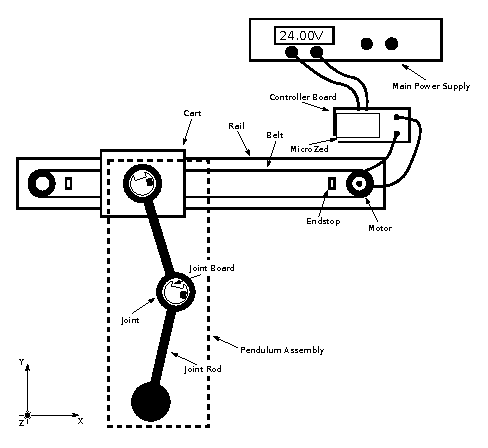
\includegraphics[width=\linewidth]{graphics/system_overview}
	\caption{Overview of the completed system.}
	\label{fig:systemoverview}
\end{figure}

Before you, the reader, fully embark on this journey, a few notes on the writing of this report. 
All component names, pin names, variables and states are written using the \texttt{teletype font}.
All components mentioned throughout the report will have the datasheet cited on the first mention of the component.
% subsection system_overview (end)

\subsection{System Users} % (fold)
\label{sub:system_users}
As will be elaborated on in future chapters, the system developed in this report is intended as an educational platform to be used in future projects.
It was proposed by the supervisor of the project, Leon Bonde Larsen who also set some of the requirements.
Throughout the report four types of actors are referred to:
\begin{itemize}
	\item \textbf{Project Owner:} The project owner, in this case also the supervisor, has proposed a system and also set certain requirements in the development of the system.
	In addition the project owner has been responsible for accepting any purchases made for the project. 
	\item \textbf{Authors:} Perhaps not surprisingly, this type refers to the authors of this report who, coincidentally, are also the original designers of the system.
	They are expected to have indepth knowledge of every aspect of the system.
	\item \textbf{Developers:} A developer is a person who does work to improve or otherwise alter the functionality of the system.
	They are expected to have knowledge of the interfaces that exist, both in hardware and software.
	Some developers may wish to further improve the electronics or joint design, however, for the purposes of this report, a developer is expected to use the hardware as-is.
	\item \textbf{User:} The user is a person who applies control algorithms to the system in an effort to balance the system.
	They are expected to have knowledge of the software interfaces related to motor control, system calibration and joint control.
\end{itemize}

% subsection system_users (end)
%!TEX root = ../main.tex
\section{State of the Art}
\thomas{insert paragraph on current mode control in SotA}
The system developed throughout this report is a proposal made by the project owner and developed by the authors.
It is intended as a learning platform for students to experiment with and gain understanding of underactuated systems.
An underactuated system is a system with more DoF (degrees of freedom) than actuators.
Traditionally in control theory, an equal or greater number of actuators than DoF are used to cancel out the dynamics of a system.
Underactuated systems is a vast field of research including examples in personal transportation such as the self-balancing scooter \cite{scooter} or the Segway \cite{segway}.
Both of these systems are essentially practical implementations of the inverted pendulum where an on-board control system will attempt to keep the device upright while maintaining a steady speed based on the tilt of the device.
Also underactuated robotic grippers are seen in abundance in literature. 
\cite{threegripper} is an implementation of a three-phalanx finger gripper which utilises two underactuated fingers.
When the fingers are brought together around an object, using the only actuated degree of freedom, the fingers wrap themselves around the object, regardless of size or shape.
This means that a gripper can be far more versatile and much less dependent on the correct placement of the object. 
\cite{pullgripper} implements a two-to-five finger gripper with belts on each finger to pull objects into the grasp of the gripper.
\\~\\
In control of underactuated systems it is required to exploit the natural dynamics of the system \cite{mitunderactuated} in order to gain full control.
Such systems are generally more agile and efficient than their fully actuated counter-parts.
\\~\\
A general example often used for teaching underactuated systems is the inverted pendulum.
Numerous examples of such systems are described in literature, but three versions in particular are presented here to provide an overview:
\begin{itemize}
	\item The pendubot \cite{pendubot} is a pendulum system consisting of one unactuated pendulum mounted on the end of an actuated pendulum.
	\item A rotary inverted pendulum \cite{rotarypendulum} mounts an unactuated pendulum on a crossbar which is mounted horizontally on the axle of an upright DC-motor.
	\item The cart mounted inverted pendulum \cite{invertpendulum3} actuates a cart along a rail in order to generate motion in the pendulum.
\end{itemize} 
In common for all of the above systems is that the joint between the mounting platform and the platform is implements some form of encoder.
This allows knowing the position of the pendulum and thereby controlling the system.
The pendubot and the rotary inverted pendulum have the feature that they can control indefinetely without running out of space, as is the case with the cart-on-a-rail system.
\\~\\
The system under development throughout this report is of the cart-on-a-rail type.
Despite the apparent short-coming of limited control range, this version of the inverted pendulum system is quite popular in literature.
\cite{invertpendulum3} is an implementation of a single inverted pendulum while versions with series pendulums exist as well such as the double pendulum shown in \cite{doubleinvertpendulum} or the triple pendulum shown in \cite{tripleinvertpendulum}.
\\~\\
Both \cite{doubleinvertpendulum} and \cite{tripleinvertpendulum} utilize encoders with a resolution of 8192 counts per revolution, or $\approx 0.044^\circ$.
\cite{invertpendulum3} is implemented using just 5000 counts per revolution, or $\approx 0.072^\circ$.

\cite{doubleinvertpendulum} and \cite{tripleinvertpendulum} both use a 1ms sampling time.
The underlying system is different between the two with \cite{tripleinvertpendulum} being based on DSpace and \cite{doubleinvertpendulum} a linux system with the real-time patch applied.
\\~\\
All of the literature mentioned above all utilize the Euler-Lagrange equation of motion for developing the mathematical model required to control their respective pendulum systems. 
These equations assume point masses and massless links between them.
The authors have derived these equations for the double pendulum in appendix \ref{sec:model_development}.
\thomas{a note on its usefulness?}

\section{System Analysis}
This document is a development report detailing the creation of such a system.
The authors have taken inspiration from the aforementioned literature to develop requirements and implementation ideas.
\\~\\
Throughout the remainder of this section an analysis of the system will be done and the overall design requirements of the system determined.
In common for all of the cited systems is that they consist of a cart capable of moving along a rail with a pendulum mounted to it.
The cited systems include single inverted pendulums \cite{invertpendulum1} \cite{invertpendulum3}, a double pendulum \cite{doubleinvertpendulum} and a triple pendulum \cite{tripleinvertpendulum}.
This project will aim to create a double pendulum system.
By actuating only the cart, the pendulums will not be directly actuated and the entire system therefore underactuated.
The connection-point between the cart and the first pendulum and between every consecutive pendulum should be a joint capable of rotating freely.
Performing swing-up of the pendulum assembly requires knowledge of both the cart position on the rail and the position of every joint in the pendulum assembly.  
\\~\\
The designed system should be a teaching platform first and foremost.
This means that a number of users with varying levels of understanding of the underlying hardware are likely to handle the system throughout its lifetime.
Therefore the system should be simple and safe to use.
The exact definition of simple will clearly vary with different users but users are generally expected to have a working understanding of Linux.
For this reason the project owner has requested that the main computation platform is based on the Xilinx Zynq-7 series architechture which provides the possibility of running Linux on the internal ARM cores while still maintaining the speed and flexibility of an FPGA.
The authors have prior knowledge of the use and design of systems with the MicroZed development board and will therefore utilize this platform in the development of this project. 
The original intent was to develop and implement a kernel driver which would present the system to the user as a \texttt{tty} interface, however this quickly turned infeasible due to the time constraints of the project and will be left for future projects.
Further design of the system should still maintain focus on the eventual goal of making the system accessible through Linux.
\\~\\
Safety around the system is important since the movement of a double pendulum is chaotic and therefore inherently unpredictable.
A means of disabling power to the motor in case of emergency should be present.  
Engaging an emergency condition should be possible both manually and automatically.
The handling of emergency conditions should happen independently of any programming so that faulty programming cannot disable handling.
End stops should be mounted on the rail to provide a means of generating an emergency condition.
This is done to avoid damage to the system in case of a run-away cart.
It is likely that the system should remain caged once finished so as to ensure that no person is in the path of the pendulum during run-time but the requirements to such a safety system are very much dependent on the system around which it should be developed and will be left as a future project to be handled before the pendulum system is given to a user.
In addition to the above, the system should also be tolerable to some amount of misuse such as blocking of the cart and similar unexpected situations.
\\~\\
Since the focus of the authors is electronics and embedded systems design, this will also be the main focus of this project.
Therefore the design of electronics will be done by the authors. 
The electronics include a board for motor control and main computation as well as a board for interfacing the incoder in the joints, the specifics of which are discussed throughout the report.
\\~\\
Since creating the final version of the software is infeasible given the time frame, another solution is required to validate the functionality of the system.
For this reason a real-time software system should be developed which correctly exercises every part of the developed pendulum system.
Additionally the distribution of functionality between the FPGA and the ARM cores should be determined to optimally make use of their abilities.
The overall software design should be determined prior to initiating programming.
Programming of individual components such as drivers for sensory equipment can be done bottom-up and integrated into a larger context once confirmed functioning.
\\~\\
Early in the process the authors inherited the rail and cart system from a previous project.
This includes a Maxon 148867 motor with an included HEDS5540 encoder, both of which will be explored further in later sections.
The rail system is used as-is since it is expected that any shortcomings of the rail system in relation to the double pendulum application will be revealed in using the finished system.
An evaluation of the usefulness of the rail system should be done on the finished system.

\subsection{Requirement Specification}
\label{sub:requirements}

\paragraph{Functional:}
\begin{enumerate}	
	\item System should consists of double pendulum mounted\\ on a moveable cart.\hfill S. 3.3
	\item Cart should be actuated by a motor. \hfill 2.3
	\item The pendulum system should be controlled by a Microzed.\hfill 2.1
	\item Position of the cart and joint angles should be measured.
	\item Any software developed for the pendulum system should be real-time.
	\item System should be easily accessible to users.
\end{enumerate}

\paragraph{Safety:}
\begin{enumerate}[resume]
	\item System should not break during operation by users.
	\item System safety should not rely on the programming of the system.
\end{enumerate}

\paragraph{Design:}
\begin{enumerate}[resume]
	 \item Software design is done is done top-down, whereas subcomponents are written bottom-up. 
	 \item Design of the system should be done so that adaption to Linux is as simple as possible.
\end{enumerate}
%!TEX root = ../main.tex
\section{Controller Electronics Development}
\label{sec:controller_board}
Throughout this section the electronics concerning the controller is developed.
This includes a thorough analysis of the required functionality which will yield a requirement specification.
The remainder of the design is then done to comply with this specification.
Finally the design will be tested to verify that it does comply with the given requirements.b
%!TEX root = ../main.tex
\subsection{Analysis}
\label{sub:controller_board_analysis}

In order to develop a controller board capable of controlling a double pendulum, the required functionality of the board needs to be determined. 
This section will constitute an analysis of this functionality and of possible solutions to desired functionality.

\subsubsection{Communication} % (fold)
\label{ssub:communication}
The controller board should be able to communicate wirelessly with the joints as discussed in section \ref{ssub:mechanics}.
The wireless link should provide sufficient bandwidth that the angular position of the joint can be transmitted sufficiently frequently.
From section \ref{ssub:encoder} it can be seen that the encoder chosen for the joints allows 7200 counts per revolution.
This can be represented using 13 bit. 
Adding a 3 bit identifier makes the payload of a message 16 bit.
This is a rough estimate which will be used for the purposes of this analysis.
A number of different protocols exist which could be used in this project.
Three were under consideration for this project:
\begin{itemize}
	\item \textbf{TCP/IP over WiFi:} TCP/IP is the defacto standard for communication between computers, both wired and wirelessly.
	This, along with the very large throughput, makes it an enticing option.
	Considering the rather small message size this protocol does impose a significant amount of overhead.
	In addition to the communication overhead, TCP/IP also requires some form of driver, making it difficult to forego the use of Linux in the joints, an OS that increases the requirements to the processing unit in the joint considerably.
	\item \textbf{Bluetooth:} The Bluetooth protocol is developed specifically for low power, short range data transmission and is used extensively in various mobile applications \cite{bluetooth}.
	As with the previous option, a considerable amount of overhead is required in setting up bluetooth as well as in the transmission of packets, making it less desirable.
	\item \textbf{Radio Frequency:} While not strictly a protocol, using an RF transceiver eliminates the additional overhead associated with the previously mentioned protocols.
	RF transceivers come with a number of different interfaces such as SPI or I2C and will simply transmit the data received through that interface.
	This makes it easy to communicate using this method through bare-metal code or even VHDL.
\end{itemize}
Considering the above it was chosen to use an RF transceiver to facilitate the communication between the joints and the controller board.
An RF transceiver can be implemented using very low power, making it ideal for the battery powered joints.
% subsubsection communication (end)

\subsubsection{The MicroZed Development Platform} % (fold)
\label{ssub:microcontroller}
The MicroZed \cite{microzed} development platform is a Zynq-7000 series based platform which the authors have worked extensively with in previous projects \cite{isaswarm}.
It was developed by Avnet specifically to be implemented in a product and as such there are fewer built-in features to the board, resulting in a reasonably small footprint and an efficient interface.
Most of the design done by the authors in \cite{isaswarm} can be reused with limited modifications.
For these reasons the MicroZed will be used in this project.
\\~\\
One thing of note is that the Zynq-7000 series of chips requires a specific startup/shutdown sequency, detailed in \cite{carrier_card_design_guide}, which ensures that signal integrity is maintained during startup and shutdown of the platform.
This functionality should also be verified in this project.
% subsubsection microcontroller (end)

\subsubsection{Motor Driver}
It is necessary to device some form of driving circuitry for the motor driving the timing belt.
The motor should be able to move in both directions. 
An H-bridge allows this bidirectional movement.
By properly switching the MOSFETs in the bridge the average voltage across the motor can be controlled and therefore also the speed and direction of the motor.
As such, an H-bridge must be designed for the controller board. 
This will in turn require that an H-bridge driver circuit is designed.

\subsubsection{Capacitor Bank} % (fold)
From simulation it was found that a capacitor bank across the supply near the H-bridge is required in order to protect the remainder of the PCB against ripple current and voltage spikes.
See section \ref{ssub:sup_caps} for an in depth discussion.
The necessary amount of supply capacitance must be determined.
\\~\\
When introducing a large amount of capacitance in a circuit, a problem known as inrush current arises \cite{inrush}.
This happens when the circuit is powered on and the initial charging of the capacitors occur.
Due to the amount of capacitance, the circuit will draw a very large current for a significant amount of time which can potentially destroy parts of the circuit.
For this reason it is necessary to design circuitry which will temporarily limit the current through the circuit until the supply capacitors are charged.
Such a circuit is often comprised of a relay in series with a resistor.

\subsubsection{Power Dissipation and Heat}
The MOSFETs driving the motor will have to carry and switch a sizeable current.
Carrying the motor current will result in some amount of power dissipation in the MOSFETs as they have a non zero drain-source \texttt{on} resistance, $R_{ds(on)}$.
Switching the motor current \texttt{on} and \texttt{off} also represents a source of power dissipation in the MOSFETs.
The total power dissipation leads to an increase in the temperature of the MOSFETs.
As the MOSFETs have a maximum operating temperature a heat sink should be connected to the MOSFETs in order to achieve a higher cooling effect.

\subsubsection{Voltage Rails}
The components chosen for the system all impose some requirement as to what voltage rails should be present on the controller board.
\begin{itemize}
	\item \textbf{Maxon 148867 DC Motor:} This motor is rated at a nominal voltage of 24V.
	Therefore a 24V rail will be created to supply the motor.
	In addition to the motor, the 24V rail will also be used to generate any subsequent rails.
	The maximum current draw possible by the Maxon motor is its stall current. 
	According to the datasheet this is 80.2A.
	The authors wish for the system to be able to handle the stall current so the 24V rail should be capable of supplying at least that plus the current draw of any subsequent rails.
	\item  \textbf{MicroZed:} This board is powered from a 5V rail and requires a 3.3V rail to power the I/O banks of the Zynq-7020 chip.
	The design of the power delivery for this board was done by the authors in the aforementioned project \cite{isaswarm} and it was found that the MicroZed can draw a maximum of 1.8A from the 5V rail and up to 1A from the 3.3V rail.
	The 3.3V rail is generated from the 5V rail in that design.
	Total current draw from the 5V rail resulting from the MicroZed is therefore no larger than 2.5A.
	An additional 2.5V reference is created in that design which is used only to facilitate the correct startup of the Zynq chip.
	The 5V rail was designed to be created from a 2S Li-Po battery at 8V and the maximum input voltage of the DC/DC converter is 18V.
	To reuse this design it is necessary to generate a rail lower than the 24V rail for the 5V rail to be generated from.
	\item \textbf{HIP4081:} This component is the motor driver used in the project.
	The choice of this component is discussed in more detail in section \ref{ssub:h_bridge}.
	A 12V rail will be used to power this component. 
	This voltage is used by the HIP4081 to generate the gate signals.
	The 12V rail will also be used to generate the 5V rail.
	This is within the specification for input voltage of the DC/DC converter of the 5V rail. 
	Due to the choice of using the HIP4081, it is necessary to do bootstrapping (see section \ref{ssub:bootstrap_circuit}). 
	The current drawn from the bootstrap circuit is decided in large part by the designer and as such the current requirement of the 12V rail is somewhat flexible.
	For this reason the current rating of the 12V rail should be as high as is practically and economically possible.
\end{itemize}
A number of additional components are likely to be required on the controller board which will all impose additional current draw on their respective rails.
These are considered negligible when compared to the major consumers mentioned above.
\\~\\
An overview of the hierarchy of the different rails can be seen in figure
The required accuracy of each rail is determined by the most sensitive component on that rail and is presented in table \ref{tab:powerrails}.
Since the 24V and 12V rails do not have any strict requirements imposed on them, a $\pm$1V requirement is set. 
The 2.5V reference is used only as a reference voltage and therefore does not have a formal current requirement.

\begin{figure}[h]
	\centering
	\includegraphics[width=.75\linewidth]{graphics/rail_hierarchy}
	\caption[Overview of the voltage rail hierarchy in the controller board design.]{Overview of the voltage rail hierarchy in the controller board design. The 24V rail is external and is used to genereate the 12V rail which generates the 5V rail which, finally, generates the 3.3V rail and 2.5V reference.}
	\label{fig:figure1}
\end{figure}

\begin{table}[h]
	\centering
	\begin{tabular}{r | r | r | r | r | r}
		Rail [V] & 24 & 12 & 5 & 3.3 & 2.5\\
		Accuracy [V] & $\pm$1 & $\pm$1 & $\pm$0.5 & $\pm$0.25 & $\pm$0.03\\
		Current [A] & 85 & - & 2.5 & 1 & -
	\end{tabular}
	\caption{Voltage rails to be created on the controller board and their specification.}
	\label{tab:powerrails}
\end{table}

\subsubsection{Motor Current Sensing}
In order to implement current mode control it is necessary to accurately measure the current being drawn by the motor at any given time.
Current measurements are generally done by either hall effect based sensors or shunt resistors. 
Hall effect based sensors are usually better for high current applications where adding a resistor in series with the load is infeasible. 
Additionally, their interference with the circuit they are measuring is negligible.
Hall effect sensors however, do come at a significant cost compared to the alternative described below.
A shunt resistor used for current measurements is simply a resistor with a very low resistance, typically $<$ 100m$\Omega$, and a high power rating ranging from a few watts into 10's of watts depending on the application.
By adding such a resistor in series with the load, the voltage across the resistor can be measured and from that the current through the load determined.
For this project a shunt resistor will be used since it is regarded as the simpler, cheaper option.

\subsubsection{Safety} % (fold)
\label{subsub:safety}
It is expected that, eventually, an error may occur that causes the cart to move uncontrollably.
A safety system should be constructed in such a way that it will prevent the cart from crashing violently or the electronics to self-destruct.
It should be isolated from the remaining system and no programming should be involved in determining whether a safety condition is met.
\\~\\
A safety condition is defined as a situation that, when not met, indicates that a critical or dangerous situation has occured with the system.
When a condition is met, that situation has not occured.
\\~\\
The safety system for this platform should be designed in such a way that, when activated, it will cut power to the motors.
In order to more easily identify the cause of the fault, the remaining electronics should remain operational to maintain the current program status.
Clearly, the system should function only if all safety conditions are met.
This will be ensured by creating an aggregation circuit which compares all of the safety conditions, creating one signal which will be capable of closing the main relay if necessary.
\\~\\
The system should be designed to have endstops.
These are in place to quickly cut power to the system if the cart reaches the end of the rail.
Creating these endstops can be done in different ways.
Three potential implementations are presented here:
\paragraph{Mechanical Switch:} % (fold)
\label{par:mechanical_switch}
The simplest form of switch is the mechanical switch.
The switch should be mounted in such a way that the cart would move into the switch, therefore activating it.
This approach is not without issues.
Mounting of the switch should be done in such a way that it is not in the direct path of the cart.
If the cart is traveling at full speed it is unlikely that the cart would stop before crashing into the switching mechanism.
A switch mounted in this fashion would need to be rather robust.
Some other mounting solutions could be thought of that do not suffer from this problem, especially if a flexible microswitch is used.
These would require significant extra design to properly mount the switch.
Mechanical switches can be fragile and may not be sufficiently durable, considering the usecase.
All mechanical switches have one drawback in common: they are mechanical and will be subject to wear over time, eventually requiring maintainance or replacement.

% paragraph mechanical_switch (end)
\paragraph{Hall Effect Sensor:} % (fold)
\label{par:hall_effect_sensor}
This type of sensor measures magnetic fields and produces a voltage proportional to the strength of the field.
By placing a small neodymium magnet on the cart and mounting a hall effect sensor on the rail in such a way that they coincide would allow for detecting when the cart is above the sensor.
If the sensor is combined with a schmitt-trigger circuit the output could be a binary result, either the endstop is reached or it is not.
Using this method requires that a magnet is placed on the cart itself and that a sensor is mounted to the rail.
It should be noted that accelerating rather strong magnetic fields back and forth on the platform may not be the least electrically noisy solution one could think of.
% paragraph hall_effect_sensor (end)
\paragraph{Infrared Transceiver:} % (fold)
\label{par:infrared_transceiver}
Infrared transceivers come in different configurations but generally the device is comprised of an LED and a photo transistor.
The LED is optimised for emitting infrared light, or radiation (IR).
In the configuration under consideration in this project the LED emits IR towards the photo transistor, opening it.
When an object passes between the LED and the transistor the transistor is closed.
This change can be detected using a simple schmitt-trigger circuit. 
With this sensor type it is important to realise that the LED will not be the only emitter of IR in the vicinity.
Any type of lamp will emit IR, especially glowbulbs but also sunlight contain a significant amount of IR.
When using this sensor the circuit should be designed in such a way that only the effect of the IR from the LED on the photo transistor will affect the circuit.
% paragraph infrared_transceiver (end)
\\~\\
While all of the above have their drawbacks, it was decided to use the infrared transceiver.
This sensor allows the greatest reliability while being reasonably simple to mount on the platform in that it requires no modification to the cart or rail.
\\~\\
In addition to the endstops, also an emergency button, preferably red, should be able to cut power to the motors.

\subsubsection{Schematic Revision} % (fold)
\label{ssub:schematic_revision}

% subsection schematic_revision (end)
From experience of the authors, a PCB layout is never error free in the first revision. 
This has been true even though a tremendous amount of work went into designing the PCB.
Therefore a strategy was devised to increase the likelihood of producing an error free PCB.
The strategy consist of five steps that needs to be completed after finishing the design of the board:

\begin{itemize}
	\item Documentation
	\item General inspection
	\item Datasheet and report comparison
	\item Footprint inspection 
	\item Peer-review
\end{itemize}

The content of each step will be elaborated here. 

\paragraph{Documentation:}
Each circuit should be documented to ensure that the design is done correctly.
Documenting a circuit requires studying the components datasheets and ensuring that they each meets the requirement.
Furthermore it requires a thorough inspection of the expected functionality of the circuit.
This step leads to correcting errors where a component is used incorrectly in respect to the desired functionality of the circuit.

\paragraph{General Inspection:}
General inspection of the schematic includes finding typographical errors on signals, components, resistor values, etc.
Furthermore each signal should be inspected to ensure that it is connected correctly and it should also be decided if it should be connected to an external header for measurement purposes.

\paragraph{Datasheet and Report Comparison:}
Each circuit in the schematic should be compared to its datasheets recommendation and the documentation written in the report. 
This step essentially ensures that each circuit has been verified more than one time. 
One could think that this step is irrelevant, but the authors believe it is important due to the complexity of the schematic.
After completion of this step, all circuits have been checked at least two times and the schematic should be correct. 

\paragraph{Footprint Inspection:}
Provided that the schematic is correct, the only possibly source of errors is the components footprints. 
Inspecting the footprint consist of verifying the correct pin assignment and the correct land patterns.
Both are done by inspecting the datasheet of each component. 
After completion of this step, both the schematic and footprints should be correct and the board is expected to be free from errors.

\paragraph{Peer-review:}
In this part of the process the board design, schematic and footprints should be correct and everything has been verified by the authors multiple times.
It is generally a problem that when working with a design for a long period of time, some errors are very hard to find for the designers themselves. 
Therefore the design should be reviewed by a person that has not taken part of the design of the board.
The review should be done by pointing out the main features of the board and discussing the found components, schematic and the board layout.

% section schematic_revision (end)

\subsubsection{PCB Layout} % (fold)
Some considerations are important when designing high power or switching circuitry, both of which are categories which the controller board fit into.
When part of the board is exposed to large currents, maintaining signal integrity on the remainder of the board becomes important.
This is done in large part by controlling grounds in the PCB.
An unbroken ground plane should be present in the design to ensure a low-impedance current path in the PCB \cite{pcblayoutds}.
In addition to unbroken ground planes, they should also be seperated based on their role in the circuit.
Often two, three or even more ground planes exist in circuits.
A common distribution is an analog ground, digital ground and power ground.
Analog signals are often sensitive to noise and should be shielded from the switching noise of the digital circuitry.
Similarly, high currents in a ground plane is likely to cause voltage drops across it.
This may cause issues in the digital circuitry.

Having several ground planes can cause issues with currents circulating in them.
In order to avoid this it is crucial that the ground planes are connected in one place only.
\\~\\
Since at least part of the PCB is likely to carry significant currents it is necessary to appropriately size the width of traces and 
\thomas{finish this thought }

\subsubsection{Component Selection and Placement} % (fold)
\label{ssub:component_case_selection_and_placement}
There are limits to the production capabilities of the equipment, both of the manufacturer producing the PCB and the equipment available to the authors at SDU.
For this reason some restrictions are set on the casing of components and their placement on a PCB.
Generally, throughhole components should be avoided where possible since these obstruct not only the layer they are placed on but also every other layer throughout the PCB and so surface mount technology (SMT) components are preferred.
SMT components come in many sizes and some are simply too small to realistically route and solder with the available equipment.
Generally, SOT-23, SOIC and 0805 packages and similar sizes are preferred where possible.
With the equipment available at SDU only components on one side of the PCB can be placed and soldered with the pick-and-place machine and oven.
Due to this, components should only be placed on the top layer when possible.
Larger components, such as big capacitors, can easily be hand-soldered and can therefore be placed on the bottom side of the PCB.
\\~\\
A number of signals should be routed to headers to allow for easier debugging and monitoring of the circuits.
For simplicity these headers should all be of the same type. 
The JST ZH-series connectors should be used as they are commonly used at SDU, they are SMT and sufficiently small. 


\subsubsection{Testing and Prototyping} % (fold)
Some of the developed circuits will consist of many components and complex ICs.
With such complex circuits, errors in a schematics can easily appear.
Therefore the functionality of the most important parts of the circuit should be tested on prototype PCBs before ordering an expensive PCB.

\subsubsection{Board Layout and Considerations} % (fold)
\label{ssub:board_layout_and_considerations}
A number of options are available when considering the general layout of the controller circuitry.
Different circuits can be segregated into individual boards, simplifying the layout and production of each board but imposing requirements on board-to-board connections between different circuits.
One possible configuration under consideration is the segregation of the digital circuit and the power circuits.
This would allow a different number of layers and different copper thickness on the two PCBs.
Extra layers are beneficial when routing the multitude of signals in a digital circuit but also add extra cost to the production of the circuit.
Similarly, extra copper is likely to be necessary on the power circuit but also adds cost.
Exploring various manufacturing options revealed that segregating the boards into one board with added copper and one board with added layers added significant cost to the order.
For this reason it was decided to produce just a single PCB with extra copper and four layers, housing all of the electronics related to the controller.

\clearpage
\subsubsection{Requirement Specification}

\paragraph{Functional:}
\begin{enumerate}[resume]
	\item Speed and direction of the motor should be adjustable through PWM from the MicroZed.
	\label{enum:motor_speed_direction}
	\begin{itemize}
		\item H-bridge of MOSFETs capable of switching motor current direction.
		\item H-bridge driver translating logic signals to gate signals.
		\item High side drive capabilities.
	\end{itemize}

	\item Motor current measurement through ADC input on the MicroZed.
	\label{enum:motor_current}
	\begin{itemize}
		\item Shunt resistor to measure the motor current.
	\end{itemize}

	\item Voltage rails for the various components in the circuit.
	\label{enum:voltage_rails}	
	\begin{itemize}
		\item 2.5V $\pm$0.03V.
		\item 3.3V $\pm$0.25V, 1A.
		\item 5V $\pm$0.5V, 2.5A.
		\item 12V $\pm$1V, The amperage of this rail should be as high as economically and practically viable.
		\item 24V $\pm$1V, 85A.
	\end{itemize}

	\item Voltage transients on voltage rails should be minimized.
	\label{enum:voltage_transients}	
	\begin{itemize}
		\item Bulk capacitors on 24V rail to supply current to motor.
		\item Properly sized input and output capacitance of DC/DC power supplies.
		\item Appropriate copper volume for ground and power wires.
	\end{itemize}

	\item The MicroZed should be correctly interfaced.
	\label{enum:microzed_interface}
	\begin{itemize}
		\item All signals to the MicroZed should be routed on the PCB to appropriate I/O ports.
		\item Start-up power sequence and voltage levels should be correct.
	\end{itemize}
	\item A Heatsink should be connected to the MOSFETs to avoid overheating of the H-bridge.
	\label{enum:cool_mosfets}
	\item Hardware for wireless communication using RF should be implemented.
	\label{enum:hardware_for_wireless_implemented}
\end{enumerate}


\paragraph{Design:}
\begin{enumerate}[resume]
	\item Important parts of circuitry should be tested on prototype PCB.
	\label{enum:important_prototype}
	\item The PCB layout should be reviewed according to the developed strategy.
	\label{enum:pcb_strategy}
	\begin{itemize}
		\item Documentation.
		\item General inspection.
		\item Datasheet and report comparison.
		\item Footprint inspection.
		\item Peer-review.
	\end{itemize}
	\item The PCB layout should be designed with debugging in mind.
	\label{enum:pcb_debugging}
	\begin{itemize}
		\item Test points should exist for all voltage rails and relevant signals.
		\item All test points should be wired to JST ZH-series connectors.
	\end{itemize}
	\item PCB layout....
	\label{enum:pcb_layout}
	\thomas{fix requirements}
	\begin{itemize}
		\item Ground plane...
		\item Avoid through-hole components....
		\item Power ground and signal ground
	\end{itemize}
	\item PCB soldering should be possible at SDUs facilities.
	\label{enum:pcb_soldering}
	\begin{itemize}
		\item Component casings should be SOT-23, SOIC or 0805 where possible.
	\end{itemize}
\end{enumerate}

\thomas{Needs mentioning: stall current, emergency signal from microzed, relays}
\paragraph{Safety:}
\begin{enumerate}[resume]
	\item System should not break during operation by users.
	\label{enum:not_break_mis}
	\begin{itemize}
		\item Endstops capable of stopping moving cart.
		\item Components should be able to handle stall current.
		\item Safety circuits should not rely on programming.
	\end{itemize}

	\item Any triggered emergency condition should halt the cart.
	\label{enum:any_trigger_em}
		\begin{itemize}
			\item Emergency conditions should be implemented.
			\begin{itemize}
				\item[$\circ$] Emergency button for human interaction.
				\item[$\circ$] Endstops for detecting cart run-away.
				\item[$\circ$] Emergency signal from the MicroZed.
			\end{itemize}
			\item Relay should switch power to motor.
			\item Relay should be active only when emergency conditions are inactive.
			\item Power to remaining electronics and MicroZed should not be affected by an emergency condition.
		\end{itemize}
\end{enumerate}

%!TEX root = ../main.tex
\subsection{Circuit Design}
\label{sub:controller_board_circuit_design}

Multiple electronics components are required to realise the functionalities described in the precious section.
This section explores the selection of those components and design of the corresponding circuits.

\subsubsection{MOSFET and H-Bridge Driver} % (fold)
\label{ssub:h_bridge}
The motor that needs to be driven is a Maxon 148867 Brushed DC Motor.
This is a 150W motor with a nominal current of 6A and a stall current of 80A.
Clearly, the system should under normal use not come anywhere close to stalling the motor but considering the use case, experimentation with control from students, it may be beneficial to design the circuitry such that it can withstand being stalled, for at least a short period of time.
In order to reach this goal, it is necessary to size the components for at least some amount above 80A continuous.
The \texttt{IRF100B202} MOSFET \cite{mosfet} is a 100V/97A MOSFET.
It is made in the standard TO-220 housing.
This housing allows for easy mounting of a heatsink and due to its wide application, there are many shapes and sizes to choose from.
Table \ref{tab:mosfetparameters} holds a list of the relevant parameters.

\begin{table}[h]
	\centering
	\begin{tabular}{|r|c|c|c|}
	\hline
		\textbf{Parameter} & \textbf{Min} & \textbf{Typ} & \textbf{Max} \\
	\hline
		$V_{\text{th}}$ [V] & 2 & - & 4 \\
	\hline
		$R_{\text{ds(on)}}$ [m$\Omega$]& - & 7.2 & 8.6 \\
	\hline
		$Q_\text{g}$ [nC] & - & 77 & 116 \\
	\hline
		$I_\text{d}$ [A] & - & - & 97 \\
	\hline
		$V_{\text{ds}}$ [V] & 100 & - & - \\
	\hline
	\end{tabular}
	\caption{Relevant parameters of the IRF100B202 MOSFET \cite{mosfet} chosen for the full-bridge.
	Here, \vth is the gate threshold voltage, \ron is the drain-source on resistance, \qg is the total gate charge, \id is the maximum continuous drain current and \vds is the minimum guaranteed drain-source breakdown voltage.}
	\label{tab:mosfetparameters}
\end{table}

It should be noted that even though \vth is maximum 3.5V, this is not enough to fully open the MOSFET.
Rather, this voltage is where the MOSFET will start to conduct.
Figure \ref{fig:mosfettransfercharacteristic} reveals that the MOSFET is not fully conducting until \vgs $>4.5$V.

\begin{figure}[H]
	\centering
	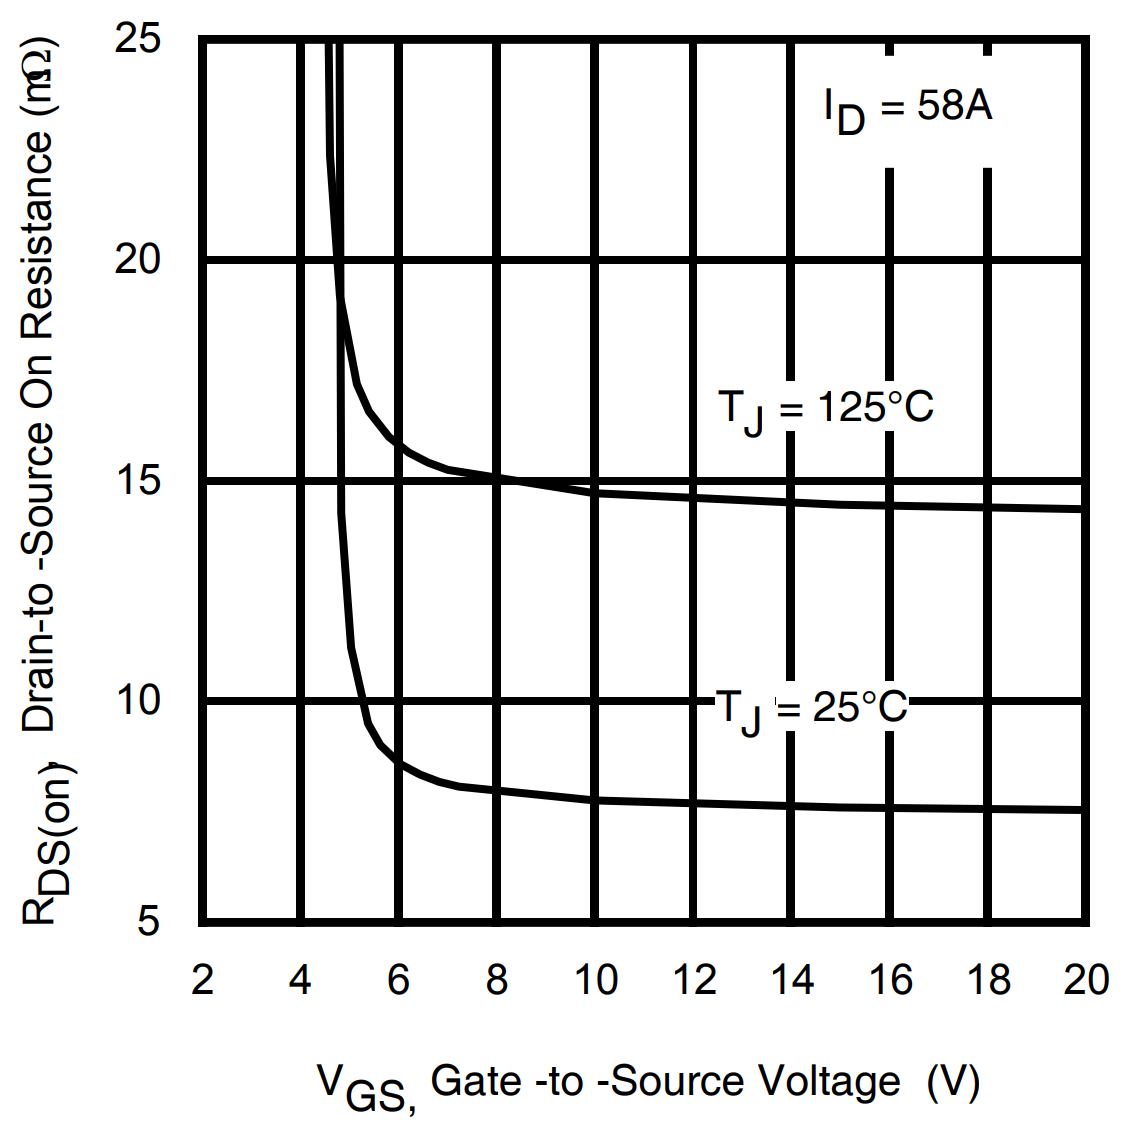
\includegraphics[width=0.6\linewidth]{graphics/mosfet_transfer_characteristic}
	\caption{Transfer characteristic of the IRF100B202 as per the datasheet.
	Inspecting the graph reveals that the maximum \id of 100A is reached at \vgs$\approx4.2\rightarrow4.5$V.}
	\label{fig:mosfettransfercharacteristic}
\end{figure}
 

Having chosen a MOSFET for the full-bridge, some form of driver must be designed for the full-bridge.
For this task, ready-made full-bridge drivers exist on the market that incorporate all of the electronics required to generate the driving signals, requiring only a PWM signal from the designer.
In order to choose one, a few parameters must be fulfilled.

\begin{itemize}
	\item \textbf{Output Current:} The amount of current necessary to properly drive the MOSFET.
	This value depends on the switching frequency of the application, the gate-to-source voltage ($V_{gs}$) and the total gate charge of the MOSFET.
	\item \textbf{Driving Voltage:} In order to ensure that the MOSFET is turned on quickly and fully the driver should be able to supply a voltage well above the gate threshold of the MOSFET.
	\item \textbf{High-Side Drive Capabilities:} The high side MOSFET of the full-bridge is referenced not to ground, but to a floating reference.
	This means that in order to switch on this MOSFET, $V_{\text{gate}}$ needs to be boosted compared to the floating reference. 
	This is bootstrapping and is explained in more detail in section \ref{ssub:bootstrap_circuit}.
	\item \textbf{Shoot-Through Protection and Deadtime:} Due to the structure of the full-bridge it is important that two MOSFETs on the same half-bridge are never on at the same time as this would result in a short from $V_{\text{cc}}$ to ground.
	This is resolved with a combination of deadtime (a delay where no MOSFET is on) and a logic table that ensures that an illegal switch combination can never happen.
\end{itemize}

The HIP4081AIBZ \cite{driver} full-bridge driver meets all of the above requirements.
It can supply up to 2.5A on the output pins with a voltage approximately 1V below \vcc, well above the required \vth.
It also allows for an external bootstrap circuit, which makes it able to drive the high-side MOSFETs.
Since the motor should, preferably, be driven outside the audible frequency range, it was chosen to set the switching frequency at 22kHz.
This frequency was chosen over an even higher frequency because increasing the frequency also increases the switching losses.
At this frequency there is $\frac{1}{22000}\approx45\mu$S per cycle. 
Well within this time the gate should be fully opened.
The switching time should be calculated to verify this.
\cite{mosfet_switch_app_note} describes switching characteristics of MOSFETs without taking parasitics into account.
Approximating the turn-on time of the MOSFET is sufficient here as it just needs to be verified that the MOSFETs are fully open within a small fraction of the switching period.
\cite{mosfet_switch_app_note} approximates the turn-on time of a MOSFET in equation \ref{eq:mosfet_turn_on}.

\begin{equation}
t_{switch} = R_G \cdot C_{iss} \cdot ln\left(\frac{1}{1-\frac{V_{gp}}{V_{GS}}}\right) 
\label{eq:mosfet_turn_on}
\end{equation}

Where $t_{switch}$ is the switching time, $R_G$ is the total gate resistance, $C_{iss}$ is the effective input capacitance of the
MOSFET, $V_{gp}$ is the gate plateau voltage and $V_{GS}$ is the voltage applied to the gate applied by the motor driver.
Accounting for various voltage drops it is assumed that \vgs is 8V and by inspecting figure \ref{fig:mosfettransfercharacteristic}, $V_{gp}$ is estimated to 4.5V.
$R_G$ and $C_{iss}$ is datasheet values.

\begin{equation}
t_{switch} = 9.4 \cdot 4.48 \cdot 10^{-9} \cdot ln\left(\frac{1}{1-\frac{4.5}{8}}\right) = 34.8 nS 
\label{eq:mosfet_turn_on}
\end{equation}
This MOSFET switching time is orders of magnitude smaller than the PWM switching period.

The component also has floating drive circuitry, meaning that by referencing the high-side driver to source of the high-side MOSFET, the driver can be made to output a voltage higher than \vcc.
This does require a few external components for the bootstrapping.
The choice of these components and a more in depth explanation of the procedure is given in section \ref{ssub:bootstrap_circuit}.
Finally, the component has a user-programmable dead time and shoot-through protection. 

\subsubsection{Bootstrap Circuit}
\label{ssub:bootstrap_circuit}
\missingfigure{Put in a bootstrap circuit and make a couple of references to it, when it makes sense.}
The chosen gate driver has floating drive circuitry for the high side MOSFETS, but needs a bootstrap circuit for providing the higher voltage. 
A standard bootstrap circuits consists of a diode, a capacitor and a resistor. 
The advantage of using a bootstrap circuit to supply a high voltage for the floating drive is that it is very simple. 
The disadvantage is that it sets a limit for the maximum and minimum duty cycle as the bootstrap capacitor needs to be charged fully in each period.
The bootstrap circuitry for this project will be designed to have a maximum duty cycle for the higher MOSFETS of 95\%, thus meaning that the charging of the bootstrap capacitor should take no longer than 5\% of a period.  

The bootstrap diode needs to have a fast recovery time, preferably below 100 ns \cite{bootstrap_infineon}, to minimize the energy fed back to the supply from the bootstrap capacitor.
\texttt{US1M-E3} was chosen as it has a reverse recovery time of 75 ns and comes in SMD packaging. 
It allows for a maximum average forward current of 1 A and a maximum forward voltage drop of 1.7 V \cite{diode_ds}.
Determining the values for the bootstrap capacitor was done using the calculations shown in \cite{bootstrap_ON}.
The maximum allowed voltage drop across the bootstrap capacitor during \texttt{on} time needs to be determined: 
\begin{equation}
\Delta V_{boot} = V_{DD} - V_{F} - V_{GSMIN}
\end{equation}
Where $\Delta V_{boot}$ is the voltage drop across the bootstrap capacitor during \texttt{on} time, $V_{DD}$ is the supply voltage, $V_F$ is the forward voltage drop across the diode and $V_{GSMIN}$ is the minimum wanted \texttt{gate-source} voltage.
$V_{GSMIN}$ was chosen to 8 V to to ensure a high enough gate voltage to turn on the MOSFETS. 
The chosen MOSFETS have a maximum gate threshold voltage of 3.5 V. 
Inserting the values yields the maximum allowed value of $\Delta V_{boot}$:
\begin{equation}
\Delta V_{boot} = 12 - 1.7 - 8 = 2.3 V	
\end{equation}

The total charge that needs to be supplied from the bootstrap capacitor is the gate charge of the MOSFET along with the quiescent and leakage currents in the \texttt{on} time:
\begin{equation}
	Q_{total} = Q_{gate} + Q_{ls} + (I_{lkgs} + I_{qbs} + I_{lk} + I_{lkdiode}) \cdot t_{on}
	\label{eq:charge_total}
\end{equation}
Where $Q_{gate}$ is the maximum total gate charge, $I_{lkgs}$ is the gate-source leakage current, $I_{qbs}$ is the gate driver quiescent current, $I_{lk}$ is the gate driver leakage current, $I_{lkdiode}$ is the diode leakage current, $ t_{on}$ is the \texttt{on} time and $Q_{ls}$ is the charge required by the internal level shifter in the gate driver.
\begin{table}[h]
\centering
\begin{tabular}{|l|l|l|l|l|l|l|}
 \hline
 $Q_{gate}$ 	& $Q_{ls}$ 	& $I_{lkgs}$ 	& $I_{qbs}$ 		& $I_{lk}$ 			& $I_{lkdiode}$ 	& $t_{on}$ 		\\ 	\hline
 $116$ [nC]		& $3$ [nC]	& $100$ [nA]	&$-30$ [$\mu$A]		& $1$ [$\mu$A]		& $1$ [nA]			& $43$ [$\mu$S]	\\ 	\hline
\end{tabular}
\caption[Parameter values used to determine total charge.]{Parameter values used in equation \ref{eq:charge_total}. $I_{qbs}$ and $I_{lk}$ are found in the gate driver data sheet. $Q_{ls}$ is set to 3nC for all high voltage gate drivers \cite{bootstrap_ON}. $I_{lkgs}$ and $Q_{gate}$ are MOSFET data sheet values and $I_{lkdiode}$  is a diode data sheet value. $t_{on}$ is calculated using 95\% dutycycle and 22kHz switching.}
\label{tab:bootstrap_parameter}
\end{table}
$t_{on}$ can be calculated knowing that the worst case duty cycle for the high side MOSFET is 95\% and the switching frequency is 22 kHz.
Inserting the values, shown in \ref{tab:bootstrap_parameter}, yields the minimum charge value of the capacitor:
\begin{equation}
	Q_{total} = 118 [nC]
\end{equation}

The minimum value of the bootstrap capacitor can now be calculated:
\begin{equation}
	C_{boot} = \frac{Q_{total}}{\Delta V_{boot}} = \frac{118}{2.3} = 51.2 [nF]
\end{equation}
A ceramic capacitor will be used as it has a negligible leakage current. 
Looking for SMD ceramic capacitors it was found that in the range of the found minimum value is 56, 68, 82 and 100 [nF].
56 [nF] is, in theory, a big enough capacitor for the circuit, but a bigger capacitor is an advantage as $\Delta V_{boot}$ will then decrease.
When increasing the size of the capacitor it should be noted that the initial charge current will become larger.
It was therefore chosen to use a 100 [nF] ceramic capacitor.

The initial charge current to the capacitor needs to be limited in order not to exceed the maximum ratings of the diode.
Therefore a resistor is put in series with the diode.
The resistor value should not be too big as the voltage drop across it is subtracted from the bootstrap capacitor voltage.
A 4.7 $\Omega$ resistor was chosen. In this setting, the maximum current through this component is 2.6 A.
This is clearly above the maximum average forward current of the diode, but the diode can withstand a 8.3 ms single half sine-wave of maximum 30 A \cite{diode_ds}.
The capacitor voltage while charging in a RC circuit is described by equation \ref{eq:cap_charge}, according to \cite{prac_ele_for_inven}.

\begin{equation}
	V_C = V_S (1-e^{\frac{-t}{R\cdot C}})
	\label{eq:cap_charge}
\end{equation}

Where $V_C$ is the capacitor voltage, $V_S$ is the supply voltage, $R$ is the resistance and $C$ is the capacitance.
The RC time constant is defined as $\tau = R\cdot C$.
Equation \ref{eq:cap_charge} can be used to calculate the time it takes an RC circuit to charge to a specific level.
After one time constant the capacitor is charged 63.2\% and after five time constant the capacitor is approximately fully charged, 99.3\%.
This knowledge can be used to calculate the time it takes to initially charge the bootstrap capacitors as shown in equation \ref{eq:cap_boot_time}.

\begin{equation}
T_{charge,init} = 5\cdot \tau = 5\cdot (R \cdot C) = 5\cdot (4.7 \cdot 100 \cdot 10^{-9}) = 2.35 \mu S 
\label{eq:cap_boot_time}
\end{equation}

Meaning that the diode can be exposed to a maximum of 2.6A for $2.35 \mu S $, which is well below the absolute maximum rating.
It should also be noted that bootstrap capacitor needs at least $2.35 \mu S $ for the initial charging.

Lastly it should be calculated what the maximum allowed duty cycle for the high side MOSFETS are in this configuration, using the found components.
The time it takes to charge the capacitor the energy that is used in each period is:
\begin{equation}
	T_{charge,period}  5\cdot (R \cdot C_{boot}) = 5\cdot (4.7 \cdot  51.6 \cdot 10^{-9}) = 1.21 \mu S 
\end{equation}
The $1.21 \mu S$ is equivalent to 2.7\% duty cycle and the maximum duty cycle for the high side MOSFETS is thus 97.3\%.
% subsection power_board (end)

\subsubsection{Supply Capacitors}
\label{ssub:sup_caps}
Driving an inductive load, such as a motor, requires capacitors placed close to the MOSFETS in order to minimize the voltage spikes created by the load current and parasitic inductance in the wires from the supply.
This section will determine the size and requirements of the supply capacitors using calculations and simulation in PLECS.

First off, the ripple current across the motor inductor needs to be determined as this is the current the supply capacitors need to supply.
Equations \ref{eq:inductor_gen} shows the general inductor equation and in \ref{eq:inductor_rip} it is re factored to calculate the ripple current.
\begin{equation}
	V(t) = L \cdot \frac{dI(t)}{dt}
	\label{eq:inductor_gen}
\end{equation}

\begin{equation}
	\Delta I = \frac{\Delta V}{L} \Delta t
	\label{eq:inductor_rip}
\end{equation}

The highest ripple current is found when the duty cycle is 50$\%$ and the full voltage of 24V is applied as calculated in equation \ref{eq:inductor_rip_size}.

\begin{equation}
	\Delta I = \frac{24}{82\cdot 10^{-6}} \cdot 0.5 \cdot \frac{1}{22000} = 6.7 [A] 
	\label{eq:inductor_rip_size}
\end{equation}

The peak-to-peak ripple current of $6.7$A is also found when simulating the system using PLECS as shown in figure \ref{fig:sim_currents}.
The load current experienced by the supply is also shown in figure \ref{fig:sim_currents}, where abrupt changes in current are seen. 

\begin{figure}[h]
	\centering
    % This file was created by matlab2tikz.
%
%The latest updates can be retrieved from
%  http://www.mathworks.com/matlabcentral/fileexchange/22022-matlab2tikz-matlab2tikz
%where you can also make suggestions and rate matlab2tikz.
%
\definecolor{mycolor1}{rgb}{0.00000,0.44700,0.74100}%
%
\begin{tikzpicture}

\begin{axis}[%
width=4.521in,
height=1.493in,
at={(0.758in,2.554in)},
scale only axis,
xmin=0.002,
xmax=0.00225,
ymin=-4,
ymax=4,
ylabel style={font=\color{white!15!black}},
ylabel={Current [A]},
axis background/.style={fill=white},
title style={font=\bfseries},
title={Motor}
]
\addplot [color=mycolor1, forget plot]
  table[row sep=crcr]{%
0	0\\
3.3460025901564e-08	0.00979216834185557\\
6.6920051803128e-08	0.0195831689424556\\
1.00380077704692e-07	0.0293729772080969\\
2.86236444194498e-07	0.0837307082176497\\
4.72092810684304e-07	0.138052159786677\\
6.5794917717411e-07	0.192336888519681\\
8.43805543663915e-07	0.2465847436031\\
1.46206269418065e-06	0.426776921334415\\
2.08031984469738e-06	0.606560789436667\\
2.69857699521411e-06	0.785936710694134\\
3.31683414573084e-06	0.964905205652303\\
3.93509129624758e-06	1.1434666409016\\
5.75197157684523e-06	1.6658548409378\\
7.56885185744287e-06	2.18473747278615\\
9.38573213804052e-06	2.70012165466927\\
1.12026124186382e-05	3.21201571005084\\
1.30194926992358e-05	3.72042845969404\\
1.48363729798335e-05	4.22536872362558\\
1.97586180405918e-05	5.57596587927003\\
2.27272727272725e-05	6.3783171170272\\
2.27272727272727e-05	6.37831711702726\\
2.27410076969546e-05	6.37398638046111\\
2.27547426666364e-05	6.36965375955969\\
2.27684776363182e-05	6.36532285013984\\
2.29058273331366e-05	6.32203472687713\\
2.30431770299549e-05	6.27876729316781\\
2.31805267267732e-05	6.2355202943356\\
2.44483529688856e-05	5.83725566814237\\
2.57161792109979e-05	5.44072022747552\\
2.69840054531102e-05	5.04592126779853\\
2.82518316952226e-05	4.65286095881394\\
3.11224300272083e-05	3.76931165867921\\
3.3993028359194e-05	2.89464378808499\\
3.68636266911797e-05	2.02882734038762\\
3.97342250231655e-05	1.17183245052039\\
4.26048233551512e-05	0.323631784651184\\
4.5454545454545e-05	-0.509728483636083\\
4.54545454545455e-05	-0.509728483636209\\
4.56137030196537e-05	-0.462855930246644\\
4.5772860584762e-05	-0.416009673465522\\
4.59320181498702e-05	-0.369190286586476\\
4.75235938009527e-05	0.096688919165212\\
4.91151694520353e-05	0.559938654993594\\
5.07067451031178e-05	1.02051267646793\\
5.21877413094701e-05	1.44673915057175\\
5.36687375158223e-05	1.87064481037127\\
5.48032708460027e-05	2.19395845751998\\
5.59378041761831e-05	2.51590586535985\\
5.70723375063635e-05	2.83649721774212\\
5.90623960561229e-05	3.39602028595376\\
6.10524546058824e-05	3.95161284857696\\
6.30425131556419e-05	4.50312800819581\\
6.50325717054013e-05	5.05052048240398\\
6.81818181818173e-05	5.9083681446256\\
6.81818181818182e-05	5.90836814462583\\
6.81982265228205e-05	5.90321766823039\\
6.82146348638228e-05	5.8980650799626\\
6.82310432048251e-05	5.8929146034375\\
6.83951266148483e-05	5.8414383259708\\
6.85592100248715e-05	5.78999120622817\\
6.87232934348947e-05	5.73857317088326\\
7.03641275351264e-05	5.22594260544655\\
7.20049616353581e-05	4.71619997502048\\
7.36457957355898e-05	4.20935629332506\\
7.52866298358215e-05	3.70541426066593\\
7.86734614243063e-05	2.67439183644975\\
8.2060293012791e-05	1.65568679003902\\
8.54471246012758e-05	0.649258995332076\\
8.88339561897606e-05	-0.344931641381534\\
9.090909090909e-05	-0.948049426664154\\
9.09090909090909e-05	-0.948049426664405\\
9.10680548465105e-05	-0.900944972184585\\
9.12270187839301e-05	-0.85386684032189\\
9.13859827213497e-05	-0.806815624783133\\
9.28881448030836e-05	-0.364268712879095\\
9.43903068848175e-05	0.075924523168433\\
9.58924689665514e-05	0.513722225414341\\
9.73937786098869e-05	0.948873891503222\\
9.88950882532224e-05	1.38163182114456\\
0.000100396397896558	1.81199872685562\\
0.000102388285618672	2.37990759343637\\
0.000104380173340787	2.94391803819557\\
0.000106372061062901	3.50382863193594\\
0.000108363948785016	4.0595734864279\\
0.000112581062122341	5.22245152431999\\
0.000113636363636363	5.51053783719038\\
0.000113636363636364	5.51053783719062\\
0.000113652875841073	5.50537508343307\\
0.000113669388045783	5.50021036711542\\
0.000113685900250493	5.49504766058541\\
0.000113851022297591	5.44344929732303\\
0.000114016144344688	5.39188054216774\\
0.000114181266391786	5.3403413740717\\
0.000115832486862763	4.82652639019902\\
0.00011748370733374	4.31564953083607\\
0.000119134927804716	3.80772280116105\\
0.000120786148275693	3.3027493167972\\
0.000124260197469801	2.24994846748255\\
0.000127734246663909	1.21017549199153\\
0.000131208295858018	0.183388685607617\\
0.000134682345052126	-0.830455009606617\\
0.000136363636363635	-1.31647681541512\\
0.000136363636363636	-1.31647681541562\\
0.000136457648355821	-1.28848834726951\\
0.000136551660348006	-1.26050912560564\\
0.000136645672340192	-1.2325394005705\\
0.000137585792262042	-0.953660414443846\\
0.000138525912183893	-0.675711762263763\\
0.000139466032105744	-0.398710450483822\\
0.000141080921833001	0.0744903471438776\\
0.000142695811560257	0.544923535047713\\
0.00014397637111121	0.916137663936403\\
0.000145256930662163	1.2855871880448\\
0.000146309638560935	1.58807403635747\\
0.000147362346459708	1.88937169227974\\
0.00014841505435848	2.18948675148099\\
0.000150446951617213	2.76585105914289\\
0.000152478848875945	3.33804096395515\\
0.000154510746134677	3.90591581582167\\
0.000156542643393409	4.4694327063089\\
0.000159090909090907	5.17002081333405\\
0.000159090909090909	5.17002081333453\\
0.000159107950404141	5.16471547697748\\
0.000159124991717373	5.15940825618861\\
0.000159142033030604	5.15410303483625\\
0.000159312446162921	5.10108115055827\\
0.000159482859295238	5.0480908629433\\
0.000159653272427556	4.99513222149086\\
0.000161357403750727	4.46723180551256\\
0.000163061535073897	3.94247263127644\\
0.000164765666397068	3.4208672561975\\
0.000166469797720239	2.90241812883423\\
0.000170111015763006	1.80520238710783\\
0.000173752233805772	0.722332913291956\\
0.000177393451848539	-0.346247160573399\\
0.000181034669891305	-1.40059735141266\\
0.00018181818181818	-1.62561618975527\\
0.000181818181818182	-1.62561618975576\\
0.00018189191245417	-1.60360142523706\\
0.000181965643090158	-1.58159233486036\\
0.000182039373726146	-1.55958910529188\\
0.000182776680086025	-1.34006159444278\\
0.000183513986445904	-1.1211080471627\\
0.000184251292805783	-0.902738959943471\\
0.000186176642929505	-0.336111723359008\\
0.000188101993053228	0.226593340319752\\
0.000189433381211277	0.61367738328916\\
0.000190764769369326	0.998843310781422\\
0.000191862820760937	1.31517016011703\\
0.000192960872152549	1.63020214326219\\
0.000194058923544161	1.94394679035387\\
0.000196139234286316	2.53528966757863\\
0.000198219545028471	3.1222613516525\\
0.000200299855770626	3.70471321364354\\
0.000202380166512781	4.28260111282239\\
0.000204545454545453	4.87927070065436\\
0.000204545454545455	4.87927070065483\\
0.000204563248495638	4.87375397959641\\
0.000204581042445821	4.86823541514357\\
0.000204598836396004	4.86271888414652\\
0.000204776775897834	4.80758616239875\\
0.000204954715399664	4.75248770523977\\
0.000205132654901494	4.69742363897177\\
0.000206912049919797	4.14861455983025\\
0.0002086914449381	3.60321712392594\\
0.000210470839956403	3.06124426527418\\
0.000212250234974706	2.52269735314441\\
0.000215992339235271	1.40127193130843\\
0.000219734443495837	0.294915233950511\\
0.000223476547756402	-0.796443118277702\\
0.000227218652016968	-1.87287598395711\\
0.000227272727272726	-1.88832192980601\\
0.000227272727272727	-1.8883219298065\\
0.000227342297857368	-1.8674965214086\\
0.000227411868442008	-1.8466761249662\\
0.000227481439026648	-1.82586092362373\\
0.000228177144873052	-1.61815622510643\\
0.000228872850719455	-1.41096013261674\\
0.000229568556565858	-1.20428192867981\\
0.000231740906602734	-0.561959842495436\\
0.00023391325663961	0.0754652928433671\\
0.000236085606676486	0.707897523625743\\
0.000238257956713362	1.33531177211176\\
0.000242602494028023	2.57508628531837\\
0.000246947031342683	3.79491169755634\\
0.000249999999999997	4.6402370224219\\
0.00025	4.64023702242285\\
0.000250019628217504	4.63416863641626\\
0.000250039256435008	4.62809832974944\\
0.000250058884652512	4.6220302822174\\
0.000250255166827551	4.56138855762422\\
0.00025045144900259	4.50078810165967\\
0.00025064773117763	4.44022919509232\\
0.000252610552928023	3.83685231936177\\
0.000254573374678417	3.23759512538674\\
0.000256536196428811	2.64247348184285\\
0.000258499018179204	2.05148839219246\\
0.00026230269607791	0.917985886864917\\
0.000266106373976615	-0.200068898448616\\
0.000269910051875321	-1.30274624539011\\
0.000272727272727269	-2.10958190663542\\
0.000272727272727273	-2.10958190663641\\
0.000272768691766965	-2.0971445132162\\
0.000272810110806658	-2.08470883916461\\
0.00027285152984635	-2.0722750015498\\
0.000273265720243275	-1.9480945773949\\
0.000273679910640201	-1.82409380817647\\
0.000274094101037126	-1.7002760300248\\
0.000276474575282944	-0.99201519218526\\
0.000278855049528763	-0.289700777080019\\
0.000281235523774581	0.406610503044831\\
0.0002836159980204	1.09690909829915\\
0.000287927361167765	2.3318709333071\\
0.00029223872431513	3.54723458490537\\
0.000295454545454542	4.44107226812169\\
0.000295454545454545	4.44107226812265\\
0.000295475547795918	4.43458904568205\\
0.00029549655013729	4.42810387748598\\
0.000295517552478663	4.42162112001525\\
0.000295727575892386	4.35683736126698\\
0.00029593759930611	4.29210065463151\\
0.000296147622719834	4.22741141574417\\
0.00029824785685707	3.58304649672565\\
0.000300348090994307	2.94338836213575\\
0.000302448325131544	2.30845678951722\\
0.000304548559268781	1.67825391184348\\
0.00030840178706574	0.534311601515325\\
0.0003122550148627	-0.593790092823967\\
0.00031610824265966	-1.70611431376052\\
0.000318181818181815	-2.29819353211022\\
0.000318181818181818	-2.29819353211121\\
0.000318216910128822	-2.28762391738447\\
0.000318252002075825	-2.27705551476598\\
0.000318287094022829	-2.26648843514806\\
0.000318638013492865	-2.16093137669381\\
0.000318988932962902	-2.05550369377823\\
0.000319339852432938	-1.9502078029123\\
0.000321730696804805	-1.23616395699821\\
0.000324121541176672	-0.528156744987434\\
0.000326512385548539	0.173765399113965\\
0.000328903229920406	0.86959462059652\\
0.00033321923055222	2.11033039144202\\
0.000337535231184035	3.33132093693318\\
0.000340909090909087	4.27209444587003\\
0.000340909090909091	4.27209444587099\\
0.000340929953026185	4.26566360640344\\
0.000340950815143279	4.25923092687039\\
0.000340971677260373	4.25280056340677\\
0.000341180298431315	4.18854027505537\\
0.000341388919602256	4.12432661772937\\
0.000341597540773198	4.06016002069595\\
0.000343683752482612	3.42100022909339\\
0.000345769964192026	2.78650799915323\\
0.00034785617590144	2.15670388491997\\
0.000349942387610854	1.53159074565621\\
0.000353862201477184	0.369717249245569\\
0.000357782015343514	-0.775670764458827\\
0.000361701829209844	-1.90463829879655\\
0.00036363636363636	-2.4557839306292\\
0.000363636363636364	-2.45578393063018\\
0.000363695905167082	-2.43781680581856\\
0.0003637554466978	-2.41985333442861\\
0.000363814988228518	-2.40189369272165\\
0.000364410403535697	-2.22262684696784\\
0.000365005818842876	-2.04373481884366\\
0.000365601234150056	-1.86522453974338\\
0.000367733905497417	-1.22871314865743\\
0.000369866576844778	-0.596973919648128\\
0.00037199924819214	0.0299106828227297\\
0.000374131919539501	0.651918245296275\\
0.000378286707189542	1.84971523249257\\
0.000382441494839584	3.02908508269167\\
0.000386363636363633	4.12559464964425\\
0.000386363636363636	4.12559464964521\\
0.000386384269576468	4.11924763877802\\
0.0003864049027893	4.11289888699914\\
0.000386425536002132	4.10655235313425\\
0.00038663186813045	4.04312954041196\\
0.000386838200258768	3.97975253166327\\
0.000387044532387087	3.9164217548111\\
0.000389107853670269	3.28557577049391\\
0.000391171174953452	2.65931428327555\\
0.000393234496236635	2.03765657969553\\
0.000395297817519818	1.42060435284609\\
0.000399334545479002	0.226675050717639\\
0.000403371273438187	-0.949722711864358\\
0.000407408001397371	-2.10867110538955\\
0.000409090909090906	-2.58670278815743\\
0.000409090909090909	-2.58670278815841\\
0.000409145988200711	-2.57006869975492\\
0.000409201067310513	-2.55343772732207\\
0.000409256146420314	-2.53681004004178\\
0.000409806937518332	-2.37081577150612\\
0.00041035772861635	-2.20514289195094\\
0.000410908519714368	-2.03979732611326\\
0.000413097374837221	-1.38570589615075\\
0.000415286229960075	-0.736662299855921\\
0.000417475085082928	-0.0927420918712096\\
0.000419663940205782	0.546036608826598\\
0.000423968638727064	1.78733142560619\\
0.000428273337248345	3.00885908076593\\
0.000431818181818178	4.00000969233672\\
0.000431818181818182	4.00000969233768\\
0.000431839275076628	3.99353552660101\\
0.000431860368335074	3.98705965072965\\
0.00043188146159352	3.98058601084854\\
0.000432092394177982	3.91589377431785\\
0.000432303326762444	3.85124925285408\\
0.000432514259346906	3.78665292130374\\
0.000434623585191524	3.14325497709778\\
0.000436732911036143	2.50463347912925\\
0.000438842236880761	1.87080710832231\\
0.000440951562725379	1.24177588616619\\
0.000445050033039373	0.033222969508128\\
0.000449148503353368	-1.15734363531676\\
0.000453246973667362	-2.33001970722991\\
0.000454545454545451	-2.69783234439024\\
0.000454545454545455	-2.69783234439122\\
0.0004546010289307	-2.6810357358428\\
0.000454656603315945	-2.66424228174699\\
0.00045471217770119	-2.64745215665824\\
0.000455267921553643	-2.47983724349932\\
0.000455823665406095	-2.31254794770271\\
0.000456379409258548	-2.14559025346581\\
0.00045868446959878	-1.45638550216304\\
0.000460989529939011	-0.772755065198986\\
0.000463294590279243	-0.0947766643127222\\
0.000465599650619475	0.577532800723047\\
0.000469812892476408	1.79178792665153\\
0.00047402613433334	2.98722540848639\\
0.000477272727272724	3.89562762531595\\
0.000477272727272727	3.89562762531692\\
0.000477295402708081	3.88867685276398\\
0.000477318078143435	3.88172431169523\\
0.000477340753578789	3.87477420698354\\
0.00047756750793233	3.80532349876055\\
0.00047779426228587	3.73592750259582\\
0.000478021016639411	3.66658683909998\\
0.000480288560174816	2.97612537432033\\
0.000482556103710221	2.2911466103743\\
0.000484823647245627	1.61167189153912\\
0.000487091190781032	0.937700586480311\\
0.0004911972102979	-0.268747565625874\\
0.000495303229814769	-1.45726632153262\\
0.000499409249331637	-2.62794765330139\\
0.000499999999999993	-2.79491648591443\\
0.0005	-2.79491648591639\\
0.000500056745332312	-2.77773991812249\\
0.000500113490664625	-2.76056662433982\\
0.000500170235996937	-2.7433967858544\\
0.000500737689320059	-2.57199560250605\\
0.000501305142643181	-2.40093240187529\\
0.000501872595966304	-2.23021341017497\\
0.0005042220697522	-1.52677175839865\\
0.000506571543538096	-0.82909706902467\\
0.000508921017323993	-0.13727111682226\\
0.000511270491109889	0.548687186320934\\
0.000515312721773524	1.71516833038822\\
0.000519354952437159	2.86437520456513\\
0.000522727272727266	3.80997447787648\\
0.000522727272727273	3.80997447787841\\
0.000522751306376193	3.80260956304194\\
0.000522775340025112	3.79524284019986\\
0.000522799373674032	3.78787872694102\\
0.00052303971016323	3.71429372360279\\
0.000523280046652429	3.64076999567818\\
0.000523520383141627	3.5673083060386\\
0.000525923748033608	2.83599396327517\\
0.000528327112925589	2.11082782882618\\
0.00053073047781757	1.39183576438828\\
0.000533133842709552	0.679018548237901\\
0.000537260952310566	-0.530676430903125\\
0.000541388061911581	-1.72226439533256\\
0.000545454545454538	-2.87871812611635\\
0.000545454545454545	-2.87871812611831\\
0.000545486180018228	-2.86912514916799\\
0.000545517814581911	-2.8595331259129\\
0.000545549449145593	-2.84994218099589\\
0.00054586579478242	-2.75412535242025\\
0.000546182140419247	-2.6584138746077\\
0.000546498486056073	-2.56280971682326\\
0.000549178672768715	-1.75696300434028\\
0.000551858859481356	-0.958736172524893\\
0.000554539046193997	-0.168173259747465\\
0.000557219232906638	0.614723414826821\\
0.000561655004217416	1.89363760386096\\
0.000566090775528194	3.15168366267871\\
0.000568181818181811	3.73752534370516\\
0.000568181818181818	3.7375253437071\\
0.000568204374702	3.73061523223814\\
0.000568226931222183	3.72370345512032\\
0.000568249487742365	3.71679402093937\\
0.000568475052944188	3.64774953282531\\
0.00056870061814601	3.5787593104649\\
0.000568926183347833	3.50982399161644\\
0.000571181835366059	2.82339433550953\\
0.000573437487384285	2.14240849124595\\
0.000575693139402512	1.46689070606884\\
0.000577948791420738	0.796843322804897\\
0.000582052143327392	-0.408073274081108\\
0.000586155495234045	-1.59497825135928\\
0.000590258847140698	-2.76394951597553\\
0.000590909090909084	-2.94755175578491\\
0.000590909090909091	-2.94755175578686\\
0.000590959516508872	-2.93224744789989\\
0.000591009942108653	-2.91694572218636\\
0.000591060367708434	-2.9016467496346\\
0.000591564623706245	-2.74889373863545\\
0.000592068879704056	-2.59640995633824\\
0.000592573135701867	-2.44420039697188\\
0.000594806470108126	-1.77314317467297\\
0.000597039804514385	-1.10735382280102\\
0.000599273138920644	-0.446903358238594\\
0.000601506473326903	0.208190915834121\\
0.00060562356989688	1.40183446476566\\
0.000609740666466858	2.57736402826412\\
0.000613636363636357	3.67308133027466\\
0.000613636363636364	3.6730813302766\\
0.000613658997831899	3.66615504921932\\
0.000613681632027435	3.659227138088\\
0.000613704266222971	3.65230155337451\\
0.000613930608178328	3.58309606308871\\
0.000614156950133686	3.51394544866726\\
0.000614383292089044	3.44485036449075\\
0.000616646711642621	2.75685598957649\\
0.000618910131196197	2.07436620421114\\
0.000621173550749774	1.39740429101896\\
0.000623436970303351	0.725971107171847\\
0.000627677556364823	-0.517138145095901\\
0.000631918142426295	-1.74095778077408\\
0.000636158728487766	-2.9455859564701\\
0.000636363636363629	-3.00331014568189\\
0.000636363636363636	-3.00331014568384\\
0.000636411774985549	-2.98870023000527\\
0.000636459913607462	-2.97409266156562\\
0.000636508052229375	-2.95948760777894\\
0.000636989438448505	-2.81365322086834\\
0.000637470824667636	-2.66806466279908\\
0.000637952210886766	-2.52272648006007\\
0.000640230433047751	-1.83807381280985\\
0.000642508655208737	-1.15891824123425\\
0.000644786877369722	-0.485326301282013\\
0.000647065099530707	0.182688139322527\\
0.000651328090495629	1.41773140438894\\
0.000655591081460551	2.63336676503023\\
0.000659090909090902	3.61695067654711\\
0.000659090909090909	3.61695067654904\\
0.000659113697178817	3.6099869464973\\
0.000659136485266725	3.60302160918081\\
0.000659159273354632	3.59605859352666\\
0.000659387154233711	3.52647932037585\\
0.000659615035112789	3.45695555136827\\
0.000659842915991867	3.38748795497388\\
0.00066212172478265	2.69580194660462\\
0.000664400533573433	2.00968193233982\\
0.000666679342364216	1.32914969923046\\
0.000668958151154999	0.654204206966739\\
0.000673235101280136	-0.597522967597643\\
0.000677512051405274	-1.82970762167744\\
0.000681789001530411	-3.0424607158537\\
0.000681818181818175	-3.05066848260151\\
0.000681818181818182	-3.05066848260346\\
0.000681867400727158	-3.03573029319104\\
0.000681916619636135	-3.02079454896102\\
0.000681965838545111	-3.00586142163829\\
0.000682458027634877	-2.85675508088465\\
0.000682950216724642	-2.70790454309517\\
0.000683442405814408	-2.5593145250162\\
0.00068584486093225	-1.83752792427101\\
0.000688247316050092	-1.12182718836945\\
0.000690649771167934	-0.412281384830144\\
0.000693052226285776	0.291097022064598\\
0.000697289964889382	1.51681154233223\\
0.000701527703492988	2.72346631983952\\
0.000704545454545448	3.57118536592226\\
0.000704545454545455	3.5711853659242\\
0.000704569606390293	3.56380966426512\\
0.000704593758235132	3.55643230005062\\
0.00070461791007997	3.54905743974744\\
0.000704859428528357	3.47536540280112\\
0.000705100946976743	3.40173529149833\\
0.000705342465425129	3.3281679038408\\
0.000707757649908989	2.59583229088773\\
0.00071017283439285	1.86971022719993\\
0.000712588018876711	1.14982575254601\\
0.000715003203360571	0.43617706654896\\
0.000719259333388766	-0.806311727672883\\
0.00072351546341696	-2.02956844908724\\
0.00072727272727272	-3.09354666523168\\
0.000727272727272727	-3.09354666523363\\
0.000727301820660392	-3.08470881389707\\
0.000727330914048057	-3.07587174739178\\
0.000727360007435721	-3.0670355924061\\
0.000727650941312369	-2.97875231388577\\
0.000727941875189016	-2.89055805839654\\
0.000728232809065664	-2.80245448740684\\
0.000731142147832138	-1.92624410168509\\
0.000734051486598613	-1.05901259923018\\
0.000736960825365087	-0.200795324876609\\
0.000739335092513641	0.492905872608331\\
0.000741709359662195	1.18062059080546\\
0.000744083626810749	1.86236520045248\\
0.000746457893959304	2.5381564815441\\
0.000749999999999993	3.53532238998109\\
0.00075	3.53532238998303\\
0.000750025853381898	3.52742525753135\\
0.000750051706763797	3.51952639194461\\
0.000750077560145695	3.51163027409671\\
0.000750336093964679	3.43273347847176\\
0.000750594627783664	3.35390743438593\\
0.000750853161602648	3.27515312273811\\
0.000753438499792491	2.49142822359744\\
0.000756023837982335	1.71481032298366\\
0.000758609176172178	0.945328859431727\\
0.000761194514362021	0.182983260500955\\
0.000765477800099492	-1.06437882362051\\
0.000769761085836963	-2.29227341390428\\
0.000772727272727266	-3.13123516630411\\
0.000772727272727273	-3.13123516630606\\
0.000772754977390944	-3.1228093715132\\
0.000772782682054615	-3.11438427974988\\
0.000772810386718286	-3.10596001596886\\
0.000773087433354995	-3.02178848617128\\
0.000773364479991704	-2.93769783381988\\
0.000773641526628413	-2.85368957260713\\
0.000776411992995503	-2.01799250891406\\
0.000779182459362593	-1.19045816110366\\
0.000781952925729684	-0.371122885944089\\
0.000784723392096774	0.440015235718401\\
0.000789202030097114	1.73398461291325\\
0.000793680668097454	3.00667141840257\\
0.000795454545454538	3.50489101477496\\
0.000795454545454545	3.5048910147769\\
0.000795478108210399	3.49769234966097\\
0.000795501670966254	3.49049209829456\\
0.000795525233722108	3.48329422818896\\
0.000795760861280649	3.41136954037456\\
0.00079599648883919	3.33950394578322\\
0.000796232116397731	3.26769820325311\\
0.000798588391983141	2.55282762142207\\
0.000800944667568551	1.84389055190394\\
0.000803300943153962	1.14091336619295\\
0.000805657218739372	0.443897937344929\\
0.000809860504460401	-0.784718776574724\\
0.00081406379018143	-1.99446583025146\\
0.000818181818181811	-3.16145818115488\\
0.000818181818181818	-3.16145818115683\\
0.000818208304958443	-3.15339890850446\\
0.000818234791735068	-3.14534027352761\\
0.000818261278511692	-3.13728239956589\\
0.00081852614627794	-3.05676902986694\\
0.000818791014044187	-2.9763300100322\\
0.000819055881810434	-2.89596673234053\\
0.000821704559472908	-2.0963658637716\\
0.000824353237135381	-1.30426982789083\\
0.000827001914797854	-0.519712629203635\\
0.000829650592460327	0.257307038474952\\
0.000834174963370509	1.5671987597602\\
0.000838699334280692	2.85524382005248\\
0.000840909090909084	3.47643510945626\\
0.000840909090909091	3.4764351094582\\
0.000840954677792677	3.46251758155155\\
0.000841000264676263	3.44859777574353\\
0.000841045851559849	3.43468422612319\\
0.000841501720395709	3.2957459094875\\
0.000841957589231569	3.15702840378899\\
0.000842413458067428	3.01853575137297\\
0.000844769996074047	2.30599583304009\\
0.000847126534080666	1.59935691324165\\
0.000849483072087285	0.898683946083332\\
0.000851839610093904	0.203990354457736\\
0.000856020070791418	-1.0137113550552\\
0.000860200531488933	-2.21270182900457\\
0.000863636363636357	-3.18418775971003\\
0.000863636363636364	-3.18418775971198\\
0.000863686098656619	-3.16906109162143\\
0.000863735833676874	-3.15393693052189\\
0.000863785568697129	-3.13881545490905\\
0.00086428291889968	-2.98783151523936\\
0.000864780269102232	-2.83711007901994\\
0.000865277619304783	-2.68665599740934\\
0.000867573450500194	-1.99537988365695\\
0.000869869281695606	-1.30968523939607\\
0.000872165112891018	-0.629641628496178\\
0.000874460944086429	0.0447361555687209\\
0.000878671764599989	1.26693808418357\\
0.000882882585113549	2.47019537232537\\
0.000886363636363629	3.45069098623202\\
0.000886363636363636	3.45069098623396\\
0.000886387277459498	3.44348024511563\\
0.00088641091855536	3.43626794885928\\
0.000886434559651223	3.42905801979278\\
0.000886670970609843	3.35701320477868\\
0.000886907381568464	3.28502804296674\\
0.000887143792527084	3.213103302776\\
0.00088950790211329	2.49707187988307\\
0.000891872011699495	1.78702674859826\\
0.0008942361212857	1.08299130680381\\
0.000896600230871906	0.38496391142884\\
0.000900963332813397	-0.887561551892704\\
0.000905326434754887	-2.13976998015356\\
0.000909090909090902	-3.20393661994027\\
0.000909090909090909	-3.20393661994222\\
0.000909116871259165	-3.19604207791431\\
0.000909142833427421	-3.18814814185111\\
0.000909168795595677	-3.18025493529746\\
0.000909428417278235	-3.10138553390766\\
0.000909688038960794	-3.02258740020495\\
0.000909947660643352	-2.94386186469346\\
0.000912543877468937	-2.1604697147955\\
0.000915140094294522	-1.38426648770981\\
0.000917736311120107	-0.615281077270572\\
0.000920332527945692	0.146491511062605\\
0.000924846675869267	1.45390325676827\\
0.000929360823792843	2.73968364980096\\
0.000931818181818175	3.43057643354851\\
0.000931818181818182	3.43057643355045\\
0.000931842710776115	3.42309763681912\\
0.000931867239734048	3.4156172473726\\
0.000931891768691982	3.40813934462089\\
0.000932137058271314	3.3334184954259\\
0.000932382347850647	3.25876147977272\\
0.000932627637429979	3.18416914939987\\
0.000935080533223305	2.44168848543255\\
0.000937533429016631	1.7056154187625\\
0.000939986324809956	0.975974767006524\\
0.000942439220603282	0.252764397766593\\
0.000946748269809004	-1.00219212747075\\
0.000951057319014726	-2.23744364592525\\
0.000954545454545448	-3.22301209394275\\
0.000954545454545455	-3.2230120939447\\
0.000954572995511052	-3.21463318958813\\
0.000954600536476649	-3.20625497500763\\
0.000954628077442246	-3.19787757792945\\
0.000954903487098218	-3.11417380509729\\
0.000955178896754189	-3.03054987088723\\
0.00095545430641016	-2.94700726629682\\
0.000958208402969875	-2.11590918022893\\
0.00096096249952959	-1.29286509595113\\
0.000963716596089305	-0.477907926216133\\
0.00096647069264902	0.328967225471917\\
0.000970944126355028	1.62239140972611\\
0.000975417560061037	2.89465001840664\\
0.00097727272727272	3.41608465734452\\
0.000977272727272727	3.41608465734646\\
0.000977297803314346	3.40843575252632\\
0.000977322879355965	3.40078523521822\\
0.000977347955397584	3.39313727824803\\
0.000977598715813772	3.31671830064098\\
0.00097784947622996	3.24036588274953\\
0.000978100236646148	3.16408093669584\\
0.00098060784080803	2.40482311574738\\
0.000983115444969912	1.65225089439908\\
0.000985623049131794	0.906392243659821\\
0.000988130653293677	0.16724698672012\\
0.000992393056089425	-1.0737831733092\\
0.000996655458885174	-2.29553391148772\\
0.000999999999999986	-3.24075640879898\\
0.001	-3.24075640880288\\
0.00100002720896364	-3.23247113207122\\
0.00100005441792729	-3.22418652675296\\
0.00100008162689093	-3.21590272045683\\
0.00100035371652737	-3.13313327340286\\
0.0010006258061638	-3.05044186787225\\
0.00100089789580024	-2.96782996448557\\
0.00100361879216461	-2.14594273947627\\
0.00100633968852897	-1.33193214681443\\
0.00100906058489334	-0.525833421321952\\
0.0010117814812577	0.272355077595022\\
0.00101621315350077	1.55552094011157\\
0.00102064482574383	2.81783655563907\\
0.00102272727272726	3.40382900637712\\
0.00102272727272727	3.40382900638101\\
0.00102275160212208	3.39640513809336\\
0.00102277593151689	3.38897970595783\\
0.0010228002609117	3.38155671755024\\
0.00102304355485978	3.30738419709487\\
0.00102328684880786	3.23327460817318\\
0.00102353014275594	3.15922879657761\\
0.00102596308223676	2.42216634701056\\
0.00102839602171758	1.69142575228976\\
0.0010308289611984	0.967034903585026\\
0.00103326190067922	0.24899521109701\\
0.00103753045854515	-0.99548749650909\\
0.00104179901641108	-2.22052934077936\\
0.00104545454545453	-3.25425277717943\\
0.00104545454545455	-3.25425277718333\\
0.00104548010206027	-3.24646828784645\\
0.00104550565866599	-3.23868438262898\\
0.00104553121527171	-3.23090118587556\\
0.00104578678132893	-3.15313008151438\\
0.00104604234738615	-3.0754281994059\\
0.00104629791344337	-2.99779683614005\\
0.00104885357401555	-2.22523723489358\\
0.00105140923458774	-1.45966550121571\\
0.00105396489515992	-0.701113838192321\\
0.0010565205557321	0.0504183358752624\\
0.00106095928762549	1.33906083464481\\
0.00106539801951887	2.60666459033103\\
0.0010681818181818	3.39097000397867\\
0.00106818181818182	3.39097000398256\\
0.00106822900182135	3.37657932847388\\
0.00106827618546088	3.3621864756003\\
0.00106832336910041	3.34780009975716\\
0.0010687952054957	3.20414719488849\\
0.00106926704189099	3.0607306326398\\
0.00106973887828629	2.91755479101945\\
0.00107206983225839	2.21355756793154\\
0.00107440078623049	1.51532543895627\\
0.00107673174020259	0.822925618996803\\
0.00107906269417469	0.136372663204976\\
0.00108322412659342	-1.07482522883251\\
0.00108738555901214	-2.26749029756802\\
0.00109090909090908	-3.26291667191821\\
0.00109090909090909	-3.2629166719221\\
0.00109095814701095	-3.24798241247672\\
0.00109100720311282	-3.23305058639475\\
0.00109105625921468	-3.21812137346994\\
0.00109154682023332	-3.06905381557497\\
0.00109203738125196	-2.92024166009438\\
0.0010925279422706	-2.77168962893539\\
0.0010948427929091	-2.07398945056063\\
0.00109715764354759	-1.38196655429627\\
0.00109947249418608	-0.695689820246046\\
0.00110178734482457	-0.0151736148414262\\
0.0011059878642435	1.20501830577214\\
0.00111018838366244	2.40635646672683\\
0.00111363636363635	3.37845504614033\\
0.00111363636363636	3.37845504614421\\
0.001113660406265	3.37112771569272\\
0.00111368444889363	3.36379885424172\\
0.00111370849152226	3.35647238236766\\
0.0011139489178086	3.28326387701164\\
0.00111418934409493	3.21011702858\\
0.00111442977038127	3.13703265319217\\
0.00111683403324462	2.40951402807868\\
0.00111923829610797	1.68818468399433\\
0.00112164255897132	0.973068841582807\\
0.00112404682183467	0.264164616519023\\
0.00112844720309715	-1.01726582417147\\
0.00113284758435962	-2.27803953009869\\
0.00113636363636362	-3.2706747278057\\
0.00113636363636364	-3.27067472780959\\
0.00113638896494272	-3.26296655490966\\
0.00113641429352181	-3.25525895221779\\
0.0011364396221009	-3.2475520440677\\
0.00113669290789177	-3.17054262934613\\
0.00113694619368264	-3.09360107238206\\
0.00113719947947351	-3.01672864050908\\
0.00113973233738222	-2.25168291424897\\
0.00114226519529093	-1.49348287015184\\
0.00114479805319963	-0.742156619302297\\
0.00114733091110834	0.00229994030066205\\
0.00115179018001365	1.29632964473431\\
0.00115624944891895	2.56923175630747\\
0.0011590909090909	3.36936704027852\\
0.00115909090909091	3.36936704028241\\
0.00115911598503236	3.36172674542042\\
0.00115914106097382	3.354084870546\\
0.00115916613691528	3.34644553161356\\
0.00115941689632983	3.27011282074618\\
0.00115966765574438	3.19384680103171\\
0.00115991841515894	3.11764838735515\\
0.00116242600930449	2.35926223193894\\
0.00116493360345003	1.60757250043571\\
0.00116744119759558	0.862604994151274\\
0.00116994879174113	0.124357086436291\\
0.00117430787352291	-1.14303591934456\\
0.0011786669553047	-2.39026864485704\\
0.00118181818181817	-3.27941624227528\\
0.00118181818181818	-3.27941624227917\\
0.00118184484725755	-3.2712983579425\\
0.00118187151269692	-3.26318111262901\\
0.0011818981781363	-3.25506463400808\\
0.00118216483253001	-3.17396568846721\\
0.00118243148692372	-3.09294162463598\\
0.00118269814131743	-3.01199384145139\\
0.00118536468525453	-2.20657550761693\\
0.00118803122919164	-1.40871190892204\\
0.00119069777312874	-0.618434549278909\\
0.00119336431706585	0.164260476665285\\
0.00119778124538709	1.44410628472988\\
0.00120219817370833	2.70329785769933\\
0.00120454545454544	3.36410232889405\\
0.00120454545454545	3.36410232889794\\
0.0012045711519397	3.35626881996528\\
0.00120459684933395	3.34843370317608\\
0.0012046225467282	3.34060121197456\\
0.00120487952067068	3.26233980291498\\
0.00120513649461316	3.18414826918133\\
0.00120539346855563	3.10602759408847\\
0.00120796320798042	2.32859259791527\\
0.00121053294740521	1.55817806927262\\
0.00121310268683	0.794813081981903\\
0.00121567242625479	0.0384968720582299\\
0.00121998728523188	-1.21562653596584\\
0.00122430214420897	-2.45000111753384\\
0.00122727272727273	-3.28838511032284\\
0.00122727272727274	-3.28838511032673\\
0.00122729917550096	-3.2803272997979\\
0.00122732562372919	-3.27227011685771\\
0.00122735207195741	-3.2642136890005\\
0.00122761655423965	-3.1837142588069\\
0.00122788103652189	-3.10328858378948\\
0.00122814551880412	-3.02293804456812\\
0.0012307903416265	-2.22343216248176\\
0.00123343516444887	-1.43137071287667\\
0.00123607998727125	-0.646787349340918\\
0.00123872481009362	0.130319076610112\\
0.00124310531875556	1.40100555363749\\
0.00124748582741751	2.65131046165642\\
0.00124999999999999	3.35975040401814\\
0.00125	3.35975040402204\\
0.00125002490455183	3.35215521220261\\
0.00125004980910367	3.3445584562503\\
0.0012500747136555	3.33696420634353\\
0.00125032375917385	3.26108167941779\\
0.0012505728046922	3.18526505195523\\
0.00125082185021055	3.10951523315709\\
0.00125331230539402	2.3555739506637\\
0.00125580276057749	1.60825435129067\\
0.00125829321576096	0.867585407221862\\
0.00126078367094443	0.133568109269745\\
0.00126509617924301	-1.12177637718196\\
0.00126940868754159	-2.35729105987475\\
0.00127272727272726	-3.29461017154614\\
0.00127272727272727	-3.29461017155003\\
0.00127275238730564	-3.28695689810557\\
0.00127277750188401	-3.27930418403015\\
0.00127280261646239	-3.27165215398728\\
0.0012730537622461	-3.19519062329106\\
0.00127330490802981	-3.11879593297612\\
0.00127355605381352	-3.0424693351381\\
0.00127606751165062	-2.28282829000503\\
0.00127857896948773	-1.52993491223126\\
0.00128109042732483	-0.783820518577334\\
0.00128360188516194	-0.0444848095622681\\
0.00128799922747368	1.23374716143069\\
0.00129239656978542	2.49132901499933\\
0.00129545454545453	3.3537523097032\\
0.00129545454545455	3.3537523097071\\
0.00129550258654728	3.33910649851531\\
0.00129555062764002	3.32445855744055\\
0.00129559866873276	3.30981722129532\\
0.00129607907966015	3.163622231284\\
0.00129655949058755	3.01767211528232\\
0.00129703990151494	2.87197143505267\\
0.00129936193722951	2.17103423076461\\
0.00130168397294407	1.4758131820226\\
0.00130400600865864	0.786376776034116\\
0.0013063280443732	0.102740147965468\\
0.00131047768349286	-1.10455959140811\\
0.00131462732261252	-2.2934378858806\\
0.0013181818181818	-3.29723213461653\\
0.00131818181818182	-3.29723213462042\\
0.00131823064989669	-3.28235991818772\\
0.00131827948161157	-3.26749011041102\\
0.00131832831332644	-3.25262289182802\\
0.00131881663047519	-3.1041732067624\\
0.00131930494762394	-2.95597656998759\\
0.00131979326477268	-2.8080376609157\\
0.00132211736919213	-2.10724212070106\\
0.00132444147361158	-1.41216986419779\\
0.00132676557803104	-0.72288963557855\\
0.00132908968245049	-0.0394156912894713\\
0.00133328194553345	1.17880436874721\\
0.00133747420861641	2.37824534395982\\
0.00134090909090908	3.34707025223428\\
0.00134090909090909	3.34707025223817\\
0.0013409333323679	3.33968476409578\\
0.00134095757382671	3.33229775484798\\
0.00134098181528552	3.3249131480971\\
0.0013412242298736	3.25112416680336\\
0.00134146664446168	3.1773978460362\\
0.00134170905904976	3.1037350254312\\
0.00134413320493057	2.37048661800505\\
0.00134655735081137	1.64352918758078\\
0.00134898149669218	0.922887416354527\\
0.00135140564257299	0.208559355867951\\
0.00135582145171818	-1.07648388425125\\
0.00136023726086337	-2.34072892426071\\
0.00136363636363635	-3.29980184825612\\
0.00136363636363636	-3.29980184826001\\
0.00136366141626367	-3.29217479053831\\
0.00136368646889097	-3.28454828775818\\
0.00136371152151828	-3.2769224645858\\
0.00136396204779132	-3.20072262027899\\
0.00136421257406437	-3.12458917831154\\
0.00136446310033742	-3.0485233791066\\
0.00136696836306787	-2.29146520323632\\
0.00136947362579833	-1.54110626839854\\
0.00137197888852879	-0.797474396688649\\
0.00137448415125925	-0.0605659111072542\\
0.00137891950764888	1.22763566782556\\
0.00138335486403851	2.494925132897\\
0.00138636363636362	3.34276354759507\\
0.00138636363636364	3.34276354759896\\
0.00138638892759969	3.33505986764283\\
0.00138641421883574	3.32735461517082\\
0.00138643951007179	3.31965191639287\\
0.0013866924224323	3.2426866123945\\
0.00138694533479282	3.16578915042648\\
0.00138719824715333	3.08896047119203\\
0.00138972737075846	2.32433425991317\\
0.00139225649436359	1.56652088163013\\
0.00139478561796872	0.815546564367962\\
0.00139731474157385	0.0714085044147105\\
0.0014016963989339	-1.20166737720125\\
0.00140607805629396	-2.45437242019429\\
0.0014090909090909	-3.30398099056695\\
0.00140909090909091	-3.30398099057084\\
0.00140911717163017	-3.29598345683532\\
0.00140914343416943	-3.28798653946089\\
0.0014091696967087	-3.27999036602793\\
0.00140943232210132	-3.20009252254791\\
0.00140969494749395	-3.12026734261315\\
0.00140995757288658	-3.0405161839468\\
0.00141258382681284	-2.24694395238869\\
0.00141521008073911	-1.46070300857013\\
0.00141783633466537	-0.681824195319373\\
0.00142046258859164	0.0896959882886906\\
0.00142485686077844	1.36420504724189\\
0.00142925113296523	2.61825959436154\\
0.00143181818181817	3.34143384579586\\
0.00143181818181818	3.34143384579975\\
0.00143184412194422	3.3335285912613\\
0.00143187006207027	3.32562173313438\\
0.00143189600219631	3.31771752456376\\
0.00143215540345674	3.23874010393634\\
0.00143241480471717	3.15983388422822\\
0.0014326742059776	3.08099987736369\\
0.00143526821858191	2.29650356170049\\
0.00143786223118622	1.51916154345552\\
0.00144045624379053	0.74900326926419\\
0.00144305025639484	-0.0139723400151543\\
0.00144738967562675	-1.27431137343378\\
0.00145172909485866	-2.51467809881481\\
0.00145454545454544	-3.30905866677096\\
0.00145454545454545	-3.30905866677485\\
0.0014545715766221	-3.3010985735523\\
0.00145459769869874	-3.29313908953117\\
0.00145462382077538	-3.28518034215368\\
0.00145488504154181	-3.20565613638655\\
0.00145514626230823	-3.12620388771571\\
0.00145540748307466	-3.04682494312258\\
0.00145801969073892	-2.25693752799579\\
0.00146063189840318	-1.47431314046071\\
0.00146324410606743	-0.698984688063645\\
0.00146585631373169	0.069048860491496\\
0.00147021698571586	1.33495196336586\\
0.00147457765770004	2.58065395694656\\
0.00147727272727271	3.34049052414461\\
0.00147727272727273	3.34049052414851\\
0.00147729789851029	3.33281599200133\\
0.00147732306974785	3.32513989550761\\
0.0014773482409854	3.3174663343557\\
0.001477599953361	3.2407919225224\\
0.00147785166573659	3.16418480637426\\
0.00147810337811218	3.087645924672\\
0.00148062050186808	2.32588982645232\\
0.00148313762562399	1.57089635291037\\
0.00148565474937989	0.822694914544689\\
0.0014881718731358	0.0812862334569956\\
0.00149250473945644	-1.17907417430924\\
0.00149683760577709	-2.41942538429456\\
0.00149999999999999	-3.31213529257502\\
0.0015	-3.31213529257892\\
0.00150002495325796	-3.30452979992023\\
0.00150004990651593	-3.29692485752693\\
0.00150007485977389	-3.28932059026569\\
0.00150032439235353	-3.21333592472827\\
0.00150057392493317	-3.13741723177599\\
0.0015008234575128	-3.06156574724841\\
0.00150331878330918	-2.30662878319626\\
0.00150581410910555	-1.55835192149756\\
0.00150830943490192	-0.816766118357515\\
0.0015108047606983	-0.0818711415287693\\
0.00151518430544468	1.19181047853633\\
0.00151956385019106	2.44501136138203\\
0.00152272727272726	3.33753971389345\\
0.00152272727272727	3.33753971389734\\
0.00152275151691321	3.33014955956445\\
0.00152277576109916	3.32275789050717\\
0.0015228000052851	3.31536861974474\\
0.00152304244714452	3.241533042655\\
0.00152328488900394	3.16776018094467\\
0.00152352733086337	3.09405088127491\\
0.00152595174945759	2.3603417129768\\
0.00152837616805181	1.63293191722748\\
0.00153080058664603	0.911848121928661\\
0.00153322500524025	0.197090338616416\\
0.0015376088853571	-1.07933367192626\\
0.00154199276547396	-2.33520618414665\\
0.00154545454545453	-3.3124703162128\\
0.00154545454545455	-3.31247031621669\\
0.00154550322049619	-3.29764286368606\\
0.00154555189553784	-3.28281780273271\\
0.00154560057057949	-3.26799531407323\\
0.00154608732099595	-3.11999147026509\\
0.00154657407141242	-2.97223901734649\\
0.00154706082182889	-2.82474260501848\\
0.00154939047551465	-2.12212520196929\\
0.00155172012920042	-1.42525833765898\\
0.00155404978288618	-0.734210661530995\\
0.00155637943657194	-0.0489963822398781\\
0.00156056548650301	1.16761578739009\\
0.00156475153643407	2.3655058793463\\
0.0015681818181818	3.3332391739918\\
0.00156818181818182	3.33323917399569\\
0.00156820616450816	3.32582267677799\\
0.0015682305108345	3.31840466209736\\
0.00156825485716084	3.31098905806175\\
0.00156849832042423	3.236890568408\\
0.00156874178368762	3.16285527152977\\
0.00156898524695102	3.0888840193472\\
0.00157141987958495	2.35258029868804\\
0.00157385451221888	1.6226215293632\\
0.00157628914485281	0.899032688236081\\
0.00157872377748674	0.181811848381097\\
0.00158314538670484	-1.10452322022302\\
0.00158756699592293	-2.3700063908979\\
0.00159090909090909	-3.31276583121617\\
0.0015909090909091	-3.31276583122006\\
0.00159093400992723	-3.3051780418401\\
0.00159095892894535	-3.2975908001447\\
0.00159098384796347	-3.29000423092051\\
0.00159123303814467	-3.21419631502394\\
0.00159148222832588	-3.13845410635612\\
0.00159173141850708	-3.06277883254014\\
0.00159422332031914	-2.30958830708036\\
0.0015967152221312	-1.56302714403823\\
0.00159920712394326	-0.823123074582816\\
0.00160169902575531	-0.0898726715611892\\
0.00160612324679059	1.19563051128687\\
0.00161054746782586	2.46031922847123\\
0.00161363636363635	3.33102415174755\\
0.00161363636363636	3.33102415175144\\
0.00161366171965879	3.32330162860529\\
0.00161368707568121	3.31557753790867\\
0.00161371243170363	3.30785600422479\\
0.00161396599192785	3.23070266221809\\
0.00161421955215207	3.15361752077539\\
0.00161447311237628	3.07660152916181\\
0.00161700871461847	2.31012174072455\\
0.00161954431686066	1.55049115452211\\
0.00162207991910284	0.797736167660213\\
0.00162461552134503	0.0518539481405372\\
0.0016290075668746	-1.2239167700514\\
0.00163339961240417	-2.47921596342673\\
0.00163636363636362	-3.31485924814035\\
0.00163636363636364	-3.31485924814424\\
0.00163638968354327	-3.30692628289264\\
0.00163641573072291	-3.29899392218345\\
0.00163644177790255	-3.29106229346999\\
0.00163670224969891	-3.21180887391766\\
0.00163696272149528	-3.13262695381831\\
0.00163722319329164	-3.05351786925584\\
0.0016398279112553	-2.26630332245296\\
0.00164243262921895	-1.48630277994043\\
0.00164503734718261	-0.713546718727828\\
0.00164764206514626	0.0519681743449024\\
0.00165202733718892	1.32447287270155\\
0.00165641260923157	2.57659865724649\\
0.0016590909090909	3.33135672704911\\
0.00165909090909091	3.331356727053\\
0.00165911692532998	3.3234293671855\\
0.00165914294156906	3.31550040731108\\
0.00165916895780814	3.30757410284631\\
0.0016594291201989	3.22837609568159\\
0.00165968928258966	3.14924971630969\\
0.00165994944498042	3.07019598604791\\
0.00166255106888802	2.28352560844086\\
0.00166515269279561	1.50405257240687\\
0.00166775431670321	0.731806375545704\\
0.00167035594061081	-0.0332142435352175\\
0.0016747075149503	-1.29671279512546\\
0.00167905908928978	-2.5401264970767\\
0.00168181818181817	-3.3181490004453\\
0.00168181818181818	-3.31814900044919\\
0.00168184415373877	-3.31023408625404\\
0.00168187012565936	-3.30231977290266\\
0.00168189609757995	-3.29440618779643\\
0.00168215581678583	-3.21533288508805\\
0.00168241553599171	-3.13633072062467\\
0.00168267525519759	-3.05740102599993\\
0.0016852724472564	-2.27196169055246\\
0.00168786963931521	-1.49370268419449\\
0.00169046683137401	-0.722656505395142\\
0.00169306402343282	0.0411778971871209\\
0.00169741739593339	1.30537439041368\\
0.00170177076843396	2.54943640684878\\
0.00170454545454544	3.33189736614087\\
0.00170454545454545	3.33189736614476\\
0.00170457075724217	3.32418378458303\\
0.00170459605993888	3.31646863809121\\
0.00170462136263559	3.30875604180163\\
0.00170487438960271	3.23169188561983\\
0.00170512741656983	3.15469571507044\\
0.00170538044353695	3.07776848328416\\
0.00170791071320814	2.31216631304794\\
0.00171044098287933	1.55339632175979\\
0.00171297125255053	0.801488079942418\\
0.00171550152222172	0.0564421209914722\\
0.00171984414991149	-1.20630575879756\\
0.00172418677760126	-2.44896028026389\\
0.00172727272727271	-3.31985471749572\\
0.00172727272727273	-3.31985471749962\\
0.00172729763680528	-3.31226203205316\\
0.00172732254633783	-3.30466989421334\\
0.00172734745587039	-3.29707842899858\\
0.00172759655119592	-3.22122156884042\\
0.00172784564652146	-3.14543043647189\\
0.001728094741847	-3.06970626310245\\
0.00173058569510237	-2.31602912132552\\
0.00173307664835773	-1.56898733165585\\
0.0017355676016131	-0.828611714383714\\
0.00173805855486847	-0.0949020255981269\\
0.00174242994426408	1.17662049730241\\
0.00174680133365969	2.42774288240302\\
0.00175	3.33035841550841\\
0.00175000000000001	3.3303584155123\\
0.00175002437594381	3.32292873145838\\
0.0017500487518876	3.31549753064125\\
0.00175007312783139	3.30806874362887\\
0.00175031688726933	3.23383858585564\\
0.00175056064670726	3.15967180351383\\
0.00175080440614519	3.08556925708987\\
0.00175324200052452	2.34796347193055\\
0.00175567959490386	1.61672373378354\\
0.00175811718928319	0.891876935952269\\
0.00176055478366252	0.173423030984744\\
0.00176494255197708	-1.10375914384563\\
0.00176933032029165	-2.3603601474794\\
0.00177272727272726	-3.3191393926181\\
0.00177272727272727	-3.31913939262199\\
0.00177277591393801	-3.30432081398904\\
0.00177282455514874	-3.28950462277022\\
0.00177287319635948	-3.27469099984392\\
0.00177335960846682	-3.12677546771723\\
0.00177384602057416	-2.97911093388466\\
0.0017743324326815	-2.83170204141697\\
0.00177666537334778	-2.12802471276902\\
0.00177899831401406	-1.43011348266308\\
0.00178133125468034	-0.738037061327867\\
0.00178366419534661	-0.0518096901548318\\
0.00178784404622019	1.16309202545006\\
0.00179202389709376	2.35932893642426\\
0.00179545454545455	3.32727632416924\\
0.00179545454545456	3.32727632417313\\
0.00179547895670873	3.31984032816352\\
0.00179550336796289	3.31240281531021\\
0.00179552777921706	3.30496771949212\\
0.00179577189175873	3.23067460133798\\
0.0017960160043004	3.15644500573846\\
0.00179626011684207	3.08227979201482\\
0.00179870124225879	2.34405442747573\\
0.0018011423676755	1.6122074768167\\
0.00180358349309222	0.88676413457142\\
0.00180602461850893	0.167722527639756\\
0.00181044771461608	-1.11886004301015\\
0.00181487081072322	-2.38457684758641\\
0.0018181818181818	-3.31847483145345\\
0.00181818181818182	-3.31847483145734\\
0.00181820666971768	-3.31090683828602\\
0.00181823152125355	-3.30333938920139\\
0.00181825637278942	-3.29577260902268\\
0.00181850488814808	-3.22016227844962\\
0.00181875340350673	-3.14461730805942\\
0.00181900191886539	-3.06913891913469\\
0.00182148707245199	-2.31789848796982\\
0.00182397222603858	-1.57325259132348\\
0.00182645737962517	-0.835228961417162\\
0.00182894253321176	-0.103824342870714\\
0.00183336110212846	1.18031088663953\\
0.00183777967104516	2.44367943993811\\
0.00184090909090909	3.32595559753498\\
0.0018409090909091	3.32595559753887\\
0.00184093444813401	3.31823299881637\\
0.00184095980535892	3.31050883604403\\
0.00184098516258383	3.30278722777107\\
0.00184123873483291	3.22563315454227\\
0.00184149230708199	3.14854730186397\\
0.00184174587933108	3.07153062014977\\
0.0018442816018219	2.30504508047167\\
0.00184681732431272	1.54541091205298\\
0.00184935304680355	0.792654574946159\\
0.00185188876929437	0.0467732780215595\\
0.00185628550269015	-1.23028109103892\\
0.00186068223608594	-2.48681527900879\\
0.00186363636363635	-3.3196033771066\\
0.00186363636363636	-3.31960337711049\\
0.00186366227948192	-3.31170995663143\\
0.00186368819532747	-3.30381713365666\\
0.00186371411117303	-3.29592503549775\\
0.00186397326962856	-3.21706630674904\\
0.0018642324280841	-3.1382783781219\\
0.00186449158653964	-3.05956257270172\\
0.00186708317109501	-2.27624293578096\\
0.00186967475565039	-1.50006684251712\\
0.00187226634020577	-0.731064545136311\\
0.00187485792476115	0.0307671653793012\\
0.00187923998677412	1.30267208890441\\
0.0018836220487871	2.55422142454069\\
0.00188636363636362	3.32693725282118\\
0.00188636363636364	3.32693725282507\\
0.00188638965342949	3.3190101892623\\
0.00188641567049535	3.31108152885257\\
0.00188644168756121	3.30315552155293\\
0.00188670185821978	3.22396049840212\\
0.00188696202887836	3.14483712014888\\
0.00188722219953694	3.06578640876843\\
0.00188982390612269	2.27914713535258\\
0.00189242561270845	1.4997068700715\\
0.0018950273192942	0.727495026911325\\
0.00189762902587996	-0.0374897641829416\\
0.00190198699661167	-1.3027278765445\\
0.00190634496734339	-2.54782023459763\\
0.0019090909090909	-3.32204964361872\\
0.00190909090909091	-3.32204964362262\\
0.00190911680385631	-3.31415812507106\\
0.0019091426986217	-3.30626720313519\\
0.0019091685933871	-3.29837700516907\\
0.00190942754104107	-3.21953720758126\\
0.00190968648869504	-3.14076813142717\\
0.00190994543634902	-3.06207110041389\\
0.00191253491288873	-2.27893576874896\\
0.00191512438942845	-1.50293860321886\\
0.00191771386596817	-0.734111839092326\\
0.00192030334250788	0.0275456437460862\\
0.00192465479875278	1.29136260192965\\
0.00192900625499768	2.53506270841463\\
0.00193181818181817	3.32809333817237\\
0.00193181818181818	3.32809333817626\\
0.00193184355029552	3.32036029358612\\
0.00193186891877287	3.31262568345178\\
0.00193189428725021	3.30489363119814\\
0.00193214797202362	3.22763521828797\\
0.00193240165679704	3.15044513502687\\
0.00193265534157045	3.07332434152355\\
0.00193519218930461	2.30580518618125\\
0.00193772903703877	1.54515280830887\\
0.00194026588477293	0.791396805715472\\
0.00194280273250708	0.0445375651763353\\
0.0019471503724454	-1.21943218523784\\
0.00195149801238372	-2.46326686729404\\
0.00195454545454544	-3.32317295499754\\
0.00195454545454545	-3.32317295500144\\
0.00195457036857077	-3.31557876863999\\
0.00195459528259608	-3.30798512987573\\
0.00195462019662139	-3.30039216384602\\
0.00195486933687451	-3.22452030453117\\
0.00195511847712763	-3.14871418315635\\
0.00195536761738075	-3.07297503105597\\
0.00195785901991195	-2.31914862802791\\
0.00196035042244314	-1.57195852851957\\
0.00196284182497434	-0.831435505664681\\
0.00196533322750554	-0.0975792679529321\\
0.00196970090207983	1.17289906323761\\
0.00197406857665411	2.42301681776356\\
0.0019772727272727	3.3272230213805\\
0.00197727272727273	3.32722302138828\\
0.00197729719045851	3.31976703995355\\
0.0019773216536443	3.31230953936141\\
0.00197734611683008	3.3048544636555\\
0.00197759074868794	3.23036180294014\\
0.00197783538054579	3.1559329522281\\
0.00197808001240364	3.08156878092247\\
0.00198052633098217	2.34137033970031\\
0.0019829726495607	1.60758182115742\\
0.00198541896813923	0.880230293445977\\
0.00198786528671776	0.159315674674323\\
0.00199225360575721	-1.11781101702993\\
0.00199664192479667	-2.37435718143182\\
0.00199999999999997	-3.32207282058002\\
0.002	-3.3220728205878\\
0.00200002433858523	-3.31465718429844\\
0.00200004867717046	-3.30724206749963\\
0.00200007301575569	-3.29982759394287\\
0.00200031640160797	-3.22573813764025\\
0.00200055978746025	-3.15171154930124\\
0.00200080317331253	-3.07774900532318\\
0.00200323703183535	-2.34153258514744\\
0.00200567089035817	-1.61166132383911\\
0.00200810474888099	-0.888163487538954\\
0.0020105386074038	-0.17103754586753\\
0.00201495212282582	1.11318207136842\\
0.00201936563824784	2.37659525230494\\
0.00202272727272724	3.32500997863253\\
0.00202272727272727	3.32500997864031\\
0.00202275168827331	3.31757263354814\\
0.00202277610381935	3.31013377282457\\
0.00202280051936538	3.30269732852143\\
0.00202304467482576	3.22839074010562\\
0.00202328883028613	3.15414769204605\\
0.0020235329857465	3.0799690445394\\
0.00202597454035021	2.34161037645853\\
0.00202841609495392	1.60963209264715\\
0.00203085764955763	0.884059504144592\\
0.00203329920416134	0.164890848487242\\
0.00203771894499588	-1.12072356867759\\
0.00204213868583042	-2.38550294769008\\
0.00204545454545452	-3.32078293647359\\
0.00204545454545455	-3.32078293648137\\
0.00204547937334927	-3.31322169094389\\
0.002045504201244	-3.30566098826977\\
0.00204552902913873	-3.29810095330088\\
0.00204577730808599	-3.22255797213556\\
0.00204602558703326	-3.14708023441573\\
0.00204627386598053	-3.07166895936171\\
0.00204875665545322	-2.32109338590063\\
0.0020512394449259	-1.57710071663821\\
0.00205372223439859	-0.839718749791154\\
0.00205620502387128	-0.108944354384824\\
0.00206062150601977	1.17470838217259\\
0.00206503798816826	2.43760951897647\\
0.00206818181818179	3.32401686313503\\
0.00206818181818182	3.32401686314281\\
0.00206820713829846	3.31630557437345\\
0.00206823245841509	3.30859272475398\\
0.00206825777853173	3.30088242313323\\
0.0020685109796981	3.22384125225526\\
0.00206876418086447	3.14686811822665\\
0.00206901738203084	3.06996396824915\\
0.00207154939369456	2.30459383239214\\
0.00207408140535828	1.5460566691535\\
0.002076613417022	0.79437893687124\\
0.00207914542868571	0.0495579246276722\\
0.00208354385124188	-1.22804177057833\\
0.00208794227379805	-2.48509985371213\\
0.00209090909090906	-3.32146730918509\\
0.00209090909090909	-3.32146730919287\\
0.00209093491450832	-3.31360179674005\\
0.00209096073810755	-3.30573687696797\\
0.00209098656170677	-3.2978726770394\\
0.00209124479769905	-3.21929250504772\\
0.00209150303369132	-3.14078264908353\\
0.00209176126968359	-3.0623444232326\\
0.00209434362960633	-2.28177435813962\\
0.00209692598952907	-1.50829905689466\\
0.00209950834945181	-0.741948609340405\\
0.00210209070937455	0.0172801313055023\\
0.00210647249660612	1.28930727572455\\
0.00211085428383769	2.540975551738\\
0.00211363636363634	3.32516770196425\\
0.00211363636363636	3.32516770197203\\
0.00211366234454264	3.31725195917104\\
0.00211368832544891	3.3093346225462\\
0.00211371430635519	3.30141993266725\\
0.00211397411541793	3.22233791899089\\
0.00211423392448067	3.1433273658473\\
0.00211449373354341	3.0643892915799\\
0.00211709182417081	2.27886636067305\\
0.00211968991479821	1.50052375653159\\
0.00212228800542561	0.72939073973196\\
0.00212488609605301	-0.0345341361335135\\
0.00212924778589538	-1.30085500026208\\
0.00213360947573774	-2.54699329095894\\
0.00213636363636361	-3.32351126347257\\
0.00213636363636364	-3.32351126348035\\
0.00213638948865418	-3.31563279698395\\
0.00213641534094473	-3.30775492482137\\
0.00213644119323527	-3.29987777429759\\
0.00213669971614072	-3.22116825146875\\
0.00213695823904617	-3.14252922282102\\
0.00213721676195162	-3.06396200770705\\
0.00213980199100612	-2.28211247361464\\
0.00214238722006062	-1.50737804936528\\
0.00214497244911512	-0.739790771592785\\
0.00214755767816962	0.0206505757637872\\
0.00215190978249724	1.28471999500574\\
0.00215626188682486	2.52866702442902\\
0.00215909090909088	3.32653312641022\\
0.00215909090909091	3.32653312641801\\
0.00215911631406584	3.31878934544288\\
0.00215914171904077	3.31104399819291\\
0.0021591671240157	3.30330121336222\\
0.00215942117376499	3.22593564092421\\
0.00215967522351428	3.14863858661079\\
0.00215992927326357	3.07141101416713\\
0.00216246977075648	2.30283424813716\\
0.0021650102682494	1.54114313681782\\
0.00216755076574231	0.786367244153832\\
0.00217009126323522	0.0385068281613542\\
0.00217444165587008	-1.22612571264242\\
0.00217879204850493	-2.47060193402473\\
0.00218181818181818	-3.32442614070187\\
0.00218181818181821	-3.32442614070966\\
0.00218184312541178	-3.31682299297332\\
0.00218186806900536	-3.30922039418777\\
0.00218189301259894	-3.30161846959973\\
0.00218214244853469	-3.22565714958159\\
0.00218239188447045	-3.14976170950322\\
0.0021826413204062	-3.07393338328263\\
0.00218513567976376	-2.31922290985826\\
0.00218763003912133	-1.57116298328081\\
0.00219012439847889	-0.829784375750071\\
0.00219261875783645	-0.0950867303320449\\
0.00219698473009097	1.17484586331766\\
0.0022013507023455	2.4244390902011\\
0.00220454545454543	3.32598798966676\\
0.00220454545454545	3.32598798967455\\
0.00220456998564974	3.31851143637854\\
0.00220459451675403	3.31103336126531\\
0.00220461904785831	3.3035577202785\\
0.00220486435890118	3.22885970440422\\
0.00220510966994405	3.15422583458864\\
0.00220535498098692	3.07965698699627\\
0.0022078080914156	2.33743002021991\\
0.00221026120184428	1.60164689214205\\
0.00221271431227295	0.872334808885523\\
0.00221516742270163	0.149493668084118\\
0.00221955461301331	-1.12716138935479\\
0.00222394180332499	-2.38325195085618\\
0.0022272727272727	-3.32325784604362\\
0.00222727272727273	-3.3232578460514\\
0.00222729710127231	-3.31583119368188\\
0.00222732147527189	-3.30840506244093\\
0.00222734584927147	-3.30097957620214\\
0.00222758958926729	-3.22678014342065\\
0.00222783332926311	-3.15264374967431\\
0.00222807706925893	-3.07857157460686\\
0.00223051446921712	-2.34126813735385\\
0.00223295186917531	-1.61032718050423\\
0.0022353892691335	-0.885777095241326\\
0.00223782666909169	-0.167616401359725\\
0.00224223609219767	1.11540039061301\\
0.00224664551530365	2.37765195962182\\
0.00224999999999997	3.3240783884687\\
0.00225	3.32407838847648\\
0.00225002444801386	3.31663101398503\\
0.00225004889602772	3.30918212284223\\
0.00225007334404157	3.30173565238433\\
0.00225031782418015	3.22732894721145\\
0.00225056230431873	3.15298594603247\\
0.00225080678445731	3.07870751259759\\
0.0022532515858431	2.33935991357271\\
0.00225569638722888	1.60640934501967\\
0.00225814118861467	0.879881272944936\\
0.00226058599000046	0.159774013999264\\
0.00226500403337468	-1.12531100081078\\
0.00226942207674889	-2.389576603713\\
0.00227272727272724	-3.32184880064095\\
0.00227272727272727	-3.32184880064873\\
0.00227275207819429	-3.31429405510815\\
0.00227277688366131	-3.30673985129848\\
0.00227280168912833	-3.29918631404519\\
0.00227304974379854	-3.22370821184993\\
0.00227329779846875	-3.14829524149163\\
0.00227354585313896	-3.0729486202192\\
0.00227602639984104	-2.32301357961581\\
0.00227850694654312	-1.57965032416639\\
0.0022809874932452	-0.842886715473723\\
0.00228346803994727	-0.112719741865183\\
0.00228788249016227	1.17044352527537\\
0.00229229694037726	2.43287025412346\\
0.00229545454545452	3.32321547585481\\
0.00229545454545455	3.32321547586259\\
0.00229547982709578	3.31551581287366\\
0.00229550510873702	3.30781459152208\\
0.00229553039037825	3.30011591209442\\
0.0022957832067906	3.22319079258451\\
0.00229603602320296	3.14633351825074\\
0.00229628883961531	3.0695450327928\\
0.00229881700373883	2.30532118870417\\
0.00230134516786234	1.54791110063559\\
0.00230387333198586	0.797341222554941\\
0.00230640149610938	0.0536089272401223\\
0.00231080087740154	-1.22434687516721\\
0.00231520025869371	-2.48174668061512\\
0.00231818181818182	-3.32228823809619\\
0.00231818181818185	-3.32228823810397\\
0.00231820756504291	-3.31444599696702\\
0.00231823331190397	-3.30660434455304\\
0.00231825905876504	-3.29876340787639\\
0.00231851652737567	-3.22041551708378\\
0.0023187739959863	-3.14213754267188\\
0.00231903146459694	-3.06393079130141\\
0.00232160615070327	-2.28565382332141\\
0.00232418083680961	-1.51443135322763\\
0.00232675552291595	-0.750293339422991\\
0.00232933020902229	0.00676331179226733\\
0.00233371244953273	1.27907760786671\\
0.00233809469004318	2.53102340845636\\
0.00234090909090906	3.32436980128753\\
0.00234090909090909	3.32436980129531\\
0.00234093502567578	3.31646831204675\\
0.00234096096044247	3.30856523178047\\
0.00234098689520915	3.30066479095053\\
0.00234124624287604	3.22172505546185\\
0.00234150559054292	3.14285654184042\\
0.0023417649382098	3.06406026363589\\
0.00234435841487861	2.27994231828485\\
0.00234695189154741	1.50298054435645\\
0.00234954536821622	0.73320403992851\\
0.00235213884488503	-0.0293886983792794\\
0.00235650323263249	-1.29653611243236\\
0.00236086762037996	-2.54347330042254\\
0.00236363636363636	-3.32409425104812\\
0.00236363636363639	-3.3240942510559\\
0.00236366218375248	-3.31622575962501\\
0.00236368800386857	-3.30835786083311\\
0.00236371382398466	-3.30049068193043\\
0.00236397202514555	-3.2218807254872\\
0.00236423022630644	-3.14334109268308\\
0.00236448842746733	-3.06487309958215\\
0.00236707043907623	-2.28400650053677\\
0.00236965245068513	-1.51023768220156\\
0.00237223446229403	-0.743598510364149\\
0.00237481647390293	0.0159123265338118\\
0.0023791700045234	1.28042688581781\\
0.00238352353514387	2.52480622186065\\
0.00238636363636361	3.32579471588105\\
0.00238636363636364	3.32579471588884\\
0.0023863890639571	3.31804434354291\\
0.00238641449155056	3.31029240430389\\
0.00238643991914402	3.30254303041081\\
0.00238669419507863	3.22511166938008\\
0.00238694847101323	3.14774894202762\\
0.00238720274694784	3.07045581420716\\
0.00238974550629391	2.30122971392635\\
0.00239228826563999	1.53890078484388\\
0.00239483102498606	0.783498532644642\\
0.00239737378433213	0.0350230985677808\\
0.00240172613632168	-1.23008477313624\\
0.00240607848831122	-2.47502185354183\\
0.00240909090909088	-3.32492921719653\\
0.00240909090909091	-3.32492921720431\\
0.00240911588724571	-3.317315651041\\
0.0024091408654005	-3.30970263547765\\
0.0024091658435553	-3.30209029585723\\
0.00240941562510327	-3.22602497461521\\
0.00240966540665124	-3.15002570287036\\
0.00240991518819922	-3.07409371763768\\
0.00241241300367894	-2.3183558178997\\
0.00241491081915865	-1.56928548528843\\
0.00241740863463837	-0.826913499309844\\
0.00241990645011809	-0.0912394318811507\\
0.00242427159192008	1.17837672643683\\
0.00242863673372207	2.42766637674057\\
0.00243181818181815	3.32543996982836\\
0.00243181818181818	3.32543996983615\\
0.00243184277061658	3.31794591024767\\
0.00243186735941497	3.31045032625206\\
0.00243189194821337	3.30295718449086\\
0.00243213783619732	3.22808441334892\\
0.00243238372418126	3.15327607298985\\
0.00243262961216521	3.07853304524055\\
0.0024350884920047	2.33457972339812\\
0.00243754737184418	1.59709896405636\\
0.00244000625168367	0.866118087096185\\
0.00244246513152315	0.141636970988565\\
0.00244685082254315	-1.13446867130635\\
0.00245123651356315	-2.39002897116294\\
0.00245454545454543	-3.3237993512584\\
0.00245454545454545	-3.32379935126618\\
0.00245456986882266	-3.31636027182284\\
0.00245459428309987	-3.30892171541807\\
0.00245461869737707	-3.30148380603781\\
0.00245486284014913	-3.22716031463971\\
0.00245510698292119	-3.15290005889357\\
0.00245535112569325	-3.07870422215879\\
0.00245779255341386	-2.34017484346304\\
0.00246023398113446	-1.60802783305057\\
0.00246267540885506	-0.882291708895069\\
0.00246511683657567	-0.162965029855308\\
0.0024695229505555	1.11905220737561\\
0.00247392906453534	2.38033818134094\\
0.0024772727272727	3.32372398325475\\
0.00247727272727273	3.32372398326253\\
0.00247729720283699	3.31626804367965\\
0.00247732167840126	3.30881058629132\\
0.00247734615396552	3.3013555534308\\
0.00247759090960817	3.22686334672792\\
0.00247783566525083	3.1524349821615\\
0.00247808042089348	3.07807132645386\\
0.00248052797732	2.33787904378103\\
0.00248297553374652	1.60409785165309\\
0.00248542309017304	0.87675335625789\\
0.00248787064659956	0.155843951778183\\
0.00249228658953433	-1.12861190024847\\
0.00249670253246909	-2.39226790719908\\
0.00249999999999997	-3.32237045966258\\
0.0025	-3.32237045967036\\
0.002500024791616	-3.31481966219135\\
0.00250004958323201	-3.3072694057608\\
0.00250007437484801	-3.29971981518975\\
0.00250032229100805	-3.22428112030527\\
0.00250057020716808	-3.14890748964243\\
0.00250081812332812	-3.07360013929127\\
0.00250329728492848	-2.32405418388324\\
0.00250577644652884	-1.58107332047987\\
0.0025082556081292	-0.844685482692924\\
0.00251073476972956	-0.114887765586402\\
0.00251514762284322	1.16788436494125\\
0.00251956047595688	2.4299314487121\\
0.00252272727272724	3.32290865554318\\
0.00252272727272727	3.32290865555096\\
0.00252275251532367	3.3152207498887\\
0.00252277775792006	3.30753128803587\\
0.00252280300051646	3.29984436221566\\
0.0025230554264804	3.22303660511346\\
0.00252330785244434	3.14629649767886\\
0.00252356027840829	3.06962497997525\\
0.00252608453804773	2.3065602485325\\
0.00252860879768718	1.55028966286002\\
0.00253113305732662	0.800839671333843\\
0.00253365731696606	0.0582077324060623\\
0.00253805712664283	-1.21996090406889\\
0.00254245693631959	-2.47756439167967\\
0.00254545454545454	-3.32265689158349\\
0.00254545454545457	-3.32265689159127\\
0.00254548022596191	-3.31483479212807\\
0.00254550590646924	-3.30701327799803\\
0.00254553158697658	-3.29919247607577\\
0.00254578839204993	-3.22104563089456\\
0.00254604519712328	-3.14296835863516\\
0.00254630200219662	-3.06496195958183\\
0.00254887005293012	-2.28866991233047\\
0.00255143810366361	-1.51939776324831\\
0.0025540061543971	-0.757175361262068\\
0.00255657420513059	-0.00199966131723736\\
0.00256095722662059	1.27067060811273\\
0.0025653402481106	2.52296002587166\\
0.00256818181818179	3.32399881536828\\
0.00256818181818182	3.32399881537606\\
0.0025682077031885	3.31611262669325\\
0.00256823358819517	3.30822484966921\\
0.00256825947320185	3.30033970447347\\
0.00256851832326862	3.22155269589909\\
0.00256877717333539	3.14283665092291\\
0.00256903602340217	3.06419257788673\\
0.00257162452406989	2.28158264775647\\
0.00257421302473762	1.5061027642117\\
0.00257680152540535	0.737781865196066\\
0.00257939002607307	-0.023381596518471\\
0.00258375656939744	-1.29121606504186\\
0.00258812311272181	-2.53881753331995\\
0.00259090909090906	-3.32429891634336\\
0.00259090909090909	-3.32429891635114\\
0.00259093488298033	-3.31643915846855\\
0.00259096067505156	-3.3085799917686\\
0.0025909864671228	-3.30072154344372\\
0.00259124438783516	-3.22219876314083\\
0.00259150230854752	-3.14374615891082\\
0.00259176022925988	-3.06536504396596\\
0.00259433943638349	-2.28535918969936\\
0.00259691864350709	-1.51243611334135\\
0.0025994978506307	-0.746627525786315\\
0.00260207705775431	0.0120679750415351\\
0.00260643231071648	1.27710134093347\\
0.00261078756367866	2.52198373471645\\
0.00261363636363636	3.32541726401303\\
0.00261363636363639	3.32541726402081\\
0.00261366180603427	3.31766263785241\\
0.00261368724843215	3.30990644430648\\
0.00261371269083002	3.30215281807228\\
0.0026139671148088	3.22467899969066\\
0.00261422153878757	3.14727388975703\\
0.00261447596276635	3.06993845539601\\
0.00261702020255409	2.30029329666044\\
0.00261956444234183	1.53755271318057\\
0.00262210868212958	0.781746140709456\\
0.00262465292191732	0.0328736121371991\\
0.00262900687857733	-1.23262954500735\\
0.00263336083523734	-2.47795027605609\\
0.00263636363636361	-3.32510647546711\\
0.00263636363636364	-3.32510647547489\\
0.00263638864933987	-3.31748243839692\\
0.00263641366231609	-3.30985895360483\\
0.00263643867529232	-3.30223614652771\\
0.00263668880505462	-3.22606630212857\\
0.00263693893481691	-3.1499626794139\\
0.0026371890645792	-3.07392651854454\\
0.00263969036220212	-2.3171561685536\\
0.00264219165982504	-1.5670706702719\\
0.00264469295744796	-0.82370081032699\\
0.00264719425507088	-0.0870460874969211\\
0.0026515590177619	1.18237779210776\\
0.00265592378045291	2.43148352686156\\
0.00265909090909088	3.32518932470285\\
0.00265909090909091	3.32518932471064\\
0.00265911554946088	3.31767960675543\\
0.00265914018983086	3.31016836192109\\
0.00265916483020083	3.30265956669503\\
0.00265941123390057	3.22763048655708\\
0.0026596576376003	3.15266609152365\\
0.00265990404130004	3.07776726844244\\
0.00266236807829741	2.3322697868286\\
0.00266483211529478	1.59327051559942\\
0.00266729615229215	0.86079687249969\\
0.00266976018928952	0.134848715721889\\
0.00267414433896946	-1.14071042235583\\
0.00267852848864941	-2.39574348608927\\
0.00268181818181815	-3.32405697816323\\
0.00268181818181818	-3.32405697817101\\
0.00268184263768354	-3.31660511101013\\
0.0026818670935489	-3.30915376887935\\
0.00268189154941426	-3.30170307587062\\
0.00268213610806787	-3.22725192743496\\
0.00268238066672147	-3.1528642186011\\
0.00268262522537507	-3.07854113657454\\
0.00268507081191111	-2.33875037504697\\
0.00268751639844715	-1.60536260109183\\
0.00268996198498319	-0.878406455710635\\
0.00269240757151923	-0.157880529109718\\
0.00269681083617146	1.1232601077616\\
0.00270121410082368	2.38369915756097\\
0.00270454545454543	3.32361675342454\\
0.00270454545454545	3.32361675343232\\
0.002704569955722	3.31615283331618\\
0.00270459445689854	3.3086873941734\\
0.00270461895807509	3.30122438324499\\
0.00270486396984054	3.22665250948393\\
0.00270510898160598	3.15214460584332\\
0.00270535399337143	3.07770154177498\\
0.0027078041110259	2.33672215906187\\
0.00271025422868037	1.60216689115456\\
0.00271270434633483	0.874061474998783\\
0.0027151544639893	0.152404378115846\\
0.00271956818860155	-1.13139368401954\\
0.0027239819132138	-2.39441275621063\\
0.0027272727272727	-3.32265206892907\\
0.00272727272727273	-3.32265206893685\\
0.0027272975102088	-3.31510367753692\\
0.00272732229314488	-3.30755582676838\\
0.00272734707608095	-3.30000864143195\\
0.0027275949054417	-3.22459396243001\\
0.00272784273480244	-3.1492443062502\\
0.00272809056416319	-3.07396088830606\\
0.00273056885777065	-2.3246520510796\\
0.00273304715137811	-1.58190424804733\\
0.00273552544498557	-0.845745488456211\\
0.00273800373859303	-0.116172965184371\\
0.00274241517585072	1.16624486910705\\
0.00274682661310841	2.42794786935721\\
0.00274999999999997	3.32281631704391\\
0.00275	3.32281631705169\\
0.00275002520570761	3.31513949602773\\
0.00275005041141523	3.30746112073069\\
0.00275007561712284	3.29978527600954\\
0.00275032767419896	3.22308816582196\\
0.00275057973127509	3.14645852045599\\
0.00275083178835121	3.06989727652075\\
0.00275335235911247	2.30792529408634\\
0.00275587292987373	1.55272891780549\\
0.00275839350063498	0.804334593556818\\
0.00276091407139624	0.0627398642200053\\
0.00276531403495491	-1.21556203683274\\
0.00276971399851358	-2.4732925257866\\
0.00277272727272727	-3.32283024955876\\
0.0027727272727273	-3.32283024956654\\
0.00277275289378666	-3.31502619912378\\
0.00277277851484601	-3.30722273099588\\
0.00277280413590537	-3.29941997192691\\
0.00277306034649894	-3.22145328594813\\
0.0027733165570925	-3.14355586652298\\
0.00277357276768607	-3.06572900825245\\
0.00277613487362174	-2.29121577702314\\
0.00277869697955742	-1.52369158598038\\
0.00278125908549309	-0.763186190297997\\
0.00278382119142876	-0.00969659209184508\\
0.00278820507947426	1.26333947807151\\
0.00279258896751976	2.51598180422159\\
0.00279545454545452	3.32381722601961\\
0.00279545454545455	3.32381722602739\\
0.00279548038038569	3.31594640137827\\
0.00279550621531683	3.30807399094785\\
0.00279553205024798	3.30020420480117\\
0.00279579039955942	3.22157055596599\\
0.00279604874887087	3.14300761083448\\
0.00279630709818231	3.0645163725075\\
0.00279889059129676	2.28342066782413\\
0.00280147408441121	1.50942873008646\\
0.00280405757752565	0.742569344960969\\
0.0028066410706401	-0.0171590691409417\\
0.00281100947038739	-1.2856007000209\\
0.00281537787013469	-2.53378926119557\\
0.00281818181818179	-3.32434289034897\\
0.00281818181818182	-3.32434289035676\\
0.00281820758358384	-3.31649144471029\\
0.00281823334898587	-3.30864058887325\\
0.00281825911438789	-3.30079044997809\\
0.00281851676840813	-3.22235064128642\\
0.00281877442242836	-3.14398086901795\\
0.0028190320764486	-3.06568244368897\\
0.00282160861665096	-2.28649588099769\\
0.00282418515685333	-1.51437790140536\\
0.00282676169705569	-0.749360071425023\\
0.00282933823725806	0.00855909468344542\\
0.00283369528663335	1.27412972956259\\
0.00283805233600864	2.51953275891849\\
0.00284090909090906	3.32520003694846\\
0.00284090909090909	3.32520003695624\\
0.00284093454319423	3.31744262960857\\
0.00284095999547936	3.30968365453042\\
0.00284098544776449	3.30192724809012\\
0.00284123997061583	3.22442567123099\\
0.00284149449346717	3.14699285214898\\
0.00284174901631852	3.06962975872919\\
0.00284429424483192	2.29971063753921\\
0.00284683947334532	1.53670093379104\\
0.00284938470185873	0.780630007700427\\
0.00285192993037213	0.0314977905756814\\
0.00285628533070246	-1.23436764192143\\
0.00286064073103279	-2.48004012321524\\
0.00286363636363634	-3.32514279289946\\
0.00286363636363636	-3.32514279290725\\
0.00286366140968279	-3.3175088286313\\
0.00286368645572922	-3.30987541825294\\
0.00286371150177565	-3.30224268727869\\
0.00286396196223994	-3.22597374824746\\
0.00286421242270424	-3.14977119504546\\
0.00286446288316853	-3.07363627082949\\
0.00286696748781145	-2.3158871576053\\
0.00286947209245438	-1.56483936951117\\
0.0028719766970973	-0.820523696741472\\
0.00287448130174023	-0.0829395647973768\\
0.00287884594170426	1.18636695748585\\
0.0028832105816683	2.43536099835844\\
0.00288636363636361	3.32506665306679\\
0.00288636363636364	3.32506665307457\\
0.00288638832404475	3.31754257080725\\
0.00288641301172587	3.31001695932411\\
0.00288643769940699	3.30249380427287\\
0.00288668457621816	3.22732133303247\\
0.00288693145302933	3.15221378029954\\
0.0028871783298405	3.07717203750806\\
0.00288964709795222	2.33025801507188\\
0.00289211586606394	1.58986573422368\\
0.00289458463417566	0.856022698666804\\
0.00289705340228738	0.12872874433697\\
0.00290143610279598	-1.146319328775\\
0.00290581880330457	-2.4008594865447\\
0.00290909090909088	-3.32418762875233\\
0.00290909090909091	-3.32418762876011\\
0.00290911540626473	-3.31672308316886\\
0.00290913990343855	-3.30925906459545\\
0.00290916440061237	-3.30179569723293\\
0.00290940937235056	-3.22721798377351\\
0.00290965434408876	-3.15270391302777\\
0.00290989931582696	-3.07825467602606\\
0.00291234903320892	-2.33721338714415\\
0.00291479875059088	-1.60259561351928\\
0.00291724846797285	-0.874430113119193\\
0.00291969818535481	-0.152715501475979\\
0.00292409891248526	1.12763462210207\\
0.0029284996396157	2.38730990422505\\
0.00293181818181815	3.32361322601176\\
0.00293181818181818	3.32361322601954\\
0.00293184270789426	3.31614154830378\\
0.00293186723397034	3.30866835030631\\
0.00293189176004642	3.30119758415858\\
0.00293213702080722	3.22654826849982\\
0.00293238228156802	3.15196304713491\\
0.00293262754232882	3.07744279214406\\
0.0029350801499368	2.33569827349269\\
0.00293753275754478	1.60039050012364\\
0.00293998536515277	0.871545332689237\\
0.00294243797276075	0.149161306909453\\
0.0029468494868747	-1.13398196774909\\
0.00295126100098866	-2.39636721311574\\
0.00295454545454543	-3.32282613573506\\
0.00295454545454545	-3.32282613574284\\
0.00295457023233362	-3.31527909562485\\
0.00295459501012179	-3.30773259589864\\
0.00295461978790995	-3.30018676135921\\
0.00295486756579162	-3.22478556943077\\
0.00295511534367329	-3.14944937662987\\
0.00295536312155496	-3.07417939801794\\
0.00295784090037164	-2.32500370542726\\
0.00296031867918831	-1.58238676737786\\
0.00296279645800499	-0.846356669998494\\
0.00296527423682167	-0.116910696796651\\
0.00296968433351969	1.16516449483696\\
0.00297409443021771	2.42653472674144\\
0.00297727272727273	3.32281638721328\\
0.00297727272727275	3.32281638722106\\
0.00297729789923321	3.31514968942091\\
0.00297732307119366	3.30748143904642\\
0.00297734824315412	3.29981571430466\\
0.00297759996275866	3.22321965399216\\
0.0029778516823632	3.14669088954653\\
0.00297810340196774	3.07023035442083\\
0.00298062059801313	2.30925633179467\\
0.00298313779405853	1.55504097456586\\
0.00298565499010393	0.80761073064717\\
0.00298817218614933	0.0669632247538589\\
0.00299257214376054	-1.21142137678192\\
0.00299697210137175	-2.46923013010161\\
0.00299999999999997	-3.32291995984907\\
0.003	-3.32291995985685\\
0.00300002556689065	-3.31513235198192\\
0.00300005113378129	-3.30734532368334\\
0.00300007670067194	-3.29955900158386\\
0.00300033236957841	-3.22175644071172\\
0.00300058803848487	-3.14402286817399\\
0.00300084370739134	-3.06635957341477\\
0.00300340039645602	-2.29346691158687\\
0.00300595708552069	-1.52753527224293\\
0.00300851377458537	-0.768594329314692\\
0.00301107046365004	-0.0166411316798332\\
0.00301545520128882	1.25674581582227\\
0.0030198399389276	2.50972651952904\\
0.00302272727272727	3.32372131788038\\
0.0030227272727273	3.32372131788816\\
0.00302275305870684	3.31586549307802\\
0.00302277884468639	3.30800808493525\\
0.00302280463066593	3.30015329375204\\
0.00302306249046137	3.22166936930959\\
0.0030233203502568	3.14325589482522\\
0.00302357821005224	3.06491386828959\\
0.00302615680800659	2.28529649664089\\
0.00302873540596095	1.51275724168958\\
0.00303131400391531	0.747324746659943\\
0.00303389260186966	-0.011002596895449\\
0.00303826266682807	-1.2799979368522\\
0.00304263273178647	-2.52872188538694\\
0.00304545454545452	-3.3243207144653\\
0.00304545454545455	-3.32432071447309\\
0.00304548028450933	-3.31647747308883\\
0.00304550602356411	-3.30863482016388\\
0.00304553176261889	-3.30079288276921\\
0.0030457891531667	-3.22243496826165\\
0.00304604654371451	-3.14414695265673\\
0.00304630393426232	-3.06593014382229\\
0.00304887783974041	-2.28755225995259\\
0.00305145174521851	-1.51622898854819\\
0.0030540256506966	-0.751991759947267\\
0.0030565995561747	0.00516098788408464\\
0.00306095838155583	1.27126360364251\\
0.00306531720693695	2.51718197446015\\
0.00306818181818182	3.3250555557196\\
0.00306818181818185	3.32505555572738\\
0.00306820727683873	3.31729642064197\\
0.00306823273549561	3.30953571759677\\
0.0030682581941525	3.3017775840363\\
0.00306851278072133	3.22425876359141\\
0.00306876736729016	3.14680873220715\\
0.003069021953859	3.06942845817533\\
0.00307156781954734	2.29933918195536\\
0.00307411368523568	1.5361623506785\\
0.00307665955092403	0.779927246353257\\
0.00307920541661237	0.0306337047158552\\
0.00308356218042247	-1.23558018554513\\
0.00308791894423257	-2.48159100258145\\
0.00309090909090906	-3.32511877738821\\
0.00309090909090909	-3.325118777396\\
0.00309093416749538	-3.31747565946387\\
0.00309095924408166	-3.30983309692288\\
0.00309098432066795	-3.30219121534907\\
0.0030912350865308	-3.22583090389517\\
0.00309148585239365	-3.14953713016813\\
0.00309173661825651	-3.07331114009281\\
0.00309424427688505	-2.31465957492689\\
0.00309675193551359	-1.56272457372335\\
0.00309925959414213	-0.817536925581829\\
0.00310176725277067	-0.0790959835595263\\
0.00310613193327749	1.19014416056891\\
0.0031104966137843	2.43907565365356\\
0.00311363636363634	3.32499843129444\\
0.00311363636363636	3.32499843130223\\
0.00311366109522915	3.31746102181863\\
0.00311368582682193	3.30992208092261\\
0.00311371055841472	3.30238560281894\\
0.00311395787434256	3.22708009352064\\
0.0031142051902704	3.15183971956566\\
0.00311445250619824	3.0766653766347\\
0.00311692566547666	2.32843710851259\\
0.00311939882475508	1.58675243688476\\
0.00312187198403351	0.851638941549415\\
0.00312434514331193	0.123096434038338\\
0.00312872653562566	-1.1514873867502\\
0.00313310792793938	-2.40557990224642\\
0.00313636363636361	-3.32425990796023\\
0.00313636363636364	-3.32425990796801\\
0.00313638817385004	-3.31678300451263\\
0.00313641271133644	-3.3093066300205\\
0.00313643724882285	-3.30183090878142\\
0.00313668262368689	-3.22712983108871\\
0.00313692799855093	-3.1524925946876\\
0.00313717337341498	-3.07792039434356\\
0.0031396271220554	-2.3356602466416\\
0.00314208087069583	-1.59984367822641\\
0.00314453461933625	-0.870499557107086\\
0.00314698836797668	-0.147626519064378\\
0.00315138679846878	1.13200139233312\\
0.00315578522896089	2.39097892129726\\
0.00315909090909088	3.32365114770686\\
0.00315909090909091	3.32365114771464\\
0.00315911545981447	3.3161717996202\\
0.00315914001053803	3.30869092997334\\
0.00315916456126159	3.3012124957958\\
0.0031594100684972	3.2264866089191\\
0.0031596555757328	3.15182493911753\\
0.00315990108296841	3.07722836105387\\
0.00316235615532447	2.33472730634576\\
0.00316481122768054	1.59867547854768\\
0.0031672663000366	0.869098856021962\\
0.00316972137239266	0.145996037319616\\
0.00317413073912626	-1.13650959157659\\
0.00317854010585986	-2.39827772489974\\
0.00318181818181815	-3.3229504336554\\
0.00318181818181818	-3.32295043366318\\
0.00318184295713368	-3.31540394556606\\
0.00318186773244918	-3.30785799775327\\
0.00318189250776468	-3.30031271501869\\
0.00318214026091969	-3.22491703192849\\
0.0031823880140747	-3.14958633756148\\
0.00318263576722971	-3.07432184686943\\
0.00318511329877978	-2.32520050292299\\
0.00318759083032986	-1.58263696744211\\
0.00319006836187994	-0.846659403475771\\
0.00319254589343002	-0.117265178888481\\
0.00319695468284803	1.16446952624094\\
0.00320136347226604	2.42550916411002\\
0.00320454545454543	3.32285561483084\\
0.00320454545454545	3.32285561483862\\
0.00320457059614687	3.31519800891619\\
0.00320459573774828	3.30753885192364\\
0.0032046208793497	3.29988221614128\\
0.00320487229536384	3.22337691078688\\
0.00320512371137799	3.14693874954049\\
0.00320537512739213	3.07056866302866\\
0.00320788928753358	2.31049092963621\\
0.00321040344767503	1.55715665168394\\
0.00321291760781648	0.810592283876615\\
0.00321543176795793	0.0707955296368698\\
0.00321983161313507	-1.20763511828351\\
0.0032242314583122	-2.46548680521324\\
0.0032272727272727	-3.32297440859444\\
0.00322727272727273	-3.32297440860222\\
0.00322729824444506	-3.31520188583925\\
0.0032273237616174	-3.30742994014723\\
0.00322734927878974	-3.29965869803659\\
0.00322760445051311	-3.22200671318637\\
0.00322785962223647	-3.14442346202604\\
0.00322811479395984	-3.06691022928377\\
0.00323066651119352	-2.29550440005049\\
0.00323321822842719	-1.53103395445999\\
0.00323576994566086	-0.77352849583596\\
0.00323832166289454	-0.0229851196956747\\
0.0032427071910254	1.25072786065491\\
0.00324709271915625	2.50402287077865\\
0.00324999999999997	3.3236656544642\\
0.00325	3.32366565447198\\
0.00325002573877861	3.31582427977865\\
0.00325005147755723	3.30798132409213\\
0.00325007721633584	3.30014097832906\\
0.00325033460412197	3.22180129128972\\
0.00325059199190811	3.14353180995104\\
0.00325084937969424	3.0653335273937\\
0.00325342325755558	2.28714032846002\\
0.00325599713541692	1.51600056167988\\
0.00325857101327826	0.75194273815504\\
0.0032611448911396	-0.00503477115106484\\
0.00326551647944474	-1.2745424555484\\
0.00326988806774988	-2.52376174416031\\
0.00327272727272724	-3.3242733378606\\
0.00327272727272727	-3.32427333786839\\
0.00327275298542038	-3.31643829242873\\
0.00327277869811349	-3.30860383410146\\
0.0032728044108066	-3.30077008989526\\
0.00327306153773767	-3.22249398666386\\
0.00327331866466874	-3.14428764506293\\
0.00327357579159982	-3.06615237032396\\
0.00327614706091055	-2.28858235768226\\
0.00327871833022129	-1.5180530209966\\
0.00328128959953202	-0.754595661641384\\
0.00328386086884276	0.0017913514086362\\
0.0032882214104219	1.26841052374182\\
0.00329258195200105	2.51482918543917\\
0.00329545454545452	3.32494564948037\\
0.00329545454545455	3.32494564948815\\
0.00329548000771277	3.31718561664769\\
0.00329550546997099	3.30942401573173\\
0.00329553093222922	3.30166498475779\\
0.00329578555481145	3.22413720526794\\
0.00329604017739368	3.14667823198071\\
0.00329629479997592	3.06928903332261\\
0.00329884102579826	2.29911139693874\\
0.00330138725162061	1.53584781265653\\
0.00330393347744295	0.77952748315651\\
0.00330647970326529	0.0301501542385748\\
0.0033108377826689	-1.23640563934659\\
0.00331519586207252	-2.48274837229084\\
0.00331818181818179	-3.32506961687016\\
0.00331818181818182	-3.32506961687794\\
0.00331820692253683	-3.31741818864642\\
0.00331823202689183	-3.30976731716675\\
0.00331825713124684	-3.30211712807723\\
0.00331850817479693	-3.22567386306885\\
0.00331875921834702	-3.14929727406824\\
0.0033190102618971	-3.0729886095151\\
0.00332152069739797	-2.3135177685511\\
0.00332403113289883	-1.56077735812466\\
0.00332654156839969	-0.814798161439908\\
0.00332905200390056	-0.0755794605025044\\
0.00333341684029035	1.19363258891973\\
0.00333778167668013	2.44253843900038\\
0.00334090909090906	3.32495286381368\\
0.00334090909090909	3.32495286382147\\
0.00334093386343711	3.31740303717556\\
0.00334095863596514	3.30985167705996\\
0.00334098340849316	3.30230278567862\\
0.0033412311337734	3.22687332323632\\
0.00334147885905365	3.15150919850941\\
0.00334172658433389	3.07621131113155\\
0.00334420383713631	2.32675856815096\\
0.00334668108993873	1.58386981334932\\
0.00334915834274115	0.847572693934812\\
0.00335163559554357	0.117866995013238\\
0.00335601583281177	-1.15630170688884\\
0.00336039607007997	-2.4099940607499\\
0.00336363636363634	-3.32430395693287\\
0.00336363636363636	-3.32430395694066\\
0.00336366094011303	-3.31681511208469\\
0.0033636855165897	-3.30932679807735\\
0.00336371009306637	-3.30183913930112\\
0.00336395585783304	-3.2270188552937\\
0.00336420162259971	-3.15226260492272\\
0.00336444738736638	-3.07757158656765\\
0.00336690503503309	-2.33413369364638\\
0.0033693626826998	-1.59715880957291\\
0.0033718203303665	-0.866675905249424\\
0.00337427797803321	-0.14268363223815\\
0.00337867431567093	1.13628094581194\\
0.00338307065330864	2.39461764766747\\
0.00338636363636361	3.32370362534492\\
0.00338636363636364	3.3237036253527\\
0.00338638821161527	3.31621665526611\\
0.00338641278686691	3.30872816235213\\
0.00338643736211854	3.30124210851695\\
0.00338668311463489	3.22644013355827\\
0.00338692886715124	3.15170249779108\\
0.00338717461966759	3.07703007843282\\
0.00338963214483109	2.33377726656693\\
0.00339208966999459	1.59698608839061\\
0.00339454719515808	0.866682634461795\\
0.00339700472032158	0.142865560872234\\
0.00340141202684777	-1.13902590995292\\
0.00340581933337395	-2.40019974905387\\
0.00340909090909088	-3.32305020134211\\
0.00340909090909091	-3.32305020134989\\
0.00340911568410498	-3.31550361696645\\
0.00340914045911906	-3.30795757286602\\
0.00340916523413313	-3.30041219384553\\
0.00340941298427388	-3.22501554811278\\
0.00340966073441463	-3.14968389141848\\
0.00340990848455538	-3.07441843879963\\
0.00341238598596287	-2.32528752397482\\
0.00341486348737036	-1.5827145462995\\
0.00341734098877785	-0.846727745107272\\
0.00341981849018534	-0.117324566897033\\
0.00342422599105607	1.16406901712632\\
0.00342863349192679	2.42477755111425\\
0.00343181818181815	3.32291073252861\\
0.00343181818181818	3.3229107325364\\
0.00343184329638848	3.31526120785254\\
0.00343186841095879	3.30761013342683\\
0.00343189352552909	3.29996157628737\\
0.0034321446712321	3.22353693771618\\
0.00343239581693512	3.14717930837514\\
0.00343264696263814	3.07088961638992\\
0.00343515841966831	2.31160854575001\\
0.00343766987669849	1.55905741976744\\
0.00344018133372866	0.813262704433518\\
0.00344269279075884	0.0742221785626465\\
0.00344709244372434	-1.20422519696419\\
0.00345149209668984	-2.46209156075597\\
0.00345454545454545	-3.32301445533044\\
0.00345454545454548	-3.32301445533822\\
0.00345457092596784	-3.31525580603543\\
0.00345459639739021	-3.30749773150433\\
0.00345462186881257	-3.29974035815157\\
0.00345487658303619	-3.22222685538721\\
0.00345513129725981	-3.14478185257101\\
0.00345538601148343	-3.06740663010602\\
0.00345793315371964	-2.29736824930731\\
0.00346048029595585	-1.53424172244634\\
0.00346302743819207	-0.778056591606126\\
0.00346557458042828	-0.0288099987980571\\
0.00346996082404355	1.24520069638339\\
0.00347434706765883	2.49878261032292\\
0.00347727272727273	3.32363019206187\\
0.00347727272727275	3.32363019206965\\
0.00347729842086894	3.31580263916558\\
0.00347732411446512	3.30797350749944\\
0.00347734980806131	3.30014697903679\\
0.00347760674402315	3.22194525786652\\
0.00347786367998499	3.14381350901561\\
0.00347812061594684	3.06575272088295\\
0.00348068997556528	2.28892179201439\\
0.00348325933518371	1.51912071576973\\
0.00348582869480215	0.756377881303686\\
0.00348839805442059	0.000691644387554393\\
0.00349277104811479	-1.26929289574455\\
0.00349714404180898	-2.51897315047013\\
0.0035	-3.32421837943923\\
0.00350000000000003	-3.32421837944701\\
0.00350002568627648	-3.31639153325494\\
0.00350005137255293	-3.30856527282831\\
0.00350007705882938	-3.30073972511312\\
0.00350033392159388	-3.22254546615914\\
0.00350059078435838	-3.14442083154196\\
0.00350084764712288	-3.06636712386333\\
0.00350341627476787	-2.28960531370691\\
0.00350598490241287	-1.51987024941851\\
0.00350855353005787	-0.757193110160417\\
0.00351112215770286	-0.00157220290319809\\
0.00351548434010801	1.26554388302195\\
0.00351984652251315	2.51244372918689\\
0.00352272727272725	3.32485361229307\\
0.00352272727272727	3.32485361230086\\
0.00352275273626954	3.31709337533677\\
0.00352277819981181	3.30933157028438\\
0.00352280366335407	3.30157233529967\\
0.00352305829877674	3.22404252034432\\
0.0035233129341994	3.14658151694592\\
0.00352356756962206	3.06919029344215\\
0.00352611392384871	2.2989926575034\\
0.00352866027807535	1.53570949811728\\
0.00353120663230199	0.779369938434537\\
0.00353375298652863	0.0299736397342957\\
0.00353811234535414	-1.23691973315533\\
0.00354247170417965	-2.48359010946772\\
0.00354545454545454	-3.32501070561939\\
0.00354545454545457	-3.32501070562718\\
0.00354547967480077	-3.31735181064071\\
0.00354550480414698	-3.30969347363217\\
0.00354552993349318	-3.30203582029539\\
0.0035457812269552	-3.22551802233386\\
0.00354603252041722	-3.1490670249161\\
0.00354628381387924	-3.07268407874146\\
0.00354879674849943	-2.31247714604351\\
0.00355130968311962	-1.55901312565124\\
0.00355382261773981	-0.81232279033545\\
0.00355633555236001	-0.0724053528002268\\
0.00356070063248698	1.19680930284458\\
0.00356506571261395	2.44571909989208\\
0.00356818181818182	3.32491630602232\\
0.00356818181818185	3.32491630603011\\
0.00356820662890175	3.31735490162635\\
0.00356823143962165	3.3097919618318\\
0.00356825625034155	3.30223149632117\\
0.00356850435754056	3.22668646037956\\
0.00356875246473956	3.15120695119007\\
0.00356900057193857	3.07579387207016\\
0.00357148164392865	2.32519945665383\\
0.00357396271591872	1.58118807237994\\
0.0035764437879088	0.84378742597571\\
0.00357892485989888	0.112997274341189\\
0.00358330409211577	-1.16080399439981\\
0.00358768332433266	-2.414142256222\\
0.00359090909090909	-3.32433315226136\\
0.00359090909090912	-3.32433315226915\\
0.00359093370490353	-3.31683282616667\\
0.00359095831889794	-3.30933303272995\\
0.00359098293289235	-3.30183389643009\\
0.00359122907283647	-3.22689900006807\\
0.00359147521278058	-3.15202832265864\\
0.0035917213527247	-3.07722306605977\\
0.00359418275216586	-2.33265284290947\\
0.00359664415160701	-1.59456434393488\\
0.00359910555104817	-0.862986635845706\\
0.00360156695048932	-0.13791838197433\\
0.0036059613769118	1.1404360098313\\
0.00361035580333427	2.39818327625852\\
0.00361363636363634	3.32375915695899\\
0.00361363636363636	3.32375915696677\\
0.00361366096329258	3.31626461477712\\
0.00361368556294879	3.30876854848891\\
0.00361371016260501	3.30127492487255\\
0.00361395615916715	3.22639736001977\\
0.0036142021557293	3.15158425582791\\
0.00361444815229144	3.07683649204358\\
0.00361690811791289	2.3328368540035\\
0.00361936808353435	1.59531118390397\\
0.0036218280491558	0.864285679222624\\
0.00362428801477725	0.139759048505239\\
0.00362869335828768	-1.14154456608042\\
0.00363309870179811	-2.4021496310182\\
0.00363636363636361	-3.32313651582998\\
0.00363636363636364	-3.32313651583776\\
0.00363638841290828	-3.31558928887245\\
0.00363641318945293	-3.30804260227775\\
0.00363643796599757	-3.30049658085745\\
0.00363668573144402	-3.22509351926536\\
0.00363693349689046	-3.14975545603527\\
0.00363718126233691	-3.0744836064525\\
0.00363965891680137	-2.3252892566735\\
0.00364213657126584	-1.58265387522354\\
0.0036446142257303	-0.846605776664153\\
0.00364709188019477	-0.117142480791895\\
0.00365149810828804	1.16390935026086\\
0.00365590433638131	2.42428627532821\\
0.00365909090909088	3.32297154410607\\
0.00365909090909091	3.32297154411385\\
0.0036591159997772	3.31532914624653\\
0.00365914109046349	3.30768519980519\\
0.00365916618114978	3.30004376719218\\
0.00365941708801267	3.22369026838442\\
0.00365966799487557	3.14740365986414\\
0.00365991890173846	3.07118486756406\\
0.00366242797036741	2.31260637438299\\
0.00366493703899636	1.56074591890326\\
0.00366744610762531	0.815629982454286\\
0.00366995517625426	0.0772564158904349\\
0.00367435457234477	-1.20118282310295\\
0.00367875396843528	-2.45903990608282\\
0.00368181818181815	-3.32304899208654\\
0.00368181818181818	-3.32304899209432\\
0.00368184361113055	-3.3153031045987\\
0.00368186904044292	-3.30755778976335\\
0.00368189446975528	-3.29981317389932\\
0.00368214876287896	-3.22242705730019\\
0.00368240305600263	-3.14510922598697\\
0.0036826573491263	-3.06786095639422\\
0.00368520028036303	-2.29908048429982\\
0.00368774321159976	-1.53719026139521\\
0.0036902861428365	-0.782219776919788\\
0.00369282907407323	-0.0341662190985141\\
0.00369721595370657	1.24011321649419\\
0.00370160283333991	2.49395401252547\\
0.00370454545454543	3.32360595936552\\
0.00370454545454545	3.3236059593733\\
0.00370457110508295	3.31579156976495\\
0.00370459675562044	3.30797560351808\\
0.00370462240615794	3.30016223408096\\
0.00370487891153287	3.22209190614012\\
0.0037051354169078	3.14409132852284\\
0.00370539192228274	3.06616148518396\\
0.00370795697603207	2.29062795033782\\
0.00371052202978141	1.52210184425357\\
0.00371308708353075	0.760611443911454\\
0.00371565213728008	0.00615509460063417\\
0.00372002643121811	-1.26427399546987\\
0.00372440072515614	-2.51438392109565\\
0.0037272727272727	-3.32416330567559\\
0.00372727272727273	-3.32416330568338\\
0.00372729838715231	-3.31634463942851\\
0.00372732404703188	-3.30852655759541\\
0.00372734970691146	-3.30070918706745\\
0.00372760630570724	-3.22259657964412\\
0.00372786290450303	-3.14455345960097\\
0.00372811950329881	-3.06658112692289\\
0.00373068549125663	-2.29062561952617\\
0.00373325147921446	-1.52168296997229\\
0.00373581746717228	-0.759784241713483\\
0.0037383834551301	-0.00492768628984576\\
0.00374274719775592	1.26266404055771\\
0.00374711094038173	2.51002440299872\\
0.00374999999999997	3.32477207993009\\
0.00375	3.32477207993788\\
0.00375002546282829	3.31701223611505\\
0.00375005092565659	3.30925082428336\\
0.00375007638848488	3.30149198235654\\
0.00375033101676781	3.22396609363119\\
0.00375058564505075	3.14650901167545\\
0.00375084027333368	3.06912170454787\\
0.00375338655616302	2.29896293339148\\
0.00375593283899237	1.53571804659512\\
0.00375847912182171	0.77941608819491\\
0.00376102540465105	0.0300566401983879\\
0.00376538600991315	-1.23717016262123\\
0.00376974661517524	-2.48416407742031\\
0.00377272727272724	-3.32494880471445\\
0.00377272727272727	-3.32494880472224\\
0.00377275242438175	-3.31728325675466\\
0.00377277757603622	-3.30961826786027\\
0.00377280272769069	-3.30195396378211\\
0.00377305424423543	-3.22536975620577\\
0.00377330576078016	-3.14885246037694\\
0.0037735572773249	-3.07240332900726\\
0.00377607244277224	-2.31154054680164\\
0.00377858760821959	-1.55743181578083\\
0.00378110277366693	-0.810107894163053\\
0.00378361793911428	-0.0695679273502274\\
0.00378798333294607	1.19967487734029\\
0.00379234872677787	2.44861323301593\\
0.00379545454545452	3.32488299872\\
0.00379545454545455	3.32488299872779\\
0.00379547939177476	3.31731080946653\\
0.00379550423809497	3.30973708302521\\
0.00379552908441518	3.30216583604376\\
0.00379577754761729	3.22651314197945\\
0.0037960260108194	3.15092615108213\\
0.00379627447402151	3.07540577009938\\
0.00379875910604263	2.32374789531846\\
0.00380124373806375	1.57869081844238\\
0.00380372837008487	0.840262298445258\\
0.00380621300210599	0.108462062522698\\
0.00381059137005656	-1.16501654092597\\
0.00381496973800714	-2.41804395460733\\
0.00381818181818179	-3.32435355544309\\
0.00381818181818182	-3.32435355545088\\
0.00381820646815318	-3.31684222766422\\
0.00381823111812455	-3.30933143428826\\
0.00381825576809591	-3.30182129987877\\
0.00381850226780957	-3.22677657879665\\
0.00381874876752323	-3.15179625457898\\
0.00381899526723689	-3.07688153242004\\
0.00382146026437345	-2.33122630297784\\
0.00382392526151002	-1.5920707613575\\
0.00382639025864659	-0.859444063182118\\
0.00382885525578316	-0.133344879923629\\
0.00383324793720783	1.14444839475287\\
0.00383764061863251	2.40165367601614\\
0.00384090909090906	3.32381293591923\\
0.00384090909090909	3.32381293592702\\
0.00384093371478906	3.31631088868484\\
0.00384095833866903	3.30880731608302\\
0.003840982962549	3.30130618971894\\
0.00384122920134868	3.2263537044949\\
0.00384147544014837	3.15146580049268\\
0.00384172167894805	3.07664335995857\\
0.00384418406694491	2.3319035207772\\
0.00384664645494176	1.59364988529534\\
0.00384910884293862	0.861908752773921\\
0.00385157123093547	0.136678879378339\\
0.00385597471217885	-1.14406434248655\\
0.00386037819342222	-2.40412726430434\\
0.00386363636363634	-3.32321429211158\\
0.00386363636363636	-3.32321429211936\\
0.00386366114328623	-3.31566595387765\\
0.00386368592293609	-3.30811815617032\\
0.00386371070258595	-3.30057102381135\\
0.00386395849908459	-3.22515686776289\\
0.00386420629558322	-3.14980772712214\\
0.00386445409208185	-3.07452481756216\\
0.00386693205706817	-2.32522081937934\\
0.00386941002205449	-1.58247759378274\\
0.00387188798704082	-0.846323529211656\\
0.00387436595202714	-0.116756213732157\\
0.00387877092481691	1.16395432606522\\
0.00388317589760669	2.42400019158794\\
0.00388636363636361	3.32303355863156\\
0.00388636363636364	3.32303355863934\\
0.00388638870609114	3.31539740132374\\
0.00388641377581865	3.30775969645529\\
0.00388643884554616	3.30012450238776\\
0.00388668954282124	3.22383329665047\\
0.00388694024009631	3.14760887703749\\
0.00388719093737139	3.07145216757405\\
0.00388969791012216	2.31348888381178\\
0.00389220488287293	1.56223321807435\\
0.0038947118556237	0.81771167059023\\
0.00389721882837447	0.079922160931932\\
0.00390161791293614	-1.19848724532407\\
0.00390601699749782	-2.45631414895349\\
0.00390909090909085	-3.32308171738679\\
0.00390909090909091	-3.32308171740236\\
0.00390911629967582	-3.31534755885719\\
0.00390914169026073	-3.30761397103458\\
0.00390916708084564	-3.29988108015762\\
0.00390942098669474	-3.22261204022461\\
0.00390967489254384	-3.14541108856855\\
0.00390992879839294	-3.06827949798518\\
0.00391246785688394	-2.30065515289224\\
0.00391500691537494	-1.53990123306684\\
0.00391754597386594	-0.786047182490849\\
0.00392008503235694	-0.0390902351572743\\
0.00392447246911421	1.2354295492815\\
0.00392885990587147	2.4895017792649\\
0.00393181818181813	3.32358882132583\\
0.00393181818181818	3.3235888213414\\
0.00393184379144901	3.31578692929501\\
0.00393186940107984	3.30798346262714\\
0.00393189501071067	3.30018258670267\\
0.00393215110701895	3.22223700705669\\
0.00393240720332724	3.14436096722188\\
0.00393266329963552	3.06655544694776\\
0.00393522426271838	2.29225371415785\\
0.00393778522580123	1.52493815110534\\
0.00394034618888408	0.764636931866282\\
0.00394290715196694	0.0113483953791622\\
0.00394728264894045	-1.25949495278828\\
0.00395165814591396	-2.51000520632497\\
0.0039545454545454	-3.32411116902024\\
0.00395454545454545	-3.32411116903581\\
0.00395457108816109	-3.31630062948104\\
0.00395459672177672	-3.30849067301313\\
0.00395462235539236	-3.30068142645322\\
0.0039548786915487	-3.22264993916034\\
0.00395513502770504	-3.14468780319687\\
0.00395539136386138	-3.0667963159539\\
0.00395795472542478	-2.29164186719229\\
0.00396051808698818	-1.52348648715009\\
0.00396308144855158	-0.762361129894896\\
0.00396564481011498	-0.00826399766520951\\
0.00397001003160498	1.259781613756\\
0.00397437525309497	2.50758136642925\\
0.00397727272727267	3.32469775200456\\
0.00397727272727273	3.32469775202013\\
0.00397729818764301	3.31693882180397\\
0.00397732364801329	3.30917832374037\\
0.00397734910838357	3.30142039516608\\
0.00397760371208638	3.22390362778012\\
0.00397785831578919	3.14645565353765\\
0.003978112919492	3.06907744005376\\
0.00398065895652012	2.29900882913737\\
0.00398320499354823	1.53585262511222\\
0.00398575103057634	0.779637793773175\\
0.00398829706760445	0.0303638429512063\\
0.00399265888616056	-1.23719163711367\\
0.00399702070471667	-2.48450440441513\\
0.00399999999999994	-3.32488690304548\\
0.004	-3.32488690306105\\
0.00400002517141669	-3.31721547363056\\
0.00400005034283337	-3.30954460424391\\
0.00400007551425006	-3.30187442068745\\
0.00400032722841692	-3.22523150497229\\
0.00400057894258378	-3.14865559951989\\
0.00400083065675064	-3.07214795881902\\
0.00400334779841923	-2.31070539867651\\
0.00400586494008782	-1.556026750885\\
0.00400838208175641	-0.808142755457397\\
0.00401089922342499	-0.0670524926770097\\
0.00401526498785145	1.20224008121702\\
0.0040196307522779	2.45122782002598\\
0.00402272727272722	3.32485059919942\\
0.00402272727272727	3.32485059921499\\
0.00402275215217416	3.31726838157713\\
0.00402277703162105	3.30968462509692\\
0.00402280191106793	3.30210335289429\\
0.00402305070553681	3.22635055247692\\
0.00402329950000568	3.15066361956276\\
0.00402354829447456	3.07504346408735\\
0.00402603623916331	2.32239674755543\\
0.00402852418385206	1.576367374755\\
0.00403101212854081	0.836983150169953\\
0.00403350007322956	0.10424377007825\\
0.00403787770644958	-1.16895354185673\\
0.00404225533966959	-2.42171006807323\\
0.00404545454545454	-3.32436802802385\\
0.0040454545454546	-3.32436802803942\\
0.00404547922983391	-3.31684618565751\\
0.00404550391421323	-3.30932487935726\\
0.00404552859859254	-3.3018042337752\\
0.00404577544238568	-3.22665455068806\\
0.00404602228617882	-3.15156943480262\\
0.00404626912997196	-3.07655009450443\\
0.00404873756790338	-2.32985792097685\\
0.00405120600583479	-1.58968263046152\\
0.0040536744437662	-0.856053460850532\\
0.00405614288169761	-0.128969088464492\\
0.00406053397206182	1.14830882946523\\
0.00406492506242604	2.40501637572582\\
0.00406818181818176	3.32386306401389\\
0.00406818181818182	3.32386306402946\\
0.00406820646603031	3.31635360091719\\
0.0040682311138788	3.30884261119941\\
0.0040682557617273	3.30133407124637\\
0.00406850224021223	3.226307556111\\
0.00406874871869716	3.15134574149501\\
0.0040689951971821	3.07644951210878\\
0.00407145998203143	2.33097827993193\\
0.00407392476688076	1.59200535332363\\
0.00407638955173009	0.859557128295784\\
0.00407885433657942	0.133632404066648\\
0.00408325605676148	-1.14657823474205\\
0.00408765777694354	-2.40612597007521\\
0.00409090909090903	-3.32328576556495\\
0.00409090909090909	-3.32328576558052\\
0.00409093387502642	-3.3157359115079\\
0.00409095865914375	-3.30818659819914\\
0.00409098344326108	-3.30063795048137\\
0.00409123128443437	-3.22520866163981\\
0.00409147912560767	-3.14984441191958\\
0.00409172696678096	-3.0745464175014\\
0.00409420537851389	-2.32509288173082\\
0.00409668379024683	-1.58220258981428\\
0.00409916220197977	-0.845904002496276\\
0.0041016406137127	-0.116194771353496\\
0.00410604435204229	1.16417638604601\\
0.00411044809037187	2.42389313558549\\
0.00411363636363631	3.32309478167137\\
0.00411363636363636	3.32309478168693\\
0.00411366141510102	3.31546404881223\\
0.00411368646656567	3.30783176927163\\
0.00411371151803033	3.30020199789992\\
0.00411396203267687	3.22396493879705\\
0.00411421254732342	3.14779457524579\\
0.00411446306196997	3.0716918296261\\
0.00411696820843543	2.31426330130898\\
0.00411947335490089	1.56353333870646\\
0.00412197850136636	0.819528464023008\\
0.00412448364783182	0.0822466622872438\\
0.00412888237390455	-1.19611378119597\\
0.00413328109997728	-2.45389208574867\\
0.00413636363636358	-3.32311408487642\\
0.00413636363636364	-3.32311408489198\\
0.00413638899138156	-3.31539069059534\\
0.00413641434639948	-3.30766786524512\\
0.0041364397014174	-3.29994573498371\\
0.00413669325159662	-3.2227841424436\\
0.00413694680177584	-3.14569045760119\\
0.00413720035195506	-3.06866594992009\\
0.00413973585374724	-2.30210266128239\\
0.00414227135553943	-1.54239163114981\\
0.00414480685733161	-0.789562265119973\\
0.00414734235912379	-0.0436118423462891\\
0.00415173027691318	1.23112103107174\\
0.00415611819470257	2.48539834825033\\
0.00415909090909091	3.32357676317658\\
0.00415909090909096	3.32357676319214\\
0.00415911647995649	3.31578670733682\\
0.00415914205082202	3.30799507877196\\
0.00415916762168754	3.30020603520823\\
0.00415942333034281	3.22237860243617\\
0.00415967903899808	3.14462051033958\\
0.00415993474765335	3.06693273469814\\
0.00416249183420605	2.29379763893251\\
0.00416504892075875	1.52762860728119\\
0.00416760600731145	0.768453719653503\\
0.00417016309386415	0.0162713122627856\\
0.00417453970242661	-1.25495750725879\\
0.00417891631098906	-2.50584020724135\\
0.00418181818181813	-3.32406310697485\\
0.00418181818181818	-3.32406310699042\\
0.00418184378942196	-3.31626060528755\\
0.00418186939702573	-3.3084586853513\\
0.0041818950046295	-3.30065747394128\\
0.00418215108066724	-3.22270621991961\\
0.00418240715670498	-3.14482418268583\\
0.00418266323274272	-3.06701265707115\\
0.00418522399312012	-2.29265051294445\\
0.00418778475349752	-1.52527380765589\\
0.00419034551387492	-0.764913392055015\\
0.00419290627425232	-0.0115674247609642\\
0.00419727289444336	1.25691034960326\\
0.0042016395146344	2.50512840791195\\
0.0042045454545454	3.32462909476205\\
0.00420454545454545	3.32462909477762\\
0.00420457091093205	3.31687153255346\\
0.00420459636731864	3.30911240271552\\
0.00420462182370523	3.30135584172999\\
0.00420487638757115	3.22385273119963\\
0.00420513095143707	3.14641839246538\\
0.00420538551530299	3.06905379255664\\
0.00420793115396218	2.2991201245652\\
0.00421047679262138	1.53609661333894\\
0.00421302243128057	0.780012147668692\\
0.00421556806993977	0.0308661661453337\\
0.00421993106734998	-1.23701239863322\\
0.00422429406476019	-2.48463852406604\\
0.00422727272727267	-3.32482633515231\\
0.00422727272727273	-3.32482633516788\\
0.00422729791605863	-3.31714974880199\\
0.00422732310484453	-3.30947372333315\\
0.00422734829363042	-3.30179838458554\\
0.00422760018148942	-3.22510399309594\\
0.00422785206934841	-3.1484766984327\\
0.00422810395720741	-3.07191775664058\\
0.00423062283579735	-2.30996685390039\\
0.0042331417143873	-1.55478852149403\\
0.00423566059297725	-0.806413478044389\\
0.00423817947156719	-0.0648407410387957\\
0.00424254565306412	1.20452000153851\\
0.00424691183456104	2.45357483805387\\
0.00424999999999994	3.32481823651864\\
0.00425	3.32481823653421\\
0.00425002491020442	3.31722671460677\\
0.00425004982040885	3.30963365229658\\
0.00425007473061327	3.30204307873767\\
0.00425032383265752	3.22619740031479\\
0.00425057293470176	3.15041774213095\\
0.00425082203674601	3.07470501707775\\
0.00425331305718848	2.32114087795328\\
0.00425580407763094	1.57420945613206\\
0.00425829509807341	0.833938595361022\\
0.00426078611851587	0.100327960062183\\
0.00426516313496334	-1.17262598672585\\
0.0042695401514108	-2.42514825264374\\
0.00427272727272722	-3.32437802386354\\
0.00427272727272727	-3.32437802387911\\
0.00427275198993861	-3.31684615519509\\
0.00427277670714995	-3.30931482418907\\
0.0042728014243613	-3.30178415557442\\
0.00427304859647471	-3.22653438517277\\
0.00427329576858811	-3.15134934467421\\
0.00427354294070152	-3.07623024550974\\
0.00427601466183562	-2.32854930543215\\
0.00427848638296972	-1.58740166931322\\
0.00428095810410382	-0.852816650945749\\
0.00428342982523791	-0.124792928521806\\
0.00428781946778592	1.15201247096701\\
0.00429220911033393	2.40826370520295\\
0.00429545454545449	3.32390890263624\\
0.00429545454545455	3.3239089026518\\
0.00429547921694028	3.31639213539966\\
0.00429550388842602	3.30887384031577\\
0.00429552855991175	3.30135799847338\\
0.0042957752747691	3.22625856896796\\
0.00429602198962646	3.15122395764811\\
0.00429626870448381	3.07625505164615\\
0.00429873585305734	2.33006345817615\\
0.00430120300163088	1.590382101496\\
0.00430367015020441	0.857237469431823\\
0.00430613729877794	0.130628399956765\\
0.00431053735797464	-1.14907737528574\\
0.00431493741717134	-2.40813678615553\\
0.00431818181818176	-3.32335200715692\\
0.00431818181818182	-3.32335200717248\\
0.00431820660794456	-3.31580028839226\\
0.00431823139770731	-3.30824911066212\\
0.00431825618747005	-3.30069859882489\\
0.00431850408509748	-3.22525069464761\\
0.00431875198272491	-3.14986785906241\\
0.00431899988035234	-3.0745513088608\\
0.00432147885662664	-2.32491383659314\\
0.00432395783290094	-1.58184265485096\\
0.00432643680917524	-0.845366294934322\\
0.00432891578544954	-0.115482467418276\\
0.00433331831390449	1.1645527013982\\
0.00433772084235944	2.42394370850802\\
0.00434090909090904	3.32315431721266\\
0.00434090909090909	3.32315431722822\\
0.00434093412658387	3.31552826076534\\
0.00434095916225866	3.30790065840077\\
0.00434098419793344	3.3002755619349\\
0.00434123455468127	3.22408518260558\\
0.0043414849114291	3.14796142069482\\
0.00434173526817693	3.07190519717689\\
0.00434423883565524	2.31493768042319\\
0.00434674240313354	1.56466092838358\\
0.00434924597061185	0.821101487859629\\
0.00435174953809015	0.0842574061475953\\
0.00435614786527446	-1.19403719918782\\
0.00436054619245876	-2.45175066297946\\
0.00436363636363631	-3.32314658594438\\
0.00436363636363636	-3.32314658595995\\
0.00436366168604579	-3.3154330532651\\
0.00436368700845522	-3.30772008789122\\
0.00436371233086465	-3.30000781590677\\
0.00436396555495896	-3.22294466084468\\
0.00436421877905326	-3.14594924822567\\
0.00436447200314757	-3.06902284446712\\
0.00436700424409061	-2.30343165304104\\
0.00436953648503366	-1.54467609882727\\
0.00437206872597671	-0.792785555269089\\
0.00437460096691976	-0.0477573459258749\\
0.00437898929344668	1.2271627311959\\
0.00438337761997361	2.48162012336206\\
0.00438636363636358	3.32356870733422\\
0.00438636363636364	3.32356870734978\\
0.004386389170573	3.31578983709564\\
0.00438641470478236	3.30800939594069\\
0.00438644023899172	3.30023153436265\\
0.00438669558108534	3.2225157546192\\
0.00438695092317896	3.14486912757505\\
0.00438720626527258	3.06729262527015\\
0.00438975968620876	2.29526006084929\\
0.00439231310714494	1.53017458579848\\
0.00439486652808112	0.772064194064473\\
0.00439741994901729	0.0209272223102569\\
0.00440179758249216	-1.25065956590961\\
0.00440617521596703	-2.50188807896545\\
0.00440909090909085	-3.32401943038571\\
0.00440909090909091	-3.32401943040128\\
0.00440911649104692	-3.31622484431497\\
0.00440914207300293	-3.30843083869527\\
0.00440916765495894	-3.30063754024123\\
0.00440942347451905	-3.22276529937259\\
0.00440967929407916	-3.14496214282642\\
0.00440993511363927	-3.0672293629181\\
0.00441249330924035	-2.29364747883323\\
0.00441505150484143	-1.52703761961068\\
0.00441760970044252	-0.767430538885817\\
0.0044201678960436	-0.0148243569059537\\
0.00442453583680668	1.25406413740842\\
0.00442890377756976	2.50267969306434\\
0.00443181818181813	3.3245653415246\\
0.00443181818181818	3.32456534154017\\
0.00443184363289107	3.31680954248295\\
0.00443186908396395	3.3090521761087\\
0.00443189453503684	3.30129737775712\\
0.00443214904576568	3.22381186857539\\
0.00443240355649453	3.14639510312168\\
0.00443265806722337	3.06904804771703\\
0.00443520317451183	2.29928826953517\\
0.00443774828180029	1.53643572611334\\
0.00444029338908874	0.780519230773937\\
0.0044428384963772	0.0315381576362381\\
0.00444720263668035	-1.23665704659809\\
0.0044515667769835	-2.4845902154974\\
0.0044545454545454	-3.32476770461232\\
0.00445454545454545	-3.32476770462789\\
0.00445457065846511	-3.31708663761323\\
0.00445459586238476	-3.30940613223891\\
0.00445462106630442	-3.30172631436184\\
0.00445487310550096	-3.22498719788206\\
0.0044551251446975	-3.14831525360824\\
0.00445537718389405	-3.07171173893434\\
0.00445789757585948	-2.30931917028805\\
0.00446041796782491	-1.55370670435909\\
0.00446293835979034	-0.804905035644814\\
0.00446545875175577	-0.062913121263604\\
0.00446982538806149	1.20653142416853\\
0.0044741920243672	2.455668402621\\
0.00447727272727267	3.32478566557261\\
0.00447727272727273	3.32478566558818\\
0.0044772976659652	3.31718553254219\\
0.00447732260465767	3.30958385768966\\
0.00447734754335015	3.30198467573214\\
0.00447759693027487	3.22605303898567\\
0.0044778463171996	3.15018756407161\\
0.00447809570412433	3.07438916661536\\
0.00448058957337161	2.31997597163136\\
0.00448308344261889	1.57220974185083\\
0.00448557731186617	0.831118354499632\\
0.00448807118111345	0.0967014414631962\\
0.00449244768755263	-1.17604374132118\\
0.00449682419399181	-2.42836515929019\\
0.00449999999999994	-3.3243843703088\\
0.0045	-3.32438437032437\\
0.00450002474847324	-3.31684296106097\\
0.00450004949694649	-3.30930209099726\\
0.00450007424541973	-3.30176188491964\\
0.00450032173015216	-3.22641687619334\\
0.00450056921488459	-3.15113675243978\\
0.00450081669961703	-3.07592272798988\\
0.00450329154694135	-2.32730094231442\\
0.00450576639426567	-1.58522810807438\\
0.00450824124158999	-0.849733608882491\\
0.00451071608891431	-0.120816122119173\\
0.00451510441711129	1.15555689727304\\
0.00451949274530826	2.41139062976469\\
0.00452272727272722	3.32395035408791\\
0.00452272727272727	3.32395035410347\\
0.00452275196744762	3.31642641553223\\
0.00452277666216797	3.30890094792639\\
0.00452280135688831	3.30137793697813\\
0.00452304830409178	3.22620691917384\\
0.00452329525129525	3.15110083524188\\
0.00452354219849872	3.07606057468811\\
0.00452601167053341	2.32916173114831\\
0.0045284811425681	1.58878485021323\\
0.00453095061460279	0.854956506684722\\
0.00453342008663749	0.127675573256608\\
0.00453781858291104	-1.15155270982559\\
0.00454221707918459	-2.41015031526947\\
0.00454545454545449	-3.32341358284299\\
0.00454545454545455	-3.32341358285856\\
0.00454547934187644	-3.31585970009361\\
0.00454550413829833	-3.30830635871376\\
0.00454552893472023	-3.30075368357969\\
0.00454577689893917	-3.22528417664537\\
0.00454602486315811	-3.14987977272177\\
0.00454627282737705	-3.07454168929944\\
0.00454875246956646	-2.32469077272188\\
0.00455123211175586	-1.58140968736782\\
0.00455371175394527	-0.844727033198752\\
0.00455619139613468	-0.114640575507752\\
0.00456059274286987	1.16506338967804\\
0.00456499408960507	2.42413336702034\\
0.00456818181818176	3.32321175728811\\
0.00456818181818182	3.32321175730367\\
0.0045682068403284	3.3155896936838\\
0.00456823186247498	3.30796608481434\\
0.00456825688462156	3.30034497990379\\
0.00456850710608735	3.22419445691756\\
0.00456875732755314	3.14811048457054\\
0.00456900754901893	3.07209398264948\\
0.00457150976367685	2.3155200870509\\
0.00457401197833476	1.56563029696638\\
0.00457651419299268	0.822451185995158\\
0.0045790164076506	0.0859808605932072\\
0.00458341430146685	-1.19223309519148\\
0.0045878121952831	-2.44986747019812\\
0.00459090909090904	-3.32317930763648\\
0.00459090909090909	-3.32317930765204\\
0.00459093438348004	-3.31547479183703\\
0.00459095967605098	-3.30777084185815\\
0.00459098496862193	-3.30006758371628\\
0.00459123789433137	-3.22309443435936\\
0.00459149082004082	-3.1461888764918\\
0.00459174374575027	-3.06935217375127\\
0.00459427300284476	-2.30464982548934\\
0.00459680225993925	-1.54676793515275\\
0.00459933151703373	-0.795735849672491\\
0.00460186077412822	-0.0515509361313491\\
0.00460624944133307	1.22353193769767\\
0.00461063810853791	2.47814582632044\\
0.00461363636363631	3.32356399758806\\
0.00461363636363636	3.32356399760362\\
0.00461366186325331	3.31579567704944\\
0.00461368736287026	3.30802578730216\\
0.00461371286248721	3.30025847201799\\
0.0046139678586567	3.22264799803941\\
0.00461422285482618	3.14510649966133\\
0.00461447785099567	3.06763494540747\\
0.00461702781269054	2.29664225124101\\
0.00461957777438541	1.53257877354639\\
0.00462212773608028	0.775472427991598\\
0.00462467769777516	0.0253215544588975\\
0.00462905627378058	-1.24659688684735\\
0.00463343484978601	-2.49814573367832\\
0.00463636363636358	-3.32398009747659\\
0.00463636363636364	-3.32398009749216\\
0.00463638919313596	-3.3161932750683\\
0.00463641474990829	-3.30840703183624\\
0.00463644030668061	-3.30062149443569\\
0.00463669587440387	-3.22282674995904\\
0.00463695144212713	-3.14510095991938\\
0.00463720700985039	-3.06744541416927\\
0.004639762687083	-2.29462881642344\\
0.0046423183643156	-1.52877109580198\\
0.0046448740415482	-0.769902914556856\\
0.0046474297187808	-0.0180223593942469\\
0.00465179890437853	1.25125581273844\\
0.00465616808997626	2.5002484513655\\
0.00465909090909085	3.3245060583073\\
0.00465909090909091	3.32450605832287\\
0.00465911635369871	3.31675236356661\\
0.00465914179830652	3.30899710184462\\
0.00465916724291433	3.30124440714886\\
0.00465942168899239	3.22377990438592\\
0.00465967613507045	3.14638411147554\\
0.00465993058114851	3.06905799392556\\
0.00466247504192913	2.29950572614026\\
0.00466501950270974	1.53685719118957\\
0.00466756396349036	0.781141128711015\\
0.00467010842427097	0.0323568529429041\\
0.00467447367012238	-1.23614776670789\\
0.00467883891597379	-2.48438091577711\\
0.00468181818181813	-3.32471128717797\\
0.00468181818181818	-3.32471128719354\\
0.00468184339879275	-3.31702636793201\\
0.00468186861576732	-3.30934201095172\\
0.00468189383274189	-3.30165834213757\\
0.00468214600248757	-3.22488077343486\\
0.00468239817223325	-3.1481704419027\\
0.00468265034197893	-3.07152860609201\\
0.00468517203943573	-2.3087563253109\\
0.00468769373689253	-1.55277063172702\\
0.00469021543434934	-0.80360219339907\\
0.00469273713180614	-0.0612499095790016\\
0.00469710425311709	1.20829164172176\\
0.00470147137442803	2.45752345874436\\
0.0047045454545454	3.32475289986523\\
0.00470454545454545	3.3247528998808\\
0.00470457041955471	3.31714481843712\\
0.00470459538456396	3.30953519387444\\
0.00470462034957322	3.30192806603444\\
0.00470486999966576	3.22591708663571\\
0.0047051196497583	3.14997239997536\\
0.00470536929985084	3.07409492419979\\
0.00470786580077627	2.31889803398871\\
0.00471036230170169	1.57036127747187\\
0.00471285880262712	0.828512560011209\\
0.00471535530355254	0.0933514805129988\\
0.0047197313962138	-1.17921640370718\\
0.00472410748887506	-2.43136735474993\\
0.00472727272727273	-3.32438760866156\\
0.00472727272727278	-3.32438760867713\\
0.00472729750545221	-3.31683713942981\\
0.00472732228363165	-3.30928721082967\\
0.00472734706181108	-3.30173794773234\\
0.00472759484360542	-3.22630249845043\\
0.00472784262539975	-3.15093208162763\\
0.00472809040719408	-3.07562791435049\\
0.00473056822513741	-2.32611269554347\\
0.00473304604308075	-1.58316130741761\\
0.00473552386102408	-0.846803197616515\\
0.00473800167896741	-0.117037040303032\\
0.00474238881712509	1.15894119000466\\
0.00474677595528277	2.41439376591398\\
0.00474999999999994	3.32398754904733\\
0.00475	3.32398754906289\\
0.00475002471748808	3.31645659092481\\
0.00475004943497616	3.30892410257589\\
0.00475007415246424	3.30139407423067\\
0.00475032132734505	3.22615298317333\\
0.00475056850222585	3.15097693938036\\
0.00475081567710666	3.07586683467713\\
0.00475328742591471	2.32827571869418\\
0.00475575917472276	1.58721805425984\\
0.00475823092353081	0.852720498418447\\
0.00476070267233886	0.12478195480648\\
0.00476509970119502	-1.15399569004722\\
0.00476949673005119	-2.41215750302598\\
0.00477272727272727	-3.32347083959505\\
0.00477272727272733	-3.32347083961062\\
0.00477275207667391	-3.31591453832454\\
0.00477277688062049	-3.30835877880019\\
0.00477280168456707	-3.30080368591796\\
0.00477304972403289	-3.22531003542478\\
0.00477329776349871	-3.14988152657982\\
0.00477354580296453	-3.07451937764747\\
0.00477602619762274	-2.32442992098618\\
0.00477850659228094	-1.58091425697298\\
0.00478098698693914	-0.844001052218355\\
0.00478346738159735	-0.113688122673867\\
0.00478786757794992	1.16569067142678\\
0.00479226777430249	2.42444553206971\\
0.00479545454545449	3.32326691558028\\
0.00479545454545455	3.32326691559584\\
0.00479547955613655	3.31564822161656\\
0.00479550456681855	3.30802798293756\\
0.00479552957750056	3.30041024657868\\
0.00479577968432059	3.22429335907462\\
0.00479602979114063	3.14824296577058\\
0.00479627989796067	3.07225998546404\\
0.00479878096616105	2.31601827087209\\
0.00480128203436143	1.56645504220001\\
0.00480378310256182	0.823596901661164\\
0.0048062841707622	0.087442011847614\\
0.00481068160220684	-1.19067840470414\\
0.00481507903365149	-2.44822129886778\\
0.00481818181818176	-3.32321217426055\\
0.00481818181818182	-3.32321217427611\\
0.00481820708350636	-3.31551588528261\\
0.00481823234883091	-3.30782016077156\\
0.00481825761415545	-3.30012512668223\\
0.00481851026740091	-3.22323409685772\\
0.00481876292064636	-3.1464105209102\\
0.00481901557389181	-3.06965565994616\\
0.00482154210634633	-2.30576428536727\\
0.00482406863880085	-1.54867953447819\\
0.00482659517125537	-0.798430732799137\\
0.00482912170370989	-0.0550152899445841\\
0.00483351064794682	1.22020748992038\\
0.00483789959218375	2.47495576608536\\
0.00484090909090904	3.32356217402445\\
0.00484090909090909	3.32356217404002\\
0.00484093455794325	3.31580378455999\\
0.00484096002497741	3.30804382749611\\
0.00484098549201157	3.30028644008314\\
0.00484124016235317	3.22277509700998\\
0.00484149483269478	3.14533256299235\\
0.00484174950303638	3.06795980325381\\
0.0048442962064524	2.29794601800271\\
0.00484684290986843	1.53484464500807\\
0.00484938961328445	0.778683528841081\\
0.00485193631670048	0.0294610150074337\\
0.00485631575690402	-1.2427639076754\\
0.00486069519710756	-2.49460872096924\\
0.00486363636363631	-3.32394492045134\\
0.00486363636363636	-3.32394492046691\\
0.00486366189577569	-3.31616568409085\\
0.00486368742791501	-3.30838702566122\\
0.00486371296005434	-3.30060907175981\\
0.00486396828144759	-3.2228900507774\\
0.00486422360284085	-3.14523985736011\\
0.0048644789242341	-3.06765977895852\\
0.00486703213816663	-2.295590964592\\
0.00486958535209916	-1.53046818913254\\
0.00487213856603169	-0.772322029094693\\
0.00487469177996422	-0.0211505420782221\\
0.0048790621371973	1.24849673430843\\
0.00488343249443037	2.49784650050842\\
0.00488636363636358	3.32445095519143\\
0.00488636363636364	3.324450955207\\
0.00488638907351924	3.31669965623038\\
0.00488641451067485	3.30894679068599\\
0.00488643994783046	3.30119649102876\\
0.00488669431938653	3.22375590410824\\
0.0048869486909426	3.14638398819716\\
0.00488720306249866	3.06908170790157\\
0.00488974677805936	2.29976567707375\\
0.00489229049362005	1.53734938174359\\
0.00489483420918075	0.781861489852678\\
0.00489737792474144	0.0333012601625984\\
0.00490174423767783	-1.23550487517588\\
0.00490611055061422	-2.48403029216577\\
0.00490909090909085	-3.32465720741833\\
0.00490909090909091	-3.3246572074339\\
0.00490911613719465	-3.31696901757111\\
0.00490914136529838	-3.30928139053547\\
0.00490916659340212	-3.30159445223552\\
0.00490941887443948	-3.22478423733062\\
0.00490967115547684	-3.14804131490198\\
0.0049099234365142	-3.07136694447933\\
0.00491244624688779	-2.30827229414686\\
0.00491496905726139	-1.5519697439478\\
0.00491749186763498	-0.802489933581522\\
0.00492001467800858	-0.059831706986486\\
0.00492438230792301	1.20981789193496\\
0.00492874993783745	2.45915515734244\\
0.00493181818181813	3.32472005242976\\
0.00493181818181818	3.32472005244533\\
0.00493184317107091	3.31710465499663\\
0.00493186816032364	3.30948771322244\\
0.00493189314957636	3.30187327169663\\
0.00493214304210365	3.22578926252928\\
0.00493239293463093	3.1497716667769\\
0.00493264282715821	3.07382140490366\\
0.00493514175243103	2.31790318643798\\
0.00493764067770385	1.56865723728156\\
0.00494013960297667	0.826111486011898\\
0.00494263852824949	0.0902654983312622\\
0.00494701429357377	-1.18215362652361\\
0.00495139005889805	-2.43416166298013\\
0.0049545454545454	-3.32438814311559\\
0.00495454545454546	-3.32438814313116\\
0.00495457026089629	-3.31682908743985\\
0.00495459506724712	-3.30927057376978\\
0.00495461987359795	-3.30171272704212\\
0.00495486793710625	-3.22619156450675\\
0.00495511600061455	-3.15073557441592\\
0.00495536406412285	-3.07534597646929\\
0.00495784469920585	-2.32498403856166\\
0.00496032533428886	-1.58120005098307\\
0.00496280596937187	-0.84402351991092\\
0.00496528660445488	-0.113453114146169\\
0.0049696726682335	1.16216549440808\\
0.00497405873201212	2.41727091345301\\
0.00497727272727267	3.32402071019671\\
0.00497727272727273	3.32402071021228\\
0.0049772974670052	3.31648290083621\\
0.00497732220673767	3.30894356010242\\
0.00497734694647014	3.30140668264037\\
0.00497759434379485	3.22609719884103\\
0.00497784174111956	3.15085287312486\\
0.00497808913844427	3.07567459957773\\
0.00498056311169139	2.32740782281811\\
0.0049830370849385	1.58568572191037\\
0.00498551105818562	0.850535031521682\\
0.00498798503143273	0.1219546827007\\
0.00499238068546253	-1.15639854049116\\
0.00499677633949232	-2.41414995250158\\
0.00499999999999995	-3.32352402940432\\
0.005	-3.32352402941988\\
0.0050000248122023	-3.31596509565592\\
0.00500004962440459	-3.30840670406542\\
0.00500007443660688	-3.30084897955003\\
0.00500032255862983	-3.22532904977841\\
0.00500057068065278	-3.1498743038503\\
0.00500081880267572	-3.07448596086664\\
0.00500330002290519	-2.32413687007363\\
0.00500578124313465	-1.58036588763617\\
0.00500826246336411	-0.843201744705239\\
0.00501074368359357	-0.112642304043008\\
0.00501514276362301	1.16641844059597\\
0.00501954184365244	2.42486514494957\\
0.00502272727272722	3.32331971042503\\
0.00502272727272727	3.3233197104406\\
0.0050227522738237	3.31570381914557\\
0.00502277727492012	3.3080863836076\\
0.00502280227601654	3.30047144902476\\
0.00502305228698079	3.22438253758639\\
0.00502330229794503	3.14836007330775\\
0.00502355230890927	3.07240497417676\\
0.00502605241855169	2.31643954483318\\
0.00502855252819411	1.56714792652131\\
0.00503105263783654	0.824556751536295\\
0.00503355274747896	0.088664235669262\\
0.00503794969265539	-1.18935155004681\\
0.00504234663783182	-2.44679230754639\\
0.00504545454545449	-3.3232450516713\\
0.00504545454545454	-3.32324505168687\\
0.00504547978595608	-3.31555625126447\\
0.00504550502645762	-3.30786801409309\\
0.00504553026695915	-3.30018046605597\\
0.0050457826719745	-3.2233641866942\\
0.00504603507698986	-3.14661523603472\\
0.00504628748200521	-3.06993487288442\\
0.00504881153215875	-2.30678170626557\\
0.00505133558231228	-1.55042258285394\\
0.00505385963246582	-0.800886811362342\\
0.00505638368261935	-0.0581718428536236\\
0.00506077284470198	1.21716947209748\\
0.00506516200678461	2.47203149910179\\
0.00506818181818176	3.32356287461256\\
0.00506818181818182	3.32356287462813\\
0.00506820725458255	3.31581381667814\\
0.00506823269098327	3.30806319265789\\
0.005068258127384	3.30031513376835\\
0.00506851249139128	3.22289693717839\\
0.00506876685539855	3.14554739330155\\
0.00506902121940583	3.06826746426948\\
0.00507156485947858	2.29917350463133\\
0.00507410849955134	1.53697618580583\\
0.00507665213962409	0.781703287968618\\
0.00507919577969684	0.0333531643229566\\
0.0050835760096724	-1.23915419139548\\
0.00508795623964796	-2.49127169552541\\
0.00509090909090904	-3.32391365522528\\
0.00509090909090909	-3.32391365524084\\
0.00509093459903949	-3.31614180563918\\
0.00509096010716988	-3.30837053277166\\
0.00509098561530028	-3.30059996316367\\
0.00509124069660423	-3.22295467658462\\
0.00509149577790818	-3.14537809407703\\
0.00509175085921212	-3.06787150075669\\
0.00509430167225161	-2.29653083185199\\
0.0050968524852911	-1.53212370948837\\
0.0050994032983306	-0.774680629893908\\
0.00510195411137009	-0.0241996256224591\\
0.00510632556963017	1.24579669222691\\
0.00511069702789025	2.49548413006166\\
0.00511363636363636	3.3243998050622\\
0.00511363636363642	3.32439980507777\\
0.00511366179250388	3.31665114768996\\
0.00511368722137135	3.30890092417165\\
0.00511371265023881	3.30115326528109\\
0.00511396693891345	3.22373904776591\\
0.00511422122758809	3.14639345822209\\
0.00511447551626273	3.06911746028031\\
0.00511701840300914	2.30006189181165\\
0.00511956128975554	1.53790164383058\\
0.00512210417650194	0.782665314739941\\
0.00512464706324835	0.0343521120361068\\
0.0051290144039792	-1.23474707094013\\
0.00513338174471005	-2.48355649839011\\
0.00513636363636358	-3.32460551632281\\
0.00513636363636364	-3.32460551633838\\
0.00513638887381904	-3.31691459228489\\
0.00513641411127445	-3.30922423151669\\
0.00513643934872985	-3.30153455996196\\
0.00513669172328391	-3.22469705331949\\
0.00513694409783797	-3.14792688553563\\
0.00513719647239204	-3.07122531695465\\
0.00513972021793264	-2.30786117883301\\
0.00514224396347325	-1.5512937564972\\
0.00514476770901385	-0.80155365972834\\
0.00514729145455446	-0.058639679732721\\
0.00515165961086413	1.21112707765603\\
0.00515602776717381	2.46057853706633\\
0.00515909090909091	3.32468726773158\\
0.00515909090909096	3.32468726774715\\
0.00515911592061176	3.31706515642141\\
0.00515914093213255	3.3094414996644\\
0.00515916594365334	3.30182034639353\\
0.00515941605886127	3.2256693181929\\
0.00515966617406919	3.1495848143163\\
0.00515991628927712	3.07356775735197\\
0.00516241744135638	2.31698759061215\\
0.00516491859343563	1.56709084281139\\
0.00516741974551489	0.823905461226567\\
0.00516992089759415	0.087430978328371\\
0.00517429641298531	-1.18486521068721\\
0.00517867192837647	-2.43675525987596\\
0.00518181818181813	-3.32438630605926\\
0.00518181818181818	-3.32438630607483\\
0.00518184301483181	-3.31681912886346\\
0.00518186784784544	-3.30925249497503\\
0.00518189268085907	-3.30168652939263\\
0.00518214101099536	-3.22608429486448\\
0.00518238934113165	-3.15054736537538\\
0.00518263767126793	-3.07507696309794\\
0.00518512097263082	-2.32391416799494\\
0.0051876042739937	-1.57934269468194\\
0.00519008757535659	-0.841392102662939\\
0.00519257087671947	-0.110061053479224\\
0.00519695597357526	1.16523078857244\\
0.00520134107043106	2.4200208130923\\
0.0052045454545454	3.32405009278378\\
0.00520454545454545	3.32405009279935\\
0.00520457021595025	3.31650561475488\\
0.00520459497735504	3.30895960423748\\
0.00520461973875983	3.3014160601748\\
0.00520486735280775	3.22604000629098\\
0.00520511496685566	3.15072921849426\\
0.00520536258090358	3.07548459306782\\
0.00520783872138275	2.32656017079442\\
0.00521031486186191	1.58419135997956\\
0.00521279100234108	0.848404968414953\\
0.00521526714282024	0.119199951269444\\
0.005219661511449	-1.15875433957606\\
0.00522405588007775	-2.4161200341894\\
0.00522727272727267	-3.32357336292599\\
0.00522727272727273	-3.32357336294156\\
0.00522729754833943	-3.31601161961545\\
0.00522732236940614	-3.30845041890376\\
0.00522734719047285	-3.30088988573065\\
0.00522759540113992	-3.22534190903693\\
0.00522784361180699	-3.14985916133914\\
0.00522809182247405	-3.07444286262636\\
0.00523057392914474	-2.32381667979823\\
0.00523305603581543	-1.57977321494461\\
0.00523553814248611	-0.842341261572098\\
0.0052380202491568	-0.111518725609131\\
0.00524241824917599	1.16723202246658\\
0.00524681624919517	2.42537842595615\\
0.00524999999999994	3.32337011257788\\
0.00525	3.32337011259345\\
0.00525002499321814	3.31575650930407\\
0.00525004998643628	3.30814136214399\\
0.00525007497965442	3.30052871482252\\
0.00525032491183582	3.22446264186901\\
0.00525057484401722	3.14846297756153\\
0.00525082477619863	3.07253063924108\\
0.00525332409801265	2.31679075283006\\
0.00525582341982667	1.56772085933744\\
0.00525832274164069	0.825347622292218\\
0.00526082206345471	0.0896693078356121\\
0.00526521850322903	-1.18823243644704\\
0.00526961494300335	-2.44556202433648\\
0.00527272727272722	-3.32327779215024\\
0.00527272727272727	-3.32327779216581\\
0.00527275249066902	-3.31559579122825\\
0.00527277770861077	-3.30791435242418\\
0.00527280292655251	-3.30023360158599\\
0.00527305510596999	-3.22348519433815\\
0.00527330728538746	-3.14680400220297\\
0.00527355946480493	-3.07019128190325\\
0.00527608125897966	-2.30770840126168\\
0.00527860305315439	-1.55200815096899\\
0.00528112484732912	-0.803119827074299\\
0.00528364664150385	-0.0610409209301785\\
0.00528803596667852	1.21439906191838\\
0.00529242529185318	2.46935565925336\\
0.00529545454545454	3.32356579143869\\
0.0052954545454546	3.32356579145426\\
0.00529547995310656	3.31582548586047\\
0.00529550536075853	3.30808361561741\\
0.00529553076841049	3.30034430626667\\
0.00529578484493012	3.22301347504063\\
0.00529603892144975	3.14575115001783\\
0.00529629299796937	3.06855829043816\\
0.00529883376316566	2.30032707842483\\
0.00530137452836194	1.53897773079088\\
0.00530391529355823	0.784537969559225\\
0.00530645605875451	0.0370061574066954\\
0.00531083700788441	-1.23576069458602\\
0.00531521795701431	-2.48812869374497\\
0.00531818181818176	-3.32388604086048\\
0.00531818181818182	-3.32388604087605\\
0.00531820730298829	-3.31612136088061\\
0.00531823278779476	-3.30835725644303\\
0.00531825827260123	-3.30059385403402\\
0.00531851312066592	-3.22302013414376\\
0.00531876796873061	-3.1455149985091\\
0.0053190228167953	-3.06807972998356\\
0.00532157129744223	-2.29744580453817\\
0.00532411977808916	-1.53373330892577\\
0.00532666825873609	-0.776972664335836\\
0.00532921673938302	-0.0271618819846599\\
0.0053335892306635	1.24316395477405\\
0.00533796172194397	2.49317013595834\\
0.00534090909090909	3.32435240833578\\
0.00534090909090915	3.32435240835135\\
0.00534093451079143	3.31660659643189\\
0.00534095993067372	3.30885921885184\\
0.00534098535055601	3.3011144045401\\
0.00534123954937889	3.22372859146342\\
0.00534149374820177	3.14641135983482\\
0.00534174794702466	3.06916367224964\\
0.00534428993525347	2.30038865899963\\
0.00534683192348229	1.53850420492942\\
0.0053493739117111	0.783538841195583\\
0.00535191589993991	0.0354917280437476\\
0.00535628422862855	-1.2338915689772\\
0.00536065255731719	-2.48297630348593\\
0.00536363636363631	-3.32455622641451\\
0.00536363636363636	-3.32455622643008\\
0.0053636616088086	-3.31686306110035\\
0.00536368685398085	-3.30917045943325\\
0.00536371209915309	-3.30147854737291\\
0.0053639645508755	-3.22461866926375\\
0.00536421700259792	-3.14782616818276\\
0.00536446945432034	-3.07110230513777\\
0.00536699397154451	-2.30751727192441\\
0.00536951848876867	-1.55073274457972\\
0.00537204300599284	-0.800779301739197\\
0.00537456752321701	-0.0576556844671587\\
0.00537893621859606	1.21223561451355\\
0.00538330491397511	2.46180834572995\\
0.00538636363636364	3.32465469239968\\
0.00538636363636369	3.32465469241525\\
0.00538638866827478	3.31702643919741\\
0.00538641370018588	3.30939663953794\\
0.00538643873209697	3.30176934632856\\
0.0053866890512079	3.22555700890062\\
0.00538693937031882	3.14941129740268\\
0.00538718968942975	3.07333313636295\\
0.00538969288053902	2.31614742671\\
0.0053921960716483	1.56565534676522\\
0.00539469926275757	0.821884858374624\\
0.00539720245386685	0.084835460927402\\
0.00540157778841626	-1.18736110292898\\
0.00540595312296568	-2.43915566330288\\
0.00540909090909091	-3.32438238738208\\
0.00540909090909096	-3.32438238739765\\
0.00540911576728944	-3.31680754366254\\
0.00540914062548791	-3.30923324448098\\
0.00540916548368638	-3.30165961489442\\
0.00540941406567111	-3.22598085050177\\
0.00540966264765583	-3.15036751648541\\
0.00540991122964055	-3.07482083735346\\
0.00541239704948779	-2.32290206567671\\
0.00541488286933503	-1.57758725284005\\
0.00541736868918226	-0.838906006753295\\
0.0054198545090295	-0.106856980032005\\
0.00542423873863725	1.16813874538082\\
0.005428622968245	2.42264300366897\\
0.00543181818181813	3.32407595866676\\
0.00543181818181818	3.32407595868233\\
0.00543184296428189	3.31652500655172\\
0.00543186774674559	3.30897252086659\\
0.0054318925292093	3.30142250472814\\
0.00543214035384636	3.22598182332154\\
0.00543238817848343	3.15060651298504\\
0.00543263600312049	3.0752974721323\\
0.00543511424949112	2.32573460342133\\
0.00543759249586175	1.58273797259446\\
0.00544007074223238	0.846334456198473\\
0.00544254898860301	0.116523030459747\\
0.0054469421579135	-1.1610570217461\\
0.00545133532722398	-2.41806090890913\\
0.0054545454545454	-3.32361903221461\\
0.00545454545454545	-3.32361903223018\\
0.00545457028497403	-3.31605433575856\\
0.00545459511540261	-3.30849018236618\\
0.00545461994583119	-3.30092669700068\\
0.00545486825011696	-3.22534924016017\\
0.00545511655440273	-3.14983705987894\\
0.0054553648586885	-3.07439137707585\\
0.00545784790154624	-2.32347394794327\\
0.00546033094440397	-1.57914408544541\\
0.0054628139872617	-0.841430643200978\\
0.00546529703011943	-0.110331566856427\\
0.00546969398824471	1.16811801859916\\
0.00547409094636998	2.42597272667953\\
0.00547727272727267	3.32341812196666\\
0.00547727272727273	3.32341812198222\\
0.00547729771416042	3.31580634054581\\
0.00547732270104811	3.30819301553433\\
0.00547734768793579	3.30058218946995\\
0.00547759755681269	3.22453430180776\\
0.00547784742568958	3.14855279199697\\
0.00547809729456648	3.07263857687844\\
0.00548059598333541	2.31707827486665\\
0.00548309467210435	1.56818492304226\\
0.00548559336087328	0.825985217035315\\
0.00548809204964222	0.0904774705774319\\
0.00549248796930565	-1.18730238784166\\
0.00549688388896907	-2.4445132848848\\
0.0055	-3.32331025280951\\
0.00550000000000005	-3.32331025282507\\
0.00550002519749317	-3.31563440893752\\
0.00550005039498629	-3.30795912617187\\
0.00550007559247941	-3.30028453031454\\
0.00550032756741059	-3.22359758247668\\
0.00550057954234177	-3.14697774694213\\
0.00550083151727296	-3.07042627855\\
0.00550335126658478	-2.30855035844775\\
0.00550587101589661	-1.55344674217594\\
0.00550839076520844	-0.805144716839682\\
0.00551091051452026	-0.0636418128615767\\
0.0055152999523944	1.21187844611511\\
0.00551968939026853	2.46691186155445\\
0.00552272727272727	3.32357065128818\\
0.00552272727272733	3.32357065130374\\
0.00552275265344734	3.31583854017319\\
0.00552277803416736	3.30810486572495\\
0.00552280341488738	3.30037374820184\\
0.00552305722208754	3.22312471361593\\
0.0055233110292877	3.14594404817357\\
0.00552356483648786	3.06883270841471\\
0.00552610290848947	2.30140926137318\\
0.00552864098049108	1.54085385831972\\
0.00553117905249269	0.787194168930983\\
0.0055337171244943	0.0404285668644897\\
0.00553809872588988	-1.23257594678411\\
0.00554248032728546	-2.48517331539764\\
0.00554545454545449	-3.32386181656952\\
0.00554545454545455	-3.32386181658509\\
0.00554548000767158	-3.31610407459078\\
0.00554550546988861	-3.30834690701642\\
0.00554553093210564	-3.30059044027984\\
0.00554578555427594	-3.22308597525432\\
0.00554604017644625	-3.14564997858656\\
0.00554629479861656	-3.06828373094443\\
0.00554884102031962	-2.29833372359805\\
0.00555138724202269	-1.53529342886797\\
0.00555393346372575	-0.779193197943708\\
0.00555647968542882	-0.030031024082111\\
0.00556085314431564	1.24060537154086\\
0.00556522660320245	2.49091191669084\\
0.00556818181818182	3.32430857831069\\
0.00556818181818187	3.32430857832625\\
0.0055682072285092	3.31656577737829\\
0.00556823263883653	3.30882141126604\\
0.00556825804916387	3.30107960698139\\
0.00556851215243718	3.22372385031375\\
0.00556876625571049	3.14643662573546\\
0.0055690203589838	3.06921889475905\\
0.00557156139171691	2.30074074724828\\
0.00557410242445002	1.53914811662969\\
0.00557664345718313	0.784469469211511\\
0.00557918448991624	0.0367039218039664\\
0.00558355376643487	-1.23295418444491\\
0.0055879230429535	-2.48230516774685\\
0.00559090909090904	-3.32450932750471\\
0.00559090909090909	-3.32450932752028\\
0.00559093434229998	-3.31681437219774\\
0.00559095959369087	-3.30911998084112\\
0.00559098484508176	-3.3014262794071\\
0.00559123735899067	-3.22454853452961\\
0.00559148987289958	-3.14773819731988\\
0.00559174238680849	-3.07099652931103\\
0.00559426752589756	-2.30723508877821\\
0.00559679266498663	-1.55027718751869\\
0.00559931780407571	-0.80015337209714\\
0.00560184294316478	-0.0568623360177322\\
0.00560621218578024	1.2131593420928\\
0.0056105814283957	2.46285893115031\\
0.00561363636363631	3.32462246374204\\
0.00561363636363636	3.32462246375761\\
0.00561366141415704	3.31698861071473\\
0.00561368646467772	3.30935321031012\\
0.00561371151519839	3.30172031905977\\
0.00561396202040515	3.22545208353366\\
0.00561421252561191	3.1492505667054\\
0.00561446303081866	3.07311669486866\\
0.00561696808288624	2.31537889560063\\
0.00561947313495381	1.56434404510227\\
0.00562197818702138	0.820040116026322\\
0.00562448323908896	0.082466574989026\\
0.00562885845425873	-1.18965135324782\\
0.0056332336694285	-2.44137067978976\\
0.00563636363636358	-3.32437664734275\\
0.00563636363636364	-3.32437664735832\\
0.00563638851830345	-3.31679458104739\\
0.00563641340024327	-3.30921306045103\\
0.00563643828218308	-3.30163221066562\\
0.00563668710158124	-3.22588134821898\\
0.00563693592097941	-3.15019603438278\\
0.00563718474037757	-3.07457749586631\\
0.00563967293435918	-2.32194653661949\\
0.00564216112834079	-1.5759314546784\\
0.0056446493223224	-0.836561901719258\\
0.00564713751630402	-0.103836519983114\\
0.00565152097096479	1.17089163731403\\
0.00565590442562557	2.42513772439038\\
0.00565909090909085	3.32409856541867\\
0.00565909090909091	3.32409856543424\\
0.00565911571196572	3.31654134372648\\
0.00565914051484053	3.30898258741778\\
0.00565916531771533	3.30142630365182\\
0.00565941334646341	3.2259230363651\\
0.00565966137521148	3.15048524193789\\
0.00565990940395955	3.07511382084464\\
0.0056623896914403	2.32493268284056\\
0.00566486997892104	1.58132808284613\\
0.00566735026640178	0.844326961928684\\
0.00566983055388252	0.113928314529558\\
0.00567422260649216	-1.16330134505746\\
0.0056786146591018	-2.41996651109711\\
0.00568181818181813	-3.32366121999548\\
0.00568181818181818	-3.32366122001104\\
0.00568184302200504	-3.31609345721161\\
0.0056818678621919	-3.30852623797517\\
0.00568189270237875	-3.3009596872737\\
0.00568214110424733	-3.22535162053612\\
0.0056823895061159	-3.14980887983608\\
0.00568263790798447	-3.07433268705472\\
0.00568512192667021	-2.32311285526066\\
0.00568760594535594	-1.57848562797751\\
0.00569008996404167	-0.840479916649939\\
0.0056925739827274	-0.109093703383286\\
0.00569696993845937	1.16906419459739\\
0.00570136589419134	2.42663642781531\\
0.0057045454545454	3.32346375682412\\
0.00570454545454545	3.32346375683969\\
0.00570457043650255	3.31585337610954\\
0.00570459541845965	3.30824145203073\\
0.00570462040041674	3.30063202621082\\
0.00570487021998772	3.2245981198996\\
0.00570512003955869	3.14863056761708\\
0.00570536985912966	3.0727302858361\\
0.00570786805483937	2.31730804662545\\
0.00571036625054908	1.5685504149522\\
0.0057128644462588	0.826484119158328\\
0.00571536264196851	0.0911075178960795\\
0.00571975803090124	-1.18654406267249\\
0.00572415341983396	-2.44363014929071\\
0.00572727272727267	-3.32334230268487\\
0.00572727272727273	-3.32334230270043\\
0.0057272979062841	-3.315672017666\\
0.00572732308529547	-3.30800229284041\\
0.00572734826430685	-3.30033325396859\\
0.00572760005442059	-3.2237017943964\\
0.00572785184453433	-3.14713735433895\\
0.00572810363464808	-3.07064118693785\\
0.0057306215357855	-2.30931326100613\\
0.00573313943692292	-1.55474832203004\\
0.00573565733806035	-0.806975651499134\\
0.00573817523919777	-0.0659928176383076\\
0.00574256474363492	1.20959076336085\\
0.00574695424807208	2.46468463600888\\
0.00574999999999995	3.32357720693233\\
0.00575	3.32357720694789\\
0.00575002535553486	3.31585275428235\\
0.00575005071106972	3.30812673954462\\
0.00575007606660458	3.30040327802521\\
0.00575032962195319	3.22323068988185\\
0.0057505831773018	3.14612634288275\\
0.00575083673265041	3.06909119105133\\
0.00575337228613652	2.30242268243168\\
0.00575590783962262	1.54260931376793\\
0.00575844339310872	0.789678707783028\\
0.00576097894659482	0.0436292503798332\\
0.00576536113702386	-1.2295921826946\\
0.00576974332745289	-2.48239885554202\\
0.00577272727272727	-3.3238407287041\\
0.00577272727272733	-3.32384072871967\\
0.00577275271312849	-3.31608968181958\\
0.00577277815352966	-3.30833920824177\\
0.00577280359393083	-3.30058943435306\\
0.00577305799794249	-3.22315179955202\\
0.00577331240195416	-3.14578252131536\\
0.00577356680596582	-3.06848287820512\\
0.00577611084608248	-2.29919284918439\\
0.00577865488619913	-1.53680123349396\\
0.00578119892631578	-0.781338317149182\\
0.00578374296643243	-0.0328020785165965\\
0.00578811733008654	1.23812649650295\\
0.00579249169374065	2.48871559232757\\
0.00579545454545449	3.32426813537398\\
0.00579545454545455	3.32426813538955\\
0.00579547994577327	3.31652847592593\\
0.005795505346092	3.30878725181518\\
0.00579553074641073	3.30104858802702\\
0.005795784749598	3.22372419047602\\
0.00579603875278528	3.14646827341267\\
0.00579629275597255	3.06928179723057\\
0.00579883278784529	2.30111337737111\\
0.00580137281971803	1.53982521067087\\
0.00580391285159076	0.78544570106661\\
0.0058064528834635	0.0379739255489152\\
0.00581082306761829	-1.23194939885202\\
0.00581519325177308	-2.4815572998411\\
0.00581818181818176	-3.32446479425575\\
0.00581818181818182	-3.32446479427132\\
0.00581820707442354	-3.3167684605489\\
0.00581823233066527	-3.309072691028\\
0.00581825758690699	-3.30137761167481\\
0.00581851014932424	-3.22448610852757\\
0.00581876271174149	-3.14766203681093\\
0.00581901527415874	-3.07090665845724\\
0.00582154089833124	-2.30700938497177\\
0.00582406652250374	-1.54991799337302\\
0.00582659214667624	-0.799662997503718\\
0.00582911777084874	-0.0562430458662009\\
0.00583348756490679	1.21391346798936\\
0.00583785735896483	2.46374416831534\\
0.00584090909090904	3.32459070553742\\
0.00584090909090909	3.32459070555299\\
0.00584093415835469	3.31695176517509\\
0.0058409592258003	3.30931127660053\\
0.0058409842932459	3.30167329963854\\
0.00584123496770193	3.22535428187308\\
0.00584148564215796	3.1491020671985\\
0.00584173631661399	3.0729175835088\\
0.00584424306117429	2.31467822978863\\
0.0058467498057346	1.56315029914637\\
0.0058492565502949	0.818361771628295\\
0.0058517632948552	0.0803120815265295\\
0.00585613844511916	-1.19174606004869\\
0.00586051359538312	-2.44340833888748\\
0.00586363636363631	-3.32436932289313\\
0.00586363636363636	-3.32436932290869\\
0.00586366126791175	-3.31678046596452\\
0.00586368617218713	-3.30919215582802\\
0.00586371107646252	-3.30160451764713\\
0.00586396011921636	-3.22578586908894\\
0.0058642091619702	-3.15003288044417\\
0.00586445820472404	-3.07434678049238\\
0.00586694863226248	-2.32104623687652\\
0.00586943905980091	-1.57437278805278\\
0.00587192948733934	-0.834356125100048\\
0.00587441991487777	-0.100994878639077\\
0.0058788026799166	1.17349226023388\\
0.00588318544495543	2.42750583712489\\
0.00588636363636358	3.32411816137394\\
0.00588636363636364	3.32411816138951\\
0.00588638845897376	3.31655488260559\\
0.00588641328158388	3.30899006821073\\
0.005886438104194	3.30142772925476\\
0.0058866863302952	3.22586399749783\\
0.0058869345563964	3.15036583705488\\
0.0058871827824976	3.07493415038906\\
0.0058896650435096	2.32415570748876\\
0.0058921473045216	1.5799637624441\\
0.0058946295655336	0.842385316748934\\
0.0058971118265456	0.111419380427801\\
0.00590150284152645	-1.16548284598314\\
0.0059058938565073	-2.42183151632912\\
0.00590909090909091	-3.32370010356623\\
0.00590909090909096	-3.3237001035818\\
0.00590911575934089	-3.31612918880839\\
0.00590914060959081	-3.30855881809629\\
0.00590916545984073	-3.30098911644234\\
0.00590941396233995	-3.22534958493287\\
0.00590966246483917	-3.14977543040424\\
0.00590991096733839	-3.07426787572418\\
0.0059123959923306	-2.32273720026961\\
0.0059148810173228	-1.57780431124778\\
0.00591736604231501	-0.839498175615111\\
0.00591985106730721	-0.107816808859128\\
0.00592424606114528	1.17005938909337\\
0.00592864105498335	2.42735885872698\\
0.00593181818181813	3.323507048044\\
0.00593181818181818	3.32350704805956\\
0.00593184316010732	3.31589768860131\\
0.00593186813839647	3.30828678595839\\
0.00593189311668561	3.30067838106935\\
0.00593214289957705	3.22465466854584\\
0.00593239268246848	3.14869729250909\\
0.00593264246535992	3.0728071691826\\
0.00593514029427428	2.31748558352577\\
0.00593763812318863	1.56882689319859\\
0.00594013595210299	0.826857859635883\\
0.00594263378101734	0.0915768838311978\\
0.00594702863235623	-1.18594136751285\\
0.00595142348369512	-2.44289781759889\\
0.0059545454545454	-3.3233738254196\\
0.00595454545454545	-3.32337382543516\\
0.0059545706169052	-3.31570854297154\\
0.00595459577926494	-3.30804381989516\\
0.00595462094162469	-3.30037978191365\\
0.00595487256522213	-3.22379825783465\\
0.00595512418881958	-3.14728366978623\\
0.00595537581241702	-3.07083726938519\\
0.00595789204839147	-2.3100025016552\\
0.00596040828436592	-1.55592234131264\\
0.00596292452034037	-0.808626067199338\\
0.00596544075631482	-0.0681112840381379\\
0.00596983028530581	1.20752005797666\\
0.0059742198142968	2.46265937478831\\
0.00597727272727267	3.32358523225395\\
0.00597727272727273	3.32358523226952\\
0.00597729805929783	3.31586792433665\\
0.00597732339132293	3.30814905549441\\
0.00597734872334803	3.30043273641306\\
0.00597760204359906	3.2233314667486\\
0.00597785536385008	3.14629831889622\\
0.0059781086841011	3.06933424453788\\
0.00598064188661134	2.30337004072453\\
0.00598317508912157	1.54424894919356\\
0.00598570829163181	0.791998550714511\\
0.00598824149414204	0.0466172444819252\\
0.00599262421395509	-1.22680144620485\\
0.00599700693376813	-2.47979840641676\\
0.00599999999999994	-3.32382253413319\\
0.006	-3.32382253414876\\
0.00600002541938861	-3.31607793095277\\
0.00600005083877722	-3.30833390002298\\
0.00600007625816583	-3.30059056767715\\
0.00600033045205192	-3.22321725377799\\
0.00600058464593801	-3.14591218889264\\
0.0060008388398241	-3.06867664955947\\
0.00600338077868501	-2.3000218224463\\
0.00600592271754592	-1.53825454091917\\
0.00600846465640683	-0.783405030430092\\
0.00601100659526774	-0.0354712572362432\\
0.0060153818034014	1.23573171277268\\
0.00601975701153507	2.48658612580082\\
0.00602272727272722	3.32423090462178\\
0.00602272727272727	3.32423090463735\\
0.00602275266268931	3.31649448540074\\
0.00602277805265134	3.30875650204984\\
0.00602280344261337	3.30102107746776\\
0.0060230573422337	3.22372902461978\\
0.00602331124185402	3.14650539895271\\
0.00602356514147435	3.06935115971528\\
0.00602610413767761	2.30150219816438\\
0.00602864313388088	1.54052805862196\\
0.00603118213008414	0.786457085185083\\
0.0060337211262874	0.0392883184422065\\
0.00603809217801807	-1.23089042369784\\
0.00604246322974874	-2.48074571267033\\
0.00604545454545449	-3.32442259025741\\
0.00604545454545454	-3.32442259027298\\
0.00604547980530322	-3.31672525203971\\
0.0060455050651519	-3.309028478182\\
0.00604553032500058	-3.30133239467277\\
0.00604578292348734	-3.22443086538758\\
0.00604603552197411	-3.14759678504143\\
0.00604628812046088	-3.07083141585145\\
0.00604881410532855	-2.30683516640399\\
0.00605134009019622	-1.54964651342336\\
0.00605386607506389	-0.799295937626563\\
0.00605639205993157	-0.0557820450356937\\
0.00606076240616715	1.2145125294039\\
0.00606513275240272	2.46447740597793\\
0.00606818181818176	3.32455952679363\\
0.00606818181818182	3.32455952680919\\
0.00606820690096239	3.31691598246174\\
0.00606823198374297	3.30927088916285\\
0.00606825706652354	3.30162830970279\\
0.0060685078943293	3.22526333480697\\
0.00606875872213506	3.14896523947955\\
0.00606900954994082	3.07273495305916\\
0.0060715178279984	2.31404170681901\\
0.00607402610605598	1.56206755974638\\
0.00607653438411357	0.816840496198559\\
0.00607904266217115	0.078359918715437\\
0.00608341779561029	-1.19365531303459\\
0.00608779292904942	-2.44527682436136\\
0.00609090909090903	-3.32436063097139\\
0.00609090909090909	-3.32436063098696\\
0.00609093401615477	-3.31676540253613\\
0.00609095894140046	-3.30917072191996\\
0.00609098386664614	-3.30157671433475\\
0.00609123311910298	-3.22569446364951\\
0.00609148237155983	-3.14987797743689\\
0.00609173162401667	-3.07412848641947\\
0.00609422414858508	-2.32019969607363\\
0.00609671667315349	-1.57290853616699\\
0.00609920919772191	-0.832284733086315\\
0.00610170172229032	-0.0983269047753067\\
0.00610608387644352	1.17594386725703\\
0.00611046603059672	2.42974875854146\\
0.00611363636363631	3.32413498379654\\
0.00611363636363636	3.32413498381211\\
0.00611366120528397	3.31656586666112\\
0.00611368604693158	3.30899521292657\\
0.00611371088857918	3.30142703742401\\
0.00611395930505525	3.22580502456648\\
0.00611420772153132	3.15024867803002\\
0.00611445613800738	3.07475890219262\\
0.00611694030276805	2.32340473012144\\
0.00611942446752872	1.5786466644034\\
0.00612190863228939	0.840511763009602\\
0.00612439279705005	0.108999049117692\\
0.00612878284988605	-1.16759778976455\\
0.00613317290272205	-2.42365130293514\\
0.00613636363636358	-3.32373585587773\\
0.00613636363636364	-3.3237358558933\\
0.00613638849689852	-3.31616172838148\\
0.0061364133574334	-3.30858814543982\\
0.00613643821796828	-3.30101523209044\\
0.00613668682331711	-3.22534362931168\\
0.00613693542866593	-3.14973745551503\\
0.00613718403401476	-3.07419793457168\\
0.00613967008750301	-2.32235042801549\\
0.00614215614099126	-1.57710599299806\\
0.00614464219447951	-0.838493649658596\\
0.00614712824796775	-0.106511443965976\\
0.00615152232106224	1.17109343670651\\
0.00615591639415672	2.42813023190537\\
0.00615909090909085	3.32354803639517\\
0.00615909090909091	3.32354803641073\\
0.00615911588484757	3.31593935742471\\
0.00615914086060423	3.30832913536198\\
0.00615916583636089	3.30072141071268\\
0.00615941559392751	3.22470449007089\\
0.00615966535149413	3.14875389401573\\
0.00615991510906075	3.07287053862749\\
0.00616241268472692	2.31761600631049\\
0.0061649102603931	1.56902322317827\\
0.00616740783605927	0.827118983933682\\
0.00616990541172545	0.0919017294229736\\
0.0061742997220347	-1.18547937177495\\
0.00617869403234395	-2.44230254615158\\
0.00618181818181813	-3.32340471918991\\
0.00618181818181818	-3.32340471920547\\
0.00618184332922688	-3.31574392270419\\
0.00618186847663558	-3.30808368485334\\
0.00618189362404428	-3.30042413132721\\
0.00618214509813129	-3.22388738597782\\
0.00618239657221829	-3.14741750180389\\
0.00618264804630529	-3.07101572905743\\
0.00618516278717533	-2.31062319338818\\
0.00618767752804537	-1.55697775466076\\
0.00619019226891541	-0.810108691704868\\
0.00619270700978545	-0.0700136444105658\\
0.00619709652530142	1.20565124095979\\
0.00620148604081738	2.46082228829358\\
0.0062045454545454	3.32359452020397\\
0.00620454545454545	3.32359452021953\\
0.00620457076466409	3.31588386572464\\
0.00620459607478273	3.30817165140398\\
0.00620462138490137	3.30046198362509\\
0.00620487448608777	3.22342712842708\\
0.00620512758727417	3.14646028398255\\
0.00620538068846058	3.0695623997987\\
0.00620791170032458	2.3042540772737\\
0.00621044271218859	1.54577767571702\\
0.00621297372405259	0.794160738573949\\
0.00621550473591659	0.0494016791809542\\
0.00621988792897217	-1.22419567385467\\
0.00622427112202774	-2.47736493910292\\
0.00622727272727267	-3.32380700128223\\
0.00622727272727273	-3.3238070012978\\
0.00622729812647345	-3.31606858444928\\
0.00622732352567418	-3.3083307388534\\
0.00622734892487491	-3.30059359078087\\
0.00622760291688218	-3.22328202889937\\
0.00622785690888946	-3.14603861281954\\
0.00622811090089673	-3.06886461713974\\
0.00623065082096947	-2.30081962690488\\
0.00623319074104221	-1.53965175537349\\
0.00623573066111495	-0.785391171829935\\
0.00623827058118769	-0.0380358329345393\\
0.00624264657603794	1.23342435454988\\
0.0062470225708882	2.48452744229827\\
0.00625	3.3241967151134\\
0.00625000000000005	3.32419671512897\\
0.00625002537935282	3.31646360614535\\
0.00625005075870558	3.30872893359137\\
0.00625007613805835	3.30099681821763\\
0.00625032993158599	3.22373780901708\\
0.00625058372511363	3.14654717247175\\
0.00625083751864127	3.06942586666883\\
0.00625337545391769	2.30190326376384\\
0.0062559133891941	1.54124993309948\\
0.00625845132447052	0.787494161498641\\
0.00626098925974693	0.0406349563694927\\
0.00626536113929784	-1.22978926175704\\
0.00626973301884876	-2.47988227602128\\
0.00627272727272722	-3.32438267055143\\
0.00627272727272727	-3.324382670567\\
0.00627275253505644	-3.31668466601462\\
0.0062727777973856	-3.3089872259561\\
0.00627280305971476	-3.30129047636856\\
0.00627305568300639	-3.22438229674255\\
0.00627330830629801	-3.14754157790038\\
0.00627356092958964	-3.07076958224053\\
0.0062760871625059	-2.30670769441079\\
0.00627861339542216	-1.54945454914967\\
0.00628113962833842	-0.799040593866606\\
0.00628366586125468	-0.0554643945770203\\
0.00628803675737293	1.21497036935204\\
0.00629240765349118	2.46507143000324\\
0.00629545454545449	3.32452902190121\\
0.00629545454545455	3.32452902191678\\
0.00629547964207313	3.31688132839824\\
0.00629550473869171	3.30923208524882\\
0.00629552983531029	3.30158535794592\\
0.00629578080149611	3.22517896584825\\
0.00629603176768192	3.14883952233435\\
0.00629628273386774	3.07256795804095\\
0.00629879239572589	2.31346566322029\\
0.00630130205758405	1.56108939134393\\
0.0063038117194422	0.815467128309623\\
0.00630632138130036	0.0765982455837446\\
0.00631069654015639	-1.1953891384498\\
0.00631507169901242	-2.44698440873354\\
0.00631818181818176	-3.32435077053804\\
0.00631818181818182	-3.3243507705536\\
0.00631820676307537	-3.31674957623118\\
0.00631823170796893	-3.30914893070626\\
0.00631825665286249	-3.30154895922035\\
0.00631850610179806	-3.2256071556935\\
0.00631875555073362	-3.14973121465512\\
0.00631900499966919	-3.07392236864754\\
0.00632149948902487	-2.31940533720765\\
0.00632399397838055	-1.57153581046161\\
0.00632648846773622	-0.830343546270991\\
0.0063289829570919	-0.0958271490209461\\
0.0063333645728842	1.17825010852833\\
0.0063377461886765	2.43186839809361\\
0.00634090909090904	3.32414925801379\\
0.00634090909090909	3.32414925802935\\
0.00634093395087978	3.31657452579073\\
0.00634095881085046	3.30899825603394\\
0.00634098367082115	3.30142446719685\\
0.00634123227052802	3.225746402219\\
0.0063414808702349	3.15013409503624\\
0.00634172946994177	3.07458845186629\\
0.00634421546701049	2.32268057617455\\
0.00634670146407922	1.5773780556028\\
0.00634918746114794	0.838708000798066\\
0.00635167345821667	0.106669445853547\\
0.00635606262079128	-1.16964311981534\\
0.00636045178336588	-2.42542191074063\\
0.00636363636363631	-3.32376864611701\\
0.00636363636363636	-3.32376864613257\\
0.00636366123460332	-3.31619126753737\\
0.00636368610557028	-3.3086144340281\\
0.00636371097653723	-3.30103827065237\\
0.00636395968620681	-3.22533421390435\\
0.00636420839587638	-3.1496956388303\\
0.00636445710554596	-3.07412377031499\\
0.00636694420224169	-2.32195565592323\\
0.00636943129893742	-1.57639596449431\\
0.00637191839563315	-0.837473767018346\\
0.00637440549232888	-0.105187137214466\\
0.00637879868616676	1.17215709788864\\
0.00638319188000464	2.42894158311347\\
0.00638636363636358	3.32358677015325\\
0.00638636363636364	3.32358677016881\\
0.00638638861060553	3.31597846661185\\
0.00638641358484742	3.30836862003596\\
0.00638643855908931	3.30076127068039\\
0.00638668830150822	3.22474809694163\\
0.00638693804392712	3.14880124094062\\
0.00638718778634603	3.07292161870905\\
0.00638968521053509	2.31770406485987\\
0.00639218263472416	1.56914762062626\\
0.00639468005891323	0.827279113970746\\
0.00639717748310229	0.0920970231944811\\
0.00640157125205328	-1.18514423062429\\
0.00640596502100427	-2.44183157381348\\
0.00640909090909091	-3.3234348966341\\
0.00640909090909096	-3.32343489664966\\
0.00640911604312665	-3.31577810702101\\
0.00640914117716233	-3.30812187538457\\
0.00640916631119801	-3.30046632738486\\
0.00640941765155485	-3.22396957850211\\
0.00640966899191168	-3.14753962393233\\
0.00640992033226852	-3.07117771271095\\
0.00641243373583686	-2.31118018061374\\
0.00641494713940521	-1.55792303990111\\
0.00641746054297356	-0.81143557172044\\
};
\addplot [color=mycolor1, forget plot]
  table[row sep=crcr]{%
0.00641746054297356	-0.81143557172044\\
0.00641997394654191	-0.0717154497809641\\
0.00642436341437141	1.20397005033613\\
0.00642875288220092	2.45916036115872\\
0.00643181818181813	3.32360488072727\\
0.00643181818181818	3.32360488074283\\
0.00643184347156142	3.31590041083014\\
0.00643186876130466	3.30819438209955\\
0.0064318940510479	3.30049089691892\\
0.00643214694848027	3.22351777614153\\
0.00643239984591265	3.14661256294143\\
0.00643265274334503	3.06977620480954\\
0.00643518171766879	2.30507755049606\\
0.00643771069199256	1.54720042246683\\
0.00644023966631633	0.796172331121504\\
0.0064427686406401	0.0519917046126887\\
0.00644715225422332	-1.22176676489302\\
0.00645153586780654	-2.47509137041492\\
0.0064545454545454	-3.32379391074459\\
0.00645454545454545	-3.32379391076016\\
0.00645457083439691	-3.31606141917045\\
0.00645459621424837	-3.30832949786296\\
0.00645462159409982	-3.30059827306332\\
0.00645487539261438	-3.22334585705795\\
0.00645512919112893	-3.14616148803833\\
0.00645538298964349	-3.06904643874729\\
0.00645792097478904	-2.30158555198841\\
0.0064604589599346	-1.54099180344078\\
0.00646299694508015	-0.787295310402724\\
0.00646553493022571	-0.0404940222009282\\
0.00646991165652497	1.23120682143948\\
0.00647428838282424	2.48254254113681\\
0.00647727272727267	3.32416539976046\\
0.00647727272727273	3.32416539977602\\
0.00647729809584968	3.31643564523818\\
0.00647732346442663	3.30870432768083\\
0.00647734883300359	3.30097556569292\\
0.00647760251877312	3.2237500412243\\
0.00647785620454266	3.14659283410338\\
0.00647810989031219	3.06950490124735\\
0.00648064674800755	2.30231301118124\\
0.00648318360570291	1.54198476883354\\
0.00648572046339826	0.788548406333411\\
0.00648825732109362	0.0420029009386349\\
0.0064926299891633	-1.22865677110673\\
0.00649700265723298	-2.47897777384854\\
0.00649999999999994	-3.32434498335112\\
0.0065	-3.32434498336669\\
0.00650002526379406	-3.3166466170002\\
0.00650005052758812	-3.3089488151956\\
0.00650007579138218	-3.30125170393196\\
0.00650032842932279	-3.22433991349826\\
0.0065005810672634	-3.14749559058828\\
0.00650083370520402	-3.07071999768885\\
0.00650336008461013	-2.30662248796517\\
0.00650588646401624	-1.54933435474455\\
0.00650841284342235	-0.798886012145066\\
0.00651093922282846	-0.0552759885913781\\
0.00651531066390073	1.21530012100137\\
0.006519682104973	2.46553843548326\\
0.00652272727272722	3.32449927130788\\
0.00652272727272727	3.32449927132345\\
0.00652275238177785	3.31684785551558\\
0.00652277749082844	3.30919488946793\\
0.00652280259987902	3.30154444106919\\
0.00652305369038483	3.22510089301167\\
0.00652330478089065	3.14872435553654\\
0.00652355587139646	3.0724157604412\\
0.0065260667764546	2.31294650733202\\
0.00652857768151275	1.560209493721\\
0.00653108858657089	0.814232704569593\\
0.00653359949162903	0.0750154810408105\\
0.00653797471281702	-1.19695744918779\\
0.00654234993400501	-2.44853939288573\\
0.00654545454545449	-3.32433992401562\\
0.00654545454545455	-3.32433992403119\\
0.00654547950871831	-3.31673315543088\\
0.00654550447198207	-3.30912693652883\\
0.00654552943524583	-3.30152139260872\\
0.00654577906788342	-3.22552394534027\\
0.00654602870052102	-3.14959245224425\\
0.00654627833315862	-3.07372814756358\\
0.00654877465953459	-2.31866149461161\\
0.00655127098591056	-1.57025158075569\\
0.00655376731228653	-0.828528191752739\\
0.0065562636386625	-0.0934899177099952\\
0.00656064478277156	1.1804149747699\\
0.00656502592688062	2.43386709904581\\
0.00656818181818176	3.32416119721216\\
0.00656818181818182	3.32416119722773\\
0.0065682066957496	3.3165810762529\\
0.00656823157331738	3.30899941686377\\
0.00656825645088516	3.30142024097501\\
0.00656850522656296	3.22568838351127\\
0.00656875400224076	3.1500223717225\\
0.00656900277791856	3.07442311359025\\
0.00657149053469656	2.32198386191583\\
0.00657397829147456	1.57615884848645\\
0.00657646604825256	0.836975232974394\\
0.00657895380503057	0.10443205833422\\
0.00658334214563978	-1.17161640778755\\
0.00658773048624899	-2.42713999905955\\
0.00659090909090909	-3.32379863947516\\
0.00659090909090915	-3.32379863949073\\
0.00659093397238804	-3.31621799160104\\
0.00659095885386694	-3.30863788931674\\
0.00659098373534583	-3.301058457711\\
0.00659123255013479	-3.2253217652754\\
0.00659148136492374	-3.14965060756561\\
0.00659173017971269	-3.07404621048415\\
0.00659421832760223	-2.32155569680955\\
0.00659670647549176	-1.57567899068248\\
0.0065991946233813	-0.836445211620096\\
0.00660168277127084	-0.103852458524146\\
0.0066060751273964	1.17324199630169\\
0.00661046748352196	2.42978471935014\\
0.00661363636363631	3.32362330393235\\
0.00661363636363636	3.32362330394791\\
0.00661366133727223	3.31601510384282\\
0.00661368631090809	3.30840536073187\\
0.00661371128454396	3.30079811477953\\
0.00661396102090261	3.22478597303602\\
0.00661421075726126	3.14884014668714\\
0.00661446049361991	3.07296155180006\\
0.00661695785720642	2.31775416168221\\
0.00661945522079294	1.56920769324944\\
0.00662195258437945	0.827349007552934\\
0.00662444994796596	0.0921766180415272\\
0.00662884317802648	-1.18492311153738\\
0.006633236408087	-2.44147305188494\\
0.00663636363636358	-3.32346428365642\\
0.00663636363636364	-3.32346428367199\\
0.00663638875848848	-3.31581105727184\\
0.00663641388061333	-3.30815838827837\\
0.00663643900273817	-3.30050640230966\\
0.00663669022398663	-3.22404522143921\\
0.00663694144523509	-3.14765077541276\\
0.00663719266648355	-3.07132431218606\\
0.00663970487896813	-2.31167804867436\\
0.00664221709145272	-1.55876621540492\\
0.0066447293039373	-0.812618097891422\\
0.00664724151642189	-0.0732314023049744\\
0.00665163090599675	1.2024630154895\\
0.00665602029557161	2.45766131351029\\
0.00665909090909085	3.32361613992231\\
0.00665909090909091	3.32361613993787\\
0.0066591161799179	3.31591740805143\\
0.00665914145074489	3.30821711828272\\
0.00665916672157188	3.30051936928851\\
0.0066594194298418	3.22360352546663\\
0.00665967213811172	3.14675549354166\\
0.00665992484638163	3.0699762191386\\
0.0066624519290808	2.30584321689152\\
0.00666497901177997	1.54852210363085\\
0.00666750609447914	0.798040360658713\\
0.00667003317717831	0.0543964314604528\\
0.00667441716191615	-1.21950663870604\\
0.00667880114665399	-2.47297061827595\\
0.00668181818181813	-3.3237830550229\\
0.00668181818181818	-3.32378305503847\\
0.00668184354316634	-3.31605622585945\\
0.00668186890451449	-3.30832996603559\\
0.00668189426586265	-3.30060440174948\\
0.0066821478793442	-3.22340850791081\\
0.00668240149282575	-3.14628056666282\\
0.0066826551063073	-3.06922184897747\\
0.00668519124112282	-2.30231915834964\\
0.00668772737593835	-1.54227407403028\\
0.00669026351075387	-0.789116665301594\\
0.00669279964556939	-0.0428448761886007\\
0.00669717705051377	1.22908068546638\\
0.00670155445545816	2.48063360054198\\
0.0067045454545454	3.32413679582874\\
0.00670454545454546	3.32413679584431\\
0.00670457081225716	3.31641041682477\\
0.00670459616996886	3.30868247533979\\
0.00670462152768056	3.3009570878025\\
0.00670487510479758	3.22376525836995\\
0.0067051286819146	3.1466416905868\\
0.00670538225903162	3.06958734019915\\
0.0067079180302018	2.30272823838637\\
0.00671045380137199	1.54272712423217\\
0.00671298957254217	0.78961217775055\\
0.00671552534371235	0.0433823488915654\\
0.00671989876158194	-1.22750272886152\\
0.00672427217945153	-2.47804196138147\\
0.00672727272727267	-3.32430947086688\\
0.00672727272727273	-3.32430947088245\\
0.00672729799162048	-3.31661101551682\\
0.00672732325596823	-3.30891312473603\\
0.00672734852031597	-3.30121592451909\\
0.00672760116379347	-3.22430324647949\\
0.00672785380727096	-3.14745803812527\\
0.00672810645074845	-3.07068156194825\\
0.00673063288552338	-2.30657532266242\\
0.00673315932029831	-1.54927863470777\\
0.00673568575507323	-0.798821879102997\\
0.00673821218984816	-0.0552035490320633\\
0.00674258416866881	1.21551420187588\\
0.00674695614748946	2.46589001030987\\
0.00674999999999994	3.32447034286328\\
0.00675	3.32447034287885\\
0.00675002512016523	3.31681560448032\\
0.00675005024033046	3.30915931529909\\
0.00675007536049568	3.30150554537681\\
0.00675032656214797	3.22502883124129\\
0.00675057776380025	3.14861918310597\\
0.00675082896545253	3.07227753380022\\
0.00675334098197535	2.31248073159149\\
0.00675585299849818	1.55942172231623\\
0.006758365015021	0.813128487798075\\
0.00676087703154382	0.0736003397442591\\
0.00676525234712697	-1.19836999889286\\
0.00676962766271011	-2.44995005045991\\
0.00677272727272722	-3.3243282580541\\
0.00677272727272727	-3.32432825806967\\
0.00677275225312985	-3.31671629231013\\
0.00677277723353243	-3.30910487708967\\
0.00677280221393502	-3.30149413773126\\
0.00677305201796082	-3.22544481130864\\
0.00677330182198662	-3.149461524631\\
0.00677355162601243	-3.07354551352696\\
0.00677604966627045	-2.3179664299849\\
0.00677854770652848	-1.56905270252216\\
0.00678104574678651	-0.826834141456849\\
0.00678354378704454	-0.091309322048021\\
0.00678792452065531	1.18244274614752\\
0.00679230525426608	2.43574758542967\\
0.00679545454545449	3.32417100285094\\
0.00679545454545454	3.32417100286651\\
0.0067954794398864	3.31658572121559\\
0.00679550433431826	3.30899890029288\\
0.00679552922875012	3.3014145653432\\
0.00679577817306869	3.22563119207309\\
0.00679602711738726	3.14991374872512\\
0.00679627606170583	3.07426314496838\\
0.00679876550489156	2.3213150126181\\
0.00680125494807729	1.57498963234558\\
0.00680374439126302	0.835314209349787\\
0.00680623383444874	0.102287793566924\\
0.00681062141783745	-1.17351580434891\\
0.00681500900122616	-2.42880280484217\\
0.00681818181818176	-3.32382599662553\\
0.00681818181818182	-3.3238259966411\\
0.00681820671019226	-3.31624207925785\\
0.0068182316022027	-3.30865870800019\\
0.00681825649421314	-3.30107600796681\\
0.00681850541431754	-3.22530667792516\\
0.00681875433442195	-3.14960293572477\\
0.00681900325452635	-3.0739660082847\\
0.0068214924555704	-2.32115307989161\\
0.00682398165661445	-1.57495934707849\\
0.0068264708576585	-0.835413975583457\\
0.00682896005870255	-0.102515087080633\\
0.00683335161847004	1.17434056101499\\
0.00683774317823754	2.43065217075858\\
0.00684090909090903	3.3236576978191\\
0.00684090909090909	3.32365769783466\\
0.00684093406474694	3.31604935975376\\
0.00684095903858479	3.30843947864037\\
0.00684098401242264	3.3008320947406\\
0.00684123375080114	3.22481857503611\\
0.00684148348917965	3.14887137238539\\
0.00684173322755815	3.07299140296537\\
0.00684423061134319	2.31777037391014\\
0.00684672799512822	1.56921047954878\\
0.00684922537891326	0.827338613706217\\
0.0068517227626983	0.0921533227620286\\
0.00685611545883277	-1.18480412663567\\
0.00686050815496724	-2.44121598018959\\
0.00686363636363631	-3.32349281834496\\
0.00686363636363636	-3.32349281836053\\
0.00686366147520315	-3.31584274499871\\
0.00686368658676995	-3.30819322852516\\
0.00686371169833674	-3.30054439453464\\
0.00686396281400465	-3.22411468715266\\
0.00686421392967255	-3.14775166197542\\
0.00686446504534046	-3.07145656600535\\
0.00686697620201955	-2.31212113344847\\
0.00686948735869863	-1.55951485751189\\
0.00687199851537771	-0.813667029866005\\
0.0068745096720568	-0.0745753877843511\\
0.0068788989562701	1.20111742246261\\
0.0068832882404834	2.45631356419356\\
0.00688636363636358	3.3236281389425\\
0.00688636363636364	3.32362813895806\\
0.00688638888966236	3.31593472058495\\
0.00688641414296109	3.30823974519641\\
0.00688643939625981	3.30054730801249\\
0.00688669192924707	3.22368450370044\\
0.00688694446223433	3.14688942272048\\
0.00688719699522158	3.07016300897415\\
0.00688972232509415	2.30655381444878\\
0.00689224765496673	1.54974759041797\\
0.0068947729848393	0.799771792722911\\
0.00689729831471187	0.0566248805574902\\
0.00690168262448033	-1.21740728183814\\
0.00690606693424879	-2.47099564549895\\
0.00690909090909085	-3.3237742384046\\
0.00690909090909091	-3.32377423842017\\
0.00690911625278332	-3.31605280877438\\
0.00690914159647574	-3.30833194760001\\
0.00690916694016815	-3.30061178103862\\
0.00690942037709229	-3.22346978535933\\
0.00690967381401643	-3.14639565229204\\
0.00690992725094057	-3.0693906511223\\
0.00691246162018198	-2.30302024588737\\
0.00691499598942338	-1.54349836294211\\
0.00691753035866479	-0.79085502731424\\
0.00692006472790619	-0.0450881795450175\\
0.0069244427611209	1.22704678978249\\
0.00692882079433561	2.47880207407676\\
0.00693181818181813	3.3241107450148\\
0.00693181818181818	3.32411074503036\\
0.00693184352864392	3.3163877420233\\
0.00693186887546965	3.30866317710476\\
0.00693189422229539	3.30094116451121\\
0.00693214769055276	3.22378303501088\\
0.00693240115881013	3.14669311141871\\
0.00693265462706749	3.06967234831512\\
0.00693518930964117	2.30314608190157\\
0.00693772399221485	1.54347214241392\\
0.00694025867478852	0.790678660313349\\
0.0069427933573622	0.0447645609030194\\
0.00694716748700702	-1.22633589667748\\
0.00695154161665184	-2.47708362511815\\
0.0069545454545454	-3.32427607067874\\
0.00695454545454545	-3.3242760706943\\
0.00695457071863363	-3.31657776942682\\
0.0069545959827218	-3.30888003272693\\
0.00695462124680998	-3.30118298657174\\
0.00695487388769172	-3.22427184748563\\
0.00695512652857347	-3.14742817616293\\
0.00695537916945521	-3.07065323502641\\
0.00695790557827265	-2.30656222886139\\
0.00696043198709009	-1.54928053957695\\
0.00696295839590752	-0.798838515438984\\
0.00696548480472496	-0.0552346166685252\\
0.00696985731213254	1.21562431283556\\
0.00697422981954012	2.46613712442954\\
0.00697727272727267	3.32444229252632\\
0.00697727272727273	3.32444229254188\\
0.00697729785732136	3.31678460487196\\
0.00697732298736998	3.30912536593797\\
0.00697734811741861	3.30146864769317\\
0.0069775994179049	3.22496249402615\\
0.00697785071839119	3.14852345562113\\
0.00697810201887748	3.07215246621942\\
0.00698061502374036	2.31206492241692\\
0.00698312802860325	1.55872010483804\\
0.00698564103346613	0.812145990224661\\
0.00698815403832901	0.0723418617398804\\
0.00699252947595674	-1.19963634251393\\
0.00699690491358447	-2.45122457892753\\
0.00699999999999994	-3.32431592477323\\
0.007	-3.32431592478879\\
0.00700002499635747	-3.31669912418919\\
0.00700004999271494	-3.30908287491176\\
0.00700007498907242	-3.30146730231599\\
0.00700032495264714	-3.2253697135772\\
0.00700057491622186	-3.14933824427215\\
0.00700082487979658	-3.07337413170463\\
0.00700332451554378	-2.31731834799127\\
0.00700582415129099	-1.5679359430593\\
0.0070083237870382	-0.825256748690127\\
0.0070108234227854	-0.0892793248611478\\
0.00701520380192957	1.18433794214766\\
0.00701958418107374	2.43751290864995\\
0.00702272727272722	3.32417886465804\\
0.00702272727272727	3.32417886467361\\
0.0070227521832873	3.31658865087739\\
0.00702277709384734	3.30899689699054\\
0.00702280200440737	3.30140763144102\\
0.00702305111000769	3.22557502373143\\
0.00702330021560801	3.14980842654048\\
0.00702354932120834	3.0741087511485\\
0.00702604037721156	2.32067427904871\\
0.00702853143321479	1.57387070198066\\
0.00703102248921802	0.833725267324262\\
0.00703351354522125	0.100237030283198\\
0.00703790043263724	-1.17533999267967\\
0.00704228732005323	-2.43040810187121\\
0.00704545454545449	-3.32385087379758\\
0.00704545454545455	-3.32385087381314\\
0.00704547944796237	-3.31626370278108\\
0.0070455043504702	-3.30867707839297\\
0.00704552925297803	-3.30109112577281\\
0.00704577827805632	-3.22528931635892\\
0.00704602730313462	-3.14955314770078\\
0.00704627632821291	-3.07388384772789\\
0.00704876657899581	-2.32075007107714\\
0.00705125682977872	-1.57424085497117\\
0.00705374708056162	-0.83438540908925\\
0.00705623733134453	-0.101181875619226\\
0.00706062813570174	1.175445971937\\
0.00706501894005896	2.43153714544185\\
0.00706818181818176	3.32369001594143\\
0.00706818181818182	3.323690015957\\
0.00706820679293664	3.31608132666652\\
0.00706823176769146	3.30847109428191\\
0.00706825674244627	3.30086335926906\\
0.00706850648999447	3.22484633308524\\
0.00706875623754266	3.14889562915231\\
0.00706900598509085	3.07301216382214\\
0.00707150346057278	2.3177564730077\\
0.0070740009360547	1.56916248408682\\
0.00707649841153663	0.827257123216949\\
0.00707899588701856	0.092038967581202\\
0.00708338805640299	-1.1847762720293\\
0.00708778022578742	-2.44105015114065\\
0.00709090909090909	-3.3235204502521\\
0.00709090909090915	-3.32352045026766\\
0.00709093419316746	-3.31587315129881\\
0.00709095929542577	-3.30822640876176\\
0.00709098439768408	-3.30058034823078\\
0.00709123542026717	-3.22417833468913\\
0.00709148644285027	-3.14784295701251\\
0.00709173746543337	-3.07157546136653\\
0.00709424769126436	-2.3125135314462\\
0.00709675791709535	-1.56017611855109\\
0.00709926814292634	-0.814592522061779\\
0.00710177836875733	-0.0757605089990224\\
0.0071061675237743	1.1999212786681\\
0.00711055667879128	2.45510619362436\\
0.00711363636363631	3.32364073293637\\
0.00711363636363636	3.32364073295194\\
0.00711366160072469	3.31595222526558\\
0.00711368683781302	3.30826216136529\\
0.00711371207490134	3.30057463329473\\
0.0071139644457846	3.22376084750815\\
0.00711421681666787	3.14701470323199\\
0.00711446918755113	3.07033714277903\\
0.00711699289638374	2.30721204844105\\
0.00711951660521635	1.55088168714264\\
0.00712204031404896	0.801373492607557\\
0.00712456402288158	0.0586859399885588\\
0.00712894861470923	-1.21546078891589\\
0.00713333320653688	-2.46915949882647\\
0.00713636363636358	-3.32376727680011\\
0.00713636363636364	-3.32376727681567\\
0.00713638896324441	-3.3160509853067\\
0.00713641429012518	-3.30833526142845\\
0.00713643961700595	-3.30062023128346\\
0.00713669288581365	-3.22352952453503\\
0.00713694615462135	-3.14650659480674\\
0.00713719942342905	-3.06955270978142\\
0.00713973211150606	-2.30368882470831\\
0.00714226479958306	-1.54466482256325\\
0.00714479748766007	-0.792510687676981\\
0.00714733017573708	-0.0472243587271892\\
0.00715170878923804	1.2251053378371\\
0.00715608740273899	2.47704877738839\\
0.00715909090909091	3.32408709369201\\
0.00715909090909096	3.32408709370757\\
0.00715911624507093	3.31636744900001\\
0.0071591415810509	3.30864624293186\\
0.00715916691703087	3.30092758757395\\
0.00715942027683057	3.22380298116247\\
0.00715967363663027	3.14674652518256\\
0.00715992699642997	3.06975917306005\\
0.00716246059442697	2.30356399461174\\
0.00716499419242397	1.54421551249154\\
0.00716752779042097	0.791741810141024\\
0.00717006138841797	0.0461417907016018\\
0.00717443619260131	-1.22516408565983\\
0.00717881099678466	-2.47611064195763\\
0.00718181818181813	-3.32424471654522\\
0.00718181818181818	-3.32424471656079\\
0.00718184344492515	-3.31654678470583\\
0.00718186870803212	-3.30884941736551\\
0.00718189397113909	-3.3011527405135\\
0.00718214660220879	-3.22424528961109\\
0.0071823992332785	-3.14740530092963\\
0.0071826518643482	-3.07063403675733\\
0.00718517817504521	-2.30657948753023\\
0.00718770448574223	-1.54933365809118\\
0.00719023079643925	-0.798926864435265\\
0.00719275710713627	-0.0553575360205183\\
0.00719713013230183	1.21564144379578\\
0.0072015031574674	2.46629012652329\\
0.0072045454545454	3.32441516544801\\
0.00720454545454545	3.32441516546358\\
0.0072045705933296	3.3167548763253\\
0.00720459573211374	3.30909303549884\\
0.00720462087089788	3.30143371662419\\
0.00720487225873929	3.22490159525517\\
0.00720512364658071	3.14843663266656\\
0.00720537503442212	3.07203976339975\\
0.00720788891283626	2.31169576908909\\
0.00721040279125039	1.55809885586377\\
0.00721291666966453	0.811276993680117\\
0.00721543054807867	0.071229438120752\\
0.00721980613139326	-1.20076580227805\\
0.00722418171470786	-2.45237105747041\\
0.00722727272727267	-3.32430306259817\\
0.00722727272727273	-3.32430306261373\\
0.00722729773844944	-3.31668177447098\\
0.00722732274962616	-3.30906103837804\\
0.00722734776080287	-3.30144097972827\\
0.00722759787257003	-3.22529859554011\\
0.00722784798433719	-3.1492224048236\\
0.00722809809610435	-3.07321364625173\\
0.00723059921377592	-2.31671541045921\\
0.00723310033144749	-1.56689800553284\\
0.00723560144911906	-0.823791281846631\\
0.00723810256679063	-0.0873937837876\\
0.0072424826426739	1.18610527574877\\
0.00724686271855718	2.43916639909831\\
0.00724999999999994	3.32418496098576\\
0.00725	3.32418496100133\\
0.00725002492595316	3.31659004294363\\
0.00725004985190632	3.30899358401489\\
0.00725007477785949	3.3013996156796\\
0.00725032403739111	3.22552004842829\\
0.00725057329692274	3.14970656864213\\
0.00725082255645437	3.07396008913676\\
0.00725331515177063	2.32006175365474\\
0.00725580774708689	1.57280208556707\\
0.00725830034240316	0.832208371241816\\
0.00726079293771942	0.0982796695927187\\
0.00726517918698317	-1.17708814320882\\
0.00726956543624692	-2.43195416069415\\
0.00727272727272722	-3.32387342232266\\
0.00727272727272727	-3.32387342233822\\
0.0072727521856506	-3.31628302772064\\
0.00727277709857392	-3.3086931802612\\
0.00727280201149724	-3.30110400510896\\
0.00727305114073046	-3.22527001648794\\
0.00727330026996369	-3.14950172110104\\
0.00727354939919691	-3.07380034787794\\
0.00727604069152915	-2.32034869130848\\
0.00727853198386139	-1.57352691363387\\
0.00728102327619362	-0.833364266228899\\
0.00728351456852586	-0.0998589096820002\\
0.00728790465782545	1.17655210931415\\
0.00729229474712504	2.43243348741702\\
0.00729545454545449	3.32372032598074\\
0.00729545454545455	3.32372032599631\\
0.00729547952175551	3.31611109825163\\
0.00729550449805647	3.30850032732043\\
0.00729552947435743	3.30089205400977\\
0.00729577923736705	3.22486965225779\\
0.00729602900037668	3.14891358106393\\
0.0072962787633863	3.073024757012\\
0.00729877639348251	2.31771594409833\\
0.00730127402357873	1.56906971140602\\
0.00730377165367494	0.827113016873564\\
0.00730626928377116	0.0918444664493443\\
0.00731066093552264	-1.18482937033754\\
0.00731505258727413	-2.44096609693217\\
0.00731818181818176	-3.32354713909045\\
0.00731818181818182	-3.32354713910601\\
0.00731820691228395	-3.31590226559978\\
0.00731823200638608	-3.30825794812591\\
0.00731825710048821	-3.30061431224081\\
0.0073185080415095	-3.22423650950332\\
0.0073187589825308	-3.14792530209252\\
0.0073190099235521	-3.07168193544434\\
0.00732151933376506	-2.31285910889925\\
0.00732402874397803	-1.56075674355174\\
0.007326538154191	-0.815404147829129\\
0.00732904756440396	-0.0767991171539425\\
0.00733343656947067	1.19886328089547\\
0.00733782557453737	2.45402891129724\\
0.00734090909090904	3.32365379047293\\
0.00734090909090909	3.3236537904885\\
0.0073409343130361	3.31596981191208\\
0.00734095953516311	3.30828427786122\\
0.00734098475729012	3.30060127744981\\
0.00734123697856024	3.22383270130924\\
0.00734148919983035	3.14713169123707\\
0.00734174142110047	3.07049918808455\\
0.00734426363380162	2.30782058032141\\
0.00734678584650277	1.55192911233586\\
0.00734930805920392	0.802852198802592\\
0.00735183027190507	0.0605883309720409\\
0.00735621510587075	-1.2136593942894\\
0.00736059993983644	-2.46745533820187\\
0.00736363636363631	-3.32376199715554\\
0.00736363636363636	-3.3237619971711\\
0.00736366167454175	-3.31605058519107\\
0.00736368698544713	-3.30833974004361\\
0.00736371229635251	-3.30062958779422\\
0.00736396540540632	-3.22358758857845\\
0.00736421851446013	-3.14661328512654\\
0.00736447162351394	-3.06970794360108\\
0.00736700271405203	-2.30432508787373\\
0.00736953380459013	-1.54577391497387\\
0.00737206489512823	-0.794084371893622\\
0.00737459598566632	-0.0492543968848794\\
0.00737897513382195	1.22325597721977\\
0.00738335428197757	2.47537397082821\\
0.00738636363636364	3.3240656933125\\
0.00738636363636369	3.32406569332807\\
0.00738638896159172	3.31634937320663\\
0.00738641428681976	3.30863149226989\\
0.00738643961204779	3.30091616044433\\
0.00738669286432813	3.22382474056614\\
0.00738694611660847	3.14680141617769\\
0.00738719936888881	3.06984713956633\\
0.0073897318916922	2.30397972455613\\
0.00739226441449559	1.54495343244607\\
0.00739479693729898	0.792796302151329\\
0.00739732946010237	0.0475072169674208\\
0.00740170490245673	-1.22399422000619\\
0.00740608034481109	-2.47513003853217\\
0.00740909090909091	-3.32421533914612\\
0.00740909090909096	-3.32421533916169\\
0.00740911617058057	-3.31651796613899\\
0.00740914143207017	-3.30882115754659\\
0.00740916669355977	-3.30112503935329\\
0.00740941930845579	-3.22422316738566\\
0.00740967192335182	-3.14738874890819\\
0.00740992453824784	-3.07062304601699\\
0.00741245068720807	-2.30662362487388\\
0.0074149768361683	-1.5494320072919\\
0.00741750298512853	-0.799078477594404\\
0.00742002913408876	-0.0555614365945403\\
0.00742440266477503	1.21557588410105\\
0.0074287761954613	2.46635874626626\\
0.00743181818181813	3.32438899696715\\
0.00743181818181818	3.32438899698272\\
0.00743184332827039	3.31672642957504\\
0.0074318684747226	3.3090623101082\\
0.0074318936211748	3.30140071369996\\
0.00743214508569687	3.22484585084865\\
0.00743239655021895	3.14835818495194\\
0.00743264801474102	3.07193865124758\\
0.00743516265996173	2.31137007116651\\
0.00743767730518244	1.55755238895837\\
0.00744019195040315	0.810513566313101\\
0.00744270659562386	0.0702528322373162\\
0.00744708234463345	-1.20176743741192\\
0.00745145809364304	-2.45339740793024\\
0.0074545454545454	-3.32428979707726\\
0.00745454545454545	-3.32428979709283\\
0.00745457047945457	-3.31666435355091\\
0.00745459550436368	-3.30903946273334\\
0.00745462052927279	-3.30141525006477\\
0.00745487077836391	-3.22523138602044\\
0.00745512102745502	-3.14911378407157\\
0.00745537127654614	-3.07306368415883\\
0.00745787376745731	-2.31615574930254\\
0.00746037625836848	-1.56593555080747\\
0.00746287874927965	-0.822432954987293\\
0.00746538124019082	-0.0856464904432536\\
0.00746976105950541	1.18774961078486\\
0.00747414087882	2.44071162015271\\
0.00747727272727267	3.32418945919257\\
0.00747727272727273	3.32418945920814\\
0.0074772976678882	3.31659006312156\\
0.00747732260850368	3.30898912542164\\
0.00747734754911915	3.30139068046373\\
0.00747759695527391	3.22546641207528\\
0.00747784636142867	3.14960830446609\\
0.00747809576758343	3.07381727191189\\
0.00748058982913102	2.31947738586915\\
0.00748308389067862	1.57178357097264\\
0.00748557795222621	0.830763149538014\\
0.0074880720137738	0.0964151827797503\\
0.00749245767936216	-1.17875987060296\\
0.00749684334495051	-2.43343971022481\\
0.00749999999999994	-3.32389378846667\\
0.0075	-3.32389378848223\\
0.00750002492321477	-3.31630021287036\\
0.00750004984642953	-3.30870718492461\\
0.0075000747696443	-3.30111482981871\\
0.00750032400179196	-3.22524908721041\\
0.00750057323393962	-3.14944908967073\\
0.00750082246608728	-3.07371606711548\\
0.00750331478756388	-2.3199507341115\\
0.00750580710904047	-1.57282053094329\\
0.00750829943051707	-0.832354748476455\\
0.00751079175199367	-0.0985515637267184\\
0.00751518116583036	1.17765350579756\\
0.00751957057966705	2.43333563657653\\
0.00752272727272727	3.32374869830384\\
0.00752272727272733	3.32374869831941\\
0.00752275225112456	3.3161387688002\\
0.00752277722952179	3.30852729597528\\
0.00752280220791902	3.30091832109879\\
0.00752305199189134	3.22488891350768\\
0.00752330177586366	3.14892584749831\\
0.00752355155983598	3.07303003993582\\
0.00752604939955916	2.31765200348764\\
0.00752854723928234	1.56893769709533\\
0.00753104507900553	0.826914109831497\\
0.00753354291872871	0.0915798744595983\\
0.00753793406365006	-1.18495401819694\\
0.00754232520857142	-2.44095504181914\\
0.00754545454545449	-3.32357285402783\\
0.00754545454545455	-3.3235728540434\\
0.00754547963246121	-3.31593008503329\\
0.00754550471946787	-3.30828787170855\\
0.00754552980647453	-3.30064633961015\\
0.00754578067654113	-3.22428954377407\\
0.00754603154660773	-3.14799930805993\\
0.00754628241667434	-3.07177687727241\\
0.00754879111734038	-2.31316151137604\\
0.00755129981800642	-1.56126308743041\\
0.00755380851867247	-0.816110924047592\\
0.00755631721933851	-0.0777028437212097\\
0.00756070605658839	1.19793278298494\\
0.00756509489383828	2.45307202301776\\
0.00756818181818176	3.32366719236189\\
0.00756818181818182	3.32366719237746\\
0.00756820702652938	3.3159873820799\\
0.00756823223487694	3.30830601698872\\
0.0075682574432245	3.30062718352123\\
0.00756850952670011	3.22390021522286\\
0.00756876161017572	3.14724074357703\\
0.00756901369365133	3.07064970809338\\
0.00757153452840741	2.30838201766866\\
0.0075740553631635	1.55289448212864\\
0.00757657619791959	0.804214499908745\\
0.00757909703267567	0.0623405783971832\\
0.00758348207180097	-1.21199549928085\\
0.00758786711092627	-2.46587646189999\\
0.00759090909090904	-3.32375823739965\\
0.00759090909090909	-3.32375823741521\\
0.00759093438666372	-3.31605145026932\\
0.00759095968241835	-3.30834522919971\\
0.00759098497817298	-3.30063970023679\\
0.00759123793571925	-3.223643866211\\
0.00759149089326553	-3.14671565095852\\
0.00759174385081181	-3.06985631920278\\
0.00759427342627459	-2.3049293872981\\
0.00759680300173738	-1.5468263701317\\
0.00759933257720016	-0.795577180521731\\
0.00760186215266295	-0.0511797575641012\\
0.00760624179214892	1.22149787271042\\
0.0076106214316349	2.47377742937121\\
0.00761363636363631	3.3240464003903\\
0.00761363636363636	3.32404640040587\\
0.00761366167825318	3.3163333571988\\
0.00761368699287	3.30861875371381\\
0.00761371230748682	3.30090669776347\\
0.00761396545365503	3.22384798853329\\
0.00761421859982324	3.14685732062126\\
0.00761447174599144	3.06993564519663\\
0.0076170032076735	2.30439129325269\\
0.00761953466935556	1.54568257149835\\
0.00762206613103763	0.793837476766406\\
0.00762459759271969	0.0488548746598543\\
0.00762897363781524	-1.2228324011376\\
0.00763334968291079	-2.4741480509468\\
0.00763636363636358	-3.32418786681833\\
0.00763636363636364	-3.3241878668339\\
0.00763638889567917	-3.31649121800343\\
0.00763641415499471	-3.30879513349143\\
0.00763643941431025	-3.30109973926064\\
0.00763669200746563	-3.22420509681509\\
0.00763694460062101	-3.14737789634247\\
0.00763719719377639	-3.07061939969676\\
0.00763972312533018	-2.3066914060165\\
0.00764224905688398	-1.54957002099052\\
0.00764477498843778	-0.799285497970009\\
0.00764730091999157	-0.0558362111564249\\
0.00765167494278568	1.2154372366138\\
0.00765604896557978	2.4663521010285\\
0.00765909090909085	3.32436381357686\\
0.00765909090909091	3.32436381359243\\
0.00765911606222113	3.31669926746072\\
0.00765914121535134	3.3090331689481\\
0.00765916636848156	3.30136959445632\\
0.00765941789978374	3.22479498022228\\
0.00765966943108592	3.14828759615786\\
0.00765992096238809	3.07184837810107\\
0.00766243627540987	2.31108474447272\\
0.00766495158843165	1.55707532633628\\
0.00766746690145342	0.809848075841288\\
0.0076699822144752	0.069402196453438\\
0.00767435814590008	-1.20265002023529\\
0.00767873407732495	-2.45431136398539\\
0.00768181818181813	-3.32427624164879\\
0.00768181818181818	-3.32427624166435\\
0.00768184321942187	-3.3166469596704\\
0.00768186825702556	-3.30901823102453\\
0.00768189329462925	-3.30139018118027\\
0.00768214367066616	-3.22516800116209\\
0.00768239404670307	-3.14901214668796\\
0.00768264442273998	-3.0729238588694\\
0.00768514818310906	-2.31563747867506\\
0.00768765194347815	-1.56504521798461\\
0.00769015570384724	-0.821176956606511\\
0.00769265946421632	-0.0840312072632959\\
0.00769703906944084	1.18927592226371\\
0.00770141867466536	2.44215232574227\\
0.0077045454545454	3.32419251604984\\
0.00770454545454545	3.32419251606541\\
0.00770457040909967	3.31658886563469\\
0.00770459536365388	3.30898367288594\\
0.0077046203182081	3.30138097492133\\
0.00770486986375024	3.22541423835717\\
0.00770511940929239	3.14951373228676\\
0.00770536895483453	3.07368037237164\\
0.00770786441025599	2.31892099667041\\
0.00771035986567744	1.57081473075784\\
0.00771285532109889	0.829388930007539\\
0.00771535077652035	0.0946426566650654\\
0.00771973590965945	-1.18035519183619\\
0.00772412104279855	-2.43486389911775\\
0.00772727272727273	-3.32391211321172\\
0.00772727272727278	-3.32391211322728\\
0.00772729766061796	-3.31631541017511\\
0.00772732259396314	-3.30871925528904\\
0.00772734752730832	-3.30112377376699\\
0.00772759686076011	-3.22522681182172\\
0.0077278461942119	-3.14939564595326\\
0.00772809552766369	-3.07363150704624\\
0.0077305888621816	-2.31955778187878\\
0.0077330821966995	-1.5721243518368\\
0.0077355755312174	-0.831360545118885\\
0.00773806886573531	-0.0972645533287837\\
0.00774245764280837	1.17874530221317\\
0.00774684641988142	2.43423859215617\\
0.00774999999999994	3.32377520526094\\
0.00775	3.32377520527651\\
0.00775002498097092	3.31616443265376\\
0.00775004996194183	3.30855211658297\\
0.00775007494291275	3.30094229885702\\
0.00775032475262189	3.22490447467848\\
0.00775057456233104	3.14893300545984\\
0.00775082437204019	3.07302880838993\\
0.00775332246913167	2.31756761529608\\
0.00775582056622314	1.56877153719128\\
0.00775831866331462	0.826667593553545\\
0.0077608167604061	0.0912544420981494\\
0.00776520741074768	-1.18514153751355\\
0.00776959806108926	-2.44100885869764\\
0.00777272727272727	-3.32359757275128\\
0.00777272727272733	-3.32359757276685\\
0.00777275235361308	-3.31595661357588\\
0.00777277743449883	-3.3083162097714\\
0.00777280251538458	-3.30067648688116\\
0.00777305332424208	-3.22433775646461\\
0.00777330413309959	-3.14806555585992\\
0.00777355494195709	-3.07186112933074\\
0.00777606303053213	-2.31342417291557\\
0.00777857111910717	-1.56170113151705\\
0.00778107920768221	-0.816721334888943\\
0.00778358729625725	-0.0784826312842688\\
0.00778797595051855	1.19711976534836\\
0.00779236460477985	2.45222640080014\\
0.00779545454545449	3.32368083104391\\
0.00779545454545455	3.32368083105947\\
0.00779547974113904	3.31600484839814\\
0.00779550493682354	3.30832731156853\\
0.00779553013250803	3.30065230451153\\
0.00779578208935298	3.22396354376553\\
0.00779603404619793	3.14734221593948\\
0.00779628600304288	3.07078925931431\\
0.00779880557149239	2.30889890654979\\
0.0078013251399419	1.55378229741312\\
0.00780384470839141	0.805466816668159\\
0.00780636427684092	0.0639509877938236\\
0.00781074948697922	-1.21046169361143\\
0.00781513469711751	-2.4644163264265\\
0.00781818181818171	-3.32375584589477\\
0.00781818181818182	-3.32375584592591\\
0.00781820709959548	-3.31605343379058\\
0.00781823238100915	-3.30835158701626\\
0.00781825766242281	-3.30065043160019\\
0.00781851047655946	-3.22369826904172\\
0.00781876329069611	-3.14681365244624\\
0.00781901610483276	-3.06999784517734\\
0.00782154424619927	-2.30550221134754\\
0.00782407238756577	-1.5478231473603\\
0.00782660052893227	-0.796990534836701\\
0.00782912867029878	-0.053002314832101\\
0.00783350876005203	1.21982977481013\\
0.00783788884980529	2.47225850985723\\
0.00784090909090898	3.32402907676962\\
0.00784090909090909	3.32402907680076\\
0.00784093439509608	3.31631925076415\\
0.00784095969928307	3.30860786497717\\
0.00784098500347006	3.3008990251767\\
0.00784123804533998	3.22387243020754\\
0.00784149108720989	3.14691382335871\\
0.0078417441290798	3.07002415470541\\
0.00784427454777893	2.30479697551438\\
0.00784680496647807	1.54640003485007\\
0.0078493353851772	0.794861289849753\\
0.00785186580387633	0.0501795904218566\\
0.0078562424172778	-1.22168396810671\\
0.00786061903067927	-2.47317018113934\\
0.00786363636363625	-3.32416222621755\\
0.00786363636363636	-3.32416222624869\\
0.00786366162029481	-3.31646644468375\\
0.00786368687695325	-3.30877122730165\\
0.00786371213361169	-3.30107670005802\\
0.00786396470019612	-3.22419071525785\\
0.00786421726678055	-3.1473721584996\\
0.00786446983336497	-3.07062229135191\\
0.00786699549920924	-2.30677982756279\\
0.0078695211650535	-1.5497425363355\\
0.00787204683089777	-0.799540640833791\\
0.00787457249674204	-0.0561724905935424\\
0.00787894699726445	1.21523443587617\\
0.00788332149778686	2.46627870728948\\
0.00788636363636352	3.3243396335877\\
0.00788636363636364	3.32433963361884\\
0.00788638879525605	3.31667338563478\\
0.00788641395414846	3.3090055849935\\
0.00788643911304087	3.30134030920165\\
0.007886690701965	3.22474870734718\\
0.00788694229088912	3.14822436428826\\
0.00788719387981325	3.0717682163745\\
0.00788970976905451	2.31083682562115\\
0.00789222565829576	1.55666250619829\\
0.00789474154753702	0.809273199631717\\
0.00789725743677827	0.0686680849026882\\
0.00790163356436722	-1.20342201523806\\
0.00790600969195617	-2.45512044232734\\
0.0079090909090908	-3.32426249857143\\
0.00790909090909091	-3.32426249860256\\
0.00790911595840037	-3.31662967993994\\
0.00790914100770982	-3.30899741520069\\
0.00790916605701928	-3.30136582986494\\
0.00790941655011384	-3.22510834637649\\
0.0079096670432084	-3.14891724694528\\
0.00790991753630296	-3.07279377376129\\
0.00791242246724857	-2.31515870604468\\
0.00791492739819418	-1.56422364293084\\
0.00791743232913979	-0.820018475476592\\
0.0079199372600854	-0.0825417005248697\\
0.00792431668976966	1.19068925967521\\
0.00792869611945391	2.44349242010052\\
0.00793181818181807	3.32419427796965\\
0.00793181818181818	3.32419427800079\\
0.00793184314959748	3.31658659356667\\
0.00793186811737679	3.3089773661468\\
0.00793189308515609	3.30137063544824\\
0.00793214276294913	3.22536363027967\\
0.00793239244074216	3.14942292176607\\
0.0079326421185352	3.0735494268817\\
0.00793513889646556	2.31839229204154\\
0.00793763567439592	1.56989494538287\\
0.00794013245232629	0.828084772596753\\
0.00794262923025665	0.092960835821496\\
0.00794701387902445	-1.18187448744702\\
0.00795139852779225	-2.43622626037027\\
0.00795454545454534	-3.32392853218373\\
0.00795454545454545	-3.32392853221486\\
0.00795457039782782	-3.31632876479329\\
0.00795459534111018	-3.30872954602823\\
0.00795462028439254	-3.30113100114127\\
0.00795486971721618	-3.22520344950665\\
0.00795511915003981	-3.14934174397179\\
0.00795536858286344	-3.07354711637\\
0.00795786291109978	-2.31917122150991\\
0.00796035723933611	-1.57144068553319\\
0.00796285156757245	-0.830384871865697\\
0.00796534589580878	-0.0960019849882247\\
0.00796973407380614	1.17982320465753\\
0.0079741222518035	2.43513787649536\\
0.00797727272727262	3.32379992073187\\
0.00797727272727273	3.323799920763\\
0.00797729771122796	3.31618818388886\\
0.00797732269518319	3.30857490340453\\
0.00797734767913842	3.30096412172027\\
0.00797759751869074	3.22491667165894\\
0.00797784735824305	3.14893559195812\\
0.00797809719779537	3.07302180016633\\
0.00798059559331854	2.31746550715846\\
0.0079830939888417	1.56857591576645\\
0.00798559238436487	0.826380075075499\\
0.00798809077988804	0.0908766659752041\\
0.00799248094912458	-1.18538392958219\\
0.00799687111836113	-2.44112002791884\\
0.00799999999999989	-3.32362128033117\\
0.008	-3.3236212803623\\
0.00800002507565845	-3.31598186100249\\
0.0080000501513169	-3.30834299677438\\
0.00800007522697535	-3.30070481319454\\
0.00800032598355984	-3.22438145316146\\
0.00800057674014433	-3.14812459711333\\
0.00800082749672882	-3.07193548885536\\
0.00800333506257373	-2.31365032460536\\
0.00800584262841864	-1.56207649925587\\
0.00800835019426356	-0.817243354494212\\
0.00801085776010847	-0.0791487630439156\\
0.00801524621871306	1.19641480601299\\
0.00801963467731766	2.45148345446307\\
0.00802272727272716	3.32369461007843\\
0.00802272727272727	3.32369461010956\\
0.00802275245680149	3.31602213403087\\
0.00802277764087572	3.30834810435691\\
0.00802280282494994	3.30067660275968\\
0.00802305466569215	3.2240228448086\\
0.00802330650643436	3.14743646139646\\
0.00802355834717657	3.07091838968158\\
0.00802607675459869	2.3093737254807\\
0.0080285951620208	1.55459693369835\\
0.00803111356944292	0.806615387767684\\
0.00803363197686503	0.0654276271348163\\
0.0080380173265868	-1.20905077199328\\
0.00804240267630857	-2.46306856157874\\
0.00804545454545443	-3.32375468085366\\
0.00804545454545454	-3.3237546808848\\
0.00804547981331946	-3.31605639961489\\
0.00804550508118438	-3.30835868303078\\
0.0080455303490493	-3.30066165709842\\
0.00804578302769849	-3.22375072896271\\
0.00804603570634768	-3.14690727806125\\
0.00804628838499687	-3.07013256647508\\
0.00804881517148876	-2.30604416435574\\
0.00805134195798065	-1.54876540024845\\
0.00805386874447254	-0.798326127372634\\
0.00805639553096444	-0.0547242897168753\\
0.00806077603213474	1.2182500815642\\
0.00806515653330505	2.47081621114432\\
0.00806818181818171	3.32401358995468\\
0.00806818181818182	3.32401358998581\\
0.00806820711215529	3.31630691103955\\
0.00806823240612876	3.30859867285893\\
0.00806825770010223	3.30089297915012\\
0.00806851063983691	3.2238977988807\\
0.0080687635795716	3.14697055468169\\
0.00806901651930629	3.07011219556141\\
0.00807154591665316	2.30519527995746\\
0.00807407531400003	1.54710332963828\\
0.0080766047113469	0.795864264368705\\
0.00807913410869377	0.0514769202123372\\
0.0080835112570068	-1.22055355612349\\
0.00808788840531982	-2.47220125169277\\
0.00809090909090898	-3.32413834271641\\
0.00809090909090909	-3.32413834274754\\
0.00809093434449549	-3.31644355094082\\
0.00809095959808188	-3.3087493231609\\
0.00809098485166828	-3.30105578535541\\
0.00809123738753223	-3.22417968088983\\
0.00809148992339619	-3.14737098846573\\
0.00809174245926015	-3.07063096932955\\
0.00809426781789971	-2.30688610910333\\
0.00809679317653926	-1.54994477879951\\
0.00809931853517882	-0.799837172250264\\
0.00810184389381838	-0.0565616161836453\\
0.00810621885691075	1.21497576958325\\
0.00811059382000311	2.46614649605826\\
0.00811363636363625	3.32431646835812\\
0.00811363636363636	3.32431646838926\\
0.00811366152744616	3.31664877375213\\
0.00811368669125597	3.30897952622331\\
0.00811371185506577	3.30131280424924\\
0.00811396349316378	3.22470676219541\\
0.0081142151312618	3.14816800332863\\
0.00811446676935982	3.0716974644285\\
0.00811698315034	2.31062347597711\\
0.00811949953132017	1.55630898873128\\
0.00812201591230035	0.808781932685507\\
0.00812453229328053	0.0680414634060319\\
0.00812890862810494	-1.20409156317488\\
0.00813328496292936	-2.45583192096311\\
0.00813636363636352	-3.32424865940435\\
0.00813636363636364	-3.32424865943549\\
0.00813638869643878	-3.31661259082832\\
0.00813641375651392	-3.30897707667372\\
0.00813643881658907	-3.3013422424762\\
0.0081366894173405	-3.22505231768696\\
0.00813694001809194	-3.148828830772\\
0.00813719061884338	-3.07267302491205\\
0.00813969662635774	-2.31471754198728\\
0.0081422026338721	-1.56346747497159\\
0.00814470864138646	-0.818952724112337\\
0.00814721464890082	-0.0811717704542278\\
0.00815159393793671	1.19199471354805\\
0.0081559732269726	2.4447359210892\\
0.0081590909090908	3.32419488176199\\
0.00815909090909091	3.32419488179312\\
0.00815911588939395	3.31658337965156\\
0.00815914086969698	3.30897033389276\\
0.00815916585000002	3.30135978668931\\
0.00815941565303037	3.22531467210277\\
0.00815966545606073	3.14933591683753\\
0.00815991525909109	3.07342443910892\\
0.00816241328939466	2.31789087621155\\
0.00816491131969823	1.56902342570235\\
0.0081674093500018	0.826849500995983\\
0.00816990738030537	0.0913681631084142\\
0.00817429158974004	-1.18331846340883\\
0.00817867579917471	-2.43752667550678\\
0.00818181818181807	-3.32394317549265\\
0.00818181818181818	-3.32394317552379\\
0.00818184313481672	-3.31634041498577\\
0.00818186808781526	-3.30873820358374\\
0.0081818930408138	-3.30113666656237\\
0.00818214257079919	-3.22517923655803\\
0.00818239210078459	-3.14928770155393\\
0.00818264163076999	-3.07346329430947\\
0.00818513693062396	-2.31879225878748\\
0.00818763223047793	-1.57077153067862\\
0.0081901275303319	-0.829430506586739\\
0.00819262283018587	-0.0947674022814584\\
0.00819701044568797	1.18088344465211\\
0.00820139806119007	2.43602950127846\\
0.00820454545454534	3.32382291946097\\
0.00820454545454545	3.3238229194921\\
0.00820457044183442	3.316210115705\\
0.00820459542912338	3.30859576812878\\
0.00820462041641234	3.3009839198578\\
0.00820487028930196	3.22492581915265\\
0.00820512016219158	3.14893410592677\\
0.00820537003508121	3.07300969811852\\
0.00820786876397743	2.31734818465587\\
0.00821036749287365	1.56835513053091\\
0.00821286622176988	0.826057613579976\\
0.0082153649506661	0.0904543361737551\\
0.00821975465329044	-1.18567383308428\\
0.00822414435591478	-2.44128160046029\\
0.00822727272727262	-3.32364396894184\\
0.00822727272727273	-3.32364396897297\\
0.0082272977985215	-3.31600584261822\\
0.00822732286977027	-3.30836827118067\\
0.00822734794101904	-3.30073138016757\\
0.00822759865350676	-3.2244209266842\\
0.00822784936599448	-3.14817695545664\\
0.0082281000784822	-3.072000709907\\
0.00823060720335941	-2.31384300386143\\
0.00823311432823661	-1.56239447255514\\
0.00823562145311382	-0.81768447025077\\
0.00823812857799102	-0.0797108928795645\\
0.008242516830587	1.19580905178225\\
0.00824690508318297	2.45083510399103\\
0.00824999999999989	3.3237084429372\\
0.00825	3.32370844296833\\
0.00825002517345515	3.31603917137446\\
0.0082500503469103	3.30836834670904\\
0.00825007552036544	3.30070004857045\\
0.00825032725491694	3.22407827786873\\
0.00825057898946843	3.14752382835643\\
0.00825083072401993	3.07103763616887\\
0.00825334806953486	2.30980887968166\\
0.0082558654150498	1.55534263204839\\
0.00825838276056473	0.807666257500174\\
0.00826090010607967	0.0667783112600063\\
0.00826528556655459	-1.20775574829726\\
0.00826967102702952	-2.46182698327167\\
0.00827272727272727	-3.32375461037892\\
0.00827272727272738	-3.32375461041005\\
0.00827275252781591	-3.31606022221176\\
0.00827277778290445	-3.30836639806305\\
0.00827280303799298	-3.30067326390038\\
0.0082730555888783	-3.22380119653807\\
0.00827330813976362	-3.14699654165332\\
0.00827356069064895	-3.07026056011977\\
0.00827608619950218	-2.3065559490969\\
0.0082786117083554	-1.54965444610995\\
0.00828113721720863	-0.799585878597163\\
0.00828366272606186	-0.0563481943243374\\
0.00828804360195755	1.21675689182471\\
0.00829242447785323	2.46944922484798\\
0.00829545454545443	3.3239998126222\\
0.00829545454545455	3.32399981265334\\
0.00829547982946046	3.31629620197008\\
0.00829550511346638	3.30859103255555\\
0.0082955303974723	3.30088840613583\\
0.00829578323753148	3.22392385369179\\
0.00829603607759067	3.14702718656338\\
0.00829628891764985	3.07019935272182\\
0.00829881731824169	2.30558492930128\\
0.00830134571883352	1.54779033101526\\
0.00830387411942536	0.79684344251015\\
0.0083064025200172	0.0527430877134403\\
0.00831078017092735	-1.21944515519449\\
0.00831515782183751	-2.47124546162023\\
0.00831818181818171	-3.32411614127892\\
0.00831818181818182	-3.32411614131006\\
0.00831820706834393	-3.31642244281165\\
0.00831823231850604	-3.30872930816671\\
0.00831825756866815	-3.30103686331411\\
0.00831851007028923	-3.22417167278906\\
0.00831876257191031	-3.14737387655269\\
0.00831901507353139	-3.07064473549825\\
0.0083215400897422	-2.30700768523197\\
0.00832406510595302	-1.55017234759235\\
0.00832659012216383	-0.800168887993941\\
0.00832911513837465	-0.0569956121259532\\
0.00833349054826681	1.21466889987906\\
0.00833786595815897	2.4659628281993\\
0.00834090909090898	3.3242943224776\\
0.00834090909090909	3.32429432250873\\
0.00834093425885922	3.31662541575714\\
0.00834095942680934	3.30895495591778\\
0.00834098459475947	3.30128702222518\\
0.00834123627426074	3.22466888115207\\
0.008341487953762	3.14811804376193\\
0.00834173963326327	3.07163544718948\\
0.00834425642827596	2.31044198329443\\
0.00834677322328864	1.55601005872928\\
0.00834929001830132	0.808367591210667\\
0.00835180681331401	0.0675137139648624\\
0.00835618336403755	-1.20466646984687\\
0.0083605599147611	-2.45645282149003\\
0.00836363636363625	-3.32423480607339\\
0.00836363636363636	-3.32423480610453\\
0.00836366143358537	-3.3165957593868\\
0.00836368650353437	-3.30895726760705\\
0.00836371157348338	-3.30131945629211\\
0.00836396227297344	-3.22499980372657\\
0.0083642129724635	-3.14874663839394\\
0.00836446367195356	-3.07256120438243\\
0.00836697066685415	-2.3143121098294\\
0.00836947766175474	-1.56277339277528\\
0.00837198465665533	-0.817974960779127\\
0.00837449165155593	-0.0799152792417761\\
0.00837887083143552	1.19319738436017\\
0.00838325001131511	2.44588692612987\\
0.00838636363636353	3.32419445453462\\
0.00838636363636364	3.32419445456576\\
0.00838638862850341	3.31657934635578\\
0.00838641362064319	3.30896269393249\\
0.00838643861278297	3.30134854179762\\
0.00838668853418074	3.22526743048485\\
0.00838693845557852	3.14925273773379\\
0.00838718837697629	3.07330538293083\\
0.00838968759095404	2.31741626330679\\
0.00839218680493178	1.56819923321352\\
0.00839468601890953	0.825681731339419\\
0.00839718523288727	0.0898628166782908\\
0.00840156904509992	-1.18468811601481\\
0.00840595285731257	-2.43876534128109\\
0.0084090909090908	-3.32395616781726\\
0.00840909090909091	-3.32395616784839\\
0.00840911587156091	-3.31635049239962\\
0.00840914083403091	-3.30874536655421\\
0.00840916579650092	-3.30114091557931\\
0.00840941542120093	-3.22515438792549\\
0.00840966504590095	-3.14923380293276\\
0.00840991467060096	-3.07338039426191\\
0.00841241091760114	-2.3184219324435\\
0.00841490716460131	-1.57011859965881\\
0.00841740341160148	-0.828499823700615\\
0.00841989965860165	-0.0935638301562767\\
0.00842428674700458	1.18192274102627\\
0.0084286738354075	2.43690993538223\\
0.00843181818181807	3.32384427649167\\
0.00843181818181818	3.3238442765228\\
0.00843184317273427	3.31623032006126\\
0.00843186816365036	3.30861481961772\\
0.00843189315456646	3.30100181902633\\
0.00843214306372737	3.22493221161698\\
0.00843239297288828	3.14892901024553\\
0.0084326428820492	3.072993133265\\
0.00843514197365835	2.31721794513333\\
0.00843764106526749	1.56811311718056\\
0.00844014015687664	0.825705755090532\\
0.00844263924848579	0.0899945811045632\\
0.00844702849981961	-1.18600448462933\\
0.00845141775115343	-2.44148716368799\\
0.00845454545454545	-3.32366563684937\\
0.00845454545454556	-3.3236656368805\\
0.00845457052213104	-3.31602857841002\\
0.00845459558971651	-3.30839207467899\\
0.00845462065730199	-3.30075625118702\\
0.00845487133315673	-3.22445645708318\\
0.00845512200901146	-3.14822312724301\\
0.0084553726848662	-3.07205750477422\\
0.00845787944341359	-2.31400506278026\\
0.00846038620196098	-1.56266000695391\\
0.00846289296050838	-0.818051704638801\\
0.00846539971905577	-0.0801780737399425\\
0.00846978775742516	1.19529419149114\\
0.00847417579579455	2.45027375439775\\
0.00847727272727262	3.32372225250243\\
0.00847727272727273	3.32372225253356\\
0.00847729789104051	3.31605590162531\\
0.00847732305480828	3.30838799812293\\
0.00847734821857606	3.30072261973456\\
0.00847759985625383	3.22413000339023\\
0.0084778514939316	3.14760465960912\\
0.00847810313160938	3.07114752359681\\
0.00848061950838708	2.31020669752607\\
0.00848313588516479	1.55602349319715\\
0.0084856522619425	0.808625267569857\\
0.00848816863872021	0.0680105913957043\\
0.00849255418359893	-1.20656986553237\\
0.00849693972847764	-2.4606856030523\\
0.00849999999999989	-3.32375551168186\\
0.0085	-3.32375551171299\\
0.00850002524306277	-3.31606478569506\\
0.00850005048612553	-3.30837462312832\\
0.0085000757291883	-3.30068514992149\\
0.00850032815981598	-3.22384963858098\\
0.00850058059044365	-3.14708147881504\\
0.00850083302107133	-3.07038193036271\\
0.00850335732734807	-2.30703834994602\\
0.00850588163362481	-1.5504917373556\\
0.00850840593990156	-0.800771896700736\\
0.0085109302461783	-0.0578767802498156\\
0.00851531146221201	1.21534805596306\\
0.00851969267824571	2.46815598521789\\
0.00852272727272716	3.32398762324448\\
0.00852272727272727	3.32398762327562\\
0.00852275254703646	3.31628699473455\\
0.00852277782134566	3.30858480795119\\
0.00852280309565485	3.30088516272684\\
0.00852305583874677	3.22395037843147\\
0.0085233085818387	3.14708343011476\\
0.00852356132493062	3.07028526474275\\
0.00852608875584985	2.30596484314648\\
0.00852861618676908	1.54845925182833\\
0.00853114361768832	0.797796342496859\\
0.00853367104860755	0.0539749285183276\\
0.0085380491709096	-1.21836216236057\\
0.00854242729321165	-2.47030643514909\\
0.00854545454545444	-3.32409554647474\\
0.00854545454545455	-3.32409554650587\\
0.00854547979189772	-3.31640302748568\\
0.00854550503834088	-3.30871107213117\\
0.00854553028478405	-3.30101980637186\\
0.00854578274921574	-3.22416638990564\\
0.00854603521364742	-3.14738034851405\\
0.00854628767807911	-3.07066294271152\\
0.00854881232239596	-2.3071421955484\\
0.00855133696671281	-1.55042119832506\\
0.00855386161102966	-0.800530088998971\\
0.00855638625534652	-0.0574671539007076\\
0.00856076209580683	1.21432088990683\\
0.00856513793626715	2.46573451605893\\
0.00856818181818171	3.32427319499266\\
0.00856818181818182	3.32427319502379\\
0.00856820698955965	3.31660329105442\\
0.00856823216093748	3.30893183383639\\
0.00856825733231531	3.30126290325323\\
0.00856850904609363	3.22463480827038\\
0.00856876075987194	3.14807403389368\\
0.00856901247365026	3.07158151754444\\
0.00857152961143341	2.31028976379286\\
0.00857404674921656	1.55576122832732\\
0.00857656388699972	0.808023815987318\\
0.00857908102478287	0.0670766387330117\\
0.00858345779790839	-1.20515419586982\\
0.0085878345710339	-2.45698989280786\\
0.00859090909090898	-3.3242210111917\\
0.00859090909090909	-3.32422101122284\\
0.00859093416988772	-3.31657924356258\\
0.00859095924886634	-3.30893803128424\\
0.00859098432784497	-3.30129749993504\\
0.00859123511763123	-3.22495068671214\\
0.0085914859074175	-3.14867040585741\\
0.00859173669720376	-3.07245790228778\\
0.0085942445950664	-2.31394055314677\\
0.00859675249292904	-1.56213811717791\\
0.00859926039079168	-0.817080507542335\\
0.00860176828865432	-0.0787661742157011\\
0.00860614738771316	1.19430235565262\\
0.008610526486772	2.44694958172078\\
0.00861363636363625	3.32419311456995\\
0.00861363636363636	3.32419311460109\\
0.00861366136694205	3.31657460677682\\
0.00861368637024775	3.30895455417767\\
0.00861371137355344	3.30133700350139\\
0.00861396140661035	3.22522195638942\\
0.00861421143966726	3.14917338373187\\
0.00861446147272417	3.07319220601795\\
0.00861696180329326	2.31696788922935\\
0.00861946213386235	1.56742130009241\\
0.00862196246443144	0.824579900259997\\
0.00862446279500054	0.0884427459116398\\
0.0086288462492936	-1.18598469820853\\
0.00863322970358667	-2.43994273818836\\
0.00863636363636353	-3.32396762815421\\
0.00863636363636364	-3.32396762818534\\
0.00863638860804043	-3.31635912185417\\
0.00863641357971722	-3.30875116558068\\
0.00863643855139401	-3.30114388465382\\
0.00863668826816191	-3.22512909819078\\
0.00863693798492981	-3.14918030071131\\
0.00863718770169772	-3.07329872675115\\
0.00863968486937674	-2.318061126902\\
0.00864218203705576	-1.56948334097325\\
0.00864467920473478	-0.827594826020881\\
0.00864717637241381	-0.0923938160905351\\
0.00865156296786856	1.18293826398536\\
0.00865594956332332	2.43777607398841\\
0.0086590909090908	3.32386406698692\\
0.00865909090909091	3.32386406701805\\
0.00865911590387638	3.31624888753697\\
0.00865914089866186	3.30863216386956\\
0.00865916589344734	3.3010179406356\\
0.0086594158413021	3.22493612435106\\
0.00865966578915686	3.14892073384897\\
0.00865991573701162	3.07297268791697\\
0.00866241521555922	2.31707689092507\\
0.00866491469410683	1.56785347254758\\
0.00866741417265443	0.825329565374296\\
0.00866991365120203	0.0895039099877461\\
0.00867430246722051	-1.186369680725\\
0.00867869128323899	-2.44173080763179\\
0.00868181818181807	-3.32368628754442\\
0.00868181818181818	-3.32368628757555\\
0.00868184324642001	-3.31605009218437\\
0.00868186831102185	-3.30841445138836\\
0.00868189337562368	-3.30077949068099\\
0.00868214402164201	-3.22448831158055\\
0.00868239466766035	-3.14826358215144\\
0.00868264531367868	-3.07210654524931\\
0.00868515177386201	-2.31413917601517\\
0.00868765823404534	-1.5628777459734\\
0.00869016469422867	-0.818351635931218\\
0.00869267115441201	-0.0805587845646938\\
0.00869705897229354	1.1948624306712\\
0.00870144679017508	2.44979227193915\\
0.00870454545454534	3.32373597077405\\
0.00870454545454545	3.32373597080518\\
0.0087045706095002	3.31607227440802\\
0.00870459576445495	3.30840702585067\\
0.0087046209194097	3.30074430112307\\
0.00870487246895719	3.22417818217091\\
0.00870512401850469	3.14767929158291\\
0.00870537556805218	3.07124856372219\\
0.0087078910635271	2.31056942795505\\
0.00871040655900203	1.55664347330329\\
0.00871292205447695	0.809498051201378\\
0.00871543754995188	0.0691317476309847\\
0.00871982315524429	-1.20548660204437\\
0.00872420876053671	-2.45963863303466\\
0.00872727272727261	-3.32375727070127\\
0.00872727272727273	-3.32375727073241\\
0.0087272979590371	-3.31606998334724\\
0.00872732319080147	-3.30838325885147\\
0.00872734842256584	-3.30069722312781\\
0.00872760074020955	-3.22389603635898\\
0.00872785305785326	-3.14716214399011\\
0.00872810537549697	-3.07049680469597\\
0.00873062855193405	-2.30749221804075\\
0.00873315172837114	-1.55127883598859\\
0.00873567490480823	-0.801886441610592\\
0.00873819808124532	-0.0593129922948836\\
0.00874257960487581	1.21402122022479\\
0.0087469611285063	2.46693471163869\\
0.00874999999999989	3.32397690574695\\
0.00875	3.32397690577808\\
0.00875002526490376	3.31627916728783\\
0.00875005052980751	3.30857987102918\\
0.00875007579471127	3.30088311493791\\
0.00875032844374886	3.22397717951723\\
0.00875058109278644	3.14713903225652\\
0.00875083374182402	3.07036961915018\\
0.00875336023219986	2.30633412045719\\
0.00875588672257569	1.54910861243929\\
0.00875841321295153	0.798720915971142\\
0.00876093970332736	0.0551698353059695\\
0.00876531826694712	-1.21730743363069\\
0.00876969683056688	-2.46938727086148\\
0.00877272727272716	-3.3240764831956\\
0.00877272727272727	-3.32407648322673\\
0.00877275251520956	-3.3163852139621\\
0.00877277775769184	-3.30869450816357\\
0.00877280300017412	-3.30100449175077\\
0.00877305542499695	-3.22416355082405\\
0.00877330784981979	-3.14738996456294\\
0.00877356027464262	-3.07068499308228\\
0.00877608452287092	-2.30728747556552\\
0.00877860877109923	-1.55068762667236\\
0.00878113301932754	-0.800915557899615\\
0.00878365726755585	-0.0579695378114324\\
0.00878803352202544	1.21393822936595\\
0.00879240977649503	2.46546784428251\\
0.00879545454545454	3.32425307978916\\
0.00879545454545465	3.32425307982029\\
0.00879547971960872	3.31658237490448\\
0.00879550489376279	3.30891011661125\\
0.00879553006791685	3.30124038534603\\
0.00879578180945749	3.22460429564069\\
0.00879603355099814	3.14803554019851\\
0.00879628529253878	3.07153505666506\\
0.00879880270794522	2.31016436225277\\
0.00880132012335166	1.55555823685833\\
0.0088038375387581	0.807744571978843\\
0.00880635495416453	0.0667224593752104\\
0.00881073195426233	-1.20556185217734\\
0.00881510895436012	-2.45744960165017\\
0.00881818181818171	-3.32420733890294\\
0.00881818181818182	-3.32420733893408\\
0.00881820690539256	-3.31656309310938\\
0.00881823199260331	-3.30891940307133\\
0.00881825707981405	-3.30127639438568\\
0.0088185079519215	-3.22490484397466\\
0.00881875882402895	-3.14859986707516\\
0.0088190096961364	-3.07236270935846\\
0.0088215184172109	-2.3136010434185\\
0.0088240271382854	-1.5615584238352\\
0.0088265358593599	-0.816264767821998\\
0.0088290445804344	-0.0777185102041942\\
0.0088334236240828	1.19531466872517\\
0.00883780266773119	2.44792805528212\\
0.00884090909090898	3.32419097151742\\
0.00884090909090909	3.32419097154856\\
0.00884093410472757	3.31656926492886\\
0.00884095911854604	3.30894601300619\\
0.00884098413236452	3.3013252645449\\
0.00884123427054928	3.22517828630104\\
0.00884148440873405	3.14909783514275\\
0.00884173454691881	3.07308483259577\\
0.00884423592876645	2.31654512207409\\
0.00884673731061409	1.56668844713736\\
0.00884923869246172	0.823542290230801\\
0.00885174007430936	0.0871057040277585\\
0.00885612320729445	-1.18720968740459\\
0.00886050634027954	-2.44105959869248\\
0.00886363636363625	-3.3239776699783\\
0.00886363636363636	-3.32397767000943\\
0.00886366134423875	-3.31636642160952\\
0.00886368632484114	-3.30875572370773\\
0.00886371130544353	-3.3011457016141\\
0.00886396111146742	-3.22510354294655\\
0.00886421091749131	-3.14912741816492\\
0.0088644607235152	-3.07321856265212\\
0.00886695878375411	-2.31771058464425\\
0.00886945684399302	-1.56886696059263\\
0.00887195490423193	-0.826717174956482\\
0.00887445296447084	-0.0912594689865367\\
0.00887883909983714	1.18392760094896\\
0.00888322523520344	2.43862520898881\\
0.00888636363636353	3.32388236569462\\
0.00888636363636364	3.32388236572576\\
0.00888638863521417	3.3162659069088\\
0.0088864136340647	3.30864790369207\\
0.00888643863291523	3.30103240151766\\
0.00888668862142054	3.22493781422494\\
0.00888693860992585	3.14890967341385\\
0.00888718859843116	3.07294889832225\\
0.00888968848348427	2.31692694147785\\
0.00889218836853738	1.56757947604252\\
0.00889468825359048	0.824933660541194\\
0.00889718813864359	0.088988252447433\\
0.00890157653581693	-1.18676374348843\\
0.00890596493299028	-2.44200709582785\\
0.0089090909090908	-3.32370592951552\\
0.00890909090909091	-3.32370592954665\\
0.00890911597132634	-3.31607041142355\\
0.00890914103356178	-3.30843544778167\\
0.00890916609579722	-3.30080116410975\\
0.00890941671815157	-3.22451674523369\\
0.00890966734050593	-3.1482987645214\\
0.00890991796286029	-3.07214846463301\\
0.00891242418640386	-2.31424784941476\\
0.00891493040994743	-1.56305203626506\\
0.008917436633491	-0.818590419726202\\
0.00891994285703457	-0.0808609580759687\\
0.00892433044995318	1.19450646588455\\
0.00892871804287178	2.44938396051565\\
0.00893181818181807	3.32374953754346\\
0.00893181818181818	3.32374953757459\\
0.00893184332877909	3.31608824645224\\
0.00893186847573999	3.30842540356287\\
0.00893189362270089	3.30076508333937\\
0.00893214509230994	3.2242229738898\\
0.00893239656191898	3.1477480527484\\
0.00893264803152802	3.07134125351739\\
0.00893516272761844	2.31089923752095\\
0.00893767742370886	1.55720637976641\\
0.00894019211979928	0.810290027736658\\
0.0089427068158897	0.0701487823025182\\
0.00894709245984493	-1.20449967826752\\
0.00895147810380017	-2.45868049280026\\
0.00895454545454534	-3.32375978198873\\
0.00895454545454545	-3.32375978201987\\
0.00895457067571434	-3.31607571740952\\
0.00895459589688323	-3.30839221516211\\
0.00895462111805212	-3.30070940113596\\
0.00895487332974101	-3.22394038424417\\
0.0089551255414299	-3.14723860817533\\
0.00895537775311879	-3.07060533060778\\
0.00895789987000769	-2.30791845865641\\
0.00896042198689659	-1.55201739175775\\
0.00896294410378549	-0.802931894080982\\
0.0089654662206744	-0.0606599286525081\\
0.00896984802134553	1.2127738650068\\
0.00897422982201666	2.46578344543155\\
0.00897727272727262	3.32396754950509\\
0.00897727272727273	3.32396754953622\\
0.00897729798307883	3.31627260423399\\
0.00897732323888494	3.30857610162137\\
0.00897734849469104	3.30088213783096\\
0.00897760105275211	3.22400408438321\\
0.00897785361081318	3.14719377287513\\
0.00897810616887424	3.07045214836444\\
0.00898063174948489	2.30669202328522\\
0.00898315733009554	1.54973721246199\\
0.00898568291070619	0.799615507960148\\
0.00898820849131685	0.0563257062484393\\
0.00899258746732823	-1.2162833334575\\
0.00899696644333962	-2.46849058912635\\
0.009	-3.32405887699767\\
0.00900000000000011	-3.3240588770288\\
0.00900002523832763	-3.31636891331683\\
0.00900005047665515	-3.30867951286196\\
0.00900007571498267	-3.30099080157355\\
0.00900032809825788	-3.22416289312676\\
0.00900058048153308	-3.14740231798427\\
0.00900083286480829	-3.07071033584506\\
0.00900335669756036	-2.30744154713702\\
0.00900588053031243	-1.55096825148995\\
0.0090084043630645	-0.801320534962699\\
0.00901092819581658	-0.0584966498583734\\
0.00901530484752828	1.21352686093801\\
0.00901968149923999	2.46516859169433\\
0.00902272727272716	3.3242339660335\\
0.00902272727272727	3.32423396606463\\
0.00902275244906397	3.31656263885674\\
0.00902277762540067	3.30888975817184\\
0.00902280280173738	3.30121940482166\\
0.00902305456510438	3.22457710372473\\
0.00902330632847139	3.14800214757235\\
0.0090235580918384	3.0714954741777\\
0.00902607572550848	2.31006345136529\\
0.00902859335917855	1.55539704938644\\
0.00903111099284863	0.807524146052359\\
0.0090336286265187	0.0664438139792225\\
0.0090380058564359	-1.20589619781173\\
0.0090423830863531	-2.45783812525\\
0.00904545454545443	-3.32419384582681\\
0.00904545454545455	-3.32419384585794\\
0.00904547964014565	-3.31654735057736\\
0.00904550473483676	-3.30890141145118\\
0.00904552982952787	-3.30125615406196\\
0.00904578077643895	-3.22486214948202\\
0.00904603172335003	-3.14853475579214\\
0.00904628267026111	-3.07227521934782\\
0.00904879213937189	-2.31329178681193\\
0.00905130160848268	-1.56103115430147\\
0.00905381107759347	-0.815523241682717\\
0.00905632054670425	-0.0767664689540764\\
0.00906069955764469	1.19623929970994\\
0.00906507856858513	2.44882650883196\\
0.00906818181818171	3.32418812651253\\
0.00906818181818182	3.32418812654366\\
0.00906820684187895	3.31656341593327\\
0.00906823186557609	3.30893715952427\\
0.00906825688927322	3.30131340802199\\
0.00906850712624457	3.22513644327261\\
0.00906875736321592	3.14902605507128\\
0.00906900760018728	3.07298316591605\\
0.00907150996990078	2.31614727164983\\
0.00907401233961429	1.56599940022142\\
0.00907651470932779	0.822567052829422\\
0.0090790170790413	0.0858492780421924\\
0.00908339992476023	-1.18836475700876\\
0.00908778277047916	-2.44211688016615\\
0.00909090909090898	-3.32398640155729\\
0.00909090909090909	-3.32398640158843\\
0.00909093408014252	-3.316372503771\\
0.00909095906937595	-3.30875915687761\\
0.00909098405860938	-3.30114648623865\\
0.00909123395094369	-3.2250778802754\\
0.009091483843278	-3.14907535161413\\
0.0090917337356123	-3.07314013645596\\
0.00909423265895536	-2.31737091831975\\
0.00909673158229841	-1.56827044277123\\
0.00909923050564147	-0.8258682198806\\
0.00910172942898452	-0.0901624969514101\\
0.00910611513579896	1.18488872347042\\
0.0091105008426134	2.4394550004416\\
0.00911363636363625	3.32389924634424\\
0.00911363636363636	3.32389924637537\\
0.0091136613667053	3.31628146463787\\
0.00911368636977423	3.30866213828015\\
0.00911371137284317	3.30104531359507\\
0.00911396140353252	3.22493752025129\\
0.00911421143422187	3.14889619483288\\
0.00911446146491122	3.07292225703952\\
0.00911696177180475	2.31676984464955\\
0.00911946207869828	1.56729410972669\\
0.00912196238559181	0.824522235738747\\
0.00912446269248534	0.0884529956774998\\
0.00912885068763463	-1.18718148801771\\
0.00913323868278391	-2.44231103707643\\
0.00913636363636352	-3.32372457561251\\
0.00913636363636364	-3.32372457564364\\
0.0091363886967916	-3.316089566713\\
0.00913641375721957	-3.30845511217709\\
0.00913643881764754	-3.30082133752116\\
0.00913668942192721	-3.22454200112903\\
0.00913694002620688	-3.14832909418401\\
0.00913719063048656	-3.0721838592018\\
0.0091396966732833	-2.31433342778902\\
0.00914220271608004	-1.56318694155906\\
0.00914470875887678	-0.818773808960939\\
0.00914721480167352	-0.0810920067397478\\
0.00915160216677569	1.19421946062021\\
0.00915598953187787	2.44904253937533\\
0.0091590909090908	3.32376290013019\\
0.00915909090909091	3.32376290016132\\
0.00915911604882421	3.31610378132333\\
0.00915914118855751	3.30844311107339\\
0.0091591663282908	3.30078496243794\\
0.00915941772562378	3.22426453676618\\
0.00915966912295676	3.14781126321777\\
0.00915992052028974	3.07142607471003\\
0.00916243449361953	2.31119820932945\\
0.00916494846694933	1.55771586957018\\
0.00916746244027912	0.811006400377265\\
0.00916997641360892	0.0710684171335535\\
0.0091743620765937	-1.20360305889256\\
0.00917874773957849	-2.45780581091106\\
0.00918181818181807	-3.32376294814564\\
0.00918181818181818	-3.32376294817678\\
0.00918184339306914	-3.31608189843155\\
0.0091818686043201	-3.30840141055678\\
0.00918189381557106	-3.30072161038802\\
0.00918214592808064	-3.22398268801556\\
0.00918239804059023	-3.14731095635199\\
0.00918265015309981	-3.07070767214439\\
0.00918517127819566	-2.30831801915058\\
0.00918769240329151	-1.55270912163017\\
0.00919021352838735	-0.803910726838988\\
0.0091927346534832	-0.0619208038707166\\
0.00919711670256109	1.21160334071613\\
0.00920149875163898	2.46470008458503\\
0.00920454545454534	3.32395944928231\\
0.00920454545454545	3.32395944931344\\
0.00920457070157458	3.31626719664923\\
0.00920459594860371	3.30857338711617\\
0.00920462119563284	3.30088211510844\\
0.0092048736659241	3.22403093992681\\
0.00920512613621537	3.14724746212495\\
0.00920537860650663	3.07053262585973\\
0.00920790330941929	2.30703796161005\\
0.00921042801233194	1.55034410448032\\
0.0092129527152446	0.8004788196704\\
0.00921547741815725	0.0574408970803472\\
0.00921985677879068	-1.21529177948627\\
0.00922423613942411	-2.46761857377506\\
0.00922727272727262	-3.32404265429337\\
0.00922727272727273	-3.3240426543245\\
0.00922729796129529	-3.31635403881599\\
0.00922732319531786	-3.30866598634829\\
0.00922734842934043	-3.30097862282024\\
0.0092276007695661	-3.22416417256873\\
0.00922785310979178	-3.1474170335283\\
0.00922810545001745	-3.0707384649698\\
0.00923062885227419	-2.30760260834472\\
0.00923315225453093	-1.5512599971057\\
0.00923567565678767	-0.801740692914157\\
0.00923819905904441	-0.0590429332322152\\
0.00924257609112947	1.21309220892218\\
0.00924695312321454	2.46484205618934\\
0.00924999999999989	3.32421583929721\\
0.00925	3.32421583932834\\
0.00925002517798038	3.31654405186289\\
0.00925005035596075	3.30887071084732\\
0.00925007553394113	3.30119989739474\\
0.00925032731374488	3.22455300233521\\
0.00925057909354863	3.14797346020049\\
0.00925083087335238	3.07146220892009\\
0.00925334867138989	2.30998483137967\\
0.00925586646942741	1.55527385525446\\
0.00925838426746492	0.807357144435999\\
0.00926090206550243	0.0662337534335782\\
0.00926527952655394	-1.20616363839736\\
0.00926965698760546	-2.45816134483147\\
0.00927272727272716	-3.32418058080515\\
0.00927272727272727	-3.32418058083629\\
0.00927275237419162	-3.3165320510953\\
0.00927277747565596	-3.30888407784168\\
0.00927280257712031	-3.30123678667314\\
0.00927305359176376	-3.22482247405234\\
0.00927330460640721	-3.14847480615728\\
0.00927355562105067	-3.07219502996178\\
0.00927606576748519	-2.31301102865371\\
0.00927857591391971	-1.56055322397401\\
0.00928108606035424	-0.814851537183594\\
0.00928359620678876	-0.0759043738189576\\
0.00928797520522206	1.19708114201784\\
0.00929235420365535	2.449649078656\\
0.00929545454545443	3.32418467336249\\
0.00929545454545454	3.32418467339363\\
0.00929547957841628	3.31655714727405\\
0.00929550461137802	3.30892807489162\\
0.00929552964433976	3.30130150877104\\
0.00929577997395713	3.22509643901674\\
0.00929603030357451	3.14895799220282\\
0.00929628063319188	3.07288709173754\\
0.00929878392936564	2.3157735998381\\
0.00930128722553939	1.56535280741197\\
0.00930379052171314	0.821652232501322\\
0.00930629381788689	0.0846709190568142\\
0.00931067640793079	-1.18945174612131\\
0.00931505899797469	-2.44311573457977\\
0.00931818181818171	-3.32399392528517\\
0.00931818181818182	-3.32399392531631\\
0.00931820681574125	-3.31637747370244\\
0.00931823181330068	-3.3087615734235\\
0.00931825681086011	-3.30114634982945\\
0.00931850678645444	-3.22505225112171\\
0.00931875676204876	-3.14902427159383\\
0.00931900673764309	-3.07306364823528\\
0.00932150649358634	-2.31704262060302\\
0.00932400624952959	-1.56769456766684\\
0.00932650600547284	-0.825049023384794\\
0.0093290057614161	-0.0891042400567141\\
0.00933339106987134	1.18581995812825\\
0.00933777637832659	2.44026345098361\\
0.00934090909090898	3.3239147820384\\
0.00934090909090909	3.32391478206953\\
0.00934093409831144	3.31629564534918\\
0.00934095910571378	3.30867496378304\\
0.00934098411311613	3.30105678453578\\
0.00934123418713957	3.22493546511612\\
0.00934148426116302	3.14888063561991\\
0.00934173433518646	3.07289321621662\\
0.00934423507542092	2.31660718863904\\
0.00934673581565539	1.56700007874779\\
0.00934923655588985	0.824099093947104\\
0.00935173729612431	0.087903021449408\\
0.00935612490628998	-1.1876181894483\\
0.00936051251645565	-2.4426380564274\\
0.00936363636363625	-3.32374224201016\\
0.00936363636363636	-3.32374224204129\\
0.00936366142276139	-3.31610759076469\\
0.00936368648188641	-3.30847349382107\\
0.00936371154101143	-3.30084007669338\\
0.00936396213226167	-3.22456431012084\\
0.0093642127235119	-3.14835496679583\\
0.00936446331476214	-3.07221328913556\\
0.00936696922726448	-2.31439810171868\\
0.00936947513976683	-1.56328625524786\\
0.00937198105226918	-0.818907172161087\\
0.00937448696477152	-0.0812588465726819\\
0.00937887410066993	1.19399502429831\\
0.00938326123656833	2.44876212484541\\
0.00938636363636352	3.32377601311025\\
0.00938636363636364	3.32377601314138\\
0.00938638876958484	3.31611884915142\\
0.00938641390280605	3.30846013406902\\
0.00938643903602725	3.30080393965469\\
0.00938669036823931	3.22430302729655\\
0.00938694170045138	3.14786923448817\\
0.00938719303266344	3.0715034935328\\
0.00938970635478406	2.31146834284695\\
0.00939221967690467	1.55817544913596\\
0.00939473299902529	0.811652156072019\\
0.00939724632114591	0.0718970931428447\\
0.00940163198552589	-1.20279095358148\\
0.00940601764990586	-2.45700942624255\\
0.0094090909090908	-3.32376667910833\\
0.00940909090909091	-3.32376667913947\\
0.00940911611107547	-3.31608844447937\\
0.00940914131306003	-3.30841077122991\\
0.00940916651504459	-3.30073378520537\\
0.00940941853489022	-3.22402296314349\\
0.00940967055473585	-3.14737928500196\\
0.00940992257458147	-3.07080400665918\\
0.00941244277303772	-2.30869187811118\\
0.00941496297149398	-1.55335579146563\\
0.00941748316995023	-0.804825478912721\\
0.00942000336840648	-0.0630989159612364\\
0.00942438563911495	1.21050689954654\\
0.00942876790982342	2.46368241446415\\
0.00943181818181807	3.32395250548232\\
0.00943181818181818	3.32395250551345\\
0.00943184342040064	3.3162628422271\\
0.0094318686589831	3.30857162249652\\
0.00943189389756556	3.300882939044\\
0.00943214628339016	3.2240576113692\\
0.00943239866921477	3.14729993822019\\
0.00943265105503937	3.07061086288953\\
0.0094351749132854	2.30737147949711\\
0.00943769877153143	1.55092856982362\\
0.00944022262977747	0.80130987406514\\
0.0094427464880235	0.0585141766627374\\
0.00944712620667027	-1.21433428518745\\
0.00945150592531705	-2.46677301299472\\
0.00945454545454534	-3.32402774262002\\
0.00945454545454545	-3.32402774265115\\
0.00945457068415243	-3.3163405061079\\
0.0094545959137594	-3.3086538323839\\
0.00945462114336638	-3.30096784736723\\
0.00945487343943613	-3.22416716235199\\
0.00945512573550588	-3.14743376592209\\
0.00945537803157563	-3.07076891691157\\
0.00945790099227313	-2.30776902369861\\
0.00946042395297063	-1.55156007609821\\
0.00946294691366813	-0.802172112424862\\
0.00946546987436563	-0.0596033566365013\\
0.00946984726994797	1.21263920699591\\
0.00947422466553032	2.46449307870568\\
0.00947727272727262	3.32419868148037\\
0.00947727272727273	3.3241986815115\\
0.00947729790640926	3.31652658018221\\
0.0094773230855458	3.30885292525358\\
0.00947734826468234	3.30118179804528\\
0.0094776000560477	3.22453177032329\\
0.00947785184741307	3.14794910106381\\
0.00947810363877844	3.07143472826656\\
0.00948062155243211	2.30992642763059\\
0.00948313946608577	1.55518506383552\\
0.00948565737973944	0.807238486718409\\
0.00948817529339311	0.0660857336988318\\
0.00949255298553861	-1.20637022992096\\
0.00949693067768411	-2.45842484556947\\
0.0095	-3.32416758637367\\
0.00950000000000011	-3.3241675864048\\
0.00950002510757396	-3.31651722387727\\
0.00950005021514781	-3.30886741813736\\
0.00950007532272166	-3.30121829479645\\
0.00950032639846019	-3.22478568727991\\
0.00950057747419871	-3.1484197549981\\
0.00950082854993723	-3.07212174548137\\
0.00950333930732247	-2.31275705949597\\
0.00950585006470771	-1.56012163153639\\
0.00950836082209294	-0.814245383132313\\
0.00951087157947818	-0.0751267057583336\\
0.00951525058329654	1.19784498700159\\
0.0095196295871149	2.45039985273832\\
0.00952272727272716	3.32418069807686\\
0.00952272727272727	3.32418069810799\\
0.0095227523143605	3.31655053838802\\
0.00952277735599372	3.30891883197119\\
0.00952280239762695	3.30128963308422\\
0.00952305281395921	3.22505827420956\\
0.00952330323029146	3.14889358170061\\
0.00952355364662372	3.07279647981594\\
0.0095260578099463	2.31542332795451\\
0.00952856197326888	1.56474725210382\\
0.00953106613659146	0.82079578536448\\
0.00953357029991404	0.0835679666363763\\
0.00953795266354423	-1.19047263614373\\
0.00954233502717441	-2.44405748605066\\
0.00954545454545443	-3.3240003385702\\
0.00954545454545454	-3.32400033860134\\
0.00954547955102708	-3.31638143099562\\
0.00954550455659961	-3.30876307512028\\
0.00954552956217214	-3.30114539634409\\
0.00954577961789745	-3.22502678123591\\
0.00954602967362275	-3.14897432560834\\
0.00954627972934806	-3.07298926720876\\
0.00954878028660114	-2.31672607578234\\
0.00955128084385422	-1.56713993082172\\
0.0095537814011073	-0.824260388519816\\
0.00955628195836038	-0.0880857052067617\\
0.00956066689729468	1.18671995515482\\
0.00956505183622898	2.44104887783354\\
0.00956818181818171	3.32392904424573\\
0.00956818181818182	3.32392904427686\\
0.00956820682999796	3.31630853090322\\
0.00956823184181409	3.30868647245483\\
0.00956825685363023	3.30106691698242\\
0.00956850697179158	3.22493185519531\\
0.00956875708995293	3.14886330571229\\
0.00956900720811428	3.07286218917735\\
0.00957150838972781	2.31644041134855\\
0.00957400957134134	1.56669982834802\\
0.00957651075295486	0.823667670502079\\
0.00957901193456839	0.0873427380194561\\
0.00958339917689477	-1.18806955603946\\
0.00958778641922115	-2.44298397309351\\
0.00959090909090909	-3.32375894841319\\
0.0095909090909092	-3.32375894844432\\
0.0095909341491851	-3.31612451868494\\
0.00959095920746101	-3.30849064321908\\
0.00959098426573691	-3.30085744752836\\
0.00959123484849596	-3.22458389185197\\
0.009591485431255	-3.14837675548568\\
0.00959173601401405	-3.07223728078947\\
0.00959424184160449	-2.31444391601699\\
0.00959674766919494	-1.56335351492605\\
0.00959925349678538	-0.818995513946085\\
0.00960175932437583	-0.0813679234999696\\
0.00960614623100088	1.19382718812485\\
0.00961053313762593	2.44853720833516\\
0.00961363636363625	3.32378883712772\\
0.00961363636363636	3.32378883715885\\
0.00961366149101249	3.31613342544312\\
0.00961368661838862	3.30847646292128\\
0.00961371174576475	3.30082202021891\\
0.00961396301952603	3.22433859906759\\
0.00961421429328731	3.14792226825571\\
0.00961446556704859	3.07157395953824\\
0.00961697830466142	2.31171155271957\\
0.00961949104227426	1.55858847313696\\
0.00962200377988709	0.812232064316763\\
0.00962451651749992	0.0726409694197637\\
0.00962890216751982	-1.20205781766992\\
0.00963328781753973	-2.45628638819294\\
0.00963636363636353	-3.323770892345\\
0.00963636363636364	-3.32377089237613\\
0.00963638882970689	-3.3160952812655\\
0.00963641402305014	-3.30842023113697\\
0.0096364392163934	-3.30074586778501\\
0.00963669114982594	-3.22406123411813\\
0.00963694308325847	-3.14744370076962\\
0.00963719501669101	-3.0708945228091\\
0.00963971435101638	-2.30904103675694\\
0.00964223368534175	-1.5539592009307\\
0.00964475301966711	-0.805678734168643\\
0.00964727235399248	-0.064197618669034\\
0.00965165482134663	1.20948172214405\\
0.00965603728870078	2.46272813345699\\
0.0096590909090908	3.32394662350255\\
0.00965909090909091	3.32394662353369\\
0.00965911613956375	3.31625944452953\\
0.00965914137003659	3.30857070948855\\
0.00965916660050943	3.30088450952885\\
0.00965941890523781	3.22408398027979\\
0.0096596712099662	3.14735106443938\\
0.00965992351469458	3.07068670447274\\
0.00966244656197845	2.30769224099552\\
0.00966496960926231	1.55149009455163\\
0.00966749265654617	0.802107982112716\\
0.00967001570383004	0.0595446836709931\\
0.00967439575504165	-1.21341200106311\\
0.00967877580625326	-2.46595533850235\\
0.00968181818181818	-3.32401407111734\\
0.00968181818181829	-3.32401407114847\\
0.0096818434069347	-3.3163282336261\\
0.0096818686320511	-3.3086429586979\\
0.0096818938571675	-3.30095837224104\\
0.00968214610833154	-3.22417165263524\\
0.00968239835949558	-3.147452198636\\
0.00968265061065962	-3.07080126863525\\
0.00968517312230002	-2.30793931481083\\
0.00968769563394042	-1.55186597274497\\
0.00969021814558082	-0.802611258458977\\
0.00969274065722122	-0.0601733836622642\\
0.00969711839950059	1.21217232529582\\
0.00970149614177995	2.46412606687862\\
0.00970454545454534	3.32418247149019\\
0.00970454545454545	3.32418247152133\\
0.00970457063439897	3.31651018803856\\
0.00970459581425249	3.30883635092874\\
0.009704620994106	3.30116504163276\\
0.00970487279264116	3.22451319597741\\
0.00970512459117633	3.14792871212285\\
0.00970537638971149	3.07141252809759\\
0.0097078943750631	2.30988628837799\\
0.00971041236041472	1.55512730027277\\
0.00971293034576633	0.807163399518062\\
0.00971544833111795	0.0659936074369508\\
0.00971982625312235	-1.20652168239224\\
0.00972420417512674	-2.45863391569275\\
0.00972727272727262	-3.32415489880098\\
0.00972727272727273	-3.32415489883212\\
0.00972729784033443	-3.3165028922875\\
0.00972732295339613	-3.30885144280018\\
0.00972734806645783	-3.30120067599369\\
0.00972759919707484	-3.22475165790958\\
0.00972785032769185	-3.14836934245247\\
0.00972810145830886	-3.07205497765133\\
0.00973061276447896	-2.31252821854603\\
0.00973312407064906	-1.55973346487917\\
0.00973563537681916	-0.8137006374469\\
0.00973814668298926	-0.0744281140909786\\
0.00974252570795809	1.19853551026512\\
0.00974690473292691	2.45108285422525\\
0.00974999999999989	3.32417627986406\\
0.00975	3.3241762798952\\
0.00975002504973322	3.31654366172014\\
0.00975005009946644	3.30890949644329\\
0.00975007514919965	3.30127783988041\\
0.00975032564653183	3.22502194025041\\
0.00975057614386401	3.14883274755116\\
0.00975082664119619	3.07271118683398\\
0.00975333161451796	2.31509564547294\\
0.00975583658783973	1.56418126743792\\
0.0097583415611615	0.81999559922313\\
0.00976084653448328	0.0825376743177187\\
0.0097652286987489	-1.19142952482377\\
0.00976961086301453	-2.44494360444977\\
0.00977272727272727	-3.32400573340981\\
0.00977272727272738	-3.32400573344094\\
0.00977275228599463	-3.31638446911625\\
0.00977277729926187	-3.30876375690169\\
0.00977280231252912	-3.30114372218408\\
0.00977305244520157	-3.2250015816731\\
0.00977330257787402	-3.14892563933932\\
0.00977355271054647	-3.0729171336571\\
0.00977605403727098	-2.31642156869439\\
0.00977855536399549	-1.56660695900116\\
0.00978105669071999	-0.823502881422747\\
0.0097835580174445	-0.0871075954392049\\
0.00978794261434193	1.18758766267907\\
0.00979232721123936	2.44180989045293\\
0.00979545454545443	3.32394210304281\\
0.00979545454545454	3.32394210307394\\
0.00979547956173369	3.31632020071716\\
0.00979550457801284	3.30869675305477\\
0.00979552959429198	3.30107580903186\\
0.00979577975708343	3.22492688182467\\
0.00979602991987488	3.14884448953014\\
0.00979628008266633	3.07282955326866\\
0.00979878171058085	2.31627081103959\\
0.00980128333849536	1.56639556219783\\
0.00980378496640987	0.823231058975363\\
0.00980628659432438	0.0867761134238756\\
0.00981067348595436	-1.18853169919531\\
0.00981506037758433	-2.44334497367598\\
0.00981818181818171	-3.32377471701234\\
0.00981818181818182	-3.32377471704347\\
0.00981820687601526	-3.31614038698553\\
0.0098182319338487	-3.30850661120157\\
0.00981825699168214	-3.30087351517281\\
0.00981850757001653	-3.2246009544234\\
0.00981875814835093	-3.1483948110719\\
0.00981900872668532	-3.07225632745791\\
0.00982151451002926	-2.31447277590846\\
0.00982402029337321	-1.56339201388711\\
0.00982652607671715	-0.819043491746427\\
0.00982903186006109	-0.0814252351953292\\
0.00983341853851932	1.19371038536159\\
0.00983780521697755	2.44836263865182\\
0.00984090909090898	3.32380133905865\\
0.00984090909090909	3.32380133908978\\
0.00984093421306086	3.31614749125267\\
0.00984095933521262	3.30849209286491\\
0.00984098445736439	3.30083921353898\\
0.00984123567888206	3.22437140301446\\
0.00984148690039974	3.14797065674607\\
0.00984173812191741	3.07163790600159\\
0.00984425033709412	2.31192966988667\\
0.00984676255227084	1.55895814630183\\
0.00984927476744755	0.812750679626888\\
0.00985178698262427	0.07330592624422\\
0.00985617260429241	-1.20139835013422\\
0.00986055822596056	-2.45563195571424\\
0.00986363636363625	-3.3237755118323\\
0.00986363636363636	-3.32377551186344\\
0.00986366154893672	-3.31610234106522\\
0.00986368673423707	-3.30842973085049\\
0.00986371191953743	-3.30075780699533\\
0.00986396377254098	-3.22409753264348\\
0.00986421562554453	-3.14750431805505\\
0.00986446747854808	-3.070979417548\\
0.00986698600858356	-2.30936650998553\\
0.00986950453861905	-1.55452116870037\\
0.00987202306865454	-0.806473100765132\\
0.00987454159869002	-0.0652202952757883\\
0.00987892423942807	1.20852494278894\\
0.00988330688016612	2.46183487718513\\
0.00988636363636352	3.32394171421161\\
0.00988636363636364	3.32394171424275\\
0.00988638885906802	3.3162569133716\\
0.00988641408177241	3.30857055685366\\
0.0098864393044768	3.30088673427124\\
0.00988669153152066	3.22410994385096\\
0.00988694375856452	3.14740072747677\\
0.00988719598560838	3.07076002682344\\
0.009889718256047	2.30800001843664\\
0.00989224052648562	1.5520283487803\\
0.00989476279692423	0.802872713298525\\
0.00989728506736285	0.0605318884514966\\
0.00990166542684438	-1.21252575052123\\
0.0099060457863259	-2.46516665922977\\
0.0099090909090908	-3.32400157018823\\
0.00990909090909091	-3.32400157021937\\
0.00990911612967378	-3.31631714217355\\
0.00990914135025666	-3.30863327649488\\
0.00990916657083953	-3.30095009904957\\
0.00990941877666826	-3.22417744920092\\
0.00990967098249699	-3.14747204178804\\
0.00990992318832572	-3.07083513475838\\
0.00991244524661302	-2.30811214999281\\
0.00991496730490032	-1.55217542520304\\
0.00991748936318763	-0.803054955168028\\
0.00992001142147493	-0.0607489405256826\\
0.00992438949380035	1.21169559952439\\
0.00992876756612577	2.46374502109525\\
0.00993181818181807	3.32416718615826\\
0.00993181818181818	3.3241671861894\\
0.00993184336199478	3.31649483851446\\
0.00993186854217138	3.30882093720397\\
0.00993189372234798	3.30114956374364\\
0.00993214552411396	3.22449707763936\\
0.00993239732587995	3.1479119547025\\
0.00993264912764593	3.07139513295348\\
0.00993516714530577	2.30986258266834\\
0.00993768516296561	1.55509740108093\\
0.00994020318062545	0.80712740985874\\
0.00994272119828529	0.0659516151948473\\
0.00994709934786629	-1.20662336497025\\
0.00995147749744729	-2.45879354804024\\
0.00995454545454534	-3.32414254848334\\
0.00995454545454545	-3.32414254851447\\
0.00995457057251402	-3.31648907425675\\
0.00995459569048258	-3.30883615729733\\
0.00995462080845115	-3.30118392327066\\
0.0099548719881368	-3.22472025451139\\
0.00995512316782245	-3.14832331285792\\
0.0099553743475081	-3.0719943467838\\
0.0099578861443646	-2.31232289689037\\
0.00996039794122111	-1.55938590640146\\
0.00996290973807761	-0.813213294492586\\
0.00996542153493411	-0.073803425825253\\
0.00996980059486361	1.19915725971432\\
0.00997417965479311	2.4517020269389\\
0.00997727272727262	3.32417149132653\\
0.00997727272727273	3.32417149135766\\
0.00997729778455656	3.31653658297175\\
0.00997732284184039	3.30890012710702\\
0.00997734789912422	3.30126618105971\\
0.00997759847196252	3.22498742014673\\
0.00997784904480082	3.14877540397874\\
0.00997809961763912	3.07263105834454\\
0.00998060534602214	2.31478971720599\\
0.00998311107440515	1.56365334862905\\
0.00998561680278817	0.819249510952194\\
0.00998812253117119	0.0815772319610642\\
0.00999250452102538	-1.19232460391124\\
0.00999688651087957	-2.44577568305746\\
0.00999999999999989	-3.32401115049046\\
0.01	-3.3240111505216\\
};
\end{axis}

\begin{axis}[%
width=4.521in,
height=1.493in,
at={(0.758in,0.481in)},
scale only axis,
xmin=0.002,
xmax=0.00225,
xlabel style={font=\color{white!15!black}},
xlabel={Time [S]},
ymin=-4,
ymax=4,
ylabel style={font=\color{white!15!black}},
ylabel={Current [A]},
axis background/.style={fill=white},
title style={font=\bfseries},
title={Total Load}
]
\addplot [color=mycolor1, forget plot]
  table[row sep=crcr]{%
0	0\\
3.3460025901564e-08	0.00979216834185557\\
6.6920051803128e-08	0.0195831689424556\\
1.00380077704692e-07	0.0293729772080969\\
2.86236444194498e-07	0.0837307082176497\\
4.72092810684304e-07	0.138052159786677\\
6.5794917717411e-07	0.192336888519681\\
8.43805543663915e-07	0.2465847436031\\
1.46206269418065e-06	0.426776921334415\\
2.08031984469738e-06	0.606560789436667\\
2.69857699521411e-06	0.785936710694134\\
3.31683414573084e-06	0.964905205652303\\
3.93509129624758e-06	1.1434666409016\\
5.75197157684523e-06	1.6658548409378\\
7.56885185744287e-06	2.18473747278615\\
9.38573213804052e-06	2.70012165466927\\
1.12026124186382e-05	3.21201571005084\\
1.30194926992358e-05	3.72042845969404\\
1.48363729798335e-05	4.22536872362558\\
1.97586180405918e-05	5.57596587927003\\
2.27272727272725e-05	6.3783171170272\\
2.27272727272727e-05	-6.37831711702726\\
2.27410076969546e-05	-6.37398638046111\\
2.27547426666364e-05	-6.36965375955969\\
2.27684776363182e-05	-6.36532285013984\\
2.29058273331366e-05	-6.32203472687713\\
2.30431770299549e-05	-6.27876729316781\\
2.31805267267732e-05	-6.2355202943356\\
2.44483529688856e-05	-5.83725566814237\\
2.57161792109979e-05	-5.44072022747552\\
2.69840054531102e-05	-5.04592126779853\\
2.82518316952226e-05	-4.65286095881394\\
3.11224300272083e-05	-3.76931165867921\\
3.3993028359194e-05	-2.89464378808499\\
3.68636266911797e-05	-2.02882734038762\\
3.97342250231655e-05	-1.17183245052039\\
4.26048233551512e-05	-0.323631784651184\\
4.5454545454545e-05	0.509728483636083\\
4.54545454545455e-05	-0.509728483636209\\
4.56137030196537e-05	-0.462855930246644\\
4.5772860584762e-05	-0.416009673465522\\
4.59320181498702e-05	-0.369190286586476\\
4.75235938009527e-05	0.096688919165212\\
4.91151694520353e-05	0.559938654993594\\
5.07067451031178e-05	1.02051267646793\\
5.21877413094701e-05	1.44673915057175\\
5.36687375158223e-05	1.87064481037127\\
5.48032708460027e-05	2.19395845751998\\
5.59378041761831e-05	2.51590586535985\\
5.70723375063635e-05	2.83649721774212\\
5.90623960561229e-05	3.39602028595376\\
6.10524546058824e-05	3.95161284857696\\
6.30425131556419e-05	4.50312800819581\\
6.50325717054013e-05	5.05052048240398\\
6.81818181818173e-05	5.9083681446256\\
6.81818181818182e-05	-5.90836814462583\\
6.81982265228205e-05	-5.90321766823039\\
6.82146348638228e-05	-5.8980650799626\\
6.82310432048251e-05	-5.8929146034375\\
6.83951266148483e-05	-5.8414383259708\\
6.85592100248715e-05	-5.78999120622817\\
6.87232934348947e-05	-5.73857317088326\\
7.03641275351264e-05	-5.22594260544655\\
7.20049616353581e-05	-4.71619997502048\\
7.36457957355898e-05	-4.20935629332506\\
7.52866298358215e-05	-3.70541426066593\\
7.86734614243063e-05	-2.67439183644975\\
8.2060293012791e-05	-1.65568679003902\\
8.54471246012758e-05	-0.649258995332076\\
8.88339561897606e-05	0.344931641381534\\
9.090909090909e-05	0.948049426664154\\
9.09090909090909e-05	-0.948049426664405\\
9.10680548465105e-05	-0.900944972184585\\
9.12270187839301e-05	-0.85386684032189\\
9.13859827213497e-05	-0.806815624783133\\
9.28881448030836e-05	-0.364268712879095\\
9.43903068848175e-05	0.075924523168433\\
9.58924689665514e-05	0.513722225414341\\
9.73937786098869e-05	0.948873891503222\\
9.88950882532224e-05	1.38163182114456\\
0.000100396397896558	1.81199872685562\\
0.000102388285618672	2.37990759343637\\
0.000104380173340787	2.94391803819557\\
0.000106372061062901	3.50382863193594\\
0.000108363948785016	4.0595734864279\\
0.000112581062122341	5.22245152431999\\
0.000113636363636363	5.51053783719038\\
0.000113636363636364	-5.51053783719062\\
0.000113652875841073	-5.50537508343307\\
0.000113669388045783	-5.50021036711542\\
0.000113685900250493	-5.49504766058541\\
0.000113851022297591	-5.44344929732303\\
0.000114016144344688	-5.39188054216774\\
0.000114181266391786	-5.3403413740717\\
0.000115832486862763	-4.82652639019902\\
0.00011748370733374	-4.31564953083607\\
0.000119134927804716	-3.80772280116105\\
0.000120786148275693	-3.3027493167972\\
0.000124260197469801	-2.24994846748255\\
0.000127734246663909	-1.21017549199153\\
0.000131208295858018	-0.183388685607617\\
0.000134682345052126	0.830455009606617\\
0.000136363636363635	1.31647681541512\\
0.000136363636363636	-1.31647681541562\\
0.000136457648355821	-1.28848834726951\\
0.000136551660348006	-1.26050912560564\\
0.000136645672340192	-1.2325394005705\\
0.000137585792262042	-0.953660414443846\\
0.000138525912183893	-0.675711762263763\\
0.000139466032105744	-0.398710450483822\\
0.000141080921833001	0.0744903471438776\\
0.000142695811560257	0.544923535047713\\
0.00014397637111121	0.916137663936403\\
0.000145256930662163	1.2855871880448\\
0.000146309638560935	1.58807403635747\\
0.000147362346459708	1.88937169227974\\
0.00014841505435848	2.18948675148099\\
0.000150446951617213	2.76585105914289\\
0.000152478848875945	3.33804096395515\\
0.000154510746134677	3.90591581582167\\
0.000156542643393409	4.4694327063089\\
0.000159090909090907	5.17002081333405\\
0.000159090909090909	-5.17002081333453\\
0.000159107950404141	-5.16471547697748\\
0.000159124991717373	-5.15940825618861\\
0.000159142033030604	-5.15410303483625\\
0.000159312446162921	-5.10108115055827\\
0.000159482859295238	-5.0480908629433\\
0.000159653272427556	-4.99513222149086\\
0.000161357403750727	-4.46723180551256\\
0.000163061535073897	-3.94247263127644\\
0.000164765666397068	-3.4208672561975\\
0.000166469797720239	-2.90241812883423\\
0.000170111015763006	-1.80520238710783\\
0.000173752233805772	-0.722332913291956\\
0.000177393451848539	0.346247160573399\\
0.000181034669891305	1.40059735141266\\
0.00018181818181818	1.62561618975527\\
0.000181818181818182	-1.62561618975576\\
0.00018189191245417	-1.60360142523706\\
0.000181965643090158	-1.58159233486036\\
0.000182039373726146	-1.55958910529188\\
0.000182776680086025	-1.34006159444278\\
0.000183513986445904	-1.1211080471627\\
0.000184251292805783	-0.902738959943471\\
0.000186176642929505	-0.336111723359008\\
0.000188101993053228	0.226593340319752\\
0.000189433381211277	0.61367738328916\\
0.000190764769369326	0.998843310781422\\
0.000191862820760937	1.31517016011703\\
0.000192960872152549	1.63020214326219\\
0.000194058923544161	1.94394679035387\\
0.000196139234286316	2.53528966757863\\
0.000198219545028471	3.1222613516525\\
0.000200299855770626	3.70471321364354\\
0.000202380166512781	4.28260111282239\\
0.000204545454545453	4.87927070065436\\
0.000204545454545455	-4.87927070065483\\
0.000204563248495638	-4.87375397959641\\
0.000204581042445821	-4.86823541514357\\
0.000204598836396004	-4.86271888414652\\
0.000204776775897834	-4.80758616239875\\
0.000204954715399664	-4.75248770523977\\
0.000205132654901494	-4.69742363897177\\
0.000206912049919797	-4.14861455983025\\
0.0002086914449381	-3.60321712392594\\
0.000210470839956403	-3.06124426527418\\
0.000212250234974706	-2.52269735314441\\
0.000215992339235271	-1.40127193130843\\
0.000219734443495837	-0.294915233950511\\
0.000223476547756402	0.796443118277702\\
0.000227218652016968	1.87287598395711\\
0.000227272727272726	1.88832192980601\\
0.000227272727272727	-1.8883219298065\\
0.000227342297857368	-1.8674965214086\\
0.000227411868442008	-1.8466761249662\\
0.000227481439026648	-1.82586092362373\\
0.000228177144873052	-1.61815622510643\\
0.000228872850719455	-1.41096013261674\\
0.000229568556565858	-1.20428192867981\\
0.000231740906602734	-0.561959842495436\\
0.00023391325663961	0.0754652928433671\\
0.000236085606676486	0.707897523625743\\
0.000238257956713362	1.33531177211176\\
0.000242602494028023	2.57508628531837\\
0.000246947031342683	3.79491169755634\\
0.000249999999999997	4.6402370224219\\
0.00025	-4.64023702242285\\
0.000250019628217504	-4.63416863641626\\
0.000250039256435008	-4.62809832974944\\
0.000250058884652512	-4.6220302822174\\
0.000250255166827551	-4.56138855762422\\
0.00025045144900259	-4.50078810165967\\
0.00025064773117763	-4.44022919509232\\
0.000252610552928023	-3.83685231936177\\
0.000254573374678417	-3.23759512538674\\
0.000256536196428811	-2.64247348184285\\
0.000258499018179204	-2.05148839219246\\
0.00026230269607791	-0.917985886864917\\
0.000266106373976615	0.200068898448616\\
0.000269910051875321	1.30274624539011\\
0.000272727272727269	2.10958190663542\\
0.000272727272727273	-2.10958190663641\\
0.000272768691766965	-2.0971445132162\\
0.000272810110806658	-2.08470883916461\\
0.00027285152984635	-2.0722750015498\\
0.000273265720243275	-1.9480945773949\\
0.000273679910640201	-1.82409380817647\\
0.000274094101037126	-1.7002760300248\\
0.000276474575282944	-0.99201519218526\\
0.000278855049528763	-0.289700777080019\\
0.000281235523774581	0.406610503044831\\
0.0002836159980204	1.09690909829915\\
0.000287927361167765	2.3318709333071\\
0.00029223872431513	3.54723458490537\\
0.000295454545454542	4.44107226812169\\
0.000295454545454545	-4.44107226812265\\
0.000295475547795918	-4.43458904568205\\
0.00029549655013729	-4.42810387748598\\
0.000295517552478663	-4.42162112001525\\
0.000295727575892386	-4.35683736126698\\
0.00029593759930611	-4.29210065463151\\
0.000296147622719834	-4.22741141574417\\
0.00029824785685707	-3.58304649672565\\
0.000300348090994307	-2.94338836213575\\
0.000302448325131544	-2.30845678951722\\
0.000304548559268781	-1.67825391184348\\
0.00030840178706574	-0.534311601515325\\
0.0003122550148627	0.593790092823967\\
0.00031610824265966	1.70611431376052\\
0.000318181818181815	2.29819353211022\\
0.000318181818181818	-2.29819353211121\\
0.000318216910128822	-2.28762391738447\\
0.000318252002075825	-2.27705551476598\\
0.000318287094022829	-2.26648843514806\\
0.000318638013492865	-2.16093137669381\\
0.000318988932962902	-2.05550369377823\\
0.000319339852432938	-1.9502078029123\\
0.000321730696804805	-1.23616395699821\\
0.000324121541176672	-0.528156744987434\\
0.000326512385548539	0.173765399113965\\
0.000328903229920406	0.86959462059652\\
0.00033321923055222	2.11033039144202\\
0.000337535231184035	3.33132093693318\\
0.000340909090909087	4.27209444587003\\
0.000340909090909091	-4.27209444587099\\
0.000340929953026185	-4.26566360640344\\
0.000340950815143279	-4.25923092687039\\
0.000340971677260373	-4.25280056340677\\
0.000341180298431315	-4.18854027505537\\
0.000341388919602256	-4.12432661772937\\
0.000341597540773198	-4.06016002069595\\
0.000343683752482612	-3.42100022909339\\
0.000345769964192026	-2.78650799915323\\
0.00034785617590144	-2.15670388491997\\
0.000349942387610854	-1.53159074565621\\
0.000353862201477184	-0.369717249245569\\
0.000357782015343514	0.775670764458827\\
0.000361701829209844	1.90463829879655\\
0.00036363636363636	2.4557839306292\\
0.000363636363636364	-2.45578393063018\\
0.000363695905167082	-2.43781680581856\\
0.0003637554466978	-2.41985333442861\\
0.000363814988228518	-2.40189369272165\\
0.000364410403535697	-2.22262684696784\\
0.000365005818842876	-2.04373481884366\\
0.000365601234150056	-1.86522453974338\\
0.000367733905497417	-1.22871314865743\\
0.000369866576844778	-0.596973919648128\\
0.00037199924819214	0.0299106828227297\\
0.000374131919539501	0.651918245296275\\
0.000378286707189542	1.84971523249257\\
0.000382441494839584	3.02908508269167\\
0.000386363636363633	4.12559464964425\\
0.000386363636363636	-4.12559464964521\\
0.000386384269576468	-4.11924763877802\\
0.0003864049027893	-4.11289888699914\\
0.000386425536002132	-4.10655235313425\\
0.00038663186813045	-4.04312954041196\\
0.000386838200258768	-3.97975253166327\\
0.000387044532387087	-3.9164217548111\\
0.000389107853670269	-3.28557577049391\\
0.000391171174953452	-2.65931428327555\\
0.000393234496236635	-2.03765657969553\\
0.000395297817519818	-1.42060435284609\\
0.000399334545479002	-0.226675050717639\\
0.000403371273438187	0.949722711864358\\
0.000407408001397371	2.10867110538955\\
0.000409090909090906	2.58670278815743\\
0.000409090909090909	-2.58670278815841\\
0.000409145988200711	-2.57006869975492\\
0.000409201067310513	-2.55343772732207\\
0.000409256146420314	-2.53681004004178\\
0.000409806937518332	-2.37081577150612\\
0.00041035772861635	-2.20514289195094\\
0.000410908519714368	-2.03979732611326\\
0.000413097374837221	-1.38570589615075\\
0.000415286229960075	-0.736662299855921\\
0.000417475085082928	-0.0927420918712096\\
0.000419663940205782	0.546036608826598\\
0.000423968638727064	1.78733142560619\\
0.000428273337248345	3.00885908076593\\
0.000431818181818178	4.00000969233672\\
0.000431818181818182	-4.00000969233768\\
0.000431839275076628	-3.99353552660101\\
0.000431860368335074	-3.98705965072965\\
0.00043188146159352	-3.98058601084854\\
0.000432092394177982	-3.91589377431785\\
0.000432303326762444	-3.85124925285408\\
0.000432514259346906	-3.78665292130374\\
0.000434623585191524	-3.14325497709778\\
0.000436732911036143	-2.50463347912925\\
0.000438842236880761	-1.87080710832231\\
0.000440951562725379	-1.24177588616619\\
0.000445050033039373	-0.033222969508128\\
0.000449148503353368	1.15734363531676\\
0.000453246973667362	2.33001970722991\\
0.000454545454545451	2.69783234439024\\
0.000454545454545455	-2.69783234439122\\
0.0004546010289307	-2.6810357358428\\
0.000454656603315945	-2.66424228174699\\
0.00045471217770119	-2.64745215665824\\
0.000455267921553643	-2.47983724349932\\
0.000455823665406095	-2.31254794770271\\
0.000456379409258548	-2.14559025346581\\
0.00045868446959878	-1.45638550216304\\
0.000460989529939011	-0.772755065198986\\
0.000463294590279243	-0.0947766643127222\\
0.000465599650619475	0.577532800723047\\
0.000469812892476408	1.79178792665153\\
0.00047402613433334	2.98722540848639\\
0.000477272727272724	3.89562762531595\\
0.000477272727272727	-3.89562762531692\\
0.000477295402708081	-3.88867685276398\\
0.000477318078143435	-3.88172431169523\\
0.000477340753578789	-3.87477420698354\\
0.00047756750793233	-3.80532349876055\\
0.00047779426228587	-3.73592750259582\\
0.000478021016639411	-3.66658683909998\\
0.000480288560174816	-2.97612537432033\\
0.000482556103710221	-2.2911466103743\\
0.000484823647245627	-1.61167189153912\\
0.000487091190781032	-0.937700586480311\\
0.0004911972102979	0.268747565625874\\
0.000495303229814769	1.45726632153262\\
0.000499409249331637	2.62794765330139\\
0.000499999999999993	2.79491648591443\\
0.0005	-2.79491648591639\\
0.000500056745332312	-2.77773991812249\\
0.000500113490664625	-2.76056662433982\\
0.000500170235996937	-2.7433967858544\\
0.000500737689320059	-2.57199560250605\\
0.000501305142643181	-2.40093240187529\\
0.000501872595966304	-2.23021341017497\\
0.0005042220697522	-1.52677175839865\\
0.000506571543538096	-0.82909706902467\\
0.000508921017323993	-0.13727111682226\\
0.000511270491109889	0.548687186320934\\
0.000515312721773524	1.71516833038822\\
0.000519354952437159	2.86437520456513\\
0.000522727272727266	3.80997447787648\\
0.000522727272727273	-3.80997447787841\\
0.000522751306376193	-3.80260956304194\\
0.000522775340025112	-3.79524284019986\\
0.000522799373674032	-3.78787872694102\\
0.00052303971016323	-3.71429372360279\\
0.000523280046652429	-3.64076999567818\\
0.000523520383141627	-3.5673083060386\\
0.000525923748033608	-2.83599396327517\\
0.000528327112925589	-2.11082782882618\\
0.00053073047781757	-1.39183576438828\\
0.000533133842709552	-0.679018548237901\\
0.000537260952310566	0.530676430903125\\
0.000541388061911581	1.72226439533256\\
0.000545454545454538	2.87871812611635\\
0.000545454545454545	-2.87871812611831\\
0.000545486180018228	-2.86912514916799\\
0.000545517814581911	-2.8595331259129\\
0.000545549449145593	-2.84994218099589\\
0.00054586579478242	-2.75412535242025\\
0.000546182140419247	-2.6584138746077\\
0.000546498486056073	-2.56280971682326\\
0.000549178672768715	-1.75696300434028\\
0.000551858859481356	-0.958736172524893\\
0.000554539046193997	-0.168173259747465\\
0.000557219232906638	0.614723414826821\\
0.000561655004217416	1.89363760386096\\
0.000566090775528194	3.15168366267871\\
0.000568181818181811	3.73752534370516\\
0.000568181818181818	-3.7375253437071\\
0.000568204374702	-3.73061523223814\\
0.000568226931222183	-3.72370345512032\\
0.000568249487742365	-3.71679402093937\\
0.000568475052944188	-3.64774953282531\\
0.00056870061814601	-3.5787593104649\\
0.000568926183347833	-3.50982399161644\\
0.000571181835366059	-2.82339433550953\\
0.000573437487384285	-2.14240849124595\\
0.000575693139402512	-1.46689070606884\\
0.000577948791420738	-0.796843322804897\\
0.000582052143327392	0.408073274081108\\
0.000586155495234045	1.59497825135928\\
0.000590258847140698	2.76394951597553\\
0.000590909090909084	2.94755175578491\\
0.000590909090909091	-2.94755175578686\\
0.000590959516508872	-2.93224744789989\\
0.000591009942108653	-2.91694572218636\\
0.000591060367708434	-2.9016467496346\\
0.000591564623706245	-2.74889373863545\\
0.000592068879704056	-2.59640995633824\\
0.000592573135701867	-2.44420039697188\\
0.000594806470108126	-1.77314317467297\\
0.000597039804514385	-1.10735382280102\\
0.000599273138920644	-0.446903358238594\\
0.000601506473326903	0.208190915834121\\
0.00060562356989688	1.40183446476566\\
0.000609740666466858	2.57736402826412\\
0.000613636363636357	3.67308133027466\\
0.000613636363636364	-3.6730813302766\\
0.000613658997831899	-3.66615504921932\\
0.000613681632027435	-3.659227138088\\
0.000613704266222971	-3.65230155337451\\
0.000613930608178328	-3.58309606308871\\
0.000614156950133686	-3.51394544866726\\
0.000614383292089044	-3.44485036449075\\
0.000616646711642621	-2.75685598957649\\
0.000618910131196197	-2.07436620421114\\
0.000621173550749774	-1.39740429101896\\
0.000623436970303351	-0.725971107171847\\
0.000627677556364823	0.517138145095901\\
0.000631918142426295	1.74095778077408\\
0.000636158728487766	2.9455859564701\\
0.000636363636363629	3.00331014568189\\
0.000636363636363636	-3.00331014568384\\
0.000636411774985549	-2.98870023000527\\
0.000636459913607462	-2.97409266156562\\
0.000636508052229375	-2.95948760777894\\
0.000636989438448505	-2.81365322086834\\
0.000637470824667636	-2.66806466279908\\
0.000637952210886766	-2.52272648006007\\
0.000640230433047751	-1.83807381280985\\
0.000642508655208737	-1.15891824123425\\
0.000644786877369722	-0.485326301282013\\
0.000647065099530707	0.182688139322527\\
0.000651328090495629	1.41773140438894\\
0.000655591081460551	2.63336676503023\\
0.000659090909090902	3.61695067654711\\
0.000659090909090909	-3.61695067654904\\
0.000659113697178817	-3.6099869464973\\
0.000659136485266725	-3.60302160918081\\
0.000659159273354632	-3.59605859352666\\
0.000659387154233711	-3.52647932037585\\
0.000659615035112789	-3.45695555136827\\
0.000659842915991867	-3.38748795497388\\
0.00066212172478265	-2.69580194660462\\
0.000664400533573433	-2.00968193233982\\
0.000666679342364216	-1.32914969923046\\
0.000668958151154999	-0.654204206966739\\
0.000673235101280136	0.597522967597643\\
0.000677512051405274	1.82970762167744\\
0.000681789001530411	3.0424607158537\\
0.000681818181818175	3.05066848260151\\
0.000681818181818182	-3.05066848260346\\
0.000681867400727158	-3.03573029319104\\
0.000681916619636135	-3.02079454896102\\
0.000681965838545111	-3.00586142163829\\
0.000682458027634877	-2.85675508088465\\
0.000682950216724642	-2.70790454309517\\
0.000683442405814408	-2.5593145250162\\
0.00068584486093225	-1.83752792427101\\
0.000688247316050092	-1.12182718836945\\
0.000690649771167934	-0.412281384830144\\
0.000693052226285776	0.291097022064598\\
0.000697289964889382	1.51681154233223\\
0.000701527703492988	2.72346631983952\\
0.000704545454545448	3.57118536592226\\
0.000704545454545455	-3.5711853659242\\
0.000704569606390293	-3.56380966426512\\
0.000704593758235132	-3.55643230005062\\
0.00070461791007997	-3.54905743974744\\
0.000704859428528357	-3.47536540280112\\
0.000705100946976743	-3.40173529149833\\
0.000705342465425129	-3.3281679038408\\
0.000707757649908989	-2.59583229088773\\
0.00071017283439285	-1.86971022719993\\
0.000712588018876711	-1.14982575254601\\
0.000715003203360571	-0.43617706654896\\
0.000719259333388766	0.806311727672883\\
0.00072351546341696	2.02956844908724\\
0.00072727272727272	3.09354666523168\\
0.000727272727272727	-3.09354666523363\\
0.000727301820660392	-3.08470881389707\\
0.000727330914048057	-3.07587174739178\\
0.000727360007435721	-3.0670355924061\\
0.000727650941312369	-2.97875231388577\\
0.000727941875189016	-2.89055805839654\\
0.000728232809065664	-2.80245448740684\\
0.000731142147832138	-1.92624410168509\\
0.000734051486598613	-1.05901259923018\\
0.000736960825365087	-0.200795324876609\\
0.000739335092513641	0.492905872608331\\
0.000741709359662195	1.18062059080546\\
0.000744083626810749	1.86236520045248\\
0.000746457893959304	2.5381564815441\\
0.000749999999999993	3.53532238998109\\
0.00075	-3.53532238998303\\
0.000750025853381898	-3.52742525753135\\
0.000750051706763797	-3.51952639194461\\
0.000750077560145695	-3.51163027409671\\
0.000750336093964679	-3.43273347847176\\
0.000750594627783664	-3.35390743438593\\
0.000750853161602648	-3.27515312273811\\
0.000753438499792491	-2.49142822359744\\
0.000756023837982335	-1.71481032298366\\
0.000758609176172178	-0.945328859431727\\
0.000761194514362021	-0.182983260500955\\
0.000765477800099492	1.06437882362051\\
0.000769761085836963	2.29227341390428\\
0.000772727272727266	3.13123516630411\\
0.000772727272727273	-3.13123516630606\\
0.000772754977390944	-3.1228093715132\\
0.000772782682054615	-3.11438427974988\\
0.000772810386718286	-3.10596001596886\\
0.000773087433354995	-3.02178848617128\\
0.000773364479991704	-2.93769783381988\\
0.000773641526628413	-2.85368957260713\\
0.000776411992995503	-2.01799250891406\\
0.000779182459362593	-1.19045816110366\\
0.000781952925729684	-0.371122885944089\\
0.000784723392096774	0.440015235718401\\
0.000789202030097114	1.73398461291325\\
0.000793680668097454	3.00667141840257\\
0.000795454545454538	3.50489101477496\\
0.000795454545454545	-3.5048910147769\\
0.000795478108210399	-3.49769234966097\\
0.000795501670966254	-3.49049209829456\\
0.000795525233722108	-3.48329422818896\\
0.000795760861280649	-3.41136954037456\\
0.00079599648883919	-3.33950394578322\\
0.000796232116397731	-3.26769820325311\\
0.000798588391983141	-2.55282762142207\\
0.000800944667568551	-1.84389055190394\\
0.000803300943153962	-1.14091336619295\\
0.000805657218739372	-0.443897937344929\\
0.000809860504460401	0.784718776574724\\
0.00081406379018143	1.99446583025146\\
0.000818181818181811	3.16145818115488\\
0.000818181818181818	-3.16145818115683\\
0.000818208304958443	-3.15339890850446\\
0.000818234791735068	-3.14534027352761\\
0.000818261278511692	-3.13728239956589\\
0.00081852614627794	-3.05676902986694\\
0.000818791014044187	-2.9763300100322\\
0.000819055881810434	-2.89596673234053\\
0.000821704559472908	-2.0963658637716\\
0.000824353237135381	-1.30426982789083\\
0.000827001914797854	-0.519712629203635\\
0.000829650592460327	0.257307038474952\\
0.000834174963370509	1.5671987597602\\
0.000838699334280692	2.85524382005248\\
0.000840909090909084	3.47643510945626\\
0.000840909090909091	-3.4764351094582\\
0.000840954677792677	-3.46251758155155\\
0.000841000264676263	-3.44859777574353\\
0.000841045851559849	-3.43468422612319\\
0.000841501720395709	-3.2957459094875\\
0.000841957589231569	-3.15702840378899\\
0.000842413458067428	-3.01853575137297\\
0.000844769996074047	-2.30599583304009\\
0.000847126534080666	-1.59935691324165\\
0.000849483072087285	-0.898683946083332\\
0.000851839610093904	-0.203990354457736\\
0.000856020070791418	1.0137113550552\\
0.000860200531488933	2.21270182900457\\
0.000863636363636357	3.18418775971003\\
0.000863636363636364	-3.18418775971198\\
0.000863686098656619	-3.16906109162143\\
0.000863735833676874	-3.15393693052189\\
0.000863785568697129	-3.13881545490905\\
0.00086428291889968	-2.98783151523936\\
0.000864780269102232	-2.83711007901994\\
0.000865277619304783	-2.68665599740934\\
0.000867573450500194	-1.99537988365695\\
0.000869869281695606	-1.30968523939607\\
0.000872165112891018	-0.629641628496178\\
0.000874460944086429	0.0447361555687209\\
0.000878671764599989	1.26693808418357\\
0.000882882585113549	2.47019537232537\\
0.000886363636363629	3.45069098623202\\
0.000886363636363636	-3.45069098623396\\
0.000886387277459498	-3.44348024511563\\
0.00088641091855536	-3.43626794885928\\
0.000886434559651223	-3.42905801979278\\
0.000886670970609843	-3.35701320477868\\
0.000886907381568464	-3.28502804296674\\
0.000887143792527084	-3.213103302776\\
0.00088950790211329	-2.49707187988307\\
0.000891872011699495	-1.78702674859826\\
0.0008942361212857	-1.08299130680381\\
0.000896600230871906	-0.38496391142884\\
0.000900963332813397	0.887561551892704\\
0.000905326434754887	2.13976998015356\\
0.000909090909090902	3.20393661994027\\
0.000909090909090909	-3.20393661994222\\
0.000909116871259165	-3.19604207791431\\
0.000909142833427421	-3.18814814185111\\
0.000909168795595677	-3.18025493529746\\
0.000909428417278235	-3.10138553390766\\
0.000909688038960794	-3.02258740020495\\
0.000909947660643352	-2.94386186469346\\
0.000912543877468937	-2.1604697147955\\
0.000915140094294522	-1.38426648770981\\
0.000917736311120107	-0.615281077270572\\
0.000920332527945692	0.146491511062605\\
0.000924846675869267	1.45390325676827\\
0.000929360823792843	2.73968364980096\\
0.000931818181818175	3.43057643354851\\
0.000931818181818182	-3.43057643355045\\
0.000931842710776115	-3.42309763681912\\
0.000931867239734048	-3.4156172473726\\
0.000931891768691982	-3.40813934462089\\
0.000932137058271314	-3.3334184954259\\
0.000932382347850647	-3.25876147977272\\
0.000932627637429979	-3.18416914939987\\
0.000935080533223305	-2.44168848543255\\
0.000937533429016631	-1.7056154187625\\
0.000939986324809956	-0.975974767006524\\
0.000942439220603282	-0.252764397766593\\
0.000946748269809004	1.00219212747075\\
0.000951057319014726	2.23744364592525\\
0.000954545454545448	3.22301209394275\\
0.000954545454545455	-3.2230120939447\\
0.000954572995511052	-3.21463318958813\\
0.000954600536476649	-3.20625497500763\\
0.000954628077442246	-3.19787757792945\\
0.000954903487098218	-3.11417380509729\\
0.000955178896754189	-3.03054987088723\\
0.00095545430641016	-2.94700726629682\\
0.000958208402969875	-2.11590918022893\\
0.00096096249952959	-1.29286509595113\\
0.000963716596089305	-0.477907926216133\\
0.00096647069264902	0.328967225471917\\
0.000970944126355028	1.62239140972611\\
0.000975417560061037	2.89465001840664\\
0.00097727272727272	3.41608465734452\\
0.000977272727272727	-3.41608465734646\\
0.000977297803314346	-3.40843575252632\\
0.000977322879355965	-3.40078523521822\\
0.000977347955397584	-3.39313727824803\\
0.000977598715813772	-3.31671830064098\\
0.00097784947622996	-3.24036588274953\\
0.000978100236646148	-3.16408093669584\\
0.00098060784080803	-2.40482311574738\\
0.000983115444969912	-1.65225089439908\\
0.000985623049131794	-0.906392243659821\\
0.000988130653293677	-0.16724698672012\\
0.000992393056089425	1.0737831733092\\
0.000996655458885174	2.29553391148772\\
0.000999999999999986	3.24075640879898\\
0.001	-3.24075640880288\\
0.00100002720896364	-3.23247113207122\\
0.00100005441792729	-3.22418652675296\\
0.00100008162689093	-3.21590272045683\\
0.00100035371652737	-3.13313327340286\\
0.0010006258061638	-3.05044186787225\\
0.00100089789580024	-2.96782996448557\\
0.00100361879216461	-2.14594273947627\\
0.00100633968852897	-1.33193214681443\\
0.00100906058489334	-0.525833421321952\\
0.0010117814812577	0.272355077595022\\
0.00101621315350077	1.55552094011157\\
0.00102064482574383	2.81783655563907\\
0.00102272727272726	3.40382900637712\\
0.00102272727272727	-3.40382900638101\\
0.00102275160212208	-3.39640513809336\\
0.00102277593151689	-3.38897970595783\\
0.0010228002609117	-3.38155671755024\\
0.00102304355485978	-3.30738419709487\\
0.00102328684880786	-3.23327460817318\\
0.00102353014275594	-3.15922879657761\\
0.00102596308223676	-2.42216634701056\\
0.00102839602171758	-1.69142575228976\\
0.0010308289611984	-0.967034903585026\\
0.00103326190067922	-0.24899521109701\\
0.00103753045854515	0.99548749650909\\
0.00104179901641108	2.22052934077936\\
0.00104545454545453	3.25425277717943\\
0.00104545454545455	-3.25425277718333\\
0.00104548010206027	-3.24646828784645\\
0.00104550565866599	-3.23868438262898\\
0.00104553121527171	-3.23090118587556\\
0.00104578678132893	-3.15313008151438\\
0.00104604234738615	-3.0754281994059\\
0.00104629791344337	-2.99779683614005\\
0.00104885357401555	-2.22523723489358\\
0.00105140923458774	-1.45966550121571\\
0.00105396489515992	-0.701113838192321\\
0.0010565205557321	0.0504183358752624\\
0.00106095928762549	1.33906083464481\\
0.00106539801951887	2.60666459033103\\
0.0010681818181818	3.39097000397867\\
0.00106818181818182	-3.39097000398256\\
0.00106822900182135	-3.37657932847388\\
0.00106827618546088	-3.3621864756003\\
0.00106832336910041	-3.34780009975716\\
0.0010687952054957	-3.20414719488849\\
0.00106926704189099	-3.0607306326398\\
0.00106973887828629	-2.91755479101945\\
0.00107206983225839	-2.21355756793154\\
0.00107440078623049	-1.51532543895627\\
0.00107673174020259	-0.822925618996803\\
0.00107906269417469	-0.136372663204976\\
0.00108322412659342	1.07482522883251\\
0.00108738555901214	2.26749029756802\\
0.00109090909090908	3.26291667191821\\
0.00109090909090909	-3.2629166719221\\
0.00109095814701095	-3.24798241247672\\
0.00109100720311282	-3.23305058639475\\
0.00109105625921468	-3.21812137346994\\
0.00109154682023332	-3.06905381557497\\
0.00109203738125196	-2.92024166009438\\
0.0010925279422706	-2.77168962893539\\
0.0010948427929091	-2.07398945056063\\
0.00109715764354759	-1.38196655429627\\
0.00109947249418608	-0.695689820246046\\
0.00110178734482457	-0.0151736148414262\\
0.0011059878642435	1.20501830577214\\
0.00111018838366244	2.40635646672683\\
0.00111363636363635	3.37845504614033\\
0.00111363636363636	-3.37845504614421\\
0.001113660406265	-3.37112771569272\\
0.00111368444889363	-3.36379885424172\\
0.00111370849152226	-3.35647238236766\\
0.0011139489178086	-3.28326387701164\\
0.00111418934409493	-3.21011702858\\
0.00111442977038127	-3.13703265319217\\
0.00111683403324462	-2.40951402807868\\
0.00111923829610797	-1.68818468399433\\
0.00112164255897132	-0.973068841582807\\
0.00112404682183467	-0.264164616519023\\
0.00112844720309715	1.01726582417147\\
0.00113284758435962	2.27803953009869\\
0.00113636363636362	3.2706747278057\\
0.00113636363636364	-3.27067472780959\\
0.00113638896494272	-3.26296655490966\\
0.00113641429352181	-3.25525895221779\\
0.0011364396221009	-3.2475520440677\\
0.00113669290789177	-3.17054262934613\\
0.00113694619368264	-3.09360107238206\\
0.00113719947947351	-3.01672864050908\\
0.00113973233738222	-2.25168291424897\\
0.00114226519529093	-1.49348287015184\\
0.00114479805319963	-0.742156619302297\\
0.00114733091110834	0.00229994030066205\\
0.00115179018001365	1.29632964473431\\
0.00115624944891895	2.56923175630747\\
0.0011590909090909	3.36936704027852\\
0.00115909090909091	-3.36936704028241\\
0.00115911598503236	-3.36172674542042\\
0.00115914106097382	-3.354084870546\\
0.00115916613691528	-3.34644553161356\\
0.00115941689632983	-3.27011282074618\\
0.00115966765574438	-3.19384680103171\\
0.00115991841515894	-3.11764838735515\\
0.00116242600930449	-2.35926223193894\\
0.00116493360345003	-1.60757250043571\\
0.00116744119759558	-0.862604994151274\\
0.00116994879174113	-0.124357086436291\\
0.00117430787352291	1.14303591934456\\
0.0011786669553047	2.39026864485704\\
0.00118181818181817	3.27941624227528\\
0.00118181818181818	-3.27941624227917\\
0.00118184484725755	-3.2712983579425\\
0.00118187151269692	-3.26318111262901\\
0.0011818981781363	-3.25506463400808\\
0.00118216483253001	-3.17396568846721\\
0.00118243148692372	-3.09294162463598\\
0.00118269814131743	-3.01199384145139\\
0.00118536468525453	-2.20657550761693\\
0.00118803122919164	-1.40871190892204\\
0.00119069777312874	-0.618434549278909\\
0.00119336431706585	0.164260476665285\\
0.00119778124538709	1.44410628472988\\
0.00120219817370833	2.70329785769933\\
0.00120454545454544	3.36410232889405\\
0.00120454545454545	-3.36410232889794\\
0.0012045711519397	-3.35626881996528\\
0.00120459684933395	-3.34843370317608\\
0.0012046225467282	-3.34060121197456\\
0.00120487952067068	-3.26233980291498\\
0.00120513649461316	-3.18414826918133\\
0.00120539346855563	-3.10602759408847\\
0.00120796320798042	-2.32859259791527\\
0.00121053294740521	-1.55817806927262\\
0.00121310268683	-0.794813081981903\\
0.00121567242625479	-0.0384968720582299\\
0.00121998728523188	1.21562653596584\\
0.00122430214420897	2.45000111753384\\
0.00122727272727273	3.28838511032284\\
0.00122727272727274	-3.28838511032673\\
0.00122729917550096	-3.2803272997979\\
0.00122732562372919	-3.27227011685771\\
0.00122735207195741	-3.2642136890005\\
0.00122761655423965	-3.1837142588069\\
0.00122788103652189	-3.10328858378948\\
0.00122814551880412	-3.02293804456812\\
0.0012307903416265	-2.22343216248176\\
0.00123343516444887	-1.43137071287667\\
0.00123607998727125	-0.646787349340918\\
0.00123872481009362	0.130319076610112\\
0.00124310531875556	1.40100555363749\\
0.00124748582741751	2.65131046165642\\
0.00124999999999999	3.35975040401814\\
0.00125	-3.35975040402204\\
0.00125002490455183	-3.35215521220261\\
0.00125004980910367	-3.3445584562503\\
0.0012500747136555	-3.33696420634353\\
0.00125032375917385	-3.26108167941779\\
0.0012505728046922	-3.18526505195523\\
0.00125082185021055	-3.10951523315709\\
0.00125331230539402	-2.3555739506637\\
0.00125580276057749	-1.60825435129067\\
0.00125829321576096	-0.867585407221862\\
0.00126078367094443	-0.133568109269745\\
0.00126509617924301	1.12177637718196\\
0.00126940868754159	2.35729105987475\\
0.00127272727272726	3.29461017154614\\
0.00127272727272727	-3.29461017155003\\
0.00127275238730564	-3.28695689810557\\
0.00127277750188401	-3.27930418403015\\
0.00127280261646239	-3.27165215398728\\
0.0012730537622461	-3.19519062329106\\
0.00127330490802981	-3.11879593297612\\
0.00127355605381352	-3.0424693351381\\
0.00127606751165062	-2.28282829000503\\
0.00127857896948773	-1.52993491223126\\
0.00128109042732483	-0.783820518577334\\
0.00128360188516194	-0.0444848095622681\\
0.00128799922747368	1.23374716143069\\
0.00129239656978542	2.49132901499933\\
0.00129545454545453	3.3537523097032\\
0.00129545454545455	-3.3537523097071\\
0.00129550258654728	-3.33910649851531\\
0.00129555062764002	-3.32445855744055\\
0.00129559866873276	-3.30981722129532\\
0.00129607907966015	-3.163622231284\\
0.00129655949058755	-3.01767211528232\\
0.00129703990151494	-2.87197143505267\\
0.00129936193722951	-2.17103423076461\\
0.00130168397294407	-1.4758131820226\\
0.00130400600865864	-0.786376776034116\\
0.0013063280443732	-0.102740147965468\\
0.00131047768349286	1.10455959140811\\
0.00131462732261252	2.2934378858806\\
0.0013181818181818	3.29723213461653\\
0.00131818181818182	-3.29723213462042\\
0.00131823064989669	-3.28235991818772\\
0.00131827948161157	-3.26749011041102\\
0.00131832831332644	-3.25262289182802\\
0.00131881663047519	-3.1041732067624\\
0.00131930494762394	-2.95597656998759\\
0.00131979326477268	-2.8080376609157\\
0.00132211736919213	-2.10724212070106\\
0.00132444147361158	-1.41216986419779\\
0.00132676557803104	-0.72288963557855\\
0.00132908968245049	-0.0394156912894713\\
0.00133328194553345	1.17880436874721\\
0.00133747420861641	2.37824534395982\\
0.00134090909090908	3.34707025223428\\
0.00134090909090909	-3.34707025223817\\
0.0013409333323679	-3.33968476409578\\
0.00134095757382671	-3.33229775484798\\
0.00134098181528552	-3.3249131480971\\
0.0013412242298736	-3.25112416680336\\
0.00134146664446168	-3.1773978460362\\
0.00134170905904976	-3.1037350254312\\
0.00134413320493057	-2.37048661800505\\
0.00134655735081137	-1.64352918758078\\
0.00134898149669218	-0.922887416354527\\
0.00135140564257299	-0.208559355867951\\
0.00135582145171818	1.07648388425125\\
0.00136023726086337	2.34072892426071\\
0.00136363636363635	3.29980184825612\\
0.00136363636363636	-3.29980184826001\\
0.00136366141626367	-3.29217479053831\\
0.00136368646889097	-3.28454828775818\\
0.00136371152151828	-3.2769224645858\\
0.00136396204779132	-3.20072262027899\\
0.00136421257406437	-3.12458917831154\\
0.00136446310033742	-3.0485233791066\\
0.00136696836306787	-2.29146520323632\\
0.00136947362579833	-1.54110626839854\\
0.00137197888852879	-0.797474396688649\\
0.00137448415125925	-0.0605659111072542\\
0.00137891950764888	1.22763566782556\\
0.00138335486403851	2.494925132897\\
0.00138636363636362	3.34276354759507\\
0.00138636363636364	-3.34276354759896\\
0.00138638892759969	-3.33505986764283\\
0.00138641421883574	-3.32735461517082\\
0.00138643951007179	-3.31965191639287\\
0.0013866924224323	-3.2426866123945\\
0.00138694533479282	-3.16578915042648\\
0.00138719824715333	-3.08896047119203\\
0.00138972737075846	-2.32433425991317\\
0.00139225649436359	-1.56652088163013\\
0.00139478561796872	-0.815546564367962\\
0.00139731474157385	-0.0714085044147105\\
0.0014016963989339	1.20166737720125\\
0.00140607805629396	2.45437242019429\\
0.0014090909090909	3.30398099056695\\
0.00140909090909091	-3.30398099057084\\
0.00140911717163017	-3.29598345683532\\
0.00140914343416943	-3.28798653946089\\
0.0014091696967087	-3.27999036602793\\
0.00140943232210132	-3.20009252254791\\
0.00140969494749395	-3.12026734261315\\
0.00140995757288658	-3.0405161839468\\
0.00141258382681284	-2.24694395238869\\
0.00141521008073911	-1.46070300857013\\
0.00141783633466537	-0.681824195319373\\
0.00142046258859164	0.0896959882886906\\
0.00142485686077844	1.36420504724189\\
0.00142925113296523	2.61825959436154\\
0.00143181818181817	3.34143384579586\\
0.00143181818181818	-3.34143384579975\\
0.00143184412194422	-3.3335285912613\\
0.00143187006207027	-3.32562173313438\\
0.00143189600219631	-3.31771752456376\\
0.00143215540345674	-3.23874010393634\\
0.00143241480471717	-3.15983388422822\\
0.0014326742059776	-3.08099987736369\\
0.00143526821858191	-2.29650356170049\\
0.00143786223118622	-1.51916154345552\\
0.00144045624379053	-0.74900326926419\\
0.00144305025639484	0.0139723400151543\\
0.00144738967562675	1.27431137343378\\
0.00145172909485866	2.51467809881481\\
0.00145454545454544	3.30905866677096\\
0.00145454545454545	-3.30905866677485\\
0.0014545715766221	-3.3010985735523\\
0.00145459769869874	-3.29313908953117\\
0.00145462382077538	-3.28518034215368\\
0.00145488504154181	-3.20565613638655\\
0.00145514626230823	-3.12620388771571\\
0.00145540748307466	-3.04682494312258\\
0.00145801969073892	-2.25693752799579\\
0.00146063189840318	-1.47431314046071\\
0.00146324410606743	-0.698984688063645\\
0.00146585631373169	0.069048860491496\\
0.00147021698571586	1.33495196336586\\
0.00147457765770004	2.58065395694656\\
0.00147727272727271	3.34049052414461\\
0.00147727272727273	-3.34049052414851\\
0.00147729789851029	-3.33281599200133\\
0.00147732306974785	-3.32513989550761\\
0.0014773482409854	-3.3174663343557\\
0.001477599953361	-3.2407919225224\\
0.00147785166573659	-3.16418480637426\\
0.00147810337811218	-3.087645924672\\
0.00148062050186808	-2.32588982645232\\
0.00148313762562399	-1.57089635291037\\
0.00148565474937989	-0.822694914544689\\
0.0014881718731358	-0.0812862334569956\\
0.00149250473945644	1.17907417430924\\
0.00149683760577709	2.41942538429456\\
0.00149999999999999	3.31213529257502\\
0.0015	-3.31213529257892\\
0.00150002495325796	-3.30452979992023\\
0.00150004990651593	-3.29692485752693\\
0.00150007485977389	-3.28932059026569\\
0.00150032439235353	-3.21333592472827\\
0.00150057392493317	-3.13741723177599\\
0.0015008234575128	-3.06156574724841\\
0.00150331878330918	-2.30662878319626\\
0.00150581410910555	-1.55835192149756\\
0.00150830943490192	-0.816766118357515\\
0.0015108047606983	-0.0818711415287693\\
0.00151518430544468	1.19181047853633\\
0.00151956385019106	2.44501136138203\\
0.00152272727272726	3.33753971389345\\
0.00152272727272727	-3.33753971389734\\
0.00152275151691321	-3.33014955956445\\
0.00152277576109916	-3.32275789050717\\
0.0015228000052851	-3.31536861974474\\
0.00152304244714452	-3.241533042655\\
0.00152328488900394	-3.16776018094467\\
0.00152352733086337	-3.09405088127491\\
0.00152595174945759	-2.3603417129768\\
0.00152837616805181	-1.63293191722748\\
0.00153080058664603	-0.911848121928661\\
0.00153322500524025	-0.197090338616416\\
0.0015376088853571	1.07933367192626\\
0.00154199276547396	2.33520618414665\\
0.00154545454545453	3.3124703162128\\
0.00154545454545455	-3.31247031621669\\
0.00154550322049619	-3.29764286368606\\
0.00154555189553784	-3.28281780273271\\
0.00154560057057949	-3.26799531407323\\
0.00154608732099595	-3.11999147026509\\
0.00154657407141242	-2.97223901734649\\
0.00154706082182889	-2.82474260501848\\
0.00154939047551465	-2.12212520196929\\
0.00155172012920042	-1.42525833765898\\
0.00155404978288618	-0.734210661530995\\
0.00155637943657194	-0.0489963822398781\\
0.00156056548650301	1.16761578739009\\
0.00156475153643407	2.3655058793463\\
0.0015681818181818	3.3332391739918\\
0.00156818181818182	-3.33323917399569\\
0.00156820616450816	-3.32582267677799\\
0.0015682305108345	-3.31840466209736\\
0.00156825485716084	-3.31098905806175\\
0.00156849832042423	-3.236890568408\\
0.00156874178368762	-3.16285527152977\\
0.00156898524695102	-3.0888840193472\\
0.00157141987958495	-2.35258029868804\\
0.00157385451221888	-1.6226215293632\\
0.00157628914485281	-0.899032688236081\\
0.00157872377748674	-0.181811848381097\\
0.00158314538670484	1.10452322022302\\
0.00158756699592293	2.3700063908979\\
0.00159090909090909	3.31276583121617\\
0.0015909090909091	-3.31276583122006\\
0.00159093400992723	-3.3051780418401\\
0.00159095892894535	-3.2975908001447\\
0.00159098384796347	-3.29000423092051\\
0.00159123303814467	-3.21419631502394\\
0.00159148222832588	-3.13845410635612\\
0.00159173141850708	-3.06277883254014\\
0.00159422332031914	-2.30958830708036\\
0.0015967152221312	-1.56302714403823\\
0.00159920712394326	-0.823123074582816\\
0.00160169902575531	-0.0898726715611892\\
0.00160612324679059	1.19563051128687\\
0.00161054746782586	2.46031922847123\\
0.00161363636363635	3.33102415174755\\
0.00161363636363636	-3.33102415175144\\
0.00161366171965879	-3.32330162860529\\
0.00161368707568121	-3.31557753790867\\
0.00161371243170363	-3.30785600422479\\
0.00161396599192785	-3.23070266221809\\
0.00161421955215207	-3.15361752077539\\
0.00161447311237628	-3.07660152916181\\
0.00161700871461847	-2.31012174072455\\
0.00161954431686066	-1.55049115452211\\
0.00162207991910284	-0.797736167660213\\
0.00162461552134503	-0.0518539481405372\\
0.0016290075668746	1.2239167700514\\
0.00163339961240417	2.47921596342673\\
0.00163636363636362	3.31485924814035\\
0.00163636363636364	-3.31485924814424\\
0.00163638968354327	-3.30692628289264\\
0.00163641573072291	-3.29899392218345\\
0.00163644177790255	-3.29106229346999\\
0.00163670224969891	-3.21180887391766\\
0.00163696272149528	-3.13262695381831\\
0.00163722319329164	-3.05351786925584\\
0.0016398279112553	-2.26630332245296\\
0.00164243262921895	-1.48630277994043\\
0.00164503734718261	-0.713546718727828\\
0.00164764206514626	0.0519681743449024\\
0.00165202733718892	1.32447287270155\\
0.00165641260923157	2.57659865724649\\
0.0016590909090909	3.33135672704911\\
0.00165909090909091	-3.331356727053\\
0.00165911692532998	-3.3234293671855\\
0.00165914294156906	-3.31550040731108\\
0.00165916895780814	-3.30757410284631\\
0.0016594291201989	-3.22837609568159\\
0.00165968928258966	-3.14924971630969\\
0.00165994944498042	-3.07019598604791\\
0.00166255106888802	-2.28352560844086\\
0.00166515269279561	-1.50405257240687\\
0.00166775431670321	-0.731806375545704\\
0.00167035594061081	0.0332142435352175\\
0.0016747075149503	1.29671279512546\\
0.00167905908928978	2.5401264970767\\
0.00168181818181817	3.3181490004453\\
0.00168181818181818	-3.31814900044919\\
0.00168184415373877	-3.31023408625404\\
0.00168187012565936	-3.30231977290266\\
0.00168189609757995	-3.29440618779643\\
0.00168215581678583	-3.21533288508805\\
0.00168241553599171	-3.13633072062467\\
0.00168267525519759	-3.05740102599993\\
0.0016852724472564	-2.27196169055246\\
0.00168786963931521	-1.49370268419449\\
0.00169046683137401	-0.722656505395142\\
0.00169306402343282	0.0411778971871209\\
0.00169741739593339	1.30537439041368\\
0.00170177076843396	2.54943640684878\\
0.00170454545454544	3.33189736614087\\
0.00170454545454545	-3.33189736614476\\
0.00170457075724217	-3.32418378458303\\
0.00170459605993888	-3.31646863809121\\
0.00170462136263559	-3.30875604180163\\
0.00170487438960271	-3.23169188561983\\
0.00170512741656983	-3.15469571507044\\
0.00170538044353695	-3.07776848328416\\
0.00170791071320814	-2.31216631304794\\
0.00171044098287933	-1.55339632175979\\
0.00171297125255053	-0.801488079942418\\
0.00171550152222172	-0.0564421209914722\\
0.00171984414991149	1.20630575879756\\
0.00172418677760126	2.44896028026389\\
0.00172727272727271	3.31985471749572\\
0.00172727272727273	-3.31985471749962\\
0.00172729763680528	-3.31226203205316\\
0.00172732254633783	-3.30466989421334\\
0.00172734745587039	-3.29707842899858\\
0.00172759655119592	-3.22122156884042\\
0.00172784564652146	-3.14543043647189\\
0.001728094741847	-3.06970626310245\\
0.00173058569510237	-2.31602912132552\\
0.00173307664835773	-1.56898733165585\\
0.0017355676016131	-0.828611714383714\\
0.00173805855486847	-0.0949020255981269\\
0.00174242994426408	1.17662049730241\\
0.00174680133365969	2.42774288240302\\
0.00175	3.33035841550841\\
0.00175000000000001	-3.3303584155123\\
0.00175002437594381	-3.32292873145838\\
0.0017500487518876	-3.31549753064125\\
0.00175007312783139	-3.30806874362887\\
0.00175031688726933	-3.23383858585564\\
0.00175056064670726	-3.15967180351383\\
0.00175080440614519	-3.08556925708987\\
0.00175324200052452	-2.34796347193055\\
0.00175567959490386	-1.61672373378354\\
0.00175811718928319	-0.891876935952269\\
0.00176055478366252	-0.173423030984744\\
0.00176494255197708	1.10375914384563\\
0.00176933032029165	2.3603601474794\\
0.00177272727272726	3.3191393926181\\
0.00177272727272727	-3.31913939262199\\
0.00177277591393801	-3.30432081398904\\
0.00177282455514874	-3.28950462277022\\
0.00177287319635948	-3.27469099984392\\
0.00177335960846682	-3.12677546771723\\
0.00177384602057416	-2.97911093388466\\
0.0017743324326815	-2.83170204141697\\
0.00177666537334778	-2.12802471276902\\
0.00177899831401406	-1.43011348266308\\
0.00178133125468034	-0.738037061327867\\
0.00178366419534661	-0.0518096901548318\\
0.00178784404622019	1.16309202545006\\
0.00179202389709376	2.35932893642426\\
0.00179545454545455	3.32727632416924\\
0.00179545454545456	-3.32727632417313\\
0.00179547895670873	-3.31984032816352\\
0.00179550336796289	-3.31240281531021\\
0.00179552777921706	-3.30496771949212\\
0.00179577189175873	-3.23067460133798\\
0.0017960160043004	-3.15644500573846\\
0.00179626011684207	-3.08227979201482\\
0.00179870124225879	-2.34405442747573\\
0.0018011423676755	-1.6122074768167\\
0.00180358349309222	-0.88676413457142\\
0.00180602461850893	-0.167722527639756\\
0.00181044771461608	1.11886004301015\\
0.00181487081072322	2.38457684758641\\
0.0018181818181818	3.31847483145345\\
0.00181818181818182	-3.31847483145734\\
0.00181820666971768	-3.31090683828602\\
0.00181823152125355	-3.30333938920139\\
0.00181825637278942	-3.29577260902268\\
0.00181850488814808	-3.22016227844962\\
0.00181875340350673	-3.14461730805942\\
0.00181900191886539	-3.06913891913469\\
0.00182148707245199	-2.31789848796982\\
0.00182397222603858	-1.57325259132348\\
0.00182645737962517	-0.835228961417162\\
0.00182894253321176	-0.103824342870714\\
0.00183336110212846	1.18031088663953\\
0.00183777967104516	2.44367943993811\\
0.00184090909090909	3.32595559753498\\
0.0018409090909091	-3.32595559753887\\
0.00184093444813401	-3.31823299881637\\
0.00184095980535892	-3.31050883604403\\
0.00184098516258383	-3.30278722777107\\
0.00184123873483291	-3.22563315454227\\
0.00184149230708199	-3.14854730186397\\
0.00184174587933108	-3.07153062014977\\
0.0018442816018219	-2.30504508047167\\
0.00184681732431272	-1.54541091205298\\
0.00184935304680355	-0.792654574946159\\
0.00185188876929437	-0.0467732780215595\\
0.00185628550269015	1.23028109103892\\
0.00186068223608594	2.48681527900879\\
0.00186363636363635	3.3196033771066\\
0.00186363636363636	-3.31960337711049\\
0.00186366227948192	-3.31170995663143\\
0.00186368819532747	-3.30381713365666\\
0.00186371411117303	-3.29592503549775\\
0.00186397326962856	-3.21706630674904\\
0.0018642324280841	-3.1382783781219\\
0.00186449158653964	-3.05956257270172\\
0.00186708317109501	-2.27624293578096\\
0.00186967475565039	-1.50006684251712\\
0.00187226634020577	-0.731064545136311\\
0.00187485792476115	0.0307671653793012\\
0.00187923998677412	1.30267208890441\\
0.0018836220487871	2.55422142454069\\
0.00188636363636362	3.32693725282118\\
0.00188636363636364	-3.32693725282507\\
0.00188638965342949	-3.3190101892623\\
0.00188641567049535	-3.31108152885257\\
0.00188644168756121	-3.30315552155293\\
0.00188670185821978	-3.22396049840212\\
0.00188696202887836	-3.14483712014888\\
0.00188722219953694	-3.06578640876843\\
0.00188982390612269	-2.27914713535258\\
0.00189242561270845	-1.4997068700715\\
0.0018950273192942	-0.727495026911325\\
0.00189762902587996	0.0374897641829416\\
0.00190198699661167	1.3027278765445\\
0.00190634496734339	2.54782023459763\\
0.0019090909090909	3.32204964361872\\
0.00190909090909091	-3.32204964362262\\
0.00190911680385631	-3.31415812507106\\
0.0019091426986217	-3.30626720313519\\
0.0019091685933871	-3.29837700516907\\
0.00190942754104107	-3.21953720758126\\
0.00190968648869504	-3.14076813142717\\
0.00190994543634902	-3.06207110041389\\
0.00191253491288873	-2.27893576874896\\
0.00191512438942845	-1.50293860321886\\
0.00191771386596817	-0.734111839092326\\
0.00192030334250788	0.0275456437460862\\
0.00192465479875278	1.29136260192965\\
0.00192900625499768	2.53506270841463\\
0.00193181818181817	3.32809333817237\\
0.00193181818181818	-3.32809333817626\\
0.00193184355029552	-3.32036029358612\\
0.00193186891877287	-3.31262568345178\\
0.00193189428725021	-3.30489363119814\\
0.00193214797202362	-3.22763521828797\\
0.00193240165679704	-3.15044513502687\\
0.00193265534157045	-3.07332434152355\\
0.00193519218930461	-2.30580518618125\\
0.00193772903703877	-1.54515280830887\\
0.00194026588477293	-0.791396805715472\\
0.00194280273250708	-0.0445375651763353\\
0.0019471503724454	1.21943218523784\\
0.00195149801238372	2.46326686729404\\
0.00195454545454544	3.32317295499754\\
0.00195454545454545	-3.32317295500144\\
0.00195457036857077	-3.31557876863999\\
0.00195459528259608	-3.30798512987573\\
0.00195462019662139	-3.30039216384602\\
0.00195486933687451	-3.22452030453117\\
0.00195511847712763	-3.14871418315635\\
0.00195536761738075	-3.07297503105597\\
0.00195785901991195	-2.31914862802791\\
0.00196035042244314	-1.57195852851957\\
0.00196284182497434	-0.831435505664681\\
0.00196533322750554	-0.0975792679529321\\
0.00196970090207983	1.17289906323761\\
0.00197406857665411	2.42301681776356\\
0.0019772727272727	3.3272230213805\\
0.00197727272727273	-3.32722302138828\\
0.00197729719045851	-3.31976703995355\\
0.0019773216536443	-3.31230953936141\\
0.00197734611683008	-3.3048544636555\\
0.00197759074868794	-3.23036180294014\\
0.00197783538054579	-3.1559329522281\\
0.00197808001240364	-3.08156878092247\\
0.00198052633098217	-2.34137033970031\\
0.0019829726495607	-1.60758182115742\\
0.00198541896813923	-0.880230293445977\\
0.00198786528671776	-0.159315674674323\\
0.00199225360575721	1.11781101702993\\
0.00199664192479667	2.37435718143182\\
0.00199999999999997	3.32207282058002\\
0.002	-3.3220728205878\\
0.00200002433858523	-3.31465718429844\\
0.00200004867717046	-3.30724206749963\\
0.00200007301575569	-3.29982759394287\\
0.00200031640160797	-3.22573813764025\\
0.00200055978746025	-3.15171154930124\\
0.00200080317331253	-3.07774900532318\\
0.00200323703183535	-2.34153258514744\\
0.00200567089035817	-1.61166132383911\\
0.00200810474888099	-0.888163487538954\\
0.0020105386074038	-0.17103754586753\\
0.00201495212282582	1.11318207136842\\
0.00201936563824784	2.37659525230494\\
0.00202272727272724	3.32500997863253\\
0.00202272727272727	-3.32500997864031\\
0.00202275168827331	-3.31757263354814\\
0.00202277610381935	-3.31013377282457\\
0.00202280051936538	-3.30269732852143\\
0.00202304467482576	-3.22839074010562\\
0.00202328883028613	-3.15414769204605\\
0.0020235329857465	-3.0799690445394\\
0.00202597454035021	-2.34161037645853\\
0.00202841609495392	-1.60963209264715\\
0.00203085764955763	-0.884059504144592\\
0.00203329920416134	-0.164890848487242\\
0.00203771894499588	1.12072356867759\\
0.00204213868583042	2.38550294769008\\
0.00204545454545452	3.32078293647359\\
0.00204545454545455	-3.32078293648137\\
0.00204547937334927	-3.31322169094389\\
0.002045504201244	-3.30566098826977\\
0.00204552902913873	-3.29810095330088\\
0.00204577730808599	-3.22255797213556\\
0.00204602558703326	-3.14708023441573\\
0.00204627386598053	-3.07166895936171\\
0.00204875665545322	-2.32109338590063\\
0.0020512394449259	-1.57710071663821\\
0.00205372223439859	-0.839718749791154\\
0.00205620502387128	-0.108944354384824\\
0.00206062150601977	1.17470838217259\\
0.00206503798816826	2.43760951897647\\
0.00206818181818179	3.32401686313503\\
0.00206818181818182	-3.32401686314281\\
0.00206820713829846	-3.31630557437345\\
0.00206823245841509	-3.30859272475398\\
0.00206825777853173	-3.30088242313323\\
0.0020685109796981	-3.22384125225526\\
0.00206876418086447	-3.14686811822665\\
0.00206901738203084	-3.06996396824915\\
0.00207154939369456	-2.30459383239214\\
0.00207408140535828	-1.5460566691535\\
0.002076613417022	-0.79437893687124\\
0.00207914542868571	-0.0495579246276722\\
0.00208354385124188	1.22804177057833\\
0.00208794227379805	2.48509985371213\\
0.00209090909090906	3.32146730918509\\
0.00209090909090909	-3.32146730919287\\
0.00209093491450832	-3.31360179674005\\
0.00209096073810755	-3.30573687696797\\
0.00209098656170677	-3.2978726770394\\
0.00209124479769905	-3.21929250504772\\
0.00209150303369132	-3.14078264908353\\
0.00209176126968359	-3.0623444232326\\
0.00209434362960633	-2.28177435813962\\
0.00209692598952907	-1.50829905689466\\
0.00209950834945181	-0.741948609340405\\
0.00210209070937455	0.0172801313055023\\
0.00210647249660612	1.28930727572455\\
0.00211085428383769	2.540975551738\\
0.00211363636363634	3.32516770196425\\
0.00211363636363636	-3.32516770197203\\
0.00211366234454264	-3.31725195917104\\
0.00211368832544891	-3.3093346225462\\
0.00211371430635519	-3.30141993266725\\
0.00211397411541793	-3.22233791899089\\
0.00211423392448067	-3.1433273658473\\
0.00211449373354341	-3.0643892915799\\
0.00211709182417081	-2.27886636067305\\
0.00211968991479821	-1.50052375653159\\
0.00212228800542561	-0.72939073973196\\
0.00212488609605301	0.0345341361335135\\
0.00212924778589538	1.30085500026208\\
0.00213360947573774	2.54699329095894\\
0.00213636363636361	3.32351126347257\\
0.00213636363636364	-3.32351126348035\\
0.00213638948865418	-3.31563279698395\\
0.00213641534094473	-3.30775492482137\\
0.00213644119323527	-3.29987777429759\\
0.00213669971614072	-3.22116825146875\\
0.00213695823904617	-3.14252922282102\\
0.00213721676195162	-3.06396200770705\\
0.00213980199100612	-2.28211247361464\\
0.00214238722006062	-1.50737804936528\\
0.00214497244911512	-0.739790771592785\\
0.00214755767816962	0.0206505757637872\\
0.00215190978249724	1.28471999500574\\
0.00215626188682486	2.52866702442902\\
0.00215909090909088	3.32653312641022\\
0.00215909090909091	-3.32653312641801\\
0.00215911631406584	-3.31878934544288\\
0.00215914171904077	-3.31104399819291\\
0.0021591671240157	-3.30330121336222\\
0.00215942117376499	-3.22593564092421\\
0.00215967522351428	-3.14863858661079\\
0.00215992927326357	-3.07141101416713\\
0.00216246977075648	-2.30283424813716\\
0.0021650102682494	-1.54114313681782\\
0.00216755076574231	-0.786367244153832\\
0.00217009126323522	-0.0385068281613542\\
0.00217444165587008	1.22612571264242\\
0.00217879204850493	2.47060193402473\\
0.00218181818181818	3.32442614070187\\
0.00218181818181821	-3.32442614070966\\
0.00218184312541178	-3.31682299297332\\
0.00218186806900536	-3.30922039418777\\
0.00218189301259894	-3.30161846959973\\
0.00218214244853469	-3.22565714958159\\
0.00218239188447045	-3.14976170950322\\
0.0021826413204062	-3.07393338328263\\
0.00218513567976376	-2.31922290985826\\
0.00218763003912133	-1.57116298328081\\
0.00219012439847889	-0.829784375750071\\
0.00219261875783645	-0.0950867303320449\\
0.00219698473009097	1.17484586331766\\
0.0022013507023455	2.4244390902011\\
0.00220454545454543	3.32598798966676\\
0.00220454545454545	-3.32598798967455\\
0.00220456998564974	-3.31851143637854\\
0.00220459451675403	-3.31103336126531\\
0.00220461904785831	-3.3035577202785\\
0.00220486435890118	-3.22885970440422\\
0.00220510966994405	-3.15422583458864\\
0.00220535498098692	-3.07965698699627\\
0.0022078080914156	-2.33743002021991\\
0.00221026120184428	-1.60164689214205\\
0.00221271431227295	-0.872334808885523\\
0.00221516742270163	-0.149493668084118\\
0.00221955461301331	1.12716138935479\\
0.00222394180332499	2.38325195085618\\
0.0022272727272727	3.32325784604362\\
0.00222727272727273	-3.3232578460514\\
0.00222729710127231	-3.31583119368188\\
0.00222732147527189	-3.30840506244093\\
0.00222734584927147	-3.30097957620214\\
0.00222758958926729	-3.22678014342065\\
0.00222783332926311	-3.15264374967431\\
0.00222807706925893	-3.07857157460686\\
0.00223051446921712	-2.34126813735385\\
0.00223295186917531	-1.61032718050423\\
0.0022353892691335	-0.885777095241326\\
0.00223782666909169	-0.167616401359725\\
0.00224223609219767	1.11540039061301\\
0.00224664551530365	2.37765195962182\\
0.00224999999999997	3.3240783884687\\
0.00225	-3.32407838847648\\
0.00225002444801386	-3.31663101398503\\
0.00225004889602772	-3.30918212284223\\
0.00225007334404157	-3.30173565238433\\
0.00225031782418015	-3.22732894721145\\
0.00225056230431873	-3.15298594603247\\
0.00225080678445731	-3.07870751259759\\
0.0022532515858431	-2.33935991357271\\
0.00225569638722888	-1.60640934501967\\
0.00225814118861467	-0.879881272944936\\
0.00226058599000046	-0.159774013999264\\
0.00226500403337468	1.12531100081078\\
0.00226942207674889	2.389576603713\\
0.00227272727272724	3.32184880064095\\
0.00227272727272727	-3.32184880064873\\
0.00227275207819429	-3.31429405510815\\
0.00227277688366131	-3.30673985129848\\
0.00227280168912833	-3.29918631404519\\
0.00227304974379854	-3.22370821184993\\
0.00227329779846875	-3.14829524149163\\
0.00227354585313896	-3.0729486202192\\
0.00227602639984104	-2.32301357961581\\
0.00227850694654312	-1.57965032416639\\
0.0022809874932452	-0.842886715473723\\
0.00228346803994727	-0.112719741865183\\
0.00228788249016227	1.17044352527537\\
0.00229229694037726	2.43287025412346\\
0.00229545454545452	3.32321547585481\\
0.00229545454545455	-3.32321547586259\\
0.00229547982709578	-3.31551581287366\\
0.00229550510873702	-3.30781459152208\\
0.00229553039037825	-3.30011591209442\\
0.0022957832067906	-3.22319079258451\\
0.00229603602320296	-3.14633351825074\\
0.00229628883961531	-3.0695450327928\\
0.00229881700373883	-2.30532118870417\\
0.00230134516786234	-1.54791110063559\\
0.00230387333198586	-0.797341222554941\\
0.00230640149610938	-0.0536089272401223\\
0.00231080087740154	1.22434687516721\\
0.00231520025869371	2.48174668061512\\
0.00231818181818182	3.32228823809619\\
0.00231818181818185	-3.32228823810397\\
0.00231820756504291	-3.31444599696702\\
0.00231823331190397	-3.30660434455304\\
0.00231825905876504	-3.29876340787639\\
0.00231851652737567	-3.22041551708378\\
0.0023187739959863	-3.14213754267188\\
0.00231903146459694	-3.06393079130141\\
0.00232160615070327	-2.28565382332141\\
0.00232418083680961	-1.51443135322763\\
0.00232675552291595	-0.750293339422991\\
0.00232933020902229	0.00676331179226733\\
0.00233371244953273	1.27907760786671\\
0.00233809469004318	2.53102340845636\\
0.00234090909090906	3.32436980128753\\
0.00234090909090909	-3.32436980129531\\
0.00234093502567578	-3.31646831204675\\
0.00234096096044247	-3.30856523178047\\
0.00234098689520915	-3.30066479095053\\
0.00234124624287604	-3.22172505546185\\
0.00234150559054292	-3.14285654184042\\
0.0023417649382098	-3.06406026363589\\
0.00234435841487861	-2.27994231828485\\
0.00234695189154741	-1.50298054435645\\
0.00234954536821622	-0.73320403992851\\
0.00235213884488503	0.0293886983792794\\
0.00235650323263249	1.29653611243236\\
0.00236086762037996	2.54347330042254\\
0.00236363636363636	3.32409425104812\\
0.00236363636363639	-3.3240942510559\\
0.00236366218375248	-3.31622575962501\\
0.00236368800386857	-3.30835786083311\\
0.00236371382398466	-3.30049068193043\\
0.00236397202514555	-3.2218807254872\\
0.00236423022630644	-3.14334109268308\\
0.00236448842746733	-3.06487309958215\\
0.00236707043907623	-2.28400650053677\\
0.00236965245068513	-1.51023768220156\\
0.00237223446229403	-0.743598510364149\\
0.00237481647390293	0.0159123265338118\\
0.0023791700045234	1.28042688581781\\
0.00238352353514387	2.52480622186065\\
0.00238636363636361	3.32579471588105\\
0.00238636363636364	-3.32579471588884\\
0.0023863890639571	-3.31804434354291\\
0.00238641449155056	-3.31029240430389\\
0.00238643991914402	-3.30254303041081\\
0.00238669419507863	-3.22511166938008\\
0.00238694847101323	-3.14774894202762\\
0.00238720274694784	-3.07045581420716\\
0.00238974550629391	-2.30122971392635\\
0.00239228826563999	-1.53890078484388\\
0.00239483102498606	-0.783498532644642\\
0.00239737378433213	-0.0350230985677808\\
0.00240172613632168	1.23008477313624\\
0.00240607848831122	2.47502185354183\\
0.00240909090909088	3.32492921719653\\
0.00240909090909091	-3.32492921720431\\
0.00240911588724571	-3.317315651041\\
0.0024091408654005	-3.30970263547765\\
0.0024091658435553	-3.30209029585723\\
0.00240941562510327	-3.22602497461521\\
0.00240966540665124	-3.15002570287036\\
0.00240991518819922	-3.07409371763768\\
0.00241241300367894	-2.3183558178997\\
0.00241491081915865	-1.56928548528843\\
0.00241740863463837	-0.826913499309844\\
0.00241990645011809	-0.0912394318811507\\
0.00242427159192008	1.17837672643683\\
0.00242863673372207	2.42766637674057\\
0.00243181818181815	3.32543996982836\\
0.00243181818181818	-3.32543996983615\\
0.00243184277061658	-3.31794591024767\\
0.00243186735941497	-3.31045032625206\\
0.00243189194821337	-3.30295718449086\\
0.00243213783619732	-3.22808441334892\\
0.00243238372418126	-3.15327607298985\\
0.00243262961216521	-3.07853304524055\\
0.0024350884920047	-2.33457972339812\\
0.00243754737184418	-1.59709896405636\\
0.00244000625168367	-0.866118087096185\\
0.00244246513152315	-0.141636970988565\\
0.00244685082254315	1.13446867130635\\
0.00245123651356315	2.39002897116294\\
0.00245454545454543	3.3237993512584\\
0.00245454545454545	-3.32379935126618\\
0.00245456986882266	-3.31636027182284\\
0.00245459428309987	-3.30892171541807\\
0.00245461869737707	-3.30148380603781\\
0.00245486284014913	-3.22716031463971\\
0.00245510698292119	-3.15290005889357\\
0.00245535112569325	-3.07870422215879\\
0.00245779255341386	-2.34017484346304\\
0.00246023398113446	-1.60802783305057\\
0.00246267540885506	-0.882291708895069\\
0.00246511683657567	-0.162965029855308\\
0.0024695229505555	1.11905220737561\\
0.00247392906453534	2.38033818134094\\
0.0024772727272727	3.32372398325475\\
0.00247727272727273	-3.32372398326253\\
0.00247729720283699	-3.31626804367965\\
0.00247732167840126	-3.30881058629132\\
0.00247734615396552	-3.3013555534308\\
0.00247759090960817	-3.22686334672792\\
0.00247783566525083	-3.1524349821615\\
0.00247808042089348	-3.07807132645386\\
0.00248052797732	-2.33787904378103\\
0.00248297553374652	-1.60409785165309\\
0.00248542309017304	-0.87675335625789\\
0.00248787064659956	-0.155843951778183\\
0.00249228658953433	1.12861190024847\\
0.00249670253246909	2.39226790719908\\
0.00249999999999997	3.32237045966258\\
0.0025	-3.32237045967036\\
0.002500024791616	-3.31481966219135\\
0.00250004958323201	-3.3072694057608\\
0.00250007437484801	-3.29971981518975\\
0.00250032229100805	-3.22428112030527\\
0.00250057020716808	-3.14890748964243\\
0.00250081812332812	-3.07360013929127\\
0.00250329728492848	-2.32405418388324\\
0.00250577644652884	-1.58107332047987\\
0.0025082556081292	-0.844685482692924\\
0.00251073476972956	-0.114887765586402\\
0.00251514762284322	1.16788436494125\\
0.00251956047595688	2.4299314487121\\
0.00252272727272724	3.32290865554318\\
0.00252272727272727	-3.32290865555096\\
0.00252275251532367	-3.3152207498887\\
0.00252277775792006	-3.30753128803587\\
0.00252280300051646	-3.29984436221566\\
0.0025230554264804	-3.22303660511346\\
0.00252330785244434	-3.14629649767886\\
0.00252356027840829	-3.06962497997525\\
0.00252608453804773	-2.3065602485325\\
0.00252860879768718	-1.55028966286002\\
0.00253113305732662	-0.800839671333843\\
0.00253365731696606	-0.0582077324060623\\
0.00253805712664283	1.21996090406889\\
0.00254245693631959	2.47756439167967\\
0.00254545454545454	3.32265689158349\\
0.00254545454545457	-3.32265689159127\\
0.00254548022596191	-3.31483479212807\\
0.00254550590646924	-3.30701327799803\\
0.00254553158697658	-3.29919247607577\\
0.00254578839204993	-3.22104563089456\\
0.00254604519712328	-3.14296835863516\\
0.00254630200219662	-3.06496195958183\\
0.00254887005293012	-2.28866991233047\\
0.00255143810366361	-1.51939776324831\\
0.0025540061543971	-0.757175361262068\\
0.00255657420513059	-0.00199966131723736\\
0.00256095722662059	1.27067060811273\\
0.0025653402481106	2.52296002587166\\
0.00256818181818179	3.32399881536828\\
0.00256818181818182	-3.32399881537606\\
0.0025682077031885	-3.31611262669325\\
0.00256823358819517	-3.30822484966921\\
0.00256825947320185	-3.30033970447347\\
0.00256851832326862	-3.22155269589909\\
0.00256877717333539	-3.14283665092291\\
0.00256903602340217	-3.06419257788673\\
0.00257162452406989	-2.28158264775647\\
0.00257421302473762	-1.5061027642117\\
0.00257680152540535	-0.737781865196066\\
0.00257939002607307	0.023381596518471\\
0.00258375656939744	1.29121606504186\\
0.00258812311272181	2.53881753331995\\
0.00259090909090906	3.32429891634336\\
0.00259090909090909	-3.32429891635114\\
0.00259093488298033	-3.31643915846855\\
0.00259096067505156	-3.3085799917686\\
0.0025909864671228	-3.30072154344372\\
0.00259124438783516	-3.22219876314083\\
0.00259150230854752	-3.14374615891082\\
0.00259176022925988	-3.06536504396596\\
0.00259433943638349	-2.28535918969936\\
0.00259691864350709	-1.51243611334135\\
0.0025994978506307	-0.746627525786315\\
0.00260207705775431	0.0120679750415351\\
0.00260643231071648	1.27710134093347\\
0.00261078756367866	2.52198373471645\\
0.00261363636363636	3.32541726401303\\
0.00261363636363639	-3.32541726402081\\
0.00261366180603427	-3.31766263785241\\
0.00261368724843215	-3.30990644430648\\
0.00261371269083002	-3.30215281807228\\
0.0026139671148088	-3.22467899969066\\
0.00261422153878757	-3.14727388975703\\
0.00261447596276635	-3.06993845539601\\
0.00261702020255409	-2.30029329666044\\
0.00261956444234183	-1.53755271318057\\
0.00262210868212958	-0.781746140709456\\
0.00262465292191732	-0.0328736121371991\\
0.00262900687857733	1.23262954500735\\
0.00263336083523734	2.47795027605609\\
0.00263636363636361	3.32510647546711\\
0.00263636363636364	-3.32510647547489\\
0.00263638864933987	-3.31748243839692\\
0.00263641366231609	-3.30985895360483\\
0.00263643867529232	-3.30223614652771\\
0.00263668880505462	-3.22606630212857\\
0.00263693893481691	-3.1499626794139\\
0.0026371890645792	-3.07392651854454\\
0.00263969036220212	-2.3171561685536\\
0.00264219165982504	-1.5670706702719\\
0.00264469295744796	-0.82370081032699\\
0.00264719425507088	-0.0870460874969211\\
0.0026515590177619	1.18237779210776\\
0.00265592378045291	2.43148352686156\\
0.00265909090909088	3.32518932470285\\
0.00265909090909091	-3.32518932471064\\
0.00265911554946088	-3.31767960675543\\
0.00265914018983086	-3.31016836192109\\
0.00265916483020083	-3.30265956669503\\
0.00265941123390057	-3.22763048655708\\
0.0026596576376003	-3.15266609152365\\
0.00265990404130004	-3.07776726844244\\
0.00266236807829741	-2.3322697868286\\
0.00266483211529478	-1.59327051559942\\
0.00266729615229215	-0.86079687249969\\
0.00266976018928952	-0.134848715721889\\
0.00267414433896946	1.14071042235583\\
0.00267852848864941	2.39574348608927\\
0.00268181818181815	3.32405697816323\\
0.00268181818181818	-3.32405697817101\\
0.00268184263768354	-3.31660511101013\\
0.0026818670935489	-3.30915376887935\\
0.00268189154941426	-3.30170307587062\\
0.00268213610806787	-3.22725192743496\\
0.00268238066672147	-3.1528642186011\\
0.00268262522537507	-3.07854113657454\\
0.00268507081191111	-2.33875037504697\\
0.00268751639844715	-1.60536260109183\\
0.00268996198498319	-0.878406455710635\\
0.00269240757151923	-0.157880529109718\\
0.00269681083617146	1.1232601077616\\
0.00270121410082368	2.38369915756097\\
0.00270454545454543	3.32361675342454\\
0.00270454545454545	-3.32361675343232\\
0.002704569955722	-3.31615283331618\\
0.00270459445689854	-3.3086873941734\\
0.00270461895807509	-3.30122438324499\\
0.00270486396984054	-3.22665250948393\\
0.00270510898160598	-3.15214460584332\\
0.00270535399337143	-3.07770154177498\\
0.0027078041110259	-2.33672215906187\\
0.00271025422868037	-1.60216689115456\\
0.00271270434633483	-0.874061474998783\\
0.0027151544639893	-0.152404378115846\\
0.00271956818860155	1.13139368401954\\
0.0027239819132138	2.39441275621063\\
0.0027272727272727	3.32265206892907\\
0.00272727272727273	-3.32265206893685\\
0.0027272975102088	-3.31510367753692\\
0.00272732229314488	-3.30755582676838\\
0.00272734707608095	-3.30000864143195\\
0.0027275949054417	-3.22459396243001\\
0.00272784273480244	-3.1492443062502\\
0.00272809056416319	-3.07396088830606\\
0.00273056885777065	-2.3246520510796\\
0.00273304715137811	-1.58190424804733\\
0.00273552544498557	-0.845745488456211\\
0.00273800373859303	-0.116172965184371\\
0.00274241517585072	1.16624486910705\\
0.00274682661310841	2.42794786935721\\
0.00274999999999997	3.32281631704391\\
0.00275	-3.32281631705169\\
0.00275002520570761	-3.31513949602773\\
0.00275005041141523	-3.30746112073069\\
0.00275007561712284	-3.29978527600954\\
0.00275032767419896	-3.22308816582196\\
0.00275057973127509	-3.14645852045599\\
0.00275083178835121	-3.06989727652075\\
0.00275335235911247	-2.30792529408634\\
0.00275587292987373	-1.55272891780549\\
0.00275839350063498	-0.804334593556818\\
0.00276091407139624	-0.0627398642200053\\
0.00276531403495491	1.21556203683274\\
0.00276971399851358	2.4732925257866\\
0.00277272727272727	3.32283024955876\\
0.0027727272727273	-3.32283024956654\\
0.00277275289378666	-3.31502619912378\\
0.00277277851484601	-3.30722273099588\\
0.00277280413590537	-3.29941997192691\\
0.00277306034649894	-3.22145328594813\\
0.0027733165570925	-3.14355586652298\\
0.00277357276768607	-3.06572900825245\\
0.00277613487362174	-2.29121577702314\\
0.00277869697955742	-1.52369158598038\\
0.00278125908549309	-0.763186190297997\\
0.00278382119142876	-0.00969659209184508\\
0.00278820507947426	1.26333947807151\\
0.00279258896751976	2.51598180422159\\
0.00279545454545452	3.32381722601961\\
0.00279545454545455	-3.32381722602739\\
0.00279548038038569	-3.31594640137827\\
0.00279550621531683	-3.30807399094785\\
0.00279553205024798	-3.30020420480117\\
0.00279579039955942	-3.22157055596599\\
0.00279604874887087	-3.14300761083448\\
0.00279630709818231	-3.0645163725075\\
0.00279889059129676	-2.28342066782413\\
0.00280147408441121	-1.50942873008646\\
0.00280405757752565	-0.742569344960969\\
0.0028066410706401	0.0171590691409417\\
0.00281100947038739	1.2856007000209\\
0.00281537787013469	2.53378926119557\\
0.00281818181818179	3.32434289034897\\
0.00281818181818182	-3.32434289035676\\
0.00281820758358384	-3.31649144471029\\
0.00281823334898587	-3.30864058887325\\
0.00281825911438789	-3.30079044997809\\
0.00281851676840813	-3.22235064128642\\
0.00281877442242836	-3.14398086901795\\
0.0028190320764486	-3.06568244368897\\
0.00282160861665096	-2.28649588099769\\
0.00282418515685333	-1.51437790140536\\
0.00282676169705569	-0.749360071425023\\
0.00282933823725806	0.00855909468344542\\
0.00283369528663335	1.27412972956259\\
0.00283805233600864	2.51953275891849\\
0.00284090909090906	3.32520003694846\\
0.00284090909090909	-3.32520003695624\\
0.00284093454319423	-3.31744262960857\\
0.00284095999547936	-3.30968365453042\\
0.00284098544776449	-3.30192724809012\\
0.00284123997061583	-3.22442567123099\\
0.00284149449346717	-3.14699285214898\\
0.00284174901631852	-3.06962975872919\\
0.00284429424483192	-2.29971063753921\\
0.00284683947334532	-1.53670093379104\\
0.00284938470185873	-0.780630007700427\\
0.00285192993037213	-0.0314977905756814\\
0.00285628533070246	1.23436764192143\\
0.00286064073103279	2.48004012321524\\
0.00286363636363634	3.32514279289946\\
0.00286363636363636	-3.32514279290725\\
0.00286366140968279	-3.3175088286313\\
0.00286368645572922	-3.30987541825294\\
0.00286371150177565	-3.30224268727869\\
0.00286396196223994	-3.22597374824746\\
0.00286421242270424	-3.14977119504546\\
0.00286446288316853	-3.07363627082949\\
0.00286696748781145	-2.3158871576053\\
0.00286947209245438	-1.56483936951117\\
0.0028719766970973	-0.820523696741472\\
0.00287448130174023	-0.0829395647973768\\
0.00287884594170426	1.18636695748585\\
0.0028832105816683	2.43536099835844\\
0.00288636363636361	3.32506665306679\\
0.00288636363636364	-3.32506665307457\\
0.00288638832404475	-3.31754257080725\\
0.00288641301172587	-3.31001695932411\\
0.00288643769940699	-3.30249380427287\\
0.00288668457621816	-3.22732133303247\\
0.00288693145302933	-3.15221378029954\\
0.0028871783298405	-3.07717203750806\\
0.00288964709795222	-2.33025801507188\\
0.00289211586606394	-1.58986573422368\\
0.00289458463417566	-0.856022698666804\\
0.00289705340228738	-0.12872874433697\\
0.00290143610279598	1.146319328775\\
0.00290581880330457	2.4008594865447\\
0.00290909090909088	3.32418762875233\\
0.00290909090909091	-3.32418762876011\\
0.00290911540626473	-3.31672308316886\\
0.00290913990343855	-3.30925906459545\\
0.00290916440061237	-3.30179569723293\\
0.00290940937235056	-3.22721798377351\\
0.00290965434408876	-3.15270391302777\\
0.00290989931582696	-3.07825467602606\\
0.00291234903320892	-2.33721338714415\\
0.00291479875059088	-1.60259561351928\\
0.00291724846797285	-0.874430113119193\\
0.00291969818535481	-0.152715501475979\\
0.00292409891248526	1.12763462210207\\
0.0029284996396157	2.38730990422505\\
0.00293181818181815	3.32361322601176\\
0.00293181818181818	-3.32361322601954\\
0.00293184270789426	-3.31614154830378\\
0.00293186723397034	-3.30866835030631\\
0.00293189176004642	-3.30119758415858\\
0.00293213702080722	-3.22654826849982\\
0.00293238228156802	-3.15196304713491\\
0.00293262754232882	-3.07744279214406\\
0.0029350801499368	-2.33569827349269\\
0.00293753275754478	-1.60039050012364\\
0.00293998536515277	-0.871545332689237\\
0.00294243797276075	-0.149161306909453\\
0.0029468494868747	1.13398196774909\\
0.00295126100098866	2.39636721311574\\
0.00295454545454543	3.32282613573506\\
0.00295454545454545	-3.32282613574284\\
0.00295457023233362	-3.31527909562485\\
0.00295459501012179	-3.30773259589864\\
0.00295461978790995	-3.30018676135921\\
0.00295486756579162	-3.22478556943077\\
0.00295511534367329	-3.14944937662987\\
0.00295536312155496	-3.07417939801794\\
0.00295784090037164	-2.32500370542726\\
0.00296031867918831	-1.58238676737786\\
0.00296279645800499	-0.846356669998494\\
0.00296527423682167	-0.116910696796651\\
0.00296968433351969	1.16516449483696\\
0.00297409443021771	2.42653472674144\\
0.00297727272727273	3.32281638721328\\
0.00297727272727275	-3.32281638722106\\
0.00297729789923321	-3.31514968942091\\
0.00297732307119366	-3.30748143904642\\
0.00297734824315412	-3.29981571430466\\
0.00297759996275866	-3.22321965399216\\
0.0029778516823632	-3.14669088954653\\
0.00297810340196774	-3.07023035442083\\
0.00298062059801313	-2.30925633179467\\
0.00298313779405853	-1.55504097456586\\
0.00298565499010393	-0.80761073064717\\
0.00298817218614933	-0.0669632247538589\\
0.00299257214376054	1.21142137678192\\
0.00299697210137175	2.46923013010161\\
0.00299999999999997	3.32291995984907\\
0.003	-3.32291995985685\\
0.00300002556689065	-3.31513235198192\\
0.00300005113378129	-3.30734532368334\\
0.00300007670067194	-3.29955900158386\\
0.00300033236957841	-3.22175644071172\\
0.00300058803848487	-3.14402286817399\\
0.00300084370739134	-3.06635957341477\\
0.00300340039645602	-2.29346691158687\\
0.00300595708552069	-1.52753527224293\\
0.00300851377458537	-0.768594329314692\\
0.00301107046365004	-0.0166411316798332\\
0.00301545520128882	1.25674581582227\\
0.0030198399389276	2.50972651952904\\
0.00302272727272727	3.32372131788038\\
0.0030227272727273	-3.32372131788816\\
0.00302275305870684	-3.31586549307802\\
0.00302277884468639	-3.30800808493525\\
0.00302280463066593	-3.30015329375204\\
0.00302306249046137	-3.22166936930959\\
0.0030233203502568	-3.14325589482522\\
0.00302357821005224	-3.06491386828959\\
0.00302615680800659	-2.28529649664089\\
0.00302873540596095	-1.51275724168958\\
0.00303131400391531	-0.747324746659943\\
0.00303389260186966	0.011002596895449\\
0.00303826266682807	1.2799979368522\\
0.00304263273178647	2.52872188538694\\
0.00304545454545452	3.3243207144653\\
0.00304545454545455	-3.32432071447309\\
0.00304548028450933	-3.31647747308883\\
0.00304550602356411	-3.30863482016388\\
0.00304553176261889	-3.30079288276921\\
0.0030457891531667	-3.22243496826165\\
0.00304604654371451	-3.14414695265673\\
0.00304630393426232	-3.06593014382229\\
0.00304887783974041	-2.28755225995259\\
0.00305145174521851	-1.51622898854819\\
0.0030540256506966	-0.751991759947267\\
0.0030565995561747	0.00516098788408464\\
0.00306095838155583	1.27126360364251\\
0.00306531720693695	2.51718197446015\\
0.00306818181818182	3.3250555557196\\
0.00306818181818185	-3.32505555572738\\
0.00306820727683873	-3.31729642064197\\
0.00306823273549561	-3.30953571759677\\
0.0030682581941525	-3.3017775840363\\
0.00306851278072133	-3.22425876359141\\
0.00306876736729016	-3.14680873220715\\
0.003069021953859	-3.06942845817533\\
0.00307156781954734	-2.29933918195536\\
0.00307411368523568	-1.5361623506785\\
0.00307665955092403	-0.779927246353257\\
0.00307920541661237	-0.0306337047158552\\
0.00308356218042247	1.23558018554513\\
0.00308791894423257	2.48159100258145\\
0.00309090909090906	3.32511877738821\\
0.00309090909090909	-3.325118777396\\
0.00309093416749538	-3.31747565946387\\
0.00309095924408166	-3.30983309692288\\
0.00309098432066795	-3.30219121534907\\
0.0030912350865308	-3.22583090389517\\
0.00309148585239365	-3.14953713016813\\
0.00309173661825651	-3.07331114009281\\
0.00309424427688505	-2.31465957492689\\
0.00309675193551359	-1.56272457372335\\
0.00309925959414213	-0.817536925581829\\
0.00310176725277067	-0.0790959835595263\\
0.00310613193327749	1.19014416056891\\
0.0031104966137843	2.43907565365356\\
0.00311363636363634	3.32499843129444\\
0.00311363636363636	-3.32499843130223\\
0.00311366109522915	-3.31746102181863\\
0.00311368582682193	-3.30992208092261\\
0.00311371055841472	-3.30238560281894\\
0.00311395787434256	-3.22708009352064\\
0.0031142051902704	-3.15183971956566\\
0.00311445250619824	-3.0766653766347\\
0.00311692566547666	-2.32843710851259\\
0.00311939882475508	-1.58675243688476\\
0.00312187198403351	-0.851638941549415\\
0.00312434514331193	-0.123096434038338\\
0.00312872653562566	1.1514873867502\\
0.00313310792793938	2.40557990224642\\
0.00313636363636361	3.32425990796023\\
0.00313636363636364	-3.32425990796801\\
0.00313638817385004	-3.31678300451263\\
0.00313641271133644	-3.3093066300205\\
0.00313643724882285	-3.30183090878142\\
0.00313668262368689	-3.22712983108871\\
0.00313692799855093	-3.1524925946876\\
0.00313717337341498	-3.07792039434356\\
0.0031396271220554	-2.3356602466416\\
0.00314208087069583	-1.59984367822641\\
0.00314453461933625	-0.870499557107086\\
0.00314698836797668	-0.147626519064378\\
0.00315138679846878	1.13200139233312\\
0.00315578522896089	2.39097892129726\\
0.00315909090909088	3.32365114770686\\
0.00315909090909091	-3.32365114771464\\
0.00315911545981447	-3.3161717996202\\
0.00315914001053803	-3.30869092997334\\
0.00315916456126159	-3.3012124957958\\
0.0031594100684972	-3.2264866089191\\
0.0031596555757328	-3.15182493911753\\
0.00315990108296841	-3.07722836105387\\
0.00316235615532447	-2.33472730634576\\
0.00316481122768054	-1.59867547854768\\
0.0031672663000366	-0.869098856021962\\
0.00316972137239266	-0.145996037319616\\
0.00317413073912626	1.13650959157659\\
0.00317854010585986	2.39827772489974\\
0.00318181818181815	3.3229504336554\\
0.00318181818181818	-3.32295043366318\\
0.00318184295713368	-3.31540394556606\\
0.00318186773244918	-3.30785799775327\\
0.00318189250776468	-3.30031271501869\\
0.00318214026091969	-3.22491703192849\\
0.0031823880140747	-3.14958633756148\\
0.00318263576722971	-3.07432184686943\\
0.00318511329877978	-2.32520050292299\\
0.00318759083032986	-1.58263696744211\\
0.00319006836187994	-0.846659403475771\\
0.00319254589343002	-0.117265178888481\\
0.00319695468284803	1.16446952624094\\
0.00320136347226604	2.42550916411002\\
0.00320454545454543	3.32285561483084\\
0.00320454545454545	-3.32285561483862\\
0.00320457059614687	-3.31519800891619\\
0.00320459573774828	-3.30753885192364\\
0.0032046208793497	-3.29988221614128\\
0.00320487229536384	-3.22337691078688\\
0.00320512371137799	-3.14693874954049\\
0.00320537512739213	-3.07056866302866\\
0.00320788928753358	-2.31049092963621\\
0.00321040344767503	-1.55715665168394\\
0.00321291760781648	-0.810592283876615\\
0.00321543176795793	-0.0707955296368698\\
0.00321983161313507	1.20763511828351\\
0.0032242314583122	2.46548680521324\\
0.0032272727272727	3.32297440859444\\
0.00322727272727273	-3.32297440860222\\
0.00322729824444506	-3.31520188583925\\
0.0032273237616174	-3.30742994014723\\
0.00322734927878974	-3.29965869803659\\
0.00322760445051311	-3.22200671318637\\
0.00322785962223647	-3.14442346202604\\
0.00322811479395984	-3.06691022928377\\
0.00323066651119352	-2.29550440005049\\
0.00323321822842719	-1.53103395445999\\
0.00323576994566086	-0.77352849583596\\
0.00323832166289454	-0.0229851196956747\\
0.0032427071910254	1.25072786065491\\
0.00324709271915625	2.50402287077865\\
0.00324999999999997	3.3236656544642\\
0.00325	-3.32366565447198\\
0.00325002573877861	-3.31582427977865\\
0.00325005147755723	-3.30798132409213\\
0.00325007721633584	-3.30014097832906\\
0.00325033460412197	-3.22180129128972\\
0.00325059199190811	-3.14353180995104\\
0.00325084937969424	-3.0653335273937\\
0.00325342325755558	-2.28714032846002\\
0.00325599713541692	-1.51600056167988\\
0.00325857101327826	-0.75194273815504\\
0.0032611448911396	0.00503477115106484\\
0.00326551647944474	1.2745424555484\\
0.00326988806774988	2.52376174416031\\
0.00327272727272724	3.3242733378606\\
0.00327272727272727	-3.32427333786839\\
0.00327275298542038	-3.31643829242873\\
0.00327277869811349	-3.30860383410146\\
0.0032728044108066	-3.30077008989526\\
0.00327306153773767	-3.22249398666386\\
0.00327331866466874	-3.14428764506293\\
0.00327357579159982	-3.06615237032396\\
0.00327614706091055	-2.28858235768226\\
0.00327871833022129	-1.5180530209966\\
0.00328128959953202	-0.754595661641384\\
0.00328386086884276	0.0017913514086362\\
0.0032882214104219	1.26841052374182\\
0.00329258195200105	2.51482918543917\\
0.00329545454545452	3.32494564948037\\
0.00329545454545455	-3.32494564948815\\
0.00329548000771277	-3.31718561664769\\
0.00329550546997099	-3.30942401573173\\
0.00329553093222922	-3.30166498475779\\
0.00329578555481145	-3.22413720526794\\
0.00329604017739368	-3.14667823198071\\
0.00329629479997592	-3.06928903332261\\
0.00329884102579826	-2.29911139693874\\
0.00330138725162061	-1.53584781265653\\
0.00330393347744295	-0.77952748315651\\
0.00330647970326529	-0.0301501542385748\\
0.0033108377826689	1.23640563934659\\
0.00331519586207252	2.48274837229084\\
0.00331818181818179	3.32506961687016\\
0.00331818181818182	-3.32506961687794\\
0.00331820692253683	-3.31741818864642\\
0.00331823202689183	-3.30976731716675\\
0.00331825713124684	-3.30211712807723\\
0.00331850817479693	-3.22567386306885\\
0.00331875921834702	-3.14929727406824\\
0.0033190102618971	-3.0729886095151\\
0.00332152069739797	-2.3135177685511\\
0.00332403113289883	-1.56077735812466\\
0.00332654156839969	-0.814798161439908\\
0.00332905200390056	-0.0755794605025044\\
0.00333341684029035	1.19363258891973\\
0.00333778167668013	2.44253843900038\\
0.00334090909090906	3.32495286381368\\
0.00334090909090909	-3.32495286382147\\
0.00334093386343711	-3.31740303717556\\
0.00334095863596514	-3.30985167705996\\
0.00334098340849316	-3.30230278567862\\
0.0033412311337734	-3.22687332323632\\
0.00334147885905365	-3.15150919850941\\
0.00334172658433389	-3.07621131113155\\
0.00334420383713631	-2.32675856815096\\
0.00334668108993873	-1.58386981334932\\
0.00334915834274115	-0.847572693934812\\
0.00335163559554357	-0.117866995013238\\
0.00335601583281177	1.15630170688884\\
0.00336039607007997	2.4099940607499\\
0.00336363636363634	3.32430395693287\\
0.00336363636363636	-3.32430395694066\\
0.00336366094011303	-3.31681511208469\\
0.0033636855165897	-3.30932679807735\\
0.00336371009306637	-3.30183913930112\\
0.00336395585783304	-3.2270188552937\\
0.00336420162259971	-3.15226260492272\\
0.00336444738736638	-3.07757158656765\\
0.00336690503503309	-2.33413369364638\\
0.0033693626826998	-1.59715880957291\\
0.0033718203303665	-0.866675905249424\\
0.00337427797803321	-0.14268363223815\\
0.00337867431567093	1.13628094581194\\
0.00338307065330864	2.39461764766747\\
0.00338636363636361	3.32370362534492\\
0.00338636363636364	-3.3237036253527\\
0.00338638821161527	-3.31621665526611\\
0.00338641278686691	-3.30872816235213\\
0.00338643736211854	-3.30124210851695\\
0.00338668311463489	-3.22644013355827\\
0.00338692886715124	-3.15170249779108\\
0.00338717461966759	-3.07703007843282\\
0.00338963214483109	-2.33377726656693\\
0.00339208966999459	-1.59698608839061\\
0.00339454719515808	-0.866682634461795\\
0.00339700472032158	-0.142865560872234\\
0.00340141202684777	1.13902590995292\\
0.00340581933337395	2.40019974905387\\
0.00340909090909088	3.32305020134211\\
0.00340909090909091	-3.32305020134989\\
0.00340911568410498	-3.31550361696645\\
0.00340914045911906	-3.30795757286602\\
0.00340916523413313	-3.30041219384553\\
0.00340941298427388	-3.22501554811278\\
0.00340966073441463	-3.14968389141848\\
0.00340990848455538	-3.07441843879963\\
0.00341238598596287	-2.32528752397482\\
0.00341486348737036	-1.5827145462995\\
0.00341734098877785	-0.846727745107272\\
0.00341981849018534	-0.117324566897033\\
0.00342422599105607	1.16406901712632\\
0.00342863349192679	2.42477755111425\\
0.00343181818181815	3.32291073252861\\
0.00343181818181818	-3.3229107325364\\
0.00343184329638848	-3.31526120785254\\
0.00343186841095879	-3.30761013342683\\
0.00343189352552909	-3.29996157628737\\
0.0034321446712321	-3.22353693771618\\
0.00343239581693512	-3.14717930837514\\
0.00343264696263814	-3.07088961638992\\
0.00343515841966831	-2.31160854575001\\
0.00343766987669849	-1.55905741976744\\
0.00344018133372866	-0.813262704433518\\
0.00344269279075884	-0.0742221785626465\\
0.00344709244372434	1.20422519696419\\
0.00345149209668984	2.46209156075597\\
0.00345454545454545	3.32301445533044\\
0.00345454545454548	-3.32301445533822\\
0.00345457092596784	-3.31525580603543\\
0.00345459639739021	-3.30749773150433\\
0.00345462186881257	-3.29974035815157\\
0.00345487658303619	-3.22222685538721\\
0.00345513129725981	-3.14478185257101\\
0.00345538601148343	-3.06740663010602\\
0.00345793315371964	-2.29736824930731\\
0.00346048029595585	-1.53424172244634\\
0.00346302743819207	-0.778056591606126\\
0.00346557458042828	-0.0288099987980571\\
0.00346996082404355	1.24520069638339\\
0.00347434706765883	2.49878261032292\\
0.00347727272727273	3.32363019206187\\
0.00347727272727275	-3.32363019206965\\
0.00347729842086894	-3.31580263916558\\
0.00347732411446512	-3.30797350749944\\
0.00347734980806131	-3.30014697903679\\
0.00347760674402315	-3.22194525786652\\
0.00347786367998499	-3.14381350901561\\
0.00347812061594684	-3.06575272088295\\
0.00348068997556528	-2.28892179201439\\
0.00348325933518371	-1.51912071576973\\
0.00348582869480215	-0.756377881303686\\
0.00348839805442059	-0.000691644387554393\\
0.00349277104811479	1.26929289574455\\
0.00349714404180898	2.51897315047013\\
0.0035	3.32421837943923\\
0.00350000000000003	-3.32421837944701\\
0.00350002568627648	-3.31639153325494\\
0.00350005137255293	-3.30856527282831\\
0.00350007705882938	-3.30073972511312\\
0.00350033392159388	-3.22254546615914\\
0.00350059078435838	-3.14442083154196\\
0.00350084764712288	-3.06636712386333\\
0.00350341627476787	-2.28960531370691\\
0.00350598490241287	-1.51987024941851\\
0.00350855353005787	-0.757193110160417\\
0.00351112215770286	-0.00157220290319809\\
0.00351548434010801	1.26554388302195\\
0.00351984652251315	2.51244372918689\\
0.00352272727272725	3.32485361229307\\
0.00352272727272727	-3.32485361230086\\
0.00352275273626954	-3.31709337533677\\
0.00352277819981181	-3.30933157028438\\
0.00352280366335407	-3.30157233529967\\
0.00352305829877674	-3.22404252034432\\
0.0035233129341994	-3.14658151694592\\
0.00352356756962206	-3.06919029344215\\
0.00352611392384871	-2.2989926575034\\
0.00352866027807535	-1.53570949811728\\
0.00353120663230199	-0.779369938434537\\
0.00353375298652863	-0.0299736397342957\\
0.00353811234535414	1.23691973315533\\
0.00354247170417965	2.48359010946772\\
0.00354545454545454	3.32501070561939\\
0.00354545454545457	-3.32501070562718\\
0.00354547967480077	-3.31735181064071\\
0.00354550480414698	-3.30969347363217\\
0.00354552993349318	-3.30203582029539\\
0.0035457812269552	-3.22551802233386\\
0.00354603252041722	-3.1490670249161\\
0.00354628381387924	-3.07268407874146\\
0.00354879674849943	-2.31247714604351\\
0.00355130968311962	-1.55901312565124\\
0.00355382261773981	-0.81232279033545\\
0.00355633555236001	-0.0724053528002268\\
0.00356070063248698	1.19680930284458\\
0.00356506571261395	2.44571909989208\\
0.00356818181818182	3.32491630602232\\
0.00356818181818185	-3.32491630603011\\
0.00356820662890175	-3.31735490162635\\
0.00356823143962165	-3.3097919618318\\
0.00356825625034155	-3.30223149632117\\
0.00356850435754056	-3.22668646037956\\
0.00356875246473956	-3.15120695119007\\
0.00356900057193857	-3.07579387207016\\
0.00357148164392865	-2.32519945665383\\
0.00357396271591872	-1.58118807237994\\
0.0035764437879088	-0.84378742597571\\
0.00357892485989888	-0.112997274341189\\
0.00358330409211577	1.16080399439981\\
0.00358768332433266	2.414142256222\\
0.00359090909090909	3.32433315226136\\
0.00359090909090912	-3.32433315226915\\
0.00359093370490353	-3.31683282616667\\
0.00359095831889794	-3.30933303272995\\
0.00359098293289235	-3.30183389643009\\
0.00359122907283647	-3.22689900006807\\
0.00359147521278058	-3.15202832265864\\
0.0035917213527247	-3.07722306605977\\
0.00359418275216586	-2.33265284290947\\
0.00359664415160701	-1.59456434393488\\
0.00359910555104817	-0.862986635845706\\
0.00360156695048932	-0.13791838197433\\
0.0036059613769118	1.1404360098313\\
0.00361035580333427	2.39818327625852\\
0.00361363636363634	3.32375915695899\\
0.00361363636363636	-3.32375915696677\\
0.00361366096329258	-3.31626461477712\\
0.00361368556294879	-3.30876854848891\\
0.00361371016260501	-3.30127492487255\\
0.00361395615916715	-3.22639736001977\\
0.0036142021557293	-3.15158425582791\\
0.00361444815229144	-3.07683649204358\\
0.00361690811791289	-2.3328368540035\\
0.00361936808353435	-1.59531118390397\\
0.0036218280491558	-0.864285679222624\\
0.00362428801477725	-0.139759048505239\\
0.00362869335828768	1.14154456608042\\
0.00363309870179811	2.4021496310182\\
0.00363636363636361	3.32313651582998\\
0.00363636363636364	-3.32313651583776\\
0.00363638841290828	-3.31558928887245\\
0.00363641318945293	-3.30804260227775\\
0.00363643796599757	-3.30049658085745\\
0.00363668573144402	-3.22509351926536\\
0.00363693349689046	-3.14975545603527\\
0.00363718126233691	-3.0744836064525\\
0.00363965891680137	-2.3252892566735\\
0.00364213657126584	-1.58265387522354\\
0.0036446142257303	-0.846605776664153\\
0.00364709188019477	-0.117142480791895\\
0.00365149810828804	1.16390935026086\\
0.00365590433638131	2.42428627532821\\
0.00365909090909088	3.32297154410607\\
0.00365909090909091	-3.32297154411385\\
0.0036591159997772	-3.31532914624653\\
0.00365914109046349	-3.30768519980519\\
0.00365916618114978	-3.30004376719218\\
0.00365941708801267	-3.22369026838442\\
0.00365966799487557	-3.14740365986414\\
0.00365991890173846	-3.07118486756406\\
0.00366242797036741	-2.31260637438299\\
0.00366493703899636	-1.56074591890326\\
0.00366744610762531	-0.815629982454286\\
0.00366995517625426	-0.0772564158904349\\
0.00367435457234477	1.20118282310295\\
0.00367875396843528	2.45903990608282\\
0.00368181818181815	3.32304899208654\\
0.00368181818181818	-3.32304899209432\\
0.00368184361113055	-3.3153031045987\\
0.00368186904044292	-3.30755778976335\\
0.00368189446975528	-3.29981317389932\\
0.00368214876287896	-3.22242705730019\\
0.00368240305600263	-3.14510922598697\\
0.0036826573491263	-3.06786095639422\\
0.00368520028036303	-2.29908048429982\\
0.00368774321159976	-1.53719026139521\\
0.0036902861428365	-0.782219776919788\\
0.00369282907407323	-0.0341662190985141\\
0.00369721595370657	1.24011321649419\\
0.00370160283333991	2.49395401252547\\
0.00370454545454543	3.32360595936552\\
0.00370454545454545	-3.3236059593733\\
0.00370457110508295	-3.31579156976495\\
0.00370459675562044	-3.30797560351808\\
0.00370462240615794	-3.30016223408096\\
0.00370487891153287	-3.22209190614012\\
0.0037051354169078	-3.14409132852284\\
0.00370539192228274	-3.06616148518396\\
0.00370795697603207	-2.29062795033782\\
0.00371052202978141	-1.52210184425357\\
0.00371308708353075	-0.760611443911454\\
0.00371565213728008	-0.00615509460063417\\
0.00372002643121811	1.26427399546987\\
0.00372440072515614	2.51438392109565\\
0.0037272727272727	3.32416330567559\\
0.00372727272727273	-3.32416330568338\\
0.00372729838715231	-3.31634463942851\\
0.00372732404703188	-3.30852655759541\\
0.00372734970691146	-3.30070918706745\\
0.00372760630570724	-3.22259657964412\\
0.00372786290450303	-3.14455345960097\\
0.00372811950329881	-3.06658112692289\\
0.00373068549125663	-2.29062561952617\\
0.00373325147921446	-1.52168296997229\\
0.00373581746717228	-0.759784241713483\\
0.0037383834551301	-0.00492768628984576\\
0.00374274719775592	1.26266404055771\\
0.00374711094038173	2.51002440299872\\
0.00374999999999997	3.32477207993009\\
0.00375	-3.32477207993788\\
0.00375002546282829	-3.31701223611505\\
0.00375005092565659	-3.30925082428336\\
0.00375007638848488	-3.30149198235654\\
0.00375033101676781	-3.22396609363119\\
0.00375058564505075	-3.14650901167545\\
0.00375084027333368	-3.06912170454787\\
0.00375338655616302	-2.29896293339148\\
0.00375593283899237	-1.53571804659512\\
0.00375847912182171	-0.77941608819491\\
0.00376102540465105	-0.0300566401983879\\
0.00376538600991315	1.23717016262123\\
0.00376974661517524	2.48416407742031\\
0.00377272727272724	3.32494880471445\\
0.00377272727272727	-3.32494880472224\\
0.00377275242438175	-3.31728325675466\\
0.00377277757603622	-3.30961826786027\\
0.00377280272769069	-3.30195396378211\\
0.00377305424423543	-3.22536975620577\\
0.00377330576078016	-3.14885246037694\\
0.0037735572773249	-3.07240332900726\\
0.00377607244277224	-2.31154054680164\\
0.00377858760821959	-1.55743181578083\\
0.00378110277366693	-0.810107894163053\\
0.00378361793911428	-0.0695679273502274\\
0.00378798333294607	1.19967487734029\\
0.00379234872677787	2.44861323301593\\
0.00379545454545452	3.32488299872\\
0.00379545454545455	-3.32488299872779\\
0.00379547939177476	-3.31731080946653\\
0.00379550423809497	-3.30973708302521\\
0.00379552908441518	-3.30216583604376\\
0.00379577754761729	-3.22651314197945\\
0.0037960260108194	-3.15092615108213\\
0.00379627447402151	-3.07540577009938\\
0.00379875910604263	-2.32374789531846\\
0.00380124373806375	-1.57869081844238\\
0.00380372837008487	-0.840262298445258\\
0.00380621300210599	-0.108462062522698\\
0.00381059137005656	1.16501654092597\\
0.00381496973800714	2.41804395460733\\
0.00381818181818179	3.32435355544309\\
0.00381818181818182	-3.32435355545088\\
0.00381820646815318	-3.31684222766422\\
0.00381823111812455	-3.30933143428826\\
0.00381825576809591	-3.30182129987877\\
0.00381850226780957	-3.22677657879665\\
0.00381874876752323	-3.15179625457898\\
0.00381899526723689	-3.07688153242004\\
0.00382146026437345	-2.33122630297784\\
0.00382392526151002	-1.5920707613575\\
0.00382639025864659	-0.859444063182118\\
0.00382885525578316	-0.133344879923629\\
0.00383324793720783	1.14444839475287\\
0.00383764061863251	2.40165367601614\\
0.00384090909090906	3.32381293591923\\
0.00384090909090909	-3.32381293592702\\
0.00384093371478906	-3.31631088868484\\
0.00384095833866903	-3.30880731608302\\
0.003840982962549	-3.30130618971894\\
0.00384122920134868	-3.2263537044949\\
0.00384147544014837	-3.15146580049268\\
0.00384172167894805	-3.07664335995857\\
0.00384418406694491	-2.3319035207772\\
0.00384664645494176	-1.59364988529534\\
0.00384910884293862	-0.861908752773921\\
0.00385157123093547	-0.136678879378339\\
0.00385597471217885	1.14406434248655\\
0.00386037819342222	2.40412726430434\\
0.00386363636363634	3.32321429211158\\
0.00386363636363636	-3.32321429211936\\
0.00386366114328623	-3.31566595387765\\
0.00386368592293609	-3.30811815617032\\
0.00386371070258595	-3.30057102381135\\
0.00386395849908459	-3.22515686776289\\
0.00386420629558322	-3.14980772712214\\
0.00386445409208185	-3.07452481756216\\
0.00386693205706817	-2.32522081937934\\
0.00386941002205449	-1.58247759378274\\
0.00387188798704082	-0.846323529211656\\
0.00387436595202714	-0.116756213732157\\
0.00387877092481691	1.16395432606522\\
0.00388317589760669	2.42400019158794\\
0.00388636363636361	3.32303355863156\\
0.00388636363636364	-3.32303355863934\\
0.00388638870609114	-3.31539740132374\\
0.00388641377581865	-3.30775969645529\\
0.00388643884554616	-3.30012450238776\\
0.00388668954282124	-3.22383329665047\\
0.00388694024009631	-3.14760887703749\\
0.00388719093737139	-3.07145216757405\\
0.00388969791012216	-2.31348888381178\\
0.00389220488287293	-1.56223321807435\\
0.0038947118556237	-0.81771167059023\\
0.00389721882837447	-0.079922160931932\\
0.00390161791293614	1.19848724532407\\
0.00390601699749782	2.45631414895349\\
0.00390909090909085	3.32308171738679\\
0.00390909090909091	-3.32308171740236\\
0.00390911629967582	-3.31534755885719\\
0.00390914169026073	-3.30761397103458\\
0.00390916708084564	-3.29988108015762\\
0.00390942098669474	-3.22261204022461\\
0.00390967489254384	-3.14541108856855\\
0.00390992879839294	-3.06827949798518\\
0.00391246785688394	-2.30065515289224\\
0.00391500691537494	-1.53990123306684\\
0.00391754597386594	-0.786047182490849\\
0.00392008503235694	-0.0390902351572743\\
0.00392447246911421	1.2354295492815\\
0.00392885990587147	2.4895017792649\\
0.00393181818181813	3.32358882132583\\
0.00393181818181818	-3.3235888213414\\
0.00393184379144901	-3.31578692929501\\
0.00393186940107984	-3.30798346262714\\
0.00393189501071067	-3.30018258670267\\
0.00393215110701895	-3.22223700705669\\
0.00393240720332724	-3.14436096722188\\
0.00393266329963552	-3.06655544694776\\
0.00393522426271838	-2.29225371415785\\
0.00393778522580123	-1.52493815110534\\
0.00394034618888408	-0.764636931866282\\
0.00394290715196694	-0.0113483953791622\\
0.00394728264894045	1.25949495278828\\
0.00395165814591396	2.51000520632497\\
0.0039545454545454	3.32411116902024\\
0.00395454545454545	-3.32411116903581\\
0.00395457108816109	-3.31630062948104\\
0.00395459672177672	-3.30849067301313\\
0.00395462235539236	-3.30068142645322\\
0.0039548786915487	-3.22264993916034\\
0.00395513502770504	-3.14468780319687\\
0.00395539136386138	-3.0667963159539\\
0.00395795472542478	-2.29164186719229\\
0.00396051808698818	-1.52348648715009\\
0.00396308144855158	-0.762361129894896\\
0.00396564481011498	-0.00826399766520951\\
0.00397001003160498	1.259781613756\\
0.00397437525309497	2.50758136642925\\
0.00397727272727267	3.32469775200456\\
0.00397727272727273	-3.32469775202013\\
0.00397729818764301	-3.31693882180397\\
0.00397732364801329	-3.30917832374037\\
0.00397734910838357	-3.30142039516608\\
0.00397760371208638	-3.22390362778012\\
0.00397785831578919	-3.14645565353765\\
0.003978112919492	-3.06907744005376\\
0.00398065895652012	-2.29900882913737\\
0.00398320499354823	-1.53585262511222\\
0.00398575103057634	-0.779637793773175\\
0.00398829706760445	-0.0303638429512063\\
0.00399265888616056	1.23719163711367\\
0.00399702070471667	2.48450440441513\\
0.00399999999999994	3.32488690304548\\
0.004	-3.32488690306105\\
0.00400002517141669	-3.31721547363056\\
0.00400005034283337	-3.30954460424391\\
0.00400007551425006	-3.30187442068745\\
0.00400032722841692	-3.22523150497229\\
0.00400057894258378	-3.14865559951989\\
0.00400083065675064	-3.07214795881902\\
0.00400334779841923	-2.31070539867651\\
0.00400586494008782	-1.556026750885\\
0.00400838208175641	-0.808142755457397\\
0.00401089922342499	-0.0670524926770097\\
0.00401526498785145	1.20224008121702\\
0.0040196307522779	2.45122782002598\\
0.00402272727272722	3.32485059919942\\
0.00402272727272727	-3.32485059921499\\
0.00402275215217416	-3.31726838157713\\
0.00402277703162105	-3.30968462509692\\
0.00402280191106793	-3.30210335289429\\
0.00402305070553681	-3.22635055247692\\
0.00402329950000568	-3.15066361956276\\
0.00402354829447456	-3.07504346408735\\
0.00402603623916331	-2.32239674755543\\
0.00402852418385206	-1.576367374755\\
0.00403101212854081	-0.836983150169953\\
0.00403350007322956	-0.10424377007825\\
0.00403787770644958	1.16895354185673\\
0.00404225533966959	2.42171006807323\\
0.00404545454545454	3.32436802802385\\
0.0040454545454546	-3.32436802803942\\
0.00404547922983391	-3.31684618565751\\
0.00404550391421323	-3.30932487935726\\
0.00404552859859254	-3.3018042337752\\
0.00404577544238568	-3.22665455068806\\
0.00404602228617882	-3.15156943480262\\
0.00404626912997196	-3.07655009450443\\
0.00404873756790338	-2.32985792097685\\
0.00405120600583479	-1.58968263046152\\
0.0040536744437662	-0.856053460850532\\
0.00405614288169761	-0.128969088464492\\
0.00406053397206182	1.14830882946523\\
0.00406492506242604	2.40501637572582\\
0.00406818181818176	3.32386306401389\\
0.00406818181818182	-3.32386306402946\\
0.00406820646603031	-3.31635360091719\\
0.0040682311138788	-3.30884261119941\\
0.0040682557617273	-3.30133407124637\\
0.00406850224021223	-3.226307556111\\
0.00406874871869716	-3.15134574149501\\
0.0040689951971821	-3.07644951210878\\
0.00407145998203143	-2.33097827993193\\
0.00407392476688076	-1.59200535332363\\
0.00407638955173009	-0.859557128295784\\
0.00407885433657942	-0.133632404066648\\
0.00408325605676148	1.14657823474205\\
0.00408765777694354	2.40612597007521\\
0.00409090909090903	3.32328576556495\\
0.00409090909090909	-3.32328576558052\\
0.00409093387502642	-3.3157359115079\\
0.00409095865914375	-3.30818659819914\\
0.00409098344326108	-3.30063795048137\\
0.00409123128443437	-3.22520866163981\\
0.00409147912560767	-3.14984441191958\\
0.00409172696678096	-3.0745464175014\\
0.00409420537851389	-2.32509288173082\\
0.00409668379024683	-1.58220258981428\\
0.00409916220197977	-0.845904002496276\\
0.0041016406137127	-0.116194771353496\\
0.00410604435204229	1.16417638604601\\
0.00411044809037187	2.42389313558549\\
0.00411363636363631	3.32309478167137\\
0.00411363636363636	-3.32309478168693\\
0.00411366141510102	-3.31546404881223\\
0.00411368646656567	-3.30783176927163\\
0.00411371151803033	-3.30020199789992\\
0.00411396203267687	-3.22396493879705\\
0.00411421254732342	-3.14779457524579\\
0.00411446306196997	-3.0716918296261\\
0.00411696820843543	-2.31426330130898\\
0.00411947335490089	-1.56353333870646\\
0.00412197850136636	-0.819528464023008\\
0.00412448364783182	-0.0822466622872438\\
0.00412888237390455	1.19611378119597\\
0.00413328109997728	2.45389208574867\\
0.00413636363636358	3.32311408487642\\
0.00413636363636364	-3.32311408489198\\
0.00413638899138156	-3.31539069059534\\
0.00413641434639948	-3.30766786524512\\
0.0041364397014174	-3.29994573498371\\
0.00413669325159662	-3.2227841424436\\
0.00413694680177584	-3.14569045760119\\
0.00413720035195506	-3.06866594992009\\
0.00413973585374724	-2.30210266128239\\
0.00414227135553943	-1.54239163114981\\
0.00414480685733161	-0.789562265119973\\
0.00414734235912379	-0.0436118423462891\\
0.00415173027691318	1.23112103107174\\
0.00415611819470257	2.48539834825033\\
0.00415909090909091	3.32357676317658\\
0.00415909090909096	-3.32357676319214\\
0.00415911647995649	-3.31578670733682\\
0.00415914205082202	-3.30799507877196\\
0.00415916762168754	-3.30020603520823\\
0.00415942333034281	-3.22237860243617\\
0.00415967903899808	-3.14462051033958\\
0.00415993474765335	-3.06693273469814\\
0.00416249183420605	-2.29379763893251\\
0.00416504892075875	-1.52762860728119\\
0.00416760600731145	-0.768453719653503\\
0.00417016309386415	-0.0162713122627856\\
0.00417453970242661	1.25495750725879\\
0.00417891631098906	2.50584020724135\\
0.00418181818181813	3.32406310697485\\
0.00418181818181818	-3.32406310699042\\
0.00418184378942196	-3.31626060528755\\
0.00418186939702573	-3.3084586853513\\
0.0041818950046295	-3.30065747394128\\
0.00418215108066724	-3.22270621991961\\
0.00418240715670498	-3.14482418268583\\
0.00418266323274272	-3.06701265707115\\
0.00418522399312012	-2.29265051294445\\
0.00418778475349752	-1.52527380765589\\
0.00419034551387492	-0.764913392055015\\
0.00419290627425232	-0.0115674247609642\\
0.00419727289444336	1.25691034960326\\
0.0042016395146344	2.50512840791195\\
0.0042045454545454	3.32462909476205\\
0.00420454545454545	-3.32462909477762\\
0.00420457091093205	-3.31687153255346\\
0.00420459636731864	-3.30911240271552\\
0.00420462182370523	-3.30135584172999\\
0.00420487638757115	-3.22385273119963\\
0.00420513095143707	-3.14641839246538\\
0.00420538551530299	-3.06905379255664\\
0.00420793115396218	-2.2991201245652\\
0.00421047679262138	-1.53609661333894\\
0.00421302243128057	-0.780012147668692\\
0.00421556806993977	-0.0308661661453337\\
0.00421993106734998	1.23701239863322\\
0.00422429406476019	2.48463852406604\\
0.00422727272727267	3.32482633515231\\
0.00422727272727273	-3.32482633516788\\
0.00422729791605863	-3.31714974880199\\
0.00422732310484453	-3.30947372333315\\
0.00422734829363042	-3.30179838458554\\
0.00422760018148942	-3.22510399309594\\
0.00422785206934841	-3.1484766984327\\
0.00422810395720741	-3.07191775664058\\
0.00423062283579735	-2.30996685390039\\
0.0042331417143873	-1.55478852149403\\
0.00423566059297725	-0.806413478044389\\
0.00423817947156719	-0.0648407410387957\\
0.00424254565306412	1.20452000153851\\
0.00424691183456104	2.45357483805387\\
0.00424999999999994	3.32481823651864\\
0.00425	-3.32481823653421\\
0.00425002491020442	-3.31722671460677\\
0.00425004982040885	-3.30963365229658\\
0.00425007473061327	-3.30204307873767\\
0.00425032383265752	-3.22619740031479\\
0.00425057293470176	-3.15041774213095\\
0.00425082203674601	-3.07470501707775\\
0.00425331305718848	-2.32114087795328\\
0.00425580407763094	-1.57420945613206\\
0.00425829509807341	-0.833938595361022\\
0.00426078611851587	-0.100327960062183\\
0.00426516313496334	1.17262598672585\\
0.0042695401514108	2.42514825264374\\
0.00427272727272722	3.32437802386354\\
0.00427272727272727	-3.32437802387911\\
0.00427275198993861	-3.31684615519509\\
0.00427277670714995	-3.30931482418907\\
0.0042728014243613	-3.30178415557442\\
0.00427304859647471	-3.22653438517277\\
0.00427329576858811	-3.15134934467421\\
0.00427354294070152	-3.07623024550974\\
0.00427601466183562	-2.32854930543215\\
0.00427848638296972	-1.58740166931322\\
0.00428095810410382	-0.852816650945749\\
0.00428342982523791	-0.124792928521806\\
0.00428781946778592	1.15201247096701\\
0.00429220911033393	2.40826370520295\\
0.00429545454545449	3.32390890263624\\
0.00429545454545455	-3.3239089026518\\
0.00429547921694028	-3.31639213539966\\
0.00429550388842602	-3.30887384031577\\
0.00429552855991175	-3.30135799847338\\
0.0042957752747691	-3.22625856896796\\
0.00429602198962646	-3.15122395764811\\
0.00429626870448381	-3.07625505164615\\
0.00429873585305734	-2.33006345817615\\
0.00430120300163088	-1.590382101496\\
0.00430367015020441	-0.857237469431823\\
0.00430613729877794	-0.130628399956765\\
0.00431053735797464	1.14907737528574\\
0.00431493741717134	2.40813678615553\\
0.00431818181818176	3.32335200715692\\
0.00431818181818182	-3.32335200717248\\
0.00431820660794456	-3.31580028839226\\
0.00431823139770731	-3.30824911066212\\
0.00431825618747005	-3.30069859882489\\
0.00431850408509748	-3.22525069464761\\
0.00431875198272491	-3.14986785906241\\
0.00431899988035234	-3.0745513088608\\
0.00432147885662664	-2.32491383659314\\
0.00432395783290094	-1.58184265485096\\
0.00432643680917524	-0.845366294934322\\
0.00432891578544954	-0.115482467418276\\
0.00433331831390449	1.1645527013982\\
0.00433772084235944	2.42394370850802\\
0.00434090909090904	3.32315431721266\\
0.00434090909090909	-3.32315431722822\\
0.00434093412658387	-3.31552826076534\\
0.00434095916225866	-3.30790065840077\\
0.00434098419793344	-3.3002755619349\\
0.00434123455468127	-3.22408518260558\\
0.0043414849114291	-3.14796142069482\\
0.00434173526817693	-3.07190519717689\\
0.00434423883565524	-2.31493768042319\\
0.00434674240313354	-1.56466092838358\\
0.00434924597061185	-0.821101487859629\\
0.00435174953809015	-0.0842574061475953\\
0.00435614786527446	1.19403719918782\\
0.00436054619245876	2.45175066297946\\
0.00436363636363631	3.32314658594438\\
0.00436363636363636	-3.32314658595995\\
0.00436366168604579	-3.3154330532651\\
0.00436368700845522	-3.30772008789122\\
0.00436371233086465	-3.30000781590677\\
0.00436396555495896	-3.22294466084468\\
0.00436421877905326	-3.14594924822567\\
0.00436447200314757	-3.06902284446712\\
0.00436700424409061	-2.30343165304104\\
0.00436953648503366	-1.54467609882727\\
0.00437206872597671	-0.792785555269089\\
0.00437460096691976	-0.0477573459258749\\
0.00437898929344668	1.2271627311959\\
0.00438337761997361	2.48162012336206\\
0.00438636363636358	3.32356870733422\\
0.00438636363636364	-3.32356870734978\\
0.004386389170573	-3.31578983709564\\
0.00438641470478236	-3.30800939594069\\
0.00438644023899172	-3.30023153436265\\
0.00438669558108534	-3.2225157546192\\
0.00438695092317896	-3.14486912757505\\
0.00438720626527258	-3.06729262527015\\
0.00438975968620876	-2.29526006084929\\
0.00439231310714494	-1.53017458579848\\
0.00439486652808112	-0.772064194064473\\
0.00439741994901729	-0.0209272223102569\\
0.00440179758249216	1.25065956590961\\
0.00440617521596703	2.50188807896545\\
0.00440909090909085	3.32401943038571\\
0.00440909090909091	-3.32401943040128\\
0.00440911649104692	-3.31622484431497\\
0.00440914207300293	-3.30843083869527\\
0.00440916765495894	-3.30063754024123\\
0.00440942347451905	-3.22276529937259\\
0.00440967929407916	-3.14496214282642\\
0.00440993511363927	-3.0672293629181\\
0.00441249330924035	-2.29364747883323\\
0.00441505150484143	-1.52703761961068\\
0.00441760970044252	-0.767430538885817\\
0.0044201678960436	-0.0148243569059537\\
0.00442453583680668	1.25406413740842\\
0.00442890377756976	2.50267969306434\\
0.00443181818181813	3.3245653415246\\
0.00443181818181818	-3.32456534154017\\
0.00443184363289107	-3.31680954248295\\
0.00443186908396395	-3.3090521761087\\
0.00443189453503684	-3.30129737775712\\
0.00443214904576568	-3.22381186857539\\
0.00443240355649453	-3.14639510312168\\
0.00443265806722337	-3.06904804771703\\
0.00443520317451183	-2.29928826953517\\
0.00443774828180029	-1.53643572611334\\
0.00444029338908874	-0.780519230773937\\
0.0044428384963772	-0.0315381576362381\\
0.00444720263668035	1.23665704659809\\
0.0044515667769835	2.4845902154974\\
0.0044545454545454	3.32476770461232\\
0.00445454545454545	-3.32476770462789\\
0.00445457065846511	-3.31708663761323\\
0.00445459586238476	-3.30940613223891\\
0.00445462106630442	-3.30172631436184\\
0.00445487310550096	-3.22498719788206\\
0.0044551251446975	-3.14831525360824\\
0.00445537718389405	-3.07171173893434\\
0.00445789757585948	-2.30931917028805\\
0.00446041796782491	-1.55370670435909\\
0.00446293835979034	-0.804905035644814\\
0.00446545875175577	-0.062913121263604\\
0.00446982538806149	1.20653142416853\\
0.0044741920243672	2.455668402621\\
0.00447727272727267	3.32478566557261\\
0.00447727272727273	-3.32478566558818\\
0.0044772976659652	-3.31718553254219\\
0.00447732260465767	-3.30958385768966\\
0.00447734754335015	-3.30198467573214\\
0.00447759693027487	-3.22605303898567\\
0.0044778463171996	-3.15018756407161\\
0.00447809570412433	-3.07438916661536\\
0.00448058957337161	-2.31997597163136\\
0.00448308344261889	-1.57220974185083\\
0.00448557731186617	-0.831118354499632\\
0.00448807118111345	-0.0967014414631962\\
0.00449244768755263	1.17604374132118\\
0.00449682419399181	2.42836515929019\\
0.00449999999999994	3.3243843703088\\
0.0045	-3.32438437032437\\
0.00450002474847324	-3.31684296106097\\
0.00450004949694649	-3.30930209099726\\
0.00450007424541973	-3.30176188491964\\
0.00450032173015216	-3.22641687619334\\
0.00450056921488459	-3.15113675243978\\
0.00450081669961703	-3.07592272798988\\
0.00450329154694135	-2.32730094231442\\
0.00450576639426567	-1.58522810807438\\
0.00450824124158999	-0.849733608882491\\
0.00451071608891431	-0.120816122119173\\
0.00451510441711129	1.15555689727304\\
0.00451949274530826	2.41139062976469\\
0.00452272727272722	3.32395035408791\\
0.00452272727272727	-3.32395035410347\\
0.00452275196744762	-3.31642641553223\\
0.00452277666216797	-3.30890094792639\\
0.00452280135688831	-3.30137793697813\\
0.00452304830409178	-3.22620691917384\\
0.00452329525129525	-3.15110083524188\\
0.00452354219849872	-3.07606057468811\\
0.00452601167053341	-2.32916173114831\\
0.0045284811425681	-1.58878485021323\\
0.00453095061460279	-0.854956506684722\\
0.00453342008663749	-0.127675573256608\\
0.00453781858291104	1.15155270982559\\
0.00454221707918459	2.41015031526947\\
0.00454545454545449	3.32341358284299\\
0.00454545454545455	-3.32341358285856\\
0.00454547934187644	-3.31585970009361\\
0.00454550413829833	-3.30830635871376\\
0.00454552893472023	-3.30075368357969\\
0.00454577689893917	-3.22528417664537\\
0.00454602486315811	-3.14987977272177\\
0.00454627282737705	-3.07454168929944\\
0.00454875246956646	-2.32469077272188\\
0.00455123211175586	-1.58140968736782\\
0.00455371175394527	-0.844727033198752\\
0.00455619139613468	-0.114640575507752\\
0.00456059274286987	1.16506338967804\\
0.00456499408960507	2.42413336702034\\
0.00456818181818176	3.32321175728811\\
0.00456818181818182	-3.32321175730367\\
0.0045682068403284	-3.3155896936838\\
0.00456823186247498	-3.30796608481434\\
0.00456825688462156	-3.30034497990379\\
0.00456850710608735	-3.22419445691756\\
0.00456875732755314	-3.14811048457054\\
0.00456900754901893	-3.07209398264948\\
0.00457150976367685	-2.3155200870509\\
0.00457401197833476	-1.56563029696638\\
0.00457651419299268	-0.822451185995158\\
0.0045790164076506	-0.0859808605932072\\
0.00458341430146685	1.19223309519148\\
0.0045878121952831	2.44986747019812\\
0.00459090909090904	3.32317930763648\\
0.00459090909090909	-3.32317930765204\\
0.00459093438348004	-3.31547479183703\\
0.00459095967605098	-3.30777084185815\\
0.00459098496862193	-3.30006758371628\\
0.00459123789433137	-3.22309443435936\\
0.00459149082004082	-3.1461888764918\\
0.00459174374575027	-3.06935217375127\\
0.00459427300284476	-2.30464982548934\\
0.00459680225993925	-1.54676793515275\\
0.00459933151703373	-0.795735849672491\\
0.00460186077412822	-0.0515509361313491\\
0.00460624944133307	1.22353193769767\\
0.00461063810853791	2.47814582632044\\
0.00461363636363631	3.32356399758806\\
0.00461363636363636	-3.32356399760362\\
0.00461366186325331	-3.31579567704944\\
0.00461368736287026	-3.30802578730216\\
0.00461371286248721	-3.30025847201799\\
0.0046139678586567	-3.22264799803941\\
0.00461422285482618	-3.14510649966133\\
0.00461447785099567	-3.06763494540747\\
0.00461702781269054	-2.29664225124101\\
0.00461957777438541	-1.53257877354639\\
0.00462212773608028	-0.775472427991598\\
0.00462467769777516	-0.0253215544588975\\
0.00462905627378058	1.24659688684735\\
0.00463343484978601	2.49814573367832\\
0.00463636363636358	3.32398009747659\\
0.00463636363636364	-3.32398009749216\\
0.00463638919313596	-3.3161932750683\\
0.00463641474990829	-3.30840703183624\\
0.00463644030668061	-3.30062149443569\\
0.00463669587440387	-3.22282674995904\\
0.00463695144212713	-3.14510095991938\\
0.00463720700985039	-3.06744541416927\\
0.004639762687083	-2.29462881642344\\
0.0046423183643156	-1.52877109580198\\
0.0046448740415482	-0.769902914556856\\
0.0046474297187808	-0.0180223593942469\\
0.00465179890437853	1.25125581273844\\
0.00465616808997626	2.5002484513655\\
0.00465909090909085	3.3245060583073\\
0.00465909090909091	-3.32450605832287\\
0.00465911635369871	-3.31675236356661\\
0.00465914179830652	-3.30899710184462\\
0.00465916724291433	-3.30124440714886\\
0.00465942168899239	-3.22377990438592\\
0.00465967613507045	-3.14638411147554\\
0.00465993058114851	-3.06905799392556\\
0.00466247504192913	-2.29950572614026\\
0.00466501950270974	-1.53685719118957\\
0.00466756396349036	-0.781141128711015\\
0.00467010842427097	-0.0323568529429041\\
0.00467447367012238	1.23614776670789\\
0.00467883891597379	2.48438091577711\\
0.00468181818181813	3.32471128717797\\
0.00468181818181818	-3.32471128719354\\
0.00468184339879275	-3.31702636793201\\
0.00468186861576732	-3.30934201095172\\
0.00468189383274189	-3.30165834213757\\
0.00468214600248757	-3.22488077343486\\
0.00468239817223325	-3.1481704419027\\
0.00468265034197893	-3.07152860609201\\
0.00468517203943573	-2.3087563253109\\
0.00468769373689253	-1.55277063172702\\
0.00469021543434934	-0.80360219339907\\
0.00469273713180614	-0.0612499095790016\\
0.00469710425311709	1.20829164172176\\
0.00470147137442803	2.45752345874436\\
0.0047045454545454	3.32475289986523\\
0.00470454545454545	-3.3247528998808\\
0.00470457041955471	-3.31714481843712\\
0.00470459538456396	-3.30953519387444\\
0.00470462034957322	-3.30192806603444\\
0.00470486999966576	-3.22591708663571\\
0.0047051196497583	-3.14997239997536\\
0.00470536929985084	-3.07409492419979\\
0.00470786580077627	-2.31889803398871\\
0.00471036230170169	-1.57036127747187\\
0.00471285880262712	-0.828512560011209\\
0.00471535530355254	-0.0933514805129988\\
0.0047197313962138	1.17921640370718\\
0.00472410748887506	2.43136735474993\\
0.00472727272727273	3.32438760866156\\
0.00472727272727278	-3.32438760867713\\
0.00472729750545221	-3.31683713942981\\
0.00472732228363165	-3.30928721082967\\
0.00472734706181108	-3.30173794773234\\
0.00472759484360542	-3.22630249845043\\
0.00472784262539975	-3.15093208162763\\
0.00472809040719408	-3.07562791435049\\
0.00473056822513741	-2.32611269554347\\
0.00473304604308075	-1.58316130741761\\
0.00473552386102408	-0.846803197616515\\
0.00473800167896741	-0.117037040303032\\
0.00474238881712509	1.15894119000466\\
0.00474677595528277	2.41439376591398\\
0.00474999999999994	3.32398754904733\\
0.00475	-3.32398754906289\\
0.00475002471748808	-3.31645659092481\\
0.00475004943497616	-3.30892410257589\\
0.00475007415246424	-3.30139407423067\\
0.00475032132734505	-3.22615298317333\\
0.00475056850222585	-3.15097693938036\\
0.00475081567710666	-3.07586683467713\\
0.00475328742591471	-2.32827571869418\\
0.00475575917472276	-1.58721805425984\\
0.00475823092353081	-0.852720498418447\\
0.00476070267233886	-0.12478195480648\\
0.00476509970119502	1.15399569004722\\
0.00476949673005119	2.41215750302598\\
0.00477272727272727	3.32347083959505\\
0.00477272727272733	-3.32347083961062\\
0.00477275207667391	-3.31591453832454\\
0.00477277688062049	-3.30835877880019\\
0.00477280168456707	-3.30080368591796\\
0.00477304972403289	-3.22531003542478\\
0.00477329776349871	-3.14988152657982\\
0.00477354580296453	-3.07451937764747\\
0.00477602619762274	-2.32442992098618\\
0.00477850659228094	-1.58091425697298\\
0.00478098698693914	-0.844001052218355\\
0.00478346738159735	-0.113688122673867\\
0.00478786757794992	1.16569067142678\\
0.00479226777430249	2.42444553206971\\
0.00479545454545449	3.32326691558028\\
0.00479545454545455	-3.32326691559584\\
0.00479547955613655	-3.31564822161656\\
0.00479550456681855	-3.30802798293756\\
0.00479552957750056	-3.30041024657868\\
0.00479577968432059	-3.22429335907462\\
0.00479602979114063	-3.14824296577058\\
0.00479627989796067	-3.07225998546404\\
0.00479878096616105	-2.31601827087209\\
0.00480128203436143	-1.56645504220001\\
0.00480378310256182	-0.823596901661164\\
0.0048062841707622	-0.087442011847614\\
0.00481068160220684	1.19067840470414\\
0.00481507903365149	2.44822129886778\\
0.00481818181818176	3.32321217426055\\
0.00481818181818182	-3.32321217427611\\
0.00481820708350636	-3.31551588528261\\
0.00481823234883091	-3.30782016077156\\
0.00481825761415545	-3.30012512668223\\
0.00481851026740091	-3.22323409685772\\
0.00481876292064636	-3.1464105209102\\
0.00481901557389181	-3.06965565994616\\
0.00482154210634633	-2.30576428536727\\
0.00482406863880085	-1.54867953447819\\
0.00482659517125537	-0.798430732799137\\
0.00482912170370989	-0.0550152899445841\\
0.00483351064794682	1.22020748992038\\
0.00483789959218375	2.47495576608536\\
0.00484090909090904	3.32356217402445\\
0.00484090909090909	-3.32356217404002\\
0.00484093455794325	-3.31580378455999\\
0.00484096002497741	-3.30804382749611\\
0.00484098549201157	-3.30028644008314\\
0.00484124016235317	-3.22277509700998\\
0.00484149483269478	-3.14533256299235\\
0.00484174950303638	-3.06795980325381\\
0.0048442962064524	-2.29794601800271\\
0.00484684290986843	-1.53484464500807\\
0.00484938961328445	-0.778683528841081\\
0.00485193631670048	-0.0294610150074337\\
0.00485631575690402	1.2427639076754\\
0.00486069519710756	2.49460872096924\\
0.00486363636363631	3.32394492045134\\
0.00486363636363636	-3.32394492046691\\
0.00486366189577569	-3.31616568409085\\
0.00486368742791501	-3.30838702566122\\
0.00486371296005434	-3.30060907175981\\
0.00486396828144759	-3.2228900507774\\
0.00486422360284085	-3.14523985736011\\
0.0048644789242341	-3.06765977895852\\
0.00486703213816663	-2.295590964592\\
0.00486958535209916	-1.53046818913254\\
0.00487213856603169	-0.772322029094693\\
0.00487469177996422	-0.0211505420782221\\
0.0048790621371973	1.24849673430843\\
0.00488343249443037	2.49784650050842\\
0.00488636363636358	3.32445095519143\\
0.00488636363636364	-3.324450955207\\
0.00488638907351924	-3.31669965623038\\
0.00488641451067485	-3.30894679068599\\
0.00488643994783046	-3.30119649102876\\
0.00488669431938653	-3.22375590410824\\
0.0048869486909426	-3.14638398819716\\
0.00488720306249866	-3.06908170790157\\
0.00488974677805936	-2.29976567707375\\
0.00489229049362005	-1.53734938174359\\
0.00489483420918075	-0.781861489852678\\
0.00489737792474144	-0.0333012601625984\\
0.00490174423767783	1.23550487517588\\
0.00490611055061422	2.48403029216577\\
0.00490909090909085	3.32465720741833\\
0.00490909090909091	-3.3246572074339\\
0.00490911613719465	-3.31696901757111\\
0.00490914136529838	-3.30928139053547\\
0.00490916659340212	-3.30159445223552\\
0.00490941887443948	-3.22478423733062\\
0.00490967115547684	-3.14804131490198\\
0.0049099234365142	-3.07136694447933\\
0.00491244624688779	-2.30827229414686\\
0.00491496905726139	-1.5519697439478\\
0.00491749186763498	-0.802489933581522\\
0.00492001467800858	-0.059831706986486\\
0.00492438230792301	1.20981789193496\\
0.00492874993783745	2.45915515734244\\
0.00493181818181813	3.32472005242976\\
0.00493181818181818	-3.32472005244533\\
0.00493184317107091	-3.31710465499663\\
0.00493186816032364	-3.30948771322244\\
0.00493189314957636	-3.30187327169663\\
0.00493214304210365	-3.22578926252928\\
0.00493239293463093	-3.1497716667769\\
0.00493264282715821	-3.07382140490366\\
0.00493514175243103	-2.31790318643798\\
0.00493764067770385	-1.56865723728156\\
0.00494013960297667	-0.826111486011898\\
0.00494263852824949	-0.0902654983312622\\
0.00494701429357377	1.18215362652361\\
0.00495139005889805	2.43416166298013\\
0.0049545454545454	3.32438814311559\\
0.00495454545454546	-3.32438814313116\\
0.00495457026089629	-3.31682908743985\\
0.00495459506724712	-3.30927057376978\\
0.00495461987359795	-3.30171272704212\\
0.00495486793710625	-3.22619156450675\\
0.00495511600061455	-3.15073557441592\\
0.00495536406412285	-3.07534597646929\\
0.00495784469920585	-2.32498403856166\\
0.00496032533428886	-1.58120005098307\\
0.00496280596937187	-0.84402351991092\\
0.00496528660445488	-0.113453114146169\\
0.0049696726682335	1.16216549440808\\
0.00497405873201212	2.41727091345301\\
0.00497727272727267	3.32402071019671\\
0.00497727272727273	-3.32402071021228\\
0.0049772974670052	-3.31648290083621\\
0.00497732220673767	-3.30894356010242\\
0.00497734694647014	-3.30140668264037\\
0.00497759434379485	-3.22609719884103\\
0.00497784174111956	-3.15085287312486\\
0.00497808913844427	-3.07567459957773\\
0.00498056311169139	-2.32740782281811\\
0.0049830370849385	-1.58568572191037\\
0.00498551105818562	-0.850535031521682\\
0.00498798503143273	-0.1219546827007\\
0.00499238068546253	1.15639854049116\\
0.00499677633949232	2.41414995250158\\
0.00499999999999995	3.32352402940432\\
0.005	-3.32352402941988\\
0.0050000248122023	-3.31596509565592\\
0.00500004962440459	-3.30840670406542\\
0.00500007443660688	-3.30084897955003\\
0.00500032255862983	-3.22532904977841\\
0.00500057068065278	-3.1498743038503\\
0.00500081880267572	-3.07448596086664\\
0.00500330002290519	-2.32413687007363\\
0.00500578124313465	-1.58036588763617\\
0.00500826246336411	-0.843201744705239\\
0.00501074368359357	-0.112642304043008\\
0.00501514276362301	1.16641844059597\\
0.00501954184365244	2.42486514494957\\
0.00502272727272722	3.32331971042503\\
0.00502272727272727	-3.3233197104406\\
0.0050227522738237	-3.31570381914557\\
0.00502277727492012	-3.3080863836076\\
0.00502280227601654	-3.30047144902476\\
0.00502305228698079	-3.22438253758639\\
0.00502330229794503	-3.14836007330775\\
0.00502355230890927	-3.07240497417676\\
0.00502605241855169	-2.31643954483318\\
0.00502855252819411	-1.56714792652131\\
0.00503105263783654	-0.824556751536295\\
0.00503355274747896	-0.088664235669262\\
0.00503794969265539	1.18935155004681\\
0.00504234663783182	2.44679230754639\\
0.00504545454545449	3.3232450516713\\
0.00504545454545454	-3.32324505168687\\
0.00504547978595608	-3.31555625126447\\
0.00504550502645762	-3.30786801409309\\
0.00504553026695915	-3.30018046605597\\
0.0050457826719745	-3.2233641866942\\
0.00504603507698986	-3.14661523603472\\
0.00504628748200521	-3.06993487288442\\
0.00504881153215875	-2.30678170626557\\
0.00505133558231228	-1.55042258285394\\
0.00505385963246582	-0.800886811362342\\
0.00505638368261935	-0.0581718428536236\\
0.00506077284470198	1.21716947209748\\
0.00506516200678461	2.47203149910179\\
0.00506818181818176	3.32356287461256\\
0.00506818181818182	-3.32356287462813\\
0.00506820725458255	-3.31581381667814\\
0.00506823269098327	-3.30806319265789\\
0.005068258127384	-3.30031513376835\\
0.00506851249139128	-3.22289693717839\\
0.00506876685539855	-3.14554739330155\\
0.00506902121940583	-3.06826746426948\\
0.00507156485947858	-2.29917350463133\\
0.00507410849955134	-1.53697618580583\\
0.00507665213962409	-0.781703287968618\\
0.00507919577969684	-0.0333531643229566\\
0.0050835760096724	1.23915419139548\\
0.00508795623964796	2.49127169552541\\
0.00509090909090904	3.32391365522528\\
0.00509090909090909	-3.32391365524084\\
0.00509093459903949	-3.31614180563918\\
0.00509096010716988	-3.30837053277166\\
0.00509098561530028	-3.30059996316367\\
0.00509124069660423	-3.22295467658462\\
0.00509149577790818	-3.14537809407703\\
0.00509175085921212	-3.06787150075669\\
0.00509430167225161	-2.29653083185199\\
0.0050968524852911	-1.53212370948837\\
0.0050994032983306	-0.774680629893908\\
0.00510195411137009	-0.0241996256224591\\
0.00510632556963017	1.24579669222691\\
0.00511069702789025	2.49548413006166\\
0.00511363636363636	3.3243998050622\\
0.00511363636363642	-3.32439980507777\\
0.00511366179250388	-3.31665114768996\\
0.00511368722137135	-3.30890092417165\\
0.00511371265023881	-3.30115326528109\\
0.00511396693891345	-3.22373904776591\\
0.00511422122758809	-3.14639345822209\\
0.00511447551626273	-3.06911746028031\\
0.00511701840300914	-2.30006189181165\\
0.00511956128975554	-1.53790164383058\\
0.00512210417650194	-0.782665314739941\\
0.00512464706324835	-0.0343521120361068\\
0.0051290144039792	1.23474707094013\\
0.00513338174471005	2.48355649839011\\
0.00513636363636358	3.32460551632281\\
0.00513636363636364	-3.32460551633838\\
0.00513638887381904	-3.31691459228489\\
0.00513641411127445	-3.30922423151669\\
0.00513643934872985	-3.30153455996196\\
0.00513669172328391	-3.22469705331949\\
0.00513694409783797	-3.14792688553563\\
0.00513719647239204	-3.07122531695465\\
0.00513972021793264	-2.30786117883301\\
0.00514224396347325	-1.5512937564972\\
0.00514476770901385	-0.80155365972834\\
0.00514729145455446	-0.058639679732721\\
0.00515165961086413	1.21112707765603\\
0.00515602776717381	2.46057853706633\\
0.00515909090909091	3.32468726773158\\
0.00515909090909096	-3.32468726774715\\
0.00515911592061176	-3.31706515642141\\
0.00515914093213255	-3.3094414996644\\
0.00515916594365334	-3.30182034639353\\
0.00515941605886127	-3.2256693181929\\
0.00515966617406919	-3.1495848143163\\
0.00515991628927712	-3.07356775735197\\
0.00516241744135638	-2.31698759061215\\
0.00516491859343563	-1.56709084281139\\
0.00516741974551489	-0.823905461226567\\
0.00516992089759415	-0.087430978328371\\
0.00517429641298531	1.18486521068721\\
0.00517867192837647	2.43675525987596\\
0.00518181818181813	3.32438630605926\\
0.00518181818181818	-3.32438630607483\\
0.00518184301483181	-3.31681912886346\\
0.00518186784784544	-3.30925249497503\\
0.00518189268085907	-3.30168652939263\\
0.00518214101099536	-3.22608429486448\\
0.00518238934113165	-3.15054736537538\\
0.00518263767126793	-3.07507696309794\\
0.00518512097263082	-2.32391416799494\\
0.0051876042739937	-1.57934269468194\\
0.00519008757535659	-0.841392102662939\\
0.00519257087671947	-0.110061053479224\\
0.00519695597357526	1.16523078857244\\
0.00520134107043106	2.4200208130923\\
0.0052045454545454	3.32405009278378\\
0.00520454545454545	-3.32405009279935\\
0.00520457021595025	-3.31650561475488\\
0.00520459497735504	-3.30895960423748\\
0.00520461973875983	-3.3014160601748\\
0.00520486735280775	-3.22604000629098\\
0.00520511496685566	-3.15072921849426\\
0.00520536258090358	-3.07548459306782\\
0.00520783872138275	-2.32656017079442\\
0.00521031486186191	-1.58419135997956\\
0.00521279100234108	-0.848404968414953\\
0.00521526714282024	-0.119199951269444\\
0.005219661511449	1.15875433957606\\
0.00522405588007775	2.4161200341894\\
0.00522727272727267	3.32357336292599\\
0.00522727272727273	-3.32357336294156\\
0.00522729754833943	-3.31601161961545\\
0.00522732236940614	-3.30845041890376\\
0.00522734719047285	-3.30088988573065\\
0.00522759540113992	-3.22534190903693\\
0.00522784361180699	-3.14985916133914\\
0.00522809182247405	-3.07444286262636\\
0.00523057392914474	-2.32381667979823\\
0.00523305603581543	-1.57977321494461\\
0.00523553814248611	-0.842341261572098\\
0.0052380202491568	-0.111518725609131\\
0.00524241824917599	1.16723202246658\\
0.00524681624919517	2.42537842595615\\
0.00524999999999994	3.32337011257788\\
0.00525	-3.32337011259345\\
0.00525002499321814	-3.31575650930407\\
0.00525004998643628	-3.30814136214399\\
0.00525007497965442	-3.30052871482252\\
0.00525032491183582	-3.22446264186901\\
0.00525057484401722	-3.14846297756153\\
0.00525082477619863	-3.07253063924108\\
0.00525332409801265	-2.31679075283006\\
0.00525582341982667	-1.56772085933744\\
0.00525832274164069	-0.825347622292218\\
0.00526082206345471	-0.0896693078356121\\
0.00526521850322903	1.18823243644704\\
0.00526961494300335	2.44556202433648\\
0.00527272727272722	3.32327779215024\\
0.00527272727272727	-3.32327779216581\\
0.00527275249066902	-3.31559579122825\\
0.00527277770861077	-3.30791435242418\\
0.00527280292655251	-3.30023360158599\\
0.00527305510596999	-3.22348519433815\\
0.00527330728538746	-3.14680400220297\\
0.00527355946480493	-3.07019128190325\\
0.00527608125897966	-2.30770840126168\\
0.00527860305315439	-1.55200815096899\\
0.00528112484732912	-0.803119827074299\\
0.00528364664150385	-0.0610409209301785\\
0.00528803596667852	1.21439906191838\\
0.00529242529185318	2.46935565925336\\
0.00529545454545454	3.32356579143869\\
0.0052954545454546	-3.32356579145426\\
0.00529547995310656	-3.31582548586047\\
0.00529550536075853	-3.30808361561741\\
0.00529553076841049	-3.30034430626667\\
0.00529578484493012	-3.22301347504063\\
0.00529603892144975	-3.14575115001783\\
0.00529629299796937	-3.06855829043816\\
0.00529883376316566	-2.30032707842483\\
0.00530137452836194	-1.53897773079088\\
0.00530391529355823	-0.784537969559225\\
0.00530645605875451	-0.0370061574066954\\
0.00531083700788441	1.23576069458602\\
0.00531521795701431	2.48812869374497\\
0.00531818181818176	3.32388604086048\\
0.00531818181818182	-3.32388604087605\\
0.00531820730298829	-3.31612136088061\\
0.00531823278779476	-3.30835725644303\\
0.00531825827260123	-3.30059385403402\\
0.00531851312066592	-3.22302013414376\\
0.00531876796873061	-3.1455149985091\\
0.0053190228167953	-3.06807972998356\\
0.00532157129744223	-2.29744580453817\\
0.00532411977808916	-1.53373330892577\\
0.00532666825873609	-0.776972664335836\\
0.00532921673938302	-0.0271618819846599\\
0.0053335892306635	1.24316395477405\\
0.00533796172194397	2.49317013595834\\
0.00534090909090909	3.32435240833578\\
0.00534090909090915	-3.32435240835135\\
0.00534093451079143	-3.31660659643189\\
0.00534095993067372	-3.30885921885184\\
0.00534098535055601	-3.3011144045401\\
0.00534123954937889	-3.22372859146342\\
0.00534149374820177	-3.14641135983482\\
0.00534174794702466	-3.06916367224964\\
0.00534428993525347	-2.30038865899963\\
0.00534683192348229	-1.53850420492942\\
0.0053493739117111	-0.783538841195583\\
0.00535191589993991	-0.0354917280437476\\
0.00535628422862855	1.2338915689772\\
0.00536065255731719	2.48297630348593\\
0.00536363636363631	3.32455622641451\\
0.00536363636363636	-3.32455622643008\\
0.0053636616088086	-3.31686306110035\\
0.00536368685398085	-3.30917045943325\\
0.00536371209915309	-3.30147854737291\\
0.0053639645508755	-3.22461866926375\\
0.00536421700259792	-3.14782616818276\\
0.00536446945432034	-3.07110230513777\\
0.00536699397154451	-2.30751727192441\\
0.00536951848876867	-1.55073274457972\\
0.00537204300599284	-0.800779301739197\\
0.00537456752321701	-0.0576556844671587\\
0.00537893621859606	1.21223561451355\\
0.00538330491397511	2.46180834572995\\
0.00538636363636364	3.32465469239968\\
0.00538636363636369	-3.32465469241525\\
0.00538638866827478	-3.31702643919741\\
0.00538641370018588	-3.30939663953794\\
0.00538643873209697	-3.30176934632856\\
0.0053866890512079	-3.22555700890062\\
0.00538693937031882	-3.14941129740268\\
0.00538718968942975	-3.07333313636295\\
0.00538969288053902	-2.31614742671\\
0.0053921960716483	-1.56565534676522\\
0.00539469926275757	-0.821884858374624\\
0.00539720245386685	-0.084835460927402\\
0.00540157778841626	1.18736110292898\\
0.00540595312296568	2.43915566330288\\
0.00540909090909091	3.32438238738208\\
0.00540909090909096	-3.32438238739765\\
0.00540911576728944	-3.31680754366254\\
0.00540914062548791	-3.30923324448098\\
0.00540916548368638	-3.30165961489442\\
0.00540941406567111	-3.22598085050177\\
0.00540966264765583	-3.15036751648541\\
0.00540991122964055	-3.07482083735346\\
0.00541239704948779	-2.32290206567671\\
0.00541488286933503	-1.57758725284005\\
0.00541736868918226	-0.838906006753295\\
0.0054198545090295	-0.106856980032005\\
0.00542423873863725	1.16813874538082\\
0.005428622968245	2.42264300366897\\
0.00543181818181813	3.32407595866676\\
0.00543181818181818	-3.32407595868233\\
0.00543184296428189	-3.31652500655172\\
0.00543186774674559	-3.30897252086659\\
0.0054318925292093	-3.30142250472814\\
0.00543214035384636	-3.22598182332154\\
0.00543238817848343	-3.15060651298504\\
0.00543263600312049	-3.0752974721323\\
0.00543511424949112	-2.32573460342133\\
0.00543759249586175	-1.58273797259446\\
0.00544007074223238	-0.846334456198473\\
0.00544254898860301	-0.116523030459747\\
0.0054469421579135	1.1610570217461\\
0.00545133532722398	2.41806090890913\\
0.0054545454545454	3.32361903221461\\
0.00545454545454545	-3.32361903223018\\
0.00545457028497403	-3.31605433575856\\
0.00545459511540261	-3.30849018236618\\
0.00545461994583119	-3.30092669700068\\
0.00545486825011696	-3.22534924016017\\
0.00545511655440273	-3.14983705987894\\
0.0054553648586885	-3.07439137707585\\
0.00545784790154624	-2.32347394794327\\
0.00546033094440397	-1.57914408544541\\
0.0054628139872617	-0.841430643200978\\
0.00546529703011943	-0.110331566856427\\
0.00546969398824471	1.16811801859916\\
0.00547409094636998	2.42597272667953\\
0.00547727272727267	3.32341812196666\\
0.00547727272727273	-3.32341812198222\\
0.00547729771416042	-3.31580634054581\\
0.00547732270104811	-3.30819301553433\\
0.00547734768793579	-3.30058218946995\\
0.00547759755681269	-3.22453430180776\\
0.00547784742568958	-3.14855279199697\\
0.00547809729456648	-3.07263857687844\\
0.00548059598333541	-2.31707827486665\\
0.00548309467210435	-1.56818492304226\\
0.00548559336087328	-0.825985217035315\\
0.00548809204964222	-0.0904774705774319\\
0.00549248796930565	1.18730238784166\\
0.00549688388896907	2.4445132848848\\
0.0055	3.32331025280951\\
0.00550000000000005	-3.32331025282507\\
0.00550002519749317	-3.31563440893752\\
0.00550005039498629	-3.30795912617187\\
0.00550007559247941	-3.30028453031454\\
0.00550032756741059	-3.22359758247668\\
0.00550057954234177	-3.14697774694213\\
0.00550083151727296	-3.07042627855\\
0.00550335126658478	-2.30855035844775\\
0.00550587101589661	-1.55344674217594\\
0.00550839076520844	-0.805144716839682\\
0.00551091051452026	-0.0636418128615767\\
0.0055152999523944	1.21187844611511\\
0.00551968939026853	2.46691186155445\\
0.00552272727272727	3.32357065128818\\
0.00552272727272733	-3.32357065130374\\
0.00552275265344734	-3.31583854017319\\
0.00552277803416736	-3.30810486572495\\
0.00552280341488738	-3.30037374820184\\
0.00552305722208754	-3.22312471361593\\
0.0055233110292877	-3.14594404817357\\
0.00552356483648786	-3.06883270841471\\
0.00552610290848947	-2.30140926137318\\
0.00552864098049108	-1.54085385831972\\
0.00553117905249269	-0.787194168930983\\
0.0055337171244943	-0.0404285668644897\\
0.00553809872588988	1.23257594678411\\
0.00554248032728546	2.48517331539764\\
0.00554545454545449	3.32386181656952\\
0.00554545454545455	-3.32386181658509\\
0.00554548000767158	-3.31610407459078\\
0.00554550546988861	-3.30834690701642\\
0.00554553093210564	-3.30059044027984\\
0.00554578555427594	-3.22308597525432\\
0.00554604017644625	-3.14564997858656\\
0.00554629479861656	-3.06828373094443\\
0.00554884102031962	-2.29833372359805\\
0.00555138724202269	-1.53529342886797\\
0.00555393346372575	-0.779193197943708\\
0.00555647968542882	-0.030031024082111\\
0.00556085314431564	1.24060537154086\\
0.00556522660320245	2.49091191669084\\
0.00556818181818182	3.32430857831069\\
0.00556818181818187	-3.32430857832625\\
0.0055682072285092	-3.31656577737829\\
0.00556823263883653	-3.30882141126604\\
0.00556825804916387	-3.30107960698139\\
0.00556851215243718	-3.22372385031375\\
0.00556876625571049	-3.14643662573546\\
0.0055690203589838	-3.06921889475905\\
0.00557156139171691	-2.30074074724828\\
0.00557410242445002	-1.53914811662969\\
0.00557664345718313	-0.784469469211511\\
0.00557918448991624	-0.0367039218039664\\
0.00558355376643487	1.23295418444491\\
0.0055879230429535	2.48230516774685\\
0.00559090909090904	3.32450932750471\\
0.00559090909090909	-3.32450932752028\\
0.00559093434229998	-3.31681437219774\\
0.00559095959369087	-3.30911998084112\\
0.00559098484508176	-3.3014262794071\\
0.00559123735899067	-3.22454853452961\\
0.00559148987289958	-3.14773819731988\\
0.00559174238680849	-3.07099652931103\\
0.00559426752589756	-2.30723508877821\\
0.00559679266498663	-1.55027718751869\\
0.00559931780407571	-0.80015337209714\\
0.00560184294316478	-0.0568623360177322\\
0.00560621218578024	1.2131593420928\\
0.0056105814283957	2.46285893115031\\
0.00561363636363631	3.32462246374204\\
0.00561363636363636	-3.32462246375761\\
0.00561366141415704	-3.31698861071473\\
0.00561368646467772	-3.30935321031012\\
0.00561371151519839	-3.30172031905977\\
0.00561396202040515	-3.22545208353366\\
0.00561421252561191	-3.1492505667054\\
0.00561446303081866	-3.07311669486866\\
0.00561696808288624	-2.31537889560063\\
0.00561947313495381	-1.56434404510227\\
0.00562197818702138	-0.820040116026322\\
0.00562448323908896	-0.082466574989026\\
0.00562885845425873	1.18965135324782\\
0.0056332336694285	2.44137067978976\\
0.00563636363636358	3.32437664734275\\
0.00563636363636364	-3.32437664735832\\
0.00563638851830345	-3.31679458104739\\
0.00563641340024327	-3.30921306045103\\
0.00563643828218308	-3.30163221066562\\
0.00563668710158124	-3.22588134821898\\
0.00563693592097941	-3.15019603438278\\
0.00563718474037757	-3.07457749586631\\
0.00563967293435918	-2.32194653661949\\
0.00564216112834079	-1.5759314546784\\
0.0056446493223224	-0.836561901719258\\
0.00564713751630402	-0.103836519983114\\
0.00565152097096479	1.17089163731403\\
0.00565590442562557	2.42513772439038\\
0.00565909090909085	3.32409856541867\\
0.00565909090909091	-3.32409856543424\\
0.00565911571196572	-3.31654134372648\\
0.00565914051484053	-3.30898258741778\\
0.00565916531771533	-3.30142630365182\\
0.00565941334646341	-3.2259230363651\\
0.00565966137521148	-3.15048524193789\\
0.00565990940395955	-3.07511382084464\\
0.0056623896914403	-2.32493268284056\\
0.00566486997892104	-1.58132808284613\\
0.00566735026640178	-0.844326961928684\\
0.00566983055388252	-0.113928314529558\\
0.00567422260649216	1.16330134505746\\
0.0056786146591018	2.41996651109711\\
0.00568181818181813	3.32366121999548\\
0.00568181818181818	-3.32366122001104\\
0.00568184302200504	-3.31609345721161\\
0.0056818678621919	-3.30852623797517\\
0.00568189270237875	-3.3009596872737\\
0.00568214110424733	-3.22535162053612\\
0.0056823895061159	-3.14980887983608\\
0.00568263790798447	-3.07433268705472\\
0.00568512192667021	-2.32311285526066\\
0.00568760594535594	-1.57848562797751\\
0.00569008996404167	-0.840479916649939\\
0.0056925739827274	-0.109093703383286\\
0.00569696993845937	1.16906419459739\\
0.00570136589419134	2.42663642781531\\
0.0057045454545454	3.32346375682412\\
0.00570454545454545	-3.32346375683969\\
0.00570457043650255	-3.31585337610954\\
0.00570459541845965	-3.30824145203073\\
0.00570462040041674	-3.30063202621082\\
0.00570487021998772	-3.2245981198996\\
0.00570512003955869	-3.14863056761708\\
0.00570536985912966	-3.0727302858361\\
0.00570786805483937	-2.31730804662545\\
0.00571036625054908	-1.5685504149522\\
0.0057128644462588	-0.826484119158328\\
0.00571536264196851	-0.0911075178960795\\
0.00571975803090124	1.18654406267249\\
0.00572415341983396	2.44363014929071\\
0.00572727272727267	3.32334230268487\\
0.00572727272727273	-3.32334230270043\\
0.0057272979062841	-3.315672017666\\
0.00572732308529547	-3.30800229284041\\
0.00572734826430685	-3.30033325396859\\
0.00572760005442059	-3.2237017943964\\
0.00572785184453433	-3.14713735433895\\
0.00572810363464808	-3.07064118693785\\
0.0057306215357855	-2.30931326100613\\
0.00573313943692292	-1.55474832203004\\
0.00573565733806035	-0.806975651499134\\
0.00573817523919777	-0.0659928176383076\\
0.00574256474363492	1.20959076336085\\
0.00574695424807208	2.46468463600888\\
0.00574999999999995	3.32357720693233\\
0.00575	-3.32357720694789\\
0.00575002535553486	-3.31585275428235\\
0.00575005071106972	-3.30812673954462\\
0.00575007606660458	-3.30040327802521\\
0.00575032962195319	-3.22323068988185\\
0.0057505831773018	-3.14612634288275\\
0.00575083673265041	-3.06909119105133\\
0.00575337228613652	-2.30242268243168\\
0.00575590783962262	-1.54260931376793\\
0.00575844339310872	-0.789678707783028\\
0.00576097894659482	-0.0436292503798332\\
0.00576536113702386	1.2295921826946\\
0.00576974332745289	2.48239885554202\\
0.00577272727272727	3.3238407287041\\
0.00577272727272733	-3.32384072871967\\
0.00577275271312849	-3.31608968181958\\
0.00577277815352966	-3.30833920824177\\
0.00577280359393083	-3.30058943435306\\
0.00577305799794249	-3.22315179955202\\
0.00577331240195416	-3.14578252131536\\
0.00577356680596582	-3.06848287820512\\
0.00577611084608248	-2.29919284918439\\
0.00577865488619913	-1.53680123349396\\
0.00578119892631578	-0.781338317149182\\
0.00578374296643243	-0.0328020785165965\\
0.00578811733008654	1.23812649650295\\
0.00579249169374065	2.48871559232757\\
0.00579545454545449	3.32426813537398\\
0.00579545454545455	-3.32426813538955\\
0.00579547994577327	-3.31652847592593\\
0.005795505346092	-3.30878725181518\\
0.00579553074641073	-3.30104858802702\\
0.005795784749598	-3.22372419047602\\
0.00579603875278528	-3.14646827341267\\
0.00579629275597255	-3.06928179723057\\
0.00579883278784529	-2.30111337737111\\
0.00580137281971803	-1.53982521067087\\
0.00580391285159076	-0.78544570106661\\
0.0058064528834635	-0.0379739255489152\\
0.00581082306761829	1.23194939885202\\
0.00581519325177308	2.4815572998411\\
0.00581818181818176	3.32446479425575\\
0.00581818181818182	-3.32446479427132\\
0.00581820707442354	-3.3167684605489\\
0.00581823233066527	-3.309072691028\\
0.00581825758690699	-3.30137761167481\\
0.00581851014932424	-3.22448610852757\\
0.00581876271174149	-3.14766203681093\\
0.00581901527415874	-3.07090665845724\\
0.00582154089833124	-2.30700938497177\\
0.00582406652250374	-1.54991799337302\\
0.00582659214667624	-0.799662997503718\\
0.00582911777084874	-0.0562430458662009\\
0.00583348756490679	1.21391346798936\\
0.00583785735896483	2.46374416831534\\
0.00584090909090904	3.32459070553742\\
0.00584090909090909	-3.32459070555299\\
0.00584093415835469	-3.31695176517509\\
0.0058409592258003	-3.30931127660053\\
0.0058409842932459	-3.30167329963854\\
0.00584123496770193	-3.22535428187308\\
0.00584148564215796	-3.1491020671985\\
0.00584173631661399	-3.0729175835088\\
0.00584424306117429	-2.31467822978863\\
0.0058467498057346	-1.56315029914637\\
0.0058492565502949	-0.818361771628295\\
0.0058517632948552	-0.0803120815265295\\
0.00585613844511916	1.19174606004869\\
0.00586051359538312	2.44340833888748\\
0.00586363636363631	3.32436932289313\\
0.00586363636363636	-3.32436932290869\\
0.00586366126791175	-3.31678046596452\\
0.00586368617218713	-3.30919215582802\\
0.00586371107646252	-3.30160451764713\\
0.00586396011921636	-3.22578586908894\\
0.0058642091619702	-3.15003288044417\\
0.00586445820472404	-3.07434678049238\\
0.00586694863226248	-2.32104623687652\\
0.00586943905980091	-1.57437278805278\\
0.00587192948733934	-0.834356125100048\\
0.00587441991487777	-0.100994878639077\\
0.0058788026799166	1.17349226023388\\
0.00588318544495543	2.42750583712489\\
0.00588636363636358	3.32411816137394\\
0.00588636363636364	-3.32411816138951\\
0.00588638845897376	-3.31655488260559\\
0.00588641328158388	-3.30899006821073\\
0.005886438104194	-3.30142772925476\\
0.0058866863302952	-3.22586399749783\\
0.0058869345563964	-3.15036583705488\\
0.0058871827824976	-3.07493415038906\\
0.0058896650435096	-2.32415570748876\\
0.0058921473045216	-1.5799637624441\\
0.0058946295655336	-0.842385316748934\\
0.0058971118265456	-0.111419380427801\\
0.00590150284152645	1.16548284598314\\
0.0059058938565073	2.42183151632912\\
0.00590909090909091	3.32370010356623\\
0.00590909090909096	-3.3237001035818\\
0.00590911575934089	-3.31612918880839\\
0.00590914060959081	-3.30855881809629\\
0.00590916545984073	-3.30098911644234\\
0.00590941396233995	-3.22534958493287\\
0.00590966246483917	-3.14977543040424\\
0.00590991096733839	-3.07426787572418\\
0.0059123959923306	-2.32273720026961\\
0.0059148810173228	-1.57780431124778\\
0.00591736604231501	-0.839498175615111\\
0.00591985106730721	-0.107816808859128\\
0.00592424606114528	1.17005938909337\\
0.00592864105498335	2.42735885872698\\
0.00593181818181813	3.323507048044\\
0.00593181818181818	-3.32350704805956\\
0.00593184316010732	-3.31589768860131\\
0.00593186813839647	-3.30828678595839\\
0.00593189311668561	-3.30067838106935\\
0.00593214289957705	-3.22465466854584\\
0.00593239268246848	-3.14869729250909\\
0.00593264246535992	-3.0728071691826\\
0.00593514029427428	-2.31748558352577\\
0.00593763812318863	-1.56882689319859\\
0.00594013595210299	-0.826857859635883\\
0.00594263378101734	-0.0915768838311978\\
0.00594702863235623	1.18594136751285\\
0.00595142348369512	2.44289781759889\\
0.0059545454545454	3.3233738254196\\
0.00595454545454545	-3.32337382543516\\
0.0059545706169052	-3.31570854297154\\
0.00595459577926494	-3.30804381989516\\
0.00595462094162469	-3.30037978191365\\
0.00595487256522213	-3.22379825783465\\
0.00595512418881958	-3.14728366978623\\
0.00595537581241702	-3.07083726938519\\
0.00595789204839147	-2.3100025016552\\
0.00596040828436592	-1.55592234131264\\
0.00596292452034037	-0.808626067199338\\
0.00596544075631482	-0.0681112840381379\\
0.00596983028530581	1.20752005797666\\
0.0059742198142968	2.46265937478831\\
0.00597727272727267	3.32358523225395\\
0.00597727272727273	-3.32358523226952\\
0.00597729805929783	-3.31586792433665\\
0.00597732339132293	-3.30814905549441\\
0.00597734872334803	-3.30043273641306\\
0.00597760204359906	-3.2233314667486\\
0.00597785536385008	-3.14629831889622\\
0.0059781086841011	-3.06933424453788\\
0.00598064188661134	-2.30337004072453\\
0.00598317508912157	-1.54424894919356\\
0.00598570829163181	-0.791998550714511\\
0.00598824149414204	-0.0466172444819252\\
0.00599262421395509	1.22680144620485\\
0.00599700693376813	2.47979840641676\\
0.00599999999999994	3.32382253413319\\
0.006	-3.32382253414876\\
0.00600002541938861	-3.31607793095277\\
0.00600005083877722	-3.30833390002298\\
0.00600007625816583	-3.30059056767715\\
0.00600033045205192	-3.22321725377799\\
0.00600058464593801	-3.14591218889264\\
0.0060008388398241	-3.06867664955947\\
0.00600338077868501	-2.3000218224463\\
0.00600592271754592	-1.53825454091917\\
0.00600846465640683	-0.783405030430092\\
0.00601100659526774	-0.0354712572362432\\
0.0060153818034014	1.23573171277268\\
0.00601975701153507	2.48658612580082\\
0.00602272727272722	3.32423090462178\\
0.00602272727272727	-3.32423090463735\\
0.00602275266268931	-3.31649448540074\\
0.00602277805265134	-3.30875650204984\\
0.00602280344261337	-3.30102107746776\\
0.0060230573422337	-3.22372902461978\\
0.00602331124185402	-3.14650539895271\\
0.00602356514147435	-3.06935115971528\\
0.00602610413767761	-2.30150219816438\\
0.00602864313388088	-1.54052805862196\\
0.00603118213008414	-0.786457085185083\\
0.0060337211262874	-0.0392883184422065\\
0.00603809217801807	1.23089042369784\\
0.00604246322974874	2.48074571267033\\
0.00604545454545449	3.32442259025741\\
0.00604545454545454	-3.32442259027298\\
0.00604547980530322	-3.31672525203971\\
0.0060455050651519	-3.309028478182\\
0.00604553032500058	-3.30133239467277\\
0.00604578292348734	-3.22443086538758\\
0.00604603552197411	-3.14759678504143\\
0.00604628812046088	-3.07083141585145\\
0.00604881410532855	-2.30683516640399\\
0.00605134009019622	-1.54964651342336\\
0.00605386607506389	-0.799295937626563\\
0.00605639205993157	-0.0557820450356937\\
0.00606076240616715	1.2145125294039\\
0.00606513275240272	2.46447740597793\\
0.00606818181818176	3.32455952679363\\
0.00606818181818182	-3.32455952680919\\
0.00606820690096239	-3.31691598246174\\
0.00606823198374297	-3.30927088916285\\
0.00606825706652354	-3.30162830970279\\
0.0060685078943293	-3.22526333480697\\
0.00606875872213506	-3.14896523947955\\
0.00606900954994082	-3.07273495305916\\
0.0060715178279984	-2.31404170681901\\
0.00607402610605598	-1.56206755974638\\
0.00607653438411357	-0.816840496198559\\
0.00607904266217115	-0.078359918715437\\
0.00608341779561029	1.19365531303459\\
0.00608779292904942	2.44527682436136\\
0.00609090909090903	3.32436063097139\\
0.00609090909090909	-3.32436063098696\\
0.00609093401615477	-3.31676540253613\\
0.00609095894140046	-3.30917072191996\\
0.00609098386664614	-3.30157671433475\\
0.00609123311910298	-3.22569446364951\\
0.00609148237155983	-3.14987797743689\\
0.00609173162401667	-3.07412848641947\\
0.00609422414858508	-2.32019969607363\\
0.00609671667315349	-1.57290853616699\\
0.00609920919772191	-0.832284733086315\\
0.00610170172229032	-0.0983269047753067\\
0.00610608387644352	1.17594386725703\\
0.00611046603059672	2.42974875854146\\
0.00611363636363631	3.32413498379654\\
0.00611363636363636	-3.32413498381211\\
0.00611366120528397	-3.31656586666112\\
0.00611368604693158	-3.30899521292657\\
0.00611371088857918	-3.30142703742401\\
0.00611395930505525	-3.22580502456648\\
0.00611420772153132	-3.15024867803002\\
0.00611445613800738	-3.07475890219262\\
0.00611694030276805	-2.32340473012144\\
0.00611942446752872	-1.5786466644034\\
0.00612190863228939	-0.840511763009602\\
0.00612439279705005	-0.108999049117692\\
0.00612878284988605	1.16759778976455\\
0.00613317290272205	2.42365130293514\\
0.00613636363636358	3.32373585587773\\
0.00613636363636364	-3.3237358558933\\
0.00613638849689852	-3.31616172838148\\
0.0061364133574334	-3.30858814543982\\
0.00613643821796828	-3.30101523209044\\
0.00613668682331711	-3.22534362931168\\
0.00613693542866593	-3.14973745551503\\
0.00613718403401476	-3.07419793457168\\
0.00613967008750301	-2.32235042801549\\
0.00614215614099126	-1.57710599299806\\
0.00614464219447951	-0.838493649658596\\
0.00614712824796775	-0.106511443965976\\
0.00615152232106224	1.17109343670651\\
0.00615591639415672	2.42813023190537\\
0.00615909090909085	3.32354803639517\\
0.00615909090909091	-3.32354803641073\\
0.00615911588484757	-3.31593935742471\\
0.00615914086060423	-3.30832913536198\\
0.00615916583636089	-3.30072141071268\\
0.00615941559392751	-3.22470449007089\\
0.00615966535149413	-3.14875389401573\\
0.00615991510906075	-3.07287053862749\\
0.00616241268472692	-2.31761600631049\\
0.0061649102603931	-1.56902322317827\\
0.00616740783605927	-0.827118983933682\\
0.00616990541172545	-0.0919017294229736\\
0.0061742997220347	1.18547937177495\\
0.00617869403234395	2.44230254615158\\
0.00618181818181813	3.32340471918991\\
0.00618181818181818	-3.32340471920547\\
0.00618184332922688	-3.31574392270419\\
0.00618186847663558	-3.30808368485334\\
0.00618189362404428	-3.30042413132721\\
0.00618214509813129	-3.22388738597782\\
0.00618239657221829	-3.14741750180389\\
0.00618264804630529	-3.07101572905743\\
0.00618516278717533	-2.31062319338818\\
0.00618767752804537	-1.55697775466076\\
0.00619019226891541	-0.810108691704868\\
0.00619270700978545	-0.0700136444105658\\
0.00619709652530142	1.20565124095979\\
0.00620148604081738	2.46082228829358\\
0.0062045454545454	3.32359452020397\\
0.00620454545454545	-3.32359452021953\\
0.00620457076466409	-3.31588386572464\\
0.00620459607478273	-3.30817165140398\\
0.00620462138490137	-3.30046198362509\\
0.00620487448608777	-3.22342712842708\\
0.00620512758727417	-3.14646028398255\\
0.00620538068846058	-3.0695623997987\\
0.00620791170032458	-2.3042540772737\\
0.00621044271218859	-1.54577767571702\\
0.00621297372405259	-0.794160738573949\\
0.00621550473591659	-0.0494016791809542\\
0.00621988792897217	1.22419567385467\\
0.00622427112202774	2.47736493910292\\
0.00622727272727267	3.32380700128223\\
0.00622727272727273	-3.3238070012978\\
0.00622729812647345	-3.31606858444928\\
0.00622732352567418	-3.3083307388534\\
0.00622734892487491	-3.30059359078087\\
0.00622760291688218	-3.22328202889937\\
0.00622785690888946	-3.14603861281954\\
0.00622811090089673	-3.06886461713974\\
0.00623065082096947	-2.30081962690488\\
0.00623319074104221	-1.53965175537349\\
0.00623573066111495	-0.785391171829935\\
0.00623827058118769	-0.0380358329345393\\
0.00624264657603794	1.23342435454988\\
0.0062470225708882	2.48452744229827\\
0.00625	3.3241967151134\\
0.00625000000000005	-3.32419671512897\\
0.00625002537935282	-3.31646360614535\\
0.00625005075870558	-3.30872893359137\\
0.00625007613805835	-3.30099681821763\\
0.00625032993158599	-3.22373780901708\\
0.00625058372511363	-3.14654717247175\\
0.00625083751864127	-3.06942586666883\\
0.00625337545391769	-2.30190326376384\\
0.0062559133891941	-1.54124993309948\\
0.00625845132447052	-0.787494161498641\\
0.00626098925974693	-0.0406349563694927\\
0.00626536113929784	1.22978926175704\\
0.00626973301884876	2.47988227602128\\
0.00627272727272722	3.32438267055143\\
0.00627272727272727	-3.324382670567\\
0.00627275253505644	-3.31668466601462\\
0.0062727777973856	-3.3089872259561\\
0.00627280305971476	-3.30129047636856\\
0.00627305568300639	-3.22438229674255\\
0.00627330830629801	-3.14754157790038\\
0.00627356092958964	-3.07076958224053\\
0.0062760871625059	-2.30670769441079\\
0.00627861339542216	-1.54945454914967\\
0.00628113962833842	-0.799040593866606\\
0.00628366586125468	-0.0554643945770203\\
0.00628803675737293	1.21497036935204\\
0.00629240765349118	2.46507143000324\\
0.00629545454545449	3.32452902190121\\
0.00629545454545455	-3.32452902191678\\
0.00629547964207313	-3.31688132839824\\
0.00629550473869171	-3.30923208524882\\
0.00629552983531029	-3.30158535794592\\
0.00629578080149611	-3.22517896584825\\
0.00629603176768192	-3.14883952233435\\
0.00629628273386774	-3.07256795804095\\
0.00629879239572589	-2.31346566322029\\
0.00630130205758405	-1.56108939134393\\
0.0063038117194422	-0.815467128309623\\
0.00630632138130036	-0.0765982455837446\\
0.00631069654015639	1.1953891384498\\
0.00631507169901242	2.44698440873354\\
0.00631818181818176	3.32435077053804\\
0.00631818181818182	-3.3243507705536\\
0.00631820676307537	-3.31674957623118\\
0.00631823170796893	-3.30914893070626\\
0.00631825665286249	-3.30154895922035\\
0.00631850610179806	-3.2256071556935\\
0.00631875555073362	-3.14973121465512\\
0.00631900499966919	-3.07392236864754\\
0.00632149948902487	-2.31940533720765\\
0.00632399397838055	-1.57153581046161\\
0.00632648846773622	-0.830343546270991\\
0.0063289829570919	-0.0958271490209461\\
0.0063333645728842	1.17825010852833\\
0.0063377461886765	2.43186839809361\\
0.00634090909090904	3.32414925801379\\
0.00634090909090909	-3.32414925802935\\
0.00634093395087978	-3.31657452579073\\
0.00634095881085046	-3.30899825603394\\
0.00634098367082115	-3.30142446719685\\
0.00634123227052802	-3.225746402219\\
0.0063414808702349	-3.15013409503624\\
0.00634172946994177	-3.07458845186629\\
0.00634421546701049	-2.32268057617455\\
0.00634670146407922	-1.5773780556028\\
0.00634918746114794	-0.838708000798066\\
0.00635167345821667	-0.106669445853547\\
0.00635606262079128	1.16964311981534\\
0.00636045178336588	2.42542191074063\\
0.00636363636363631	3.32376864611701\\
0.00636363636363636	-3.32376864613257\\
0.00636366123460332	-3.31619126753737\\
0.00636368610557028	-3.3086144340281\\
0.00636371097653723	-3.30103827065237\\
0.00636395968620681	-3.22533421390435\\
0.00636420839587638	-3.1496956388303\\
0.00636445710554596	-3.07412377031499\\
0.00636694420224169	-2.32195565592323\\
0.00636943129893742	-1.57639596449431\\
0.00637191839563315	-0.837473767018346\\
0.00637440549232888	-0.105187137214466\\
0.00637879868616676	1.17215709788864\\
0.00638319188000464	2.42894158311347\\
0.00638636363636358	3.32358677015325\\
0.00638636363636364	-3.32358677016881\\
0.00638638861060553	-3.31597846661185\\
0.00638641358484742	-3.30836862003596\\
0.00638643855908931	-3.30076127068039\\
0.00638668830150822	-3.22474809694163\\
0.00638693804392712	-3.14880124094062\\
0.00638718778634603	-3.07292161870905\\
0.00638968521053509	-2.31770406485987\\
0.00639218263472416	-1.56914762062626\\
0.00639468005891323	-0.827279113970746\\
0.00639717748310229	-0.0920970231944811\\
0.00640157125205328	1.18514423062429\\
0.00640596502100427	2.44183157381348\\
0.00640909090909091	3.3234348966341\\
0.00640909090909096	-3.32343489664966\\
0.00640911604312665	-3.31577810702101\\
0.00640914117716233	-3.30812187538457\\
0.00640916631119801	-3.30046632738486\\
0.00640941765155485	-3.22396957850211\\
0.00640966899191168	-3.14753962393233\\
0.00640992033226852	-3.07117771271095\\
0.00641243373583686	-2.31118018061374\\
0.00641494713940521	-1.55792303990111\\
0.00641746054297356	-0.81143557172044\\
};
\addplot [color=mycolor1, forget plot]
  table[row sep=crcr]{%
0.00641746054297356	-0.81143557172044\\
0.00641997394654191	-0.0717154497809641\\
0.00642436341437141	1.20397005033613\\
0.00642875288220092	2.45916036115872\\
0.00643181818181813	3.32360488072727\\
0.00643181818181818	-3.32360488074283\\
0.00643184347156142	-3.31590041083014\\
0.00643186876130466	-3.30819438209955\\
0.0064318940510479	-3.30049089691892\\
0.00643214694848027	-3.22351777614153\\
0.00643239984591265	-3.14661256294143\\
0.00643265274334503	-3.06977620480954\\
0.00643518171766879	-2.30507755049606\\
0.00643771069199256	-1.54720042246683\\
0.00644023966631633	-0.796172331121504\\
0.0064427686406401	-0.0519917046126887\\
0.00644715225422332	1.22176676489302\\
0.00645153586780654	2.47509137041492\\
0.0064545454545454	3.32379391074459\\
0.00645454545454545	-3.32379391076016\\
0.00645457083439691	-3.31606141917045\\
0.00645459621424837	-3.30832949786296\\
0.00645462159409982	-3.30059827306332\\
0.00645487539261438	-3.22334585705795\\
0.00645512919112893	-3.14616148803833\\
0.00645538298964349	-3.06904643874729\\
0.00645792097478904	-2.30158555198841\\
0.0064604589599346	-1.54099180344078\\
0.00646299694508015	-0.787295310402724\\
0.00646553493022571	-0.0404940222009282\\
0.00646991165652497	1.23120682143948\\
0.00647428838282424	2.48254254113681\\
0.00647727272727267	3.32416539976046\\
0.00647727272727273	-3.32416539977602\\
0.00647729809584968	-3.31643564523818\\
0.00647732346442663	-3.30870432768083\\
0.00647734883300359	-3.30097556569292\\
0.00647760251877312	-3.2237500412243\\
0.00647785620454266	-3.14659283410338\\
0.00647810989031219	-3.06950490124735\\
0.00648064674800755	-2.30231301118124\\
0.00648318360570291	-1.54198476883354\\
0.00648572046339826	-0.788548406333411\\
0.00648825732109362	-0.0420029009386349\\
0.0064926299891633	1.22865677110673\\
0.00649700265723298	2.47897777384854\\
0.00649999999999994	3.32434498335112\\
0.0065	-3.32434498336669\\
0.00650002526379406	-3.3166466170002\\
0.00650005052758812	-3.3089488151956\\
0.00650007579138218	-3.30125170393196\\
0.00650032842932279	-3.22433991349826\\
0.0065005810672634	-3.14749559058828\\
0.00650083370520402	-3.07071999768885\\
0.00650336008461013	-2.30662248796517\\
0.00650588646401624	-1.54933435474455\\
0.00650841284342235	-0.798886012145066\\
0.00651093922282846	-0.0552759885913781\\
0.00651531066390073	1.21530012100137\\
0.006519682104973	2.46553843548326\\
0.00652272727272722	3.32449927130788\\
0.00652272727272727	-3.32449927132345\\
0.00652275238177785	-3.31684785551558\\
0.00652277749082844	-3.30919488946793\\
0.00652280259987902	-3.30154444106919\\
0.00652305369038483	-3.22510089301167\\
0.00652330478089065	-3.14872435553654\\
0.00652355587139646	-3.0724157604412\\
0.0065260667764546	-2.31294650733202\\
0.00652857768151275	-1.560209493721\\
0.00653108858657089	-0.814232704569593\\
0.00653359949162903	-0.0750154810408105\\
0.00653797471281702	1.19695744918779\\
0.00654234993400501	2.44853939288573\\
0.00654545454545449	3.32433992401562\\
0.00654545454545455	-3.32433992403119\\
0.00654547950871831	-3.31673315543088\\
0.00654550447198207	-3.30912693652883\\
0.00654552943524583	-3.30152139260872\\
0.00654577906788342	-3.22552394534027\\
0.00654602870052102	-3.14959245224425\\
0.00654627833315862	-3.07372814756358\\
0.00654877465953459	-2.31866149461161\\
0.00655127098591056	-1.57025158075569\\
0.00655376731228653	-0.828528191752739\\
0.0065562636386625	-0.0934899177099952\\
0.00656064478277156	1.1804149747699\\
0.00656502592688062	2.43386709904581\\
0.00656818181818176	3.32416119721216\\
0.00656818181818182	-3.32416119722773\\
0.0065682066957496	-3.3165810762529\\
0.00656823157331738	-3.30899941686377\\
0.00656825645088516	-3.30142024097501\\
0.00656850522656296	-3.22568838351127\\
0.00656875400224076	-3.1500223717225\\
0.00656900277791856	-3.07442311359025\\
0.00657149053469656	-2.32198386191583\\
0.00657397829147456	-1.57615884848645\\
0.00657646604825256	-0.836975232974394\\
0.00657895380503057	-0.10443205833422\\
0.00658334214563978	1.17161640778755\\
0.00658773048624899	2.42713999905955\\
0.00659090909090909	3.32379863947516\\
0.00659090909090915	-3.32379863949073\\
0.00659093397238804	-3.31621799160104\\
0.00659095885386694	-3.30863788931674\\
0.00659098373534583	-3.301058457711\\
0.00659123255013479	-3.2253217652754\\
0.00659148136492374	-3.14965060756561\\
0.00659173017971269	-3.07404621048415\\
0.00659421832760223	-2.32155569680955\\
0.00659670647549176	-1.57567899068248\\
0.0065991946233813	-0.836445211620096\\
0.00660168277127084	-0.103852458524146\\
0.0066060751273964	1.17324199630169\\
0.00661046748352196	2.42978471935014\\
0.00661363636363631	3.32362330393235\\
0.00661363636363636	-3.32362330394791\\
0.00661366133727223	-3.31601510384282\\
0.00661368631090809	-3.30840536073187\\
0.00661371128454396	-3.30079811477953\\
0.00661396102090261	-3.22478597303602\\
0.00661421075726126	-3.14884014668714\\
0.00661446049361991	-3.07296155180006\\
0.00661695785720642	-2.31775416168221\\
0.00661945522079294	-1.56920769324944\\
0.00662195258437945	-0.827349007552934\\
0.00662444994796596	-0.0921766180415272\\
0.00662884317802648	1.18492311153738\\
0.006633236408087	2.44147305188494\\
0.00663636363636358	3.32346428365642\\
0.00663636363636364	-3.32346428367199\\
0.00663638875848848	-3.31581105727184\\
0.00663641388061333	-3.30815838827837\\
0.00663643900273817	-3.30050640230966\\
0.00663669022398663	-3.22404522143921\\
0.00663694144523509	-3.14765077541276\\
0.00663719266648355	-3.07132431218606\\
0.00663970487896813	-2.31167804867436\\
0.00664221709145272	-1.55876621540492\\
0.0066447293039373	-0.812618097891422\\
0.00664724151642189	-0.0732314023049744\\
0.00665163090599675	1.2024630154895\\
0.00665602029557161	2.45766131351029\\
0.00665909090909085	3.32361613992231\\
0.00665909090909091	-3.32361613993787\\
0.0066591161799179	-3.31591740805143\\
0.00665914145074489	-3.30821711828272\\
0.00665916672157188	-3.30051936928851\\
0.0066594194298418	-3.22360352546663\\
0.00665967213811172	-3.14675549354166\\
0.00665992484638163	-3.0699762191386\\
0.0066624519290808	-2.30584321689152\\
0.00666497901177997	-1.54852210363085\\
0.00666750609447914	-0.798040360658713\\
0.00667003317717831	-0.0543964314604528\\
0.00667441716191615	1.21950663870604\\
0.00667880114665399	2.47297061827595\\
0.00668181818181813	3.3237830550229\\
0.00668181818181818	-3.32378305503847\\
0.00668184354316634	-3.31605622585945\\
0.00668186890451449	-3.30832996603559\\
0.00668189426586265	-3.30060440174948\\
0.0066821478793442	-3.22340850791081\\
0.00668240149282575	-3.14628056666282\\
0.0066826551063073	-3.06922184897747\\
0.00668519124112282	-2.30231915834964\\
0.00668772737593835	-1.54227407403028\\
0.00669026351075387	-0.789116665301594\\
0.00669279964556939	-0.0428448761886007\\
0.00669717705051377	1.22908068546638\\
0.00670155445545816	2.48063360054198\\
0.0067045454545454	3.32413679582874\\
0.00670454545454546	-3.32413679584431\\
0.00670457081225716	-3.31641041682477\\
0.00670459616996886	-3.30868247533979\\
0.00670462152768056	-3.3009570878025\\
0.00670487510479758	-3.22376525836995\\
0.0067051286819146	-3.1466416905868\\
0.00670538225903162	-3.06958734019915\\
0.0067079180302018	-2.30272823838637\\
0.00671045380137199	-1.54272712423217\\
0.00671298957254217	-0.78961217775055\\
0.00671552534371235	-0.0433823488915654\\
0.00671989876158194	1.22750272886152\\
0.00672427217945153	2.47804196138147\\
0.00672727272727267	3.32430947086688\\
0.00672727272727273	-3.32430947088245\\
0.00672729799162048	-3.31661101551682\\
0.00672732325596823	-3.30891312473603\\
0.00672734852031597	-3.30121592451909\\
0.00672760116379347	-3.22430324647949\\
0.00672785380727096	-3.14745803812527\\
0.00672810645074845	-3.07068156194825\\
0.00673063288552338	-2.30657532266242\\
0.00673315932029831	-1.54927863470777\\
0.00673568575507323	-0.798821879102997\\
0.00673821218984816	-0.0552035490320633\\
0.00674258416866881	1.21551420187588\\
0.00674695614748946	2.46589001030987\\
0.00674999999999994	3.32447034286328\\
0.00675	-3.32447034287885\\
0.00675002512016523	-3.31681560448032\\
0.00675005024033046	-3.30915931529909\\
0.00675007536049568	-3.30150554537681\\
0.00675032656214797	-3.22502883124129\\
0.00675057776380025	-3.14861918310597\\
0.00675082896545253	-3.07227753380022\\
0.00675334098197535	-2.31248073159149\\
0.00675585299849818	-1.55942172231623\\
0.006758365015021	-0.813128487798075\\
0.00676087703154382	-0.0736003397442591\\
0.00676525234712697	1.19836999889286\\
0.00676962766271011	2.44995005045991\\
0.00677272727272722	3.3243282580541\\
0.00677272727272727	-3.32432825806967\\
0.00677275225312985	-3.31671629231013\\
0.00677277723353243	-3.30910487708967\\
0.00677280221393502	-3.30149413773126\\
0.00677305201796082	-3.22544481130864\\
0.00677330182198662	-3.149461524631\\
0.00677355162601243	-3.07354551352696\\
0.00677604966627045	-2.3179664299849\\
0.00677854770652848	-1.56905270252216\\
0.00678104574678651	-0.826834141456849\\
0.00678354378704454	-0.091309322048021\\
0.00678792452065531	1.18244274614752\\
0.00679230525426608	2.43574758542967\\
0.00679545454545449	3.32417100285094\\
0.00679545454545454	-3.32417100286651\\
0.0067954794398864	-3.31658572121559\\
0.00679550433431826	-3.30899890029288\\
0.00679552922875012	-3.3014145653432\\
0.00679577817306869	-3.22563119207309\\
0.00679602711738726	-3.14991374872512\\
0.00679627606170583	-3.07426314496838\\
0.00679876550489156	-2.3213150126181\\
0.00680125494807729	-1.57498963234558\\
0.00680374439126302	-0.835314209349787\\
0.00680623383444874	-0.102287793566924\\
0.00681062141783745	1.17351580434891\\
0.00681500900122616	2.42880280484217\\
0.00681818181818176	3.32382599662553\\
0.00681818181818182	-3.3238259966411\\
0.00681820671019226	-3.31624207925785\\
0.0068182316022027	-3.30865870800019\\
0.00681825649421314	-3.30107600796681\\
0.00681850541431754	-3.22530667792516\\
0.00681875433442195	-3.14960293572477\\
0.00681900325452635	-3.0739660082847\\
0.0068214924555704	-2.32115307989161\\
0.00682398165661445	-1.57495934707849\\
0.0068264708576585	-0.835413975583457\\
0.00682896005870255	-0.102515087080633\\
0.00683335161847004	1.17434056101499\\
0.00683774317823754	2.43065217075858\\
0.00684090909090903	3.3236576978191\\
0.00684090909090909	-3.32365769783466\\
0.00684093406474694	-3.31604935975376\\
0.00684095903858479	-3.30843947864037\\
0.00684098401242264	-3.3008320947406\\
0.00684123375080114	-3.22481857503611\\
0.00684148348917965	-3.14887137238539\\
0.00684173322755815	-3.07299140296537\\
0.00684423061134319	-2.31777037391014\\
0.00684672799512822	-1.56921047954878\\
0.00684922537891326	-0.827338613706217\\
0.0068517227626983	-0.0921533227620286\\
0.00685611545883277	1.18480412663567\\
0.00686050815496724	2.44121598018959\\
0.00686363636363631	3.32349281834496\\
0.00686363636363636	-3.32349281836053\\
0.00686366147520315	-3.31584274499871\\
0.00686368658676995	-3.30819322852516\\
0.00686371169833674	-3.30054439453464\\
0.00686396281400465	-3.22411468715266\\
0.00686421392967255	-3.14775166197542\\
0.00686446504534046	-3.07145656600535\\
0.00686697620201955	-2.31212113344847\\
0.00686948735869863	-1.55951485751189\\
0.00687199851537771	-0.813667029866005\\
0.0068745096720568	-0.0745753877843511\\
0.0068788989562701	1.20111742246261\\
0.0068832882404834	2.45631356419356\\
0.00688636363636358	3.3236281389425\\
0.00688636363636364	-3.32362813895806\\
0.00688638888966236	-3.31593472058495\\
0.00688641414296109	-3.30823974519641\\
0.00688643939625981	-3.30054730801249\\
0.00688669192924707	-3.22368450370044\\
0.00688694446223433	-3.14688942272048\\
0.00688719699522158	-3.07016300897415\\
0.00688972232509415	-2.30655381444878\\
0.00689224765496673	-1.54974759041797\\
0.0068947729848393	-0.799771792722911\\
0.00689729831471187	-0.0566248805574902\\
0.00690168262448033	1.21740728183814\\
0.00690606693424879	2.47099564549895\\
0.00690909090909085	3.3237742384046\\
0.00690909090909091	-3.32377423842017\\
0.00690911625278332	-3.31605280877438\\
0.00690914159647574	-3.30833194760001\\
0.00690916694016815	-3.30061178103862\\
0.00690942037709229	-3.22346978535933\\
0.00690967381401643	-3.14639565229204\\
0.00690992725094057	-3.0693906511223\\
0.00691246162018198	-2.30302024588737\\
0.00691499598942338	-1.54349836294211\\
0.00691753035866479	-0.79085502731424\\
0.00692006472790619	-0.0450881795450175\\
0.0069244427611209	1.22704678978249\\
0.00692882079433561	2.47880207407676\\
0.00693181818181813	3.3241107450148\\
0.00693181818181818	-3.32411074503036\\
0.00693184352864392	-3.3163877420233\\
0.00693186887546965	-3.30866317710476\\
0.00693189422229539	-3.30094116451121\\
0.00693214769055276	-3.22378303501088\\
0.00693240115881013	-3.14669311141871\\
0.00693265462706749	-3.06967234831512\\
0.00693518930964117	-2.30314608190157\\
0.00693772399221485	-1.54347214241392\\
0.00694025867478852	-0.790678660313349\\
0.0069427933573622	-0.0447645609030194\\
0.00694716748700702	1.22633589667748\\
0.00695154161665184	2.47708362511815\\
0.0069545454545454	3.32427607067874\\
0.00695454545454545	-3.3242760706943\\
0.00695457071863363	-3.31657776942682\\
0.0069545959827218	-3.30888003272693\\
0.00695462124680998	-3.30118298657174\\
0.00695487388769172	-3.22427184748563\\
0.00695512652857347	-3.14742817616293\\
0.00695537916945521	-3.07065323502641\\
0.00695790557827265	-2.30656222886139\\
0.00696043198709009	-1.54928053957695\\
0.00696295839590752	-0.798838515438984\\
0.00696548480472496	-0.0552346166685252\\
0.00696985731213254	1.21562431283556\\
0.00697422981954012	2.46613712442954\\
0.00697727272727267	3.32444229252632\\
0.00697727272727273	-3.32444229254188\\
0.00697729785732136	-3.31678460487196\\
0.00697732298736998	-3.30912536593797\\
0.00697734811741861	-3.30146864769317\\
0.0069775994179049	-3.22496249402615\\
0.00697785071839119	-3.14852345562113\\
0.00697810201887748	-3.07215246621942\\
0.00698061502374036	-2.31206492241692\\
0.00698312802860325	-1.55872010483804\\
0.00698564103346613	-0.812145990224661\\
0.00698815403832901	-0.0723418617398804\\
0.00699252947595674	1.19963634251393\\
0.00699690491358447	2.45122457892753\\
0.00699999999999994	3.32431592477323\\
0.007	-3.32431592478879\\
0.00700002499635747	-3.31669912418919\\
0.00700004999271494	-3.30908287491176\\
0.00700007498907242	-3.30146730231599\\
0.00700032495264714	-3.2253697135772\\
0.00700057491622186	-3.14933824427215\\
0.00700082487979658	-3.07337413170463\\
0.00700332451554378	-2.31731834799127\\
0.00700582415129099	-1.5679359430593\\
0.0070083237870382	-0.825256748690127\\
0.0070108234227854	-0.0892793248611478\\
0.00701520380192957	1.18433794214766\\
0.00701958418107374	2.43751290864995\\
0.00702272727272722	3.32417886465804\\
0.00702272727272727	-3.32417886467361\\
0.0070227521832873	-3.31658865087739\\
0.00702277709384734	-3.30899689699054\\
0.00702280200440737	-3.30140763144102\\
0.00702305111000769	-3.22557502373143\\
0.00702330021560801	-3.14980842654048\\
0.00702354932120834	-3.0741087511485\\
0.00702604037721156	-2.32067427904871\\
0.00702853143321479	-1.57387070198066\\
0.00703102248921802	-0.833725267324262\\
0.00703351354522125	-0.100237030283198\\
0.00703790043263724	1.17533999267967\\
0.00704228732005323	2.43040810187121\\
0.00704545454545449	3.32385087379758\\
0.00704545454545455	-3.32385087381314\\
0.00704547944796237	-3.31626370278108\\
0.0070455043504702	-3.30867707839297\\
0.00704552925297803	-3.30109112577281\\
0.00704577827805632	-3.22528931635892\\
0.00704602730313462	-3.14955314770078\\
0.00704627632821291	-3.07388384772789\\
0.00704876657899581	-2.32075007107714\\
0.00705125682977872	-1.57424085497117\\
0.00705374708056162	-0.83438540908925\\
0.00705623733134453	-0.101181875619226\\
0.00706062813570174	1.175445971937\\
0.00706501894005896	2.43153714544185\\
0.00706818181818176	3.32369001594143\\
0.00706818181818182	-3.323690015957\\
0.00706820679293664	-3.31608132666652\\
0.00706823176769146	-3.30847109428191\\
0.00706825674244627	-3.30086335926906\\
0.00706850648999447	-3.22484633308524\\
0.00706875623754266	-3.14889562915231\\
0.00706900598509085	-3.07301216382214\\
0.00707150346057278	-2.3177564730077\\
0.0070740009360547	-1.56916248408682\\
0.00707649841153663	-0.827257123216949\\
0.00707899588701856	-0.092038967581202\\
0.00708338805640299	1.1847762720293\\
0.00708778022578742	2.44105015114065\\
0.00709090909090909	3.3235204502521\\
0.00709090909090915	-3.32352045026766\\
0.00709093419316746	-3.31587315129881\\
0.00709095929542577	-3.30822640876176\\
0.00709098439768408	-3.30058034823078\\
0.00709123542026717	-3.22417833468913\\
0.00709148644285027	-3.14784295701251\\
0.00709173746543337	-3.07157546136653\\
0.00709424769126436	-2.3125135314462\\
0.00709675791709535	-1.56017611855109\\
0.00709926814292634	-0.814592522061779\\
0.00710177836875733	-0.0757605089990224\\
0.0071061675237743	1.1999212786681\\
0.00711055667879128	2.45510619362436\\
0.00711363636363631	3.32364073293637\\
0.00711363636363636	-3.32364073295194\\
0.00711366160072469	-3.31595222526558\\
0.00711368683781302	-3.30826216136529\\
0.00711371207490134	-3.30057463329473\\
0.0071139644457846	-3.22376084750815\\
0.00711421681666787	-3.14701470323199\\
0.00711446918755113	-3.07033714277903\\
0.00711699289638374	-2.30721204844105\\
0.00711951660521635	-1.55088168714264\\
0.00712204031404896	-0.801373492607557\\
0.00712456402288158	-0.0586859399885588\\
0.00712894861470923	1.21546078891589\\
0.00713333320653688	2.46915949882647\\
0.00713636363636358	3.32376727680011\\
0.00713636363636364	-3.32376727681567\\
0.00713638896324441	-3.3160509853067\\
0.00713641429012518	-3.30833526142845\\
0.00713643961700595	-3.30062023128346\\
0.00713669288581365	-3.22352952453503\\
0.00713694615462135	-3.14650659480674\\
0.00713719942342905	-3.06955270978142\\
0.00713973211150606	-2.30368882470831\\
0.00714226479958306	-1.54466482256325\\
0.00714479748766007	-0.792510687676981\\
0.00714733017573708	-0.0472243587271892\\
0.00715170878923804	1.2251053378371\\
0.00715608740273899	2.47704877738839\\
0.00715909090909091	3.32408709369201\\
0.00715909090909096	-3.32408709370757\\
0.00715911624507093	-3.31636744900001\\
0.0071591415810509	-3.30864624293186\\
0.00715916691703087	-3.30092758757395\\
0.00715942027683057	-3.22380298116247\\
0.00715967363663027	-3.14674652518256\\
0.00715992699642997	-3.06975917306005\\
0.00716246059442697	-2.30356399461174\\
0.00716499419242397	-1.54421551249154\\
0.00716752779042097	-0.791741810141024\\
0.00717006138841797	-0.0461417907016018\\
0.00717443619260131	1.22516408565983\\
0.00717881099678466	2.47611064195763\\
0.00718181818181813	3.32424471654522\\
0.00718181818181818	-3.32424471656079\\
0.00718184344492515	-3.31654678470583\\
0.00718186870803212	-3.30884941736551\\
0.00718189397113909	-3.3011527405135\\
0.00718214660220879	-3.22424528961109\\
0.0071823992332785	-3.14740530092963\\
0.0071826518643482	-3.07063403675733\\
0.00718517817504521	-2.30657948753023\\
0.00718770448574223	-1.54933365809118\\
0.00719023079643925	-0.798926864435265\\
0.00719275710713627	-0.0553575360205183\\
0.00719713013230183	1.21564144379578\\
0.0072015031574674	2.46629012652329\\
0.0072045454545454	3.32441516544801\\
0.00720454545454545	-3.32441516546358\\
0.0072045705933296	-3.3167548763253\\
0.00720459573211374	-3.30909303549884\\
0.00720462087089788	-3.30143371662419\\
0.00720487225873929	-3.22490159525517\\
0.00720512364658071	-3.14843663266656\\
0.00720537503442212	-3.07203976339975\\
0.00720788891283626	-2.31169576908909\\
0.00721040279125039	-1.55809885586377\\
0.00721291666966453	-0.811276993680117\\
0.00721543054807867	-0.071229438120752\\
0.00721980613139326	1.20076580227805\\
0.00722418171470786	2.45237105747041\\
0.00722727272727267	3.32430306259817\\
0.00722727272727273	-3.32430306261373\\
0.00722729773844944	-3.31668177447098\\
0.00722732274962616	-3.30906103837804\\
0.00722734776080287	-3.30144097972827\\
0.00722759787257003	-3.22529859554011\\
0.00722784798433719	-3.1492224048236\\
0.00722809809610435	-3.07321364625173\\
0.00723059921377592	-2.31671541045921\\
0.00723310033144749	-1.56689800553284\\
0.00723560144911906	-0.823791281846631\\
0.00723810256679063	-0.0873937837876\\
0.0072424826426739	1.18610527574877\\
0.00724686271855718	2.43916639909831\\
0.00724999999999994	3.32418496098576\\
0.00725	-3.32418496100133\\
0.00725002492595316	-3.31659004294363\\
0.00725004985190632	-3.30899358401489\\
0.00725007477785949	-3.3013996156796\\
0.00725032403739111	-3.22552004842829\\
0.00725057329692274	-3.14970656864213\\
0.00725082255645437	-3.07396008913676\\
0.00725331515177063	-2.32006175365474\\
0.00725580774708689	-1.57280208556707\\
0.00725830034240316	-0.832208371241816\\
0.00726079293771942	-0.0982796695927187\\
0.00726517918698317	1.17708814320882\\
0.00726956543624692	2.43195416069415\\
0.00727272727272722	3.32387342232266\\
0.00727272727272727	-3.32387342233822\\
0.0072727521856506	-3.31628302772064\\
0.00727277709857392	-3.3086931802612\\
0.00727280201149724	-3.30110400510896\\
0.00727305114073046	-3.22527001648794\\
0.00727330026996369	-3.14950172110104\\
0.00727354939919691	-3.07380034787794\\
0.00727604069152915	-2.32034869130848\\
0.00727853198386139	-1.57352691363387\\
0.00728102327619362	-0.833364266228899\\
0.00728351456852586	-0.0998589096820002\\
0.00728790465782545	1.17655210931415\\
0.00729229474712504	2.43243348741702\\
0.00729545454545449	3.32372032598074\\
0.00729545454545455	-3.32372032599631\\
0.00729547952175551	-3.31611109825163\\
0.00729550449805647	-3.30850032732043\\
0.00729552947435743	-3.30089205400977\\
0.00729577923736705	-3.22486965225779\\
0.00729602900037668	-3.14891358106393\\
0.0072962787633863	-3.073024757012\\
0.00729877639348251	-2.31771594409833\\
0.00730127402357873	-1.56906971140602\\
0.00730377165367494	-0.827113016873564\\
0.00730626928377116	-0.0918444664493443\\
0.00731066093552264	1.18482937033754\\
0.00731505258727413	2.44096609693217\\
0.00731818181818176	3.32354713909045\\
0.00731818181818182	-3.32354713910601\\
0.00731820691228395	-3.31590226559978\\
0.00731823200638608	-3.30825794812591\\
0.00731825710048821	-3.30061431224081\\
0.0073185080415095	-3.22423650950332\\
0.0073187589825308	-3.14792530209252\\
0.0073190099235521	-3.07168193544434\\
0.00732151933376506	-2.31285910889925\\
0.00732402874397803	-1.56075674355174\\
0.007326538154191	-0.815404147829129\\
0.00732904756440396	-0.0767991171539425\\
0.00733343656947067	1.19886328089547\\
0.00733782557453737	2.45402891129724\\
0.00734090909090904	3.32365379047293\\
0.00734090909090909	-3.3236537904885\\
0.0073409343130361	-3.31596981191208\\
0.00734095953516311	-3.30828427786122\\
0.00734098475729012	-3.30060127744981\\
0.00734123697856024	-3.22383270130924\\
0.00734148919983035	-3.14713169123707\\
0.00734174142110047	-3.07049918808455\\
0.00734426363380162	-2.30782058032141\\
0.00734678584650277	-1.55192911233586\\
0.00734930805920392	-0.802852198802592\\
0.00735183027190507	-0.0605883309720409\\
0.00735621510587075	1.2136593942894\\
0.00736059993983644	2.46745533820187\\
0.00736363636363631	3.32376199715554\\
0.00736363636363636	-3.3237619971711\\
0.00736366167454175	-3.31605058519107\\
0.00736368698544713	-3.30833974004361\\
0.00736371229635251	-3.30062958779422\\
0.00736396540540632	-3.22358758857845\\
0.00736421851446013	-3.14661328512654\\
0.00736447162351394	-3.06970794360108\\
0.00736700271405203	-2.30432508787373\\
0.00736953380459013	-1.54577391497387\\
0.00737206489512823	-0.794084371893622\\
0.00737459598566632	-0.0492543968848794\\
0.00737897513382195	1.22325597721977\\
0.00738335428197757	2.47537397082821\\
0.00738636363636364	3.3240656933125\\
0.00738636363636369	-3.32406569332807\\
0.00738638896159172	-3.31634937320663\\
0.00738641428681976	-3.30863149226989\\
0.00738643961204779	-3.30091616044433\\
0.00738669286432813	-3.22382474056614\\
0.00738694611660847	-3.14680141617769\\
0.00738719936888881	-3.06984713956633\\
0.0073897318916922	-2.30397972455613\\
0.00739226441449559	-1.54495343244607\\
0.00739479693729898	-0.792796302151329\\
0.00739732946010237	-0.0475072169674208\\
0.00740170490245673	1.22399422000619\\
0.00740608034481109	2.47513003853217\\
0.00740909090909091	3.32421533914612\\
0.00740909090909096	-3.32421533916169\\
0.00740911617058057	-3.31651796613899\\
0.00740914143207017	-3.30882115754659\\
0.00740916669355977	-3.30112503935329\\
0.00740941930845579	-3.22422316738566\\
0.00740967192335182	-3.14738874890819\\
0.00740992453824784	-3.07062304601699\\
0.00741245068720807	-2.30662362487388\\
0.0074149768361683	-1.5494320072919\\
0.00741750298512853	-0.799078477594404\\
0.00742002913408876	-0.0555614365945403\\
0.00742440266477503	1.21557588410105\\
0.0074287761954613	2.46635874626626\\
0.00743181818181813	3.32438899696715\\
0.00743181818181818	-3.32438899698272\\
0.00743184332827039	-3.31672642957504\\
0.0074318684747226	-3.3090623101082\\
0.0074318936211748	-3.30140071369996\\
0.00743214508569687	-3.22484585084865\\
0.00743239655021895	-3.14835818495194\\
0.00743264801474102	-3.07193865124758\\
0.00743516265996173	-2.31137007116651\\
0.00743767730518244	-1.55755238895837\\
0.00744019195040315	-0.810513566313101\\
0.00744270659562386	-0.0702528322373162\\
0.00744708234463345	1.20176743741192\\
0.00745145809364304	2.45339740793024\\
0.0074545454545454	3.32428979707726\\
0.00745454545454545	-3.32428979709283\\
0.00745457047945457	-3.31666435355091\\
0.00745459550436368	-3.30903946273334\\
0.00745462052927279	-3.30141525006477\\
0.00745487077836391	-3.22523138602044\\
0.00745512102745502	-3.14911378407157\\
0.00745537127654614	-3.07306368415883\\
0.00745787376745731	-2.31615574930254\\
0.00746037625836848	-1.56593555080747\\
0.00746287874927965	-0.822432954987293\\
0.00746538124019082	-0.0856464904432536\\
0.00746976105950541	1.18774961078486\\
0.00747414087882	2.44071162015271\\
0.00747727272727267	3.32418945919257\\
0.00747727272727273	-3.32418945920814\\
0.0074772976678882	-3.31659006312156\\
0.00747732260850368	-3.30898912542164\\
0.00747734754911915	-3.30139068046373\\
0.00747759695527391	-3.22546641207528\\
0.00747784636142867	-3.14960830446609\\
0.00747809576758343	-3.07381727191189\\
0.00748058982913102	-2.31947738586915\\
0.00748308389067862	-1.57178357097264\\
0.00748557795222621	-0.830763149538014\\
0.0074880720137738	-0.0964151827797503\\
0.00749245767936216	1.17875987060296\\
0.00749684334495051	2.43343971022481\\
0.00749999999999994	3.32389378846667\\
0.0075	-3.32389378848223\\
0.00750002492321477	-3.31630021287036\\
0.00750004984642953	-3.30870718492461\\
0.0075000747696443	-3.30111482981871\\
0.00750032400179196	-3.22524908721041\\
0.00750057323393962	-3.14944908967073\\
0.00750082246608728	-3.07371606711548\\
0.00750331478756388	-2.3199507341115\\
0.00750580710904047	-1.57282053094329\\
0.00750829943051707	-0.832354748476455\\
0.00751079175199367	-0.0985515637267184\\
0.00751518116583036	1.17765350579756\\
0.00751957057966705	2.43333563657653\\
0.00752272727272727	3.32374869830384\\
0.00752272727272733	-3.32374869831941\\
0.00752275225112456	-3.3161387688002\\
0.00752277722952179	-3.30852729597528\\
0.00752280220791902	-3.30091832109879\\
0.00752305199189134	-3.22488891350768\\
0.00752330177586366	-3.14892584749831\\
0.00752355155983598	-3.07303003993582\\
0.00752604939955916	-2.31765200348764\\
0.00752854723928234	-1.56893769709533\\
0.00753104507900553	-0.826914109831497\\
0.00753354291872871	-0.0915798744595983\\
0.00753793406365006	1.18495401819694\\
0.00754232520857142	2.44095504181914\\
0.00754545454545449	3.32357285402783\\
0.00754545454545455	-3.3235728540434\\
0.00754547963246121	-3.31593008503329\\
0.00754550471946787	-3.30828787170855\\
0.00754552980647453	-3.30064633961015\\
0.00754578067654113	-3.22428954377407\\
0.00754603154660773	-3.14799930805993\\
0.00754628241667434	-3.07177687727241\\
0.00754879111734038	-2.31316151137604\\
0.00755129981800642	-1.56126308743041\\
0.00755380851867247	-0.816110924047592\\
0.00755631721933851	-0.0777028437212097\\
0.00756070605658839	1.19793278298494\\
0.00756509489383828	2.45307202301776\\
0.00756818181818176	3.32366719236189\\
0.00756818181818182	-3.32366719237746\\
0.00756820702652938	-3.3159873820799\\
0.00756823223487694	-3.30830601698872\\
0.0075682574432245	-3.30062718352123\\
0.00756850952670011	-3.22390021522286\\
0.00756876161017572	-3.14724074357703\\
0.00756901369365133	-3.07064970809338\\
0.00757153452840741	-2.30838201766866\\
0.0075740553631635	-1.55289448212864\\
0.00757657619791959	-0.804214499908745\\
0.00757909703267567	-0.0623405783971832\\
0.00758348207180097	1.21199549928085\\
0.00758786711092627	2.46587646189999\\
0.00759090909090904	3.32375823739965\\
0.00759090909090909	-3.32375823741521\\
0.00759093438666372	-3.31605145026932\\
0.00759095968241835	-3.30834522919971\\
0.00759098497817298	-3.30063970023679\\
0.00759123793571925	-3.223643866211\\
0.00759149089326553	-3.14671565095852\\
0.00759174385081181	-3.06985631920278\\
0.00759427342627459	-2.3049293872981\\
0.00759680300173738	-1.5468263701317\\
0.00759933257720016	-0.795577180521731\\
0.00760186215266295	-0.0511797575641012\\
0.00760624179214892	1.22149787271042\\
0.0076106214316349	2.47377742937121\\
0.00761363636363631	3.3240464003903\\
0.00761363636363636	-3.32404640040587\\
0.00761366167825318	-3.3163333571988\\
0.00761368699287	-3.30861875371381\\
0.00761371230748682	-3.30090669776347\\
0.00761396545365503	-3.22384798853329\\
0.00761421859982324	-3.14685732062126\\
0.00761447174599144	-3.06993564519663\\
0.0076170032076735	-2.30439129325269\\
0.00761953466935556	-1.54568257149835\\
0.00762206613103763	-0.793837476766406\\
0.00762459759271969	-0.0488548746598543\\
0.00762897363781524	1.2228324011376\\
0.00763334968291079	2.4741480509468\\
0.00763636363636358	3.32418786681833\\
0.00763636363636364	-3.3241878668339\\
0.00763638889567917	-3.31649121800343\\
0.00763641415499471	-3.30879513349143\\
0.00763643941431025	-3.30109973926064\\
0.00763669200746563	-3.22420509681509\\
0.00763694460062101	-3.14737789634247\\
0.00763719719377639	-3.07061939969676\\
0.00763972312533018	-2.3066914060165\\
0.00764224905688398	-1.54957002099052\\
0.00764477498843778	-0.799285497970009\\
0.00764730091999157	-0.0558362111564249\\
0.00765167494278568	1.2154372366138\\
0.00765604896557978	2.4663521010285\\
0.00765909090909085	3.32436381357686\\
0.00765909090909091	-3.32436381359243\\
0.00765911606222113	-3.31669926746072\\
0.00765914121535134	-3.3090331689481\\
0.00765916636848156	-3.30136959445632\\
0.00765941789978374	-3.22479498022228\\
0.00765966943108592	-3.14828759615786\\
0.00765992096238809	-3.07184837810107\\
0.00766243627540987	-2.31108474447272\\
0.00766495158843165	-1.55707532633628\\
0.00766746690145342	-0.809848075841288\\
0.0076699822144752	-0.069402196453438\\
0.00767435814590008	1.20265002023529\\
0.00767873407732495	2.45431136398539\\
0.00768181818181813	3.32427624164879\\
0.00768181818181818	-3.32427624166435\\
0.00768184321942187	-3.3166469596704\\
0.00768186825702556	-3.30901823102453\\
0.00768189329462925	-3.30139018118027\\
0.00768214367066616	-3.22516800116209\\
0.00768239404670307	-3.14901214668796\\
0.00768264442273998	-3.0729238588694\\
0.00768514818310906	-2.31563747867506\\
0.00768765194347815	-1.56504521798461\\
0.00769015570384724	-0.821176956606511\\
0.00769265946421632	-0.0840312072632959\\
0.00769703906944084	1.18927592226371\\
0.00770141867466536	2.44215232574227\\
0.0077045454545454	3.32419251604984\\
0.00770454545454545	-3.32419251606541\\
0.00770457040909967	-3.31658886563469\\
0.00770459536365388	-3.30898367288594\\
0.0077046203182081	-3.30138097492133\\
0.00770486986375024	-3.22541423835717\\
0.00770511940929239	-3.14951373228676\\
0.00770536895483453	-3.07368037237164\\
0.00770786441025599	-2.31892099667041\\
0.00771035986567744	-1.57081473075784\\
0.00771285532109889	-0.829388930007539\\
0.00771535077652035	-0.0946426566650654\\
0.00771973590965945	1.18035519183619\\
0.00772412104279855	2.43486389911775\\
0.00772727272727273	3.32391211321172\\
0.00772727272727278	-3.32391211322728\\
0.00772729766061796	-3.31631541017511\\
0.00772732259396314	-3.30871925528904\\
0.00772734752730832	-3.30112377376699\\
0.00772759686076011	-3.22522681182172\\
0.0077278461942119	-3.14939564595326\\
0.00772809552766369	-3.07363150704624\\
0.0077305888621816	-2.31955778187878\\
0.0077330821966995	-1.5721243518368\\
0.0077355755312174	-0.831360545118885\\
0.00773806886573531	-0.0972645533287837\\
0.00774245764280837	1.17874530221317\\
0.00774684641988142	2.43423859215617\\
0.00774999999999994	3.32377520526094\\
0.00775	-3.32377520527651\\
0.00775002498097092	-3.31616443265376\\
0.00775004996194183	-3.30855211658297\\
0.00775007494291275	-3.30094229885702\\
0.00775032475262189	-3.22490447467848\\
0.00775057456233104	-3.14893300545984\\
0.00775082437204019	-3.07302880838993\\
0.00775332246913167	-2.31756761529608\\
0.00775582056622314	-1.56877153719128\\
0.00775831866331462	-0.826667593553545\\
0.0077608167604061	-0.0912544420981494\\
0.00776520741074768	1.18514153751355\\
0.00776959806108926	2.44100885869764\\
0.00777272727272727	3.32359757275128\\
0.00777272727272733	-3.32359757276685\\
0.00777275235361308	-3.31595661357588\\
0.00777277743449883	-3.3083162097714\\
0.00777280251538458	-3.30067648688116\\
0.00777305332424208	-3.22433775646461\\
0.00777330413309959	-3.14806555585992\\
0.00777355494195709	-3.07186112933074\\
0.00777606303053213	-2.31342417291557\\
0.00777857111910717	-1.56170113151705\\
0.00778107920768221	-0.816721334888943\\
0.00778358729625725	-0.0784826312842688\\
0.00778797595051855	1.19711976534836\\
0.00779236460477985	2.45222640080014\\
0.00779545454545449	3.32368083104391\\
0.00779545454545455	-3.32368083105947\\
0.00779547974113904	-3.31600484839814\\
0.00779550493682354	-3.30832731156853\\
0.00779553013250803	-3.30065230451153\\
0.00779578208935298	-3.22396354376553\\
0.00779603404619793	-3.14734221593948\\
0.00779628600304288	-3.07078925931431\\
0.00779880557149239	-2.30889890654979\\
0.0078013251399419	-1.55378229741312\\
0.00780384470839141	-0.805466816668159\\
0.00780636427684092	-0.0639509877938236\\
0.00781074948697922	1.21046169361143\\
0.00781513469711751	2.4644163264265\\
0.00781818181818171	3.32375584589477\\
0.00781818181818182	-3.32375584592591\\
0.00781820709959548	-3.31605343379058\\
0.00781823238100915	-3.30835158701626\\
0.00781825766242281	-3.30065043160019\\
0.00781851047655946	-3.22369826904172\\
0.00781876329069611	-3.14681365244624\\
0.00781901610483276	-3.06999784517734\\
0.00782154424619927	-2.30550221134754\\
0.00782407238756577	-1.5478231473603\\
0.00782660052893227	-0.796990534836701\\
0.00782912867029878	-0.053002314832101\\
0.00783350876005203	1.21982977481013\\
0.00783788884980529	2.47225850985723\\
0.00784090909090898	3.32402907676962\\
0.00784090909090909	-3.32402907680076\\
0.00784093439509608	-3.31631925076415\\
0.00784095969928307	-3.30860786497717\\
0.00784098500347006	-3.3008990251767\\
0.00784123804533998	-3.22387243020754\\
0.00784149108720989	-3.14691382335871\\
0.0078417441290798	-3.07002415470541\\
0.00784427454777893	-2.30479697551438\\
0.00784680496647807	-1.54640003485007\\
0.0078493353851772	-0.794861289849753\\
0.00785186580387633	-0.0501795904218566\\
0.0078562424172778	1.22168396810671\\
0.00786061903067927	2.47317018113934\\
0.00786363636363625	3.32416222621755\\
0.00786363636363636	-3.32416222624869\\
0.00786366162029481	-3.31646644468375\\
0.00786368687695325	-3.30877122730165\\
0.00786371213361169	-3.30107670005802\\
0.00786396470019612	-3.22419071525785\\
0.00786421726678055	-3.1473721584996\\
0.00786446983336497	-3.07062229135191\\
0.00786699549920924	-2.30677982756279\\
0.0078695211650535	-1.5497425363355\\
0.00787204683089777	-0.799540640833791\\
0.00787457249674204	-0.0561724905935424\\
0.00787894699726445	1.21523443587617\\
0.00788332149778686	2.46627870728948\\
0.00788636363636352	3.3243396335877\\
0.00788636363636364	-3.32433963361884\\
0.00788638879525605	-3.31667338563478\\
0.00788641395414846	-3.3090055849935\\
0.00788643911304087	-3.30134030920165\\
0.007886690701965	-3.22474870734718\\
0.00788694229088912	-3.14822436428826\\
0.00788719387981325	-3.0717682163745\\
0.00788970976905451	-2.31083682562115\\
0.00789222565829576	-1.55666250619829\\
0.00789474154753702	-0.809273199631717\\
0.00789725743677827	-0.0686680849026882\\
0.00790163356436722	1.20342201523806\\
0.00790600969195617	2.45512044232734\\
0.0079090909090908	3.32426249857143\\
0.00790909090909091	-3.32426249860256\\
0.00790911595840037	-3.31662967993994\\
0.00790914100770982	-3.30899741520069\\
0.00790916605701928	-3.30136582986494\\
0.00790941655011384	-3.22510834637649\\
0.0079096670432084	-3.14891724694528\\
0.00790991753630296	-3.07279377376129\\
0.00791242246724857	-2.31515870604468\\
0.00791492739819418	-1.56422364293084\\
0.00791743232913979	-0.820018475476592\\
0.0079199372600854	-0.0825417005248697\\
0.00792431668976966	1.19068925967521\\
0.00792869611945391	2.44349242010052\\
0.00793181818181807	3.32419427796965\\
0.00793181818181818	-3.32419427800079\\
0.00793184314959748	-3.31658659356667\\
0.00793186811737679	-3.3089773661468\\
0.00793189308515609	-3.30137063544824\\
0.00793214276294913	-3.22536363027967\\
0.00793239244074216	-3.14942292176607\\
0.0079326421185352	-3.0735494268817\\
0.00793513889646556	-2.31839229204154\\
0.00793763567439592	-1.56989494538287\\
0.00794013245232629	-0.828084772596753\\
0.00794262923025665	-0.092960835821496\\
0.00794701387902445	1.18187448744702\\
0.00795139852779225	2.43622626037027\\
0.00795454545454534	3.32392853218373\\
0.00795454545454545	-3.32392853221486\\
0.00795457039782782	-3.31632876479329\\
0.00795459534111018	-3.30872954602823\\
0.00795462028439254	-3.30113100114127\\
0.00795486971721618	-3.22520344950665\\
0.00795511915003981	-3.14934174397179\\
0.00795536858286344	-3.07354711637\\
0.00795786291109978	-2.31917122150991\\
0.00796035723933611	-1.57144068553319\\
0.00796285156757245	-0.830384871865697\\
0.00796534589580878	-0.0960019849882247\\
0.00796973407380614	1.17982320465753\\
0.0079741222518035	2.43513787649536\\
0.00797727272727262	3.32379992073187\\
0.00797727272727273	-3.323799920763\\
0.00797729771122796	-3.31618818388886\\
0.00797732269518319	-3.30857490340453\\
0.00797734767913842	-3.30096412172027\\
0.00797759751869074	-3.22491667165894\\
0.00797784735824305	-3.14893559195812\\
0.00797809719779537	-3.07302180016633\\
0.00798059559331854	-2.31746550715846\\
0.0079830939888417	-1.56857591576645\\
0.00798559238436487	-0.826380075075499\\
0.00798809077988804	-0.0908766659752041\\
0.00799248094912458	1.18538392958219\\
0.00799687111836113	2.44112002791884\\
0.00799999999999989	3.32362128033117\\
0.008	-3.3236212803623\\
0.00800002507565845	-3.31598186100249\\
0.0080000501513169	-3.30834299677438\\
0.00800007522697535	-3.30070481319454\\
0.00800032598355984	-3.22438145316146\\
0.00800057674014433	-3.14812459711333\\
0.00800082749672882	-3.07193548885536\\
0.00800333506257373	-2.31365032460536\\
0.00800584262841864	-1.56207649925587\\
0.00800835019426356	-0.817243354494212\\
0.00801085776010847	-0.0791487630439156\\
0.00801524621871306	1.19641480601299\\
0.00801963467731766	2.45148345446307\\
0.00802272727272716	3.32369461007843\\
0.00802272727272727	-3.32369461010956\\
0.00802275245680149	-3.31602213403087\\
0.00802277764087572	-3.30834810435691\\
0.00802280282494994	-3.30067660275968\\
0.00802305466569215	-3.2240228448086\\
0.00802330650643436	-3.14743646139646\\
0.00802355834717657	-3.07091838968158\\
0.00802607675459869	-2.3093737254807\\
0.0080285951620208	-1.55459693369835\\
0.00803111356944292	-0.806615387767684\\
0.00803363197686503	-0.0654276271348163\\
0.0080380173265868	1.20905077199328\\
0.00804240267630857	2.46306856157874\\
0.00804545454545443	3.32375468085366\\
0.00804545454545454	-3.3237546808848\\
0.00804547981331946	-3.31605639961489\\
0.00804550508118438	-3.30835868303078\\
0.0080455303490493	-3.30066165709842\\
0.00804578302769849	-3.22375072896271\\
0.00804603570634768	-3.14690727806125\\
0.00804628838499687	-3.07013256647508\\
0.00804881517148876	-2.30604416435574\\
0.00805134195798065	-1.54876540024845\\
0.00805386874447254	-0.798326127372634\\
0.00805639553096444	-0.0547242897168753\\
0.00806077603213474	1.2182500815642\\
0.00806515653330505	2.47081621114432\\
0.00806818181818171	3.32401358995468\\
0.00806818181818182	-3.32401358998581\\
0.00806820711215529	-3.31630691103955\\
0.00806823240612876	-3.30859867285893\\
0.00806825770010223	-3.30089297915012\\
0.00806851063983691	-3.2238977988807\\
0.0080687635795716	-3.14697055468169\\
0.00806901651930629	-3.07011219556141\\
0.00807154591665316	-2.30519527995746\\
0.00807407531400003	-1.54710332963828\\
0.0080766047113469	-0.795864264368705\\
0.00807913410869377	-0.0514769202123372\\
0.0080835112570068	1.22055355612349\\
0.00808788840531982	2.47220125169277\\
0.00809090909090898	3.32413834271641\\
0.00809090909090909	-3.32413834274754\\
0.00809093434449549	-3.31644355094082\\
0.00809095959808188	-3.3087493231609\\
0.00809098485166828	-3.30105578535541\\
0.00809123738753223	-3.22417968088983\\
0.00809148992339619	-3.14737098846573\\
0.00809174245926015	-3.07063096932955\\
0.00809426781789971	-2.30688610910333\\
0.00809679317653926	-1.54994477879951\\
0.00809931853517882	-0.799837172250264\\
0.00810184389381838	-0.0565616161836453\\
0.00810621885691075	1.21497576958325\\
0.00811059382000311	2.46614649605826\\
0.00811363636363625	3.32431646835812\\
0.00811363636363636	-3.32431646838926\\
0.00811366152744616	-3.31664877375213\\
0.00811368669125597	-3.30897952622331\\
0.00811371185506577	-3.30131280424924\\
0.00811396349316378	-3.22470676219541\\
0.0081142151312618	-3.14816800332863\\
0.00811446676935982	-3.0716974644285\\
0.00811698315034	-2.31062347597711\\
0.00811949953132017	-1.55630898873128\\
0.00812201591230035	-0.808781932685507\\
0.00812453229328053	-0.0680414634060319\\
0.00812890862810494	1.20409156317488\\
0.00813328496292936	2.45583192096311\\
0.00813636363636352	3.32424865940435\\
0.00813636363636364	-3.32424865943549\\
0.00813638869643878	-3.31661259082832\\
0.00813641375651392	-3.30897707667372\\
0.00813643881658907	-3.3013422424762\\
0.0081366894173405	-3.22505231768696\\
0.00813694001809194	-3.148828830772\\
0.00813719061884338	-3.07267302491205\\
0.00813969662635774	-2.31471754198728\\
0.0081422026338721	-1.56346747497159\\
0.00814470864138646	-0.818952724112337\\
0.00814721464890082	-0.0811717704542278\\
0.00815159393793671	1.19199471354805\\
0.0081559732269726	2.4447359210892\\
0.0081590909090908	3.32419488176199\\
0.00815909090909091	-3.32419488179312\\
0.00815911588939395	-3.31658337965156\\
0.00815914086969698	-3.30897033389276\\
0.00815916585000002	-3.30135978668931\\
0.00815941565303037	-3.22531467210277\\
0.00815966545606073	-3.14933591683753\\
0.00815991525909109	-3.07342443910892\\
0.00816241328939466	-2.31789087621155\\
0.00816491131969823	-1.56902342570235\\
0.0081674093500018	-0.826849500995983\\
0.00816990738030537	-0.0913681631084142\\
0.00817429158974004	1.18331846340883\\
0.00817867579917471	2.43752667550678\\
0.00818181818181807	3.32394317549265\\
0.00818181818181818	-3.32394317552379\\
0.00818184313481672	-3.31634041498577\\
0.00818186808781526	-3.30873820358374\\
0.0081818930408138	-3.30113666656237\\
0.00818214257079919	-3.22517923655803\\
0.00818239210078459	-3.14928770155393\\
0.00818264163076999	-3.07346329430947\\
0.00818513693062396	-2.31879225878748\\
0.00818763223047793	-1.57077153067862\\
0.0081901275303319	-0.829430506586739\\
0.00819262283018587	-0.0947674022814584\\
0.00819701044568797	1.18088344465211\\
0.00820139806119007	2.43602950127846\\
0.00820454545454534	3.32382291946097\\
0.00820454545454545	-3.3238229194921\\
0.00820457044183442	-3.316210115705\\
0.00820459542912338	-3.30859576812878\\
0.00820462041641234	-3.3009839198578\\
0.00820487028930196	-3.22492581915265\\
0.00820512016219158	-3.14893410592677\\
0.00820537003508121	-3.07300969811852\\
0.00820786876397743	-2.31734818465587\\
0.00821036749287365	-1.56835513053091\\
0.00821286622176988	-0.826057613579976\\
0.0082153649506661	-0.0904543361737551\\
0.00821975465329044	1.18567383308428\\
0.00822414435591478	2.44128160046029\\
0.00822727272727262	3.32364396894184\\
0.00822727272727273	-3.32364396897297\\
0.0082272977985215	-3.31600584261822\\
0.00822732286977027	-3.30836827118067\\
0.00822734794101904	-3.30073138016757\\
0.00822759865350676	-3.2244209266842\\
0.00822784936599448	-3.14817695545664\\
0.0082281000784822	-3.072000709907\\
0.00823060720335941	-2.31384300386143\\
0.00823311432823661	-1.56239447255514\\
0.00823562145311382	-0.81768447025077\\
0.00823812857799102	-0.0797108928795645\\
0.008242516830587	1.19580905178225\\
0.00824690508318297	2.45083510399103\\
0.00824999999999989	3.3237084429372\\
0.00825	-3.32370844296833\\
0.00825002517345515	-3.31603917137446\\
0.0082500503469103	-3.30836834670904\\
0.00825007552036544	-3.30070004857045\\
0.00825032725491694	-3.22407827786873\\
0.00825057898946843	-3.14752382835643\\
0.00825083072401993	-3.07103763616887\\
0.00825334806953486	-2.30980887968166\\
0.0082558654150498	-1.55534263204839\\
0.00825838276056473	-0.807666257500174\\
0.00826090010607967	-0.0667783112600063\\
0.00826528556655459	1.20775574829726\\
0.00826967102702952	2.46182698327167\\
0.00827272727272727	3.32375461037892\\
0.00827272727272738	-3.32375461041005\\
0.00827275252781591	-3.31606022221176\\
0.00827277778290445	-3.30836639806305\\
0.00827280303799298	-3.30067326390038\\
0.0082730555888783	-3.22380119653807\\
0.00827330813976362	-3.14699654165332\\
0.00827356069064895	-3.07026056011977\\
0.00827608619950218	-2.3065559490969\\
0.0082786117083554	-1.54965444610995\\
0.00828113721720863	-0.799585878597163\\
0.00828366272606186	-0.0563481943243374\\
0.00828804360195755	1.21675689182471\\
0.00829242447785323	2.46944922484798\\
0.00829545454545443	3.3239998126222\\
0.00829545454545455	-3.32399981265334\\
0.00829547982946046	-3.31629620197008\\
0.00829550511346638	-3.30859103255555\\
0.0082955303974723	-3.30088840613583\\
0.00829578323753148	-3.22392385369179\\
0.00829603607759067	-3.14702718656338\\
0.00829628891764985	-3.07019935272182\\
0.00829881731824169	-2.30558492930128\\
0.00830134571883352	-1.54779033101526\\
0.00830387411942536	-0.79684344251015\\
0.0083064025200172	-0.0527430877134403\\
0.00831078017092735	1.21944515519449\\
0.00831515782183751	2.47124546162023\\
0.00831818181818171	3.32411614127892\\
0.00831818181818182	-3.32411614131006\\
0.00831820706834393	-3.31642244281165\\
0.00831823231850604	-3.30872930816671\\
0.00831825756866815	-3.30103686331411\\
0.00831851007028923	-3.22417167278906\\
0.00831876257191031	-3.14737387655269\\
0.00831901507353139	-3.07064473549825\\
0.0083215400897422	-2.30700768523197\\
0.00832406510595302	-1.55017234759235\\
0.00832659012216383	-0.800168887993941\\
0.00832911513837465	-0.0569956121259532\\
0.00833349054826681	1.21466889987906\\
0.00833786595815897	2.4659628281993\\
0.00834090909090898	3.3242943224776\\
0.00834090909090909	-3.32429432250873\\
0.00834093425885922	-3.31662541575714\\
0.00834095942680934	-3.30895495591778\\
0.00834098459475947	-3.30128702222518\\
0.00834123627426074	-3.22466888115207\\
0.008341487953762	-3.14811804376193\\
0.00834173963326327	-3.07163544718948\\
0.00834425642827596	-2.31044198329443\\
0.00834677322328864	-1.55601005872928\\
0.00834929001830132	-0.808367591210667\\
0.00835180681331401	-0.0675137139648624\\
0.00835618336403755	1.20466646984687\\
0.0083605599147611	2.45645282149003\\
0.00836363636363625	3.32423480607339\\
0.00836363636363636	-3.32423480610453\\
0.00836366143358537	-3.3165957593868\\
0.00836368650353437	-3.30895726760705\\
0.00836371157348338	-3.30131945629211\\
0.00836396227297344	-3.22499980372657\\
0.0083642129724635	-3.14874663839394\\
0.00836446367195356	-3.07256120438243\\
0.00836697066685415	-2.3143121098294\\
0.00836947766175474	-1.56277339277528\\
0.00837198465665533	-0.817974960779127\\
0.00837449165155593	-0.0799152792417761\\
0.00837887083143552	1.19319738436017\\
0.00838325001131511	2.44588692612987\\
0.00838636363636353	3.32419445453462\\
0.00838636363636364	-3.32419445456576\\
0.00838638862850341	-3.31657934635578\\
0.00838641362064319	-3.30896269393249\\
0.00838643861278297	-3.30134854179762\\
0.00838668853418074	-3.22526743048485\\
0.00838693845557852	-3.14925273773379\\
0.00838718837697629	-3.07330538293083\\
0.00838968759095404	-2.31741626330679\\
0.00839218680493178	-1.56819923321352\\
0.00839468601890953	-0.825681731339419\\
0.00839718523288727	-0.0898628166782908\\
0.00840156904509992	1.18468811601481\\
0.00840595285731257	2.43876534128109\\
0.0084090909090908	3.32395616781726\\
0.00840909090909091	-3.32395616784839\\
0.00840911587156091	-3.31635049239962\\
0.00840914083403091	-3.30874536655421\\
0.00840916579650092	-3.30114091557931\\
0.00840941542120093	-3.22515438792549\\
0.00840966504590095	-3.14923380293276\\
0.00840991467060096	-3.07338039426191\\
0.00841241091760114	-2.3184219324435\\
0.00841490716460131	-1.57011859965881\\
0.00841740341160148	-0.828499823700615\\
0.00841989965860165	-0.0935638301562767\\
0.00842428674700458	1.18192274102627\\
0.0084286738354075	2.43690993538223\\
0.00843181818181807	3.32384427649167\\
0.00843181818181818	-3.3238442765228\\
0.00843184317273427	-3.31623032006126\\
0.00843186816365036	-3.30861481961772\\
0.00843189315456646	-3.30100181902633\\
0.00843214306372737	-3.22493221161698\\
0.00843239297288828	-3.14892901024553\\
0.0084326428820492	-3.072993133265\\
0.00843514197365835	-2.31721794513333\\
0.00843764106526749	-1.56811311718056\\
0.00844014015687664	-0.825705755090532\\
0.00844263924848579	-0.0899945811045632\\
0.00844702849981961	1.18600448462933\\
0.00845141775115343	2.44148716368799\\
0.00845454545454545	3.32366563684937\\
0.00845454545454556	-3.3236656368805\\
0.00845457052213104	-3.31602857841002\\
0.00845459558971651	-3.30839207467899\\
0.00845462065730199	-3.30075625118702\\
0.00845487133315673	-3.22445645708318\\
0.00845512200901146	-3.14822312724301\\
0.0084553726848662	-3.07205750477422\\
0.00845787944341359	-2.31400506278026\\
0.00846038620196098	-1.56266000695391\\
0.00846289296050838	-0.818051704638801\\
0.00846539971905577	-0.0801780737399425\\
0.00846978775742516	1.19529419149114\\
0.00847417579579455	2.45027375439775\\
0.00847727272727262	3.32372225250243\\
0.00847727272727273	-3.32372225253356\\
0.00847729789104051	-3.31605590162531\\
0.00847732305480828	-3.30838799812293\\
0.00847734821857606	-3.30072261973456\\
0.00847759985625383	-3.22413000339023\\
0.0084778514939316	-3.14760465960912\\
0.00847810313160938	-3.07114752359681\\
0.00848061950838708	-2.31020669752607\\
0.00848313588516479	-1.55602349319715\\
0.0084856522619425	-0.808625267569857\\
0.00848816863872021	-0.0680105913957043\\
0.00849255418359893	1.20656986553237\\
0.00849693972847764	2.4606856030523\\
0.00849999999999989	3.32375551168186\\
0.0085	-3.32375551171299\\
0.00850002524306277	-3.31606478569506\\
0.00850005048612553	-3.30837462312832\\
0.0085000757291883	-3.30068514992149\\
0.00850032815981598	-3.22384963858098\\
0.00850058059044365	-3.14708147881504\\
0.00850083302107133	-3.07038193036271\\
0.00850335732734807	-2.30703834994602\\
0.00850588163362481	-1.5504917373556\\
0.00850840593990156	-0.800771896700736\\
0.0085109302461783	-0.0578767802498156\\
0.00851531146221201	1.21534805596306\\
0.00851969267824571	2.46815598521789\\
0.00852272727272716	3.32398762324448\\
0.00852272727272727	-3.32398762327562\\
0.00852275254703646	-3.31628699473455\\
0.00852277782134566	-3.30858480795119\\
0.00852280309565485	-3.30088516272684\\
0.00852305583874677	-3.22395037843147\\
0.0085233085818387	-3.14708343011476\\
0.00852356132493062	-3.07028526474275\\
0.00852608875584985	-2.30596484314648\\
0.00852861618676908	-1.54845925182833\\
0.00853114361768832	-0.797796342496859\\
0.00853367104860755	-0.0539749285183276\\
0.0085380491709096	1.21836216236057\\
0.00854242729321165	2.47030643514909\\
0.00854545454545444	3.32409554647474\\
0.00854545454545455	-3.32409554650587\\
0.00854547979189772	-3.31640302748568\\
0.00854550503834088	-3.30871107213117\\
0.00854553028478405	-3.30101980637186\\
0.00854578274921574	-3.22416638990564\\
0.00854603521364742	-3.14738034851405\\
0.00854628767807911	-3.07066294271152\\
0.00854881232239596	-2.3071421955484\\
0.00855133696671281	-1.55042119832506\\
0.00855386161102966	-0.800530088998971\\
0.00855638625534652	-0.0574671539007076\\
0.00856076209580683	1.21432088990683\\
0.00856513793626715	2.46573451605893\\
0.00856818181818171	3.32427319499266\\
0.00856818181818182	-3.32427319502379\\
0.00856820698955965	-3.31660329105442\\
0.00856823216093748	-3.30893183383639\\
0.00856825733231531	-3.30126290325323\\
0.00856850904609363	-3.22463480827038\\
0.00856876075987194	-3.14807403389368\\
0.00856901247365026	-3.07158151754444\\
0.00857152961143341	-2.31028976379286\\
0.00857404674921656	-1.55576122832732\\
0.00857656388699972	-0.808023815987318\\
0.00857908102478287	-0.0670766387330117\\
0.00858345779790839	1.20515419586982\\
0.0085878345710339	2.45698989280786\\
0.00859090909090898	3.3242210111917\\
0.00859090909090909	-3.32422101122284\\
0.00859093416988772	-3.31657924356258\\
0.00859095924886634	-3.30893803128424\\
0.00859098432784497	-3.30129749993504\\
0.00859123511763123	-3.22495068671214\\
0.0085914859074175	-3.14867040585741\\
0.00859173669720376	-3.07245790228778\\
0.0085942445950664	-2.31394055314677\\
0.00859675249292904	-1.56213811717791\\
0.00859926039079168	-0.817080507542335\\
0.00860176828865432	-0.0787661742157011\\
0.00860614738771316	1.19430235565262\\
0.008610526486772	2.44694958172078\\
0.00861363636363625	3.32419311456995\\
0.00861363636363636	-3.32419311460109\\
0.00861366136694205	-3.31657460677682\\
0.00861368637024775	-3.30895455417767\\
0.00861371137355344	-3.30133700350139\\
0.00861396140661035	-3.22522195638942\\
0.00861421143966726	-3.14917338373187\\
0.00861446147272417	-3.07319220601795\\
0.00861696180329326	-2.31696788922935\\
0.00861946213386235	-1.56742130009241\\
0.00862196246443144	-0.824579900259997\\
0.00862446279500054	-0.0884427459116398\\
0.0086288462492936	1.18598469820853\\
0.00863322970358667	2.43994273818836\\
0.00863636363636353	3.32396762815421\\
0.00863636363636364	-3.32396762818534\\
0.00863638860804043	-3.31635912185417\\
0.00863641357971722	-3.30875116558068\\
0.00863643855139401	-3.30114388465382\\
0.00863668826816191	-3.22512909819078\\
0.00863693798492981	-3.14918030071131\\
0.00863718770169772	-3.07329872675115\\
0.00863968486937674	-2.318061126902\\
0.00864218203705576	-1.56948334097325\\
0.00864467920473478	-0.827594826020881\\
0.00864717637241381	-0.0923938160905351\\
0.00865156296786856	1.18293826398536\\
0.00865594956332332	2.43777607398841\\
0.0086590909090908	3.32386406698692\\
0.00865909090909091	-3.32386406701805\\
0.00865911590387638	-3.31624888753697\\
0.00865914089866186	-3.30863216386956\\
0.00865916589344734	-3.3010179406356\\
0.0086594158413021	-3.22493612435106\\
0.00865966578915686	-3.14892073384897\\
0.00865991573701162	-3.07297268791697\\
0.00866241521555922	-2.31707689092507\\
0.00866491469410683	-1.56785347254758\\
0.00866741417265443	-0.825329565374296\\
0.00866991365120203	-0.0895039099877461\\
0.00867430246722051	1.186369680725\\
0.00867869128323899	2.44173080763179\\
0.00868181818181807	3.32368628754442\\
0.00868181818181818	-3.32368628757555\\
0.00868184324642001	-3.31605009218437\\
0.00868186831102185	-3.30841445138836\\
0.00868189337562368	-3.30077949068099\\
0.00868214402164201	-3.22448831158055\\
0.00868239466766035	-3.14826358215144\\
0.00868264531367868	-3.07210654524931\\
0.00868515177386201	-2.31413917601517\\
0.00868765823404534	-1.5628777459734\\
0.00869016469422867	-0.818351635931218\\
0.00869267115441201	-0.0805587845646938\\
0.00869705897229354	1.1948624306712\\
0.00870144679017508	2.44979227193915\\
0.00870454545454534	3.32373597077405\\
0.00870454545454545	-3.32373597080518\\
0.0087045706095002	-3.31607227440802\\
0.00870459576445495	-3.30840702585067\\
0.0087046209194097	-3.30074430112307\\
0.00870487246895719	-3.22417818217091\\
0.00870512401850469	-3.14767929158291\\
0.00870537556805218	-3.07124856372219\\
0.0087078910635271	-2.31056942795505\\
0.00871040655900203	-1.55664347330329\\
0.00871292205447695	-0.809498051201378\\
0.00871543754995188	-0.0691317476309847\\
0.00871982315524429	1.20548660204437\\
0.00872420876053671	2.45963863303466\\
0.00872727272727261	3.32375727070127\\
0.00872727272727273	-3.32375727073241\\
0.0087272979590371	-3.31606998334724\\
0.00872732319080147	-3.30838325885147\\
0.00872734842256584	-3.30069722312781\\
0.00872760074020955	-3.22389603635898\\
0.00872785305785326	-3.14716214399011\\
0.00872810537549697	-3.07049680469597\\
0.00873062855193405	-2.30749221804075\\
0.00873315172837114	-1.55127883598859\\
0.00873567490480823	-0.801886441610592\\
0.00873819808124532	-0.0593129922948836\\
0.00874257960487581	1.21402122022479\\
0.0087469611285063	2.46693471163869\\
0.00874999999999989	3.32397690574695\\
0.00875	-3.32397690577808\\
0.00875002526490376	-3.31627916728783\\
0.00875005052980751	-3.30857987102918\\
0.00875007579471127	-3.30088311493791\\
0.00875032844374886	-3.22397717951723\\
0.00875058109278644	-3.14713903225652\\
0.00875083374182402	-3.07036961915018\\
0.00875336023219986	-2.30633412045719\\
0.00875588672257569	-1.54910861243929\\
0.00875841321295153	-0.798720915971142\\
0.00876093970332736	-0.0551698353059695\\
0.00876531826694712	1.21730743363069\\
0.00876969683056688	2.46938727086148\\
0.00877272727272716	3.3240764831956\\
0.00877272727272727	-3.32407648322673\\
0.00877275251520956	-3.3163852139621\\
0.00877277775769184	-3.30869450816357\\
0.00877280300017412	-3.30100449175077\\
0.00877305542499695	-3.22416355082405\\
0.00877330784981979	-3.14738996456294\\
0.00877356027464262	-3.07068499308228\\
0.00877608452287092	-2.30728747556552\\
0.00877860877109923	-1.55068762667236\\
0.00878113301932754	-0.800915557899615\\
0.00878365726755585	-0.0579695378114324\\
0.00878803352202544	1.21393822936595\\
0.00879240977649503	2.46546784428251\\
0.00879545454545454	3.32425307978916\\
0.00879545454545465	-3.32425307982029\\
0.00879547971960872	-3.31658237490448\\
0.00879550489376279	-3.30891011661125\\
0.00879553006791685	-3.30124038534603\\
0.00879578180945749	-3.22460429564069\\
0.00879603355099814	-3.14803554019851\\
0.00879628529253878	-3.07153505666506\\
0.00879880270794522	-2.31016436225277\\
0.00880132012335166	-1.55555823685833\\
0.0088038375387581	-0.807744571978843\\
0.00880635495416453	-0.0667224593752104\\
0.00881073195426233	1.20556185217734\\
0.00881510895436012	2.45744960165017\\
0.00881818181818171	3.32420733890294\\
0.00881818181818182	-3.32420733893408\\
0.00881820690539256	-3.31656309310938\\
0.00881823199260331	-3.30891940307133\\
0.00881825707981405	-3.30127639438568\\
0.0088185079519215	-3.22490484397466\\
0.00881875882402895	-3.14859986707516\\
0.0088190096961364	-3.07236270935846\\
0.0088215184172109	-2.3136010434185\\
0.0088240271382854	-1.5615584238352\\
0.0088265358593599	-0.816264767821998\\
0.0088290445804344	-0.0777185102041942\\
0.0088334236240828	1.19531466872517\\
0.00883780266773119	2.44792805528212\\
0.00884090909090898	3.32419097151742\\
0.00884090909090909	-3.32419097154856\\
0.00884093410472757	-3.31656926492886\\
0.00884095911854604	-3.30894601300619\\
0.00884098413236452	-3.3013252645449\\
0.00884123427054928	-3.22517828630104\\
0.00884148440873405	-3.14909783514275\\
0.00884173454691881	-3.07308483259577\\
0.00884423592876645	-2.31654512207409\\
0.00884673731061409	-1.56668844713736\\
0.00884923869246172	-0.823542290230801\\
0.00885174007430936	-0.0871057040277585\\
0.00885612320729445	1.18720968740459\\
0.00886050634027954	2.44105959869248\\
0.00886363636363625	3.3239776699783\\
0.00886363636363636	-3.32397767000943\\
0.00886366134423875	-3.31636642160952\\
0.00886368632484114	-3.30875572370773\\
0.00886371130544353	-3.3011457016141\\
0.00886396111146742	-3.22510354294655\\
0.00886421091749131	-3.14912741816492\\
0.0088644607235152	-3.07321856265212\\
0.00886695878375411	-2.31771058464425\\
0.00886945684399302	-1.56886696059263\\
0.00887195490423193	-0.826717174956482\\
0.00887445296447084	-0.0912594689865367\\
0.00887883909983714	1.18392760094896\\
0.00888322523520344	2.43862520898881\\
0.00888636363636353	3.32388236569462\\
0.00888636363636364	-3.32388236572576\\
0.00888638863521417	-3.3162659069088\\
0.0088864136340647	-3.30864790369207\\
0.00888643863291523	-3.30103240151766\\
0.00888668862142054	-3.22493781422494\\
0.00888693860992585	-3.14890967341385\\
0.00888718859843116	-3.07294889832225\\
0.00888968848348427	-2.31692694147785\\
0.00889218836853738	-1.56757947604252\\
0.00889468825359048	-0.824933660541194\\
0.00889718813864359	-0.088988252447433\\
0.00890157653581693	1.18676374348843\\
0.00890596493299028	2.44200709582785\\
0.0089090909090908	3.32370592951552\\
0.00890909090909091	-3.32370592954665\\
0.00890911597132634	-3.31607041142355\\
0.00890914103356178	-3.30843544778167\\
0.00890916609579722	-3.30080116410975\\
0.00890941671815157	-3.22451674523369\\
0.00890966734050593	-3.1482987645214\\
0.00890991796286029	-3.07214846463301\\
0.00891242418640386	-2.31424784941476\\
0.00891493040994743	-1.56305203626506\\
0.008917436633491	-0.818590419726202\\
0.00891994285703457	-0.0808609580759687\\
0.00892433044995318	1.19450646588455\\
0.00892871804287178	2.44938396051565\\
0.00893181818181807	3.32374953754346\\
0.00893181818181818	-3.32374953757459\\
0.00893184332877909	-3.31608824645224\\
0.00893186847573999	-3.30842540356287\\
0.00893189362270089	-3.30076508333937\\
0.00893214509230994	-3.2242229738898\\
0.00893239656191898	-3.1477480527484\\
0.00893264803152802	-3.07134125351739\\
0.00893516272761844	-2.31089923752095\\
0.00893767742370886	-1.55720637976641\\
0.00894019211979928	-0.810290027736658\\
0.0089427068158897	-0.0701487823025182\\
0.00894709245984493	1.20449967826752\\
0.00895147810380017	2.45868049280026\\
0.00895454545454534	3.32375978198873\\
0.00895454545454545	-3.32375978201987\\
0.00895457067571434	-3.31607571740952\\
0.00895459589688323	-3.30839221516211\\
0.00895462111805212	-3.30070940113596\\
0.00895487332974101	-3.22394038424417\\
0.0089551255414299	-3.14723860817533\\
0.00895537775311879	-3.07060533060778\\
0.00895789987000769	-2.30791845865641\\
0.00896042198689659	-1.55201739175775\\
0.00896294410378549	-0.802931894080982\\
0.0089654662206744	-0.0606599286525081\\
0.00896984802134553	1.2127738650068\\
0.00897422982201666	2.46578344543155\\
0.00897727272727262	3.32396754950509\\
0.00897727272727273	-3.32396754953622\\
0.00897729798307883	-3.31627260423399\\
0.00897732323888494	-3.30857610162137\\
0.00897734849469104	-3.30088213783096\\
0.00897760105275211	-3.22400408438321\\
0.00897785361081318	-3.14719377287513\\
0.00897810616887424	-3.07045214836444\\
0.00898063174948489	-2.30669202328522\\
0.00898315733009554	-1.54973721246199\\
0.00898568291070619	-0.799615507960148\\
0.00898820849131685	-0.0563257062484393\\
0.00899258746732823	1.2162833334575\\
0.00899696644333962	2.46849058912635\\
0.009	3.32405887699767\\
0.00900000000000011	-3.3240588770288\\
0.00900002523832763	-3.31636891331683\\
0.00900005047665515	-3.30867951286196\\
0.00900007571498267	-3.30099080157355\\
0.00900032809825788	-3.22416289312676\\
0.00900058048153308	-3.14740231798427\\
0.00900083286480829	-3.07071033584506\\
0.00900335669756036	-2.30744154713702\\
0.00900588053031243	-1.55096825148995\\
0.0090084043630645	-0.801320534962699\\
0.00901092819581658	-0.0584966498583734\\
0.00901530484752828	1.21352686093801\\
0.00901968149923999	2.46516859169433\\
0.00902272727272716	3.3242339660335\\
0.00902272727272727	-3.32423396606463\\
0.00902275244906397	-3.31656263885674\\
0.00902277762540067	-3.30888975817184\\
0.00902280280173738	-3.30121940482166\\
0.00902305456510438	-3.22457710372473\\
0.00902330632847139	-3.14800214757235\\
0.0090235580918384	-3.0714954741777\\
0.00902607572550848	-2.31006345136529\\
0.00902859335917855	-1.55539704938644\\
0.00903111099284863	-0.807524146052359\\
0.0090336286265187	-0.0664438139792225\\
0.0090380058564359	1.20589619781173\\
0.0090423830863531	2.45783812525\\
0.00904545454545443	3.32419384582681\\
0.00904545454545455	-3.32419384585794\\
0.00904547964014565	-3.31654735057736\\
0.00904550473483676	-3.30890141145118\\
0.00904552982952787	-3.30125615406196\\
0.00904578077643895	-3.22486214948202\\
0.00904603172335003	-3.14853475579214\\
0.00904628267026111	-3.07227521934782\\
0.00904879213937189	-2.31329178681193\\
0.00905130160848268	-1.56103115430147\\
0.00905381107759347	-0.815523241682717\\
0.00905632054670425	-0.0767664689540764\\
0.00906069955764469	1.19623929970994\\
0.00906507856858513	2.44882650883196\\
0.00906818181818171	3.32418812651253\\
0.00906818181818182	-3.32418812654366\\
0.00906820684187895	-3.31656341593327\\
0.00906823186557609	-3.30893715952427\\
0.00906825688927322	-3.30131340802199\\
0.00906850712624457	-3.22513644327261\\
0.00906875736321592	-3.14902605507128\\
0.00906900760018728	-3.07298316591605\\
0.00907150996990078	-2.31614727164983\\
0.00907401233961429	-1.56599940022142\\
0.00907651470932779	-0.822567052829422\\
0.0090790170790413	-0.0858492780421924\\
0.00908339992476023	1.18836475700876\\
0.00908778277047916	2.44211688016615\\
0.00909090909090898	3.32398640155729\\
0.00909090909090909	-3.32398640158843\\
0.00909093408014252	-3.316372503771\\
0.00909095906937595	-3.30875915687761\\
0.00909098405860938	-3.30114648623865\\
0.00909123395094369	-3.2250778802754\\
0.009091483843278	-3.14907535161413\\
0.0090917337356123	-3.07314013645596\\
0.00909423265895536	-2.31737091831975\\
0.00909673158229841	-1.56827044277123\\
0.00909923050564147	-0.8258682198806\\
0.00910172942898452	-0.0901624969514101\\
0.00910611513579896	1.18488872347042\\
0.0091105008426134	2.4394550004416\\
0.00911363636363625	3.32389924634424\\
0.00911363636363636	-3.32389924637537\\
0.0091136613667053	-3.31628146463787\\
0.00911368636977423	-3.30866213828015\\
0.00911371137284317	-3.30104531359507\\
0.00911396140353252	-3.22493752025129\\
0.00911421143422187	-3.14889619483288\\
0.00911446146491122	-3.07292225703952\\
0.00911696177180475	-2.31676984464955\\
0.00911946207869828	-1.56729410972669\\
0.00912196238559181	-0.824522235738747\\
0.00912446269248534	-0.0884529956774998\\
0.00912885068763463	1.18718148801771\\
0.00913323868278391	2.44231103707643\\
0.00913636363636352	3.32372457561251\\
0.00913636363636364	-3.32372457564364\\
0.0091363886967916	-3.316089566713\\
0.00913641375721957	-3.30845511217709\\
0.00913643881764754	-3.30082133752116\\
0.00913668942192721	-3.22454200112903\\
0.00913694002620688	-3.14832909418401\\
0.00913719063048656	-3.0721838592018\\
0.0091396966732833	-2.31433342778902\\
0.00914220271608004	-1.56318694155906\\
0.00914470875887678	-0.818773808960939\\
0.00914721480167352	-0.0810920067397478\\
0.00915160216677569	1.19421946062021\\
0.00915598953187787	2.44904253937533\\
0.0091590909090908	3.32376290013019\\
0.00915909090909091	-3.32376290016132\\
0.00915911604882421	-3.31610378132333\\
0.00915914118855751	-3.30844311107339\\
0.0091591663282908	-3.30078496243794\\
0.00915941772562378	-3.22426453676618\\
0.00915966912295676	-3.14781126321777\\
0.00915992052028974	-3.07142607471003\\
0.00916243449361953	-2.31119820932945\\
0.00916494846694933	-1.55771586957018\\
0.00916746244027912	-0.811006400377265\\
0.00916997641360892	-0.0710684171335535\\
0.0091743620765937	1.20360305889256\\
0.00917874773957849	2.45780581091106\\
0.00918181818181807	3.32376294814564\\
0.00918181818181818	-3.32376294817678\\
0.00918184339306914	-3.31608189843155\\
0.0091818686043201	-3.30840141055678\\
0.00918189381557106	-3.30072161038802\\
0.00918214592808064	-3.22398268801556\\
0.00918239804059023	-3.14731095635199\\
0.00918265015309981	-3.07070767214439\\
0.00918517127819566	-2.30831801915058\\
0.00918769240329151	-1.55270912163017\\
0.00919021352838735	-0.803910726838988\\
0.0091927346534832	-0.0619208038707166\\
0.00919711670256109	1.21160334071613\\
0.00920149875163898	2.46470008458503\\
0.00920454545454534	3.32395944928231\\
0.00920454545454545	-3.32395944931344\\
0.00920457070157458	-3.31626719664923\\
0.00920459594860371	-3.30857338711617\\
0.00920462119563284	-3.30088211510844\\
0.0092048736659241	-3.22403093992681\\
0.00920512613621537	-3.14724746212495\\
0.00920537860650663	-3.07053262585973\\
0.00920790330941929	-2.30703796161005\\
0.00921042801233194	-1.55034410448032\\
0.0092129527152446	-0.8004788196704\\
0.00921547741815725	-0.0574408970803472\\
0.00921985677879068	1.21529177948627\\
0.00922423613942411	2.46761857377506\\
0.00922727272727262	3.32404265429337\\
0.00922727272727273	-3.3240426543245\\
0.00922729796129529	-3.31635403881599\\
0.00922732319531786	-3.30866598634829\\
0.00922734842934043	-3.30097862282024\\
0.0092276007695661	-3.22416417256873\\
0.00922785310979178	-3.1474170335283\\
0.00922810545001745	-3.0707384649698\\
0.00923062885227419	-2.30760260834472\\
0.00923315225453093	-1.5512599971057\\
0.00923567565678767	-0.801740692914157\\
0.00923819905904441	-0.0590429332322152\\
0.00924257609112947	1.21309220892218\\
0.00924695312321454	2.46484205618934\\
0.00924999999999989	3.32421583929721\\
0.00925	-3.32421583932834\\
0.00925002517798038	-3.31654405186289\\
0.00925005035596075	-3.30887071084732\\
0.00925007553394113	-3.30119989739474\\
0.00925032731374488	-3.22455300233521\\
0.00925057909354863	-3.14797346020049\\
0.00925083087335238	-3.07146220892009\\
0.00925334867138989	-2.30998483137967\\
0.00925586646942741	-1.55527385525446\\
0.00925838426746492	-0.807357144435999\\
0.00926090206550243	-0.0662337534335782\\
0.00926527952655394	1.20616363839736\\
0.00926965698760546	2.45816134483147\\
0.00927272727272716	3.32418058080515\\
0.00927272727272727	-3.32418058083629\\
0.00927275237419162	-3.3165320510953\\
0.00927277747565596	-3.30888407784168\\
0.00927280257712031	-3.30123678667314\\
0.00927305359176376	-3.22482247405234\\
0.00927330460640721	-3.14847480615728\\
0.00927355562105067	-3.07219502996178\\
0.00927606576748519	-2.31301102865371\\
0.00927857591391971	-1.56055322397401\\
0.00928108606035424	-0.814851537183594\\
0.00928359620678876	-0.0759043738189576\\
0.00928797520522206	1.19708114201784\\
0.00929235420365535	2.449649078656\\
0.00929545454545443	3.32418467336249\\
0.00929545454545454	-3.32418467339363\\
0.00929547957841628	-3.31655714727405\\
0.00929550461137802	-3.30892807489162\\
0.00929552964433976	-3.30130150877104\\
0.00929577997395713	-3.22509643901674\\
0.00929603030357451	-3.14895799220282\\
0.00929628063319188	-3.07288709173754\\
0.00929878392936564	-2.3157735998381\\
0.00930128722553939	-1.56535280741197\\
0.00930379052171314	-0.821652232501322\\
0.00930629381788689	-0.0846709190568142\\
0.00931067640793079	1.18945174612131\\
0.00931505899797469	2.44311573457977\\
0.00931818181818171	3.32399392528517\\
0.00931818181818182	-3.32399392531631\\
0.00931820681574125	-3.31637747370244\\
0.00931823181330068	-3.3087615734235\\
0.00931825681086011	-3.30114634982945\\
0.00931850678645444	-3.22505225112171\\
0.00931875676204876	-3.14902427159383\\
0.00931900673764309	-3.07306364823528\\
0.00932150649358634	-2.31704262060302\\
0.00932400624952959	-1.56769456766684\\
0.00932650600547284	-0.825049023384794\\
0.0093290057614161	-0.0891042400567141\\
0.00933339106987134	1.18581995812825\\
0.00933777637832659	2.44026345098361\\
0.00934090909090898	3.3239147820384\\
0.00934090909090909	-3.32391478206953\\
0.00934093409831144	-3.31629564534918\\
0.00934095910571378	-3.30867496378304\\
0.00934098411311613	-3.30105678453578\\
0.00934123418713957	-3.22493546511612\\
0.00934148426116302	-3.14888063561991\\
0.00934173433518646	-3.07289321621662\\
0.00934423507542092	-2.31660718863904\\
0.00934673581565539	-1.56700007874779\\
0.00934923655588985	-0.824099093947104\\
0.00935173729612431	-0.087903021449408\\
0.00935612490628998	1.1876181894483\\
0.00936051251645565	2.4426380564274\\
0.00936363636363625	3.32374224201016\\
0.00936363636363636	-3.32374224204129\\
0.00936366142276139	-3.31610759076469\\
0.00936368648188641	-3.30847349382107\\
0.00936371154101143	-3.30084007669338\\
0.00936396213226167	-3.22456431012084\\
0.0093642127235119	-3.14835496679583\\
0.00936446331476214	-3.07221328913556\\
0.00936696922726448	-2.31439810171868\\
0.00936947513976683	-1.56328625524786\\
0.00937198105226918	-0.818907172161087\\
0.00937448696477152	-0.0812588465726819\\
0.00937887410066993	1.19399502429831\\
0.00938326123656833	2.44876212484541\\
0.00938636363636352	3.32377601311025\\
0.00938636363636364	-3.32377601314138\\
0.00938638876958484	-3.31611884915142\\
0.00938641390280605	-3.30846013406902\\
0.00938643903602725	-3.30080393965469\\
0.00938669036823931	-3.22430302729655\\
0.00938694170045138	-3.14786923448817\\
0.00938719303266344	-3.0715034935328\\
0.00938970635478406	-2.31146834284695\\
0.00939221967690467	-1.55817544913596\\
0.00939473299902529	-0.811652156072019\\
0.00939724632114591	-0.0718970931428447\\
0.00940163198552589	1.20279095358148\\
0.00940601764990586	2.45700942624255\\
0.0094090909090908	3.32376667910833\\
0.00940909090909091	-3.32376667913947\\
0.00940911611107547	-3.31608844447937\\
0.00940914131306003	-3.30841077122991\\
0.00940916651504459	-3.30073378520537\\
0.00940941853489022	-3.22402296314349\\
0.00940967055473585	-3.14737928500196\\
0.00940992257458147	-3.07080400665918\\
0.00941244277303772	-2.30869187811118\\
0.00941496297149398	-1.55335579146563\\
0.00941748316995023	-0.804825478912721\\
0.00942000336840648	-0.0630989159612364\\
0.00942438563911495	1.21050689954654\\
0.00942876790982342	2.46368241446415\\
0.00943181818181807	3.32395250548232\\
0.00943181818181818	-3.32395250551345\\
0.00943184342040064	-3.3162628422271\\
0.0094318686589831	-3.30857162249652\\
0.00943189389756556	-3.300882939044\\
0.00943214628339016	-3.2240576113692\\
0.00943239866921477	-3.14729993822019\\
0.00943265105503937	-3.07061086288953\\
0.0094351749132854	-2.30737147949711\\
0.00943769877153143	-1.55092856982362\\
0.00944022262977747	-0.80130987406514\\
0.0094427464880235	-0.0585141766627374\\
0.00944712620667027	1.21433428518745\\
0.00945150592531705	2.46677301299472\\
0.00945454545454534	3.32402774262002\\
0.00945454545454545	-3.32402774265115\\
0.00945457068415243	-3.3163405061079\\
0.0094545959137594	-3.3086538323839\\
0.00945462114336638	-3.30096784736723\\
0.00945487343943613	-3.22416716235199\\
0.00945512573550588	-3.14743376592209\\
0.00945537803157563	-3.07076891691157\\
0.00945790099227313	-2.30776902369861\\
0.00946042395297063	-1.55156007609821\\
0.00946294691366813	-0.802172112424862\\
0.00946546987436563	-0.0596033566365013\\
0.00946984726994797	1.21263920699591\\
0.00947422466553032	2.46449307870568\\
0.00947727272727262	3.32419868148037\\
0.00947727272727273	-3.3241986815115\\
0.00947729790640926	-3.31652658018221\\
0.0094773230855458	-3.30885292525358\\
0.00947734826468234	-3.30118179804528\\
0.0094776000560477	-3.22453177032329\\
0.00947785184741307	-3.14794910106381\\
0.00947810363877844	-3.07143472826656\\
0.00948062155243211	-2.30992642763059\\
0.00948313946608577	-1.55518506383552\\
0.00948565737973944	-0.807238486718409\\
0.00948817529339311	-0.0660857336988318\\
0.00949255298553861	1.20637022992096\\
0.00949693067768411	2.45842484556947\\
0.0095	3.32416758637367\\
0.00950000000000011	-3.3241675864048\\
0.00950002510757396	-3.31651722387727\\
0.00950005021514781	-3.30886741813736\\
0.00950007532272166	-3.30121829479645\\
0.00950032639846019	-3.22478568727991\\
0.00950057747419871	-3.1484197549981\\
0.00950082854993723	-3.07212174548137\\
0.00950333930732247	-2.31275705949597\\
0.00950585006470771	-1.56012163153639\\
0.00950836082209294	-0.814245383132313\\
0.00951087157947818	-0.0751267057583336\\
0.00951525058329654	1.19784498700159\\
0.0095196295871149	2.45039985273832\\
0.00952272727272716	3.32418069807686\\
0.00952272727272727	-3.32418069810799\\
0.0095227523143605	-3.31655053838802\\
0.00952277735599372	-3.30891883197119\\
0.00952280239762695	-3.30128963308422\\
0.00952305281395921	-3.22505827420956\\
0.00952330323029146	-3.14889358170061\\
0.00952355364662372	-3.07279647981594\\
0.0095260578099463	-2.31542332795451\\
0.00952856197326888	-1.56474725210382\\
0.00953106613659146	-0.82079578536448\\
0.00953357029991404	-0.0835679666363763\\
0.00953795266354423	1.19047263614373\\
0.00954233502717441	2.44405748605066\\
0.00954545454545443	3.3240003385702\\
0.00954545454545454	-3.32400033860134\\
0.00954547955102708	-3.31638143099562\\
0.00954550455659961	-3.30876307512028\\
0.00954552956217214	-3.30114539634409\\
0.00954577961789745	-3.22502678123591\\
0.00954602967362275	-3.14897432560834\\
0.00954627972934806	-3.07298926720876\\
0.00954878028660114	-2.31672607578234\\
0.00955128084385422	-1.56713993082172\\
0.0095537814011073	-0.824260388519816\\
0.00955628195836038	-0.0880857052067617\\
0.00956066689729468	1.18671995515482\\
0.00956505183622898	2.44104887783354\\
0.00956818181818171	3.32392904424573\\
0.00956818181818182	-3.32392904427686\\
0.00956820682999796	-3.31630853090322\\
0.00956823184181409	-3.30868647245483\\
0.00956825685363023	-3.30106691698242\\
0.00956850697179158	-3.22493185519531\\
0.00956875708995293	-3.14886330571229\\
0.00956900720811428	-3.07286218917735\\
0.00957150838972781	-2.31644041134855\\
0.00957400957134134	-1.56669982834802\\
0.00957651075295486	-0.823667670502079\\
0.00957901193456839	-0.0873427380194561\\
0.00958339917689477	1.18806955603946\\
0.00958778641922115	2.44298397309351\\
0.00959090909090909	3.32375894841319\\
0.0095909090909092	-3.32375894844432\\
0.0095909341491851	-3.31612451868494\\
0.00959095920746101	-3.30849064321908\\
0.00959098426573691	-3.30085744752836\\
0.00959123484849596	-3.22458389185197\\
0.009591485431255	-3.14837675548568\\
0.00959173601401405	-3.07223728078947\\
0.00959424184160449	-2.31444391601699\\
0.00959674766919494	-1.56335351492605\\
0.00959925349678538	-0.818995513946085\\
0.00960175932437583	-0.0813679234999696\\
0.00960614623100088	1.19382718812485\\
0.00961053313762593	2.44853720833516\\
0.00961363636363625	3.32378883712772\\
0.00961363636363636	-3.32378883715885\\
0.00961366149101249	-3.31613342544312\\
0.00961368661838862	-3.30847646292128\\
0.00961371174576475	-3.30082202021891\\
0.00961396301952603	-3.22433859906759\\
0.00961421429328731	-3.14792226825571\\
0.00961446556704859	-3.07157395953824\\
0.00961697830466142	-2.31171155271957\\
0.00961949104227426	-1.55858847313696\\
0.00962200377988709	-0.812232064316763\\
0.00962451651749992	-0.0726409694197637\\
0.00962890216751982	1.20205781766992\\
0.00963328781753973	2.45628638819294\\
0.00963636363636353	3.323770892345\\
0.00963636363636364	-3.32377089237613\\
0.00963638882970689	-3.3160952812655\\
0.00963641402305014	-3.30842023113697\\
0.0096364392163934	-3.30074586778501\\
0.00963669114982594	-3.22406123411813\\
0.00963694308325847	-3.14744370076962\\
0.00963719501669101	-3.0708945228091\\
0.00963971435101638	-2.30904103675694\\
0.00964223368534175	-1.5539592009307\\
0.00964475301966711	-0.805678734168643\\
0.00964727235399248	-0.064197618669034\\
0.00965165482134663	1.20948172214405\\
0.00965603728870078	2.46272813345699\\
0.0096590909090908	3.32394662350255\\
0.00965909090909091	-3.32394662353369\\
0.00965911613956375	-3.31625944452953\\
0.00965914137003659	-3.30857070948855\\
0.00965916660050943	-3.30088450952885\\
0.00965941890523781	-3.22408398027979\\
0.0096596712099662	-3.14735106443938\\
0.00965992351469458	-3.07068670447274\\
0.00966244656197845	-2.30769224099552\\
0.00966496960926231	-1.55149009455163\\
0.00966749265654617	-0.802107982112716\\
0.00967001570383004	-0.0595446836709931\\
0.00967439575504165	1.21341200106311\\
0.00967877580625326	2.46595533850235\\
0.00968181818181818	3.32401407111734\\
0.00968181818181829	-3.32401407114847\\
0.0096818434069347	-3.3163282336261\\
0.0096818686320511	-3.3086429586979\\
0.0096818938571675	-3.30095837224104\\
0.00968214610833154	-3.22417165263524\\
0.00968239835949558	-3.147452198636\\
0.00968265061065962	-3.07080126863525\\
0.00968517312230002	-2.30793931481083\\
0.00968769563394042	-1.55186597274497\\
0.00969021814558082	-0.802611258458977\\
0.00969274065722122	-0.0601733836622642\\
0.00969711839950059	1.21217232529582\\
0.00970149614177995	2.46412606687862\\
0.00970454545454534	3.32418247149019\\
0.00970454545454545	-3.32418247152133\\
0.00970457063439897	-3.31651018803856\\
0.00970459581425249	-3.30883635092874\\
0.009704620994106	-3.30116504163276\\
0.00970487279264116	-3.22451319597741\\
0.00970512459117633	-3.14792871212285\\
0.00970537638971149	-3.07141252809759\\
0.0097078943750631	-2.30988628837799\\
0.00971041236041472	-1.55512730027277\\
0.00971293034576633	-0.807163399518062\\
0.00971544833111795	-0.0659936074369508\\
0.00971982625312235	1.20652168239224\\
0.00972420417512674	2.45863391569275\\
0.00972727272727262	3.32415489880098\\
0.00972727272727273	-3.32415489883212\\
0.00972729784033443	-3.3165028922875\\
0.00972732295339613	-3.30885144280018\\
0.00972734806645783	-3.30120067599369\\
0.00972759919707484	-3.22475165790958\\
0.00972785032769185	-3.14836934245247\\
0.00972810145830886	-3.07205497765133\\
0.00973061276447896	-2.31252821854603\\
0.00973312407064906	-1.55973346487917\\
0.00973563537681916	-0.8137006374469\\
0.00973814668298926	-0.0744281140909786\\
0.00974252570795809	1.19853551026512\\
0.00974690473292691	2.45108285422525\\
0.00974999999999989	3.32417627986406\\
0.00975	-3.3241762798952\\
0.00975002504973322	-3.31654366172014\\
0.00975005009946644	-3.30890949644329\\
0.00975007514919965	-3.30127783988041\\
0.00975032564653183	-3.22502194025041\\
0.00975057614386401	-3.14883274755116\\
0.00975082664119619	-3.07271118683398\\
0.00975333161451796	-2.31509564547294\\
0.00975583658783973	-1.56418126743792\\
0.0097583415611615	-0.81999559922313\\
0.00976084653448328	-0.0825376743177187\\
0.0097652286987489	1.19142952482377\\
0.00976961086301453	2.44494360444977\\
0.00977272727272727	3.32400573340981\\
0.00977272727272738	-3.32400573344094\\
0.00977275228599463	-3.31638446911625\\
0.00977277729926187	-3.30876375690169\\
0.00977280231252912	-3.30114372218408\\
0.00977305244520157	-3.2250015816731\\
0.00977330257787402	-3.14892563933932\\
0.00977355271054647	-3.0729171336571\\
0.00977605403727098	-2.31642156869439\\
0.00977855536399549	-1.56660695900116\\
0.00978105669071999	-0.823502881422747\\
0.0097835580174445	-0.0871075954392049\\
0.00978794261434193	1.18758766267907\\
0.00979232721123936	2.44180989045293\\
0.00979545454545443	3.32394210304281\\
0.00979545454545454	-3.32394210307394\\
0.00979547956173369	-3.31632020071716\\
0.00979550457801284	-3.30869675305477\\
0.00979552959429198	-3.30107580903186\\
0.00979577975708343	-3.22492688182467\\
0.00979602991987488	-3.14884448953014\\
0.00979628008266633	-3.07282955326866\\
0.00979878171058085	-2.31627081103959\\
0.00980128333849536	-1.56639556219783\\
0.00980378496640987	-0.823231058975363\\
0.00980628659432438	-0.0867761134238756\\
0.00981067348595436	1.18853169919531\\
0.00981506037758433	2.44334497367598\\
0.00981818181818171	3.32377471701234\\
0.00981818181818182	-3.32377471704347\\
0.00981820687601526	-3.31614038698553\\
0.0098182319338487	-3.30850661120157\\
0.00981825699168214	-3.30087351517281\\
0.00981850757001653	-3.2246009544234\\
0.00981875814835093	-3.1483948110719\\
0.00981900872668532	-3.07225632745791\\
0.00982151451002926	-2.31447277590846\\
0.00982402029337321	-1.56339201388711\\
0.00982652607671715	-0.819043491746427\\
0.00982903186006109	-0.0814252351953292\\
0.00983341853851932	1.19371038536159\\
0.00983780521697755	2.44836263865182\\
0.00984090909090898	3.32380133905865\\
0.00984090909090909	-3.32380133908978\\
0.00984093421306086	-3.31614749125267\\
0.00984095933521262	-3.30849209286491\\
0.00984098445736439	-3.30083921353898\\
0.00984123567888206	-3.22437140301446\\
0.00984148690039974	-3.14797065674607\\
0.00984173812191741	-3.07163790600159\\
0.00984425033709412	-2.31192966988667\\
0.00984676255227084	-1.55895814630183\\
0.00984927476744755	-0.812750679626888\\
0.00985178698262427	-0.07330592624422\\
0.00985617260429241	1.20139835013422\\
0.00986055822596056	2.45563195571424\\
0.00986363636363625	3.3237755118323\\
0.00986363636363636	-3.32377551186344\\
0.00986366154893672	-3.31610234106522\\
0.00986368673423707	-3.30842973085049\\
0.00986371191953743	-3.30075780699533\\
0.00986396377254098	-3.22409753264348\\
0.00986421562554453	-3.14750431805505\\
0.00986446747854808	-3.070979417548\\
0.00986698600858356	-2.30936650998553\\
0.00986950453861905	-1.55452116870037\\
0.00987202306865454	-0.806473100765132\\
0.00987454159869002	-0.0652202952757883\\
0.00987892423942807	1.20852494278894\\
0.00988330688016612	2.46183487718513\\
0.00988636363636352	3.32394171421161\\
0.00988636363636364	-3.32394171424275\\
0.00988638885906802	-3.3162569133716\\
0.00988641408177241	-3.30857055685366\\
0.0098864393044768	-3.30088673427124\\
0.00988669153152066	-3.22410994385096\\
0.00988694375856452	-3.14740072747677\\
0.00988719598560838	-3.07076002682344\\
0.009889718256047	-2.30800001843664\\
0.00989224052648562	-1.5520283487803\\
0.00989476279692423	-0.802872713298525\\
0.00989728506736285	-0.0605318884514966\\
0.00990166542684438	1.21252575052123\\
0.0099060457863259	2.46516665922977\\
0.0099090909090908	3.32400157018823\\
0.00990909090909091	-3.32400157021937\\
0.00990911612967378	-3.31631714217355\\
0.00990914135025666	-3.30863327649488\\
0.00990916657083953	-3.30095009904957\\
0.00990941877666826	-3.22417744920092\\
0.00990967098249699	-3.14747204178804\\
0.00990992318832572	-3.07083513475838\\
0.00991244524661302	-2.30811214999281\\
0.00991496730490032	-1.55217542520304\\
0.00991748936318763	-0.803054955168028\\
0.00992001142147493	-0.0607489405256826\\
0.00992438949380035	1.21169559952439\\
0.00992876756612577	2.46374502109525\\
0.00993181818181807	3.32416718615826\\
0.00993181818181818	-3.3241671861894\\
0.00993184336199478	-3.31649483851446\\
0.00993186854217138	-3.30882093720397\\
0.00993189372234798	-3.30114956374364\\
0.00993214552411396	-3.22449707763936\\
0.00993239732587995	-3.1479119547025\\
0.00993264912764593	-3.07139513295348\\
0.00993516714530577	-2.30986258266834\\
0.00993768516296561	-1.55509740108093\\
0.00994020318062545	-0.80712740985874\\
0.00994272119828529	-0.0659516151948473\\
0.00994709934786629	1.20662336497025\\
0.00995147749744729	2.45879354804024\\
0.00995454545454534	3.32414254848334\\
0.00995454545454545	-3.32414254851447\\
0.00995457057251402	-3.31648907425675\\
0.00995459569048258	-3.30883615729733\\
0.00995462080845115	-3.30118392327066\\
0.0099548719881368	-3.22472025451139\\
0.00995512316782245	-3.14832331285792\\
0.0099553743475081	-3.0719943467838\\
0.0099578861443646	-2.31232289689037\\
0.00996039794122111	-1.55938590640146\\
0.00996290973807761	-0.813213294492586\\
0.00996542153493411	-0.073803425825253\\
0.00996980059486361	1.19915725971432\\
0.00997417965479311	2.4517020269389\\
0.00997727272727262	3.32417149132653\\
0.00997727272727273	-3.32417149135766\\
0.00997729778455656	-3.31653658297175\\
0.00997732284184039	-3.30890012710702\\
0.00997734789912422	-3.30126618105971\\
0.00997759847196252	-3.22498742014673\\
0.00997784904480082	-3.14877540397874\\
0.00997809961763912	-3.07263105834454\\
0.00998060534602214	-2.31478971720599\\
0.00998311107440515	-1.56365334862905\\
0.00998561680278817	-0.819249510952194\\
0.00998812253117119	-0.0815772319610642\\
0.00999250452102538	1.19232460391124\\
0.00999688651087957	2.44577568305746\\
0.00999999999999989	3.32401115049046\\
0.01	-3.3240111505216\\
};
\end{axis}
\end{tikzpicture}%
	\caption{Current in the motor and the total load when when simulating a full bridge in PLECS.}
	\label{fig:sim_currents}
\end{figure}

This is clearly problematic and even if the supply wires have just a few nH in parasitic inductance it would correspond to a huge voltage ripple which is unwanted. 
Therefore supply capacitors needs to be added to the circuit as close to the switching MOSFET as possibly.
The minimum capacitance can be calculated by refactoring the general capacitor equation shown in \ref{eq:cap_gen} into equation \ref{eq:cap_min}.
\begin{equation} 
	I(t) = C \cdot \frac{dV(t)}{dt}
	\label{eq:cap_gen}
\end{equation}

\begin{equation} 
	C = \Delta I \cdot \frac{\Delta t}{\Delta V}
	\label{eq:cap_min}
\end{equation}
There is no specified requirements for the maximum allowable voltage ripple on such a board, but it is generally undesired.
It was decided to design the board to have a voltage ripple of less than 1V.
Using the found ripple current and a maximum voltage ripple of 1 V, the minimum value can be found as in equation \ref{eq:cap_min_size}.

\begin{equation} 
	C = 6.7 \cdot \frac{0.5 \cdot \frac{1}{22000}}{1 } = 151 [\mu F]
	\label{eq:cap_min_size}
\end{equation}

It can now be decided which capacitors should be used.
It was chosen to use electrolytic capacitors as they generally are cheaper, when in this range of capacitance. 
Another reason to choose electrolytic capacitors is their equivalent series resistance, ESR, that will dampen the oscillations introduces by the LC circuit of the capacitors and the parasitic inductance of the wires.
When inspecting capacitor data sheets the ripple current is given in RMS values. 
The RMS value of the load current is calculated to be 1.9A.
It was chosen to use the \texttt{MAL215099911E3} capacitors and let them be connected in parallel. 
The relevant parameters of this capacitor is shown in table \ref{tab:cap_parameters}.
Connecting two of these capacitors in parallel would yield a total allowed RMS ripple current of 2.6A, which would be enough.
To allow for some headroom it was chosen to use four, which yields a combined maximum RMS ripple current of 5.3A. 
Clearly the total capacitance of 1320$\mu$F is far above the minimum needed of 151$\mu$F, but this will just decrease the voltage ripple.

\begin{table}[tb]
	\centering
	\begin{tabular}{|r|c|}
	\hline
		\textbf{Parameter} & \textbf{Value} \\
	\hline
		$U_r$ & 100 [V]  \\ \hline
		$C_r$ & 330 [$\mu$F]  \\ \hline
		$I_r$ RMS @ 100[kHz] & 1.4 [A]  \\ \hline
		$I_r$ RMS @ 10[kHz] & 1.3 [A]  \\ \hline
		
	\end{tabular}
	\caption{Relevant parameters of the \texttt{MAL215099911E3} capacitor \cite{sup_cap}.
	Here $U_r$ is the rated voltage, $C_r$ is the rated capacitance and $I_r$ is the ripple current.}
	\label{tab:cap_parameters}
\end{table}

The disadvantage of the electrolytic capacitors is that they are not usable for high frequency content.
Therefore it was chosen to add ceramic capacitors as they perform much better at high frequencies. 
Calculating the needed size of these is very complicated as the high frequency content is determined by the switching speed of the MOSFETS, parasitics and the circuit board layout in general. 
Based on previous experience it was decided, to use four 1$\mu$F ceramic capacitors in the \texttt{0805} housing as they can easily be changed if it turns out that more capacitance is needed.

In order to be able to simulate the system, an estimate of the inductance of the supply wires is needed.
According to \cite{partial_induc} the inductance of the wire can be estimated using equations \ref{eq:wire_induc1} to \ref{eq:wire_induc3}.

\begin{equation}
	L_p = \frac{\mu_0}{2 \pi} \cdot L \cdot \big(ln(\frac{2L}{r}-1)\big)
	\label{eq:wire_induc1}
\end{equation}
\begin{equation}
	L_i = \frac{\mu_0}{8 \pi} \cdot L
\end{equation}
\begin{equation}
	L_w = L_p + L_i
	\label{eq:wire_induc3}
\end{equation}
Where $\mu_0$ is permeability of free air, L is the length of the wire, r is the radius of the wire copper, $L_p$ is the external self partial inductance, $L_i$ is the internal partial inductance of the wire and $L_w$ is the total self partial inductance.
The wire length and radius is not known at this point, but it assumed that it will be approximately 0.5m long and with a radius of 2mm. 
Inserting the appropriate values yields a wire inductance of 575nH.

The system was built in PLECS in order to simulate the currents and voltages and verify the designed system.
The PLECS model is shown in figure \ref{fig:plecs_schem}.

\begin{figure}[h]
	\centering
	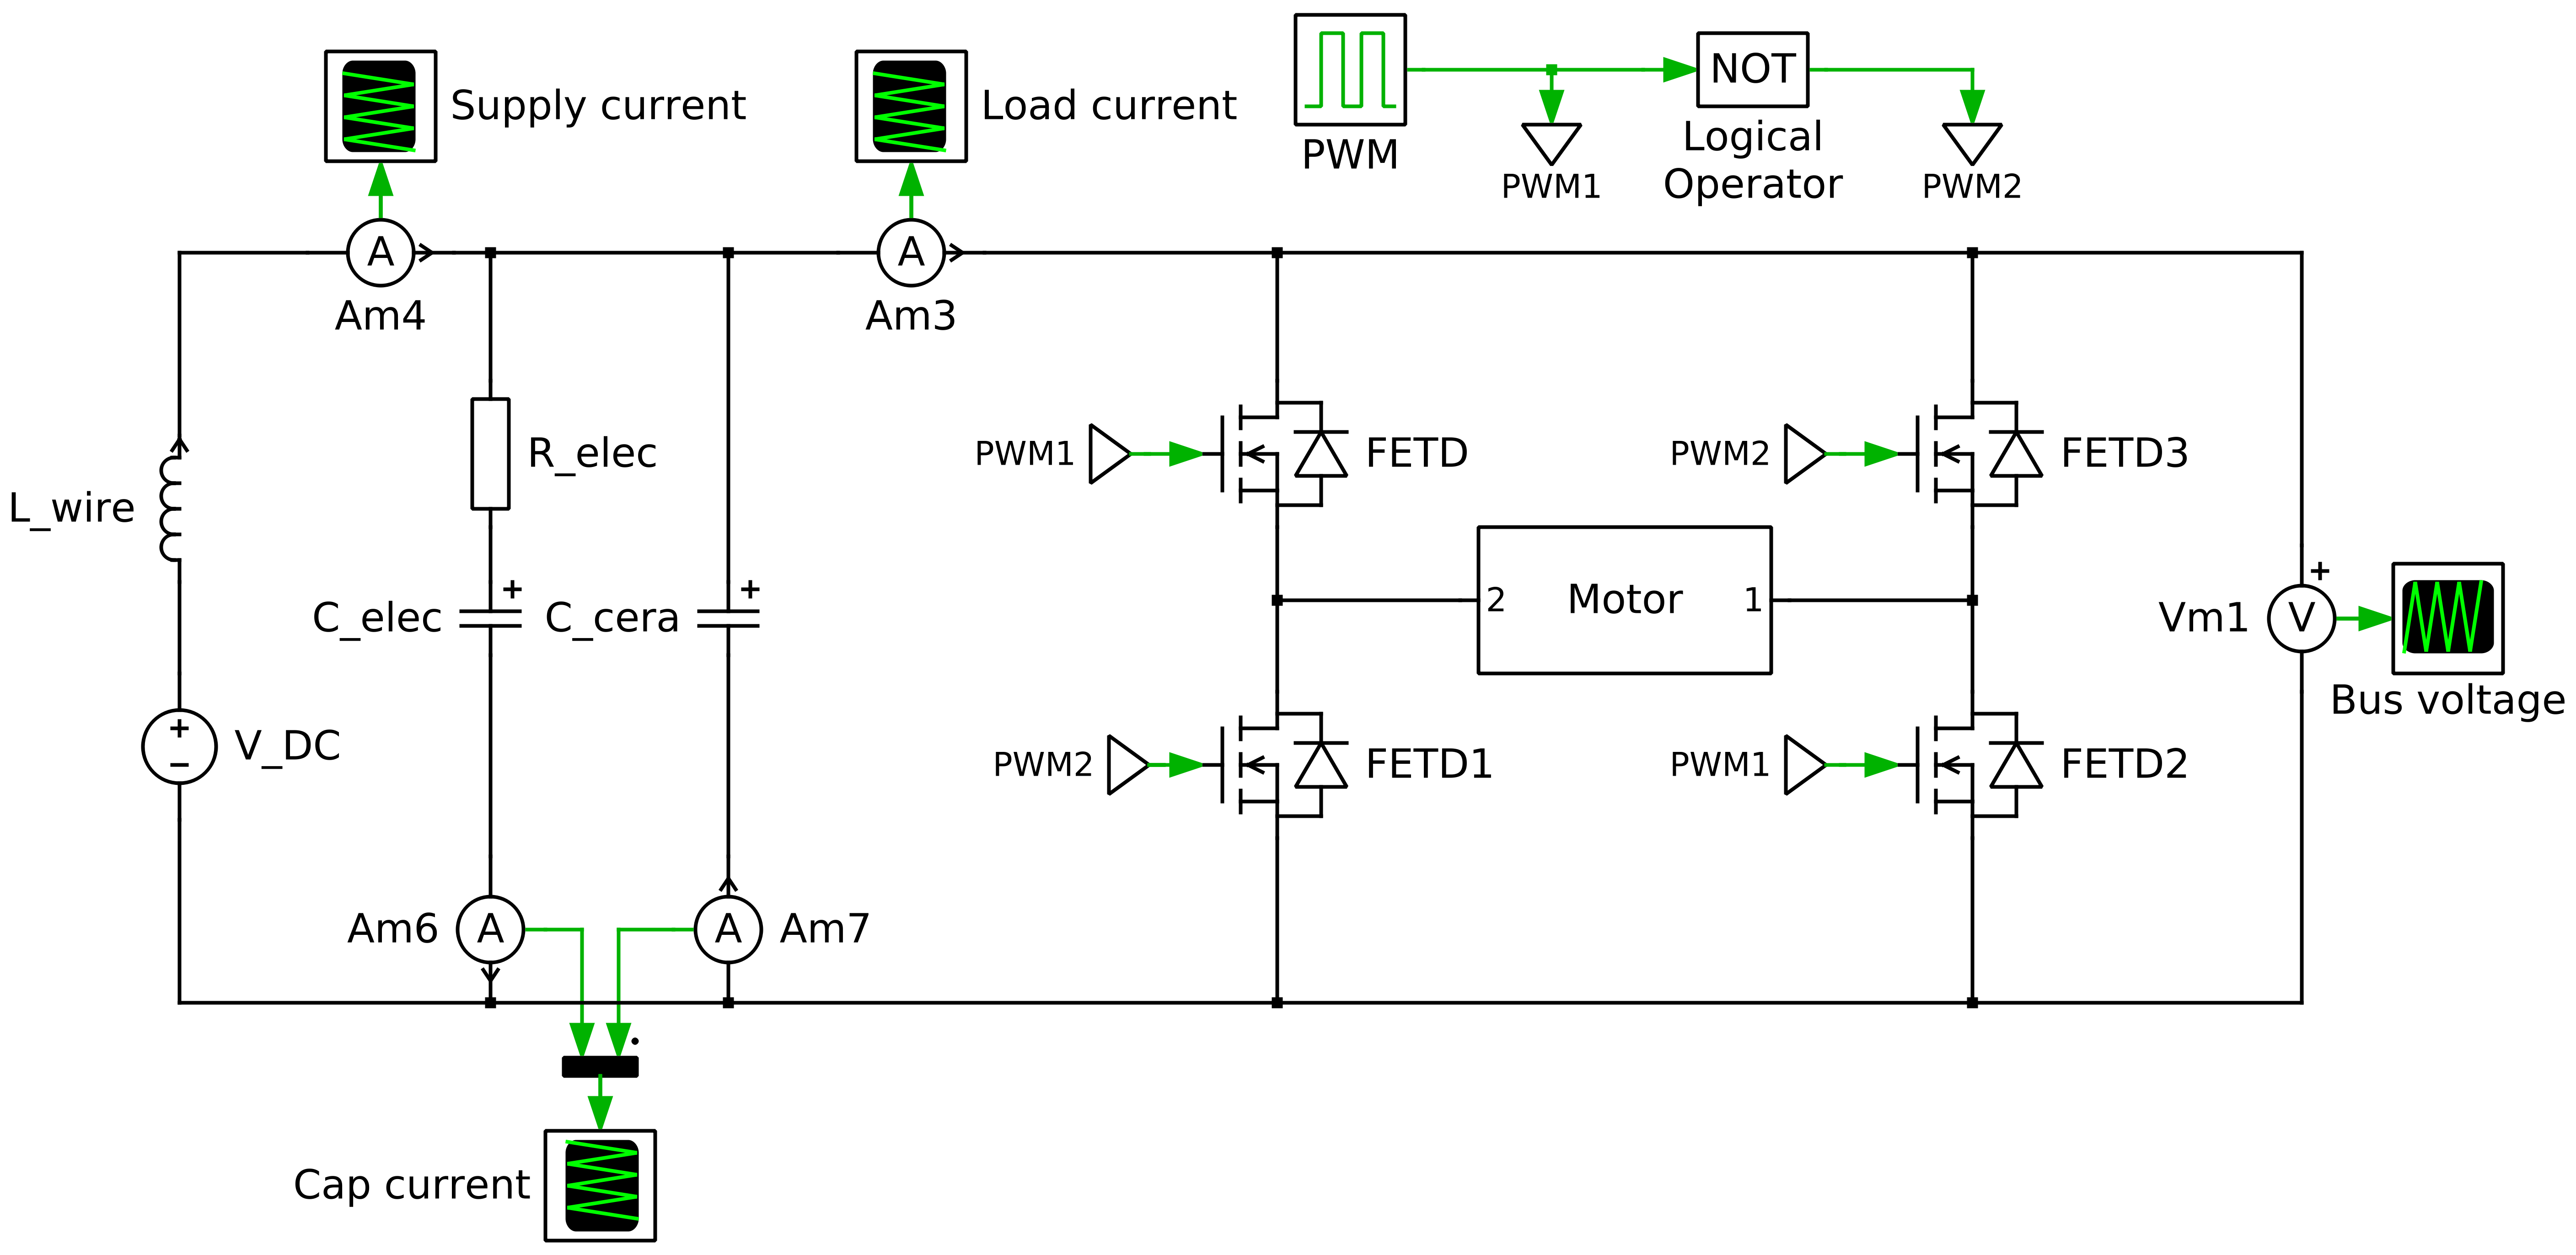
\includegraphics[width=1\linewidth]{graphics/plecs_schem.png}
	\caption{Full bridge circuit with supply capacitors and wire inductance modelled using PLECS. The Motor box consists of an inductor and a resistor in series. All components apart from the MOSFETS have the same values as the chosen components.}
	\label{fig:plecs_schem}
\end{figure}	

Simulating the system at 50\% duty cycle yields a voltage ripple of approximately 24mV, which is definitely acceptable. 

It can also be noted that an effect of the inductance in the supply wires and the supply capacitors is that the supply current is low pass filtered and is thereby protected against the ripple current and only needs to supply the DC component of the load current.

The current drawn from the capacitors is shown in figure \ref{fig:cap_currents}.
Here it can be seen that the electrolytic capacitors supply the majority of the current, while the ceramic capacitors supply a small spike with high frequency content.
It should be noted that in the simulations there are no difference between the two types of capacitors other than the ESR put in series with the electrolytic capacitors. 

\begin{figure}[h]
	\centering
    % This file was created by matlab2tikz.
%
%The latest updates can be retrieved from
%  http://www.mathworks.com/matlabcentral/fileexchange/22022-matlab2tikz-matlab2tikz
%where you can also make suggestions and rate matlab2tikz.
%
\definecolor{mycolor1}{rgb}{0.00000,0.44700,0.74100}%
\definecolor{mycolor2}{rgb}{0.85000,0.32500,0.09800}%


\begin{tikzpicture}




% \begin{axis}[%
% width=0.9\textwidth,
% height=1.2in,
% at={(0.758in,0.481in)},
% scale only axis,
% xmin=0.004999,
% xmax=0.005025,
% ymin=-5,
% ymax=5,
% ylabel style={font=\color{white!15!black}},
% ylabel={Current [A]},
% axis background/.style={fill=white},
% title style={font=\bfseries},
% title={Capacitors}
% legend style={legend cell align=left, align=left, draw=white!15!black}
% ]
% \addplot [color=mycolor1, forget plot]
%   table[row sep=crcr]{%




\begin{axis}[%
width=0.9\textwidth,
height=1.666in,
at={(0.758in,0.481in)},
scale only axis,
xmin=0.004999,
xmax=0.005025,
xlabel style={font=\color{white!15!black}},
xlabel={Time [S]},
ymin=-8,
ymax=6,
ylabel style={font=\color{white!15!black}},
ylabel={Current [A]},
axis background/.style={fill=white},
title style={font=\bfseries},
title={Capacitors},
legend style={legend cell align=left,font=\scriptsize , align=left, draw=white!15!black},
xtick={0.005,0.00501,0.00502}
]
\addplot [color=mycolor1]
  table[row sep=crcr]{%
0.0049010553385478	0.00342081159357233\\
0.00490489969343557	0.00683073660071676\\
0.00490874404832335	0.00991586664893029\\
0.00490909090909091	0.0101813275882865\\
0.00490909090909096	-6.63767713218716\\
0.00490913588166394	0.788632374646575\\
0.00490918085423691	0.0968134753000998\\
0.00490922582680989	-0.00983381196978428\\
0.00490967555253963	-0.0103095252998444\\
0.00491012527826937	-0.00895793028321945\\
0.00491057500399912	-0.00854569634641233\\
0.00491289980626855	-0.00643281216252056\\
0.00491522460853797	-0.00430374385953325\\
0.0049175494108074	-0.00216099641818635\\
0.00491987421307683	-2.65978258807836e-05\\
0.00492369979428432	0.00343331586571138\\
0.00492752537549182	0.00677023045901803\\
0.00493135095669931	0.00991965839131126\\
0.00493181818181813	0.0102885418851053\\
0.00493181818181818	-6.63795684124184\\
0.00493186309122796	0.788140209141018\\
0.00493190800063774	0.0970706595422914\\
0.00493195291004752	-0.00968459620855366\\
0.00493240200414533	-0.010151400317405\\
0.00493285109824314	-0.00922767791311507\\
0.00493330019234094	-0.00882378071900325\\
0.0049356105215896	-0.00627608882527975\\
0.00493792085083825	-0.00434505362802873\\
0.0049402311800869	-0.00213437587624032\\
0.00494254150933555	9.53670359069014e-05\\
0.00494636627166787	0.00360061858537619\\
0.00495019103400018	0.00703901460715084\\
0.00495401579633249	0.010148792099768\\
0.0049545454545454	0.0105586699059725\\
0.00495454545454545	-6.63771853889246\\
0.00495459015032096	0.786557805328613\\
0.00495463484609647	0.0976643538023345\\
0.00495467954187197	-0.00940476091145603\\
0.00495512649962704	-0.00993978708059062\\
0.0049555734573821	-0.00857857317189525\\
0.00495602041513717	-0.00816591337095129\\
0.0049583151501913	-0.00606782639068015\\
0.00496060988524543	-0.00395664904486392\\
0.00496290462029956	-0.00183438425385551\\
0.0049651993553537	0.00027740842506091\\
0.00496903087325131	0.00374628813147904\\
0.00497286239114892	0.00708566190254611\\
0.00497669390904653	0.0102308430991807\\
0.00497727272727267	0.010685341679721\\
0.00497727272727273	-6.63729580218999\\
0.00497731727074615	0.785182739111092\\
0.00497736181421957	0.0980802659485565\\
0.00497740635769299	-0.00922134889014892\\
0.0049778517924272	-0.00977371834118745\\
0.00497829722716142	-0.00883738412134694\\
0.00497874266189563	-0.00843919794694292\\
0.00498104199845287	-0.0059238355507687\\
0.0049833413350101	-0.0040186307720349\\
0.00498564067156733	-0.00183902675090497\\
0.00498794000812456	0.00035710955229637\\
0.00499179190075393	0.00384424013741791\\
0.00499564379338329	0.00726181015807148\\
0.00499949568601265	0.0103403911775377\\
0.00499999999999995	0.0107233299318876\\
0.005	-6.63678775329545\\
0.00500004447673189	0.784627777892562\\
0.00500008895346378	0.0981859652113108\\
0.00500013343019567	-0.0092018609164648\\
0.00500057819751456	-0.00979321463432026\\
0.00500102296483345	-0.00843310502509143\\
0.00500146773215235	-0.0080287074120009\\
0.00500377677864032	-0.00595109945391359\\
0.00500608582512829	-0.00386106136327458\\
0.00500839487161626	-0.00176029297984437\\
0.00501070391810423	0.000329411198857071\\
0.00501456587568511	0.00376585486603842\\
0.005018427833266	0.00707056768878767\\
0.00502228979084688	0.0101785379664605\\
0.00502272727272722	0.0105155195053972\\
0.00502272727272727	-6.63669528791197\\
0.0050227718773715	0.785481592291763\\
0.00502281648201573	0.0977955867894744\\
0.00502286108665995	-0.00940190195881785\\
0.00502330713310222	-0.00994616280641969\\
0.0050237531795445	-0.0090183414585101\\
0.00502419922598677	-0.00862558037378225\\
0.00502652935434658	-0.00611138202407391\\
0.00502885948270639	-0.00420805247858547\\
0.00503118961106621	-0.00202587201529669\\
0.00503351973942602	0.000174128206785015\\
0.00503738617751066	0.00363343469538768\\
0.0050412526155953	0.00702605089997999\\
0.00504511905367994	0.0100849998671229\\
0.00504545454545449	0.0103377257538093\\
0.00504545454545455	-6.63688438661501\\
0.0050454993184082	0.786909187571736\\
0.00504554409136186	0.0972936761155228\\
0.00504558886431551	-0.00964315408372496\\
0.00504603659385206	-0.0101688457131655\\
0.00504648432338861	-0.00881788004933393\\
0.00504693205292516	-0.00841271897506735\\
0.00504926853902644	-0.00631767727470978\\
0.00505160502512771	-0.00420712214877206\\
0.00505394151122899	-0.00208328771191457\\
0.00505627799733027	3.16047505261319e-05\\
0.00506012977709005	0.00346430797427311\\
0.00506398155684983	0.00677190482403178\\
0.00506783333660961	0.00988961814531208\\
0.00506818181818182	0.0101602465480153\\
0.00506818181818187	-6.63741638603617\\
0.00506822676429271	0.788263580426767\\
0.00506827171040355	0.0968710712364902\\
0.00506831665651439	-0.00981902461640649\\
0.00506876611762276	-0.010282819291199\\
0.00506921557873114	-0.00936583982423489\\
0.00506966503983952	-0.00896684900611833\\
0.00507200148913105	-0.0064211155171674\\
0.00507433793842259	-0.00449234590706937\\
0.00507667438771412	-0.00228026062001985\\
0.00507901083700566	-4.80677227454873e-05\\
0.00508284935926558	0.00343339431982481\\
0.0050866878815255	0.00685027548203943\\
0.00509052640378541	0.00994250061265101\\
0.00509090909090903	0.0102364341410595\\
0.00509090909090909	-6.63776191682534\\
0.00509095403119463	0.788414109103359\\
0.00509099897148016	0.0969253130139869\\
0.0050910439117657	-0.00977244042416769\\
0.00509149331462106	-0.0102542947538771\\
0.00509194271747643	-0.00890084705757577\\
0.00509239212033179	-0.00848784329587371\\
0.00509471010980675	-0.00637605440348255\\
0.00509702809928171	-0.00424860473551991\\
0.00509934608875667	-0.00210792975909035\\
};
\addlegendentry{Ceramic Capacitors}

\addplot [color=mycolor2]
  table[row sep=crcr]{%
0.0049010553385478	-0.915441839395498\\
0.00490489969343557	-2.02008944546105\\
0.00490874404832335	-3.06653627370542\\
0.00490909090909091	-3.15739364309411\\
0.00490909090909096	-3.15739364310866\\
0.00490913588166394	4.25578284216317\\
0.00490918085423691	3.55080766909668\\
0.00490922582680989	3.43099895230262\\
0.00490967555253963	3.29838689831377\\
0.00491012527826937	3.16703515437985\\
0.00491057500399912	3.03420023729996\\
0.00491289980626855	2.34110017146304\\
0.00491522460853797	1.63927639574104\\
0.0049175494108074	0.933249601497664\\
0.00491987421307683	0.227906177082332\\
0.00492369979428432	-0.918846892447618\\
0.00492752537549182	-2.02908008624217\\
0.00493135095669931	-3.08132645441947\\
0.00493181818181813	-3.20489120793354\\
0.00493181818181818	-3.20489120795537\\
0.00493186309122796	4.20799214847648\\
0.00493190800063774	3.50368169709691\\
0.00493195291004752	3.38368428511603\\
0.00493240200414533	3.25028965549427\\
0.00493285109824314	3.11773356924823\\
0.00493330019234094	2.98412907695456\\
0.0049356105215896	2.29115388523496\\
0.00493792085083825	1.58928909779206\\
0.0049402311800869	0.883900081273168\\
0.00494254150933555	0.179570804524701\\
0.00494636627166787	-0.971891453904391\\
0.00495019103400018	-2.08573965222604\\
0.00495401579633249	-3.14064893346222\\
0.0049545454545454	-3.28094792045158\\
0.00495454545454545	-3.28094792046613\\
0.00495459015032096	4.13016844417143\\
0.00495463484609647	3.428092171358\\
0.00495467954187197	3.30783548072941\\
0.00495512649962704	3.17493758595083\\
0.0049555734573821	3.04340834878531\\
0.00495602041513717	2.91042651790485\\
0.0049583151501913	2.22189270484523\\
0.00496060988524543	1.52567994879792\\
0.00496290462029956	0.826164624122612\\
0.0049651993553537	0.128065020835493\\
0.00496903087325131	-1.02202936300455\\
0.00497286239114892	-2.13347001265356\\
0.00497669390904653	-3.18471575261356\\
0.00497727272727267	-3.33703611806413\\
0.00497727272727273	-3.33703611808596\\
0.00497731727074615	4.07241109502502\\
0.00497736181421957	3.37225057452451\\
0.00497740635769299	3.25189005607535\\
0.0049778517924272	3.12027986907924\\
0.00497829722716142	2.98964814872306\\
0.00497874266189563	2.85799117581337\\
0.00498104199845287	2.17324157982512\\
0.0049833413350101	1.48047983761353\\
0.00498564067156733	0.784966991952388\\
0.00498794000812456	0.0911780343958526\\
0.00499179190075393	-1.05497919144545\\
0.00499564379338329	-2.16139660487534\\
0.00499949568601265	-3.2066133479675\\
0.00499999999999995	-3.33785721532331\\
0.005	-3.33785721535969\\
0.00500004447673189	4.07066818338353\\
0.00500008895346378	3.37131360285275\\
0.00500013343019567	3.2510084467649\\
0.00500057819751456	3.12077301707905\\
0.00500102296483345	2.99197915805416\\
0.00500146773215235	2.86174255228252\\
0.00500377677864032	2.17991762101883\\
0.00500608582512829	1.4905762026101\\
0.00500839487161626	0.798109154726262\\
0.00501070391810423	0.107245801111276\\
0.00501456587568511	-1.03223003423773\\
0.005018427833266	-2.13230920494243\\
0.00502228979084688	-3.17133878411551\\
0.00502272727272722	-3.28429267257161\\
0.00502272727272727	-3.28429267257161\\
0.0050227718773715	4.12503893459507\\
0.00502281648201573	3.42448077159497\\
0.00502286108665995	3.30441011337098\\
0.00502330713310222	3.17465105328301\\
0.0050237531795445	3.04583722598909\\
0.00502419922598677	2.91598394387256\\
0.00502652935434658	2.23211154308228\\
0.00502885948270639	1.53958590082766\\
0.00503118961106621	0.843786765552068\\
0.00503351973942602	0.149314537120517\\
0.00503738617751066	-0.987793491374759\\
0.0050412526155953	-2.08624917075213\\
0.00504511905367994	-3.1245759032754\\
0.00504545454545449	-3.21116772740061\\
0.00504545454545455	-3.21116772741516\\
0.0050454993184082	4.19972304494149\\
0.00504554409136186	3.49718167772517\\
0.00504558886431551	3.37731402221107\\
0.00504603659385206	3.24697386535991\\
0.00504648432338861	3.11796059356857\\
0.00504693205292516	2.98747435640689\\
0.00504926853902644	2.30020861748926\\
0.00505160502512771	1.60439322426828\\
0.00505394151122899	0.904558726528194\\
0.00505627799733027	0.205597670232237\\
0.00506012977709005	-0.932263559894636\\
0.00506398155684983	-2.03290280140209\\
0.00506783333660961	-3.07475351853645\\
0.00506818181818182	-3.16541938849696\\
0.00506818181818187	-3.16541938851151\\
0.00506822676429271	4.24721468395001\\
0.00506827171040355	3.54274894992705\\
0.00506831665651439	3.42298425603076\\
0.00506876611762276	3.29125734094123\\
0.00506921557873114	3.1603465270382\\
0.00506966503983952	3.02837585099041\\
0.00507200148913105	2.33636816850048\\
0.00507433793842259	1.63493908630335\\
0.00507667438771412	0.929554722511966\\
0.00507901083700566	0.224905788723845\\
0.00508284935926558	-0.918844584048202\\
0.0050866878815255	-2.02579574252013\\
0.00509052640378541	-3.07459532834037\\
0.00509090909090903	-3.17518959014706\\
0.00509090909090909	-3.17518959015433\\
0.00509095403119463	4.23782588414906\\
0.00509099897148016	3.5331533421122\\
0.0050910439117657	3.41326674421725\\
0.00509149331462106	3.28037942616356\\
0.00509194271747643	3.14876614561945\\
0.00509239212033179	3.0156744667911\\
0.00509471010980675	2.32288135642739\\
0.00509702809928171	1.62154641278175\\
0.00509934608875667	0.916161728986481\\
};
\addlegendentry{Electrolytic Capacitors}

\end{axis}
\end{tikzpicture}%
	\caption{Current drawn from the electrolytic and ceramic capacitors, when simulating in PLECS. }
	\label{fig:cap_currents}
\end{figure}

Generally the designed features of the circuit was verified using the PLECS model.

\subsubsection{Safety Relay} % (fold)
\label{ssub:safety_relay}
\thomas{This section and the next needs some numbers on charging time and similar}
It should be possible to disengage the main power rail from the load in case of an emergency.
This is done most simply by adding a relay in series with the load.
The relay must be able to carry and break the full load current, 80A.
The LEV100A4ANG meets this requirement. 
It is capable of carrying up to 100A continuous current and can break significantly more.
Since the supply capacitors are parallel with the load, these will also be disconnected by the relay.
It has a 12V coil which requires $\approx$0.5A to activate.
% subsubsection safety_relay (end)

\subsubsection{Inrush Current}
\label{ssub:inrush_current}
When the system is initially turned on, the supply capacitors will charge.
They will draw a huge amount of current as there is only the ESR to limit the current. 
A resistor should be added to limit this inrush current. 
Adding the resistor to the main current path would introduce considerable losses and limit the performance of the system.
An additional current path is added to the circuit.
This is done by adding a resistor and a relay in parallel with the main relay.
When first powering up the system the secondary relay should be turned on in order to charge the supply capacitors.
Once charged, the main relay is switched on and afterwards the secondary relay can be switched off.
This will control the initial inrush current but the system should not be run until the secondary relay is switched off again.

\subsubsection{Relay Circuitry} % (fold)
\label{ssub:relay_circuitry}
As discussed in sections \ref{ssub:safety_relay} and \ref{ssub:inrush_current}, two relays are necessary in this design.
The two circuits are functionally similar so only the circuitry related to the inrush relay is shown here and any relevant differences are discussed.
Figure \ref{fig:relaycircuit} is an overview of the circuit created to drive the inrush relay.

\begin{figure}
	\centering
	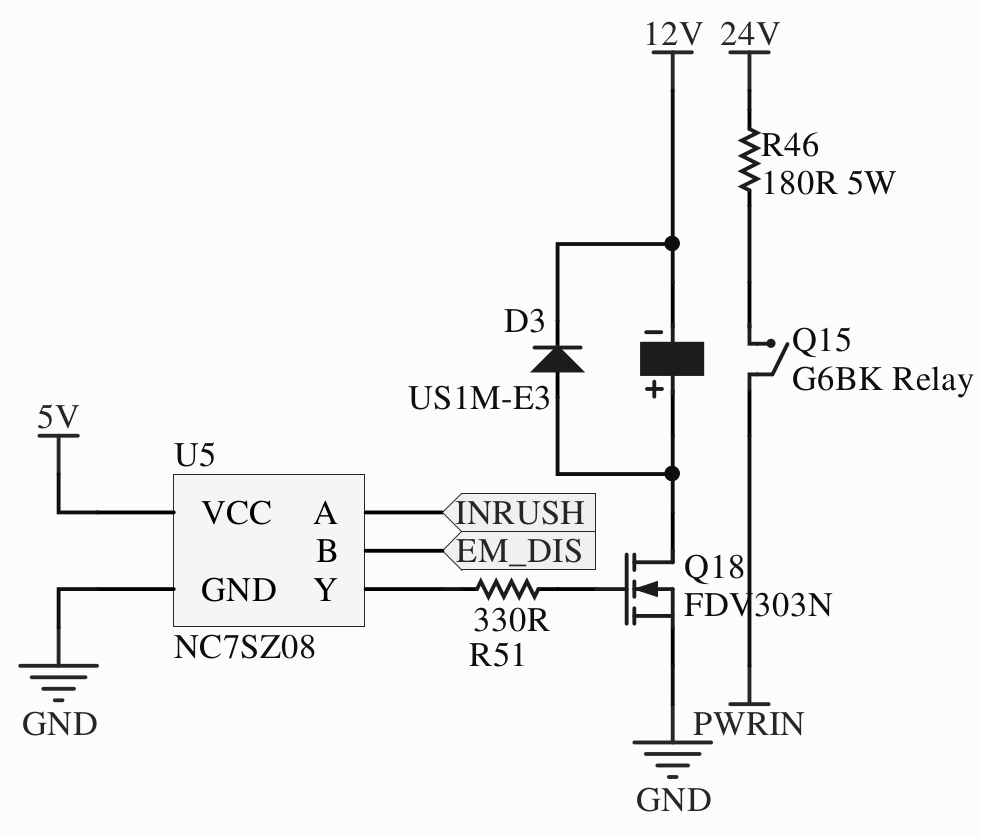
\includegraphics[width=\linewidth]{graphics/relay_circuit}
	\caption{Circuitry related to the inrush relay.}
	\label{fig:relaycircuit}
\end{figure}

\mikkel{These sections should be merged.}

\thomas{Add circuit showing the safety relay}
On figure \ref{fig:relay_circuit} is shown the safety circuitry.
A relay is mounted in series with the supply rail for the motor.
The default state for this relay should be \texttt{off}.
Then, in order to switch the system to the \texttt{on} state, the relay should be closed.
Should power to the relay coil ever fail i.e. something in the system has broken, power to the motor is cut off.
Since the relay is in series with the motor, it should also be capable of carrying the full design current, 80A.
One relay that fulfills these requirements is the.
\\~\\
The driver circuit for the relay is activated only when all safety conditions are off.
If at any point any of the safety conditions are tripped, the driver circuit shuts down, releasing the relay and turning off power to the motor.
Designing the safety circuit in this manner ensures that the system cannot be started or will shut down if any wires or components in the safety circuit break.


\subsubsection{Motor Current Sensing}
Measuring current in an H-Bridge with a shunt resistor can be done in a number of ways.
The shunt resistor can be placed in various positions in the H-bridge.
The three main ones are high-side, in-line and low-side placement of the shunt resistor.
\cite{shunt_placement} and \cite{Current_Sense_Circuit_Collection} specifies the advantages and disadvantages of the three configurations.
\thomas{Perhaps add a quick summary of each and highlight the selected one?} 
It was decided to use the low-side configuration as it has low common voltage, it only needs a single sided supply and because bi-directional current measurement is not needed in this application.

\paragraph{Requirements for the Current Measuring Circuit} % (fold)
\label{par:requirements_for_the_current_measuring_circuit}

The output of the current measuring circuit is an analogue signal that is measured by the ADC of the Zynq chip.
According to the Zynq ADC user guide \cite{zynq_adc}, the measurable input range is from 0V to 1V, but the maximum allowed input voltage is 1.9V according to \cite{adc_zynq_webanswer}.
The absolute maximum current through the motor is the stall current which is 80A, but the motor will run well below this level in normal operation.
The normal operation currents are expected to be up to 30A
\thomas{Some test or explanation required to justify 30A}
It was therefore decided that the circuit  needs to be able to measure currents of at least up to 40A.
The resolution per Ampere is increased by decreasing the current range that can be measured,
If the current gets any higher the ADC input should not be harmed meaning that the input voltage should not exceed 1.9V.
\thomas{What are the requirements of the accuracy? What can we achieve with the hardware?}

% subsubsection requirements_for_the_current_measuring_circuit (end)

\paragraph{Designing the Current Measuring Circuit} % (fold)
\label{par:designing_the_current_measuring_circuit}

Placing a shunt resistor in the low-side configuration raises the voltage potential of the low-side of the H-bridge.
This may influence the gate signal required to open the MOSFETs of the H-bridge.
In addition, the shunt resistor will, regardless of placement result in a powerloss proportional to its size.
For these reasons minimizing the value of the shunt resistor is important. 
The smallest value available from the electronics supplier used at SDU provides a 200$\mu\Omega$ SMD shunt resistor.
Such a small resistance yields a minimal voltage drop and thus keeps power consumption at a minimum.\\
The resulting voltage from the motor stalling, that is an 80A current flowing through the resistor would result in only a 16mV voltage drop.
Since the input range of the ADC is 0-1V, this low voltage would yield very poor resolution in the area of actual interest, 0-40A.
An amplifier circuit is necessary.
Purpose built current-sense amplifiers exist which are used specifically for amplifying the voltage drop across a shunt resistor.
One such amplifier is the \texttt{INA286AID} from Texas Instruments \cite{INA286AID}.
It has a gain of 100, lifting the voltage resulting from motor stall to 1.6V as seen from equations \ref{eq:adc_input_voltage1} and \ref{eq:adc_input_voltage2}.
\begin{equation}
	V_{max,input} = G \cdot V_{shunt}
	\label{eq:adc_input_voltage1}
\end{equation}
\begin{equation}
	V_{max,input} = G \cdot R_{shunt} \cdot I_{stall} = 100 \cdot 200\cdot10^{-6} \cdot 80 = 1.6V
	\label{eq:adc_input_voltage2}
\end{equation}
The measurable range using this IC is 0-50A as seen from \ref{eq:adc_input_voltage3}.

\begin{equation}
	I_{max, measurable} = \frac{V_{max, measurable}}{R_{shunt}\cdot G} = \frac{1}{100 \cdot 200\cdot10^{-6} } = 50A
	\label{eq:adc_input_voltage3}
\end{equation}

It has a very low offset allowing it to be used in applications where the voltage drop across the shunt resistor is only a few mV.

This design meets the required design specifications and the schematics can be seen in figure \ref{fig:currentmeasure}.
As can be seen, the \texttt{INA286} in this configuration requires only the voltage input, \texttt{POWER\_SHUNT+/-} from the schematic on figure \ref{sfig:hbridgeshunt}, to generate a suitable output which is then fed directly to the ADC through the anti-aliasing filter shown on figure \ref{sfig:ina286aidschematic}.

\begin{figure}
	\centering
	\begin{subfigure}[b]{0.49\textwidth}
		\centering
		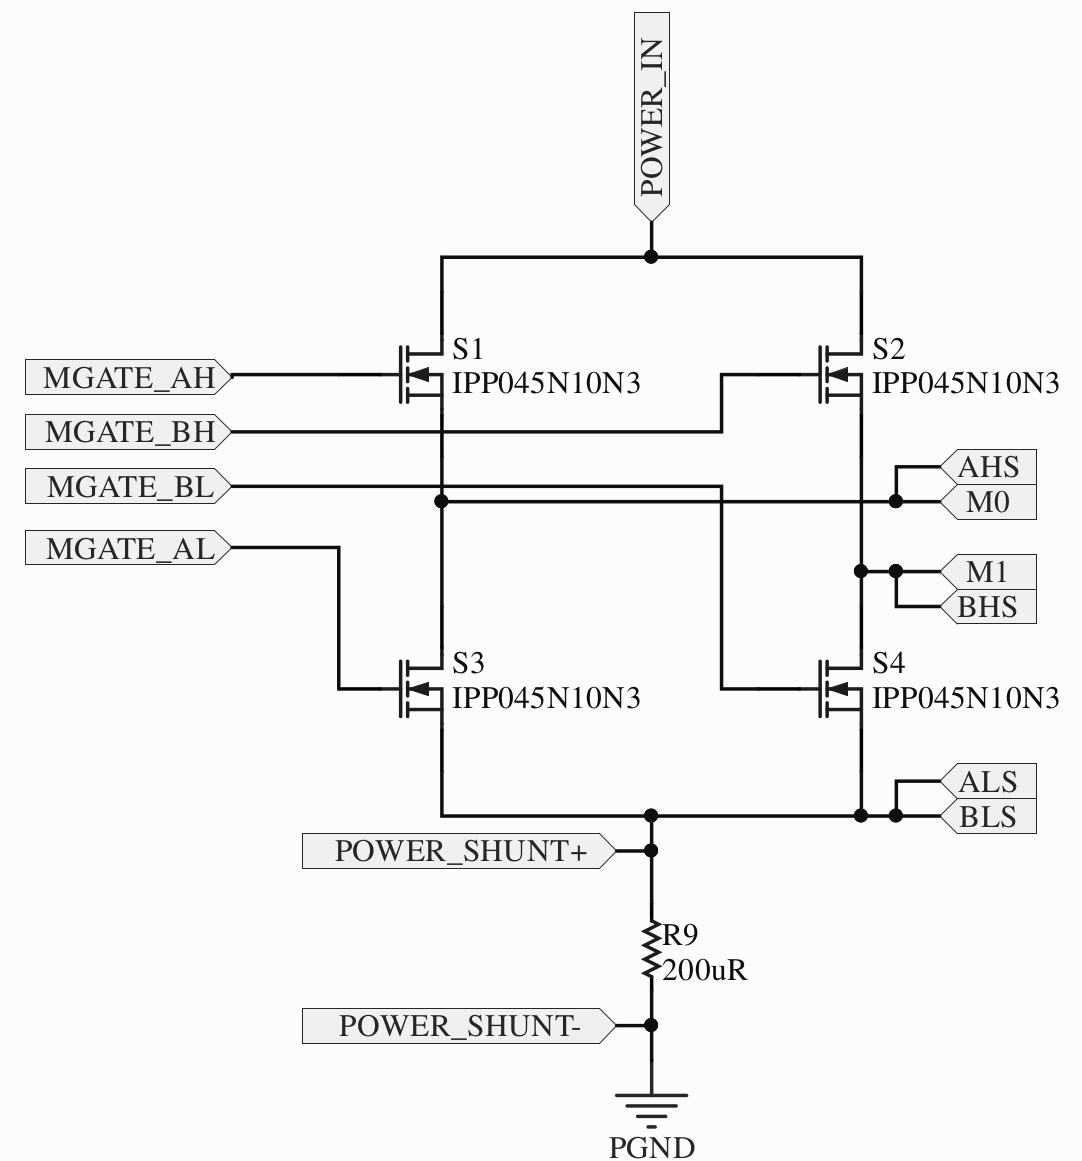
\includegraphics[width=\linewidth]{graphics/hbridge}
		\caption{H-bridge with shunt resistor in low-side configuration.}
		\label{sfig:hbridgeshunt}	
	\end{subfigure}
	\begin{subfigure}[b]{0.49\textwidth}
		\centering
		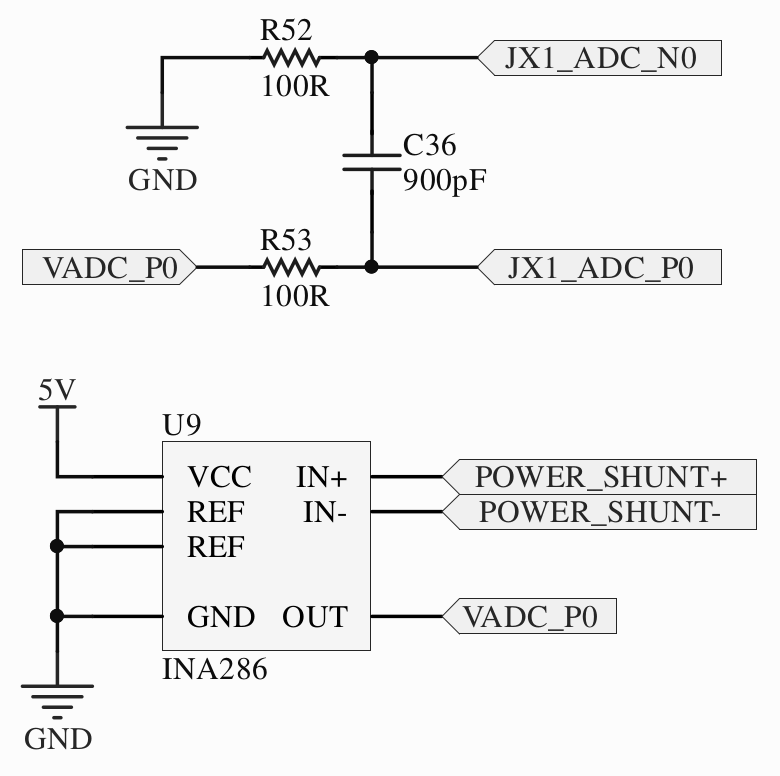
\includegraphics[width=\linewidth]{graphics/ina286}
		\caption{Schematic of the INA286AID as used in the project.}
		\label{sfig:ina286aidschematic}
	\end{subfigure}
	\caption{Schematics relating to the current measurement circuitry.}
	\label{fig:currentmeasure}
\end{figure}

% subsubsection designing_the_current_measuring_circuit (end)



% subsection relay_circuitry (end)

\subsubsection{Endstop Detection} % (fold)
\label{ssub:endstop_detection}
As described in section \ref{subsub:safety} it was decided to use infrared transceivers to detect endstops.
\mikkel{The actual 3D print design should be described elsewhere}
It was decided to use the \texttt{TCST 2103} as it has the wanted functionality.
It contains an infrared emitter pointing at a photo transistor, that conducts current proportional to the infrared light received.
In this project it will be used to detect if the infrared light rays has been blocked by the cart or not. 
The circuit shown in figure \ref{fig:tcst_circuit} was realised to convert the current conducted to a voltage level. 
The output is fed to a schmitt trigger circuit in order to be able to use the result as a boolean reference.
The schmitt trigger circuit is designed to have a high threshold of 3V and a low threshold of 1V. 

\begin{figure}
	\centering
	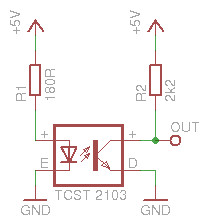
\includegraphics[width=0.4\linewidth]{graphics/tcst_circuit_temp.jpg}
	\caption{\texttt{TCST 2103} circuit.}
	\label{fig:tcst_circuit}
\end{figure}
\mikkel{replace with own image!}



\subsubsection{Voltage Rails} % (fold)
\label{subsub:voltage_rails}
In the design of the board it is necessary to determine which voltage rails are required for the system to function.
The power delivery for the MicroZed was designed by the authors in an earlier project \cite{isaswarm} and will be reused with minor changes.
This power delivery system provides, amongst other voltages, the 3.3V rail, originally intended for powering the MicroZed IO banks only.
In this system however, the RF tranceiver is also powered from this rail.
As a result a review of the circuitry around the 3.3V rail is necessary to ensure that it can provide the required power.
The MicroZed power delivery system, the encoders of the system, the endstops and part of the emergency circuitry are all driven from a 5V rail.
The Motor Driver, the HIP4081 \cite{driver} and the relay driving circuitry is driven from a 12V rail.
Finally, the motor is driven from a 24V rail, which will also be the main supply for the system.
This rail is not crucial to the design of the board as it is provided by an external, mains connected power supply and will not be explored further in this section.\\
The current requirement for each of these rails are discussed in the following paragraphs

\paragraph{3.3V:} % (fold)
\label{par:3_3v}
As mentioned, this rail is intended for powering the MicroZed IO banks.
In the original design the LMR10510XMF DC/DC converter is used to provide the necessary power.
This chip is capable of supplying up to 1A.
Components exist in the same series which are pin compatible and are capable of supplying up to 2A.
The RF Transceiver used in this project, however, \ref{} requires only up to 15mA when receiving data.
Assuming that Avnet has already provided headroom for the IO bank supply and considering that this project makes little use of the IO on the Zynq-7000 chip, it is deemed unnecessary to upgrade this supply and the original design is used as is.
% paragraph 3_3v_ (end)

\paragraph{5V:} % (fold)
\label{par:5v}
This rail supplies, mainly, the MicroZed.
The authors previously found \cite{isaswarm} that the maximum expected current draw seen from the MicroZed is 1.85A at 5V.
In addition, in this design, the 5V rail also powers the encoders, endstops and emergency circuitry.
The HEDS-5540 \cite{heds5540} encoder requires a maximum of 85mA..
The endstops are realised using the TCST2103 infrared sensor \cite{tcst2103}.
The majority of the current supplied to this sensor is used to power the infrared LED present in the component.
This current is decided by the resistor put in series with the LED and is estimated to be around 50mA per LED for a total of 100mA.
Another 10mA is added to that figure due to the collector current possible on the transistor side.\\
Finally the emergency circuitry along with some other digital electronics are powered from the 5V rail.
As these are all digital IC's that operate on nothing but signals, their individual powers are negligible but a very conservative 25mA power budget is provided for all of the digital electronics on the 5V rail. This brings the total power budget for the 5V rail to $\approx$2.1A.
See table \ref{tab:5vpowerbudget} for a full overview.

\begin{table}
	\centering
	\begin{tabular}{l|r}
		 Component & Current [mA]\\
		 \hline
		 MicroZed & 1850\\
		 HEDS-5540 & 85\\
		 TCST2103 & 110\\
		 Digital & 25\\
		 \hline
		 Total & 2070
	\end{tabular}
	\caption{Power budget for the 5V rail}
	\label{tab:5vpowerbudget}
\end{table}

In \cite{isaswarm} the authors used a design in which the PTH08080 is used to generate a 5V rail.
Reusing this module will save on design time as well as the budget available to the project and as such is desirable.
This module however, is capable of supplying only 2A at 5V, slightly less than the value calculated in this section.
By far the largest contributor to the power budget is the MicroZed.
The calculation of the contribution from the MicroZed is done assuming 85\% utilisation of PL and a conservative 80\% efficiency of internal DC/DC converters.
Considering this, it is safe to assume that the real power draw from the MicroZed is significantly smaller than the calculated value and as a result it is chosen to reuse the PTH08080 despite of apparent shortcomings of the module.
% paragraph 5 (end)

\paragraph{12V:} % (fold)
\label{par:12v}
This rail powers the HIP4081 motor driver, the relay coils, the bootstrap circuitry and the 5V DC/DC converter.
The PTH08080 DC/DC converter has a maximum input voltage of 18V and must be powered from the 12V rail rather than the 24V rail.
The module can provide 2A at 5V and as such will require $\approx$0.85A from the 12V rail.\\
\mikkel{Mention efficiency if this should make sense.}
There are two relays in the design, a smaller relay for controlling the inrush current and the larger main supply relay.
Both of these require power to stay in the closed position.
The first, the G6B \cite{g6b}, requires 16.7mA while the former, the LEV100A4ANG \cite{lev100}, requires 461mA.\\
The motor driver of the system, the HIP4081 requires only 10mA.
As mentioned, the bootstrap circuitry is also powered from the 12V rail.
Rather than a steady supply, this circuitry requires a large peak current for short periods while charging in between switching.
For this reason the design choice here is to determine what is available and choose the component which yields the most headroom while still being economically feasible.
Amongst all of the components the total power budget for the 12V rail is $\approx$1340mA.
See table \ref{tab:12vpowerbudget} for a full overview.

\begin{table}
	\centering
	\begin{tabular}{l|r}
		 Component & Current [mA]\\
		 \hline
		 PTH08080 & 850\\
		 G6B & 16.7\\
		 LEV100A4ANG & 461\\
		 HIP4081 & 10\\
		 \hline
		 Total & 1337.7
	\end{tabular}
	\caption{Power budget for the 12V rail}
	\label{tab:12vpowerbudget}
\end{table}

The PTN78020 delivers 6A at 12V and is part of the same series as the PTH08080 described earlier.
This allows many of the same design procedures to be reused.
In addition, the 6A current limit leaves sufficient room for the current spikes expected from the bootstrap circuitry.
The bootstrap circuitry is modified slightly to accomodate the limited supply as described in section \ref{}
% paragraph 12v_ (end)

% subsection voltage_rails (end) 


\subsubsection{12V Rail Circuitry}

\begin{figure}
	\centering
	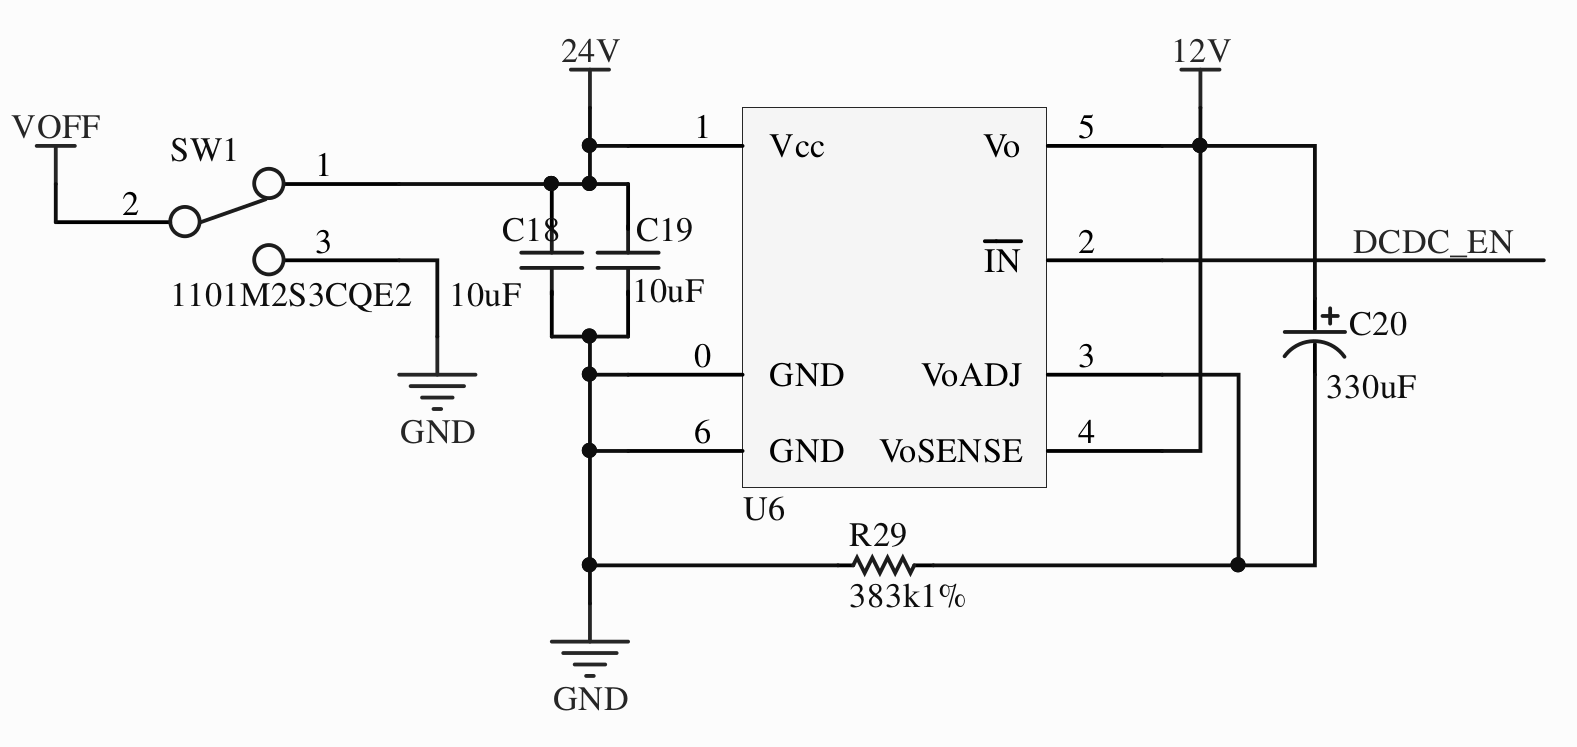
\includegraphics[width=\linewidth]{graphics/dcdc12v}
	\caption{The PTN78020H DC/DC converter and the appertaining circuitry.}
	\label{fig:dcdc12v}
\end{figure}

The \texttt{PTN78020H} DC/DC converter is used to generate the 12V rail. 
The component requires input and output capacitors in order to function properly and a resistor is needed to set the desired output voltage. 
The circuit used is based on the typical application circuit shown in the datasheet \cite{PTN78020H} and is implemented as shown in figure \ref{fig:dcdc12v}.
A resistor is required from \texttt{VoADJ} to ground to set the desired output voltage, in this case 12V.
In the datasheet on table 2 is a list of common voltages and the resistance required to achieve those voltages.
To generate 12V a 1\% 383 k$\Omega$ is needed.
\texttt{VoSENSE} should be connected close to the main load to allow for more precise regulation of the output.
This feature is mainly useful when the load is placed far from the supply and can be left floating if the accuracy of the rail is not important.
It was decided to simply short it to the 12V rail at the component since the load is placed relatively close to the supply.
$\overline{\text{\texttt{IN}}}$ carries the inhibit signal.
Pulling this low will disable the output of the component.
This is done by toggling the switch \texttt{SW1}. 
This will open a MOSFET which in turn will pull the \texttt{DCDC\_EN} signal low.
The datasheet also specifies that a ceramic capacitance of at least 18.8 $\mu$F is needed at the input. 
It was chosen to use two 10 $\mu$F capacitors.
In order to ensure stability the \texttt{PTN78020H} needs an output capacitance of 330 $\mu$F.
The datasheet specifies that if the application has load transients additional capacitance should be added to improve the response of the regulator.
While the load at the 12V rail is mostly steady, it does supply the boot capacitors which create a slight ripple on the rail.
It was therefore decided to use two 330 $\mu$F electrolytic capacitors in parallel.
As suggested by the datasheet an additional 20 $\mu$F of ceramic capacitance is added to the output to further improve the transient response.\\

\subsubsection{5V and 3.3V Rail Circuitry} % (fold) 
\label{subsub:pth08080w}
As mentioned previously the choice of these component and the design of the circuitry around them was done by the authors in a previous project \cite{isaswarm} and the details of the design will be omitted for this discussion.
The PTH08080W and LMR10510XMF are responsible for creating the 5V and 3.3V rails, respectively.
These rails were designed mainly for ensuring the correct boot and shutdown of the MicroZed.
These procedures are described in detail in \cite{isaswarm}.
% subsection pth08080w (end)

%!TEX root = ../main.tex
\subsection{Board Layout} % (fold)
\label{sub:board_layout}
The layout of the board involved a number of considerations, especially concerning the layout of the power part of the circuit.
These considerations involve the layer stack, the required copper thickness and various placements of components.
This section will discuss in appropriate detail these considerations.
Figure \ref{fig:board_layout} is an overview of the final layout of board.
Firstly, it is desirable to determine what requirements exist for the trace widths and thicknesses in the layout.

\begin{figure}
	\centering
	%\includegraphics[width=\linewidth]{graphics/board_layout}
	\missingfigure{bottom and top board layout}
	\caption{Top and bottom view of the controller board.}
	\label{fig:board_layout}
\end{figure}

\subsubsection{Copper Thickness}
Part of the board is designed to house the H-Bridge that drives the motor.
The H-bridge is designed to carry up to 80A, well above what can reasonably be carried at standard PCB copper thickness.
This section seeks to estimate the required copper thickness to allow for the design current.
Allowing a current through a conductor will produce a temperature rise due to the power dissipated in the conductor.
The current-carrying capacity (CCC) of a conductor is unlimited, so far as the current is not destructive due to the temperature rise permissable in the design.
Essentially, the acceptable temperature rise is limited by the maximum operating temperature of the PCB material.
This specification is known as the temperature index.
The PCB material most commonly used is FR-4 which has a temperature index of 130\degree \cite{fr4}.
At an ambient temperature of 20\degree this would imply a permissable conductor temperature rise of 110\degree.
In all practical situations, this is unreasonably high.
The material will discolor and degrade over time with the excessive heating and cooling of the board while also increasing the apparent ambient temperature of other components on the PCB, lowering the efficiency of the circuit.
In actual designs, a much more conservative temperature rise of 10\degree is often used, 15\degree is acceptable and 20\degree is considered high.
This was discussed with Jesper Nielsen, a technician at SDU who has experience in designing high power PCBs and it was decided to accept 15\degree increase. 
The actual temperature rise of a conductor is dependent on a great number of variables, among these are: conductor length, cross-sectional area, conductor material, PCB material, ambient temperature, convection, PCB layout (the amount of copper in the vicinity), etc.
Additionally, not all conductors carry the same current so different conductors have different thermal impacts on different locations on the PCB.
Clearly, it is difficult to accurately calculate the required copper thickness, however an estimate can be made.
In IPC-2221A \cite{ipc2221} data is presented to show the temperature rise resulting from allowing a current through a trace on a PCB on different trace widths.
This data was first published in \cite{conduct}, a progress report from the American National Bureau of Standards dating back to 1956.
Much has happened in PCB manufacturing since then. 
The original data does not take into account the possibility of multi-layered boards or many of the newer board materials.
In 2009 the new IPC-2152 \cite{ipc2152} was published and reevaluates the topic of current-carrying capacity.
This standard, however, is unavailable due to its high cost and the original charts are used instead.
A number of PCB trace width calculators exist online which extrapolate from the original data to give estimates of the required copper thickness and width.
One such calculator \cite{pcb_trace_calc} was used to determine the required copper thickness and width required in this project.
~\\
There are economic constraints in place for this project which requires the authors to be somewhat conservative with respect to how exotic a solution will be considered.
Most manufacturers support increasing the thickness of copper on a specific layer, allowing well above the 35$\mu$m standard copper thickness.
The manufacturer used in this project was chosen due to a comparatively low price on 4-layer boards with 70$\mu$m copper on outer layers and 52.5$\mu$m on internal layers.
On the power part of the board this results in a total of 122.5$\mu$m of copper for the 24V rail and power ground.
~\\
In order to simplify the design process, a distinction is made between three types of traces.
This distinction is based on the expected amount of current carried by that trace.
\begin{itemize}
	\item \textbf{Signal:} This is the type with the lowest expected current and is used throughout digital circuitry and low power analog signals.
	Signal traces are by far the most abundant on the circuit and due to the very low currents the trace width should be as small as possible.
	The manufacturer is capable of creating traces at 8 mil or higher at the desired copper thickness and as such the trace width for this type is 8 mil.
	\item \textbf{Power:} This type is generally used for supply rails.
	The trace width for this type is 20mil. Accepting 15\degree temperature increase will allow up to $\approx$1.5A of current.
	This is sufficient for supplying any of the IC's and other components connected to this trace type.
	\item \textbf{High Power:} This type is used exclusively for the 24V rail.
	The trace width for this type is 40mil. Accepting 15\degree temperature increase will allow up to $\approx$2.4A of current.
	Since the inrush current is limited to $\approx$0.14A this leaves plenty of headroom for creating the 2.5V, 3.3V, 5V and 12V rails.
	\thomas{verify 40mil trace width}
\end{itemize}

\subsubsection{Copper Layout} % (fold)
\label{ssub:copper_layout}
The board can be split into two parts: a digital circuit and a power circuit.
As seen on figure \ref{fig:board_layout} the power circuitry is placed on the right third of the board while the digital circuitry occupies the remainder of the board.
The two parts have seperate ground planes in order to protect the digital circuitry from the high and sudden currents generated by the motor.
A ground plane, even though the resistance through it is low, will have a significant voltage drop across it if currents of sufficient magnitude are passed through it.
For the same reason it is desirable to keep the current path as short as possible on the power side of the board.
Figure \ref{fig:power_layout} depicts a 3D view and 2D view of the power part of the board.
As can be seen, the MOSFET's are bend such that a heatsink can be mounted on top.
The upper pair is the left half-bridge and the lower pair is the right half-bridge.
The outtake for the motor is positioned directly above and below the two half-bridges and a 3M bolt is mounted to allow for a robust connection.
A large pad is made where the bolt is mounted as close as possible to the MOSFET's to allow for unrestricted flow of current.
The pad between the motor outtakes is the connection from source of the low-side of the half-bridges to the shunt resistor used for current measurements.
Since all current must pass through the shunt resistor, it is crucial that the flow of current is as unrestricted as possible.
\\~\\
Main power is input through M3 bolts mounted in the three holes between the half-bridges.
Clearly, only two terminals are required but the three pads effectively divide the 24V rail into two parts, forcing any currents to flow around the pads.
Instead it was decided to use two input terminals for the 24V rails that are mechanically fixed at the bolts.
The ground plane is unrestricted and as such the current can flow freely and only one terminal is required.
None of the planes on the power side of the PCB can be interrupted by traces, as this would severely hinder the flow of current in that plane.
This means that it is necessary to add wires to carry the gate, return and shunt signals.
These wires are soldered directly to the MOSFET pins and connected to the digital side through a header on the bottom side of the board. 

\begin{figure}
	\centering
	\begin{subfigure}[b]{0.49\textwidth}
		\centering
		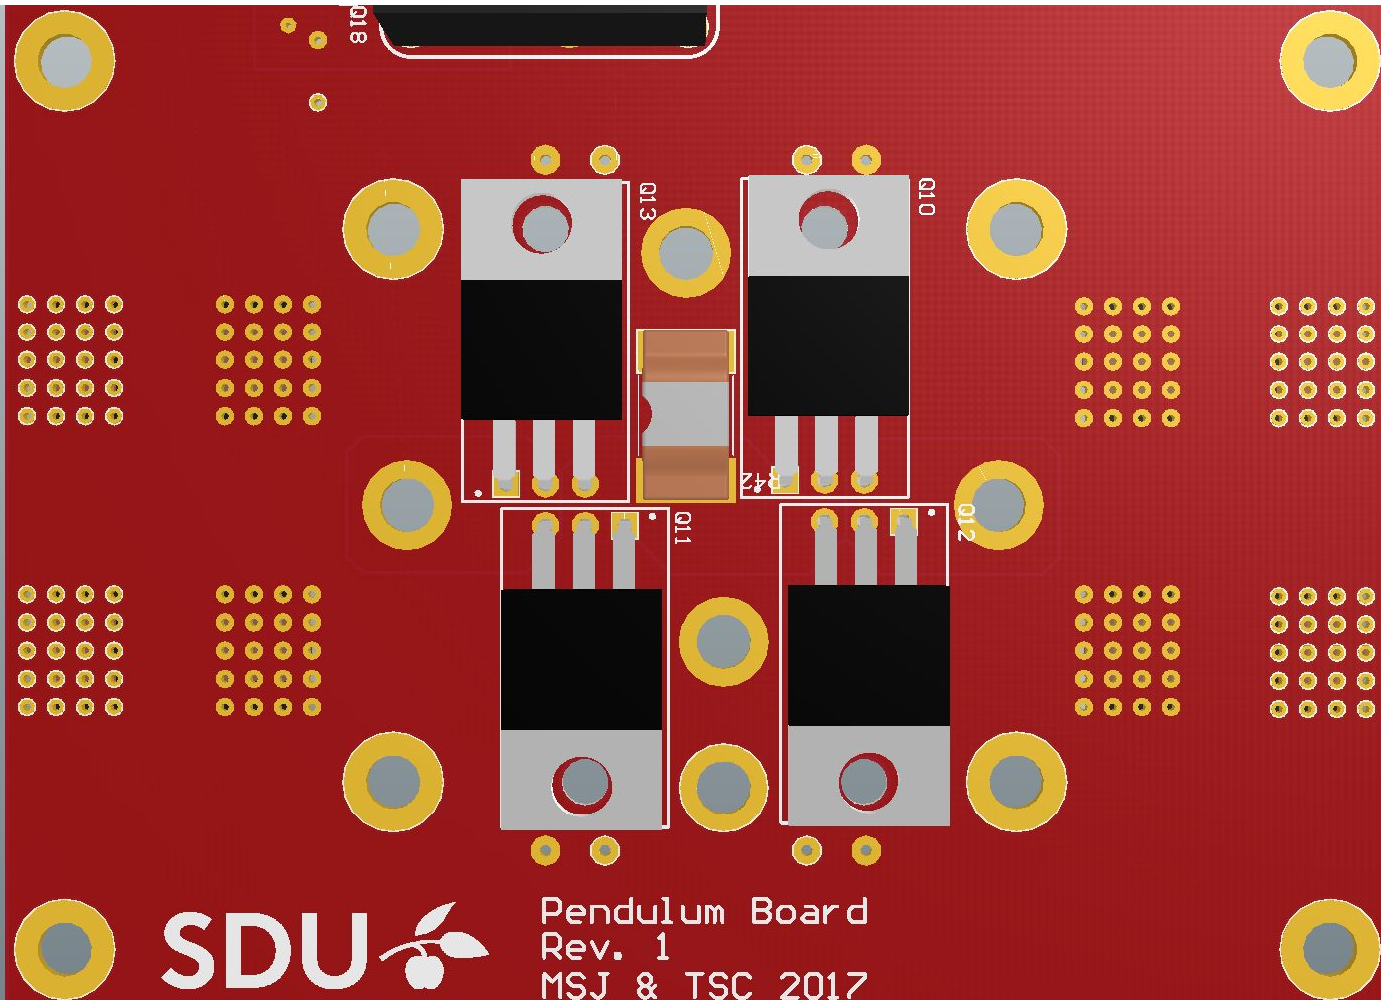
\includegraphics[angle=90,width=\linewidth]{graphics/power_layout_3}
		\caption{3D layout of the power part on the top layer}
		\label{sfig:power_layout_3}
	\end{subfigure}
	\begin{subfigure}[b]{0.49\textwidth} 
		\centering
		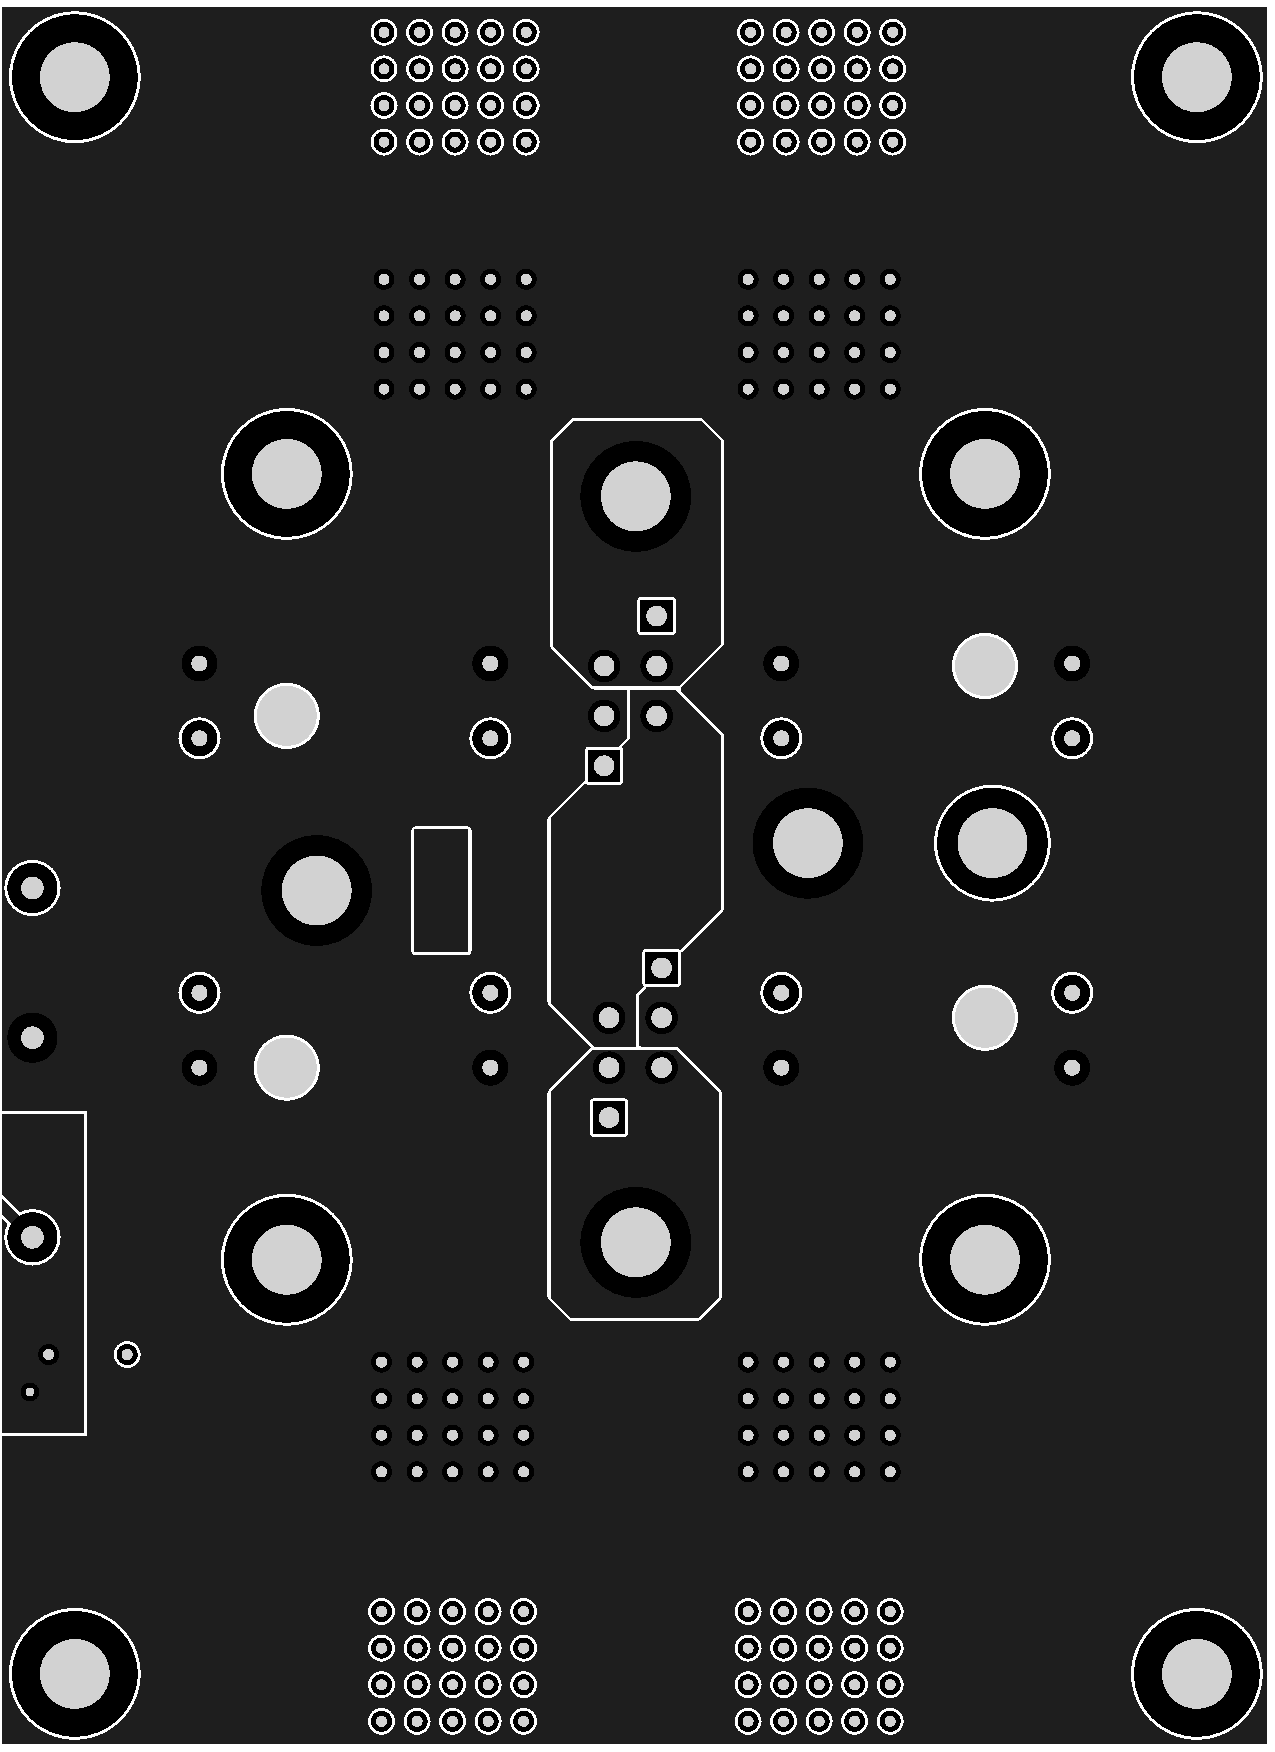
\includegraphics[width=\linewidth]{graphics/power_layout}
		\caption{Copper layout of the power part on the top layer.}
		\label{sfig:power_layout_2}
	\end{subfigure}
	\caption{caption?}
	\label{fig:power_layout}
\end{figure}
\thomas{do caption in figure \ref{fig:power_layout}}

As mentioned previously it was chosen to use a 4-layer board.
This was done for two reasons: It gives more copper for the main power rails on the power side of the board and it allows more space for routing signals on the digital part of the board.
While the component density is not very high, the number of signals routed to headers does impose some difficulties routing on just two layers.
On the digital side, a pour is made on each layer to fill the unused part of the layer with copper.
Going from top to bottom the layers are as such: ground, ground, 5V, ground.
The internal ground layer is uninterrupted, except for vias, to provide a solid ground layer.
The 5V layer means that any components requiring 5V need only a via to access it, making routing simpler.
This layer is also used for routing when routing through the top and bottom layers is infeasible.

% paragraph copper_layout (end)
% paragraph component_case_selection_and_placement (end)
% section board_design (end) 



%!TEX root = ../main.tex
\subsection{Implementation} % (fold)
\label{sub:controller_implementation}

\thomas{Insert section on hardware fixes on controller and joint board}
\subsubsection{Prototyping}
\label{sub:controller_board_prototyping}
In order to test important parts of the controller board a home-made prototype PCB was made at the University's PCB lab.

Three main functionalities should be verified on the board:

\begin{itemize}
	\item Schmitt-trigger circuitry and \texttt{AND} gate circuit
	\item PWM logic level shifting
	\item Motor driver circuit
\end{itemize}

The remaining functionalities have either been tested previously or were too trivial to test. 

\paragraph{Schmitt-trigger Circuitry and \texttt{AND} Gate Circuit}~\\
The Schmitt-triggers were tested by varying the input voltage and verifying the switching threshold along with the the hysteresis levels. 
Testing the \texttt{AND} gate was done by applying different logic levels and verifying the results.
The complete circuit was found to work as intended and can be seen in appendix \ref{app:controller_board_schem}, at component \texttt{U7} and \texttt{Q14}.

\paragraph{PWM Logic-Level-Shifting}~\\
The functionality of the logic-level-shifter \texttt{74LVC2G17} was verified by measuring input and output on an oscilloscope. 

\paragraph{Motor Driver Circuit}~\\
By measuring the outputs of the inverter \texttt{SN74LVC2G04} it was concluded that there was a design error in the way the component was used and the output signals were invalid.
A thorough investigation of the schematic revealed that the component could be omitted, without changing the functionality of the board.
The motor driver circuit on the PCB could not be tested because of this design error.
Therefore it was decided to develop another prototype PCB with the sole purpose of testing the motor driver circuit.
The circuit can be seen in \ref{fig:m_drive_circuit_schem}
\begin{figure}
	\centering
	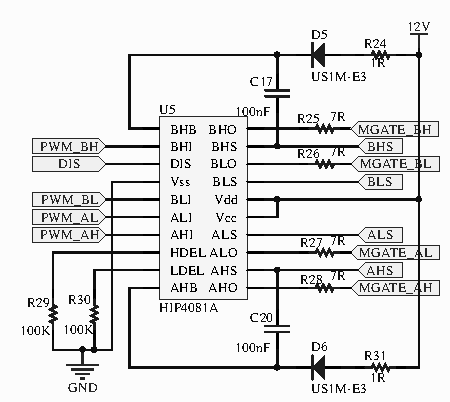
\includegraphics[width=0.6\linewidth]{graphics/hip_testboard_prototype}
	\caption[Prototype PCB with motor driver schematics]{Schematics of the PCB PCB developed to test the functionality of the motor drive circuitry.}
	\label{fig:m_drive_circuit_schem}
\end{figure}

A picture of the developed PCB is shown in figure \ref{fig:m_drive_circuit}.

\begin{figure}
	\centering
	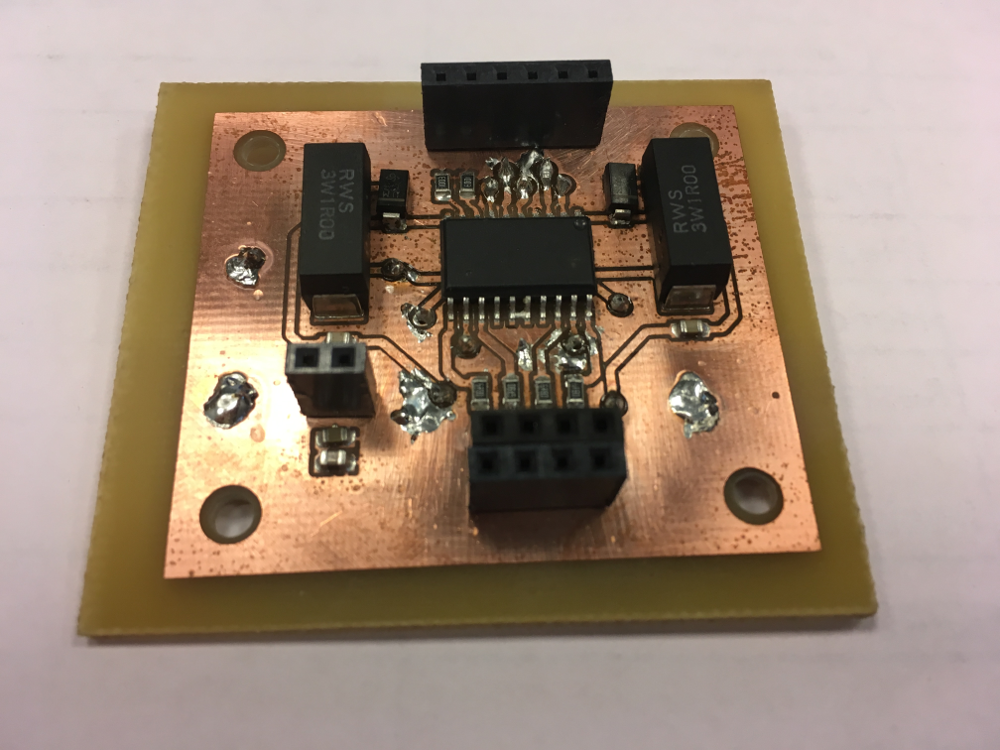
\includegraphics[width=0.5\linewidth]{graphics/hipboard_pic}
	\caption[Prototype PCB with motor driver.]{Picture of PCB developed to test the functionality of the motor drive circuitry.}
	\label{fig:m_drive_circuit}
\end{figure}
The board's gate signals were wired to the gates of four MOSFETs.
A power resistor was used as a load and PWM signals were applied to the motor driver input pins. 
Measuring the gate signals showed strange behaviour and after a thorough inspection of the board and the schematic it was found that the bootstrap diodes were facing in the wrong direction. 
The source of this was an error in the footprint of the component. 
After correcting the issue the driver and the bootstrap circuit was found to function as intended. 
The measured signals are shown in figure \ref{fig:test_hip_signals}.

\begin{figure}[h]
	\centering
    %% This file was created by matlab2tikz.
%
%The latest updates can be retrieved from
%  http://www.mathworks.com/matlabcentral/fileexchange/22022-matlab2tikz-matlab2tikz
%where you can also make suggestions and rate matlab2tikz.
%
\definecolor{mycolor1}{rgb}{0.00000,0.44700,0.74100}%
\definecolor{mycolor2}{rgb}{0.85000,0.32500,0.09800}%
\definecolor{mycolor3}{rgb}{0.92900,0.69400,0.12500}%
%
\begin{tikzpicture}

\begin{axis}[%
width=4.521in,
height=3.566in,
at={(0.758in,0.481in)},
scale only axis,
xmin=0.0011,
xmax=0.0028,
xlabel style={font=\color{white!15!black}},
xlabel={Time [S]},
ymin=-2,
ymax=35,
ylabel style={font=\color{white!15!black}},
ylabel={Voltage [V]},
axis background/.style={fill=white},
title style={font=\bfseries},
title={Motor Driver Signals},
legend style={legend cell align=left, align=left, draw=white!15!black}
]
\addplot [color=mycolor1, forget plot]
  table[row sep=crcr]{%
0.00109999985000009	3.33333\\
0.00110005985000017	3.36667\\
0.00110009984999992	3.33333\\
0.00110019985000021	3.36667\\
0.00110023984999996	3.33333\\
0.00110029985000004	3.36667\\
0.00110035985000012	3.33333\\
0.00110043985000008	3.36667\\
0.00110049985000016	3.33333\\
0.00110055984999979	3.36667\\
0.00110061984999987	3.33333\\
0.00110065985000007	3.36667\\
0.00110073985000003	3.33333\\
0.00110081984999999	3.36667\\
0.00110085985000019	3.33333\\
0.00110091984999983	3.36667\\
0.00110097984999991	3.33333\\
0.00110107985000019	3.36667\\
0.00110111984999994	3.33333\\
0.00110117985000002	3.36667\\
0.00110121984999978	3.33333\\
0.00110129985000018	3.36667\\
0.00110135984999982	3.33333\\
0.00110143985000022	3.36667\\
0.00110147984999998	3.33333\\
0.00110153985000006	3.36667\\
0.00110159985000013	3.33333\\
0.00110167985000009	3.36667\\
0.00110175985000005	3.33333\\
0.00110179984999981	3.36667\\
0.00110183985000001	3.33333\\
0.00110191984999997	3.36667\\
0.00110197985000005	3.33333\\
0.00110205985	3.36667\\
0.0011020998500002	3.33333\\
0.00110215984999984	3.36667\\
0.00110219985000004	3.3\\
0.00110229984999988	3.36667\\
0.00110235984999996	3.33333\\
0.00110243984999991	3.36667\\
0.00110247985000012	3.33333\\
0.00110253985000019	3.36667\\
0.00110261985000015	3.33333\\
0.00110267984999979	3.36667\\
0.00110271984999999	3.33333\\
0.00110277985000007	3.36667\\
0.00110285985000003	3.33333\\
0.00110291985000011	3.36667\\
0.00110299985000006	3.33333\\
0.00110305985000014	3.36667\\
0.00110307985000002	3.33333\\
0.00110315984999998	3.36667\\
0.00110321985000006	3.33333\\
0.0011033198499999	3.36667\\
0.0011033598500001	3.33333\\
0.00110339984999985	3.36667\\
0.00110345984999993	3.33333\\
0.00110353984999989	3.36667\\
0.00110361984999985	3.33333\\
0.00110365985000005	3.36667\\
0.00110371985000013	3.33333\\
0.00110377985000021	3.36667\\
0.00110385985000017	3.33333\\
0.00110393985000012	3.36667\\
0.00110395985	3.3\\
0.00110401985000008	3.36667\\
0.00110407985000016	3.33333\\
0.00110417985	3.36667\\
0.0011042198500002	3.33333\\
0.00110429985000016	3.36667\\
0.00110433984999991	3.33333\\
0.00110439984999999	3.36667\\
0.00110443985000019	3.33333\\
0.00110445985000007	3.36667\\
0.00110447984999995	3.33333\\
0.00110453985000003	3.36667\\
0.00110457984999979	3.3\\
0.00110463984999987	3.36667\\
0.00110469984999995	3.33333\\
0.00110479984999978	3.36667\\
0.00110485984999986	3.33333\\
0.00110491984999994	3.36667\\
0.00110495985000014	3.33333\\
0.00110501985000022	3.36667\\
0.0011050398500001	3.33333\\
0.00110505984999998	3.36667\\
0.00110507984999986	3.3\\
0.00110515984999981	3.36667\\
0.00110519985000002	3.33333\\
0.00110527984999997	3.36667\\
0.00110533985000005	3.33333\\
0.00110541985000001	3.36667\\
0.00110545985000021	3.33333\\
0.00110551984999985	3.4\\
0.00110555985000005	3.33333\\
0.00110567985000021	3.36667\\
0.00110571984999996	3.33333\\
0.00110577985000004	3.36667\\
0.0011058198499998	3.3\\
0.00110587984999988	3.36667\\
0.00110593984999996	3.33333\\
0.0011060398499998	3.36667\\
0.00110607985	3.3\\
0.00110613985000008	3.4\\
0.00110619985000016	3.33333\\
0.00110625984999979	3.36667\\
0.00110633985000019	3.33333\\
0.00110639984999983	3.36667\\
0.00110645984999991	3.33333\\
0.00110651984999999	3.36667\\
0.00110657985000007	3.33333\\
0.00110665985000002	3.36667\\
0.0011067198500001	3.33333\\
0.00110677985000018	3.36667\\
0.00110679985000006	3.33333\\
0.0011068998499999	3.36667\\
0.0011069398500001	3.3\\
0.00110701985000006	3.36667\\
0.00110705984999981	3.3\\
0.00110713985000022	3.36667\\
0.00110719984999985	3.33333\\
0.00110727984999981	3.36667\\
0.00110733984999989	3.33333\\
0.00110739984999997	3.36667\\
0.00110741984999985	3.33333\\
0.0011074998499998	3.36667\\
0.00110751985000013	3.33333\\
0.00110753985000001	3.36667\\
0.00110755984999988	3.3\\
0.00110763984999984	3.36667\\
0.00110769984999992	3.3\\
0.00110775985	3.36667\\
0.00110783984999996	3.33333\\
0.00110789985000004	3.36667\\
0.00110795985000012	3.33333\\
0.00110799984999987	3.4\\
0.00110805984999995	3.33333\\
0.00110813984999991	3.36667\\
0.00110817985000011	3.3\\
0.00110827984999995	3.36667\\
0.00110829984999983	3.3\\
0.00110835984999991	3.36667\\
0.00110843984999986	3.33333\\
0.00110851984999982	3.36667\\
0.00110859984999978	3.33333\\
0.0011086198500001	3.4\\
0.00110867985000018	3.33333\\
0.00110875985000014	3.36667\\
0.0011087998499999	3.3\\
0.00110889985000018	3.36667\\
0.00110893984999993	3.3\\
0.00110899985000001	3.36667\\
0.00110907984999997	3.33333\\
0.00110915984999993	3.36667\\
0.00110919985000013	3.33333\\
0.00110927985000009	3.36667\\
0.00110929984999997	3.33333\\
0.00110935985000005	3.36667\\
0.00110941985000013	3.3\\
0.00110951984999996	3.36667\\
0.00110955985000016	3.3\\
0.0011096198499998	3.36667\\
0.00110967984999988	3.33333\\
0.00110975984999984	3.36667\\
0.00110981984999992	3.33333\\
0.00110985985000012	3.4\\
0.0011099198500002	3.3\\
0.00110999985000015	3.36667\\
0.00111005984999979	3.33333\\
0.00111013985000019	3.36667\\
0.00111017984999995	3.3\\
0.00111023985000003	3.36667\\
0.00111029985000011	3.33333\\
0.00111037985000007	3.36667\\
0.00111045985000002	3.33333\\
0.0011105198500001	3.36667\\
0.00111055984999986	3.33333\\
0.00111059985000006	3.36667\\
0.00111065985000014	3.3\\
0.00111075984999998	3.36667\\
0.00111077984999985	3.3\\
0.00111085984999981	3.36667\\
0.00111093985000021	3.33333\\
0.00111099984999985	3.36667\\
0.00111107984999981	3.33333\\
0.00111113984999989	3.36667\\
0.00111117985000009	3.33333\\
0.00111121984999984	3.36667\\
0.00111127984999992	3.3\\
0.00111135984999988	3.36667\\
0.00111141984999996	3.3\\
0.00111145985000016	3.36667\\
0.00111153985000012	3.33333\\
0.00111161985000008	3.36667\\
0.00111169985000004	3.33333\\
0.00111173984999979	3.4\\
0.00111179984999987	3.33333\\
0.00111187984999983	3.36667\\
0.00111189985000015	3.3\\
0.00111199984999999	3.36667\\
0.00111201984999987	3.3\\
0.00111209984999983	3.36667\\
0.00111213985000003	3.3\\
0.00111225985000019	3.36667\\
0.00111231984999982	3.33333\\
0.00111233985000014	3.4\\
0.00111239984999978	3.33333\\
0.00111249985000006	3.36667\\
0.00111255985000014	3.33333\\
0.00111261985000022	3.36667\\
0.00111265984999998	3.3\\
0.00111271985000005	3.36667\\
0.00111277985000013	3.33333\\
0.00111287984999997	3.36667\\
0.00111291985000017	3.33333\\
0.00111299985000013	3.36667\\
0.00111303984999989	3.33333\\
0.00111307985000009	3.36667\\
0.00111315985000005	3.3\\
0.00111323985	3.36667\\
0.0011132798500002	3.3\\
0.00111333984999984	3.36667\\
0.00111337985000004	3.3\\
0.0011134998500002	3.36667\\
0.00111353984999996	3.33333\\
0.00111361984999991	3.36667\\
0.00111365985000011	3.33333\\
0.00111369984999987	3.36667\\
0.00111375984999995	3.3\\
0.00111385984999979	3.36667\\
0.00111389984999999	3.3\\
0.00111395985000007	3.36667\\
0.00111401985000015	3.3\\
0.00111411984999998	3.36667\\
0.00111417985000006	3.33333\\
0.00111423985000014	3.36667\\
0.0011142798499999	3.33333\\
0.00111433984999998	3.36667\\
0.00111437985000018	3.3\\
0.00111447985000002	3.36667\\
0.00111451985000022	3.3\\
0.00111459985000018	3.36667\\
0.00111465984999981	3.33333\\
0.00111473985000021	3.36667\\
0.00111477984999997	3.33333\\
0.00111485984999993	3.36667\\
0.00111489985000013	3.33333\\
0.00111497985000009	3.36667\\
0.00111503985000017	3.33333\\
0.0011150998499998	3.36667\\
0.00111513985	3.3\\
0.00111521984999996	3.36667\\
0.00111527985000004	3.33333\\
0.00111535985	3.36667\\
0.00111541985000008	3.33333\\
0.00111547985000016	3.36667\\
0.00111551984999991	3.33333\\
0.00111559984999987	3.36667\\
0.00111565984999995	3.33333\\
0.00111571985000003	3.36667\\
0.00111573984999991	3.3\\
0.00111583985000019	3.36667\\
0.00111589984999982	3.33333\\
0.00111597984999978	3.36667\\
0.00111603984999986	3.33333\\
0.00111609984999994	3.36667\\
0.00111615985000002	3.33333\\
0.00111619985000022	3.36667\\
0.00111627985000018	3.33333\\
0.00111633984999981	3.36667\\
0.00111637985000002	3.3\\
0.00111643985000009	3.36667\\
0.00111651985000005	3.33333\\
0.00111661984999989	3.36667\\
0.00111663985000021	3.33333\\
0.00111671985000017	3.36667\\
0.00111675984999993	3.33333\\
0.00111681985000001	3.36667\\
0.00111689984999996	3.33333\\
0.00111695985000004	3.36667\\
0.00111701985000012	3.33333\\
0.0011170798500002	3.36667\\
0.00111713984999984	3.33333\\
0.0011172198499998	3.36667\\
0.00111727984999987	3.33333\\
0.00111733984999995	3.36667\\
0.00111737985000016	3.33333\\
0.00111741984999991	3.36667\\
0.00111743984999979	3.33333\\
0.00111745985000011	3.36667\\
0.00111753985000007	3.33333\\
0.00111757984999983	3.36667\\
0.00111763984999991	3.33333\\
0.00111769984999999	3.36667\\
0.00111775985000007	3.33333\\
0.00111783985000002	3.36667\\
0.0011178998500001	3.33333\\
0.00111795985000018	3.36667\\
0.00111801984999982	3.33333\\
0.0011180798499999	3.36667\\
0.00111815984999986	3.33333\\
0.00111819985000006	3.36667\\
0.00111825985000014	3.33333\\
0.00111829984999989	3.36667\\
0.00111837984999985	3.33333\\
0.00111847985000013	3.36667\\
0.00111849985000001	3.33333\\
0.00111857984999997	3.36667\\
0.00111863985000005	3.33333\\
0.00111869985000013	3.36667\\
0.00111875985000021	3.33333\\
0.00111883985000016	3.36667\\
0.00111887984999992	3.33333\\
0.00111895984999988	3.36667\\
0.00111899985000008	3.33333\\
0.00111907985000004	3.36667\\
0.00111913985000012	3.33333\\
0.0011191998500002	3.36667\\
0.00111923984999995	3.33333\\
0.00111933984999979	3.36667\\
0.00111939984999987	3.33333\\
0.00111943985000007	3.36667\\
0.00111949985000015	3.33333\\
0.00111955984999978	3.36667\\
0.00111961984999986	3.33333\\
0.00111969984999982	3.36667\\
0.00111971985000014	3.33333\\
0.0011197998500001	3.4\\
0.00111987985000006	3.33333\\
0.00111995985000002	3.36667\\
0.00112003984999998	3.33333\\
0.00112005984999985	3.36667\\
0.00112011984999993	3.33333\\
0.00112021985000021	3.36667\\
0.00112023985000009	3.33333\\
0.00112033984999993	3.36667\\
0.00112035984999981	3.33333\\
0.00112043985000021	3.36667\\
0.00112049984999985	3.33333\\
0.0011205798499998	3.36667\\
0.00112063984999988	3.33333\\
0.00112067985000008	3.36667\\
0.00112075985000004	3.33333\\
0.00112081985000012	3.36667\\
0.00112085984999988	3.33333\\
0.00112095985000016	3.36667\\
0.00112099984999992	3.33333\\
0.00112107984999987	3.36667\\
0.00112111985000007	3.33333\\
0.00112119985000003	3.36667\\
0.00112123984999979	3.33333\\
0.00112129984999987	3.36667\\
0.00112135984999995	3.33333\\
0.00112143984999991	3.36667\\
0.00112147985000011	3.33333\\
0.00112155985000006	3.36667\\
0.00112161985000014	3.3\\
0.00112167984999978	3.36667\\
0.00112173984999986	3.33333\\
0.00112181984999982	3.36667\\
0.0011218798499999	3.33333\\
0.00112193984999998	3.36667\\
0.00112197985000018	3.33333\\
0.00112203984999981	3.36667\\
0.00112211985000021	3.33333\\
0.00112219985000017	3.36667\\
0.00112223984999993	3.33333\\
0.00112229985000001	3.36667\\
0.00112235985000009	3.33333\\
0.00112243985000005	3.36667\\
0.00112249985000012	3.33333\\
0.0011225598500002	3.36667\\
0.00112259984999996	3.33333\\
0.00112267984999992	3.36667\\
0.00112275984999988	3.33333\\
0.00112281984999996	3.36667\\
0.00112285985000016	3.33333\\
0.00112291984999979	3.36667\\
0.00112297984999987	3.33333\\
0.00112307985000015	3.36667\\
0.00112311984999991	3.33333\\
0.00112317984999999	3.36667\\
0.00112321985000019	3.33333\\
0.00112329985000015	3.36667\\
0.00112331985000003	3.33333\\
0.00112343985000019	3.36667\\
0.00112347984999994	3.33333\\
0.00112353985000002	3.36667\\
0.00112361984999998	3.33333\\
0.00112367985000006	3.36667\\
0.00112373985000014	3.33333\\
0.0011238198500001	3.36667\\
0.00112385984999985	3.33333\\
0.00112389985000005	3.36667\\
0.00112399984999989	3.33333\\
0.00112405984999997	3.36667\\
0.00112411985000005	3.33333\\
0.00112415984999981	3.36667\\
0.00112421984999989	3.33333\\
0.00112429984999984	3.36667\\
0.00112435984999992	3.33333\\
0.00112443984999988	3.36667\\
0.00112447985000008	3.33333\\
0.00112453985000016	3.36667\\
0.00112455985000004	3.33333\\
0.00112457984999992	3.36667\\
0.00112461985000012	3.33333\\
0.0011246798500002	3.36667\\
0.00112473984999983	3.33333\\
0.00112479984999991	3.36667\\
0.00112483985000011	3.33333\\
0.00112491985000007	3.36667\\
0.00112495984999983	3.3\\
0.00112503984999979	3.36667\\
0.00112511985000019	3.33333\\
0.00112515984999995	3.36667\\
0.00112521985000003	3.33333\\
0.00112529984999998	3.36667\\
0.00112533985000018	3.3\\
0.00112539984999982	3.36667\\
0.0011254598499999	3.33333\\
0.00112553984999986	3.36667\\
0.00112559984999994	3.33333\\
0.00112567984999989	3.36667\\
0.0011257198500001	3.33333\\
0.00112577985000017	3.36667\\
0.00112585985000013	3.33333\\
0.00112591985000021	3.36667\\
0.00112595984999997	3.3\\
0.00112603984999993	3.36667\\
0.00112607985000013	3.3\\
0.00112615985000009	3.36667\\
0.00112623985000004	3.33333\\
0.00112629985000012	3.36667\\
0.00112633984999988	3.33333\\
0.00112639984999996	3.36667\\
0.00112647984999992	3.33333\\
0.00112653985	3.36667\\
0.0011265798500002	3.3\\
0.00112663984999983	3.36667\\
0.00112669984999991	3.3\\
0.00112677984999987	3.4\\
0.00112685984999983	3.33333\\
0.00112691984999991	3.36667\\
0.00112693984999979	3.33333\\
0.00112701985000019	3.36667\\
0.00112707984999982	3.33333\\
0.0011271798500001	3.36667\\
0.00112719984999998	3.3\\
0.00112725985000006	3.36667\\
0.00112731985000014	3.33333\\
0.0011273998500001	3.36667\\
0.00112741984999998	3.33333\\
0.00112743984999986	3.36667\\
0.00112747985000006	3.33333\\
0.00112753985000014	3.36667\\
0.00112755985000002	3.33333\\
0.00112765984999985	3.36667\\
0.00112771984999993	3.33333\\
0.00112779984999989	3.36667\\
0.00112781985000021	3.3\\
0.00112789985000017	3.36667\\
0.0011279598499998	3.33333\\
0.00112801984999988	3.36667\\
0.00112809984999984	3.33333\\
0.00112813985000004	3.4\\
0.00112819985000012	3.33333\\
0.00112827985000008	3.36667\\
0.00112833985000016	3.33333\\
0.00112839984999979	3.36667\\
0.00112843985	3.3\\
0.00112849985000008	3.36667\\
0.00112857985000003	3.33333\\
0.00112865984999999	3.36667\\
0.00112869985000019	3.33333\\
0.00112877985000015	3.36667\\
0.00112879985000003	3.33333\\
0.00112889984999986	3.36667\\
0.00112895984999994	3.33333\\
0.0011290398499999	3.36667\\
0.00112905984999978	3.3\\
0.00112911984999986	3.36667\\
0.00112917984999994	3.33333\\
0.00112927985000022	3.36667\\
0.00112933984999986	3.3\\
0.00112939984999993	3.36667\\
0.00112943985000014	3.33333\\
0.00112951985000009	3.36667\\
0.00112957985000017	3.33333\\
0.00112965985000013	3.36667\\
0.00112967985000001	3.3\\
0.00112973985000009	3.36667\\
0.00112981985000005	3.33333\\
0.00112989985	3.36667\\
0.00112995985000008	3.33333\\
0.00112999984999984	3.4\\
0.00113003985000004	3.33333\\
0.00113013984999988	3.36667\\
0.00113019984999996	3.33333\\
0.00113025985000004	3.36667\\
0.00113031985000012	3.33333\\
0.0011303798500002	3.36667\\
0.00113043984999983	3.33333\\
0.00113051984999979	3.36667\\
0.00113055984999999	3.33333\\
0.00113061985000007	3.4\\
0.00113065984999983	3.33333\\
0.00113073984999978	3.36667\\
0.00113075985000011	3.33333\\
0.00113077984999999	3.36667\\
0.00113079984999986	3.3\\
0.00113089985000014	3.36667\\
0.00113091985000002	3.3\\
0.00113099984999998	3.36667\\
0.00113105985000006	3.33333\\
0.00113113985000002	3.36667\\
0.0011311998500001	3.33333\\
0.00113125985000018	3.36667\\
0.00113129984999993	3.33333\\
0.00113135985000001	3.36667\\
0.00113141985000009	3.3\\
0.00113149985000005	3.36667\\
0.00113153984999981	3.3\\
0.00113163985000009	3.36667\\
0.00113167984999984	3.33333\\
0.0011317598499998	3.36667\\
0.00113179985	3.33333\\
0.00113181984999988	3.36667\\
0.0011318398500002	3.33333\\
0.00113187984999996	3.36667\\
0.00113191985000016	3.33333\\
0.00113201985	3.36667\\
0.0011320598500002	3.33333\\
0.00113213985000016	3.36667\\
0.00113217984999991	3.3\\
0.00113223984999999	3.36667\\
0.00113229985000007	3.33333\\
0.00113239984999991	3.36667\\
0.00113245984999999	3.33333\\
0.00113249985000019	3.36667\\
0.00113253984999995	3.33333\\
0.00113261984999991	3.36667\\
0.00113265985000011	3.3\\
0.00113275984999994	3.36667\\
0.00113279985000014	3.3\\
0.00113285984999978	3.36667\\
0.00113293985000018	3.33333\\
0.00113301985000014	3.36667\\
0.0011330598499999	3.33333\\
0.00113313984999985	3.36667\\
0.00113315985000018	3.33333\\
0.00113323985000013	3.36667\\
0.00113327984999989	3.3\\
0.00113337985000017	3.36667\\
0.00113339985000005	3.3\\
0.00113347985000001	3.36667\\
0.00113351985000021	3.3\\
0.00113363984999992	3.36667\\
0.00113367985000012	3.33333\\
0.00113375985000008	3.36667\\
0.00113379984999984	3.33333\\
0.00113385984999992	3.36667\\
0.00113389985000012	3.3\\
0.00113399984999996	3.36667\\
0.00113401984999983	3.3\\
0.00113409984999979	3.36667\\
0.00113415984999987	3.33333\\
0.00113425985000015	3.36667\\
0.00113427985000003	3.33333\\
0.00113429984999991	3.36667\\
0.00113431984999979	3.33333\\
0.00113433985000011	3.4\\
0.00113439985000019	3.33333\\
0.00113449985000003	3.36667\\
0.0011345198499999	3.3\\
0.00113461985000018	3.36667\\
0.00113465984999994	3.3\\
0.00113471985000002	3.36667\\
0.0011347798500001	3.33333\\
0.00113487984999994	3.36667\\
0.00113493985000002	3.33333\\
0.00113497985000022	3.36667\\
0.00113501984999997	3.33333\\
0.00113511984999981	3.36667\\
0.00113513985000013	3.3\\
0.00113523984999997	3.36667\\
0.00113529985000005	3.33333\\
0.00113533984999981	3.36667\\
0.00113539984999989	3.33333\\
0.00113549985000017	3.36667\\
0.0011355598499998	3.33333\\
0.00113561984999988	3.36667\\
0.0011356398500002	3.33333\\
0.00113571985000016	3.36667\\
0.00113575984999992	3.3\\
0.0011358598500002	3.36667\\
0.00113589984999996	3.3\\
0.00113595985000003	3.36667\\
0.00113603984999999	3.33333\\
0.00113611984999995	3.36667\\
0.00113617985000003	3.33333\\
0.00113621984999979	3.4\\
0.00113629985000019	3.33333\\
0.00113633984999995	3.36667\\
0.0011364198499999	3.33333\\
0.00113647984999998	3.36667\\
0.00113651985000018	3.3\\
0.00113657984999982	3.36667\\
0.00113659985000014	3.33333\\
0.00113673985000018	3.36667\\
0.00113679984999981	3.33333\\
0.00113683985000002	3.4\\
0.00113689985000009	3.33333\\
0.00113697985000005	3.36667\\
0.00113699984999993	3.3\\
0.00113709985000021	3.36667\\
0.00113711985000009	3.3\\
0.00113719985000005	3.36667\\
0.00113725985000013	3.3\\
0.00113735984999996	3.36667\\
0.00113741985000004	3.33333\\
0.0011374598499998	3.4\\
0.00113751984999988	3.33333\\
0.00113757984999996	3.36667\\
0.0011376798499998	3.33333\\
0.00113771985	3.36667\\
0.00113779984999995	3.33333\\
0.00113781984999983	3.36667\\
0.00113789984999979	3.33333\\
0.00113797985000019	3.36667\\
0.00113803984999983	3.33333\\
0.00113807985000003	3.4\\
0.00113815984999999	3.33333\\
0.00113821985000007	3.36667\\
0.00113827985000015	3.33333\\
0.00113833984999978	3.36667\\
0.00113841985000018	3.33333\\
0.00113843985000006	3.36667\\
0.00113851985000002	3.33333\\
0.00113859984999998	3.36667\\
0.00113865985000006	3.33333\\
0.00113871985000014	3.36667\\
0.00113875984999989	3.33333\\
0.00113881984999997	3.36667\\
0.00113889984999993	3.33333\\
0.00113895985000001	3.36667\\
0.00113901985000009	3.33333\\
0.00113905984999985	3.36667\\
0.00113907985000017	3.33333\\
0.00113909985000005	3.36667\\
0.0011391398499998	3.33333\\
0.00113921985000021	3.36667\\
0.00113927984999984	3.33333\\
0.00113931985000004	3.36667\\
0.00113937985000012	3.33333\\
0.0011394398500002	3.36667\\
0.00113953985000004	3.33333\\
0.00113957984999979	3.36667\\
0.0011396598500002	3.33333\\
0.00113969984999995	3.36667\\
0.00113973985000015	3.33333\\
0.00113983984999999	3.36667\\
0.00113989985000007	3.33333\\
0.00113995985000015	3.36667\\
0.00114001984999978	3.33333\\
0.00114007984999986	3.36667\\
0.00114015984999982	3.33333\\
0.00114019985000002	3.36667\\
0.0011402598500001	3.33333\\
0.00114031985000018	3.36667\\
0.00114039985000014	3.33333\\
0.00114045985000022	3.36667\\
0.00114051984999985	3.33333\\
0.00114057984999993	3.36667\\
0.00114063985000001	3.33333\\
0.00114067985000021	3.36667\\
0.00114069985000009	3.33333\\
0.00114073984999985	3.36667\\
0.00114077985000005	3.33333\\
0.00114081984999981	3.36667\\
0.00114089985000021	3.33333\\
0.00114093984999997	3.36667\\
0.00114097985000017	3.33333\\
0.00114107985	3.36667\\
0.00114113985000008	3.33333\\
0.00114119985000016	3.36667\\
0.0011412598499998	3.33333\\
0.0011413398500002	3.36667\\
0.00114137984999996	3.33333\\
0.00114143985000004	3.36667\\
0.00114151984999999	3.33333\\
0.0011415598500002	3.36667\\
0.00114161984999983	3.33333\\
0.00114171985000011	3.36667\\
0.00114173984999999	3.33333\\
0.00114181984999995	3.36667\\
0.00114187985000003	3.33333\\
0.00114195984999999	3.36667\\
0.00114201985000006	3.33333\\
0.00114205984999982	3.36667\\
0.00114213984999978	3.33333\\
0.00114219984999986	3.36667\\
0.00114223985000006	3.33333\\
0.0011423398499999	3.36667\\
0.00114235985000022	3.33333\\
0.00114243985000018	3.36667\\
0.00114249984999981	3.33333\\
0.00114255984999989	3.36667\\
0.00114261984999997	3.33333\\
0.00114267985000005	3.36667\\
0.00114273985000013	3.33333\\
0.00114281985000009	3.36667\\
0.00114285984999984	3.33333\\
0.00114295985000012	3.36667\\
0.00114299984999988	3.33333\\
0.00114305984999996	3.36667\\
0.00114309985000016	3.3\\
0.00114319985	3.36667\\
0.00114325985000008	3.33333\\
0.00114331985000016	3.36667\\
0.00114335984999991	3.33333\\
0.00114343984999987	3.36667\\
0.00114351984999983	3.33333\\
0.00114355985000003	3.36667\\
0.00114361985000011	3.33333\\
0.00114367985000019	3.36667\\
0.00114373984999983	3.33333\\
0.00114381984999978	3.36667\\
0.00114389985000019	3.33333\\
0.00114393984999994	3.36667\\
0.00114399985000002	3.33333\\
0.00114403984999978	3.36667\\
0.00114411985000018	3.33333\\
0.00114419985000014	3.36667\\
0.00114425985000022	3.33333\\
0.00114429984999997	3.36667\\
0.00114433985000018	3.3\\
0.00114443985000001	3.36667\\
0.00114449985000009	3.33333\\
0.00114455985000017	3.36667\\
0.00114461984999981	3.33333\\
0.00114467984999989	3.36667\\
0.00114473984999997	3.33333\\
0.00114481984999992	3.36667\\
0.00114485985000012	3.33333\\
0.0011449198500002	3.36667\\
0.00114497984999984	3.33333\\
0.00114507985000012	3.36667\\
0.00114511984999988	3.33333\\
0.00114519984999983	3.36667\\
0.00114521985000016	3.33333\\
0.00114531984999999	3.36667\\
0.00114535985000019	3.33333\\
0.00114543985000015	3.36667\\
0.00114549984999979	3.33333\\
0.00114553984999999	3.36667\\
0.00114561984999995	3.33333\\
0.00114563984999982	3.36667\\
0.00114565985000015	3.33333\\
0.00114567985000003	3.36667\\
0.0011457398500001	3.33333\\
0.00114579985000018	3.36667\\
0.00114585984999982	3.33333\\
0.0011459198499999	3.36667\\
0.00114593985000022	3.33333\\
0.00114605984999994	3.36667\\
0.00114609985000014	3.33333\\
0.0011461798500001	3.36667\\
0.00114623985000017	3.33333\\
0.00114631985000013	3.36667\\
0.00114635984999989	3.33333\\
0.00114643984999985	3.36667\\
0.00114647985000005	3.33333\\
0.00114653985000013	3.36667\\
0.00114657984999988	3.33333\\
0.00114667985000017	3.36667\\
0.00114671984999992	3.3\\
0.00114679984999988	3.36667\\
0.00114685984999996	3.33333\\
0.00114693984999992	3.36667\\
0.00114699985	3.33333\\
0.0011470398500002	3.4\\
0.00114709984999983	3.33333\\
0.00114715984999991	3.36667\\
0.00114723984999987	3.33333\\
0.00114731984999983	3.36667\\
0.00114735985000003	3.33333\\
0.00114739984999979	3.36667\\
0.00114747985000019	3.33333\\
0.00114755985000015	3.36667\\
0.0011475998499999	3.33333\\
0.00114765984999998	3.4\\
0.00114769985000018	3.33333\\
0.00114777985000014	3.36667\\
0.0011478598500001	3.33333\\
0.00114791985000018	3.36667\\
0.00114797984999981	3.3\\
0.00114801985000001	3.36667\\
0.00114807985000009	3.3\\
0.00114817984999993	3.36667\\
0.00114823985000001	3.33333\\
0.00114827985000021	3.36667\\
0.00114829985000009	3.33333\\
0.00114839984999993	3.36667\\
0.00114847984999988	3.33333\\
0.00114853984999996	3.36667\\
0.00114857985000016	3.3\\
0.0011486398499998	3.36667\\
0.0011487198500002	3.33333\\
0.00114877984999984	3.36667\\
0.00114879985000016	3.33333\\
0.00114881985000004	3.36667\\
0.00114883984999992	3.33333\\
0.00114889985	3.4\\
0.0011489398500002	3.33333\\
0.00114903985000003	3.36667\\
0.00114905984999991	3.3\\
0.00114915985000019	3.36667\\
0.00114919984999995	3.3\\
0.00114927984999991	3.36667\\
0.00114931985000011	3.33333\\
0.00114941984999994	3.36667\\
0.00114947985000002	3.33333\\
0.00114951984999978	3.4\\
0.00114957984999986	3.33333\\
0.00114963984999994	3.36667\\
0.0011497198499999	3.33333\\
0.00114979984999986	3.36667\\
0.00114981985000018	3.3\\
0.00114987984999981	3.36667\\
0.00114993984999989	3.33333\\
0.00115003985000017	3.36667\\
0.00115009984999981	3.33333\\
0.00115015984999989	3.36667\\
0.00115019985000009	3.33333\\
0.00115025985000017	3.36667\\
0.0011503198499998	3.3\\
0.00115039985000021	3.36667\\
0.00115045984999984	3.3\\
0.00115049985000004	3.36667\\
0.00115057985	3.33333\\
0.00115065984999996	3.36667\\
0.00115069985000016	3.33333\\
0.00115075984999979	3.4\\
0.00115081984999987	3.33333\\
0.00115089984999983	3.36667\\
0.00115093985000003	3.3\\
0.00115103984999987	3.36667\\
0.00115107985000007	3.3\\
0.00115113985000015	3.36667\\
0.00115119984999978	3.33333\\
0.00115127985000019	3.36667\\
0.00115133984999982	3.33333\\
0.0011513998499999	3.36667\\
0.0011514398500001	3.33333\\
0.00115149985000018	3.36667\\
0.00115155984999982	3.3\\
0.0011516598500001	3.36667\\
0.00115169984999985	3.3\\
0.00115173985000006	3.36667\\
0.00115181985000001	3.33333\\
0.00115189984999997	3.36667\\
0.00115197984999993	3.33333\\
0.00115201985000013	3.36667\\
0.00115205984999989	3.33333\\
0.00115213984999984	3.36667\\
0.00115217985000005	3.3\\
0.00115225985	3.36667\\
0.0011522998500002	3.3\\
0.00115237985000016	3.36667\\
0.00115245985000012	3.33333\\
0.0011525198500002	3.36667\\
0.00115257984999984	3.33333\\
0.00115263984999991	3.36667\\
0.00115267985000012	3.33333\\
0.0011527398500002	3.36667\\
0.00115279984999983	3.3\\
0.00115287984999979	3.36667\\
0.00115293984999987	3.3\\
0.00115299984999995	3.36667\\
0.00115303985000015	3.3\\
0.00115313984999998	3.36667\\
0.00115319985000006	3.33333\\
0.00115325985000014	3.36667\\
0.0011532998499999	3.33333\\
0.00115331984999978	3.36667\\
0.0011533398500001	3.33333\\
0.00115337984999986	3.36667\\
0.00115343984999994	3.3\\
0.0011535198499999	3.36667\\
0.00115353985000022	3.3\\
0.00115361985000018	3.36667\\
0.00115367984999981	3.33333\\
0.00115375985000021	3.36667\\
0.00115381984999985	3.33333\\
0.00115385985000005	3.4\\
0.00115403984999984	3.3\\
0.00115413985000012	3.36667\\
0.00115417984999988	3.3\\
0.00115423984999996	3.36667\\
0.00115429985000004	3.33333\\
0.00115437985	3.36667\\
0.00115445984999996	3.33333\\
0.00115447984999983	3.4\\
0.00115453984999991	3.33333\\
0.00115461984999987	3.36667\\
0.00115465985000007	3.3\\
0.00115475984999991	3.36667\\
0.00115477984999979	3.3\\
0.00115485985000019	3.36667\\
0.00115493985000015	3.33333\\
0.00115499984999978	3.36667\\
0.00115507985000018	3.33333\\
0.00115511984999994	3.4\\
0.00115515985000014	3.33333\\
0.0011552398500001	3.36667\\
0.00115527984999986	3.3\\
0.00115537985000014	3.36667\\
0.00115543985000022	3.33333\\
0.00115547984999997	3.36667\\
0.00115553985000005	3.33333\\
0.00115561985000001	3.36667\\
0.00115569984999997	3.33333\\
0.00115575985000005	3.36667\\
0.00115577984999993	3.33333\\
0.00115585984999989	3.36667\\
0.00115589985000009	3.3\\
0.00115599984999992	3.36667\\
0.00115603985000012	3.3\\
0.0011560998500002	3.36667\\
0.00115617985000016	3.33333\\
0.00115625985000012	3.36667\\
0.0011563198500002	3.33333\\
0.00115635984999996	3.36667\\
0.00115637984999983	3.33333\\
0.00115647985000011	3.36667\\
0.00115651984999987	3.3\\
0.00115661985000015	3.36667\\
0.00115663985000003	3.3\\
0.00115671984999999	3.36667\\
0.00115677985000007	3.33333\\
0.0011568798499999	3.36667\\
0.00115693984999998	3.33333\\
0.00115699985000006	3.36667\\
0.00115701984999994	3.3\\
0.0011570998499999	3.36667\\
0.0011571398500001	3.3\\
0.00115723984999994	3.36667\\
0.00115725984999981	3.3\\
0.00115733985000022	3.36667\\
0.00115739984999985	3.33333\\
0.00115749985000013	3.36667\\
0.00115755985000021	3.33333\\
0.00115761984999985	3.36667\\
0.00115765985000005	3.33333\\
0.00115773985000001	3.36667\\
0.00115779985000009	3.33333\\
0.00115785985000016	3.36667\\
0.00115789984999992	3.3\\
0.00115795985	3.36667\\
0.00115803984999996	3.33333\\
0.00115809985000004	3.36667\\
0.00115817985	3.33333\\
0.0011582198500002	3.36667\\
0.00115827984999983	3.33333\\
0.00115835984999979	3.36667\\
0.00115843985000019	3.33333\\
0.00115847984999995	3.36667\\
0.00115851985000015	3.3\\
0.00115857984999979	3.36667\\
0.00115865985000019	3.33333\\
0.00115873985000015	3.36667\\
0.00115879984999978	3.33333\\
0.00115885984999986	3.36667\\
0.00115889985000006	3.33333\\
0.00115895985000014	3.36667\\
0.00115905984999998	3.33333\\
0.00115909985000018	3.36667\\
0.00115913984999994	3.3\\
0.00115919985000001	3.36667\\
0.00115925985000009	3.3\\
0.00115937984999981	3.36667\\
0.00115941985000001	3.33333\\
0.00115947985000009	3.36667\\
0.00115953985000017	3.33333\\
0.0011595998499998	3.36667\\
0.00115965984999988	3.33333\\
0.00115971984999996	3.36667\\
0.00115975985000016	3.3\\
0.0011598198499998	3.36667\\
0.0011598998500002	3.33333\\
0.00115999985000004	3.36667\\
0.00116001984999992	3.33333\\
0.00116009984999987	3.36667\\
0.00116013985000007	3.33333\\
0.00116021985000003	3.36667\\
0.00116027985000011	3.33333\\
0.00116033985000019	3.36667\\
0.00116039984999983	3.33333\\
0.00116045984999991	3.36667\\
0.00116051984999999	3.33333\\
0.00116059984999994	3.36667\\
0.00116065985000002	3.33333\\
0.00116069984999978	3.4\\
0.00116077985000018	3.33333\\
0.00116081984999994	3.36667\\
0.0011608998499999	3.33333\\
0.00116095984999998	3.36667\\
0.00116101985000006	3.33333\\
0.00116107985000014	3.36667\\
0.00116113985000021	3.33333\\
0.00116121985000017	3.36667\\
0.00116127984999981	3.33333\\
0.00116133984999989	3.36667\\
0.00116137985000009	3.33333\\
0.0011614998499998	3.36667\\
0.00116153985	3.33333\\
0.00116157985000021	3.36667\\
0.00116163984999984	3.33333\\
0.00116169984999992	3.36667\\
0.00116175985	3.33333\\
0.00116183984999996	3.36667\\
0.00116189985000004	3.33333\\
0.00116195985000012	3.36667\\
0.0011620198500002	3.33333\\
0.00116207984999983	3.36667\\
0.00116213984999991	3.3\\
0.00116219984999999	3.36667\\
0.00116227984999995	3.33333\\
0.00116231985000015	3.36667\\
0.00116237984999978	3.33333\\
0.00116245985000019	3.36667\\
0.00116249984999994	3.33333\\
0.0011625798499999	3.36667\\
0.00116263984999998	3.33333\\
0.00116271984999994	3.36667\\
0.00116275985000014	3.33333\\
0.0011628398500001	3.36667\\
0.00116287984999985	3.33333\\
0.00116293984999993	3.36667\\
0.00116299985000001	3.33333\\
0.00116309984999985	3.36667\\
0.00116313985000005	3.33333\\
0.00116319985000013	3.36667\\
0.00116325985000021	3.33333\\
0.00116333985000017	3.36667\\
0.00116337984999992	3.33333\\
0.00116341985000012	3.36667\\
0.00116349985000008	3.33333\\
0.00116357985000004	3.36667\\
0.00116363985000012	3.33333\\
0.0011636998500002	3.36667\\
0.00116373984999996	3.33333\\
0.00116383984999979	3.36667\\
0.00116385985000012	3.33333\\
0.00116393985000007	3.36667\\
0.00116401985000003	3.33333\\
0.00116405984999979	3.36667\\
0.00116411984999987	3.33333\\
0.00116419984999983	3.36667\\
0.0011642598499999	3.33333\\
0.00116431984999998	3.36667\\
0.00116435985000019	3.33333\\
0.00116443985000014	3.36667\\
0.00116449984999978	3.33333\\
0.00116457985000018	3.36667\\
0.00116461984999994	3.33333\\
0.0011646998499999	3.36667\\
0.0011647398500001	3.33333\\
0.00116481985000005	3.36667\\
0.00116487985000013	3.33333\\
0.00116493985000021	3.36667\\
0.00116499984999985	3.33333\\
0.00116503985000005	3.4\\
0.00116509985000013	3.33333\\
0.00116519984999996	3.36667\\
0.00116521984999984	3.33333\\
0.0011652998499998	3.36667\\
0.00116535984999988	3.33333\\
0.00116543984999984	3.36667\\
0.00116549984999992	3.33333\\
0.00116557984999988	3.36667\\
0.00116561985000008	3.33333\\
0.00116567985000016	3.36667\\
0.00116571984999991	3.3\\
0.00116581985000019	3.36667\\
0.00116585984999995	3.33333\\
0.00116593984999991	3.36667\\
0.00116597985000011	3.33333\\
0.00116605985000007	3.36667\\
0.00116611985000015	3.33333\\
0.0011661998500001	3.36667\\
0.00116623984999986	3.33333\\
0.00116629984999994	3.36667\\
0.00116635985000002	3.33333\\
0.00116643984999998	3.36667\\
0.00116649985000006	3.33333\\
0.00116655985000014	3.36667\\
0.00116661985000022	3.33333\\
0.00116667984999985	3.36667\\
0.00116675984999981	3.33333\\
0.00116681984999989	3.36667\\
0.00116685985000009	3.33333\\
0.00116691985000017	3.36667\\
0.00116697984999981	3.3\\
0.00116705985000021	3.36667\\
0.00116709984999996	3.3\\
0.00116717984999992	3.36667\\
0.00116721985000012	3.33333\\
0.0011672798500002	3.36667\\
0.00116735985000016	3.33333\\
0.00116743985000012	3.36667\\
0.00116747984999988	3.3\\
0.00116753984999995	3.36667\\
0.00116759985000003	3.33333\\
0.00116767984999999	3.36667\\
0.00116773985000007	3.33333\\
0.00116779985000015	3.36667\\
0.00116785984999979	3.33333\\
0.00116791984999987	3.36667\\
0.00116795985000007	3.33333\\
0.00116807984999978	3.36667\\
0.0011680998500001	3.3\\
0.00116815985000018	3.36667\\
0.00116821984999982	3.33333\\
0.0011683198500001	3.36667\\
0.00116835984999986	3.33333\\
0.00116843984999981	3.36667\\
0.00116845985000014	3.33333\\
0.00116853985000009	3.36667\\
0.00116859985000017	3.33333\\
0.00116867985000013	3.36667\\
0.00116871984999989	3.3\\
0.00116877984999997	3.36667\\
0.00116881985000017	3.33333\\
0.00116883985000005	3.36667\\
0.00116885984999993	3.33333\\
0.00116891985000001	3.36667\\
0.00116897985000008	3.33333\\
0.00116903985000016	3.4\\
0.0011690998499998	3.33333\\
0.00116915984999988	3.36667\\
0.00116919985000008	3.33333\\
0.00116921984999996	3.36667\\
0.00116923984999984	3.33333\\
0.00116931984999979	3.36667\\
0.00116933985000012	3.3\\
0.00116941985000008	3.36667\\
0.00116947985000015	3.33333\\
0.00116955985000011	3.36667\\
0.00116961985000019	3.33333\\
0.00116967984999983	3.36667\\
0.00116969985000015	3.33333\\
0.00116977985000011	3.36667\\
0.00116985985000007	3.33333\\
0.00116991985000015	3.36667\\
0.00116997984999978	3.33333\\
0.00117001984999998	3.36667\\
0.00117009984999994	3.33333\\
0.00117015985000002	3.4\\
0.00117023984999998	3.33333\\
0.00117027985000018	3.4\\
0.00117047984999985	3.33333\\
0.00117055984999981	3.36667\\
0.00117057985000013	3.3\\
0.00117065985000009	3.36667\\
0.00117071985000017	3.33333\\
0.0011707798499998	3.4\\
0.00117083984999988	3.33333\\
0.00117085985000021	3.36667\\
0.00117087985000008	3.33333\\
0.00117089984999996	3.4\\
0.00117093985000016	3.33333\\
0.00117105984999988	3.36667\\
0.00117109985000008	3.33333\\
0.00117117985000004	3.36667\\
0.00117119984999992	3.3\\
0.00117127984999987	3.36667\\
0.00117133984999995	3.33333\\
0.00117141984999991	3.36667\\
0.00117147984999999	3.33333\\
0.00117151985000019	3.4\\
0.00117155984999995	3.33333\\
0.00117165984999978	3.36667\\
0.00117171984999986	3.33333\\
0.00117179984999982	3.36667\\
0.00117181985000014	3.3\\
0.00117187984999978	3.36667\\
0.00117195985000018	3.33333\\
0.00117203985000014	3.36667\\
0.0011720798499999	3.33333\\
0.00117215984999985	3.36667\\
0.00117219985000006	3.33333\\
0.00117227985000001	3.36667\\
0.00117233985000009	3.33333\\
0.00117241985000005	3.36667\\
0.00117243984999993	3.3\\
0.00117251984999989	3.36667\\
0.00117257984999997	3.33333\\
0.00117265984999992	3.36667\\
0.00117271985	3.33333\\
0.0011727598500002	3.4\\
0.00117293985	3.3\\
0.00117303984999984	3.36667\\
0.00117307985000004	3.3\\
0.00117311984999979	3.36667\\
0.00117319985000019	3.33333\\
0.00117327985000015	3.36667\\
0.00117333984999979	3.33333\\
0.00117337984999999	3.4\\
0.00117343985000007	3.33333\\
0.00117349985000015	3.36667\\
0.00117357985000011	3.33333\\
0.00117365985000006	3.36667\\
0.00117367984999994	3.3\\
0.0011737598499999	3.36667\\
0.00117383984999986	3.33333\\
0.00117389984999994	3.36667\\
0.00117395985000002	3.33333\\
0.00117399985000022	3.4\\
0.00117403984999997	3.33333\\
0.00117413984999981	3.36667\\
0.00117417985000001	3.3\\
0.00117427984999985	3.36667\\
0.00117431985000005	3.3\\
0.00117437985000013	3.36667\\
0.00117443985000021	3.33333\\
0.00117451985000017	3.36667\\
0.0011745798499998	3.33333\\
0.00117461985	3.4\\
0.00117469984999996	3.33333\\
0.00117475985000004	3.36667\\
0.0011747998499998	3.3\\
0.00117489985000008	3.36667\\
0.00117493984999983	3.3\\
0.00117501984999979	3.36667\\
0.00117505984999999	3.33333\\
0.00117513984999995	3.36667\\
0.00117519985000003	3.33333\\
0.00117523984999979	3.4\\
0.00117529984999987	3.33333\\
0.00117537984999982	3.36667\\
0.0011754398499999	3.3\\
0.00117551984999986	3.36667\\
0.00117555985000006	3.3\\
0.00117563985000002	3.36667\\
0.00117567985000022	3.33333\\
0.00117575985000018	3.36667\\
0.00117581984999982	3.33333\\
0.00117587984999989	3.4\\
0.0011759198500001	3.33333\\
0.00117599985000005	3.36667\\
0.00117605985000013	3.33333\\
0.00117613985000009	3.36667\\
0.00117615984999997	3.3\\
0.00117623984999993	3.36667\\
0.00117631984999989	3.33333\\
0.00117639984999984	3.36667\\
0.00117643985000004	3.33333\\
0.00117649985000012	3.36667\\
0.00117653984999988	3.33333\\
0.00117661984999984	3.36667\\
0.00117665985000004	3.3\\
0.00117675984999988	3.36667\\
0.00117679985000008	3.3\\
0.00117685985000016	3.36667\\
0.00117691984999979	3.33333\\
0.00117701985000007	3.36667\\
0.00117705984999983	3.33333\\
0.00117713984999979	3.36667\\
0.00117717984999999	3.33333\\
0.00117725984999995	3.36667\\
0.00117731985000002	3.33333\\
0.0011773798500001	3.36667\\
0.00117741984999986	3.3\\
0.00117747984999994	3.36667\\
0.00117753985000002	3.33333\\
0.00117765985000018	3.36667\\
0.00117767985000006	3.33333\\
0.00117771984999981	3.4\\
0.00117777984999989	3.33333\\
0.00117785984999985	3.36667\\
0.00117793984999981	3.33333\\
0.00117799984999989	3.36667\\
0.00117805984999997	3.33333\\
0.00117809985000017	3.36667\\
0.0011781598499998	3.33333\\
0.00117825985000009	3.36667\\
0.00117827984999996	3.33333\\
0.00117849984999996	3.36667\\
0.00117851984999984	3.3\\
0.00117861985000012	3.36667\\
0.00117865984999987	3.3\\
0.00117873984999983	3.36667\\
0.00117877985000003	3.33333\\
0.00117887984999987	3.36667\\
0.00117889985000019	3.3\\
0.00117899985000003	3.36667\\
0.00117903984999979	3.33333\\
0.00117911985000019	3.36667\\
0.00117917984999982	3.33333\\
0.0011792398499999	3.36667\\
0.0011792798500001	3.33333\\
0.00117933985000018	3.36667\\
0.00117941985000014	3.33333\\
0.0011794998500001	3.36667\\
0.00117955985000018	3.33333\\
0.00117961984999981	3.36667\\
0.00117965985000001	3.33333\\
0.00117973984999997	3.36667\\
0.00117979985000005	3.33333\\
0.00117985985000013	3.36667\\
0.00117991985000021	3.33333\\
0.00117997984999985	3.36667\\
0.00118003984999993	3.33333\\
0.00118011984999988	3.36667\\
0.00118015985000008	3.33333\\
0.00118021985000016	3.4\\
0.0011802798499998	3.33333\\
0.0011803598500002	3.36667\\
0.00118037985000008	3.3\\
0.00118047984999992	3.36667\\
0.00118053985	3.33333\\
0.00118059985000007	3.36667\\
0.00118065985000015	3.33333\\
0.00118073985000011	3.36667\\
0.00118079985000019	3.33333\\
0.00118085984999983	3.36667\\
0.00118087985000015	3.33333\\
0.00118089985000003	3.36667\\
0.00118091984999991	3.33333\\
0.00118097984999999	3.36667\\
0.00118103985000007	3.33333\\
0.00118109985000014	3.36667\\
0.00118115984999978	3.33333\\
0.00118121984999986	3.36667\\
0.00118127984999994	3.33333\\
0.0011813598499999	3.36667\\
0.0011813998500001	3.33333\\
0.00118147985000006	3.36667\\
0.00118149984999993	3.33333\\
0.00118159985000021	3.36667\\
0.00118165984999985	3.33333\\
0.00118171984999993	3.36667\\
0.00118177985000001	3.33333\\
0.00118183985000009	3.36667\\
0.00118189985000017	3.33333\\
0.00118199985	3.36667\\
0.00118201984999988	3.33333\\
0.00118207984999996	3.4\\
0.00118215984999992	3.33333\\
0.0011822598500002	3.36667\\
0.00118229984999996	3.33333\\
0.00118233985000016	3.36667\\
0.00118239984999979	3.33333\\
0.00118245984999987	3.36667\\
0.00118253984999983	3.33333\\
0.00118261984999979	3.36667\\
0.00118265984999999	3.33333\\
0.00118271985000007	3.36667\\
0.00118277985000015	3.33333\\
0.00118281984999991	3.36667\\
0.00118289984999986	3.33333\\
0.00118295984999994	3.36667\\
0.00118301985000002	3.33333\\
0.00118309984999998	3.36667\\
0.00118313985000018	3.33333\\
0.00118323985000002	3.36667\\
0.0011832598499999	3.33333\\
0.00118335985000018	3.36667\\
0.00118337985000005	3.3\\
0.00118345985000001	3.36667\\
0.00118351985000009	3.33333\\
0.00118359985000005	3.36667\\
0.00118363984999981	3.33333\\
0.00118369984999989	3.36667\\
0.00118375984999997	3.33333\\
0.0011838598499998	3.36667\\
0.00118389985	3.33333\\
0.00118395985000008	3.36667\\
0.00118401985000016	3.33333\\
0.00118411985	3.36667\\
0.0011841598500002	3.33333\\
0.00118421984999983	3.36667\\
0.00118425985000004	3.33333\\
0.00118433984999999	3.36667\\
0.00118437985000019	3.33333\\
0.00118447985000003	3.36667\\
0.00118451984999979	3.33333\\
0.00118457984999987	3.36667\\
0.00118461985000007	3.33333\\
0.0011847198499999	3.36667\\
0.00118475985000011	3.33333\\
0.00118483985000006	3.36667\\
0.00118489985000014	3.33333\\
0.00118495984999978	3.36667\\
0.00118499984999998	3.33333\\
0.00118509984999982	3.36667\\
0.00118511985000014	3.33333\\
0.0011851998500001	3.36667\\
0.00118523984999985	3.33333\\
0.00118533985000013	3.36667\\
0.00118539985000021	3.33333\\
0.00118545984999985	3.36667\\
0.00118549985000005	3.33333\\
0.00118557985000001	3.36667\\
0.00118561985000021	3.33333\\
0.00118569985000017	3.36667\\
0.0011857598499998	3.33333\\
0.0011858398500002	3.36667\\
0.00118587984999996	3.33333\\
0.00118595984999992	3.36667\\
0.00118601985	3.33333\\
0.0011860598500002	3.36667\\
0.00118613985000016	3.33333\\
0.00118619984999979	3.36667\\
0.00118625984999987	3.33333\\
0.00118633984999983	3.36667\\
0.00118637985000003	3.33333\\
0.00118643985000011	3.36667\\
0.00118647984999987	3.33333\\
0.00118657985000015	3.36667\\
0.00118663984999978	3.33333\\
0.00118669984999986	3.36667\\
0.00118675984999994	3.33333\\
0.00118681985000002	3.36667\\
0.00118685985000022	3.33333\\
0.00118695985000006	3.36667\\
0.00118699984999981	3.33333\\
0.00118707985000022	3.36667\\
0.00118711984999997	3.33333\\
0.00118719984999993	3.36667\\
0.00118725985000001	3.33333\\
0.00118731985000009	3.36667\\
0.00118737985000017	3.33333\\
0.00118743984999981	3.36667\\
0.00118749984999988	3.33333\\
0.00118759985000016	3.36667\\
0.00118761985000004	3.33333\\
0.00118767985000012	3.36667\\
0.0011877398500002	3.33333\\
0.00118783985000004	3.36667\\
0.0011878798499998	3.33333\\
0.00118793984999988	3.36667\\
0.00118797985000008	3.33333\\
0.00118807984999991	3.36667\\
0.00118813984999999	3.33333\\
0.00118819985000007	3.36667\\
0.00118823984999983	3.33333\\
0.00118831984999979	3.36667\\
0.00118837984999987	3.33333\\
0.00118843984999994	3.36667\\
0.00118849985000002	3.33333\\
0.0011885598500001	3.36667\\
0.00118861985000018	3.33333\\
0.00118867984999982	3.36667\\
0.00118871985000002	3.33333\\
0.00118881984999986	3.36667\\
0.00118885985000006	3.33333\\
0.00118891985000014	3.36667\\
0.00118897985000022	3.33333\\
0.00118905985000017	3.36667\\
0.00118911984999981	3.33333\\
0.00118919985000021	3.36667\\
0.00118921985000009	3.33333\\
0.00118929985000005	3.36667\\
0.00118937985000001	3.33333\\
0.00118943985000008	3.36667\\
0.00118947984999984	3.33333\\
0.00118953984999992	3.36667\\
0.00118961984999988	3.33333\\
0.00118969984999984	3.36667\\
0.00118973985000004	3.33333\\
0.00118981985	3.36667\\
0.00118983984999987	3.33333\\
0.00118991984999983	3.36667\\
0.00118995985000003	3.33333\\
0.00118997984999991	3.36667\\
0.00118999984999979	3.33333\\
0.00119007985000019	3.36667\\
0.00119009985000007	3.3\\
0.00119017985000003	3.36667\\
0.00119021984999979	3.33333\\
0.00119031985000007	3.36667\\
0.00119035984999982	3.3\\
0.00119043984999978	3.36667\\
0.00119047984999998	3.33333\\
0.00119053985000006	3.36667\\
0.00119059985000014	3.33333\\
0.00119069984999998	3.36667\\
0.00119073985000018	3.33333\\
0.00119079984999981	3.36667\\
0.00119083985000001	3.33333\\
0.00119093984999985	3.36667\\
0.00119097985000005	3.33333\\
0.00119103985000013	3.4\\
0.00119109985000021	3.33333\\
0.00119117985000017	3.36667\\
0.0011912398499998	3.33333\\
0.00119131985000021	3.36667\\
0.00119133985000008	3.3\\
0.00119141985000004	3.36667\\
0.0011914598499998	3.33333\\
0.00119155985000008	3.36667\\
0.00119161985000016	3.33333\\
0.00119165984999992	3.4\\
0.00119171984999999	3.33333\\
0.00119177985000007	3.36667\\
0.00119183985000015	3.3\\
0.00119191985000011	3.36667\\
0.00119197985000019	3.3\\
0.00119201984999995	3.36667\\
0.00119209984999991	3.33333\\
0.00119217984999986	3.36667\\
0.00119223984999994	3.33333\\
0.00119227985000014	3.4\\
0.0011923198499999	3.33333\\
0.00119239984999986	3.36667\\
0.00119247984999982	3.33333\\
0.00119255985000022	3.36667\\
0.0011925798500001	3.3\\
0.00119263985000018	3.36667\\
0.00119273985000001	3.33333\\
0.00119279985000009	3.36667\\
0.00119285985000017	3.33333\\
0.00119289984999993	3.4\\
0.00119295985000001	3.33333\\
0.00119301985000009	3.36667\\
0.00119309985000005	3.33333\\
0.00119315985000013	3.36667\\
0.00119319984999988	3.3\\
0.00119327984999984	3.36667\\
0.00119333984999992	3.33333\\
0.00119341984999988	3.36667\\
0.00119349984999984	3.33333\\
0.00119353985000004	3.36667\\
0.00119355984999991	3.33333\\
0.00119357984999979	3.36667\\
0.00119359985000012	3.33333\\
0.00119365985000019	3.36667\\
0.00119369984999995	3.3\\
0.00119379984999979	3.36667\\
0.00119383984999999	3.3\\
0.00119387985000019	3.36667\\
0.00119393984999983	3.33333\\
0.00119403985000011	3.36667\\
0.00119407984999986	3.3\\
0.00119409985000019	3.36667\\
0.00119411985000006	3.33333\\
0.00119413984999994	3.4\\
0.00119419985000002	3.33333\\
0.00119427984999998	3.36667\\
0.00119431985000018	3.3\\
0.00119441985000002	3.36667\\
0.00119445985000022	3.3\\
0.00119449984999997	3.36667\\
0.00119457984999993	3.33333\\
0.00119465984999989	3.36667\\
0.00119471984999997	3.33333\\
0.00119479984999993	3.36667\\
0.00119481984999981	3.33333\\
0.00119487984999989	3.36667\\
0.00119493984999997	3.3\\
0.0011950398499998	3.36667\\
0.00119507985	3.3\\
0.00119513985000008	3.36667\\
0.00119519985000016	3.33333\\
0.00119527985000012	3.36667\\
0.0011953398500002	3.33333\\
0.00119537984999996	3.4\\
0.00119557985000007	3.3\\
0.00119565985000003	3.36667\\
0.00119569984999979	3.3\\
0.00119573984999999	3.36667\\
0.00119579985000007	3.3\\
0.0011958998499999	3.36667\\
0.00119595984999998	3.33333\\
0.00119599985000018	3.4\\
0.00119617984999998	3.3\\
0.00119627984999982	3.36667\\
0.00119631985000002	3.3\\
0.0011963798500001	3.36667\\
0.00119643985000017	3.33333\\
0.00119653985000001	3.36667\\
0.00119659985000009	3.33333\\
0.00119665985000017	3.36667\\
0.00119667985000005	3.33333\\
0.00119677984999988	3.36667\\
0.00119681985000009	3.3\\
0.00119689985000004	3.36667\\
0.00119691984999992	3.3\\
0.00119699984999988	3.36667\\
0.00119705984999996	3.3\\
0.00119717985000012	3.36667\\
0.00119721984999988	3.33333\\
0.00119727984999995	3.36667\\
0.00119731985000016	3.33333\\
0.00119737984999979	3.36667\\
0.00119745985000019	3.33333\\
0.00119751984999983	3.36667\\
0.00119755985000003	3.3\\
0.00119761985000011	3.36667\\
0.00119769985000007	3.33333\\
0.00119777985000002	3.36667\\
0.0011977998499999	3.33333\\
0.00119785984999998	3.4\\
0.00119791985000006	3.33333\\
0.0011980198499999	3.36667\\
0.0011980598500001	3.3\\
0.00119813985000006	3.36667\\
0.00119815984999994	3.3\\
0.00119823984999989	3.36667\\
0.00119829984999997	3.33333\\
0.00119839984999981	3.36667\\
0.00119845984999989	3.3\\
0.00119849985000009	3.36667\\
0.00119853984999985	3.33333\\
0.00119863985000013	3.36667\\
0.00119869985000021	3.33333\\
0.00119875984999984	3.36667\\
0.00119881984999992	3.33333\\
0.00119887985	3.36667\\
0.00119893985000008	3.33333\\
0.00119899985000016	3.36667\\
0.0011990598499998	3.33333\\
0.0011991398500002	3.36667\\
0.00119917984999995	3.33333\\
0.00119925984999991	3.36667\\
0.00119931984999999	3.33333\\
0.00119937985000007	3.36667\\
0.00119939984999995	3.3\\
0.00119947984999991	3.36667\\
0.00119953984999999	3.33333\\
0.00119963984999982	3.36667\\
0.00119967985000002	3.33333\\
0.0011997398500001	3.4\\
0.00119979985000018	3.33333\\
0.00119987985000014	3.36667\\
0.00119993985000022	3.3\\
0.00119999984999986	3.36667\\
0.00120005984999993	3.33333\\
0.00120011985000001	3.36667\\
0.00120017985000009	3.33333\\
0.00120023985000017	3.36667\\
0.00120029984999981	3.33333\\
0.00120037985000021	3.36667\\
0.00120041984999997	3.33333\\
0.00120049984999993	3.36667\\
0.00120055985	3.33333\\
0.00120061985000008	3.36667\\
0.00120065984999984	3.3\\
0.0012007398499998	3.36667\\
0.00120079984999988	3.33333\\
0.00120087984999984	3.36667\\
0.00120091985000004	3.33333\\
0.00120099985	3.36667\\
0.0012010398500002	3.33333\\
0.00120109984999983	3.36667\\
0.00120119985000011	3.33333\\
0.00120123984999987	3.36667\\
0.00120129984999995	3.33333\\
0.00120135985000003	3.36667\\
0.00120141985000011	3.33333\\
0.00120149985000007	3.36667\\
0.00120151984999994	3.33333\\
0.00120153984999982	3.36667\\
0.00120155985000014	3.33333\\
0.0012016398500001	3.36667\\
0.00120167984999986	3.33333\\
0.00120171985000006	3.36667\\
0.00120179985000002	3.33333\\
0.0012018598500001	3.36667\\
0.00120191985000018	3.33333\\
0.00120197984999981	3.36667\\
0.00120203984999989	3.33333\\
0.00120211984999985	3.36667\\
0.00120217984999993	3.33333\\
0.00120221985000013	3.4\\
0.00120229985000009	3.33333\\
0.00120239984999992	3.36667\\
0.0012024198499998	3.33333\\
0.00120247984999988	3.36667\\
0.00120253984999996	3.33333\\
0.00120261984999992	3.36667\\
0.00120265985000012	3.33333\\
0.00120275984999996	3.36667\\
0.00120277984999984	3.33333\\
0.00120285984999979	3.36667\\
0.00120291984999987	3.33333\\
0.00120297984999995	3.36667\\
0.00120303985000003	3.33333\\
0.00120309985000011	3.36667\\
0.00120315985000019	3.33333\\
0.00120321984999983	3.36667\\
0.00120327984999991	3.33333\\
0.00120337985000019	3.36667\\
0.00120339985000006	3.33333\\
0.0012034998499999	3.36667\\
0.0012035398500001	3.33333\\
0.00120361985000006	3.36667\\
0.00120365984999982	3.33333\\
0.0012037198499999	3.36667\\
0.00120377984999998	3.33333\\
0.00120385984999993	3.36667\\
0.00120389985000013	3.33333\\
0.00120399984999997	3.36667\\
0.00120403985000017	3.33333\\
0.00120407984999993	3.4\\
0.00120413985000001	3.33333\\
0.00120421984999997	3.36667\\
0.00120429984999992	3.33333\\
0.00120435985	3.36667\\
0.0012043998500002	3.33333\\
0.00120447985000016	3.36667\\
0.00120449985000004	3.3\\
0.0012046198500002	3.36667\\
0.00120465984999996	3.33333\\
0.00120471985000004	3.36667\\
0.00120477985000012	3.33333\\
0.00120483985000019	3.36667\\
0.00120485985000007	3.33333\\
0.00120487984999995	3.36667\\
0.00120491985000015	3.33333\\
0.00120495984999991	3.36667\\
0.00120501984999999	3.33333\\
0.00120509984999995	3.36667\\
0.0012051798499999	3.33333\\
0.00120521985000011	3.36667\\
0.00120527985000018	3.33333\\
0.00120533984999982	3.36667\\
0.0012053998499999	3.33333\\
0.00120547984999986	3.36667\\
0.00120553984999994	3.33333\\
0.00120559985000002	3.36667\\
0.0012056598500001	3.33333\\
0.00120571985000018	3.36667\\
0.00120577984999981	3.33333\\
0.00120585985000021	3.36667\\
0.00120589984999997	3.33333\\
0.00120595985000005	3.36667\\
0.00120601985000013	3.33333\\
0.00120609985000009	3.36667\\
0.00120615985000017	3.33333\\
0.0012062198499998	3.36667\\
0.00120627984999988	3.33333\\
0.00120631985000008	3.36667\\
0.00120637985000016	3.33333\\
0.00120647985	3.36667\\
0.0012065198500002	3.33333\\
0.00120659985000016	3.36667\\
0.00120663984999991	3.33333\\
0.00120671984999987	3.36667\\
0.00120675985000007	3.33333\\
0.00120683985000003	3.36667\\
0.00120689985000011	3.33333\\
0.00120695985000019	3.36667\\
0.00120699984999995	3.33333\\
0.0012070798499999	3.36667\\
0.00120713984999998	3.3\\
0.00120721984999994	3.36667\\
0.00120725985000014	3.33333\\
0.0012073398500001	3.36667\\
0.00120741985000006	3.33333\\
0.00120745984999981	3.36667\\
0.00120751984999989	3.33333\\
0.00120757984999997	3.36667\\
0.00120765984999993	3.33333\\
0.00120771985000001	3.36667\\
0.00120775985000021	3.33333\\
0.00120783985000017	3.36667\\
0.00120785985000005	3.3\\
0.00120795984999988	3.36667\\
0.00120801984999996	3.33333\\
0.00120807985000004	3.36667\\
0.0012081198499998	3.33333\\
0.0012081998500002	3.36667\\
0.00120821985000008	3.33333\\
0.00120823984999996	3.36667\\
0.00120825984999984	3.33333\\
0.0012083398499998	3.36667\\
0.00120839984999987	3.33333\\
0.00120843985000008	3.36667\\
0.00120849985000016	3.33333\\
0.00120857985000011	3.36667\\
0.00120863985000019	3.33333\\
0.00120881984999999	3.36667\\
0.00120889984999994	3.33333\\
0.00120895985000002	3.36667\\
0.00120899984999978	3.33333\\
0.00120907985000018	3.36667\\
0.00120913984999982	3.33333\\
0.00120921985000022	3.36667\\
0.00120925984999998	3.33333\\
0.00120941984999989	3.36667\\
0.00120951985000017	3.33333\\
0.00120957984999981	3.36667\\
0.00120961985000001	3.3\\
0.00120967985000009	3.36667\\
0.00120973985000017	3.33333\\
0.00120981985000013	3.36667\\
0.00120987985000021	3.33333\\
0.00120993984999984	3.4\\
0.00121013984999996	3.33333\\
0.00121017985000016	3.36667\\
0.00121023984999979	3.3\\
0.00121029984999987	3.36667\\
0.00121037984999983	3.33333\\
0.00121043984999991	3.36667\\
0.00121049984999999	3.33333\\
0.00121057984999995	3.36667\\
0.00121059984999983	3.33333\\
0.00121069985000011	3.36667\\
0.00121075985000019	3.33333\\
0.00121083985000014	3.36667\\
0.00121085985000002	3.3\\
0.0012109198500001	3.36667\\
0.00121099985000006	3.33333\\
0.00121105985000014	3.4\\
0.00121111985000022	3.33333\\
0.00121117984999985	3.4\\
0.00121121985000006	3.33333\\
0.00121131984999989	3.36667\\
0.00121135985000009	3.33333\\
0.00121143985000005	3.36667\\
0.00121147984999981	3.3\\
0.00121155985000021	3.36667\\
0.00121159984999997	3.33333\\
0.00121167984999992	3.36667\\
0.00121173985	3.33333\\
0.00121179985000008	3.4\\
0.00121183984999984	3.33333\\
0.0012119198499998	3.36667\\
0.00121197984999988	3.3\\
0.00121207985000016	3.36667\\
0.00121209985000004	3.3\\
0.00121215985000012	3.36667\\
0.00121223985000007	3.33333\\
0.00121229985000015	3.36667\\
0.00121237985000011	3.33333\\
0.00121243985000019	3.36667\\
0.00121247984999995	3.33333\\
0.00121253985000003	3.36667\\
0.00121259985000011	3.3\\
0.00121269984999994	3.36667\\
0.00121271984999982	3.3\\
0.00121279984999978	3.36667\\
0.00121285984999986	3.33333\\
0.00121293984999982	3.36667\\
0.0012129998499999	3.33333\\
0.0012130398500001	3.4\\
0.00121307984999985	3.33333\\
0.00121319985000001	3.36667\\
0.00121321984999989	3.3\\
0.00121329984999985	3.36667\\
0.00121333985000005	3.3\\
0.00121341985000001	3.36667\\
0.00121347985000009	3.33333\\
0.00121355985000005	3.36667\\
0.00121361985000012	3.33333\\
0.00121365984999988	3.4\\
0.00121371984999996	3.33333\\
0.00121379984999992	3.36667\\
0.00121383985000012	3.3\\
0.00121393984999996	3.36667\\
0.00121395984999983	3.3\\
0.00121403984999979	3.36667\\
0.00121411985000019	3.33333\\
0.00121417984999983	3.36667\\
0.00121423984999991	3.33333\\
0.00121427985000011	3.4\\
0.0012144598499999	3.3\\
0.00121455985000019	3.36667\\
0.00121457985000006	3.3\\
0.00121463985000014	3.36667\\
0.0012147198500001	3.33333\\
0.00121479985000006	3.36667\\
0.00121485985000014	3.33333\\
0.0012148998499999	3.4\\
0.0012149398500001	3.33333\\
0.00121503984999993	3.36667\\
0.00121507985000013	3.3\\
0.00121515985000009	3.36667\\
0.00121519984999985	3.3\\
0.00121527984999981	3.36667\\
0.00121533984999989	3.33333\\
0.00121541984999984	3.36667\\
0.0012154998499998	3.33333\\
0.00121553985	3.36667\\
0.0012155798500002	3.33333\\
0.00121559985000008	3.36667\\
0.00121561984999996	3.33333\\
0.00121565985000016	3.36667\\
0.00121569984999992	3.3\\
0.0012157998500002	3.36667\\
0.00121583984999996	3.3\\
0.00121591984999991	3.36667\\
0.00121595985000011	3.33333\\
0.00121605984999995	3.36667\\
0.00121609985000015	3.33333\\
0.00121613984999991	3.4\\
0.00121631985000015	3.3\\
0.00121641984999998	3.36667\\
0.00121645985000018	3.3\\
0.00121651984999982	3.36667\\
0.00121659985000022	3.33333\\
0.00121667985000018	3.36667\\
0.00121671984999994	3.33333\\
0.00121675985000014	3.4\\
0.00121681985000022	3.33333\\
0.00121691985000005	3.36667\\
0.00121693984999993	3.3\\
0.00121703985000021	3.36667\\
0.00121707984999997	3.3\\
0.00121713985000005	3.36667\\
0.00121719985000013	3.33333\\
0.00121727985000009	3.36667\\
0.00121733985000017	3.33333\\
0.0012173998499998	3.36667\\
0.00121743985	3.33333\\
0.00121753984999984	3.36667\\
0.00121755985000016	3.3\\
0.00121765985	3.36667\\
0.00121767984999988	3.3\\
0.00121775984999983	3.36667\\
0.00121783984999979	3.33333\\
0.00121791985000019	3.36667\\
0.00121795984999995	3.33333\\
0.00121803984999991	3.36667\\
0.00121805984999979	3.33333\\
0.00121815985000007	3.36667\\
0.00121817984999995	3.3\\
0.00121827984999978	3.36667\\
0.0012182998500001	3.3\\
0.00121841984999982	3.36667\\
0.00121845985000002	3.33333\\
0.00121853984999998	3.36667\\
0.00121857985000018	3.33333\\
0.00121863984999981	3.4\\
0.00121867985000002	3.33333\\
0.00121875984999997	3.36667\\
0.00121883984999993	3.33333\\
0.00121889985000001	3.36667\\
0.00121893985000021	3.3\\
0.00121899984999985	3.36667\\
0.00121901985000017	3.33333\\
0.00121903985000005	3.36667\\
0.00121905984999993	3.33333\\
0.00121915985000021	3.36667\\
0.00121921984999984	3.33333\\
0.00121923985000016	3.4\\
0.0012192998499998	3.33333\\
0.0012193798500002	3.36667\\
0.00121945985000016	3.33333\\
0.0012195198499998	3.36667\\
0.00121957984999987	3.33333\\
0.00121963984999995	3.36667\\
0.00121967985000015	3.33333\\
0.00121977984999999	3.36667\\
0.00121983985000007	3.33333\\
0.00121989985000015	3.36667\\
0.00121993984999991	3.33333\\
0.00121999984999999	3.36667\\
0.00122007984999994	3.33333\\
0.00122013985000002	3.36667\\
0.0012201998500001	3.33333\\
0.00122025985000018	3.36667\\
0.00122029984999994	3.33333\\
0.00122039985000022	3.36667\\
0.00122045984999986	3.33333\\
0.00122049985000006	3.4\\
0.00122055985000014	3.33333\\
0.00122061985000022	3.36667\\
0.00122069985000017	3.33333\\
0.00122075984999981	3.36667\\
0.00122081984999989	3.33333\\
0.00122087984999997	3.36667\\
0.00122093985000005	3.33333\\
0.00122101985	3.36667\\
0.00122105985000021	3.3\\
0.00122111984999984	3.4\\
0.00122131984999996	3.33333\\
0.00122137985000004	3.36667\\
0.00122143985000012	3.33333\\
0.0012214998500002	3.36667\\
0.00122155984999983	3.33333\\
0.00122163984999979	3.36667\\
0.00122169984999987	3.33333\\
0.00122177984999983	3.36667\\
0.00122179985000015	3.33333\\
0.00122187985000011	3.36667\\
0.00122193985000019	3.33333\\
0.00122199984999982	3.36667\\
0.0012220598499999	3.33333\\
0.0012220998500001	3.36667\\
0.00122211984999998	3.33333\\
0.00122213984999986	3.36667\\
0.00122217985000006	3.33333\\
0.00122225985000002	3.36667\\
0.00122229985000022	3.33333\\
0.00122235984999985	3.4\\
0.00122243984999981	3.33333\\
0.00122249984999989	3.36667\\
0.00122255984999997	3.33333\\
0.00122261985000005	3.36667\\
0.00122269985000001	3.33333\\
0.00122273985000021	3.36667\\
0.00122277984999997	3.33333\\
0.0012228798499998	3.36667\\
0.00122291985	3.33333\\
0.00122301984999984	3.36667\\
0.00122305985000004	3.33333\\
0.00122311985000012	3.36667\\
0.0012231798500002	3.33333\\
0.00122323984999984	3.36667\\
0.00122329984999991	3.33333\\
0.00122335984999999	3.36667\\
0.0012233998500002	3.33333\\
0.00122349985000003	3.36667\\
0.00122353984999979	3.33333\\
0.00122359984999987	3.4\\
0.00122365984999995	3.33333\\
0.00122375984999978	3.36667\\
0.00122379984999998	3.33333\\
0.00122387984999994	3.36667\\
0.00122393985000002	3.33333\\
0.00122397984999978	3.36667\\
0.00122401984999998	3.33333\\
0.00122411984999982	3.36667\\
0.00122415985000002	3.33333\\
0.00122425984999985	3.36667\\
0.00122429985000005	3.33333\\
0.00122437985000001	3.36667\\
0.00122441985000021	3.33333\\
0.00122447984999985	3.36667\\
0.00122453984999993	3.33333\\
0.00122459985000001	3.36667\\
0.00122463985000021	3.33333\\
0.00122475984999992	3.36667\\
0.0012247798499998	3.33333\\
0.0012248598500002	3.36667\\
0.00122491984999984	3.33333\\
0.0012249998499998	3.36667\\
0.00122503985	3.33333\\
0.00122511984999996	3.36667\\
0.00122517985000004	3.33333\\
0.00122523985000011	3.36667\\
0.00122527984999987	3.33333\\
0.00122535984999983	3.36667\\
0.00122541984999991	3.33333\\
0.00122547984999999	3.36667\\
0.00122553985000007	3.33333\\
0.00122561985000003	3.36667\\
0.00122567985000011	3.33333\\
0.00122571984999986	3.36667\\
0.00122577984999994	3.33333\\
0.0012258598499999	3.36667\\
0.00122587985000022	3.33333\\
0.00122599984999994	3.36667\\
0.00122603985000014	3.33333\\
0.0012261198500001	3.36667\\
0.00122617985000018	3.33333\\
0.00122623984999981	3.36667\\
0.00122629984999989	3.33333\\
0.00122637984999985	3.36667\\
0.00122639985000017	3.33333\\
0.00122647985000013	3.36667\\
0.00122653985000021	3.33333\\
0.00122661985000017	3.36667\\
0.00122663985000004	3.33333\\
0.00122671985	3.36667\\
0.00122677985000008	3.33333\\
0.00122685985000004	3.36667\\
0.00122691985000012	3.33333\\
0.0012269798500002	3.36667\\
0.00122701984999996	3.33333\\
0.00122709984999991	3.36667\\
0.00122713985000011	3.33333\\
0.00122723984999995	3.36667\\
0.00122727985000015	3.33333\\
0.00122733984999979	3.36667\\
0.00122737984999999	3.33333\\
0.00122747984999982	3.36667\\
0.0012275398499999	3.33333\\
0.00122759984999998	3.36667\\
0.00122763985000018	3.33333\\
0.00122771985000014	3.36667\\
0.00122777985000022	3.33333\\
0.00122785985000018	3.36667\\
0.00122789984999994	3.33333\\
0.00122795985000002	3.36667\\
0.00122801985000009	3.33333\\
0.00122809985000005	3.36667\\
0.00122813984999981	3.33333\\
0.00122821985000021	3.36667\\
0.00122827984999985	3.33333\\
0.00122833984999993	3.36667\\
0.00122837985000013	3.33333\\
0.00122847984999996	3.36667\\
0.00122853985000004	3.33333\\
0.00122859985000012	3.36667\\
0.00122863984999988	3.3\\
0.00122871984999984	3.36667\\
0.00122877984999992	3.33333\\
0.00122885984999987	3.36667\\
0.00122889985000008	3.33333\\
0.00122895985000016	3.36667\\
0.00122903985000011	3.33333\\
0.00122909985000019	3.36667\\
0.00122913984999995	3.33333\\
0.00122921984999991	3.36667\\
0.00122925985000011	3.33333\\
0.00122933985000007	3.36667\\
0.00122939985000015	3.33333\\
0.00122945984999978	3.4\\
0.00122949984999998	3.33333\\
0.00122959984999982	3.36667\\
0.0012296598499999	3.33333\\
0.00122971984999998	3.36667\\
0.00122977985000006	3.33333\\
0.00122981984999981	3.36667\\
0.00122987984999989	3.33333\\
0.00122995984999985	3.4\\
0.00123001984999993	3.33333\\
0.00123007985000001	3.4\\
0.00123013985000009	3.33333\\
0.00123021985000005	3.36667\\
0.0012302598499998	3.33333\\
0.00123033985000021	3.36667\\
0.00123037984999996	3.33333\\
0.00123045984999992	3.36667\\
0.00123049985000012	3.33333\\
0.00123059984999996	3.36667\\
0.00123063985000016	3.33333\\
0.00123069984999979	3.4\\
0.00123073985	3.33333\\
0.00123081984999995	3.36667\\
0.00123087985000003	3.33333\\
0.00123097984999987	3.36667\\
0.00123101985000007	3.33333\\
0.00123105984999983	3.36667\\
0.00123111984999991	3.33333\\
0.00123121985000019	3.36667\\
0.00123127984999982	3.33333\\
0.0012313398499999	3.36667\\
0.00123135984999978	3.33333\\
0.00123143985000018	3.36667\\
0.00123149984999982	3.3\\
0.0012315998500001	3.36667\\
0.00123161984999998	3.3\\
0.00123167985000006	3.36667\\
0.00123173985000014	3.33333\\
0.00123185984999985	3.36667\\
0.00123187985000017	3.3\\
0.00123195985000013	3.36667\\
0.00123197985000001	3.33333\\
0.00123205984999997	3.36667\\
0.00123213984999992	3.33333\\
0.00123221984999988	3.36667\\
0.00123225985000008	3.3\\
0.00123231985000016	3.36667\\
0.0012323798499998	3.33333\\
0.0012324598500002	3.36667\\
0.00123251984999984	3.33333\\
0.00123255985000004	3.4\\
0.00123261985000012	3.33333\\
0.00123269985000007	3.36667\\
0.00123275985000015	3.33333\\
0.00123283985000011	3.36667\\
0.00123285984999999	3.3\\
0.00123291985000007	3.36667\\
0.00123299985000003	3.33333\\
0.00123307984999999	3.36667\\
0.00123311985000019	3.33333\\
0.00123319985000014	3.36667\\
0.00123321985000002	3.33333\\
0.00123331984999986	3.36667\\
0.00123337984999994	3.33333\\
0.00123343985000002	3.36667\\
0.00123347985000022	3.3\\
0.00123355985000018	3.36667\\
0.00123359984999993	3.33333\\
0.00123369985000021	3.36667\\
0.00123375984999985	3.33333\\
0.00123379985000005	3.4\\
0.00123383984999981	3.33333\\
0.00123395984999997	3.36667\\
0.00123397984999984	3.3\\
0.0012340598499998	3.36667\\
0.00123411984999988	3.3\\
0.00123417984999996	3.36667\\
0.00123421985000016	3.33333\\
0.00123431985	3.36667\\
0.0012343598500002	3.33333\\
0.00123441984999983	3.4\\
0.00123461984999995	3.33333\\
0.00123469984999991	3.36667\\
0.00123473985000011	3.3\\
0.00123479985000019	3.36667\\
0.00123485984999983	3.33333\\
0.00123493984999978	3.36667\\
0.00123499984999986	3.33333\\
0.00123503985000006	3.4\\
0.00123509985000014	3.33333\\
0.00123515984999978	3.36667\\
0.0012351798500001	3.33333\\
0.00123519984999998	3.36667\\
0.00123521984999986	3.3\\
0.00123531985000014	3.36667\\
0.00123533985000002	3.3\\
0.00123541984999997	3.36667\\
0.00123547985000005	3.33333\\
0.00123557984999989	3.36667\\
0.00123561985000009	3.33333\\
0.00123565984999985	3.4\\
0.00123583985000009	3.3\\
0.00123593984999992	3.36667\\
0.0012359598499998	3.3\\
0.00123601984999988	3.36667\\
0.00123609984999984	3.33333\\
0.0012361798499998	3.36667\\
0.00123623984999988	3.33333\\
0.00123641985000011	3.36667\\
0.00123645984999987	3.3\\
0.00123655985000015	3.36667\\
0.00123659984999991	3.3\\
0.00123665984999999	3.36667\\
0.00123669985000019	3.3\\
0.0012368198499999	3.36667\\
0.00123687984999998	3.33333\\
0.00123693985000006	3.36667\\
0.00123695984999994	3.33333\\
0.0012370398499999	3.36667\\
0.0012370798500001	3.3\\
0.00123717984999994	3.36667\\
0.00123721985000014	3.3\\
0.00123727985000022	3.36667\\
0.00123733984999985	3.33333\\
0.00123743985000013	3.36667\\
0.00123749985000021	3.33333\\
0.00123755984999985	3.36667\\
0.00123757985000017	3.33333\\
0.00123765985000013	3.36667\\
0.00123769984999988	3.3\\
0.00123779985000017	3.36667\\
0.00123783984999992	3.3\\
0.00123789985	3.36667\\
0.00123797984999996	3.33333\\
0.0012380798499998	3.36667\\
0.00123809985000012	3.33333\\
0.00123813984999988	3.4\\
0.00123819984999995	3.33333\\
0.00123827984999991	3.36667\\
0.00123831985000011	3.3\\
0.00123841984999995	3.36667\\
0.00123843984999983	3.3\\
0.00123851984999979	3.36667\\
0.00123859985000019	3.33333\\
0.00123867985000015	3.36667\\
0.00123873984999978	3.33333\\
0.00123879984999986	3.36667\\
0.00123881985000018	3.33333\\
0.00123891985000002	3.36667\\
0.0012389798500001	3.33333\\
0.00123903985000018	3.36667\\
0.00123909984999981	3.33333\\
0.00123913985000002	3.36667\\
0.00123917985000022	3.33333\\
0.00123919985000009	3.36667\\
0.00123921984999997	3.33333\\
0.00123929984999993	3.36667\\
0.00123933985000013	3.33333\\
0.00123941985000009	3.36667\\
0.00123943984999997	3.33333\\
0.00123951984999993	3.36667\\
0.00123955985000013	3.3\\
0.00123965984999996	3.36667\\
0.00123967984999984	3.3\\
0.0012397598499998	3.36667\\
0.00123981984999988	3.33333\\
0.00123991985000016	3.36667\\
0.00123995984999992	3.33333\\
0.00124001985	3.4\\
0.00124007985000008	3.33333\\
0.00124015985000003	3.36667\\
0.00124019984999979	3.33333\\
0.00124027985000019	3.36667\\
0.00124033984999983	3.33333\\
0.00124039984999991	3.36667\\
0.00124043985000011	3.33333\\
0.00124053984999994	3.36667\\
0.00124057985000015	3.33333\\
0.00124063984999978	3.4\\
0.00124067984999998	3.33333\\
0.00124075984999994	3.36667\\
0.00124079985000014	3.3\\
0.00124089984999998	3.36667\\
0.00124095985000006	3.33333\\
0.00124101985000014	3.36667\\
0.00124107985000022	3.33333\\
0.00124115985000017	3.36667\\
0.00124119984999993	3.33333\\
0.00124125985000001	3.4\\
0.00124131985000009	3.33333\\
0.00124151985000021	3.36667\\
0.00124153985000008	3.3\\
0.0012416598499998	3.36667\\
0.00124169985	3.33333\\
0.00124177984999996	3.36667\\
0.00124183985000004	3.33333\\
0.00124189985000012	3.36667\\
0.00124193984999987	3.33333\\
0.00124201984999983	3.36667\\
0.00124209984999979	3.33333\\
0.00124213984999999	3.36667\\
0.00124219985000007	3.33333\\
0.00124225985000015	3.36667\\
0.00124231984999978	3.33333\\
0.00124239985000019	3.36667\\
0.00124243984999994	3.33333\\
0.0012425198499999	3.36667\\
0.0012425598500001	3.33333\\
0.00124265984999994	3.36667\\
0.00124271985000002	3.33333\\
0.00124275985000022	3.36667\\
0.00124281984999985	3.33333\\
0.00124287984999993	3.36667\\
0.00124293985000001	3.33333\\
0.00124301984999997	3.36667\\
0.00124305985000017	3.33333\\
0.00124311984999981	3.4\\
0.00124317984999989	3.33333\\
0.00124325984999984	3.36667\\
0.00124331984999992	3.33333\\
0.00124337985	3.36667\\
0.00124343985000008	3.33333\\
0.00124351985000004	3.36667\\
0.0012435598499998	3.33333\\
0.00124365985000008	3.36667\\
0.00124369984999984	3.33333\\
0.00124377984999979	3.36667\\
0.00124381984999999	3.33333\\
0.00124387985000007	3.36667\\
0.00124395985000003	3.33333\\
0.00124399984999979	3.36667\\
0.00124405984999987	3.33333\\
0.00124411984999995	3.36667\\
0.00124417985000003	3.33333\\
0.00124425984999998	3.36667\\
0.00124429985000019	3.33333\\
0.00124437985000014	3.36667\\
0.00124443984999978	3.33333\\
0.0012444598500001	3.36667\\
0.00124447984999998	3.33333\\
0.00124451985000018	3.36667\\
0.00124457984999982	3.33333\\
0.00124461985000002	3.36667\\
0.0012446398499999	3.33333\\
0.00124465985000022	3.36667\\
0.0012446798500001	3.33333\\
0.00124473985000018	3.36667\\
0.00124479984999981	3.33333\\
0.00124487985000021	3.36667\\
0.00124493984999985	3.33333\\
0.00124499984999993	3.36667\\
0.00124505985000001	3.33333\\
0.00124513984999997	3.36667\\
0.00124517985000017	3.33333\\
0.0012452398499998	3.36667\\
0.00124529984999988	3.33333\\
0.00124537984999984	3.36667\\
0.0012454598499998	3.33333\\
0.00124549985	3.36667\\
0.0012455398500002	3.33333\\
0.00124561985000016	3.36667\\
0.00124565984999991	3.33333\\
0.00124575985000019	3.36667\\
0.00124581984999983	3.33333\\
0.00124587984999991	3.36667\\
0.00124591985000011	3.33333\\
0.00124599985000007	3.36667\\
0.00124603984999982	3.33333\\
0.00124613985000011	3.36667\\
0.00124617984999986	3.33333\\
0.00124621985000006	3.4\\
0.00124629985000002	3.33333\\
0.00124637984999998	3.36667\\
0.00124643985000006	3.33333\\
0.00124649985000014	3.36667\\
0.00124653984999989	3.33333\\
0.00124659984999997	3.36667\\
0.00124669984999981	3.33333\\
0.00124675984999989	3.36667\\
0.00124679985000009	3.33333\\
0.00124683984999985	3.36667\\
0.00124691984999981	3.33333\\
0.00124701985000009	3.36667\\
0.00124707985000017	3.33333\\
0.00124711984999992	3.36667\\
0.00124715985000012	3.33333\\
0.00124725984999996	3.36667\\
0.00124727984999984	3.33333\\
0.00124729985000016	3.36667\\
0.00124731985000004	3.33333\\
0.00124737985000012	3.36667\\
0.00124741984999988	3.3\\
0.00124747984999996	3.36667\\
0.00124753985000003	3.33333\\
0.00124763984999987	3.36667\\
0.00124767985000007	3.33333\\
0.00124773985000015	3.36667\\
0.00124777984999991	3.33333\\
0.00124785984999987	3.36667\\
0.00124791984999995	3.33333\\
0.0012479998499999	3.36667\\
0.0012480398500001	3.33333\\
0.00124811985000006	3.36667\\
0.00124817985000014	3.33333\\
0.00124823985000022	3.36667\\
0.00124829984999986	3.33333\\
0.00124837984999981	3.36667\\
0.00124841985000002	3.33333\\
0.00124849984999997	3.36667\\
0.00124855985000005	3.33333\\
0.00124861985000013	3.36667\\
0.00124865984999989	3.33333\\
0.00124873984999985	3.36667\\
0.00124877985000005	3.33333\\
0.00124885985000001	3.36667\\
0.00124891985000009	3.33333\\
0.00124899985000004	3.36667\\
0.0012490398499998	3.33333\\
0.00124909984999988	3.36667\\
0.00124917984999984	3.33333\\
0.00124923984999992	3.36667\\
0.00124927985000012	3.3\\
0.0012493398500002	3.36667\\
0.00124937984999995	3.3\\
0.00124949985000011	3.36667\\
0.00124953984999987	3.33333\\
0.00124961984999983	3.36667\\
0.00124963985000015	3.33333\\
0.00124971985000011	3.36667\\
0.00124977985000019	3.33333\\
0.00124985985000015	3.36667\\
0.0012498998499999	3.33333\\
0.00124995984999998	3.36667\\
0.00125001985000006	3.33333\\
0.0012501198499999	3.36667\\
0.0012501598500001	3.33333\\
0.00125023985000006	3.36667\\
0.00125025984999994	3.33333\\
0.00125037985000009	3.36667\\
0.00125039984999997	3.33333\\
0.00125049984999981	3.36667\\
0.00125053985000001	3.33333\\
0.00125059985000009	3.36667\\
0.00125063984999985	3.33333\\
0.00125073985000013	3.36667\\
0.00125079985000021	3.33333\\
0.00125083984999996	3.36667\\
0.00125089985000004	3.33333\\
0.00125097985	3.36667\\
0.0012510198500002	3.3\\
0.00125109985000016	3.36667\\
0.00125113984999992	3.3\\
0.00125119985	3.36667\\
0.00125125985000007	3.33333\\
0.00125135984999991	3.36667\\
0.00125141984999999	3.33333\\
0.00125147985000007	3.36667\\
0.00125151984999983	3.33333\\
0.00125157984999991	3.36667\\
0.00125163984999999	3.3\\
0.00125173984999982	3.36667\\
0.00125177985000002	3.3\\
0.00125181984999978	3.36667\\
0.00125189985000018	3.33333\\
0.00125197985000014	3.36667\\
0.00125203985000022	3.33333\\
0.00125209984999985	3.36667\\
0.00125213985000006	3.33333\\
0.00125219985000014	3.36667\\
0.00125227985000009	3.33333\\
0.00125235985000005	3.36667\\
0.00125239984999981	3.3\\
0.00125247985000021	3.36667\\
0.00125251984999997	3.33333\\
0.00125259984999992	3.36667\\
0.00125263985000013	3.33333\\
0.00125269985000021	3.4\\
0.00125273984999996	3.33333\\
0.00125281984999992	3.36667\\
0.00125289984999988	3.33333\\
0.00125297984999984	3.36667\\
0.00125299985000016	3.3\\
0.00125307985000012	3.36667\\
0.0012531398500002	3.33333\\
0.00125321985000015	3.36667\\
0.00125327984999979	3.3\\
0.00125331984999999	3.4\\
0.00125349984999978	3.3\\
0.00125359985000006	3.36667\\
0.00125363984999982	3.3\\
0.0012536998499999	3.36667\\
0.00125375984999998	3.33333\\
0.00125381985000006	3.4\\
0.00125389985000002	3.33333\\
0.00125397984999998	3.36667\\
0.00125399984999985	3.33333\\
0.00125405984999993	3.36667\\
0.00125413984999989	3.3\\
0.00125421984999985	3.36667\\
0.00125423985000017	3.3\\
0.00125431985000013	3.36667\\
0.00125437985000021	3.33333\\
0.00125445985000017	3.36667\\
0.0012545198499998	3.33333\\
0.00125457984999988	3.36667\\
0.00125461985000008	3.33333\\
0.00125469985000004	3.36667\\
0.0012547398499998	3.3\\
0.00125483985000008	3.36667\\
0.00125485984999996	3.3\\
0.00125493984999991	3.36667\\
0.00125501984999987	3.33333\\
0.00125507984999995	3.36667\\
0.00125513985000003	3.33333\\
0.00125517984999979	3.4\\
0.00125523984999987	3.33333\\
0.00125531984999983	3.36667\\
0.00125535985000003	3.3\\
0.00125545984999986	3.36667\\
0.00125547985000019	3.3\\
0.00125555985000014	3.36667\\
0.0012555998499999	3.33333\\
0.00125569985000018	3.36667\\
0.00125577985000014	3.33333\\
0.0012558198499999	3.36667\\
0.0012558598500001	3.33333\\
0.00125593985000005	3.36667\\
0.00125597984999981	3.3\\
0.00125607985000009	3.36667\\
0.00125611984999985	3.3\\
0.00125617984999993	3.36667\\
0.00125623985000001	3.33333\\
0.00125633984999984	3.36667\\
0.00125637985000004	3.33333\\
0.00125643985000012	3.36667\\
0.00125647984999988	3.33333\\
0.00125655984999984	3.36667\\
0.0012566398499998	3.33333\\
0.00125669984999988	3.36667\\
0.00125673985000008	3.3\\
0.00125679985000016	3.36667\\
0.00125685984999979	3.33333\\
0.00125695985000007	3.36667\\
0.00125701985000015	3.33333\\
0.00125703985000003	3.4\\
0.00125721984999982	3.3\\
0.0012573198500001	3.36667\\
0.00125733984999998	3.3\\
0.00125743984999982	3.36667\\
0.00125747985000002	3.33333\\
0.00125757984999986	3.36667\\
0.00125761985000006	3.33333\\
0.00125767985000014	3.4\\
0.00125771984999989	3.33333\\
0.00125779984999985	3.36667\\
0.00125783985000005	3.3\\
0.00125793984999989	3.36667\\
0.00125797985000009	3.3\\
0.00125803985000017	3.36667\\
0.00125811985000013	3.33333\\
0.00125819985000009	3.36667\\
0.00125823984999984	3.33333\\
0.0012583198499998	3.36667\\
0.00125833985000012	3.33333\\
0.00125843984999996	3.36667\\
0.00125849985000004	3.33333\\
0.00125855985000012	3.36667\\
0.00125859984999988	3.3\\
0.00125865984999995	3.36667\\
0.00125873984999991	3.33333\\
0.00125879984999999	3.36667\\
0.00125887984999995	3.33333\\
0.00125893985000003	3.36667\\
0.00125897984999979	3.33333\\
0.00125905985000019	3.36667\\
0.00125913985000015	3.33333\\
0.0012591798499999	3.36667\\
0.0012592198500001	3.3\\
0.00125927985000018	3.36667\\
0.00125933984999982	3.33333\\
0.0012594398500001	3.36667\\
0.00125949985000018	3.33333\\
0.00125955984999981	3.36667\\
0.00125957985000014	3.33333\\
0.00125965985000009	3.36667\\
0.00125973985000005	3.33333\\
0.00125979985000013	3.36667\\
0.00125985985000021	3.33333\\
0.00125991984999985	3.36667\\
0.00125997984999993	3.33333\\
0.00126007985000021	3.36667\\
0.00126011984999996	3.33333\\
0.00126015985000016	3.4\\
0.0012602198499998	3.33333\\
0.0012602998500002	3.36667\\
0.00126037985000016	3.33333\\
0.00126041984999992	3.36667\\
0.00126047985	3.33333\\
0.0012605198500002	3.36667\\
0.00126059985000015	3.33333\\
0.00126067985000011	3.36667\\
0.00126073985000019	3.33333\\
0.00126077984999995	3.36667\\
0.00126079984999983	3.33333\\
0.00126081985000015	3.36667\\
0.00126083985000003	3.33333\\
0.00126091984999999	3.36667\\
0.00126097985000007	3.33333\\
0.00126103985000015	3.36667\\
0.0012610798499999	3.3\\
0.00126115984999986	3.36667\\
0.00126121984999994	3.33333\\
0.0012612998499999	3.36667\\
0.00126135984999998	3.33333\\
0.00126141985000006	3.36667\\
0.00126145984999981	3.33333\\
0.00126153985000022	3.36667\\
0.00126159984999985	3.33333\\
0.00126165984999993	3.36667\\
0.00126171985000001	3.33333\\
0.00126177985000009	3.36667\\
0.00126183985000017	3.33333\\
0.00126191985000013	3.36667\\
0.00126197985000021	3.33333\\
0.00126201984999996	3.4\\
0.00126207985000004	3.33333\\
0.00126215985	3.36667\\
0.00126223984999996	3.33333\\
0.00126227985000016	3.36667\\
0.00126233984999979	3.33333\\
0.00126237984999999	3.4\\
0.00126239984999987	3.33333\\
0.0012624198500002	3.36667\\
0.00126245984999995	3.33333\\
0.00126253984999991	3.36667\\
0.00126257985000011	3.3\\
0.00126267984999995	3.36667\\
0.00126273985000003	3.33333\\
0.00126277984999978	3.36667\\
0.00126285985000019	3.33333\\
0.00126289984999994	3.36667\\
0.00126295985000002	3.33333\\
0.00126303984999998	3.36667\\
0.00126307985000018	3.33333\\
0.00126315985000014	3.36667\\
0.00126321985000022	3.33333\\
0.00126327984999985	3.36667\\
0.00126333984999993	3.33333\\
0.00126341984999989	3.36667\\
0.00126345985000009	3.33333\\
0.00126351985000017	3.36667\\
0.00126357984999981	3.33333\\
0.00126365985000021	3.36667\\
0.00126369984999997	3.33333\\
0.00126377984999992	3.36667\\
0.00126383985	3.33333\\
0.00126389985000008	3.36667\\
0.00126393984999984	3.33333\\
0.00126403985000012	3.36667\\
0.0012640998500002	3.33333\\
0.00126417985000016	3.36667\\
0.00126419985000004	3.33333\\
0.00126425985000012	3.36667\\
0.0012643198500002	3.33333\\
0.00126441985000003	3.36667\\
0.00126443984999991	3.33333\\
0.00126451984999987	3.36667\\
0.00126457984999995	3.33333\\
0.00126465984999991	3.36667\\
0.00126471984999998	3.33333\\
0.00126477985000006	3.36667\\
0.00126481984999982	3.33333\\
0.00126489984999978	3.36667\\
0.00126493984999998	3.33333\\
0.00126503984999982	3.36667\\
0.00126505985000014	3.33333\\
0.0012651398500001	3.36667\\
0.00126517984999985	3.33333\\
0.00126527985000013	3.36667\\
0.00126533985000021	3.33333\\
0.00126537984999997	3.36667\\
0.00126543985000005	3.33333\\
0.00126551985000001	3.36667\\
0.00126555985000021	3.33333\\
0.00126565985000004	3.36667\\
0.00126567984999992	3.33333\\
0.0012657798500002	3.36667\\
0.00126581984999996	3.33333\\
0.00126589984999992	3.36667\\
0.00126595985	3.33333\\
0.00126601985000008	3.36667\\
0.00126607985000016	3.33333\\
0.00126611984999991	3.36667\\
0.00126619984999987	3.33333\\
0.00126625984999995	3.36667\\
0.00126631985000003	3.33333\\
0.00126637985000011	3.36667\\
0.00126643985000019	3.33333\\
0.00126651985000015	3.36667\\
0.00126657984999978	3.33333\\
0.00126663984999986	3.36667\\
0.00126667985000006	3.33333\\
0.00126675985000002	3.36667\\
0.00126679985000022	3.33333\\
0.00126689985000006	3.36667\\
0.00126691984999994	3.33333\\
0.00126699984999989	3.36667\\
0.00126705984999997	3.33333\\
0.00126713984999993	3.36667\\
0.00126719985000001	3.33333\\
0.00126725985000009	3.36667\\
0.00126729984999985	3.33333\\
0.00126737984999981	3.36667\\
0.00126743984999989	3.33333\\
0.00126751984999984	3.36667\\
0.00126755985000004	3.33333\\
0.00126761985000012	3.36667\\
0.0012676798500002	3.33333\\
0.00126775985000016	3.36667\\
0.0012678198499998	3.33333\\
0.00126787984999988	3.36667\\
0.00126791985000008	3.33333\\
0.00126799985000003	3.36667\\
0.00126805985000011	3.33333\\
0.00126813985000007	3.36667\\
0.00126815984999995	3.33333\\
0.00126817984999983	3.36667\\
0.00126819985000015	3.33333\\
0.00126825984999979	3.36667\\
0.00126829984999999	3.33333\\
0.00126837984999995	3.36667\\
0.00126843985000002	3.33333\\
0.0012684998500001	3.36667\\
0.00126855985000018	3.33333\\
0.00126865985000002	3.36667\\
0.00126869985000022	3.33333\\
0.00126875984999986	3.36667\\
0.00126879985000006	3.33333\\
0.00126885985000014	3.36667\\
0.00126891985000022	3.33333\\
0.00126901985000005	3.36667\\
0.00126905984999981	3.33333\\
0.00126911984999989	3.4\\
0.00126915985000009	3.33333\\
0.00126923985000005	3.36667\\
0.0012692798499998	3.33333\\
0.00126929985000013	3.36667\\
0.00126931985000001	3.33333\\
0.00126937985000009	3.36667\\
0.00126943985000016	3.33333\\
0.0012694998499998	3.36667\\
0.00126953985	3.33333\\
0.00126961984999996	3.36667\\
0.00126969984999992	3.33333\\
0.00126973985000012	3.4\\
0.00126977984999987	3.33333\\
0.00126985984999983	3.36667\\
0.00126987985000016	3.33333\\
0.00126989985000003	3.36667\\
0.00126991984999991	3.33333\\
0.00126999984999987	3.36667\\
0.00127005984999995	3.33333\\
0.00127009985000015	3.36667\\
0.00127015984999979	3.33333\\
0.00127025985000007	3.36667\\
0.00127029984999982	3.33333\\
0.0012703598499999	3.4\\
0.0012703998500001	3.33333\\
0.00127047985000006	3.36667\\
0.00127055985000002	3.33333\\
0.00127063984999998	3.36667\\
0.00127067985000018	3.33333\\
0.00127071984999994	3.36667\\
0.00127077985000001	3.33333\\
0.00127087984999985	3.36667\\
0.00127089985000017	3.33333\\
0.00127101984999989	3.36667\\
0.00127103985000021	3.33333\\
0.00127109984999985	3.36667\\
0.0012711798499998	3.33333\\
0.00127125985000021	3.36667\\
0.00127127985000008	3.3\\
0.00127135985000004	3.36667\\
0.00127141985000012	3.33333\\
0.00127149985000008	3.36667\\
0.00127155985000016	3.33333\\
0.00127159984999992	3.36667\\
0.00127165985	3.33333\\
0.00127171985000007	3.36667\\
0.00127179985000003	3.33333\\
0.00127187984999999	3.36667\\
0.00127189984999987	3.3\\
0.00127197984999983	3.36667\\
0.00127201985000003	3.33333\\
0.00127203984999991	3.36667\\
0.00127205984999978	3.33333\\
0.00127211984999986	3.36667\\
0.00127215985000007	3.33333\\
0.00127221985000014	3.4\\
0.00127227984999978	3.33333\\
0.00127233984999986	3.36667\\
0.00127241984999982	3.3\\
0.00127249985000022	3.36667\\
0.00127253984999998	3.3\\
0.00127257985000018	3.36667\\
0.00127263984999981	3.33333\\
0.00127273985000009	3.36667\\
0.00127277984999985	3.33333\\
0.00127283984999993	3.4\\
0.00127289985000001	3.33333\\
0.00127295985000009	3.36667\\
0.00127301985000017	3.3\\
0.00127311985	3.36667\\
0.00127313984999988	3.3\\
0.00127319984999996	3.36667\\
0.00127327984999992	3.33333\\
0.00127335984999988	3.36667\\
0.00127341984999996	3.33333\\
0.00127347985000004	3.36667\\
0.00127349984999992	3.33333\\
0.00127357984999987	3.36667\\
0.00127363984999995	3.3\\
0.00127373984999979	3.36667\\
0.00127377984999999	3.3\\
0.00127383985000007	3.36667\\
0.00127387984999983	3.33333\\
0.00127399984999998	3.36667\\
0.00127403985000019	3.33333\\
0.00127407984999994	3.4\\
0.00127411985000014	3.33333\\
0.00127421984999998	3.36667\\
0.00127425985000018	3.3\\
0.00127435985000002	3.36667\\
0.00127439985000022	3.33333\\
0.00127443984999998	3.36667\\
0.00127449985000005	3.33333\\
0.00127459984999989	3.36667\\
0.00127465984999997	3.33333\\
0.00127485985000009	3.36667\\
0.00127487984999997	3.3\\
0.0012749798499998	3.36667\\
0.00127501985	3.33333\\
0.00127507985000008	3.36667\\
0.00127513985000016	3.33333\\
0.00127521985000012	3.36667\\
0.0012752798500002	3.33333\\
0.00127531984999996	3.4\\
0.00127535985000016	3.33333\\
0.00127545984999999	3.36667\\
0.00127553984999995	3.33333\\
0.00127559985000003	3.36667\\
0.00127561984999991	3.3\\
0.00127569984999987	3.36667\\
0.00127575984999995	3.33333\\
0.0012758398499999	3.36667\\
0.00127591984999986	3.33333\\
0.00127593985000019	3.4\\
0.00127599984999982	3.33333\\
0.00127607984999978	3.36667\\
0.00127611984999998	3.3\\
0.00127621984999982	3.36667\\
0.00127623985000014	3.3\\
0.0012763198500001	3.36667\\
0.00127637985000018	3.33333\\
0.00127645985000013	3.36667\\
0.00127651985000021	3.33333\\
0.00127659985000017	3.36667\\
0.00127661985000005	3.33333\\
0.00127669985000001	3.36667\\
0.00127673985000021	3.3\\
0.00127683985000004	3.36667\\
0.00127685984999992	3.3\\
0.00127693984999988	3.36667\\
0.00127697985000008	3.33333\\
0.0012770998499998	3.36667\\
0.00127715984999988	3.33333\\
0.00127719985000008	3.36667\\
0.00127723984999983	3.33333\\
0.00127733985000011	3.36667\\
0.00127735984999999	3.3\\
0.00127745984999983	3.36667\\
0.00127747985000015	3.3\\
0.00127757984999999	3.36667\\
0.00127761985000019	3.33333\\
0.00127769985000015	3.36667\\
0.00127775984999978	3.33333\\
0.00127783985000018	3.36667\\
0.00127787984999994	3.33333\\
0.0012779598499999	3.36667\\
0.0012779998500001	3.33333\\
0.00127807985000006	3.36667\\
0.00127811984999981	3.3\\
0.00127817984999989	3.36667\\
0.00127823984999997	3.33333\\
0.00127831984999993	3.36667\\
0.00127837985000001	3.33333\\
0.00127857985000013	3.36667\\
0.00127859985000001	3.3\\
0.00127869984999984	3.36667\\
0.00127875984999992	3.33333\\
0.00127879985000012	3.36667\\
0.00127887985000008	3.33333\\
0.00127895985000004	3.36667\\
0.0012789998499998	3.33333\\
0.0012790798500002	3.36667\\
0.00127909985000008	3.33333\\
0.00127917985000003	3.36667\\
0.00127925984999999	3.33333\\
0.00127931985000007	3.36667\\
0.00127935984999983	3.3\\
0.00127941984999991	3.36667\\
0.00127949984999987	3.33333\\
0.00127957984999982	3.36667\\
0.00127961985000002	3.33333\\
0.0012796798500001	3.4\\
0.00127971984999986	3.33333\\
0.00127973985000018	3.36667\\
0.00127975985000006	3.33333\\
0.00127981985000014	3.36667\\
0.0012798598499999	3.33333\\
0.00127993984999986	3.36667\\
0.00127999984999994	3.33333\\
0.00128003985000014	3.36667\\
0.00128009985000022	3.33333\\
0.00128019985000005	3.36667\\
0.00128023984999981	3.33333\\
0.00128031985000021	3.36667\\
0.00128035984999997	3.33333\\
0.00128043984999993	3.36667\\
0.00128047985000013	3.3\\
0.00128055985000008	3.36667\\
0.00128059984999984	3.3\\
0.00128065984999992	3.36667\\
0.00128073984999988	3.33333\\
0.00128081984999984	3.36667\\
0.00128085985000004	3.33333\\
0.00128093985	3.36667\\
0.0012809798500002	3.33333\\
0.00128105985000015	3.36667\\
0.00128113985000011	3.33333\\
0.00128117984999987	3.36667\\
0.00128123984999995	3.33333\\
0.00128129985000003	3.36667\\
0.00128133984999979	3.33333\\
0.00128145984999994	3.36667\\
0.00128149985000015	3.33333\\
0.0012815398499999	3.4\\
0.00128173985000002	3.33333\\
0.0012817998500001	3.36667\\
0.00128185985000018	3.33333\\
0.00128191984999981	3.36667\\
0.00128197984999989	3.33333\\
0.00128205984999985	3.36667\\
0.00128209985000005	3.3\\
0.00128217985000001	3.36667\\
0.00128221985000021	3.33333\\
0.00128229985000017	3.36667\\
0.00128237985000013	3.33333\\
0.00128241984999988	3.36667\\
0.00128247984999996	3.33333\\
0.00128255984999992	3.36667\\
0.00128259985000012	3.33333\\
0.00128267985000008	3.36667\\
0.00128273985000016	3.33333\\
0.00128279984999979	3.36667\\
0.00128283984999999	3.33333\\
0.00128291984999995	3.36667\\
0.00128299984999991	3.33333\\
0.00128303985000011	3.36667\\
0.00128309985000019	3.33333\\
0.00128317985000015	3.36667\\
0.00128321984999991	3.33333\\
0.00128331985000019	3.36667\\
0.00128335984999994	3.33333\\
0.00128341985000002	3.36667\\
0.00128345984999978	3.33333\\
0.00128351984999986	3.36667\\
0.00128361985000014	3.33333\\
0.0012836598499999	3.36667\\
0.00128371984999998	3.33333\\
0.00128377985000006	3.36667\\
0.00128381984999981	3.33333\\
0.00128393984999997	3.36667\\
0.00128397985000017	3.33333\\
0.00128403984999981	3.36667\\
0.00128409984999989	3.33333\\
0.00128415984999997	3.36667\\
0.00128423984999992	3.33333\\
0.00128429985	3.36667\\
0.00128435985000008	3.33333\\
0.00128439984999984	3.36667\\
0.00128443985000004	3.33333\\
0.0012844798499998	3.36667\\
0.00128449985000012	3.33333\\
0.0012845598500002	3.36667\\
0.00128457985000008	3.33333\\
0.00128465985000004	3.36667\\
0.00128471985000012	3.33333\\
0.00128475984999987	3.36667\\
0.0012847798500002	3.33333\\
0.00128479985000007	3.36667\\
0.00128485985000015	3.33333\\
0.00128489984999991	3.36667\\
0.00128491984999979	3.33333\\
0.00128493985000011	3.36667\\
0.00128495984999999	3.33333\\
0.00128501985000007	3.36667\\
0.00128507985000015	3.33333\\
0.00128517984999998	3.36667\\
0.00128519984999986	3.33333\\
0.00128527984999982	3.36667\\
0.0012853398499999	3.33333\\
0.00128541984999986	3.36667\\
0.00128547984999994	3.33333\\
0.0012855598499999	3.36667\\
0.00128557985000022	3.33333\\
0.00128565985000018	3.36667\\
0.00128571984999981	3.33333\\
0.00128579985000021	3.36667\\
0.00128581985000009	3.33333\\
0.00128591984999993	3.36667\\
0.00128593984999981	3.33333\\
0.00128603985000009	3.36667\\
0.00128609985000017	3.33333\\
0.0012861598499998	3.36667\\
0.00128619985	3.33333\\
0.00128627984999996	3.36667\\
0.00128631985000016	3.33333\\
0.00128633985000004	3.36667\\
0.00128635984999992	3.33333\\
0.00128641985	3.36667\\
0.0012864598500002	3.33333\\
0.00128653985000016	3.36667\\
0.00128657984999991	3.33333\\
0.00128665984999987	3.36667\\
0.00128667985000019	3.33333\\
0.00128669985000007	3.36667\\
0.00128671984999995	3.33333\\
0.00128677985000003	3.36667\\
0.00128681984999979	3.33333\\
0.00128689985000019	3.36667\\
0.00128697985000015	3.33333\\
0.00128705985000011	3.36667\\
0.00128707984999998	3.33333\\
0.00128713985000006	3.36667\\
0.00128719985000014	3.33333\\
0.0012872798500001	3.36667\\
0.00128733985000018	3.33333\\
0.00128739984999982	3.36667\\
0.00128745984999989	3.33333\\
0.00128753984999985	3.36667\\
0.00128755985000018	3.3\\
0.00128757985000005	3.36667\\
0.00128759984999993	3.33333\\
0.00128765985000001	3.36667\\
0.00128769985000021	3.33333\\
0.00128777985000017	3.36667\\
0.00128781984999993	3.33333\\
0.00128783984999981	3.36667\\
0.00128785985000013	3.33333\\
0.00128791985000021	3.36667\\
0.00128795984999996	3.33333\\
0.00128801985000004	3.36667\\
0.0012880598499998	3.33333\\
0.0012881398500002	3.36667\\
0.00128817984999996	3.33333\\
0.0012882798499998	3.36667\\
0.00128833984999988	3.33333\\
0.00128837985000008	3.36667\\
0.00128843985000016	3.33333\\
0.00128851985000011	3.36667\\
0.00128857985000019	3.33333\\
0.00128863984999983	3.36667\\
0.00128865985000015	3.33333\\
0.00128875984999999	3.36667\\
0.00128881985000007	3.33333\\
0.00128889985000002	3.36667\\
0.00128893984999978	3.33333\\
0.00128899984999986	3.36667\\
0.00128905984999994	3.33333\\
0.0012891398499999	3.36667\\
0.00128919984999998	3.33333\\
0.00128925985000006	3.4\\
0.00128931985000014	3.33333\\
0.00128939985000009	3.36667\\
0.00128941984999997	3.33333\\
0.00128951984999981	3.36667\\
0.00128955985000001	3.33333\\
0.00128961985000009	3.36667\\
0.00128967985000017	3.33333\\
0.00128977985000001	3.36667\\
0.00128981985000021	3.33333\\
0.00128989985000016	3.36667\\
0.00128991985000004	3.33333\\
0.00129001984999988	3.36667\\
0.00129007984999996	3.33333\\
0.00129013985000004	3.36667\\
0.0012901798499998	3.3\\
0.00129023984999987	3.36667\\
0.00129029984999995	3.33333\\
0.00129037984999991	3.36667\\
0.00129041985000011	3.3\\
0.00129051984999995	3.36667\\
0.00129053984999983	3.33333\\
0.00129061984999979	3.36667\\
0.00129067984999987	3.3\\
0.00129075984999982	3.36667\\
0.00129079985000002	3.3\\
0.0012908598500001	3.36667\\
0.00129093985000006	3.33333\\
0.00129101985000002	3.36667\\
0.00129105985000022	3.33333\\
0.00129111984999986	3.4\\
0.00129117984999993	3.33333\\
0.00129123985000001	3.36667\\
0.00129129985000009	3.3\\
0.00129139984999993	3.36667\\
0.00129141984999981	3.3\\
0.00129147984999989	3.36667\\
0.00129155984999985	3.33333\\
0.00129165985000013	3.36667\\
0.00129169984999988	3.33333\\
0.00129175984999996	3.36667\\
0.00129179985000016	3.33333\\
0.0012918598499998	3.36667\\
0.0012919398500002	3.33333\\
0.00129201985000016	3.36667\\
0.00129205984999992	3.3\\
0.00129211985	3.36667\\
0.00129217985000007	3.33333\\
0.00129225985000003	3.36667\\
0.00129229984999979	3.33333\\
0.00129249984999991	3.36667\\
0.00129255984999999	3.33333\\
0.00129263984999994	3.36667\\
0.00129265984999982	3.3\\
0.00129273984999978	3.36667\\
0.00129277984999998	3.33333\\
0.00129287984999982	3.36667\\
0.00129291985000002	3.33333\\
0.0012929798500001	3.4\\
0.00129303985000018	3.33333\\
0.00129309984999981	3.36667\\
0.00129317985000021	3.3\\
0.00129325985000017	3.36667\\
0.00129327985000005	3.3\\
0.00129335985000001	3.36667\\
0.00129341985000009	3.33333\\
0.00129349985000005	3.36667\\
0.00129355985000013	3.33333\\
0.00129359984999988	3.4\\
0.00129363985000008	3.33333\\
0.00129373984999992	3.36667\\
0.00129379985	3.33333\\
0.00129387984999996	3.36667\\
0.00129389984999984	3.3\\
0.00129397984999979	3.36667\\
0.00129401984999999	3.33333\\
0.00129411984999983	3.36667\\
0.00129417984999991	3.33333\\
0.00129421985000011	3.4\\
0.00129439984999991	3.3\\
0.00129449985000019	3.36667\\
0.00129451985000006	3.3\\
0.00129459985000002	3.36667\\
0.00129463984999978	3.33333\\
0.00129473985000006	3.36667\\
0.00129475984999994	3.33333\\
0.00129477984999982	3.36667\\
0.00129479985000014	3.33333\\
0.00129485985000022	3.4\\
0.00129489984999998	3.33333\\
0.00129497984999993	3.36667\\
0.00129501985000013	3.3\\
0.00129511984999997	3.36667\\
0.00129513984999985	3.3\\
0.00129521984999981	3.36667\\
0.00129527984999989	3.33333\\
0.00129537985000017	3.36667\\
0.0012954398499998	3.33333\\
0.00129545985000012	3.4\\
0.00129563984999992	3.3\\
0.0012957398500002	3.36667\\
0.00129577984999996	3.3\\
0.00129583985000004	3.36667\\
0.00129589985000012	3.33333\\
0.00129599984999995	3.36667\\
0.00129603985000015	3.33333\\
0.00129607984999991	3.4\\
0.00129613984999999	3.33333\\
0.00129623984999983	3.36667\\
0.00129625985000015	3.3\\
0.00129635984999998	3.36667\\
0.00129637984999986	3.3\\
0.00129645984999982	3.36667\\
0.0012965198499999	3.33333\\
0.00129661985000018	3.36667\\
0.00129665984999994	3.33333\\
0.00129671985000002	3.4\\
0.00129687984999993	3.3\\
0.00129697985000021	3.36667\\
0.00129701984999997	3.3\\
0.00129707985000005	3.36667\\
0.00129711984999981	3.33333\\
0.00129725984999984	3.36667\\
0.00129729985000004	3.33333\\
0.0012973398499998	3.4\\
0.00129737985	3.33333\\
0.00129747984999984	3.36667\\
0.00129749985000016	3.3\\
0.00129759985	3.36667\\
0.00129761984999988	3.3\\
0.00129783984999987	3.36667\\
0.00129789984999995	3.33333\\
0.00129793985000015	3.4\\
0.00129799984999979	3.33333\\
0.00129809985000007	3.36667\\
0.00129811984999995	3.3\\
0.00129821984999978	3.36667\\
0.0012982398500001	3.3\\
0.00129833984999994	3.36667\\
0.00129839985000002	3.33333\\
0.00129847984999998	3.36667\\
0.00129851985000018	3.33333\\
0.00129857984999981	3.4\\
0.00129861985000002	3.33333\\
0.00129869984999997	3.36667\\
0.00129873985000017	3.3\\
0.00129883985000001	3.36667\\
0.00129885984999989	3.3\\
0.00129895985000017	3.36667\\
0.00129899984999993	3.33333\\
0.00129909985000021	3.36667\\
0.00129913984999996	3.33333\\
0.00129933985000008	3.36667\\
0.00129939985000016	3.33333\\
0.0012994598499998	3.36667\\
0.00129947985000012	3.3\\
0.0012995398500002	3.36667\\
0.00129961985000016	3.33333\\
0.00129971984999999	3.36667\\
0.00129975985000019	3.33333\\
0.00129981984999983	3.4\\
0.00129987984999991	3.33333\\
0.00129995984999987	3.36667\\
0.00130003984999982	3.33333\\
0.00130007985000002	3.36667\\
0.0013001398500001	3.33333\\
0.00130019985000018	3.36667\\
0.00130021985000006	3.33333\\
0.00130023984999994	3.36667\\
0.00130025984999982	3.33333\\
0.00130033985000022	3.36667\\
0.00130039984999986	3.33333\\
0.00130043985000006	3.36667\\
0.00130045984999994	3.33333\\
0.00130047984999981	3.36667\\
0.00130049985000014	3.33333\\
0.00130055985000022	3.36667\\
0.00130063985000017	3.33333\\
0.00130069984999981	3.36667\\
0.00130077985000021	3.33333\\
0.00130081984999997	3.36667\\
0.00130087985000005	3.33333\\
0.00130095985000001	3.36667\\
0.00130101985000008	3.33333\\
0.00130105984999984	3.4\\
0.00130111984999992	3.33333\\
0.0013012198500002	3.36667\\
0.00130127984999984	3.33333\\
0.00130131985000004	3.36667\\
0.00130137985000012	3.33333\\
0.0013014398500002	3.36667\\
0.00130149984999983	3.33333\\
0.00130159985000011	3.36667\\
0.00130161984999999	3.33333\\
0.00130169984999995	3.36667\\
0.00130173985000015	3.33333\\
0.00130181985000011	3.36667\\
0.00130187985000019	3.33333\\
0.00130193984999982	3.36667\\
0.0013019998499999	3.33333\\
0.00130205984999998	3.36667\\
0.00130211985000006	3.33333\\
0.00130219985000002	3.36667\\
0.00130223985000022	3.33333\\
0.00130229984999986	3.4\\
0.00130237984999981	3.33333\\
0.00130245985000021	3.36667\\
0.00130251984999985	3.33333\\
0.00130255985000005	3.36667\\
0.00130261985000013	3.33333\\
0.00130267985000021	3.36667\\
0.00130269985000009	3.33333\\
0.00130271984999997	3.36667\\
0.00130273984999985	3.33333\\
0.00130295984999984	3.36667\\
0.00130297985000016	3.33333\\
0.00130307985	3.36667\\
0.0013031198500002	3.33333\\
0.00130317984999984	3.36667\\
0.00130323984999992	3.33333\\
0.00130331984999987	3.36667\\
0.00130335985000007	3.33333\\
0.00130345984999991	3.36667\\
0.00130347984999979	3.33333\\
0.00130355985000019	3.36667\\
0.00130361984999983	3.33333\\
0.00130369984999978	3.36667\\
0.00130375984999986	3.33333\\
0.00130379985000006	3.36667\\
0.00130385985000014	3.33333\\
0.00130391984999978	3.36667\\
0.00130395984999998	3.33333\\
0.00130405984999982	3.36667\\
0.00130409985000002	3.33333\\
0.00130419984999985	3.36667\\
0.00130423985000006	3.33333\\
0.00130433984999989	3.36667\\
0.00130435985000021	3.33333\\
0.00130441984999985	3.36667\\
0.00130447984999993	3.33333\\
0.00130453985000001	3.36667\\
0.00130459985000009	3.33333\\
0.00130469984999992	3.36667\\
0.0013047198499998	3.33333\\
0.00130481985000008	3.36667\\
0.00130483984999996	3.33333\\
0.0013049398499998	3.36667\\
0.00130497985	3.33333\\
0.00130507984999984	3.36667\\
0.00130509985000016	3.33333\\
0.00130517985000012	3.36667\\
0.00130523985000019	3.33333\\
0.00130531985000015	3.36667\\
0.00130533985000003	3.33333\\
0.00130541984999999	3.36667\\
0.00130547985000007	3.33333\\
0.00130555985000003	3.36667\\
0.00130559984999978	3.33333\\
0.00130565984999986	3.36667\\
0.00130571984999994	3.33333\\
0.0013057998499999	3.36667\\
0.00130585984999998	3.33333\\
0.00130593984999994	3.36667\\
0.00130597985000014	3.33333\\
0.0013060198499999	3.4\\
0.00130609984999985	3.33333\\
0.00130619985000013	3.36667\\
0.00130623984999989	3.33333\\
0.00130629984999997	3.36667\\
0.00130631984999985	3.33333\\
0.00130639984999981	3.36667\\
0.00130649985000009	3.33333\\
0.00130657985000004	3.36667\\
0.00130659984999992	3.33333\\
0.00130667984999988	3.36667\\
0.00130671985000008	3.33333\\
0.00130679985000004	3.36667\\
0.00130685985000012	3.33333\\
0.0013069198500002	3.36667\\
0.00130695984999996	3.33333\\
0.00130703984999991	3.36667\\
0.00130709984999999	3.33333\\
0.00130717984999995	3.36667\\
0.00130723985000003	3.33333\\
0.00130727984999979	3.36667\\
0.00130731984999999	3.33333\\
0.00130733984999987	3.36667\\
0.00130735985000019	3.33333\\
0.00130741984999982	3.36667\\
0.00130745985000003	3.33333\\
0.00130753984999998	3.36667\\
0.00130757985000018	3.33333\\
0.00130765985000014	3.36667\\
0.00130767985000002	3.33333\\
0.0013076998499999	3.36667\\
0.00130771985000022	3.33333\\
0.00130781985000006	3.36667\\
0.00130783984999994	3.33333\\
0.00130789985000002	3.36667\\
0.0013079598500001	3.33333\\
0.00130805984999993	3.36667\\
0.00130809985000013	3.33333\\
0.00130815985000021	3.36667\\
0.00130819984999997	3.33333\\
0.00130827984999993	3.36667\\
0.00130833985000001	3.33333\\
0.00130841984999996	3.36667\\
0.00130845985000017	3.3\\
0.0013085198499998	3.36667\\
0.00130857984999988	3.33333\\
0.00130865984999984	3.36667\\
0.00130871984999992	3.33333\\
0.00130877985	3.36667\\
0.0013088198500002	3.33333\\
0.00130883985000008	3.36667\\
0.00130885984999995	3.33333\\
0.00130891985000003	3.36667\\
0.00130895984999979	3.33333\\
0.00130905985000007	3.36667\\
0.00130907984999995	3.3\\
0.00130915984999991	3.36667\\
0.00130919985000011	3.33333\\
0.00130929984999995	3.36667\\
0.00130933985000015	3.33333\\
0.00130939984999978	3.4\\
0.00130943984999998	3.33333\\
0.00130951984999994	3.36667\\
0.00130957985000002	3.3\\
0.00130965984999998	3.36667\\
0.00130971985000006	3.33333\\
0.00130975984999981	3.36667\\
0.00130979985000002	3.33333\\
0.00130991985000017	3.36667\\
0.00130997984999981	3.33333\\
0.00131001985000001	3.4\\
0.00131007985000009	3.33333\\
0.00131013985000017	3.36667\\
0.00131021985000013	3.33333\\
0.00131029985000009	3.36667\\
0.00131031984999996	3.3\\
0.00131037985000004	3.36667\\
0.00131045985	3.33333\\
0.00131051985000008	3.36667\\
0.00131059985000004	3.33333\\
0.0013106398499998	3.36667\\
0.00131067985	3.33333\\
0.00131075984999995	3.36667\\
0.00131081985000003	3.3\\
0.00131089984999999	3.36667\\
0.00131093985000019	3.3\\
0.00131101985000015	3.36667\\
0.00131105984999991	3.33333\\
0.00131113984999986	3.36667\\
0.00131121984999982	3.33333\\
0.00131125985000002	3.4\\
0.00131129984999978	3.33333\\
0.00131139985000006	3.36667\\
0.00131145985000014	3.33333\\
0.0013115398500001	3.36667\\
0.00131155984999998	3.3\\
0.00131163984999993	3.36667\\
0.00131169985000001	3.33333\\
0.00131177984999997	3.36667\\
0.00131181985000017	3.3\\
0.00131187984999981	3.4\\
0.00131193984999989	3.33333\\
0.00131201984999985	3.36667\\
0.00131205985000005	3.3\\
0.00131213985	3.36667\\
0.00131217985000021	3.3\\
0.00131225985000016	3.36667\\
0.0013123198499998	3.33333\\
0.0013123998500002	3.36667\\
0.00131245984999984	3.33333\\
0.00131249985000004	3.4\\
0.00131269985000015	3.33333\\
0.00131277985000011	3.36667\\
0.00131281984999987	3.3\\
0.00131287984999995	3.36667\\
0.00131291985000015	3.33333\\
0.00131301984999999	3.36667\\
0.00131307985000007	3.33333\\
0.00131313985000014	3.36667\\
0.0013131798499999	3.33333\\
0.00131325984999986	3.36667\\
0.00131331984999994	3.33333\\
0.0013133998499999	3.36667\\
0.00131341985000022	3.3\\
0.00131347984999985	3.36667\\
0.00131355984999981	3.33333\\
0.00131363985000021	3.36667\\
0.00131369984999985	3.33333\\
0.00131373985000005	3.4\\
0.00131377984999981	3.33333\\
0.00131387985000009	3.36667\\
0.00131393985000017	3.33333\\
0.00131401985000013	3.36667\\
0.00131403985	3.3\\
0.00131411984999996	3.36667\\
0.00131417985000004	3.33333\\
0.00131427984999988	3.36667\\
0.00131431985000008	3.33333\\
0.00131437985000016	3.36667\\
0.00131439985000004	3.33333\\
0.00131449984999987	3.36667\\
0.00131453985000007	3.3\\
0.00131461985000003	3.36667\\
0.00131467985000011	3.3\\
0.00131475985000007	3.36667\\
0.00131479984999983	3.33333\\
0.00131487984999978	3.36667\\
0.00131491984999998	3.33333\\
0.00131497985000006	3.4\\
0.00131501984999982	3.33333\\
0.0013151198500001	3.36667\\
0.00131515984999986	3.3\\
0.00131525985000014	3.36667\\
0.00131527985000002	3.3\\
0.00131531985000022	3.36667\\
0.0013153398500001	3.33333\\
0.00131537984999985	3.36667\\
0.00131539985000018	3.33333\\
0.00131541985000005	3.36667\\
0.00131543984999993	3.33333\\
0.00131549985000001	3.36667\\
0.00131557984999997	3.33333\\
0.00131561985000017	3.4\\
0.00131565984999993	3.33333\\
0.00131573984999989	3.36667\\
0.00131579984999997	3.33333\\
0.00131587984999992	3.36667\\
0.00131591985000012	3.3\\
0.0013159798500002	3.36667\\
0.00131603984999984	3.33333\\
0.00131613985000012	3.36667\\
0.00131617984999988	3.33333\\
0.00131621985000008	3.4\\
0.00131627985000016	3.33333\\
0.00131637984999999	3.36667\\
0.00131639984999987	3.3\\
0.00131649985000015	3.36667\\
0.00131653984999991	3.3\\
0.00131659984999999	3.36667\\
0.00131665985000007	3.3\\
0.0013167598499999	3.36667\\
0.00131677984999978	3.33333\\
0.00131683984999986	3.4\\
0.00131689984999994	3.33333\\
0.0013169798499999	3.36667\\
0.00131703984999998	3.33333\\
0.00131711984999994	3.36667\\
0.00131713984999982	3.3\\
0.00131721985000022	3.36667\\
0.00131727984999985	3.33333\\
0.00131737985000013	3.36667\\
0.00131741984999989	3.33333\\
0.00131747984999997	3.4\\
0.00131751985000017	3.33333\\
0.00131759985000013	3.36667\\
0.00131767985000009	3.33333\\
0.00131773985000017	3.36667\\
0.00131777984999992	3.3\\
0.00131785984999988	3.36667\\
0.00131789985000008	3.33333\\
0.00131797985000004	3.36667\\
0.00131805985	3.33333\\
0.00131811985000008	3.36667\\
0.00131813984999996	3.33333\\
0.00131823984999979	3.36667\\
0.00131829984999987	3.33333\\
0.00131835984999995	3.36667\\
0.00131837984999983	3.3\\
0.00131847985000011	3.36667\\
0.00131849984999999	3.33333\\
0.00131861985000015	3.36667\\
0.0013186598499999	3.33333\\
0.00131873984999986	3.36667\\
0.00131875985000018	3.33333\\
0.00131885985000002	3.36667\\
0.0013189198500001	3.33333\\
0.00131897985000018	3.36667\\
0.00131899985000006	3.3\\
0.00131907985000002	3.36667\\
0.0013191398500001	3.33333\\
0.00131923984999993	3.36667\\
0.00131925984999981	3.33333\\
0.00131945984999993	3.36667\\
0.00131953984999988	3.33333\\
0.00131959984999996	3.36667\\
0.00131965985000004	3.33333\\
0.0013196998499998	3.36667\\
0.00131975984999988	3.33333\\
0.00131985985000016	3.36667\\
0.0013199198499998	3.33333\\
0.00131997984999987	3.36667\\
0.00132001985000008	3.33333\\
0.00132009985000003	3.36667\\
0.00132015985000011	3.33333\\
0.00132021985000019	3.36667\\
0.00132027984999983	3.33333\\
0.00132037985000011	3.36667\\
0.00132039984999999	3.33333\\
0.00132047984999994	3.36667\\
0.00132053985000002	3.33333\\
0.0013205998500001	3.36667\\
0.00132063984999986	3.33333\\
0.00132071984999982	3.36667\\
0.0013207798499999	3.33333\\
0.00132083984999998	3.36667\\
0.00132087985000018	3.3\\
0.00132095985000014	3.36667\\
0.00132101985000022	3.33333\\
0.00132111985000005	3.36667\\
0.00132113984999993	3.3\\
0.00132121984999989	3.36667\\
0.00132123985000021	3.33333\\
0.00132131985000017	3.36667\\
0.0013213798499998	3.3\\
0.00132147985000008	3.36667\\
0.00132151984999984	3.33333\\
0.00132157984999992	3.36667\\
0.00132163985	3.33333\\
0.00132171984999996	3.36667\\
0.00132177985000004	3.33333\\
0.00132183985000012	3.36667\\
0.00132187984999987	3.33333\\
0.00132195984999983	3.36667\\
0.00132201984999991	3.33333\\
0.00132207984999999	3.36667\\
0.00132213985000007	3.33333\\
0.00132217984999983	3.36667\\
0.00132219985000015	3.33333\\
0.00132221985000003	3.36667\\
0.00132225984999979	3.33333\\
0.00132233985000019	3.36667\\
0.00132237984999994	3.33333\\
0.00132243985000002	3.4\\
0.0013224998500001	3.33333\\
0.00132257985000006	3.36667\\
0.00132265985000002	3.33333\\
0.00132269985000022	3.36667\\
0.00132273984999998	3.33333\\
0.00132283984999981	3.36667\\
0.00132287985000001	3.33333\\
0.00132297984999985	3.36667\\
0.00132299985000017	3.33333\\
0.00132309985000001	3.36667\\
0.00132313985000021	3.33333\\
0.00132321985000017	3.36667\\
0.0013232798499998	3.33333\\
0.00132331985	3.36667\\
0.00132337985000008	3.33333\\
0.00132343985000016	3.36667\\
0.00132345985000004	3.33333\\
0.00132347984999992	3.36667\\
0.0013234998499998	3.33333\\
0.00132359985000008	3.36667\\
0.00132361984999996	3.33333\\
0.00132367985000004	3.4\\
0.00132373985000012	3.33333\\
0.00132385984999983	3.36667\\
0.00132389985000003	3.33333\\
0.00132393984999979	3.36667\\
0.00132395985000011	3.33333\\
0.00132397984999999	3.36667\\
0.00132399984999987	3.33333\\
0.00132405984999995	3.36667\\
0.00132407984999983	3.33333\\
0.00132409985000015	3.36667\\
0.00132411985000003	3.33333\\
0.00132421984999986	3.36667\\
0.00132423985000019	3.33333\\
0.00132431985000014	3.36667\\
0.00132437984999978	3.33333\\
0.00132445985000018	3.36667\\
0.00132449984999994	3.33333\\
0.00132455985000002	3.36667\\
0.0013246198500001	3.33333\\
0.00132469985000006	3.36667\\
0.00132473984999981	3.33333\\
0.00132483985000009	3.36667\\
0.00132485984999997	3.33333\\
0.00132493984999993	3.36667\\
0.00132499985000001	3.33333\\
0.00132509984999984	3.36667\\
0.00132511985000017	3.33333\\
0.00132519985000012	3.36667\\
0.00132523984999988	3.33333\\
0.00132531984999984	3.36667\\
0.00132535985000004	3.33333\\
0.00132545984999988	3.36667\\
0.0013254798500002	3.33333\\
0.00132557985000004	3.36667\\
0.00132561984999979	3.33333\\
0.00132569985000019	3.36667\\
0.00132575984999983	3.33333\\
0.00132581984999991	3.36667\\
0.00132583984999979	3.33333\\
0.00132593985000007	3.36667\\
0.00132595984999995	3.33333\\
0.00132607985000011	3.36667\\
0.00132609984999998	3.33333\\
0.00132617984999994	3.36667\\
0.00132623985000002	3.33333\\
0.00132631984999998	3.36667\\
0.00132633984999986	3.33333\\
0.00132635985000018	3.36667\\
0.00132637985000006	3.33333\\
0.00132641984999982	3.36667\\
0.00132649985000022	3.33333\\
0.00132659985000005	3.36667\\
0.00132663984999981	3.33333\\
0.00132671985000021	3.36667\\
0.00132673985000009	3.33333\\
0.00132679985000017	3.36667\\
0.00132685984999981	3.33333\\
0.00132695985000009	3.36667\\
0.00132699984999984	3.33333\\
0.00132705984999992	3.36667\\
0.00132709985000012	3.33333\\
0.00132719984999996	3.36667\\
0.00132721984999984	3.33333\\
0.00132731985000012	3.36667\\
0.00132735984999988	3.33333\\
0.00132741984999996	3.36667\\
0.00132747985000004	3.33333\\
0.00132755984999999	3.36667\\
0.00132761985000007	3.33333\\
0.00132767985000015	3.36667\\
0.00132771984999991	3.33333\\
0.00132779984999987	3.36667\\
0.00132785984999995	3.33333\\
0.0013279398499999	3.36667\\
0.00132799984999998	3.33333\\
0.00132803985000018	3.36667\\
0.00132807984999994	3.33333\\
0.00132817985000022	3.36667\\
0.00132823984999986	3.33333\\
0.00132829984999994	3.36667\\
0.00132835985000002	3.33333\\
0.00132843984999997	3.36667\\
0.00132845984999985	3.33333\\
0.00132855985000013	3.36667\\
0.00132861985000021	3.33333\\
0.00132867984999985	3.36667\\
0.00132871985000005	3.33333\\
0.00132881984999988	3.36667\\
0.00132885985000009	3.33333\\
0.00132891985000017	3.36667\\
0.0013289798499998	3.33333\\
0.00132899985000012	3.36667\\
0.00132911984999984	3.33333\\
0.0013291998499998	3.36667\\
0.00132921985000012	3.3\\
0.00132929985000008	3.36667\\
0.00132935985000016	3.33333\\
0.00132941984999979	3.36667\\
0.00132949985000019	3.33333\\
0.00132955984999983	3.36667\\
0.00132957985000015	3.33333\\
0.00132965985000011	3.36667\\
0.00132971985000019	3.33333\\
0.00132979985000015	3.36667\\
0.00132985984999978	3.33333\\
0.00132989984999998	3.36667\\
0.00132995985000006	3.33333\\
0.0013300598499999	3.36667\\
0.0013300998500001	3.33333\\
0.00133015985000018	3.4\\
0.00133021984999981	3.33333\\
0.00133029985000022	3.36667\\
0.00133033984999997	3.33333\\
0.00133043984999981	3.36667\\
0.00133047985000001	3.33333\\
0.00133053985000009	3.36667\\
0.00133059985000017	3.33333\\
0.0013306598499998	3.4\\
0.00133073985000021	3.33333\\
0.00133077984999996	3.4\\
0.00133081985000016	3.33333\\
0.00133091985	3.36667\\
0.00133097985000008	3.33333\\
0.00133105985000004	3.36667\\
0.00133107984999992	3.3\\
0.00133113985	3.36667\\
0.00133121984999995	3.33333\\
0.00133129984999991	3.36667\\
0.00133133985000011	3.33333\\
0.00133139985000019	3.4\\
0.00133145984999983	3.33333\\
0.00133151984999991	3.36667\\
0.00133159984999986	3.33333\\
0.00133163985000007	3.4\\
0.00133171985000002	3.33333\\
0.0013317798500001	3.36667\\
0.00133185985000006	3.33333\\
0.00133189984999982	3.4\\
0.0013319598499999	3.33333\\
0.00133201984999998	3.4\\
0.00133205985000018	3.33333\\
0.00133215985000001	3.36667\\
0.00133221985000009	3.33333\\
0.00133229985000005	3.36667\\
0.00133231984999993	3.3\\
0.00133239984999989	3.36667\\
0.00133243985000009	3.33333\\
0.00133251985000005	3.4\\
0.00133259985	3.33333\\
0.00133263985000021	3.4\\
0.00133267984999996	3.33333\\
0.0013327798499998	3.36667\\
0.00133281985	3.3\\
0.00133291984999984	3.36667\\
0.00133293985000016	3.3\\
0.00133303985	3.36667\\
0.0013330798500002	3.33333\\
0.00133315985000015	3.36667\\
0.00133319984999991	3.33333\\
0.00133325984999999	3.4\\
0.00133331985000007	3.33333\\
0.00133341984999991	3.36667\\
0.00133343984999978	3.3\\
0.00133353985000007	3.36667\\
0.00133355984999994	3.3\\
0.0013336398499999	3.36667\\
0.0013336798500001	3.33333\\
0.00133379984999982	3.36667\\
0.00133383985000002	3.33333\\
0.00133401984999981	3.36667\\
0.00133405985000001	3.3\\
0.00133415984999985	3.36667\\
0.00133417985000017	3.3\\
0.00133419985000005	3.36667\\
0.00133421984999993	3.33333\\
0.00133423984999981	3.36667\\
0.00133431985000021	3.33333\\
0.00133437984999984	3.4\\
0.0013344598499998	3.33333\\
0.00133449985	3.4\\
0.00133455985000008	3.33333\\
0.00133463985000004	3.36667\\
0.0013346798499998	3.3\\
0.00133477985000008	3.36667\\
0.00133479984999996	3.3\\
0.00133487984999991	3.36667\\
0.00133493984999999	3.3\\
0.00133503984999983	3.36667\\
0.00133505985000015	3.33333\\
0.00133513985000011	3.4\\
0.00133517984999987	3.33333\\
0.00133525984999983	3.36667\\
0.00133531984999991	3.33333\\
0.00133537984999998	3.36667\\
0.00133541985000019	3.3\\
0.00133549985000014	3.36667\\
0.00133555984999978	3.33333\\
0.00133565985000006	3.36667\\
0.00133569984999982	3.33333\\
0.0013357598499999	3.4\\
0.0013357998500001	3.33333\\
0.00133587985000005	3.36667\\
0.00133595985000001	3.33333\\
0.00133601985000009	3.36667\\
0.00133605984999985	3.3\\
0.00133611984999993	3.36667\\
0.00133617985000001	3.33333\\
0.00133627984999984	3.36667\\
0.00133633984999992	3.33333\\
0.00133649984999984	3.36667\\
0.0013365798499998	3.33333\\
0.00133663984999988	3.36667\\
0.00133669984999996	3.33333\\
0.00133673985000016	3.36667\\
0.00133679984999979	3.33333\\
0.00133689985000007	3.36667\\
0.00133693984999983	3.33333\\
0.00133701984999979	3.36667\\
0.00133703985000011	3.33333\\
0.00133713984999995	3.36667\\
0.00133715984999982	3.3\\
0.00133725985000011	3.36667\\
0.00133727984999998	3.3\\
0.00133735984999994	3.36667\\
0.00133741985000002	3.33333\\
0.0013374798500001	3.4\\
0.00133755985000006	3.33333\\
0.00133761985000014	3.4\\
0.00133765984999989	3.33333\\
0.00133775985000018	3.36667\\
0.00133779984999993	3.33333\\
0.00133787984999989	3.36667\\
0.00133793984999997	3.33333\\
0.00133799985000005	3.36667\\
0.00133803984999981	3.33333\\
0.00133813985000009	3.36667\\
0.00133819985000017	3.33333\\
0.00133821985000004	3.4\\
0.00133829985	3.33333\\
0.00133839984999984	3.36667\\
0.00133841985000016	3.33333\\
0.00133849985000012	3.36667\\
0.0013385598500002	3.33333\\
0.00133861984999983	3.36667\\
0.00133865985000003	3.33333\\
0.00133875984999987	3.36667\\
0.00133879985000007	3.33333\\
0.00133887985000003	3.36667\\
0.00133891984999979	3.33333\\
0.00133897984999987	3.36667\\
0.00133903984999995	3.33333\\
0.0013391198499999	3.36667\\
0.0013391598500001	3.33333\\
0.00133925984999994	3.36667\\
0.00133929985000014	3.33333\\
0.00133935985000022	3.36667\\
0.00133943985000018	3.33333\\
0.00133951985000014	3.36667\\
0.00133953985000002	3.33333\\
0.00133961984999997	3.36667\\
0.00133967985000005	3.33333\\
0.00133973985000013	3.36667\\
0.00133975985000001	3.3\\
0.00133979985000021	3.36667\\
0.00133981985000009	3.33333\\
0.00133983984999997	3.36667\\
0.00133989985000005	3.33333\\
0.00133999984999988	3.36667\\
0.00134005984999996	3.33333\\
0.00134009985000016	3.4\\
0.0013401598499998	3.33333\\
0.0013402398500002	3.36667\\
0.00134029984999984	3.33333\\
0.00134035984999992	3.36667\\
0.00134041985	3.33333\\
0.0013404598500002	3.36667\\
0.00134049984999995	3.33333\\
0.00134051984999983	3.36667\\
0.00134053985000016	3.33333\\
0.00134061985000011	3.36667\\
0.00134065984999987	3.33333\\
0.00134073984999983	3.36667\\
0.00134077985000003	3.33333\\
0.00134085984999999	3.36667\\
0.00134091985000007	3.33333\\
0.00134097985000015	3.36667\\
0.0013410598500001	3.33333\\
0.00134109984999986	3.36667\\
0.00134115984999994	3.33333\\
0.0013412398499999	3.36667\\
0.0013412798500001	3.33333\\
0.00134133985000018	3.4\\
0.00134139984999981	3.33333\\
0.00134147985000022	3.36667\\
0.00134155985000017	3.33333\\
0.00134159984999993	3.36667\\
0.00134165985000001	3.33333\\
0.00134171985000009	3.36667\\
0.00134177985000017	3.33333\\
0.00134185985000013	3.36667\\
0.00134191985000021	3.33333\\
0.00134197984999984	3.36667\\
0.00134203984999992	3.33333\\
0.00134209985	3.36667\\
0.00134217984999996	3.33333\\
0.00134221985000016	3.36667\\
0.00134227984999979	3.33333\\
0.0013423598500002	3.36667\\
0.00134237985000007	3.33333\\
0.00134249984999979	3.36667\\
0.00134251985000011	3.33333\\
0.00134259985000007	3.36667\\
0.00134263984999983	3.33333\\
0.00134271984999978	3.36667\\
0.00134279985000019	3.33333\\
0.00134283984999994	3.4\\
0.0013429198499999	3.33333\\
0.00134297984999998	3.36667\\
0.00134301985000018	3.33333\\
0.00134311985000002	3.36667\\
0.0013431398499999	3.33333\\
0.00134323985000018	3.36667\\
0.00134327984999993	3.33333\\
0.00134335984999989	3.36667\\
0.00134339985000009	3.33333\\
0.00134345985000017	3.36667\\
0.00134351984999981	3.33333\\
0.00134359985000021	3.36667\\
0.00134363984999997	3.33333\\
0.00134371984999992	3.36667\\
0.00134375985000013	3.33333\\
0.00134383985000008	3.36667\\
0.00134387984999984	3.33333\\
0.00134397985000012	3.36667\\
0.0013440398500002	3.33333\\
0.00134409984999984	3.36667\\
0.00134413985000004	3.33333\\
0.00134421984999999	3.36667\\
0.0013442598500002	3.33333\\
0.00134437984999991	3.36667\\
0.00134439984999979	3.33333\\
0.00134447985000019	3.36667\\
0.00134451984999995	3.33333\\
0.00134459984999991	3.36667\\
0.00134463985000011	3.33333\\
0.00134471985000006	3.36667\\
0.00134475984999982	3.33333\\
};
\addplot [color=mycolor1, forget plot]
  table[row sep=crcr]{%
0.00134475984999982	3.33333\\
0.00134483984999978	3.36667\\
0.00134487984999998	3.33333\\
0.00134497984999982	3.36667\\
0.00134499985000014	3.33333\\
0.00134509984999998	3.36667\\
0.00134513985000018	3.33333\\
0.00134521985000013	3.36667\\
0.00134527985000021	3.33333\\
0.00134533984999985	3.36667\\
0.00134537985000005	3.33333\\
0.00134547984999989	3.36667\\
0.00134549985000021	3.33333\\
0.00134559985000005	3.36667\\
0.0013456398499998	3.33333\\
0.00134569984999988	3.36667\\
0.00134575984999996	3.33333\\
0.00134587985000012	3.36667\\
0.00134591984999988	3.33333\\
0.00134595985000008	3.36667\\
0.00134599984999983	3.33333\\
0.00134607984999979	3.36667\\
0.00134613984999987	3.33333\\
0.00134621984999983	3.36667\\
0.00134625985000003	3.33333\\
0.00134633984999999	3.36667\\
0.00134637985000019	3.33333\\
0.00134645985000015	3.36667\\
0.00134651984999978	3.33333\\
0.00134659985000019	3.36667\\
0.00134661985000006	3.33333\\
0.0013467198499999	3.36667\\
0.00134673984999978	3.33333\\
0.00134683985000006	3.36667\\
0.00134687984999982	3.3\\
0.0013469398499999	3.36667\\
0.00134699984999997	3.33333\\
0.00134707984999993	3.36667\\
0.00134711985000013	3.33333\\
0.00134721984999997	3.36667\\
0.00134723984999985	3.33333\\
0.00134733985000013	3.36667\\
0.00134739985000021	3.33333\\
0.00134745984999984	3.36667\\
0.00134749985000004	3.33333\\
0.00134757985	3.36667\\
0.0013476198500002	3.33333\\
0.00134771985000004	3.36667\\
0.0013477598499998	3.33333\\
0.00134795984999991	3.36667\\
0.00134801984999999	3.33333\\
0.00134809984999995	3.36667\\
0.00134811984999983	3.3\\
0.00134817984999991	3.36667\\
0.00134823984999999	3.33333\\
0.00134831984999995	3.36667\\
0.00134837985000003	3.33333\\
0.0013484398500001	3.4\\
0.00134863985000022	3.33333\\
0.00134869984999986	3.36667\\
0.00134875984999994	3.33333\\
0.00134879985000014	3.36667\\
0.00134885985000022	3.33333\\
0.00134895985000005	3.36667\\
0.00134901985000013	3.33333\\
0.00134907985000021	3.36667\\
0.00134909985000009	3.33333\\
0.00134919984999993	3.36667\\
0.00134923985000013	3.33333\\
0.00134933984999996	3.36667\\
0.00134935984999984	3.3\\
0.0013494398499998	3.36667\\
0.00134947985	3.33333\\
0.00134955984999996	3.36667\\
0.00134959985000016	3.33333\\
0.00134961985000004	3.36667\\
0.00134963984999992	3.33333\\
0.00134967985000012	3.4\\
0.00134987984999979	3.33333\\
0.00134995985000019	3.36667\\
0.00134997985000007	3.3\\
0.00135003985000015	3.36667\\
0.00135011985000011	3.33333\\
0.00135019985000007	3.36667\\
0.00135025985000015	3.33333\\
0.0013502998499999	3.4\\
0.0013503398500001	3.33333\\
0.00135041985000006	3.36667\\
0.00135047985000014	3.33333\\
0.00135057984999998	3.36667\\
0.00135059984999986	3.33333\\
0.00135065984999994	3.36667\\
0.00135073984999989	3.33333\\
0.00135081984999985	3.36667\\
0.00135087984999993	3.33333\\
0.00135105985000017	3.36667\\
0.00135109984999993	3.3\\
0.00135119985000021	3.36667\\
0.00135121985000008	3.3\\
0.00135129985000004	3.36667\\
0.0013513398499998	3.33333\\
0.0013514198500002	3.36667\\
0.00135147984999984	3.33333\\
0.00135153984999992	3.4\\
0.00135159985	3.33333\\
0.00135165985000008	3.36667\\
0.00135171985000015	3.3\\
0.00135181984999999	3.36667\\
0.00135185985000019	3.33333\\
0.00135189984999995	3.36667\\
0.00135195985000003	3.33333\\
0.00135197984999991	3.36667\\
0.00135199984999979	3.33333\\
0.00135205984999986	3.36667\\
0.00135211984999994	3.33333\\
0.00135231985000006	3.36667\\
0.00135237985000014	3.33333\\
0.00135243985000022	3.36667\\
0.00135247984999998	3.33333\\
0.00135253985000006	3.36667\\
0.00135259985000014	3.33333\\
0.00135265985000022	3.4\\
0.00135273985000017	3.33333\\
0.00135277984999993	3.4\\
0.00135283985000001	3.33333\\
0.00135291984999997	3.36667\\
0.00135295985000017	3.3\\
0.00135305985	3.36667\\
0.00135309985000021	3.3\\
0.00135315984999984	3.36667\\
0.00135319985000004	3.33333\\
0.0013533198500002	3.36667\\
0.00135333985000008	3.33333\\
0.00135339985000016	3.4\\
0.00135345984999979	3.33333\\
0.0013535398500002	3.36667\\
0.00135359984999983	3.33333\\
0.00135367984999979	3.36667\\
0.00135369985000011	3.3\\
0.00135377985000007	3.36667\\
0.00135383985000015	3.33333\\
0.00135393984999999	3.36667\\
0.00135397985000019	3.33333\\
0.00135401984999994	3.4\\
0.00135407985000002	3.33333\\
0.00135417984999986	3.36667\\
0.00135419985000018	3.3\\
0.00135427985000014	3.4\\
0.0013543198499999	3.3\\
0.00135439984999985	3.36667\\
0.00135445984999993	3.3\\
0.00135455985000021	3.36667\\
0.00135457985000009	3.33333\\
0.00135463985000017	3.4\\
0.00135467984999993	3.33333\\
0.00135477985000021	3.36667\\
0.00135481984999997	3.3\\
0.0013549198499998	3.36667\\
0.00135495985	3.33333\\
0.00135501985000008	3.36667\\
0.00135505984999984	3.33333\\
0.00135515985000012	3.36667\\
0.0013552198500002	3.33333\\
0.00135525984999996	3.4\\
0.00135531985000004	3.33333\\
0.00135539984999999	3.36667\\
0.00135547984999995	3.33333\\
0.00135553985000003	3.36667\\
0.00135559985000011	3.33333\\
0.00135563984999987	3.36667\\
0.00135567985000007	3.33333\\
0.00135579984999978	3.36667\\
0.00135583984999998	3.33333\\
0.00135589985000006	3.4\\
0.00135609985000018	3.33333\\
0.00135615984999982	3.36667\\
0.00135619985000002	3.3\\
0.0013562598500001	3.36667\\
0.00135629984999985	3.33333\\
0.00135631985000018	3.36667\\
0.00135633985000005	3.33333\\
0.00135641985000001	3.36667\\
0.00135643984999989	3.33333\\
0.00135649984999997	3.4\\
0.00135655985000005	3.33333\\
0.00135663985000001	3.36667\\
0.00135667985000021	3.3\\
0.00135677985000004	3.36667\\
0.00135679984999992	3.3\\
0.00135687984999988	3.36667\\
0.00135695984999984	3.33333\\
0.0013570398499998	3.36667\\
0.00135707985	3.33333\\
0.00135713985000008	3.4\\
0.00135725984999979	3.33333\\
0.00135727985000011	3.36667\\
0.00135731984999987	3.3\\
0.00135739984999983	3.36667\\
0.00135743985000003	3.3\\
0.00135749985000011	3.36667\\
0.00135753984999987	3.33333\\
0.00135765985000003	3.36667\\
0.00135769984999978	3.33333\\
0.00135773984999998	3.4\\
0.00135779985000006	3.33333\\
0.0013578998499999	3.36667\\
0.00135795984999998	3.33333\\
0.00135801985000006	3.36667\\
0.00135807985000014	3.33333\\
0.00135811984999989	3.36667\\
0.00135817984999997	3.33333\\
0.00135829985000013	3.36667\\
0.00135831985000001	3.33333\\
0.00135841984999985	3.36667\\
0.00135843985000017	3.33333\\
0.00135849984999981	3.36667\\
0.00135857985000021	3.33333\\
0.00135863984999984	3.36667\\
0.00135867985000004	3.33333\\
0.00135875985	3.36667\\
0.0013587998500002	3.33333\\
0.00135889985000004	3.36667\\
0.0013589398499998	3.33333\\
0.0013590198500002	3.36667\\
0.00135905984999996	3.33333\\
0.00135913984999991	3.36667\\
0.00135917985000011	3.33333\\
0.00135925985000007	3.36667\\
0.00135931985000015	3.33333\\
0.00135937984999979	3.36667\\
0.00135943984999987	3.33333\\
0.00135951984999982	3.36667\\
0.00135955985000002	3.33333\\
0.0013596198500001	3.4\\
0.00135967985000018	3.33333\\
0.00135975985000014	3.36667\\
0.00135981985000022	3.33333\\
0.00135987984999986	3.36667\\
0.00135989985000018	3.3\\
0.00135999985000002	3.36667\\
0.00136005985000009	3.33333\\
0.00136013985000005	3.36667\\
0.00136017984999981	3.33333\\
0.00136025985000021	3.36667\\
0.00136029984999997	3.33333\\
0.00136037984999993	3.36667\\
0.00136045984999988	3.33333\\
0.00136049985000009	3.36667\\
0.00136057985000004	3.33333\\
0.0013606198499998	3.36667\\
0.00136065985	3.33333\\
0.00136075984999984	3.36667\\
0.00136079985000004	3.33333\\
0.00136087985	3.36667\\
0.0013609198500002	3.33333\\
0.00136101985000003	3.36667\\
0.00136105984999979	3.33333\\
0.00136111984999987	3.36667\\
0.00136117984999995	3.3\\
0.00136123985000003	3.36667\\
0.00136129985000011	3.33333\\
0.00136139984999994	3.36667\\
0.00136141984999982	3.33333\\
0.0013615198500001	3.36667\\
0.00136153984999998	3.33333\\
0.00136165985000014	3.36667\\
0.00136167985000002	3.33333\\
0.00136175984999998	3.36667\\
0.00136177984999986	3.33333\\
0.00136187985000014	3.36667\\
0.00136189985000001	3.33333\\
0.00136199984999985	3.36667\\
0.00136203985000005	3.33333\\
0.00136213984999989	3.36667\\
0.00136215985000021	3.3\\
0.00136223985000017	3.36667\\
0.0013622998499998	3.33333\\
0.00136235984999988	3.36667\\
0.00136243984999984	3.33333\\
0.00136247985000004	3.36667\\
0.0013625198499998	3.33333\\
0.00136261985000008	3.36667\\
0.00136265984999984	3.33333\\
0.00136273984999979	3.36667\\
0.00136279984999987	3.33333\\
0.00136287984999983	3.36667\\
0.00136291985000003	3.33333\\
0.00136297985000011	3.36667\\
0.00136303985000019	3.33333\\
0.00136311985000015	3.36667\\
0.00136315984999991	3.33333\\
0.00136323984999986	3.36667\\
0.00136327985000007	3.33333\\
0.00136335985000002	3.36667\\
0.0013634198500001	3.33333\\
0.00136349985000006	3.36667\\
0.00136355985000014	3.33333\\
0.00136361985000022	3.36667\\
0.00136365984999998	3.33333\\
0.00136373984999993	3.36667\\
0.00136377985000014	3.33333\\
0.00136387984999997	3.36667\\
0.00136389984999985	3.33333\\
0.00136395984999993	3.4\\
0.00136403984999989	3.33333\\
0.00136411984999985	3.36667\\
0.00136417984999992	3.33333\\
0.00136423985	3.36667\\
0.00136427985000021	3.33333\\
0.00136435985000016	3.36667\\
0.00136439984999992	3.33333\\
0.00136447984999988	3.36667\\
0.00136451985000008	3.33333\\
0.00136459985000004	3.36667\\
0.00136463984999979	3.33333\\
0.00136473985000007	3.36667\\
0.00136479985000015	3.33333\\
0.00136487985000011	3.36667\\
0.00136489984999999	3.33333\\
0.00136497984999995	3.36667\\
0.00136501985000015	3.33333\\
0.00136511984999999	3.36667\\
0.00136515985000019	3.33333\\
0.00136523985000014	3.36667\\
0.0013652798499999	3.33333\\
0.00136535984999986	3.36667\\
0.00136539985000006	3.33333\\
0.0013654998499999	3.36667\\
0.00136551985000022	3.33333\\
0.00136563984999993	3.36667\\
0.00136565984999981	3.33333\\
0.00136573985000021	3.36667\\
0.00136577984999997	3.33333\\
0.00136585984999993	3.36667\\
0.00136589985000013	3.33333\\
0.00136597985000009	3.4\\
0.00136603985000017	3.33333\\
0.00136611985000012	3.36667\\
0.00136613985	3.33333\\
0.00136623984999984	3.36667\\
0.00136629984999992	3.33333\\
0.00136637984999988	3.36667\\
0.0013663998500002	3.3\\
0.00136647985000016	3.36667\\
0.00136651984999991	3.33333\\
0.00136663985000007	3.36667\\
0.00136665984999995	3.33333\\
0.00136671985000003	3.4\\
0.00136675984999979	3.33333\\
0.00136685985000007	3.36667\\
0.00136687984999995	3.33333\\
0.00136699985000011	3.36667\\
0.00136701984999998	3.33333\\
0.00136709984999994	3.36667\\
0.00136713985000014	3.33333\\
0.0013672198500001	3.36667\\
0.00136727985000018	3.33333\\
0.00136733984999982	3.36667\\
0.00136737985000002	3.33333\\
0.00136745984999997	3.36667\\
0.00136751985000005	3.33333\\
0.00136759985000001	3.36667\\
0.00136763985000021	3.3\\
0.00136771985000017	3.36667\\
0.00136775984999993	3.33333\\
0.00136785985000021	3.36667\\
0.00136789984999997	3.33333\\
0.00136795985000004	3.36667\\
0.0013679998499998	3.33333\\
0.0013680798500002	3.36667\\
0.00136813984999984	3.33333\\
0.0013682198499998	3.36667\\
0.00136827984999988	3.33333\\
0.00136831985000008	3.36667\\
0.00136837985000016	3.33333\\
0.00136847984999999	3.36667\\
0.00136853985000007	3.33333\\
0.00136857984999983	3.36667\\
0.00136861985000003	3.33333\\
0.00136871984999987	3.36667\\
0.00136877984999995	3.33333\\
0.0013688598499999	3.36667\\
0.00136887984999978	3.3\\
0.00136895985000018	3.36667\\
0.00136899984999994	3.33333\\
0.00136901984999982	3.36667\\
0.00136903985000014	3.33333\\
0.0013690798499999	3.36667\\
0.00136915984999986	3.33333\\
0.00136919985000006	3.4\\
0.00136923984999981	3.33333\\
0.00136929984999989	3.36667\\
0.00136937984999985	3.3\\
0.00136945984999981	3.36667\\
0.00136949985000001	3.3\\
0.00136955985000009	3.36667\\
0.00136959984999985	3.3\\
0.00136971985000001	3.36667\\
0.00136977985000009	3.33333\\
0.00136993985	3.36667\\
0.00137001984999996	3.33333\\
0.00137009984999992	3.36667\\
0.0013701198499998	3.3\\
0.00137017984999988	3.36667\\
0.00137023984999995	3.3\\
0.00137033984999979	3.36667\\
0.00137037984999999	3.33333\\
0.00137045984999995	3.36667\\
0.00137047984999983	3.33333\\
0.00137055984999979	3.36667\\
0.00137063985000019	3.33333\\
0.00137069984999982	3.36667\\
0.0013707598499999	3.33333\\
0.00137081984999998	3.36667\\
0.00137085985000018	3.33333\\
0.00137095985000002	3.36667\\
0.0013710198500001	3.33333\\
0.00137105984999986	3.4\\
0.00137109985000006	3.33333\\
0.00137119984999989	3.36667\\
0.00137125984999997	3.33333\\
0.00137131985000005	3.36667\\
0.00137135984999981	3.3\\
0.00137145985000009	3.36667\\
0.00137147984999997	3.3\\
0.0013715798499998	3.36667\\
0.00137163984999988	3.33333\\
0.00137167985000008	3.4\\
0.00137185984999988	3.3\\
0.00137195985000016	3.36667\\
0.00137197985000004	3.3\\
0.00137205985	3.36667\\
0.00137211985000008	3.33333\\
0.00137217985000015	3.4\\
0.00137227984999999	3.33333\\
0.00137229984999987	3.4\\
0.00137249984999999	3.33333\\
0.00137257984999994	3.36667\\
0.00137259984999982	3.3\\
0.00137267984999978	3.36667\\
0.00137273984999986	3.3\\
0.00137279984999994	3.4\\
0.00137289985000022	3.33333\\
0.0013729198500001	3.4\\
0.00137309984999989	3.3\\
0.00137319985000017	3.36667\\
0.00137321985000005	3.3\\
0.00137329985000001	3.36667\\
0.00137339984999985	3.33333\\
0.00137343985000005	3.36667\\
0.00137349985000013	3.33333\\
0.00137367984999992	3.36667\\
0.00137371985000012	3.3\\
0.00137381984999996	3.36667\\
0.00137385985000016	3.3\\
0.00137391984999979	3.36667\\
0.0013739998500002	3.33333\\
0.00137407985000015	3.36667\\
0.00137411984999991	3.33333\\
0.00137429985000015	3.36667\\
0.00137433984999991	3.3\\
0.00137443985000019	3.36667\\
0.00137447984999994	3.3\\
0.0013745598499999	3.36667\\
0.0013745998500001	3.33333\\
0.00137469984999994	3.36667\\
0.00137475985000002	3.33333\\
0.00137493984999981	3.36667\\
0.00137495985000013	3.3\\
0.00137505984999997	3.36667\\
0.00137507984999985	3.3\\
0.00137515984999981	3.36667\\
0.00137521984999989	3.33333\\
0.00137529984999984	3.36667\\
0.00137535984999992	3.33333\\
0.00137539985000013	3.4\\
0.00137547985000008	3.33333\\
0.00137555985000004	3.36667\\
0.0013755998499998	3.33333\\
0.0013756798500002	3.36667\\
0.00137573984999984	3.3\\
0.00137577985000004	3.36667\\
0.00137585984999999	3.33333\\
0.00137593984999995	3.36667\\
0.00137599985000003	3.33333\\
0.00137603984999979	3.4\\
0.00137609984999987	3.33333\\
0.00137615984999995	3.36667\\
0.00137625984999978	3.33333\\
0.00137629984999998	3.36667\\
0.00137635985000006	3.33333\\
0.00137639984999982	3.36667\\
0.00137647984999978	3.33333\\
0.00137655985000018	3.36667\\
0.00137659984999994	3.33333\\
0.00137665985000002	3.4\\
0.00137669985000022	3.33333\\
0.00137677985000018	3.36667\\
0.00137683984999981	3.3\\
0.00137691985000021	3.36667\\
0.00137697984999985	3.33333\\
0.00137703984999993	3.36667\\
0.00137709985000001	3.33333\\
0.00137717984999997	3.36667\\
0.00137721985000017	3.33333\\
0.00137731985	3.36667\\
0.00137733984999988	3.33333\\
0.00137741984999984	3.36667\\
0.0013774998499998	3.33333\\
0.00137753985	3.36667\\
0.00137759985000008	3.33333\\
0.00137765985000016	3.36667\\
0.00137771984999979	3.33333\\
0.00137779985000019	3.36667\\
0.00137783984999995	3.33333\\
0.00137791984999991	3.36667\\
0.00137795985000011	3.33333\\
0.00137803985000007	3.36667\\
0.00137809985000015	3.33333\\
0.00137815984999978	3.36667\\
0.00137817985000011	3.3\\
0.00137827984999994	3.36667\\
0.00137833985000002	3.33333\\
0.00137843984999986	3.36667\\
0.00137847985000006	3.33333\\
0.00137855985000002	3.36667\\
0.00137857984999989	3.33333\\
0.00137867985000018	3.36667\\
0.00137871984999993	3.33333\\
0.00137877985000001	3.36667\\
0.00137881985000021	3.33333\\
0.00137889985000017	3.36667\\
0.00137893984999993	3.33333\\
0.00137903985000021	3.36667\\
0.00137907984999996	3.33333\\
0.00137915984999992	3.36667\\
0.00137921985	3.33333\\
0.00137929984999996	3.36667\\
0.00137935985000004	3.33333\\
0.0013793998499998	3.36667\\
0.00137945984999988	3.33333\\
0.00137949985000008	3.36667\\
0.00137951984999996	3.33333\\
0.00137967984999987	3.36667\\
0.00137971985000007	3.33333\\
0.00137975984999983	3.4\\
0.00137981984999991	3.33333\\
0.00137987984999999	3.36667\\
0.00137997984999982	3.33333\\
0.00138001985000002	3.36667\\
0.0013800798500001	3.33333\\
0.00138013985000018	3.36667\\
0.00138019984999982	3.33333\\
0.00138027985000022	3.36667\\
0.00138031984999998	3.33333\\
0.00138037985000006	3.4\\
0.00138045985000002	3.33333\\
0.00138053984999997	3.36667\\
0.00138057985000017	3.33333\\
0.00138065985000013	3.36667\\
0.00138069984999989	3.33333\\
0.00138077984999985	3.36667\\
0.00138081985000005	3.33333\\
0.00138089985000001	3.36667\\
0.00138095985000009	3.33333\\
0.00138099984999984	3.4\\
0.00138105984999992	3.33333\\
0.0013811598500002	3.36667\\
0.00138121984999984	3.33333\\
0.00138127984999992	3.36667\\
0.00138131985000012	3.33333\\
0.00138139985000008	3.36667\\
0.00138143984999983	3.33333\\
0.00138153985000011	3.36667\\
0.00138157984999987	3.33333\\
0.00138165984999983	3.36667\\
0.00138169985000003	3.33333\\
0.00138179984999987	3.36667\\
0.00138183985000007	3.33333\\
0.00138189985000015	3.36667\\
0.00138195984999978	3.33333\\
0.00138201984999986	3.36667\\
0.00138205985000006	3.33333\\
0.0013821598499999	3.36667\\
0.00138217985000022	3.33333\\
0.00138225985000018	3.36667\\
0.00138231984999981	3.33333\\
0.00138239985000022	3.36667\\
0.00138243984999997	3.33333\\
0.00138251984999993	3.36667\\
0.00138255985000013	3.33333\\
0.00138259984999989	3.4\\
0.00138281984999988	3.33333\\
0.00138287984999996	3.36667\\
0.00138291985000016	3.3\\
0.00138301985	3.36667\\
0.0013830598500002	3.33333\\
0.00138313985000016	3.36667\\
0.00138317984999992	3.33333\\
0.00138325984999987	3.36667\\
0.00138331984999995	3.33333\\
0.00138339984999991	3.36667\\
0.00138343985000011	3.33333\\
0.00138349985000019	3.36667\\
0.00138355984999983	3.33333\\
0.00138365985000011	3.36667\\
0.00138369984999986	3.33333\\
0.00138375984999994	3.36667\\
0.00138381985000002	3.33333\\
0.0013838798500001	3.36667\\
0.00138391984999986	3.33333\\
0.00138401985000014	3.36667\\
0.0013840598499999	3.3\\
0.00138413984999985	3.36667\\
0.00138417985000006	3.33333\\
0.00138425985000001	3.36667\\
0.00138427984999989	3.33333\\
0.00138439985000005	3.36667\\
0.00138441984999993	3.33333\\
0.00138453985000009	3.36667\\
0.00138455984999997	3.33333\\
0.0013846598499998	3.36667\\
0.00138467985000013	3.33333\\
0.00138475985000008	3.36667\\
0.00138479984999984	3.33333\\
0.0013848798499998	3.4\\
0.00138493984999988	3.33333\\
0.00138499984999996	3.36667\\
0.00138505985000004	3.33333\\
0.00138511985000012	3.36667\\
0.0013851798500002	3.33333\\
0.00138525985000015	3.36667\\
0.00138529984999991	3.33333\\
0.00138537984999987	3.36667\\
0.00138541985000007	3.33333\\
0.00138549985000003	3.36667\\
0.00138555985000011	3.33333\\
0.00138563985000006	3.36667\\
0.00138565984999994	3.33333\\
0.00138575984999978	3.36667\\
0.00138581984999986	3.33333\\
0.00138589984999982	3.36667\\
0.00138593985000002	3.33333\\
0.0013859998500001	3.36667\\
0.00138605985000018	3.33333\\
0.00138613985000013	3.36667\\
0.00138619985000021	3.33333\\
0.00138623984999997	3.4\\
0.00138629985000005	3.33333\\
0.00138637985000001	3.36667\\
0.00138643985000009	3.33333\\
0.00138649985000017	3.36667\\
0.0013865598499998	3.33333\\
0.00138661984999988	3.36667\\
0.00138665985000008	3.33333\\
0.00138675984999992	3.36667\\
0.00138679985000012	3.33333\\
0.0013868598500002	3.4\\
0.00138687985000008	3.33333\\
0.00138699984999979	3.36667\\
0.00138705984999987	3.33333\\
0.00138713984999983	3.36667\\
0.00138715985000015	3.3\\
0.00138723985000011	3.36667\\
0.00138727984999987	3.33333\\
0.00138737985000015	3.36667\\
0.0013874198499999	3.33333\\
0.00138747984999998	3.4\\
0.00138753985000006	3.33333\\
0.00138761985000002	3.36667\\
0.00138765984999978	3.3\\
0.00138775985000006	3.36667\\
0.00138777984999994	3.3\\
0.00138783985000002	3.36667\\
0.00138791984999997	3.33333\\
0.00138799984999993	3.36667\\
0.00138805985000001	3.33333\\
0.00138811985000009	3.36667\\
0.00138813984999997	3.33333\\
0.00138821984999993	3.36667\\
0.00138827985000001	3.3\\
0.00138835984999996	3.36667\\
0.00138839985000017	3.3\\
0.0013884598499998	3.36667\\
0.00138855985000008	3.33333\\
0.00138861985000016	3.36667\\
0.0013886798499998	3.33333\\
0.00138871985	3.4\\
0.0013887598500002	3.33333\\
0.00138885985000003	3.36667\\
0.00138889984999979	3.3\\
0.00138899985000007	3.36667\\
0.00138901984999995	3.3\\
0.00138909984999991	3.36667\\
0.00138913985000011	3.33333\\
0.00138923984999995	3.36667\\
0.00138925984999982	3.33333\\
0.00138933984999978	3.4\\
0.00138939984999986	3.33333\\
0.00138947984999982	3.36667\\
0.00138951985000002	3.3\\
0.00138961984999986	3.36667\\
0.00138965985000006	3.3\\
0.00138969984999981	3.36667\\
0.00138971985000014	3.33333\\
0.00138973985000002	3.36667\\
0.00138977985000022	3.33333\\
0.00138985985000017	3.36667\\
0.00138991984999981	3.33333\\
0.00138995985000001	3.4\\
0.00138999985000021	3.33333\\
0.00139009985000005	3.36667\\
0.00139013984999981	3.33333\\
0.00139015985000013	3.36667\\
0.00139017985000001	3.33333\\
0.00139023985000009	3.36667\\
0.00139025984999996	3.3\\
0.00139033984999992	3.36667\\
0.00139037985000012	3.33333\\
0.00139047984999996	3.36667\\
0.00139053985000004	3.33333\\
0.0013905798499998	3.4\\
0.00139063984999988	3.33333\\
0.00139073985000016	3.36667\\
0.00139079984999979	3.33333\\
0.00139085984999987	3.36667\\
0.00139089985000007	3.3\\
0.00139097985000003	3.36667\\
0.00139099984999991	3.33333\\
0.00139113984999994	3.36667\\
0.00139115984999982	3.33333\\
0.00139119985000002	3.4\\
0.00139141985000002	3.33333\\
0.0013914798500001	3.36667\\
0.00139153985000018	3.33333\\
0.00139157984999994	3.36667\\
0.00139163985000001	3.33333\\
0.00139173984999985	3.36667\\
0.00139177985000005	3.33333\\
0.00139183985000013	3.36667\\
0.00139185985000001	3.33333\\
0.00139195984999985	3.36667\\
0.00139201984999993	3.33333\\
0.00139209984999988	3.36667\\
0.00139211985000021	3.3\\
0.00139219985000016	3.36667\\
0.0013922598499998	3.33333\\
0.00139235985000008	3.36667\\
0.00139239984999984	3.33333\\
0.00139243985000004	3.4\\
0.00139265985000003	3.33333\\
0.00139271985000011	3.36667\\
0.00139275984999987	3.3\\
0.00139281984999995	3.36667\\
0.00139287985000003	3.33333\\
0.00139297984999986	3.36667\\
0.00139303984999994	3.33333\\
0.00139307985000015	3.4\\
0.00139313984999978	3.33333\\
0.00139321985000018	3.36667\\
0.00139325984999994	3.33333\\
0.0013933398499999	3.36667\\
0.00139335985000022	3.3\\
0.00139343985000018	3.36667\\
0.00139349984999981	3.33333\\
0.00139359985000009	3.36667\\
0.00139361984999997	3.33333\\
0.00139367985000005	3.4\\
0.00139375985000001	3.33333\\
0.00139381985000009	3.36667\\
0.00139389985000005	3.33333\\
0.00139395985000013	3.36667\\
0.00139397985	3.3\\
0.00139407984999984	3.36667\\
0.00139411985000004	3.33333\\
0.00139421984999988	3.36667\\
0.00139427984999996	3.33333\\
0.0013944598500002	3.36667\\
0.00139451984999983	3.33333\\
0.00139457984999991	3.36667\\
0.00139461985000011	3.3\\
0.00139469985000007	3.36667\\
0.00139473984999983	3.33333\\
0.00139483985000011	3.36667\\
0.00139489985000019	3.33333\\
0.00139493984999994	3.4\\
0.00139499985000002	3.33333\\
0.00139507984999998	3.36667\\
0.00139509984999986	3.33333\\
0.00139519985000014	3.36667\\
0.00139521985000002	3.3\\
0.00139529984999998	3.36667\\
0.00139535985000006	3.33333\\
0.00139545984999989	3.36667\\
0.00139551984999997	3.33333\\
0.00139557985000005	3.36667\\
0.00139561984999981	3.33333\\
0.00139569985000021	3.36667\\
0.00139577985000017	3.33333\\
0.00139581984999992	3.36667\\
0.00139589984999988	3.33333\\
0.00139593985000008	3.36667\\
0.00139597984999984	3.33333\\
0.00139607985000012	3.36667\\
0.00139611984999988	3.33333\\
0.00139619984999984	3.36667\\
0.00139623985000004	3.33333\\
0.00139631984999999	3.36667\\
0.00139637985000007	3.33333\\
0.00139643985000015	3.36667\\
0.00139649984999979	3.33333\\
0.00139655984999987	3.36667\\
0.00139661984999995	3.33333\\
0.00139671984999978	3.36667\\
0.00139673985000011	3.33333\\
0.00139679985000019	3.4\\
0.00139685984999982	3.33333\\
0.00139693984999978	3.36667\\
0.0013969598500001	3.33333\\
0.00139697984999998	3.36667\\
0.00139701985000018	3.33333\\
0.00139705984999994	3.36667\\
0.00139711985000002	3.33333\\
0.00139715985000022	3.36667\\
0.00139723985000018	3.33333\\
0.00139733985000001	3.36667\\
0.00139735984999989	3.33333\\
0.00139743984999985	3.36667\\
0.00139749984999993	3.33333\\
0.00139755985000001	3.36667\\
0.00139757984999989	3.33333\\
0.00139759985000021	3.36667\\
0.00139761985000009	3.33333\\
0.00139769985000004	3.36667\\
0.0013977398499998	3.33333\\
0.0013978198500002	3.36667\\
0.00139785984999996	3.33333\\
0.0013979598499998	3.36667\\
0.00139797985000012	3.33333\\
0.00139805985000008	3.36667\\
0.00139809984999983	3.33333\\
0.00139819985000011	3.36667\\
0.00139823984999987	3.33333\\
0.00139829984999995	3.36667\\
0.00139835985000003	3.33333\\
0.00139841985000011	3.36667\\
0.00139847985000019	3.33333\\
0.00139855985000015	3.36667\\
0.0013985998499999	3.33333\\
0.00139865984999998	3.4\\
0.00139871985000006	3.33333\\
0.00139883985000022	3.36667\\
0.00139887984999998	3.33333\\
0.00139891985000018	3.36667\\
0.00139897984999982	3.33333\\
0.00139905985000022	3.36667\\
0.00139909984999997	3.33333\\
0.00139919984999981	3.36667\\
0.00139923985000001	3.33333\\
0.00139931984999997	3.36667\\
0.00139935985000017	3.33333\\
0.00139945985000001	3.36667\\
0.00139949985000021	3.33333\\
0.00139955984999984	3.36667\\
0.00139959985000004	3.3\\
0.00139967985	3.36667\\
0.00139969984999988	3.33333\\
0.00139981985000004	3.36667\\
0.0013998598499998	3.33333\\
0.0013999398500002	3.36667\\
0.00139995985000008	3.33333\\
0.00140005984999991	3.36667\\
0.00140011984999999	3.33333\\
0.00140019984999995	3.36667\\
0.00140021984999983	3.33333\\
0.00140027984999991	3.36667\\
0.00140035984999987	3.33333\\
0.00140043984999982	3.36667\\
0.00140047985000002	3.33333\\
0.00140055984999998	3.36667\\
0.00140059985000018	3.33333\\
0.00140067985000014	3.36667\\
0.00140073985000022	3.33333\\
0.00140079984999986	3.36667\\
0.00140085984999994	3.33333\\
0.00140093984999989	3.36667\\
0.00140095985000022	3.33333\\
0.00140105985000005	3.36667\\
0.00140109984999981	3.33333\\
0.00140115984999989	3.36667\\
0.00140119985000009	3.33333\\
0.0014013198499998	3.36667\\
0.00140135985000001	3.33333\\
0.00140143984999996	3.36667\\
0.00140145984999984	3.33333\\
0.0014015398499998	3.36667\\
0.00140159984999988	3.33333\\
0.00140169985000016	3.36667\\
0.00140171985000004	3.33333\\
0.00140177985000012	3.36667\\
0.0014018398500002	3.33333\\
0.00140191985000016	3.36667\\
0.00140197984999979	3.33333\\
0.00140203984999987	3.36667\\
0.00140207985000007	3.33333\\
0.00140215985000003	3.36667\\
0.00140221985000011	3.33333\\
0.00140229985000007	3.36667\\
0.00140233984999982	3.33333\\
0.00140241984999978	3.36667\\
0.00140245984999998	3.33333\\
0.00140253984999994	3.36667\\
0.00140259985000002	3.33333\\
0.00140277984999981	3.36667\\
0.00140283984999989	3.33333\\
0.00140291984999985	3.36667\\
0.00140297984999993	3.33333\\
0.00140301985000013	3.36667\\
0.00140307985000021	3.33333\\
0.00140317985000005	3.36667\\
0.0014032198499998	3.33333\\
0.00140327984999988	3.4\\
0.00140331985000008	3.33333\\
0.00140339985000004	3.36667\\
0.00140345985000012	3.33333\\
0.00140355984999996	3.36667\\
0.00140357984999984	3.3\\
0.00140363984999992	3.36667\\
0.00140369985	3.33333\\
0.00140379984999983	3.36667\\
0.00140383985000003	3.33333\\
0.00140389985000011	3.4\\
0.00140395985000019	3.33333\\
0.00140405985000003	3.36667\\
0.00140409984999978	3.33333\\
0.00140417985000019	3.36667\\
0.00140419985000007	3.3\\
0.00140425985000014	3.36667\\
0.00140431984999978	3.33333\\
0.00140441985000006	3.36667\\
0.00140447985000014	3.33333\\
0.00140453985000022	3.36667\\
0.00140457984999998	3.33333\\
0.00140465984999993	3.36667\\
0.00140471985000001	3.33333\\
0.00140479984999997	3.36667\\
0.00140481984999985	3.3\\
0.00140487984999993	3.36667\\
0.00140495984999989	3.33333\\
0.00140503984999985	3.36667\\
0.00140507985000005	3.33333\\
0.00140513985000013	3.4\\
0.0014051998500002	3.33333\\
0.00140527985000016	3.36667\\
0.00140531984999992	3.3\\
0.0014054198500002	3.36667\\
0.00140543985000008	3.3\\
0.00140549985000016	3.36667\\
0.00140553984999991	3.3\\
0.00140565985000007	3.36667\\
0.00140571985000015	3.33333\\
0.00140575984999991	3.4\\
0.00140595985000003	3.33333\\
0.00140603984999998	3.36667\\
0.00140605984999986	3.3\\
0.00140613984999982	3.36667\\
0.0014061998499999	3.33333\\
0.00140627984999986	3.36667\\
0.00140633984999994	3.33333\\
0.00140637985000014	3.4\\
0.0014064198499999	3.33333\\
0.00140651985000018	3.36667\\
0.00140657984999981	3.3\\
0.00140665985000021	3.36667\\
0.00140667985000009	3.3\\
0.00140675985000005	3.36667\\
0.00140679984999981	3.3\\
0.00140689985000009	3.36667\\
0.00140695985000017	3.33333\\
0.00140699984999992	3.4\\
0.00140705985	3.33333\\
0.00140715984999984	3.36667\\
0.00140717985000016	3.3\\
0.00140727985	3.36667\\
0.0014073198500002	3.33333\\
0.00140737984999983	3.36667\\
0.00140743984999991	3.33333\\
0.00140751984999987	3.36667\\
0.00140757984999995	3.33333\\
0.00140763985000003	3.36667\\
0.00140765984999991	3.33333\\
0.00140775985000019	3.36667\\
0.00140781984999983	3.33333\\
0.00140789984999978	3.36667\\
0.00140791985000011	3.3\\
0.00140799985000006	3.36667\\
0.00140805985000014	3.33333\\
0.0014081398500001	3.36667\\
0.00140821985000006	3.33333\\
0.00140823984999994	3.4\\
0.00140829985000002	3.33333\\
0.0014083598500001	3.36667\\
0.00140841985000018	3.3\\
0.00140851985000001	3.36667\\
0.00140853984999989	3.3\\
0.00140861984999985	3.36667\\
0.00140867984999993	3.33333\\
0.00140875984999989	3.36667\\
0.00140879985000009	3.33333\\
0.00140881984999996	3.36667\\
0.00140883984999984	3.33333\\
0.00140885985000017	3.4\\
0.0014089198499998	3.33333\\
0.0014089998500002	3.36667\\
0.00140903984999996	3.3\\
0.0014091398499998	3.36667\\
0.00140917985	3.3\\
0.00140923985000008	3.36667\\
0.00140929985000016	3.33333\\
0.00140939984999999	3.36667\\
0.00140943985000019	3.33333\\
0.00140949984999983	3.36667\\
0.00140953985000003	3.33333\\
0.00140963984999987	3.36667\\
0.00140965985000019	3.3\\
0.00140975985000003	3.36667\\
0.00140979984999978	3.3\\
0.00140985984999986	3.36667\\
0.00140989985000006	3.33333\\
0.00140991984999994	3.36667\\
0.00140993984999982	3.33333\\
0.00141001985000022	3.36667\\
0.0014100398500001	3.33333\\
0.0014102598500001	3.36667\\
0.00141029984999985	3.33333\\
0.00141037984999981	3.36667\\
0.00141041985000001	3.33333\\
0.00141047985000009	3.36667\\
0.00141049984999997	3.33333\\
0.00141051984999985	3.36667\\
0.00141053985000017	3.33333\\
0.00141061985000013	3.36667\\
0.00141067985000021	3.33333\\
0.00141075985000017	3.36667\\
0.00141077985000004	3.33333\\
0.00141087984999988	3.36667\\
0.00141091985000008	3.33333\\
0.00141099985000004	3.36667\\
0.00141101984999992	3.3\\
0.0014111198500002	3.36667\\
0.00141115984999995	3.33333\\
0.00141125984999979	3.36667\\
0.00141129984999999	3.33333\\
0.00141139984999983	3.36667\\
0.00141141985000015	3.33333\\
0.00141149985000011	3.36667\\
0.00141155985000019	3.33333\\
0.00141163985000015	3.36667\\
0.0014116798499999	3.33333\\
0.0014117198500001	3.36667\\
0.00141177985000018	3.33333\\
0.00141187985000002	3.36667\\
0.00141191985000022	3.33333\\
0.00141201985000006	3.36667\\
0.00141203984999994	3.33333\\
0.00141211984999989	3.36667\\
0.00141217984999997	3.33333\\
0.00141223985000005	3.36667\\
0.00141229985000013	3.33333\\
0.00141235985000021	3.36667\\
0.00141241984999985	3.33333\\
0.0014124998499998	3.36667\\
0.00141253985000001	3.33333\\
0.00141259985000008	3.36667\\
0.00141265985000016	3.33333\\
0.00141273985000012	3.36667\\
0.00141275985	3.3\\
0.00141285984999984	3.36667\\
0.00141289985000004	3.3\\
0.00141295985000012	3.36667\\
0.00141303985000008	3.33333\\
0.00141313984999991	3.36667\\
0.00141315984999979	3.33333\\
0.00141325985000007	3.36667\\
0.00141327984999995	3.33333\\
0.00141333985000003	3.36667\\
0.00141341984999999	3.33333\\
0.00141347985000007	3.36667\\
0.00141351984999982	3.33333\\
0.00141359984999978	3.36667\\
0.00141365984999986	3.33333\\
0.00141385984999998	3.36667\\
0.00141389985000018	3.33333\\
0.00141397985000014	3.36667\\
0.00141401984999989	3.33333\\
0.00141409984999985	3.36667\\
0.00141415984999993	3.33333\\
0.00141421985000001	3.36667\\
0.00141425985000021	3.33333\\
0.00141435985000005	3.36667\\
0.00141441985000013	3.33333\\
0.00141447985000021	3.36667\\
0.00141449985000008	3.33333\\
0.00141451984999996	3.36667\\
0.00141453984999984	3.33333\\
0.00141459984999992	3.36667\\
0.00141467984999988	3.33333\\
0.00141471985000008	3.36667\\
0.00141477985000016	3.33333\\
0.00141483984999979	3.36667\\
0.00141487984999999	3.33333\\
0.00141499985000015	3.36667\\
0.00141501985000003	3.33333\\
0.00141507985000011	3.4\\
0.00141511984999987	3.33333\\
0.00141523985000003	3.36667\\
0.00141525984999991	3.33333\\
0.00141533984999986	3.36667\\
0.00141539984999994	3.33333\\
0.00141545985000002	3.36667\\
0.00141549984999978	3.33333\\
0.00141559985000006	3.36667\\
0.00141565985000014	3.33333\\
0.00141571985000022	3.36667\\
0.00141575984999998	3.33333\\
0.00141583984999993	3.36667\\
0.00141591984999989	3.33333\\
0.00141595985000009	3.36667\\
0.00141601985000017	3.33333\\
0.00141609985000013	3.36667\\
0.00141613984999989	3.33333\\
0.00141623985000017	3.36667\\
0.00141625985000005	3.33333\\
0.00141633985	3.36667\\
0.0014163798500002	3.33333\\
0.00141647985000004	3.36667\\
0.00141653985000012	3.33333\\
0.00141657984999988	3.36667\\
0.00141663984999996	3.33333\\
0.00141673984999979	3.36667\\
0.00141675985000012	3.33333\\
0.00141685984999995	3.36667\\
0.00141687984999983	3.33333\\
0.00141697985000011	3.36667\\
0.00141699984999999	3.33333\\
0.00141709984999983	3.36667\\
0.0014171598499999	3.33333\\
0.00141721984999998	3.36667\\
0.00141725985000019	3.33333\\
0.00141733985000014	3.36667\\
0.0014173798499999	3.33333\\
0.00141745984999986	3.36667\\
0.00141751984999994	3.33333\\
0.00141757985000002	3.36667\\
0.0014176398500001	3.33333\\
0.00141771985000005	3.36667\\
0.00141777985000013	3.33333\\
0.00141781984999989	3.36667\\
0.00141783985000021	3.33333\\
0.00141785985000009	3.36667\\
0.00141789984999985	3.33333\\
0.00141793985000005	3.36667\\
0.00141801985000001	3.33333\\
0.00141809984999997	3.36667\\
0.00141813985000017	3.33333\\
0.00141821985000012	3.36667\\
0.00141825984999988	3.33333\\
0.00141835985000016	3.36667\\
0.00141839984999992	3.33333\\
0.00141847984999988	3.36667\\
0.0014184998500002	3.33333\\
0.00141857985000016	3.36667\\
0.00141859985000004	3.33333\\
0.00141871985000019	3.36667\\
0.00141875984999995	3.33333\\
0.00141881985000003	3.36667\\
0.00141887985000011	3.33333\\
0.00141891984999987	3.36667\\
0.00141893985000019	3.33333\\
0.00141895985000007	3.36667\\
0.00141901985000015	3.33333\\
0.00141907984999978	3.36667\\
0.00141911984999998	3.33333\\
0.00141919984999994	3.36667\\
0.00141923985000014	3.33333\\
0.00141933984999998	3.36667\\
0.00141937985000018	3.3\\
0.00141943984999982	3.36667\\
0.00141949984999989	3.33333\\
0.00141959985000017	3.36667\\
0.00141963984999993	3.33333\\
0.00141969985000001	3.36667\\
0.00141973985000021	3.33333\\
0.00141981985000017	3.36667\\
0.00141987984999981	3.33333\\
0.00141997985000009	3.36667\\
0.00141999984999996	3.33333\\
0.00142007984999992	3.36667\\
0.00142011985000012	3.33333\\
0.00142021984999996	3.36667\\
0.00142025985000016	3.33333\\
0.0014203198499998	3.36667\\
0.00142035985	3.33333\\
0.00142043984999995	3.36667\\
0.00142045984999983	3.33333\\
0.00142047985000016	3.36667\\
0.00142049985000003	3.33333\\
0.00142059984999987	3.36667\\
0.00142063985000007	3.33333\\
0.00142067984999983	3.36667\\
0.00142073984999991	3.33333\\
0.00142081984999987	3.36667\\
0.00142087984999995	3.33333\\
0.00142093985000002	3.36667\\
0.00142097984999978	3.33333\\
0.00142107985000006	3.36667\\
0.00142111984999982	3.33333\\
0.0014212198500001	3.36667\\
0.00142123984999998	3.33333\\
0.00142131984999994	3.36667\\
0.00142135985000014	3.33333\\
0.00142145984999997	3.36667\\
0.00142149985000017	3.33333\\
0.00142155984999981	3.36667\\
0.00142159985000001	3.33333\\
0.00142169984999985	3.36667\\
0.00142175984999993	3.33333\\
0.00142183984999988	3.36667\\
0.00142185985000021	3.33333\\
0.00142193985000016	3.36667\\
0.00142197984999992	3.33333\\
0.00142205984999988	3.36667\\
0.00142213984999984	3.33333\\
0.00142217985000004	3.4\\
0.00142223985000012	3.33333\\
0.0014222998500002	3.36667\\
0.00142237985000015	3.33333\\
0.00142243984999979	3.36667\\
0.00142247984999999	3.3\\
0.00142253985000007	3.36667\\
0.00142259985000015	3.33333\\
0.00142269984999999	3.36667\\
0.00142271984999987	3.33333\\
0.00142273985000019	3.36667\\
0.00142275985000007	3.33333\\
0.00142293984999986	3.36667\\
0.00142299984999994	3.33333\\
0.00142305985000002	3.36667\\
0.00142309985000022	3.3\\
0.00142317985000018	3.36667\\
0.00142321984999993	3.33333\\
0.00142329984999989	3.36667\\
0.00142335984999997	3.33333\\
0.00142341985000005	3.4\\
0.00142345984999981	3.33333\\
0.00142355985000009	3.36667\\
0.00142359984999985	3.3\\
0.00142369985000013	3.36667\\
0.00142371985	3.3\\
0.00142379984999996	3.36667\\
0.00142381984999984	3.3\\
0.00142391985000012	3.36667\\
0.00142399985000008	3.33333\\
0.00142405985000016	3.36667\\
0.00142407985000004	3.33333\\
0.00142415985	3.36667\\
0.00142421985000007	3.3\\
0.00142429985000003	3.36667\\
0.00142435985000011	3.3\\
0.00142441985000019	3.36667\\
0.00142449985000015	3.33333\\
0.00142457985000011	3.36667\\
0.00142461984999986	3.33333\\
0.00142465985000007	3.4\\
0.00142471985000014	3.33333\\
0.00142477984999978	3.36667\\
0.00142485985000018	3.33333\\
0.00142491984999982	3.36667\\
0.00142495985000002	3.3\\
0.00142503984999998	3.36667\\
0.00142507985000018	3.33333\\
0.00142517985000001	3.36667\\
0.00142523985000009	3.33333\\
0.00142527984999985	3.4\\
0.00142531985000005	3.33333\\
0.00142539985000001	3.36667\\
0.00142545985000009	3.3\\
0.00142555984999992	3.36667\\
0.0014255798499998	3.3\\
0.0014256598500002	3.36667\\
0.00142571984999984	3.33333\\
0.0014257998499998	3.36667\\
0.00142583985	3.33333\\
0.00142591984999996	3.36667\\
0.00142593984999984	3.33333\\
0.00142603985000012	3.36667\\
0.0014260998500002	3.33333\\
0.00142617985000015	3.36667\\
0.00142619985000003	3.3\\
0.00142627984999999	3.36667\\
0.00142633985000007	3.33333\\
0.00142643984999991	3.36667\\
0.00142647985000011	3.33333\\
0.00142651984999986	3.4\\
0.00142657984999994	3.33333\\
0.0014266598499999	3.36667\\
0.00142671984999998	3.33333\\
0.00142679984999994	3.36667\\
0.00142683985000014	3.3\\
0.0014268798499999	3.36667\\
0.00142697985000018	3.33333\\
0.00142703984999981	3.36667\\
0.00142709984999989	3.33333\\
0.00142713985000009	3.4\\
0.00142719985000017	3.33333\\
0.00142729985000001	3.36667\\
0.00142731984999989	3.3\\
0.00142741985000017	3.36667\\
0.0014274798499998	3.33333\\
0.00142751985	3.36667\\
0.0014275598500002	3.33333\\
0.00142765985000004	3.36667\\
0.00142771985000012	3.33333\\
0.00142775984999988	3.4\\
0.00142795984999999	3.33333\\
0.00142803984999995	3.36667\\
0.00142805984999983	3.3\\
0.00142813984999979	3.36667\\
0.00142821985000019	3.33333\\
0.00142827984999983	3.36667\\
0.0014283398499999	3.33333\\
0.00142837985000011	3.4\\
0.0014285998500001	3.33333\\
0.00142865985000018	3.36667\\
0.00142867985000006	3.3\\
0.00142877984999989	3.36667\\
0.00142879985000022	3.33333\\
0.00142891984999993	3.36667\\
0.00142895985000013	3.33333\\
0.00142915984999981	3.36667\\
0.00142919985000001	3.33333\\
0.00142927984999996	3.36667\\
0.00142929984999984	3.3\\
0.0014293798499998	3.36667\\
0.00142943984999988	3.33333\\
0.00142953985000016	3.36667\\
0.00142957984999992	3.33333\\
0.0014296798500002	3.36667\\
0.00142969985000008	3.33333\\
0.00142977985000003	3.36667\\
0.00142981984999979	3.33333\\
0.00142989985000019	3.36667\\
0.00142991985000007	3.3\\
0.00142999985000003	3.36667\\
0.00143007984999999	3.33333\\
0.00143015984999995	3.36667\\
0.00143021985000003	3.33333\\
0.00143025984999978	3.4\\
0.00143029984999998	3.3\\
0.00143039984999982	3.36667\\
0.0014304598499999	3.33333\\
0.00143051984999998	3.36667\\
0.00143053984999986	3.3\\
0.00143063985000014	3.36667\\
0.00143065985000002	3.33333\\
0.00143067984999989	3.36667\\
0.00143069985000022	3.33333\\
0.00143077985000017	3.36667\\
0.00143083984999981	3.33333\\
0.00143101985000005	3.36667\\
0.00143105984999981	3.33333\\
0.00143113985000021	3.36667\\
0.00143119984999984	3.33333\\
0.00143123985000004	3.36667\\
0.00143125984999992	3.33333\\
0.0014312798499998	3.36667\\
0.00143131985	3.33333\\
0.00143139984999996	3.36667\\
0.00143145985000004	3.33333\\
0.00143163984999983	3.36667\\
0.00143169984999991	3.33333\\
0.00143175984999999	3.36667\\
0.00143177984999987	3.3\\
0.00143185984999983	3.36667\\
0.00143191984999991	3.33333\\
0.00143201985000019	3.36667\\
0.00143207984999982	3.33333\\
0.00143215984999978	3.36667\\
0.0014321798500001	3.33333\\
0.00143225985000006	3.36667\\
0.00143231985000014	3.33333\\
0.00143237985000022	3.36667\\
0.00143243984999986	3.33333\\
0.00143249984999994	3.36667\\
0.00143255985000001	3.33333\\
0.00143263984999997	3.36667\\
0.00143269985000005	3.33333\\
0.00143277985000001	3.36667\\
0.00143279984999989	3.33333\\
0.00143285984999997	3.36667\\
0.00143293984999993	3.33333\\
0.00143299985000001	3.36667\\
0.00143301984999988	3.3\\
0.00143309984999984	3.36667\\
0.0014331798499998	3.33333\\
0.0014332598500002	3.36667\\
0.00143331984999984	3.33333\\
0.00143337984999992	3.36667\\
0.00143341985000012	3.33333\\
0.0014334798500002	3.36667\\
0.00143355985000015	3.33333\\
0.00143361984999979	3.36667\\
0.00143367984999987	3.33333\\
0.00143373984999995	3.36667\\
0.00143379985000003	3.33333\\
0.00143389984999986	3.36667\\
0.00143391985000019	3.33333\\
0.00143399985000014	3.36667\\
0.00143401985000002	3.33333\\
0.00143413985000018	3.36667\\
0.00143415985000006	3.33333\\
0.00143423985000002	3.36667\\
0.0014342998500001	3.33333\\
0.00143437985000006	3.36667\\
0.00143441984999981	3.33333\\
0.00143451985000009	3.36667\\
0.00143455984999985	3.33333\\
0.00143461984999993	3.36667\\
0.00143465985000013	3.33333\\
0.00143475984999997	3.36667\\
0.00143481985000005	3.33333\\
0.0014348598499998	3.36667\\
0.00143491984999988	3.33333\\
0.00143499984999984	3.36667\\
0.00143503985000004	3.33333\\
0.00143513984999988	3.36667\\
0.00143517985000008	3.33333\\
0.00143523985000016	3.36667\\
0.00143527984999992	3.33333\\
0.0014353798500002	3.36667\\
0.00143543984999983	3.33333\\
0.00143549984999991	3.36667\\
0.00143553985000011	3.33333\\
0.00143561985000007	3.36667\\
0.00143565984999983	3.33333\\
0.00143575985000011	3.36667\\
0.00143579984999986	3.33333\\
0.00143583985000006	3.4\\
0.00143603985000018	3.33333\\
0.00143609984999982	3.36667\\
0.00143611985000014	3.33333\\
0.00143613985000002	3.36667\\
0.0014361598499999	3.33333\\
0.00143623984999985	3.36667\\
0.00143627985000006	3.33333\\
0.00143637984999989	3.36667\\
0.00143643984999997	3.33333\\
0.00143647985000017	3.36667\\
0.00143653984999981	3.33333\\
0.00143661985000021	3.36667\\
0.00143667984999984	3.33333\\
0.0014367598499998	3.36667\\
0.00143677985000012	3.33333\\
0.00143685985000008	3.36667\\
0.00143691985000016	3.33333\\
0.00143699985000012	3.36667\\
0.0014370598500002	3.33333\\
0.00143709984999996	3.36667\\
0.00143713985000016	3.33333\\
0.00143723984999999	3.36667\\
0.00143729985000007	3.33333\\
0.00143735985000015	3.36667\\
0.00143739984999991	3.33333\\
0.00143749985000019	3.36667\\
0.00143753984999995	3.33333\\
0.0014376198499999	3.36667\\
0.00143765985000011	3.33333\\
0.00143771985000019	3.36667\\
0.00143777984999982	3.33333\\
0.00143785984999978	3.36667\\
0.00143791984999986	3.33333\\
0.00143799984999982	3.36667\\
0.00143803985000002	3.33333\\
0.0014380998500001	3.36667\\
0.00143815985000018	3.33333\\
0.00143823985000013	3.36667\\
0.00143827984999989	3.33333\\
0.00143833984999997	3.36667\\
0.00143839985000005	3.33333\\
0.00143847985000001	3.36667\\
0.00143855984999997	3.33333\\
0.00143861985000004	3.36667\\
0.00143863984999992	3.33333\\
0.0014387398500002	3.36667\\
0.00143877984999996	3.33333\\
0.00143885984999992	3.36667\\
0.00143891985	3.33333\\
0.00143897985000008	3.36667\\
0.00143901984999983	3.33333\\
0.00143909984999979	3.36667\\
0.00143915984999987	3.33333\\
0.00143921984999995	3.36667\\
0.00143927985000003	3.33333\\
0.00143933985000011	3.36667\\
0.00143939985000019	3.33333\\
0.00143945984999982	3.36667\\
0.0014395198499999	3.3\\
0.00143957984999998	3.36667\\
0.00143963985000006	3.33333\\
0.0014397398499999	3.36667\\
0.0014397798500001	3.33333\\
0.00143985985000006	3.36667\\
0.00143989984999982	3.33333\\
0.00143995984999989	3.36667\\
0.00144003984999985	3.33333\\
0.00144011984999981	3.36667\\
0.00144015985000001	3.33333\\
0.00144021985000009	3.36667\\
0.00144027985000017	3.33333\\
0.00144033984999981	3.36667\\
0.00144041985000021	3.33333\\
0.00144047984999984	3.36667\\
0.00144051985000004	3.33333\\
0.00144057985000012	3.36667\\
0.00144065985000008	3.33333\\
0.00144071985000016	3.36667\\
0.0014407798499998	3.3\\
0.00144081985	3.36667\\
0.00144089984999995	3.33333\\
0.00144095985000003	3.36667\\
0.00144101985000011	3.33333\\
0.00144109985000007	3.36667\\
0.00144113984999983	3.33333\\
0.00144119984999991	3.36667\\
0.00144127984999987	3.33333\\
0.00144135984999982	3.36667\\
0.00144139985000002	3.3\\
0.0014414598500001	3.36667\\
0.00144149984999986	3.33333\\
0.00144159985000014	3.36667\\
0.00144165985000022	3.33333\\
0.00144171984999986	3.4\\
0.00144175985000006	3.33333\\
0.00144181985000014	3.36667\\
0.00144187985000022	3.3\\
0.00144195985000017	3.36667\\
0.00144201984999981	3.33333\\
0.00144205985000001	3.36667\\
0.00144213984999997	3.33333\\
0.00144221984999993	3.36667\\
0.00144225985000013	3.33333\\
0.00144231985000021	3.4\\
0.00144237984999984	3.33333\\
0.00144243984999992	3.36667\\
0.00144251984999988	3.33333\\
0.00144257984999996	3.36667\\
0.00144263985000004	3.3\\
0.0014426798499998	3.36667\\
0.0014427598500002	3.33333\\
0.00144281984999983	3.4\\
0.00144289984999979	3.33333\\
0.00144293984999999	3.4\\
0.00144299985000007	3.33333\\
0.00144307985000003	3.36667\\
0.00144313985000011	3.33333\\
0.00144321985000007	3.36667\\
0.00144323984999994	3.3\\
0.0014433198499999	3.36667\\
0.00144337984999998	3.33333\\
0.00144345984999994	3.36667\\
0.00144351985000002	3.33333\\
0.00144355985000022	3.4\\
0.00144363985000018	3.33333\\
0.00144369984999981	3.36667\\
0.00144375984999989	3.33333\\
0.00144381984999997	3.36667\\
0.00144385985000017	3.3\\
0.00144393985000013	3.36667\\
0.00144397984999989	3.3\\
0.00144407985000017	3.36667\\
0.0014441398499998	3.33333\\
0.00144417985	3.4\\
0.00144423985000008	3.33333\\
0.00144431985000004	3.36667\\
0.0014443598499998	3.3\\
0.00144445985000008	3.36667\\
0.00144447984999996	3.3\\
0.00144455984999992	3.36667\\
0.00144461985	3.33333\\
0.00144469984999995	3.36667\\
0.00144477984999991	3.33333\\
0.00144479984999979	3.4\\
0.00144483984999999	3.33333\\
0.00144495985000015	3.36667\\
0.00144499984999991	3.33333\\
0.00144507984999986	3.36667\\
0.00144509985000019	3.3\\
0.00144517985000014	3.36667\\
0.0014452198499999	3.33333\\
0.00144531985000018	3.36667\\
0.00144537984999982	3.33333\\
0.00144541985000002	3.4\\
0.0014454798500001	3.33333\\
0.00144557984999993	3.36667\\
0.00144563985000001	3.33333\\
0.00144569985000009	3.36667\\
0.00144571984999997	3.3\\
0.00144579984999993	3.36667\\
0.00144583985000013	3.3\\
0.00144595984999984	3.36667\\
0.00144599985000005	3.33333\\
0.0014460398499998	3.4\\
0.00144609984999988	3.33333\\
0.00144619985000016	3.36667\\
0.0014462598499998	3.33333\\
0.00144631984999988	3.36667\\
0.00144635985000008	3.3\\
0.00144641985000016	3.36667\\
0.00144647984999979	3.33333\\
0.0014465598500002	3.36667\\
0.00144663985000015	3.33333\\
0.00144667984999991	3.4\\
0.00144673984999999	3.33333\\
0.00144681984999995	3.36667\\
0.00144685985000015	3.33333\\
0.00144693985000011	3.36667\\
0.00144697984999986	3.3\\
0.00144705984999982	3.36667\\
0.00144709985000002	3.33333\\
0.00144719984999986	3.36667\\
0.00144723985000006	3.33333\\
0.00144731985000002	3.36667\\
0.00144735985000022	3.33333\\
0.00144739984999998	3.36667\\
0.00144741984999985	3.33333\\
0.00144743985000018	3.36667\\
0.00144747984999993	3.33333\\
0.00144755984999989	3.36667\\
0.00144761984999997	3.33333\\
0.00144765985000017	3.36667\\
0.00144771984999981	3.33333\\
0.00144781985000009	3.36667\\
0.00144785984999984	3.3\\
0.00144791984999992	3.4\\
0.00144797985	3.33333\\
0.00144805984999996	3.36667\\
0.00144807984999984	3.3\\
0.00144817985000012	3.36667\\
0.0014482398500002	3.33333\\
0.00144827984999996	3.36667\\
0.00144833985000004	3.33333\\
0.00144843984999987	3.36667\\
0.00144847985000007	3.33333\\
0.00144855985000003	3.36667\\
0.00144857984999991	3.33333\\
0.00144867985000019	3.36667\\
0.00144873984999982	3.33333\\
0.0014487998499999	3.36667\\
0.00144883985000011	3.3\\
0.00144891985000006	3.36667\\
0.00144897985000014	3.33333\\
0.00144903984999978	3.36667\\
0.00144909984999986	3.33333\\
0.00144915984999994	3.4\\
0.00144921985000002	3.33333\\
0.0014492798500001	3.36667\\
0.00144935985000005	3.33333\\
0.00144941985000013	3.36667\\
0.00144943985000001	3.3\\
0.00144953984999985	3.36667\\
0.00144959984999993	3.33333\\
0.00144967984999989	3.36667\\
0.00144973984999996	3.33333\\
0.00144981984999992	3.36667\\
0.0014498398499998	3.33333\\
0.0014499198500002	3.36667\\
0.00144997984999984	3.33333\\
0.00145003984999992	3.36667\\
0.00145009985	3.33333\\
0.00145015985000008	3.36667\\
0.00145021985000016	3.33333\\
0.00145029985000011	3.36667\\
0.00145033984999987	3.33333\\
0.00145041984999983	3.36667\\
0.00145045985000003	3.33333\\
0.00145053984999999	3.36667\\
0.00145059985000007	3.33333\\
0.00145065985000015	3.36667\\
0.00145071984999978	3.33333\\
0.00145077984999986	3.36667\\
0.00145083984999994	3.33333\\
0.0014509198499999	3.36667\\
0.0014509598500001	3.33333\\
0.00145103985000006	3.36667\\
0.00145107984999981	3.33333\\
0.00145115985000022	3.36667\\
0.00145123985000017	3.33333\\
0.00145125985000005	3.36667\\
0.00145133985000001	3.33333\\
0.00145141984999997	3.36667\\
0.00145145985000017	3.33333\\
0.00145153985000013	3.36667\\
0.00145157984999988	3.33333\\
0.00145167985000016	3.36667\\
0.00145169985000004	3.33333\\
0.00145179984999988	3.36667\\
0.00145185984999996	3.33333\\
0.00145189985000016	3.36667\\
0.0014519598499998	3.33333\\
0.00145201984999987	3.36667\\
0.00145207984999995	3.33333\\
0.00145217984999979	3.36667\\
0.00145219985000011	3.33333\\
0.00145227985000007	3.36667\\
0.00145231984999983	3.33333\\
0.00145241985000011	3.36667\\
0.00145247985000019	3.33333\\
0.00145251984999994	3.36667\\
0.00145257985000002	3.33333\\
0.00145265984999998	3.36667\\
0.00145269985000018	3.33333\\
0.00145277985000014	3.36667\\
0.0014528198499999	3.33333\\
0.00145283985000022	3.36667\\
0.0014528598500001	3.33333\\
0.00145289984999986	3.36667\\
0.00145295984999994	3.33333\\
0.00145303984999989	3.36667\\
0.00145309984999997	3.33333\\
0.00145313985000017	3.36667\\
0.00145317984999993	3.33333\\
0.00145325984999989	3.36667\\
0.00145331984999997	3.33333\\
0.00145339984999993	3.36667\\
0.00145345985000001	3.33333\\
0.00145351985000008	3.36667\\
0.00145355984999984	3.33333\\
0.00145365985000012	3.36667\\
0.0014537198500002	3.33333\\
0.00145375984999996	3.36667\\
0.00145381985000004	3.33333\\
0.00145387985000012	3.36667\\
0.0014539398500002	3.33333\\
0.00145405984999991	3.36667\\
0.00145407984999979	3.33333\\
0.00145415985000019	3.36667\\
0.00145419984999995	3.33333\\
0.00145427984999991	3.36667\\
0.00145435984999986	3.33333\\
0.00145439985000007	3.36667\\
0.00145441984999994	3.33333\\
0.00145451984999978	3.36667\\
0.00145457984999986	3.33333\\
0.00145465984999982	3.36667\\
0.00145469985000002	3.33333\\
0.0014547598500001	3.36667\\
0.00145481985000018	3.33333\\
0.00145489985000014	3.36667\\
0.00145495985000021	3.33333\\
0.00145501984999985	3.36667\\
0.00145505985000005	3.33333\\
0.00145513985000001	3.36667\\
0.00145519985000009	3.33333\\
0.00145525985000017	3.36667\\
0.0014553198499998	3.33333\\
0.00145537984999988	3.36667\\
0.00145543984999996	3.33333\\
0.00145551984999992	3.36667\\
0.00145557985	3.33333\\
0.00145565984999996	3.36667\\
0.00145567984999984	3.33333\\
0.00145573984999992	3.36667\\
0.00145579984999999	3.33333\\
0.00145589984999983	3.36667\\
0.00145593985000003	3.33333\\
0.00145599985000011	3.36667\\
0.00145605985000019	3.33333\\
0.00145615985000003	3.36667\\
0.00145621985000011	3.33333\\
0.00145625984999986	3.36667\\
0.00145629985000006	3.33333\\
0.0014563998499999	3.36667\\
0.0014564398500001	3.33333\\
0.00145651985000006	3.36667\\
0.00145657985000014	3.33333\\
0.00145663985000022	3.36667\\
0.00145669984999985	3.33333\\
0.00145677984999981	3.36667\\
0.00145679985000013	3.33333\\
0.00145689984999997	3.36667\\
0.00145691984999985	3.33333\\
0.00145699984999981	3.36667\\
0.00145701985000013	3.33333\\
0.00145713984999984	3.36667\\
0.00145717985000005	3.3\\
0.00145725985	3.36667\\
0.0014572998500002	3.33333\\
0.00145739985000004	3.36667\\
0.0014574398499998	3.33333\\
0.0014575198500002	3.36667\\
0.00145755984999996	3.33333\\
0.00145761985000004	3.36667\\
0.00145767985000012	3.33333\\
0.00145777984999995	3.36667\\
0.00145779984999983	3.3\\
0.00145787984999979	3.36667\\
0.00145791984999999	3.33333\\
0.00145801984999983	3.36667\\
0.0014580798499999	3.33333\\
0.00145813984999998	3.36667\\
0.00145815984999986	3.33333\\
0.00145823984999982	3.36667\\
0.0014582998499999	3.33333\\
0.00145837984999986	3.36667\\
0.00145841985000006	3.33333\\
0.00145847985000014	3.36667\\
0.00145853985000022	3.33333\\
0.00145863985000005	3.36667\\
0.00145867984999981	3.33333\\
0.00145875985000021	3.36667\\
0.00145877985000009	3.33333\\
0.00145885985000005	3.36667\\
0.00145887984999993	3.33333\\
0.00145889984999981	3.36667\\
0.00145891985000013	3.33333\\
0.00145901984999997	3.36667\\
0.00145903984999984	3.3\\
0.0014591198499998	3.36667\\
0.00145915985	3.33333\\
0.00145925984999984	3.36667\\
0.00145929985000004	3.33333\\
0.00145937985	3.36667\\
0.0014594198500002	3.33333\\
0.00145947984999983	3.36667\\
0.00145955984999979	3.33333\\
0.00145963985000019	3.36667\\
0.00145967984999995	3.3\\
0.00145973985000003	3.36667\\
0.00145977984999979	3.33333\\
0.00145987985000007	3.36667\\
0.00145993985000015	3.33333\\
0.0014599798499999	3.4\\
0.00146003984999998	3.33333\\
0.00146009985000006	3.36667\\
0.00146013984999982	3.3\\
0.0014602398500001	3.36667\\
0.00146027984999986	3.3\\
0.00146033984999994	3.36667\\
0.00146041984999989	3.33333\\
0.00146049984999985	3.36667\\
0.00146055984999993	3.33333\\
0.00146059985000013	3.4\\
0.00146063984999989	3.33333\\
0.00146073985000017	3.36667\\
0.00146079984999981	3.33333\\
0.00146087985000021	3.36667\\
0.00146089985000009	3.3\\
0.00146097985000004	3.36667\\
0.00146105985	3.33333\\
0.00146111985000008	3.36667\\
0.00146117985000016	3.33333\\
0.00146121984999992	3.4\\
0.00146129984999988	3.33333\\
0.00146135984999995	3.36667\\
0.00146141985000003	3.33333\\
0.00146149984999999	3.36667\\
0.00146151984999987	3.3\\
0.00146157984999995	3.36667\\
0.00146163985000003	3.33333\\
0.00146175985000019	3.36667\\
0.00146179984999995	3.33333\\
0.00146183985000015	3.4\\
0.00146201984999994	3.3\\
0.00146211985000022	3.36667\\
0.00146215984999998	3.3\\
0.00146221985000006	3.36667\\
0.00146225984999981	3.33333\\
0.00146237984999997	3.36667\\
0.00146239984999985	3.33333\\
0.00146245984999993	3.4\\
0.00146267984999993	3.3\\
0.00146273985000001	3.36667\\
0.00146277985000021	3.3\\
0.00146283984999984	3.36667\\
0.00146289984999992	3.33333\\
0.0014629998500002	3.36667\\
0.00146301985000008	3.33333\\
0.00146307985000016	3.4\\
0.00146325984999995	3.3\\
0.00146335984999979	3.36667\\
0.00146337985000011	3.3\\
0.00146345985000007	3.36667\\
0.00146353985000003	3.33333\\
0.00146359985000011	3.36667\\
0.00146367985000007	3.33333\\
0.00146371984999982	3.4\\
0.00146375985000002	3.33333\\
0.00146385984999986	3.36667\\
0.00146389985000006	3.3\\
0.00146397985000002	3.36667\\
0.0014639998499999	3.3\\
0.00146407984999986	3.36667\\
0.00146413984999993	3.33333\\
0.00146423985000022	3.36667\\
0.00146429984999985	3.33333\\
0.00146431985000017	3.4\\
0.00146437984999981	3.33333\\
0.00146445985000021	3.36667\\
0.00146449984999997	3.3\\
0.0014645998499998	3.36667\\
0.00146463985	3.3\\
0.00146471984999996	3.36667\\
0.00146475985000016	3.33333\\
0.00146485985	3.36667\\
0.0014648998500002	3.33333\\
0.00146495984999984	3.4\\
0.00146499985000004	3.33333\\
0.00146509984999987	3.36667\\
0.0014651198500002	3.3\\
0.00146521985000003	3.36667\\
0.00146527985000011	3.33333\\
0.00146533985000019	3.36667\\
0.00146537984999995	3.33333\\
0.00146547984999978	3.36667\\
0.00146549985000011	3.33333\\
0.0014657198500001	3.36667\\
0.00146577985000018	3.33333\\
0.00146583984999982	3.36667\\
0.00146587985000002	3.3\\
0.00146595984999998	3.36667\\
0.00146599985000018	3.33333\\
0.00146609985000001	3.36667\\
0.00146613985000021	3.33333\\
0.00146621985000017	3.36667\\
0.00146623985000005	3.33333\\
0.00146631985000001	3.36667\\
0.00146639984999997	3.33333\\
0.00146645985000005	3.36667\\
0.00146647984999992	3.3\\
0.00146655984999988	3.36667\\
0.00146661984999996	3.33333\\
0.0014667198499998	3.36667\\
0.00146673985000012	3.33333\\
0.00146681985000008	3.4\\
0.00146697984999999	3.33333\\
0.00146699984999987	3.36667\\
0.0014670198500002	3.33333\\
0.00146707984999983	3.36667\\
0.00146713984999991	3.33333\\
0.00146719984999999	3.36667\\
0.00146723985000019	3.33333\\
0.00146733985000003	3.36667\\
0.00146739985000011	3.33333\\
0.00146743984999986	3.4\\
0.00146747985000006	3.33333\\
0.00146749984999994	3.36667\\
0.00146751984999982	3.33333\\
0.0014675798499999	3.36667\\
0.00146763984999998	3.33333\\
0.00146769985000006	3.36667\\
0.00146775985000014	3.33333\\
0.00146781985000022	3.36667\\
0.00146785984999998	3.33333\\
0.00146797985000013	3.36667\\
0.00146801984999989	3.33333\\
0.00146805985000009	3.4\\
0.00146809984999985	3.33333\\
0.00146819985000013	3.36667\\
0.00146825985000021	3.33333\\
0.00146831984999984	3.36667\\
0.00146837984999992	3.33333\\
0.00146845984999988	3.36667\\
0.0014684798500002	3.33333\\
0.00146859984999992	3.36667\\
0.0014686198499998	3.33333\\
0.00146867984999988	3.4\\
0.00146873984999996	3.33333\\
0.00146881984999991	3.36667\\
0.00146887984999999	3.33333\\
0.00146893985000007	3.36667\\
0.00146899985000015	3.33333\\
0.00146905984999979	3.36667\\
0.00146909984999999	3.33333\\
0.00146921985000015	3.36667\\
0.00146923985000003	3.33333\\
0.00146929985000011	3.4\\
0.00146935985000018	3.33333\\
0.00146943985000014	3.36667\\
0.0014695198500001	3.33333\\
0.00146955984999986	3.36667\\
0.00146961984999994	3.33333\\
0.00146969984999989	3.36667\\
0.00146971985000022	3.33333\\
0.00146983984999993	3.36667\\
0.00146987985000013	3.33333\\
0.00146995985000009	3.36667\\
0.00146999984999985	3.33333\\
0.00147007984999981	3.36667\\
0.00147013984999989	3.33333\\
0.00147019984999996	3.36667\\
0.00147023985000017	3.33333\\
0.0014702998499998	3.36667\\
0.00147035984999988	3.33333\\
0.00147043984999984	3.36667\\
0.00147047985000004	3.33333\\
0.00147055985	3.36667\\
0.0014705998500002	3.33333\\
0.00147067985000016	3.36667\\
0.00147075985000011	3.33333\\
0.00147079984999987	3.36667\\
0.00147085984999995	3.33333\\
0.00147093984999991	3.36667\\
0.00147097985000011	3.33333\\
0.00147107984999995	3.36667\\
0.00147109984999982	3.33333\\
0.00147117984999978	3.36667\\
0.00147123984999986	3.33333\\
0.00147131984999982	3.36667\\
0.00147135985000002	3.33333\\
0.0014714198500001	3.36667\\
0.00147145984999986	3.33333\\
0.00147153984999981	3.36667\\
0.00147159984999989	3.33333\\
0.00147167984999985	3.36667\\
0.00147171985000005	3.33333\\
0.00147181984999989	3.36667\\
0.00147183985000021	3.33333\\
0.00147193985000005	3.36667\\
0.0014719798499998	3.33333\\
0.00147205985000021	3.36667\\
0.00147209984999996	3.33333\\
0.00147217984999992	3.36667\\
0.00147223985	3.33333\\
0.00147231984999996	3.36667\\
0.00147235985000016	3.3\\
0.0014724198499998	3.36667\\
0.0014724998500002	3.33333\\
0.00147255984999983	3.36667\\
0.00147261984999991	3.33333\\
0.00147267984999999	3.36667\\
0.00147271985000019	3.33333\\
0.00147279985000015	3.36667\\
0.00147283984999991	3.33333\\
0.00147291984999987	3.36667\\
0.00147293985000019	3.33333\\
0.00147295985000007	3.36667\\
0.00147297984999994	3.33333\\
0.00147303985000002	3.36667\\
0.0014730998500001	3.33333\\
0.00147319984999994	3.36667\\
0.00147321984999982	3.33333\\
0.0014733198500001	3.36667\\
0.00147333984999998	3.33333\\
0.00147341984999994	3.36667\\
0.00147343984999981	3.33333\\
0.00147345985000014	3.36667\\
0.00147347985000001	3.33333\\
0.00147355984999997	3.36667\\
0.00147359985000017	3.3\\
0.00147365984999981	3.36667\\
0.00147373985000021	3.33333\\
0.00147379984999985	3.36667\\
0.0014738798499998	3.33333\\
0.00147393984999988	3.36667\\
0.00147397985000008	3.33333\\
0.00147405985000004	3.36667\\
0.00147411985000012	3.33333\\
0.0014741798500002	3.36667\\
0.00147423984999984	3.33333\\
0.00147429984999992	3.36667\\
0.00147433985000012	3.33333\\
0.00147441985000007	3.36667\\
0.00147449985000003	3.33333\\
0.00147455985000011	3.36667\\
0.00147457984999999	3.33333\\
0.00147465984999995	3.36667\\
0.00147469985000015	3.33333\\
0.00147479984999999	3.36667\\
0.00147485985000007	3.33333\\
0.00147489984999982	3.36667\\
0.0014749598499999	3.33333\\
0.00147503984999986	3.36667\\
0.00147509984999994	3.33333\\
0.0014751798499999	3.36667\\
0.00147519985000022	3.33333\\
0.00147527985000018	3.36667\\
0.00147533984999981	3.33333\\
0.00147541985000021	3.36667\\
0.00147545984999997	3.3\\
0.00147551985000005	3.36667\\
0.00147557985000013	3.33333\\
0.00147567984999997	3.36667\\
0.00147571985000017	3.33333\\
0.00147579985000013	3.36667\\
0.00147581985	3.33333\\
0.00147591984999984	3.36667\\
0.00147595985000004	3.33333\\
0.00147605984999988	3.36667\\
0.00147609985000008	3.33333\\
0.00147615985000016	3.36667\\
0.00147621984999979	3.33333\\
0.0014762998500002	3.36667\\
0.00147635984999983	3.33333\\
0.00147641984999991	3.36667\\
0.00147643984999979	3.33333\\
0.00147653985000007	3.36667\\
0.00147659985000015	3.33333\\
0.00147665984999978	3.36667\\
0.00147669984999999	3.3\\
0.00147677984999994	3.36667\\
0.00147683985000002	3.33333\\
0.00147691984999998	3.36667\\
0.00147695985000018	3.33333\\
0.00147703985000014	3.36667\\
0.00147705985000002	3.33333\\
0.00147715984999985	3.36667\\
0.00147723984999981	3.33333\\
0.00147727985000001	3.36667\\
0.00147731985000021	3.3\\
0.00147737984999985	3.36667\\
0.00147741985000005	3.33333\\
0.00147743984999993	3.36667\\
0.00147745984999981	3.33333\\
0.00147753985000021	3.36667\\
0.00147757984999997	3.33333\\
0.00147765984999992	3.36667\\
0.00147769985000012	3.33333\\
0.0014777598500002	3.36667\\
0.00147783985000016	3.33333\\
0.0014778998499998	3.36667\\
0.00147793985	3.3\\
0.00147801984999996	3.36667\\
0.00147807985000004	3.33333\\
0.00147815984999999	3.36667\\
0.00147823984999995	3.33333\\
0.00147825984999983	3.4\\
0.00147829985000003	3.33333\\
0.00147839984999987	3.36667\\
0.00147843985000007	3.3\\
0.0014785398499999	3.36667\\
0.00147857985000011	3.3\\
0.00147863985000019	3.36667\\
0.00147869984999982	3.33333\\
0.00147877984999978	3.36667\\
0.00147883984999986	3.33333\\
0.00147887985000006	3.4\\
0.00147893985000014	3.33333\\
0.0014790198500001	3.36667\\
0.00147905984999985	3.3\\
0.00147915985000013	3.36667\\
0.00147919984999989	3.3\\
0.00147925984999997	3.36667\\
0.00147931985000005	3.33333\\
0.00147939985000001	3.36667\\
0.00147945985000009	3.33333\\
0.00147951985000017	3.36667\\
0.00147955984999992	3.33333\\
0.0014796598500002	3.36667\\
0.00147967985000008	3.3\\
0.00147977984999992	3.36667\\
0.00147981985000012	3.3\\
0.0014798798500002	3.36667\\
0.00147993984999983	3.33333\\
0.00148003985000011	3.36667\\
0.00148007984999987	3.33333\\
0.00148013984999995	3.36667\\
0.00148017985000015	3.33333\\
0.00148025985000011	3.36667\\
0.00148029984999987	3.3\\
0.00148037984999982	3.36667\\
0.00148041985000003	3.3\\
0.00148049984999998	3.36667\\
0.00148055985000006	3.33333\\
0.00148063985000002	3.36667\\
0.00148071984999998	3.33333\\
0.00148073984999986	3.4\\
0.00148079984999994	3.33333\\
0.00148087984999989	3.36667\\
0.0014809198500001	3.3\\
0.00148101984999993	3.36667\\
0.00148105985000013	3.3\\
0.00148111985000021	3.36667\\
0.00148117984999985	3.33333\\
0.00148125984999981	3.36667\\
0.00148133985000021	3.33333\\
0.00148139984999984	3.36667\\
0.00148141985000017	3.33333\\
0.00148149985000012	3.36667\\
0.0014815598500002	3.33333\\
0.00148163985000016	3.36667\\
0.00148167984999992	3.3\\
0.00148173985	3.36667\\
0.00148179985000008	3.33333\\
0.00148189984999991	3.36667\\
0.00148193985000011	3.33333\\
0.00148199985000019	3.36667\\
0.00148203984999995	3.33333\\
0.00148211984999991	3.36667\\
0.00148217984999999	3.3\\
0.00148225984999995	3.36667\\
0.00148229985000015	3.3\\
0.00148235984999978	3.36667\\
0.00148241984999986	3.33333\\
0.00148249984999982	3.36667\\
0.00148257985000022	3.33333\\
0.00148261984999998	3.36667\\
0.00148267985000006	3.33333\\
0.00148275985000001	3.36667\\
0.00148277984999989	3.3\\
0.00148287985000017	3.36667\\
0.00148291984999993	3.3\\
0.00148299984999989	3.36667\\
0.00148305984999997	3.33333\\
0.00148313984999993	3.36667\\
0.00148319985000001	3.33333\\
0.00148325985000008	3.36667\\
0.00148329984999984	3.33333\\
0.00148335984999992	3.36667\\
0.00148339985000012	3.3\\
0.00148349984999996	3.36667\\
0.00148353985000016	3.3\\
0.00148359984999979	3.36667\\
0.00148365984999987	3.33333\\
0.00148375985000015	3.36667\\
0.00148381984999979	3.33333\\
0.00148385984999999	3.4\\
0.00148393984999995	3.33333\\
0.00148399985000003	3.36667\\
0.00148405985000011	3.33333\\
0.00148411985000019	3.36667\\
0.00148417984999982	3.33333\\
0.0014842398499999	3.36667\\
0.00148429984999998	3.33333\\
0.00148437984999994	3.36667\\
0.00148441985000014	3.33333\\
0.00148447985000022	3.4\\
0.00148455985000018	3.33333\\
0.00148461984999981	3.36667\\
0.00148467984999989	3.33333\\
0.00148473984999997	3.36667\\
0.00148481984999993	3.33333\\
0.00148485985000013	3.36667\\
0.00148491985000021	3.33333\\
0.00148499985000017	3.36667\\
0.00148503984999993	3.33333\\
0.00148511984999988	3.36667\\
0.00148517984999996	3.33333\\
0.00148521985000016	3.36667\\
0.00148529985000012	3.33333\\
0.0014853598500002	3.36667\\
0.00148541984999984	3.33333\\
0.00148547984999992	3.36667\\
0.00148553984999999	3.33333\\
0.00148563984999983	3.36667\\
0.00148565985000015	3.33333\\
0.00148573985000011	3.36667\\
0.00148577984999987	3.33333\\
0.00148585984999983	3.36667\\
0.00148591984999991	3.33333\\
0.00148597984999999	3.36667\\
0.00148603985000006	3.33333\\
0.00148609985000014	3.36667\\
0.00148615984999978	3.33333\\
0.00148623985000018	3.36667\\
0.00148627984999994	3.33333\\
0.00148637985000022	3.36667\\
0.0014863998500001	3.33333\\
0.00148649984999993	3.36667\\
0.00148653985000013	3.33333\\
0.00148659985000021	3.36667\\
0.00148665984999985	3.33333\\
0.00148669985000005	3.36667\\
0.00148677985000001	3.33333\\
0.00148689985000017	3.36667\\
0.00148691985000005	3.33333\\
0.00148697985000013	3.36667\\
0.0014870398500002	3.33333\\
0.00148709984999984	3.36667\\
0.0014871798499998	3.33333\\
0.00148723984999988	3.36667\\
0.00148727985000008	3.33333\\
0.00148733985000016	3.36667\\
0.00148739984999979	3.33333\\
0.0014874798500002	3.36667\\
0.00148751984999995	3.33333\\
0.00148759984999991	3.36667\\
0.00148763985000011	3.3\\
0.00148775984999983	3.36667\\
0.00148779985000003	3.33333\\
0.00148783984999978	3.36667\\
0.00148789984999986	3.33333\\
0.00148797984999982	3.36667\\
0.00148801985000002	3.3\\
0.00148811984999986	3.36667\\
0.00148815985000006	3.33333\\
0.00148821985000014	3.36667\\
0.00148827985000022	3.33333\\
0.00148835985000018	3.36667\\
0.00148841984999981	3.33333\\
0.00148847984999989	3.36667\\
0.00148851985000009	3.33333\\
0.00148857985000017	3.36667\\
0.00148861984999993	3.33333\\
0.00148873985000009	3.36667\\
0.00148877984999984	3.33333\\
0.00148883984999992	3.36667\\
0.00148889985	3.33333\\
0.00148897984999996	3.36667\\
0.00148903985000004	3.33333\\
0.00148909985000012	3.36667\\
0.0014891598500002	3.33333\\
0.00148921984999983	3.36667\\
0.00148927984999991	3.33333\\
0.00148935984999987	3.36667\\
0.00148939985000007	3.33333\\
0.00148945985000015	3.36667\\
0.00148949984999991	3.33333\\
0.00148959985000019	3.36667\\
0.00148965984999982	3.33333\\
0.0014897198499999	3.36667\\
0.00148975985000011	3.33333\\
0.00148981985000018	3.36667\\
0.00148989985000014	3.33333\\
0.0014899798500001	3.36667\\
0.00149001984999986	3.33333\\
0.00149009984999982	3.36667\\
0.00149013985000002	3.33333\\
0.00149023984999985	3.36667\\
0.00149027985000005	3.3\\
0.00149035985000001	3.36667\\
0.00149039985000021	3.33333\\
0.00149045984999985	3.36667\\
0.00149051984999993	3.33333\\
0.00149057985000001	3.36667\\
0.00149063985000009	3.33333\\
0.00149071985000004	3.36667\\
0.0014907598499998	3.33333\\
0.0014908398500002	3.36667\\
0.00149089984999984	3.33333\\
0.0014909798499998	3.36667\\
0.00149099985000012	3.33333\\
0.00149107985000008	3.36667\\
0.00149115985000003	3.33333\\
0.00149121985000011	3.36667\\
0.00149125984999987	3.33333\\
0.00149131984999995	3.36667\\
0.00149135985000015	3.3\\
0.00149145984999999	3.36667\\
0.00149151985000007	3.33333\\
0.00149157985000015	3.4\\
0.00149163984999978	3.33333\\
0.00149171985000018	3.36667\\
0.00149173985000006	3.33333\\
0.00149175984999994	3.36667\\
0.00149177984999982	3.33333\\
0.0014918398499999	3.36667\\
0.0014918798500001	3.33333\\
0.00149195985000006	3.36667\\
0.00149199984999981	3.33333\\
0.00149209985000009	3.36667\\
0.00149213984999985	3.33333\\
0.00149221984999981	3.36667\\
0.00149223985000013	3.33333\\
0.00149231985000009	3.36667\\
0.00149237985000017	3.33333\\
0.00149245985000013	3.36667\\
0.00149249984999988	3.33333\\
0.00149255984999996	3.36667\\
0.00149263984999992	3.33333\\
0.00149269985	3.36667\\
0.00149275985000008	3.33333\\
0.00149281985000016	3.4\\
0.00149285984999992	3.33333\\
0.00149293984999987	3.36667\\
0.00149301984999983	3.33333\\
0.00149307984999991	3.36667\\
0.00149313984999999	3.3\\
0.00149319985000007	3.36667\\
0.00149321984999995	3.3\\
0.00149333985000011	3.36667\\
0.00149337984999987	3.33333\\
0.00149343984999994	3.4\\
0.00149349985000002	3.33333\\
0.0014935598500001	3.36667\\
0.00149363985000006	3.33333\\
0.00149369985000014	3.36667\\
0.0014937398499999	3.3\\
0.00149375985000022	3.36667\\
0.0014937798500001	3.33333\\
0.00149379984999998	3.36667\\
0.00149385985000006	3.33333\\
0.00149395984999989	3.36667\\
0.00149399985000009	3.33333\\
0.00149405985000017	3.4\\
0.00149411984999981	3.33333\\
0.00149419985000021	3.36667\\
0.00149425984999985	3.33333\\
0.00149431984999993	3.36667\\
0.00149435985000013	3.3\\
0.00149441985000021	3.36667\\
0.00149449985000016	3.33333\\
0.00149457985000012	3.36667\\
0.0014946398500002	3.33333\\
0.00149467984999996	3.4\\
0.00149473985000004	3.33333\\
0.00149481985	3.36667\\
0.0014948598500002	3.3\\
0.00149493985000015	3.36667\\
0.00149497984999991	3.3\\
0.00149505984999987	3.36667\\
0.00149511984999995	3.33333\\
0.00149519984999991	3.36667\\
0.00149525984999999	3.33333\\
0.00149529985000019	3.4\\
0.00149535984999982	3.33333\\
0.00149543984999978	3.36667\\
0.00149547984999998	3.3\\
0.00149557984999982	3.36667\\
0.00149559985000014	3.3\\
0.0014956798500001	3.36667\\
0.00149571984999985	3.33333\\
0.00149581985000014	3.36667\\
0.00149583985000001	3.33333\\
0.00149585984999989	3.36667\\
0.00149587985000021	3.33333\\
0.00149605985000001	3.36667\\
0.00149609985000021	3.3\\
0.00149619985000005	3.36667\\
0.00149621984999992	3.3\\
0.00149629984999988	3.36667\\
0.00149635984999996	3.33333\\
0.00149643984999992	3.36667\\
0.00149647985000012	3.33333\\
0.00149657984999996	3.36667\\
0.00149659984999984	3.33333\\
0.00149669985000012	3.36667\\
0.00149673984999987	3.33333\\
0.00149681984999983	3.36667\\
0.00149685985000003	3.3\\
0.00149691985000011	3.36667\\
0.00149697985000019	3.33333\\
0.00149707985000003	3.36667\\
0.00149709984999991	3.33333\\
0.00149715984999998	3.4\\
0.00149721985000006	3.33333\\
0.00149729985000002	3.36667\\
0.0014973598500001	3.3\\
0.00149743985000006	3.36667\\
0.00149745984999994	3.3\\
0.0014975398499999	3.36667\\
0.00149759984999998	3.33333\\
0.00149767984999993	3.36667\\
0.00149775984999989	3.33333\\
0.00149779985000009	3.36667\\
0.00149781984999997	3.33333\\
0.00149791984999981	3.36667\\
0.00149795985000001	3.3\\
0.00149805984999984	3.36667\\
0.00149807985000017	3.3\\
0.00149815985000012	3.36667\\
0.00149819984999988	3.33333\\
0.0014982198500002	3.36667\\
0.00149823985000008	3.33333\\
0.00149831985000004	3.36667\\
0.00149837985000012	3.33333\\
0.0014984398500002	3.36667\\
0.00149845985000008	3.33333\\
0.00149855984999991	3.36667\\
0.00149861984999999	3.33333\\
0.00149867985000007	3.36667\\
0.00149873985000015	3.33333\\
0.00149875985000003	3.36667\\
0.00149879984999979	3.33333\\
0.00149881985000011	3.36667\\
0.00149883984999999	3.33333\\
0.00149893984999983	3.36667\\
0.0014989998499999	3.33333\\
0.00149903985000011	3.4\\
0.0014992198499999	3.33333\\
0.00149929984999986	3.36667\\
0.00149933985000006	3.3\\
0.00149939985000014	3.36667\\
0.00149945985000022	3.33333\\
0.00149955985000005	3.36667\\
0.00149961985000013	3.33333\\
0.00149967985000021	3.36667\\
0.00149973984999985	3.33333\\
0.00149977985000005	3.36667\\
0.00149981984999981	3.3\\
0.00149991985000009	3.36667\\
0.00149997985000017	3.33333\\
0.00150001984999992	3.36667\\
0.00150009984999988	3.33333\\
0.00150017984999984	3.36667\\
0.00150021985000004	3.33333\\
0.00150027985000012	3.4\\
0.0015003398500002	3.33333\\
0.00150041985000016	3.36667\\
0.00150043985000003	3.3\\
0.00150053984999987	3.36667\\
0.00150055985000019	3.3\\
0.00150065985000003	3.36667\\
0.00150069984999979	3.33333\\
0.00150079985000007	3.36667\\
0.00150085985000015	3.33333\\
0.0015009398500001	3.36667\\
0.00150095984999998	3.33333\\
0.00150103984999994	3.36667\\
0.00150109985000002	3.33333\\
0.0015011598500001	3.36667\\
0.00150121985000018	3.33333\\
0.00150129985000014	3.36667\\
0.00150133984999989	3.33333\\
0.00150141984999985	3.36667\\
0.00150145985000005	3.33333\\
0.00150153985000001	3.36667\\
0.00150157985000021	3.33333\\
0.00150165985000017	3.36667\\
0.00150171984999981	3.33333\\
0.00150175985000001	3.36667\\
0.00150181985000009	0.0666666999999999\\
0.00150187985000017	0.1\\
0.00150195985000012	-0.233333\\
0.00150203985000008	0.133333\\
0.00150209985000016	-0.233333\\
0.00150217985000012	0.133333\\
0.0015022398500002	-0.0666666999999999\\
0.00150229984999983	0.0666666999999999\\
0.00150235984999991	-0.0333332999999998\\
0.00150241984999999	0.0666666999999999\\
0.00150247985000007	0\\
0.00150253985000015	0.0666666999999999\\
0.00150259984999979	0\\
0.00150265984999987	0.0666666999999999\\
0.00150277985000002	0\\
0.00150285984999998	0.0666666999999999\\
0.00150293984999994	0.0333332999999998\\
0.00150297985000014	0.0666666999999999\\
0.00150307984999998	0.0333332999999998\\
0.00150309984999986	0.0666666999999999\\
0.00150315984999994	0.0333332999999998\\
0.00150319985000014	0.0666666999999999\\
0.00150321985000001	0.0333332999999998\\
0.00150323984999989	0.0666666999999999\\
0.00150325985000022	0.0333332999999998\\
0.00150335985000005	0.0666666999999999\\
0.00150337984999993	0\\
0.00150349985000009	0.0666666999999999\\
0.00150355985000017	-0.0333332999999998\\
0.00150363985000013	0.0666666999999999\\
0.00150371985000008	0.0333332999999998\\
0.00150379985000004	0.0666666999999999\\
0.0015038398499998	0.0333332999999998\\
0.00150389984999988	0.0666666999999999\\
0.00150397984999984	0.0333332999999998\\
0.00150403984999992	0.0666666999999999\\
0.00150405984999979	0.0333332999999998\\
0.0015041398500002	0.0666666999999999\\
0.00150419984999983	0.0333332999999998\\
0.00150427984999979	0.0666666999999999\\
0.00150429985000011	0\\
0.00150437985000007	0.0666666999999999\\
0.00150443985000015	0.0333332999999998\\
0.00150455984999986	0.0666666999999999\\
0.00150459985000007	0.0333332999999998\\
0.00150481985000006	0.0666666999999999\\
0.00150485984999982	0.0333332999999998\\
0.0015049598500001	0.0666666999999999\\
0.00150497984999998	0.0333332999999998\\
0.00150525985000005	0.0666666999999999\\
0.00150527984999993	0.0333332999999998\\
0.00150535984999989	0.0666666999999999\\
0.00150537985000021	0.0333332999999998\\
0.00150539985000009	0.0666666999999999\\
0.00150543984999985	0.0333332999999998\\
0.00150549984999993	0.0666666999999999\\
0.0015055198499998	0.0333332999999998\\
0.00150559985000021	0.0666666999999999\\
0.00150565984999984	0.0333332999999998\\
0.00150583985000008	0.0666666999999999\\
0.00150587984999984	0.0333332999999998\\
0.00150607984999995	0.0666666999999999\\
0.00150609984999983	0.0333332999999998\\
0.00150627985000007	0.0666666999999999\\
0.00150629984999995	0.0333332999999998\\
0.00150647985000019	0.0666666999999999\\
0.00150651984999994	0.0333332999999998\\
0.00150661984999978	0.0666666999999999\\
0.0015066398500001	0.0333332999999998\\
0.00150671985000006	0.0666666999999999\\
0.00150673984999994	0.0333332999999998\\
0.0015068598500001	0.0666666999999999\\
0.00150687984999998	0.0333332999999998\\
0.00150695984999993	0.0666666999999999\\
0.00150697984999981	0.0333332999999998\\
0.00150707985000009	0.0666666999999999\\
0.00150713985000017	0.0333332999999998\\
0.00150719984999981	0.0666666999999999\\
0.00150721985000013	0.0333332999999998\\
0.00150729985000009	0.0666666999999999\\
0.00150733984999984	0.0333332999999998\\
0.00150753984999996	0.0666666999999999\\
0.00150755984999984	0.0333332999999998\\
0.00150797984999995	0.0666666999999999\\
0.00150799984999983	0.0333332999999998\\
0.00150817985000007	0.0666666999999999\\
0.00150819984999995	0.0333332999999998\\
0.00150821984999983	0.0666666999999999\\
0.00150823985000015	0.0333332999999998\\
0.00150831985000011	0.0666666999999999\\
0.00150835984999986	0.0333332999999998\\
0.00150841984999994	0.0666666999999999\\
0.00150845985000014	0.0333332999999998\\
0.00150855984999998	0.0666666999999999\\
0.00150859985000018	0.0333332999999998\\
0.00150865984999982	0.0666666999999999\\
0.00150867985000014	0\\
0.0015087598500001	0.0666666999999999\\
0.00150881985000018	0.0333332999999998\\
0.00150899984999997	0.0666666999999999\\
0.00150901984999985	0.0333332999999998\\
0.00150903985000017	0.0666666999999999\\
0.00150905985000005	0.0333332999999998\\
0.00150913985000001	0.0666666999999999\\
0.00150915984999989	0.0333332999999998\\
0.00150919985000009	0.0666666999999999\\
0.00150925985000017	0.0333332999999998\\
0.00150943984999996	0.0666666999999999\\
0.00150949985000004	0.0333332999999998\\
0.00150967984999983	0.0666666999999999\\
0.00150969985000016	0.0333332999999998\\
0.00150977985000011	0.0666666999999999\\
0.00150979984999999	0.0333332999999998\\
0.00150987984999995	0.0666666999999999\\
0.00150993985000003	0.0333332999999998\\
0.00150999985000011	0.0666666999999999\\
0.00151005985000019	0.0333332999999998\\
0.00151011984999982	0.0666666999999999\\
0.00151013985000015	0\\
0.00151021985000011	0.0666666999999999\\
0.00151029985000006	0.0333332999999998\\
0.00151035985000014	0.0666666999999999\\
0.00151037985000002	0.0333332999999998\\
0.00151045984999998	0.0666666999999999\\
0.00151049985000018	0.0333332999999998\\
0.00151067984999997	0.0666666999999999\\
0.00151073985000005	0.0333332999999998\\
0.00151083984999989	0.0666666999999999\\
0.00151085985000021	0.0333332999999998\\
0.00151089984999997	0.0666666999999999\\
0.00151097984999993	0.0333332999999998\\
0.00151113984999984	0.0666666999999999\\
0.00151117985000004	0.0333332999999998\\
0.00151133984999996	0.0666666999999999\\
0.00151135984999984	0.0333332999999998\\
0.00151137985000016	0.0666666999999999\\
0.00151139985000004	0.0333332999999998\\
0.00151147985	0.0666666999999999\\
0.00151149984999988	0.0333332999999998\\
0.00151157984999983	0.0666666999999999\\
0.00151161985000003	0.0333332999999998\\
0.00151169984999999	0.0666666999999999\\
0.00151175985000007	0.0333332999999998\\
0.00151181985000015	0.0666666999999999\\
0.00151183985000003	0\\
0.00151191984999999	0.0666666999999999\\
0.00151199984999995	0.0333332999999998\\
0.00151205985000002	0.0666666999999999\\
0.0015120798499999	0.0333332999999998\\
0.00151215984999986	0.0666666999999999\\
0.00151219985000006	0.0333332999999998\\
0.00151239985000018	0.0666666999999999\\
0.00151243984999994	0.0333332999999998\\
0.00151259984999985	0.0666666999999999\\
0.00151261985000017	0.0333332999999998\\
0.00151275985000021	0.0666666999999999\\
0.00151277985000009	0.0333332999999998\\
0.00151281984999985	0.0666666999999999\\
0.00151287984999993	0.0333332999999998\\
0.00151299985000009	0.0666666999999999\\
0.00151301984999996	0.0333332999999998\\
0.00151303984999984	0.0666666999999999\\
0.00151309984999992	0.0333332999999998\\
0.00151317984999988	0.0666666999999999\\
0.00151321985000008	0.0333332999999998\\
0.00151327985000016	0.0666666999999999\\
0.00151331984999992	0.0333332999999998\\
0.00151337985	0.0666666999999999\\
0.00151339984999987	0.0333332999999998\\
0.0015134198500002	0.0666666999999999\\
0.00151347984999983	0.0333332999999998\\
0.00151351985000003	0.0666666999999999\\
0.00151353984999991	0.0333332999999998\\
0.00151361984999987	0.0666666999999999\\
0.00151367984999995	0.0333332999999998\\
0.00151375984999991	0.0666666999999999\\
0.00151377984999979	0.0333332999999998\\
0.00151383984999987	0.0666666999999999\\
0.00151391984999982	0.0333332999999998\\
0.00151405984999986	0.0666666999999999\\
0.00151413984999982	0.0333332999999998\\
0.00151429985000018	0.0666666999999999\\
0.00151433984999993	0.0333332999999998\\
0.00151445985000009	0.0666666999999999\\
0.00151447984999997	0.0333332999999998\\
0.00151449984999985	0.0666666999999999\\
0.00151457984999981	0.0333332999999998\\
0.00151467985000009	0.0666666999999999\\
0.00151469984999997	0.0333332999999998\\
0.00151473985000017	0.0666666999999999\\
0.0015147998499998	0.0333332999999998\\
0.00151483985	0.0666666999999999\\
0.00151493984999984	0.0333332999999998\\
0.00151497985000004	0.0666666999999999\\
0.00151499984999992	0\\
0.00151507984999988	0.0666666999999999\\
0.00151515984999984	0.0333332999999998\\
0.00151521984999992	0.0666666999999999\\
0.00151523984999979	0.0333332999999998\\
0.00151529984999987	0.0666666999999999\\
0.00151539985000015	0.0333332999999998\\
0.00151545984999979	0.0666666999999999\\
0.00151547985000011	0.0333332999999998\\
0.00151553985000019	0.0666666999999999\\
0.00151559984999983	0.0333332999999998\\
0.00151569985000011	0.0666666999999999\\
0.00151571984999999	0.0333332999999998\\
0.00151575985000019	0.0666666999999999\\
0.00151583985000014	0.0333332999999998\\
0.00151589984999978	0.0666666999999999\\
0.00151595984999986	0.0333332999999998\\
0.00151597985000018	0.0666666999999999\\
0.00151603984999982	0.0333332999999998\\
0.00151605985000014	0.0666666999999999\\
0.00151607985000002	0.0333332999999998\\
0.0015161398500001	0.0666666999999999\\
0.00151617984999985	0.0333332999999998\\
0.00151619985000018	0.0666666999999999\\
0.00151625984999981	0.0333332999999998\\
0.00151633985000021	0.0666666999999999\\
0.00151635985000009	0.0333332999999998\\
0.00151639984999985	0.0666666999999999\\
0.00151641985000017	0.0333332999999998\\
0.00151643985000005	0.0666666999999999\\
0.00151645984999993	0\\
0.00151655985000021	0.0666666999999999\\
0.00151663985000017	0.0333332999999998\\
0.00151667984999992	0.0666666999999999\\
0.0015166998499998	0\\
0.0015167798500002	0.0666666999999999\\
0.00151685985000016	0.0333332999999998\\
0.0015169198499998	0.0666666999999999\\
0.00151693985000012	0.0333332999999998\\
0.0015169998500002	0.0666666999999999\\
0.00151707985000016	0.0333332999999998\\
0.0015172198500002	0.0666666999999999\\
0.00151729985000015	0.0333332999999998\\
0.00151739984999999	0.0666666999999999\\
0.00151741984999987	0.0333332999999998\\
0.00151745985000007	0.0666666999999999\\
0.00151749984999983	0.0333332999999998\\
0.00151755984999991	0.0666666999999999\\
0.00151757984999978	0.0333332999999998\\
0.00151765985000019	0.0666666999999999\\
0.00151773985000014	0.0333332999999998\\
0.00151779984999978	0.0666666999999999\\
0.00151787985000018	0.0333332999999998\\
0.00151789985000006	0.0666666999999999\\
0.00151795985000014	0.0333332999999998\\
0.0015180398500001	0.0666666999999999\\
0.00151807984999985	0.0333332999999998\\
0.00151813984999993	0.0666666999999999\\
0.00151815984999981	0\\
0.00151823985000021	0.0666666999999999\\
0.00151831985000017	0.0333332999999998\\
0.00151837984999981	0.0666666999999999\\
0.00151841985000001	0.0333332999999998\\
0.00151847985000009	0.0666666999999999\\
0.00151855985000005	0.0333332999999998\\
0.0015185998499998	0.0666666999999999\\
0.00151861985000012	0.0333332999999998\\
0.00151869985000008	0.0666666999999999\\
0.00151875985000016	0.0333332999999998\\
0.00151883985000012	0.0666666999999999\\
0.00151885985	0.0333332999999998\\
0.00151891985000008	0.0666666999999999\\
0.00151897985000016	0.0333332999999998\\
0.00151907984999999	0.0666666999999999\\
0.00151911985000019	0.0333332999999998\\
0.00151915984999995	0.0666666999999999\\
0.00151923984999991	0.0333332999999998\\
0.00151925984999979	0.0666666999999999\\
0.00151933985000019	0.0333332999999998\\
0.00151935985000007	0.0666666999999999\\
0.00151941985000015	0\\
0.00151947984999978	0.0666666999999999\\
0.00151951984999998	0.0333332999999998\\
0.00151953984999986	0.0666666999999999\\
0.00151957985000006	0.0333332999999998\\
0.00151959984999994	0.0666666999999999\\
0.00151963985000014	0.0333332999999998\\
0.00151969984999978	0.0666666999999999\\
0.00151979985000006	0.0333332999999998\\
0.00151983984999982	0.0666666999999999\\
0.00151985985000014	0\\
0.0015199398500001	0.0666666999999999\\
0.00152001985000005	0.0333332999999998\\
0.00152007985000013	0.0666666999999999\\
0.00152011984999989	0.0333332999999998\\
0.00152015985000009	0.0666666999999999\\
0.00152027984999981	0.0333332999999998\\
0.00152031985000001	0.0666666999999999\\
0.00152033984999989	0.0333332999999998\\
0.00152037985000009	0.0666666999999999\\
0.00152043985000017	0\\
0.00152053985	0.0666666999999999\\
0.0015205798500002	0.0333332999999998\\
0.00152061984999996	0.0666666999999999\\
0.00152067985000004	0.0333332999999998\\
0.00152073985000012	0.0666666999999999\\
0.00152081985000008	0.0333332999999998\\
0.00152085984999983	0.0666666999999999\\
0.00152087985000016	0.0333332999999998\\
0.00152095985000011	0.0666666999999999\\
0.00152111985000003	0.0333332999999998\\
0.00152115984999979	0.0666666999999999\\
0.00152127984999995	0.0333332999999998\\
0.00152129984999982	0.0666666999999999\\
0.00152131985000015	0\\
0.0015213998500001	0.0666666999999999\\
0.00152147985000006	0.0333332999999998\\
0.00152151984999982	0.0666666999999999\\
0.00152155985000002	0\\
0.00152163984999998	0.0666666999999999\\
0.00152173984999981	0.0333332999999998\\
0.00152175985000014	0.0666666999999999\\
0.00152179984999989	0.0333332999999998\\
0.00152185984999997	0.0666666999999999\\
0.00152191985000005	0.0333332999999998\\
0.00152193984999993	0.0666666999999999\\
0.00152197985000013	0.0333332999999998\\
0.00152199985000001	0.0666666999999999\\
0.00152203985000021	0.0333332999999998\\
0.00152207984999997	0.0666666999999999\\
0.00152215984999993	0.0333332999999998\\
0.00152221985000001	0.0666666999999999\\
0.00152223984999988	0.0333332999999998\\
0.00152225985000021	0.0666666999999999\\
0.00152227985000009	0.0333332999999998\\
0.00152231984999984	0.0666666999999999\\
0.00152237984999992	0.0333332999999998\\
0.00152241985000012	0.0666666999999999\\
0.00152245984999988	0.0333332999999998\\
0.00152249985000008	0.0666666999999999\\
0.00152251984999996	0.0333332999999998\\
0.00152253984999984	0.0666666999999999\\
0.00152257985000004	0\\
0.00152265985	0.0666666999999999\\
0.00152277985000016	0\\
0.00152287984999999	0.0666666999999999\\
0.00152293985000007	0.0333332999999998\\
0.00152299985000015	0.0666666999999999\\
0.00152301985000003	0\\
0.00152309984999999	0.0666666999999999\\
0.00152319984999982	0.0333332999999998\\
0.00152323985000002	0.0666666999999999\\
0.0015232598499999	0\\
0.00152333984999986	0.0666666999999999\\
0.00152341984999982	0.0333332999999998\\
0.00152345985000002	0.0666666999999999\\
0.0015234798499999	0.0333332999999998\\
0.00152355984999986	0.0666666999999999\\
0.00152361984999994	0.0333332999999998\\
0.00152369984999989	0.0666666999999999\\
0.00152371985000022	0.0333332999999998\\
0.00152377984999985	0.0666666999999999\\
0.00152383984999993	0.0333332999999998\\
0.00152391984999989	0.0666666999999999\\
0.00152397984999997	0.0333332999999998\\
0.00152399984999985	0.0666666999999999\\
0.00152405984999993	0.0333332999999998\\
0.00152413984999988	0.0666666999999999\\
0.0015242998499998	0.0333332999999998\\
0.00152435984999988	0.0666666999999999\\
0.00152447985000004	0\\
0.00152455985	0.0666666999999999\\
0.00152461985000008	0\\
0.00152469985000003	0.0666666999999999\\
0.00152471984999991	0\\
0.00152479984999987	0.0666666999999999\\
0.00152487984999983	0.0333332999999998\\
0.00152493984999991	0.0666666999999999\\
0.00152495984999979	0.0333332999999998\\
0.00152501984999986	0.0666666999999999\\
0.00152509984999982	0.0333332999999998\\
0.00152511985000015	0.0666666999999999\\
0.00152513985000002	0.0333332999999998\\
0.0015251598499999	0.0666666999999999\\
0.00152517984999978	0.0333332999999998\\
0.00152525985000018	0.0666666999999999\\
0.00152531984999982	0.0333332999999998\\
0.00152539985000022	0.0666666999999999\\
0.00152543984999998	0.0333332999999998\\
0.00152547985000018	0.0666666999999999\\
0.00152553984999981	0.0333332999999998\\
0.00152559984999989	0.0666666999999999\\
0.00152561985000021	0.0333332999999998\\
0.00152563985000009	0.0666666999999999\\
0.00152567984999985	0.0333332999999998\\
0.00152569985000017	0.0666666999999999\\
0.00152577985000013	0.0333332999999998\\
0.00152581984999989	0.0666666999999999\\
0.00152585985000009	0.0333332999999998\\
0.00152587984999997	0.0666666999999999\\
0.0015259798499998	0.0333332999999998\\
0.00152601985	0.0666666999999999\\
0.00152611984999984	0.0333332999999998\\
0.00152613985000016	0.0666666999999999\\
0.00152617984999992	0\\
0.00152625984999988	0.0666666999999999\\
0.00152631984999996	0\\
0.00152639984999992	0.0666666999999999\\
0.00152641984999979	0\\
0.00152647984999987	0.0666666999999999\\
0.00152653984999995	0\\
0.00152659985000003	0.0666666999999999\\
0.00152665985000011	0.0333332999999998\\
0.00152671985000019	0.0666666999999999\\
0.00152689984999999	0.0333332999999998\\
0.00152693985000019	0.0666666999999999\\
0.00152701985000014	0.0333332999999998\\
0.00152703985000002	0.0666666999999999\\
0.00152713984999986	0.0333332999999998\\
0.00152715985000018	0.0666666999999999\\
0.00152721984999982	0.0333332999999998\\
0.0015272798499999	0.0666666999999999\\
0.00152745985000013	0.0333332999999998\\
0.00152751985000021	0.0666666999999999\\
0.00152763984999993	0\\
0.00152771984999989	0.0666666999999999\\
0.00152779984999984	0\\
0.00152785984999992	0.0666666999999999\\
0.0015278798499998	0\\
0.0015279598500002	0.0666666999999999\\
0.00152801984999984	0\\
0.00152807984999992	0.0666666999999999\\
0.00152811985000012	0\\
0.0015281798500002	0.0666666999999999\\
0.00152823984999984	0\\
0.00152829984999991	0.0666666999999999\\
0.00152835984999999	0.0333332999999998\\
0.00152839985000019	0.0666666999999999\\
0.00152845984999983	0\\
0.00152855985000011	0.0666666999999999\\
0.00152859984999987	0.0333332999999998\\
0.00152863985000007	0.0666666999999999\\
0.00152869985000015	0.0333332999999998\\
0.00152875984999978	0.0666666999999999\\
0.00152883985000019	0.0333332999999998\\
0.00152885985000006	0.0666666999999999\\
0.00152889984999982	0.0333332999999998\\
0.00152897984999978	0.0666666999999999\\
0.00152913985000014	0.0333332999999998\\
0.0015291798499999	0.0666666999999999\\
0.00152933984999981	0\\
0.00152941985000021	0.0666666999999999\\
0.00152957985000013	0\\
0.00152965985000009	0.0666666999999999\\
0.00152975984999992	0.0333332999999998\\
0.00152979985000012	0.0666666999999999\\
0.00152981985	0.0333332999999998\\
0.00152987985000008	0.0666666999999999\\
0.00152991984999984	0\\
0.00153003985	0.0666666999999999\\
0.00153005984999988	0.0333332999999998\\
0.00153009985000008	0.0666666999999999\\
0.00153017985000004	0.0333332999999998\\
0.00153023985000011	0.0666666999999999\\
0.00153029985000019	0.0333332999999998\\
0.00153033984999995	0.0666666999999999\\
0.00153043984999979	0.0333332999999998\\
0.00153047984999999	0.0666666999999999\\
0.00153059985000015	0\\
0.00153067985000011	0.0666666999999999\\
0.00153083985000002	0.0333332999999998\\
0.00153087985000022	0.0666666999999999\\
0.00153093984999986	0\\
0.00153101984999982	0.0333332999999998\\
0.00153103985000014	0\\
0.00153109985000022	0.0666666999999999\\
0.00153119985000005	0\\
0.00153125985000013	0.0666666999999999\\
0.00153127985000001	0\\
0.00153133985000009	0.0666666999999999\\
0.00153137984999985	0\\
0.00153149985000001	0.0666666999999999\\
0.00153151984999988	0.0333332999999998\\
0.00153155985000009	0.0666666999999999\\
0.00153163985000004	0.0333332999999998\\
0.00153165984999992	0.0666666999999999\\
0.0015316798499998	0.0333332999999998\\
0.00153171985	0.0666666999999999\\
0.00153173984999988	0.0333332999999998\\
0.0015317598500002	0.0666666999999999\\
0.00153177985000008	0.0333332999999998\\
0.00153179984999996	0.0666666999999999\\
0.0015318998499998	0.0333332999999998\\
0.00153193985	0.0666666999999999\\
0.00153199985000008	0.0333332999999998\\
0.00153203984999983	0.0666666999999999\\
0.00153209984999991	0.0333332999999998\\
0.00153211984999979	0.0666666999999999\\
0.00153229985000003	0.0333332999999998\\
0.00153237984999999	0.0666666999999999\\
0.00153245984999995	0.0333332999999998\\
0.00153247984999982	0.0666666999999999\\
0.00153249985000015	0\\
0.00153251985000002	0.0333332999999998\\
0.0015325398499999	0\\
0.0015325798500001	0.0666666999999999\\
0.00153273985000002	0\\
0.00153281984999998	0.0666666999999999\\
0.00153285985000018	0\\
0.00153295985000002	0.0333332999999998\\
0.00153297984999989	0\\
0.00153301985000009	0.0666666999999999\\
0.00153317985000001	0.0333332999999998\\
0.00153327984999985	0.0666666999999999\\
0.00153333984999993	0.0333332999999998\\
0.0015333598499998	0.0666666999999999\\
0.00153337985000013	0.0333332999999998\\
0.00153339985000001	0.0666666999999999\\
0.00153345985000009	0.0333332999999998\\
0.00153347984999996	0.0666666999999999\\
0.00153355984999992	0.0333332999999998\\
0.00153363984999988	0.0666666999999999\\
0.00153369984999996	0.0333332999999998\\
0.00153371984999984	0.0666666999999999\\
0.00153377984999992	0.0333332999999998\\
0.00153383985	0.0666666999999999\\
0.00153399984999991	0.0333332999999998\\
0.00153405984999999	0.0666666999999999\\
0.00153413984999995	0.0333332999999998\\
0.00153417985000015	0.0666666999999999\\
0.00153419985000003	0\\
0.00153427984999999	0.0666666999999999\\
0.00153433985000007	0\\
0.00153441985000002	0.0666666999999999\\
0.0015344398499999	0\\
0.00153449984999998	0.0666666999999999\\
0.00153459984999982	0.0333332999999998\\
0.00153461985000014	0.0666666999999999\\
0.00153467985000022	0.0333332999999998\\
0.00153471984999998	0.0666666999999999\\
0.00153479984999993	0\\
0.00153487984999989	0.0666666999999999\\
0.00153489985000022	0.0333332999999998\\
0.00153495984999985	0.0666666999999999\\
0.00153503984999981	0.0333332999999998\\
0.00153505985000013	0.0666666999999999\\
0.00153507985000001	0.0333332999999998\\
0.00153509984999989	0.0666666999999999\\
0.00153515984999997	0.0333332999999998\\
0.00153517984999985	0.0666666999999999\\
0.0015354798499998	0.0333332999999998\\
0.00153551985	0.0666666999999999\\
0.00153559984999996	0.0333332999999998\\
0.00153561984999984	0.0666666999999999\\
0.00153565985000004	0\\
0.00153575984999987	0.0666666999999999\\
0.00153579985000007	0\\
0.00153587985000003	0.0666666999999999\\
0.00153589984999991	0\\
0.00153597984999987	0.0666666999999999\\
0.00153605984999983	0\\
0.00153611984999991	0.0666666999999999\\
0.00153613984999978	0\\
0.00153619984999986	0.0666666999999999\\
0.00153623985000007	0\\
0.00153635984999978	0.0666666999999999\\
0.0015363798500001	0.0333332999999998\\
0.00153641984999986	0.0666666999999999\\
0.00153649984999982	0.0333332999999998\\
0.00153653985000002	0.0666666999999999\\
0.00153661984999998	0.0333332999999998\\
0.00153663984999985	0.0666666999999999\\
0.00153673985000014	0.0333332999999998\\
0.00153675985000001	0.0666666999999999\\
0.00153677984999989	0.0333332999999998\\
0.00153679985000021	0.0666666999999999\\
0.00153685984999985	0.0333332999999998\\
0.00153687985000017	0.0666666999999999\\
0.00153695985000013	0.0333332999999998\\
0.00153697985000001	0.0666666999999999\\
0.0015371598499998	0.0333332999999998\\
0.00153721984999988	0.0666666999999999\\
0.00153739985000012	0.0333332999999998\\
0.00153743984999988	0.0666666999999999\\
0.00153749984999996	0\\
0.00153757984999991	0.0666666999999999\\
0.00153759984999979	0\\
0.0015376798500002	0.0666666999999999\\
0.00153775985000015	0\\
0.00153781984999979	0.0666666999999999\\
0.00153785984999999	0.0333332999999998\\
0.00153789985000019	0.0666666999999999\\
0.00153793984999995	0\\
0.00153801984999991	0.0666666999999999\\
0.00153807984999998	0.0333332999999998\\
0.00153811985000019	0.0666666999999999\\
0.00153821985000002	0.0333332999999998\\
0.0015382398499999	0.0666666999999999\\
0.00153831984999986	0.0333332999999998\\
0.00153835985000006	0.0666666999999999\\
0.00153841985000014	0\\
0.0015384598499999	0.0666666999999999\\
0.00153847985000022	0.0333332999999998\\
0.0015384998500001	0.0666666999999999\\
0.00153865985000001	0.0333332999999998\\
0.00153867984999989	0.0666666999999999\\
0.00153887985000001	0.0333332999999998\\
0.00153889984999989	0.0666666999999999\\
0.00153899985000017	0.0333332999999998\\
0.00153901985000005	0.0666666999999999\\
0.00153907985000012	0\\
0.0015391398500002	0.0666666999999999\\
0.00153921985000016	0\\
0.0015392798499998	0.0333332999999998\\
0.00153929985000012	0\\
0.0015393598500002	0.0666666999999999\\
0.00153941984999983	0\\
0.00153943985000016	0.0333332999999998\\
0.00153945985000004	0\\
0.00153957985000019	0.0666666999999999\\
0.00153967985000003	0.0333332999999998\\
0.00153969984999991	0.0666666999999999\\
0.00153977984999987	0.0333332999999998\\
0.00153981985000007	0.0666666999999999\\
0.00153989985000003	0.0333332999999998\\
0.0015399198499999	0.0666666999999999\\
0.0015401398499999	0.0333332999999998\\
0.00154015984999978	0.0666666999999999\\
0.00154031985000014	0\\
0.00154037985000022	0.0666666999999999\\
0.00154047985000005	0.0333332999999998\\
0.00154049984999993	0.0666666999999999\\
0.00154053985000013	0\\
0.00154059985000021	0.0666666999999999\\
0.00154065984999985	0\\
0.00154073984999981	0.0666666999999999\\
0.00154075985000013	0\\
0.00154083985000009	0.0666666999999999\\
0.00154087984999984	0\\
0.00154089985000017	0.0333332999999998\\
0.00154091985000004	0\\
0.00154097985000012	0.0666666999999999\\
0.00154099985	0\\
0.00154105985000008	0.0666666999999999\\
0.00154111985000016	0\\
0.00154127985000008	0.0666666999999999\\
0.00154133985000016	0\\
0.00154151984999995	0.0666666999999999\\
0.00154161984999979	0.0333332999999998\\
0.00154163985000011	0.0666666999999999\\
0.00154177985000015	0\\
0.0015418598500001	0.0666666999999999\\
0.00154201985000002	0\\
0.00154205985000022	0.0666666999999999\\
0.00154223985000002	0\\
0.0015422998500001	0.0666666999999999\\
0.00154237985000005	0\\
0.00154243985000013	0.0333332999999998\\
0.00154245985000001	-0.0333332999999998\\
0.00154253984999997	0.0666666999999999\\
0.00154257985000017	0\\
0.00154267985000001	0.0666666999999999\\
0.00154269984999988	0\\
0.00154273985000009	0.0666666999999999\\
0.00154281985000004	0\\
0.00154297984999996	0.0666666999999999\\
0.00154305984999992	0.0333332999999998\\
0.00154309985000012	0.0666666999999999\\
0.00154317985000008	0.0333332999999998\\
0.00154319984999995	0.0666666999999999\\
0.00154349984999991	0.0333332999999998\\
0.00154353985000011	0.0666666999999999\\
0.00154367985000015	0\\
0.0015437598500001	0.0666666999999999\\
0.00154381985000018	0\\
0.00154389985000014	0.0333332999999998\\
0.00154391985000002	0\\
0.00154399984999998	0.0666666999999999\\
0.00154405985000006	0\\
0.00154413985000001	0.0666666999999999\\
0.00154415984999989	0\\
0.00154419985000009	0.0666666999999999\\
0.00154433985000013	0.0333332999999998\\
0.00154437984999989	0.0666666999999999\\
0.00154439985000021	0.0333332999999998\\
0.00154445984999985	0.0666666999999999\\
0.00154451984999993	0.0333332999999998\\
0.00154457985000001	0.0666666999999999\\
0.00154465984999996	0.0333332999999998\\
0.00154467984999984	0.0666666999999999\\
0.0015447598499998	0.0333332999999998\\
0.00154481984999988	0.0666666999999999\\
0.00154487984999996	0.0333332999999998\\
0.00154489984999984	0.0666666999999999\\
0.00154495984999992	0.0333332999999998\\
0.00154499985000012	0.0666666999999999\\
0.00154517984999991	0.0333332999999998\\
0.00154521985000011	0.0666666999999999\\
0.00154539984999991	0\\
0.00154545984999999	0.0666666999999999\\
0.00154551985000007	0\\
0.00154559985000002	0.0333332999999998\\
0.0015456198499999	-0.0333332999999998\\
0.00154569984999986	0.0666666999999999\\
0.00154581985000002	0.0333332999999998\\
0.0015458398499999	0.0666666999999999\\
0.0015458798500001	0.0333332999999998\\
0.00154591984999985	0.0666666999999999\\
0.00154595985000006	0\\
0.00154605984999989	0.0666666999999999\\
0.00154609985000009	0.0333332999999998\\
0.00154613984999985	0.0666666999999999\\
0.00154621984999981	0.0333332999999998\\
0.00154627984999989	0.0666666999999999\\
0.00154629985000021	0.0333332999999998\\
0.00154631985000009	0.0666666999999999\\
0.00154633984999997	0.0333332999999998\\
0.00154635984999985	0.0666666999999999\\
0.00154645985000013	0.0333332999999998\\
0.00154649984999988	0.0666666999999999\\
0.0015466598499998	0.0333332999999998\\
0.00154667985000012	0.0666666999999999\\
0.00154683985000004	0\\
0.00154691984999999	0.0666666999999999\\
0.00154707984999991	0\\
0.00154715984999987	0.0666666999999999\\
0.00154721984999995	0\\
0.00154729984999991	0.0666666999999999\\
0.00154731984999978	0\\
0.00154737984999986	0.0666666999999999\\
0.00154745984999982	0\\
0.0015475198499999	0.0666666999999999\\
0.00154757984999998	0.0333332999999998\\
0.00154759984999986	0.0666666999999999\\
0.00154765984999994	0\\
0.00154781984999985	0.0666666999999999\\
0.00154791985000013	0.0333332999999998\\
0.00154793985000001	0.0666666999999999\\
0.00154803984999985	0.0333332999999998\\
0.00154805985000017	0.0666666999999999\\
0.00154811984999981	0.0333332999999998\\
0.00154813985000013	0.0666666999999999\\
0.00154815985000001	0.0333332999999998\\
0.00154817984999989	0.0666666999999999\\
0.00154819985000021	0.0333332999999998\\
0.00154821985000009	0.0666666999999999\\
0.00154835985000012	0.0333332999999998\\
0.00154839984999988	0.0666666999999999\\
0.00154853984999992	0\\
0.00154861984999988	0.0666666999999999\\
0.00154867984999996	0\\
0.00154875984999991	0.0333332999999998\\
0.00154877984999979	0\\
0.00154885985000019	0.0666666999999999\\
0.00154889984999995	0\\
0.00154899984999979	0.0666666999999999\\
0.00154901985000011	0\\
0.00154905984999987	0.0666666999999999\\
0.00154917985000003	0.0333332999999998\\
0.00154921984999978	0.0666666999999999\\
0.00154925984999998	0.0333332999999998\\
0.00154929985000019	0.0666666999999999\\
0.00154935984999982	0\\
0.00154943984999978	0.0666666999999999\\
0.0015494598500001	0.0333332999999998\\
0.00154947984999998	0.0666666999999999\\
0.00154949984999986	0.0333332999999998\\
0.00154951985000018	0.0666666999999999\\
0.00154961985000002	0.0333332999999998\\
0.0015496398499999	0.0666666999999999\\
0.00154981985000013	0.0333332999999998\\
0.00154987985000021	0.0666666999999999\\
0.00154989985000009	0.0333332999999998\\
0.00154991984999997	0.0666666999999999\\
0.00155005985000001	0.0333332999999998\\
0.00155007984999989	0.0666666999999999\\
0.0015502398499998	0\\
0.0015503198500002	0.0666666999999999\\
0.00155047985000012	0\\
0.00155055985000008	0.0666666999999999\\
0.00155065984999991	0.0333332999999998\\
0.00155067984999979	0.0666666999999999\\
0.00155073984999987	0.0333332999999998\\
0.00155077985000007	0.0666666999999999\\
0.00155087984999991	0.0333332999999998\\
0.00155089984999979	0.0666666999999999\\
0.00155097985000019	0.0333332999999998\\
0.00155099985000007	0.0666666999999999\\
0.0015510998499999	0.0333332999999998\\
0.00155113985000011	0.0666666999999999\\
0.00155119985000018	0.0333332999999998\\
0.00155121985000006	0.0666666999999999\\
0.00155129985000002	0.0333332999999998\\
0.00155133985000022	0.0666666999999999\\
0.00155151985000002	0.0333332999999998\\
0.0015515798500001	0.0666666999999999\\
0.00155169984999981	0\\
0.00155179985000009	0.0666666999999999\\
0.00155183984999985	0\\
0.00155191984999981	0.0666666999999999\\
0.00155193985000013	0\\
0.00155201985000009	0.0666666999999999\\
0.00155207985000017	0\\
0.0015521398499998	0.0666666999999999\\
0.00155217985	0\\
0.00155223985000008	0.0666666999999999\\
0.00155229985000016	0\\
0.00155245985000008	0.0666666999999999\\
0.00155251985000016	0\\
0.00155257984999979	0.0666666999999999\\
0.00155259985000011	0.0333332999999998\\
0.00155261984999999	0.0666666999999999\\
0.00155265985000019	0.0333332999999998\\
0.00155269984999995	0.0666666999999999\\
0.00155275985000003	0.0333332999999998\\
0.00155277984999991	0.0666666999999999\\
0.00155281985000011	0.0333332999999998\\
0.00155283984999999	0.0666666999999999\\
0.00155289985000007	0.0333332999999998\\
0.00155291984999995	0.0666666999999999\\
0.00155297985000002	0.0333332999999998\\
0.00155301984999978	0.0666666999999999\\
0.00155305984999998	0.0333332999999998\\
0.00155307984999986	0.0666666999999999\\
0.00155319985000002	0.0333332999999998\\
0.00155323985000022	0.0666666999999999\\
0.00155339985000014	0\\
0.00155347985000009	0.0666666999999999\\
0.00155363985000001	0\\
0.00155371984999997	0.0666666999999999\\
0.00155387984999988	0\\
0.00155393984999996	0.0666666999999999\\
0.00155399985000004	0\\
0.0015540398499998	0.0666666999999999\\
0.00155405985000012	0.0333332999999998\\
0.00155407985	0.0666666999999999\\
0.0015541198500002	0.0333332999999998\\
0.00155415984999996	0.0666666999999999\\
0.0015542598499998	0.0333332999999998\\
0.00155427985000012	0.0666666999999999\\
0.00155437984999995	0.0333332999999998\\
0.00155439984999983	0.0666666999999999\\
0.00155447984999979	0.0333332999999998\\
0.00155449985000011	0.0666666999999999\\
0.00155451984999999	0.0333332999999998\\
0.00155453984999987	0.0666666999999999\\
0.00155469984999979	0.0333332999999998\\
0.00155471985000011	0.0666666999999999\\
0.00155487985000002	0\\
0.0015549398500001	0.0666666999999999\\
0.00155501985000006	0\\
0.00155507985000014	0.0333332999999998\\
0.00155509985000002	0\\
0.00155517984999998	0.0666666999999999\\
0.00155525984999993	0\\
0.00155531985000001	0.0333332999999998\\
0.00155533984999989	-0.0333332999999998\\
0.00155539984999997	0.0666666999999999\\
0.00155545985000005	0\\
0.00155561984999997	0.0666666999999999\\
0.00155583984999996	0.0333332999999998\\
0.00155585984999984	0.0666666999999999\\
0.0015559398499998	0.0333332999999998\\
0.00155595985000012	0.0666666999999999\\
0.00155615984999979	0.0333332999999998\\
0.00155617985000012	0.0666666999999999\\
0.00155637984999979	0.0333332999999998\\
0.00155639985000011	0.0666666999999999\\
0.00155655985000003	0\\
0.00155663984999999	0.0666666999999999\\
0.00155669985000007	0\\
0.00155677985000002	0.0666666999999999\\
0.00155681984999978	0\\
0.00155687984999986	0.0666666999999999\\
0.00155695984999982	0\\
0.0015570198499999	0.0666666999999999\\
0.00155703985000022	0\\
0.00155709984999985	0.0666666999999999\\
0.00155723984999989	0.0333332999999998\\
0.00155725985000021	0.0666666999999999\\
0.00155727985000009	0.0333332999999998\\
0.00155731984999985	0.0666666999999999\\
0.00155737984999993	0\\
0.00155747985000021	0.0666666999999999\\
0.00155751984999997	0.0333332999999998\\
0.00155753984999984	0.0666666999999999\\
0.00155775984999984	0.0333332999999998\\
0.00155777985000016	0.0666666999999999\\
0.00155781984999992	0\\
0.00155785985000012	0.0666666999999999\\
0.00155801985000004	0\\
0.00155811984999987	0.0666666999999999\\
0.00155815985000007	0\\
0.00155823985000003	0.0666666999999999\\
0.00155827984999979	0\\
0.00155833984999987	0.0666666999999999\\
0.00155841984999983	0\\
0.00155845985000003	0.0666666999999999\\
0.00155849984999978	0\\
0.00155857985000019	0.0666666999999999\\
0.00155861984999994	0\\
0.00155871984999978	0.0666666999999999\\
0.0015587398500001	0\\
0.00155877984999986	0.0666666999999999\\
0.00155899984999985	0.0333332999999998\\
0.00155903985000005	0.0666666999999999\\
0.00155907984999981	0\\
0.00155923985000017	0.0666666999999999\\
0.00155933985000001	0.0333332999999998\\
0.00155935984999989	0.0666666999999999\\
0.00155937985000021	0.0333332999999998\\
0.00155939985000009	0.0666666999999999\\
0.0015595198499998	0\\
0.00155957984999988	0.0666666999999999\\
0.00155977985	0.0333332999999998\\
0.00155979984999988	0.0666666999999999\\
0.00155989985000016	0.0333332999999998\\
0.00155993984999991	0.0666666999999999\\
0.00155997985000011	0\\
0.00156003985000019	0.0666666999999999\\
0.00156011985000015	0\\
0.00156017984999979	0.0333332999999998\\
0.00156019985000011	0\\
0.00156025985000019	0.0666666999999999\\
0.00156031984999982	0\\
0.00156049985000006	0.0666666999999999\\
0.00156055985000014	0\\
0.00156083985000022	0.0666666999999999\\
0.0015608598500001	0.0333332999999998\\
0.00156087984999997	0.0666666999999999\\
0.00156123985000001	0.0333332999999998\\
0.00156127985000021	0.0666666999999999\\
0.00156135985000017	0.0333332999999998\\
0.00156137985000004	0.0666666999999999\\
0.0015614198499998	0\\
0.0015614998500002	0.0666666999999999\\
0.00156155984999984	0\\
0.0015616398499998	0.0333332999999998\\
0.00156165985000012	0\\
0.0015617198500002	0.0666666999999999\\
0.00156183984999991	0.0333332999999998\\
0.00156185984999979	0.0666666999999999\\
0.00156189984999999	0\\
0.00156195985000007	0.0666666999999999\\
0.00156203985000003	0.0333332999999998\\
0.00156205984999991	0.0666666999999999\\
0.00156209985000011	0.0333332999999998\\
0.00156211984999999	0.0666666999999999\\
0.00156213984999987	0.0333332999999998\\
0.00156217985000007	0.0666666999999999\\
0.0015622798499999	0.0333332999999998\\
0.00156229984999978	0.0666666999999999\\
0.00156239985000006	0.0333332999999998\\
0.00156241984999994	0.0666666999999999\\
0.0015624998499999	0.0333332999999998\\
0.00156251985000022	0.0666666999999999\\
0.00156267985000014	0\\
0.00156275985000009	0.0666666999999999\\
0.00156291985000001	0.0333332999999998\\
0.00156295985000021	0.0666666999999999\\
0.00156311985000013	0\\
0.00156319985000009	0.0666666999999999\\
0.00156327985000004	0\\
0.00156333985000012	0.0333332999999998\\
0.00156335985	0\\
0.00156343984999996	0.0666666999999999\\
0.00156351984999992	0.0333332999999998\\
0.00156357985	0.0666666999999999\\
0.0015636198500002	0.0333332999999998\\
0.00156365984999995	0.0666666999999999\\
0.00156371985000003	0\\
0.00156373984999991	0.0666666999999999\\
0.00156375984999979	0.0333332999999998\\
0.00156377985000011	0.0666666999999999\\
0.00156383985000019	0.0333332999999998\\
0.00156387984999995	0.0666666999999999\\
0.00156395984999991	0.0333332999999998\\
0.00156397984999979	0.0666666999999999\\
0.00156407985000007	0.0333332999999998\\
0.00156409984999994	0.0666666999999999\\
0.00156419984999978	0.0333332999999998\\
0.0015642198500001	0.0666666999999999\\
0.0015643998499999	0.0333332999999998\\
0.00156441985000022	0.0666666999999999\\
0.0015644398500001	0.0333332999999998\\
0.00156445984999998	0.0666666999999999\\
0.00156459985000001	0\\
0.00156465985000009	0.0666666999999999\\
0.00156473985000005	0\\
0.00156479985000013	0.0666666999999999\\
0.00156481985000001	-0.0333332999999998\\
0.00156487985000009	0.0666666999999999\\
0.00156495985000005	0\\
0.00156503985000001	0.0333332999999998\\
0.00156505984999988	0\\
0.00156511984999996	0.0666666999999999\\
0.00156517985000004	0\\
0.00156525985	0.0666666999999999\\
0.00156531985000008	0.0333332999999998\\
0.00156533984999996	0.0666666999999999\\
0.00156553985000008	0.0333332999999998\\
0.00156557984999983	0.0666666999999999\\
0.00156565984999979	0.0333332999999998\\
0.00156569984999999	0.0666666999999999\\
0.00156577984999995	0.0333332999999998\\
0.00156579984999983	0.0666666999999999\\
0.00156587984999979	0.0333332999999998\\
0.00156591984999999	0.0666666999999999\\
0.00156599984999994	0.0333332999999998\\
0.00156601984999982	0.0666666999999999\\
0.00156609984999978	0.0333332999999998\\
0.00156613984999998	0.0666666999999999\\
0.00156627985000002	0\\
0.00156635984999998	0.0666666999999999\\
0.00156641985000006	0\\
0.00156647985000014	0.0666666999999999\\
0.00156651984999989	0\\
0.00156659984999985	0.0666666999999999\\
0.00156667984999981	0.0333332999999998\\
0.00156673984999989	0.0666666999999999\\
0.00156675985000021	0.0333332999999998\\
0.00156681984999985	0.0666666999999999\\
0.0015668998499998	0.0333332999999998\\
0.00156691985000013	0.0666666999999999\\
0.00156695984999988	0.0333332999999998\\
0.00156703984999984	0.0666666999999999\\
0.00156709984999992	0\\
0.00156715985	0.0666666999999999\\
0.00156723984999996	0.0333332999999998\\
0.00156725984999984	0.0666666999999999\\
0.00156731984999992	0\\
0.00156739984999987	0.0666666999999999\\
0.00156747984999983	0.0333332999999998\\
0.00156749985000015	0.0666666999999999\\
0.00156757985000011	0.0333332999999998\\
0.00156759984999999	0.0666666999999999\\
0.00156777984999978	0\\
0.00156783984999986	0.0666666999999999\\
0.00156787985000006	0\\
0.00156795985000002	0.0333332999999998\\
0.0015679798499999	-0.0333332999999998\\
0.00156803984999998	0.0666666999999999\\
0.00156821985000022	0\\
0.00156827984999985	0.0666666999999999\\
0.00156837985000013	0\\
0.00156849984999985	0.0666666999999999\\
0.00156855984999993	0\\
0.00156859985000013	0.0666666999999999\\
0.00156869984999997	0.0333332999999998\\
0.00156873985000017	0.0666666999999999\\
0.00156883985	0.0333332999999998\\
0.00156885984999988	0.0666666999999999\\
0.00156925985000012	0.0333332999999998\\
0.00156927984999999	0.0666666999999999\\
0.00156937984999983	0\\
0.00156941985000003	0.0333332999999998\\
0.00156945984999979	0\\
0.00156951984999987	0.0666666999999999\\
0.00156957984999995	0\\
0.0015696598499999	0.0333332999999998\\
0.00156967984999978	0\\
0.00156973984999986	0.0666666999999999\\
0.00156981984999982	0\\
0.0015698798499999	0.0666666999999999\\
0.0015699198500001	0\\
0.00156997985000018	0.0666666999999999\\
0.00157003984999982	0\\
0.00157019985000018	0.0666666999999999\\
0.00157025984999981	0\\
0.00157035985000009	0.0666666999999999\\
0.00157039984999985	0.0333332999999998\\
0.00157041985000017	0.0666666999999999\\
0.00157049985000013	0.0333332999999998\\
0.00157055985000021	0.0666666999999999\\
0.00157071985000012	0.0333332999999998\\
0.00157073985	0.0666666999999999\\
0.00157093985000012	0.0333332999999998\\
0.00157097984999988	0.0666666999999999\\
0.00157103984999996	0\\
0.00157111984999991	0.0333332999999998\\
0.00157113984999979	0\\
0.00157121985000019	0.0666666999999999\\
0.00157129985000015	0\\
0.00157135984999979	0.0333332999999998\\
0.00157137985000011	0\\
0.00157143985000019	0.0666666999999999\\
0.00157151985000015	0\\
0.0015715598499999	0.0666666999999999\\
0.00157163984999986	0.0333332999999998\\
0.00157167985000006	0.0666666999999999\\
0.00157185984999986	0.0333332999999998\\
0.00157189985000006	0.0666666999999999\\
0.00157199984999989	0.0333332999999998\\
0.00157201985000022	0.0666666999999999\\
0.00157209985000017	0.0333332999999998\\
0.00157211985000005	0.0666666999999999\\
0.00157219985000001	0.0333332999999998\\
0.00157221984999989	0.0666666999999999\\
0.00157225985000009	0.0333332999999998\\
0.00157227984999997	0.0666666999999999\\
0.00157241985000001	0.0333332999999998\\
0.00157243984999988	0.0666666999999999\\
0.00157245985000021	0.0333332999999998\\
0.00157247985000009	0.0666666999999999\\
0.0015725998499998	0\\
0.0015726798500002	0.0666666999999999\\
0.00157273984999984	0\\
0.00157279984999992	0.0666666999999999\\
0.00157283985000012	0\\
0.0015728998500002	0.0666666999999999\\
0.00157295984999983	0\\
0.00157297985000016	0.0333332999999998\\
0.00157299985000003	0\\
0.00157303984999979	0.0666666999999999\\
0.00157307984999999	0\\
0.00157313985000007	0.0666666999999999\\
0.00157319985000015	0\\
0.00157335985000007	0.0666666999999999\\
0.00157341985000015	0\\
0.00157347984999978	0.0666666999999999\\
0.00157355985000018	0.0333332999999998\\
0.00157359984999994	0.0666666999999999\\
0.0015736798499999	0.0333332999999998\\
0.00157369985000022	0.0666666999999999\\
0.00157385985000014	0\\
0.00157415985000009	0.0666666999999999\\
0.00157429985000013	0\\
0.00157437985000008	0.0666666999999999\\
0.00157445985000004	0\\
0.00157451985000012	0.0333332999999998\\
0.00157453985	0\\
0.00157461984999996	0.0666666999999999\\
0.00157465985000016	0\\
0.00157467985000004	0.0333332999999998\\
0.00157469984999992	0\\
0.00157471984999979	0.0666666999999999\\
0.00157477984999987	0\\
0.00157483984999995	0.0666666999999999\\
0.00157489985000003	0\\
0.00157497984999999	0.0666666999999999\\
0.00157503985000007	0.0333332999999998\\
0.00157505984999995	0.0666666999999999\\
0.00157517985000011	0.0333332999999998\\
0.00157519984999999	0.0666666999999999\\
0.00157525985000007	0.0333332999999998\\
0.00157529984999982	0.0666666999999999\\
0.0015753998500001	0.0333332999999998\\
0.00157541984999998	0.0666666999999999\\
0.00157555985000002	0.0333332999999998\\
0.00157563984999998	0.0666666999999999\\
0.00157567985000018	0\\
0.00157573984999981	0.0333332999999998\\
0.00157575985000014	0\\
0.00157583985000009	0.0666666999999999\\
0.00157595984999981	0.0333332999999998\\
0.00157597985000013	0.0666666999999999\\
0.00157601984999989	0\\
0.00157605985000009	0.0666666999999999\\
0.00157613985000005	0\\
0.00157619985000013	0.0666666999999999\\
0.00157623984999988	0\\
0.00157629984999996	0.0666666999999999\\
0.0015763998499998	0.0333332999999998\\
0.00157641985000012	0.0666666999999999\\
0.0015764798500002	0.0333332999999998\\
0.00157651984999996	0.0666666999999999\\
0.00157671985000007	0.0333332999999998\\
0.00157675984999983	0.0666666999999999\\
0.00157683984999979	0.0333332999999998\\
0.00157685985000011	0.0666666999999999\\
0.00157705984999978	0.0333332999999998\\
0.00157709984999999	0.0666666999999999\\
0.00157727984999978	0.0333332999999998\\
0.00157733984999986	0.0666666999999999\\
0.00157745985000002	0\\
0.00157753984999998	0.0666666999999999\\
0.00157759985000006	0\\
0.00157767985000001	0.0666666999999999\\
0.00157771985000021	0\\
0.00157777984999985	0.0666666999999999\\
0.00157785984999981	0\\
0.00157791984999989	0.0666666999999999\\
0.00157793985000021	0\\
0.00157801985000017	0.0666666999999999\\
0.00157811985	0.0333332999999998\\
0.00157813984999988	0.0666666999999999\\
0.00157817985000008	0.0333332999999998\\
0.00157821984999984	0.0666666999999999\\
0.0015782998499998	0.0333332999999998\\
0.00157833985	0.0666666999999999\\
0.00157841984999996	0.0333332999999998\\
0.00157845985000016	0.0666666999999999\\
0.00157851984999979	0.0333332999999998\\
0.00157855984999999	0.0666666999999999\\
0.00157857984999987	0.0333332999999998\\
0.0015785998500002	0.0666666999999999\\
0.00157865984999983	0.0333332999999998\\
0.00157867985000015	0.0666666999999999\\
0.00157873984999979	0.0333332999999998\\
0.00157877984999999	0.0666666999999999\\
0.00157895984999978	0.0333332999999998\\
0.00157901984999986	0.0666666999999999\\
0.00157911985000014	0.0333332999999998\\
0.00157913985000002	0.0666666999999999\\
0.0015791598499999	0\\
0.00157923984999986	0.0666666999999999\\
0.00157931984999982	0\\
0.00157935985000002	0.0666666999999999\\
0.00157939985000022	-0.0333332999999998\\
0.00157947985000018	0.0666666999999999\\
0.00157963985000009	0.0333332999999998\\
0.00157969985000017	0.0666666999999999\\
0.00157979985000001	0.0333332999999998\\
0.00157983985000021	0.0666666999999999\\
0.00157987984999997	0.0333332999999998\\
0.00157991985000017	0.0666666999999999\\
0.00158001985	0.0333332999999998\\
0.00158003984999988	0.0666666999999999\\
0.00158011984999984	0.0333332999999998\\
0.00158013985000016	0.0666666999999999\\
0.0015802798500002	0.0333332999999998\\
0.00158029985000008	0.0666666999999999\\
0.00158035985000016	0.0333332999999998\\
0.00158037985000004	0.0666666999999999\\
0.00158043985000011	0.0333332999999998\\
0.00158047984999987	0.0666666999999999\\
0.00158061984999991	0\\
0.00158069984999987	0.0666666999999999\\
0.00158075984999995	0\\
0.0015808398499999	0.0333332999999998\\
0.00158085984999978	-0.0333332999999998\\
0.00158093985000018	0.0666666999999999\\
0.0015810998500001	0\\
0.00158117985000006	0.0666666999999999\\
0.00158121984999982	0\\
0.00158127984999989	0.0666666999999999\\
0.00158133984999997	0.0333332999999998\\
0.00158137985000018	0.0666666999999999\\
0.00158147985000001	0.0333332999999998\\
0.00158149984999989	0.0666666999999999\\
0.00158157984999985	0.0333332999999998\\
0.00158161985000005	0.0666666999999999\\
0.00158169985000001	0.0333332999999998\\
0.00158175985000009	0.0666666999999999\\
0.00158181985000017	0.0333332999999998\\
0.00158183985000004	0.0666666999999999\\
0.00158191985	0.0333332999999998\\
0.0015819598500002	0.0666666999999999\\
0.00158197985000008	0.0333332999999998\\
0.00158199984999996	0.0666666999999999\\
0.00158213985	0.0333332999999998\\
0.0015821798500002	0.0666666999999999\\
0.00158231984999979	0\\
0.00158239985000019	0.0666666999999999\\
0.00158249985000003	0.0333332999999998\\
0.00158253984999979	0.0666666999999999\\
0.00158255985000011	0\\
0.00158263985000007	0.0666666999999999\\
0.00158267984999982	0\\
0.0015827798500001	0.0666666999999999\\
0.00158279984999998	0\\
0.00158285985000006	0.0666666999999999\\
0.00158297985000022	0.0333332999999998\\
0.0015829998500001	0.0666666999999999\\
0.00158303984999986	0.0333332999999998\\
0.00158307985000006	0.0666666999999999\\
0.00158315985000002	0.0333332999999998\\
0.00158317984999989	0.0666666999999999\\
0.00158319985000022	0.0333332999999998\\
0.00158321985000009	0.0666666999999999\\
0.00158327985000017	0.0333332999999998\\
0.00158329985000005	0.0666666999999999\\
0.00158341985000021	0.0333332999999998\\
0.00158345984999997	0.0666666999999999\\
0.00158381985	0.0333332999999998\\
0.00158387985000008	0.0666666999999999\\
0.00158403985	0\\
0.00158409985000008	0.0666666999999999\\
0.00158419984999991	0.0333332999999998\\
0.00158423985000011	0.0666666999999999\\
0.00158425984999999	0\\
0.00158431985000007	0.0666666999999999\\
0.00158437985000015	0\\
0.00158445985000011	0.0666666999999999\\
0.00158451985000019	0.0333332999999998\\
0.00158455984999994	0.0666666999999999\\
0.00158459985000015	0\\
0.00158469984999998	0.0666666999999999\\
0.00158473985000018	0.0333332999999998\\
0.00158477984999994	0.0666666999999999\\
0.00158483985000002	0\\
0.00158491984999998	0.0666666999999999\\
0.00158497985000006	0.0333332999999998\\
0.00158501984999981	0.0666666999999999\\
0.00158509985000022	0.0333332999999998\\
0.00158511985000009	0.0666666999999999\\
0.00158529984999989	0.0333332999999998\\
0.00158535984999997	0.0666666999999999\\
0.00158547985000013	0\\
0.00158549985000001	0.0333332999999998\\
0.00158551984999988	0\\
0.00158557984999996	0.0666666999999999\\
0.00158561985000016	0\\
0.00158565984999992	0.0666666999999999\\
0.0015856798499998	0.0333332999999998\\
0.00158569985000012	0.0666666999999999\\
0.00158573984999988	0\\
0.00158579984999996	0.0666666999999999\\
0.00158587984999992	0\\
0.00158593985	0.0666666999999999\\
0.00158595984999987	0\\
0.00158603984999983	0.0666666999999999\\
0.00158607985000003	0\\
0.00158617984999987	0.0666666999999999\\
0.00158619985000019	0.0333332999999998\\
0.00158623984999995	0.0666666999999999\\
0.00158633984999978	0.0333332999999998\\
0.00158637984999999	0.0666666999999999\\
0.00158643985000007	0.0333332999999998\\
0.00158647984999982	0.0666666999999999\\
0.00158655984999978	0.0333332999999998\\
0.0015865798500001	0.0666666999999999\\
0.00158669984999982	0.0333332999999998\\
0.00158671985000014	0.0666666999999999\\
0.00158677985000022	0.0333332999999998\\
0.0015867998500001	0.0666666999999999\\
0.00158683984999985	0.0333332999999998\\
0.00158685985000018	0.0666666999999999\\
0.00158697984999989	0\\
0.00158703984999997	0.0666666999999999\\
0.00158717985000001	0\\
0.00158725984999997	0.0666666999999999\\
0.00158737985000013	0.0333332999999998\\
0.00158739985	0.0666666999999999\\
0.00158741984999988	0\\
0.00158749984999984	0.0666666999999999\\
0.0015875798499998	0.0333332999999998\\
0.00158759985000012	0.0666666999999999\\
0.00158761985	0.0333332999999998\\
0.00158763984999988	0.0666666999999999\\
0.0015876598500002	0\\
0.00158771984999984	0.0666666999999999\\
0.00158781985000012	0.0333332999999998\\
0.0015878798500002	0.0666666999999999\\
0.00158789985000007	0.0333332999999998\\
0.00158795985000015	0.0666666999999999\\
0.00158799984999991	0\\
0.00158807984999987	0.0666666999999999\\
0.00158813984999995	0.0333332999999998\\
0.00158817985000015	0.0666666999999999\\
0.00158823984999978	0.0333332999999998\\
0.00158825985000011	0.0666666999999999\\
0.00158827984999999	0.0333332999999998\\
0.00158829984999986	0.0666666999999999\\
0.00158845984999978	0.0333332999999998\\
0.00158851984999986	0.0666666999999999\\
0.00158867985000022	0.0333332999999998\\
0.00158871984999998	0.0666666999999999\\
0.00158891985000009	0.0333332999999998\\
0.00158895984999985	0.0666666999999999\\
0.00158903984999981	0\\
0.00158909984999989	0.0666666999999999\\
0.00158911985000021	0\\
0.00158919985000017	0.0666666999999999\\
0.00158923984999992	0\\
0.00158931984999988	0.0666666999999999\\
0.00158937984999996	0.0333332999999998\\
0.00158939984999984	0.0666666999999999\\
0.00158941985000016	0.0333332999999998\\
0.00158943985000004	0.0666666999999999\\
0.00158949985000012	0.0333332999999998\\
0.00158951985	0.0666666999999999\\
0.00158953984999988	0.0333332999999998\\
0.0015895598500002	0.0666666999999999\\
0.00158959984999996	0.0333332999999998\\
0.00158963985000016	0.0666666999999999\\
0.00158983984999983	0.0333332999999998\\
0.00158987985000003	0.0666666999999999\\
0.00158995984999999	0.0333332999999998\\
0.00158997984999987	0.0666666999999999\\
0.00159007985000015	0.0333332999999998\\
0.00159009985000003	0.0666666999999999\\
0.00159017984999998	0.0333332999999998\\
0.00159019984999986	0.0666666999999999\\
0.00159027984999982	0.0333332999999998\\
0.00159029985000014	0.0666666999999999\\
0.0015903798500001	0.0333332999999998\\
0.00159041984999986	0.0666666999999999\\
0.00159047984999994	0\\
0.0015905598499999	0.0333332999999998\\
0.0015905998500001	0\\
0.00159065985000018	0.0666666999999999\\
0.00159073985000013	0\\
0.00159079985000021	0.0333332999999998\\
0.00159081985000009	0\\
0.00159089985000005	0.0666666999999999\\
0.00159093984999981	0\\
0.00159101985000021	0.0666666999999999\\
0.00159107984999984	0.0333332999999998\\
0.00159109985000017	0.0666666999999999\\
0.0015911598499998	0\\
0.00159133985000004	0.0666666999999999\\
0.00159141985	0.0333332999999998\\
0.0015914598500002	0.0666666999999999\\
0.00159153985000016	0.0333332999999998\\
0.00159157984999991	0.0666666999999999\\
0.00159165984999987	0.0333332999999998\\
0.00159169985000007	0.0666666999999999\\
0.00159185984999999	0.0333332999999998\\
0.00159189985000019	0.0666666999999999\\
0.00159197985000015	0.0333332999999998\\
0.00159199985000003	0.0666666999999999\\
0.00159203984999978	0\\
0.00159211985000018	0.0666666999999999\\
0.00159217984999982	0\\
0.00159225985000022	0.0333332999999998\\
0.0015922798500001	0\\
0.00159235985000006	0.0666666999999999\\
0.00159253984999985	0.0333332999999998\\
0.00159257985000005	0.0666666999999999\\
0.00159277985000017	0.0333332999999998\\
0.00159279985000005	0.0666666999999999\\
0.00159289984999988	0.0333332999999998\\
0.00159291985000021	0.0666666999999999\\
0.00159299985000017	0.0333332999999998\\
0.00159303984999992	0.0666666999999999\\
0.00159333984999988	0.0333332999999998\\
0.0015933598500002	0.0666666999999999\\
0.00159355984999987	0.0333332999999998\\
0.00159359985000007	0.0666666999999999\\
0.00159373985000011	0\\
0.00159381985000007	0.0666666999999999\\
0.00159397984999998	0\\
0.00159405984999994	0.0666666999999999\\
0.00159423985000018	0.0333332999999998\\
0.00159427984999994	0.0666666999999999\\
0.00159439985000009	0.0333332999999998\\
0.00159441984999997	0.0666666999999999\\
0.00159443984999985	0.0333332999999998\\
0.00159449984999993	0.0666666999999999\\
0.00159457984999989	0.0333332999999998\\
0.00159461985000009	0.0666666999999999\\
0.00159469985000005	0.0333332999999998\\
0.0015947398499998	0.0666666999999999\\
0.00159479984999988	0.0333332999999998\\
0.00159483985000008	0.0666666999999999\\
0.00159505985000008	0.0333332999999998\\
0.00159507984999996	0.0666666999999999\\
0.00159521985	0\\
0.00159527985000008	0.0666666999999999\\
0.00159533985000015	0\\
0.00159541985000011	0.0333332999999998\\
0.00159545984999987	0\\
0.00159551984999995	0.0666666999999999\\
0.00159561984999979	0.0333332999999998\\
0.00159565984999999	0.0666666999999999\\
0.00159567984999986	0\\
0.00159573984999994	0.0666666999999999\\
0.00159579985000002	0\\
0.00159587984999998	0.0666666999999999\\
0.00159593985000006	0.0333332999999998\\
0.00159597984999982	0.0666666999999999\\
0.0015960398499999	0\\
0.00159611984999986	0.0666666999999999\\
0.00159617984999993	0.0333332999999998\\
0.00159619984999981	0.0666666999999999\\
0.00159627985000022	0.0333332999999998\\
0.00159631984999997	0.0666666999999999\\
0.00159639984999993	0.0333332999999998\\
0.00159643985000013	0.0666666999999999\\
0.00159651985000009	0.0333332999999998\\
0.00159653984999997	0.0666666999999999\\
0.00159671985000021	0.0333332999999998\\
0.00159677984999984	0.0666666999999999\\
0.00159689985	0\\
0.00159699984999984	0.0666666999999999\\
0.00159703985000004	0\\
0.00159711985	0.0666666999999999\\
0.00159713984999987	0\\
0.00159721984999983	0.0666666999999999\\
0.00159727984999991	0\\
0.00159735984999987	0.0333332999999998\\
0.00159737985000019	0\\
0.00159743984999983	0.0666666999999999\\
0.00159755984999999	0.0333332999999998\\
0.00159757984999986	0.0666666999999999\\
0.00159759985000019	0.0333332999999998\\
};
\addplot [color=mycolor1, forget plot]
  table[row sep=crcr]{%
0.00159759985000019	0.0333332999999998\\
0.00159767985000014	0.0666666999999999\\
0.0015977198499999	0\\
0.00159781985000018	0.0666666999999999\\
0.00159787984999982	0.0333332999999998\\
0.00159789985000014	0.0666666999999999\\
0.0015979798500001	0.0333332999999998\\
0.00159799984999998	0.0666666999999999\\
0.00159809984999981	0.0333332999999998\\
0.00159811985000013	0.0666666999999999\\
0.00159817985000021	0.0333332999999998\\
0.00159819985000009	0.0666666999999999\\
0.00159841985000009	0.0333332999999998\\
0.00159843984999997	0.0666666999999999\\
0.00159863985000008	0.0333332999999998\\
0.00159867984999984	0.0666666999999999\\
0.0015988398500002	0\\
0.00159891985000016	0.0666666999999999\\
0.00159907985000007	0\\
0.00159915985000003	0.0666666999999999\\
0.00159923984999999	0.0333332999999998\\
0.00159927985000019	0.0666666999999999\\
0.00159931984999995	0.0333332999999998\\
0.00159935985000015	0.0666666999999999\\
0.00159943985000011	0.0333332999999998\\
0.00159947984999986	0.0666666999999999\\
0.00159949985000019	0.0333332999999998\\
0.00159951985000006	0.0666666999999999\\
0.00159955984999982	0.0333332999999998\\
0.00159959985000002	0.0666666999999999\\
0.0015998798500001	0.0333332999999998\\
0.00159989984999998	0.0666666999999999\\
0.00160007985000021	0\\
0.00160013984999985	0.0666666999999999\\
0.00160025985000001	0.0333332999999998\\
0.00160027984999989	0.0666666999999999\\
0.00160031985000009	0\\
0.00160037985000017	0.0666666999999999\\
0.00160045985000012	0\\
0.0016005198500002	0.0666666999999999\\
0.00160053985000008	0\\
0.00160061985000004	0.0666666999999999\\
0.0016006598499998	0\\
0.0016007398500002	0.0666666999999999\\
0.00160079984999983	0.0333332999999998\\
0.00160083985000004	0.0666666999999999\\
0.00160087984999979	0\\
0.00160095985000019	0.0666666999999999\\
0.00160099984999995	0.0333332999999998\\
0.00160101984999983	0.0666666999999999\\
0.00160103985000015	0.0333332999999998\\
0.00160105985000003	0.0666666999999999\\
0.00160111985000011	0.0333332999999998\\
0.00160113984999999	0.0666666999999999\\
0.00160115984999987	0.0333332999999998\\
0.00160117985000019	0.0666666999999999\\
0.00160135984999998	0.0333332999999998\\
0.00160139985000018	0.0666666999999999\\
0.00160157984999998	0.0333332999999998\\
0.00160161985000018	0.0666666999999999\\
0.0016017798500001	0\\
0.00160183985000018	0.0666666999999999\\
0.00160189984999981	0\\
0.00160197985000021	0.0333332999999998\\
0.00160199985000009	0\\
0.00160207985000005	0.0666666999999999\\
0.00160223984999996	0\\
0.00160229985000004	0.0666666999999999\\
0.00160235985000012	0\\
0.00160253984999992	0.0666666999999999\\
0.00160259985	0.0333332999999998\\
0.00160261984999988	0.0666666999999999\\
0.0016026398500002	0.0333332999999998\\
0.00160265985000008	0.0666666999999999\\
0.00160271985000016	0.0333332999999998\\
0.00160275984999991	0.0666666999999999\\
0.00160279985000011	0\\
0.00160287985000007	0.0666666999999999\\
0.00160295985000003	0.0333332999999998\\
0.00160297984999991	0.0666666999999999\\
0.00160305984999987	0.0333332999999998\\
0.00160307985000019	0.0666666999999999\\
0.00160327984999986	0.0333332999999998\\
0.00160331985000006	0.0666666999999999\\
0.00160347984999998	0\\
0.00160353985000006	0.0666666999999999\\
0.00160361985000002	0\\
0.00160367985000009	0.0333332999999998\\
0.00160369984999997	0\\
0.00160377984999993	0.0666666999999999\\
0.00160383985000001	0\\
0.00160389985000009	0.0666666999999999\\
0.00160393984999985	0\\
0.0016040198499998	0.0333332999999998\\
0.00160405985000001	0\\
0.00160421984999992	0.0666666999999999\\
0.00160429984999988	0.0333332999999998\\
0.0016043198500002	0.0666666999999999\\
0.00160433985000008	0.0333332999999998\\
0.00160435984999996	0.0666666999999999\\
0.00160441985000004	0.0333332999999998\\
0.0016044598499998	0.0666666999999999\\
0.00160451984999987	0\\
0.0016045398500002	0.0666666999999999\\
0.00160465984999991	0.0333332999999998\\
0.00160467984999979	0.0666666999999999\\
0.00160473984999987	0.0333332999999998\\
0.00160479984999995	0.0666666999999999\\
0.00160495984999987	0\\
0.00160501984999994	0.0666666999999999\\
0.00160517984999986	0\\
0.00160523984999994	0.0666666999999999\\
0.00160529985000002	0\\
0.00160537984999998	0.0333332999999998\\
0.00160539984999986	-0.0333332999999998\\
0.00160545984999994	0.0666666999999999\\
0.00160555985000022	0\\
0.00160561984999985	0.0666666999999999\\
0.00160565985000005	0.0333332999999998\\
0.00160567984999993	0.0666666999999999\\
0.00160573985000001	0\\
0.00160581984999997	0.0666666999999999\\
0.00160587985000005	0.0333332999999998\\
0.0016059198499998	0.0666666999999999\\
0.00160599985000021	0.0333332999999998\\
0.00160605984999984	0.0666666999999999\\
0.00160611984999992	0.0333332999999998\\
0.00160615985000012	0.0666666999999999\\
0.0016062198500002	0.0333332999999998\\
0.00160623985000008	0.0666666999999999\\
0.00160627984999984	0.0333332999999998\\
0.00160629985000016	0.0666666999999999\\
0.0016064398500002	0.0333332999999998\\
0.00160647984999995	0.0666666999999999\\
0.00160663984999987	0\\
0.00160669984999995	0.0666666999999999\\
0.00160675985000003	0\\
0.00160683984999999	0.0333332999999998\\
0.00160687985000019	0\\
0.00160693984999982	0.0666666999999999\\
0.00160697985000002	0\\
0.00160707984999986	0.0333332999999998\\
0.00160709985000018	0\\
0.00160715984999982	0.0666666999999999\\
0.0016072198499999	0\\
0.00160723985000022	0.0333332999999998\\
0.0016072598500001	0\\
0.00160739985000014	0.0666666999999999\\
0.00160757984999993	0.0333332999999998\\
0.00160761985000013	0.0666666999999999\\
0.00160767985000021	0\\
0.00160771984999997	0.0666666999999999\\
0.0016078198499998	0.0333332999999998\\
0.00160783985000013	0.0666666999999999\\
0.00160793984999996	0.0333332999999998\\
0.00160795984999984	0.0666666999999999\\
0.0016081198500002	0\\
0.00160815984999996	0.0666666999999999\\
0.0016083398500002	0\\
0.00160839984999983	0.0666666999999999\\
0.00160845984999991	0\\
0.00160853984999987	0.0333332999999998\\
0.00160855985000019	0\\
0.00160863985000015	0.0666666999999999\\
0.00160867984999991	0\\
0.00160873984999998	0.0666666999999999\\
0.00160879985000006	-0.0333332999999998\\
0.00160887985000002	0.0666666999999999\\
0.00160891984999978	0\\
0.00160907985000014	0.0666666999999999\\
0.0016091598500001	0\\
0.00160919984999985	0.0666666999999999\\
0.00160921985000018	0.0333332999999998\\
0.00160923985000005	0.0666666999999999\\
0.00160927984999981	0.0333332999999998\\
0.00160931985000001	0.0666666999999999\\
0.00160941984999985	0.0333332999999998\\
0.00160947984999993	0.0666666999999999\\
0.00160951985000013	0.0333332999999998\\
0.00160953985000001	0.0666666999999999\\
0.00160977984999988	0\\
0.00160985984999984	0.0666666999999999\\
0.00160991984999992	0\\
0.00160999984999988	0.0333332999999998\\
0.0016100198500002	0\\
0.00161009985000016	0.0666666999999999\\
0.00161021984999987	0.0333332999999998\\
0.00161023985000019	0.0666666999999999\\
0.00161025985000007	0\\
0.00161033985000003	0.0666666999999999\\
0.00161035984999991	0\\
0.00161045985000019	0.0666666999999999\\
0.00161049984999995	0\\
0.00161055985000003	0.0666666999999999\\
0.00161061985000011	0\\
0.00161077985000002	0.0666666999999999\\
0.00161087984999986	0.0333332999999998\\
0.00161091985000006	0.0666666999999999\\
0.00161097985000014	0.0333332999999998\\
0.00161099985000002	0.0666666999999999\\
0.00161109984999985	0.0333332999999998\\
0.00161111985000018	0.0666666999999999\\
0.00161131984999985	0.0333332999999998\\
0.00161133985000017	0.0666666999999999\\
0.00161151984999997	0\\
0.00161157985000004	0.0666666999999999\\
0.00161173984999996	0\\
0.00161179985000004	0.0666666999999999\\
0.00161187985	0\\
0.00161193985000008	0.0333332999999998\\
0.00161195984999996	-0.0333332999999998\\
0.00161201985000003	0.0666666999999999\\
0.00161209984999999	0\\
0.00161223985000003	0.0666666999999999\\
0.00161237985000007	0.0333332999999998\\
0.00161239984999995	0.0666666999999999\\
0.00161243985000015	0.0333332999999998\\
0.0016124798499999	0.0666666999999999\\
0.00161267985000002	0.0333332999999998\\
0.00161271985000022	0.0666666999999999\\
0.00161277984999986	0.0333332999999998\\
0.00161279985000018	0.0666666999999999\\
0.00161291984999989	0\\
0.0016129598500001	0.0333332999999998\\
0.00161297984999997	0\\
0.00161301985000017	0.0666666999999999\\
0.00161303985000005	0.0333332999999998\\
0.00161305984999993	0.0666666999999999\\
0.00161321984999985	0\\
0.00161325985000005	0.0666666999999999\\
0.00161331985000013	0\\
0.00161339985000009	0.0333332999999998\\
0.00161341984999996	0\\
0.00161347985000004	0.0666666999999999\\
0.00161357984999988	0\\
0.00161361985000008	0.0666666999999999\\
0.00161365984999984	0\\
0.00161371984999992	0.0666666999999999\\
0.00161377985	0\\
0.00161393984999991	0.0666666999999999\\
0.00161399984999999	0\\
0.00161429984999995	0.0666666999999999\\
0.0016143798499999	0.0333332999999998\\
0.00161439984999978	0.0666666999999999\\
0.00161447985000018	0.0333332999999998\\
0.00161449985000006	0.0666666999999999\\
0.00161467984999986	0\\
0.00161471985000006	0.0666666999999999\\
0.00161479985000001	0\\
0.00161485985000009	0.0333332999999998\\
0.00161489984999985	0\\
0.00161495984999993	0.0666666999999999\\
0.00161511984999985	0\\
0.0016151998499998	0.0666666999999999\\
0.00161523985000001	0\\
0.00161533984999984	0.0333332999999998\\
0.00161535985000016	0\\
0.0016154198499998	0.0666666999999999\\
0.00161547984999988	0\\
0.00161563984999979	0.0666666999999999\\
0.00161573985000008	0.0333332999999998\\
0.00161575984999995	0.0666666999999999\\
0.00161583984999991	0.0333332999999998\\
0.00161587985000011	0.0666666999999999\\
0.00161595985000007	0.0333332999999998\\
0.00161599984999983	0.0666666999999999\\
0.00161607984999979	0.0333332999999998\\
0.00161609985000011	0.0666666999999999\\
0.00161615985000019	0.0333332999999998\\
0.00161619984999994	0.0666666999999999\\
0.00161637985000018	0.0333332999999998\\
0.00161641984999994	0.0666666999999999\\
0.00161657984999986	0\\
0.00161665984999981	0.0666666999999999\\
0.00161671984999989	0\\
0.00161679984999985	0.0666666999999999\\
0.00161681985000017	0\\
0.00161689985000013	0.0666666999999999\\
0.00161693984999989	0\\
0.00161695985000021	0.0333332999999998\\
0.00161697985000009	0\\
0.00161701984999985	0.0666666999999999\\
0.00161707984999993	0.0333332999999998\\
0.00161711985000013	0.0666666999999999\\
0.00161715984999988	0\\
0.00161725985000016	0.0666666999999999\\
0.00161729984999992	0.0333332999999998\\
0.00161733985000012	0.0666666999999999\\
0.0016173998500002	0\\
0.00161747985000016	0.0666666999999999\\
0.00161763985000007	0\\
0.00161767984999983	0.0666666999999999\\
0.00161785985000007	0.0333332999999998\\
0.00161787984999995	0.0666666999999999\\
0.00161789984999983	0.0333332999999998\\
0.00161791985000015	0.0666666999999999\\
0.00161805985000019	0\\
0.00161813985000014	0.0666666999999999\\
0.0016181798499999	0\\
0.00161825984999986	0.0666666999999999\\
0.00161827985000018	0\\
0.00161835985000014	0.0666666999999999\\
0.00161845984999998	0.0333332999999998\\
0.00161847984999985	0.0666666999999999\\
0.00161851985000006	0\\
0.00161859985000001	0.0666666999999999\\
0.00161861984999989	0\\
0.00161879985000013	0.0666666999999999\\
0.00161885985000021	0\\
0.00161895985000005	0.0666666999999999\\
0.00161897984999992	0.0333332999999998\\
0.0016189998499998	0.0666666999999999\\
0.00161913984999984	0.0333332999999998\\
0.00161915985000016	0.0666666999999999\\
0.00161923985000012	0.0333332999999998\\
0.00161925985	0.0666666999999999\\
0.00161933984999996	0.0333332999999998\\
0.00161937985000016	0.0666666999999999\\
0.00161955984999995	0.0333332999999998\\
0.00161959985000015	0.0666666999999999\\
0.00161977984999995	0\\
0.00161981985000015	0.0666666999999999\\
0.00161997985000006	-0.0333332999999998\\
0.00162005985000002	0.0666666999999999\\
0.0016201198500001	0\\
0.00162019985000006	0.0333332999999998\\
0.00162021984999994	0\\
0.00162027985000002	0.0666666999999999\\
0.00162039985000018	0.0333332999999998\\
0.00162041985000005	0.0666666999999999\\
0.00162047985000013	0.0333332999999998\\
0.00162051984999989	0.0666666999999999\\
0.00162055985000009	0\\
0.00162061985000017	0.0666666999999999\\
0.00162069985000013	0.0333332999999998\\
0.00162073984999989	0.0666666999999999\\
0.00162081984999984	0.0333332999999998\\
0.00162085985000004	0.0666666999999999\\
0.00162105985000016	0.0333332999999998\\
0.00162107985000004	0.0666666999999999\\
0.00162125984999983	0.0333332999999998\\
0.00162129985000004	0.0666666999999999\\
0.00162143985000007	0\\
0.00162151985000003	0.0666666999999999\\
0.00162159984999999	0\\
0.00162165985000007	0.0333332999999998\\
0.00162167984999995	0\\
0.0016217598499999	0.0666666999999999\\
0.00162179985000011	0\\
0.00162181984999998	0.0333332999999998\\
0.00162183984999986	0\\
0.00162199985000022	0.0666666999999999\\
0.00162207985000018	0.0333332999999998\\
0.00162211984999994	0.0666666999999999\\
0.00162217985000002	0.0333332999999998\\
0.00162219984999989	0.0666666999999999\\
0.00162239985000001	0.0333332999999998\\
0.00162241984999989	0.0666666999999999\\
0.00162275985000004	0.0333332999999998\\
0.00162277984999992	0.0666666999999999\\
0.00162295985000016	0.0333332999999998\\
0.00162297985000004	0.0666666999999999\\
0.00162313984999995	0\\
0.00162321984999991	0.0666666999999999\\
0.00162325985000011	0\\
0.00162335984999995	0.0333332999999998\\
0.00162337984999983	0\\
0.00162343984999991	0.0666666999999999\\
0.00162349984999999	0\\
0.00162367984999978	0.0666666999999999\\
0.00162373984999986	0\\
0.00162389985000022	0.0666666999999999\\
0.00162395984999986	0\\
0.00162403984999981	0.0666666999999999\\
0.00162409984999989	0.0333332999999998\\
0.00162411985000022	0.0666666999999999\\
0.00162433985000021	0\\
0.00162445984999993	0.0666666999999999\\
0.00162459984999996	0\\
0.00162467984999992	0.0666666999999999\\
0.00162483984999984	0\\
0.00162493985000012	0.0666666999999999\\
0.00162495985	0\\
0.00162497984999987	0.0333332999999998\\
0.0016249998500002	0\\
0.00162505984999983	0.0333332999999998\\
0.00162507985000016	0\\
0.00162513984999979	0.0666666999999999\\
0.00162517984999999	0\\
0.00162527984999983	0.0666666999999999\\
0.00162533984999991	0.0333332999999998\\
0.00162535984999979	0.0666666999999999\\
0.0016255598499999	0.0333332999999998\\
0.0016255998500001	0.0666666999999999\\
0.00162589985000006	0.0333332999999998\\
0.00162591984999993	0.0666666999999999\\
0.00162611985000005	0.0333332999999998\\
0.00162613984999993	0.0666666999999999\\
0.00162619985000001	0\\
0.00162627984999997	0.0333332999999998\\
0.00162629984999985	0\\
0.00162631985000017	0.0333332999999998\\
0.00162633985000005	0\\
0.0016263798499998	0.0666666999999999\\
0.00162645985000021	0\\
0.00162651984999984	0.0333332999999998\\
0.00162653985000016	0\\
0.0016265998499998	0.0666666999999999\\
0.0016266798500002	0\\
0.00162675985000016	0.0333332999999998\\
0.00162677985000004	0\\
0.00162683985000012	0.0666666999999999\\
0.00162695984999983	0.0333332999999998\\
0.00162697985000015	0.0666666999999999\\
0.00162701984999991	0.0333332999999998\\
0.00162705985000011	0.0666666999999999\\
0.00162715984999995	0.0333332999999998\\
0.00162717984999983	0.0666666999999999\\
0.00162725984999978	0.0333332999999998\\
0.00162729984999999	0.0666666999999999\\
0.00162737984999994	0.0333332999999998\\
0.00162743985000002	0.0666666999999999\\
0.0016274998500001	0.0333332999999998\\
0.00162751984999998	0.0666666999999999\\
0.00162757985000006	0.0333332999999998\\
0.00162761984999982	0.0666666999999999\\
0.00162779985000006	0\\
0.00162783984999981	0.0666666999999999\\
0.00162801985000005	0\\
0.00162807985000013	0.0666666999999999\\
0.00162813985000021	0\\
0.00162821985000017	0.0666666999999999\\
0.00162823985000005	-0.0333332999999998\\
0.00162831985	0.0666666999999999\\
0.00162835985000021	0\\
0.00162841984999984	0.0666666999999999\\
0.00162847984999992	0\\
0.00162853985	0.0666666999999999\\
0.00162859985000008	0\\
0.00162875984999999	0.0666666999999999\\
0.00162905984999995	0.0333332999999998\\
0.00162911985000003	0.0666666999999999\\
0.00162925985000006	0\\
0.00162929984999982	0.0666666999999999\\
0.00162931985000014	0.0333332999999998\\
0.00162933985000002	0.0666666999999999\\
0.00162945985000018	0\\
0.00162955985000002	0.0666666999999999\\
0.00162959985000022	0\\
0.00162967985000018	0.0333332999999998\\
0.00162969985000005	0\\
0.00162977985000001	0.0666666999999999\\
0.00162985984999997	0\\
0.00162991985000005	0.0666666999999999\\
0.00162993984999993	-0.0333332999999998\\
0.00162999985000001	0.0666666999999999\\
0.00163009984999984	0.0333332999999998\\
0.00163013985000005	0.0666666999999999\\
0.00163019985000012	0.0333332999999998\\
0.00163023984999988	0.0666666999999999\\
0.00163027985000008	0\\
0.00163045984999988	0.0666666999999999\\
0.00163051984999996	0\\
0.00163055985000016	0.0666666999999999\\
0.00163065984999999	0.0333332999999998\\
0.00163069985000019	0.0666666999999999\\
0.00163077985000015	0.0333332999999998\\
0.00163079985000003	0.0666666999999999\\
0.00163097984999983	0.0333332999999998\\
0.00163101985000003	0.0666666999999999\\
0.00163115985000006	0\\
0.00163123985000002	0.0666666999999999\\
0.0016312998500001	0\\
0.00163137985000006	0.0333332999999998\\
0.00163139984999994	0\\
0.0016314798499999	0.0666666999999999\\
0.00163155984999985	0\\
0.00163161984999993	0.0333332999999998\\
0.00163163984999981	0\\
0.00163171985000021	0.0666666999999999\\
0.00163177984999985	0\\
0.00163191984999989	0.0666666999999999\\
0.00163197984999996	0\\
0.00163227984999992	0.0666666999999999\\
0.00163247985000003	0.0333332999999998\\
0.00163249984999991	0.0666666999999999\\
0.00163267985000015	0.0333332999999998\\
0.00163269985000003	0.0666666999999999\\
0.00163275985000011	0\\
0.00163283985000007	0.0333332999999998\\
0.00163285984999995	0\\
0.0016329398499999	0.0666666999999999\\
0.00163299984999998	0\\
0.00163307984999994	0.0333332999999998\\
0.00163309984999982	0\\
0.0016331598499999	0.0666666999999999\\
0.00163325985000018	0\\
0.00163329984999994	0.0666666999999999\\
0.00163335985000002	0.0333332999999998\\
0.00163339985000022	0.0666666999999999\\
0.00163345984999985	0\\
0.00163359984999989	0.0666666999999999\\
0.00163367984999985	0\\
0.00163383985000021	0.0666666999999999\\
0.00163391985000017	0\\
0.00163395984999992	0.0666666999999999\\
0.0016340598500002	0.0333332999999998\\
0.00163407985000008	0.0666666999999999\\
0.00163411984999984	0\\
0.00163417984999992	0.0666666999999999\\
0.00163431984999995	0\\
0.00163441984999979	0.0666666999999999\\
0.00163445984999999	0\\
0.00163453984999995	0.0333332999999998\\
0.00163457985000015	0\\
0.00163463984999979	0.0666666999999999\\
0.00163471985000019	0\\
0.00163477984999982	0.0333332999999998\\
0.00163479985000015	-0.0333332999999998\\
0.00163485984999978	0.0666666999999999\\
0.00163491984999986	0\\
0.00163493985000018	0.0333332999999998\\
0.00163495985000006	0\\
0.0016350998500001	0.0666666999999999\\
0.00163515985000018	0\\
0.00163523985000014	0.0666666999999999\\
0.00163527984999989	0.0333332999999998\\
0.00163531985000009	0.0666666999999999\\
0.00163541984999993	0.0333332999999998\\
0.00163545985000013	0.0666666999999999\\
0.00163551985000021	0.0333332999999998\\
0.00163553985000009	0.0666666999999999\\
0.00163561985000005	0.0333332999999998\\
0.0016356598499998	0.0666666999999999\\
0.00163583985000004	0.0333332999999998\\
0.0016358798499998	0.0666666999999999\\
0.00163601984999984	0\\
0.00163609984999979	0.0666666999999999\\
0.00163625985000015	0\\
0.00163633985000011	0.0666666999999999\\
0.00163639985000019	0\\
0.00163647985000015	0.0333332999999998\\
0.00163649985000003	0\\
0.00163655985000011	0.0666666999999999\\
0.00163665984999994	0.0333332999999998\\
0.00163669985000015	0.0666666999999999\\
0.00163675984999978	0.0333332999999998\\
0.0016367798500001	0.0666666999999999\\
0.00163685985000006	0\\
0.00163701984999998	0.0666666999999999\\
0.00163711984999981	0.0333332999999998\\
0.00163713985000014	0.0666666999999999\\
0.00163729985000005	0.0333332999999998\\
0.00163731984999993	0.0666666999999999\\
0.00163751985000005	0\\
0.0016375598499998	0.0666666999999999\\
0.00163761984999988	0.0333332999999998\\
0.00163763985000021	0.0666666999999999\\
0.00163771985000016	0\\
0.00163779985000012	0.0666666999999999\\
0.00163795985000004	0\\
0.00163803984999999	0.0666666999999999\\
0.00163819984999991	0\\
0.00163825984999999	0.0666666999999999\\
0.00163829985000019	0\\
0.00163831985000007	0.0333332999999998\\
0.00163833984999995	0\\
0.00163841984999991	0.0666666999999999\\
0.00163843984999978	0.0333332999999998\\
0.00163847984999999	0.0666666999999999\\
0.00163857984999982	0.0333332999999998\\
0.00163859985000014	0.0666666999999999\\
0.0016386798500001	0.0333332999999998\\
0.00163869984999998	0.0666666999999999\\
0.00163881985000014	0.0333332999999998\\
0.00163883985000002	0.0666666999999999\\
0.00163897985000006	0\\
0.00163903985000013	0.0666666999999999\\
0.00163919985000005	0\\
0.00163929984999989	0.0333332999999998\\
0.00163931985000021	0\\
0.00163939985000017	0.0333332999999998\\
0.00163941985000005	0\\
0.00163949985	0.0666666999999999\\
0.00163955985000008	0\\
0.00163963985000004	0.0333332999999998\\
0.00163965984999992	0\\
0.00163971985	0.0666666999999999\\
0.00163979984999996	0\\
0.00163985985000004	0.0666666999999999\\
0.00163989984999979	0\\
0.00163993984999999	0.0666666999999999\\
0.00163999985000007	0\\
0.00164017984999987	0.0666666999999999\\
0.00164025984999983	0\\
0.00164041985000019	0.0666666999999999\\
0.00164049985000014	0.0333332999999998\\
0.00164051985000002	0.0666666999999999\\
0.00164069984999982	0.0333332999999998\\
0.00164073985000002	0.0666666999999999\\
0.00164091984999981	0\\
0.00164097984999989	0.0666666999999999\\
0.00164111984999993	0\\
0.00164119984999989	0.0666666999999999\\
0.00164127984999984	0\\
0.00164129985000017	0.0666666999999999\\
0.00164131985000004	0.0333332999999998\\
0.00164133984999992	0.0666666999999999\\
0.0016413598499998	-0.0333332999999998\\
0.0016414398500002	0.0666666999999999\\
0.00164161985	0.0333332999999998\\
0.0016416598500002	0.0666666999999999\\
0.00164173985000016	0.0333332999999998\\
0.00164175985000004	0.0666666999999999\\
0.00164183984999999	0.0333332999999998\\
0.00164187985000019	0.0666666999999999\\
0.00164207984999987	0.0333332999999998\\
0.00164209985000019	0.0666666999999999\\
0.00164217985000015	0.0333332999999998\\
0.0016422198499999	0.0666666999999999\\
0.00164237984999982	0\\
0.00164241985000002	0.0666666999999999\\
0.00164257984999994	0\\
0.00164259984999982	0.0333332999999998\\
0.00164261985000014	0\\
0.00164265984999989	0.0666666999999999\\
0.00164271984999997	0\\
0.00164279984999993	0.0333332999999998\\
0.00164281984999981	-0.0333332999999998\\
0.00164289985000021	0.0666666999999999\\
0.00164293984999997	0\\
0.00164303984999981	0.0666666999999999\\
0.00164305985000013	0\\
0.00164311985000021	0.0666666999999999\\
0.00164323984999992	0.0333332999999998\\
0.0016432598499998	0.0666666999999999\\
0.00164329985	0.0333332999999998\\
0.00164335985000008	0.0666666999999999\\
0.00164351985	0.0333332999999998\\
0.00164357985000008	0.0666666999999999\\
0.00164365985000003	0.0333332999999998\\
0.00164373984999999	0.0666666999999999\\
0.00164377985000019	0.0333332999999998\\
0.00164379985000007	0.0666666999999999\\
0.00164383984999983	0\\
0.00164389984999991	0.0666666999999999\\
0.00164407985000015	0\\
0.0016441198499999	0.0666666999999999\\
0.00164427984999982	0\\
0.00164435985000022	0.0666666999999999\\
0.00164443985000018	0\\
0.00164449984999981	0.0666666999999999\\
0.00164451985000014	-0.0333332999999998\\
0.00164459985000009	0.0666666999999999\\
0.00164463984999985	0\\
0.00164469984999993	0.0666666999999999\\
0.00164475985000001	0\\
0.00164479985000021	0.0666666999999999\\
0.00164481985000009	0.0333332999999998\\
0.00164483984999997	0.0666666999999999\\
0.00164485984999985	0\\
0.00164495985000013	0.0666666999999999\\
0.00164499984999988	0.0333332999999998\\
0.00164503985000009	0.0666666999999999\\
0.00164509985000016	0\\
0.0016451598499998	0.0666666999999999\\
0.0016452398500002	0.0333332999999998\\
0.00164525985000008	0.0666666999999999\\
0.00164535984999992	0.0333332999999998\\
0.0016453798499998	0.0666666999999999\\
0.00164575985000015	0\\
0.00164581984999979	0.0666666999999999\\
0.00164587984999987	0\\
0.00164595984999982	0.0333332999999998\\
0.00164597985000015	-0.0333332999999998\\
0.0016460598500001	0.0666666999999999\\
0.00164613985000006	0\\
0.00164619985000014	0.0333332999999998\\
0.00164621985000002	-0.0333332999999998\\
0.00164629984999998	0.0666666999999999\\
0.00164637984999993	0\\
0.00164649985000009	0.0666666999999999\\
0.00164657985000005	0\\
0.00164673984999997	0.0666666999999999\\
0.0016468398499998	0.0333332999999998\\
0.00164685985000013	0.0666666999999999\\
0.00164693985000008	0.0333332999999998\\
0.00164695984999996	0.0666666999999999\\
0.00164703984999992	0.0333332999999998\\
0.0016470598499998	0.0666666999999999\\
0.00164707985000012	0.0333332999999998\\
0.00164709985	0.0666666999999999\\
0.00164725984999992	0.0333332999999998\\
0.00164729985000012	0.0666666999999999\\
0.00164743985000015	0\\
0.00164751985000011	0.0666666999999999\\
0.00164757985000019	0\\
0.00164765985000015	0.0666666999999999\\
0.00164767985000003	0\\
0.00164775984999999	0.0666666999999999\\
0.00164781985000007	0\\
0.00164789985000002	0.0666666999999999\\
0.0016479198499999	-0.0333332999999998\\
0.00164797984999998	0.0666666999999999\\
0.00164809985000014	0.0333332999999998\\
0.00164811985000002	0.0666666999999999\\
0.0016481798500001	0.0333332999999998\\
0.00164821984999985	0.0666666999999999\\
0.00164825985000006	0\\
0.00164835984999989	0.0666666999999999\\
0.00164839985000009	0.0333332999999998\\
0.00164843984999985	0.0666666999999999\\
0.00164853985000013	0.0333332999999998\\
0.00164855985000001	0.0666666999999999\\
0.00164863984999997	0.0333332999999998\\
0.00164865984999985	0.0666666999999999\\
0.00164869985000005	0\\
0.00164877985	0.0666666999999999\\
0.0016489598499998	0.0333332999999998\\
0.00164899985	0.0666666999999999\\
0.00164917984999979	0.0333332999999998\\
0.00164921984999999	0.0666666999999999\\
0.00164927985000007	0\\
0.00164933985000015	0.0666666999999999\\
0.00164937984999991	0\\
0.00164945984999987	0.0666666999999999\\
0.00164951984999995	0\\
0.00164959984999991	0.0333332999999998\\
0.00164961984999978	0\\
0.00164967984999986	0.0666666999999999\\
0.00164973984999994	0\\
0.00164991985000018	0.0666666999999999\\
0.00164999985000014	0.0333332999999998\\
0.00165001985000002	0.0666666999999999\\
0.00165009984999998	0.0333332999999998\\
0.00165013985000018	0.0666666999999999\\
0.00165021985000013	0.0333332999999998\\
0.00165025984999989	0.0666666999999999\\
0.00165041984999981	0\\
0.00165061984999992	0.0666666999999999\\
0.0016506398499998	0.0333332999999998\\
0.00165069984999988	0.0666666999999999\\
0.00165083984999992	0\\
0.00165091984999988	0.0666666999999999\\
0.00165095985000008	0\\
0.00165105984999991	0.0333332999999998\\
0.00165107984999979	0\\
0.00165115985000019	0.0666666999999999\\
0.00165119984999995	0\\
0.00165121984999983	0.0333332999999998\\
0.00165123985000015	0\\
0.00165129984999979	0.0333332999999998\\
0.00165131985000011	-0.0333332999999998\\
0.00165137985000019	0.0666666999999999\\
0.00165143984999983	0\\
0.00165159985000018	0.0666666999999999\\
0.00165179984999986	0.0333332999999998\\
0.00165181985000018	0.0666666999999999\\
0.00165191985000002	0.0333332999999998\\
0.00165193984999989	0.0666666999999999\\
0.00165211985000013	0.0333332999999998\\
0.00165215984999989	0.0666666999999999\\
0.00165231984999981	0\\
0.00165239985000021	0.0666666999999999\\
0.0016525398499998	0\\
0.0016526198500002	0.0666666999999999\\
0.00165269985000016	0\\
0.0016527598499998	0.0333332999999998\\
0.00165277985000012	-0.0333332999999998\\
0.0016528398500002	0.0666666999999999\\
0.00165291985000016	0\\
0.00165299985000011	0.0666666999999999\\
0.00165303984999987	0.0333332999999998\\
0.00165307985000007	0.0666666999999999\\
0.00165313985000015	0\\
0.00165321985000011	0.0666666999999999\\
0.00165325984999987	0.0333332999999998\\
0.00165329985000007	0.0666666999999999\\
0.0016533998499999	0.0333332999999998\\
0.00165341984999978	0.0666666999999999\\
0.0016534398500001	0.0333332999999998\\
0.00165345984999998	0.0666666999999999\\
0.00165349985000018	0.0333332999999998\\
0.00165351985000006	0.0666666999999999\\
0.00165399984999981	0\\
0.00165409985000009	0.0666666999999999\\
0.00165423985000013	0\\
0.00165431985000009	0.0666666999999999\\
0.00165437985000016	0\\
0.0016544398499998	0.0666666999999999\\
0.00165447985	0\\
0.00165453985000008	0.0666666999999999\\
0.0016547398500002	0.0333332999999998\\
0.00165475985000008	0.0666666999999999\\
0.00165481985000016	0\\
0.00165499984999995	0.0666666999999999\\
0.00165507984999991	0.0333332999999998\\
0.00165511985000011	0.0666666999999999\\
0.0016552998499999	0.0333332999999998\\
0.00165531984999978	0.0666666999999999\\
0.00165549985000002	0.0333332999999998\\
0.00165553985000022	0.0666666999999999\\
0.00165569985000014	0\\
0.00165577985000009	0.0666666999999999\\
0.00165589984999981	0.0333332999999998\\
0.00165591985000013	0.0666666999999999\\
0.00165593985000001	-0.0333332999999998\\
0.00165601984999997	0.0666666999999999\\
0.00165617984999988	0\\
0.00165623984999996	0.0666666999999999\\
0.00165629985000004	0\\
0.00165645984999996	0.0666666999999999\\
0.00165651985000004	0\\
0.00165659985	0.0666666999999999\\
0.00165665985000008	0.0333332999999998\\
0.00165669984999983	0.0666666999999999\\
0.00165675984999991	0\\
0.00165691984999983	0.0666666999999999\\
0.00165699984999979	0.0333332999999998\\
0.00165703984999999	0.0666666999999999\\
0.00165717985000002	0\\
0.00165725984999998	0.0666666999999999\\
0.00165733984999994	0.0333332999999998\\
0.00165735984999982	0.0666666999999999\\
0.00165739985000002	0\\
0.00165747984999998	0.0666666999999999\\
0.00165753985000006	0\\
0.00165761985000001	0.0666666999999999\\
0.00165763984999989	0\\
0.00165771984999985	0.0666666999999999\\
0.00165775985000005	0\\
0.00165795985000017	0.0666666999999999\\
0.00165797985000005	0\\
0.00165805985	0.0666666999999999\\
0.00165811985000008	0.0333332999999998\\
0.00165815984999984	0.0666666999999999\\
0.00165821984999992	0\\
0.00165827985	0.0666666999999999\\
0.00165835984999996	0.0333332999999998\\
0.00165839985000016	0.0666666999999999\\
0.00165849984999999	0.0333332999999998\\
0.0016585398500002	0.0666666999999999\\
0.00165867984999979	0.0333332999999998\\
0.00165871984999999	0.0666666999999999\\
0.00165885985000003	0\\
0.00165895984999986	0.0666666999999999\\
0.00165905985000014	0.0333332999999998\\
0.00165907985000002	0.0666666999999999\\
0.0016590998499999	0\\
0.00165917984999986	0.0666666999999999\\
0.00165923984999994	0\\
0.0016593198499999	0.0666666999999999\\
0.0016593598500001	0\\
0.00165939984999985	0.0666666999999999\\
0.00165947984999981	0\\
0.00165955985000021	0.0333332999999998\\
0.00165957985000009	0\\
0.00165963985000017	0.0666666999999999\\
0.00165969984999981	0\\
0.00165977985000021	0.0666666999999999\\
0.00165981984999997	0.0333332999999998\\
0.00165985985000017	0.0666666999999999\\
0.0016599198499998	0\\
0.00166001985000008	0.0666666999999999\\
0.00166005984999984	0.0333332999999998\\
0.00166009985000004	0.0666666999999999\\
0.00166015985000012	0.0333332999999998\\
0.00166017985	0.0666666999999999\\
0.00166029985000016	0.0333332999999998\\
0.00166031985000004	0.0666666999999999\\
0.00166037985000012	0.0333332999999998\\
0.00166039984999999	0.0666666999999999\\
0.00166041984999987	0.0333332999999998\\
0.00166043985000019	0.0666666999999999\\
0.00166057984999979	0\\
0.00166065985000019	0.0666666999999999\\
0.00166079984999978	0\\
0.00166087985000019	0.0666666999999999\\
0.00166091984999994	0\\
0.00166093984999982	0.0333332999999998\\
0.00166095985000014	0\\
0.00166101984999978	0.0666666999999999\\
0.0016610398500001	0\\
0.00166109985000018	0.0666666999999999\\
0.00166113984999994	0\\
0.00166123985000022	0.0666666999999999\\
0.00166129984999985	0.0333332999999998\\
0.00166131985000018	0.0666666999999999\\
0.00166137984999981	0\\
0.00166143984999989	0.0666666999999999\\
0.00166151984999985	0.0333332999999998\\
0.00166155985000005	0.0666666999999999\\
0.00166165984999989	0.0333332999999998\\
0.00166167985000021	0.0666666999999999\\
0.00166175985000017	0.0333332999999998\\
0.00166177985000004	0.0666666999999999\\
0.00166185985	0.0333332999999998\\
0.0016618998500002	0.0666666999999999\\
0.00166207985	0.0333332999999998\\
0.0016621198500002	0.0666666999999999\\
0.00166227985000011	0\\
0.00166233985000019	0.0666666999999999\\
0.00166239984999983	0\\
0.00166247984999979	0.0666666999999999\\
0.00166249985000011	0\\
0.00166255985000019	0.0666666999999999\\
0.00166265985000003	0\\
0.00166271985000011	0.0666666999999999\\
0.00166275984999986	0.0333332999999998\\
0.00166279985000006	0.0666666999999999\\
0.00166291985000022	0.0333332999999998\\
0.0016629398500001	0.0666666999999999\\
0.00166297984999986	0.0333332999999998\\
0.00166301985000006	0.0666666999999999\\
0.00166307985000014	0\\
0.0016631598500001	0.0666666999999999\\
0.00166323985000005	0.0333332999999998\\
0.00166325984999993	0.0666666999999999\\
0.00166333984999989	0.0333332999999998\\
0.00166337985000009	0.0666666999999999\\
0.00166375985	0\\
0.00166381985000008	0.0666666999999999\\
0.00166387985000016	0\\
0.0016639398499998	0.0333332999999998\\
0.00166397985	0\\
0.00166403985000008	0.0666666999999999\\
0.00166409985000016	0\\
0.00166417985000011	0.0333332999999998\\
0.00166419984999999	-0.0333332999999998\\
0.00166427984999995	0.0666666999999999\\
0.00166431985000015	0\\
0.00166433985000003	0.0333332999999998\\
0.00166435984999991	0\\
0.00166439985000011	0.0666666999999999\\
0.00166445985000019	0.0333332999999998\\
0.00166449984999995	0.0666666999999999\\
0.00166455985000002	0\\
0.00166471984999994	0.0666666999999999\\
0.00166481985000022	0.0333332999999998\\
0.0016648398500001	0.0666666999999999\\
0.00166491985000006	0.0333332999999998\\
0.00166495984999981	0.0666666999999999\\
0.00166499985000002	0\\
0.00166505985000009	0.0666666999999999\\
0.00166515984999993	0.0333332999999998\\
0.00166517984999981	0.0666666999999999\\
0.00166521985000001	0\\
0.0016653998499998	0.0333332999999998\\
0.00166541985000013	0\\
0.00166549985000009	0.0666666999999999\\
0.0016656198499998	0.0333332999999998\\
0.00166563985000012	0.0666666999999999\\
0.00166567984999988	0\\
0.00166573984999996	0.0666666999999999\\
0.00166581984999992	0\\
0.00166587985	0.0333332999999998\\
0.00166589984999987	0\\
0.00166595984999995	0.0666666999999999\\
0.00166605984999979	0\\
0.00166609984999999	0.0666666999999999\\
0.00166613985000019	0.0333332999999998\\
0.00166617984999995	0.0666666999999999\\
0.00166623985000003	0\\
0.00166641984999982	0.0666666999999999\\
0.00166661984999994	0.0333332999999998\\
0.00166663984999982	0.0666666999999999\\
0.00166667985000002	0\\
0.00166675984999998	0.0666666999999999\\
0.00166691984999989	0\\
0.00166695985000009	0.0666666999999999\\
0.00166701985000017	0\\
0.00166709985000013	0.0333332999999998\\
0.00166713984999989	0\\
0.00166721984999985	0.0666666999999999\\
0.00166725985000005	0\\
0.00166733985	0.0333332999999998\\
0.00166737985000021	0\\
0.00166743984999984	0.0666666999999999\\
0.00166747985000004	0\\
0.00166749984999992	0.0333332999999998\\
0.0016675198499998	0\\
0.00166757984999988	0.0666666999999999\\
0.0016675998500002	0\\
0.00166765984999984	0.0666666999999999\\
0.00166771984999992	0\\
0.00166779984999987	0.0666666999999999\\
0.00166785984999995	0.0333332999999998\\
0.00166787984999983	0.0666666999999999\\
0.00166793984999991	0\\
0.00166811985000015	0.0666666999999999\\
0.00166819985000011	0.0333332999999998\\
0.00166823984999986	0.0666666999999999\\
0.0016683798499999	0\\
0.00166845984999986	0.0666666999999999\\
0.0016686398500001	0.0333332999999998\\
0.00166865984999998	0.0666666999999999\\
0.00166883985000021	0\\
0.00166891985000017	0.0666666999999999\\
0.00166895984999993	0\\
0.00166903984999989	0.0333332999999998\\
0.00166905985000021	0\\
0.00166911984999984	0.0666666999999999\\
0.00166917984999992	0\\
0.0016691998499998	0.0333332999999998\\
0.00166921985000013	0\\
0.0016692798500002	0.0333332999999998\\
0.00166929985000008	0\\
0.00166935985000016	0.0666666999999999\\
0.00166939984999992	0\\
0.0016694998500002	0.0666666999999999\\
0.00166955984999984	0.0333332999999998\\
0.00166957985000016	0.0666666999999999\\
0.00166967984999999	0.0333332999999998\\
0.00166969984999987	0.0666666999999999\\
0.00166977984999983	0.0333332999999998\\
0.00166981985000003	0.0666666999999999\\
0.00166985984999979	0\\
0.00167005984999991	0.0333332999999998\\
0.00167007984999978	0\\
0.00167015985000019	0.0666666999999999\\
0.0016702798499999	0\\
0.00167035984999986	0.0666666999999999\\
0.00167051985000022	0\\
0.00167059985000018	0.0666666999999999\\
0.00167065984999981	0\\
0.00167073985000021	0.0333332999999998\\
0.00167077984999997	0\\
0.00167083985000005	0.0666666999999999\\
0.00167091985000001	0\\
0.00167103985000017	0.0666666999999999\\
0.00167111985000012	0\\
0.00167149985000004	0.0666666999999999\\
0.00167161985000019	0.0333332999999998\\
0.00167163985000007	0.0666666999999999\\
0.00167179984999999	0\\
0.00167181984999987	0.0666666999999999\\
0.00167199985000011	0\\
0.00167205985000018	0.0666666999999999\\
0.00167211984999982	0\\
0.00167219984999978	0.0333332999999998\\
0.0016722198500001	-0.0333332999999998\\
0.00167229985000006	0.0666666999999999\\
0.00167237985000002	0\\
0.0016724398500001	0.0333332999999998\\
0.00167245984999997	-0.0333332999999998\\
0.00167249985000018	0.0666666999999999\\
0.00167259985000001	0\\
0.00167273985000005	0.0666666999999999\\
0.00167281985000001	0\\
0.00167285985000021	0.0666666999999999\\
0.00167293985000017	0.0333332999999998\\
0.00167297984999992	0.0666666999999999\\
0.00167305984999988	0.0333332999999998\\
0.00167309985000008	0.0666666999999999\\
0.00167317985000004	0.0333332999999998\\
0.00167319984999992	0.0666666999999999\\
0.00167325985	0.0333332999999998\\
0.00167327984999988	0.0666666999999999\\
0.0016732998500002	0.0333332999999998\\
0.00167331985000008	0.0666666999999999\\
0.00167347984999999	0\\
0.00167353985000007	0.0666666999999999\\
0.00167357984999983	0\\
0.00167365984999979	0.0333332999999998\\
0.00167367985000011	0\\
0.00167375985000007	0.0666666999999999\\
0.00167381985000015	0\\
0.0016738998500001	0.0666666999999999\\
0.00167391984999998	0\\
0.00167399984999994	0.0666666999999999\\
0.00167403985000014	0\\
0.00167405985000002	0.0333332999999998\\
0.0016740798499999	0\\
0.00167413984999998	0.0333332999999998\\
0.00167415984999986	0\\
0.00167421984999994	0.0666666999999999\\
0.00167439985000017	0.0333332999999998\\
0.00167443984999993	0.0666666999999999\\
0.00167449985000001	0\\
0.00167459984999985	0.0666666999999999\\
0.00167463985000005	0.0333332999999998\\
0.00167467984999981	0.0666666999999999\\
0.00167475985000021	0.0333332999999998\\
0.00167477985000009	0.0666666999999999\\
0.00167481984999984	0.0333332999999998\\
0.00167483985000016	0.0666666999999999\\
0.0016749798500002	0.0333332999999998\\
0.00167499985000008	0.0666666999999999\\
0.00167515985	0\\
0.00167523984999995	0.0666666999999999\\
0.00167527985000016	0\\
0.00167535985000011	0.0333332999999998\\
0.00167537984999999	0\\
0.00167545984999995	0.0666666999999999\\
0.00167551985000003	0\\
0.00167559984999999	0.0666666999999999\\
0.00167561984999987	0\\
0.00167567984999994	0.0666666999999999\\
0.00167577984999978	0\\
0.00167583984999986	0.0333332999999998\\
0.00167585985000018	0\\
0.00167589984999994	0.0666666999999999\\
0.00167607985000018	0.0333332999999998\\
0.00167609985000006	0.0666666999999999\\
0.00167611984999994	0.0333332999999998\\
0.00167613984999981	0.0666666999999999\\
0.00167619984999989	0\\
0.00167625984999997	0.0666666999999999\\
0.00167633984999993	0.0333332999999998\\
0.00167635984999981	0.0666666999999999\\
0.00167645985000009	0.0333332999999998\\
0.00167649984999985	0.0666666999999999\\
0.0016765798499998	0.0333332999999998\\
0.00167659985000013	0.0666666999999999\\
0.00167665985000021	0.0333332999999998\\
0.00167667985000008	0.0666666999999999\\
0.00167689985000008	0.0333332999999998\\
0.00167693984999984	0.0666666999999999\\
0.00167697985000004	0\\
0.00167705985	0.0333332999999998\\
0.00167707984999987	0\\
0.00167715984999983	0.0666666999999999\\
0.00167721984999991	0\\
0.00167729984999987	0.0666666999999999\\
0.00167731985000019	0\\
0.00167739985000015	0.0666666999999999\\
0.00167743984999991	0\\
0.00167749984999999	0.0666666999999999\\
0.00167755985000007	0.0333332999999998\\
0.00167761985000014	0.0666666999999999\\
0.0016776598499999	0\\
0.00167783985000014	0.0666666999999999\\
0.00167795984999985	0.0333332999999998\\
0.00167797985000018	0.0666666999999999\\
0.00167803984999981	0.0333332999999998\\
0.00167805985000014	0.0666666999999999\\
0.00167833985000021	0\\
0.00167837984999997	0.0666666999999999\\
0.00167855985000021	0\\
0.00167861984999984	0.0666666999999999\\
0.00167867984999992	0\\
0.00167875984999988	0.0333332999999998\\
0.00167879985000008	0\\
0.00167885985000016	0.0666666999999999\\
0.00167893985000012	0\\
0.0016789998500002	0.0333332999999998\\
0.00167901985000007	0\\
0.00167907985000015	0.0666666999999999\\
0.00167913984999979	0\\
0.00167919984999987	0.0666666999999999\\
0.00167925984999995	0.0333332999999998\\
0.00167929985000015	0.0666666999999999\\
0.00167937985000011	0\\
0.00167941984999986	0.0666666999999999\\
0.00167949984999982	0.0333332999999998\\
0.00167953985000002	0.0666666999999999\\
0.00167961984999998	0.0333332999999998\\
0.00167965985000018	0.0666666999999999\\
0.00167973985000014	0.0333332999999998\\
0.00167975985000002	0.0666666999999999\\
0.0016798198500001	0.0333332999999998\\
0.00167983984999998	0.0666666999999999\\
0.00168023985000021	0\\
0.00168031985000017	0.0666666999999999\\
0.00168039985000012	0\\
0.0016804598500002	0.0333332999999998\\
0.00168047985000008	-0.0333332999999998\\
0.00168053985000016	0.0666666999999999\\
0.0016805998499998	0\\
0.0016806798500002	0.0666666999999999\\
0.00168071984999996	0\\
0.00168075985000016	0.0666666999999999\\
0.00168081984999979	0\\
0.00168099985000003	0.0666666999999999\\
0.00168105985000011	0\\
0.00168113985000007	0.0666666999999999\\
0.00168119985000015	0.0333332999999998\\
0.00168121985000003	0.0666666999999999\\
0.00168131984999986	0.0333332999999998\\
0.00168135985000006	0.0666666999999999\\
0.00168151984999998	0.0333332999999998\\
0.00168155985000018	0.0666666999999999\\
0.00168173984999997	0.0333332999999998\\
0.00168179985000005	0.0666666999999999\\
0.00168183984999981	0\\
0.00168191985000021	0.0333332999999998\\
0.00168193985000009	0\\
0.00168201985000005	0.0666666999999999\\
0.00168207985000013	0\\
0.00168215985000009	0.0333332999999998\\
0.00168217984999997	-0.0333332999999998\\
0.00168225984999992	0.0666666999999999\\
0.0016823598500002	0.0333332999999998\\
0.00168237985000008	0.0666666999999999\\
0.00168241984999984	0.0333332999999998\\
0.00168247984999992	0.0666666999999999\\
0.00168253985	0\\
0.00168273985000011	0.0333332999999998\\
0.00168275984999999	0\\
0.00168291984999991	0.0666666999999999\\
0.00168299984999987	0.0333332999999998\\
0.00168303985000007	0.0666666999999999\\
0.0016831398499999	0.0333332999999998\\
0.00168315984999978	0.0666666999999999\\
0.00168321984999986	0.0333332999999998\\
0.00168323985000018	0.0666666999999999\\
0.00168341984999998	0\\
0.00168345985000018	0.0666666999999999\\
0.00168353985000014	0\\
0.0016836198500001	0.0333332999999998\\
0.00168363984999997	0\\
0.00168371984999993	0.0666666999999999\\
0.00168377985000001	0\\
0.00168385984999997	0.0333332999999998\\
0.00168387984999985	-0.0333332999999998\\
0.00168393984999993	0.0666666999999999\\
0.00168413985000004	0.0333332999999998\\
0.00168415984999992	0.0666666999999999\\
0.00168421985	0\\
0.00168429984999996	0.0666666999999999\\
0.00168435985000004	0.0333332999999998\\
0.0016843998499998	0.0666666999999999\\
0.0016844798500002	0.0333332999999998\\
0.00168451984999995	0.0666666999999999\\
0.00168459984999991	0.0333332999999998\\
0.00168461984999979	0.0666666999999999\\
0.00168473984999995	0.0333332999999998\\
0.00168475984999983	0.0666666999999999\\
0.00168489984999987	0\\
0.00168493985000007	0.0666666999999999\\
0.00168511984999986	0\\
0.00168517984999994	0.0666666999999999\\
0.00168523985000002	0\\
0.00168531984999998	0.0333332999999998\\
0.00168533984999986	0\\
0.00168541984999981	0.0666666999999999\\
0.00168547984999989	0\\
0.00168555984999985	0.0666666999999999\\
0.00168557985000017	0\\
0.00168563984999981	0.0666666999999999\\
0.00168569984999989	0\\
0.00168577984999985	0.0666666999999999\\
0.00168581985000005	0.0333332999999998\\
0.0016858598499998	0.0666666999999999\\
0.00168605984999992	0.0333332999999998\\
0.0016860798499998	0.0666666999999999\\
0.00168617985000008	0.0333332999999998\\
0.00168621984999984	0.0666666999999999\\
0.00168629984999979	0.0333332999999998\\
0.00168631985000012	0.0666666999999999\\
0.00168635984999987	0\\
0.00168643984999983	0.0666666999999999\\
0.00168645985000015	0.0333332999999998\\
0.00168647985000003	0.0666666999999999\\
0.00168661985000007	0.0333332999999998\\
0.00168665984999983	0.0666666999999999\\
0.00168679984999986	0\\
0.00168687984999982	0.0666666999999999\\
0.00168695984999978	0\\
0.00168701984999986	0.0333332999999998\\
0.00168703985000018	-0.0333332999999998\\
0.00168711985000014	0.0666666999999999\\
0.0016871598499999	0\\
0.00168717985000022	0.0333332999999998\\
0.0016871998500001	0\\
0.00168725985000018	0.0333332999999998\\
0.00168727985000006	0\\
0.00168731984999981	0.0666666999999999\\
0.00168733985000014	0.0333332999999998\\
0.00168735985000001	0.0666666999999999\\
0.00168739985000022	0\\
0.00168755985000013	0.0666666999999999\\
0.00168761985000021	0\\
0.00168777985000013	0.0666666999999999\\
0.00168789984999984	0.0333332999999998\\
0.00168791985000016	0.0666666999999999\\
0.0016880598500002	0\\
0.00168813985000016	0.0666666999999999\\
0.00168825984999987	0\\
0.00168833984999983	0.0666666999999999\\
0.00168839984999991	0\\
0.00168847984999987	0.0333332999999998\\
0.00168849985000019	0\\
0.00168857985000015	0.0666666999999999\\
0.00168867984999999	0.0333332999999998\\
0.00168869984999986	0.0666666999999999\\
0.00168873985000006	0\\
0.00168881985000002	0.0666666999999999\\
0.0016888798500001	0\\
0.00168893985000018	0.0666666999999999\\
0.00168899984999982	0.0333332999999998\\
0.00168901985000014	0.0666666999999999\\
0.00168913984999985	0.0333332999999998\\
0.00168915985000018	0.0666666999999999\\
0.00168921984999981	0.0333332999999998\\
0.00168925985000001	0.0666666999999999\\
0.00168931985000009	0\\
0.00168947985000001	0.0666666999999999\\
0.00168953985000009	0\\
0.00168971984999988	0.0666666999999999\\
0.00168997985000008	0\\
0.00169003985000016	0.0666666999999999\\
0.00169009984999979	0\\
0.0016901798500002	0.0333332999999998\\
0.00169019985000007	-0.0333332999999998\\
0.00169027985000003	0.0666666999999999\\
0.00169031984999979	0\\
0.00169033985000011	0.0333332999999998\\
0.00169035984999999	0\\
0.00169041985000007	0.0666666999999999\\
0.00169043984999995	0\\
0.00169047985000015	0.0666666999999999\\
0.00169049985000003	0.0333332999999998\\
0.00169051984999991	0.0666666999999999\\
0.00169057984999998	0\\
0.0016907398499999	0.0666666999999999\\
0.00169079984999998	0\\
0.00169085985000006	0.0666666999999999\\
0.00169091985000014	0.0333332999999998\\
0.0016909598499999	0.0666666999999999\\
0.00169103984999985	0.0333332999999998\\
0.00169107985000005	0.0666666999999999\\
0.00169115985000001	0.0333332999999998\\
0.00169117984999989	0.0666666999999999\\
0.00169123984999997	0.0333332999999998\\
0.00169127985000017	0.0666666999999999\\
0.00169147984999984	0.0333332999999998\\
0.00169149985000017	0.0666666999999999\\
0.00169165985000008	0\\
0.00169173985000004	0.0666666999999999\\
0.00169179985000012	0\\
0.00169187985000008	0.0333332999999998\\
0.00169191984999983	0\\
0.00169197984999991	0.0666666999999999\\
0.00169203984999999	0\\
0.00169211984999995	0.0666666999999999\\
0.00169213984999983	0\\
0.00169219984999991	0.0666666999999999\\
0.00169225984999999	0\\
0.0016924198499999	0.0666666999999999\\
0.00169249984999986	0\\
0.00169259985000014	0.0333332999999998\\
0.00169261985000002	0\\
0.00169269984999998	0.0333332999999998\\
0.00169271984999986	0\\
0.00169275985000006	0.0666666999999999\\
0.00169293984999985	0\\
0.00169299984999993	0.0666666999999999\\
0.00169311985000009	0\\
0.00169321984999993	0.0666666999999999\\
0.00169335984999996	0\\
0.00169337984999984	0.0333332999999998\\
0.00169339985000017	0\\
0.00169343984999992	0.0666666999999999\\
0.00169351984999988	0\\
0.00169357984999996	0.0666666999999999\\
0.00169359984999984	0\\
0.0016936798499998	0.0666666999999999\\
0.00169371985	0\\
0.00169379984999996	0.0666666999999999\\
0.00169383985000016	0\\
0.00169389984999979	0.0666666999999999\\
0.00169409984999991	0.0333332999999998\\
0.00169411984999979	0.0666666999999999\\
0.00169417984999987	0\\
0.00169423984999995	0.0666666999999999\\
0.0016943198499999	0.0333332999999998\\
0.0016943598500001	0.0666666999999999\\
0.00169441985000018	0.0333332999999998\\
0.00169443985000006	0.0666666999999999\\
0.00169455985000022	0.0333332999999998\\
0.0016945798500001	0.0666666999999999\\
0.00169461984999986	0\\
0.00169481984999997	0.0333332999999998\\
0.00169483984999985	0\\
0.00169489984999993	0.0666666999999999\\
0.00169495985000001	0\\
0.00169503984999997	0.0333332999999998\\
0.00169505984999985	0\\
0.0016951398499998	0.0666666999999999\\
0.00169517985000001	0\\
0.00169519984999988	0.0333332999999998\\
0.00169521985000021	0\\
0.00169527984999984	0.0333332999999998\\
0.00169529985000016	0\\
0.0016953598499998	0.0666666999999999\\
0.00169541984999988	0\\
0.0016955798499998	0.0666666999999999\\
0.00169569984999995	0.0333332999999998\\
0.00169573985000016	0.0666666999999999\\
0.00169577984999991	0.0333332999999998\\
0.00169581985000011	0.0666666999999999\\
0.00169591984999995	0.0333332999999998\\
0.00169593984999983	0.0666666999999999\\
0.00169601984999979	0.0333332999999998\\
0.00169603985000011	0.0666666999999999\\
0.00169607984999987	0\\
0.00169615984999982	0.0666666999999999\\
0.00169631985000018	0\\
0.00169639985000014	0.0666666999999999\\
0.0016964798500001	0.0333332999999998\\
0.00169649984999998	0.0666666999999999\\
0.00169651984999986	0\\
0.00169659984999981	0.0666666999999999\\
0.00169665984999989	0\\
0.00169673984999985	0.0333332999999998\\
0.00169677985000005	0\\
0.00169683985000013	0.0666666999999999\\
0.00169699985000005	0\\
0.00169705985000013	0.0666666999999999\\
0.00169711985000021	0\\
0.00169717984999984	0.0666666999999999\\
0.00169723984999992	0.0333332999999998\\
0.00169729985	0.0666666999999999\\
0.0016973398500002	0\\
0.00169751985	0.0666666999999999\\
0.00169757985000007	0\\
0.00169773984999999	0.0666666999999999\\
0.00169777985000019	0\\
0.00169781984999995	0.0666666999999999\\
0.00169799985000019	0\\
0.00169805984999982	0.0666666999999999\\
0.00169823985000006	0\\
0.00169829985000014	0.0666666999999999\\
0.0016983798500001	0\\
0.00169841984999985	0.0666666999999999\\
0.00169845985000006	0\\
0.00169853985000001	0.0666666999999999\\
0.00169859985000009	0\\
0.00169865985000017	0.0666666999999999\\
0.00169869984999993	0\\
0.00169873985000013	0.0666666999999999\\
0.00169881985000009	0\\
0.00169889985000005	0.0666666999999999\\
0.00169895985000013	0.0333332999999998\\
0.00169897985	0.0666666999999999\\
0.00169903985000008	0\\
0.00169909985000016	0.0666666999999999\\
0.00169911985000004	0.0333332999999998\\
0.00169913984999992	0.0666666999999999\\
0.00169917985000012	0.0333332999999998\\
0.00169919985	0.0666666999999999\\
0.00169951984999983	0.0333332999999998\\
0.00169953985000015	0.0666666999999999\\
0.00169967985000019	0\\
0.00169969985000007	0.0333332999999998\\
0.00169971984999995	0\\
0.00169977985000003	0.0666666999999999\\
0.00169981984999978	0\\
0.00169989985000019	0.0333332999999998\\
0.00169993984999994	0\\
0.00169999985000002	0.0666666999999999\\
0.00170007984999998	0\\
0.00170013985000006	0.0333332999999998\\
0.00170015984999994	0\\
0.0017002398499999	0.0666666999999999\\
0.00170029984999998	0\\
0.00170045984999989	0.0666666999999999\\
0.00170049985000009	0\\
0.00170067984999989	0.0666666999999999\\
0.00170073984999997	0\\
0.00170079985000005	0.0666666999999999\\
0.00170081984999992	0.0333332999999998\\
0.0017008398499998	0.0666666999999999\\
0.00170095984999996	0\\
0.00170123985000004	0.0666666999999999\\
0.00170141984999983	0\\
0.00170147984999991	0.0666666999999999\\
0.00170151985000011	0\\
0.00170159985000007	0.0333332999999998\\
0.00170163984999983	0\\
0.0017016998499999	0.0666666999999999\\
0.00170175984999998	0\\
0.00170183984999994	0.0333332999999998\\
0.00170185984999982	0\\
0.0017019198499999	0.0666666999999999\\
0.00170199984999986	0\\
0.0017021398499999	0.0666666999999999\\
0.00170219984999997	0\\
0.00170229984999981	0.0666666999999999\\
0.00170235984999989	0.0333332999999998\\
0.00170237985000021	0.0666666999999999\\
0.00170257984999989	0.0333332999999998\\
0.00170259985000021	0.0666666999999999\\
0.00170267985000017	0.0333332999999998\\
0.00170269985000004	0.0666666999999999\\
0.00170285984999996	0\\
0.00170293984999992	0.0666666999999999\\
0.00170309984999983	0\\
0.00170315984999991	0.0666666999999999\\
0.00170321984999999	0\\
0.00170329984999995	0.0333332999999998\\
0.00170331984999983	0\\
0.00170339984999979	0.0666666999999999\\
0.00170343984999999	0\\
0.00170345984999987	0.0333332999999998\\
0.00170347985000019	0\\
0.00170353984999982	0.0333332999999998\\
0.00170355985000015	0\\
0.0017035998499999	0.0666666999999999\\
0.00170367984999986	0\\
0.00170375984999982	0.0666666999999999\\
0.00170379985000002	0.0333332999999998\\
0.00170383985000022	0.0666666999999999\\
0.00170391985000018	0\\
0.00170409984999997	0.0333332999999998\\
0.00170411984999985	0\\
0.00170421985000013	0.0666666999999999\\
0.00170427985000021	0.0333332999999998\\
0.00170429985000009	0.0666666999999999\\
0.00170433984999985	0\\
0.00170441984999981	0.0666666999999999\\
0.00170457985000017	0\\
0.00170461984999992	0.0666666999999999\\
0.00170477984999984	0\\
0.0017048598499998	0.0666666999999999\\
0.0017049398500002	0\\
0.00170499984999983	0.0333332999999998\\
0.00170501985000016	-0.0333332999999998\\
0.00170507984999979	0.0666666999999999\\
0.00170515985000019	0\\
0.00170523985000015	0.0333332999999998\\
0.00170525985000003	0\\
0.00170529984999979	0.0666666999999999\\
0.00170535984999987	0\\
0.0017055398500001	0.0666666999999999\\
0.00170559985000018	0\\
0.00170577984999998	0.0666666999999999\\
0.00170579984999986	0\\
0.00170587984999981	0.0666666999999999\\
0.00170603985000017	0\\
0.00170609984999981	0.0666666999999999\\
0.00170627985000005	0.0333332999999998\\
0.0017063198499998	0.0666666999999999\\
0.00170637984999988	0\\
0.00170645984999984	0.0666666999999999\\
0.00170647985000016	0\\
0.00170655985000012	0.0666666999999999\\
0.00170663985000008	0\\
0.00170669985000016	0.0333332999999998\\
0.00170671985000004	0\\
0.00170677985000012	0.0666666999999999\\
0.00170685985000008	0\\
0.00170693985000003	0.0666666999999999\\
0.00170695984999991	0\\
0.00170701984999999	0.0666666999999999\\
0.00170707985000007	0\\
0.00170727985000019	0.0333332999999998\\
0.00170729985000007	0\\
0.00170745984999998	0.0666666999999999\\
0.00170775984999993	0.0333332999999998\\
0.00170777984999981	0.0666666999999999\\
0.00170779985000014	0.0333332999999998\\
0.00170781985000001	0.0666666999999999\\
0.00170787985000009	0.0333332999999998\\
0.00170789984999997	0.0666666999999999\\
0.00170795985000005	0\\
0.00170801985000013	0.0666666999999999\\
0.00170807985000021	0\\
0.00170815985000017	0.0333332999999998\\
0.00170817985000005	-0.0333332999999998\\
0.00170825985	0.0666666999999999\\
0.00170833984999996	0\\
0.00170839985000004	0.0333332999999998\\
0.00170841984999992	0\\
0.00170847985	0.0666666999999999\\
0.00170855984999996	0\\
0.00170871984999987	0.0666666999999999\\
0.00170875985000007	0\\
0.00170897985000007	0.0333332999999998\\
0.00170899984999995	0\\
0.00170915984999986	0.0666666999999999\\
0.00170919985000006	0\\
0.00170947985000014	0.0666666999999999\\
0.00170969985000013	0.0333332999999998\\
0.00170971985000001	0.0666666999999999\\
0.00170977985000009	0\\
0.00170983985000017	0.0666666999999999\\
0.00170987984999993	-0.0333332999999998\\
0.00170995984999989	0.0666666999999999\\
0.00171003984999984	0\\
0.00171009984999992	0.0333332999999998\\
0.0017101198499998	0\\
0.00171015985	0.0666666999999999\\
0.00171023984999996	0\\
0.00171039984999988	0.0666666999999999\\
0.00171045984999996	0\\
0.0017106398500002	0.0666666999999999\\
0.00171069984999983	0\\
0.00171081984999999	0.0333332999999998\\
0.00171083984999987	0\\
0.00171085985000019	0.0666666999999999\\
0.00171115985000014	0.0333332999999998\\
0.00171117985000002	0.0666666999999999\\
0.00171135984999982	0\\
0.0017114198499999	0.0666666999999999\\
0.00171149984999985	0\\
0.00171155984999993	0.0333332999999998\\
0.00171157984999981	0\\
0.00171163984999989	0.0666666999999999\\
0.00171169984999997	0\\
0.00171179984999981	0.0333332999999998\\
0.00171181985000013	0\\
0.00171185984999989	0.0666666999999999\\
0.00171191984999997	0\\
0.0017120998500002	0.0666666999999999\\
0.00171217985000016	0\\
0.00171219985000004	0.0666666999999999\\
0.00171229984999988	0.0333332999999998\\
0.0017123198500002	0.0666666999999999\\
0.00171235984999996	0\\
0.00171243984999991	0.0666666999999999\\
0.00171259984999983	0\\
0.00171263985000003	0.0666666999999999\\
0.00171279984999995	0\\
0.00171289984999978	0.0666666999999999\\
0.00171293984999998	0\\
0.00171301984999994	0.0333332999999998\\
0.00171303984999982	0\\
0.00171311985000022	0.0666666999999999\\
0.00171319985000018	0\\
0.00171325984999982	0.0333332999999998\\
0.00171327985000014	-0.0333332999999998\\
0.00171333985000022	0.0666666999999999\\
0.00171341985000018	0\\
0.00171355985000021	0.0666666999999999\\
0.00171363985000017	0\\
0.00171375984999989	0.0666666999999999\\
0.00171377985000021	0.0333332999999998\\
0.00171379985000009	0.0666666999999999\\
0.00171387985000004	0.0333332999999998\\
0.00171389984999992	0.0666666999999999\\
0.0017139998500002	0.0333332999999998\\
0.00171401985000008	0.0666666999999999\\
0.00171405984999984	0\\
0.00171411984999992	0.0666666999999999\\
0.00171429985000016	0\\
0.00171435984999979	0.0666666999999999\\
0.00171451985000015	0\\
0.00171461984999999	0.0333332999999998\\
0.00171463984999987	0\\
0.00171471984999982	0.0333332999999998\\
0.00171473985000015	-0.0333332999999998\\
0.0017148198500001	0.0666666999999999\\
0.00171487985000018	0\\
0.00171495985000014	0.0333332999999998\\
0.00171497985000002	0\\
0.0017150398500001	0.0666666999999999\\
0.00171509985000018	0\\
0.00171517985000014	0.0666666999999999\\
0.00171523985000022	0.0333332999999998\\
0.00171525985000009	0.0666666999999999\\
0.00171531985000017	0\\
0.00171537984999981	0.0666666999999999\\
0.00171547985000009	0.0333332999999998\\
0.00171549984999997	0.0666666999999999\\
0.00171557984999993	0.0333332999999998\\
0.00171561985000013	0.0666666999999999\\
0.00171601984999992	0.0333332999999998\\
0.00171605985000012	0.0666666999999999\\
0.00171609984999987	0\\
0.00171617984999983	0.0333332999999998\\
0.00171623984999991	0\\
0.00171627985000011	0.0666666999999999\\
0.00171633985000019	0\\
0.00171641985000015	0.0333332999999998\\
0.00171643985000003	-0.0333332999999998\\
0.00171649985000011	0.0666666999999999\\
0.00171659984999994	0\\
0.00171665985000002	0.0333332999999998\\
0.0017166798499999	0\\
0.00171673984999998	0.0666666999999999\\
0.00171677985000018	0\\
0.00171695984999998	0.0666666999999999\\
0.00171701985000006	0\\
0.00171719984999985	0.0333332999999998\\
0.00171721985000017	0\\
0.00171763984999984	0.0333332999999998\\
0.00171769984999992	0\\
0.00171773985000012	0.0666666999999999\\
0.0017177998500002	0\\
0.00171787985000016	0.0333332999999998\\
0.00171789985000004	0\\
0.00171797985	0.0666666999999999\\
0.00171803985000007	0\\
0.00171811985000003	0.0333332999999998\\
0.00171815984999979	0\\
0.00171819984999999	0.0666666999999999\\
0.00171829984999983	0\\
0.00171835984999991	0.0333332999999998\\
0.00171837984999978	0\\
0.00171841984999999	0.0666666999999999\\
0.00171847985000007	0\\
0.00171865984999986	0.0666666999999999\\
0.00171871984999994	0\\
0.00171897985000014	0.0666666999999999\\
0.00171915984999993	0\\
0.00171923984999989	0.0666666999999999\\
0.00171941985000013	0.0333332999999998\\
0.00171943985	0.0666666999999999\\
0.0017196198499998	0\\
0.00171967984999988	0.0666666999999999\\
0.00171975984999984	0\\
0.00171981984999992	0.0333332999999998\\
0.00171983984999979	0\\
0.0017199198500002	0.0666666999999999\\
0.00171997984999983	0\\
0.00172011984999987	0.0666666999999999\\
0.00172019984999983	0\\
0.00172035985000019	0.0666666999999999\\
0.00172041984999982	0\\
0.0017204798499999	0.0666666999999999\\
0.00172055984999986	0\\
0.00172059985000006	0.0666666999999999\\
0.00172063984999982	0\\
0.0017207398500001	0.0666666999999999\\
0.00172089985000001	0.0333332999999998\\
0.00172091984999989	0.0666666999999999\\
0.00172109985000013	0\\
0.00172113984999989	0.0666666999999999\\
0.00172119984999997	0\\
0.00172127984999992	0.0333332999999998\\
0.00172131985000012	0\\
0.0017213798500002	0.0666666999999999\\
0.00172141984999996	0\\
0.0017215198499998	0.0666666999999999\\
0.00172153985000012	0\\
0.00172157984999988	0.0666666999999999\\
0.00172165984999983	0\\
0.00172167985000016	0.0333332999999998\\
0.00172169985000004	0\\
0.00172181985000019	0.0666666999999999\\
0.00172187984999983	0\\
0.00172193984999991	0.0666666999999999\\
0.00172201984999987	0.0333332999999998\\
0.00172203985000019	0.0666666999999999\\
0.00172209984999983	0\\
0.0017221598499999	0.0666666999999999\\
0.00172225985000019	0.0333332999999998\\
0.00172227985000006	0.0666666999999999\\
0.00172233985000014	0.0333332999999998\\
0.00172235985000002	0.0666666999999999\\
0.00172257985000002	0.0333332999999998\\
0.0017225998499999	0.0666666999999999\\
0.00172265984999997	0\\
0.00172273984999993	0.0333332999999998\\
0.00172279985000001	0\\
0.00172283985000021	0.0666666999999999\\
0.00172289984999985	0\\
0.00172297984999981	0.0333332999999998\\
0.00172301985000001	0\\
0.00172305985000021	0.0666666999999999\\
0.00172315985000004	0\\
0.00172321985000012	0.0333332999999998\\
0.00172323985	0\\
0.00172329985000008	0.0666666999999999\\
0.00172333984999984	0\\
0.00172335985000016	0.0333332999999998\\
0.00172337985000004	0\\
0.00172351985000008	0.0666666999999999\\
0.00172357985000016	0\\
0.00172387985000011	0.0666666999999999\\
0.00172395985000007	0.0333332999999998\\
0.00172397984999995	0.0666666999999999\\
0.00172425985000002	0\\
0.0017243198500001	0.0666666999999999\\
0.00172435984999986	0\\
0.00172443984999981	0.0333332999999998\\
0.00172445985000014	0\\
0.0017245398500001	0.0666666999999999\\
0.00172459985000017	0\\
0.00172467985000013	0.0333332999999998\\
0.00172469985000001	0\\
0.00172475985000009	0.0666666999999999\\
0.00172481985000017	0\\
0.00172489985000013	0.0666666999999999\\
0.00172493984999988	0\\
0.00172497985000009	0.0666666999999999\\
0.00172503985000017	0\\
0.00172513985	0.0666666999999999\\
0.0017251798500002	0.0333332999999998\\
0.00172521984999996	0.0666666999999999\\
0.00172529984999992	0.0333332999999998\\
0.0017253198499998	0.0666666999999999\\
0.00172541985000008	0.0333332999999998\\
0.00172545984999983	0.0666666999999999\\
0.00172549985000003	0\\
0.00172577985000011	0.0666666999999999\\
0.0017259598499999	0.0333332999999998\\
0.0017259998500001	0.0666666999999999\\
0.00172615985000002	0\\
0.0017262198500001	0.0666666999999999\\
0.00172629985000006	0\\
0.00172637985000001	0.0333332999999998\\
0.00172639984999989	0\\
0.00172645984999997	0.0666666999999999\\
0.00172653984999993	0\\
0.00172667984999997	0.0666666999999999\\
0.00172675984999993	0\\
0.00172681985000001	0.0666666999999999\\
0.00172701985000012	0.0333332999999998\\
0.00172703985	0.0666666999999999\\
0.00172711984999996	0.0333332999999998\\
0.00172715985000016	0.0666666999999999\\
0.00172717985000004	0\\
0.00172725985	0.0666666999999999\\
0.00172743984999979	0.0333332999999998\\
0.00172745985000011	0.0666666999999999\\
0.00172747984999999	0.0333332999999998\\
0.00172749984999987	0.0666666999999999\\
0.00172761985000003	0\\
0.00172769984999999	0.0666666999999999\\
0.00172775985000007	0\\
0.00172783985000002	0.0333332999999998\\
0.0017278598499999	0\\
0.00172793984999986	0.0666666999999999\\
0.00172809985000022	0\\
0.00172813984999998	0.0666666999999999\\
0.00172821984999993	0\\
0.00172831985000022	0.0666666999999999\\
0.00172833985000009	0.0333332999999998\\
0.00172839985000017	0.0666666999999999\\
0.00172843984999993	0\\
0.00172849985000001	0.0666666999999999\\
0.00172881984999984	0.0333332999999998\\
0.00172883985000016	0.0666666999999999\\
0.00172887984999992	0\\
0.00172915984999999	0.0666666999999999\\
0.00172933984999979	0\\
0.00172939984999987	0.0666666999999999\\
0.00172945984999995	0\\
0.00172953984999991	0.0333332999999998\\
0.00172955984999978	0\\
0.00172963985000019	0.0666666999999999\\
0.00172971985000014	0\\
0.00172977984999978	0.0333332999999998\\
0.0017297998500001	0\\
0.00172983984999986	0.0666666999999999\\
0.00172991984999982	0\\
0.00173007985000018	0.0666666999999999\\
0.00173013984999981	0\\
0.00173021985000021	0.0666666999999999\\
0.00173029985000017	0.0333332999999998\\
0.00173031985000005	0.0666666999999999\\
0.00173033984999993	0\\
0.00173041984999989	0.0666666999999999\\
0.00173061985	0.0333332999999998\\
0.0017306598500002	0.0666666999999999\\
0.0017307998499998	0\\
0.00173085984999988	0.0666666999999999\\
0.00173091984999996	0\\
0.00173099984999991	0.0333332999999998\\
0.00173101984999979	0\\
0.00173103985000012	0.0333332999999998\\
0.00173105984999999	0\\
0.0017310998500002	0.0666666999999999\\
0.00173115984999983	0\\
0.00173123984999979	0.0333332999999998\\
0.00173125985000011	0\\
0.00173133985000007	0.0666666999999999\\
0.00173139985000015	0\\
0.00173155985000006	0.0666666999999999\\
0.00173161985000014	0\\
0.00173177985000006	0.0666666999999999\\
0.00173183985000014	0\\
0.00173199985000005	0.0666666999999999\\
0.00173227985000013	0\\
0.00173233985000021	0.0666666999999999\\
0.00173249985000012	0\\
0.0017325598500002	0.0666666999999999\\
0.00173261984999984	0\\
0.0017326998499998	0.0333332999999998\\
0.00173271985000012	0\\
0.00173279985000008	0.0666666999999999\\
0.00173283984999983	0\\
0.00173285985000016	0.0333332999999998\\
0.00173287985000004	0\\
0.00173293985000011	0.0333332999999998\\
0.00173295984999999	-0.0333332999999998\\
0.00173303984999995	0.0666666999999999\\
0.00173307985000015	0\\
0.00173317984999999	0.0666666999999999\\
0.00173319984999987	0.0333332999999998\\
0.00173325984999995	0.0666666999999999\\
0.00173331985000003	0\\
0.00173347984999994	0.0666666999999999\\
0.00173353985000002	0\\
0.00173363984999986	0.0666666999999999\\
0.00173367985000006	0\\
0.00173369984999994	0.0666666999999999\\
0.00173379985000022	0.0333332999999998\\
0.0017338198500001	0.0666666999999999\\
0.00173391984999993	0.0333332999999998\\
0.00173393984999981	0.0666666999999999\\
0.00173397985000001	0\\
0.00173415984999981	0.0333332999999998\\
0.00173419985000001	0\\
0.00173427984999996	0.0666666999999999\\
0.00173431985000017	0\\
0.00173439985000012	0.0333332999999998\\
0.00173443984999988	0\\
0.00173449984999996	0.0666666999999999\\
0.00173457984999992	0\\
0.00173463985	0.0666666999999999\\
0.00173465984999988	0\\
0.00173471984999995	0.0666666999999999\\
0.00173477985000003	0\\
0.00173493984999995	0.0666666999999999\\
0.00173499985000003	0\\
0.00173517984999982	0.0666666999999999\\
0.00173537984999994	0.0333332999999998\\
0.00173539984999982	0.0666666999999999\\
0.00173543985000002	0\\
0.00173571985000009	0.0666666999999999\\
0.00173577985000017	0\\
0.00173595984999997	0.0666666999999999\\
0.00173611984999988	0\\
0.00173617984999996	0.0666666999999999\\
0.0017362798499998	0\\
0.00173633984999988	0.0666666999999999\\
0.00173637985000008	0.0333332999999998\\
0.00173641984999984	0.0666666999999999\\
0.00173647984999992	0\\
0.00173663984999983	0.0666666999999999\\
0.00173671984999979	0.0333332999999998\\
0.00173677984999987	0.0666666999999999\\
0.00173683984999995	0.0333332999999998\\
0.00173685984999983	0.0666666999999999\\
0.00173695985000011	0.0333332999999998\\
0.00173697984999999	0.0666666999999999\\
0.00173707984999982	0.0333332999999998\\
0.00173709985000015	0.0666666999999999\\
0.0017371798500001	0.0333332999999998\\
0.00173719984999998	0.0666666999999999\\
0.00173747985000006	0\\
0.00173755985000001	0.0333332999999998\\
0.00173759985000022	0\\
0.00173765984999985	0.0666666999999999\\
0.00173771984999993	0\\
0.00173779984999989	0.0333332999999998\\
0.00173781985000021	-0.0333332999999998\\
0.00173787984999985	0.0666666999999999\\
0.00173793984999993	0\\
0.00173801984999988	0.0666666999999999\\
0.00173807984999996	0.0333332999999998\\
0.00173811985000016	0.0666666999999999\\
0.0017381798499998	0\\
0.00173833985000016	0.0666666999999999\\
0.00173855985000015	0.0333332999999998\\
0.00173857985000003	0.0666666999999999\\
0.00173863985000011	0.0333332999999998\\
0.00173867984999987	0.0666666999999999\\
0.00173885985000011	0.0333332999999998\\
0.00173887984999999	0.0666666999999999\\
0.0017390398499999	0\\
0.00173913985000018	0.0666666999999999\\
0.00173917984999994	0\\
0.00173923985000002	0.0666666999999999\\
0.0017392998500001	0\\
0.00173935985000018	0.0666666999999999\\
0.00173941984999981	0\\
0.00173949985000021	0.0333332999999998\\
0.00173951985000009	0\\
0.00173957985000017	0.0666666999999999\\
0.00173977984999985	0.0333332999999998\\
0.00173981985000005	0.0666666999999999\\
0.00173997984999996	0.0333332999999998\\
0.00173999984999984	0.0666666999999999\\
0.00174001985000016	0.0333332999999998\\
0.00174003985000004	0.0666666999999999\\
0.00174011985	0\\
0.00174025985000004	0.0666666999999999\\
0.00174035984999987	0.0333332999999998\\
0.0017403798500002	0.0666666999999999\\
0.00174053985000011	0\\
0.00174057984999987	0.0666666999999999\\
0.00174075985000011	0\\
0.00174081985000019	0.0666666999999999\\
0.00174099984999998	0\\
0.00174103985000018	0.0666666999999999\\
0.00174109984999982	0\\
0.00174111985000014	0.0333332999999998\\
0.00174113985000002	0\\
0.00174117985000022	0.0666666999999999\\
0.00174121984999998	0\\
0.00174125985000018	0.0666666999999999\\
0.00174133985000013	0\\
0.00174149985000005	0.0666666999999999\\
0.00174155985000013	0\\
0.00174173984999992	0.0666666999999999\\
0.00174181984999988	0.0333332999999998\\
0.00174185985000008	0.0666666999999999\\
0.00174193985000004	0.0333332999999998\\
0.00174195984999992	0.0666666999999999\\
0.00174223984999999	0\\
0.00174229985000007	0.0666666999999999\\
0.00174243985000011	0\\
0.00174251985000007	0.0666666999999999\\
0.00174257985000015	0\\
0.00174265985000011	0.0333332999999998\\
0.00174267984999998	0\\
0.00174275984999994	0.0666666999999999\\
0.00174293985000018	0.0333332999999998\\
0.00174295985000006	0.0666666999999999\\
0.00174303985000002	0\\
0.00174321984999981	0.0666666999999999\\
0.00174325985000001	0\\
0.00174331985000009	0.0666666999999999\\
0.00174341984999993	0.0333332999999998\\
0.00174343984999981	0.0666666999999999\\
0.00174353985000009	0.0333332999999998\\
0.00174355984999996	0.0666666999999999\\
0.00174369985	0\\
0.00174377984999996	0.0666666999999999\\
0.00174389985000012	0\\
0.00174391985	0.0333332999999998\\
0.00174393984999988	0\\
0.00174397985000008	0.0666666999999999\\
0.00174407984999991	0.0333332999999998\\
0.00174409984999979	0.0666666999999999\\
0.00174415984999987	0\\
0.00174421984999995	0.0666666999999999\\
0.00174425985000015	0\\
0.00174427985000003	0.0333332999999998\\
0.00174429984999991	0\\
0.00174435984999999	0.0666666999999999\\
0.00174437984999987	0\\
0.00174445984999982	0.0666666999999999\\
0.00174449985000003	0\\
0.00174457984999998	0.0666666999999999\\
0.00174461985000018	0\\
0.00174467984999982	0.0666666999999999\\
0.00174471985000002	0\\
0.0017447798500001	0.0666666999999999\\
0.00174485985000006	0.0333332999999998\\
0.00174489984999981	0.0666666999999999\\
0.00174495984999989	0\\
0.0017449998500001	0.0666666999999999\\
0.00174509984999993	0.0333332999999998\\
0.00174511984999981	0.0666666999999999\\
0.00174521985000009	0.0333332999999998\\
0.00174523984999997	0.0666666999999999\\
0.00174541985000021	0.0333332999999998\\
0.00174543985000009	0.0666666999999999\\
0.0017456398500002	0.0333332999999998\\
0.00174567984999996	0.0666666999999999\\
0.00174573985000004	0\\
0.00174581985	0.0333332999999998\\
0.00174583984999988	0\\
0.00174591984999983	0.0666666999999999\\
0.00174599984999979	0\\
0.00174605984999987	0.0666666999999999\\
0.00174607985000019	0\\
0.00174611984999995	0.0666666999999999\\
0.00174621984999979	0\\
0.00174637985000015	0.0666666999999999\\
0.00174669984999998	0.0333332999999998\\
0.00174671984999986	0.0666666999999999\\
0.00174687985000022	0\\
0.00174707984999989	0.0333332999999998\\
0.00174709985000021	0\\
0.00174715984999985	0.0666666999999999\\
0.00174731985000021	0\\
0.00174737984999984	0.0666666999999999\\
0.00174743984999992	0\\
0.00174751984999988	0.0333332999999998\\
0.0017475398500002	0\\
0.00174761985000016	0.0666666999999999\\
0.00174769985000012	0\\
0.00174773984999987	0.0666666999999999\\
0.00174777985000008	0\\
0.00174781984999983	0.0666666999999999\\
0.00174787984999991	0\\
0.00174805985000015	0.0666666999999999\\
0.00174811984999979	0\\
0.00174817984999986	0.0666666999999999\\
0.00174819985000019	0.0333332999999998\\
0.00174821985000007	0.0666666999999999\\
0.00174849985000014	0.0333332999999998\\
0.00174851985000002	0.0666666999999999\\
0.00174881984999997	0.0333332999999998\\
0.00174883984999985	0.0666666999999999\\
0.00174899985000021	0\\
0.00174907985000017	0.0666666999999999\\
0.00174919984999988	0.0333332999999998\\
0.00174921985000021	0.0666666999999999\\
0.00174925984999996	0\\
0.00174927984999984	0.0666666999999999\\
0.00174929985000016	0.0333332999999998\\
0.00174931985000004	0.0666666999999999\\
0.00174939985	0\\
0.00174945985000008	0.0666666999999999\\
0.00174949984999984	0.0333332999999998\\
0.00174953985000004	0.0666666999999999\\
0.00174957984999979	0\\
0.00174967985000007	0.0666666999999999\\
0.00174971984999983	0.0333332999999998\\
0.00174973985000015	0.0666666999999999\\
0.00174981985000011	0\\
0.00174989985000007	0.0666666999999999\\
0.00174995985000015	0.0333332999999998\\
0.00174997985000003	0.0666666999999999\\
0.00175009985000019	0.0333332999999998\\
0.00175011985000006	0.0666666999999999\\
0.00175027984999998	0.0333332999999998\\
0.00175029984999986	0.0666666999999999\\
0.0017504798500001	0\\
0.00175055985000006	0.0666666999999999\\
0.00175069985000009	0\\
0.00175077985000005	0.0666666999999999\\
0.00175081984999981	0\\
0.00175089985000021	0.0666666999999999\\
0.00175093984999997	0\\
0.00175101984999992	0.0666666999999999\\
0.00175105985000013	0\\
0.00175121985000004	0.0666666999999999\\
0.00175129985	0\\
0.00175135985000008	0.0666666999999999\\
0.00175143985000004	0.0333332999999998\\
0.00175145984999991	0.0666666999999999\\
0.00175155985000019	0.0333332999999998\\
0.00175157985000007	0.0666666999999999\\
0.00175165985000003	0\\
0.00175167984999991	0.0666666999999999\\
0.00175197984999986	0.0333332999999998\\
0.00175199985000019	0.0666666999999999\\
0.0017521598500001	0\\
0.00175217984999998	0.0333332999999998\\
0.00175219984999986	0\\
0.00175223985000006	0.0666666999999999\\
0.00175229985000014	0\\
0.0017523798500001	0.0333332999999998\\
0.00175239984999997	0\\
0.00175247984999993	0.0666666999999999\\
0.00175253985000001	0\\
0.00175261984999997	0.0333332999999998\\
0.00175263984999985	0\\
0.00175271984999981	0.0666666999999999\\
0.00175273985000013	0\\
0.00175291984999992	0.0666666999999999\\
0.00175313984999992	0.0333332999999998\\
0.0017531598499998	0.0666666999999999\\
0.00175325985000008	0.0333332999999998\\
0.00175327984999996	0.0666666999999999\\
0.00175335984999991	0.0333332999999998\\
0.00175337984999979	0.0666666999999999\\
0.00175345985000019	0.0333332999999998\\
0.00175349984999995	0.0666666999999999\\
0.00175367985000019	0.0333332999999998\\
0.00175371984999995	0.0666666999999999\\
0.00175375985000015	0\\
0.00175383985000011	0.0333332999999998\\
0.00175385984999998	0\\
0.00175395984999982	0.0333332999999998\\
0.00175399985000002	0\\
0.00175407984999998	0.0333332999999998\\
0.00175409984999986	0\\
0.00175419985000014	0.0333332999999998\\
0.00175425985000022	0\\
0.00175431984999985	0.0333332999999998\\
0.00175433985000018	0\\
0.00175439984999981	0.0666666999999999\\
0.00175443985000001	0\\
0.00175461984999981	0.0666666999999999\\
0.00175467984999989	0\\
0.00175477985000017	0.0666666999999999\\
0.00175481984999992	0.0333332999999998\\
0.00175485985000012	0.0666666999999999\\
0.00175493985000008	0.0333332999999998\\
0.00175497984999984	0.0666666999999999\\
0.0017550598499998	0.0333332999999998\\
0.00175507985000012	0.0666666999999999\\
0.00175511984999988	0\\
0.00175519984999983	0.0666666999999999\\
0.00175535985000019	0\\
0.00175539984999995	0.0666666999999999\\
0.00175555984999987	0\\
0.00175565985000015	0.0666666999999999\\
0.0017556998499999	0\\
0.00175577984999986	0.0333332999999998\\
0.00175579985000018	0\\
0.00175587985000014	0.0666666999999999\\
0.0017559198499999	0\\
0.00175601985000018	0.0666666999999999\\
0.00175605984999994	0.0333332999999998\\
0.00175607984999981	0.0666666999999999\\
0.00175615985000022	0\\
0.00175631985000013	0.0666666999999999\\
0.00175637985000021	0\\
0.00175641984999997	0.0666666999999999\\
0.0017565198499998	0.0333332999999998\\
0.00175653985000013	0.0666666999999999\\
0.00175661985000009	0\\
0.00175667985000016	0.0666666999999999\\
0.0017568198500002	0\\
0.00175687984999984	0.0666666999999999\\
0.00175705985000008	0\\
0.00175711985000016	0.0666666999999999\\
0.00175715984999991	0\\
0.00175723984999987	0.0333332999999998\\
0.00175725985000019	0\\
0.00175733985000015	0.0666666999999999\\
0.00175739984999979	0\\
0.00175747985000019	0.0333332999999998\\
0.00175749985000007	0\\
0.00175755985000015	0.0666666999999999\\
0.00175765984999998	0\\
0.00175779985000002	0.0666666999999999\\
0.0017578598500001	0\\
0.00175797984999981	0.0666666999999999\\
0.00175809984999997	0.0333332999999998\\
0.00175811984999985	0.0666666999999999\\
0.00175831984999997	0.0333332999999998\\
0.00175835985000017	0.0666666999999999\\
0.00175845985	0.0333332999999998\\
0.00175847984999988	0.0666666999999999\\
0.00175851985000008	0\\
0.00175855984999984	0.0666666999999999\\
0.0017587198500002	0\\
0.00175873985000008	0.0333332999999998\\
0.00175875984999996	0\\
0.00175879985000016	0.0666666999999999\\
0.00175895985000007	0\\
0.00175903985000003	0.0666666999999999\\
0.00175909985000011	0\\
0.00175917985000007	0.0333332999999998\\
0.00175921984999983	0\\
0.00175925985000003	0.0666666999999999\\
0.00175929984999978	0\\
0.00175939985000007	0.0666666999999999\\
0.00175943984999982	0.0333332999999998\\
0.0017594998499999	0.0666666999999999\\
0.00175955984999998	0\\
0.0017597198499999	0.0666666999999999\\
0.00176003985000017	0.0333332999999998\\
0.00176005985000005	0.0666666999999999\\
0.00176023984999985	0.0333332999999998\\
0.00176025985000017	0.0666666999999999\\
0.00176045984999984	0.0333332999999998\\
0.00176051984999992	0.0666666999999999\\
0.00176055985000012	0\\
0.00176063985000008	0.0333332999999998\\
0.00176065984999996	-0.0333332999999998\\
0.00176071985000004	0.0666666999999999\\
0.00176079984999999	0\\
0.00176087984999995	0.0333332999999998\\
0.00176089984999983	0\\
0.00176095984999991	0.0666666999999999\\
0.00176099985000011	0\\
0.00176119984999978	0.0666666999999999\\
0.00176123984999998	0\\
0.00176141984999978	0.0666666999999999\\
0.00176149985000018	0.0333332999999998\\
0.00176153984999994	0.0666666999999999\\
0.00176173985000005	0.0333332999999998\\
0.00176175984999993	0.0666666999999999\\
0.00176193985000017	0.0333332999999998\\
0.00176195985000005	0.0666666999999999\\
0.00176211984999997	0\\
0.00176219984999992	0.0666666999999999\\
0.00176225985	0\\
0.00176233984999996	0.0333332999999998\\
0.00176235984999984	-0.0333332999999998\\
0.00176241984999992	0.0666666999999999\\
0.00176259985000016	0\\
0.00176267985000012	0.0666666999999999\\
0.00176271984999987	0\\
0.00176287984999979	0.0666666999999999\\
0.00176293984999987	0\\
0.00176301984999983	0.0666666999999999\\
0.0017630798499999	0.0333332999999998\\
0.00176311985000011	0.0666666999999999\\
0.00176317985000018	0.0333332999999998\\
0.00176319985000006	0.0666666999999999\\
0.00176347985000014	0\\
0.00176365984999993	0.0666666999999999\\
0.00176383985000017	0\\
0.00176389984999981	0.0666666999999999\\
0.00176395984999989	0\\
0.00176403984999984	0.0333332999999998\\
0.00176405985000017	-0.0333332999999998\\
0.00176413985000012	0.0666666999999999\\
0.00176417984999988	0\\
0.00176425984999984	0.0666666999999999\\
0.00176429985000004	0\\
0.0017643398499998	0.0666666999999999\\
0.00176439984999988	0\\
0.00176451985000003	0.0666666999999999\\
0.00176455984999979	0.0333332999999998\\
0.00176457985000011	0.0666666999999999\\
0.00176463985000019	0\\
0.00176475984999991	0.0333332999999998\\
0.00176477984999979	0\\
0.00176481984999999	0.0666666999999999\\
0.00176485985000019	0\\
0.00176511984999994	0.0666666999999999\\
0.00176521985000022	0\\
0.00176525984999998	0.0333332999999998\\
0.00176529985000018	0\\
0.00176535984999981	0.0666666999999999\\
0.00176541984999989	0\\
0.00176549984999985	0.0333332999999998\\
0.00176551985000017	0\\
0.00176559985000013	0.0666666999999999\\
0.00176567985000009	0\\
0.00176573985000017	0.0666666999999999\\
0.00176575985000005	0\\
0.00176581985000013	0.0666666999999999\\
0.00176587985000021	0\\
0.00176603985000012	0.0666666999999999\\
0.0017660998500002	0\\
0.00176627985	0.0666666999999999\\
0.00176635984999995	0.0333332999999998\\
0.00176637984999983	0.0666666999999999\\
0.00176659984999983	0.0333332999999998\\
0.00176661985000015	0.0666666999999999\\
0.00176679984999994	0.0333332999999998\\
0.00176681984999982	0.0666666999999999\\
0.00176697985000018	0\\
0.00176705985000014	0.0666666999999999\\
0.00176711985000022	0\\
0.00176719985000018	0.0333332999999998\\
0.00176723984999994	0\\
0.00176729985000001	0.0666666999999999\\
0.00176737984999997	0\\
0.00176743985000005	0.0666666999999999\\
0.00176745984999993	-0.0333332999999998\\
0.00176751985000001	0.0666666999999999\\
0.00176757985000009	0\\
0.00176775984999988	0.0666666999999999\\
0.00176779985000008	0\\
0.00176807985000016	0.0666666999999999\\
0.00176825984999995	0.0333332999999998\\
0.00176831985000003	0.0666666999999999\\
0.00176849984999983	0.0333332999999998\\
0.00176851985000015	0.0666666999999999\\
0.00176867985000007	0\\
0.00176869984999994	0.0333332999999998\\
0.00176871984999982	0\\
0.00176875985000002	0.0666666999999999\\
0.00176891984999994	-0.0333332999999998\\
0.00176897985000002	0.0666666999999999\\
0.00176905984999998	0\\
0.00176913984999993	0.0333332999999998\\
0.00176915984999981	0\\
0.00176919985000001	0.0666666999999999\\
0.00176925985000009	0\\
0.00176927984999997	0.0333332999999998\\
0.00176929984999985	0\\
0.00176943984999989	0.0666666999999999\\
0.00176949984999997	0\\
0.00176953985000017	0.0666666999999999\\
0.00176971984999996	0\\
0.0017698198499998	0.0666666999999999\\
0.00176997985000016	0.0333332999999998\\
0.00177001984999992	0.0666666999999999\\
0.00177017984999983	0\\
0.00177021985000003	0.0666666999999999\\
0.00177037984999995	0\\
0.00177045984999991	0.0666666999999999\\
0.00177049985000011	0\\
0.00177051984999999	0.0333332999999998\\
0.00177053984999986	0\\
0.00177059984999994	0.0333332999999998\\
0.00177061984999982	0\\
0.0017706798499999	0.0666666999999999\\
0.00177077985000018	0\\
0.00177083984999982	0.0333332999999998\\
0.00177085985000014	0\\
0.0017709398500001	0.0666666999999999\\
0.00177095984999998	0\\
0.00177113985000021	0.0666666999999999\\
0.00177121985000017	0.0333332999999998\\
0.00177123985000005	0.0666666999999999\\
0.00177133984999989	0.0333332999999998\\
0.00177137985000009	0.0666666999999999\\
0.00177141984999984	0\\
0.00177145985000005	0.0666666999999999\\
0.00177167985000004	0.0333332999999998\\
0.00177169984999992	0.0666666999999999\\
0.00177187985000016	0\\
0.00177191984999991	0.0666666999999999\\
0.00177197984999999	0\\
0.00177199984999987	0.0333332999999998\\
0.00177201985000019	0\\
0.00177205984999995	0.0333332999999998\\
0.00177209985000015	0\\
0.00177213984999991	0.0666666999999999\\
0.00177223985000019	0\\
0.00177229984999983	0.0333332999999998\\
0.00177231985000015	0\\
0.00177239985000011	0.0666666999999999\\
0.00177245985000019	0\\
0.00177259984999978	0.0666666999999999\\
0.00177265984999986	0\\
0.00177305985000009	0.0666666999999999\\
0.00177315984999993	0.0333332999999998\\
0.00177317984999981	0.0666666999999999\\
0.00177335985000004	0.0333332999999998\\
0.00177337984999992	0.0666666999999999\\
0.00177353984999984	0\\
0.00177355985000016	0.0333332999999998\\
0.00177357985000004	0\\
0.0017736198499998	0.0666666999999999\\
0.00177377985000016	0\\
0.00177385985000011	0.0666666999999999\\
0.00177393985000007	0\\
0.00177399985000015	0.0333332999999998\\
0.00177401985000003	-0.0333332999999998\\
0.00177409984999999	0.0666666999999999\\
0.00177415985000007	0\\
0.00177431984999998	0.0666666999999999\\
0.00177435985000018	0\\
0.00177441984999982	0.0666666999999999\\
0.0017745198500001	0.0333332999999998\\
0.00177453984999998	0.0666666999999999\\
0.00177459985000006	0\\
0.00177467985000002	0.0666666999999999\\
0.0017747398500001	0.0333332999999998\\
0.00177475984999997	0.0666666999999999\\
0.00177479985000017	0\\
0.00177499984999985	0.0333332999999998\\
0.00177501985000017	0\\
0.00177507984999981	0.0666666999999999\\
0.00177523985000017	0\\
0.00177533985	0.0333332999999998\\
0.00177539985000008	0\\
0.00177545985000016	0.0333332999999998\\
0.00177547985000004	0\\
0.00177553985000012	0.0666666999999999\\
0.00177563984999995	0\\
0.00177569985000003	0.0333332999999998\\
0.00177571984999991	0\\
0.00177575985000011	0.0666666999999999\\
0.00177583985000007	0\\
0.00177599984999999	0.0666666999999999\\
0.00177605985000007	0\\
0.00177623984999986	0.0666666999999999\\
0.00177627985000006	0\\
0.00177645984999986	0.0666666999999999\\
0.00177653984999981	0.0333332999999998\\
0.00177655985000014	0.0666666999999999\\
0.00177671985000005	0\\
0.00177677985000013	0.0666666999999999\\
0.00177683985000021	0\\
0.00177691985000017	0.0333332999999998\\
0.00177693985000005	0\\
0.00177701985000001	0.0666666999999999\\
0.00177709984999996	0\\
0.00177715985000004	0.0333332999999998\\
0.00177717984999992	-0.0333332999999998\\
0.00177723985	0.0666666999999999\\
0.00177729985000008	0\\
0.00177739984999992	0.0333332999999998\\
0.0017774198499998	0\\
0.00177745985	0.0666666999999999\\
0.00177755984999983	0\\
0.00177771985000019	0.0666666999999999\\
0.00177775984999995	0\\
0.00177793985000019	0.0666666999999999\\
0.00177795985000007	0\\
0.00177815985000018	0.0666666999999999\\
0.00177819984999994	0\\
0.00177825985000002	0.0666666999999999\\
0.00177841984999993	0\\
0.00177847985000001	0.0666666999999999\\
0.00177865984999981	0\\
0.00177871984999989	0.0666666999999999\\
0.00177877984999997	0\\
0.00177883985000005	0.0666666999999999\\
0.0017788798499998	-0.0333332999999998\\
0.00177893984999988	0.0666666999999999\\
0.00177903985000016	0\\
0.0017791798500002	0.0666666999999999\\
0.00177923984999984	0\\
0.0017793998500002	0.0666666999999999\\
0.00177947985000015	0.0333332999999998\\
0.00177949985000003	0.0666666999999999\\
0.00177951984999991	0.0333332999999998\\
0.00177953984999979	0.0666666999999999\\
0.00177965984999995	0\\
0.00177973984999991	0.0666666999999999\\
0.00177991985000014	0.0333332999999998\\
0.0017799598499999	0.0666666999999999\\
0.00178009984999994	0\\
0.0017801798499999	0.0666666999999999\\
0.00178025984999985	0\\
0.00178031984999993	0.0666666999999999\\
0.00178033984999981	0\\
0.00178041985000021	0.0666666999999999\\
0.00178047984999985	0\\
0.00178055984999981	0.0333332999999998\\
0.00178057985000013	0\\
0.00178063985000021	0.0666666999999999\\
0.00178071985000017	0\\
0.00178087985000008	0.0666666999999999\\
0.00178093985000016	0\\
0.00178097984999992	0.0666666999999999\\
0.00178105984999988	0.0333332999999998\\
0.00178109985000008	0.0666666999999999\\
0.00178115985000016	0\\
0.00178119984999991	0.0666666999999999\\
0.00178121984999979	0.0333332999999998\\
0.00178123985000012	0.0666666999999999\\
0.0017812998500002	0.0333332999999998\\
0.00178131985000007	0.0666666999999999\\
0.00178135984999983	0\\
0.00178163984999991	0.0666666999999999\\
0.00178179984999982	0\\
0.00178187984999978	0.0666666999999999\\
0.00178195985000018	0\\
0.00178201984999982	0.0333332999999998\\
0.00178203985000014	0\\
0.00178209985000022	0.0666666999999999\\
0.00178215984999985	0\\
0.00178225985000013	0.0333332999999998\\
0.00178227985000001	0\\
0.00178233985000009	0.0666666999999999\\
0.00178241985000005	0\\
0.00178247985000013	0.0666666999999999\\
0.00178251984999989	0.0333332999999998\\
0.00178255985000009	0.0666666999999999\\
0.00178263985000005	0\\
0.00178269985000012	0.0666666999999999\\
0.0017827598500002	0.0333332999999998\\
0.00178277985000008	0.0666666999999999\\
0.0017828998499998	0.0333332999999998\\
0.00178291985000012	0.0666666999999999\\
0.00178299985000008	0.0333332999999998\\
0.00178301984999996	0.0666666999999999\\
0.00178329985000003	0\\
0.00178333984999979	0.0666666999999999\\
0.00178343985000007	0\\
0.00178347984999983	0.0333332999999998\\
0.00178349985000015	0\\
0.00178355984999978	0.0666666999999999\\
0.00178363985000018	0\\
0.00178371985000014	0.0333332999999998\\
0.00178373985000002	0\\
0.0017837998500001	0.0666666999999999\\
0.00178389984999994	0\\
0.00178395985000002	0.0333332999999998\\
0.00178397984999989	0\\
0.00178403984999997	0.0666666999999999\\
0.00178409985000005	0\\
0.00178425984999997	0.0666666999999999\\
0.00178431985000005	0\\
0.00178449984999984	0.0666666999999999\\
0.0017845798499998	0.0333332999999998\\
0.00178461985	0.0666666999999999\\
0.00178469984999996	0.0333332999999998\\
0.00178471984999984	0.0666666999999999\\
0.00178475985000004	0\\
0.00178481985000012	0.0666666999999999\\
0.00178499984999991	0.0333332999999998\\
0.00178505984999999	0.0666666999999999\\
0.00178509985000019	0\\
0.00178517985000015	0.0333332999999998\\
0.00178521984999991	0\\
0.00178527984999999	0.0666666999999999\\
0.00178533985000007	0\\
0.00178541985000003	0.0666666999999999\\
0.0017854398499999	-0.0333332999999998\\
0.00178551984999986	0.0666666999999999\\
0.00178555985000006	0\\
0.00178573984999986	0.0666666999999999\\
0.00178577985000006	0\\
0.00178595984999985	0.0666666999999999\\
0.00178605985000013	0.0333332999999998\\
0.00178607985000001	0.0666666999999999\\
0.00178615984999997	0.0333332999999998\\
0.00178617984999985	0.0666666999999999\\
0.00178645984999992	0\\
0.00178651985	0.0666666999999999\\
0.00178671985000012	0.0333332999999998\\
0.00178673985	0.0666666999999999\\
0.00178679985000008	0\\
0.00178687985000003	0.0333332999999998\\
0.00178691984999979	0\\
0.00178697984999987	0.0666666999999999\\
0.00178701985000007	0\\
0.00178703984999995	0.0333332999999998\\
0.00178705984999983	0\\
0.00178711984999991	0.0333332999999998\\
0.00178713984999979	-0.0333332999999998\\
0.00178719984999987	0.0666666999999999\\
0.00178725984999994	0\\
0.00178735984999978	0.0666666999999999\\
0.0017873798500001	0.0333332999999998\\
0.00178743985000018	0.0666666999999999\\
0.00178747984999994	0\\
0.0017875598499999	0.0666666999999999\\
0.00178763984999986	0.0333332999999998\\
0.00178765985000018	0.0666666999999999\\
0.00178773985000014	0.0333332999999998\\
0.00178779985000022	0.0666666999999999\\
0.00178785984999985	0.0333332999999998\\
0.00178787985000017	0.0666666999999999\\
0.00178791984999993	0\\
0.00178799984999989	0.0666666999999999\\
0.00178835984999992	0\\
0.00178843984999988	0.0666666999999999\\
0.00178849984999996	0\\
0.00178855985000004	0.0666666999999999\\
0.00178859984999979	0\\
0.0017886798500002	0.0666666999999999\\
0.00178883985000011	0\\
0.00178889985000019	0.0666666999999999\\
0.00178895984999983	0\\
0.00178911985000019	0.0666666999999999\\
0.00178931984999986	0.0333332999999998\\
0.00178935985000006	0.0666666999999999\\
0.00178955985000018	0.0333332999999998\\
0.00178957985000006	0.0666666999999999\\
0.00178961984999981	0\\
0.00178991985000021	0.0666666999999999\\
0.0017900598499998	0\\
0.00179013985000021	0.0666666999999999\\
0.00179023985000004	0.0333332999999998\\
0.00179025984999992	0.0666666999999999\\
0.00179029985000012	0\\
0.0017903598500002	0.0666666999999999\\
0.00179039984999996	0\\
0.00179043985000016	0.0333332999999998\\
0.00179045985000004	0\\
0.00179051985000012	0.0333332999999998\\
0.00179053984999999	0\\
0.0017905798500002	0.0666666999999999\\
0.00179063984999983	0\\
0.00179075984999999	0.0666666999999999\\
0.00179077984999987	0.0333332999999998\\
0.00179081985000007	0.0666666999999999\\
0.00179089985000003	0.0333332999999998\\
0.00179093984999978	0.0666666999999999\\
0.00179101985000019	0.0333332999999998\\
0.00179103985000006	0.0666666999999999\\
0.00179111985000002	0\\
0.00179115984999978	0.0666666999999999\\
0.00179119984999998	0.0333332999999998\\
0.00179121984999986	0.0666666999999999\\
0.00179133985000002	0.0333332999999998\\
0.0017913598499999	0.0666666999999999\\
0.00179157984999989	0.0333332999999998\\
0.00179159985000021	0.0666666999999999\\
0.00179165984999985	0\\
0.00179173984999981	0.0333332999999998\\
0.00179177985000001	0\\
0.00179183985000009	0.0666666999999999\\
0.00179189985000017	0\\
0.00179197985000012	0.0333332999999998\\
0.00179199985	-0.0333332999999998\\
0.00179205985000008	0.0666666999999999\\
0.00179213985000004	0\\
0.00179227985000008	0.0666666999999999\\
0.00179235985000004	0\\
0.00179251984999995	0.0666666999999999\\
0.00179257985000003	0\\
0.00179273984999995	0.0666666999999999\\
0.0017928198499999	0\\
0.00179285985000011	0.0666666999999999\\
0.0017930398499999	0.0333332999999998\\
0.0017930798500001	0.0666666999999999\\
0.00179323985000002	0\\
0.0017932998500001	0.0666666999999999\\
0.00179347984999989	0\\
0.00179353984999997	0.0666666999999999\\
0.00179361984999993	0\\
0.00179367985000001	0.0666666999999999\\
0.00179369984999989	0\\
0.00179377984999984	0.0666666999999999\\
0.00179381985000004	0\\
0.00179399984999984	0.0666666999999999\\
0.00179427984999991	0\\
0.00179443984999983	0.0666666999999999\\
0.00179449984999991	0\\
0.00179489985000014	0.0333332999999998\\
0.00179491985000002	0\\
0.00179499984999998	0.0666666999999999\\
0.00179505985000006	0\\
0.00179513985000002	0.0333332999999998\\
0.00179517985000022	0\\
0.00179523984999985	0.0666666999999999\\
0.00179527985000005	0\\
0.00179529984999993	0.0333332999999998\\
0.00179531984999981	0\\
0.00179547985000017	0.0666666999999999\\
0.00179551984999993	0\\
0.00179567984999984	0.0666666999999999\\
0.00179573984999992	0\\
0.00179591985000016	0.0666666999999999\\
0.00179601985	0.0333332999999998\\
0.00179603984999988	0.0666666999999999\\
0.00179619984999979	0.0333332999999998\\
0.00179621985000011	0.0666666999999999\\
0.00179623984999999	0.0333332999999998\\
0.00179625984999987	0.0666666999999999\\
0.00179641984999979	0\\
0.00179645984999999	0.0666666999999999\\
0.00179653984999995	0\\
0.00179659985000002	0.0333332999999998\\
0.0017966198499999	0\\
0.00179669984999986	0.0666666999999999\\
0.00179675984999994	0\\
0.0017968398499999	0.0333332999999998\\
0.0017968798500001	0\\
0.00179691984999986	0.0666666999999999\\
0.00179705984999989	0.0333332999999998\\
0.00179707985000022	0.0666666999999999\\
0.00179709985000009	0\\
0.00179715985000017	0.0666666999999999\\
0.00179719984999993	0\\
0.00179727984999989	0.0666666999999999\\
0.00179735984999985	0.0333332999999998\\
0.00179737985000017	0.0666666999999999\\
0.00179745985000013	0\\
0.00179759985000016	0.0666666999999999\\
0.00179781985000016	0.0333332999999998\\
0.00179783985000004	0.0666666999999999\\
0.00179787984999979	0\\
0.00179809984999979	0.0333332999999998\\
0.00179811985000011	0\\
0.00179817985000019	0.0666666999999999\\
0.00179831984999979	0\\
0.00179839985000019	0.0666666999999999\\
0.00179845984999982	0\\
0.00179853984999978	0.0333332999999998\\
0.0017985598500001	0\\
0.00179861985000018	0.0666666999999999\\
0.00179865984999994	0\\
0.00179867984999982	0.0333332999999998\\
0.00179869985000014	0\\
0.00179883985000018	0.0666666999999999\\
0.00179891985000014	0\\
0.00179907985000005	0.0666666999999999\\
0.00179913985000013	0\\
0.00179917984999989	0.0666666999999999\\
0.00179927985000017	0.0333332999999998\\
0.00179931984999993	0.0666666999999999\\
0.00179959985	0.0333332999999998\\
0.0017996398500002	0.0666666999999999\\
0.00179983984999987	0.0333332999999998\\
0.0017998598500002	0.0666666999999999\\
0.00179991984999983	0\\
0.00179999984999979	0.0333332999999998\\
0.00180001985000011	-0.0333332999999998\\
0.00180009985000007	0.0666666999999999\\
0.00180017985000003	0\\
0.00180023985000011	0.0333332999999998\\
0.00180025984999999	0\\
0.00180031985000007	0.0666666999999999\\
0.00180037985000014	0\\
0.00180039985000002	0.0333332999999998\\
0.0018004198499999	0\\
0.00180053985000006	0.0666666999999999\\
0.0018006798500001	0.0333332999999998\\
0.00180069984999998	0.0666666999999999\\
0.00180073985000018	0.0333332999999998\\
0.00180077984999993	0.0666666999999999\\
0.00180085984999989	0.0333332999999998\\
0.00180091984999997	0.0666666999999999\\
0.00180097985000005	0.0333332999999998\\
0.00180099984999993	0.0666666999999999\\
0.00180105985000001	0\\
0.00180111985000009	0.0666666999999999\\
0.00180127985	0\\
0.00180133985000008	0.0666666999999999\\
0.00180143984999992	0.0333332999999998\\
0.0018014598499998	0.0666666999999999\\
0.00180149985	0\\
0.00180155985000008	0.0666666999999999\\
0.00180161985000016	0\\
0.00180169985000012	0.0333332999999998\\
0.00180171984999999	0\\
0.00180179984999995	0.0666666999999999\\
0.00180187984999991	0\\
0.00180191985000011	0.0666666999999999\\
0.00180195984999987	0\\
0.00180201984999995	0.0666666999999999\\
0.00180207985000003	0\\
0.00180223984999994	0.0666666999999999\\
0.00180229985000002	0\\
0.00180247984999982	0.0666666999999999\\
0.00180255985000022	0.0333332999999998\\
0.0018025798500001	0.0666666999999999\\
0.00180267984999993	0.0333332999999998\\
0.00180269984999981	0.0666666999999999\\
0.00180299985000021	0.0333332999999998\\
0.00180301985000009	0.0666666999999999\\
0.0018032198500002	0.0333332999999998\\
0.00180325984999996	0.0666666999999999\\
0.00180341984999988	0\\
0.00180349984999983	0.0666666999999999\\
0.00180359985000011	0.0333332999999998\\
0.00180361984999999	0.0666666999999999\\
0.00180365985000019	0\\
0.00180371984999983	0.0666666999999999\\
0.00180375985000003	0\\
0.00180393984999982	0.0666666999999999\\
0.0018039998499999	0\\
0.00180405984999998	0.0666666999999999\\
0.00180413984999994	0.0333332999999998\\
0.00180415984999982	0.0666666999999999\\
0.0018042598500001	0.0333332999999998\\
0.00180427984999998	0.0666666999999999\\
0.00180437984999982	0.0333332999999998\\
0.00180441985000002	0.0666666999999999\\
0.0018044798500001	0.0333332999999998\\
0.00180451984999985	0.0666666999999999\\
0.00180477985000005	0\\
0.00180485985000001	0.0333332999999998\\
0.00180487984999989	0\\
0.00180495984999984	0.0666666999999999\\
0.0018051198500002	-0.0333332999999998\\
0.00180519985000016	0.0666666999999999\\
0.00180523984999992	0\\
0.0018053398500002	0.0666666999999999\\
0.00180537984999996	0.0333332999999998\\
0.00180543985000003	0.0666666999999999\\
0.00180545984999991	0\\
0.00180563985000015	0.0666666999999999\\
0.00180583984999982	0\\
0.00180597984999986	0.0666666999999999\\
0.00180617984999998	0.0333332999999998\\
0.00180619984999986	0.0666666999999999\\
0.00180637985000009	0.0333332999999998\\
0.00180641984999985	0.0666666999999999\\
0.00180647984999993	0\\
0.00180655984999989	0.0333332999999998\\
0.00180657985000021	0\\
0.00180665985000017	0.0666666999999999\\
0.0018067198499998	0\\
0.00180679985000021	0.0333332999999998\\
0.00180681985000009	0\\
0.00180687985000016	0.0666666999999999\\
0.00180691984999992	0\\
0.00180695985000012	0.0333332999999998\\
0.00180697985	0\\
0.00180711985000004	0.0666666999999999\\
0.0018071598499998	0\\
0.00180733985000003	0.0666666999999999\\
0.00180737984999979	0\\
0.00180755985000003	0.0666666999999999\\
0.00180763984999999	0.0333332999999998\\
0.00180767985000019	0.0666666999999999\\
0.00180785984999998	0.0333332999999998\\
0.00180789985000018	0.0666666999999999\\
0.0018080598500001	0\\
0.00180811985000018	0.0666666999999999\\
0.00180817984999981	0\\
0.00180825985000022	0.0666666999999999\\
0.00180827985000009	-0.0333332999999998\\
0.00180835985000005	0.0666666999999999\\
0.00180843985000001	0\\
0.00180849985000009	0.0333332999999998\\
0.00180851984999997	-0.0333332999999998\\
0.00180857985000005	0.0666666999999999\\
0.00180863985000013	0\\
0.00180879985000004	0.0666666999999999\\
0.00180885985000012	0\\
0.00180903984999992	0.0666666999999999\\
0.0018091398500002	0.0333332999999998\\
0.00180915985000007	0.0666666999999999\\
0.00180935985000019	0.0333332999999998\\
0.00180937985000007	0.0666666999999999\\
0.00180955984999986	0.0333332999999998\\
0.00180957985000019	0.0666666999999999\\
0.0018097398500001	0\\
0.00180983984999994	0.0666666999999999\\
0.00180989985000002	0\\
0.0018099598500001	0.0333332999999998\\
0.00180997984999998	0\\
0.00181005984999993	0.0666666999999999\\
0.00181011985000001	0\\
0.00181019984999997	0.0666666999999999\\
0.00181021984999985	0\\
0.00181029984999981	0.0666666999999999\\
0.00181031985000013	0\\
0.00181041984999997	0.0666666999999999\\
0.00181047985000005	0.0333332999999998\\
0.00181049984999992	0.0666666999999999\\
0.00181061985000008	0.0333332999999998\\
0.00181063984999996	0.0666666999999999\\
0.00181071984999992	0.0333332999999998\\
0.0018107398499998	0.0666666999999999\\
0.00181079984999988	0.0333332999999998\\
0.00181083985000008	0.0666666999999999\\
0.00181099984999999	0\\
0.00181105985000007	0.0666666999999999\\
0.00181121984999999	0\\
0.00181127985000007	0.0666666999999999\\
0.00181133985000015	0\\
0.00181141985000011	0.0333332999999998\\
0.00181143984999999	-0.0333332999999998\\
0.00181151984999994	0.0666666999999999\\
0.00181157985000002	0\\
0.00181165984999998	0.0666666999999999\\
0.00181167984999986	-0.0333332999999998\\
0.00181173984999994	0.0666666999999999\\
0.0018118198499999	0\\
0.00181195984999993	0.0666666999999999\\
0.00181201985000001	0\\
0.00181219984999981	0.0666666999999999\\
0.00181229985000009	0.0333332999999998\\
0.00181231984999997	0.0666666999999999\\
0.00181239984999992	0.0333332999999998\\
0.00181243985000012	0.0666666999999999\\
0.00181253984999996	0.0333332999999998\\
0.00181255984999984	0.0666666999999999\\
0.0018126398499998	0.0333332999999998\\
0.00181265985000012	0.0666666999999999\\
0.00181269984999988	0\\
0.00181287985000012	0.0333332999999998\\
0.00181291984999987	0\\
0.00181297984999995	0.0666666999999999\\
0.00181303985000003	0\\
0.00181311984999999	0.0333332999999998\\
0.00181313984999987	-0.0333332999999998\\
0.00181321984999983	0.0666666999999999\\
0.00181329984999978	0\\
0.00181335984999986	0.0333332999999998\\
0.00181337985000019	-0.0333332999999998\\
0.00181343984999982	0.0666666999999999\\
0.00181351984999978	0\\
0.00181365984999982	0.0666666999999999\\
0.00181373985000022	0\\
0.00181389985000013	0.0666666999999999\\
0.00181395985000021	0\\
0.00181399984999997	0.0666666999999999\\
0.00181401984999985	0.0333332999999998\\
0.00181403985000017	0.0666666999999999\\
0.00181415984999989	0\\
0.00181445984999984	0.0666666999999999\\
0.00181465984999996	0.0333332999999998\\
0.00181467984999983	0.0666666999999999\\
0.00181473984999991	0\\
0.00181481984999987	0.0333332999999998\\
0.00181483985000019	0\\
0.00181489984999983	0.0666666999999999\\
0.00181497984999979	0\\
0.00181505985000019	0.0666666999999999\\
0.00181507985000007	-0.0333332999999998\\
0.00181513985000015	0.0666666999999999\\
0.00181519984999978	0\\
0.0018152198500001	0.0333332999999998\\
0.00181523984999998	0\\
0.00181535985000014	0.0666666999999999\\
0.0018154398500001	0\\
0.00181559985000002	0.0666666999999999\\
0.0018156598500001	0\\
0.00181577984999981	0.0333332999999998\\
0.00181579985000013	0\\
0.00181581985000001	0.0666666999999999\\
0.00181585985000021	0\\
0.00181605984999988	0.0333332999999998\\
0.00181609985000009	0\\
0.00181615985000017	0.0666666999999999\\
0.00181619984999992	0\\
0.00181627984999988	0.0333332999999998\\
0.0018162998500002	0\\
0.00181637985000016	0.0666666999999999\\
0.0018164398499998	0\\
0.0018165198500002	0.0333332999999998\\
0.00181653985000008	-0.0333332999999998\\
0.00181661985000003	0.0666666999999999\\
0.00181669984999999	0\\
0.00181671984999987	0.0666666999999999\\
0.00181677984999995	0\\
0.00181683985000003	0.0666666999999999\\
0.00181689985000011	0\\
0.00181705985000002	0.0666666999999999\\
0.0018171198500001	0\\
0.00181727985000002	0.0666666999999999\\
0.0018173398500001	0\\
0.00181741985000006	0.0666666999999999\\
0.00181749985000002	0.0333332999999998\\
0.00181751984999989	0.0666666999999999\\
0.00181755985000009	0\\
0.00181761985000017	0.0666666999999999\\
0.00181775985000021	0\\
0.00181777985000009	0.0333332999999998\\
0.00181779984999997	0\\
0.00181783985000017	0.0666666999999999\\
0.00181799985000008	0\\
0.00181807985000004	0.0666666999999999\\
0.0018181198499998	0\\
0.00181821985000008	0.0333332999999998\\
0.00181823984999996	0\\
0.00181831984999992	0.0666666999999999\\
0.00181839984999987	0\\
0.00181845984999995	0.0666666999999999\\
0.00181847984999983	0\\
0.00181853984999991	0.0666666999999999\\
0.00181857985000011	0\\
0.00181867984999995	0.0666666999999999\\
0.00181873985000003	0.0333332999999998\\
0.00181875984999991	0.0666666999999999\\
0.00181881984999999	0\\
0.00181921985000022	0.0666666999999999\\
0.00181931985000006	0.0333332999999998\\
0.00181933984999993	0.0666666999999999\\
0.00181949984999985	0.0333332999999998\\
0.00181953985000005	0.0666666999999999\\
0.00181955984999993	0.0333332999999998\\
0.00181957984999981	0.0666666999999999\\
0.00181959985000013	0\\
0.00181967985000009	0.0333332999999998\\
0.00181971984999985	0\\
0.00181977984999993	0.0666666999999999\\
0.00181985984999988	0\\
0.00181991984999996	0.0333332999999998\\
0.00181995985000016	0\\
0.00181999984999992	0.0666666999999999\\
0.0018200998500002	0\\
0.00182015984999984	0.0666666999999999\\
0.00182019985000004	0.0333332999999998\\
0.00182021984999992	0.0666666999999999\\
0.00182027985	0\\
0.00182045984999979	0.0666666999999999\\
0.00182051984999987	0\\
0.00182061985000015	0.0666666999999999\\
0.00182065984999991	0.0333332999999998\\
0.00182069985000011	0.0666666999999999\\
0.00182077985000006	0.0333332999999998\\
0.00182079984999994	0.0666666999999999\\
0.00182095984999986	0\\
0.00182101984999994	0.0666666999999999\\
0.00182119985000018	0\\
0.00182123984999993	0.0666666999999999\\
0.00182129985000001	0\\
0.00182137984999997	0.0333332999999998\\
0.00182141985000017	0\\
0.00182147984999981	0.0666666999999999\\
0.00182153984999989	0\\
0.00182161984999984	0.0333332999999998\\
0.00182163985000017	0\\
0.00182171985000013	0.0666666999999999\\
0.00182173985	0\\
0.00182193985000012	0.0666666999999999\\
0.0018219998500002	0\\
0.00182205984999984	0.0666666999999999\\
0.00182213984999979	0.0333332999999998\\
0.00182215985000012	0.0666666999999999\\
0.00182241984999987	0\\
0.00182249984999983	0.0666666999999999\\
0.00182265985000019	0.0333332999999998\\
0.00182269984999994	0.0666666999999999\\
0.00182289985000006	0.0333332999999998\\
0.00182293984999982	0.0666666999999999\\
0.0018229998499999	0\\
0.00182307984999985	0.0333332999999998\\
0.00182309985000018	0\\
0.00182315984999981	0.0666666999999999\\
0.00182325985000009	0\\
0.00182331985000017	0.0666666999999999\\
0.00182333985000005	0\\
0.00182341985000001	0.0666666999999999\\
0.00182345985000021	0\\
0.00182363985	0.0666666999999999\\
0.0018236798500002	0\\
0.00182373984999984	0.0666666999999999\\
0.0018238198499998	0.0333332999999998\\
0.00182385985	0.0666666999999999\\
0.00182399985000004	0.0333332999999998\\
0.00182401984999991	0.0666666999999999\\
0.00182405985000011	0.0333332999999998\\
0.00182409984999987	0.0666666999999999\\
0.00182415984999995	0.0333332999999998\\
0.00182417984999983	0.0666666999999999\\
0.00182437984999995	0.0333332999999998\\
0.00182441985000015	0.0666666999999999\\
0.00182451984999998	0.0333332999999998\\
0.00182453984999986	0.0666666999999999\\
0.00182455985000018	0\\
0.00182463985000014	0.0666666999999999\\
0.00182469985000022	0\\
0.00182477985000018	0.0333332999999998\\
0.00182479985000006	0\\
0.00182487985000002	0.0666666999999999\\
0.00182495984999997	0\\
0.00182501985000005	0.0666666999999999\\
0.00182503984999993	0\\
0.00182509985000001	0.0666666999999999\\
0.00182515985000009	0\\
0.00182523985000005	0.0666666999999999\\
0.00182527984999981	0.0333332999999998\\
0.00182531985000001	0.0666666999999999\\
0.00182551985000012	0.0333332999999998\\
0.00182553985	0.0666666999999999\\
0.0018255798500002	0\\
0.00182565985000016	0.0666666999999999\\
0.00182583984999996	0.0333332999999998\\
0.00182585984999983	0.0666666999999999\\
0.00182589985000003	0.0333332999999998\\
0.00182591984999991	0.0666666999999999\\
0.00182607984999983	0.0333332999999998\\
0.00182609985000015	0.0666666999999999\\
0.00182621984999987	0.0333332999999998\\
0.00182623985000019	0.0666666999999999\\
0.00182625985000007	0\\
0.00182633985000002	0.0666666999999999\\
0.00182637984999978	0\\
0.0018263998500001	0.0333332999999998\\
0.00182641984999998	0\\
0.00182647985000006	0.0666666999999999\\
0.00182649984999994	-0.0333332999999998\\
0.00182655985000002	0.0666666999999999\\
0.00182665984999986	0\\
0.00182669985000006	0.0666666999999999\\
0.00182675985000014	0.0333332999999998\\
0.00182679984999989	0.0666666999999999\\
0.00182685984999997	0\\
0.00182701984999989	0.0666666999999999\\
0.00182707984999997	0\\
0.00182715984999993	0.0666666999999999\\
0.00182721985000001	0.0333332999999998\\
0.00182723984999988	0.0666666999999999\\
0.00182745984999988	0.0333332999999998\\
0.0018274798500002	0.0666666999999999\\
0.00182751984999996	0\\
0.00182755985000016	0.0666666999999999\\
0.00182773984999995	0\\
0.00182779985000003	0.0666666999999999\\
0.00182797984999983	-0.0333332999999998\\
0.00182803984999991	0.0666666999999999\\
0.00182805984999979	0\\
0.00182807985000011	0.0333332999999998\\
0.00182809984999999	0\\
0.00182817984999994	0.0333332999999998\\
0.00182819984999982	0\\
0.00182827984999978	0.0666666999999999\\
0.00182835985000018	0\\
0.0018284798499999	0.0666666999999999\\
0.00182853984999998	0\\
0.00182871985000022	0.0666666999999999\\
0.00182877984999985	0\\
0.00182883984999993	0.0666666999999999\\
0.00182903985000005	0.0333332999999998\\
0.00182905984999993	0.0666666999999999\\
0.00182921984999984	0\\
0.00182939985000008	0.0333332999999998\\
0.00182943984999984	0\\
0.00182951984999979	0.0666666999999999\\
0.00182955985	0\\
0.00182963984999995	0.0333332999999998\\
0.00182967985000015	0\\
0.00182973984999979	0.0666666999999999\\
0.00182979984999987	0\\
0.00182987984999983	0.0333332999999998\\
0.00182989985000015	0\\
0.00182995984999978	0.0666666999999999\\
0.00183001984999986	0\\
0.00183017984999978	0.0666666999999999\\
0.00183023984999986	0\\
0.0018304198500001	0.0666666999999999\\
0.00183047985000018	0\\
0.00183053984999981	0.0666666999999999\\
0.00183061985000021	0.0333332999999998\\
0.00183063985000009	0.0666666999999999\\
0.00183073984999993	0.0333332999999998\\
0.00183075984999981	0.0666666999999999\\
0.00183101985	0\\
0.00183109984999996	0.0333332999999998\\
0.00183113985000016	0\\
0.00183121985000012	0.0666666999999999\\
0.00183125984999988	0\\
0.00183133984999984	0.0333332999999998\\
0.00183135985000016	0\\
0.00183143985000012	0.0666666999999999\\
0.0018314998500002	0\\
0.00183157985000015	0.0333332999999998\\
0.00183159985000003	-0.0333332999999998\\
0.00183165985000011	0.0666666999999999\\
0.00183171985000019	0\\
0.00183181985000003	0.0666666999999999\\
0.00183185984999978	0.0333332999999998\\
0.00183187985000011	0.0666666999999999\\
0.00183193985000019	0\\
0.00183211984999998	0.0666666999999999\\
0.0018323198500001	0.0333332999999998\\
0.00183233984999998	0.0666666999999999\\
0.00183241984999993	0.0333332999999998\\
0.00183243984999981	0.0666666999999999\\
0.00183261985000005	0.0333332999999998\\
0.00183267985000013	0.0666666999999999\\
0.00183271984999989	0\\
0.00183279984999984	0.0333332999999998\\
0.00183281985000017	0\\
0.00183289985000012	0.0666666999999999\\
0.00183297985000008	0\\
0.00183303985000016	0.0333332999999998\\
0.00183305985000004	0\\
0.00183311985000012	0.0666666999999999\\
0.0018331798500002	0\\
0.00183319985000008	0.0333332999999998\\
0.00183321984999996	0\\
0.00183327985000004	0.0666666999999999\\
0.00183331984999979	0.0333332999999998\\
0.00183335984999999	0.0666666999999999\\
0.00183339985000019	0\\
0.00183353984999979	0.0666666999999999\\
0.00183355985000011	0.0333332999999998\\
0.00183357984999999	0.0666666999999999\\
0.00183363985000007	0\\
0.00183379984999998	0.0666666999999999\\
0.00183409984999994	0.0333332999999998\\
0.00183411984999982	0.0666666999999999\\
0.00183413985000014	0.0333332999999998\\
0.00183415985000002	0.0666666999999999\\
0.00183431984999993	0\\
0.00183435985000013	0.0666666999999999\\
0.00183453984999993	0\\
0.00183459985000001	0.0666666999999999\\
0.00183475984999992	0\\
0.00183481985	0.0666666999999999\\
0.00183487985000008	0\\
0.00183497984999992	0.0666666999999999\\
0.00183501985000012	0.0333332999999998\\
0.00183503985	0.0666666999999999\\
0.00183511984999996	0\\
0.00183527984999987	0.0666666999999999\\
0.00183539985000003	0.0333332999999998\\
0.00183541984999991	0.0666666999999999\\
0.00183547984999999	0.0333332999999998\\
0.00183549984999987	0.0666666999999999\\
0.00183559985000015	0.0333332999999998\\
0.00183561985000003	0.0666666999999999\\
0.00183577984999994	0\\
0.00183583985000002	0.0666666999999999\\
0.00183599984999994	0\\
0.00183605985000002	0.0666666999999999\\
0.0018361198500001	0\\
0.00183619985000005	0.0333332999999998\\
0.00183621984999993	0\\
0.00183629984999989	0.0666666999999999\\
0.00183635984999997	0\\
0.00183643984999993	0.0333332999999998\\
0.00183645984999981	-0.0333332999999998\\
0.00183651984999988	0.0666666999999999\\
0.00183661985000017	0\\
0.0018366798499998	0.0666666999999999\\
0.00183671985	0.0333332999999998\\
0.0018367598500002	0.0666666999999999\\
0.00183679984999996	0\\
0.00183685985000004	0.0666666999999999\\
0.00183693985	0.0333332999999998\\
0.0018369798500002	0.0666666999999999\\
0.00183705985000016	0.0333332999999998\\
0.00183709984999991	0.0666666999999999\\
0.00183717984999987	0.0333332999999998\\
0.00183719985000019	0.0666666999999999\\
0.00183729985000003	0.0333332999999998\\
0.00183731984999991	0.0666666999999999\\
0.00183749985000015	0.0333332999999998\\
0.00183751985000002	0.0666666999999999\\
0.0018375798500001	0\\
0.00183759984999998	0.0333332999999998\\
0.00183761984999986	0\\
0.00183765985000006	0.0333332999999998\\
0.00183769984999982	0\\
0.0018377598499999	0.0666666999999999\\
0.00183783984999986	0\\
0.00183789984999994	0.0333332999999998\\
0.00183791984999981	0\\
0.00183799985000022	0.0666666999999999\\
0.00183805984999985	0\\
0.00183813984999981	0.0333332999999998\\
0.00183815985000013	-0.0333332999999998\\
0.00183819984999989	0.0666666999999999\\
0.00183825984999997	0\\
0.00183843985000021	0.0666666999999999\\
0.00183849984999984	0\\
0.00183867985000008	0.0666666999999999\\
0.00183873985000016	0\\
0.00183879984999979	0.0666666999999999\\
0.0018388798500002	0.0333332999999998\\
0.00183889985000008	0.0666666999999999\\
0.00183895985000015	0.0333332999999998\\
0.00183897985000003	0.0666666999999999\\
0.00183917985000015	0\\
0.00183921984999991	0.0666666999999999\\
0.00183939985000015	0\\
0.00183945984999978	0.0666666999999999\\
0.00183953985000018	0\\
0.00183959984999982	0.0333332999999998\\
0.00183961985000014	0\\
0.0018396998500001	0.0666666999999999\\
0.00183973984999986	0\\
0.00183983985000014	0.0333332999999998\\
0.00183985985000001	0\\
0.00183991985000009	0.0666666999999999\\
0.00184007985000001	0.0333332999999998\\
0.00184015984999997	0.0666666999999999\\
0.00184033985000021	0.0333332999999998\\
0.00184037984999996	0.0666666999999999\\
0.00184045984999992	0.0333332999999998\\
0.00184049985000012	0.0666666999999999\\
0.00184057985000008	0.0333332999999998\\
0.00184059984999996	0.0666666999999999\\
0.00184063985000016	0\\
0.00184069984999979	0.0666666999999999\\
0.00184089984999991	0.0333332999999998\\
0.00184093985000011	0.0666666999999999\\
0.00184097984999987	0\\
0.00184105984999983	0.0333332999999998\\
0.00184107985000015	0\\
0.00184115985000011	0.0666666999999999\\
0.00184123985000006	0\\
0.00184129985000014	0.0333332999999998\\
0.00184131985000002	0\\
0.00184135984999978	0.0666666999999999\\
0.0018413798500001	0.0333332999999998\\
0.00184139984999998	0.0666666999999999\\
0.00184147984999994	0\\
0.00184153985000002	0.0333332999999998\\
0.0018415598499999	0\\
0.00184161984999998	0.0666666999999999\\
0.00184165985000018	0\\
0.00184183984999997	0.0666666999999999\\
0.00184189985000005	0\\
0.00184197985000001	0.0666666999999999\\
0.0018421598499998	0.0333332999999998\\
0.00184217985000013	0.0666666999999999\\
0.00184233985000004	0\\
0.00184239985000012	0.0666666999999999\\
0.00184255985000004	0\\
0.00184263984999999	0.0666666999999999\\
0.00184277985000003	0\\
0.00184285984999999	0.0666666999999999\\
0.00184293984999995	0\\
0.00184299985000003	0.0333332999999998\\
0.00184301984999991	-0.0333332999999998\\
0.00184307984999998	0.0666666999999999\\
0.00184313985000006	0\\
0.00184329984999998	0.0666666999999999\\
0.0018434998500001	0.0333332999999998\\
0.00184353984999985	0.0666666999999999\\
0.00184359984999993	0\\
0.00184367984999989	0.0666666999999999\\
0.00184373984999997	0.0333332999999998\\
0.00184375984999985	0.0666666999999999\\
0.00184379985000005	0\\
0.00184387985000001	0.0666666999999999\\
0.00184403984999992	0\\
0.00184409985	0.0666666999999999\\
0.00184423985000004	0\\
0.00184431985	0.0666666999999999\\
0.00184437985000008	0\\
0.00184445985000004	0.0333332999999998\\
0.00184449984999979	0\\
0.00184455984999987	0.0666666999999999\\
0.00184461984999995	0\\
0.00184469984999991	0.0333332999999998\\
0.00184471984999979	0\\
0.00184477984999987	0.0666666999999999\\
0.00184495985000011	0.0333332999999998\\
0.00184501985000018	0.0666666999999999\\
0.00184505984999994	0\\
0.00184515985000022	0.0666666999999999\\
0.00184519984999998	0.0333332999999998\\
0.00184521984999986	0.0666666999999999\\
0.00184573984999981	0\\
0.00184579984999989	0.0666666999999999\\
0.0018459598499998	0\\
0.00184601984999988	0.0666666999999999\\
0.00184609984999984	0\\
0.00184615984999992	0.0666666999999999\\
0.0018461798499998	-0.0333332999999998\\
0.0018462598500002	0.0666666999999999\\
0.00184633985000016	0\\
0.00184639984999979	0.0333332999999998\\
0.00184641985000011	0\\
0.00184647985000019	0.0666666999999999\\
0.00184651984999995	0\\
0.00184655985000015	0.0333332999999998\\
0.00184657985000003	0\\
0.00184661984999979	0.0666666999999999\\
0.00184665984999999	0.0333332999999998\\
0.00184669985000019	0.0666666999999999\\
0.00184675984999982	0\\
0.00184679985000002	0.0666666999999999\\
0.00184689984999986	0.0333332999999998\\
0.00184693985000006	0.0666666999999999\\
0.00184701985000002	0.0333332999999998\\
0.0018470398499999	0.0666666999999999\\
0.00184713985000018	0.0333332999999998\\
0.00184715985000006	0.0666666999999999\\
0.00184719984999981	0\\
0.00184727985000022	0.0666666999999999\\
0.00184743985000013	0\\
0.00184747984999989	0.0666666999999999\\
0.00184765985000013	0\\
0.00184771985000021	0.0666666999999999\\
0.00184787985000012	-0.0333332999999998\\
0.0018479398500002	0.0666666999999999\\
0.00184803985000004	0\\
0.00184809985000012	0.0333332999999998\\
0.00184811985	0\\
0.0018481598500002	0.0666666999999999\\
0.00184823985000016	0\\
0.00184839985000007	0.0666666999999999\\
0.00184849984999991	0.0333332999999998\\
0.00184853985000011	0.0666666999999999\\
0.00184869985000002	0.0333332999999998\\
0.0018487198499999	0.0666666999999999\\
0.00184883985000006	0.0333332999999998\\
0.00184885984999994	0.0666666999999999\\
0.00184915984999989	0.0333332999999998\\
0.00184917985000022	0.0666666999999999\\
0.00184923984999985	0\\
0.00184931984999981	0.0333332999999998\\
0.00184933985000013	0\\
0.00184941985000009	0.0666666999999999\\
0.00184945984999985	0\\
0.00184955985000013	0.0666666999999999\\
0.00184957985	-0.0333332999999998\\
0.00184963985000008	0.0666666999999999\\
0.00184973984999992	0\\
0.00184987984999996	0.0666666999999999\\
0.00184993985000004	0\\
0.00185007985000007	0.0666666999999999\\
0.00185019984999979	0.0333332999999998\\
0.00185021985000011	0.0666666999999999\\
0.00185029985000007	0.0333332999999998\\
0.00185031984999995	0.0666666999999999\\
0.00185035985000015	0\\
0.00185047984999986	0.0666666999999999\\
0.00185059985000002	0\\
0.00185077984999982	0.0333332999999998\\
0.00185081985000002	0\\
0.0018508798500001	0.0666666999999999\\
0.00185093985000018	0\\
0.00185101985000014	0.0333332999999998\\
0.00185103985000001	0\\
0.00185111984999997	0.0666666999999999\\
0.00185115985000017	0\\
0.00185125985000001	0.0333332999999998\\
0.00185127984999989	0\\
0.00185133984999997	0.0666666999999999\\
0.00185141984999992	0\\
0.00185147985	0.0666666999999999\\
0.00185153985000008	0.0333332999999998\\
0.00185155984999996	0.0666666999999999\\
0.00185161985000004	0\\
0.00185167985000012	0.0666666999999999\\
0.00185175985000008	0.0333332999999998\\
0.00185179984999984	0.0666666999999999\\
0.00185185984999992	0\\
0.00185191984999999	0.0666666999999999\\
0.00185199984999995	0.0333332999999998\\
0.00185203985000015	0.0666666999999999\\
0.00185213984999999	0.0333332999999998\\
0.00185215984999987	0.0666666999999999\\
0.00185223984999983	0.0333332999999998\\
0.00185225985000015	0.0666666999999999\\
0.00185231984999978	0.0333332999999998\\
0.00185233985000011	0.0666666999999999\\
0.00185249985000002	0\\
0.00185257984999998	0.0666666999999999\\
0.00185263985000006	0\\
0.00185271985000002	0.0333332999999998\\
0.0018527398499999	0\\
0.00185281984999985	0.0666666999999999\\
0.00185289984999981	0\\
0.00185295984999989	0.0333332999999998\\
0.00185297985000021	0\\
0.00185305985000017	0.0666666999999999\\
0.00185315985000001	0.0333332999999998\\
0.00185317984999989	0.0666666999999999\\
0.00185323984999997	0.0333332999999998\\
0.00185325984999984	0.0666666999999999\\
0.0018533398499998	0\\
0.0018534198500002	0.0666666999999999\\
0.00185345984999996	0.0333332999999998\\
0.00185347984999984	0.0666666999999999\\
0.00185357985000012	0.0333332999999998\\
0.00185359985	0.0666666999999999\\
0.00185369984999983	0.0333332999999998\\
0.00185371985000016	0.0666666999999999\\
0.00185399984999979	0\\
0.00185403984999999	0.0666666999999999\\
0.00185409985000007	0\\
0.00185417985000003	0.0333332999999998\\
0.0018541998499999	0\\
0.00185427984999986	0.0666666999999999\\
0.00185433984999994	0\\
0.0018544198499999	0.0333332999999998\\
0.00185443984999978	-0.0333332999999998\\
0.00185451985000018	0.0666666999999999\\
0.00185459985000014	0\\
0.00185465985000022	0.0333332999999998\\
0.0018546798500001	0\\
0.00185473985000018	0.0666666999999999\\
0.00185481985000013	0\\
0.00185495985000017	0.0666666999999999\\
0.00185501984999981	0\\
0.00185519985000004	0.0666666999999999\\
0.0018552398499998	0\\
0.00185529984999988	0.0666666999999999\\
0.00185549985	0.0333332999999998\\
0.00185551984999988	0.0666666999999999\\
0.00185565984999991	0\\
0.00185573984999987	0.0666666999999999\\
0.00185589984999979	0\\
0.00185595984999987	0.0666666999999999\\
0.00185597985000019	0.0333332999999998\\
0.00185599985000007	0.0666666999999999\\
0.00185605985000015	0\\
0.00185611984999978	0.0333332999999998\\
0.0018561398500001	-0.0333332999999998\\
0.00185619985000018	0.0666666999999999\\
0.00185629985000002	0\\
0.0018563598500001	0.0333332999999998\\
0.00185637984999998	0\\
0.00185641985000018	0.0666666999999999\\
0.00185649985000014	0\\
0.0018565798500001	0.0666666999999999\\
0.00185663985000017	0.0333332999999998\\
0.00185665985000005	0.0666666999999999\\
0.00185671985000013	0\\
0.00185681984999997	0.0666666999999999\\
0.00185715985000012	0\\
0.00185723985000008	0.0666666999999999\\
0.00185737985000012	0\\
0.0018574398500002	0.0666666999999999\\
0.00185749984999983	0\\
0.00185757984999979	0.0666666999999999\\
0.00185759985000011	0\\
0.00185767985000007	0.0666666999999999\\
0.00185775985000003	0\\
0.00185781985000011	0.0333332999999998\\
0.00185783984999999	0\\
0.00185789985000007	0.0666666999999999\\
0.00185795985000015	0\\
0.00185813984999994	0.0666666999999999\\
0.00185817985000014	0\\
0.00185835984999994	0.0666666999999999\\
0.00185855985000005	0.0333332999999998\\
0.00185857984999993	0.0666666999999999\\
0.00185861985000013	0\\
0.00185867985000021	0.0666666999999999\\
0.00185887984999988	0.0333332999999998\\
0.00185889985000021	0.0666666999999999\\
0.00185891985000008	0.0333332999999998\\
0.00185893984999996	0.0666666999999999\\
0.00185909984999988	0\\
0.00185913985000008	0.0666666999999999\\
0.00185919985000016	0\\
0.00185927985000012	0.0333332999999998\\
0.00185929985	0\\
0.00185937984999995	0.0666666999999999\\
0.00185945984999991	0\\
0.00185951984999999	0.0333332999999998\\
0.00185953984999987	-0.0333332999999998\\
0.00185959984999995	0.0666666999999999\\
0.00185963985000015	0\\
0.00185983984999982	0.0666666999999999\\
0.00186001985000006	0.0333332999999998\\
0.00186005984999982	0.0666666999999999\\
0.0018601198499999	0\\
0.00186027984999981	0.0666666999999999\\
0.00186035985000021	0.0333332999999998\\
0.00186039984999997	0.0666666999999999\\
0.00186053985000001	0\\
0.00186073985000013	0.0333332999999998\\
0.00186077984999988	0\\
0.00186083984999996	0.0666666999999999\\
0.00186099984999988	-0.0333332999999998\\
0.00186107984999984	0.0666666999999999\\
0.00186117985000012	0.0333332999999998\\
0.00186119984999999	0.0666666999999999\\
0.0018612398500002	0\\
0.00186131985000015	0.0666666999999999\\
0.00186135984999991	0\\
0.00186153985000015	0.0666666999999999\\
0.00186157984999991	0\\
0.00186163984999999	0.0666666999999999\\
0.00186173984999982	0.0333332999999998\\
0.00186175985000014	0.0666666999999999\\
0.00186185984999998	0.0333332999999998\\
0.00186189985000018	0.0666666999999999\\
0.00186195984999982	0.0333332999999998\\
0.00186197985000014	0.0666666999999999\\
0.00186225985000021	0.0333332999999998\\
0.00186229984999997	0.0666666999999999\\
0.00186235985000005	0\\
0.00186243985000001	0.0333332999999998\\
0.00186245984999989	0\\
0.00186253984999984	0.0666666999999999\\
0.00186259984999992	0\\
0.00186267984999988	0.0666666999999999\\
0.00186271985000008	0\\
0.00186277985000016	0.0666666999999999\\
0.00186281984999992	0\\
0.0018629198500002	0.0666666999999999\\
0.00186293985000008	0\\
0.00186297984999984	0.0666666999999999\\
0.00186307985000012	0\\
0.00186321985000015	0.0666666999999999\\
0.00186329985000011	0\\
0.00186333984999987	0.0666666999999999\\
0.00186341984999983	0.0333332999999998\\
0.00186345985000003	0.0666666999999999\\
0.00186353984999998	0.0333332999999998\\
0.00186355984999986	0.0666666999999999\\
0.00186375984999998	0.0333332999999998\\
0.00186377984999986	0.0666666999999999\\
0.00186393985000022	0\\
0.00186399984999985	0.0666666999999999\\
0.00186405984999993	0\\
0.00186413984999989	0.0666666999999999\\
0.00186417985000009	0\\
0.00186423985000017	0.0666666999999999\\
0.00186431985000013	0\\
0.00186437985000021	0.0333332999999998\\
0.00186439985000009	-0.0333332999999998\\
0.00186445985000017	0.0666666999999999\\
0.00186449984999992	0\\
0.00186467985000016	0.0666666999999999\\
0.00186487984999983	0.0333332999999998\\
0.00186489985000016	0.0666666999999999\\
0.00186501984999987	0.0333332999999998\\
0.00186503985000019	0.0666666999999999\\
0.00186505985000007	0.0333332999999998\\
0.00186507984999995	0.0666666999999999\\
0.00186511985000015	0.0333332999999998\\
0.00186513985000003	0.0666666999999999\\
0.00186521984999999	0.0333332999999998\\
0.00186525985000019	0.0666666999999999\\
0.00186541985000011	0\\
0.00186547985000018	0.0666666999999999\\
0.00186567984999986	0.0333332999999998\\
0.00186569985000018	0.0666666999999999\\
0.00186581984999989	0.0333332999999998\\
0.00186583985000022	0.0666666999999999\\
0.0018658598500001	0\\
0.00186593985000005	0.0666666999999999\\
0.00186609984999997	-0.0333332999999998\\
0.00186615985000005	0.0666666999999999\\
0.00186621985000013	0\\
0.00186629985000009	0.0666666999999999\\
0.00186635985000017	0.0333332999999998\\
0.00186637985000004	0.0666666999999999\\
0.00186643985000012	0\\
0.00186659985000004	0.0666666999999999\\
0.00186669984999988	0.0333332999999998\\
0.0018667198500002	0.0666666999999999\\
0.00186681985000003	0.0333332999999998\\
0.00186683984999991	0.0666666999999999\\
0.00186693985000019	0.0333332999999998\\
0.00186697984999995	0.0666666999999999\\
0.00186711984999999	0\\
0.00186717985000007	0.0666666999999999\\
0.00186721984999982	0\\
0.00186729984999978	0.0333332999999998\\
0.0018673198500001	0\\
0.00186739985000006	0.0666666999999999\\
0.00186745985000014	0\\
0.0018675398500001	0.0333332999999998\\
0.00186757984999986	0\\
0.00186761985000006	0.0666666999999999\\
0.00186769985000002	0\\
0.00186775985000009	0.0666666999999999\\
0.00186779984999985	0\\
0.00186785984999993	0.0666666999999999\\
0.00186791985000001	0\\
0.0018680998499998	0.0666666999999999\\
0.00186821984999996	0.0333332999999998\\
0.00186823984999984	0.0666666999999999\\
0.00186827985000004	0.0333332999999998\\
0.00186829984999992	0.0666666999999999\\
0.0018683998500002	0.0333332999999998\\
0.00186843984999996	0.0666666999999999\\
0.00186851984999992	0.0333332999999998\\
0.0018685398499998	0.0666666999999999\\
0.0018686198500002	0.0333332999999998\\
0.00186865984999995	0.0666666999999999\\
0.00186883985000019	0.0333332999999998\\
0.00186885985000007	0.0666666999999999\\
0.00186903984999987	0\\
0.00186909984999994	0.0666666999999999\\
0.00186915985000002	0\\
0.00186923984999998	0.0333332999999998\\
0.00186925984999986	-0.0333332999999998\\
0.00186933984999982	0.0666666999999999\\
0.00186937985000002	0\\
0.0018694398500001	0.0666666999999999\\
0.00186949985000018	0\\
0.00186953984999993	0.0666666999999999\\
0.00186955984999981	0.0333332999999998\\
0.00186957985000014	0.0666666999999999\\
0.00186961984999989	0\\
0.00186971985000017	0.0666666999999999\\
0.00186973985000005	0.0333332999999998\\
0.00186979985000013	0.0666666999999999\\
0.00186991984999985	0.0333332999999998\\
0.00186995985000005	0.0666666999999999\\
0.00186997984999993	0.0333332999999998\\
0.00187001985000013	0.0666666999999999\\
0.00187009985000008	0.0333332999999998\\
0.00187013984999984	0.0666666999999999\\
0.0018702198499998	0.0333332999999998\\
0.00187025985	0.0666666999999999\\
0.00187027984999988	0\\
0.00187033984999996	0.0666666999999999\\
0.00187053985000007	0.0333332999999998\\
0.00187057984999983	0.0666666999999999\\
0.00187071984999987	0\\
0.00187079984999983	0.0666666999999999\\
0.00187087984999978	0\\
0.00187093984999986	0.0333332999999998\\
0.00187095985000019	0\\
0.00187101984999982	0.0666666999999999\\
0.0018711198500001	0\\
0.00187113984999998	0.0666666999999999\\
0.00187121984999994	0.0333332999999998\\
0.00187125985000014	0.0666666999999999\\
0.00187131985000022	0\\
0.00187137984999985	0.0666666999999999\\
0.00187143984999993	0.0333332999999998\\
0.00187147985000014	0.0666666999999999\\
0.00187153985000021	0\\
0.00187163985000005	0.0666666999999999\\
0.00187167984999981	0.0333332999999998\\
0.00187171985000001	0.0666666999999999\\
0.00187173984999989	0\\
0.00187181984999985	0.0666666999999999\\
0.0018719798500002	0\\
0.00187201984999996	0.0666666999999999\\
0.00187221985000008	0\\
0.00187225984999984	0.0666666999999999\\
0.0018724198500002	-0.0333332999999998\\
0.00187249985000015	0.0666666999999999\\
0.00187255984999979	0\\
0.00187263985000019	0.0333332999999998\\
0.00187265985000007	0\\
0.00187271985000015	0.0666666999999999\\
0.00187277984999978	0\\
0.00187295985000002	0.0666666999999999\\
0.00187299984999978	0\\
0.00187317985000002	0.0666666999999999\\
0.00187367985000009	0\\
0.00187373985000017	0.0666666999999999\\
0.00187389985000008	0\\
0.00187395985000016	0.0666666999999999\\
0.0018740198499998	0\\
0.0018740998500002	0.0333332999999998\\
0.00187411985000008	0\\
0.00187417985000016	0.0666666999999999\\
0.00187423984999979	0\\
0.00187425985000012	0.0333332999999998\\
0.00187427984999999	0\\
0.00187433985000007	0.0666666999999999\\
0.00187435984999995	0\\
0.00187443984999991	0.0666666999999999\\
0.00187447985000011	0\\
0.00187455985000007	0.0666666999999999\\
0.00187459984999983	0.0333332999999998\\
0.00187463985000003	0.0666666999999999\\
0.00187485985000002	0.0333332999999998\\
0.0018748798499999	0.0666666999999999\\
0.00187493984999998	0\\
0.00187497985000018	0.0666666999999999\\
0.00187507985000002	0.0333332999999998\\
0.00187509984999989	0.0666666999999999\\
0.00187519985000018	0.0333332999999998\\
0.00187521985000005	0.0666666999999999\\
0.00187537984999997	0.0333332999999998\\
0.00187545984999993	0.0666666999999999\\
0.00187561984999984	0.0333332999999998\\
0.00187565985000004	0.0666666999999999\\
0.00187571985000012	0\\
0.00187579985000008	0.0666666999999999\\
0.00187581984999996	0\\
0.00187589984999992	0.0666666999999999\\
0.00187595985	0\\
0.00187603984999996	0.0333332999999998\\
0.00187605984999983	0\\
0.00187613984999979	0.0666666999999999\\
0.00187619984999987	0\\
0.00187627984999983	0.0666666999999999\\
0.00187631985000003	0.0333332999999998\\
0.00187633984999991	0.0666666999999999\\
0.00187641984999987	0\\
0.00187657984999978	0.0666666999999999\\
0.0018767798499999	0.0333332999999998\\
0.00187679985000022	0.0666666999999999\\
0.00187707984999985	0\\
0.00187713984999993	0.0666666999999999\\
0.00187729984999985	0\\
0.00187737984999981	0.0666666999999999\\
0.00187747985000009	0.0333332999999998\\
0.00187749984999996	0.0666666999999999\\
0.00187751984999984	0\\
0.0018775998499998	0.0666666999999999\\
0.00187763985	0\\
0.00187773984999984	0.0666666999999999\\
0.00187775985000016	0\\
0.0018778198499998	0.0666666999999999\\
0.00187785985	0\\
0.00187797985000016	0.0666666999999999\\
0.00187799985000003	0.0333332999999998\\
0.00187803984999979	0.0666666999999999\\
0.00187817984999983	0.0333332999999998\\
0.00187819985000015	0.0666666999999999\\
0.00187823984999991	0.0333332999999998\\
0.00187827985000011	0.0666666999999999\\
0.00187835985000007	0.0333332999999998\\
0.00187839984999982	0.0666666999999999\\
0.00187855985000018	0.0333332999999998\\
0.00187857985000006	0.0666666999999999\\
0.00187859984999994	0.0333332999999998\\
0.00187861984999982	0.0666666999999999\\
0.00187873984999998	0\\
0.00187883984999981	0.0666666999999999\\
0.00187899985000017	0\\
0.00187905984999981	0.0666666999999999\\
0.00187921985000017	-0.0333332999999998\\
0.0018792798499998	0.0666666999999999\\
0.00187933984999988	0\\
0.00187935985000021	0.0333332999999998\\
0.00187937985000008	0\\
0.00187941984999984	0.0666666999999999\\
0.00187947984999992	0.0333332999999998\\
0.00187951985000012	0.0666666999999999\\
0.00187955984999988	0\\
0.0018795798500002	0.0333332999999998\\
0.00187959985000008	0\\
0.00187973985000012	0.0666666999999999\\
0.00187983984999995	0.0333332999999998\\
0.00187985984999983	0.0666666999999999\\
0.00187993984999979	0.0333332999999998\\
0.00187997984999999	0.0666666999999999\\
0.00187999984999987	0\\
0.00188007984999983	0.0666666999999999\\
0.00188023985000019	0\\
0.00188029984999982	0.0666666999999999\\
0.00188047985000006	0\\
0.00188051984999982	0.0666666999999999\\
0.0018805798499999	0\\
0.00188065984999986	0.0333332999999998\\
0.00188067985000018	0\\
0.00188075985000014	0.0666666999999999\\
0.00188079984999989	0\\
0.00188089985000017	0.0666666999999999\\
0.00188091985000005	0\\
0.00188097985000013	0.0666666999999999\\
0.00188101984999989	0\\
0.00188113985000005	0.0666666999999999\\
0.0018811798499998	0.0333332999999998\\
0.00188121985	0.0666666999999999\\
0.00188127985000008	0\\
0.00188135985000004	0.0666666999999999\\
0.0018813998499998	0.0333332999999998\\
0.00188143985	0.0666666999999999\\
0.00188149985000008	0\\
0.00188165984999999	0.0666666999999999\\
0.0018816998500002	0\\
0.00188177985000015	0.0666666999999999\\
0.00188215985000006	0\\
0.00188221985000014	0.0666666999999999\\
0.00188227984999978	0\\
0.00188235985000018	0.0333332999999998\\
0.00188237985000006	0\\
0.00188245985000002	0.0666666999999999\\
0.00188249985000022	0\\
0.00188259985000006	0.0333332999999998\\
0.00188261984999993	0\\
0.00188267985000001	0.0666666999999999\\
0.00188275984999997	0\\
0.00188281985000005	0.0666666999999999\\
0.00188287985000013	0.0333332999999998\\
0.00188289985000001	0.0666666999999999\\
0.00188295985000009	0\\
0.00188313984999988	0.0666666999999999\\
0.00188319984999996	0\\
0.00188325985000004	0.0666666999999999\\
0.00188333985	0.0333332999999998\\
0.00188335984999988	0.0666666999999999\\
0.00188341984999996	0\\
0.00188347985000004	0.0666666999999999\\
0.00188365984999983	0.0333332999999998\\
0.00188367985000015	0.0666666999999999\\
0.00188383985000007	0\\
0.0018839398499999	0.0666666999999999\\
0.00188407984999994	0\\
0.0018841598499999	0.0666666999999999\\
0.00188421984999998	0\\
0.00188429984999994	0.0333332999999998\\
0.00188431984999982	0\\
0.0018843798499999	0.0666666999999999\\
0.00188443984999997	0\\
0.00188459984999989	0.0666666999999999\\
0.00188465984999997	0\\
0.00188469985000017	0.0666666999999999\\
0.00188479985000001	0.0333332999999998\\
0.00188481984999989	0.0666666999999999\\
0.00188503984999988	0.0333332999999998\\
0.0018850598500002	0.0666666999999999\\
0.00188511984999984	0.0333332999999998\\
0.00188513985000016	0.0666666999999999\\
0.00188515985000004	0.0333332999999998\\
0.00188517984999992	0.0666666999999999\\
0.00188555984999983	0\\
0.00188563984999979	0.0666666999999999\\
0.00188571985000019	0\\
0.00188575984999995	0.0333332999999998\\
0.00188577984999982	-0.0333332999999998\\
0.00188585984999978	0.0666666999999999\\
0.00188589984999998	0\\
0.00188591984999986	0.0333332999999998\\
0.00188593985000018	0\\
0.00188599984999982	0.0333332999999998\\
0.00188601985000014	0\\
0.0018860598499999	0.0666666999999999\\
0.00188625985000002	0.0333332999999998\\
0.00188629985000022	0.0666666999999999\\
0.00188639985000005	0.0333332999999998\\
0.00188641984999993	0.0666666999999999\\
0.00188665984999981	0.0333332999999998\\
0.00188667985000013	0.0666666999999999\\
0.00188683985000004	0.0333332999999998\\
0.0018868798499998	0.0666666999999999\\
0.00188703985000016	0.0333332999999998\\
0.00188707984999992	0.0666666999999999\\
0.00188713985	0\\
0.00188721984999995	0.0333332999999998\\
0.00188725985000016	0\\
0.00188731984999979	0.0666666999999999\\
0.00188739985000019	0\\
0.00188745984999983	0.0333332999999998\\
0.00188747985000015	-0.0333332999999998\\
0.00188753984999979	0.0666666999999999\\
0.00188763985000007	0\\
0.00188767984999982	0.0666666999999999\\
0.00188771985000002	0\\
0.0018877798500001	0.0666666999999999\\
0.00188783985000018	0\\
0.0018879998500001	0.0666666999999999\\
0.00188805985000018	0\\
0.00188835985000013	0.0666666999999999\\
0.00188843985000009	0.0333332999999998\\
0.00188845984999997	0.0666666999999999\\
0.00188849985000017	0\\
0.00188853984999993	0.0666666999999999\\
0.00188871985000016	0\\
0.0018887798499998	0.0666666999999999\\
0.0018888598500002	0\\
0.00188891984999984	0.0333332999999998\\
0.00188893985000016	0\\
0.00188901985000012	0.0666666999999999\\
0.00188905984999987	0\\
0.0018890798500002	0.0333332999999998\\
0.00188909985000008	0\\
0.00188915985000015	0.0333332999999998\\
0.00188919984999991	0\\
0.00188921984999979	0.0666666999999999\\
0.00188929985000019	0\\
0.00188939985000003	0.0333332999999998\\
0.00188941984999991	0\\
0.00188945985000011	0.0666666999999999\\
0.00188953985000007	0\\
0.00188957984999982	0.0666666999999999\\
0.00188959985000015	0.0333332999999998\\
0.00188961985000002	0.0666666999999999\\
0.00188965984999978	0.0333332999999998\\
0.00188969984999998	0.0666666999999999\\
0.00188975985000006	0\\
0.00188991984999998	0.0666666999999999\\
0.00189001984999981	0.0333332999999998\\
0.00189005985000001	0.0666666999999999\\
0.00189021984999993	0.0333332999999998\\
0.00189027985000001	0.0666666999999999\\
0.00189039985000017	0\\
0.00189047985000013	0.0666666999999999\\
0.00189065984999992	0\\
0.00189071985	0.0666666999999999\\
0.00189077985000008	0\\
0.00189085985000004	0.0333332999999998\\
0.00189087984999992	0\\
0.00189095984999987	0.0666666999999999\\
0.00189099985000007	0\\
0.00189115984999999	0.0666666999999999\\
0.00189121985000007	0\\
0.00189127985000015	0.0666666999999999\\
0.00189129985000003	0.0333332999999998\\
0.00189131984999991	0.0666666999999999\\
0.00189137984999999	0.0333332999999998\\
0.00189139984999986	0.0666666999999999\\
0.00189147984999982	0.0333332999999998\\
0.00189151985000002	0.0666666999999999\\
0.00189159984999998	0.0333332999999998\\
0.00189161984999986	0.0666666999999999\\
0.00189171985000014	0.0333332999999998\\
0.00189173985000002	0.0666666999999999\\
0.00189191984999981	0.0333332999999998\\
0.00189195985000001	0.0666666999999999\\
0.00189209985000005	0\\
0.00189217985000001	0.0666666999999999\\
0.00189223985000009	0\\
0.00189231985000005	0.0333332999999998\\
0.00189233984999992	-0.0333332999999998\\
};
\addplot [color=mycolor1, forget plot]
  table[row sep=crcr]{%
0.00189233984999992	-0.0333332999999998\\
0.00189241984999988	0.0666666999999999\\
0.00189249984999984	0\\
0.00189255984999992	0.0333332999999998\\
0.0018925798499998	0\\
0.00189263984999988	0.0666666999999999\\
0.00189267985000008	0\\
0.00189285984999987	0.0666666999999999\\
0.00189291984999995	0\\
0.00189297985000003	0.0666666999999999\\
0.00189305984999999	0.0333332999999998\\
0.00189309985000019	0.0666666999999999\\
0.00189317985000015	0.0333332999999998\\
0.00189319985000003	0.0666666999999999\\
0.00189337984999982	0.0333332999999998\\
0.0018934398499999	0.0666666999999999\\
0.00189359984999982	0\\
0.00189367985000022	0.0666666999999999\\
0.0018936998500001	0\\
0.00189377985000005	0.0333332999999998\\
0.00189381984999981	0\\
0.00189387984999989	0.0666666999999999\\
0.00189393984999997	0\\
0.00189401984999993	0.0333332999999998\\
0.00189403984999981	0\\
0.00189411985000021	0.0666666999999999\\
0.00189415984999997	0\\
0.0018942598499998	0.0666666999999999\\
0.00189429985	0.0333332999999998\\
0.00189431984999988	0.0666666999999999\\
0.00189443985000004	0.0333332999999998\\
0.00189449985000012	0.0666666999999999\\
0.00189451985	0.0333332999999998\\
0.00189457985000008	0.0666666999999999\\
0.00189461984999983	0\\
0.00189477985000019	0.0666666999999999\\
0.00189487985000003	0.0333332999999998\\
0.00189493985000011	0.0666666999999999\\
0.00189507985000015	0.0333332999999998\\
0.00189513984999978	0.0666666999999999\\
0.00189529985000014	0\\
0.00189535984999978	0.0666666999999999\\
0.00189539984999998	0\\
0.00189547984999994	0.0666666999999999\\
0.00189549984999982	0\\
0.00189557985000022	0.0666666999999999\\
0.00189565985000018	0\\
0.00189569984999993	0.0666666999999999\\
0.00189573985000013	-0.0333332999999998\\
0.00189579985000021	0.0666666999999999\\
0.00189587985000017	0\\
0.00189593984999981	0.0666666999999999\\
0.00189599984999989	0.0333332999999998\\
0.00189603985000009	0.0666666999999999\\
0.00189609985000017	0\\
0.0018961598499998	0.0666666999999999\\
0.00189621984999988	0.0333332999999998\\
0.00189625985000008	0.0666666999999999\\
0.00189633985000004	0.0333332999999998\\
0.0018963798499998	0.0666666999999999\\
0.0018964598500002	0.0333332999999998\\
0.00189647985000008	0.0666666999999999\\
0.00189655985000003	0.0333332999999998\\
0.00189659984999979	0.0666666999999999\\
0.00189677985000003	0.0333332999999998\\
0.00189683985000011	0.0666666999999999\\
0.00189697985000015	0\\
0.0018970598500001	0.0666666999999999\\
0.00189719985000014	0\\
0.0018972798500001	0.0666666999999999\\
0.00189733985000018	0\\
0.00189741985000014	0.0333332999999998\\
0.00189743985000002	0\\
0.0018974998500001	0.0666666999999999\\
0.00189759984999993	0\\
0.00189765985000001	0.0666666999999999\\
0.00189769985000021	0.0333332999999998\\
0.00189771985000009	0.0666666999999999\\
0.00189777985000017	0\\
0.00189795984999996	0.0666666999999999\\
0.00189801985000004	0\\
0.0018980598499998	0.0666666999999999\\
0.00189809985	0.0333332999999998\\
0.00189811984999988	0.0666666999999999\\
0.00189815985000008	0.0333332999999998\\
0.00189817984999996	0.0666666999999999\\
0.00189825984999992	0.0333332999999998\\
0.00189831985	0.0666666999999999\\
0.00189845985000003	0\\
0.00189849984999979	0.0666666999999999\\
0.00189867985000003	0\\
0.00189873985000011	0.0666666999999999\\
0.00189879985000019	0\\
0.00189887985000015	0.0333332999999998\\
0.00189889985000002	-0.0333332999999998\\
0.00189897984999998	0.0666666999999999\\
0.00189903985000006	0\\
0.00189909985000014	0.0666666999999999\\
0.0018991398499999	0\\
0.00189919984999998	0.0666666999999999\\
0.00189925985000006	0\\
0.00189931985000014	0.0666666999999999\\
0.00189933985000001	0.0333332999999998\\
0.00189935984999989	0.0666666999999999\\
0.00189937985000022	0.0333332999999998\\
0.00189941984999997	0.0666666999999999\\
0.00189947985000005	0\\
0.00189953985000013	0.0666666999999999\\
0.00189961985000009	0.0333332999999998\\
0.00189965984999985	0.0666666999999999\\
0.0018997398499998	0.0333332999999998\\
0.00189979984999988	0.0666666999999999\\
0.00189985984999996	0.0333332999999998\\
0.00189987984999984	0.0666666999999999\\
0.00189991985000004	0\\
0.00189999985	0.0666666999999999\\
0.00190017984999979	0.0333332999999998\\
0.00190019985000012	0.0666666999999999\\
0.00190037984999991	0\\
0.00190043984999999	0.0666666999999999\\
0.00190049985000007	0\\
0.00190057985000003	0.0333332999999998\\
0.00190059984999991	0\\
0.00190067984999986	0.0666666999999999\\
0.00190075984999982	0\\
0.0019008198499999	0.0666666999999999\\
0.00190083984999978	0\\
0.00190087984999998	0.0666666999999999\\
0.00190093985000006	0\\
0.00190105985000022	0.0666666999999999\\
0.0019010798500001	0.0333332999999998\\
0.00190111984999985	0.0666666999999999\\
0.00190117984999993	0\\
0.00190133984999985	0.0666666999999999\\
0.00190145985000001	0.0333332999999998\\
0.00190147984999989	0.0666666999999999\\
0.00190165985000013	0.0333332999999998\\
0.00190167985	0.0666666999999999\\
0.00190183984999992	0\\
0.00190189985	0.0666666999999999\\
0.00190191984999988	0.0333332999999998\\
0.0019019398500002	0.0666666999999999\\
0.00190205984999992	0\\
0.00190213984999987	0.0666666999999999\\
0.00190221984999983	0\\
0.00190225985000003	0.0666666999999999\\
0.00190229984999979	-0.0333332999999998\\
0.00190235984999987	0.0666666999999999\\
0.00190241984999995	0\\
0.00190243984999983	0.0333332999999998\\
0.00190245985000015	0\\
0.00190249984999991	0.0666666999999999\\
0.00190253985000011	0\\
0.00190259985000019	0.0666666999999999\\
0.00190263984999994	0\\
0.00190273984999978	0.0666666999999999\\
0.00190277984999998	0.0333332999999998\\
0.00190281985000018	0.0666666999999999\\
0.00190287984999982	0\\
0.0019029398499999	0.0666666999999999\\
0.00190295985000022	0.0333332999999998\\
0.0019029798500001	0.0666666999999999\\
0.00190301984999985	0.0333332999999998\\
0.00190303985000018	0.0666666999999999\\
0.00190333985000013	0.0333332999999998\\
0.00190337984999989	0.0666666999999999\\
0.0019035398499998	0\\
0.0019036198500002	0.0666666999999999\\
0.00190365984999996	0\\
0.00190373984999992	0.0333332999999998\\
0.00190377985000012	0\\
0.00190381984999988	0.0666666999999999\\
0.00190389984999983	0\\
0.00190397984999979	0.0333332999999998\\
0.00190401984999999	0\\
0.00190407985000007	0.0666666999999999\\
0.00190411984999983	0\\
0.00190417984999991	0.0666666999999999\\
0.00190423984999999	0\\
0.00190427985000019	0.0666666999999999\\
0.00190429985000007	0.0333332999999998\\
0.00190431984999995	0.0666666999999999\\
0.00190433984999983	0\\
0.00190443985000011	0.0666666999999999\\
0.00190447984999986	0.0333332999999998\\
0.00190451985000006	0.0666666999999999\\
0.00190471985000018	0.0333332999999998\\
0.00190473985000006	0.0666666999999999\\
0.00190477984999982	0\\
0.00190499984999981	0.0333332999999998\\
0.00190501985000013	0\\
0.00190505984999989	0.0666666999999999\\
0.00190523985000013	0\\
0.00190529985000021	0.0666666999999999\\
0.00190535984999984	0\\
0.00190541984999992	0.0666666999999999\\
0.00190545985000012	-0.0333332999999998\\
0.00190553985000008	0.0666666999999999\\
0.0019056598499998	0.0333332999999998\\
0.00190567985000012	0.0666666999999999\\
0.00190569985	0\\
0.00190575985000008	0.0666666999999999\\
0.00190581985000016	0\\
0.00190597985000007	0.0666666999999999\\
0.00190603985000015	0\\
0.00190621984999995	0.0666666999999999\\
0.0019062998499999	0.0333332999999998\\
0.00190631984999978	0.0666666999999999\\
0.0019063398500001	0.0333332999999998\\
0.00190635984999998	0.0666666999999999\\
0.00190641985000006	0.0333332999999998\\
0.00190645984999982	0.0666666999999999\\
0.00190653985000022	0.0333332999999998\\
0.0019065598500001	0.0666666999999999\\
0.00190661985000018	0.0333332999999998\\
0.00190663985000006	0.0666666999999999\\
0.00190671985000002	0\\
0.0019067798500001	0.0666666999999999\\
0.00190691985000013	0\\
0.00190699985000009	0.0666666999999999\\
0.00190705985000017	0\\
0.00190713985000013	0.0333332999999998\\
0.00190715985000001	0\\
0.00190723984999996	0.0666666999999999\\
0.00190731984999992	0\\
0.00190737985	0.0333332999999998\\
0.00190739984999988	0\\
0.00190743985000008	0.0666666999999999\\
0.00190751985000004	0\\
0.00190767984999995	0.0666666999999999\\
0.00190773985000003	0\\
0.00190777984999979	0.0666666999999999\\
0.00190787985000007	0.0333332999999998\\
0.00190791984999983	0.0666666999999999\\
0.00190799984999979	0.0333332999999998\\
0.00190803984999999	0.0666666999999999\\
0.00190817985000002	0\\
0.00190825984999998	0.0666666999999999\\
0.00190843985000022	0.0333332999999998\\
0.00190847984999998	0.0666666999999999\\
0.00190861985000002	0\\
0.00190869984999997	0.0666666999999999\\
0.00190875985000005	0\\
0.00190883985000001	0.0333332999999998\\
0.00190885984999989	0\\
0.00190893984999985	0.0666666999999999\\
0.00190897985000005	0\\
0.00190899984999993	0.0333332999999998\\
0.0019090198499998	0\\
0.00190907984999988	0.0333332999999998\\
0.00190909985000021	0\\
0.00190915984999984	0.0666666999999999\\
0.00190919985000004	0\\
0.00190929984999988	0.0666666999999999\\
0.00190933985000008	0.0333332999999998\\
0.00190939985000016	0.0666666999999999\\
0.00190949985	0.0333332999999998\\
0.0019095398500002	0.0666666999999999\\
0.00190957984999995	0.0333332999999998\\
0.00190959984999983	0.0666666999999999\\
0.00190969985000011	0.0333332999999998\\
0.00190973984999987	0.0666666999999999\\
0.00190981984999983	0.0333332999999998\\
0.00190983985000015	0.0666666999999999\\
0.00190989984999979	0.0333332999999998\\
0.00190995984999986	0.0666666999999999\\
0.0019101398500001	0.0333332999999998\\
0.00191015984999998	0.0666666999999999\\
0.00191033985000022	0\\
0.00191039984999986	0.0666666999999999\\
0.00191045984999993	0\\
0.00191053984999989	0.0333332999999998\\
0.00191055985000022	-0.0333332999999998\\
0.00191063985000017	0.0666666999999999\\
0.00191071985000013	0\\
0.00191075984999989	0.0666666999999999\\
0.00191079985000009	0\\
0.00191083984999985	0.0666666999999999\\
0.0019109198499998	0\\
0.00191097984999988	0.0666666999999999\\
0.00191101985000008	0.0333332999999998\\
0.00191103984999996	0.0666666999999999\\
0.00191105984999984	0.0333332999999998\\
0.00191107985000016	0.0666666999999999\\
0.0019111398499998	0\\
0.0019112198500002	0.0666666999999999\\
0.00191127984999984	0.0333332999999998\\
0.00191129985000016	0.0666666999999999\\
0.00191133984999992	0\\
0.00191155984999991	0.0333332999999998\\
0.00191157984999979	0\\
0.00191163984999987	0.0666666999999999\\
0.00191179984999978	0\\
0.00191185984999986	0.0666666999999999\\
0.0019120398500001	0\\
0.00191209985000018	0.0666666999999999\\
0.0019122598500001	0\\
0.00191231985000018	0.0666666999999999\\
0.00191241985000001	0\\
0.00191253985000017	0.0666666999999999\\
0.00191275985000017	0.0333332999999998\\
0.00191277985000005	0.0666666999999999\\
0.00191287984999988	0.0333332999999998\\
0.0019128998500002	0.0666666999999999\\
0.00191307985	0\\
0.0019131198500002	0.0666666999999999\\
0.00191313985000008	0.0333332999999998\\
0.00191315984999996	0.0666666999999999\\
0.00191329984999999	0.0333332999999998\\
0.0019133398500002	0.0666666999999999\\
0.00191347984999979	0\\
0.00191355985000019	0.0666666999999999\\
0.00191371985000011	0\\
0.00191377985000019	0.0666666999999999\\
0.00191387985000002	0\\
0.00191391984999978	0.0666666999999999\\
0.00191395984999998	-0.0333332999999998\\
0.00191403984999994	0.0666666999999999\\
0.00191405984999982	0\\
0.00191425984999993	0.0666666999999999\\
0.00191431985000001	0\\
0.00191437985000009	0.0666666999999999\\
0.00191443985000017	0.0333332999999998\\
0.00191447984999993	0.0666666999999999\\
0.00191453985000001	0\\
0.00191459985000009	0.0666666999999999\\
0.00191467985000005	0.0333332999999998\\
0.0019147198499998	0.0666666999999999\\
0.00191477984999988	0.0333332999999998\\
0.00191481985000008	0.0666666999999999\\
0.00191499984999988	0.0333332999999998\\
0.0019150198500002	0.0666666999999999\\
0.00191519984999999	0\\
0.00191525985000007	0.0666666999999999\\
0.00191531985000015	0\\
0.00191539985000011	0.0333332999999998\\
0.00191541984999999	0\\
0.00191545985000019	0.0666666999999999\\
0.00191553985000015	0\\
0.00191563984999998	0.0666666999999999\\
0.00191565984999986	0\\
0.00191571984999994	0.0666666999999999\\
0.00191575985000014	0\\
0.00191593984999994	0.0666666999999999\\
0.00191599985000002	0\\
0.00191617984999981	0.0666666999999999\\
0.00191625985000021	0.0333332999999998\\
0.00191627985000009	0.0666666999999999\\
0.00191647985000021	0.0333332999999998\\
0.00191651984999996	0.0666666999999999\\
0.00191667984999988	0\\
0.00191673984999996	0.0666666999999999\\
0.00191687985	0\\
0.00191695984999996	0.0666666999999999\\
0.00191701985000003	0\\
0.00191709984999999	0.0333332999999998\\
0.00191711984999987	0\\
0.00191719984999983	0.0666666999999999\\
0.00191725984999991	0\\
0.00191731984999999	0.0666666999999999\\
0.00191735985000019	0.0333332999999998\\
0.00191741984999982	0.0666666999999999\\
0.0019174798499999	0\\
0.00191755984999986	0.0666666999999999\\
0.00191761984999994	0.0333332999999998\\
0.00191763984999982	0.0666666999999999\\
0.0019176998499999	0\\
0.00191777984999986	0.0666666999999999\\
0.00191783984999994	0.0333332999999998\\
0.00191785984999981	0.0666666999999999\\
0.00191797984999997	0.0333332999999998\\
0.00191799984999985	0.0666666999999999\\
0.00191807984999981	0.0333332999999998\\
0.00191809985000013	0.0666666999999999\\
0.00191817985000009	0.0333332999999998\\
0.00191819984999997	0.0666666999999999\\
0.00191839985000009	0.0333332999999998\\
0.00191843984999984	0.0666666999999999\\
0.00191847985000004	0\\
0.00191855985	0.0333332999999998\\
0.00191857984999988	0\\
0.00191865984999984	0.0666666999999999\\
0.00191871984999992	0\\
0.00191879984999987	0.0333332999999998\\
0.0019188198500002	-0.0333332999999998\\
0.00191887984999983	0.0666666999999999\\
0.00191899984999999	0.0333332999999998\\
0.00191901984999987	0.0666666999999999\\
0.00191907984999995	0.0333332999999998\\
0.00191911985000015	0.0666666999999999\\
0.00191915984999991	0\\
0.00191921984999999	0.0666666999999999\\
0.00191929984999994	0.0333332999999998\\
0.00191931984999982	0.0666666999999999\\
0.00191943984999998	0.0333332999999998\\
0.00191945984999986	0.0666666999999999\\
0.00191953984999982	0.0333332999999998\\
0.00191957985000002	0.0666666999999999\\
0.0019196398500001	0.0333332999999998\\
0.00191969985000018	0.0666666999999999\\
0.00191985985000009	0.0333332999999998\\
0.00191991985000017	0.0666666999999999\\
0.00192007985000009	0\\
0.00192011984999985	0.0666666999999999\\
0.00192017984999993	0\\
0.00192025984999988	0.0333332999999998\\
0.00192029985000008	0\\
0.00192033984999984	0.0666666999999999\\
0.00192043985000012	0\\
0.0019204998500002	0.0333332999999998\\
0.00192051985000008	0\\
0.00192057985000016	0.0666666999999999\\
0.00192067985	0\\
0.00192079985000015	0.0666666999999999\\
0.00192085984999979	0\\
0.00192093985000019	0.0666666999999999\\
0.00192099984999983	0.0333332999999998\\
0.00192103985000003	0.0666666999999999\\
0.00192109985000011	0\\
0.00192113984999986	0.0666666999999999\\
0.00192123985000014	0.0333332999999998\\
0.00192125985000002	0.0666666999999999\\
0.00192133984999998	0.0333332999999998\\
0.00192135984999986	0.0666666999999999\\
0.00192139985000006	0.0333332999999998\\
0.00192141984999994	0.0666666999999999\\
0.0019215398500001	0\\
0.00192161985000006	0.0666666999999999\\
0.00192175985000009	0\\
0.00192181985000017	0.0666666999999999\\
0.00192187984999981	0\\
0.00192195985000021	0.0333332999999998\\
0.00192197985000009	-0.0333332999999998\\
0.00192205985000005	0.0666666999999999\\
0.00192211985000013	0\\
0.00192219985000008	0.0333332999999998\\
0.00192221984999996	0\\
0.00192227985000004	0.0666666999999999\\
0.00192235985	0\\
0.00192241985000008	0.0666666999999999\\
0.00192245984999984	0.0333332999999998\\
0.00192249985000004	0.0666666999999999\\
0.00192255985000012	0\\
0.0019226198500002	0.0666666999999999\\
0.00192263985000007	0.0333332999999998\\
0.00192265984999995	0.0666666999999999\\
0.00192267984999983	0.0333332999999998\\
0.00192273984999991	0.0666666999999999\\
0.00192279984999999	0\\
0.00192291985000015	0.0333332999999998\\
0.00192293985000003	0\\
0.00192295984999991	0.0666666999999999\\
0.00192303984999986	0.0333332999999998\\
0.00192305985000019	0.0666666999999999\\
0.00192325984999986	0.0333332999999998\\
0.00192329985000006	0.0666666999999999\\
0.00192345984999998	0\\
0.00192351985000005	0.0666666999999999\\
0.00192357985000013	0\\
0.00192365985000009	0.0333332999999998\\
0.00192367984999997	-0.0333332999999998\\
0.00192375984999993	0.0666666999999999\\
0.00192383984999989	0\\
0.00192389984999997	0.0333332999999998\\
0.00192391984999984	-0.0333332999999998\\
0.00192397984999992	0.0666666999999999\\
0.00192403985	0\\
0.00192419984999992	0.0666666999999999\\
0.00192425985	0\\
0.00192437985000016	0.0666666999999999\\
0.00192439985000004	0.0333332999999998\\
0.00192443984999979	0.0666666999999999\\
0.00192451985000019	0.0333332999999998\\
0.00192455984999995	0.0666666999999999\\
0.00192463984999991	0.0333332999999998\\
0.00192465984999979	0.0666666999999999\\
0.00192493984999986	0.0333332999999998\\
0.00192497985000006	0.0666666999999999\\
0.00192517985000018	0.0333332999999998\\
0.00192521984999994	0.0666666999999999\\
0.00192527985000002	0\\
0.00192535984999997	0.0333332999999998\\
0.00192537984999985	0\\
0.00192545984999981	0.0666666999999999\\
0.00192549985000001	0\\
0.00192559984999985	0.0333332999999998\\
0.00192561985000017	0\\
0.00192567984999981	0.0666666999999999\\
0.00192573984999989	0\\
0.00192581984999984	0.0666666999999999\\
0.00192585985000004	0.0333332999999998\\
0.00192587984999992	0.0666666999999999\\
0.00192593985	0\\
0.00192595984999988	0.0333332999999998\\
0.0019259798500002	0\\
0.00192603984999984	0.0666666999999999\\
0.00192609984999992	0.0333332999999998\\
0.0019261198499998	0.0666666999999999\\
0.00192617984999988	0\\
0.00192645984999995	0.0666666999999999\\
0.00192663985000019	0\\
0.00192667984999995	0.0666666999999999\\
0.00192673985000003	0\\
0.00192681984999998	0.0333332999999998\\
0.00192685985000018	0\\
0.00192691984999982	0.0666666999999999\\
0.00192707985000018	-0.0333332999999998\\
0.00192713984999981	0.0666666999999999\\
0.00192721985000022	0\\
0.00192737985000013	0.0666666999999999\\
0.00192743985000021	0\\
0.00192759985000013	0.0666666999999999\\
0.00192767985000009	0\\
0.00192783985	0.0666666999999999\\
0.0019280998500002	0\\
0.00192817985000016	0.0666666999999999\\
0.00192831985000019	0\\
0.00192837984999983	0.0666666999999999\\
0.00192843984999991	0\\
0.00192851984999987	0.0333332999999998\\
0.00192855985000007	0\\
0.00192861985000015	0.0666666999999999\\
0.00192867984999978	0\\
0.00192873984999986	0.0666666999999999\\
0.00192877985000006	-0.0333332999999998\\
0.00192883985000014	0.0666666999999999\\
0.0019289198500001	0\\
0.00192897985000018	0.0666666999999999\\
0.00192903984999981	0.0333332999999998\\
0.00192907985000002	0.0666666999999999\\
0.00192911985000022	0\\
0.00192919985000017	0.0666666999999999\\
0.00192927985000013	0.0333332999999998\\
0.00192929985000001	0.0666666999999999\\
0.00192939984999985	0.0333332999999998\\
0.00192941985000017	0.0666666999999999\\
0.00192951985000001	0.0333332999999998\\
0.00192953984999988	0.0666666999999999\\
0.00192965985000004	0.0333332999999998\\
0.00192967984999992	0.0666666999999999\\
0.00192973985	0.0333332999999998\\
0.00192975984999988	0.0666666999999999\\
0.00192981984999996	0.0333332999999998\\
0.00192985985000016	0.0666666999999999\\
0.00193003984999995	0.0333332999999998\\
0.00193005984999983	0.0666666999999999\\
0.00193023985000007	0\\
0.00193031985000003	0.0666666999999999\\
0.00193047984999994	0\\
0.00193053985000002	0.0666666999999999\\
0.0019305998500001	0\\
0.00193061984999998	0.0333332999999998\\
0.00193063984999986	0\\
0.0019307798499999	0.0666666999999999\\
0.0019308198500001	0\\
0.00193087985000018	0.0666666999999999\\
0.00193095985000014	0.0333332999999998\\
0.00193099984999989	0.0666666999999999\\
0.00193111985000005	0.0333332999999998\\
0.00193113984999993	0.0666666999999999\\
0.00193131985000017	0.0333332999999998\\
0.00193133985000005	0.0666666999999999\\
0.00193149984999996	0\\
0.00193155985000004	0.0666666999999999\\
0.00193169985000008	0\\
0.00193177985000004	0.0666666999999999\\
0.00193183985000012	0\\
0.00193191985000007	0.0333332999999998\\
0.00193193984999995	0\\
0.00193201984999991	0.0666666999999999\\
0.00193209984999987	0\\
0.00193215984999995	0.0333332999999998\\
0.00193217984999983	0\\
0.00193223984999991	0.0666666999999999\\
0.00193229984999999	0\\
0.00193239984999982	0.0666666999999999\\
0.00193241985000014	0.0333332999999998\\
0.0019324598499999	0.0666666999999999\\
0.00193251984999998	0\\
0.00193269985000022	0.0666666999999999\\
0.0019327198500001	0\\
0.00193291985000021	0.0666666999999999\\
0.00193295984999997	0\\
0.00193325984999992	0.0666666999999999\\
0.00193341984999984	0\\
0.00193347984999992	0.0666666999999999\\
0.00193353985	0\\
0.00193361984999996	0.0333332999999998\\
0.00193363984999984	0\\
0.00193371984999979	0.0666666999999999\\
0.00193375984999999	0\\
0.00193377984999987	0.0333332999999998\\
0.0019337998500002	0\\
0.00193385984999983	0.0666666999999999\\
0.00193387985000015	0\\
0.00193391984999991	0.0666666999999999\\
0.00193401985000019	0\\
0.00193415984999978	0.0666666999999999\\
0.00193423985000019	0.0333332999999998\\
0.00193427984999994	0.0666666999999999\\
0.00193429984999982	0.0333332999999998\\
0.00193431985000014	0.0666666999999999\\
0.00193441984999998	0\\
0.00193469985000005	0.0666666999999999\\
0.00193491985000005	0.0333332999999998\\
0.00193493984999993	0.0666666999999999\\
0.00193499985000001	0\\
0.00193507984999997	0.0333332999999998\\
0.00193509984999984	0\\
0.0019351798499998	0.0666666999999999\\
0.00193523984999988	0\\
0.00193529984999996	0.0666666999999999\\
0.00193533985000016	-0.0333332999999998\\
0.00193537984999992	0.0666666999999999\\
0.00193545984999988	0\\
0.0019354798500002	0.0333332999999998\\
0.00193549985000008	0\\
0.00193561984999979	0.0666666999999999\\
0.00193567984999987	0\\
0.00193585985000011	0.0666666999999999\\
0.00193591985000019	0\\
0.00193597984999982	0.0666666999999999\\
0.00193605984999978	0.0333332999999998\\
0.00193607985000011	0.0666666999999999\\
0.00193611984999986	0\\
0.00193619984999982	0.0666666999999999\\
0.00193635985000018	0\\
0.00193655984999985	0.0333332999999998\\
0.00193657985000018	0\\
0.00193663984999981	0.0666666999999999\\
0.00193669984999989	0\\
0.00193677984999985	0.0333332999999998\\
0.00193681985000005	0\\
0.00193687985000013	0.0666666999999999\\
0.00193693985000021	0\\
0.00193701985000017	0.0333332999999998\\
0.00193703985000004	0\\
0.00193709985000012	0.0666666999999999\\
0.0019371598500002	0\\
0.00193733985	0.0666666999999999\\
0.0019373798500002	0\\
0.00193747985000003	0.0666666999999999\\
0.00193751984999979	0.0333332999999998\\
0.00193755984999999	0.0666666999999999\\
0.00193761985000007	0\\
0.00193767985000015	0.0666666999999999\\
0.00193775985000011	0.0333332999999998\\
0.00193777984999999	0.0666666999999999\\
0.00193805985000006	0\\
0.00193811985000014	0.0666666999999999\\
0.00193831984999981	0.0333332999999998\\
0.00193833985000014	0.0666666999999999\\
0.00193841985000009	0\\
0.00193847985000017	0.0333332999999998\\
0.00193851984999993	0\\
0.00193857985000001	0.0666666999999999\\
0.00193865984999997	0\\
0.00193871985000005	0.0333332999999998\\
0.00193873984999993	0\\
0.00193879985000001	0.0666666999999999\\
0.00193885985000009	0\\
0.00193891985000016	0.0666666999999999\\
0.0019389798499998	0.0333332999999998\\
0.00193901985	0.0666666999999999\\
0.00193909984999996	0\\
0.00193925984999987	0.0666666999999999\\
0.00193945984999999	0.0333332999999998\\
0.00193949985000019	0.0666666999999999\\
0.00193955984999983	0.0333332999999998\\
0.00193957985000015	0.0666666999999999\\
0.00193973985000007	0\\
0.00193979985000015	0.0666666999999999\\
0.00193995985000006	0\\
0.00194003985000002	0.0666666999999999\\
0.0019400998500001	0\\
0.00194015985000018	0.0666666999999999\\
0.00194019984999994	-0.0333332999999998\\
0.00194027984999989	0.0666666999999999\\
0.00194033984999997	0\\
0.00194039985000005	0.0666666999999999\\
0.00194043984999981	0\\
0.00194049984999989	0.0666666999999999\\
0.00194055984999997	0\\
0.00194071984999988	0.0666666999999999\\
0.00194077984999996	0\\
0.0019408798499998	0.0666666999999999\\
0.00194091985	0.0333332999999998\\
0.00194093984999988	0.0666666999999999\\
0.00194107984999992	0.0333332999999998\\
0.00194109984999979	0.0666666999999999\\
0.00194145984999983	0\\
0.00194149985000003	0.0666666999999999\\
0.00194165984999994	0\\
0.0019417398499999	0.0666666999999999\\
0.00194189984999982	-0.0333332999999998\\
0.00194197985000022	0.0666666999999999\\
0.00194201984999998	0\\
0.00194211984999981	0.0333332999999998\\
0.00194213985000014	0\\
0.00194219985000021	0.0666666999999999\\
0.00194227985000017	0\\
0.00194231984999993	0.0666666999999999\\
0.00194237985000001	0.0333332999999998\\
0.00194241985000021	0.0666666999999999\\
0.00194247984999985	0\\
0.0019425598499998	0.0666666999999999\\
0.00194261984999988	0.0333332999999998\\
0.00194263985000021	0.0666666999999999\\
0.00194273985000004	0.0333332999999998\\
0.0019427798499998	0.0666666999999999\\
0.00194297984999992	0.0333332999999998\\
0.00194299984999979	0.0666666999999999\\
0.00194317985000003	0.0333332999999998\\
0.00194319984999991	0.0666666999999999\\
0.00194337985000015	0\\
0.00194343984999978	0.0666666999999999\\
0.00194351985000019	0\\
0.00194357984999982	0.0333332999999998\\
0.00194361985000002	0\\
0.00194365984999978	0.0666666999999999\\
0.00194371984999986	0\\
0.00194373985000018	0.0333332999999998\\
0.00194375985000006	0\\
0.00194381985000014	0.0333332999999998\\
0.00194383985000002	0\\
0.0019438998500001	0.0666666999999999\\
0.00194395985000018	0\\
0.00194405985000001	0.0666666999999999\\
0.00194407984999989	0.0333332999999998\\
0.00194411985000009	0.0666666999999999\\
0.00194421984999993	0.0333332999999998\\
0.00194423984999981	0.0666666999999999\\
0.00194431985000021	0.0333332999999998\\
0.00194433985000009	0.0666666999999999\\
0.00194437984999984	0\\
0.00194459984999984	0.0333332999999998\\
0.00194461985000016	0\\
0.0019446798499998	0.0666666999999999\\
0.00194481984999983	0\\
0.00194489984999979	0.0666666999999999\\
0.00194501984999995	0.0333332999999998\\
0.00194503984999983	0.0666666999999999\\
0.00194505985000015	0\\
0.00194513985000011	0.0666666999999999\\
0.00194521985000007	0\\
0.00194525984999983	0.0666666999999999\\
0.00194529985000003	0\\
0.00194537984999998	0.0666666999999999\\
0.00194545984999994	0\\
0.0019455798500001	0.0666666999999999\\
0.00194607985000017	0.0333332999999998\\
0.00194615985000013	0.0666666999999999\\
0.00194631985000004	0\\
0.00194659985000012	0.0666666999999999\\
0.00194675985000003	0\\
0.00194683984999999	0.0666666999999999\\
0.00194689985000007	0\\
0.00194697985000003	0.0333332999999998\\
0.00194699984999991	-0.0333332999999998\\
0.00194705984999999	0.0666666999999999\\
0.00194717985000015	0.0333332999999998\\
0.00194719985000003	0.0666666999999999\\
0.00194723984999978	0.0333332999999998\\
0.00194727984999998	0.0666666999999999\\
0.00194733985000006	0\\
0.00194745985000022	0.0666666999999999\\
0.0019474798500001	0.0333332999999998\\
0.00194751984999986	0.0666666999999999\\
0.00194755985000006	0\\
0.00194783985000013	0.0666666999999999\\
0.00194785985000001	0.0333332999999998\\
0.00194789985000021	0.0666666999999999\\
0.00194803984999981	0.0333332999999998\\
0.00194805985000013	0.0666666999999999\\
0.00194807985000001	0.0333332999999998\\
0.00194809984999988	0.0666666999999999\\
0.00194821985000004	0\\
0.00194831984999988	0.0666666999999999\\
0.00194835985000008	0\\
0.00194841985000016	0.0666666999999999\\
0.00194845984999992	0\\
0.00194853984999988	0.0666666999999999\\
0.00194857985000008	0\\
0.00194865985000003	0.0666666999999999\\
0.00194869984999979	0\\
0.00194873984999999	0.0666666999999999\\
0.00194875984999987	0.0333332999999998\\
0.00194877985000019	0.0666666999999999\\
0.00194883984999983	0\\
0.00194889984999991	0.0666666999999999\\
0.00194893985000011	0.0333332999999998\\
0.00194897984999987	0.0666666999999999\\
0.00194905984999982	0\\
0.00194909985000002	0.0666666999999999\\
0.00194917984999998	0.0333332999999998\\
0.00194919984999986	0.0666666999999999\\
0.00194927984999982	0\\
0.00194943985000018	0.0666666999999999\\
0.00194949984999981	0.0333332999999998\\
0.00194951985000014	0.0666666999999999\\
0.00194955984999989	0.0333332999999998\\
0.00194957985000022	0.0666666999999999\\
0.00194973985000013	0.0333332999999998\\
0.00194975985000001	0.0666666999999999\\
0.00194991984999993	0\\
0.00195001985000021	0.0666666999999999\\
0.00195007984999984	0\\
0.00195011985000004	0.0666666999999999\\
0.0019501598499998	0\\
0.0019502398500002	0.0666666999999999\\
0.00195027984999996	0\\
0.00195029984999984	0.0333332999999998\\
0.00195031985000016	0\\
0.00195043984999987	0.0666666999999999\\
0.00195051984999983	0\\
0.00195055985000003	0.0666666999999999\\
0.00195057984999991	0.0333332999999998\\
0.00195059984999979	0.0666666999999999\\
0.00195063984999999	0.0333332999999998\\
0.00195067985000019	0.0666666999999999\\
0.00195075985000015	0\\
0.00195081984999979	0.0666666999999999\\
0.00195087984999986	0.0333332999999998\\
0.00195091985000007	0.0666666999999999\\
0.00195099985000002	0.0333332999999998\\
0.0019510198499999	0.0666666999999999\\
0.00195119985000014	0.0333332999999998\\
0.00195121985000002	0.0666666999999999\\
0.00195141985000014	0.0333332999999998\\
0.00195145984999989	0.0666666999999999\\
0.00195151984999997	0\\
0.00195159984999993	0.0666666999999999\\
0.00195161984999981	0\\
0.00195169985000021	0.0666666999999999\\
0.00195177985000017	0\\
0.0019518398499998	0.0333332999999998\\
0.00195185985000013	-0.0333332999999998\\
0.00195191985000021	0.0666666999999999\\
0.00195197984999984	0\\
0.00195199985000016	0.0333332999999998\\
0.00195201985000004	0\\
0.00195207985000012	0.0333332999999998\\
0.00195209985	0\\
0.0019521398500002	0.0666666999999999\\
0.00195219984999984	0\\
0.00195237985000007	0.0666666999999999\\
0.00195245985000003	0.0333332999999998\\
0.00195247984999991	0.0666666999999999\\
0.00195259985000007	0.0333332999999998\\
0.00195261984999995	0.0666666999999999\\
0.00195265985000015	0\\
0.00195293984999978	0.0666666999999999\\
0.00195303985000006	0.0333332999999998\\
0.00195305984999994	0.0666666999999999\\
0.00195309985000014	0\\
0.00195315985000022	0.0666666999999999\\
0.00195321984999985	0\\
0.00195329984999981	0.0333332999999998\\
0.00195333985000001	0\\
0.00195337985000021	0.0666666999999999\\
0.00195347985000005	0\\
0.00195353985000013	0.0666666999999999\\
0.00195355985000001	0\\
0.00195363984999997	0.0666666999999999\\
0.00195367985000017	0\\
0.00195385984999996	0.0666666999999999\\
0.00195397985000012	0.0333332999999998\\
0.00195399985	0.0666666999999999\\
0.0019540398500002	0.0333332999999998\\
0.00195407984999996	0.0666666999999999\\
0.00195415984999991	0.0333332999999998\\
0.00195421984999999	0.0666666999999999\\
0.00195427985000007	0.0333332999999998\\
0.00195429984999995	0.0666666999999999\\
0.00195437984999991	0.0333332999999998\\
0.00195441985000011	0.0666666999999999\\
0.00195457985000003	0\\
0.00195461984999978	0.0666666999999999\\
0.00195463985000011	0.0333332999999998\\
0.00195465984999998	0.0666666999999999\\
0.00195473984999994	0.0333332999999998\\
0.00195475984999982	0.0666666999999999\\
0.00195477985000014	0\\
0.0019548598500001	0.0666666999999999\\
0.00195491985000018	0\\
0.00195499985000014	0.0333332999999998\\
0.00195501985000002	0\\
0.00195509984999997	0.0666666999999999\\
0.00195515985000005	0\\
0.00195521985000013	0.0666666999999999\\
0.00195525984999989	0\\
0.00195531984999997	0.0666666999999999\\
0.00195537985000005	0\\
0.00195547984999989	0.0666666999999999\\
0.00195549985000021	0.0333332999999998\\
0.00195555984999984	0.0666666999999999\\
0.00195569984999988	0.0333332999999998\\
0.0019557198500002	0.0666666999999999\\
0.00195573985000008	0.0333332999999998\\
0.00195577984999984	0.0666666999999999\\
0.0019558598499998	0.0333332999999998\\
0.00195587985000012	0.0666666999999999\\
0.00195609985000011	0.0333332999999998\\
0.00195611984999999	0.0666666999999999\\
0.00195613984999987	0.0333332999999998\\
0.00195615985000019	0.0666666999999999\\
0.00195629984999979	0.0333332999999998\\
0.00195633984999999	0.0666666999999999\\
0.00195647985000003	0\\
0.0019564998499999	0.0333332999999998\\
0.00195651984999978	0\\
0.00195655984999998	0.0666666999999999\\
0.00195661985000006	0\\
0.00195669985000002	0.0333332999999998\\
0.0019567198499999	0\\
0.00195679984999986	0.0666666999999999\\
0.00195683985000006	0\\
0.00195693984999989	0.0333332999999998\\
0.00195695985000022	0\\
0.00195703985000018	0.0666666999999999\\
0.00195707984999993	0\\
0.00195719985000009	0.0666666999999999\\
0.00195721984999997	0.0333332999999998\\
0.00195723984999985	0.0666666999999999\\
0.00195729984999993	0\\
0.00195759984999988	0.0666666999999999\\
0.00195767984999984	0.0333332999999998\\
0.00195769985000016	0.0666666999999999\\
0.00195777985000012	0.0333332999999998\\
0.00195781984999988	0.0666666999999999\\
0.00195797984999979	0\\
0.00195803984999987	0.0666666999999999\\
0.00195817984999991	0\\
0.00195825984999987	0.0666666999999999\\
0.00195831984999995	0\\
0.00195837985000002	0.0666666999999999\\
0.00195841984999978	0\\
0.00195847984999986	0.0666666999999999\\
0.00195853984999994	0\\
0.0019586198499999	0.0666666999999999\\
0.0019586598500001	0.0333332999999998\\
0.00195869984999986	0.0666666999999999\\
0.00195875984999994	0\\
0.00195885985000022	0.0666666999999999\\
0.00195889984999997	0.0333332999999998\\
0.00195893985000017	0.0666666999999999\\
0.00195899984999981	0\\
0.00195905984999989	0.0666666999999999\\
0.00195925985000001	0.0333332999999998\\
0.00195929985000021	0.0666666999999999\\
0.0019594398499998	0\\
0.00195949984999988	0.0666666999999999\\
0.00195969985	0.0333332999999998\\
0.00195971984999987	0.0666666999999999\\
0.00195991984999999	0.0333332999999998\\
0.00195995985000019	0.0666666999999999\\
0.00196003985000015	0\\
0.00196009984999979	0.0333332999999998\\
0.00196011985000011	0\\
0.00196015984999987	0.0666666999999999\\
0.00196027985000002	0\\
0.0019603398500001	0.0666666999999999\\
0.00196035984999998	0\\
0.00196041985000006	0.0666666999999999\\
0.00196053985000022	0.0333332999999998\\
0.0019605598500001	0.0666666999999999\\
0.00196059984999986	0.0333332999999998\\
0.00196063985000006	0.0666666999999999\\
0.00196071985000001	0\\
0.00196075985000022	0.0666666999999999\\
0.00196083985000017	0.0333332999999998\\
0.00196085985000005	0.0666666999999999\\
0.00196095984999989	0.0333332999999998\\
0.00196097985000021	0.0666666999999999\\
0.00196113985000013	0\\
0.00196119985000021	0.0666666999999999\\
0.0019613398499998	0\\
0.0019614198500002	0.0666666999999999\\
0.00196147984999984	0\\
0.00196155984999979	0.0333332999999998\\
0.00196157985000012	0\\
0.00196165985000007	0.0666666999999999\\
0.00196181984999999	-0.0333332999999998\\
0.00196187985000007	0.0666666999999999\\
0.00196193985000015	0\\
0.00196199984999978	0.0666666999999999\\
0.00196201985000011	0.0333332999999998\\
0.00196203984999999	0.0666666999999999\\
0.00196205984999986	0.0333332999999998\\
0.00196211984999994	0.0666666999999999\\
0.00196215985000014	0\\
0.00196221984999978	0.0666666999999999\\
0.0019622398500001	0.0333332999999998\\
0.00196225984999998	0.0666666999999999\\
0.00196227984999986	0.0333332999999998\\
0.00196233984999994	0.0666666999999999\\
0.0019624198499999	0.0333332999999998\\
0.0019624598500001	0.0666666999999999\\
0.00196253985000006	0.0333332999999998\\
0.00196257984999981	0.0666666999999999\\
0.00196265985000021	0.0333332999999998\\
0.00196267985000009	0.0666666999999999\\
0.00196287985000021	0.0333332999999998\\
0.00196289985000009	0.0666666999999999\\
0.00196309985000021	0.0333332999999998\\
0.00196311985000008	0.0666666999999999\\
0.00196317985000016	0\\
0.00196325985000012	0.0666666999999999\\
0.00196327985	0\\
0.00196335984999996	0.0666666999999999\\
0.00196339985000016	0\\
0.00196341985000004	0.0333332999999998\\
0.00196343984999992	0\\
0.00196347985000012	0.0666666999999999\\
0.00196351984999987	0\\
0.00196357984999995	0.0666666999999999\\
0.00196369985000011	0.0333332999999998\\
0.00196371984999999	0.0666666999999999\\
0.00196377985000007	0.0333332999999998\\
0.00196381984999983	0.0666666999999999\\
0.00196389984999978	0.0333332999999998\\
0.00196391985000011	0.0666666999999999\\
0.00196399985000006	0.0333332999999998\\
0.00196403984999982	0.0666666999999999\\
0.00196411984999978	0.0333332999999998\\
0.00196417984999986	0.0666666999999999\\
0.00196423984999994	0.0333332999999998\\
0.00196425984999982	0.0666666999999999\\
0.0019643198499999	0.0333332999999998\\
0.00196437984999998	0.0666666999999999\\
0.00196453984999989	0\\
0.00196457985000009	0.0666666999999999\\
0.00196473985000001	0\\
0.00196481984999997	0.0666666999999999\\
0.0019649998500002	0\\
0.00196505984999984	0.0666666999999999\\
0.0019652198500002	0\\
0.00196527984999983	0.0666666999999999\\
0.00196531985000004	0\\
0.00196543985000019	0.0666666999999999\\
0.00196545985000007	0.0333332999999998\\
0.00196549984999983	0.0666666999999999\\
0.00196555984999991	0\\
0.00196565985000019	0.0666666999999999\\
0.00196569984999995	0.0333332999999998\\
0.00196573985000015	0.0666666999999999\\
0.00196593984999982	0.0333332999999998\\
0.00196595985000014	0.0666666999999999\\
0.00196601984999978	0.0333332999999998\\
0.00196605984999998	0.0666666999999999\\
0.00196609985000018	0.0333332999999998\\
0.00196611985000006	0.0666666999999999\\
0.00196623985000022	0\\
0.00196629984999985	0.0666666999999999\\
0.00196643984999989	0\\
0.00196651984999985	0.0666666999999999\\
0.00196657984999993	0\\
0.00196665984999989	0.0666666999999999\\
0.00196667985000021	0\\
0.00196675985000017	0.0666666999999999\\
0.00196679984999992	0\\
0.0019668998500002	0.0666666999999999\\
0.00196693984999996	0.0333332999999998\\
0.00196695984999984	0.0666666999999999\\
0.00196701984999992	0\\
0.00196713985000008	0.0666666999999999\\
0.00196727985000011	0\\
0.00196731984999987	0.0666666999999999\\
0.00196739984999983	0.0333332999999998\\
0.00196743985000003	0.0666666999999999\\
0.00196755985000019	0.0333332999999998\\
0.00196757985000007	0.0666666999999999\\
0.00196765985000003	0.0333332999999998\\
0.0019676798499999	0.0666666999999999\\
0.00196773984999998	0.0333332999999998\\
0.00196775984999986	0.0666666999999999\\
0.0019679398500001	0\\
0.00196797984999986	0.0666666999999999\\
0.0019681598500001	0\\
0.00196821985000017	0.0666666999999999\\
0.00196827984999981	0\\
0.00196835985000021	0.0333332999999998\\
0.00196837985000009	0\\
0.00196845985000005	0.0666666999999999\\
0.00196849984999981	0\\
0.00196855984999988	0.0666666999999999\\
0.00196857985000021	0.0333332999999998\\
0.00196859985000009	0.0666666999999999\\
0.00196863984999984	0.0333332999999998\\
0.00196869984999992	0.0666666999999999\\
0.00196873985000012	0\\
0.00196881985000008	0.0666666999999999\\
0.00196883984999996	0.0333332999999998\\
0.00196889985000004	0.0666666999999999\\
0.00196897985	0.0333332999999998\\
0.00196905984999995	0.0666666999999999\\
0.00196909985000016	0.0333332999999998\\
0.00196911985000003	0.0666666999999999\\
0.00196919984999999	0.0333332999999998\\
0.00196923985000019	0.0666666999999999\\
0.00196927984999995	0.0333332999999998\\
0.00196929984999983	0.0666666999999999\\
0.00196933985000003	0.0333332999999998\\
0.00196935984999991	0.0666666999999999\\
0.00196941984999999	0.0333332999999998\\
0.00196943984999987	0.0666666999999999\\
0.00196945985000019	0.0333332999999998\\
0.00196947985000007	0.0666666999999999\\
0.00196963984999998	0.0333332999999998\\
0.00196971984999994	0.0666666999999999\\
0.0019698398500001	0\\
0.00196991985000006	0.0666666999999999\\
0.00197007984999997	-0.0333332999999998\\
0.00197013985000005	0.0666666999999999\\
0.00197021985000001	0\\
0.00197029984999997	0.0666666999999999\\
0.00197033985000017	0.0333332999999998\\
0.00197037984999993	0.0666666999999999\\
0.00197043985000001	0\\
0.00197059984999992	0.0666666999999999\\
0.00197065985	0\\
0.00197071985000008	0.0666666999999999\\
0.00197073984999996	0.0333332999999998\\
0.00197075984999984	0.0666666999999999\\
0.00197079985000004	0.0333332999999998\\
0.00197081984999992	0.0666666999999999\\
0.0019709198500002	0.0333332999999998\\
0.00197093985000008	0.0666666999999999\\
0.00197095984999995	0.0333332999999998\\
0.00197097984999983	0.0666666999999999\\
0.00197111984999987	0.0333332999999998\\
0.00197115985000007	0.0666666999999999\\
0.00197119984999983	0.0333332999999998\\
0.00197121985000015	0.0666666999999999\\
0.00197125984999991	0.0333332999999998\\
0.00197127984999979	0.0666666999999999\\
0.00197133984999986	0.0333332999999998\\
0.00197137985000007	0.0666666999999999\\
0.00197143985000015	0\\
0.0019715198500001	0.0333332999999998\\
0.00197155984999986	0\\
0.00197161984999994	0.0666666999999999\\
0.00197167985000002	0\\
0.0019717398500001	0.0666666999999999\\
0.00197177984999986	0\\
0.00197183984999993	0.0666666999999999\\
0.00197201985000017	0.0333332999999998\\
0.00197205984999993	0.0666666999999999\\
0.00197211985000001	0\\
0.00197219984999997	0.0666666999999999\\
0.00197221984999985	0.0333332999999998\\
0.00197223985000017	0.0666666999999999\\
0.00197225985000005	0.0333332999999998\\
0.0019722998499998	0.0666666999999999\\
0.00197237985000021	0.0333332999999998\\
0.00197241984999996	0.0666666999999999\\
0.0019725198499998	0.0333332999999998\\
0.00197253985000012	0.0666666999999999\\
0.00197257984999988	0.0333332999999998\\
0.0019725998500002	0.0666666999999999\\
0.00197261985000008	0.0333332999999998\\
0.00197263984999996	0.0666666999999999\\
0.00197279984999987	0\\
0.00197285984999995	0.0666666999999999\\
0.00197299984999999	0\\
0.00197307984999995	0.0666666999999999\\
0.00197313985000003	0\\
0.00197321984999999	0.0333332999999998\\
0.00197323984999986	0\\
0.00197329984999994	0.0666666999999999\\
0.00197339984999978	0\\
0.00197345984999986	0.0333332999999998\\
0.00197347985000018	-0.0333332999999998\\
0.00197353984999982	0.0666666999999999\\
0.0019735998499999	0\\
0.00197377985000013	0.0666666999999999\\
0.00197385985000009	0.0333332999999998\\
0.00197389984999985	0.0666666999999999\\
0.00197395984999993	0.0333332999999998\\
0.00197399985000013	0.0666666999999999\\
0.00197403984999989	0\\
0.00197411984999984	0.0666666999999999\\
0.0019741998499998	0.0333332999999998\\
0.00197421985000013	0.0666666999999999\\
0.00197425984999988	0\\
0.00197433984999984	0.0666666999999999\\
0.00197447984999988	0\\
0.00197467984999999	0.0333332999999998\\
0.00197469984999987	0\\
0.00197477984999983	0.0666666999999999\\
0.00197483984999991	0\\
0.00197491984999987	0.0333332999999998\\
0.00197493985000019	-0.0333332999999998\\
0.00197499984999983	0.0666666999999999\\
0.00197505984999991	0\\
0.00197515985000019	0.0666666999999999\\
0.00197517985000006	0\\
0.00197521984999982	0.0666666999999999\\
0.00197529984999978	0\\
0.00197545985000014	0.0666666999999999\\
0.00197551985000022	0\\
0.00197583985000005	0.0666666999999999\\
0.00197589985000013	0.0333332999999998\\
0.00197591985000001	0.0666666999999999\\
0.00197597985000009	0.0333332999999998\\
0.00197599984999997	0.0666666999999999\\
0.00197601984999984	0.0333332999999998\\
0.00197603985000017	0.0666666999999999\\
0.0019760998499998	0\\
0.00197613985	0.0333332999999998\\
0.0019761798500002	0\\
0.00197625985000016	0.0666666999999999\\
0.00197629984999992	0\\
0.00197637984999988	0.0333332999999998\\
0.0019763998500002	0\\
0.00197647985000016	0.0666666999999999\\
0.00197655985000011	0\\
0.00197661985000019	0.0666666999999999\\
0.00197663985000007	0\\
0.00197669985000015	0.0666666999999999\\
0.00197675984999979	0\\
0.00197685985000007	0.0666666999999999\\
0.00197687984999995	0\\
0.00197691985000015	0.0666666999999999\\
0.00197697984999978	0\\
0.00197705985000018	0.0666666999999999\\
0.00197707985000006	0.0333332999999998\\
0.00197709984999994	0.0666666999999999\\
0.00197711984999982	0.0333332999999998\\
0.00197715985000002	0.0666666999999999\\
0.0019772198500001	0\\
0.00197737985000002	0.0666666999999999\\
0.00197745984999997	0.0333332999999998\\
0.00197747984999985	0.0666666999999999\\
0.00197749985000018	0.0333332999999998\\
0.00197751985000005	0.0666666999999999\\
0.00197753984999993	0.0333332999999998\\
0.00197755984999981	0.0666666999999999\\
0.00197765985000009	0\\
0.00197769984999985	0.0666666999999999\\
0.00197789984999996	0.0333332999999998\\
0.00197795985000004	0.0666666999999999\\
0.00197805984999988	0.0333332999999998\\
0.0019780798500002	0.0666666999999999\\
0.00197809985000008	0\\
0.00197817985000004	0.0666666999999999\\
0.00197825985	0\\
0.00197831985000008	0.0666666999999999\\
0.00197833984999995	0\\
0.00197841984999991	0.0666666999999999\\
0.00197843984999979	0\\
0.00197853985000007	0.0666666999999999\\
0.00197859985000015	0.0333332999999998\\
0.00197861985000003	0.0666666999999999\\
0.00197867985000011	0\\
0.00197877984999995	0.0666666999999999\\
0.00197883985000002	0.0333332999999998\\
0.0019788598499999	0.0666666999999999\\
0.00197891984999998	0\\
0.00197899984999994	0.0666666999999999\\
0.00197905985000002	0.0333332999999998\\
0.0019790798499999	0.0666666999999999\\
0.00197917985000018	0.0333332999999998\\
0.00197919985000006	0.0666666999999999\\
0.00197937984999985	0.0333332999999998\\
0.00197941985000005	0.0666666999999999\\
0.00197957984999997	0\\
0.00197963985000005	0.0666666999999999\\
0.00197969985000013	0\\
0.00197975985000021	0.0666666999999999\\
0.00197981984999984	0\\
0.00197987984999992	0.0666666999999999\\
0.00197995984999988	0\\
0.00198001984999996	0.0333332999999998\\
0.00198003984999984	0\\
0.00198009984999992	0.0666666999999999\\
0.00198015985	0\\
0.00198031984999991	0.0666666999999999\\
0.00198053984999991	0.0333332999999998\\
0.00198055984999979	0.0666666999999999\\
0.00198059984999999	0\\
0.00198065985000007	0.0666666999999999\\
0.0019807598499999	0.0333332999999998\\
0.00198077984999978	0.0666666999999999\\
0.00198083984999986	0.0333332999999998\\
0.00198087985000006	0.0666666999999999\\
0.00198089984999994	0.0333332999999998\\
0.00198091984999982	0.0666666999999999\\
0.00198107985000018	0.0333332999999998\\
0.00198111984999993	0.0666666999999999\\
0.00198127984999985	0\\
0.00198133984999993	0.0666666999999999\\
0.00198139985000001	0\\
0.00198147984999997	0.0333332999999998\\
0.00198149984999985	0\\
0.0019815798499998	0.0666666999999999\\
0.00198165985000021	0\\
0.00198169984999996	0.0666666999999999\\
0.00198173985000016	-0.0333332999999998\\
0.0019817998499998	0.0666666999999999\\
0.00198183985	0\\
0.00198193984999984	0.0666666999999999\\
0.00198195985000016	0.0333332999999998\\
0.00198197985000004	0.0666666999999999\\
0.00198199984999992	0.0333332999999998\\
0.00198203985000012	0.0666666999999999\\
0.00198211985000007	0.0333332999999998\\
0.00198215984999983	0.0666666999999999\\
0.00198221984999991	0.0333332999999998\\
0.00198225985000011	0.0666666999999999\\
0.00198229984999987	0\\
0.00198259984999982	0.0666666999999999\\
0.00198277985000006	0.0333332999999998\\
0.00198279984999994	0.0666666999999999\\
0.00198295984999985	0\\
0.00198303984999981	0.0666666999999999\\
0.00198319985000017	0\\
0.00198325984999981	0.0666666999999999\\
0.00198331984999989	0\\
0.00198341985000017	0.0666666999999999\\
0.00198343985000005	0\\
0.00198351985	0.0666666999999999\\
0.0019835598500002	0\\
0.00198365985000004	0.0666666999999999\\
0.00198367984999992	0.0333332999999998\\
0.00198373985	0.0666666999999999\\
0.00198379985000008	0.0333332999999998\\
0.00198383984999984	0.0666666999999999\\
0.00198391984999979	0.0333332999999998\\
0.00198393985000012	0.0666666999999999\\
0.00198405984999983	0.0333332999999998\\
0.00198407985000015	0.0666666999999999\\
0.00198415985000011	0.0333332999999998\\
0.00198417984999999	0.0666666999999999\\
0.00198421985000019	0\\
0.00198429985000015	0.0666666999999999\\
0.00198445985000006	0\\
0.00198451985000014	0.0666666999999999\\
0.00198467985000006	0\\
0.00198473985000014	0.0666666999999999\\
0.00198479985000022	0\\
0.00198487985000018	0.0333332999999998\\
0.00198489985000005	-0.0333332999999998\\
0.00198497985000001	0.0666666999999999\\
0.00198507984999985	0.0333332999999998\\
0.00198511985000005	0.0666666999999999\\
0.00198515984999981	0.0333332999999998\\
0.00198519985000001	0.0666666999999999\\
0.00198523985000021	0\\
0.00198529984999984	0.0666666999999999\\
0.00198531985000017	0.0333332999999998\\
0.00198533985000005	0.0666666999999999\\
0.0019853798499998	0.0333332999999998\\
0.00198541985	0.0666666999999999\\
0.00198547985000008	0\\
0.00198563985	0.0666666999999999\\
0.00198573984999983	0.0333332999999998\\
0.00198575985000016	0.0666666999999999\\
0.00198585984999999	0\\
0.00198595984999983	0.0666666999999999\\
0.00198597985000015	0.0333332999999998\\
0.00198599985000003	0.0666666999999999\\
0.00198611985000019	0\\
0.00198613985000007	0.0333332999999998\\
0.00198615984999995	0\\
0.00198619985000015	0.0666666999999999\\
0.00198625984999978	0\\
0.00198633985000018	0.0333332999999998\\
0.00198637984999994	0\\
0.00198643985000002	0.0666666999999999\\
0.00198659984999994	-0.0333332999999998\\
0.00198665985000002	0.0666666999999999\\
0.0019867198500001	0\\
0.00198673984999997	0.0333332999999998\\
0.00198675984999985	0\\
0.00198687985000001	0.0666666999999999\\
0.00198695984999997	0\\
0.00198711984999989	0.0666666999999999\\
0.00198731985	0.0333332999999998\\
0.0019873598500002	0.0666666999999999\\
0.00198737985000008	0\\
0.00198745985000004	0.0666666999999999\\
0.00198781985000007	0\\
0.00198789985000003	0.0666666999999999\\
0.00198795985000011	0\\
0.00198803985000007	0.0333332999999998\\
0.00198805984999995	0\\
0.0019881398499999	0.0666666999999999\\
0.0019881798500001	0\\
0.00198819984999998	0.0333332999999998\\
0.00198821984999986	0\\
0.00198827984999994	0.0333332999999998\\
0.00198829984999982	-0.0333332999999998\\
0.0019883598499999	0.0666666999999999\\
0.00198841984999998	0\\
0.00198857984999989	0.0666666999999999\\
0.00198865984999985	0\\
0.00198869985000005	0.0666666999999999\\
0.00198873984999981	0.0333332999999998\\
0.00198875985000013	0.0666666999999999\\
0.00198877985000001	0.0333332999999998\\
0.00198881985000021	0.0666666999999999\\
0.00198889985000017	0.0333332999999998\\
0.00198891985000005	0.0666666999999999\\
0.00198901984999988	0.0333332999999998\\
0.00198903985000021	0.0666666999999999\\
0.00198913985000004	0.0333332999999998\\
0.00198915984999992	0.0666666999999999\\
0.00198931984999984	0\\
0.00198935985000004	0.0666666999999999\\
0.00198955985000016	0.0333332999999998\\
0.00198959984999991	0.0666666999999999\\
0.00198965984999999	0\\
0.00198973984999995	0.0333332999999998\\
0.00198975984999983	0\\
0.00198983984999979	0.0666666999999999\\
0.00198987984999999	0\\
0.00198989984999987	0.0333332999999998\\
0.00198991985000019	0\\
0.00198997984999982	0.0333332999999998\\
0.00198999985000015	0\\
0.0019900398499999	0.0666666999999999\\
0.00199011984999986	0\\
0.0019902998500001	0.0666666999999999\\
0.00199033984999986	0\\
0.00199043985000014	0.0666666999999999\\
0.00199047984999989	0.0333332999999998\\
0.00199051985000009	0.0666666999999999\\
0.00199059985000005	0.0333332999999998\\
0.00199065985000013	0.0666666999999999\\
0.00199071985000021	0.0333332999999998\\
0.00199073985000009	0.0666666999999999\\
0.00199081985000005	0.0333332999999998\\
0.00199083984999993	0.0666666999999999\\
0.00199101985000016	0\\
0.00199105984999992	0.0666666999999999\\
0.00199121984999984	0\\
0.00199129984999979	0.0666666999999999\\
0.00199145985000015	0\\
0.00199153985000011	0.0666666999999999\\
0.00199161985000007	0\\
0.00199167985000015	0.0333332999999998\\
0.00199169985000003	-0.0333332999999998\\
0.00199175985000011	0.0666666999999999\\
0.00199181985000019	0\\
0.0019919798500001	0.0666666999999999\\
0.00199207984999994	0.0333332999999998\\
0.00199209984999982	0.0666666999999999\\
0.0019921998500001	0.0333332999999998\\
0.00199221984999998	0.0666666999999999\\
0.00199225985000018	0\\
0.00199235985000001	0.0666666999999999\\
0.00199241985000009	0.0333332999999998\\
0.00199243984999997	0.0666666999999999\\
0.00199249985000005	0.0333332999999998\\
0.00199253984999981	0.0666666999999999\\
0.00199269985000017	0\\
0.0019927598499998	0.0666666999999999\\
0.00199281984999988	0\\
0.00199289984999984	0.0333332999999998\\
0.00199291985000016	-0.0333332999999998\\
0.00199299985000012	0.0666666999999999\\
0.0019930598500002	0\\
0.00199313985000016	0.0333332999999998\\
0.00199315985000004	-0.0333332999999998\\
0.00199321985000012	0.0666666999999999\\
0.0019932798500002	0\\
0.00199337985000003	0.0333332999999998\\
0.00199339984999991	0\\
0.00199343985000011	0.0666666999999999\\
0.00199357985000015	0.0333332999999998\\
0.00199359985000003	0.0666666999999999\\
0.00199365985000011	0.0333332999999998\\
0.00199367984999999	0.0666666999999999\\
0.00199375984999994	0\\
0.00199381985000002	0.0666666999999999\\
0.00199397984999994	0.0333332999999998\\
0.00199399984999982	0.0666666999999999\\
0.00199417985000006	0\\
0.00199425985000001	0.0666666999999999\\
0.00199443984999981	0.0333332999999998\\
0.00199445985000013	0.0666666999999999\\
0.00199451985000021	0\\
0.00199459985000017	0.0333332999999998\\
0.00199463984999992	0\\
0.00199469985	0.0666666999999999\\
0.00199475985000008	0\\
0.00199483985000004	0.0333332999999998\\
0.00199485984999992	0\\
0.00199491985	0.0666666999999999\\
0.00199503985000016	0.0333332999999998\\
0.00199505985000004	0.0666666999999999\\
0.00199509984999979	0\\
0.00199515984999987	0.0666666999999999\\
0.00199519985000007	0\\
0.00199525985000015	0.0666666999999999\\
0.00199527985000003	0.0333332999999998\\
0.00199529984999991	0.0666666999999999\\
0.00199533985000011	0.0333332999999998\\
0.00199537984999987	0.0666666999999999\\
0.00199543984999995	0\\
0.00199549985000003	0.0666666999999999\\
0.00199557984999998	0.0333332999999998\\
0.00199559984999986	0.0666666999999999\\
0.00199563985000006	0\\
0.00199591985000014	0.0666666999999999\\
0.00199611984999981	0\\
0.00199615985000001	0.0666666999999999\\
0.00199621985000009	0\\
0.00199629985000005	0.0333332999999998\\
0.00199631984999993	0\\
0.00199639984999989	0.0666666999999999\\
0.0019965598499998	0\\
0.00199661984999988	0.0666666999999999\\
0.00199669984999984	0\\
0.0019968598500002	0.0666666999999999\\
0.00199689984999996	0\\
0.00199707985000019	0.0666666999999999\\
0.00199713984999983	0\\
0.00199723985000011	0.0666666999999999\\
0.00199735984999982	0\\
0.0019974198499999	0.0666666999999999\\
0.00199759985000014	0.0333332999999998\\
0.0019976398499999	0.0666666999999999\\
0.00199779984999982	0\\
0.00199785984999989	0.0666666999999999\\
0.00199791984999997	0\\
0.00199799984999993	0.0333332999999998\\
0.00199803985000013	0\\
0.00199809985000021	0.0666666999999999\\
0.00199815984999985	0\\
0.00199821984999993	0.0666666999999999\\
0.00199825985000013	0\\
0.00199831985000021	0.0666666999999999\\
0.00199837984999984	0\\
0.0019985398500002	0.0666666999999999\\
0.00199873984999988	0.0333332999999998\\
0.00199877985000008	0.0666666999999999\\
0.00199885985000003	0.0333332999999998\\
0.00199887984999991	0.0666666999999999\\
0.00199909984999991	0.0333332999999998\\
0.00199911984999979	0.0666666999999999\\
0.00199927985000015	0\\
0.00199933984999978	0.0666666999999999\\
0.00199947984999982	0\\
0.00199955985000022	0.0666666999999999\\
0.00199961984999986	0\\
0.00199969984999981	0.0333332999999998\\
0.00199971985000014	-0.0333332999999998\\
0.00199977985000022	0.0666666999999999\\
0.00199983984999985	0\\
0.00199993985000013	0.0333332999999998\\
0.00199995985000001	0\\
0.00200001985000009	0.0666666999999999\\
0.00200007985000017	0\\
0.00200025984999996	0.0666666999999999\\
0.00200045985000008	0.0333332999999998\\
0.00200047984999996	0.0666666999999999\\
0.00200055984999992	0.0333332999999998\\
0.00200059985000012	0.0666666999999999\\
0.00200081985000011	0.0333332999999998\\
0.00200083984999999	0.0666666999999999\\
0.00200097985000003	0\\
0.00200101984999979	0.0666666999999999\\
0.00200117985000015	0\\
0.0020012598500001	0.0666666999999999\\
0.00200131985000018	0\\
0.00200139985000014	0.0333332999999998\\
0.00200141985000002	0\\
0.00200145985000022	0.0666666999999999\\
0.0020014798500001	0.0333332999999998\\
0.00200149984999998	0.0666666999999999\\
0.00200155985000006	0\\
0.00200163985000001	0.0333332999999998\\
0.00200165984999989	0\\
0.00200169985000009	0.0666666999999999\\
0.00200171984999997	0.0333332999999998\\
0.00200173984999985	0.0666666999999999\\
0.00200175985000017	0\\
0.00200189985000021	3.56667\\
0.00200195984999985	3.2\\
0.00200201984999993	3.6\\
0.00200209984999988	3.23333\\
0.00200215984999996	3.5\\
0.0020022598499998	3.2\\
0.0020023398500002	3.46667\\
0.00200237984999996	3.26667\\
0.00200245984999992	3.4\\
0.00200253984999987	3.3\\
0.00200257985000007	3.4\\
0.00200263985000015	3.3\\
0.00200271985000011	3.36667\\
0.00200279985000007	3.33333\\
0.00200283984999983	3.36667\\
0.00200293985000011	3.3\\
0.00200299985000019	3.36667\\
0.00200309985000002	3.3\\
0.00200325984999994	3.36667\\
0.00200331985000002	3.3\\
0.0020033398499999	3.33333\\
0.00200335985000022	3.3\\
0.00200339984999998	3.36667\\
0.00200351985000013	3.33333\\
0.00200353985000001	3.36667\\
0.00200371984999981	3.3\\
0.00200373985000013	3.33333\\
0.00200375985000001	3.3\\
0.00200383984999997	3.36667\\
0.00200387985000017	3.3\\
0.0020039398499998	3.36667\\
0.0020040198500002	3.3\\
0.00200409985000016	3.33333\\
0.0020041598499998	3.3\\
0.0020042398500002	3.33333\\
0.00200429984999984	3.3\\
0.00200435984999991	3.36667\\
0.00200443984999987	3.3\\
0.00200447985000007	3.36667\\
0.00200455985000003	3.3\\
0.00200463984999999	3.33333\\
0.00200469985000007	3.3\\
0.00200475985000015	3.33333\\
0.00200479984999991	3.3\\
0.00200485984999998	3.33333\\
0.00200493984999994	3.3\\
0.0020050198499999	3.33333\\
0.00200503984999978	3.3\\
0.00200509984999986	3.36667\\
0.00200517984999982	3.3\\
0.00200525985000022	3.33333\\
0.00200533985000018	3.3\\
0.00200535985000005	3.33333\\
0.00200541985000013	3.3\\
0.00200547985000021	3.33333\\
0.00200553984999985	3.3\\
0.00200561984999981	3.33333\\
0.00200569985000021	3.3\\
0.00200573984999997	3.33333\\
0.00200579985000005	3.3\\
0.00200587985	3.33333\\
0.00200595984999996	3.3\\
0.00200597984999984	3.33333\\
0.0020060598499998	3.3\\
0.00200611984999988	3.33333\\
0.00200617984999996	3.3\\
0.00200623985000004	3.33333\\
0.00200629985000012	3.3\\
0.00200635985000019	3.33333\\
0.00200641984999983	3.3\\
0.00200645985000003	3.33333\\
0.00200647984999991	3.3\\
0.00200649984999979	3.33333\\
0.00200655984999987	3.3\\
0.00200661984999995	3.33333\\
0.00200665985000015	3.3\\
0.00200671984999978	3.33333\\
0.00200681985000006	3.3\\
0.00200685984999982	3.33333\\
0.00200693985000022	3.3\\
0.0020069598500001	3.36667\\
0.00200703985000006	3.3\\
0.00200705984999994	3.33333\\
0.00200707984999982	3.3\\
0.00200711985000002	3.33333\\
0.0020071798500001	3.3\\
0.00200723985000018	3.33333\\
0.00200729984999981	3.3\\
0.00200735984999989	3.33333\\
0.00200743984999985	3.3\\
0.00200749984999993	3.33333\\
0.00200755985000001	3.3\\
0.00200761985000009	3.33333\\
0.00200765984999984	3.3\\
0.0020077398499998	3.33333\\
0.0020078198500002	3.3\\
0.00200785984999996	3.33333\\
0.00200791985000004	3.3\\
0.00200797985000012	3.33333\\
0.00200801984999988	3.3\\
0.00200811985000016	3.33333\\
0.00200817984999979	3.3\\
0.00200821984999999	3.33333\\
0.00200829984999995	3.3\\
0.00200835985000003	3.33333\\
0.00200843984999999	3.3\\
0.00200847985000019	3.33333\\
0.00200853984999982	3.3\\
0.0020085998499999	3.33333\\
0.00200867984999986	3.3\\
0.00200871985000006	3.33333\\
0.00200877985000014	3.3\\
0.0020088198499999	3.36667\\
0.00200889984999986	3.3\\
0.00200897984999981	3.33333\\
0.00200905985000022	3.3\\
0.0020090798500001	3.33333\\
0.00200915985000005	3.3\\
0.00200921985000013	3.33333\\
0.00200927985000021	3.3\\
0.00200935985000017	3.33333\\
0.00200941984999981	3.3\\
0.00200945985000001	3.33333\\
0.00200951985000009	3.3\\
0.00200959985000004	3.36667\\
0.00200965985000012	3.3\\
0.0020097198500002	3.33333\\
0.00200975984999996	3.3\\
0.00200979985000016	3.36667\\
0.00200981985000004	3.33333\\
0.00200983984999992	3.36667\\
0.00200989985	3.3\\
0.00200997984999995	3.33333\\
0.00201001985000016	3.3\\
0.00201005984999991	3.36667\\
0.00201013984999987	3.3\\
0.00201021984999983	3.33333\\
0.00201027984999991	3.3\\
0.00201033984999999	3.33333\\
0.00201037985000019	3.3\\
0.00201045985000015	3.33333\\
0.00201047985000002	3.3\\
0.00201055984999998	3.36667\\
0.00201063984999994	3.3\\
0.00201073985000022	3.33333\\
0.0020107598500001	3.3\\
0.00201083985000006	3.36667\\
0.00201089985000014	3.3\\
0.00201097985000009	3.33333\\
0.00201099984999997	3.3\\
0.00201103985000017	3.36667\\
0.00201115984999989	3.3\\
0.00201119985000009	3.36667\\
0.00201125985000017	3.3\\
0.00201135985000001	3.33333\\
0.00201137984999988	3.3\\
0.00201145984999984	3.36667\\
0.00201151984999992	3.3\\
0.00201157985	3.36667\\
0.0020116198500002	3.3\\
0.00201165984999996	3.36667\\
0.00201177985000012	3.3\\
0.00201181984999987	3.36667\\
0.00201189984999983	3.3\\
0.00201195984999991	3.33333\\
0.00201201984999999	3.3\\
0.00201207985000007	3.33333\\
0.00201211984999983	3.3\\
0.00201219984999979	3.36667\\
0.00201223984999999	3.3\\
0.00201227985000019	3.36667\\
0.00201237985000002	3.3\\
0.00201247984999986	3.33333\\
0.00201249985000018	3.3\\
0.00201257985000014	3.33333\\
0.0020126198499999	3.3\\
0.00201269984999985	3.36667\\
0.00201275984999993	3.3\\
0.00201281985000001	3.36667\\
0.00201285985000021	3.3\\
0.00201293985000017	3.33333\\
0.00201301985000013	3.3\\
0.00201307985000021	3.33333\\
0.00201313984999985	3.3\\
0.00201319984999992	3.33333\\
0.0020132198499998	3.3\\
0.00201331985000008	3.36667\\
0.00201337985000016	3.3\\
0.0020134398499998	3.36667\\
0.00201349984999988	3.3\\
0.0020135198500002	3.36667\\
0.00201353985000008	3.33333\\
0.00201355984999996	3.36667\\
0.00201361985000004	3.3\\
0.00201369984999999	3.33333\\
0.0020137398500002	3.3\\
0.00201383985000003	3.33333\\
0.00201385984999991	3.3\\
0.00201393984999987	3.36667\\
0.00201399984999995	3.3\\
0.00201405985000003	3.36667\\
0.00201411985000011	3.33333\\
0.00201417985000019	3.36667\\
0.00201423984999982	3.3\\
0.00201427985000002	3.36667\\
0.00201437984999986	3.3\\
0.00201439985000018	3.36667\\
0.00201447985000014	3.3\\
0.00201457984999998	3.33333\\
0.00201461985000018	3.3\\
0.00201467984999981	3.36667\\
0.00201473984999989	3.3\\
0.00201479984999997	3.33333\\
0.00201481984999985	3.3\\
0.00201483985000017	3.33333\\
0.00201485985000005	3.3\\
0.00201491985000013	3.36667\\
0.00201499985000009	3.3\\
0.00201505985000017	3.33333\\
0.00201509984999992	3.3\\
0.00201517984999988	3.36667\\
0.00201523984999996	3.3\\
0.00201529985000004	3.36667\\
0.00201535985000012	3.33333\\
0.0020154198500002	3.36667\\
0.00201549985000016	3.3\\
0.00201553984999991	3.36667\\
0.00201561984999987	3.3\\
0.00201565985000007	3.36667\\
0.00201575984999991	3.33333\\
0.00201579985000011	3.36667\\
0.00201587985000007	3.3\\
0.00201591984999983	3.36667\\
0.00201611984999994	3.3\\
0.0020161998499999	3.36667\\
0.00201621984999978	3.3\\
0.00201631985000006	3.33333\\
0.00201633984999994	3.3\\
0.0020164198499999	3.36667\\
0.00201651985000018	3.33333\\
0.00201655984999993	3.36667\\
0.00201661985000001	3.33333\\
0.00201663984999989	3.36667\\
0.00201673985000017	3.3\\
0.00201681985000013	3.33333\\
0.00201685984999989	3.3\\
0.00201689985000009	3.36667\\
0.00201695985000017	3.3\\
0.00201703985000012	3.36667\\
0.0020170998500002	3.3\\
0.00201717985000016	3.36667\\
0.0020172398499998	3.33333\\
0.00201727985	3.36667\\
0.00201733985000008	3.3\\
0.00201743984999991	3.36667\\
0.00201747985000011	3.3\\
0.00201751984999987	3.36667\\
0.00201757984999995	3.3\\
0.00201765984999991	3.36667\\
0.00201775985000019	3.33333\\
0.00201779984999995	3.36667\\
0.0020178798499999	3.33333\\
0.00201789984999978	3.36667\\
0.00201797985000018	3.3\\
0.00201803984999982	3.36667\\
0.0020180998499999	3.3\\
0.0020181398500001	3.36667\\
0.00201819985000018	3.3\\
0.00201829985000002	3.36667\\
0.0020183598500001	3.3\\
0.00201841985000017	3.36667\\
0.00201847984999981	3.33333\\
0.00201849985000013	3.36667\\
0.00201859984999997	3.3\\
0.00201865985000005	3.36667\\
0.00201873985000001	3.3\\
0.00201877985000021	3.33333\\
0.00201881984999996	3.3\\
0.00201889984999992	3.36667\\
0.00201895985	3.3\\
0.00201903984999996	3.36667\\
0.00201909985000004	3.33333\\
0.0020191398499998	3.36667\\
0.0020192198500002	3.3\\
0.00201929985000016	3.36667\\
0.00201935984999979	3.3\\
0.00201943985000019	3.33333\\
0.00201947984999995	3.3\\
0.00201951985000015	3.36667\\
0.00201959985000011	3.3\\
0.00201965985000019	3.36667\\
0.00201969984999995	3.33333\\
0.00201975985000002	3.36667\\
0.00201983984999998	3.3\\
0.00201991984999994	3.36667\\
0.00201997985000002	3.3\\
0.0020199998499999	3.36667\\
0.00202005984999998	3.3\\
0.00202015984999981	3.36667\\
0.00202019985000002	3.3\\
0.00202027984999997	3.36667\\
0.00202033985000005	3.33333\\
0.00202039985000013	3.36667\\
0.00202045985000021	3.3\\
0.00202053985000017	3.36667\\
0.00202057984999993	3.3\\
0.00202063985000001	3.36667\\
0.00202069985000009	3.3\\
0.00202071984999996	3.36667\\
0.00202073984999984	3.33333\\
0.00202077985000004	3.36667\\
0.00202085985	3.33333\\
0.0020208998500002	3.36667\\
0.00202095984999984	3.33333\\
0.00202101984999992	3.36667\\
0.00202105985000012	3.3\\
0.00202115984999995	3.36667\\
0.00202119985000015	3.3\\
0.00202123984999991	3.36667\\
0.00202133985000019	3.33333\\
0.00202139984999983	3.36667\\
0.00202147984999979	3.33333\\
0.00202151984999999	3.36667\\
0.00202155985000019	3.33333\\
0.00202157985000007	3.36667\\
0.00202159984999994	3.33333\\
0.00202163985000015	3.36667\\
0.0020216798499999	3.3\\
0.00202177985000018	3.36667\\
0.00202183984999982	3.3\\
0.00202187985000002	3.36667\\
0.00202195984999998	3.33333\\
0.00202201985000006	3.36667\\
0.00202209985000001	3.33333\\
0.00202213985000022	3.4\\
0.00202219984999985	3.33333\\
0.00202223985000005	3.36667\\
0.00202231985000001	3.3\\
0.00202239984999997	3.36667\\
0.00202243985000017	3.3\\
0.0020224998499998	3.36667\\
0.00202257985000021	3.33333\\
0.00202263984999984	3.36667\\
0.0020227198499998	3.33333\\
0.00202275985	3.36667\\
0.00202281985000008	3.33333\\
0.00202287985000016	3.36667\\
0.00202291984999992	3.3\\
0.00202293984999979	3.33333\\
0.00202295985000012	3.3\\
0.0020230198500002	3.36667\\
0.00202305984999995	3.3\\
0.00202309985000015	3.36667\\
0.00202319984999999	3.3\\
0.00202327984999995	3.36667\\
0.00202331985000015	3.3\\
0.00202337984999978	3.36667\\
0.00202345985000019	3.33333\\
0.00202349984999994	3.36667\\
0.0020235798499999	3.3\\
0.00202363984999998	3.36667\\
0.00202367985000018	3.3\\
0.00202373984999982	3.36667\\
0.00202381985000022	3.33333\\
0.00202387984999985	3.36667\\
0.00202393984999993	3.3\\
0.00202399985000001	3.4\\
0.00202405985000009	3.33333\\
0.00202409984999985	3.36667\\
0.00202421985000001	3.33333\\
0.00202425985000021	3.36667\\
0.00202429984999997	3.3\\
0.00202435985000005	3.36667\\
0.00202443985	3.33333\\
0.00202451984999996	3.36667\\
0.00202457985000004	3.33333\\
0.00202463985000012	3.36667\\
0.0020246998500002	3.33333\\
0.00202471985000008	3.36667\\
0.00202473984999996	3.33333\\
0.00202475984999984	3.36667\\
0.00202483984999979	3.33333\\
0.00202487984999999	3.36667\\
0.0020249198500002	3.3\\
0.00202497984999983	3.36667\\
0.00202505984999979	3.33333\\
0.00202513985000019	3.36667\\
0.00202519984999983	3.33333\\
0.00202523985000003	3.36667\\
0.00202527984999978	3.3\\
0.00202535985000019	3.36667\\
0.00202539984999994	3.3\\
0.00202541984999982	3.33333\\
0.00202543985000014	3.3\\
0.00202549984999978	3.36667\\
0.00202553984999998	3.3\\
0.00202559985000006	3.36667\\
0.00202567985000002	3.33333\\
0.00202575984999998	3.36667\\
0.00202581985000005	3.33333\\
0.00202587985000013	3.36667\\
0.00202593985000021	3.33333\\
0.00202599984999985	3.36667\\
0.00202603985000005	3.3\\
0.00202611985000001	3.36667\\
0.00202613984999989	3.3\\
0.00202615985000021	3.33333\\
0.00202617985000009	3.3\\
0.00202623985000017	3.36667\\
0.0020262998499998	3.33333\\
0.0020263798500002	3.36667\\
0.00202643984999984	3.33333\\
0.00202649984999992	3.36667\\
0.00202653985000012	3.33333\\
0.00202661985000008	3.36667\\
0.00202667985000016	3.33333\\
0.00202673984999979	3.36667\\
0.00202679984999987	3.3\\
0.00202683985000007	3.36667\\
0.00202691985000003	3.33333\\
0.00202699984999999	3.36667\\
0.00202701984999987	3.3\\
0.00202711985000015	3.36667\\
0.00202719985000011	3.33333\\
0.00202723984999986	3.36667\\
0.00202733985000014	3.33333\\
0.00202735985000002	3.36667\\
0.0020274198500001	3.3\\
0.00202745984999986	3.36667\\
0.00202751984999994	3.3\\
0.00202761985000022	3.36667\\
0.00202765984999997	3.3\\
0.00202773984999993	3.36667\\
0.00202777985000013	3.3\\
0.00202783985000021	3.36667\\
0.00202791985000017	3.33333\\
0.00202793985000005	3.36667\\
0.00202795984999993	3.33333\\
0.00202797984999981	3.36667\\
0.00202799985000013	3.3\\
0.00202809984999996	3.36667\\
0.00202813985000017	3.3\\
0.00202823985	3.36667\\
0.00202829985000008	3.33333\\
0.00202835985000016	3.36667\\
0.0020284198499998	3.33333\\
0.00202845985	3.36667\\
0.00202853984999996	3.3\\
0.00202859985000003	3.36667\\
0.00202867984999999	3.33333\\
0.00202871985000019	3.36667\\
0.00202879985000015	3.33333\\
0.00202885984999979	3.36667\\
0.00202893985000019	3.33333\\
0.00202897984999995	3.36667\\
0.00202903985000003	3.33333\\
0.0020290598499999	3.36667\\
0.00202917985000006	3.33333\\
0.00202921984999982	3.36667\\
0.0020292798499999	3.3\\
0.0020293198500001	3.36667\\
0.00202941984999994	3.33333\\
0.00202947985000002	3.36667\\
0.00202953985000009	3.33333\\
0.00202957984999985	3.36667\\
0.00202963984999993	3.3\\
0.00202973985000021	3.36667\\
0.00202977984999997	3.3\\
0.00202983985000005	3.36667\\
0.00202999984999996	3.3\\
0.00203013985	3.36667\\
0.00203015984999988	3.33333\\
0.00203021984999996	3.36667\\
0.00203027985000004	3.3\\
0.0020303198499998	3.36667\\
0.00203043984999995	3.33333\\
0.00203045984999983	3.36667\\
0.00203053984999979	3.33333\\
0.00203057984999999	3.36667\\
0.00203063985000007	3.33333\\
0.00203071985000003	3.36667\\
0.00203077985000011	3.33333\\
0.00203081984999987	3.36667\\
0.00203087984999994	3.3\\
0.00203093985000002	3.36667\\
0.0020309598499999	3.33333\\
0.00203097984999978	3.36667\\
0.00203103984999986	3.3\\
0.00203107985000006	3.36667\\
0.00203113985000014	3.3\\
0.00203119985000022	3.36667\\
0.00203129985000006	3.33333\\
0.00203135985000014	3.36667\\
0.00203139984999989	3.33333\\
0.00203145984999997	3.36667\\
0.00203153984999993	3.33333\\
0.00203159985000001	3.36667\\
0.00203167984999997	3.33333\\
0.00203171985000017	3.36667\\
0.00203175984999993	3.3\\
0.00203181985000001	3.36667\\
0.00203191984999984	3.33333\\
0.00203195985000004	3.36667\\
0.00203203985	3.33333\\
0.0020320798500002	3.36667\\
0.00203213984999984	3.3\\
0.00203221984999979	3.36667\\
0.00203227984999987	3.33333\\
0.00203231985000007	3.36667\\
0.00203239985000003	3.33333\\
0.00203243984999979	3.36667\\
0.00203251985000019	3.33333\\
0.00203259985000015	3.36667\\
0.00203265984999978	3.33333\\
0.00203269984999999	3.36667\\
0.00203275985000007	3.33333\\
0.00203283985000002	3.36667\\
0.0020328998500001	3.33333\\
0.00203295985000018	3.36667\\
0.00203301984999982	3.33333\\
0.00203305985000002	3.36667\\
0.0020331198500001	3.33333\\
0.00203313984999998	3.36667\\
0.00203315984999985	3.33333\\
0.00203321984999993	3.36667\\
0.00203325985000014	3.33333\\
0.00203331985000021	3.36667\\
0.00203337984999985	3.33333\\
0.00203345984999981	3.36667\\
0.00203351984999989	3.33333\\
0.00203357984999997	3.36667\\
0.00203361985000017	3.33333\\
0.00203369985000013	3.36667\\
0.00203375985000021	3.33333\\
0.00203383985000016	3.36667\\
0.00203387984999992	3.3\\
0.00203393985	3.36667\\
0.00203401984999996	3.33333\\
0.00203407985000004	3.36667\\
0.00203415984999999	3.33333\\
0.0020341998500002	3.36667\\
0.00203425984999983	3.33333\\
0.00203431984999991	3.36667\\
0.00203437984999999	3.33333\\
0.00203445984999995	3.36667\\
0.00203449985000015	3.33333\\
0.00203455984999978	3.36667\\
0.00203463985000019	3.33333\\
0.00203469984999982	3.36667\\
0.00203477984999978	3.33333\\
0.00203481984999998	3.36667\\
0.00203487985000006	3.33333\\
0.00203493985000014	3.36667\\
0.00203499985000022	3.33333\\
0.00203507985000018	3.36667\\
0.00203513984999981	3.33333\\
0.00203517985000001	3.36667\\
0.00203525984999997	3.33333\\
0.00203531985000005	3.36667\\
0.00203539985000001	3.33333\\
0.00203543985000021	3.36667\\
0.00203549984999984	3.33333\\
0.00203555984999992	3.36667\\
0.00203561985	3.3\\
0.00203571984999984	3.36667\\
0.00203575985000004	3.33333\\
0.0020357998499998	3.36667\\
0.0020358798500002	3.33333\\
0.00203593984999983	3.36667\\
0.00203597985000004	3.3\\
0.00203605984999999	3.36667\\
0.00203611985000007	3.33333\\
0.00203617985000015	3.36667\\
0.00203625985000011	3.33333\\
0.00203629984999987	3.36667\\
0.00203635984999995	3.3\\
0.00203641985000003	3.36667\\
0.00203647985000011	3.33333\\
0.00203657984999994	3.36667\\
0.00203661985000014	3.3\\
0.0020366998500001	3.36667\\
0.00203673984999986	3.33333\\
0.00203679984999994	3.36667\\
0.00203681984999982	3.33333\\
0.00203683985000014	3.36667\\
0.0020368798499999	3.33333\\
0.0020369198500001	3.36667\\
0.00203697985000018	3.3\\
0.00203705985000013	3.36667\\
0.00203711985000021	3.33333\\
0.00203719985000017	3.36667\\
0.00203727985000013	3.33333\\
0.00203729985000001	3.36667\\
0.00203735985000009	3.33333\\
0.00203741985000017	3.36667\\
0.00203749985000012	3.33333\\
0.0020375598500002	3.36667\\
0.00203761984999984	3.3\\
0.00203767984999992	3.36667\\
0.00203771985000012	3.3\\
0.00203781984999996	3.36667\\
0.00203787985000004	3.33333\\
0.00203793985000011	3.36667\\
0.00203797984999987	3.33333\\
0.00203805984999983	3.36667\\
0.00203815985000011	3.33333\\
0.00203817984999999	3.36667\\
0.00203823985000007	3.3\\
0.00203829985000015	3.36667\\
0.00203831985000003	3.3\\
0.00203841984999986	3.36667\\
0.00203851985000014	3.33333\\
0.0020385598499999	3.36667\\
0.0020385998500001	3.33333\\
0.00203863984999986	3.36667\\
0.00203871984999981	3.3\\
0.00203879985000022	3.36667\\
0.00203883984999997	3.3\\
0.00203889985000005	3.36667\\
0.00203897985000001	3.33333\\
0.00203905984999997	3.36667\\
0.00203911985000005	3.33333\\
0.00203917985000013	3.36667\\
0.00203923985000021	3.33333\\
0.00203927984999996	3.36667\\
0.00203935984999992	3.33333\\
0.00203941985	3.36667\\
0.00203947985000008	3.3\\
0.00203951984999984	3.36667\\
0.00203957984999992	3.3\\
0.0020396798500002	3.36667\\
0.00203973984999983	3.33333\\
0.00203979984999991	3.36667\\
0.00203983985000011	3.33333\\
0.00203991985000007	3.36667\\
0.00203995984999983	3.3\\
0.00204005985000011	3.36667\\
0.00204007984999999	3.3\\
0.00204013985000007	3.36667\\
0.00204021985000002	3.33333\\
0.00204029984999998	3.36667\\
0.00204035985000006	3.33333\\
0.00204039984999982	3.4\\
0.0020404598499999	3.33333\\
0.00204053984999986	3.36667\\
0.00204057985000006	3.3\\
0.00204065985000002	3.36667\\
0.00204071985000009	3.3\\
0.00204077985000017	3.36667\\
0.00204083984999981	3.33333\\
0.00204085985000013	3.36667\\
0.00204087985000001	3.33333\\
0.00204091985000021	3.36667\\
0.00204097984999985	3.33333\\
0.00204103984999993	3.36667\\
0.00204109985000001	3.33333\\
0.00204113985000021	3.36667\\
0.00204121985000016	3.3\\
0.00204129985000012	3.36667\\
0.00204133984999988	3.3\\
0.00204137985000008	3.36667\\
0.00204149984999979	3.33333\\
0.00204153985	3.36667\\
0.0020415798500002	3.3\\
0.00204165985000015	3.36667\\
0.00204169984999991	3.33333\\
0.00204175984999999	3.36667\\
0.00204181985000007	3.3\\
0.00204191984999991	3.36667\\
0.00204195985000011	3.3\\
0.00204199984999986	3.36667\\
0.00204205984999994	3.3\\
0.00204215984999978	3.36667\\
0.00204223985000018	3.33333\\
0.00204227984999994	3.36667\\
0.00204231985000014	3.33333\\
0.0020423998500001	3.36667\\
0.00204245985000018	3.3\\
0.00204253985000014	3.36667\\
0.00204257984999989	3.3\\
0.00204263984999997	3.36667\\
0.00204269985000005	3.3\\
0.00204277985000001	3.36667\\
0.00204283985000009	3.3\\
0.00204289985000017	3.36667\\
0.0020429598499998	3.33333\\
0.00204301984999988	3.36667\\
0.00204305985000008	3.3\\
0.00204309984999984	3.36667\\
0.00204311985000016	3.33333\\
0.00204313985000004	3.36667\\
0.00204319985000012	3.3\\
0.0020432598500002	3.36667\\
0.00204333985000016	3.33333\\
0.00204339984999979	3.36667\\
0.0020434798500002	3.33333\\
0.00204351984999995	3.36667\\
0.00204355985000015	3.33333\\
0.00204363985000011	3.36667\\
0.00204369985000019	3.3\\
0.00204375984999983	3.36667\\
0.00204381984999991	3.3\\
0.00204383984999978	3.36667\\
0.00204385985000011	3.33333\\
0.00204387984999999	3.36667\\
0.00204393985000006	3.3\\
0.00204401985000002	3.36667\\
0.00204405984999978	3.3\\
0.00204413985000018	3.36667\\
0.00204417984999994	3.33333\\
0.0020442598499999	3.36667\\
0.00204431984999998	3.3\\
0.00204439984999993	3.36667\\
0.00204443985000013	3.3\\
0.00204449985000021	3.36667\\
0.00204457985000017	3.33333\\
0.00204465985000013	3.36667\\
0.00204471985000021	3.33333\\
0.00204477984999984	3.36667\\
0.00204481985000005	3.33333\\
0.00204487985000013	3.36667\\
0.00204491984999988	3.3\\
0.00204501985000016	3.36667\\
0.00204505984999992	3.3\\
0.00204511985	3.36667\\
0.00204519984999996	3.33333\\
0.00204525985000004	3.36667\\
0.00204533984999999	3.33333\\
0.0020453798500002	3.36667\\
0.00204539985000007	3.33333\\
0.00204541984999995	3.36667\\
0.00204543984999983	3.33333\\
0.00204549984999991	3.36667\\
0.00204553985000011	3.3\\
0.00204563984999995	3.36667\\
0.00204567985000015	3.3\\
0.00204573984999978	3.36667\\
0.00204581985000019	3.33333\\
0.00204587984999982	3.36667\\
0.00204595984999978	3.33333\\
0.00204601984999986	3.36667\\
0.00204603985000018	3.33333\\
0.00204609984999982	3.36667\\
0.0020461598499999	3.3\\
0.00204625985000018	3.36667\\
0.00204629984999993	3.3\\
0.00204635985000001	3.36667\\
0.00204641985000009	3.33333\\
0.00204649985000005	3.36667\\
0.00204655985000013	3.33333\\
0.00204661985000021	3.36667\\
0.00204667984999984	3.33333\\
0.0020467598499998	3.36667\\
0.00204677985000012	3.3\\
0.00204687984999996	3.36667\\
0.00204691985000016	3.3\\
0.0020469798499998	3.36667\\
0.0020470598500002	3.33333\\
0.00204713985000016	3.36667\\
0.00204719984999979	3.33333\\
0.00204725984999987	3.36667\\
0.00204729985000007	3.33333\\
0.00204735985000015	3.36667\\
0.00204743985000011	3.33333\\
0.00204745984999999	3.36667\\
0.00204747984999987	3.33333\\
0.00204749985000019	3.36667\\
0.00204751985000007	3.3\\
0.0020476198499999	3.36667\\
0.00204765985000011	3.33333\\
0.00204775984999994	3.36667\\
0.00204781985000002	3.33333\\
0.0020478798500001	3.36667\\
0.00204789984999998	3.33333\\
0.00204799984999982	3.36667\\
0.00204801985000014	3.3\\
0.00204811984999997	3.36667\\
0.00204815985000018	3.3\\
0.00204821984999981	3.36667\\
0.00204829985000021	3.33333\\
0.00204835984999985	3.36667\\
0.00204843984999981	3.33333\\
0.00204849984999989	3.36667\\
0.00204853985000009	3.33333\\
0.00204859985000017	3.36667\\
0.0020486598499998	3.3\\
0.0020487398500002	3.36667\\
0.00204889985000012	3.3\\
0.00204901984999983	3.36667\\
0.00204905985000003	3.33333\\
0.00204911985000011	3.36667\\
0.00204917985000019	3.33333\\
0.00204921984999995	3.36667\\
0.00204931984999979	3.33333\\
0.00204935984999999	3.36667\\
0.00204941985000007	3.3\\
0.00204959984999986	3.36667\\
0.00204967984999982	3.33333\\
0.0020497398499999	3.36667\\
0.00204979984999998	3.33333\\
0.00204985985000006	3.36667\\
0.00204989984999981	3.33333\\
0.00204997985000022	3.36667\\
0.00205005985000017	3.33333\\
0.00205007985000005	3.36667\\
0.00205015985000001	3.33333\\
0.00205023984999997	3.36667\\
0.00205029985000005	3.33333\\
0.00205035985000013	3.36667\\
0.00205041985000021	3.33333\\
0.00205045984999996	3.36667\\
0.0020505598499998	3.33333\\
0.00205059985	3.36667\\
0.00205065985000008	3.3\\
0.00205069984999984	3.36667\\
0.0020507798499998	3.33333\\
0.0020508598500002	3.36667\\
0.00205089984999995	3.3\\
0.00205097984999991	3.36667\\
0.00205103984999999	3.33333\\
0.00205109985000007	3.36667\\
0.00205117985000003	3.33333\\
0.00205121984999979	3.36667\\
0.00205123985000011	3.3\\
0.00205133984999994	3.36667\\
0.00205137985000015	3.3\\
0.00205147984999998	3.36667\\
0.00205153985000006	3.33333\\
0.00205157984999982	3.36667\\
0.0020516798500001	3.33333\\
0.00205171984999986	3.36667\\
0.00205177984999994	3.33333\\
0.00205183985000001	3.36667\\
0.00205189985000009	3.33333\\
0.00205195985000017	3.36667\\
0.00205201984999981	3.33333\\
0.00205207984999989	3.36667\\
0.00205215984999985	3.33333\\
0.00205219985000005	3.36667\\
0.00205229984999988	3.33333\\
0.00205231985000021	3.36667\\
0.00205241985000004	3.33333\\
0.0020524598499998	3.36667\\
0.00205251984999988	3.33333\\
0.00205255985000008	3.36667\\
0.00205257984999996	3.33333\\
0.00205259984999984	3.36667\\
0.00205263985000004	3.33333\\
0.00205271985	3.36667\\
0.0020527598500002	3.3\\
0.00205283985000015	3.36667\\
0.00205289984999979	3.33333\\
0.00205295984999987	3.36667\\
0.00205303984999983	3.33333\\
0.00205307985000003	3.36667\\
0.00205313985000011	3.33333\\
0.00205317984999986	3.36667\\
0.00205325984999982	3.33333\\
0.00205333984999978	3.36667\\
0.00205341985000018	3.33333\\
0.00205343985000006	3.36667\\
0.0020535398499999	3.33333\\
0.0020535798500001	3.36667\\
0.00205363985000018	3.3\\
0.00205365985000006	3.36667\\
0.00205367984999993	3.33333\\
0.00205369984999981	3.36667\\
0.00205375984999989	3.33333\\
0.00205381984999997	3.36667\\
0.00205389984999993	3.33333\\
0.00205397984999989	3.36667\\
0.00205399985000021	3.3\\
0.00205407985000017	3.36667\\
0.00205411984999992	3.3\\
0.00205421985000021	3.36667\\
0.00205425984999996	3.33333\\
0.00205427984999984	3.36667\\
0.00205429985000016	3.33333\\
0.00205431985000004	3.36667\\
0.00205437985000012	3.33333\\
0.00205445985000008	3.36667\\
0.00205449984999984	3.33333\\
0.00205459985000012	3.36667\\
0.00205463984999987	3.33333\\
0.00205469984999995	3.36667\\
0.00205477984999991	3.33333\\
0.00205479984999979	3.36667\\
0.00205491984999995	3.33333\\
0.00205495985000015	3.36667\\
0.00205499984999991	3.3\\
0.00205507984999986	3.36667\\
0.00205513984999994	3.33333\\
0.00205519985000002	3.36667\\
0.0020552598500001	3.33333\\
0.00205529984999986	3.36667\\
0.00205535984999994	3.3\\
0.00205541985000002	3.36667\\
0.0020554398499999	3.33333\\
0.00205545985000022	3.36667\\
0.00205551984999985	3.33333\\
0.00205557984999993	3.36667\\
0.00205563985000001	3.33333\\
0.00205567985000021	3.36667\\
0.00205575985000017	3.33333\\
0.00205581984999981	3.36667\\
0.00205587984999989	3.33333\\
0.00205593984999997	3.36667\\
0.00205601984999992	3.33333\\
0.00205607985	3.36667\\
0.00205613985000008	3.33333\\
0.00205617984999984	3.36667\\
0.0020562598499998	3.33333\\
0.00205629985	3.36667\\
0.00205637984999996	3.33333\\
0.00205645984999991	3.36667\\
0.00205651984999999	3.33333\\
0.00205655985000019	3.36667\\
0.00205661984999983	3.33333\\
0.00205669984999979	3.36667\\
0.00205677985000019	3.33333\\
0.00205681984999995	3.36667\\
0.00205687985000003	3.33333\\
0.00205693985000011	3.36667\\
0.00205699985000019	3.33333\\
0.00205707985000014	3.36667\\
0.0020571198499999	3.33333\\
0.00205717984999998	3.36667\\
0.00205725984999994	3.33333\\
0.00205731985000002	3.36667\\
0.0020573798500001	3.33333\\
0.00205741984999985	3.36667\\
0.00205749984999981	3.33333\\
0.00205753985000001	3.36667\\
0.00205759985000009	3.3\\
0.00205769984999993	3.36667\\
0.00205775985000001	3.33333\\
0.00205779985000021	3.36667\\
0.00205785984999984	3.33333\\
0.0020579398499998	3.36667\\
0.00205799984999988	3.33333\\
0.00205805984999996	3.36667\\
0.00205811985000004	3.33333\\
0.0020581598499998	3.36667\\
0.00205825985000008	3.33333\\
0.00205829984999983	3.36667\\
0.00205831985000016	3.33333\\
0.00205833985000003	3.36667\\
0.00205835984999991	3.33333\\
0.00205839985000011	3.36667\\
0.00205845985000019	3.3\\
0.00205855985000003	3.36667\\
0.00205863984999999	3.33333\\
0.00205867985000019	3.36667\\
0.00205873984999982	3.33333\\
0.00205877985000003	3.36667\\
0.00205885984999998	3.33333\\
0.00205893984999994	3.36667\\
0.00205899985000002	3.33333\\
0.00205903985000022	3.36667\\
0.00205909984999986	3.3\\
0.00205917984999981	3.36667\\
0.00205925985000022	3.33333\\
0.00205931984999985	3.36667\\
0.00205933985000017	3.33333\\
0.00205941985000013	3.36667\\
0.00205949985000009	3.33333\\
0.00205955985000017	3.36667\\
0.00205959984999993	3.3\\
0.00205965985000001	3.36667\\
0.00205969985000021	3.3\\
0.00205979985000004	3.36667\\
0.00205987985	3.33333\\
0.0020599198500002	3.36667\\
0.00205997984999984	3.33333\\
0.00206003984999992	3.36667\\
0.00206009985	3.3\\
0.00206015985000008	3.36667\\
0.00206021985000016	3.3\\
0.00206027984999979	3.36667\\
0.00206031984999999	3.3\\
0.00206041984999983	3.36667\\
0.00206047984999991	3.3\\
0.00206053984999999	3.36667\\
0.00206059985000007	3.33333\\
0.00206065985000015	3.36667\\
0.0020607398500001	3.33333\\
0.00206079985000018	3.36667\\
0.00206085984999982	3.3\\
0.00206087985000014	3.36667\\
0.0020609598500001	3.3\\
0.00206105984999994	3.36667\\
0.00206113984999989	3.33333\\
0.00206117985000009	3.36667\\
0.00206121984999985	3.33333\\
0.00206127984999993	3.36667\\
0.00206135984999989	3.33333\\
0.00206141984999997	3.36667\\
0.00206145985000017	3.3\\
0.00206149984999993	3.36667\\
0.0020615198499998	3.33333\\
0.00206153985000013	3.36667\\
0.00206159985000021	3.33333\\
0.00206167985000016	3.36667\\
0.0020617398499998	3.33333\\
0.0020618198500002	3.36667\\
0.00206183985000008	3.33333\\
0.00206189985000016	3.36667\\
0.00206197985000012	3.33333\\
0.0020620398500002	3.36667\\
0.00206209984999983	3.3\\
0.00206215984999991	3.36667\\
0.00206221984999999	3.3\\
0.00206229984999995	3.36667\\
0.00206235985000003	3.33333\\
0.00206239984999979	3.36667\\
0.00206245984999986	3.33333\\
0.00206251984999994	3.36667\\
0.0020625998499999	3.33333\\
0.00206265984999998	3.36667\\
0.00206269985000018	3.3\\
0.00206277985000014	3.36667\\
0.0020628598500001	3.33333\\
0.00206289984999986	3.36667\\
0.00206297984999981	3.33333\\
0.00206303984999989	3.36667\\
0.00206307985000009	3.33333\\
0.00206313985000017	3.36667\\
0.00206319984999981	3.3\\
0.00206329985000009	3.36667\\
0.00206333984999985	3.3\\
0.00206337985000005	3.36667\\
0.00206343985000013	3.3\\
0.00206347984999988	3.36667\\
0.00206349985000021	3.33333\\
0.00206351985000008	3.36667\\
0.00206361984999992	3.33333\\
0.0020636398499998	3.36667\\
0.0020637198500002	3.33333\\
0.00206377984999984	3.36667\\
0.00206381985000004	3.3\\
0.00206389984999999	3.36667\\
0.00206395985000007	3.3\\
0.00206401985000015	3.36667\\
0.00206407984999979	3.33333\\
0.00206417985000007	3.36667\\
0.00206423985000015	3.33333\\
0.00206427984999991	3.36667\\
0.00206431985000011	3.33333\\
0.00206439985000006	3.36667\\
0.00206443984999982	3.3\\
0.00206451984999978	3.36667\\
0.00206457984999986	3.3\\
0.00206461985000006	3.36667\\
0.0020647198499999	3.33333\\
0.00206477984999998	3.36667\\
0.00206485984999993	3.33333\\
0.00206489985000013	3.36667\\
0.00206493984999989	3.33333\\
0.00206499984999997	3.36667\\
0.00206507984999993	3.3\\
0.00206513985000001	3.36667\\
0.00206519985000009	3.3\\
0.00206523984999984	3.36667\\
0.0020653198499998	3.33333\\
0.0020653998500002	3.36667\\
0.00206547985000016	3.33333\\
0.0020655398499998	3.36667\\
0.00206555985000012	3.33333\\
0.0020656198500002	3.36667\\
0.00206567984999984	3.3\\
0.00206577985000012	3.36667\\
0.00206579984999999	3.3\\
0.00206585985000007	3.36667\\
0.00206593985000003	3.33333\\
0.00206601984999999	3.36667\\
0.00206607985000007	3.33333\\
0.00206619984999978	3.36667\\
0.00206621985000011	3.33333\\
0.00206623984999998	3.36667\\
0.00206629985000006	3.3\\
0.00206637985000002	3.36667\\
0.0020664398500001	3.3\\
0.00206649985000018	3.36667\\
0.00206653984999994	3.3\\
0.0020666598500001	3.36667\\
0.00206671985000018	3.33333\\
0.00206677984999981	3.36667\\
0.00206683984999989	3.33333\\
0.00206687985000009	3.36667\\
0.00206691984999985	3.3\\
0.00206701985000013	3.36667\\
0.00206705984999989	3.3\\
0.00206709985000009	3.36667\\
0.00206717985000004	3.33333\\
0.00206725985	3.36667\\
0.00206731985000008	3.33333\\
0.00206735984999984	3.4\\
0.00206739985000004	3.33333\\
0.00206749984999988	3.36667\\
0.00206753985000008	3.3\\
0.00206763984999991	3.36667\\
0.00206765984999979	3.3\\
0.00206773985000019	3.36667\\
0.00206779984999983	3.33333\\
0.00206787984999979	3.36667\\
0.00206795985000019	3.33333\\
0.00206801984999982	3.36667\\
0.00206805985000003	3.33333\\
0.00206809984999978	3.36667\\
0.00206815984999986	3.3\\
0.00206825985000014	3.36667\\
0.0020682998499999	3.3\\
0.00206835984999998	3.36667\\
0.00206841985000006	3.33333\\
0.00206849985000002	3.36667\\
0.00206857984999997	3.33333\\
0.00206861985000018	3.36667\\
0.00206865984999993	3.33333\\
0.00206867984999981	3.36667\\
0.00206869985000013	3.33333\\
0.00206873984999989	3.36667\\
0.00206877985000009	3.3\\
0.00206887984999993	3.36667\\
0.00206891985000013	3.3\\
0.00206899985000009	3.36667\\
0.00206903984999984	3.33333\\
0.0020691198499998	3.36667\\
0.00206917984999988	3.33333\\
0.00206923984999996	3.36667\\
0.00206929985000004	3.33333\\
0.00206935985000012	3.36667\\
0.00206939984999988	3.3\\
0.00206947984999983	3.36667\\
0.00206953984999991	3.3\\
0.00206959984999999	3.36667\\
0.00206965985000007	3.33333\\
0.00206973985000003	3.36667\\
0.00206981984999999	3.33333\\
0.00206987985000007	3.36667\\
0.00206989984999995	3.33333\\
0.0020699798499999	3.36667\\
0.0020700198500001	3.3\\
0.00207011984999994	3.36667\\
0.00207013984999982	3.3\\
0.00207021985000022	3.36667\\
0.00207029985000018	3.33333\\
0.00207037985000014	3.36667\\
0.00207041984999989	3.3\\
0.00207047984999997	3.36667\\
0.00207053985000005	3.33333\\
0.00207061985000001	3.36667\\
0.00207063984999989	3.3\\
0.00207073985000017	3.36667\\
0.00207077984999993	3.3\\
0.00207083985000001	3.36667\\
0.00207091984999996	3.33333\\
0.00207099984999992	3.36667\\
0.00207105985	3.33333\\
0.0020710998500002	3.36667\\
0.00207115984999984	3.33333\\
0.00207121984999992	3.36667\\
0.00207129984999987	3.3\\
0.00207135984999995	3.36667\\
0.00207143984999991	3.33333\\
0.00207145984999979	3.36667\\
0.00207153985000019	3.33333\\
0.00207159984999983	3.36667\\
0.00207167984999979	3.33333\\
0.00207175985000019	3.36667\\
0.00207177985000007	3.33333\\
0.00207183985000015	3.36667\\
0.0020719198500001	3.33333\\
0.00207197985000018	3.36667\\
0.00207205985000014	3.33333\\
0.00207207985000002	3.36667\\
0.00207215984999998	3.33333\\
0.00207221985000006	3.36667\\
0.00207227985000014	3.33333\\
0.00207235985000009	3.36667\\
0.00207239984999985	3.3\\
0.00207247984999981	3.36667\\
0.00207253984999989	3.33333\\
0.00207259984999997	3.36667\\
0.00207263985000017	3.3\\
0.00207271985000013	3.36667\\
0.00207275984999988	3.33333\\
0.00207285985000016	3.36667\\
0.0020729198499998	3.33333\\
0.0020729998500002	3.36667\\
0.00207301985000008	3.33333\\
0.00207309985000004	3.36667\\
0.00207315985000012	3.33333\\
0.0020732198500002	3.36667\\
0.00207327984999983	3.33333\\
0.00207331985000003	3.36667\\
0.00207339984999999	3.33333\\
0.00207347984999995	3.36667\\
0.00207353985000003	3.33333\\
0.00207357984999978	3.36667\\
0.00207365985000019	3.33333\\
0.00207371984999982	3.36667\\
0.00207379984999978	3.33333\\
0.00207383984999998	3.36667\\
0.00207389985000006	3.33333\\
0.00207395985000014	3.36667\\
0.00207401985000022	3.33333\\
0.00207409985000018	3.36667\\
0.00207413984999993	3.33333\\
0.00207421984999989	3.36667\\
0.00207427984999997	3.33333\\
0.00207431985000017	3.36667\\
0.00207439985000013	3.3\\
0.00207445985000021	3.36667\\
0.00207447985000009	3.3\\
0.00207457984999992	3.36667\\
0.00207463985	3.33333\\
0.00207465984999988	3.36667\\
0.00207467985000021	3.33333\\
0.00207473984999984	3.36667\\
0.00207475985000016	3.3\\
0.00207485985	3.36667\\
0.00207487984999988	3.33333\\
0.00207493984999996	3.36667\\
0.00207501984999992	3.3\\
0.00207507984999999	3.36667\\
0.00207515984999995	3.33333\\
0.00207519985000015	3.36667\\
0.00207525984999979	3.33333\\
0.00207533985000019	3.36667\\
0.00207537984999995	3.33333\\
0.00207545984999991	3.36667\\
0.00207551984999998	3.33333\\
0.00207557985000006	3.36667\\
0.00207563985000014	3.33333\\
0.00207569984999978	3.36667\\
0.00207575984999986	3.33333\\
0.00207581984999994	3.36667\\
0.00207585985000014	3.33333\\
0.00207597984999985	3.36667\\
0.00207599985000018	3.33333\\
0.00207607985000013	3.36667\\
0.00207613985000021	3.33333\\
0.00207617984999997	3.36667\\
0.00207619984999985	3.33333\\
0.00207621985000017	3.36667\\
0.00207625984999993	3.33333\\
0.00207631985000001	3.36667\\
0.00207639984999997	3.33333\\
0.00207643985000017	3.36667\\
0.0020764998499998	3.33333\\
0.0020765798500002	3.36667\\
0.00207663984999984	3.33333\\
0.00207667985000004	3.36667\\
0.00207675985	3.33333\\
0.00207677984999988	3.36667\\
0.0020767998500002	3.33333\\
0.00207683984999996	3.36667\\
0.00207689985000004	3.33333\\
0.00207695985000012	3.36667\\
0.00207701985000019	3.33333\\
0.00207705984999995	3.36667\\
0.00207711985000003	3.33333\\
0.00207719984999999	3.36667\\
0.00207727984999995	3.33333\\
0.00207731985000015	3.36667\\
0.00207737984999978	3.3\\
0.00207745985000019	3.36667\\
0.00207749984999994	3.3\\
0.00207755985000002	3.36667\\
0.00207759984999978	3.3\\
0.00207767985000018	3.36667\\
0.00207773984999982	3.33333\\
0.00207775985000014	3.36667\\
0.00207777985000002	3.33333\\
0.00207781985000022	3.36667\\
0.00207789985000018	3.33333\\
0.00207793984999993	3.36667\\
0.00207799985000001	3.3\\
0.00207807984999997	3.36667\\
0.00207813985000005	3.33333\\
0.00207817984999981	3.36667\\
0.00207825985000021	3.33333\\
0.00207829984999996	3.36667\\
0.00207837984999992	3.33333\\
0.00207845984999988	3.36667\\
0.00207849985000008	3.33333\\
0.00207855985000016	3.36667\\
0.00207859984999992	3.3\\
0.0020786998500002	3.36667\\
0.00207873984999996	3.3\\
0.00207877985000016	3.36667\\
0.00207879985000003	3.33333\\
0.00207881984999991	3.36667\\
0.00207887984999999	3.33333\\
0.00207889984999987	3.36667\\
0.00207891985000019	3.33333\\
0.00207893985000007	3.36667\\
0.00207899985000015	3.33333\\
0.00207907985000011	3.36667\\
0.00207909984999999	3.3\\
0.00207919984999982	3.36667\\
0.0020792598499999	3.33333\\
0.00207931984999998	3.36667\\
0.00207937985000006	3.33333\\
0.00207943985000014	3.36667\\
0.00207949985000022	3.33333\\
0.00207955984999986	3.36667\\
0.00207961984999994	3.33333\\
0.00207967985000002	3.36667\\
0.00207975984999997	3.33333\\
0.00207979985000017	3.36667\\
0.00207985984999981	3.3\\
0.00207993985000021	3.36667\\
0.00207999984999985	3.33333\\
0.00208005984999993	3.36667\\
0.00208011985000001	3.33333\\
0.00208017985000009	3.36667\\
0.00208023985000017	3.33333\\
0.0020802998499998	3.36667\\
0.00208035984999988	3.33333\\
0.00208041984999996	3.36667\\
0.00208045985000016	3.3\\
0.00208057984999988	3.36667\\
0.00208063984999995	3.33333\\
0.00208067985000016	3.36667\\
0.00208071984999991	3.33333\\
0.00208079984999987	3.36667\\
0.00208085984999995	3.33333\\
0.00208093984999991	3.36667\\
0.00208097985000011	3.33333\\
0.00208105985000007	3.36667\\
0.00208109984999982	3.33333\\
0.00208117984999978	3.36667\\
0.00208121984999998	3.3\\
0.00208129984999994	3.36667\\
0.00208135985000002	3.33333\\
0.0020814198500001	3.36667\\
0.00208145984999986	3.33333\\
0.00208153984999981	3.36667\\
0.00208159984999989	3.3\\
0.00208165984999997	3.36667\\
0.00208169985000017	3.3\\
0.00208181984999989	3.36667\\
0.00208185985000009	3.33333\\
0.00208193985000005	3.36667\\
0.00208195984999993	3.33333\\
0.00208203984999988	3.36667\\
0.00208211984999984	3.33333\\
0.00208217984999992	3.36667\\
0.00208221985000012	3.3\\
0.0020822798500002	3.36667\\
0.00208233984999984	3.3\\
0.00208241984999979	3.36667\\
0.0020824998500002	3.33333\\
0.00208255984999983	3.36667\\
0.00208257985000015	3.33333\\
0.00208265985000011	3.36667\\
0.00208273985000007	3.33333\\
0.00208277984999983	3.36667\\
0.00208283984999991	3.3\\
0.00208289984999999	3.36667\\
0.00208295985000007	3.33333\\
0.00208303985000002	3.36667\\
0.0020830998500001	3.33333\\
0.00208315985000018	3.36667\\
0.00208321984999982	3.33333\\
0.00208325985000002	3.36667\\
0.00208335984999986	3.33333\\
0.00208337985000018	3.36667\\
0.00208339985000006	3.33333\\
0.00208341984999993	3.36667\\
0.00208345985000014	3.3\\
0.00208353985000009	3.36667\\
0.00208357984999985	3.33333\\
0.00208365984999981	3.36667\\
0.00208373985000021	3.33333\\
0.00208379984999985	3.36667\\
0.00208381985000017	3.33333\\
0.00208389985000013	3.36667\\
0.00208397985000008	3.33333\\
0.00208403985000016	3.36667\\
0.00208407984999992	3.3\\
0.00208413985	3.36667\\
0.00208421984999996	3.33333\\
0.00208423984999984	3.36667\\
0.00208425985000016	3.33333\\
0.00208429984999992	3.36667\\
0.00208435984999999	3.33333\\
0.00208441985000007	3.36667\\
0.00208445984999983	3.33333\\
0.00208453984999979	3.36667\\
0.00208459984999987	3.33333\\
0.00208465984999995	3.36667\\
0.00208469985000015	3.3\\
0.00208475984999978	3.36667\\
0.00208483985000019	3.33333\\
0.00208489984999982	3.36667\\
0.00208497984999978	3.33333\\
0.00208501984999998	3.4\\
0.00208505985000018	3.33333\\
0.00208515985000002	3.36667\\
0.0020852198500001	3.3\\
0.00208529985000006	3.36667\\
0.00208531984999993	3.3\\
0.00208539984999989	3.36667\\
0.00208543985000009	3.33333\\
0.00208551985000005	3.36667\\
0.00208559985000001	3.33333\\
0.00208563985000021	3.4\\
0.00208567984999997	3.33333\\
0.0020857798499998	3.36667\\
0.00208581985	3.3\\
0.00208591984999984	3.36667\\
0.00208595985000004	3.3\\
0.00208601985000012	3.36667\\
0.0020860798500002	3.33333\\
0.00208615985000016	3.36667\\
0.00208623985000012	3.33333\\
0.00208625984999999	3.4\\
0.0020862998500002	3.33333\\
0.00208639985000003	3.36667\\
0.00208645985000011	3.3\\
0.00208653985000007	3.36667\\
0.00208655984999995	3.3\\
0.00208661985000003	3.36667\\
0.00208667985000011	3.33333\\
0.00208669984999998	3.36667\\
0.00208671984999986	3.33333\\
0.00208675985000006	3.36667\\
0.00208683985000002	3.33333\\
0.00208687984999978	3.4\\
0.00208693984999986	3.33333\\
0.00208699984999994	3.36667\\
0.00208705985000002	3.3\\
0.00208713984999997	3.36667\\
0.00208717985000018	3.3\\
0.00208725985000013	3.36667\\
0.00208731985000021	3.33333\\
0.00208739985000017	3.36667\\
0.00208745984999981	3.33333\\
0.00208751984999989	3.36667\\
0.00208755985000009	3.33333\\
0.00208761985000017	3.36667\\
0.0020876798499998	3.3\\
0.0020877598500002	3.36667\\
0.00208781984999984	3.3\\
0.00208787984999992	3.36667\\
0.00208793985	3.33333\\
0.00208801984999996	3.36667\\
0.00208809984999991	3.33333\\
0.00208825984999983	3.36667\\
0.00208829985000003	3.3\\
0.00208839984999987	3.36667\\
0.00208841985000019	3.3\\
0.00208849985000015	3.36667\\
0.00208855984999978	3.33333\\
0.00208863985000018	3.36667\\
0.00208867984999994	3.33333\\
0.0020887598499999	3.36667\\
0.0020887998500001	3.33333\\
0.00208889984999994	3.36667\\
0.00208891984999982	3.3\\
0.0020890198500001	3.36667\\
0.00208903984999997	3.3\\
0.00208911984999993	3.36667\\
0.00208919984999989	3.33333\\
0.00208927984999985	3.36667\\
0.00208931985000005	3.33333\\
0.00208939985000001	3.36667\\
0.00208941984999989	3.33333\\
0.00208951985000017	3.36667\\
0.00208953985000004	3.3\\
0.00208963984999988	3.36667\\
0.0020896598500002	3.3\\
0.00208973985000016	3.36667\\
0.0020897998499998	3.33333\\
0.0020898798500002	3.36667\\
0.00208993984999983	3.33333\\
0.00208999984999991	3.36667\\
0.00209003985000011	3.33333\\
0.00209013984999995	3.36667\\
0.00209015984999983	3.3\\
0.00209025985000011	3.36667\\
0.00209029984999987	3.3\\
0.00209035984999995	3.36667\\
0.00209041985000002	3.3\\
0.00209051984999986	3.36667\\
0.00209055985000006	3.33333\\
0.00209061985000014	3.4\\
0.00209077985000006	3.3\\
0.00209087984999989	3.36667\\
0.00209089985000022	3.3\\
0.00209097985000017	3.36667\\
0.00209103984999981	3.33333\\
0.00209113985000009	3.36667\\
0.00209119985000017	3.33333\\
0.0020912598499998	3.36667\\
0.00209127985000013	3.33333\\
0.00209137984999996	3.36667\\
0.00209139984999984	3.3\\
0.00209149985000012	3.36667\\
0.00209153984999988	3.3\\
0.00209159984999996	3.36667\\
0.00209165985000004	3.33333\\
0.00209173985	3.36667\\
0.00209181984999995	3.33333\\
0.00209187985000003	3.36667\\
0.00209193985000011	3.33333\\
0.00209197984999987	3.36667\\
0.00209205984999983	3.33333\\
0.00209211984999991	3.36667\\
0.00209213984999979	3.3\\
0.00209221985000019	3.36667\\
0.00209229985000015	3.33333\\
0.0020923798500001	3.36667\\
0.00209243985000018	3.33333\\
0.00209249984999982	3.36667\\
0.00209251985000014	3.33333\\
0.00209261984999998	3.36667\\
0.00209263984999986	3.3\\
0.00209273985000014	3.36667\\
0.00209277984999989	3.3\\
0.00209283984999997	3.36667\\
0.00209289985000005	3.33333\\
0.00209297985000001	3.36667\\
0.00209305984999997	3.33333\\
0.00209309985000017	3.4\\
0.0020931598499998	3.33333\\
0.00209321984999988	3.36667\\
0.00209325985000008	3.3\\
0.00209335984999992	3.36667\\
0.00209339985000012	3.3\\
0.0020934598500002	3.36667\\
0.00209353985000016	3.33333\\
0.00209359984999979	3.36667\\
0.0020936798500002	3.33333\\
0.00209373984999983	3.36667\\
0.00209377985000003	3.33333\\
0.00209385984999999	3.36667\\
0.00209391985000007	3.33333\\
0.00209397985000015	3.36667\\
0.00209403984999978	3.33333\\
0.00209407984999999	3.36667\\
0.00209415984999994	3.33333\\
0.0020942398499999	3.36667\\
0.00209429984999998	3.33333\\
0.00209435985000006	3.36667\\
0.00209437984999994	3.33333\\
0.00209447985000022	3.36667\\
0.00209453984999985	3.33333\\
0.00209459984999993	3.36667\\
0.00209463985000014	3.33333\\
0.00209469985000021	3.36667\\
0.00209475984999985	3.33333\\
0.00209485985000013	3.36667\\
0.00209489984999989	3.33333\\
0.00209497984999985	3.36667\\
0.00209501985000005	3.33333\\
0.00209507985000013	3.36667\\
0.00209515985000008	3.33333\\
0.00209521985000016	3.36667\\
0.0020952798499998	3.33333\\
0.0020953598500002	3.36667\\
0.00209539984999996	3.33333\\
0.00209547984999991	3.36667\\
0.00209551985000012	3.33333\\
0.00209559985000007	3.36667\\
0.00209563984999983	3.33333\\
0.00209571984999979	3.36667\\
0.00209577984999987	3.33333\\
0.00209583984999995	3.36667\\
0.00209589985000003	3.33333\\
0.00209593984999978	3.36667\\
0.00209595985000011	3.33333\\
0.00209597984999998	3.36667\\
0.00209601985000019	3.33333\\
0.00209609985000014	3.36667\\
0.00209615984999978	3.33333\\
0.00209621984999986	3.36667\\
0.00209625985000006	3.33333\\
0.00209633985000002	3.36667\\
0.00209641984999998	3.33333\\
0.00209645985000018	3.36667\\
0.00209653985000013	3.33333\\
0.00209657984999989	3.36667\\
0.00209663984999997	3.33333\\
0.00209671984999993	3.36667\\
0.00209675985000013	3.33333\\
0.00209683985000009	3.36667\\
0.00209687984999984	3.33333\\
0.00209693984999992	3.36667\\
0.0020970398500002	3.33333\\
0.00209707984999996	3.36667\\
0.00209713985000004	3.33333\\
0.00209721985	3.36667\\
0.0020972598500002	3.33333\\
0.00209733985000016	3.36667\\
0.00209739984999979	3.33333\\
0.00209745984999987	3.36667\\
0.00209749985000007	3.33333\\
0.00209759984999991	3.36667\\
0.00209765984999999	3.33333\\
0.00209769985000019	3.36667\\
0.00209777985000015	3.33333\\
0.0020978198499999	3.36667\\
0.00209785985000011	3.33333\\
0.00209795984999994	3.36667\\
0.00209799985000014	3.33333\\
0.0020980798500001	3.36667\\
0.00209811984999986	3.33333\\
0.00209817984999994	3.36667\\
0.00209827985000022	3.33333\\
0.00209831984999997	3.36667\\
0.00209839984999993	3.33333\\
0.00209845985000001	3.36667\\
0.00209849985000021	3.33333\\
0.00209859985000005	3.36667\\
0.00209863984999981	3.33333\\
0.00209867985000001	3.36667\\
0.00209875984999996	3.33333\\
0.00209883984999992	3.36667\\
0.00209889985	3.33333\\
0.0020989398500002	3.36667\\
0.00209899984999984	3.33333\\
0.00209905984999992	3.36667\\
0.00209911985	3.33333\\
0.00209921984999983	3.36667\\
0.00209925985000003	3.33333\\
0.00209931985000011	3.36667\\
0.00209937985000019	3.33333\\
0.00209945985000015	3.36667\\
0.00209951984999979	3.33333\\
0.00209955984999999	3.36667\\
0.00209963984999995	3.33333\\
0.00209967985000015	3.36667\\
0.0020997598500001	3.33333\\
0.00209983985000006	3.36667\\
0.00209987984999982	3.33333\\
0.00209995985000022	3.36667\\
0.00209999984999998	3.33333\\
0.00210003985000018	3.36667\\
0.00210005985000006	3.33333\\
0.00210007984999994	3.36667\\
0.00210011985000014	3.3\\
0.00210017985000022	3.36667\\
0.00210025985000017	3.33333\\
0.00210029984999993	3.36667\\
0.00210035985000001	3.33333\\
0.00210045984999985	3.36667\\
0.00210049985000005	3.33333\\
0.00210055985000013	3.36667\\
0.00210059984999988	3.33333\\
0.00210069985000017	3.36667\\
0.0021007598499998	3.33333\\
0.00210079985	3.36667\\
0.00210085985000008	3.33333\\
0.00210093985000004	3.36667\\
0.0021009798499998	3.33333\\
0.00210107985000008	3.36667\\
0.00210111984999983	3.33333\\
0.00210115985000003	3.4\\
0.00210123984999999	3.33333\\
0.00210127985000019	3.36667\\
0.00210129985000007	3.33333\\
0.00210131984999995	3.36667\\
0.00210135985000015	3.3\\
0.00210141984999979	3.36667\\
0.00210147984999987	3.33333\\
0.00210155984999982	3.36667\\
0.0021016198499999	3.33333\\
0.00210169984999986	3.36667\\
0.00210173985000006	3.3\\
0.00210179985000014	3.36667\\
0.00210185985000022	3.33333\\
0.00210195985000006	3.36667\\
0.00210199984999981	3.33333\\
0.00210205984999989	3.36667\\
0.00210211984999997	3.33333\\
0.00210217985000005	3.36667\\
0.00210223985000013	3.33333\\
0.00210229985000021	3.36667\\
0.00210235984999985	3.33333\\
0.00210241984999993	3.36667\\
0.00210247985000001	3.33333\\
0.00210255984999996	3.36667\\
0.00210261985000004	3.33333\\
0.00210267985000012	3.36667\\
0.0021027398500002	3.33333\\
0.00210279984999984	3.36667\\
0.00210283985000004	3.33333\\
0.00210285984999992	3.36667\\
0.00210287984999979	3.33333\\
0.00210291985	3.36667\\
0.00210297985000008	3.3\\
0.00210303985000015	3.36667\\
0.00210309984999979	3.33333\\
0.00210317985000019	3.36667\\
0.00210323984999983	3.33333\\
0.00210331984999979	3.36667\\
0.00210335984999999	3.33333\\
0.00210341985000007	3.36667\\
0.00210347985000015	3.33333\\
0.00210353984999978	3.36667\\
0.00210361985000018	3.33333\\
0.00210365984999994	3.36667\\
0.0021037398499999	3.33333\\
0.00210379984999998	3.36667\\
0.00210385985000006	3.33333\\
0.00210391985000014	3.36667\\
0.00210397985000021	3.33333\\
0.00210403984999985	3.36667\\
0.00210411984999981	3.33333\\
0.00210417984999989	3.36667\\
0.00210421985000009	3.33333\\
0.00210427985000017	3.36667\\
0.0021043398499998	3.33333\\
0.00210441985000021	3.36667\\
0.00210449985000016	3.33333\\
0.00210453984999992	3.36667\\
0.00210459985	3.33333\\
0.00210465985000008	3.36667\\
0.00210473985000004	3.33333\\
0.00210479985000012	3.36667\\
0.0021048598500002	3.33333\\
0.00210489984999995	3.36667\\
0.00210495985000003	3.33333\\
0.00210503984999999	3.36667\\
0.00210511984999995	3.33333\\
0.00210517985000003	3.36667\\
0.00210519984999991	3.33333\\
0.00210527984999986	3.36667\\
0.00210535984999982	3.33333\\
0.0021054198499999	3.36667\\
0.0021054598500001	3.3\\
0.00210551985000018	3.36667\\
0.00210557984999982	3.33333\\
0.0021056798500001	3.36667\\
0.00210573985000018	3.33333\\
0.00210577984999993	3.4\\
0.00210581985000013	3.33333\\
0.00210589985000009	3.36667\\
0.00210597985000005	3.33333\\
0.00210603985000013	3.36667\\
0.00210607984999989	3.3\\
0.00210615984999984	3.36667\\
0.00210619985000005	3.33333\\
0.00210629984999988	3.36667\\
0.00210635984999996	3.33333\\
0.00210641985000004	3.36667\\
0.00210643984999992	3.33333\\
0.00210651984999988	3.36667\\
0.00210659984999984	3.33333\\
0.00210667984999979	3.36667\\
0.00210669985000012	3.3\\
0.00210675985000019	3.36667\\
0.00210681984999983	3.33333\\
0.00210691985000011	3.36667\\
0.00210697985000019	3.33333\\
0.00210703984999983	3.36667\\
0.00210707985000003	3.33333\\
0.00210715984999998	3.36667\\
0.00210721985000006	3.33333\\
0.00210727985000014	3.36667\\
0.0021073198499999	3.3\\
0.00210737984999998	3.36667\\
0.00210745984999994	3.33333\\
0.0021075398499999	3.36667\\
0.0021075798500001	3.33333\\
0.00210767984999993	3.36667\\
0.00210769984999981	3.33333\\
0.00210775984999989	3.36667\\
0.00210785985000017	3.33333\\
0.00210789984999993	3.36667\\
0.00210793985000013	3.3\\
0.00210799985000021	3.36667\\
0.00210805984999984	3.3\\
0.00210815985000012	3.36667\\
0.0021082198500002	3.33333\\
0.00210825984999996	3.36667\\
0.00210831985000004	3.33333\\
0.00210837985000012	3.36667\\
0.00210845985000008	3.33333\\
0.00210853985000004	3.36667\\
0.00210855984999991	3.3\\
0.00210863984999987	3.36667\\
0.00210867985000007	3.33333\\
0.00210877984999991	3.36667\\
0.00210883984999999	3.33333\\
0.00210887985000019	3.4\\
0.00210893984999982	3.33333\\
0.00210901984999978	3.36667\\
0.00210909985000018	3.33333\\
0.00210915984999982	3.36667\\
0.00210919985000002	3.3\\
0.00210923985000022	3.36667\\
0.00210933985000006	3.33333\\
0.00210941985000002	3.36667\\
0.00210945985000022	3.33333\\
0.00210949984999997	3.4\\
0.00210953985000017	3.33333\\
0.00210963985000001	3.36667\\
0.00210967985000021	3.3\\
0.00210975985000017	3.36667\\
0.00210981984999981	3.3\\
0.00210985985000001	3.36667\\
0.00210995984999984	3.33333\\
0.00211001984999992	3.36667\\
0.00211005985000012	3.3\\
0.0021101198500002	3.4\\
0.00211017984999984	3.33333\\
0.00211023984999992	3.36667\\
0.00211029985	3.3\\
0.00211037984999995	3.36667\\
0.00211041985000016	3.3\\
0.00211049985000011	3.36667\\
0.00211055985000019	3.33333\\
0.00211063985000015	3.36667\\
0.00211069984999979	3.33333\\
0.00211075984999987	3.36667\\
0.00211077985000019	3.33333\\
0.00211087985000002	3.36667\\
0.00211091984999978	3.3\\
0.00211101985000006	3.36667\\
0.00211105984999982	3.3\\
0.0021111198499999	3.36667\\
0.00211119984999986	3.33333\\
0.00211125984999994	3.36667\\
0.00211133984999989	3.33333\\
0.00211137985000009	3.36667\\
0.00211141984999985	3.33333\\
0.00211149984999981	3.36667\\
0.00211153985000001	3.3\\
0.00211161984999997	3.36667\\
0.00211165985000017	3.3\\
0.0021117198499998	3.36667\\
0.00211177984999988	3.3\\
0.00211189985000004	3.36667\\
0.0021119398499998	3.33333\\
0.00211197985	3.4\\
0.00211203985000008	3.33333\\
0.00211211985000004	3.36667\\
0.0021121598499998	3.3\\
0.00211225985000008	3.36667\\
0.00211229984999983	3.3\\
0.00211235984999991	3.36667\\
0.00211243984999987	3.33333\\
0.00211251984999983	3.36667\\
0.00211255985000003	3.33333\\
0.00211261985000011	3.36667\\
0.00211265984999987	3.33333\\
0.00211275985000015	3.36667\\
0.0021127998499999	3.33333\\
0.00211285984999998	3.36667\\
0.00211291985000006	3.3\\
0.00211297985000014	3.36667\\
0.00211303985000022	3.33333\\
0.00211311985000018	3.36667\\
0.00211317984999981	3.33333\\
0.00211323984999989	3.36667\\
0.00211327985000009	3.33333\\
0.00211335985000005	3.36667\\
0.00211339984999981	3.3\\
0.00211349985000009	3.36667\\
0.00211351984999997	3.3\\
0.00211353984999985	3.33333\\
0.00211355985000017	3.3\\
0.00211359984999993	3.36667\\
0.00211367984999988	3.33333\\
0.00211373984999996	3.36667\\
0.00211379985000004	3.33333\\
0.00211385985000012	3.4\\
0.00211389984999988	3.33333\\
0.00211397984999984	3.36667\\
0.00211401985000004	3.3\\
0.00211411984999987	3.36667\\
0.00211415985000007	3.3\\
0.00211421985000015	3.36667\\
0.00211429985000011	3.33333\\
0.00211435985000019	3.36667\\
0.00211441984999983	3.33333\\
0.00211445985000003	3.4\\
0.00211451985000011	3.33333\\
0.00211461984999994	3.36667\\
0.00211463984999982	3.3\\
0.0021147398500001	3.36667\\
0.00211479985000018	3.33333\\
0.00211483984999994	3.36667\\
0.00211489985000002	3.33333\\
0.00211499984999985	3.36667\\
0.00211505984999993	3.33333\\
0.00211513984999989	3.36667\\
0.00211515985000021	3.33333\\
0.00211521984999985	3.36667\\
0.00211525985000005	3.3\\
0.00211535984999989	3.36667\\
0.00211539985000009	3.3\\
0.00211545985000017	3.36667\\
0.0021155198499998	3.33333\\
0.00211561985000008	3.36667\\
0.00211567985000016	3.33333\\
0.00211571984999992	3.36667\\
0.00211575985000012	3.33333\\
0.00211585984999996	3.36667\\
0.00211587984999984	3.3\\
0.00211597985000012	3.36667\\
0.00211601984999987	3.3\\
0.00211607984999995	3.36667\\
0.00211615984999991	3.33333\\
0.00211621984999999	3.36667\\
0.00211627985000007	3.3\\
0.00211633985000015	3.36667\\
0.00211639984999978	3.33333\\
0.00211645984999986	3.36667\\
0.00211655985000014	3.33333\\
0.0021165998499999	3.36667\\
0.00211661984999978	3.3\\
0.00211671985000006	3.36667\\
0.00211677985000014	3.33333\\
0.0021168598500001	3.36667\\
0.00211691985000018	3.33333\\
0.00211695984999993	3.36667\\
0.00211697984999981	3.33333\\
0.00211707985000009	3.36667\\
0.00211711984999985	3.3\\
0.00211721985000013	3.36667\\
0.00211723985000001	3.3\\
0.00211731984999997	3.36667\\
0.00211739984999992	3.33333\\
0.00211745985	3.36667\\
0.00211751985000008	3.33333\\
0.00211759985000004	3.36667\\
0.0021176398499998	3.33333\\
0.0021177198500002	3.36667\\
0.00211773985000008	3.3\\
0.00211781985000004	3.36667\\
0.00211789984999999	3.33333\\
0.00211793985000019	3.36667\\
0.00211801985000015	3.33333\\
0.00211809985000011	3.36667\\
0.00211815985000019	3.33333\\
0.00211819984999995	3.36667\\
0.00211825985000003	3.33333\\
0.00211831985000011	3.36667\\
0.00211841984999994	3.33333\\
0.00211845985000014	3.36667\\
0.0021184998499999	3.3\\
0.00211857984999986	3.36667\\
0.00211865984999982	3.33333\\
0.00211871984999989	3.36667\\
0.00211877984999997	3.33333\\
0.00211881985000018	3.36667\\
0.00211887984999981	3.33333\\
0.00211893984999989	3.36667\\
0.00211903985000017	3.33333\\
0.00211907984999993	3.36667\\
0.00211913985000001	3.33333\\
0.00211917985000021	3.36667\\
0.00211925985000017	3.33333\\
0.00211933985000012	3.36667\\
0.00211937984999988	3.33333\\
0.0021193998500002	3.36667\\
0.00211941985000008	3.33333\\
0.00211945984999984	3.36667\\
0.00211949985000004	3.33333\\
0.00211955985000012	3.36667\\
0.00211965984999996	3.33333\\
0.00211969985000016	3.36667\\
0.00211977985000011	3.33333\\
0.00211979984999999	3.36667\\
0.00211985985000007	3.3\\
0.00211995984999991	3.36667\\
0.00212001984999999	3.33333\\
0.00212007985000007	3.36667\\
0.00212013985000015	3.33333\\
0.00212019984999978	3.36667\\
0.00212027985000018	3.33333\\
0.00212031984999994	3.36667\\
0.00212035985000014	3.3\\
0.00212041985000022	3.36667\\
0.0021204398500001	3.33333\\
0.00212045984999998	3.36667\\
0.00212049985000018	3.33333\\
0.00212057985000014	3.36667\\
0.00212063985000022	3.33333\\
0.00212067984999997	3.36667\\
0.00212073985000005	3.33333\\
0.00212081985000001	3.36667\\
0.00212087985000009	3.3\\
0.00212093985000017	3.36667\\
0.00212099984999981	3.33333\\
0.00212105984999988	3.36667\\
0.00212111984999996	3.33333\\
0.00212119984999992	3.36667\\
0.00212125985	3.33333\\
0.00212131985000008	3.36667\\
0.00212135984999984	3.33333\\
0.0021214398499998	3.36667\\
0.00212149984999987	3.3\\
0.00212155984999995	3.36667\\
0.00212161985000003	3.33333\\
0.00212167985000011	3.36667\\
0.00212173985000019	3.33333\\
0.00212181985000015	3.36667\\
0.00212187984999979	3.33333\\
0.00212193984999987	3.36667\\
0.00212197985000007	3.33333\\
0.00212203985000015	3.36667\\
0.0021221198500001	3.33333\\
0.00212217985000018	3.36667\\
0.00212225985000014	3.33333\\
0.0021222998499999	3.36667\\
0.00212237984999986	3.33333\\
0.00212243984999994	3.36667\\
0.00212247985000014	3.33333\\
0.00212255985000009	3.36667\\
0.00212261985000017	3.33333\\
0.00212265984999993	3.36667\\
0.00212267984999981	3.33333\\
0.00212269985000013	3.36667\\
0.00212275985000021	3.33333\\
0.00212279984999997	3.36667\\
0.00212285985000005	3.33333\\
0.00212293985000001	3.36667\\
0.00212297985000021	3.33333\\
0.00212307985000004	3.36667\\
0.0021231198499998	3.33333\\
0.00212317984999988	3.36667\\
0.00212323984999996	3.33333\\
0.00212331984999992	3.36667\\
0.00212337985	3.33333\\
0.0021234198500002	3.36667\\
0.00212347984999983	3.33333\\
0.00212353984999991	3.36667\\
0.00212359984999999	3.33333\\
0.00212361984999987	3.36667\\
0.00212363985000019	3.33333\\
0.00212367984999995	3.36667\\
0.00212373985000003	3.33333\\
0.00212379985000011	3.36667\\
0.00212383984999986	3.33333\\
0.00212393985000014	3.36667\\
0.00212399984999978	3.33333\\
0.00212405984999986	3.36667\\
0.00212409985000006	3.33333\\
0.00212415985000014	3.36667\\
0.00212421985000022	3.33333\\
0.0021242398500001	3.36667\\
0.00212425984999998	3.33333\\
0.00212431985000006	3.36667\\
0.00212435984999981	3.33333\\
0.00212443985000021	3.36667\\
0.00212447984999997	3.33333\\
0.00212455984999993	3.36667\\
0.00212461985000001	3.33333\\
0.00212465985000021	3.36667\\
0.00212471984999985	3.33333\\
0.00212477984999992	3.36667\\
0.00212483985	3.33333\\
0.00212493984999984	3.36667\\
0.00212499984999992	3.33333\\
0.00212505985	3.36667\\
0.0021250998500002	3.33333\\
0.00212517985000016	3.36667\\
0.00212523984999979	3.33333\\
0.00212529984999987	3.36667\\
0.00212535984999995	3.33333\\
0.00212539985000015	3.36667\\
0.00212547985000011	3.33333\\
0.00212553985000019	3.36667\\
0.00212561985000015	3.33333\\
0.00212565984999991	3.36667\\
0.00212571984999999	3.33333\\
0.00212575985000019	3.36667\\
0.00212577985000006	3.33333\\
0.00212581984999982	3.36667\\
0.00212585985000002	3.33333\\
0.00212593984999998	3.36667\\
0.00212595984999986	3.33333\\
0.00212605985000014	3.36667\\
0.0021260998499999	3.33333\\
0.00212617984999985	3.36667\\
0.00212623984999993	3.33333\\
0.00212627985000013	3.36667\\
0.00212633985000021	3.33333\\
0.00212641985000017	3.36667\\
0.00212647984999981	3.33333\\
0.00212653984999989	3.36667\\
0.00212659984999997	3.33333\\
0.00212665985000005	3.36667\\
0.00212673985	3.33333\\
0.00212679985000008	3.36667\\
0.00212683984999984	3.33333\\
0.00212689984999992	3.36667\\
0.00212695985	3.33333\\
0.00212705984999983	3.36667\\
0.00212709985000004	3.33333\\
0.00212715985000012	3.36667\\
0.00212719984999987	3.33333\\
0.00212727984999983	3.36667\\
0.00212731985000003	3.33333\\
0.00212737985000011	3.36667\\
0.00212739984999999	3.33333\\
0.00212741984999987	3.36667\\
0.00212747984999995	3.33333\\
0.00212751985000015	3.36667\\
0.00212757984999978	3.3\\
0.00212767985000006	3.36667\\
0.00212771984999982	3.33333\\
0.00212779984999978	3.36667\\
0.0021278198500001	3.33333\\
0.00212789985000006	3.36667\\
0.00212797985000002	3.33333\\
0.00212805984999997	3.36667\\
0.00212807984999985	3.3\\
0.00212815984999981	3.36667\\
0.00212819985000001	3.33333\\
0.00212827984999997	3.36667\\
0.00212833985000005	3.33333\\
0.00212839985000013	3.36667\\
0.00212843984999989	3.33333\\
0.00212851984999984	3.36667\\
0.0021285998499998	3.33333\\
0.00212865984999988	3.36667\\
0.00212871984999996	3.33333\\
0.00212875985000016	3.36667\\
0.0021288198499998	3.33333\\
0.0021288998500002	3.36667\\
0.00212895984999983	3.33333\\
0.00212901984999991	3.36667\\
0.00212909984999987	3.33333\\
0.00212913985000007	3.36667\\
0.00212921985000003	3.33333\\
0.00212927985000011	3.36667\\
0.00212933985000019	3.33333\\
0.00212937984999995	3.36667\\
0.00212943985000003	3.33333\\
0.00212947984999978	3.36667\\
0.0021294998500001	3.33333\\
0.00212951984999998	3.36667\\
0.00212959984999994	3.33333\\
0.00212963985000014	3.36667\\
0.0021296798499999	3.33333\\
0.00212975984999986	3.36667\\
0.00212981984999994	3.3\\
0.00212989984999989	3.36667\\
0.00212995984999997	3.3\\
0.00212999985000017	3.36667\\
0.00213007985000013	3.33333\\
0.00213013985000021	3.36667\\
0.00213021985000017	3.33333\\
0.00213025984999993	3.36667\\
0.00213027984999981	3.33333\\
0.00213037985000009	3.36667\\
0.00213043985000017	3.3\\
0.00213051985000012	3.36667\\
0.0021305798500002	3.33333\\
0.00213061984999996	3.36667\\
0.00213067985000004	3.3\\
0.00213077984999988	3.36667\\
0.00213083984999995	3.33333\\
0.00213087985000016	3.4\\
0.00213093984999979	3.33333\\
0.00213099984999987	3.36667\\
0.00213109985000015	3.33333\\
0.00213113984999991	3.36667\\
0.00213117985000011	3.3\\
0.00213123985000019	3.36667\\
0.00213129984999982	3.33333\\
0.00213137984999978	3.36667\\
0.00213147985000006	3.33333\\
0.00213151984999982	3.36667\\
0.00213153985000014	3.33333\\
0.0021316198500001	3.36667\\
0.00213169985000006	3.33333\\
0.00213177985000002	3.36667\\
0.00213179984999989	3.3\\
0.00213187984999985	3.36667\\
0.00213191985000005	3.3\\
0.00213199985000001	3.36667\\
0.00213207984999997	3.33333\\
0.00213211985000017	3.36667\\
0.00213219985000013	3.33333\\
0.00213225985000021	3.36667\\
0.00213229984999996	3.3\\
0.00213237984999992	3.36667\\
0.00213243985	3.3\\
0.0021324798500002	3.36667\\
0.00213255985000016	3.33333\\
0.00213263985000012	3.36667\\
0.00213267984999987	3.33333\\
0.0021326998500002	3.36667\\
0.00213271985000008	3.33333\\
0.00213275984999983	3.36667\\
0.00213277985000015	3.33333\\
0.00213287984999999	3.36667\\
0.00213293985000007	3.33333\\
0.00213301985000003	3.36667\\
0.00213305984999979	3.3\\
0.00213309984999999	3.36667\\
0.00213311984999986	3.33333\\
0.00213313985000019	3.36667\\
0.00213317984999994	3.33333\\
0.00213327984999978	3.36667\\
0.0021332998500001	3.3\\
0.00213335985000018	3.36667\\
0.00213341984999982	3.33333\\
0.00213349985000022	3.36667\\
0.00213353984999998	3.3\\
0.00213363984999981	3.36667\\
0.00213365985000014	3.3\\
0.00213373985000009	3.36667\\
0.00213377984999985	3.3\\
0.00213379985000017	3.36667\\
0.00213381985000005	3.33333\\
0.00213387985000013	3.36667\\
0.00213393985000021	3.33333\\
0.00213399984999985	3.36667\\
0.00213403985000005	3.33333\\
0.00213409985000013	3.36667\\
0.00213415985000021	3.3\\
0.00213425985000004	3.36667\\
0.0021342998499998	3.3\\
0.00213435984999988	3.36667\\
0.00213441984999996	3.33333\\
0.00213447985000004	3.36667\\
0.00213455985	3.33333\\
0.0021345998500002	3.4\\
0.00213463984999995	3.33333\\
0.00213473984999979	3.36667\\
0.00213477984999999	3.3\\
0.00213487984999983	3.36667\\
0.00213491985000003	3.3\\
0.00213495984999978	3.36667\\
0.00213503985000019	3.33333\\
0.00213513985000002	3.36667\\
0.00213517984999978	3.33333\\
0.00213525985000018	3.36667\\
0.00213529984999994	3.33333\\
0.00213535985000002	3.36667\\
0.00213539985000022	3.3\\
0.00213549985000006	3.36667\\
0.00213553984999981	3.3\\
0.00213559984999989	3.36667\\
0.00213565984999997	3.33333\\
0.00213575984999981	3.36667\\
0.00213579985000001	3.33333\\
0.00213583985000021	3.4\\
0.00213589984999984	3.33333\\
0.00213595984999992	3.36667\\
0.0021359798499998	3.33333\\
0.00213599985000013	3.36667\\
0.00213601985	3.3\\
0.00213611984999984	3.36667\\
0.00213615985000004	3.3\\
0.0021361998499998	3.36667\\
0.0021362798500002	3.33333\\
0.00213635985000016	3.36667\\
0.00213643985000012	3.33333\\
0.00213647984999987	3.36667\\
0.00213651985000007	3.33333\\
0.00213657985000015	3.36667\\
0.00213665985000011	3.3\\
0.00213673985000007	3.36667\\
0.00213677984999983	3.3\\
0.00213685984999978	3.33333\\
0.00213687985000011	3.3\\
0.00213699984999982	3.36667\\
0.0021370598499999	3.33333\\
0.0021370998500001	3.36667\\
0.00213717985000006	3.33333\\
0.00213721984999982	3.36667\\
0.0021372798499999	3.3\\
0.00213735984999985	3.36667\\
0.00213739985000005	3.3\\
0.00213745985000013	3.36667\\
0.00213751985000021	3.33333\\
0.00213759985000017	3.36667\\
0.00213767985000013	3.33333\\
0.00213771984999989	3.36667\\
0.00213775985000009	3.33333\\
0.00213783985000005	3.36667\\
0.0021378798499998	3.3\\
0.00213797985000008	3.36667\\
0.00213805985000004	3.33333\\
0.00213807984999992	3.36667\\
0.00213815984999988	3.33333\\
0.00213823984999983	3.36667\\
0.00213827985000004	3.3\\
0.00213833985000011	3.36667\\
0.00213839985000019	3.33333\\
0.00213845984999983	3.36667\\
0.00213849985000003	3.3\\
0.00213859984999987	3.36667\\
0.00213863985000007	3.3\\
0.00213869985000015	3.36667\\
0.00213877985000011	3.33333\\
0.00213885985000006	3.36667\\
0.00213889984999982	3.33333\\
0.00213893985000002	3.4\\
0.00213897985000022	3.33333\\
0.00213907985000006	3.36667\\
0.00213913985000014	3.33333\\
0.0021392198500001	3.36667\\
0.00213927985000018	3.33333\\
0.00213931984999993	3.36667\\
0.00213939984999989	3.33333\\
0.00213947984999985	3.36667\\
0.00213953984999993	3.33333\\
0.00213961984999989	3.36667\\
0.00213963985000021	3.33333\\
0.00213971985000017	3.36667\\
0.00213973985000004	3.3\\
0.00213983984999988	3.36667\\
0.00213989984999996	3.33333\\
0.00213993985000016	3.36667\\
0.00214001985000012	3.33333\\
0.00214009985000008	3.36667\\
0.00214013984999983	3.33333\\
0.00214021984999979	3.36667\\
0.00214025984999999	3.33333\\
0.00214033984999995	3.36667\\
0.00214039985000003	3.33333\\
0.00214045985000011	3.36667\\
0.00214051985000019	3.33333\\
0.00214055984999995	3.36667\\
0.0021406398499999	3.33333\\
0.00214071984999986	3.36667\\
0.00214077984999994	3.33333\\
0.00214083985000002	3.36667\\
0.0021408598499999	3.33333\\
0.00214087985000022	3.36667\\
0.0021408998500001	3.33333\\
0.00214093984999986	3.36667\\
0.00214097985000006	3.3\\
0.00214107984999989	3.36667\\
0.00214113984999997	3.33333\\
0.00214117985000017	3.36667\\
0.00214125985000013	3.33333\\
0.00214133985000009	3.36667\\
0.00214137984999985	3.33333\\
0.00214143984999993	3.4\\
0.00214149985000001	3.33333\\
0.00214155985000009	3.36667\\
0.00214163985000004	3.33333\\
0.00214169985000012	3.36667\\
0.0021417598500002	3.33333\\
0.00214181984999984	3.36667\\
0.00214187984999992	3.33333\\
0.00214195984999987	3.36667\\
0.00214201984999995	3.33333\\
0.00214207985000003	3.36667\\
0.00214213985000011	3.33333\\
0.00214217984999987	3.36667\\
0.00214225984999983	3.33333\\
0.00214231984999991	3.36667\\
0.00214235985000011	3.3\\
0.00214243985000007	3.36667\\
0.00214249985000015	3.33333\\
0.00214255984999978	3.36667\\
0.00214263985000018	3.33333\\
0.00214269984999982	3.36667\\
0.00214273985000002	3.33333\\
0.00214283984999986	3.36667\\
0.00214287985000006	3.33333\\
0.00214293985000014	3.36667\\
0.00214297984999989	3.3\\
0.00214307985000017	3.36667\\
0.00214311984999993	3.33333\\
0.00214319984999989	3.36667\\
0.00214323985000009	3.3\\
0.00214331985000005	3.36667\\
0.00214337985000013	3.33333\\
0.00214341984999988	3.36667\\
0.00214349984999984	3.3\\
0.00214355984999992	3.36667\\
0.0021435798499998	3.3\\
0.00214359985000012	3.33333\\
0.00214361985	3.3\\
0.00214367985000008	3.36667\\
0.00214373985000016	3.33333\\
0.00214381985000012	3.36667\\
0.0021438798500002	3.33333\\
0.00214391984999995	3.36667\\
0.00214395985000015	3.33333\\
0.00214397985000003	3.36667\\
0.00214399984999991	3.33333\\
0.00214405984999999	3.36667\\
0.00214413984999995	3.33333\\
0.00214417985000015	3.36667\\
0.00214423984999979	3.33333\\
0.00214429984999986	3.36667\\
0.00214433985000007	3.33333\\
0.00214445984999978	3.36667\\
0.0021444798500001	3.33333\\
0.00214455985000006	3.36667\\
0.00214459984999982	3.33333\\
0.00214467985000022	3.36667\\
0.00214475985000018	3.33333\\
0.00214479984999993	3.36667\\
0.00214485985000001	3.33333\\
0.00214491985000009	3.36667\\
0.00214497985000017	3.33333\\
0.00214507985000001	3.36667\\
0.00214509984999989	3.33333\\
0.00214517984999985	3.36667\\
0.00214521985000005	3.33333\\
0.00214527985000013	3.36667\\
0.00214535985000008	3.33333\\
0.00214541985000016	3.36667\\
0.0021454798499998	3.33333\\
0.00214557985000008	3.36667\\
0.00214559984999996	3.33333\\
0.00214569984999979	3.36667\\
0.00214571985000012	3.33333\\
0.00214581984999995	3.36667\\
0.00214585985000015	3.33333\\
0.00214591984999979	3.36667\\
0.00214599985000019	3.33333\\
0.00214603984999995	3.36667\\
0.00214609985000003	3.33333\\
0.00214613984999978	3.36667\\
0.00214621985000019	3.33333\\
};
\addplot [color=mycolor1, forget plot]
  table[row sep=crcr]{%
0.00214621985000019	3.33333\\
0.00214629985000014	3.36667\\
0.0021463398499999	3.33333\\
0.00214641984999986	3.36667\\
0.00214647984999994	3.33333\\
0.0021465598499999	3.36667\\
0.00214661984999998	3.33333\\
0.00214665985000018	3.36667\\
0.00214671984999981	3.33333\\
0.00214679985000021	3.36667\\
0.00214683984999997	3.33333\\
0.00214693984999981	3.36667\\
0.00214697985000001	3.33333\\
0.00214703985000009	3.36667\\
0.00214707984999984	3.33333\\
0.00214717985000012	3.36667\\
0.0021472398500002	3.33333\\
0.00214727984999996	3.36667\\
0.00214735984999992	3.33333\\
0.00214739985000012	3.36667\\
0.0021474598500002	3.33333\\
0.00214755985000004	3.36667\\
0.00214759984999979	3.33333\\
0.00214765984999987	3.36667\\
0.00214773984999983	3.33333\\
0.00214779984999991	3.36667\\
0.00214785984999999	3.33333\\
0.00214791985000007	3.36667\\
0.00214797985000015	3.33333\\
0.00214803984999978	3.36667\\
0.00214807984999998	3.33333\\
0.00214817984999982	3.36667\\
0.00214821985000002	3.33333\\
0.0021482798500001	3.36667\\
0.00214833985000018	3.33333\\
0.00214843985000002	3.36667\\
0.0021484998500001	3.33333\\
0.00214853984999985	3.36667\\
0.00214859984999993	3.33333\\
0.00214863985000013	3.36667\\
0.00214871985000009	3.33333\\
0.00214879985000005	3.36667\\
0.00214883984999981	3.33333\\
0.00214889984999989	3.36667\\
0.00214895984999997	3.33333\\
0.00214903984999992	3.36667\\
0.00214909985	3.33333\\
0.00214915985000008	3.36667\\
0.00214919984999984	3.33333\\
0.0021492798499998	3.36667\\
0.00214933984999988	3.33333\\
0.00214941984999983	3.36667\\
0.00214945985000004	3.3\\
0.00214949984999979	3.36667\\
0.00214959985000007	3.33333\\
0.00214961984999995	3.36667\\
0.00214963984999983	3.33333\\
0.00214965985000015	3.36667\\
0.00214971984999979	3.33333\\
0.00214979985000019	3.36667\\
0.00214983984999995	3.33333\\
0.00214989985000003	3.36667\\
0.00214997984999998	3.33333\\
0.00215003985000006	3.36667\\
0.00215009985000014	3.33333\\
0.0021501398499999	3.36667\\
0.00215021984999986	3.33333\\
0.00215029984999981	3.36667\\
0.00215035984999989	3.33333\\
0.0021503998500001	3.36667\\
0.00215045985000017	3.33333\\
0.00215049984999993	3.36667\\
0.00215059985000021	3.33333\\
0.00215063984999997	3.36667\\
0.00215069985000005	3.3\\
0.00215075985000013	3.36667\\
0.00215081985000021	3.33333\\
0.00215089985000017	3.4\\
0.0021509598499998	3.33333\\
0.00215101984999988	3.36667\\
0.00215105985000008	3.33333\\
0.00215113985000004	3.36667\\
0.0021511798499998	3.33333\\
0.00215129984999995	3.36667\\
0.00215131984999983	3.3\\
0.00215139984999979	3.36667\\
0.00215143984999999	3.33333\\
0.00215145984999987	3.36667\\
0.00215147985000019	3.33333\\
0.00215151984999995	3.36667\\
0.00215157985000003	3.3\\
0.00215165984999999	3.36667\\
0.00215169985000019	3.33333\\
0.00215175984999982	3.36667\\
0.00215183984999978	3.33333\\
0.00215189984999986	3.36667\\
0.00215193985000006	3.3\\
0.00215195984999994	3.36667\\
0.00215197984999982	3.33333\\
0.00215199985000014	3.36667\\
0.0021520398499999	3.3\\
0.00215215985000006	3.36667\\
0.00215219984999981	3.3\\
0.00215225984999989	3.36667\\
0.00215231984999997	3.33333\\
0.00215237985000005	3.36667\\
0.00215241984999981	3.3\\
0.00215251985000009	3.36667\\
0.00215255984999985	3.3\\
0.0021526398499998	3.36667\\
0.00215269984999988	3.33333\\
0.00215275984999996	3.36667\\
0.00215283984999992	3.33333\\
0.00215287985000012	3.4\\
0.0021529398500002	3.33333\\
0.00215297984999996	3.36667\\
0.00215307984999979	3.33333\\
0.0021531598500002	3.36667\\
0.00215317985000008	3.3\\
0.00215323985000015	3.36667\\
0.00215329984999979	3.33333\\
0.00215337985000019	3.36667\\
0.00215343984999983	3.33333\\
0.00215349984999991	3.36667\\
0.00215355984999999	3.33333\\
0.00215361985000007	3.36667\\
0.00215369985000002	3.33333\\
0.0021537598500001	3.36667\\
0.00215381985000018	3.3\\
0.00215385984999994	3.36667\\
0.00215395985000022	3.33333\\
0.00215401984999986	3.36667\\
0.00215407984999993	3.33333\\
0.00215413985000001	3.36667\\
0.00215415984999989	3.33333\\
0.00215423984999985	3.36667\\
0.00215431984999981	3.3\\
0.00215439985000021	3.36667\\
0.00215441985000009	3.3\\
0.00215449985000005	3.36667\\
0.00215455985000013	3.33333\\
0.00215463985000008	3.36667\\
0.00215469985000016	3.33333\\
0.00215473984999992	3.4\\
0.00215479985	3.33333\\
0.00215485985000008	3.36667\\
0.00215491985000016	3.3\\
0.00215501985	3.36667\\
0.0021550598500002	3.3\\
0.00215509984999995	3.36667\\
0.00215517984999991	3.33333\\
0.00215523984999999	3.36667\\
0.00215529985000007	3.33333\\
0.00215531984999995	3.36667\\
0.00215533984999983	3.33333\\
0.00215537985000003	3.36667\\
0.00215541984999978	3.33333\\
0.00215547984999986	3.36667\\
0.00215555984999982	3.33333\\
0.00215563984999978	3.36667\\
0.0021556598500001	3.3\\
0.00215571985000018	3.36667\\
0.00215577984999982	3.3\\
0.0021558798500001	3.36667\\
0.00215593985000018	3.33333\\
0.00215599984999981	3.36667\\
0.00215603985000001	3.33333\\
0.00215609985000009	3.36667\\
0.00215611984999997	3.33333\\
0.00215613984999985	3.36667\\
0.00215617985000005	3.33333\\
0.00215625985000001	3.36667\\
0.00215627984999989	3.3\\
0.00215637985000017	3.36667\\
0.0021564398499998	3.33333\\
0.00215649984999988	3.36667\\
0.00215655984999996	3.33333\\
0.00215659985000016	3.4\\
0.00215667985000012	3.33333\\
0.0021567398500002	3.36667\\
0.00215677984999996	3.3\\
0.00215687984999979	3.36667\\
0.00215691984999999	3.3\\
0.00215697985000007	3.36667\\
0.00215701984999983	3.3\\
0.00215711985000011	3.36667\\
0.00215717985000019	3.33333\\
0.00215725985000015	3.36667\\
0.00215727985000003	3.33333\\
0.00215735984999998	3.36667\\
0.00215739985000019	3.3\\
0.00215749985000002	3.36667\\
0.00215753984999978	3.3\\
0.00215759984999986	3.36667\\
0.00215765984999994	3.33333\\
0.0021577398499999	3.36667\\
0.00215779984999998	3.33333\\
0.00215785985000005	3.36667\\
0.00215789984999981	3.33333\\
0.00215797985000021	3.36667\\
0.00215801984999997	3.3\\
0.00215811984999981	3.36667\\
0.00215813985000013	3.3\\
0.00215821985000009	3.36667\\
0.00215829985000004	3.33333\\
0.00215835985000012	3.36667\\
0.00215843985000008	3.33333\\
0.00215847984999984	3.36667\\
0.00215849985000016	3.33333\\
0.00215859985	3.36667\\
0.00215867984999996	3.33333\\
0.00215871985000016	3.36667\\
0.00215877984999979	3.3\\
0.00215881984999999	3.36667\\
0.00215889984999995	3.3\\
0.00215897984999991	3.36667\\
0.00215903984999999	3.33333\\
0.00215909985000007	3.36667\\
0.00215913984999982	3.33333\\
0.00215923985000011	3.36667\\
0.00215925984999998	3.3\\
0.00215935984999982	3.36667\\
0.00215939985000002	3.3\\
0.0021594598500001	3.36667\\
0.00215951985000018	3.33333\\
0.00215959985000014	3.36667\\
0.00215965985000022	3.33333\\
0.00215973985000018	3.36667\\
0.00215977984999993	3.33333\\
0.00215983985000001	3.36667\\
0.00215987985000021	3.3\\
0.00215997985000005	3.36667\\
0.00216001984999981	3.3\\
0.00216007984999989	3.36667\\
0.00216015984999984	3.33333\\
0.00216021984999992	3.36667\\
0.00216027985	3.33333\\
0.00216033985000008	3.4\\
0.00216039985000016	3.33333\\
0.00216047985000012	3.36667\\
0.00216051984999988	3.3\\
0.00216059984999983	3.36667\\
0.00216063985000003	3.3\\
0.00216071984999999	3.36667\\
0.00216075985000019	3.33333\\
0.00216085985000003	3.36667\\
0.00216091985000011	3.33333\\
0.00216097985000019	3.36667\\
0.00216101984999995	3.33333\\
0.00216107985000003	3.36667\\
0.00216111984999978	3.3\\
0.00216121985000006	3.36667\\
0.00216123984999994	3.3\\
0.0021613198499999	3.36667\\
0.00216137984999998	3.3\\
0.00216145984999994	3.36667\\
0.00216153984999989	3.33333\\
0.00216159984999997	3.36667\\
0.00216163985000017	3.33333\\
0.00216169984999981	3.36667\\
0.00216173985000001	3.3\\
0.00216183984999985	3.36667\\
0.00216187985000005	3.3\\
0.00216195985000001	3.36667\\
0.00216201985000009	3.33333\\
0.00216209985000004	3.36667\\
0.00216215985000012	3.33333\\
0.0021622198500002	3.36667\\
0.00216223985000008	3.33333\\
0.00216231985000004	3.36667\\
0.00216241984999987	3.33333\\
0.00216245985000008	3.36667\\
0.00216251985000016	3.3\\
0.00216255984999991	3.36667\\
0.00216263984999987	3.33333\\
0.00216271984999983	3.36667\\
0.00216277984999991	3.33333\\
0.00216281985000011	3.36667\\
0.00216289985000007	3.33333\\
0.00216293984999982	3.36667\\
0.00216301984999978	3.33333\\
0.00216307984999986	3.36667\\
0.00216311985000006	3.3\\
0.00216317985000014	3.36667\\
0.0021632598500001	3.33333\\
0.00216331985000018	3.36667\\
0.00216339985000014	3.33333\\
0.00216345985000022	3.36667\\
0.00216347985000009	3.3\\
0.00216355985000005	3.36667\\
0.00216359984999981	3.3\\
0.00216369985000009	3.36667\\
0.00216375985000017	3.33333\\
0.00216379984999993	3.36667\\
0.00216387984999988	3.33333\\
0.00216395984999984	3.36667\\
0.00216401984999992	3.33333\\
0.00216407985	3.36667\\
0.0021641198500002	3.33333\\
0.00216417984999984	3.36667\\
0.00216427985000012	3.33333\\
0.00216431984999987	3.36667\\
0.00216437984999995	3.33333\\
0.00216443985000003	3.36667\\
0.00216449985000011	3.33333\\
0.00216457985000007	3.36667\\
0.00216463985000015	3.33333\\
0.00216467984999991	3.36667\\
0.00216473984999999	3.33333\\
0.00216477985000019	3.36667\\
0.0021648998499999	3.33333\\
0.0021649398500001	3.36667\\
0.00216499985000018	3.33333\\
0.00216503984999994	3.36667\\
0.0021651198499999	3.33333\\
0.00216519984999985	3.36667\\
0.00216525984999993	3.33333\\
0.00216529985000014	3.36667\\
0.00216535985000021	3.33333\\
0.00216541984999985	3.36667\\
0.00216551985000013	3.33333\\
0.00216555984999989	3.36667\\
0.00216561984999997	3.33333\\
0.00216567985000005	3.36667\\
0.00216573985000013	3.33333\\
0.00216579985000021	3.36667\\
0.00216581985000008	3.33333\\
0.00216583984999996	3.36667\\
0.00216585984999984	3.33333\\
0.00216587985000016	3.36667\\
0.00216589985000004	3.33333\\
0.0021659398499998	3.36667\\
0.0021660198500002	3.33333\\
0.00216603985000008	3.36667\\
0.00216611985000004	3.33333\\
0.00216617985000012	3.36667\\
0.00216621984999987	3.3\\
0.00216629984999983	3.36667\\
0.00216635984999991	3.33333\\
0.00216643984999987	3.36667\\
0.00216647985000007	3.33333\\
0.00216655985000003	3.36667\\
0.00216663984999999	3.33333\\
0.00216665984999986	3.36667\\
0.00216675985000014	3.33333\\
0.0021667998499999	3.36667\\
0.00216685984999998	3.33333\\
0.00216691985000006	3.36667\\
0.00216697985000014	3.33333\\
0.0021670598500001	3.36667\\
0.00216711985000018	3.33333\\
0.00216717984999981	3.36667\\
0.00216721985000001	3.33333\\
0.00216731984999985	3.36667\\
0.00216735985000005	3.3\\
0.00216741985000013	3.36667\\
0.00216749985000009	3.33333\\
0.00216753984999984	3.36667\\
0.0021676198499998	3.33333\\
0.00216767984999988	3.36667\\
0.00216773984999996	3.33333\\
0.00216779985000004	3.36667\\
0.0021678398499998	3.3\\
0.00216793985000008	3.36667\\
0.00216799985000016	3.33333\\
0.00216803984999991	3.36667\\
0.00216811984999987	3.33333\\
0.00216813985000019	3.36667\\
0.00216825984999991	3.33333\\
0.00216831984999999	3.36667\\
0.00216835985000019	3.33333\\
0.00216841984999983	3.36667\\
0.0021684798499999	3.33333\\
0.00216855984999986	3.36667\\
0.00216861984999994	3.33333\\
0.00216865985000014	3.36667\\
0.00216871984999978	3.33333\\
0.00216881985000006	3.36667\\
0.00216885984999982	3.33333\\
0.00216893985000022	3.36667\\
0.00216897984999997	3.33333\\
0.00216901985000018	3.36667\\
0.00216909985000013	3.33333\\
0.00216917985000009	3.36667\\
0.00216923985000017	3.33333\\
0.00216929984999981	3.36667\\
0.00216935984999989	3.33333\\
0.00216941984999997	3.36667\\
0.00216947985000004	3.33333\\
0.00216955985	3.36667\\
0.00216961985000008	3.33333\\
0.00216965984999984	3.36667\\
0.00216971984999992	3.33333\\
0.00216979984999988	3.36667\\
0.00216985984999996	3.33333\\
0.00216991985000003	3.36667\\
0.00216995984999979	3.33333\\
0.00217003985000019	3.36667\\
0.00217007984999995	3.33333\\
0.00217009984999983	3.36667\\
0.00217011985000015	3.33333\\
0.00217019985000011	3.36667\\
0.00217021984999999	3.33333\\
0.00217027985000007	3.36667\\
0.00217033985000015	3.33333\\
0.0021704198500001	3.36667\\
0.00217047985000018	3.33333\\
0.00217053984999982	3.36667\\
0.00217057985000002	3.33333\\
0.00217065984999998	3.36667\\
0.00217071985000006	3.33333\\
0.00217079985000002	3.36667\\
0.00217083985000022	3.33333\\
0.00217089984999985	3.36667\\
0.00217097984999981	3.33333\\
0.00217103984999989	3.36667\\
0.00217107985000009	3.3\\
0.00217115985000005	3.36667\\
0.00217119984999981	3.33333\\
0.00217127985000021	3.36667\\
0.00217133984999984	3.33333\\
0.0021714198499998	3.36667\\
0.00217147984999988	3.33333\\
0.00217151985000008	3.36667\\
0.00217157985000016	3.33333\\
0.00217165985000012	3.36667\\
0.0021717198500002	3.33333\\
0.00217177984999983	3.36667\\
0.00217183984999991	3.33333\\
0.00217189984999999	3.36667\\
0.00217197984999995	3.33333\\
0.00217203985000003	3.36667\\
0.00217207984999979	3.3\\
0.00217213984999987	3.36667\\
0.00217221984999982	3.33333\\
0.0021722798499999	3.36667\\
0.00217233984999998	3.33333\\
0.00217239985000006	3.36667\\
0.00217245985000014	3.33333\\
0.0021725398500001	3.36667\\
0.00217257984999986	3.3\\
0.00217265984999981	3.36667\\
0.00217269985000001	3.3\\
0.00217275985000009	3.36667\\
0.00217283985000005	3.33333\\
0.00217285984999993	3.36667\\
0.00217287984999981	3.33333\\
0.00217291985000001	3.36667\\
0.00217293984999989	3.3\\
0.00217301984999985	3.36667\\
0.00217307984999993	3.33333\\
0.00217311985000013	3.36667\\
0.00217321984999996	3.33333\\
0.00217327985000004	3.36667\\
0.0021733198499998	3.3\\
0.00217337984999988	3.36667\\
0.00217343984999996	3.33333\\
0.00217351984999992	3.36667\\
0.00217359984999987	3.33333\\
0.00217365984999995	3.36667\\
0.00217371985000003	3.33333\\
0.00217377985000011	3.36667\\
0.00217383985000019	3.33333\\
0.00217391985000015	3.36667\\
0.00217393985000003	3.3\\
0.00217399985000011	3.36667\\
0.00217407985000007	3.33333\\
0.00217415985000002	3.36667\\
0.0021742198500001	3.33333\\
0.00217425984999986	3.36667\\
0.00217431984999994	3.33333\\
0.0021743998499999	3.36667\\
0.00217445984999998	3.33333\\
0.00217453984999993	3.36667\\
0.00217455984999981	3.3\\
0.00217461984999989	3.36667\\
0.00217469984999985	3.33333\\
0.00217477984999981	3.36667\\
0.00217485985000021	3.33333\\
0.00217489984999997	3.36667\\
0.00217493985000017	3.33333\\
0.0021749998499998	3.36667\\
0.00217505984999988	3.3\\
0.00217515985000016	3.36667\\
0.00217517985000004	3.3\\
0.00217523985000012	3.36667\\
0.00217531985000008	3.33333\\
0.00217539985000004	3.36667\\
0.00217545985000012	3.33333\\
0.00217549984999987	3.36667\\
0.00217555984999995	3.33333\\
0.00217561985000003	3.36667\\
0.00217567985000011	3.3\\
0.00217575985000007	3.36667\\
0.00217579984999983	3.3\\
0.00217583985000003	3.36667\\
0.00217595985000019	3.33333\\
0.00217601984999982	3.36667\\
0.0021760798499999	3.33333\\
0.00217613984999998	3.36667\\
0.00217617985000018	3.33333\\
0.00217623984999982	3.36667\\
0.0021762998499999	3.3\\
0.00217637984999985	3.36667\\
0.00217643984999993	3.3\\
0.00217649985000001	3.36667\\
0.00217653985000021	3.33333\\
0.00217655985000009	3.36667\\
0.00217659984999985	3.33333\\
0.00217663985000005	3.36667\\
0.00217671985000001	3.33333\\
0.00217673984999989	3.4\\
0.00217681984999984	3.33333\\
0.00217685985000005	3.36667\\
0.00217691985000013	3.3\\
0.00217701984999996	3.36667\\
0.00217705985000016	3.3\\
0.00217709984999992	3.36667\\
0.0021771998500002	3.33333\\
0.00217725984999984	3.36667\\
0.00217733984999979	3.33333\\
0.00217737984999999	3.36667\\
0.0021774198500002	3.33333\\
0.00217747984999983	3.36667\\
0.00217753984999991	3.3\\
0.00217763985000019	3.36667\\
0.00217767984999995	3.3\\
0.00217769984999983	3.36667\\
0.00217779985000011	3.33333\\
0.00217787985000006	3.36667\\
0.00217793985000014	3.33333\\
0.00217811984999994	3.36667\\
0.00217817985000002	3.3\\
0.00217825984999998	3.36667\\
0.00217829985000018	3.3\\
0.00217835984999981	3.36667\\
0.00217843985000021	3.33333\\
0.00217849984999985	3.36667\\
0.00217857984999981	3.33333\\
0.00217861985000001	3.36667\\
0.00217865985000021	3.33333\\
0.00217875985000004	3.36667\\
0.0021787998499998	3.3\\
0.00217885984999988	3.36667\\
0.00217889985000008	3.3\\
0.00217897985000004	3.36667\\
0.00217903985000012	3.3\\
0.00217913984999996	3.36667\\
0.00217917985000016	3.33333\\
0.00217925985000011	3.36667\\
0.00217927984999999	3.33333\\
0.00217935984999995	3.36667\\
0.00217939985000015	3.3\\
0.00217949984999999	3.36667\\
0.00217953985000019	3.3\\
0.00217959984999982	3.36667\\
0.00217967984999978	3.33333\\
0.00217975985000018	3.36667\\
0.00217979984999994	3.3\\
0.00217985985000002	3.36667\\
0.0021799198500001	3.33333\\
0.00217995984999986	3.36667\\
0.00218001984999994	3.3\\
0.00218011985000022	3.36667\\
0.00218015984999997	3.3\\
0.00218021985000005	3.36667\\
0.00218029985000001	3.33333\\
0.00218035985000009	3.36667\\
0.00218041985000017	3.33333\\
0.00218049985000013	3.36667\\
0.00218051985000001	3.3\\
0.00218057985000009	3.36667\\
0.00218063985000017	3.3\\
0.00218073985	3.36667\\
0.0021807798500002	3.3\\
0.00218083984999984	3.36667\\
0.00218089984999992	3.33333\\
0.0021809998500002	3.36667\\
0.00218105984999983	3.33333\\
0.00218111984999991	3.36667\\
0.00218115985000011	3.33333\\
0.00218123985000007	3.36667\\
0.00218129985000015	3.33333\\
0.00218135984999979	3.36667\\
0.00218139984999999	3.3\\
0.00218145985000007	3.36667\\
0.00218151985000015	3.33333\\
0.0021815998500001	3.36667\\
0.00218165985000018	3.33333\\
0.00218171984999982	3.36667\\
0.00218179985000022	3.33333\\
0.00218183984999998	3.36667\\
0.00218187985000018	3.3\\
0.00218197985000002	3.36667\\
0.00218199984999989	3.3\\
0.00218209985000017	3.36667\\
0.00218213984999993	3.33333\\
0.00218223985000021	3.36667\\
0.00218229984999985	3.33333\\
0.00218235984999993	3.36667\\
0.00218239985000013	3.33333\\
0.00218245985000021	3.36667\\
0.00218249984999996	3.3\\
0.0021825998499998	3.36667\\
0.00218261985000012	3.3\\
0.00218269985000008	3.36667\\
0.00218277985000004	3.33333\\
0.00218285985	3.36667\\
0.00218291985000008	3.33333\\
0.00218295984999983	3.36667\\
0.00218301984999991	3.33333\\
0.00218307984999999	3.36667\\
0.00218315984999995	3.33333\\
0.00218321985000003	3.36667\\
0.00218327985000011	3.33333\\
0.00218333985000019	3.36667\\
0.00218339984999982	3.33333\\
0.00218347984999978	3.36667\\
0.00218353984999986	3.33333\\
0.00218357985000006	3.4\\
0.00218363985000014	3.33333\\
0.0021837198500001	3.36667\\
0.00218377985000018	3.33333\\
0.00218383984999981	3.36667\\
0.00218389984999989	3.33333\\
0.00218397984999985	3.36667\\
0.00218399985000017	3.3\\
0.00218409985000001	3.36667\\
0.00218415985000009	3.33333\\
0.00218419984999985	3.36667\\
0.00218425984999993	3.33333\\
0.00218433984999988	3.36667\\
0.00218441984999984	3.33333\\
0.00218445985000004	3.36667\\
0.00218451985000012	3.33333\\
0.00218459985000008	3.36667\\
0.00218461984999996	3.33333\\
0.00218473985000012	3.36667\\
0.00218477984999987	3.33333\\
0.00218483984999995	3.36667\\
0.00218487985000015	3.33333\\
0.00218495985000011	3.36667\\
0.00218501985000019	3.33333\\
0.00218507984999983	3.36667\\
0.00218513984999991	3.33333\\
0.00218519984999999	3.36667\\
0.00218523985000019	3.33333\\
0.0021853598499999	3.36667\\
0.0021853998500001	3.33333\\
0.00218545985000018	3.36667\\
0.00218549984999994	3.33333\\
0.00218559985000022	3.36667\\
0.00218565984999985	3.33333\\
0.00218569985000006	3.36667\\
0.00218575985000014	3.33333\\
0.00218579984999989	3.36667\\
0.00218587984999985	3.33333\\
0.00218597985000013	3.36667\\
0.00218601984999989	3.33333\\
0.00218609984999985	3.36667\\
0.00218613985000005	3.33333\\
0.00218621985	3.36667\\
0.00218627985000008	3.33333\\
0.00218633985000016	3.36667\\
0.00218637984999992	3.33333\\
0.00218645984999988	3.36667\\
0.00218649985000008	3.33333\\
0.00218657985000004	3.36667\\
0.00218661984999979	3.33333\\
0.00218667984999987	3.4\\
0.00218675984999983	3.33333\\
0.00218681984999991	3.36667\\
0.00218689984999987	3.33333\\
0.00218693985000007	3.36667\\
0.00218701985000003	3.33333\\
0.00218707985000011	3.36667\\
0.00218713985000019	3.33333\\
0.00218721985000014	3.36667\\
0.00218723985000002	3.33333\\
0.00218731984999998	3.36667\\
0.00218737985000006	3.33333\\
0.00218745985000002	3.36667\\
0.0021875198500001	3.33333\\
0.00218755984999985	3.36667\\
0.00218761984999993	3.33333\\
0.00218769984999989	3.36667\\
0.00218773985000009	3.33333\\
0.00218783984999993	3.36667\\
0.00218787985000013	3.33333\\
0.00218793985000021	3.36667\\
0.00218799984999984	3.33333\\
0.0021880798499998	3.36667\\
0.00218813984999988	3.33333\\
0.00218817985000008	3.36667\\
0.00218825985000004	3.33333\\
0.0021882998499998	3.36667\\
0.00218835984999988	3.33333\\
0.00218845985000016	3.36667\\
0.00218849984999991	3.33333\\
0.00218859985000019	3.36667\\
0.00218861985000007	3.33333\\
0.00218869985000003	3.36667\\
0.00218873984999979	3.33333\\
0.00218879984999987	3.36667\\
0.00218885984999995	3.33333\\
0.0021889398499999	3.36667\\
0.00218897985000011	3.33333\\
0.00218899984999998	3.36667\\
0.00218901984999986	3.33333\\
0.00218907984999994	3.36667\\
0.00218911985000014	3.3\\
0.00218917984999978	3.36667\\
0.00218923984999986	3.33333\\
0.00218931984999982	3.36667\\
0.0021893798499999	3.33333\\
0.00218943984999997	3.36667\\
0.00218949985000005	3.33333\\
0.00218955985000013	3.36667\\
0.00218957985000001	3.33333\\
0.00218969985000017	3.36667\\
0.00218973984999993	3.33333\\
0.00218979985000001	3.36667\\
0.00218985985000009	3.33333\\
0.00218993985000004	3.36667\\
0.00218999985000012	3.33333\\
0.00219003984999988	3.36667\\
0.00219009984999996	3.33333\\
0.00219017984999992	3.36667\\
0.00219023985	3.33333\\
0.00219033984999983	3.36667\\
0.00219037985000003	3.33333\\
0.00219043985000011	3.36667\\
0.00219047984999987	3.3\\
0.00219055984999983	3.36667\\
0.00219063984999979	3.33333\\
0.00219069984999987	3.36667\\
0.00219071985000019	3.33333\\
0.00219079985000015	3.36667\\
0.0021908798500001	3.33333\\
0.00219093985000018	3.36667\\
0.00219099984999982	3.33333\\
0.00219103985000002	3.36667\\
0.00219111984999998	3.33333\\
0.00219117985000006	3.36667\\
0.00219123985000014	3.33333\\
0.0021913198500001	3.36667\\
0.00219133984999997	3.33333\\
0.00219141984999993	3.36667\\
0.00219149984999989	3.33333\\
0.00219153985000009	3.36667\\
0.00219159985000017	3.33333\\
0.00219165984999981	3.36667\\
0.00219171984999988	3.33333\\
0.00219179984999984	3.36667\\
0.0021918798499998	3.33333\\
0.00219193984999988	3.36667\\
0.0021919598500002	3.33333\\
0.00219203985000016	3.36667\\
0.0021920998499998	3.33333\\
0.00219219985000008	3.36667\\
0.00219223984999983	3.33333\\
0.00219227985000003	3.36667\\
0.00219235984999999	3.33333\\
0.00219243984999995	3.36667\\
0.00219247985000015	3.33333\\
0.00219255985000011	3.36667\\
0.00219259984999987	3.33333\\
0.00219269985000015	3.36667\\
0.0021927398499999	3.33333\\
0.00219279984999998	3.36667\\
0.00219287984999994	3.33333\\
0.00219289984999982	3.36667\\
0.00219297985000022	3.33333\\
0.00219303984999986	3.36667\\
0.00219311984999981	3.33333\\
0.00219317984999989	3.36667\\
0.00219321985000009	3.33333\\
0.00219327985000017	3.36667\\
0.00219335985000013	3.33333\\
0.00219341985000021	3.36667\\
0.00219345984999997	3.3\\
0.00219353984999993	3.36667\\
0.00219357985000013	3.3\\
0.00219367984999996	3.36667\\
0.00219373985000004	3.33333\\
0.00219379985000012	3.36667\\
0.00219383984999988	3.33333\\
0.00219389984999996	3.36667\\
0.00219397984999992	3.33333\\
0.00219403985	3.36667\\
0.0021940798500002	3.3\\
0.00219415985000015	3.36667\\
0.00219421984999979	3.33333\\
0.00219427984999987	3.36667\\
0.00219431985000007	3.33333\\
0.00219433984999995	3.36667\\
0.00219435984999983	3.33333\\
0.00219439985000003	3.4\\
0.00219445985000011	3.33333\\
0.00219453985000007	3.36667\\
0.00219457984999982	3.33333\\
0.00219465984999978	3.36667\\
0.00219469984999998	3.3\\
0.00219475985000006	3.36667\\
0.00219483985000002	3.33333\\
0.00219491984999998	3.36667\\
0.00219495985000018	3.33333\\
0.00219501984999981	3.36667\\
0.00219507984999989	3.33333\\
0.00219513984999997	3.36667\\
0.00219521984999993	3.33333\\
0.00219529984999989	3.36667\\
0.00219533985000009	3.3\\
0.00219537984999985	3.36667\\
0.00219543984999993	3.33333\\
0.00219553985000021	3.36667\\
0.00219559984999984	3.33333\\
0.0021956798499998	3.36667\\
0.00219571985	3.33333\\
0.00219577985000008	3.36667\\
0.00219585985000004	3.33333\\
0.00219589984999979	3.36667\\
0.00219595984999987	3.3\\
0.00219599985000007	3.36667\\
0.00219607985000003	3.33333\\
0.00219615984999999	3.36667\\
0.00219621985000007	3.33333\\
0.00219625984999983	3.4\\
0.00219643985000006	3.3\\
0.00219651985000002	3.36667\\
0.0021965798500001	3.3\\
0.00219663985000018	3.36667\\
0.00219669984999982	3.33333\\
0.00219677985000022	3.36667\\
0.00219683984999985	3.33333\\
0.00219689984999993	3.36667\\
0.00219693985000013	3.33333\\
0.00219699985000021	3.36667\\
0.00219701985000009	3.33333\\
0.00219703984999997	3.36667\\
0.00219705984999985	3.3\\
0.00219713984999981	3.36667\\
0.00219717985000001	3.3\\
0.00219725984999997	3.36667\\
0.00219729985000017	3.33333\\
0.00219731985000005	3.36667\\
0.00219733984999992	3.33333\\
0.00219737985000013	3.36667\\
0.00219747984999996	3.33333\\
0.00219751985000016	3.36667\\
0.00219755984999992	3.33333\\
0.00219763984999988	3.36667\\
0.00219767985000008	3.3\\
0.00219775985000004	3.36667\\
0.00219781985000012	3.3\\
0.00219785984999987	3.36667\\
0.00219793984999983	3.33333\\
0.00219801984999979	3.36667\\
0.00219807984999987	3.33333\\
0.00219811985000007	3.4\\
0.00219817985000015	3.33333\\
0.00219825985000011	3.36667\\
0.00219829984999986	3.3\\
0.00219835984999994	3.36667\\
0.00219837984999982	3.33333\\
0.00219839985000014	3.36667\\
0.00219841985000002	3.3\\
0.00219849984999998	3.36667\\
0.00219855985000006	3.33333\\
0.00219863985000002	3.36667\\
0.0021986998500001	3.33333\\
0.00219875985000018	3.36667\\
0.00219879984999993	3.33333\\
0.00219889985000021	3.36667\\
0.00219895984999985	3.33333\\
0.00219901984999993	3.36667\\
0.00219905985000013	3.3\\
0.00219911985000021	3.36667\\
0.00219915984999997	3.33333\\
0.00219927985000012	3.36667\\
0.00219931984999988	3.33333\\
0.00219935985000008	3.4\\
0.00219943985000004	3.33333\\
0.00219951985	3.36667\\
0.00219957985000008	3.33333\\
0.00219963985000016	3.36667\\
0.00219967984999991	3.3\\
0.00219973984999999	3.36667\\
0.00219979985000007	3.33333\\
0.00219989984999991	3.36667\\
0.00219995984999999	3.33333\\
0.00219999985000019	3.36667\\
0.00220003984999995	3.33333\\
0.00220013984999978	3.36667\\
0.00220019984999986	3.33333\\
0.00220023985000006	3.36667\\
0.00220027984999982	3.3\\
0.00220035985000022	3.36667\\
0.00220043985000018	3.33333\\
0.00220051985000014	3.36667\\
0.00220055984999989	3.33333\\
0.00220065985000018	3.36667\\
0.00220067985000005	3.33333\\
0.00220073985000013	3.36667\\
0.00220079985000021	3.3\\
0.00220087985000017	3.36667\\
0.00220093984999981	3.3\\
0.00220097985000001	3.36667\\
0.00220103985000009	3.33333\\
0.00220113984999992	3.36667\\
0.00220119985	3.33333\\
0.00220125985000008	3.36667\\
0.00220129984999984	3.33333\\
0.0022013798499998	3.36667\\
0.00220143984999988	3.33333\\
0.00220149984999995	3.36667\\
0.00220155985000003	3.33333\\
0.00220159984999979	3.36667\\
0.00220165984999987	3.33333\\
0.00220175985000015	3.36667\\
0.00220179984999991	3.33333\\
0.00220185984999999	3.36667\\
0.00220187984999987	3.33333\\
0.00220199985000002	3.36667\\
0.0022020598500001	3.33333\\
0.00220211985000018	3.36667\\
0.00220217984999982	3.33333\\
0.00220221985000002	3.36667\\
0.0022022798500001	3.33333\\
0.00220237984999994	3.36667\\
0.00220243985000002	3.33333\\
0.00220249985000009	3.36667\\
0.00220253984999985	3.33333\\
0.00220261984999981	3.36667\\
0.00220269985000021	3.33333\\
0.00220273984999997	3.36667\\
0.00220275984999985	3.3\\
0.00220285985000013	3.36667\\
0.00220289984999988	3.33333\\
0.00220299985000016	3.36667\\
0.00220303984999992	3.33333\\
0.00220309985	3.36667\\
0.00220311984999988	3.33333\\
0.0022031398500002	3.36667\\
0.00220315985000008	3.33333\\
0.00220323985000004	3.36667\\
0.00220325984999992	3.3\\
0.0022033598500002	3.36667\\
0.00220337985000008	3.3\\
0.00220345985000003	3.36667\\
0.00220353984999999	3.33333\\
0.00220361984999995	3.36667\\
0.00220365985000015	3.33333\\
0.00220373985000011	3.36667\\
0.00220375984999999	3.33333\\
0.00220385984999982	3.36667\\
0.0022039198499999	3.33333\\
0.00220397984999998	3.36667\\
0.00220401985000018	3.33333\\
0.00220409985000014	3.36667\\
0.0022041398499999	3.33333\\
0.00220423985000018	3.36667\\
0.00220427984999993	3.33333\\
0.00220433985000001	3.4\\
0.00220439985000009	3.33333\\
0.00220447985000005	3.36667\\
0.00220453985000013	3.33333\\
0.00220459985000021	3.36667\\
0.00220465984999985	3.33333\\
0.0022047398499998	3.36667\\
0.00220475985000013	3.33333\\
0.00220487984999984	3.36667\\
0.00220489985000016	3.33333\\
0.00220497985000012	3.36667\\
0.0022050398500002	3.33333\\
0.00220507984999996	3.36667\\
0.00220517984999979	3.33333\\
0.00220521985	3.36667\\
0.00220527985000007	3.3\\
0.00220531984999983	3.36667\\
0.00220533985000015	3.33333\\
0.00220535985000003	3.36667\\
0.00220539984999979	3.33333\\
0.00220547985000019	3.36667\\
0.00220551984999995	3.33333\\
0.00220559984999991	3.36667\\
0.00220561984999978	3.33333\\
0.00220563985000011	3.36667\\
0.00220565984999999	3.33333\\
0.00220571985000007	3.36667\\
0.00220579985000002	3.33333\\
0.00220583984999978	3.36667\\
0.00220589984999986	3.33333\\
0.00220593985000006	3.36667\\
0.00220601985000002	3.33333\\
0.00220609984999998	3.36667\\
0.00220613985000018	3.33333\\
0.00220621985000014	3.36667\\
0.00220625984999989	3.33333\\
0.00220635985000017	3.36667\\
0.00220641984999981	3.33333\\
0.00220645985000001	3.36667\\
0.00220651985000009	3.33333\\
0.00220657985000017	3.36667\\
0.0022066398499998	3.33333\\
0.0022067198500002	3.36667\\
0.00220675984999996	3.33333\\
0.00220677984999984	3.36667\\
0.00220679985000016	3.33333\\
0.00220683984999992	3.36667\\
0.00220689985	3.33333\\
0.0022069398500002	3.36667\\
0.00220703985000004	3.33333\\
0.00220707984999979	3.36667\\
0.00220713984999987	3.33333\\
0.00220719984999995	3.36667\\
0.00220725985000003	3.33333\\
0.00220727984999991	3.36667\\
0.00220729984999979	3.33333\\
0.00220733984999999	3.36667\\
0.00220737985000019	3.33333\\
0.00220745985000015	3.36667\\
0.00220751984999978	3.33333\\
0.00220759985000019	3.36667\\
0.00220765984999982	3.33333\\
0.00220769985000002	3.36667\\
0.0022077598500001	3.33333\\
0.00220783985000006	3.36667\\
0.00220789985000014	3.33333\\
0.00220795985000022	3.36667\\
0.00220799984999998	3.33333\\
0.00220807984999993	3.36667\\
0.00220811985000013	3.33333\\
0.00220817985000021	3.36667\\
0.00220819985000009	3.33333\\
0.00220821984999997	3.36667\\
0.00220827985000005	3.33333\\
0.00220833985000013	3.36667\\
0.00220839985000021	3.33333\\
0.00220843984999997	3.36667\\
0.00220849985000005	3.33333\\
0.00220857985	3.36667\\
0.00220863985000008	3.33333\\
0.00220869985000016	3.36667\\
0.0022087598499998	3.33333\\
0.0022088398500002	3.36667\\
0.00220891985000016	3.33333\\
0.00220893985000004	3.36667\\
0.00220899985000012	3.33333\\
0.00220907985000007	3.36667\\
0.00220915985000003	3.33333\\
0.00220923984999999	3.36667\\
0.00220925984999987	3.33333\\
0.00220931984999995	3.36667\\
0.00220937985000003	3.33333\\
0.00220945984999998	3.36667\\
0.00220951985000006	3.33333\\
0.00220957985000014	3.36667\\
0.0022096198499999	3.33333\\
0.00220971985000018	3.36667\\
0.00220973985000006	3.33333\\
0.00220981985000002	3.36667\\
0.0022098798500001	3.33333\\
0.00220993985000018	3.36667\\
0.00220999984999981	3.33333\\
0.00221007985000021	3.36667\\
0.00221013984999985	3.33333\\
0.00221019984999993	3.36667\\
0.00221023985000013	3.33333\\
0.00221029985000021	3.36667\\
0.00221035984999984	3.33333\\
0.00221045985000012	3.36667\\
0.00221049984999988	3.33333\\
0.00221055984999996	3.36667\\
0.00221061985000004	3.33333\\
0.00221069985	3.36667\\
0.00221075985000008	3.33333\\
0.00221081985000016	3.36667\\
0.00221087984999979	3.33333\\
0.00221093984999987	3.36667\\
0.00221099984999995	3.33333\\
0.00221107984999991	3.36667\\
0.00221113984999999	3.33333\\
0.00221119985000007	3.36667\\
0.00221125985000015	3.33333\\
0.00221131984999978	3.4\\
0.00221135984999998	3.3\\
0.00221143984999994	3.36667\\
0.00221147985000014	3.33333\\
0.0022115598500001	3.36667\\
0.00221161985000018	3.33333\\
0.00221169985000014	3.36667\\
0.00221175985000022	3.33333\\
0.00221181984999985	3.36667\\
0.00221185985000005	3.33333\\
0.00221195984999989	3.36667\\
0.00221199985000009	3.33333\\
0.00221205985000017	3.36667\\
0.00221209984999993	3.33333\\
0.00221217984999988	3.36667\\
0.00221225984999984	3.33333\\
0.0022123398499998	3.36667\\
0.00221235985000012	3.3\\
0.0022124198500002	3.36667\\
0.00221247984999984	3.33333\\
0.00221257985000012	3.36667\\
0.00221261984999988	3.33333\\
0.00221269984999983	3.36667\\
0.00221271985000016	3.33333\\
0.00221279985000011	3.36667\\
0.00221287985000007	3.33333\\
0.00221293985000015	3.36667\\
0.00221299984999979	3.33333\\
0.00221305984999987	3.36667\\
0.00221309985000007	3.33333\\
0.00221317985000002	3.36667\\
0.00221327984999986	3.33333\\
0.00221331985000006	3.36667\\
0.00221335984999982	3.33333\\
0.00221343985000022	3.36667\\
0.00221349984999986	3.33333\\
0.00221355984999994	3.36667\\
0.00221359985000014	3.3\\
0.00221367985000009	3.36667\\
0.00221373985000017	3.33333\\
0.00221379984999981	3.36667\\
0.00221387985000021	3.33333\\
0.00221393984999985	3.36667\\
0.00221397985000005	3.33333\\
0.00221403985000013	3.36667\\
0.00221411985000008	3.33333\\
0.00221417985000016	3.36667\\
0.00221421984999992	3.3\\
0.00221429984999988	3.36667\\
0.00221433985000008	3.3\\
0.00221443984999992	3.36667\\
0.00221447985000012	3.33333\\
0.0022145398500002	3.4\\
0.00221459984999983	3.33333\\
0.00221467984999979	3.36667\\
0.00221473984999987	3.33333\\
0.00221481984999983	3.36667\\
0.00221483985000015	3.3\\
0.00221489984999979	3.36667\\
0.00221497985000019	3.33333\\
0.00221505985000015	3.36667\\
0.0022150998499999	3.33333\\
0.00221515984999998	3.4\\
0.0022153598500001	3.33333\\
0.00221541985000018	3.36667\\
0.00221547984999981	3.3\\
0.00221553984999989	3.36667\\
0.00221559984999997	3.33333\\
0.00221567984999993	3.36667\\
0.00221569984999981	3.33333\\
0.00221571985000013	3.36667\\
0.00221573985000001	3.33333\\
0.00221577985000021	3.4\\
0.00221583984999985	3.33333\\
0.0022159198499998	3.36667\\
0.00221597984999988	3.33333\\
0.00221605984999984	3.36667\\
0.00221607985000016	3.3\\
0.0022161398499998	3.36667\\
0.0022162198500002	3.33333\\
0.00221631985000004	3.36667\\
0.00221633984999992	3.3\\
0.00221639984999999	3.4\\
0.00221645985000007	3.33333\\
0.00221653985000003	3.36667\\
0.00221659985000011	3.33333\\
0.00221665985000019	3.36667\\
0.00221671984999983	3.3\\
0.00221677984999991	3.36667\\
0.00221685984999986	3.33333\\
0.00221691984999994	3.36667\\
0.0022169998499999	3.33333\\
0.0022170398500001	3.36667\\
0.00221707984999986	3.33333\\
0.00221715984999982	3.36667\\
0.00221719985000002	3.3\\
0.00221729984999985	3.36667\\
0.00221733985000006	3.3\\
0.00221739985000013	3.36667\\
0.00221743984999989	3.3\\
0.00221753985000017	3.36667\\
0.00221759984999981	3.33333\\
0.00221767985000021	3.36667\\
0.00221769985000009	3.33333\\
0.00221777985000005	3.36667\\
0.0022178198499998	3.3\\
0.00221791985000008	3.36667\\
0.00221795984999984	3.3\\
0.00221801984999992	3.36667\\
0.00221807985	3.33333\\
0.00221815984999996	3.36667\\
0.00221823984999991	3.33333\\
0.00221827985000012	3.36667\\
0.00221829984999999	3.33333\\
0.00221839984999983	3.36667\\
0.00221843985000003	3.3\\
0.00221853984999987	3.36667\\
0.00221857985000007	3.3\\
0.00221863985000015	3.36667\\
0.00221869984999978	3.33333\\
0.00221877985000019	3.36667\\
0.00221885985000014	3.33333\\
0.0022189398500001	3.36667\\
0.00221895984999998	3.33333\\
0.00221899985000018	3.36667\\
0.00221905984999982	3.3\\
0.0022191598500001	3.36667\\
0.00221919984999985	3.3\\
0.00221925984999993	3.36667\\
0.00221933984999989	3.33333\\
0.00221939984999997	3.36667\\
0.00221947984999993	3.33333\\
0.00221963984999984	3.36667\\
0.00221969984999992	3.3\\
0.00221977984999988	3.36667\\
0.00221981985000008	3.3\\
0.00221987985000016	3.36667\\
0.0022199398499998	3.33333\\
0.00222003985000008	3.36667\\
0.00222007984999983	3.33333\\
0.00222013984999991	3.36667\\
0.00222017985000011	3.33333\\
0.00222027984999995	3.36667\\
0.00222031985000015	3.3\\
0.00222039985000011	3.36667\\
0.00222043984999987	3.3\\
0.00222049984999995	3.36667\\
0.00222055985000003	3.33333\\
0.00222065984999986	3.36667\\
0.00222069985000006	3.33333\\
0.00222073984999982	3.4\\
0.0022207998499999	3.33333\\
0.00222089985000018	3.36667\\
0.00222095984999982	3.33333\\
0.00222101984999989	3.36667\\
0.00222107984999997	3.33333\\
0.00222111985000017	3.36667\\
0.00222117984999981	3.33333\\
0.00222129984999997	3.36667\\
0.00222131984999985	3.33333\\
0.00222139984999981	3.36667\\
0.00222141985000013	3.33333\\
0.00222149985000009	3.36667\\
0.00222157985000004	3.33333\\
0.00222163985000012	3.36667\\
0.00222167984999988	3.3\\
0.00222175984999984	3.36667\\
0.00222181984999992	3.33333\\
0.00222187985	3.36667\\
0.00222193985000008	3.33333\\
0.00222201985000003	3.36667\\
0.00222205984999979	3.33333\\
0.00222211984999987	3.36667\\
0.00222215985000007	3.3\\
0.00222225984999991	3.36667\\
0.00222227984999979	3.3\\
0.00222237985000007	3.36667\\
0.00222243985000015	3.33333\\
0.0022225198500001	3.36667\\
0.00222255984999986	3.33333\\
0.00222263984999982	3.36667\\
0.00222267985000002	3.33333\\
0.00222271985000022	3.36667\\
0.00222283984999994	3.33333\\
0.00222287985000014	3.36667\\
0.00222291984999989	3.3\\
0.00222299984999985	3.36667\\
0.00222305984999993	3.33333\\
0.00222313984999989	3.36667\\
0.00222319984999997	3.33333\\
0.00222323985000017	3.4\\
0.0022232998499998	3.33333\\
0.00222337985000021	3.36667\\
0.00222341984999996	3.33333\\
0.00222343984999984	3.36667\\
0.00222345985000016	3.33333\\
0.00222349984999992	3.36667\\
0.00222355985	3.33333\\
0.00222361985000008	3.36667\\
0.00222365984999984	3.33333\\
0.00222375985000012	3.36667\\
0.0022238198500002	3.33333\\
0.00222387984999983	3.36667\\
0.00222391985000003	3.33333\\
0.00222397985000011	3.36667\\
0.00222405985000007	3.33333\\
0.00222411985000015	3.36667\\
0.00222417984999979	3.33333\\
0.00222421984999999	3.36667\\
0.00222427985000007	3.33333\\
0.00222431984999982	3.36667\\
0.00222433985000015	3.33333\\
0.0022243798499999	3.36667\\
0.0022244198500001	3.33333\\
0.00222451984999994	3.36667\\
0.00222453984999982	3.33333\\
0.0022246398500001	3.36667\\
0.00222467984999986	3.33333\\
0.00222473984999993	3.36667\\
0.00222479985000001	3.33333\\
0.00222483985000022	3.36667\\
0.00222491985000017	3.33333\\
0.00222499985000013	3.36667\\
0.00222505985000021	3.33333\\
0.00222511984999985	3.36667\\
0.00222517984999993	3.33333\\
0.00222523985	3.36667\\
0.00222531984999996	3.33333\\
0.00222535985000016	3.36667\\
0.0022254198499998	3.33333\\
0.00222547984999988	3.36667\\
0.00222553984999996	3.33333\\
0.00222563984999979	3.36667\\
0.00222565985000012	3.33333\\
0.00222575984999995	3.36667\\
0.00222577984999983	3.33333\\
0.00222587985000011	3.36667\\
0.00222593985000019	3.33333\\
0.00222597984999995	3.36667\\
0.00222603985000003	3.33333\\
0.00222611984999999	3.36667\\
0.00222615985000019	3.33333\\
0.00222623985000014	3.36667\\
0.0022262798499999	3.33333\\
0.00222635984999986	3.36667\\
0.00222639985000006	3.33333\\
0.0022264998499999	3.36667\\
0.00222655984999998	3.33333\\
0.00222661985000006	3.36667\\
0.00222665984999981	3.33333\\
0.00222673985000021	3.36667\\
0.00222677984999997	3.33333\\
0.00222685984999993	3.36667\\
0.00222691985000001	3.33333\\
0.00222695985000021	3.4\\
0.00222703985000017	3.33333\\
0.00222711985000013	3.36667\\
0.0022271798500002	3.33333\\
0.00222723984999984	3.36667\\
0.00222727985000004	3.33333\\
0.00222735985	3.36667\\
0.00222741985000008	3.33333\\
0.00222749985000004	3.36667\\
0.00222753984999979	3.33333\\
0.00222759984999987	3.36667\\
0.00222765984999995	3.33333\\
0.00222769985000015	3.36667\\
0.00222771985000003	3.33333\\
0.00222773984999991	3.36667\\
0.00222779984999999	3.33333\\
0.00222785985000007	3.36667\\
0.00222789984999983	3.33333\\
0.00222799985000011	3.36667\\
0.00222801984999998	3.33333\\
0.00222811984999982	3.36667\\
0.00222815985000002	3.33333\\
0.0022282198500001	3.36667\\
0.00222827985000018	3.33333\\
0.00222835985000014	3.36667\\
0.00222841985000022	3.33333\\
0.00222847984999985	3.36667\\
0.00222853984999993	3.33333\\
0.00222857985000013	3.36667\\
0.00222863985000021	3.33333\\
0.00222873985000005	3.36667\\
0.00222879985000013	3.33333\\
0.00222885985000021	3.36667\\
0.00222891984999984	3.33333\\
0.00222897984999992	3.36667\\
0.00222901985000012	3.33333\\
0.00222909985000008	3.36667\\
0.00222913984999984	3.33333\\
0.0022292198499998	3.36667\\
0.00222925985	3.33333\\
0.00222935984999983	3.36667\\
0.00222939985000004	3.3\\
0.00222947984999999	3.36667\\
0.00222951985000019	3.33333\\
0.00222959985000015	3.36667\\
0.00222965984999979	3.33333\\
0.00222971984999987	3.36667\\
0.00222975985000007	3.33333\\
0.00222981985000015	3.36667\\
0.00222987984999978	3.33333\\
0.00222997985000006	3.36667\\
0.00223003985000014	3.33333\\
0.0022300798499999	3.36667\\
0.00223013984999998	3.33333\\
0.00223023984999982	3.36667\\
0.00223027985000002	3.33333\\
0.0022303398500001	3.36667\\
0.00223039985000018	3.33333\\
0.00223045984999981	3.36667\\
0.00223053985000021	3.33333\\
0.00223059984999985	3.36667\\
0.00223063985000005	3.33333\\
0.00223069985000013	3.36667\\
0.00223075985000021	3.33333\\
0.00223085985000004	3.36667\\
0.00223091985000012	3.33333\\
0.00223095984999988	3.36667\\
0.00223099985000008	3.33333\\
0.00223107985000004	3.36667\\
0.00223115985	3.33333\\
0.00223121985000008	3.36667\\
0.00223125984999983	3.33333\\
0.00223131984999991	3.36667\\
0.00223135985000011	3.3\\
0.00223145984999995	3.36667\\
0.00223149985000015	3.3\\
0.00223159984999999	3.36667\\
0.00223163985000019	3.33333\\
0.00223171985000015	3.36667\\
0.00223177984999978	3.33333\\
0.00223185985000018	3.36667\\
0.00223187985000006	3.3\\
0.00223193985000014	3.36667\\
0.0022320198500001	3.33333\\
0.00223209985000006	3.36667\\
0.00223213984999981	3.33333\\
0.00223219984999989	3.4\\
0.0022322398500001	3.33333\\
0.00223233984999993	3.36667\\
0.00223239985000001	3.33333\\
0.00223245985000009	3.36667\\
0.00223249984999985	3.3\\
0.00223255984999993	3.36667\\
0.00223263984999988	3.33333\\
0.00223269984999996	3.36667\\
0.00223275985000004	3.33333\\
0.00223283985	3.36667\\
0.00223285984999988	3.33333\\
0.00223293984999984	3.36667\\
0.00223299984999992	3.3\\
0.00223307984999987	3.36667\\
0.00223313984999995	3.33333\\
0.00223319985000003	3.36667\\
0.00223323984999979	3.33333\\
0.00223333985000007	3.36667\\
0.00223337984999983	3.33333\\
0.00223343984999991	3.4\\
0.00223345984999979	3.33333\\
0.00223347985000011	3.36667\\
0.00223349984999999	3.33333\\
0.00223357984999994	3.36667\\
0.00223361985000015	3.3\\
0.00223371984999998	3.36667\\
0.00223375985000018	3.3\\
0.00223381984999982	3.36667\\
0.0022338798499999	3.33333\\
0.00223395984999986	3.36667\\
0.00223401984999994	3.33333\\
0.00223407985000001	3.36667\\
0.00223411985000022	3.33333\\
0.00223419985000017	3.36667\\
0.00223427985000013	3.33333\\
0.00223433985000021	3.36667\\
0.00223435985000009	3.3\\
0.00223441985000017	3.36667\\
0.00223449985000013	3.33333\\
0.00223457985000008	3.36667\\
0.00223463985000016	3.33333\\
0.00223467984999992	3.4\\
0.00223473985	3.33333\\
0.00223481984999996	3.36667\\
0.00223485985000016	3.3\\
0.00223495985	3.36667\\
0.0022349998500002	3.3\\
0.00223505984999983	3.36667\\
0.00223511984999991	3.33333\\
0.00223519984999987	3.36667\\
0.00223523985000007	3.33333\\
0.00223531985000003	3.36667\\
0.00223533984999991	3.33333\\
0.00223543985000019	3.36667\\
0.00223547984999994	3.3\\
0.0022355598499999	3.36667\\
0.00223561984999998	3.3\\
0.00223565985000018	3.36667\\
0.00223573985000014	3.33333\\
0.00223583984999998	3.36667\\
0.00223587985000018	3.33333\\
0.00223591984999993	3.4\\
0.00223597985000001	3.33333\\
0.00223605984999997	3.36667\\
0.00223609985000017	3.3\\
0.00223617985000013	3.36667\\
0.00223621984999989	3.3\\
0.00223629984999985	3.36667\\
0.00223635984999992	3.33333\\
0.00223643984999988	3.36667\\
0.00223649984999996	3.33333\\
0.00223653985000016	3.4\\
0.0022365998499998	3.33333\\
0.0022366798500002	3.36667\\
0.00223673984999984	3.3\\
0.00223681984999979	3.36667\\
0.00223683985000012	3.3\\
0.00223691985000007	3.36667\\
0.00223697985000015	3.33333\\
0.00223707984999999	3.36667\\
0.00223711985000019	3.33333\\
0.00223719985000015	3.36667\\
0.00223721985000003	3.33333\\
0.00223729984999999	3.36667\\
0.00223733985000019	3.3\\
0.00223741985000014	3.36667\\
0.00223747984999978	3.3\\
0.00223753984999986	3.36667\\
0.00223759984999994	3.33333\\
0.00223769985000022	3.36667\\
0.00223775984999985	3.33333\\
0.00223781984999993	3.36667\\
0.00223785985000013	3.33333\\
0.00223793985000009	3.36667\\
0.00223795984999997	3.3\\
0.00223805984999981	3.36667\\
0.00223809985000001	3.33333\\
0.00223817984999997	3.36667\\
0.00223821985000017	3.33333\\
0.00223829985000012	3.36667\\
0.00223831985	3.33333\\
0.00223833984999988	3.36667\\
0.00223837985000008	3.33333\\
0.00223841984999984	3.4\\
0.00223845985000004	3.33333\\
0.00223855984999988	3.36667\\
0.00223861984999996	3.33333\\
0.00223867985000004	3.36667\\
0.00223871984999979	3.3\\
0.00223877984999987	3.36667\\
0.00223881985000007	3.33333\\
0.00223883984999995	3.36667\\
0.00223887985000015	3.33333\\
0.00223893984999979	3.36667\\
0.00223899984999987	3.33333\\
0.00223901985000019	3.4\\
0.00223909985000015	3.33333\\
0.00223915984999978	3.36667\\
0.00223923985000019	3.33333\\
0.00223929984999982	3.36667\\
0.0022393598499999	3.33333\\
0.0022393998500001	3.36667\\
0.00223947985000006	3.33333\\
0.00223955985000002	3.36667\\
0.00223959985000022	3.3\\
0.00223967985000018	3.36667\\
0.00223969985000005	3.33333\\
0.00223979984999989	3.36667\\
0.00223981985000021	3.3\\
0.00223991985000005	3.36667\\
0.00223995984999981	3.3\\
0.00224003985000021	3.36667\\
0.00224005985000009	3.33333\\
0.0022401798499998	3.36667\\
0.00224023984999988	3.33333\\
0.00224031984999984	3.36667\\
0.00224033985000016	3.33333\\
0.0022403998499998	3.36667\\
0.0022404798500002	3.33333\\
0.00224053984999983	3.36667\\
0.00224059984999991	3.33333\\
0.00224063985000011	3.36667\\
0.00224069985000019	3.33333\\
0.00224079985000003	3.36667\\
0.00224085985000011	3.33333\\
0.00224089984999987	3.36667\\
0.00224097984999982	3.33333\\
0.0022410398499999	3.36667\\
0.00224107985000011	3.3\\
0.00224115985000006	3.36667\\
0.00224119984999982	3.3\\
0.00224127985000022	3.36667\\
0.00224131984999998	3.33333\\
0.00224141984999982	3.36667\\
0.00224145985000002	3.33333\\
0.00224155984999985	3.36667\\
0.00224157985000017	3.3\\
0.00224165985000013	3.36667\\
0.00224169984999989	3.33333\\
0.00224177984999985	3.36667\\
0.00224183984999993	3.33333\\
0.00224189985000001	3.36667\\
0.00224195985000009	3.33333\\
0.00224203985000004	3.36667\\
0.0022420798499998	3.33333\\
0.0022421598500002	3.36667\\
0.00224219984999996	3.33333\\
0.00224227984999992	3.36667\\
0.0022422998499998	3.33333\\
0.00224231985000012	3.36667\\
0.00224233985	3.33333\\
0.00224239985000008	3.36667\\
0.00224245985000016	3.33333\\
0.00224251984999979	3.36667\\
0.00224253985000011	3.33333\\
0.00224255984999999	3.36667\\
0.00224257984999987	3.33333\\
0.00224265984999983	3.36667\\
0.00224269985000003	3.33333\\
0.00224279984999987	3.36667\\
0.00224281985000019	3.33333\\
0.00224289985000015	3.36667\\
0.00224295984999978	3.33333\\
0.00224301984999986	3.36667\\
0.00224307984999994	3.33333\\
0.00224313985000002	3.36667\\
0.0022431998500001	3.33333\\
0.00224329984999994	3.36667\\
0.00224333985000014	3.33333\\
0.00224339985000022	3.36667\\
0.00224343984999997	3.33333\\
0.00224351984999993	3.36667\\
0.00224359984999989	3.33333\\
0.00224363985000009	3.36667\\
0.00224369985000017	3.33333\\
0.00224377985000013	3.36667\\
0.00224381984999988	3.33333\\
0.00224391985000016	3.36667\\
0.00224393985000004	3.33333\\
0.00224399985000012	3.4\\
0.00224407985000008	3.33333\\
0.00224411984999984	3.36667\\
0.00224421985000012	3.33333\\
0.00224425984999987	3.36667\\
0.00224431984999995	3.33333\\
0.00224439984999991	3.36667\\
0.00224443985000011	3.33333\\
0.00224453984999995	3.36667\\
0.00224457985000015	3.33333\\
0.00224463984999979	3.36667\\
0.00224467984999999	3.33333\\
0.00224477984999982	3.36667\\
0.00224481985000002	3.33333\\
0.00224489984999998	3.36667\\
0.00224491984999986	3.33333\\
0.00224501985000014	3.36667\\
0.0022450598499999	3.33333\\
0.00224515985000018	3.36667\\
0.00224517985000006	3.33333\\
0.00224525985000001	3.36667\\
0.00224531985000009	3.33333\\
0.00224539985000005	3.36667\\
0.00224545985000013	3.33333\\
0.00224551985000021	3.36667\\
0.00224555984999997	3.33333\\
0.00224563984999993	3.36667\\
0.00224569985	3.33333\\
0.0022458798499998	3.36667\\
0.00224591985	3.33333\\
0.00224601984999984	3.36667\\
0.00224607984999992	3.33333\\
0.00224615984999987	3.36667\\
0.00224619985000007	3.33333\\
0.00224627985000003	3.36667\\
0.00224631984999979	3.33333\\
0.00224637984999987	3.36667\\
0.00224643984999995	3.33333\\
0.00224649985000003	3.36667\\
0.00224655985000011	3.33333\\
0.00224665984999994	3.36667\\
0.00224669985000014	3.33333\\
0.0022467798500001	3.36667\\
0.00224679984999998	3.33333\\
0.00224687984999994	3.36667\\
0.00224691985000014	3.33333\\
0.00224701984999998	3.36667\\
0.00224705985000018	3.33333\\
0.00224713985000013	3.36667\\
0.00224715985000001	3.33333\\
0.00224727985000017	3.36667\\
0.00224729985000005	3.33333\\
0.00224749985000017	3.36667\\
0.00224753984999992	3.33333\\
0.0022476398500002	3.36667\\
0.00224767984999996	3.33333\\
0.00224773985000004	3.36667\\
0.00224779985000012	3.33333\\
0.00224787985000008	3.36667\\
0.00224795985000004	3.33333\\
0.00224801985000012	3.36667\\
0.00224803984999999	3.33333\\
0.00224813984999983	3.36667\\
0.00224819984999991	3.33333\\
0.00224825984999999	3.36667\\
0.00224829985000019	3.33333\\
0.00224837985000015	3.36667\\
0.00224841984999991	3.33333\\
0.00224851985000019	3.36667\\
0.00224855984999994	3.33333\\
0.0022486398499999	3.36667\\
0.00224865984999978	3.33333\\
0.00224875985000006	3.36667\\
0.00224877984999994	3.33333\\
0.00224879984999982	3.36667\\
0.00224881985000014	3.33333\\
0.00224887985000022	3.36667\\
0.00224891984999998	3.33333\\
0.00224897985000005	3.36667\\
0.00224903985000013	3.33333\\
0.00224913984999997	3.36667\\
0.00224917985000017	3.33333\\
0.00224925985000013	3.36667\\
0.00224927985000001	3.33333\\
0.00224935984999997	3.36667\\
0.00224943984999992	3.33333\\
0.00224951984999988	3.36667\\
0.0022495398500002	3.3\\
0.00224961985000016	3.36667\\
0.0022496798499998	3.33333\\
0.0022497598500002	3.36667\\
0.00224979984999996	3.33333\\
0.00224985985000004	3.4\\
0.00224989984999979	3.33333\\
0.00224997985000019	3.36667\\
0.00225005985000015	3.33333\\
0.00225013985000011	3.36667\\
0.00225017984999987	3.33333\\
0.00225021985000007	3.36667\\
0.00225027985000015	3.33333\\
0.00225037984999998	3.36667\\
0.00225041985000018	3.33333\\
0.00225047984999982	3.4\\
0.0022505398499999	3.33333\\
0.00225061984999986	3.36667\\
0.00225069984999982	3.33333\\
0.00225073985000002	3.36667\\
0.00225077985000022	3.3\\
0.00225085985000018	3.36667\\
0.00225091984999981	3.33333\\
0.00225099985000021	3.36667\\
0.00225105984999985	3.33333\\
0.00225111984999993	3.36667\\
0.00225115985000013	3.33333\\
0.00225123985000009	3.36667\\
0.00225127984999984	3.3\\
0.0022513598499998	3.36667\\
0.00225139985	3.3\\
0.00225145985000008	3.36667\\
0.00225153985000004	3.33333\\
0.00225161985	3.36667\\
0.00225167985000008	3.33333\\
0.00225171984999983	3.4\\
0.00225177984999991	3.33333\\
0.00225185984999987	3.36667\\
0.00225191984999995	3.33333\\
0.00225199984999991	3.36667\\
0.00225201984999979	3.3\\
0.00225207984999987	3.36667\\
0.00225215984999982	3.33333\\
0.00225223984999978	3.36667\\
0.00225229984999986	3.33333\\
0.00225235984999994	3.36667\\
0.00225239985000014	3.33333\\
0.00225245985000022	3.36667\\
0.00225251984999986	3.3\\
0.00225261985000014	3.36667\\
0.00225263985000002	3.3\\
0.00225271984999997	3.36667\\
0.00225277985000005	3.33333\\
0.00225285985000001	3.36667\\
0.00225289985000021	3.33333\\
0.00225291985000009	3.36667\\
0.00225293984999997	3.33333\\
0.00225297985000017	3.36667\\
0.0022530398499998	3.33333\\
0.00225309984999988	3.36667\\
0.00225313985000009	3.3\\
0.00225321985000004	3.36667\\
0.00225327985000012	3.3\\
0.0022533398500002	3.36667\\
0.00225337984999996	3.3\\
0.0022534798499998	3.36667\\
0.00225353984999987	3.33333\\
0.00225359984999995	3.4\\
0.00225375984999987	3.3\\
0.00225385985000015	3.36667\\
0.00225389984999991	3.3\\
0.00225395984999999	3.36667\\
0.00225401985000007	3.33333\\
0.0022541198499999	3.36667\\
0.0022541598500001	3.33333\\
0.00225419984999986	3.4\\
0.00225423985000006	3.33333\\
0.0022543398499999	3.36667\\
0.0022543798500001	3.3\\
0.00225447984999994	3.36667\\
0.00225449984999981	3.3\\
0.00225457985000022	3.36667\\
0.00225463984999985	3.33333\\
0.00225473985000013	3.36667\\
0.00225479985000021	3.33333\\
0.00225481985000009	3.4\\
0.00225487985000017	3.33333\\
0.00225495985000013	3.36667\\
0.00225501985000021	3.33333\\
0.00225509985000016	3.36667\\
0.00225511985000004	3.3\\
0.00225521984999988	3.36667\\
0.00225525985000008	3.33333\\
0.00225535984999992	3.36667\\
0.00225541985	3.33333\\
0.0022554598500002	3.36667\\
0.00225547985000008	3.33333\\
0.00225557984999991	3.36667\\
0.00225563984999999	3.33333\\
0.00225571984999995	3.36667\\
0.00225573984999983	3.3\\
0.00225583985000011	3.36667\\
0.00225587984999986	3.33333\\
0.00225597985000014	3.36667\\
0.00225603984999978	3.33333\\
0.00225611985000018	3.36667\\
0.00225613985000006	3.33333\\
0.00225621985000002	3.36667\\
0.0022562798500001	3.33333\\
0.00225633985000018	3.36667\\
0.00225635985000006	3.3\\
0.00225643985000001	3.36667\\
0.00225651984999997	3.33333\\
0.00225659984999993	3.36667\\
0.00225663985000013	3.33333\\
0.00225681984999992	3.36667\\
0.00225685985000013	3.3\\
0.00225695984999996	3.36667\\
0.00225697984999984	3.3\\
0.0022570598499998	3.36667\\
0.00225711984999988	3.33333\\
0.00225721985000016	3.36667\\
0.00225727984999979	3.33333\\
0.00225731984999999	3.4\\
0.00225739984999995	3.33333\\
0.00225743985000015	3.36667\\
0.00225751985000011	3.33333\\
0.00225757985000019	3.36667\\
0.00225763984999983	3.33333\\
0.00225771984999978	3.36667\\
0.00225775984999999	3.33333\\
0.00225785984999982	3.36667\\
0.00225787985000014	3.3\\
0.00225793984999978	3.36667\\
0.00225799984999986	3.33333\\
0.00225807984999982	3.36667\\
0.0022581398499999	3.33333\\
0.00225819984999998	3.36667\\
0.00225825985000006	3.33333\\
0.00225829984999981	3.36667\\
0.00225837985000021	3.33333\\
0.00225847985000005	3.36667\\
0.00225849984999993	3.33333\\
0.00225869985000005	3.36667\\
0.00225875985000012	3.33333\\
0.0022588198500002	3.36667\\
0.00225887984999984	3.33333\\
0.00225891985000004	3.36667\\
0.00225897985000012	3.33333\\
0.00225909984999983	3.36667\\
0.00225913985000004	3.33333\\
0.00225919985000012	3.36667\\
0.00225923984999987	3.33333\\
0.00225931984999983	3.36667\\
0.00225935985000003	3.33333\\
0.00225943984999999	3.36667\\
0.00225949985000007	3.33333\\
0.00225955985000015	3.36667\\
0.0022595998499999	3.33333\\
0.00225969985000019	3.36667\\
0.00225975984999982	3.33333\\
0.00225979985000002	3.4\\
0.0022598598500001	3.33333\\
0.00225993985000006	3.36667\\
0.00225999985000014	3.33333\\
0.00226005985000022	3.36667\\
0.00226009984999997	3.33333\\
0.00226017984999993	3.36667\\
0.00226023985000001	3.33333\\
0.00226031984999997	3.36667\\
0.00226035985000017	3.33333\\
0.00226043985000013	3.36667\\
0.00226049985000021	3.33333\\
0.00226053984999997	3.36667\\
0.0022606398499998	3.33333\\
0.00226067985	3.36667\\
0.00226073985000008	3.33333\\
0.00226079985000016	3.36667\\
0.0022608598499998	3.33333\\
0.0022609398500002	3.36667\\
0.00226099984999983	3.33333\\
0.00226105984999991	3.36667\\
0.00226111984999999	3.33333\\
0.00226117985000007	3.36667\\
0.00226123985000015	3.33333\\
0.00226129984999979	3.36667\\
0.00226135984999987	3.33333\\
0.00226143984999982	3.36667\\
0.00226147985000003	3.33333\\
0.00226157984999986	3.36667\\
0.00226161985000006	3.33333\\
0.00226167985000014	3.36667\\
0.0022617198499999	3.3\\
0.00226177984999998	3.36667\\
0.00226179984999986	3.33333\\
0.00226181985000018	3.36667\\
0.00226185984999994	3.33333\\
0.00226193984999989	3.36667\\
0.0022619798500001	3.33333\\
0.00226203985000017	3.36667\\
0.00226209984999981	3.33333\\
0.00226219985000009	3.36667\\
0.00226223984999985	3.33333\\
0.00226229984999993	3.36667\\
0.00226235985000001	3.33333\\
0.00226243984999996	3.36667\\
0.00226247985000017	3.3\\
0.00226255985000012	3.36667\\
0.00226259984999988	3.33333\\
0.00226263985000008	3.36667\\
0.00226265984999996	3.33333\\
0.00226267984999984	3.36667\\
0.00226271985000004	3.33333\\
0.00226279985	3.36667\\
0.00226285985000008	3.33333\\
0.00226291985000016	3.36667\\
0.00226297984999979	3.33333\\
0.00226305985000019	3.36667\\
0.00226311984999983	3.3\\
0.00226317984999991	3.36667\\
0.00226321985000011	3.33333\\
0.00226329985000007	3.36667\\
0.00226333984999982	3.33333\\
0.0022634398500001	3.36667\\
0.00226345984999998	3.33333\\
0.00226353984999994	3.36667\\
0.00226359985000002	3.33333\\
0.00226367984999998	3.36667\\
0.00226371985000018	3.3\\
0.00226379985000014	3.36667\\
0.00226383984999989	3.33333\\
0.00226389984999997	3.36667\\
0.00226395985000005	3.33333\\
0.00226397984999993	3.36667\\
0.00226399984999981	3.33333\\
0.00226405984999989	3.36667\\
0.00226411984999997	3.33333\\
0.00226417985000005	3.36667\\
0.0022642198499998	3.33333\\
0.00226429985000021	3.36667\\
0.00226437985000016	3.33333\\
0.00226441984999992	3.36667\\
0.00226445985000012	3.33333\\
0.0022645198500002	3.36667\\
0.00226459985000016	3.33333\\
0.00226467985000012	3.36667\\
0.00226471984999987	3.33333\\
0.00226479984999983	3.36667\\
0.00226483985000003	3.33333\\
0.00226491984999999	3.36667\\
0.00226495985000019	3.33333\\
0.00226503985000015	3.36667\\
0.00226507984999991	3.33333\\
0.00226511985000011	3.36667\\
0.00226513984999999	3.33333\\
0.00226515984999986	3.36667\\
0.00226521984999994	3.33333\\
0.0022652998499999	3.36667\\
0.0022653398500001	3.33333\\
0.00226539985000018	3.36667\\
0.00226545984999982	3.33333\\
0.00226553985000022	3.36667\\
0.00226557984999998	3.33333\\
0.00226559984999986	3.36667\\
0.00226561985000018	3.33333\\
0.00226565984999993	3.36667\\
0.00226567984999981	3.33333\\
0.00226569985000014	3.36667\\
0.00226571985000001	3.33333\\
0.00226577985000009	3.36667\\
0.00226583985000017	3.33333\\
0.00226591985000013	3.36667\\
0.00226595984999989	3.3\\
0.00226601984999997	3.36667\\
0.00226609984999993	3.33333\\
0.00226615985	3.36667\\
0.00226623984999996	3.33333\\
0.00226629985000004	3.36667\\
0.0022663398499998	3.33333\\
0.0022664198500002	3.36667\\
0.00226647984999984	3.33333\\
0.00226653984999992	3.36667\\
0.00226659985	3.33333\\
0.0022666398500002	3.36667\\
0.00226671985000015	3.33333\\
0.00226679985000011	3.36667\\
0.00226685985000019	3.33333\\
0.00226691984999983	3.36667\\
0.00226693985000015	3.33333\\
0.00226701985000011	3.36667\\
0.00226709985000006	3.33333\\
0.00226715985000014	3.36667\\
0.0022671998499999	3.3\\
0.00226725984999998	3.36667\\
0.00226733984999994	3.33333\\
0.0022674198499999	3.36667\\
0.0022674598500001	3.33333\\
0.00226751985000018	3.4\\
0.00226755984999993	3.33333\\
0.00226765985000021	3.36667\\
0.00226771984999985	3.33333\\
0.00226779984999981	3.36667\\
0.00226783985000001	3.33333\\
0.00226787985000021	3.36667\\
0.00226793984999984	3.33333\\
0.00226803985000013	3.36667\\
0.0022680998500002	3.33333\\
0.00226813984999996	3.4\\
0.00226833985000008	3.33333\\
0.00226839985000016	3.36667\\
0.00226843984999991	3.3\\
0.00226851984999987	3.36667\\
0.00226857984999995	3.33333\\
0.00226865984999991	3.36667\\
0.00226869985000011	3.33333\\
0.00226875985000019	3.4\\
0.00226879984999995	3.33333\\
0.00226887984999991	3.36667\\
0.00226895984999986	3.33333\\
0.00226901984999994	3.36667\\
0.00226905985000014	3.3\\
0.0022691398500001	3.36667\\
0.00226919985000018	3.33333\\
0.00226927985000014	3.36667\\
0.00226933985000022	3.33333\\
0.00226937984999998	3.4\\
0.00226943985000005	3.33333\\
0.00226949985000013	3.36667\\
0.00226957985000009	3.33333\\
0.00226963985000017	3.36667\\
0.00226969984999981	3.3\\
0.00226975984999989	3.36667\\
0.00226981984999997	3.33333\\
0.00226989984999992	3.36667\\
0.00226995985	3.33333\\
0.00227011984999992	3.36667\\
0.00227017985	3.3\\
0.00227025984999996	3.36667\\
0.00227029985000016	3.3\\
0.00227033984999991	3.36667\\
0.00227041984999987	3.33333\\
0.00227043985000019	3.36667\\
0.00227045985000007	3.33333\\
0.00227053985000003	3.36667\\
0.00227055984999991	3.33333\\
0.00227063984999987	3.36667\\
0.00227067985000007	3.33333\\
0.00227075985000003	3.36667\\
0.00227081985000011	3.3\\
0.00227083984999998	3.36667\\
0.00227085984999986	3.33333\\
0.00227087985000018	3.36667\\
0.00227093984999982	3.3\\
0.0022709998499999	3.36667\\
0.00227107984999986	3.33333\\
0.00227113984999994	3.36667\\
0.00227119985000002	3.33333\\
0.00227127984999997	3.36667\\
0.00227129984999985	3.33333\\
0.00227137984999981	3.36667\\
0.00227141985000001	3.3\\
0.00227151984999985	3.36667\\
0.00227155985000005	3.33333\\
0.00227163985000001	3.36667\\
0.00227165984999989	3.33333\\
0.00227175985000017	3.36667\\
0.00227183985000012	3.33333\\
0.00227185985	3.4\\
0.00227193984999996	3.33333\\
0.00227199985000004	3.36667\\
0.00227207985	3.33333\\
0.00227213985000008	3.36667\\
0.00227217984999983	3.3\\
0.00227223984999991	3.36667\\
0.00227231984999987	3.33333\\
0.00227237984999995	3.36667\\
0.00227245984999991	3.33333\\
0.00227249985000011	3.36667\\
0.00227255985000019	3.33333\\
0.00227261984999982	3.36667\\
0.00227265985000003	3.3\\
0.00227275984999986	3.36667\\
0.00227279985000006	3.3\\
0.00227283984999982	3.36667\\
0.0022729398500001	3.33333\\
0.00227301985000006	3.36667\\
0.00227307985000014	3.33333\\
0.00227313985000022	3.36667\\
0.00227315985000009	3.33333\\
0.00227321985000017	3.36667\\
0.00227327984999981	3.3\\
0.00227337985000009	3.36667\\
0.00227341984999985	3.3\\
0.00227347984999993	3.36667\\
0.00227353985000001	3.33333\\
0.00227363984999984	3.36667\\
0.00227369984999992	3.33333\\
0.00227373985000012	3.4\\
0.0022737998500002	3.33333\\
0.00227385984999984	3.36667\\
0.00227389985000004	3.3\\
0.00227399984999987	3.36667\\
0.00227403985000008	3.3\\
0.00227409985000016	3.36667\\
0.00227417985000011	3.33333\\
0.00227425985000007	3.36667\\
0.00227431985000015	3.33333\\
0.00227437984999979	3.36667\\
0.00227441984999999	3.33333\\
0.00227449984999994	3.36667\\
0.00227455985000002	3.33333\\
0.00227459984999978	3.36667\\
0.00227463984999998	3.3\\
0.00227465984999986	3.33333\\
0.00227467985000018	3.3\\
0.00227473984999982	3.36667\\
0.00227475985000014	3.3\\
0.00227485984999998	3.36667\\
0.00227493984999994	3.33333\\
0.00227499985000001	3.36667\\
0.00227503985000022	3.33333\\
0.00227509984999985	3.36667\\
0.00227517984999981	3.33333\\
0.00227523984999989	3.36667\\
0.00227527985000009	3.3\\
0.00227533985000017	3.36667\\
0.0022753998499998	3.3\\
0.00227551984999996	3.36667\\
0.00227553984999984	3.33333\\
0.0022756198499998	3.36667\\
0.00227563985000012	3.33333\\
0.00227571985000008	3.36667\\
0.00227579985000004	3.33333\\
0.00227585985000012	3.36667\\
0.00227589984999987	3.3\\
0.00227595984999995	3.36667\\
0.00227603984999991	3.33333\\
0.00227611984999987	3.36667\\
0.00227617984999995	3.33333\\
0.00227623985000003	3.36667\\
0.00227627984999978	3.33333\\
0.00227633984999986	3.36667\\
0.00227637985000007	3.3\\
0.0022764798499999	3.36667\\
0.00227653984999998	3.33333\\
0.00227657985000018	3.36667\\
0.00227663984999982	3.3\\
0.0022767398500001	3.36667\\
0.00227677984999985	3.3\\
0.00227685984999981	3.36667\\
0.00227691984999989	3.33333\\
0.00227697984999997	3.36667\\
0.00227699984999985	3.3\\
0.00227709985000013	3.36667\\
0.00227715985000021	3.33333\\
0.00227719984999997	3.36667\\
0.00227727984999992	3.33333\\
0.00227735984999988	3.36667\\
0.00227741984999996	3.33333\\
0.00227747985000004	3.36667\\
0.0022775198499998	3.33333\\
0.00227753985000012	3.36667\\
0.00227755985	3.33333\\
0.0022775998500002	3.36667\\
0.00227765984999984	3.33333\\
0.00227771984999992	3.36667\\
0.00227775985000012	3.3\\
0.0022778198500002	3.36667\\
0.00227783985000007	3.33333\\
0.00227785984999995	3.36667\\
0.00227789985000015	3.33333\\
0.00227797985000011	3.36667\\
0.00227803985000019	3.33333\\
0.00227809984999983	3.36667\\
0.00227815984999991	3.33333\\
0.00227819985000011	3.36667\\
0.00227829984999994	3.33333\\
0.00227833985000014	3.36667\\
0.00227839984999978	3.33333\\
0.00227845984999986	3.36667\\
0.00227851984999994	3.3\\
0.0022785998499999	3.36667\\
0.00227865984999998	3.33333\\
0.00227871985000005	3.36667\\
0.00227875984999981	3.33333\\
0.00227883985000021	3.36667\\
0.00227891985000017	3.33333\\
0.00227895984999993	3.36667\\
0.00227903984999989	3.33333\\
0.00227909984999997	3.36667\\
0.00227913985000017	3.33333\\
0.00227921985000012	3.36667\\
0.0022792798500002	3.33333\\
0.00227933984999984	3.36667\\
0.00227937985000004	3.33333\\
0.00227947984999988	3.36667\\
0.00227953984999996	3.33333\\
0.00227957985000016	3.36667\\
0.00227961984999991	3.33333\\
0.00227967984999999	3.36667\\
0.00227975984999995	3.33333\\
0.00227985984999979	3.36667\\
0.00227987985000011	3.33333\\
0.00227995985000007	3.36667\\
0.00227999984999983	3.33333\\
0.00228007984999978	3.36667\\
0.00228015985000019	3.33333\\
0.00228021984999982	3.36667\\
0.00228025985000002	3.33333\\
0.00228033984999998	3.36667\\
0.00228037985000018	3.33333\\
0.00228045985000014	3.36667\\
0.00228051985000022	3.33333\\
0.00228055984999997	3.36667\\
0.00228057984999985	3.33333\\
0.00228059985000018	3.36667\\
0.00228063984999993	3.33333\\
0.00228071984999989	3.36667\\
0.00228075985000009	3.33333\\
0.00228081985000017	3.36667\\
0.00228087984999981	3.33333\\
0.00228095985000021	3.36667\\
0.00228099984999997	3.33333\\
0.0022810998499998	3.36667\\
0.00228113985	3.3\\
0.0022811798500002	3.36667\\
0.00228125985000016	3.33333\\
0.00228135985	3.36667\\
0.0022813998500002	3.33333\\
0.00228145984999983	3.36667\\
0.00228149985000003	3.33333\\
0.00228155985000011	3.36667\\
0.00228161985000019	3.33333\\
0.00228171985000003	3.36667\\
0.00228175984999979	3.33333\\
0.00228181984999987	3.36667\\
0.00228185985000007	3.33333\\
0.0022819598499999	3.36667\\
0.00228201984999998	3.33333\\
0.00228207985000006	3.36667\\
0.00228211984999982	3.33333\\
0.00228223984999998	3.36667\\
0.00228225984999986	3.33333\\
0.00228233984999981	3.36667\\
0.00228237985000002	3.33333\\
0.0022824398500001	3.36667\\
0.00228249985000017	3.33333\\
0.00228259985000001	3.36667\\
0.00228263985000021	3.33333\\
0.00228269984999985	3.36667\\
0.00228273985000005	3.33333\\
0.00228283984999988	3.36667\\
0.00228287985000009	3.33333\\
0.00228295985000004	3.36667\\
0.0022829998499998	3.33333\\
0.00228305984999988	3.36667\\
0.00228311984999996	3.33333\\
0.00228319984999992	3.36667\\
0.00228325985	3.33333\\
0.00228331985000008	3.36667\\
0.00228335984999983	3.33333\\
0.00228343984999979	3.36667\\
0.00228351985000019	3.33333\\
0.00228357984999983	3.36667\\
0.00228361985000003	3.3\\
0.00228367985000011	3.36667\\
0.00228373985000019	3.33333\\
0.00228383985000002	3.36667\\
0.00228387984999978	3.33333\\
0.00228393984999986	3.36667\\
0.00228399984999994	3.33333\\
0.00228405985000002	3.36667\\
0.00228409985000022	3.33333\\
0.0022841198500001	3.36667\\
0.00228413984999998	3.33333\\
0.00228419985000006	3.36667\\
0.00228423984999981	3.3\\
0.00228429984999989	3.36667\\
0.00228435984999997	3.33333\\
0.00228443984999993	3.36667\\
0.00228449985000001	3.33333\\
0.00228457984999997	3.36667\\
0.00228459984999985	3.33333\\
0.0022846798499998	3.36667\\
0.00228475985000021	3.33333\\
0.00228481984999984	3.36667\\
0.00228487984999992	3.33333\\
0.00228493985	3.36667\\
0.0022849798500002	3.3\\
0.00228505985000016	3.36667\\
0.00228513985000012	3.33333\\
0.00228517984999987	3.4\\
0.00228523984999995	3.33333\\
0.00228529985000003	3.36667\\
0.00228537984999999	3.33333\\
0.00228543985000007	3.36667\\
0.00228547984999983	3.3\\
0.00228553984999991	3.36667\\
0.00228559984999999	3.3\\
0.00228569984999982	3.36667\\
0.0022857598499999	3.33333\\
0.00228581984999998	3.36667\\
0.00228585985000018	3.33333\\
0.00228591984999982	3.36667\\
0.00228595985000002	3.3\\
0.00228605984999986	3.36667\\
0.00228609985000006	3.3\\
0.00228615985000014	3.36667\\
0.00228623985000009	3.33333\\
0.00228631985000005	3.36667\\
0.00228637985000013	3.33333\\
0.00228655984999993	3.36667\\
0.00228661985	3.33333\\
0.00228667985000008	3.36667\\
0.00228671984999984	3.3\\
0.00228677984999992	3.36667\\
0.00228685984999988	3.33333\\
0.00228693984999984	3.36667\\
0.00228697985000004	3.3\\
0.00228705985	3.36667\\
0.0022870998500002	3.33333\\
0.00228717985000015	3.36667\\
0.00228721984999991	3.3\\
0.00228731985000019	3.36667\\
0.00228733985000007	3.3\\
0.00228739985000015	3.36667\\
0.00228747985000011	3.33333\\
0.00228755985000006	3.36667\\
0.00228761985000014	3.33333\\
0.00228767984999978	3.36667\\
0.00228771984999998	3.33333\\
0.00228779984999994	3.36667\\
0.00228785985000002	3.33333\\
0.0022879198500001	3.36667\\
0.00228795984999985	3.3\\
0.00228803984999981	3.36667\\
0.00228809984999989	3.33333\\
0.00228815984999997	3.4\\
0.00228821985000005	3.33333\\
0.00228829985000001	3.36667\\
0.00228833985000021	3.33333\\
0.00228841985000017	3.36667\\
0.0022884798499998	3.33333\\
0.0022885598500002	3.36667\\
0.00228859984999996	3.3\\
0.00228865985000004	3.36667\\
0.00228871985000012	3.33333\\
0.00228881984999996	3.36667\\
0.00228885985000016	3.3\\
0.00228889984999991	3.4\\
0.00228895984999999	3.33333\\
0.00228905984999983	3.36667\\
0.00228907985000015	3.3\\
0.00228917984999999	3.36667\\
0.00228919984999987	3.3\\
0.00228927984999983	3.36667\\
0.00228933984999991	3.33333\\
0.00228945985000006	3.36667\\
0.00228947984999994	3.33333\\
0.00228951985000014	3.4\\
0.00228957984999978	3.33333\\
0.00228965985000018	3.36667\\
0.00228969984999994	3.3\\
0.00228979985000022	3.36667\\
0.00228983984999998	3.3\\
0.00228989985000005	3.36667\\
0.00228995985000013	3.33333\\
0.00229003985000009	3.36667\\
0.00229011985000005	3.33333\\
0.00229015984999981	3.36667\\
0.00229019985000001	3.33333\\
0.00229029984999984	3.36667\\
0.00229031985000017	3.3\\
0.00229041985	3.36667\\
0.00229047985000008	3.33333\\
0.00229051984999984	3.36667\\
0.0022905998499998	3.33333\\
0.00229065984999988	3.36667\\
0.00229073984999983	3.33333\\
0.00229079984999991	3.36667\\
0.00229083985000011	3.33333\\
0.00229091985000007	3.36667\\
0.00229093984999995	3.3\\
0.00229103984999979	3.36667\\
0.00229105985000011	3.3\\
0.00229115984999995	3.36667\\
0.00229121985000003	3.33333\\
0.00229129984999998	3.36667\\
0.00229135985000006	3.33333\\
0.00229141985000014	3.36667\\
0.0022914598499999	3.33333\\
0.00229151984999998	3.36667\\
0.00229155985000018	3.3\\
0.00229165985000002	3.36667\\
0.0022917198500001	3.33333\\
0.00229175984999985	3.36667\\
0.00229183984999981	3.33333\\
0.00229191985000021	3.36667\\
0.00229197984999985	3.33333\\
0.00229201985000005	3.4\\
0.00229203984999993	3.33333\\
0.00229205984999981	3.36667\\
0.00229207985000013	3.33333\\
0.00229213985000021	3.36667\\
0.00229221985000017	3.33333\\
0.0022922798499998	3.36667\\
0.00229229985000012	3.3\\
0.00229237985000008	3.36667\\
0.00229243985000016	3.33333\\
0.00229253985	3.36667\\
0.00229259985000008	3.33333\\
0.00229265985000016	3.36667\\
0.00229267985000003	3.33333\\
0.00229275984999999	3.36667\\
0.00229279985000019	3.3\\
0.00229289985000003	3.36667\\
0.00229295985000011	3.3\\
0.00229299984999987	3.36667\\
0.00229307984999982	3.33333\\
0.00229315984999978	3.36667\\
0.00229319984999998	3.33333\\
0.00229327984999994	3.36667\\
0.00229331985000014	3.33333\\
0.0022933998500001	3.36667\\
0.00229345985000018	3.33333\\
0.00229351984999981	3.36667\\
0.00229357984999989	3.33333\\
0.00229363984999997	3.36667\\
0.00229369985000005	3.33333\\
0.00229375985000013	3.36667\\
0.00229381985000021	3.33333\\
0.00229389985000017	3.36667\\
0.00229393984999993	3.33333\\
0.00229401984999988	3.36667\\
0.00229407984999996	3.33333\\
0.00229413985000004	3.36667\\
0.0022941798499998	3.3\\
0.00229423984999988	3.36667\\
0.00229431984999984	3.33333\\
0.0022943998499998	3.36667\\
0.00229445984999987	3.33333\\
0.00229451984999995	3.36667\\
0.00229455985000016	3.33333\\
0.00229461984999979	3.36667\\
0.00229471985000007	3.33333\\
0.00229475984999983	3.36667\\
0.00229479985000003	3.3\\
0.00229485985000011	3.36667\\
0.00229493985000007	3.33333\\
0.00229501985000002	3.36667\\
0.00229505984999978	3.33333\\
0.00229511984999986	3.4\\
0.00229519984999982	3.33333\\
0.00229523985000002	3.36667\\
0.00229531984999998	3.33333\\
0.00229537985000006	3.36667\\
0.00229539984999994	3.3\\
0.00229549985000022	3.36667\\
0.00229555984999985	3.33333\\
0.00229563984999981	3.36667\\
0.00229569984999989	3.33333\\
0.00229575984999997	3.36667\\
0.00229581985000005	3.33333\\
0.00229589985	3.36667\\
0.00229593985000021	3.33333\\
0.00229599984999984	3.36667\\
0.00229605984999992	3.33333\\
0.00229611985	3.36667\\
0.00229617985000008	3.33333\\
0.00229625985000004	3.36667\\
0.00229629984999979	3.33333\\
0.0022963798500002	3.36667\\
0.00229641984999995	3.3\\
0.00229649984999991	3.36667\\
0.00229657984999987	3.33333\\
0.00229661985000007	3.36667\\
0.00229667985000015	3.33333\\
0.00229673984999978	3.36667\\
0.00229679984999986	3.33333\\
0.00229687984999982	3.36667\\
0.00229691985000002	3.33333\\
0.00229701984999986	3.36667\\
0.00229705985000006	3.33333\\
0.00229709984999982	3.36667\\
0.00229711985000014	3.33333\\
0.00229713985000002	3.36667\\
0.00229717985000022	3.33333\\
0.00229723984999985	3.36667\\
0.00229731984999981	3.33333\\
0.00229737984999989	3.36667\\
0.00229741985000009	3.33333\\
0.00229749985000005	3.36667\\
0.00229755985000013	3.33333\\
0.00229761985000021	3.36667\\
0.00229767984999985	3.33333\\
0.0022977598499998	3.36667\\
0.00229779985	3.33333\\
0.00229785985000008	3.36667\\
0.00229791985000016	3.33333\\
0.0022979798499998	3.36667\\
0.00229803984999988	3.33333\\
0.00229813985000016	3.36667\\
0.00229819984999979	3.33333\\
0.00229825984999987	3.36667\\
0.00229829985000007	3.33333\\
0.00229837985000003	3.36667\\
0.00229841984999979	3.3\\
0.00229849985000019	3.36667\\
0.00229853984999995	3.33333\\
0.00229861984999991	3.36667\\
0.00229865985000011	3.33333\\
0.00229873985000006	3.36667\\
0.00229879985000014	3.33333\\
0.0022988798500001	3.36667\\
0.00229889984999998	3.33333\\
0.00229899984999982	3.36667\\
0.00229907985000022	3.33333\\
0.00229911984999998	3.36667\\
0.00229915985000018	3.33333\\
0.00229923985000013	3.36667\\
0.00229927984999989	3.33333\\
0.00229937985000017	3.36667\\
0.00229941984999993	3.33333\\
0.00229949984999989	3.36667\\
0.00229953985000009	3.33333\\
0.00229961985000005	3.36667\\
0.00229967985000012	3.33333\\
0.0022997398500002	3.36667\\
0.00229977984999996	3.33333\\
0.0022998798499998	3.36667\\
0.00229993984999988	3.33333\\
0.00229997985000008	3.36667\\
0.00230003985000016	3.33333\\
0.00230009984999979	3.36667\\
0.00230015984999987	3.33333\\
0.00230023984999983	3.36667\\
0.00230029984999991	3.33333\\
0.00230035984999999	3.36667\\
0.00230039985000019	3.33333\\
0.00230045984999983	3.36667\\
0.00230055985000011	3.33333\\
0.00230059984999986	3.36667\\
0.00230065984999994	3.33333\\
0.00230071985000002	3.36667\\
0.00230075984999978	3.3\\
0.00230085985000006	3.36667\\
0.00230091985000014	3.33333\\
0.0023009998500001	3.36667\\
0.00230101984999997	3.33333\\
0.00230109984999993	3.36667\\
0.00230119985000021	3.33333\\
0.00230123984999997	3.36667\\
0.00230127985000017	3.33333\\
0.00230133984999981	3.36667\\
0.00230137985000001	3.33333\\
0.00230147984999984	3.36667\\
0.00230153984999992	3.33333\\
0.00230159985	3.36667\\
0.00230165985000008	3.33333\\
0.00230169984999984	3.36667\\
0.00230175984999992	3.33333\\
0.0023018598500002	3.36667\\
0.00230189984999996	3.3\\
0.00230195985000003	3.36667\\
0.00230201985000011	3.3\\
0.00230211984999995	3.36667\\
0.00230215985000015	3.33333\\
0.00230223985000011	3.36667\\
0.00230227984999987	3.33333\\
0.00230235984999982	3.36667\\
0.0023024198499999	3.33333\\
0.00230247984999998	3.36667\\
0.00230253985000006	3.33333\\
0.00230257984999982	3.36667\\
0.00230265985000022	3.33333\\
0.00230273985000018	3.36667\\
0.00230277984999994	3.33333\\
0.00230285984999989	3.36667\\
0.00230287985000022	3.33333\\
0.00230295985000017	3.36667\\
0.00230303985000013	3.33333\\
0.00230309985000021	3.36667\\
0.00230313984999997	3.3\\
0.00230319985000005	3.36667\\
0.00230327985000001	3.33333\\
0.00230335984999996	3.36667\\
0.00230339985000017	3.33333\\
0.0023034598499998	3.4\\
0.00230351984999988	3.33333\\
0.00230359984999984	3.36667\\
0.00230365984999992	3.33333\\
0.00230371985	3.36667\\
0.0023037598500002	3.3\\
0.00230383985000016	3.36667\\
0.00230389984999979	3.33333\\
0.00230395984999987	3.36667\\
0.00230403984999983	3.33333\\
0.00230409984999991	3.36667\\
0.00230411984999979	3.33333\\
0.00230419985000019	3.36667\\
0.00230427985000015	3.33333\\
0.0023043598500001	3.36667\\
0.00230437984999998	3.3\\
0.00230445984999994	3.36667\\
0.00230451985000002	3.33333\\
0.0023045798500001	3.36667\\
0.00230465985000006	3.33333\\
0.00230469984999981	3.4\\
0.00230475984999989	3.33333\\
0.00230483984999985	3.36667\\
0.00230489984999993	3.33333\\
0.00230495985000001	3.36667\\
0.00230499985000021	3.3\\
0.00230505984999985	3.36667\\
0.0023051398499998	3.33333\\
0.00230521985000021	3.36667\\
0.00230527984999984	3.33333\\
0.00230531985000004	3.4\\
0.00230537985000012	3.33333\\
0.00230545985000008	3.36667\\
0.00230549984999984	3.3\\
0.00230559985000012	3.36667\\
0.00230561985	3.3\\
0.00230569984999995	3.36667\\
0.00230575985000003	3.33333\\
0.00230581985000011	3.36667\\
0.00230589985000007	3.33333\\
0.00230595985000015	3.36667\\
0.00230599984999991	3.33333\\
0.00230609985000019	3.36667\\
0.00230613984999994	3.33333\\
0.00230619985000002	3.36667\\
0.0023062598500001	3.3\\
0.00230631985000018	3.36667\\
0.00230637984999982	3.33333\\
0.00230645985000022	3.36667\\
0.00230653985000018	3.33333\\
0.00230657984999993	3.36667\\
0.00230661985000014	3.33333\\
0.00230669985000009	3.36667\\
0.00230675985000017	3.3\\
0.00230683985000013	3.36667\\
0.00230685985000001	3.3\\
0.00230693984999997	3.36667\\
0.00230697985000017	3.3\\
0.00230707985	3.36667\\
0.00230715984999996	3.33333\\
0.00230719985000016	3.36667\\
0.00230723984999992	3.33333\\
0.00230729985	3.36667\\
0.00230731984999988	3.33333\\
0.0023073398500002	3.36667\\
0.00230735985000008	3.3\\
0.00230745984999992	3.36667\\
0.00230749985000012	3.3\\
0.0023075598500002	3.36667\\
0.00230761984999983	3.33333\\
0.00230769984999979	3.36667\\
0.00230775984999987	3.33333\\
0.00230779985000007	3.4\\
0.00230783984999983	3.33333\\
0.00230793985000011	3.36667\\
0.00230797984999986	3.3\\
0.00230807985000014	3.36667\\
0.00230809985000002	3.3\\
0.0023081598500001	3.36667\\
0.00230823985000006	3.3\\
0.00230831985000002	3.36667\\
0.00230839984999998	3.33333\\
0.00230845985000006	3.36667\\
0.00230849984999981	3.33333\\
0.00230855984999989	3.36667\\
0.00230859985000009	3.3\\
0.00230861984999997	3.36667\\
0.00230863984999985	3.33333\\
0.00230869984999993	3.36667\\
0.00230873985000013	3.3\\
0.00230879985000021	3.36667\\
0.00230885984999984	3.33333\\
0.00230895985000013	3.36667\\
0.0023090198500002	3.33333\\
0.00230905984999996	3.36667\\
0.00230909985000016	3.33333\\
0.00230919985	3.36667\\
0.00230921984999988	3.3\\
0.00230931985000016	3.36667\\
0.00230933985000004	3.3\\
0.00230941984999999	3.36667\\
0.00230947985000007	3.33333\\
0.00230957984999991	3.36667\\
0.00230961985000011	3.33333\\
0.00230967985000019	3.4\\
0.00230971984999995	3.33333\\
0.00230973984999983	3.36667\\
0.00230975985000015	3.33333\\
0.00230979984999991	3.36667\\
0.00230983985000011	3.3\\
0.00230993984999994	3.36667\\
0.00230997985000014	3.3\\
0.00231003984999978	3.36667\\
0.00231011985000018	3.33333\\
0.00231019985000014	3.36667\\
0.0023102398499999	3.33333\\
0.00231029984999997	3.36667\\
0.00231037984999993	3.33333\\
0.00231043985000001	3.36667\\
0.00231049985000009	3.33333\\
0.00231055985000017	3.36667\\
0.00231061984999981	3.3\\
0.00231067984999989	3.36667\\
0.00231073984999997	3.33333\\
0.00231081984999992	3.36667\\
0.00231087985	3.33333\\
0.0023109198500002	3.36667\\
0.00231099985000016	3.33333\\
0.00231103984999992	3.36667\\
0.0023111398500002	3.33333\\
0.00231117984999996	3.36667\\
0.00231123985000004	3.33333\\
0.00231127984999979	3.36667\\
0.00231133984999987	3.33333\\
0.00231143985000015	3.36667\\
0.00231149984999979	3.33333\\
0.00231155984999987	3.36667\\
0.00231161984999995	3.33333\\
0.00231165985000015	3.36667\\
0.00231173985000011	3.33333\\
0.00231179985000018	3.36667\\
0.00231185984999982	3.33333\\
0.0023119198499999	3.36667\\
0.00231197984999998	3.33333\\
0.00231199984999986	3.36667\\
0.00231201985000018	3.33333\\
0.00231205984999994	3.36667\\
0.00231209985000014	3.33333\\
0.0023121798500001	3.36667\\
0.00231221984999985	3.33333\\
0.00231227984999993	3.36667\\
0.00231231985000013	3.3\\
0.00231241984999997	3.36667\\
0.00231245985000017	3.3\\
0.00231253985000013	3.36667\\
0.00231259985000021	3.33333\\
0.00231267985000017	3.36667\\
0.00231271984999992	3.33333\\
0.00231277985	3.4\\
0.00231285984999996	3.33333\\
0.00231291985000004	3.36667\\
0.00231297985000012	3.33333\\
0.0023130398500002	3.36667\\
0.00231307984999995	3.3\\
0.00231313985000003	3.36667\\
0.00231321984999999	3.33333\\
0.00231329984999995	3.36667\\
0.00231335985000003	3.33333\\
0.00231341985000011	3.36667\\
0.00231347985000019	3.33333\\
0.00231353984999982	3.36667\\
0.00231361984999978	3.33333\\
0.00231367984999986	3.36667\\
0.00231371985000006	3.33333\\
0.00231377985000014	3.36667\\
0.00231383985000022	3.33333\\
0.00231391985000018	3.36667\\
0.00231395984999994	3.33333\\
0.00231405985000022	3.36667\\
0.00231407985000009	3.33333\\
0.00231415985000005	3.36667\\
0.00231417984999993	3.33333\\
0.00231419984999981	3.36667\\
0.00231423985000001	3.33333\\
0.00231427985000021	3.36667\\
0.00231433984999985	3.33333\\
0.00231439984999993	3.36667\\
0.00231445985000001	3.33333\\
0.00231455984999984	3.36667\\
0.00231457985000016	3.33333\\
0.00231465985000012	3.36667\\
0.0023147198500002	3.33333\\
0.00231477984999984	3.36667\\
0.00231483984999992	3.33333\\
0.00231491984999987	3.36667\\
0.0023149398500002	3.3\\
0.00231501985000016	3.36667\\
0.00231507984999979	3.33333\\
0.00231517985000007	3.36667\\
0.00231521984999983	3.33333\\
0.00231525985000003	3.4\\
0.00231533984999999	3.33333\\
0.00231541984999994	3.36667\\
0.00231547985000002	3.33333\\
0.00231551984999978	3.36667\\
0.00231559985000018	3.33333\\
0.00231563984999994	3.36667\\
0.00231569985000002	3.33333\\
0.00231579984999986	3.36667\\
0.00231581985000018	3.33333\\
0.00231589985000014	3.36667\\
0.00231595985000022	3.33333\\
0.00231605985000005	3.36667\\
0.00231609984999981	3.33333\\
0.00231615984999989	3.36667\\
0.00231619985000009	3.33333\\
0.00231627985000005	3.36667\\
0.00231633985000013	3.33333\\
0.00231641985000008	3.36667\\
0.00231645984999984	3.33333\\
0.00231651984999992	3.36667\\
0.00231655985000012	3.3\\
0.0023166198500002	3.36667\\
0.00231663985000008	3.33333\\
0.00231665984999996	3.36667\\
0.00231671985000004	3.33333\\
0.00231679985	3.36667\\
0.00231681984999987	3.33333\\
0.00231687984999995	3.36667\\
0.00231695984999991	3.33333\\
0.00231705985000019	3.36667\\
0.00231707985000007	3.33333\\
0.00231713985000015	3.36667\\
0.00231719984999978	3.33333\\
0.00231729985000007	3.36667\\
0.00231733984999982	3.33333\\
0.0023173998499999	3.36667\\
0.00231745984999998	3.33333\\
0.00231751985000006	3.36667\\
0.00231757985000014	3.33333\\
0.0023176598500001	3.36667\\
0.00231769984999985	3.33333\\
0.00231775984999993	3.36667\\
0.00231781985000001	3.33333\\
0.00231789984999997	3.36667\\
0.00231795985000005	3.33333\\
0.00231801985000013	3.36667\\
0.00231805984999989	3.33333\\
0.00231813984999985	3.36667\\
0.0023182198499998	3.33333\\
0.00231827984999988	3.36667\\
0.0023182998500002	3.33333\\
0.00231837985000016	3.36667\\
0.00231841984999992	3.33333\\
0.0023184398499998	3.36667\\
0.00231845985000012	3.33333\\
0.0023185198500002	3.36667\\
0.00231857984999984	3.33333\\
0.00231863984999992	3.36667\\
0.00231867985000012	3.33333\\
0.00231877984999995	3.36667\\
0.00231883985000003	3.33333\\
0.00231889985000011	3.36667\\
0.00231893984999987	3.33333\\
0.00231899984999995	3.36667\\
0.00231907984999991	3.33333\\
0.00231915984999986	3.36667\\
0.00231917985000019	3.33333\\
0.00231919985000006	3.36667\\
0.00231921984999994	3.33333\\
0.00231927985000002	3.36667\\
0.00231931984999978	3.33333\\
0.00231937984999986	3.36667\\
0.00231943984999994	3.3\\
0.0023195198499999	3.36667\\
0.0023195598500001	3.3\\
0.00231961985000018	3.36667\\
0.00231967984999981	3.33333\\
0.00231977985000009	3.36667\\
0.00231983985000017	3.33333\\
0.00231987984999993	3.36667\\
0.00231993985000001	3.33333\\
0.00231999985000009	3.36667\\
0.00232007985000005	3.33333\\
0.00232013985000012	3.36667\\
0.0023201998500002	3.33333\\
0.00232023984999996	3.36667\\
0.00232029985000004	3.33333\\
0.00232037985	3.36667\\
0.00232045984999996	3.33333\\
0.00232049985000016	3.36667\\
0.00232053984999991	3.33333\\
0.00232061984999987	3.36667\\
0.00232069984999983	3.33333\\
0.00232075984999991	3.36667\\
0.00232081984999999	3.3\\
0.00232085985000019	3.36667\\
0.00232091984999983	3.33333\\
0.00232101985000011	3.36667\\
0.00232107985000019	3.33333\\
0.00232125984999998	3.36667\\
0.00232131985000006	3.33333\\
0.00232137985000014	3.36667\\
0.0023214198499999	3.3\\
0.00232149984999985	3.36667\\
0.00232155984999993	3.33333\\
0.00232163984999989	3.36667\\
0.00232169984999997	3.33333\\
0.00232175985000005	3.36667\\
0.00232179984999981	3.33333\\
0.00232185984999989	3.36667\\
0.00232193984999984	3.33333\\
0.0023220198499998	3.36667\\
0.00232203985000012	3.3\\
0.0023220998500002	3.36667\\
0.00232217985000016	3.33333\\
0.00232225985000012	3.36667\\
0.0023223198500002	3.33333\\
0.00232235984999996	3.4\\
0.00232239985000016	3.33333\\
0.00232249984999999	3.36667\\
0.00232255985000007	3.33333\\
0.00232263985000003	3.36667\\
0.00232265984999991	3.3\\
0.00232271984999999	3.36667\\
0.00232279984999995	3.33333\\
0.0023228798499999	3.36667\\
0.00232293984999998	3.33333\\
0.00232299985000006	3.36667\\
0.00232301984999994	3.33333\\
0.00232311985000022	3.36667\\
0.00232317984999986	3.33333\\
0.00232323984999994	3.36667\\
0.00232327985000014	3.3\\
0.0023233598500001	3.36667\\
0.00232341985000017	3.33333\\
0.00232349985000013	3.36667\\
0.00232355985000021	3.33333\\
0.00232359984999997	3.4\\
0.00232367984999993	3.33333\\
0.00232373985000001	3.36667\\
0.00232377985000021	3.3\\
0.00232387985000004	3.36667\\
0.00232389984999992	3.3\\
0.00232397984999988	3.36667\\
0.00232403984999996	3.33333\\
0.00232411984999992	3.36667\\
0.00232417985	3.33333\\
0.0023242198500002	3.4\\
0.00232427984999983	3.33333\\
0.00232433984999991	3.36667\\
0.00232435984999979	3.33333\\
0.00232437985000011	3.36667\\
0.00232439984999999	3.3\\
0.00232449984999983	3.36667\\
0.00232451985000015	3.3\\
0.00232459985000011	3.36667\\
0.00232465985000019	3.3\\
0.00232473985000015	3.36667\\
0.00232479984999978	3.33333\\
0.00232483984999998	3.4\\
0.00232489985000006	3.33333\\
0.00232497985000002	3.36667\\
0.00232501985000022	3.3\\
0.00232511985000006	3.36667\\
0.00232513984999994	3.3\\
0.00232521984999989	3.36667\\
0.00232527984999997	3.33333\\
0.00232535984999993	3.36667\\
0.00232543984999989	3.33333\\
0.00232547985000009	3.36667\\
0.00232551984999985	3.33333\\
0.0023255998499998	3.36667\\
0.00232563985000001	3.3\\
0.00232573984999984	3.36667\\
0.00232575985000016	3.3\\
0.00232583985000012	3.36667\\
0.0023258998500002	3.33333\\
0.00232599985000004	3.36667\\
0.00232603984999979	3.33333\\
0.0023261198500002	3.36667\\
0.00232613985000008	3.33333\\
0.00232623984999991	3.36667\\
0.00232629984999999	3.33333\\
0.00232635985000007	3.36667\\
0.00232641985000015	3.33333\\
0.00232645984999991	3.36667\\
0.00232653984999986	3.33333\\
0.00232659984999994	3.36667\\
0.0023266798499999	3.33333\\
0.00232669984999978	3.4\\
0.00232675984999986	3.33333\\
0.00232681984999994	3.36667\\
0.0023268998499999	3.3\\
0.00232697984999986	3.36667\\
0.00232699985000018	3.3\\
0.00232707985000014	3.36667\\
0.00232713985000021	3.33333\\
0.00232721985000017	3.36667\\
0.00232727984999981	3.33333\\
0.00232747984999992	3.36667\\
0.0023274998499998	3.3\\
0.00232759985000008	3.36667\\
0.00232765985000016	3.33333\\
0.00232769984999992	3.36667\\
0.00232777984999988	3.33333\\
0.00232783984999996	3.36667\\
0.00232789985000004	3.33333\\
0.00232795985000012	3.4\\
0.0023280198500002	3.33333\\
0.00232807984999983	3.36667\\
0.00232811985000003	3.3\\
0.00232821984999987	3.36667\\
0.00232823985000019	3.3\\
0.00232833985000003	3.36667\\
0.00232839985000011	3.33333\\
0.00232847985000006	3.36667\\
0.00232853985000014	3.33333\\
0.00232859984999978	3.36667\\
0.00232863984999998	3.33333\\
0.00232869985000006	3.36667\\
0.0023287998499999	3.33333\\
0.0023288398500001	3.36667\\
0.00232891985000006	3.33333\\
0.00232893984999993	3.36667\\
0.00232901984999989	3.33333\\
0.00232907984999997	3.36667\\
0.00232913985000005	3.33333\\
0.00232921985000001	3.36667\\
0.00232923984999989	3.33333\\
0.00232933985000017	3.36667\\
0.0023293998499998	3.33333\\
0.00232945984999988	3.36667\\
0.00232951984999996	3.33333\\
0.00232957985000004	3.36667\\
0.0023296198499998	3.33333\\
0.00232971985000008	3.36667\\
0.00232977985000016	3.33333\\
0.00232983984999979	3.36667\\
0.00232989984999987	3.33333\\
0.00232995984999995	3.36667\\
0.00233001985000003	3.33333\\
0.00233007985000011	3.36667\\
0.00233013985000019	3.33333\\
0.00233017984999995	3.36667\\
0.0023302598499999	3.33333\\
0.00233033984999986	3.36667\\
0.00233039984999994	3.33333\\
0.00233045985000002	3.36667\\
0.0023305198500001	3.33333\\
0.00233057985000018	3.36667\\
0.00233063984999982	3.33333\\
0.0023306998499999	3.36667\\
0.00233077984999985	3.33333\\
0.00233081985000005	3.36667\\
0.00233087985000013	3.33333\\
0.00233095985000009	3.36667\\
0.00233099984999985	3.3\\
0.00233109985000013	3.36667\\
0.00233111985000001	3.33333\\
0.00233119984999997	3.36667\\
0.00233125985000004	3.33333\\
0.00233131985000012	3.36667\\
0.0023313798500002	3.33333\\
0.00233145985000016	3.36667\\
0.00233147985000004	3.33333\\
0.00233157984999988	3.36667\\
0.00233161985000008	3.33333\\
0.00233169985000004	3.36667\\
0.00233175985000011	3.33333\\
0.00233183985000007	3.36667\\
0.00233189985000015	3.33333\\
0.00233193984999991	3.36667\\
0.00233199984999999	3.33333\\
0.00233207984999995	3.36667\\
0.00233209984999982	3.3\\
0.00233221984999998	3.36667\\
0.00233225985000018	3.33333\\
0.00233231984999982	3.36667\\
0.00233235985000002	3.3\\
0.00233245984999986	3.36667\\
0.00233251984999994	3.33333\\
0.00233257985000002	3.36667\\
0.00233261985000022	3.33333\\
0.00233267984999985	3.36667\\
0.00233273984999993	3.33333\\
0.00233293985000005	3.36667\\
0.00233299985000013	3.33333\\
0.00233309984999996	3.36667\\
0.00233313985000017	3.33333\\
0.00233321985000012	3.36667\\
0.00233325984999988	3.33333\\
0.00233329985000008	3.36667\\
0.00233335985000016	3.33333\\
0.00233345985	3.36667\\
0.0023334998500002	3.33333\\
0.00233355984999983	3.36667\\
0.00233361984999991	3.33333\\
0.00233369984999987	3.36667\\
0.00233375984999995	3.33333\\
0.00233381985000003	3.36667\\
0.00233385984999979	3.33333\\
0.00233391984999987	3.36667\\
0.00233399984999982	3.33333\\
0.0023340598499999	3.36667\\
0.00233413984999986	3.33333\\
0.00233415985000018	3.36667\\
0.00233423985000014	3.33333\\
0.0023343198500001	3.36667\\
0.00233439985000006	3.33333\\
0.00233443984999981	3.36667\\
0.00233449984999989	3.33333\\
0.00233455984999997	3.36667\\
0.00233461985000005	3.33333\\
0.00233469985000001	3.36667\\
0.00233473985000021	3.33333\\
0.00233479984999985	3.36667\\
0.00233483985000005	3.33333\\
0.00233493984999988	3.36667\\
0.00233501984999984	3.33333\\
0.00233505985000004	3.36667\\
0.00233511985000012	3.33333\\
0.00233519985000008	3.36667\\
0.00233523984999984	3.33333\\
0.0023353198499998	3.36667\\
0.00233535985	3.33333\\
0.00233541985000008	3.36667\\
0.00233543984999995	3.33333\\
0.00233545984999983	3.36667\\
0.00233547985000016	3.33333\\
0.00233555985000011	3.36667\\
0.00233563985000007	3.33333\\
0.00233567984999983	3.36667\\
0.00233571985000003	3.33333\\
0.00233579984999999	3.36667\\
0.00233587984999994	3.33333\\
0.00233593985000002	3.36667\\
0.00233597984999978	3.3\\
0.00233605985000018	3.36667\\
0.00233609984999994	3.33333\\
0.0023361798499999	3.36667\\
0.00233623984999998	3.33333\\
0.00233629985000006	3.4\\
0.00233635985000014	3.33333\\
0.00233641985000022	3.36667\\
0.00233647984999985	3.3\\
0.00233655984999981	3.36667\\
0.00233659985000001	3.33333\\
0.00233665985000009	3.36667\\
0.00233673985000005	3.33333\\
0.00233681985	3.36667\\
0.00233685985000021	3.3\\
0.00233693985000016	3.36667\\
0.00233695985000004	3.33333\\
0.00233703985	3.36667\\
0.00233711984999996	3.33333\\
0.00233719984999992	3.36667\\
0.00233721984999979	3.3\\
0.00233727984999987	3.36667\\
0.00233733984999995	3.33333\\
0.00233741984999991	3.36667\\
0.00233749984999987	3.33333\\
0.00233753985000007	3.4\\
0.00233759985000015	3.33333\\
0.00233767985000011	3.36667\\
0.00233773985000019	3.33333\\
0.00233781985000014	3.36667\\
0.00233783985000002	3.3\\
0.0023378998500001	3.36667\\
0.00233797985000006	3.33333\\
0.00233805985000002	3.36667\\
0.0023381198500001	3.33333\\
0.00233817985000018	3.36667\\
0.00233821984999993	3.33333\\
0.00233827985000001	3.36667\\
0.00233833985000009	3.3\\
0.00233843984999993	3.36667\\
0.00233845984999981	3.3\\
0.00233853985000021	3.36667\\
0.00233859984999985	3.33333\\
0.0023386798499998	3.36667\\
0.00233873984999988	3.33333\\
0.00233879984999996	3.36667\\
0.00233881984999984	3.33333\\
0.0023388998499998	3.36667\\
0.0023389798500002	3.33333\\
0.00233903984999984	3.36667\\
0.00233907985000004	3.3\\
0.00233913985000012	3.36667\\
0.00233921985000007	3.33333\\
0.00233929985000003	3.36667\\
0.00233935985000011	3.33333\\
0.00233941985000019	3.36667\\
0.00233945984999995	3.33333\\
0.00233951985000003	3.36667\\
0.00233957985000011	3.3\\
0.00233967984999994	3.36667\\
0.00233969984999982	3.3\\
0.00233977984999978	3.36667\\
0.00233983984999986	3.33333\\
0.00233991984999982	3.36667\\
0.0023399798499999	3.33333\\
0.0023400198500001	3.4\\
0.00234007985000018	3.33333\\
0.00234013984999981	3.36667\\
0.00234019984999989	3.3\\
0.00234029985000017	3.36667\\
0.00234033984999993	3.3\\
0.00234039985000001	3.36667\\
0.00234045985000009	3.33333\\
0.00234053985000005	3.36667\\
0.00234061985	3.33333\\
0.00234063984999988	3.4\\
0.00234069984999996	3.33333\\
0.00234077984999992	3.36667\\
0.00234085984999988	3.33333\\
0.00234091984999996	3.36667\\
0.00234095985000016	3.3\\
0.00234101984999979	3.36667\\
0.00234107984999987	3.33333\\
0.00234115984999983	3.36667\\
0.00234123984999979	3.33333\\
0.00234127984999999	3.36667\\
0.00234131985000019	3.33333\\
0.00234139985000015	3.36667\\
0.0023414398499999	3.3\\
0.00234153985000018	3.36667\\
0.00234155985000006	3.3\\
0.00234163985000002	3.36667\\
0.0023416998500001	3.33333\\
0.00234179984999994	3.36667\\
0.00234183985000014	3.33333\\
0.0023419198500001	3.36667\\
0.00234193984999997	3.33333\\
0.00234201984999993	3.36667\\
0.00234205985000013	3.3\\
0.00234215984999997	3.36667\\
0.00234217984999985	3.3\\
0.00234225984999981	3.36667\\
0.00234231984999989	3.33333\\
0.00234241985000017	3.36667\\
0.00234245984999992	3.33333\\
0.00234249985000012	3.4\\
0.0023425598500002	3.33333\\
0.00234263985000016	3.36667\\
0.00234267984999992	3.3\\
0.0023427798500002	3.36667\\
0.00234279985000008	3.3\\
0.00234287985000003	3.36667\\
0.00234293985000011	3.33333\\
0.00234303984999995	3.36667\\
0.00234309985000003	3.33333\\
0.00234325984999995	3.36667\\
0.00234329985000015	3.3\\
0.0023433398499999	3.36667\\
0.00234335984999978	3.33333\\
0.00234339984999998	3.36667\\
0.00234343985000018	3.3\\
0.00234349984999982	3.36667\\
0.00234357985000022	3.33333\\
0.00234365985000018	3.36667\\
0.00234371984999981	3.33333\\
0.00234377984999989	3.36667\\
0.0023438198500001	3.33333\\
0.00234387985000017	3.36667\\
0.00234395985000013	3.33333\\
0.00234401985000021	3.36667\\
0.00234405984999997	3.3\\
0.00234411985000005	3.36667\\
0.00234419985000001	3.33333\\
0.00234425985000009	3.36667\\
0.00234427984999996	3.33333\\
0.00234429984999984	3.36667\\
0.00234431985000016	3.33333\\
0.0023443798499998	3.36667\\
0.00234443984999988	3.33333\\
0.00234449984999996	3.36667\\
0.00234453985000016	3.3\\
0.00234463985	3.36667\\
0.0023446798500002	3.3\\
0.00234473984999983	3.36667\\
0.00234481984999979	3.33333\\
0.00234489985000019	3.36667\\
0.00234495984999983	3.33333\\
0.00234501984999991	3.36667\\
0.00234503984999979	3.33333\\
0.00234505985000011	3.36667\\
0.00234507984999999	3.33333\\
0.00234513985000007	3.36667\\
0.00234519985000015	3.33333\\
0.00234525984999978	3.36667\\
0.00234529984999998	3.3\\
0.00234537984999994	3.36667\\
0.00234543985000002	3.33333\\
0.00234551984999998	3.36667\\
0.00234557985000006	3.33333\\
0.00234563985000014	3.36667\\
0.00234569985000022	3.33333\\
0.00234573984999997	3.36667\\
0.00234583984999981	3.33333\\
0.00234587985000001	3.36667\\
0.00234593985000009	3.33333\\
0.00234597984999985	3.36667\\
0.0023460598499998	3.33333\\
0.00234613985000021	3.36667\\
0.00234619984999984	3.33333\\
0.00234623985000004	3.36667\\
0.00234625984999992	3.33333\\
0.0023462798499998	3.36667\\
0.00234629985000012	3.33333\\
0.0023463598500002	3.36667\\
0.00234645985000004	3.33333\\
0.00234649984999979	3.36667\\
0.0023465798500002	3.33333\\
0.00234661984999995	3.36667\\
0.00234667985000003	3.33333\\
0.00234675984999999	3.36667\\
0.00234679985000019	3.33333\\
0.00234687985000015	3.36667\\
0.00234691984999991	3.33333\\
0.00234699984999986	3.36667\\
0.00234705984999994	3.33333\\
0.00234711985000002	3.36667\\
0.0023471798500001	3.33333\\
0.00234723985000018	3.36667\\
0.00234729984999982	3.3\\
0.0023473598499999	3.36667\\
0.00234743984999985	3.33333\\
0.00234749984999993	3.36667\\
0.00234751984999981	3.33333\\
0.00234753985000014	3.36667\\
0.00234755985000001	3.33333\\
0.00234761985000009	3.36667\\
0.00234767985000017	3.33333\\
0.00234773984999981	3.36667\\
0.00234779984999989	3.33333\\
0.00234785984999997	3.36667\\
0.00234791985000005	3.33333\\
0.00234799985	3.36667\\
0.00234805985000008	3.33333\\
0.00234811985000016	3.36667\\
0.00234815984999992	3.33333\\
0.00234823984999988	3.36667\\
0.00234829984999996	3.33333\\
0.00234835985000004	3.36667\\
0.00234841985000012	3.33333\\
0.00234849985000007	3.36667\\
0.00234853984999983	3.33333\\
0.00234861984999979	3.36667\\
0.00234865984999999	3.33333\\
0.00234871985000007	3.4\\
0.00234875984999983	3.33333\\
0.00234877985000015	3.36667\\
0.00234879985000003	3.33333\\
0.00234889984999986	3.36667\\
0.00234893985000006	3.33333\\
0.00234897984999982	3.36667\\
0.00234905984999978	3.33333\\
0.00234911984999986	3.36667\\
0.00234913985000018	3.33333\\
0.0023492598499999	3.36667\\
0.00234927985000022	3.33333\\
0.0023492998500001	3.36667\\
0.00234931984999998	3.33333\\
0.00234935985000018	3.36667\\
0.00234941984999981	3.33333\\
0.00234947984999989	3.36667\\
0.00234955984999985	3.33333\\
0.00234961984999993	3.36667\\
0.00234965985000013	3.33333\\
0.00234971985000021	3.36667\\
0.00234977984999984	3.33333\\
0.0023498598499998	3.36667\\
0.00234989985	3.33333\\
0.00234997984999996	3.36667\\
0.00235003985000004	3.33333\\
0.00235011985	3.36667\\
0.0023501598500002	3.33333\\
0.00235021984999984	3.36667\\
0.00235027984999991	3.33333\\
0.00235035984999987	3.36667\\
0.00235039985000007	3.33333\\
0.00235047985000003	3.36667\\
0.00235053985000011	3.33333\\
0.00235059985000019	3.36667\\
0.00235065984999983	3.33333\\
0.00235073984999978	3.36667\\
0.00235079984999986	3.33333\\
0.00235085984999994	3.36667\\
0.00235089985000014	3.33333\\
0.00235095984999978	3.36667\\
0.00235101984999986	3.33333\\
0.00235111985000014	3.36667\\
0.0023511598499999	3.33333\\
0.00235121984999997	3.36667\\
0.00235127985000005	3.33333\\
0.00235135985000001	3.36667\\
0.00235143984999997	3.33333\\
0.00235145984999985	3.36667\\
0.00235151984999993	3.33333\\
0.00235161985000021	3.36667\\
0.00235167984999984	3.33333\\
0.00235173984999992	3.36667\\
0.00235177985000012	3.33333\\
0.0023518398500002	3.36667\\
0.00235189984999984	3.33333\\
0.0023519798499998	3.36667\\
0.00235203984999988	3.33333\\
0.00235209984999996	3.36667\\
0.00235215985000004	3.33333\\
0.00235219984999979	3.36667\\
0.00235229985000007	3.33333\\
0.00235235985000015	3.36667\\
0.00235241984999979	3.33333\\
0.00235245984999999	3.36667\\
0.00235253984999995	3.33333\\
0.00235259985000003	3.36667\\
0.0023526198499999	3.33333\\
0.00235263984999978	3.36667\\
0.00235267984999998	3.33333\\
0.00235271985000018	3.36667\\
0.00235273985000006	3.33333\\
0.00235285985000022	3.36667\\
0.0023528798500001	3.33333\\
0.00235297984999994	3.36667\\
0.00235303985000002	3.33333\\
0.0023530998500001	3.36667\\
0.00235313984999985	3.33333\\
0.00235321984999981	3.36667\\
0.00235327984999989	3.33333\\
0.00235333984999997	3.36667\\
0.00235337985000017	3.33333\\
0.00235345985000013	3.36667\\
0.00235351985000021	3.33333\\
0.00235359985000017	3.36667\\
0.00235363984999992	3.3\\
0.00235369985	3.36667\\
0.00235375985000008	3.33333\\
0.00235383985000004	3.36667\\
0.00235391985	3.33333\\
0.00235397985000008	3.36667\\
0.00235401984999983	3.33333\\
0.00235407984999991	3.36667\\
0.00235413984999999	3.33333\\
0.00235419985000007	3.36667\\
0.00235425985000015	3.3\\
0.00235431984999979	3.36667\\
0.00235439985000019	3.33333\\
0.00235445984999982	3.36667\\
0.0023545198499999	3.33333\\
0.00235457984999998	3.4\\
0.00235461985000018	3.33333\\
0.00235469985000014	3.36667\\
0.00235475985000022	3.33333\\
0.00235481984999986	3.36667\\
0.00235487984999994	3.3\\
0.00235495984999989	3.36667\\
0.00235501984999997	3.33333\\
0.00235507985000005	3.36667\\
0.00235513985000013	3.33333\\
0.00235519985000021	3.36667\\
0.00235523984999997	3.33333\\
0.00235531984999993	3.36667\\
0.00235539984999988	3.33333\\
0.00235545984999996	3.36667\\
0.00235551985000004	3.33333\\
0.0023555598499998	3.36667\\
0.0023556398500002	3.33333\\
0.00235565985000008	3.36667\\
0.00235567984999996	3.33333\\
0.00235571985000016	3.36667\\
0.00235579985000012	3.33333\\
0.00235581985	3.4\\
0.0023558598500002	3.33333\\
0.00235593985000015	3.36667\\
0.00235601985000011	3.33333\\
0.00235607985000019	3.36667\\
0.00235611984999995	3.3\\
0.00235617985000003	3.36667\\
0.00235625984999999	3.33333\\
0.00235633984999994	3.36667\\
0.00235639985000002	3.33333\\
0.00235643984999978	3.4\\
0.00235649984999986	3.33333\\
0.00235657984999982	3.36667\\
0.00235661985000002	3.3\\
0.00235671984999986	3.36667\\
0.00235673985000018	3.3\\
0.00235679984999981	3.36667\\
0.00235687985000022	3.33333\\
0.00235695985000017	3.36667\\
0.00235701984999981	3.33333\\
0.00235705985000001	3.4\\
0.00235711985000009	3.33333\\
0.00235719985000005	3.36667\\
0.0023572398499998	3.3\\
0.00235733985000008	3.36667\\
0.00235735984999996	3.3\\
0.00235741985000004	3.36667\\
0.00235747985000012	3.3\\
0.00235757984999996	3.36667\\
0.00235765984999992	3.33333\\
0.00235769985000012	3.36667\\
0.00235773984999987	3.33333\\
0.00235779984999995	3.36667\\
0.00235787984999991	3.33333\\
0.00235789984999979	3.36667\\
0.00235791985000011	3.33333\\
0.00235793984999999	3.36667\\
0.00235799985000007	3.3\\
0.00235805985000015	3.36667\\
0.00235809984999991	3.33333\\
0.00235819985000019	3.36667\\
0.00235827985000014	3.33333\\
0.00235829985000002	3.4\\
0.0023583598500001	3.33333\\
0.00235841985000018	3.36667\\
0.00235847984999982	3.3\\
0.0023585798500001	3.36667\\
0.00235861984999985	3.3\\
0.00235867984999993	3.36667\\
0.00235873985000001	3.33333\\
0.00235883984999985	3.36667\\
0.00235889984999993	3.33333\\
0.00235891984999981	3.4\\
0.00235899985000021	3.33333\\
0.00235905984999984	3.36667\\
0.00235909985000005	3.3\\
0.00235919984999988	3.36667\\
0.0023592198500002	3.3\\
0.00235929985000016	3.36667\\
0.0023593598499998	3.33333\\
0.00235945985000008	3.36667\\
0.00235951985000016	3.33333\\
0.00235953985000004	3.4\\
0.00235961984999999	3.33333\\
0.00235967985000007	3.36667\\
0.00235971984999983	3.3\\
0.00235981985000011	3.36667\\
0.00235983984999999	3.3\\
0.00235993984999983	3.36667\\
0.00235995985000015	3.33333\\
0.00236005984999998	3.36667\\
0.00236011985000006	3.33333\\
0.00236015984999982	3.4\\
0.00236023984999978	3.33333\\
0.00236027984999998	3.36667\\
0.00236033985000006	3.3\\
0.0023604398499999	3.36667\\
0.0023604798500001	3.3\\
0.00236053985000018	3.36667\\
0.00236061985000013	3.33333\\
0.00236067985000021	3.36667\\
0.00236073984999985	3.3\\
0.00236081984999981	3.36667\\
0.00236085985000001	3.33333\\
0.00236091985000009	3.36667\\
0.00236099985000005	3.33333\\
0.00236105985000012	3.36667\\
0.0023611198500002	3.3\\
0.00236117984999984	3.36667\\
0.00236121985000004	3.33333\\
0.00236129985	3.36667\\
0.00236131984999988	3.33333\\
0.0023613398500002	3.36667\\
0.00236137984999996	3.33333\\
0.00236143985000004	3.36667\\
0.00236147984999979	3.33333\\
0.00236155985000019	3.36667\\
0.00236161984999983	3.33333\\
0.00236167984999991	3.36667\\
0.00236173984999999	3.33333\\
0.00236177985000019	3.36667\\
0.00236185985000015	3.33333\\
0.00236191984999978	3.36667\\
0.00236199985000018	3.33333\\
0.00236205984999982	3.36667\\
0.00236207985000014	3.33333\\
0.00236217984999998	3.36667\\
0.00236223985000006	3.33333\\
0.00236229985000014	3.36667\\
0.00236233984999989	3.3\\
0.00236239984999997	3.36667\\
0.00236247984999993	3.33333\\
0.00236257985000021	3.36667\\
0.00236261984999997	3.33333\\
0.00236267985000005	3.36667\\
0.00236269984999993	3.33333\\
0.00236277984999989	3.36667\\
0.00236279985000021	3.33333\\
0.00236281985000009	3.36667\\
0.00236285984999984	3.33333\\
0.00236291984999992	3.36667\\
0.00236297985	3.33333\\
0.0023630198500002	3.36667\\
0.00236303985000008	3.33333\\
0.00236305984999996	3.36667\\
0.00236309985000016	3.33333\\
0.00236317985000012	3.36667\\
0.0023632398500002	3.33333\\
0.00236329984999983	3.36667\\
0.00236333985000003	3.33333\\
0.00236339985000011	3.36667\\
0.00236349984999995	3.33333\\
0.00236353985000015	3.36667\\
0.00236359984999979	3.33333\\
0.00236365984999987	3.36667\\
0.00236369985000007	3.33333\\
0.0023637998499999	3.36667\\
0.0023638398500001	3.33333\\
0.00236389985000018	3.4\\
0.00236395984999982	3.33333\\
0.00236403985000022	3.36667\\
0.00236411985000018	3.33333\\
0.00236415984999994	3.36667\\
0.00236421985000002	3.33333\\
0.00236427985000009	3.36667\\
0.00236433985000017	3.33333\\
0.00236441985000013	3.36667\\
0.00236445984999989	3.33333\\
0.00236453984999985	3.36667\\
0.00236457985000005	3.33333\\
0.00236465985000001	3.36667\\
0.00236471985000009	3.33333\\
0.00236477985000016	3.36667\\
0.0023648398499998	3.33333\\
0.00236489984999988	3.36667\\
0.00236495984999996	3.33333\\
0.00236497984999984	3.36667\\
0.00236499985000016	3.33333\\
0.00236503984999992	3.36667\\
0.00236509985	3.33333\\
0.00236515985000008	3.36667\\
0.00236519984999983	3.33333\\
0.00236527984999979	3.36667\\
0.00236535985000019	3.33333\\
0.00236539984999995	3.36667\\
0.00236547984999991	3.33333\\
0.00236551985000011	3.36667\\
0.00236557985000019	3.33333\\
0.00236565985000015	3.36667\\
0.0023656998499999	3.3\\
0.00236577984999986	3.36667\\
0.00236581985000006	3.33333\\
0.00236583984999994	3.36667\\
0.00236585984999982	3.33333\\
0.00236593985000022	3.36667\\
0.00236597984999998	3.33333\\
0.00236601985000018	3.36667\\
0.00236607984999981	3.33333\\
0.00236613984999989	3.36667\\
0.00236619984999997	3.33333\\
0.00236627984999993	3.36667\\
0.00236631985000013	3.33333\\
0.00236639985000009	3.36667\\
0.00236645985000017	3.33333\\
0.00236653985000013	3.36667\\
0.00236659985000021	3.33333\\
0.00236663984999996	3.36667\\
0.00236671984999992	3.33333\\
0.00236675985000012	3.36667\\
0.0023668198500002	3.33333\\
0.00236691985000004	3.36667\\
0.00236693984999992	3.33333\\
0.0023670398500002	3.36667\\
0.00236709984999983	3.33333\\
0.00236713985000003	3.36667\\
0.00236721984999999	3.33333\\
0.00236727985000007	3.36667\\
0.00236731984999983	3.33333\\
0.00236739984999979	3.36667\\
0.00236743984999999	3.33333\\
0.00236751984999994	3.36667\\
0.00236757985000002	3.33333\\
0.0023676398500001	3.36667\\
0.00236769985000018	3.33333\\
0.00236777985000014	3.36667\\
0.00236783985000022	3.33333\\
0.00236787984999998	3.36667\\
0.00236795984999993	3.33333\\
0.00236801985000001	3.36667\\
0.00236805985000021	3.33333\\
0.00236813985000017	3.36667\\
0.00236819984999981	3.33333\\
0.00236825984999989	3.36667\\
0.00236831984999997	3.33333\\
0.00236839984999992	3.36667\\
0.00236845985	3.33333\\
0.00236851985000008	3.36667\\
0.00236855984999984	3.33333\\
0.0023686398499998	3.36667\\
0.00236869984999988	3.33333\\
0.00236877984999984	3.36667\\
0.00236881985000004	3.33333\\
0.00236887985000012	3.36667\\
0.0023689398500002	3.33333\\
0.00236901985000015	3.36667\\
0.00236907984999979	3.33333\\
0.00236913984999987	3.36667\\
0.00236917985000007	3.33333\\
0.00236925985000003	3.36667\\
0.00236931985000011	3.33333\\
0.00236941984999994	3.36667\\
0.00236943984999982	3.33333\\
0.0023694998499999	3.36667\\
0.00236955984999998	3.33333\\
0.00236963984999994	3.36667\\
0.00236969985000002	3.33333\\
0.00236977984999998	3.36667\\
0.00236979984999985	3.33333\\
0.00236987984999981	3.36667\\
0.00236993984999989	3.33333\\
0.00237001984999985	3.36667\\
0.00237005985000005	3.33333\\
0.00237011985000013	3.36667\\
0.00237019985000009	3.33333\\
0.00237025985000017	3.36667\\
0.0023703198499998	3.33333\\
0.0023703998500002	3.36667\\
0.00237041985000008	3.33333\\
0.00237049985000004	3.36667\\
0.00237057985	3.33333\\
0.00237063985000008	3.36667\\
0.00237067984999983	3.3\\
0.00237073984999991	3.36667\\
0.00237079984999999	3.33333\\
0.00237081984999987	3.36667\\
0.00237083985000019	3.33333\\
0.00237087984999995	3.36667\\
0.00237091985000015	3.33333\\
0.00237099985000011	3.36667\\
0.00237103984999987	3.33333\\
0.00237115985000003	3.36667\\
0.00237119984999978	3.33333\\
0.00237127985000019	3.36667\\
0.00237129985000006	3.3\\
0.00237135985000014	3.36667\\
0.00237141984999978	3.33333\\
0.00237151985000006	3.36667\\
0.00237157985000014	3.33333\\
0.00237163985000022	3.36667\\
0.00237167984999997	3.33333\\
0.00237173985000005	3.36667\\
0.00237181985000001	3.33333\\
0.00237187985000009	3.36667\\
0.00237191984999985	3.3\\
0.00237195985000005	3.36667\\
0.00237203985000001	3.33333\\
0.00237215985000017	3.36667\\
0.00237219984999992	3.33333\\
0.00237225985	3.36667\\
0.00237227984999988	3.33333\\
0.00237235984999984	3.36667\\
0.00237237985000016	3.33333\\
0.00237239985000004	3.36667\\
0.0023724398499998	3.33333\\
0.00237249984999988	3.36667\\
0.00237253985000008	3.3\\
0.00237261985000004	3.36667\\
0.00237265984999979	3.33333\\
0.00237275985000007	3.36667\\
0.00237279984999983	3.33333\\
0.00237287984999979	3.36667\\
0.00237291984999999	3.33333\\
0.00237297985000007	3.36667\\
0.00237305985000003	3.33333\\
0.00237313984999998	3.36667\\
0.00237315984999986	3.3\\
0.00237323984999982	3.36667\\
0.00237325985000014	3.33333\\
0.00237327985000002	3.36667\\
0.0023732998499999	3.33333\\
0.00237337984999986	3.36667\\
0.00237341985000006	3.33333\\
0.00237347985000014	3.4\\
0.00237353985000022	3.33333\\
0.00237359984999985	3.36667\\
0.00237367984999981	3.33333\\
0.00237375985000021	3.36667\\
0.00237379984999997	3.3\\
0.00237383985000017	3.36667\\
0.00237391985000013	3.33333\\
0.00237399985000009	3.36667\\
0.00237405985000017	3.33333\\
0.00237409984999992	3.4\\
0.00237413985000012	3.33333\\
0.00237425984999984	3.36667\\
0.00237429985000004	3.3\\
0.00237435985000012	3.36667\\
0.00237439984999988	3.3\\
0.00237445984999995	3.36667\\
0.00237453984999991	3.33333\\
0.00237459984999999	3.4\\
0.00237467984999995	3.33333\\
0.00237471985000015	3.4\\
0.00237477984999979	3.33333\\
0.00237485985000019	3.36667\\
0.00237493985000015	3.33333\\
0.00237499984999978	3.36667\\
0.00237503984999998	3.3\\
0.00237509985000006	3.36667\\
0.00237513984999982	3.33333\\
0.0023752398500001	3.36667\\
0.00237529985000018	3.33333\\
0.00237533984999994	3.4\\
0.00237539985000002	3.33333\\
0.00237547984999997	3.36667\\
0.00237551985000017	3.3\\
0.00237561985000001	3.36667\\
0.00237565985000021	3.3\\
0.00237571984999985	3.36667\\
0.0023757998499998	3.33333\\
0.00237585984999988	3.36667\\
0.00237593984999984	3.33333\\
0.00237595985000016	3.4\\
0.00237603985000012	3.33333\\
0.0023760998500002	3.36667\\
0.00237613984999996	3.3\\
0.00237623984999979	3.36667\\
0.00237627985	3.3\\
0.00237633985000008	3.36667\\
0.00237641985000003	3.33333\\
0.00237647985000011	3.36667\\
0.00237653985000019	3.33333\\
0.00237661985000015	3.36667\\
0.00237663985000003	3.33333\\
0.00237671984999999	3.36667\\
0.00237675985000019	3.3\\
0.00237685985000002	3.36667\\
0.00237689984999978	3.3\\
0.00237695984999986	3.36667\\
0.00237703984999982	3.33333\\
0.0023770998499999	3.36667\\
0.00237717984999986	3.33333\\
0.00237719985000018	3.4\\
0.00237727985000014	3.33333\\
0.00237735985000009	3.36667\\
0.00237737984999997	3.3\\
0.00237747984999981	3.36667\\
0.00237749985000013	3.3\\
0.00237757985000009	3.36667\\
0.00237763985000017	3.33333\\
0.00237773985	3.36667\\
0.00237779985000008	3.33333\\
0.00237785985000016	3.36667\\
0.00237787985000004	3.33333\\
0.00237793985000012	3.36667\\
0.00237795985	3.33333\\
0.00237797984999988	3.36667\\
0.0023779998500002	3.3\\
0.00237809985000004	3.36667\\
0.00237813984999979	3.3\\
0.00237819984999987	3.36667\\
0.00237825984999995	3.33333\\
0.00237835984999979	3.36667\\
0.00237841984999987	3.33333\\
0.00237845985000007	3.4\\
0.00237861984999999	3.3\\
0.00237871984999982	3.36667\\
0.00237879984999978	3.33333\\
0.0023788198500001	3.36667\\
0.00237889985000006	3.33333\\
0.00237897985000002	3.36667\\
0.0023790398500001	3.33333\\
0.00237907984999985	3.4\\
0.00237913984999993	3.33333\\
0.00237921984999989	3.36667\\
0.00237927984999997	3.33333\\
0.00237933985000005	3.36667\\
0.00237935984999993	3.3\\
0.00237961985000013	3.36667\\
0.00237963985	3.33333\\
0.00237973984999984	3.36667\\
0.00237975985000016	3.33333\\
0.00237983985000012	3.36667\\
0.0023798998500002	3.33333\\
0.00237995984999984	3.36667\\
0.00237999985000004	3.3\\
0.00238007984999999	3.36667\\
0.0023801198500002	3.33333\\
0.00238021985000003	3.36667\\
0.00238025984999979	3.3\\
0.00238033985000019	3.36667\\
0.00238039984999983	3.33333\\
0.00238045984999991	3.36667\\
0.00238051984999998	3.33333\\
0.00238057985000006	3.36667\\
0.00238063985000014	3.33333\\
0.0023807198500001	3.36667\\
0.00238073984999998	3.33333\\
0.00238085985000014	3.36667\\
0.0023808998499999	3.33333\\
0.0023809398500001	3.4\\
0.00238099985000018	3.33333\\
0.00238109985000001	3.36667\\
0.00238113985000021	3.33333\\
0.00238119984999985	3.36667\\
0.00238125984999993	3.33333\\
0.00238131985000001	3.36667\\
0.00238135985000021	3.33333\\
0.00238143985000017	3.4\\
0.0023814998499998	3.33333\\
0.00238155984999988	3.4\\
0.00238163984999984	3.33333\\
0.00238169984999992	3.36667\\
0.0023817198499998	3.33333\\
0.00238173985000012	3.36667\\
0.00238175985	3.33333\\
0.00238181985000008	3.36667\\
0.00238185984999983	3.33333\\
0.00238191984999991	3.36667\\
0.00238199984999987	3.33333\\
0.00238209985000015	3.36667\\
0.00238211985000003	3.33333\\
0.00238219984999999	3.36667\\
0.00238223985000019	3.33333\\
0.0023823598499999	3.36667\\
0.00238237984999978	3.33333\\
0.00238243984999986	3.36667\\
0.00238249984999994	3.33333\\
0.0023825798499999	3.36667\\
0.0023826198500001	3.33333\\
0.00238271984999994	3.36667\\
0.00238273984999982	3.33333\\
0.0023828398500001	3.36667\\
0.00238287984999985	3.33333\\
0.00238295984999981	3.36667\\
0.00238301984999989	3.33333\\
0.00238305985000009	3.36667\\
0.00238307984999997	3.33333\\
0.00238309984999985	3.36667\\
0.00238311985000017	3.33333\\
0.00238317984999981	3.36667\\
0.00238327985000009	3.33333\\
0.00238333985000017	3.36667\\
0.00238337984999992	3.33333\\
0.00238345984999988	3.36667\\
0.00238349985000008	3.33333\\
0.00238357985000004	3.36667\\
0.00238363985000012	3.33333\\
0.00238367984999988	3.36667\\
0.00238373984999996	3.33333\\
0.00238381984999991	3.36667\\
0.00238387984999999	3.33333\\
0.00238393985000007	3.36667\\
0.00238397984999983	3.33333\\
0.00238405984999979	3.36667\\
0.00238413985000019	3.33333\\
0.00238419984999982	3.36667\\
0.0023842598499999	3.33333\\
0.00238431984999998	3.36667\\
0.00238435985000018	3.33333\\
0.00238441984999982	3.36667\\
0.00238445985000002	3.33333\\
0.00238449985000022	3.36667\\
0.0023845198500001	3.33333\\
0.00238455984999986	3.36667\\
0.00238461984999994	3.33333\\
0.00238467985000002	3.36667\\
0.00238473985000009	3.33333\\
0.00238481985000005	3.36667\\
0.00238487985000013	3.33333\\
0.00238493985000021	3.36667\\
0.00238497984999997	3.33333\\
0.00238505984999993	3.36667\\
0.00238511985000001	3.33333\\
0.00238519984999996	3.36667\\
0.00238523985000016	3.33333\\
0.0023852998499998	3.36667\\
0.0023853798500002	3.33333\\
0.00238543984999984	3.36667\\
0.00238549984999992	3.33333\\
0.00238555985	3.36667\\
0.0023855998500002	3.33333\\
0.00238567985000016	3.36667\\
0.00238575985000011	3.33333\\
0.00238583985000007	3.36667\\
0.00238585984999995	3.33333\\
0.00238591985000003	3.36667\\
0.00238595984999979	3.33333\\
0.00238607984999994	3.36667\\
0.00238611985000015	3.33333\\
0.00238617984999978	3.36667\\
0.00238621984999998	3.33333\\
0.00238629984999994	3.36667\\
0.00238635985000002	3.33333\\
0.00238643984999998	3.36667\\
0.00238649985000006	3.33333\\
0.00238651984999994	3.36667\\
0.00238659984999989	3.33333\\
0.00238667984999985	3.36667\\
0.00238673984999993	3.33333\\
0.00238679985000001	3.36667\\
0.00238685985000009	3.33333\\
0.00238693985000005	3.36667\\
0.0023869798499998	3.33333\\
0.00238707985000008	3.36667\\
0.00238709984999996	3.33333\\
0.00238717984999992	3.36667\\
0.00238721985000012	3.33333\\
0.00238731984999996	3.36667\\
0.00238735985000016	3.33333\\
};
\addplot [color=mycolor1, forget plot]
  table[row sep=crcr]{%
0.00238735985000016	3.33333\\
0.00238741984999979	3.4\\
0.00238761984999991	3.33333\\
0.00238767984999999	3.36667\\
0.00238771985000019	3.3\\
0.00238777984999983	3.36667\\
0.00238783984999991	3.33333\\
0.00238793985000019	3.36667\\
0.00238799984999982	3.33333\\
0.0023880598499999	3.36667\\
0.0023880998500001	3.33333\\
0.00238817985000006	3.36667\\
0.00238823985000014	3.33333\\
0.00238829985000022	3.36667\\
0.00238833984999998	3.3\\
0.00238841984999993	3.36667\\
0.00238845985000014	3.33333\\
0.00238853985000009	3.4\\
0.00238861985000005	3.33333\\
0.00238867985000013	3.36667\\
0.00238871984999989	3.33333\\
0.00238879984999985	3.36667\\
0.00238885984999992	3.33333\\
0.00238893984999988	3.36667\\
0.00238895985000021	3.3\\
0.00238903985000016	3.36667\\
0.0023890998499998	3.33333\\
0.0023891798500002	3.36667\\
0.00238921984999996	3.33333\\
0.00238927985000004	3.4\\
0.00238931984999979	3.33333\\
0.00238943984999995	3.36667\\
0.00238947985000015	3.33333\\
0.00238955985000011	3.36667\\
0.00238959984999987	3.3\\
0.00238967984999983	3.36667\\
0.00238969985000015	3.33333\\
0.00238979984999999	3.36667\\
0.00238983985000019	3.33333\\
0.00238985985000006	3.36667\\
0.00238987984999994	3.33333\\
0.00238989984999982	3.4\\
0.0023899598499999	3.33333\\
0.00239003984999986	3.36667\\
0.00239009984999994	3.33333\\
0.0023901798499999	3.36667\\
0.00239019985000022	3.3\\
0.00239027985000018	3.36667\\
0.00239031984999993	3.33333\\
0.00239041985000021	3.36667\\
0.00239047984999985	3.33333\\
0.00239051985000005	3.4\\
0.00239055984999981	3.33333\\
0.00239057985000013	3.36667\\
0.00239059985000001	3.33333\\
0.00239065985000009	3.36667\\
0.00239069984999984	3.3\\
0.0023907798499998	3.36667\\
0.00239083984999988	3.3\\
0.00239089984999996	3.36667\\
0.00239095985000004	3.33333\\
0.00239103985	3.36667\\
0.00239109985000008	3.33333\\
0.00239113984999983	3.4\\
0.00239119984999991	3.33333\\
0.00239127984999987	3.36667\\
0.00239131985000007	3.3\\
0.00239139985000003	3.36667\\
0.00239143984999979	3.3\\
0.00239151985000019	3.36667\\
0.00239157984999983	3.33333\\
0.00239165984999978	3.36667\\
0.00239171984999986	3.33333\\
0.00239177984999994	3.4\\
0.00239179984999982	3.33333\\
0.0023918998500001	3.36667\\
0.00239193984999986	3.3\\
0.00239203985000014	3.36667\\
0.00239205985000002	3.3\\
0.00239213984999997	3.36667\\
0.00239217985000018	3.3\\
0.00239225985000013	3.4\\
0.00239233985000009	3.33333\\
0.00239237984999985	3.4\\
0.00239243984999993	3.33333\\
0.00239253985000021	3.36667\\
0.00239257984999997	3.33333\\
0.00239265984999992	3.36667\\
0.00239269985000012	3.3\\
0.0023927598500002	3.36667\\
0.00239281984999984	3.3\\
0.00239291985000012	3.36667\\
0.00239295984999988	3.33333\\
0.00239299985000008	3.4\\
0.00239305985000016	3.33333\\
0.00239315984999999	3.36667\\
0.00239317984999987	3.3\\
0.00239327985000015	3.36667\\
0.00239331984999991	3.3\\
0.00239337984999999	3.36667\\
0.00239345984999995	3.33333\\
0.0023935398499999	3.36667\\
0.0023935798500001	3.33333\\
0.00239365985000006	3.36667\\
0.00239367984999994	3.33333\\
0.0023937598499999	3.36667\\
0.00239381984999998	3.33333\\
0.00239389984999994	3.36667\\
0.00239405984999985	3.33333\\
0.00239415985000013	3.36667\\
0.00239419984999989	3.33333\\
0.00239427984999985	3.36667\\
0.00239431985000005	3.33333\\
0.00239439985000001	3.36667\\
0.00239445985000009	3.33333\\
0.00239451985000017	3.36667\\
0.0023945798499998	3.33333\\
0.00239461985	3.36667\\
0.00239467985000008	3.33333\\
0.0023947998499998	3.36667\\
0.00239481985000012	3.33333\\
0.00239489985000008	3.36667\\
0.00239491984999995	3.33333\\
0.00239499984999991	3.36667\\
0.00239507984999987	3.33333\\
0.00239513984999995	3.36667\\
0.00239519985000003	3.33333\\
0.00239525985000011	3.36667\\
0.00239531985000019	3.33333\\
0.00239541985000002	3.36667\\
0.0023954398499999	3.33333\\
0.00239551984999986	3.36667\\
0.00239553985000018	3.33333\\
0.00239563985000002	3.36667\\
0.0023956998500001	3.33333\\
0.00239575985000018	3.36667\\
0.00239581984999981	3.33333\\
0.00239603984999981	3.36667\\
0.00239605985000013	3.33333\\
0.00239609984999989	3.4\\
0.00239615984999997	3.33333\\
0.00239617984999985	3.36667\\
0.00239619985000017	3.33333\\
0.0023962598499998	3.36667\\
0.00239633985000021	3.33333\\
0.00239637984999996	3.36667\\
0.00239643985000004	3.33333\\
0.00239649985000012	3.36667\\
0.0023965598500002	3.33333\\
0.00239663985000016	3.36667\\
0.00239669984999979	3.33333\\
0.00239673985	3.4\\
0.00239679985000008	3.33333\\
0.00239687985000003	3.36667\\
0.00239693985000011	3.33333\\
0.00239699985000019	3.36667\\
0.00239705984999983	3.33333\\
0.00239713984999979	3.36667\\
0.00239717984999999	3.33333\\
0.00239725984999994	3.36667\\
0.00239729985000015	3.33333\\
0.00239741984999986	3.36667\\
0.00239743985000018	3.33333\\
0.00239753985000002	3.36667\\
0.0023975598499999	3.33333\\
0.00239761984999998	3.36667\\
0.00239767985000006	3.33333\\
0.00239773985000014	3.36667\\
0.00239779985000022	3.33333\\
0.00239801985000021	3.36667\\
0.00239805984999997	3.33333\\
0.00239813984999993	3.36667\\
0.00239817985000013	3.33333\\
0.00239823985000021	3.36667\\
0.00239829984999984	3.33333\\
0.00239835984999992	3.36667\\
0.00239841985	3.33333\\
0.00239849984999996	3.36667\\
0.00239853985000016	3.33333\\
0.00239861985000012	3.36667\\
0.0023986798500002	3.33333\\
0.00239873984999983	3.36667\\
0.00239881984999979	3.33333\\
0.00239885984999999	3.36667\\
0.00239891985000007	3.33333\\
0.00239897985000015	3.36667\\
0.00239905985000011	3.33333\\
0.00239913985000006	3.36667\\
0.00239917984999982	3.33333\\
0.0023992398499999	3.36667\\
0.00239929984999998	3.33333\\
0.00239935985000006	3.36667\\
0.00239943985000002	3.33333\\
0.0023994998500001	3.36667\\
0.00239955985000018	3.33333\\
0.00239961984999981	3.36667\\
0.00239965985000001	3.33333\\
0.00239975984999985	3.36667\\
0.00239979985000005	3.33333\\
0.00239985985000013	3.36667\\
0.00239989984999989	3.3\\
0.00239999985000017	3.36667\\
0.00240007985000013	3.33333\\
0.00240011984999988	3.36667\\
0.00240015985000008	3.33333\\
0.00240021985000016	3.36667\\
0.00240023985000004	3.33333\\
0.00240025984999992	3.36667\\
0.00240029985000012	3.33333\\
0.00240037985000008	3.36667\\
0.00240041984999984	3.33333\\
0.00240047984999991	3.36667\\
0.00240051985000012	3.33333\\
0.00240061984999995	3.36667\\
0.00240067985000003	3.3\\
0.00240073985000011	3.36667\\
0.00240077984999987	3.33333\\
0.00240087985000015	3.36667\\
0.00240091984999991	3.33333\\
0.00240099984999986	3.36667\\
0.00240103985000006	3.3\\
0.00240109985000014	3.36667\\
0.00240115984999978	3.33333\\
0.00240123985000018	3.36667\\
0.00240129984999982	3.33333\\
0.0024013598499999	3.36667\\
0.0024013998500001	3.33333\\
0.00240147985000005	3.36667\\
0.00240153985000013	3.33333\\
0.00240161985000009	3.36667\\
0.00240167985000017	3.33333\\
0.00240173984999981	3.36667\\
0.00240175985000013	3.3\\
0.00240187984999984	3.36667\\
0.00240191985000004	3.33333\\
0.00240199985	3.36667\\
0.00240201984999988	3.33333\\
0.00240209984999984	3.36667\\
0.00240215984999992	3.33333\\
0.00240223984999988	3.36667\\
0.00240227985000008	3.33333\\
0.00240233985000016	3.36667\\
0.00240237984999991	3.3\\
0.00240249985000007	3.36667\\
0.00240253984999983	3.33333\\
0.00240261984999979	3.36667\\
0.00240263985000011	3.33333\\
0.00240271985000007	3.36667\\
0.00240273984999995	3.33333\\
0.00240275984999982	3.36667\\
0.00240279985000003	3.33333\\
0.00240287984999998	3.36667\\
0.00240291985000018	3.33333\\
0.00240297984999982	3.36667\\
0.00240301985000002	3.33333\\
0.00240309984999998	3.36667\\
0.00240311984999986	3.33333\\
0.00240321985000014	3.4\\
0.00240325984999989	3.33333\\
0.00240335985000018	3.36667\\
0.00240341984999981	3.33333\\
0.00240349985000021	3.36667\\
0.00240351985000009	3.3\\
0.00240357985000017	3.36667\\
0.00240361984999993	3.33333\\
0.00240373985000009	3.36667\\
0.00240379985000017	3.33333\\
0.00240383984999992	3.4\\
0.00240387985000012	3.33333\\
0.00240397984999996	3.36667\\
0.00240401985000016	3.33333\\
0.00240409985000012	3.36667\\
0.00240413984999988	3.3\\
0.00240421984999983	3.36667\\
0.00240425985000003	3.33333\\
0.00240435984999987	3.36667\\
0.00240441984999995	3.33333\\
0.00240445985000015	3.4\\
0.00240449984999991	3.33333\\
0.00240461985000007	3.36667\\
0.00240465984999982	3.33333\\
0.00240473984999978	3.36667\\
0.00240477984999998	3.3\\
0.00240483985000006	3.36667\\
0.00240487984999982	3.33333\\
0.0024049798500001	3.36667\\
0.00240501984999986	3.33333\\
0.00240507984999994	3.4\\
0.00240511985000014	3.33333\\
0.00240521984999997	3.36667\\
0.00240527985000005	3.33333\\
0.00240533985000013	3.36667\\
0.00240537984999989	3.3\\
0.00240543984999997	3.36667\\
0.00240551984999993	3.33333\\
0.00240557985000001	3.36667\\
0.00240565984999996	3.33333\\
0.00240569985000016	3.4\\
0.00240573984999992	3.33333\\
0.00240581984999988	3.36667\\
0.00240585985000008	3.33333\\
0.00240587984999996	3.36667\\
0.00240589984999984	3.33333\\
0.0024059798499998	3.36667\\
0.00240601985	3.33333\\
0.0024060598500002	3.36667\\
0.00240613985000016	3.33333\\
0.00240621985000011	3.36667\\
0.00240627985000019	3.33333\\
0.00240631984999995	3.4\\
0.00240635985000015	3.33333\\
0.00240645984999999	3.36667\\
0.00240649985000019	3.3\\
0.00240659985000002	3.36667\\
0.0024066198499999	3.3\\
0.00240669984999986	3.36667\\
0.00240673985000006	3.33333\\
0.00240685985000022	3.36667\\
0.00240691984999986	3.33333\\
0.00240695985000006	3.36667\\
0.00240699984999981	3.33333\\
0.00240707985000022	3.36667\\
0.00240711984999997	3.3\\
0.00240719984999993	3.36667\\
0.00240723985000013	3.3\\
0.00240731985000009	3.36667\\
0.00240737985000017	3.33333\\
0.00240745985000013	3.36667\\
0.00240753985000008	3.33333\\
0.00240757984999984	3.36667\\
0.00240761985000004	3.33333\\
0.00240769985	3.36667\\
0.0024077398500002	3.3\\
0.00240783985000004	3.36667\\
0.00240789985000012	3.33333\\
0.00240793984999987	3.36667\\
0.00240799984999995	3.33333\\
0.00240809984999979	3.36667\\
0.00240815984999987	3.33333\\
0.00240817985000019	3.4\\
0.00240823984999983	3.33333\\
0.00240831984999978	3.36667\\
0.00240835984999999	3.3\\
0.00240845984999982	3.36667\\
0.00240849985000002	3.3\\
0.0024085598500001	3.36667\\
0.00240863985000006	3.33333\\
0.00240869985000014	3.36667\\
0.00240875985000022	3.33333\\
0.00240883985000018	3.36667\\
0.00240885985000006	3.33333\\
0.00240895984999989	3.36667\\
0.00240897985000021	3.3\\
0.00240907985000005	3.36667\\
0.00240911984999981	3.3\\
0.00240915985000001	3.36667\\
0.00240925984999985	3.33333\\
0.00240931984999992	3.36667\\
0.00240935985000013	3.3\\
0.00240945984999996	3.36667\\
0.00240947984999984	3.33333\\
0.00240957985000012	3.36667\\
0.0024096398500002	3.33333\\
0.00240969984999984	3.36667\\
0.00240973985000004	3.3\\
0.00240979985000012	3.36667\\
0.00240987985000007	3.33333\\
0.00240995985000003	3.36667\\
0.00241001985000011	3.33333\\
0.00241007985000019	3.36667\\
0.00241009985000007	3.33333\\
0.00241017985000003	3.36667\\
0.00241025984999998	3.33333\\
0.00241031985000006	3.36667\\
0.00241033984999994	3.3\\
0.00241043984999978	3.36667\\
0.00241049984999986	3.33333\\
0.00241057984999982	3.36667\\
0.0024106398499999	3.33333\\
0.0024106798500001	3.36667\\
0.00241071984999985	3.33333\\
0.00241079984999981	3.36667\\
0.00241087985000021	3.33333\\
0.00241093984999985	3.36667\\
0.00241099984999993	3.33333\\
0.00241103985000013	3.36667\\
0.00241109985000021	3.33333\\
0.00241121984999992	3.36667\\
0.0024112398499998	3.33333\\
0.00241143984999992	3.36667\\
0.0024114598499998	3.3\\
0.00241155985000008	3.36667\\
0.00241157984999996	3.3\\
0.00241165984999991	3.36667\\
0.00241169985000012	3.33333\\
0.00241171984999999	3.36667\\
0.00241173984999987	3.33333\\
0.00241181984999983	3.36667\\
0.00241187984999991	3.33333\\
0.00241195984999987	3.36667\\
0.00241197985000019	3.33333\\
0.00241205985000015	3.36667\\
0.00241211984999978	3.33333\\
0.00241217984999986	3.36667\\
0.00241223984999994	3.33333\\
0.00241227985000014	3.36667\\
0.0024123598500001	3.33333\\
0.00241243985000006	3.36667\\
0.00241249985000014	3.33333\\
0.00241255985000022	3.36667\\
0.00241259984999997	3.33333\\
0.00241267984999993	3.36667\\
0.00241269984999981	3.33333\\
0.00241271985000013	3.36667\\
0.00241273985000001	3.33333\\
0.00241279985000009	3.36667\\
0.00241285985000017	3.33333\\
0.00241293985000013	3.36667\\
0.00241297984999989	3.33333\\
0.00241305984999984	3.36667\\
0.00241309985000004	3.33333\\
0.00241317985	3.36667\\
0.00241323985000008	3.33333\\
0.00241329985000016	3.36667\\
0.00241333984999992	3.33333\\
0.00241341984999988	3.36667\\
0.00241347984999996	3.33333\\
0.00241353985000003	3.36667\\
0.00241359985000011	3.33333\\
0.00241369984999995	3.36667\\
0.00241371984999983	3.33333\\
0.00241379984999979	3.36667\\
0.00241387985000019	3.33333\\
0.00241393984999982	3.36667\\
0.0024139998499999	3.33333\\
0.0024140398500001	3.36667\\
0.00241409985000018	3.33333\\
0.00241417985000014	3.36667\\
0.0024142198499999	3.33333\\
0.00241431985000018	3.36667\\
0.00241433985000006	3.33333\\
0.00241441985000002	3.36667\\
0.0024144798500001	3.33333\\
0.00241455985000005	3.36667\\
0.00241461985000013	3.33333\\
0.00241465984999989	3.36667\\
0.00241473984999985	3.33333\\
0.00241477985000005	3.36667\\
0.00241483985000013	3.33333\\
0.00241493984999996	3.36667\\
0.00241497985000017	3.33333\\
0.0024150398499998	3.36667\\
0.00241507985	3.33333\\
0.00241517984999984	3.36667\\
0.00241521985000004	3.33333\\
0.00241527985000012	3.36667\\
0.00241535985000008	3.33333\\
0.00241541985000016	3.36667\\
0.00241543985000003	3.3\\
0.00241555985000019	3.36667\\
0.00241557985000007	3.33333\\
0.00241565985000003	3.36667\\
0.00241571985000011	3.33333\\
0.00241579985000007	3.36667\\
0.00241585985000015	3.33333\\
0.0024159398500001	3.36667\\
0.00241595984999998	3.33333\\
0.00241603984999994	3.36667\\
0.00241607985000014	3.33333\\
0.0024161598500001	3.36667\\
0.00241617984999998	3.33333\\
0.00241627984999981	3.36667\\
0.00241633984999989	3.33333\\
0.00241639984999997	3.36667\\
0.00241649984999981	3.33333\\
0.00241653985000001	3.36667\\
0.00241657985000021	3.33333\\
0.00241665985000017	3.36667\\
0.00241669984999993	3.33333\\
0.0024167198499998	3.36667\\
0.00241673985000013	3.33333\\
0.00241679985000021	3.36667\\
0.00241683984999996	3.33333\\
0.00241691984999992	3.36667\\
0.00241695985000012	3.33333\\
0.00241703985000008	3.36667\\
0.00241709985000016	3.33333\\
0.00241715984999979	3.36667\\
0.00241719985	3.33333\\
0.00241727984999995	3.36667\\
0.00241733985000003	3.3\\
0.00241743984999987	3.36667\\
0.00241745985000019	3.33333\\
0.00241753985000015	3.36667\\
0.00241757984999991	3.33333\\
0.00241765984999986	3.36667\\
0.00241769985000007	3.33333\\
0.0024177998499999	3.36667\\
0.00241781984999978	3.33333\\
0.00241791985000006	3.36667\\
0.00241793984999994	3.33333\\
0.00241795984999982	3.36667\\
0.00241797985000014	3.33333\\
0.00241803985000022	3.36667\\
0.00241809984999986	3.33333\\
0.00241813985000006	3.36667\\
0.00241819985000014	3.33333\\
0.00241827985000009	3.36667\\
0.00241833985000017	3.33333\\
0.00241839984999981	3.36667\\
0.00241843985000001	3.33333\\
0.00241851984999997	3.36667\\
0.00241857985000005	3.33333\\
0.00241867984999988	3.36667\\
0.00241869985000021	3.33333\\
0.00241877985000016	3.36667\\
0.0024188398499998	3.33333\\
0.0024189198500002	3.36667\\
0.00241895984999996	3.33333\\
0.00241903984999992	3.36667\\
0.00241905984999979	3.33333\\
0.0024191398500002	3.36667\\
0.00241919984999983	3.33333\\
0.00241927984999979	3.36667\\
0.00241931984999999	3.3\\
0.00241939984999995	3.36667\\
0.00241943985000015	3.33333\\
0.00241953984999999	3.36667\\
0.00241959985000006	3.33333\\
0.00241965985000014	3.36667\\
0.00241967985000002	3.33333\\
0.00241977984999986	3.36667\\
0.00241983984999994	3.33333\\
0.00241989985000002	3.36667\\
0.00241993985000022	3.3\\
0.00242001985000018	3.36667\\
0.00242005984999993	3.3\\
0.00242017985000009	3.36667\\
0.00242021984999985	3.33333\\
0.00242029984999981	3.36667\\
0.00242031985000013	3.33333\\
0.00242037985000021	3.36667\\
0.00242045985000017	3.33333\\
0.00242053985000013	3.36667\\
0.00242055985	3.3\\
0.00242061985000008	3.36667\\
0.00242067985000016	3.3\\
0.00242077985	3.36667\\
0.0024208198500002	3.33333\\
0.00242089985000016	3.36667\\
0.00242093984999991	3.33333\\
0.00242099984999999	3.36667\\
0.00242107984999995	3.33333\\
0.00242113985000003	3.36667\\
0.00242117984999979	3.3\\
0.00242125985000019	3.36667\\
0.00242131984999983	3.33333\\
0.00242139984999978	3.36667\\
0.00242147985000019	3.33333\\
0.00242149985000006	3.4\\
0.00242153984999982	3.33333\\
0.0024216398500001	3.36667\\
0.00242169985000018	3.33333\\
0.00242177985000014	3.36667\\
0.00242179985000002	3.3\\
0.00242187984999997	3.36667\\
0.00242191985000018	3.33333\\
0.00242199985000013	3.4\\
0.00242205985000021	3.33333\\
0.00242211984999985	3.4\\
0.00242215985000005	3.33333\\
0.00242227985000021	3.36667\\
0.00242233984999984	3.33333\\
0.00242239984999992	3.36667\\
0.0024224198499998	3.3\\
0.0024224998500002	3.36667\\
0.00242255984999984	3.33333\\
0.00242265985000012	3.36667\\
0.0024227198500002	3.33333\\
0.00242273985000008	3.4\\
0.00242279985000016	3.33333\\
0.00242287985000011	3.36667\\
0.00242293985000019	3.33333\\
0.00242301985000015	3.36667\\
0.00242303985000003	3.3\\
0.00242313984999987	3.36667\\
0.00242317985000007	3.33333\\
0.00242325985000003	3.36667\\
0.00242333984999998	3.33333\\
0.00242335984999986	3.4\\
0.00242339985000006	3.33333\\
0.0024234998499999	3.36667\\
0.0024235398500001	3.3\\
0.00242363984999994	3.36667\\
0.00242365984999982	3.3\\
0.0024237598500001	3.36667\\
0.00242379984999985	3.33333\\
0.00242387984999981	3.36667\\
0.00242395985000021	3.33333\\
0.00242413985000001	3.36667\\
0.00242417985000021	3.33333\\
0.00242425985000017	3.36667\\
0.00242429984999992	3.3\\
0.00242433985000012	3.36667\\
0.00242443984999996	3.33333\\
0.00242449985000004	3.36667\\
0.00242455985000012	3.33333\\
0.0024246198500002	3.4\\
0.00242467984999983	3.33333\\
0.00242473984999991	3.36667\\
0.00242477985000011	3.3\\
0.00242487984999995	3.36667\\
0.00242491985000015	3.3\\
0.00242497984999979	3.36667\\
0.00242503984999987	3.33333\\
0.00242513985000015	3.36667\\
0.00242515985000002	3.33333\\
0.0024251798499999	3.36667\\
0.00242519984999978	3.33333\\
0.00242523984999998	3.36667\\
0.00242529985000006	3.33333\\
0.00242537985000002	3.36667\\
0.00242541985000022	3.33333\\
0.00242549985000018	3.36667\\
0.00242551985000006	3.3\\
0.00242559985000002	3.36667\\
0.00242565985000009	3.33333\\
0.00242573985000005	3.4\\
0.00242579985000013	3.33333\\
0.0024259998499998	3.36667\\
0.00242605984999988	3.33333\\
0.00242611984999996	3.36667\\
0.00242617985000004	3.33333\\
0.00242623985000012	3.36667\\
0.0024262998500002	3.33333\\
0.00242635984999984	3.36667\\
0.00242641984999992	3.33333\\
0.00242659985000016	3.36667\\
0.00242667985000011	3.33333\\
0.00242673985000019	3.36667\\
0.00242677984999995	3.3\\
0.00242683985000003	3.36667\\
0.00242689985000011	3.33333\\
0.00242699984999994	3.36667\\
0.00242705985000002	3.33333\\
0.0024271198500001	3.36667\\
0.00242713984999998	3.33333\\
0.00242723984999982	3.36667\\
0.0024272998499999	3.33333\\
0.00242735984999998	3.36667\\
0.00242739985000018	3.3\\
0.00242747985000014	3.36667\\
0.00242753985000022	3.33333\\
0.00242761985000017	3.36667\\
0.00242767984999981	3.33333\\
0.00242771985000001	3.36667\\
0.00242777985000009	3.33333\\
0.00242785985000005	3.36667\\
0.00242791985000013	3.33333\\
0.00242797985000021	3.36667\\
0.00242803984999984	3.33333\\
0.00242809984999992	3.36667\\
0.00242815985	3.33333\\
0.00242825984999984	3.36667\\
0.00242829985000004	3.33333\\
0.00242833984999979	3.4\\
0.00242839984999987	3.33333\\
0.00242847984999983	3.36667\\
0.00242851985000003	3.33333\\
0.00242859984999999	3.36667\\
0.00242865985000007	3.33333\\
0.00242871985000015	3.36667\\
0.00242877984999978	3.33333\\
0.00242885985000019	3.36667\\
0.00242889984999994	3.33333\\
0.0024289798499999	3.36667\\
0.0024290198500001	3.33333\\
0.00242911984999994	3.36667\\
0.00242917985000002	3.33333\\
0.00242921985000022	3.36667\\
0.00242927984999985	3.33333\\
0.00242931985000006	3.36667\\
0.00242939985000001	3.33333\\
0.00242949984999985	3.36667\\
0.00242953985000005	3.33333\\
0.00242959985000013	3.36667\\
0.00242963984999989	3.33333\\
0.00242973985000017	3.36667\\
0.00242977984999992	3.33333\\
0.00242983985	3.36667\\
0.00242989985000008	3.33333\\
0.00242997985000004	3.36667\\
0.0024300198499998	3.33333\\
0.0024300998500002	3.36667\\
0.00243011985000008	3.33333\\
0.00243019985000004	3.4\\
0.00243027984999999	3.33333\\
0.00243035984999995	3.36667\\
0.00243041985000003	3.33333\\
0.00243045984999979	3.36667\\
0.00243051984999987	3.33333\\
0.00243059984999983	3.36667\\
0.00243063985000003	3.33333\\
0.00243071984999998	3.36667\\
0.00243079984999994	3.33333\\
0.00243083985000014	3.36667\\
0.00243089984999978	3.33333\\
0.00243097985000018	3.36667\\
0.00243103984999982	3.33333\\
0.00243107985000002	3.36667\\
0.0024311398500001	3.33333\\
0.00243117984999985	3.36667\\
0.00243119985000018	3.33333\\
0.00243121985000005	3.36667\\
0.00243125984999981	3.33333\\
0.00243133985000021	3.36667\\
0.00243137984999997	3.33333\\
0.00243145984999993	3.36667\\
0.00243149985000013	3.33333\\
0.00243159984999997	3.36667\\
0.00243165985000005	3.33333\\
0.00243171985000012	3.36667\\
0.00243175984999988	3.33333\\
0.00243183984999984	3.36667\\
0.00243189984999992	3.33333\\
0.0024319998500002	3.36667\\
0.00243201985000008	3.33333\\
0.00243207985000016	3.36667\\
0.00243211984999991	3.3\\
0.00243221985000019	3.36667\\
0.00243227984999983	3.33333\\
0.00243231985000003	3.36667\\
0.00243237985000011	3.33333\\
0.00243245985000007	3.36667\\
0.00243251985000015	3.33333\\
0.00243259985000011	3.36667\\
0.00243265985000019	3.33333\\
0.00243269984999994	3.36667\\
0.00243275985000002	3.33333\\
0.00243283984999998	3.36667\\
0.00243289985000006	3.33333\\
0.00243295985000014	3.36667\\
0.00243301985000022	3.33333\\
0.00243307984999985	3.36667\\
0.00243315984999981	3.33333\\
0.00243321984999989	3.36667\\
0.00243327984999997	3.33333\\
0.00243331985000017	3.36667\\
0.00243335984999993	3.3\\
0.00243345985000021	3.36667\\
0.00243353985000017	3.33333\\
0.00243357984999992	3.36667\\
0.00243361985000012	3.33333\\
0.00243369985000008	3.36667\\
0.00243371984999996	3.33333\\
0.00243373984999984	3.36667\\
0.00243377985000004	3.33333\\
0.00243383985000012	3.36667\\
0.0024338998500002	3.3\\
0.00243393984999996	3.36667\\
0.00243401984999991	3.33333\\
0.00243407984999999	3.36667\\
0.00243413985000007	3.33333\\
0.00243419985000015	3.36667\\
0.00243423984999991	3.33333\\
0.00243429984999999	3.36667\\
0.00243439984999982	3.33333\\
0.00243443985000003	3.36667\\
0.0024344998500001	3.3\\
0.00243457985000006	3.36667\\
0.00243463985000014	3.33333\\
0.0024347198500001	3.36667\\
0.00243477985000018	3.33333\\
0.00243481984999994	3.36667\\
0.00243487985000002	3.33333\\
0.0024349398500001	3.36667\\
0.00243501985000005	3.33333\\
0.00243507985000013	3.36667\\
0.00243511984999989	3.3\\
0.00243517984999997	3.36667\\
0.00243523985000005	3.33333\\
0.00243531985000001	3.4\\
0.00243539984999996	3.33333\\
0.00243543985000017	3.4\\
0.00243547984999992	3.33333\\
0.00243555984999988	3.36667\\
0.00243563984999984	3.33333\\
0.0024357198499998	3.36667\\
0.00243573985000012	3.33333\\
0.0024357998500002	3.36667\\
0.00243585984999983	3.3\\
0.00243595985000011	3.36667\\
0.00243601985000019	3.33333\\
0.00243605984999995	3.4\\
0.00243609985000015	3.33333\\
0.00243619984999999	3.36667\\
0.00243623985000019	3.33333\\
0.00243629984999982	3.4\\
0.00243637984999978	3.3\\
0.00243641984999998	3.36667\\
0.00243647985000006	3.33333\\
0.00243649984999994	3.36667\\
0.00243651984999982	3.33333\\
0.0024365798499999	3.36667\\
0.0024366198500001	3.3\\
0.00243669985000006	3.36667\\
0.00243673984999981	3.33333\\
0.00243681985000022	3.36667\\
0.00243685984999997	3.3\\
0.00243693984999993	3.36667\\
0.00243699985000001	3.33333\\
0.00243703985000021	3.36667\\
0.00243711985000017	3.33333\\
0.00243719985000013	3.36667\\
0.00243725985000021	3.33333\\
0.00243729984999996	3.4\\
0.00243733985000016	3.33333\\
0.00243743985	3.36667\\
0.00243749985000008	3.33333\\
0.00243757985000004	3.36667\\
0.00243761984999979	3.3\\
0.00243765985	3.36667\\
0.00243773984999995	3.33333\\
0.00243779985000003	3.36667\\
0.00243787984999999	3.33333\\
0.00243793985000007	3.36667\\
0.00243797984999983	3.33333\\
0.00243805984999979	3.36667\\
0.00243809984999999	3.3\\
0.00243819984999982	3.36667\\
0.00243823985000002	3.3\\
0.0024382998500001	3.36667\\
0.00243837985000006	3.33333\\
0.00243843985000014	3.36667\\
0.00243849985000022	3.33333\\
0.00243855984999986	3.36667\\
0.00243861984999993	3.33333\\
0.00243867985000001	3.36667\\
0.00243873985000009	3.3\\
0.00243879985000017	3.36667\\
0.00243883984999993	3.3\\
0.00243891984999989	3.36667\\
0.00243897984999997	3.33333\\
0.00243899984999985	3.36667\\
0.00243901985000017	3.33333\\
0.00243905984999992	3.36667\\
0.00243913984999988	3.33333\\
0.0024392998499998	3.36667\\
0.00243933985	3.3\\
0.00243943984999984	3.36667\\
0.00243945985000016	3.3\\
0.00243953985000012	3.36667\\
0.00243955984999999	3.33333\\
0.00243957984999987	3.36667\\
0.0024395998500002	3.33333\\
0.00243967985000015	3.36667\\
0.00243975985000011	3.33333\\
0.00243977984999999	3.4\\
0.00243985984999995	3.33333\\
0.00243991985000003	3.36667\\
0.00243995984999978	3.3\\
0.00244005985000006	3.36667\\
0.00244007984999994	3.3\\
0.00244017984999978	3.36667\\
0.00244021984999998	3.33333\\
0.00244031984999982	3.36667\\
0.0024403798499999	3.33333\\
0.0024404198500001	3.36667\\
0.00244045984999985	3.33333\\
0.00244055985000013	3.36667\\
0.00244057985000001	3.3\\
0.00244067984999985	3.36667\\
0.00244069985000017	3.3\\
0.00244075984999981	3.36667\\
0.00244085985000009	3.33333\\
0.00244091985000017	3.36667\\
0.0024409798499998	3.33333\\
0.0024410598500002	3.36667\\
0.00244107985000008	3.33333\\
0.00244115985000004	3.36667\\
0.00244125984999988	3.33333\\
0.00244129985000008	3.36667\\
0.00244133984999984	3.3\\
0.00244139984999991	3.36667\\
0.00244147984999987	3.33333\\
0.00244155984999983	3.36667\\
0.00244161984999991	3.33333\\
0.00244167984999999	3.36667\\
0.00244169984999987	3.33333\\
0.00244177984999983	3.36667\\
0.00244185984999978	3.33333\\
0.00244191984999986	3.36667\\
0.00244195985000006	3.3\\
0.00244201985000014	3.36667\\
0.0024420998500001	3.33333\\
0.00244217985000006	3.36667\\
0.00244223985000014	3.33333\\
0.00244229985000022	3.36667\\
0.0024423198500001	3.33333\\
0.00244239985000005	3.36667\\
0.00244249984999989	3.33333\\
0.00244253985000009	3.36667\\
0.00244259985000017	3.33333\\
0.00244267985000013	3.36667\\
0.00244271984999989	3.33333\\
0.00244279984999984	3.36667\\
0.00244283985000004	3.33333\\
0.00244291985	3.36667\\
0.0024429598500002	3.33333\\
0.00244303985000016	3.36667\\
0.00244311985000012	3.33333\\
0.00244315984999988	3.36667\\
0.00244321984999996	3.33333\\
0.00244327985000004	3.36667\\
0.00244333985000011	3.33333\\
0.00244343984999995	3.36667\\
0.00244345984999983	3.33333\\
0.00244353984999979	3.36667\\
0.00244357984999999	3.33333\\
0.00244365984999995	3.36667\\
0.00244371985000003	3.33333\\
0.00244377985000011	3.36667\\
0.00244383985000018	3.33333\\
0.00244389984999982	3.36667\\
0.0024439598499999	3.33333\\
0.00244405985000018	3.36667\\
0.00244409984999994	3.33333\\
0.00244415985000002	3.36667\\
0.00244419985000022	3.33333\\
0.00244429985000005	3.36667\\
0.00244435985000013	3.3\\
0.00244439984999989	3.36667\\
0.00244445984999997	3.33333\\
0.00244453984999993	3.36667\\
0.00244457985000013	3.33333\\
0.00244467984999996	3.36667\\
0.00244471985000017	3.33333\\
0.0024447798499998	3.36667\\
0.00244481985	3.33333\\
0.00244489984999996	3.36667\\
0.00244497984999992	3.33333\\
0.00244501985000012	3.36667\\
0.0024450798500002	3.33333\\
0.00244513984999983	3.36667\\
0.00244519984999991	3.33333\\
0.00244529985000019	3.36667\\
0.00244533984999995	3.33333\\
0.00244541984999991	3.36667\\
0.00244543984999979	3.33333\\
0.00244553985000007	3.36667\\
0.00244559985000015	3.33333\\
0.00244565984999978	3.36667\\
0.00244569984999998	3.33333\\
0.00244575985000006	3.36667\\
0.00244581985000014	3.33333\\
0.0024458998500001	3.36667\\
0.00244595985000018	3.33333\\
0.00244601984999981	3.36667\\
0.00244607984999989	3.33333\\
0.00244617985000017	3.36667\\
0.00244621984999993	3.33333\\
0.00244627985000001	3.36667\\
0.00244631985000021	3.33333\\
0.00244639985000017	3.36667\\
0.00244641985000005	3.33333\\
0.00244653985000021	3.36667\\
0.00244657984999996	3.33333\\
0.00244663985000004	3.36667\\
0.00244669985000012	3.33333\\
0.00244677985000008	3.36667\\
0.00244683985000016	3.33333\\
0.00244691985000012	3.36667\\
0.00244693985	3.33333\\
0.00244715984999999	3.36667\\
0.00244719985000019	3.33333\\
0.00244727985000015	3.36667\\
0.00244729985000003	3.33333\\
0.00244741985000019	3.36667\\
0.00244745984999994	3.33333\\
0.00244749985000015	3.36667\\
0.00244751985000002	3.33333\\
0.0024475398499999	3.36667\\
0.0024475798500001	3.33333\\
0.00244763985000018	3.36667\\
0.00244771985000014	3.33333\\
0.00244777985000022	3.36667\\
0.00244781984999998	3.33333\\
0.00244787985000006	3.36667\\
0.00244793985000014	3.33333\\
0.00244801985000009	3.36667\\
0.00244807985000017	3.33333\\
0.00244813984999981	3.36667\\
0.00244817985000001	3.33333\\
0.00244825984999997	3.36667\\
0.00244829985000017	3.33333\\
0.00244831985000005	3.36667\\
0.00244833984999993	3.33333\\
0.00244841984999988	3.36667\\
0.00244845985000008	3.33333\\
0.00244849984999984	3.36667\\
0.0024485798499998	3.33333\\
0.00244863984999988	3.36667\\
0.00244869984999996	3.33333\\
0.00244875985000004	3.36667\\
0.00244877984999992	3.33333\\
0.0024488798500002	3.36667\\
0.00244895985000015	3.33333\\
0.00244903985000011	3.36667\\
0.00244905984999999	3.3\\
0.00244911985000007	3.36667\\
0.00244915984999983	3.3\\
0.00244925985000011	3.36667\\
0.00244931985000019	3.33333\\
0.00244937984999982	3.36667\\
0.0024494398499999	3.33333\\
0.00244951984999986	3.36667\\
0.00244957984999994	3.33333\\
0.0024496598499999	3.36667\\
0.0024496998500001	3.33333\\
0.00244975985000018	3.36667\\
0.00244979984999993	3.33333\\
0.00244989985000021	3.36667\\
0.00244995984999985	3.33333\\
0.00244999985000005	3.4\\
0.00245017984999985	3.3\\
0.00245023984999992	3.36667\\
0.0024502598499998	3.33333\\
0.00245027985000013	3.36667\\
0.00245029985	3.3\\
0.00245037984999996	3.36667\\
0.00245041985000016	3.33333\\
0.00245051985	3.36667\\
0.0024505598500002	3.33333\\
0.00245061984999984	3.4\\
0.00245067984999991	3.33333\\
0.00245075984999987	3.36667\\
0.00245081984999995	3.33333\\
0.00245089984999991	3.36667\\
0.00245091984999979	3.3\\
0.00245099985000019	3.36667\\
0.00245103984999995	3.33333\\
0.00245111984999991	3.36667\\
0.00245119984999986	3.33333\\
0.00245125984999994	3.36667\\
0.00245127984999982	3.33333\\
0.00245139984999998	3.36667\\
0.00245143985000018	3.33333\\
0.00245149984999982	3.36667\\
0.00245153985000002	3.3\\
0.00245161984999998	3.36667\\
0.00245167985000005	3.33333\\
0.00245175985000001	3.36667\\
0.00245181985000009	3.33333\\
0.00245185984999985	3.4\\
0.00245191984999993	3.33333\\
0.00245199984999989	3.36667\\
0.00245203985000009	3.3\\
0.00245213984999992	3.36667\\
0.00245217985000012	3.3\\
0.00245221984999988	3.36667\\
0.00245227984999996	3.33333\\
0.0024523798499998	3.36667\\
0.00245239985000012	3.33333\\
0.00245241985	3.36667\\
0.00245243984999988	3.33333\\
0.00245247985000008	3.4\\
0.00245253985000016	3.33333\\
0.00245263984999999	3.36667\\
0.00245267985000019	3.33333\\
0.00245275985000015	3.36667\\
0.00245279984999991	3.3\\
0.00245285984999999	3.36667\\
0.00245291985000007	3.33333\\
0.00245299985000003	3.36667\\
0.00245305985000011	3.33333\\
0.00245309984999986	3.4\\
0.00245315984999994	3.33333\\
0.00245321985000002	3.36667\\
0.0024532798500001	3.33333\\
0.00245337984999994	3.36667\\
0.00245339984999982	3.3\\
0.00245347985000022	3.36667\\
0.0024534998500001	3.3\\
0.00245361984999981	3.36667\\
0.00245367984999989	3.33333\\
0.00245371985000009	3.4\\
0.00245377985000017	3.33333\\
0.00245385985000013	3.36667\\
0.00245389984999989	3.3\\
0.00245399985000017	3.36667\\
0.00245401985000004	3.3\\
0.00245409985	3.36667\\
0.00245415985000008	3.33333\\
0.00245423985000004	3.36667\\
0.0024542798499998	3.33333\\
0.00245433984999988	3.4\\
0.00245441984999983	3.33333\\
0.00245447984999991	3.36667\\
0.00245451985000011	3.3\\
0.00245461984999995	3.36667\\
0.00245463984999983	3.3\\
0.00245471984999979	3.36667\\
0.00245475984999999	3.33333\\
0.00245477984999987	3.36667\\
0.00245479985000019	3.33333\\
0.00245487985000015	3.36667\\
0.00245493984999978	3.33333\\
0.00245497984999998	3.4\\
0.00245501985000018	3.33333\\
0.00245509985000014	3.36667\\
0.0024551398499999	3.3\\
0.00245523985000018	3.36667\\
0.00245525985000006	3.3\\
0.00245533985000002	3.36667\\
0.00245541984999997	3.33333\\
0.00245549984999993	3.36667\\
0.00245555985000001	3.33333\\
0.00245559985000021	3.4\\
0.00245561985000009	3.33333\\
0.00245571984999993	3.36667\\
0.00245577985000001	3.3\\
0.00245585984999996	3.36667\\
0.00245589985000016	3.3\\
0.0024559598499998	3.36667\\
0.00245601984999988	3.3\\
0.00245611985000016	3.36667\\
0.00245615984999992	3.33333\\
0.00245623984999987	3.36667\\
0.0024562598500002	3.33333\\
0.00245633985000016	3.36667\\
0.00245639984999979	3.33333\\
0.00245647985000019	3.36667\\
0.00245651984999995	3.3\\
0.00245657985000003	3.36667\\
0.00245665984999999	3.33333\\
0.00245673984999994	3.36667\\
0.00245679985000002	3.33333\\
0.00245687984999998	3.36667\\
0.00245689984999986	3.33333\\
0.00245697984999982	3.36667\\
0.00245699985000014	3.33333\\
0.00245701985000002	3.36667\\
0.0024570398499999	3.33333\\
0.00245709984999998	3.36667\\
0.00245715985000006	3.33333\\
0.00245723985000001	3.36667\\
0.00245725984999989	3.33333\\
0.00245735985000017	3.36667\\
0.00245741984999981	3.33333\\
0.00245745985000001	3.4\\
0.00245765985000013	3.33333\\
0.00245771985000021	3.36667\\
0.00245777984999984	3.33333\\
0.00245783984999992	3.36667\\
0.00245789985	3.33333\\
0.00245799984999984	3.36667\\
0.00245801985000016	3.33333\\
0.00245809985000012	3.36667\\
0.00245811985	3.33333\\
0.00245821984999983	3.36667\\
0.00245827984999991	3.33333\\
0.00245833984999999	3.36667\\
0.00245839985000007	3.33333\\
0.00245843984999983	3.36667\\
0.00245845985000015	3.33333\\
0.00245847985000003	3.36667\\
0.00245851984999979	3.33333\\
0.00245859985000019	3.36667\\
0.00245863984999994	3.3\\
0.00245873984999978	3.36667\\
0.0024587598500001	3.33333\\
0.00245881985000018	3.36667\\
0.00245891985000002	3.33333\\
0.00245895985000022	3.36667\\
0.00245901984999986	3.33333\\
0.00245907984999993	3.36667\\
0.00245911985000014	3.33333\\
0.00245921984999997	3.36667\\
0.00245925985000017	3.3\\
0.00245933985000013	3.36667\\
0.00245939985000021	3.33333\\
0.00245945984999985	3.36667\\
0.00245951984999992	3.33333\\
0.00245957985	3.36667\\
0.00245963985000008	3.33333\\
0.00245969985000016	3.36667\\
0.00245973984999992	3.33333\\
0.00245985985000008	3.36667\\
0.00245987984999996	3.33333\\
0.00245995984999992	3.36667\\
0.00246001984999999	3.33333\\
0.00246009984999995	3.36667\\
0.00246011984999983	3.33333\\
0.00246019984999979	3.36667\\
0.00246025984999987	3.33333\\
0.00246033984999983	3.36667\\
0.00246037985000003	3.33333\\
0.00246045984999999	3.36667\\
0.00246049985000019	3.33333\\
0.00246055984999982	3.4\\
0.00246063984999978	3.33333\\
0.00246069984999986	3.36667\\
0.00246077984999982	3.33333\\
0.0024608398499999	3.36667\\
0.00246089984999998	3.33333\\
0.00246093985000018	3.36667\\
0.00246099984999981	3.33333\\
0.00246109985000009	3.36667\\
0.00246113984999985	3.33333\\
0.00246119984999993	3.36667\\
0.00246127984999989	3.33333\\
0.00246133984999997	3.36667\\
0.00246139985000005	3.33333\\
0.00246145985000013	3.36667\\
0.00246149984999988	3.33333\\
0.00246159985000016	3.36667\\
0.00246161985000004	3.33333\\
0.00246163984999992	3.36667\\
0.0024616598499998	3.33333\\
0.00246169985	3.36667\\
0.00246175985000008	3.33333\\
0.00246181985000016	3.36667\\
0.00246189985000012	3.33333\\
0.00246195985000019	3.4\\
0.00246201984999983	3.33333\\
0.00246207984999991	3.36667\\
0.00246211985000011	3.33333\\
0.00246219985000007	3.36667\\
0.00246225985000015	3.33333\\
0.00246233985000011	3.36667\\
0.00246237984999986	3.33333\\
0.00246243984999994	3.36667\\
0.00246249985000002	3.33333\\
0.00246257984999998	3.36667\\
0.00246265984999994	3.33333\\
0.00246269985000014	3.36667\\
0.0024627398499999	3.33333\\
0.00246281984999985	3.36667\\
0.00246287984999993	3.33333\\
0.00246293985000001	3.36667\\
0.00246299985000009	3.33333\\
0.00246305985000017	3.36667\\
0.00246311984999981	3.33333\\
0.00246319985000021	3.36667\\
0.00246323984999997	3.33333\\
0.00246331984999992	3.36667\\
0.00246337985	3.33333\\
0.00246343985000008	3.36667\\
0.00246351985000004	3.33333\\
0.00246359985	3.36667\\
0.00246361984999988	3.3\\
0.00246367984999996	3.36667\\
0.00246371985000016	3.33333\\
0.00246381984999999	3.36667\\
0.00246389984999995	3.33333\\
0.00246393985000015	3.36667\\
0.00246399984999979	3.33333\\
0.00246407985000019	3.36667\\
0.00246413984999982	3.33333\\
0.00246421984999978	3.36667\\
0.00246423985000011	3.33333\\
0.00246429985000018	3.36667\\
0.00246437985000014	3.33333\\
0.0024644598500001	3.36667\\
0.00246449984999986	3.33333\\
0.00246455984999994	3.4\\
0.00246459985000014	3.33333\\
0.0024646798500001	3.36667\\
0.00246469984999997	3.33333\\
0.00246471984999985	3.36667\\
0.00246475985000005	3.33333\\
0.00246481985000013	3.36667\\
0.00246485984999989	3.33333\\
0.00246491984999997	3.36667\\
0.00246499984999993	3.33333\\
0.00246505985000001	3.36667\\
0.00246513984999996	3.33333\\
0.00246521984999992	3.36667\\
0.0024652398499998	3.33333\\
0.0024653198500002	3.36667\\
0.00246537984999984	3.33333\\
0.0024654598499998	3.36667\\
0.00246547985000012	3.3\\
0.0024655398500002	3.36667\\
0.00246559984999983	3.33333\\
0.00246569985000011	3.36667\\
0.00246573984999987	3.33333\\
0.00246581984999983	3.36667\\
0.00246585985000003	3.33333\\
0.00246591985000011	3.36667\\
0.00246597985000019	3.3\\
0.00246605985000015	3.36667\\
0.0024660998499999	3.3\\
0.00246617984999986	3.36667\\
0.00246623984999994	3.33333\\
0.00246633985000022	3.36667\\
0.0024663598500001	3.33333\\
0.00246637984999998	3.36667\\
0.00246639984999986	3.33333\\
0.00246643985000006	3.36667\\
0.00246645984999994	3.33333\\
0.00246655985000022	3.36667\\
0.00246661984999985	3.33333\\
0.00246669984999981	3.36667\\
0.00246671985000013	3.3\\
0.00246679985000009	3.36667\\
0.00246687985000005	3.33333\\
0.0024669198499998	3.36667\\
0.00246697984999988	3.33333\\
0.00246703984999996	3.4\\
0.00246707985000016	3.33333\\
0.00246717985	3.36667\\
0.0024672198500002	3.3\\
0.00246731985000004	3.36667\\
0.0024673598499998	3.3\\
0.00246741984999987	3.36667\\
0.00246749984999983	3.33333\\
0.00246755984999991	3.36667\\
0.00246761984999999	3.33333\\
0.00246765985000019	3.4\\
0.00246769984999995	3.33333\\
0.00246779984999979	3.36667\\
0.00246783984999999	3.3\\
0.00246791984999994	3.36667\\
0.00246797985000002	3.3\\
0.0024679998499999	3.36667\\
0.00246801984999978	3.33333\\
0.0024680398500001	3.36667\\
0.00246809985000018	3.33333\\
0.00246817985000014	3.36667\\
0.00246823985000022	3.33333\\
0.00246827984999998	3.4\\
0.00246833985000006	3.33333\\
0.00246839985000014	3.36667\\
0.00246845985000022	3.3\\
0.00246855985000005	3.36667\\
0.00246859984999981	3.3\\
0.00246863985000001	3.36667\\
0.00246873984999985	3.33333\\
0.00246879984999993	3.36667\\
0.00246887984999988	3.33333\\
0.00246891985000008	3.36667\\
0.00246893984999996	3.33333\\
0.0024690398499998	3.36667\\
0.00246907985	3.3\\
0.00246917984999984	3.36667\\
0.00246919985000016	3.3\\
0.00246927985000012	3.36667\\
0.00246935985000007	3.33333\\
0.00246943985000003	3.36667\\
0.00246947984999979	3.33333\\
0.00246955985000019	3.36667\\
0.00246957985000007	3.33333\\
0.00246965985000003	3.36667\\
0.00246969984999978	3.3\\
0.00246979985000007	3.36667\\
0.00246983984999982	3.3\\
0.0024698998499999	3.36667\\
0.00246997984999986	3.33333\\
0.00247003984999994	3.36667\\
0.00247009985000002	3.33333\\
0.0024701598500001	3.36667\\
0.00247021985000018	3.33333\\
0.00247027984999981	3.36667\\
0.00247033984999989	3.3\\
0.00247041984999985	3.36667\\
0.00247043985000017	3.3\\
0.00247051985000013	3.36667\\
0.00247059985000009	3.33333\\
0.00247065985000017	3.36667\\
0.00247073985000013	3.33333\\
0.00247077984999988	3.4\\
0.00247083984999996	3.33333\\
0.00247091984999992	3.36667\\
0.0024709398499998	3.3\\
0.00247103985000008	3.36667\\
0.00247105984999996	3.3\\
0.00247113984999991	3.36667\\
0.00247119984999999	3.33333\\
0.00247129984999983	3.36667\\
0.00247133985000003	3.33333\\
0.00247141984999999	3.36667\\
0.00247145985000019	3.33333\\
0.00247149984999995	3.36667\\
0.00247151984999983	3.33333\\
0.00247153985000015	3.36667\\
0.00247159984999978	3.33333\\
0.00247165984999986	3.36667\\
0.00247167985000019	3.3\\
0.00247177985000002	3.36667\\
0.00247181984999978	3.33333\\
0.00247191985000006	3.36667\\
0.00247197985000014	3.33333\\
0.00247203985000022	3.36667\\
0.00247207984999998	3.33333\\
0.00247215984999993	3.36667\\
0.00247221985000001	3.33333\\
0.00247227985000009	3.36667\\
0.00247233985000017	3.33333\\
0.00247237984999993	3.36667\\
0.00247245984999989	3.33333\\
0.00247253984999984	3.36667\\
0.00247259984999992	3.33333\\
0.00247263985000012	3.4\\
0.00247271985000008	3.33333\\
0.00247277985000016	3.36667\\
0.00247285985000012	3.33333\\
0.00247289984999988	3.36667\\
0.0024729198500002	3.3\\
0.00247299985000016	3.36667\\
0.00247307985000011	3.33333\\
0.00247315985000007	3.36667\\
0.00247321985000015	3.33333\\
0.00247325984999991	3.36667\\
0.00247329985000011	3.33333\\
0.00247339984999995	3.36667\\
0.00247345985000003	3.33333\\
0.00247351985000011	3.36667\\
0.00247357985000018	3.33333\\
0.00247361984999994	3.36667\\
0.0024736998499999	3.33333\\
0.00247377984999986	3.36667\\
0.00247383984999994	3.33333\\
0.00247387985000014	3.36667\\
0.0024739598500001	3.33333\\
0.00247401985000018	3.36667\\
0.00247407984999981	3.3\\
0.00247413984999989	3.36667\\
0.00247417985000009	3.3\\
0.00247425985000005	3.36667\\
0.00247431985000013	3.33333\\
0.00247441984999996	3.36667\\
0.00247445985000017	3.33333\\
0.0024745198499998	3.36667\\
0.00247457984999988	3.33333\\
0.00247465984999984	3.36667\\
0.00247469985000004	3.33333\\
0.00247475985000012	3.36667\\
0.0024748198500002	3.33333\\
0.00247487984999983	3.36667\\
0.00247493984999991	3.33333\\
0.00247501984999987	3.36667\\
0.00247505985000007	3.33333\\
0.00247511985000015	3.4\\
0.00247519985000011	3.33333\\
0.00247527985000007	3.36667\\
0.00247531984999982	3.33333\\
0.0024753798499999	3.36667\\
0.00247545984999986	3.33333\\
0.00247549985000006	3.36667\\
0.00247555985000014	3.33333\\
0.00247565984999998	3.36667\\
0.00247567984999986	3.33333\\
0.00247575984999981	3.36667\\
0.00247581984999989	3.33333\\
0.00247589984999985	3.36667\\
0.00247593985000005	3.33333\\
0.00247601985000001	3.36667\\
0.00247605985000021	3.33333\\
0.00247611984999985	3.36667\\
0.00247617984999993	3.33333\\
0.00247625984999988	3.36667\\
0.00247629985000009	3.33333\\
0.00247639984999992	3.36667\\
0.00247643985000012	3.33333\\
0.00247651985000008	3.36667\\
0.00247657985000016	3.33333\\
0.0024766398499998	3.36667\\
0.00247667985	3.33333\\
0.00247675984999995	3.36667\\
0.00247679985000016	3.33333\\
0.00247687985000011	3.36667\\
0.00247693985000019	3.33333\\
0.00247699984999983	3.36667\\
0.00247705984999991	3.33333\\
0.00247713984999987	3.36667\\
0.00247717985000007	3.33333\\
0.00247725985000002	3.36667\\
0.00247729984999978	3.33333\\
0.00247737985000018	3.36667\\
0.00247741984999994	3.33333\\
0.0024774998499999	3.36667\\
0.00247757984999986	3.33333\\
0.00247763984999994	3.36667\\
0.00247767985000014	3.33333\\
0.00247775985000009	3.36667\\
0.00247781985000017	3.33333\\
0.00247787984999981	3.36667\\
0.00247791985000001	3.33333\\
0.00247799984999997	3.36667\\
0.00247803985000017	3.3\\
0.00247813985000001	3.36667\\
0.00247817985000021	3.3\\
0.00247823984999984	3.36667\\
0.00247829984999992	3.33333\\
0.00247837984999988	3.36667\\
0.00247845984999984	3.33333\\
0.00247849985000004	3.36667\\
0.00247853984999979	3.33333\\
0.00247863985000008	3.36667\\
0.00247869985000015	3.33333\\
0.00247877985000011	3.36667\\
0.00247881984999987	3.33333\\
0.00247885985000007	3.36667\\
0.00247891985000015	3.33333\\
0.00247895984999991	3.36667\\
0.00247897984999979	3.33333\\
0.00247899985000011	3.36667\\
0.00247905985000019	3.33333\\
0.00247911984999982	3.36667\\
0.00247915985000002	3.33333\\
0.00247925984999986	3.36667\\
0.00247927985000018	3.33333\\
0.0024793998499999	3.36667\\
0.0024794398500001	3.33333\\
0.00247949985000018	3.36667\\
0.00247951985000006	3.33333\\
0.00247961984999989	3.36667\\
0.00247967984999997	3.33333\\
0.00247975984999993	3.36667\\
0.00247979985000013	3.33333\\
0.00247987985000009	3.36667\\
0.00247993985000017	3.33333\\
0.0024799998499998	3.36667\\
0.00248005984999988	3.33333\\
0.00248009985000008	3.36667\\
0.00248015985000016	3.33333\\
0.00248025985	3.36667\\
0.0024802998500002	3.33333\\
0.00248035984999984	3.4\\
0.00248039985000004	3.33333\\
0.00248049984999987	3.36667\\
0.00248053985000007	3.33333\\
0.00248063984999991	3.36667\\
0.00248065984999979	3.3\\
0.00248073985000019	3.36667\\
0.00248079984999983	3.33333\\
0.00248087984999978	3.36667\\
0.00248091984999999	3.33333\\
0.00248099984999994	3.36667\\
0.00248101984999982	3.33333\\
0.0024811198500001	3.36667\\
0.00248117985000018	3.33333\\
0.00248123984999982	3.36667\\
0.00248127985000002	3.3\\
0.00248131985000022	3.36667\\
0.00248141985000006	3.33333\\
0.00248149985000001	3.36667\\
0.00248155985000009	3.33333\\
0.00248159984999985	3.36667\\
0.00248163985000005	3.33333\\
0.00248171985000001	3.36667\\
0.00248179984999997	3.33333\\
0.00248185985000005	3.36667\\
0.0024818998499998	3.3\\
0.0024819798500002	3.36667\\
0.00248205985000016	3.33333\\
0.0024821198499998	3.36667\\
0.00248217984999988	3.33333\\
0.00248223984999996	3.36667\\
0.00248227985000016	3.33333\\
0.00248233984999979	3.36667\\
0.00248241985000019	3.33333\\
0.00248249985000015	3.36667\\
0.00248253984999991	3.3\\
0.00248257985000011	3.36667\\
0.00248263985000019	3.33333\\
0.00248265985000007	3.36667\\
0.00248267984999995	3.33333\\
0.00248273985000003	3.36667\\
0.00248281984999998	3.33333\\
0.00248283984999986	3.4\\
0.00248287985000006	3.33333\\
0.00248289984999994	3.36667\\
0.00248291984999982	3.33333\\
0.0024829798499999	3.36667\\
0.00248303984999998	3.33333\\
0.00248311984999994	3.36667\\
0.00248313984999982	3.3\\
0.0024832398500001	3.36667\\
0.00248327984999985	3.33333\\
0.00248335984999981	3.36667\\
0.00248343985000021	3.33333\\
0.00248347984999997	3.36667\\
0.00248351985000017	3.33333\\
0.00248359985000013	3.36667\\
0.00248367985000009	3.33333\\
0.00248373985000017	3.36667\\
0.00248375985000004	3.3\\
0.00248383985	3.36667\\
0.00248389985000008	3.33333\\
0.00248395985000016	3.36667\\
0.00248403985000012	3.33333\\
0.00248407984999988	3.4\\
0.00248413984999996	3.33333\\
0.00248421984999991	3.36667\\
0.00248427984999999	3.33333\\
0.00248435984999995	3.36667\\
0.00248439985000015	3.3\\
0.00248445984999979	3.36667\\
0.00248451984999987	3.33333\\
0.00248459984999982	3.36667\\
0.00248467984999978	3.33333\\
0.00248473984999986	3.36667\\
0.00248475985000018	3.33333\\
0.00248483985000014	3.36667\\
0.0024848798499999	3.3\\
0.00248497985000018	3.36667\\
0.00248499985000006	3.3\\
0.00248507985000002	3.36667\\
0.00248515984999997	3.33333\\
0.00248521985000005	3.36667\\
0.00248529985000001	3.33333\\
0.00248533985000021	3.36667\\
0.00248537984999997	3.33333\\
0.00248547984999981	3.36667\\
0.00248549985000013	3.3\\
0.00248559984999996	3.36667\\
0.00248563985000017	3.3\\
0.00248567984999992	3.36667\\
0.0024857798500002	3.33333\\
0.00248583984999984	3.36667\\
0.00248589984999992	3.33333\\
0.00248593985000012	3.4\\
0.00248615985000011	3.33333\\
0.00248621985000019	3.36667\\
0.00248625984999995	3.3\\
0.00248631985000003	3.36667\\
0.00248635984999979	3.33333\\
0.00248637985000011	3.36667\\
0.00248639984999999	3.33333\\
0.00248645985000007	3.36667\\
0.00248647984999995	3.33333\\
0.00248649984999982	3.36667\\
0.00248653985000002	3.33333\\
0.0024865998500001	3.36667\\
0.00248663984999986	3.33333\\
0.00248669984999994	3.36667\\
0.0024867798499999	3.33333\\
0.00248683984999998	3.36667\\
0.00248685984999986	3.3\\
0.00248693984999981	3.36667\\
0.00248695985000014	3.33333\\
0.00248697985000002	3.36667\\
0.00248699984999989	3.33333\\
0.00248709985000017	3.36667\\
0.00248713984999993	3.33333\\
0.00248723985000021	3.36667\\
0.00248725985000009	3.33333\\
0.00248733985000005	3.36667\\
0.00248739985000013	3.33333\\
0.00248745985000021	3.36667\\
0.00248751984999984	3.33333\\
0.00248755985000004	3.36667\\
0.00248763985	3.33333\\
0.00248773984999984	3.36667\\
0.00248775985000016	3.33333\\
0.00248783985000012	3.36667\\
0.00248787984999987	3.33333\\
0.00248793984999995	3.36667\\
0.00248801984999991	3.33333\\
0.00248807984999999	3.36667\\
0.00248811985000019	3.3\\
0.00248819985000015	3.36667\\
0.00248825984999979	3.33333\\
0.00248833985000019	3.36667\\
0.00248837984999994	3.33333\\
0.00248843985000002	3.36667\\
0.00248851984999998	3.33333\\
0.00248855985000018	3.36667\\
0.00248863985000014	3.3\\
0.00248869985000022	3.36667\\
0.00248875984999986	3.33333\\
0.00248881984999993	3.36667\\
0.00248887985000001	3.33333\\
0.00248895984999997	3.36667\\
0.00248899985000017	3.33333\\
0.00248907985000013	3.36667\\
0.00248911984999989	3.33333\\
0.00248919984999985	3.36667\\
0.00248925984999993	3.33333\\
0.00248931985	3.36667\\
0.00248937985000008	3.33333\\
0.00248945985000004	3.36667\\
0.0024894998499998	3.33333\\
0.0024895798500002	3.36667\\
0.00248963984999984	3.33333\\
0.00248969984999992	3.36667\\
0.00248975985	3.33333\\
0.00248983984999995	3.36667\\
0.00248987985000015	3.33333\\
0.00248993984999979	3.36667\\
0.00248997984999999	3.33333\\
0.00249007984999983	3.36667\\
0.00249009985000015	3.33333\\
0.00249021984999986	3.36667\\
0.00249023985000019	3.33333\\
0.00249025985000007	3.36667\\
0.00249027984999994	3.33333\\
0.00249031985000014	3.36667\\
0.0024903598499999	3.33333\\
0.00249045985000018	3.36667\\
0.00249051984999982	3.33333\\
0.0024905798499999	3.36667\\
0.00249059985000022	3.33333\\
0.00249067985000018	3.36667\\
0.00249073984999981	3.33333\\
0.00249081985000021	3.36667\\
0.00249087984999985	3.33333\\
0.00249093984999993	3.36667\\
0.00249099985000001	3.33333\\
0.00249109984999984	3.36667\\
0.00249111985000017	3.33333\\
0.0024911798499998	3.36667\\
0.00249123984999988	3.33333\\
0.00249133985000016	3.36667\\
0.00249135985000004	3.33333\\
0.00249145984999988	3.36667\\
0.0024914798500002	3.33333\\
0.00249155985000016	3.36667\\
0.00249161984999979	3.33333\\
0.00249167984999987	3.36667\\
0.00249175984999983	3.33333\\
0.00249181984999991	3.36667\\
0.00249185985000011	3.33333\\
0.00249193985000007	3.36667\\
0.00249199985000015	3.33333\\
0.00249205984999978	3.36667\\
0.00249209984999998	3.33333\\
0.00249217984999994	3.36667\\
0.00249221985000014	3.33333\\
0.00249231984999998	3.36667\\
0.00249237985000006	3.33333\\
0.00249243985000014	3.36667\\
0.0024924798499999	3.33333\\
0.00249269984999989	3.36667\\
0.00249273985000009	3.33333\\
0.00249279985000017	3.36667\\
0.00249283984999993	3.33333\\
0.00249293985000021	3.36667\\
0.00249299984999984	3.33333\\
0.0024930798499998	3.36667\\
0.00249309985000012	3.33333\\
0.00249321984999984	3.36667\\
0.00249323985000016	3.33333\\
0.00249331985000012	3.36667\\
0.00249335984999988	3.33333\\
0.00249343984999983	3.36667\\
0.00249347985000004	3.33333\\
0.00249357984999987	3.36667\\
0.00249361985000007	3.33333\\
0.00249369985000003	3.36667\\
0.00249371984999991	3.33333\\
0.00249381985000019	3.36667\\
0.00249387984999982	3.33333\\
0.0024939398499999	3.36667\\
0.00249397985000011	3.3\\
0.00249401984999986	3.4\\
0.00249409984999982	3.3\\
0.00249413985000002	3.36667\\
0.0024941598499999	3.33333\\
0.00249417985000022	3.36667\\
0.00249423984999986	3.33333\\
0.00249429984999994	3.36667\\
0.00249435985000002	3.33333\\
0.0024944198500001	3.36667\\
0.00249449985000005	3.33333\\
0.00249455985000013	3.36667\\
0.00249461985000021	3.33333\\
0.00249465984999997	3.36667\\
0.00249469985000017	3.3\\
0.00249481984999989	3.36667\\
0.00249487984999996	3.33333\\
0.00249491985000017	3.36667\\
0.00249495984999992	3.33333\\
0.00249507985000008	3.36667\\
0.00249509984999996	3.33333\\
0.0024951998499998	3.36667\\
0.00249523985	3.33333\\
0.0024952798500002	3.36667\\
0.00249535985000016	3.33333\\
0.00249541984999979	3.36667\\
0.00249547984999987	3.33333\\
0.00249549985000019	3.36667\\
0.00249551985000007	3.33333\\
0.00249553984999995	3.36667\\
0.00249559985000003	3.33333\\
0.00249565985000011	3.36667\\
0.00249567984999999	3.33333\\
0.00249569984999987	3.36667\\
0.00249573985000007	3.33333\\
0.00249579985000015	3.36667\\
0.0024958398499999	3.3\\
0.00249591984999986	3.36667\\
0.00249597984999994	3.33333\\
0.00249599984999982	3.36667\\
0.00249601985000014	3.33333\\
0.0024960598499999	3.36667\\
0.0024960998500001	3.33333\\
0.00249615985000018	3.36667\\
0.00249621984999981	3.33333\\
0.00249629985000022	3.36667\\
0.00249635984999985	3.33333\\
0.00249643984999981	3.36667\\
0.00249645985000013	3.3\\
0.00249653985000009	3.36667\\
0.00249659985000017	3.33333\\
0.00249661985000005	3.36667\\
0.00249663984999993	3.33333\\
0.00249667985000013	3.36667\\
0.00249671984999988	3.3\\
0.00249679984999984	3.36667\\
0.00249683985000004	3.33333\\
0.00249689985000012	3.36667\\
0.0024969598500002	3.3\\
0.00249705985000004	3.36667\\
0.0024970998499998	3.3\\
0.00249715984999987	3.36667\\
0.00249721984999995	3.33333\\
0.00249729984999991	3.36667\\
0.00249735984999999	3.33333\\
0.00249741985000007	3.36667\\
0.00249745984999983	3.33333\\
0.00249753984999979	3.36667\\
0.00249757984999999	3.3\\
0.00249765984999994	3.36667\\
0.00249771985000002	3.3\\
0.0024977798500001	3.36667\\
0.00249781984999986	3.3\\
0.00249791985000014	3.36667\\
0.00249797985000022	3.3\\
0.00249803984999986	3.36667\\
0.00249805985000018	3.33333\\
0.00249815985000001	3.36667\\
0.00249819985000022	3.3\\
0.00249829985000005	3.36667\\
0.00249831984999993	3.3\\
0.00249839984999989	3.36667\\
0.00249847984999985	3.33333\\
0.0024985598499998	3.36667\\
0.00249859985000001	3.33333\\
0.00249865985000008	3.36667\\
0.00249867984999996	3.33333\\
0.00249869984999984	3.36667\\
0.00249871985000016	3.33333\\
0.0024987798499998	3.36667\\
0.00249883984999988	3.3\\
0.00249891984999984	3.36667\\
0.00249895985000004	3.3\\
0.00249901985000012	3.36667\\
0.00249909985000007	3.33333\\
0.00249915985000015	3.36667\\
0.00249919984999991	3.33333\\
0.00249921984999979	3.36667\\
0.00249923985000011	3.33333\\
0.00249925984999999	3.4\\
0.00249931985000007	3.33333\\
0.00249941984999991	3.36667\\
0.00249943984999978	3.3\\
0.00249953985000007	3.36667\\
0.00249957984999982	3.3\\
0.0024996398499999	3.36667\\
0.00249969984999998	3.33333\\
0.00249977984999994	3.36667\\
0.0024998598499999	3.33333\\
0.0024998998500001	3.36667\\
0.00249991984999998	3.33333\\
0.00249993984999985	3.36667\\
0.00249995985000018	3.33333\\
0.00250001984999981	3.36667\\
0.00250005985000001	3.3\\
0.00250015984999985	3.36667\\
0.00250019985000005	3.3\\
0.00250025985000013	3.36667\\
0.00250031985000021	3.33333\\
0.00250041985000005	3.36667\\
0.00250047985000013	3.33333\\
0.00250053985000021	3.36667\\
0.00250055985000008	3.33333\\
0.00250063985000004	3.36667\\
0.00250069985000012	3.33333\\
0.00250077985000008	3.36667\\
0.00250081984999984	3.3\\
0.00250087984999992	3.36667\\
0.00250093984999999	3.33333\\
0.00250103984999983	3.36667\\
0.00250107985000003	3.33333\\
0.00250115984999999	3.36667\\
0.00250117984999987	3.33333\\
0.00250127985000015	3.36667\\
0.00250133984999978	3.33333\\
0.00250139984999986	3.36667\\
0.00250141985000019	3.3\\
0.00250149985000014	3.36667\\
0.00250155984999978	3.33333\\
0.00250163985000018	3.36667\\
0.00250169984999982	3.33333\\
0.0025017598499999	3.36667\\
0.00250193985000013	-0.0333332999999998\\
0.00250199985000021	0.233333\\
0.00250207985000017	-0.133333\\
0.00250213984999981	0.266667\\
0.00250215985000013	-0.0666666999999999\\
0.00250217985000001	0.0333332999999998\\
0.00250219984999989	-0.133333\\
0.00250227984999984	0.0666666999999999\\
0.00250231985000005	-0.0666666999999999\\
0.00250241984999988	0.0666666999999999\\
0.00250247984999996	-0.0666666999999999\\
0.00250255984999992	0.0666666999999999\\
0.00250261985	0\\
0.00250269984999996	0.0666666999999999\\
0.00250271984999983	0\\
0.00250281985000012	0.0666666999999999\\
0.00250285984999987	0\\
0.00250293984999983	0.0666666999999999\\
0.00250297985000003	0\\
0.00250305984999999	0.0666666999999999\\
0.00250311985000007	-0.0333332999999998\\
0.00250319985000003	0.0666666999999999\\
0.00250325985000011	0.0333332999999998\\
0.00250329984999986	0.0666666999999999\\
0.00250337984999982	0\\
0.00250345984999978	0.0666666999999999\\
0.00250351984999986	0.0333332999999998\\
0.00250361985000014	0.0666666999999999\\
0.00250367985000022	0.0333332999999998\\
0.00250375985000018	0.0666666999999999\\
0.00250379984999993	0.0333332999999998\\
0.00250381984999981	0.0666666999999999\\
0.00250383985000013	0.0333332999999998\\
0.00250387984999989	0.0666666999999999\\
0.00250391985000009	0.0333332999999998\\
0.00250411985000021	0.0666666999999999\\
0.00250417984999984	0.0333332999999998\\
0.00250435985000008	0.0666666999999999\\
0.00250441985000016	0.0333332999999998\\
0.0025045598500002	0.0666666999999999\\
0.00250457985000008	0\\
0.00250465985000003	0.0666666999999999\\
0.00250469984999979	0.0333332999999998\\
0.00250479985000007	0.0666666999999999\\
0.00250481984999995	0\\
0.00250491984999979	0.0666666999999999\\
0.00250497984999987	0.0333332999999998\\
0.00250503984999995	0.0666666999999999\\
0.00250505984999982	0.0333332999999998\\
0.00250513984999978	0.0666666999999999\\
0.00250517984999998	0.0333332999999998\\
0.00250535985000022	0.0666666999999999\\
0.0025053798500001	0.0333332999999998\\
0.00250557985000022	0.0666666999999999\\
0.00250563984999985	0.0333332999999998\\
0.00250579985000021	0.0666666999999999\\
0.00250581985000009	0.0333332999999998\\
0.00250601985000021	0.0666666999999999\\
0.00250605984999996	0.0333332999999998\\
0.0025061598499998	0.0666666999999999\\
0.00250619985	0.0333332999999998\\
0.00250625985000008	0.0666666999999999\\
0.00250627984999996	0.0333332999999998\\
0.0025063798499998	0.0666666999999999\\
0.00250641985	0.0333332999999998\\
0.00250649984999995	0.0666666999999999\\
0.00250651984999983	0.0333332999999998\\
0.00250659984999979	0.0666666999999999\\
0.00250663984999999	0.0333332999999998\\
0.00250681984999979	0.0666666999999999\\
0.00250687984999987	0.0333332999999998\\
0.00250737984999994	0.0666666999999999\\
0.00250749985000009	0.0333332999999998\\
0.00250761984999981	0.0666666999999999\\
0.00250763985000013	0.0333332999999998\\
0.00250771985000009	0.0666666999999999\\
0.00250775984999985	0.0333332999999998\\
0.00250785985000013	0.0666666999999999\\
0.00250789984999988	0.0333332999999998\\
0.00250795984999996	0.0666666999999999\\
0.00250797984999984	0.0333332999999998\\
0.0025080598499998	0.0666666999999999\\
0.00250811984999988	0.0333332999999998\\
0.00250819984999984	0.0666666999999999\\
0.00250821985000016	0.0333332999999998\\
0.00250829985000012	0.0666666999999999\\
0.00250833984999987	0.0333332999999998\\
0.00250853984999999	0.0666666999999999\\
0.00250855984999987	0.0333332999999998\\
0.00250873985000011	0.0666666999999999\\
0.00250875984999999	0.0333332999999998\\
0.00250877984999986	0.0666666999999999\\
0.00250879985000019	0.0333332999999998\\
0.0025089598500001	0.0666666999999999\\
0.00250899984999986	0.0333332999999998\\
0.00250907984999982	0.0666666999999999\\
0.00250909985000014	0.0333332999999998\\
0.0025091798500001	0.0666666999999999\\
0.00250923985000018	0.0333332999999998\\
0.00250931985000014	0.0666666999999999\\
0.00250935984999989	0.0333332999999998\\
0.00250941984999997	0.0666666999999999\\
0.00250945985000017	0.0333332999999998\\
0.00250955985000001	0.0666666999999999\\
0.00250959985000021	0.0333332999999998\\
0.00250965984999985	0.0666666999999999\\
0.00250967985000017	0.0333332999999998\\
0.00250975985000013	0.0666666999999999\\
0.00250979984999988	0.0333332999999998\\
0.00251023984999987	0.0666666999999999\\
0.0025102598500002	0.0333332999999998\\
0.00251043984999999	0.0666666999999999\\
0.00251045984999987	0.0333332999999998\\
0.00251067984999986	0.0666666999999999\\
0.00251069985000019	0.0333332999999998\\
0.00251079985000002	0.0666666999999999\\
0.0025108198499999	0.0333332999999998\\
0.00251087984999998	0.0666666999999999\\
0.00251091985000018	0.0333332999999998\\
0.00251099985000014	0.0666666999999999\\
0.0025110398499999	0.0333332999999998\\
0.00251111984999985	0.0666666999999999\\
0.00251113985000018	0.0333332999999998\\
0.00251123985000001	0.0666666999999999\\
0.00251125984999989	0.0333332999999998\\
0.00251127985000021	0.0666666999999999\\
0.00251129985000009	0.0333332999999998\\
0.00251135985000017	0.0666666999999999\\
0.00251137985000005	0.0333332999999998\\
0.00251145985000001	0.0666666999999999\\
0.00251147984999989	0.0333332999999998\\
0.00251149985000021	0.0666666999999999\\
0.00251151985000009	0.0333332999999998\\
0.00251169984999988	0.0666666999999999\\
0.00251173985000008	0.0333332999999998\\
0.00251183984999992	0.0666666999999999\\
0.0025118598499998	0.0333332999999998\\
0.00251189985	0.0666666999999999\\
0.00251191984999988	0.0333332999999998\\
0.00251213984999987	0.0666666999999999\\
0.0025121598500002	0.0333332999999998\\
0.00251233984999999	0.0666666999999999\\
0.00251239985000007	0.0333332999999998\\
0.00251247985000003	0.0666666999999999\\
0.00251253985000011	0.0333332999999998\\
0.00251257984999986	0.0666666999999999\\
0.00251261985000006	0.0333332999999998\\
0.00251269985000002	0.0666666999999999\\
0.0025127598500001	0.0333332999999998\\
0.00251281985000018	0.0666666999999999\\
0.00251283985000006	0\\
0.00251291985000002	0.0666666999999999\\
0.0025129798500001	0.0333332999999998\\
0.00251305985000005	0.0666666999999999\\
0.00251307984999993	0.0333332999999998\\
0.00251315984999989	0.0666666999999999\\
0.00251319985000009	0.0333332999999998\\
0.00251335985000001	0.0666666999999999\\
0.00251339985000021	0.0333332999999998\\
0.00251351984999992	0.0666666999999999\\
0.00251355985000012	0.0333332999999998\\
0.00251359984999988	0.0666666999999999\\
0.00251363985000008	0.0333332999999998\\
0.00251381984999988	0.0666666999999999\\
0.00251385985000008	0.0333332999999998\\
0.00251393985000004	0.0666666999999999\\
0.00251395984999991	0.0333332999999998\\
0.00251397984999979	0.0666666999999999\\
0.00251399985000011	0.0333332999999998\\
0.00251403984999987	0.0666666999999999\\
0.00251405985000019	0\\
0.00251415985000003	0.0666666999999999\\
0.00251423984999999	0.0333332999999998\\
0.00251427985000019	0.0666666999999999\\
0.00251429985000007	0\\
0.00251437985000003	0.0666666999999999\\
0.00251445984999998	0.0333332999999998\\
0.00251451985000006	0.0666666999999999\\
0.00251453984999994	0.0333332999999998\\
0.0025146198499999	0.0666666999999999\\
0.0025146598500001	0.0333332999999998\\
0.00251485985000022	0.0666666999999999\\
0.0025148798500001	0.0333332999999998\\
0.00251497984999993	0.0666666999999999\\
0.00251499984999981	0.0333332999999998\\
0.00251505984999989	0.0666666999999999\\
0.00251507985000021	0.0333332999999998\\
0.00251509985000009	0.0666666999999999\\
0.00251511984999997	0.0333332999999998\\
0.00251521984999981	0.0666666999999999\\
0.00251523985000013	0.0333332999999998\\
0.00251529985000021	0.0666666999999999\\
0.00251531985000009	0.0333332999999998\\
0.00251541984999992	0.0666666999999999\\
0.0025154398499998	0.0333332999999998\\
0.00251547985	0.0666666999999999\\
0.00251553985000008	0.0333332999999998\\
0.00251561985000004	0.0666666999999999\\
0.00251567985000012	0.0333332999999998\\
0.00251569985	0.0666666999999999\\
0.00251571984999988	0.0333332999999998\\
0.0025157398500002	0.0666666999999999\\
0.00251575985000008	0\\
0.00251585984999991	0.0666666999999999\\
0.00251591984999999	0.0333332999999998\\
0.00251597985000007	0.0666666999999999\\
0.00251599984999995	0\\
0.00251607984999991	0.0666666999999999\\
0.00251615984999987	0.0333332999999998\\
0.00251617985000019	0.0666666999999999\\
0.00251619985000007	0.0333332999999998\\
0.00251621984999995	0.0666666999999999\\
0.00251623984999982	0.0333332999999998\\
0.0025162998499999	0.0666666999999999\\
0.00251635984999998	0.0333332999999998\\
0.00251639985000018	0.0666666999999999\\
0.00251641985000006	0.0333332999999998\\
0.00251645984999982	0.0666666999999999\\
0.00251647985000014	0.0333332999999998\\
0.0025165198499999	0.0666666999999999\\
0.00251653985000022	0.0333332999999998\\
0.0025165598500001	0.0666666999999999\\
0.00251659984999986	0.0333332999999998\\
0.00251667984999981	0.0666666999999999\\
0.00251671985000002	0.0333332999999998\\
0.00251675985000022	0.0666666999999999\\
0.00251677985000009	0.0333332999999998\\
0.00251679984999997	0.0666666999999999\\
0.00251681984999985	0.0333332999999998\\
0.00251689984999981	0.0666666999999999\\
0.00251693985000001	0.0333332999999998\\
0.00251695984999989	0.0666666999999999\\
0.00251701984999997	0.0333332999999998\\
0.00251709984999993	0.0666666999999999\\
0.0025171198499998	0.0333332999999998\\
0.00251713985000013	0.0666666999999999\\
0.00251715985000001	0.0333332999999998\\
0.00251719985000021	0.0666666999999999\\
0.00251723984999996	0.0333332999999998\\
0.00251731984999992	0.0666666999999999\\
0.00251737985	0.0333332999999998\\
0.00251739984999988	0.0666666999999999\\
0.0025174198500002	0.0333332999999998\\
0.00251743985000008	0.0666666999999999\\
0.00251747984999984	0.0333332999999998\\
0.00251753984999992	0.0666666999999999\\
0.00251761984999987	0.0333332999999998\\
0.00251767984999995	0.0666666999999999\\
0.00251771985000016	0.0333332999999998\\
0.00251777984999979	0.0666666999999999\\
0.00251783984999987	0.0333332999999998\\
0.00251789984999995	0.0666666999999999\\
0.00251791984999983	0.0333332999999998\\
0.00251799984999979	0.0666666999999999\\
0.00251803984999999	0\\
0.00251813984999982	0.0666666999999999\\
0.00251817985000002	0.0333332999999998\\
0.00251821984999978	0.0666666999999999\\
0.00251827984999986	0.0333332999999998\\
0.00251835984999982	0.0666666999999999\\
0.00251837985000014	0.0333332999999998\\
0.00251839985000002	0.0666666999999999\\
0.00251843985000022	0.0333332999999998\\
0.0025184598500001	0.0666666999999999\\
0.00251849984999986	0.0333332999999998\\
0.00251855984999994	0.0666666999999999\\
0.00251857984999981	0.0333332999999998\\
0.00251859985000014	0.0666666999999999\\
0.00251861985000001	0.0333332999999998\\
0.00251865985000022	0.0666666999999999\\
0.00251873985000017	0.0333332999999998\\
0.00251877984999993	0.0666666999999999\\
0.00251885984999989	0.0333332999999998\\
0.00251887985000021	0.0666666999999999\\
0.00251891984999997	0\\
0.00251899984999993	0.0666666999999999\\
0.00251909985000021	0.0333332999999998\\
0.00251913984999996	0.0666666999999999\\
0.00251915984999984	0\\
0.0025192398499998	0.0666666999999999\\
0.0025193198500002	0.0333332999999998\\
0.00251937984999984	0.0666666999999999\\
0.00251939985000016	0.0333332999999998\\
0.00251947985000012	0.0666666999999999\\
0.00251955985000007	0.0333332999999998\\
0.00251967984999979	0.0666666999999999\\
0.00251973984999987	0\\
0.00251981984999983	0.0666666999999999\\
0.00251983985000015	0.0333332999999998\\
0.00251985985000003	0.0666666999999999\\
0.00251987984999991	0.0333332999999998\\
0.00251991985000011	0.0666666999999999\\
0.00251995984999986	0.0333332999999998\\
0.00252005985000014	0.0666666999999999\\
0.00252017984999986	0.0333332999999998\\
0.00252025984999982	0.0666666999999999\\
0.00252041985000018	0.0333332999999998\\
0.00252047984999981	0.0666666999999999\\
0.00252055985000021	0.0333332999999998\\
0.00252059984999997	0.0666666999999999\\
0.00252061984999985	0\\
0.00252069984999981	0.0666666999999999\\
0.00252079985000009	0.0333332999999998\\
0.00252083984999985	0.0666666999999999\\
0.00252085985000017	0\\
0.00252093985000013	0.0666666999999999\\
0.00252099985000021	0.0333332999999998\\
0.00252107985000016	0.0666666999999999\\
0.00252109985000004	0.0333332999999998\\
0.0025211398499998	0.0666666999999999\\
0.0025212198500002	0.0333332999999998\\
0.00252137985000012	0.0666666999999999\\
0.00252147984999995	0.0333332999999998\\
0.00252149984999983	0.0666666999999999\\
0.00252157984999979	0.0333332999999998\\
0.00252159985000011	0.0666666999999999\\
0.00252165985000019	0.0333332999999998\\
0.00252171984999983	0.0666666999999999\\
0.00252189985000006	0.0333332999999998\\
0.00252195985000014	0.0666666999999999\\
0.0025220398500001	0.0333332999999998\\
0.00252205984999998	0.0666666999999999\\
0.00252207984999986	0\\
0.00252217985000014	0.0666666999999999\\
0.0025222598500001	0.0333332999999998\\
0.00252227984999998	0.0666666999999999\\
0.00252231985000018	-0.0333332999999998\\
0.00252239985000013	0.0666666999999999\\
0.00252247985000009	0.0333332999999998\\
0.00252253985000017	0.0666666999999999\\
0.00252257984999993	0.0333332999999998\\
0.00252261985000013	0.0666666999999999\\
0.00252271984999997	0.0333332999999998\\
0.00252275985000017	0.0666666999999999\\
0.00252279984999992	0.0333332999999998\\
0.00252285985	0.0666666999999999\\
0.00252291985000008	0.0333332999999998\\
0.00252301984999992	0.0666666999999999\\
0.0025230398499998	0.0333332999999998\\
0.00252307985	0.0666666999999999\\
0.00252313985000008	0.0333332999999998\\
0.00252321985000004	0.0666666999999999\\
0.00252327985000012	0.0333332999999998\\
0.00252329984999999	0.0666666999999999\\
0.00252333985000019	0.0333332999999998\\
0.00252337984999995	0.0666666999999999\\
0.00252339984999983	0.0333332999999998\\
0.00252341985000015	0.0666666999999999\\
0.00252359984999995	0.0333332999999998\\
0.00252361984999983	0.0666666999999999\\
0.00252377985000019	0\\
0.00252385985000014	0.0666666999999999\\
0.00252395984999998	0.0333332999999998\\
0.00252399985000018	0.0666666999999999\\
0.00252401985000006	0\\
0.00252409985000002	0.0666666999999999\\
0.00252413985000022	0\\
0.00252433984999989	0.0666666999999999\\
0.00252437985000009	0.0333332999999998\\
0.00252447984999993	0.0666666999999999\\
0.00252449984999981	0.0333332999999998\\
0.00252453985000001	0.0666666999999999\\
0.00252461984999997	0.0333332999999998\\
0.00252467985000004	0.0666666999999999\\
0.00252473985000012	0.0333332999999998\\
0.00252475985	0.0666666999999999\\
0.00252481985000008	0.0333332999999998\\
0.00252487985000016	0.0666666999999999\\
0.00252495985000012	0.0333332999999998\\
0.00252499984999988	0.0666666999999999\\
0.00252503985000008	0.0333332999999998\\
0.00252509985000016	0.0666666999999999\\
0.00252523985000019	0\\
0.00252533985000003	0.0666666999999999\\
0.00252541984999999	0.0333332999999998\\
0.00252543984999987	0.0666666999999999\\
0.00252547985000007	0\\
0.00252555985000003	0.0666666999999999\\
0.00252565984999986	0.0333332999999998\\
0.00252569985000006	0.0666666999999999\\
0.00252573984999982	0.0333332999999998\\
0.0025257998499999	0.0666666999999999\\
0.00252587984999986	0.0333332999999998\\
0.00252599985000002	0.0666666999999999\\
0.00252607984999997	0.0333332999999998\\
0.00252615984999993	0.0666666999999999\\
0.00252619985000013	0.0333332999999998\\
0.00252623984999989	0.0666666999999999\\
0.00252631984999985	0.0333332999999998\\
0.00252633985000017	0.0666666999999999\\
0.00252643985000001	0.0333332999999998\\
0.00252645984999988	0.0666666999999999\\
0.00252649985000009	0.0333332999999998\\
0.00252657985000004	0.0666666999999999\\
0.00252673984999996	0.0333332999999998\\
0.00252681984999992	0.0666666999999999\\
0.00252687985	0.0333332999999998\\
0.00252689984999988	0.0666666999999999\\
0.00252693985000008	0\\
0.00252701985000003	0.0666666999999999\\
0.00252711984999987	0.0333332999999998\\
0.00252715985000007	0.0666666999999999\\
0.00252717984999995	0\\
0.00252723985000003	0.0666666999999999\\
0.00252735985000019	0.0333332999999998\\
0.00252737985000007	0.0666666999999999\\
0.00252741984999982	0.0333332999999998\\
0.00252749984999978	0.0666666999999999\\
0.00252757985000018	0.0333332999999998\\
0.00252761984999994	0.0666666999999999\\
0.00252765985000014	0.0333332999999998\\
0.0025276998499999	0.0666666999999999\\
0.00252779985000018	0.0333332999999998\\
0.00252783984999994	0.0666666999999999\\
0.00252789985000001	0.0333332999999998\\
0.00252793985000022	0.0666666999999999\\
0.00252797984999997	0.0333332999999998\\
0.00252807984999981	0.0666666999999999\\
0.00252821984999985	0.0333332999999998\\
0.00252827984999993	0.0666666999999999\\
0.00252835984999988	0.0333332999999998\\
0.00252837985000021	0.0666666999999999\\
0.00252839985000008	0\\
0.00252847985000004	0.0666666999999999\\
0.00252863984999996	0\\
0.00252871984999992	0.0666666999999999\\
0.00252879984999987	0\\
0.00252885984999995	0.0666666999999999\\
0.00252887984999983	0\\
0.00252895984999979	0.0666666999999999\\
0.00252899984999999	0\\
0.00252909984999983	0.0666666999999999\\
0.00252911985000015	0.0333332999999998\\
0.00252917984999979	0.0666666999999999\\
0.00252923984999986	0.0333332999999998\\
0.00252927985000007	0.0666666999999999\\
0.00252929984999994	0.0333332999999998\\
0.00252933985000015	0.0666666999999999\\
0.00252935985000002	0.0333332999999998\\
0.00252939984999978	0.0666666999999999\\
0.00252949985000006	0.0333332999999998\\
0.00252953984999982	0.0666666999999999\\
0.00252969985000018	0.0333332999999998\\
0.00252971985000006	0.0666666999999999\\
0.00252989984999985	0.0333332999999998\\
0.00252995984999993	0.0666666999999999\\
0.00253009984999997	0\\
0.0025301998499998	0.0666666999999999\\
0.00253023985	0\\
0.00253031984999996	0.0666666999999999\\
0.00253033984999984	0\\
0.0025304198499998	0.0666666999999999\\
0.0025304998500002	0.0333332999999998\\
0.00253051985000008	0.0666666999999999\\
0.00253053984999996	0.0333332999999998\\
0.00253055984999984	0.0666666999999999\\
0.00253057985000016	0\\
0.00253065985000012	0.0666666999999999\\
0.00253073985000007	0.0333332999999998\\
0.00253077984999983	0.0666666999999999\\
0.00253081985000003	0.0333332999999998\\
0.00253085984999979	0.0666666999999999\\
0.00253093985000019	0.0333332999999998\\
0.00253099984999983	0.0666666999999999\\
0.00253105984999991	0.0333332999999998\\
0.00253109985000011	0.0666666999999999\\
0.00253115985000019	0.0333332999999998\\
0.00253119984999994	0.0666666999999999\\
0.00253129984999978	0.0333332999999998\\
0.0025313198500001	0.0666666999999999\\
0.00253137985000018	0.0333332999999998\\
0.00253141984999994	0.0666666999999999\\
0.00253161985000006	0.0333332999999998\\
0.00253163984999993	0.0666666999999999\\
0.00253171984999989	0\\
0.00253177984999997	0.0666666999999999\\
0.00253179984999985	0\\
0.00253187984999981	0.0666666999999999\\
0.00253195985000021	0.0333332999999998\\
0.00253201984999984	0.0666666999999999\\
0.00253203985000017	0\\
0.00253211985000013	0.0666666999999999\\
0.00253219985000008	0.0333332999999998\\
0.00253223984999984	0.0666666999999999\\
0.00253227985000004	0.0333332999999998\\
0.0025323198499998	0.0666666999999999\\
0.00253237984999988	0\\
0.00253243984999996	0.0666666999999999\\
0.00253251984999991	0.0333332999999998\\
0.00253255985000012	0.0666666999999999\\
0.00253263985000007	0.0333332999999998\\
0.00253267984999983	0.0666666999999999\\
0.00253275984999979	0.0333332999999998\\
0.00253277985000011	0.0666666999999999\\
0.00253285985000007	0.0333332999999998\\
0.00253289984999983	0.0666666999999999\\
0.00253295984999991	0.0333332999999998\\
0.00253299985000011	0.0666666999999999\\
0.00253305985000019	0.0333332999999998\\
0.00253313985000014	0.0666666999999999\\
0.00253319984999978	0.0333332999999998\\
0.00253323984999998	0.0666666999999999\\
0.00253325984999986	0\\
0.00253335985000014	0.0666666999999999\\
0.0025333998499999	0\\
0.00253347984999985	0.0666666999999999\\
0.00253349985000018	0\\
0.00253357985000013	0.0666666999999999\\
0.00253365985000009	0\\
0.00253371985000017	0.0666666999999999\\
0.00253373985000005	0\\
0.00253379985000013	0.0666666999999999\\
0.00253389984999997	0.0333332999999998\\
0.00253393985000017	0.0666666999999999\\
0.00253397984999992	0.0333332999999998\\
0.00253401985000012	0.0666666999999999\\
0.00253409985000008	0.0333332999999998\\
0.00253411984999996	0.0666666999999999\\
0.00253413984999984	0.0333332999999998\\
0.00253417985000004	0.0666666999999999\\
0.0025342198499998	0.0333332999999998\\
0.00253425985	0.0666666999999999\\
0.00253431985000008	0.0333332999999998\\
0.00253437985000016	0.0666666999999999\\
0.00253453985000007	0.0333332999999998\\
0.00253459985000015	0.0666666999999999\\
0.00253475985000007	0.0333332999999998\\
0.00253481985000015	0.0666666999999999\\
0.00253495985000018	0\\
0.00253503985000014	0.0666666999999999\\
0.0025350798499999	0\\
0.00253517985000018	0.0666666999999999\\
0.00253519985000006	-0.0333332999999998\\
0.00253525985000014	0.0666666999999999\\
0.00253531985000022	0\\
0.0025353398500001	0.0333332999999998\\
0.00253535984999997	0\\
0.00253549985000001	0.0666666999999999\\
0.00253557984999997	0.0333332999999998\\
0.00253561985000017	0.0666666999999999\\
0.00253567984999981	0.0333332999999998\\
0.00253571985000001	0.0666666999999999\\
0.00253579984999996	0.0333332999999998\\
0.00253583985000017	0.0666666999999999\\
0.00253591985000012	0.0333332999999998\\
0.00253593985	0.0666666999999999\\
0.00253601984999996	0.0333332999999998\\
0.00253603984999984	0.0666666999999999\\
0.00253623984999995	0.0333332999999998\\
0.00253627985000016	0.0666666999999999\\
0.00253637984999999	0.0333332999999998\\
0.00253639984999987	0.0666666999999999\\
0.00253641985000019	0\\
0.00253649985000015	0.0666666999999999\\
0.00253655984999979	0\\
0.00253661984999987	0.0666666999999999\\
0.00253665985000007	0\\
0.00253673985000002	0.0666666999999999\\
0.00253689984999994	0\\
0.00253695985000002	0.0666666999999999\\
0.0025370198500001	0\\
0.00253709985000006	0.0666666999999999\\
0.00253713984999981	0.0333332999999998\\
0.00253717985000002	0.0666666999999999\\
0.00253723985000009	0\\
0.00253733984999993	0.0666666999999999\\
0.00253737985000013	0.0333332999999998\\
0.00253741984999989	0.0666666999999999\\
0.00253749984999985	0.0333332999999998\\
0.00253753985000005	0.0666666999999999\\
0.00253761985000001	0.0333332999999998\\
0.00253765985000021	0.0666666999999999\\
0.00253767985000009	0\\
0.00253775985000004	0.0666666999999999\\
0.00253791984999996	0\\
0.00253797985000004	0.0666666999999999\\
0.00253807984999987	0.0333332999999998\\
0.0025380998500002	0.0666666999999999\\
0.00253811985000008	0\\
0.00253819985000003	0.0666666999999999\\
0.00253825985000011	0\\
0.00253833985000007	0.0666666999999999\\
0.00253835984999995	0\\
0.00253843984999991	0.0666666999999999\\
0.00253855985000007	0.0333332999999998\\
0.00253857984999994	0.0666666999999999\\
0.00253861985000015	0.0333332999999998\\
0.0025386598499999	0.0666666999999999\\
0.00253875985000018	0.0333332999999998\\
0.00253879984999994	0.0666666999999999\\
0.00253881984999982	0.0333332999999998\\
0.00253889985000022	0.0666666999999999\\
0.00253895984999986	0.0333332999999998\\
0.00253899985000006	0.0666666999999999\\
0.00253901984999994	0.0333332999999998\\
0.00253903984999981	0.0666666999999999\\
0.00253907985000001	0.0333332999999998\\
0.00253911985000022	0.0666666999999999\\
0.00253917984999985	0.0333332999999998\\
0.00253921985000005	0.0666666999999999\\
0.00253927985000013	0.0333332999999998\\
0.00253929985000001	0.0666666999999999\\
0.00253939984999985	0.0333332999999998\\
0.00253943985000005	0.0666666999999999\\
0.00253961984999984	0.0333332999999998\\
0.00253967984999992	0.0666666999999999\\
0.00253971985000012	0\\
0.00253979985000008	0.0666666999999999\\
0.00253981984999996	0\\
0.00253989984999992	0.0666666999999999\\
0.0025399998500002	0.0333332999999998\\
0.00254001985000007	0.0666666999999999\\
0.00254005984999983	0\\
0.00254013984999979	0.0666666999999999\\
0.00254023985000007	0.0333332999999998\\
0.00254025984999995	0.0666666999999999\\
0.00254029985000015	0.0333332999999998\\
0.00254035984999978	0.0666666999999999\\
0.00254039984999999	0\\
0.00254049984999982	0.0666666999999999\\
0.00254053985000002	0.0333332999999998\\
0.0025405998500001	0.0666666999999999\\
0.00254065985000018	0.0333332999999998\\
0.00254069984999994	0.0666666999999999\\
0.00254085984999985	0.0333332999999998\\
0.00254089985000006	0.0666666999999999\\
0.00254109985000017	0.0333332999999998\\
0.00254113984999993	0.0666666999999999\\
0.00254123985000021	0.0333332999999998\\
0.00254125985000009	0.0666666999999999\\
0.00254127984999997	0\\
0.0025413798499998	0.0666666999999999\\
0.00254145985000021	0.0333332999999998\\
0.00254149984999996	0.0666666999999999\\
0.00254151984999984	0\\
0.0025415998499998	0.0666666999999999\\
0.00254163985	0\\
0.00254165984999988	0.0333332999999998\\
0.0025416798500002	0\\
0.00254173984999984	0.0666666999999999\\
0.00254175985000016	0\\
0.00254183985000012	0.0666666999999999\\
0.00254193984999995	0.0333332999999998\\
0.00254195984999983	0.0666666999999999\\
0.00254199985000003	0.0333332999999998\\
0.00254203984999979	0.0666666999999999\\
0.00254209984999987	0\\
0.00254227985000011	0.0666666999999999\\
0.00254255985000018	0.0333332999999998\\
0.00254261984999982	0.0666666999999999\\
0.00254279985000005	0.0333332999999998\\
0.00254281984999993	0.0666666999999999\\
0.00254291985000021	0.0333332999999998\\
0.00254295984999997	0.0666666999999999\\
0.00254297984999985	0\\
0.00254305984999981	0.0666666999999999\\
0.00254317984999997	0.0333332999999998\\
0.00254319984999984	0.0666666999999999\\
0.00254321985000017	0\\
0.00254329985000012	0.0666666999999999\\
0.00254337985000008	0.0333332999999998\\
0.00254339984999996	0.0666666999999999\\
0.00254341984999984	0.0333332999999998\\
0.00254343985000016	0.0666666999999999\\
0.00254345985000004	0.0333332999999998\\
0.00254351985000012	0.0666666999999999\\
0.00254361984999996	0.0333332999999998\\
0.00254365985000016	0.0666666999999999\\
0.00254369984999991	0.0333332999999998\\
0.00254373985000012	0.0666666999999999\\
0.00254381985000007	0.0333332999999998\\
0.00254387985000015	0.0666666999999999\\
0.00254393984999979	0\\
0.00254397984999999	0.0666666999999999\\
0.00254403985000007	0.0333332999999998\\
0.00254407984999983	0.0666666999999999\\
0.00254423985000019	0\\
0.00254431985000014	0.0666666999999999\\
0.00254437984999978	0.0333332999999998\\
0.0025443998500001	0.0666666999999999\\
0.00254443984999986	0\\
0.00254451984999982	0.0666666999999999\\
0.0025445798499999	0\\
0.00254465984999985	0.0333332999999998\\
0.00254467985000018	-0.0333332999999998\\
0.00254475985000013	0.0666666999999999\\
0.00254479984999989	0\\
0.00254481985000021	0.0333332999999998\\
0.00254483985000009	0\\
0.00254489985000017	0.0333332999999998\\
0.00254491985000005	0\\
0.00254497985000013	0.0666666999999999\\
0.00254509984999984	0.0333332999999998\\
0.00254511985000017	0.0666666999999999\\
0.00254515984999992	0.0333332999999998\\
0.00254521985	0.0666666999999999\\
0.00254527985000008	0.0333332999999998\\
0.00254531984999984	0.0666666999999999\\
0.00254533985000016	0.0333332999999998\\
0.00254535985000004	0.0666666999999999\\
0.0025453998499998	0.0333332999999998\\
0.00254543985	0.0666666999999999\\
0.00254551984999996	0.0333332999999998\\
0.00254555985000016	0.0666666999999999\\
0.00254571985000007	0.0333332999999998\\
0.00254577985000015	0.0666666999999999\\
0.00254595984999995	0.0333332999999998\\
0.00254597984999982	0.0666666999999999\\
0.00254609984999998	0.0333332999999998\\
0.00254611984999986	0.0666666999999999\\
0.00254613985000018	0\\
0.00254621985000014	0.0666666999999999\\
0.00254627985000022	0\\
0.00254633984999986	0.0666666999999999\\
0.00254637985000006	0\\
0.00254645985000002	0.0666666999999999\\
0.00254647984999989	0\\
0.00254655984999985	0.0666666999999999\\
0.00254663984999981	0.0333332999999998\\
0.00254667985000001	0.0666666999999999\\
0.00254681985000005	0.0333332999999998\\
0.00254683984999993	0.0666666999999999\\
0.00254685984999981	0.0333332999999998\\
0.00254689985000001	0.0666666999999999\\
0.00254699984999984	0.0333332999999998\\
0.00254703985000004	0.0666666999999999\\
0.00254709985000012	0.0333332999999998\\
0.00254711985	0.0666666999999999\\
0.00254721984999984	0.0333332999999998\\
0.00254727984999992	0.0666666999999999\\
0.00254739985000008	0.0333332999999998\\
0.00254745985000016	0.0666666999999999\\
0.00254755984999999	0.0333332999999998\\
0.00254757984999987	0.0666666999999999\\
0.00254759985000019	0\\
0.00254769985000003	0.0666666999999999\\
0.00254783985000007	-0.0333332999999998\\
0.00254791985000002	0.0666666999999999\\
0.00254807984999994	0\\
0.00254813985000002	0.0666666999999999\\
0.00254817985000022	0\\
0.00254827985000006	0.0666666999999999\\
0.00254833985000014	0.0333332999999998\\
0.00254837984999989	0.0666666999999999\\
0.00254841985000009	0\\
0.00254849985000005	0.0666666999999999\\
0.00254855985000013	0.0333332999999998\\
0.00254859984999989	0.0666666999999999\\
0.00254863985000009	0\\
0.00254873984999993	0.0666666999999999\\
0.00254887984999996	0.0333332999999998\\
0.00254893985000004	0.0666666999999999\\
0.00254909984999996	0.0333332999999998\\
0.00254913985000016	0.0666666999999999\\
0.00254923985	0.0333332999999998\\
0.00254925984999987	0.0666666999999999\\
0.00254929985000008	0\\
0.00254937985000003	0.0666666999999999\\
0.00254953984999995	0\\
0.00254961984999991	0.0666666999999999\\
0.00254979985000015	0.0333332999999998\\
0.0025498398499999	0.0666666999999999\\
0.00254989984999998	0\\
0.00254995985000006	0.0666666999999999\\
0.00254999984999982	0.0333332999999998\\
0.00255001985000014	0.0666666999999999\\
0.00255003985000002	0.0333332999999998\\
0.0025500598499999	0.0666666999999999\\
0.00255011984999998	0\\
0.00255027984999989	0.0666666999999999\\
0.00255035984999985	0\\
0.00255041984999993	0.0666666999999999\\
0.00255043984999981	0.0333332999999998\\
0.00255045985000013	0.0666666999999999\\
0.00255049984999989	0.0333332999999998\\
0.00255051985000021	0.0666666999999999\\
0.00255055984999997	0\\
0.00255061985000005	0.0666666999999999\\
0.00255075985000008	0\\
0.00255083985000004	0.0666666999999999\\
0.00255099984999996	-0.0333332999999998\\
0.00255107984999992	0.0666666999999999\\
0.00255113984999999	0\\
0.00255121984999995	0.0666666999999999\\
0.00255123984999983	0\\
0.00255129984999991	0.0666666999999999\\
0.00255135984999999	0\\
0.00255143984999995	0.0666666999999999\\
0.00255149985000003	0.0333332999999998\\
0.00255151984999991	0.0666666999999999\\
0.00255157984999999	0\\
0.00255169985000014	0.0666666999999999\\
0.0025517398499999	0.0333332999999998\\
0.00255175984999978	0.0666666999999999\\
0.0025519598499999	0.0333332999999998\\
0.0025519998500001	0.0666666999999999\\
0.00255205985000018	0.0333332999999998\\
0.00255207985000006	0.0666666999999999\\
0.00255209984999993	0.0333332999999998\\
0.00255211984999981	0.0666666999999999\\
0.00255225984999985	0.0333332999999998\\
0.00255229985000005	0.0666666999999999\\
0.00255245984999997	0\\
0.0025525598499998	0.0666666999999999\\
0.0025526398500002	0.0333332999999998\\
0.00255265985000008	0.0666666999999999\\
0.00255269984999984	0\\
0.0025527798499998	0.0666666999999999\\
0.00255287985000008	0.0333332999999998\\
0.00255289984999996	0.0666666999999999\\
0.00255293985000016	0\\
0.00255299984999979	0.0666666999999999\\
0.00255307985000019	0.0333332999999998\\
0.00255311984999995	0.0666666999999999\\
0.00255317985000003	0.0333332999999998\\
0.00255321984999979	0.0666666999999999\\
0.00255327984999987	0\\
0.00255335984999983	0.0666666999999999\\
0.00255341984999991	0.0333332999999998\\
0.00255343984999978	0.0666666999999999\\
0.00255353985000006	0.0333332999999998\\
0.00255357984999982	0.0666666999999999\\
0.00255365984999978	0.0333332999999998\\
0.0025536798500001	0.0666666999999999\\
0.00255375985000006	0.0333332999999998\\
0.00255377984999994	0.0666666999999999\\
0.00255395985000018	0.0333332999999998\\
0.00255401984999981	0.0666666999999999\\
0.00255415984999985	0\\
0.00255423984999981	0.0666666999999999\\
0.00255429984999989	0\\
0.00255437984999984	0.0666666999999999\\
0.00255439985000017	-0.0333332999999998\\
0.00255447985000012	0.0666666999999999\\
0.00255457984999996	0.0333332999999998\\
0.00255459984999984	0.0666666999999999\\
0.00255463985000004	0.0333332999999998\\
0.00255469985000012	0.0666666999999999\\
0.0025547598500002	0\\
0.00255483985000016	0.0666666999999999\\
0.00255487984999991	0.0333332999999998\\
0.00255491985000011	0.0666666999999999\\
0.00255499985000007	0.0333332999999998\\
0.00255505985000015	0.0666666999999999\\
0.00255511984999979	0.0333332999999998\\
0.00255515984999999	0.0666666999999999\\
0.00255523984999995	0.0333332999999998\\
0.00255525984999982	0.0666666999999999\\
0.00255541985000018	0\\
0.00255547984999982	0.0666666999999999\\
0.00255561984999986	0\\
0.00255571985000014	0.0666666999999999\\
0.00255585985000018	0\\
0.00255593985000013	0.0666666999999999\\
0.00255597984999989	0\\
0.00255599985000021	0.0333332999999998\\
0.00255601985000009	0\\
0.00255605984999985	0.0666666999999999\\
0.00255609985000005	0\\
0.00255615985000013	0.0666666999999999\\
0.0025563598499998	0.0333332999999998\\
0.00255637985000012	0.0666666999999999\\
0.0025564398500002	0\\
0.00255649984999984	0.0666666999999999\\
0.00255651985000016	0.0333332999999998\\
0.00255653985000004	0.0666666999999999\\
0.0025565798499998	0.0333332999999998\\
0.00255661985	0.0666666999999999\\
0.00255667985000008	0.0333332999999998\\
0.00255669984999995	0.0666666999999999\\
0.00255671984999983	0.0333332999999998\\
0.00255675985000003	0.0666666999999999\\
0.00255681985000011	0.0333332999999998\\
0.00255685984999987	0.0666666999999999\\
0.00255691984999995	0.0333332999999998\\
0.00255693984999983	0.0666666999999999\\
0.00255697985000003	0.0333332999999998\\
0.00255699984999991	0.0666666999999999\\
0.00255711985000007	0.0333332999999998\\
0.00255715984999982	0.0666666999999999\\
0.00255731985000018	0\\
0.00255739985000014	0.0666666999999999\\
0.00255749984999998	0.0333332999999998\\
0.00255753985000018	0.0666666999999999\\
0.00255755985000006	0\\
0.00255763985000002	0.0666666999999999\\
0.00255773984999985	0.0333332999999998\\
0.00255777985000005	0.0666666999999999\\
0.00255781984999981	0.0333332999999998\\
0.00255785985000001	0.0666666999999999\\
0.00255795984999985	0.0333332999999998\\
0.0025580398499998	0.0666666999999999\\
0.00255805985000013	0.0333332999999998\\
0.00255807985000001	0.0666666999999999\\
0.00255815984999996	0.0333332999999998\\
0.00255819985000016	0.0666666999999999\\
0.00255829985	0.0333332999999998\\
0.00255831984999988	0.0666666999999999\\
0.00255837984999996	0.0333332999999998\\
0.00255843985000004	0.0666666999999999\\
0.00255851985	0.0333332999999998\\
0.00255853984999987	0.0666666999999999\\
0.00255857985000008	0\\
0.00255863985000016	0.0666666999999999\\
0.00255881984999995	0.0333332999999998\\
0.00255887985000003	0.0666666999999999\\
0.00255895984999999	0.0333332999999998\\
0.00255899985000019	0.0666666999999999\\
0.00255901985000007	0\\
0.00255909985000002	0.0666666999999999\\
0.00255921985000018	0.0333332999999998\\
0.00255923985000006	0.0666666999999999\\
0.00255925984999994	0\\
0.0025593398499999	0.0666666999999999\\
0.00255943985000018	0.0333332999999998\\
0.00255955984999989	0.0666666999999999\\
0.00255961984999997	0.0333332999999998\\
0.00255963984999985	0.0666666999999999\\
0.00255965985000017	0.0333332999999998\\
0.00255967985000005	0.0666666999999999\\
0.00255973985000013	0.0333332999999998\\
0.00255977984999989	0.0666666999999999\\
0.00255985984999985	0.0333332999999998\\
0.00255991984999993	0.0666666999999999\\
0.00255997985	0.0333332999999998\\
0.00256001985000021	0.0666666999999999\\
0.00256007984999984	0.0333332999999998\\
0.00256009985000016	0.0666666999999999\\
0.00256013984999992	0.0333332999999998\\
0.0025601598499998	0.0666666999999999\\
0.00256029984999984	0.0333332999999998\\
0.00256033985000004	0.0666666999999999\\
0.00256047985000007	0\\
0.00256057984999991	0.0666666999999999\\
0.00256067985000019	0.0333332999999998\\
0.00256069985000007	0.0666666999999999\\
0.00256071984999995	0\\
0.00256079984999991	0.0666666999999999\\
0.00256083985000011	0\\
0.00256089985000019	0.0666666999999999\\
0.00256091985000007	0.0333332999999998\\
0.00256093984999994	0.0666666999999999\\
0.00256097985000014	0.0333332999999998\\
0.0025610198499999	0.0666666999999999\\
0.00256111985000018	0.0333332999999998\\
0.00256117984999982	0.0666666999999999\\
0.00256119985000014	0.0333332999999998\\
0.00256125985000022	0.0666666999999999\\
0.00256135985000006	0.0333332999999998\\
0.00256139984999981	0.0666666999999999\\
0.00256143985000001	0.0333332999999998\\
0.00256147985000021	0.0666666999999999\\
0.00256155985000017	0.0333332999999998\\
0.00256159984999993	0.0666666999999999\\
0.00256167984999989	0.0333332999999998\\
0.00256169985000021	0.0666666999999999\\
0.00256199985000016	0.0333332999999998\\
0.00256203984999992	0.0666666999999999\\
0.0025621398500002	0.0333332999999998\\
0.00256215985000008	0.0666666999999999\\
0.00256217984999996	0\\
0.00256225984999991	0.0666666999999999\\
0.00256231984999999	0\\
0.00256239984999995	0.0666666999999999\\
0.00256241984999983	0\\
0.00256249984999979	0.0666666999999999\\
0.00256257985000019	0.0333332999999998\\
0.00256263984999983	0.0666666999999999\\
0.00256267985000003	0.0333332999999998\\
0.00256271984999978	0.0666666999999999\\
0.00256279985000019	0.0333332999999998\\
0.00256285984999982	0.0666666999999999\\
0.00256289985000002	0.0333332999999998\\
0.00256293984999978	0.0666666999999999\\
0.00256301985000018	0.0333332999999998\\
0.00256311985000002	0.0666666999999999\\
0.0025631398499999	0.0333332999999998\\
0.00256315985000022	0.0666666999999999\\
0.00256323985000018	0.0333332999999998\\
0.00256327984999993	0.0666666999999999\\
0.00256343984999985	0.0333332999999998\\
0.00256347985000005	0.0666666999999999\\
0.00256353985000013	0.0333332999999998\\
0.00256355985000001	0.0666666999999999\\
0.00256367985000017	0.0333332999999998\\
0.0025637398499998	0.0666666999999999\\
0.00256383985000008	0.0333332999999998\\
0.00256385984999996	0.0666666999999999\\
0.00256387984999984	0\\
0.0025639598499998	0.0666666999999999\\
0.00256411985000016	0\\
0.00256417984999979	0.0666666999999999\\
0.00256421984999999	0\\
0.00256439984999979	0.0666666999999999\\
0.00256461984999978	0.0333332999999998\\
0.00256463985000011	0.0666666999999999\\
0.00256465984999998	0\\
0.00256471985000006	0.0666666999999999\\
0.00256483984999978	0.0333332999999998\\
0.0025648598500001	0.0666666999999999\\
0.00256491985000018	0.0333332999999998\\
0.00256493985000006	0.0666666999999999\\
0.00256497984999982	0.0333332999999998\\
0.00256499985000014	0.0666666999999999\\
0.00256513985000018	0\\
0.00256517984999993	0.0666666999999999\\
0.00256533984999985	0\\
0.00256541984999981	0.0666666999999999\\
0.00256549985000021	0\\
0.00256555984999984	0.0666666999999999\\
0.00256557985000017	0\\
0.00256565985000012	0.0666666999999999\\
0.0025657198500002	0\\
0.00256579985000016	0.0666666999999999\\
0.00256583984999992	0.0333332999999998\\
0.00256587985000012	0.0666666999999999\\
0.00256595985000008	0.0333332999999998\\
0.00256599984999983	0.0666666999999999\\
0.00256603985000003	0.0333332999999998\\
0.00256609985000011	0.0666666999999999\\
0.00256615985000019	0\\
0.00256621984999983	0.0666666999999999\\
0.00256623985000015	0.0333332999999998\\
0.00256625985000003	0.0666666999999999\\
0.00256629984999979	0.0333332999999998\\
0.00256631985000011	0.0666666999999999\\
0.00256641984999995	0.0333332999999998\\
0.00256643984999982	0.0666666999999999\\
0.00256661985000006	0.0333332999999998\\
0.00256665984999982	0.0666666999999999\\
0.00256683985000006	0\\
0.00256689985000014	0.0666666999999999\\
0.0025669798500001	0.0333332999999998\\
0.00256699984999997	0.0666666999999999\\
0.00256703985000017	0\\
0.00256711985000013	0.0666666999999999\\
0.00256719985000009	0\\
0.00256723984999985	0.0666666999999999\\
0.00256727985000005	0\\
0.00256731984999981	0.0666666999999999\\
0.0025675398499998	0.0333332999999998\\
0.00256755985000012	0.0666666999999999\\
0.00256765984999996	0.0333332999999998\\
0.00256767984999984	0.0666666999999999\\
0.0025677598499998	0.0333332999999998\\
0.00256779985	0.0666666999999999\\
0.00256789984999983	0.0333332999999998\\
0.00256791985000016	0.0666666999999999\\
0.00256799985000011	0.0333332999999998\\
0.00256801984999999	0.0666666999999999\\
0.00256807985000007	0.0333332999999998\\
0.00256813985000015	0.0666666999999999\\
0.00256831984999994	0.0333332999999998\\
0.00256837985000002	0.0666666999999999\\
0.00256849985000018	0\\
0.00256857985000014	0.0666666999999999\\
0.00256863985000022	0\\
0.00256869984999986	0.0666666999999999\\
0.00256873985000006	0\\
0.00256881985000001	0.0666666999999999\\
0.00256885985000022	0\\
0.00256891984999985	0.0666666999999999\\
0.00256897984999993	0\\
0.00256903985000001	0.0666666999999999\\
0.00256911984999997	0\\
0.00256917985000005	0.0666666999999999\\
0.00256919984999993	0.0333332999999998\\
0.00256925985000001	0.0666666999999999\\
0.00256931985000008	0.0333332999999998\\
0.00256937985000016	0.0666666999999999\\
0.00256945985000012	0.0333332999999998\\
0.00256949984999988	0.0666666999999999\\
0.00256955984999996	0.0333332999999998\\
0.00256959985000016	0.0666666999999999\\
0.00256961985000004	0.0333332999999998\\
0.00256963984999992	0.0666666999999999\\
0.00256975985000008	0\\
0.00256979984999983	0.0666666999999999\\
0.00256999984999995	0.0333332999999998\\
0.00257005985000003	0.0666666999999999\\
0.00257019985000007	0\\
0.00257027985000002	0.0666666999999999\\
0.00257037984999986	0.0333332999999998\\
0.00257039985000018	0.0666666999999999\\
0.00257043984999994	0\\
0.00257049985000002	0.0666666999999999\\
0.0025705598500001	0\\
0.00257065984999993	0.0666666999999999\\
0.00257069985000014	0.0333332999999998\\
0.00257073984999989	0.0666666999999999\\
0.00257091985000013	0.0333332999999998\\
0.00257095984999989	0.0666666999999999\\
0.00257103984999985	0.0333332999999998\\
0.00257107985000005	0.0666666999999999\\
0.00257115985	0.0333332999999998\\
0.00257119985000021	0.0666666999999999\\
0.00257125984999984	0.0333332999999998\\
0.00257127985000016	0.0666666999999999\\
0.00257147984999984	0.0333332999999998\\
0.00257151985000004	0.0666666999999999\\
0.00257165985000007	0\\
0.00257175984999991	0.0666666999999999\\
0.00257181984999999	0\\
0.00257187985000007	0.0333332999999998\\
0.00257189984999995	-0.0333332999999998\\
0.00257197984999991	0.0666666999999999\\
0.00257205984999986	0\\
0.00257209985000006	0.0666666999999999\\
0.00257213984999982	0\\
0.0025721998499999	0.0666666999999999\\
0.0025722398500001	0\\
0.00257231985000006	0.0666666999999999\\
0.00257237985000014	0.0333332999999998\\
0.0025724198499999	0.0666666999999999\\
0.00257251985000018	0.0333332999999998\\
0.00257255984999993	0.0666666999999999\\
0.00257261985000001	0.0333332999999998\\
0.00257267985000009	0.0666666999999999\\
0.00257271984999985	0.0333332999999998\\
0.00257273985000017	0.0666666999999999\\
0.00257277984999993	0.0333332999999998\\
0.00257279984999981	0.0666666999999999\\
0.00257285984999989	0.0333332999999998\\
0.00257289985000009	0.0666666999999999\\
0.00257291984999997	0\\
0.00257297985000005	0.0666666999999999\\
0.00257311985000008	0\\
0.00257319985000004	0.0666666999999999\\
0.0025733198500002	0.0333332999999998\\
0.00257333985000008	0.0666666999999999\\
0.00257335984999996	0\\
0.00257343984999991	0.0666666999999999\\
0.00257351984999987	0\\
0.00257357984999995	0.0666666999999999\\
0.00257359984999983	0\\
0.00257367984999979	0.0666666999999999\\
0.00257373984999987	0\\
0.00257379984999995	0.0666666999999999\\
0.00257383985000015	0.0333332999999998\\
0.00257389984999978	0.0666666999999999\\
0.00257399985000006	0.0333332999999998\\
0.00257401984999994	0.0666666999999999\\
0.00257405985000014	0.0333332999999998\\
0.00257411984999978	0.0666666999999999\\
0.00257421985000006	0.0333332999999998\\
0.00257425984999982	0.0666666999999999\\
0.0025743198499999	0.0333332999999998\\
0.00257433985000022	0.0666666999999999\\
0.00257441985000018	0.0333332999999998\\
0.00257445984999993	0.0666666999999999\\
0.00257467984999993	0.0333332999999998\\
0.00257469984999981	0.0666666999999999\\
0.00257485985000017	0.0333332999999998\\
0.00257489984999992	0.0666666999999999\\
0.00257505984999984	0\\
0.0025751398499998	0.0666666999999999\\
0.00257523985000008	0.0333332999999998\\
0.00257527984999983	0.0666666999999999\\
0.00257529985000016	-0.0333332999999998\\
0.00257535984999979	0.0666666999999999\\
0.00257541984999987	0\\
0.00257547984999995	0.0666666999999999\\
0.00257553985000003	0.0333332999999998\\
0.00257559985000011	0.0666666999999999\\
0.00257563984999987	0\\
0.00257569984999995	0.0666666999999999\\
0.0025757798499999	0.0333332999999998\\
0.00257581985000011	0.0666666999999999\\
0.00257589985000006	0.0333332999999998\\
0.00257593984999982	0.0666666999999999\\
0.00257601985000022	0.0333332999999998\\
0.0025760398500001	0.0666666999999999\\
0.00257611985000006	0.0333332999999998\\
0.00257615984999982	0.0666666999999999\\
0.00257631985000017	0.0333332999999998\\
0.00257639985000013	0.0666666999999999\\
0.00257641985000001	0.0333332999999998\\
0.00257643984999989	0.0666666999999999\\
0.00257651984999985	0\\
0.00257659984999981	0.0666666999999999\\
0.00257669985000009	0.0333332999999998\\
0.00257673984999984	0.0666666999999999\\
0.00257675985000017	0\\
0.00257683985000012	0.0666666999999999\\
0.00257691985000008	0\\
0.00257695984999984	0.0666666999999999\\
0.00257699985000004	0\\
0.00257707985	0.0666666999999999\\
0.00257713985000008	0.0333332999999998\\
0.00257717984999983	0.0666666999999999\\
0.00257723984999991	0.0333332999999998\\
0.00257727985000011	0.0666666999999999\\
0.00257739984999983	0.0333332999999998\\
0.00257745984999991	0.0666666999999999\\
0.00257747984999979	0.0333332999999998\\
0.00257749985000011	0.0666666999999999\\
0.00257753984999987	0\\
0.00257763985000015	0.0666666999999999\\
0.00257773984999998	0.0333332999999998\\
0.00257775984999986	0.0666666999999999\\
0.00257779985000006	0.0333332999999998\\
0.00257781984999994	0.0666666999999999\\
0.00257783984999982	0.0333332999999998\\
0.00257785985000014	0.0666666999999999\\
0.00257801985000006	0.0333332999999998\\
0.00257805984999981	0.0666666999999999\\
0.00257821985000017	0\\
0.00257829985000013	0.0666666999999999\\
0.00257837985000009	0\\
0.00257843985000017	0.0333332999999998\\
0.00257845985000005	0\\
0.00257851985000013	0.0666666999999999\\
0.0025787198499998	0.0333332999999998\\
0.00257875985	0.0666666999999999\\
0.00257883984999996	0.0333332999999998\\
0.00257889985000004	0.0666666999999999\\
0.0025789398499998	0.0333332999999998\\
0.00257897985	0.0666666999999999\\
0.00257905984999995	0.0333332999999998\\
0.00257909985000015	0.0666666999999999\\
0.00257927984999995	0.0333332999999998\\
0.00257929984999983	0.0666666999999999\\
0.00257949984999994	0.0333332999999998\\
0.00257951984999982	0.0666666999999999\\
0.00257971984999994	0.0333332999999998\\
0.00257975985000014	0.0666666999999999\\
0.00257987984999986	0.0333332999999998\\
0.00257989985000018	0.0666666999999999\\
0.00257991985000006	0\\
0.00257999985000001	0.0666666999999999\\
0.00258005985000009	0\\
0.00258011985000017	0.0666666999999999\\
0.00258017984999981	0.0333332999999998\\
0.00258021985000001	0.0666666999999999\\
0.00258033985000017	0.0333332999999998\\
0.00258035985000005	0.0666666999999999\\
0.00258037984999993	0.0333332999999998\\
0.00258043985	0.0666666999999999\\
0.00258049985000008	0\\
0.00258055985000016	0.0666666999999999\\
0.00258057985000004	0.0333332999999998\\
0.00258059984999992	0.0666666999999999\\
0.00258063985000012	0.0333332999999998\\
0.00258067984999988	0.0666666999999999\\
0.00258075984999984	0.0333332999999998\\
0.00258081984999992	0.0666666999999999\\
0.00258087985	0.0333332999999998\\
0.00258089984999987	0.0666666999999999\\
0.00258095984999995	0.0333332999999998\\
0.00258097984999983	0.0666666999999999\\
0.00258099985000015	0.0333332999999998\\
0.00258101985000003	0.0666666999999999\\
0.00258117984999995	0.0333332999999998\\
0.00258121985000015	0.0666666999999999\\
0.00258137985000007	0\\
0.00258145985000002	0.0666666999999999\\
0.00258157985000018	0.0333332999999998\\
0.00258159985000006	0.0666666999999999\\
0.00258161984999994	-0.0333332999999998\\
0.0025816998499999	0.0666666999999999\\
0.0025817398500001	0\\
0.00258181985000006	0.0666666999999999\\
0.00258185984999981	0.0333332999999998\\
0.00258191984999989	0.0666666999999999\\
0.00258197984999997	0\\
0.00258205984999993	0.0666666999999999\\
0.00258209985000013	0.0333332999999998\\
0.00258213984999989	0.0666666999999999\\
0.00258221984999984	0.0333332999999998\\
0.00258225985000005	0.0666666999999999\\
0.00258227984999992	0.0333332999999998\\
0.0025822998499998	0.0666666999999999\\
0.00258233985	0.0333332999999998\\
0.0025823798500002	0.0666666999999999\\
0.00258243984999984	0.0333332999999998\\
0.00258249984999992	0.0666666999999999\\
0.00258257984999988	0.0333332999999998\\
0.0025825998500002	0.0666666999999999\\
0.00258267985000016	0.0333332999999998\\
0.00258269985000004	0.0666666999999999\\
0.00258287984999983	0\\
0.00258291985000003	0.0666666999999999\\
0.00258297985000011	0\\
0.00258303985000019	0.0666666999999999\\
0.00258307984999995	-0.0333332999999998\\
0.00258313985000003	0.0666666999999999\\
0.00258331984999982	-0.0333332999999998\\
0.00258339984999978	0.0666666999999999\\
0.00258343984999998	0\\
0.00258351984999994	0.0666666999999999\\
0.00258355985000014	0.0333332999999998\\
0.00258361985000022	0.0666666999999999\\
0.00258365984999998	0\\
0.00258373984999993	0.0666666999999999\\
0.00258379985000001	0.0333332999999998\\
0.00258383985000021	0.0666666999999999\\
0.00258389984999985	0\\
0.00258405985000021	0.0666666999999999\\
0.00258413985000017	0.0333332999999998\\
0.00258415985000005	0.0666666999999999\\
0.00258433984999984	0.0333332999999998\\
0.00258439984999992	0.0666666999999999\\
0.00258453984999996	0\\
0.00258461984999991	0.0666666999999999\\
0.00258469984999987	0\\
0.00258473985000007	0.0666666999999999\\
0.00258477984999983	-0.0333332999999998\\
0.00258485984999979	0.0666666999999999\\
0.00258489984999999	0\\
0.00258497984999995	0.0666666999999999\\
0.00258501985000015	0\\
0.0025850598499999	0.0666666999999999\\
0.00258513984999986	0\\
0.00258529985000022	0.0666666999999999\\
0.00258535984999986	0\\
0.00258551985000022	0.0666666999999999\\
0.00258563984999993	0.0333332999999998\\
0.00258567985000013	0.0666666999999999\\
0.00258581985000017	0.0333332999999998\\
0.00258583985000005	0.0666666999999999\\
0.00258585984999993	0.0333332999999998\\
0.00258587984999981	0.0666666999999999\\
0.00258605985000004	0.0333332999999998\\
0.00258607984999992	0.0666666999999999\\
0.00258623984999984	0\\
0.0025863198499998	0.0666666999999999\\
0.0025863998500002	0\\
0.00258645984999983	0.0333332999999998\\
0.00258647985000016	0\\
0.00258653984999979	0.0666666999999999\\
0.00258665984999995	0.0333332999999998\\
0.00258667984999983	0.0666666999999999\\
0.00258673984999991	0.0333332999999998\\
0.00258677985000011	0.0666666999999999\\
0.0025869598499999	0.0333332999999998\\
0.0025869998500001	0.0666666999999999\\
0.00258705985000018	0\\
0.00258713985000014	0.0666666999999999\\
0.00258719985000022	0.0333332999999998\\
0.00258723984999998	0.0666666999999999\\
0.00258751985000005	0.0333332999999998\\
0.00258753984999993	0.0666666999999999\\
0.00258773985000005	0.0333332999999998\\
0.00258779985000013	0.0666666999999999\\
0.00258793985000016	0\\
0.00258801985000012	0.0666666999999999\\
0.00258809985000008	0\\
0.00258815985000016	0.0333332999999998\\
0.00258817985000004	0\\
0.00258823985000012	0.0666666999999999\\
0.00258833984999995	0.0333332999999998\\
0.00258837985000016	0.0666666999999999\\
0.00258841984999991	0.0333332999999998\\
0.00258847984999999	0.0666666999999999\\
0.00258853985000007	0.0333332999999998\\
0.00258855984999995	0.0666666999999999\\
0.00258857984999983	0.0333332999999998\\
0.00258861985000003	0.0666666999999999\\
0.00258865984999979	0.0333332999999998\\
0.00258869984999999	0.0666666999999999\\
0.00258881985000015	0.0333332999999998\\
0.00258883985000002	0.0666666999999999\\
0.0025888998500001	0.0333332999999998\\
0.00258891984999998	0.0666666999999999\\
0.00258901984999982	0.0333332999999998\\
0.00258903985000014	0.0666666999999999\\
0.00258919985000006	0\\
0.00258927985000001	0.0666666999999999\\
0.00258929984999989	0\\
0.00258947985000013	0.0666666999999999\\
0.00258953985000021	0\\
0.00258961985000017	0.0666666999999999\\
0.00258963985000005	0\\
0.00258971985000001	0.0666666999999999\\
0.00258983985000016	0.0333332999999998\\
0.00258985985000004	0.0666666999999999\\
0.00258987984999992	0\\
0.00258993985	0.0666666999999999\\
0.0025899798500002	0\\
0.00259007985000004	0.0666666999999999\\
0.00259011984999979	0.0333332999999998\\
0.00259015985	0.0666666999999999\\
0.00259029985000003	0.0333332999999998\\
0.00259031984999991	0.0666666999999999\\
0.00259035985000011	0.0333332999999998\\
0.00259039984999987	0.0666666999999999\\
0.00259047984999983	0.0333332999999998\\
0.00259053984999991	0.0666666999999999\\
0.00259059984999999	0.0333332999999998\\
0.00259063985000019	0.0666666999999999\\
0.00259071985000014	0.0333332999999998\\
0.00259073985000002	0.0666666999999999\\
0.00259089984999994	0.0333332999999998\\
0.00259093985000014	0.0666666999999999\\
0.00259099985000022	0\\
0.00259107985000018	0.0666666999999999\\
0.00259109985000006	0\\
0.00259117985000001	0.0666666999999999\\
0.00259127984999985	0.0333332999999998\\
0.00259129985000017	0.0666666999999999\\
0.00259133984999993	0\\
0.00259141984999989	0.0666666999999999\\
0.00259153985000005	0.0333332999999998\\
0.00259155984999992	0.0666666999999999\\
0.00259159985000013	0.0333332999999998\\
0.00259163984999988	0.0666666999999999\\
0.00259181985000012	0.0333332999999998\\
0.00259185984999988	0.0666666999999999\\
0.00259193984999984	0.0333332999999998\\
0.00259197985000004	0.0666666999999999\\
0.00259205984999999	0.0333332999999998\\
0.0025920998500002	0.0666666999999999\\
0.00259221984999991	0.0333332999999998\\
0.00259223984999979	0.0666666999999999\\
0.00259235984999995	0\\
0.00259243984999991	0.0666666999999999\\
0.00259257984999994	0\\
0.0025926598499999	0.0666666999999999\\
0.0025926998500001	0\\
0.00259277985000006	0.0333332999999998\\
0.00259279984999994	0\\
0.0025928798499999	0.0666666999999999\\
0.00259295984999985	0\\
0.00259301984999993	0.0666666999999999\\
0.00259303984999981	0\\
0.00259309984999989	0.0666666999999999\\
0.00259315984999997	0\\
0.00259321985000005	0.0666666999999999\\
0.00259323984999993	0.0333332999999998\\
0.00259325984999981	0.0666666999999999\\
0.00259327985000013	0.0333332999999998\\
0.00259331984999989	0.0666666999999999\\
0.00259337984999997	0\\
0.0025935598500002	0.0666666999999999\\
0.00259363985000016	0.0333332999999998\\
0.00259367984999992	0.0666666999999999\\
0.00259375984999988	0.0333332999999998\\
0.0025937798500002	0.0666666999999999\\
0.00259383984999983	0.0333332999999998\\
0.00259385985000016	0.0666666999999999\\
0.00259389984999991	0.0333332999999998\\
0.00259391984999979	0.0666666999999999\\
0.00259407985000015	0.0333332999999998\\
0.00259409985000003	0.0666666999999999\\
0.00259419984999987	0.0333332999999998\\
0.00259421985000019	0.0666666999999999\\
0.00259425984999995	0\\
0.0025943398499999	0.0666666999999999\\
0.00259439984999998	0\\
0.00259447984999994	0.0666666999999999\\
0.00259449984999982	0\\
0.00259457984999978	0.0666666999999999\\
0.00259463984999986	0\\
0.00259471984999982	0.0666666999999999\\
0.00259473985000014	0\\
0.0025948198500001	0.0666666999999999\\
0.00259491984999993	0.0333332999999998\\
0.00259493984999981	0.0666666999999999\\
0.00259495985000013	0.0333332999999998\\
0.00259503985000009	0.0666666999999999\\
0.00259507984999985	0\\
0.00259525985000009	0.0666666999999999\\
0.00259531985000017	0.0333332999999998\\
0.00259533985000004	0.0666666999999999\\
0.00259535984999992	0.0333332999999998\\
0.0025953798499998	0.0666666999999999\\
0.00259555985000004	0.0333332999999998\\
0.00259557984999992	0.0666666999999999\\
0.00259577985000004	0.0333332999999998\\
0.00259579984999991	0.0666666999999999\\
0.00259595984999983	0\\
0.00259603984999979	0.0666666999999999\\
0.00259613985000007	0.0333332999999998\\
0.00259617984999982	0.0666666999999999\\
0.00259619985000015	0\\
0.0025962798500001	0.0666666999999999\\
0.00259631984999986	0\\
0.00259633985000018	0.0333332999999998\\
0.00259635985000006	0\\
0.00259641985000014	0.0333332999999998\\
0.00259643985000002	0\\
0.00259647985000022	0.0666666999999999\\
0.00259659984999994	0.0333332999999998\\
0.00259661984999981	0.0666666999999999\\
0.00259665985000002	0.0333332999999998\\
0.0025967198500001	0.0666666999999999\\
0.00259677985000017	0\\
0.00259685985000013	0.0666666999999999\\
0.00259691985000021	0.0333332999999998\\
0.00259695984999997	0.0666666999999999\\
0.00259701985000005	0.0333332999999998\\
0.00259703984999993	0.0666666999999999\\
0.00259721985000017	0\\
0.00259751985000012	0.0666666999999999\\
0.00259759985000008	0.0333332999999998\\
0.00259763984999983	0.0666666999999999\\
0.00259765985000016	0\\
0.00259773985000011	0.0666666999999999\\
0.00259781985000007	0\\
0.00259785984999983	0.0666666999999999\\
0.00259789985000003	0\\
0.00259795985000011	0.0666666999999999\\
0.00259805984999995	0.0333332999999998\\
0.00259807984999982	0.0666666999999999\\
0.0025981398499999	0.0333332999999998\\
0.0025981798500001	0.0666666999999999\\
0.00259825985000006	0\\
0.0025983598499999	0.0666666999999999\\
0.00259837985000022	0.0333332999999998\\
0.00259841984999998	0.0666666999999999\\
0.00259843984999986	0\\
0.00259853985000014	0.0666666999999999\\
0.00259861985000009	0.0333332999999998\\
0.00259865984999985	0.0666666999999999\\
0.00259873984999981	0.0333332999999998\\
0.00259875985000013	0.0666666999999999\\
0.00259893984999993	0.0333332999999998\\
0.00259897985000013	0.0666666999999999\\
0.00259911985000016	0\\
0.00259919985000012	0.0666666999999999\\
0.0025992598500002	0\\
0.00259933985000016	0.0666666999999999\\
0.00259935985000004	-0.0333332999999998\\
0.00259943985	0.0666666999999999\\
0.00259953984999983	0.0333332999999998\\
0.00259957985000003	0.0666666999999999\\
0.00259959984999991	0\\
0.00259965984999999	0.0666666999999999\\
0.00259977985000015	0.0333332999999998\\
0.00259979985000003	0.0666666999999999\\
0.00259983984999979	0.0333332999999998\\
0.00259989984999986	0.0666666999999999\\
0.00259999985000015	0.0333332999999998\\
0.00260001985000002	0.0666666999999999\\
0.0026000798500001	0.0333332999999998\\
0.00260011984999986	0.0666666999999999\\
0.00260019984999982	0.0333332999999998\\
0.00260023985000002	0.0666666999999999\\
0.0026002598499999	0.0333332999999998\\
0.00260027985000022	0.0666666999999999\\
0.00260031984999998	0.0333332999999998\\
0.00260033984999986	0.0666666999999999\\
0.00260037985000006	0\\
0.00260043985000014	0.0666666999999999\\
0.00260047984999989	0.0333332999999998\\
0.00260049985000022	0.0666666999999999\\
0.00260061984999993	0.0333332999999998\\
0.00260067985000001	0.0666666999999999\\
0.00260081985000005	0\\
0.00260089985	0.0666666999999999\\
0.00260097984999996	0\\
0.00260103985000004	0.0666666999999999\\
0.00260105984999992	0\\
0.00260113984999988	0.0666666999999999\\
0.00260117985000008	0\\
0.00260127984999992	0.0666666999999999\\
0.00260131985000012	0.0333332999999998\\
0.00260135984999987	0.0666666999999999\\
0.00260149984999991	0.0333332999999998\\
0.00260151984999979	0.0666666999999999\\
0.00260153985000011	0.0333332999999998\\
0.00260157984999987	0.0666666999999999\\
0.00260165984999983	0.0333332999999998\\
0.00260169985000003	0.0666666999999999\\
0.00260177984999999	0.0333332999999998\\
0.00260179984999986	0.0666666999999999\\
0.00260187984999982	0.0333332999999998\\
0.00260191985000002	0.0666666999999999\\
0.00260207984999994	0\\
0.0026021598499999	0.0666666999999999\\
0.00260227985000006	0\\
0.00260237984999989	0.0666666999999999\\
0.00260253984999981	0\\
0.00260259984999989	0.0666666999999999\\
0.00260267984999984	0\\
0.00260271985000005	0.0666666999999999\\
0.0026027598499998	0\\
0.0026028398500002	0.0666666999999999\\
0.00260293985000004	0.0333332999999998\\
0.00260295984999992	0.0666666999999999\\
0.00260299985000012	0\\
0.00260303984999988	0.0666666999999999\\
0.00260323984999999	0.0333332999999998\\
0.0026032798500002	0.0666666999999999\\
0.00260335985000015	0.0333332999999998\\
0.00260339984999991	0.0666666999999999\\
0.00260353984999995	0\\
0.00260363984999978	0.0666666999999999\\
0.00260377984999982	0\\
0.0026038398499999	0.0666666999999999\\
0.00260397984999994	0\\
0.00260407985000022	0.0666666999999999\\
0.00260421984999981	0\\
0.00260429985000021	0.0666666999999999\\
0.00260445985000013	0\\
0.00260451985000021	0.0666666999999999\\
0.00260457984999984	0\\
0.0026046598499998	0.0666666999999999\\
0.00260469985	0.0333332999999998\\
0.00260475985000008	0.0666666999999999\\
0.00260481985000016	0.0333332999999998\\
0.00260483985000004	0.0666666999999999\\
0.00260485984999992	0.0333332999999998\\
0.0026048798499998	0.0666666999999999\\
0.00260493984999988	0.0333332999999998\\
0.00260497985000008	0.0666666999999999\\
0.00260505985000004	0.0333332999999998\\
0.00260509984999979	0.0666666999999999\\
0.00260517985000019	0.0333332999999998\\
0.00260519985000007	0.0666666999999999\\
0.00260527985000003	0.0333332999999998\\
0.00260531984999979	0.0666666999999999\\
0.00260547985000015	0.0333332999999998\\
0.00260555985000011	0.0666666999999999\\
0.00260557984999998	0\\
0.00260565984999994	0.0666666999999999\\
0.00260567984999982	0\\
0.00260575985000022	0.0666666999999999\\
0.00260587984999994	0.0333332999999998\\
0.00260589984999982	0.0666666999999999\\
0.00260591985000014	0\\
0.00260597985000022	0.0666666999999999\\
0.00260607985000005	0\\
0.00260611984999981	0.0666666999999999\\
0.00260615985000001	0\\
0.00260621985000009	0.0666666999999999\\
0.00260625984999985	0\\
0.00260633984999981	0.0666666999999999\\
0.00260641985000021	0.0333332999999998\\
0.00260643985000009	0.0666666999999999\\
0.00260649985000017	0\\
0.0026065598499998	0.0666666999999999\\
0.0026066398500002	0.0333332999999998\\
0.00260667984999996	0.0666666999999999\\
0.00260669984999984	0\\
0.0026067798499998	0.0666666999999999\\
0.00260687985000008	0.0333332999999998\\
0.00260689984999996	0.0666666999999999\\
0.00260693985000016	0\\
0.00260699984999979	0.0666666999999999\\
0.00260717985000003	0.0333332999999998\\
0.00260723985000011	0.0666666999999999\\
0.00260727984999987	0\\
0.00260735984999982	0.0333332999999998\\
0.00260739985000003	0\\
0.0026074598500001	0.0666666999999999\\
0.00260755984999994	0.0333332999999998\\
0.00260757984999982	0.0666666999999999\\
0.00260761985000002	0\\
0.0026076798500001	0.0666666999999999\\
0.00260773985000018	0\\
0.00260781985000014	0.0666666999999999\\
0.00260785984999989	0.0333332999999998\\
0.00260789985000009	0.0666666999999999\\
0.00260797985000005	0\\
0.00260805985000001	0.0666666999999999\\
0.00260807984999989	0.0333332999999998\\
0.00260813984999997	0.0666666999999999\\
0.00260833985000009	0.0333332999999998\\
0.00260835984999996	0.0666666999999999\\
0.0026084598499998	0.0333332999999998\\
0.00260847985000012	0.0666666999999999\\
0.00260865984999992	0.0333332999999998\\
0.00260869985000012	0.0666666999999999\\
0.00260883985000016	0\\
0.00260893984999999	0.0666666999999999\\
0.00260907985000003	-0.0333332999999998\\
0.00260913985000011	0.0666666999999999\\
0.00260921985000007	0\\
0.00260927985000015	0.0666666999999999\\
0.0026093198499999	0\\
0.00260937984999998	0.0666666999999999\\
0.00260941985000018	0\\
0.00260961984999986	0.0666666999999999\\
0.00260967984999994	0.0333332999999998\\
0.00260971985000014	0.0666666999999999\\
0.00260979985000009	0.0333332999999998\\
0.00260981984999997	0.0666666999999999\\
0.00260991984999981	0.0333332999999998\\
0.00260993985000013	0.0666666999999999\\
0.00261017985000001	0.0333332999999998\\
0.00261019984999988	0.0666666999999999\\
0.0026103598499998	0.0333332999999998\\
0.00261039985	0.0666666999999999\\
0.0026104398500002	0\\
0.00261051985000016	0.0333332999999998\\
0.00261053985000004	0\\
0.00261061985	0.0666666999999999\\
0.00261067985000007	0\\
0.00261075985000003	0.0666666999999999\\
0.00261077984999991	0\\
0.00261085984999987	0.0666666999999999\\
0.00261091984999995	0\\
0.00261099984999991	0.0333332999999998\\
0.00261101984999978	0\\
0.00261107984999986	0.0666666999999999\\
0.00261113984999994	0\\
0.0026112198499999	0.0666666999999999\\
0.00261127984999998	0.0333332999999998\\
0.00261129984999986	0.0666666999999999\\
0.00261135984999994	0\\
0.00261139985000014	0.0666666999999999\\
0.00261141985000002	0.0333332999999998\\
0.0026114398499999	0.0666666999999999\\
0.00261149984999998	0.0333332999999998\\
0.00261153985000018	0.0666666999999999\\
0.00261161985000014	0.0333332999999998\\
0.00261167985000021	0.0666666999999999\\
0.00261173984999985	0.0333332999999998\\
0.00261175985000017	0.0666666999999999\\
0.00261179984999993	0\\
0.00261187984999989	0.0666666999999999\\
0.0026120398499998	0\\
0.00261209984999988	0.0666666999999999\\
0.00261223984999992	0\\
0.00261231984999988	0.0666666999999999\\
0.00261235985000008	0\\
0.00261237984999996	0.0333332999999998\\
0.00261239984999984	0\\
0.00261245984999992	0.0333332999999998\\
0.00261247984999979	0\\
0.0026125598500002	0.0666666999999999\\
0.00261259984999995	0\\
0.00261267984999991	0.0666666999999999\\
0.00261271985000011	0\\
0.00261277985000019	0.0666666999999999\\
0.00261283984999983	0\\
0.00261287985000003	0.0666666999999999\\
0.00261295984999999	0.0333332999999998\\
0.00261299985000019	0.0666666999999999\\
0.00261305984999982	0\\
0.00261321985000018	0.0666666999999999\\
0.00261351985000013	0.0333332999999998\\
0.00261353985000001	0.0666666999999999\\
0.00261373985000013	0\\
0.00261377984999989	0.0666666999999999\\
0.0026139398499998	0\\
0.0026140198500002	0.0666666999999999\\
0.00261417985000012	0\\
0.0026142398500002	0.0666666999999999\\
0.00261429984999983	0\\
0.00261445985000019	0.0666666999999999\\
0.00261451984999983	0\\
0.00261469985000007	0.0666666999999999\\
0.00261477985000003	0.0333332999999998\\
0.0026147998499999	0.0666666999999999\\
0.00261495984999982	0\\
0.00261503984999978	0.0666666999999999\\
0.00261521985000002	0.0333332999999998\\
0.0026152398499999	0.0666666999999999\\
0.00261529984999997	0\\
0.00261537984999993	0.0333332999999998\\
0.00261539984999981	0\\
0.00261547985000021	0.0666666999999999\\
0.00261553984999985	0\\
0.00261561984999981	0.0333332999999998\\
0.00261563985000013	-0.0333332999999998\\
0.00261569985000021	0.0666666999999999\\
0.00261575984999984	0\\
0.00261577985000017	0.0333332999999998\\
0.00261579985000004	0\\
0.00261585985000012	0.0333332999999998\\
0.00261587985	0\\
0.00261593985000008	0.0666666999999999\\
0.00261599985000016	0\\
0.00261615985000008	0.0666666999999999\\
0.00261621985000016	0\\
0.00261627984999979	0.0666666999999999\\
0.00261629985000011	0.0333332999999998\\
0.00261631984999999	0.0666666999999999\\
0.00261637985000007	0.0333332999999998\\
0.00261639984999995	0.0666666999999999\\
0.00261647984999991	0.0333332999999998\\
0.00261649984999979	0.0666666999999999\\
0.0026169198499999	0.0333332999999998\\
0.00261693985000022	0.0666666999999999\\
0.00261701985000018	0\\
0.00261707984999981	0.0333332999999998\\
0.00261709985000014	0\\
0.0026171798500001	0.0666666999999999\\
0.00261725985000005	0\\
0.00261731985000013	0.0333332999999998\\
0.00261733985000001	0\\
0.00261739985000009	0.0666666999999999\\
0.00261745985000017	0\\
0.00261747985000005	0.0333332999999998\\
0.00261749984999993	0\\
0.00261753985000013	0.0666666999999999\\
0.00261759985000021	0.0333332999999998\\
0.00261761985000009	0.0666666999999999\\
0.00261769985000004	0\\
0.00261785984999996	0.0666666999999999\\
0.0026179598499998	0.0333332999999998\\
0.00261797985000012	0.0666666999999999\\
0.00261817984999979	0.0333332999999998\\
0.00261819985000011	0.0666666999999999\\
0.00261835985000003	0\\
0.00261843984999999	0.0666666999999999\\
0.00261857985000002	0\\
0.00261865984999998	0.0666666999999999\\
0.00261869985000018	0\\
0.00261877985000014	0.0333332999999998\\
0.0026188198499999	0\\
0.00261887984999998	0.0666666999999999\\
0.00261893985000006	0\\
0.00261901985000002	0.0666666999999999\\
0.00261903984999989	0\\
0.00261909984999997	0.0666666999999999\\
0.00261917984999993	0\\
0.00261931984999997	0.0666666999999999\\
0.00261937985000005	0\\
0.00261947984999988	0.0666666999999999\\
0.00261951985000008	0.0333332999999998\\
0.00261955984999984	0.0666666999999999\\
0.00261961984999992	0\\
0.00261967985	0.0666666999999999\\
0.00261975984999996	0.0333332999999998\\
0.00261977984999984	0.0666666999999999\\
0.00261981985000004	0\\
0.00261989985	0.0666666999999999\\
0.00261991984999987	0.0333332999999998\\
0.0026199398500002	0.0666666999999999\\
0.00262005984999991	0.0333332999999998\\
0.00262007984999979	0.0666666999999999\\
0.00262009985000011	0.0333332999999998\\
0.00262011984999999	0.0666666999999999\\
0.00262015985000019	0\\
0.00262023985000015	0.0333332999999998\\
0.00262025985000003	0\\
0.00262033984999999	0.0666666999999999\\
0.00262039985000007	0\\
0.00262047985000002	0.0333332999999998\\
0.0026204998499999	-0.0333332999999998\\
0.00262057984999986	0.0666666999999999\\
0.00262065984999982	0\\
0.0026207198499999	0.0333332999999998\\
0.00262073985000022	0\\
0.00262079984999986	0.0666666999999999\\
0.00262085984999993	0\\
0.00262101984999985	0.0666666999999999\\
0.00262111985000013	0.0333332999999998\\
0.00262113985000001	0.0666666999999999\\
0.00262123984999985	0.0333332999999998\\
0.00262125985000017	0.0666666999999999\\
0.00262151984999992	0\\
0.00262173984999992	0.0333332999999998\\
0.00262175984999979	0\\
0.00262181984999987	0.0666666999999999\\
0.00262195984999991	0\\
0.00262203984999987	0.0666666999999999\\
0.00262209984999995	0\\
0.00262217984999991	0.0666666999999999\\
0.00262219984999978	0\\
0.00262225984999986	0.0666666999999999\\
0.00262231984999994	0\\
0.00262241984999978	0.0333332999999998\\
0.0026224398500001	0\\
0.00262247984999986	0.0666666999999999\\
0.00262255984999982	0\\
0.0026226198499999	0.0666666999999999\\
0.00262267984999998	0.0333332999999998\\
0.00262271985000018	0.0666666999999999\\
0.00262301985000013	0.0333332999999998\\
0.00262303985000001	0.0666666999999999\\
0.0026232198499998	0\\
0.00262327984999988	0.0666666999999999\\
0.00262341984999992	0\\
0.00262349984999988	0.0666666999999999\\
0.00262355984999996	0\\
0.00262363984999991	0.0333332999999998\\
0.00262365984999979	0\\
0.0026237398500002	0.0666666999999999\\
0.00262389985000011	0\\
0.00262397985000007	0.0666666999999999\\
0.00262401984999983	0\\
0.00262409984999978	0.0666666999999999\\
0.00262415984999986	0.0333332999999998\\
0.00262419985000006	0.0666666999999999\\
0.00262423984999982	0\\
0.00262427985000002	0.0666666999999999\\
0.0026243398500001	0.0333332999999998\\
0.00262435984999998	0.0666666999999999\\
0.00262437984999986	0.0333332999999998\\
0.00262439985000018	0.0666666999999999\\
0.00262447985000014	0\\
0.0026245598500001	0.0666666999999999\\
0.00262461985000018	0.0333332999999998\\
0.00262463985000005	0.0666666999999999\\
0.00262467984999981	0\\
0.00262477985000009	0.0666666999999999\\
0.00262491985000013	0\\
0.00262497985000021	0.0666666999999999\\
0.00262513985000012	0\\
0.00262521985000008	0.0666666999999999\\
0.00262525984999984	0\\
0.0026253398499998	0.0333332999999998\\
0.00262535985000012	-0.0333332999999998\\
0.00262543985000008	0.0666666999999999\\
0.00262547984999983	0\\
0.00262555984999979	0.0666666999999999\\
0.00262559984999999	0\\
0.00262565985000007	0.0666666999999999\\
0.00262571985000015	0\\
0.00262579985000011	0.0666666999999999\\
0.00262581984999999	0.0333332999999998\\
0.00262583984999987	0.0666666999999999\\
0.00262585985000019	0.0333332999999998\\
0.00262589984999995	0.0666666999999999\\
0.00262595985000003	0.0333332999999998\\
0.0026259798499999	0.0666666999999999\\
0.00262599984999978	0.0333332999999998\\
0.00262601985000011	0.0666666999999999\\
0.00262607985000018	0.0333332999999998\\
0.00262611984999994	0.0666666999999999\\
0.0026261998499999	0.0333332999999998\\
0.0026262398500001	0.0666666999999999\\
0.00262631985000006	0.0333332999999998\\
0.00262633984999994	0.0666666999999999\\
0.00262639985000002	0.0333332999999998\\
0.00262643985000022	0.0666666999999999\\
0.00262661985000001	0\\
0.00262667985000009	0.0666666999999999\\
0.00262683985000001	0\\
0.00262689985000009	0.0666666999999999\\
0.00262695985000017	0\\
0.00262703985000012	0.0333332999999998\\
0.00262705985	0\\
0.00262713984999996	0.0666666999999999\\
0.00262717985000016	0\\
0.00262719985000004	0.0333332999999998\\
0.00262721984999992	0\\
0.00262727985	0.0333332999999998\\
0.00262729984999988	0\\
0.00262735984999996	0.0666666999999999\\
0.00262741985000003	0\\
0.00262749984999999	0.0666666999999999\\
0.00262753985000019	0.0333332999999998\\
0.00262757984999995	0.0666666999999999\\
0.00262767984999979	0.0333332999999998\\
0.00262769985000011	0.0666666999999999\\
0.00262777985000007	0.0333332999999998\\
0.00262781984999982	0.0666666999999999\\
0.00262789984999978	0.0333332999999998\\
0.00262793984999998	0.0666666999999999\\
0.00262807985000002	0\\
0.00262815984999998	0.0666666999999999\\
0.00262827985000014	0\\
0.00262837984999997	0.0666666999999999\\
0.00262841985000017	0\\
0.00262849985000013	0.0333332999999998\\
0.00262851985000001	0\\
0.00262859984999997	0.0666666999999999\\
0.00262865985000005	0\\
0.00262873985000001	0.0333332999999998\\
0.00262875984999988	-0.0333332999999998\\
0.00262883984999984	0.0666666999999999\\
0.00262901985000008	0.0333332999999998\\
0.00262905984999984	0.0666666999999999\\
0.00262911984999992	0\\
0.00262919984999987	0.0666666999999999\\
0.00262923985000008	0.0333332999999998\\
0.00262927984999983	0.0666666999999999\\
0.00262931985000003	0\\
0.00262951985000015	0.0666666999999999\\
0.00262959985000011	0.0333332999999998\\
0.00262961984999999	0.0666666999999999\\
0.00262979984999978	0.0333332999999998\\
0.00262983984999998	0.0666666999999999\\
0.00262997985000002	0\\
0.00263005984999998	0.0666666999999999\\
0.00263011985000006	0\\
0.00263019985000001	0.0333332999999998\\
0.00263021984999989	0\\
0.00263029984999985	0.0666666999999999\\
0.00263037984999981	0\\
0.00263041985000001	0.0666666999999999\\
0.00263045985000021	0\\
0.00263049984999997	0.0666666999999999\\
0.00263057984999993	0\\
0.00263075985000016	0.0666666999999999\\
0.00263079984999992	0\\
0.0026308998500002	0.0666666999999999\\
0.00263093984999996	0.0333332999999998\\
0.00263097985000016	0.0666666999999999\\
0.00263105985000012	0.0333332999999998\\
0.00263107985	0.0666666999999999\\
0.00263117984999983	0.0333332999999998\\
0.00263121985000003	0.0666666999999999\\
0.00263125984999979	0.0333332999999998\\
0.00263131984999987	0.0666666999999999\\
0.00263149985000011	0.0333332999999998\\
0.00263153984999986	0.0666666999999999\\
0.0026316798499999	0\\
0.00263175984999986	0.0666666999999999\\
0.00263185985000014	0.0333332999999998\\
0.00263187985000002	0.0666666999999999\\
0.00263191985000022	0\\
0.00263199985000018	0.0666666999999999\\
0.00263205984999981	0\\
0.00263213985000021	0.0333332999999998\\
0.00263215985000009	0\\
0.00263221985000017	0.0666666999999999\\
0.00263227984999981	0\\
0.00263243985000017	0.0666666999999999\\
0.00263263984999984	0.0333332999999998\\
0.00263267985000004	0.0666666999999999\\
0.00263273985000012	0.0333332999999998\\
0.00263277984999988	0.0666666999999999\\
0.00263287985000016	0.0333332999999998\\
0.00263289985000004	0.0666666999999999\\
0.00263295985000012	0.0333332999999998\\
0.00263297984999999	0.0666666999999999\\
0.00263299984999987	0.0333332999999998\\
0.0026330198500002	0.0666666999999999\\
0.00263305984999995	0.0333332999999998\\
0.00263307984999983	0.0666666999999999\\
0.00263317985000011	0\\
0.00263323985000019	0.0666666999999999\\
0.00263337984999978	0\\
0.00263345985000019	0.0666666999999999\\
0.0026335798499999	0.0333332999999998\\
0.00263359984999978	0.0666666999999999\\
0.0026336198500001	0\\
0.00263369985000006	0.0666666999999999\\
0.00263373984999982	0\\
0.00263381985000022	0.0666666999999999\\
0.00263387984999985	0.0333332999999998\\
0.00263393984999993	0.0666666999999999\\
0.00263409984999985	0.0333332999999998\\
0.00263413985000005	0.0666666999999999\\
0.00263419985000013	0\\
0.00263423984999989	0.0666666999999999\\
0.00263435985000005	0.0333332999999998\\
0.00263437984999992	0.0666666999999999\\
0.00263445984999988	0.0333332999999998\\
0.00263449985000008	0.0666666999999999\\
0.00263465985	0.0333332999999998\\
0.00263471985000008	0.0666666999999999\\
0.00263489984999987	0.0333332999999998\\
0.00263493985000007	0.0666666999999999\\
0.00263497984999983	0\\
0.00263505984999979	0.0333332999999998\\
0.00263507985000011	0\\
0.00263515985000007	0.0666666999999999\\
0.00263523985000003	0\\
0.00263527984999978	0.0666666999999999\\
0.00263531984999998	0\\
0.00263537985000006	0.0666666999999999\\
0.00263543985000014	0\\
0.00263549984999978	0.0666666999999999\\
0.00263557985000018	0.0333332999999998\\
0.00263561984999994	0.0666666999999999\\
0.00263567985000002	0\\
0.00263575984999997	0.0666666999999999\\
0.00263579985000018	0.0333332999999998\\
0.00263583984999993	0.0666666999999999\\
0.00263591984999989	0.0333332999999998\\
0.00263595985000009	0.0666666999999999\\
0.00263603985000005	0.0333332999999998\\
0.00263607984999981	0.0666666999999999\\
0.00263611985000001	0\\
0.00263617985000009	0.0666666999999999\\
0.0026363798500002	0.0333332999999998\\
0.00263641984999996	0.0666666999999999\\
0.00263655985	0\\
0.00263661985000008	0.0666666999999999\\
0.00263667985000016	0\\
0.00263675985000011	0.0333332999999998\\
0.00263677984999999	-0.0333332999999998\\
0.00263685984999995	0.0666666999999999\\
0.00263691985000003	0\\
0.00263699984999999	0.0333332999999998\\
0.00263701984999987	0\\
0.00263707984999995	0.0666666999999999\\
0.00263711985000015	0\\
0.00263713985000003	0.0333332999999998\\
0.0026371598499999	0\\
0.00263721984999998	0.0666666999999999\\
0.00263725985000018	0.0333332999999998\\
0.00263731984999982	0.0666666999999999\\
0.00263735985000002	0\\
0.00263743984999998	0.0666666999999999\\
0.00263749985000006	0.0333332999999998\\
0.00263753984999981	0.0666666999999999\\
0.00263759984999989	0\\
0.00263765984999997	0.0666666999999999\\
0.00263773984999993	0.0333332999999998\\
0.00263775984999981	0.0666666999999999\\
0.00263785985000009	0.0333332999999998\\
0.00263787984999997	0.0666666999999999\\
0.00263807985000009	0.0333332999999998\\
0.00263809984999996	0.0666666999999999\\
0.00263813985000017	0\\
0.00263821985000012	0.0333332999999998\\
0.00263823985	0\\
0.00263831984999996	0.0666666999999999\\
0.00263837985000004	0\\
0.00263845985	0.0666666999999999\\
0.00263847984999988	0\\
0.00263853984999995	0.0666666999999999\\
0.00263871985000019	0\\
0.00263877984999983	0.0666666999999999\\
0.00263889984999999	0.0333332999999998\\
};
\addplot [color=mycolor1]
  table[row sep=crcr]{%
0.00263889984999999	0.0333332999999998\\
0.00263891984999987	0.0666666999999999\\
0.00263895985000007	0.0333332999999998\\
0.00263899984999982	0.0666666999999999\\
0.0026390598499999	0\\
0.00263921984999982	0.0666666999999999\\
0.00263925985000002	0\\
0.00263935984999986	0.0666666999999999\\
0.00263965984999981	0.0333332999999998\\
0.00263967985000013	0.0666666999999999\\
0.00263975985000009	0.0333332999999998\\
0.00263979984999985	0.0666666999999999\\
0.00263983985000005	0\\
0.00263989985000013	0.0666666999999999\\
0.00263993984999988	0\\
0.00264001984999984	0.0666666999999999\\
0.00264007984999992	0\\
0.00264015984999988	0.0666666999999999\\
0.0026401798500002	-0.0333332999999998\\
0.00264023984999984	0.0666666999999999\\
0.00264035985	0.0333332999999998\\
0.00264037984999987	0.0666666999999999\\
0.00264043984999995	0.0333332999999998\\
0.00264045984999983	0.0666666999999999\\
0.00264047985000015	0.0333332999999998\\
0.00264049985000003	0.0666666999999999\\
0.00264057984999999	0.0333332999999998\\
0.00264061985000019	0.0666666999999999\\
0.00264065984999995	0.0333332999999998\\
0.00264069985000015	0.0666666999999999\\
0.00264077985000011	0.0333332999999998\\
0.00264081984999986	0.0666666999999999\\
0.00264089984999982	0.0333332999999998\\
0.00264091985000015	0.0666666999999999\\
0.0026409598499999	0\\
0.00264103984999986	0.0666666999999999\\
0.00264105985000018	0.0333332999999998\\
0.00264107985000006	0.0666666999999999\\
0.00264113985000014	0.0333332999999998\\
0.00264115985000002	0.0666666999999999\\
0.0026412198500001	0.0333332999999998\\
0.00264125984999986	0.0666666999999999\\
0.00264139984999989	0\\
0.00264147984999985	0.0666666999999999\\
0.00264153984999993	0\\
0.00264161984999989	0.0333332999999998\\
0.00264163985000021	0\\
0.00264171985000017	0.0666666999999999\\
0.00264179985000013	0\\
0.00264183984999988	0.0666666999999999\\
0.00264187985000008	0\\
0.00264193985000016	0.0666666999999999\\
0.0026419998499998	0\\
0.00264215985000016	0.0666666999999999\\
0.00264225984999999	0.0333332999999998\\
0.00264227984999987	0.0666666999999999\\
0.0026422998500002	0.0333332999999998\\
0.00264231985000007	0.0666666999999999\\
0.00264235984999983	0.0333332999999998\\
0.00264239985000003	0.0666666999999999\\
0.00264247984999999	0.0333332999999998\\
0.00264251985000019	0.0666666999999999\\
0.00264265984999978	0\\
0.00264271984999986	0.0666666999999999\\
0.00264291984999998	0.0333332999999998\\
0.00264293984999986	0.0666666999999999\\
0.0026431198500001	0\\
0.00264319985000006	0.0666666999999999\\
0.00264323984999981	0\\
0.00264331985000021	0.0333332999999998\\
0.00264333985000009	-0.0333332999999998\\
0.00264339985000017	0.0666666999999999\\
0.00264345984999981	0\\
0.00264347985000013	0.0333332999999998\\
0.00264349985000001	0\\
0.00264355985000009	0.0333332999999998\\
0.00264357984999997	0\\
0.00264363985000005	0.0666666999999999\\
0.00264369985000013	0\\
0.00264385985000004	0.0666666999999999\\
0.00264393985	0.0333332999999998\\
0.00264395984999988	0.0666666999999999\\
0.00264405985000016	0.0333332999999998\\
0.00264407985000004	0.0666666999999999\\
0.00264417984999987	0.0333332999999998\\
0.0026441998500002	0.0666666999999999\\
0.00264421985000007	0.0333332999999998\\
0.00264423984999995	0.0666666999999999\\
0.00264437984999999	0.0333332999999998\\
0.00264441985000019	0.0666666999999999\\
0.00264461984999986	0.0333332999999998\\
0.00264465985000006	0.0666666999999999\\
0.00264469984999982	0\\
0.00264477984999978	0.0333332999999998\\
0.0026447998500001	0\\
0.00264487985000006	0.0666666999999999\\
0.00264493985000014	0\\
0.0026450198500001	0.0333332999999998\\
0.00264505984999985	0\\
0.00264509985000005	0.0666666999999999\\
0.00264515985000013	0\\
0.00264531985000005	0.0666666999999999\\
0.00264539985000001	0\\
0.00264545985000009	0.0666666999999999\\
0.00264553985000004	0.0333332999999998\\
0.00264555984999992	0.0666666999999999\\
0.00264561985	0\\
0.00264567985000008	0.0666666999999999\\
0.00264575985000004	0.0333332999999998\\
0.0026457998499998	0.0666666999999999\\
0.00264585984999988	0.0333332999999998\\
0.00264589985000008	0.0666666999999999\\
0.00264607984999987	0.0333332999999998\\
0.00264611985000007	0.0666666999999999\\
0.00264629984999987	0.0333332999999998\\
0.00264633985000007	0.0666666999999999\\
0.00264639985000015	0\\
0.00264647985000011	0.0333332999999998\\
0.00264649984999998	0\\
0.00264655985000006	0.0666666999999999\\
0.00264673984999986	0\\
0.00264679984999994	0.0666666999999999\\
0.00264685985000002	0\\
0.00264703984999981	0.0666666999999999\\
0.00264707985000001	0\\
0.00264715984999997	0.0666666999999999\\
0.00264723984999993	0.0333332999999998\\
0.00264725984999981	0.0666666999999999\\
0.00264733985000021	0.0333332999999998\\
0.00264735985000009	0.0666666999999999\\
0.00264745984999992	0.0333332999999998\\
0.0026474798499998	0.0666666999999999\\
0.0026477798500002	0.0333332999999998\\
0.00264779985000008	0.0666666999999999\\
0.00264797984999987	0\\
0.00264803984999995	0.0666666999999999\\
0.00264809985000003	0\\
0.00264817984999999	0.0333332999999998\\
0.00264819984999987	0\\
0.00264827984999982	0.0666666999999999\\
0.00264831985000002	0\\
0.0026483398499999	0.0333332999999998\\
0.00264835984999978	0\\
0.00264839984999998	0.0666666999999999\\
0.00264843985000018	0\\
0.00264847984999994	0.0666666999999999\\
0.0026485598499999	0\\
0.00264871984999981	0.0666666999999999\\
0.00264883984999997	0.0333332999999998\\
0.00264885984999985	0.0666666999999999\\
0.00264893984999981	0.0333332999999998\\
0.00264895985000013	0.0666666999999999\\
0.00264903985000009	0.0333332999999998\\
0.00264905984999997	0.0666666999999999\\
0.00264921984999988	0\\
0.00264929984999984	0.0666666999999999\\
0.00264947985000008	0.0333332999999998\\
0.00264949984999996	0.0666666999999999\\
0.0026496798500002	0\\
0.00264973984999983	0.0666666999999999\\
0.00264981984999979	0\\
0.00264987984999987	0.0333332999999998\\
0.00264989985000019	0\\
0.00264995984999983	0.0666666999999999\\
0.00265001984999991	0\\
0.00265017984999982	0.0666666999999999\\
0.00265025984999978	0\\
0.00265033985000018	0.0666666999999999\\
0.00265037984999994	0.0333332999999998\\
0.00265041985000014	0.0666666999999999\\
0.00265047985000022	0\\
0.00265063985000014	0.0666666999999999\\
0.00265073984999997	0.0333332999999998\\
0.00265075984999985	0.0666666999999999\\
0.00265091985000021	0.0333332999999998\\
0.00265095984999997	0.0666666999999999\\
0.00265111984999988	0\\
0.00265113985000021	0.0333332999999998\\
0.00265115985000008	0\\
0.00265119984999984	0.0666666999999999\\
0.0026513598500002	0\\
0.00265143985000016	0.0666666999999999\\
0.00265149984999979	0\\
0.0026515798500002	0.0333332999999998\\
0.00265159985000007	0\\
0.00265165985000015	0.0666666999999999\\
0.00265171984999979	0\\
0.00265181985000007	0.0666666999999999\\
0.00265185984999983	0.0333332999999998\\
0.00265189985000003	0.0666666999999999\\
0.00265197984999999	0.0333332999999998\\
0.00265199984999986	0.0666666999999999\\
0.00265201985000019	0.0333332999999998\\
0.00265203985000007	0.0666666999999999\\
0.00265207984999982	0.0333332999999998\\
0.00265211985000002	0.0666666999999999\\
0.0026521798500001	0\\
0.00265223985000018	0.0666666999999999\\
0.00265243984999985	0.0333332999999998\\
0.00265245985000018	0.0666666999999999\\
0.00265263984999997	0.0333332999999998\\
0.00265267985000017	0.0666666999999999\\
0.00265277985000001	0.0333332999999998\\
0.00265279984999989	0.0666666999999999\\
0.00265281985000021	0\\
0.00265291985000005	0.0666666999999999\\
0.00265301984999988	0.0333332999999998\\
0.00265303985000021	0.0666666999999999\\
0.00265305985000008	0\\
0.00265313985000004	0.0666666999999999\\
0.0026532598500002	0.0333332999999998\\
0.00265327985000008	0.0666666999999999\\
0.00265329984999996	0\\
0.00265335985000004	0.0666666999999999\\
0.00265339984999979	0\\
0.00265359984999991	0.0666666999999999\\
0.00265365984999999	0.0333332999999998\\
0.00265367984999987	0.0666666999999999\\
0.00265371985000007	0.0333332999999998\\
0.00265375984999983	0.0666666999999999\\
0.00265377985000015	0.0333332999999998\\
0.00265381984999991	0.0666666999999999\\
0.00265387984999998	0.0333332999999998\\
0.00265391985000019	0.0666666999999999\\
0.00265395984999994	0.0333332999999998\\
0.00265397984999982	0.0666666999999999\\
0.00265401985000002	0.0333332999999998\\
0.0026540398499999	0.0666666999999999\\
0.00265409984999998	0.0333332999999998\\
0.00265413985000018	0.0666666999999999\\
0.00265431984999998	0\\
0.00265437985000005	0.0666666999999999\\
0.00265453984999997	0\\
0.00265459985000005	0.0666666999999999\\
0.00265471985000021	0.0333332999999998\\
0.00265473985000009	0.0666666999999999\\
0.00265475984999997	-0.0333332999999998\\
0.00265483984999992	0.0666666999999999\\
0.00265499984999984	0.0333332999999998\\
0.00265505984999992	0.0666666999999999\\
0.00265509985000012	0\\
0.00265527984999991	0.0666666999999999\\
0.00265535984999987	0.0333332999999998\\
0.00265541984999995	0.0666666999999999\\
0.00265547985000003	0.0333332999999998\\
0.00265551984999979	0.0666666999999999\\
0.00265559985000019	0.0333332999999998\\
0.00265561985000007	0.0666666999999999\\
0.00265577984999998	0\\
0.00265585984999994	0.0666666999999999\\
0.0026559798500001	0\\
0.00265607984999994	0.0666666999999999\\
0.00265621984999997	0\\
0.00265629984999993	0.0666666999999999\\
0.00265637984999989	0\\
0.00265643984999997	0.0333332999999998\\
0.00265645984999985	0\\
0.00265649985000005	0.0666666999999999\\
0.00265651984999993	0.0333332999999998\\
0.00265653984999981	0.0666666999999999\\
0.00265657985000001	0\\
0.00265665984999996	0.0666666999999999\\
0.00265671985000004	0.0333332999999998\\
0.00265673984999992	0.0666666999999999\\
0.00265693985000004	0.0333332999999998\\
0.0026569798499998	0.0666666999999999\\
0.00265703984999988	0\\
0.00265721985000011	0.0666666999999999\\
0.00265729985000007	0.0333332999999998\\
0.00265731984999995	0.0666666999999999\\
0.00265749985000019	0.0333332999999998\\
0.00265753984999995	0.0666666999999999\\
0.00265767984999998	0\\
0.00265775984999994	0.0666666999999999\\
0.00265781985000002	0\\
0.00265789984999998	0.0666666999999999\\
0.00265793985000018	0\\
0.00265799984999981	0.0666666999999999\\
0.00265805984999989	0\\
0.00265813984999985	0.0333332999999998\\
0.00265815985000017	0\\
0.00265821984999981	0.0666666999999999\\
0.00265831985000009	0.0333332999999998\\
0.00265833984999997	0.0666666999999999\\
0.00265841984999993	0.0333332999999998\\
0.00265843984999981	0.0666666999999999\\
0.00265849984999988	0\\
0.00265855984999996	0.0666666999999999\\
0.00265863984999992	0.0333332999999998\\
0.00265867985000012	0.0666666999999999\\
0.0026588798499998	0.0333332999999998\\
0.00265889985000012	0.0666666999999999\\
0.0026589598500002	0.0333332999999998\\
0.00265901984999983	0.0666666999999999\\
0.00265917985000019	0\\
0.00265921984999995	0.0666666999999999\\
0.00265927985000003	0\\
0.00265935984999999	0.0333332999999998\\
0.00265937984999987	0\\
0.00265945984999982	0.0666666999999999\\
0.00265957984999998	0.0333332999999998\\
0.00265959984999986	0.0666666999999999\\
0.00265961985000018	0\\
0.00265969985000014	0.0666666999999999\\
0.0026597798500001	0.0333332999999998\\
0.00265983985000018	0.0666666999999999\\
0.00265985985000006	0\\
0.00265991985000014	0.0666666999999999\\
0.00265997985000022	0\\
0.00266005985000017	0.0666666999999999\\
0.00266007985000005	0.0333332999999998\\
0.00266013985000013	0.0666666999999999\\
0.00266023984999997	0.0333332999999998\\
0.00266025984999985	0.0666666999999999\\
0.00266027985000017	0.0333332999999998\\
0.00266029985000005	0.0666666999999999\\
0.0026603398499998	0.0333332999999998\\
0.00266035985000013	0.0666666999999999\\
0.00266043985000008	0.0333332999999998\\
0.00266047984999984	0.0666666999999999\\
0.00266067984999996	0.0333332999999998\\
0.00266069984999984	0.0666666999999999\\
0.00266089984999995	0.0333332999999998\\
0.00266091984999983	0.0666666999999999\\
0.00266097984999991	0\\
0.00266105984999987	0.0333332999999998\\
0.00266107985000019	0\\
0.00266115985000015	0.0666666999999999\\
0.00266121984999979	0\\
0.00266129985000019	0.0333332999999998\\
0.00266131985000007	0\\
0.00266139985000002	0.0666666999999999\\
0.00266143984999978	0\\
0.00266161985000002	0.0666666999999999\\
0.0026616798500001	0\\
0.00266183985000001	0.0666666999999999\\
0.00266193984999985	0.0333332999999998\\
0.00266195985000017	0.0666666999999999\\
0.00266205985000001	0.0333332999999998\\
0.00266207984999989	0.0666666999999999\\
0.00266213984999997	0.0333332999999998\\
0.00266217985000017	0.0666666999999999\\
0.00266227985	0.0333332999999998\\
0.00266229984999988	0.0666666999999999\\
0.00266235984999996	0.0333332999999998\\
0.00266237984999984	0.0666666999999999\\
0.0026625398500002	0\\
0.00266261985000016	0.0666666999999999\\
0.00266267984999979	0\\
0.0026627598500002	0.0333332999999998\\
0.00266277985000007	0\\
0.00266285985000003	0.0666666999999999\\
0.00266293984999999	0\\
0.00266299985000007	0.0333332999999998\\
0.00266301984999995	0\\
0.00266307985000003	0.0666666999999999\\
0.00266311984999978	0\\
0.00266329985000002	0.0666666999999999\\
0.00266337984999998	0\\
0.00266355985000022	0.0666666999999999\\
0.00266361984999985	0.0333332999999998\\
0.00266365985000006	0.0666666999999999\\
0.00266373985000001	0.0333332999999998\\
0.00266375984999989	0.0666666999999999\\
0.00266385985000017	0.0333332999999998\\
0.00266387985000005	0.0666666999999999\\
0.00266403984999997	0\\
0.00266407985000017	0.0666666999999999\\
0.00266423985000008	0\\
0.00266431985000004	0.0666666999999999\\
0.00266437985000012	0\\
0.00266445985000008	0.0666666999999999\\
0.00266447984999996	0\\
0.00266455984999991	0.0666666999999999\\
0.00266463984999987	0\\
0.0026646598500002	0.0666666999999999\\
0.00266471984999983	0\\
0.00266477984999991	0.0666666999999999\\
0.00266481985000011	0\\
0.00266489985000007	0.0666666999999999\\
0.00266495985000015	0.0333332999999998\\
0.00266499984999991	0.0666666999999999\\
0.00266519985000002	0.0333332999999998\\
0.00266523984999978	0.0666666999999999\\
0.00266531985000018	0.0333332999999998\\
0.00266533985000006	0.0666666999999999\\
0.00266535984999994	0.0333332999999998\\
0.00266537984999982	0.0666666999999999\\
0.00266553985000018	0.0333332999999998\\
0.00266555985000005	0.0666666999999999\\
0.00266575985000017	0.0333332999999998\\
0.00266579984999993	0.0666666999999999\\
0.00266583985000013	0\\
0.00266591985000009	0.0333332999999998\\
0.00266593984999997	0\\
0.00266601984999992	0.0666666999999999\\
0.00266607985	0\\
0.00266615984999996	0.0333332999999998\\
0.00266617984999984	-0.0333332999999998\\
0.0026662598499998	0.0666666999999999\\
0.00266629985	0\\
0.00266639984999983	0.0333332999999998\\
0.00266641985000016	0\\
0.00266647984999979	0.0666666999999999\\
0.00266651984999999	0\\
0.00266661984999983	0.0666666999999999\\
0.00266665985000003	0.0333332999999998\\
0.00266669984999979	0.0666666999999999\\
0.00266679985000007	0.0333332999999998\\
0.00266683984999982	0.0666666999999999\\
0.00266685985000015	0.0333332999999998\\
0.00266687985000003	0.0666666999999999\\
0.0026668998499999	0.0333332999999998\\
0.00266691984999978	0.0666666999999999\\
0.00266701985000006	0.0333332999999998\\
0.00266703984999994	0.0666666999999999\\
0.00266719984999986	0\\
0.00266727984999982	0.0666666999999999\\
0.00266743985000018	0\\
0.00266747984999993	0.0666666999999999\\
0.00266763984999985	0\\
0.00266771984999981	0.0666666999999999\\
0.00266787985000017	0\\
0.0026679398499998	0.0666666999999999\\
0.00266799984999988	0\\
0.00266809985000016	0.0666666999999999\\
0.00266811985000004	0.0333332999999998\\
0.00266817985000012	0.0666666999999999\\
0.00266821984999988	0\\
0.00266839985000011	0.0666666999999999\\
0.00266847985000007	0.0333332999999998\\
0.00266851984999983	0.0666666999999999\\
0.00266859984999979	0.0333332999999998\\
0.00266863984999999	0.0666666999999999\\
0.00266869985000007	0.0333332999999998\\
0.00266871984999995	0.0666666999999999\\
0.00266873984999982	0.0333332999999998\\
0.00266875985000015	0.0666666999999999\\
0.0026688398500001	0.0333332999999998\\
0.00266885984999998	0.0666666999999999\\
0.00266891985000006	0.0333332999999998\\
0.00266895984999982	0.0666666999999999\\
0.00266911985000018	0\\
0.00266917984999981	0.0666666999999999\\
0.00266923984999989	0\\
0.00266931984999985	0.0666666999999999\\
0.00266933985000017	-0.0333332999999998\\
0.00266939984999981	0.0666666999999999\\
0.00266949985000009	0\\
0.00266955985000017	0.0666666999999999\\
0.00266957985000005	0\\
0.00266963985000013	0.0666666999999999\\
0.00266969985000021	0\\
0.00266985985000012	0.0666666999999999\\
0.0026699198500002	0\\
0.00266995984999996	0.0666666999999999\\
0.00267001985000004	0.0333332999999998\\
0.00267003984999992	0.0666666999999999\\
0.0026700598499998	0.0333332999999998\\
0.00267007985000012	0.0666666999999999\\
0.0026701398500002	0\\
0.00267023985000003	0.0666666999999999\\
0.00267029985000011	0.0333332999999998\\
0.00267031984999999	0.0666666999999999\\
0.00267061984999994	0.0333332999999998\\
0.00267063984999982	0.0666666999999999\\
0.00267081985000006	0\\
0.00267087985000014	0.0666666999999999\\
0.00267093985000022	0\\
0.00267099984999986	0.0666666999999999\\
0.00267103985000006	0\\
0.00267111985000001	0.0666666999999999\\
0.00267115985000022	0\\
0.00267117985000009	0.0333332999999998\\
0.00267119984999997	0\\
0.00267125985000005	0.0666666999999999\\
0.00267127984999993	0\\
0.00267133985000001	0.0666666999999999\\
0.00267137985000021	0\\
0.00267155985	0.0666666999999999\\
0.00267163984999996	0.0333332999999998\\
0.00267165984999984	0.0666666999999999\\
0.00267187984999984	0.0333332999999998\\
0.00267189985000016	0.0666666999999999\\
0.00267199985	0.0333332999999998\\
0.00267201984999987	0.0666666999999999\\
0.00267205985000007	0\\
0.00267211985000015	0.0666666999999999\\
0.00267231984999983	0.0333332999999998\\
0.00267233985000015	0.0666666999999999\\
0.00267239984999978	0\\
0.00267247985000019	0.0333332999999998\\
0.00267251984999994	0\\
0.00267257985000002	0.0666666999999999\\
0.00267265984999998	0\\
0.00267271985000006	0.0333332999999998\\
0.00267273984999994	0\\
0.0026728198499999	0.0666666999999999\\
0.0026728598500001	0\\
0.00267287984999998	0.0333332999999998\\
0.00267289984999985	0\\
0.00267293985000006	0.0666666999999999\\
0.00267297984999981	0.0333332999999998\\
0.00267301985000001	0.0666666999999999\\
0.00267309984999997	0\\
0.00267317984999993	0.0666666999999999\\
0.00267321985000013	0.0333332999999998\\
0.00267325984999989	0.0666666999999999\\
0.00267331984999997	0\\
0.00267337985000005	0.0666666999999999\\
0.00267351985000008	0\\
0.0026737198500002	0.0666666999999999\\
0.00267377984999984	0.0333332999999998\\
0.00267381985000004	0.0666666999999999\\
0.00267399984999983	0.0333332999999998\\
0.00267403985000003	0.0666666999999999\\
0.00267419984999995	0\\
0.00267427984999991	0.0666666999999999\\
0.00267437985000019	0.0333332999999998\\
0.00267439985000006	0.0666666999999999\\
0.00267443984999982	0\\
0.0026744998499999	0.0666666999999999\\
0.0026745398500001	0\\
0.00267463984999994	0.0666666999999999\\
0.00267469985000002	0.0333332999999998\\
0.00267473985000022	0.0666666999999999\\
0.00267477984999998	0\\
0.00267483985000005	0.0666666999999999\\
0.00267491985000001	0.0333332999999998\\
0.00267495985000021	0.0666666999999999\\
0.00267497985000009	0\\
0.00267499984999997	0.0333332999999998\\
0.00267501984999985	0\\
0.00267507984999993	0.0666666999999999\\
0.00267509984999981	0.0333332999999998\\
0.00267511985000013	0.0666666999999999\\
0.00267515984999989	0.0333332999999998\\
0.00267517985000021	0.0666666999999999\\
0.00267525985000017	0.0333332999999998\\
0.00267527985000005	0.0666666999999999\\
0.00267547985000016	0.0333332999999998\\
0.00267551984999992	0.0666666999999999\\
0.00267565984999996	0\\
0.00267573984999991	0.0666666999999999\\
0.00267579984999999	0\\
0.00267587984999995	0.0333332999999998\\
0.00267589984999983	-0.0333332999999998\\
0.00267597984999979	0.0666666999999999\\
0.00267603984999987	0\\
0.00267619984999978	0.0666666999999999\\
0.00267623984999998	0\\
0.00267641984999978	0.0666666999999999\\
0.00267647984999986	0\\
0.00267653984999994	0.0666666999999999\\
0.00267661984999989	0.0333332999999998\\
0.0026766598500001	0.0666666999999999\\
0.00267675984999993	0.0333332999999998\\
0.00267677984999981	0.0666666999999999\\
0.00267695985000005	0.0333332999999998\\
0.00267697984999993	0.0666666999999999\\
0.00267711984999996	0\\
0.00267719984999992	0.0666666999999999\\
0.00267737985000016	0\\
0.0026774398499998	0.0666666999999999\\
0.00267749984999988	0\\
0.00267757984999983	0.0333332999999998\\
0.00267759985000016	0\\
0.00267767985000011	0.0666666999999999\\
0.00267771984999987	0\\
0.00267781985000015	0.0666666999999999\\
0.00267783985000003	0\\
0.00267787984999979	0.0666666999999999\\
0.0026780798499999	0.0333332999999998\\
0.0026781198500001	0.0666666999999999\\
0.00267817985000018	0\\
0.00267823984999982	0.0666666999999999\\
0.00267831985000022	0.0333332999999998\\
0.0026783398500001	0.0666666999999999\\
0.00267841985000006	0.0333332999999998\\
0.00267847985000014	0.0666666999999999\\
0.00267861985000017	0\\
0.00267867984999981	0.0666666999999999\\
0.00267877985000009	0.0333332999999998\\
0.00267879984999997	0.0666666999999999\\
0.00267883985000017	0\\
0.00267891985000013	0.0666666999999999\\
0.00267905985000016	0\\
0.00267913985000012	0.0666666999999999\\
0.0026791998500002	0\\
0.00267925984999984	0.0666666999999999\\
0.00267929985000004	-0.0333332999999998\\
0.00267937985	0.0666666999999999\\
0.00267939984999988	0\\
0.00267959984999999	0.0666666999999999\\
0.00267969984999983	0.0333332999999998\\
0.00267971985000015	0.0666666999999999\\
0.00267977984999979	0.0333332999999998\\
0.00267981984999999	0.0666666999999999\\
0.00267989984999994	0.0333332999999998\\
0.00267991984999982	0.0666666999999999\\
0.0026800198500001	0.0333332999999998\\
0.00268003984999998	0.0666666999999999\\
0.00268011984999994	0.0333332999999998\\
0.00268017985000002	0.0666666999999999\\
0.00268031985000006	0\\
0.00268037985000014	0.0666666999999999\\
0.00268055984999993	0.0333332999999998\\
0.00268059985000013	0.0666666999999999\\
0.00268075985000005	0\\
0.00268083985000001	0.0666666999999999\\
0.00268091984999996	0\\
0.00268097985000004	0.0666666999999999\\
0.00268099984999992	0\\
0.00268105985	0.0666666999999999\\
0.00268111985000008	0\\
0.00268119985000004	0.0666666999999999\\
0.00268123984999979	0.0333332999999998\\
0.00268127985	0.0666666999999999\\
0.00268133985000008	0\\
0.00268139985000015	0.0666666999999999\\
0.00268141985000003	0.0333332999999998\\
0.00268143984999991	0.0666666999999999\\
0.00268147985000011	0.0333332999999998\\
0.00268151984999987	0.0666666999999999\\
0.00268201984999994	0\\
0.00268205985000014	0.0666666999999999\\
0.00268221985000006	0\\
0.00268229985000001	0.0666666999999999\\
0.00268235985000009	0\\
0.00268243985000005	0.0333332999999998\\
0.00268245984999993	-0.0333332999999998\\
0.00268251985000001	0.0666666999999999\\
0.00268259984999997	0\\
0.00268267984999992	0.0666666999999999\\
0.0026826998499998	0\\
0.00268275984999988	0.0666666999999999\\
0.00268281984999996	0\\
0.00268297984999988	0.0666666999999999\\
0.00268303984999996	0\\
0.00268309985000004	0.0666666999999999\\
0.00268317984999999	0.0333332999999998\\
0.0026832198500002	0.0666666999999999\\
0.00268331985000003	0.0333332999999998\\
0.00268333984999991	0.0666666999999999\\
0.00268341984999987	0.0333332999999998\\
0.00268343985000019	0.0666666999999999\\
0.00268347984999995	0\\
0.00268365985000019	0.0333332999999998\\
0.00268367985000006	0\\
0.00268375985000002	0.0666666999999999\\
0.0026838198500001	0\\
0.00268389985000006	0.0333332999999998\\
0.00268391984999994	0\\
0.0026839998499999	0.0666666999999999\\
0.0026840398500001	0\\
0.00268413984999993	0.0333332999999998\\
0.00268415984999981	-0.0333332999999998\\
0.00268421984999989	0.0666666999999999\\
0.00268431985000017	0\\
0.00268437984999981	0.0666666999999999\\
0.00268439985000013	0\\
0.00268445985000021	0.0666666999999999\\
0.00268451984999984	0\\
0.0026846798500002	0.0666666999999999\\
0.00268475985000016	0.0333332999999998\\
0.00268479984999992	0.0666666999999999\\
0.00268487984999988	0.0333332999999998\\
0.0026848998500002	0.0666666999999999\\
0.00268493984999996	0\\
0.00268515984999995	0.0333332999999998\\
0.00268517984999983	0\\
0.00268523984999991	0.0666666999999999\\
0.00268539984999983	0\\
0.0026854598499999	0.0666666999999999\\
0.00268551984999998	0\\
0.00268559984999994	0.0333332999999998\\
0.00268561984999982	-0.0333332999999998\\
0.00268569984999978	0.0666666999999999\\
0.00268577985000018	0\\
0.00268583984999982	0.0666666999999999\\
0.00268585985000014	0\\
0.00268591985000022	0.0666666999999999\\
0.00268599985000018	0\\
0.00268605984999981	0.0666666999999999\\
0.00268611984999989	0.0333332999999998\\
0.00268613985000021	0.0666666999999999\\
0.00268621985000017	0\\
0.00268625984999993	0.0666666999999999\\
0.00268633984999989	0.0333332999999998\\
0.00268637985000009	0.0666666999999999\\
0.00268645985000004	0.0333332999999998\\
0.00268647984999992	0.0666666999999999\\
0.00268667985000004	0.0333332999999998\\
0.00268669984999992	0.0666666999999999\\
0.00268687985000016	0\\
0.00268691984999991	0.0666666999999999\\
0.00268697984999999	0\\
0.00268705984999995	0.0333332999999998\\
0.00268707984999983	0\\
0.00268715984999979	0.0666666999999999\\
0.00268721984999987	0\\
0.00268729984999982	0.0333332999999998\\
0.00268731985000015	0\\
0.00268739985000011	0.0666666999999999\\
0.00268747985000006	0\\
0.00268753985000014	0.0333332999999998\\
0.00268755985000002	0\\
0.00268759985000022	0.0666666999999999\\
0.00268767985000018	0\\
0.0026878398500001	0.0666666999999999\\
0.00268789985000017	0\\
0.00268807984999997	0.0666666999999999\\
0.00268811985000017	0\\
0.00268815984999993	0.0666666999999999\\
0.00268817984999981	0.0333332999999998\\
0.00268819985000013	0.0666666999999999\\
0.00268837984999992	0.0333332999999998\\
0.0026883998499998	0.0666666999999999\\
0.00268857985000004	0\\
0.00268863985000012	0.0666666999999999\\
0.00268867984999988	0\\
0.00268875984999983	0.0333332999999998\\
0.00268877985000016	-0.0333332999999998\\
0.00268885985000011	0.0666666999999999\\
0.00268893985000007	0\\
0.00268899985000015	0.0666666999999999\\
0.00268903984999991	0\\
0.00268909984999999	0.0666666999999999\\
0.00268915985000007	0\\
0.00268921985000015	0.0666666999999999\\
0.0026892598499999	0\\
0.00268931984999998	0.0666666999999999\\
0.00268937985000006	0\\
0.00268953984999998	0.0666666999999999\\
0.00268985984999981	0.0333332999999998\\
0.00268987985000013	0.0666666999999999\\
0.00269005984999993	0.0333332999999998\\
0.00269009985000013	0.0666666999999999\\
0.00269023985000016	0\\
0.00269025985000004	0.0333332999999998\\
0.00269027984999992	0\\
0.00269031985000012	0.0666666999999999\\
0.0026903798500002	0\\
0.00269045985000016	0.0666666999999999\\
0.00269047985000004	0\\
0.00269055985	0.0666666999999999\\
0.00269061985000008	0\\
0.00269063984999995	0.0333332999999998\\
0.00269065984999983	0\\
0.00269069985000003	0.0333332999999998\\
0.00269071984999991	-0.0333332999999998\\
0.00269079984999987	0.0666666999999999\\
0.00269097985000011	0.0333332999999998\\
0.00269099984999999	0.0666666999999999\\
0.00269105985000007	0\\
0.00269113985000002	0.0666666999999999\\
0.0026911998500001	0.0333332999999998\\
0.00269121984999998	0.0666666999999999\\
0.00269171985000005	0.0333332999999998\\
0.00269177985000013	0.0666666999999999\\
0.00269183985000021	0\\
0.00269191985000017	0.0333332999999998\\
0.00269195984999993	0\\
0.00269201985	0.0666666999999999\\
0.00269217984999992	-0.0333332999999998\\
0.00269225984999988	0.0666666999999999\\
0.00269233984999984	0\\
0.00269239984999992	0.0333332999999998\\
0.00269243985000012	0\\
0.00269247984999987	0.0666666999999999\\
0.00269253984999995	0\\
0.00269269984999987	0.0666666999999999\\
0.00269275984999995	0\\
0.00269291984999986	0.0666666999999999\\
0.00269303985000002	0.0333332999999998\\
0.0026930598499999	0.0666666999999999\\
0.00269321984999982	0\\
0.00269339985000006	0.0333332999999998\\
0.00269341984999993	0\\
0.00269361985000005	0.0333332999999998\\
0.00269365984999981	0\\
0.00269371984999989	0.0666666999999999\\
0.00269379984999985	0\\
0.00269385984999992	0.0666666999999999\\
0.00269389985000013	0\\
0.0026939598500002	0.0666666999999999\\
0.00269399984999996	0\\
0.00269401984999984	0.0333332999999998\\
0.00269403985000016	0\\
0.0026940998499998	0.0333332999999998\\
0.00269411985000012	0\\
0.0026941798500002	0.0666666999999999\\
0.00269421984999996	0\\
0.00269433985000012	0.0666666999999999\\
0.00269435984999999	0.0333332999999998\\
0.0026943998500002	0.0666666999999999\\
0.00269445984999983	0\\
0.00269475984999978	0.0666666999999999\\
0.00269483985000019	0.0333332999999998\\
0.00269485985000006	0.0666666999999999\\
0.00269489984999982	0\\
0.0026951798499999	0.0666666999999999\\
0.00269533984999981	0\\
0.00269541985000021	0.0666666999999999\\
0.00269549985000017	0\\
0.00269555984999981	0.0333332999999998\\
0.00269557985000013	0\\
0.00269563985000021	0.0666666999999999\\
0.00269569984999984	0\\
0.0026957798499998	0.0666666999999999\\
0.00269583984999988	0.0333332999999998\\
0.00269587985000008	0.0666666999999999\\
0.00269593985000016	0\\
0.00269601985000012	0.0666666999999999\\
0.00269605984999988	0.0333332999999998\\
0.0026960798500002	0.0666666999999999\\
0.00269615985000016	0\\
0.00269621984999979	0.0666666999999999\\
0.00269631985000007	0.0333332999999998\\
0.00269633984999995	0.0666666999999999\\
0.00269639985000003	0\\
0.00269643984999979	0.0666666999999999\\
0.00269661985000003	0.0333332999999998\\
0.0026966398499999	0.0666666999999999\\
0.00269681985000014	0\\
0.00269687985000022	0.0666666999999999\\
0.00269693984999986	0\\
0.00269701984999982	0.0333332999999998\\
0.00269703985000014	0\\
0.0026971198500001	0.0666666999999999\\
0.00269729984999989	0\\
0.00269735984999997	0.0333332999999998\\
0.00269739985000017	0\\
0.00269759984999984	0.0333332999999998\\
0.00269761985000017	0\\
0.00269779984999996	0.0666666999999999\\
0.00269799985000008	0.0333332999999998\\
0.00269801984999996	0.0666666999999999\\
0.00269811984999979	0.0333332999999998\\
0.00269813985000011	0.0666666999999999\\
0.00269831984999991	0.0333332999999998\\
0.00269833984999979	0.0666666999999999\\
0.00269851985000003	0\\
0.0026985798500001	0.0666666999999999\\
0.00269873985000002	-0.0333332999999998\\
0.0026987998500001	0.0666666999999999\\
0.00269887985000006	0\\
0.00269895985000002	0.0333332999999998\\
0.00269897984999989	0\\
0.00269903984999997	0.0666666999999999\\
0.00269909985000005	0\\
0.00269927984999985	0.0666666999999999\\
0.00269931985000005	0\\
0.00269949984999984	0.0666666999999999\\
0.00269969984999996	0.0333332999999998\\
0.00269971984999984	0.0666666999999999\\
0.0026997998499998	0.0333332999999998\\
0.00269983985	0.0666666999999999\\
0.00270001984999979	0.0333332999999998\\
0.00270003985000011	0.0666666999999999\\
0.00270021984999991	0\\
0.00270027984999999	0.0666666999999999\\
0.00270033985000007	0\\
0.00270041985000002	0.0666666999999999\\
0.0027004398499999	0\\
0.00270049984999998	0.0666666999999999\\
0.00270055985000006	0\\
0.00270063985000002	0.0666666999999999\\
0.00270067985000022	0.0333332999999998\\
0.00270073984999986	0.0666666999999999\\
0.00270079984999994	0\\
0.00270087984999989	0.0666666999999999\\
0.00270091985000009	0.0333332999999998\\
0.00270095984999985	0.0666666999999999\\
0.00270115984999997	0.0333332999999998\\
0.00270119985000017	0.0666666999999999\\
0.00270127985000013	0.0333332999999998\\
0.00270129985000001	0.0666666999999999\\
0.00270145984999992	0\\
0.00270163985000016	0.0333332999999998\\
0.00270165985000004	0\\
0.00270171985000012	0.0666666999999999\\
0.00270191984999979	0\\
0.00270197984999987	0.0666666999999999\\
0.00270203984999995	0\\
0.00270211984999991	0.0333332999999998\\
0.00270213984999979	-0.0333332999999998\\
0.00270219984999986	0.0666666999999999\\
0.00270229985000014	0\\
0.00270241984999986	0.0666666999999999\\
0.00270249984999982	0\\
0.0027025598499999	0.0666666999999999\\
0.00270261984999998	0.0333332999999998\\
0.00270265985000018	0.0666666999999999\\
0.00270271984999981	0\\
0.00270279985000021	0.0666666999999999\\
0.00270285984999985	0.0333332999999998\\
0.00270287985000017	0.0666666999999999\\
0.00270293984999981	0\\
0.00270297985000001	0.0666666999999999\\
0.00270317985000013	0.0333332999999998\\
0.00270319985	0.0666666999999999\\
0.0027033798499998	0\\
0.00270343984999988	0.0666666999999999\\
0.00270349984999996	0\\
0.00270357984999992	0.0666666999999999\\
0.00270361985000012	0\\
0.0027036798500002	0.0666666999999999\\
0.00270373984999983	0\\
0.00270381984999979	0.0333332999999998\\
0.00270383985000011	0\\
0.00270387984999987	0.0666666999999999\\
0.00270409984999986	0.0333332999999998\\
0.00270413985000006	0.0666666999999999\\
0.00270417984999982	0\\
0.00270425984999978	0.0666666999999999\\
0.00270431984999986	0.0333332999999998\\
0.00270433985000018	0.0666666999999999\\
0.0027044598499999	0.0333332999999998\\
0.0027044998500001	0.0666666999999999\\
0.00270455985000018	0.0333332999999998\\
0.00270457985000006	0.0666666999999999\\
0.00270461984999981	0\\
0.00270465985000001	0.0666666999999999\\
0.00270485985000013	0\\
0.00270489984999989	0.0666666999999999\\
0.0027050598499998	0\\
0.0027051398500002	0.0666666999999999\\
0.00270519984999984	0\\
0.0027052798499998	0.0333332999999998\\
0.00270529985000012	-0.0333332999999998\\
0.00270537985000008	0.0666666999999999\\
0.00270541984999983	0\\
0.00270551985000012	0.0666666999999999\\
0.00270553984999999	0\\
0.00270559985000007	0.0666666999999999\\
0.00270565985000015	0\\
0.00270581985000007	0.0666666999999999\\
0.00270587985000015	0\\
0.00270605984999994	0.0666666999999999\\
0.00270609985000014	0\\
0.00270637985000022	0.0666666999999999\\
0.00270651984999981	0\\
0.00270659985000021	0.0666666999999999\\
0.00270665984999985	0\\
0.00270673984999981	0.0333332999999998\\
0.00270675985000013	0\\
0.00270683985000009	0.0666666999999999\\
0.00270689985000017	0\\
0.00270697985000012	0.0333332999999998\\
0.00270699985	-0.0333332999999998\\
0.00270705985000008	0.0666666999999999\\
0.00270711985000016	0\\
0.00270729984999996	0.0666666999999999\\
0.00270737984999991	0.0333332999999998\\
0.00270739984999979	0.0666666999999999\\
0.00270749985000007	0.0333332999999998\\
0.00270751984999995	0.0666666999999999\\
0.00270801985000002	0\\
0.00270805985000022	0.0666666999999999\\
0.00270823985000002	0\\
0.0027082998500001	0.0666666999999999\\
0.00270837985000005	0\\
0.00270843985000013	0.0333332999999998\\
0.00270847984999989	0\\
0.00270853984999997	0.0666666999999999\\
0.00270861984999993	0\\
0.00270865985000013	0.0666666999999999\\
0.00270869984999988	0\\
0.00270877984999984	0.0666666999999999\\
0.00270881985000004	0\\
0.00270889985	0.0666666999999999\\
0.0027089398500002	0.0333332999999998\\
0.00270897984999996	0.0666666999999999\\
0.00270903985000004	0\\
0.00270909985000012	0.0666666999999999\\
0.00270911985	0.0333332999999998\\
0.00270913984999988	0.0666666999999999\\
0.00270917985000008	0.0333332999999998\\
0.00270921984999983	0.0666666999999999\\
0.00270929984999979	0.0333332999999998\\
0.00270931985000011	0.0666666999999999\\
0.00270941984999995	0.0333332999999998\\
0.00270943984999983	0.0666666999999999\\
0.00270951984999979	0.0333332999999998\\
0.00270955984999999	0.0666666999999999\\
0.00270973984999978	0.0333332999999998\\
0.0027097598500001	0.0666666999999999\\
0.00270981985000018	0\\
0.00270989985000014	0.0333332999999998\\
0.00270995985000022	0\\
0.00270999984999998	0.0666666999999999\\
0.00271007984999994	0\\
0.00271013985000002	0.0333332999999998\\
0.00271015984999989	-0.0333332999999998\\
0.00271021984999997	0.0666666999999999\\
0.00271029984999993	0\\
0.00271037984999989	0.0333332999999998\\
0.00271039985000021	0\\
0.00271045984999985	0.0666666999999999\\
0.00271049985000005	0\\
0.00271067984999984	0.0666666999999999\\
0.0027107598499998	0\\
0.00271089984999984	0.0666666999999999\\
0.0027109798499998	0\\
0.00271109984999995	0.0333332999999998\\
0.00271111984999983	0\\
0.00271135985000015	0.0333332999999998\\
0.00271137985000003	0\\
0.00271147984999986	0.0666666999999999\\
0.0027116198499999	0\\
0.00271169984999986	0.0666666999999999\\
0.00271177984999982	0\\
0.0027118398499999	0.0333332999999998\\
0.00271185985000022	0\\
0.00271193985000018	0.0666666999999999\\
0.00271199984999981	0\\
0.00271207985000022	0.0333332999999998\\
0.00271209985000009	0\\
0.00271213984999985	0.0666666999999999\\
0.00271221984999981	0\\
0.00271237985000017	0.0666666999999999\\
0.0027124398499998	0\\
0.00271247985	0.0666666999999999\\
0.00271257984999984	0.0333332999999998\\
0.00271259985000016	0.0666666999999999\\
0.00271263984999992	0\\
0.00271271984999988	0.0666666999999999\\
0.00271289985000012	0.0333332999999998\\
0.00271291985	0.0666666999999999\\
0.00271313984999999	0.0333332999999998\\
0.00271315984999987	0.0666666999999999\\
0.00271331984999978	0\\
0.00271339985000019	0.0666666999999999\\
0.00271345984999982	0\\
0.00271353984999978	0.0333332999999998\\
0.0027135598500001	-0.0333332999999998\\
0.00271361985000018	0.0666666999999999\\
0.00271371985000002	0\\
0.00271385985000006	0.0666666999999999\\
0.00271391985000013	0\\
0.00271407985000005	0.0666666999999999\\
0.00271413985000013	0\\
0.00271419985000021	0.0666666999999999\\
0.00271439984999988	0.0333332999999998\\
0.0027144198500002	0.0666666999999999\\
0.00271457985000012	0\\
0.00271465985000008	0.0666666999999999\\
0.00271467984999996	0.0333332999999998\\
0.00271469984999984	0.0666666999999999\\
0.00271477984999979	0\\
0.00271487985000007	0.0666666999999999\\
0.00271501985000011	0\\
0.00271509985000007	0.0666666999999999\\
0.00271515985000015	0\\
0.00271521984999978	0.0666666999999999\\
0.00271525984999998	-0.0333332999999998\\
0.00271531985000006	0.0666666999999999\\
0.00271535984999982	0\\
0.0027154598500001	0.0666666999999999\\
0.00271549984999986	0.0333332999999998\\
0.00271553985000006	0.0666666999999999\\
0.00271559985000014	0\\
0.00271565985000022	0.0666666999999999\\
0.00271573985000018	0.0333332999999998\\
0.00271575985000005	0.0666666999999999\\
0.00271583985000001	0.0333332999999998\\
0.00271585984999989	0.0666666999999999\\
0.00271587985000021	0.0333332999999998\\
0.00271589985000009	0.0666666999999999\\
0.00271609985000021	0.0333332999999998\\
0.00271611985000009	0.0666666999999999\\
0.00271625985000012	0\\
0.0027163198500002	0.0666666999999999\\
0.00271643984999992	0.0333332999999998\\
0.0027164598499998	0.0666666999999999\\
0.00271647985000012	0\\
0.00271655985000008	0.0666666999999999\\
0.00271663985000004	0\\
0.00271669985000011	0.0666666999999999\\
0.00271671984999999	-0.0333332999999998\\
0.00271677985000007	0.0666666999999999\\
0.00271687984999991	0\\
0.00271691985000011	0.0666666999999999\\
0.00271695984999987	0\\
0.00271701984999995	0.0666666999999999\\
0.00271707985000003	0\\
0.00271715984999998	0.0666666999999999\\
0.00271719985000018	0.0333332999999998\\
0.00271725984999982	0.0666666999999999\\
0.0027173198499999	0.0333332999999998\\
0.00271733985000022	0.0666666999999999\\
0.0027173598500001	0.0333332999999998\\
0.00271737984999998	0.0666666999999999\\
0.00271743985000006	0.0333332999999998\\
0.00271745984999994	0.0666666999999999\\
0.00271753984999989	0\\
0.00271765985000005	0.0333332999999998\\
0.00271767984999993	0\\
0.00271771985000013	0.0333332999999998\\
0.00271773985000001	0\\
0.00271801985000009	0.0666666999999999\\
0.00271807985000017	0\\
0.00271815985000012	0.0333332999999998\\
0.00271817985	0\\
0.00271825984999996	0.0666666999999999\\
0.00271831985000004	0\\
0.00271839985	0.0333332999999998\\
0.00271841984999988	-0.0333332999999998\\
0.00271849984999983	0.0666666999999999\\
0.00271853985000003	0\\
0.00271855984999991	0.0333332999999998\\
0.00271857984999979	0\\
0.00271863984999987	0.0333332999999998\\
0.00271865985000019	0\\
0.00271871984999983	0.0666666999999999\\
0.00271877984999991	0\\
0.00271881985000011	0.0666666999999999\\
0.00271887985000019	0.0333332999999998\\
0.00271889985000007	0.0666666999999999\\
0.00271891984999995	0.0333332999999998\\
0.00271893984999982	0.0666666999999999\\
0.00271913984999994	0.0333332999999998\\
0.00271915984999982	0.0666666999999999\\
0.0027192198499999	0\\
0.00271941985000002	0.0333332999999998\\
0.00271943984999989	0\\
0.00271949984999997	0.0666666999999999\\
0.00271963985000001	0\\
0.00271971984999997	0.0666666999999999\\
0.00271977985000005	0\\
0.00271985985000001	0.0333332999999998\\
0.00271989985000021	0\\
0.00271995984999984	0.0666666999999999\\
0.0027200398499998	0\\
0.00272009984999988	0.0333332999999998\\
0.0027201198500002	0\\
0.00272019985000016	0.0666666999999999\\
0.00272021985000004	0\\
0.00272023984999992	0.0333332999999998\\
0.0027202598499998	0\\
0.00272041985000016	0.0666666999999999\\
0.00272047984999979	0\\
0.00272063985000015	0.0666666999999999\\
0.00272069984999979	0\\
0.00272073984999999	0.0666666999999999\\
0.00272083984999982	0.0333332999999998\\
0.00272085985000015	0.0666666999999999\\
0.00272091984999978	0\\
0.00272097984999986	0.0666666999999999\\
0.0027211598500001	0.0333332999999998\\
0.00272119984999986	0.0666666999999999\\
0.00272133984999989	0\\
0.00272141984999985	0.0666666999999999\\
0.00272157985000021	-0.0333332999999998\\
0.00272165985000017	0.0666666999999999\\
0.00272173985000013	0\\
0.00272177984999988	0.0666666999999999\\
0.00272181985000008	0\\
0.00272187985000016	0.0666666999999999\\
0.0027219398499998	0\\
0.00272209985000016	0.0666666999999999\\
0.00272215984999979	0\\
0.00272233985000003	0.0666666999999999\\
0.00272241984999999	0.0333332999999998\\
0.00272243984999987	0.0666666999999999\\
0.00272245985000019	0.0333332999999998\\
0.00272249984999995	0.0666666999999999\\
0.00272253985000015	0.0333332999999998\\
0.00272255985000003	0.0666666999999999\\
0.00272263984999999	0.0333332999999998\\
0.00272265984999986	0.0666666999999999\\
0.00272285984999998	0.0333332999999998\\
0.00272289985000018	0.0666666999999999\\
0.00272303985000022	0\\
0.00272311985000018	0.0666666999999999\\
0.00272327985000009	0\\
0.00272333985000017	0.0666666999999999\\
0.00272339984999981	0\\
0.00272347985000021	0.0666666999999999\\
0.00272351984999997	0\\
0.00272357985000005	0.0666666999999999\\
0.00272363985000013	0\\
0.00272371985000008	0.0666666999999999\\
0.00272375984999984	0.0333332999999998\\
0.00272379985000004	0.0666666999999999\\
0.00272389984999988	0.0333332999999998\\
0.00272393985000008	0.0666666999999999\\
0.00272399985000016	0.0333332999999998\\
0.00272401985000004	0.0666666999999999\\
0.00272411984999987	0.0333332999999998\\
0.0027241398500002	0.0666666999999999\\
0.00272423985000003	0.0333332999999998\\
0.00272425984999991	0.0666666999999999\\
0.00272431984999999	0.0333332999999998\\
0.00272433984999987	0.0666666999999999\\
0.00272435985000019	0.0333332999999998\\
0.00272437985000007	0.0666666999999999\\
0.00272451985000011	0\\
0.00272459985000006	0.0666666999999999\\
0.00272463984999982	0\\
0.00272471984999978	0.0333332999999998\\
0.0027247398500001	0\\
0.00272479985000018	0.0666666999999999\\
0.00272487985000014	0\\
0.0027249598500001	0.0333332999999998\\
0.00272497984999998	-0.0333332999999998\\
0.00272503985000005	0.0666666999999999\\
0.00272509985000013	0\\
0.00272523985000017	0.0666666999999999\\
0.00272531985000013	0\\
0.00272549984999992	0.0666666999999999\\
0.00272569985000004	0.0333332999999998\\
0.00272571984999992	0.0666666999999999\\
0.00272579984999988	0.0333332999999998\\
0.0027258198500002	0.0666666999999999\\
0.00272609984999983	0\\
0.00272617984999979	0.0333332999999998\\
0.00272621984999999	0\\
0.00272627985000007	0.0666666999999999\\
0.00272633985000015	0\\
0.00272641985000011	0.0333332999999998\\
0.00272643984999998	-0.0333332999999998\\
0.00272649985000006	0.0666666999999999\\
0.0027266398500001	0.0333332999999998\\
0.00272665984999998	0.0666666999999999\\
0.00272667984999986	0\\
0.00272673984999994	0.0666666999999999\\
0.00272677985000014	0\\
0.00272695984999993	0.0666666999999999\\
0.00272701985000001	0\\
0.00272717984999993	0.0666666999999999\\
0.00272725984999989	0\\
0.00272731984999997	0.0666666999999999\\
0.00272751985000008	0.0333332999999998\\
0.00272753984999996	0.0666666999999999\\
0.00272773985000008	0.0333332999999998\\
0.00272775984999996	0.0666666999999999\\
0.00272779985000016	0\\
0.00272787985000011	0.0333332999999998\\
0.00272789984999999	0\\
0.00272797984999995	0.0666666999999999\\
0.00272803985000003	0\\
0.00272811984999999	0.0333332999999998\\
0.00272815985000019	0\\
0.00272821984999982	0.0666666999999999\\
0.00272829984999978	0\\
0.00272835984999986	0.0333332999999998\\
0.00272837985000018	0\\
0.00272845985000014	0.0666666999999999\\
0.0027284998499999	0\\
0.00272857984999986	0.0666666999999999\\
0.00272859985000018	0.0333332999999998\\
0.00272861985000006	0.0666666999999999\\
0.00272863984999994	0.0333332999999998\\
0.00272865984999981	0.0666666999999999\\
0.00272873985000022	0.0333332999999998\\
0.00272879984999985	0.0666666999999999\\
0.00272895985000021	0.0333332999999998\\
0.00272901984999985	0.0666666999999999\\
0.00272911985000013	0.0333332999999998\\
0.00272913985000001	0.0666666999999999\\
0.00272915984999988	0\\
0.00272921984999996	0.0666666999999999\\
0.00272935985	0\\
0.00272937984999988	0.0333332999999998\\
0.0027293998500002	0\\
0.00272943984999996	0.0666666999999999\\
0.00272949985000004	0\\
0.0027295398499998	0.0666666999999999\\
0.0027296198500002	0\\
0.00272967984999983	0.0666666999999999\\
0.00272975984999979	0\\
0.00272981984999987	0.0666666999999999\\
0.00272983985000019	-0.0333332999999998\\
0.00272989984999983	0.0666666999999999\\
0.00272995984999991	0\\
0.00272997984999979	0.0333332999999998\\
0.00272999985000011	0\\
0.00273001984999999	0.0666666999999999\\
0.00273003984999987	0.0333332999999998\\
0.00273005985000019	0.0666666999999999\\
0.00273007985000007	0\\
0.00273013985000015	0.0666666999999999\\
0.0027301798499999	0\\
0.00273035985000014	0.0666666999999999\\
0.00273041985000022	0\\
0.00273081985000001	0.0666666999999999\\
0.00273111984999996	0.0333332999999998\\
0.00273113984999984	0.0666666999999999\\
0.00273125985	0.0333332999999998\\
0.00273127984999988	0.0666666999999999\\
0.00273131985000008	0\\
0.00273137985000016	0.0666666999999999\\
0.00273143984999979	0\\
0.0027315198500002	0.0666666999999999\\
0.00273153985000008	0\\
0.00273161985000003	0.0666666999999999\\
0.00273165984999979	0\\
0.00273183985000003	0.0666666999999999\\
0.00273187984999979	0\\
0.00273195985000019	0.0666666999999999\\
0.00273201984999982	0.0333332999999998\\
0.00273205985000002	0.0666666999999999\\
0.00273213984999998	0.0333332999999998\\
0.00273217985000018	0.0666666999999999\\
0.00273225985000014	0.0333332999999998\\
0.00273227985000002	0.0666666999999999\\
0.00273255985000009	0\\
0.00273259984999985	0.0666666999999999\\
0.00273277985000009	0\\
0.00273283985000017	0.0666666999999999\\
0.00273299985000008	0\\
0.00273307985000004	0.0666666999999999\\
0.00273313985000012	0\\
0.00273321985000008	0.0333332999999998\\
0.00273323984999996	-0.0333332999999998\\
0.00273329985000004	0.0666666999999999\\
0.00273335985000012	0\\
0.00273351985000003	0.0666666999999999\\
0.00273359984999999	0\\
0.00273387985000006	0.0666666999999999\\
0.00273407985000018	0.0333332999999998\\
0.00273409985000006	0.0666666999999999\\
0.00273427984999985	0.0333332999999998\\
0.00273431985000006	0.0666666999999999\\
0.00273439985000001	0.0333332999999998\\
0.00273441984999989	0.0666666999999999\\
0.00273445985000009	0\\
0.00273453985000005	0.0666666999999999\\
0.00273459985000013	0\\
0.00273467985000009	0.0333332999999998\\
0.00273469984999997	0\\
0.00273477984999992	0.0666666999999999\\
0.00273485984999988	0\\
0.00273491984999996	0.0333332999999998\\
0.00273493984999984	0\\
0.00273499984999992	0.0666666999999999\\
0.00273505985	0\\
0.00273513984999996	0.0666666999999999\\
0.00273519985000004	0.0333332999999998\\
0.00273523984999979	0.0666666999999999\\
0.0027353198500002	0.0333332999999998\\
0.00273533985000007	0.0666666999999999\\
0.00273547985000011	0\\
0.00273557984999995	0.0666666999999999\\
0.00273571984999998	0\\
0.00273589984999978	0.0333332999999998\\
0.00273593984999998	0\\
0.00273599985000006	0.0666666999999999\\
0.00273615984999998	0\\
0.00273623984999993	0.0666666999999999\\
0.00273629985000001	0\\
0.00273637984999997	0.0333332999999998\\
0.00273639984999985	-0.0333332999999998\\
0.00273645984999993	0.0666666999999999\\
0.00273655985000021	0.0333332999999998\\
0.00273657985000009	0.0666666999999999\\
0.00273665985000004	0.0333332999999998\\
0.00273667984999992	0.0666666999999999\\
0.00273679985000008	0.0333332999999998\\
0.00273683984999984	0.0666666999999999\\
0.00273687985000004	0.0333332999999998\\
0.0027369198499998	0.0666666999999999\\
0.00273711984999991	0.0333332999999998\\
0.00273713984999979	0.0666666999999999\\
0.00273719984999987	0\\
0.00273725984999995	0.0666666999999999\\
0.00273743985000019	0.0333332999999998\\
0.00273745985000007	0.0666666999999999\\
0.00273747984999995	0.0333332999999998\\
0.00273749984999982	0.0666666999999999\\
0.00273765985000018	0.0333332999999998\\
0.00273771984999982	0.0666666999999999\\
0.00273775985000002	0\\
0.00273783984999998	0.0333332999999998\\
0.00273785984999986	0\\
0.00273793984999982	0.0666666999999999\\
0.00273805984999997	0.0333332999999998\\
0.00273807984999985	0.0666666999999999\\
0.00273811985000005	0\\
0.00273815984999981	0.0666666999999999\\
0.00273821984999989	0\\
0.00273837984999981	0.0666666999999999\\
0.00273843984999989	0\\
0.00273861985000012	0.0666666999999999\\
0.0027386798500002	0\\
0.00273871984999996	0.0666666999999999\\
0.0027388198499998	0.0333332999999998\\
0.00273883985000012	0.0666666999999999\\
0.00273891985000008	0.0333332999999998\\
0.00273893984999996	0.0666666999999999\\
0.00273911985000019	0\\
0.00273917984999983	0.0666666999999999\\
0.00273933985000019	0\\
0.00273939984999982	0.0666666999999999\\
0.00273955985000018	0\\
0.00273963985000014	0.0666666999999999\\
0.0027397198500001	0\\
0.00273977985000018	0.0333332999999998\\
0.00273979985000006	0\\
0.00273985985000014	0.0666666999999999\\
0.00273991985000022	0\\
0.00274007985000013	0.0666666999999999\\
0.00274029985000013	0.0333332999999998\\
0.00274031985000001	0.0666666999999999\\
0.00274039984999996	0.0333332999999998\\
0.00274043985000016	0.0666666999999999\\
0.0027405798500002	0\\
0.00274065985000016	0.0666666999999999\\
0.00274081985000008	0\\
0.00274085984999983	0.0666666999999999\\
0.00274101985000019	0\\
0.00274109985000015	0.0666666999999999\\
0.00274115984999979	0\\
0.00274123985000019	0.0333332999999998\\
0.00274125985000007	-0.0333332999999998\\
0.00274133985000002	0.0666666999999999\\
0.00274137984999978	0\\
0.0027413998500001	0.0333332999999998\\
0.00274141984999998	0\\
0.00274147985000006	0.0666666999999999\\
0.00274149984999994	0\\
0.00274153985000014	0.0666666999999999\\
0.0027416198500001	0\\
0.00274177985000001	0.0666666999999999\\
0.00274187984999985	0.0333332999999998\\
0.00274191985000005	0.0666666999999999\\
0.00274197985000013	0.0333332999999998\\
0.00274199985000001	0.0666666999999999\\
0.00274211985000017	0.0333332999999998\\
0.00274213985000005	0.0666666999999999\\
0.00274253984999984	0.0333332999999998\\
0.00274255985000016	0.0666666999999999\\
0.00274271985000007	0\\
0.00274279985000003	0.0666666999999999\\
0.00274285985000011	0\\
0.00274291985000019	0.0666666999999999\\
0.00274295984999995	0\\
0.00274303984999991	0.0666666999999999\\
0.00274307985000011	0\\
0.0027432598499999	0.0666666999999999\\
0.00274331984999998	0\\
0.00274339984999994	0.0666666999999999\\
0.00274345985000002	0.0333332999999998\\
0.0027434798499999	0.0666666999999999\\
0.00274353984999998	0\\
0.00274369984999989	0.0666666999999999\\
0.00274373985000009	0\\
0.00274381985000005	0.0666666999999999\\
0.00274399984999985	0.0333332999999998\\
0.00274403985000005	0.0666666999999999\\
0.00274417985000008	0\\
0.00274419984999996	0.0333332999999998\\
0.00274421984999984	0\\
0.00274425985000004	0.0666666999999999\\
0.0027443798500002	0.0333332999999998\\
0.00274439985000008	0.0666666999999999\\
0.00274441984999996	0\\
0.00274449984999992	0.0666666999999999\\
0.00274457984999987	0\\
0.00274463984999995	0.0333332999999998\\
0.00274465984999983	-0.0333332999999998\\
0.00274471984999991	0.0666666999999999\\
0.00274481985000019	0\\
0.00274483985000007	0.0666666999999999\\
0.00274491985000003	0.0333332999999998\\
0.00274495984999978	0.0666666999999999\\
0.00274499984999999	0\\
0.00274517984999978	0.0666666999999999\\
0.00274523984999986	0\\
0.00274547985000018	0.0666666999999999\\
0.00274549985000005	0.0333332999999998\\
0.00274551984999993	0.0666666999999999\\
0.00274569985000017	0.0333332999999998\\
0.00274571985000005	0.0666666999999999\\
0.00274573984999993	0.0333332999999998\\
0.00274575984999981	0.0666666999999999\\
0.00274587984999997	0\\
0.00274595984999992	0.0666666999999999\\
0.00274601985	0\\
0.00274609984999996	0.0333332999999998\\
0.00274611984999984	0\\
0.00274617984999992	0.0666666999999999\\
0.0027462798500002	0\\
0.00274633984999983	0.0333332999999998\\
0.00274635985000016	0\\
0.00274639984999991	0.0666666999999999\\
0.00274661984999991	0.0333332999999998\\
0.00274665985000011	0.0666666999999999\\
0.00274669984999987	0\\
0.00274675984999995	0.0666666999999999\\
0.00274677984999983	0.0333332999999998\\
0.00274679985000015	0.0666666999999999\\
0.0027468398499999	0.0333332999999998\\
0.00274687985000011	0.0666666999999999\\
0.00274699984999982	0.0333332999999998\\
0.00274701985000014	0.0666666999999999\\
0.00274707984999978	0.0333332999999998\\
0.0027470998500001	0.0666666999999999\\
0.00274715985000018	0.0333332999999998\\
0.00274717985000006	0.0666666999999999\\
0.00274737985000018	0.0333332999999998\\
0.00274739985000005	0.0666666999999999\\
0.00274747985000001	0\\
0.00274755984999997	0.0333332999999998\\
0.00274757984999985	0\\
0.00274765984999981	0.0666666999999999\\
0.00274771984999989	0\\
0.00274779984999984	0.0333332999999998\\
0.00274781985000017	0\\
0.00274791985	0.0333332999999998\\
0.0027479598500002	0\\
0.00274801984999984	0.0666666999999999\\
0.00274805985000004	0\\
0.00274811985000012	0.0666666999999999\\
0.00274815984999988	0\\
0.00274835984999999	0.0666666999999999\\
0.00274843984999995	0.0333332999999998\\
0.00274845984999983	0.0666666999999999\\
0.00274853984999979	0.0333332999999998\\
0.00274855985000011	0.0666666999999999\\
0.00274863985000007	0.0333332999999998\\
0.00274869985000015	0.0666666999999999\\
0.0027487798500001	0.0333332999999998\\
0.00274879984999998	0.0666666999999999\\
0.00274883985000018	0\\
0.00274889984999982	0.0666666999999999\\
0.00274909984999994	0.0333332999999998\\
0.00274915985000002	0.0666666999999999\\
0.00274927985000017	0\\
0.00274935985000013	0.0666666999999999\\
0.00274941985000021	0\\
0.00274949985000017	0.0333332999999998\\
0.00274953984999993	0\\
0.00274957985000013	0.0666666999999999\\
0.00274961984999988	0\\
0.00274969984999984	0.0666666999999999\\
0.00274971985000017	0.0333332999999998\\
0.00274973985000004	0.0666666999999999\\
0.00274975984999992	0.0333332999999998\\
0.00274981985	0.0666666999999999\\
0.0027498598500002	0\\
0.00275003985	0.0666666999999999\\
0.00275009985000008	0\\
0.00275015985000016	0.0666666999999999\\
0.00275023985000011	0.0333332999999998\\
0.00275025984999999	0.0666666999999999\\
0.00275053985000007	0\\
0.00275073985000018	0.0333332999999998\\
0.00275077984999994	0\\
0.00275081985000014	0.0666666999999999\\
0.00275087985000022	0\\
0.00275095985000018	0.0333332999999998\\
0.00275097985000006	0\\
0.00275105985000001	0.0666666999999999\\
0.00275111985000009	0\\
0.00275119985000005	0.0333332999999998\\
0.00275121984999993	0\\
0.00275127985000001	0.0666666999999999\\
0.00275133985000009	0\\
0.00275135984999997	0.0333332999999998\\
0.00275137984999985	0\\
0.00275143984999993	0.0666666999999999\\
0.0027514598499998	0.0333332999999998\\
0.00275151984999988	0.0666666999999999\\
0.00275171985	0.0333332999999998\\
0.00275173984999988	0.0666666999999999\\
0.00275181984999984	0.0333332999999998\\
0.00275183985000016	0.0666666999999999\\
0.00275187984999992	0.0333332999999998\\
0.00275189984999979	0.0666666999999999\\
0.00275193985	0.0333332999999998\\
0.00275195984999987	0.0666666999999999\\
0.00275203984999983	0.0333332999999998\\
0.00275205985000015	0.0666666999999999\\
0.00275225984999983	0.0333332999999998\\
0.00275227985000015	0.0666666999999999\\
0.00275243985000007	0\\
0.00275251985000002	0.0666666999999999\\
0.0027525798500001	0\\
0.00275265985000006	0.0333332999999998\\
0.00275269984999982	0\\
0.0027527598499999	0.0666666999999999\\
0.00275281984999998	0\\
0.00275289984999993	0.0333332999999998\\
0.00275291984999981	0\\
0.00275297984999989	0.0666666999999999\\
0.00275301985000009	0\\
0.00275319984999989	0.0666666999999999\\
0.00275327984999985	0\\
0.00275341984999988	0.0666666999999999\\
0.00275351985000016	0.0333332999999998\\
0.00275353985000004	0.0666666999999999\\
0.00275363984999988	0.0333332999999998\\
0.0027536598500002	0.0666666999999999\\
0.00275369984999996	0\\
0.00275375985000004	0.0666666999999999\\
0.00275391984999995	0\\
0.00275399984999991	0.0666666999999999\\
0.00275415984999983	0\\
0.00275421984999991	0.0666666999999999\\
0.00275429984999986	0\\
0.00275435984999994	0.0333332999999998\\
0.00275437984999982	0\\
0.0027544398499999	0.0666666999999999\\
0.00275449984999998	0\\
0.00275459984999982	0.0333332999999998\\
0.00275461985000014	0\\
0.0027546598499999	0.0666666999999999\\
0.00275473984999985	0\\
0.00275477985000006	0.0666666999999999\\
0.00275487984999989	0.0333332999999998\\
0.00275489985000021	0.0666666999999999\\
0.00275509984999989	0.0333332999999998\\
0.00275511985000021	0.0666666999999999\\
0.00275519985000017	0.0333332999999998\\
0.00275523984999992	0.0666666999999999\\
0.0027553398500002	0.0333332999999998\\
0.00275535985000008	0.0666666999999999\\
0.00275543985000004	0.0333332999999998\\
0.00275545984999992	0.0666666999999999\\
0.00275561984999984	0\\
0.00275571985000012	0.0666666999999999\\
0.00275573984999999	0\\
0.00275581984999995	0.0333332999999998\\
0.00275583984999983	0\\
0.00275591984999979	0.0666666999999999\\
0.00275597984999987	0\\
0.00275605984999983	0.0333332999999998\\
0.00275609985000003	0\\
0.00275615985000011	0.0666666999999999\\
0.00275617984999998	0\\
0.00275635984999978	0.0666666999999999\\
0.00275643985000018	0\\
0.00275663984999985	0.0333332999999998\\
0.00275667985000005	0\\
0.00275671984999981	0.0666666999999999\\
0.00275679985000021	0.0333332999999998\\
0.00275681985000009	0.0666666999999999\\
0.00275703985000009	0.0333332999999998\\
0.00275705984999997	0.0666666999999999\\
0.00275711985000004	0.0333332999999998\\
0.0027571598499998	0.0666666999999999\\
0.00275731985000016	0\\
0.00275739985000012	0.0666666999999999\\
0.00275743984999988	0\\
0.00275751984999983	0.0333332999999998\\
0.00275753985000016	-0.0333332999999998\\
0.00275761985000011	0.0666666999999999\\
0.00275769985000007	0\\
0.00275775985000015	0.0666666999999999\\
0.00275777985000003	0\\
0.00275783985000011	0.0666666999999999\\
0.00275789985000019	0\\
0.00275797985000015	0.0666666999999999\\
0.0027580198499999	0.0333332999999998\\
0.00275805985000011	0.0666666999999999\\
0.00275819985000014	0.0333332999999998\\
0.00275821985000002	0.0666666999999999\\
0.00275825985000022	0.0333332999999998\\
0.0027582798500001	0.0666666999999999\\
0.00275855985000018	0\\
0.00275863985000013	0.0666666999999999\\
0.00275881984999993	0.0333332999999998\\
0.00275883984999981	0.0666666999999999\\
0.00275901985000004	0\\
0.00275907985000012	0.0666666999999999\\
0.0027591398500002	0\\
0.00275921985000016	0.0333332999999998\\
0.00275923985000004	-0.0333332999999998\\
0.00275931985	0.0666666999999999\\
0.00275939984999996	0\\
0.00275945985000003	0.0333332999999998\\
0.00275947984999991	0\\
0.00275955984999987	0.0666666999999999\\
0.00275959985000007	0\\
0.00275969984999991	0.0666666999999999\\
0.00275973985000011	0.0333332999999998\\
0.00275975984999999	0.0666666999999999\\
0.00275983984999995	0.0333332999999998\\
0.00275985984999982	0.0666666999999999\\
0.00275997984999998	0.0333332999999998\\
0.00275999984999986	0.0666666999999999\\
0.00276007984999982	0.0333332999999998\\
0.00276009985000014	0.0666666999999999\\
0.00276019984999998	0\\
0.00276047985000005	0.0333332999999998\\
0.00276049984999993	0\\
0.00276055985000001	0.0666666999999999\\
0.00276069985000005	0\\
0.00276077985000001	0.0666666999999999\\
0.00276085984999996	0\\
0.00276089985000016	0.0666666999999999\\
0.00276093984999992	-0.0333332999999998\\
0.00276099985	0.0666666999999999\\
0.00276105985000008	0\\
0.00276115984999992	0.0333332999999998\\
0.0027611798499998	0\\
0.00276123984999987	0.0666666999999999\\
0.00276127985000008	0\\
0.00276135985000003	0.0666666999999999\\
0.00276139984999979	0.0333332999999998\\
0.00276145984999987	0.0666666999999999\\
0.00276151984999995	0\\
0.00276161984999979	0.0666666999999999\\
0.00276167984999987	0.0333332999999998\\
0.00276169985000019	0.0666666999999999\\
0.00276175984999982	0.0333332999999998\\
0.00276177985000015	0.0666666999999999\\
0.00276189984999986	0.0333332999999998\\
0.00276191985000018	0.0666666999999999\\
0.00276195984999994	0\\
0.0027620398499999	0.0666666999999999\\
0.00276219984999981	0.0333332999999998\\
0.00276223985000001	0.0666666999999999\\
0.00276235985000017	0.0333332999999998\\
0.00276237985000005	0.0666666999999999\\
0.00276239984999993	0\\
0.00276247984999989	0.0666666999999999\\
0.00276253984999997	0\\
0.00276261984999993	0.0666666999999999\\
0.0027626398499998	-0.0333332999999998\\
0.00276271985000021	0.0666666999999999\\
0.00276281985000004	0.0333332999999998\\
0.00276283984999992	0.0666666999999999\\
0.00276287985000012	0.0333332999999998\\
0.00276291984999988	0.0666666999999999\\
0.00276297984999996	0\\
0.00276303985000004	0.0666666999999999\\
0.00276311985	0.0333332999999998\\
0.0027631598500002	0.0666666999999999\\
0.00276329984999979	0.0333332999999998\\
0.00276331985000011	0.0666666999999999\\
0.00276343984999983	0\\
0.00276347985000003	0.0666666999999999\\
0.00276365984999982	0\\
0.0027637198499999	0.0666666999999999\\
0.00276387984999982	0\\
0.00276395985000022	0.0666666999999999\\
0.00276409984999981	0\\
0.00276417985000021	0.0666666999999999\\
0.00276423984999985	0\\
0.00276429984999993	0.0666666999999999\\
0.00276433985000013	0\\
0.00276439985000021	0.0666666999999999\\
0.00276445984999985	0\\
0.00276461985000021	0.0666666999999999\\
0.00276467984999984	0\\
0.0027647598499998	0.0666666999999999\\
0.0027648398500002	0.0333332999999998\\
0.00276485985000008	0.0666666999999999\\
0.00276491985000016	0\\
0.00276497984999979	0.0666666999999999\\
0.00276539984999991	0.0333332999999998\\
0.00276541984999978	0.0666666999999999\\
0.00276555984999982	0\\
0.00276563984999978	0.0666666999999999\\
0.00276571985000018	0.0333332999999998\\
0.00276573985000006	0.0666666999999999\\
0.00276579985000014	0\\
0.0027658798500001	0.0666666999999999\\
0.00276593985000018	0\\
0.00276601985000013	0.0666666999999999\\
0.00276603985000001	0\\
0.00276609985000009	0.0666666999999999\\
0.00276613984999985	0\\
0.00276631985000009	0.0666666999999999\\
0.0027665198500002	0.0333332999999998\\
0.00276655984999996	0.0666666999999999\\
0.00276663984999992	0.0333332999999998\\
0.0027666598499998	0.0666666999999999\\
0.00276675985000008	0.0333332999999998\\
0.00276677984999996	0.0666666999999999\\
0.00276705985000003	0.0333332999999998\\
0.00276711985000011	0.0666666999999999\\
0.0027672998499999	0.0333332999999998\\
0.00276733985000011	0.0666666999999999\\
0.00276739985000019	0\\
0.00276747985000014	0.0333332999999998\\
0.00276749985000002	-0.0333332999999998\\
0.0027675598500001	0.0666666999999999\\
0.00276767984999982	0.0333332999999998\\
0.00276769985000014	0.0666666999999999\\
0.0027677398499999	0\\
0.00276779984999997	0.0666666999999999\\
0.00276785985000005	0\\
0.00276793985000001	0.0666666999999999\\
0.00276795984999989	0.0333332999999998\\
0.00276801984999997	0.0666666999999999\\
0.00276807985000005	0\\
0.00276813985000013	0.0666666999999999\\
0.00276821985000009	0.0333332999999998\\
0.00276825984999984	0.0666666999999999\\
0.00276831984999992	0.0333332999999998\\
0.00276837985	0.0666666999999999\\
0.0027685598499998	0.0333332999999998\\
0.00276859985	0.0666666999999999\\
0.00276875984999991	0.0333332999999998\\
0.00276879985000011	0.0666666999999999\\
0.00276895985000003	0\\
0.00276903984999999	0.0666666999999999\\
0.00276911984999995	0\\
0.00276915985000015	0.0666666999999999\\
0.0027691998499999	0\\
0.00276925984999998	0.0666666999999999\\
0.00276931985000006	0\\
0.0027694198499999	0.0666666999999999\\
0.0027694598500001	0.0333332999999998\\
0.00276949984999986	0.0666666999999999\\
0.00276953985000006	0\\
0.00276963984999989	0.0666666999999999\\
0.0027696798500001	0.0333332999999998\\
0.00276971984999985	0.0666666999999999\\
0.00277001984999981	0.0333332999999998\\
0.00277005985000001	0.0666666999999999\\
0.0027702398499998	0.0333332999999998\\
0.00277027985	0.0666666999999999\\
0.00277043984999992	0\\
0.00277051984999988	0.0666666999999999\\
0.00277065984999991	0\\
0.00277073984999987	0.0666666999999999\\
0.00277077985000007	0\\
0.00277079984999995	0.0333332999999998\\
0.00277081984999983	0\\
0.00277083985000015	0.0666666999999999\\
0.00277089984999979	0\\
0.00277095984999987	0.0666666999999999\\
0.00277107985000002	0.0333332999999998\\
0.0027710998499999	0.0666666999999999\\
0.0027711398500001	0.0333332999999998\\
0.00277117984999986	0.0666666999999999\\
0.00277123984999994	0\\
0.00277129985000002	0.0666666999999999\\
0.00277137984999998	0.0333332999999998\\
0.00277141985000018	0.0666666999999999\\
0.00277145984999994	0\\
0.00277151985000001	0.0666666999999999\\
0.00277161984999985	0.0333332999999998\\
0.00277163985000017	0.0666666999999999\\
0.00277169984999981	0.0333332999999998\\
0.00277171985000013	0.0666666999999999\\
0.0027719198499998	0.0333332999999998\\
0.00277197984999988	0.0666666999999999\\
0.00277211984999992	0\\
0.00277219984999988	0.0666666999999999\\
0.00277225984999996	0\\
0.00277233984999992	0.0333332999999998\\
0.00277235984999979	-0.0333332999999998\\
0.0027724398500002	0.0666666999999999\\
0.00277249984999983	0\\
0.00277255984999991	0.0666666999999999\\
0.00277259985000011	0\\
0.00277265985000019	0.0666666999999999\\
0.00277271984999983	0\\
0.00277287985000019	0.0666666999999999\\
0.00277297985000002	0.0333332999999998\\
0.0027729998499999	0.0666666999999999\\
0.00277307984999986	0.0333332999999998\\
0.00277309985000018	0.0666666999999999\\
0.00277319985000002	0.0333332999999998\\
0.0027732198499999	0.0666666999999999\\
0.00277331985000018	0.0333332999999998\\
0.00277333985000006	0.0666666999999999\\
0.00277337984999981	0\\
0.00277345985000021	0.0666666999999999\\
0.00277361985000013	0\\
0.00277365984999989	0.0666666999999999\\
0.0027738198499998	0\\
0.00277389985000021	0.0666666999999999\\
0.00277397985000016	0\\
0.0027740398499998	0.0333332999999998\\
0.00277405985000012	-0.0333332999999998\\
0.00277413985000008	0.0666666999999999\\
0.00277419985000016	0\\
0.00277427985000012	0.0666666999999999\\
0.00277431984999987	0.0333332999999998\\
0.00277435985000007	0.0666666999999999\\
0.00277439984999983	0\\
0.00277457985000007	0.0666666999999999\\
0.00277463985000015	0\\
0.00277469984999978	0.0666666999999999\\
0.00277477985000019	0.0333332999999998\\
0.00277481984999994	0.0666666999999999\\
0.0027748998499999	0.0333332999999998\\
0.00277491984999978	0.0666666999999999\\
0.0027749398500001	0.0333332999999998\\
0.00277495984999998	0.0666666999999999\\
0.00277505984999982	0\\
0.0027751198499999	0.0666666999999999\\
0.00277527984999981	0\\
0.00277529985000013	0.0333332999999998\\
0.00277531985000001	0\\
0.00277535985000021	0.0666666999999999\\
0.00277541984999985	0\\
0.00277549984999981	0.0333332999999998\\
0.00277553985000001	0\\
0.00277557985000021	0.0666666999999999\\
0.00277563984999984	0\\
0.00277565985000017	0.0333332999999998\\
0.00277567985000005	0\\
0.00277573985000013	0.0333332999999998\\
0.00277575985	0\\
0.00277581985000008	0.0666666999999999\\
0.00277587985000016	0\\
0.00277603985000008	0.0666666999999999\\
0.00277609985000016	0\\
0.00277621984999987	0.0666666999999999\\
0.0027762398500002	0.0333332999999998\\
0.00277625985000007	0.0666666999999999\\
0.00277637984999979	0.0333332999999998\\
0.00277639985000011	0.0666666999999999\\
0.00277653985000015	0\\
0.00277681984999978	0.0666666999999999\\
0.00277687984999986	0\\
0.00277695984999982	0.0333332999999998\\
0.00277697985000014	0\\
0.0027770598500001	0.0666666999999999\\
0.00277711985000018	0\\
0.00277719985000013	0.0333332999999998\\
0.00277721985000001	0\\
0.00277729984999997	0.0666666999999999\\
0.00277735985000005	0\\
0.00277743985000001	0.0333332999999998\\
0.00277745984999989	0\\
0.00277751984999997	0.0666666999999999\\
0.00277755985000017	0\\
0.00277773984999996	0.0666666999999999\\
0.00277779985000004	0\\
0.00277797984999983	0.0666666999999999\\
0.00277807985000011	0.0333332999999998\\
0.00277809984999999	0.0666666999999999\\
0.00277817984999995	0.0333332999999998\\
0.00277819984999983	0.0666666999999999\\
0.00277825984999991	0.0333332999999998\\
0.00277829985000011	0.0666666999999999\\
0.0027784798499999	0\\
0.00277851985000011	0.0666666999999999\\
0.0027786998499999	0\\
0.00277875984999998	0.0666666999999999\\
0.00277883984999994	0\\
0.00277889985000002	0.0333332999999998\\
0.00277891984999989	0\\
0.00277897984999997	0.0666666999999999\\
0.00277903985000005	0\\
0.00277905984999993	0.0333332999999998\\
0.00277907984999981	0\\
0.00277913984999989	0.0333332999999998\\
0.00277915985000021	0\\
0.00277921984999985	0.0666666999999999\\
0.00277927984999993	0\\
0.00277943984999984	0.0666666999999999\\
0.00277949984999992	0\\
0.00277967985000016	0.0666666999999999\\
0.00278013985000003	0\\
0.00278015984999991	0.0333332999999998\\
0.00278017984999979	0\\
0.00278021984999999	0.0666666999999999\\
0.00278027985000007	0\\
0.00278035985000002	0.0333332999999998\\
0.00278039984999978	0\\
0.00278045984999986	0.0666666999999999\\
0.00278051984999994	0\\
0.0027805998499999	0.0333332999999998\\
0.00278061985000022	0\\
0.00278067984999986	0.0666666999999999\\
0.00278075984999981	0\\
0.00278083985000022	0.0666666999999999\\
0.00278085985000009	0\\
0.00278089984999985	0.0666666999999999\\
0.00278095984999993	0\\
0.00278105985000021	0.0666666999999999\\
0.00278109984999997	0.0333332999999998\\
0.00278113985000017	0.0666666999999999\\
0.00278121985000013	0.0333332999999998\\
0.00278127985000021	0.0666666999999999\\
0.00278133984999984	0.0333332999999998\\
0.00278135985000016	0.0666666999999999\\
0.00278143985000012	0.0333332999999998\\
0.00278147984999988	0.0666666999999999\\
0.0027816398499998	0\\
0.0027817198500002	0.0666666999999999\\
0.00278183984999991	0\\
0.00278185984999979	0.0333332999999998\\
0.00278187985000011	0\\
0.00278191984999987	0.0666666999999999\\
0.00278207984999979	-0.0333332999999998\\
0.00278215985000019	0.0666666999999999\\
0.0027823198500001	-0.0333332999999998\\
0.00278237985000018	0.0666666999999999\\
0.00278243984999982	0\\
0.0027825398500001	0.0666666999999999\\
0.00278255984999998	0.0333332999999998\\
0.00278259985000018	0.0666666999999999\\
0.00278269985000001	0.0333332999999998\\
0.00278271984999989	0.0666666999999999\\
0.00278279984999985	0.0333332999999998\\
0.00278283985000005	0.0666666999999999\\
0.00278289985000013	0\\
0.00278295985000021	0.0666666999999999\\
0.00278303985000017	0.0333332999999998\\
0.00278305985000005	0.0666666999999999\\
0.00278313985	0.0333332999999998\\
0.00278315984999988	0.0666666999999999\\
0.00278335985	0.0333332999999998\\
0.0027833998500002	0.0666666999999999\\
0.00278353984999979	0\\
0.00278355985000012	0.0333332999999998\\
0.00278357985	0\\
0.00278363985000007	0.0666666999999999\\
0.00278371985000003	0.0333332999999998\\
0.00278375984999979	0.0666666999999999\\
0.00278379984999999	0\\
0.00278385985000007	0.0666666999999999\\
0.00278393985000003	0\\
0.00278397984999978	0.0666666999999999\\
0.00278401984999999	0\\
0.00278407985000007	0.0666666999999999\\
0.00278413985000014	0\\
0.00278429985000006	0.0666666999999999\\
0.00278435985000014	0\\
0.00278453984999993	0.0666666999999999\\
0.00278459985000001	0.0333332999999998\\
0.00278463985000021	0.0666666999999999\\
0.00278473985000005	0.0333332999999998\\
0.00278475984999993	0.0666666999999999\\
0.00278485985000021	0.0333332999999998\\
0.00278487985000009	0.0666666999999999\\
0.00278505984999988	0.0333332999999998\\
0.00278509985000008	0.0666666999999999\\
0.00278525985	0\\
0.00278531985000008	0.0666666999999999\\
0.00278539985000004	0\\
0.00278545985000012	0.0333332999999998\\
0.00278547984999999	-0.0333332999999998\\
0.00278553985000007	0.0666666999999999\\
0.00278561985000003	0\\
0.00278569984999999	0.0333332999999998\\
0.00278571984999987	0\\
0.00278577984999995	0.0666666999999999\\
0.00278585984999991	0\\
0.00278599984999994	0.0666666999999999\\
0.00278605985000002	0\\
0.00278623984999982	0.0666666999999999\\
0.00278631985000022	0.0333332999999998\\
0.00278637984999985	0.0666666999999999\\
0.00278653985000021	0.0333332999999998\\
0.00278655985000009	0.0666666999999999\\
0.00278673984999989	0\\
0.00278677985000009	0.0666666999999999\\
0.00278683985000017	0\\
0.00278691985000012	0.0333332999999998\\
0.00278693985	0\\
0.00278701984999996	0.0666666999999999\\
0.00278707985000004	0\\
0.00278713985000012	0.0666666999999999\\
0.00278717984999988	0\\
0.00278725984999983	0.0666666999999999\\
0.00278729985000004	0\\
0.00278747984999983	0.0666666999999999\\
0.00278753984999991	0\\
0.00278757985000011	0.0666666999999999\\
0.00278759984999999	0.0333332999999998\\
0.00278761984999987	0.0666666999999999\\
0.00278767984999995	0.0333332999999998\\
0.00278769984999983	0.0666666999999999\\
0.00278791984999982	0.0333332999999998\\
0.00278793985000014	0.0666666999999999\\
0.00278799984999978	0.0333332999999998\\
0.00278805984999986	0.0666666999999999\\
0.0027881998499999	0\\
0.00278825984999997	0.0666666999999999\\
0.00278841984999989	0\\
0.00278847984999997	0.0666666999999999\\
0.00278859985000013	0.0333332999999998\\
0.00278861985000001	0.0666666999999999\\
0.00278865985000021	0\\
0.00278871984999984	0.0666666999999999\\
0.00278877984999992	0\\
0.00278885984999988	0.0333332999999998\\
0.0027888798500002	0\\
0.00278893984999984	0.0666666999999999\\
0.00278913984999996	0.0333332999999998\\
0.00278915984999983	0.0666666999999999\\
0.00278923984999979	0\\
0.00278939985000015	0.0666666999999999\\
0.00278945984999979	0.0333332999999998\\
0.00278949984999999	0.0666666999999999\\
0.00278961985000015	0.0333332999999998\\
0.00278963985000003	0.0666666999999999\\
0.00278971984999998	0.0333332999999998\\
0.00278973984999986	0.0666666999999999\\
0.00278989985000022	0\\
0.00278995984999986	0.0666666999999999\\
0.00279009984999989	0\\
0.00279017984999985	0.0666666999999999\\
0.00279023984999993	0\\
0.00279031984999989	0.0666666999999999\\
0.00279035985000009	0\\
0.00279039984999985	0.0666666999999999\\
0.00279047984999981	0\\
0.00279055985000021	0.0666666999999999\\
0.00279057985000009	0\\
0.00279063985000017	0.0666666999999999\\
0.00279071985000012	0\\
0.00279079985000008	0.0666666999999999\\
0.00279081984999996	0.0333332999999998\\
0.00279085985000016	0.0666666999999999\\
0.0027909198499998	0\\
0.00279109985000003	0.0666666999999999\\
0.00279117984999999	0.0333332999999998\\
0.00279119984999987	0.0666666999999999\\
0.00279121985000019	0.0333332999999998\\
0.00279123985000007	0.0666666999999999\\
0.00279129985000015	0.0333332999999998\\
0.00279131985000003	0.0666666999999999\\
0.00279139984999999	0.0333332999999998\\
0.00279143985000019	0.0666666999999999\\
0.00279161984999998	0.0333332999999998\\
0.00279163984999986	0.0666666999999999\\
0.00279165985000018	0.0333332999999998\\
0.00279167985000006	0.0666666999999999\\
0.00279179985000022	0\\
0.00279187985000018	0.0666666999999999\\
0.00279193984999981	0\\
0.00279201985000022	0.0333332999999998\\
0.00279203985000009	0\\
0.00279209985000017	0.0666666999999999\\
0.00279227984999997	0\\
0.00279235984999993	0.0666666999999999\\
0.00279239985000013	0\\
0.00279255985000004	0.0666666999999999\\
0.00279265984999988	0.0333332999999998\\
0.00279271984999996	0.0666666999999999\\
0.00279275985000016	0.0333332999999998\\
0.00279279984999992	0.0666666999999999\\
0.00279287984999987	0.0333332999999998\\
0.00279291985000008	0.0666666999999999\\
0.00279311985000019	0.0333332999999998\\
0.00279313985000007	0.0666666999999999\\
0.00279329984999999	0.0333332999999998\\
0.00279335985000007	0.0666666999999999\\
0.0027934998500001	0\\
0.00279357985000006	0.0666666999999999\\
0.00279363985000014	0\\
0.0027937198500001	0.0333332999999998\\
0.00279373984999998	0\\
0.00279381984999993	0.0666666999999999\\
0.00279389984999989	0.0333332999999998\\
0.00279391985000021	0.0666666999999999\\
0.00279397984999985	0\\
0.00279401985000005	0.0666666999999999\\
0.00279407985000013	0\\
0.00279417984999997	0.0666666999999999\\
0.00279423985000005	0.0333332999999998\\
0.0027942798499998	0.0666666999999999\\
0.00279433984999988	0.0333332999999998\\
0.00279435985000021	0.0666666999999999\\
0.00279461984999996	0.0333332999999998\\
0.00279463984999984	0.0666666999999999\\
0.00279477984999987	0.0333332999999998\\
0.00279483984999995	0.0666666999999999\\
0.00279495985000011	0\\
0.00279497984999999	0.0333332999999998\\
0.00279499984999987	0\\
0.00279503985000007	0.0666666999999999\\
0.00279509985000015	0\\
0.00279517985000011	0.0333332999999998\\
0.00279519984999999	0\\
0.00279525985000006	0.0666666999999999\\
0.00279533985000002	0\\
0.00279541984999998	0.0333332999999998\\
0.00279543984999986	0\\
0.00279549984999994	0.0666666999999999\\
0.00279555985000002	0\\
0.00279573984999981	0.0666666999999999\\
0.00279579984999989	0\\
0.00279583985000009	0.0666666999999999\\
0.00279593984999993	0.0333332999999998\\
0.00279595984999981	0.0666666999999999\\
0.00279603985000021	0.0333332999999998\\
0.00279605985000009	0.0666666999999999\\
0.00279629984999996	0.0333332999999998\\
0.00279631984999984	0.0666666999999999\\
0.0027964798500002	0.0333332999999998\\
0.00279651984999996	0.0666666999999999\\
0.00279665984999999	0\\
0.00279673984999995	0.0666666999999999\\
0.00279689984999987	0\\
0.00279697984999983	0.0666666999999999\\
0.0027970398499999	0\\
0.00279711984999986	0.0666666999999999\\
0.00279713985000019	0\\
0.00279719984999982	0.0666666999999999\\
0.00279723985000002	0\\
0.00279741984999982	0.0666666999999999\\
0.0027974798499999	0\\
0.00279769984999989	0.0333332999999998\\
0.00279771985000021	0\\
0.00279777984999985	0.0666666999999999\\
0.00279785984999981	0.0333332999999998\\
0.00279787985000013	0.0666666999999999\\
0.00279793985000021	0.0333332999999998\\
0.00279795985000009	0.0666666999999999\\
0.00279797984999997	0.0333332999999998\\
0.00279799984999984	0.0666666999999999\\
0.00279817985000008	0.0333332999999998\\
0.00279819984999996	0.0666666999999999\\
0.00279839985000008	0.0333332999999998\\
0.00279843984999983	0.0666666999999999\\
0.00279849984999991	0\\
0.00279857984999987	0.0333332999999998\\
0.00279859985000019	0\\
0.00279865984999983	0.0666666999999999\\
0.00279879984999987	0.0333332999999998\\
0.00279881985000019	0.0666666999999999\\
0.00279883985000007	0.0333332999999998\\
0.00279889985000015	0.0666666999999999\\
0.0027989398499999	0\\
0.00279911985000014	0.0666666999999999\\
0.00279921984999998	0.0333332999999998\\
0.00279925985000018	0.0666666999999999\\
0.00279931984999982	0.0333332999999998\\
0.00279935985000002	0.0666666999999999\\
0.00279943984999997	0.0333332999999998\\
0.00279945984999985	0.0666666999999999\\
0.00279961985000021	0\\
0.00279969985000017	0.0666666999999999\\
0.00279987984999996	0.0333332999999998\\
0.00279989984999984	0.0666666999999999\\
0.00279995984999992	0\\
0.00280001985	0.0333332999999998\\
};
\addlegendentry{LOW-side input signal}

\addplot [color=mycolor2, forget plot]
  table[row sep=crcr]{%
0.00109999984999831	0.666666999999997\\
0.00110003985000162	-0.333333000000003\\
0.00110005985000328	0.333333000000003\\
0.00110011985000114	-0.666666999999997\\
0.00110019985000065	0.333333000000003\\
0.00110025984999851	-0.666666999999997\\
0.00110027985000016	1\\
0.00110033984999802	-0.666666999999997\\
0.00110039985000299	0\\
0.00110043984999919	-0.333333000000003\\
0.00110049984999705	0.333333000000003\\
0.00110055985000201	-1\\
0.00110059984999822	1\\
0.00110065985000318	-0.333333000000003\\
0.00110067984999773	0.333333000000003\\
0.0011007398500027	-0.666666999999997\\
0.00110083984999676	0\\
0.00110087985000007	-0.666666999999997\\
0.00110089985000172	1.33333\\
0.00110095984999958	-0.333333000000003\\
0.0011010398499991	0\\
0.00110105985000075	-0.333333000000003\\
0.00110111984999861	0.333333000000003\\
0.00110117984999647	-1\\
0.00110121984999978	1\\
0.00110135984999715	-0.666666999999997\\
0.00110143984999667	0.333333000000003\\
0.00110149985000163	-0.666666999999997\\
0.00110151985000329	1.33333\\
0.00110157985000114	-0.333333000000003\\
0.0011015998500028	0.333333000000003\\
0.00110167985000231	-0.333333000000003\\
0.00110173985000017	0.333333000000003\\
0.00110179984999803	-1\\
0.00110183985000134	1\\
0.00110187984999754	-0.333333000000003\\
0.00110195984999706	0\\
0.00110197984999871	-0.666666999999997\\
0.00110203984999657	0.333333000000003\\
0.00110211985000319	-0.666666999999997\\
0.00110213984999774	1\\
0.00110219985000271	-0.333333000000003\\
0.00110227985000222	0\\
0.00110229984999677	-0.333333000000003\\
0.00110235985000173	0.333333000000003\\
0.00110241984999959	-0.666666999999997\\
0.0011024598500029	1\\
0.00110251985000076	0\\
0.00110253985000242	0.333333000000003\\
0.00110259985000027	-0.666666999999997\\
0.00110265984999813	0.333333000000003\\
0.00110273984999765	-0.666666999999997\\
0.0011027598499993	1.33333\\
0.00110281984999716	-0.333333000000003\\
0.00110283984999882	0.333333000000003\\
0.00110291984999833	-0.333333000000003\\
0.00110299984999784	0\\
0.00110303985000115	-0.666666999999997\\
0.00110307984999736	1\\
0.00110313985000232	0\\
0.00110315984999687	0.333333000000003\\
0.00110321985000184	-0.666666999999997\\
0.00110327984999969	0.333333000000003\\
0.00110335984999921	-0.666666999999997\\
0.00110337985000086	1.33333\\
0.00110343984999872	-0.333333000000003\\
0.0011036198499994	0.333333000000003\\
0.00110365985000271	-0.666666999999997\\
0.00110369984999892	1\\
0.0011038398500034	-0.666666999999997\\
0.00110391985000291	0.333333000000003\\
0.00110397985000077	-0.666666999999997\\
0.00110399985000242	1.33333\\
0.00110405985000028	-0.333333000000003\\
0.00110411984999814	0\\
0.00110415985000145	-0.333333000000003\\
0.00110423985000097	0\\
0.00110427984999717	-0.666666999999997\\
0.00110431985000048	0.666666999999997\\
0.00110435984999668	-0.333333000000003\\
0.00110439984999999	0.333333000000003\\
0.00110445984999785	-0.666666999999997\\
0.00110453984999737	0\\
0.00110457985000068	-1\\
0.00110461984999688	1.33333\\
0.00110467985000184	-0.333333000000003\\
0.00110475985000136	0\\
0.00110477985000301	-0.333333000000003\\
0.00110485985000253	0\\
0.00110489984999873	-1\\
0.00110493985000204	0.666666999999997\\
0.00110507984999941	-0.666666999999997\\
0.00110515984999893	0\\
0.00110519985000224	-1\\
0.00110523984999844	1.33333\\
0.00110529985000341	-0.333333000000003\\
0.00110535985000126	0\\
0.00110539984999747	-0.333333000000003\\
0.00110545985000243	0.333333000000003\\
0.00110551985000029	-0.666666999999997\\
0.0011055598499965	0.666666999999997\\
0.00110559984999981	-0.333333000000003\\
0.00110563985000312	0.333333000000003\\
0.00110569985000097	-0.333333000000003\\
0.00110577985000049	0.333333000000003\\
0.00110583984999835	-0.666666999999997\\
0.00110585985	1.33333\\
0.00110591984999786	-0.333333000000003\\
0.00110597985000283	0\\
0.00110601984999903	-0.333333000000003\\
0.00110609984999854	0\\
0.00110613985000185	-1\\
0.00110619984999971	0.666666999999997\\
0.00110621985000137	-0.333333000000003\\
0.00110629985000088	0\\
0.00110631985000254	-0.666666999999997\\
0.00110637985000039	0.333333000000003\\
0.00110643984999825	-1\\
0.00110647985000156	1.33333\\
0.00110653984999942	-0.333333000000003\\
0.00110661984999894	0\\
0.00110663985000059	-0.333333000000003\\
0.00110669984999845	0.333333000000003\\
0.00110675985000341	-1\\
0.00110679984999962	0.666666999999997\\
0.00110683985000293	-0.333333000000003\\
0.00110691985000244	0\\
0.00110693984999699	-0.666666999999997\\
0.00110699985000196	0.333333000000003\\
0.00110707985000147	-0.666666999999997\\
0.00110709985000312	1.33333\\
0.00110715985000098	-0.333333000000003\\
0.00110717985000264	0.333333000000003\\
0.00110725985000215	-0.333333000000003\\
0.00110731985000001	0.333333000000003\\
0.00110737984999787	-0.666666999999997\\
0.00110741985000118	0.666666999999997\\
0.00110745984999738	-0.333333000000003\\
0.00110749985000069	0.333333000000003\\
0.00110755984999855	-0.666666999999997\\
0.00110763984999807	0.333333000000003\\
0.00110767985000138	-1\\
0.00110771984999758	1.33333\\
0.00110777985000254	-0.333333000000003\\
0.0011078398500004	0\\
0.00110787984999661	-0.333333000000003\\
0.00110793985000157	0.333333000000003\\
0.00110799984999943	-0.666666999999997\\
0.00110803985000274	0.666666999999997\\
0.00110817985000011	-0.666666999999997\\
0.00110823984999797	0.333333000000003\\
0.00110831984999749	-0.666666999999997\\
0.00110833984999914	1.33333\\
0.001108399849997	-0.333333000000003\\
0.00110845985000196	0\\
0.00110849984999817	-0.333333000000003\\
0.00110855985000313	0.333333000000003\\
0.00110861985000099	-0.666666999999997\\
0.0011086598499972	0.666666999999997\\
0.00110871985000216	0\\
0.00110873984999671	0.333333000000003\\
0.00110879985000167	-0.333333000000003\\
0.00110887985000119	0.333333000000003\\
0.00110891984999739	-0.666666999999997\\
0.0011089598500007	1.33333\\
0.00110901984999856	-0.333333000000003\\
0.00110909984999807	0\\
0.00110911984999973	-0.333333000000003\\
0.00110917984999759	0.333333000000003\\
0.00110923985000255	-0.666666999999997\\
0.00110927984999876	0.666666999999997\\
0.00110931985000207	-0.333333000000003\\
0.00110935984999827	0.333333000000003\\
0.00110941985000323	-0.666666999999997\\
0.00110947985000109	0.333333000000003\\
0.00110953984999895	-1\\
0.00110957985000226	1.33333\\
0.00110963985000012	-0.333333000000003\\
0.00110969984999798	0\\
0.00110971984999964	-0.333333000000003\\
0.00110979984999915	0.333333000000003\\
0.00110985984999701	-0.666666999999997\\
0.00110989985000032	0.666666999999997\\
0.00111003984999769	-0.333333000000003\\
0.00111009985000265	0.333333000000003\\
0.00111015985000051	-1\\
0.00111019984999672	1.33333\\
0.00111025985000168	-0.333333000000003\\
0.00111027985000334	0.333333000000003\\
0.0011103398500012	-0.333333000000003\\
0.00111039984999906	0.333333000000003\\
0.00111047984999857	-0.666666999999997\\
0.00111051985000188	0.666666999999997\\
0.00111057984999974	0\\
0.00111059985000139	0.333333000000003\\
0.00111065984999925	-0.666666999999997\\
0.00111071984999711	0.333333000000003\\
0.00111077985000207	-0.666666999999997\\
0.00111081984999828	1.33333\\
0.00111087985000324	-0.333333000000003\\
0.00111089984999779	0.333333000000003\\
0.00111097984999731	-0.333333000000003\\
0.00111103985000227	0.333333000000003\\
0.00111109985000013	-0.666666999999997\\
0.00111113985000344	0.666666999999997\\
0.00111117984999964	-0.333333000000003\\
0.0011112398499975	0\\
0.00111127985000081	-0.333333000000003\\
0.00111133984999867	0.333333000000003\\
0.00111139984999653	-1\\
0.00111143984999984	1.33333\\
0.0011114998499977	-0.333333000000003\\
0.00111155985000266	0\\
0.00111159984999887	-0.333333000000003\\
0.00111163985000218	0.333333000000003\\
0.00111171985000169	-0.666666999999997\\
0.0011117598499979	0.666666999999997\\
0.00111189985000237	-0.666666999999997\\
0.00111195985000023	0.333333000000003\\
0.00111201984999809	-1\\
0.0011120598500014	1.33333\\
0.00111209984999761	-0.333333000000003\\
0.00111213985000091	0.333333000000003\\
0.00111221985000043	-0.333333000000003\\
0.00111227984999829	0.333333000000003\\
0.00111233985000325	-0.666666999999997\\
0.0011123598499978	0.666666999999997\\
0.00111241985000277	-0.333333000000003\\
0.00111249985000228	0\\
0.00111251984999683	-0.666666999999997\\
0.00111257985000179	0.333333000000003\\
0.00111263984999965	-0.666666999999997\\
0.00111267985000296	1.33333\\
0.00111273985000082	-0.333333000000003\\
0.00111275985000248	0.333333000000003\\
0.00111281985000034	-0.333333000000003\\
0.00111289984999985	0.333333000000003\\
0.00111295984999771	-0.666666999999997\\
0.00111299985000102	0.666666999999997\\
0.00111303984999722	-0.333333000000003\\
0.00111307985000053	0.333333000000003\\
0.00111313984999839	-0.666666999999997\\
0.00111319985000335	0.333333000000003\\
0.00111325985000121	-1\\
0.00111329984999742	1.33333\\
0.00111335985000238	-0.333333000000003\\
0.00111337984999693	0.333333000000003\\
0.00111345985000355	-0.333333000000003\\
0.00111351985000141	0.333333000000003\\
0.00111357984999927	-0.666666999999997\\
0.00111361985000258	0.666666999999997\\
0.00111365984999878	-0.333333000000003\\
0.00111371984999664	0\\
0.00111375984999995	-0.333333000000003\\
0.00111383984999947	0.333333000000003\\
0.00111387985000277	-1\\
0.00111391984999898	1.33333\\
0.00111397984999684	-0.333333000000003\\
0.00111399984999849	0.333333000000003\\
0.00111407984999801	-0.333333000000003\\
0.00111411985000132	0.333333000000003\\
0.00111419985000083	-0.666666999999997\\
0.00111421985000248	0.666666999999997\\
0.00111427985000034	-0.333333000000003\\
0.00111435984999986	0\\
0.00111437985000151	-0.666666999999997\\
0.00111443984999937	0.333333000000003\\
0.00111449984999723	-1\\
0.00111453985000054	1.33333\\
0.0011145998499984	-0.333333000000003\\
0.00111461985000005	0.333333000000003\\
0.00111469984999957	-0.333333000000003\\
0.00111475984999743	0.333333000000003\\
0.00111481985000239	-0.666666999999997\\
0.00111483984999694	0.666666999999997\\
0.0011148998500019	-0.333333000000003\\
0.00111493984999811	0.333333000000003\\
0.00111499985000307	-0.666666999999997\\
0.00111505985000093	0.333333000000003\\
0.00111511984999879	-0.666666999999997\\
0.0011151598500021	1.33333\\
0.00111521984999996	0\\
0.00111523985000161	0.333333000000003\\
0.00111529984999947	-0.333333000000003\\
0.00111537984999899	0.333333000000003\\
0.00111543984999685	-0.666666999999997\\
0.0011154598499985	0.666666999999997\\
0.00111561984999753	-0.333333000000003\\
0.00111567985000249	0.333333000000003\\
0.00111573985000035	-1\\
0.00111577984999656	1.33333\\
0.00111593985000269	-0.333333000000003\\
0.00111599985000055	0\\
0.00111605984999841	-1\\
0.00111607985000006	0.666666999999997\\
0.00111613984999792	-0.333333000000003\\
0.00111621984999744	0\\
0.00111623984999909	-0.333333000000003\\
0.00111629984999695	0.333333000000003\\
0.00111635985000191	-1\\
0.00111639984999812	1\\
0.00111645985000308	-0.333333000000003\\
0.00111647984999763	0.333333000000003\\
0.0011165398500026	-0.333333000000003\\
0.00111659985000045	0.333333000000003\\
0.00111667984999997	-0.666666999999997\\
0.00111669985000162	0.666666999999997\\
0.00111675984999948	-0.333333000000003\\
0.001116839849999	0\\
0.00111685985000065	-0.333333000000003\\
0.00111691984999851	0.333333000000003\\
0.00111697985000347	-1\\
0.00111701984999968	1.33333\\
0.00111707984999754	0\\
0.00111709984999919	0.333333000000003\\
0.00111715984999705	-0.333333000000003\\
0.00111725984999822	0\\
0.00111729985000153	-0.666666999999997\\
0.00111731985000318	0.666666999999997\\
0.00111737985000104	-0.333333000000003\\
0.00111745985000056	0\\
0.00111747985000221	-0.333333000000003\\
0.00111753985000007	0.333333000000003\\
0.00111759984999793	-1\\
0.00111763985000124	1.33333\\
0.0011176998499991	-0.333333000000003\\
0.00111771985000075	0.333333000000003\\
0.00111779985000027	-0.333333000000003\\
0.00111783984999647	0.333333000000003\\
0.00111791985000309	-0.666666999999997\\
0.00111793984999764	1\\
0.0011179998500026	-0.333333000000003\\
0.00111803984999881	0.333333000000003\\
0.00111809984999667	-0.333333000000003\\
0.00111819984999784	0\\
0.00111821984999949	-1\\
0.0011182598500028	1\\
0.00111831985000066	0\\
0.00111833985000231	0.333333000000003\\
0.00111839985000017	-0.666666999999997\\
0.00111847984999969	0.333333000000003\\
0.00111853984999755	-0.666666999999997\\
0.0011185598499992	1\\
0.00111861984999706	-0.333333000000003\\
0.00111865985000037	0.333333000000003\\
0.00111871984999823	-0.333333000000003\\
0.00111877985000319	0.333333000000003\\
0.00111883985000105	-1\\
0.00111887984999726	1.33333\\
0.00111893985000222	-0.333333000000003\\
0.00111895984999677	0.333333000000003\\
0.00111901985000173	-0.666666999999997\\
0.00111909985000125	0.333333000000003\\
0.00111915984999911	-0.666666999999997\\
0.00111917985000076	0.666666999999997\\
0.00111923984999862	-0.333333000000003\\
0.00111931984999813	0\\
0.00111933984999979	-0.333333000000003\\
0.00111943985000096	0\\
0.00111945985000261	-0.666666999999997\\
0.00111949984999882	1.33333\\
0.00111955984999668	-0.333333000000003\\
0.00111957984999833	0.333333000000003\\
0.00111965984999784	-0.333333000000003\\
0.00111971985000281	0.333333000000003\\
0.00111977985000067	-0.666666999999997\\
0.00111979985000232	1.33333\\
0.00111985985000018	-0.333333000000003\\
0.0011199398499997	0\\
0.00111995985000135	-0.333333000000003\\
0.00112001984999921	0.333333000000003\\
0.00112007984999707	-0.666666999999997\\
0.00112011985000038	1\\
0.00112017984999824	0\\
0.00112019984999989	0.333333000000003\\
0.00112025984999775	-0.666666999999997\\
0.00112033984999726	0.333333000000003\\
0.00112039985000223	-0.666666999999997\\
0.00112041984999678	1\\
0.00112047985000174	-0.333333000000003\\
0.0011204998500034	0.333333000000003\\
0.00112057985000291	-0.333333000000003\\
0.00112063985000077	0.333333000000003\\
0.00112069984999863	-0.666666999999997\\
0.00112073985000194	1\\
0.0011207998499998	0\\
0.00112081985000145	0.333333000000003\\
0.00112087984999931	-0.666666999999997\\
0.00112095984999883	0.333333000000003\\
0.00112101984999669	-0.666666999999997\\
0.00112103984999834	1\\
0.0011210998500033	-0.333333000000003\\
0.00112117985000282	0\\
0.00112119984999737	-0.333333000000003\\
0.00112125985000233	0.333333000000003\\
0.00112131985000019	-0.666666999999997\\
0.0011213598500035	1\\
0.00112141985000136	0\\
0.00112143985000301	0.333333000000003\\
0.00112149985000087	-0.333333000000003\\
0.00112155984999873	0.333333000000003\\
0.00112163984999825	-0.666666999999997\\
0.0011216598499999	1.33333\\
0.00112171984999776	-0.333333000000003\\
0.00112179984999727	0\\
0.00112181984999893	-0.333333000000003\\
0.00112187984999679	0.333333000000003\\
0.00112193985000175	-1\\
0.00112197984999796	1\\
0.00112203985000292	0\\
0.00112205984999747	0.333333000000003\\
0.00112211985000243	-0.333333000000003\\
0.00112217985000029	0.333333000000003\\
0.00112225984999981	-0.666666999999997\\
0.00112227985000146	1.33333\\
0.00112243985000049	-0.333333000000003\\
0.00112249984999835	0.333333000000003\\
0.00112255985000331	-0.666666999999997\\
0.00112259984999952	1\\
0.00112265984999738	0\\
0.00112267984999903	0.333333000000003\\
0.00112273984999689	-0.666666999999997\\
0.00112281985000351	0.333333000000003\\
0.00112287985000137	-0.666666999999997\\
0.00112289985000302	1\\
0.00112295985000088	-0.333333000000003\\
0.0011230398500004	0\\
0.00112305985000205	-0.333333000000003\\
0.00112311984999991	0.333333000000003\\
0.00112317984999777	-0.666666999999997\\
0.00112321985000108	1\\
0.00112327984999894	0\\
0.00112329985000059	0.333333000000003\\
0.00112335984999845	-0.666666999999997\\
0.00112343984999796	0.333333000000003\\
0.00112349985000293	-0.666666999999997\\
0.00112351984999748	1.33333\\
0.00112357985000244	-0.333333000000003\\
0.00112365985000196	0\\
0.00112367984999651	-0.333333000000003\\
0.00112373985000147	0.333333000000003\\
0.00112379984999933	-0.666666999999997\\
0.00112383985000264	1\\
0.00112387984999884	-0.333333000000003\\
0.00112395984999836	0\\
0.00112397985000001	-0.333333000000003\\
0.00112405984999953	0.333333000000003\\
0.00112411984999738	-0.666666999999997\\
0.00112413984999904	1.33333\\
0.0011241998499969	-0.333333000000003\\
0.00112427985000352	0\\
0.00112429984999807	-0.333333000000003\\
0.00112437984999758	0\\
0.00112441985000089	-1\\
0.00112445984999709	1\\
0.00112451985000206	0\\
0.00112453984999661	0.333333000000003\\
0.00112459985000157	-0.666666999999997\\
0.00112467985000109	0.333333000000003\\
0.00112473984999895	-0.666666999999997\\
0.0011247598500006	1.33333\\
0.00112481984999846	-0.333333000000003\\
0.00112483985000011	0.333333000000003\\
0.00112491984999963	-0.333333000000003\\
0.00112497984999749	0.333333000000003\\
0.00112503985000245	-0.666666999999997\\
0.00112507984999866	1\\
0.00112523984999768	-0.333333000000003\\
0.00112529985000265	0.333333000000003\\
0.00112535985000051	-0.666666999999997\\
0.00112537985000216	1.33333\\
0.00112543985000002	-0.333333000000003\\
0.00112551984999953	0\\
0.00112553985000119	-0.333333000000003\\
0.00112559984999905	0.333333000000003\\
0.00112565984999691	-0.666666999999997\\
0.00112569985000022	0.666666999999997\\
0.00112575984999808	0\\
0.00112577984999973	0.333333000000003\\
0.00112583984999759	-0.666666999999997\\
0.0011259198499971	0.333333000000003\\
0.00112597985000207	-0.666666999999997\\
0.00112599984999662	1.33333\\
0.00112605985000158	-0.333333000000003\\
0.00112621985000061	0.333333000000003\\
0.00112627984999847	-1\\
0.00112631985000178	1\\
0.00112635984999798	-0.333333000000003\\
0.0011264398499975	0\\
0.00112645984999915	-0.333333000000003\\
0.00112651984999701	0.333333000000003\\
0.00112659984999652	-0.666666999999997\\
0.00112661984999818	1.66667\\
0.00112667985000314	-0.333333000000003\\
0.00112671984999935	0.333333000000003\\
0.00112679984999886	0\\
0.00112683985000217	0.333333000000003\\
0.00112689985000003	-1\\
0.00112693985000334	1\\
0.00112697984999954	-0.333333000000003\\
0.00112701985000285	0.333333000000003\\
0.00112707985000071	-0.666666999999997\\
0.00112715985000023	0.333333000000003\\
0.00112721984999808	-0.666666999999997\\
0.00112723984999974	1.33333\\
0.0011272998499976	-0.333333000000003\\
0.00112731984999925	0.333333000000003\\
0.00112739984999877	-0.333333000000003\\
0.00112745984999663	0.333333000000003\\
0.00112751985000159	-0.666666999999997\\
0.00112755984999779	1\\
0.00112761985000276	0\\
0.00112763984999731	0.333333000000003\\
0.00112769985000227	-0.333333000000003\\
0.00112775985000013	0.333333000000003\\
0.00112781984999799	-0.666666999999997\\
0.0011278598500013	1.33333\\
0.00112791984999916	-0.333333000000003\\
0.00112799984999867	0\\
0.00112801985000033	-0.333333000000003\\
0.00112807984999819	0.333333000000003\\
0.00112813985000315	-0.666666999999997\\
0.00112817984999936	0.666666999999997\\
0.00112823984999721	0\\
0.00112825984999887	0.333333000000003\\
0.00112831984999673	-0.666666999999997\\
0.00112837985000169	0.333333000000003\\
0.00112845985000121	-0.666666999999997\\
0.00112847985000286	1.33333\\
0.00112853985000072	-0.333333000000003\\
0.00112857984999692	0.333333000000003\\
0.00112863985000189	-0.333333000000003\\
0.00112869984999975	0.333333000000003\\
0.00112875984999761	-0.666666999999997\\
0.00112881985000257	0.666666999999997\\
0.00112885984999878	0\\
0.00112887985000043	0.333333000000003\\
0.00112893984999829	-0.333333000000003\\
0.00112899985000325	0.333333000000003\\
0.00112907985000277	-0.666666999999997\\
0.00112909984999732	1.33333\\
0.00112915985000228	-0.333333000000003\\
0.00112917984999683	0.333333000000003\\
0.00112925985000345	-0.333333000000003\\
0.00112931985000131	0.333333000000003\\
0.00112937984999917	-0.666666999999997\\
0.00112941985000248	0.666666999999997\\
0.00112955984999985	-0.666666999999997\\
0.00112961984999771	0.333333000000003\\
0.00112967985000267	-0.666666999999997\\
0.00112971984999888	1.33333\\
0.00112977984999674	-0.333333000000003\\
0.00112979984999839	0.333333000000003\\
0.00112987984999791	-0.333333000000003\\
0.00112993985000287	0.333333000000003\\
0.00112999985000073	-0.666666999999997\\
0.00113003984999693	0.666666999999997\\
0.00113019985000307	-0.333333000000003\\
0.00113023984999927	0.333333000000003\\
0.00113029984999713	-0.666666999999997\\
0.00113033985000044	1.33333\\
0.0011303998499983	-0.333333000000003\\
0.00113045985000326	0\\
0.00113049984999947	-0.333333000000003\\
0.00113055984999733	0.333333000000003\\
0.00113061985000229	-0.666666999999997\\
0.00113065984999849	0.666666999999997\\
0.00113071985000346	0\\
0.00113073984999801	0.333333000000003\\
0.00113079985000297	-0.333333000000003\\
0.00113087985000249	0.333333000000003\\
0.00113091984999869	-0.666666999999997\\
0.001130959850002	1.33333\\
0.00113101984999986	-0.333333000000003\\
0.00113103985000151	0.333333000000003\\
0.00113111985000103	-0.333333000000003\\
0.00113117984999889	0.333333000000003\\
0.00113123984999675	-0.666666999999997\\
0.00113127985000006	0.666666999999997\\
0.00113133984999791	0\\
0.00113135984999957	0.333333000000003\\
0.00113141984999743	-0.333333000000003\\
0.00113149984999694	0.333333000000003\\
0.00113153985000025	-0.666666999999997\\
0.00113157984999646	1.33333\\
0.00113163985000142	-0.333333000000003\\
0.00113165985000308	0.333333000000003\\
0.00113173985000259	-0.333333000000003\\
0.00113179985000045	0.333333000000003\\
0.00113185984999831	-1\\
0.00113189985000162	0.666666999999997\\
0.00113195984999948	0\\
0.00113197985000113	0.333333000000003\\
0.00113203984999899	-0.666666999999997\\
0.00113209984999685	0.333333000000003\\
0.00113215985000181	-0.666666999999997\\
0.00113219984999802	1.33333\\
0.00113225985000298	-0.333333000000003\\
0.00113227984999753	0.333333000000003\\
0.00113235984999704	-0.333333000000003\\
0.00113241985000201	0.333333000000003\\
0.00113247984999987	-0.666666999999997\\
0.00113251985000318	0.666666999999997\\
0.00113265985000055	-0.666666999999997\\
0.00113273985000006	0.333333000000003\\
0.00113277985000337	-1\\
0.00113281984999958	1.33333\\
0.00113287984999744	-0.333333000000003\\
0.00113289984999909	0.333333000000003\\
0.00113297984999861	-0.333333000000003\\
0.00113303984999646	0.333333000000003\\
0.00113309985000143	-0.666666999999997\\
0.00113313984999763	0.666666999999997\\
0.00113317985000094	-0.333333000000003\\
0.00113321984999715	0.333333000000003\\
0.00113329984999666	-0.333333000000003\\
0.00113335985000163	0.333333000000003\\
0.00113339984999783	-1\\
0.00113343985000114	1.33333\\
0.001133499849999	-0.333333000000003\\
0.00113365984999803	0.333333000000003\\
0.00113371985000299	-1\\
0.00113375984999919	0.666666999999997\\
0.0011337998500025	0\\
0.00113383984999871	0.333333000000003\\
0.00113389984999657	-0.666666999999997\\
0.00113395985000153	0.333333000000003\\
0.00113401984999939	-0.666666999999997\\
0.0011340598500027	1.33333\\
0.00113411985000056	-0.333333000000003\\
0.00113417984999842	0\\
0.00113421985000173	-0.333333000000003\\
0.00113427984999959	0.333333000000003\\
0.00113433984999745	-0.666666999999997\\
0.00113437985000076	0.666666999999997\\
0.00113441984999696	-0.333333000000003\\
0.00113445985000027	0.333333000000003\\
0.00113451984999813	-0.666666999999997\\
0.00113457985000309	0.333333000000003\\
0.00113463985000095	-0.666666999999997\\
0.00113467984999716	1.33333\\
0.00113473985000212	0\\
0.00113475984999667	0.333333000000003\\
0.00113483985000329	-0.333333000000003\\
0.00113489985000115	0.333333000000003\\
0.00113495984999901	-0.666666999999997\\
0.00113499985000232	0.666666999999997\\
0.00113503984999852	-0.333333000000003\\
0.00113507985000183	0.333333000000003\\
0.00113513984999969	-0.333333000000003\\
0.00113519984999755	0.333333000000003\\
0.00113525985000251	-0.666666999999997\\
0.00113529984999872	1.33333\\
0.00113535984999658	-0.333333000000003\\
0.00113537984999823	0.333333000000003\\
0.00113545984999774	-0.333333000000003\\
0.00113551985000271	0.333333000000003\\
0.00113557985000057	-0.666666999999997\\
0.00113561984999677	0.666666999999997\\
0.00113567985000174	0\\
0.00113569985000339	0.333333000000003\\
0.00113575985000125	-0.666666999999997\\
0.00113583985000076	0.333333000000003\\
0.00113587984999697	-1\\
0.00113591985000028	1.33333\\
0.00113597984999814	-0.333333000000003\\
0.00113599984999979	0.333333000000003\\
0.00113605984999765	-0.333333000000003\\
0.00113613984999716	0.333333000000003\\
0.00113619985000213	-0.666666999999997\\
0.00113623984999833	0.666666999999997\\
0.0011362998500033	0\\
0.00113631984999785	0.333333000000003\\
0.00113637985000281	-0.666666999999997\\
0.00113643985000067	0.333333000000003\\
0.00113649984999853	-1\\
0.00113653985000184	1.33333\\
0.0011365998499997	-0.333333000000003\\
0.00113661985000135	0.333333000000003\\
0.00113667984999921	-0.333333000000003\\
0.00113675984999873	0.333333000000003\\
0.00113681984999658	-0.666666999999997\\
0.00113685984999989	0.666666999999997\\
0.0011368998500032	-0.333333000000003\\
0.00113697985000272	0\\
0.00113699984999727	-0.333333000000003\\
0.00113707984999678	0.333333000000003\\
0.00113711985000009	-1\\
0.0011371598500034	1.33333\\
0.00113721985000126	-0.333333000000003\\
0.00113723985000291	0.333333000000003\\
0.00113729985000077	-0.333333000000003\\
0.00113735984999863	0.333333000000003\\
0.00113743984999815	-0.666666999999997\\
0.0011374598499998	0.666666999999997\\
0.00113753984999931	0\\
0.00113755985000097	0.333333000000003\\
0.00113761984999883	-0.666666999999997\\
0.00113767984999669	0.333333000000003\\
0.00113773985000165	-0.666666999999997\\
0.00113777984999786	1.33333\\
0.00113783985000282	0\\
0.00113785984999737	0.333333000000003\\
0.00113793984999688	-0.333333000000003\\
0.00113799985000185	0.333333000000003\\
0.00113805984999971	-0.666666999999997\\
0.00113809985000302	0.666666999999997\\
0.00113815985000087	0\\
0.00113817985000253	0.333333000000003\\
0.00113823985000039	-0.333333000000003\\
0.0011383198499999	0.333333000000003\\
0.00113835985000321	-1\\
0.00113839984999942	1.33333\\
0.00113845984999728	-0.333333000000003\\
0.00113847984999893	0.333333000000003\\
0.00113853984999679	-0.333333000000003\\
0.00113861985000341	0.333333000000003\\
0.00113867985000127	-0.666666999999997\\
0.00113871984999747	0.666666999999997\\
0.00113875985000078	-0.333333000000003\\
0.00113883985000029	0\\
0.00113885985000195	-0.333333000000003\\
0.00113891984999981	0.333333000000003\\
0.00113897984999767	-0.666666999999997\\
0.00113901985000098	1.33333\\
0.00113907984999884	-0.333333000000003\\
0.0011391398499967	0\\
0.00113915984999835	-0.333333000000003\\
0.00113921985000331	0.333333000000003\\
0.00113929985000283	-0.666666999999997\\
0.00113933984999903	0.666666999999997\\
0.00113947985000351	-0.333333000000003\\
0.00113953985000137	0.333333000000003\\
0.00113959984999923	-0.666666999999997\\
0.00113963985000254	1.33333\\
0.0011396998500004	0\\
0.00113971985000205	0.333333000000003\\
0.00113979985000157	-0.333333000000003\\
0.00113985984999943	0.333333000000003\\
0.00113991984999728	-0.666666999999997\\
0.00113993984999894	0.666666999999997\\
0.0011399998499968	-0.333333000000003\\
0.00114007985000342	0\\
0.00114009984999797	-0.333333000000003\\
0.00114017984999748	0.333333000000003\\
0.00114021985000079	-1\\
0.00114025984999699	1.33333\\
0.00114031985000196	0\\
0.00114033984999651	0.333333000000003\\
0.00114039985000147	-0.666666999999997\\
0.00114047985000099	0.333333000000003\\
0.00114053984999885	-0.666666999999997\\
0.0011405598500005	1\\
0.00114061984999836	-0.333333000000003\\
0.00114065985000167	0.333333000000003\\
0.00114071984999953	-0.333333000000003\\
0.00114077984999739	0.333333000000003\\
0.00114083985000235	-0.666666999999997\\
0.00114087984999856	1\\
0.00114093985000352	0\\
0.00114095984999807	0.333333000000003\\
0.00114103984999758	-0.333333000000003\\
0.00114109985000255	0.333333000000003\\
0.00114115985000041	-0.666666999999997\\
0.00114117985000206	1\\
0.00114123984999992	-0.333333000000003\\
0.00114127985000323	0.333333000000003\\
0.00114133985000109	-0.333333000000003\\
0.00114139984999895	0.333333000000003\\
0.00114145984999681	-0.666666999999997\\
0.00114149985000012	1\\
0.00114163984999749	-0.666666999999997\\
0.001141719849997	0.333333000000003\\
0.00114177985000197	-0.666666999999997\\
0.00114179984999652	1\\
0.00114185985000148	-0.333333000000003\\
0.00114193985000099	0\\
0.0011419798499972	-0.333333000000003\\
0.00114201985000051	0.333333000000003\\
0.00114207984999837	-1\\
0.00114211985000168	1\\
0.00114217984999954	0\\
0.00114219985000119	0.333333000000003\\
0.00114225984999905	-0.333333000000003\\
0.00114233984999856	0.333333000000003\\
0.00114239985000353	-0.666666999999997\\
0.00114241984999808	1\\
0.00114247985000304	-0.333333000000003\\
0.00114255985000256	0\\
0.00114257984999711	-0.333333000000003\\
0.00114263985000207	0.333333000000003\\
0.00114269984999993	-0.666666999999997\\
0.00114273985000324	1.33333\\
0.0011427998500011	0\\
0.00114281985000275	0.333333000000003\\
0.00114287985000061	-0.666666999999997\\
0.00114293984999847	0.333333000000003\\
0.00114301984999798	-0.666666999999997\\
0.00114303984999964	1\\
0.0011430998499975	-0.333333000000003\\
0.00114317984999701	0\\
0.00114319984999867	-0.333333000000003\\
0.00114325984999653	0.333333000000003\\
0.00114331985000149	-1\\
0.00114335984999769	1\\
0.00114341985000266	0\\
0.00114343984999721	0.333333000000003\\
0.00114351984999672	-0.333333000000003\\
0.00114355985000003	0.333333000000003\\
0.00114363984999954	-0.666666999999997\\
0.0011436598500012	1\\
0.00114371984999906	0\\
0.00114373985000071	0.333333000000003\\
0.00114381985000023	-0.333333000000003\\
0.00114389984999974	0.333333000000003\\
0.00114393985000305	-0.666666999999997\\
0.00114397984999925	1\\
0.00114403984999711	0\\
0.00114405984999877	0.333333000000003\\
0.00114411984999663	-0.666666999999997\\
0.00114419985000325	0.333333000000003\\
0.00114425985000111	-0.666666999999997\\
0.00114427985000276	1.33333\\
0.00114433985000062	-0.333333000000003\\
0.00114439984999848	0\\
0.00114443985000179	-0.333333000000003\\
0.00114449984999965	0.333333000000003\\
0.00114455984999751	-0.666666999999997\\
0.00114459985000082	1\\
0.00114465984999867	0\\
0.00114467985000033	0.333333000000003\\
0.00114473984999819	-0.666666999999997\\
0.0011448198499977	0.333333000000003\\
0.00114487985000267	-0.666666999999997\\
0.00114489984999722	1.33333\\
0.00114495985000218	-0.333333000000003\\
0.00114503985000169	0\\
0.00114505985000335	-0.333333000000003\\
0.00114511985000121	0.333333000000003\\
0.00114517984999907	-0.666666999999997\\
0.00114521985000238	1\\
0.00114535984999975	-0.666666999999997\\
0.00114541984999761	0.333333000000003\\
0.00114549984999712	-0.666666999999997\\
0.00114551984999878	1.33333\\
0.00114557984999664	-0.333333000000003\\
0.00114565985000326	0\\
0.0011456798499978	-0.333333000000003\\
0.00114575984999732	0.333333000000003\\
0.00114579985000063	-1\\
0.00114583984999683	1\\
0.0011458998500018	0\\
0.00114591985000345	0.333333000000003\\
0.00114597985000131	-0.666666999999997\\
0.00114603984999917	0.333333000000003\\
0.00114611984999868	-0.666666999999997\\
0.00114613985000034	1.33333\\
0.00114617984999654	-0.333333000000003\\
0.00114635984999722	0.333333000000003\\
0.00114641985000219	-0.666666999999997\\
0.00114645984999839	1\\
0.00114651985000336	0\\
0.00114653984999791	0.333333000000003\\
0.00114659985000287	-0.333333000000003\\
0.00114667985000239	0.333333000000003\\
0.00114673985000024	-0.666666999999997\\
0.0011467598500019	1.33333\\
0.00114681984999976	-0.333333000000003\\
0.00114685985000307	0.333333000000003\\
0.00114693985000258	0\\
0.00114697984999879	0.333333000000003\\
0.00114703984999664	-1\\
0.00114707984999995	1\\
0.00114713984999781	0\\
0.00114715984999947	0.333333000000003\\
0.00114721984999733	-0.666666999999997\\
0.00114729984999684	0.333333000000003\\
0.00114735985000181	-0.666666999999997\\
0.00114737985000346	1.33333\\
0.00114743985000132	-0.333333000000003\\
0.00114759985000035	0.333333000000003\\
0.00114765984999821	-0.666666999999997\\
0.00114769985000152	1\\
0.00114773984999772	-0.333333000000003\\
0.00114781984999723	0\\
0.00114783984999889	-0.666666999999997\\
0.0011479198499984	0.333333000000003\\
0.00114797985000337	-0.666666999999997\\
0.00114799984999792	1.33333\\
0.00114805985000288	-0.333333000000003\\
0.00114813985000239	0\\
0.00114815984999694	-0.333333000000003\\
0.00114823984999646	0.333333000000003\\
0.00114827984999977	-0.666666999999997\\
0.00114831985000308	1\\
0.00114837985000094	0\\
0.00114839985000259	0.333333000000003\\
0.00114845985000045	-0.333333000000003\\
0.00114853984999996	0.333333000000003\\
0.00114859984999782	-0.666666999999997\\
0.00114861984999948	1.33333\\
0.00114867984999734	-0.333333000000003\\
0.00114883985000347	0.333333000000003\\
0.00114889985000133	-0.666666999999997\\
0.00114895984999919	0.666666999999997\\
0.0011489998500025	0\\
0.00114901984999705	0.333333000000003\\
0.00114907985000201	-0.333333000000003\\
0.00114915985000152	0.333333000000003\\
0.00114921984999938	-0.666666999999997\\
0.00114923985000104	1.66667\\
0.0011492998499989	-0.333333000000003\\
0.00114931985000055	0.333333000000003\\
0.00114939985000007	-0.333333000000003\\
0.00114945984999792	0.333333000000003\\
0.00114951985000289	-1\\
0.00114955984999909	0.666666999999997\\
0.0011495998500024	-0.333333000000003\\
0.00114963984999861	0.333333000000003\\
0.00114969984999647	-0.666666999999997\\
0.00114977985000309	0.333333000000003\\
0.00114983985000094	-0.666666999999997\\
0.0011498598500026	1.33333\\
0.00114991985000046	-0.333333000000003\\
0.00114995984999666	0.333333000000003\\
0.00115001985000163	-0.333333000000003\\
0.00115007984999949	0.333333000000003\\
0.00115013984999734	-0.666666999999997\\
0.00115019985000231	0.666666999999997\\
0.00115031984999803	-0.666666999999997\\
0.00115039984999754	0.333333000000003\\
0.00115045985000251	-0.666666999999997\\
0.00115047984999705	1.33333\\
0.00115053985000202	-0.333333000000003\\
0.00115055984999657	0.333333000000003\\
0.00115065984999774	0\\
0.0011507198500027	0.333333000000003\\
0.00115075984999891	-0.666666999999997\\
0.00115079985000222	0.666666999999997\\
0.00115085985000007	0\\
0.00115087985000173	0.333333000000003\\
0.00115093984999959	-0.666666999999997\\
0.00115099984999745	0.333333000000003\\
0.00115105985000241	-0.666666999999997\\
0.00115109984999862	1.33333\\
0.00115115984999647	-0.333333000000003\\
0.00115131985000261	0.333333000000003\\
0.00115137985000047	-0.666666999999997\\
0.00115141984999667	1\\
0.00115145984999998	-0.333333000000003\\
0.00115149985000329	0.333333000000003\\
0.00115155985000115	-0.666666999999997\\
0.00115161984999901	0.333333000000003\\
0.00115167984999687	-1\\
0.00115171985000018	1.33333\\
0.00115177984999804	0\\
0.00115179984999969	0.333333000000003\\
0.00115189985000086	0\\
0.00115193984999706	0.333333000000003\\
0.00115199985000203	-0.666666999999997\\
0.00115203984999823	0.666666999999997\\
0.0011520998500032	0\\
0.00115211984999775	0.333333000000003\\
0.00115217985000271	-0.333333000000003\\
0.00115225985000222	0.333333000000003\\
0.00115229984999843	-0.666666999999997\\
0.00115233985000174	1.33333\\
0.0011523998499996	-0.333333000000003\\
0.00115243985000291	0.333333000000003\\
0.00115249985000077	-0.333333000000003\\
0.00115255984999862	0.333333000000003\\
0.00115261984999648	-0.666666999999997\\
0.00115265984999979	0.666666999999997\\
0.00115271984999765	0\\
0.00115273984999931	0.333333000000003\\
0.00115279984999717	-0.333333000000003\\
0.00115285985000213	0.333333000000003\\
0.00115291984999999	-0.666666999999997\\
0.0011529598500033	1.33333\\
0.00115301985000116	-0.333333000000003\\
0.00115307984999902	0\\
0.00115309985000067	-0.333333000000003\\
0.00115317985000019	0.333333000000003\\
0.00115323984999804	-0.666666999999997\\
0.00115327985000135	0.666666999999997\\
0.00115333984999921	0\\
0.00115335985000087	0.333333000000003\\
0.00115341984999873	-0.333333000000003\\
0.00115347984999659	0.333333000000003\\
0.00115353985000155	-1\\
0.00115357984999775	1.33333\\
0.00115363985000272	-0.333333000000003\\
0.00115371985000223	0\\
0.00115373984999678	-0.333333000000003\\
0.00115377985000009	0.333333000000003\\
0.00115385984999961	-0.666666999999997\\
0.00115389985000292	0.666666999999997\\
0.00115403985000029	-0.333333000000003\\
0.0011541198499998	0.333333000000003\\
0.00115415985000311	-1\\
0.00115419984999932	1.33333\\
0.00115425984999717	-0.333333000000003\\
0.00115427984999883	0.333333000000003\\
0.00115435984999834	-0.333333000000003\\
0.00115441985000331	0.333333000000003\\
0.00115447985000117	-0.666666999999997\\
0.00115451984999737	0.666666999999997\\
0.00115457985000234	0\\
0.00115459984999688	0.333333000000003\\
0.00115465985000185	-0.333333000000003\\
0.00115473985000136	0.333333000000003\\
0.00115477984999757	-1\\
0.00115481985000088	1.33333\\
0.00115487984999874	-0.333333000000003\\
0.00115491985000205	0.333333000000003\\
0.0011549798499999	-0.333333000000003\\
0.00115501985000321	0.333333000000003\\
0.00115509985000273	-1\\
0.00115513984999893	0.666666999999997\\
0.00115519984999679	0\\
0.00115521984999845	0.333333000000003\\
0.00115527985000341	-0.666666999999997\\
0.00115535985000292	0.333333000000003\\
0.00115539984999913	-1\\
0.00115543985000244	1.33333\\
0.0011554998500003	-0.333333000000003\\
0.00115551985000195	0.333333000000003\\
0.00115559985000147	-0.333333000000003\\
0.00115565984999932	0.333333000000003\\
0.00115571984999718	-0.666666999999997\\
0.00115575985000049	0.666666999999997\\
0.00115581984999835	0\\
0.00115583985000001	0.333333000000003\\
0.00115589984999787	-0.333333000000003\\
0.00115595985000283	0.333333000000003\\
0.00115601985000069	-0.666666999999997\\
0.00115605984999689	1.33333\\
0.00115611985000186	-0.333333000000003\\
0.00115615984999806	0.333333000000003\\
0.00115619985000137	-0.333333000000003\\
0.00115627985000089	0.333333000000003\\
0.00115633984999874	-0.666666999999997\\
0.00115637985000205	0.666666999999997\\
0.00115643984999991	0\\
0.00115647985000322	0.333333000000003\\
0.00115651984999943	-0.333333000000003\\
0.00115659984999894	0.333333000000003\\
0.00115663985000225	-0.666666999999997\\
0.00115667984999845	1.33333\\
0.00115673985000342	0\\
0.00115675984999797	0.333333000000003\\
0.00115681985000293	-0.333333000000003\\
0.00115689985000245	0.333333000000003\\
0.00115695985000031	-0.666666999999997\\
0.00115699984999651	0.666666999999997\\
0.00115705985000147	0\\
0.00115707985000313	0.333333000000003\\
0.00115713985000099	-0.333333000000003\\
0.0011572198500005	0.333333000000003\\
0.00115725984999671	-0.666666999999997\\
0.00115729985000002	1.33333\\
0.00115735984999787	-0.333333000000003\\
0.00115737984999953	0.333333000000003\\
0.00115745984999904	-0.333333000000003\\
0.0011575198499969	0.333333000000003\\
0.00115757985000187	-0.666666999999997\\
0.00115761984999807	0.666666999999997\\
0.00115767985000303	0\\
0.00115769984999758	0.333333000000003\\
0.00115775985000255	-0.333333000000003\\
0.00115783985000206	0.333333000000003\\
0.00115787984999827	-0.666666999999997\\
0.00115791985000158	1.33333\\
0.00115797984999944	-0.333333000000003\\
0.00115799985000109	0.333333000000003\\
0.00115805984999895	-0.333333000000003\\
0.00115811984999681	0.333333000000003\\
0.00115819985000343	-0.666666999999997\\
0.00115823984999963	0.666666999999997\\
0.00115827985000294	-0.333333000000003\\
0.0011583398500008	0.333333000000003\\
0.001158379849997	-0.333333000000003\\
0.00115845984999652	0.333333000000003\\
0.00115849984999983	-0.666666999999997\\
0.00115853985000314	1.33333\\
0.001158599850001	0\\
0.00115861985000265	0.333333000000003\\
0.00115869985000217	-0.333333000000003\\
0.00115875985000002	0.333333000000003\\
0.00115881984999788	-0.666666999999997\\
0.00115883984999954	0.666666999999997\\
0.0011588998499974	-0.333333000000003\\
0.00115897984999691	0\\
0.00115899984999857	-0.333333000000003\\
0.00115905985000353	0.333333000000003\\
0.00115911985000139	-0.666666999999997\\
0.00115915984999759	1.33333\\
0.00115921985000256	0\\
0.00115923984999711	0.333333000000003\\
0.00115929985000207	-0.333333000000003\\
0.00115937985000159	0.333333000000003\\
0.00115943984999944	-0.666666999999997\\
0.00115947985000275	0.666666999999997\\
0.00115951984999896	0\\
0.00115957984999682	0.333333000000003\\
0.00115961985000013	-0.333333000000003\\
0.00115967984999799	0.333333000000003\\
0.00115973985000295	-0.666666999999997\\
0.00115977984999915	1.33333\\
0.00115983984999701	-0.333333000000003\\
0.00115987985000032	0.333333000000003\\
0.00115991984999653	-0.333333000000003\\
0.00115999985000315	0.333333000000003\\
0.00116005985000101	-0.666666999999997\\
0.00116009984999721	0.666666999999997\\
0.00116015985000217	0\\
0.00116017984999672	0.333333000000003\\
0.00116023985000169	-0.333333000000003\\
0.0011603198500012	0.333333000000003\\
0.00116035984999741	-0.666666999999997\\
0.00116039985000072	1.33333\\
0.00116045984999857	0\\
0.00116047985000023	0.333333000000003\\
0.00116053984999809	-0.333333000000003\\
0.0011606198499976	0.333333000000003\\
0.00116067985000257	-0.666666999999997\\
0.00116069984999712	0.666666999999997\\
0.00116075985000208	-0.333333000000003\\
0.00116079984999828	0.333333000000003\\
0.00116085985000325	-0.666666999999997\\
0.00116093985000276	0.333333000000003\\
0.00116097984999897	-1\\
0.00116101985000228	1.33333\\
0.00116107985000014	-0.333333000000003\\
0.00116109985000179	0.333333000000003\\
0.00116115984999965	-0.333333000000003\\
0.00116123984999916	0.333333000000003\\
0.00116129984999702	-0.666666999999997\\
0.00116133985000033	0.666666999999997\\
0.00116137984999654	-0.333333000000003\\
0.00116145985000315	0\\
0.0011614798499977	-0.333333000000003\\
0.00116155984999722	0.333333000000003\\
0.00116159985000053	-0.666666999999997\\
0.00116163984999673	1.33333\\
0.0011616998500017	-0.333333000000003\\
0.00116175984999956	0\\
0.00116177985000121	-0.333333000000003\\
0.00116183984999907	0.333333000000003\\
0.00116191984999858	-0.666666999999997\\
0.00116193985000024	1\\
0.0011619998499981	-0.333333000000003\\
0.00116207984999761	0\\
0.00116209984999927	-0.333333000000003\\
0.00116217984999878	0.333333000000003\\
0.00116221985000209	-0.666666999999997\\
0.00116225984999829	1.33333\\
0.00116231985000326	0\\
0.00116233984999781	0.333333000000003\\
0.00116239985000277	-0.333333000000003\\
0.00116245985000063	0.333333000000003\\
0.00116253985000014	-0.666666999999997\\
0.0011625598500018	1\\
0.00116261984999966	-0.333333000000003\\
0.00116265985000297	0.333333000000003\\
0.00116271985000083	-0.333333000000003\\
0.00116279985000034	0.333333000000003\\
0.00116283984999654	-1\\
0.00116287984999985	1\\
0.00116293984999771	0\\
0.00116295984999937	0.333333000000003\\
0.00116301984999723	-0.666666999999997\\
0.00116309984999674	0.333333000000003\\
0.0011631598500017	-0.666666999999997\\
0.00116317985000336	1\\
0.00116323985000122	-0.333333000000003\\
0.00116327984999742	0.333333000000003\\
0.00116333985000239	-0.333333000000003\\
0.0011634198500019	0.333333000000003\\
0.00116345984999811	-0.666666999999997\\
0.00116349985000141	1\\
0.00116355984999927	-0.333333000000003\\
0.00116357985000093	0.333333000000003\\
0.00116363984999879	-0.666666999999997\\
0.0011637198499983	0.333333000000003\\
0.00116377985000327	-0.666666999999997\\
0.00116379984999782	1\\
0.00116385985000278	-0.333333000000003\\
0.00116387984999733	0.333333000000003\\
0.00116395984999684	-0.333333000000003\\
0.00116401985000181	0.333333000000003\\
0.00116407984999967	-0.666666999999997\\
0.00116411985000298	1\\
0.00116417985000083	0\\
0.00116419985000249	0.333333000000003\\
0.00116425985000035	-0.666666999999997\\
0.00116433984999986	0.333333000000003\\
0.00116439984999772	-0.666666999999997\\
0.00116441984999938	1.33333\\
0.00116447984999724	-0.333333000000003\\
0.00116455984999675	0\\
0.0011645798499984	-0.333333000000003\\
0.00116463985000337	0.333333000000003\\
0.00116469985000123	-1\\
0.00116473984999743	1\\
0.0011647998500024	-0.333333000000003\\
0.00116481984999695	0.333333000000003\\
0.00116487985000191	-0.666666999999997\\
0.00116495985000142	0.333333000000003\\
0.00116501984999928	-0.666666999999997\\
0.00116503985000094	1.33333\\
0.0011650998499988	-0.333333000000003\\
0.00116515984999666	0\\
0.00116519984999996	-0.333333000000003\\
0.00116527984999948	0.333333000000003\\
0.00116531985000279	-0.666666999999997\\
0.00116535984999899	1\\
0.00116541984999685	0\\
0.00116543984999851	0.333333000000003\\
0.00116549985000347	-0.666666999999997\\
0.00116557985000298	0.333333000000003\\
0.00116563985000084	-0.666666999999997\\
0.0011656598500025	1\\
0.00116571985000036	-0.333333000000003\\
0.00116579984999987	0\\
0.00116581985000153	-0.333333000000003\\
0.00116587984999938	0.333333000000003\\
0.00116593984999724	-0.666666999999997\\
0.00116597985000055	1\\
0.00116603984999841	0\\
0.00116605985000007	0.333333000000003\\
0.00116611984999793	-0.666666999999997\\
0.00116619984999744	0.333333000000003\\
0.0011662598500024	-0.666666999999997\\
0.00116627984999695	1.33333\\
0.00116633985000192	-0.333333000000003\\
0.00116641985000143	0\\
0.00116643985000309	-0.333333000000003\\
0.00116649985000095	0.333333000000003\\
0.00116655984999881	-0.666666999999997\\
0.00116659985000211	1\\
0.00116665984999997	0\\
0.00116667985000163	0.333333000000003\\
0.00116673984999949	-0.666666999999997\\
0.001166819849999	0.333333000000003\\
0.00116687984999686	-0.666666999999997\\
0.00116689984999852	1.33333\\
0.00116695985000348	-0.333333000000003\\
0.00116703985000299	0\\
0.00116705984999754	-0.333333000000003\\
0.00116711985000251	0.333333000000003\\
0.00116717985000037	-0.666666999999997\\
0.00116721984999657	1\\
0.00116727985000153	0\\
0.00116729985000319	0.333333000000003\\
0.00116735985000105	-0.333333000000003\\
0.00116743985000056	0.333333000000003\\
0.00116749984999842	-0.666666999999997\\
0.00116751985000008	1.33333\\
0.00116757984999794	-0.333333000000003\\
0.00116759984999959	0.333333000000003\\
0.0011676798499991	-0.333333000000003\\
0.00116773984999696	0.333333000000003\\
0.00116779985000193	-0.666666999999997\\
0.00116783984999813	1\\
0.0011678998500031	0\\
0.0011679398499993	0.333333000000003\\
0.00116797985000261	-0.333333000000003\\
0.00116803985000047	0.333333000000003\\
0.00116811984999998	-0.666666999999997\\
0.00116813985000164	1.33333\\
0.0011681998499995	-0.333333000000003\\
0.00116835984999852	0.333333000000003\\
0.00116841985000349	-0.666666999999997\\
0.00116845984999969	1\\
0.00116851984999755	0\\
0.00116853984999921	0.333333000000003\\
0.00116859984999707	-0.666666999999997\\
0.00116867984999658	0.333333000000003\\
0.00116873985000154	-0.666666999999997\\
0.0011687598500032	1.33333\\
0.00116881985000106	-0.333333000000003\\
0.00116883985000271	0.333333000000003\\
0.00116891985000223	-0.333333000000003\\
0.00116897985000008	0.333333000000003\\
0.00116903984999794	-0.666666999999997\\
0.00116909985000291	0.666666999999997\\
0.00116913984999911	0\\
0.00116915985000077	0.333333000000003\\
0.00116921984999863	-0.666666999999997\\
0.00116929984999814	0.333333000000003\\
0.0011693598500031	-0.666666999999997\\
0.00116937984999765	1.33333\\
0.00116943985000262	-0.333333000000003\\
0.00116959985000165	0.333333000000003\\
0.0011696598499995	-1\\
0.00116969985000281	1\\
0.00116973984999902	-0.333333000000003\\
0.00116977985000233	0.333333000000003\\
0.00116983985000019	-0.333333000000003\\
0.0011699198499997	0.333333000000003\\
0.00116995985000301	-0.666666999999997\\
0.00116999984999921	1.66667\\
0.00117005984999707	-0.333333000000003\\
0.00117009985000038	0.333333000000003\\
0.0011701798499999	0\\
0.00117021985000321	0.333333000000003\\
0.00117027985000107	-0.666666999999997\\
0.00117033984999892	0.666666999999997\\
0.00117037985000223	0\\
0.00117039984999678	0.333333000000003\\
0.00117045985000175	-0.333333000000003\\
0.00117053985000126	0.333333000000003\\
0.00117057984999747	-0.666666999999997\\
0.00117061985000078	1.33333\\
0.00117067984999863	-0.333333000000003\\
0.00117069985000029	0.333333000000003\\
0.0011707798499998	-0.333333000000003\\
0.00117085984999932	0.333333000000003\\
0.00117089985000263	-0.666666999999997\\
0.00117093984999883	0.666666999999997\\
0.00117099984999669	0\\
0.00117101984999834	0.333333000000003\\
0.00117107985000331	-0.333333000000003\\
0.00117115985000282	0.333333000000003\\
0.00117121985000068	-0.666666999999997\\
0.00117123985000234	1.33333\\
0.0011712998500002	-0.333333000000003\\
0.00117137984999971	0\\
0.00117139985000136	-0.333333000000003\\
0.00117145984999922	0.333333000000003\\
0.00117151984999708	-0.666666999999997\\
0.00117155985000039	0.666666999999997\\
0.00117161984999825	0\\
0.00117163984999991	0.333333000000003\\
0.00117169984999776	-0.333333000000003\\
0.00117175985000273	0.333333000000003\\
0.00117183985000224	-0.666666999999997\\
0.00117185984999679	1.33333\\
0.00117191985000176	-0.333333000000003\\
0.00117193985000341	0.333333000000003\\
0.00117195984999796	0\\
0.00117197984999962	0.333333000000003\\
0.00117203984999747	0\\
0.00117209985000244	0.333333000000003\\
0.00117213984999864	-0.666666999999997\\
0.0011721998499965	0.666666999999997\\
0.00117223984999981	0\\
0.00117225985000147	0.333333000000003\\
0.00117231984999933	-0.333333000000003\\
0.00117239984999884	0.333333000000003\\
0.00117243985000215	-0.666666999999997\\
0.00117247984999835	1.66667\\
0.00117253985000332	-0.333333000000003\\
0.00117261985000283	0\\
0.00117263984999738	-0.333333000000003\\
0.00117269985000235	0.333333000000003\\
0.0011727598500002	-0.666666999999997\\
0.00117279985000351	0.666666999999997\\
0.00117285985000137	0\\
0.00117287985000303	0.333333000000003\\
0.00117293985000089	-0.333333000000003\\
0.0011730198500004	0.333333000000003\\
0.0011730598499966	-0.666666999999997\\
0.00117309984999991	1.33333\\
0.00117315984999777	-0.333333000000003\\
0.00117317984999943	0.333333000000003\\
0.00117325984999894	-0.333333000000003\\
0.0011733198499968	0.333333000000003\\
0.00117337985000177	-0.666666999999997\\
0.00117341984999797	0.666666999999997\\
0.00117347985000293	0\\
0.00117349984999748	0.333333000000003\\
0.00117355985000245	-0.333333000000003\\
0.00117363985000196	0.333333000000003\\
0.00117367984999817	-0.666666999999997\\
0.00117371985000148	1.66667\\
0.00117377984999933	0\\
0.00117379985000099	0.333333000000003\\
0.00117385984999885	-0.333333000000003\\
0.00117393984999836	0.333333000000003\\
0.00117399985000333	-0.666666999999997\\
0.00117403984999953	0.666666999999997\\
0.00117409984999739	0\\
0.00117411984999904	0.333333000000003\\
0.0011741798499969	-0.666666999999997\\
0.00117425985000352	0.333333000000003\\
0.00117429984999973	-0.666666999999997\\
0.00117433985000304	1.33333\\
0.0011743998500009	-0.333333000000003\\
0.00117441985000255	0.333333000000003\\
0.00117449985000206	-0.333333000000003\\
0.00117455984999992	0.333333000000003\\
0.00117461984999778	-0.666666999999997\\
0.00117465985000109	0.666666999999997\\
0.0011746998499973	0\\
0.00117473985000061	0.333333000000003\\
0.00117479984999846	-0.333333000000003\\
0.00117487984999798	0.333333000000003\\
0.00117491985000129	-0.666666999999997\\
0.00117495984999749	1.33333\\
0.00117501985000246	-0.333333000000003\\
0.00117505984999866	0.333333000000003\\
0.00117513984999817	0\\
0.00117519985000314	0.333333000000003\\
0.00117523984999934	-0.666666999999997\\
0.00117527985000265	0.666666999999997\\
0.00117533985000051	0\\
0.00117535985000217	0.333333000000003\\
0.00117541985000003	-0.333333000000003\\
0.00117549984999954	0.333333000000003\\
0.00117553985000285	-0.666666999999997\\
0.00117557984999905	1.33333\\
0.00117563984999691	-0.333333000000003\\
0.00117565984999857	0.333333000000003\\
0.00117571985000353	-0.333333000000003\\
0.00117581984999759	0.333333000000003\\
0.0011758598500009	-0.666666999999997\\
0.00117589984999711	0.666666999999997\\
0.00117593985000042	-0.333333000000003\\
0.00117601984999993	0\\
0.00117603985000159	-0.666666999999997\\
0.0011761198500011	0.333333000000003\\
0.0011761598499973	-0.666666999999997\\
0.00117619985000061	1.33333\\
0.00117625984999847	-0.333333000000003\\
0.00117631985000344	0\\
0.00117633984999799	-0.333333000000003\\
0.0011764198499975	0.333333000000003\\
0.00117647985000247	-0.666666999999997\\
0.00117651984999867	0.666666999999997\\
0.00117657984999653	0\\
0.00117659984999818	0.333333000000003\\
0.00117665985000315	-0.666666999999997\\
0.00117673985000266	0.333333000000003\\
0.00117677984999887	-0.666666999999997\\
0.00117681985000218	1.33333\\
0.00117687985000003	-0.333333000000003\\
0.00117689985000169	0.333333000000003\\
0.00117695984999955	-0.333333000000003\\
0.00117705985000072	0.333333000000003\\
0.00117709984999692	-0.666666999999997\\
0.00117711984999858	0.666666999999997\\
0.00117719984999809	0\\
0.00117721984999974	0.333333000000003\\
0.0011772798499976	-0.333333000000003\\
0.00117735984999712	0.333333000000003\\
0.00117739985000043	-0.666666999999997\\
0.00117743984999663	1.33333\\
0.0011774998500016	0\\
0.00117751985000325	0.333333000000003\\
0.0011775398499978	0\\
0.00117755984999945	0.333333000000003\\
0.00117757985000111	-0.333333000000003\\
0.00117765985000062	0.333333000000003\\
0.00117771984999848	-0.666666999999997\\
0.00117773985000014	0.666666999999997\\
0.001177799849998	-0.333333000000003\\
0.00117787984999751	0\\
0.00117789984999916	-0.333333000000003\\
0.00117797984999868	0.333333000000003\\
0.00117801985000199	-0.666666999999997\\
0.00117805984999819	1.33333\\
0.00117811985000316	-0.333333000000003\\
0.00117813984999771	0.333333000000003\\
0.00117815984999936	0\\
0.00117817985000102	0.333333000000003\\
0.00117819985000267	-0.333333000000003\\
0.00117827985000218	0.333333000000003\\
0.00117833985000004	-0.666666999999997\\
0.00117837985000335	0.666666999999997\\
0.00117841984999956	-0.333333000000003\\
0.00117845985000287	0.333333000000003\\
0.00117851985000073	-0.333333000000003\\
0.00117857984999858	0.333333000000003\\
0.00117863985000355	-0.666666999999997\\
0.00117867984999975	1.33333\\
0.00117873984999761	0\\
0.00117875984999927	0.666666999999997\\
0.00117881984999713	-0.333333000000003\\
0.00117889984999664	0.333333000000003\\
0.0011789598500016	-0.666666999999997\\
0.00117899984999781	0.666666999999997\\
0.00117903985000112	-0.333333000000003\\
0.00117907984999732	0.333333000000003\\
0.00117913985000229	-0.333333000000003\\
0.00117919985000015	0.333333000000003\\
0.001179259849998	-0.666666999999997\\
0.00117929985000131	1.33333\\
0.00117935984999917	0\\
0.00117937985000083	0.333333000000003\\
0.00117943984999869	-0.666666999999997\\
0.0011795198499982	0.333333000000003\\
0.00117957985000317	-0.666666999999997\\
0.00117961984999937	0.666666999999997\\
0.00117967984999723	0\\
0.00117969984999888	0.333333000000003\\
0.00117975984999674	-0.333333000000003\\
0.00117983985000336	0.333333000000003\\
0.00117987984999957	-1\\
0.00117991985000288	1.33333\\
0.00117997985000073	-0.333333000000003\\
0.00118001984999694	0.333333000000003\\
0.00118005985000025	-0.333333000000003\\
0.00118013984999976	0.333333000000003\\
0.00118019984999762	-0.666666999999997\\
0.00118023985000093	0.666666999999997\\
0.00118027984999713	0\\
0.00118031985000044	0.333333000000003\\
0.0011803798499983	-0.333333000000003\\
0.00118043985000327	0.333333000000003\\
0.00118049985000113	-0.666666999999997\\
0.00118053984999733	1.33333\\
0.0011805998500023	0\\
0.00118061984999684	0.333333000000003\\
0.00118069985000346	-0.333333000000003\\
0.00118073984999967	0.666666999999997\\
0.00118081984999918	-0.666666999999997\\
0.00118083985000084	1\\
0.0011808998499987	-0.333333000000003\\
0.00118093985000201	0.333333000000003\\
0.00118099984999986	-0.333333000000003\\
0.00118105984999772	0.333333000000003\\
0.00118111985000269	-1\\
0.00118115984999889	1.33333\\
0.00118121984999675	0\\
0.00118125985000006	0.333333000000003\\
0.00118131984999792	-0.333333000000003\\
0.00118137985000288	0.333333000000003\\
0.00118143985000074	-0.666666999999997\\
0.0011814598500024	1\\
0.00118151985000026	-0.333333000000003\\
0.00118155984999646	0.333333000000003\\
0.00118161985000143	-0.333333000000003\\
0.00118169985000094	0.333333000000003\\
0.00118173984999714	-1\\
0.00118177985000045	1.33333\\
0.00118183984999831	0\\
0.00118187985000162	0.333333000000003\\
0.00118191984999783	-0.666666999999997\\
0.00118199984999734	0.333333000000003\\
0.0011820598500023	-0.666666999999997\\
0.00118207984999685	1\\
0.00118213985000182	-0.333333000000003\\
0.00118217984999802	0.333333000000003\\
0.00118223985000299	-0.333333000000003\\
0.0011823198500025	0.333333000000003\\
0.0011823598499987	-0.666666999999997\\
0.00118239985000201	1.33333\\
0.00118245984999987	0\\
0.00118247985000153	0.333333000000003\\
0.00118253984999939	-0.333333000000003\\
0.00118259984999725	0.333333000000003\\
0.00118267984999676	-0.666666999999997\\
0.00118269984999841	0.666666999999997\\
0.00118275985000338	-0.333333000000003\\
0.00118279984999958	0.333333000000003\\
0.00118285984999744	-0.333333000000003\\
0.00118293984999696	0.333333000000003\\
0.00118297985000027	-0.666666999999997\\
0.00118301984999647	1.33333\\
0.00118307985000143	0\\
0.00118311984999764	0.333333000000003\\
0.00118315985000095	-0.666666999999997\\
0.00118321984999881	0.333333000000003\\
0.00118329984999832	-0.666666999999997\\
0.00118331984999998	1\\
0.00118337984999783	0\\
0.00118341985000114	0.333333000000003\\
0.001183479849999	-0.333333000000003\\
0.00118355984999852	0.333333000000003\\
0.00118359985000183	-1\\
0.00118363984999803	1.33333\\
0.00118369985000299	0\\
0.0011837398499992	0.333333000000003\\
0.00118377985000251	-0.333333000000003\\
0.00118385985000202	0.333333000000003\\
0.00118391984999988	-0.666666999999997\\
0.00118393985000154	1.33333\\
0.0011839998499994	-0.333333000000003\\
0.0011840398500027	0.333333000000003\\
0.00118409985000056	-0.333333000000003\\
0.00118415984999842	0.333333000000003\\
0.00118421985000339	-1\\
0.00118425984999959	1\\
0.00118431984999745	0\\
0.00118433984999911	0.333333000000003\\
0.00118439984999696	-0.666666999999997\\
0.00118447984999648	0.333333000000003\\
0.00118453985000144	-0.666666999999997\\
0.0011845598500031	1\\
0.00118461985000096	-0.333333000000003\\
0.00118467984999882	0.333333000000003\\
0.00118471985000212	-0.333333000000003\\
0.00118479985000164	0.333333000000003\\
0.00118483984999784	-1\\
0.00118487985000115	1\\
0.00118493984999901	0\\
0.00118495985000067	0.333333000000003\\
0.00118501984999853	-0.333333000000003\\
0.00118509984999804	0.333333000000003\\
0.001185159850003	-0.666666999999997\\
0.00118517984999755	1\\
0.00118533984999658	-0.333333000000003\\
0.00118539985000155	0.333333000000003\\
0.0011854598499994	-1\\
0.00118549985000271	1\\
0.00118555985000057	0\\
0.00118557985000223	0.333333000000003\\
0.00118565985000174	-0.333333000000003\\
0.0011857198499996	0.333333000000003\\
0.00118577984999746	-0.666666999999997\\
0.00118579984999911	1\\
0.00118585984999697	-0.333333000000003\\
0.00118593984999649	0\\
0.00118595984999814	-0.333333000000003\\
0.00118601985000311	0.333333000000003\\
0.00118607985000097	-0.666666999999997\\
0.00118611984999717	1\\
0.00118617985000213	0\\
0.00118619984999668	0.333333000000003\\
0.00118625985000165	-0.333333000000003\\
0.00118633985000116	0.333333000000003\\
0.00118639984999902	-0.666666999999997\\
0.00118641985000068	1\\
0.00118647984999853	-0.333333000000003\\
0.00118651985000184	0.333333000000003\\
0.0011865798499997	-0.333333000000003\\
0.00118665984999922	0.333333000000003\\
0.00118669985000253	-0.666666999999997\\
0.00118673984999873	1\\
0.00118679984999659	0\\
0.00118681984999824	0.333333000000003\\
0.00118687985000321	-0.333333000000003\\
0.00118695985000272	0.333333000000003\\
0.00118701985000058	-0.666666999999997\\
0.00118703985000224	1.33333\\
0.0011870998500001	0\\
0.0011871398500034	0.333333000000003\\
0.00118721985000292	0\\
0.00118727985000078	0.333333000000003\\
0.00118731984999698	-0.666666999999997\\
0.00118735985000029	1\\
0.00118741984999815	0\\
0.00118743984999981	0.333333000000003\\
0.00118749984999766	-0.666666999999997\\
0.00118757984999718	0.333333000000003\\
0.00118763985000214	-0.666666999999997\\
0.00118765984999669	1.33333\\
0.00118771985000166	0\\
0.00118773985000331	0.333333000000003\\
0.00118775984999786	0\\
0.00118777984999952	0.333333000000003\\
0.00118781985000282	-0.333333000000003\\
0.00118787985000068	0.333333000000003\\
0.00118793984999854	-0.666666999999997\\
0.00118797985000185	1\\
0.00118803984999971	0\\
0.00118805985000137	0.333333000000003\\
0.00118813985000088	-0.333333000000003\\
0.00118819984999874	0.333333000000003\\
0.0011882598499966	-0.666666999999997\\
0.00118827984999825	1.33333\\
0.00118833985000322	-0.333333000000003\\
0.00118837984999942	0.333333000000003\\
0.00118845984999894	0\\
0.00118849985000224	0.333333000000003\\
0.0011885598500001	-0.666666999999997\\
0.00118861984999796	0.666666999999997\\
0.00118863984999962	-0.333333000000003\\
0.00118867985000293	0.333333000000003\\
0.00118873985000079	-0.333333000000003\\
0.0011888198500003	0.333333000000003\\
0.00118887984999816	-0.666666999999997\\
0.00118889984999981	1.33333\\
0.00118895984999767	-0.333333000000003\\
0.00118899985000098	0.333333000000003\\
0.00118905984999884	-0.333333000000003\\
0.0011891198499967	0.333333000000003\\
0.00118917985000166	-0.666666999999997\\
0.00118923984999952	0.666666999999997\\
0.00118927985000283	0\\
0.00118929984999738	0.333333000000003\\
0.00118935985000235	-0.333333000000003\\
0.00118943985000186	0.333333000000003\\
0.00118949984999972	-0.666666999999997\\
0.00118951985000137	1.33333\\
0.00118957984999923	-0.333333000000003\\
0.00118965984999875	0\\
0.0011896798500004	-0.333333000000003\\
0.00118975984999992	0.333333000000003\\
0.00118979985000323	-0.666666999999997\\
0.00118983984999943	1\\
0.00118989984999729	0\\
0.00118991984999894	0.333333000000003\\
0.0011899798499968	-0.333333000000003\\
0.00119003985000177	0.333333000000003\\
0.00119011985000128	-0.666666999999997\\
0.00119013985000294	1.33333\\
0.00119019985000079	-0.333333000000003\\
0.001190239849997	0.333333000000003\\
0.00119029985000196	-0.333333000000003\\
0.00119037985000148	0.333333000000003\\
0.00119041984999768	-0.666666999999997\\
0.00119045985000099	1\\
0.00119051984999885	0\\
0.0011905398500005	0.333333000000003\\
0.00119059984999836	-0.333333000000003\\
0.00119067984999788	0.333333000000003\\
0.00119073985000284	-0.666666999999997\\
0.00119075984999739	1.33333\\
0.00119081985000236	-0.333333000000003\\
0.00119085984999856	0.333333000000003\\
0.00119091985000352	-0.333333000000003\\
0.00119097985000138	0.333333000000003\\
0.00119103984999924	-0.666666999999997\\
0.00119107985000255	1\\
0.00119113985000041	0\\
0.00119115985000207	0.333333000000003\\
0.00119121984999992	-0.333333000000003\\
0.00119129984999944	0.333333000000003\\
0.0011913598499973	-0.666666999999997\\
0.00119137984999895	1.33333\\
0.00119143984999681	-0.333333000000003\\
0.00119147985000012	0.333333000000003\\
0.00119153984999798	-0.333333000000003\\
0.00119159985000294	0.333333000000003\\
0.0011916598500008	-0.666666999999997\\
0.00119169984999701	0.666666999999997\\
0.00119175985000197	0\\
0.00119179984999818	0.333333000000003\\
0.00119183985000149	-0.333333000000003\\
0.001191919850001	0.333333000000003\\
0.00119197984999886	-0.666666999999997\\
0.00119199985000051	1.33333\\
0.00119205984999837	-0.333333000000003\\
0.00119209985000168	0.333333000000003\\
0.00119215984999954	-0.333333000000003\\
0.0011922198499974	0.333333000000003\\
0.00119227985000236	-0.666666999999997\\
0.00119231984999857	0.666666999999997\\
0.00119237985000353	0\\
0.00119239984999808	0.333333000000003\\
0.00119245985000305	-0.333333000000003\\
0.00119253985000256	0.333333000000003\\
0.00119257984999876	-0.666666999999997\\
0.00119261985000207	1.66667\\
0.00119267984999993	-0.333333000000003\\
0.00119269985000159	0.333333000000003\\
0.00119279985000276	0\\
0.00119283984999896	0.333333000000003\\
0.00119289984999682	-0.666666999999997\\
0.00119293985000013	0.666666999999997\\
0.00119299984999799	0\\
0.00119301984999964	0.333333000000003\\
0.0011930798499975	-0.333333000000003\\
0.00119315984999702	0.333333000000003\\
0.00119319985000033	-0.666666999999997\\
0.00119323984999653	1.66667\\
0.00119329985000149	-0.333333000000003\\
0.00119345985000052	0.333333000000003\\
0.00119351984999838	-0.666666999999997\\
0.00119355985000169	0.666666999999997\\
0.0011935998499979	-0.333333000000003\\
0.0011936398500012	0.333333000000003\\
0.00119369984999906	-0.666666999999997\\
0.00119377984999858	0.333333000000003\\
0.00119381985000189	-0.666666999999997\\
0.00119385984999809	1.66667\\
0.00119391985000306	-0.333333000000003\\
0.00119395984999926	0.333333000000003\\
0.00119403984999877	0\\
0.00119407985000208	0.333333000000003\\
0.00119413984999994	-0.666666999999997\\
0.00119417985000325	0.666666999999997\\
0.00119423985000111	0\\
0.00119425985000277	0.333333000000003\\
0.00119431985000062	-0.666666999999997\\
0.00119439985000014	0.333333000000003\\
0.00119443985000345	-1\\
0.00119447984999965	1.33333\\
0.00119453984999751	-0.333333000000003\\
0.00119455984999917	0.333333000000003\\
0.00119465985000033	0\\
0.00119471984999819	0.333333000000003\\
0.0011947598500015	-0.666666999999997\\
0.00119479984999771	0.666666999999997\\
0.00119493985000219	-0.666666999999997\\
0.0011950198500017	0.333333000000003\\
0.0011950598499979	-1\\
0.00119509985000121	1.33333\\
0.00119515984999907	0\\
0.00119517985000073	0.333333000000003\\
0.00119525985000024	-0.333333000000003\\
0.0011953198499981	0.333333000000003\\
0.00119537985000306	-0.666666999999997\\
0.00119541984999927	0.666666999999997\\
0.00119547984999713	0\\
0.00119549984999878	0.333333000000003\\
0.00119555984999664	-0.333333000000003\\
0.00119561985000161	0.333333000000003\\
0.00119567984999946	-0.666666999999997\\
0.00119571985000277	1.33333\\
0.00119577985000063	0\\
0.00119581984999684	0.333333000000003\\
0.0011958798500018	0\\
0.00119593984999966	0.333333000000003\\
0.00119599984999752	-0.666666999999997\\
0.00119603985000083	0.666666999999997\\
0.0011961798499982	-0.333333000000003\\
0.00119625984999772	0.333333000000003\\
0.00119629985000103	-1\\
0.00119633984999723	1.66667\\
0.00119639985000219	-0.333333000000003\\
0.0011964398499984	0.333333000000003\\
0.00119651984999791	0\\
0.00119657985000288	0.333333000000003\\
0.00119661984999908	-0.666666999999997\\
0.00119665985000239	0.666666999999997\\
0.00119671985000025	0\\
0.00119675984999645	0.333333000000003\\
0.00119679984999976	-0.333333000000003\\
0.00119687984999928	0.333333000000003\\
0.00119691985000259	-0.666666999999997\\
0.00119695984999879	1.33333\\
0.00119701984999665	-0.333333000000003\\
0.00119705984999996	0.333333000000003\\
0.00119713984999947	0\\
0.00119715985000113	0.666666999999997\\
0.00119723985000064	-0.666666999999997\\
0.00119727984999685	0.666666999999997\\
0.00119731985000016	-0.333333000000003\\
0.00119735985000347	0.333333000000003\\
0.00119741985000132	-0.333333000000003\\
0.00119749985000084	0.333333000000003\\
0.00119753984999704	-0.666666999999997\\
0.00119757985000035	1.33333\\
0.00119763984999821	0\\
0.00119765984999987	0.333333000000003\\
0.00119771984999772	-0.333333000000003\\
0.00119779984999724	0.333333000000003\\
0.0011978598500022	-0.666666999999997\\
0.00119789984999841	0.666666999999997\\
0.00119795985000337	0\\
0.00119797984999792	0.333333000000003\\
0.00119803985000289	-0.333333000000003\\
0.0011981198500024	0.333333000000003\\
0.0011981598499986	-1\\
0.00119819985000191	1.33333\\
0.00119825984999977	-0.333333000000003\\
0.00119831984999763	0.333333000000003\\
0.00119833984999929	-0.333333000000003\\
0.0011984198499988	0.333333000000003\\
0.00119847984999666	-0.666666999999997\\
0.00119851984999997	0.666666999999997\\
0.00119857984999783	0\\
0.00119859984999948	0.333333000000003\\
0.00119865984999734	-0.333333000000003\\
0.00119873984999685	0.333333000000003\\
0.00119877985000016	-0.666666999999997\\
0.00119881985000347	1.33333\\
0.00119887985000133	0\\
0.00119891984999754	0.333333000000003\\
0.00119895985000085	-0.333333000000003\\
0.00119903985000036	0.333333000000003\\
0.00119909984999822	-0.666666999999997\\
0.00119911984999987	1\\
0.00119919984999939	0\\
0.00119921985000104	0.333333000000003\\
0.0011992798499989	-0.333333000000003\\
0.00119935984999842	0.333333000000003\\
0.00119939985000173	-1\\
0.00119943984999793	1.33333\\
0.00119949985000289	-0.333333000000003\\
0.00119951984999744	0.333333000000003\\
0.00119957985000241	-0.333333000000003\\
0.00119965985000192	0.333333000000003\\
0.00119971984999978	-0.666666999999997\\
0.00119973985000144	0.666666999999997\\
0.00119979984999929	-0.333333000000003\\
0.0011998398500026	0.333333000000003\\
0.00119989985000046	-0.333333000000003\\
0.00119997984999998	0.333333000000003\\
0.00120001985000329	-1\\
0.00120005984999949	1.33333\\
0.00120011984999735	-0.333333000000003\\
0.00120015985000066	0.333333000000003\\
0.00120019984999686	-0.333333000000003\\
0.00120027985000348	0.333333000000003\\
0.00120033985000134	-0.666666999999997\\
0.00120037984999755	0.666666999999997\\
0.00120041985000086	-0.333333000000003\\
0.00120049985000037	0\\
0.00120051985000202	-0.333333000000003\\
0.00120059985000154	0.333333000000003\\
0.00120063984999774	-0.666666999999997\\
0.00120067985000105	1.33333\\
0.00120073984999891	0\\
0.00120077985000222	0.333333000000003\\
0.00120081984999842	-0.333333000000003\\
0.00120089984999794	0.333333000000003\\
0.0012009598500029	-0.666666999999997\\
0.00120097984999745	1\\
0.00120103985000242	-0.333333000000003\\
0.00120107984999862	0.333333000000003\\
0.00120113984999648	-0.333333000000003\\
0.0012012198500031	0.333333000000003\\
0.0012012598499993	-0.666666999999997\\
0.00120129985000261	1.33333\\
0.00120135985000047	0\\
0.00120137985000213	0.333333000000003\\
0.00120143984999999	-0.333333000000003\\
0.0012015198499995	0.333333000000003\\
0.00120157984999736	-0.666666999999997\\
0.00120161985000067	0.666666999999997\\
0.00120165984999687	-0.333333000000003\\
0.00120169985000018	0.333333000000003\\
0.00120175984999804	-0.333333000000003\\
0.00120181985000301	0.333333000000003\\
0.00120187985000086	-1\\
0.00120191984999707	1.33333\\
0.00120197985000203	0\\
0.00120199984999658	0.333333000000003\\
0.00120205985000155	-0.333333000000003\\
0.00120213985000106	0.333333000000003\\
0.00120219984999892	-0.666666999999997\\
0.00120221985000057	1\\
0.00120227984999843	-0.333333000000003\\
0.00120231985000174	0.333333000000003\\
0.0012023798499996	-0.333333000000003\\
0.00120245984999912	0.333333000000003\\
0.00120249985000243	-1\\
0.00120253984999863	1.33333\\
0.00120259984999649	0\\
0.0012026398499998	0.333333000000003\\
0.00120267985000311	-0.333333000000003\\
0.00120275985000262	0.333333000000003\\
0.00120281985000048	-0.666666999999997\\
0.00120283985000214	1.33333\\
0.00120289984999999	-0.333333000000003\\
0.0012029398500033	0.333333000000003\\
0.00120299985000116	-0.333333000000003\\
0.00120305984999902	0.333333000000003\\
0.00120311984999688	-0.666666999999997\\
0.00120315985000019	1.33333\\
0.00120321984999805	0\\
0.0012032398499997	0.333333000000003\\
0.00120329984999756	-0.333333000000003\\
0.00120337984999708	0.333333000000003\\
0.00120343985000204	-0.666666999999997\\
0.00120345984999659	1\\
0.00120351985000156	-0.333333000000003\\
0.00120355984999776	0.333333000000003\\
0.00120361985000272	-0.333333000000003\\
0.00120369985000224	0.333333000000003\\
0.00120373984999844	-1\\
0.00120377985000175	1.33333\\
0.00120383984999961	0\\
0.00120385985000127	0.333333000000003\\
0.00120391984999912	-0.333333000000003\\
0.00120397984999698	0.333333000000003\\
0.0012040598499965	-0.666666999999997\\
0.00120407984999815	1\\
0.00120423984999718	-0.333333000000003\\
0.00120431984999669	0.333333000000003\\
0.00120435985	-0.666666999999997\\
0.00120439985000331	1.33333\\
0.00120445985000117	0\\
0.00120447985000283	0.333333000000003\\
0.00120453985000069	-0.666666999999997\\
0.0012046198500002	0.333333000000003\\
0.00120467984999806	-0.666666999999997\\
0.00120469984999971	1.33333\\
0.00120475984999757	-0.333333000000003\\
0.00120479985000088	0.333333000000003\\
0.00120485984999874	-0.333333000000003\\
0.00120493984999825	0.333333000000003\\
0.00120497985000156	-0.666666999999997\\
0.00120501984999777	1.33333\\
0.00120507985000273	0\\
0.00120511984999894	0.333333000000003\\
0.00120515985000225	-0.333333000000003\\
0.00120523985000176	0.333333000000003\\
0.00120529984999962	-0.666666999999997\\
0.00120531985000127	1\\
0.00120537984999913	0\\
0.00120541985000244	0.333333000000003\\
0.00120549985000196	0\\
0.00120555984999982	0.333333000000003\\
0.00120559985000313	-0.666666999999997\\
0.00120563984999933	1\\
0.00120569984999719	0\\
0.00120575985000215	0.333333000000003\\
0.0012057798499967	-0.333333000000003\\
0.00120583985000167	0.666666999999997\\
0.00120591985000118	-0.666666999999997\\
0.00120593985000284	1.33333\\
0.00120599985000069	-0.333333000000003\\
0.0012060398499969	0.333333000000003\\
0.00120609985000186	-0.333333000000003\\
0.00120615984999972	0.333333000000003\\
0.00120621984999758	-1\\
0.00120625985000089	1\\
0.00120631984999875	0\\
0.0012063398500004	0.333333000000003\\
0.00120641984999992	-0.333333000000003\\
0.00120647984999778	0.333333000000003\\
0.00120653985000274	-0.666666999999997\\
0.00120655984999729	1.33333\\
0.00120661985000226	-0.333333000000003\\
0.00120665984999846	0.333333000000003\\
0.00120671985000342	-0.333333000000003\\
0.00120679985000294	0.333333000000003\\
0.00120683984999914	-0.666666999999997\\
0.00120687985000245	1\\
0.00120693985000031	0\\
0.00120695985000197	0.333333000000003\\
0.00120701984999982	-0.666666999999997\\
0.00120709984999934	0.333333000000003\\
0.0012071598499972	-0.666666999999997\\
0.00120717984999885	1.33333\\
0.00120723984999671	-0.333333000000003\\
0.00120727985000002	0.333333000000003\\
0.00120733984999788	-0.333333000000003\\
0.00120741984999739	0.333333000000003\\
0.0012074598500007	-0.666666999999997\\
0.00120749984999691	1\\
0.00120755985000187	0\\
0.00120757985000353	0.333333000000003\\
0.00120759984999808	0\\
0.00120761984999973	0.333333000000003\\
0.00120763985000139	-0.333333000000003\\
0.0012077198500009	0.333333000000003\\
0.00120777984999876	-0.666666999999997\\
0.00120779985000041	1.33333\\
0.00120785984999827	0\\
0.00120789985000158	0.333333000000003\\
0.00120795984999944	-0.333333000000003\\
0.00120803984999895	0.333333000000003\\
0.00120807985000226	-0.666666999999997\\
0.00120811984999847	1\\
0.00120817985000343	0\\
0.00120821984999964	0.333333000000003\\
0.00120825985000295	-0.333333000000003\\
0.00120831985000081	0.333333000000003\\
0.00120839985000032	-0.666666999999997\\
0.00120841985000197	1.66667\\
0.00120847984999983	-0.333333000000003\\
0.00120851985000314	0.333333000000003\\
0.001208579850001	-0.333333000000003\\
0.00120863984999886	0.333333000000003\\
0.00120869984999672	-0.666666999999997\\
0.00120873985000003	1\\
0.00120877985000334	0\\
0.00120881984999954	0.333333000000003\\
0.0012088798499974	-0.333333000000003\\
0.00120893985000237	0.333333000000003\\
0.00120899985000023	-0.666666999999997\\
0.00120903985000353	1.33333\\
0.00120909985000139	-0.333333000000003\\
0.00120911985000305	0.333333000000003\\
0.00120919985000256	-0.333333000000003\\
0.00120925985000042	0.333333000000003\\
0.00120931984999828	-0.666666999999997\\
0.00120937985000324	0.666666999999997\\
0.00120941984999945	0\\
0.0012094398500011	0.333333000000003\\
0.00120949984999896	-0.333333000000003\\
0.00120957984999848	0.333333000000003\\
0.00120963985000344	-0.666666999999997\\
0.00120965984999799	1.33333\\
0.00120971985000295	-0.333333000000003\\
0.00120975984999916	0.333333000000003\\
0.00120983984999867	0\\
0.00120987985000198	0.333333000000003\\
0.00120993984999984	-0.666666999999997\\
0.00120997985000315	1\\
0.00121003985000101	0\\
0.00121005985000266	0.333333000000003\\
0.00121011985000052	-0.333333000000003\\
0.00121019985000004	0.333333000000003\\
0.0012102598499979	-0.666666999999997\\
0.00121027984999955	1.33333\\
0.00121033984999741	-0.333333000000003\\
0.00121049985000354	0.333333000000003\\
0.0012105598500014	-0.666666999999997\\
0.00121059984999761	0.666666999999997\\
0.00121065985000257	0\\
0.00121067984999712	0.333333000000003\\
0.00121073985000208	-0.333333000000003\\
0.0012108198500016	0.333333000000003\\
0.0012108598499978	-0.666666999999997\\
0.00121089985000111	1.33333\\
0.00121095984999897	-0.333333000000003\\
0.00121101984999683	0\\
0.00121103984999849	-0.333333000000003\\
0.00121113984999965	0.333333000000003\\
0.00121117985000296	-0.666666999999997\\
0.00121123985000082	0.666666999999997\\
0.00121127984999703	0\\
0.00121129984999868	0.333333000000003\\
0.00121135984999654	-0.666666999999997\\
0.00121143985000316	0.333333000000003\\
0.00121149985000102	-0.666666999999997\\
0.00121151985000267	1.33333\\
0.00121157985000053	-0.333333000000003\\
0.00121159985000219	0.333333000000003\\
0.00121169985000336	0\\
0.00121173984999956	0.333333000000003\\
0.00121179984999742	-0.666666999999997\\
0.00121185985000238	0.666666999999997\\
0.00121189984999859	0\\
0.00121191985000024	0.333333000000003\\
0.0012119798499981	-0.333333000000003\\
0.00121205984999762	0.333333000000003\\
0.00121209985000093	-0.666666999999997\\
0.00121213984999713	1.33333\\
0.00121219985000209	-0.333333000000003\\
0.00121221984999664	0.333333000000003\\
0.00121227985000161	-0.333333000000003\\
0.00121237985000278	0.333333000000003\\
0.00121241984999898	-0.666666999999997\\
0.00121245985000229	0.666666999999997\\
0.00121249984999849	0\\
0.0012125398500018	0.333333000000003\\
0.00121259984999966	-0.333333000000003\\
0.00121267984999918	0.333333000000003\\
0.00121271985000249	-0.666666999999997\\
0.00121275984999869	1.33333\\
0.00121281984999655	-0.333333000000003\\
0.00121285984999986	0.333333000000003\\
0.00121293984999937	0\\
0.00121297985000268	0.333333000000003\\
0.00121303985000054	-0.666666999999997\\
0.0012130998499984	0.666666999999997\\
0.00121313985000171	0\\
0.00121315985000336	0.333333000000003\\
0.00121321985000122	-0.333333000000003\\
0.00121327984999908	0.333333000000003\\
0.00121333984999694	-0.666666999999997\\
0.00121337985000025	1.33333\\
0.00121343984999811	-0.333333000000003\\
0.00121347985000142	0.333333000000003\\
0.00121353984999928	-0.333333000000003\\
0.00121359984999714	0.333333000000003\\
0.0012136598500021	-0.666666999999997\\
0.00121369984999831	0.666666999999997\\
0.00121375985000327	0\\
0.00121377984999782	0.333333000000003\\
0.00121383985000278	-0.333333000000003\\
0.00121389985000064	0.333333000000003\\
0.0012139598499985	-0.666666999999997\\
0.00121399985000181	1.33333\\
0.00121405984999967	-0.333333000000003\\
0.00121409985000298	0.333333000000003\\
0.00121415985000084	-0.333333000000003\\
0.0012142198499987	0.333333000000003\\
0.00121427984999656	-0.666666999999997\\
0.00121431984999987	0.666666999999997\\
0.00121437984999773	0\\
0.00121441985000104	0.333333000000003\\
0.00121445984999724	-0.333333000000003\\
0.0012145198500022	0.333333000000003\\
0.00121457985000006	-0.666666999999997\\
0.00121461985000337	1.33333\\
0.00121467985000123	-0.333333000000003\\
0.00121469985000289	0.333333000000003\\
0.00121479984999695	0\\
0.00121483985000026	0.333333000000003\\
0.00121489984999812	-0.666666999999997\\
0.00121493985000143	0.666666999999997\\
0.00121499984999929	0\\
0.00121501985000094	0.333333000000003\\
0.0012150798499988	-0.666666999999997\\
0.00121515984999832	0.333333000000003\\
0.00121521985000328	-0.666666999999997\\
0.00121523984999783	1.33333\\
0.00121529985000279	-0.333333000000003\\
0.00121535985000065	0.333333000000003\\
0.00121541984999851	0\\
0.00121545985000182	0.333333000000003\\
0.00121551984999968	-0.666666999999997\\
0.00121555985000299	0.666666999999997\\
0.00121561985000085	0\\
0.0012156398500025	0.333333000000003\\
0.00121569985000036	-0.333333000000003\\
0.00121577984999988	0.333333000000003\\
0.00121581985000319	-0.666666999999997\\
0.00121585984999939	1.33333\\
0.00121591984999725	0\\
0.00121595985000056	0.333333000000003\\
0.00121599984999676	-0.333333000000003\\
0.00121607985000338	0.333333000000003\\
0.00121613985000124	-0.666666999999997\\
0.00121617984999745	0.666666999999997\\
0.00121623985000241	0\\
0.00121625984999696	0.333333000000003\\
0.00121631985000192	-0.333333000000003\\
0.00121639985000144	0.333333000000003\\
0.00121643984999764	-0.666666999999997\\
0.00121647985000095	1.66667\\
0.00121653984999881	-0.333333000000003\\
0.00121655985000046	0.333333000000003\\
0.00121663984999998	-0.333333000000003\\
0.00121669984999784	0.333333000000003\\
0.0012167598500028	-0.666666999999997\\
0.00121679984999901	0.666666999999997\\
0.00121683985000232	0\\
0.00121687984999852	0.333333000000003\\
0.00121693985000348	-0.333333000000003\\
0.001217019850003	0.333333000000003\\
0.0012170598499992	-1\\
0.00121709985000251	1.33333\\
0.00121715985000037	0\\
0.00121717985000203	0.333333000000003\\
0.00121719984999658	0\\
0.00121721984999823	0.333333000000003\\
0.00121727985000319	0\\
0.0012173198499994	0.333333000000003\\
0.00121737984999726	-0.666666999999997\\
0.00121741985000057	0.666666999999997\\
0.00121747984999843	0\\
0.00121749985000008	0.333333000000003\\
0.00121755984999794	-0.333333000000003\\
0.00121763984999745	0.333333000000003\\
0.00121767985000076	-0.666666999999997\\
0.00121771984999697	1.66667\\
0.00121777985000193	-0.333333000000003\\
0.00121779984999648	0.333333000000003\\
0.00121789984999765	0\\
0.0012179198499993	0.333333000000003\\
0.00121793985000096	0\\
0.00121795985000261	0.333333000000003\\
0.00121799984999882	-0.666666999999997\\
0.00121803985000213	0.666666999999997\\
0.00121809984999999	0\\
0.00121811985000164	0.333333000000003\\
0.0012181798499995	-0.333333000000003\\
0.00121825984999901	0.333333000000003\\
0.00121829985000232	-0.666666999999997\\
0.00121833984999853	1.33333\\
0.00121839985000349	0\\
0.0012184398499997	0.333333000000003\\
0.00121849984999756	0\\
0.00121855985000252	0.333333000000003\\
0.00121861985000038	-0.666666999999997\\
0.00121865984999658	0.666666999999997\\
0.00121869984999989	0\\
0.0012187398500032	0.333333000000003\\
0.00121879985000106	-0.333333000000003\\
0.00121887985000058	0.333333000000003\\
0.00121891984999678	-0.666666999999997\\
0.00121895985000009	1.33333\\
0.00121901984999795	0\\
0.00121905985000126	0.333333000000003\\
0.00121909984999746	-0.333333000000003\\
0.00121917984999698	0.333333000000003\\
0.00121923985000194	-0.666666999999997\\
0.00121927984999814	0.666666999999997\\
0.00121931985000145	-0.333333000000003\\
0.00121935984999766	0.333333000000003\\
0.00121941985000262	-0.333333000000003\\
0.00121949985000214	0.333333000000003\\
0.00121953984999834	-0.666666999999997\\
0.00121957985000165	1.33333\\
0.00121963984999951	-0.333333000000003\\
0.00121965985000116	0.333333000000003\\
0.00121971984999902	-0.333333000000003\\
0.00121981985000019	0.333333000000003\\
0.0012198598500035	-0.666666999999997\\
0.00121987984999805	0.666666999999997\\
0.00121993985000302	0\\
0.00121997984999922	0.333333000000003\\
0.00122003984999708	-0.333333000000003\\
0.00122011984999659	0.333333000000003\\
0.0012201598499999	-0.666666999999997\\
0.00122019985000321	1.66667\\
0.00122025985000107	0\\
0.00122027985000273	0.333333000000003\\
0.00122033985000058	-0.333333000000003\\
0.0012204198500001	0.333333000000003\\
0.00122047984999796	-0.666666999999997\\
0.00122051985000127	0.666666999999997\\
0.00122055984999747	-0.333333000000003\\
0.00122059985000078	0.333333000000003\\
0.00122065984999864	-0.666666999999997\\
0.00122073984999815	0.333333000000003\\
0.00122077985000146	-1\\
0.00122081984999767	1.33333\\
0.00122087985000263	0\\
0.00122089984999718	0.333333000000003\\
0.0012209798499967	-0.333333000000003\\
0.00122101985	0.333333000000003\\
0.00122109984999952	-0.666666999999997\\
0.00122113985000283	0.666666999999997\\
0.00122117984999903	-0.333333000000003\\
0.00122121985000234	0.333333000000003\\
0.0012212798500002	-0.333333000000003\\
0.00122135984999971	0.333333000000003\\
0.00122139985000302	-0.666666999999997\\
0.00122143984999923	1.33333\\
0.00122149984999709	-0.333333000000003\\
0.0012215398500004	0.333333000000003\\
0.0012215798499966	-0.333333000000003\\
0.00122165985000322	0.333333000000003\\
0.00122171985000108	-0.666666999999997\\
0.00122173985000273	1\\
0.00122179985000059	-0.333333000000003\\
0.0012218398499968	0.333333000000003\\
0.00122189985000176	-0.333333000000003\\
0.00122197985000128	0.333333000000003\\
0.00122201984999748	-0.666666999999997\\
0.00122205985000079	1.33333\\
0.00122211984999865	0\\
0.00122215985000196	0.333333000000003\\
0.00122221984999982	-0.333333000000003\\
0.00122227984999768	0.333333000000003\\
0.00122233985000264	-0.666666999999997\\
0.00122237984999884	0.666666999999997\\
0.00122241985000215	-0.333333000000003\\
0.00122245984999836	0.333333000000003\\
0.00122251985000332	-0.333333000000003\\
0.00122259985000284	0.333333000000003\\
0.00122263984999904	-1\\
0.00122267985000235	1.33333\\
0.00122273985000021	0\\
0.00122277985000352	0.333333000000003\\
0.00122281984999972	-0.333333000000003\\
0.00122289984999924	0.333333000000003\\
0.0012229598499971	-0.666666999999997\\
0.00122297984999875	1\\
0.00122303984999661	-0.333333000000003\\
0.00122307984999992	0.333333000000003\\
0.00122313984999778	-0.333333000000003\\
0.00122321984999729	0.333333000000003\\
0.0012232598500006	-0.666666999999997\\
0.00122329984999681	1.33333\\
0.00122335985000177	0\\
0.00122339984999797	0.333333000000003\\
0.00122343985000128	-0.333333000000003\\
0.0012235198500008	0.333333000000003\\
0.00122357984999866	-0.666666999999997\\
0.00122359985000031	1\\
0.00122365984999817	-0.333333000000003\\
0.00122373984999768	0\\
0.00122375984999934	-0.333333000000003\\
0.0012238198499972	0.333333000000003\\
0.00122387985000216	-0.666666999999997\\
0.00122391984999837	1.33333\\
0.00122397985000333	-0.333333000000003\\
0.00122401984999954	0.333333000000003\\
0.00122405985000285	-0.333333000000003\\
0.00122413985000236	0.333333000000003\\
0.00122419985000022	-0.666666999999997\\
0.00122421985000187	1\\
0.00122427984999973	-0.333333000000003\\
0.00122431985000304	0.333333000000003\\
0.0012243798500009	-0.333333000000003\\
0.00122443984999876	0.333333000000003\\
0.00122449984999662	-1\\
0.00122453984999993	1\\
0.00122459984999779	0\\
0.00122461984999944	0.333333000000003\\
0.0012246798499973	-0.333333000000003\\
0.00122475984999681	0.333333000000003\\
0.00122481985000178	-0.666666999999997\\
0.00122483985000343	1\\
0.00122489985000129	-0.333333000000003\\
0.0012249398499975	0.333333000000003\\
0.00122499985000246	-0.333333000000003\\
0.00122507985000198	0.333333000000003\\
0.00122511984999818	-1\\
0.00122515985000149	1.33333\\
0.00122521984999935	0\\
0.001225239850001	0.333333000000003\\
0.00122529984999886	-0.333333000000003\\
0.00122537984999838	0.333333000000003\\
0.00122543985000334	-0.666666999999997\\
0.00122545984999789	1.33333\\
0.00122551985000285	-0.333333000000003\\
0.00122557985000071	0.333333000000003\\
0.00122561984999692	-0.333333000000003\\
0.00122569985000354	0.333333000000003\\
0.00122573984999974	-0.666666999999997\\
0.00122577985000305	1.33333\\
0.00122583985000091	0\\
0.00122589984999877	0.333333000000003\\
0.00122591985000042	-0.666666999999997\\
0.00122599984999994	0.333333000000003\\
0.0012260598499978	-0.666666999999997\\
0.00122607984999945	1.33333\\
0.00122613984999731	-0.333333000000003\\
0.00122617985000062	0.333333000000003\\
0.00122623984999848	-0.333333000000003\\
0.00122631984999799	0.333333000000003\\
0.0012263598500013	-0.666666999999997\\
0.00122639984999751	1.33333\\
0.00122645985000247	0\\
0.00122649984999867	0.333333000000003\\
0.00122653985000198	-0.333333000000003\\
0.0012266198500015	0.333333000000003\\
0.00122667984999936	-0.666666999999997\\
0.00122669985000101	1\\
0.00122675984999887	-0.333333000000003\\
0.00122677985000053	0.333333000000003\\
0.00122679985000218	0\\
0.00122681984999673	0.333333000000003\\
0.00122685985000004	-0.333333000000003\\
0.00122693984999955	0.333333000000003\\
0.00122697985000286	-0.666666999999997\\
0.00122701984999907	1\\
0.00122707984999693	0\\
0.00122711985000024	0.333333000000003\\
0.00122715985000355	-0.666666999999997\\
0.0012272198500014	0.333333000000003\\
0.00122727984999926	-0.666666999999997\\
0.00122731985000257	1.33333\\
0.00122737985000043	0\\
0.00122741984999664	0.333333000000003\\
0.0012274798500016	-0.333333000000003\\
0.00122755985000111	0.333333000000003\\
0.00122759984999732	-0.666666999999997\\
0.00122763985000063	1.33333\\
0.00122769984999849	0\\
0.00122771985000014	0.333333000000003\\
0.001227779849998	-0.666666999999997\\
0.00122785984999751	0.333333000000003\\
0.00122791985000248	-0.666666999999997\\
0.00122793984999703	1.33333\\
0.00122799985000199	-0.333333000000003\\
0.00122801984999654	0.333333000000003\\
0.00122809985000316	-0.333333000000003\\
0.00122817985000268	0.333333000000003\\
0.00122821984999888	-0.666666999999997\\
0.00122825985000219	1\\
0.00122831985000005	0\\
0.00122835985000336	0.333333000000003\\
0.00122839984999956	-0.333333000000003\\
0.00122847984999908	0.333333000000003\\
0.00122853984999693	-0.666666999999997\\
0.00122855984999859	1.33333\\
0.00122861984999645	-0.333333000000003\\
0.00122865984999976	0.333333000000003\\
0.00122871984999762	-0.333333000000003\\
0.00122877985000258	0.333333000000003\\
0.00122883985000044	-0.666666999999997\\
0.00122887984999664	1\\
0.00122893985000161	0\\
0.00122895985000326	0.333333000000003\\
0.00122901985000112	-0.333333000000003\\
0.00122909985000064	0.333333000000003\\
0.00122913984999684	-0.666666999999997\\
0.00122917985000015	1.33333\\
0.00122923984999801	0\\
0.00122925984999966	0.333333000000003\\
0.00122933984999918	-0.333333000000003\\
0.00122941984999869	0.333333000000003\\
0.001229459850002	-0.666666999999997\\
0.00122949984999821	1\\
0.00122955985000317	0\\
0.00122957984999772	0.333333000000003\\
0.00122963985000268	-0.666666999999997\\
0.0012297198500022	0.333333000000003\\
0.0012297598499984	-0.666666999999997\\
0.00122979985000171	1.33333\\
0.00122985984999957	-0.333333000000003\\
0.00122991984999743	0.333333000000003\\
0.00122997985000239	0\\
0.0012300198499986	0.333333000000003\\
0.00123007984999646	-0.666666999999997\\
0.00123013985000142	0.666666999999997\\
0.00123017984999763	0\\
0.00123019984999928	0.333333000000003\\
0.00123025984999714	-0.666666999999997\\
0.00123033984999665	0.333333000000003\\
0.00123039985000162	-0.666666999999997\\
0.00123041985000327	1.33333\\
0.00123047985000113	0\\
0.00123051984999734	0.333333000000003\\
0.00123059984999685	0\\
0.00123065985000181	0.333333000000003\\
0.00123069984999802	-0.666666999999997\\
0.00123073985000133	1\\
0.00123079984999919	0\\
0.00123081985000084	0.333333000000003\\
0.0012308798499987	-0.333333000000003\\
0.00123095984999821	0.333333000000003\\
0.00123101985000318	-0.666666999999997\\
0.00123103984999773	1.66667\\
0.00123109985000269	0\\
0.0012311398499989	0.333333000000003\\
0.00123121984999841	0\\
0.00123125985000172	0.333333000000003\\
0.00123131984999958	-0.666666999999997\\
0.00123137984999744	0.666666999999997\\
0.00123141985000075	0\\
0.0012314398500024	0.333333000000003\\
0.00123149985000026	-0.666666999999997\\
0.00123157984999978	0.333333000000003\\
0.00123161985000309	-0.666666999999997\\
0.00123165984999929	1.33333\\
0.00123171984999715	-0.333333000000003\\
0.0012317398499988	0.333333000000003\\
0.00123181984999832	-0.333333000000003\\
0.00123187985000328	0.333333000000003\\
0.00123193985000114	-0.666666999999997\\
0.00123197984999734	0.666666999999997\\
0.00123203985000231	0\\
0.00123205984999686	0.333333000000003\\
0.00123211985000182	-0.666666999999997\\
0.00123219985000134	0.333333000000003\\
0.0012322598499992	-0.666666999999997\\
0.00123227985000085	1.33333\\
0.00123233984999871	-0.333333000000003\\
0.00123239984999657	0.333333000000003\\
0.00123243984999988	0\\
0.00123251984999939	0.333333000000003\\
0.0012325598500027	-0.666666999999997\\
0.00123261985000056	0.666666999999997\\
0.00123265984999676	0\\
0.00123269985000007	0.333333000000003\\
0.00123273985000338	-0.333333000000003\\
0.0012328198500029	0.333333000000003\\
0.0012328598499991	-0.666666999999997\\
0.00123289985000241	1.33333\\
0.00123295985000027	-0.333333000000003\\
0.00123297985000193	0.333333000000003\\
0.00123305985000144	-0.333333000000003\\
0.0012331198499993	0.333333000000003\\
0.00123317984999716	-0.666666999999997\\
0.00123321985000047	1\\
0.00123327984999833	0\\
0.00123331985000164	0.333333000000003\\
0.00123335984999784	-0.333333000000003\\
0.00123343984999735	0.333333000000003\\
0.00123347985000066	-0.666666999999997\\
0.00123351984999687	1.33333\\
0.00123357985000183	-0.333333000000003\\
0.00123363984999969	0.333333000000003\\
0.001233679850003	0\\
0.00123375985000251	0.333333000000003\\
0.00123379984999872	-0.666666999999997\\
0.00123383985000203	0.666666999999997\\
0.00123389984999989	0\\
0.0012339398500032	0.333333000000003\\
0.0012339798499994	-0.666666999999997\\
0.00123405984999891	0.333333000000003\\
0.00123409985000222	-0.666666999999997\\
0.00123413984999843	1.33333\\
0.00123419985000339	-0.333333000000003\\
0.0012342398499996	0.333333000000003\\
0.00123431984999911	0\\
0.00123437984999697	0.333333000000003\\
0.00123441985000028	-0.666666999999997\\
0.00123445984999648	0.666666999999997\\
0.00123451985000145	0\\
0.0012345398500031	0.333333000000003\\
0.00123459985000096	-0.333333000000003\\
0.00123465984999882	0.666666999999997\\
0.00123471984999668	-0.666666999999997\\
0.00123475984999999	1.66667\\
0.00123481984999785	-0.333333000000003\\
0.00123485985000116	0.333333000000003\\
0.00123491984999902	0\\
0.00123497984999688	0.333333000000003\\
0.00123503985000184	-0.666666999999997\\
0.00123507984999804	0.666666999999997\\
0.00123513985000301	0\\
0.00123517984999921	0.333333000000003\\
0.00123521985000252	-0.666666999999997\\
0.00123529985000204	0.333333000000003\\
0.00123533984999824	-1\\
0.00123537985000155	1.33333\\
0.00123543984999941	-0.333333000000003\\
0.00123549984999727	0.333333000000003\\
0.00123551984999892	-0.333333000000003\\
0.00123559984999844	0.333333000000003\\
0.0012356598500034	-0.666666999999997\\
0.00123569984999961	0.666666999999997\\
0.00123573985000291	0\\
0.00123577984999912	0.333333000000003\\
0.00123583984999698	-0.333333000000003\\
0.00123591984999649	0.333333000000003\\
0.0012359598499998	-0.666666999999997\\
0.00123599985000311	1.33333\\
0.00123605985000097	-0.333333000000003\\
0.00123609984999717	0.333333000000003\\
0.00123613985000048	-0.333333000000003\\
0.00123621985	0.333333000000003\\
0.00123627984999786	-0.666666999999997\\
0.00123631985000117	0.666666999999997\\
0.00123637984999903	0\\
0.00123641985000233	0.333333000000003\\
0.00123645984999854	-0.333333000000003\\
0.00123653984999805	0.333333000000003\\
0.00123657985000136	-1\\
0.00123661984999757	1.33333\\
0.00123667985000253	0\\
0.00123669984999708	0.333333000000003\\
0.00123677984999659	-0.333333000000003\\
0.00123685985000321	0.333333000000003\\
0.00123689984999942	-0.666666999999997\\
0.00123693985000273	0.666666999999997\\
0.00123699985000059	0\\
0.00123703984999679	0.333333000000003\\
0.0012370798500001	-0.333333000000003\\
0.00123715984999961	0.333333000000003\\
0.00123719985000292	-1\\
0.00123723984999913	1.33333\\
0.00123729984999699	0\\
0.0012373398500003	0.333333000000003\\
0.00123741984999981	0\\
0.00123743985000146	0.333333000000003\\
0.00123751985000098	-0.666666999999997\\
0.00123755984999718	0.666666999999997\\
0.00123761985000215	0\\
0.00123765984999835	0.333333000000003\\
0.00123769985000166	-0.333333000000003\\
0.00123777985000117	0.333333000000003\\
0.00123781984999738	-0.666666999999997\\
0.00123785985000069	1.66667\\
0.00123791984999855	0\\
0.00123795985000186	0.333333000000003\\
0.00123799984999806	-0.333333000000003\\
0.00123807984999758	0.333333000000003\\
0.00123813985000254	-0.666666999999997\\
0.00123817984999874	0.666666999999997\\
0.00123821985000205	0\\
0.00123825984999826	0.333333000000003\\
0.00123831985000322	-0.333333000000003\\
0.00123839985000274	0.333333000000003\\
0.00123843984999894	-0.666666999999997\\
0.00123847985000225	1.33333\\
0.00123853985000011	-0.333333000000003\\
0.00123855985000176	0.333333000000003\\
0.00123861984999962	-0.333333000000003\\
0.00123869984999914	0.333333000000003\\
0.001238759849997	-0.666666999999997\\
0.00123879985000031	0.666666999999997\\
0.00123883984999651	0\\
0.00123887984999982	0.333333000000003\\
0.00123893984999768	-0.333333000000003\\
0.00123901984999719	0.333333000000003\\
0.0012390598500005	-1\\
0.00123909984999671	1.33333\\
0.00123915985000167	0\\
0.00123917985000332	0.333333000000003\\
0.00123923985000118	-0.333333000000003\\
0.0012393198500007	0.333333000000003\\
0.00123937984999856	-0.666666999999997\\
0.00123941985000187	0.666666999999997\\
0.00123947984999973	0\\
0.00123949985000138	0.333333000000003\\
0.00123955984999924	-0.333333000000003\\
0.0012396198499971	0.333333000000003\\
0.00123967985000206	-1\\
0.00123971984999827	1.33333\\
0.00123977985000323	0\\
0.00123981984999944	0.333333000000003\\
0.00123985985000274	-0.333333000000003\\
0.00123993985000226	0.333333000000003\\
0.00123999985000012	-0.666666999999997\\
0.00124003985000343	0.666666999999997\\
0.00124009985000129	0\\
0.00124011985000294	0.333333000000003\\
0.0012401798500008	-0.333333000000003\\
0.00124025985000031	0.333333000000003\\
0.00124029984999652	-1\\
0.00124033984999983	1.33333\\
0.00124039984999769	0\\
0.00124041984999934	0.333333000000003\\
0.00124049984999886	-0.333333000000003\\
0.00124057984999837	0.333333000000003\\
0.00124061985000168	-0.666666999999997\\
0.00124065984999788	0.666666999999997\\
0.00124071985000285	0\\
0.0012407398499974	0.333333000000003\\
0.00124079985000236	-0.333333000000003\\
0.00124087985000187	0.333333000000003\\
0.00124091984999808	-1\\
0.00124095985000139	1.33333\\
0.00124101984999925	0\\
0.00124105985000256	0.333333000000003\\
0.00124109984999876	-0.333333000000003\\
0.00124117984999828	0.333333000000003\\
0.00124123985000324	-0.666666999999997\\
0.00124127984999944	0.666666999999997\\
0.0012413398499973	0\\
0.00124135984999896	0.333333000000003\\
0.00124141984999682	-0.333333000000003\\
0.00124149985000344	0.333333000000003\\
0.00124153984999964	-0.666666999999997\\
0.00124157985000295	1.33333\\
0.00124163985000081	0\\
0.00124165985000246	0.333333000000003\\
0.00124171985000032	-0.333333000000003\\
0.00124179984999984	0.333333000000003\\
0.0012418598499977	-0.666666999999997\\
0.001241899850001	0.666666999999997\\
0.00124193984999721	0\\
0.00124197985000052	0.333333000000003\\
0.00124203984999838	-0.333333000000003\\
0.00124209985000334	0.333333000000003\\
0.0012421598500012	-1\\
0.00124219984999741	1.33333\\
0.00124225985000237	0\\
0.00124229984999857	0.333333000000003\\
0.00124233985000188	-0.333333000000003\\
0.0012424198500014	0.333333000000003\\
0.00124247984999926	-0.666666999999997\\
0.00124249985000091	1\\
0.00124255984999877	-0.333333000000003\\
0.00124259985000208	0.333333000000003\\
0.00124265984999994	-0.333333000000003\\
0.00124273984999945	0.333333000000003\\
0.00124277985000276	-0.666666999999997\\
0.00124281984999897	1.33333\\
0.00124287984999683	0\\
0.00124291985000013	0.333333000000003\\
0.00124295985000344	-0.333333000000003\\
0.00124303985000296	0.333333000000003\\
0.00124309985000082	-0.666666999999997\\
0.00124311985000247	1\\
0.00124317985000033	-0.333333000000003\\
0.00124321984999654	0.333333000000003\\
0.0012432798500015	-0.333333000000003\\
0.00124335985000101	0.333333000000003\\
0.00124339984999722	-1\\
0.00124343985000053	1.33333\\
0.00124349984999839	0\\
0.00124351985000004	0.333333000000003\\
0.0012435798499979	-0.333333000000003\\
0.00124365984999741	0.333333000000003\\
0.00124371985000238	-0.666666999999997\\
0.00124373984999693	1\\
0.00124381985000355	0\\
0.0012438398499981	0.333333000000003\\
0.00124389985000306	-0.333333000000003\\
0.00124397985000257	0.333333000000003\\
0.00124401984999878	-0.666666999999997\\
0.00124405985000209	1.33333\\
0.00124411984999995	0\\
0.0012441398500016	0.333333000000003\\
0.00124419984999946	-0.333333000000003\\
0.00124427984999897	0.333333000000003\\
0.00124433984999683	-0.666666999999997\\
0.00124435984999849	1.33333\\
0.00124441985000345	-0.333333000000003\\
0.00124445984999966	0.333333000000003\\
0.00124451984999752	-0.333333000000003\\
0.00124459984999703	0.333333000000003\\
0.00124463985000034	-0.666666999999997\\
0.00124467984999654	1.33333\\
0.00124473985000151	0\\
0.00124477984999771	0.333333000000003\\
0.00124481985000102	-0.666666999999997\\
0.00124491985000219	0.333333000000003\\
0.00124495984999839	-0.666666999999997\\
0.00124497985000005	1.33333\\
0.00124503984999791	0\\
0.00124507985000122	0.333333000000003\\
0.00124513984999908	-0.333333000000003\\
0.00124521984999859	0.333333000000003\\
0.0012452598500019	-1\\
0.0012452998499981	1.33333\\
0.00124535985000307	0\\
0.00124541985000093	0.333333000000003\\
0.00124543985000258	-0.333333000000003\\
0.0012455198500021	0.333333000000003\\
0.00124557984999996	-0.666666999999997\\
0.00124559985000161	1.33333\\
0.00124565984999947	-0.333333000000003\\
0.00124569985000278	0.333333000000003\\
0.00124575985000064	-0.333333000000003\\
0.0012458198499985	0.333333000000003\\
0.00124587985000346	-0.666666999999997\\
0.00124591984999967	1\\
0.00124597984999752	0\\
0.00124601985000083	0.333333000000003\\
0.00124605984999704	-0.333333000000003\\
0.00124613984999655	0.333333000000003\\
0.00124619985000152	-0.666666999999997\\
0.00124621985000317	1.33333\\
0.00124627985000103	0\\
0.00124629985000269	0.333333000000003\\
0.0012463798500022	-0.333333000000003\\
0.00124643985000006	0.333333000000003\\
0.00124649984999792	-0.666666999999997\\
0.00124653985000123	1.33333\\
0.00124659984999909	0\\
0.00124661985000074	0.333333000000003\\
0.0012466798499986	-0.666666999999997\\
0.00124673984999646	0.333333000000003\\
0.00124681985000308	-0.666666999999997\\
0.00124683984999763	1.33333\\
0.00124689985000259	-0.333333000000003\\
0.0012469398499988	0.333333000000003\\
0.00124701984999831	0\\
0.00124707985000327	0.333333000000003\\
0.00124711984999948	-0.666666999999997\\
0.00124715985000279	1\\
0.00124721985000065	0\\
0.0012472398500023	0.333333000000003\\
0.00124729985000016	-0.333333000000003\\
0.00124737984999967	0.333333000000003\\
0.00124743984999753	-0.666666999999997\\
0.00124745984999919	1.33333\\
0.00124763984999987	0\\
0.00124767985000318	0.333333000000003\\
0.00124773985000104	-0.666666999999997\\
0.00124777984999724	1\\
0.00124783985000221	0\\
0.00124785984999676	0.333333000000003\\
0.00124791985000172	-0.666666999999997\\
0.00124799985000124	0.333333000000003\\
0.00124803984999744	-0.666666999999997\\
0.00124807985000075	1.33333\\
0.00124813984999861	0\\
0.00124819984999647	0.333333000000003\\
0.00124823984999978	-0.333333000000003\\
0.00124831984999929	0.333333000000003\\
0.0012483598500026	-0.666666999999997\\
0.0012483998499988	1\\
0.00124845984999666	0\\
0.00124847984999832	0.333333000000003\\
0.00124849984999997	0\\
0.00124851985000163	0.333333000000003\\
0.00124853985000328	-0.333333000000003\\
0.0012486198500028	0.333333000000003\\
0.00124867985000066	-0.666666999999997\\
0.00124869985000231	1.33333\\
0.00124875985000017	0\\
0.00124879985000348	0.333333000000003\\
0.00124887985000299	0\\
0.00124893985000085	0.333333000000003\\
0.00124897984999706	-1\\
0.00124901985000037	1\\
0.00124907984999822	0\\
0.00124909984999988	0.333333000000003\\
0.00124915984999774	-0.333333000000003\\
0.00124923984999725	0.333333000000003\\
0.00124927985000056	-0.666666999999997\\
0.00124931984999677	1.33333\\
0.00124937985000173	-0.333333000000003\\
0.00124939985000339	0.333333000000003\\
0.00124949984999745	0\\
0.00124955985000241	0.333333000000003\\
0.00124959984999862	-0.666666999999997\\
0.00124963985000193	1\\
0.00124967984999813	0\\
0.00124971985000144	0.333333000000003\\
0.0012497798499993	-0.333333000000003\\
0.00124983984999716	0.333333000000003\\
0.00124989985000212	-0.666666999999997\\
0.00124993984999833	1.66667\\
0.00124999985000329	-0.333333000000003\\
0.0012500398499995	0.333333000000003\\
0.00125009984999735	-0.333333000000003\\
0.00125017984999687	0.333333000000003\\
0.00125021985000018	-0.666666999999997\\
0.00125025985000349	1\\
0.00125031985000135	0\\
0.001250339850003	0.333333000000003\\
0.00125039985000086	-0.333333000000003\\
0.00125047985000037	0.333333000000003\\
0.00125053984999823	-0.666666999999997\\
0.00125055984999989	1.33333\\
0.00125061984999775	-0.333333000000003\\
0.00125065985000106	0.333333000000003\\
0.00125071984999892	0\\
0.00125077984999677	0.333333000000003\\
0.00125083985000174	-0.666666999999997\\
0.0012508998499996	0.666666999999997\\
0.00125093985000291	0\\
0.00125095984999746	0.333333000000003\\
0.00125101985000242	-0.333333000000003\\
0.00125109985000194	0.333333000000003\\
0.00125113984999814	-0.666666999999997\\
0.00125117985000145	1.33333\\
0.00125123984999931	-0.333333000000003\\
0.00125125985000096	0.333333000000003\\
0.00125127985000262	0\\
0.00125129984999717	0.333333000000003\\
0.00125135985000213	0\\
0.00125141984999999	0.333333000000003\\
0.0012514598500033	-0.666666999999997\\
0.0012514998499995	1\\
0.00125153985000281	0\\
0.00125157984999902	0.333333000000003\\
0.00125163984999688	-0.333333000000003\\
0.0012517198500035	0.333333000000003\\
0.00125177985000136	-0.666666999999997\\
0.00125179985000301	1.66667\\
0.00125185985000087	0\\
0.00125189984999707	0.333333000000003\\
0.00125197984999659	0\\
0.0012520198499999	0.333333000000003\\
0.00125207984999776	-0.666666999999997\\
0.00125213985000272	0.666666999999997\\
0.00125217984999892	0\\
0.00125219985000058	0.333333000000003\\
0.00125225984999844	-0.333333000000003\\
0.00125233984999795	0.333333000000003\\
0.00125239985000292	-0.666666999999997\\
0.00125241984999747	1.66667\\
0.00125247985000243	-0.333333000000003\\
0.00125251984999863	0.333333000000003\\
0.00125257984999649	0\\
0.00125265985000311	0.333333000000003\\
0.00125269984999932	-0.666666999999997\\
0.00125275984999718	0.666666999999997\\
0.00125279985000049	0\\
0.00125283984999669	0.333333000000003\\
0.00125287985	-0.333333000000003\\
0.00125295984999951	0.333333000000003\\
0.00125299985000282	-1\\
0.00125303984999903	1.33333\\
0.00125309984999689	0\\
0.0012531398500002	0.333333000000003\\
0.00125319984999805	-0.333333000000003\\
0.00125325985000302	0.333333000000003\\
0.00125331985000088	-0.666666999999997\\
0.00125335984999708	0.666666999999997\\
0.00125341985000205	0\\
0.0012534398499966	0.333333000000003\\
0.00125349985000156	-0.666666999999997\\
0.00125357985000107	0.333333000000003\\
0.00125361984999728	-1\\
0.00125365985000059	1.33333\\
0.00125371984999845	-0.333333000000003\\
0.00125375985000176	0.333333000000003\\
0.00125383985000127	0\\
0.00125387984999747	0.333333000000003\\
0.00125393985000244	-0.666666999999997\\
0.00125397984999864	0.666666999999997\\
0.0012540398499965	0\\
0.00125405984999816	0.333333000000003\\
0.00125411985000312	-0.333333000000003\\
0.00125419985000264	0.333333000000003\\
0.00125423984999884	-0.666666999999997\\
0.00125427985000215	1.66667\\
0.00125433985000001	0\\
0.00125437985000332	0.333333000000003\\
0.00125443985000118	-0.333333000000003\\
0.00125449984999904	0.333333000000003\\
0.00125455984999689	-0.666666999999997\\
0.0012545998500002	0.666666999999997\\
0.00125465984999806	0\\
0.00125467984999972	0.333333000000003\\
0.00125473984999758	-0.333333000000003\\
0.00125481984999709	0.333333000000003\\
0.0012548598500004	-0.666666999999997\\
0.0012548998499966	1.66667\\
0.00125495985000157	-0.333333000000003\\
0.00125499984999777	0.333333000000003\\
0.00125507984999729	0\\
0.0012551198500006	0.333333000000003\\
0.00125517984999846	-0.666666999999997\\
0.00125521985000177	0.666666999999997\\
0.00125527984999962	0\\
0.00125531985000293	0.333333000000003\\
0.00125535984999914	-0.333333000000003\\
0.00125543984999865	0.333333000000003\\
0.00125547985000196	-0.666666999999997\\
0.00125551984999817	1.33333\\
0.00125557985000313	0\\
0.00125561984999933	0.333333000000003\\
0.00125569984999885	0\\
0.00125573985000216	0.333333000000003\\
0.00125579985000002	-0.666666999999997\\
0.00125583985000333	0.666666999999997\\
0.00125589985000119	0\\
0.00125591985000284	0.333333000000003\\
0.0012559798500007	-0.333333000000003\\
0.00125605985000021	0.333333000000003\\
0.00125609985000352	-0.666666999999997\\
0.00125613984999973	1.33333\\
0.00125619984999759	0\\
0.00125625985000255	0.333333000000003\\
0.00125631985000041	0\\
0.00125635984999661	0.333333000000003\\
0.00125641985000158	-0.666666999999997\\
0.00125645984999778	0.666666999999997\\
0.00125649985000109	0\\
0.00125655984999895	0.333333000000003\\
0.00125659985000226	-0.333333000000003\\
0.00125665985000012	0.666666999999997\\
0.00125671984999798	-0.666666999999997\\
0.00125675985000129	1.33333\\
0.00125681984999915	-0.333333000000003\\
0.0012568398500008	0.333333000000003\\
0.00125691985000032	-0.333333000000003\\
0.00125697984999817	0.333333000000003\\
0.00125703985000314	-0.666666999999997\\
0.00125707984999934	0.666666999999997\\
0.0012571398499972	0\\
0.00125715984999886	0.333333000000003\\
0.00125721984999672	-0.666666999999997\\
0.00125729985000333	0.333333000000003\\
0.00125733984999954	-0.666666999999997\\
0.00125737985000285	1.66667\\
0.00125743985000071	-0.333333000000003\\
0.00125747984999691	0.333333000000003\\
0.00125751985000022	-0.333333000000003\\
0.00125761985000139	0.333333000000003\\
0.00125765984999759	-0.666666999999997\\
0.0012576998500009	0.666666999999997\\
0.00125773984999711	0\\
0.00125777985000042	0.333333000000003\\
0.00125783984999828	-0.333333000000003\\
0.00125791984999779	0.333333000000003\\
0.0012579598500011	-0.666666999999997\\
0.0012579998499973	1.66667\\
0.00125805985000227	0\\
0.00125807984999682	0.333333000000003\\
0.00125809984999847	0\\
0.00125811985000013	0.333333000000003\\
0.00125817984999799	0\\
0.00125823985000295	0.333333000000003\\
0.00125827984999916	-0.666666999999997\\
0.00125831985000247	0.666666999999997\\
0.00125835984999867	0\\
0.00125839985000198	0.333333000000003\\
0.00125845984999984	-0.333333000000003\\
0.00125853984999935	0.333333000000003\\
0.00125857985000266	-0.666666999999997\\
0.00125861984999887	1.33333\\
0.00125867984999672	0\\
0.00125871985000003	0.333333000000003\\
0.00125877984999789	-0.333333000000003\\
0.00125883985000286	0.333333000000003\\
0.00125889985000072	-0.666666999999997\\
0.00125893984999692	0.666666999999997\\
0.00125897985000023	0\\
0.00125903984999809	0.333333000000003\\
0.0012590798500014	-0.333333000000003\\
0.00125915985000091	0.333333000000003\\
0.00125919984999712	-0.666666999999997\\
0.00125923985000043	1.33333\\
0.00125929984999829	-0.333333000000003\\
0.0012593398500016	0.333333000000003\\
0.0012593798499978	-0.333333000000003\\
0.00125945984999731	0.333333000000003\\
0.00125951985000228	-0.666666999999997\\
0.00125953984999683	0.666666999999997\\
0.00125961985000345	0\\
0.001259639849998	0.333333000000003\\
0.00125969985000296	-0.333333000000003\\
0.00125977985000247	0.333333000000003\\
0.00125981984999868	-0.666666999999997\\
0.00125985985000199	1.33333\\
0.00125991984999985	0\\
0.0012599398500015	0.333333000000003\\
0.00125999984999936	-0.333333000000003\\
0.00126007984999887	0.333333000000003\\
0.00126013984999673	-0.666666999999997\\
0.00126015984999839	1\\
0.00126021985000335	0\\
0.00126027985000121	0.333333000000003\\
0.00126031984999742	-0.333333000000003\\
0.00126037985000238	0.333333000000003\\
0.00126043985000024	-0.666666999999997\\
0.00126047985000355	1.33333\\
0.00126053985000141	0\\
0.00126057984999761	0.333333000000003\\
0.00126063985000258	-0.333333000000003\\
0.00126069985000044	0.333333000000003\\
0.00126075984999829	-0.666666999999997\\
0.0012607998500016	0.666666999999997\\
0.00126093984999898	-0.333333000000003\\
0.00126101984999849	0.333333000000003\\
0.0012610598500018	-0.666666999999997\\
0.001261099849998	1.33333\\
0.00126123985000248	-0.333333000000003\\
0.001261319850002	0.333333000000003\\
0.00126137984999986	-0.666666999999997\\
0.00126139985000151	1\\
0.00126145984999937	-0.333333000000003\\
0.00126149985000268	0.333333000000003\\
0.00126155985000054	-0.333333000000003\\
0.00126163985000005	0.333333000000003\\
0.00126167985000336	-0.666666999999997\\
0.00126171984999957	1.33333\\
0.00126177984999742	0\\
0.00126181985000073	0.333333000000003\\
0.00126185984999694	-0.333333000000003\\
0.00126193984999645	0.333333000000003\\
0.00126199985000142	-0.666666999999997\\
0.00126201985000307	1\\
0.00126211984999713	0\\
0.00126213984999879	0.333333000000003\\
0.0012621798500021	-0.333333000000003\\
0.00126225985000161	0.333333000000003\\
0.00126229984999782	-1\\
0.00126233985000113	1.33333\\
0.00126239984999899	0\\
0.00126243985000229	0.333333000000003\\
0.0012624798499985	-0.333333000000003\\
0.00126255984999801	0.333333000000003\\
0.00126261985000298	-0.666666999999997\\
0.00126263984999753	1\\
0.00126269985000249	-0.333333000000003\\
0.0012627398499987	0.333333000000003\\
0.00126279984999655	-0.333333000000003\\
0.00126285985000152	0.333333000000003\\
0.00126291984999938	-0.666666999999997\\
0.00126295985000269	1.33333\\
0.00126301985000055	0\\
0.00126305984999675	0.333333000000003\\
0.00126309985000006	-0.333333000000003\\
0.00126317984999957	0.333333000000003\\
0.00126323984999743	-0.666666999999997\\
0.00126325984999909	1\\
0.00126331984999695	-0.333333000000003\\
0.0012633398499986	0.333333000000003\\
0.00126341984999812	-0.333333000000003\\
0.00126349984999763	0.333333000000003\\
0.00126353985000094	-0.666666999999997\\
0.00126357984999714	1.33333\\
0.00126363985000211	0\\
0.00126365984999666	0.333333000000003\\
0.00126371985000162	-0.666666999999997\\
0.00126379985000113	0.333333000000003\\
0.00126385984999899	-0.666666999999997\\
0.00126387985000065	1\\
0.00126395985000016	0\\
0.00126397985000182	0.333333000000003\\
0.00126403984999968	-0.333333000000003\\
0.00126411984999919	0.333333000000003\\
0.0012641598500025	-0.666666999999997\\
0.0012641998499987	1.33333\\
0.00126425984999656	0\\
0.00126429984999987	0.333333000000003\\
0.00126433985000318	-0.333333000000003\\
0.00126439985000104	0.333333000000003\\
0.00126447985000055	-0.666666999999997\\
0.00126449985000221	1\\
0.00126455985000007	0\\
0.00126459985000338	0.333333000000003\\
0.00126465985000124	-0.333333000000003\\
0.00126473985000075	0.333333000000003\\
0.00126477984999696	-0.666666999999997\\
0.00126481985000026	1\\
0.00126487984999812	0\\
0.00126489984999978	0.333333000000003\\
0.00126495984999764	-0.666666999999997\\
0.00126503984999715	0.333333000000003\\
0.00126509985000212	-0.666666999999997\\
0.00126511984999667	1.33333\\
0.0012652798500028	-0.333333000000003\\
0.00126535985000231	0.333333000000003\\
0.00126539984999852	-0.666666999999997\\
0.00126543985000183	1\\
0.00126549984999969	0\\
0.00126551985000134	0.333333000000003\\
0.0012655798499992	-0.333333000000003\\
0.00126565984999871	0.333333000000003\\
0.00126571984999657	-0.666666999999997\\
0.00126573984999823	1\\
0.00126579985000319	-0.333333000000003\\
0.0012658398499994	0.333333000000003\\
0.00126589984999725	-0.333333000000003\\
0.00126597984999677	0.333333000000003\\
0.00126601985000008	-0.666666999999997\\
0.00126605985000339	1.33333\\
0.00126611985000125	0\\
0.0012661398500029	0.333333000000003\\
0.00126619985000076	-0.666666999999997\\
0.00126627985000027	0.333333000000003\\
0.00126633984999813	-0.666666999999997\\
0.00126635984999979	1.33333\\
0.00126641984999765	-0.333333000000003\\
0.00126645985000096	0.333333000000003\\
0.00126651984999882	-0.333333000000003\\
0.00126659984999833	0.333333000000003\\
0.00126663985000164	-0.666666999999997\\
0.00126667984999784	1\\
0.00126673985000281	0\\
0.00126675984999736	0.333333000000003\\
0.00126681985000232	-0.333333000000003\\
0.00126689985000183	0.333333000000003\\
0.00126695984999969	-0.666666999999997\\
0.00126697985000135	1.33333\\
0.00126703984999921	-0.333333000000003\\
0.00126707985000252	0.333333000000003\\
0.00126715985000203	0\\
0.00126719984999824	0.333333000000003\\
0.0012672598500032	-0.666666999999997\\
0.0012672998499994	1\\
0.00126735984999726	0\\
0.00126737984999892	0.333333000000003\\
0.00126743984999678	-0.666666999999997\\
0.0012675198500034	0.333333000000003\\
0.00126757985000125	-0.666666999999997\\
0.00126759985000291	1.33333\\
0.00126765985000077	-0.333333000000003\\
0.0012678198499998	0.333333000000003\\
0.00126787984999766	-0.666666999999997\\
0.00126791985000096	1.33333\\
0.00126797984999882	0\\
0.00126799985000048	0.333333000000003\\
0.00126805984999834	-0.333333000000003\\
0.00126813984999785	0.333333000000003\\
0.00126819985000282	-0.666666999999997\\
0.00126821984999737	1.33333\\
0.00126827985000233	-0.333333000000003\\
0.00126831984999853	0.333333000000003\\
0.0012683798500035	-0.333333000000003\\
0.00126843985000136	0.333333000000003\\
0.00126849984999922	-0.666666999999997\\
0.00126853985000253	1\\
0.00126859985000038	0\\
0.00126861985000204	0.333333000000003\\
0.0012686798499999	-0.333333000000003\\
0.00126875984999941	0.333333000000003\\
0.00126881984999727	-0.666666999999997\\
0.00126883984999893	1.33333\\
0.00126889984999679	-0.333333000000003\\
0.00126893985000009	0.333333000000003\\
0.00126901984999961	0\\
0.00126903985000126	0.333333000000003\\
0.00126911985000078	-0.666666999999997\\
0.00126915984999698	1\\
0.00126921985000195	0\\
0.0012692398499965	0.333333000000003\\
0.00126929985000146	-0.666666999999997\\
0.00126937985000097	0.333333000000003\\
0.00126941984999718	-0.666666999999997\\
0.00126945985000049	1.33333\\
0.00126951984999835	-0.333333000000003\\
0.00126953985	0.333333000000003\\
0.00126963985000117	0\\
0.00126969984999903	0.333333000000003\\
0.00126973985000234	-0.666666999999997\\
0.00126977984999854	1\\
0.00126983985000351	0\\
0.00126985984999806	0.333333000000003\\
0.00126991985000302	-0.333333000000003\\
0.00126999985000253	0.333333000000003\\
0.00127003984999874	-0.666666999999997\\
0.00127007985000205	1.33333\\
0.00127013984999991	-0.333333000000003\\
0.00127017985000322	0.333333000000003\\
0.00127025985000273	0\\
0.00127029984999893	0.333333000000003\\
0.00127035984999679	-0.666666999999997\\
0.0012703998500001	1\\
0.00127045984999796	0\\
0.00127047984999962	0.333333000000003\\
0.00127053984999748	-0.333333000000003\\
0.00127061984999699	0.333333000000003\\
0.0012706598500003	-0.666666999999997\\
0.0012706998499965	1.33333\\
0.00127075985000147	-0.333333000000003\\
0.00127077985000312	0.333333000000003\\
0.00127087984999719	0\\
0.0012709198500005	0.333333000000003\\
0.00127097984999835	-1\\
0.00127103985000332	0.666666999999997\\
0.00127107984999952	0\\
0.00127109985000118	0.333333000000003\\
0.00127115984999904	-0.333333000000003\\
0.00127123984999855	0.333333000000003\\
0.00127129985000352	-0.666666999999997\\
0.00127131984999806	1.33333\\
0.00127137985000303	-0.333333000000003\\
0.00127141984999923	0.333333000000003\\
0.00127147984999709	-0.333333000000003\\
0.00127153985000206	0.333333000000003\\
0.00127159984999992	-0.666666999999997\\
0.00127165984999777	0.666666999999997\\
0.00127169985000108	0\\
0.00127171985000274	0.333333000000003\\
0.0012717798500006	-0.333333000000003\\
0.00127187985000177	0.333333000000003\\
0.00127189985000342	-0.666666999999997\\
0.00127193984999963	1.33333\\
0.00127199984999748	-0.333333000000003\\
0.00127201984999914	0.333333000000003\\
0.00127203985000079	0\\
0.00127205985000245	0.333333000000003\\
0.00127209984999865	-0.333333000000003\\
0.00127215984999651	0.333333000000003\\
0.00127221985000148	-0.666666999999997\\
0.00127225984999768	1\\
0.00127231985000265	0\\
0.00127233984999719	0.333333000000003\\
0.00127239985000216	-0.333333000000003\\
0.00127247985000167	0.333333000000003\\
0.00127253984999953	-0.666666999999997\\
0.00127255985000119	1.33333\\
0.00127261984999905	-0.333333000000003\\
0.00127265985000236	0.333333000000003\\
0.00127273985000187	0\\
0.00127279984999973	0.333333000000003\\
0.00127283985000304	-0.666666999999997\\
0.00127287984999924	0.666666999999997\\
0.0012729398499971	0\\
0.00127295984999876	0.333333000000003\\
0.00127301984999661	-0.333333000000003\\
0.00127309985000323	0.333333000000003\\
0.00127313984999944	-0.666666999999997\\
0.00127317985000275	1.66667\\
0.00127323985000061	0\\
0.00127329984999847	0.333333000000003\\
0.00127335985000343	0\\
0.00127341985000129	0.333333000000003\\
0.00127345984999749	-0.666666999999997\\
0.0012734998500008	0.666666999999997\\
0.00127355984999866	0\\
0.00127357985000032	0.333333000000003\\
0.00127363984999818	-0.333333000000003\\
0.00127371984999769	0.333333000000003\\
0.001273759850001	-0.666666999999997\\
0.0012737998499972	1.33333\\
0.00127385985000217	-0.333333000000003\\
0.00127389984999837	0.333333000000003\\
0.00127397984999789	0\\
0.00127403985000285	0.333333000000003\\
0.00127407984999905	-0.666666999999997\\
0.00127411985000236	0.666666999999997\\
0.00127415984999857	0\\
0.00127419985000188	0.333333000000003\\
0.00127421985000353	0\\
0.00127423984999808	0.333333000000003\\
0.00127425984999974	-0.333333000000003\\
0.00127433984999925	0.333333000000003\\
0.00127437985000256	-0.666666999999997\\
0.00127441984999876	1.66667\\
0.00127447984999662	-0.333333000000003\\
0.00127453985000159	0.333333000000003\\
0.00127457984999779	0\\
0.00127465984999731	0.333333000000003\\
0.00127469985000062	-0.666666999999997\\
0.00127473984999682	0.666666999999997\\
0.00127477985000013	0\\
0.00127481985000344	0.333333000000003\\
0.0012748798500013	-0.333333000000003\\
0.00127495985000081	0.333333000000003\\
0.00127499984999702	-0.666666999999997\\
0.00127503985000033	1.66667\\
0.00127509984999818	-0.333333000000003\\
0.00127513985000149	0.333333000000003\\
0.0012751798499977	-0.333333000000003\\
0.00127523985000266	0.333333000000003\\
0.00127525984999721	0\\
0.00127527984999887	0.333333000000003\\
0.00127531985000218	-0.666666999999997\\
0.00127535984999838	0.666666999999997\\
0.00127539985000169	0\\
0.00127543984999789	0.333333000000003\\
0.00127549985000286	-0.333333000000003\\
0.00127557985000237	0.333333000000003\\
0.00127561984999858	-0.666666999999997\\
0.00127565985000189	1.33333\\
0.00127571984999975	-0.333333000000003\\
0.00127575985000306	0.333333000000003\\
0.00127583985000257	0\\
0.00127587984999877	0.333333000000003\\
0.00127593984999663	-0.666666999999997\\
0.00127597984999994	0.666666999999997\\
0.00127601985000325	0\\
0.00127605984999946	0.333333000000003\\
0.00127611984999731	-0.666666999999997\\
0.00127619984999683	0.333333000000003\\
0.00127623985000014	-0.666666999999997\\
0.00127627985000345	1.33333\\
0.00127633985000131	0\\
0.00127637984999751	0.333333000000003\\
0.00127645984999702	0\\
0.00127649985000033	0.333333000000003\\
0.00127655984999819	-0.666666999999997\\
0.0012765998500015	0.666666999999997\\
0.00127663984999771	0\\
0.00127667985000102	0.333333000000003\\
0.00127673984999888	-0.333333000000003\\
0.00127681984999839	0.333333000000003\\
0.0012768598500017	-0.666666999999997\\
0.0012768998499979	1.33333\\
0.00127695985000287	-0.333333000000003\\
0.00127697984999742	0.333333000000003\\
0.00127705984999693	-0.333333000000003\\
0.00127713985000355	0.333333000000003\\
0.00127717984999975	-0.666666999999997\\
0.00127721985000306	0.666666999999997\\
0.00127727985000092	0\\
0.00127729985000258	0.333333000000003\\
0.00127735985000044	-0.333333000000003\\
0.00127743984999995	0.333333000000003\\
0.00127747985000326	-0.666666999999997\\
0.00127751984999946	1.33333\\
0.00127757984999732	0\\
0.00127761985000063	0.333333000000003\\
0.00127769985000015	0\\
0.00127773985000346	0.333333000000003\\
0.00127779985000132	-0.666666999999997\\
0.00127783984999752	0.666666999999997\\
0.00127789985000248	0\\
0.00127791984999703	0.333333000000003\\
0.001277979850002	-0.333333000000003\\
0.00127805985000151	0.333333000000003\\
0.00127809984999772	-0.666666999999997\\
0.00127813985000103	1.33333\\
0.00127819984999888	-0.333333000000003\\
0.00127823985000219	0.333333000000003\\
0.0012782798499984	-0.333333000000003\\
0.00127835984999791	0.333333000000003\\
0.00127841985000288	-0.666666999999997\\
0.00127845984999908	0.666666999999997\\
0.00127849985000239	0\\
0.00127853984999859	0.333333000000003\\
0.00127859984999645	-0.333333000000003\\
0.00127867985000307	0.333333000000003\\
0.00127871984999928	-0.666666999999997\\
0.00127875985000259	1.33333\\
0.00127881985000045	-0.333333000000003\\
0.0012788398500021	0.333333000000003\\
0.00127889984999996	-0.333333000000003\\
0.00127897984999947	0.333333000000003\\
0.00127903984999733	-0.666666999999997\\
0.00127907985000064	0.666666999999997\\
0.00127911984999685	0\\
0.00127915985000016	0.333333000000003\\
0.00127921984999801	-0.333333000000003\\
0.00127929984999753	0.333333000000003\\
0.00127933985000084	-0.666666999999997\\
0.00127937984999704	1.33333\\
0.00127943985000201	-0.333333000000003\\
0.00127949984999987	0\\
0.00127951985000152	-0.333333000000003\\
0.00127961985000269	0.333333000000003\\
0.00127965984999889	-0.666666999999997\\
0.0012796998500022	0.666666999999997\\
0.00127975985000006	0\\
0.00127977985000172	0.333333000000003\\
0.00127983984999958	-0.666666999999997\\
0.00127991984999909	0.333333000000003\\
0.0012799598500024	-0.666666999999997\\
0.0012799998499986	1.33333\\
0.00128005984999646	-0.333333000000003\\
0.00128009984999977	0.333333000000003\\
0.00128013985000308	-0.333333000000003\\
0.0012802198500026	0.333333000000003\\
0.00128027985000045	-0.666666999999997\\
0.00128029985000211	1\\
0.00128037985000162	0\\
0.00128039985000328	0.333333000000003\\
0.00128045985000114	-0.333333000000003\\
0.001280519849999	0.333333000000003\\
0.00128057984999685	-0.666666999999997\\
0.00128061985000016	1.33333\\
0.00128067984999802	0\\
0.00128073985000299	0.333333000000003\\
0.00128075984999754	-0.333333000000003\\
0.00128083984999705	0.333333000000003\\
0.00128089985000202	-0.666666999999997\\
0.00128093984999822	0.666666999999997\\
0.00128099985000318	0\\
0.00128101984999773	0.333333000000003\\
0.0012810798500027	-0.333333000000003\\
0.00128115985000221	0.333333000000003\\
0.00128119984999842	-0.666666999999997\\
0.00128123985000173	1.33333\\
0.00128129984999958	0\\
0.00128135984999744	0.333333000000003\\
0.0012813798499991	-0.333333000000003\\
0.00128145984999861	0.333333000000003\\
0.00128151984999647	-0.666666999999997\\
0.00128153984999813	1\\
0.00128159985000309	-0.333333000000003\\
0.00128163984999929	0.333333000000003\\
0.00128169984999715	-0.333333000000003\\
0.00128177984999667	0.333333000000003\\
0.00128181984999998	-0.666666999999997\\
0.00128185985000329	1.33333\\
0.00128191985000115	0\\
0.00128195984999735	0.333333000000003\\
0.00128199985000066	-0.333333000000003\\
0.00128207985000017	0.333333000000003\\
0.00128213984999803	-0.666666999999997\\
0.00128215984999969	1\\
0.00128221984999755	0\\
0.00128227985000251	0.333333000000003\\
0.00128231984999871	-0.333333000000003\\
0.00128239984999823	0.333333000000003\\
0.00128243985000154	-0.666666999999997\\
0.00128247984999774	1.33333\\
0.00128253985000271	0\\
0.00128255984999726	0.333333000000003\\
0.00128261985000222	-0.333333000000003\\
0.00128271985000339	0.333333000000003\\
0.00128275984999959	-0.666666999999997\\
0.00128277985000125	1\\
0.00128283984999911	-0.333333000000003\\
0.00128289984999697	0.333333000000003\\
0.00128293985000028	-0.333333000000003\\
0.00128301984999979	0.333333000000003\\
0.0012830598500031	-0.666666999999997\\
0.0012830998499993	1.33333\\
0.00128319985000047	0\\
0.00128321985000213	0.333333000000003\\
0.00128323984999668	-0.333333000000003\\
0.00128333984999784	0.333333000000003\\
0.00128337985000115	-0.666666999999997\\
0.00128339985000281	1\\
0.00128345985000067	0\\
0.00128349984999687	0.333333000000003\\
0.00128355985000184	-0.333333000000003\\
0.00128363985000135	0.333333000000003\\
0.00128367984999755	-0.666666999999997\\
0.00128371985000086	1.33333\\
0.00128377984999872	0\\
0.00128379985000038	0.333333000000003\\
0.00128385984999824	-0.333333000000003\\
0.00128393984999775	0.333333000000003\\
0.00128399985000271	-0.666666999999997\\
0.00128401984999726	1.33333\\
0.00128409984999678	0\\
0.00128411984999843	0.333333000000003\\
0.0012841798500034	-0.333333000000003\\
0.00128425985000291	0.333333000000003\\
0.00128429984999912	-0.666666999999997\\
0.00128433985000243	1.33333\\
0.00128439985000028	0\\
0.00128441985000194	0.333333000000003\\
0.00128449985000145	-0.333333000000003\\
0.00128455984999931	0.333333000000003\\
0.00128459985000262	-0.666666999999997\\
0.00128463984999883	1.33333\\
0.00128469984999668	-0.333333000000003\\
0.00128473984999999	0.333333000000003\\
0.00128479984999785	-0.333333000000003\\
0.00128487984999737	0.333333000000003\\
0.00128491985000068	-0.666666999999997\\
0.00128495984999688	1.33333\\
0.00128501985000185	0\\
0.00128505984999805	0.333333000000003\\
0.00128509985000136	-0.333333000000003\\
0.00128519985000253	0.333333000000003\\
0.00128523984999873	-0.666666999999997\\
0.00128525985000039	1\\
0.00128531984999825	-0.333333000000003\\
0.00128535985000156	0.333333000000003\\
0.00128543985000107	0\\
0.00128547984999727	0.666666999999997\\
0.00128553985000224	-0.666666999999997\\
0.00128557984999844	1.33333\\
0.00128563985000341	0\\
0.00128567984999961	0.333333000000003\\
0.00128571985000292	-0.333333000000003\\
0.00128579985000243	0.333333000000003\\
0.00128585985000029	-0.666666999999997\\
0.00128587985000195	1.33333\\
0.00128593984999981	-0.333333000000003\\
0.00128595985000146	0.333333000000003\\
0.00128605985000263	0\\
0.00128609984999883	0.666666999999997\\
0.00128615984999669	-0.666666999999997\\
0.00128619985	1\\
0.00128625984999786	0\\
0.00128627984999952	0.333333000000003\\
0.00128629985000117	0\\
0.00128631985000283	0.333333000000003\\
0.00128633984999738	-0.333333000000003\\
0.00128641984999689	0.333333000000003\\
0.00128647985000185	-0.666666999999997\\
0.00128649985000351	1.33333\\
0.00128655985000137	-0.333333000000003\\
0.00128661984999923	0.333333000000003\\
0.00128665985000254	-0.333333000000003\\
0.00128673985000205	0.333333000000003\\
0.00128677984999825	-0.666666999999997\\
0.00128681985000156	1\\
0.00128687984999942	0\\
0.00128689985000108	0.333333000000003\\
0.00128691985000273	0\\
0.00128693984999728	0.333333000000003\\
0.00128695984999894	-0.333333000000003\\
0.00128703984999845	0.333333000000003\\
0.00128709985000341	-0.666666999999997\\
0.00128711984999796	1.33333\\
0.00128717985000293	-0.333333000000003\\
0.00128721984999913	0.333333000000003\\
0.00128727984999699	-0.333333000000003\\
0.00128735984999651	0.333333000000003\\
0.00128739984999982	-0.666666999999997\\
0.00128743985000312	1.33333\\
0.00128749985000098	0\\
0.00128751985000264	0.333333000000003\\
0.0012875798500005	-0.666666999999997\\
0.00128765985000001	0.333333000000003\\
0.00128771984999787	-0.666666999999997\\
0.00128773984999953	1.33333\\
0.00128779984999738	0\\
0.00128783985000069	0.333333000000003\\
0.00128789984999855	-0.333333000000003\\
0.00128797984999807	0.333333000000003\\
0.00128801985000138	-0.666666999999997\\
0.00128805984999758	1\\
0.00128811985000254	0\\
0.00128815984999875	0.333333000000003\\
0.00128819985000206	-0.333333000000003\\
0.00128827985000157	0.333333000000003\\
0.00128833984999943	-0.666666999999997\\
0.00128835985000109	1.33333\\
0.00128841984999895	0\\
0.00128845985000225	0.333333000000003\\
0.00128851985000011	-0.333333000000003\\
0.00128859984999963	0.333333000000003\\
0.00128863985000294	-0.666666999999997\\
0.00128867984999914	1\\
0.001288739849997	0\\
0.00128877985000031	0.333333000000003\\
0.00128881984999651	-0.666666999999997\\
0.00128889985000313	0.333333000000003\\
0.00128895985000099	-0.666666999999997\\
0.00128897985000265	1.33333\\
0.00128903985000051	-0.333333000000003\\
0.00128907984999671	0.333333000000003\\
0.00128915985000333	0\\
0.00128919984999953	0.333333000000003\\
0.00128925984999739	-0.666666999999997\\
0.00128931985000236	0.666666999999997\\
0.00128935984999856	0\\
0.00128937985000022	0.333333000000003\\
0.00128943984999808	-0.666666999999997\\
0.00128951984999759	0.333333000000003\\
0.00128957985000255	-0.666666999999997\\
0.0012895998499971	1.33333\\
0.00128965985000207	-0.333333000000003\\
0.00128969984999827	0.333333000000003\\
0.00128977984999779	0\\
0.00128981985000109	0.333333000000003\\
0.00128987984999895	-0.666666999999997\\
0.00128991985000226	1\\
0.00128997985000012	0\\
0.00128999985000178	0.333333000000003\\
0.00129005984999964	-0.666666999999997\\
0.00129013984999915	0.333333000000003\\
0.00129017985000246	-0.666666999999997\\
0.00129021984999866	1.33333\\
0.00129027984999652	-0.333333000000003\\
0.00129043985000266	0.333333000000003\\
0.00129049985000051	-0.666666999999997\\
0.00129053984999672	1\\
0.00129059985000168	0\\
0.00129063984999789	0.333333000000003\\
0.0012906798500012	-0.333333000000003\\
0.00129075985000071	0.333333000000003\\
0.00129079984999692	-0.666666999999997\\
0.00129083985000022	1.66667\\
0.00129089984999808	-0.333333000000003\\
0.00129091984999974	0.333333000000003\\
0.00129101985000091	0\\
0.00129105984999711	0.333333000000003\\
0.00129111985000208	-0.666666999999997\\
0.00129117984999993	0.666666999999997\\
0.00129121985000324	0\\
0.00129123984999779	0.333333000000003\\
0.00129129985000276	-0.333333000000003\\
0.00129137985000227	0.333333000000003\\
0.00129141984999848	-0.666666999999997\\
0.00129145985000179	1.33333\\
0.00129151984999964	-0.333333000000003\\
0.0012915798499975	0.333333000000003\\
0.00129163985000247	0\\
0.00129169985000033	0.333333000000003\\
0.00129173984999653	-0.666666999999997\\
0.0012917998500015	0.666666999999997\\
0.0012918398499977	0\\
0.00129187985000101	0.333333000000003\\
0.00129191984999721	-0.333333000000003\\
0.00129199984999673	0.333333000000003\\
0.00129203985000004	-0.666666999999997\\
0.00129207985000335	1.33333\\
0.00129213985000121	0\\
0.00129217984999741	0.333333000000003\\
0.00129223985000237	0\\
0.00129229985000023	0.333333000000003\\
0.00129235984999809	-0.666666999999997\\
0.00129241985000306	0.666666999999997\\
0.00129245984999926	0\\
0.00129247985000092	0.333333000000003\\
0.00129253984999878	-0.333333000000003\\
0.00129259984999663	0.333333000000003\\
0.0012926598500016	-0.666666999999997\\
0.0012926998499978	1.33333\\
0.00129275985000277	0\\
0.00129279984999897	0.333333000000003\\
0.00129285984999683	0\\
0.00129291985000179	0.333333000000003\\
0.00129297984999965	-0.666666999999997\\
0.00129301985000296	0.666666999999997\\
0.00129307985000082	0\\
0.00129309985000248	0.333333000000003\\
0.00129315985000034	-0.333333000000003\\
0.00129323984999985	0.333333000000003\\
0.00129327985000316	-0.666666999999997\\
0.00129331984999936	1.66667\\
0.00129337984999722	-0.333333000000003\\
0.00129339984999888	0.333333000000003\\
0.00129349985000005	0\\
0.00129353985000336	0.333333000000003\\
0.00129359985000121	-0.666666999999997\\
0.00129363984999742	0.666666999999997\\
0.00129367985000073	0\\
0.00129371984999693	0.333333000000003\\
0.00129373984999859	0\\
0.00129375985000024	0.333333000000003\\
0.0012937798500019	-0.333333000000003\\
0.00129385985000141	0.333333000000003\\
0.00129389984999762	-0.666666999999997\\
0.00129393985000092	1.66667\\
0.00129399984999878	-0.333333000000003\\
0.00129401985000044	0.333333000000003\\
0.0012940798499983	-0.333333000000003\\
0.00129415984999781	0.333333000000003\\
0.00129421985000278	-0.666666999999997\\
0.00129427985000063	0.666666999999997\\
0.00129431984999684	0\\
0.00129435985000015	0.333333000000003\\
0.00129439985000346	-0.333333000000003\\
0.00129445985000132	0.333333000000003\\
0.00129451984999918	-0.666666999999997\\
0.00129455985000249	1.66667\\
0.00129461985000034	-0.333333000000003\\
0.001294639850002	0.333333000000003\\
0.00129473985000317	0\\
0.00129479985000103	0.333333000000003\\
0.00129483984999723	-0.666666999999997\\
0.00129487985000054	0.666666999999997\\
0.00129491984999675	0\\
0.00129495985000005	0.333333000000003\\
0.00129501984999791	-0.333333000000003\\
0.00129507985000288	0.333333000000003\\
0.00129513985000074	-0.666666999999997\\
0.00129517984999694	1.66667\\
0.00129523985000191	0\\
0.00129525984999646	0.666666999999997\\
0.00129535984999762	0\\
0.00129541985000259	0.333333000000003\\
0.00129545984999879	-0.666666999999997\\
0.00129551984999665	0.666666999999997\\
0.00129553984999831	0\\
0.00129557985000162	0.333333000000003\\
0.00129563984999947	-0.333333000000003\\
0.00129571984999899	0.333333000000003\\
0.0012957598500023	-0.666666999999997\\
0.0012957998499985	1.33333\\
0.00129585985000347	-0.333333000000003\\
0.00129589984999967	0.333333000000003\\
0.00129593985000298	-0.333333000000003\\
0.00129601985000249	0.333333000000003\\
0.00129607985000035	-0.666666999999997\\
0.00129611984999656	0.666666999999997\\
0.00129617985000152	0\\
0.00129619985000318	0.333333000000003\\
0.00129625985000104	-0.333333000000003\\
0.00129633985000055	0.333333000000003\\
0.00129637984999675	-0.666666999999997\\
0.00129641985000006	1.33333\\
0.00129647984999792	-0.333333000000003\\
0.00129653985000289	0.333333000000003\\
0.00129659985000075	0\\
0.00129663984999695	0.333333000000003\\
0.00129669985000191	-0.666666999999997\\
0.00129673984999812	0.666666999999997\\
0.00129679985000308	0\\
0.00129683984999929	0.333333000000003\\
0.0012968798500026	-0.333333000000003\\
0.00129695985000211	0.333333000000003\\
0.00129699984999831	-0.666666999999997\\
0.00129703985000162	1.33333\\
0.00129709984999948	0\\
0.00129711985000114	0.333333000000003\\
0.00129719985000065	0\\
0.00129727985000017	0.333333000000003\\
0.00129731985000348	-0.666666999999997\\
0.00129735984999968	0.666666999999997\\
0.00129739985000299	0\\
0.00129745985000085	0.333333000000003\\
0.00129749984999705	-0.333333000000003\\
0.00129757984999657	0.333333000000003\\
0.00129761984999988	-0.666666999999997\\
0.00129765985000319	1.33333\\
0.00129771985000104	0\\
0.00129775984999725	0.333333000000003\\
0.00129779985000056	-0.333333000000003\\
0.00129787985000007	0.333333000000003\\
0.00129793984999793	-0.666666999999997\\
0.00129797985000124	0.666666999999997\\
0.0012980398499991	0\\
0.00129807985000241	0.333333000000003\\
0.00129811984999861	-0.333333000000003\\
0.00129819984999813	0.333333000000003\\
0.00129823985000144	-0.666666999999997\\
0.00129827984999764	1.66667\\
0.00129833985000261	-0.333333000000003\\
0.00129837984999881	0.333333000000003\\
0.00129841985000212	-0.333333000000003\\
0.00129849985000163	0.333333000000003\\
0.00129855984999949	-0.666666999999997\\
0.0012985998500028	0.666666999999997\\
0.00129873985000017	-0.333333000000003\\
0.00129881984999969	0.333333000000003\\
0.001298859850003	-0.666666999999997\\
0.0012988998499992	1.33333\\
0.00129895984999706	0\\
0.00129899985000037	0.333333000000003\\
0.00129905984999823	0\\
0.00129913984999774	0.333333000000003\\
0.00129917985000105	-0.666666999999997\\
0.00129921984999726	0.666666999999997\\
0.00129925985000057	0\\
0.00129929984999677	0.333333000000003\\
0.00129935985000174	-0.333333000000003\\
0.00129943985000125	0.333333000000003\\
0.00129947984999745	-1\\
0.00129951985000076	1.66667\\
0.00129957984999862	0\\
0.00129961985000193	0.333333000000003\\
0.00129965984999814	-0.333333000000003\\
0.0012997598499993	0.333333000000003\\
0.00129979985000261	-0.666666999999997\\
0.00129983984999882	0.666666999999997\\
0.00129987985000213	-0.333333000000003\\
0.00129991984999833	0.333333000000003\\
0.0012999798500033	-0.333333000000003\\
0.00130005985000281	0.333333000000003\\
0.00130009984999901	-0.666666999999997\\
0.00130013985000232	1.33333\\
0.00130019985000018	-0.333333000000003\\
0.00130023985000349	0.333333000000003\\
0.00130029985000135	-0.333333000000003\\
0.00130035984999921	0.333333000000003\\
0.00130041984999707	-0.666666999999997\\
0.00130043984999872	1\\
0.00130049984999658	-0.333333000000003\\
0.00130051984999824	0.333333000000003\\
0.00130059984999775	-0.333333000000003\\
0.00130067984999727	0.333333000000003\\
0.00130071985000058	-0.666666999999997\\
0.00130075984999678	1.33333\\
0.00130081985000174	0\\
0.0013008398500034	0.333333000000003\\
0.00130089985000126	-0.666666999999997\\
0.00130097985000077	0.333333000000003\\
0.00130103984999863	-0.666666999999997\\
0.00130105985000029	1\\
0.00130111984999814	0\\
0.00130115985000145	0.333333000000003\\
0.00130121984999931	-0.333333000000003\\
0.00130129984999883	0.333333000000003\\
0.00130133985000214	-0.666666999999997\\
0.00130137984999834	1.33333\\
0.00130143985000331	0\\
0.00130147984999951	0.333333000000003\\
0.00130151985000282	-0.333333000000003\\
0.00130159985000233	0.333333000000003\\
0.00130165985000019	-0.666666999999997\\
0.00130167985000185	1\\
0.00130173984999971	-0.333333000000003\\
0.00130179984999756	0.333333000000003\\
0.00130183985000087	-0.333333000000003\\
0.00130191985000039	0.333333000000003\\
0.00130195984999659	-0.666666999999997\\
0.0013019998499999	1.33333\\
0.00130205984999776	0\\
0.00130209985000107	0.333333000000003\\
0.00130213984999727	-0.333333000000003\\
0.00130223984999844	0.333333000000003\\
0.00130227985000175	-0.666666999999997\\
0.00130229985000341	1\\
0.00130235985000127	-0.333333000000003\\
0.00130237985000292	0.333333000000003\\
0.00130245985000244	-0.333333000000003\\
0.00130253985000195	0.333333000000003\\
0.00130257984999815	-1\\
0.00130261985000146	1.33333\\
0.00130267984999932	0\\
0.00130271985000263	0.333333000000003\\
0.00130275984999884	-0.333333000000003\\
0.00130283984999835	0.333333000000003\\
0.00130289985000331	-0.666666999999997\\
0.00130291984999786	1\\
0.00130299984999738	0\\
0.00130301984999903	0.333333000000003\\
0.00130307984999689	-0.333333000000003\\
0.00130313985000186	0.333333000000003\\
0.00130319984999971	-1\\
0.00130323985000302	1\\
0.00130329985000088	0\\
0.00130333984999709	0.333333000000003\\
0.0013033798500004	-0.333333000000003\\
0.00130347985000157	0.333333000000003\\
0.00130351984999777	-0.666666999999997\\
0.00130353984999942	1\\
0.00130359984999728	-0.333333000000003\\
0.0013036798499968	0\\
0.00130369984999845	-0.333333000000003\\
0.00130377984999797	0.333333000000003\\
0.00130381985000128	-1\\
0.00130385984999748	1.33333\\
0.00130391985000244	0\\
0.00130395984999865	0.333333000000003\\
0.00130399985000196	-0.333333000000003\\
0.00130407985000147	0.333333000000003\\
0.00130413984999933	-0.666666999999997\\
0.00130415985000099	1.33333\\
0.00130421984999884	-0.333333000000003\\
0.0013042798499967	0.333333000000003\\
0.00130431985000001	-0.333333000000003\\
0.00130437984999787	0.333333000000003\\
0.00130443985000284	-0.666666999999997\\
0.00130447984999904	1.33333\\
0.0013045398499969	0\\
0.00130457985000021	0.333333000000003\\
0.00130461985000352	-0.333333000000003\\
0.00130469985000303	0.333333000000003\\
0.00130475985000089	-0.666666999999997\\
0.00130477985000255	1.33333\\
0.00130483985000041	0\\
0.00130487984999661	0.333333000000003\\
0.00130495985000323	0\\
0.00130499984999943	0.666666999999997\\
0.00130505984999729	-0.666666999999997\\
0.0013050998500006	1\\
0.00130515984999846	0\\
0.00130519985000177	0.333333000000003\\
0.00130523984999797	-0.333333000000003\\
0.00130533984999914	0.333333000000003\\
0.00130537985000245	-0.666666999999997\\
0.001305399849997	1.33333\\
0.00130545985000197	-0.333333000000003\\
0.00130551984999983	0.333333000000003\\
0.00130555985000314	-0.333333000000003\\
0.00130563985000265	0.333333000000003\\
0.00130567984999885	-0.666666999999997\\
0.00130571985000216	1\\
0.00130577985000002	0\\
0.00130579985000168	0.333333000000003\\
0.00130585984999954	-0.333333000000003\\
0.00130593984999905	0.333333000000003\\
0.00130599984999691	-0.666666999999997\\
0.00130601984999856	1.33333\\
0.00130607985000353	-0.333333000000003\\
0.00130611984999973	0.333333000000003\\
0.00130617984999759	-0.333333000000003\\
0.00130623985000256	0.333333000000003\\
0.00130629985000041	-0.666666999999997\\
0.00130633984999662	1.33333\\
0.00130639985000158	0\\
0.00130643984999779	0.333333000000003\\
0.0013064798500011	-0.333333000000003\\
0.00130655985000061	0.333333000000003\\
0.00130661984999847	-0.666666999999997\\
0.00130663985000012	1.33333\\
0.00130671984999964	0\\
0.00130673985000129	0.333333000000003\\
0.00130679984999915	-0.333333000000003\\
0.00130687984999867	0.333333000000003\\
0.00130691985000198	-1\\
0.00130695984999818	1.33333\\
0.00130701985000314	0\\
0.00130703984999769	0.333333000000003\\
0.00130709985000266	-0.333333000000003\\
0.00130717985000217	0.333333000000003\\
0.00130723985000003	-0.666666999999997\\
0.00130725985000169	1.33333\\
0.00130731984999954	0\\
0.0013073798499974	0.333333000000003\\
0.00130745984999692	0\\
0.00130747984999857	0.333333000000003\\
0.00130753985000354	-0.666666999999997\\
0.00130757984999974	1\\
0.0013076398499976	0\\
0.00130767985000091	0.333333000000003\\
0.00130771984999711	-0.333333000000003\\
0.00130779984999663	0.333333000000003\\
0.00130785985000159	-0.666666999999997\\
0.00130787985000325	1.33333\\
0.00130793985000111	0\\
0.00130797984999731	0.333333000000003\\
0.00130803985000227	-0.333333000000003\\
0.00130809985000013	0.333333000000003\\
0.00130815984999799	-0.666666999999997\\
0.0013081998500013	1\\
0.00130825984999916	0\\
0.00130829985000247	0.333333000000003\\
0.00130833984999867	-0.333333000000003\\
0.00130841984999819	0.333333000000003\\
0.00130847985000315	-0.666666999999997\\
0.0013084998499977	1.33333\\
0.00130855985000267	-0.333333000000003\\
0.00130857984999722	0.333333000000003\\
0.00130867984999838	0\\
0.00130873985000335	0.333333000000003\\
0.00130877984999955	-0.666666999999997\\
0.00130881985000286	1\\
0.00130887985000072	0\\
0.00130889985000238	0.333333000000003\\
};
\addplot [color=mycolor2, forget plot]
  table[row sep=crcr]{%
0.00130889985000238	0.333333000000003\\
0.00130895985000024	-0.333333000000003\\
0.00130903984999975	0.333333000000003\\
0.00130909984999761	-0.666666999999997\\
0.00130911984999926	1.33333\\
0.00130917984999712	0\\
0.00130921985000043	0.333333000000003\\
0.00130929984999995	0\\
0.0013093598499978	0.333333000000003\\
0.00130939985000111	-0.666666999999997\\
0.00130943984999732	1\\
0.00130949985000228	0\\
0.00130951984999683	0.333333000000003\\
0.0013095798500018	-0.333333000000003\\
0.00130965985000131	0.333333000000003\\
0.00130971984999917	-0.666666999999997\\
0.00130973985000082	1.33333\\
0.00130979984999868	-0.333333000000003\\
0.00130983985000199	0.333333000000003\\
0.00130989984999985	-0.333333000000003\\
0.00130997984999937	0.333333000000003\\
0.00131001985000267	-0.666666999999997\\
0.00131005984999888	1\\
0.00131011984999674	0\\
0.00131013984999839	0.333333000000003\\
0.00131019985000336	-0.333333000000003\\
0.00131027985000287	0.333333000000003\\
0.00131031984999908	-0.666666999999997\\
0.00131035985000238	1.33333\\
0.0013104398500019	0\\
0.00131045984999645	0.333333000000003\\
0.00131051985000141	0\\
0.00131059985000093	0.333333000000003\\
0.00131063984999713	-0.666666999999997\\
0.00131069985000209	0.666666999999997\\
0.0013107398499983	0\\
0.00131075984999995	0.333333000000003\\
0.00131077985000161	0\\
0.00131079985000326	0.333333000000003\\
0.00131081984999781	-0.666666999999997\\
0.00131089984999733	0.333333000000003\\
0.00131093985000064	-0.666666999999997\\
0.00131097984999684	1.33333\\
0.00131105985000346	0\\
0.00131107984999801	0.333333000000003\\
0.00131113985000297	0\\
0.00131121985000249	0.333333000000003\\
0.00131125984999869	-0.666666999999997\\
0.00131131984999655	0.666666999999997\\
0.00131133984999821	0\\
0.00131137985000152	0.333333000000003\\
0.00131143984999937	-0.333333000000003\\
0.00131151984999889	0.333333000000003\\
0.0013115598500022	-0.666666999999997\\
0.0013115998499984	1.33333\\
0.00131165985000337	-0.333333000000003\\
0.00131167984999792	0.333333000000003\\
0.00131177984999908	0\\
0.00131181985000239	0.333333000000003\\
0.00131187985000025	-0.666666999999997\\
0.00131193984999811	0.666666999999997\\
0.00131197985000142	0\\
0.00131201984999763	0.333333000000003\\
0.00131205985000094	-0.333333000000003\\
0.00131213985000045	0.333333000000003\\
0.00131217984999665	-0.666666999999997\\
0.00131221984999996	1.33333\\
0.00131227984999782	-0.333333000000003\\
0.00131229984999948	0.333333000000003\\
0.00131239985000065	0\\
0.0013124598499985	0.333333000000003\\
0.00131249985000181	-0.666666999999997\\
0.00131253984999802	1\\
0.00131257985000133	0\\
0.00131261984999753	0.333333000000003\\
0.0013126798500025	-0.333333000000003\\
0.00131275985000201	0.333333000000003\\
0.00131279984999821	-0.666666999999997\\
0.00131283985000152	1.66667\\
0.00131289984999938	-0.333333000000003\\
0.00131291985000104	0.333333000000003\\
0.0013129798499989	-0.333333000000003\\
0.00131305984999841	0.333333000000003\\
0.00131311985000337	-0.666666999999997\\
0.00131317985000123	0.666666999999997\\
0.00131321984999744	0\\
0.00131323984999909	0.333333000000003\\
0.00131329984999695	-0.333333000000003\\
0.00131337984999647	0.333333000000003\\
0.00131343985000143	-0.666666999999997\\
0.00131345985000308	1.33333\\
0.00131351985000094	-0.333333000000003\\
0.00131355984999715	0.333333000000003\\
0.00131361985000211	0\\
0.00131367984999997	0.333333000000003\\
0.00131373984999783	-0.666666999999997\\
0.00131377985000114	0.666666999999997\\
0.001313839849999	0\\
0.00131387985000231	0.333333000000003\\
0.00131391984999851	-0.333333000000003\\
0.00131397985000348	0.666666999999997\\
0.00131403985000134	-1\\
0.00131407984999754	1.33333\\
0.0013141398500025	0\\
0.00131417984999871	0.333333000000003\\
0.00131425984999822	0\\
0.00131429985000153	0.333333000000003\\
0.00131435984999939	-0.666666999999997\\
0.0013143998500027	0.666666999999997\\
0.00131449984999676	0\\
0.00131451984999842	0.333333000000003\\
0.00131453985000007	-0.333333000000003\\
0.00131461984999959	0.333333000000003\\
0.0013146598500029	-0.666666999999997\\
0.0013146998499991	1.66667\\
0.00131475984999696	-0.333333000000003\\
0.00131477984999862	0.333333000000003\\
0.00131487984999978	0\\
0.00131493984999764	0.333333000000003\\
0.00131497985000095	-0.666666999999997\\
0.00131501984999716	0.666666999999997\\
0.00131507985000212	0\\
0.00131509984999667	0.333333000000003\\
0.00131515985000163	-0.333333000000003\\
0.00131523985000115	0.333333000000003\\
0.00131527984999735	-0.666666999999997\\
0.00131531985000066	1.66667\\
0.00131537984999852	-0.333333000000003\\
0.00131541985000183	0.333333000000003\\
0.00131545984999804	-0.333333000000003\\
0.00131553984999755	0.333333000000003\\
0.00131559985000251	-0.666666999999997\\
0.00131563984999872	0.666666999999997\\
0.00131569984999658	0\\
0.00131571984999823	0.333333000000003\\
0.0013157798500032	-0.333333000000003\\
0.00131585985000271	0.333333000000003\\
0.00131589984999891	-0.666666999999997\\
0.00131593985000222	1.66667\\
0.00131599985000008	0\\
0.00131603985000339	0.333333000000003\\
0.00131609985000125	0\\
0.00131615984999911	0.333333000000003\\
0.00131621984999697	-0.666666999999997\\
0.00131625985000028	0.666666999999997\\
0.00131629984999648	0\\
0.00131633984999979	0.333333000000003\\
0.00131639984999765	-0.333333000000003\\
0.00131647984999717	0.333333000000003\\
0.00131651985000047	-0.666666999999997\\
0.00131655984999668	1.33333\\
0.00131661985000164	-0.333333000000003\\
0.0013166398500033	0.333333000000003\\
0.00131669985000116	-0.333333000000003\\
0.00131677985000067	0.333333000000003\\
0.00131683984999853	-0.666666999999997\\
0.00131687985000184	0.666666999999997\\
0.00131691984999804	0\\
0.00131695985000135	0.333333000000003\\
0.00131697985000301	0\\
0.00131699984999756	0.333333000000003\\
0.00131701984999921	-0.333333000000003\\
0.00131709984999873	0.333333000000003\\
0.00131713985000204	-0.666666999999997\\
0.00131717984999824	1.66667\\
0.0013172398500032	0\\
0.00131729985000106	0.333333000000003\\
0.00131735984999892	0\\
0.00131739985000223	0.333333000000003\\
0.00131745985000009	-0.666666999999997\\
0.00131747985000175	0.666666999999997\\
0.0013175398499996	0\\
0.00131759984999746	0.333333000000003\\
0.00131763985000077	-0.333333000000003\\
0.00131771985000029	0.333333000000003\\
0.00131775984999649	-0.666666999999997\\
0.0013177998499998	1.66667\\
0.00131785984999766	0\\
0.00131791985000262	0.333333000000003\\
0.00131795984999883	0\\
0.00131801984999669	0.333333000000003\\
0.00131807985000165	-0.666666999999997\\
0.00131811984999786	0.666666999999997\\
0.00131817985000282	0\\
0.00131819984999737	0.333333000000003\\
0.00131825985000233	-0.333333000000003\\
0.00131833985000185	0.333333000000003\\
0.00131837984999805	-0.666666999999997\\
0.00131841985000136	1.66667\\
0.00131847984999922	0\\
0.00131849985000088	0.333333000000003\\
0.00131855984999873	-0.333333000000003\\
0.00131863984999825	0.333333000000003\\
0.00131869985000321	-0.666666999999997\\
0.00131873984999942	0.666666999999997\\
0.00131877985000273	0\\
0.00131883985000059	0.333333000000003\\
0.00131887984999679	-0.666666999999997\\
0.00131895985000341	0.333333000000003\\
0.00131899984999961	-0.666666999999997\\
0.00131903985000292	1.33333\\
0.00131909985000078	0\\
0.00131913984999699	0.333333000000003\\
0.0013191798500003	-0.333333000000003\\
0.00131925984999981	0.333333000000003\\
0.00131931984999767	-0.666666999999997\\
0.00131935985000098	0.666666999999997\\
0.00131939984999718	-0.333333000000003\\
0.00131945985000215	0.333333000000003\\
0.00131949984999835	-0.333333000000003\\
0.00131957984999787	0.333333000000003\\
0.00131961985000117	-0.666666999999997\\
0.00131965984999738	1.33333\\
0.00131971985000234	0\\
0.00131975984999855	0.333333000000003\\
0.00131979985000186	-0.333333000000003\\
0.00131987985000137	0.333333000000003\\
0.00131993984999923	-0.666666999999997\\
0.00131995985000088	1\\
0.00132001984999874	0\\
0.0013200798499966	0.333333000000003\\
0.00132011984999991	-0.333333000000003\\
0.00132019984999943	0.333333000000003\\
0.00132023985000274	-0.666666999999997\\
0.00132027984999894	1.33333\\
0.0013203398499968	-0.333333000000003\\
0.00132035984999845	0.333333000000003\\
0.00132037985000011	0\\
0.00132039985000176	0.333333000000003\\
0.00132041985000342	-0.333333000000003\\
0.00132049985000293	0.333333000000003\\
0.00132055985000079	-0.666666999999997\\
0.00132057985000245	1\\
0.00132065985000196	0\\
0.00132069984999816	0.333333000000003\\
0.00132073985000147	-0.333333000000003\\
0.00132081985000099	0.333333000000003\\
0.00132085984999719	-0.666666999999997\\
0.0013208998500005	1.33333\\
0.00132095984999836	0\\
0.00132101985000332	0.333333000000003\\
0.00132103984999787	-0.333333000000003\\
0.00132111984999739	0.333333000000003\\
0.00132117985000235	-0.666666999999997\\
0.00132121984999856	0.666666999999997\\
0.00132125985000187	-0.333333000000003\\
0.00132131984999972	0.333333000000003\\
0.00132135985000303	-0.333333000000003\\
0.00132143985000255	0.333333000000003\\
0.00132147984999875	-0.666666999999997\\
0.00132151985000206	1.33333\\
0.00132157984999992	0\\
0.00132159985000158	0.333333000000003\\
0.00132165984999943	-0.333333000000003\\
0.00132173984999895	0.333333000000003\\
0.00132179984999681	-0.666666999999997\\
0.00132183985000012	0.666666999999997\\
0.00132187985000343	0\\
0.00132191984999963	0.333333000000003\\
0.00132197984999749	-0.333333000000003\\
0.001322059849997	0.333333000000003\\
0.00132209985000031	-0.666666999999997\\
0.00132213984999652	1.33333\\
0.00132219985000148	0\\
0.00132223984999769	0.333333000000003\\
0.001322279850001	-0.333333000000003\\
0.00132235985000051	0.333333000000003\\
0.00132241984999837	-0.666666999999997\\
0.00132243985000002	1\\
0.00132251984999954	0\\
0.00132253985000119	0.333333000000003\\
0.00132259984999905	-0.333333000000003\\
0.00132267984999856	0.333333000000003\\
0.00132271985000187	-0.666666999999997\\
0.00132275984999808	1.33333\\
0.00132281985000304	-0.333333000000003\\
0.00132285984999925	0.333333000000003\\
0.00132289985000256	-0.333333000000003\\
0.00132297985000207	0.333333000000003\\
0.00132303984999993	-0.666666999999997\\
0.00132305985000158	1\\
0.00132311984999944	0\\
0.00132315985000275	0.333333000000003\\
0.00132321985000061	-0.333333000000003\\
0.00132327984999847	0.666666999999997\\
0.00132333985000344	-0.666666999999997\\
0.00132337984999964	1\\
0.0013234398499975	0\\
0.00132349985000246	0.333333000000003\\
0.00132351984999701	-0.333333000000003\\
0.00132359984999653	0.333333000000003\\
0.00132365985000149	-0.666666999999997\\
0.00132367985000315	1\\
0.001323739850001	-0.333333000000003\\
0.00132377984999721	0.333333000000003\\
0.00132383985000217	-0.333333000000003\\
0.00132391985000169	0.333333000000003\\
0.00132395984999789	-0.666666999999997\\
0.0013239998500012	1.33333\\
0.00132405984999906	0\\
0.00132409985000237	0.333333000000003\\
0.00132413984999857	-0.333333000000003\\
0.00132421984999809	0.333333000000003\\
0.00132427985000305	-0.666666999999997\\
0.0013242998499976	1.33333\\
0.00132435985000257	0\\
0.00132439984999877	0.333333000000003\\
0.00132445984999663	-0.333333000000003\\
0.00132453985000325	0.333333000000003\\
0.00132457984999945	-0.666666999999997\\
0.00132461985000276	1.33333\\
0.00132467985000062	0\\
0.00132469985000228	0.333333000000003\\
0.00132475985000013	-0.333333000000003\\
0.0013248598500013	0.333333000000003\\
0.00132489984999751	-0.666666999999997\\
0.00132491984999916	1.33333\\
0.00132497984999702	0\\
0.00132503985000199	0.333333000000003\\
0.00132509984999984	0\\
0.0013251598499977	0.333333000000003\\
0.00132519985000101	-0.666666999999997\\
0.00132523984999722	1.33333\\
0.00132529985000218	0\\
0.00132535985000004	0.333333000000003\\
0.0013253798500017	-0.333333000000003\\
0.00132545985000121	0.333333000000003\\
0.00132551984999907	-0.666666999999997\\
0.00132553985000072	1.33333\\
0.00132559984999858	0\\
0.00132563985000189	0.333333000000003\\
0.00132569984999975	-0.333333000000003\\
0.00132577984999926	0.333333000000003\\
0.00132581985000257	-0.666666999999997\\
0.00132585984999878	1.33333\\
0.00132591984999664	0\\
0.00132593984999829	0.333333000000003\\
0.00132599985000326	-0.333333000000003\\
0.00132607985000277	0.333333000000003\\
0.00132613985000063	-0.666666999999997\\
0.00132615985000228	1.33333\\
0.00132621985000014	0\\
0.00132625985000345	0.333333000000003\\
0.00132631985000131	-0.333333000000003\\
0.00132639985000083	0.333333000000003\\
0.00132643984999703	-0.666666999999997\\
0.00132647985000034	1.33333\\
0.0013265398499982	0\\
0.00132655984999985	0.333333000000003\\
0.00132657985000151	0\\
0.00132659985000316	0.333333000000003\\
0.00132661984999771	-0.333333000000003\\
0.00132669984999723	0.333333000000003\\
0.00132673985000054	-0.666666999999997\\
0.00132677984999674	1.66667\\
0.0013268398500017	0\\
0.00132687984999791	0.333333000000003\\
0.00132693985000287	0\\
0.00132701985000239	0.333333000000003\\
0.00132705984999859	-0.666666999999997\\
0.0013270998500019	1\\
0.00132715984999976	0\\
0.00132717985000141	0.333333000000003\\
0.00132719985000307	0\\
0.00132721984999762	0.333333000000003\\
0.00132723984999927	-0.666666999999997\\
0.00132733985000044	0.333333000000003\\
0.00132737984999665	-0.666666999999997\\
0.0013273998499983	1.33333\\
0.00132745985000327	-0.333333000000003\\
0.00132749984999947	0.333333000000003\\
0.00132755984999733	-0.333333000000003\\
0.00132761985000229	0.333333000000003\\
0.00132767985000015	-0.666666999999997\\
0.00132771985000346	1\\
0.00132777985000132	0\\
0.00132783984999918	0.333333000000003\\
0.00132785985000083	-0.333333000000003\\
0.00132793985000035	0.333333000000003\\
0.00132799984999821	-0.666666999999997\\
0.00132801984999986	1.33333\\
0.00132807984999772	0\\
0.00132811985000103	0.333333000000003\\
0.00132819985000054	0\\
0.0013282598499984	0.333333000000003\\
0.00132829985000171	-0.666666999999997\\
0.00132833984999792	1\\
0.00132839985000288	0\\
0.00132841984999743	0.333333000000003\\
0.0013284798500024	-0.333333000000003\\
0.00132855985000191	0.333333000000003\\
0.00132861984999977	-0.666666999999997\\
0.00132863985000142	1.33333\\
0.00132869984999928	0\\
0.00132871985000094	0.333333000000003\\
0.00132881985000211	0\\
0.00132887984999996	0.333333000000003\\
0.00132891985000327	-0.666666999999997\\
0.00132895984999948	1\\
0.00132901984999734	0\\
0.00132903984999899	0.333333000000003\\
0.00132905985000065	0\\
0.0013290798500023	0.333333000000003\\
0.00132909984999685	-0.333333000000003\\
0.00132919984999802	0.333333000000003\\
0.00132921984999967	-0.666666999999997\\
0.00132925985000298	1.33333\\
0.00132931985000084	-0.333333000000003\\
0.00132935984999705	0.333333000000003\\
0.00132943984999656	0\\
0.00132949985000153	0.333333000000003\\
0.00132953984999773	-0.666666999999997\\
0.00132957985000104	1\\
0.0013296398499989	0\\
0.00132965985000055	0.333333000000003\\
0.00132971984999841	-0.333333000000003\\
0.00132979984999793	0.333333000000003\\
0.00132985985000289	-0.666666999999997\\
0.00132987984999744	1.33333\\
0.0013299398500024	-0.333333000000003\\
0.00132999985000026	0.333333000000003\\
0.00133003984999647	0\\
0.00133009985000143	0.333333000000003\\
0.00133015984999929	-0.666666999999997\\
0.0013301998500026	1\\
0.00133025985000046	0\\
0.00133029984999666	0.333333000000003\\
0.00133033984999997	-0.333333000000003\\
0.00133041984999949	0.333333000000003\\
0.0013304598500028	-0.666666999999997\\
0.001330499849999	1.33333\\
0.00133055984999686	-0.333333000000003\\
0.00133059985000017	0.333333000000003\\
0.00133067984999968	0\\
0.00133073984999754	0.333333000000003\\
0.00133077985000085	-0.666666999999997\\
0.00133083984999871	0.666666999999997\\
0.00133087985000202	0\\
0.00133089984999657	0.333333000000003\\
0.00133095985000153	-0.333333000000003\\
0.00133103985000105	0.333333000000003\\
0.00133107984999725	-0.666666999999997\\
0.00133111985000056	1.33333\\
0.00133117984999842	0\\
0.00133123985000339	0.333333000000003\\
0.00133127984999959	0\\
0.0013313598499991	0.333333000000003\\
0.00133139985000241	-0.666666999999997\\
0.00133145985000027	0.666666999999997\\
0.00133149984999648	0\\
0.00133151984999813	0.333333000000003\\
0.0013315798500031	-0.333333000000003\\
0.00133167984999716	0.333333000000003\\
0.00133171985000047	-0.666666999999997\\
0.00133173985000212	1.66667\\
0.00133179984999998	0\\
0.00133185984999784	0.333333000000003\\
0.00133191985000281	0\\
0.00133197985000066	0.333333000000003\\
0.00133201984999687	-0.666666999999997\\
0.00133205985000018	1\\
0.00133209985000349	0\\
0.00133213984999969	0.333333000000003\\
0.00133219984999755	-0.333333000000003\\
0.00133227984999706	0.333333000000003\\
0.00133231985000037	-0.666666999999997\\
0.00133235984999658	1.33333\\
0.00133241985000154	0\\
0.00133245984999775	0.333333000000003\\
0.00133253984999726	0\\
0.00133259985000223	0.333333000000003\\
0.00133263984999843	-0.666666999999997\\
0.00133267985000174	0.666666999999997\\
0.0013327398499996	0\\
0.00133275985000125	0.333333000000003\\
0.00133281984999911	-0.333333000000003\\
0.00133289984999863	0.333333000000003\\
0.00133293985000194	-0.666666999999997\\
0.00133297984999814	1.33333\\
0.0013330398500031	-0.333333000000003\\
0.00133305984999765	0.333333000000003\\
0.00133313984999717	0\\
0.00133321984999668	0.333333000000003\\
0.00133325984999999	-0.666666999999997\\
0.00133331984999785	0.666666999999997\\
0.0013333398499995	0\\
0.00133337985000281	0.333333000000003\\
0.00133339984999736	0\\
0.00133341984999902	0.333333000000003\\
0.00133343985000067	-0.333333000000003\\
0.00133351985000019	0.333333000000003\\
0.0013335598500035	-0.666666999999997\\
0.0013335998499997	1.33333\\
0.00133365984999756	0\\
0.00133367984999921	0.333333000000003\\
0.00133377985000038	0\\
0.00133383984999824	0.333333000000003\\
0.00133387985000155	-0.666666999999997\\
0.00133391984999776	1\\
0.00133397985000272	0\\
0.00133399984999727	0.333333000000003\\
0.00133401984999892	0\\
0.00133403985000058	0.333333000000003\\
0.00133405985000223	-0.333333000000003\\
0.00133413985000175	0.333333000000003\\
0.00133417984999795	-0.666666999999997\\
0.00133421985000126	1.66667\\
0.00133427984999912	0\\
0.00133431985000243	0.333333000000003\\
0.00133439985000194	0\\
0.0013344598499998	0.333333000000003\\
0.00133449985000311	-0.666666999999997\\
0.00133453984999932	0.666666999999997\\
0.00133457985000263	0\\
0.00133463985000049	0.333333000000003\\
0.00133467984999669	-0.333333000000003\\
0.00133475985000331	0.333333000000003\\
0.00133479984999951	-1\\
0.00133483985000282	1.66667\\
0.00133489985000068	-0.333333000000003\\
0.00133491985000234	0.333333000000003\\
0.00133493984999689	0\\
0.00133495984999854	0.333333000000003\\
0.0013350198500035	0\\
0.00133505984999971	0.333333000000003\\
0.00133511984999757	-0.666666999999997\\
0.00133515985000088	0.666666999999997\\
0.00133519984999708	0\\
0.00133521984999874	0.333333000000003\\
0.00133529984999825	-0.333333000000003\\
0.00133535985000321	0.333333000000003\\
0.00133541985000107	-0.666666999999997\\
0.00133545984999728	1.33333\\
0.00133551985000224	-0.333333000000003\\
0.00133555984999845	0.333333000000003\\
0.00133563984999796	0\\
0.00133567985000127	0.333333000000003\\
0.00133573984999913	-0.666666999999997\\
0.00133577985000244	0.666666999999997\\
0.00133581984999864	0\\
0.00133585985000195	0.333333000000003\\
0.00133591984999981	-0.333333000000003\\
0.00133599984999933	0.333333000000003\\
0.00133603985000263	-0.666666999999997\\
0.00133607984999884	1.66667\\
0.0013361398499967	0\\
0.00133615984999835	0.333333000000003\\
0.00133617985000001	0\\
0.00133619985000166	0.333333000000003\\
0.00133621985000332	-0.333333000000003\\
0.00133631984999738	0.333333000000003\\
0.00133635985000069	-0.666666999999997\\
0.00133639984999689	0.666666999999997\\
0.00133645985000186	0\\
0.00133647985000351	0.333333000000003\\
0.00133653985000137	-0.333333000000003\\
0.00133661985000089	0.333333000000003\\
0.00133665984999709	-0.666666999999997\\
0.0013366998500004	1.33333\\
0.00133675984999826	0\\
0.00133679985000157	0.333333000000003\\
0.00133687985000108	0\\
0.00133689985000274	0.666666999999997\\
0.00133697985000225	-0.666666999999997\\
0.00133701984999846	0.666666999999997\\
0.00133707985000342	0\\
0.00133711984999962	0.333333000000003\\
0.00133715985000293	-0.333333000000003\\
0.00133723985000245	0.333333000000003\\
0.00133727984999865	-0.666666999999997\\
0.00133731985000196	1.66667\\
0.00133737984999982	-0.333333000000003\\
0.00133741985000313	0.333333000000003\\
0.00133747985000099	0\\
0.00133753984999885	0.333333000000003\\
0.00133759984999671	-0.666666999999997\\
0.00133763985000002	0.666666999999997\\
0.00133769984999788	0\\
0.00133771984999953	0.333333000000003\\
0.00133777984999739	-0.333333000000003\\
0.0013378598499969	0.333333000000003\\
0.00133789985000021	-0.666666999999997\\
0.00133793985000352	1.33333\\
0.00133799985000138	0\\
0.00133803984999759	0.333333000000003\\
0.0013380798500009	-0.333333000000003\\
0.00133817985000206	0.333333000000003\\
0.00133821984999827	-0.666666999999997\\
0.00133825985000158	0.666666999999997\\
0.00133829984999778	0\\
0.00133835985000275	0.333333000000003\\
0.00133839984999895	-0.333333000000003\\
0.00133847984999846	0.333333000000003\\
0.00133851985000177	-0.666666999999997\\
0.00133855984999798	1.33333\\
0.00133861985000294	0\\
0.00133865984999915	0.333333000000003\\
0.00133873984999866	0\\
0.00133875985000032	0.333333000000003\\
0.00133883984999983	-0.666666999999997\\
0.00133887985000314	0.666666999999997\\
0.00133891984999934	0\\
0.001338939850001	0.333333000000003\\
0.00133901985000051	-0.333333000000003\\
0.00133907984999837	0.333333000000003\\
0.00133913985000333	-0.666666999999997\\
0.00133917984999954	1.66667\\
0.0013392398499974	0\\
0.00133927985000071	0.333333000000003\\
0.00133933984999857	0\\
0.00133939985000353	0.333333000000003\\
0.00133945985000139	-0.666666999999997\\
0.00133949984999759	0.666666999999997\\
0.0013395398500009	-0.333333000000003\\
0.00133957984999711	0.333333000000003\\
0.00133965984999662	0\\
0.00133971985000159	0.333333000000003\\
0.00133975984999779	-0.666666999999997\\
0.0013397998500011	1.33333\\
0.00133985984999896	0\\
0.00133991984999682	0.333333000000003\\
0.00133993984999847	-0.333333000000003\\
0.00134003984999964	0.333333000000003\\
0.00134007985000295	-0.666666999999997\\
0.0013400998499975	1\\
0.00134015985000246	0\\
0.00134021985000032	0.333333000000003\\
0.00134025984999653	-0.333333000000003\\
0.00134033985000315	0.333333000000003\\
0.00134037984999935	-0.666666999999997\\
0.00134041985000266	1.33333\\
0.00134047985000052	0\\
0.00134049985000217	0.666666999999997\\
0.00134057985000169	-0.333333000000003\\
0.00134063984999955	0.333333000000003\\
0.00134069984999741	-0.666666999999997\\
0.00134071984999906	1\\
0.00134077984999692	0\\
0.00134081985000023	0.333333000000003\\
0.00134083985000188	0\\
0.00134085985000354	0.333333000000003\\
0.00134087984999809	-0.333333000000003\\
0.0013409598499976	0.333333000000003\\
0.00134099985000091	-0.666666999999997\\
0.00134103984999712	1.33333\\
0.00134109985000208	0\\
0.00134113984999829	0.333333000000003\\
0.00134117985000159	-0.333333000000003\\
0.00134125985000111	0.333333000000003\\
0.00134131984999897	-0.666666999999997\\
0.00134133985000062	1\\
0.00134139984999848	0\\
0.00134143985000179	0.333333000000003\\
0.00134149984999965	-0.333333000000003\\
0.00134157984999916	0.333333000000003\\
0.00134161985000247	-1\\
0.00134165984999868	1.33333\\
0.00134171984999654	-0.333333000000003\\
0.00134175984999985	0.333333000000003\\
0.00134179985000316	-0.333333000000003\\
0.00134187985000267	0.333333000000003\\
0.00134193985000053	-0.666666999999997\\
0.00134195985000218	1\\
0.0013420398500017	0\\
0.00134205985000335	0.333333000000003\\
0.00134211985000121	-0.333333000000003\\
0.00134219985000072	0.333333000000003\\
0.00134223984999693	-0.666666999999997\\
0.00134227985000024	1.33333\\
0.0013423398499981	0\\
0.00134237985000141	0.333333000000003\\
0.00134241984999761	-0.333333000000003\\
0.00134249984999713	0.333333000000003\\
0.00134255985000209	-0.666666999999997\\
0.00134257984999664	1\\
0.0013426398500016	-0.333333000000003\\
0.00134267984999781	0.333333000000003\\
0.00134273985000277	-0.333333000000003\\
0.00134279985000063	0.666666999999997\\
0.00134285984999849	-1\\
0.0013428998500018	1\\
0.00134295984999966	0\\
0.00134299985000297	0.333333000000003\\
0.00134303984999917	-0.333333000000003\\
0.00134311984999869	0.333333000000003\\
0.00134317984999655	-0.666666999999997\\
0.0013431998499982	1\\
0.00134325985000316	0\\
0.00134329984999937	0.333333000000003\\
0.00134335984999723	-0.333333000000003\\
0.00134341985000219	0.333333000000003\\
0.00134347985000005	-0.666666999999997\\
0.00134351985000336	1.33333\\
0.00134357985000122	0\\
0.00134361984999742	0.333333000000003\\
0.00134365985000073	-0.333333000000003\\
0.00134373985000025	0.333333000000003\\
0.00134379984999811	-0.666666999999997\\
0.00134381984999976	1\\
0.00134387984999762	-0.333333000000003\\
0.00134393985000258	0.333333000000003\\
0.00134397984999879	-0.333333000000003\\
0.0013440598499983	0.333333000000003\\
0.00134409985000161	-0.666666999999997\\
0.00134413984999782	1.33333\\
0.00134419985000278	0\\
0.00134421984999733	0.333333000000003\\
0.00134427985000229	-0.333333000000003\\
0.00134435985000181	0.333333000000003\\
0.00134441984999967	-0.666666999999997\\
0.00134443985000132	1\\
0.00134449984999918	-0.333333000000003\\
0.00134453985000249	0.333333000000003\\
0.00134459985000035	-0.333333000000003\\
0.00134465984999821	0.333333000000003\\
0.00134471985000317	-0.666666999999997\\
0.00134475984999938	1\\
0.00134481984999724	0\\
0.00134483984999889	0.333333000000003\\
0.00134489984999675	-0.333333000000003\\
0.00134497985000337	0.333333000000003\\
0.00134503985000123	-0.666666999999997\\
0.00134505985000288	1.33333\\
0.00134511985000074	0\\
0.0013451798499986	0.333333000000003\\
0.00134523984999646	0\\
0.00134529985000142	0.333333000000003\\
0.00134533984999763	-0.666666999999997\\
0.00134537985000094	1\\
0.0013454398499988	0\\
0.00134549984999666	0.333333000000003\\
0.00134551984999831	-0.333333000000003\\
0.00134559984999783	0.333333000000003\\
0.00134565985000279	-0.666666999999997\\
0.00134567984999734	1.33333\\
0.0013457398500023	-0.333333000000003\\
0.00134577984999851	0.333333000000003\\
0.00134583985000347	-0.333333000000003\\
0.00134591985000299	0.333333000000003\\
0.00134595984999919	-0.666666999999997\\
0.0013459998500025	1\\
0.00134605985000036	0\\
0.00134609984999656	0.333333000000003\\
0.00134613984999987	-0.333333000000003\\
0.00134623985000104	0.333333000000003\\
0.0013462598500027	-0.666666999999997\\
0.0013462998499989	1.33333\\
0.00134635984999676	-0.333333000000003\\
0.00134637984999841	0.333333000000003\\
0.00134645984999793	-0.333333000000003\\
0.00134653984999744	0.333333000000003\\
0.00134657985000075	-0.666666999999997\\
0.00134661984999696	1\\
0.00134667985000192	0\\
0.00134671984999812	0.333333000000003\\
0.00134675985000143	-0.333333000000003\\
0.00134683985000095	0.333333000000003\\
0.00134689984999881	-0.666666999999997\\
0.00134691985000046	1.33333\\
0.00134697984999832	-0.333333000000003\\
0.00134699984999997	0.333333000000003\\
0.00134707984999949	-0.333333000000003\\
0.00134713984999735	0.666666999999997\\
0.00134719985000231	-0.666666999999997\\
0.00134723984999852	1\\
0.00134729985000348	0\\
0.00134731984999803	0.333333000000003\\
0.00134737985000299	-0.333333000000003\\
0.00134745985000251	0.333333000000003\\
0.00134751985000037	-0.666666999999997\\
0.00134753985000202	1.33333\\
0.00134759984999988	-0.333333000000003\\
0.00134761985000154	0.333333000000003\\
0.0013477198500027	0\\
0.00134775984999891	0.333333000000003\\
0.00134781984999677	-0.666666999999997\\
0.00134785985000008	1\\
0.00134791984999794	0\\
0.0013479798500029	0.333333000000003\\
0.00134799984999745	-0.333333000000003\\
0.00134807984999696	0.333333000000003\\
0.00134811985000027	-0.666666999999997\\
0.00134815984999648	1.66667\\
0.00134821985000144	-0.333333000000003\\
0.00134825984999765	0.333333000000003\\
0.00134833984999716	0\\
0.00134839985000212	0.333333000000003\\
0.00134843984999833	-0.666666999999997\\
0.00134849985000329	0.666666999999997\\
0.00134851984999784	0\\
0.00134855985000115	0.333333000000003\\
0.00134861984999901	-0.333333000000003\\
0.00134869984999852	0.333333000000003\\
0.00134873985000183	-0.666666999999997\\
0.00134877984999804	1.33333\\
0.001348839850003	-0.333333000000003\\
0.00134887984999921	0.333333000000003\\
0.00134895984999872	0\\
0.00134901984999658	0.333333000000003\\
0.00134905984999989	-0.666666999999997\\
0.0013490998500032	1\\
0.00134915985000106	0\\
0.00134919984999726	0.333333000000003\\
0.00134923985000057	-0.333333000000003\\
0.00134931985000009	0.333333000000003\\
0.0013493598500034	-0.666666999999997\\
0.0013493998499996	1.33333\\
0.00134945984999746	-0.333333000000003\\
0.00134949985000077	0.333333000000003\\
0.00134955984999863	-0.333333000000003\\
0.00134963984999814	0.333333000000003\\
0.00134967985000145	-0.666666999999997\\
0.00134971984999765	1\\
0.00134975985000096	0\\
0.00134979984999717	0.333333000000003\\
0.00134985985000213	-0.333333000000003\\
0.00134991984999999	0.666666999999997\\
0.00134997984999785	-0.666666999999997\\
0.00135001985000116	1.33333\\
0.00135007984999902	-0.333333000000003\\
0.00135011985000233	0.333333000000003\\
0.00135019985000184	0\\
0.00135023984999805	0.333333000000003\\
0.00135029985000301	-0.666666999999997\\
0.00135033984999922	1\\
0.00135039984999707	0\\
0.00135041984999873	0.333333000000003\\
0.00135047984999659	-0.666666999999997\\
0.00135055985000321	0.333333000000003\\
0.00135059984999941	-0.666666999999997\\
0.00135063985000272	1.33333\\
0.00135069985000058	-0.333333000000003\\
0.00135071985000224	0.333333000000003\\
0.00135083984999795	0\\
0.00135085984999961	0.333333000000003\\
0.00135091984999747	-0.666666999999997\\
0.00135097985000243	0.666666999999997\\
0.00135101984999864	0\\
0.00135105985000195	0.333333000000003\\
0.00135109984999815	-0.333333000000003\\
0.00135117984999766	0.333333000000003\\
0.00135121985000097	-0.666666999999997\\
0.00135125984999718	1.66667\\
0.00135131985000214	0\\
0.00135135984999835	0.333333000000003\\
0.00135141985000331	0\\
0.00135147985000117	0.333333000000003\\
0.00135153984999903	-0.666666999999997\\
0.00135157985000234	1\\
0.0013516398500002	0\\
0.00135165985000185	0.333333000000003\\
0.00135171984999971	-0.333333000000003\\
0.00135177984999757	0.666666999999997\\
0.00135185984999708	-0.666666999999997\\
0.00135187984999874	1.66667\\
0.0013519398499966	-0.333333000000003\\
0.00135197984999991	0.333333000000003\\
0.00135203984999777	0\\
0.00135209985000273	0.333333000000003\\
0.00135215985000059	-0.666666999999997\\
0.00135221984999845	0.666666999999997\\
0.00135225985000176	0\\
0.00135227985000341	0.333333000000003\\
0.00135233985000127	-0.333333000000003\\
0.00135241985000079	0.333333000000003\\
0.00135245984999699	-0.666666999999997\\
0.0013524998500003	1.33333\\
0.00135255984999816	-0.333333000000003\\
0.00135257984999981	0.333333000000003\\
0.00135259985000147	0\\
0.00135261985000312	0.333333000000003\\
0.00135267985000098	0\\
0.00135271984999719	0.333333000000003\\
0.00135277985000215	-0.666666999999997\\
0.00135281984999835	0.666666999999997\\
0.00135285985000166	0\\
0.00135293985000118	0.333333000000003\\
0.00135295985000283	-0.333333000000003\\
0.00135303985000235	0.333333000000003\\
0.00135307984999855	-0.666666999999997\\
0.00135311985000186	1.66667\\
0.00135317984999972	-0.333333000000003\\
0.00135321985000303	0.333333000000003\\
0.00135329985000254	0\\
0.00135333984999875	0.333333000000003\\
0.00135339984999661	-0.666666999999997\\
0.00135343984999992	0.666666999999997\\
0.00135349984999777	0\\
0.00135351984999943	0.333333000000003\\
0.00135357984999729	-0.333333000000003\\
0.0013536598499968	0.333333000000003\\
0.00135369985000011	-0.666666999999997\\
0.00135373985000342	1.66667\\
0.00135379985000128	0\\
0.00135385984999914	0.333333000000003\\
0.00135389985000245	-0.333333000000003\\
0.00135397985000196	0.333333000000003\\
0.00135401984999817	-0.666666999999997\\
0.00135405985000148	0.666666999999997\\
0.00135411984999934	0\\
0.00135413985000099	0.333333000000003\\
0.00135419984999885	-0.333333000000003\\
0.00135427984999836	0.333333000000003\\
0.00135431985000167	-0.666666999999997\\
0.00135435984999788	1.33333\\
0.00135441985000284	0\\
0.00135445984999905	0.333333000000003\\
0.0013545198499969	0\\
0.00135459985000352	0.333333000000003\\
0.00135463984999973	-0.666666999999997\\
0.00135467985000304	0.666666999999997\\
0.0013547398500009	0\\
0.0013547798499971	0.333333000000003\\
0.00135481985000041	-0.333333000000003\\
0.00135489984999992	0.333333000000003\\
0.00135493985000323	-0.666666999999997\\
0.00135497984999944	1.33333\\
0.0013550398499973	0\\
0.00135509985000226	0.333333000000003\\
0.00135511984999681	-0.333333000000003\\
0.00135521984999798	0.333333000000003\\
0.00135525985000129	-0.666666999999997\\
0.00135531984999915	0.666666999999997\\
0.0013553398500008	0\\
0.00135539984999866	0.333333000000003\\
0.00135543985000197	-0.333333000000003\\
0.00135551985000149	0.333333000000003\\
0.00135555984999769	-0.666666999999997\\
0.001355599850001	1.66667\\
0.00135565984999886	0\\
0.00135569985000217	0.333333000000003\\
0.00135577985000168	0\\
0.00135583984999954	0.333333000000003\\
0.00135587985000285	-0.666666999999997\\
0.00135591984999905	0.666666999999997\\
0.00135595985000236	0\\
0.00135599984999857	0.333333000000003\\
0.00135605985000353	-0.333333000000003\\
0.00135613985000305	0.333333000000003\\
0.00135617984999925	-0.666666999999997\\
0.00135621985000256	1.66667\\
0.00135627985000042	-0.333333000000003\\
0.00135631984999662	0.333333000000003\\
0.00135639985000324	0\\
0.00135641984999779	0.666666999999997\\
0.00135649984999731	-0.666666999999997\\
0.00135653985000062	0.666666999999997\\
0.00135657984999682	0\\
0.00135661985000013	0.333333000000003\\
0.00135667984999799	-0.333333000000003\\
0.0013567598499975	0.333333000000003\\
0.00135679985000081	-0.666666999999997\\
0.00135683984999702	1.33333\\
0.00135689985000198	-0.333333000000003\\
0.00135693984999818	0.333333000000003\\
0.00135697985000149	-0.333333000000003\\
0.00135705985000101	0.333333000000003\\
0.00135711984999887	-0.666666999999997\\
0.00135715985000218	0.666666999999997\\
0.00135719984999838	-0.333333000000003\\
0.00135723985000169	0.333333000000003\\
0.00135729984999955	-0.333333000000003\\
0.00135737984999906	0.333333000000003\\
0.00135741985000237	-0.666666999999997\\
0.00135745984999858	1.33333\\
0.00135751985000354	0\\
0.00135753984999809	0.333333000000003\\
0.00135755984999975	0\\
0.0013575798500014	0.333333000000003\\
0.00135759985000306	-0.333333000000003\\
0.00135769984999712	0.333333000000003\\
0.00135773985000043	-0.666666999999997\\
0.00135775985000208	1\\
0.00135781984999994	-0.333333000000003\\
0.00135785985000325	0.333333000000003\\
0.0013578798499978	0\\
0.00135789984999946	0.333333000000003\\
0.00135791985000111	-0.333333000000003\\
0.00135799985000062	0.333333000000003\\
0.00135803984999683	-0.666666999999997\\
0.00135807985000014	1.33333\\
0.001358139849998	-0.333333000000003\\
0.00135817985000131	0.333333000000003\\
0.00135821984999751	-0.333333000000003\\
0.00135829984999702	0.333333000000003\\
0.00135835985000199	-0.666666999999997\\
0.00135837984999654	1\\
0.00135847984999771	0\\
0.00135849984999936	0.333333000000003\\
0.00135853985000267	-0.333333000000003\\
0.00135861985000219	0.333333000000003\\
0.00135865984999839	-1\\
0.0013586998500017	1.33333\\
0.00135875984999956	0\\
0.00135881984999742	0.333333000000003\\
0.00135883984999907	-0.333333000000003\\
0.00135891984999859	0.333333000000003\\
0.00135897985000355	-0.666666999999997\\
0.00135901984999975	0.666666999999997\\
0.00135905985000306	0\\
0.00135909984999927	0.333333000000003\\
0.00135915984999713	-0.333333000000003\\
0.00135921985000209	0.666666999999997\\
0.00135927984999995	-1\\
0.00135931985000326	1.33333\\
0.00135937985000112	0\\
0.00135943984999898	0.333333000000003\\
0.00135947985000229	0\\
0.00135953985000015	0.333333000000003\\
0.00135959984999801	-0.666666999999997\\
0.00135961984999966	1\\
0.00135969984999917	0\\
0.00135971985000083	0.333333000000003\\
0.00135977984999869	-0.333333000000003\\
0.00135983984999655	0.333333000000003\\
0.00135989985000151	-0.666666999999997\\
0.00135993984999772	1.33333\\
0.00135999985000268	0\\
0.00136003984999888	0.333333000000003\\
0.00136007985000219	-0.333333000000003\\
0.00136015985000171	0.333333000000003\\
0.00136021984999957	-0.666666999999997\\
0.00136023985000122	1\\
0.00136029984999908	-0.333333000000003\\
0.00136033985000239	0.333333000000003\\
0.00136039985000025	-0.333333000000003\\
0.00136047984999976	0.333333000000003\\
0.00136051985000307	-0.666666999999997\\
0.00136055984999928	1.33333\\
0.00136061984999714	0\\
0.00136065985000045	0.333333000000003\\
0.00136069984999665	-0.333333000000003\\
0.00136077985000327	0.333333000000003\\
0.00136083985000113	-0.666666999999997\\
0.00136085985000278	1\\
0.00136091985000064	0\\
0.0013609798499985	0.333333000000003\\
0.00136101985000181	-0.333333000000003\\
0.00136109985000132	0.333333000000003\\
0.00136113984999753	-0.666666999999997\\
0.00136117985000084	1.33333\\
0.0013612398499987	0\\
0.00136127985000201	0.333333000000003\\
0.00136131984999821	-0.333333000000003\\
0.00136141984999938	0.333333000000003\\
0.00136145985000269	-0.666666999999997\\
0.00136147984999724	1\\
0.0013615398500022	0\\
0.00136157984999841	0.333333000000003\\
0.00136165984999792	0\\
0.00136171985000288	0.333333000000003\\
0.00136175984999909	-0.666666999999997\\
0.0013617998500024	1.33333\\
0.00136185985000026	0\\
0.00136189984999646	0.333333000000003\\
0.00136193984999977	-0.333333000000003\\
0.00136201984999929	0.666666999999997\\
0.00136207984999714	-0.666666999999997\\
0.0013620998499988	1\\
0.00136215984999666	0\\
0.00136219984999997	0.333333000000003\\
0.00136221985000162	0\\
0.00136223985000328	0.333333000000003\\
0.00136225984999783	-0.333333000000003\\
0.00136231985000279	0.666666999999997\\
0.00136237985000065	-0.666666999999997\\
0.00136241984999685	1.33333\\
0.00136247985000182	0\\
0.00136253984999968	0.333333000000003\\
0.00136255985000133	-0.333333000000003\\
0.00136263985000085	0.333333000000003\\
0.00136269984999871	-0.666666999999997\\
0.00136271985000036	1.33333\\
0.00136277984999822	0\\
0.00136281985000153	0.333333000000003\\
0.00136287984999939	-0.333333000000003\\
0.0013629598499989	0.333333000000003\\
0.00136299985000221	-0.666666999999997\\
0.00136303984999842	1.33333\\
0.00136309985000338	0\\
0.00136311984999793	0.333333000000003\\
0.00136313984999958	0\\
0.00136315985000124	0.333333000000003\\
0.00136317985000289	-0.333333000000003\\
0.00136325985000241	0.333333000000003\\
0.00136329984999861	-0.666666999999997\\
0.00136333985000192	1.33333\\
0.00136341985000143	0\\
0.00136343985000309	0.333333000000003\\
0.00136349985000095	-0.333333000000003\\
0.00136357985000046	0.333333000000003\\
0.00136361984999667	-0.666666999999997\\
0.00136365984999998	1.33333\\
0.00136371984999784	0\\
0.00136375985000114	0.333333000000003\\
0.00136379984999735	-0.333333000000003\\
0.00136387984999686	0.333333000000003\\
0.00136393985000183	-0.666666999999997\\
0.00136395985000348	1.33333\\
0.00136401985000134	0\\
0.00136405984999755	0.333333000000003\\
0.00136413984999706	0\\
0.00136419985000202	0.333333000000003\\
0.00136423984999823	-0.666666999999997\\
0.00136427985000154	1\\
0.0013643398499994	0\\
0.00136435985000105	0.666666999999997\\
0.00136441984999891	-0.333333000000003\\
0.00136449984999842	0.333333000000003\\
0.00136455985000339	-0.666666999999997\\
0.00136457984999794	1.33333\\
0.0013646398500029	0\\
0.00136469985000076	0.333333000000003\\
0.00136475984999862	0\\
0.00136479985000193	0.666666999999997\\
0.00136485984999979	-0.666666999999997\\
0.0013648998500031	1.33333\\
0.00136495985000096	0\\
0.00136497985000261	0.333333000000003\\
0.00136503985000047	-0.666666999999997\\
0.00136513985000164	0.333333000000003\\
0.00136517984999784	-0.666666999999997\\
0.0013651998499995	1.33333\\
0.00136525984999736	0\\
0.00136527984999901	0.333333000000003\\
0.00136535984999853	0\\
0.00136543984999804	0.333333000000003\\
0.00136547985000135	-0.666666999999997\\
0.00136551984999755	1.33333\\
0.00136555985000086	0\\
0.00136559984999707	0.333333000000003\\
0.00136565985000203	-0.666666999999997\\
0.00136573985000155	0.333333000000003\\
0.00136577984999775	-0.666666999999997\\
0.00136581985000106	1.33333\\
0.00136587984999892	0\\
0.00136593984999678	0.333333000000003\\
0.00136599985000174	0\\
0.00136603984999795	0.333333000000003\\
0.00136609985000291	-0.666666999999997\\
0.00136613984999912	1\\
0.00136619984999697	0\\
0.00136621984999863	0.333333000000003\\
0.00136627984999649	-0.333333000000003\\
0.00136635985000311	0.333333000000003\\
0.00136641985000097	-0.666666999999997\\
0.00136643985000262	1.33333\\
0.00136649985000048	0\\
0.00136653984999668	0.333333000000003\\
0.0013666198500033	0\\
0.00136665984999951	0.333333000000003\\
0.00136671984999737	-0.666666999999997\\
0.00136675985000068	1\\
0.00136681984999854	0\\
0.00136685985000184	0.333333000000003\\
0.00136689984999805	-0.333333000000003\\
0.00136697984999756	0.333333000000003\\
0.00136701985000087	-0.666666999999997\\
0.00136705984999708	1.33333\\
0.00136711985000204	0\\
0.00136713984999659	0.333333000000003\\
0.00136723984999776	0\\
0.00136727985000107	0.333333000000003\\
0.00136733984999893	-0.666666999999997\\
0.00136737985000224	1\\
0.0013674398500001	0\\
0.00136745985000175	0.333333000000003\\
0.00136751984999961	-0.333333000000003\\
0.00136759984999912	0.333333000000003\\
0.00136765984999698	-0.666666999999997\\
0.00136767984999864	1.33333\\
0.0013677398499965	-0.333333000000003\\
0.00136777984999981	0.333333000000003\\
0.00136783984999767	-0.333333000000003\\
0.00136789985000263	0.333333000000003\\
0.00136795985000049	-0.666666999999997\\
0.00136799984999669	1\\
0.00136805985000166	0\\
0.00136807985000331	0.333333000000003\\
0.00136813985000117	-0.333333000000003\\
0.00136821985000068	0.333333000000003\\
0.00136827984999854	-0.666666999999997\\
0.0013682998500002	1.33333\\
0.00136835984999806	-0.333333000000003\\
0.00136839985000137	0.333333000000003\\
0.00136845984999923	-0.333333000000003\\
0.00136851984999709	0.333333000000003\\
0.00136857985000205	-0.666666999999997\\
0.00136863984999991	0.666666999999997\\
0.00136867985000322	0\\
0.00136869984999777	0.333333000000003\\
0.00136871984999942	0\\
0.00136873985000108	0.333333000000003\\
0.00136875985000273	-0.333333000000003\\
0.00136883985000225	0.333333000000003\\
0.00136887984999845	-0.666666999999997\\
0.00136891985000176	1.33333\\
0.00136897984999962	0\\
0.00136899985000127	0.333333000000003\\
0.00136907985000079	-0.333333000000003\\
0.00136913984999865	0.333333000000003\\
0.00136919984999651	-0.666666999999997\\
0.00136925985000147	0.666666999999997\\
0.00136929984999767	0\\
0.00136933985000098	0.333333000000003\\
0.00136937984999719	-0.333333000000003\\
0.0013694598499967	0.333333000000003\\
0.00136949985000001	-0.666666999999997\\
0.00136953985000332	1.33333\\
0.00136959985000118	-0.333333000000003\\
0.00136965984999904	0.333333000000003\\
0.0013697198499969	0\\
0.00136975985000021	0.666666999999997\\
0.00136981984999807	-0.666666999999997\\
0.00136985985000138	1\\
0.00136991984999923	0\\
0.00136993985000089	0.333333000000003\\
0.00136999984999875	-0.666666999999997\\
0.00137007984999826	0.333333000000003\\
0.00137013985000323	-0.666666999999997\\
0.00137015984999778	1.33333\\
0.00137021985000274	-0.333333000000003\\
0.0013702798500006	0.333333000000003\\
0.00137033984999846	0\\
0.00137039985000342	0.333333000000003\\
0.00137043984999963	-0.666666999999997\\
0.00137049984999749	0.666666999999997\\
0.0013705398500008	0\\
0.00137055985000245	0.333333000000003\\
0.00137061985000031	-0.333333000000003\\
0.00137069984999982	0.333333000000003\\
0.00137073985000313	-0.666666999999997\\
0.00137077984999934	1.33333\\
0.0013708398499972	0\\
0.00137087985000051	0.333333000000003\\
0.00137095985000002	0\\
0.00137099985000333	0.333333000000003\\
0.00137105985000119	-0.666666999999997\\
0.00137111984999905	0.666666999999997\\
0.00137115985000236	0\\
0.00137119984999856	0.333333000000003\\
0.00137123985000187	-0.333333000000003\\
0.00137131985000138	0.333333000000003\\
0.00137135984999759	-0.666666999999997\\
0.0013713998500009	1.33333\\
0.00137145984999876	0\\
0.00137149985000207	0.333333000000003\\
0.00137155984999993	0\\
0.00137161984999778	0.333333000000003\\
0.00137167985000275	-0.666666999999997\\
0.00137171984999895	0.666666999999997\\
0.00137175985000226	0\\
0.00137181985000012	0.333333000000003\\
0.00137185985000343	-0.333333000000003\\
0.00137193985000295	0.333333000000003\\
0.00137197984999915	-0.666666999999997\\
0.00137201985000246	1.33333\\
0.00137207985000032	-0.333333000000003\\
0.00137211984999652	0.333333000000003\\
0.00137217985000149	0\\
0.001372259850001	0.333333000000003\\
0.00137229984999721	-0.666666999999997\\
0.00137235985000217	0.666666999999997\\
0.00137239984999837	0\\
0.00137241985000003	0.333333000000003\\
0.00137247984999789	-0.333333000000003\\
0.0013725598499974	0.333333000000003\\
0.00137259985000071	-0.666666999999997\\
0.00137263984999692	1.66667\\
0.00137269985000188	-0.333333000000003\\
0.00137273984999808	0.333333000000003\\
0.00137277985000139	-0.333333000000003\\
0.00137287985000256	0.333333000000003\\
0.00137291984999877	-0.666666999999997\\
0.00137295985000208	0.666666999999997\\
0.00137301984999993	0\\
0.00137303985000159	0.333333000000003\\
0.00137309984999945	-0.333333000000003\\
0.00137317984999896	0.333333000000003\\
0.00137321985000227	-0.666666999999997\\
0.00137325984999848	1.33333\\
0.00137331985000344	0\\
0.0013733798500013	0.333333000000003\\
0.00137339985000295	-0.333333000000003\\
0.00137349984999702	0.333333000000003\\
0.00137353985000033	-0.666666999999997\\
0.00137357984999653	0.666666999999997\\
0.0013736398500015	0\\
0.00137365985000315	0.333333000000003\\
0.00137371985000101	-0.333333000000003\\
0.00137379985000052	0.333333000000003\\
0.00137383984999673	-1\\
0.00137387985000004	1.33333\\
0.0013739398499979	-0.333333000000003\\
0.00137399985000286	0.333333000000003\\
0.00137403984999906	0\\
0.00137409984999692	0.333333000000003\\
0.00137415985000189	-0.666666999999997\\
0.00137419984999809	0.666666999999997\\
0.00137425985000306	0\\
0.00137429984999926	0.333333000000003\\
0.00137433985000257	-0.333333000000003\\
0.00137441985000208	0.333333000000003\\
0.00137445984999829	-0.666666999999997\\
0.0013744998500016	1.33333\\
0.00137455984999946	0\\
0.00137459985000277	0.333333000000003\\
0.00137465985000063	0\\
0.00137473985000014	0.333333000000003\\
0.00137477985000345	-0.666666999999997\\
0.00137481984999965	0.666666999999997\\
0.00137485985000296	0\\
0.00137489984999917	0.333333000000003\\
0.00137495984999703	-0.333333000000003\\
0.00137503984999654	0.333333000000003\\
0.00137507984999985	-1\\
0.00137511985000316	1.33333\\
0.00137517985000102	0\\
0.00137521984999722	0.333333000000003\\
0.00137527985000219	0\\
0.00137533985000005	0.333333000000003\\
0.0013753998499979	-0.666666999999997\\
0.00137543985000121	0.666666999999997\\
0.00137547984999742	0\\
0.00137553985000238	0.333333000000003\\
0.00137557984999859	-0.333333000000003\\
0.0013756598499981	0.333333000000003\\
0.00137569985000141	-0.666666999999997\\
0.00137573984999761	1.33333\\
0.00137579985000258	0\\
0.00137581984999713	0.333333000000003\\
0.00137587985000209	-0.333333000000003\\
0.00137595985000161	0.333333000000003\\
0.00137601984999947	-0.666666999999997\\
0.00137603985000112	1\\
0.00137609984999898	0\\
0.00137615984999684	0.333333000000003\\
0.00137619985000015	-0.333333000000003\\
0.00137627984999966	0.333333000000003\\
0.00137631985000297	-0.666666999999997\\
0.00137635984999918	1.33333\\
0.00137641984999703	0\\
0.001376479850002	0.333333000000003\\
0.00137653984999986	0\\
0.00137659984999772	0.333333000000003\\
0.00137663985000103	-0.666666999999997\\
0.00137667984999723	0.666666999999997\\
0.00137671985000054	0\\
0.0013767798499984	0.333333000000003\\
0.00137681985000171	-0.333333000000003\\
0.00137689985000122	0.333333000000003\\
0.00137693984999743	-0.666666999999997\\
0.00137697985000074	1.33333\\
0.0013770398499986	0\\
0.00137707985000191	0.333333000000003\\
0.00137711984999811	-0.333333000000003\\
0.00137719984999762	0.333333000000003\\
0.00137725985000259	-0.666666999999997\\
0.00137729984999879	0.666666999999997\\
0.0013773398500021	-0.333333000000003\\
0.00137737984999831	0.333333000000003\\
0.00137743985000327	-0.333333000000003\\
0.00137749985000113	0.666666999999997\\
0.00137755984999899	-0.666666999999997\\
0.0013775998500023	1.66667\\
0.00137765985000016	0\\
0.00137771984999802	0.333333000000003\\
0.00137773984999967	-0.333333000000003\\
0.00137781984999918	0.333333000000003\\
0.00137787984999704	-0.666666999999997\\
0.0013778998499987	1\\
0.00137795984999656	-0.333333000000003\\
0.00137799984999987	0.333333000000003\\
0.00137805984999773	-0.333333000000003\\
0.00137813984999724	0.333333000000003\\
0.00137817985000055	-0.666666999999997\\
0.00137821984999675	1.33333\\
0.00137827985000172	0\\
0.00137831984999792	0.333333000000003\\
0.00137835985000123	-0.333333000000003\\
0.00137843985000075	0.333333000000003\\
0.0013784998499986	-0.666666999999997\\
0.00137851985000026	1\\
0.00137857984999812	0\\
0.00137861985000143	0.333333000000003\\
0.00137867984999929	-0.333333000000003\\
0.0013787598499988	0.333333000000003\\
0.00137879985000211	-0.666666999999997\\
0.00137883984999831	1.33333\\
0.00137887985000162	0\\
0.00137893984999948	0.333333000000003\\
0.00137897985000279	-0.333333000000003\\
0.00137905985000231	0.333333000000003\\
0.00137911985000017	-0.666666999999997\\
0.00137913985000182	1\\
0.00137919984999968	0\\
0.00137923985000299	0.333333000000003\\
0.00137929985000085	-0.333333000000003\\
0.00137937985000036	0.333333000000003\\
0.00137941984999657	-0.666666999999997\\
0.00137945984999988	1.33333\\
0.00137951984999773	0\\
0.00137955985000104	0.333333000000003\\
0.00137959984999725	-0.333333000000003\\
0.00137967984999676	0.333333000000003\\
0.00137973985000173	-0.666666999999997\\
0.00137975985000338	1\\
0.00137981985000124	0\\
0.00137989985000075	0.333333000000003\\
0.00137991985000241	-0.333333000000003\\
0.00137999985000192	0.333333000000003\\
0.00138003984999813	-0.666666999999997\\
0.00138007985000144	1.33333\\
0.0013801398499993	0\\
0.00138017985000261	0.333333000000003\\
0.00138021984999881	-0.666666999999997\\
0.00138029984999832	0.333333000000003\\
0.00138035985000329	-0.666666999999997\\
0.00138037984999784	1.33333\\
0.0013804398500028	-0.333333000000003\\
0.00138049985000066	0.333333000000003\\
0.00138053984999686	-0.333333000000003\\
0.00138061985000348	0.333333000000003\\
0.00138065984999969	-0.666666999999997\\
0.001380699850003	1\\
0.00138075985000086	0\\
0.00138079984999706	0.333333000000003\\
0.00138083985000037	-0.333333000000003\\
0.00138091984999988	0.333333000000003\\
0.00138097984999774	-0.666666999999997\\
0.0013809998499994	1.33333\\
0.00138105984999726	-0.333333000000003\\
0.00138109985000057	0.333333000000003\\
0.00138115984999843	0\\
0.00138123984999794	0.333333000000003\\
0.00138127985000125	-0.666666999999997\\
0.00138131984999745	1.33333\\
0.00138137985000242	0\\
0.00138141984999862	0.333333000000003\\
0.00138145985000193	-0.666666999999997\\
0.00138153985000145	0.333333000000003\\
0.00138157984999765	-0.666666999999997\\
0.00138161985000096	1.33333\\
0.00138167984999882	0\\
0.00138171985000213	0.333333000000003\\
0.00138177984999999	-0.333333000000003\\
0.0013818598499995	0.333333000000003\\
0.00138189985000281	-0.666666999999997\\
0.00138193984999901	1\\
0.00138199984999687	0\\
0.00138201984999853	0.666666999999997\\
0.00138207985000349	-0.333333000000003\\
0.00138215985000301	0.333333000000003\\
0.00138221985000087	-0.666666999999997\\
0.00138223985000252	1.33333\\
0.00138229985000038	0\\
0.00138235984999824	0.333333000000003\\
0.00138239985000155	-0.333333000000003\\
0.00138245984999941	0.333333000000003\\
0.00138251984999727	-0.666666999999997\\
0.00138255985000058	1\\
0.00138261984999843	0\\
0.00138265985000174	0.333333000000003\\
0.00138269984999795	-0.333333000000003\\
0.00138277984999746	0.333333000000003\\
0.00138283985000243	-0.666666999999997\\
0.00138285984999698	1.33333\\
0.00138293984999649	0\\
0.00138295984999814	0.333333000000003\\
0.00138303984999766	0\\
0.00138307985000097	0.333333000000003\\
0.00138313984999883	-0.666666999999997\\
0.00138317985000214	1.33333\\
0.00138323985	0\\
0.00138327985000331	0.333333000000003\\
0.00138331984999951	-0.333333000000003\\
0.00138339984999902	0.333333000000003\\
0.00138345984999688	-0.666666999999997\\
0.00138347984999854	1.33333\\
0.0013835398500035	0\\
0.00138357984999971	0.333333000000003\\
0.00138365984999922	0\\
0.00138371984999708	0.333333000000003\\
0.00138375985000039	-0.666666999999997\\
0.00138379984999659	1\\
0.00138385985000156	0\\
0.00138387985000321	0.333333000000003\\
0.00138395985000273	-0.333333000000003\\
0.00138401985000058	0.333333000000003\\
0.00138405984999679	-0.666666999999997\\
0.0013840998500001	1.33333\\
0.00138415984999796	-0.333333000000003\\
0.00138417984999961	0.333333000000003\\
0.00138427985000078	0\\
0.00138433984999864	0.333333000000003\\
0.00138437985000195	-0.666666999999997\\
0.00138441984999815	1\\
0.00138447985000312	0\\
0.00138451984999932	0.333333000000003\\
0.00138455985000263	-0.333333000000003\\
0.00138463985000215	0.333333000000003\\
0.00138467984999835	-0.666666999999997\\
0.00138471985000166	1.33333\\
0.00138477984999952	0\\
0.00138481985000283	0.333333000000003\\
0.00138489985000234	0\\
0.0013849598500002	0.333333000000003\\
0.00138499985000351	-0.666666999999997\\
0.00138503984999971	1\\
0.00138509984999757	0\\
0.00138511984999923	0.333333000000003\\
0.00138517984999709	-0.666666999999997\\
0.00138523985000205	0.333333000000003\\
0.00138531985000157	-0.666666999999997\\
0.00138533985000322	1.33333\\
0.00138539985000108	-0.333333000000003\\
0.00138543984999728	0.333333000000003\\
0.0013855198499968	0\\
0.00138557985000176	0.333333000000003\\
0.00138561984999797	-0.666666999999997\\
0.00138565985000128	1\\
0.00138569984999748	0\\
0.00138575985000244	0.333333000000003\\
0.00138579984999865	-0.333333000000003\\
0.00138587984999816	0.333333000000003\\
0.00138591985000147	-0.666666999999997\\
0.00138595984999768	1.33333\\
0.00138601985000264	-0.333333000000003\\
0.00138605984999884	0.333333000000003\\
0.0013861198499967	-0.333333000000003\\
0.00138619985000332	0.333333000000003\\
0.00138623984999953	-0.666666999999997\\
0.00138627985000284	1\\
0.0013863398500007	0\\
0.00138635985000235	0.333333000000003\\
0.0013863798499969	0\\
0.00138639984999855	0.333333000000003\\
0.00138641985000021	-0.333333000000003\\
0.00138649984999972	0.333333000000003\\
0.00138653985000303	-0.666666999999997\\
0.00138657984999924	1.66667\\
0.0013866398499971	0\\
0.00138667985000041	0.333333000000003\\
0.00138675984999992	0\\
0.00138681984999778	0.333333000000003\\
0.00138685985000109	-0.666666999999997\\
0.00138689984999729	1\\
0.00138695985000226	0\\
0.00138697984999681	0.333333000000003\\
0.00138703985000177	-0.666666999999997\\
0.00138711985000128	0.333333000000003\\
0.00138715984999749	-0.666666999999997\\
0.0013871998500008	1.33333\\
0.00138725984999866	-0.333333000000003\\
0.00138729985000197	0.333333000000003\\
0.00138737985000148	0\\
0.00138741984999768	0.333333000000003\\
0.00138747985000265	-0.666666999999997\\
0.00138751984999885	1\\
0.00138757984999671	0\\
0.00138759984999837	0.333333000000003\\
0.00138765985000333	-0.333333000000003\\
0.00138775984999739	0.333333000000003\\
0.00138777984999905	-0.666666999999997\\
0.00138781985000236	1.33333\\
0.00138787985000022	-0.333333000000003\\
0.00138791985000353	0.333333000000003\\
0.00138799985000304	0\\
0.00138803984999925	0.333333000000003\\
0.0013880998499971	-0.666666999999997\\
0.00138815985000207	0.666666999999997\\
0.00138819984999827	0\\
0.00138821984999993	0.333333000000003\\
0.00138827984999779	-0.333333000000003\\
0.0013883598499973	0.333333000000003\\
0.00138839985000061	-0.666666999999997\\
0.00138843984999681	1.33333\\
0.00138849985000178	-0.333333000000003\\
0.00138853984999798	0.333333000000003\\
0.00138859985000295	-0.333333000000003\\
0.00138865985000081	0.333333000000003\\
0.00138871984999867	-0.666666999999997\\
0.00138877984999652	0.666666999999997\\
0.00138879984999818	0\\
0.00138885985000314	0.333333000000003\\
0.00138889984999935	-0.333333000000003\\
0.00138897984999886	0.333333000000003\\
0.00138901985000217	-0.666666999999997\\
0.00138905984999838	1.66667\\
0.00138911985000334	-0.333333000000003\\
0.0013891798500012	0.333333000000003\\
0.00138923984999906	0\\
0.00138927985000237	0.333333000000003\\
0.00138933985000023	-0.666666999999997\\
0.00138937985000354	0.666666999999997\\
0.00138941984999974	0\\
0.00138945985000305	0.333333000000003\\
0.0013894798499976	0\\
0.00138949984999925	0.333333000000003\\
0.00138951985000091	-0.333333000000003\\
0.00138959985000042	0.333333000000003\\
0.00138963984999663	-0.666666999999997\\
0.00138967984999994	1.66667\\
0.0013897398499978	-0.333333000000003\\
0.00138979985000276	0.333333000000003\\
0.00138985985000062	0\\
0.00138989984999682	0.333333000000003\\
0.00138995985000179	-0.666666999999997\\
0.00138999984999799	0.666666999999997\\
0.00139005985000296	0\\
0.00139007984999751	0.333333000000003\\
0.00139013985000247	-0.333333000000003\\
0.00139021985000198	0.333333000000003\\
0.00139025984999819	-0.666666999999997\\
0.0013902998500015	1.33333\\
0.00139035984999936	-0.333333000000003\\
0.00139041984999722	0.333333000000003\\
0.00139047985000218	0\\
0.00139053985000004	0.333333000000003\\
0.00139057985000335	-0.666666999999997\\
0.00139061984999955	0.666666999999997\\
0.00139067984999741	0\\
0.00139071985000072	0.333333000000003\\
0.00139075984999693	-0.333333000000003\\
0.00139083985000354	0.333333000000003\\
0.00139087984999975	-0.666666999999997\\
0.00139091985000306	1.33333\\
0.00139097985000092	0\\
0.00139101984999712	0.333333000000003\\
0.00139107985000209	-0.333333000000003\\
0.00139113984999994	0.333333000000003\\
0.0013911998499978	-0.666666999999997\\
0.00139123985000111	0.666666999999997\\
0.00139129984999897	0\\
0.00139131985000063	0.333333000000003\\
0.00139137984999849	-0.333333000000003\\
0.001391459849998	0.333333000000003\\
0.00139149985000131	-0.666666999999997\\
0.00139153984999751	1.66667\\
0.00139159985000248	0\\
0.00139163984999868	0.333333000000003\\
0.0013917198499982	0\\
0.00139175985000151	0.333333000000003\\
0.00139181984999937	-0.666666999999997\\
0.00139185985000267	0.666666999999997\\
0.00139191985000053	0\\
0.00139193985000219	0.333333000000003\\
0.00139199985000005	-0.333333000000003\\
0.00139205984999791	0.333333000000003\\
0.00139211985000287	-0.666666999999997\\
0.00139215984999908	1.33333\\
0.00139221984999693	0\\
0.0013922798500019	0.333333000000003\\
0.00139233984999976	0\\
0.00139237985000307	0.333333000000003\\
0.00139243985000093	-0.666666999999997\\
0.00139247984999713	0.666666999999997\\
0.00139251985000044	0\\
0.00139255984999664	0.333333000000003\\
0.00139261985000161	-0.333333000000003\\
0.00139269985000112	0.333333000000003\\
0.00139273984999733	-0.666666999999997\\
0.00139277985000064	1.33333\\
0.0013928398499985	0\\
0.00139285985000015	0.333333000000003\\
0.00139291984999801	-0.333333000000003\\
0.00139301984999918	0.333333000000003\\
0.00139305985000249	-0.666666999999997\\
0.00139309984999869	0.666666999999997\\
0.00139315984999655	0\\
0.00139317984999821	0.333333000000003\\
0.00139323985000317	-0.333333000000003\\
0.00139331985000268	0.333333000000003\\
0.00139335984999889	-0.666666999999997\\
0.0013933998500022	1.33333\\
0.00139345985000006	-0.333333000000003\\
0.00139347985000171	0.333333000000003\\
0.00139353984999957	-0.333333000000003\\
0.00139361984999908	0.333333000000003\\
0.00139367984999694	-0.666666999999997\\
0.00139371985000025	0.666666999999997\\
0.00139377984999811	0\\
0.00139379984999977	0.333333000000003\\
0.00139385984999763	-0.333333000000003\\
0.00139393984999714	0.333333000000003\\
0.00139397985000045	-0.666666999999997\\
0.00139401984999665	1.33333\\
0.00139407985000162	0\\
0.00139411984999782	0.333333000000003\\
0.00139415985000113	-0.333333000000003\\
0.00139423985000064	0.333333000000003\\
0.0013942998499985	-0.666666999999997\\
0.00139433985000181	0.666666999999997\\
0.00139439984999967	0\\
0.00139441985000133	0.333333000000003\\
0.00139447984999919	-0.666666999999997\\
0.0013945598499987	0.333333000000003\\
0.00139459985000201	-0.666666999999997\\
0.00139463984999821	1.33333\\
0.00139469985000318	-0.333333000000003\\
0.00139473984999938	0.333333000000003\\
0.00139477985000269	-0.333333000000003\\
0.00139485985000221	0.666666999999997\\
0.00139491985000006	-0.666666999999997\\
0.00139493985000172	1\\
0.00139499984999958	0\\
0.00139503985000289	0.333333000000003\\
0.00139509985000075	-0.333333000000003\\
0.00139517985000026	0.333333000000003\\
0.00139521984999647	-0.666666999999997\\
0.00139525984999977	1.33333\\
0.00139531984999763	0\\
0.00139535985000094	0.333333000000003\\
0.00139539984999715	-0.333333000000003\\
0.00139547984999666	0.333333000000003\\
0.00139553985000163	-0.666666999999997\\
0.00139557984999783	0.666666999999997\\
0.00139561985000114	0\\
0.00139565984999734	0.333333000000003\\
0.001395679849999	0\\
0.00139569985000065	0.333333000000003\\
0.00139571985000231	-0.333333000000003\\
0.00139579985000182	0.333333000000003\\
0.00139583984999803	-1\\
0.00139587985000134	1.33333\\
0.00139593984999919	0\\
0.00139595985000085	0.333333000000003\\
0.00139601984999871	-0.333333000000003\\
0.00139609984999822	0.333333000000003\\
0.00139615985000319	-0.666666999999997\\
0.00139619984999939	0.666666999999997\\
0.0013962398500027	0\\
0.0013962798499989	0.333333000000003\\
0.00139633984999676	-0.333333000000003\\
0.00139639985000173	0.333333000000003\\
0.00139645984999959	-0.666666999999997\\
0.0013964998500029	1.33333\\
0.00139655985000076	0\\
0.00139657985000241	0.333333000000003\\
0.00139663985000027	-0.333333000000003\\
0.00139671984999978	0.333333000000003\\
0.00139677984999764	-0.666666999999997\\
0.0013967998499993	1\\
0.00139685984999716	0\\
0.00139689985000047	0.333333000000003\\
0.00139695984999832	-0.333333000000003\\
0.00139701985000329	0.333333000000003\\
0.00139707985000115	-0.666666999999997\\
0.00139711984999735	1.33333\\
0.00139717985000232	0\\
0.00139719984999687	0.666666999999997\\
0.00139725985000183	-0.666666999999997\\
0.001397359850003	0.333333000000003\\
0.0013973998499992	-0.666666999999997\\
0.00139741985000086	1\\
0.00139747984999872	0\\
0.00139753984999658	0.333333000000003\\
0.00139757984999989	-0.333333000000003\\
0.00139763984999774	0.333333000000003\\
0.00139769985000271	-0.666666999999997\\
0.00139773984999891	1.33333\\
0.00139779984999677	0\\
0.00139785985000174	0.333333000000003\\
0.00139787985000339	-0.333333000000003\\
0.00139795985000291	0.333333000000003\\
0.00139801985000076	-0.666666999999997\\
0.00139803985000242	1.33333\\
0.00139809985000028	0\\
0.00139811985000193	0.333333000000003\\
0.00139819985000145	-0.333333000000003\\
0.00139827985000096	0.333333000000003\\
0.00139831984999716	-0.666666999999997\\
0.00139835985000047	1.33333\\
0.00139841984999833	0\\
0.0013984798500033	0.333333000000003\\
0.00139849984999785	-0.333333000000003\\
0.00139857984999736	0.333333000000003\\
0.00139863985000233	-0.666666999999997\\
0.00139865984999687	1.33333\\
0.00139871985000184	0\\
0.00139875984999804	0.333333000000003\\
0.00139883984999756	0\\
0.00139889985000252	0.333333000000003\\
0.00139893984999873	-0.666666999999997\\
0.00139897985000204	1.33333\\
0.00139903984999989	0\\
0.0013990798500032	0.333333000000003\\
0.00139911984999941	-0.333333000000003\\
0.00139919984999892	0.333333000000003\\
0.00139925984999678	-0.666666999999997\\
0.00139927984999844	1.33333\\
0.0013993398500034	0\\
0.00139939985000126	0.333333000000003\\
0.00139943984999746	-0.333333000000003\\
0.00139949985000243	0.333333000000003\\
0.00139955985000029	-0.666666999999997\\
0.00139959984999649	1\\
0.00139965985000146	0\\
0.00139971984999931	0.333333000000003\\
0.00139973985000097	-0.666666999999997\\
0.00139979984999883	0.666666999999997\\
0.00139985984999669	-0.666666999999997\\
0.00139989985	1.33333\\
0.00139995984999786	0\\
0.00139999985000117	0.333333000000003\\
0.00140005984999902	-0.333333000000003\\
0.00140013984999854	0.333333000000003\\
0.00140017985000185	-0.666666999999997\\
0.00140021984999805	1\\
0.00140027985000302	0\\
0.00140031984999922	0.333333000000003\\
0.00140035985000253	-0.333333000000003\\
0.00140043985000204	0.333333000000003\\
0.0014004998499999	-0.666666999999997\\
0.00140051985000156	1.33333\\
0.00140057984999942	0\\
0.00140059985000107	0.333333000000003\\
0.00140067985000059	0\\
0.0014007598500001	0.333333000000003\\
0.00140079985000341	-0.666666999999997\\
0.00140083984999961	1.33333\\
0.00140089984999747	0\\
0.00140091984999913	0.333333000000003\\
0.00140097984999699	-0.333333000000003\\
0.0014010598499965	0.333333000000003\\
0.00140111985000146	-0.666666999999997\\
0.00140113985000312	1.33333\\
0.00140119985000098	-0.333333000000003\\
0.00140123984999718	0.333333000000003\\
0.00140129985000215	0\\
0.00140137985000166	0.333333000000003\\
0.00140141984999786	-0.666666999999997\\
0.00140145985000117	1\\
0.00140151984999903	0\\
0.00140153985000069	0.333333000000003\\
0.00140159984999855	-0.333333000000003\\
0.00140167984999806	0.333333000000003\\
0.00140173985000303	-0.666666999999997\\
0.00140175984999757	1.33333\\
0.00140181985000254	-0.333333000000003\\
0.00140197985000157	0.333333000000003\\
0.00140203984999943	-0.666666999999997\\
0.00140207985000274	1\\
0.00140213985000059	0\\
0.00140215985000225	0.333333000000003\\
0.00140221985000011	-0.666666999999997\\
0.00140229984999962	0.333333000000003\\
0.00140235984999748	-0.666666999999997\\
0.00140237984999914	1.33333\\
0.00140243984999699	-0.333333000000003\\
0.0014024798500003	0.333333000000003\\
0.00140253984999816	-0.333333000000003\\
0.00140259985000313	0.333333000000003\\
0.00140265985000099	-0.666666999999997\\
0.00140269984999719	1\\
0.00140275985000216	0\\
0.0014027798499967	0.333333000000003\\
0.00140283985000167	-0.333333000000003\\
0.00140291985000118	0.333333000000003\\
0.00140297984999904	-0.666666999999997\\
0.0014029998500007	1.33333\\
0.00140305984999856	-0.333333000000003\\
0.00140309985000187	0.333333000000003\\
0.00140317985000138	0\\
0.00140323984999924	0.333333000000003\\
0.00140327985000255	-0.666666999999997\\
0.00140333985000041	0.666666999999997\\
0.00140337984999661	0\\
0.00140339984999827	0.333333000000003\\
0.00140345985000323	-0.333333000000003\\
0.00140353985000274	0.333333000000003\\
0.0014035998500006	-0.666666999999997\\
0.00140361985000226	1.33333\\
0.00140367985000012	-0.333333000000003\\
0.00140373984999798	0.333333000000003\\
0.00140377985000129	-0.333333000000003\\
0.0014038598500008	0.333333000000003\\
0.001403899849997	-0.666666999999997\\
0.00140393985000031	1\\
0.00140399984999817	0\\
0.00140403985000148	0.333333000000003\\
0.00140407984999769	-0.333333000000003\\
0.0014041598499972	0.333333000000003\\
0.00140421985000216	-0.666666999999997\\
0.00140423984999671	1.66667\\
0.00140429985000168	-0.333333000000003\\
0.00140433984999788	0.333333000000003\\
0.0014044198499974	0\\
0.00140445985000071	0.333333000000003\\
0.00140451984999856	-0.666666999999997\\
0.00140455985000187	1\\
0.00140469984999925	-0.333333000000003\\
0.00140477984999876	0.333333000000003\\
0.00140481985000207	-0.666666999999997\\
0.00140485984999827	1.33333\\
0.00140491985000324	0\\
0.00140495984999944	0.333333000000003\\
0.00140503984999896	0\\
0.00140507985000227	0.333333000000003\\
0.00140513985000013	-0.666666999999997\\
0.00140519984999798	0.666666999999997\\
0.00140523985000129	0\\
0.00140525985000295	0.333333000000003\\
0.00140531985000081	-0.333333000000003\\
0.00140539985000032	0.333333000000003\\
0.00140545984999818	-0.666666999999997\\
0.00140547984999984	1.33333\\
0.00140553984999769	-0.333333000000003\\
0.001405579850001	0.333333000000003\\
0.00140565985000052	0\\
0.00140569984999672	0.333333000000003\\
0.00140575985000169	-0.666666999999997\\
0.00140579984999789	1\\
0.00140593985000237	-0.333333000000003\\
0.00140601985000188	0.333333000000003\\
0.00140605984999809	-0.666666999999997\\
0.0014060998500014	1.33333\\
0.00140615984999926	0\\
0.00140619985000257	0.333333000000003\\
0.00140627985000208	0\\
0.00140631984999828	0.333333000000003\\
0.00140637985000325	-0.666666999999997\\
0.00140641984999945	0.666666999999997\\
0.00140645985000276	0\\
0.00140651985000062	0.333333000000003\\
0.00140655984999682	-0.333333000000003\\
0.00140663985000344	0.333333000000003\\
0.00140667984999965	-0.666666999999997\\
0.00140671985000296	1.66667\\
0.00140677985000082	-0.333333000000003\\
0.00140679985000247	0.333333000000003\\
0.00140689984999653	0\\
0.0014069598500015	0.333333000000003\\
0.0014069998499977	-0.666666999999997\\
0.00140703985000101	0.666666999999997\\
0.00140709984999887	0\\
0.00140711985000053	0.333333000000003\\
0.00140717984999839	-0.333333000000003\\
0.0014072598499979	0.333333000000003\\
0.00140729985000121	-0.666666999999997\\
0.00140733984999741	1.33333\\
0.00140739985000238	-0.333333000000003\\
0.00140741984999693	0.333333000000003\\
0.0014075198499981	0\\
0.00140757985000306	0.333333000000003\\
0.00140761984999926	-0.666666999999997\\
0.00140765985000257	0.666666999999997\\
0.00140769984999878	0\\
0.00140777984999829	0.333333000000003\\
0.00140779984999995	-0.333333000000003\\
0.00140785984999781	0.666666999999997\\
0.00140791985000277	-0.666666999999997\\
0.00140795984999897	1.66667\\
0.00140801984999683	-0.333333000000003\\
0.00140805985000014	0.333333000000003\\
0.00140813984999966	0\\
0.00140819984999752	0.333333000000003\\
0.00140823985000083	-0.666666999999997\\
0.00140829984999868	0.666666999999997\\
0.00140833985000199	0\\
0.00140835984999654	0.333333000000003\\
0.0014083798499982	0\\
0.00140839984999985	0.333333000000003\\
0.00140841985000151	-0.333333000000003\\
0.00140847984999937	0.666666999999997\\
0.00140853984999723	-0.666666999999997\\
0.00140857985000054	1.66667\\
0.00140863984999839	0\\
0.0014086798500017	0.333333000000003\\
0.00140875985000122	0\\
0.00140879984999742	0.333333000000003\\
0.00140885985000239	-0.666666999999997\\
0.00140889984999859	0.666666999999997\\
0.00140895984999645	0\\
0.00140899984999976	0.333333000000003\\
0.00140903985000307	-0.333333000000003\\
0.00140911985000258	0.333333000000003\\
0.00140915984999879	-0.666666999999997\\
0.0014091998500021	1.33333\\
0.00140925984999996	-0.333333000000003\\
0.00140927985000161	0.333333000000003\\
0.00140935985000112	-0.333333000000003\\
0.00140941984999898	0.333333000000003\\
0.00140947984999684	-0.666666999999997\\
0.00140951985000015	0.666666999999997\\
0.00140955985000346	0\\
0.00140963985000297	0.333333000000003\\
0.00140965984999752	-0.333333000000003\\
0.00140973984999704	0.333333000000003\\
0.00140977985000035	-0.666666999999997\\
0.00140981984999655	1.66667\\
0.00140987985000152	-0.333333000000003\\
0.00140989985000317	0.333333000000003\\
0.00140999984999723	0\\
0.0014100598500022	0.333333000000003\\
0.0014100998499984	-0.666666999999997\\
0.00141013985000171	0.666666999999997\\
0.00141017984999792	0\\
0.00141025984999743	0.333333000000003\\
0.00141027984999909	-0.333333000000003\\
0.00141033984999694	0.666666999999997\\
0.00141039985000191	-0.666666999999997\\
0.00141043984999811	1.66667\\
0.00141049985000308	0\\
0.00141053984999928	0.333333000000003\\
0.00141057985000259	-0.333333000000003\\
0.00141065985000211	0.333333000000003\\
0.00141071984999996	-0.666666999999997\\
0.00141075985000327	0.666666999999997\\
0.00141081985000113	0\\
0.00141083985000279	0.333333000000003\\
0.00141089985000065	-0.333333000000003\\
0.00141097985000016	0.333333000000003\\
0.00141101985000347	-1\\
0.00141105984999967	1.33333\\
0.00141111984999753	0\\
0.00141115985000084	0.333333000000003\\
0.00141119984999705	-0.333333000000003\\
0.00141129984999822	0.333333000000003\\
0.00141133985000153	-0.666666999999997\\
0.00141137984999773	0.666666999999997\\
0.00141141985000104	0\\
0.0014114798499989	0.333333000000003\\
0.00141151985000221	-0.333333000000003\\
0.00141159985000172	0.333333000000003\\
0.00141163984999793	-0.666666999999997\\
0.00141167985000124	1.33333\\
0.00141173984999909	-0.333333000000003\\
0.0014117798500024	0.333333000000003\\
0.00141181984999861	-0.333333000000003\\
0.00141189984999812	0.333333000000003\\
0.00141195985000309	-0.666666999999997\\
0.00141199984999929	0.666666999999997\\
0.0014120398500026	0\\
0.0014120798499988	0.333333000000003\\
0.00141213984999666	-0.333333000000003\\
0.00141221985000328	0.333333000000003\\
0.00141225984999949	-0.666666999999997\\
0.0014122998500028	1.66667\\
0.00141235985000066	-0.333333000000003\\
0.00141239984999686	0.333333000000003\\
0.00141243985000017	-0.333333000000003\\
0.00141253985000134	0.333333000000003\\
0.00141257984999754	-0.666666999999997\\
0.00141261985000085	0.666666999999997\\
0.00141265984999706	0\\
0.00141271985000202	0.333333000000003\\
0.00141275984999822	-0.333333000000003\\
0.00141283984999774	0.333333000000003\\
0.00141287985000105	-0.666666999999997\\
0.00141291984999725	1.33333\\
0.00141297985000222	0\\
0.00141301984999842	0.333333000000003\\
0.00141305985000173	-0.333333000000003\\
0.00141313985000124	0.333333000000003\\
0.0014131998499991	-0.666666999999997\\
0.00141323985000241	0.666666999999997\\
0.00141329985000027	0\\
0.00141331985000193	0.333333000000003\\
0.00141337984999979	-0.333333000000003\\
0.0014134598499993	0.333333000000003\\
0.00141349985000261	-0.666666999999997\\
0.00141353984999881	1.33333\\
0.00141359984999667	0\\
0.00141363984999998	0.333333000000003\\
0.00141367985000329	-0.333333000000003\\
0.0014137598500028	0.333333000000003\\
0.00141381985000066	-0.666666999999997\\
0.00141385984999687	0.666666999999997\\
0.00141391985000183	0\\
0.00141393985000349	0.333333000000003\\
0.00141399985000135	-0.333333000000003\\
0.00141407985000086	0.333333000000003\\
0.00141411984999706	-0.666666999999997\\
0.00141415985000037	1.33333\\
0.00141421984999823	0\\
0.00141425985000154	0.333333000000003\\
0.00141429984999775	-0.333333000000003\\
0.00141437984999726	0.333333000000003\\
0.00141443985000222	-0.666666999999997\\
0.00141445984999677	1\\
0.00141453985000339	0\\
0.00141455984999794	0.333333000000003\\
0.00141461985000291	-0.333333000000003\\
0.00141469985000242	0.333333000000003\\
0.00141473984999863	-0.666666999999997\\
0.00141477985000193	1.33333\\
0.00141483984999979	0\\
0.00141485985000145	0.333333000000003\\
0.00141491984999931	-0.333333000000003\\
0.00141499984999882	0.333333000000003\\
0.00141505984999668	-0.666666999999997\\
0.00141507984999834	1\\
0.0014151398500033	-0.333333000000003\\
0.00141515984999785	0.333333000000003\\
0.0014151798499995	0\\
0.00141519985000116	0.333333000000003\\
0.00141523984999736	-0.333333000000003\\
0.00141531984999688	0.333333000000003\\
0.00141535985000019	-0.666666999999997\\
0.0014153998500035	1.33333\\
0.00141545985000135	0\\
0.00141547985000301	0.333333000000003\\
0.00141553985000087	-0.333333000000003\\
0.00141561985000038	0.333333000000003\\
0.00141567984999824	-0.666666999999997\\
0.0014156998499999	1\\
0.00141575984999776	-0.333333000000003\\
0.00141579985000106	0.333333000000003\\
0.00141585984999892	-0.333333000000003\\
0.00141593984999844	0.333333000000003\\
0.00141597985000175	-0.666666999999997\\
0.00141601984999795	1\\
0.00141607985000292	0\\
0.00141609984999747	0.333333000000003\\
0.00141615985000243	-0.333333000000003\\
0.00141623985000194	0.333333000000003\\
0.0014162998499998	-0.666666999999997\\
0.00141631985000146	1\\
0.00141637984999932	-0.333333000000003\\
0.00141653984999834	0.333333000000003\\
0.00141659985000331	-0.666666999999997\\
0.00141663984999951	1.33333\\
0.00141669984999737	-0.333333000000003\\
0.00141671984999903	0.333333000000003\\
0.00141677984999689	-0.666666999999997\\
0.0014168598500035	0.333333000000003\\
0.00141691985000136	-0.666666999999997\\
0.00141693985000302	1\\
0.00141699985000088	-0.333333000000003\\
0.00141703984999708	0.333333000000003\\
0.00141709985000205	-0.333333000000003\\
0.00141717985000156	0.333333000000003\\
0.00141721984999776	-0.666666999999997\\
0.00141725985000107	1.33333\\
0.00141731984999893	0\\
0.00141733985000059	0.333333000000003\\
0.00141739984999845	-0.666666999999997\\
0.00141747984999796	0.333333000000003\\
0.00141753985000292	-0.666666999999997\\
0.00141755984999747	1.33333\\
0.00141761985000244	0\\
0.00141765984999864	0.333333000000003\\
0.0014177198499965	-0.333333000000003\\
0.00141779985000312	0.333333000000003\\
0.00141783984999932	-0.666666999999997\\
0.00141787985000263	1\\
0.00141793985000049	0\\
0.0014179798499967	0.333333000000003\\
0.00141801985000001	-0.666666999999997\\
0.00141809984999952	0.333333000000003\\
0.00141815984999738	-0.666666999999997\\
0.00141817984999904	1.33333\\
0.00141823984999689	-0.333333000000003\\
0.0014182798500002	0.333333000000003\\
0.00141833984999806	-0.333333000000003\\
0.00141839985000303	0.333333000000003\\
0.00141845985000089	-0.666666999999997\\
0.00141849984999709	1\\
0.00141855985000205	0\\
0.0014185798499966	0.333333000000003\\
0.00141863985000157	-0.333333000000003\\
0.00141871985000108	0.333333000000003\\
0.00141877984999894	-0.666666999999997\\
0.0014187998500006	1.33333\\
0.00141885984999846	-0.333333000000003\\
0.00141889985000176	0.333333000000003\\
0.00141897985000128	0\\
0.00141901984999748	0.333333000000003\\
0.00141907985000245	-0.666666999999997\\
0.00141911984999865	1.33333\\
0.00141917984999651	0\\
0.00141919984999817	0.333333000000003\\
0.00141925985000313	-0.666666999999997\\
0.00141933985000264	0.333333000000003\\
0.0014193998500005	-0.666666999999997\\
0.00141941985000216	1.33333\\
0.00141947985000002	-0.333333000000003\\
0.00141951985000333	0.333333000000003\\
0.00141959985000284	0\\
0.00141963984999904	0.333333000000003\\
0.0014196998499969	-0.666666999999997\\
0.00141973985000021	1\\
0.00141979984999807	0\\
0.00141981984999973	0.333333000000003\\
0.00141983985000138	0\\
0.00141985985000304	0.333333000000003\\
0.00141987984999759	-0.333333000000003\\
0.00141997984999875	0.333333000000003\\
0.00142001985000206	-0.666666999999997\\
0.00142003984999661	1.33333\\
0.00142009985000158	-0.333333000000003\\
0.00142013984999778	0.333333000000003\\
0.00142019985000275	-0.333333000000003\\
0.0014202598500006	0.333333000000003\\
0.00142031984999846	-0.666666999999997\\
0.00142035985000177	1\\
0.00142041984999963	0\\
0.00142043985000129	0.333333000000003\\
0.00142049984999915	-0.333333000000003\\
0.00142057984999866	0.333333000000003\\
0.00142061985000197	-0.666666999999997\\
0.00142065984999817	1.33333\\
0.00142071985000314	-0.333333000000003\\
0.00142075984999934	0.333333000000003\\
0.00142083984999886	0\\
0.00142087985000217	0.666666999999997\\
0.00142093985000002	-0.666666999999997\\
0.00142097985000333	1\\
0.00142103985000119	0\\
0.00142105985000285	0.333333000000003\\
0.00142111985000071	-0.333333000000003\\
0.00142119985000022	0.333333000000003\\
0.00142125984999808	-0.666666999999997\\
0.00142127984999973	1.33333\\
0.00142133984999759	0\\
0.0014213798500009	0.333333000000003\\
0.00142143984999876	-0.333333000000003\\
0.00142151984999828	0.333333000000003\\
0.00142155985000159	-0.666666999999997\\
0.00142159984999779	1\\
0.00142165985000275	0\\
0.0014216798499973	0.333333000000003\\
0.00142173985000227	-0.333333000000003\\
0.00142181985000178	0.333333000000003\\
0.00142187984999964	-0.666666999999997\\
0.0014218998500013	1.33333\\
0.00142195984999915	0\\
0.00142197985000081	0.333333000000003\\
0.00142207985000198	0\\
0.00142213984999984	0.333333000000003\\
0.00142217985000315	-0.666666999999997\\
0.00142221984999935	1\\
0.00142227984999721	0\\
0.00142231985000052	0.333333000000003\\
0.00142235984999672	-0.333333000000003\\
0.00142243985000334	0.333333000000003\\
0.00142247984999955	-0.666666999999997\\
0.00142251985000286	1.33333\\
0.00142257985000072	-0.333333000000003\\
0.00142259985000237	0.333333000000003\\
0.00142261984999692	0\\
0.00142263984999857	0.333333000000003\\
0.00142269985000354	0\\
0.0014227598500014	0.333333000000003\\
0.0014227998499976	-0.666666999999997\\
0.00142285985000257	0.666666999999997\\
0.00142287984999712	0\\
0.00142293985000208	0.333333000000003\\
0.00142297984999828	-0.333333000000003\\
0.0014230598499978	0.333333000000003\\
0.00142309985000111	-0.666666999999997\\
0.00142313984999731	1.66667\\
0.00142319985000228	-0.333333000000003\\
0.00142325985000014	0.333333000000003\\
0.00142331984999799	0\\
0.0014233598500013	0.333333000000003\\
0.00142341984999916	-0.666666999999997\\
0.00142345985000247	1\\
0.00142351985000033	0\\
0.00142353985000199	0.333333000000003\\
0.00142359984999985	-0.333333000000003\\
0.0014236598499977	0.333333000000003\\
0.00142371985000267	-0.666666999999997\\
0.00142375984999887	1.33333\\
0.00142381984999673	0\\
0.00142383984999839	0.333333000000003\\
0.00142385985000004	0\\
0.0014238798500017	0.333333000000003\\
0.00142393984999956	0\\
0.00142397985000287	0.333333000000003\\
0.00142403985000072	-0.666666999999997\\
0.00142409984999858	0.666666999999997\\
0.00142413985000189	0\\
0.00142415985000355	0.333333000000003\\
0.00142421985000141	-0.666666999999997\\
0.00142429985000092	0.333333000000003\\
0.00142433984999712	-0.666666999999997\\
0.00142437985000043	1.33333\\
0.00142443984999829	-0.333333000000003\\
0.0014244798500016	0.333333000000003\\
0.00142453984999946	0\\
0.00142461984999898	0.333333000000003\\
0.00142465985000229	-0.666666999999997\\
0.00142469984999849	0.666666999999997\\
0.00142475985000345	0\\
0.00142479984999966	0.333333000000003\\
0.00142483985000297	-0.333333000000003\\
0.00142491985000248	0.333333000000003\\
0.00142495984999869	-0.666666999999997\\
0.001424999850002	1.33333\\
0.00142505984999985	0\\
0.00142511984999771	0.333333000000003\\
0.00142515985000102	0\\
0.00142523985000054	0.333333000000003\\
0.00142527984999674	-0.666666999999997\\
0.00142533985000171	0.666666999999997\\
0.00142535985000336	0\\
0.00142539984999956	0.333333000000003\\
0.00142545984999742	-0.333333000000003\\
0.00142553984999694	0.333333000000003\\
0.00142557985000025	-0.666666999999997\\
0.00142561984999645	1.66667\\
0.00142567985000142	0\\
0.00142571984999762	0.333333000000003\\
0.00142579984999713	0\\
0.0014258598500021	0.333333000000003\\
0.0014258998499983	-0.666666999999997\\
0.00142593985000161	0.666666999999997\\
0.00142599984999947	0\\
0.00142601985000113	0.333333000000003\\
0.00142607984999898	-0.333333000000003\\
0.0014261598499985	0.333333000000003\\
0.00142619985000181	-0.666666999999997\\
0.00142623984999801	1.33333\\
0.00142629985000298	0\\
0.00142635985000084	0.333333000000003\\
0.00142641984999869	0\\
0.001426459850002	0.333333000000003\\
0.00142651984999986	-0.666666999999997\\
0.00142655985000317	0.666666999999997\\
0.00142661985000103	0\\
0.00142663985000269	0.333333000000003\\
0.00142669985000055	-0.666666999999997\\
0.00142677985000006	0.333333000000003\\
0.00142681985000337	-1\\
0.00142685984999957	1.66667\\
0.00142691984999743	0\\
0.0014269798500024	0.333333000000003\\
0.0014270198499986	0\\
0.00142707984999646	0.333333000000003\\
0.00142713985000142	-0.666666999999997\\
0.00142717984999763	0.666666999999997\\
0.00142723985000259	0\\
0.00142725984999714	0.333333000000003\\
0.00142731985000211	-0.333333000000003\\
0.00142739985000162	0.333333000000003\\
0.00142743984999782	-0.666666999999997\\
0.00142747985000113	1.66667\\
0.00142753984999899	-0.333333000000003\\
0.00142759984999685	0.333333000000003\\
0.00142763985000016	-0.333333000000003\\
0.00142769984999802	0.333333000000003\\
0.00142775985000299	-0.666666999999997\\
0.00142779984999919	0.666666999999997\\
0.00142785984999705	0\\
0.0014278798499987	0.333333000000003\\
0.00142793984999656	-0.333333000000003\\
0.00142801985000318	0.333333000000003\\
0.00142805984999939	-0.666666999999997\\
0.0014280998500027	1.33333\\
0.00142815985000055	-0.333333000000003\\
0.00142819984999676	0.333333000000003\\
0.00142827985000338	0\\
0.00142831984999958	0.333333000000003\\
0.00142837984999744	-0.666666999999997\\
0.00142841985000075	0.666666999999997\\
0.00142845984999695	0\\
0.00142849985000026	0.333333000000003\\
0.00142855984999812	-0.333333000000003\\
0.00142863984999764	0.333333000000003\\
0.00142867985000095	-0.666666999999997\\
0.00142871984999715	1.33333\\
0.00142877985000212	0\\
0.00142879984999666	0.666666999999997\\
0.00142885985000163	-0.333333000000003\\
0.00142893985000114	0.333333000000003\\
0.001428999849999	-0.666666999999997\\
0.00142903985000231	0.666666999999997\\
0.00142909985000017	0\\
0.00142913985000348	0.333333000000003\\
0.00142917984999968	-0.333333000000003\\
0.0014292598499992	0.333333000000003\\
0.00142929985000251	-0.666666999999997\\
0.00142933984999871	1.66667\\
0.00142939984999657	0\\
0.00142945985000154	0.333333000000003\\
0.00142947985000319	-0.333333000000003\\
0.0014295598500027	0.333333000000003\\
0.00142961985000056	-0.666666999999997\\
0.00142965984999677	0.666666999999997\\
0.00142969985000008	0\\
0.00142975984999794	0.333333000000003\\
0.00142979985000125	-0.333333000000003\\
0.0014298598499991	0.333333000000003\\
0.00142991984999696	-1\\
0.00142995985000027	1.33333\\
0.00143001984999813	0\\
0.00143005985000144	0.333333000000003\\
0.0014301198499993	-0.333333000000003\\
0.00143015985000261	0.666666999999997\\
0.00143023985000212	-0.666666999999997\\
0.00143027984999833	0.666666999999997\\
0.00143031985000164	-0.333333000000003\\
0.00143035984999784	0.333333000000003\\
0.00143041985000281	-0.333333000000003\\
0.00143049985000232	0.333333000000003\\
0.00143053984999852	-1\\
0.00143057985000183	1.33333\\
0.00143063984999969	0\\
0.001430679850003	0.333333000000003\\
0.00143071984999921	-0.333333000000003\\
0.00143077984999707	0.666666999999997\\
0.00143085984999658	-0.666666999999997\\
0.00143087984999823	1\\
0.0014309398500032	-0.333333000000003\\
0.0014309798499994	0.333333000000003\\
0.00143103984999726	-0.333333000000003\\
0.00143111984999678	0.333333000000003\\
0.00143115985000009	-1\\
0.0014311998500034	1.33333\\
0.00143125985000125	-0.333333000000003\\
0.00143127985000291	0.333333000000003\\
0.00143129984999746	0\\
0.00143131984999911	0.333333000000003\\
0.00143133985000077	-0.333333000000003\\
0.00143141985000028	0.333333000000003\\
0.00143147984999814	-0.666666999999997\\
0.0014314998499998	0.666666999999997\\
0.00143155984999765	-0.333333000000003\\
0.00143159985000096	0.333333000000003\\
0.00143165984999882	-0.333333000000003\\
0.00143173984999834	0.333333000000003\\
0.00143177985000165	-0.666666999999997\\
0.00143181984999785	1.33333\\
0.00143187985000282	0\\
0.00143193985000067	0.333333000000003\\
0.00143195985000233	-0.666666999999997\\
0.0014320598500035	0.333333000000003\\
0.0014320998499997	-0.666666999999997\\
0.00143213985000301	0.666666999999997\\
0.00143217984999922	0\\
0.00143221985000253	0.333333000000003\\
0.00143227985000038	-0.333333000000003\\
0.0014323598499999	0.333333000000003\\
0.00143239985000321	-0.666666999999997\\
0.00143243984999941	1.33333\\
0.00143249984999727	-0.333333000000003\\
0.00143253985000058	0.333333000000003\\
0.00143257984999678	-0.333333000000003\\
0.0014326598500034	0.333333000000003\\
0.00143271985000126	-0.666666999999997\\
0.00143273985000292	1\\
0.00143279985000078	0\\
0.00143285984999864	0.333333000000003\\
0.00143291984999649	0\\
0.00143297985000146	0.333333000000003\\
0.00143301984999766	-0.666666999999997\\
0.00143305985000097	1.33333\\
0.00143311984999883	0\\
0.00143313985000049	0.333333000000003\\
0.00143319984999835	-0.333333000000003\\
0.00143327984999786	0.333333000000003\\
0.00143333985000282	-0.666666999999997\\
0.00143335984999737	1\\
0.00143341985000234	-0.333333000000003\\
0.0014334798500002	0.333333000000003\\
0.00143351985000351	-0.333333000000003\\
0.00143359985000302	0.333333000000003\\
0.00143363984999922	-0.666666999999997\\
0.00143367985000253	1.33333\\
0.00143373985000039	0\\
0.0014337798499966	0.333333000000003\\
0.00143381984999991	-0.666666999999997\\
0.00143389984999942	0.333333000000003\\
0.00143395984999728	-0.666666999999997\\
0.00143397984999893	1\\
0.00143403984999679	0\\
0.00143409985000176	0.333333000000003\\
0.00143413984999796	-0.333333000000003\\
0.00143421984999748	0.333333000000003\\
0.00143425985000079	-0.666666999999997\\
0.00143429984999699	1.33333\\
0.00143435985000195	0\\
0.00143441984999981	0.333333000000003\\
0.00143443985000147	-0.333333000000003\\
0.00143451985000098	0.333333000000003\\
0.00143457984999884	-0.666666999999997\\
0.0014345998500005	1.33333\\
0.00143465984999835	-0.333333000000003\\
0.00143469985000166	0.333333000000003\\
0.00143475984999952	-0.333333000000003\\
0.00143481984999738	0.666666999999997\\
0.00143487985000235	-0.666666999999997\\
0.00143491984999855	1.33333\\
0.00143497985000351	0\\
0.00143501984999972	0.333333000000003\\
0.00143505985000303	-0.333333000000003\\
0.00143513985000254	0.333333000000003\\
0.0014351998500004	-0.666666999999997\\
0.00143521985000206	1.33333\\
0.00143527984999992	-0.333333000000003\\
0.00143533984999777	0.333333000000003\\
0.00143537985000108	-0.333333000000003\\
0.0014354598500006	0.333333000000003\\
0.0014354998499968	-0.666666999999997\\
0.00143553985000011	1.33333\\
0.00143559984999797	0\\
0.00143563985000128	0.333333000000003\\
0.00143567984999748	-0.333333000000003\\
0.001435759849997	0.333333000000003\\
0.00143581985000196	-0.666666999999997\\
0.00143583984999651	1.33333\\
0.00143589985000148	0\\
0.00143593984999768	0.333333000000003\\
0.00143599985000264	-0.333333000000003\\
0.00143607985000216	0.333333000000003\\
0.00143611984999836	-0.666666999999997\\
0.00143615985000167	1\\
0.00143621984999953	0\\
0.00143623985000119	0.333333000000003\\
0.00143629984999905	-0.666666999999997\\
0.00143637984999856	0.333333000000003\\
0.00143643985000352	-0.666666999999997\\
0.00143645984999807	1\\
0.00143651985000304	-0.333333000000003\\
0.00143655984999924	0.333333000000003\\
0.0014366198499971	-0.333333000000003\\
0.00143669984999661	0.333333000000003\\
0.00143673984999992	-0.666666999999997\\
0.00143677985000323	1\\
0.00143683985000109	0\\
0.00143685985000275	0.333333000000003\\
0.00143693985000226	-0.333333000000003\\
0.00143699985000012	0.333333000000003\\
0.00143705984999798	-0.666666999999997\\
0.00143707984999963	1.33333\\
0.00143713984999749	0\\
0.0014371798500008	0.333333000000003\\
0.00143725985000032	0\\
0.00143731984999818	0.333333000000003\\
0.00143735985000149	-0.666666999999997\\
0.00143739984999769	1.33333\\
0.00143745985000265	0\\
0.00143749984999886	0.333333000000003\\
0.00143753985000217	-0.333333000000003\\
0.00143761985000168	0.333333000000003\\
0.00143767984999954	-0.666666999999997\\
0.0014376998500012	1.33333\\
0.00143775984999905	-0.333333000000003\\
0.00143777985000071	0.333333000000003\\
0.00143779985000236	0\\
0.00143781984999691	0.333333000000003\\
0.00143785985000022	-0.333333000000003\\
0.00143793984999974	0.333333000000003\\
0.00143797985000305	-0.666666999999997\\
0.00143801984999925	1\\
0.00143807984999711	0\\
0.00143811985000042	0.333333000000003\\
0.00143817984999828	-0.333333000000003\\
0.00143821985000159	0.333333000000003\\
0.0014382998500011	-0.666666999999997\\
0.00143831985000276	1.33333\\
0.00143837985000062	-0.333333000000003\\
0.00143841984999682	0.333333000000003\\
0.00143847985000178	-0.333333000000003\\
0.00143853984999964	0.333333000000003\\
0.0014385998499975	-0.666666999999997\\
0.00143863985000081	1\\
0.00143869984999867	0\\
0.00143871985000033	0.333333000000003\\
0.00143877984999818	-0.333333000000003\\
0.0014388598499977	0.333333000000003\\
0.00143889985000101	-0.666666999999997\\
0.00143893984999721	1.66667\\
0.00143899985000218	0\\
0.00143903984999838	0.333333000000003\\
0.00143911984999789	0\\
0.00143917985000286	0.333333000000003\\
0.00143921984999906	-0.666666999999997\\
0.00143925985000237	1\\
0.00143931985000023	0\\
0.00143933985000189	0.333333000000003\\
0.00143935985000354	0\\
0.00143937984999809	0.333333000000003\\
0.00143939984999975	-0.333333000000003\\
0.0014394598499976	0.333333000000003\\
0.00143951985000257	-0.666666999999997\\
0.00143955984999877	1.33333\\
0.00143961984999663	-0.333333000000003\\
0.00143965984999994	0.333333000000003\\
0.00143973984999946	0\\
0.00143979984999731	0.333333000000003\\
0.00143983985000062	-0.666666999999997\\
0.00143987984999683	1\\
0.00143993985000179	0\\
0.001439979849998	0.333333000000003\\
0.00144001985000131	-0.333333000000003\\
0.00144009985000082	0.333333000000003\\
0.00144015984999868	-0.666666999999997\\
0.00144017985000033	1.33333\\
0.00144023984999819	-0.333333000000003\\
0.00144025984999985	0.333333000000003\\
0.00144033984999936	0\\
0.00144039984999722	0.333333000000003\\
0.00144045985000218	-0.666666999999997\\
0.00144049984999839	1\\
0.00144055985000335	0\\
0.00144059984999956	0.333333000000003\\
0.00144063985000287	-0.333333000000003\\
0.00144071985000238	0.333333000000003\\
0.00144075984999859	-0.666666999999997\\
0.00144079985000189	1.33333\\
0.00144085984999975	0\\
0.00144087985000141	0.333333000000003\\
0.00144097985000258	0\\
0.00144103985000044	0.333333000000003\\
0.00144107984999664	-0.666666999999997\\
0.00144111984999995	1\\
0.00144117984999781	0\\
0.00144119984999946	0.333333000000003\\
0.00144125984999732	-0.333333000000003\\
0.00144133984999684	0.333333000000003\\
0.00144137985000015	-0.666666999999997\\
0.00144141985000346	1.66667\\
0.00144147985000131	0\\
0.00144151984999752	0.333333000000003\\
0.00144157985000248	-0.333333000000003\\
0.001441659850002	0.333333000000003\\
0.0014416998499982	-0.666666999999997\\
0.00144173985000151	1\\
0.00144179984999937	0\\
0.00144181985000102	0.333333000000003\\
0.00144187984999888	-0.333333000000003\\
0.0014419598499984	0.333333000000003\\
0.00144199985000171	-0.666666999999997\\
0.00144203984999791	1.33333\\
0.00144209985000288	0\\
0.00144213984999908	0.333333000000003\\
0.00144219984999694	0\\
0.0014422598500019	0.333333000000003\\
0.00144231984999976	-0.666666999999997\\
0.00144235985000307	0.666666999999997\\
0.00144241985000093	0\\
0.00144247984999879	0.333333000000003\\
0.00144249985000044	-0.666666999999997\\
0.00144257984999996	0.333333000000003\\
0.00144261985000327	-0.666666999999997\\
0.00144265984999947	1.66667\\
0.00144271984999733	-0.333333000000003\\
0.00144275985000064	0.333333000000003\\
0.00144283985000015	0\\
0.00144287985000346	0.333333000000003\\
0.00144293985000132	-0.666666999999997\\
0.00144297984999753	0.666666999999997\\
0.00144303985000249	0\\
0.00144305984999704	0.333333000000003\\
0.00144311985000201	-0.333333000000003\\
0.00144319985000152	0.333333000000003\\
0.00144323984999772	-0.666666999999997\\
0.00144327985000103	1.33333\\
0.00144333984999889	0\\
0.00144339984999675	0.333333000000003\\
0.00144345985000172	0\\
0.00144349984999792	0.333333000000003\\
0.00144355985000288	-0.666666999999997\\
0.00144361985000074	0.666666999999997\\
0.00144365984999695	0\\
0.0014436798499986	0.333333000000003\\
0.00144373984999646	-0.333333000000003\\
0.00144379985000143	0.333333000000003\\
0.00144385984999928	-0.666666999999997\\
0.00144389985000259	1.66667\\
0.00144395985000045	-0.333333000000003\\
0.00144399984999666	0.333333000000003\\
0.00144407985000328	0\\
0.00144411984999948	0.333333000000003\\
0.00144417984999734	-0.666666999999997\\
0.00144421985000065	0.666666999999997\\
0.00144427984999851	0\\
0.00144429985000016	0.333333000000003\\
0.00144435984999802	-0.333333000000003\\
0.00144443984999754	0.333333000000003\\
0.00144447985000085	-0.666666999999997\\
0.00144451984999705	1.33333\\
0.00144457985000201	0\\
0.00144459984999656	0.333333000000003\\
0.00144467985000318	0\\
0.00144473985000104	0.333333000000003\\
0.0014447998499989	-0.666666999999997\\
0.00144483985000221	0.666666999999997\\
0.00144489985000007	0\\
0.00144491985000172	0.333333000000003\\
0.00144497984999958	-0.333333000000003\\
0.0014450598499991	0.333333000000003\\
0.00144509985000241	-0.666666999999997\\
0.00144513984999861	1.33333\\
0.00144519984999647	-0.333333000000003\\
0.00144521984999813	0.333333000000003\\
0.00144527985000309	-0.333333000000003\\
0.0014453598500026	0.333333000000003\\
0.00144541985000046	-0.666666999999997\\
0.00144545984999667	0.666666999999997\\
0.00144549984999998	0\\
0.00144553985000329	0.333333000000003\\
0.00144559985000114	-0.333333000000003\\
0.00144567985000066	0.333333000000003\\
0.00144571984999686	-0.666666999999997\\
0.00144575985000017	1.66667\\
0.00144581984999803	0\\
0.00144583984999969	0.333333000000003\\
0.00144593985000085	0\\
0.00144597984999706	0.333333000000003\\
0.00144603985000202	-0.666666999999997\\
0.00144607984999823	0.666666999999997\\
0.00144613985000319	0\\
0.00144615984999774	0.333333000000003\\
0.0014461798499994	0\\
0.00144619985000105	0.333333000000003\\
0.00144621985000271	-0.333333000000003\\
0.00144629985000222	0.333333000000003\\
0.00144633984999842	-0.666666999999997\\
0.00144637985000173	1.66667\\
0.00144643984999959	0\\
0.00144645985000125	0.333333000000003\\
0.00144651984999911	-0.333333000000003\\
0.00144659984999862	0.333333000000003\\
0.00144665984999648	-0.666666999999997\\
0.00144669984999979	0.666666999999997\\
0.0014467398500031	0\\
0.0014467798499993	0.333333000000003\\
0.00144683984999716	-0.333333000000003\\
0.00144691984999668	0.333333000000003\\
0.00144695984999998	-0.666666999999997\\
0.00144699985000329	1.66667\\
0.00144705985000115	0\\
0.00144709984999736	0.333333000000003\\
0.00144713985000067	-0.333333000000003\\
0.00144723985000184	0.333333000000003\\
0.00144727984999804	-0.666666999999997\\
0.00144731985000135	0.666666999999997\\
0.00144737984999921	0\\
0.00144739985000086	0.333333000000003\\
0.00144745984999872	-0.333333000000003\\
0.00144753984999824	0.333333000000003\\
0.00144757985000155	-0.666666999999997\\
0.00144761984999775	1.66667\\
0.00144767985000271	-0.333333000000003\\
0.00144769984999726	0.333333000000003\\
0.00144775985000223	-0.333333000000003\\
0.00144783985000174	0.333333000000003\\
0.0014478998499996	-0.666666999999997\\
0.00144791985000126	0.666666999999997\\
0.00144799985000077	0\\
0.00144803984999697	0.333333000000003\\
0.00144807985000028	-0.333333000000003\\
0.0014481598499998	0.333333000000003\\
0.00144819985000311	-0.666666999999997\\
0.00144823984999931	1.33333\\
0.00144829984999717	-0.333333000000003\\
0.00144831984999882	0.333333000000003\\
0.00144833985000048	0\\
0.00144835985000213	0.333333000000003\\
0.00144837984999668	-0.333333000000003\\
0.00144847984999785	0.333333000000003\\
0.00144851985000116	-0.666666999999997\\
0.00144853985000282	0.666666999999997\\
0.00144861985000233	0\\
0.00144863984999688	0.333333000000003\\
0.00144869985000184	-0.333333000000003\\
0.00144877985000136	0.333333000000003\\
0.00144881984999756	-0.666666999999997\\
0.00144885985000087	1.66667\\
0.00144891984999873	0\\
0.00144897984999659	0.333333000000003\\
0.00144899984999824	-0.333333000000003\\
0.00144907984999776	0.333333000000003\\
0.00144913985000272	-0.666666999999997\\
0.00144917984999893	0.666666999999997\\
0.00144921985000224	0\\
0.00144925984999844	0.333333000000003\\
0.00144931985000341	-0.333333000000003\\
0.00144939985000292	0.333333000000003\\
0.00144943984999912	-1\\
0.00144947985000243	1.33333\\
0.00144953985000029	0\\
0.0014495798499965	0.333333000000003\\
0.00144961984999981	-0.333333000000003\\
0.00144971985000097	0.333333000000003\\
0.00144975984999718	-0.666666999999997\\
0.00144977984999883	0.666666999999997\\
0.00144985984999835	0\\
0.00144987985	0.333333000000003\\
0.00144993984999786	-0.333333000000003\\
0.00145001984999737	0.333333000000003\\
0.00145005985000068	-0.666666999999997\\
0.00145009984999689	1.33333\\
0.00145015985000185	0\\
0.00145017985000351	0.333333000000003\\
0.00145023985000137	-0.333333000000003\\
0.00145031985000088	0.333333000000003\\
0.00145037984999874	-0.666666999999997\\
0.00145041985000205	0.666666999999997\\
0.00145047984999991	0\\
0.00145049985000156	0.333333000000003\\
0.00145055984999942	-0.333333000000003\\
0.00145063984999894	0.333333000000003\\
0.00145067985000225	-0.666666999999997\\
0.00145071984999845	1.33333\\
0.00145077985000341	0\\
0.00145079984999796	0.333333000000003\\
0.00145085985000293	-0.333333000000003\\
0.00145093985000244	0.333333000000003\\
0.0014509998500003	-0.666666999999997\\
0.00145101985000196	1\\
0.00145107984999981	-0.333333000000003\\
0.00145109985000147	0.333333000000003\\
0.00145111985000312	0\\
0.00145113984999767	0.333333000000003\\
0.00145117985000098	-0.333333000000003\\
0.0014512598500005	0.333333000000003\\
0.0014512998499967	-0.666666999999997\\
0.00145133985000001	1.33333\\
0.00145139984999787	0\\
0.00145143985000118	0.333333000000003\\
0.00145149984999904	-0.333333000000003\\
0.0014515598499969	0.333333000000003\\
0.00145161985000186	-0.666666999999997\\
0.00145163985000352	1\\
0.00145171985000303	0\\
0.00145173984999758	0.333333000000003\\
0.00145179985000254	-0.333333000000003\\
0.0014518598500004	0.333333000000003\\
0.00145191984999826	-1\\
0.00145195985000157	1.33333\\
0.00145201984999943	0\\
0.00145205985000274	0.333333000000003\\
0.00145209984999894	-0.333333000000003\\
0.00145217984999846	0.333333000000003\\
0.00145223985000342	-0.666666999999997\\
0.00145225984999797	1.33333\\
0.00145231985000294	0\\
0.00145235984999914	0.333333000000003\\
0.001452419849997	-0.333333000000003\\
0.00145249984999651	0.333333000000003\\
0.00145253984999982	-0.666666999999997\\
0.00145257985000313	1.33333\\
0.00145263985000099	0\\
0.00145265985000265	0.333333000000003\\
0.00145271985000051	-0.333333000000003\\
0.00145279985000002	0.333333000000003\\
0.00145285984999788	-0.666666999999997\\
0.00145287984999953	1.33333\\
0.00145293984999739	0\\
0.00145295984999905	0.333333000000003\\
0.00145303984999856	-0.333333000000003\\
0.00145311984999807	0.333333000000003\\
0.00145315985000138	-0.666666999999997\\
0.00145319984999759	1.33333\\
0.00145325985000255	0\\
0.00145331985000041	0.333333000000003\\
0.00145333985000207	-0.666666999999997\\
0.00145341985000158	0.333333000000003\\
0.00145347984999944	-0.666666999999997\\
0.00145349985000109	1\\
0.00145359985000226	0\\
0.00145361984999681	0.333333000000003\\
0.00145365985000012	-0.333333000000003\\
0.00145373984999964	0.333333000000003\\
0.00145377985000295	-0.666666999999997\\
0.00145381984999915	1.33333\\
0.00145387984999701	0\\
0.00145391985000032	0.333333000000003\\
0.00145395984999652	-0.333333000000003\\
0.00145403985000314	0.333333000000003\\
0.001454099850001	-0.666666999999997\\
0.00145411985000266	1.33333\\
0.00145417985000051	-0.333333000000003\\
0.00145423984999837	0.333333000000003\\
0.00145427985000168	-0.333333000000003\\
0.0014543598500012	0.333333000000003\\
0.0014543998499974	-0.666666999999997\\
0.00145443985000071	1\\
0.00145449984999857	0\\
0.00145451985000022	0.333333000000003\\
0.00145457984999808	-0.333333000000003\\
0.0014546598499976	0.333333000000003\\
0.00145471985000256	-0.666666999999997\\
0.00145473984999711	1.33333\\
0.00145479985000208	-0.333333000000003\\
0.00145481984999662	0.333333000000003\\
0.00145491984999779	0\\
0.00145497985000276	0.333333000000003\\
0.00145501984999896	-0.666666999999997\\
0.00145505985000227	1\\
0.00145511985000013	0\\
0.00145515985000344	0.333333000000003\\
0.00145519984999964	-0.333333000000003\\
0.00145527984999916	0.333333000000003\\
0.00145533984999702	-0.666666999999997\\
0.00145535984999867	1.33333\\
0.00145541984999653	0\\
0.00145543984999819	0.333333000000003\\
0.00145553984999935	0\\
0.00145557985000266	0.333333000000003\\
0.00145563985000052	-0.666666999999997\\
0.00145567984999673	1\\
0.00145573985000169	0\\
0.0014557798499979	0.333333000000003\\
0.00145581985000121	-0.333333000000003\\
0.00145587984999906	0.333333000000003\\
0.00145595984999858	-0.666666999999997\\
0.00145597985000023	1.33333\\
0.00145603984999809	-0.333333000000003\\
0.0014560798500014	0.333333000000003\\
0.00145613984999926	-0.333333000000003\\
0.00145621984999877	0.333333000000003\\
0.00145625985000208	-0.666666999999997\\
0.00145629984999829	1\\
0.00145635985000325	0\\
0.0014563798499978	0.333333000000003\\
0.00145643985000277	-0.666666999999997\\
0.00145651985000228	0.333333000000003\\
0.00145657985000014	-0.666666999999997\\
0.00145659985000179	1.33333\\
0.00145665984999965	-0.333333000000003\\
0.00145669985000296	0.333333000000003\\
0.00145677985000248	0\\
0.00145683985000034	0.333333000000003\\
0.00145687984999654	-0.666666999999997\\
0.00145691984999985	1\\
0.00145697984999771	0\\
0.00145699984999936	0.333333000000003\\
0.00145705984999722	-0.666666999999997\\
0.00145713984999674	0.333333000000003\\
0.00145717985000005	-0.666666999999997\\
0.00145721985000336	1.33333\\
0.00145727985000121	0\\
0.00145731984999742	0.333333000000003\\
0.00145737985000238	-0.333333000000003\\
0.0014574598500019	0.333333000000003\\
0.0014574998499981	-0.666666999999997\\
0.00145755985000307	0.666666999999997\\
0.00145759984999927	0\\
0.00145763985000258	0.333333000000003\\
0.00145767984999878	-0.333333000000003\\
0.0014577598499983	0.333333000000003\\
0.00145779985000161	-0.666666999999997\\
0.00145783984999781	1.33333\\
0.00145789985000278	-0.333333000000003\\
0.00145791984999732	0.333333000000003\\
0.00145803985000015	0\\
0.00145807985000346	0.333333000000003\\
0.00145811984999966	-0.666666999999997\\
0.00145815985000297	1\\
0.00145821985000083	0\\
0.00145825984999703	0.333333000000003\\
0.00145829985000034	-0.333333000000003\\
0.00145837984999986	0.333333000000003\\
0.00145841985000317	-0.666666999999997\\
0.00145845984999937	1.33333\\
0.00145851984999723	-0.333333000000003\\
0.00145855985000054	0.333333000000003\\
0.00145863985000005	0\\
0.00145869984999791	0.333333000000003\\
0.00145873985000122	-0.666666999999997\\
0.00145877984999743	1\\
0.00145883985000239	0\\
0.00145885984999694	0.333333000000003\\
0.00145891985000191	-0.333333000000003\\
0.00145897984999976	0.333333000000003\\
0.00145903984999762	-0.666666999999997\\
0.00145907985000093	1.33333\\
0.00145913984999879	-0.333333000000003\\
0.0014591798500021	0.333333000000003\\
0.00145925985000162	0\\
0.00145929984999782	0.333333000000003\\
0.00145935985000278	-0.666666999999997\\
0.00145939984999899	1\\
0.00145945984999685	0\\
0.00145949985000016	0.333333000000003\\
0.00145953985000347	-0.333333000000003\\
0.00145961985000298	0.333333000000003\\
0.00145965984999918	-0.666666999999997\\
0.00145969985000249	1.66667\\
0.00145975985000035	-0.333333000000003\\
0.00145979984999656	0.333333000000003\\
0.00145987985000318	0\\
0.00145993985000104	0.333333000000003\\
0.00145997984999724	-0.666666999999997\\
0.0014600398500022	0.666666999999997\\
0.00146007984999841	0\\
0.00146009985000006	0.333333000000003\\
0.00146015984999792	-0.333333000000003\\
0.00146023984999744	0.333333000000003\\
0.00146027985000075	-0.666666999999997\\
0.00146031984999695	1.33333\\
0.00146037985000191	0\\
0.00146041984999812	0.333333000000003\\
0.00146047985000308	0\\
0.0014605598500026	0.333333000000003\\
0.0014605998499988	-0.666666999999997\\
0.00146065984999666	0.666666999999997\\
0.00146069984999997	0\\
0.00146071985000162	0.333333000000003\\
0.00146073985000328	0\\
0.00146075984999783	0.333333000000003\\
0.00146077984999948	-0.333333000000003\\
0.001460859849999	0.333333000000003\\
0.00146089985000231	-0.666666999999997\\
0.00146093984999851	1.33333\\
0.00146099985000347	-0.333333000000003\\
0.00146103984999968	0.333333000000003\\
0.00146109984999754	-0.333333000000003\\
0.00146117984999705	0.333333000000003\\
0.00146121985000036	-0.666666999999997\\
0.00146127984999822	0.666666999999997\\
0.00146131985000153	0\\
0.00146137984999939	0.333333000000003\\
0.00146139985000104	-0.333333000000003\\
0.0014614598499989	0.333333000000003\\
0.00146153984999842	-0.666666999999997\\
0.00146155985000007	1.33333\\
0.00146161984999793	0\\
0.00146163984999959	0.333333000000003\\
0.00146173985000075	0\\
0.00146177984999696	0.333333000000003\\
0.00146183985000192	-0.666666999999997\\
0.00146187984999813	0.666666999999997\\
0.00146193985000309	0\\
0.00146195984999764	0.333333000000003\\
0.0014620198500026	-0.333333000000003\\
0.00146209985000212	0.333333000000003\\
0.00146213984999832	-0.666666999999997\\
0.00146217985000163	1.66667\\
0.00146223984999949	-0.333333000000003\\
0.0014622798500028	0.333333000000003\\
0.00146235985000231	0\\
0.00146239984999852	0.333333000000003\\
0.00146245985000348	-0.666666999999997\\
0.00146249984999969	0.666666999999997\\
0.00146255984999755	0\\
0.0014625798499992	0.333333000000003\\
0.00146263984999706	-0.666666999999997\\
0.00146269985000202	0.333333000000003\\
0.00146275984999988	-0.666666999999997\\
0.00146279985000319	1.33333\\
0.00146285985000105	0\\
0.00146289984999726	0.333333000000003\\
0.00146297984999677	0\\
0.00146301985000008	0.333333000000003\\
0.00146307984999794	-0.666666999999997\\
0.00146311985000125	0.666666999999997\\
0.00146315984999745	0\\
0.00146319985000076	0.333333000000003\\
0.00146325984999862	-0.333333000000003\\
0.00146333984999814	0.333333000000003\\
0.00146337985000144	-0.666666999999997\\
0.00146341984999765	1.66667\\
0.00146347985000261	0\\
0.00146353985000047	0.333333000000003\\
0.00146359984999833	0\\
0.00146363985000164	0.333333000000003\\
0.0014636998499995	-0.666666999999997\\
0.00146373985000281	0.666666999999997\\
0.00146379985000067	0\\
0.00146381985000232	0.333333000000003\\
0.00146387985000018	-0.333333000000003\\
0.0014639598499997	0.333333000000003\\
0.00146399985000301	-0.666666999999997\\
0.00146403984999921	1.33333\\
0.00146409984999707	-0.333333000000003\\
0.00146411984999872	0.333333000000003\\
0.00146419984999824	-0.333333000000003\\
0.0014642598500032	0.333333000000003\\
0.00146431985000106	-0.666666999999997\\
0.00146435984999727	0.666666999999997\\
0.00146441985000223	0\\
0.00146443984999678	0.333333000000003\\
0.00146449985000174	-0.333333000000003\\
0.00146457985000126	0.333333000000003\\
0.00146461984999746	-1\\
0.00146465985000077	1.33333\\
0.00146471984999863	0\\
0.00146475985000194	0.333333000000003\\
0.00146479984999814	-0.333333000000003\\
0.00146487984999766	0.333333000000003\\
0.00146493985000262	-0.666666999999997\\
0.00146497984999883	0.666666999999997\\
0.00146503984999669	0\\
0.00146505984999834	0.333333000000003\\
0.0014651198500033	-0.333333000000003\\
0.00146519985000282	0.333333000000003\\
0.00146523984999902	-0.666666999999997\\
0.00146527985000233	1.33333\\
0.00146533985000019	0\\
0.0014653798500035	0.333333000000003\\
0.00146545985000301	0\\
0.00146549984999922	0.333333000000003\\
0.00146555984999708	-0.666666999999997\\
0.00146559985000039	0.666666999999997\\
0.00146565984999825	0\\
0.0014656798499999	0.333333000000003\\
0.00146573984999776	-0.333333000000003\\
0.00146579985000272	0.333333000000003\\
0.00146585985000058	-1\\
0.00146589984999679	1.33333\\
0.00146595985000175	-0.333333000000003\\
0.00146599984999796	0.333333000000003\\
0.00146603985000127	-0.333333000000003\\
0.00146611985000078	0.333333000000003\\
0.00146617984999864	-0.666666999999997\\
0.00146621985000195	0.666666999999997\\
0.00146629985000146	0\\
0.00146631985000312	0.333333000000003\\
0.00146635984999932	-0.333333000000003\\
0.00146641984999718	0.333333000000003\\
0.00146647985000214	-1\\
0.00146651984999835	1.33333\\
0.00146657985000331	0\\
0.00146661984999952	0.333333000000003\\
0.00146665985000283	-0.333333000000003\\
0.00146675984999689	0.333333000000003\\
0.0014667998500002	-0.666666999999997\\
0.00146683985000351	0.666666999999997\\
0.00146687984999971	-0.333333000000003\\
0.00146691985000302	0.333333000000003\\
0.00146697985000088	-0.333333000000003\\
0.0014670598500004	0.333333000000003\\
0.0014670998499966	-0.666666999999997\\
0.00146713984999991	1.33333\\
0.00146719984999777	-0.333333000000003\\
0.00146723985000108	0.333333000000003\\
0.00146727984999728	-0.333333000000003\\
0.00146733985000225	0.333333000000003\\
0.00146741985000176	-0.666666999999997\\
0.00146745984999797	0.666666999999997\\
0.00146751985000293	0\\
0.00146753984999748	0.333333000000003\\
0.00146759985000244	-0.333333000000003\\
0.00146767985000196	0.333333000000003\\
0.00146771984999816	-0.666666999999997\\
0.00146775985000147	1.33333\\
0.00146781984999933	0\\
0.00146787984999719	0.333333000000003\\
0.00146789984999884	-0.333333000000003\\
0.00146797984999836	0.333333000000003\\
0.00146803985000332	-0.666666999999997\\
0.00146805984999787	1\\
0.00146811985000284	-0.333333000000003\\
0.00146815984999904	0.333333000000003\\
0.0014682198499969	-0.333333000000003\\
0.00146829985000352	0.333333000000003\\
0.00146833984999972	-1\\
0.00146837985000303	1.33333\\
0.00146843985000089	0\\
0.00146845985000255	0.333333000000003\\
0.00146853985000206	-0.333333000000003\\
0.00146859984999992	0.333333000000003\\
0.00146865984999778	-0.666666999999997\\
0.00146867984999943	0.666666999999997\\
0.00146873984999729	0\\
0.0014687798500006	0.333333000000003\\
0.00146883984999846	-0.333333000000003\\
0.00146891984999797	0.333333000000003\\
0.00146895985000128	-0.666666999999997\\
0.00146899984999749	1.33333\\
0.00146905985000245	0\\
0.00146909984999866	0.333333000000003\\
0.00146913985000197	-0.333333000000003\\
0.00146921985000148	0.333333000000003\\
0.00146927984999934	-0.666666999999997\\
0.00146929985000099	1\\
0.00146935984999885	0\\
0.00146939985000216	0.333333000000003\\
0.00146945985000002	-0.333333000000003\\
0.00146951984999788	0.333333000000003\\
0.00146957985000284	-0.666666999999997\\
0.00146961984999905	1.33333\\
0.00146967984999691	0\\
0.00146969984999856	0.333333000000003\\
0.00146975985000353	-0.333333000000003\\
0.00146983985000304	0.333333000000003\\
0.0014698998500009	-0.666666999999997\\
0.00146991985000255	1\\
0.00146997985000041	-0.333333000000003\\
0.00147001984999662	0.333333000000003\\
0.00147007985000158	-0.333333000000003\\
0.00147013984999944	0.333333000000003\\
0.0014701998499973	-1\\
0.00147023985000061	1.33333\\
0.00147029984999847	0\\
0.00147031985000012	0.333333000000003\\
0.00147039984999964	-0.333333000000003\\
0.0014704598499975	0.333333000000003\\
0.00147051985000246	-0.666666999999997\\
0.00147053984999701	1\\
0.00147059985000197	0\\
0.00147063984999818	0.333333000000003\\
0.00147069985000314	-0.333333000000003\\
0.00147077985000266	0.333333000000003\\
0.00147081984999886	-0.666666999999997\\
0.00147085985000217	1\\
0.00147091985000003	0\\
0.00147093985000168	0.333333000000003\\
0.00147099984999954	-0.333333000000003\\
0.00147107984999906	0.333333000000003\\
0.00147113984999692	-0.666666999999997\\
0.00147115984999857	1.33333\\
0.00147121985000354	-0.333333000000003\\
0.00147127985000139	0.333333000000003\\
0.0014713198499976	-0.333333000000003\\
0.00147139984999711	0.333333000000003\\
0.00147143985000042	-0.666666999999997\\
0.00147147984999663	1.33333\\
0.00147153985000159	0\\
0.00147155985000325	0.333333000000003\\
0.0014716198500011	-0.666666999999997\\
0.00147169985000062	0.333333000000003\\
0.00147175984999848	-0.666666999999997\\
0.00147177985000013	1.33333\\
0.00147183984999799	-0.333333000000003\\
0.0014718798500013	0.333333000000003\\
0.00147193984999916	-0.333333000000003\\
0.00147199984999702	0.333333000000003\\
0.00147205985000198	-0.666666999999997\\
0.00147209984999819	1.33333\\
0.00147215985000315	0\\
0.0014721798499977	0.333333000000003\\
0.00147223985000267	-0.666666999999997\\
0.00147231985000218	0.333333000000003\\
0.00147237985000004	-0.666666999999997\\
0.00147239985000169	1.33333\\
0.00147245984999955	-0.333333000000003\\
0.00147249985000286	0.333333000000003\\
0.00147255985000072	-0.333333000000003\\
0.00147263985000023	0.333333000000003\\
0.00147267985000354	-0.666666999999997\\
0.00147271984999975	1.33333\\
0.00147277984999761	0\\
0.00147279984999926	0.333333000000003\\
0.00147285984999712	-0.333333000000003\\
0.00147293984999664	0.333333000000003\\
0.00147297984999994	-0.666666999999997\\
0.00147301985000325	1.33333\\
0.00147307985000111	-0.333333000000003\\
0.00147309985000277	0.333333000000003\\
0.00147319984999683	0\\
0.0014732598500018	0.333333000000003\\
0.001473299849998	-0.666666999999997\\
0.00147333985000131	1\\
0.00147339984999917	0\\
0.00147341985000082	0.333333000000003\\
0.00147347984999868	-0.333333000000003\\
0.0014735598499982	0.333333000000003\\
0.00147361985000316	-0.666666999999997\\
0.00147363984999771	1.33333\\
0.00147369985000267	-0.333333000000003\\
0.00147373984999888	0.333333000000003\\
0.00147381984999839	0\\
0.00147387985000336	0.333333000000003\\
0.00147391984999956	-0.666666999999997\\
0.00147395985000287	1\\
0.00147401985000073	0\\
0.00147403985000238	0.333333000000003\\
0.00147409985000024	-0.333333000000003\\
0.00147417984999976	0.333333000000003\\
0.00147423984999762	-0.666666999999997\\
0.00147425984999927	1.33333\\
0.00147431984999713	-0.333333000000003\\
0.00147435985000044	0.333333000000003\\
0.0014744198499983	-0.333333000000003\\
0.00147449984999781	0.333333000000003\\
0.00147453985000112	-0.666666999999997\\
0.00147457984999733	1\\
0.00147463985000229	0\\
0.00147465984999684	0.333333000000003\\
0.0014747198500018	-0.333333000000003\\
0.00147479985000132	0.333333000000003\\
0.00147485984999918	-0.666666999999997\\
0.00147487985000083	1.33333\\
0.00147493984999869	-0.333333000000003\\
0.001474979850002	0.333333000000003\\
0.00147505985000151	0\\
0.00147509984999772	0.333333000000003\\
0.00147515985000268	-0.666666999999997\\
0.00147519984999889	1\\
0.00147525984999675	0\\
0.0014752798499984	0.333333000000003\\
0.00147533985000337	-0.666666999999997\\
0.00147541985000288	0.333333000000003\\
0.00147547985000074	-0.666666999999997\\
0.00147549985000239	1.33333\\
0.00147555985000025	-0.333333000000003\\
0.00147559984999646	0.333333000000003\\
0.00147567985000308	0\\
0.00147571984999928	0.333333000000003\\
0.00147577984999714	-0.666666999999997\\
0.0014758398500021	0.666666999999997\\
0.00147587984999831	0\\
0.00147589984999996	0.333333000000003\\
0.00147595984999782	-0.333333000000003\\
0.00147603984999733	0.333333000000003\\
0.00147607985000064	-0.666666999999997\\
0.00147611984999685	1.33333\\
0.00147617985000181	-0.333333000000003\\
0.00147619985000347	0.333333000000003\\
0.00147629984999753	0\\
0.0014763598500025	0.333333000000003\\
0.0014763998499987	-0.666666999999997\\
0.00147643985000201	1\\
0.00147649984999987	0\\
0.00147655984999773	0.333333000000003\\
0.00147657984999938	-0.333333000000003\\
0.0014766598499989	0.333333000000003\\
0.00147669985000221	-0.666666999999997\\
0.00147673984999841	1.66667\\
0.00147679985000337	-0.333333000000003\\
0.00147681984999792	0.333333000000003\\
0.00147691984999909	0\\
0.0014769598500024	0.333333000000003\\
0.00147701985000026	-0.666666999999997\\
0.00147707984999812	0.666666999999997\\
0.00147711985000143	0\\
0.00147713985000308	0.333333000000003\\
0.00147719985000094	-0.333333000000003\\
0.00147727985000046	0.333333000000003\\
0.00147731984999666	-0.666666999999997\\
0.00147735984999997	1.33333\\
0.00147741984999783	-0.333333000000003\\
0.00147745985000114	0.333333000000003\\
0.00147753985000065	0\\
0.00147759984999851	0.333333000000003\\
0.00147763985000182	-0.666666999999997\\
0.00147767984999803	1\\
0.00147771985000134	0\\
0.00147777984999919	0.333333000000003\\
0.0014778198500025	-0.333333000000003\\
0.00147789985000202	0.333333000000003\\
0.00147793984999822	-0.666666999999997\\
0.00147797985000153	1.66667\\
0.00147803984999939	-0.333333000000003\\
0.00147809984999725	0.333333000000003\\
0.00147815985000221	0\\
0.00147821985000007	0.333333000000003\\
0.00147825985000338	-0.666666999999997\\
0.00147829984999959	0.666666999999997\\
0.00147835984999745	0\\
0.0014783798499991	0.333333000000003\\
0.00147843984999696	-0.666666999999997\\
0.00147851984999647	0.333333000000003\\
0.00147855984999978	-0.666666999999997\\
0.00147859985000309	1.33333\\
0.00147865985000095	0\\
0.00147869984999716	0.333333000000003\\
0.00147877984999667	0\\
0.00147883985000163	0.333333000000003\\
0.00147887984999784	-0.666666999999997\\
0.00147891985000115	0.666666999999997\\
0.00147897984999901	0\\
0.00147899985000066	0.333333000000003\\
0.00147905984999852	-0.333333000000003\\
0.00147913984999803	0.333333000000003\\
0.00147917985000134	-0.666666999999997\\
0.00147921984999755	1.33333\\
0.00147927985000251	-0.333333000000003\\
0.00147929984999706	0.333333000000003\\
0.00147939984999823	0\\
0.00147943985000154	0.333333000000003\\
0.0014794998499994	-0.666666999999997\\
0.00147953985000271	0.666666999999997\\
0.00147959985000057	0\\
0.00147963984999677	0.333333000000003\\
0.00147967985000008	-0.333333000000003\\
0.0014797598499996	0.333333000000003\\
0.00147979985000291	-0.666666999999997\\
0.00147983984999911	1.66667\\
0.00147989984999697	-0.333333000000003\\
0.00147993985000028	0.333333000000003\\
0.00148001984999979	0\\
0.0014800598500031	0.333333000000003\\
0.00148011985000096	-0.666666999999997\\
0.00148015984999716	0.666666999999997\\
0.00148019985000047	0\\
0.00148025984999833	0.333333000000003\\
0.00148029985000164	-0.333333000000003\\
0.00148037985000116	0.333333000000003\\
0.00148041984999736	-0.666666999999997\\
0.00148045985000067	1.66667\\
0.00148051984999853	0\\
0.00148057985000349	0.333333000000003\\
0.00148063985000135	0\\
0.00148065985000301	0.666666999999997\\
0.00148073985000252	-0.666666999999997\\
0.00148077984999873	0.666666999999997\\
0.00148081985000204	0\\
0.00148087984999989	0.333333000000003\\
0.0014809198500032	-0.333333000000003\\
0.00148099985000272	0.333333000000003\\
0.00148103984999892	-0.666666999999997\\
0.00148107985000223	1.66667\\
0.00148113985000009	0\\
0.0014811798500034	0.333333000000003\\
0.00148125985000291	0\\
0.00148131985000077	0.333333000000003\\
0.00148135984999698	-0.666666999999997\\
0.00148139985000029	0.666666999999997\\
0.00148143984999649	0\\
0.0014814798499998	0.333333000000003\\
0.00148153984999766	-0.333333000000003\\
0.00148161984999717	0.333333000000003\\
0.00148165985000048	-1\\
0.00148169984999669	1.33333\\
0.00148175985000165	0\\
0.00148177985000331	0.333333000000003\\
0.00148187984999737	0\\
0.00148191985000068	0.333333000000003\\
0.00148197984999854	-0.666666999999997\\
0.00148201985000185	0.666666999999997\\
0.00148205984999805	0\\
0.00148209985000136	0.333333000000003\\
0.00148215984999922	-0.333333000000003\\
0.00148223984999873	0.333333000000003\\
0.00148227985000204	-0.666666999999997\\
0.00148231984999825	1.33333\\
0.00148237985000321	0\\
0.00148243985000107	0.333333000000003\\
0.00148245985000273	-0.333333000000003\\
0.00148253985000224	0.333333000000003\\
0.0014825998500001	-0.666666999999997\\
0.00148261985000175	0.666666999999997\\
0.00148267984999961	0\\
0.00148271985000292	0.333333000000003\\
0.00148277985000078	-0.333333000000003\\
0.00148283984999864	0.333333000000003\\
0.0014828998499965	-0.666666999999997\\
0.00148293984999981	1.33333\\
0.00148299984999767	0\\
0.00148305985000263	0.333333000000003\\
0.00148307984999718	-0.333333000000003\\
0.0014831598499967	0.333333000000003\\
0.00148321985000166	-0.666666999999997\\
0.00148325984999786	0.666666999999997\\
0.00148329985000117	0\\
0.00148333984999738	0.333333000000003\\
0.00148339985000234	-0.666666999999997\\
0.00148347985000186	0.333333000000003\\
0.00148351984999806	-0.666666999999997\\
0.00148355985000137	1.33333\\
0.00148361984999923	0\\
0.00148363985000088	0.333333000000003\\
0.00148369984999874	-0.333333000000003\\
0.00148377984999826	0.333333000000003\\
0.00148383985000322	-0.666666999999997\\
0.00148387984999943	0.666666999999997\\
0.00148391985000274	-0.333333000000003\\
0.00148393984999728	0.333333000000003\\
0.0014840198499968	-0.333333000000003\\
0.00148409985000342	0.333333000000003\\
0.00148413984999962	-1\\
0.00148417985000293	1.33333\\
0.00148423985000079	0\\
0.00148427984999699	0.333333000000003\\
0.0014843198500003	-0.333333000000003\\
0.00148439984999982	0.333333000000003\\
0.00148445984999768	-0.666666999999997\\
0.00148449985000099	0.666666999999997\\
0.00148453984999719	0\\
0.0014845798500005	0.333333000000003\\
0.00148463984999836	-0.333333000000003\\
0.00148471984999787	0.333333000000003\\
0.00148475985000118	-0.666666999999997\\
0.00148479984999739	1.33333\\
0.00148485985000235	0\\
0.00148491985000021	0.333333000000003\\
0.00148493985000187	-0.333333000000003\\
0.00148501985000138	0.333333000000003\\
0.00148507984999924	-0.666666999999997\\
0.00148511985000255	0.666666999999997\\
0.00148517985000041	0\\
0.00148519985000206	0.333333000000003\\
0.00148525984999992	-0.333333000000003\\
0.00148533984999943	0.333333000000003\\
0.00148537985000274	-0.666666999999997\\
0.00148541984999895	1.33333\\
0.00148547984999681	0\\
0.00148549984999846	0.333333000000003\\
0.00148551985000012	0\\
0.00148553985000177	0.333333000000003\\
0.00148555985000343	-0.333333000000003\\
0.00148563985000294	0.333333000000003\\
0.0014856998500008	-0.666666999999997\\
0.00148571985000245	1\\
0.00148577985000031	0\\
0.00148581984999652	0.333333000000003\\
0.00148587985000148	-0.333333000000003\\
0.001485959850001	0.333333000000003\\
0.0014859998499972	-0.666666999999997\\
0.00148603985000051	1.33333\\
0.00148609984999837	0\\
0.00148613985000168	0.333333000000003\\
0.00148617984999788	-0.333333000000003\\
0.0014862598499974	0.333333000000003\\
0.00148631985000236	-0.666666999999997\\
0.00148633984999691	1.33333\\
0.00148639985000187	0\\
0.00148643984999808	0.333333000000003\\
0.00148651984999759	-0.333333000000003\\
0.00148657985000256	0.333333000000003\\
0.00148661984999876	-0.666666999999997\\
0.00148665985000207	1.33333\\
0.00148671984999993	0\\
0.00148675985000324	0.333333000000003\\
0.00148679984999944	-0.333333000000003\\
0.00148689985000061	0.333333000000003\\
0.00148693984999682	-0.666666999999997\\
0.00148695984999847	1.33333\\
0.00148701985000343	0\\
0.00148705984999964	0.333333000000003\\
0.0014871198499975	-0.333333000000003\\
0.00148719984999701	0.333333000000003\\
0.00148723985000032	-0.666666999999997\\
0.00148727984999653	1.33333\\
0.00148733985000149	0\\
0.00148739984999935	0.333333000000003\\
0.001487419850001	-0.333333000000003\\
0.00148749985000052	0.333333000000003\\
0.00148755984999838	-0.666666999999997\\
0.00148757985000003	1.33333\\
0.00148763984999789	-0.333333000000003\\
0.00148769985000285	0.333333000000003\\
0.00148773984999906	-0.333333000000003\\
0.00148779984999692	0.666666999999997\\
0.00148785985000188	-0.666666999999997\\
0.00148789984999809	1.33333\\
0.00148795985000305	0\\
0.0014879798499976	0.333333000000003\\
0.00148803985000256	-0.333333000000003\\
0.00148811985000208	0.333333000000003\\
0.00148817984999994	-0.666666999999997\\
0.00148819985000159	1.33333\\
0.00148827985000111	0\\
0.00148829985000276	0.333333000000003\\
0.00148835985000062	-0.333333000000003\\
0.00148843985000013	0.333333000000003\\
0.00148847985000344	-0.666666999999997\\
0.00148851984999965	1\\
0.00148857984999751	0\\
0.00148859984999916	0.333333000000003\\
0.00148865984999702	-0.333333000000003\\
0.00148873984999653	0.333333000000003\\
0.0014887998500015	-0.666666999999997\\
0.00148881985000315	1\\
0.00148887985000101	0\\
0.00148893984999887	0.333333000000003\\
0.00148897985000218	-0.333333000000003\\
0.00148905985000169	0.333333000000003\\
0.0014890998499979	-0.666666999999997\\
0.00148913985000121	1\\
0.00148919984999907	0\\
0.00148923985000238	0.333333000000003\\
0.00148927984999858	-0.666666999999997\\
0.0014893598499981	0.333333000000003\\
0.00148941985000306	-0.666666999999997\\
0.00148943984999761	1.33333\\
0.00148949985000257	-0.333333000000003\\
0.00148953984999878	0.333333000000003\\
0.00148961984999829	0\\
0.00148967985000326	0.333333000000003\\
0.00148971984999946	-0.666666999999997\\
0.00148975985000277	1\\
0.00148981985000063	0\\
0.00148985984999683	0.333333000000003\\
0.00148989985000014	-0.333333000000003\\
0.00148997984999966	0.333333000000003\\
0.00149003984999752	-0.666666999999997\\
0.00149005984999917	1.33333\\
0.00149011984999703	0\\
0.00149015985000034	0.333333000000003\\
0.00149017985000199	0\\
0.00149019984999654	0.333333000000003\\
0.0014902198499982	-0.333333000000003\\
0.00149027985000316	0.333333000000003\\
0.00149033985000102	-0.666666999999997\\
0.00149037984999723	1\\
0.00149043985000219	0\\
0.00149045984999674	0.333333000000003\\
0.00149047984999839	0\\
0.00149049985000005	0.333333000000003\\
0.0014905198500017	-0.333333000000003\\
0.00149061985000287	0.333333000000003\\
0.00149065984999908	-0.666666999999997\\
0.00149067985000073	1.33333\\
0.00149073984999859	0\\
0.00149079984999645	0.333333000000003\\
0.00149085985000141	0\\
0.00149091984999927	0.333333000000003\\
0.00149095985000258	-0.666666999999997\\
0.00149099984999879	1\\
0.00149105984999665	0\\
0.00149109984999996	0.333333000000003\\
0.00149113985000326	-0.333333000000003\\
0.00149121985000278	0.333333000000003\\
0.00149127985000064	-0.666666999999997\\
0.00149129985000229	1.33333\\
0.00149135985000015	-0.333333000000003\\
0.00149137985000181	0.333333000000003\\
0.00149139985000346	0\\
0.00149141984999801	0.333333000000003\\
0.00149147985000297	0\\
0.00149151984999918	0.333333000000003\\
0.00149157984999704	-0.666666999999997\\
0.00149161985000035	1\\
0.00149167984999821	0\\
0.00149169984999986	0.333333000000003\\
0.00149175984999772	-0.333333000000003\\
0.00149183984999723	0.333333000000003\\
0.0014918998500022	-0.666666999999997\\
0.00149191984999675	1.33333\\
0.00149197985000171	-0.333333000000003\\
0.00149201984999792	0.333333000000003\\
0.00149207985000288	-0.333333000000003\\
0.00149215985000239	0.333333000000003\\
0.0014921998499986	-0.666666999999997\\
0.00149223985000191	1\\
0.00149229984999977	0\\
0.00149233985000308	0.333333000000003\\
0.00149237984999928	-0.666666999999997\\
0.0014924598499988	0.333333000000003\\
0.0014924998500021	-0.666666999999997\\
0.00149253984999831	1.33333\\
0.00149259985000327	0\\
0.00149263984999948	0.333333000000003\\
0.00149271984999899	0\\
0.00149277984999685	0.333333000000003\\
0.00149281985000016	-0.666666999999997\\
0.00149285985000347	1\\
0.00149291985000133	0\\
0.00149293985000298	0.333333000000003\\
0.00149299985000084	-0.333333000000003\\
0.00149307985000036	0.333333000000003\\
0.00149311984999656	-0.666666999999997\\
0.00149315984999987	1.33333\\
0.00149321984999773	-0.333333000000003\\
0.00149325985000104	0.333333000000003\\
0.00149333985000055	0\\
0.00149337984999676	0.333333000000003\\
0.00149343985000172	-0.666666999999997\\
0.00149349984999958	0.666666999999997\\
0.00149353985000289	0\\
0.00149355984999744	0.333333000000003\\
0.0014936198500024	-0.666666999999997\\
0.00149369985000192	0.333333000000003\\
0.00149375984999978	-0.666666999999997\\
0.00149377985000143	1.33333\\
0.00149383984999929	-0.333333000000003\\
0.00149385985000094	0.333333000000003\\
0.00149395985000211	0\\
0.00149401984999997	0.333333000000003\\
0.00149405985000328	-0.666666999999997\\
0.00149409984999949	1\\
0.00149423984999686	-0.333333000000003\\
0.00149431985000348	0.333333000000003\\
0.00149435984999968	-0.666666999999997\\
0.00149439985000299	1.33333\\
0.00149445985000085	-0.333333000000003\\
0.00149447985000251	0.333333000000003\\
0.00149457984999657	0\\
0.00149463985000153	0.333333000000003\\
0.00149467984999774	-0.666666999999997\\
0.00149471985000105	0.666666999999997\\
0.00149477984999891	0\\
0.00149479985000056	0.333333000000003\\
0.00149485984999842	-0.333333000000003\\
0.00149493984999793	0.333333000000003\\
0.00149497985000124	-0.666666999999997\\
0.00149501984999745	1.33333\\
0.00149507985000241	0\\
0.00149509984999696	0.333333000000003\\
0.00149519984999813	0\\
0.00149523985000144	0.333333000000003\\
0.0014952998499993	-0.666666999999997\\
0.00149533985000261	0.666666999999997\\
0.00149537984999881	0\\
0.00149541985000212	0.333333000000003\\
0.00149547984999998	-0.333333000000003\\
0.00149555984999949	0.333333000000003\\
0.0014955998500028	-0.666666999999997\\
0.00149563984999901	1.33333\\
0.00149569984999687	0\\
0.00149573985000018	0.333333000000003\\
0.00149577985000349	-0.333333000000003\\
0.001495859850003	0.333333000000003\\
0.00149591985000086	-0.666666999999997\\
0.00149597984999872	0.666666999999997\\
0.00149601985000203	0\\
0.00149603984999658	0.333333000000003\\
0.00149609985000154	-0.333333000000003\\
0.00149617985000106	0.333333000000003\\
0.00149621984999726	-0.666666999999997\\
0.00149625985000057	1.33333\\
0.00149631984999843	0\\
0.00149633985000008	0.333333000000003\\
0.00149643985000125	0\\
0.00149647984999746	0.333333000000003\\
0.00149653985000242	-0.666666999999997\\
0.00149657984999862	0.666666999999997\\
0.00149663984999648	0\\
0.00149665984999814	0.333333000000003\\
0.0014967198500031	-0.333333000000003\\
0.00149677985000096	0.333333000000003\\
0.00149683984999882	-0.666666999999997\\
0.00149687985000213	1.33333\\
0.00149693984999999	0\\
0.00149695985000164	0.333333000000003\\
0.0014969798500033	0\\
0.00149699984999785	0.333333000000003\\
0.00149703985000116	-0.333333000000003\\
0.00149711985000067	0.333333000000003\\
0.00149715984999688	-0.666666999999997\\
0.00149719985000019	0.666666999999997\\
0.0014972398500035	0\\
0.0014972798499997	0.333333000000003\\
0.00149733984999756	-0.333333000000003\\
0.00149741984999707	0.333333000000003\\
0.00149745985000038	-1\\
0.00149749984999659	1.66667\\
0.00149755985000155	0\\
0.00149759984999775	0.333333000000003\\
0.00149763985000106	-0.333333000000003\\
0.00149771985000058	0.333333000000003\\
0.00149777984999844	-0.666666999999997\\
0.00149781985000175	0.666666999999997\\
0.00149787984999961	0\\
0.00149789985000126	0.333333000000003\\
0.00149795984999912	-0.333333000000003\\
0.00149803984999863	0.333333000000003\\
0.00149807985000194	-1\\
0.00149811984999815	1.33333\\
0.00149825985000263	-0.333333000000003\\
0.00149833985000214	0.333333000000003\\
0.00149839985	-0.666666999999997\\
0.00149841985000165	0.666666999999997\\
0.00149849985000117	0\\
0.00149851985000282	0.333333000000003\\
0.00149857985000068	-0.333333000000003\\
0.00149865985000019	0.333333000000003\\
0.0014986998500035	-0.666666999999997\\
0.00149873984999971	1.33333\\
0.00149879984999757	-0.333333000000003\\
0.00149881984999922	0.333333000000003\\
0.00149887984999708	-0.333333000000003\\
0.0014989598499966	0.333333000000003\\
0.00149901985000156	-0.666666999999997\\
0.00149905984999776	0.666666999999997\\
0.00149909985000107	-0.333333000000003\\
0.00149913984999728	0.333333000000003\\
0.00149919985000224	-0.333333000000003\\
0.00149927985000176	0.333333000000003\\
0.00149931984999796	-0.666666999999997\\
0.00149935985000127	1.33333\\
0.00149941984999913	-0.333333000000003\\
0.00149945985000244	0.333333000000003\\
0.00149953985000195	0\\
0.00149957984999816	0.333333000000003\\
0.00149963985000312	-0.666666999999997\\
0.00149967984999932	0.666666999999997\\
0.00149971985000263	0\\
0.00149975984999884	0.333333000000003\\
0.0014998198499967	-0.333333000000003\\
0.00149989985000332	0.333333000000003\\
0.00149993984999952	-1\\
0.00149997985000283	1.33333\\
0.00150003985000069	-0.333333000000003\\
0.00150005985000234	0.333333000000003\\
0.0015001198500002	-0.333333000000003\\
0.00150021985000137	0.333333000000003\\
0.00150025984999758	-0.666666999999997\\
0.00150029985000089	0.666666999999997\\
0.00150035984999874	0\\
0.0015003798500004	0.333333000000003\\
0.00150043984999826	-0.333333000000003\\
0.00150049985000322	0.333333000000003\\
0.00150055985000108	-1\\
0.00150059984999729	1.33333\\
0.00150065985000225	-0.333333000000003\\
0.00150069984999845	0.333333000000003\\
0.00150073985000176	-0.333333000000003\\
0.00150081985000128	0.333333000000003\\
0.00150087984999914	-0.666666999999997\\
0.00150091985000245	0.666666999999997\\
0.00150095984999865	0\\
0.00150099985000196	0.333333000000003\\
0.00150105984999982	-0.333333000000003\\
0.00150113984999933	0.333333000000003\\
0.00150117985000264	-1\\
0.00150121984999885	1.33333\\
0.00150127984999671	-0.333333000000003\\
0.00150131985000002	0.333333000000003\\
0.00150135985000333	-0.333333000000003\\
0.00150143985000284	0.333333000000003\\
0.0015014998500007	-0.666666999999997\\
0.0015015398499969	0.666666999999997\\
0.00150157985000021	-0.333333000000003\\
0.00150161985000352	0.333333000000003\\
0.00150167985000138	-0.333333000000003\\
0.00150175985000089	0.333333000000003\\
0.0015017998499971	-0.666666999999997\\
0.00150181984999875	-0.333333000000003\\
0.00150185985000206	-1\\
0.00150195985000323	13.3333\\
0.00150199984999944	26\\
0.00150201985000109	20.6667\\
0.00150205984999729	27\\
0.00150207984999895	34\\
0.00150213984999681	23.6667\\
0.00150215984999846	28.3333\\
0.00150221985000343	19.6667\\
0.00150225984999963	22.6667\\
0.00150231984999749	21\\
0.00150237985000246	25\\
0.001502399849997	24.6667\\
0.00150245985000197	28\\
0.00150249984999817	26.3333\\
0.00150251984999983	27\\
0.00150259984999934	24\\
0.00150263985000265	24.6667\\
0.00150267984999886	22.6667\\
0.00150275984999837	24\\
0.00150277985000002	23.3333\\
0.00150283984999788	26.6667\\
0.00150285984999954	26\\
0.00150289985000285	26.3333\\
0.00150295985000071	24.6667\\
0.00150297985000236	25\\
0.00150305985000188	22.6667\\
0.00150329985000042	25.6667\\
0.00150335984999828	23.3333\\
0.00150339985000159	23.6667\\
0.00150341985000324	23.3333\\
0.00150353984999896	25.3333\\
0.00150355985000061	24.3333\\
0.00150361984999847	25.3333\\
0.00150371984999964	24\\
0.00150375985000295	24.6667\\
0.00150381985000081	23.3333\\
0.00150401985000315	25.3333\\
0.00150405984999935	23.6667\\
0.00150407985000101	24.3333\\
0.00150409985000266	24\\
0.00150411984999721	24.6667\\
0.00150421984999838	23.6667\\
0.00150427985000334	25\\
0.00150429984999789	23.6667\\
0.00150435985000286	25\\
0.00150445984999692	24\\
0.00150449985000023	24.6667\\
0.00150457984999974	23.6667\\
0.00150461985000305	25\\
0.0015046398499976	24.3333\\
0.00150465984999926	24.6667\\
0.00150469985000257	24.3333\\
0.00150475985000043	25\\
0.00150481984999828	23.6667\\
0.00150485985000159	24.6667\\
0.00150493985000111	24\\
0.00150499984999897	24.6667\\
0.00150505984999683	23.6667\\
0.00150509985000014	25\\
0.00150517984999965	24\\
0.00150523984999751	24.6667\\
0.00150527985000082	23.3333\\
0.00150533984999868	24.6667\\
0.00150541984999819	24\\
0.0015054998499977	24.6667\\
0.00150551984999936	23.3333\\
0.00150557984999722	24.6667\\
0.00150561985000053	24\\
0.00150563985000218	24.3333\\
0.00150567984999839	24\\
0.00150573985000335	24.6667\\
0.0015057598499979	23.6667\\
0.00150577984999956	24\\
0.00150579985000121	23.6667\\
0.00150583984999741	24.6667\\
0.00150585984999907	24\\
0.00150587985000072	24.3333\\
0.00150591984999693	24\\
0.00150597985000189	24.6667\\
0.00150599985000355	23.6667\\
0.0015060198499981	24\\
0.00150603984999975	23.6667\\
0.00150607985000306	24.6667\\
0.00150615985000258	24\\
0.00150621985000043	24.6667\\
0.00150627984999829	23.6667\\
0.0015063198500016	24.6667\\
0.00150639985000112	24\\
0.00150645984999898	24.6667\\
0.00150651984999683	23.6667\\
0.00150655985000014	24.6667\\
0.00150663984999966	24\\
0.00150669984999752	24.6667\\
0.00150675985000248	23.6667\\
0.00150679984999869	24.6667\\
0.0015068798499982	24\\
0.00150693985000316	24.6667\\
0.00150697984999937	23.3333\\
0.00150703984999723	24.6667\\
0.00150711984999674	24\\
0.00150719985000336	24.6667\\
0.00150721984999791	23.3333\\
0.00150723984999956	24\\
0.00150725985000122	23.6667\\
0.00150727985000287	24.6667\\
0.00150731984999908	24\\
0.00150733985000073	24.3333\\
0.00150737984999694	24\\
0.0015074398500019	24.6667\\
0.00150745984999645	23.3333\\
0.00150747984999811	24\\
0.00150749984999976	23.6667\\
0.00150751985000142	24.6667\\
0.00150755984999762	24\\
0.00150757984999927	24.3333\\
0.00150761985000258	24\\
0.00150767985000044	24.6667\\
0.0015077398499983	23.6667\\
0.00150777985000161	24.6667\\
0.00150779985000327	24\\
0.00150781984999782	24.3333\\
0.00150785985000113	24\\
0.00150791984999898	24.6667\\
0.00150797984999684	23.6667\\
0.00150801985000015	24.6667\\
0.00150809984999967	24\\
0.00150815984999753	24.6667\\
0.00150821985000249	23.6667\\
0.00150825984999869	24.6667\\
0.00150833984999821	24\\
0.00150839985000317	24.6667\\
0.00150843984999938	23.3333\\
0.00150849984999724	24.6667\\
0.0015085998499984	24\\
0.00150865985000337	24.6667\\
0.00150867984999792	23.3333\\
0.00150869984999957	24\\
0.00150871985000123	23.6667\\
0.00150873985000288	24.6667\\
0.00150883984999695	24\\
0.00150889985000191	24.6667\\
0.00150891984999646	23.3333\\
0.00150899985000308	24.6667\\
0.00150901984999763	24\\
0.00150903984999928	24.3333\\
0.00150907985000259	24\\
0.00150913985000045	24.6667\\
0.00150915985000211	23.6667\\
0.00150917984999666	24\\
0.00150919984999831	23.6667\\
0.00150923985000162	24.6667\\
0.00150925985000328	24\\
0.00150927984999782	24.3333\\
0.00150931985000113	24\\
0.00150937984999899	24.6667\\
0.00150943984999685	23.6667\\
0.00150947985000016	24.6667\\
0.00150953984999802	23.6667\\
0.00150961984999753	24.6667\\
0.0015096798500025	23.6667\\
0.0015097198499987	24.6667\\
0.00150977984999656	23.6667\\
0.00150985985000318	24.6667\\
0.00150991985000104	23.6667\\
0.00150995984999724	24.6667\\
0.00151005984999841	24\\
0.00151009985000172	24.6667\\
0.00151013984999793	23.3333\\
0.00151019985000289	24.6667\\
0.00151029984999695	24\\
0.00151033985000026	24.6667\\
0.00151037984999647	23.3333\\
0.00151039984999812	24\\
0.00151041984999978	23.6667\\
0.00151043985000143	24.6667\\
0.0015105398500026	24\\
0.00151059985000046	24.6667\\
0.00151061985000212	23.6667\\
0.00151063984999666	24\\
0.00151065984999832	23.6667\\
0.00151069985000163	24.3333\\
0.00151071985000328	24\\
0.00151073984999783	24.3333\\
0.00151077985000114	24\\
0.001510839849999	24.6667\\
0.00151089984999686	23.6667\\
0.00151093985000017	24.6667\\
0.00151095985000183	24\\
0.00151097985000348	24.3333\\
0.00151101984999968	24\\
0.00151107984999754	24.6667\\
0.00151113985000251	23.6667\\
0.00151117984999871	24.6667\\
0.00151125984999823	24\\
0.00151131985000319	24.6667\\
0.00151137985000105	23.6667\\
0.00151141984999725	24.6667\\
0.00151149984999677	24\\
0.00151155985000173	24.6667\\
0.00151161984999959	23.6667\\
0.0015116598500029	24.6667\\
};
\addplot [color=mycolor2, forget plot]
  table[row sep=crcr]{%
0.0015116598500029	24.6667\\
0.00151173985000241	24\\
0.00151179985000027	25\\
0.00151183984999648	23.3333\\
0.00151189985000144	24.6667\\
0.00151199985000261	24\\
0.00151205985000047	24.6667\\
0.00151207985000212	23.3333\\
0.00151209984999667	24\\
0.00151211984999833	23.6667\\
0.00151215985000164	24.6667\\
0.00151223985000115	24\\
0.00151229984999901	24.6667\\
0.00151231985000067	23.6667\\
0.00151233985000232	24\\
0.00151235984999687	23.6667\\
0.00151239985000018	24.6667\\
0.00151241985000183	24\\
0.00151243985000349	24.3333\\
0.00151245984999804	24\\
0.00151253984999755	24.6667\\
0.00151259985000252	23.6667\\
0.00151263984999872	24.6667\\
0.00151265985000038	24\\
0.00151267985000203	24.3333\\
0.00151271984999823	24\\
0.0015127798500032	24.6667\\
0.00151283985000106	23.6667\\
0.00151287984999726	24.6667\\
0.00151293985000223	24\\
0.00151301985000174	24.6667\\
0.0015130798499996	23.6667\\
0.00151311985000291	24.6667\\
0.00151319985000242	24\\
0.00151325985000028	24.6667\\
0.00151329984999649	23.6667\\
0.00151335985000145	24.6667\\
0.00151345985000262	24\\
0.00151351985000048	24.6667\\
0.00151353985000213	23.3333\\
0.00151359984999999	24.6667\\
0.0015136398500033	24\\
0.00151365984999785	24.3333\\
0.00151367984999951	24\\
0.00151375984999902	24.6667\\
0.00151377985000067	23.6667\\
0.00151379985000233	24.3333\\
0.00151381984999688	23.6667\\
0.00151385985000019	24.6667\\
0.00151387985000184	24\\
0.0015138998500035	24.3333\\
0.0015139398499997	24\\
0.00151399984999756	24.6667\\
0.00151401984999922	23.6667\\
0.00151409984999873	24.6667\\
0.00151417984999824	24\\
0.00151423985000321	24.6667\\
0.00151429985000107	24\\
0.00151433984999727	24.6667\\
0.00151441984999678	24\\
0.00151447985000175	24.6667\\
0.00151453984999961	23.6667\\
0.00151457985000292	24.6667\\
0.00151463985000078	24\\
0.00151471985000029	24.6667\\
0.00151477984999815	23.6667\\
0.00151481985000146	24.6667\\
0.00151487984999932	24\\
0.00151497985000049	24.6667\\
0.00151499985000214	23.3333\\
0.00151507985000165	24.6667\\
0.00151515985000117	24\\
0.00151521984999903	24.6667\\
0.00151523985000068	23.3333\\
0.00151529984999854	24.6667\\
0.00151537984999806	24\\
0.00151545984999757	24.6667\\
0.00151547984999922	23.3333\\
0.00151555984999874	24.6667\\
0.00151563984999825	24\\
0.00151569985000322	24.6667\\
0.00151575985000107	23.6667\\
0.00151579984999728	24.6667\\
0.00151585985000224	24\\
0.00151593985000176	24.6667\\
0.00151599984999962	23.6667\\
0.00151603985000293	24.6667\\
0.00151611985000244	24\\
0.0015161798500003	24.6667\\
0.0015162198499965	23.6667\\
0.00151627985000147	24.6667\\
0.00151635985000098	24\\
0.00151641984999884	24.6667\\
0.00151645985000215	23.3333\\
0.00151651985000001	24.6667\\
0.00151661985000118	24\\
0.00151667984999904	24.6667\\
0.00151669985000069	23.3333\\
0.00151675984999855	24.6667\\
0.00151679985000186	24\\
0.00151681985000351	24.3333\\
0.00151685984999972	24\\
0.00151691984999758	24.6667\\
0.00151693984999923	23.6667\\
0.00151699984999709	24.6667\\
0.0015170398500004	24\\
0.00151705985000206	24.3333\\
0.00151709984999826	24\\
0.00151715985000322	24.6667\\
0.00151717984999777	23.6667\\
0.00151719984999943	24.3333\\
0.00151721985000108	23.6667\\
0.00151725984999729	24.6667\\
0.00151727984999894	24\\
0.0015172998500006	24.3333\\
0.0015173398499968	24\\
0.00151739985000177	24.6667\\
0.00151745984999963	23.6667\\
0.00151749985000293	24.6667\\
0.00151751984999748	24\\
0.00151753984999914	24.3333\\
0.00151757985000245	24\\
0.00151763985000031	24.6667\\
0.00151769984999817	23.6667\\
0.00151773985000148	24.6667\\
0.00151781985000099	24\\
0.00151787984999885	25\\
0.00151793984999671	23.6667\\
0.00151797985000002	24.6667\\
0.00151809985000284	24.3333\\
0.00151811984999739	24.6667\\
0.0015181598500007	23.6667\\
0.00151821984999856	24.6667\\
0.00151831984999973	24\\
0.00151837984999759	24.6667\\
0.00151839984999924	23.3333\\
0.0015184598499971	24.6667\\
0.00151849985000041	24\\
0.00151851985000206	24.3333\\
0.00151855984999827	24\\
0.00151861985000323	24.6667\\
0.00151863984999778	23.6667\\
0.00151865984999944	24\\
0.00151867985000109	23.6667\\
0.0015187198499973	24.6667\\
0.00151873984999895	24\\
0.00151875985000061	24.3333\\
0.00151879984999681	24\\
0.00151885985000177	24.6667\\
0.00151887985000343	23.6667\\
0.00151889984999798	24\\
0.00151891984999963	23.6667\\
0.00151895985000294	24.6667\\
0.00151903985000246	24\\
0.00151909985000032	24.6667\\
0.00151915984999818	23.6667\\
0.00151919985000148	24.6667\\
0.00151929985000265	24.3333\\
0.00151933984999886	24.6667\\
0.00151939984999672	23.6667\\
0.00151943985000003	24.6667\\
0.00151951984999954	24\\
0.0015195798499974	24.6667\\
0.00151963985000236	23.6667\\
0.00151967984999857	24.6667\\
0.00151977984999974	24\\
0.00151981985000305	24.6667\\
0.00151985984999925	23.3333\\
0.00151993984999876	24.6667\\
0.00151999984999662	24\\
0.00152007985000324	24.6667\\
0.00152009984999779	23.3333\\
0.00152015985000276	24.6667\\
0.00152025984999682	24\\
0.00152031985000178	24.6667\\
0.00152033985000344	23.6667\\
0.00152035984999799	24\\
0.00152037984999964	23.6667\\
0.00152041985000295	24.6667\\
0.0015204398499975	24\\
0.00152045984999916	24.3333\\
0.00152049985000247	24\\
0.00152055985000032	24.6667\\
0.00152061984999818	23.6667\\
0.00152065985000149	24.6667\\
0.00152067985000315	24\\
0.0015206998499977	24.3333\\
0.00152073985000101	24\\
0.00152079984999887	24.6667\\
0.00152085984999673	23.6667\\
0.00152089985000003	24.6667\\
0.00152091985000169	24\\
0.00152093985000334	24.3333\\
0.00152097984999955	24\\
0.00152103984999741	24.6667\\
0.00152109985000237	23.6667\\
0.00152113984999858	24.6667\\
0.00152119985000354	24\\
0.00152127985000305	25\\
0.00152133985000091	23.6667\\
0.00152137984999712	24.6667\\
0.00152147984999829	24\\
0.00152153985000325	24.6667\\
0.0015215598499978	23.3333\\
0.00152163984999731	24.6667\\
0.00152165984999897	24\\
0.00152167985000062	24.3333\\
0.00152171984999683	24\\
0.00152175985000014	24.6667\\
0.00152179985000345	23.6667\\
0.001521819849998	24.3333\\
0.00152183984999965	24\\
0.00152185985000131	24.6667\\
0.00152189984999751	24\\
0.00152191984999916	24.3333\\
0.00152195985000247	24\\
0.00152201985000033	24.6667\\
0.00152203985000199	23.6667\\
0.00152205984999654	24.3333\\
0.00152207984999819	23.6667\\
0.0015221198500015	24.6667\\
0.00152219985000102	24\\
0.00152225984999887	24.6667\\
0.00152231984999673	23.6667\\
0.00152235985000004	24.6667\\
0.0015223798500017	24\\
0.00152239985000335	24.3333\\
0.0015224198499979	24\\
0.00152249984999742	24.6667\\
0.00152255985000238	23.6667\\
0.00152259984999858	24.6667\\
0.00152265985000355	24\\
0.00152273985000306	24.6667\\
0.00152277984999927	23.6667\\
0.00152283984999713	24.6667\\
0.00152295984999995	24.3333\\
0.00152299985000326	24.6667\\
0.00152301984999781	23.6667\\
0.00152309984999732	24.6667\\
0.00152319984999849	24.3333\\
0.0015232398500018	24.6667\\
0.00152325985000346	23.3333\\
0.00152331985000131	24.6667\\
0.00152341985000248	24\\
0.00152347985000034	24.6667\\
0.001523499850002	23.6667\\
0.00152351984999655	24.3333\\
0.0015235398499982	23.6667\\
0.00152357985000151	24.6667\\
0.00152359985000317	24\\
0.00152361984999771	24.3333\\
0.00152363984999937	24\\
0.00152365985000102	24.3333\\
0.00152367985000268	24\\
0.00152371984999888	24.6667\\
0.00152377984999674	24\\
0.00152381985000005	24.6667\\
0.00152387984999791	24\\
0.00152395984999742	24.6667\\
0.00152401985000239	23.6667\\
0.00152405984999859	24.6667\\
0.00152411984999645	24\\
0.00152419985000307	24.6667\\
0.00152425985000093	23.6667\\
0.00152429984999713	24.6667\\
0.00152437984999665	24\\
0.00152443985000161	24.6667\\
0.00152447984999782	23.3333\\
0.00152453985000278	24.6667\\
0.0015246198500023	24\\
0.00152467985000015	24.6667\\
0.00152471985000346	23.3333\\
0.00152477985000132	24.6667\\
0.00152487985000249	24\\
0.00152493985000035	24.6667\\
0.00152495985000201	23.3333\\
0.00152503985000152	24.6667\\
0.00152505985000317	24\\
0.00152507984999772	24.3333\\
0.00152509984999938	24\\
0.00152517984999889	24.6667\\
0.00152519985000055	23.6667\\
0.00152527985000006	24.6667\\
0.00152529985000172	24\\
0.00152531985000337	24.3333\\
0.00152535984999957	24\\
0.00152541984999743	24.6667\\
0.0015254798500024	23.6667\\
0.0015255198499986	24.6667\\
0.00152559984999812	24\\
0.00152565985000308	24.6667\\
0.00152571985000094	23.6667\\
0.00152575984999714	24.6667\\
0.00152583984999666	24\\
0.00152591985000328	24.6667\\
0.00152595984999948	23.6667\\
0.00152599985000279	24.6667\\
0.0015260798500023	24\\
0.00152615985000182	24.6667\\
0.00152617985000347	23.3333\\
0.00152623985000133	24.6667\\
0.00152631985000085	24\\
0.00152639985000036	24.6667\\
0.00152641985000201	23.3333\\
0.00152647984999987	24.6667\\
0.00152651985000318	24\\
0.00152653984999773	24.3333\\
0.00152657985000104	24\\
0.0015266398499989	24.6667\\
0.00152665985000056	23.6667\\
0.00152673985000007	24.6667\\
0.00152679984999793	24\\
0.00152687984999744	24.6667\\
0.0015268998499991	23.6667\\
0.00152697984999861	24.6667\\
0.00152705984999812	24\\
0.00152711985000309	24.6667\\
0.00152717985000095	23.6667\\
0.00152721984999715	24.6667\\
0.00152723984999881	24.3333\\
0.00152725985000046	24.6667\\
0.00152727985000212	24\\
0.00152735985000163	24.6667\\
0.00152743985000114	24\\
0.0015274598500028	24.6667\\
0.00152751985000066	24\\
0.00152759985000017	24.6667\\
0.00152765984999803	23.6667\\
0.00152769985000134	24.6667\\
0.00152777985000085	24\\
0.00152785985000037	24.6667\\
0.00152787985000202	23.3333\\
0.00152793984999988	24.6667\\
0.0015280198499994	24\\
0.00152809984999891	24.6667\\
0.00152811985000056	23.3333\\
0.00152819985000008	24.6667\\
0.00152827984999959	24\\
0.00152833984999745	24.6667\\
0.00152835984999911	23.6667\\
0.00152837985000076	24.3333\\
0.00152839985000242	23.6667\\
0.00152843984999862	24.6667\\
0.00152845985000027	24\\
0.00152847985000193	24.3333\\
0.00152851984999813	24\\
0.0015285798500031	24.6667\\
0.00152863985000096	24\\
0.00152867984999716	24.6667\\
0.00152873985000213	24\\
0.00152881985000164	24.6667\\
0.0015288798499995	23.6667\\
0.00152891985000281	24.6667\\
0.00152897985000067	24\\
0.00152905985000018	24.6667\\
0.00152911984999804	23.6667\\
0.00152915985000135	24.6667\\
0.00152923985000086	24\\
0.00152929984999872	24.6667\\
0.00152933985000203	23.3333\\
0.00152939984999989	24.6667\\
0.0015294798499994	24\\
0.00152953984999726	25\\
0.00152957985000057	23.3333\\
0.00152963984999843	24.6667\\
0.0015297398499996	24\\
0.00152979984999746	24.6667\\
0.00152981984999911	23.3333\\
0.00152987984999697	24.6667\\
0.00152991985000028	24\\
0.00152993985000194	24.3333\\
0.00152997984999814	24\\
0.00153003985000311	24.6667\\
0.00153005984999766	23.6667\\
0.00153007984999931	24\\
0.00153009985000097	23.6667\\
0.00153013984999717	24.6667\\
0.00153015984999882	24\\
0.00153017985000048	24.3333\\
0.00153021984999668	24\\
0.00153027985000165	24.6667\\
0.00153033984999951	23.6667\\
0.00153037985000282	24.6667\\
0.00153047984999688	24.3333\\
0.00153051985000019	24.6667\\
0.00153057984999805	23.6667\\
0.00153061985000136	24.6667\\
0.00153069985000087	24\\
0.00153075984999873	24.6667\\
0.00153079985000204	23.6667\\
0.0015308598499999	24.6667\\
0.00153095985000107	24.3333\\
0.00153099984999727	24.6667\\
0.00153103985000058	23.3333\\
0.00153109984999844	24.6667\\
0.00153117984999795	24\\
0.00153125984999747	24.6667\\
0.00153127984999912	23.3333\\
0.00153133984999698	24.6667\\
0.00153143984999815	24\\
0.00153149985000312	24.6667\\
0.00153151984999766	23.6667\\
0.00153153984999932	24\\
0.00153155985000097	23.6667\\
0.00153159984999718	24.6667\\
0.00153161984999883	24\\
0.00153163985000049	24.3333\\
0.00153167984999669	24\\
0.00153173985000166	24.6667\\
0.00153179984999952	23.6667\\
0.00153183985000283	24.6667\\
0.00153191985000234	24\\
0.0015319798500002	24.6667\\
0.00153203984999806	23.6667\\
0.00153207985000137	24.6667\\
0.00153213984999923	24\\
0.00153221984999874	24.6667\\
0.0015322798499966	23.6667\\
0.00153231984999991	24.6667\\
0.00153239984999942	24\\
0.00153247984999894	24.6667\\
0.00153251985000225	23.6667\\
0.00153255984999845	24.6667\\
0.00153263984999796	24\\
0.00153269985000293	24.6667\\
0.00153273984999913	23.3333\\
0.00153279984999699	24.6667\\
0.0015328798499965	24\\
0.00153295985000312	24.6667\\
0.00153297984999767	23.6667\\
0.00153299984999933	24\\
0.00153301985000098	23.6667\\
0.00153303985000264	24.6667\\
0.00153307984999884	24\\
0.0015330998500005	24.3333\\
0.0015331398499967	24\\
0.00153319985000167	24.6667\\
0.00153321985000332	23.6667\\
0.00153329985000283	24.6667\\
0.00153331984999738	24\\
0.00153333984999904	24.3333\\
0.00153337985000235	24\\
0.00153343985000021	24.6667\\
0.00153349984999807	24\\
0.00153353985000138	24.6667\\
0.00153361985000089	24\\
0.00153367984999875	24.6667\\
0.00153373984999661	23.6667\\
0.00153377984999992	24.6667\\
0.00153383984999778	24\\
0.00153391984999729	24.6667\\
0.00153397985000225	23.6667\\
0.00153401984999846	25\\
0.00153411984999963	24\\
0.00153415985000294	24.6667\\
0.00153419984999914	23.3333\\
0.001534259849997	24.6667\\
0.00153433984999651	24\\
0.00153441985000313	24.6667\\
0.00153443984999768	23.3333\\
0.00153449985000265	24.6667\\
0.00153459984999671	24\\
0.00153465985000167	24.6667\\
0.00153467985000333	23.6667\\
0.00153475985000284	24.6667\\
0.00153483985000236	24\\
0.00153489985000022	24.6667\\
0.00153491985000187	23.6667\\
0.00153493985000352	24\\
0.00153495984999807	23.6667\\
0.00153499985000138	24.6667\\
0.0015350798500009	24\\
0.00153513984999876	24.6667\\
0.00153519984999662	23.6667\\
0.00153523984999993	24.6667\\
0.00153525985000158	24\\
0.00153527985000323	24.6667\\
0.00153531984999944	24\\
0.0015353798499973	24.6667\\
0.00153543985000226	23.6667\\
0.00153547984999847	24.6667\\
0.00153557984999964	24.3333\\
0.00153561985000294	24.6667\\
0.0015356798500008	23.6667\\
0.00153571984999701	24.6667\\
0.00153579984999652	24\\
0.00153585985000149	25\\
0.00153589984999769	23.3333\\
0.0015359798499972	24.6667\\
0.00153605984999672	24\\
0.00153611985000168	24.6667\\
0.00153613985000334	23.3333\\
0.00153621985000285	24.6667\\
0.00153627985000071	24\\
0.00153635985000022	24.6667\\
0.00153637985000188	23.6667\\
0.00153639985000353	24\\
0.00153641984999808	23.6667\\
0.00153645985000139	24.6667\\
0.00153653985000091	24\\
0.00153659984999877	24.6667\\
0.00153665984999662	23.6667\\
0.00153669984999993	24.6667\\
0.00153677984999945	24\\
0.00153683984999731	24.6667\\
0.00153689985000227	23.6667\\
0.00153693984999848	24.6667\\
0.00153699985000344	24\\
0.00153707985000295	24.6667\\
0.00153713985000081	23.6667\\
0.00153717984999702	24.6667\\
0.00153729984999984	24.3333\\
0.0015373198500015	24.6667\\
0.0015373598499977	23.3333\\
0.00153741985000266	24.6667\\
0.00153749985000218	24\\
0.00153757985000169	24.6667\\
0.00153759985000335	23.3333\\
0.00153765985000121	24.6667\\
0.00153773985000072	23.6667\\
0.00153781985000023	24.6667\\
0.00153783985000189	23.6667\\
0.0015379198500014	24.6667\\
0.00153793985000306	24\\
0.00153795984999761	24.3333\\
0.00153799985000092	24\\
0.00153805984999877	24.6667\\
0.00153807985000043	23.6667\\
0.00153809985000208	24\\
0.00153811984999663	23.6667\\
0.00153815984999994	24.6667\\
0.00153823984999946	24\\
0.00153829984999732	24.6667\\
0.00153835985000228	23.6667\\
0.00153839984999848	24.6667\\
0.00153845985000345	24\\
0.00153853985000296	24.6667\\
0.00153859985000082	23.6667\\
0.00153863984999703	24.6667\\
0.00153871984999654	24\\
0.0015387798500015	24.6667\\
0.00153883984999936	23.6667\\
0.00153887985000267	24.6667\\
0.00153895985000219	24\\
0.0015390398500017	24.6667\\
0.00153905985000335	23.3333\\
0.00153911985000121	24.6667\\
0.00153919985000073	24\\
0.00153925984999859	24.6667\\
0.0015392998500019	23.3333\\
0.00153937985000141	24.6667\\
0.00153939985000306	24\\
0.00153941984999761	24.3333\\
0.00153945985000092	24\\
0.00153951984999878	24.6667\\
0.00153953985000044	23.6667\\
0.00153955985000209	24\\
0.00153957984999664	23.6667\\
0.0015395998499983	24.6667\\
0.00153969984999947	24\\
0.00153975984999732	24.6667\\
0.00153977984999898	23.6667\\
0.00153979985000063	24\\
0.00153981985000229	23.6667\\
0.00153985984999849	24.6667\\
0.00153993984999801	24\\
0.00153999985000297	24.6667\\
0.00154005985000083	23.6667\\
0.00154009984999703	24.6667\\
0.001540159850002	24\\
0.00154023985000151	24.6667\\
0.00154029984999937	23.6667\\
0.00154033985000268	24.6667\\
0.00154041985000219	24\\
0.00154047985000005	24.6667\\
0.00154053984999791	23.6667\\
0.00154057985000122	24.6667\\
0.00154065985000074	24\\
0.00154073985000025	24.6667\\
0.0015407598500019	23.3333\\
0.00154077984999645	24\\
0.00154079984999811	23.6667\\
0.00154081984999976	24.6667\\
0.00154089984999928	24\\
0.00154097984999879	24.6667\\
0.00154099985000045	23.3333\\
0.00154107984999996	24.6667\\
0.00154115984999947	24\\
0.00154121984999733	24.6667\\
0.00154123984999899	23.6667\\
0.0015413198499985	24.6667\\
0.00154139984999802	24\\
0.00154145985000298	24.6667\\
0.00154147984999753	23.6667\\
0.00154149984999918	24\\
0.00154151985000084	23.6667\\
0.00154155984999704	24.6667\\
0.0015415798499987	24\\
0.00154159985000035	24.3333\\
0.00154161985000201	24\\
0.00154169985000152	24.6667\\
0.00154175984999938	23.6667\\
0.00154179985000269	24.6667\\
0.00154185985000055	24\\
0.0015418798500022	24.3333\\
0.00154189984999675	24\\
0.00154193985000006	24.6667\\
0.00154199984999792	23.6667\\
0.00154203985000123	24.6667\\
0.00154211985000074	24\\
0.0015421798499986	24.6667\\
0.00154223984999646	23.6667\\
0.00154227984999977	24.6667\\
0.00154237985000094	24\\
0.0015424398499988	24.6667\\
0.00154245985000045	23.3333\\
0.00154251984999831	24.6667\\
0.00154261984999948	24\\
0.00154267984999734	24.6667\\
0.001542699849999	23.6667\\
0.00154277984999851	24.6667\\
0.00154285984999802	24\\
0.00154291985000299	24.6667\\
0.00154293984999754	23.6667\\
0.00154295984999919	24\\
0.00154297985000085	23.6667\\
0.00154301984999705	24.6667\\
0.00154303984999871	24\\
0.00154305985000036	24.3333\\
0.00154309984999657	24\\
0.00154315985000153	24.6667\\
0.00154321984999939	23.6667\\
0.0015432598500027	24.6667\\
0.00154331985000056	23.6667\\
0.00154339985000007	24.6667\\
0.00154345984999793	23.6667\\
0.00154349985000124	24.6667\\
0.0015435598499991	24\\
0.00154363984999861	24.6667\\
0.00154369984999647	23.6667\\
0.00154373984999978	24.6667\\
0.00154383985000095	24\\
0.00154387984999715	24.6667\\
0.00154391985000046	23.3333\\
0.00154397984999832	24.6667\\
0.00154401985000163	24\\
0.00154403985000329	24.3333\\
0.00154407984999949	24\\
0.00154413984999735	24.6667\\
0.00154415984999901	23.3333\\
0.00154423984999852	24.6667\\
0.00154425985000017	24\\
0.00154427985000183	24.3333\\
0.00154431984999803	24\\
0.001544379850003	24.6667\\
0.00154439984999755	23.6667\\
0.0015444198499992	24\\
0.00154443985000086	23.6667\\
0.00154447984999706	24.6667\\
0.00154455984999657	24\\
0.00154461985000154	24.6667\\
0.0015446798499994	23.6667\\
0.00154471985000271	24.6667\\
0.00154473984999726	24\\
0.00154475984999891	24.3333\\
0.00154479985000222	24\\
0.00154485985000008	24.6667\\
0.00154491984999794	23.6667\\
0.00154495985000125	24.6667\\
0.0015449798500029	24\\
0.00154499984999745	24.3333\\
0.00154503985000076	24\\
0.00154509984999862	24.6667\\
0.00154515984999648	23.6667\\
0.00154519984999979	24.6667\\
0.00154529985000096	24\\
0.00154533984999716	24.6667\\
0.00154537985000047	23.3333\\
0.00154543984999833	24.6667\\
0.0015454998500033	24\\
0.00154559984999736	24.6667\\
0.00154561984999901	23.3333\\
0.00154563985000067	24\\
0.00154565985000232	23.6667\\
0.00154567984999687	24.6667\\
0.00154571985000018	24\\
0.00154573985000184	24.3333\\
0.0015457998499997	24\\
0.00154583985000301	24.6667\\
0.00154585984999756	23.3333\\
0.00154587984999921	24\\
0.00154589985000086	23.6667\\
0.00154591985000252	24.6667\\
0.00154595984999872	24\\
0.00154597985000038	24.3333\\
0.00154599985000203	23.6667\\
0.00154607985000155	24.6667\\
0.0015460998500032	23.6667\\
0.00154611984999775	24\\
0.00154613984999941	23.6667\\
0.00154617985000272	24.6667\\
0.00154619984999727	24\\
0.00154621984999892	24.3333\\
0.00154625985000223	24\\
0.00154631985000009	24.6667\\
0.00154637984999795	23.6667\\
0.00154641985000126	24.6667\\
0.00154643985000291	24\\
0.00154645984999746	24.3333\\
0.00154649985000077	24\\
0.00154655984999863	24.6667\\
0.00154661984999649	23.6667\\
0.0015466598499998	24.6667\\
0.00154673984999931	24\\
0.00154679984999717	24.6667\\
0.00154685985000214	23.6667\\
0.00154689984999834	24.6667\\
0.00154697984999785	24\\
0.00154703985000282	24.6667\\
0.00154707984999902	23.3333\\
0.00154713984999688	24.6667\\
0.0015472198500035	24\\
0.00154727985000136	24.6667\\
0.00154731984999756	23.3333\\
0.00154737985000253	24.6667\\
0.00154747984999659	24\\
0.00154753985000156	24.6667\\
0.00154755985000321	23.6667\\
0.00154757984999776	24\\
0.00154759984999941	23.6667\\
0.00154763985000272	24.6667\\
0.00154773984999679	24\\
0.0015477798500001	24.6667\\
0.00154779985000175	23.6667\\
0.00154781985000341	24\\
0.00154783984999796	23.6667\\
0.00154787985000127	24.6667\\
0.00154789985000292	24\\
0.00154791984999747	24.3333\\
0.00154797985000243	24\\
0.00154801984999864	24.6667\\
0.0015480798499965	23.6667\\
0.00154811984999981	24.6667\\
0.00154813985000146	24\\
0.00154815985000312	24.3333\\
0.00154817984999767	23.6667\\
0.00154825984999718	24.6667\\
0.00154831985000214	23.6667\\
0.00154835984999835	24.6667\\
0.00154843984999786	24\\
0.00154849985000283	24.6667\\
0.00154855985000069	23.6667\\
0.00154859984999689	24.6667\\
0.0015486398500002	24\\
0.00154865985000185	24.3333\\
0.00154867985000351	24\\
0.00154875985000302	24.6667\\
0.00154877984999757	23.3333\\
0.00154883985000254	24.6667\\
0.0015489398499966	24\\
0.00154897984999991	24.6667\\
0.00154901985000322	23.3333\\
0.00154909985000273	24.6667\\
0.00154911984999728	24\\
0.00154913984999894	24.3333\\
0.00154917985000225	24\\
0.00154923985000011	24.6667\\
0.00154925985000176	23.6667\\
0.00154927985000342	24\\
0.00154929984999796	23.6667\\
0.00154933985000127	24.6667\\
0.00154935985000293	24\\
0.00154937984999748	24.3333\\
0.00154939984999913	23.6667\\
0.00154947984999865	24.6667\\
0.00154953984999651	23.6667\\
0.00154957984999982	24.6667\\
0.00154965984999933	24\\
0.00154971984999719	24.6667\\
0.00154977985000215	23.6667\\
0.00154981984999836	24.6667\\
0.00154989984999787	24\\
0.00154995985000284	24.6667\\
0.00155001985000069	23.6667\\
0.0015500598499969	24.6667\\
0.00155013985000352	24\\
0.00155019985000138	24.6667\\
0.00155023984999758	23.6667\\
0.00155025984999924	24\\
0.00155027985000089	23.6667\\
0.00155029985000255	24.6667\\
0.00155039984999661	24\\
0.00155043984999992	24.6667\\
0.00155047985000323	23.3333\\
0.00155055985000274	24.6667\\
0.00155063985000226	24\\
0.00155069985000011	24.6667\\
0.00155071985000177	23.3333\\
0.00155077984999963	24.6667\\
0.0015508798500008	24\\
0.00155093984999866	24.6667\\
0.00155095985000031	23.6667\\
0.00155097985000197	24\\
0.00155099984999651	23.6667\\
0.00155103984999982	24.6667\\
0.00155113985000099	24\\
0.0015511798499972	24.6667\\
0.00155123985000216	23.6667\\
0.00155127984999837	24.6667\\
0.00155129985000002	24\\
0.00155131985000168	24.3333\\
0.00155135984999788	24\\
0.00155141985000284	24.6667\\
0.0015514798500007	23.6667\\
0.00155151984999691	24.6667\\
0.00155159985000353	24\\
0.00155165985000139	24.6667\\
0.00155171984999924	23.6667\\
0.00155175985000255	24.6667\\
0.00155185984999662	24\\
0.00155189984999993	24.6667\\
0.00155193985000324	23.3333\\
0.0015519998500011	24.6667\\
0.00155209985000226	24\\
0.00155215985000012	24.6667\\
0.00155217985000178	23.3333\\
0.00155223984999964	24.6667\\
0.00155227985000295	24\\
0.0015522998499975	24.3333\\
0.00155233985000081	24\\
0.00155239984999866	24.6667\\
0.00155241985000032	23.6667\\
0.00155243985000197	24\\
0.00155245984999652	23.6667\\
0.00155249984999983	24.6667\\
0.00155251985000149	24\\
0.00155253985000314	24.3333\\
0.00155257984999935	24\\
0.00155263984999721	24.6667\\
0.00155265984999886	23.6667\\
0.00155267985000052	24\\
0.00155269985000217	23.6667\\
0.00155273984999837	24.6667\\
0.00155281984999789	24\\
0.00155287985000285	24.6667\\
0.00155293985000071	23.6667\\
0.00155297984999692	24.6667\\
0.00155303985000188	24\\
0.00155305985000354	24.3333\\
0.00155307984999808	24\\
0.00155311985000139	24.6667\\
0.00155317984999925	23.6667\\
0.00155321985000256	24.6667\\
0.00155329985000208	24\\
0.00155335984999994	24.6667\\
0.00155339985000325	23.3333\\
0.0015534598500011	24.6667\\
0.00155353985000062	24\\
0.00155359984999848	24.6667\\
0.00155363985000179	23.3333\\
0.00155369984999965	24.6667\\
0.00155379985000081	24\\
0.00155385984999867	24.6667\\
0.00155387985000033	23.3333\\
0.00155393984999819	24.6667\\
0.0015539798500015	24\\
0.00155399985000315	24.3333\\
0.00155403984999936	24\\
0.00155409984999721	24.6667\\
0.00155411984999887	23.6667\\
0.00155413985000052	24\\
0.00155415985000218	23.6667\\
0.00155419984999838	24.6667\\
0.00155425985000335	23.6667\\
0.00155433985000286	24.6667\\
0.00155439985000072	23.6667\\
0.00155443984999692	24.6667\\
0.00155445984999858	24\\
0.00155447985000023	24.3333\\
0.00155451985000354	24\\
0.0015545798500014	24.6667\\
0.00155463984999926	23.6667\\
0.00155467985000257	24.6667\\
0.00155475985000209	24\\
0.00155481984999994	24.6667\\
0.0015548798499978	23.6667\\
0.00155491985000111	24.6667\\
0.00155497984999897	24\\
0.00155499985000063	24.3333\\
0.00155501985000228	24\\
0.00155505984999849	24.6667\\
0.0015550998500018	23.3333\\
0.00155515984999965	24.6667\\
0.00155525985000082	24\\
0.00155529984999703	24.6667\\
0.00155533985000034	23.3333\\
0.0015553998499982	24.6667\\
0.00155549984999936	24\\
0.00155555984999722	24.6667\\
0.00155557984999888	23.3333\\
0.00155559985000053	24\\
0.00155561985000219	23.6667\\
0.00155565984999839	24.6667\\
0.00155567985000005	24\\
0.0015556998500017	24.3333\\
0.00155575984999956	24\\
0.00155579985000287	24.6667\\
0.00155581984999742	23.6667\\
0.00155583984999907	24\\
0.00155585985000073	23.6667\\
0.00155589984999693	24.6667\\
0.0015559598500019	23.6667\\
0.00155603985000141	24.6667\\
0.00155609984999927	23.6667\\
0.00155613985000258	24.6667\\
0.00155619985000044	24\\
0.00155627984999995	24.6667\\
0.00155633984999781	23.6667\\
0.00155637985000112	24.6667\\
0.00155645985000064	24\\
0.00155651984999849	24.6667\\
0.00155657985000346	23.6667\\
0.00155661984999966	24.6667\\
0.00155665985000297	24\\
0.00155667984999752	24.3333\\
0.00155669984999918	24\\
0.00155675984999704	24.6667\\
0.00155679985000035	23.3333\\
0.0015568598499982	24.6667\\
0.00155695984999937	24\\
0.00155699985000268	24.6667\\
0.00155703984999889	23.6667\\
0.00155705985000054	24\\
0.0015570798500022	23.6667\\
0.00155709984999675	24.6667\\
0.00155713985000006	24\\
0.00155715985000171	24.3333\\
0.00155719984999791	24\\
0.00155725985000288	24.6667\\
0.00155727984999743	23.6667\\
0.00155729984999908	24\\
0.00155731985000074	23.6667\\
0.00155735984999694	24.6667\\
0.0015573798499986	24\\
0.00155739985000025	24.3333\\
0.00155743984999646	24\\
0.00155749985000142	24.6667\\
0.00155751985000308	23.6667\\
0.00155753984999762	24\\
0.00155755984999928	23.6667\\
0.00155759985000259	24.6667\\
0.0015576798500021	24\\
0.00155773984999996	24.6667\\
0.00155779984999782	23.6667\\
0.00155783985000113	24.6667\\
0.00155791985000064	24\\
0.0015579798499985	24.6667\\
0.00155803985000347	23.6667\\
0.00155807984999967	24.6667\\
0.00155815984999919	24\\
0.00155821984999704	24.6667\\
0.00155825985000035	23.3333\\
0.00155831984999821	24.6667\\
0.00155841984999938	24\\
0.00155845985000269	24.6667\\
0.0015584998499989	23.3333\\
0.00155855984999675	24.6667\\
0.00155867984999958	24\\
0.00155871985000289	24.6667\\
0.00155873984999744	23.6667\\
0.00155875984999909	24\\
0.00155877985000075	23.6667\\
0.0015587998500024	24.6667\\
0.00155889984999646	24\\
0.00155895985000143	24.6667\\
0.00155897985000308	23.6667\\
0.00155899984999763	24\\
0.00155901984999929	23.6667\\
0.0015590598500026	24.6667\\
0.00155913985000211	24\\
0.00155919984999997	24.6667\\
0.00155925984999783	23.6667\\
0.00155929985000114	24.6667\\
0.00155937985000065	24\\
0.00155943984999851	24.6667\\
0.00155949985000348	23.6667\\
0.00155953984999968	24.6667\\
0.00155963985000085	24\\
0.00155967984999705	24.6667\\
0.00155973985000202	23.6667\\
0.00155977984999822	24.6667\\
0.00155987984999939	24\\
0.0015599198500027	24.6667\\
0.0015599598499989	23.3333\\
0.00156001984999676	24.6667\\
0.00156005985000007	24\\
0.00156007985000173	24.3333\\
0.00156009985000338	24\\
0.0015601798500029	24.6667\\
0.00156019984999745	23.3333\\
0.0015602198499991	24\\
0.00156023985000076	23.6667\\
0.00156025985000241	24.6667\\
0.00156029984999861	24\\
0.00156031985000027	24.3333\\
0.00156035984999647	24\\
0.00156041985000144	24.6667\\
0.00156043985000309	23.6667\\
0.00156045984999764	24\\
0.0015604798499993	23.6667\\
0.00156051985000261	24.6667\\
0.00156053984999716	24\\
0.00156055984999881	24.3333\\
0.00156059985000212	24\\
0.00156065984999998	24.6667\\
0.00156067985000163	23.6667\\
0.00156069985000329	24\\
0.00156071984999784	23.6667\\
0.00156079984999735	24.3333\\
0.00156083985000066	24\\
0.00156089984999852	24.6667\\
0.00156095985000348	23.6667\\
0.00156099984999969	24.6667\\
0.0015610798499992	24\\
0.00156113984999706	24.6667\\
0.00156119985000203	23.6667\\
0.00156123984999823	24.6667\\
0.00156131984999774	24\\
0.00156137985000271	24.6667\\
0.00156141984999891	23.3333\\
0.00156147984999677	24.6667\\
0.00156157984999794	24\\
0.00156161985000125	24.6667\\
0.00156165984999745	23.3333\\
0.00156167984999911	24\\
0.00156169985000076	23.6667\\
0.00156171985000242	24.6667\\
0.00156175984999862	24\\
0.00156177985000028	24.3333\\
0.00156181984999648	24\\
0.00156187985000145	24.6667\\
0.0015618998500031	23.3333\\
0.00156191984999765	24\\
0.00156193984999931	23.6667\\
0.00156197985000261	24.3333\\
0.00156207984999668	24\\
0.00156211984999999	24.6667\\
0.00156213985000164	23.6667\\
0.0015621598500033	24\\
0.00156217984999785	23.6667\\
0.00156221985000116	24.6667\\
0.00156223985000281	24\\
0.00156225984999736	24.3333\\
0.00156229985000067	24\\
0.00156235984999853	24.6667\\
0.00156241985000349	23.6667\\
0.0015624598499997	24.6667\\
0.00156247985000135	24\\
0.00156249985000301	24.3333\\
0.00156253984999921	24\\
0.00156259984999707	24.6667\\
0.00156265985000204	23.6667\\
0.00156269984999824	24.6667\\
0.00156279984999941	24\\
0.00156283985000272	24.6667\\
0.00156289985000058	23.6667\\
0.00156293984999678	24.6667\\
0.00156295984999844	24\\
0.00156297985000009	24.3333\\
0.00156303984999795	24\\
0.00156309985000291	24.6667\\
0.00156311984999746	23.3333\\
0.00156317985000243	24.6667\\
0.00156325985000194	24\\
0.0015633198499998	24.6667\\
0.00156335985000311	23.3333\\
0.00156341985000097	24.6667\\
0.00156345984999717	24\\
0.00156347984999883	24.3333\\
0.00156351985000214	24\\
0.00156357985	24.6667\\
0.00156359985000165	23.3333\\
0.00156361985000331	24\\
0.00156363984999786	23.6667\\
0.00156367985000117	24.6667\\
0.00156369985000282	24\\
0.00156371984999737	24.3333\\
0.00156375985000068	24\\
0.00156381984999854	24.6667\\
0.00156383985000019	23.6667\\
0.00156385985000185	24\\
0.0015638798500035	23.6667\\
0.00156391984999971	24.6667\\
0.00156393985000136	24\\
0.00156395985000302	24.3333\\
0.00156399984999922	24\\
0.00156405984999708	24.6667\\
0.00156411985000204	23.6667\\
0.00156415984999825	24.6667\\
0.0015641798499999	24\\
0.00156419985000156	24.3333\\
0.00156423984999776	24\\
0.00156429985000273	24.6667\\
0.00156435985000059	23.6667\\
0.00156439984999679	24.6667\\
0.00156447985000341	24\\
0.00156453985000127	24.6667\\
0.00156459984999913	23.6667\\
0.00156463985000244	24.6667\\
0.0015646998500003	24\\
0.00156471985000195	24.3333\\
0.0015647398499965	24\\
0.00156477984999981	24.6667\\
0.00156481985000312	23.3333\\
0.00156487985000098	24.6667\\
0.00156497985000215	24\\
0.00156501984999835	24.6667\\
0.00156505985000166	23.3333\\
0.00156507985000331	24\\
0.00156509984999786	23.6667\\
0.00156511984999952	24.6667\\
0.00156515985000283	24\\
0.00156517984999738	24.3333\\
0.00156521985000069	24\\
0.00156525984999689	24.6667\\
0.0015652998500002	23.6667\\
0.00156531985000186	24\\
0.00156533985000351	23.6667\\
0.00156537984999972	24.6667\\
0.00156539985000137	24\\
0.00156541985000302	24.3333\\
0.00156545984999923	24\\
0.00156551984999709	24.6667\\
0.00156553984999874	23.6667\\
0.0015655598500004	24\\
0.00156557985000205	23.6667\\
0.00156561984999826	24.6667\\
0.00156569984999777	24\\
0.00156575985000273	24.6667\\
0.00156581985000059	23.6667\\
0.0015658598499968	24.6667\\
0.00156593985000342	24\\
0.00156599985000128	24.6667\\
0.00156605984999914	23.6667\\
0.00156609985000244	24.6667\\
0.00156613984999865	24\\
0.0015661598500003	24.3333\\
0.00156617985000196	24\\
0.00156625985000147	24.6667\\
0.00156627985000313	23.3333\\
0.00156633985000099	24.6667\\
0.00156643985000215	24\\
0.00156647984999836	24.6667\\
0.00156651985000167	23.3333\\
0.00156657984999953	24.6667\\
0.00156661985000284	24\\
0.00156663984999739	24.3333\\
0.0015666798500007	24\\
0.00156673984999856	24.6667\\
0.00156675985000021	23.3333\\
0.00156677985000186	24\\
0.00156679985000352	23.6667\\
0.00156683984999972	24.6667\\
0.00156689984999758	23.6667\\
0.0015669798499971	24.6667\\
0.00156699984999875	23.6667\\
0.00156701985000041	24.3333\\
0.00156703985000206	23.6667\\
0.00156707984999827	24.6667\\
0.00156709984999992	24\\
0.00156711985000157	24.3333\\
0.00156715984999778	24\\
0.00156721985000274	24.6667\\
0.0015672798500006	23.6667\\
0.00156731984999681	24.6667\\
0.00156739985000343	24\\
0.00156745985000128	24.6667\\
0.00156751984999914	23.6667\\
0.00156755985000245	24.6667\\
0.00156763985000197	24\\
0.00156769984999983	24.6667\\
0.00156775984999769	23.6667\\
0.00156779985000099	24.6667\\
0.00156787985000051	24\\
0.00156793984999837	24.6667\\
0.00156797985000168	23.3333\\
0.00156803984999954	24.6667\\
0.00156815985000236	24\\
0.00156817984999691	24.6667\\
0.00156821985000022	23.3333\\
0.00156823985000187	24\\
0.00156825985000353	23.6667\\
0.00156827984999808	24.6667\\
0.00156831985000139	24\\
0.00156833985000304	24.3333\\
0.00156835984999759	23.6667\\
0.00156843984999711	24.6667\\
0.00156845984999876	23.3333\\
0.00156847985000041	24\\
0.00156849985000207	23.6667\\
0.00156853984999827	24.3333\\
0.00156855984999993	24\\
0.00156857985000158	24.3333\\
0.00156863984999944	24\\
0.00156867985000275	24.6667\\
0.0015686998499973	23.6667\\
0.00156871984999896	24\\
0.00156873985000061	23.6667\\
0.00156877984999682	24.6667\\
0.00156879984999847	24\\
0.00156881985000012	24.3333\\
0.00156885985000343	24\\
0.00156891985000129	24.6667\\
0.00156897984999915	23.6667\\
0.00156901985000246	24.6667\\
0.00156909985000198	24\\
0.00156915984999983	24.6667\\
0.00156921984999769	23.6667\\
0.001569259850001	24.6667\\
0.00156933985000052	24\\
0.00156939984999838	24.6667\\
0.00156943985000169	23.3333\\
0.00156949984999954	24.6667\\
0.00156959985000071	24\\
0.00156963984999692	24.6667\\
0.00156967985000023	23.3333\\
0.00156973984999809	24.6667\\
0.00156983984999925	24\\
0.00156989984999711	24.6667\\
0.00156991984999877	23.3333\\
0.00156993985000042	24\\
0.00156995985000208	23.6667\\
0.00156997984999663	24.6667\\
0.00157001984999994	24\\
0.00157003985000159	24.3333\\
0.0015700798499978	24\\
0.00157013985000276	24.6667\\
0.00157015984999731	23.6667\\
0.00157017984999896	24\\
0.00157019985000062	23.6667\\
0.00157023984999682	24.6667\\
0.00157031985000344	24\\
0.0015703798500013	24.6667\\
0.00157039985000296	23.6667\\
0.00157041984999751	24\\
0.00157043984999916	23.6667\\
0.00157047985000247	24.6667\\
0.00157049984999702	24\\
0.00157051984999867	24.3333\\
0.00157055985000198	24\\
0.00157061984999984	24.6667\\
0.0015706798499977	23.6667\\
0.00157071985000101	24.6667\\
0.00157079985000053	24\\
0.00157085984999839	24.6667\\
0.00157091985000335	23.6667\\
0.00157095984999955	24.6667\\
0.00157103984999907	24\\
0.00157109984999693	24.6667\\
0.00157113985000024	23.3333\\
0.00157115985000189	24\\
0.00157117985000355	23.6667\\
0.0015711998499981	24.6667\\
0.00157129984999926	24\\
0.00157133985000257	24.6667\\
0.00157137984999878	23.3333\\
0.00157143984999664	24.6667\\
0.00157147984999995	24\\
0.0015714998500016	24.3333\\
0.00157153984999781	24\\
0.00157159985000277	24.6667\\
0.00157161984999732	23.3333\\
0.00157163984999897	24\\
0.00157165985000063	23.6667\\
0.00157169984999683	24.6667\\
0.00157171984999849	24\\
0.00157173985000014	24.3333\\
0.00157177985000345	24\\
0.00157181984999966	24.6667\\
0.00157185985000297	23.6667\\
0.00157187984999752	24\\
0.00157189984999917	23.6667\\
0.00157193985000248	24.3333\\
0.00157195984999703	24\\
0.00157197984999868	24.3333\\
0.00157201985000199	24\\
0.00157207984999985	24.6667\\
0.00157213984999771	23.6667\\
0.00157217985000102	24.6667\\
0.00157227985000219	24\\
0.00157231984999839	24.6667\\
0.00157237985000336	23.6667\\
0.00157241984999956	24.6667\\
0.00157249984999908	24\\
0.00157255984999694	24.6667\\
0.00157259985000024	23.3333\\
0.0015726598499981	24.6667\\
0.00157269985000141	24\\
0.00157271985000307	24.3333\\
0.00157275984999927	24\\
0.00157279985000258	24.6667\\
0.00157283984999879	23.3333\\
0.00157289984999665	24.6667\\
0.00157299984999781	24\\
0.00157303985000112	24.6667\\
0.00157307984999733	23.3333\\
0.00157309984999898	24\\
0.00157311985000064	23.6667\\
0.00157313985000229	24.6667\\
0.00157323985000346	24\\
0.00157329985000132	24.6667\\
0.00157331985000297	23.6667\\
0.00157333984999752	24\\
0.00157335984999918	23.6667\\
0.00157339985000249	24.6667\\
0.00157341984999704	24\\
0.00157343984999869	24.3333\\
0.001573479850002	24\\
0.00157353984999986	24.6667\\
0.00157355985000152	23.6667\\
0.00157357985000317	24\\
0.00157359984999772	23.6667\\
0.00157363985000103	24.6667\\
0.00157369984999889	24\\
0.0015737798499984	24.6667\\
0.00157383985000337	23.6667\\
0.00157387984999957	24.6667\\
0.00157397985000074	24\\
0.00157401984999694	24.6667\\
0.00157407985000191	23.6667\\
0.00157411984999811	24.6667\\
0.00157421984999928	24\\
0.00157425985000259	24.6667\\
0.0015743398500021	23.6667\\
0.00157435984999665	24.6667\\
0.00157445984999782	24\\
0.00157449985000113	24.6667\\
0.00157453984999734	23\\
0.0015745998500023	24.6667\\
0.00157469985000347	24\\
0.00157473984999967	24.6667\\
0.00157477985000298	23.3333\\
0.00157479984999753	24\\
0.00157481984999919	23.6667\\
0.00157483985000084	24.6667\\
0.00157487984999705	24\\
0.0015748998499987	24.3333\\
0.00157493985000201	23.6667\\
0.00157499984999987	24.6667\\
0.00157501985000152	23.3333\\
0.00157503985000318	24\\
0.00157505984999773	23.6667\\
0.00157509985000104	24.6667\\
0.00157519985000221	24\\
0.00157523984999841	24.6667\\
0.00157525985000007	23.6667\\
0.00157527985000172	24\\
0.00157529985000338	23.6667\\
0.00157533984999958	24.6667\\
0.00157541984999909	24\\
0.00157547984999695	24.6667\\
0.00157553985000192	23.6667\\
0.00157557984999812	24.6667\\
0.00157565984999763	24\\
0.0015757198500026	24.6667\\
0.00157577985000046	23.6667\\
0.00157581984999666	24.6667\\
0.00157589985000328	24\\
0.00157595985000114	24.6667\\
0.00157599984999734	23.3333\\
0.00157605985000231	24.6667\\
0.00157617984999803	24\\
0.00157621985000134	24.6667\\
0.00157623985000299	23.3333\\
0.00157625984999754	24\\
0.0015762798499992	23.6667\\
0.00157629985000085	24.6667\\
0.00157639985000202	24\\
0.00157645984999988	24.6667\\
0.00157647985000153	23.3333\\
0.00157649985000319	24\\
0.00157651984999774	23.6667\\
0.00157653984999939	24.6667\\
0.00157661984999891	23.6667\\
0.00157669984999842	24.6667\\
0.00157671985000007	23.6667\\
0.00157673985000173	24\\
0.00157675985000338	23.6667\\
0.00157679984999959	24.6667\\
0.00157689985000076	24\\
0.00157693984999696	24.6667\\
0.00157699985000193	23.6667\\
0.00157703984999813	24.6667\\
0.00157711984999764	24\\
0.00157717985000261	24.6667\\
0.00157723985000047	23.6667\\
0.00157727984999667	24.6667\\
0.00157733985000164	24\\
0.00157735985000329	24.3333\\
0.00157737984999784	24\\
0.00157741985000115	24.6667\\
0.00157747984999901	23.6667\\
0.00157751985000232	24.6667\\
0.00157761985000349	24\\
0.00157765984999969	24.6667\\
0.001577699850003	23.3333\\
0.00157775985000086	24.6667\\
0.00157785985000203	24\\
0.00157789984999823	24.6667\\
0.00157793985000154	23.3333\\
0.0015779998499994	24.6667\\
0.00157809985000057	24\\
0.00157815984999843	24.6667\\
0.00157817985000008	23.3333\\
0.00157819985000174	24\\
0.00157821985000339	23.6667\\
0.0015782598499996	24.6667\\
0.00157833984999911	24\\
0.00157839984999697	24.6667\\
0.00157841984999862	23.6667\\
0.00157843985000028	24\\
0.00157845985000193	23.6667\\
0.00157849984999814	24.6667\\
0.00157851984999979	24\\
0.00157853985000145	24.3333\\
0.00157857984999765	24\\
0.00157863985000262	24.6667\\
0.00157869985000048	23.3333\\
0.00157873984999668	24.6667\\
0.0015788198500033	24\\
0.00157887985000116	24.6667\\
0.00157893984999902	23.6667\\
0.00157897985000233	24.6667\\
0.00157905985000184	24\\
0.0015791198499997	24.6667\\
0.00157915985000301	23.3333\\
0.00157921985000087	24.6667\\
0.00157925984999707	24\\
0.00157927984999873	24.3333\\
0.00157929985000038	24\\
0.00157935984999824	24.6667\\
0.00157939985000155	23.3333\\
0.00157945984999941	24.6667\\
0.00157955985000058	24\\
0.00157961984999844	24.6667\\
0.00157963985000009	23.6667\\
0.00157965985000175	24\\
0.0015796798500034	23.6667\\
0.00157969984999795	24.6667\\
0.00157981985000077	24\\
0.00157985984999698	24.6667\\
0.00157987984999863	23.3333\\
0.00157989985000029	24\\
0.00157991985000194	23.6667\\
0.00157995984999815	24.6667\\
0.00158005984999932	24\\
0.00158009985000263	24.6667\\
0.00158015985000048	23.6667\\
0.00158019984999669	24.6667\\
0.00158027985000331	24\\
0.00158033985000117	24.6667\\
0.00158039984999903	23.6667\\
0.00158043985000234	24.6667\\
0.0015805398500035	24\\
0.00158057984999971	24.6667\\
0.00158065984999922	23.6667\\
0.00158067985000088	24.6667\\
0.00158077985000205	24\\
0.00158081984999825	24.6667\\
0.00158085985000156	23.3333\\
0.00158091984999942	24.6667\\
0.00158101985000059	24\\
0.00158107984999845	24.6667\\
0.0015810998500001	23.3333\\
0.00158115984999796	24.6667\\
0.00158119985000127	24\\
0.00158121985000292	24.3333\\
0.00158125984999913	24\\
0.00158131984999699	24.6667\\
0.00158133984999864	23.3333\\
0.0015813598500003	24\\
0.00158137985000195	23.6667\\
0.0015813998499965	24.6667\\
0.00158149984999767	24\\
0.00158155985000263	24.6667\\
0.00158157984999718	23.6667\\
0.00158159984999884	24\\
0.00158161985000049	23.6667\\
0.0015816598499967	24.6667\\
0.00158167984999835	24\\
0.00158169985000001	24.3333\\
0.00158173985000332	24\\
0.00158179985000118	24.6667\\
0.00158185984999903	23.6667\\
0.00158189985000234	24.6667\\
0.00158191984999689	24\\
0.00158193984999855	24.3333\\
0.00158197985000186	24\\
0.00158203984999972	24.6667\\
0.00158209984999758	23.6667\\
0.00158213985000089	24.6667\\
0.00158219984999874	24\\
0.0015822198500004	24.3333\\
0.00158223985000205	24\\
0.00158227984999826	24.6667\\
0.00158233985000322	23.6667\\
0.00158237984999943	24.6667\\
0.0015824798500006	24\\
0.0015825198499968	24.6667\\
0.00158255985000011	23.3333\\
0.00158257985000176	24\\
0.00158259985000342	23.6667\\
0.00158261984999797	24.6667\\
0.00158271984999914	24\\
0.001582779849997	24.6667\\
0.00158279984999865	23.3333\\
0.00158285984999651	24.6667\\
0.00158297984999933	24\\
0.00158301985000264	24.6667\\
0.00158303984999719	23.6667\\
0.00158305984999885	24\\
0.0015830798500005	23.6667\\
0.00158311984999671	24.6667\\
0.00158313984999836	24\\
0.00158315985000002	24.3333\\
0.00158317985000167	23.6667\\
0.00158325985000118	24.6667\\
0.00158327985000284	23.6667\\
0.00158329984999739	24\\
0.00158331984999904	23.6667\\
0.00158335985000235	24.6667\\
0.0015833798499969	24\\
0.00158339984999856	24.3333\\
0.00158341985000021	23.6667\\
0.00158349984999973	24.6667\\
0.00158355984999758	23.6667\\
0.00158359985000089	24.6667\\
0.00158361985000255	24\\
0.0015836398499971	24.3333\\
0.00158367985000041	24\\
0.00158373984999827	24.6667\\
0.00158379985000323	23.6667\\
0.00158383984999944	24.6667\\
0.00158391984999895	24\\
0.00158397984999681	24.6667\\
0.00158401985000012	23.3333\\
0.00158407984999798	24.6667\\
0.00158415984999749	23.6667\\
0.00158421985000246	24.6667\\
0.00158425984999866	23.3333\\
0.00158427985000031	24\\
0.00158429985000197	23.6667\\
0.00158431984999652	24.6667\\
0.00158441984999769	24\\
0.00158447985000265	24.6667\\
0.0015844998499972	23.3333\\
0.00158455985000217	24.6667\\
0.00158465985000333	24\\
0.00158471985000119	24.6667\\
0.00158473985000285	23.6667\\
0.0015847598499974	24\\
0.00158477984999905	23.6667\\
0.00158481985000236	24.6667\\
0.00158483984999691	24\\
0.00158485984999857	24.3333\\
0.00158491985000353	24\\
0.00158495984999973	24.6667\\
0.00158501984999759	23.6667\\
0.0015850598500009	24.6667\\
0.00158507985000256	24\\
0.00158509984999711	24.3333\\
0.00158513985000042	24\\
0.00158519984999828	24.6667\\
0.00158525985000324	23.6667\\
0.00158529984999944	24.6667\\
0.0015853198500011	24\\
0.00158533985000275	24.3333\\
0.0015853598499973	23.6667\\
0.00158543984999682	24.6667\\
0.00158549985000178	23.6667\\
0.00158553984999799	24.6667\\
0.00158563984999915	24\\
0.00158567985000246	24.6667\\
0.00158571984999867	23.3333\\
0.00158577984999653	24.6667\\
0.00158585985000315	24\\
0.00158591985000101	24.6667\\
0.00158595984999721	23.3333\\
0.00158601985000217	24.6667\\
0.00158605984999838	24\\
0.00158607985000003	24.3333\\
0.00158611985000334	24\\
0.0015861798500012	24.6667\\
0.00158619985000286	23.6667\\
0.00158627985000237	24.3333\\
0.00158629984999692	24\\
0.00158631984999857	24.3333\\
0.00158635985000188	24\\
0.00158641984999974	24.6667\\
0.0015864398500014	23.6667\\
0.00158645985000305	24\\
0.0015864798499976	23.6667\\
0.00158651985000091	24.6667\\
0.00158657984999877	23.6667\\
0.00158665984999828	24.6667\\
0.00158671985000325	23.6667\\
0.00158675984999945	24.6667\\
0.00158677985000111	24\\
0.00158679985000276	24.3333\\
0.00158683984999897	24\\
0.00158689984999683	24.6667\\
0.00158695985000179	23.6667\\
0.00158699984999799	24.6667\\
0.00158707984999751	24\\
0.00158713985000247	24.6667\\
0.00158717984999868	23.3333\\
0.00158723984999654	24.6667\\
0.00158731985000315	24\\
0.00158737985000101	24.6667\\
0.00158741984999722	23.3333\\
0.00158747985000218	24.6667\\
0.00158757985000335	24\\
0.00158763985000121	24.6667\\
0.00158765985000286	23.3333\\
0.00158767984999741	24\\
0.00158769984999907	23.6667\\
0.00158773985000238	24.3333\\
0.00158781985000189	24\\
0.00158787984999975	24.6667\\
0.00158789985000141	23.6667\\
0.00158791985000306	24\\
0.00158793984999761	23.6667\\
0.00158797985000092	24.3333\\
0.00158807985000209	24\\
0.00158811984999829	24.6667\\
0.00158817985000326	23.3333\\
0.00158821984999946	24.6667\\
0.00158823985000112	24\\
0.00158825985000277	24.3333\\
0.00158829984999898	24\\
0.00158835984999683	24.6667\\
0.0015884198500018	23.6667\\
0.001588459849998	24.6667\\
0.00158847984999966	24\\
0.00158849985000131	24.3333\\
0.00158853984999752	24\\
0.00158859985000248	24.6667\\
0.00158865985000034	23.6667\\
0.00158869984999654	24.6667\\
0.00158879984999771	24\\
0.00158883985000102	24.6667\\
0.00158887984999723	23.3333\\
0.00158893985000219	24.6667\\
0.0015890198500017	24\\
0.00158909985000122	24.6667\\
0.00158911985000287	23.3333\\
0.00158913984999742	24\\
0.00158915984999908	23.6667\\
0.00158917985000073	24.6667\\
0.0015892798500019	24\\
0.00158933984999976	24.6667\\
0.00158935985000141	23.3333\\
0.00158937985000307	24\\
0.00158939984999762	23.6667\\
0.00158941984999927	24.6667\\
0.00158945985000258	24\\
0.00158947984999713	24.3333\\
0.0015895398500021	24\\
0.0015895798499983	24.6667\\
0.00158959984999996	23.6667\\
0.00158961985000161	24\\
0.00158963985000327	23.6667\\
0.00158967984999947	24.3333\\
0.00158969985000113	24\\
0.00158971985000278	24.3333\\
0.00158975984999898	24\\
0.00158981984999684	24.6667\\
0.00158987985000181	23.6667\\
0.00158991984999801	24.6667\\
0.00158993984999967	24\\
0.00158995985000132	24.3333\\
0.00159001984999918	24\\
0.00159005985000249	24.6667\\
0.00159011985000035	23.6667\\
0.00159015984999655	24.6667\\
0.00159023985000317	24\\
0.00159029985000103	24.6667\\
0.00159035984999889	23.6667\\
0.0015903998500022	24.6667\\
0.00159049985000337	24\\
0.00159053984999957	24.6667\\
0.00159057985000288	23.3333\\
0.00159063985000074	24.6667\\
0.00159073985000191	24\\
0.00159077984999811	24.6667\\
0.00159081985000142	23.3333\\
0.00159083985000308	24\\
0.00159085984999763	23.6667\\
0.00159087984999928	24.6667\\
0.00159097985000045	24\\
0.00159101984999666	24.6667\\
0.00159105984999997	23.3333\\
0.00159107985000162	24\\
0.00159109985000327	23.6667\\
0.00159113984999948	24.3333\\
0.00159115985000113	24\\
0.00159117985000279	24.3333\\
0.00159119984999734	23.6667\\
0.00159127984999685	24.6667\\
0.00159129984999851	23.6667\\
0.00159131985000016	24\\
0.00159133985000182	23.6667\\
0.00159137984999802	24.6667\\
0.00159145984999753	24\\
0.0015915198500025	24.6667\\
0.00159157985000036	23.6667\\
0.00159161984999656	24.6667\\
0.00159169985000318	24\\
0.00159175985000104	24.6667\\
0.0015918198499989	23.6667\\
0.00159185985000221	24.6667\\
0.00159187984999676	24\\
0.00159189984999841	24.3333\\
0.00159193985000172	24\\
0.00159199984999958	24.6667\\
0.00159205984999744	23.6667\\
0.00159209985000075	24.6667\\
0.00159217985000026	24\\
0.00159223984999812	24.6667\\
0.00159227985000143	23.3333\\
0.00159229985000309	24\\
0.00159231984999764	23.6667\\
0.00159233984999929	24.6667\\
0.00159243985000046	24\\
0.00159249984999832	24.6667\\
0.00159251984999997	23.3333\\
0.00159253985000163	24\\
0.00159255985000328	23.6667\\
0.00159257984999783	24.6667\\
0.00159261985000114	24\\
0.0015926398500028	24.3333\\
0.001592679849999	24\\
0.00159273984999686	24.6667\\
0.00159275984999852	23.3333\\
0.00159277985000017	24\\
0.00159279985000182	23.6667\\
0.00159281985000348	24.6667\\
0.00159285984999968	24\\
0.00159287985000134	24.3333\\
0.00159291984999754	24\\
0.00159297985000251	24.6667\\
0.00159303985000037	23.6667\\
0.00159307984999657	24.6667\\
0.00159315985000319	24\\
0.00159321985000105	24.6667\\
0.00159327984999891	23.6667\\
0.00159331985000222	24.6667\\
0.00159339985000173	24\\
0.00159345984999959	24.6667\\
0.00159351984999745	23.6667\\
0.00159355985000076	24.6667\\
0.00159365985000193	24\\
0.00159369984999813	24.6667\\
0.00159377984999765	23.6667\\
0.0015937998499993	24.6667\\
0.00159387984999881	24\\
0.00159393984999667	24.6667\\
0.00159397984999998	23.3333\\
0.00159403984999784	24.6667\\
0.00159407985000115	24\\
0.00159409985000281	24.3333\\
0.00159413984999901	24\\
0.00159417985000232	24.6667\\
0.00159421984999852	23.6667\\
0.00159423985000018	24\\
0.00159425985000183	23.6667\\
0.00159427985000349	24.6667\\
0.00159431984999969	24\\
0.00159433985000135	24.3333\\
0.00159437984999755	24\\
0.00159443985000252	24.6667\\
0.00159445984999707	23.6667\\
0.00159447984999872	24\\
0.00159449985000037	23.6667\\
0.00159453984999658	24.6667\\
0.0015946198500032	24\\
0.00159467985000106	24.6667\\
0.00159469985000271	23.6667\\
0.00159471984999726	24\\
0.00159473984999892	23.6667\\
0.00159477985000223	24.6667\\
0.00159479984999678	24\\
0.00159481984999843	24.3333\\
0.00159485985000174	24\\
0.0015949198499996	24.6667\\
0.00159497984999746	23.6667\\
0.00159501985000077	24.6667\\
0.00159511985000194	24\\
0.00159515984999814	24.6667\\
0.0015952198500031	23.6667\\
0.00159525984999931	24.6667\\
0.00159535985000048	24\\
0.00159539984999668	24.6667\\
0.00159543984999999	23.3333\\
0.00159549984999785	24.6667\\
0.00159559984999902	24\\
0.00159563985000233	24.6667\\
0.00159567984999853	23.3333\\
0.00159569985000019	24\\
0.00159571985000184	23.6667\\
0.0015957398500035	24.6667\\
0.00159583984999756	24\\
0.00159589985000252	24.6667\\
0.00159591984999707	23.6667\\
0.00159593984999873	24\\
0.00159595985000038	23.6667\\
0.00159599984999659	24.3333\\
0.00159601984999824	24\\
0.0015960398499999	24.3333\\
0.00159607985000321	24\\
0.00159613985000107	24.6667\\
0.00159615985000272	23.6667\\
0.00159617984999727	24\\
0.00159619984999892	23.6667\\
0.00159623985000223	24.3333\\
0.00159625984999678	24\\
0.00159627984999844	24.3333\\
0.00159631985000175	24\\
0.00159637984999961	24.6667\\
0.00159643984999747	23.6667\\
0.00159647985000078	24.6667\\
0.00159649985000243	24\\
0.00159651984999698	24.3333\\
0.00159653984999863	24\\
0.00159661984999815	24.6667\\
0.00159667985000311	23.6667\\
0.00159671984999932	24.6667\\
0.00159679984999883	24\\
0.00159685984999669	24.6667\\
0.00159691985000165	23.6667\\
0.00159695984999786	24.6667\\
0.00159705984999903	24\\
0.00159709985000234	24.6667\\
0.00159713984999854	23.3333\\
0.00159719985000351	24.6667\\
0.00159729984999757	24\\
0.00159733985000088	24.6667\\
0.00159737984999708	23.3333\\
0.0015974598499966	24.3333\\
0.00159753985000322	24\\
0.00159759985000107	24.6667\\
0.00159761985000273	23.6667\\
0.00159763984999728	24\\
0.00159765984999893	23.6667\\
0.00159769985000224	24.6667\\
0.0015977598500001	23.6667\\
0.00159783984999962	24.6667\\
0.00159785985000127	23.6667\\
0.00159787985000293	24\\
0.00159789984999748	23.6667\\
0.00159793985000078	24.6667\\
0.00159795985000244	24\\
0.00159797984999699	24.3333\\
0.0015980198500003	23.6667\\
0.00159807984999816	24.6667\\
0.00159813985000312	23.6667\\
0.00159817984999933	24.6667\\
0.00159819985000098	24\\
0.00159821985000264	24.3333\\
0.00159825984999884	24\\
0.0015983198499967	24.6667\\
0.00159837985000166	23.6667\\
0.00159841984999787	24.6667\\
0.00159849984999738	24\\
0.00159855985000235	24.6667\\
0.00159859984999855	23.3333\\
0.00159865985000351	24.6667\\
0.00159875984999758	24\\
0.00159879985000089	24.6667\\
0.00159883984999709	23.3333\\
0.00159889985000206	24.6667\\
0.00159899985000322	24\\
0.00159903984999943	24.6667\\
0.00159907985000274	23.6667\\
0.00159909984999729	24\\
0.00159911984999894	23.6667\\
0.0015991398500006	24.6667\\
0.00159923985000177	24\\
0.00159927984999797	24.6667\\
0.00159931985000128	23.6667\\
0.00159933985000293	24\\
0.00159935984999748	23.6667\\
0.00159939985000079	24.6667\\
0.00159941985000245	24\\
0.001599439849997	24.3333\\
0.00159945984999865	23.6667\\
0.00159953984999817	24.6667\\
0.00159959985000313	23.6667\\
0.00159963984999933	24.6667\\
0.00159965985000099	24\\
0.00159967985000264	24.3333\\
0.0015997398500005	24\\
0.00159977984999671	24.6667\\
0.00159983985000167	23.6667\\
0.00159987984999788	24.6667\\
0.00159989984999953	24\\
0.00159991985000119	24.3333\\
0.00159995984999739	24\\
0.00160001985000235	24.6667\\
0.00160007985000021	23.6667\\
0.00160011985000352	24.6667\\
0.00160021984999759	24\\
0.0016002598500009	24.6667\\
0.0016002998499971	23.3333\\
0.00160035985000206	24.6667\\
0.00160045985000323	24\\
0.00160049984999944	24.6667\\
0.00160053985000275	23.3333\\
0.00160059985000061	24.6667\\
0.00160069985000177	24\\
0.00160075984999963	24.6667\\
0.00160077985000129	23.3333\\
0.00160079985000294	24\\
0.00160081984999749	23.6667\\
0.0016008598500008	24.6667\\
0.00160093985000032	24\\
0.00160099984999817	24.6667\\
0.00160101984999983	23.6667\\
0.00160103985000148	24\\
0.00160105985000314	23.6667\\
0.00160109984999934	24.6667\\
0.00160117984999886	24\\
0.00160123984999672	24.6667\\
0.00160129985000168	23.3333\\
0.00160133984999788	24.6667\\
0.00160135984999954	24\\
0.00160137985000119	24.3333\\
0.0016014198499974	24\\
0.00160147985000236	24.6667\\
0.00160153985000022	23.6667\\
0.00160157985000353	24.6667\\
0.00160165985000305	24\\
0.0016017198500009	24.6667\\
0.00160177984999876	23.6667\\
0.00160181985000207	24.6667\\
0.00160185984999828	24\\
0.00160187984999993	24.3333\\
0.00160191985000324	24\\
0.00160195984999945	24.6667\\
0.00160199985000276	23.3333\\
0.00160205985000061	24.6667\\
0.00160215985000178	24\\
0.00160219984999799	24.6667\\
0.0016022398500013	23.3333\\
0.00160225985000295	24\\
0.0016022798499975	23.6667\\
0.00160231985000081	24.6667\\
0.00160239985000032	24\\
0.00160245984999818	24.6667\\
0.00160247984999984	23.3333\\
0.00160249985000149	24\\
0.00160251985000315	23.6667\\
0.0016025398499977	24.6667\\
0.00160257985000101	24\\
0.00160259985000266	24.3333\\
0.00160265985000052	24\\
0.00160269984999672	24.6667\\
0.00160271984999838	23.6667\\
0.00160273985000003	24\\
0.00160275985000169	23.6667\\
0.00160279984999789	24.3333\\
0.00160281984999955	24\\
0.0016028398500012	24.3333\\
0.00160287984999741	24\\
0.00160293985000237	24.6667\\
0.00160299985000023	23.6667\\
0.00160303985000354	24.6667\\
0.00160311985000305	24\\
0.00160317985000091	24.6667\\
0.00160323984999877	23.6667\\
0.00160327985000208	24.6667\\
0.00160329984999663	24\\
0.00160331984999829	24.3333\\
0.0016033598500016	24\\
0.00160341984999945	24.6667\\
0.00160345985000276	23.3333\\
0.00160351985000062	24.6667\\
0.00160353985000228	24\\
0.00160355984999683	24.3333\\
0.00160361985000179	24\\
0.001603659849998	24.6667\\
0.00160369985000131	23.3333\\
0.00160375984999916	24.6667\\
0.00160385985000033	24\\
0.00160389984999654	24.6667\\
0.00160393984999985	23.3333\\
0.0016039598500015	24\\
0.00160397985000316	23.6667\\
0.00160401984999936	24.6667\\
0.00160403985000102	24\\
0.00160405985000267	24.3333\\
0.00160409984999887	24\\
0.00160415984999673	24.6667\\
0.00160417984999839	23.6667\\
0.00160419985000004	24\\
0.0016042198500017	23.6667\\
0.0016042598499979	24.3333\\
0.00160427984999956	24\\
0.00160429985000121	24.3333\\
0.00160433984999742	24\\
0.00160439985000238	24.6667\\
0.00160441984999693	23.6667\\
0.00160443984999858	24\\
0.00160445985000024	23.6667\\
0.00160449985000355	24.6667\\
0.00160457985000306	24\\
0.00160463985000092	24.6667\\
0.00160469984999878	23.6667\\
0.00160473985000209	24.6667\\
0.00160479984999995	24\\
0.00160487984999946	24.6667\\
0.00160493984999732	23.6667\\
0.00160497985000063	24.6667\\
0.00160503984999849	24\\
0.00160505985000015	24.3333\\
0.0016050798500018	24\\
0.001605119849998	24.6667\\
0.00160515985000131	23.3333\\
0.00160521984999917	24.6667\\
0.00160525985000248	24\\
0.00160527984999703	24.3333\\
0.00160531985000034	24\\
0.00160535984999655	24.6667\\
0.00160539984999986	23.3333\\
0.00160545984999771	24.6667\\
0.00160549985000102	24\\
0.00160551985000268	24.3333\\
0.00160555984999888	24\\
0.00160561984999674	24.6667\\
0.0016056398499984	23.3333\\
0.00160565985000005	24\\
0.00160567985000171	23.6667\\
0.00160569985000336	24.6667\\
0.00160573984999957	24\\
0.00160575985000122	24.3333\\
0.00160581984999908	24\\
0.00160585985000239	24.6667\\
0.00160587984999694	23.6667\\
0.00160589984999859	24\\
0.00160591985000025	23.6667\\
0.00160595984999645	24.6667\\
0.00160597984999811	24\\
0.00160599984999976	24.3333\\
0.00160603985000307	24\\
0.00160609985000093	24.6667\\
0.00160615984999879	23.6667\\
0.0016061998500021	24.6667\\
0.00160627985000161	24\\
0.00160633984999947	24.6667\\
0.00160639984999733	23.6667\\
0.00160643985000064	24.6667\\
0.00160651985000015	24\\
0.00160657984999801	24.6667\\
0.00160663985000298	23.6667\\
0.00160667984999918	24.6667\\
0.0016067598499987	24\\
0.00160681984999655	24.6667\\
0.00160685984999986	23.3333\\
0.00160691984999772	24.6667\\
0.00160699984999724	24\\
0.0016070598500022	24.6667\\
0.00160709984999841	23.3333\\
0.00160717984999792	24.6667\\
0.00160725984999743	24\\
0.0016073198500024	24.6667\\
0.00160733984999695	23.6667\\
0.0016073598499986	24\\
0.00160737985000026	23.6667\\
0.00160739985000191	24.6667\\
0.00160743984999812	24\\
0.00160745984999977	24.3333\\
0.00160751984999763	24\\
0.00160755985000094	24.6667\\
0.00160757985000259	23.6667\\
0.00160759984999714	24\\
0.0016076198499988	23.6667\\
0.00160765985000211	24.6667\\
0.00160767984999666	24\\
0.00160769984999831	24.3333\\
0.00160773985000162	24\\
0.00160779984999948	24.6667\\
0.00160785984999734	23.6667\\
0.00160789985000065	24.6667\\
0.0016079198500023	24\\
0.00160793984999685	24.3333\\
0.00160797985000016	24\\
0.00160803984999802	24.6667\\
0.00160809985000299	23.6667\\
0.00160813984999919	24.6667\\
0.00160823985000036	24\\
0.00160827984999656	24.6667\\
0.00160833985000153	23.6667\\
0.00160837984999773	24.6667\\
0.00160845984999725	24\\
0.00160851985000221	24.6667\\
0.00160855984999841	23.3333\\
0.00160861985000338	24.6667\\
0.00160871984999744	24\\
0.00160877985000241	24.6667\\
0.00160879984999696	23.3333\\
0.00160887984999647	24.3333\\
0.00160895985000309	24\\
0.00160901985000095	24.6667\\
0.0016090398500026	23.3333\\
0.00160905984999715	24\\
0.00160907984999881	23.6667\\
0.00160911985000212	24.6667\\
0.00160913984999667	24\\
0.00160915984999832	24.3333\\
0.00160921985000329	24\\
0.00160925984999949	24.6667\\
0.00160927985000114	23.6667\\
0.0016092998500028	24\\
0.00160931984999735	23.6667\\
0.00160935985000066	24.3333\\
0.00160937985000231	24\\
0.00160939984999686	24.3333\\
0.00160941984999852	23.6667\\
0.00160949984999803	24.6667\\
0.001609559850003	23.6667\\
0.0016095998499992	24.6667\\
0.00160967984999871	24\\
0.00160973984999657	24.6667\\
0.00160979985000154	23.6667\\
0.00160983984999774	24.6667\\
0.00160991984999725	24\\
0.00160997985000222	24.6667\\
0.00161001984999842	23.3333\\
0.00161007985000339	24.6667\\
0.0016101598500029	24\\
0.00161021985000076	24.6667\\
0.00161025984999696	23.3333\\
0.00161031985000193	24.6667\\
0.00161035984999813	24\\
0.00161037984999979	24.3333\\
0.00161043984999765	24\\
0.00161047985000096	24.6667\\
0.00161049985000261	23.3333\\
0.00161051984999716	24\\
0.00161053984999882	23.6667\\
0.00161055985000047	24.6667\\
0.00161063984999998	23.6667\\
0.0016107198499995	24.6667\\
0.00161073985000115	23.6667\\
0.00161075985000281	24.3333\\
0.00161077984999736	23.6667\\
0.00161081985000067	24.6667\\
0.00161089985000018	24\\
0.00161095984999804	24.6667\\
0.001611019850003	23.6667\\
0.00161105984999921	24.6667\\
0.00161107985000086	24\\
0.00161109985000252	24.3333\\
0.00161113984999872	24\\
0.00161119984999658	24.6667\\
0.00161125985000155	23.6667\\
0.00161129984999775	24.6667\\
0.0016113198499994	24\\
0.00161133985000106	24.3333\\
0.00161137984999726	24\\
0.00161143985000223	24.6667\\
0.00161147984999843	23.3333\\
0.0016115398500034	24.6667\\
0.00161161985000291	24\\
0.00161167985000077	24.6667\\
0.00161171984999697	23.3333\\
0.00161177985000194	24.6667\\
0.00161187985000311	24\\
0.00161191984999931	24.6667\\
0.00161195985000262	23.3333\\
0.00161197984999717	24\\
0.00161199984999882	23.6667\\
0.00161201985000048	24.6667\\
0.00161209984999999	23.6667\\
0.00161217984999951	24.6667\\
0.00161219985000116	23.3333\\
0.00161221985000282	24\\
0.00161223984999737	23.6667\\
0.00161225984999902	24.6667\\
0.00161235985000019	24\\
0.00161241984999805	24.6667\\
0.0016124398499997	23.6667\\
0.00161245985000136	24\\
0.00161247985000301	23.6667\\
0.00161251984999922	24.6667\\
0.00161253985000087	24\\
0.00161255985000253	24.3333\\
0.00161259984999873	24\\
0.00161265984999659	24.6667\\
0.00161271985000155	23.6667\\
0.00161275984999776	24.6667\\
0.00161277984999941	24\\
0.00161279985000107	24.3333\\
0.00161285984999893	24\\
0.00161289985000224	24.6667\\
0.0016129598500001	23.6667\\
0.0016129998500034	24.6667\\
0.00161307985000292	24\\
0.00161313985000078	24.6667\\
0.00161319984999864	23.6667\\
0.00161323985000195	24.6667\\
0.00161331985000146	24\\
0.00161337984999932	24.6667\\
0.00161341985000263	23.3333\\
0.00161347985000049	24.6667\\
0.00161357985000166	24\\
0.00161361984999786	24.6667\\
0.00161365985000117	23.3333\\
0.00161367985000282	24\\
0.00161369984999737	23.6667\\
0.00161371984999903	24.6667\\
0.0016138198500002	24\\
0.00161385985000351	24.6667\\
0.00161389984999971	23.3333\\
0.00161391985000137	24\\
0.00161393985000302	23.6667\\
0.00161395984999757	24.6667\\
0.00161403984999708	23.6667\\
0.0016141198499966	24.6667\\
0.00161417985000156	23.6667\\
0.00161421984999777	24.6667\\
0.00161427985000273	24\\
0.00161435985000224	24.6667\\
0.0016144198500001	23.6667\\
0.00161445985000341	24.6667\\
0.00161447984999796	24\\
0.00161449984999962	24.3333\\
0.00161453985000293	24\\
0.00161459985000079	24.6667\\
0.00161465984999865	23.6667\\
0.00161469985000195	24.6667\\
0.00161479985000312	24\\
0.00161483984999933	24.6667\\
0.00161487985000264	23.3333\\
0.0016149398500005	24.6667\\
0.00161503985000166	24\\
0.00161507984999787	24.6667\\
0.00161511985000118	23.3333\\
0.00161517984999904	24.6667\\
0.00161525984999855	23.6667\\
0.00161531985000352	24.6667\\
0.00161535984999972	23.3333\\
0.00161541984999758	24.6667\\
0.00161545985000089	24\\
0.00161547985000254	24.3333\\
0.0016155398500004	24\\
0.00161557984999661	24.6667\\
0.00161559984999826	23.6667\\
0.00161561984999992	24\\
0.00161563985000157	23.6667\\
0.00161567984999778	24.6667\\
0.00161569984999943	24\\
0.00161571985000108	24.3333\\
0.00161575984999729	24\\
0.00161581985000225	24.6667\\
0.0016158398499968	23.6667\\
0.00161585984999846	24\\
0.00161587985000011	23.6667\\
0.00161591985000342	24.6667\\
0.00161593984999797	24\\
0.00161595984999963	24.3333\\
0.00161597985000128	23.6667\\
0.00161605985000079	24.6667\\
0.00161611984999865	23.6667\\
0.00161615985000196	24.6667\\
0.00161617984999651	24\\
0.00161619984999817	24.3333\\
0.00161623985000148	24\\
0.00161629984999934	24.6667\\
0.0016163598499972	23.6667\\
0.00161639985000051	24.6667\\
0.00161647985000002	24\\
0.00161653984999788	24.6667\\
0.00161657985000119	23.3333\\
0.00161663984999905	24.6667\\
0.00161673985000022	24\\
0.00161677985000352	24.6667\\
0.00161681984999973	23.3333\\
0.00161687984999759	24.6667\\
0.0016169198500009	24\\
0.00161693985000255	24.3333\\
0.00161697984999876	24\\
0.00161703984999662	24.6667\\
0.00161705984999827	23.3333\\
0.00161707984999993	24\\
0.00161709985000158	23.6667\\
0.00161713984999778	24.6667\\
0.0016172198499973	24\\
0.00161727985000226	24.6667\\
0.00161729984999681	23.6667\\
0.00161737985000343	24.6667\\
0.00161739984999798	24\\
0.00161741984999964	24.3333\\
0.00161745985000294	24\\
0.0016175198500008	24.6667\\
0.00161757984999866	23.6667\\
0.00161761985000197	24.6667\\
0.00161763984999652	24\\
0.00161765984999818	24.3333\\
0.00161769985000149	24\\
0.00161775984999935	24.6667\\
0.0016178198499972	23.6667\\
0.00161785985000051	24.6667\\
0.00161791984999837	23.6667\\
0.00161799984999789	24.6667\\
0.00161805985000285	23.6667\\
0.00161809984999906	24.6667\\
0.00161817984999857	24\\
0.00161823985000353	24.6667\\
0.00161827984999974	23.3333\\
0.0016183398499976	24.6667\\
0.00161843984999877	24\\
0.00161847985000207	24.6667\\
0.00161851984999828	23.3333\\
0.00161853984999993	24\\
0.00161855985000159	23.6667\\
0.00161857985000324	24.6667\\
0.00161867984999731	24\\
0.00161873985000227	24.6667\\
0.00161875984999682	23.3333\\
0.00161877984999848	24\\
0.00161879985000013	23.6667\\
0.00161881985000178	24.6667\\
0.00161891985000295	24\\
0.00161895984999916	24.6667\\
0.00161899985000247	23.6667\\
0.00161901984999702	24\\
0.00161903984999867	23.6667\\
0.00161907985000198	24.6667\\
0.00161909984999653	24\\
0.00161911984999819	24.3333\\
0.00161913984999984	23.6667\\
0.00161921984999935	24.6667\\
0.00161927984999721	23.6667\\
0.00161931985000052	24.6667\\
0.00161933985000218	24\\
0.00161935984999673	24.3333\\
0.00161939985000004	24\\
0.0016194598499979	24.6667\\
0.00161951985000286	23.6667\\
0.00161955984999906	24.6667\\
0.00161963984999858	24\\
0.00161969985000354	24.6667\\
0.0016197598500014	23.6667\\
0.00161979984999761	24.6667\\
0.00161989984999877	24\\
0.00161993985000208	24.6667\\
0.00161997984999829	23.3333\\
0.00162003985000325	24.6667\\
0.00162013984999732	24\\
0.00162019985000228	24.6667\\
0.00162021984999683	23.3333\\
0.00162023984999848	24\\
0.00162025985000014	23.6667\\
0.00162027985000179	24.6667\\
0.001620319849998	24\\
0.00162033984999965	24.3333\\
0.00162035985000131	23.6667\\
0.00162041984999917	24.6667\\
0.00162045985000248	23.6667\\
0.00162047984999703	24\\
0.00162049984999868	23.6667\\
0.00162053985000199	24.3333\\
0.00162063985000316	24\\
0.00162067984999936	24.6667\\
0.00162069985000102	23.6667\\
0.00162071985000267	24\\
0.00162073984999722	23.6667\\
0.00162077985000053	24.6667\\
0.00162079985000219	24\\
0.00162081984999674	24.3333\\
0.00162083984999839	23.6667\\
0.0016209198499979	24.6667\\
0.00162097985000287	23.6667\\
0.00162101984999907	24.6667\\
0.00162103985000073	24\\
0.00162105985000238	24.3333\\
0.00162109984999859	24\\
0.00162115985000355	24.6667\\
0.00162121985000141	23.6667\\
0.00162125984999761	24.6667\\
0.00162133984999713	24\\
0.00162139985000209	24.6667\\
0.00162145984999995	23.6667\\
0.00162149985000326	24.6667\\
0.00162153984999946	24\\
0.00162159984999732	24.3333\\
0.00162161984999898	24\\
0.00162163985000063	24.6667\\
0.00162167984999684	23.3333\\
0.0016217398500018	24.6667\\
0.00162177984999801	24\\
0.00162179984999966	24.3333\\
0.00162185984999752	24\\
0.00162189985000083	24.6667\\
0.00162191985000248	23.3333\\
0.00162193984999703	24\\
0.00162195984999869	23.6667\\
0.00162197985000034	24.6667\\
0.00162201984999655	24\\
0.0016220398499982	24.3333\\
0.00162207985000151	24\\
0.00162213984999937	24.6667\\
0.00162215985000103	23.6667\\
0.00162217985000268	24\\
0.00162219984999723	23.6667\\
0.00162223985000054	24.6667\\
0.00162225985000219	24\\
0.00162227984999674	24.3333\\
0.00162231985000005	24\\
0.00162237984999791	24.6667\\
0.00162239984999957	23.6667\\
0.00162241985000122	24\\
0.00162243985000288	23.6667\\
0.00162247984999908	24.6667\\
0.00162253984999694	23.6667\\
0.00162261984999645	24.6667\\
0.00162267985000142	23.6667\\
0.00162271984999762	24.6667\\
0.00162277985000259	24\\
0.00162279984999714	24.3333\\
0.00162281984999879	24\\
0.0016228598500021	24.6667\\
0.00162291984999996	23.6667\\
0.00162295985000327	24.6667\\
0.00162303985000278	24\\
0.00162309985000064	24.6667\\
0.00162313984999685	23.3333\\
0.00162319985000181	24.6667\\
0.00162329985000298	24\\
0.00162333984999918	24.6667\\
0.00162337985000249	23.3333\\
0.00162339984999704	24\\
0.0016234198499987	23.6667\\
0.00162343985000035	24.6667\\
0.00162355985000318	24\\
0.00162359984999938	24.6667\\
0.00162361985000103	23.3333\\
0.00162363985000269	24\\
0.00162365984999724	23.6667\\
0.00162369985000055	24.3333\\
0.0016237198500022	24\\
0.00162373984999675	24.3333\\
0.00162377985000006	24\\
0.00162383984999792	24.6667\\
0.00162385984999958	23.6667\\
0.00162387985000123	24\\
0.00162389985000289	23.6667\\
0.00162393984999909	24.6667\\
0.00162395985000074	24\\
0.0016239798500024	24.3333\\
0.00162399984999695	23.6667\\
0.00162407984999646	24.6667\\
0.00162413985000143	23.6667\\
0.00162417984999763	24.6667\\
0.00162425984999715	24\\
0.00162431985000211	24.6667\\
0.00162437984999997	23.6667\\
0.00162441985000328	24.6667\\
0.00162443984999783	24\\
0.00162445984999948	24.3333\\
0.00162449985000279	24\\
0.00162455985000065	24.6667\\
0.00162463985000016	23.6667\\
0.00162465985000182	24.6667\\
0.00162467985000347	24\\
0.00162469984999802	24.3333\\
0.00162473985000133	24\\
0.00162479984999919	24.6667\\
0.0016248398500025	23.3333\\
0.00162489985000036	24.6667\\
0.00162501985000318	24\\
0.00162505984999939	24.6667\\
0.00162507985000104	23.3333\\
0.0016250998500027	24\\
0.00162511984999725	23.6667\\
0.0016251398499989	24.6667\\
0.00162525985000173	24\\
0.00162529984999793	24.6667\\
0.00162531984999958	23.6667\\
0.00162533985000124	24\\
0.00162535985000289	23.6667\\
0.00162537984999744	24.6667\\
0.00162541985000075	24\\
0.00162543985000241	24.3333\\
0.00162549985000027	24\\
0.00162553984999647	24.6667\\
0.00162555984999813	23.6667\\
0.00162557984999978	24\\
0.00162559985000144	23.6667\\
0.00162563984999764	24.6667\\
0.00162565984999929	24\\
0.00162567985000095	24.3333\\
0.00162571984999715	24\\
0.00162577985000212	24.6667\\
0.00162583984999998	23.6667\\
0.00162587985000329	24.6667\\
0.0016259598500028	24\\
0.00162601985000066	24.6667\\
0.00162609985000017	23.6667\\
0.00162611985000183	24.6667\\
0.00162619985000134	24\\
0.0016262598499992	24.6667\\
0.00162631984999706	23.6667\\
0.00162635985000037	24.6667\\
0.00162643984999988	24\\
0.00162649984999774	24.6667\\
0.00162653985000105	23.3333\\
0.00162659984999891	24.6667\\
0.00162663985000222	24\\
0.00162665984999677	24.3333\\
0.00162671985000173	24\\
0.00162675984999794	24.6667\\
0.00162677984999959	23.3333\\
0.00162679985000125	24\\
0.0016268198500029	23.6667\\
0.00162685984999911	24.6667\\
0.00162691984999697	23.6667\\
0.00162699984999648	24.6667\\
0.00162701984999813	23.3333\\
0.00162703984999979	24\\
0.00162705985000144	23.6667\\
0.00162709984999765	24.3333\\
0.0016271198499993	24\\
0.00162713985000096	24.3333\\
0.00162717984999716	24\\
0.00162723985000213	24.6667\\
0.00162725984999668	23.6667\\
0.00162727984999833	24\\
0.00162729984999999	23.6667\\
0.0016273398500033	24.6667\\
0.00162735984999784	24\\
0.0016273798499995	24.3333\\
0.00162741985000281	24\\
0.00162747985000067	24.6667\\
0.00162753984999853	23.6667\\
0.00162757985000184	24.6667\\
0.00162765985000135	24\\
0.00162771984999921	24.6667\\
0.00162777984999707	23.6667\\
0.00162781985000038	24.6667\\
0.00162789984999989	24\\
0.00162795984999775	24.6667\\
0.00162799985000106	23.3333\\
0.00162805984999892	24.6667\\
0.00162815985000009	24\\
0.0016281998500034	24.6667\\
0.0016282398499996	23.3333\\
0.00162829984999746	24.6667\\
0.00162841985000028	24\\
0.00162843985000194	24.6667\\
0.00162847984999814	23.3333\\
0.0016284998499998	24\\
0.00162851985000145	23.6667\\
0.00162853985000311	24.6667\\
0.00162857984999931	24\\
0.00162859985000097	24.3333\\
0.00162861985000262	23.6667\\
0.00162869985000214	24.6667\\
0.00162871984999668	23.6667\\
0.00162873984999834	24\\
0.00162875984999999	23.6667\\
0.0016287998500033	24.3333\\
0.00162887985000282	24\\
0.00162893985000068	24.6667\\
0.00162899984999854	23.6667\\
0.00162903985000185	24.6667\\
0.0016290598500035	24\\
0.00162907984999805	24.3333\\
0.00162911985000136	24\\
0.00162917984999922	24.6667\\
0.00162923984999708	23.6667\\
0.00162927985000039	24.6667\\
0.00162929985000204	24\\
0.00162931984999659	24.3333\\
0.0016293598499999	24\\
0.00162941984999776	24.6667\\
0.00162947985000272	23.6667\\
0.00162951984999893	24.6667\\
0.0016296198500001	24\\
0.00162965985000341	24.6667\\
0.00162969984999961	23.3333\\
0.00162975984999747	24.6667\\
0.00162979985000078	24\\
0.00162981985000243	24.3333\\
0.00162987985000029	24\\
0.00162989985000195	24.6667\\
0.00162993984999815	23.3333\\
0.00162999985000312	24.6667\\
0.00163003984999932	24\\
0.00163005985000098	24.3333\\
0.00163009984999718	24\\
0.00163015985000214	24.6667\\
0.00163017984999669	23.3333\\
0.00163019984999835	24\\
0.00163021985	23.6667\\
0.00163025985000331	24.3333\\
0.00163027984999786	24\\
0.00163029984999952	24.3333\\
0.00163035984999738	24\\
0.00163039985000069	24.6667\\
0.00163041985000234	23.6667\\
0.00163043984999689	24\\
0.00163045984999854	23.6667\\
0.00163049985000185	24.6667\\
0.00163059985000302	24\\
0.00163063984999923	24.6667\\
0.00163069984999709	23.6667\\
0.0016307398500004	24.6667\\
0.00163075985000205	24\\
0.0016307798499966	24.3333\\
0.00163081984999991	24\\
0.00163087984999777	24.6667\\
0.00163093985000273	23.6667\\
0.00163097984999894	24.6667\\
0.00163099985000059	24\\
0.00163101985000225	24.3333\\
0.00163105984999845	24\\
0.00163111985000342	24.6667\\
0.00163117985000127	23.6667\\
0.00163121984999748	24.6667\\
0.00163129984999699	24\\
0.00163135985000196	24.6667\\
0.00163139984999816	23.3333\\
0.00163145985000313	24.6667\\
0.00163155984999719	24\\
0.0016315998500005	24.6667\\
0.0016316398499967	23.3333\\
0.00163165984999836	24\\
0.00163167985000001	23.6667\\
0.00163169985000167	24.6667\\
0.00163173984999787	24\\
0.00163175984999953	24.3333\\
0.00163179985000284	24\\
0.00163185985000069	24.6667\\
0.00163187985000235	23.3333\\
0.0016318998499969	24\\
0.00163191984999855	23.6667\\
0.00163195985000186	24.6667\\
0.00163197985000352	24\\
0.00163199984999807	24.3333\\
0.00163203985000138	24\\
0.00163209984999924	24.6667\\
0.00163211985000089	23.6667\\
0.00163213985000255	24\\
0.00163215984999709	23.6667\\
0.0016321998500004	24.6667\\
0.00163221985000206	24\\
0.00163223984999661	24.3333\\
0.00163227984999992	24\\
0.00163233984999778	24.6667\\
0.00163239985000274	23.6667\\
0.00163243984999895	24.6667\\
0.00163251984999846	24\\
0.00163257985000342	24.6667\\
0.00163263985000128	23.6667\\
0.00163267984999749	24.6667\\
0.00163269984999914	24\\
0.0016327198500008	24.3333\\
0.001632759849997	24\\
0.00163281985000197	24.6667\\
0.00163285984999817	23.3333\\
0.00163291985000313	24.6667\\
0.00163299985000265	24\\
0.0016330198499972	24.3333\\
0.00163303984999885	24\\
0.00163305985000051	24.6667\\
0.00163309984999671	23.3333\\
0.00163315985000168	24.6667\\
0.00163327984999739	24\\
0.0016333198500007	24.6667\\
0.00163333985000236	23.3333\\
0.00163339985000022	24.6667\\
0.00163343985000353	24\\
0.00163345984999808	24.3333\\
0.00163351985000304	24\\
0.00163355984999924	24.6667\\
0.0016335798500009	23.6667\\
0.00163359985000255	24\\
0.0016336198499971	23.6667\\
0.00163365985000041	24.6667\\
0.00163375985000158	24\\
0.00163379984999779	24.6667\\
0.00163385985000275	23.6667\\
0.00163389984999895	24.6667\\
0.00163391985000061	24\\
0.00163393985000226	24.3333\\
0.00163397984999847	24\\
0.00163403985000343	24.6667\\
0.00163409985000129	23.6667\\
0.0016341398499975	24.6667\\
0.00163415984999915	24\\
0.00163417985000081	24.3333\\
0.00163421984999701	24\\
0.00163427985000197	24.6667\\
0.00163433984999983	23.6667\\
0.00163437985000314	24.6667\\
0.001634439850001	24\\
0.00163451985000052	24.6667\\
0.00163455984999672	23.3333\\
0.00163461985000168	24.6667\\
0.00163471985000285	24\\
0.00163475984999906	24.6667\\
0.00163479985000237	23.3333\\
0.00163485985000023	24.6667\\
0.00163497985000305	24\\
0.00163501984999925	24.6667\\
0.00163503985000091	23.3333\\
0.00163509984999877	24.6667\\
0.00163513985000208	24\\
0.00163515984999663	24.3333\\
0.00163517984999828	23.6667\\
0.00163523985000325	24.6667\\
0.00163527984999945	23.6667\\
0.0016352998500011	24\\
0.00163531985000276	23.6667\\
0.00163535984999896	24.3333\\
0.00163537985000062	24\\
0.00163539985000227	24.3333\\
0.00163543984999848	24\\
0.00163549985000344	24.6667\\
0.0016355598500013	23.6667\\
0.0016355998499975	24.6667\\
0.00163561984999916	24\\
0.00163563985000081	24.3333\\
0.00163567984999702	24\\
0.00163573985000198	24.6667\\
0.00163579984999984	23.6667\\
0.00163583985000315	24.6667\\
0.0016358598499977	24\\
0.00163587984999936	24.3333\\
0.00163589985000101	23.6667\\
0.00163597985000052	24.6667\\
0.00163603984999838	23.6667\\
0.00163607985000169	24.6667\\
0.00163615985000121	24\\
0.00163621984999907	24.6667\\
0.00163625985000238	23.3333\\
0.00163631985000023	24.6667\\
0.00163643985000306	24\\
0.00163645984999761	24.6667\\
0.00163649985000092	23.3333\\
0.00163657985000043	24.3333\\
0.0016366798500016	24\\
0.00163669985000325	24.6667\\
0.00163673984999946	23.3333\\
0.00163681984999897	24.3333\\
0.00163683985000063	24\\
0.00163685985000228	24.3333\\
0.00163687984999683	23.6667\\
0.0016369398500018	24.6667\\
0.001636979849998	23.6667\\
0.00163699984999965	24\\
0.00163701985000131	23.6667\\
0.00163705984999751	24.6667\\
0.00163713984999703	23.6667\\
0.00163719985000199	24.6667\\
0.00163725984999985	23.6667\\
0.00163729985000316	24.6667\\
0.00163737985000267	24\\
0.00163743985000053	24.6667\\
0.00163749984999839	23.3333\\
0.0016375398500017	24.6667\\
0.00163761985000122	24\\
0.00163767984999907	24.6667\\
0.00163773984999693	23.6667\\
0.00163777985000024	24.6667\\
0.00163787985000141	24\\
0.00163791984999762	24.6667\\
0.00163795985000093	23.3333\\
0.00163801984999878	24.6667\\
0.00163811984999995	24\\
0.00163817984999781	24.6667\\
0.00163819984999947	23.3333\\
0.00163821985000112	24\\
0.00163823985000278	23.6667\\
0.00163825984999733	24.6667\\
0.00163833984999684	23.6667\\
0.00163841985000346	24.6667\\
0.00163843984999801	23.6667\\
0.00163845984999966	24\\
0.00163847985000132	23.6667\\
0.00163851984999752	24.6667\\
0.00163859984999704	24\\
0.001638659850002	24.6667\\
0.00163867984999655	23.6667\\
0.0016386998499982	24\\
0.00163871984999986	23.6667\\
0.00163875985000317	24.6667\\
0.00163883985000268	24\\
0.00163889985000054	24.6667\\
0.0016389598499984	23.6667\\
0.00163899985000171	24.6667\\
0.00163909985000288	24\\
0.00163913984999908	24.6667\\
0.00163919984999694	23.3333\\
0.00163923985000025	24.6667\\
0.00163933985000142	24\\
0.00163937984999762	24.6667\\
0.00163943985000259	23.6667\\
0.00163947984999879	24.6667\\
0.00163957984999996	24\\
0.00163961985000327	24.6667\\
0.00163965984999948	23.3333\\
0.00163971984999733	24.6667\\
0.00163979984999685	23.6667\\
0.00163985985000181	24.6667\\
0.00163989984999802	23.3333\\
0.00163991984999967	24\\
0.00163993985000133	23.6667\\
0.00163995985000298	24.6667\\
0.00163999984999919	24\\
0.00164001985000084	24.3333\\
0.0016400798499987	24\\
0.00164011985000201	24.6667\\
0.00164013984999656	23.6667\\
0.00164015984999821	24\\
0.00164017984999987	23.6667\\
0.00164021985000318	24.6667\\
0.00164029985000269	24\\
0.00164035985000055	24.6667\\
0.00164041984999841	23.6667\\
0.00164045985000172	24.6667\\
0.00164053985000123	24\\
0.00164059984999909	24.6667\\
0.00164065984999695	23.6667\\
0.00164069985000026	24.6667\\
0.00164077984999977	24\\
0.00164083984999763	24.6667\\
0.00164091984999715	23.6667\\
0.0016409398499988	24.6667\\
0.00164099984999666	24\\
0.00164107985000328	24.6667\\
0.00164111984999948	23.3333\\
0.00164117984999734	24.6667\\
0.00164127984999851	24\\
0.00164131985000182	24.6667\\
0.00164135984999803	23.3333\\
0.00164137984999968	24\\
0.00164139985000133	23.6667\\
0.00164141985000299	24.6667\\
0.00164151984999705	24\\
0.00164157985000202	24.6667\\
0.00164159984999657	23.3333\\
0.00164161984999822	24\\
0.00164163984999988	23.6667\\
0.00164165985000153	24.6667\\
0.00164169984999774	24\\
0.00164171984999939	24.3333\\
0.0016417598500027	24\\
0.00164181985000056	24.6667\\
0.00164183985000221	23.6667\\
0.00164185984999676	24\\
0.00164187984999842	23.6667\\
0.00164191985000173	24.3333\\
0.00164197984999959	23.6667\\
0.0016420598499991	24.6667\\
0.00164211984999696	23.6667\\
0.00164215985000027	24.6667\\
0.00164217985000192	24\\
0.00164219984999647	24.3333\\
0.00164223984999978	24\\
0.00164229984999764	24.6667\\
0.00164235985000261	23.6667\\
0.00164239984999881	24.6667\\
0.00164247984999832	24\\
0.00164253985000329	24.6667\\
0.00164259985000115	23.6667\\
0.00164263984999735	24.6667\\
0.00164271984999687	24\\
0.00164277985000183	24.6667\\
0.00164281984999803	23.3333\\
0.001642879850003	24.6667\\
0.00164295985000251	24\\
0.00164297984999706	24.3333\\
0.00164299984999872	24\\
0.00164301985000037	24.6667\\
0.00164305984999658	23.3333\\
0.00164307984999823	24\\
0.00164309984999989	23.6667\\
0.00164311985000154	24.6667\\
0.00164323984999726	24\\
0.00164327985000057	24.6667\\
0.00164329985000222	23.6667\\
0.00164331984999677	24\\
0.00164333984999843	23.6667\\
0.00164335985000008	24.6667\\
0.00164339985000339	24\\
0.00164341984999794	24.3333\\
0.0016434798500029	24\\
0.00164351984999911	24.6667\\
0.00164353985000076	23.6667\\
0.00164355985000242	24\\
0.00164357984999697	23.6667\\
0.00164361985000028	24.6667\\
0.00164363985000193	24\\
0.00164365984999648	24.3333\\
0.00164369984999979	24\\
0.00164375984999765	24.6667\\
0.00164381985000261	23.6667\\
0.00164385984999882	24.6667\\
0.00164393984999833	24\\
0.00164401984999785	24.3333\\
0.00164405985000116	23.6667\\
0.00164409984999736	24.6667\\
0.00164411984999902	24\\
0.00164413985000067	24.3333\\
0.00164415985000232	24\\
0.00164417984999687	24.3333\\
0.00164419984999853	24\\
0.00164423985000184	24.6667\\
0.00164427984999804	23.3333\\
0.00164433985000301	24.6667\\
0.00164443984999707	24\\
0.00164447985000038	24.6667\\
0.00164451984999658	23.3333\\
0.00164457985000155	24.6667\\
0.00164469984999727	24\\
0.00164471984999892	24.6667\\
0.00164475985000223	23.3333\\
0.00164481985000009	24.6667\\
0.0016448998499996	23.6667\\
0.00164497984999912	24.6667\\
0.00164499985000077	23.3333\\
0.00164501985000243	24\\
0.00164503984999698	23.6667\\
0.00164507985000029	24.3333\\
0.00164509985000194	24\\
0.00164511984999649	24.3333\\
0.0016451598499998	24\\
0.00164521984999766	24.6667\\
0.00164527985000262	23.3333\\
0.00164531984999883	24.6667\\
0.00164541985	24\\
0.00164543985000165	24.6667\\
0.00164551985000116	23.3333\\
0.00164555984999737	24.6667\\
0.00164565984999854	24\\
0.00164569985000185	24.6667\\
0.00164575984999971	23.6667\\
0.00164579985000302	24.6667\\
0.00164581984999757	24\\
0.00164583984999922	24.3333\\
0.00164587985000253	24\\
0.00164593985000039	24.6667\\
0.00164597984999659	23.3333\\
0.00164603985000156	24.6667\\
0.00164613985000273	24\\
0.00164617984999893	24.6667\\
0.00164621985000224	23.3333\\
0.0016462798500001	24.6667\\
0.00164637985000127	24\\
0.00164641984999747	24.6667\\
0.00164645985000078	23.3333\\
0.00164647985000244	24\\
0.00164649984999699	23.6667\\
0.00164653985000029	24.6667\\
0.00164663985000146	24\\
0.00164667984999767	24.6667\\
0.00164669984999932	23.6667\\
0.00164671985000098	24\\
0.00164673985000263	23.6667\\
0.00164677984999884	24.3333\\
0.00164687985	24\\
0.00164691985000331	24.6667\\
0.00164697985000117	23.6667\\
0.00164701984999738	24.6667\\
0.00164709984999689	24\\
0.00164715985000186	24.6667\\
0.00164721984999971	23.6667\\
0.00164725985000302	24.6667\\
0.00164733985000254	24\\
0.0016473998500004	24.6667\\
0.00164745984999826	23.6667\\
0.00164749985000157	24.6667\\
0.00164757985000108	24\\
0.00164763984999894	24.6667\\
0.00164767985000225	23.3333\\
0.00164773985000011	24.6667\\
0.00164781984999962	24\\
0.00164787984999748	24.6667\\
0.00164791985000079	23.3333\\
0.00164797984999865	24.6667\\
0.00164807984999982	24\\
0.00164813984999768	24.6667\\
0.00164815984999933	23.3333\\
0.00164817985000099	24\\
0.00164819985000264	23.6667\\
0.00164823984999884	24.3333\\
0.00164833985000001	24\\
0.00164837985000332	24.6667\\
0.00164839984999787	23.6667\\
0.00164841984999953	24\\
0.00164843985000118	23.6667\\
0.00164847984999739	24.6667\\
0.00164853985000235	23.6667\\
0.00164861985000186	24.6667\\
0.00164867984999972	23.6667\\
0.00164871985000303	24.6667\\
0.00164873984999758	24\\
0.00164875984999924	24.3333\\
0.00164879985000255	24\\
0.00164885985000041	24.6667\\
0.00164891984999826	23.6667\\
0.00164895985000157	24.6667\\
0.00164903985000109	24\\
0.00164909984999895	24.6667\\
0.00164915984999681	23.6667\\
0.00164919985000012	24.6667\\
0.00164929985000128	24\\
0.00164933984999749	24.6667\\
0.0016493798500008	23.3333\\
0.00164943984999866	24.6667\\
0.00164953984999983	24\\
0.00164957985000314	24.6667\\
0.00164961984999934	23.3333\\
0.00164963985000099	24\\
0.00164965985000265	23.6667\\
0.0016496798499972	24.6667\\
0.00164975984999671	23.6667\\
0.00164981985000168	24.6667\\
0.00164985984999788	23.3333\\
0.00164987984999954	24\\
0.00164989985000119	23.6667\\
0.00164993984999739	24.6667\\
0.00165003984999856	24\\
0.00165007985000187	24.6667\\
0.00165013984999973	23.6667\\
0.00165017985000304	24.6667\\
0.00165025985000256	24\\
0.00165031985000041	24.6667\\
0.00165037984999827	23.6667\\
0.00165041985000158	24.6667\\
0.00165043985000324	24\\
0.00165045984999779	24.3333\\
0.0016504998500011	24\\
0.00165055984999896	24.6667\\
0.00165061984999681	23.6667\\
0.00165065985000012	24.6667\\
0.00165075985000129	24\\
0.0016507998499975	24.6667\\
0.00165083985000081	23.3333\\
0.00165089984999867	24.6667\\
0.00165097984999818	23.6667\\
0.00165103985000314	24.6667\\
0.00165107984999935	23.3333\\
0.001651099850001	24\\
0.00165111985000266	23.6667\\
0.00165113984999721	24.6667\\
0.00165123984999838	24\\
0.00165127985000169	24.6667\\
0.00165131984999789	23.3333\\
0.00165133984999954	24\\
0.0016513598500012	23.6667\\
0.0016513998499974	24.6667\\
0.00165147984999692	24\\
0.00165151985000023	24.6667\\
0.00165155985000354	23.6667\\
0.00165163985000305	24.6667\\
0.0016516598499976	24\\
0.00165167984999925	24.3333\\
0.00165171985000256	24\\
0.00165177985000042	24.6667\\
0.00165183984999828	23.6667\\
0.00165187985000159	24.6667\\
0.00165195985000111	24\\
0.00165201984999896	24.6667\\
0.00165207984999682	23.6667\\
0.00165211985000013	24.6667\\
0.00165219984999965	24\\
0.00165225984999751	24.6667\\
0.00165231985000247	23.6667\\
0.00165235984999867	24.6667\\
0.00165243984999819	24\\
0.00165249985000315	24.6667\\
0.00165257985000267	23.6667\\
0.00165259984999722	24.6667\\
0.00165269984999838	24\\
0.00165273985000169	24.6667\\
0.0016527798499979	23.3333\\
0.00165279984999955	24\\
0.00165281985000121	23.6667\\
0.00165283985000286	24.6667\\
0.00165293984999693	24\\
0.00165299985000189	24.6667\\
0.00165301985000355	23.6667\\
0.00165303984999809	24\\
0.00165305984999975	23.6667\\
0.00165309985000306	24.3333\\
0.00165311984999761	24\\
0.00165313984999926	24.3333\\
0.00165315985000092	23.6667\\
0.00165323985000043	24.6667\\
0.00165325985000209	23.3333\\
0.00165327984999664	24\\
0.00165329984999829	23.6667\\
0.0016533398500016	24.6667\\
0.00165341985000111	24\\
0.00165347984999897	24.6667\\
0.00165353984999683	23.6667\\
0.00165357985000014	24.6667\\
0.00165365984999966	24\\
0.00165371984999751	24.6667\\
0.00165377985000248	23.6667\\
0.00165381984999868	24.6667\\
0.0016538998499982	24\\
0.00165395985000316	24.6667\\
0.00165401985000102	23.6667\\
0.00165405984999722	24.6667\\
0.00165415984999839	24\\
0.0016541998500017	24.6667\\
0.00165423984999791	23.3333\\
0.00165429985000287	24.6667\\
0.00165439984999693	24\\
0.0016544598500019	24.6667\\
0.00165447984999645	23.3333\\
0.00165453985000141	24.6667\\
0.00165457984999762	24\\
0.00165459984999927	24.3333\\
0.00165461985000093	23.6667\\
0.00165467984999879	24.6667\\
0.0016547198500021	23.3333\\
0.00165473984999664	24\\
0.0016547598499983	23.6667\\
0.00165479985000161	24.6667\\
0.00165489985000278	24\\
0.00165493984999898	24.6667\\
0.00165499984999684	23.6667\\
0.00165503985000015	24.6667\\
0.00165505985000181	23.6667\\
0.00165509984999801	24\\
0.00165511984999966	23.6667\\
0.00165517984999752	24.6667\\
0.00165523985000249	23.6667\\
0.00165527984999869	24.6667\\
0.00165529985000035	24\\
0.001655319850002	24.3333\\
0.00165535984999821	24\\
0.00165541985000317	24.6667\\
0.00165547985000103	23.6667\\
0.00165551984999723	24.6667\\
0.00165559984999675	24\\
0.00165565985000171	24.6667\\
0.00165571984999957	23.6667\\
0.00165575985000288	24.6667\\
0.00165577984999743	24\\
0.00165579984999908	24.3333\\
0.00165581985000074	23.6667\\
0.00165589985000025	24.6667\\
0.00165593984999646	23.3333\\
0.00165599985000142	24.6667\\
0.00165609985000259	24\\
0.00165613984999879	24.6667\\
0.0016561798500021	23.3333\\
0.00165619984999665	24\\
0.00165621984999831	23.6667\\
0.00165623984999996	24.6667\\
0.00165627985000327	24\\
0.00165629984999782	24.3333\\
0.00165635985000279	24\\
0.00165639984999899	24.6667\\
0.00165641985000065	23.3333\\
0.0016564398500023	24\\
0.00165645984999685	23.6667\\
0.00165649985000016	24.6667\\
0.00165651985000181	24\\
0.00165653985000347	24.3333\\
0.00165657984999967	24\\
0.00165663984999753	24.6667\\
0.00165665984999919	23.6667\\
0.00165667985000084	24\\
0.0016566998500025	23.6667\\
0.0016567398499987	24.6667\\
0.00165675985000036	24\\
0.00165677985000201	24.3333\\
0.00165681984999821	24\\
0.00165687985000318	24.6667\\
0.00165693985000104	23.6667\\
0.00165697984999724	24.6667\\
0.00165705984999676	24\\
0.00165711985000172	24.6667\\
0.00165717984999958	23.3333\\
0.00165721985000289	24.6667\\
0.00165731984999695	24\\
0.00165735985000026	24.6667\\
0.00165739984999647	23.3333\\
0.00165745985000143	24.6667\\
0.0016575598500026	24\\
0.0016575998499988	24.6667\\
0.00165763985000211	23.3333\\
0.00165769984999997	24.6667\\
0.00165773985000328	24\\
0.00165775984999783	24.3333\\
0.00165779985000114	24\\
0.00165783984999734	24.6667\\
0.00165787985000065	23.6667\\
0.00165795985000017	24.3333\\
0.00165801984999803	23.6667\\
0.00165809984999754	24.6667\\
0.0016581198499992	23.6667\\
0.00165819984999871	24.3333\\
0.00165821985000036	24\\
0.00165823985000202	24.3333\\
0.00165827984999822	24\\
0.00165833985000319	24.6667\\
0.00165839985000105	23.6667\\
0.00165843984999725	24.6667\\
0.00165845984999891	24\\
0.00165847985000056	24.3333\\
0.00165851984999676	24\\
0.00165857985000173	24.6667\\
0.00165863984999959	23.6667\\
0.0016586798500029	24.6667\\
0.00165873985000076	24\\
0.00165881985000027	24.6667\\
0.00165887984999813	23.6667\\
0.00165891985000144	24.6667\\
0.00165901985000261	24\\
0.00165905984999881	24.6667\\
0.00165909985000212	23.3333\\
0.00165915984999998	24.6667\\
0.00165925985000115	24\\
0.00165931984999901	24.6667\\
0.00165933985000066	23.3333\\
0.00165935985000232	24\\
0.00165937984999687	23.6667\\
0.00165939984999852	24.6667\\
0.00165943985000183	24\\
0.00165945985000349	24.3333\\
0.00165949984999969	24\\
0.00165955984999755	24.6667\\
0.0016595798499992	23.3333\\
0.00165959985000086	24\\
0.00165961985000251	23.6667\\
0.00165965984999872	24.3333\\
0.00165967985000037	24\\
0.00165969985000203	24.3333\\
0.00165971984999658	23.6667\\
0.0016597998500032	24.6667\\
0.00165981984999775	23.6667\\
0.0016598398499994	24\\
0.00165985985000106	23.6667\\
0.00165989984999726	24.6667\\
0.00165991984999891	24\\
0.00165993985000057	24.3333\\
0.00165997984999677	24\\
0.00166003985000174	24.6667\\
0.0016600998499996	23.6667\\
0.00166013985000291	24.6667\\
0.00166015984999746	24\\
0.00166017984999911	24.3333\\
0.00166019985000077	23.6667\\
0.00166027985000028	24.6667\\
0.00166033984999814	23.6667\\
0.00166037985000145	24.6667\\
0.00166047985000262	24\\
0.00166051984999882	24.6667\\
0.00166057984999668	23.6667\\
0.00166061984999999	24.6667\\
0.0016606998499995	24\\
0.00166075984999736	24.6667\\
0.00166079985000067	23.3333\\
0.00166085984999853	24.6667\\
0.0016609598499997	24\\
0.00166101984999756	24.6667\\
0.00166103984999921	23.3333\\
0.00166105985000087	24\\
0.00166107985000252	23.6667\\
0.00166109984999707	24.6667\\
0.00166113985000038	24\\
0.00166115985000204	24.3333\\
0.00166119984999824	24\\
0.0016612598500032	24.6667\\
0.00166127984999775	23.3333\\
0.00166129984999941	24\\
0.00166131985000106	23.6667\\
0.00166135984999727	24.6667\\
0.00166145984999844	24\\
0.00166149985000175	24.6667\\
0.0016615198500034	23.6667\\
0.00166153984999795	24\\
0.00166155984999961	23.3333\\
0.00166159985000291	24.3333\\
0.00166161984999746	24\\
0.00166163984999912	24.3333\\
0.00166165985000077	23.6667\\
0.00166173985000029	24.6667\\
0.00166179984999815	23.6667\\
0.00166183985000146	24.6667\\
0.00166193985000263	24\\
0.00166197984999883	24.6667\\
0.00166203984999669	23.6667\\
0.00166207985	24.6667\\
0.00166217985000117	24\\
0.00166221984999737	24.6667\\
0.00166227985000234	23.6667\\
0.00166231984999854	24.6667\\
0.00166241984999971	24\\
0.00166245985000302	24.6667\\
0.00166249984999922	23.3333\\
0.00166255984999708	24.6667\\
0.00166265984999825	24\\
0.00166271985000321	24.6667\\
0.00166273984999776	23.3333\\
0.00166281984999728	24.3333\\
0.00166289984999679	23.6667\\
0.00166295985000176	24.6667\\
0.00166297985000341	23.3333\\
0.00166299984999796	24\\
0.00166301984999961	23.6667\\
0.00166305985000292	24.3333\\
0.00166315984999699	24\\
0.0016631998500003	24.6667\\
0.00166325984999816	23.6667\\
0.00166329985000147	24.6667\\
0.00166331985000312	24\\
0.00166333984999767	24.3333\\
0.00166335984999932	23.6667\\
0.00166343984999884	24.6667\\
0.0016634998499967	23.6667\\
0.00166353985000001	24.6667\\
0.00166355985000166	24\\
0.00166357985000332	24.3333\\
0.00166363985000118	24\\
0.00166367984999738	24.6667\\
0.00166373985000234	23.6667\\
0.00166377984999855	24.6667\\
0.00166387984999972	24\\
0.00166391985000303	24.6667\\
0.00166395984999923	23.3333\\
0.00166401984999709	24.6667\\
0.00166411984999826	24\\
0.00166415985000157	24.6667\\
0.00166419984999777	23.3333\\
0.00166421984999943	24\\
0.00166423985000108	23.6667\\
0.00166425985000274	24.6667\\
0.0016643598499968	24\\
0.00166441985000176	24.6667\\
0.00166443985000342	23.3333\\
0.00166445984999797	24\\
0.00166447984999962	23.6667\\
0.00166449985000128	24.6667\\
0.00166453984999748	24\\
0.00166455984999914	24.3333\\
0.001664619849997	24\\
0.00166465985000031	24.6667\\
0.00166467985000196	23.6667\\
0.00166469984999651	24\\
0.00166471984999816	23.6667\\
0.00166475985000147	24.6667\\
0.00166477985000313	24\\
0.00166479984999768	24.3333\\
0.00166485985000264	24\\
0.00166489984999885	24.6667\\
0.00166495984999671	23.6667\\
0.00166499985000002	24.6667\\
0.00166501985000167	24\\
0.00166503985000332	24.3333\\
0.00166505984999787	23.6667\\
0.00166513984999739	24.6667\\
0.00166519985000235	23.6667\\
0.00166523984999856	24.6667\\
0.00166531984999807	24\\
0.00166537985000303	24.6667\\
0.00166543985000089	23.6667\\
0.0016654798499971	24.6667\\
0.00166555984999661	24\\
0.00166561985000158	24.6667\\
0.00166565984999778	23.3333\\
0.00166571985000274	24.6667\\
0.00166581984999681	24\\
0.00166585985000012	24.6667\\
0.00166589985000343	23.3333\\
0.00166591984999798	24\\
0.00166593984999963	23.6667\\
0.00166595985000129	24.6667\\
0.001666079849997	24\\
0.00166609984999866	24.6667\\
0.00166613985000197	23.3333\\
0.00166615984999652	24\\
0.00166617984999817	23.6667\\
0.00166619984999983	24.6667\\
0.001666299850001	24\\
0.00166635984999886	24.6667\\
0.00166637985000051	23.6667\\
0.00166639985000216	24\\
0.00166641984999671	23.6667\\
0.00166645985000002	24.6667\\
0.00166653984999954	24\\
0.0016665998499974	24.6667\\
0.00166665985000236	23.6667\\
0.00166669984999857	24.6667\\
0.00166671985000022	24\\
0.00166673985000187	24.3333\\
0.00166679984999973	24\\
0.00166683985000304	24.6667\\
0.0016668998500009	23.6667\\
0.00166693984999711	24.6667\\
0.00166701984999662	24\\
0.00166707985000158	24.6667\\
0.00166713984999944	23.6667\\
0.00166717985000275	24.6667\\
0.00166725985000227	24\\
0.00166731985000013	24.6667\\
0.00166735985000344	23.3333\\
0.00166741985000129	24.6667\\
0.00166751985000246	24\\
0.00166755984999867	24.6667\\
0.00166759985000198	23.3333\\
0.00166761984999653	24\\
0.00166763984999818	23.6667\\
0.00166765984999984	24.6667\\
0.00166769985000315	24\\
0.0016677198499977	24.3333\\
0.00166777985000266	24\\
0.00166779984999721	24.6667\\
0.00166783985000052	23.3333\\
0.00166785985000217	24\\
0.00166787984999672	23.6667\\
0.00166791985000003	24.3333\\
0.00166797984999789	23.6667\\
0.00166805984999741	24.6667\\
0.00166807984999906	23.6667\\
0.00166809985000071	24\\
0.00166811985000237	23.6667\\
0.00166815984999857	24.6667\\
0.00166817985000023	24\\
0.00166819985000188	24.3333\\
0.00166823984999809	24\\
0.00166829985000305	24.6667\\
0.00166835985000091	23.6667\\
0.00166839984999712	24.6667\\
0.00166841984999877	24\\
0.00166843985000042	24.3333\\
0.00166849984999828	24\\
0.00166853985000159	24.6667\\
0.00166859984999945	23.6667\\
0.00166863985000276	24.6667\\
0.00166873984999683	24\\
0.00166877985000013	24.6667\\
0.00166881985000344	23.3333\\
0.0016688798500013	24.6667\\
0.00166889985000296	24\\
0.00166891984999751	24.3333\\
0.00166897985000247	24\\
0.00166903985000033	24.6667\\
0.00166905985000199	23.3333\\
0.00166907984999654	24\\
0.00166909984999819	23.6667\\
0.00166911984999984	24.6667\\
0.00166923985000267	24\\
0.00166925984999722	24.6667\\
0.00166929985000053	23.3333\\
0.00166931985000218	24\\
0.00166933984999673	23.6667\\
0.00166935984999839	24.6667\\
0.0016693998500017	24\\
0.00166941985000335	24.3333\\
0.0016694398499979	23.6667\\
0.00166949985000286	24.6667\\
0.00166953984999907	23.6667\\
0.00166955985000072	24\\
0.00166957985000238	23.6667\\
0.00166961984999858	24.6667\\
0.00166967985000355	23.6667\\
0.00166975985000306	24.6667\\
0.00166981985000092	23.6667\\
0.00166985984999712	24.3333\\
0.00166991985000209	23.6667\\
0.0016699998500016	24.6667\\
0.00167005984999946	23.6667\\
0.00167009985000277	24.6667\\
0.00167011984999732	24\\
0.00167013984999898	24.3333\\
0.00167017985000228	24\\
0.00167023985000014	24.6667\\
0.001670299849998	23.6667\\
0.00167033985000131	24.6667\\
0.00167035985000297	24\\
0.00167037984999752	24.3333\\
0.00167043985000248	24\\
0.00167047984999869	24.6667\\
0.00167051985000199	23.3333\\
0.00167057984999985	24.6667\\
0.00167065984999937	24\\
0.00167071984999723	24.6667\\
0.00167075985000054	23.3333\\
0.0016708198499984	24.6667\\
0.00167093985000122	24\\
0.00167095985000287	24.6667\\
0.00167099984999908	23.3333\\
0.00167101985000073	24\\
0.00167103985000239	23.6667\\
0.00167107984999859	24.3333\\
0.00167109985000025	24\\
0.0016711198500019	24.3333\\
0.00167113984999645	23.6667\\
0.00167121985000307	24.6667\\
0.00167123984999762	23.6667\\
0.00167125984999927	24\\
0.00167127985000093	23.6667\\
0.00167131984999713	24.6667\\
0.00167133984999879	24\\
0.00167135985000044	24.3333\\
0.00167139984999665	24\\
0.00167145985000161	24.6667\\
0.00167151984999947	23.6667\\
0.00167155985000278	24.6667\\
0.00167157984999733	24\\
0.00167159984999898	24.3333\\
0.00167163985000229	24\\
0.00167169985000015	24.6667\\
0.00167175984999801	23.6667\\
0.00167179985000132	24.6667\\
0.00167187985000083	24\\
0.00167193984999869	24.6667\\
0.00167199984999655	23.6667\\
0.00167203984999986	24.6667\\
0.00167213985000103	24\\
0.00167217984999724	24.6667\\
0.00167221985000054	23.3333\\
0.0016722798499984	24.6667\\
0.00167237984999957	24\\
0.00167241985000288	24.6667\\
0.00167245984999909	23.3333\\
0.00167251984999695	24.6667\\
0.00167259984999646	23.6667\\
0.00167267985000308	24.6667\\
0.00167269984999763	23.6667\\
0.00167271984999928	24\\
0.00167273985000094	23.6667\\
0.00167277984999714	24.6667\\
0.00167285984999666	24\\
0.00167291985000162	24.6667\\
0.00167293985000327	23.6667\\
0.00167295984999782	24.3333\\
0.00167297984999948	23.6667\\
0.00167301985000279	24.6667\\
0.00167303984999734	24\\
0.00167305984999899	24.3333\\
0.00167311984999685	24\\
0.00167315985000016	24.6667\\
0.00167321984999802	23.6667\\
0.00167325985000133	24.6667\\
0.0016733598500025	24\\
0.0016733998499987	24.6667\\
0.00167345984999656	23.3333\\
0.00167349984999987	24.6667\\
0.00167357984999938	24\\
0.00167363984999724	24.6667\\
0.00167367985000055	23.3333\\
0.00167373984999841	24.6667\\
0.00167383984999958	24\\
0.00167387985000289	24.6667\\
0.00167391984999909	23.3333\\
0.00167397984999695	24.6667\\
0.00167407984999812	24\\
0.00167411985000143	24.6667\\
0.00167415984999764	23.3333\\
0.00167417984999929	24\\
0.00167419985000095	23.6667\\
0.00167423984999715	24.3333\\
0.0016742598499988	24\\
0.00167427985000046	24.3333\\
0.00167433984999832	24\\
0.00167437985000163	24.6667\\
0.00167439985000328	23.3333\\
0.00167441984999783	24\\
0.00167443984999949	23.6667\\
0.0016744798500028	24.6667\\
0.00167455985000231	24\\
0.00167461985000017	24.6667\\
0.00167463985000182	23.6667\\
0.00167465985000348	24\\
0.00167467984999803	23.6667\\
0.00167471985000134	24.6667\\
0.00167473985000299	24\\
0.00167475984999754	24.3333\\
0.00167481985000251	24\\
0.00167485984999871	24.6667\\
0.00167491984999657	23.6667\\
0.00167495984999988	24.6667\\
0.00167497985000153	24\\
0.00167499985000319	24.3333\\
0.00167501984999774	24\\
0.00167509984999725	24.6667\\
0.00167515985000222	23.6667\\
0.00167519984999842	24.6667\\
0.00167527984999793	24\\
0.0016753398500029	24.6667\\
0.0016753798499991	23.3333\\
0.00167543984999696	24.6667\\
0.00167551984999648	24\\
0.00167557985000144	24.6667\\
0.00167561984999764	23.3333\\
0.0016756398499993	24\\
0.00167565985000095	23.6667\\
0.00167567985000261	24.6667\\
0.00167577984999667	24\\
0.00167581984999998	24.6667\\
0.00167585985000329	23.3333\\
0.00167587984999784	24\\
0.0016758998499995	23.6667\\
0.00167593985000281	24.6667\\
0.00167595984999735	24\\
0.00167597984999901	24.3333\\
0.00167601985000232	24\\
0.00167607985000018	24.6667\\
0.00167609985000183	23.3333\\
0.00167611985000349	24\\
0.00167613984999804	23.6667\\
0.00167617985000135	24.6667\\
0.001676199850003	24\\
0.00167621984999755	24.3333\\
0.00167625985000086	23.6667\\
0.00167631984999872	24.6667\\
0.00167637984999658	23.3333\\
0.00167641984999989	24.6667\\
0.00167643985000154	24\\
0.0016764598500032	24.3333\\
0.00167651985000106	24\\
0.00167655984999726	24.6667\\
0.00167661985000223	23.6667\\
0.00167665984999843	24.6667\\
0.00167667985000008	24\\
0.00167669985000174	24.3333\\
0.00167673984999794	24\\
0.00167679985000291	24.6667\\
0.00167683984999911	23.3333\\
0.00167689984999697	24.6667\\
0.00167697984999648	24\\
0.00167703985000145	24.6667\\
0.00167707984999765	23.3333\\
0.00167713985000262	24.6667\\
0.00167723984999668	24\\
0.00167729985000165	24.6667\\
0.0016773198500033	23.3333\\
0.00167737985000116	24.6667\\
0.00167747985000233	24\\
0.00167751984999853	24.6667\\
0.00167755985000184	23.3333\\
0.0016775798500035	24\\
0.00167759984999805	23.6667\\
0.00167763985000136	24.6667\\
0.00167771985000087	24\\
0.00167777984999873	24.6667\\
0.00167779985000038	23.6667\\
0.00167781985000204	24\\
0.00167783984999659	23.3333\\
0.0016778798499999	24.6667\\
0.00167789985000155	24\\
0.00167791985000321	24.3333\\
0.00167795984999941	24\\
0.00167801984999727	24.6667\\
0.00167807985000223	23.6667\\
0.00167811984999844	24.6667\\
0.00167819984999795	24\\
0.00167825985000292	24.6667\\
0.00167831985000078	23.6667\\
0.00167835984999698	24.6667\\
0.00167841985000194	24\\
0.00167849985000146	24.6667\\
0.00167855984999932	23.6667\\
0.00167859985000263	24.6667\\
0.00167869984999669	24\\
0.00167873985	24.6667\\
0.00167877985000331	23.3333\\
0.00167879984999786	24\\
0.00167881984999951	23.6667\\
0.00167883985000117	24.6667\\
0.00167887984999737	24\\
0.00167889984999903	24.3333\\
0.00167893985000234	24\\
0.0016789998500002	24.6667\\
0.00167901985000185	23.3333\\
0.00167903985000351	24\\
0.00167905984999805	23.6667\\
0.00167907984999971	24.6667\\
0.00167915984999922	24\\
0.00167923984999874	24.6667\\
0.00167925985000039	23.6667\\
0.00167927985000205	24\\
0.0016792998499966	23.6667\\
0.00167933984999991	24.6667\\
0.00167935985000156	23.6667\\
0.00167945985000273	24.6667\\
0.00167949984999893	23.6667\\
0.00167951985000059	24\\
0.00167953985000224	23.6667\\
0.00167957984999845	24.3333\\
0.0016795998500001	24\\
0.00167961985000176	24.3333\\
0.00167963985000341	23.6667\\
0.00167971985000293	24.6667\\
0.00167977985000078	23.6667\\
0.00167981984999699	24.6667\\
0.0016798998499965	24\\
0.00167995985000147	24.6667\\
0.00167999984999767	23.6667\\
0.00168001984999933	24\\
0.00168003985000098	23.6667\\
0.00168005985000264	24.6667\\
0.00168013985000215	24\\
0.00168019985000001	24.6667\\
0.00168023985000332	23.3333\\
0.00168029985000118	24.6667\\
0.00168037985000069	23.6667\\
0.00168043984999855	24.6667\\
0.00168047985000186	23.3333\\
0.00168053984999972	24.6667\\
0.00168063985000089	24\\
0.00168067984999709	24.6667\\
0.0016807198500004	23.3333\\
0.00168073985000206	24\\
0.0016807598499966	23.6667\\
0.00168077984999826	24.6667\\
0.00168087984999943	24\\
0.00168093984999729	24.6667\\
0.00168095984999894	23.3333\\
0.0016809798500006	24\\
0.00168099985000225	23.6667\\
0.00168103984999846	24.6667\\
0.00168111984999797	24\\
0.00168117985000293	24.6667\\
0.00168119984999748	23.6667\\
0.00168121984999914	24\\
0.00168123985000079	23.6667\\
0.001681279849997	24.6667\\
0.00168135984999651	24\\
0.00168141985000148	24.6667\\
0.00168147984999933	23.6667\\
0.00168151985000264	24.6667\\
0.00168153984999719	24\\
0.00168155984999885	24.3333\\
0.0016815798500005	24\\
0.00168165985000002	24.6667\\
0.00168171984999788	23.6667\\
0.00168175985000119	24.6667\\
0.0016818398500007	24\\
0.00168189984999856	24.6667\\
0.00168193985000187	23.3333\\
0.00168199984999973	24.6667\\
0.0016820998500009	24\\
0.0016821398499971	24.6667\\
0.00168217985000041	23.3333\\
0.00168223984999827	24.6667\\
0.00168235985000109	24\\
0.0016823998499973	24.6667\\
0.00168241984999895	23.3333\\
0.00168243985000061	24\\
0.00168245985000226	23.6667\\
0.00168247984999681	24.6667\\
0.00168251985000012	24\\
0.00168253985000177	24.3333\\
0.00168257984999798	24\\
0.00168263985000294	24.6667\\
0.00168265984999749	23.6667\\
0.00168267984999915	24\\
0.0016826998500008	23.6667\\
0.00168273984999701	24.6667\\
0.00168275984999866	24\\
0.00168277985000032	24.3333\\
0.00168281984999652	24\\
0.00168287985000148	24.6667\\
0.00168293984999934	23.6667\\
0.00168297985000265	24.6667\\
0.00168305985000217	24\\
0.00168311985000003	24.6667\\
0.00168317984999788	23.6667\\
0.00168321985000119	24.6667\\
0.00168327984999905	24\\
0.00168335984999857	24.6667\\
0.00168339985000188	23.3333\\
0.00168345984999974	24.6667\\
0.0016835598500009	24\\
0.00168359984999711	24.6667\\
0.00168363985000042	23.3333\\
0.00168369984999828	24.6667\\
0.00168373985000159	24\\
0.00168375985000324	24.3333\\
0.00168379984999945	24\\
0.0016838598499973	24.6667\\
0.00168387984999896	23.3333\\
0.00168389985000061	24\\
0.00168391985000227	23.6667\\
0.00168395984999847	24.6667\\
0.00168405984999964	24\\
0.0016840798500013	24.6667\\
0.0016841198499975	23.3333\\
0.00168413984999916	24\\
0.00168415985000081	23.6667\\
0.00168419984999701	24.6667\\
0.00168421984999867	24\\
0.00168423985000032	24.3333\\
0.00168427984999653	24\\
0.00168433985000149	24.6667\\
0.00168435985000315	23.6667\\
0.0016843798499977	24\\
0.00168439984999935	23.6667\\
0.00168443985000266	24.6667\\
0.00168445984999721	24\\
0.00168447984999887	24.3333\\
0.00168451985000218	24\\
0.00168457985000003	24.6667\\
0.00168463984999789	23.3333\\
0.0016846798500012	24.6667\\
0.00168469985000286	24\\
0.00168471984999741	24.3333\\
0.00168473984999906	23.6667\\
0.00168481984999858	24.6667\\
0.00168487985000354	23.6667\\
0.00168491984999974	24.6667\\
0.00168499984999926	24\\
0.00168505984999712	24.6667\\
0.00168509985000043	23.3333\\
0.00168515984999829	24.6667\\
0.0016852398499978	24\\
0.00168529985000276	24.6667\\
0.00168533984999897	23.3333\\
0.00168539984999683	24.6667\\
0.001685499849998	24\\
0.00168555985000296	24.6667\\
0.00168557984999751	23.3333\\
0.00168563985000247	24.6667\\
0.00168567984999868	24\\
0.00168569985000033	24.3333\\
0.00168573984999654	24\\
0.00168577984999985	24.6667\\
0.00168581985000316	23.3333\\
0.00168583984999771	24\\
0.00168585984999936	23.6667\\
0.00168589985000267	24.6667\\
0.00168591984999722	24\\
0.00168593984999887	24.3333\\
0.00168597985000218	24\\
0.00168603985000004	24.6667\\
0.0016860598500017	23.6667\\
0.00168607985000335	24\\
0.0016860998499979	23.6667\\
0.00168613985000121	24.6667\\
0.00168615985000287	24\\
0.00168617984999742	24.3333\\
0.00168623985000238	24\\
0.00168627984999858	24.6667\\
0.00168633985000355	23.6667\\
0.00168637984999975	24.6667\\
0.00168647985000092	24\\
0.00168651984999713	24.6667\\
0.00168657985000209	23.6667\\
0.00168661984999829	24.6667\\
0.00168669984999781	24\\
0.00168675985000277	24.6667\\
0.00168679984999898	23.3333\\
0.00168685984999684	24.6667\\
0.001686959849998	24\\
0.00168701985000297	24.6667\\
0.00168703984999752	23.3333\\
0.00168705984999917	24\\
0.00168707985000083	23.6667\\
0.00168709985000248	24.6667\\
0.00168713984999869	24\\
0.00168715985000034	24.3333\\
0.00168719984999655	24\\
0.00168723984999986	24.6667\\
0.00168727985000316	23.3333\\
0.00168729984999771	24\\
0.00168731984999937	23.6667\\
0.00168733985000102	24.6667\\
0.00168737984999723	24\\
0.00168739984999888	24.3333\\
0.00168743985000219	24\\
0.00168749985000005	24.6667\\
0.00168751985000171	23.6667\\
0.00168753985000336	24\\
0.00168755984999791	23.6667\\
0.00168759985000122	24.6667\\
0.00168769985000239	24\\
0.00168773984999859	24.6667\\
0.00168779984999645	23.6667\\
0.00168783984999976	24.6667\\
0.00168785985000142	24\\
0.00168787985000307	24.3333\\
0.00168791984999928	24\\
0.00168797984999713	24.6667\\
0.0016880398500021	23.6667\\
0.0016880798499983	24.6667\\
0.00168815984999782	24\\
0.00168821985000278	24.6667\\
0.00168827985000064	23.6667\\
0.00168831984999684	24.6667\\
0.00168837985000181	24\\
0.00168847985000298	24.6667\\
0.00168849984999753	23.3333\\
0.00168855985000249	24.6667\\
0.0016885998499987	24\\
0.00168861985000035	24.3333\\
0.00168865984999655	24\\
0.00168869984999986	24.6667\\
0.00168873985000317	23.3333\\
0.00168879985000103	24.6667\\
0.00168883984999724	24\\
0.00168885984999889	24.3333\\
0.0016888998500022	24\\
0.00168895985000006	24.6667\\
0.00168897985000172	23.3333\\
0.00168899985000337	24\\
0.00168901984999792	23.6667\\
0.00168905985000123	24.6667\\
0.00168907985000288	24\\
0.00168909984999743	24.3333\\
0.0016891598500024	24\\
0.0016891998499986	24.6667\\
0.00168921985000026	23.6667\\
0.00168923985000191	24\\
0.00168925984999646	23.6667\\
0.00168929984999977	24.6667\\
0.00168931985000143	24\\
0.00168933985000308	24.3333\\
0.00168937984999928	24\\
0.00168943984999714	24.6667\\
0.00168949985000211	23.3333\\
0.00168953984999831	24.6667\\
0.00168961984999783	24\\
0.00168967985000279	24.6667\\
0.00168973985000065	23.6667\\
0.00168977984999685	24.6667\\
0.00168985985000347	24\\
0.00168991985000133	24.6667\\
0.00168995984999754	23.3333\\
0.0016900198500025	24.6667\\
0.00169009985000201	24\\
0.00169015984999987	24.6667\\
0.00169019985000318	23.3333\\
0.00169025985000104	24.6667\\
0.00169035985000221	24\\
0.00169039984999841	24.6667\\
0.00169043985000172	23.3333\\
0.00169045985000338	24\\
0.00169047984999793	23.6667\\
0.00169049984999958	24.6667\\
0.00169053985000289	24\\
0.00169055984999744	24.3333\\
0.00169059985000075	24\\
0.00169065984999861	24.6667\\
0.00169067985000027	23.3333\\
0.00169069985000192	24\\
0.00169071984999647	23.6667\\
0.00169075984999978	24.6667\\
0.00169077985000143	24\\
0.00169079985000309	24.3333\\
0.00169085985000095	24\\
0.00169089984999715	24.6667\\
0.00169091984999881	23.6667\\
0.00169093985000046	24\\
0.00169095985000212	23.6667\\
0.00169099984999832	24.6667\\
0.00169107984999783	24\\
0.0016911398500028	24.6667\\
0.00169119985000066	23.6667\\
0.00169123984999686	24.6667\\
0.00169125984999852	24\\
0.00169127985000017	24.3333\\
0.00169131985000348	24\\
0.00169137985000134	24.6667\\
0.0016914398499992	23.6667\\
0.00169147985000251	24.6667\\
0.00169153985000037	24\\
0.00169161984999988	24.6667\\
0.0016916998499994	23.6667\\
0.00169171985000105	24.6667\\
0.00169175984999725	24\\
0.00169177984999891	24.3333\\
0.00169179985000056	24\\
0.00169185984999842	24.6667\\
0.00169189985000173	23.3333\\
0.00169195984999959	24.6667\\
0.0016919998500029	24\\
0.00169201984999745	24.3333\\
0.00169205985000076	24\\
0.00169209984999696	24.6667\\
0.00169213985000027	23.3333\\
0.00169215985000193	24\\
0.00169217984999648	23.6667\\
0.00169221984999979	24.3333\\
0.00169223985000144	24\\
0.0016922598500031	24.3333\\
0.00169231985000096	24\\
0.00169235984999716	24.6667\\
0.00169237984999882	23.6667\\
0.00169239985000047	24\\
};
\addplot [color=mycolor2, forget plot]
  table[row sep=crcr]{%
0.00169239985000047	24\\
0.00169241985000212	23.6667\\
0.00169245984999833	24.6667\\
0.00169251985000329	23.6667\\
0.00169259985000281	24.6667\\
0.00169265985000067	23.6667\\
0.00169269984999687	24.6667\\
0.00169277985000349	24\\
0.00169283985000135	24.6667\\
0.00169289984999921	23.6667\\
0.00169293985000252	24.6667\\
0.00169301985000203	24\\
0.00169307984999989	24.6667\\
0.00169313984999775	23.6667\\
0.00169317985000106	24.6667\\
0.00169325985000057	24\\
0.00169331984999843	24.6667\\
0.00169335985000174	23.3333\\
0.0016934198499996	24.6667\\
0.00169351985000077	24\\
0.00169357984999863	24.6667\\
0.00169359985000028	23.3333\\
0.00169365984999814	24.6667\\
0.00169375984999931	24\\
0.00169379985000262	24.6667\\
0.00169383984999882	23.3333\\
0.00169391984999834	24.6667\\
0.00169393984999999	24\\
0.00169395985000165	24.3333\\
0.00169399984999785	24\\
0.00169405985000282	24.6667\\
0.00169407984999737	23.6667\\
0.00169409984999902	24\\
0.00169411985000067	23.6667\\
0.00169415984999688	24.6667\\
0.00169425984999805	24\\
0.00169429985000136	24.6667\\
0.00169431985000301	23.6667\\
0.00169433984999756	24\\
0.00169435984999922	23.6667\\
0.00169439985000253	24.6667\\
0.00169441984999708	24\\
0.00169443984999873	24.3333\\
0.00169445985000038	23.6667\\
0.0016945398499999	24.6667\\
0.00169459984999776	23.6667\\
0.00169463985000107	24.3333\\
0.00169471985000058	24\\
0.00169477984999844	24.6667\\
0.0016948398500034	23.6667\\
0.00169487984999961	24.6667\\
0.00169495984999912	24\\
0.00169501984999698	24.6667\\
0.00169505985000029	23.3333\\
0.00169511984999815	24.6667\\
0.00169521984999932	24\\
0.00169525985000263	24.6667\\
0.00169529984999883	23.3333\\
0.00169531985000049	24\\
0.00169533985000214	23.6667\\
0.00169535984999669	24.6667\\
0.00169539985	24\\
0.00169541985000166	24.3333\\
0.00169545984999786	24\\
0.00169549985000117	24.6667\\
0.00169553984999737	23.3333\\
0.00169555984999903	24\\
0.00169557985000068	23.6667\\
0.0016956598500002	24.3333\\
0.00169571984999806	24\\
0.00169575985000137	24.6667\\
0.00169577985000302	23.6667\\
0.00169579984999757	24\\
0.00169581984999922	23.6667\\
0.00169585985000253	24.6667\\
0.00169587984999708	24\\
0.00169589984999874	24.3333\\
0.00169593985000205	24\\
0.00169599984999991	24.6667\\
0.00169605984999777	23.6667\\
0.00169609985000108	24.6667\\
0.00169611985000273	24\\
0.00169613984999728	24.3333\\
0.00169617985000059	24\\
0.00169623984999845	24.6667\\
0.00169629985000341	23.3333\\
0.00169633984999962	24.6667\\
0.00169641984999913	24\\
0.00169647984999699	24.6667\\
0.00169653985000195	23.3333\\
0.00169657984999816	24.6667\\
0.00169665984999767	24\\
0.00169671985000264	24.6667\\
0.00169675984999884	23.3333\\
0.0016968198499967	24.6667\\
0.00169689985000332	24\\
0.00169697985000283	24.6667\\
0.00169699984999738	23.3333\\
0.00169701984999904	24\\
0.00169703985000069	23.6667\\
0.00169705985000235	24.6667\\
0.00169709984999855	24\\
0.00169711985000021	24.3333\\
0.00169715985000352	24\\
0.00169721985000137	24.6667\\
0.00169723985000303	23.3333\\
0.00169725984999758	24\\
0.00169727984999923	23.6667\\
0.00169731985000254	24.6667\\
0.00169741984999661	24\\
0.00169745984999992	24.6667\\
0.00169747985000157	23.6667\\
0.00169749985000323	24\\
0.00169751984999778	23.6667\\
0.00169755985000108	24.6667\\
0.00169765985000225	24\\
0.00169769984999846	24.6667\\
0.00169775985000342	23.6667\\
0.00169779984999963	24.6667\\
0.00169787984999914	24\\
0.001697939849997	24.6667\\
0.00169799985000196	23.6667\\
0.00169803984999817	24.6667\\
0.00169811984999768	24\\
0.00169817985000265	24.6667\\
0.00169821984999885	23.6667\\
0.00169827984999671	24.6667\\
0.00169837984999788	24\\
0.00169841985000119	24.6667\\
0.00169845984999739	23.3333\\
0.00169847984999905	24\\
0.0016984998500007	23.6667\\
0.00169851985000236	24.6667\\
0.00169859985000187	23.6667\\
0.00169867985000138	24.6667\\
0.00169869985000304	23.3333\\
0.00169871984999759	24\\
0.00169873984999924	23.6667\\
0.00169877985000255	24.6667\\
0.0016987998499971	24\\
0.00169881984999876	24.3333\\
0.00169885985000207	24\\
0.00169891984999992	24.6667\\
0.00169893985000158	23.3333\\
0.00169895985000323	24\\
0.00169897984999778	23.6667\\
0.00169899984999944	24.6667\\
0.00169903985000275	24\\
0.0016990598499973	24.3333\\
0.00169909985000061	24\\
0.00169915984999847	24.6667\\
0.00169921985000343	23.6667\\
0.00169925984999963	24.6667\\
0.00169927985000129	24\\
0.00169929985000294	24.3333\\
0.00169931984999749	24\\
0.00169939984999701	24.6667\\
0.00169945985000197	23.6667\\
0.00169949984999818	24.6667\\
0.00169959984999934	24\\
0.00169963985000265	24.6667\\
0.00169969985000051	23.3333\\
0.00169973984999672	24.6667\\
0.00169981985000334	24\\
0.0016998798500012	24.6667\\
0.00169993984999905	23.6667\\
0.00169997985000236	24.6667\\
0.00170005985000188	24\\
0.00170013985000139	24.6667\\
0.00170015985000305	23.3333\\
0.00170023985000256	24.6667\\
0.00170031985000207	24\\
0.00170037984999993	24.6667\\
0.00170039985000159	23.6667\\
0.00170041985000324	24\\
0.00170043984999779	23.6667\\
0.00170045984999945	24.6667\\
0.00170049985000276	24\\
0.00170051984999731	24.3333\\
0.00170053984999896	24\\
0.00170061984999847	24.6667\\
0.00170063985000013	23.3333\\
0.00170065985000178	24\\
0.00170067985000344	23.6667\\
0.00170071984999964	24.6667\\
0.0017007398500013	24\\
0.00170075985000295	24.3333\\
0.00170079984999916	23.6667\\
0.00170085984999702	24.6667\\
0.00170087984999867	23.6667\\
0.00170089985000033	24\\
0.00170091985000198	23.6667\\
0.00170095984999818	24.6667\\
0.00170105984999935	24\\
0.00170109985000266	24.6667\\
0.00170115985000052	23.6667\\
0.00170119984999673	24.6667\\
0.00170121984999838	24\\
0.00170123985000004	24.3333\\
0.00170127985000335	24\\
0.0017013398500012	24.6667\\
0.00170139984999906	23.6667\\
0.00170143985000237	24.6667\\
0.00170153985000354	24\\
0.00170157984999975	24.6667\\
0.00170161985000306	23.3333\\
0.00170167985000091	24.6667\\
0.00170171984999712	24\\
0.00170173984999877	24.3333\\
0.00170177985000208	24\\
0.00170181984999829	24.6667\\
0.0017018598500016	23.3333\\
0.00170187985000325	24\\
0.0017018998499978	23.6667\\
0.00170191984999946	24.6667\\
0.00170195985000277	24\\
0.00170197984999731	24.3333\\
0.00170201985000062	24\\
0.00170207984999848	24.6667\\
0.00170209985000014	23.3333\\
0.00170211985000179	24\\
0.00170213985000345	23.6667\\
0.001702159849998	24.6667\\
0.00170219985000131	24\\
0.00170221985000296	24.3333\\
0.00170223984999751	23.6667\\
0.00170231984999702	24.6667\\
0.00170233984999868	23.6667\\
0.00170235985000033	24\\
0.00170237985000199	23.6667\\
0.00170241984999819	24.6667\\
0.00170243984999985	24\\
0.0017024598500015	24.3333\\
0.00170249984999771	24\\
0.00170255985000267	24.6667\\
0.00170261985000053	23.6667\\
0.00170265984999673	24.6667\\
0.00170273985000335	24\\
0.00170279985000121	24.6667\\
0.00170285984999907	23.6667\\
0.00170289985000238	24.6667\\
0.0017029798500019	24\\
0.00170303984999975	24.6667\\
0.00170307985000306	23.3333\\
0.00170313985000092	24.6667\\
0.00170321985000044	24\\
0.0017032798499983	24.6667\\
0.00170331985000161	23.3333\\
0.00170337984999946	24.6667\\
0.00170347985000063	24\\
0.00170353984999849	24.6667\\
0.00170355985000015	23.3333\\
0.00170361984999801	24.6667\\
0.00170371984999917	24\\
0.00170377984999703	24.6667\\
0.00170379984999869	23.6667\\
0.00170381985000034	24\\
0.001703839850002	23.6667\\
0.0017038798499982	24.6667\\
0.00170389984999986	24\\
0.00170391985000151	24.3333\\
0.00170395984999772	24\\
0.00170401985000268	24.6667\\
0.00170407985000054	23.6667\\
0.00170411984999674	24.6667\\
0.0017041398499984	24\\
0.00170415985000005	24.3333\\
0.00170419985000336	24\\
0.00170425985000122	24.6667\\
0.00170431984999908	23.6667\\
0.00170435985000239	24.6667\\
0.00170437984999694	24\\
0.00170439984999859	24.3333\\
0.0017044398500019	24\\
0.00170449984999976	24.6667\\
0.00170455984999762	23.6667\\
0.00170459985000093	24.6667\\
0.00170467985000045	24\\
0.0017047398499983	24.6667\\
0.00170479985000327	23.6667\\
0.00170483984999947	24.6667\\
0.00170491984999899	24\\
0.00170497984999685	24.6667\\
0.00170501985000016	23.3333\\
0.00170507984999801	24.6667\\
0.00170517984999918	24\\
0.00170521985000249	24.6667\\
0.0017052598499987	23.3333\\
0.00170527985000035	24\\
0.00170529985000201	23.6667\\
0.00170533984999821	24.6667\\
0.00170541984999772	24\\
0.00170547985000269	24.6667\\
0.00170549984999724	23.6667\\
0.00170551984999889	24.3333\\
0.00170553985000055	24\\
0.00170557984999675	24.6667\\
0.00170565985000337	24\\
0.00170571985000123	24.6667\\
0.00170577984999909	23.6667\\
0.0017058198500024	24.6667\\
0.00170587985000026	23.6667\\
0.00170595984999977	24.6667\\
0.00170601984999763	23.6667\\
0.00170605985000094	24.6667\\
0.00170613985000045	24\\
0.00170619984999831	24.6667\\
0.00170625985000328	23.6667\\
0.00170629984999948	24.6667\\
0.001706379849999	24\\
0.00170643984999685	24.6667\\
0.00170647985000016	23.3333\\
0.00170653984999802	24.6667\\
0.00170663984999919	24\\
0.0017066798500025	24.6667\\
0.00170671984999871	23.3333\\
0.00170677984999656	24.6667\\
0.00170687984999773	24\\
0.0017069398500027	24.6667\\
0.00170695984999725	23.3333\\
0.0017069798499989	24.3333\\
0.00170699985000056	23.6667\\
0.00170701985000221	24.6667\\
0.00170705984999842	24\\
0.00170707985000007	24.3333\\
0.00170711985000338	24\\
0.00170717985000124	24.6667\\
0.00170719985000289	23.6667\\
0.00170721984999744	24\\
0.0017072398499991	23.6667\\
0.00170727985000241	24.6667\\
0.00170729984999696	24\\
0.00170731984999861	24.3333\\
0.00170735985000192	24\\
0.00170741984999978	24.6667\\
0.00170747984999764	23.6667\\
0.00170751985000095	24.6667\\
0.0017075398500026	24\\
0.00170755984999715	24.3333\\
0.00170759985000046	24\\
0.00170765984999832	24.6667\\
0.00170771985000329	23.6667\\
0.00170775984999949	24.6667\\
0.00170777985000115	24\\
0.0017077998500028	24.3333\\
0.001707839849999	24\\
0.00170791984999852	24.6667\\
0.00170795985000183	23.6667\\
0.00170799984999803	24.6667\\
0.0017080998499992	24\\
0.00170813985000251	24.6667\\
0.00170817984999871	23.3333\\
0.00170823984999657	24.6667\\
0.0017083598499994	24\\
0.00170837985000105	24.6667\\
0.00170841984999726	23.3333\\
0.00170843984999891	24\\
0.00170845985000057	23.6667\\
0.00170847985000222	24.6667\\
0.00170851984999842	24\\
0.00170853985000008	24.3333\\
0.00170857985000339	24\\
0.00170861984999959	24.6667\\
0.0017086598500029	23.6667\\
0.00170867984999745	24\\
0.00170869984999911	23.6667\\
0.00170873985000242	24.6667\\
0.00170879985000028	23.6667\\
0.00170887984999979	24.6667\\
0.00170889985000144	23.6667\\
0.0017089198500031	24\\
0.00170893984999765	23.6667\\
0.00170897985000096	24.6667\\
0.00170903984999882	23.6667\\
0.00170911984999833	24.6667\\
0.0017091798500033	23.6667\\
0.0017092198499995	24.6667\\
0.00170923985000115	24\\
0.00170925985000281	24.3333\\
0.00170927984999736	23.6667\\
0.00170935984999687	24.6667\\
0.00170941985000184	23.6667\\
0.00170945984999804	24.6667\\
0.00170953984999755	24\\
0.00170959985000252	24.6667\\
0.00170963984999872	23.3333\\
0.00170969984999658	24.6667\\
0.0017097798500032	24\\
0.00170983985000106	24.6667\\
0.00170987984999726	23.3333\\
0.00170993985000223	24.6667\\
0.00171005984999795	24\\
0.0017100798499996	24.6667\\
0.00171011985000291	23.3333\\
0.00171013984999746	24\\
0.00171015984999912	23.6667\\
0.00171017985000077	24.6667\\
0.00171027985000194	24\\
0.0017103398499998	24.6667\\
0.00171035985000145	23.3333\\
0.00171037985000311	24\\
0.00171039984999766	23.6667\\
0.00171041984999931	24.6667\\
0.00171045985000262	24\\
0.00171047984999717	24.3333\\
0.00171053985000214	24\\
0.00171057984999834	24.6667\\
0.00171059984999999	23.6667\\
0.00171061985000165	24\\
0.0017106398500033	23.6667\\
0.00171067984999951	24.6667\\
0.00171075984999902	24\\
0.00171081984999688	24.6667\\
0.00171087985000185	23.6667\\
0.00171091984999805	24.6667\\
0.00171099984999756	24\\
0.00171105985000253	24.6667\\
0.00171111985000039	23.6667\\
0.00171115984999659	24.6667\\
0.00171125984999776	24\\
0.00171129985000107	24.6667\\
0.00171133984999727	23.3333\\
0.00171139985000224	24.6667\\
0.00171147985000175	24\\
0.00171149985000341	24.3333\\
0.00171151984999796	24\\
0.00171153984999961	24.6667\\
0.00171157985000292	23.3333\\
0.00171163985000078	24.6667\\
0.00171173985000195	24\\
0.00171179984999981	24.6667\\
0.00171181985000146	23.3333\\
0.00171183985000312	24\\
0.00171185984999767	23.6667\\
0.00171187984999932	24.6667\\
0.00171195984999883	23.6667\\
0.00171203984999835	24.6667\\
0.00171205985	23.6667\\
0.00171207985000166	24\\
0.00171209985000331	23.6667\\
0.00171213984999952	24.3333\\
0.00171219984999738	23.6667\\
0.00171227984999689	24.6667\\
0.00171229984999854	23.6667\\
0.0017123198500002	24\\
0.00171233985000185	23.6667\\
0.00171237984999806	24.6667\\
0.00171239984999971	24\\
0.00171241985000137	24.3333\\
0.00171245984999757	24\\
0.00171251985000254	24.6667\\
0.0017125798500004	23.6667\\
0.0017126198499966	24.6667\\
0.00171267985000156	24\\
0.00171269985000322	24.3333\\
0.00171271984999777	24\\
0.00171275985000108	24.6667\\
0.00171281984999894	23.6667\\
0.00171285985000225	24.6667\\
0.00171293985000176	24\\
0.00171299984999962	24.6667\\
0.00171303985000293	23.3333\\
0.00171309985000079	24.6667\\
0.0017131798500003	24\\
0.00171319985000196	24.3333\\
0.00171321984999651	24\\
0.00171323984999816	24.6667\\
0.00171327985000147	23.3333\\
0.00171333984999933	24.6667\\
0.0017134398500005	24\\
0.00171349984999836	24.6667\\
0.00171351985000001	23.3333\\
0.00171353985000167	24\\
0.00171355985000332	23.6667\\
0.00171359984999953	24.3333\\
0.00171361985000118	24\\
0.00171363985000283	24.3333\\
0.00171369985000069	24\\
0.0017137398499969	24.6667\\
0.00171375984999855	23.6667\\
0.00171377985000021	24\\
0.00171379985000186	23.6667\\
0.00171383984999807	24.3333\\
0.00171385984999972	24\\
0.00171387985000138	24.3333\\
0.00171389985000303	23.6667\\
0.00171397985000254	24.6667\\
0.0017140398500004	23.6667\\
0.00171407984999661	24.6667\\
0.00171409984999826	24\\
0.00171411984999992	24.3333\\
0.00171415985000323	24\\
0.00171421985000109	24.6667\\
0.00171427984999895	23.6667\\
0.00171431985000225	24.6667\\
0.0017143398499968	24\\
0.00171435984999846	24.3333\\
0.00171439985000177	24\\
0.00171445984999963	24.6667\\
0.00171451984999749	23.6667\\
0.0017145598500008	24.6667\\
0.00171465985000196	24\\
0.00171469984999817	24.6667\\
0.00171473985000148	23.3333\\
0.00171479984999934	24.6667\\
0.00171487984999885	24\\
0.00171495984999837	24.6667\\
0.00171497985000002	23.3333\\
0.00171503984999788	24.6667\\
0.00171511984999739	23.6667\\
0.00171519984999691	24.6667\\
0.00171521984999856	23.6667\\
0.00171523985000022	24\\
0.00171525985000187	23.6667\\
0.00171529984999808	24.6667\\
0.00171531984999973	24\\
0.00171533985000139	24.3333\\
0.00171537984999759	24\\
0.00171543985000255	24.6667\\
0.0017154598499971	23.6667\\
0.00171547984999876	24\\
0.00171549985000041	23.6667\\
0.00171553984999662	24.6667\\
0.00171561985000324	24\\
0.0017156798500011	24.6667\\
0.00171573984999895	23.6667\\
0.00171577985000226	24.6667\\
0.00171583985000012	24\\
0.00171591984999964	24.6667\\
0.0017159798499975	23.6667\\
0.00171601985000081	24.6667\\
0.00171607984999866	24\\
0.00171615984999818	24.6667\\
0.00171619985000149	23.3333\\
0.00171625984999935	24.6667\\
0.00171633984999886	24\\
0.00171639984999672	24.6667\\
0.00171643985000003	23.3333\\
0.00171645985000168	24\\
0.00171647985000334	23.6667\\
0.00171649984999789	24.6667\\
0.0017165398500012	24\\
0.00171655985000285	24.3333\\
0.0017165798499974	23.6667\\
0.00171663985000237	24.6667\\
0.00171667984999857	23.3333\\
0.00171669985000023	24\\
0.00171671985000188	23.6667\\
0.00171673985000353	24.6667\\
0.00171677984999974	24\\
0.00171679985000139	24.3333\\
0.0017168398499976	24\\
0.00171689985000256	24.6667\\
0.00171691984999711	23.6667\\
0.00171693984999877	24\\
0.00171695985000042	23.6667\\
0.00171699984999663	24.3333\\
0.00171701984999828	24\\
0.00171703984999994	24.3333\\
0.00171709984999779	24\\
0.0017171398500011	24.6667\\
0.00171719984999896	23.6667\\
0.00171723985000227	24.3333\\
0.00171731985000179	24\\
0.00171737984999965	24.6667\\
0.0017174398499975	23.6667\\
0.00171747985000081	24.6667\\
0.00171755985000033	24\\
0.00171761984999819	24.6667\\
0.00171767985000315	23.6667\\
0.00171771984999936	24.6667\\
0.00171777984999721	23.6667\\
0.00171785984999673	24.6667\\
0.00171789985000004	23.3333\\
0.0017179598499979	24.6667\\
0.00171805984999907	24\\
0.00171811984999692	24.6667\\
0.00171813984999858	23.3333\\
0.00171819985000354	24.6667\\
0.00171829984999761	24\\
0.00171835985000257	24.6667\\
0.00171837984999712	23.3333\\
0.00171843985000208	24.6667\\
0.00171847984999829	24\\
0.00171849984999994	24.3333\\
0.0017185598499978	24\\
0.00171859985000111	24.6667\\
0.00171861985000277	23.3333\\
0.00171863984999732	24\\
0.00171865984999897	23.6667\\
0.00171869985000228	24.6667\\
0.00171877985000179	24\\
0.00171883984999965	24.6667\\
0.00171885985000131	23.6667\\
0.00171887985000296	24\\
0.00171889984999751	23.6667\\
0.00171893985000082	24.6667\\
0.00171901985000034	24\\
0.0017190798499982	24.6667\\
0.00171913985000316	23.6667\\
0.00171917984999936	24.6667\\
0.00171919985000102	24\\
0.00171921985000267	24.3333\\
0.00171925984999888	24\\
0.00171931984999674	24.6667\\
0.0017193798500017	23.6667\\
0.00171941984999791	24.6667\\
0.00171945985000121	24\\
0.00171947985000287	24.3333\\
0.00171949984999742	24\\
0.00171955985000238	24.6667\\
0.00171959984999859	23.3333\\
0.00171965985000355	24.6667\\
0.00171975984999762	24\\
0.00171979985000092	24.6667\\
0.00171983984999713	23.3333\\
0.00171991984999664	24.3333\\
0.00171999985000326	24\\
0.00172005985000112	24.6667\\
0.00172007985000278	23.3333\\
0.00172009984999733	24\\
0.00172011984999898	23.6667\\
0.00172013985000063	24.6667\\
0.0017202398500018	24\\
0.00172029984999966	24.6667\\
0.00172031985000132	23.6667\\
0.00172033985000297	24\\
0.00172035984999752	23.6667\\
0.00172039985000083	24.6667\\
0.00172041985000249	24\\
0.00172043984999704	24.3333\\
0.00172047985000034	24\\
0.0017205398499982	24.6667\\
0.00172059985000317	23.6667\\
0.00172063984999937	24.6667\\
0.00172071984999889	24\\
0.00172077984999675	24.6667\\
0.00172083985000171	23.6667\\
0.00172087984999791	24.6667\\
0.00172095984999743	24\\
0.00172101985000239	24.6667\\
0.00172107985000025	23.6667\\
0.00172111984999646	24.6667\\
0.00172121984999762	24\\
0.00172125985000093	24.6667\\
0.00172129984999714	23.3333\\
0.00172131984999879	24\\
0.00172133985000045	23.6667\\
0.0017213598500021	24.6667\\
0.00172139984999831	24\\
0.00172141984999996	24.3333\\
0.00172145985000327	24\\
0.00172151985000113	24.6667\\
0.00172153985000278	23.3333\\
0.00172155984999733	24\\
0.00172157984999899	23.6667\\
0.00172159985000064	24.6667\\
0.00172163984999685	24\\
0.0017216598499985	24.3333\\
0.00172167985000016	23.6667\\
0.00172175984999967	24.6667\\
0.00172177985000133	23.3333\\
0.00172179985000298	24\\
0.00172181984999753	23.6667\\
0.00172185985000084	24.6667\\
0.00172187985000249	24\\
0.00172189984999704	24.3333\\
0.0017219198499987	23.6667\\
0.00172199984999821	24.6667\\
0.00172201984999987	23.6667\\
0.00172203985000152	24\\
0.00172205985000318	23.6667\\
0.00172209984999938	24.6667\\
0.00172211985000104	24\\
0.00172213985000269	24.3333\\
0.00172219985000055	24\\
0.00172223984999675	24.6667\\
0.00172229985000172	23.6667\\
0.00172233984999792	24.6667\\
0.00172241984999744	24\\
0.0017224798500024	24.6667\\
0.00172253985000026	23.6667\\
0.00172257984999646	24.6667\\
0.00172267984999763	24\\
0.00172271985000094	24.6667\\
0.00172279985000046	23.6667\\
0.00172281985000211	24.6667\\
0.00172289985000162	24\\
0.00172295984999948	24.6667\\
0.00172299985000279	23.3333\\
0.00172305985000065	24.6667\\
0.00172315985000182	24\\
0.00172319984999803	24.6667\\
0.00172323985000133	23.3333\\
0.00172325985000299	24\\
0.00172327984999754	23.6667\\
0.00172329984999919	24.6667\\
0.0017233398500025	24\\
0.00172335984999705	24.3333\\
0.00172339985000036	24\\
0.00172345984999822	24.6667\\
0.00172347984999988	23.3333\\
0.00172349985000153	24\\
0.00172351985000319	23.6667\\
0.00172355984999939	24.3333\\
0.00172357985000104	24\\
0.0017235998500027	24.3333\\
0.0017236398499989	23.6667\\
0.00172369984999676	24.6667\\
0.00172371984999842	23.6667\\
0.00172373985000007	24\\
0.00172375985000173	23.6667\\
0.00172379984999793	24.6667\\
0.00172381984999959	24\\
0.00172383985000124	24.3333\\
0.00172387984999745	24\\
0.00172393985000241	24.6667\\
0.00172399985000027	23.3333\\
0.00172403984999647	24.6667\\
0.00172409985000144	24\\
0.00172417985000095	24.6667\\
0.00172423984999881	23.6667\\
0.00172427985000212	24.6667\\
0.00172435985000163	24\\
0.00172441984999949	24.6667\\
0.0017244598500028	23.3333\\
0.00172451985000066	24.6667\\
0.00172461985000183	24\\
0.00172465984999803	24.6667\\
0.00172469985000134	23.3333\\
0.001724719850003	24\\
0.00172473984999755	23.6667\\
0.0017247598499992	24.6667\\
0.00172487985000203	24\\
0.00172491984999823	24.6667\\
0.00172493984999988	23.3333\\
0.00172499984999774	24.6667\\
0.00172507984999726	23.6667\\
0.00172515984999677	24.6667\\
0.00172517984999843	23.6667\\
0.00172519985000008	24\\
0.00172521985000174	23.6667\\
0.00172525984999794	24.3333\\
0.00172527984999959	24\\
0.00172529985000125	24.3333\\
0.00172533984999745	24\\
0.00172539985000242	24.6667\\
0.00172545985000028	23.6667\\
0.00172549984999648	24.6667\\
0.00172551984999814	24\\
0.00172553984999979	24.3333\\
0.00172559984999765	24\\
0.00172563985000096	24.6667\\
0.00172569984999882	23.6667\\
0.00172573985000213	24.6667\\
0.0017258398500033	24\\
0.0017258798499995	24.6667\\
0.00172593984999736	23.6667\\
0.00172597985000067	24.6667\\
0.00172605985000018	24\\
0.00172611984999804	24.6667\\
0.00172615985000135	23.3333\\
0.00172621984999921	24.6667\\
0.00172631985000038	24\\
0.00172635984999658	24.6667\\
0.00172639984999989	23.3333\\
0.00172641985000155	24\\
0.0017264398500032	23.6667\\
0.00172645984999775	24.6667\\
0.00172657985000058	24\\
0.00172659985000223	24.6667\\
0.00172663984999843	23.3333\\
0.00172665985000009	24\\
0.00172667985000174	23.6667\\
0.0017266998500034	24.6667\\
0.00172677985000291	23.6667\\
0.00172685985000243	24.6667\\
0.00172687984999698	23.3333\\
0.00172689984999863	24\\
0.00172691985000029	23.6667\\
0.00172695984999649	24.3333\\
0.00172703985000311	24\\
0.00172709985000097	24.6667\\
0.00172715984999883	23.6667\\
0.00172719985000214	24.6667\\
0.00172727985000165	24\\
0.00172733984999951	24.6667\\
0.00172739984999737	23.6667\\
0.00172743985000068	24.6667\\
0.00172751985000019	24\\
0.00172757984999805	24.6667\\
0.00172763985000302	23.6667\\
0.00172767984999922	24.6667\\
0.00172777985000039	24\\
0.00172781984999659	24.6667\\
0.0017278598499999	23.3333\\
0.00172791984999776	24.6667\\
0.00172795985000107	24\\
0.00172797985000273	24.3333\\
0.00172801984999893	24\\
0.00172805985000224	24.6667\\
0.00172809984999844	23.3333\\
0.0017281198500001	24\\
0.00172813985000175	23.6667\\
0.00172817984999796	24.3333\\
0.00172825984999747	24\\
0.00172831985000244	24.6667\\
0.00172833984999698	23.3333\\
0.00172835984999864	24\\
0.00172837985000029	23.6667\\
0.0017284198499965	24.3333\\
0.00172849985000312	24\\
0.00172855985000098	24.6667\\
0.00172857985000263	23.6667\\
0.00172859984999718	24\\
0.00172861984999884	23.6667\\
0.00172865985000215	24.6667\\
0.00172867984999669	24\\
0.00172869984999835	24.3333\\
0.00172875985000331	24\\
0.00172879984999952	24.6667\\
0.00172885984999738	23.6667\\
0.00172889985000069	24.6667\\
0.0017289798500002	24\\
0.00172903984999806	24.6667\\
0.00172909985000302	23.6667\\
0.00172913984999923	24.6667\\
0.00172921984999874	24\\
0.0017292798499966	24.6667\\
0.00172933985000157	23.6667\\
0.00172937984999777	24.6667\\
0.00172947984999894	24\\
0.00172951985000225	24.6667\\
0.00172955984999845	23.3333\\
0.00172961985000342	24.6667\\
0.00172965984999962	24\\
0.00172967985000128	24.3333\\
0.00172973984999913	24\\
0.00172975985000079	24.6667\\
0.00172979984999699	23.3333\\
0.00172981984999865	24\\
0.0017298398500003	23.6667\\
0.00172987984999651	24.3333\\
0.00172995985000313	24\\
0.00172999984999933	24.6667\\
0.00173003985000264	23.6667\\
0.00173005984999719	24\\
0.00173007984999884	23.6667\\
0.00173011985000215	24.6667\\
0.0017301398499967	24\\
0.00173015984999836	24.3333\\
0.00173019985000167	24\\
0.00173025984999953	24.6667\\
0.00173031984999739	23.6667\\
0.0017303598500007	24.6667\\
0.00173037985000235	24\\
0.0017303998499969	24.3333\\
0.00173043985000021	24\\
0.00173047985000352	24.6667\\
0.00173055985000303	23.6667\\
0.00173059984999924	24.6667\\
0.00173067984999875	24\\
0.00173073984999661	24.6667\\
0.00173079985000157	23.6667\\
0.00173083984999778	24.6667\\
0.00173091984999729	24\\
0.00173097985000226	24.6667\\
0.00173101984999846	23.3333\\
0.00173107985000343	24.6667\\
0.00173115985000294	24\\
0.0017312198500008	24.6667\\
0.001731259849997	23.3333\\
0.00173127984999866	24\\
0.00173129985000031	23.6667\\
0.00173131985000197	24.6667\\
0.00173141985000314	24\\
0.00173147985000099	24.6667\\
0.00173149985000265	23.3333\\
0.0017315198499972	24\\
0.00173153984999885	23.6667\\
0.00173157985000216	24.6667\\
0.00173159984999671	24\\
0.00173161984999837	24.3333\\
0.00173165985000168	24\\
0.00173171984999954	24.6667\\
0.00173173985000119	23.3333\\
0.00173175985000285	24\\
0.00173177984999739	23.6667\\
0.0017318198500007	24.6667\\
0.00173187984999856	23.6667\\
0.00173195984999808	24.6667\\
0.00173201985000304	23.6667\\
0.00173205984999925	24.6667\\
0.00173213984999876	24\\
0.00173217985000207	24.6667\\
0.00173225985000158	23.6667\\
0.00173229984999779	24.6667\\
0.0017323798499973	24\\
0.00173243985000227	24.6667\\
0.00173251985000178	23.6667\\
0.00173253985000343	24.6667\\
0.00173261985000295	24\\
0.00173267985000081	24.6667\\
0.00173273984999867	23.6667\\
0.00173277985000198	24.6667\\
0.00173287985000314	24\\
0.00173291984999935	24.6667\\
0.00173295985000266	23.3333\\
0.00173301985000052	24.6667\\
0.00173311985000169	24\\
0.00173317984999954	24.6667\\
0.0017331998500012	23.6667\\
0.00173321985000285	24\\
0.0017332398499974	23.6667\\
0.00173325984999906	24.6667\\
0.00173329985000237	24\\
0.00173331984999692	24.3333\\
0.00173335985000023	24\\
0.00173341984999809	24.6667\\
0.00173343984999974	23.6667\\
0.0017334598500014	24\\
0.00173347985000305	23.6667\\
0.00173351984999925	24.6667\\
0.00173353985000091	24\\
0.00173355985000256	24.3333\\
0.00173361985000042	24\\
0.00173365984999663	24.6667\\
0.00173371985000159	23.3333\\
0.0017337598499978	24.6667\\
0.00173377984999945	24\\
0.00173379985000111	24.3333\\
0.00173383984999731	24\\
0.00173389985000227	24.6667\\
0.00173395985000013	23.6667\\
0.00173399985000344	24.6667\\
0.0017340598500013	24\\
0.00173413985000082	24.6667\\
0.00173419984999867	23.6667\\
0.00173423985000198	24.6667\\
0.00173433985000315	24\\
0.00173437984999936	24.6667\\
0.00173441985000267	23.3333\\
0.00173447985000053	24.6667\\
0.00173459985000335	24\\
0.00173463984999955	24.6667\\
0.00173465985000121	23.3333\\
0.00173467985000286	24\\
0.00173469984999741	23.6667\\
0.00173471984999907	24.6667\\
0.00173481985000024	24\\
0.00173487984999809	24.6667\\
0.00173489984999975	23.3333\\
0.0017349198500014	24\\
0.00173493985000306	23.6667\\
0.00173497984999926	24.3333\\
0.00173499985000092	24\\
0.00173501985000257	24.3333\\
0.00173503984999712	23.6667\\
0.00173511984999664	24.6667\\
0.00173513984999829	23.6667\\
0.00173515984999995	24\\
0.0017351798500016	23.6667\\
0.0017352198499978	24.6667\\
0.00173529984999732	23.6667\\
0.00173535985000228	24.6667\\
0.00173541985000014	23.6667\\
0.00173545985000345	24.6667\\
0.00173553985000297	24\\
0.00173559985000082	24.6667\\
0.00173565984999868	23.6667\\
0.00173569985000199	24.6667\\
0.00173571984999654	24\\
0.0017357398499982	24.3333\\
0.00173577985000151	24\\
0.00173583984999937	24.6667\\
0.00173589984999722	23.6667\\
0.00173593985000053	24.6667\\
0.00173601985000005	24\\
0.00173607984999791	24.6667\\
0.00173611985000122	23.3333\\
0.00173613985000287	24\\
0.00173615984999742	23.6667\\
0.00173617984999908	24.6667\\
0.00173627985000024	24\\
0.00173631984999645	24.6667\\
0.00173635984999976	23.3333\\
0.00173637985000141	24\\
0.00173639985000307	23.6667\\
0.00173641984999762	24.6667\\
0.00173651984999879	24\\
0.00173657984999664	24.6667\\
0.0017365998499983	23.3333\\
0.00173661984999995	24\\
0.00173663985000161	23.6667\\
0.00173667984999781	24.6667\\
0.00173669984999947	24\\
0.00173671985000112	24.3333\\
0.00173673985000278	23.6667\\
0.00173681985000229	24.6667\\
0.00173683984999684	23.6667\\
0.0017368598499985	24\\
0.00173687985000015	23.3333\\
0.00173691985000346	24.6667\\
0.00173699985000297	23.6667\\
0.00173705985000083	24.6667\\
0.00173711984999869	23.6667\\
0.001737159850002	24.6667\\
0.00173725985000317	24\\
0.00173729984999937	24.6667\\
0.00173735984999723	23.6667\\
0.00173739985000054	24.6667\\
0.00173749985000171	24\\
0.00173753984999792	24.6667\\
0.00173757985000123	23.3333\\
0.00173763984999908	24.6667\\
0.00173773985000025	24\\
0.00173777984999646	24.6667\\
0.00173781984999977	23.3333\\
0.00173787984999763	24.6667\\
0.00173797984999879	24\\
0.00173803984999665	24.6667\\
0.00173805984999831	23.3333\\
0.00173807984999996	24\\
0.00173809985000162	23.6667\\
0.00173811985000327	24.6667\\
0.00173815984999948	24\\
0.00173817985000113	24.3333\\
0.00173819985000279	23.6667\\
0.0017382798500023	24.6667\\
0.00173829984999685	23.6667\\
0.0017383198499985	24\\
0.00173833985000016	23.6667\\
0.00173837985000347	24.3333\\
0.00173839984999802	24\\
0.00173841984999967	24.3333\\
0.00173845985000298	24\\
0.00173851985000084	24.6667\\
0.0017385798499987	23.6667\\
0.00173861985000201	24.6667\\
0.00173863984999656	24\\
0.00173865984999821	24.3333\\
0.00173869985000152	24\\
0.00173875984999938	24.6667\\
0.00173881984999724	23.3333\\
0.00173885985000055	24.6667\\
0.00173895985000172	24\\
0.00173899984999792	24.6667\\
0.00173905985000289	23.3333\\
0.00173909984999909	24.6667\\
0.00173917984999861	24\\
0.00173919985000026	24.3333\\
0.00173921985000192	24\\
0.00173923984999647	24.6667\\
0.00173927984999978	23.3333\\
0.00173933984999763	24.6667\\
0.00173945985000046	24\\
0.00173947985000211	24.6667\\
0.00173951984999832	23.3333\\
0.00173957985000328	24.6667\\
0.00173961984999949	24\\
0.00173963985000114	24.3333\\
0.001739699849999	24\\
0.00173971985000065	24.6667\\
0.00173975984999686	23.3333\\
0.00173977984999851	24\\
0.00173979985000017	23.6667\\
0.00173983985000348	24.6667\\
0.00173989985000134	23.6667\\
0.00173997985000085	24.6667\\
0.0017399998500025	23.6667\\
0.00174001984999705	24\\
0.00174003984999871	23.6667\\
0.00174007985000202	24.3333\\
0.00174009984999657	24\\
0.00174011984999822	24.3333\\
0.00174015985000153	24\\
0.00174021984999939	24.6667\\
0.00174027984999725	23.6667\\
0.00174031985000056	24.6667\\
0.00174033985000221	24\\
0.00174035984999676	24.3333\\
0.00174041985000173	24\\
0.00174045984999793	24.6667\\
0.0017405198500029	23.6667\\
0.0017405598499991	24.6667\\
0.00174061984999696	24\\
0.00174069984999647	24.6667\\
0.00174075985000144	23.6667\\
0.00174079984999764	24.6667\\
0.00174087984999716	24\\
0.00174093985000212	24.6667\\
0.00174097984999833	23.3333\\
0.00174099984999998	24\\
0.00174101985000163	23.6667\\
0.00174103985000329	24.6667\\
0.00174113984999735	24\\
0.00174117985000066	24.6667\\
0.00174121984999687	23.3333\\
0.00174127985000183	24.6667\\
0.001741379850003	24\\
0.00174143985000086	24.6667\\
0.00174145985000251	23.3333\\
0.00174147984999706	24\\
0.00174149984999872	23.6667\\
0.00174153985000203	24.3333\\
0.00174155984999658	24\\
0.00174157984999823	24.3333\\
0.00174161985000154	24\\
0.0017416798499994	24.6667\\
0.00174169985000105	23.6667\\
0.00174171985000271	24\\
0.00174173984999726	23.6667\\
0.00174177985000057	24.6667\\
0.00174185985000008	24\\
0.00174191984999794	24.6667\\
0.00174197985000291	23.6667\\
0.00174201984999911	24.6667\\
0.00174211985000028	24\\
0.00174215984999648	24.6667\\
0.00174221985000145	23.6667\\
0.00174225984999765	24.6667\\
0.00174235984999882	24\\
0.00174239985000213	24.6667\\
0.00174247985000164	23.6667\\
0.0017424998500033	24.6667\\
0.00174257985000281	24\\
0.00174263985000067	24.6667\\
0.00174267984999688	23.3333\\
0.00174273985000184	24.6667\\
0.00174285984999756	24\\
0.00174287984999921	24.6667\\
0.00174291985000252	23.3333\\
0.00174293984999707	24\\
0.00174295984999873	23.6667\\
0.00174299985000204	24.3333\\
0.00174307985000155	24\\
0.00174313984999941	24.6667\\
0.00174315985000106	23.3333\\
0.00174317985000272	24\\
0.00174319984999727	23.6667\\
0.00174323985000058	24.6667\\
0.00174325985000223	24\\
0.00174327984999678	24.3333\\
0.00174329984999844	23.6667\\
0.0017433598500034	24.6667\\
0.00174339984999961	23.6667\\
0.00174341985000126	24\\
0.00174343985000291	23.6667\\
0.00174347984999912	24.6667\\
0.00174349985000077	24\\
0.00174351985000243	24.3333\\
0.00174355984999863	24\\
0.00174361984999649	24.6667\\
0.00174367985000146	23.6667\\
0.00174371984999766	24.6667\\
0.00174373984999932	24\\
0.00174375985000097	24.3333\\
0.00174379984999717	24\\
0.00174385985000214	24.6667\\
0.00174391985	23.6667\\
0.00174395985000331	24.6667\\
0.00174401985000117	24\\
0.00174409985000068	24.6667\\
0.00174413984999688	23.3333\\
0.00174419985000185	24.6667\\
0.00174423984999805	24\\
0.00174425984999971	24.3333\\
0.00174429985000302	24\\
0.00174433984999922	24.6667\\
0.00174437985000253	23.3333\\
0.00174439984999708	24\\
0.00174441984999874	23.6667\\
0.00174443985000039	24.6667\\
0.00174447984999659	24\\
0.00174449984999825	24.3333\\
0.00174453985000156	24\\
0.00174457984999776	24.6667\\
0.00174461985000107	23.3333\\
0.00174469985000059	24.6667\\
0.00174471985000224	24\\
0.00174473984999679	24.3333\\
0.0017447798500001	24\\
0.00174483984999796	24.6667\\
0.00174485984999961	23.6667\\
0.00174487985000127	24\\
0.00174489985000292	23.6667\\
0.00174493984999913	24.6667\\
0.00174501984999864	24\\
0.0017450798499965	24.6667\\
0.00174513985000146	23.6667\\
0.00174517984999767	24.6667\\
0.00174523985000263	24\\
0.00174531985000215	24.6667\\
0.00174537985000001	23.6667\\
0.00174541985000332	24.6667\\
0.00174551984999738	24\\
0.00174555985000069	24.6667\\
0.00174561984999855	23.6667\\
0.00174565985000186	24.6667\\
0.00174573985000137	24\\
0.00174579984999923	24.6667\\
0.00174583985000254	23.3333\\
0.0017458998500004	24.6667\\
0.00174599985000157	24\\
0.00174605984999943	24.6667\\
0.00174607985000108	23.3333\\
0.00174609985000274	24\\
0.00174611984999729	23.6667\\
0.00174613984999894	24.6667\\
0.00174617985000225	24\\
0.0017461998499968	24.3333\\
0.00174623985000011	24\\
0.00174627985000342	24.6667\\
0.00174631984999962	23.6667\\
0.00174633985000128	24\\
0.00174635985000293	23.6667\\
0.00174639984999914	24.3333\\
0.00174647984999865	24\\
0.00174653984999651	24.6667\\
0.00174655984999816	23.6667\\
0.00174657984999982	24\\
0.00174659985000147	23.6667\\
0.00174663984999768	24.6667\\
0.00174673984999885	24\\
0.00174677985000216	24.6667\\
0.00174683985000001	23.6667\\
0.00174687985000332	24.6667\\
0.00174689984999787	24\\
0.00174691984999953	24.3333\\
0.00174695985000284	24\\
0.0017470198500007	24.6667\\
0.00174707984999856	23.6667\\
0.00174711985000187	24.6667\\
0.00174713985000352	24\\
0.00174715984999807	24.3333\\
0.00174719985000138	24\\
0.00174725984999924	24.6667\\
0.00174729985000255	23.3333\\
0.00174735985000041	24.6667\\
0.00174745985000158	24\\
0.00174749984999778	24.6667\\
0.00174753985000109	23.3333\\
0.00174759984999895	24.6667\\
0.00174769985000012	24\\
0.00174775984999798	24.6667\\
0.00174777984999963	23.3333\\
0.00174779985000129	24\\
0.00174781985000294	23.6667\\
0.00174783984999749	24.6667\\
0.00174795985000031	24\\
0.00174799984999652	24.6667\\
0.00174801984999817	23.6667\\
0.00174803984999983	24\\
0.00174805985000148	23.6667\\
0.00174809984999769	24.3333\\
0.0017481798499972	24\\
0.00174823985000216	24.6667\\
0.00174825984999671	23.6667\\
0.00174827984999837	24\\
0.00174829985000002	23.6667\\
0.00174833985000333	24.6667\\
0.00174841985000285	24\\
0.00174847985000071	24.6667\\
0.00174853984999856	23.3333\\
0.00174857985000187	24.6667\\
0.00174865985000139	24\\
0.00174871984999925	24.6667\\
0.00174877984999711	23.6667\\
0.00174881985000042	24.6667\\
0.00174889984999993	24\\
0.00174895984999779	24.6667\\
0.0017489998500011	23.3333\\
0.00174905984999896	24.6667\\
0.00174915985000013	24\\
0.00174921984999798	24.6667\\
0.00174923984999964	23.3333\\
0.00174925985000129	24\\
0.00174927985000295	23.6667\\
0.00174931984999915	24.6667\\
0.00174939984999867	24\\
0.00174945984999653	24.6667\\
0.00174947984999818	23.3333\\
0.00174949984999984	24\\
0.00174951985000149	23.6667\\
0.00174953985000315	24.6667\\
0.00174963984999721	24\\
0.00174969985000217	24.6667\\
0.00174971984999672	23.6667\\
0.00174973984999838	24\\
0.00174975985000003	23.6667\\
0.00174979985000334	24.3333\\
0.00174981984999789	24\\
0.00174983984999955	24.3333\\
0.0017498598500012	23.6667\\
0.00174993985000071	24.6667\\
0.00174995985000237	23.6667\\
0.00174997984999692	24\\
0.00174999984999857	23.6667\\
0.00175003985000188	24.6667\\
0.00175005985000354	24\\
0.00175007984999809	24.3333\\
0.0017501198500014	24\\
0.00175017984999926	24.6667\\
0.00175023984999712	23.6667\\
0.00175027985000042	24.6667\\
0.00175029985000208	24\\
0.00175031984999663	24.3333\\
0.00175037985000159	24\\
0.0017504198499978	24.6667\\
0.00175047985000276	23.6667\\
0.00175051984999897	24.6667\\
0.00175059984999848	24\\
0.00175065985000344	24.6667\\
0.00175069984999965	23.3333\\
0.00175075984999751	24.6667\\
0.00175079985000082	24\\
0.00175081985000247	24.3333\\
0.00175085984999868	24\\
0.00175089985000199	24.6667\\
0.00175093984999819	23.3333\\
0.00175095984999984	24\\
0.0017509798500015	23.6667\\
0.00175099985000315	24.6667\\
0.00175109984999722	24\\
0.00175115985000218	24.6667\\
0.00175117984999673	23.3333\\
0.0017512398500017	24.6667\\
0.0017512798499979	24\\
0.00175129984999955	24.3333\\
0.00175133985000286	24\\
0.00175137984999907	24.6667\\
0.00175141985000238	23.6667\\
0.00175143984999693	24\\
0.00175145984999858	23.6667\\
0.00175149985000189	24.6667\\
0.00175151985000355	24\\
0.0017515398499981	24.3333\\
0.00175157985000141	24\\
0.00175163984999926	24.6667\\
0.00175169984999712	23.6667\\
0.00175173985000043	24.6667\\
0.00175175985000209	24\\
0.00175177984999664	24.3333\\
0.00175181984999995	24\\
0.00175187984999781	24.6667\\
0.00175193985000277	23.6667\\
0.00175197984999897	24.6667\\
0.00175199985000063	24\\
0.00175201985000228	24.3333\\
0.00175205984999849	24\\
0.00175211985000345	24.6667\\
0.00175217985000131	23.6667\\
0.00175221984999752	24.6667\\
0.00175229984999703	24\\
0.00175235985000199	24.6667\\
0.0017523998499982	23.3333\\
0.00175245985000316	24.6667\\
0.00175255984999723	24\\
0.00175259985000054	24.6667\\
0.00175263984999674	23.3333\\
0.0017526998500017	24.6667\\
0.00175273984999791	24\\
0.00175275984999956	24.3333\\
0.00175279985000287	24\\
0.00175283984999908	24.6667\\
0.00175287985000239	23.3333\\
0.00175289984999694	24\\
0.00175291984999859	23.6667\\
0.0017529598500019	24.6667\\
0.00175303985000141	24\\
0.00175309984999927	24.6667\\
0.00175311985000093	23.6667\\
0.00175313985000258	24\\
0.00175315984999713	23.6667\\
0.00175319985000044	24.6667\\
0.0017532198500021	24\\
0.00175323984999665	24.3333\\
0.00175327984999996	24\\
0.00175333984999781	24.6667\\
0.00175339985000278	23.6667\\
0.00175343984999898	24.6667\\
0.0017535198499985	24\\
0.00175357985000346	24.6667\\
0.00175363985000132	23.6667\\
0.00175367984999752	24.6667\\
0.00175369984999918	24\\
0.00175371985000083	24.3333\\
0.00175375984999704	24\\
0.001753819850002	24.6667\\
0.00175385984999821	23.3333\\
0.00175391985000317	24.6667\\
0.00175401984999723	24\\
0.00175405985000054	24.6667\\
0.00175409984999675	23.3333\\
0.0017541198499984	24\\
0.00175413985000006	23.6667\\
0.00175415985000171	24.6667\\
0.00175425985000288	24\\
0.00175429984999909	24.6667\\
0.0017543398500024	23.3333\\
0.00175435984999694	24\\
0.0017543798499986	23.6667\\
0.00175439985000025	24.6667\\
0.00175449985000142	24\\
0.00175455984999928	24.6667\\
0.00175457985000094	23.6667\\
0.00175465985000045	24.6667\\
0.00175467985000211	24\\
0.00175469984999665	24.3333\\
0.00175473984999996	24\\
0.00175479984999782	24.6667\\
0.00175481984999948	23.6667\\
0.00175483985000113	24\\
0.00175485985000279	23.6667\\
0.00175489984999899	24.6667\\
0.00175497984999851	24\\
0.00175503985000347	24.6667\\
0.00175509985000133	23.6667\\
0.00175513984999753	24.6667\\
0.0017551998500025	24\\
0.00175527985000201	24.6667\\
0.00175533984999987	23.6667\\
0.00175537985000318	24.6667\\
0.00175545985000269	24\\
0.00175551985000055	24.6667\\
0.00175557984999841	23.6667\\
0.00175561985000172	24.6667\\
0.00175571985000289	24\\
0.00175575984999909	24.6667\\
0.0017557998500024	23.3333\\
0.00175585985000026	24.6667\\
0.00175595985000143	24\\
0.00175601984999929	24.6667\\
0.00175603985000095	23.3333\\
0.0017560598500026	24\\
0.00175607984999715	23.6667\\
0.0017560998499988	24.6667\\
0.00175619984999997	24\\
0.00175625984999783	24.6667\\
0.00175627984999949	23.3333\\
0.00175629985000114	24\\
0.0017563198500028	23.6667\\
0.001756359849999	24.3333\\
0.00175637985000066	24\\
0.00175639985000231	24.3333\\
0.00175643984999851	24\\
0.00175649985000348	24.6667\\
0.00175655985000134	23.6667\\
0.00175659984999754	24.6667\\
0.0017566198499992	24\\
0.00175663985000085	24.3333\\
0.00175667984999706	24\\
0.00175673985000202	24.6667\\
0.00175679984999988	23.6667\\
0.00175683985000319	24.6667\\
0.0017569198500027	24\\
0.00175697985000056	24.6667\\
0.00175703984999842	23.6667\\
0.00175707985000173	24.6667\\
0.00175715985000124	24\\
0.0017572198499991	24.6667\\
0.00175725985000241	23.3333\\
0.00175731985000027	24.6667\\
0.00175735984999648	24\\
0.00175737984999813	24.3333\\
0.00175741985000144	24\\
0.00175745984999764	24.6667\\
0.00175749985000095	23.3333\\
0.00175755984999881	24.6667\\
0.00175765984999998	24\\
0.00175771984999784	24.6667\\
0.0017577398499995	23.3333\\
0.00175775985000115	24.3333\\
0.00175777985000281	23.6667\\
0.00175779984999735	24.6667\\
0.00175789984999852	24\\
0.00175795985000349	24.6667\\
0.00175797984999804	23.6667\\
0.00175799984999969	24\\
0.00175801985000135	23.6667\\
0.00175805984999755	24.6667\\
0.00175811985000252	24\\
0.00175819985000203	24.6667\\
0.00175825984999989	23.6667\\
0.0017582998500032	24.6667\\
0.00175831984999775	24\\
0.0017583398499994	24.3333\\
0.00175837985000271	24\\
0.00175843985000057	24.6667\\
0.00175849984999843	23.6667\\
0.00175853985000174	24.6667\\
0.00175855985000339	24\\
0.00175857984999794	24.3333\\
0.00175861985000125	24\\
0.00175867984999911	24.6667\\
0.00175873984999697	23.6667\\
0.00175877985000028	24.6667\\
0.00175885984999979	24\\
0.00175891984999765	24.6667\\
0.00175895985000096	23.3333\\
0.00175901984999882	24.6667\\
0.00175911984999999	24\\
0.0017591598500033	24.6667\\
0.0017591998499995	23.3333\\
0.00175921985000116	24\\
0.00175923985000281	23.6667\\
0.00175927984999902	24.6667\\
0.00175929985000067	24\\
0.00175931985000233	24.3333\\
0.00175933984999688	24\\
0.0017594198500035	24.6667\\
0.00175943984999805	23.6667\\
0.0017594598499997	24\\
0.00175947985000136	23.6667\\
0.00175949985000301	24.6667\\
0.00175959984999707	24\\
0.00175965985000204	24.6667\\
0.00175967984999659	23.6667\\
0.00175969984999824	24\\
0.0017597198499999	23.6667\\
0.00175975985000321	24.6667\\
0.00175977984999776	24\\
0.00175979984999941	24.3333\\
0.00175983985000272	24\\
0.00175989985000058	24.6667\\
0.00175995984999844	23.3333\\
0.00175999985000175	24.6667\\
0.0017600198500034	24\\
0.00176003984999795	24.3333\\
0.00176007985000126	24\\
0.00176013984999912	24.6667\\
0.00176019984999698	23.6667\\
0.00176023985000029	24.6667\\
0.0017603198499998	24\\
0.00176037984999766	24.6667\\
0.00176043985000263	23.6667\\
0.00176047984999883	24.6667\\
0.00176055984999834	24\\
0.00176061985000331	24.6667\\
0.00176065984999951	23.3333\\
0.00176071984999737	24.6667\\
0.00176075985000068	24\\
0.00176077985000234	24.3333\\
0.00176081984999854	24\\
0.0017608798500035	24.6667\\
0.00176089984999805	23.3333\\
0.00176091984999971	24\\
0.00176093985000136	23.6667\\
0.00176095985000302	24.6667\\
0.00176099984999922	24\\
0.00176101985000088	24.3333\\
0.00176105984999708	24\\
0.00176111985000205	24.6667\\
0.0017611398499966	23.6667\\
0.00176121985000322	24.6667\\
0.00176123984999776	24\\
0.00176125984999942	24.3333\\
0.00176129985000273	24\\
0.00176135985000059	24.6667\\
0.00176137985000224	23.6667\\
0.00176139984999679	24\\
0.00176141984999845	23.6667\\
0.00176145985000176	24.6667\\
0.00176153985000127	24\\
0.00176159984999913	24.6667\\
0.00176165984999699	23.6667\\
0.0017616998500003	24.6667\\
0.00176171985000195	24\\
0.0017617398499965	24.3333\\
0.00176177984999981	24\\
0.00176183984999767	24.6667\\
0.00176189985000264	23.6667\\
0.00176193984999884	24.6667\\
0.0017619998499967	24\\
0.00176207985000332	24.6667\\
0.00176213985000118	23.6667\\
0.00176217984999738	24.6667\\
0.00176225984999689	24\\
0.00176231985000186	24.6667\\
0.00176235984999806	23.3333\\
0.00176241985000303	24.6667\\
0.00176243984999758	24\\
0.00176247985000089	24.3333\\
0.00176251984999709	24\\
0.00176257985000206	24.6667\\
0.0017625998499966	23.6667\\
0.00176261984999826	24\\
0.00176263984999991	23.6667\\
0.00176267985000322	24.6667\\
0.00176269984999777	24\\
0.00176271984999943	24.3333\\
0.00176275985000274	24\\
0.0017628198500006	24.6667\\
0.00176283985000225	23.6667\\
0.0017628598499968	24\\
0.00176287984999846	23.6667\\
0.00176291985000177	24.6667\\
0.00176293985000342	24\\
0.00176295984999797	24.3333\\
0.00176299985000128	24\\
0.00176305984999914	24.6667\\
0.001763119849997	23.6667\\
0.00176315985000031	24.6667\\
0.00176321984999817	23.6667\\
0.00176329984999768	24.6667\\
0.00176335985000264	23.6667\\
0.00176339984999885	24.6667\\
0.00176347984999836	24\\
0.00176353985000333	24.6667\\
0.00176359985000119	23.3333\\
0.00176363984999739	24.6667\\
0.0017637198499969	24\\
0.00176377985000187	24.6667\\
0.00176381984999807	23.3333\\
0.00176387985000304	24.6667\\
0.0017639798499971	24\\
0.00176401985000041	24.6667\\
0.00176405984999661	23.3333\\
0.00176411985000158	24.6667\\
0.00176419985000109	24\\
0.00176427985000061	24.6667\\
0.00176429985000226	23.3333\\
0.00176431984999681	24\\
0.00176433984999846	23.6667\\
0.00176437985000177	24.6667\\
0.00176445985000129	24\\
0.00176451984999915	24.6667\\
0.0017645398500008	23.6667\\
0.00176455985000246	24\\
0.00176457984999701	23.6667\\
0.00176461985000032	24.3333\\
0.00176463985000197	24\\
0.00176465984999652	24.3333\\
0.00176471985000148	24\\
0.00176475984999769	24.6667\\
0.00176477984999934	23.6667\\
0.001764799850001	24\\
0.00176481985000265	23.6667\\
0.00176485984999886	24.6667\\
0.00176493984999837	24\\
0.00176499985000333	24.6667\\
0.00176505985000119	23.6667\\
0.0017650998499974	24.6667\\
0.00176517984999691	24\\
0.00176523985000188	24.6667\\
0.00176527984999808	23.3333\\
0.00176533985000304	24.6667\\
0.00176541985000256	24\\
0.00176547985000042	24.6667\\
0.00176551984999662	23.3333\\
0.00176557985000159	24.6667\\
0.00176567985000275	24\\
0.00176573985000061	24.6667\\
0.00176575985000227	23.3333\\
0.00176577984999682	24\\
0.00176579984999847	23.6667\\
0.00176581985000013	24.6667\\
0.00176585985000344	24\\
0.00176587984999799	24.3333\\
0.0017659198500013	24\\
0.00176597984999916	24.6667\\
0.00176599985000081	23.3333\\
0.00176601985000246	24\\
0.00176603984999701	23.6667\\
0.00176605984999867	24.6667\\
0.00176617985000149	24\\
0.0017662198499977	24.6667\\
0.00176623984999935	23.6667\\
0.00176625985000101	24\\
0.00176627985000266	23.6667\\
0.00176631984999887	24.6667\\
0.00176633985000052	24\\
0.00176635985000217	24.3333\\
0.00176639984999838	24\\
0.00176645985000334	24.6667\\
0.0017665198500012	23.6667\\
0.00176655984999741	24.6667\\
0.00176663984999692	24\\
0.00176669985000188	24.6667\\
0.00176675984999974	23.6667\\
0.00176679985000305	24.6667\\
0.00176685985000091	24\\
0.00176687985000257	24.3333\\
0.00176689984999712	24\\
0.00176693985000043	24.6667\\
0.00176699984999829	23.6667\\
0.00176703985000159	24.6667\\
0.00176711985000111	24\\
0.00176717984999897	24.6667\\
0.00176721985000228	23.3333\\
0.00176727985000014	24.6667\\
0.0017673798500013	24\\
0.00176741984999751	24.6667\\
0.00176745985000082	23.3333\\
0.00176747985000247	24\\
0.00176749984999702	23.6667\\
0.00176751984999868	24.6667\\
0.00176761984999985	24\\
0.00176767984999771	24.6667\\
0.00176769984999936	23.3333\\
0.00176771985000101	24\\
0.00176773985000267	23.6667\\
0.00176777984999887	24.6667\\
0.00176779985000053	24\\
0.00176781985000218	24.3333\\
0.00176785984999839	24\\
0.00176791985000335	24.6667\\
0.0017679398499979	23.6667\\
0.00176795984999956	24\\
0.00176797985000121	23.6667\\
0.00176801984999742	24.6667\\
0.00176803984999907	24\\
0.00176805985000072	24.3333\\
0.00176809984999693	24\\
0.00176815985000189	24.6667\\
0.00176821984999975	23.6667\\
0.00176825985000306	24.6667\\
0.00176827984999761	24\\
0.00176829984999927	24.3333\\
0.00176833985000258	24\\
0.00176839985000043	24.6667\\
0.00176845984999829	23.6667\\
0.0017684998500016	24.6667\\
0.00176857985000112	24\\
0.00176863984999898	24.6667\\
0.00176869984999684	23.6667\\
0.00176873985000014	24.6667\\
0.00176883985000131	24\\
0.00176887984999752	24.6667\\
0.00176891985000083	23.3333\\
0.00176897984999869	25\\
0.0017690598499982	24\\
0.00176913984999771	24.6667\\
0.00176915984999937	23.3333\\
0.00176921984999723	24.6667\\
0.00176925985000054	24\\
0.00176927985000219	24.3333\\
0.0017693198499984	24\\
0.00176937985000336	24.6667\\
0.00176939984999791	23.3333\\
0.00176941984999957	24\\
0.00176943985000122	23.6667\\
0.00176947984999742	24.3333\\
0.00176949984999908	24\\
0.00176951985000073	24.3333\\
0.00176955984999694	24\\
0.0017696198500019	24.6667\\
0.00176963984999645	23.6667\\
0.00176965984999811	24\\
0.00176967984999976	23.6667\\
0.00176971985000307	24.6667\\
0.00176973984999762	24\\
0.00176975984999928	24.3333\\
0.00176979985000258	24\\
0.00176985985000044	24.6667\\
0.0017699198499983	23.6667\\
0.00176995985000161	24.6667\\
0.00176997985000327	24\\
0.00176999984999782	24.3333\\
0.00177003985000113	24\\
0.00177009984999899	24.6667\\
0.00177015984999684	23.6667\\
0.00177019985000015	24.6667\\
0.00177027984999967	24\\
0.00177033984999753	24.6667\\
0.00177037985000084	23.3333\\
0.0017704398499987	24.6667\\
0.00177053984999986	24\\
0.00177057985000317	24.6667\\
0.00177061984999938	23.3333\\
0.00177067984999724	24.6667\\
0.00177071985000055	24\\
0.0017707398500022	24.3333\\
0.00177077984999841	24\\
0.00177083985000337	24.6667\\
0.00177085984999792	23.3333\\
0.00177087984999957	24\\
0.00177089985000123	23.6667\\
0.00177093984999743	24.6667\\
0.0017710398499986	24\\
0.00177107985000191	24.6667\\
0.00177109984999646	23.6667\\
0.00177111984999812	24\\
0.00177113984999977	23.6667\\
0.00177121984999928	24.3333\\
0.00177125985000259	24\\
0.00177131985000045	24.6667\\
0.00177137984999831	23.6667\\
0.00177141985000162	24.6667\\
0.00177143985000328	24\\
0.00177145984999783	24.3333\\
0.00177151985000279	24\\
0.00177155984999899	24.6667\\
0.00177161984999685	23.6667\\
0.00177165985000016	24.6667\\
0.00177171984999802	24\\
0.00177179984999754	24.6667\\
0.0017718598500025	23.6667\\
0.0017718998499987	24.6667\\
0.00177197984999822	24\\
0.00177203985000318	24.6667\\
0.00177207984999939	23.3333\\
0.00177213984999725	24.6667\\
0.00177223984999841	24\\
0.00177227985000172	24.6667\\
0.00177231984999793	23.3333\\
0.00177237985000289	24.6667\\
0.0017724198499991	24\\
0.00177243985000075	24.3333\\
0.00177247984999696	24\\
0.00177253985000192	24.6667\\
0.00177255984999647	23.3333\\
0.00177257984999812	24\\
0.00177259984999978	23.6667\\
0.00177261985000143	24.6667\\
0.00177265984999764	24\\
0.00177267984999929	24.3333\\
0.0017727198500026	24\\
0.00177277985000046	24.6667\\
0.00177279985000212	23.6667\\
0.00177281984999667	24\\
0.00177283984999832	23.6667\\
0.00177287985000163	24.6667\\
0.00177295985000114	24\\
0.001773019849999	24.6667\\
0.00177307984999686	23.6667\\
0.00177311985000017	24.6667\\
0.00177319984999968	24\\
0.00177325984999754	24.6667\\
0.00177331985000251	23.6667\\
0.00177335984999871	24.6667\\
0.00177337985000037	24\\
0.00177339985000202	24.3333\\
0.00177343984999823	24\\
0.00177349985000319	24.6667\\
0.00177355985000105	23.6667\\
0.00177359984999725	24.6667\\
0.00177367984999677	24\\
0.00177373985000173	24.6667\\
0.00177377984999794	23.3333\\
0.0017738398500029	24.6667\\
0.00177391985000241	24\\
0.00177399985000193	24.6667\\
0.00177401984999648	23.3333\\
0.00177407985000144	24.6667\\
0.00177411984999765	24\\
0.0017741398499993	24.3333\\
0.00177417985000261	24\\
0.00177423985000047	24.6667\\
0.00177425985000212	23.6667\\
0.00177427984999667	24\\
0.00177429984999833	23.6667\\
0.00177433985000164	24.6667\\
0.00177441985000115	24\\
0.00177447984999901	24.6667\\
0.00177449985000067	23.6667\\
0.00177451985000232	24\\
0.00177453984999687	23.6667\\
0.00177457985000018	24.6667\\
0.00177465984999969	24\\
0.00177471984999755	24.6667\\
0.00177477985000252	23.6667\\
0.00177481984999872	24.6667\\
0.00177483985000038	24\\
0.00177485985000203	24.3333\\
0.00177489984999823	24\\
0.0017749598500032	24.6667\\
0.00177501985000106	23.6667\\
0.00177505984999726	24.6667\\
0.00177513984999678	24\\
0.00177519985000174	24.6667\\
0.00177523984999794	23.3333\\
0.00177529985000291	24.6667\\
0.00177537985000242	24\\
0.00177545985000194	24.6667\\
0.00177547984999649	23.3333\\
0.00177553985000145	24.6667\\
0.00177563985000262	24\\
0.00177567984999882	24.6667\\
0.00177571985000213	23.3333\\
0.00177573984999668	24\\
0.00177575984999834	23.6667\\
0.00177579985000165	24.3333\\
0.0017758198500033	24\\
0.00177583984999785	24.3333\\
0.00177587985000116	24\\
0.00177593984999902	24.6667\\
0.00177595985000067	23.6667\\
0.00177597985000233	24.3333\\
0.00177599984999688	23.6667\\
0.00177603985000019	24.3333\\
0.00177605985000184	24\\
0.0017760798500035	24.3333\\
0.00177609984999805	23.6667\\
0.00177617984999756	24.6667\\
0.00177619984999922	23.6667\\
0.00177621985000087	24\\
0.00177623985000253	23.6667\\
0.00177627984999873	24.6667\\
0.00177633984999659	24\\
0.00177641985000321	24.6667\\
0.00177647985000107	23.6667\\
0.00177651984999727	24.6667\\
0.00177657985000224	24\\
0.00177665985000175	24.6667\\
0.00177671984999961	23.6667\\
0.00177675985000292	24.6667\\
0.00177679984999912	24\\
0.00177681985000078	24.3333\\
0.00177683985000243	24\\
0.00177689985000029	24.6667\\
0.0017769398499965	23.3333\\
0.00177699985000146	24.6667\\
0.00177707985000097	24\\
0.00177713984999883	24.6667\\
0.00177717985000214	23.3333\\
0.00177723985	24.6667\\
0.00177733985000117	24\\
0.00177739984999903	24.6667\\
0.00177741985000068	23.3333\\
0.00177747984999854	24.6667\\
0.00177751985000185	24\\
0.00177753985000351	24.3333\\
0.00177757984999971	24\\
0.00177763984999757	24.6667\\
0.00177765984999922	23.6667\\
0.00177767985000088	24\\
0.00177769985000253	23.6667\\
0.00177773984999874	24.6667\\
0.00177775985000039	24\\
0.00177777985000205	24.3333\\
0.00177781984999825	24\\
0.00177787985000322	24.6667\\
0.00177793985000108	23.6667\\
0.00177797984999728	24.6667\\
0.00177805984999679	24\\
0.00177811985000176	24.6667\\
0.00177817984999962	23.6667\\
0.00177821985000293	24.6667\\
0.00177829985000244	24\\
0.0017783598500003	24.6667\\
0.00177841984999816	23.6667\\
0.00177845985000147	24.6667\\
0.00177853985000098	24\\
0.00177859984999884	24.6667\\
0.00177863985000215	23.3333\\
0.00177869985000001	24.6667\\
0.00177879985000118	24\\
0.00177883984999738	24.6667\\
0.00177887985000069	23.3333\\
0.00177893984999855	24.6667\\
0.00177903984999972	24\\
0.00177909984999758	24.6667\\
0.00177911984999923	23.6667\\
0.00177913985000089	24\\
0.00177915985000254	23.6667\\
0.00177919984999875	24.6667\\
0.00177927984999826	24\\
0.00177933985000323	24.6667\\
0.00177935984999777	23.6667\\
0.00177937984999943	24\\
0.00177939985000108	23.6667\\
0.00177943984999729	24.6667\\
0.00177945984999894	24\\
0.0017794798500006	24.3333\\
0.0017795198499968	23.6667\\
0.00177957985000177	24.6667\\
0.00177963984999963	23.6667\\
0.00177967985000294	24.6667\\
0.00177975985000245	24\\
0.00177981985000031	24.6667\\
0.00177987984999817	23.6667\\
0.00177991985000148	24.6667\\
0.00177999985000099	24\\
0.00178005984999885	24.6667\\
0.00178011984999671	23.6667\\
0.00178015985000002	24.6667\\
0.00178023984999953	24\\
0.00178029984999739	24.6667\\
0.0017803398500007	23.3333\\
0.00178039984999856	24.6667\\
0.00178045985000352	24\\
0.00178047984999807	24.3333\\
0.00178051985000138	24\\
0.00178053985000304	24.6667\\
0.00178057984999924	23.3333\\
0.0017806398499971	24.6667\\
0.00178073984999827	24\\
0.00178077985000158	24.6667\\
0.00178081984999778	23.6667\\
0.00178087985000275	24.6667\\
0.00178091984999895	24\\
0.00178093985000061	24.3333\\
0.00178099984999847	24\\
0.00178103985000178	24.6667\\
0.00178105985000343	23.6667\\
0.00178107984999798	24\\
0.00178109984999963	23.6667\\
0.00178113985000294	24.6667\\
0.00178123984999701	24\\
0.00178127985000032	24.6667\\
0.00178133984999818	23.6667\\
0.00178137985000149	24.6667\\
0.00178139985000314	24\\
0.00178141984999769	24.3333\\
0.001781459850001	24\\
0.00178151984999886	24.6667\\
0.00178157984999672	23.6667\\
0.00178161985000003	24.6667\\
0.00178163985000168	24\\
0.00178165985000334	24.3333\\
0.0017817198500012	24\\
0.0017817598499974	24.6667\\
0.00178181985000236	23.6667\\
0.00178185984999857	24.6667\\
0.00178193984999808	24\\
0.00178199985000305	24.6667\\
0.00178203984999925	23.3333\\
0.00178209984999711	24.6667\\
0.00178219984999828	24\\
0.00178223985000159	24.6667\\
0.00178227984999779	23.3333\\
0.00178229984999945	24\\
0.0017823198500011	23.6667\\
0.00178233985000276	24.6667\\
0.00178243984999682	24\\
0.00178249985000178	24.6667\\
0.00178251985000344	23.6667\\
0.00178253984999799	24\\
0.00178255984999964	23.6667\\
0.00178259985000295	24.6667\\
0.0017826198499975	24\\
0.00178263984999916	24.3333\\
0.00178265985000081	23.6667\\
0.00178273985000033	24.6667\\
0.00178279984999818	23.6667\\
0.00178283985000149	24.6667\\
0.00178285985000315	24\\
0.0017828798499977	24.3333\\
0.00178291985000101	24\\
0.00178297984999887	24.6667\\
0.00178303984999673	23.6667\\
0.00178307985000004	24.6667\\
0.00178309985000169	24\\
0.00178311985000335	24.3333\\
0.00178315984999955	24\\
0.00178321984999741	24.6667\\
0.00178327985000237	23.6667\\
0.00178331984999858	24.6667\\
0.00178341984999975	24\\
0.00178345985000306	24.6667\\
0.00178351985000091	23.6667\\
0.00178355984999712	24.6667\\
0.00178357984999877	24\\
0.00178359985000043	24.3333\\
0.00178363984999663	24\\
0.00178371985000325	24.6667\\
0.0017837398499978	23.3333\\
0.00178375984999946	24\\
0.00178377985000111	23.6667\\
0.00178379985000277	24.6667\\
0.00178389984999683	24\\
0.00178395985000179	24.6667\\
0.00178397985000345	23.3333\\
0.00178403985000131	24.6667\\
0.00178413985000248	24\\
0.00178419985000033	24.6667\\
0.00178421985000199	23.3333\\
0.00178423984999654	24\\
0.00178425984999819	23.6667\\
0.0017842998500015	24.6667\\
0.00178431985000316	24\\
0.00178433984999771	24.3333\\
0.00178437985000102	24\\
0.00178443984999888	24.6667\\
0.00178445985000053	23.6667\\
0.00178447985000219	24\\
0.00178449984999673	23.6667\\
0.00178453985000004	24.6667\\
0.0017845598500017	24\\
0.00178457985000335	24.3333\\
0.00178463985000121	24\\
0.00178467984999742	24.6667\\
0.00178473985000238	23.6667\\
0.00178477984999859	24.6667\\
0.0017848598499981	24\\
0.00178491985000306	24.6667\\
0.00178497985000092	23.6667\\
0.00178501984999713	24.6667\\
0.00178509984999664	24\\
0.00178515985000161	24.6667\\
0.00178519984999781	23.3333\\
0.00178525985000277	24.6667\\
0.00178535984999684	24\\
0.00178539985000015	24.6667\\
0.00178543985000346	23.3333\\
0.00178549985000132	24.6667\\
0.00178561984999703	24\\
0.00178563984999869	24.6667\\
0.001785679850002	23.3333\\
0.00178569984999655	24\\
0.0017857198499982	23.6667\\
0.00178573984999986	24.6667\\
0.00178577985000317	24\\
0.00178579984999772	24.3333\\
0.00178585985000268	24\\
0.00178589984999888	24.6667\\
0.00178591985000054	23.6667\\
0.00178593985000219	24\\
0.00178595984999674	23.6667\\
0.00178599985000005	24.6667\\
0.00178601985000171	24\\
0.00178603985000336	24.3333\\
0.00178607984999957	24\\
0.00178613984999743	24.6667\\
0.00178619985000239	23.6667\\
0.00178623984999859	24.6667\\
0.00178625985000025	24\\
0.0017862798500019	24.3333\\
0.00178633984999976	24\\
0.00178637985000307	24.6667\\
0.00178643985000093	23.6667\\
0.00178647984999714	24.6667\\
0.0017865398500021	24\\
0.00178661985000161	24.6667\\
0.00178667984999947	23.6667\\
0.00178671985000278	24.6667\\
0.0017867998500023	24\\
0.00178681984999685	24.3333\\
0.0017868398499985	24\\
0.00178685985000016	24.6667\\
0.00178689985000346	23.3333\\
0.00178695985000132	24.6667\\
0.00178703985000084	23.6667\\
0.00178711985000035	24.6667\\
0.00178713985000201	23.3333\\
0.00178715984999656	24\\
0.00178717984999821	23.6667\\
0.00178719984999987	24.6667\\
0.00178723985000317	24\\
0.00178725984999772	24.3333\\
0.00178729985000103	24\\
0.00178735984999889	24.6667\\
0.00178737985000055	23.6667\\
0.0017873998500022	24\\
0.00178741984999675	23.6667\\
0.00178745985000006	24.6667\\
0.00178755985000123	24\\
0.00178759984999743	24.6667\\
0.00178761984999909	23.6667\\
0.00178763985000074	24\\
0.0017876598500024	23.6667\\
0.0017876998499986	24.6667\\
0.00178771985000026	24\\
0.00178773985000191	24.3333\\
0.00178777984999812	24\\
0.00178783985000308	24.6667\\
0.00178789985000094	23.6667\\
0.00178793984999714	24.6667\\
0.00178799985000211	24\\
0.00178807985000162	24.6667\\
0.00178813984999948	23.6667\\
0.00178817985000279	24.6667\\
0.00178825985000231	24\\
0.00178831985000016	24.6667\\
0.00178837984999802	23.6667\\
0.00178841985000133	24.6667\\
0.00178845984999754	24\\
0.00178847984999919	24.3333\\
0.00178849985000085	24\\
0.00178855984999871	24.6667\\
0.00178859985000202	23.3333\\
0.00178865984999987	24.6667\\
0.00178869985000318	24\\
0.00178871984999773	24.3333\\
0.00178875985000104	24\\
0.0017888198499989	24.6667\\
0.00178883985000056	23.3333\\
0.00178885985000221	24\\
0.00178887984999676	23.6667\\
0.00178889984999842	24.6667\\
0.00178893985000173	24\\
0.00178895985000338	24.3333\\
0.00178899984999958	24\\
0.00178905984999744	24.6667\\
0.0017890798499991	23.6667\\
0.00178909985000075	24\\
0.00178911985000241	23.6667\\
0.00178915984999861	24.6667\\
0.00178917985000027	24\\
0.00178919985000192	24.3333\\
0.00178923984999813	24\\
0.00178929985000309	24.6667\\
0.00178931984999764	23.6667\\
0.00178933984999929	24\\
0.00178935985000095	23.6667\\
0.00178939984999715	24.6667\\
0.00178947984999667	24\\
0.00178953985000163	24.6667\\
0.00178959984999949	23.6667\\
0.0017896398500028	24.6667\\
0.00178965984999735	24\\
0.001789679849999	24.3333\\
0.00178971985000231	24\\
0.00178977985000017	24.6667\\
0.00178983984999803	23.6667\\
0.00178987985000134	24.6667\\
0.00178995985000086	24\\
0.00179001984999871	24.6667\\
0.00179005985000202	23.3333\\
0.00179011984999988	24.6667\\
0.0017901998499994	24\\
0.00179025984999726	24.6667\\
0.00179029985000057	23.3333\\
0.00179031985000222	24\\
0.00179033984999677	23.6667\\
0.00179035984999842	24.6667\\
0.00179045984999959	24\\
0.00179051984999745	24.6667\\
0.00179053984999911	23.3333\\
0.00179055985000076	24\\
0.00179057985000242	23.6667\\
0.00179059984999697	24.6667\\
0.00179063985000028	24\\
0.00179065985000193	24.3333\\
0.00179069984999813	24\\
0.0017907598500031	24.6667\\
0.00179077984999765	23.6667\\
0.0017907998499993	24\\
0.00179081985000096	23.6667\\
0.00179085984999716	24.6667\\
0.00179087984999882	24\\
0.00179089985000047	24.3333\\
0.00179091985000213	23.6667\\
0.00179099985000164	24.6667\\
0.00179101985000329	23.6667\\
0.00179103984999784	24\\
0.0017910598499995	23.6667\\
0.00179109985000281	24.6667\\
0.00179111984999736	24\\
0.00179113984999901	24.3333\\
0.00179117985000232	24\\
0.00179123985000018	24.6667\\
0.00179129984999804	23.6667\\
0.00179133985000135	24.6667\\
0.00179141985000086	24\\
0.00179147984999872	24.6667\\
0.00179153984999658	23.6667\\
0.00179157984999989	24.6667\\
0.00179165984999941	24\\
0.00179171984999726	24.6667\\
0.00179175985000057	23.3333\\
0.00179181984999843	24.6667\\
0.00179189984999795	24\\
0.00179195985000291	24.6667\\
0.00179199984999912	23.3333\\
0.00179205984999697	24.6667\\
0.00179215984999814	24\\
0.00179221985000311	24.6667\\
0.00179223984999766	23.3333\\
0.00179225984999931	24\\
0.00179227985000097	23.6667\\
0.00179229985000262	24.6667\\
0.00179233984999883	24\\
0.00179235985000048	24.3333\\
0.00179239984999668	24\\
0.00179245985000165	24.6667\\
0.0017924798500033	23.6667\\
0.00179249984999785	24\\
0.00179251984999951	23.6667\\
0.00179255985000282	24.6667\\
0.00179257984999737	24\\
0.00179259984999902	24.3333\\
0.00179265984999688	24\\
0.00179269985000019	24.6667\\
0.00179275984999805	23.6667\\
0.00179279985000136	24.6667\\
0.00179287985000087	24\\
0.00179293984999873	24.6667\\
0.00179299984999659	23.6667\\
0.0017930398499999	24.6667\\
0.00179305985000155	24\\
0.00179307985000321	24.3333\\
0.00179311984999941	24\\
0.00179317984999727	24.6667\\
0.00179323985000224	23.6667\\
0.00179327984999844	24.6667\\
0.00179335984999796	24\\
0.00179341985000292	24.6667\\
0.00179345984999912	23.3333\\
0.00179351984999698	24.6667\\
0.00179361984999815	24\\
0.00179367985000312	24.6667\\
0.00179369984999767	23.3333\\
0.00179371984999932	24\\
0.00179373985000097	23.6667\\
0.00179375985000263	24.6667\\
0.00179379984999883	24\\
0.00179381985000049	24.3333\\
0.00179385984999669	24\\
0.00179389985	24.6667\\
0.00179393985000331	23.6667\\
0.00179399985000117	24.6667\\
0.00179403984999738	24\\
0.00179405984999903	24.3333\\
0.00179411984999689	24\\
0.0017941598500002	24.6667\\
0.00179421984999806	23.6667\\
0.00179425985000137	24.6667\\
0.00179427985000302	24\\
0.00179429984999757	24.3333\\
0.00179433985000088	24\\
0.00179439984999874	24.6667\\
0.0017944598499966	23.6667\\
0.00179449984999991	24.6667\\
0.00179451985000156	24\\
0.00179453985000322	24.3333\\
0.00179457984999942	24\\
0.00179463984999728	24.6667\\
0.00179469985000225	23.6667\\
0.00179473984999845	24.6667\\
0.0017947598500001	24\\
0.00179477985000176	24.3333\\
0.00179481984999796	24\\
0.00179487985000293	24.6667\\
0.00179493985000079	23.6667\\
0.00179497984999699	24.6667\\
0.00179507984999816	24\\
0.00179511985000147	24.6667\\
0.00179515984999767	23.3333\\
0.00179521985000264	24.6667\\
0.0017953198499967	24\\
0.00179537985000167	24.6667\\
0.00179539985000332	23.3333\\
0.00179545985000118	24.6667\\
0.00179549984999738	24\\
0.00179551984999904	24.3333\\
0.00179555985000235	24\\
0.00179561985000021	24.6667\\
0.00179563985000186	23.6667\\
0.00179565985000352	24\\
0.00179567984999807	23.6667\\
0.00179571985000138	24.6667\\
0.00179573985000303	24\\
0.00179575984999758	24.3333\\
0.00179579985000089	24\\
0.00179585984999875	24.6667\\
0.0017958798500004	23.6667\\
0.00179589985000206	24\\
0.00179591984999661	23.6667\\
0.00179595984999992	24.6667\\
0.00179597985000157	24\\
0.00179599985000323	24.3333\\
0.00179605985000109	24\\
0.00179609984999729	24.6667\\
0.00179615985000225	23.6667\\
0.00179619984999846	24.6667\\
0.00179621985000011	24\\
0.00179623985000177	24.3333\\
0.00179627984999797	24\\
0.00179633985000294	24.6667\\
0.0017963998500008	23.6667\\
0.001796439849997	24.6667\\
0.00179651984999651	24\\
0.00179657985000148	24.6667\\
0.00179661984999768	23.3333\\
0.00179667985000265	24.6667\\
0.00179675985000216	24\\
0.00179681985000002	24.6667\\
0.00179685985000333	23.3333\\
0.00179691985000119	24.6667\\
0.0017969998500007	24\\
0.00179707985000022	24.6667\\
0.00179709985000187	23.3333\\
0.00179715984999973	24.6667\\
0.00179719985000304	24\\
0.00179721984999759	24.3333\\
0.00179727985000255	24\\
0.0017972998499971	24.6667\\
0.00179733985000041	23.6667\\
0.00179735985000207	24\\
0.00179737984999662	23.6667\\
0.00179741984999993	24.6667\\
0.00179743985000158	24\\
0.00179745985000324	24.3333\\
0.00179749984999944	24\\
0.0017975598499973	24.6667\\
0.00179757984999895	23.6667\\
0.00179759985000061	24.3333\\
0.00179761985000226	23.6667\\
0.00179765984999847	24.6667\\
0.00179767985000012	24\\
0.00179769985000178	24.3333\\
0.00179773984999798	24\\
0.00179779985000295	24.6667\\
0.0017978598500008	23.6667\\
0.00179789984999701	24.6667\\
0.00179791984999866	24\\
0.00179793985000032	24.3333\\
0.00179797984999652	24\\
0.00179803985000149	24.6667\\
0.00179809984999935	23.6667\\
0.00179813985000266	24.6667\\
0.00179821985000217	24\\
0.00179827985000003	24.6667\\
0.00179831985000334	23.3333\\
0.0017983798500012	24.6667\\
0.00179847985000237	24\\
0.00179851984999857	24.6667\\
0.00179855985000188	23.3333\\
0.00179861984999974	24.6667\\
0.00179871985000091	24\\
0.00179875984999711	24.6667\\
0.00179879985000042	23.3333\\
0.00179881985000208	24\\
0.00179883984999663	23.6667\\
0.00179885984999828	24.6667\\
0.0017989798500011	24\\
0.00179901984999731	24.6667\\
0.00179903984999896	23.3333\\
0.00179905985000062	24.3333\\
0.00179907985000227	23.6667\\
0.00179911984999848	24.6667\\
0.00179913985000013	24\\
0.00179915985000179	24.3333\\
0.00179919984999799	24\\
0.00179925985000295	24.6667\\
0.00179931985000081	23.6667\\
0.00179935984999702	24.6667\\
0.00179937984999867	24\\
0.00179939985000033	24.3333\\
0.00179943984999653	24\\
0.0017994998500015	24.6667\\
0.00179955984999935	23.6667\\
0.00179959985000266	24.6667\\
0.00179967985000218	24\\
0.00179973985000004	24.6667\\
0.0017997998499979	23.6667\\
0.00179983985000121	24.6667\\
0.00179991985000072	24\\
0.00179997984999858	24.6667\\
0.00180001985000189	23.3333\\
0.00180007984999975	24.6667\\
0.00180017985000092	24\\
0.00180021984999712	24.6667\\
0.00180025985000043	23.3333\\
0.00180031984999829	24.6667\\
0.00180041984999946	24\\
0.00180047984999732	24.6667\\
0.00180049984999897	23.3333\\
0.00180051985000063	24\\
0.00180053985000228	23.6667\\
0.00180057984999848	24.6667\\
0.00180059985000014	24\\
0.00180061985000179	24.3333\\
0.001800659849998	24\\
0.00180071985000296	24.6667\\
0.00180073984999751	23.3333\\
0.00180075984999917	24\\
0.00180077985000082	23.6667\\
0.00180081984999703	24.6667\\
0.00180089984999654	24\\
0.0018009598500015	24.6667\\
0.00180101984999936	23.6667\\
0.00180105985000267	24.6667\\
0.00180113985000219	24\\
0.00180119985000005	24.6667\\
0.0018012598499979	23.6667\\
0.00180129985000121	24.6667\\
0.00180137985000073	24\\
0.00180143984999859	24.6667\\
0.0018014798500019	23.3333\\
0.00180153984999976	24.6667\\
0.00180161984999927	24\\
0.00180167984999713	24.6667\\
0.00180171985000044	23.3333\\
0.0018017798499983	24.6667\\
0.00180187984999947	24\\
0.00180193984999732	24.6667\\
0.00180195984999898	23.3333\\
0.00180203984999849	24.6667\\
0.00180211984999801	24\\
0.00180215985000132	24.6667\\
0.00180219984999752	23.6667\\
0.00180221984999918	24\\
0.00180223985000083	23.6667\\
0.00180227984999703	24.3333\\
0.00180229984999869	24\\
0.00180231985000034	24.3333\\
0.00180235984999655	24\\
0.00180241985000151	24.6667\\
0.00180243985000317	23.6667\\
0.00180245984999772	24\\
0.00180247984999937	23.6667\\
0.00180251985000268	24.6667\\
0.00180253984999723	24\\
0.00180255984999889	24.3333\\
0.0018025998500022	24\\
0.00180265985000005	24.6667\\
0.00180271984999791	23.6667\\
0.00180275985000122	24.6667\\
0.00180283985000074	24\\
0.0018028998499986	24.6667\\
0.00180295984999645	23.6667\\
0.00180299984999976	24.6667\\
0.00180307984999928	24\\
0.00180313984999714	24.6667\\
0.0018031998500021	23.6667\\
0.00180323984999831	24.6667\\
0.00180333984999947	24\\
0.00180337985000278	24.6667\\
0.00180341984999899	23.3333\\
0.00180347984999685	24.6667\\
0.00180357984999802	24\\
0.00180363985000298	24.6667\\
0.00180365984999753	23.3333\\
0.00180367984999918	24\\
0.00180369985000084	23.6667\\
0.00180371985000249	24.6667\\
0.00180381984999656	24\\
0.00180387985000152	24.6667\\
0.00180389985000318	23.3333\\
0.00180391984999773	24\\
0.00180393984999938	23.6667\\
0.00180397985000269	24.6667\\
0.00180399984999724	24\\
0.00180401984999889	24.3333\\
0.0018040598500022	24\\
0.00180411985000006	24.6667\\
0.00180417984999792	23.6667\\
0.00180421985000123	24.6667\\
0.00180423985000289	24\\
0.00180425984999744	24.3333\\
0.00180429985000075	24\\
0.0018043598499986	24.6667\\
0.00180441984999646	23.6667\\
0.00180445984999977	24.6667\\
0.00180447985000143	24\\
0.00180449985000308	24.3333\\
0.00180453984999929	24\\
0.00180459984999715	24.6667\\
0.00180465985000211	23.6667\\
0.00180469984999831	24.6667\\
0.00180475985000328	24\\
0.00180483985000279	24.6667\\
0.00180489985000065	23.6667\\
0.00180493984999686	24.6667\\
0.00180503984999802	24\\
0.00180509985000299	24.6667\\
0.00180511984999754	23.3333\\
0.00180519984999705	24.6667\\
0.00180527984999657	24\\
0.00180533985000153	24.6667\\
0.00180535985000319	23.3333\\
0.00180537984999773	24\\
0.00180539984999939	23.6667\\
0.0018054398500027	24.6667\\
0.00180551985000221	24\\
0.00180557985000007	24.6667\\
0.00180559985000173	23.6667\\
0.00180561985000338	24\\
0.00180563984999793	23.6667\\
0.00180567985000124	24.6667\\
0.0018056998500029	24\\
0.00180571984999744	24.3333\\
0.00180575985000075	24\\
0.00180581984999861	24.6667\\
0.00180583985000027	24\\
0.00180585985000192	24.3333\\
0.00180587984999647	23.6667\\
0.00180591984999978	24.6667\\
0.00180597984999764	24\\
0.00180605984999715	24.6667\\
0.00180611985000212	23.6667\\
0.00180615984999832	24.6667\\
0.00180621985000329	24\\
0.0018062998500028	24.6667\\
0.00180635985000066	23.6667\\
0.00180639984999686	24.6667\\
0.00180647985000348	24\\
0.00180653985000134	24.6667\\
0.00180657984999755	23.3333\\
0.00180663985000251	24.6667\\
0.00180673984999657	24\\
0.00180677984999988	24.6667\\
0.00180681985000319	23.3333\\
0.00180687985000105	24.6667\\
0.00180697985000222	24\\
0.00180703985000008	24.6667\\
0.00180705985000174	23.3333\\
0.00180707985000339	24\\
0.00180709984999794	23.6667\\
0.00180713985000125	24.3333\\
0.0018071598500029	24\\
0.00180717984999745	24.3333\\
0.00180721985000076	24\\
0.00180727984999862	24.6667\\
0.00180729985000028	23.6667\\
0.00180731985000193	24\\
0.00180733984999648	23.6667\\
0.00180737984999979	24.3333\\
0.00180739985000145	24\\
0.0018074198500031	24.3333\\
0.0018074598499993	24\\
0.00180751984999716	24.6667\\
0.00180757985000213	23.6667\\
0.00180761984999833	24.6667\\
0.00180763984999999	24\\
0.00180765985000164	24.3333\\
0.0018076798500033	24\\
0.00180775985000281	24.6667\\
0.00180783985000232	23.6667\\
0.00180785984999687	24.6667\\
0.00180793985000349	24\\
0.00180799985000135	24.6667\\
0.00180805984999921	23.6667\\
0.00180809985000252	24.6667\\
0.00180817985000203	24\\
0.00180823984999989	24.6667\\
0.0018082798500032	23.3333\\
0.00180833985000106	24.6667\\
0.00180837984999727	24\\
0.00180839984999892	24.3333\\
0.00180843985000223	24\\
0.00180847984999843	25\\
0.00180851985000174	23.3333\\
0.00180859985000126	24.6667\\
0.00180861985000291	24\\
0.00180863984999746	24.3333\\
0.00180869985000243	24\\
0.00180873984999863	24.6667\\
0.00180875985000029	23.3333\\
0.00180881984999814	24.6667\\
0.00180885985000145	24\\
0.00180887985000311	24.3333\\
0.00180891984999931	24\\
0.00180897984999717	24.6667\\
0.00180899984999883	23.6667\\
0.00180901985000048	24\\
0.00180903985000214	23.6667\\
0.00180907984999834	24.6667\\
0.00180917984999951	24\\
0.00180921985000282	24.6667\\
0.00180927985000068	23.6667\\
0.00180931984999688	24.6667\\
0.00180933984999854	24\\
0.00180935985000019	24.3333\\
0.00180937985000185	23.6667\\
0.00180945985000136	24.6667\\
0.00180951984999922	23.6667\\
0.00180955985000253	24.6667\\
0.00180961985000039	24\\
0.0018096998499999	24.6667\\
0.00180975984999776	23.6667\\
0.00180979985000107	24.6667\\
0.00180987985000058	24\\
0.00180993984999844	24.6667\\
0.00180997985000175	23.3333\\
0.00181003984999961	24.6667\\
0.00181011984999913	24\\
0.00181019984999864	24.6667\\
0.00181021985000029	23.3333\\
0.00181023985000195	24\\
0.0018102598499965	23.6667\\
0.00181027984999815	24.6667\\
0.00181031985000146	24\\
0.00181033985000312	24.3333\\
0.00181035984999767	24\\
0.00181043984999718	24.6667\\
0.00181045984999884	23.3333\\
0.00181047985000049	24.3333\\
0.00181049985000215	23.6667\\
0.00181053984999835	24.6667\\
0.00181055985	24\\
0.00181057985000166	24.3333\\
0.00181061984999786	24\\
0.00181065985000117	25\\
0.00181073985000069	23.6667\\
0.00181077984999689	24.6667\\
0.00181085985000351	24\\
0.00181091985000137	24.6667\\
0.00181097984999923	23.3333\\
0.00181101985000254	24.6667\\
0.00181103984999709	24\\
0.00181105984999874	24.3333\\
0.00181109985000205	24\\
0.00181115984999991	24.6667\\
0.00181121984999777	23.6667\\
0.00181125985000108	24.6667\\
0.00181133985000059	24\\
0.00181139984999845	24.6667\\
0.00181143985000176	23.3333\\
0.00181149984999962	24.6667\\
0.00181159985000079	24\\
0.00181165984999865	24.6667\\
0.0018116798500003	23.3333\\
0.00181173984999816	24.6667\\
0.00181183984999933	24\\
0.00181189984999719	24.6667\\
0.00181191984999884	23.6667\\
0.0018119398500005	24.3333\\
0.00181195985000215	24\\
0.0018119798499967	24.6667\\
0.00181201985000001	24\\
0.00181203985000167	24.3333\\
0.00181205985000332	24\\
0.00181213985000284	24.6667\\
0.00181215984999739	23.6667\\
0.00181217984999904	24\\
0.0018121998500007	23.6667\\
0.0018122398499969	24.6667\\
0.00181225984999855	24\\
0.00181227985000021	24.3333\\
0.00181233984999807	24\\
0.00181237985000138	24.6667\\
0.00181243984999924	23.6667\\
0.00181247985000255	24.6667\\
0.0018124998499971	24\\
0.00181251984999875	24.3333\\
0.00181255985000206	24\\
0.00181261984999992	24.6667\\
0.00181267984999778	23.6667\\
0.00181271985000109	24.6667\\
0.0018127998500006	24\\
0.00181285984999846	24.6667\\
0.00181291985000342	23.6667\\
0.00181295984999963	24.6667\\
0.00181303984999914	24\\
0.001813099849997	24.6667\\
0.00181313985000031	23.3333\\
0.00181319984999817	24.6667\\
0.00181327984999768	24\\
0.0018133598499972	24.6667\\
0.00181337984999885	23.3333\\
0.00181343984999671	24.6667\\
0.00181353984999788	24\\
0.00181359985000284	24.6667\\
0.00181361984999739	23.6667\\
0.00181369984999691	24.6667\\
0.00181377985000353	24\\
0.00181383985000139	24.6667\\
0.00181385985000304	23.6667\\
0.00181387984999759	24.3333\\
0.00181389984999925	23.6667\\
0.00181393985000255	24.6667\\
0.00181401985000207	24\\
0.00181407984999993	24.6667\\
0.00181413984999779	24\\
0.0018141798500011	24.6667\\
0.00181425985000061	24\\
0.00181431984999847	24.6667\\
0.00181437985000343	23.6667\\
0.00181441984999964	24.6667\\
0.0018144798499975	24\\
0.00181455984999701	24.6667\\
0.00181461985000198	23.6667\\
0.00181465984999818	24.6667\\
0.00181473984999769	24\\
0.00181481984999721	24.6667\\
0.00181483984999886	23.3333\\
0.00181489984999672	24.6667\\
0.00181493985000003	24\\
0.00181495985000169	24.3333\\
0.00181497985000334	24\\
0.00181505985000285	24.6667\\
0.0018150798499974	23.3333\\
0.00181509984999906	24\\
0.00181511985000071	23.6667\\
0.00181515984999692	24.6667\\
0.00181523985000354	24\\
0.0018152998500014	24.6667\\
0.00181531985000305	23.6667\\
0.00181539985000256	24.3333\\
0.00181547985000208	24\\
0.00181553984999994	24.6667\\
0.00181555985000159	23.6667\\
0.00181557985000325	24\\
0.0018155998499978	23.6667\\
0.00181563985000111	24.6667\\
0.00181565985000276	24\\
0.00181567984999731	24.3333\\
0.00181571985000062	24\\
0.00181577984999848	24.6667\\
0.00181583985000344	23.6667\\
0.00181587984999965	24.6667\\
0.00181595984999916	24\\
0.00181601984999702	24.6667\\
0.00181607985000198	23.6667\\
0.00181611984999819	24.6667\\
0.0018161998499977	24\\
0.00181625985000267	24.6667\\
0.00181631985000053	23.6667\\
0.00181635984999673	24.6667\\
0.0018164598499979	24\\
0.00181651985000286	24.6667\\
0.00181653984999741	23.3333\\
0.00181659985000238	24.6667\\
0.00181663984999858	24\\
0.00181665985000024	24.3333\\
0.00181669985000354	24\\
0.0018167598500014	24.6667\\
0.00181677985000306	23.3333\\
0.00181683985000092	24.6667\\
0.00181693985000209	24\\
0.00181699984999995	24.6667\\
0.0018170198500016	23.6667\\
0.00181703985000325	24\\
0.0018170598499978	23.6667\\
0.00181709985000111	24.6667\\
0.00181711985000277	24\\
0.00181713984999732	24.3333\\
0.00181717985000063	24\\
0.00181723984999849	24.6667\\
0.00181729985000345	23.6667\\
0.00181733984999966	24.6667\\
0.00181735985000131	24\\
0.00181737985000296	24.3333\\
0.00181741984999917	24\\
0.00181747984999703	24.6667\\
0.00181753985000199	23.6667\\
0.0018175798499982	24.6667\\
0.00181765984999771	24\\
0.00181771985000267	24.6667\\
0.00181775984999888	23.6667\\
0.00181781984999674	24.6667\\
0.00181789985000336	24\\
0.00181795985000122	24.6667\\
0.00181803985000073	23.6667\\
0.00181805985000238	24.6667\\
0.00181809984999859	24\\
0.00181811985000024	24.3333\\
0.0018181398500019	24\\
0.00181819984999976	24.6667\\
0.00181823985000307	23.3333\\
0.00181829985000093	24.6667\\
0.00181837985000044	24\\
0.00181845984999995	24.6667\\
0.00181847985000161	23.3333\\
0.00181849985000326	24\\
0.00181851984999781	23.6667\\
0.00181855985000112	24.6667\\
0.00181863985000064	24\\
0.0018186998499985	24.6667\\
0.00181871985000015	23.3333\\
0.0018187398500018	24\\
0.00181875985000346	23.6667\\
0.00181879984999966	24.6667\\
0.00181881985000132	24\\
0.00181883985000297	24.3333\\
0.00181887984999918	24\\
0.00181893984999704	24.6667\\
0.001818999850002	23.6667\\
0.00181903984999821	24.6667\\
0.00181911984999772	24\\
0.00181917985000268	24.6667\\
0.00181923985000054	23.6667\\
0.00181927984999675	24.6667\\
0.00181933985000171	24\\
0.00181941985000122	24.6667\\
0.00181947984999908	23.6667\\
0.00181951985000239	24.6667\\
0.00181959985000191	24\\
0.00181965984999977	24.6667\\
0.00181971984999763	23.6667\\
0.00181975985000093	24.6667\\
0.00181983985000045	24\\
0.00181991984999996	24.6667\\
0.00181993985000162	23.3333\\
0.00181999984999948	24.6667\\
0.00182009985000064	24\\
0.0018201598499985	24.6667\\
0.00182017985000016	23.3333\\
0.00182019985000181	24\\
0.00182021985000347	23.6667\\
0.00182025984999967	24.6667\\
0.00182027985000133	24\\
0.00182029985000298	24.3333\\
0.00182033984999919	24\\
0.00182039984999705	24.6667\\
0.0018204198499987	23.6667\\
0.00182053985000152	24.3333\\
0.00182055985000318	23.6667\\
0.00182063985000269	24.6667\\
0.00182069985000055	23.6667\\
0.00182073984999676	24.6667\\
0.00182081985000337	24\\
0.00182087985000123	24.6667\\
0.00182093984999909	23.6667\\
0.0018209798500024	24.6667\\
0.00182099984999695	24\\
0.00182101984999861	24.3333\\
0.00182105985000192	24\\
0.00182111984999977	24.6667\\
0.00182117984999763	23.6667\\
0.00182121985000094	24.6667\\
0.00182131985000211	24\\
0.00182135984999832	24.6667\\
0.00182139985000163	23.3333\\
0.00182145984999948	24.6667\\
0.001821539849999	24\\
0.00182159984999686	24.6667\\
0.00182163985000017	23.3333\\
0.00182165985000182	24\\
0.00182167985000348	23.6667\\
0.00182169984999803	24.6667\\
0.00182173985000134	24\\
0.00182175985000299	24.3333\\
0.00182179984999919	24\\
0.0018218398500025	25\\
0.00182187984999871	23.3333\\
0.00182195984999822	24.6667\\
0.00182197984999988	24\\
0.00182199985000153	24.3333\\
0.00182203984999774	24\\
0.0018220998500027	24.6667\\
0.00182211984999725	23.6667\\
0.0018221398499989	24.3333\\
0.00182215985000056	23.6667\\
0.00182219984999676	24.6667\\
0.00182221984999842	24\\
0.00182223985000007	24.3333\\
0.00182229984999793	24\\
0.00182233985000124	24.6667\\
0.0018223998499991	23.6667\\
0.00182243985000241	24.6667\\
0.00182253984999647	24\\
0.00182257984999978	24.6667\\
0.00182263984999764	23.6667\\
0.00182267985000095	24.6667\\
0.00182277985000212	24\\
0.00182281984999833	24.6667\\
0.00182287985000329	23.6667\\
0.00182291984999949	24.6667\\
0.00182299984999901	24\\
0.00182305984999687	24.6667\\
0.00182309985000018	23.3333\\
0.00182317984999969	24.6667\\
0.00182319985000134	24\\
0.001823219850003	24.3333\\
0.0018232598499992	24\\
0.00182329985000251	24.6667\\
0.00182333984999872	23.3333\\
0.00182335985000037	24\\
0.00182337985000203	23.6667\\
0.00182339984999658	24.6667\\
0.00182349984999775	24\\
0.00182355985000271	24.6667\\
0.00182357984999726	23.3333\\
0.00182359984999891	24\\
0.00182361985000057	23.6667\\
0.00182365984999677	24.6667\\
0.00182367984999843	24\\
0.00182369985000008	24.3333\\
0.00182373985000339	24\\
0.00182379985000125	24.6667\\
0.00182381985000291	23.6667\\
0.00182383984999746	24\\
0.00182385984999911	23.6667\\
0.00182389985000242	24.6667\\
0.00182397985000193	24\\
0.00182403984999979	24.6667\\
0.00182409984999765	23.6667\\
0.00182413985000096	24.6667\\
0.00182415985000262	24\\
0.00182417984999717	24.6667\\
0.00182421985000047	24\\
0.00182427984999833	24.6667\\
0.0018243398500033	23.6667\\
0.0018243798499995	24.6667\\
0.00182439985000116	24\\
0.00182441985000281	24.3333\\
0.00182445984999902	24\\
0.00182451984999688	24.6667\\
0.00182455985000018	23.6667\\
0.00182461984999804	24.6667\\
0.00182469984999756	24\\
0.00182477984999707	24.6667\\
0.00182479984999873	23.3333\\
0.00182485984999659	24.6667\\
0.0018249398500032	24\\
0.00182499985000106	24.6667\\
0.00182503984999727	23.3333\\
0.00182509985000223	24.6667\\
0.00182513984999844	24\\
0.00182515985000009	24.3333\\
0.0018251998500034	24\\
0.00182525985000126	24.6667\\
0.00182527985000291	23.6667\\
0.00182535985000243	24.6667\\
0.00182543985000194	24\\
0.0018254998499998	24.6667\\
0.00182551985000146	23.6667\\
0.00182553985000311	24\\
0.00182555984999766	23.6667\\
0.00182559985000097	24.6667\\
0.00182561985000262	24\\
0.00182563984999717	24.3333\\
0.00182567985000048	24\\
0.00182573984999834	24.6667\\
0.00182579985000331	23.6667\\
0.00182583984999951	24.6667\\
0.00182591984999902	24\\
0.00182597984999688	24.6667\\
0.00182603985000185	23.6667\\
0.00182607984999805	24.6667\\
0.00182613985000302	24\\
0.00182621985000253	24.6667\\
0.00182625984999873	23.3333\\
0.00182631984999659	24.6667\\
0.00182641984999776	24\\
0.00182647985000273	24.6667\\
0.00182649984999728	23.3333\\
0.00182655985000224	24.6667\\
0.00182659984999844	24\\
0.0018266198500001	24.3333\\
0.00182665985000341	24\\
0.00182671985000127	24.6667\\
0.00182673985000292	23.3333\\
0.00182675984999747	24\\
0.00182677984999913	23.6667\\
0.00182679985000078	24.6667\\
0.00182689985000195	24\\
0.00182695984999981	24.6667\\
0.00182697985000146	23.3333\\
0.00182699985000312	24\\
0.00182701984999767	23.6667\\
0.00182703984999932	24.6667\\
0.00182707985000263	24\\
0.00182709984999718	24.3333\\
0.00182713985000049	24\\
0.00182719984999835	24.6667\\
0.00182725985000332	23.6667\\
0.00182729984999952	24.6667\\
0.00182731985000117	24\\
0.00182733985000283	24.3333\\
0.00182737984999903	24\\
0.00182743984999689	24.6667\\
0.00182749985000186	23.6667\\
0.00182753984999806	24.6667\\
0.00182755984999972	24\\
0.00182757985000137	24.3333\\
0.00182761984999757	24\\
0.00182767985000254	24.6667\\
0.0018277398500004	23.6667\\
0.0018277798499966	24.6667\\
0.00182785985000322	24\\
0.00182791985000108	24.6667\\
0.00182797984999894	23.6667\\
0.00182801985000225	24.6667\\
0.00182809985000176	24\\
0.00182815984999962	24.6667\\
0.00182819985000293	23.3333\\
0.00182825985000079	25\\
0.00182829984999699	24\\
0.00182831984999865	24.3333\\
0.00182835985000196	24\\
0.00182841984999982	24.6667\\
0.00182843985000147	23.3333\\
0.00182851985000099	24.6667\\
0.00182853985000264	24\\
0.00182855984999719	24.3333\\
0.0018285998500005	24\\
0.00182865984999836	24.6667\\
0.00182867985000001	23.6667\\
0.00182869985000167	24\\
0.00182871985000332	23.6667\\
0.00182875984999953	24.6667\\
0.00182877985000118	24\\
0.00182879985000284	24.3333\\
0.00182881984999739	23.6667\\
0.0018288998499969	24.6667\\
0.00182895985000187	23.6667\\
0.00182899984999807	24.6667\\
0.00182905985000303	24\\
0.00182913985000255	24.6667\\
0.00182919985000041	23.6667\\
0.00182923984999661	24.6667\\
0.00182925984999827	24\\
0.00182927984999992	24.3333\\
0.00182931985000323	24\\
0.00182937985000109	24.6667\\
0.00182943984999895	23.6667\\
0.00182947985000226	24.6667\\
0.00182955985000177	24\\
0.00182961984999963	24.6667\\
0.00182965985000294	23.3333\\
0.0018297198500008	24.6667\\
0.00182981985000197	24\\
0.00182987984999983	24.6667\\
0.00182989985000148	23.3333\\
0.00182995984999934	24.6667\\
0.00183005985000051	24\\
0.00183011984999837	24.6667\\
0.00183013985000002	23.6667\\
0.00183015985000168	24\\
0.00183017985000333	23.6667\\
0.00183021984999954	24.3333\\
0.00183023985000119	24\\
0.00183025985000285	24.3333\\
0.00183029984999905	24\\
0.00183035984999691	24.6667\\
0.00183037984999856	23.6667\\
0.00183039985000022	24\\
0.00183041985000187	23.6667\\
0.00183045984999808	24.6667\\
0.00183051985000304	23.6667\\
0.00183059985000256	24.6667\\
0.00183065985000042	23.6667\\
0.00183069984999662	24.6667\\
0.00183077985000324	24\\
0.0018308398500011	24.6667\\
0.00183089984999896	23.6667\\
0.00183093985000227	24.6667\\
0.00183101985000178	24\\
0.00183107984999964	24.6667\\
0.00183115984999915	23.6667\\
0.00183117985000081	24.6667\\
0.00183125985000032	24\\
0.00183131984999818	24.6667\\
0.00183135985000149	23.3333\\
0.00183141984999935	24.6667\\
0.00183151985000052	24\\
0.00183157984999838	24.6667\\
0.00183159985000003	23.6667\\
0.00183165984999789	24.6667\\
0.00183175984999906	24\\
0.00183181984999692	24.6667\\
0.00183183984999857	23.6667\\
0.00183185985000023	24\\
0.00183187985000188	23.6667\\
0.00183191984999809	24.6667\\
0.00183193984999974	24\\
0.0018319598500014	24.3333\\
0.0018319998499976	24\\
0.00183205985000257	24.6667\\
0.00183211985000042	23.6667\\
0.00183215984999663	24.6667\\
0.00183221985000159	23.6667\\
0.00183229985000111	24.6667\\
0.00183235984999897	23.6667\\
0.00183239985000228	24.6667\\
0.00183247985000179	24\\
0.00183253984999965	24.6667\\
0.00183259984999751	23.6667\\
0.00183263985000082	24.6667\\
0.00183271985000033	24\\
0.00183277984999819	24.6667\\
0.0018328198500015	23.3333\\
0.00183287984999936	24.6667\\
0.00183291985000267	24\\
0.00183293984999722	24.3333\\
0.00183295984999887	24\\
0.00183301984999673	24.6667\\
0.00183305985000004	23.3333\\
0.0018330798500017	24\\
0.00183309985000335	23.6667\\
0.0018331198499979	24.6667\\
0.00183321984999907	24\\
0.00183325985000238	24.6667\\
0.00183329984999858	23.3333\\
0.00183331985000024	24.3333\\
0.00183333985000189	23.6667\\
0.00183335985000355	24.6667\\
0.00183339984999975	24\\
0.00183341985000141	24.3333\\
0.00183345984999761	24\\
0.00183351985000257	24.6667\\
0.00183353984999712	23.6667\\
0.00183355984999878	24.3333\\
0.00183357985000043	23.6667\\
0.00183361984999664	24.6667\\
0.00183363984999829	24\\
0.00183365984999995	24.3333\\
0.00183369985000326	24\\
0.00183375985000112	24.6667\\
0.00183377985000277	23.6667\\
0.00183379984999732	24\\
0.00183381984999897	23.6667\\
0.00183385985000228	24.6667\\
0.0018339398500018	24\\
0.00183399984999966	24.6667\\
0.00183405984999752	23.6667\\
0.00183409985000083	24.6667\\
0.00183417985000034	24\\
0.0018342398499982	24.6667\\
0.00183429985000316	23.6667\\
0.00183433984999937	24.6667\\
0.00183435985000102	24\\
0.00183437985000268	24.3333\\
0.00183441984999888	24\\
0.00183449984999839	24.6667\\
0.00183451985000005	23.6667\\
0.00183457984999791	24.6667\\
0.00183467984999908	24\\
0.00183473984999694	24.6667\\
0.00183475984999859	23.3333\\
0.0018348398499981	24.6667\\
0.00183491984999762	24\\
0.00183497985000258	24.6667\\
0.00183499984999713	23.6667\\
0.00183507984999665	24.6667\\
0.0018350998499983	24\\
0.00183511984999996	24.3333\\
0.00183515985000327	24\\
0.00183521985000112	24.6667\\
0.00183523985000278	23.3333\\
0.00183525984999733	24\\
0.00183527984999898	23.6667\\
0.00183531985000229	24.6667\\
0.00183533984999684	24\\
0.0018353598499985	24.3333\\
0.00183539985000181	24\\
0.00183545984999967	24.6667\\
0.00183551984999752	23.6667\\
0.00183555985000083	24.6667\\
0.00183563985000035	24\\
0.00183569984999821	24.6667\\
0.00183575985000317	23.6667\\
0.00183579984999938	24.6667\\
0.00183585984999723	24\\
0.00183593984999675	24.6667\\
0.00183599985000171	23.6667\\
0.00183603984999792	24.6667\\
0.00183611984999743	24\\
0.0018361798500024	24.6667\\
0.0018362198499986	23.3333\\
0.00183627984999646	24.6667\\
0.00183637984999763	24\\
0.00183643985000259	24.6667\\
0.00183645984999714	23.3333\\
0.00183653984999665	24.6667\\
0.00183661985000327	24\\
0.00183667985000113	24.6667\\
0.00183669985000279	23.6667\\
0.00183671984999734	24\\
0.00183673984999899	23.6667\\
0.0018367798500023	24.6667\\
0.00183679984999685	24\\
0.00183681984999851	24.3333\\
0.00183685985000182	24\\
0.00183691984999967	24.6667\\
0.00183693985000133	23.6667\\
0.00183695985000298	24\\
0.00183697984999753	23.6667\\
0.00183701985000084	24.6667\\
0.0018370398500025	24\\
0.00183705984999705	24.3333\\
0.00183709985000036	24\\
0.00183715984999822	24.6667\\
0.00183721985000318	23.6667\\
0.00183725984999938	24.6667\\
0.0018373398499989	24\\
0.00183739984999676	24.6667\\
0.00183745985000172	23.6667\\
0.00183749984999793	24.6667\\
0.00183757984999744	24\\
0.0018376398500024	24.6667\\
0.00183769985000026	23.6667\\
0.00183773984999647	24.6667\\
0.00183781985000309	24\\
0.00183787985000095	24.6667\\
0.00183791984999715	23.3333\\
0.00183797985000211	24.6667\\
0.00183807985000328	24\\
0.00183813985000114	24.6667\\
0.0018381598500028	23.3333\\
0.00183817984999735	24\\
0.001838199849999	23.6667\\
0.00183821985000066	24.6667\\
0.00183831985000182	24\\
0.00183837984999968	24.6667\\
0.00183839985000134	23.6667\\
0.00183847985000085	24.6667\\
0.00183849985000251	24\\
0.00183851984999706	24.3333\\
0.00183855985000037	24\\
0.00183861984999822	24.6667\\
0.00183863984999988	23.6667\\
0.00183865985000153	24\\
0.00183867985000319	23.6667\\
0.00183871984999939	24.6667\\
0.00183877984999725	24\\
0.00183885984999677	24.6667\\
0.00183891985000173	23.6667\\
0.00183895984999793	24.6667\\
0.00183897984999959	24\\
0.00183899985000124	24.3333\\
0.00183903984999745	24\\
0.00183909985000241	24.6667\\
0.00183915985000027	23.6667\\
0.00183919984999648	24.6667\\
0.00183925985000144	24\\
0.00183933985000095	24.6667\\
0.00183939984999881	23.6667\\
0.00183943985000212	24.6667\\
0.00183951985000164	24\\
0.0018395798499995	24.6667\\
0.0018396198500028	23.3333\\
0.00183967985000066	24.6667\\
0.00183971984999687	24\\
0.00183973984999852	24.3333\\
0.00183977985000183	24\\
0.00183983984999969	24.6667\\
0.00183985985000135	23.3333\\
0.00183993985000086	24.6667\\
0.00184001985000037	24\\
0.00184007984999823	24.6667\\
0.00184009984999989	23.6667\\
0.00184015984999775	24.6667\\
0.00184019985000106	24\\
0.00184021985000271	24.3333\\
0.00184025984999892	24\\
0.00184031984999677	24.6667\\
0.00184037985000174	23.6667\\
0.00184041984999794	24.6667\\
0.00184047985000291	24\\
0.00184055985000242	24.6667\\
0.00184061985000028	23.6667\\
0.00184065984999648	24.6667\\
0.00184067984999814	24\\
0.00184069984999979	24.3333\\
0.00184071985000145	24\\
0.00184079985000096	24.6667\\
0.00184085984999882	23.6667\\
0.00184089985000213	24.6667\\
0.00184101984999785	24.3333\\
0.0018410398499995	24.6667\\
0.00184107985000281	23.3333\\
0.00184113985000067	24.6667\\
0.00184121985000019	24\\
0.00184127984999805	24.6667\\
0.00184131985000136	23.3333\\
0.00184137984999921	24.6667\\
0.00184141985000252	24\\
0.00184143984999707	24.3333\\
0.00184147985000038	24\\
0.00184153984999824	24.6667\\
0.0018415598499999	23.3333\\
0.00184157985000155	24\\
0.00184159985000321	23.6667\\
0.00184161984999776	24.6667\\
0.00184171984999892	24\\
0.00184177984999678	24.6667\\
0.00184179984999844	23.6667\\
0.00184181985000009	24\\
0.00184183985000175	23.6667\\
0.00184187984999795	24.3333\\
0.00184189984999961	24\\
0.00184191985000126	24.3333\\
0.00184195984999747	24\\
0.00184201985000243	24.6667\\
0.00184203984999698	23.6667\\
0.00184205984999863	24\\
0.00184207985000029	23.6667\\
0.00184211984999649	24.6667\\
0.00184213984999815	24\\
0.0018421598499998	24.3333\\
0.00184219985000311	24\\
0.00184225985000097	24.6667\\
0.00184231984999883	23.6667\\
0.00184235985000214	24.6667\\
0.00184243985000165	24\\
0.00184249984999951	24.6667\\
0.00184255984999737	23.6667\\
0.00184259985000068	24.6667\\
0.0018426798500002	24\\
0.00184273984999805	24.6667\\
0.00184279985000302	23.6667\\
0.00184283984999922	24.6667\\
0.00184293985000039	24\\
0.00184299984999825	24.6667\\
0.00184301984999991	23.3333\\
0.00184307984999776	24.6667\\
0.00184311985000107	24\\
0.00184313985000273	24.3333\\
0.00184317984999893	24\\
0.00184323984999679	24.6667\\
0.00184325984999845	23.6667\\
0.0018432798500001	24\\
0.00184329985000176	23.6667\\
0.00184333984999796	24.6667\\
0.00184335984999962	24\\
0.00184337985000127	24.3333\\
0.00184341984999747	24\\
0.00184347985000244	24.6667\\
0.00184349984999699	23.6667\\
0.00184351984999864	24\\
0.0018435398500003	23.6667\\
0.00184361984999981	24.3333\\
0.00184365985000312	24\\
0.00184371985000098	24.6667\\
0.00184377984999884	23.6667\\
0.00184381985000215	24.6667\\
0.0018438398499967	24\\
0.00184385984999835	24.3333\\
0.00184387985000001	24\\
0.00184395984999952	24.6667\\
0.00184401984999738	23.6667\\
0.00184405985000069	24.6667\\
0.00184411984999855	24\\
0.00184419984999806	24.6667\\
0.00184425985000303	23.6667\\
0.00184429984999923	25\\
0.00184437984999875	24\\
0.0018444398499966	24.6667\\
0.00184447984999991	23.3333\\
0.00184453984999777	24.6667\\
0.00184463984999894	24\\
0.0018446998499968	24.6667\\
0.00184471984999846	23.3333\\
0.00184477985000342	24.6667\\
0.00184487984999748	24\\
0.00184493985000245	24.6667\\
0.001844959849997	23.6667\\
0.00184503984999651	24.6667\\
0.00184505984999817	24\\
0.00184507984999982	24.3333\\
0.00184513984999768	24\\
0.00184517985000099	24.6667\\
0.00184519985000264	23.6667\\
0.00184521984999719	24\\
0.00184523984999885	23.6667\\
0.00184527985000216	24.6667\\
0.00184535985000167	24\\
0.00184541984999953	24.6667\\
0.00184547984999739	23.6667\\
0.0018455198500007	24.6667\\
0.00184553985000235	24\\
0.0018455598499969	24.3333\\
0.00184559985000021	24\\
0.00184565984999807	24.6667\\
0.00184571985000304	23.6667\\
0.00184575984999924	24.6667\\
0.00184583984999875	24\\
0.00184589984999661	24.6667\\
0.00184595985000158	23.6667\\
0.00184599984999778	24.6667\\
0.00184609984999895	24\\
0.00184613985000226	24.6667\\
0.00184617984999846	23.3333\\
0.00184623985000343	24.6667\\
0.00184633984999749	24\\
0.0018463798500008	25\\
0.00184641984999701	23.3333\\
0.00184647985000197	24.6667\\
0.00184651984999817	24\\
0.00184653984999983	24.3333\\
0.00184657985000314	24\\
0.001846639850001	24.6667\\
0.00184665985000265	23.6667\\
0.00184673985000217	24.6667\\
0.00184675984999672	24\\
0.00184677984999837	24.3333\\
0.00184681985000168	24\\
0.00184687984999954	24.6667\\
0.00184689985000119	23.6667\\
0.00184691985000285	24\\
0.0018469398499974	23.6667\\
0.00184697985000071	24.6667\\
0.00184699985000236	24\\
0.00184701984999691	24.3333\\
0.00184705985000022	24\\
0.00184711984999808	24.6667\\
0.00184717985000304	23.6667\\
0.00184721984999925	24.6667\\
0.00184729984999876	24\\
0.00184735984999662	24.6667\\
0.00184741985000159	23.6667\\
0.00184745984999779	24.6667\\
0.0018475398499973	24\\
0.00184759985000227	24.6667\\
0.00184763984999847	23.3333\\
0.00184769985000344	24.6667\\
0.0018477998499975	24\\
0.00184785985000246	24.6667\\
0.00184787984999701	23.3333\\
0.00184793985000198	24.6667\\
0.00184803985000315	24\\
0.00184809985000101	24.6667\\
0.00184811985000266	23.3333\\
0.00184819985000217	24.6667\\
0.00184821984999672	24\\
0.00184823984999838	24.3333\\
0.00184827985000169	24\\
0.00184833984999955	24.6667\\
0.0018483598500012	23.6667\\
0.00184843985000072	24.6667\\
0.00184845985000237	24\\
0.00184847984999692	24.3333\\
0.00184851985000023	24\\
0.00184857984999809	24.6667\\
0.00184859984999974	23.6667\\
0.0018486198500014	24\\
0.00184863985000305	23.6667\\
0.00184867984999926	24.6667\\
0.00184875984999877	24\\
0.00184881984999663	24.6667\\
0.00184887985000159	23.6667\\
0.0018489198499978	24.6667\\
0.00184899984999731	24\\
0.00184905985000228	24.6667\\
0.00184911985000014	23.6667\\
0.00184915985000345	24.6667\\
0.00184923985000296	24\\
0.00184929985000082	24.6667\\
0.00184933984999702	23.3333\\
0.00184939985000199	24.6667\\
0.00184943984999819	24\\
0.00184945984999985	24.3333\\
0.00184949985000316	24\\
0.00184953984999936	24.6667\\
0.00184957985000267	23.3333\\
0.00184963985000053	24.6667\\
0.00184971985000004	24\\
0.00184979984999956	24.6667\\
0.00184981985000121	23.3333\\
0.00184989985000072	24.6667\\
0.00184991985000238	24\\
0.00184993984999693	24.3333\\
0.00184997985000024	24\\
0.0018500398499981	24.6667\\
0.00185005984999975	23.6667\\
0.00185007985000141	24\\
0.00185009985000306	23.6667\\
0.00185013984999927	24.6667\\
0.00185021984999878	24\\
0.00185027984999664	24.6667\\
0.0018503398500016	23.6667\\
0.00185037984999781	24.6667\\
0.00185039984999946	24\\
0.00185041985000112	24.3333\\
0.00185043985000277	23.6667\\
0.00185051985000229	24.6667\\
0.00185057985000014	23.6667\\
0.00185061985000345	24.6667\\
0.001850639849998	24\\
0.00185065984999966	24.3333\\
0.00185069985000297	24\\
0.00185075985000083	24.6667\\
0.00185081984999869	23.6667\\
0.001850859850002	24.6667\\
0.00185093985000151	24\\
0.00185099984999937	24.6667\\
0.00185103985000268	23.3333\\
0.00185109985000054	24.6667\\
0.00185117985000005	24\\
0.00185125984999956	24.6667\\
0.00185127985000122	23.3333\\
0.00185135985000073	24.6667\\
0.00185137985000239	24\\
0.00185139984999694	24.3333\\
0.00185143985000025	24\\
0.00185149984999811	24.6667\\
0.00185151984999976	23.6667\\
0.00185159984999927	24.6667\\
0.00185161985000093	24\\
0.00185163985000258	24.3333\\
0.00185167984999879	24\\
0.00185173984999665	24.6667\\
0.0018517598499983	23.6667\\
0.00185177984999996	24\\
0.00185179985000161	23.6667\\
0.00185183984999782	24.6667\\
0.00185185984999947	24\\
0.00185187985000113	24.3333\\
0.00185191984999733	24\\
0.00185197985000229	24.6667\\
0.00185203985000015	23.6667\\
0.00185207985000346	24.6667\\
0.00185213985000132	24\\
0.00185221985000084	24.6667\\
0.00185227984999869	23.6667\\
0.001852319850002	24.6667\\
0.00185239985000152	24\\
0.00185245984999938	24.6667\\
0.00185251984999724	23.6667\\
0.00185255985000055	24.6667\\
0.00185265985000171	24\\
0.00185271984999957	24.6667\\
0.00185273985000123	23.3333\\
0.00185279984999909	24.6667\\
0.0018528798499986	24\\
0.00185295984999811	24.6667\\
0.00185297984999977	23.3333\\
0.00185299985000142	24\\
0.00185301985000308	23.6667\\
0.00185305984999928	24.6667\\
0.0018531398499988	24\\
0.00185319984999666	24.6667\\
0.00185321984999831	23.3333\\
0.00185323984999997	24.3333\\
0.00185325985000162	23.6667\\
0.00185329984999782	24.6667\\
0.00185337984999734	24\\
0.0018534398500023	24.6667\\
0.00185345984999685	23.6667\\
0.00185347984999851	24\\
0.00185349985000016	23.6667\\
0.00185353985000347	24.6667\\
0.00185355984999802	24\\
0.00185357984999968	24.3333\\
0.00185361985000299	24\\
0.00185367985000084	24.6667\\
0.0018537398499987	23.6667\\
0.00185377985000201	24.6667\\
0.00185379984999656	24\\
0.00185381984999822	24.3333\\
0.00185385985000153	24\\
0.00185391984999939	24.6667\\
0.00185397984999724	23.6667\\
0.00185401985000055	24.6667\\
0.00185407984999841	24\\
0.00185415984999793	24.6667\\
0.00185419985000124	23.6667\\
0.0018542598499991	24.6667\\
0.00185435985000026	24\\
0.00185439984999647	24.6667\\
0.00185443984999978	23.3333\\
0.00185451984999929	24.6667\\
0.00185453985000095	24\\
0.0018545598500026	24.3333\\
0.00185459984999881	24\\
0.00185463985000212	24.6667\\
0.00185467984999832	23.3333\\
0.00185469984999997	24\\
0.00185471985000163	23.6667\\
0.00185473985000328	24.6667\\
0.00185477984999949	24\\
0.00185479985000114	24.3333\\
0.00185483984999735	24\\
0.00185489985000231	24.6667\\
0.00185491984999686	23.6667\\
0.00185499985000348	24.6667\\
0.00185501984999803	24\\
0.00185503984999968	24.3333\\
0.00185507985000299	24\\
0.00185513985000085	24.6667\\
0.00185519984999871	23.6667\\
0.00185523985000202	24.6667\\
0.00185531985000154	24\\
0.00185537984999939	24.6667\\
0.00185543984999725	23.6667\\
0.00185547985000056	24.6667\\
0.00185555985000008	24\\
0.00185561984999794	24.6667\\
0.0018556798500029	23.6667\\
0.0018557198499991	24.6667\\
0.00185579984999862	24\\
0.00185585984999648	24.6667\\
0.00185589984999979	23.3333\\
0.00185595984999765	24.6667\\
0.00185603984999716	24\\
0.00185609985000212	24.6667\\
0.00185613984999833	23.3333\\
0.00185619985000329	24.6667\\
0.0018562398499995	24\\
0.00185625985000115	24.3333\\
0.00185629984999736	24\\
0.00185635985000232	24.6667\\
0.00185637984999687	23.3333\\
0.00185639984999852	24\\
0.00185641985000018	23.6667\\
0.00185643985000183	24.6667\\
0.00185647984999804	24\\
0.00185649984999969	24.3333\\
0.001856539850003	24\\
0.00185659985000086	24.6667\\
0.00185661985000252	23.6667\\
0.00185663984999707	24\\
0.00185665984999872	23.6667\\
0.00185669985000203	24.6667\\
0.00185677985000154	24\\
0.0018568398499994	24.6667\\
0.00185689984999726	23.6667\\
0.00185693985000057	24.6667\\
0.00185701985000009	24\\
0.00185707984999794	24.6667\\
0.00185713985000291	23.6667\\
0.00185717984999911	24.6667\\
0.00185719985000077	24\\
0.00185721985000242	24.3333\\
0.00185723984999697	24\\
0.00185731984999649	24.6667\\
0.00185737985000145	23.6667\\
0.00185741984999765	24.6667\\
0.00185743984999931	24\\
0.00185745985000096	24.3333\\
0.00185749984999717	24\\
0.00185755985000213	24.6667\\
0.00185759984999834	23.3333\\
0.0018576598500033	24.6667\\
0.00185775984999736	24\\
0.00185779985000067	24.6667\\
0.00185783984999688	23.3333\\
0.00185785984999853	24\\
0.00185787985000019	23.6667\\
0.00185789985000184	24.6667\\
0.00185793984999805	24\\
0.0018579598499997	24.3333\\
0.00185799985000301	24\\
0.00185805985000087	24.6667\\
0.00185807985000253	23.6667\\
0.00185809984999707	24.3333\\
0.00185811984999873	24\\
0.00185815985000204	24.6667\\
0.00185823985000155	24\\
0.00185829984999941	24.6667\\
0.00185831985000107	23.6667\\
0.00185833985000272	24\\
0.00185835984999727	23.6667\\
0.00185839985000058	24.6667\\
0.00185841985000224	24\\
0.00185843984999678	24.3333\\
0.00185847985000009	24\\
0.00185853984999795	24.6667\\
0.00185859985000292	23.6667\\
0.00185863984999912	24.6667\\
0.00185869984999698	24\\
0.00185877984999649	24.6667\\
0.00185883985000146	23.6667\\
0.00185887984999766	24.6667\\
0.00185899985000049	24.3333\\
0.00185901985000214	24.6667\\
0.00185907985	23.6667\\
0.00185911985000331	24.6667\\
0.00185921984999737	24.3333\\
0.00185925985000068	24.6667\\
0.00185929984999689	23.3333\\
0.00185935985000185	24.6667\\
0.00185943985000137	24\\
0.00185951985000088	24.6667\\
0.00185953985000253	23.3333\\
0.00185961985000205	24.6667\\
0.00185969985000156	24\\
0.00185975984999942	24.6667\\
0.00185977985000108	23.6667\\
0.00185985985000059	24.6667\\
0.00185987985000224	24\\
0.00185989984999679	24.3333\\
0.0018599398500001	24\\
0.00185999984999796	24.6667\\
0.00186005985000293	23.6667\\
0.00186009984999913	24.6667\\
0.00186011985000079	24\\
0.00186013985000244	24.3333\\
0.00186017984999864	24\\
0.0018602398499965	24.6667\\
0.00186029985000147	23.6667\\
0.00186033984999767	24.6667\\
0.00186039985000264	24\\
0.00186047985000215	24.6667\\
0.00186053985000001	23.6667\\
0.00186057985000332	24.6667\\
0.00186065985000283	24\\
0.00186071985000069	24.6667\\
0.0018607598499969	23.3333\\
0.00186081985000186	24.6667\\
0.00186089985000137	24\\
0.00186095984999923	25\\
0.00186099985000254	23.3333\\
0.0018610598500004	24.6667\\
0.00186115985000157	24\\
0.00186121984999943	24.6667\\
0.00186123985000108	23.3333\\
0.00186125985000274	24.3333\\
0.00186127984999729	24\\
0.0018613198500006	24.6667\\
0.00186133985000225	24\\
0.0018613598499968	24.3333\\
0.00186139985000011	24\\
0.00186145984999797	24.6667\\
0.00186147984999963	23.6667\\
0.00186149985000128	24.3333\\
0.00186151985000294	24\\
0.00186155984999914	24.6667\\
0.00186157985000079	24\\
0.00186159985000245	24.3333\\
0.00186163984999865	24\\
0.00186169984999651	24.6667\\
0.00186171984999817	23.6667\\
0.00186173984999982	24\\
0.00186175985000148	23.6667\\
0.00186179984999768	24.6667\\
0.00186187984999719	24\\
0.00186193985000216	24.6667\\
0.00186199985000002	23.6667\\
0.00186203985000333	24.6667\\
0.00186209985000119	24\\
0.0018621798500007	24.6667\\
0.00186223984999856	23.6667\\
0.00186227985000187	24.6667\\
0.00186235985000138	24\\
0.00186241984999924	24.6667\\
0.00186245985000255	23.6667\\
0.00186253985000207	24.6667\\
0.00186259984999992	24\\
0.00186265984999778	24.6667\\
0.00186269985000109	23.3333\\
0.00186275984999895	24.6667\\
0.00186285985000012	24\\
0.00186291984999798	24.6667\\
0.00186293984999963	23.3333\\
0.00186299984999749	24.6667\\
0.0018630398500008	24\\
0.00186305985000246	24.3333\\
0.00186307984999701	24\\
0.00186315984999652	24.6667\\
0.00186317984999818	23.3333\\
0.00186319984999983	24\\
0.00186321985000149	23.6667\\
0.00186325984999769	24.6667\\
0.00186327984999934	24\\
0.001863299850001	24.3333\\
0.0018633398499972	24\\
0.00186339985000217	24.6667\\
0.00186341984999672	23.6667\\
0.00186343984999837	24\\
0.00186345985000003	23.6667\\
0.00186349985000334	24.6667\\
0.00186357985000285	24\\
0.00186363985000071	24.6667\\
0.00186369984999857	23.6667\\
0.00186373985000188	25\\
0.00186379984999974	24\\
0.00186387984999925	24.6667\\
0.00186393984999711	23.6667\\
0.00186397985000042	24.6667\\
0.00186403984999828	24\\
0.00186411984999779	24.6667\\
0.0018641598500011	23.3333\\
0.00186421984999896	24.6667\\
0.00186429984999847	24\\
0.00186435985000344	24.6667\\
0.00186439984999964	23.3333\\
0.0018644598499975	24.6667\\
0.00186449985000081	24\\
0.00186451985000247	24.3333\\
0.00186455984999867	24\\
0.00186461984999653	24.6667\\
0.00186463984999818	23.3333\\
0.00186465984999984	24\\
0.00186467985000149	23.6667\\
0.0018647198499977	24.6667\\
0.00186479984999721	24\\
0.00186485985000218	24.6667\\
0.00186487984999673	23.6667\\
0.00186489984999838	24\\
0.00186491985000004	23.6667\\
0.00186495985000334	24.6667\\
0.00186503985000286	24\\
0.00186509985000072	24.6667\\
0.00186515984999858	23.6667\\
0.00186519985000189	24.6667\\
0.00186521985000354	24\\
0.00186523984999809	24.3333\\
0.0018652798500014	24\\
0.00186533984999926	24.6667\\
0.00186539984999712	23.6667\\
0.00186543985000043	24.6667\\
0.00186551984999994	24\\
0.0018655798499978	24.6667\\
0.00186563985000276	23.6667\\
0.00186567984999897	24.6667\\
0.00186575984999848	24\\
0.00186581985000345	24.6667\\
0.00186585984999965	23.3333\\
0.00186591984999751	24.6667\\
0.00186595985000082	24\\
0.00186597985000247	24.3333\\
0.00186601984999868	24\\
0.00186607984999654	24.6667\\
0.00186609984999819	23.3333\\
0.00186617984999771	24.6667\\
0.00186625984999722	24\\
0.00186631985000218	24.6667\\
0.00186633984999673	23.3333\\
0.00186635984999839	24\\
0.00186637985000004	23.6667\\
0.0018663998500017	24.6667\\
0.0018664398499979	24\\
0.00186645984999956	24.3333\\
0.00186649985000287	24\\
0.00186655985000073	24.6667\\
0.00186657985000238	23.6667\\
0.00186659984999693	24\\
0.00186661984999859	23.6667\\
0.00186665985000189	24.6667\\
0.00186673985000141	24\\
0.00186679984999927	24.6667\\
0.00186685984999713	23.6667\\
0.00186689985000044	24.6667\\
0.0018669598499983	24\\
0.00186703984999781	24.6667\\
0.00186709985000277	23.6667\\
0.00186713984999898	24.6667\\
0.00186721984999849	24\\
0.00186727985000346	24.6667\\
0.00186733985000131	23.6667\\
0.00186739984999917	24.6667\\
0.00186745984999703	24\\
0.001867519850002	24.6667\\
0.0018675598499982	23.3333\\
0.00186761985000317	24.6667\\
0.00186771984999723	24\\
0.00186775985000054	24.6667\\
0.00186779984999674	23.3333\\
0.0018678198499984	24\\
0.00186783985000005	23.6667\\
0.00186787985000336	24.6667\\
0.00186795985000288	24\\
0.00186801985000074	24.6667\\
0.00186803985000239	23.6667\\
0.0018681198500019	24.6667\\
0.00186813984999645	24\\
0.00186815984999811	24.3333\\
0.00186819985000142	24\\
0.00186825984999928	24.6667\\
0.00186827985000093	23.6667\\
0.00186829985000259	24\\
0.00186831984999714	23.6667\\
0.00186835985000045	24.6667\\
0.0018683798500021	24\\
0.00186839984999665	24.3333\\
0.00186843984999996	24\\
0.00186849984999782	24.6667\\
0.00186855985000278	23.6667\\
0.00186859984999899	24.6667\\
0.0018686798499985	24\\
0.00186873985000346	24.6667\\
0.00186879985000132	23.6667\\
0.00186883984999753	24.6667\\
0.00186891984999704	24\\
0.00186899984999656	24.6667\\
0.00186903984999987	23.6667\\
0.00186907985000317	24.6667\\
0.00186915985000269	24\\
0.00186921985000055	24.6667\\
0.00186925984999675	23.3333\\
0.00186931985000172	24.6667\\
0.00186941985000288	24\\
0.00186947985000074	24.6667\\
0.0018694998500024	23.3333\\
0.00186957985000191	24.6667\\
0.00186965985000143	24\\
0.00186971984999929	24.6667\\
0.00186973985000094	23.3333\\
0.00186975985000259	24\\
0.00186977984999714	23.6667\\
0.00186981985000045	24.6667\\
0.00186989984999997	24\\
0.00186995984999783	24.6667\\
0.00187001985000279	23.6667\\
0.001870059849999	24.6667\\
0.00187013984999851	24\\
0.00187019985000347	24.6667\\
0.00187025985000133	23.6667\\
0.00187029984999754	24.6667\\
0.00187031984999919	24\\
0.00187033985000085	24.3333\\
0.00187037984999705	24\\
0.00187043985000201	24.6667\\
0.00187049984999987	23.6667\\
0.00187053985000318	24.6667\\
0.00187059985000104	24\\
0.00187067985000056	24.6667\\
0.00187073984999842	23.6667\\
0.00187079985000338	24.6667\\
0.00187085985000124	24\\
0.00187093985000075	24.6667\\
0.00187095985000241	23.3333\\
0.00187103985000192	24.6667\\
0.00187111985000143	24\\
0.00187115984999764	24.6667\\
0.00187119985000095	23.3333\\
0.0018712198500026	24\\
0.00187123984999715	23.6667\\
0.00187127985000046	24.6667\\
0.00187129985000212	24\\
0.00187131984999667	24.3333\\
0.00187135984999998	24\\
0.00187141984999784	24.6667\\
0.00187143984999949	23.6667\\
0.00187145985000114	24.3333\\
0.0018714798500028	24\\
0.001871519849999	24.6667\\
0.00187153985000066	24\\
0.00187155985000231	24.3333\\
0.00187159984999852	24\\
0.00187165985000348	24.6667\\
0.00187171985000134	23.6667\\
0.00187175984999755	24.6667\\
0.0018717798499992	24\\
0.00187179985000085	24.3333\\
0.00187183984999706	24\\
0.00187189985000202	24.6667\\
0.00187195984999988	23.6667\\
0.00187199985000319	24.6667\\
0.00187207985000271	24\\
0.00187213985000056	24.6667\\
0.00187219984999842	23.6667\\
0.00187223985000173	24.6667\\
};
\addplot [color=mycolor2, forget plot]
  table[row sep=crcr]{%
0.00187223985000173	24.6667\\
0.00187231985000125	24\\
0.00187237984999911	24.6667\\
0.00187241985000242	23.3333\\
0.00187247985000027	24.6667\\
0.00187255984999979	24\\
0.0018726398499993	24.6667\\
0.00187265985000096	23.3333\\
0.00187273985000047	24.6667\\
0.00187279984999833	24\\
0.00187287984999784	24.6667\\
0.0018728998499995	23.3333\\
0.00187295984999736	24.6667\\
0.00187299985000067	24\\
0.00187301985000232	24.3333\\
0.00187305984999853	24\\
0.00187311985000349	24.6667\\
0.00187313984999804	23.6667\\
0.00187315984999969	24\\
0.00187317985000135	23.6667\\
0.00187321984999755	24.6667\\
0.00187323984999921	24\\
0.00187325985000086	24.3333\\
0.00187329984999707	24\\
0.00187335985000203	24.6667\\
0.00187341984999989	23.6667\\
0.0018734598500032	24.6667\\
0.00187351985000106	24\\
0.00187359985000057	24.6667\\
0.00187365984999843	23.6667\\
0.00187369985000174	24.6667\\
0.0018737598499996	24\\
0.00187383984999911	24.6667\\
0.00187387985000242	23.6667\\
0.00187393985000028	24.6667\\
0.00187399984999814	24\\
0.00187409984999931	24.6667\\
0.00187411985000097	23.3333\\
0.00187417984999882	24.6667\\
0.00187427984999999	24\\
0.00187433984999785	24.6667\\
0.00187435984999951	23.3333\\
0.00187437985000116	24\\
0.00187439985000282	23.6667\\
0.00187443984999902	24.6667\\
0.00187451984999853	24\\
0.0018745798500035	24.6667\\
0.00187459984999805	23.6667\\
0.00187467984999756	24.6667\\
0.00187469984999922	24\\
0.00187471985000087	24.3333\\
0.00187475984999708	24\\
0.00187481985000204	24.6667\\
0.00187483984999659	23.6667\\
0.00187485984999824	24\\
0.0018748798499999	23.6667\\
0.00187491985000321	24.6667\\
0.00187493984999776	24\\
0.00187497985000107	24.3333\\
0.00187499985000272	24\\
0.00187505985000058	24.6667\\
0.00187511984999844	23.6667\\
0.00187515985000175	24.6667\\
0.00187523985000126	24\\
0.00187529984999912	24.6667\\
0.00187535984999698	23.6667\\
0.00187539985000029	24.6667\\
0.00187545984999815	24\\
0.00187553984999766	24.6667\\
0.00187559985000263	23.6667\\
0.00187563984999883	24.6667\\
0.00187575985000166	24.3333\\
0.00187579984999786	24.6667\\
0.00187581984999952	23.6667\\
0.00187587984999738	24.6667\\
0.00187595984999689	24\\
0.00187601985000185	24.6667\\
0.00187605984999806	23.3333\\
0.00187613984999757	24.6667\\
0.00187621984999709	24\\
0.00187627985000205	24.6667\\
0.0018762998499966	23.6667\\
0.00187635985000156	24.6667\\
0.00187645985000273	24\\
0.00187651985000059	24.6667\\
0.00187657984999845	23.6667\\
0.00187661985000176	24.6667\\
0.00187663985000341	24\\
0.00187665984999796	24.3333\\
0.00187667984999962	24\\
0.00187675984999913	24.6667\\
0.00187681984999699	23.6667\\
0.0018768598500003	24.6667\\
0.00187691984999816	24\\
0.00187699984999767	24.6667\\
0.00187705985000264	23.6667\\
0.00187709984999884	24.6667\\
0.0018771598499967	24\\
0.00187725984999787	24.6667\\
0.00187729985000118	23.6667\\
0.00187735984999904	24.6667\\
0.0018774198499969	24\\
0.00187747985000186	24.6667\\
0.00187751984999807	23.3333\\
0.00187757985000303	24.6667\\
0.00187767984999709	24\\
0.00187773985000206	24.6667\\
0.00187775984999661	23.3333\\
0.00187783985000323	24.6667\\
0.00187785984999778	24\\
0.00187787984999943	24.3333\\
0.00187791985000274	24\\
0.0018779798500006	24.6667\\
0.00187799985000225	23.6667\\
0.00187807985000177	24.6667\\
0.00187809985000342	24\\
0.00187811984999797	24.3333\\
0.00187815985000128	24\\
0.00187821984999914	24.6667\\
0.001878279849997	24\\
0.00187831985000031	24.6667\\
0.00187833985000196	24\\
0.00187835984999651	24.3333\\
0.00187837984999817	24\\
0.00187845984999768	24.6667\\
0.00187851985000265	23.6667\\
0.00187855984999885	24.6667\\
0.00187861984999671	24\\
0.00187869985000333	24.6667\\
0.00187875985000119	23.6667\\
0.00187879984999739	24.6667\\
0.00187887984999691	24\\
0.00187893985000187	24.6667\\
0.00187897984999807	23.3333\\
0.00187903985000304	24.6667\\
0.00187911985000255	24\\
0.00187917985000041	24.6667\\
0.00187921984999662	23.3333\\
0.00187927985000158	24.6667\\
0.00187933984999944	24\\
0.00187935985000109	24.3333\\
0.00187937985000275	24\\
0.00187943985000061	24.6667\\
0.00187945985000226	23.3333\\
0.00187947984999681	24\\
0.00187949984999847	23.6667\\
0.00187951985000012	24.6667\\
0.00187961985000129	24\\
0.00187967984999915	24.6667\\
0.0018796998500008	23.6667\\
0.00187971985000246	24\\
0.00187973984999701	23.6667\\
0.00187977985000032	24.6667\\
0.00187979985000197	24\\
0.00187981984999652	24.3333\\
0.00187985984999983	24\\
0.00187991984999769	24.6667\\
0.00187997985000266	23.6667\\
0.00188001984999886	24.6667\\
0.00188003985000051	24\\
0.00188005985000217	24.3333\\
0.00188009984999837	24\\
0.00188015985000334	24.6667\\
0.0018802198500012	23.6667\\
0.0018802598499974	24.6667\\
0.00188031985000237	24\\
0.00188039985000188	24.6667\\
0.00188045984999974	23.6667\\
0.00188049985000305	24.6667\\
0.00188057985000256	24\\
0.00188063985000042	24.6667\\
0.00188067984999662	23.3333\\
0.00188073985000159	24.6667\\
0.00188077984999779	24\\
0.00188089985000062	24.6667\\
0.00188091985000227	23.3333\\
0.00188097985000013	24.6667\\
0.0018810798500013	24\\
0.00188113984999916	24.6667\\
0.00188115985000081	23.6667\\
0.00188117985000247	24\\
0.00188119984999702	23.6667\\
0.00188121984999867	24.6667\\
0.00188131984999984	24\\
0.0018813798499977	24.6667\\
0.00188139984999935	23.6667\\
0.00188141985000101	24\\
0.00188143985000266	23.6667\\
0.00188147984999887	24.6667\\
0.00188155984999838	24\\
0.00188161985000335	24.6667\\
0.00188167985000121	23.6667\\
0.00188171984999741	24.6667\\
0.00188177985000237	24\\
0.00188185985000189	24.6667\\
0.00188191984999975	23.6667\\
0.00188195985000306	24.6667\\
0.00188205984999712	24.3333\\
0.00188209985000043	24.6667\\
0.00188215984999829	23.6667\\
0.0018821998500016	24.6667\\
0.00188227985000111	24\\
0.00188233984999897	24.6667\\
0.00188237985000228	23.6667\\
0.00188243985000014	24.6667\\
0.00188253985000131	24\\
0.00188259984999917	24.6667\\
0.00188261985000082	23.3333\\
0.00188267984999868	24.6667\\
0.00188271985000199	24\\
0.00188273984999654	24.3333\\
0.00188277984999985	24\\
0.00188283984999771	24.6667\\
0.00188285984999936	23.6667\\
0.00188287985000102	24.3333\\
0.00188289985000267	24\\
0.00188293984999888	24.6667\\
0.00188295985000053	24\\
0.00188297985000219	24.3333\\
0.00188299984999674	24\\
0.00188307985000336	24.6667\\
0.0018830998499979	23.6667\\
0.00188311984999956	24.3333\\
0.00188313985000121	24\\
0.00188317984999742	24.6667\\
0.00188323985000238	24\\
0.0018833198500019	24.6667\\
0.00188337984999976	23.6667\\
0.00188341985000307	24.6667\\
0.00188351984999713	24.3333\\
0.00188355985000044	25\\
0.0018836198499983	23.6667\\
0.00188365985000161	24.6667\\
0.00188371984999947	24\\
0.00188381985000063	24.6667\\
0.00188385984999684	23.6667\\
0.00188389985000015	24.6667\\
0.00188397984999966	24\\
0.00188403984999752	24.6667\\
0.00188407985000083	23.3333\\
0.00188413984999869	24.6667\\
0.0018842198499982	24\\
0.00188429984999772	24.6667\\
0.00188431984999937	23.3333\\
0.00188437984999723	24.6667\\
0.00188441985000054	24\\
0.0018844398500022	24.3333\\
0.0018844798499984	24\\
0.00188453985000336	24.6667\\
0.00188455984999791	23.6667\\
0.00188457984999957	24.3333\\
0.00188459985000122	24\\
0.00188463984999743	24.6667\\
0.00188471984999694	24\\
0.00188477985000191	24.6667\\
0.00188483984999976	23.6667\\
0.00188487985000307	24.6667\\
0.00188495985000259	24\\
0.00188501985000045	24.6667\\
0.00188507984999831	23.6667\\
0.00188511985000162	24.6667\\
0.00188517984999947	24\\
0.00188525984999899	24.6667\\
0.00188531984999685	23.6667\\
0.00188535985000016	24.6667\\
0.00188541984999802	24\\
0.00188549984999753	24.6667\\
0.00188555985000249	23.6667\\
0.0018855998499987	24.6667\\
0.00188567984999821	24\\
0.00188573985000318	24.6667\\
0.00188577984999938	23.3333\\
0.00188585984999889	24.6667\\
0.00188591984999675	24\\
0.00188599985000337	24.6667\\
0.00188601984999792	23.3333\\
0.00188607985000289	24.6667\\
0.00188617984999695	24\\
0.00188623985000191	24.6667\\
0.00188625984999646	24\\
0.00188627984999812	24.3333\\
0.00188629984999977	24\\
0.00188633985000308	24.6667\\
0.00188635984999763	24\\
0.00188637984999929	24.3333\\
0.0018864198500026	24\\
0.00188647985000046	24.6667\\
0.00188653984999831	23.6667\\
0.00188657985000162	24.6667\\
0.00188659985000328	24\\
0.00188661984999783	24.3333\\
0.00188665985000114	24\\
0.001886719849999	24.6667\\
0.00188677984999686	23.6667\\
0.00188681985000017	24.6667\\
0.00188687984999802	24\\
0.00188695984999754	24.6667\\
0.0018870198500025	23.6667\\
0.00188705984999871	25\\
0.00188713984999822	24\\
0.00188719985000319	24.6667\\
0.00188723984999939	23.6667\\
0.00188729984999725	24.6667\\
0.00188737984999676	24\\
0.00188745985000338	24.6667\\
0.00188747984999793	23.3333\\
0.0018875398500029	24.6667\\
0.00188761985000241	24\\
0.00188769985000192	24.6667\\
0.00188771984999647	23.3333\\
0.00188777985000144	24.6667\\
0.00188787985000261	24\\
0.00188793985000046	24.6667\\
0.00188795985000212	23.6667\\
0.00188797984999667	24\\
0.00188799984999832	23.6667\\
0.00188803985000163	24.6667\\
0.00188811985000115	24\\
0.00188817984999901	24.6667\\
0.00188823984999686	23.6667\\
0.00188827985000017	24.6667\\
0.00188835984999969	24\\
0.00188841984999755	24.6667\\
0.00188847985000251	23.6667\\
0.00188851984999872	24.6667\\
0.00188857984999657	24\\
0.00188865985000319	24.6667\\
0.00188871985000105	23.6667\\
0.00188875984999726	24.6667\\
0.00188881985000222	24\\
0.00188889985000174	24.6667\\
0.00188893984999794	23.3333\\
0.0018889998500029	24.6667\\
0.00188909984999697	24\\
0.00188913985000028	25\\
0.00188917984999648	23.3333\\
0.0018892598500031	24.6667\\
0.00188933985000261	24\\
0.00188939985000047	24.6667\\
0.00188941985000213	23.6667\\
0.00188947984999999	24.6667\\
0.00188957985000116	24\\
0.00188963984999901	24.6667\\
0.00188965985000067	23.6667\\
0.00188967985000232	24\\
0.00188969984999687	23.6667\\
0.00188973985000018	24.6667\\
0.0018898198499997	24\\
0.00188987984999756	24.6667\\
0.00188993985000252	23.6667\\
0.00188997984999872	24.6667\\
0.00188999985000038	24.3333\\
0.00189001985000203	24.6667\\
0.00189005984999824	24\\
0.0018901198500032	24.6667\\
0.00189017985000106	23.6667\\
0.00189021984999727	24.6667\\
0.00189027985000223	24\\
0.00189035985000174	24.6667\\
0.0018904198499996	23.6667\\
0.00189045985000291	24.6667\\
0.00189053985000243	24\\
0.00189059985000029	24.6667\\
0.00189063984999649	23.3333\\
0.00189069985000145	24.6667\\
0.00189079985000262	24\\
0.00189085985000048	24.6667\\
0.00189087985000214	23.3333\\
0.00189093985	24.6667\\
0.00189103985000116	24\\
0.00189109984999902	24.6667\\
0.00189111985000068	23.3333\\
0.00189119985000019	24.6667\\
0.00189121985000185	24\\
0.0018912398500035	24.3333\\
0.00189127984999971	24\\
0.00189133984999756	24.6667\\
0.00189139985000253	23.6667\\
0.00189143984999873	24.6667\\
0.00189145985000039	24\\
0.00189147985000204	24.3333\\
0.00189151984999825	24\\
0.00189157985000321	24.6667\\
0.00189163985000107	23.6667\\
0.00189167984999727	24.6667\\
0.00189173985000224	24\\
0.00189181985000175	24.6667\\
0.00189187984999961	23.6667\\
0.00189191985000292	24.6667\\
0.00189203984999864	24.3333\\
0.00189205985000029	24.6667\\
0.00189211984999815	23.6667\\
0.00189215985000146	24.6667\\
0.00189225985000263	24\\
0.00189229984999884	24.6667\\
0.00189233985000214	23.3333\\
0.00189239985	24.6667\\
0.00189249985000117	24\\
0.00189255984999903	24.6667\\
0.00189257985000069	23.3333\\
0.0018926598500002	24.6667\\
0.00189273984999971	24\\
0.00189279984999757	24.6667\\
0.00189281984999923	23.6667\\
0.00189289984999874	24.6667\\
0.0018929198500004	24\\
0.00189293985000205	24.3333\\
0.0018929598499966	24\\
0.00189303985000322	24.6667\\
0.00189309985000108	23.6667\\
0.00189313984999728	24.6667\\
0.00189319985000225	24\\
0.00189327985000176	24.6667\\
0.00189333984999962	23.6667\\
0.00189337985000293	24.6667\\
0.00189343985000079	24\\
0.0018935198500003	24.6667\\
0.00189357984999816	23.6667\\
0.00189361985000147	24.6667\\
0.00189367984999933	24\\
0.00189375984999884	24.6667\\
0.00189379985000215	23.6667\\
0.00189385985000001	24.6667\\
0.00189397985000284	24.3333\\
0.00189401984999904	24.6667\\
0.00189403985000069	23.3333\\
0.00189411985000021	24.6667\\
0.00189417984999807	24\\
0.00189425984999758	24.6667\\
0.00189427984999924	23.3333\\
0.00189435984999875	24.6667\\
0.00189443984999826	24\\
0.00189449985000323	24.6667\\
0.00189451984999778	23.6667\\
0.00189453984999943	24\\
0.00189455985000109	23.6667\\
0.00189459984999729	24.6667\\
0.00189461984999895	24\\
0.0018946398500006	24.3333\\
0.00189467984999681	24\\
0.00189473985000177	24.6667\\
0.00189479984999963	23.6667\\
0.00189483985000294	24.6667\\
0.00189491985000245	24\\
0.00189497985000031	24.6667\\
0.00189503984999817	23.6667\\
0.00189507985000148	24.6667\\
0.00189513984999934	24\\
0.00189521984999885	24.6667\\
0.00189527984999671	23.6667\\
0.00189531985000002	24.6667\\
0.00189539984999954	24\\
0.00189545984999739	24.6667\\
0.0018954998500007	23.3333\\
0.00189555984999856	24.6667\\
0.00189563984999808	24\\
0.00189569985000304	24.6667\\
0.00189573984999925	23.3333\\
0.0018957998499971	24.6667\\
0.00189589984999827	24\\
0.00189595985000324	24.6667\\
0.00189597984999779	23.3333\\
0.0018960598499973	24.6667\\
0.00189613984999681	24\\
0.00189619985000178	24.6667\\
0.00189621985000343	23.6667\\
0.00189623984999798	24\\
0.00189625984999964	23.6667\\
0.00189629985000295	24.6667\\
0.00189637985000246	24\\
0.00189643985000032	24.6667\\
0.00189649984999818	23.6667\\
0.00189653985000149	24.6667\\
0.001896619850001	24\\
0.00189667984999886	25\\
0.00189673984999672	23.6667\\
0.00189677985000003	24.6667\\
0.00189683984999789	24\\
0.0018969198499974	24.6667\\
0.00189697985000237	23.6667\\
0.00189701984999857	24.6667\\
0.00189707985000354	24\\
0.00189715985000305	24.6667\\
0.00189719984999925	23.3333\\
0.00189725984999711	24.6667\\
0.00189735984999828	24\\
0.00189741985000325	24.6667\\
0.0018974398499978	23.3333\\
0.00189751984999731	24.6667\\
0.00189759984999682	24\\
0.00189765985000179	24.6667\\
0.00189767985000344	23.3333\\
0.00189769984999799	24\\
0.00189771984999965	23.6667\\
0.00189775985000296	24.6667\\
0.00189777984999751	24\\
0.00189779984999916	24.3333\\
0.00189783985000247	24\\
0.00189789985000033	24.6667\\
0.00189791985000198	23.6667\\
0.00189793984999653	24\\
0.00189795984999819	23.6667\\
0.0018979998500015	24.6667\\
0.00189805984999936	24\\
0.00189813984999887	24.6667\\
0.00189819984999673	23.6667\\
0.00189823985000004	24.6667\\
0.00189831984999955	24\\
0.00189837984999741	24.6667\\
0.00189843985000238	23.6667\\
0.00189847984999858	24.6667\\
0.00189853985000354	24\\
0.00189861985000306	24.6667\\
0.00189867985000092	23.6667\\
0.00189871984999712	24.6667\\
0.00189879984999664	24\\
0.0018988598500016	24.6667\\
0.0018988998499978	23.3333\\
0.00189895985000277	24.6667\\
0.00189903985000228	24\\
0.00189909985000014	24.6667\\
0.00189913985000345	23.3333\\
0.001899159849998	24.3333\\
0.00189917984999965	24\\
0.00189921985000296	24.6667\\
0.00189929985000248	24\\
0.00189935985000034	24.6667\\
0.00189937985000199	23.6667\\
0.00189939984999654	24.3333\\
0.0018994198499982	24\\
0.00189945985000151	24.6667\\
0.00189953985000102	24\\
0.00189959984999888	24.6667\\
0.00189961985000053	23.6667\\
0.00189963985000219	24.3333\\
0.00189965984999674	23.6667\\
0.00189969985000005	24.6667\\
0.0018997198500017	24\\
0.00189973985000336	24.3333\\
0.00189977984999956	24\\
0.00189983984999742	24.6667\\
0.00189989985000238	23.6667\\
0.00189993984999859	24.6667\\
0.00189999984999645	24\\
0.00190007985000307	24.6667\\
0.00190013985000093	23.6667\\
0.00190017984999713	24.6667\\
0.00190025984999664	24\\
0.00190031985000161	24.6667\\
0.00190037984999947	23.6667\\
0.00190041985000278	24.6667\\
0.00190049985000229	24\\
0.0019005798500018	24.6667\\
0.00190059985000346	23.3333\\
0.00190065985000132	24.6667\\
0.00190073985000083	24\\
0.00190081985000035	24.6667\\
0.001900839850002	23.6667\\
0.00190091985000151	24.6667\\
0.00190097984999937	24\\
0.00190105984999889	24.6667\\
0.00190107985000054	23.6667\\
0.00190115985000006	24.6667\\
0.00190123984999957	24\\
0.00190129984999743	24.6667\\
0.00190135985000239	24\\
0.0019013998499986	24.6667\\
0.00190147984999811	24\\
0.00190153985000308	24.6667\\
0.00190159985000093	23.6667\\
0.00190163984999714	24.6667\\
0.00190171984999665	24\\
0.00190177985000162	24.6667\\
0.00190183984999948	23.6667\\
0.00190187985000279	24.6667\\
0.00190193985000064	24\\
0.0019019598500023	24.3333\\
0.00190197984999685	24\\
0.00190201985000016	24.6667\\
0.00190205985000347	23.3333\\
0.00190211985000133	25\\
0.00190219985000084	24\\
0.00190227985000035	24.6667\\
0.00190229985000201	23.3333\\
0.00190237985000152	24.6667\\
0.00190243984999938	24\\
0.0019025198499989	24.6667\\
0.00190253985000055	23.3333\\
0.00190255985000221	24.3333\\
0.00190257984999676	24\\
0.00190259984999841	24.6667\\
0.00190269984999958	24\\
0.00190275984999744	24.6667\\
0.00190277984999909	23.6667\\
0.00190285984999861	24.6667\\
0.00190293984999812	24\\
0.00190299985000308	24.6667\\
0.00190305985000094	23.6667\\
0.00190309984999715	24.6667\\
0.00190315985000211	24\\
0.00190323985000163	24.6667\\
0.00190329984999948	23.6667\\
0.00190333985000279	25\\
0.00190341985000231	24\\
0.00190347985000017	24.6667\\
0.00190355984999968	24\\
0.00190357985000134	24.6667\\
0.00190365985000085	24\\
0.00190371984999871	24.6667\\
0.00190375985000202	23.3333\\
0.00190381984999988	24.6667\\
0.00190389984999939	24\\
0.00190395984999725	25\\
0.00190399985000056	23.3333\\
0.00190405984999842	24.6667\\
0.00190417985000124	24.3333\\
0.00190421984999745	24.6667\\
0.0019042398499991	23.3333\\
0.00190431984999861	24.6667\\
0.00190439984999813	24\\
0.00190445985000309	24.6667\\
0.00190447984999764	23.6667\\
0.00190455984999716	24.6667\\
0.00190463984999667	24\\
0.00190469985000163	24.6667\\
0.00190475984999949	23.6667\\
0.0019047998500028	24.6667\\
0.00190487985000232	24\\
0.00190493985000018	24.6667\\
0.00190499984999803	23.6667\\
0.00190503985000134	24.6667\\
0.00190511985000086	24\\
0.00190517984999872	24.6667\\
0.00190523984999658	23.6667\\
0.00190527984999989	24.6667\\
0.0019053598499994	24\\
0.00190541984999726	24.6667\\
0.00190545985000057	23.3333\\
0.00190551984999843	24.6667\\
0.00190559984999794	24\\
0.00190567984999745	24.6667\\
0.00190569984999911	23.3333\\
0.00190577984999862	24.6667\\
0.00190579985000028	24\\
0.00190581985000193	24.3333\\
0.00190585984999814	24\\
0.0019059198500031	24.6667\\
0.00190593984999765	23.6667\\
0.00190601984999716	24.6667\\
0.00190609984999668	24\\
0.00190615985000164	24.6667\\
0.0019061798500033	23.6667\\
0.00190625985000281	24.6667\\
0.00190627984999736	24\\
0.00190629984999902	24.3333\\
0.00190633985000233	24\\
0.00190639985000018	24.6667\\
0.00190645984999804	23.6667\\
0.00190649985000135	24.6667\\
0.00190657985000087	24\\
0.00190663984999873	24.6667\\
0.00190669984999658	23.6667\\
0.00190673984999989	25\\
0.00190681984999941	24\\
0.00190687984999727	24.6667\\
0.00190691985000058	23.6667\\
0.00190697984999844	24.6667\\
0.00190705984999795	24\\
0.00190713984999746	24.6667\\
0.00190715984999912	23.3333\\
0.00190721984999698	24.6667\\
0.00190731984999815	24\\
0.00190735985000146	24.6667\\
0.00190739984999766	23.3333\\
0.00190745985000262	24.6667\\
0.00190755984999669	24\\
0.00190761985000165	24.6667\\
0.00190763985000331	23.6667\\
0.00190765984999786	24\\
0.00190767984999951	23.6667\\
0.00190771985000282	24.6667\\
0.00190773984999737	24\\
0.00190775984999902	24.3333\\
0.00190779985000233	24\\
0.00190785985000019	24.6667\\
0.00190787985000185	24\\
0.0019078998500035	24.3333\\
0.00190791984999805	23.6667\\
0.00190795985000136	24.6667\\
0.00190803985000088	24\\
0.00190809984999873	24.6667\\
0.00190815984999659	23.6667\\
0.0019081998499999	24.6667\\
0.00190827984999942	24\\
0.00190833984999728	24.6667\\
0.00190839985000224	23.6667\\
0.00190843984999844	24.6667\\
0.00190855985000127	24.3333\\
0.00190857985000292	24.6667\\
0.00190863985000078	23.6667\\
0.00190867984999699	24.6667\\
0.00190879984999981	24.3333\\
0.00190883985000312	24.6667\\
0.00190885984999767	23.3333\\
0.00190893984999718	24.6667\\
0.0019090198499967	24\\
0.00190907985000166	24.6667\\
0.00190909985000332	23.6667\\
0.00190917985000283	24.6667\\
0.00190919984999738	24\\
0.00190921984999903	24.3333\\
0.00190925985000234	24\\
0.0019093198500002	24.6667\\
0.00190933985000186	23.6667\\
0.00190941985000137	24.6667\\
0.00190949985000088	24\\
0.00190955984999874	24.6667\\
0.0019096198499966	24\\
0.00190965984999991	24.6667\\
0.00190971984999777	24\\
0.00190979984999728	24.6667\\
0.00190985985000225	23.6667\\
0.00190989984999845	24.6667\\
0.00190995985000342	24\\
0.00191003985000293	24.6667\\
0.00191009985000079	23.6667\\
0.00191013984999699	25\\
0.00191021984999651	24\\
0.00191027985000147	24.6667\\
0.00191033984999933	23.6667\\
0.00191037985000264	24.6667\\
0.00191045985000216	24\\
0.00191053985000167	24.6667\\
0.00191055985000332	23.3333\\
0.00191061985000118	24.6667\\
0.00191071985000235	24\\
0.00191077985000021	24.6667\\
0.00191079985000187	23.6667\\
0.00191081985000352	24\\
0.00191083984999807	23.6667\\
0.00191087985000138	24.6667\\
0.00191093984999924	24\\
0.00191101984999875	24.6667\\
0.00191103985000041	23.6667\\
0.00191105985000206	24\\
0.00191107984999661	23.6667\\
0.00191111984999992	24.6667\\
0.00191113985000158	24\\
0.00191115985000323	24.3333\\
0.00191117984999778	24\\
0.00191125984999729	24.6667\\
0.00191131985000226	23.6667\\
0.00191135984999846	24.6667\\
0.00191141985000343	24\\
0.00191149985000294	24.6667\\
0.0019115598500008	24\\
0.001911599849997	24.6667\\
0.00191167984999652	24\\
0.00191173985000148	24.6667\\
0.00191179984999934	23.6667\\
0.00191183985000265	25\\
0.00191189985000051	24\\
0.00191197985000002	24.6667\\
0.00191203984999788	23.6667\\
0.00191207985000119	24.6667\\
0.00191215985000071	24\\
0.00191223985000022	24.6667\\
0.00191225985000187	23.6667\\
0.00191231984999973	24.6667\\
0.00191243985000256	24.3333\\
0.00191247984999876	24.6667\\
0.00191249985000042	23.3333\\
0.00191257984999993	24.6667\\
0.00191259985000158	24\\
0.00191261985000324	24.3333\\
0.00191265984999944	24\\
0.0019127198499973	24.6667\\
0.00191273984999896	23.6667\\
0.00191275985000061	24.3333\\
0.00191277985000227	24\\
0.00191281984999847	24.6667\\
0.00191289984999798	24\\
0.00191295985000295	24.6667\\
0.00191301985000081	23.6667\\
0.00191305984999701	24.6667\\
0.00191315984999818	24.3333\\
0.00191319985000149	25\\
0.00191325984999935	23.6667\\
0.00191329985000266	24.6667\\
0.00191335985000052	24\\
0.00191343985000003	24.6667\\
0.00191349984999789	23.6667\\
0.0019135398500012	24.6667\\
0.00191359984999906	24\\
0.00191369985000023	24.6667\\
0.00191373985000354	23.6667\\
0.00191377984999974	24.6667\\
0.00191387985000091	24\\
0.00191391984999711	24.6667\\
0.00191395985000042	23.3333\\
0.00191401984999828	24.6667\\
0.00191411984999945	24\\
0.00191417984999731	24.6667\\
0.00191419984999897	23.6667\\
0.00191421985000062	24\\
0.00191423985000228	23.6667\\
0.00191427984999848	24.6667\\
0.00191435984999799	24\\
0.00191441985000296	24.6667\\
0.00191443984999751	23.6667\\
0.00191445984999916	24\\
0.00191447985000082	23.6667\\
0.00191451984999702	24.6667\\
0.00191459984999653	24\\
0.0019146598500015	24.6667\\
0.00191471984999936	23.6667\\
0.00191475985000267	24.6667\\
0.00191477984999722	24\\
0.00191479984999887	24.3333\\
0.00191481985000053	24\\
0.00191489985000004	24.6667\\
0.0019149598499979	23.6667\\
0.00191499985000121	25\\
0.00191509985000238	24.3333\\
0.00191513984999858	24.6667\\
0.00191519985000355	23.6667\\
0.00191523984999975	24.6667\\
0.00191531984999926	24\\
0.00191537984999712	24.6667\\
0.00191541985000043	23.3333\\
0.00191549984999995	24.6667\\
0.00191555984999781	24\\
0.00191563984999732	24.6667\\
0.00191565984999897	23.3333\\
0.00191567985000063	24\\
0.00191569985000228	23.6667\\
0.00191571984999683	24.6667\\
0.001915819849998	24\\
0.00191587985000297	24.6667\\
0.00191589984999752	23.6667\\
0.00191597984999703	24.6667\\
0.00191599984999868	24\\
0.00191601985000034	24.3333\\
0.00191605984999654	24\\
0.00191611985000151	24.6667\\
0.00191617984999937	23.6667\\
0.00191621985000268	24.6667\\
0.00191623984999723	24\\
0.00191625984999888	24.3333\\
0.00191629985000219	24\\
0.00191635985000005	24.6667\\
0.00191641984999791	23.6667\\
0.00191645985000122	24.6667\\
0.00191653985000073	24\\
0.00191659984999859	24.6667\\
0.00191665984999645	23.6667\\
0.00191669984999976	24.6667\\
0.00191677984999927	24\\
0.00191683984999713	24.6667\\
0.00191687985000044	23.6667\\
0.0019169398499983	24.6667\\
0.00191701984999781	24\\
0.00191707985000278	24.6667\\
0.00191711984999898	23.3333\\
0.0019171998499985	24.6667\\
0.00191727984999801	24\\
0.00191733985000297	24.6667\\
0.00191735984999752	23.3333\\
0.00191741985000249	24.6667\\
0.00191751984999655	24\\
0.00191757985000152	24.6667\\
0.00191759985000317	23.6667\\
0.00191761984999772	24\\
0.00191763984999938	23.6667\\
0.00191767985000268	24.6667\\
0.00191769984999723	24\\
0.00191773985000054	24.3333\\
0.0019177598500022	24\\
0.00191781985000006	24.6667\\
0.00191787984999792	23.6667\\
0.00191791985000123	24.6667\\
0.00191797984999909	24\\
0.0019180598499986	24.6667\\
0.00191811984999646	23.6667\\
0.00191815984999977	24.6667\\
0.00191821984999763	24\\
0.00191829984999714	24.6667\\
0.0019183598500021	23.6667\\
0.00191839984999831	24.6667\\
0.00191849984999948	24.3333\\
0.00191855984999734	24.6667\\
0.00191857984999899	23.6667\\
0.00191863984999685	24.6667\\
0.00191871985000347	24\\
0.00191877985000133	24.6667\\
0.00191881984999753	23.3333\\
0.0019188798500025	24.6667\\
0.0019189198499987	24\\
0.00191893985000036	24.3333\\
0.00191897984999656	24\\
0.00191903985000152	24.6667\\
0.00191905985000318	23.3333\\
0.00191907984999773	24.3333\\
0.00191909984999938	24\\
0.00191913985000269	24.6667\\
0.00191919985000055	24\\
0.00191927985000007	24.6667\\
0.00191929985000172	23.6667\\
0.00191931985000338	24.3333\\
0.00191933984999793	23.6667\\
0.00191941984999744	24.3333\\
0.00191945985000075	24\\
0.00191951984999861	24.6667\\
0.00191957984999647	23.6667\\
0.00191961984999978	24.6667\\
0.00191967984999764	24\\
0.00191975984999715	24.6667\\
0.00191981985000211	23.6667\\
0.00191985984999832	24.6667\\
0.00191991985000328	24\\
0.0019199998500028	24.6667\\
0.00192005985000065	23.6667\\
0.00192009984999686	24.6667\\
0.00192015985000182	24\\
0.00192025985000299	24.6667\\
0.00192027984999754	23.3333\\
0.00192033985000251	24.6667\\
0.00192043984999657	24\\
0.00192049985000153	24.6667\\
0.00192051985000319	23.3333\\
0.0019205998500027	24.6667\\
0.00192065985000056	24\\
0.00192073985000007	24.6667\\
0.00192075985000173	23.6667\\
0.00192077985000338	24.3333\\
0.00192079984999793	24\\
0.00192083985000124	24.6667\\
0.0019208598500029	24\\
0.00192087984999745	24.3333\\
0.00192091985000076	24\\
0.00192097984999862	24.6667\\
0.00192099985000027	24\\
0.00192101985000193	24.3333\\
0.00192103984999648	24\\
0.00192107984999978	24.6667\\
0.00192109985000144	24\\
0.00192111985000309	24.3333\\
0.0019211598499993	24\\
0.00192121984999716	24.6667\\
0.00192127985000212	23.6667\\
0.00192131984999833	24.6667\\
0.00192137985000329	24\\
0.0019214598500028	24.6667\\
0.00192151985000066	23.6667\\
0.00192155984999687	24.6667\\
0.00192161985000183	24\\
0.00192169985000135	24.6667\\
0.00192175984999921	23.6667\\
0.00192179985000251	24.6667\\
0.00192187985000203	24\\
0.00192195985000154	24.6667\\
0.0019219798500032	23.3333\\
0.00192203985000106	24.6667\\
0.00192211985000057	24\\
0.00192219985000008	24.6667\\
0.00192221985000174	23.3333\\
0.00192223985000339	24\\
0.00192225984999794	23.6667\\
0.00192229985000125	24.6667\\
0.00192231985000291	24\\
0.00192233984999746	24.3333\\
0.00192237985000077	24\\
0.00192243984999863	24.6667\\
0.00192245985000028	23.6667\\
0.00192253984999979	24.3333\\
0.00192255985000145	24\\
0.0019225798500031	24.3333\\
0.00192261984999931	24\\
0.00192267984999717	24.6667\\
0.00192269984999882	23.6667\\
0.00192277984999834	24.6667\\
0.0019228398500033	24\\
0.00192291985000281	24.6667\\
0.00192297985000067	23.6667\\
0.00192301984999688	24.6667\\
0.0019230998500035	24\\
0.00192315985000135	24.6667\\
0.00192321984999921	23.6667\\
0.00192325985000252	24.6667\\
0.00192331985000038	24\\
0.00192341985000155	24.6667\\
0.00192345984999776	23.6667\\
0.00192349985000106	24.6667\\
0.00192357985000058	24\\
0.00192365985000009	24.6667\\
0.00192367985000175	23.3333\\
0.00192373984999961	24.6667\\
0.00192381984999912	23.6667\\
0.00192389984999863	24.6667\\
0.00192391985000029	23.3333\\
0.00192397984999815	24.6667\\
0.00192405984999766	24\\
0.00192413984999718	24.6667\\
0.00192415984999883	23.6667\\
0.00192417985000048	24\\
0.00192419985000214	23.6667\\
0.00192423984999834	24.6667\\
0.00192431984999786	24\\
0.00192437985000282	24.6667\\
0.00192439984999737	23.6667\\
0.00192441984999903	24\\
0.00192443985000068	23.6667\\
0.00192447984999689	24.6667\\
0.0019245598500035	24\\
0.00192461985000136	24.6667\\
0.00192467984999922	23.6667\\
0.00192471985000253	24.6667\\
0.00192479985000205	24\\
0.0019248598499999	24.6667\\
0.00192491984999776	23.6667\\
0.00192495985000107	24.6667\\
0.00192503985000059	24\\
0.00192509984999845	24.6667\\
0.00192513985000176	23.6667\\
0.00192519984999961	24.6667\\
0.00192527984999913	24\\
0.00192533984999699	24.6667\\
0.0019253798500003	23.3333\\
0.00192543984999816	24.6667\\
0.00192553984999932	24\\
0.00192559984999718	24.6667\\
0.00192561984999884	23.6667\\
0.00192569984999835	24.6667\\
0.00192577984999787	24\\
0.00192583985000283	24.6667\\
0.00192585984999738	23.6667\\
0.00192587984999903	24.3333\\
0.00192589985000069	24\\
0.00192593984999689	24.6667\\
0.00192595984999855	24\\
0.0019259798500002	24.3333\\
0.00192599985000186	24\\
0.00192607985000137	24.6667\\
0.00192609985000303	24\\
0.00192611984999758	24.3333\\
0.00192613984999923	23.6667\\
0.00192617985000254	24.6667\\
0.0019262398500004	24\\
0.00192631984999991	24.6667\\
0.00192637984999777	23.6667\\
0.00192641985000108	24.6667\\
0.0019264998500006	24\\
0.00192655984999845	25\\
0.00192659985000176	23.6667\\
0.00192665984999962	24.6667\\
0.00192671984999748	24\\
0.001926799849997	24.6667\\
0.00192683985000031	23.6667\\
0.00192689984999816	24.6667\\
0.00192701985000099	24.3333\\
0.00192705984999719	24.6667\\
0.00192707984999885	23.3333\\
0.0019270998500005	24\\
0.00192711985000216	23.6667\\
0.00192713984999671	24.6667\\
0.00192721985000333	24\\
0.00192729985000284	24.6667\\
0.00192731984999739	23.3333\\
0.00192733984999904	24.3333\\
0.0019273598500007	24\\
0.0019273998499969	24.6667\\
0.00192747985000352	24\\
0.00192753985000138	24.6667\\
0.00192755985000304	23.6667\\
0.00192757984999758	24\\
0.00192759984999924	23.6667\\
0.00192767984999875	24.3333\\
0.00192773984999661	24\\
0.00192777984999992	24.6667\\
0.00192783984999778	23.6667\\
0.00192787985000109	24.6667\\
0.0019279598500006	24\\
0.00192801984999846	24.6667\\
0.00192807985000343	23.6667\\
0.00192811984999963	24.6667\\
0.00192817984999749	24\\
0.001928259849997	24.6667\\
0.00192831985000197	23.6667\\
0.00192835984999817	24.6667\\
0.00192837984999983	24.3333\\
0.00192839985000148	24.6667\\
0.00192845984999934	24.3333\\
0.0019285198499972	24.6667\\
0.00192853984999886	23.6667\\
0.00192859984999671	25\\
0.00192867985000333	24\\
0.00192873985000119	24.6667\\
0.0019287798499974	23.3333\\
0.00192885984999691	24.6667\\
0.00192893985000353	24\\
0.00192899985000139	24.6667\\
0.00192901985000304	23.6667\\
0.00192909985000256	24.6667\\
0.00192911984999711	24\\
0.00192913984999876	24.3333\\
0.00192917985000207	24\\
0.00192923984999993	24.6667\\
0.00192925985000159	23.6667\\
0.00192927985000324	24\\
0.00192929984999779	23.6667\\
0.0019293398500011	24.6667\\
0.00192943985000227	24\\
0.00192947984999847	24.6667\\
0.00192953985000344	23.6667\\
0.00192957984999964	24.6667\\
0.0019295998500013	24\\
0.00192961985000295	24.3333\\
0.0019296398499975	24\\
0.00192971984999701	24.6667\\
0.00192977985000198	23.6667\\
0.00192981984999818	24.6667\\
0.00192987985000315	24\\
0.00192995985000266	24.6667\\
0.00193001985000052	23.6667\\
0.00193005984999672	24.6667\\
0.00193013985000334	24\\
0.0019301998500012	24.6667\\
0.00193023984999741	23.6667\\
0.00193029985000237	25\\
0.00193037985000188	24\\
0.00193039985000354	24.6667\\
0.00193041984999809	24.3333\\
0.0019304598500014	24.6667\\
0.00193047985000305	23.3333\\
0.00193053985000091	24.6667\\
0.00193063985000208	24\\
0.00193069984999994	24.6667\\
0.00193071985000159	23.3333\\
0.00193073985000325	24.3333\\
0.0019307598499978	24\\
0.00193077984999945	24.6667\\
0.00193087985000062	24\\
0.00193093984999848	24.6667\\
0.00193095985000014	23.6667\\
0.00193097985000179	24.3333\\
0.00193099985000345	24\\
0.00193103984999965	24.6667\\
0.00193111984999916	24\\
0.00193117984999702	24.6667\\
0.00193123985000199	23.6667\\
0.00193127984999819	24.6667\\
0.00193137984999936	24.3333\\
0.00193141985000267	24.6667\\
0.00193147985000053	23.6667\\
0.00193151984999673	24.6667\\
0.0019316198499979	24.3333\\
0.00193165985000121	24.6667\\
0.00193169984999741	23.6667\\
0.00193175985000238	25\\
0.0019318798499981	24.3333\\
0.00193191985000141	24.6667\\
0.00193193985000306	23.3333\\
0.00193201985000258	24.6667\\
0.00193207985000043	24\\
0.00193213984999829	25\\
0.0019321798500016	23.3333\\
0.00193223984999946	24.6667\\
0.00193233985000063	24\\
0.00193239984999849	24.6667\\
0.00193241985000014	23.6667\\
0.0019324398500018	24\\
0.00193245985000345	23.6667\\
0.00193249984999966	24.6667\\
0.00193251985000131	24\\
0.00193253985000297	24.3333\\
0.00193257984999917	24\\
0.00193263984999703	24.6667\\
0.001932699850002	23.6667\\
0.0019327398499982	24.6667\\
0.00193275984999985	24\\
0.00193277985000151	24.3333\\
0.00193279985000316	24\\
0.00193287985000268	24.6667\\
0.00193293985000054	23.6667\\
0.00193297984999674	24.6667\\
0.0019329998499984	24\\
0.00193301985000005	24.3333\\
0.00193305985000336	24\\
0.00193311985000122	24.6667\\
0.00193319985000073	24\\
0.00193321985000239	24.6667\\
0.00193331984999645	24.3333\\
0.00193335984999976	24.6667\\
0.00193339985000307	23.6667\\
0.00193345985000093	24.6667\\
0.00193353985000044	24\\
0.00193361984999996	24.6667\\
0.00193363985000161	23.6667\\
0.00193369984999947	25\\
0.00193379985000064	24\\
0.00193383984999684	25\\
0.00193387985000015	23.3333\\
0.00193389985000181	24.3333\\
0.00193391985000346	24\\
0.00193395984999967	24.6667\\
0.00193403984999918	24\\
0.00193409984999704	24.6667\\
0.00193411984999869	23.6667\\
0.00193413985000035	24\\
0.001934159850002	23.6667\\
0.00193419984999821	24.6667\\
0.00193421984999986	24\\
0.00193423985000152	24.3333\\
0.00193427984999772	24\\
0.00193433985000269	24.6667\\
0.00193435984999724	23.6667\\
0.00193437984999889	24\\
0.00193439985000055	23.6667\\
0.00193443984999675	24.6667\\
0.00193449985000171	24\\
0.00193457985000123	24.6667\\
0.00193463984999909	23.6667\\
0.0019346798500024	24.6667\\
0.00193473985000026	24\\
0.00193481984999977	25\\
0.00193489984999928	24\\
0.00193491985000094	24.6667\\
0.00193499985000045	24\\
0.00193507984999997	24.6667\\
0.00193509985000162	23.3333\\
0.00193517985000113	24.6667\\
0.00193523984999899	24\\
0.00193529984999685	24.6667\\
0.00193533985000016	23.3333\\
0.00193541984999968	24.6667\\
0.00193547984999753	24\\
0.00193555984999705	24.6667\\
0.0019355798499987	23.3333\\
0.00193565984999822	24.6667\\
0.00193571985000318	24\\
0.0019357998500027	24.6667\\
0.00193581984999724	24\\
0.0019358398499989	24.3333\\
0.00193585985000055	24\\
0.00193587985000221	24.6667\\
0.00193597985000338	24\\
0.00193603985000124	24.6667\\
0.0019360998499991	23.6667\\
0.00193613985000241	24.6667\\
0.00193615984999695	24\\
0.00193617984999861	24.3333\\
0.00193619985000026	24\\
0.00193627984999978	24.6667\\
0.00193633984999764	23.6667\\
0.00193637985000095	24.6667\\
0.00193645985000046	24\\
0.00193653984999997	24.6667\\
0.00193657985000328	23.6667\\
0.00193661984999949	24.6667\\
0.00193673985000231	24.3333\\
0.00193675984999686	24.6667\\
0.00193679985000017	23.3333\\
0.00193687984999968	24.6667\\
0.00193693984999754	24\\
0.00193699985000251	24.6667\\
0.00193703984999871	23.3333\\
0.00193711984999823	24.6667\\
0.00193717985000319	24\\
0.0019372598500027	24.6667\\
0.00193727984999725	23.6667\\
0.00193729984999891	24.3333\\
0.00193731985000056	24\\
0.00193735984999677	24.6667\\
0.00193743985000339	24\\
0.00193749985000125	24.6667\\
0.0019375198500029	23.6667\\
0.00193753984999745	24.3333\\
0.0019375598499991	23.6667\\
0.00193759985000241	24.6667\\
0.00193765985000027	24\\
0.00193773984999979	24.6667\\
0.00193779984999765	23.6667\\
0.00193783985000096	24.6667\\
0.00193791985000047	24\\
0.00193797984999833	24.6667\\
0.00193803985000329	23.6667\\
0.0019380798499995	24.6667\\
0.00193819985000232	24.3333\\
0.00193823984999852	24.6667\\
0.00193827985000183	23.6667\\
0.00193831984999804	24.6667\\
0.00193839984999755	24\\
0.00193847984999707	24.6667\\
0.00193849984999872	23.3333\\
0.00193857984999823	24.6667\\
0.0019386398500032	24\\
0.00193871985000271	24.6667\\
0.00193873984999726	23.3333\\
0.00193881984999678	24.6667\\
0.00193887985000174	24\\
0.00193895985000125	24.6667\\
0.00193897985000291	23.6667\\
0.00193899984999746	24.3333\\
0.00193901984999911	24\\
0.00193905985000242	24.6667\\
0.00193913985000194	24\\
0.0019391998499998	24.6667\\
0.00193925984999765	24\\
0.00193929985000096	24.6667\\
0.00193935984999882	24\\
0.00193943984999834	24.6667\\
0.0019394998500033	23.6667\\
0.00193953984999951	24.6667\\
0.00193961984999902	24\\
0.00193967984999688	24.6667\\
0.00193973985000184	23.6667\\
0.00193977984999805	24.6667\\
0.0019397998499997	24.3333\\
0.00193981985000136	24.6667\\
0.00193987984999922	24.3333\\
0.00193991985000252	24.6667\\
0.00193995984999873	23.6667\\
0.00194001984999659	24.6667\\
0.00194009985000321	24\\
0.00194017985000272	24.6667\\
0.00194019984999727	23.3333\\
0.00194025985000223	24.6667\\
0.00194031985000009	24\\
0.00194041985000126	24.6667\\
0.00194043985000292	23.6667\\
0.00194051985000243	24.6667\\
0.00194059985000195	24\\
0.0019406598499998	24.6667\\
0.00194067985000146	23.6667\\
0.00194075985000097	24.6667\\
0.00194081984999883	24\\
0.00194089984999835	24.6667\\
0.00194091985	24\\
0.00194093985000166	24.3333\\
0.00194095985000331	23.6667\\
0.00194099984999951	24.6667\\
0.00194105984999737	24\\
0.00194113984999689	25\\
0.00194119985000185	24\\
0.00194123984999806	24.6667\\
0.00194133984999922	24.3333\\
0.00194137985000253	24.6667\\
0.00194143985000039	23.6667\\
0.0019414798499966	25\\
0.00194157984999777	24.3333\\
0.00194161985000108	25\\
0.00194167984999893	23.6667\\
0.00194171985000224	24.6667\\
0.00194179985000176	24.3333\\
0.00194181985000341	24.6667\\
0.00194183984999796	24.3333\\
0.00194187985000127	24.6667\\
0.00194189985000293	23.3333\\
0.00194197985000244	24.6667\\
0.0019420398500003	24\\
0.00194209984999816	25\\
0.00194213985000147	23.6667\\
0.00194221985000098	24.6667\\
0.0019422998500005	24\\
0.00194235984999835	24.6667\\
0.00194237985000001	23.6667\\
0.00194239985000166	24.3333\\
0.00194241985000332	24\\
0.00194245984999952	24.6667\\
0.00194253984999904	24\\
0.0019425998499969	24.6667\\
0.00194265985000186	24\\
0.00194269984999806	24.6667\\
0.00194275985000303	24\\
0.00194283985000254	24.6667\\
0.0019428998500004	24\\
0.00194293984999661	25\\
0.00194301985000322	24\\
0.00194307985000108	25\\
0.00194313984999894	23.6667\\
0.00194317985000225	24.6667\\
0.00194325985000177	24\\
0.00194331984999963	24.6667\\
0.00194335985000293	23.6667\\
0.00194341985000079	24.6667\\
0.00194349985000031	24\\
0.00194357984999982	24.6667\\
0.00194359985000148	23.6667\\
0.00194367985000099	24.6667\\
0.00194373984999885	24\\
0.00194381984999836	24.6667\\
0.00194383985000002	23.6667\\
0.00194385985000167	24.3333\\
0.00194387985000333	24\\
0.00194391984999953	24.6667\\
0.00194397984999739	24\\
0.0019440598499969	24.6667\\
0.00194407984999856	23.6667\\
0.00194415984999807	24.6667\\
0.00194421985000304	24\\
0.00194429985000255	24.6667\\
0.00194435985000041	24\\
0.00194439984999661	24.6667\\
0.00194445985000158	24\\
0.00194453985000109	24.6667\\
0.00194459984999895	23.6667\\
0.00194463985000226	24.6667\\
0.00194469985000012	24\\
0.00194477984999963	24.6667\\
0.00194481985000294	23.6667\\
0.0019448798500008	25\\
0.00194495985000032	24\\
0.00194503984999983	24.6667\\
0.00194505985000148	23.6667\\
0.00194511984999934	24.6667\\
0.00194523985000217	24.3333\\
0.00194527984999837	24.6667\\
0.00194529985000003	23.3333\\
0.00194531985000168	24.3333\\
0.00194533985000334	24\\
0.00194537984999954	24.6667\\
0.00194545984999905	24\\
0.00194551984999691	24.6667\\
0.00194553984999857	23.6667\\
0.00194555985000022	24\\
0.00194557985000188	23.6667\\
0.00194559985000353	24.6667\\
0.0019456998499976	24\\
0.00194575985000256	24.6667\\
0.00194577984999711	23.6667\\
0.00194579984999876	24\\
0.00194581985000042	23.6667\\
0.00194585984999662	24.6667\\
0.00194591985000159	24\\
0.0019459998500011	24.6667\\
0.00194605984999896	23.6667\\
0.00194609985000227	24.6667\\
0.00194615985000013	24\\
0.00194623984999964	25\\
0.0019462998499975	24\\
0.00194633985000081	24.6667\\
0.00194639984999867	24\\
0.00194647984999818	24.6667\\
0.00194651985000149	23.6667\\
0.00194659985000101	24.6667\\
0.00194667985000052	24.3333\\
0.00194673984999838	24.6667\\
0.00194675985000003	23.6667\\
0.00194683984999955	24.6667\\
0.00194689984999741	24\\
0.00194697984999692	24.6667\\
0.00194699984999858	23.3333\\
0.00194707984999809	24.6667\\
0.0019471598499976	24\\
0.00194721985000257	24.6667\\
0.00194723984999712	23.6667\\
0.00194731984999663	24.6667\\
0.0019473798500016	24\\
0.00194745985000111	24.6667\\
0.00194747985000276	23.6667\\
0.00194749984999731	24.3333\\
0.00194751984999897	24\\
0.00194755985000228	24.6667\\
0.00194761985000014	24\\
0.00194769984999965	24.6667\\
0.00194775984999751	23.6667\\
0.00194779985000082	24.6667\\
0.00194781985000247	24.3333\\
0.00194783984999702	24.6667\\
0.00194785984999868	24\\
0.00194793984999819	24.6667\\
0.00194799985000316	23.6667\\
0.00194803984999936	24.6667\\
0.00194813985000053	24.3333\\
0.00194817984999673	24.6667\\
0.00194821985000004	23.6667\\
0.0019482798499979	24.6667\\
0.00194835984999742	24\\
0.00194841985000238	25\\
0.00194845984999859	23.3333\\
0.0019485398499981	24.6667\\
0.00194863984999927	24.3333\\
0.00194865985000092	25\\
0.00194869984999713	23.6667\\
0.00194877984999664	24.6667\\
0.00194885985000326	24\\
0.00194891985000112	24.6667\\
0.00194893985000277	23.6667\\
0.00194901985000229	24.6667\\
0.0019490998500018	24\\
0.00194915984999966	24.6667\\
0.00194917985000131	23.6667\\
0.00194919985000297	24\\
0.00194921984999752	23.6667\\
0.00194925985000083	24.6667\\
0.00194927985000248	24\\
0.00194929984999703	24.3333\\
0.00194933985000034	24\\
0.0019493998499982	24.6667\\
0.00194945985000317	23.6667\\
0.00194949984999937	24.6667\\
0.00194955984999723	24\\
0.00194963984999674	24.6667\\
0.00194969985000171	23.6667\\
0.00194973984999791	25\\
0.00194979985000288	24\\
0.00194987985000239	25\\
0.00194993985000025	23.6667\\
0.00194997984999645	24.6667\\
0.00195005985000307	24\\
0.00195011985000093	25\\
0.00195015984999714	23.3333\\
0.00195023984999665	24.6667\\
0.00195029985000161	24\\
0.00195037985000113	24.6667\\
0.00195039985000278	23.3333\\
0.00195041984999733	24.3333\\
0.00195043984999899	23.6667\\
0.0019504798500023	24.6667\\
0.00195055985000181	24\\
0.00195061984999967	24.6667\\
0.00195063985000132	23.6667\\
0.00195065985000298	24\\
0.00195067984999753	23.6667\\
0.00195071985000084	24.6667\\
0.00195073985000249	24\\
0.00195075984999704	24.3333\\
0.00195079985000035	24\\
0.00195085984999821	24.6667\\
0.00195091985000317	23.6667\\
0.00195095984999938	24.6667\\
0.00195097985000103	24\\
0.00195099985000269	24.3333\\
0.00195101984999724	24\\
0.00195109984999675	24.6667\\
0.00195115985000172	23.6667\\
0.00195119984999792	24.6667\\
0.00195125985000288	24\\
0.0019513398500024	24.6667\\
0.00195139985000026	23.6667\\
0.00195143984999646	24.6667\\
0.00195151985000308	24\\
0.00195159985000259	24.6667\\
0.00195161984999714	23.6667\\
0.00195167985000211	24.6667\\
0.00195175985000162	24\\
0.00195183985000114	24.6667\\
0.00195185985000279	23.3333\\
0.0019519398500023	24.6667\\
0.00195199985000016	24\\
0.00195207984999968	24.6667\\
0.00195209985000133	23.6667\\
0.00195211985000299	24.3333\\
0.00195213984999754	24\\
0.00195217985000085	24.6667\\
0.00195225985000036	24\\
0.00195231984999822	24.6667\\
0.00195233984999987	23.6667\\
0.00195241984999939	24.6667\\
0.0019524998499989	24\\
0.00195255984999676	24.6667\\
0.00195261985000172	23.6667\\
0.00195265984999793	24.6667\\
0.00195271985000289	24\\
0.00195279985000241	24.6667\\
0.00195285985000027	23.6667\\
0.00195289984999647	24.6667\\
0.00195299984999764	24.3333\\
0.0019530598500026	24.6667\\
0.00195309984999881	23.6667\\
0.00195313985000212	24.6667\\
0.00195321985000163	24\\
0.00195327984999949	24.6667\\
0.0019533198500028	23.3333\\
0.00195337985000066	24.6667\\
0.00195349985000348	24.3333\\
0.00195351984999803	24.6667\\
0.00195355985000134	23.3333\\
0.00195363985000085	24.6667\\
0.00195371985000037	24\\
0.00195377984999823	24.6667\\
0.00195379984999988	23.6667\\
0.0019538798499994	24.6667\\
0.00195395984999891	24\\
0.00195401984999677	24.6667\\
0.00195403984999842	24\\
0.00195405985000008	24.3333\\
0.00195407985000173	23.6667\\
0.00195411984999794	24.6667\\
0.00195419984999745	24\\
0.00195425985000242	24.6667\\
0.00195431985000027	23.6667\\
0.00195435984999648	24.6667\\
0.00195441985000144	24\\
0.00195449985000096	24.6667\\
0.00195455984999882	23.6667\\
0.00195459985000213	24.6667\\
0.00195465984999998	24\\
0.0019547398499995	24.6667\\
0.00195481984999901	24\\
0.00195483985000067	24.6667\\
0.00195493985000184	24.3333\\
0.00195499984999969	24.6667\\
0.00195501985000135	23.3333\\
0.00195507984999921	24.6667\\
0.00195515984999872	24\\
0.00195521984999658	25\\
0.00195525984999989	23.3333\\
0.0019553398499994	24.6667\\
0.00195541984999892	24\\
0.00195547984999678	24.6667\\
0.00195549984999843	23.6667\\
0.00195551985000009	24.3333\\
0.00195553985000174	24\\
0.00195557984999795	24.6667\\
0.00195565984999746	24\\
0.00195571985000242	24.6667\\
0.00195573984999697	24\\
0.00195575984999863	24.3333\\
0.00195577985000028	23.6667\\
0.00195581984999649	24.6667\\
0.00195589985000311	24\\
0.00195595985000097	24.6667\\
0.00195601984999882	23.6667\\
0.00195605985000213	24.6667\\
0.00195613985000165	24\\
0.00195619984999951	25\\
0.00195627984999902	24\\
0.00195629985000068	24.6667\\
0.00195631985000233	24.3333\\
0.00195633984999688	24.6667\\
0.0019564198500035	24.3333\\
0.00195643984999805	24.6667\\
0.00195649985000301	23.6667\\
0.00195653984999922	24.6667\\
0.00195661984999873	24\\
0.00195669984999824	24.6667\\
0.0019567198499999	23.3333\\
0.00195677984999776	24.6667\\
0.00195685984999727	24\\
0.00195693984999679	24.6667\\
0.00195695984999844	23.3333\\
0.00195701985000341	24.6667\\
0.00195711984999747	24\\
0.00195717985000243	24.6667\\
0.00195719984999698	23.6667\\
0.00195721984999864	24.3333\\
0.00195723985000029	24\\
0.0019572798499965	24.6667\\
0.00195735985000312	24\\
0.00195741985000097	24.6667\\
0.00195747984999883	23.6667\\
0.00195751985000214	24.6667\\
0.00195759985000166	24\\
0.00195765984999952	24.6667\\
0.00195771984999737	23.6667\\
0.00195775985000068	24.6667\\
0.00195777985000234	24\\
0.00195779984999689	24.3333\\
0.00195781984999854	24\\
0.00195791984999971	24.6667\\
0.00195795985000302	23.6667\\
0.00195799984999923	25\\
0.00195811985000205	24.3333\\
0.0019581398499966	24.6667\\
0.00195817984999991	23.6667\\
0.00195823984999777	24.6667\\
0.00195831984999728	24\\
0.00195839984999679	24.6667\\
0.00195841984999845	23.6667\\
0.00195849984999796	24.6667\\
0.00195855985000293	24\\
0.00195863985000244	24.6667\\
0.00195865984999699	23.6667\\
0.00195871985000196	24.6667\\
0.00195879985000147	24\\
0.00195887985000098	24.6667\\
0.00195889985000264	23.6667\\
0.00195891984999719	24.3333\\
0.00195893984999884	23.6667\\
0.00195897985000215	24.6667\\
0.00195905985000167	24\\
0.00195911984999952	24.6667\\
0.00195917984999738	23.6667\\
0.00195921985000069	24.6667\\
0.00195929985000021	24\\
0.00195935984999807	24.6667\\
0.00195941985000303	24\\
0.00195945984999923	24.6667\\
0.00195951984999709	24\\
0.00195959984999661	24.6667\\
0.00195965985000157	23.6667\\
0.00195969984999778	25\\
0.00195977984999729	24\\
0.00195983985000225	24.6667\\
0.00195989985000011	23.6667\\
0.00195993985000342	24.6667\\
0.00196001985000294	24\\
0.00196009985000245	24.6667\\
0.001960119849997	23.3333\\
0.00196019984999651	24.6667\\
0.00196025985000148	24\\
0.00196033985000099	24.6667\\
0.00196035985000265	23.3333\\
0.0019603798499972	24.3333\\
0.00196039984999885	23.6667\\
0.00196043985000216	24.6667\\
0.00196051985000167	24\\
0.00196057984999953	24.6667\\
0.00196063984999739	24\\
0.0019606798500007	24.6667\\
0.00196073984999856	24\\
0.00196081984999807	24.6667\\
0.00196087985000304	24\\
0.00196091984999924	24.6667\\
0.0019609398500009	24.3333\\
0.00196095985000255	24.6667\\
0.0019609798499971	24\\
0.00196105984999662	24.6667\\
0.00196111985000158	23.6667\\
0.00196115984999778	25\\
0.00196125984999895	24.3333\\
0.00196129985000226	24.6667\\
0.00196135985000012	23.6667\\
0.00196139985000343	24.6667\\
0.00196145985000129	24\\
0.00196155985000246	24.6667\\
0.00196159984999866	23.6667\\
0.00196163985000197	24.6667\\
0.00196175984999769	24.3333\\
0.001961799850001	24.6667\\
0.00196181985000266	23.3333\\
0.00196189985000217	24.6667\\
0.00196197985000168	24\\
0.00196203984999954	24.6667\\
0.0019620598500012	23.6667\\
0.00196207985000285	24\\
0.0019620998499974	23.6667\\
0.00196213985000071	24.6667\\
0.00196221985000022	24\\
0.00196227984999808	24.6667\\
0.00196229984999974	23.6667\\
0.00196231985000139	24.3333\\
0.00196233985000305	23.6667\\
0.00196237984999925	24.6667\\
0.00196245984999877	24\\
0.00196251984999662	24.6667\\
0.00196257985000159	23.6667\\
0.00196261984999779	24.6667\\
0.00196267985000276	24\\
0.00196275985000227	24.6667\\
0.00196281985000013	23.6667\\
0.00196285985000344	24.6667\\
0.00196293985000295	24\\
0.00196299985000081	25\\
0.00196307985000033	24\\
0.00196309985000198	24.6667\\
0.00196315984999984	24\\
0.00196325985000101	24.6667\\
0.00196329984999721	23.6667\\
0.00196335985000218	24.6667\\
0.00196341985000004	24\\
0.00196349984999955	24.6667\\
0.00196351985000121	23.3333\\
0.00196357984999906	24.6667\\
0.00196365984999858	24\\
0.00196373984999809	24.6667\\
0.00196375984999975	23.6667\\
0.0019637798500014	24.3333\\
0.00196379985000306	24\\
0.00196383984999926	24.6667\\
0.00196385985000092	24\\
0.00196387985000257	24.3333\\
0.00196391984999877	24\\
0.00196397984999663	24.6667\\
0.00196399984999829	23.6667\\
0.00196401984999994	24\\
0.0019640398500016	23.6667\\
0.0019640798499978	24.6667\\
0.00196415984999732	24\\
0.00196421985000228	24.6667\\
0.00196427985000014	23.6667\\
0.00196431985000345	24.6667\\
0.00196439985000296	24\\
0.00196445985000082	25\\
0.00196451984999868	23.6667\\
0.00196455985000199	25\\
0.00196465985000316	24.3333\\
0.00196469984999936	24.6667\\
0.00196475984999722	23.6667\\
0.00196479985000053	24.6667\\
0.00196487985000005	24\\
0.0019649398499979	24.6667\\
0.00196497985000121	23.3333\\
0.00196503984999907	24.6667\\
0.00196511984999859	24\\
0.0019651998499981	24.6667\\
0.00196521984999976	23.6667\\
0.00196529984999927	24.6667\\
0.00196537984999878	24\\
0.00196543984999664	24.6667\\
0.0019654598499983	23.6667\\
0.00196547984999995	24\\
0.00196549985000161	23.6667\\
0.00196553984999781	24.6667\\
0.00196559985000277	24\\
0.00196567985000229	24.6667\\
0.00196573985000015	23.6667\\
0.00196577985000346	24.6667\\
0.00196585985000297	24\\
0.00196591985000083	24.6667\\
0.00196597984999869	23.6667\\
0.001966019850002	24.6667\\
0.00196603984999655	24.3333\\
0.0019660598499982	24.6667\\
0.00196607984999986	24\\
0.00196617985000103	24.6667\\
0.00196623984999889	24\\
0.00196625985000054	25\\
0.00196635985000171	24.3333\\
0.00196639984999791	25\\
0.00196643985000122	23.6667\\
0.00196651985000074	24.6667\\
0.0019665798499986	24\\
0.00196665984999811	24.6667\\
0.00196667984999976	23.6667\\
0.00196673984999762	25\\
0.00196681984999714	24\\
0.00196689984999665	24.6667\\
0.00196691984999831	23.6667\\
0.00196693984999996	24.3333\\
0.00196695985000161	24\\
0.00196699984999782	24.6667\\
0.00196705985000278	24\\
0.0019671398500023	24.6667\\
0.00196715984999685	23.6667\\
0.0019671798499985	24.3333\\
0.00196719985000016	24\\
0.00196723985000347	24.6667\\
0.00196731985000298	24\\
0.00196737985000084	24.6667\\
0.00196739985000249	24\\
0.00196741984999704	24.3333\\
0.0019674398499987	24\\
0.00196747985000201	24.6667\\
0.00196755985000152	24\\
0.00196761984999938	24.6667\\
0.00196767984999724	23.6667\\
0.00196771985000055	24.6667\\
0.00196779985000006	24\\
0.00196785984999792	24.6667\\
0.00196791985000289	23.6667\\
0.00196795984999909	25\\
0.0019680398499986	24\\
0.00196811984999812	24.6667\\
0.00196813984999977	23.6667\\
0.00196819984999763	24.6667\\
0.0019682998499988	24\\
0.00196835984999666	24.6667\\
0.00196837984999831	23.3333\\
0.00196845984999783	24.6667\\
0.00196847984999948	24\\
0.00196849985000114	24.3333\\
0.00196853984999734	24\\
0.00196859985000231	24.6667\\
0.00196861984999686	23.6667\\
0.00196869985000347	24.6667\\
0.00196871984999802	24\\
0.00196873984999968	24.3333\\
0.00196877985000299	24\\
0.00196883985000085	24.6667\\
0.0019688598500025	23.6667\\
0.00196887984999705	24.3333\\
0.00196889984999871	24\\
0.00196893985000202	24.6667\\
0.00196901985000153	24\\
0.00196907984999939	24.6667\\
0.00196913984999725	24\\
0.00196917985000056	24.6667\\
0.00196923984999842	24\\
0.00196931984999793	24.6667\\
0.00196937985000289	23.6667\\
0.0019694198499991	24.6667\\
0.00196949984999861	24\\
0.00196955984999647	24.6667\\
0.00196961985000144	23.6667\\
0.0019696798499993	24.6667\\
0.00196975984999881	24.3333\\
0.00196981984999667	24.6667\\
0.00196983984999832	23.6667\\
0.00196989985000329	24.6667\\
0.0019699798500028	24\\
0.00197003985000066	25\\
0.00197007984999686	23.3333\\
0.00197013985000183	24.6667\\
0.001970239850003	24\\
0.00197029985000086	24.6667\\
0.00197031985000251	23.6667\\
0.00197037985000037	24.6667\\
0.00197047985000154	24\\
0.0019705398499994	24.6667\\
0.00197055985000105	23.6667\\
0.00197057985000271	24\\
0.00197059984999726	23.6667\\
0.00197063985000057	24.6667\\
0.00197071985000008	24\\
0.00197077984999794	24.6667\\
0.0019708398500029	23.6667\\
0.00197087984999911	24.6667\\
0.00197095984999862	24\\
0.00197101984999648	24.6667\\
0.00197107985000144	23.6667\\
0.00197111984999765	24.6667\\
0.00197123985000047	24.3333\\
0.00197125985000213	24.6667\\
0.00197131984999999	23.6667\\
0.0019713598500033	24.6667\\
0.00197143985000281	24\\
0.00197149985000067	25\\
0.00197153984999687	23.3333\\
0.00197159985000184	24.6667\\
0.00197167985000135	24\\
0.00197173984999921	25\\
0.00197177985000252	23.3333\\
0.00197185985000203	24.6667\\
0.00197191984999989	24\\
0.00197199984999941	24.6667\\
0.00197201985000106	23.6667\\
0.00197203985000272	24.3333\\
0.00197205984999727	24\\
0.00197209985000057	24.6667\\
0.00197215984999843	24\\
0.00197223984999795	24.6667\\
0.0019722598499996	24\\
0.00197227985000126	24.3333\\
0.00197229985000291	24\\
0.00197233984999912	24.6667\\
0.00197239984999698	24\\
0.00197247984999649	24.6667\\
0.00197253985000145	23.6667\\
0.00197257984999766	24.6667\\
0.00197263985000262	24\\
0.00197271985000214	24.6667\\
0.00197277984999999	23.6667\\
0.0019728198500033	24.6667\\
0.00197289985000282	24\\
0.00197295985000068	24.6667\\
0.00197301984999854	23.6667\\
0.00197305985000185	24.6667\\
0.00197317984999756	24.3333\\
0.00197321985000087	24.6667\\
0.00197323985000253	23.3333\\
0.00197329985000039	25\\
0.0019733798499999	24\\
0.00197343984999776	25\\
0.00197347985000107	23.6667\\
0.00197349985000272	24.3333\\
0.00197351984999727	24\\
0.00197353984999893	24.6667\\
0.0019736398500001	24\\
0.00197369984999796	24.6667\\
0.00197371984999961	23.6667\\
0.00197379984999912	24.6667\\
0.00197387984999864	24\\
0.0019739398499965	24.6667\\
0.00197395984999815	23.6667\\
0.00197397984999981	24\\
0.00197399985000146	23.6667\\
0.00197403984999767	24.6667\\
0.00197411984999718	24\\
0.00197417985000214	24.6667\\
0.00197423985	23.6667\\
0.00197427985000331	24.6667\\
0.00197437984999738	24.3333\\
0.00197441985000069	24.6667\\
0.00197447984999854	23.6667\\
0.00197451985000185	24.6667\\
0.00197457984999971	24\\
0.00197467985000088	24.6667\\
0.00197469985000254	23.6667\\
0.00197477985000205	24.6667\\
0.00197481984999825	24\\
0.00197489984999777	25\\
0.00197493985000108	23.6667\\
0.00197499984999894	24.6667\\
0.00197509985000011	24\\
0.00197515984999797	24.6667\\
0.00197517984999962	23.6667\\
0.00197525984999913	24.6667\\
0.00197533984999865	24\\
0.00197537985000196	25\\
0.00197541984999816	23.6667\\
0.00197543984999982	24\\
0.00197545985000147	23.6667\\
0.00197549984999768	24.6667\\
0.00197557984999719	24\\
0.00197563985000215	24.6667\\
0.0019756598499967	24\\
0.00197567984999836	24.3333\\
0.00197569985000001	23.6667\\
0.00197573985000332	24.6667\\
0.00197579985000118	24\\
0.00197587985000069	24.6667\\
0.00197593984999855	23.6667\\
0.00197597985000186	25\\
0.00197603984999972	24\\
0.00197611984999924	24.6667\\
0.0019761798499971	23.6667\\
0.0019762198500004	25\\
0.00197631985000157	24.3333\\
0.00197635984999778	25\\
0.00197641985000274	23.6667\\
0.00197645984999895	25\\
0.00197653984999846	24\\
0.00197661984999797	24.6667\\
0.00197663984999963	23.3333\\
0.00197671984999914	24.6667\\
0.00197679984999866	24\\
0.00197685984999652	24.6667\\
0.00197687984999817	23.6667\\
0.00197695984999768	24.6667\\
0.00197697984999934	24\\
0.00197699985000099	24.3333\\
0.0019770398499972	24\\
0.00197709985000216	24.6667\\
0.00197711984999671	23.6667\\
0.00197713984999837	24.3333\\
0.00197715985000002	24\\
0.00197719985000333	24.6667\\
0.00197727985000284	24\\
0.0019773398500007	24.6667\\
0.00197739984999856	23.6667\\
0.00197743985000187	24.6667\\
0.00197749984999973	24\\
0.00197757984999924	24.6667\\
0.0019776398499971	23.6667\\
0.00197767985000041	25\\
0.00197775984999993	24.3333\\
0.00197781984999779	25\\
0.00197787985000275	23.6667\\
0.00197791984999895	25\\
0.00197803985000178	24.3333\\
0.00197807984999798	24.6667\\
0.00197809984999964	23.6667\\
0.0019781598499975	25\\
0.00197823984999701	24\\
0.00197829985000197	25\\
0.00197833984999818	23.3333\\
0.00197841984999769	24.6667\\
0.00197847985000266	24\\
0.00197853985000052	25\\
0.00197857984999672	23.6667\\
0.00197859984999837	24.3333\\
0.00197861985000003	24\\
0.00197863985000168	24.6667\\
0.00197873985000285	24\\
0.00197879985000071	24.6667\\
0.00197885984999857	23.6667\\
0.00197889985000188	24.6667\\
0.00197891985000354	24\\
0.00197893984999808	24.3333\\
0.00197897985000139	24\\
0.00197903984999925	24.6667\\
0.00197909984999711	23.6667\\
0.00197913985000042	24.6667\\
0.00197919984999828	24\\
0.00197927984999779	24.6667\\
0.00197933985000276	23.6667\\
0.00197937984999896	24.6667\\
0.00197943984999682	24\\
0.00197951985000344	24.6667\\
0.00197955984999965	23.6667\\
0.0019796198499975	24.6667\\
0.00197971984999867	24.3333\\
0.00197977984999653	24.6667\\
0.00197979984999819	23.3333\\
0.00197985985000315	25\\
0.00197993985000267	24\\
0.00197999985000052	24.6667\\
0.00198003984999673	23.3333\\
0.00198011985000335	24.6667\\
0.00198017985000121	24\\
0.00198025985000072	24.6667\\
0.00198027985000238	23.6667\\
0.00198029984999692	24.3333\\
0.00198031984999858	24\\
0.00198035985000189	24.6667\\
0.0019804398500014	24\\
0.00198047984999761	25\\
0.00198051985000092	24\\
0.00198053985000257	24.3333\\
0.00198055984999712	24\\
0.00198059985000043	24.6667\\
0.00198067984999994	24\\
0.0019807398499978	24.6667\\
0.00198079985000277	23.6667\\
0.00198083984999897	24.6667\\
0.00198089984999683	24\\
0.001980999849998	24.6667\\
0.00198103985000131	24\\
0.00198107984999751	24.6667\\
0.00198113985000248	24\\
0.00198121985000199	24.6667\\
0.00198127984999985	23.6667\\
0.00198131985000316	24.6667\\
0.00198143984999888	24.3333\\
0.00198147985000219	24.6667\\
0.00198151984999839	23.6667\\
0.0019815598500017	24.6667\\
0.00198163985000122	24\\
0.00198169984999907	25\\
0.00198173985000238	23.3333\\
0.00198175984999693	24.3333\\
0.00198177984999859	24\\
0.0019818198500019	24.6667\\
0.00198187984999976	24\\
0.00198195984999927	24.6667\\
0.00198197985000093	23.6667\\
0.00198199985000258	24.3333\\
0.00198201984999713	24\\
0.00198205985000044	24.6667\\
0.00198213984999995	24\\
0.00198219984999781	24.6667\\
0.00198221984999947	24\\
0.00198223985000112	24.3333\\
0.00198225985000278	24\\
0.00198229984999898	24.6667\\
0.00198235984999684	24\\
0.00198243985000346	24.6667\\
0.00198249985000132	23.6667\\
0.00198253984999752	24.6667\\
0.00198259985000249	24\\
0.001982679850002	24.6667\\
0.00198273984999986	23.6667\\
0.00198277985000317	25\\
0.00198285985000268	24\\
0.0019829398500022	24.6667\\
0.0019829798499984	23.6667\\
0.00198301985000171	24.6667\\
0.00198313984999743	24.3333\\
0.00198315984999908	25\\
0.00198319985000239	23.3333\\
0.00198327985000191	24.6667\\
0.00198333984999977	24\\
0.00198339984999762	25\\
0.00198343985000093	23.3333\\
0.00198345985000259	24.3333\\
0.00198347984999714	24\\
0.00198351985000045	24.6667\\
0.00198359984999996	24\\
0.00198365984999782	24.6667\\
0.00198367984999948	23.6667\\
0.00198375984999899	24.6667\\
0.00198381984999685	24\\
0.00198389985000347	24.6667\\
0.00198391984999802	23.6667\\
0.00198399984999753	24.6667\\
0.00198401984999919	24.3333\\
0.00198403985000084	24.6667\\
0.0019840998499987	24.3333\\
0.00198413985000201	24.6667\\
0.00198419984999987	23.6667\\
0.00198423985000318	25\\
0.00198429985000104	24\\
0.00198437985000055	24.6667\\
0.00198443984999841	23.6667\\
0.00198447985000172	24.6667\\
0.00198457985000289	24.3333\\
0.00198461984999909	25\\
0.0019846598500024	23.6667\\
0.00198473985000192	24.6667\\
0.00198483985000308	24.3333\\
0.00198485984999763	25\\
0.00198489985000094	23.3333\\
0.00198497985000046	24.6667\\
0.00198503984999832	24\\
0.00198511984999783	24.6667\\
0.00198513984999948	23.6667\\
0.00198515985000114	24.3333\\
0.00198517985000279	24\\
0.001985219849999	24.6667\\
0.00198529984999851	24\\
0.00198535985000348	24.6667\\
0.00198537984999803	23.6667\\
0.00198539984999968	24.3333\\
0.00198541985000134	24\\
0.00198545984999754	24.6667\\
0.00198553984999705	24\\
0.00198559985000202	24.6667\\
0.00198565984999988	23.6667\\
0.00198569985000319	24.6667\\
0.00198575985000105	24\\
0.00198583985000056	24.6667\\
0.00198589984999842	24\\
0.00198593985000173	24.6667\\
0.0019860398500029	24.3333\\
0.0019860798499991	25\\
0.00198611985000241	23.6667\\
0.00198617985000027	24.6667\\
0.00198627985000144	24.3333\\
0.00198631984999764	25\\
0.00198635985000095	23.6667\\
0.00198641984999881	25\\
0.00198649984999832	24\\
0.00198657984999784	24.6667\\
0.00198659984999949	23.3333\\
0.00198667984999901	24.6667\\
0.00198675984999852	24\\
0.00198681985000349	24.6667\\
0.00198683984999803	23.6667\\
0.00198685984999969	24.3333\\
0.00198687985000134	24\\
0.00198691984999755	24.6667\\
0.00198697985000251	24\\
0.00198705985000203	24.6667\\
0.00198711984999989	24\\
0.0019871598500032	24.6667\\
0.00198723985000271	24\\
0.00198729985000057	24.6667\\
0.00198735984999843	23.6667\\
0.00198739985000174	24.6667\\
0.00198749985000291	24.3333\\
0.00198753984999911	24.6667\\
0.00198759984999697	24\\
0.00198763985000028	25\\
0.00198769984999814	24\\
0.00198777984999765	24.6667\\
0.00198781985000096	23.6667\\
0.00198787984999882	25\\
0.00198795984999833	24.3333\\
0.0019880198500033	25\\
0.0019880598499995	23.3333\\
0.00198811984999736	25\\
0.00198819984999687	24\\
0.00198827985000349	24.6667\\
0.00198829984999804	23.3333\\
0.0019883198499997	24.3333\\
0.00198833985000135	24\\
0.00198837984999756	24.6667\\
0.00198847984999873	24.3333\\
0.00198851985000204	24.6667\\
0.00198853984999658	23.6667\\
0.00198855984999824	24.3333\\
0.00198857984999989	24\\
0.0019886198500032	24.6667\\
0.00198867985000106	24\\
0.00198875985000058	24.6667\\
0.00198881984999844	24\\
0.00198885985000175	24.6667\\
0.00198893985000126	24\\
0.00198899984999912	24.6667\\
0.00198905984999698	23.6667\\
0.00198909985000029	24.6667\\
0.00198919985000146	24.3333\\
0.00198923984999766	25\\
0.00198929985000262	24\\
0.00198933984999883	24.6667\\
0.00198943985	24.3333\\
0.00198947985000331	24.6667\\
0.00198951984999951	23.6667\\
0.00198957984999737	24.6667\\
0.00198965984999688	24\\
0.00198971985000185	24.6667\\
0.00198975984999805	23.3333\\
0.00198981985000302	24.6667\\
0.00198989985000253	24\\
0.00198997985000204	24.6667\\
0.00198999984999659	23.3333\\
0.00199001984999825	24.3333\\
0.0019900398499999	24\\
0.00199007985000321	24.6667\\
0.00199013985000107	24\\
0.00199021985000059	24.6667\\
0.00199023985000224	23.6667\\
0.00199031985000175	24.6667\\
0.00199039985000127	24\\
0.00199045984999913	24.6667\\
0.00199047985000078	24\\
0.00199049985000244	24.3333\\
0.00199051984999699	24\\
0.0019905598500003	24.6667\\
0.00199061984999815	24\\
0.00199069984999767	25\\
0.00199075985000263	23.6667\\
0.00199079984999884	25\\
0.00199081985000049	24.3333\\
0.00199083985000215	24.6667\\
0.00199089985000001	24.3333\\
0.00199093985000331	24.6667\\
0.00199099985000117	23.6667\\
0.00199103984999738	25\\
0.00199113984999855	24.3333\\
0.00199119985000351	24.6667\\
0.00199123984999972	23.6667\\
0.00199127985000302	25\\
0.00199135985000254	24\\
0.00199143985000205	24.6667\\
0.0019914598499966	23.3333\\
0.00199151985000157	24.6667\\
0.00199159985000108	24\\
0.00199165984999894	25\\
0.00199169985000225	23.6667\\
0.0019917198499968	24.3333\\
0.00199173984999845	24\\
0.00199177985000176	24.6667\\
0.00199183984999962	24\\
0.00199189984999748	25\\
0.00199193985000079	23.6667\\
0.00199195985000244	24.3333\\
0.00199197984999699	24\\
0.0019920198500003	24.6667\\
0.00199209984999982	24\\
0.00199215984999768	24.6667\\
0.00199221985000264	23.6667\\
0.00199225984999885	24.6667\\
0.0019923198499967	24\\
0.00199239985000332	24.6667\\
0.00199245985000118	23.6667\\
0.00199249984999739	24.6667\\
0.00199259984999856	24.3333\\
0.00199263985000186	25\\
0.00199269984999972	23.6667\\
0.00199273985000303	25\\
0.00199281985000255	24\\
0.00199287985000041	25\\
0.00199293984999827	23.6667\\
0.00199297985000157	24.6667\\
0.00199305985000109	24\\
0.0019931398500006	24.6667\\
0.00199315985000226	23.6667\\
0.00199321985000012	24.6667\\
0.00199329984999963	24\\
0.00199337984999914	24.6667\\
0.0019933998500008	23.6667\\
0.00199347985000031	24.6667\\
0.00199355984999983	24\\
0.00199361984999769	24.6667\\
0.00199363984999934	23.6667\\
0.00199365985000099	24.3333\\
0.00199367985000265	23.6667\\
0.00199371984999885	24.6667\\
0.00199379984999837	24\\
0.00199385985000333	24.6667\\
0.00199391985000119	23.6667\\
0.0019939598499974	24.6667\\
0.00199401985000236	24\\
0.00199409985000187	24.6667\\
0.00199415984999973	24\\
0.00199419985000304	25\\
0.0019942598500009	24\\
0.00199433985000042	25\\
0.00199439984999827	23.6667\\
0.00199443985000158	24.6667\\
0.0019945198500011	24\\
0.00199457984999896	24.6667\\
0.00199461985000227	23.3333\\
0.00199467985000013	25\\
0.00199475984999964	24\\
0.00199483984999915	24.6667\\
0.00199485985000081	23.3333\\
0.00199493985000032	24.6667\\
0.00199501984999984	24\\
0.00199507984999769	24.6667\\
0.00199509984999935	23.6667\\
0.001995119850001	24.3333\\
0.00199513985000266	24\\
0.00199517984999886	24.6667\\
0.00199523984999672	24\\
0.00199531985000334	24.6667\\
0.00199533984999789	23.6667\\
0.0019954198499974	24.6667\\
0.00199549984999692	24\\
0.00199555985000188	24.6667\\
0.00199561984999974	24\\
0.00199565985000305	24.6667\\
0.00199573985000256	24\\
0.00199579985000042	24.6667\\
0.00199585984999828	23.6667\\
0.00199589985000159	24.6667\\
0.00199599985000276	24.3333\\
0.00199603984999897	24.6667\\
0.00199607985000227	23.6667\\
0.00199613985000013	24.6667\\
0.00199621984999965	24\\
0.00199629984999916	24.6667\\
0.00199631985000082	23.6667\\
0.00199639985000033	24.6667\\
0.00199645984999819	24\\
0.0019965398499977	24.6667\\
0.00199655984999936	23.3333\\
0.00199663984999887	24.6667\\
0.00199669984999673	24\\
0.00199677985000335	24.6667\\
0.0019967998499979	23.6667\\
0.00199681984999955	24.3333\\
0.00199683985000121	24\\
0.00199687984999741	24.6667\\
0.00199693985000238	24\\
0.00199701985000189	24.6667\\
0.00199703985000355	24\\
0.0019970598499981	24.3333\\
0.00199707984999975	24\\
0.00199711985000306	24.6667\\
0.00199717985000092	24\\
0.00199725985000043	24.6667\\
0.00199727985000209	24\\
0.00199729984999664	24.3333\\
0.00199731984999829	24\\
0.0019973598500016	24.6667\\
0.00199741984999946	24\\
0.00199749984999897	24.6667\\
0.00199755984999683	23.6667\\
0.00199759985000014	25\\
0.0019976198500018	24.3333\\
0.00199763985000345	24.6667\\
0.001997659849998	24\\
0.00199775984999917	24.6667\\
0.00199779985000248	23.6667\\
0.00199785985000034	24.6667\\
0.00199795985000151	24.3333\\
0.00199797985000316	24.6667\\
0.00199801984999937	23.3333\\
0.00199807984999723	24.6667\\
0.00199815984999674	24\\
0.0019982198500017	25\\
0.00199825984999791	23.3333\\
0.00199827984999956	24.3333\\
0.00199829985000122	24\\
0.00199833984999742	24.6667\\
0.00199839985000239	24\\
0.0019984798500019	24.6667\\
0.00199849984999645	23.6667\\
0.0019985198499981	24.3333\\
0.00199853984999976	24\\
0.00199857985000307	24.6667\\
0.00199863985000093	24\\
0.00199871985000044	24.6667\\
0.0019987798499983	24\\
0.00199881985000161	24.6667\\
0.00199883985000326	24\\
0.00199885984999781	24.3333\\
0.00199889985000112	24\\
0.00199895984999898	24.6667\\
0.00199901984999684	23.6667\\
0.00199905985000015	24.6667\\
0.00199915985000132	24.3333\\
0.00199919984999752	24.6667\\
0.00199925985000249	23.6667\\
0.00199929984999869	24.6667\\
0.00199937984999821	24\\
0.00199943985000317	25\\
0.00199949985000103	23.6667\\
0.00199955984999889	24.6667\\
0.00199961984999675	24\\
0.00199967985000171	25\\
0.00199971984999792	23.3333\\
0.00199979984999743	24.6667\\
0.00199985985000239	24\\
0.00199993985000191	24.6667\\
0.00199995984999646	23.3333\\
0.00200003985000308	24.6667\\
0.00200009985000094	24\\
0.00200017985000045	24.6667\\
0.0020001998500021	23.6667\\
0.00200027985000162	24.6667\\
0.00200035985000113	24\\
0.00200041984999899	24.6667\\
0.00200043985000065	24\\
0.0020004598500023	24.3333\\
0.00200047984999685	24\\
0.00200051985000016	24.6667\\
0.00200057984999802	24\\
0.00200065984999753	24.6667\\
0.0020007198500025	24\\
0.0020007598499987	25\\
0.00200085984999987	24.3333\\
0.00200089985000318	25\\
0.00200095985000104	23.6667\\
0.0020010198499989	24.6667\\
0.00200109984999841	24.3333\\
0.00200113985000172	25\\
0.00200117984999792	23.6667\\
0.00200123985000289	25\\
0.00200125984999744	24.3333\\
0.00200127984999909	24.6667\\
0.00200135984999861	24.3333\\
0.00200137985000026	25\\
0.00200141984999647	23.3333\\
0.00200147985000143	24.6667\\
0.0020015798500026	24\\
0.0020016198499988	25\\
0.00200165985000211	23.6667\\
0.00200173985000163	24.6667\\
0.00200175985000328	24\\
0.00200177984999783	24.3333\\
0.00200181985000114	24\\
0.0020018398500028	24.3333\\
0.00200185984999735	20\\
0.00200189985000065	23.6667\\
0.00200193984999686	7\\
0.00200195984999851	12.3333\\
0.00200205984999968	-2.66667\\
0.00200209985000299	1.66667\\
0.0020021398499992	-5\\
0.00200217985000251	-0.666666999999997\\
0.00200221984999871	-1.33333\\
0.00200223985000036	-0.333333000000003\\
0.00200225985000202	-1.33333\\
0.00200229984999822	1\\
0.00200233985000153	-1.33333\\
0.00200235985000319	-0.333333000000003\\
0.00200241985000105	-2\\
0.0020024398500027	-1.33333\\
0.00200247984999891	-1.66667\\
0.00200253984999677	0\\
0.00200257985000007	-2\\
0.00200261985000338	0.666666999999997\\
0.00200267985000124	-1.66667\\
0.00200271984999745	-1\\
0.0020027398499991	-1.33333\\
0.00200281984999862	0.666666999999997\\
0.00200289984999813	-1.33333\\
0.00200293985000144	0.666666999999997\\
0.0020029998499993	-1\\
0.00200307984999881	0.333333000000003\\
0.00200309985000047	-0.333333000000003\\
0.00200311985000212	0.333333000000003\\
0.00200321985000329	-1.66667\\
0.00200327985000115	0.333333000000003\\
0.00200331984999735	-0.666666999999997\\
0.00200337985000232	0\\
0.00200341984999852	-0.333333000000003\\
0.00200343985000018	0\\
0.00200347985000349	-0.666666999999997\\
0.00200349984999804	-0.333333000000003\\
0.00200353985000135	-1.33333\\
0.0020035998499992	0.333333000000003\\
0.00200361985000086	-0.333333000000003\\
0.00200367984999872	0\\
0.00200371985000203	-0.666666999999997\\
0.00200379985000154	-0.333333000000003\\
0.00200383984999775	-1\\
0.00200387985000106	0.666666999999997\\
0.00200391984999726	-0.333333000000003\\
0.00200399984999677	0\\
0.00200401984999843	-0.666666999999997\\
0.00200407985000339	0\\
0.00200413985000125	-1\\
0.00200417984999746	1.33333\\
0.00200423985000242	-0.333333000000003\\
0.00200425984999697	0\\
0.00200427984999862	-0.333333000000003\\
0.00200429985000028	0\\
0.00200431985000193	-0.666666999999997\\
0.00200439985000145	0\\
0.00200443984999765	-1\\
0.00200447985000096	1.33333\\
0.00200453984999882	-0.333333000000003\\
0.00200455985000048	0\\
0.00200457985000213	-0.333333000000003\\
0.00200459984999668	0\\
0.00200463984999999	-0.666666999999997\\
0.00200469984999785	0\\
0.00200475985000281	-1\\
0.00200479984999902	1\\
0.00200485984999688	-0.333333000000003\\
0.00200491985000184	0\\
0.0020049398500035	-0.666666999999997\\
0.00200499985000135	0.333333000000003\\
0.00200507985000087	-0.666666999999997\\
0.00200509985000252	1\\
0.00200515985000038	-0.333333000000003\\
0.00200519984999659	0\\
0.00200525985000155	-0.666666999999997\\
0.00200533985000106	0\\
0.00200537984999727	-1\\
0.00200541985000058	1\\
0.00200547984999844	-0.333333000000003\\
0.0020055398500034	0\\
0.00200555984999795	-0.666666999999997\\
0.00200561985000292	0.333333000000003\\
0.00200569985000243	-0.666666999999997\\
0.00200571984999698	1\\
0.00200577985000194	-0.333333000000003\\
0.00200585985000146	0\\
0.00200587985000311	-0.333333000000003\\
0.00200595985000263	0\\
0.00200599984999883	-1\\
0.00200603985000214	1\\
0.00200617984999951	-0.666666999999997\\
0.00200625984999903	0\\
0.00200631984999688	-0.666666999999997\\
0.00200633984999854	1\\
0.0020063998500035	-0.333333000000003\\
0.00200647985000302	0\\
0.00200651984999922	-0.333333000000003\\
0.00200657984999708	0\\
0.00200661985000039	-1\\
0.00200665984999659	1\\
0.00200671985000156	-0.333333000000003\\
0.00200675984999776	0\\
0.00200679985000107	-0.666666999999997\\
0.00200689985000224	0\\
0.00200693984999845	-0.666666999999997\\
0.0020069598500001	1.33333\\
0.00200701984999796	-0.333333000000003\\
0.00200709984999747	0\\
0.00200711984999913	-0.333333000000003\\
0.00200717984999699	0.333333000000003\\
0.00200723985000195	-1\\
0.00200727984999816	1\\
0.00200731985000147	-0.333333000000003\\
0.00200739985000098	0\\
0.00200741985000263	-0.666666999999997\\
0.0020075198499967	0\\
0.00200755985000001	-0.666666999999997\\
0.00200757985000166	1\\
0.00200763984999952	-0.333333000000003\\
0.00200769984999738	0\\
0.00200773985000069	-0.333333000000003\\
0.0020078198500002	0\\
0.00200785985000351	-1\\
0.00200789984999972	1\\
0.00200795984999758	-0.333333000000003\\
0.00200801985000254	0\\
0.00200803984999709	-0.666666999999997\\
0.00200813984999826	0\\
0.00200815984999991	-1\\
0.00200819985000322	1\\
0.00200825985000108	-0.333333000000003\\
0.00200831984999894	0\\
0.00200835985000225	-0.666666999999997\\
0.00200841985000011	0.333333000000003\\
0.00200847984999797	-0.666666999999997\\
0.00200851985000128	1\\
0.00200857984999914	-0.333333000000003\\
0.002008639849997	0\\
0.00200865984999865	-0.666666999999997\\
0.00200871984999651	0.333333000000003\\
0.00200879985000313	-0.666666999999997\\
0.00200881984999768	1\\
0.00200887985000264	-0.333333000000003\\
0.0020089398500005	0\\
0.00200897984999671	-0.333333000000003\\
0.00200901985000002	0.333333000000003\\
0.00200909984999953	-1\\
0.00200913985000284	1\\
0.0020091998500007	0\\
0.00200921985000235	0.333333000000003\\
0.00200927985000021	-0.666666999999997\\
0.00200933984999807	0.333333000000003\\
0.00200941984999758	-0.666666999999997\\
0.00200943984999924	1.33333\\
0.0020094998499971	-0.333333000000003\\
0.00200955985000206	0\\
0.00200959984999827	-0.333333000000003\\
0.00200965985000323	0.333333000000003\\
0.00200971985000109	-1\\
0.00200975984999729	0.666666999999997\\
0.00200989985000177	-0.666666999999997\\
0.00200997985000129	0\\
0.00201003984999915	-0.666666999999997\\
0.0020100598500008	1\\
0.00201011984999866	-0.333333000000003\\
0.00201015985000197	0\\
0.00201023985000148	-0.333333000000003\\
0.00201027984999769	0.333333000000003\\
0.00201033985000265	-1\\
0.00201037984999886	1\\
0.00201041985000217	-0.333333000000003\\
0.00201049985000168	0\\
0.00201051985000333	-0.666666999999997\\
0.00201059985000285	0\\
0.00201065985000071	-0.666666999999997\\
0.00201067985000236	1.33333\\
0.00201073985000022	-0.333333000000003\\
0.00201079984999808	0\\
0.00201085985000304	-0.333333000000003\\
0.0020109198500009	0\\
0.00201095984999711	-1\\
0.00201099985000042	1\\
0.00201105984999828	-0.333333000000003\\
0.00201111985000324	0\\
0.00201113984999779	-0.666666999999997\\
0.0020112198499973	0\\
0.00201127985000227	-0.666666999999997\\
0.00201129984999682	1.33333\\
0.00201135985000178	-0.333333000000003\\
0.00201141984999964	0\\
0.00201145985000295	-0.333333000000003\\
0.00201153985000246	0\\
0.00201157984999867	-1\\
0.00201161985000198	0.666666999999997\\
0.00201175984999935	-0.666666999999997\\
0.00201185985000052	0\\
0.00201187985000217	-1\\
0.00201191984999838	1.33333\\
0.00201197985000334	-0.333333000000003\\
0.0020120398500012	0\\
0.00201207984999741	-0.333333000000003\\
0.00201215984999692	0\\
0.00201219985000023	-1\\
0.00201225984999809	0.666666999999997\\
0.0020122998500014	-0.333333000000003\\
0.0020123398499976	0\\
0.00201237985000091	-0.666666999999997\\
0.00201245985000043	0\\
0.00201249984999663	-1\\
0.00201253984999994	1\\
0.0020125998499978	-0.666666999999997\\
0.00201263985000111	0\\
0.00201271985000062	-0.333333000000003\\
0.00201277984999848	0\\
0.00201281985000179	-1\\
0.00201285984999799	0.666666999999997\\
0.00201291985000296	-0.333333000000003\\
0.00201297985000082	0\\
0.00201299985000247	-0.666666999999997\\
0.00201307985000199	0\\
0.00201313984999985	-0.666666999999997\\
0.0020131598500015	1\\
0.00201321984999936	-0.333333000000003\\
0.00201327984999722	0\\
0.00201333985000218	-0.333333000000003\\
0.00201339985000004	0\\
0.00201343985000335	-1\\
0.00201347984999956	0.666666999999997\\
0.00201353984999741	-0.333333000000003\\
0.00201355984999907	0.333333000000003\\
0.00201361984999693	-0.666666999999997\\
0.00201369985000355	0\\
0.00201373984999975	-1\\
0.00201377985000306	1.33333\\
0.00201383985000092	-0.666666999999997\\
0.00201387984999712	0\\
0.00201395984999664	-0.333333000000003\\
0.0020140198500016	0\\
0.00201405984999781	-1\\
0.00201409985000112	0.666666999999997\\
0.00201415984999898	-0.333333000000003\\
0.00201417985000063	0\\
0.00201423984999849	-0.666666999999997\\
0.002014319849998	0\\
0.00201437985000297	-0.666666999999997\\
0.00201439984999752	1\\
0.00201445985000248	-0.666666999999997\\
0.00201451985000034	0\\
0.00201455984999654	-0.333333000000003\\
0.00201461985000151	0\\
0.00201467984999937	-1\\
0.00201473984999723	0.333333000000003\\
0.00201477985000054	-0.333333000000003\\
0.00201479985000219	0\\
0.00201485985000005	-0.666666999999997\\
0.00201493984999956	0\\
0.00201497985000287	-1\\
0.00201501984999908	1.33333\\
0.00201507984999694	-0.666666999999997\\
0.00201511985000025	0\\
0.00201519984999976	-0.333333000000003\\
0.00201525984999762	0\\
0.00201529985000093	-1\\
0.00201533984999713	0.666666999999997\\
0.0020153998500021	-0.333333000000003\\
0.00201541984999665	0\\
0.00201547985000161	-0.666666999999997\\
0.00201555985000113	0\\
0.00201559984999733	-1\\
0.00201563985000064	1\\
0.0020156998499985	-0.666666999999997\\
0.00201575985000346	0\\
0.00201581985000132	-0.333333000000003\\
0.00201587984999918	0\\
0.00201591985000249	-1\\
0.00201595984999869	0.666666999999997\\
0.00201603984999821	-0.333333000000003\\
0.00201605984999986	0\\
0.00201609985000317	-0.666666999999997\\
0.00201617985000269	0\\
0.00201621984999889	-1\\
0.0020162598500022	1.33333\\
0.00201631985000006	-0.333333000000003\\
0.00201635985000337	0\\
0.00201641985000123	-0.333333000000003\\
0.00201649985000074	0\\
0.00201653984999695	-1\\
0.00201657985000026	0.666666999999997\\
0.00201663984999811	-0.333333000000003\\
0.00201665984999977	0\\
0.00201671984999763	-0.666666999999997\\
0.00201679984999714	0\\
0.00201683985000045	-1\\
0.00201687984999666	1.33333\\
0.00201693985000162	-0.333333000000003\\
0.00201695985000327	0\\
0.00201697984999782	-0.333333000000003\\
0.00201699984999948	0\\
0.00201703985000279	-0.333333000000003\\
0.00201709985000065	0\\
0.00201715984999851	-1\\
0.00201719985000182	0.666666999999997\\
0.00201725984999968	-0.333333000000003\\
0.00201731984999753	0\\
0.00201733984999919	-0.666666999999997\\
0.0020174198499987	0\\
0.00201745985000201	-1\\
0.00201749984999822	1.33333\\
0.00201755985000318	-0.333333000000003\\
0.00201759984999939	0\\
0.0020176798499989	-0.333333000000003\\
0.00201773984999676	0\\
0.00201777985000007	-1\\
0.00201781985000338	0.666666999999997\\
0.00201785984999958	-0.333333000000003\\
0.00201789985000289	0\\
0.00201795985000075	-0.666666999999997\\
0.00201803985000026	0\\
0.00201807984999647	-1\\
0.00201811984999978	1.33333\\
0.00201817984999764	-0.333333000000003\\
0.00201819984999929	0\\
0.00201821985000095	-0.333333000000003\\
0.0020182398500026	0\\
0.00201827984999881	-0.333333000000003\\
0.00201833984999666	0\\
0.00201839985000163	-1\\
0.00201845984999949	0.333333000000003\\
0.0020184998500028	-0.333333000000003\\
0.002018539849999	0\\
0.00201857985000231	-0.666666999999997\\
0.00201865985000182	0\\
0.00201869984999803	-1.33333\\
0.00201873985000134	1.33333\\
0.0020187998499992	-0.666666999999997\\
0.00201885984999706	0\\
0.00201891985000202	-0.333333000000003\\
0.00201897984999988	0\\
0.00201901985000319	-1\\
0.00201905984999939	0.666666999999997\\
0.0020190998500027	-0.333333000000003\\
0.00201913984999891	0\\
0.00201919984999677	-0.666666999999997\\
0.00201925985000173	0\\
0.00201931984999959	-1\\
0.0020193598500029	1.33333\\
0.00201941985000076	-0.333333000000003\\
0.00201945984999696	0\\
0.00201951985000193	-0.333333000000003\\
0.00201959985000144	0\\
0.00201963984999765	-1\\
0.00201967985000095	0.333333000000003\\
0.00201971984999716	-0.333333000000003\\
0.00201975985000047	0\\
0.00201981984999833	-0.666666999999997\\
0.00201989984999784	0\\
0.00201993985000115	-1\\
0.00201997984999736	1\\
0.00202003985000232	-0.333333000000003\\
0.00202007984999852	0\\
0.00202013985000349	-0.333333000000003\\
0.002020219850003	0\\
0.00202025984999921	-1\\
0.00202027985000086	0.666666999999997\\
0.00202035985000037	-0.333333000000003\\
0.00202041984999823	0\\
0.00202043984999989	-0.666666999999997\\
0.0020205198499994	0\\
0.00202055985000271	-1\\
0.00202059984999892	1.33333\\
0.00202065984999678	-0.333333000000003\\
0.00202069985000009	0\\
0.00202075984999794	-0.333333000000003\\
0.00202081985000291	0\\
0.00202087985000077	-1\\
0.00202091984999697	0.333333000000003\\
0.00202095985000028	-0.333333000000003\\
0.00202101984999814	0\\
0.00202105985000145	-0.666666999999997\\
0.00202113985000096	0\\
0.00202117984999717	-1\\
0.00202121985000048	1.33333\\
0.00202127984999834	-0.333333000000003\\
0.0020213398500033	0\\
0.00202135984999785	-0.666666999999997\\
0.00202143984999736	0\\
0.00202149985000233	-1\\
0.00202153984999853	0.333333000000003\\
0.0020215998500035	-0.333333000000003\\
0.00202161984999805	0\\
0.00202167985000301	-0.666666999999997\\
0.00202175985000252	0\\
0.00202179984999873	-1.33333\\
0.00202183985000204	1.33333\\
0.0020218998499999	-0.333333000000003\\
0.00202193985000321	0\\
0.00202197984999941	-0.666666999999997\\
0.00202207985000058	0\\
0.00202211984999678	-1\\
0.00202215985000009	0.333333000000003\\
0.0020221998500034	-0.333333000000003\\
0.00202223984999961	0\\
0.00202229984999747	-0.666666999999997\\
0.00202237984999698	0\\
0.00202241985000029	-1\\
0.00202245984999649	1.33333\\
0.00202251985000146	-0.666666999999997\\
0.00202253985000311	0.333333000000003\\
0.00202261985000263	-0.333333000000003\\
0.00202267985000049	0\\
0.00202273984999835	-1\\
0.00202277985000165	0.333333000000003\\
0.00202281984999786	-0.333333000000003\\
0.00202287985000282	0\\
0.00202291984999903	-0.666666999999997\\
0.00202299984999854	0\\
0.00202303985000185	-1.33333\\
0.00202307984999806	1\\
0.00202313985000302	-0.666666999999997\\
0.00202317984999922	0\\
0.00202321985000253	-0.666666999999997\\
0.00202329985000205	0\\
0.00202335984999991	-0.666666999999997\\
0.00202339985000322	0.333333000000003\\
0.00202343984999942	-0.333333000000003\\
0.00202345985000107	0\\
0.00202353985000059	-0.666666999999997\\
0.0020236198500001	0\\
0.00202365985000341	-1\\
0.00202369984999962	1\\
0.00202375984999748	-0.333333000000003\\
0.00202379985000078	0\\
0.0020238798500003	-0.333333000000003\\
0.0020239198499965	0\\
0.00202397985000147	-1\\
0.00202401984999767	0.333333000000003\\
0.00202407985000264	-0.333333000000003\\
0.00202409984999719	0\\
0.00202415985000215	-0.666666999999997\\
0.00202423985000166	0\\
0.00202427984999787	-1\\
0.00202431985000118	1\\
0.00202437984999904	-0.333333000000003\\
0.00202439985000069	0\\
0.00202445984999855	-0.666666999999997\\
0.00202455984999972	0\\
0.00202459985000303	-0.666666999999997\\
0.00202461984999758	0.333333000000003\\
0.00202469984999709	-0.333333000000003\\
0.0020247398500004	0\\
0.00202477984999661	-0.666666999999997\\
0.00202485985000322	0\\
0.00202489984999943	-1\\
0.00202493985000274	1\\
0.0020249998500006	-0.333333000000003\\
0.0020250398499968	0\\
0.00202507985000011	-0.666666999999997\\
0.00202513984999797	0.333333000000003\\
0.00202521984999748	-1\\
0.00202523984999914	0.666666999999997\\
0.00202531984999865	-0.333333000000003\\
0.00202533985000031	0\\
0.00202539984999817	-0.666666999999997\\
0.00202543985000148	0.333333000000003\\
0.00202551985000099	-1\\
0.00202555984999719	1\\
0.00202561985000216	-0.333333000000003\\
0.00202567985000002	0\\
0.00202569985000167	-0.666666999999997\\
0.00202579985000284	0\\
0.00202583984999904	-1\\
0.0020258598500007	0.666666999999997\\
0.00202591984999856	-0.333333000000003\\
0.00202595985000187	0\\
0.00202597985000352	-0.333333000000003\\
0.00202599984999807	0\\
0.00202601984999973	-0.666666999999997\\
0.00202609984999924	0\\
0.00202613985000255	-1\\
0.00202617984999875	1\\
0.00202623984999661	-0.333333000000003\\
0.00202627984999992	0\\
0.00202631985000323	-0.666666999999997\\
0.00202639985000275	0\\
0.00202645985000061	-1\\
0.00202647985000226	0.666666999999997\\
0.00202655985000177	-0.333333000000003\\
0.00202657985000343	0\\
0.00202663985000129	-0.666666999999997\\
0.0020267198500008	0\\
0.00202675984999701	-1\\
0.00202679985000032	1\\
0.00202685984999817	-0.333333000000003\\
0.00202691985000314	0\\
0.00202693984999769	-0.666666999999997\\
0.0020270198499972	0\\
0.00202707985000217	-1\\
0.00202709984999672	0.666666999999997\\
0.00202715985000168	-0.333333000000003\\
0.00202719984999788	0\\
0.00202725985000285	-0.666666999999997\\
0.00202733985000236	0\\
0.00202737984999857	-1\\
0.00202741985000188	1\\
0.00202747984999974	-0.333333000000003\\
0.00202751985000305	0\\
0.00202755984999925	-0.666666999999997\\
0.00202763984999876	0\\
0.00202769984999662	-1\\
0.00202771984999828	0.666666999999997\\
0.00202777985000324	-0.333333000000003\\
0.0020278398500011	0\\
0.0020278798499973	-0.666666999999997\\
0.00202795984999682	0\\
0.00202799985000013	-1\\
0.00202803985000344	1\\
0.0020280998500013	-0.333333000000003\\
0.00202811985000295	0\\
0.0020281398499975	-0.333333000000003\\
0.00202815984999916	0\\
0.00202817985000081	-0.666666999999997\\
0.00202825985000032	0\\
0.00202831984999818	-0.666666999999997\\
0.00202833984999984	0.666666999999997\\
0.0020283998499977	-0.333333000000003\\
0.00202843985000101	0\\
0.00202849984999887	-0.666666999999997\\
0.00202857984999838	0\\
0.00202861985000169	-1\\
0.00202865984999789	1\\
0.00202871985000286	-0.333333000000003\\
0.00202875984999906	0\\
0.00202879985000237	-0.666666999999997\\
0.00202887985000189	0\\
0.00202893984999974	-0.666666999999997\\
0.0020289598500014	0.666666999999997\\
0.00202901984999926	-0.333333000000003\\
0.00202907984999712	0\\
0.00202911985000043	-0.666666999999997\\
0.00202917984999829	0.333333000000003\\
0.00202923985000325	-1\\
0.00202927984999945	1\\
0.00202933984999731	-0.333333000000003\\
0.00202937985000062	0\\
0.00202941984999683	-0.666666999999997\\
0.00202949985000345	0\\
0.00202955985000131	-0.666666999999997\\
0.00202957985000296	1\\
0.00202963985000082	-0.333333000000003\\
0.00202967984999702	0\\
0.00202973985000199	-0.666666999999997\\
0.0020298198500015	0\\
0.00202985984999771	-1\\
0.00202989985000102	0.666666999999997\\
0.00202995984999887	-0.333333000000003\\
0.00203001984999673	0\\
0.00203003984999839	-0.666666999999997\\
0.0020301198499979	0\\
0.00203017985000287	-0.666666999999997\\
0.00203019984999742	1.33333\\
0.00203025985000238	-0.333333000000003\\
0.00203027984999693	0\\
0.00203029984999858	-0.333333000000003\\
0.00203031985000024	0\\
0.00203035985000355	-0.666666999999997\\
0.00203041985000141	0\\
0.00203047984999927	-1\\
0.00203051985000258	0.666666999999997\\
0.00203057985000044	-0.333333000000003\\
0.00203063984999829	0\\
0.00203065984999995	-0.666666999999997\\
0.00203073984999946	0\\
0.00203079984999732	-1\\
0.00203081984999898	0.666666999999997\\
0.00203087984999684	-0.333333000000003\\
0.00203091985000015	0\\
0.00203099984999966	-0.333333000000003\\
0.00203105984999752	0\\
0.00203109985000083	-1\\
0.00203113984999703	0.666666999999997\\
0.002031199850002	-0.333333000000003\\
0.00203125984999986	0\\
0.00203127985000151	-0.666666999999997\\
0.00203135985000102	0\\
0.00203141984999888	-1\\
0.00203143985000054	1\\
0.0020314998499984	-0.333333000000003\\
0.00203155985000336	0\\
0.00203159984999957	-0.666666999999997\\
0.00203167984999908	0\\
0.00203171985000239	-1\\
0.00203175984999859	1\\
0.00203181984999645	-0.333333000000003\\
0.00203185984999976	0\\
0.00203189985000307	-0.666666999999997\\
0.00203197985000259	0\\
0.00203203985000044	-1\\
0.0020320598500021	1\\
0.00203211984999996	-0.333333000000003\\
0.00203215985000327	0\\
0.00203223985000278	-0.333333000000003\\
0.00203229985000064	0\\
0.00203233984999684	-1\\
0.00203237985000015	0.666666999999997\\
0.00203243984999801	-0.333333000000003\\
0.00203249985000298	0\\
0.00203251984999753	-0.666666999999997\\
0.00203259984999704	0\\
0.00203263985000035	-1\\
0.00203267984999655	1\\
0.00203273985000152	-0.333333000000003\\
0.00203277984999772	0\\
0.00203285984999724	-0.333333000000003\\
0.0020329198500022	0\\
0.00203295984999841	-1\\
0.00203299985000172	0.666666999999997\\
0.00203305984999957	-0.333333000000003\\
0.00203307985000123	0\\
0.00203309985000288	-0.333333000000003\\
0.00203311984999743	0\\
0.00203313984999909	-0.666666999999997\\
0.0020332198499986	0\\
0.00203325985000191	-1\\
0.00203329984999812	1\\
0.00203335985000308	-0.666666999999997\\
0.00203337984999763	0\\
0.0020334798499988	-0.333333000000003\\
0.00203353984999666	0\\
0.00203357984999997	-1.33333\\
0.00203361985000328	0.666666999999997\\
0.00203367985000114	-0.333333000000003\\
0.00203369985000279	0\\
0.00203371984999734	-0.333333000000003\\
0.00203373984999899	0\\
0.00203375985000065	-0.666666999999997\\
0.00203383985000016	0\\
0.00203387985000347	-1\\
0.00203391984999968	1\\
0.00203397984999754	-0.333333000000003\\
0.0020340398500025	0\\
0.0020340798499987	-0.666666999999997\\
0.00203415984999822	0\\
0.00203419985000153	-1\\
0.00203423984999773	0.666666999999997\\
0.0020342998500027	-0.333333000000003\\
0.00203435985000056	0\\
0.00203437985000221	-0.666666999999997\\
0.00203445985000172	0\\
0.00203449984999793	-1\\
0.00203453985000124	1.33333\\
0.0020345998499991	-0.333333000000003\\
0.00203465984999696	0\\
0.00203469985000027	-0.333333000000003\\
0.00203477984999978	0\\
0.00203481985000309	-1\\
0.00203485984999929	0.666666999999997\\
0.0020348998500026	-0.333333000000003\\
0.00203493984999881	0\\
0.00203495985000046	-0.333333000000003\\
0.00203497985000212	0\\
0.00203499984999667	-0.666666999999997\\
0.00203507985000329	0\\
0.00203511984999949	-1\\
0.0020351598500028	1.33333\\
0.00203521985000066	-0.333333000000003\\
0.00203525984999686	0\\
0.00203533985000348	-0.333333000000003\\
0.00203539985000134	0\\
0.00203543984999754	-1\\
0.00203547985000085	0.666666999999997\\
0.00203553984999871	-0.333333000000003\\
0.00203559984999657	0\\
0.00203561984999823	-0.666666999999997\\
0.00203569984999774	0\\
0.00203573985000105	-1\\
0.00203577984999725	1.33333\\
0.00203583985000222	-0.333333000000003\\
0.00203589985000008	0\\
0.00203593985000339	-0.333333000000003\\
0.0020360198500029	0\\
0.00203605984999911	-1\\
0.00203609985000242	0.666666999999997\\
0.00203615985000027	-0.333333000000003\\
0.00203617985000193	0\\
0.00203623984999979	-0.666666999999997\\
0.0020363198499993	0\\
0.00203635985000261	-1\\
0.00203639984999882	1\\
0.00203645984999667	-0.333333000000003\\
0.00203649984999998	0\\
0.0020365798499995	-0.333333000000003\\
0.00203661985000281	0\\
0.00203667985000067	-0.666666999999997\\
0.00203671984999687	0.666666999999997\\
0.00203677985000184	-0.333333000000003\\
0.00203683984999969	0\\
0.00203685985000135	-0.666666999999997\\
0.00203693985000086	0\\
0.00203699984999872	-0.666666999999997\\
0.00203701985000038	1\\
0.00203707984999824	-0.333333000000003\\
0.00203711985000155	0\\
0.00203719985000106	-0.333333000000003\\
0.00203723984999726	0\\
0.00203729985000223	-1\\
0.00203733984999843	0.666666999999997\\
0.0020373998500034	-0.333333000000003\\
0.0020374398499996	0\\
0.00203747985000291	-0.666666999999997\\
0.00203755985000242	0\\
0.00203759984999863	-1\\
0.00203763985000194	1.33333\\
0.0020376998499998	-0.666666999999997\\
0.00203775984999766	0\\
0.00203781985000262	-0.333333000000003\\
0.00203787985000048	0\\
0.00203791984999668	-1\\
0.00203795984999999	0.666666999999997\\
0.00203801984999785	-0.333333000000003\\
0.00203807985000282	0\\
0.00203809984999737	-0.666666999999997\\
0.00203817984999688	0\\
0.00203821985000019	-1\\
0.0020382598500035	1\\
0.00203831985000136	-0.333333000000003\\
0.00203835984999756	0\\
0.00203841985000253	-0.333333000000003\\
0.00203849985000204	0\\
0.00203853984999824	-1\\
0.00203857985000155	0.666666999999997\\
0.00203871984999893	-0.666666999999997\\
0.00203879984999844	0\\
0.00203883985000175	-1\\
0.00203887984999795	1\\
0.00203893985000292	-0.333333000000003\\
0.00203897984999912	0\\
0.00203905984999864	-0.333333000000003\\
0.0020391198499965	0\\
0.00203915984999981	-1\\
0.00203919985000311	0.666666999999997\\
0.00203923984999932	-0.333333000000003\\
0.00203927985000263	0\\
0.00203929984999718	-0.333333000000003\\
0.00203931984999883	0\\
0.00203933985000049	-0.666666999999997\\
0.00203941985	0\\
0.00203945985000331	-1\\
0.00203949984999952	1.33333\\
0.00203955984999737	-0.333333000000003\\
0.00203961985000234	0\\
0.00203965984999854	-0.333333000000003\\
0.00203973984999806	0\\
0.00203977985000137	-1\\
0.00203981984999757	0.666666999999997\\
0.00203987985000254	-0.333333000000003\\
0.00203993985000039	0\\
0.00203995985000205	-0.666666999999997\\
0.00204005985000322	0\\
0.00204007984999777	-1\\
0.00204011985000108	1.33333\\
0.00204017984999894	-0.333333000000003\\
0.00204023984999679	0\\
0.0020402798500001	-0.333333000000003\\
0.00204035984999962	0\\
0.00204039985000293	-1\\
0.00204045985000079	0.333333000000003\\
0.0020405398500003	-0.333333000000003\\
0.00204055985000196	0\\
0.0020405798499965	-0.666666999999997\\
0.00204065985000312	0\\
0.00204069984999933	-1\\
0.00204073985000264	1.33333\\
0.0020407998500005	-0.333333000000003\\
0.0020408398499967	0\\
0.00204089985000167	-0.333333000000003\\
0.00204097985000118	0\\
0.00204101984999738	-0.666666999999997\\
0.00204107985000235	0.333333000000003\\
0.0020410998499969	-0.333333000000003\\
0.00204115985000186	0\\
0.00204119984999807	-0.666666999999997\\
0.00204127984999758	0\\
0.00204131985000089	-1\\
0.00204135984999709	1.33333\\
0.00204141985000206	-0.333333000000003\\
0.00204147984999992	0\\
0.00204151985000323	-0.333333000000003\\
0.00204157985000109	0\\
0.00204163984999894	-1\\
0.00204167985000225	0.666666999999997\\
0.00204171984999846	-0.333333000000003\\
0.00204175985000177	0\\
0.00204177985000342	-0.333333000000003\\
0.00204179984999797	0\\
0.00204181984999963	-0.666666999999997\\
0.00204189984999914	0\\
0.00204193985000245	-1\\
0.00204197984999865	1.33333\\
0.00204203984999651	-0.333333000000003\\
0.00204209985000148	0\\
0.00204215984999934	-0.333333000000003\\
0.0020422198499972	0\\
0.00204225985000051	-0.666666999999997\\
0.00204229984999671	0.666666999999997\\
0.00204233985000002	-0.333333000000003\\
0.00204237985000333	0\\
0.00204239984999788	-0.333333000000003\\
0.00204241984999953	0\\
0.00204243985000119	-0.666666999999997\\
0.00204249984999905	0\\
0.00204255984999691	-1\\
0.00204259985000022	1.33333\\
0.00204265984999807	-0.333333000000003\\
0.00204271985000304	0\\
0.00204275984999924	-0.333333000000003\\
0.00204283984999876	0\\
0.00204287985000207	-1\\
0.00204293984999993	0.333333000000003\\
0.00204295985000158	-0.333333000000003\\
0.00204303985000109	0\\
0.00204305985000275	-0.666666999999997\\
0.00204311985000061	0.333333000000003\\
0.00204317984999847	-1\\
0.00204321985000178	1.33333\\
0.00204327984999964	-0.333333000000003\\
0.00204333984999749	0\\
0.0020433798500008	-0.333333000000003\\
0.00204343984999866	0.333333000000003\\
0.00204349984999652	-0.666666999999997\\
0.00204353984999983	0.666666999999997\\
0.00204357985000314	-0.333333000000003\\
0.00204361984999935	0\\
0.0020436798499972	-0.666666999999997\\
0.00204375984999672	0\\
0.00204379985000003	-1\\
0.00204383985000334	1.33333\\
0.0020438998500012	-0.666666999999997\\
0.00204395984999906	0\\
0.00204399985000236	-0.333333000000003\\
0.00204405985000022	0\\
0.00204411984999808	-0.666666999999997\\
0.00204415985000139	0.333333000000003\\
0.0020441998499976	-0.333333000000003\\
0.00204425985000256	0\\
0.00204429984999877	-0.666666999999997\\
0.00204437984999828	0\\
0.00204441985000159	-1\\
0.00204445984999779	1.33333\\
0.00204451985000276	-0.333333000000003\\
0.00204457985000062	0\\
0.00204461984999682	-0.333333000000003\\
0.00204467985000178	0\\
0.00204473984999964	-1\\
0.00204477985000295	0.666666999999997\\
0.00204481984999916	-0.333333000000003\\
0.00204487984999702	0\\
0.00204491985000033	-0.666666999999997\\
0.00204497984999819	0.333333000000003\\
0.00204503985000315	-1\\
0.00204507984999935	1.33333\\
0.00204513984999721	-0.333333000000003\\
0.00204519985000218	0\\
0.00204523984999838	-0.333333000000003\\
0.00204529985000335	0.333333000000003\\
0.0020453598500012	-0.666666999999997\\
0.00204539984999741	0.333333000000003\\
0.00204543985000072	-0.333333000000003\\
0.00204547984999692	0\\
0.00204553985000189	-0.666666999999997\\
0.0020456198500014	0\\
0.00204565984999761	-1\\
0.00204569985000091	1.33333\\
0.00204575984999877	-0.333333000000003\\
0.00204581984999663	0\\
0.00204583984999829	-0.666666999999997\\
0.0020459198499978	0.333333000000003\\
0.00204597985000277	-0.666666999999997\\
0.00204601984999897	0.333333000000003\\
0.00204605985000228	-0.333333000000003\\
0.00204609984999848	0\\
0.00204615985000345	-0.666666999999997\\
0.00204619984999965	0.333333000000003\\
0.00204627984999917	-1\\
0.00204631985000248	1\\
0.00204637985000033	-0.333333000000003\\
0.00204641984999654	0\\
0.0020464798500015	-0.333333000000003\\
0.00204655985000102	0\\
0.00204659984999722	-1\\
0.00204661984999888	0.666666999999997\\
0.00204667984999674	-0.333333000000003\\
0.0020467398500017	0\\
0.0020467798499979	-0.666666999999997\\
0.00204685984999742	0\\
0.00204689985000073	-1\\
0.00204693984999693	1.33333\\
0.0020469998500019	-0.333333000000003\\
0.00204705984999975	0\\
0.00204709985000306	-0.333333000000003\\
0.00204717985000258	0\\
0.00204721984999878	-0.666666999999997\\
0.00204723985000044	0.666666999999997\\
0.0020472998499983	-0.333333000000003\\
0.00204733985000161	0\\
0.00204739984999947	-0.666666999999997\\
0.00204747984999898	0\\
0.00204751985000229	-1\\
0.00204755984999849	1\\
0.00204761985000346	-0.333333000000003\\
0.00204763984999801	0\\
0.00204765984999966	-0.333333000000003\\
0.00204767985000132	0\\
0.00204769985000297	-0.666666999999997\\
0.00204777985000248	0\\
0.00204783985000034	-0.666666999999997\\
0.002047859850002	0.666666999999997\\
0.00204791984999986	-0.333333000000003\\
0.00204797984999772	0\\
0.00204801985000103	-0.666666999999997\\
0.00204811985000219	0\\
0.00204813984999674	-1\\
0.00204817985000005	1.33333\\
0.00204823984999791	-0.333333000000003\\
0.00204829985000288	0\\
0.00204831984999743	-0.666666999999997\\
0.0020484198499986	0\\
0.0020484598500019	-0.666666999999997\\
0.00204847984999645	0.666666999999997\\
0.00204853985000142	-0.333333000000003\\
0.00204859984999928	0\\
0.00204863985000259	-0.666666999999997\\
0.0020487198500021	0\\
0.00204875984999831	-1\\
0.00204879985000161	1\\
0.00204885984999947	-0.333333000000003\\
0.00204891984999733	0\\
0.00204893984999899	-0.666666999999997\\
0.00204903985000016	0\\
0.00204907985000347	-1\\
0.00204909984999802	0.666666999999997\\
0.00204915985000298	-0.333333000000003\\
0.00204923985000249	0\\
0.0020492798499987	-0.333333000000003\\
0.00204933984999656	0\\
0.00204937984999987	-1\\
0.00204941985000318	1.33333\\
0.00204947985000103	-0.333333000000003\\
0.00204951984999724	0\\
0.0020495798500022	-0.333333000000003\\
0.00204965985000172	0\\
0.00204969984999792	-1\\
0.00204971984999958	0.666666999999997\\
0.00204977984999744	-0.333333000000003\\
0.00204985984999695	0\\
0.0020498798499986	-0.666666999999997\\
0.00204995984999812	0\\
0.00204999985000143	-1\\
0.00205003984999763	1\\
0.0020500998500026	-0.333333000000003\\
0.00205015985000045	0\\
0.00205017985000211	-0.666666999999997\\
0.00205027985000328	0\\
0.00205031984999948	-1\\
0.00205033985000114	0.666666999999997\\
0.002050399849999	-0.333333000000003\\
0.00205043985000231	0\\
0.00205049985000016	-0.666666999999997\\
0.00205057984999968	0\\
0.00205061985000299	-1\\
0.00205065984999919	1\\
0.00205071984999705	-0.333333000000003\\
0.00205073984999871	0\\
0.00205075985000036	-0.333333000000003\\
0.00205077985000202	0\\
0.00205079984999657	-0.666666999999997\\
0.00205087985000318	0.333333000000003\\
0.00205093985000104	-0.666666999999997\\
0.0020509598500027	0.666666999999997\\
0.00205101985000056	-0.333333000000003\\
0.00205107984999842	0\\
0.00205111985000173	-0.666666999999997\\
0.00205121985000289	0\\
0.00205123984999744	-1\\
0.00205127985000075	1\\
0.00205133984999861	-0.333333000000003\\
0.00205135985000027	0.333333000000003\\
0.00205141984999813	-0.666666999999997\\
0.00205147985000309	0.333333000000003\\
0.0020515598500026	-0.666666999999997\\
0.00205157984999715	0.666666999999997\\
0.00205163985000212	-0.333333000000003\\
0.00205169984999998	0\\
0.00205173985000329	-0.666666999999997\\
0.00205179985000115	0.333333000000003\\
0.002051859849999	-1\\
0.00205189985000231	1\\
0.00205195985000017	-0.333333000000003\\
0.00205201984999803	0\\
0.00205203984999969	-0.666666999999997\\
0.0020521198499992	0\\
0.00205217984999706	-0.666666999999997\\
0.00205219984999871	1\\
0.00205225984999657	-0.333333000000003\\
0.00205231985000154	0\\
0.0020523798499994	-0.333333000000003\\
0.00205241985000271	0.333333000000003\\
0.00205247985000057	-1\\
0.00205251984999677	1\\
0.00205257985000173	-0.333333000000003\\
0.00205263984999959	0\\
0.00205265985000125	-0.666666999999997\\
0.00205275985000242	0\\
0.00205279984999862	-0.666666999999997\\
0.00205281985000028	0.666666999999997\\
0.00205289984999979	-0.333333000000003\\
0.0020529398500031	0\\
0.0020529798499993	-0.333333000000003\\
0.00205305984999882	0\\
0.00205309985000213	-1\\
0.00205313984999833	1\\
0.0020531998500033	-0.333333000000003\\
0.00205325985000115	0\\
0.00205327985000281	-0.666666999999997\\
0.00205337984999687	0\\
0.00205341985000018	-0.666666999999997\\
0.00205343985000184	0.666666999999997\\
0.0020534998499997	-0.333333000000003\\
0.00205355984999755	0\\
0.00205359985000086	-0.666666999999997\\
0.00205367985000038	0\\
0.00205371984999658	-1\\
0.00205375984999989	1\\
0.00205381984999775	-0.333333000000003\\
0.00205383984999941	0.333333000000003\\
0.00205389984999726	-0.666666999999997\\
0.00205399984999843	0\\
0.00205403985000174	-0.666666999999997\\
0.0020540598500034	1\\
0.00205411985000126	-0.333333000000003\\
0.00205417984999912	0\\
0.00205423984999697	-0.333333000000003\\
0.00205427985000028	0.333333000000003\\
0.00205433984999814	-1\\
0.00205437985000145	1\\
0.00205443984999931	-0.333333000000003\\
0.00205445985000097	0.333333000000003\\
0.00205451984999883	-0.666666999999997\\
0.00205461984999999	0\\
0.0020546598500033	-0.666666999999997\\
0.00205467984999785	1\\
0.00205473985000282	-0.333333000000003\\
0.00205479985000068	0\\
0.00205483984999688	-0.666666999999997\\
0.0020549198500035	0\\
0.0020549598499997	-1\\
0.00205499985000301	0.666666999999997\\
0.00205505985000087	-0.333333000000003\\
0.00205511984999873	0\\
0.00205513985000039	-0.666666999999997\\
0.0020552198499999	0\\
0.00205527984999776	-1\\
0.00205529984999941	1\\
0.00205535984999727	-0.333333000000003\\
0.00205541985000224	0\\
0.00205545984999844	-0.666666999999997\\
0.00205551985000341	0.333333000000003\\
0.00205557985000127	-1\\
0.00205561984999747	1\\
0.00205567985000243	-0.333333000000003\\
0.00205573985000029	0\\
0.00205575985000195	-0.666666999999997\\
0.00205581984999981	0.333333000000003\\
0.00205589984999932	-0.666666999999997\\
0.00205591985000098	1\\
0.00205597984999883	-0.333333000000003\\
0.00205603984999669	0\\
0.00205607985	-0.666666999999997\\
0.00205615984999952	0\\
0.00205619985000283	-1\\
0.00205625985000069	0.666666999999997\\
0.00205627985000234	-0.333333000000003\\
0.00205631984999854	0.333333000000003\\
0.00205637985000351	-0.666666999999997\\
0.00205643985000137	0.333333000000003\\
0.00205651985000088	-0.666666999999997\\
0.00205653985000254	1.33333\\
0.0020565998500004	-0.333333000000003\\
0.00205667984999991	0\\
0.00205669985000156	-0.333333000000003\\
0.00205675984999942	0.333333000000003\\
0.00205681984999728	-1\\
0.00205685985000059	1\\
0.00205691984999845	-0.333333000000003\\
0.00205697985000342	0\\
0.00205699984999796	-0.666666999999997\\
0.00205705985000293	0.333333000000003\\
0.00205713985000244	-0.666666999999997\\
0.00205715984999699	1\\
0.00205721985000196	-0.333333000000003\\
0.00205727984999982	0\\
0.00205733984999767	-0.333333000000003\\
0.00205741984999719	0\\
0.00205743984999884	-1\\
0.00205747985000215	1\\
0.00205753985000001	-0.333333000000003\\
0.00205757985000332	0\\
0.00205761984999953	-0.666666999999997\\
0.00205771985000069	0\\
0.0020577598499969	-0.666666999999997\\
0.00205777984999855	1\\
0.00205783985000352	-0.333333000000003\\
0.00205785984999807	0.333333000000003\\
0.00205795984999924	-0.333333000000003\\
0.00205797985000089	0.333333000000003\\
0.0020580598500004	-1\\
0.00205809984999661	1\\
0.00205813984999992	-0.333333000000003\\
0.00205821984999943	0\\
0.00205823985000109	-0.666666999999997\\
0.00205829984999895	0.333333000000003\\
0.00205837984999846	-0.666666999999997\\
0.00205839985000011	1.33333\\
0.00205845984999797	-0.333333000000003\\
0.00205849985000128	0\\
0.00205855984999914	-0.333333000000003\\
0.002058619849997	0.333333000000003\\
0.00205867985000197	-1\\
0.00205873984999982	0.666666999999997\\
0.00205877985000313	0\\
0.00205879984999768	0.333333000000003\\
0.00205885985000265	-0.666666999999997\\
0.00205895984999671	0\\
0.00205897984999837	-1\\
0.00205901985000168	1.33333\\
0.00205907984999953	-0.333333000000003\\
0.00205915984999905	0\\
0.0020591798500007	-0.333333000000003\\
0.00205927985000187	0\\
0.00205929985000353	-1\\
0.00205933984999973	0.666666999999997\\
0.00205939984999759	-0.333333000000003\\
0.00205945985000255	0\\
0.0020594798499971	-0.666666999999997\\
0.00205953985000207	0.333333000000003\\
0.00205961985000158	-0.666666999999997\\
0.00205963985000324	1.33333\\
0.0020596998500011	-0.333333000000003\\
0.00205977985000061	0\\
0.00205979985000226	-0.333333000000003\\
0.00205985985000012	0.333333000000003\\
0.00205991984999798	-1\\
0.00205997985000295	0.666666999999997\\
0.00206009984999866	-0.666666999999997\\
0.00206015984999652	0.333333000000003\\
0.00206021985000149	-0.666666999999997\\
0.00206025984999769	1.33333\\
0.00206031985000266	-0.333333000000003\\
0.00206037985000052	0\\
0.00206041984999672	-0.333333000000003\\
0.00206049985000334	0\\
0.00206053984999954	-0.666666999999997\\
0.00206057985000285	0.666666999999997\\
0.00206063985000071	-0.333333000000003\\
0.00206069984999857	0\\
0.00206071985000023	-0.666666999999997\\
0.00206075985000354	0.333333000000003\\
0.0020608598499976	-0.666666999999997\\
0.00206087984999925	1.33333\\
0.00206093984999711	-0.333333000000003\\
0.00206101984999663	0\\
0.00206105984999994	-0.333333000000003\\
0.00206109985000325	0.333333000000003\\
0.0020611598500011	-1\\
0.00206119984999731	0.666666999999997\\
0.00206123985000062	-0.333333000000003\\
0.00206127984999682	0.333333000000003\\
0.00206133985000179	-0.666666999999997\\
0.00206143985000296	0\\
0.0020614598499975	-1\\
0.00206149985000081	1.33333\\
0.00206155984999867	-0.333333000000003\\
0.00206161984999653	0\\
0.00206165984999984	-0.333333000000003\\
0.00206173984999936	0\\
0.00206177985000267	-1\\
0.00206181984999887	0.666666999999997\\
0.00206185985000218	-0.333333000000003\\
0.00206193985000169	0\\
0.00206195985000335	-0.666666999999997\\
0.00206205984999741	0\\
0.00206209985000072	-0.666666999999997\\
0.00206211985000238	1.33333\\
0.00206217985000023	-0.333333000000003\\
0.00206223984999809	0\\
0.0020622798500014	-0.333333000000003\\
0.00206235985000092	0\\
0.00206239984999712	-0.666666999999997\\
0.00206243985000043	0.666666999999997\\
0.0020625798499978	-0.666666999999997\\
0.00206261985000111	0.333333000000003\\
0.00206271985000228	-0.666666999999997\\
0.00206273984999683	1.33333\\
0.0020627998500018	-0.333333000000003\\
0.00206285984999965	0\\
0.00206289985000296	-0.333333000000003\\
0.00206295985000082	0.333333000000003\\
0.00206301984999868	-0.666666999999997\\
0.00206305985000199	0.666666999999997\\
0.00206319984999936	-0.666666999999997\\
0.00206325984999722	0.333333000000003\\
0.00206333984999674	-0.666666999999997\\
0.00206335984999839	1.33333\\
0.00206341985000336	-0.333333000000003\\
0.00206349985000287	0\\
0.00206351984999742	-0.333333000000003\\
0.00206357985000238	0.333333000000003\\
0.00206363985000024	-0.666666999999997\\
0.00206367985000355	0.666666999999997\\
0.00206371984999976	-0.333333000000003\\
0.00206379984999927	0\\
0.00206381985000093	-0.666666999999997\\
0.00206387984999878	0.333333000000003\\
0.00206393984999664	-1\\
0.00206397984999995	1.33333\\
0.00206403984999781	-0.333333000000003\\
0.00206405984999947	0.333333000000003\\
0.00206413984999898	-0.333333000000003\\
0.00206417985000229	0.333333000000003\\
0.0020642598500018	-0.666666999999997\\
0.00206429984999801	0.666666999999997\\
0.00206433985000132	-0.333333000000003\\
0.00206441985000083	0\\
0.00206443985000249	-0.666666999999997\\
0.00206449985000035	0.333333000000003\\
0.0020645598499982	-1\\
0.00206459985000151	1.33333\\
0.00206465984999937	-0.333333000000003\\
0.00206473984999889	0\\
0.00206475985000054	-0.333333000000003\\
0.00206479984999675	0.333333000000003\\
0.00206487985000336	-1\\
0.00206491984999957	0.666666999999997\\
0.00206505984999694	-0.666666999999997\\
0.00206511985000191	0.333333000000003\\
0.00206517984999977	-1\\
0.00206521985000307	1.33333\\
0.00206527985000093	-0.333333000000003\\
0.00206533984999879	0\\
0.00206539984999665	-0.333333000000003\\
0.00206543984999996	0.333333000000003\\
0.00206549984999782	-0.666666999999997\\
0.00206553985000113	0.666666999999997\\
0.00206557984999733	-0.333333000000003\\
0.00206559984999899	0\\
0.00206561985000064	-0.333333000000003\\
0.0020656398500023	0\\
0.0020656798499985	-0.666666999999997\\
0.00206573985000347	0.333333000000003\\
0.00206579985000133	-1\\
0.00206583984999753	1.33333\\
0.00206589985000249	-0.333333000000003\\
0.00206595985000035	0\\
0.00206599984999656	-0.333333000000003\\
0.00206605985000152	0.333333000000003\\
0.00206611984999938	-0.666666999999997\\
0.00206615985000269	0.666666999999997\\
0.0020661998499989	-0.333333000000003\\
0.00206627984999841	0\\
0.00206629985000006	-0.666666999999997\\
0.00206639985000123	0\\
0.00206641985000289	-1\\
0.00206645984999909	1.33333\\
0.00206651984999695	-0.333333000000003\\
0.00206657985000192	0\\
0.00206661984999812	-0.333333000000003\\
0.00206669984999763	0\\
0.00206673985000094	-0.666666999999997\\
0.00206677984999715	0.666666999999997\\
0.00206691985000163	-0.333333000000003\\
0.00206699985000114	0\\
0.00206703984999734	-1\\
0.00206707985000065	1.33333\\
0.00206713984999851	-0.333333000000003\\
0.00206719985000348	0\\
0.00206723984999968	-0.333333000000003\\
0.00206731984999919	0\\
0.0020673598500025	-0.666666999999997\\
0.00206739984999871	0.666666999999997\\
0.00206743985000202	-0.333333000000003\\
0.00206749984999988	0\\
0.00206753985000319	-0.666666999999997\\
0.0020676198500027	0.333333000000003\\
0.0020676598499989	-1.33333\\
0.00206769985000221	1.33333\\
0.00206775985000007	-0.333333000000003\\
0.00206777985000173	0.333333000000003\\
0.00206785985000124	-0.333333000000003\\
0.0020679198499991	0.333333000000003\\
0.00206797984999696	-0.666666999999997\\
0.00206801985000027	0.666666999999997\\
0.00206805984999647	-0.333333000000003\\
0.00206813985000309	0\\
0.00206815984999764	-0.666666999999997\\
0.00206823984999716	0.333333000000003\\
0.00206827985000047	-1\\
0.00206831984999667	1.33333\\
0.00206837985000163	-0.333333000000003\\
0.00206843984999949	0\\
0.0020684798500028	-0.333333000000003\\
0.00206851984999901	0.333333000000003\\
0.00206859984999852	-1\\
0.00206863985000183	0.666666999999997\\
0.00206867984999803	-0.333333000000003\\
0.00206875984999755	0\\
0.0020687798499992	-0.666666999999997\\
0.00206887985000037	0\\
0.00206889985000203	-1\\
0.00206893984999823	1.33333\\
0.00206899985000319	-0.333333000000003\\
0.00206905985000105	0\\
0.00206909984999726	-0.333333000000003\\
0.00206915985000222	0.333333000000003\\
0.00206921985000008	-0.666666999999997\\
0.00206925985000339	0.666666999999997\\
0.0020692998499996	-0.333333000000003\\
0.00206937984999911	0\\
0.00206939985000076	-0.666666999999997\\
0.00206945984999862	0.333333000000003\\
0.00206951984999648	-1\\
0.00206955984999979	1.33333\\
0.00206961984999765	-0.333333000000003\\
0.00206965985000096	0\\
0.00206971984999882	-0.333333000000003\\
0.00206979984999833	0\\
0.00206983985000164	-0.666666999999997\\
0.00206987984999785	0.666666999999997\\
0.00206991985000116	-0.333333000000003\\
0.00206999985000067	0\\
0.00207001985000232	-0.666666999999997\\
0.00207009985000184	0\\
0.00207013984999804	-1\\
0.00207017985000135	1.33333\\
0.00207023984999921	-0.333333000000003\\
0.00207025985000087	0.333333000000003\\
0.00207033985000038	-0.333333000000003\\
0.00207037984999658	0.333333000000003\\
0.0020704598500032	-0.666666999999997\\
0.00207049984999941	0.666666999999997\\
0.00207053985000272	-0.333333000000003\\
0.00207057984999892	0\\
0.00207059985000058	-0.333333000000003\\
0.00207061985000223	0\\
0.00207063984999678	-0.666666999999997\\
0.00207069985000174	0.333333000000003\\
0.0020707598499996	-1\\
0.00207079985000291	1.33333\\
0.00207093985000029	-0.666666999999997\\
0.00207099984999815	0.333333000000003\\
0.00207107984999766	-0.666666999999997\\
0.00207109984999931	0.666666999999997\\
0.00207115984999717	-0.333333000000003\\
0.00207123984999669	0\\
0.00207125984999834	-0.666666999999997\\
0.00207129985000165	0.333333000000003\\
0.00207131985000331	0\\
0.00207133984999786	0.333333000000003\\
0.00207137985000116	-1\\
0.00207141984999737	1\\
0.00207147985000233	-0.333333000000003\\
0.00207153985000019	0\\
0.0020715798500035	-0.333333000000003\\
0.00207161984999971	0.333333000000003\\
0.00207169984999922	-0.666666999999997\\
0.00207171985000087	0.666666999999997\\
0.00207177984999873	-0.333333000000003\\
0.00207185984999825	0\\
0.0020718798499999	-0.666666999999997\\
0.00207193984999776	0.333333000000003\\
0.00207199985000273	-1\\
0.00207203984999893	1.33333\\
0.00207209984999679	-0.333333000000003\\
0.00207211984999844	0.333333000000003\\
0.00207219984999796	-0.333333000000003\\
0.00207227984999747	0\\
0.00207231985000078	-0.666666999999997\\
0.00207233985000244	0.666666999999997\\
0.00207239985000029	-0.333333000000003\\
0.00207245984999815	0\\
0.00207249985000146	-0.666666999999997\\
0.00207255984999932	0.333333000000003\\
0.00207261984999718	-1\\
0.00207265985000049	1\\
0.00207271984999835	-0.333333000000003\\
0.00207277985000331	0\\
0.00207281984999952	-0.333333000000003\\
0.00207287984999738	0.333333000000003\\
0.00207293985000234	-0.666666999999997\\
0.00207295984999689	0.666666999999997\\
0.00207301985000186	-0.333333000000003\\
0.00207309985000137	0\\
0.00207311985000302	-0.333333000000003\\
0.00207317985000088	0.333333000000003\\
0.00207323984999874	-1\\
0.00207327985000205	1.33333\\
0.00207333984999991	-0.333333000000003\\
0.00207335985000157	0.333333000000003\\
0.00207343985000108	-0.333333000000003\\
0.00207351985000059	0\\
0.0020735598499968	-0.666666999999997\\
0.00207357984999845	1\\
0.00207363985000342	-0.333333000000003\\
0.00207369985000128	0\\
0.00207373984999748	-0.333333000000003\\
0.00207379985000244	0.333333000000003\\
0.0020738598500003	-1\\
0.00207389984999651	1\\
0.00207393984999982	-0.333333000000003\\
0.00207401984999933	0\\
0.00207403985000099	-0.666666999999997\\
0.00207409984999885	0.333333000000003\\
0.00207417984999836	-0.666666999999997\\
0.00207419985000001	0.666666999999997\\
0.00207425984999787	-0.333333000000003\\
0.00207433984999739	0\\
0.00207435984999904	-0.333333000000003\\
0.00207443984999856	0\\
0.00207447985000186	-1\\
0.00207451984999807	1.33333\\
0.00207457985000303	-0.333333000000003\\
0.00207459984999758	0\\
0.00207461984999924	-0.333333000000003\\
0.00207463985000089	0\\
0.0020746798499971	-0.333333000000003\\
0.00207473985000206	0.333333000000003\\
0.00207479984999992	-0.666666999999997\\
0.00207481985000157	0.666666999999997\\
0.00207487984999943	-0.333333000000003\\
0.00207495984999895	0\\
0.0020749798500006	-0.333333000000003\\
0.00207503984999846	0.333333000000003\\
0.00207509985000343	-1\\
0.00207513984999963	1\\
0.00207519984999749	-0.333333000000003\\
0.00207525985000245	0\\
0.002075279849997	-0.666666999999997\\
0.00207533985000197	0.333333000000003\\
0.00207541985000148	-0.666666999999997\\
0.00207543985000314	1\\
0.00207549985000099	-0.333333000000003\\
0.0020755398499972	0\\
0.00207555984999885	-0.333333000000003\\
0.00207557985000051	0\\
0.00207559985000216	-0.333333000000003\\
0.00207563984999837	0.333333000000003\\
0.00207571984999788	-1\\
0.00207575985000119	1\\
0.00207581984999905	0\\
0.0020758398500007	0.333333000000003\\
0.00207589984999856	-0.666666999999997\\
0.00207597984999808	0.333333000000003\\
0.00207603985000304	-0.666666999999997\\
0.00207605984999759	0.666666999999997\\
0.00207611985000256	-0.333333000000003\\
0.00207619985000207	0\\
0.00207623984999827	-0.333333000000003\\
0.00207625984999993	0.333333000000003\\
0.00207633984999944	-1\\
0.00207637985000275	1\\
0.00207643985000061	-0.333333000000003\\
0.00207649984999847	0\\
0.00207651985000012	-0.666666999999997\\
0.00207659984999964	0.333333000000003\\
0.0020766598499975	-0.666666999999997\\
0.00207667984999915	1\\
0.00207673984999701	-0.333333000000003\\
0.00207679985000198	0\\
0.00207685984999983	-0.333333000000003\\
0.00207689985000314	0.333333000000003\\
0.002076959850001	-1\\
0.00207699984999721	1\\
0.00207705985000217	0\\
0.00207707984999672	0.333333000000003\\
0.00207713985000169	-0.666666999999997\\
0.00207719984999954	0.333333000000003\\
0.00207727984999906	-0.666666999999997\\
0.00207729985000071	1\\
0.00207735984999857	-0.333333000000003\\
0.00207743984999809	0\\
0.00207745984999974	-0.333333000000003\\
0.0020775198499976	0.333333000000003\\
0.00207757985000256	-1\\
0.00207761984999877	1\\
0.00207767984999663	0\\
0.00207769984999828	0.333333000000003\\
0.00207775985000325	-0.666666999999997\\
0.00207785984999731	0\\
0.00207789985000062	-0.666666999999997\\
0.00207791985000227	1\\
0.00207797985000013	-0.333333000000003\\
0.00207805984999965	0\\
0.0020780798500013	-0.333333000000003\\
0.00207811984999751	0.333333000000003\\
};
\addplot [color=mycolor2, forget plot]
  table[row sep=crcr]{%
0.00207811984999751	0.333333000000003\\
0.00207819984999702	-1\\
0.00207823985000033	1\\
0.00207829984999819	-0.333333000000003\\
0.00207835985000315	0\\
0.0020783798499977	-0.666666999999997\\
0.00207845984999722	0.333333000000003\\
0.00207851985000218	-0.666666999999997\\
0.00207853984999673	1\\
0.00207859985000169	-0.333333000000003\\
0.00207865984999955	0\\
0.00207869985000286	-0.333333000000003\\
0.00207875985000072	0.333333000000003\\
0.00207881984999858	-1\\
0.00207885985000189	1\\
0.00207891984999975	0\\
0.0020789398500014	0.333333000000003\\
0.00207899984999926	-0.666666999999997\\
0.00207907984999878	0.333333000000003\\
0.00207913984999664	-0.666666999999997\\
0.00207915984999829	1\\
0.00207921985000326	-0.333333000000003\\
0.00207929985000277	0\\
0.00207931984999732	-0.333333000000003\\
0.00207937985000228	0.333333000000003\\
0.00207943985000014	-0.666666999999997\\
0.00207947985000345	1\\
0.00207951984999966	-0.333333000000003\\
0.00207955985000297	0.333333000000003\\
0.00207961985000082	-0.666666999999997\\
0.00207967984999868	0.333333000000003\\
0.0020797598499982	-0.666666999999997\\
0.00207977984999985	1\\
0.00207983984999771	-0.333333000000003\\
0.00207989985000268	0\\
0.00207993984999888	-0.333333000000003\\
0.00207999984999674	0.333333000000003\\
0.0020800598500017	-1\\
0.00208011984999956	0.666666999999997\\
0.00208015985000287	0\\
0.00208017984999742	0.333333000000003\\
0.00208023985000239	-0.666666999999997\\
0.00208029985000024	0.333333000000003\\
0.00208037984999976	-0.666666999999997\\
0.00208039985000141	1.33333\\
0.00208045984999927	-0.333333000000003\\
0.00208053984999879	0\\
0.00208055985000044	-0.333333000000003\\
0.0020806198499983	0.333333000000003\\
0.00208067985000326	-0.666666999999997\\
0.00208071984999947	0.666666999999997\\
0.00208077984999733	-0.333333000000003\\
0.00208083985000229	0\\
0.00208085984999684	-0.666666999999997\\
0.00208091985000181	0.333333000000003\\
0.00208099985000132	-0.666666999999997\\
0.00208101985000297	1.33333\\
0.00208107985000083	-0.333333000000003\\
0.00208113984999869	0\\
0.002081179850002	-0.333333000000003\\
0.00208123984999986	0.333333000000003\\
0.00208129984999772	-0.666666999999997\\
0.00208133985000103	1\\
0.00208139984999889	0\\
0.00208141985000054	0.333333000000003\\
0.0020814798499984	-0.666666999999997\\
0.00208155984999792	0.333333000000003\\
0.00208161985000288	-0.666666999999997\\
0.00208163984999743	1.33333\\
0.00208169985000239	-0.333333000000003\\
0.00208177985000191	0\\
0.00208179984999646	-0.333333000000003\\
0.00208187985000308	0\\
0.00208191984999928	-1\\
0.00208195985000259	1\\
0.00208199984999879	-0.333333000000003\\
0.0020820398500021	0.333333000000003\\
0.00208209984999996	-0.333333000000003\\
0.00208215984999782	0.333333000000003\\
0.00208223984999734	-0.666666999999997\\
0.00208225984999899	1.33333\\
0.00208231984999685	-0.333333000000003\\
0.00208239985000347	0\\
0.00208241984999802	-0.333333000000003\\
0.00208247985000298	0.333333000000003\\
0.00208253985000084	-0.666666999999997\\
0.0020825998499987	0.666666999999997\\
0.00208263985000201	0\\
0.00208265984999656	0.333333000000003\\
0.00208271985000152	-0.666666999999997\\
0.00208277984999938	0.333333000000003\\
0.0020828598499989	-0.666666999999997\\
0.00208287985000055	1.33333\\
0.00208293984999841	-0.333333000000003\\
0.00208301984999792	0\\
0.00208303984999958	-0.333333000000003\\
0.00208309984999744	0.333333000000003\\
0.0020831598500024	-1\\
0.00208321985000026	0.666666999999997\\
0.00208333985000309	-0.666666999999997\\
0.0020834198500026	0\\
0.0020834598499988	-1\\
0.00208349985000211	1.33333\\
0.00208355984999997	-0.333333000000003\\
0.00208361984999783	0\\
0.00208365985000114	-0.333333000000003\\
0.002083719849999	0.333333000000003\\
0.00208377984999686	-0.666666999999997\\
0.00208381985000017	0.666666999999997\\
0.00208385985000348	-0.333333000000003\\
0.00208389984999968	0.333333000000003\\
0.00208395984999754	-0.666666999999997\\
0.00208401985000251	0.333333000000003\\
0.00208409985000202	-0.666666999999997\\
0.00208411984999657	1.33333\\
0.00208417985000153	-0.333333000000003\\
0.00208419985000319	0.333333000000003\\
0.00208425985000105	-0.333333000000003\\
0.00208433985000056	0.333333000000003\\
0.00208439984999842	-0.666666999999997\\
0.00208443985000173	0.666666999999997\\
0.00208447984999793	-0.333333000000003\\
0.00208455984999745	0\\
0.0020845798499991	-0.666666999999997\\
0.00208463984999696	0.333333000000003\\
0.00208471984999647	-0.666666999999997\\
0.00208473984999813	1.33333\\
0.00208479985000309	-0.333333000000003\\
0.00208485985000095	0\\
0.00208489984999716	-0.333333000000003\\
0.00208493985000047	0.333333000000003\\
0.00208501984999998	-1\\
0.00208505985000329	0.666666999999997\\
0.00208519985000066	-0.666666999999997\\
0.00208525984999852	0.333333000000003\\
0.00208531985000349	-1\\
0.00208535984999969	1.33333\\
0.00208541984999755	-0.333333000000003\\
0.0020854398499992	0.333333000000003\\
0.00208551984999872	-0.333333000000003\\
0.00208557984999658	0.333333000000003\\
0.00208563985000154	-0.666666999999997\\
0.00208567984999775	0.666666999999997\\
0.00208571985000106	-0.333333000000003\\
0.00208577984999891	0\\
0.00208581985000222	-0.666666999999997\\
0.00208587985000008	0.333333000000003\\
0.0020859598499996	-0.666666999999997\\
0.00208597985000125	1.33333\\
0.00208603984999911	-0.333333000000003\\
0.00208605985000077	0.333333000000003\\
0.00208613985000028	-0.333333000000003\\
0.00208621984999979	0\\
0.0020862598500031	-0.666666999999997\\
0.00208629984999931	0.666666999999997\\
0.00208633985000262	-0.333333000000003\\
0.00208637984999882	0.333333000000003\\
0.00208643984999668	-0.666666999999997\\
0.00208653984999785	0\\
0.0020865598499995	-0.666666999999997\\
0.00208659985000281	1.33333\\
0.00208665985000067	-0.333333000000003\\
0.00208669984999688	0.333333000000003\\
0.00208675985000184	-0.333333000000003\\
0.00208679984999804	0.333333000000003\\
0.00208687984999756	-0.666666999999997\\
0.00208691985000087	0.666666999999997\\
0.00208695984999707	-0.333333000000003\\
0.00208699985000038	0.333333000000003\\
0.00208705984999824	-0.666666999999997\\
0.00208711985000321	0.333333000000003\\
0.00208717985000106	-1\\
0.00208721984999727	1.33333\\
0.00208727985000223	-0.333333000000003\\
0.00208735985000175	0\\
0.0020873798500034	-0.333333000000003\\
0.00208741984999961	0.333333000000003\\
0.00208749984999912	-1\\
0.00208755984999698	0.333333000000003\\
0.0020876798499998	-0.666666999999997\\
0.00208773984999766	0.333333000000003\\
0.00208779985000263	-1\\
0.00208783984999883	1.33333\\
0.00208789984999669	-0.333333000000003\\
0.00208791984999834	0.333333000000003\\
0.00208799984999786	-0.333333000000003\\
0.00208805985000282	0.333333000000003\\
0.00208811985000068	-0.666666999999997\\
0.00208815984999688	0.666666999999997\\
0.00208819985000019	-0.333333000000003\\
0.00208827984999971	0\\
0.00208829985000136	-0.666666999999997\\
0.00208835984999922	0.333333000000003\\
0.00208841984999708	-1\\
0.00208845985000039	1.33333\\
0.00208851984999825	-0.333333000000003\\
0.00208859984999776	0\\
0.00208861984999942	-0.333333000000003\\
0.00208869984999893	0\\
0.00208873985000224	-0.666666999999997\\
0.00208877984999845	0.666666999999997\\
0.00208881985000176	-0.333333000000003\\
0.00208889985000127	0\\
0.00208891985000292	-0.333333000000003\\
0.00208897985000078	0.333333000000003\\
0.00208903984999864	-0.666666999999997\\
0.00208907985000195	1.33333\\
0.00208913984999981	-0.333333000000003\\
0.00208919984999767	0\\
0.00208923985000098	-0.333333000000003\\
0.00208929984999884	0.333333000000003\\
0.0020893598499967	-0.666666999999997\\
0.00208941985000166	0.333333000000003\\
0.00208943985000332	-0.333333000000003\\
0.00208951985000283	0\\
0.00208953984999738	-0.666666999999997\\
0.00208959985000234	0.333333000000003\\
0.0020896598500002	-1\\
0.00208969985000351	1.33333\\
0.00208975985000137	-0.333333000000003\\
0.00208981984999923	0\\
0.00208985985000254	-0.333333000000003\\
0.0020899198500004	0.333333000000003\\
0.00208997984999826	-0.666666999999997\\
0.00209001985000157	0.666666999999997\\
0.00209007984999943	0\\
0.00209009985000108	0.333333000000003\\
0.00209015984999894	-0.666666999999997\\
0.0020902198499968	0.333333000000003\\
0.00209027985000176	-1\\
0.00209031984999797	1.33333\\
0.00209037985000293	-0.333333000000003\\
0.00209043985000079	0\\
0.002090479849997	-0.333333000000003\\
0.00209055984999651	0\\
0.00209059984999982	-0.666666999999997\\
0.00209065984999768	0.333333000000003\\
0.00209067984999933	-0.333333000000003\\
0.00209075984999885	0\\
0.00209079985000216	-0.333333000000003\\
0.00209083984999836	0.333333000000003\\
0.00209089985000332	-0.666666999999997\\
0.00209093984999953	1.33333\\
0.00209099984999739	-0.333333000000003\\
0.00209101984999904	0.333333000000003\\
0.00209109984999856	-0.333333000000003\\
0.00209115985000352	0.333333000000003\\
0.00209121985000138	-0.666666999999997\\
0.00209125984999758	0.666666999999997\\
0.00209129985000089	-0.333333000000003\\
0.00209137985000041	0\\
0.00209139985000206	-0.666666999999997\\
0.00209145984999992	0.333333000000003\\
0.00209151984999778	-1\\
0.00209155985000109	1.33333\\
0.00209161984999895	-0.333333000000003\\
0.0020916398500006	0.333333000000003\\
0.00209171985000012	-0.333333000000003\\
0.00209177984999798	0.333333000000003\\
0.00209183985000294	-0.666666999999997\\
0.00209187984999915	0.666666999999997\\
0.00209191985000245	-0.333333000000003\\
0.00209199985000197	0\\
0.00209201984999652	-0.666666999999997\\
0.00209207985000148	0.333333000000003\\
0.00209213984999934	-1\\
0.00209217985000265	1.33333\\
0.00209223985000051	-0.333333000000003\\
0.00209225985000216	0.333333000000003\\
0.00209233985000168	-0.333333000000003\\
0.00209241985000119	0\\
0.0020924598499974	-1\\
0.00209249985000071	0.666666999999997\\
0.00209253984999691	-0.333333000000003\\
0.00209261985000353	0\\
0.00209263984999808	-0.666666999999997\\
0.00209271984999759	0\\
0.0020927598500009	-1\\
0.00209279984999711	1.33333\\
0.00209285985000207	-0.333333000000003\\
0.00209287984999662	0.333333000000003\\
0.00209295985000324	-0.333333000000003\\
0.0020930198500011	0.333333000000003\\
0.00209307984999896	-0.666666999999997\\
0.00209311985000227	0.666666999999997\\
0.00209325984999964	-0.666666999999997\\
0.0020933198499975	0.333333000000003\\
0.00209337985000246	-1\\
0.00209341984999867	1.33333\\
0.00209347984999653	-0.333333000000003\\
0.00209349984999818	0.333333000000003\\
0.0020935798499977	-0.333333000000003\\
0.00209361985000101	0.333333000000003\\
0.00209369985000052	-0.666666999999997\\
0.00209373984999672	0.666666999999997\\
0.00209377985000003	-0.333333000000003\\
0.00209385984999955	0\\
0.0020938798500012	-0.666666999999997\\
0.00209393984999906	0.333333000000003\\
0.00209399984999692	-1\\
0.00209403985000023	1.33333\\
0.00209409984999809	0\\
0.00209411984999974	0.333333000000003\\
0.00209419984999926	-0.333333000000003\\
0.00209423985000257	0.333333000000003\\
0.00209431985000208	-0.666666999999997\\
0.00209433984999663	0.666666999999997\\
0.00209439985000159	-0.333333000000003\\
0.0020944398499978	0.333333000000003\\
0.00209449985000276	-0.666666999999997\\
0.00209455985000062	0.333333000000003\\
0.00209461984999848	-1\\
0.00209465985000179	1.33333\\
0.00209471984999965	0\\
0.0020947398500013	0.333333000000003\\
0.00209479984999916	-0.666666999999997\\
0.00209485984999702	0.333333000000003\\
0.00209493984999654	-0.666666999999997\\
0.00209497984999985	0.666666999999997\\
0.00209501985000315	-0.333333000000003\\
0.00209509985000267	0\\
0.00209511984999722	-0.666666999999997\\
0.00209519984999673	0\\
0.00209523985000004	-1\\
0.00209527985000335	1.33333\\
0.00209533985000121	-0.333333000000003\\
0.00209535985000286	0.333333000000003\\
0.00209543985000238	-0.333333000000003\\
0.00209549985000024	0.333333000000003\\
0.0020955598499981	-0.666666999999997\\
0.00209559985000141	0.666666999999997\\
0.00209563984999761	-0.333333000000003\\
0.00209571984999712	0\\
0.00209573984999878	-0.333333000000003\\
0.00209579984999664	0.333333000000003\\
0.0020958598500016	-1\\
0.00209589984999781	1.33333\\
0.00209595985000277	-0.333333000000003\\
0.00209597984999732	0.333333000000003\\
0.00209605984999683	-0.333333000000003\\
0.0020961198500018	0.333333000000003\\
0.00209617984999966	-0.666666999999997\\
0.00209619985000131	0.666666999999997\\
0.00209625984999917	-0.333333000000003\\
0.00209633984999869	0\\
0.00209635985000034	-0.666666999999997\\
0.0020964198499982	0.333333000000003\\
0.00209647985000316	-1\\
0.00209651984999937	1.33333\\
0.00209655985000268	-0.333333000000003\\
0.00209659984999888	0.333333000000003\\
0.0020966798499984	-0.333333000000003\\
0.00209673985000336	0.333333000000003\\
0.00209679985000122	-0.666666999999997\\
0.00209681985000287	1\\
0.00209687985000073	-0.333333000000003\\
0.00209695985000025	0\\
0.0020969798500019	-0.333333000000003\\
0.00209703984999976	0.333333000000003\\
0.00209709984999762	-1\\
0.00209713985000093	1\\
0.00209729984999996	-0.333333000000003\\
0.00209735984999782	0.333333000000003\\
0.00209741985000278	-0.666666999999997\\
0.00209743984999733	0.666666999999997\\
0.00209749985000229	-0.333333000000003\\
0.00209757985000181	0\\
0.00209759985000346	-0.333333000000003\\
0.00209763984999967	0.333333000000003\\
0.00209771984999918	-0.666666999999997\\
0.00209775985000249	1.33333\\
0.00209791985000152	-0.333333000000003\\
0.00209797984999938	0.333333000000003\\
0.00209803984999724	-0.666666999999997\\
0.00209805984999889	1\\
0.00209811984999675	-0.333333000000003\\
0.00209819985000337	0\\
0.00209821984999792	-0.333333000000003\\
0.00209827985000288	0.333333000000003\\
0.00209833985000074	-0.666666999999997\\
0.00209837984999695	1.33333\\
0.00209843985000191	0\\
0.00209845984999646	0.333333000000003\\
0.00209851985000142	-0.666666999999997\\
0.00209859985000094	0.333333000000003\\
0.0020986598499988	-0.666666999999997\\
0.00209867985000045	1\\
0.00209873984999831	-0.333333000000003\\
0.00209879985000327	0\\
0.00209883984999948	-0.333333000000003\\
0.00209889984999734	0.333333000000003\\
0.0020989598500023	-1\\
0.00209899984999851	1\\
0.00209903985000182	-0.333333000000003\\
0.00209907984999802	0.333333000000003\\
0.00209913985000298	-0.666666999999997\\
0.00209919985000084	0.333333000000003\\
0.00209927985000036	-0.666666999999997\\
0.00209929985000201	1\\
0.00209935984999987	-0.333333000000003\\
0.00209943984999938	0\\
0.00209945985000104	-0.666666999999997\\
0.0020995198499989	0.333333000000003\\
0.00209957984999676	-1\\
0.00209961985000007	1\\
0.00209967984999793	-0.333333000000003\\
0.00209969984999958	0.333333000000003\\
0.00209975984999744	-0.333333000000003\\
0.0020998198500024	0.333333000000003\\
0.00209989985000192	-0.666666999999997\\
0.00209991984999647	1.33333\\
0.0021000798500026	-0.333333000000003\\
0.00210013985000046	0.333333000000003\\
0.00210019984999832	-0.666666999999997\\
0.00210023985000163	1\\
0.00210029984999949	-0.333333000000003\\
0.00210031985000114	0.333333000000003\\
0.00210039985000066	-0.333333000000003\\
0.00210043984999686	0.333333000000003\\
0.00210051985000348	-0.666666999999997\\
0.00210053984999803	1.33333\\
0.00210059985000299	-0.333333000000003\\
0.00210067985000251	0\\
0.00210069984999706	-0.333333000000003\\
0.00210075985000202	0.333333000000003\\
0.00210081984999988	-1\\
0.00210085985000319	1\\
0.00210091985000105	-0.333333000000003\\
0.0021009398500027	0.333333000000003\\
0.00210099985000056	-0.666666999999997\\
0.00210109985000173	0\\
0.00210111985000339	-1\\
0.00210115984999959	1.33333\\
0.00210121984999745	-0.333333000000003\\
0.00210127985000241	0\\
0.00210131984999862	-0.333333000000003\\
0.00210137984999648	0.333333000000003\\
0.00210143985000144	-1\\
0.00210147984999765	1\\
0.00210153985000261	0\\
0.00210155984999716	0.333333000000003\\
0.00210161985000212	-0.666666999999997\\
0.00210167984999998	0.333333000000003\\
0.0021017598499995	-0.666666999999997\\
0.00210177985000115	1\\
0.00210183984999901	-0.333333000000003\\
0.00210185985000066	0.333333000000003\\
0.00210193985000018	-0.333333000000003\\
0.00210199984999804	0.333333000000003\\
0.002102059850003	-0.666666999999997\\
0.00210209984999921	1\\
0.00210215984999707	-0.333333000000003\\
0.00210217984999872	0.333333000000003\\
0.00210225984999823	-0.333333000000003\\
0.0021023198500032	0.333333000000003\\
0.00210237985000106	-0.666666999999997\\
0.00210239985000271	1.33333\\
0.00210245985000057	-0.333333000000003\\
0.00210253985000008	0\\
0.00210255985000174	-0.333333000000003\\
0.0021026198499996	0.333333000000003\\
0.00210267984999746	-0.666666999999997\\
0.00210271985000077	1\\
0.00210277984999863	0\\
0.00210279985000028	0.333333000000003\\
0.00210285984999814	-0.666666999999997\\
0.00210293984999765	0.333333000000003\\
0.00210299985000262	-0.666666999999997\\
0.00210301984999717	1.33333\\
0.00210307985000213	-0.333333000000003\\
0.00210315985000165	0\\
0.00210319984999785	-0.333333000000003\\
0.00210323985000116	0.333333000000003\\
0.00210329984999902	-0.666666999999997\\
0.00210335984999688	0.666666999999997\\
0.00210339985000019	0\\
0.00210341985000184	0.333333000000003\\
0.0021034798499997	-0.666666999999997\\
0.00210353984999756	0.333333000000003\\
0.00210361984999707	-0.666666999999997\\
0.00210363984999873	1.33333\\
0.00210369984999659	-0.333333000000003\\
0.00210371984999824	0.333333000000003\\
0.00210379984999776	-0.333333000000003\\
0.00210385985000272	0.333333000000003\\
0.00210391985000058	-0.666666999999997\\
0.00210395984999678	0.666666999999997\\
0.00210401985000175	0\\
0.0021040398500034	0.333333000000003\\
0.00210409985000126	-0.666666999999997\\
0.00210415984999912	0.333333000000003\\
0.00210423984999863	-0.666666999999997\\
0.00210425985000029	1.33333\\
0.00210431984999815	-0.333333000000003\\
0.00210445985000263	0.333333000000003\\
0.00210453985000214	-0.666666999999997\\
0.00210457984999834	1\\
0.00210463985000331	0\\
0.00210465984999786	0.333333000000003\\
0.00210471985000282	-0.666666999999997\\
0.00210477985000068	0.333333000000003\\
0.00210483984999854	-0.666666999999997\\
0.00210487985000185	1.33333\\
0.00210493984999971	-0.333333000000003\\
0.00210499984999757	0\\
0.00210503985000088	-0.333333000000003\\
0.00210507984999708	0.333333000000003\\
0.0021051598499966	-1\\
0.00210519984999991	1\\
0.00210525984999776	0\\
0.00210527984999942	0.333333000000003\\
0.00210533984999728	-0.666666999999997\\
0.00210541984999679	0.333333000000003\\
0.00210547985000176	-0.666666999999997\\
0.00210549985000341	1.33333\\
0.00210555985000127	0\\
0.00210557985000293	0.333333000000003\\
0.00210565985000244	-0.333333000000003\\
0.0021057198500003	0.333333000000003\\
0.00210577984999816	-0.666666999999997\\
0.00210583985000312	0.666666999999997\\
0.00210587984999933	0\\
0.00210589985000098	0.333333000000003\\
0.00210597985000049	-0.333333000000003\\
0.0021060198499967	0.333333000000003\\
0.00210609985000332	-0.666666999999997\\
0.00210611984999787	1.33333\\
0.00210617985000283	-0.333333000000003\\
0.00210623985000069	0\\
0.00210627984999689	-0.333333000000003\\
0.00210633985000186	0.333333000000003\\
0.00210639984999972	-1\\
0.00210643985000303	0.666666999999997\\
0.00210649985000089	0\\
0.00210651985000254	0.333333000000003\\
0.0021065798500004	-0.666666999999997\\
0.00210665984999991	0.333333000000003\\
0.00210671984999777	-0.666666999999997\\
0.00210673984999943	1.33333\\
0.00210679984999729	-0.333333000000003\\
0.0021068798499968	0\\
0.00210689984999846	-0.333333000000003\\
0.00210695985000342	0.333333000000003\\
0.00210701985000128	-0.666666999999997\\
0.00210705984999748	0.666666999999997\\
0.00210709985000079	-0.333333000000003\\
0.00210717985000031	0\\
0.00210719985000196	-0.666666999999997\\
0.00210725984999982	0.333333000000003\\
0.00210733984999933	-0.666666999999997\\
0.00210735985000099	1.33333\\
0.00210741984999885	-0.333333000000003\\
0.00210749984999836	0\\
0.00210751985000002	-0.333333000000003\\
0.00210757984999788	0.333333000000003\\
0.00210763985000284	-0.666666999999997\\
0.00210767984999904	0.666666999999997\\
0.0021077398499969	0\\
0.00210775984999856	0.333333000000003\\
0.00210781985000352	-0.666666999999997\\
0.00210787985000138	0.333333000000003\\
0.00210793984999924	-1\\
0.00210797985000255	1.33333\\
0.00210803985000041	-0.333333000000003\\
0.00210817984999778	0.333333000000003\\
0.0021082598499973	-0.666666999999997\\
0.00210829985000061	0.666666999999997\\
0.00210833984999681	-0.333333000000003\\
0.00210841985000343	0\\
0.00210843984999798	-0.333333000000003\\
0.00210849985000294	0.333333000000003\\
0.00210857985000246	-0.666666999999997\\
0.00210859984999701	1.33333\\
0.00210865985000197	-0.333333000000003\\
0.00210867984999652	0.333333000000003\\
0.00210873985000148	-0.333333000000003\\
0.0021088598499972	0\\
0.00210887984999886	-0.666666999999997\\
0.00210891985000217	0.666666999999997\\
0.00210905984999954	-0.666666999999997\\
0.0021091198499974	0.333333000000003\\
0.00210917985000236	-1\\
0.00210921984999857	1.33333\\
0.00210927985000353	-0.333333000000003\\
0.00210933985000139	0\\
0.00210937984999759	-0.333333000000003\\
0.00210943985000256	0.333333000000003\\
0.00210949985000042	-0.666666999999997\\
0.00210953984999662	0.666666999999997\\
0.00210957984999993	-0.333333000000003\\
0.00210961985000324	0.333333000000003\\
0.0021096798500011	-0.666666999999997\\
0.00210975985000061	0.333333000000003\\
0.00210979984999682	-1\\
0.00210983985000013	1.33333\\
0.00210989984999799	-0.333333000000003\\
0.00210995985000295	0\\
0.0021099798499975	-0.333333000000003\\
0.00211005984999701	0.333333000000003\\
0.00211011985000198	-0.666666999999997\\
0.00211015984999818	0.666666999999997\\
0.00211029985000266	-0.333333000000003\\
0.00211035985000052	0.333333000000003\\
0.00211041984999838	-0.666666999999997\\
0.00211045985000169	1.33333\\
0.00211051984999955	-0.333333000000003\\
0.0021105398500012	0.333333000000003\\
0.00211061985000072	-0.333333000000003\\
0.00211067984999858	0.333333000000003\\
0.00211073985000354	-0.666666999999997\\
0.00211077984999974	0.666666999999997\\
0.0021108398499976	0\\
0.00211085984999926	0.333333000000003\\
0.00211091984999712	-0.666666999999997\\
0.00211097985000208	0.333333000000003\\
0.00211103984999994	-0.666666999999997\\
0.00211107985000325	1.33333\\
0.00211113985000111	-0.333333000000003\\
0.00211119984999897	0\\
0.00211123985000228	-0.333333000000003\\
0.00211127984999848	0.333333000000003\\
0.002111359849998	-0.666666999999997\\
0.00211139985000131	0.666666999999997\\
0.00211143984999751	-0.333333000000003\\
0.00211147985000082	0.333333000000003\\
0.00211153984999868	-0.666666999999997\\
0.00211159984999654	0.333333000000003\\
0.0021116598500015	-1\\
0.00211169984999771	1.33333\\
0.00211175985000267	-0.333333000000003\\
0.00211177984999722	0.333333000000003\\
0.00211187984999839	0\\
0.00211189985000004	0.333333000000003\\
0.00211197984999956	-0.666666999999997\\
0.00211201985000287	0.666666999999997\\
0.00211205984999907	-0.333333000000003\\
0.00211209985000238	0.333333000000003\\
0.00211215985000024	-0.666666999999997\\
0.0021122198499981	0.333333000000003\\
0.00211227985000306	-1\\
0.00211231984999927	1.33333\\
0.00211237984999713	-0.333333000000003\\
0.00211243985000209	0\\
0.00211247984999829	-0.333333000000003\\
0.00211253985000326	0.333333000000003\\
0.00211259985000112	-0.666666999999997\\
0.00211263984999732	0.666666999999997\\
0.00211279985000346	-0.333333000000003\\
0.00211283984999966	0.333333000000003\\
0.00211289984999752	-1\\
0.00211293985000083	1.33333\\
0.00211299984999869	-0.333333000000003\\
0.00211301985000034	0.333333000000003\\
0.0021130798499982	-0.333333000000003\\
0.00211315984999771	0.333333000000003\\
0.00211321985000268	-0.666666999999997\\
0.00211325984999888	0.666666999999997\\
0.00211339985000336	-0.333333000000003\\
0.00211347985000288	0.333333000000003\\
0.00211351984999908	-0.666666999999997\\
0.00211355985000239	1.33333\\
0.00211361985000025	-0.333333000000003\\
0.0021136398500019	0.333333000000003\\
0.00211369984999976	-0.333333000000003\\
0.00211377984999928	0.333333000000003\\
0.00211383984999713	-0.666666999999997\\
0.00211387985000044	0.666666999999997\\
0.0021139398499983	0\\
0.00211395984999996	0.333333000000003\\
0.00211401984999782	-0.666666999999997\\
0.00211407985000278	0.333333000000003\\
0.00211413985000064	-1\\
0.00211417984999684	1.33333\\
0.00211423985000181	-0.333333000000003\\
0.00211425985000346	0.333333000000003\\
0.00211433985000298	-0.333333000000003\\
0.00211439985000084	0.333333000000003\\
0.0021144598499987	-0.666666999999997\\
0.00211449985000201	0.666666999999997\\
0.00211453984999821	-0.333333000000003\\
0.00211461984999772	0\\
0.00211463984999938	-0.666666999999997\\
0.00211469984999724	0.333333000000003\\
0.0021147598500022	-1\\
0.00211479984999841	1.33333\\
0.00211485985000337	-0.333333000000003\\
0.00211487984999792	0.333333000000003\\
0.00211493985000288	-0.333333000000003\\
0.0021150198500024	0.333333000000003\\
0.00211507985000026	-0.666666999999997\\
0.00211511984999646	0.666666999999997\\
0.00211517985000143	0\\
0.00211519985000308	0.333333000000003\\
0.00211525985000094	-0.666666999999997\\
0.00211533985000045	0.333333000000003\\
0.00211537984999666	-1\\
0.00211541984999997	1.33333\\
0.00211547984999783	-0.333333000000003\\
0.00211551985000114	0.333333000000003\\
0.00211557984999899	-0.333333000000003\\
0.0021156198500023	0.333333000000003\\
0.00211569985000182	-0.666666999999997\\
0.00211573984999802	0.666666999999997\\
0.00211577985000133	-0.333333000000003\\
0.00211585985000085	0\\
0.0021158798500025	-0.333333000000003\\
0.00211595985000201	0.333333000000003\\
0.00211599984999822	-1\\
0.00211603985000153	1.33333\\
0.00211609984999939	-0.333333000000003\\
0.00211611985000104	0.333333000000003\\
0.00211619985000056	-0.333333000000003\\
0.00211625984999841	0.333333000000003\\
0.00211631985000338	-0.666666999999997\\
0.00211635984999958	0.666666999999997\\
0.00211639985000289	-0.333333000000003\\
0.00211647985000241	0\\
0.00211649984999696	-0.666666999999997\\
0.00211655985000192	0.333333000000003\\
0.00211661984999978	-1\\
0.00211665985000309	1.33333\\
0.00211671985000095	-0.333333000000003\\
0.0021167398500026	0.333333000000003\\
0.00211681985000212	-0.333333000000003\\
0.00211687984999998	0.333333000000003\\
0.00211693984999783	-0.666666999999997\\
0.00211697985000114	0.666666999999997\\
0.00211701984999735	-0.333333000000003\\
0.00211709984999686	0\\
0.00211711984999852	-0.333333000000003\\
0.00211717985000348	0.333333000000003\\
0.00211723985000134	-0.666666999999997\\
0.00211727984999754	1.33333\\
0.00211733985000251	-0.333333000000003\\
0.00211735984999706	0.333333000000003\\
0.00211743984999657	-0.333333000000003\\
0.00211749985000154	0.333333000000003\\
0.0021175598499994	-0.666666999999997\\
0.0021175998500027	0.666666999999997\\
0.00211763984999891	-0.333333000000003\\
0.00211771984999842	0\\
0.00211773985000008	-0.666666999999997\\
0.00211779984999794	0.333333000000003\\
0.0021178598500029	-1\\
0.00211789984999911	1.33333\\
0.00211795984999696	-0.333333000000003\\
0.00211797984999862	0.333333000000003\\
0.00211803984999648	-0.333333000000003\\
0.00211809985000144	0.333333000000003\\
0.00211817985000096	-0.666666999999997\\
0.00211821984999716	0.666666999999997\\
0.00211825985000047	-0.333333000000003\\
0.00211829984999667	0.333333000000003\\
0.00211835985000164	-0.333333000000003\\
0.0021184198499995	0.333333000000003\\
0.00211847984999736	-1\\
0.00211851985000067	1.33333\\
0.00211857984999853	-0.333333000000003\\
0.00211859985000018	0.333333000000003\\
0.00211867984999969	-0.333333000000003\\
0.00211873984999755	0.333333000000003\\
0.00211879985000252	-0.666666999999997\\
0.00211881984999707	0.666666999999997\\
0.00211887985000203	-0.333333000000003\\
0.00211891984999824	0.333333000000003\\
0.0021189798500032	-0.333333000000003\\
0.00211903985000106	0.333333000000003\\
0.00211909984999892	-1\\
0.00211913985000223	1.33333\\
0.00211917984999843	-0.333333000000003\\
0.00211921985000174	0.333333000000003\\
0.00211929985000125	-0.333333000000003\\
0.00211933984999746	0.333333000000003\\
0.00211941984999697	-0.666666999999997\\
0.00211943984999863	0.666666999999997\\
0.00211949984999649	-0.333333000000003\\
0.00211957985000311	0\\
0.00211959984999766	-0.333333000000003\\
0.00211969984999882	0\\
0.00211971985000048	-1\\
0.00211975984999668	1.33333\\
0.00211981985000165	0\\
0.0021198398500033	0.333333000000003\\
0.00211989985000116	-0.333333000000003\\
0.00211997985000068	0.333333000000003\\
0.00212003984999853	-0.666666999999997\\
0.00212005985000019	0.666666999999997\\
0.00212011984999805	-0.333333000000003\\
0.00212019984999756	0\\
0.00212021984999922	-0.666666999999997\\
0.00212029984999873	0.333333000000003\\
0.00212033985000204	-1\\
0.00212037984999824	1.33333\\
0.00212043985000321	-0.333333000000003\\
0.00212045984999776	0.333333000000003\\
0.00212053984999727	-0.333333000000003\\
0.00212059985000224	0.333333000000003\\
0.0021206598500001	-0.666666999999997\\
0.00212067985000175	1\\
0.00212075985000126	0\\
0.00212077985000292	0.333333000000003\\
0.00212083985000078	-0.666666999999997\\
0.00212089984999864	0.333333000000003\\
0.0021209598499965	-1\\
0.00212099984999981	1.33333\\
0.00212105984999766	-0.333333000000003\\
0.00212107984999932	0.333333000000003\\
0.00212115984999883	-0.333333000000003\\
0.00212119985000214	0.333333000000003\\
0.00212127985000166	-0.666666999999997\\
0.00212129985000331	0.666666999999997\\
0.00212145985000234	-0.333333000000003\\
0.0021215198500002	0.333333000000003\\
0.00212157984999806	-0.666666999999997\\
0.00212161985000137	1.33333\\
0.00212167984999923	0\\
0.00212169985000088	0.333333000000003\\
0.00212175984999874	-0.333333000000003\\
0.0021218198499966	0.333333000000003\\
0.00212189985000322	-0.666666999999997\\
0.00212191984999777	1\\
0.00212197985000273	-0.333333000000003\\
0.00212201984999894	0.333333000000003\\
0.00212209984999845	-0.333333000000003\\
0.00212213985000176	0.333333000000003\\
0.00212219984999962	-0.666666999999997\\
0.00212223985000293	1.33333\\
0.00212229985000079	0\\
0.00212231985000244	0.333333000000003\\
0.0021223798500003	-0.666666999999997\\
0.00212245984999981	0.333333000000003\\
0.00212251984999767	-0.666666999999997\\
0.00212253984999933	1\\
0.00212259984999719	-0.333333000000003\\
0.0021226398500005	0.333333000000003\\
0.00212269984999836	-0.333333000000003\\
0.00212273985000166	0.333333000000003\\
0.00212275985000332	0\\
0.00212277984999787	0.333333000000003\\
0.00212281985000118	-0.666666999999997\\
0.00212285984999738	1\\
0.00212291985000235	0\\
0.0021229398499969	0.333333000000003\\
0.00212301985000352	-0.333333000000003\\
0.00212307985000137	0.333333000000003\\
0.00212313984999923	-0.666666999999997\\
0.00212315985000089	1\\
0.00212321984999875	-0.333333000000003\\
0.0021232398500004	0.333333000000003\\
0.00212331984999992	-0.333333000000003\\
0.00212337984999778	0.333333000000003\\
0.00212343985000274	-1\\
0.00212347984999894	1\\
0.0021235398499968	0\\
0.00212355984999846	0.333333000000003\\
0.00212363984999797	-0.333333000000003\\
0.00212367985000128	0.333333000000003\\
0.00212375985000079	-0.666666999999997\\
0.00212377985000245	1\\
0.00212383985000031	-0.333333000000003\\
0.00212391984999982	0\\
0.00212393985000148	-0.333333000000003\\
0.00212399984999934	0.333333000000003\\
0.0021240598499972	-0.666666999999997\\
0.0021240998500005	1\\
0.00212415984999836	-0.333333000000003\\
0.00212417985000002	0.333333000000003\\
0.00212423984999788	-0.666666999999997\\
0.00212429985000284	0.333333000000003\\
0.00212437985000236	-0.666666999999997\\
0.00212439984999691	1\\
0.00212443985000021	-0.333333000000003\\
0.00212453985000138	0\\
0.00212455985000304	-0.333333000000003\\
0.00212463985000255	0.333333000000003\\
0.00212467984999876	-0.666666999999997\\
0.00212471985000207	1\\
0.00212477984999992	0\\
0.00212479985000158	0.333333000000003\\
0.00212485984999944	-0.666666999999997\\
0.00212493984999895	0.333333000000003\\
0.00212499984999681	-0.666666999999997\\
0.00212501984999847	1.33333\\
0.00212507985000343	-0.333333000000003\\
0.00212515985000294	0\\
0.00212517984999749	-0.333333000000003\\
0.00212523985000246	0.333333000000003\\
0.00212529985000032	-1\\
0.00212533984999652	1\\
0.00212539985000149	0\\
0.00212541985000314	0.333333000000003\\
0.002125479850001	-0.666666999999997\\
0.00212555985000051	0.333333000000003\\
0.00212561984999837	-0.666666999999997\\
0.00212563985000003	1.33333\\
0.00212569984999789	-0.333333000000003\\
0.0021257398500012	0.333333000000003\\
0.00212579984999905	-0.333333000000003\\
0.00212587984999857	0.333333000000003\\
0.00212591985000188	-1\\
0.00212595984999808	1\\
0.00212601985000305	-0.333333000000003\\
0.0021260398499976	0.333333000000003\\
0.00212609985000256	-0.666666999999997\\
0.00212617985000207	0.333333000000003\\
0.00212623984999993	-0.666666999999997\\
0.00212625985000159	1.33333\\
0.00212631984999945	-0.333333000000003\\
0.00212635985000276	0.333333000000003\\
0.00212641985000062	-0.333333000000003\\
0.00212647984999847	0.333333000000003\\
0.00212653985000344	-1\\
0.00212657984999964	1\\
0.0021266398499975	0\\
0.00212665984999916	0.333333000000003\\
0.00212671984999702	-0.666666999999997\\
0.00212679984999653	0.333333000000003\\
0.00212685985000149	-0.666666999999997\\
0.00212687985000315	1.33333\\
0.00212703985000218	-0.333333000000003\\
0.00212709985000004	0.333333000000003\\
0.00212715984999789	-0.666666999999997\\
0.0021271998500012	1\\
0.00212725984999906	0\\
0.00212727985000072	0.333333000000003\\
0.00212733984999858	-0.333333000000003\\
0.00212741984999809	0.333333000000003\\
0.00212747985000306	-0.666666999999997\\
0.0021274998499976	1.33333\\
0.00212755985000257	-0.333333000000003\\
0.0021277198500016	0.333333000000003\\
0.00212777984999946	-1\\
0.00212781985000277	1\\
0.00212787985000062	0\\
0.00212789985000228	0.333333000000003\\
0.00212795985000014	-0.333333000000003\\
0.00212803984999965	0.333333000000003\\
0.00212809984999751	-0.666666999999997\\
0.00212811984999917	1.33333\\
0.00212817984999703	-0.333333000000003\\
0.00212819984999868	0.333333000000003\\
0.0021283198500015	0\\
0.00212833985000316	0.333333000000003\\
0.00212839985000102	-0.666666999999997\\
0.00212843984999722	1\\
0.00212849985000219	0\\
0.00212851984999674	0.333333000000003\\
0.0021285798500017	-0.666666999999997\\
0.00212863984999956	0.333333000000003\\
0.00212871984999907	-0.666666999999997\\
0.00212873985000073	1.33333\\
0.00212879984999859	-0.333333000000003\\
0.00212881985000024	0.333333000000003\\
0.00212889984999975	-0.333333000000003\\
0.00212895984999761	0.333333000000003\\
0.00212901985000258	-0.666666999999997\\
0.00212905984999878	1\\
0.00212921984999781	-0.333333000000003\\
0.00212925985000112	0.333333000000003\\
0.00212933985000063	-0.666666999999997\\
0.00212935985000229	1.33333\\
0.00212941985000015	-0.333333000000003\\
0.00212949984999966	0\\
0.00212951985000132	-0.333333000000003\\
0.00212957984999917	0.333333000000003\\
0.00212963984999703	-0.666666999999997\\
0.002129699850002	0.666666999999997\\
0.00212981984999772	-0.666666999999997\\
0.00212987985000268	0.333333000000003\\
0.00212995985000219	-0.666666999999997\\
0.00212997984999674	1.33333\\
0.00213003985000171	-0.333333000000003\\
0.00213007984999791	0.333333000000003\\
0.00213015984999743	0\\
0.00213019985000074	0.333333000000003\\
0.00213025984999859	-0.666666999999997\\
0.0021302998500019	0.666666999999997\\
0.00213035984999976	0\\
0.00213037985000142	0.333333000000003\\
0.00213043984999928	-0.666666999999997\\
0.00213051984999879	0.333333000000003\\
0.0021305598500021	-1\\
0.0021305998499983	1.33333\\
0.00213065985000327	-0.333333000000003\\
0.00213067984999782	0.333333000000003\\
0.00213077984999899	0\\
0.0021308198500023	0.333333000000003\\
0.00213087985000016	-1\\
0.00213093984999801	0.666666999999997\\
0.00213097985000132	0\\
0.00213099985000298	0.333333000000003\\
0.00213105985000084	-0.666666999999997\\
0.00213113985000035	0.333333000000003\\
0.00213119984999821	-0.666666999999997\\
0.00213121984999987	1.33333\\
0.00213127984999772	-0.333333000000003\\
0.00213129984999938	0.333333000000003\\
0.00213137984999889	-0.333333000000003\\
0.00213143984999675	0.333333000000003\\
0.00213149985000172	-0.666666999999997\\
0.00213153984999792	1\\
0.0021316798500024	-0.666666999999997\\
0.00213175985000191	0.333333000000003\\
0.00213179984999812	-0.666666999999997\\
0.00213183985000143	1.33333\\
0.00213189984999929	-0.333333000000003\\
0.0021319798499988	0\\
0.00213199985000045	-0.333333000000003\\
0.00213205984999831	0.333333000000003\\
0.00213211985000328	-0.666666999999997\\
0.00213215984999948	0.666666999999997\\
0.00213221984999734	0\\
0.002132239849999	0.333333000000003\\
0.00213229984999685	-0.333333000000003\\
0.00213237985000347	0.333333000000003\\
0.00213241984999968	-1\\
0.00213245985000299	1.33333\\
0.00213251985000085	-0.333333000000003\\
0.0021325398500025	0.333333000000003\\
0.00213261985000202	-0.333333000000003\\
0.00213269985000153	0.333333000000003\\
0.00213273984999773	-0.666666999999997\\
0.00213277985000104	0.666666999999997\\
0.00213291984999842	-0.333333000000003\\
0.00213297985000338	0.333333000000003\\
0.00213303985000124	-0.666666999999997\\
0.00213307984999744	1.33333\\
0.00213313985000241	-0.333333000000003\\
0.00213315984999696	0.333333000000003\\
0.00213323984999647	-0.333333000000003\\
0.00213329985000144	0.333333000000003\\
0.00213335984999929	-0.666666999999997\\
0.00213341984999715	0.666666999999997\\
0.00213345985000046	0\\
0.00213347985000212	0.333333000000003\\
0.00213353984999998	-0.666666999999997\\
0.00213361984999949	0.333333000000003\\
0.0021336598500028	-0.666666999999997\\
0.002133699849999	1.33333\\
0.00213375984999686	-0.333333000000003\\
0.00213377984999852	0.333333000000003\\
0.00213385984999803	-0.333333000000003\\
0.002133919850003	0.333333000000003\\
0.00213397985000086	-1\\
0.00213403984999871	0.666666999999997\\
0.00213415985000154	-0.333333000000003\\
0.00213423985000105	0.333333000000003\\
0.00213427984999726	-0.666666999999997\\
0.00213431985000057	1.33333\\
0.00213437984999842	-0.333333000000003\\
0.00213439985000008	0.333333000000003\\
0.00213445984999794	-0.333333000000003\\
0.00213453984999745	0.333333000000003\\
0.00213459985000242	-0.666666999999997\\
0.00213463984999862	0.666666999999997\\
0.00213467985000193	-0.333333000000003\\
0.00213471984999813	0.333333000000003\\
0.0021347798500031	-0.666666999999997\\
0.00213483985000096	0.333333000000003\\
0.00213489984999882	-1\\
0.00213493985000213	1.33333\\
0.00213499984999999	-0.333333000000003\\
0.0021350398500033	0.333333000000003\\
0.00213509985000115	-0.333333000000003\\
0.00213513984999736	0.333333000000003\\
0.00213521984999687	-1\\
0.00213525985000018	0.666666999999997\\
0.00213529985000349	0\\
0.0021353398499997	0.333333000000003\\
0.00213539984999755	-0.333333000000003\\
0.00213547984999707	0.333333000000003\\
0.00213551985000038	-1\\
0.00213555984999658	1.33333\\
0.00213561985000155	-0.333333000000003\\
0.00213569985000106	0\\
0.00213571985000272	-0.333333000000003\\
0.00213577985000057	0.333333000000003\\
0.00213583984999843	-0.666666999999997\\
0.00213587985000174	0.666666999999997\\
0.0021359398499996	0\\
0.00213595985000126	0.333333000000003\\
0.00213601984999912	-0.666666999999997\\
0.00213609984999863	0.333333000000003\\
0.00213613985000194	-1\\
0.00213617984999814	1.33333\\
0.00213623985000311	-0.333333000000003\\
0.00213627984999931	0.333333000000003\\
0.00213631985000262	-0.333333000000003\\
0.00213639985000214	0.333333000000003\\
0.00213645984999999	-0.666666999999997\\
0.0021364998500033	0.666666999999997\\
0.00213655985000116	0\\
0.00213657985000282	0.333333000000003\\
0.00213663985000068	-0.333333000000003\\
0.00213671985000019	0.333333000000003\\
0.0021367598500035	-0.666666999999997\\
0.0021367998499997	1.33333\\
0.00213685984999756	-0.333333000000003\\
0.00213691985000253	0\\
0.00213695984999873	-0.333333000000003\\
0.00213701984999659	0.333333000000003\\
0.00213707985000156	-0.666666999999997\\
0.00213711984999776	0.666666999999997\\
0.00213715985000107	-0.333333000000003\\
0.00213719984999727	0.333333000000003\\
0.00213725985000224	-0.666666999999997\\
0.00213733985000175	0.333333000000003\\
0.00213737984999796	-0.666666999999997\\
0.00213741985000127	1.33333\\
0.00213747984999912	-0.333333000000003\\
0.00213749985000078	0.333333000000003\\
0.00213755984999864	-0.333333000000003\\
0.00213763984999815	0.333333000000003\\
0.00213769985000312	-0.666666999999997\\
0.00213773984999932	0.666666999999997\\
0.00213777985000263	-0.333333000000003\\
0.00213781984999883	0.333333000000003\\
0.00213787984999669	-0.333333000000003\\
0.00213795985000331	0.333333000000003\\
0.00213799984999952	-0.666666999999997\\
0.00213803985000283	1.33333\\
0.00213809985000069	-0.333333000000003\\
0.00213811985000234	0.333333000000003\\
0.0021381798500002	-0.333333000000003\\
0.00213825984999971	0.333333000000003\\
0.00213831984999757	-0.666666999999997\\
0.00213835985000088	0.666666999999997\\
0.00213841984999874	0\\
0.0021384398500004	0.333333000000003\\
0.00213849984999825	-0.333333000000003\\
0.00213855985000322	0.333333000000003\\
0.00213861985000108	-1\\
0.00213865984999728	1.33333\\
0.00213871985000225	-0.333333000000003\\
0.00213877985000011	0\\
0.00213879985000176	-0.333333000000003\\
0.00213887985000127	0.333333000000003\\
0.00213893984999913	-0.666666999999997\\
0.00213897985000244	0.666666999999997\\
0.00213901984999865	-0.333333000000003\\
0.00213909984999816	0\\
0.00213911984999982	-0.666666999999997\\
0.00213919984999933	0.333333000000003\\
0.00213923985000264	-1\\
0.00213927984999884	1.33333\\
0.0021393398499967	0\\
0.00213935984999836	0.333333000000003\\
0.00213937985000001	0\\
0.00213939985000167	0.333333000000003\\
0.00213941985000332	-0.333333000000003\\
0.00213949985000284	0.333333000000003\\
0.00213955985000069	-0.666666999999997\\
0.0021395998499969	0.666666999999997\\
0.00213965985000186	0\\
0.00213967985000352	0.333333000000003\\
0.00213973985000138	-0.666666999999997\\
0.00213981985000089	0.333333000000003\\
0.00213985984999709	-1\\
0.0021398998500004	1.33333\\
0.00213993984999661	-0.333333000000003\\
0.00214001985000323	0\\
0.00214005984999943	-0.333333000000003\\
0.00214011984999729	0.333333000000003\\
0.00214017985000226	-0.666666999999997\\
0.0021401998499968	0.666666999999997\\
0.00214025985000177	-0.333333000000003\\
0.00214033985000128	0\\
0.00214035985000294	-0.333333000000003\\
0.00214043985000245	0.333333000000003\\
0.00214047984999866	-1\\
0.00214051985000197	1.33333\\
0.00214057984999982	0\\
0.00214061985000313	0.333333000000003\\
0.00214065984999934	-0.333333000000003\\
0.00214073984999885	0.333333000000003\\
0.00214079984999671	-0.666666999999997\\
0.00214083985000002	0.666666999999997\\
0.00214091984999953	0\\
0.00214093985000119	0.333333000000003\\
0.00214097984999739	-0.333333000000003\\
0.00214105984999691	0.333333000000003\\
0.00214109985000022	-1\\
0.00214113985000353	1.33333\\
0.00214119985000139	-0.333333000000003\\
0.00214121985000304	0.333333000000003\\
0.00214129985000255	-0.333333000000003\\
0.00214135985000041	0.333333000000003\\
0.00214141984999827	-0.666666999999997\\
0.00214143984999993	1\\
0.00214151984999944	0\\
0.00214155985000275	0.333333000000003\\
0.00214159984999895	-0.333333000000003\\
0.00214167984999847	0.333333000000003\\
0.00214171985000178	-0.666666999999997\\
0.00214175984999798	1.33333\\
0.00214181985000295	-0.333333000000003\\
0.0021418398499975	0.333333000000003\\
0.00214189985000246	-0.333333000000003\\
0.00214197985000197	0.333333000000003\\
0.00214203984999983	-0.666666999999997\\
0.00214205985000149	1\\
0.002142139850001	0\\
0.00214215985000266	0.333333000000003\\
0.00214221985000052	-0.333333000000003\\
0.00214229985000003	0.333333000000003\\
0.00214233985000334	-1\\
0.00214237984999954	1.33333\\
0.0021424398499974	-0.333333000000003\\
0.00214245984999906	0.333333000000003\\
0.00214251984999692	-0.333333000000003\\
0.00214259985000353	0.333333000000003\\
0.00214265985000139	-0.666666999999997\\
0.00214267985000305	1\\
0.00214275985000256	0\\
0.00214277984999711	0.333333000000003\\
0.00214283985000208	-0.333333000000003\\
0.00214289984999994	0.333333000000003\\
0.00214295984999779	-0.666666999999997\\
0.0021429998500011	1.33333\\
0.00214305984999896	0\\
0.00214307985000062	0.333333000000003\\
0.00214313984999848	-0.333333000000003\\
0.00214321984999799	0.333333000000003\\
0.00214327985000295	-0.666666999999997\\
0.0021432998499975	1\\
0.00214337984999702	0\\
0.00214339984999867	0.333333000000003\\
0.00214345984999653	-0.333333000000003\\
0.0021435198500015	0.333333000000003\\
0.00214357984999936	-0.666666999999997\\
0.00214361985000266	1.33333\\
0.00214367985000052	-0.333333000000003\\
0.00214369985000218	0.333333000000003\\
0.00214377985000169	-0.333333000000003\\
0.00214383984999955	0.333333000000003\\
0.00214389984999741	-0.666666999999997\\
0.00214391984999907	1\\
0.00214397984999692	-0.333333000000003\\
0.00214405985000354	0\\
0.00214407984999809	-0.333333000000003\\
0.00214415984999761	0.333333000000003\\
0.00214419985000092	-1\\
0.00214423984999712	1.33333\\
0.00214429985000208	0\\
0.00214431984999663	0.333333000000003\\
0.0021443798500016	-0.666666999999997\\
0.00214445985000111	0.333333000000003\\
0.00214451984999897	-0.666666999999997\\
0.00214453985000063	1\\
0.00214469984999965	-0.333333000000003\\
0.00214475984999751	0.333333000000003\\
0.00214481985000248	-0.666666999999997\\
0.00214485984999868	1.33333\\
0.00214489985000199	-0.333333000000003\\
0.0021449398499982	0.333333000000003\\
0.00214499985000316	-0.333333000000003\\
0.00214507985000267	0.333333000000003\\
0.00214513985000053	-0.666666999999997\\
0.00214515985000219	1\\
0.00214521985000005	-0.333333000000003\\
0.00214525985000336	0.333333000000003\\
0.00214531985000121	-0.333333000000003\\
0.00214537984999907	0.333333000000003\\
0.00214543984999693	-1\\
0.00214547985000024	1.33333\\
0.0021455398499981	-0.333333000000003\\
0.00214557985000141	0.333333000000003\\
0.00214561984999762	-0.333333000000003\\
0.00214569984999713	0.333333000000003\\
0.00214575985000209	-0.666666999999997\\
0.00214577984999664	1.33333\\
0.00214583985000161	-0.333333000000003\\
0.00214591985000112	0\\
0.00214593985000278	-0.333333000000003\\
0.00214601985000229	0.333333000000003\\
0.00214605984999849	-1\\
0.0021460998500018	1.33333\\
0.00214615984999966	0\\
0.00214617985000132	0.333333000000003\\
0.00214623984999918	-0.666666999999997\\
0.00214629984999704	0.333333000000003\\
0.00214637984999655	-0.666666999999997\\
0.0021463998499982	1.33333\\
0.00214645985000317	-0.333333000000003\\
0.00214647984999772	0.333333000000003\\
0.00214655984999723	-0.333333000000003\\
0.00214663984999675	0.333333000000003\\
0.00214667985000006	-0.666666999999997\\
0.00214671985000336	1\\
0.00214677985000122	0\\
0.00214679985000288	0.333333000000003\\
0.00214685985000074	-0.666666999999997\\
0.00214693985000025	0.333333000000003\\
0.00214699984999811	-0.666666999999997\\
0.00214701984999977	1.33333\\
0.00214707984999762	-0.333333000000003\\
0.00214715984999714	0\\
0.00214717984999879	-0.333333000000003\\
0.00214725984999831	0.333333000000003\\
0.00214729985000162	-1\\
0.00214733984999782	1.33333\\
0.00214739985000278	0\\
0.00214741984999733	0.333333000000003\\
0.0021474798500023	-0.666666999999997\\
0.00214755985000181	0.333333000000003\\
0.00214761984999967	-0.666666999999997\\
0.00214763985000133	1.33333\\
0.00214769984999919	0\\
0.00214773985000249	0.333333000000003\\
0.00214779985000035	-0.333333000000003\\
0.00214785984999821	0.333333000000003\\
0.00214791985000318	-1\\
0.00214795984999938	1\\
0.00214801984999724	0\\
0.0021480398499989	0.333333000000003\\
0.00214811984999841	-0.333333000000003\\
0.00214817985000337	0.333333000000003\\
0.00214823985000123	-0.666666999999997\\
0.00214825985000289	1.33333\\
0.00214831985000075	-0.333333000000003\\
0.00214835984999695	0.333333000000003\\
0.00214841985000191	-0.333333000000003\\
0.00214847984999977	0.333333000000003\\
0.00214853984999763	-0.666666999999997\\
0.00214857985000094	1\\
0.0021486398499988	0\\
0.00214865985000046	0.333333000000003\\
0.00214871984999832	-0.666666999999997\\
0.00214879984999783	0.333333000000003\\
0.00214885985000279	-0.666666999999997\\
0.00214887984999734	1.33333\\
0.00214893985000231	0\\
0.00214895984999686	0.333333000000003\\
0.00214905984999803	0\\
0.00214909985000133	0.333333000000003\\
0.00214915984999919	-0.666666999999997\\
0.0021491998500025	1\\
0.00214925985000036	0\\
0.00214927985000202	0.333333000000003\\
0.00214933984999988	-0.666666999999997\\
0.00214941984999939	0.333333000000003\\
0.00214947984999725	-0.666666999999997\\
0.0021494998499989	1.66667\\
0.00214955984999676	-0.333333000000003\\
0.00214963985000338	0\\
0.00214965984999793	-0.333333000000003\\
0.00214973984999745	0.333333000000003\\
0.00214977985000075	-0.666666999999997\\
0.00214981984999696	1\\
0.00214987985000192	0\\
0.00214989984999647	0.333333000000003\\
0.00214995985000144	-0.666666999999997\\
0.00215003985000095	0.333333000000003\\
0.00215009984999881	-0.666666999999997\\
0.00215011985000046	1.33333\\
0.00215017984999832	-0.333333000000003\\
0.00215019984999998	0.333333000000003\\
0.00215027984999949	-0.333333000000003\\
0.00215035984999901	0.333333000000003\\
0.00215039985000232	-0.666666999999997\\
0.00215045985000017	0.666666999999997\\
0.00215049985000348	0\\
0.00215051984999803	0.333333000000003\\
0.002150579850003	-0.333333000000003\\
0.00215065985000251	0.333333000000003\\
0.00215071985000037	-0.666666999999997\\
0.00215073985000203	1.33333\\
0.00215079984999988	-0.333333000000003\\
0.00215083985000319	0.333333000000003\\
0.00215089985000105	-0.333333000000003\\
0.00215093984999726	0.333333000000003\\
0.00215101984999677	-0.666666999999997\\
0.00215105985000008	1\\
0.00215111984999794	0\\
0.00215113984999959	0.333333000000003\\
0.00215119984999745	-0.333333000000003\\
0.00215127984999697	0.333333000000003\\
0.00215133985000193	-0.666666999999997\\
0.00215135984999648	1.33333\\
0.00215141985000145	-0.333333000000003\\
0.00215145984999765	0.333333000000003\\
0.00215151985000261	-0.333333000000003\\
0.00215157985000047	0.333333000000003\\
0.00215163984999833	-0.666666999999997\\
0.00215167985000164	1\\
0.0021517398499995	0\\
0.00215175985000116	0.333333000000003\\
0.00215181984999901	-0.333333000000003\\
0.00215187984999687	0.333333000000003\\
0.00215193985000184	-0.666666999999997\\
0.00215197984999804	1.33333\\
0.00215203985000301	-0.333333000000003\\
0.00215207984999921	0.333333000000003\\
0.00215213984999707	-0.333333000000003\\
0.00215219985000203	0.333333000000003\\
0.00215225984999989	-0.666666999999997\\
0.0021522998500032	1\\
0.00215235985000106	0\\
0.00215239984999727	0.333333000000003\\
0.00215243985000058	-0.333333000000003\\
0.00215249984999843	0.333333000000003\\
0.00215257984999795	-0.666666999999997\\
0.0021525998499996	1.33333\\
0.00215265984999746	0\\
0.00215267984999912	0.333333000000003\\
0.00215277985000029	0\\
0.00215283984999814	0.333333000000003\\
0.00215287985000145	-0.666666999999997\\
0.00215293984999931	0.666666999999997\\
0.00215297985000262	0\\
0.00215299984999717	0.333333000000003\\
0.00215305985000214	-0.333333000000003\\
0.00215313985000165	0.333333000000003\\
0.00215319984999951	-0.666666999999997\\
0.00215321985000116	1.33333\\
0.00215327984999902	-0.333333000000003\\
0.00215331985000233	0.333333000000003\\
0.00215337985000019	0\\
0.00215345984999971	0.333333000000003\\
0.00215349985000302	-0.666666999999997\\
0.00215353984999922	1\\
0.00215359984999708	0\\
0.00215361984999873	0.333333000000003\\
0.00215367984999659	-0.666666999999997\\
0.00215375985000321	0.333333000000003\\
0.00215379984999942	-0.666666999999997\\
0.00215383985000273	1.66667\\
0.00215389985000058	-0.333333000000003\\
0.00215391985000224	0.333333000000003\\
0.00215401985000341	0\\
0.00215407985000127	0.333333000000003\\
0.00215411984999747	-0.666666999999997\\
0.00215415985000078	1\\
0.00215421984999864	0\\
0.00215423985000029	0.333333000000003\\
0.00215429984999815	-0.333333000000003\\
0.00215433985000146	0.333333000000003\\
0.00215435985000312	0\\
0.00215437984999767	0.333333000000003\\
0.00215441985000098	-0.666666999999997\\
0.00215445984999718	1.33333\\
0.00215451985000215	-0.333333000000003\\
0.00215467985000117	0.333333000000003\\
0.00215473984999903	-0.666666999999997\\
0.00215477985000234	0.666666999999997\\
0.0021548398500002	0\\
0.00215487985000351	0.333333000000003\\
0.00215491984999971	-0.333333000000003\\
0.00215499984999923	0.333333000000003\\
0.00215505984999709	-0.666666999999997\\
0.00215507984999874	1.33333\\
0.0021551398499966	-0.333333000000003\\
0.00215515984999826	0.333333000000003\\
0.00215525984999942	0\\
0.00215529985000273	0.333333000000003\\
0.00215535985000059	-0.666666999999997\\
0.0021553998499968	0.666666999999997\\
0.00215553985000128	-0.666666999999997\\
0.00215559984999913	0.333333000000003\\
0.00215565984999699	-0.666666999999997\\
0.0021556998500003	1.33333\\
0.00215575984999816	-0.333333000000003\\
0.00215579985000147	0.333333000000003\\
0.00215585984999933	-0.333333000000003\\
0.00215591984999719	0.333333000000003\\
0.00215597985000215	-0.666666999999997\\
0.00215601984999836	0.666666999999997\\
0.00215607985000332	0\\
0.00215609984999787	0.333333000000003\\
0.00215615985000284	-0.333333000000003\\
0.00215623985000235	0.333333000000003\\
0.00215627984999855	-0.666666999999997\\
0.00215631985000186	1.33333\\
0.00215637984999972	0\\
0.00215641985000303	0.333333000000003\\
0.00215647985000089	-0.333333000000003\\
0.00215653984999875	0.333333000000003\\
0.00215659984999661	-0.666666999999997\\
0.00215663984999992	0.666666999999997\\
0.00215667985000323	0\\
0.00215671984999943	0.333333000000003\\
0.00215677984999729	-0.333333000000003\\
0.00215683985000226	0.333333000000003\\
0.00215689985000012	-0.666666999999997\\
0.00215693985000343	1.33333\\
0.00215699985000128	0\\
0.00215701985000294	0.333333000000003\\
0.00215709985000245	-0.333333000000003\\
0.00215717985000197	0.333333000000003\\
0.00215721984999817	-0.666666999999997\\
0.00215725985000148	0.666666999999997\\
0.00215731984999934	0\\
0.00215733985000099	0.333333000000003\\
0.00215739984999885	-0.333333000000003\\
0.00215747984999837	0.333333000000003\\
0.00215751985000168	-0.666666999999997\\
0.00215755984999788	1.33333\\
0.00215761985000285	0\\
0.0021576798500007	0.333333000000003\\
0.00215771984999691	-0.333333000000003\\
0.00215777985000187	0.333333000000003\\
0.00215783984999973	-0.666666999999997\\
0.00215787985000304	0.666666999999997\\
0.00215791984999925	0\\
0.0021579398500009	0.333333000000003\\
0.00215801985000041	-0.333333000000003\\
0.00215809984999993	0.333333000000003\\
0.00215813985000324	-0.666666999999997\\
0.00215817984999944	1.33333\\
0.0021582398499973	0\\
0.00215827985000061	0.333333000000003\\
0.00215833984999847	0\\
0.00215841984999798	0.333333000000003\\
0.00215845985000129	-0.666666999999997\\
0.0021584998499975	0.666666999999997\\
0.00215855985000246	0\\
0.00215857984999701	0.333333000000003\\
0.00215863985000198	-0.666666999999997\\
0.00215871985000149	0.333333000000003\\
0.00215875984999769	-0.666666999999997\\
0.002158799850001	1.66667\\
0.00215885984999886	-0.333333000000003\\
0.00215889985000217	0.333333000000003\\
0.00215897985000169	0\\
0.00215901984999789	0.333333000000003\\
0.00215907985000285	-0.666666999999997\\
0.00215911984999906	0.666666999999997\\
0.00215917984999692	0\\
0.00215919984999857	0.333333000000003\\
0.00215925985000354	-0.333333000000003\\
0.0021593198500014	0.333333000000003\\
0.00215937984999925	-0.666666999999997\\
0.00215941985000256	1.33333\\
0.00215947985000042	0\\
0.00215951984999663	0.333333000000003\\
0.00215957985000159	-0.333333000000003\\
0.00215963984999945	0.333333000000003\\
0.00215969984999731	-0.666666999999997\\
0.00215973985000062	0.666666999999997\\
0.00215979984999848	0\\
0.00215981985000013	0.333333000000003\\
0.00215987984999799	-0.333333000000003\\
0.00215995984999751	0.333333000000003\\
0.00215999985000082	-1\\
0.00216003984999702	1.66667\\
0.00216009985000198	0\\
0.00216013984999819	0.333333000000003\\
0.0021601798500015	-0.333333000000003\\
0.00216025985000101	0.333333000000003\\
0.00216031984999887	-0.666666999999997\\
0.00216033985000053	0.666666999999997\\
0.00216039984999838	0\\
0.00216043985000169	0.333333000000003\\
0.00216049984999955	-0.666666999999997\\
0.00216059985000072	0.333333000000003\\
0.00216061985000238	-1\\
0.00216065984999858	1.33333\\
0.00216071985000355	-0.333333000000003\\
0.00216073984999809	0.333333000000003\\
0.00216079985000306	-0.333333000000003\\
0.00216087985000257	0.333333000000003\\
0.00216093985000043	-0.666666999999997\\
0.00216095985000209	0.666666999999997\\
0.0021610398500016	0\\
0.00216105985000326	0.333333000000003\\
0.00216111985000111	-0.666666999999997\\
0.00216119985000063	0.333333000000003\\
0.00216123984999683	-0.666666999999997\\
0.00216127985000014	1.33333\\
0.002161339849998	-0.333333000000003\\
0.00216135984999966	0.333333000000003\\
0.00216145985000082	0\\
0.00216149984999703	0.333333000000003\\
0.00216155985000199	-0.666666999999997\\
0.0021615998499982	0.666666999999997\\
0.00216163985000151	0\\
0.00216167984999771	0.333333000000003\\
0.00216173985000268	-0.333333000000003\\
0.00216181985000219	0.333333000000003\\
0.00216185984999839	-0.666666999999997\\
0.0021618998500017	1.66667\\
0.00216195984999956	-0.333333000000003\\
0.00216197985000122	0.333333000000003\\
0.00216203984999908	-0.333333000000003\\
0.00216211984999859	0.333333000000003\\
0.00216217984999645	-0.666666999999997\\
0.00216221984999976	0.666666999999997\\
0.00216227984999762	0\\
0.00216229984999927	0.333333000000003\\
0.00216235984999713	-0.333333000000003\\
0.00216243984999664	0.333333000000003\\
0.00216247984999995	-0.666666999999997\\
0.00216251985000326	1.33333\\
0.00216257985000112	0\\
0.00216261984999733	0.333333000000003\\
0.00216265985000064	-0.333333000000003\\
0.00216273985000015	0.333333000000003\\
0.00216279984999801	-0.666666999999997\\
0.00216283985000132	0.666666999999997\\
0.00216287984999752	0\\
0.00216291985000083	0.333333000000003\\
0.00216297984999869	-0.333333000000003\\
0.00216305984999821	0.333333000000003\\
0.00216309985000152	-1\\
0.00216313984999772	1.33333\\
0.00216319985000268	0\\
0.00216325985000054	0.333333000000003\\
0.0021632798500022	-0.333333000000003\\
0.00216335985000171	0.333333000000003\\
0.00216341984999957	-0.666666999999997\\
0.00216343985000123	0.666666999999997\\
0.00216349984999908	-0.333333000000003\\
0.00216353985000239	0.333333000000003\\
0.00216359985000025	-0.333333000000003\\
0.00216367984999977	0.333333000000003\\
0.00216371985000308	-0.666666999999997\\
0.00216375984999928	1.33333\\
0.00216381984999714	0\\
0.00216383984999879	0.333333000000003\\
0.00216391984999831	-0.333333000000003\\
0.00216397985000327	0.333333000000003\\
0.00216403985000113	-0.666666999999997\\
0.00216407984999734	0.666666999999997\\
0.00216411985000065	0\\
0.0021641398500023	0.333333000000003\\
0.00216421985000181	-0.666666999999997\\
0.00216429985000133	0.333333000000003\\
0.00216433984999753	-0.666666999999997\\
0.00216437985000084	1.33333\\
0.0021644398499987	0\\
0.00216449984999656	0.333333000000003\\
0.00216453984999987	-0.333333000000003\\
0.00216459984999773	0.333333000000003\\
0.00216465985000269	-0.666666999999997\\
0.0021646998499989	0.666666999999997\\
0.00216475984999676	0\\
0.00216477984999841	0.333333000000003\\
0.00216483985000337	-0.333333000000003\\
0.00216493984999744	0.333333000000003\\
0.00216495984999909	-0.666666999999997\\
0.0021649998500024	1.33333\\
0.00216505985000026	0\\
0.00216507985000192	0.333333000000003\\
0.00216513984999978	-0.333333000000003\\
0.00216521984999929	0.333333000000003\\
0.00216527984999715	-0.666666999999997\\
0.0021652998499988	1\\
0.00216537984999832	0\\
0.00216539984999997	0.333333000000003\\
0.00216545984999783	-0.333333000000003\\
0.00216553984999734	0.333333000000003\\
0.00216557985000065	-1\\
0.00216561984999686	1.33333\\
0.00216567985000182	0\\
0.00216571984999803	0.333333000000003\\
0.00216575985000134	-0.333333000000003\\
0.00216583985000085	0.333333000000003\\
0.00216589984999871	-0.666666999999997\\
0.00216591985000036	1\\
0.00216597984999822	-0.333333000000003\\
0.00216601985000153	0.333333000000003\\
0.00216607984999939	-0.333333000000003\\
0.00216615984999891	0.333333000000003\\
0.00216619985000222	-1\\
0.00216623984999842	1.33333\\
0.00216629985000338	0\\
0.00216631984999793	0.333333000000003\\
0.0021663798500029	-0.666666999999997\\
0.00216645985000241	0.333333000000003\\
0.00216651985000027	-0.666666999999997\\
0.00216653985000193	1\\
0.00216659984999978	0\\
0.00216663985000309	0.333333000000003\\
0.00216669985000095	-0.333333000000003\\
0.00216675984999881	0.333333000000003\\
0.00216681984999667	-0.666666999999997\\
0.00216685984999998	1\\
0.00216691984999784	0\\
0.00216693984999949	0.333333000000003\\
0.00216701984999901	-0.333333000000003\\
0.00216707984999687	0.333333000000003\\
0.00216713985000183	-0.666666999999997\\
0.00216715985000349	1.33333\\
0.00216721985000135	-0.333333000000003\\
0.00216725984999755	0.333333000000003\\
0.00216731985000251	-0.333333000000003\\
0.00216737985000037	0.333333000000003\\
0.00216743984999823	-0.666666999999997\\
0.00216747985000154	1.33333\\
0.0021675398499994	0\\
0.00216755985000106	0.333333000000003\\
0.00216761984999891	-0.333333000000003\\
0.00216767984999677	0.333333000000003\\
0.00216775985000339	-0.666666999999997\\
0.00216777984999794	1.33333\\
0.00216783985000291	-0.333333000000003\\
0.00216791985000242	0\\
0.00216793984999697	-0.333333000000003\\
0.00216801984999648	0.333333000000003\\
0.00216805984999979	-0.666666999999997\\
0.0021680998500031	1\\
0.00216823985000048	-0.333333000000003\\
0.00216831984999999	0.333333000000003\\
0.00216837984999785	-0.666666999999997\\
0.0021683998499995	1.33333\\
0.00216845984999736	-0.333333000000003\\
0.00216849985000067	0.333333000000003\\
0.00216855984999853	-0.333333000000003\\
0.00216863984999804	0.333333000000003\\
0.00216867985000135	-0.666666999999997\\
0.00216871984999756	1.33333\\
0.00216877985000252	0\\
0.00216879984999707	0.333333000000003\\
0.00216887984999659	-0.333333000000003\\
0.00216893985000155	0.333333000000003\\
0.00216899984999941	-0.666666999999997\\
0.00216901985000106	1.33333\\
0.00216907984999892	-0.333333000000003\\
0.00216911985000223	0.333333000000003\\
0.00216917985000009	-0.333333000000003\\
0.00216925984999961	0.333333000000003\\
0.00216929985000291	-0.666666999999997\\
0.00216933984999912	1\\
0.00216947984999649	-0.333333000000003\\
0.00216955985000311	0.333333000000003\\
0.00216961985000097	-0.666666999999997\\
0.00216963985000262	1.33333\\
0.00216969985000048	-0.333333000000003\\
0.00216971985000214	0.333333000000003\\
0.00216973984999669	0\\
0.00216975984999834	0.333333000000003\\
0.00216981985000331	0\\
0.00216985984999951	0.333333000000003\\
0.00216991984999737	-0.666666999999997\\
0.00216995985000068	1\\
0.00217001984999854	0\\
0.00217005985000185	0.333333000000003\\
0.00217009984999805	-0.666666999999997\\
0.00217017984999757	0.333333000000003\\
0.00217023985000253	-0.666666999999997\\
0.00217025984999708	1.33333\\
0.00217031985000204	-0.333333000000003\\
0.00217035984999825	0.333333000000003\\
0.00217041985000321	-0.333333000000003\\
0.00217049985000273	0.333333000000003\\
0.00217053984999893	-0.666666999999997\\
0.00217057985000224	1\\
0.0021706398500001	0\\
0.00217065985000175	0.333333000000003\\
0.00217071984999961	-0.666666999999997\\
0.00217079984999913	0.333333000000003\\
0.00217085984999699	-0.666666999999997\\
0.00217087984999864	1.33333\\
0.0021709398499965	-0.333333000000003\\
0.00217101985000312	0\\
0.00217103984999767	-0.333333000000003\\
0.00217109985000263	0.333333000000003\\
0.00217115985000049	-0.666666999999997\\
0.0021711998499967	1.33333\\
0.00217125985000166	0\\
0.00217127985000332	0.333333000000003\\
0.00217133985000117	-0.333333000000003\\
0.00217141985000069	0.333333000000003\\
0.00217147984999855	-0.666666999999997\\
0.0021714998500002	1.33333\\
0.00217155984999806	-0.333333000000003\\
0.00217159985000137	0.333333000000003\\
0.00217165984999923	-0.333333000000003\\
0.00217173984999874	0.333333000000003\\
0.00217177985000205	-0.666666999999997\\
0.00217181984999826	1\\
0.00217187985000322	0\\
0.00217189984999777	0.333333000000003\\
0.00217195985000274	-0.333333000000003\\
0.00217203985000225	0.333333000000003\\
0.00217209985000011	-0.666666999999997\\
0.00217211985000176	1.33333\\
0.00217217984999962	-0.333333000000003\\
0.00217219985000128	0.333333000000003\\
0.00217221985000293	0\\
0.00217223984999748	0.333333000000003\\
0.00217227985000079	-0.333333000000003\\
0.00217233984999865	0.333333000000003\\
0.00217239984999651	-0.666666999999997\\
0.00217243984999982	1\\
0.00217249984999768	0\\
0.00217251984999933	0.333333000000003\\
0.00217253985000099	0\\
0.00217255985000264	0.333333000000003\\
0.00217257984999719	-0.333333000000003\\
0.00217265984999671	0.333333000000003\\
0.00217269985000001	-0.666666999999997\\
0.00217273985000332	1.33333\\
0.00217279985000118	-0.333333000000003\\
0.0021728798500007	0\\
0.00217289985000235	-0.333333000000003\\
0.00217297985000187	0.333333000000003\\
0.00217301984999807	-0.666666999999997\\
0.00217307985000303	0.666666999999997\\
0.00217311984999924	0\\
0.00217313985000089	0.333333000000003\\
0.00217319984999875	-0.333333000000003\\
0.00217327984999827	0.333333000000003\\
0.00217333985000323	-0.666666999999997\\
0.00217335984999778	1.33333\\
0.00217341985000274	-0.333333000000003\\
0.00217345984999895	0.333333000000003\\
0.00217351984999681	-0.333333000000003\\
0.00217359985000343	0.333333000000003\\
0.00217363984999963	-0.666666999999997\\
0.00217367985000294	0.666666999999997\\
0.0021737398500008	0\\
0.00217375985000245	0.333333000000003\\
0.002173779849997	0\\
0.00217379984999866	0.333333000000003\\
0.00217381985000031	-0.666666999999997\\
0.00217389984999983	0.333333000000003\\
0.00217393985000314	-0.666666999999997\\
0.00217397984999934	1.33333\\
0.0021740398499972	0\\
0.00217407985000051	0.333333000000003\\
0.00217415985000002	0\\
0.00217419985000333	0.333333000000003\\
0.00217425985000119	-0.666666999999997\\
0.0021742998499974	1\\
0.00217435985000236	0\\
0.00217437984999691	0.333333000000003\\
0.00217443985000187	-0.666666999999997\\
0.00217449984999973	0.333333000000003\\
0.00217457984999925	-0.666666999999997\\
0.0021745998500009	1.33333\\
0.00217465984999876	-0.333333000000003\\
0.00217467985000042	0.333333000000003\\
0.00217473984999828	-0.333333000000003\\
0.00217483984999944	0.333333000000003\\
0.00217487985000275	-0.666666999999997\\
0.00217491984999896	0.666666999999997\\
0.00217497984999682	0\\
0.00217499984999847	0.333333000000003\\
0.00217505985000344	-0.666666999999997\\
0.00217511985000129	0.333333000000003\\
0.00217517984999915	-0.666666999999997\\
0.00217521985000246	1.33333\\
0.00217527985000032	-0.333333000000003\\
0.00217531984999653	0.333333000000003\\
0.00217539985000315	0\\
0.00217543984999935	0.333333000000003\\
0.00217549984999721	-0.666666999999997\\
0.00217553985000052	1\\
0.00217559984999838	0\\
0.00217561985000003	0.333333000000003\\
0.00217567984999789	-0.333333000000003\\
0.00217575984999741	0.333333000000003\\
0.00217579985000071	-1\\
0.00217583984999692	1.33333\\
0.00217589985000188	0\\
0.00217591985000354	0.333333000000003\\
0.00217599985000305	-0.333333000000003\\
0.00217605985000091	0.333333000000003\\
0.00217611984999877	-0.666666999999997\\
0.00217617984999663	0.666666999999997\\
0.00217629984999945	-0.333333000000003\\
0.00217637984999897	0.333333000000003\\
0.00217641985000228	-0.666666999999997\\
0.00217645984999848	1.33333\\
0.00217651985000344	-0.333333000000003\\
0.00217653984999799	0.333333000000003\\
0.00217661984999751	-0.333333000000003\\
0.00217667985000247	0.333333000000003\\
0.00217673985000033	-0.666666999999997\\
0.00217677984999654	0.666666999999997\\
0.0021768398500015	0\\
0.00217685985000315	0.333333000000003\\
0.00217691985000101	-0.333333000000003\\
0.00217699985000053	0.333333000000003\\
0.00217703984999673	-0.666666999999997\\
0.00217707985000004	1.33333\\
0.0021771398499979	0\\
0.00217715984999955	0.333333000000003\\
0.00217725985000072	0\\
0.00217729984999693	0.333333000000003\\
0.00217735985000189	-0.666666999999997\\
0.0021773998499981	0.666666999999997\\
0.00217745985000306	0\\
0.00217747984999761	0.333333000000003\\
0.00217753985000257	-0.333333000000003\\
0.00217761985000209	0.333333000000003\\
0.00217765984999829	-1\\
0.0021776998500016	1.33333\\
0.00217775984999946	-0.333333000000003\\
0.00217779985000277	0.333333000000003\\
0.00217785985000063	-0.333333000000003\\
0.00217791984999849	0.333333000000003\\
0.00217797985000345	-0.666666999999997\\
0.00217801984999966	0.666666999999997\\
0.00217805985000297	0\\
0.00217809984999917	0.333333000000003\\
0.00217815984999703	-0.333333000000003\\
0.00217823984999654	0.333333000000003\\
0.00217827984999985	-0.666666999999997\\
0.00217831985000316	1.33333\\
0.00217837985000102	-0.333333000000003\\
0.00217839985000268	0.333333000000003\\
0.00217841984999723	0\\
0.00217843984999888	0.333333000000003\\
0.00217845985000054	-0.333333000000003\\
0.00217853985000005	0.333333000000003\\
0.00217859984999791	-0.666666999999997\\
0.00217863985000122	0.666666999999997\\
0.00217869984999908	0\\
0.00217871985000073	0.333333000000003\\
0.00217877984999859	-0.333333000000003\\
0.0021788598499981	0.333333000000003\\
0.00217889985000141	-1\\
0.00217893984999762	1.33333\\
0.00217899985000258	0\\
0.00217901984999713	0.333333000000003\\
0.0021791198499983	0\\
0.00217915985000161	0.333333000000003\\
0.00217921984999947	-0.666666999999997\\
0.00217925985000278	0.666666999999997\\
0.00217929984999898	0\\
0.00217935984999684	0.333333000000003\\
0.00217939985000015	-0.333333000000003\\
0.00217947984999967	0.333333000000003\\
0.00217951985000298	-0.666666999999997\\
0.00217955984999918	1.33333\\
0.00217961984999704	0\\
0.00217963984999869	0.333333000000003\\
0.00217965985000035	0\\
0.002179679850002	0.333333000000003\\
0.00217973984999986	0\\
0.00217977985000317	0.333333000000003\\
0.00217983985000103	-0.666666999999997\\
0.00217987984999723	0.666666999999997\\
0.00217991985000054	0\\
0.00217995984999675	0.333333000000003\\
0.00218001985000171	-0.333333000000003\\
0.00218009985000123	0.333333000000003\\
0.00218013984999743	-0.666666999999997\\
0.00218017985000074	1.33333\\
0.0021802398499986	0\\
0.00218025985000025	0.333333000000003\\
0.00218033984999977	0\\
0.00218041984999928	0.333333000000003\\
0.00218045985000259	-0.666666999999997\\
0.0021804998499988	0.666666999999997\\
0.00218055984999665	0\\
0.00218057984999831	0.333333000000003\\
0.00218063985000327	-0.333333000000003\\
0.00218071985000279	0.333333000000003\\
0.00218075984999899	-0.666666999999997\\
0.0021807998500023	1.33333\\
0.00218087985000182	0\\
0.00218089985000347	0.333333000000003\\
0.00218093984999967	-0.333333000000003\\
0.00218101984999919	0.333333000000003\\
0.00218107984999705	-0.666666999999997\\
0.00218111985000036	0.666666999999997\\
0.00218115984999656	-0.333333000000003\\
0.00218119984999987	0.333333000000003\\
0.00218125984999773	-0.333333000000003\\
0.00218131985000269	0.333333000000003\\
0.00218137985000055	-1\\
0.00218141984999676	1.33333\\
0.00218147985000172	0\\
0.00218149985000338	0.333333000000003\\
0.00218155985000124	-0.333333000000003\\
0.00218163985000075	0.333333000000003\\
0.00218169984999861	-0.666666999999997\\
0.00218173985000192	0.666666999999997\\
0.00218179984999978	0\\
0.00218181985000143	0.333333000000003\\
0.00218187984999929	-0.333333000000003\\
0.00218193984999715	0.333333000000003\\
0.00218199985000211	-1\\
0.00218203984999832	1.33333\\
0.00218209985000328	-0.333333000000003\\
0.00218213984999949	0.333333000000003\\
0.0021821798500028	-0.333333000000003\\
0.00218225985000231	0.333333000000003\\
0.00218231985000017	-0.666666999999997\\
0.00218235985000348	0.666666999999997\\
0.00218239984999968	-0.333333000000003\\
0.00218243985000299	0.333333000000003\\
0.00218249985000085	-0.333333000000003\\
0.00218257985000037	0.333333000000003\\
0.00218261984999657	-0.666666999999997\\
0.00218265984999988	1.33333\\
0.00218271984999774	-0.333333000000003\\
0.00218275985000105	0.333333000000003\\
0.00218279984999725	-0.333333000000003\\
0.00218287984999677	0.333333000000003\\
0.00218293985000173	-0.666666999999997\\
0.00218297984999793	0.666666999999997\\
0.0021830398500029	0\\
0.00218305984999745	0.333333000000003\\
0.00218311985000241	-0.333333000000003\\
0.00218317985000027	0.333333000000003\\
0.00218323984999813	-1\\
0.00218327985000144	1.33333\\
0.0021833398499993	0\\
0.00218337985000261	0.333333000000003\\
0.00218341984999881	-0.333333000000003\\
0.00218349984999833	0.333333000000003\\
0.00218355985000329	-0.666666999999997\\
0.0021835998499995	0.666666999999997\\
0.00218363985000281	-0.333333000000003\\
0.00218367984999901	0.333333000000003\\
0.00218373984999687	-0.333333000000003\\
0.00218379985000183	0.333333000000003\\
0.00218385984999969	-1\\
0.002183899850003	1.33333\\
0.00218395985000086	-0.333333000000003\\
0.00218397985000252	0.333333000000003\\
0.00218403985000037	-0.333333000000003\\
0.00218411984999989	0.333333000000003\\
0.00218417984999775	-0.666666999999997\\
0.0021841998499994	0.666666999999997\\
0.00218425984999726	0\\
0.00218429985000057	0.333333000000003\\
0.00218435984999843	-0.333333000000003\\
0.00218441985000339	0.333333000000003\\
0.00218447985000125	-1\\
0.00218451984999746	1.33333\\
0.00218457985000242	0\\
0.00218459984999697	0.333333000000003\\
0.00218465985000194	-0.333333000000003\\
0.00218473985000145	0.333333000000003\\
0.00218479984999931	-0.666666999999997\\
0.00218483985000262	0.666666999999997\\
0.00218487984999882	0\\
0.00218489985000048	0.333333000000003\\
0.00218497984999999	-0.333333000000003\\
0.00218503984999785	0.333333000000003\\
0.00218509985000281	-1\\
0.00218513984999902	1.33333\\
0.00218519984999688	0\\
0.00218521984999853	0.333333000000003\\
0.0021852798500035	-0.666666999999997\\
0.00218535985000301	0.333333000000003\\
0.00218541985000087	-0.666666999999997\\
0.00218543985000252	1\\
0.00218549985000038	0\\
0.00218553984999659	0.333333000000003\\
0.00218559985000155	-0.333333000000003\\
0.00218565984999941	0.333333000000003\\
0.00218571984999727	-0.666666999999997\\
0.00218575985000058	1.33333\\
0.00218581984999844	0\\
0.00218583985000009	0.333333000000003\\
0.00218589984999795	-0.333333000000003\\
0.00218597984999747	0.333333000000003\\
0.00218603985000243	-0.666666999999997\\
0.00218605984999698	1\\
0.00218613984999649	0\\
0.00218615984999815	0.333333000000003\\
0.00218621985000311	-0.333333000000003\\
0.00218627985000097	0.333333000000003\\
0.00218633984999883	-0.666666999999997\\
0.00218637985000214	1.33333\\
0.00218643985	0\\
0.00218645985000165	0.333333000000003\\
0.00218651984999951	-0.333333000000003\\
0.00218659984999903	0.333333000000003\\
0.00218665984999689	-0.666666999999997\\
0.00218667984999854	1.33333\\
0.00218673985000351	0\\
0.00218675984999805	0.333333000000003\\
0.00218683984999757	-0.333333000000003\\
0.00218689985000253	0.666666999999997\\
0.00218695985000039	-0.666666999999997\\
0.0021869998499966	1.33333\\
0.00218705985000156	0\\
0.00218709984999776	0.333333000000003\\
0.00218713985000107	-0.333333000000003\\
0.00218723985000224	0.333333000000003\\
0.00218727984999845	-0.666666999999997\\
0.0021872998500001	1\\
0.00218735984999796	-0.333333000000003\\
0.00218737984999962	0.333333000000003\\
0.00218745984999913	-0.333333000000003\\
0.00218753984999864	0.333333000000003\\
0.00218757985000195	-0.666666999999997\\
0.00218761984999816	1\\
0.00218767985000312	0\\
0.00218769984999767	0.333333000000003\\
0.00218775985000264	-0.333333000000003\\
0.00218783985000215	0.333333000000003\\
0.00218789985000001	-0.666666999999997\\
0.00218791985000166	1\\
0.00218799985000118	0\\
0.00218801985000283	0.333333000000003\\
0.00218807985000069	-0.333333000000003\\
0.0021881598500002	0.333333000000003\\
0.00218819985000351	-0.666666999999997\\
0.00218823984999972	1\\
0.00218829984999758	0\\
0.00218831984999923	0.333333000000003\\
0.00218837984999709	-0.333333000000003\\
0.0021884598499966	0.333333000000003\\
0.00218851985000157	-0.666666999999997\\
0.00218853985000322	1.33333\\
0.00218859985000108	0\\
0.00218865984999894	0.333333000000003\\
0.0021887198499968	0\\
0.00218877985000177	0.333333000000003\\
0.00218881984999797	-0.666666999999997\\
0.00218885985000128	1.33333\\
0.00218891984999914	0\\
0.00218893985000079	0.333333000000003\\
0.00218899984999865	-0.333333000000003\\
0.00218907984999817	0.333333000000003\\
0.00218913985000313	-0.666666999999997\\
0.00218915984999768	1.33333\\
0.00218921985000264	-0.333333000000003\\
0.00218925984999885	0.333333000000003\\
0.00218933984999836	0\\
0.00218939985000333	0.333333000000003\\
0.00218943984999953	-0.666666999999997\\
0.00218947985000284	1.33333\\
0.0021895398500007	0\\
0.0021895798499969	0.333333000000003\\
0.00218961985000021	-0.333333000000003\\
0.00218969984999973	0.333333000000003\\
0.00218975984999759	-0.666666999999997\\
0.00218977984999924	1.33333\\
0.0021898398499971	-0.333333000000003\\
0.00218989985000206	0.333333000000003\\
0.00218995984999992	0\\
0.00219001984999778	0.333333000000003\\
0.00219005985000109	-1\\
0.0021900998499973	1\\
0.00219015985000226	0\\
0.00219017984999681	0.333333000000003\\
0.00219019984999846	0\\
0.00219021985000012	0.333333000000003\\
0.00219025985000343	-0.333333000000003\\
0.00219031985000129	0.333333000000003\\
0.00219035984999749	-1\\
0.0021903998500008	1.33333\\
0.00219045984999866	-0.333333000000003\\
0.00219047985000032	0.333333000000003\\
0.00219055984999983	-0.333333000000003\\
0.00219063984999934	0.333333000000003\\
0.00219067985000265	-0.666666999999997\\
0.00219071984999886	1\\
0.00219077984999672	0\\
0.00219079984999837	0.333333000000003\\
0.00219085985000333	-0.333333000000003\\
0.00219093985000285	0.333333000000003\\
0.00219099985000071	-0.666666999999997\\
0.00219101985000236	1.33333\\
0.00219107985000022	-0.333333000000003\\
0.00219113984999808	0.333333000000003\\
0.00219119985000304	0\\
0.00219123984999925	0.333333000000003\\
0.00219129984999711	-0.666666999999997\\
0.00219133985000042	1\\
0.00219139984999828	0\\
0.00219141984999993	0.333333000000003\\
0.00219147984999779	-0.333333000000003\\
0.0021915598499973	0.333333000000003\\
0.00219161985000227	-0.666666999999997\\
0.00219163984999682	1.33333\\
0.00219169985000178	0\\
0.00219173984999799	0.333333000000003\\
0.0021918198499975	0\\
0.00219185985000081	0.333333000000003\\
0.00219191984999867	-0.666666999999997\\
0.00219195985000198	1\\
0.00219201984999984	0\\
0.00219205985000315	0.333333000000003\\
0.00219209984999935	-0.333333000000003\\
0.00219217984999887	0.333333000000003\\
0.00219223984999672	-0.666666999999997\\
0.00219225984999838	1.33333\\
0.00219231985000334	-0.333333000000003\\
0.00219235984999955	0.333333000000003\\
0.00219243984999906	0\\
0.00219249984999692	0.333333000000003\\
0.00219253985000023	-0.666666999999997\\
0.00219257985000354	1\\
0.0021926398500014	0\\
0.0021926798499976	0.333333000000003\\
0.00219271985000091	-0.333333000000003\\
0.00219277984999877	0.333333000000003\\
0.00219285984999829	-0.666666999999997\\
0.00219287984999994	1.33333\\
0.0021929398499978	-0.333333000000003\\
0.00219297985000111	0.333333000000003\\
0.00219305985000062	0\\
0.00219309984999683	0.333333000000003\\
0.00219315985000179	-0.666666999999997\\
0.00219321984999965	0.666666999999997\\
0.00219325985000296	0\\
0.00219327984999751	0.333333000000003\\
0.00219333985000247	-0.333333000000003\\
0.00219341985000199	0.333333000000003\\
0.00219347984999985	-0.666666999999997\\
0.0021934998500015	1.33333\\
0.00219365985000053	-0.333333000000003\\
0.00219373985000004	0.333333000000003\\
0.00219377985000335	-0.666666999999997\\
0.00219381984999956	1\\
0.00219387984999742	0\\
0.00219389984999907	0.333333000000003\\
0.00219395984999693	-0.333333000000003\\
0.00219403985000355	0.333333000000003\\
0.00219409985000141	-0.666666999999997\\
0.00219411985000306	1.33333\\
0.00219417985000092	0\\
0.00219419985000258	0.333333000000003\\
0.00219429984999664	0\\
0.0021943598500016	0.333333000000003\\
0.00219439984999781	-0.666666999999997\\
0.00219443985000112	0.666666999999997\\
0.00219449984999898	0\\
0.00219451985000063	0.333333000000003\\
0.00219457984999849	-0.333333000000003\\
0.002194659849998	0.333333000000003\\
0.00219471985000297	-0.666666999999997\\
0.00219473984999752	1.33333\\
0.00219479985000248	0\\
0.00219481984999703	0.333333000000003\\
0.00219483984999869	0\\
0.00219485985000034	0.333333000000003\\
0.0021949198499982	0\\
0.00219497985000316	0.333333000000003\\
0.00219501984999937	-0.666666999999997\\
0.00219505985000268	1\\
0.00219511985000054	0\\
0.0021951798499984	0.333333000000003\\
0.00219519985000005	-0.333333000000003\\
0.00219527984999957	0.333333000000003\\
0.00219531985000287	-0.666666999999997\\
0.00219535984999908	1.66667\\
0.00219541984999694	-0.333333000000003\\
0.00219545985000025	0.333333000000003\\
0.00219553984999976	0\\
0.00219557985000307	0.333333000000003\\
0.00219563985000093	-0.666666999999997\\
0.00219569984999879	0.666666999999997\\
0.0021957398500021	0\\
0.0021957798499983	0.333333000000003\\
0.00219581985000161	-0.333333000000003\\
0.00219589985000113	0.333333000000003\\
0.00219593984999733	-0.666666999999997\\
0.00219597985000064	1.33333\\
0.0021960398499985	-0.333333000000003\\
0.00219607985000181	0.333333000000003\\
0.00219615985000132	0\\
0.00219619984999753	0.666666999999997\\
0.00219625985000249	-0.666666999999997\\
0.00219631985000035	0.666666999999997\\
0.00219635984999655	0\\
0.00219637984999821	0.333333000000003\\
0.00219643985000317	-0.333333000000003\\
0.00219651985000269	0.333333000000003\\
0.00219655984999889	-0.666666999999997\\
0.0021965998500022	1.66667\\
0.00219665985000006	-0.333333000000003\\
0.00219669985000337	0.333333000000003\\
0.00219675985000123	-0.333333000000003\\
0.00219681984999909	0.333333000000003\\
0.00219687984999695	-0.666666999999997\\
0.00219691985000026	0.666666999999997\\
0.00219697984999812	0\\
0.00219699984999977	0.333333000000003\\
0.00219705984999763	-0.333333000000003\\
0.00219713984999714	0.333333000000003\\
0.00219717985000045	-0.666666999999997\\
0.00219721984999666	1.33333\\
0.00219727985000162	0\\
0.00219729985000328	0.333333000000003\\
0.00219739984999734	0\\
0.00219743985000065	0.333333000000003\\
0.00219749984999851	-0.666666999999997\\
0.00219753985000182	0.666666999999997\\
0.00219759984999968	0\\
0.00219763985000299	0.333333000000003\\
0.00219767984999919	-0.333333000000003\\
0.0021977598499987	0.333333000000003\\
0.00219779985000201	-0.666666999999997\\
0.00219783984999822	1.66667\\
0.00219789985000318	-0.333333000000003\\
0.00219791984999773	0.333333000000003\\
0.0021980198499989	0\\
0.00219805985000221	0.333333000000003\\
0.00219811985000007	-0.666666999999997\\
0.00219815985000338	0.666666999999997\\
0.00219821985000124	0\\
0.00219823985000289	0.333333000000003\\
0.00219829985000075	-0.333333000000003\\
0.00219837985000026	0.333333000000003\\
0.00219841984999647	-0.666666999999997\\
0.00219845984999978	1.33333\\
0.00219851984999764	0\\
0.00219853984999929	0.333333000000003\\
0.00219861984999881	0\\
0.00219867984999667	0.333333000000003\\
0.00219873985000163	-0.666666999999997\\
0.00219877984999783	0.666666999999997\\
0.0021988398500028	0\\
0.002198879849999	0.333333000000003\\
0.00219891985000231	-0.333333000000003\\
0.00219899985000183	0.333333000000003\\
0.00219903984999803	-0.666666999999997\\
0.00219907985000134	1.66667\\
0.0021991398499992	-0.333333000000003\\
0.00219919984999706	0.333333000000003\\
0.00219923985000037	0\\
0.00219929984999823	0.333333000000003\\
0.00219935985000319	-0.666666999999997\\
0.00219939984999939	0.666666999999997\\
0.00219945984999725	0\\
0.00219949985000056	0.333333000000003\\
0.00219953984999677	-0.333333000000003\\
0.00219961985000339	0.333333000000003\\
0.00219965984999959	-0.666666999999997\\
0.0021996998500029	1.33333\\
0.00219975985000076	-0.333333000000003\\
0.00219977985000241	0.333333000000003\\
0.00219983985000027	-0.333333000000003\\
0.00219993985000144	0.333333000000003\\
0.00219997984999765	-0.666666999999997\\
0.00220001985000096	0.666666999999997\\
0.00220005984999716	0\\
0.00220009985000047	0.333333000000003\\
0.00220015984999833	-0.333333000000003\\
0.00220023984999784	0.333333000000003\\
0.00220027985000115	-0.666666999999997\\
0.00220031984999736	1.33333\\
0.00220037985000232	0\\
0.00220043985000018	0.333333000000003\\
0.00220045985000183	-0.333333000000003\\
0.002200559850003	0.333333000000003\\
0.00220059984999921	-0.666666999999997\\
0.00220063985000252	0.666666999999997\\
0.00220067984999872	0\\
0.00220071985000203	0.333333000000003\\
0.00220077984999989	-0.333333000000003\\
0.00220083984999775	0.666666999999997\\
0.00220089985000271	-0.666666999999997\\
0.00220093984999892	1.66667\\
0.00220099984999678	0\\
0.00220103985000009	0.333333000000003\\
0.00220109984999795	-0.333333000000003\\
0.00220115985000291	0.333333000000003\\
0.00220121985000077	-0.666666999999997\\
0.00220125984999697	0.666666999999997\\
0.00220131985000194	0\\
0.00220133984999649	0.333333000000003\\
0.00220139985000145	-0.333333000000003\\
0.00220147985000096	0.333333000000003\\
0.00220151984999717	-0.666666999999997\\
0.00220155985000048	1.33333\\
0.00220161984999834	-0.333333000000003\\
0.00220165985000165	0.333333000000003\\
0.00220169984999785	-0.333333000000003\\
0.00220179984999902	0.333333000000003\\
0.00220183985000233	-0.666666999999997\\
0.00220187984999853	0.666666999999997\\
0.0022019398500035	0\\
0.00220195984999805	0.333333000000003\\
0.00220201985000301	-0.333333000000003\\
0.00220209985000253	0.333333000000003\\
0.00220213984999873	-0.666666999999997\\
0.00220217985000204	1.33333\\
0.0022022398499999	0\\
0.00220225985000155	0.333333000000003\\
0.00220231984999941	-0.333333000000003\\
0.00220239984999893	0.333333000000003\\
0.00220245984999679	-0.666666999999997\\
0.00220249985000009	0.666666999999997\\
0.0022025398500034	0\\
0.00220257984999961	0.333333000000003\\
0.00220263984999747	-0.333333000000003\\
0.00220269985000243	0.333333000000003\\
0.00220275985000029	-0.666666999999997\\
0.0022027998499965	1.33333\\
0.00220285985000146	0\\
0.00220287985000311	0.333333000000003\\
0.00220293985000097	-0.333333000000003\\
0.00220301985000049	0.333333000000003\\
0.00220307984999835	-0.666666999999997\\
0.00220311985000166	0.666666999999997\\
0.00220325984999903	-0.333333000000003\\
0.00220333984999854	0.333333000000003\\
0.00220337985000185	-0.666666999999997\\
0.00220341984999806	1.33333\\
0.00220347985000302	0\\
0.00220351984999922	0.333333000000003\\
0.00220355985000253	-0.333333000000003\\
0.00220363985000205	0.333333000000003\\
0.00220369984999991	-0.666666999999997\\
0.00220373985000322	0.666666999999997\\
0.00220377984999942	0\\
0.00220381985000273	0.333333000000003\\
0.00220387985000059	-0.333333000000003\\
0.00220393984999845	0.333333000000003\\
0.00220399985000341	-0.666666999999997\\
0.00220403984999962	1.33333\\
0.00220409984999748	0\\
0.00220413985000079	0.333333000000003\\
0.00220417984999699	-0.333333000000003\\
0.0022042598499965	0.333333000000003\\
0.00220431985000147	-0.666666999999997\\
0.00220433985000312	1\\
0.00220441985000264	0\\
0.00220443984999719	0.333333000000003\\
0.00220449985000215	-0.333333000000003\\
0.00220455985000001	0.333333000000003\\
0.00220461984999787	-1\\
0.00220465985000118	1.33333\\
0.00220471984999904	-0.333333000000003\\
0.0022047798499969	0.333333000000003\\
0.00220479984999855	-0.333333000000003\\
0.00220489984999972	0.333333000000003\\
0.00220493985000303	-0.666666999999997\\
0.00220495984999758	1\\
0.00220501985000254	0\\
0.0022050798500004	0.333333000000003\\
0.00220511984999661	-0.333333000000003\\
0.00220517985000157	0.333333000000003\\
0.00220523984999943	-0.666666999999997\\
0.00220527985000274	1.33333\\
0.0022053398500006	0\\
0.0022053798499968	0.333333000000003\\
0.00220541985000011	-0.333333000000003\\
0.00220549984999963	0.333333000000003\\
0.00220555984999748	-0.666666999999997\\
0.00220557984999914	1\\
0.002205639849997	0\\
0.00220565984999865	0.333333000000003\\
0.00220567985000031	0\\
0.00220569985000196	0.333333000000003\\
0.00220573984999817	-0.333333000000003\\
0.00220581984999768	0.333333000000003\\
0.00220585985000099	-0.666666999999997\\
0.00220589984999719	1.33333\\
0.00220595985000216	0\\
0.00220597984999671	0.333333000000003\\
0.00220605985000333	-0.333333000000003\\
0.00220611985000119	0.333333000000003\\
0.00220617984999905	-0.666666999999997\\
0.0022061998500007	1\\
0.00220625984999856	0\\
0.00220629985000187	0.333333000000003\\
0.00220635984999973	-0.333333000000003\\
0.00220643984999924	0.333333000000003\\
0.00220647985000255	-0.666666999999997\\
0.00220651984999876	1.33333\\
0.00220657984999661	0\\
0.00220661984999992	0.333333000000003\\
0.00220665985000323	-0.333333000000003\\
0.00220673985000275	0.333333000000003\\
0.00220679985000061	-0.666666999999997\\
0.00220681985000226	1\\
0.00220689985000178	0\\
0.00220691985000343	0.333333000000003\\
0.00220697985000129	-0.333333000000003\\
0.0022070598500008	0.333333000000003\\
0.00220709984999701	-0.666666999999997\\
0.00220713985000032	1.33333\\
0.00220719984999818	0\\
0.00220721984999983	0.333333000000003\\
0.00220727984999769	-0.333333000000003\\
0.0022073598499972	0.333333000000003\\
0.00220741985000217	-0.666666999999997\\
0.00220743984999672	1\\
0.00220749985000168	0\\
0.00220753984999789	0.333333000000003\\
0.0022076198499974	0\\
0.00220767985000236	0.333333000000003\\
0.00220771984999857	-1\\
0.00220775985000188	1\\
0.00220781984999974	-0.333333000000003\\
0.00220783985000139	0.333333000000003\\
0.00220789984999925	-0.666666999999997\\
0.00220797984999876	0.333333000000003\\
0.00220803984999662	-0.666666999999997\\
0.00220805984999828	1\\
0.00220811985000324	-0.333333000000003\\
0.00220815984999945	0.333333000000003\\
0.00220821984999731	-0.333333000000003\\
0.00220827985000227	0.333333000000003\\
0.00220833985000013	-1\\
0.00220837985000344	1.33333\\
0.0022084398500013	0\\
0.00220845985000295	0.333333000000003\\
0.00220851985000081	-0.333333000000003\\
0.00220859985000033	0.333333000000003\\
0.00220865984999818	-0.666666999999997\\
0.00220867984999984	1\\
0.0022087398499977	-0.333333000000003\\
0.00220877985000101	0.333333000000003\\
0.00220883984999887	-0.333333000000003\\
0.00220889984999673	0.333333000000003\\
0.00220895985000169	-0.666666999999997\\
0.00220899984999789	1\\
0.00220905985000286	0\\
0.00220909984999906	0.333333000000003\\
0.00220913985000237	-0.333333000000003\\
0.00220921985000189	0.333333000000003\\
0.00220927984999975	-0.666666999999997\\
0.0022092998500014	1.33333\\
0.00220935984999926	-0.333333000000003\\
0.00220937985000091	0.333333000000003\\
0.00220945985000043	-0.333333000000003\\
0.00220951984999829	0.333333000000003\\
0.00220957985000325	-0.666666999999997\\
0.00220961984999946	1\\
0.00220967984999731	0\\
0.00220969984999897	0.333333000000003\\
0.00220975984999683	-0.666666999999997\\
0.00220983985000345	0.333333000000003\\
0.00220989985000131	-0.666666999999997\\
0.00220991985000296	1\\
0.00220997985000082	-0.333333000000003\\
0.00221001984999702	0.333333000000003\\
0.00221007985000199	-0.333333000000003\\
0.00221013984999985	0.333333000000003\\
0.00221019984999771	-0.666666999999997\\
0.00221023985000102	1\\
0.00221029984999888	0\\
0.00221033985000219	0.333333000000003\\
0.00221039985000004	-0.333333000000003\\
0.0022104598499979	0.333333000000003\\
0.00221051985000287	-0.666666999999997\\
0.00221053984999742	1.33333\\
0.00221059985000238	-0.333333000000003\\
0.00221063984999859	0.333333000000003\\
0.00221069985000355	-0.333333000000003\\
0.00221075985000141	0.333333000000003\\
0.00221081984999927	-0.666666999999997\\
0.00221085985000258	1\\
0.00221091985000044	0\\
0.00221093985000209	0.333333000000003\\
0.00221099984999995	-0.666666999999997\\
0.00221107984999946	0.333333000000003\\
0.00221113984999732	-0.666666999999997\\
0.00221115984999898	1.33333\\
0.00221121984999684	0\\
0.0022112798500018	0.333333000000003\\
0.00221131984999801	-0.333333000000003\\
0.00221139984999752	0.333333000000003\\
0.00221143985000083	-0.666666999999997\\
0.00221147984999703	1\\
0.002211539850002	0\\
0.0022115798499982	0.333333000000003\\
0.00221161985000151	-0.333333000000003\\
0.00221169985000103	0.333333000000003\\
0.00221175984999888	-0.666666999999997\\
0.00221177985000054	1.33333\\
0.0022118398499984	-0.333333000000003\\
0.00221187985000171	0.333333000000003\\
0.00221193984999957	-0.333333000000003\\
0.00221201984999908	0.333333000000003\\
0.00221205985000239	-0.666666999999997\\
0.00221209984999859	1\\
0.00221215984999645	0\\
0.00221217984999811	0.333333000000003\\
0.00221223985000307	-0.333333000000003\\
0.00221231985000259	0.333333000000003\\
0.00221237985000045	-0.666666999999997\\
0.0022123998500021	1.33333\\
0.00221245984999996	-0.333333000000003\\
0.00221247985000161	0.333333000000003\\
0.00221257985000278	0\\
0.00221261984999899	0.333333000000003\\
0.00221267984999685	-0.666666999999997\\
0.00221273985000181	0.666666999999997\\
0.00221277984999801	0\\
0.00221281985000132	0.333333000000003\\
0.00221285984999753	-0.333333000000003\\
0.00221293984999704	0.333333000000003\\
0.00221299985000201	-0.666666999999997\\
0.00221301984999656	1.33333\\
0.00221307985000152	0\\
0.00221311984999772	0.333333000000003\\
0.00221317985000269	0\\
0.00221323985000055	0.333333000000003\\
0.00221329984999841	-0.666666999999997\\
0.00221333985000172	1\\
0.00221339984999958	0\\
0.00221341985000123	0.333333000000003\\
0.00221349985000074	-0.333333000000003\\
0.0022135598499986	0.333333000000003\\
0.00221359985000191	-0.666666999999997\\
0.00221363984999812	1.33333\\
0.00221369985000308	-0.333333000000003\\
0.00221373984999929	0.333333000000003\\
0.0022138198499988	0\\
0.00221385985000211	0.333333000000003\\
0.00221391984999997	-0.666666999999997\\
0.00221397984999783	0.666666999999997\\
0.00221401985000114	0\\
0.00221403985000279	0.333333000000003\\
0.00221409985000065	-0.333333000000003\\
0.00221417985000016	0.333333000000003\\
0.00221421985000347	-0.666666999999997\\
0.00221425984999968	1.33333\\
0.00221431984999754	-0.333333000000003\\
0.00221435985000085	0.333333000000003\\
0.00221441984999871	0\\
0.00221449984999822	0.333333000000003\\
0.00221453985000153	-0.666666999999997\\
0.00221459984999939	0.666666999999997\\
0.0022146398500027	0\\
0.00221465984999725	0.333333000000003\\
0.00221471985000221	-0.333333000000003\\
0.00221479985000173	0.333333000000003\\
0.00221483984999793	-0.666666999999997\\
0.00221487985000124	1.33333\\
0.0022149398499991	-0.333333000000003\\
0.00221499984999696	0.333333000000003\\
0.00221503985000027	0\\
0.00221511984999978	0.333333000000003\\
0.00221515985000309	-0.666666999999997\\
0.00221521985000095	0.666666999999997\\
0.0022152398500026	0\\
0.00221527984999881	0.333333000000003\\
0.00221533984999667	-0.333333000000003\\
0.00221541985000329	0.333333000000003\\
0.00221545984999949	-0.666666999999997\\
0.0022154998500028	1.33333\\
0.00221555985000066	-0.333333000000003\\
0.00221557985000231	0.333333000000003\\
0.00221567985000348	0\\
0.00221571984999969	0.333333000000003\\
0.00221577984999755	-0.666666999999997\\
0.00221581985000086	1\\
0.00221585984999706	0\\
0.00221589985000037	0.333333000000003\\
0.00221595984999823	-0.333333000000003\\
0.00221603984999774	0.333333000000003\\
0.00221607985000105	-0.666666999999997\\
0.00221611984999726	1.33333\\
0.00221617985000222	0\\
0.00221621984999842	0.333333000000003\\
0.00221629984999794	0\\
0.00221633985000125	0.333333000000003\\
0.00221639984999911	-0.666666999999997\\
0.00221645984999697	0.666666999999997\\
0.00221657984999979	-0.666666999999997\\
0.0022166598499993	0.333333000000003\\
0.00221669985000261	-0.666666999999997\\
0.00221673984999882	1.33333\\
0.00221679984999668	-0.333333000000003\\
0.00221681984999833	0.333333000000003\\
0.0022169198499995	0\\
0.00221697984999736	0.333333000000003\\
0.00221701985000067	-0.666666999999997\\
0.00221705984999687	0.666666999999997\\
0.00221711985000184	0\\
0.00221713985000349	0.333333000000003\\
0.00221719985000135	-0.666666999999997\\
0.00221727985000086	0.333333000000003\\
0.00221731984999707	-0.666666999999997\\
0.00221735985000038	1.33333\\
0.00221741984999824	-0.333333000000003\\
0.00221745985000155	0.333333000000003\\
0.00221753985000106	0\\
0.00221757984999726	0.333333000000003\\
0.00221763985000223	-0.666666999999997\\
0.00221767984999843	0.666666999999997\\
0.0022177398500034	0\\
0.00221779985000126	0.333333000000003\\
0.00221781985000291	-0.333333000000003\\
0.00221789985000242	0.333333000000003\\
0.00221793984999863	-0.666666999999997\\
0.00221797985000194	1.33333\\
0.0022180398499998	0\\
0.00221807985000311	0.333333000000003\\
0.00221815985000262	0\\
0.00221819984999883	0.333333000000003\\
0.00221825984999668	-0.666666999999997\\
0.00221829984999999	0.666666999999997\\
0.00221839985000116	0\\
0.00221841985000282	0.333333000000003\\
0.00221843984999737	-0.333333000000003\\
0.00221851984999688	0.333333000000003\\
0.00221855985000019	-0.666666999999997\\
0.0022185998500035	1.33333\\
0.00221865985000136	-0.333333000000003\\
0.00221867985000301	0.333333000000003\\
0.00221877984999708	0\\
0.00221881985000039	0.333333000000003\\
0.00221887984999825	-0.666666999999997\\
0.00221891985000156	0.666666999999997\\
0.00221897984999941	0\\
0.00221899985000107	0.333333000000003\\
0.00221905984999893	-0.333333000000003\\
0.00221913984999844	0.333333000000003\\
0.00221917985000175	-0.666666999999997\\
0.00221921984999796	1.33333\\
0.00221927985000292	-0.333333000000003\\
0.00221929984999747	0.333333000000003\\
0.00221935985000243	-0.333333000000003\\
0.0022194598499965	0.333333000000003\\
0.00221949984999981	-0.666666999999997\\
0.00221953985000312	0.666666999999997\\
0.00221959985000098	0\\
0.00221961985000263	0.333333000000003\\
0.00221967985000049	-0.333333000000003\\
0.00221975985	0.333333000000003\\
0.00221979985000331	-0.666666999999997\\
0.00221983984999952	1.33333\\
0.00221989984999738	0\\
0.00221991984999903	0.333333000000003\\
0.00221997984999689	-0.333333000000003\\
0.00222005985000351	0.333333000000003\\
0.00222011985000137	-0.666666999999997\\
0.00222015984999757	0.666666999999997\\
0.00222019985000088	-0.333333000000003\\
0.00222023984999709	0.333333000000003\\
0.00222029985000205	-0.333333000000003\\
0.00222037985000156	0.333333000000003\\
0.00222041984999777	-1\\
0.00222045985000108	1.33333\\
0.00222051984999894	-0.333333000000003\\
0.00222053985000059	0.333333000000003\\
0.00222055985000225	0\\
0.0022205798499968	0.333333000000003\\
0.00222059984999845	-0.333333000000003\\
0.00222067984999796	0.333333000000003\\
0.00222073985000293	-0.666666999999997\\
0.00222077984999913	0.666666999999997\\
0.00222083984999699	0\\
0.00222085984999865	0.333333000000003\\
0.00222091984999651	-0.666666999999997\\
0.00222099985000312	0.333333000000003\\
0.00222103984999933	-1\\
0.00222107985000264	1.33333\\
0.0022211398500005	0\\
0.00222115985000215	0.333333000000003\\
0.00222121985000001	-0.333333000000003\\
0.00222129984999953	0.333333000000003\\
0.00222135984999738	-0.666666999999997\\
0.00222139985000069	0.666666999999997\\
0.00222145984999855	0\\
0.00222147985000021	0.333333000000003\\
0.00222153984999807	-0.333333000000003\\
0.00222161984999758	0.333333000000003\\
0.00222165985000089	-0.666666999999997\\
0.00222169984999709	1.33333\\
0.00222175985000206	0\\
0.00222177984999661	0.333333000000003\\
0.00222183985000157	-0.333333000000003\\
0.00222191985000109	0.333333000000003\\
0.00222197984999895	-0.666666999999997\\
0.0022219998500006	0.666666999999997\\
0.00222215984999963	-0.333333000000003\\
0.00222223984999914	0.333333000000003\\
0.00222227985000245	-1\\
0.00222231984999866	1.33333\\
0.00222237984999651	-0.333333000000003\\
0.00222241984999982	0.333333000000003\\
0.00222247984999768	-0.333333000000003\\
0.00222253985000265	0.333333000000003\\
0.00222259985000051	-0.666666999999997\\
0.00222263984999671	0.666666999999997\\
0.00222277985000119	-0.333333000000003\\
0.00222281984999739	0.333333000000003\\
0.00222283984999905	0\\
0.0022228598500007	0.333333000000003\\
0.00222289984999691	-0.666666999999997\\
0.00222293985000022	1.33333\\
0.00222299984999808	0\\
0.00222301984999973	0.333333000000003\\
0.00222307984999759	-0.333333000000003\\
0.0022231598499971	0.333333000000003\\
0.00222321985000207	-0.666666999999997\\
0.00222323984999662	1\\
0.00222329985000158	0\\
0.00222333984999779	0.333333000000003\\
0.00222339985000275	-0.333333000000003\\
0.00222347985000226	0.333333000000003\\
0.00222351984999847	-0.666666999999997\\
0.00222355985000178	1.33333\\
0.00222361984999964	-0.333333000000003\\
0.00222363985000129	0.333333000000003\\
0.00222369984999915	-0.666666999999997\\
0.00222377984999866	0.333333000000003\\
0.00222383984999652	-0.666666999999997\\
0.00222385984999818	0.666666999999997\\
0.00222391985000314	0\\
0.00222395984999935	0.333333000000003\\
0.00222401984999721	-0.333333000000003\\
0.00222409984999672	0.333333000000003\\
0.00222413985000003	-0.666666999999997\\
0.00222417985000334	1.33333\\
0.0022242398500012	0\\
0.00222425985000285	0.333333000000003\\
0.0022242798499974	0\\
0.00222429984999906	0.333333000000003\\
0.00222431985000071	-0.333333000000003\\
0.00222439985000022	0.333333000000003\\
0.00222445984999808	-0.666666999999997\\
0.00222447984999974	1\\
0.00222455984999925	0\\
0.00222457985000091	0.333333000000003\\
0.00222463984999877	-0.333333000000003\\
0.00222471984999828	0.333333000000003\\
0.00222475985000159	-0.666666999999997\\
0.00222479984999779	1.33333\\
0.00222485985000276	0\\
0.00222487984999731	0.333333000000003\\
0.00222495984999682	-0.333333000000003\\
0.00222501985000179	0.333333000000003\\
0.00222507984999964	-0.666666999999997\\
0.0022250998500013	1\\
0.00222517985000081	0\\
0.00222519985000247	0.333333000000003\\
0.00222525985000033	-0.333333000000003\\
0.00222533984999984	0.333333000000003\\
0.00222537985000315	-0.666666999999997\\
0.00222541984999935	1.33333\\
0.00222547984999721	0\\
0.00222551985000052	0.333333000000003\\
0.00222555984999673	-0.333333000000003\\
0.00222563985000335	0.333333000000003\\
0.00222569985000121	-0.666666999999997\\
0.00222571985000286	1\\
0.00222577985000072	0\\
0.00222579985000237	0.333333000000003\\
0.00222587985000189	-0.333333000000003\\
0.00222593984999975	0.333333000000003\\
0.00222599984999761	-0.666666999999997\\
0.00222603985000092	1.33333\\
0.00222609984999877	0\\
0.00222611985000043	0.333333000000003\\
0.00222617984999829	-0.333333000000003\\
0.0022262598499978	0.333333000000003\\
0.00222631985000277	-0.666666999999997\\
0.00222633984999732	1\\
0.00222641984999683	0\\
0.00222645985000014	0.333333000000003\\
0.00222649985000345	-0.333333000000003\\
0.00222657985000296	0.333333000000003\\
0.00222661984999917	-1\\
0.00222665985000248	1.33333\\
0.00222671985000034	0\\
0.00222675984999654	0.333333000000003\\
0.00222679984999985	-0.333333000000003\\
0.00222687984999936	0.333333000000003\\
0.00222693984999722	-0.666666999999997\\
0.00222695984999888	1.33333\\
0.00222701984999674	0\\
0.0022270798500017	0.333333000000003\\
0.00222711984999791	-0.333333000000003\\
0.00222719984999742	0.333333000000003\\
0.00222723985000073	-0.666666999999997\\
0.00222727984999693	1\\
0.0022273398500019	0\\
0.00222735985000355	0.333333000000003\\
0.00222741985000141	-0.333333000000003\\
0.00222749985000092	0.333333000000003\\
0.00222755984999878	-0.666666999999997\\
0.00222757985000044	1.33333\\
0.0022276398499983	-0.333333000000003\\
0.00222767985000161	0.333333000000003\\
0.00222773984999947	-0.333333000000003\\
0.00222781984999898	0.333333000000003\\
0.00222785985000229	-1\\
0.00222789984999849	1.33333\\
0.00222795985000346	0\\
0.00222797984999801	0.333333000000003\\
0.00222805984999752	-0.333333000000003\\
0.00222811985000249	0.333333000000003\\
0.00222817985000034	-0.666666999999997\\
0.002228199850002	1.33333\\
0.00222825984999986	0\\
0.00222829985000317	0.333333000000003\\
0.00222837985000268	0\\
0.00222843985000054	0.333333000000003\\
0.00222847984999675	-0.666666999999997\\
0.00222851985000005	1\\
0.00222857984999791	-0.333333000000003\\
0.00222859984999957	0.333333000000003\\
0.00222865984999743	-0.333333000000003\\
0.00222873984999694	0.333333000000003\\
0.00222879985000191	-0.666666999999997\\
0.00222881984999646	1.33333\\
0.00222887985000142	0\\
0.00222891984999762	0.333333000000003\\
0.00222899984999714	0\\
0.0022290598500021	0.333333000000003\\
0.00222909984999831	-0.666666999999997\\
0.00222913985000162	1\\
0.00222919984999947	0\\
0.00222921985000113	0.333333000000003\\
0.00222927984999899	-0.333333000000003\\
0.0022293598499985	0.333333000000003\\
0.00222939985000181	-0.666666999999997\\
0.00222943984999802	1.66667\\
0.00222949985000298	0\\
0.00222951984999753	0.333333000000003\\
0.0022296198499987	0\\
0.00222965985000201	0.666666999999997\\
0.00222971984999987	-0.666666999999997\\
0.00222975985000318	1\\
0.00222981985000104	0\\
0.00222983985000269	0.333333000000003\\
0.00222989985000055	-0.333333000000003\\
0.00222997985000006	0.333333000000003\\
0.00223003984999792	-0.666666999999997\\
0.00223005984999958	1.33333\\
0.00223011984999744	-0.333333000000003\\
0.0022301798500024	0.333333000000003\\
0.00223023985000026	0\\
0.00223029984999812	0.333333000000003\\
0.00223033985000143	-0.666666999999997\\
0.00223037984999763	1\\
0.0022304398500026	0\\
0.00223045984999715	0.333333000000003\\
0.0022304798499988	0\\
0.00223049985000046	0.333333000000003\\
0.00223053984999666	-0.333333000000003\\
0.00223059985000162	0.333333000000003\\
0.00223063984999783	-0.666666999999997\\
0.00223067985000114	1.66667\\
0.002230739849999	0\\
0.00223075985000065	0.333333000000003\\
0.00223085985000182	0\\
0.00223089984999802	0.333333000000003\\
0.00223095985000299	-0.666666999999997\\
0.00223099984999919	1\\
0.00223113984999657	-0.666666999999997\\
0.00223121985000319	0.333333000000003\\
0.00223125984999939	-0.666666999999997\\
0.0022312998500027	1.33333\\
0.00223135985000056	0\\
0.00223137985000221	0.333333000000003\\
0.00223147985000338	0\\
0.00223153985000124	0.333333000000003\\
0.00223157984999744	-0.666666999999997\\
0.00223161985000075	1\\
0.00223167984999861	0\\
0.00223169985000027	0.333333000000003\\
0.00223175984999813	-0.333333000000003\\
0.00223183984999764	0.333333000000003\\
0.00223187985000095	-0.666666999999997\\
0.00223191984999715	1.33333\\
0.00223197985000212	-0.333333000000003\\
0.00223203984999998	0\\
0.00223205985000163	-0.333333000000003\\
0.00223213985000115	0.333333000000003\\
0.00223219984999901	-0.666666999999997\\
0.00223223985000232	1\\
0.00223229985000017	0\\
0.00223231985000183	0.333333000000003\\
0.00223237984999969	-0.333333000000003\\
0.0022324598499992	0.333333000000003\\
0.00223249985000251	-0.666666999999997\\
0.00223253984999872	1.33333\\
0.00223259984999657	-0.333333000000003\\
0.00223263984999988	0.333333000000003\\
0.00223267985000319	-0.333333000000003\\
0.00223277984999726	0.333333000000003\\
0.00223281985000057	-0.666666999999997\\
0.00223285984999677	0.666666999999997\\
0.00223291985000174	0\\
0.00223293985000339	0.333333000000003\\
0.00223299985000125	-0.333333000000003\\
0.00223307985000076	0.333333000000003\\
0.00223311984999697	-0.666666999999997\\
0.00223315985000028	1.33333\\
0.00223321984999814	-0.333333000000003\\
0.00223323984999979	0.333333000000003\\
0.00223325985000145	0\\
0.0022332798500031	0.333333000000003\\
0.00223333985000096	0\\
0.00223339984999882	0.333333000000003\\
0.00223343985000213	-0.666666999999997\\
0.00223347984999833	0.666666999999997\\
0.0022335398500033	0\\
0.00223355984999785	0.333333000000003\\
0.00223361985000281	-0.333333000000003\\
0.00223369985000232	0.333333000000003\\
0.00223373984999853	-0.666666999999997\\
0.00223377985000184	1.33333\\
0.0022338398499997	0\\
0.00223385985000135	0.333333000000003\\
0.00223395985000252	0\\
0.00223401985000038	0.333333000000003\\
0.00223405984999658	-0.666666999999997\\
0.00223409984999989	0.666666999999997\\
0.00223423984999727	-0.666666999999997\\
0.00223431984999678	0.333333000000003\\
0.00223435985000009	-0.666666999999997\\
0.0022343998500034	1.66667\\
0.00223445985000126	-0.333333000000003\\
0.00223447985000291	0.333333000000003\\
0.00223457984999698	0\\
0.00223461985000029	0.333333000000003\\
0.00223467984999814	-0.666666999999997\\
0.00223471985000145	0.666666999999997\\
0.00223477984999931	0\\
0.00223479985000097	0.333333000000003\\
0.00223485984999883	-0.333333000000003\\
0.00223493984999834	0.333333000000003\\
0.00223497985000165	-0.666666999999997\\
0.00223501984999785	1.33333\\
0.00223507985000282	-0.333333000000003\\
0.00223523985000185	0.333333000000003\\
0.00223529984999971	-0.666666999999997\\
0.00223533985000302	0.666666999999997\\
0.00223539985000087	0\\
0.00223543984999708	0.333333000000003\\
0.00223547985000039	-0.333333000000003\\
0.0022355598499999	0.333333000000003\\
0.00223559985000321	-0.666666999999997\\
0.00223563984999942	1.33333\\
0.00223569984999727	-0.333333000000003\\
0.00223571984999893	0.333333000000003\\
0.00223579984999844	-0.333333000000003\\
0.00223587984999796	0.333333000000003\\
0.00223591985000127	-0.666666999999997\\
0.00223595984999747	0.666666999999997\\
0.00223601985000244	0\\
0.00223605984999864	0.333333000000003\\
0.00223609985000195	-0.333333000000003\\
0.00223617985000146	0.333333000000003\\
0.00223621984999767	-0.666666999999997\\
0.00223625985000098	1.66667\\
0.00223631984999884	0\\
0.00223633985000049	0.666666999999997\\
0.00223639984999835	-0.333333000000003\\
0.00223647984999786	0.333333000000003\\
0.00223653985000283	-0.666666999999997\\
0.00223657984999903	0.666666999999997\\
0.00223661985000234	0\\
0.00223665984999855	0.333333000000003\\
0.00223671985000351	-0.333333000000003\\
0.00223677985000137	0.333333000000003\\
0.00223683984999923	-1\\
0.00223687985000254	1.33333\\
0.0022369398500004	-0.333333000000003\\
0.00223695985000205	0.333333000000003\\
0.0022369798499966	0\\
0.00223699984999826	0.333333000000003\\
0.00223701984999991	-0.333333000000003\\
0.00223711985000108	0.333333000000003\\
0.00223715984999728	-0.666666999999997\\
0.00223719985000059	0.666666999999997\\
0.00223725984999845	0\\
0.00223727985000011	0.333333000000003\\
0.00223733984999797	-0.333333000000003\\
0.00223741984999748	0.333333000000003\\
0.00223745985000079	-1\\
0.00223749984999699	1.33333\\
0.00223755985000196	0\\
0.00223759984999816	0.333333000000003\\
0.00223765985000313	0\\
0.00223773985000264	0.333333000000003\\
0.00223777984999884	-0.666666999999997\\
0.00223781985000215	0.666666999999997\\
0.00223787985000001	0\\
0.00223789985000167	0.333333000000003\\
0.00223795984999953	-0.333333000000003\\
0.00223803984999904	0.333333000000003\\
0.00223807985000235	-0.666666999999997\\
0.00223811984999855	1.66667\\
0.00223817985000352	0\\
0.00223821984999972	0.333333000000003\\
0.00223829984999924	0\\
0.00223833985000255	0.333333000000003\\
0.00223839985000041	-0.666666999999997\\
0.00223843984999661	0.666666999999997\\
0.00223849985000157	0\\
0.00223851985000323	0.333333000000003\\
0.00223857985000109	-0.333333000000003\\
0.0022386598500006	0.333333000000003\\
0.00223869984999681	-1\\
0.00223873985000012	1.33333\\
0.00223879984999797	0\\
0.00223881984999963	0.333333000000003\\
0.00223883985000128	0\\
0.00223885985000294	0.333333000000003\\
0.00223887984999749	-0.333333000000003\\
0.002238959849997	0.333333000000003\\
0.00223901985000197	-0.666666999999997\\
0.00223905984999817	0.666666999999997\\
0.00223909985000148	-0.333333000000003\\
0.00223913984999768	0.333333000000003\\
0.00223919985000265	-0.333333000000003\\
0.00223927985000216	0.333333000000003\\
0.00223931984999837	-0.666666999999997\\
0.00223935985000168	1.33333\\
0.00223941984999954	-0.333333000000003\\
0.00223943985000119	0.333333000000003\\
0.00223953985000236	0\\
0.00223957984999856	0.333333000000003\\
0.00223963985000353	-0.666666999999997\\
0.00223967984999973	0.666666999999997\\
0.00223973984999759	0\\
0.00223975984999925	0.333333000000003\\
0.0022398198499971	-0.333333000000003\\
0.00223989984999662	0.333333000000003\\
0.00223993984999993	-0.666666999999997\\
0.00223997985000324	1.33333\\
0.0022400398500011	0\\
0.00224009984999896	0.333333000000003\\
0.00224013985000227	-0.333333000000003\\
0.00224019985000012	0.333333000000003\\
0.00224025984999798	-0.666666999999997\\
0.00224029985000129	0.666666999999997\\
0.00224035984999915	0\\
0.00224037985000081	0.333333000000003\\
0.00224043984999867	-0.333333000000003\\
0.00224049984999652	0.333333000000003\\
0.00224055985000149	-1\\
0.00224059984999769	1.33333\\
0.00224065985000266	0\\
0.00224069984999886	0.333333000000003\\
0.00224073985000217	-0.333333000000003\\
0.00224081985000169	0.333333000000003\\
0.00224087984999954	-0.666666999999997\\
0.0022408998500012	1\\
0.00224095984999906	0\\
0.00224101984999692	0.333333000000003\\
0.00224105985000023	-0.333333000000003\\
0.00224113984999974	0.333333000000003\\
0.00224117985000305	-0.666666999999997\\
0.00224121984999925	1.33333\\
0.00224127984999711	0\\
0.00224133985000208	0.333333000000003\\
0.00224135984999663	-0.333333000000003\\
0.0022414598499978	0.333333000000003\\
0.00224149985000111	-0.666666999999997\\
0.00224153984999731	0.666666999999997\\
0.00224159985000227	0\\
0.00224161984999682	0.333333000000003\\
0.00224167985000179	-0.333333000000003\\
0.0022417598500013	0.333333000000003\\
0.00224179984999751	-0.666666999999997\\
0.00224183985000082	1.33333\\
0.00224189984999867	0\\
0.00224195984999653	0.333333000000003\\
0.00224197984999819	-0.333333000000003\\
0.00224207984999936	0.333333000000003\\
0.00224211985000267	-0.666666999999997\\
0.00224213984999722	0.666666999999997\\
0.00224219985000218	0\\
0.00224225985000004	0.333333000000003\\
0.00224229985000335	-0.333333000000003\\
0.00224237985000286	0.333333000000003\\
0.00224241984999907	-0.666666999999997\\
0.00224245985000238	1.33333\\
0.00224251985000024	0\\
0.00224253985000189	0.333333000000003\\
0.00224255985000354	0\\
0.00224257984999809	0.333333000000003\\
0.00224259984999975	-0.333333000000003\\
0.00224267984999926	0.333333000000003\\
0.00224273984999712	-0.666666999999997\\
0.00224275984999878	1.33333\\
0.00224283984999829	0\\
0.00224285984999995	0.333333000000003\\
0.0022429198499978	-0.333333000000003\\
0.00224299984999732	0.666666999999997\\
0.00224303985000063	-0.666666999999997\\
0.00224307984999683	1.33333\\
0.0022431398500018	0\\
0.00224319984999966	0.333333000000003\\
0.00224321985000131	-0.333333000000003\\
0.00224331985000248	0.333333000000003\\
0.00224335984999868	-0.666666999999997\\
0.00224339985000199	0.666666999999997\\
0.0022434398499982	0\\
0.00224347985000151	0.333333000000003\\
0.00224353984999937	-0.333333000000003\\
0.00224361984999888	0.333333000000003\\
0.00224365985000219	-0.666666999999997\\
0.00224369984999839	1.33333\\
0.00224375985000336	0\\
0.00224379984999956	0.333333000000003\\
0.00224383985000287	-0.333333000000003\\
0.00224391985000238	0.333333000000003\\
0.00224397985000024	-0.666666999999997\\
0.0022439998500019	1.33333\\
0.00224405984999976	0\\
0.00224409985000307	0.333333000000003\\
0.00224417985000258	0\\
0.00224423985000044	0.333333000000003\\
0.00224427984999664	-0.666666999999997\\
0.00224431984999995	1.33333\\
0.00224437984999781	0\\
0.00224441985000112	0.333333000000003\\
0.00224445984999733	-0.333333000000003\\
0.00224453984999684	0.333333000000003\\
0.0022445998500018	-0.666666999999997\\
0.00224461985000346	1.33333\\
0.00224467985000132	0\\
0.00224471984999752	0.333333000000003\\
0.00224477985000249	-0.333333000000003\\
0.002244859850002	0.333333000000003\\
0.00224489984999821	-0.666666999999997\\
0.00224493985000151	1.33333\\
0.00224499984999937	0\\
0.00224505984999723	0.333333000000003\\
0.00224507984999889	-0.333333000000003\\
0.0022451598499984	0.333333000000003\\
0.00224521985000337	-0.666666999999997\\
0.00224523984999792	1.33333\\
0.00224529985000288	-0.333333000000003\\
0.00224533984999908	0.333333000000003\\
0.0022454198499986	0\\
0.00224547984999646	0.333333000000003\\
0.00224551984999977	-0.666666999999997\\
0.00224555985000308	1.33333\\
0.00224561985000094	0\\
0.00224565984999714	0.333333000000003\\
0.00224569985000045	-0.666666999999997\\
0.00224577984999996	0.333333000000003\\
0.00224581985000327	-0.666666999999997\\
0.00224585984999948	1.33333\\
0.00224593984999899	0\\
0.00224595985000065	0.333333000000003\\
0.0022460198499985	-0.333333000000003\\
0.00224609984999802	0.333333000000003\\
0.00224613985000133	-0.666666999999997\\
0.00224617984999753	1\\
0.0022462398500025	0\\
0.0022462798499987	0.333333000000003\\
0.00224633984999656	-0.333333000000003\\
0.00224639985000152	0.333333000000003\\
0.00224645984999938	-0.666666999999997\\
0.00224647985000104	1.33333\\
0.0022465398499989	-0.333333000000003\\
0.00224657985000221	0.333333000000003\\
0.00224663985000007	-0.333333000000003\\
0.00224669984999792	0.333333000000003\\
0.00224675985000289	-0.666666999999997\\
0.00224679984999909	1\\
0.00224685984999695	0\\
0.00224691985000192	0.333333000000003\\
0.00224693984999647	-0.333333000000003\\
0.00224701985000308	0.333333000000003\\
0.00224707985000094	-0.666666999999997\\
0.0022470998500026	1.33333\\
0.00224715985000046	-0.333333000000003\\
0.00224719984999666	0.333333000000003\\
0.00224725985000163	-0.333333000000003\\
0.00224733985000114	0.333333000000003\\
0.00224737984999734	-0.666666999999997\\
0.00224741985000065	1\\
0.00224747984999851	0\\
0.00224749985000017	0.333333000000003\\
0.00224755984999803	-0.333333000000003\\
0.00224763984999754	0.333333000000003\\
0.0022476998500025	-0.666666999999997\\
0.00224771984999705	1.33333\\
0.00224777985000202	-0.333333000000003\\
0.00224781984999822	0.333333000000003\\
0.00224789984999774	0\\
0.00224793985000105	0.333333000000003\\
0.00224799984999891	-0.666666999999997\\
0.00224803985000221	1\\
0.00224809985000007	0\\
0.00224813985000338	0.333333000000003\\
0.00224817984999959	-0.333333000000003\\
0.0022482598499991	0.333333000000003\\
0.00224831984999696	-0.666666999999997\\
0.00224833984999862	1.33333\\
0.00224839984999647	0\\
0.00224841984999813	0.333333000000003\\
0.0022485198499993	0\\
0.00224857984999716	0.333333000000003\\
0.00224861985000047	-0.666666999999997\\
0.00224865984999667	1\\
0.00224871985000163	0\\
0.00224873985000329	0.333333000000003\\
0.00224879985000115	-0.333333000000003\\
0.00224887985000066	0.333333000000003\\
0.00224893984999852	-0.666666999999997\\
0.00224895985000018	1.33333\\
0.00224901984999804	0\\
0.00224905985000134	0.333333000000003\\
0.00224913985000086	0\\
0.00224919984999872	0.333333000000003\\
0.00224923985000203	-0.666666999999997\\
0.00224927984999823	1\\
0.00224931985000154	0\\
0.0022493798499994	0.333333000000003\\
0.00224941985000271	-0.333333000000003\\
0.00224949985000222	0.333333000000003\\
0.00224953984999843	-0.666666999999997\\
0.00224957985000174	1.33333\\
0.00224961984999794	-0.333333000000003\\
0.00224965985000125	0.333333000000003\\
0.00224967985000291	0\\
0.00224969984999746	0.333333000000003\\
0.00224973985000076	-0.333333000000003\\
0.00224981985000028	0.333333000000003\\
0.00224985984999648	-0.666666999999997\\
0.00224989984999979	1\\
0.00224995984999765	0\\
0.00225001985000262	0.333333000000003\\
0.00225003984999717	-0.333333000000003\\
0.00225013984999833	0.333333000000003\\
0.00225015984999999	-0.666666999999997\\
0.0022501998500033	1.66667\\
0.00225025985000116	0\\
0.00225029984999736	0.333333000000003\\
0.00225037984999688	0\\
0.00225043985000184	0.333333000000003\\
0.00225047984999804	-0.666666999999997\\
0.00225051985000135	1\\
0.00225057984999921	0\\
0.00225061985000252	0.333333000000003\\
0.00225065984999873	-0.333333000000003\\
0.00225073984999824	0.333333000000003\\
0.00225077985000155	-0.666666999999997\\
0.00225081984999775	1.33333\\
0.00225087985000272	-0.333333000000003\\
0.00225091984999892	0.333333000000003\\
0.00225097984999678	0\\
0.00225103985000175	0.333333000000003\\
0.0022510998499996	-0.666666999999997\\
0.00225113985000291	1\\
0.00225119985000077	0\\
0.00225121985000243	0.333333000000003\\
0.00225123984999698	0\\
0.00225125984999863	0.333333000000003\\
0.00225127985000029	-0.333333000000003\\
0.0022513598499998	0.333333000000003\\
0.00225139985000311	-0.666666999999997\\
0.00225143984999931	1.66667\\
0.00225149984999717	-0.333333000000003\\
0.00225155985000214	0.333333000000003\\
0.00225159984999834	0\\
0.00225167984999786	0.333333000000003\\
0.00225171985000117	-0.666666999999997\\
0.00225175984999737	0.666666999999997\\
0.00225181985000233	0\\
0.00225187985000019	0.333333000000003\\
0.00225189985000185	-0.333333000000003\\
0.00225197985000136	0.333333000000003\\
0.00225201984999757	-0.666666999999997\\
0.00225205985000088	1.33333\\
0.00225211984999873	0\\
0.00225217984999659	0.333333000000003\\
0.00225223985000156	0\\
0.00225229984999942	0.333333000000003\\
0.00225233985000273	-0.666666999999997\\
0.00225237984999893	0.666666999999997\\
0.00225243984999679	0\\
0.0022524798500001	0.333333000000003\\
0.00225251985000341	-0.333333000000003\\
0.00225259985000292	0.333333000000003\\
0.00225265985000078	-0.666666999999997\\
0.00225267985000244	1.33333\\
0.0022527398500003	0\\
0.0022527798499965	0.333333000000003\\
0.00225285985000312	0\\
0.00225289984999932	0.333333000000003\\
0.00225295984999718	-0.666666999999997\\
0.00225299985000049	0.666666999999997\\
0.00225305984999835	0\\
0.00225307985000001	0.333333000000003\\
0.00225313984999786	-0.333333000000003\\
0.00225321984999738	0.333333000000003\\
0.00225325985000069	-0.666666999999997\\
0.00225329984999689	1.66667\\
0.00225335985000186	0\\
0.00225341984999972	0.333333000000003\\
0.00225347984999758	0\\
0.00225353985000254	0.333333000000003\\
0.00225357984999874	-0.666666999999997\\
0.00225361985000205	0.666666999999997\\
0.00225367984999991	0\\
0.00225369985000157	0.333333000000003\\
0.00225375984999943	-0.333333000000003\\
0.00225383984999894	0.333333000000003\\
0.00225387985000225	-0.666666999999997\\
0.00225391984999845	1.33333\\
0.00225397985000342	0\\
0.00225403985000128	0.333333000000003\\
0.00225409984999914	0\\
0.00225413985000245	0.333333000000003\\
0.0022541998500003	-0.666666999999997\\
0.00225423984999651	0.666666999999997\\
0.00225429985000147	0\\
0.00225433984999768	0.333333000000003\\
0.00225437985000099	-0.333333000000003\\
0.0022544598500005	0.333333000000003\\
0.00225449984999671	-0.666666999999997\\
0.00225453985000001	1.33333\\
0.00225459984999787	0\\
0.00225463985000118	0.333333000000003\\
0.00225469984999904	-0.333333000000003\\
0.00225477984999856	0.333333000000003\\
0.00225481985000187	-0.666666999999997\\
0.00225485984999807	0.666666999999997\\
0.00225491985000303	0\\
0.00225493984999758	0.333333000000003\\
0.00225499985000255	-0.333333000000003\\
0.00225507985000206	0.333333000000003\\
0.00225511984999827	-0.666666999999997\\
0.00225515985000158	1.33333\\
0.00225521984999943	0\\
0.00225527984999729	0.333333000000003\\
0.00225529984999895	-0.333333000000003\\
0.00225539985000012	0.333333000000003\\
0.00225543985000343	-0.666666999999997\\
0.00225547984999963	0.666666999999997\\
0.00225551985000294	0\\
0.00225555984999914	0.333333000000003\\
0.002255619849997	-0.333333000000003\\
0.00225569984999652	0.333333000000003\\
0.00225573984999983	-0.666666999999997\\
0.00225577985000314	1.33333\\
0.002255839850001	0\\
0.0022558798499972	0.333333000000003\\
0.00225595984999671	0\\
0.00225599985000002	0.333333000000003\\
0.00225605984999788	-0.666666999999997\\
0.00225609985000119	0.666666999999997\\
0.0022561398499974	0\\
0.00225619985000236	0.333333000000003\\
0.00225623984999856	-0.333333000000003\\
0.00225631984999808	0.333333000000003\\
0.00225635985000139	-0.666666999999997\\
0.00225639984999759	1.66667\\
0.00225645985000256	0\\
0.00225651985000042	0.333333000000003\\
0.00225655984999662	0\\
0.00225663985000324	0.333333000000003\\
0.00225667984999944	-0.666666999999997\\
0.0022566998500011	1\\
0.00225675984999896	0\\
0.00225679985000227	0.333333000000003\\
0.00225685985000013	-0.333333000000003\\
0.00225691984999798	0.333333000000003\\
0.00225697985000295	-0.666666999999997\\
0.00225701984999915	1.66667\\
0.00225707984999701	0\\
0.00225711985000032	0.333333000000003\\
0.00225719984999984	0\\
0.00225723985000315	0.333333000000003\\
0.002257299850001	-0.666666999999997\\
0.00225733984999721	0.666666999999997\\
0.00225739985000217	0\\
0.00225743984999838	0.333333000000003\\
0.00225747985000169	-0.333333000000003\\
0.0022575598500012	0.333333000000003\\
0.0022575998499974	-0.666666999999997\\
0.00225763985000071	1.33333\\
0.00225769984999857	0\\
0.00225773985000188	0.333333000000003\\
0.00225777984999809	-0.333333000000003\\
0.00225787984999926	0.333333000000003\\
0.00225791985000257	-0.666666999999997\\
0.00225795984999877	0.666666999999997\\
0.00225801984999663	0\\
0.00225803984999828	0.333333000000003\\
0.00225809985000325	-0.333333000000003\\
0.00225817985000276	0.333333000000003\\
0.00225821984999897	-0.666666999999997\\
0.00225825985000228	1.66667\\
0.00225831985000013	0\\
0.00225835985000344	0.333333000000003\\
0.00225839984999965	-0.333333000000003\\
0.00225847984999916	0.333333000000003\\
0.00225853984999702	-0.666666999999997\\
0.00225855984999868	0.666666999999997\\
0.00225861984999653	0\\
0.0022586798500015	0.333333000000003\\
0.0022587198499977	-0.333333000000003\\
0.00225879984999722	0.333333000000003\\
0.00225883985000053	-0.666666999999997\\
0.00225887984999673	1.33333\\
0.0022589398500017	0\\
0.00225899984999955	0.333333000000003\\
0.00225901985000121	-0.333333000000003\\
0.00225911985000238	0.333333000000003\\
0.00225915984999858	-0.666666999999997\\
0.00225917985000024	1\\
0.0022592398499981	0\\
0.00225929985000306	0.333333000000003\\
0.00225933984999926	-0.333333000000003\\
0.00225939984999712	0.666666999999997\\
0.00225945985000209	-1\\
0.00225949984999829	1.33333\\
0.00225955985000326	0\\
0.00225959984999946	0.333333000000003\\
0.00225963985000277	-0.333333000000003\\
0.00225971985000228	0.333333000000003\\
0.00225977985000014	-0.666666999999997\\
0.0022597998500018	1\\
0.00225985984999966	0\\
0.00225989985000297	0.333333000000003\\
0.00225995985000083	-0.333333000000003\\
0.00226001984999868	0.666666999999997\\
0.00226007984999654	-0.666666999999997\\
0.00226011984999985	1.33333\\
0.00226017984999771	0\\
0.00226021985000102	0.333333000000003\\
0.00226025984999723	-0.333333000000003\\
0.00226033984999674	0.333333000000003\\
0.0022603998500017	-0.666666999999997\\
0.00226041985000336	1\\
0.00226047985000122	0\\
0.00226053984999908	0.333333000000003\\
0.00226057985000239	-0.333333000000003\\
0.00226063985000025	0.666666999999997\\
0.0022606998499981	-1\\
0.00226073985000141	1.33333\\
0.00226079984999927	0\\
0.00226083985000258	0.333333000000003\\
0.00226087984999879	-0.333333000000003\\
0.0022609598499983	0.333333000000003\\
0.00226101985000327	-0.666666999999997\\
0.00226103984999781	1.33333\\
0.00226109985000278	-0.333333000000003\\
0.00226111984999733	0.333333000000003\\
0.00226119984999684	-0.333333000000003\\
0.00226127985000346	0.333333000000003\\
0.00226131984999967	-0.666666999999997\\
0.00226135985000298	1.33333\\
0.00226141985000083	0\\
0.00226143985000249	0.333333000000003\\
0.00226149985000035	-0.333333000000003\\
0.00226157984999986	0.333333000000003\\
0.00226163984999772	-0.666666999999997\\
0.00226165984999938	1\\
0.00226171984999723	0\\
0.00226175985000054	0.333333000000003\\
0.0022618198499984	-0.333333000000003\\
0.00226189984999792	0.333333000000003\\
0.00226193985000123	-0.666666999999997\\
0.00226197984999743	1.33333\\
0.0022620398500024	0\\
0.00226205984999694	0.333333000000003\\
0.0022620798499986	0\\
0.00226209985000025	0.333333000000003\\
0.00226213984999646	-0.333333000000003\\
0.00226219985000142	0.333333000000003\\
0.00226225984999928	-0.666666999999997\\
0.00226227985000094	1.33333\\
0.0022623398499988	0\\
0.00226237985000211	0.333333000000003\\
0.00226243984999996	-0.333333000000003\\
0.00226251984999948	0.333333000000003\\
0.00226255985000279	-0.666666999999997\\
0.00226259984999899	1.33333\\
0.00226265984999685	0\\
0.00226269985000016	0.333333000000003\\
0.00226273985000347	-0.666666999999997\\
0.00226281985000298	0.333333000000003\\
0.00226287985000084	-0.666666999999997\\
0.0022628998500025	1.33333\\
0.00226295985000036	-0.333333000000003\\
0.00226301984999822	0.333333000000003\\
0.00226305985000153	-0.333333000000003\\
0.00226313985000104	0.333333000000003\\
0.00226317984999724	-0.666666999999997\\
0.00226321985000055	1.33333\\
0.00226327984999841	0\\
0.00226331985000172	0.333333000000003\\
0.00226335984999793	-0.333333000000003\\
0.00226343984999744	0.333333000000003\\
0.0022634998500024	-0.666666999999997\\
0.00226351984999695	1.33333\\
0.00226357985000192	0\\
0.00226363984999978	0.333333000000003\\
0.00226369984999764	0\\
0.0022637598500026	0.333333000000003\\
0.0022637998499988	-0.666666999999997\\
0.00226383985000211	1.33333\\
0.00226389984999997	0\\
0.00226393985000328	0.333333000000003\\
0.00226397984999949	-0.666666999999997\\
0.002264059849999	0.333333000000003\\
0.00226411984999686	-0.666666999999997\\
0.00226413984999851	1.33333\\
0.00226421984999803	0\\
0.00226423984999968	0.333333000000003\\
0.00226429984999754	-0.333333000000003\\
0.00226437984999706	0.333333000000003\\
0.00226441985000037	-0.666666999999997\\
0.00226445984999657	1\\
0.00226451985000153	0\\
0.00226453985000319	0.333333000000003\\
0.0022646198500027	-0.333333000000003\\
0.00226467985000056	0.333333000000003\\
0.00226473984999842	-0.666666999999997\\
0.00226475985000008	1.33333\\
0.00226481984999793	0\\
0.00226485985000124	0.333333000000003\\
0.0022649198499991	-0.333333000000003\\
0.00226499984999862	0.333333000000003\\
0.00226503985000193	-0.666666999999997\\
0.00226507984999813	1\\
0.0022651398500031	0\\
0.0022651798499993	0.333333000000003\\
0.00226521985000261	-0.666666999999997\\
0.00226527985000047	0.666666999999997\\
0.00226535984999998	-0.666666999999997\\
0.00226537985000164	1.33333\\
0.0022654398499995	0\\
0.00226547985000281	0.333333000000003\\
0.00226555985000232	0\\
0.00226559984999852	0.333333000000003\\
0.00226565985000349	-0.666666999999997\\
0.00226569984999969	1.33333\\
0.00226575984999755	0\\
0.00226579985000086	0.333333000000003\\
0.00226583984999706	-0.333333000000003\\
0.00226591984999658	0.333333000000003\\
0.00226597985000154	-0.666666999999997\\
0.0022659998500032	1.66667\\
0.00226605985000106	-0.333333000000003\\
0.00226609984999726	0.333333000000003\\
0.00226617984999677	0\\
0.00226621985000008	0.666666999999997\\
0.00226627984999794	-0.666666999999997\\
0.00226631985000125	1\\
0.00226637984999911	0\\
0.00226641985000242	0.333333000000003\\
0.00226645984999863	-0.333333000000003\\
0.00226653984999814	0.333333000000003\\
0.0022665998500031	-0.666666999999997\\
0.00226661984999765	1.33333\\
0.00226667985000262	0\\
0.00226671984999882	0.333333000000003\\
0.00226679984999834	0\\
0.00226683985000165	0.333333000000003\\
0.0022668998499995	-0.666666999999997\\
0.00226693985000281	1\\
0.00226697984999902	0\\
0.00226701985000233	0.333333000000003\\
0.00226707985000019	-0.333333000000003\\
0.0022671598499997	0.333333000000003\\
0.00226719985000301	-0.666666999999997\\
0.00226723984999921	1.66667\\
0.00226729984999707	0\\
0.00226731984999873	0.333333000000003\\
0.00226733985000038	0\\
0.00226735985000204	0.333333000000003\\
0.00226739984999824	-0.333333000000003\\
0.00226745985000321	0.333333000000003\\
0.00226751985000107	-0.666666999999997\\
0.00226755984999727	1\\
0.00226761985000223	0\\
0.00226765984999844	0.333333000000003\\
0.00226769985000175	-0.333333000000003\\
0.00226777985000126	0.333333000000003\\
0.00226783984999912	-0.666666999999997\\
0.00226785985000078	1.66667\\
0.00226791984999863	-0.333333000000003\\
0.00226795985000194	0.333333000000003\\
0.00226803985000146	0\\
0.00226807984999766	0.333333000000003\\
0.00226813985000263	-0.666666999999997\\
0.00226819985000049	0.666666999999997\\
0.00226821985000214	0\\
0.00226825984999834	0.333333000000003\\
0.00226831985000331	-0.333333000000003\\
0.00226839985000282	0.333333000000003\\
0.00226843984999903	-0.666666999999997\\
0.00226847985000234	1.33333\\
0.0022685398500002	0\\
0.0022685798500035	0.333333000000003\\
0.00226865985000302	0\\
0.00226869984999922	0.333333000000003\\
0.00226875984999708	-0.666666999999997\\
0.00226881985000205	0.666666999999997\\
0.00226885984999825	0\\
0.00226887984999991	0.333333000000003\\
0.00226893984999776	-0.333333000000003\\
0.00226901984999728	0.333333000000003\\
0.00226905985000059	-0.666666999999997\\
0.00226909984999679	1.33333\\
0.00226915985000176	0\\
0.00226921984999962	0.333333000000003\\
0.00226927984999747	0\\
0.00226933985000244	0.333333000000003\\
0.00226937984999864	-0.666666999999997\\
0.00226941985000195	0.666666999999997\\
0.00226947984999981	0\\
0.00226951985000312	0.333333000000003\\
0.00226955984999933	-0.333333000000003\\
0.00226963984999884	0.333333000000003\\
0.00226967985000215	-0.666666999999997\\
0.00226971984999835	1.33333\\
0.00226977985000332	-0.333333000000003\\
0.00226981984999952	0.333333000000003\\
0.00226989984999904	0\\
0.00226995984999689	0.333333000000003\\
0.0022699998500002	-0.666666999999997\\
0.00227005984999806	0.666666999999997\\
0.00227009985000137	0\\
0.00227013984999758	0.333333000000003\\
0.00227017985000089	-0.333333000000003\\
0.00227023984999875	0.666666999999997\\
0.0022702998499966	-0.666666999999997\\
0.00227033984999991	1.33333\\
0.00227039984999777	0\\
0.00227041984999943	0.333333000000003\\
0.0022705198500006	0\\
0.0022705598499968	0.333333000000003\\
0.00227061985000176	-0.666666999999997\\
0.00227067984999962	0.666666999999997\\
0.00227071985000293	0\\
0.00227075984999914	0.333333000000003\\
0.00227079985000245	-0.333333000000003\\
0.00227087985000196	0.333333000000003\\
0.00227091984999817	-0.666666999999997\\
0.00227095985000147	1.66667\\
0.00227101984999933	0\\
0.00227105985000264	0.333333000000003\\
0.0022711198500005	-0.333333000000003\\
0.00227119985000002	0.333333000000003\\
0.00227123985000333	-0.666666999999997\\
0.00227127984999953	0.666666999999997\\
0.00227131985000284	0\\
0.00227135984999904	0.333333000000003\\
0.0022714198499969	-0.333333000000003\\
0.00227149985000352	0.333333000000003\\
0.00227153984999973	-0.666666999999997\\
0.00227157985000304	1.33333\\
0.00227163985000089	0\\
0.00227165985000255	0.333333000000003\\
0.0022716798499971	0\\
0.00227169984999875	0.333333000000003\\
0.00227175984999661	0\\
0.00227181985000158	0.333333000000003\\
0.00227185984999778	-0.666666999999997\\
0.00227189985000109	0.666666999999997\\
0.00227195984999895	0\\
0.0022719798500006	0.333333000000003\\
0.00227199985000226	0\\
0.00227201984999681	0.333333000000003\\
0.00227203984999846	-0.333333000000003\\
0.00227211984999798	0.333333000000003\\
0.00227215985000129	-0.666666999999997\\
0.00227219984999749	1.33333\\
0.00227225985000246	0\\
0.00227229984999866	0.333333000000003\\
0.00227235984999652	0\\
0.00227239984999983	0.666666999999997\\
0.00227247984999934	-0.666666999999997\\
0.00227251985000265	0.666666999999997\\
0.00227255984999886	0\\
0.00227261984999672	0.333333000000003\\
0.00227265985000003	-0.333333000000003\\
0.00227271984999788	0.666666999999997\\
0.00227277985000285	-0.666666999999997\\
0.00227281984999905	1.66667\\
0.00227287984999691	0\\
0.00227289984999857	0.333333000000003\\
0.00227291985000022	0\\
0.00227293985000188	0.333333000000003\\
0.00227297984999808	0\\
0.00227303985000304	0.333333000000003\\
0.0022730998500009	-0.666666999999997\\
0.00227313984999711	0.666666999999997\\
0.00227317985000042	0\\
0.00227321984999662	0.333333000000003\\
0.00227327985000159	-0.333333000000003\\
0.0022733598500011	0.333333000000003\\
0.0022733998499973	-0.666666999999997\\
0.00227343985000061	1.66667\\
0.00227349984999847	0\\
0.00227353985000178	0.333333000000003\\
0.00227357984999799	-0.333333000000003\\
0.00227367984999916	0.333333000000003\\
0.00227371985000246	-0.666666999999997\\
0.00227375984999867	0.666666999999997\\
0.00227381984999653	0\\
0.00227383984999818	0.333333000000003\\
0.00227389985000315	-0.333333000000003\\
0.00227395985000101	0.666666999999997\\
0.00227401984999887	-0.666666999999997\\
0.00227405985000217	1.33333\\
0.00227411985000003	-0.333333000000003\\
0.00227417984999789	0.333333000000003\\
0.00227419984999955	-0.333333000000003\\
0.00227427984999906	0.333333000000003\\
0.00227433984999692	-0.666666999999997\\
0.00227437985000023	0.666666999999997\\
0.00227443984999809	0\\
0.0022744798500014	0.333333000000003\\
0.0022745198499976	-0.333333000000003\\
0.00227459984999712	0.333333000000003\\
0.00227463985000043	-0.666666999999997\\
0.00227467984999663	1.33333\\
0.00227473985000159	0\\
0.00227479984999945	0.333333000000003\\
0.00227485984999731	0\\
0.00227489985000062	0.333333000000003\\
0.00227495984999848	-0.666666999999997\\
0.00227499985000179	0.666666999999997\\
0.00227505984999965	0\\
0.00227509985000296	0.333333000000003\\
0.00227513984999916	-0.333333000000003\\
0.00227521984999868	0.333333000000003\\
0.00227525985000199	-0.666666999999997\\
0.00227529984999819	1.33333\\
0.00227535985000316	0\\
0.00227537984999771	0.333333000000003\\
0.00227543985000267	-0.333333000000003\\
0.00227553984999673	0.333333000000003\\
0.00227557985000004	-0.666666999999997\\
0.00227561985000335	0.666666999999997\\
0.00227567985000121	0\\
0.00227571984999742	0.333333000000003\\
0.00227575985000072	-0.333333000000003\\
0.00227583985000024	0.333333000000003\\
0.00227587985000355	-0.666666999999997\\
0.00227591984999975	1.66667\\
0.00227597984999761	0\\
0.00227603985000258	0.333333000000003\\
0.00227605984999713	-0.333333000000003\\
0.00227615984999829	0.333333000000003\\
0.0022761998500016	-0.666666999999997\\
0.00227623984999781	0.666666999999997\\
0.00227629985000277	0\\
0.00227631984999732	0.333333000000003\\
0.00227637985000229	-0.333333000000003\\
0.0022764598500018	0.333333000000003\\
0.002276499849998	-0.666666999999997\\
0.00227653985000131	1.33333\\
0.00227659984999917	0\\
0.00227663985000248	0.333333000000003\\
0.00227667984999869	-0.333333000000003\\
0.0022767598499982	0.333333000000003\\
0.00227681985000316	-0.666666999999997\\
0.00227685984999937	0.666666999999997\\
0.00227689985000268	0\\
0.00227695985000054	0.333333000000003\\
0.00227699984999674	-0.333333000000003\\
0.00227707985000336	0.333333000000003\\
0.00227711984999956	-0.666666999999997\\
0.00227715985000287	1.33333\\
0.00227721985000073	0\\
0.00227723985000239	0.666666999999997\\
0.00227729985000025	-0.333333000000003\\
0.00227737984999976	0.333333000000003\\
0.00227743984999762	-0.666666999999997\\
0.00227747985000093	0.666666999999997\\
0.00227751984999713	0\\
0.00227755985000044	0.333333000000003\\
0.0022776198499983	-0.333333000000003\\
0.00227769984999782	0.333333000000003\\
0.00227773985000113	-1\\
0.00227777984999733	1.33333\\
0.00227783985000229	0\\
0.00227785984999684	0.333333000000003\\
0.00227791985000181	-0.333333000000003\\
0.00227799985000132	0.333333000000003\\
0.00227805984999918	-0.666666999999997\\
0.00227807985000084	1\\
0.00227813984999869	0\\
0.00227819984999655	0.333333000000003\\
0.00227823984999986	-0.333333000000003\\
0.00227831984999938	0.333333000000003\\
0.00227835985000269	-0.666666999999997\\
0.00227839984999889	1.33333\\
0.00227845984999675	0\\
0.00227851985000171	0.333333000000003\\
0.00227853985000337	-0.333333000000003\\
0.00227863984999743	0.333333000000003\\
0.00227867985000074	-0.666666999999997\\
0.0022786998500024	1\\
0.00227875985000026	0\\
0.00227881984999811	0.333333000000003\\
0.00227885985000142	-0.333333000000003\\
0.00227893985000094	0.333333000000003\\
0.00227897984999714	-0.666666999999997\\
0.00227901985000045	1.33333\\
0.00227907984999831	0\\
0.00227909984999997	0.333333000000003\\
0.00227917984999948	-0.333333000000003\\
0.00227923984999734	0.333333000000003\\
0.0022792998500023	-0.666666999999997\\
0.00227931984999685	1\\
0.00227937985000182	-0.333333000000003\\
0.00227939985000347	0.333333000000003\\
0.00227947985000299	-0.333333000000003\\
0.00227953985000084	0.333333000000003\\
0.0022795998499987	-0.666666999999997\\
0.00227963985000201	1.33333\\
0.00227969984999987	0\\
0.00227973985000318	0.333333000000003\\
0.00227977984999939	-0.333333000000003\\
0.0022798598499989	0.333333000000003\\
0.00227991984999676	-0.666666999999997\\
0.00227993984999841	1.33333\\
0.00227999985000338	-0.333333000000003\\
0.00228003984999958	0.333333000000003\\
0.00228009984999744	-0.333333000000003\\
0.00228017984999695	0.333333000000003\\
0.00228021985000026	-0.666666999999997\\
0.00228025984999647	1\\
0.00228031985000143	0\\
0.00228035984999764	0.333333000000003\\
0.00228039985000095	-0.666666999999997\\
0.00228047985000046	0.333333000000003\\
0.00228053984999832	-0.666666999999997\\
0.00228055984999997	1.33333\\
0.00228061984999783	0\\
0.00228065985000114	0.333333000000003\\
0.002280719849999	-0.333333000000003\\
0.00228079984999852	0.333333000000003\\
0.00228083985000183	-0.666666999999997\\
0.00228087984999803	1.33333\\
0.00228093985000299	0\\
0.0022809798499992	0.333333000000003\\
0.00228103984999706	-0.333333000000003\\
0.00228109985000202	0.333333000000003\\
0.00228115984999988	-0.666666999999997\\
0.00228117985000154	1.33333\\
0.00228123984999939	0\\
0.0022812798500027	0.333333000000003\\
0.00228133985000056	-0.333333000000003\\
0.00228141985000008	0.333333000000003\\
0.00228145985000339	-0.666666999999997\\
0.00228149984999959	1.33333\\
0.00228155984999745	0\\
0.0022815798499991	0.333333000000003\\
0.00228163984999696	-0.666666999999997\\
0.00228169985000193	0.333333000000003\\
0.00228177985000144	-0.666666999999997\\
0.0022817998500031	1.33333\\
0.00228185985000096	0\\
0.00228189984999716	0.333333000000003\\
0.00228195985000212	-0.333333000000003\\
0.00228203985000164	0.333333000000003\\
0.00228207984999784	-0.666666999999997\\
0.00228211985000115	1\\
0.00228217984999901	0\\
0.00228223984999687	0.333333000000003\\
0.00228227985000018	-0.333333000000003\\
0.00228233984999804	0.333333000000003\\
0.00228237985000135	-0.666666999999997\\
0.00228241984999755	1.33333\\
0.00228247985000252	-0.333333000000003\\
0.00228249984999707	0.333333000000003\\
0.00228257984999658	-0.333333000000003\\
0.0022826598500032	0.333333000000003\\
0.0022826998499994	-0.666666999999997\\
0.00228273985000271	1\\
0.00228279985000057	0\\
0.00228283984999678	0.333333000000003\\
0.00228287985000009	-0.666666999999997\\
0.0022829598499996	0.333333000000003\\
0.00228301984999746	-0.666666999999997\\
0.00228303984999911	1.66667\\
0.00228309984999697	0\\
0.00228311984999863	0.333333000000003\\
0.00228313985000028	0\\
0.00228315985000194	0.333333000000003\\
0.00228319984999814	-0.333333000000003\\
0.00228325985000311	0.333333000000003\\
0.00228331985000096	-0.666666999999997\\
0.00228335984999717	1\\
0.00228341985000213	0\\
0.00228345984999834	0.333333000000003\\
0.00228349985000165	-0.333333000000003\\
0.00228357985000116	0.333333000000003\\
0.00228363984999902	-0.666666999999997\\
0.00228365985000067	1.33333\\
0.00228371984999853	-0.333333000000003\\
0.0022837798500035	0.333333000000003\\
0.00228383985000136	0\\
0.00228389984999922	0.333333000000003\\
0.00228393985000253	-0.666666999999997\\
0.00228397984999873	1\\
0.00228403984999659	0\\
0.0022840798499999	0.333333000000003\\
0.00228411985000321	-0.333333000000003\\
0.00228419985000272	0.333333000000003\\
0.00228425985000058	-0.666666999999997\\
0.00228427985000224	1.33333\\
0.00228433985000009	-0.333333000000003\\
0.0022843798500034	0.333333000000003\\
0.00228445985000292	0\\
0.00228449984999912	0.333333000000003\\
0.00228455984999698	-0.666666999999997\\
0.00228459985000029	1\\
0.00228465984999815	0\\
0.00228469985000146	0.333333000000003\\
0.00228473984999766	-0.666666999999997\\
0.00228481984999718	0.333333000000003\\
0.00228487985000214	-0.666666999999997\\
0.00228489984999669	1.33333\\
0.00228495985000166	0\\
0.00228499984999786	0.333333000000003\\
0.00228507984999737	0\\
0.00228511985000068	0.333333000000003\\
0.00228517984999854	-0.666666999999997\\
0.00228521985000185	1\\
0.00228527984999971	0\\
0.00228533984999757	0.333333000000003\\
0.00228535984999922	-0.333333000000003\\
0.00228543984999874	0.333333000000003\\
};
\addplot [color=mycolor2, forget plot]
  table[row sep=crcr]{%
0.00228543984999874	0.333333000000003\\
0.00228547985000205	-0.666666999999997\\
0.00228551984999825	1.33333\\
0.00228557985000322	-0.333333000000003\\
0.00228561984999942	0.333333000000003\\
0.00228569984999893	0\\
0.00228573985000224	0.333333000000003\\
0.0022857998500001	-0.666666999999997\\
0.00228585984999796	0.666666999999997\\
0.00228589985000127	0\\
0.00228591985000293	0.333333000000003\\
0.00228597985000079	-0.333333000000003\\
0.0022860598500003	0.333333000000003\\
0.0022860998499965	-0.666666999999997\\
0.00228613984999981	1.33333\\
0.00228619984999767	0\\
0.00228623985000098	0.333333000000003\\
0.00228629984999884	-0.333333000000003\\
0.00228637984999835	0.333333000000003\\
0.00228641985000166	-0.666666999999997\\
0.00228645984999787	1\\
0.00228651985000283	0\\
0.00228653984999738	0.333333000000003\\
0.00228659985000235	-0.333333000000003\\
0.00228667985000186	0.333333000000003\\
0.00228671984999806	-0.666666999999997\\
0.00228675985000137	1.33333\\
0.00228681984999923	0\\
0.00228685985000254	0.333333000000003\\
0.0022869198500004	-0.333333000000003\\
0.00228697984999826	0.333333000000003\\
0.00228703985000323	-0.666666999999997\\
0.00228707984999943	1\\
0.00228713984999729	0\\
0.00228715984999894	0.333333000000003\\
0.0022872198499968	-0.333333000000003\\
0.00228729985000342	0.333333000000003\\
0.00228733984999963	-0.666666999999997\\
0.00228737985000294	1.33333\\
0.00228743985000079	0\\
0.002287479849997	0.333333000000003\\
0.00228755984999651	0\\
0.00228761985000148	0.333333000000003\\
0.00228765984999768	-0.666666999999997\\
0.00228771985000265	0.666666999999997\\
0.00228773984999719	-0.333333000000003\\
0.00228779985000216	0.333333000000003\\
0.00228783984999836	-0.333333000000003\\
0.00228791984999788	0.333333000000003\\
0.00228795985000119	-0.666666999999997\\
0.00228799984999739	1.66667\\
0.00228805985000236	-0.333333000000003\\
0.00228809984999856	0.333333000000003\\
0.00228815985000352	0\\
0.00228821985000138	0.333333000000003\\
0.00228827984999924	-0.666666999999997\\
0.00228831985000255	0.666666999999997\\
0.00228837985000041	0\\
0.00228839985000207	0.333333000000003\\
0.00228845984999992	-0.333333000000003\\
0.00228853984999944	0.333333000000003\\
0.00228857985000275	-0.666666999999997\\
0.00228861984999895	1.66667\\
0.00228867984999681	0\\
0.00228871985000012	0.333333000000003\\
0.00228879984999963	0\\
0.00228883985000294	0.333333000000003\\
0.0022888998500008	-0.666666999999997\\
0.00228893984999701	0.666666999999997\\
0.00228899985000197	0\\
0.00228903984999818	0.333333000000003\\
0.00228907985000149	-0.333333000000003\\
0.002289159850001	0.333333000000003\\
0.0022891998499972	-0.666666999999997\\
0.00228923985000051	1.66667\\
0.00228929984999837	0\\
0.00228931985000003	0.333333000000003\\
0.0022894198500012	0\\
0.0022894598499974	0.333333000000003\\
0.00228951985000236	-0.666666999999997\\
0.00228955984999857	0.666666999999997\\
0.00228961985000353	0\\
0.00228965984999974	0.333333000000003\\
0.00228969985000305	-0.333333000000003\\
0.00228977985000256	0.333333000000003\\
0.00228981984999876	-0.666666999999997\\
0.00228985985000207	1.33333\\
0.00228991984999993	-0.333333000000003\\
0.00228995985000324	0.333333000000003\\
0.0022900198500011	0\\
0.00229009985000062	0.333333000000003\\
0.00229013984999682	-0.666666999999997\\
0.00229017985000013	0.666666999999997\\
0.00229021985000344	0\\
0.0022902798500013	0.333333000000003\\
0.0022903198499975	-0.333333000000003\\
0.00229039984999702	0.333333000000003\\
0.00229043985000033	-0.666666999999997\\
0.00229047984999653	1.66667\\
0.00229053985000149	0\\
0.0022905798499977	0.333333000000003\\
0.00229061985000101	-0.333333000000003\\
0.00229069985000052	0.333333000000003\\
0.00229075984999838	-0.666666999999997\\
0.00229079985000169	0.666666999999997\\
0.00229085984999955	0\\
0.0022908798500012	0.333333000000003\\
0.00229093984999906	-0.333333000000003\\
0.00229099984999692	0.333333000000003\\
0.00229105985000189	-0.666666999999997\\
0.00229109984999809	1.66667\\
0.00229115985000305	0\\
0.00229119984999926	0.333333000000003\\
0.00229127984999877	0\\
0.00229131985000208	0.333333000000003\\
0.00229137984999994	-0.666666999999997\\
0.00229141985000325	0.666666999999997\\
0.00229147985000111	0\\
0.00229153984999897	0.333333000000003\\
0.00229155985000062	-0.333333000000003\\
0.00229161984999848	0.666666999999997\\
0.00229167985000345	-0.666666999999997\\
0.00229171984999965	1.66667\\
0.00229177984999751	0\\
0.00229183985000248	0.333333000000003\\
0.00229189985000033	0\\
0.00229193984999654	0.333333000000003\\
0.0022919998500015	-0.666666999999997\\
0.00229203984999771	0.666666999999997\\
0.00229207985000102	-0.333333000000003\\
0.00229211984999722	0.333333000000003\\
0.00229217985000219	-0.333333000000003\\
0.0022922598500017	0.333333000000003\\
0.0022922998499979	-0.666666999999997\\
0.00229233985000121	1.33333\\
0.00229239984999907	0\\
0.00229241985000073	0.333333000000003\\
0.00229247984999859	-0.333333000000003\\
0.0022925598499981	0.333333000000003\\
0.00229261985000306	-0.666666999999997\\
0.00229265984999927	0.666666999999997\\
0.00229269985000258	0\\
0.00229273984999878	0.333333000000003\\
0.00229279984999664	-0.333333000000003\\
0.00229287985000326	0.333333000000003\\
0.00229291984999946	-1\\
0.00229295985000277	1.33333\\
0.00229301985000063	0\\
0.00229303985000229	0.333333000000003\\
0.00229305984999684	0\\
0.00229307984999849	0.333333000000003\\
0.0022931198500018	-0.333333000000003\\
0.00229317984999966	0.333333000000003\\
0.00229323984999752	-0.666666999999997\\
0.00229327985000083	0.666666999999997\\
0.00229335985000034	0\\
0.002293379850002	0.333333000000003\\
0.0022934198499982	-0.333333000000003\\
0.00229349984999772	0.333333000000003\\
0.00229353985000103	-0.666666999999997\\
0.00229357984999723	1.33333\\
0.00229363985000219	0\\
0.0022936798499984	0.333333000000003\\
0.00229371985000171	-0.333333000000003\\
0.00229379985000122	0.333333000000003\\
0.00229385984999908	-0.666666999999997\\
0.00229387985000074	1\\
0.00229393984999859	0\\
0.00229395985000025	0.333333000000003\\
0.00229403984999976	-0.333333000000003\\
0.00229411984999928	0.333333000000003\\
0.00229415985000259	-1\\
0.00229419984999879	1.33333\\
0.00229425984999665	0\\
0.0022942798499983	0.333333000000003\\
0.00229435984999782	-0.333333000000003\\
0.00229441985000278	0.333333000000003\\
0.00229447985000064	-0.666666999999997\\
0.00229451984999685	0.666666999999997\\
0.00229455985000016	0\\
0.00229459985000346	0.333333000000003\\
0.00229465985000132	-0.333333000000003\\
0.00229473985000084	0.333333000000003\\
0.00229477984999704	-0.666666999999997\\
0.00229481985000035	1.33333\\
0.00229487984999821	0\\
0.00229489984999987	0.333333000000003\\
0.00229495984999772	-0.333333000000003\\
0.00229503984999724	0.333333000000003\\
0.0022950998500022	-0.666666999999997\\
0.00229511984999675	1\\
0.00229517985000172	0\\
0.00229521984999792	0.333333000000003\\
0.00229527985000288	-0.333333000000003\\
0.00229533985000074	0.333333000000003\\
0.0022953998499986	-0.666666999999997\\
0.00229543985000191	1.33333\\
0.00229549984999977	0\\
0.00229553985000308	0.333333000000003\\
0.00229557984999929	-0.333333000000003\\
0.0022956598499988	0.333333000000003\\
0.00229571984999666	-0.666666999999997\\
0.00229573984999831	1\\
0.00229579985000328	-0.333333000000003\\
0.00229583984999948	0.333333000000003\\
0.00229589984999734	-0.333333000000003\\
0.00229597984999685	0.333333000000003\\
0.00229601985000016	-0.666666999999997\\
0.00229605985000347	1.33333\\
0.00229611985000133	0\\
0.00229615984999754	0.333333000000003\\
0.00229619985000085	-0.333333000000003\\
0.00229627985000036	0.333333000000003\\
0.00229633984999822	-0.666666999999997\\
0.00229635984999987	1\\
0.00229641984999773	-0.333333000000003\\
0.00229645985000104	0.333333000000003\\
0.0022965198499989	-0.333333000000003\\
0.00229659984999842	0.333333000000003\\
0.00229663985000172	-0.666666999999997\\
0.00229667984999793	1.33333\\
0.00229673985000289	0\\
0.00229679985000075	0.333333000000003\\
0.00229681985000241	-0.333333000000003\\
0.00229689985000192	0.333333000000003\\
0.00229695984999978	-0.666666999999997\\
0.00229697985000143	1.33333\\
0.00229703984999929	-0.333333000000003\\
0.0022970798500026	0.333333000000003\\
0.00229713985000046	-0.333333000000003\\
0.00229721984999998	0.333333000000003\\
0.00229725985000329	-0.666666999999997\\
0.00229729984999949	1.33333\\
0.00229735984999735	0\\
0.002297379849999	0.333333000000003\\
0.00229739985000066	0\\
0.00229741985000231	0.333333000000003\\
0.00229743984999686	-0.666666999999997\\
0.00229751985000348	0.333333000000003\\
0.00229757985000134	-0.666666999999997\\
0.002297599850003	1.33333\\
0.00229765985000085	-0.333333000000003\\
0.00229767985000251	0.333333000000003\\
0.00229775985000202	-0.333333000000003\\
0.00229783985000154	0.333333000000003\\
0.00229787984999774	-0.666666999999997\\
0.00229791985000105	1.33333\\
0.00229797984999891	0\\
0.00229799985000056	0.333333000000003\\
0.00229805984999842	-0.333333000000003\\
0.00229813984999794	0.333333000000003\\
0.0022981998500029	-0.666666999999997\\
0.00229821984999745	1.33333\\
0.00229827985000242	0\\
0.00229829984999697	0.333333000000003\\
0.00229837984999648	-0.333333000000003\\
0.0022984598500031	0.333333000000003\\
0.0022984998499993	-0.666666999999997\\
0.00229853985000261	1\\
0.00229859985000047	0\\
0.00229865984999833	0.333333000000003\\
0.00229867984999998	-0.333333000000003\\
0.0022987598499995	0.333333000000003\\
0.00229881984999736	-0.666666999999997\\
0.00229883984999901	1.33333\\
0.00229889984999687	0\\
0.00229893985000018	0.333333000000003\\
0.00229901984999969	0\\
0.00229907984999755	0.333333000000003\\
0.00229911985000086	-0.666666999999997\\
0.00229915984999707	1.33333\\
0.00229921985000203	0\\
0.00229923984999658	0.333333000000003\\
0.00229925984999824	0\\
0.00229927984999989	0.333333000000003\\
0.00229929985000155	-0.333333000000003\\
0.00229937985000106	0.333333000000003\\
0.00229941984999726	-0.666666999999997\\
0.00229945985000057	1.33333\\
0.00229951984999843	-0.333333000000003\\
0.0022995798500034	0.333333000000003\\
0.00229963985000126	0\\
0.00229969984999912	0.333333000000003\\
0.00229973985000242	-0.666666999999997\\
0.00229977984999863	1.33333\\
0.00229983984999649	0\\
0.00229989985000145	0.333333000000003\\
0.00229991985000311	-0.333333000000003\\
0.00229999985000262	0.333333000000003\\
0.00230003984999883	-0.666666999999997\\
0.00230007985000213	1.33333\\
0.00230013984999999	0\\
0.00230015985000165	0.333333000000003\\
0.0023001798500033	0\\
0.00230019984999785	0.333333000000003\\
0.00230025985000282	0\\
0.00230031985000068	0.333333000000003\\
0.00230035984999688	-0.666666999999997\\
0.00230039985000019	1\\
0.00230045984999805	0\\
0.0023004798499997	0.333333000000003\\
0.00230049985000136	0\\
0.00230051985000301	0.333333000000003\\
0.00230053984999756	-0.333333000000003\\
0.00230061984999708	0.333333000000003\\
0.00230065985000039	-0.666666999999997\\
0.00230069984999659	1.33333\\
0.00230075985000155	0\\
0.00230081984999941	0.333333000000003\\
0.00230087984999727	0\\
0.00230093985000224	0.333333000000003\\
0.00230097984999844	-0.666666999999997\\
0.00230101985000175	1\\
0.00230107984999961	0\\
0.00230113984999747	0.333333000000003\\
0.00230115984999912	-0.333333000000003\\
0.00230125985000029	0.333333000000003\\
0.0023012998499965	-0.666666999999997\\
0.00230131984999815	1.33333\\
0.00230137985000312	0\\
0.00230141984999932	0.333333000000003\\
0.00230149984999883	0\\
0.00230155984999669	0.333333000000003\\
0.00230159985	-0.666666999999997\\
0.00230163985000331	1\\
0.00230167984999952	0\\
0.00230175984999903	0.333333000000003\\
0.00230177985000068	-0.333333000000003\\
0.0023018598500002	0.333333000000003\\
0.00230191984999806	-0.666666999999997\\
0.00230193984999971	1.33333\\
0.00230199984999757	0\\
0.00230201984999923	0.333333000000003\\
0.00230211985000039	0\\
0.0023021598499966	0.666666999999997\\
0.00230221985000156	-0.666666999999997\\
0.00230227984999942	0.666666999999997\\
0.00230229985000108	0\\
0.00230237985000059	0.333333000000003\\
0.00230239985000225	-0.333333000000003\\
0.00230247985000176	0.333333000000003\\
0.00230253984999962	-0.666666999999997\\
0.00230255985000127	1.66667\\
0.00230261984999913	-0.333333000000003\\
0.00230265985000244	0.333333000000003\\
0.00230273985000196	0\\
0.00230279984999981	0.333333000000003\\
0.00230283985000312	-0.666666999999997\\
0.00230289985000098	0.666666999999997\\
0.00230293984999719	0\\
0.00230299985000215	0.333333000000003\\
0.0023030198499967	-0.333333000000003\\
0.00230309985000332	0.333333000000003\\
0.00230313984999952	-0.666666999999997\\
0.00230317985000283	1.66667\\
0.00230323985000069	-0.333333000000003\\
0.0023032798499969	0.333333000000003\\
0.00230335985000352	0\\
0.00230339984999972	0.333333000000003\\
0.00230345984999758	-0.666666999999997\\
0.00230351985000254	0.666666999999997\\
0.00230355984999875	0\\
0.00230359985000206	0.333333000000003\\
0.00230363984999826	-0.333333000000003\\
0.00230371984999778	0.333333000000003\\
0.00230375985000109	-0.666666999999997\\
0.00230379984999729	1.66667\\
0.00230385985000225	-0.333333000000003\\
0.00230389984999846	0.333333000000003\\
0.00230397984999797	0\\
0.00230403985000294	0.333333000000003\\
0.00230407984999914	-0.666666999999997\\
0.00230411985000245	1\\
0.00230417985000031	0\\
0.00230421984999651	0.333333000000003\\
0.00230425984999982	-0.333333000000003\\
0.00230433984999934	0.333333000000003\\
0.00230437985000265	-0.666666999999997\\
0.00230441984999885	1.33333\\
0.00230447984999671	-0.333333000000003\\
0.00230451985000002	0.333333000000003\\
0.00230459984999953	0\\
0.00230465984999739	0.333333000000003\\
0.0023046998500007	-0.666666999999997\\
0.00230475984999856	0.666666999999997\\
0.00230479985000187	0\\
0.00230483984999807	0.333333000000003\\
0.00230487985000138	-0.666666999999997\\
0.0023049598500009	0.333333000000003\\
0.0023049998499971	-0.666666999999997\\
0.00230503985000041	1.66667\\
0.00230509984999827	-0.333333000000003\\
0.00230511984999993	0.333333000000003\\
0.00230513985000158	0\\
0.00230515985000324	0.333333000000003\\
0.00230521985000109	0\\
0.0023052598499973	0.333333000000003\\
0.00230531985000226	-0.666666999999997\\
0.00230535984999847	0.666666999999997\\
0.00230541985000343	0\\
0.00230545984999964	0.333333000000003\\
0.00230549985000295	-0.333333000000003\\
0.00230557985000246	0.333333000000003\\
0.00230561984999866	-0.666666999999997\\
0.00230565985000197	1.66667\\
0.00230571984999983	0\\
0.00230575985000314	0.333333000000003\\
0.002305819850001	0\\
0.00230583985000266	0.333333000000003\\
0.0023058598499972	0\\
0.00230587984999886	0.333333000000003\\
0.00230593984999672	-0.666666999999997\\
0.00230597985000003	1\\
0.00230603984999789	0\\
0.00230605984999954	0.333333000000003\\
0.0023061198499974	-0.333333000000003\\
0.00230619984999691	0.333333000000003\\
0.00230623985000022	-0.666666999999997\\
0.00230627985000353	1.33333\\
0.00230633985000139	0\\
0.0023063798499976	0.333333000000003\\
0.00230645984999711	0\\
0.00230651985000208	0.333333000000003\\
0.00230655984999828	-0.666666999999997\\
0.00230659985000159	0.666666999999997\\
0.00230665984999945	0\\
0.0023066798500011	0.333333000000003\\
0.00230673984999896	-0.333333000000003\\
0.00230679984999682	0.333333000000003\\
0.00230685985000179	-0.666666999999997\\
0.00230689984999799	1.33333\\
0.00230695985000295	-0.333333000000003\\
0.0023069798499975	0.333333000000003\\
0.00230707984999867	0\\
0.00230713984999653	0.333333000000003\\
0.00230717984999984	-0.666666999999997\\
0.00230721985000315	0.666666999999997\\
0.00230725984999935	0\\
0.00230729985000266	0.333333000000003\\
0.00230735985000052	-0.333333000000003\\
0.00230743985000004	0.333333000000003\\
0.00230747985000335	-1\\
0.00230751984999955	1.33333\\
0.00230757984999741	0\\
0.00230763985000237	0.333333000000003\\
0.00230769985000023	0\\
0.00230775984999809	0.333333000000003\\
0.0023077998500014	-0.666666999999997\\
0.00230783984999761	0.666666999999997\\
0.00230791984999712	0\\
0.00230793984999877	0.333333000000003\\
0.00230797985000208	-0.333333000000003\\
0.0023080598500016	0.333333000000003\\
0.0023080998499978	-0.666666999999997\\
0.00230813985000111	1.33333\\
0.00230819984999897	-0.333333000000003\\
0.00230823985000228	0.333333000000003\\
0.00230829985000014	0\\
0.00230837984999965	0.333333000000003\\
0.00230841985000296	-0.666666999999997\\
0.00230845984999917	0.666666999999997\\
0.00230849985000248	-0.333333000000003\\
0.00230853984999868	0.333333000000003\\
0.00230855985000034	0\\
0.00230857985000199	0.333333000000003\\
0.00230859984999654	-0.333333000000003\\
0.0023086598500015	0.666666999999997\\
0.00230871984999936	-0.666666999999997\\
0.00230875985000267	1.33333\\
0.00230881985000053	0\\
0.00230885984999674	0.333333000000003\\
0.00230893985000336	0\\
0.00230899985000121	0.333333000000003\\
0.00230903984999742	-0.666666999999997\\
0.00230907985000073	0.666666999999997\\
0.00230913984999859	0\\
0.00230915985000024	0.333333000000003\\
0.0023092198499981	-0.333333000000003\\
0.00230929984999761	0.333333000000003\\
0.00230933985000092	-0.666666999999997\\
0.00230937984999713	1.33333\\
0.00230943985000209	0\\
0.00230945984999664	0.333333000000003\\
0.0023094798499983	0\\
0.00230949984999995	0.333333000000003\\
0.00230951985000161	-0.333333000000003\\
0.00230959985000112	0.333333000000003\\
0.00230965984999898	-0.666666999999997\\
0.00230969985000229	0.666666999999997\\
0.00230973984999849	-0.333333000000003\\
0.00230979985000346	0.333333000000003\\
0.00230983984999966	-0.333333000000003\\
0.00230991984999918	0.333333000000003\\
0.00230995985000249	-0.666666999999997\\
0.00230999984999869	1.33333\\
0.00231005984999655	0\\
0.0023100798499982	0.333333000000003\\
0.00231017984999937	0\\
0.00231019985000103	0.666666999999997\\
0.00231027985000054	-0.666666999999997\\
0.00231031984999674	0.666666999999997\\
0.00231037985000171	0\\
0.00231039985000336	0.333333000000003\\
0.00231041984999791	0\\
0.00231043984999957	0.333333000000003\\
0.00231045985000122	-0.333333000000003\\
0.00231053985000074	0.333333000000003\\
0.00231057984999694	-0.666666999999997\\
0.00231061985000025	1.66667\\
0.00231067984999811	0\\
0.00231069984999976	0.333333000000003\\
0.00231075984999762	-0.333333000000003\\
0.00231083984999714	0.333333000000003\\
0.0023108998500021	-0.666666999999997\\
0.00231093984999831	0.666666999999997\\
0.00231097985000162	-0.333333000000003\\
0.00231103984999947	0.333333000000003\\
0.00231107985000278	-0.333333000000003\\
0.0023111598500023	0.333333000000003\\
0.0023111998499985	-1\\
0.00231123985000181	1.33333\\
0.00231129984999967	0\\
0.00231131985000133	0.333333000000003\\
0.00231137984999918	-0.333333000000003\\
0.0023114598499987	0.333333000000003\\
0.00231151984999656	-0.666666999999997\\
0.00231155984999987	0.666666999999997\\
0.00231161984999773	0\\
0.00231163984999938	0.333333000000003\\
0.00231169984999724	-0.333333000000003\\
0.00231177984999675	0.333333000000003\\
0.00231181985000006	-0.666666999999997\\
0.00231185985000337	1.33333\\
0.00231191985000123	0\\
0.00231195984999744	0.333333000000003\\
0.00231199985000075	-0.333333000000003\\
0.00231207985000026	0.333333000000003\\
0.00231213984999812	-0.666666999999997\\
0.00231217985000143	0.666666999999997\\
0.00231221984999763	-0.333333000000003\\
0.0023122798500026	0.333333000000003\\
0.0023123198499988	-0.333333000000003\\
0.00231237984999666	0.333333000000003\\
0.00231243985000162	-0.666666999999997\\
0.00231247984999783	1.33333\\
0.00231253985000279	0\\
0.002312579849999	0.333333000000003\\
0.00231263984999686	-0.333333000000003\\
0.00231269985000182	0.333333000000003\\
0.00231275984999968	-0.666666999999997\\
0.00231277985000133	1\\
0.00231285985000085	0\\
0.00231289984999705	0.333333000000003\\
0.00231293985000036	-0.333333000000003\\
0.00231301984999988	0.333333000000003\\
0.00231305985000319	-0.666666999999997\\
0.00231309984999939	1.33333\\
0.00231315984999725	0\\
0.0023131798499989	0.666666999999997\\
0.00231323984999676	-0.333333000000003\\
0.00231331985000338	0.333333000000003\\
0.00231337985000124	-0.666666999999997\\
0.0023133998500029	1\\
0.00231345985000075	0\\
0.00231349984999696	0.333333000000003\\
0.00231355985000192	-0.333333000000003\\
0.00231363985000144	0.333333000000003\\
0.00231367984999764	-0.666666999999997\\
0.00231371985000095	1.33333\\
0.00231377984999881	0\\
0.00231379985000046	0.333333000000003\\
0.00231381985000212	0\\
0.00231383984999667	0.333333000000003\\
0.00231385984999832	-0.333333000000003\\
0.00231395984999949	0.333333000000003\\
0.0023139998500028	-0.666666999999997\\
0.00231401984999735	1\\
0.00231407985000232	-0.333333000000003\\
0.00231411984999852	0.333333000000003\\
0.00231417985000348	-0.333333000000003\\
0.002314259850003	0.333333000000003\\
0.0023142998499992	-0.666666999999997\\
0.00231433985000251	1\\
0.00231439985000037	0\\
0.00231441985000203	0.666666999999997\\
0.00231449985000154	-0.333333000000003\\
0.0023145598499994	0.333333000000003\\
0.00231461984999726	-0.666666999999997\\
0.00231463984999891	1\\
0.00231469984999677	0\\
0.00231473985000008	0.333333000000003\\
0.00231475985000174	0\\
0.00231477985000339	0.333333000000003\\
0.00231479984999794	-0.333333000000003\\
0.00231487984999745	0.333333000000003\\
0.00231491985000076	-0.666666999999997\\
0.00231495984999697	1.33333\\
0.00231501985000193	0\\
0.00231503984999648	0.333333000000003\\
0.00231509985000145	-0.333333000000003\\
0.00231517985000096	0.333333000000003\\
0.00231523984999882	-0.666666999999997\\
0.00231525985000047	1.33333\\
0.00231531984999833	0\\
0.00231535985000164	0.333333000000003\\
0.0023154198499995	-0.333333000000003\\
0.00231549984999901	0.333333000000003\\
0.00231553985000232	-0.666666999999997\\
0.00231557984999853	1\\
0.00231563985000349	0\\
0.0023156798499997	0.333333000000003\\
0.00231571985000301	-0.333333000000003\\
0.00231579985000252	0.333333000000003\\
0.00231585985000038	-0.666666999999997\\
0.00231587985000203	1.33333\\
0.00231593984999989	-0.333333000000003\\
0.00231595985000155	0.333333000000003\\
0.00231603985000106	-0.333333000000003\\
0.00231609984999892	0.666666999999997\\
0.00231615984999678	-0.666666999999997\\
0.00231619985000009	1.33333\\
0.00231625984999795	0\\
0.00231629985000126	0.333333000000003\\
0.00231633984999746	-0.333333000000003\\
0.00231641984999698	0.333333000000003\\
0.00231647985000194	-0.666666999999997\\
0.00231649984999649	1.33333\\
0.00231655985000145	-0.333333000000003\\
0.00231659984999766	0.333333000000003\\
0.00231667984999717	0\\
0.00231673985000214	0.333333000000003\\
0.00231677984999834	-0.666666999999997\\
0.00231681985000165	1\\
0.00231687984999951	0\\
0.00231691985000282	0.333333000000003\\
0.00231695984999902	-0.333333000000003\\
0.00231701984999688	0.666666999999997\\
0.0023170998500035	-0.666666999999997\\
0.00231711984999805	1.33333\\
0.00231717985000301	0\\
0.00231721984999922	0.333333000000003\\
0.00231729984999873	0\\
0.00231735984999659	0.333333000000003\\
0.0023173998499999	-0.666666999999997\\
0.00231743985000321	1\\
0.00231749985000107	0\\
0.00231753984999727	0.333333000000003\\
0.00231757985000058	-0.333333000000003\\
0.0023176598500001	0.333333000000003\\
0.00231771984999796	-0.666666999999997\\
0.00231773984999961	1.33333\\
0.00231779984999747	0\\
0.00231785985000243	0.333333000000003\\
0.00231791985000029	0\\
0.00231797984999815	0.333333000000003\\
0.00231801985000146	-0.666666999999997\\
0.00231805984999767	1.33333\\
0.00231811985000263	0\\
0.00231817985000049	0.333333000000003\\
0.00231819985000215	-0.333333000000003\\
0.00231829985000331	0.333333000000003\\
0.00231833984999952	-0.666666999999997\\
0.00231835985000117	1.66667\\
0.00231841984999903	-0.333333000000003\\
0.00231847984999689	0.333333000000003\\
0.00231853985000186	0\\
0.00231859984999971	0.333333000000003\\
0.00231863985000302	-0.666666999999997\\
0.00231867984999923	1\\
0.00231873984999709	0\\
0.00231879985000205	0.333333000000003\\
0.0023188198499966	-0.333333000000003\\
0.00231889985000322	0.333333000000003\\
0.00231893984999942	-0.666666999999997\\
0.00231897985000273	1.66667\\
0.00231903985000059	0\\
0.00231905985000225	0.333333000000003\\
0.00231915985000342	0\\
0.00231921985000128	0.333333000000003\\
0.00231925984999748	-0.666666999999997\\
0.00231929985000079	1\\
0.00231935984999865	0\\
0.00231941984999651	0.333333000000003\\
0.00231943984999816	-0.333333000000003\\
0.00231951984999768	0.333333000000003\\
0.00231957985000264	-0.666666999999997\\
0.00231959984999719	1.33333\\
0.00231965985000215	0\\
0.00231969984999836	0.333333000000003\\
0.00231977984999787	0\\
0.00231983985000284	0.333333000000003\\
0.00231987984999904	-0.666666999999997\\
0.00231991985000235	1\\
0.00231997985000021	0\\
0.00231999985000186	0.333333000000003\\
0.00232005984999972	-0.333333000000003\\
0.00232013984999924	0.333333000000003\\
0.00232017985000255	-0.666666999999997\\
0.00232021984999875	1.33333\\
0.00232027984999661	-0.333333000000003\\
0.00232029984999826	0.333333000000003\\
0.00232039984999943	0\\
0.00232043985000274	0.333333000000003\\
0.0023204998500006	-0.666666999999997\\
0.00232053984999681	1\\
0.00232059985000177	0\\
0.00232061985000342	0.333333000000003\\
0.00232067985000128	-0.333333000000003\\
0.0023207598500008	0.333333000000003\\
0.002320799849997	-0.666666999999997\\
0.00232083985000031	1.66667\\
0.00232089984999817	0\\
0.00232093985000148	0.333333000000003\\
0.00232101985000099	0\\
0.00232107984999885	0.333333000000003\\
0.00232111985000216	-0.666666999999997\\
0.00232115984999837	1\\
0.00232121985000333	0\\
0.00232125984999954	0.333333000000003\\
0.00232129985000284	-0.333333000000003\\
0.0023213598500007	0.333333000000003\\
0.00232141984999856	-0.666666999999997\\
0.00232145985000187	1.66667\\
0.00232151984999973	0\\
0.00232155985000304	0.333333000000003\\
0.00232163985000255	0\\
0.00232167984999876	0.333333000000003\\
0.00232173984999662	-0.666666999999997\\
0.00232177984999993	0.666666999999997\\
0.00232183984999779	0\\
0.0023218798500011	0.333333000000003\\
0.0023219198499973	-0.333333000000003\\
0.00232199984999681	0.333333000000003\\
0.00232203985000012	-0.666666999999997\\
0.00232207985000343	1.66667\\
0.00232213985000129	-0.333333000000003\\
0.00232215985000295	0.333333000000003\\
0.00232225984999701	0\\
0.00232229985000032	0.333333000000003\\
0.00232235984999818	-0.666666999999997\\
0.00232241985000314	0.666666999999997\\
0.00232243984999769	0\\
0.00232249985000266	0.333333000000003\\
0.00232253984999886	-0.333333000000003\\
0.00232261984999838	0.333333000000003\\
0.00232267985000334	-0.666666999999997\\
0.00232269984999789	1.33333\\
0.00232275985000285	-0.333333000000003\\
0.00232279984999906	0.333333000000003\\
0.00232283985000237	-0.333333000000003\\
0.00232293985000354	0.333333000000003\\
0.00232297984999974	-0.666666999999997\\
0.00232301985000305	0.666666999999997\\
0.00232307985000091	0\\
0.00232309985000256	0.333333000000003\\
0.00232315985000042	-0.333333000000003\\
0.00232323984999994	0.333333000000003\\
0.00232327985000325	-0.666666999999997\\
0.00232331984999945	1.66667\\
0.00232337984999731	0\\
0.00232343985000227	0.333333000000003\\
0.00232349985000013	0\\
0.00232355984999799	0.333333000000003\\
0.0023235998500013	-0.666666999999997\\
0.00232365984999916	0.666666999999997\\
0.00232367985000081	0\\
0.00232371984999702	0.333333000000003\\
0.00232377985000198	-0.333333000000003\\
0.0023238598500015	0.333333000000003\\
0.0023238998499977	-0.666666999999997\\
0.00232393985000101	1.66667\\
0.00232399984999887	0\\
0.00232403985000218	0.333333000000003\\
0.00232411985000169	0\\
0.00232417984999955	0.333333000000003\\
0.00232421985000286	-0.666666999999997\\
0.00232427985000072	0.666666999999997\\
0.00232439985000354	-0.333333000000003\\
0.00232447985000306	0.333333000000003\\
0.00232451984999926	-0.666666999999997\\
0.00232455985000257	1.66667\\
0.00232461985000043	-0.333333000000003\\
0.00232465984999664	0.333333000000003\\
0.0023247198500016	0\\
0.00232477984999946	0.333333000000003\\
0.00232483984999732	-0.666666999999997\\
0.00232487985000063	0.666666999999997\\
0.00232491984999683	0\\
0.00232495985000014	0.333333000000003\\
0.002325019849998	-0.333333000000003\\
0.00232507985000296	0.666666999999997\\
0.00232513985000082	-0.666666999999997\\
0.00232517984999703	1.33333\\
0.00232523985000199	0\\
0.0023252798499982	0.333333000000003\\
0.00232531985000151	-0.333333000000003\\
0.00232539985000102	0.333333000000003\\
0.00232545984999888	-0.666666999999997\\
0.00232549985000219	0.666666999999997\\
0.00232555985000005	0\\
0.0023255798500017	0.333333000000003\\
0.00232563984999956	-0.333333000000003\\
0.00232571984999907	0.333333000000003\\
0.00232575985000238	-0.666666999999997\\
0.00232579984999859	1.66667\\
0.00232585984999645	-0.333333000000003\\
0.00232589984999976	0.333333000000003\\
0.00232597984999927	0\\
0.00232603984999713	0.333333000000003\\
0.00232607985000044	-0.666666999999997\\
0.00232611984999664	0.666666999999997\\
0.00232617985000161	0\\
0.00232619985000326	0.333333000000003\\
0.00232625985000112	-0.333333000000003\\
0.00232633985000064	0.333333000000003\\
0.00232637984999684	-0.666666999999997\\
0.00232641985000015	1.33333\\
0.00232647984999801	-0.333333000000003\\
0.00232649984999966	0.333333000000003\\
0.00232651985000132	0\\
0.00232653985000297	0.333333000000003\\
0.00232659985000083	0\\
0.00232663984999704	0.333333000000003\\
0.002326699850002	-0.666666999999997\\
0.00232673984999821	0.666666999999997\\
0.00232677985000151	0\\
0.00232681984999772	0.333333000000003\\
0.00232687985000268	-0.333333000000003\\
0.0023269598500022	0.333333000000003\\
0.0023269998499984	-0.666666999999997\\
0.00232703985000171	1.66667\\
0.00232709984999957	-0.333333000000003\\
0.00232715984999743	0.333333000000003\\
0.00232721985000239	0\\
0.00232727985000025	0.333333000000003\\
0.00232731984999646	-0.666666999999997\\
0.00232735984999977	0.666666999999997\\
0.00232739985000308	0\\
0.00232743984999928	0.333333000000003\\
0.00232749984999714	-0.333333000000003\\
0.00232757984999665	0.333333000000003\\
0.00232761984999996	-0.666666999999997\\
0.00232765985000327	1.66667\\
0.00232771985000113	0\\
0.00232775984999734	0.333333000000003\\
0.0023278198500023	0\\
0.00232787985000016	0.333333000000003\\
0.00232793984999802	-0.666666999999997\\
0.00232797985000133	0.666666999999997\\
0.00232801984999753	0\\
0.0023280798500025	0.333333000000003\\
0.0023281198499987	-0.333333000000003\\
0.00232819984999821	0.333333000000003\\
0.00232823985000152	-0.666666999999997\\
0.00232827984999773	1.66667\\
0.00232833985000269	0\\
0.00232835984999724	0.666666999999997\\
0.00232845984999841	0\\
0.00232851985000337	0.333333000000003\\
0.00232855984999958	-0.666666999999997\\
0.00232859985000289	0.666666999999997\\
0.00232865985000075	0\\
0.00232869984999695	0.333333000000003\\
0.00232873985000026	-0.333333000000003\\
0.00232881984999977	0.333333000000003\\
0.00232885985000308	-1\\
0.00232889984999929	1.33333\\
0.00232895984999715	-0.333333000000003\\
0.0023289798499988	0.333333000000003\\
0.00232905984999832	-0.333333000000003\\
0.00232911985000328	0.333333000000003\\
0.00232917985000114	-0.666666999999997\\
0.00232919985000279	1\\
0.00232935985000182	-0.333333000000003\\
0.00232941984999968	0.333333000000003\\
0.00232947984999754	-0.666666999999997\\
0.00232951985000085	1.33333\\
0.00232957984999871	0\\
0.00232961985000202	0.333333000000003\\
0.00232965984999822	-0.333333000000003\\
0.00232973984999774	0.333333000000003\\
0.0023297998500027	-0.666666999999997\\
0.0023298398499989	0.666666999999997\\
0.00232989984999676	0\\
0.00232991984999842	0.333333000000003\\
0.00232997985000338	-0.333333000000003\\
0.0023300598500029	0.333333000000003\\
0.0023300998499991	-0.666666999999997\\
0.00233013985000241	1.33333\\
0.00233019985000027	0\\
0.00233021985000192	0.333333000000003\\
0.00233027984999978	-0.333333000000003\\
0.0023303598499993	0.333333000000003\\
0.00233041984999716	-0.666666999999997\\
0.00233045985000047	0.666666999999997\\
0.00233049984999667	-0.333333000000003\\
0.00233053984999998	0.333333000000003\\
0.00233059984999784	-0.333333000000003\\
0.00233067984999735	0.333333000000003\\
0.00233071985000066	-0.666666999999997\\
0.00233075984999687	1.33333\\
0.00233081985000183	0\\
0.00233085984999803	0.333333000000003\\
0.00233089985000134	-0.333333000000003\\
0.00233097985000086	0.333333000000003\\
0.00233103984999872	-0.666666999999997\\
0.00233105985000037	1\\
0.00233113984999989	0\\
0.00233115985000154	0.333333000000003\\
0.0023312198499994	-0.333333000000003\\
0.00233129984999891	0.333333000000003\\
0.00233133985000222	-0.666666999999997\\
0.00233137984999843	1.33333\\
0.00233143985000339	0\\
0.00233145984999794	0.333333000000003\\
0.00233151985000291	-0.333333000000003\\
0.00233159985000242	0.333333000000003\\
0.00233165985000028	-0.666666999999997\\
0.00233167985000193	1\\
0.00233173984999979	0\\
0.0023317798500031	0.333333000000003\\
0.00233183985000096	-0.333333000000003\\
0.00233191985000047	0.333333000000003\\
0.00233195984999668	-0.666666999999997\\
0.00233199984999999	1.33333\\
0.00233205984999785	0\\
0.0023320798499995	0.666666999999997\\
0.00233213984999736	-0.333333000000003\\
0.00233221984999687	0.333333000000003\\
0.00233227985000184	-0.666666999999997\\
0.00233229985000349	1.33333\\
0.00233245985000252	-0.333333000000003\\
0.00233253985000204	0.333333000000003\\
0.00233257984999824	-0.666666999999997\\
0.00233261985000155	1.33333\\
0.00233267984999941	0\\
0.00233271985000272	0.333333000000003\\
0.00233277985000058	-0.333333000000003\\
0.00233281984999678	0.666666999999997\\
0.0023328998500034	-0.666666999999997\\
0.00233291984999795	1\\
0.00233297985000291	-0.333333000000003\\
0.00233301984999912	0.333333000000003\\
0.00233307984999698	-0.333333000000003\\
0.00233313985000194	0.333333000000003\\
0.0023331998499998	-0.666666999999997\\
0.00233323985000311	1.33333\\
0.00233329985000097	0\\
0.00233331985000262	0.333333000000003\\
0.00233337985000048	-0.333333000000003\\
0.00233345985	0.333333000000003\\
0.00233351984999786	-0.666666999999997\\
0.00233353984999951	1.33333\\
0.00233359984999737	0\\
0.00233363985000068	0.333333000000003\\
0.00233371985000019	0\\
0.00233377984999805	0.333333000000003\\
0.00233381985000136	-0.666666999999997\\
0.00233385984999757	1.33333\\
0.00233391985000253	0\\
0.00233397985000039	0.333333000000003\\
0.00233399985000204	-0.333333000000003\\
0.00233407985000156	0.333333000000003\\
0.00233413984999942	-0.666666999999997\\
0.00233415985000107	1.33333\\
0.00233421984999893	-0.333333000000003\\
0.00233423985000059	0.666666999999997\\
0.00233433985000175	0\\
0.00233439984999961	0.333333000000003\\
0.00233443985000292	-0.666666999999997\\
0.00233447984999913	1.33333\\
0.00233453984999699	0\\
0.0023345798500003	0.333333000000003\\
0.0023346198499965	-0.333333000000003\\
0.00233469985000312	0.333333000000003\\
0.00233475985000098	-0.666666999999997\\
0.00233477985000263	1.33333\\
0.00233483985000049	0\\
0.00233489984999835	0.333333000000003\\
0.00233493985000166	-0.333333000000003\\
0.00233499984999952	0.333333000000003\\
0.00233505984999738	-0.666666999999997\\
0.00233509985000069	1\\
0.00233515984999855	0\\
0.0023351798500002	0.333333000000003\\
0.00233523984999806	-0.333333000000003\\
0.00233531984999757	0.333333000000003\\
0.00233537985000254	-0.666666999999997\\
0.00233539984999709	1.33333\\
0.00233545985000205	0\\
0.00233549984999826	0.333333000000003\\
0.00233555985000322	-0.333333000000003\\
0.00233563985000274	0.333333000000003\\
0.00233567984999894	-0.666666999999997\\
0.00233571985000225	1\\
0.00233577985000011	0\\
0.00233579985000176	0.333333000000003\\
0.00233585984999962	-0.333333000000003\\
0.00233593984999914	0.333333000000003\\
0.00233599984999699	-0.666666999999997\\
0.00233601984999865	1.33333\\
0.00233607984999651	0\\
0.00233609984999816	0.333333000000003\\
0.00233619984999933	0\\
0.00233623985000264	0.333333000000003\\
0.0023362998500005	-0.666666999999997\\
0.0023363398499967	1\\
0.00233639985000167	0\\
0.00233643984999787	0.333333000000003\\
0.00233647985000118	-0.666666999999997\\
0.0023365598500007	0.333333000000003\\
0.00233661984999856	-0.666666999999997\\
0.00233663985000021	1.33333\\
0.00233669984999807	0\\
0.00233671984999972	0.333333000000003\\
0.00233679984999924	-0.333333000000003\\
0.00233687984999875	0.333333000000003\\
0.00233691985000206	-0.666666999999997\\
0.00233695984999827	1\\
0.00233701985000323	0\\
0.00233705984999943	0.333333000000003\\
0.00233709985000274	-0.333333000000003\\
0.0023371598500006	0.666666999999997\\
0.00233723985000012	-0.666666999999997\\
0.00233725985000177	1.33333\\
0.00233731984999963	0\\
0.00233735985000294	0.333333000000003\\
0.00233743985000245	0\\
0.00233747984999866	0.333333000000003\\
0.00233753984999652	-0.666666999999997\\
0.00233757984999983	1\\
0.00233763984999769	0\\
0.002337679850001	0.333333000000003\\
0.0023377198499972	-0.666666999999997\\
0.00233779984999671	0.333333000000003\\
0.00233785985000168	-0.666666999999997\\
0.00233787985000333	1.33333\\
0.00233793985000119	0\\
0.00233799984999905	0.333333000000003\\
0.00233805984999691	0\\
0.00233811985000187	0.333333000000003\\
0.00233815984999808	-0.666666999999997\\
0.00233821985000304	0.666666999999997\\
0.00233825984999925	0\\
0.0023382798500009	0.333333000000003\\
0.00233833984999876	-0.333333000000003\\
0.00233841984999827	0.333333000000003\\
0.00233845985000158	-0.666666999999997\\
0.00233849984999779	1.66667\\
0.00233855985000275	0\\
0.00233859984999896	0.333333000000003\\
0.00233867984999847	0\\
0.00233873985000344	0.333333000000003\\
0.00233877984999964	-0.666666999999997\\
0.00233881985000295	0.666666999999997\\
0.00233887985000081	0\\
0.00233889985000246	0.333333000000003\\
0.00233895985000032	-0.666666999999997\\
0.00233901984999818	0.666666999999997\\
0.00233907985000315	-0.666666999999997\\
0.00233911984999935	1.66667\\
0.00233917984999721	-0.333333000000003\\
0.00233921985000052	0.333333000000003\\
0.00233929985000003	0\\
0.00233935984999789	0.333333000000003\\
0.0023393998500012	-0.666666999999997\\
0.0023394398499974	1\\
0.00233949985000237	0\\
0.00233953984999857	0.333333000000003\\
0.00233957985000188	-0.333333000000003\\
0.0023396598500014	0.333333000000003\\
0.0023396998499976	-0.666666999999997\\
0.00233973985000091	1.33333\\
0.00233979984999877	0\\
0.00233983985000208	0.333333000000003\\
0.00233991985000159	0\\
0.00233997984999945	0.333333000000003\\
0.00234001985000276	-0.666666999999997\\
0.00234007985000062	0.666666999999997\\
0.00234011984999682	0\\
0.00234015985000013	0.333333000000003\\
0.00234019985000344	-0.333333000000003\\
0.00234027985000296	0.333333000000003\\
0.00234031984999916	-0.666666999999997\\
0.00234035985000247	1.66667\\
0.00234041985000033	0\\
0.00234043985000199	0.333333000000003\\
0.00234053985000315	0\\
0.00234059985000101	0.333333000000003\\
0.00234063984999722	-0.666666999999997\\
0.00234067985000053	0.666666999999997\\
0.00234071984999673	0\\
0.00234075985000004	0.333333000000003\\
0.0023408198499979	-0.333333000000003\\
0.00234089984999741	0.333333000000003\\
0.00234093985000072	-0.666666999999997\\
0.00234097984999693	1.66667\\
0.00234103985000189	0\\
0.00234109984999975	0.333333000000003\\
0.00234115984999761	0\\
0.00234121985000257	0.333333000000003\\
0.00234125984999878	-0.666666999999997\\
0.00234129985000209	0.666666999999997\\
0.00234143984999946	-0.333333000000003\\
0.00234151984999897	0.333333000000003\\
0.00234155985000228	-0.666666999999997\\
0.00234159984999849	1.66667\\
0.00234165985000345	-0.333333000000003\\
0.00234169984999966	0.333333000000003\\
0.00234177984999917	0\\
0.00234181985000248	0.333333000000003\\
0.00234187985000034	-0.666666999999997\\
0.00234191984999654	0.666666999999997\\
0.00234197985000151	0\\
0.00234199985000316	0.333333000000003\\
0.00234205985000102	-0.333333000000003\\
0.00234213985000054	0.333333000000003\\
0.00234217984999674	-0.666666999999997\\
0.00234221985000005	1.66667\\
0.00234227984999791	0\\
0.00234233985000287	0.333333000000003\\
0.00234237984999908	0\\
0.00234245984999859	0.333333000000003\\
0.0023424998500019	-0.666666999999997\\
0.0023425398499981	0.666666999999997\\
0.00234257985000141	0\\
0.00234263984999927	0.333333000000003\\
0.00234267985000258	-0.333333000000003\\
0.0023427598500021	0.333333000000003\\
0.0023427998499983	-0.666666999999997\\
0.00234283985000161	1.33333\\
0.00234289984999947	0\\
0.00234293985000278	0.333333000000003\\
0.00234301985000229	0\\
0.00234307985000015	0.333333000000003\\
0.00234311985000346	-0.666666999999997\\
0.00234315984999967	0.666666999999997\\
0.00234321984999752	0\\
0.00234323984999918	0.333333000000003\\
0.00234329984999704	-0.333333000000003\\
0.00234337984999655	0.333333000000003\\
0.00234341984999986	-0.666666999999997\\
0.00234345985000317	1.33333\\
0.00234351985000103	0\\
0.00234357984999889	0.333333000000003\\
0.00234363984999675	0\\
0.0023436598499984	0.666666999999997\\
0.00234373984999792	-0.666666999999997\\
0.00234377985000123	0.666666999999997\\
0.00234383984999909	0\\
0.00234387985000239	0.333333000000003\\
0.00234393985000025	0\\
0.00234399984999811	0.333333000000003\\
0.00234403985000142	-0.666666999999997\\
0.00234407984999763	1.66667\\
0.00234413985000259	0\\
0.0023441798499988	0.333333000000003\\
0.0023442198500021	-0.333333000000003\\
0.00234431985000327	0.333333000000003\\
0.00234435984999948	-0.666666999999997\\
0.00234439985000279	0.666666999999997\\
0.00234443984999899	0\\
0.0023444798500023	0.333333000000003\\
0.00234453985000016	-0.333333000000003\\
0.00234459984999802	0.666666999999997\\
0.00234465985000298	-0.666666999999997\\
0.00234469984999919	1.66667\\
0.00234475984999705	0\\
0.0023447798499987	0.333333000000003\\
0.00234487984999987	0\\
0.00234493984999773	0.333333000000003\\
0.00234497985000104	-0.666666999999997\\
0.00234501984999724	0.666666999999997\\
0.00234505985000055	0\\
0.00234509984999676	0.333333000000003\\
0.00234515985000172	-0.333333000000003\\
0.00234523985000124	0.333333000000003\\
0.00234527984999744	-0.666666999999997\\
0.00234531985000075	1.33333\\
0.00234537984999861	0\\
0.00234541985000192	0.333333000000003\\
0.00234547984999978	0\\
0.00234553984999764	0.333333000000003\\
0.0023455998500026	-0.666666999999997\\
0.0023456398499988	0.666666999999997\\
0.00234567985000211	0\\
0.00234569984999666	0.333333000000003\\
0.00234571984999832	0\\
0.00234573984999997	0.333333000000003\\
0.00234577985000328	-0.333333000000003\\
0.0023458598500028	0.333333000000003\\
0.002345899849999	-0.666666999999997\\
0.00234593985000231	1.33333\\
0.00234599985000017	0\\
0.00234601985000182	0.666666999999997\\
0.00234603985000348	0\\
0.00234605984999803	0.333333000000003\\
0.00234609985000134	-0.333333000000003\\
0.00234613984999754	0.666666999999997\\
0.00234621984999706	-0.666666999999997\\
0.00234625985000037	0.666666999999997\\
0.00234629984999657	0\\
0.00234635985000153	0.333333000000003\\
0.00234639984999774	-0.333333000000003\\
0.00234647984999725	0.333333000000003\\
0.00234651985000056	-0.666666999999997\\
0.00234655984999677	1.33333\\
0.00234661985000173	0\\
0.00234665984999793	0.333333000000003\\
0.00234669985000124	-0.333333000000003\\
0.00234677985000076	0.333333000000003\\
0.00234683984999862	-0.666666999999997\\
0.00234685985000027	1\\
0.00234691984999813	-0.333333000000003\\
0.00234693984999979	0.333333000000003\\
0.00234695985000144	0\\
0.00234699984999764	0.333333000000003\\
0.0023470198499993	-0.333333000000003\\
0.00234707984999716	0.666666999999997\\
0.00234713985000212	-0.666666999999997\\
0.00234717984999833	1.33333\\
0.00234723985000329	0\\
0.0023472798499995	0.333333000000003\\
0.0023473198500028	-0.333333000000003\\
0.00234739985000232	0.333333000000003\\
0.00234745985000018	-0.666666999999997\\
0.00234747985000183	1\\
0.00234753984999969	0\\
0.002347579850003	0.333333000000003\\
0.00234763985000086	-0.333333000000003\\
0.00234771985000037	0.333333000000003\\
0.00234775984999658	-0.666666999999997\\
0.00234779984999989	1.33333\\
0.00234785984999775	0\\
0.00234789985000106	0.333333000000003\\
0.00234793984999726	-0.333333000000003\\
0.00234801984999677	0.333333000000003\\
0.00234807985000174	-0.666666999999997\\
0.00234809985000339	1\\
0.00234815985000125	0\\
0.00234821984999911	0.333333000000003\\
0.00234825985000242	-0.333333000000003\\
0.00234833985000193	0.333333000000003\\
0.00234837984999814	-0.666666999999997\\
0.00234841985000145	1.33333\\
0.00234847984999931	0\\
0.00234849985000096	0.333333000000003\\
0.00234855984999882	-0.333333000000003\\
0.00234863984999834	0.333333000000003\\
0.0023486998500033	-0.666666999999997\\
0.00234871984999785	1\\
0.00234877985000281	0\\
0.00234881984999902	0.333333000000003\\
0.00234887984999688	-0.333333000000003\\
0.0023489598500035	0.333333000000003\\
0.0023489998499997	-0.666666999999997\\
0.00234903985000301	1.33333\\
0.00234909985000087	0\\
0.00234915984999873	0.333333000000003\\
0.00234917985000038	-0.333333000000003\\
0.00234927985000155	0.333333000000003\\
0.00234931984999776	-0.666666999999997\\
0.00234933984999941	1\\
0.00234939984999727	-0.333333000000003\\
0.00234943985000058	0.333333000000003\\
0.00234949984999844	-0.333333000000003\\
0.00234957984999795	0.333333000000003\\
0.00234961985000126	-0.666666999999997\\
0.00234965984999747	1.33333\\
0.00234971985000243	0\\
0.00234977985000029	0.333333000000003\\
0.00234979985000194	-0.333333000000003\\
0.00234987985000146	0.333333000000003\\
0.00234993984999932	-0.666666999999997\\
0.00234995985000097	1.33333\\
0.00235005985000214	0\\
0.00235007984999669	0.333333000000003\\
0.00235011985	-0.333333000000003\\
0.00235017984999786	0.666666999999997\\
0.00235023985000282	-0.666666999999997\\
0.00235027984999903	1\\
0.00235033984999689	0\\
0.00235035984999854	0.333333000000003\\
0.0023504198500035	-0.333333000000003\\
0.00235049985000302	0.333333000000003\\
0.00235055985000088	-0.666666999999997\\
0.00235057985000253	1.33333\\
0.00235063985000039	0\\
0.0023506798499966	0.333333000000003\\
0.00235073985000156	-0.333333000000003\\
0.00235081985000107	0.333333000000003\\
0.00235085984999728	-0.666666999999997\\
0.00235089985000059	1\\
0.00235095984999845	0\\
0.0023509798500001	0.333333000000003\\
0.00235099985000176	0\\
0.00235101985000341	0.333333000000003\\
0.00235103984999796	-0.333333000000003\\
0.00235111984999747	0.333333000000003\\
0.00235117985000244	-0.666666999999997\\
0.00235119984999699	1.33333\\
0.00235125985000195	-0.333333000000003\\
0.00235129984999816	0.333333000000003\\
0.00235137984999767	0\\
0.00235141985000098	0.333333000000003\\
0.00235147984999884	-0.666666999999997\\
0.00235151985000215	1\\
0.00235157985000001	0\\
0.00235159985000166	0.333333000000003\\
0.00235165984999952	-0.666666999999997\\
0.00235173984999903	0.333333000000003\\
0.00235179984999689	-0.666666999999997\\
0.00235181984999855	1.33333\\
0.00235187985000351	0\\
0.00235193985000137	0.333333000000003\\
0.00235199984999923	0\\
0.00235205984999709	0.333333000000003\\
0.0023520998500004	-0.666666999999997\\
0.0023521398499966	1\\
0.00235219985000157	0\\
0.00235221985000322	0.333333000000003\\
0.00235227985000108	-0.333333000000003\\
0.0023523598500006	0.333333000000003\\
0.00235241984999845	-0.666666999999997\\
0.00235243985000011	1.33333\\
0.00235251984999962	0\\
0.00235253985000128	0.333333000000003\\
0.00235261985000079	0\\
0.002352659849997	0.333333000000003\\
0.00235271985000196	-0.666666999999997\\
0.00235275984999817	1\\
0.00235281985000313	0\\
0.00235283984999768	0.333333000000003\\
0.00235289985000264	-0.333333000000003\\
0.0023529598500005	0.666666999999997\\
0.00235303985000002	-0.666666999999997\\
0.00235305985000167	1.33333\\
0.00235311984999953	-0.333333000000003\\
0.00235315985000284	0.333333000000003\\
0.00235323985000235	0\\
0.00235329985000021	0.333333000000003\\
0.00235333985000352	-0.666666999999997\\
0.00235337984999973	1\\
0.00235343984999759	0\\
0.00235345984999924	0.333333000000003\\
0.0023535198499971	-0.333333000000003\\
0.00235359984999661	0.333333000000003\\
0.00235365985000158	-0.666666999999997\\
0.00235367985000323	1.33333\\
0.00235373985000109	-0.333333000000003\\
0.0023537798499973	0.333333000000003\\
0.00235385984999681	0\\
0.00235391985000177	0.333333000000003\\
0.00235395984999798	-0.666666999999997\\
0.00235399985000129	1\\
0.00235405984999915	0\\
0.00235409985000246	0.333333000000003\\
0.00235413984999866	-0.333333000000003\\
0.00235421984999817	0.333333000000003\\
0.00235425985000148	-0.666666999999997\\
0.00235429984999769	1.33333\\
0.00235435985000265	0\\
0.00235439984999886	0.333333000000003\\
0.00235447984999837	0\\
0.00235451985000168	0.333333000000003\\
0.00235457984999954	-0.666666999999997\\
0.00235461985000285	1\\
0.00235467985000071	0\\
0.00235469985000236	0.333333000000003\\
0.00235475985000022	-0.333333000000003\\
0.00235483984999973	0.333333000000003\\
0.00235489984999759	-0.666666999999997\\
0.00235491984999925	1.33333\\
0.00235497984999711	-0.333333000000003\\
0.00235499984999876	0.333333000000003\\
0.00235507984999828	-0.333333000000003\\
0.00235515984999779	0.333333000000003\\
0.0023551998500011	-0.666666999999997\\
0.00235525984999896	0.666666999999997\\
0.00235529985000227	0\\
0.00235533984999847	0.333333000000003\\
0.00235537985000178	-0.333333000000003\\
0.0023554598500013	0.333333000000003\\
0.0023554998499975	-0.666666999999997\\
0.00235553985000081	1.66667\\
0.00235559984999867	0\\
0.00235565984999653	0.333333000000003\\
0.00235569984999984	0\\
0.00235577984999935	0.333333000000003\\
0.00235581985000266	-0.666666999999997\\
0.00235585984999886	1\\
0.00235591984999672	0\\
0.00235593984999838	0.333333000000003\\
0.00235595985000003	0\\
0.00235597985000169	0.333333000000003\\
0.00235599985000334	-0.333333000000003\\
0.00235607985000286	0.333333000000003\\
0.00235611984999906	-0.666666999999997\\
0.00235615985000237	1.33333\\
0.00235621985000023	-0.333333000000003\\
0.00235625985000354	0.333333000000003\\
0.00235633985000305	0\\
0.00235637984999926	0.333333000000003\\
0.00235643984999712	-0.666666999999997\\
0.00235647985000043	1\\
0.00235653984999828	0\\
0.00235659985000325	0.333333000000003\\
0.0023566198499978	-0.333333000000003\\
0.00235669984999731	0.333333000000003\\
0.00235673985000062	-0.666666999999997\\
0.00235677984999683	1.33333\\
0.00235683985000179	-0.333333000000003\\
0.00235685985000345	0.333333000000003\\
0.00235695984999751	0\\
0.00235699985000082	0.333333000000003\\
0.00235705984999868	-0.666666999999997\\
0.00235709985000199	0.666666999999997\\
0.00235713984999819	0\\
0.0023572198499977	0.333333000000003\\
0.00235723984999936	-0.666666999999997\\
0.00235731984999887	0.333333000000003\\
0.00235735985000218	-0.666666999999997\\
0.00235739984999839	1.33333\\
0.00235745985000335	0\\
0.00235749984999956	0.333333000000003\\
0.00235755984999741	0\\
0.00235763984999693	0.333333000000003\\
0.00235767985000024	-0.666666999999997\\
0.00235771985000355	0.666666999999997\\
0.00235775984999975	0\\
0.00235779985000306	0.333333000000003\\
0.00235785985000092	-0.333333000000003\\
0.00235793985000043	0.333333000000003\\
0.00235797984999664	-0.666666999999997\\
0.00235801984999995	1.66667\\
0.00235807984999781	-0.333333000000003\\
0.00235811985000112	0.333333000000003\\
0.00235817984999898	0\\
0.00235825984999849	0.333333000000003\\
0.0023582998500018	-0.666666999999997\\
0.002358339849998	0.666666999999997\\
0.00235839985000297	0\\
0.00235841984999752	0.333333000000003\\
0.00235847985000248	-0.333333000000003\\
0.002358559850002	0.333333000000003\\
0.0023585998499982	-1\\
0.00235863985000151	1.33333\\
0.00235869984999937	0\\
0.00235871985000102	0.333333000000003\\
0.00235879985000054	-0.333333000000003\\
0.0023588598499984	0.333333000000003\\
0.00235891985000336	-0.666666999999997\\
0.00235895984999956	0.666666999999997\\
0.00235901984999742	0\\
0.00235903984999908	0.333333000000003\\
0.00235909984999694	-0.666666999999997\\
0.00235917984999645	0.333333000000003\\
0.00235921984999976	-0.666666999999997\\
0.00235925985000307	1.66667\\
0.00235931985000093	-0.333333000000003\\
0.00235935984999713	0.333333000000003\\
0.0023594198500021	-0.333333000000003\\
0.00235949985000161	0.333333000000003\\
0.00235953984999782	-0.666666999999997\\
0.00235957985000113	0.666666999999997\\
0.00235961984999733	-0.333333000000003\\
0.00235967985000229	0.333333000000003\\
0.0023597198499985	-0.333333000000003\\
0.00235979984999801	0.333333000000003\\
0.00235983985000132	-0.666666999999997\\
0.00235987984999753	1.33333\\
0.00235993985000249	-0.333333000000003\\
0.00235999985000035	0.333333000000003\\
0.002360019850002	-0.333333000000003\\
0.00236009985000152	0.333333000000003\\
0.00236015984999938	-0.666666999999997\\
0.00236019985000269	0.666666999999997\\
0.00236023984999889	-0.333333000000003\\
0.0023602798500022	0.333333000000003\\
0.00236033985000006	-0.666666999999997\\
0.00236039984999792	0.333333000000003\\
0.00236045985000288	-1\\
0.00236049984999909	1.66667\\
0.00236055984999695	-0.333333000000003\\
0.0023605798499986	0.333333000000003\\
0.00236065984999811	0\\
0.00236073984999763	0.333333000000003\\
0.00236077985000094	-0.666666999999997\\
0.00236081984999714	0.666666999999997\\
0.00236089984999666	0\\
0.00236091984999831	0.333333000000003\\
0.00236095985000162	-0.333333000000003\\
0.00236101984999948	0.666666999999997\\
0.00236107984999734	-1\\
0.00236111985000065	1.33333\\
0.00236117984999851	0\\
0.00236121985000182	0.333333000000003\\
0.00236125984999802	-0.333333000000003\\
0.00236133984999753	0.333333000000003\\
0.0023613998500025	-0.666666999999997\\
0.0023614398499987	0.666666999999997\\
0.00236147985000201	0\\
0.00236153984999987	0.333333000000003\\
0.00236157985000318	-0.333333000000003\\
0.0023616598500027	0.333333000000003\\
0.0023616998499989	-0.666666999999997\\
0.00236173985000221	1.33333\\
0.00236179985000007	0\\
0.00236181985000172	0.333333000000003\\
0.00236187984999958	-0.333333000000003\\
0.0023619598499991	0.333333000000003\\
0.00236201984999695	-0.666666999999997\\
0.00236205985000026	0.666666999999997\\
0.00236209984999647	0\\
0.00236215985000143	0.333333000000003\\
0.00236219984999764	-0.333333000000003\\
0.00236227984999715	0.333333000000003\\
0.00236231985000046	-0.666666999999997\\
0.00236235984999666	1.33333\\
0.00236241985000163	0\\
0.00236245984999783	0.333333000000003\\
0.00236249985000114	-0.333333000000003\\
0.00236257985000066	0.333333000000003\\
0.00236263984999852	-0.666666999999997\\
0.00236265985000017	0.666666999999997\\
0.00236271984999803	0\\
0.00236275985000134	0.333333000000003\\
0.0023628198499992	-0.333333000000003\\
0.00236289984999871	0.333333000000003\\
0.00236293985000202	-0.666666999999997\\
0.00236297984999823	1.33333\\
0.00236303985000319	0\\
0.00236305984999774	0.333333000000003\\
0.0023631198500027	-0.333333000000003\\
0.00236319985000222	0.333333000000003\\
0.00236325985000008	-0.666666999999997\\
0.00236329985000339	0.666666999999997\\
0.00236335985000125	0\\
0.00236339984999745	0.333333000000003\\
0.00236343985000076	-0.333333000000003\\
0.00236351985000027	0.333333000000003\\
0.00236355984999648	-1\\
0.00236359984999979	1.33333\\
0.00236365984999765	0\\
0.0023636798499993	0.333333000000003\\
0.00236373984999716	-0.333333000000003\\
0.00236383984999833	0.333333000000003\\
0.00236387985000164	-0.666666999999997\\
0.00236389985000329	1\\
0.00236399984999736	0\\
0.00236401984999901	0.333333000000003\\
0.00236405985000232	-0.333333000000003\\
0.00236413985000183	0.333333000000003\\
0.00236417984999804	-0.666666999999997\\
0.00236421985000135	1.33333\\
0.00236427984999921	0\\
0.00236429985000086	0.333333000000003\\
0.00236431985000252	0\\
0.00236433984999707	0.333333000000003\\
0.00236435984999872	-0.333333000000003\\
0.00236443984999823	0.333333000000003\\
0.0023644998500032	-0.666666999999997\\
0.00236451984999775	1\\
0.00236457985000271	0\\
0.00236461984999892	0.333333000000003\\
0.00236467984999678	-0.333333000000003\\
0.0023647598500034	0.333333000000003\\
0.0023647998499996	-0.666666999999997\\
0.00236483985000291	1.33333\\
0.00236489985000077	0\\
0.00236495984999863	0.333333000000003\\
0.00236497985000028	-0.333333000000003\\
0.00236507985000145	0.333333000000003\\
0.00236511984999765	-0.666666999999997\\
0.00236513984999931	1\\
0.00236521984999882	0\\
0.00236523985000048	0.333333000000003\\
0.00236529984999834	-0.333333000000003\\
0.00236537984999785	0.333333000000003\\
0.00236541985000116	-1\\
0.00236545984999736	1.33333\\
0.00236551985000233	0\\
0.00236553984999688	0.333333000000003\\
0.00236555984999853	0\\
0.00236557985000019	0.333333000000003\\
0.00236559985000184	-0.333333000000003\\
0.00236567985000136	0.333333000000003\\
0.00236573984999922	-0.666666999999997\\
0.00236575985000087	1\\
0.00236581984999873	-0.333333000000003\\
0.00236585985000204	0.333333000000003\\
0.0023659198499999	-0.333333000000003\\
0.00236599984999941	0.333333000000003\\
0.00236603985000272	-0.666666999999997\\
0.00236607984999893	1.33333\\
0.00236613984999678	0\\
0.00236619985000175	0.333333000000003\\
0.0023662198500034	-0.333333000000003\\
0.00236629985000292	0.333333000000003\\
0.00236635985000078	-0.666666999999997\\
0.00236637985000243	1\\
0.00236647984999649	0\\
0.00236649984999815	0.333333000000003\\
0.00236653985000146	-0.333333000000003\\
0.00236661985000097	0.333333000000003\\
0.00236665984999718	-0.666666999999997\\
0.00236669985000049	1.33333\\
0.00236675984999835	0\\
0.00236679985000166	0.333333000000003\\
0.00236683984999786	-0.333333000000003\\
0.00236691984999737	0.333333000000003\\
0.00236697985000234	-0.666666999999997\\
0.00236699984999689	1.33333\\
0.00236705985000185	0\\
0.00236711984999971	0.333333000000003\\
0.00236717984999757	0\\
0.00236723985000253	0.333333000000003\\
0.00236727984999874	-0.666666999999997\\
0.00236731985000205	1.33333\\
0.00236737984999991	0\\
0.00236743984999777	0.333333000000003\\
0.00236745984999942	-0.333333000000003\\
0.00236751984999728	0.666666999999997\\
0.00236759984999679	-0.666666999999997\\
0.00236761984999845	1.33333\\
0.00236767985000341	0\\
0.00236771984999962	0.333333000000003\\
0.00236779984999913	0\\
0.00236785984999699	0.333333000000003\\
0.0023678998500003	-0.666666999999997\\
0.0023679398499965	1.33333\\
0.00236799985000147	0\\
0.00236805984999933	0.333333000000003\\
0.00236807985000098	-0.333333000000003\\
0.0023681598500005	0.333333000000003\\
0.00236821984999835	-0.666666999999997\\
0.00236823985000001	1.33333\\
0.00236829984999787	0\\
0.00236833985000118	0.333333000000003\\
0.00236841985000069	0\\
0.00236847984999855	0.333333000000003\\
0.00236851985000186	-0.666666999999997\\
0.00236855984999806	1\\
0.00236861985000303	0\\
0.00236867985000089	0.333333000000003\\
0.00236869985000254	-0.333333000000003\\
0.0023687598500004	0.666666999999997\\
0.00236883984999992	-0.666666999999997\\
0.00236885985000157	1.33333\\
0.00236889984999777	-0.333333000000003\\
0.00236895985000274	0.333333000000003\\
0.00236903985000225	0\\
0.00236909985000011	0.333333000000003\\
0.00236913985000342	-0.666666999999997\\
0.00236917984999963	1\\
0.00236923984999748	0\\
0.00236927985000079	0.333333000000003\\
0.002369319849997	-0.333333000000003\\
0.00236939984999651	0.333333000000003\\
0.00236943984999982	-0.666666999999997\\
0.00236947985000313	1.33333\\
0.00236953985000099	-0.333333000000003\\
0.00236957984999719	0.333333000000003\\
0.00236963985000216	-0.333333000000003\\
0.00236971985000167	0.333333000000003\\
0.00236975984999788	-0.666666999999997\\
0.00236979985000119	1\\
0.00236985984999905	0\\
0.00236989985000235	0.333333000000003\\
0.00236993984999856	-0.333333000000003\\
0.00237001984999807	0.333333000000003\\
0.00237007985000304	-0.666666999999997\\
0.00237009984999759	1.66667\\
0.00237015985000255	0\\
0.00237019984999876	0.333333000000003\\
0.00237025984999661	-0.333333000000003\\
0.00237033985000323	0.333333000000003\\
0.00237037984999944	-0.666666999999997\\
0.00237041985000275	1\\
0.00237047985000061	0\\
0.00237049985000226	0.333333000000003\\
0.00237055985000012	-0.666666999999997\\
0.00237063984999963	0.333333000000003\\
0.00237067985000294	-0.666666999999997\\
0.00237071984999915	1.33333\\
0.00237077984999701	0\\
0.00237081985000032	0.333333000000003\\
0.00237087984999818	-0.333333000000003\\
0.00237093985000314	0.333333000000003\\
0.002370999850001	-0.666666999999997\\
0.0023710398499972	1\\
0.00237109985000217	0\\
0.00237115985000003	0.333333000000003\\
0.00237117985000168	-0.333333000000003\\
0.00237125985000119	0.333333000000003\\
0.00237131984999905	-0.666666999999997\\
0.00237133985000071	1.33333\\
0.00237139984999857	-0.333333000000003\\
0.00237145985000353	0.333333000000003\\
0.00237151985000139	0\\
0.0023715598499976	0.333333000000003\\
0.00237161985000256	-0.666666999999997\\
0.00237165984999876	1\\
0.00237171984999662	0\\
0.00237177985000159	0.333333000000003\\
0.00237179985000324	-0.333333000000003\\
0.00237187985000276	0.333333000000003\\
0.00237191984999896	-0.666666999999997\\
0.00237195985000227	1.33333\\
0.00237201985000013	0\\
0.00237205985000344	0.333333000000003\\
0.0023721198500013	0\\
0.00237219985000081	0.333333000000003\\
0.00237223984999702	-0.666666999999997\\
0.00237227985000033	1\\
0.00237233984999818	0\\
0.00237237985000149	0.333333000000003\\
0.0023724198499977	-0.333333000000003\\
0.00237247985000266	0.333333000000003\\
0.00237253985000052	-0.666666999999997\\
0.00237257984999673	1.33333\\
0.00237263985000169	-0.333333000000003\\
0.00237269984999955	0.333333000000003\\
0.00237275984999741	0\\
0.00237281985000237	0.333333000000003\\
0.00237285984999858	-0.666666999999997\\
0.00237289985000189	1\\
0.00237295984999975	0\\
0.00237299985000305	0.333333000000003\\
0.00237303984999926	-0.333333000000003\\
0.00237311984999877	0.333333000000003\\
0.00237317984999663	-0.666666999999997\\
0.00237319984999829	1.66667\\
0.00237325985000325	0\\
0.00237331985000111	0.333333000000003\\
0.00237337984999897	0\\
0.00237343984999683	0.333333000000003\\
0.00237347985000014	-0.666666999999997\\
0.00237351985000345	0.666666999999997\\
0.00237357985000131	0\\
0.00237359985000296	0.333333000000003\\
0.00237365985000082	-0.333333000000003\\
0.00237373985000033	0.333333000000003\\
0.00237377984999654	-0.666666999999997\\
0.00237381984999985	1.33333\\
0.00237387984999771	0\\
0.00237391985000102	0.333333000000003\\
0.00237399985000053	0\\
0.00237403984999673	0.333333000000003\\
0.0023740998500017	-0.666666999999997\\
0.0023741398499979	0.666666999999997\\
0.00237417985000121	0\\
0.00237421984999742	0.333333000000003\\
0.00237423984999907	0\\
0.00237425985000073	0.333333000000003\\
0.00237427985000238	-0.333333000000003\\
0.00237435985000189	0.333333000000003\\
0.0023743998499981	-0.666666999999997\\
0.00237443985000141	1.33333\\
0.00237449984999927	-0.333333000000003\\
0.00237453985000258	0.333333000000003\\
0.00237461985000209	0\\
0.0023746598499983	0.333333000000003\\
0.00237471985000326	-0.666666999999997\\
0.00237475984999946	0.666666999999997\\
0.00237481984999732	0\\
0.00237485985000063	0.333333000000003\\
0.00237489984999684	-0.333333000000003\\
0.00237497985000346	0.333333000000003\\
0.00237501984999966	-0.666666999999997\\
0.00237505985000297	1.66667\\
0.00237511985000083	0\\
0.00237515984999703	0.333333000000003\\
0.002375219850002	0\\
0.00237527984999986	0.333333000000003\\
0.00237533984999772	-0.666666999999997\\
0.00237539985000268	0.666666999999997\\
0.00237541984999723	0\\
0.00237549984999674	0.333333000000003\\
0.0023755198499984	-0.333333000000003\\
0.00237559984999791	0.333333000000003\\
0.00237563985000122	-1\\
0.00237567984999743	1.33333\\
0.00237573985000239	-0.333333000000003\\
0.00237579985000025	0.333333000000003\\
0.00237583984999645	-0.333333000000003\\
0.00237589985000142	0.333333000000003\\
0.00237595984999928	-0.666666999999997\\
0.00237599985000259	0.666666999999997\\
0.00237605985000044	0\\
0.0023760798500021	0.333333000000003\\
0.00237613984999996	-0.333333000000003\\
0.00237621984999947	0.333333000000003\\
0.00237625985000278	-0.666666999999997\\
0.00237629984999899	1.33333\\
0.00237635984999685	0\\
0.00237639985000015	0.333333000000003\\
0.00237645984999801	0\\
0.00237653984999753	0.333333000000003\\
0.00237657985000084	-0.666666999999997\\
0.00237661984999704	0.666666999999997\\
0.00237665985000035	0\\
0.00237669984999656	0.333333000000003\\
0.00237675985000152	-0.333333000000003\\
0.00237683985000103	0.333333000000003\\
0.00237687984999724	-0.666666999999997\\
0.00237691985000055	1.33333\\
0.00237697984999841	0\\
0.00237699985000006	0.333333000000003\\
0.00237701985000172	0\\
0.00237703985000337	0.333333000000003\\
0.00237709985000123	0\\
0.00237713984999743	0.333333000000003\\
0.0023771998500024	-0.666666999999997\\
0.0023772398499986	0.666666999999997\\
0.00237729984999646	0\\
0.00237731984999812	0.333333000000003\\
0.00237737985000308	-0.333333000000003\\
0.00237745985000259	0.333333000000003\\
0.0023774998499988	-0.666666999999997\\
0.00237753985000211	1.33333\\
0.00237759984999997	-0.333333000000003\\
0.00237761985000162	0.333333000000003\\
0.00237769985000114	-0.333333000000003\\
0.00237775984999899	0.333333000000003\\
0.00237781984999685	-0.666666999999997\\
0.00237785985000016	0.666666999999997\\
0.00237789985000347	-0.333333000000003\\
0.00237793984999968	0.333333000000003\\
0.00237799984999754	-0.333333000000003\\
0.00237807984999705	0.333333000000003\\
0.00237811985000036	-0.666666999999997\\
0.00237815984999656	1.66667\\
0.00237821985000153	0\\
0.00237827984999939	0.333333000000003\\
0.00237829985000104	-0.333333000000003\\
0.00237837985000056	0.333333000000003\\
0.00237843984999841	-0.666666999999997\\
0.00237847985000172	0.666666999999997\\
0.00237851984999793	0\\
0.00237855985000124	0.333333000000003\\
0.0023786198499991	-0.333333000000003\\
0.00237867984999696	0.666666999999997\\
0.00237873985000192	-0.666666999999997\\
0.00237877984999812	1.33333\\
0.00237883985000309	0\\
0.00237887984999929	0.333333000000003\\
0.00237893984999715	-0.333333000000003\\
0.00237901984999667	0.333333000000003\\
0.00237905984999998	-0.666666999999997\\
0.00237909985000329	0.666666999999997\\
0.00237913984999949	0\\
0.0023791798500028	0.333333000000003\\
0.00237923985000066	-0.333333000000003\\
0.00237931985000017	0.333333000000003\\
0.00237935985000348	-0.666666999999997\\
0.00237939984999969	1.66667\\
0.00237945984999755	0\\
0.0023794798499992	0.333333000000003\\
0.00237949985000085	0\\
0.00237951985000251	0.333333000000003\\
0.00237953984999706	-0.333333000000003\\
0.00237961984999657	0.333333000000003\\
0.00237967985000154	-0.666666999999997\\
0.00237971984999774	0.666666999999997\\
0.00237977985000271	0\\
0.00237979984999726	0.333333000000003\\
0.00237985985000222	-0.333333000000003\\
0.00237993985000173	0.333333000000003\\
0.00237997984999794	-0.666666999999997\\
0.00238001985000125	1.33333\\
0.00238007984999911	0\\
0.00238009985000076	0.333333000000003\\
0.00238015984999862	-0.333333000000003\\
0.00238023984999813	0.333333000000003\\
0.0023802998500031	-0.666666999999997\\
0.0023803398499993	0.666666999999997\\
0.00238037985000261	0\\
0.00238041984999882	0.333333000000003\\
0.00238047984999668	-0.333333000000003\\
0.00238055985000329	0.333333000000003\\
0.0023805998499995	-0.666666999999997\\
0.00238063985000281	1.33333\\
0.00238069985000067	0\\
0.00238071985000232	0.333333000000003\\
0.00238077985000018	-0.333333000000003\\
0.00238085984999969	0.333333000000003\\
0.00238091984999755	-0.666666999999997\\
0.00238093984999921	1\\
0.00238099984999707	-0.333333000000003\\
0.00238103985000038	0.333333000000003\\
0.00238109984999824	-0.333333000000003\\
0.00238117984999775	0.333333000000003\\
0.00238121985000106	-0.666666999999997\\
0.00238125984999726	1.33333\\
0.00238131985000223	0\\
0.00238133984999678	0.333333000000003\\
0.00238135984999843	0\\
0.00238137985000009	0.333333000000003\\
0.00238139985000174	-0.333333000000003\\
0.00238147985000126	0.333333000000003\\
0.00238153984999911	-0.666666999999997\\
0.00238155985000077	1.33333\\
0.00238161984999863	-0.333333000000003\\
0.00238165985000194	0.333333000000003\\
0.0023817198499998	-0.333333000000003\\
0.00238179984999931	0.333333000000003\\
0.00238183985000262	-0.666666999999997\\
0.00238187984999882	1.33333\\
0.00238193984999668	0\\
0.00238195984999834	0.333333000000003\\
0.0023820198500033	-0.333333000000003\\
0.00238209985000282	0.333333000000003\\
0.00238215985000068	-0.666666999999997\\
0.00238217985000233	1\\
0.00238223985000019	0\\
0.0023822798500035	0.333333000000003\\
0.00238233985000136	-0.333333000000003\\
0.00238241985000087	0.333333000000003\\
0.00238245984999708	-0.666666999999997\\
0.00238249985000039	1.33333\\
0.00238255984999824	0\\
0.00238259985000155	0.333333000000003\\
0.00238263984999776	-0.333333000000003\\
0.00238273984999893	0.333333000000003\\
0.00238277985000224	-0.666666999999997\\
0.00238279984999679	1.33333\\
0.00238285985000175	-0.333333000000003\\
0.00238289984999795	0.333333000000003\\
0.00238295985000292	-0.333333000000003\\
0.00238301985000078	0.333333000000003\\
0.00238307984999864	-0.666666999999997\\
0.00238311985000195	1.33333\\
0.00238317984999981	0\\
0.00238321985000312	0.333333000000003\\
0.00238325984999932	-0.333333000000003\\
0.00238333984999883	0.333333000000003\\
0.00238337985000214	-0.666666999999997\\
0.00238341984999835	1.33333\\
0.00238347985000331	0\\
0.00238351984999952	0.333333000000003\\
0.00238357984999737	-0.333333000000003\\
0.00238365984999689	0.333333000000003\\
0.0023836998500002	-0.666666999999997\\
0.00238373985000351	1\\
0.00238379985000137	0\\
0.00238383984999757	0.333333000000003\\
0.00238387985000088	-0.333333000000003\\
0.00238395985000039	0.333333000000003\\
0.00238401984999825	-0.666666999999997\\
0.00238403984999991	1.33333\\
0.00238409984999777	0\\
0.00238413985000108	0.333333000000003\\
0.00238421985000059	0\\
0.00238427984999845	0.333333000000003\\
0.00238431985000176	-0.666666999999997\\
0.00238435984999796	1\\
0.00238441985000293	0\\
0.00238443984999748	0.333333000000003\\
0.00238445984999913	0\\
0.00238447985000079	0.333333000000003\\
0.00238449985000244	-0.333333000000003\\
0.0023845998499965	0.333333000000003\\
0.00238463984999981	-0.666666999999997\\
0.00238465985000147	1.33333\\
0.00238471984999933	0\\
0.00238473985000098	0.333333000000003\\
0.00238475985000264	0\\
0.00238477984999719	0.333333000000003\\
0.0023848198500005	-0.333333000000003\\
0.00238487984999836	0.333333000000003\\
0.00238493985000332	-0.666666999999997\\
0.00238497984999952	1\\
0.00238503984999738	0\\
0.00238505984999904	0.333333000000003\\
0.0023851198499969	-0.333333000000003\\
0.00238519985000352	0.333333000000003\\
0.00238525985000138	-0.666666999999997\\
0.00238527985000303	1.33333\\
0.00238533985000089	0\\
0.00238539984999875	0.333333000000003\\
0.00238545984999661	0\\
0.00238551985000157	0.333333000000003\\
0.00238555984999778	-0.666666999999997\\
0.00238559985000109	1\\
0.00238565984999894	0\\
0.0023856798500006	0.333333000000003\\
0.00238573984999846	-0.333333000000003\\
0.00238581984999797	0.333333000000003\\
0.00238585985000128	-0.666666999999997\\
0.00238589984999749	1.33333\\
0.00238595985000245	-0.333333000000003\\
0.00238599984999865	0.333333000000003\\
0.00238607984999817	0\\
0.00238613985000313	0.333333000000003\\
0.00238617984999934	-0.666666999999997\\
0.00238621985000265	1.33333\\
0.00238627985000051	0\\
0.00238631984999671	0.333333000000003\\
0.00238635985000002	-0.333333000000003\\
0.00238643984999953	0.333333000000003\\
0.00238647985000284	-0.666666999999997\\
0.00238651984999905	1.66667\\
0.00238657984999691	-0.333333000000003\\
0.00238663985000187	0.333333000000003\\
0.00238669984999973	0\\
0.00238675984999759	0.333333000000003\\
0.0023867998500009	-0.666666999999997\\
0.0023868398499971	1\\
0.00238689985000207	0\\
0.00238691984999662	0.666666999999997\\
0.00238697985000158	-0.333333000000003\\
0.00238703984999944	0.666666999999997\\
0.0023870998499973	-0.666666999999997\\
0.00238713985000061	1.33333\\
0.00238719984999847	0\\
0.00238723985000178	0.333333000000003\\
0.00238729984999964	0\\
0.00238737984999915	0.333333000000003\\
0.00238741985000246	-0.666666999999997\\
0.00238745984999866	1\\
0.00238759985000314	-0.333333000000003\\
0.00238767985000266	0.333333000000003\\
0.00238773985000051	-0.666666999999997\\
0.00238775985000217	1.66667\\
0.00238781985000003	0\\
0.00238787984999789	0.333333000000003\\
0.0023879198500012	0\\
0.0023879598499974	0.666666999999997\\
0.00238803984999691	-0.666666999999997\\
0.00238807985000022	1\\
0.00238811985000353	0\\
0.00238815984999974	0.333333000000003\\
0.0023882198499976	-0.333333000000003\\
0.00238829984999711	0.333333000000003\\
0.00238833985000042	-0.666666999999997\\
0.00238837984999662	1.66667\\
0.00238843985000159	0\\
0.00238847984999779	0.333333000000003\\
0.00238855984999731	0\\
0.00238859985000062	0.333333000000003\\
0.00238865984999848	-0.666666999999997\\
0.00238869985000179	1\\
0.00238875984999964	0\\
0.00238879985000295	0.333333000000003\\
0.00238883984999916	-0.333333000000003\\
0.00238891984999867	0.333333000000003\\
0.00238895985000198	-0.666666999999997\\
0.00238899984999819	1.33333\\
0.00238905985000315	0\\
0.0023890798499977	0.333333000000003\\
0.00238909984999935	0\\
0.00238911985000101	0.333333000000003\\
0.00238915984999721	-0.333333000000003\\
0.00238921985000218	0.333333000000003\\
0.00238927985000004	-0.666666999999997\\
0.0023893398499979	0.666666999999997\\
0.00238937985000121	0\\
0.00238941984999741	0.333333000000003\\
0.00238945985000072	-0.333333000000003\\
0.00238953985000023	0.333333000000003\\
0.00238957985000354	-0.666666999999997\\
0.00238961984999975	1.66667\\
0.00238967984999761	0\\
0.00238971985000092	0.333333000000003\\
0.00238977984999877	0\\
0.00238983984999663	0.333333000000003\\
0.0023898998500016	-0.666666999999997\\
0.0023899398499978	0.666666999999997\\
0.00238999985000277	0\\
0.00239003984999897	0.333333000000003\\
0.00239007985000228	-0.333333000000003\\
0.00239015985000179	0.333333000000003\\
0.002390199849998	-0.666666999999997\\
0.00239023985000131	1.66667\\
0.00239029984999917	-0.333333000000003\\
0.00239035984999703	0.333333000000003\\
0.00239041985000199	0\\
0.00239047984999985	0.333333000000003\\
0.00239051985000316	-0.666666999999997\\
0.00239055984999936	1\\
0.00239061984999722	0\\
0.00239063984999888	0.333333000000003\\
0.00239065985000053	0\\
0.00239067985000219	0.333333000000003\\
0.00239069984999674	-0.333333000000003\\
0.0023907598500017	0.666666999999997\\
0.00239081984999956	-0.666666999999997\\
0.00239085985000287	1.33333\\
0.00239091985000073	0\\
0.00239095984999693	0.333333000000003\\
0.00239103985000355	0\\
0.00239107984999976	0.333333000000003\\
0.00239113984999761	-0.666666999999997\\
0.00239119985000258	0.666666999999997\\
0.00239123984999878	0\\
0.00239125985000044	0.333333000000003\\
0.0023913198499983	-0.333333000000003\\
0.00239139984999781	0.333333000000003\\
0.00239143985000112	-0.666666999999997\\
0.00239147984999732	1.66667\\
0.00239153985000229	0\\
0.00239157984999849	0.333333000000003\\
0.00239163985000346	0\\
0.00239171985000297	0.333333000000003\\
0.00239175984999918	-0.666666999999997\\
0.00239179985000249	0.666666999999997\\
0.00239183984999869	0\\
0.002391879850002	0.333333000000003\\
0.00239193984999986	-0.333333000000003\\
0.00239201984999937	0.333333000000003\\
0.00239205985000268	-0.666666999999997\\
0.00239209984999889	1.33333\\
0.00239215984999674	0\\
0.00239219985000005	0.333333000000003\\
0.00239227984999957	0\\
0.00239231985000288	0.333333000000003\\
0.00239237985000074	-0.666666999999997\\
0.00239241984999694	0.666666999999997\\
0.00239245985000025	0\\
0.00239251984999811	0.333333000000003\\
0.00239255985000142	-0.333333000000003\\
0.00239261984999928	0.666666999999997\\
0.00239267984999714	-0.666666999999997\\
0.00239271985000045	1.33333\\
0.00239277984999831	0\\
0.00239279984999996	0.333333000000003\\
0.00239289985000113	0\\
0.00239293984999733	0.333333000000003\\
0.0023929998500023	-0.666666999999997\\
0.0023930398499985	0.666666999999997\\
0.00239307985000181	0\\
0.00239311984999802	0.333333000000003\\
0.00239317985000298	-0.333333000000003\\
0.00239325985000249	0.333333000000003\\
0.0023932998499987	-0.666666999999997\\
0.00239333985000201	1.33333\\
0.00239339984999987	0\\
0.00239343985000318	0.333333000000003\\
0.00239349985000104	0\\
0.00239355984999889	0.333333000000003\\
0.00239361984999675	-0.666666999999997\\
0.00239365985000006	0.666666999999997\\
0.00239369985000337	0\\
0.00239373984999958	0.333333000000003\\
0.00239379984999744	-0.333333000000003\\
0.00239387984999695	0.333333000000003\\
0.00239391985000026	-0.666666999999997\\
0.00239395984999646	1.33333\\
0.00239401985000143	0\\
0.00239405984999763	0.333333000000003\\
0.00239409985000094	-0.333333000000003\\
0.00239417985000046	0.333333000000003\\
0.00239423984999831	-0.666666999999997\\
0.00239427985000162	0.666666999999997\\
0.00239431984999783	0\\
0.00239435985000114	0.333333000000003\\
0.002394419849999	-0.333333000000003\\
0.00239449984999851	0.333333000000003\\
0.00239453985000182	-1\\
0.00239457984999802	1.33333\\
0.00239463985000299	0\\
0.00239465984999754	0.333333000000003\\
0.00239467984999919	0\\
0.00239469985000085	0.333333000000003\\
0.0023947198500025	-0.333333000000003\\
0.00239479985000202	0.333333000000003\\
0.00239485984999988	-0.666666999999997\\
0.00239489985000318	0.666666999999997\\
0.00239493984999939	0\\
0.00239499984999725	0.333333000000003\\
0.00239503985000056	-0.333333000000003\\
0.00239509984999842	0.333333000000003\\
0.00239515985000338	-0.666666999999997\\
0.00239519984999959	1.33333\\
0.00239525984999744	0\\
0.0023952798499991	0.333333000000003\\
0.00239533984999696	-0.333333000000003\\
0.00239543984999813	0.333333000000003\\
0.00239547985000144	-0.666666999999997\\
0.00239549985000309	1\\
0.0023955798500026	0\\
0.00239559984999715	0.333333000000003\\
0.00239565985000212	-0.333333000000003\\
0.00239573985000163	0.333333000000003\\
0.00239577984999784	-0.666666999999997\\
0.00239581985000115	1.33333\\
0.00239587984999901	0\\
0.00239591985000231	0.333333000000003\\
0.00239595984999852	-0.333333000000003\\
0.00239603984999803	0.333333000000003\\
0.002396099850003	-0.666666999999997\\
0.0023961398499992	0.666666999999997\\
0.00239617985000251	0\\
0.00239621984999872	0.333333000000003\\
0.00239627984999657	-0.333333000000003\\
0.00239635985000319	0.333333000000003\\
0.0023963998499994	-0.666666999999997\\
0.00239643985000271	1.33333\\
0.00239649985000057	-0.333333000000003\\
0.00239655984999843	0.333333000000003\\
0.00239657985000008	-0.333333000000003\\
0.00239665984999959	0.333333000000003\\
0.00239671984999745	-0.666666999999997\\
0.00239673984999911	1\\
0.00239679984999697	0\\
0.00239683985000028	0.333333000000003\\
0.00239689984999814	-0.333333000000003\\
0.00239697984999765	0.333333000000003\\
0.00239701985000096	-0.666666999999997\\
0.00239705984999716	1.33333\\
0.00239711985000213	0\\
0.00239717984999999	0.333333000000003\\
0.00239719985000164	-0.333333000000003\\
0.00239727985000115	0.333333000000003\\
0.00239733984999901	-0.666666999999997\\
0.00239735985000067	1.33333\\
0.00239743985000018	0\\
0.00239747985000349	0.333333000000003\\
0.0023975198499997	-0.333333000000003\\
0.00239759984999921	0.333333000000003\\
0.00239763985000252	-0.666666999999997\\
0.00239767984999872	1.33333\\
0.00239773984999658	0\\
0.00239777984999989	0.333333000000003\\
0.00239783984999775	-0.333333000000003\\
0.00239789985000272	0.333333000000003\\
0.00239795985000057	-0.666666999999997\\
0.00239797985000223	1\\
0.00239803985000009	-0.333333000000003\\
0.0023980798500034	0.333333000000003\\
0.00239813985000126	-0.333333000000003\\
0.00239821985000077	0.333333000000003\\
0.00239825984999698	-0.666666999999997\\
0.00239829985000029	1.33333\\
0.00239835984999814	0\\
0.0023983798499998	0.333333000000003\\
0.00239843984999766	-0.333333000000003\\
0.00239851984999717	0.333333000000003\\
0.00239857985000214	-0.666666999999997\\
0.00239859984999669	1.33333\\
0.00239865985000165	-0.333333000000003\\
0.00239869984999785	0.333333000000003\\
0.00239877984999737	0\\
0.00239883985000233	0.333333000000003\\
0.00239887984999854	-0.666666999999997\\
0.00239891985000185	1.33333\\
0.00239897984999971	0\\
0.00239899985000136	0.333333000000003\\
0.00239901985000301	0\\
0.00239903984999756	0.333333000000003\\
0.00239905984999922	-0.333333000000003\\
0.00239911984999708	0.666666999999997\\
0.00239919984999659	-0.666666999999997\\
0.00239921984999825	1.33333\\
0.00239927985000321	0\\
0.00239929984999776	0.333333000000003\\
0.00239931984999942	0\\
0.00239933985000107	0.333333000000003\\
0.00239937984999727	-0.333333000000003\\
0.00239945984999679	0.333333000000003\\
0.0023994998500001	-0.666666999999997\\
0.00239953985000341	1\\
0.00239959985000127	0\\
0.00239965984999913	0.333333000000003\\
0.00239967985000078	-0.333333000000003\\
0.00239975985000029	0.333333000000003\\
0.00239981984999815	-0.666666999999997\\
0.00239983984999981	1.33333\\
0.00239989984999767	0\\
0.00239993985000098	0.333333000000003\\
0.00239999984999884	-0.333333000000003\\
0.00240007984999835	0.333333000000003\\
0.00240011985000166	-0.666666999999997\\
0.00240015984999786	1\\
0.00240021985000283	0\\
0.00240025984999903	0.333333000000003\\
0.00240029985000234	-0.333333000000003\\
0.00240037985000185	0.333333000000003\\
0.00240043984999971	-0.666666999999997\\
0.00240045985000137	1.33333\\
0.00240051984999923	-0.333333000000003\\
0.00240053985000088	0.333333000000003\\
0.00240055985000254	0\\
0.00240057984999709	0.333333000000003\\
0.0024006198500004	-0.333333000000003\\
0.00240069984999991	0.333333000000003\\
0.00240073985000322	-0.666666999999997\\
0.00240077984999942	1\\
0.00240083984999728	0\\
0.00240087985000059	0.333333000000003\\
0.0024009198499968	-0.333333000000003\\
0.00240099985000342	0.333333000000003\\
0.00240105985000127	-0.666666999999997\\
0.00240107985000293	1.33333\\
0.00240113985000079	0\\
0.00240117984999699	0.333333000000003\\
0.00240123985000196	-0.333333000000003\\
0.00240131985000147	0.333333000000003\\
0.00240135984999768	-0.666666999999997\\
0.00240139985000098	1\\
0.00240145984999884	0\\
0.00240149985000215	0.333333000000003\\
0.00240153984999836	-0.333333000000003\\
0.00240161984999787	0.333333000000003\\
0.00240165985000118	-0.666666999999997\\
0.00240169984999739	1.33333\\
0.00240175985000235	0\\
0.00240179984999855	0.333333000000003\\
0.00240185985000352	-0.333333000000003\\
0.00240193985000303	0.333333000000003\\
0.00240197984999924	-0.666666999999997\\
0.00240201985000255	1\\
0.0024020798500004	0\\
0.00240209985000206	0.333333000000003\\
0.00240215984999992	-0.333333000000003\\
0.00240223984999943	0.333333000000003\\
0.00240227985000274	-0.666666999999997\\
0.00240231984999895	1.33333\\
0.00240237984999681	0\\
0.00240241985000011	0.333333000000003\\
0.00240247984999797	-0.333333000000003\\
0.00240255984999749	0.333333000000003\\
0.0024025998500008	-0.666666999999997\\
0.002402639849997	1\\
0.00240269985000197	0\\
0.00240271984999652	0.333333000000003\\
0.00240273984999817	0\\
0.00240275984999982	0.333333000000003\\
0.00240277985000148	-0.666666999999997\\
0.00240285985000099	0.333333000000003\\
0.00240291984999885	-0.666666999999997\\
0.00240293985000051	1.33333\\
0.00240299984999837	0\\
0.00240303985000168	0.333333000000003\\
0.00240309984999953	-0.333333000000003\\
0.00240317984999905	0.333333000000003\\
0.00240321985000236	-0.666666999999997\\
0.00240325984999856	1\\
0.00240329985000187	0\\
0.00240335984999973	0.333333000000003\\
0.00240339985000304	-0.333333000000003\\
0.00240347985000255	0.333333000000003\\
0.00240351984999876	-0.666666999999997\\
0.00240355985000207	1.66667\\
0.00240361984999993	-0.333333000000003\\
0.00240365985000324	0.333333000000003\\
0.0024037198500011	0\\
0.00240379985000061	0.333333000000003\\
0.00240383984999681	-0.666666999999997\\
0.00240387985000012	1\\
0.00240393984999798	0\\
0.00240395984999964	0.333333000000003\\
0.0024040198499975	-0.333333000000003\\
0.00240409984999701	0.333333000000003\\
0.00240413985000032	-0.666666999999997\\
0.00240417984999652	1.33333\\
0.00240423985000149	-0.333333000000003\\
0.00240429984999935	0.333333000000003\\
0.002404319850001	-0.333333000000003\\
0.00240441985000217	0.333333000000003\\
0.00240445984999837	-0.666666999999997\\
0.00240449985000168	1\\
0.00240455984999954	0\\
0.00240459985000285	0.333333000000003\\
0.00240463984999906	-0.333333000000003\\
0.00240469984999692	0.666666999999997\\
0.00240475985000188	-0.666666999999997\\
0.00240479984999808	1.66667\\
0.00240485985000305	-0.333333000000003\\
0.00240491985000091	0.333333000000003\\
0.00240497984999877	0\\
0.00240503984999663	0.333333000000003\\
0.00240507984999994	-0.666666999999997\\
0.00240513984999779	0.666666999999997\\
0.00240515984999945	0\\
0.00240521984999731	0.333333000000003\\
0.00240525985000062	-0.333333000000003\\
0.00240535985000179	0.333333000000003\\
0.00240539984999799	-0.666666999999997\\
0.00240541984999965	1.33333\\
0.0024054798499975	0\\
0.00240553985000247	0.333333000000003\\
0.00240557984999867	-0.333333000000003\\
0.00240563984999653	0.666666999999997\\
0.0024056998500015	-0.666666999999997\\
0.00240575984999936	0.666666999999997\\
0.00240577985000101	0\\
0.00240581984999721	0.333333000000003\\
0.00240587985000218	-0.333333000000003\\
0.00240595985000169	0.333333000000003\\
0.0024059998499979	-0.666666999999997\\
0.00240603985000121	1.66667\\
0.00240609984999907	0\\
0.00240613985000238	0.333333000000003\\
0.00240619985000023	0\\
0.00240625984999809	0.666666999999997\\
0.00240631985000306	-0.666666999999997\\
0.00240635984999926	0.666666999999997\\
0.00240641984999712	0\\
0.00240645985000043	0.333333000000003\\
0.00240649984999664	-0.333333000000003\\
0.00240657985000325	0.333333000000003\\
0.00240661984999946	-0.666666999999997\\
0.00240665985000277	1.33333\\
0.00240671985000063	0\\
0.00240675984999683	0.333333000000003\\
0.0024068198500018	0\\
0.00240687984999965	0.333333000000003\\
0.00240693984999751	-0.666666999999997\\
0.00240699985000248	0.666666999999997\\
0.00240703984999868	0\\
0.00240707985000199	0.333333000000003\\
0.0024071198499982	-0.333333000000003\\
0.00240719984999771	0.333333000000003\\
0.00240723985000102	-0.666666999999997\\
0.00240727984999722	1.33333\\
0.00240733985000219	0\\
0.00240739985000005	0.333333000000003\\
0.00240743985000336	0\\
0.00240751985000287	0.333333000000003\\
0.00240755984999907	-0.666666999999997\\
0.00240759985000238	0.666666999999997\\
0.00240765985000024	0\\
0.0024076798500019	0.333333000000003\\
0.00240773984999976	-0.333333000000003\\
0.00240781984999927	0.333333000000003\\
0.00240785985000258	-0.666666999999997\\
0.00240789984999878	1.33333\\
0.00240795984999664	-0.333333000000003\\
0.0024079798499983	0.333333000000003\\
0.00240807984999947	0\\
0.00240811985000278	0.333333000000003\\
0.00240817985000064	-0.666666999999997\\
0.00240821984999684	0.666666999999997\\
0.0024082798500018	0\\
0.00240831984999801	0.333333000000003\\
0.00240835985000132	-0.333333000000003\\
0.00240843985000083	0.333333000000003\\
0.00240847984999704	-0.666666999999997\\
0.00240851985000035	1.33333\\
0.0024085798499982	-0.333333000000003\\
0.00240863985000317	0.333333000000003\\
0.00240865984999772	-0.333333000000003\\
0.00240873984999723	0.333333000000003\\
0.0024087998500022	-0.666666999999997\\
0.0024088398499984	0.666666999999997\\
0.00240889985000337	0\\
0.00240893984999957	0.333333000000003\\
0.00240897985000288	-0.333333000000003\\
0.00240903985000074	0.666666999999997\\
0.0024090998499986	-0.666666999999997\\
0.00240913985000191	1.66667\\
0.00240919984999977	0\\
0.00240921985000142	0.666666999999997\\
0.00240929985000093	0\\
0.00240935984999879	0.333333000000003\\
0.00240941984999665	-0.666666999999997\\
0.00240945984999996	0.666666999999997\\
0.00240949985000327	0\\
0.00240953984999948	0.333333000000003\\
0.00240959984999733	-0.333333000000003\\
0.00240967984999685	0.333333000000003\\
0.00240971985000016	-0.666666999999997\\
0.00240975985000347	1.66667\\
0.00240981985000133	0\\
0.00240985984999753	0.333333000000003\\
0.0024099198500025	0\\
0.00240999985000201	0.333333000000003\\
0.00241003984999821	-0.666666999999997\\
0.00241007985000152	0.666666999999997\\
0.00241013984999938	0\\
0.00241017985000269	0.333333000000003\\
0.0024102198499989	-0.333333000000003\\
0.00241029984999841	0.333333000000003\\
0.00241033985000172	-0.666666999999997\\
0.00241037984999792	1.33333\\
0.00241043985000289	0\\
0.00241047984999909	0.333333000000003\\
0.0024105198500024	-0.333333000000003\\
0.00241059985000192	0.333333000000003\\
0.00241065984999977	-0.666666999999997\\
0.00241069985000308	0.666666999999997\\
0.0024107798500026	0\\
0.00241079984999715	0.333333000000003\\
0.00241083985000046	-0.333333000000003\\
0.00241091984999997	0.333333000000003\\
0.00241095985000328	-0.666666999999997\\
0.00241099984999948	1.33333\\
0.00241105984999734	0\\
0.00241109985000065	0.333333000000003\\
0.00241113984999686	-0.333333000000003\\
0.00241121985000348	0.333333000000003\\
0.00241127985000134	-0.666666999999997\\
0.00241131984999754	0.666666999999997\\
0.0024113798500025	0\\
0.00241139984999705	0.333333000000003\\
0.00241145985000202	-0.333333000000003\\
0.00241153985000153	0.333333000000003\\
0.00241157984999774	-0.666666999999997\\
0.00241161985000105	1.66667\\
0.0024116798499989	0\\
0.00241171985000221	0.333333000000003\\
0.00241175984999842	-0.333333000000003\\
0.00241183984999793	0.333333000000003\\
0.0024118998500029	-0.666666999999997\\
0.00241191984999745	1\\
0.00241199984999696	0\\
0.00241201984999861	0.333333000000003\\
0.00241207984999647	-0.333333000000003\\
0.00241215985000309	0.333333000000003\\
0.0024121998499993	-0.666666999999997\\
0.00241223985000261	1.33333\\
0.00241229985000047	0\\
0.00241235984999832	0.333333000000003\\
0.00241237984999998	-0.333333000000003\\
0.00241245984999949	0.333333000000003\\
0.00241251984999735	-0.666666999999997\\
0.00241253984999901	1\\
0.00241259984999687	0\\
0.00241265985000183	0.333333000000003\\
0.00241269984999803	-0.333333000000003\\
0.00241277984999755	0.333333000000003\\
0.00241281985000086	-0.666666999999997\\
0.00241285984999706	1.33333\\
0.00241291985000203	0\\
0.00241295984999823	0.333333000000003\\
0.00241299985000154	-0.333333000000003\\
0.00241309985000271	0.333333000000003\\
0.00241313984999891	-0.333333000000003\\
0.00241315985000057	1\\
0.00241321984999843	0\\
0.00241325985000174	0.333333000000003\\
0.0024133198499996	-0.333333000000003\\
0.00241339984999911	0.333333000000003\\
0.00241343985000242	-1\\
0.00241347984999862	1.33333\\
0.00241353984999648	0\\
0.00241359985000145	0.333333000000003\\
0.0024136198500031	-0.333333000000003\\
0.00241369985000262	0.333333000000003\\
0.00241375985000047	-0.666666999999997\\
0.00241377985000213	1\\
0.00241383984999999	0\\
0.0024138798500033	0.333333000000003\\
0.00241393985000116	-0.333333000000003\\
0.00241401985000067	0.333333000000003\\
0.00241405984999687	-1\\
0.00241409985000018	1.33333\\
0.00241415984999804	0\\
0.00241419985000135	0.333333000000003\\
0.00241423984999756	-0.333333000000003\\
0.00241431984999707	0.333333000000003\\
0.00241437985000204	-0.666666999999997\\
0.00241439984999658	1\\
0.00241445985000155	0\\
0.00241449984999775	0.333333000000003\\
0.00241455985000272	-0.333333000000003\\
0.00241463985000223	0.333333000000003\\
0.00241467984999844	-0.666666999999997\\
0.00241471985000175	1.33333\\
0.0024147798499996	0\\
0.00241483984999746	0.333333000000003\\
0.00241485984999912	-0.333333000000003\\
0.00241493984999863	0.333333000000003\\
0.00241499984999649	-0.666666999999997\\
0.00241501984999815	1\\
0.00241509984999766	0\\
0.00241511984999931	0.333333000000003\\
0.00241517984999717	-0.333333000000003\\
0.00241525984999669	0.333333000000003\\
0.00241529985	-0.666666999999997\\
0.00241533985000331	1.33333\\
0.00241539985000117	0\\
0.00241545984999902	0.333333000000003\\
0.00241547985000068	-0.333333000000003\\
0.00241557985000185	0.333333000000003\\
0.00241561984999805	-0.666666999999997\\
0.00241563984999971	1.33333\\
0.00241569984999757	0\\
0.00241571984999922	0.333333000000003\\
0.00241581985000039	0\\
0.00241587984999825	0.333333000000003\\
0.00241591985000156	-0.666666999999997\\
0.00241595984999776	1\\
0.00241601985000273	0\\
0.00241605984999893	0.333333000000003\\
0.00241609985000224	-0.666666999999997\\
0.00241617985000175	0.333333000000003\\
0.00241623984999961	-0.666666999999997\\
0.00241625985000127	1.33333\\
0.00241631984999913	0\\
0.00241637984999699	0.333333000000003\\
0.0024164198500003	-0.333333000000003\\
0.00241647984999815	0.333333000000003\\
0.00241653985000312	-0.666666999999997\\
0.00241657984999932	1.33333\\
0.00241663984999718	0\\
0.00241665984999884	0.333333000000003\\
0.0024167198499967	-0.333333000000003\\
0.00241679985000331	0.333333000000003\\
0.00241685985000117	-0.666666999999997\\
0.00241687985000283	1.33333\\
0.00241693985000069	0\\
0.00241697984999689	0.333333000000003\\
0.00241705985000351	0\\
0.00241709984999972	0.333333000000003\\
0.00241715984999757	-0.666666999999997\\
0.00241719985000088	1\\
0.00241725984999874	0\\
0.0024173198499966	0.333333000000003\\
0.00241733984999826	-0.333333000000003\\
0.00241741984999777	0.333333000000003\\
0.00241747985000274	-0.666666999999997\\
0.00241749984999728	1.33333\\
0.00241755985000225	-0.333333000000003\\
0.0024175798499968	0.333333000000003\\
0.00241765985000342	-0.333333000000003\\
0.00241773985000293	0.333333000000003\\
0.00241777984999914	-0.666666999999997\\
0.00241781985000245	1\\
0.0024178798500003	0\\
0.00241789985000196	0.333333000000003\\
0.00241795984999982	-0.333333000000003\\
0.00241803984999933	0.333333000000003\\
0.00241809984999719	-0.666666999999997\\
0.00241811984999885	1.33333\\
0.0024181798499967	0\\
0.00241821985000001	0.333333000000003\\
0.00241829984999953	0\\
0.00241835984999739	0.333333000000003\\
0.0024183998500007	-0.666666999999997\\
0.0024184398499969	1\\
0.00241849985000187	0\\
0.00241851985000352	0.333333000000003\\
0.00241857985000138	-0.333333000000003\\
0.00241865985000089	0.333333000000003\\
0.0024186998499971	-0.666666999999997\\
0.00241873985000041	1.33333\\
0.00241879984999827	0\\
0.00241881984999992	0.333333000000003\\
0.00241883985000158	0\\
0.00241885985000323	0.333333000000003\\
0.00241891985000109	0\\
0.00241897984999895	0.333333000000003\\
0.00241901985000226	-0.666666999999997\\
0.00241905984999846	1\\
0.00241911985000343	0\\
0.00241915984999963	0.333333000000003\\
0.00241919985000294	-0.333333000000003\\
0.00241927985000245	0.333333000000003\\
0.00241931984999866	-0.666666999999997\\
0.00241935985000197	1.33333\\
0.00241941984999983	0\\
0.00241947984999769	0.333333000000003\\
0.002419519850001	0\\
0.00241957984999885	0.333333000000003\\
0.00241963984999671	-0.666666999999997\\
0.00241967985000002	1\\
0.00241973984999788	0\\
0.00241977985000119	0.333333000000003\\
0.0024198198499974	-0.333333000000003\\
0.00241989984999691	0.333333000000003\\
0.00241995985000187	-0.666666999999997\\
0.00241997985000353	1.66667\\
0.00242003985000139	0\\
0.00242007984999759	0.333333000000003\\
0.00242015984999711	0\\
0.00242021985000207	0.333333000000003\\
0.00242025984999827	-0.666666999999997\\
0.00242029985000158	1\\
0.00242035984999944	0\\
0.00242039985000275	0.333333000000003\\
0.00242043984999896	-0.333333000000003\\
0.00242051984999847	0.333333000000003\\
0.00242055985000178	-0.666666999999997\\
0.00242059984999798	1.33333\\
0.00242065985000295	-0.333333000000003\\
0.0024206798499975	0.333333000000003\\
0.00242069984999915	0\\
0.00242071985000081	0.333333000000003\\
0.00242077984999867	0\\
0.00242083984999653	0.333333000000003\\
0.00242087984999984	-0.666666999999997\\
0.00242091985000314	1\\
0.002420979850001	0\\
0.00242101984999721	0.333333000000003\\
0.00242105985000052	-0.333333000000003\\
0.00242113985000003	0.333333000000003\\
0.00242117985000334	-0.666666999999997\\
0.00242121984999955	1.33333\\
0.0024212798499974	0\\
0.00242131985000071	0.333333000000003\\
0.00242137984999857	0\\
0.00242145984999809	0.333333000000003\\
0.0024214998500014	-0.666666999999997\\
0.0024215398499976	0.666666999999997\\
0.00242159985000256	0\\
0.00242165985000042	0.333333000000003\\
0.00242167985000208	-0.333333000000003\\
0.00242175985000159	0.333333000000003\\
0.0024217998499978	-0.666666999999997\\
0.00242183985000111	1.66667\\
0.00242189984999897	0\\
0.00242193985000227	0.333333000000003\\
0.00242197984999848	-0.333333000000003\\
0.00242207984999965	0.333333000000003\\
0.00242211985000296	-0.666666999999997\\
0.00242215984999916	0.666666999999997\\
0.00242223984999868	0\\
0.00242225985000033	0.333333000000003\\
0.00242229984999653	-0.333333000000003\\
0.00242237985000315	0.333333000000003\\
0.00242241984999936	-0.666666999999997\\
0.00242245985000267	1.33333\\
0.00242251985000053	0\\
0.00242255984999673	0.333333000000003\\
0.00242263985000335	0\\
0.0024226598499979	0.666666999999997\\
0.00242273984999741	-0.666666999999997\\
0.00242277985000072	0.666666999999997\\
0.00242281984999693	0\\
0.00242285985000024	0.333333000000003\\
0.0024229198499981	-0.333333000000003\\
0.00242299984999761	0.333333000000003\\
0.00242303985000092	-1\\
0.00242307984999712	1.33333\\
0.00242313985000209	0\\
0.00242317984999829	0.333333000000003\\
0.00242325984999781	0\\
0.00242331985000277	0.333333000000003\\
0.00242335984999897	-0.666666999999997\\
0.00242339985000228	0.666666999999997\\
0.00242343984999849	0\\
0.0024234798500018	0.333333000000003\\
0.00242353984999966	-0.333333000000003\\
0.00242361984999917	0.333333000000003\\
0.00242365985000248	-0.666666999999997\\
0.00242369984999868	1.66667\\
0.00242375984999654	-0.333333000000003\\
0.00242381985000151	0.333333000000003\\
0.00242385984999771	0\\
0.00242391985000268	0.333333000000003\\
0.00242397985000053	-0.666666999999997\\
0.00242401984999674	0.666666999999997\\
0.0024240798500017	0\\
0.00242409985000336	0.333333000000003\\
0.00242415985000122	-0.333333000000003\\
0.00242423985000073	0.333333000000003\\
0.00242427984999694	-0.666666999999997\\
0.00242431985000024	1.66667\\
0.0024243798499981	0\\
0.00242439984999976	0.333333000000003\\
0.00242449985000093	0\\
0.00242453984999713	0.333333000000003\\
0.0024245998500021	-0.666666999999997\\
0.0024246398499983	0.666666999999997\\
0.00242469985000326	0\\
0.00242471984999781	0.333333000000003\\
0.00242477985000278	-0.333333000000003\\
0.00242485985000229	0.333333000000003\\
0.0024248998499985	-0.666666999999997\\
0.00242493985000181	1.33333\\
0.00242497984999801	-0.333333000000003\\
0.00242503985000297	0.333333000000003\\
0.00242507984999918	-0.333333000000003\\
0.00242515984999869	0.333333000000003\\
0.00242521984999655	-0.666666999999997\\
0.00242525984999986	0.666666999999997\\
0.00242529985000317	0\\
0.00242535985000103	0.333333000000003\\
0.00242539984999723	-0.333333000000003\\
0.00242547984999675	0.333333000000003\\
0.00242551985000006	-0.666666999999997\\
0.00242555985000337	1.33333\\
0.00242561985000123	-0.333333000000003\\
0.00242565984999743	0.333333000000003\\
0.00242573984999694	0\\
0.00242577985000025	0.333333000000003\\
0.00242583984999811	-0.666666999999997\\
0.00242587985000142	0.666666999999997\\
0.00242593984999928	0\\
0.00242595985000094	0.333333000000003\\
0.0024260198499988	-0.333333000000003\\
0.00242611984999996	0.333333000000003\\
0.00242613985000162	-0.666666999999997\\
0.00242617984999782	1.33333\\
0.00242623985000279	0\\
0.00242625984999734	0.333333000000003\\
0.0024263198500023	-0.333333000000003\\
0.00242641985000347	0.333333000000003\\
0.00242645984999967	-0.666666999999997\\
0.00242649985000298	0.666666999999997\\
0.00242653984999919	0\\
0.00242655985000084	0.333333000000003\\
0.0024265798500025	0\\
0.00242659984999705	0.333333000000003\\
0.00242663985000036	-0.333333000000003\\
0.00242669984999822	0.666666999999997\\
0.00242675985000318	-0.666666999999997\\
0.00242679984999938	1.33333\\
0.00242685984999724	0\\
0.00242689985000055	0.333333000000003\\
0.00242693984999676	-0.333333000000003\\
0.00242699985000172	0.666666999999997\\
0.00242707985000123	-0.666666999999997\\
0.00242711984999744	0.666666999999997\\
0.00242725985000192	-0.333333000000003\\
0.00242733985000143	0.333333000000003\\
0.00242737984999764	-0.666666999999997\\
0.00242741985000094	1.33333\\
0.0024274798499988	0\\
0.00242753984999666	0.333333000000003\\
0.00242755984999832	-0.333333000000003\\
0.00242763984999783	0.333333000000003\\
0.0024276998500028	-0.666666999999997\\
0.00242771984999735	1\\
0.00242777985000231	0\\
0.00242783985000017	0.333333000000003\\
0.00242787985000348	-0.333333000000003\\
0.00242797984999754	0.333333000000003\\
0.0024279998499992	-0.666666999999997\\
0.00242803985000251	1.33333\\
0.00242809985000036	0\\
0.00242813984999657	0.333333000000003\\
0.00242817984999988	-0.333333000000003\\
0.00242825984999939	0.333333000000003\\
0.00242831984999725	-0.666666999999997\\
0.00242833984999891	1\\
0.00242839984999677	0\\
0.00242843985000007	0.333333000000003\\
0.00242849984999793	-0.333333000000003\\
0.00242857984999745	0.333333000000003\\
0.00242861985000076	-0.666666999999997\\
0.00242865984999696	1.33333\\
0.00242871985000193	0\\
0.00242875984999813	0.333333000000003\\
0.00242879985000144	-0.333333000000003\\
0.00242887985000095	0.333333000000003\\
0.00242893984999881	-0.666666999999997\\
0.00242895985000047	1\\
0.00242903984999998	0\\
0.00242905985000164	0.333333000000003\\
0.00242911984999949	-0.333333000000003\\
0.00242917984999735	0.666666999999997\\
0.00242923985000232	-0.666666999999997\\
0.00242927984999852	1.33333\\
0.00242933985000349	0\\
0.00242937984999969	0.333333000000003\\
0.002429419850003	-0.333333000000003\\
0.00242951984999706	0.333333000000003\\
0.00242955985000037	-0.666666999999997\\
0.00242957985000203	1\\
0.00242963984999989	-0.333333000000003\\
0.0024296798500032	0.333333000000003\\
0.00242973985000106	-0.333333000000003\\
0.00242981985000057	0.333333000000003\\
0.00242985984999677	-0.666666999999997\\
0.00242989985000008	1.33333\\
0.00242995984999794	0\\
0.00242999985000125	0.333333000000003\\
0.00243003984999746	-0.333333000000003\\
0.00243011984999697	0.333333000000003\\
0.00243017985000193	-0.666666999999997\\
0.00243019984999648	1\\
0.00243025985000145	0\\
0.00243029984999765	0.333333000000003\\
0.00243035985000262	-0.333333000000003\\
0.00243041985000048	0.333333000000003\\
0.00243047984999833	-0.666666999999997\\
0.00243051985000164	1\\
0.0024305798499995	0\\
0.00243063984999736	0.333333000000003\\
0.00243065984999902	-0.333333000000003\\
0.00243073984999853	0.333333000000003\\
0.0024307998500035	-0.666666999999997\\
0.00243081984999804	1\\
0.00243087985000301	-0.333333000000003\\
0.00243089984999756	0.333333000000003\\
0.00243091984999921	0\\
0.00243093985000087	0.333333000000003\\
0.00243097984999707	0\\
0.00243103985000204	0.333333000000003\\
0.0024310998499999	-0.666666999999997\\
0.00243113985000321	1.33333\\
0.00243119985000106	0\\
0.00243123984999727	0.333333000000003\\
0.00243127985000058	-0.333333000000003\\
0.00243135985000009	0.333333000000003\\
0.00243141984999795	-0.666666999999997\\
0.00243143984999961	1.33333\\
0.00243149984999746	0\\
0.00243155985000243	0.333333000000003\\
0.00243159984999863	-0.333333000000003\\
0.00243167984999815	0.333333000000003\\
0.00243171985000146	-0.666666999999997\\
0.00243175984999766	1\\
0.00243181985000263	0\\
0.00243187985000048	0.333333000000003\\
0.00243189985000214	-0.333333000000003\\
0.00243197985000165	0.333333000000003\\
0.00243203984999951	-0.666666999999997\\
0.00243205985000117	1.33333\\
0.00243211984999903	0\\
0.00243215985000234	0.333333000000003\\
0.00243223985000185	0\\
0.00243229984999971	0.333333000000003\\
0.00243233985000302	-0.666666999999997\\
0.00243237984999922	1.33333\\
0.00243243984999708	0\\
0.00243249985000205	0.333333000000003\\
0.00243251984999659	-0.333333000000003\\
0.00243259985000321	0.333333000000003\\
0.00243263984999942	-0.666666999999997\\
0.00243267985000273	1.33333\\
0.00243273985000059	0\\
0.00243275985000224	0.333333000000003\\
0.00243283985000176	-0.333333000000003\\
0.00243289984999961	0.333333000000003\\
0.00243295984999747	-0.666666999999997\\
0.00243299985000078	1\\
0.00243305984999864	0\\
0.0024330798500003	0.333333000000003\\
0.00243309985000195	0\\
0.0024331198499965	0.333333000000003\\
0.00243313984999816	-0.333333000000003\\
0.00243321984999767	0.333333000000003\\
0.00243325985000098	-0.666666999999997\\
0.00243329984999718	1.33333\\
0.00243335985000215	-0.333333000000003\\
0.00243339984999835	0.333333000000003\\
0.00243345985000332	-0.333333000000003\\
0.00243353985000283	0.333333000000003\\
0.00243357984999903	-0.666666999999997\\
0.00243361985000234	1\\
0.0024336798500002	0\\
0.00243369985000186	0.333333000000003\\
0.00243375984999972	-0.666666999999997\\
0.00243383984999923	0.333333000000003\\
0.00243387985000254	-0.666666999999997\\
0.00243391984999874	1.33333\\
0.0024339798499966	0\\
0.00243401984999991	0.333333000000003\\
0.00243409984999943	0\\
0.00243415984999729	0.333333000000003\\
0.0024341998500006	-0.666666999999997\\
0.00243425984999845	0.666666999999997\\
0.00243427985000011	0\\
0.00243433984999797	0.333333000000003\\
0.00243437985000128	-0.333333000000003\\
0.00243445985000079	0.333333000000003\\
0.00243451984999865	-0.666666999999997\\
0.00243453985000031	1.33333\\
0.00243459984999816	-0.333333000000003\\
0.00243465985000313	0.333333000000003\\
0.00243471985000099	0\\
0.00243475984999719	0.333333000000003\\
0.00243481985000216	-0.666666999999997\\
0.00243485984999836	1\\
0.00243491985000333	0\\
0.00243493984999787	0.333333000000003\\
0.00243499985000284	-0.333333000000003\\
0.00243507985000235	0.333333000000003\\
0.00243511984999856	-0.666666999999997\\
0.00243515985000187	1.66667\\
0.00243521984999973	0\\
0.00243525985000304	0.333333000000003\\
0.00243531985000089	0\\
0.00243539985000041	0.333333000000003\\
0.00243543984999661	-0.666666999999997\\
0.00243547984999992	1\\
0.00243553984999778	0\\
0.00243555984999944	0.333333000000003\\
0.00243561984999729	-0.333333000000003\\
0.00243569984999681	0.333333000000003\\
0.00243573985000012	-0.666666999999997\\
0.00243577985000343	1.33333\\
0.00243583985000129	-0.333333000000003\\
0.00243587984999749	0.333333000000003\\
0.002435959849997	0\\
0.00243601985000197	0.333333000000003\\
0.00243605984999817	-0.666666999999997\\
0.00243609985000148	1\\
0.00243615984999934	0\\
0.00243619985000265	0.333333000000003\\
0.00243623984999886	-0.333333000000003\\
0.00243629984999671	0.666666999999997\\
0.00243635985000168	-0.666666999999997\\
0.00243639984999788	1.66667\\
0.00243645985000285	-0.333333000000003\\
0.00243649984999905	0.333333000000003\\
0.00243657984999857	0\\
0.00243663985000353	0.333333000000003\\
0.00243667984999973	-0.666666999999997\\
0.00243671985000304	1\\
0.0024367798500009	0\\
0.00243683984999876	0.333333000000003\\
0.00243685985000042	-0.333333000000003\\
0.00243693984999993	0.333333000000003\\
0.00243697985000324	-0.666666999999997\\
0.00243701984999944	1.33333\\
0.0024370798499973	0\\
0.00243711985000061	0.333333000000003\\
0.00243719985000013	0\\
0.00243723985000344	0.333333000000003\\
0.0024372998500013	-0.666666999999997\\
0.00243735984999915	0.666666999999997\\
0.00243739985000246	0\\
0.00243743984999867	0.333333000000003\\
0.00243747985000198	-0.333333000000003\\
0.00243755985000149	0.333333000000003\\
0.0024375998499977	-0.666666999999997\\
0.00243763985000101	1.66667\\
0.00243769984999886	0\\
0.00243775984999672	0.333333000000003\\
0.00243781985000169	0\\
0.00243787984999955	0.333333000000003\\
0.00243791985000286	-0.666666999999997\\
0.00243795984999906	0.666666999999997\\
0.00243799985000237	0\\
0.00243803984999857	0.333333000000003\\
0.00243809985000354	-0.333333000000003\\
0.00243817985000305	0.333333000000003\\
0.00243821984999926	-0.666666999999997\\
0.00243825985000257	1.66667\\
0.00243831985000043	-0.333333000000003\\
0.00243837984999828	0.333333000000003\\
0.00243843985000325	0\\
0.00243849985000111	0.333333000000003\\
0.00243853984999731	-0.666666999999997\\
0.00243857985000062	0.666666999999997\\
0.00243861984999683	0\\
0.00243865985000014	0.333333000000003\\
0.00243871984999799	-0.333333000000003\\
0.00243879984999751	0.333333000000003\\
0.00243883985000082	-0.666666999999997\\
0.00243887984999702	1.66667\\
0.00243893985000199	0\\
0.00243897984999819	0.333333000000003\\
0.00243903985000316	0\\
0.00243909985000101	0.333333000000003\\
0.00243915984999887	-0.666666999999997\\
0.00243919985000218	0.666666999999997\\
0.00243923984999839	0\\
0.00243929985000335	0.333333000000003\\
0.00243933984999956	-0.333333000000003\\
0.00243939984999741	0.333333000000003\\
0.00243945985000238	-0.666666999999997\\
0.00243949984999858	1.33333\\
0.00243955985000355	0\\
0.00243961985000141	0.333333000000003\\
0.00243967984999927	0\\
0.00243971985000258	0.333333000000003\\
0.00243977985000043	-0.666666999999997\\
0.00243981984999664	0.666666999999997\\
0.00243985984999995	0\\
0.0024398798500016	0.333333000000003\\
0.00243995985000112	-0.333333000000003\\
0.00244003985000063	0.333333000000003\\
0.00244007984999683	-0.666666999999997\\
0.00244011985000014	1.33333\\
0.002440179849998	0\\
0.00244023985000297	0.333333000000003\\
0.00244029985000083	0\\
0.00244033984999703	0.333333000000003\\
0.002440399850002	-0.666666999999997\\
0.0024404398499982	0.666666999999997\\
0.00244047985000151	0\\
0.00244051984999771	0.333333000000003\\
0.00244057985000268	-0.333333000000003\\
0.00244067984999674	0.333333000000003\\
0.0024406998499984	-0.666666999999997\\
0.00244073985000171	1.33333\\
0.00244079984999956	-0.333333000000003\\
0.00244083985000287	0.333333000000003\\
0.00244089985000073	0\\
0.00244095984999859	0.333333000000003\\
0.00244101984999645	-0.666666999999997\\
0.00244105984999976	0.666666999999997\\
0.00244109985000307	0\\
0.00244113984999927	0.333333000000003\\
0.00244119984999713	-0.333333000000003\\
0.00244127984999665	0.333333000000003\\
0.00244131984999996	-0.666666999999997\\
0.00244135985000327	1.66667\\
0.00244141985000113	0\\
0.00244147984999898	0.333333000000003\\
0.00244149985000064	-0.333333000000003\\
0.00244159985000181	0.333333000000003\\
0.00244163984999801	-0.666666999999997\\
0.00244167985000132	0.666666999999997\\
0.00244171984999753	0\\
0.00244177985000249	0.333333000000003\\
0.00244181984999869	-0.333333000000003\\
0.00244189984999821	0.333333000000003\\
0.00244193985000152	-0.666666999999997\\
0.00244197984999772	1.66667\\
0.00244203985000269	0\\
0.00244209985000055	0.333333000000003\\
0.00244213984999675	0\\
0.00244219985000171	0.333333000000003\\
0.00244225984999957	-0.666666999999997\\
0.00244227985000123	1\\
0.00244235985000074	0\\
0.00244239984999695	0.333333000000003\\
0.00244243985000026	-0.333333000000003\\
0.00244251984999977	0.333333000000003\\
0.00244255985000308	-0.666666999999997\\
0.00244259984999928	1.66667\\
0.00244265984999714	0\\
0.00244269985000045	0.333333000000003\\
0.00244273984999666	-0.333333000000003\\
0.00244281985000327	0.333333000000003\\
0.00244287985000113	-0.666666999999997\\
0.00244289985000279	1\\
0.0024429798500023	0\\
0.00244299984999685	0.333333000000003\\
0.00244301984999851	0\\
0.00244303985000016	0.333333000000003\\
0.00244305985000182	-0.333333000000003\\
0.00244313985000133	0.333333000000003\\
0.00244317984999753	-0.666666999999997\\
0.00244321985000084	1.33333\\
0.0024432798499987	0\\
0.00244333984999656	0.333333000000003\\
0.00244335984999822	-0.333333000000003\\
0.00244345984999939	0.333333000000003\\
0.00244349985000269	-0.666666999999997\\
0.00244351984999724	1\\
0.00244357985000221	0\\
0.00244363985000007	0.333333000000003\\
0.00244367985000338	-0.333333000000003\\
0.00244373985000124	0.666666999999997\\
0.0024437998499991	-0.666666999999997\\
0.00244383985000241	1.33333\\
0.00244389985000026	0\\
0.00244393984999647	0.333333000000003\\
0.00244399985000143	-0.333333000000003\\
0.00244405984999929	0.333333000000003\\
0.00244411984999715	-0.666666999999997\\
0.00244413984999881	1\\
0.00244421984999832	0\\
0.00244425985000163	0.333333000000003\\
0.00244429984999783	-0.333333000000003\\
0.00244437984999735	0.333333000000003\\
0.00244441985000066	-0.666666999999997\\
0.00244445984999686	1.33333\\
0.00244451985000183	0\\
0.00244457984999968	0.333333000000003\\
0.00244459985000134	-0.333333000000003\\
0.00244467985000085	0.333333000000003\\
0.00244471984999706	-0.666666999999997\\
0.00244475985000037	1.33333\\
0.00244483984999988	0\\
0.00244485985000154	0.333333000000003\\
0.00244491984999939	-0.333333000000003\\
0.00244499984999891	0.333333000000003\\
0.00244503985000222	-0.666666999999997\\
0.00244507984999842	1.33333\\
0.00244513985000339	0\\
0.00244517984999959	0.333333000000003\\
0.0024452198500029	-0.333333000000003\\
0.00244529985000241	0.333333000000003\\
0.00244535985000027	-0.666666999999997\\
0.00244537985000193	1.33333\\
0.00244543984999979	0\\
0.0024454798500031	0.333333000000003\\
0.00244553985000096	-0.333333000000003\\
0.00244561985000047	0.333333000000003\\
0.00244565984999667	-0.666666999999997\\
0.00244569984999998	1.33333\\
0.00244575984999784	0\\
0.00244581985000281	0.333333000000003\\
0.00244583984999736	-0.333333000000003\\
0.00244591984999687	0.333333000000003\\
0.00244597985000183	-0.666666999999997\\
0.00244599985000349	1.33333\\
0.00244605985000135	0\\
0.00244609984999755	0.333333000000003\\
0.00244615985000252	0\\
0.00244623985000203	0.333333000000003\\
0.00244627984999823	-0.666666999999997\\
0.00244631985000154	1.33333\\
0.0024463798499994	0\\
0.00244643984999726	0.333333000000003\\
0.00244645984999892	-0.333333000000003\\
0.00244651984999678	0.666666999999997\\
0.00244659985000339	-0.666666999999997\\
0.00244661984999794	1.33333\\
0.00244667985000291	0\\
0.00244671984999911	0.333333000000003\\
0.00244679984999863	0\\
0.00244685984999649	0.333333000000003\\
0.0024468998499998	-0.666666999999997\\
0.0024469398500031	1\\
0.00244699985000096	0\\
0.00244703984999717	0.333333000000003\\
0.00244707985000048	-0.666666999999997\\
0.00244715984999999	0.333333000000003\\
0.00244721984999785	-0.666666999999997\\
0.00244723984999951	1.33333\\
0.00244729984999736	0\\
0.00244735985000233	0.333333000000003\\
0.00244739984999853	-0.333333000000003\\
0.00244747984999805	0.333333000000003\\
0.00244751985000136	-0.666666999999997\\
0.00244755984999756	1\\
0.00244761985000252	0\\
0.00244765984999873	0.333333000000003\\
0.00244769985000204	-0.333333000000003\\
0.00244777985000155	0.333333000000003\\
0.00244781984999776	-0.666666999999997\\
0.00244785985000107	1.33333\\
0.00244791984999893	0\\
0.00244797984999678	0.333333000000003\\
0.00244801985000009	0\\
0.00244809984999961	0.333333000000003\\
0.00244813985000292	-0.666666999999997\\
0.00244817984999912	1\\
0.00244823984999698	0\\
0.00244829985000194	0.333333000000003\\
0.00244831984999649	-0.333333000000003\\
0.00244839985000311	0.333333000000003\\
0.00244843984999932	-0.666666999999997\\
0.00244847985000263	1.33333\\
0.00244853985000049	0\\
0.00244859984999835	0.333333000000003\\
0.00244865985000331	0\\
0.00244871985000117	0.333333000000003\\
0.00244875984999737	-0.666666999999997\\
0.00244879985000068	1\\
0.00244885984999854	0\\
0.00244891985000351	0.333333000000003\\
0.00244893984999806	-0.333333000000003\\
0.00244901984999757	0.333333000000003\\
0.00244907985000253	-0.666666999999997\\
0.00244909984999708	1.66667\\
0.00244915985000205	0\\
0.0024491798499966	0.666666999999997\\
0.00244925985000322	0\\
0.00244933985000273	0.333333000000003\\
0.00244937984999893	-0.666666999999997\\
0.00244941985000224	1\\
0.0024494798500001	0\\
0.00244949985000176	0.333333000000003\\
0.00244951985000341	0\\
0.00244953984999796	0.333333000000003\\
0.00244955984999962	-0.333333000000003\\
0.00244965985000078	0.333333000000003\\
0.00244967985000244	-0.666666999999997\\
0.00244971984999864	1.33333\\
0.0024497798499965	0\\
0.00244981984999981	0.333333000000003\\
0.00244989984999933	0\\
0.00244995984999719	0.333333000000003\\
0.00244999985000049	-0.666666999999997\\
0.0024500398499967	1\\
0.00245007985000001	0\\
0.00245015984999952	0.333333000000003\\
0.00245017985000118	-0.333333000000003\\
0.00245025985000069	0.333333000000003\\
0.0024502998499969	-0.666666999999997\\
0.0024503398500002	1.33333\\
0.00245039984999806	0\\
0.00245045985000303	0.333333000000003\\
0.00245051985000089	0\\
0.00245057984999875	0.333333000000003\\
0.00245061985000206	-0.666666999999997\\
0.00245067984999991	0.666666999999997\\
0.00245071985000322	0\\
0.00245077985000108	0.333333000000003\\
0.00245079985000274	-0.333333000000003\\
0.00245087985000225	0.333333000000003\\
0.00245091984999846	-0.666666999999997\\
0.00245095985000177	1.66667\\
0.00245101984999962	0\\
0.00245107984999748	0.333333000000003\\
0.00245111985000079	0\\
0.00245119985000031	0.333333000000003\\
0.00245123984999651	-0.666666999999997\\
0.00245127984999982	1\\
0.00245133984999768	0\\
0.00245137985000099	0.333333000000003\\
0.00245141984999719	-0.333333000000003\\
0.00245149984999671	0.333333000000003\\
0.00245153985000002	-0.666666999999997\\
0.00245157985000333	1.33333\\
0.00245163985000119	0\\
0.00245169984999905	0.333333000000003\\
0.0024517598499969	0\\
0.00245181985000187	0.333333000000003\\
0.00245185984999807	-0.666666999999997\\
0.00245189985000138	1\\
0.00245193984999759	0\\
0.00245199985000255	0.333333000000003\\
0.00245203984999876	-0.333333000000003\\
0.00245209984999661	0.666666999999997\\
0.00245215985000158	-0.666666999999997\\
0.00245219984999778	1.33333\\
0.00245225985000275	0\\
0.00245231985000061	0.333333000000003\\
0.00245237984999847	0\\
0.00245241985000177	0.333333000000003\\
0.00245247984999963	-0.666666999999997\\
0.00245253984999749	0.666666999999997\\
0.0024525798500008	0\\
0.00245259985000246	0.333333000000003\\
0.00245265985000032	-0.333333000000003\\
0.00245271984999818	0.666666999999997\\
0.00245277985000314	-0.666666999999997\\
0.00245281984999934	1.33333\\
0.0024528798499972	-0.333333000000003\\
0.00245293985000217	0.333333000000003\\
0.00245299985000003	0\\
0.00245303985000334	0.333333000000003\\
0.00245309985000119	-0.666666999999997\\
0.0024531398499974	0.666666999999997\\
0.00245319985000236	0\\
0.00245321984999691	0.333333000000003\\
0.00245327985000188	-0.333333000000003\\
0.00245335985000139	0.333333000000003\\
0.0024533998499976	-0.666666999999997\\
0.0024534398500009	1.33333\\
0.00245349984999876	0\\
0.00245353985000207	0.333333000000003\\
0.00245361985000159	0\\
0.00245367984999945	0.333333000000003\\
0.00245371985000276	-0.666666999999997\\
0.00245377985000061	0.666666999999997\\
0.00245381984999682	0\\
0.00245383984999847	0.333333000000003\\
0.00245389985000344	-0.333333000000003\\
0.00245397985000295	0.333333000000003\\
0.00245401984999916	-0.666666999999997\\
0.00245405985000247	1.33333\\
0.00245411985000032	-0.333333000000003\\
0.00245417984999818	0.333333000000003\\
0.00245421985000149	0\\
0.00245429985000101	0.333333000000003\\
0.00245433984999721	-0.666666999999997\\
0.00245437985000052	0.666666999999997\\
0.00245443984999838	0\\
0.00245447985000169	0.333333000000003\\
0.00245451984999789	-0.333333000000003\\
0.00245459984999741	0.333333000000003\\
0.00245463985000072	-0.666666999999997\\
0.00245467984999692	1.33333\\
0.00245473985000189	-0.333333000000003\\
0.00245479984999974	0.333333000000003\\
0.00245483985000305	0\\
0.00245489985000091	0.333333000000003\\
0.00245495984999877	-0.666666999999997\\
0.00245499985000208	0.666666999999997\\
0.00245503984999829	0\\
0.0024550798500016	0.333333000000003\\
0.00245513984999945	-0.666666999999997\\
0.00245521984999897	0.333333000000003\\
0.00245525985000228	-0.666666999999997\\
0.00245529984999848	1.66667\\
0.00245535985000345	0\\
0.00245541985000131	0.333333000000003\\
0.00245545984999751	0\\
0.00245551985000247	0.333333000000003\\
0.00245557985000033	-0.666666999999997\\
0.00245561984999654	0.666666999999997\\
0.00245565984999985	0\\
0.00245569985000316	0.333333000000003\\
0.00245575985000102	-0.333333000000003\\
0.00245579984999722	0.666666999999997\\
0.00245587984999673	-0.666666999999997\\
0.00245591985000004	1.33333\\
0.0024559798499979	0\\
0.00245599984999956	0.333333000000003\\
0.00245605984999742	-0.333333000000003\\
0.00245613984999693	0.333333000000003\\
0.00245619985000189	-0.666666999999997\\
0.0024562398499981	0.666666999999997\\
0.00245629985000306	0\\
0.00245631984999761	0.333333000000003\\
0.00245637985000258	-0.333333000000003\\
0.00245645985000209	0.333333000000003\\
0.00245649984999829	-0.666666999999997\\
0.0024565398500016	1.66667\\
0.00245659984999946	0\\
0.00245663985000277	0.333333000000003\\
0.00245669985000063	0\\
0.00245673984999684	0.666666999999997\\
0.00245681985000346	-0.666666999999997\\
0.00245685984999966	0.666666999999997\\
0.00245689985000297	0\\
0.00245695985000083	0.333333000000003\\
0.00245699984999703	-0.333333000000003\\
0.00245707984999655	0.333333000000003\\
0.00245711984999986	-0.666666999999997\\
0.00245715985000317	1.33333\\
0.00245721985000102	0\\
0.00245727984999888	0.333333000000003\\
0.00245729985000054	-0.333333000000003\\
0.00245737985000005	0.333333000000003\\
0.00245743984999791	-0.666666999999997\\
0.00245747985000122	0.666666999999997\\
0.00245753984999908	0\\
0.00245757985000239	0.333333000000003\\
0.00245761984999859	-0.333333000000003\\
0.00245769984999811	0.333333000000003\\
0.00245773985000142	-0.666666999999997\\
0.00245777984999762	1.33333\\
0.00245783985000259	0\\
0.00245785984999713	0.666666999999997\\
0.0024579198500021	-0.333333000000003\\
0.00245799985000161	0.333333000000003\\
0.00245805984999947	-0.666666999999997\\
0.00245809985000278	0.666666999999997\\
0.00245813984999899	0\\
0.00245819984999684	0.333333000000003\\
0.00245823985000015	-0.333333000000003\\
0.00245831984999967	0.333333000000003\\
0.00245835985000298	-0.666666999999997\\
0.00245839984999918	1.33333\\
0.00245845984999704	0\\
0.0024584798499987	0.666666999999997\\
0.00245853984999655	-0.333333000000003\\
0.00245861985000317	0.666666999999997\\
0.00245867985000103	-0.666666999999997\\
0.00245869985000269	1\\
0.00245875985000055	0\\
0.00245879984999675	0.333333000000003\\
0.00245885985000172	-0.333333000000003\\
0.00245893985000123	0.333333000000003\\
0.00245897984999743	-0.666666999999997\\
0.00245901985000074	1.33333\\
0.0024590798499986	0\\
0.00245909985000026	0.333333000000003\\
0.00245911985000191	0\\
0.00245913984999646	0.333333000000003\\
0.00245917984999977	-0.333333000000003\\
0.00245923984999763	0.333333000000003\\
0.00245929985000259	-0.666666999999997\\
0.00245931984999714	1\\
0.00245937985000211	0\\
0.00245941984999831	0.333333000000003\\
0.00245947985000328	-0.333333000000003\\
0.00245955985000279	0.333333000000003\\
0.00245959984999899	-0.666666999999997\\
0.0024596398500023	1.33333\\
0.00245969985000016	0\\
0.00245975984999802	0.333333000000003\\
0.00245977984999968	-0.333333000000003\\
0.00245985984999919	0.333333000000003\\
0.00245991984999705	-0.666666999999997\\
0.0024599398499987	1.33333\\
0.00246001984999822	0\\
0.00246005985000153	0.333333000000003\\
0.00246009984999773	-0.333333000000003\\
0.0024601598500027	0.666666999999997\\
0.00246021985000056	-0.666666999999997\\
0.00246025984999676	1.33333\\
0.00246031985000172	0\\
0.00246033985000338	0.333333000000003\\
0.00246039985000124	-0.333333000000003\\
0.00246047985000075	0.333333000000003\\
0.00246053984999861	-0.666666999999997\\
0.00246055985000027	1\\
0.00246061984999812	-0.333333000000003\\
0.00246067985000309	0.333333000000003\\
0.00246071984999929	-0.333333000000003\\
0.00246079984999881	0.333333000000003\\
0.00246083985000212	-0.666666999999997\\
0.00246087984999832	1.33333\\
0.00246093985000329	0\\
0.00246099985000114	0.333333000000003\\
0.0024610198500028	-0.333333000000003\\
0.00246107985000066	0.666666999999997\\
0.00246115985000017	-0.666666999999997\\
0.00246117985000183	1\\
0.00246123984999969	-0.333333000000003\\
0.002461279850003	0.333333000000003\\
0.00246133985000085	-0.333333000000003\\
0.00246139984999871	0.333333000000003\\
0.00246145984999657	-0.666666999999997\\
0.00246149984999988	1\\
0.00246155984999774	0\\
0.00246159985000105	0.333333000000003\\
0.00246163984999725	-0.333333000000003\\
0.00246171984999677	0.333333000000003\\
0.00246177985000173	-0.666666999999997\\
0.00246179985000339	1.33333\\
0.00246185985000125	0\\
0.00246191984999911	0.333333000000003\\
0.00246195985000242	-0.333333000000003\\
0.00246203985000193	0.333333000000003\\
0.00246207984999813	-0.666666999999997\\
0.00246211985000144	1\\
0.0024621798499993	0\\
0.00246223984999716	0.333333000000003\\
0.00246225984999882	-0.333333000000003\\
0.00246233984999833	0.333333000000003\\
0.00246239985000329	-0.666666999999997\\
0.00246241984999784	1.33333\\
0.00246247985000281	0\\
0.00246251984999901	0.333333000000003\\
0.00246257984999687	0\\
0.00246265985000349	0.333333000000003\\
0.00246269984999969	-0.666666999999997\\
0.002462739850003	1.33333\\
0.00246279985000086	0\\
0.00246285984999872	0.333333000000003\\
0.00246287985000038	-0.333333000000003\\
0.00246295984999989	0.333333000000003\\
0.00246301984999775	-0.666666999999997\\
0.0024630398499994	1.33333\\
0.00246309984999726	0\\
0.00246313985000057	0.333333000000003\\
0.00246319984999843	-0.333333000000003\\
0.00246327984999795	0.333333000000003\\
0.00246331985000126	-0.666666999999997\\
0.00246335984999746	1\\
0.00246341985000242	0\\
0.00246345984999863	0.333333000000003\\
0.00246349985000194	-0.333333000000003\\
0.00246357985000145	0.333333000000003\\
0.00246361984999766	-0.666666999999997\\
0.00246365985000097	1.33333\\
0.00246369984999717	-0.333333000000003\\
0.00246375985000213	0.333333000000003\\
0.00246383985000165	0\\
0.00246389984999951	0.333333000000003\\
0.00246393985000282	-0.666666999999997\\
0.00246397984999902	1\\
0.00246403984999688	0\\
0.00246407985000019	0.333333000000003\\
0.0024641198500035	-0.333333000000003\\
0.00246419985000301	0.333333000000003\\
0.00246423984999922	-0.666666999999997\\
0.00246427985000253	1.33333\\
0.00246433985000039	0\\
0.00246439984999824	0.333333000000003\\
0.00246445985000321	0\\
0.00246451985000107	0.333333000000003\\
0.00246455984999727	-0.666666999999997\\
0.00246459985000058	1\\
0.00246465984999844	0\\
0.0024646798500001	0.333333000000003\\
0.00246469985000175	0\\
0.00246471985000341	0.333333000000003\\
0.00246473984999795	-0.333333000000003\\
0.00246481984999747	0.333333000000003\\
0.00246485985000078	-0.666666999999997\\
0.00246489984999698	1.66667\\
0.00246495985000195	0\\
0.00246499984999815	0.333333000000003\\
0.00246507984999766	0\\
0.00246513985000263	0.333333000000003\\
0.00246517984999883	-0.666666999999997\\
0.00246521985000214	1\\
0.00246527985	0\\
0.00246529985000166	0.333333000000003\\
0.00246535984999952	-0.333333000000003\\
0.00246543984999903	0.333333000000003\\
0.00246547985000234	-0.666666999999997\\
0.00246551984999854	1.66667\\
0.00246557985000351	-0.333333000000003\\
0.00246561984999971	0.333333000000003\\
0.00246569984999923	0\\
0.00246575984999708	0.333333000000003\\
0.00246579985000039	-0.666666999999997\\
0.0024658398499966	1\\
0.00246587984999991	0\\
0.00246593984999777	0.333333000000003\\
0.00246597985000108	-0.333333000000003\\
0.00246605985000059	0.333333000000003\\
0.00246609984999679	-0.666666999999997\\
0.0024661398500001	1.66667\\
0.00246619984999796	0\\
0.00246623985000127	0.333333000000003\\
0.00246629984999913	0\\
0.00246637984999865	0.333333000000003\\
0.00246641985000196	-0.666666999999997\\
0.00246647984999981	0.666666999999997\\
0.00246651985000312	0\\
0.00246655984999933	0.333333000000003\\
0.00246659985000264	-0.333333000000003\\
0.0024666998499967	0.333333000000003\\
0.00246671984999836	-0.666666999999997\\
0.00246675985000167	1.66667\\
0.00246681984999952	0\\
0.00246687984999738	0.333333000000003\\
0.00246693985000235	0\\
0.00246699985000021	0.333333000000003\\
0.00246703985000352	-0.666666999999997\\
0.00246707984999972	1\\
0.00246713984999758	0\\
0.00246715984999923	0.333333000000003\\
0.00246721984999709	-0.333333000000003\\
0.00246731984999826	0.333333000000003\\
0.00246733984999992	-0.666666999999997\\
0.00246737985000323	1.66667\\
0.00246743985000109	0\\
0.00246749984999894	0.333333000000003\\
0.0024675598499968	0\\
0.00246761985000177	0.333333000000003\\
0.00246765984999797	-0.666666999999997\\
0.00246771985000294	0.666666999999997\\
0.00246775984999914	0\\
0.0024677798500008	0.666666999999997\\
0.00246783984999865	-0.333333000000003\\
0.00246791984999817	0.333333000000003\\
0.00246795985000148	-0.666666999999997\\
0.00246799984999768	1.66667\\
0.00246805985000265	0\\
0.00246811985000051	0.333333000000003\\
0.00246815984999671	-0.333333000000003\\
0.00246823985000333	0.333333000000003\\
0.00246827984999953	-0.666666999999997\\
0.00246833984999739	0.666666999999997\\
0.00246835984999905	0\\
0.00246841984999691	0.333333000000003\\
0.00246845985000022	-0.333333000000003\\
0.00246853984999973	0.333333000000003\\
0.00246857985000304	-0.666666999999997\\
0.00246861984999924	1.33333\\
0.0024686798499971	0\\
0.00246873985000207	0.333333000000003\\
0.00246877984999827	0\\
0.00246885984999778	0.333333000000003\\
0.00246889985000109	-0.666666999999997\\
0.0024689398499973	0.666666999999997\\
0.00246899985000226	0\\
0.00246903984999847	0.333333000000003\\
0.00246907985000178	-0.333333000000003\\
0.00246915985000129	0.333333000000003\\
0.00246919984999749	-1\\
0.0024692398500008	1.33333\\
0.00246929984999866	0\\
0.00246933985000197	0.333333000000003\\
0.00246941985000149	0\\
0.00246947984999935	0.333333000000003\\
0.00246951985000265	-0.666666999999997\\
0.00246955984999886	0.666666999999997\\
0.00246959985000217	0\\
0.00246963984999837	0.333333000000003\\
0.00246969985000334	-0.333333000000003\\
0.00246977985000285	0.333333000000003\\
0.00246981984999906	-0.666666999999997\\
0.00246985985000236	1.66667\\
0.00246991985000022	0\\
0.00246993985000188	0.333333000000003\\
0.00246995985000353	0\\
0.00246997984999808	0.333333000000003\\
0.00247001985000139	0\\
0.00247009985000091	0.333333000000003\\
0.00247013984999711	-0.666666999999997\\
0.00247017985000042	0.666666999999997\\
0.00247021984999662	0\\
0.00247027985000159	0.333333000000003\\
0.00247031984999779	-0.333333000000003\\
0.00247039984999731	0.333333000000003\\
0.00247043985000062	-0.666666999999997\\
0.00247047984999682	1.66667\\
0.00247053985000178	0\\
0.00247059984999964	0.333333000000003\\
0.00247063985000295	0\\
0.00247069985000081	0.333333000000003\\
0.00247075984999867	-0.666666999999997\\
0.00247079985000198	0.666666999999997\\
0.00247083984999819	0\\
0.0024708798500015	0.333333000000003\\
0.00247093984999935	-0.333333000000003\\
0.00247101984999887	0.333333000000003\\
0.00247105985000218	-0.666666999999997\\
0.00247109984999838	1.66667\\
0.00247115985000335	0\\
0.00247121985000121	0.333333000000003\\
0.00247125984999741	0\\
0.00247133984999692	0.333333000000003\\
0.00247137985000023	-0.666666999999997\\
0.00247141985000354	0.666666999999997\\
0.00247145984999975	0\\
0.00247149985000306	0.333333000000003\\
0.00247155985000092	-0.333333000000003\\
0.00247163985000043	0.333333000000003\\
0.00247167984999663	-0.666666999999997\\
0.00247171984999994	1.33333\\
0.0024717798499978	0\\
0.00247181985000111	0.333333000000003\\
0.00247185984999732	-0.333333000000003\\
0.00247195984999848	0.333333000000003\\
0.00247199985000179	-0.666666999999997\\
0.002472039849998	0.666666999999997\\
0.00247209985000296	0\\
0.00247213984999917	0.333333000000003\\
0.00247217985000248	-0.333333000000003\\
0.00247225985000199	0.333333000000003\\
0.00247229984999819	-0.666666999999997\\
0.0024723398500015	1.33333\\
0.00247239984999936	0\\
0.00247245984999722	0.333333000000003\\
0.00247247984999888	-0.333333000000003\\
0.00247255984999839	0.333333000000003\\
0.00247261985000335	-0.666666999999997\\
0.0024726398499979	1\\
0.00247271984999742	0\\
0.00247273984999907	0.333333000000003\\
0.00247275985000073	0\\
0.00247277985000238	0.333333000000003\\
0.00247279984999693	-0.333333000000003\\
0.00247287985000355	0.333333000000003\\
0.00247291984999976	-0.666666999999997\\
0.00247295985000306	1.33333\\
0.00247301985000092	0\\
0.00247307984999878	0.333333000000003\\
0.00247309985000044	-0.333333000000003\\
0.00247317984999995	0.333333000000003\\
0.00247323984999781	-0.666666999999997\\
0.00247327985000112	0.666666999999997\\
0.00247331984999732	0\\
0.00247335985000063	0.333333000000003\\
0.00247341984999849	-0.333333000000003\\
0.00247347985000346	0.333333000000003\\
0.00247353985000132	-0.666666999999997\\
0.00247357984999752	1.33333\\
0.00247363985000248	0\\
0.00247369985000034	0.333333000000003\\
0.002473719850002	-0.333333000000003\\
0.00247381985000317	0.333333000000003\\
0.00247385984999937	-0.666666999999997\\
0.00247387985000103	1.33333\\
0.00247395985000054	0\\
0.00247397985000219	0.333333000000003\\
0.00247403985000005	-0.333333000000003\\
0.00247413985000122	0.333333000000003\\
0.00247415985000288	-0.666666999999997\\
0.00247419984999908	1.33333\\
0.00247425984999694	0\\
0.0024742798499986	0.666666999999997\\
0.00247433984999645	-0.333333000000003\\
0.00247441985000307	0.333333000000003\\
0.00247447985000093	-0.666666999999997\\
0.00247449985000259	1\\
0.00247455985000045	0\\
0.00247461984999831	0.333333000000003\\
0.00247467985000327	0\\
0.00247471984999947	0.333333000000003\\
0.00247477984999733	-0.666666999999997\\
0.00247481985000064	1.33333\\
0.0024748798499985	0\\
0.00247491985000181	0.333333000000003\\
0.00247495984999802	-0.333333000000003\\
0.00247503984999753	0.333333000000003\\
0.00247509985000249	-0.666666999999997\\
0.00247511984999704	1\\
0.00247517985000201	0\\
0.00247521984999821	0.333333000000003\\
0.00247527985000318	-0.333333000000003\\
0.00247535985000269	0.333333000000003\\
0.00247539984999889	-1\\
0.0024754398500022	1.33333\\
0.00247549985000006	0\\
0.00247555984999792	0.333333000000003\\
0.00247557984999958	-0.666666999999997\\
0.00247565984999909	0.333333000000003\\
0.00247571984999695	-0.666666999999997\\
0.0024757398499986	1.33333\\
0.00247579984999646	0\\
0.00247585985000143	0.333333000000003\\
0.00247589984999763	-0.333333000000003\\
0.00247597984999715	0.333333000000003\\
0.00247601985000045	-0.666666999999997\\
0.00247605984999666	1.33333\\
0.00247609984999997	0\\
0.00247617984999948	0.333333000000003\\
0.00247619985000114	-0.333333000000003\\
0.00247627985000065	0.333333000000003\\
0.00247631984999686	-0.666666999999997\\
0.00247635985000016	1.33333\\
0.00247641984999802	0\\
0.00247645985000133	0.333333000000003\\
0.00247651984999919	-0.333333000000003\\
0.00247657984999705	0.333333000000003\\
0.00247663985000202	-0.666666999999997\\
0.00247667984999822	1.33333\\
0.00247673985000318	0\\
0.00247679985000104	0.333333000000003\\
0.0024768198500027	-0.666666999999997\\
0.00247689985000221	0.333333000000003\\
0.00247695985000007	-0.666666999999997\\
0.00247697985000173	1.33333\\
0.00247703984999958	-0.333333000000003\\
0.00247707985000289	0.333333000000003\\
0.00247713985000075	-0.333333000000003\\
0.00247721985000027	0.333333000000003\\
0.00247725984999647	-0.666666999999997\\
0.00247729984999978	1\\
0.00247735984999764	0\\
0.00247739985000095	0.333333000000003\\
0.00247743984999715	-0.333333000000003\\
0.00247751984999667	0.333333000000003\\
0.00247757985000163	-0.666666999999997\\
0.00247759985000329	1.33333\\
0.00247765985000115	0\\
0.002477719849999	0.333333000000003\\
0.00247777984999686	0\\
0.00247781985000017	0.333333000000003\\
0.00247787984999803	-0.666666999999997\\
0.00247791985000134	1\\
0.0024779798499992	0\\
0.00247799985000086	0.333333000000003\\
0.00247805984999871	-0.333333000000003\\
0.00247813984999823	0.333333000000003\\
0.00247819985000319	-0.666666999999997\\
0.00247821984999774	1.33333\\
0.00247827985000271	-0.333333000000003\\
0.00247831984999891	0.333333000000003\\
0.00247837984999677	-0.333333000000003\\
0.00247843985000173	0.333333000000003\\
0.00247849984999959	-0.666666999999997\\
0.0024785398500029	1.33333\\
0.00247859985000076	0\\
0.00247865984999862	0.333333000000003\\
0.00247867985000028	-0.666666999999997\\
0.00247877985000144	0.333333000000003\\
0.00247881984999765	-0.666666999999997\\
0.0024788398499993	1.33333\\
0.00247889984999716	0\\
0.00247893985000047	0.333333000000003\\
0.00247899984999833	0\\
0.0024790598500033	0.333333000000003\\
0.00247911985000115	-0.666666999999997\\
0.00247915984999736	1\\
0.00247921985000232	0\\
0.00247923984999687	0.333333000000003\\
0.00247929985000184	-0.333333000000003\\
0.00247937985000135	0.333333000000003\\
0.00247943984999921	-0.666666999999997\\
0.00247945985000086	1.33333\\
0.00247951984999872	-0.333333000000003\\
0.00247955985000203	0.333333000000003\\
0.00247961984999989	-0.333333000000003\\
0.00247969984999941	0.333333000000003\\
0.00247973985000272	-0.666666999999997\\
0.00247977984999892	1\\
0.00247983984999678	0\\
0.00247985984999843	0.333333000000003\\
0.0024799198500034	-0.333333000000003\\
0.00247999985000291	0.333333000000003\\
0.00248005985000077	-0.666666999999997\\
0.00248007985000243	1.33333\\
0.00248013985000028	-0.333333000000003\\
0.00248017984999649	0.333333000000003\\
0.00248025985000311	0\\
0.00248029984999931	0.333333000000003\\
0.00248035984999717	-0.666666999999997\\
0.00248041985000214	0.666666999999997\\
0.00248045984999834	0\\
0.00248047984999999	0.333333000000003\\
0.00248053984999785	-0.333333000000003\\
0.00248061984999737	0.333333000000003\\
0.00248065985000068	-0.666666999999997\\
0.00248069984999688	1.66667\\
0.0024807798500035	0\\
0.00248079984999805	0.333333000000003\\
0.00248087984999756	0\\
0.00248091985000087	0.333333000000003\\
0.00248097984999873	-0.666666999999997\\
0.00248101985000204	1\\
0.0024810798499999	0\\
0.00248111985000321	0.333333000000003\\
0.00248115984999941	-0.666666999999997\\
0.00248123984999893	0.333333000000003\\
0.00248127985000224	-0.666666999999997\\
0.00248131984999844	1.33333\\
0.00248135985000175	-0.333333000000003\\
0.00248141984999961	0.333333000000003\\
0.00248149984999912	0\\
0.00248155984999698	0.333333000000003\\
0.00248159985000029	-0.666666999999997\\
0.0024816398499965	1\\
0.00248169985000146	0\\
0.00248173984999767	0.333333000000003\\
0.00248177985000098	-0.333333000000003\\
0.00248185985000049	0.333333000000003\\
0.00248189984999669	-0.666666999999997\\
0.00248193985	1.33333\\
0.00248199984999786	-0.333333000000003\\
0.00248203985000117	0.333333000000003\\
0.00248209984999903	-0.333333000000003\\
0.00248215984999689	0.333333000000003\\
0.00248221985000185	-0.666666999999997\\
0.00248225984999806	0.666666999999997\\
0.00248231985000302	0\\
0.00248233984999757	0.333333000000003\\
0.00248235984999923	0\\
0.00248237985000088	0.333333000000003\\
0.00248239985000254	-0.333333000000003\\
0.00248247985000205	0.333333000000003\\
0.00248251984999825	-0.666666999999997\\
0.00248255985000156	1.33333\\
0.00248261984999942	-0.333333000000003\\
0.00248265985000273	0.333333000000003\\
0.00248273985000225	0\\
0.00248279985000011	0.333333000000003\\
0.00248283985000342	-0.666666999999997\\
0.00248287984999962	0.666666999999997\\
0.00248293984999748	0\\
0.00248295984999913	0.333333000000003\\
0.00248301984999699	-0.333333000000003\\
0.00248311984999816	0.333333000000003\\
0.00248313984999982	-0.666666999999997\\
0.00248317985000313	1.33333\\
0.00248323985000098	0\\
0.00248329984999884	0.333333000000003\\
0.0024833198500005	-0.333333000000003\\
0.00248339985000001	0.333333000000003\\
0.00248345984999787	-0.666666999999997\\
0.00248349985000118	0.666666999999997\\
0.00248355984999904	0\\
0.00248357985000069	0.333333000000003\\
0.00248363984999855	-0.333333000000003\\
0.00248371984999807	0.333333000000003\\
0.00248375985000138	-0.666666999999997\\
0.00248379984999758	1.33333\\
0.00248385985000255	0\\
0.00248387984999709	0.333333000000003\\
0.00248393985000206	-0.333333000000003\\
0.00248401985000157	0.333333000000003\\
0.00248407984999943	-0.666666999999997\\
0.00248411985000274	0.666666999999997\\
0.00248415984999895	0\\
0.00248419985000226	0.333333000000003\\
0.0024842198499968	0\\
0.00248423984999846	0.333333000000003\\
0.00248425985000011	-0.333333000000003\\
0.00248433984999963	0.333333000000003\\
0.00248437985000294	-0.666666999999997\\
0.00248441984999914	1.33333\\
0.002484479849997	0\\
0.00248451985000031	0.333333000000003\\
0.00248457984999817	-0.333333000000003\\
0.00248463985000313	0.333333000000003\\
0.00248469985000099	-0.666666999999997\\
0.0024847398499972	0.666666999999997\\
0.00248477985000051	-0.333333000000003\\
0.00248481984999671	0.333333000000003\\
0.00248487985000168	-0.333333000000003\\
0.00248495985000119	0.333333000000003\\
0.00248499984999739	-0.666666999999997\\
0.0024850398500007	1.33333\\
0.00248509984999856	0\\
0.00248513985000187	0.333333000000003\\
0.00248521985000139	0\\
0.00248525984999759	0.333333000000003\\
0.00248531985000255	-0.666666999999997\\
0.00248535984999876	0.666666999999997\\
0.00248539985000207	-0.333333000000003\\
0.00248543984999827	0.333333000000003\\
0.00248549985000324	-0.333333000000003\\
0.00248557985000275	0.333333000000003\\
0.00248561984999895	-0.666666999999997\\
0.00248565985000226	1.33333\\
0.00248571985000012	0\\
0.00248577984999798	0.333333000000003\\
0.00248579984999964	-0.333333000000003\\
0.00248589985000081	0.333333000000003\\
0.00248593984999701	-0.666666999999997\\
0.00248597985000032	0.666666999999997\\
0.00248601984999652	0\\
0.00248605984999983	0.333333000000003\\
0.00248611984999769	-0.333333000000003\\
0.00248619984999721	0.333333000000003\\
0.00248623985000052	-0.666666999999997\\
0.00248627984999672	1.33333\\
0.00248633985000168	0\\
0.00248635985000334	0.333333000000003\\
0.0024864198500012	-0.333333000000003\\
0.00248651985000237	0.333333000000003\\
0.00248655984999857	-0.666666999999997\\
0.00248659985000188	0.666666999999997\\
0.00248665984999974	0\\
0.00248667985000139	0.333333000000003\\
0.00248673984999925	-0.333333000000003\\
0.00248681984999877	0.333333000000003\\
0.00248685985000208	-0.666666999999997\\
0.00248689984999828	1.33333\\
0.00248695985000325	-0.333333000000003\\
0.0024870198500011	0.333333000000003\\
0.00248703985000276	-0.333333000000003\\
0.00248711985000227	0.333333000000003\\
0.00248717985000013	-0.666666999999997\\
0.00248721985000344	0.666666999999997\\
0.00248725984999965	0\\
0.00248729985000296	0.333333000000003\\
0.00248735985000081	-0.333333000000003\\
0.00248743985000033	0.333333000000003\\
0.00248747984999653	-1\\
0.00248751984999984	1.33333\\
0.0024875798499977	-0.333333000000003\\
0.00248761985000101	0.333333000000003\\
0.00248765984999721	-0.333333000000003\\
0.00248773984999673	0.333333000000003\\
0.00248779985000169	-0.666666999999997\\
0.0024878398499979	0.666666999999997\\
};
\addplot [color=mycolor2, forget plot]
  table[row sep=crcr]{%
0.0024878398499979	0.666666999999997\\
0.00248787985000121	0\\
0.00248791984999741	0.333333000000003\\
0.00248797985000238	-0.333333000000003\\
0.00248805985000189	0.333333000000003\\
0.00248809984999809	-0.666666999999997\\
0.0024881398500014	1.33333\\
0.00248819984999926	0\\
0.00248823985000257	0.333333000000003\\
0.00248827984999878	-0.333333000000003\\
0.00248837984999994	0.333333000000003\\
0.00248841985000325	-0.666666999999997\\
0.00248845984999946	0.666666999999997\\
0.00248849985000277	-0.333333000000003\\
0.00248853984999897	0.333333000000003\\
0.00248859984999683	-0.333333000000003\\
0.00248867985000345	0.333333000000003\\
0.00248871984999965	-0.666666999999997\\
0.00248875985000296	1.33333\\
0.00248881985000082	0\\
0.00248883985000248	0.666666999999997\\
0.00248889985000034	-0.333333000000003\\
0.0024889598499982	0.333333000000003\\
0.00248903984999771	-0.666666999999997\\
0.00248905984999936	1\\
0.00248913984999888	0\\
0.00248915985000053	0.333333000000003\\
0.00248921984999839	-0.333333000000003\\
0.00248929984999791	0.333333000000003\\
0.00248933985000122	-0.666666999999997\\
0.00248937984999742	1.33333\\
0.00248943985000238	0\\
0.00248945984999693	0.333333000000003\\
0.0024895198500019	-0.333333000000003\\
0.00248959985000141	0.333333000000003\\
0.00248965984999927	-0.666666999999997\\
0.00248967985000093	1\\
0.00248973984999878	-0.333333000000003\\
0.0024898198499983	0\\
0.00248983984999995	-0.333333000000003\\
0.00248989984999781	0.666666999999997\\
0.00248995985000278	-0.666666999999997\\
0.00248999984999898	1.33333\\
0.00249005984999684	0\\
0.00249007984999849	0.333333000000003\\
0.00249013985000346	-0.333333000000003\\
0.00249021985000297	0.333333000000003\\
0.00249027985000083	-0.666666999999997\\
0.00249029985000249	1.33333\\
0.00249035985000035	-0.333333000000003\\
0.00249043984999986	0\\
0.00249045985000151	-0.333333000000003\\
0.00249053985000103	0.333333000000003\\
0.00249057984999723	-0.666666999999997\\
0.00249061985000054	1.33333\\
0.0024906798499984	0\\
0.00249073985000337	0.333333000000003\\
0.00249075984999791	-0.333333000000003\\
0.00249083984999743	0.333333000000003\\
0.00249089985000239	-0.666666999999997\\
0.00249091984999694	1.33333\\
0.00249097985000191	0\\
0.00249101984999811	0.333333000000003\\
0.00249107985000308	-0.333333000000003\\
0.00249115985000259	0.333333000000003\\
0.00249119984999879	-0.666666999999997\\
0.0024912398500021	1.33333\\
0.00249129984999996	0\\
0.00249131985000162	0.333333000000003\\
0.00249137984999948	-0.333333000000003\\
0.00249145984999899	0.333333000000003\\
0.0024914998500023	-0.666666999999997\\
0.0024915398499985	1.33333\\
0.00249159985000347	0\\
0.00249165985000133	0.333333000000003\\
0.00249171984999919	0\\
0.0024917598500025	0.333333000000003\\
0.00249181985000035	-0.666666999999997\\
0.00249185984999656	1\\
0.00249191985000152	0\\
0.00249197984999938	0.333333000000003\\
0.00249199985000104	-0.333333000000003\\
0.0024920598499989	0.333333000000003\\
0.00249211984999675	-0.666666999999997\\
0.00249215985000006	1.33333\\
0.00249221984999792	-0.333333000000003\\
0.00249225985000123	0.333333000000003\\
0.00249233985000075	0\\
0.00249237984999695	0.666666999999997\\
0.00249243985000192	-0.666666999999997\\
0.00249247984999812	1\\
0.00249253985000308	0\\
0.00249255984999763	0.333333000000003\\
0.0024926198500026	-0.333333000000003\\
0.00249269985000211	0.333333000000003\\
0.00249275984999997	-0.666666999999997\\
0.00249277985000163	1.33333\\
0.00249283984999948	-0.333333000000003\\
0.00249289984999734	0.333333000000003\\
0.00249295985000231	0\\
0.00249301985000017	0.333333000000003\\
0.00249305985000348	-0.666666999999997\\
0.00249309984999968	1\\
0.00249315984999754	0\\
0.00249319985000085	0.333333000000003\\
0.00249323984999705	-0.333333000000003\\
0.00249331984999657	0.333333000000003\\
0.00249337985000153	-0.666666999999997\\
0.00249339985000319	1.33333\\
0.00249345985000105	-0.333333000000003\\
0.0024935198499989	0.333333000000003\\
0.00249355985000221	-0.333333000000003\\
0.00249363985000173	0.333333000000003\\
0.00249367984999793	-0.666666999999997\\
0.00249371985000124	1\\
0.0024937798499991	0\\
0.00249383984999696	0.333333000000003\\
0.00249385984999861	-0.333333000000003\\
0.00249393984999813	0.333333000000003\\
0.00249399985000309	-0.666666999999997\\
0.00249401984999764	1.33333\\
0.00249407985000261	0\\
0.00249409984999716	0.333333000000003\\
0.00249411984999881	0\\
0.00249413985000047	0.333333000000003\\
0.00249417984999667	0\\
0.00249423985000163	0.333333000000003\\
0.00249429984999949	-0.666666999999997\\
0.0024943398500028	1\\
0.00249439985000066	0\\
0.00249443984999687	0.333333000000003\\
0.00249447985000018	-0.333333000000003\\
0.00249457985000134	0.333333000000003\\
0.00249461984999755	-0.666666999999997\\
0.0024946398499992	1.33333\\
0.00249469984999706	0\\
0.00249473985000037	0.333333000000003\\
0.00249481984999989	0\\
0.00249487984999774	0.333333000000003\\
0.00249491985000105	-0.666666999999997\\
0.00249495984999726	1\\
0.00249501985000222	0\\
0.00249505984999843	0.333333000000003\\
0.00249509985000174	-0.333333000000003\\
0.0024951598499996	0.333333000000003\\
0.00249521984999745	-0.666666999999997\\
0.00249525985000076	1.33333\\
0.00249531984999862	-0.333333000000003\\
0.00249535985000193	0.333333000000003\\
0.00249541984999979	-0.333333000000003\\
0.00249549984999931	0.333333000000003\\
0.00249553985000261	-0.666666999999997\\
0.00249557984999882	1\\
0.00249561985000213	0\\
0.00249565984999833	0.333333000000003\\
0.0024957198500033	-0.333333000000003\\
0.00249579985000281	0.333333000000003\\
0.00249583984999902	-0.666666999999997\\
0.00249587985000232	1.33333\\
0.00249593985000018	0\\
0.00249597985000349	0.333333000000003\\
0.00249603985000135	-0.333333000000003\\
0.00249611985000087	0.333333000000003\\
0.00249615984999707	-0.666666999999997\\
0.00249621985000203	0.666666999999997\\
0.00249625984999824	0\\
0.00249629985000155	0.333333000000003\\
0.00249633984999775	-0.333333000000003\\
0.00249641984999727	0.333333000000003\\
0.00249645985000058	-0.666666999999997\\
0.00249649984999678	1.66667\\
0.00249655985000174	0\\
0.00249659984999795	0.333333000000003\\
0.00249667984999746	0\\
0.00249671985000077	0.333333000000003\\
0.00249677984999863	-0.666666999999997\\
0.00249681985000194	0.666666999999997\\
0.0024968798499998	0\\
0.00249689985000145	0.333333000000003\\
0.00249691985000311	0\\
0.00249693984999766	0.333333000000003\\
0.00249695984999931	-0.333333000000003\\
0.00249703984999883	0.333333000000003\\
0.00249707985000214	-0.666666999999997\\
0.00249711984999834	1.33333\\
0.00249717985000331	-0.333333000000003\\
0.00249721984999951	0.333333000000003\\
0.00249729984999902	0\\
0.00249733985000233	0.333333000000003\\
0.00249739985000019	-0.666666999999997\\
0.0024974398500035	0.666666999999997\\
0.00249747984999971	0\\
0.00249753984999757	0.333333000000003\\
0.00249757985000088	-0.333333000000003\\
0.00249765985000039	0.333333000000003\\
0.00249769984999659	-0.666666999999997\\
0.0024977398499999	1.66667\\
0.00249779984999776	-0.333333000000003\\
0.00249781984999942	0.333333000000003\\
0.00249789984999893	0\\
0.00249795984999679	0.333333000000003\\
0.00249801985000175	-0.666666999999997\\
0.00249805984999796	0.666666999999997\\
0.00249809985000127	0\\
0.00249813984999747	0.333333000000003\\
0.00249819985000244	-0.333333000000003\\
0.00249827985000195	0.333333000000003\\
0.00249831984999815	-0.666666999999997\\
0.00249835985000146	1.66667\\
0.00249841984999932	0\\
0.00249845985000263	0.333333000000003\\
0.00249853985000215	0\\
0.00249857984999835	0.333333000000003\\
0.00249863985000331	-0.666666999999997\\
0.00249869985000117	0.666666999999997\\
0.00249871985000283	0\\
0.00249875984999903	0.333333000000003\\
0.00249881984999689	-0.333333000000003\\
0.00249889985000351	0.333333000000003\\
0.00249893984999972	-1\\
0.00249897985000302	1.33333\\
0.00249903985000088	0\\
0.00249905985000254	0.333333000000003\\
0.00249913985000205	0\\
0.00249919984999991	0.333333000000003\\
0.00249925984999777	-0.666666999999997\\
0.00249929985000108	0.666666999999997\\
0.00249937985000059	0\\
0.00249939985000225	0.333333000000003\\
0.00249943984999845	-0.333333000000003\\
0.00249951984999797	0.333333000000003\\
0.00249955985000128	-0.666666999999997\\
0.00249959984999748	1.66667\\
0.00249965985000244	-0.333333000000003\\
0.00249969984999865	0.333333000000003\\
0.00249977984999816	0\\
0.00249983985000313	0.333333000000003\\
0.00249987984999933	-0.666666999999997\\
0.00249991985000264	0.666666999999997\\
0.0024999798500005	0\\
0.00249999985000215	0.333333000000003\\
0.00250005985000001	-0.333333000000003\\
0.00250013984999953	0.333333000000003\\
0.00250017985000284	-1\\
0.00250021984999904	1.33333\\
0.0025002798499969	0\\
0.00250033985000186	0.333333000000003\\
0.00250039984999972	0\\
0.00250043985000303	0.333333000000003\\
0.00250049985000089	-0.666666999999997\\
0.0025005398499971	0.666666999999997\\
0.00250057985000041	0\\
0.00250063984999827	0.333333000000003\\
0.00250067985000157	-0.333333000000003\\
0.00250077985000274	0.333333000000003\\
0.00250079984999729	-0.666666999999997\\
0.0025008398500006	1.66667\\
0.00250089984999846	0\\
0.00250095985000343	0.333333000000003\\
0.00250101985000128	0\\
0.00250107984999914	0.333333000000003\\
0.00250111985000245	-0.666666999999997\\
0.00250115984999866	0.666666999999997\\
0.00250121984999652	0\\
0.00250123984999817	0.333333000000003\\
0.00250129985000314	-0.333333000000003\\
0.00250137985000265	0.333333000000003\\
0.00250141984999885	-0.666666999999997\\
0.00250145985000216	1.66667\\
0.00250151985000002	0\\
0.00250153985000168	0.333333000000003\\
0.00250155985000333	0\\
0.00250157984999788	0.333333000000003\\
0.00250159984999954	-0.333333000000003\\
0.00250167984999905	0.333333000000003\\
0.00250173984999691	-0.666666999999997\\
0.00250177985000022	0.666666999999997\\
0.00250185984999973	-1.33333\\
0.00250203985000041	25.6667\\
0.00250205985000207	20.6667\\
0.00250211984999993	38\\
0.00250215985000324	24.6667\\
0.00250219984999944	29\\
0.00250223985000275	19.6667\\
0.00250227984999896	23.3333\\
0.00250235984999847	21\\
0.00250239985000178	25\\
0.00250243984999798	24.3333\\
0.00250249985000295	27.3333\\
0.0025025198499975	25.6667\\
0.00250255985000081	27\\
0.00250261984999867	24\\
0.00250267984999653	24.6667\\
0.00250271984999983	22.6667\\
0.00250279984999935	24\\
0.002502819850001	23.3333\\
0.00250287984999886	26.3333\\
0.00250289985000052	25.6667\\
0.00250293984999672	26.3333\\
0.0025031198499974	22.6667\\
0.00250323985000023	26\\
0.0025033798499976	23.3333\\
0.00250341985000091	24.3333\\
0.00250347984999877	23.6667\\
0.00250355984999828	25.3333\\
0.00250357984999994	24.3333\\
0.00250365984999945	25.3333\\
0.00250375985000062	24.3333\\
0.00250377985000227	24.6667\\
0.00250387985000344	23.3333\\
0.00250391984999965	24.6667\\
0.0025039398500013	24.3333\\
0.00250405984999702	25.3333\\
0.00250411985000198	24\\
0.00250415984999819	24.6667\\
0.0025042398499977	23.6667\\
0.00250429985000267	24.6667\\
0.00250431984999722	24.3333\\
0.00250433984999887	24.6667\\
0.00250435985000053	24.3333\\
0.00250439984999673	25\\
0.00250445985000169	24\\
0.00250453985000121	24.3333\\
0.00250457984999741	23.3333\\
0.00250465984999693	24.6667\\
0.00250475984999809	24.3333\\
0.0025047998500014	24.6667\\
0.00250481985000306	23.6667\\
0.00250487985000092	24.6667\\
0.00250495985000043	23.6667\\
0.00250503984999995	24.6667\\
0.0025050598500016	23.3333\\
0.00250507985000326	24.3333\\
0.0025050998499978	24\\
0.00250513985000111	24.6667\\
0.00250521985000063	24\\
0.00250527984999849	24.6667\\
0.00250529985000014	23.6667\\
0.0025053198500018	24\\
0.00250533985000345	23.6667\\
0.00250537984999966	24.6667\\
0.00250539985000131	24\\
0.00250541985000297	24.3333\\
0.00250543984999752	24\\
0.00250551984999703	24.6667\\
0.00250557985000199	23.6667\\
0.0025056198499982	24.6667\\
0.00250563984999985	24\\
0.00250565985000151	24.3333\\
0.00250569984999771	24\\
0.00250575985000268	24.6667\\
0.00250581985000053	23.6667\\
0.00250585984999674	24.6667\\
0.00250593985000336	24\\
0.00250599985000122	24.6667\\
0.00250605984999908	23.6667\\
0.00250609985000239	24.6667\\
0.0025061798500019	24\\
0.00250623984999976	24.6667\\
0.00250627985000307	23.3333\\
0.00250633985000093	24.6667\\
0.0025064398500021	24\\
0.00250649984999995	24.6667\\
0.00250651985000161	23.3333\\
0.00250657984999947	24.6667\\
0.00250667985000064	24\\
0.0025067398499985	24.6667\\
0.00250675985000015	23.6667\\
0.00250683984999966	24.6667\\
0.00250691984999918	24\\
0.00250697984999704	24.6667\\
0.00250699984999869	23.6667\\
0.00250701985000035	24\\
0.002507039850002	23.6667\\
0.00250707984999821	24.6667\\
0.00250709984999986	24\\
0.00250711985000152	24.3333\\
0.00250717984999937	24\\
0.00250721985000268	24.6667\\
0.00250727985000054	23.6667\\
0.00250731984999675	24.6667\\
0.0025073398499984	24\\
0.00250735985000006	24.3333\\
0.00250739985000337	24\\
0.00250745985000123	24.6667\\
0.00250751984999908	23.6667\\
0.00250755985000239	24.6667\\
0.00250765984999646	24\\
0.00250769984999977	24.6667\\
0.00250773985000308	23.3333\\
0.00250779985000094	24.6667\\
0.00250783984999714	24\\
0.00250785984999879	24.3333\\
0.0025078998500021	24\\
0.00250793984999831	24.6667\\
0.00250797985000162	23.3333\\
0.00250799985000327	24\\
0.00250801984999782	23.6667\\
0.00250803984999948	24.6667\\
0.00250811984999899	23.6667\\
0.0025081998499985	24.6667\\
0.00250821985000016	23.3333\\
0.00250823985000181	24\\
0.00250825985000347	23.6667\\
0.00250827984999802	24.6667\\
0.00250835984999753	23.6667\\
0.00250843984999705	24.6667\\
0.0025084598499987	23.6667\\
0.00250847985000036	24\\
0.00250849985000201	23.6667\\
0.00250853984999821	24.3333\\
0.00250855984999987	24\\
0.00250857985000152	24.3333\\
0.00250861984999773	24\\
0.00250867985000269	24.6667\\
0.00250873985000055	23.3333\\
0.00250877984999676	24.6667\\
0.00250887984999792	24\\
0.00250891985000123	24.6667\\
0.00250897984999909	23.6667\\
0.0025090198500024	24.6667\\
0.00250909985000192	24\\
0.00250915984999978	24.6667\\
0.00250923984999929	23.6667\\
0.00250925985000094	24.6667\\
0.00250933985000046	24\\
0.00250939984999832	24.6667\\
0.00250943985000163	23.3333\\
0.00250949984999949	24.6667\\
0.00250959985000065	24\\
0.00250963984999686	24.6667\\
0.00250967985000017	23.3333\\
0.00250969985000182	24\\
0.00250971985000348	23.6667\\
0.00250973984999803	24.6667\\
0.00250977985000134	24\\
0.00250979985000299	24.3333\\
0.0025098398499992	24\\
0.00250989984999705	24.6667\\
0.00250991984999871	23.3333\\
0.00250993985000036	24\\
0.00250995985000202	23.6667\\
0.00250999984999822	24.3333\\
0.00251001984999988	24\\
0.00251003985000153	24.3333\\
0.00251007984999774	24\\
0.0025101398500027	24.6667\\
0.00251015984999725	23.6667\\
0.00251017984999891	24\\
0.00251019985000056	23.6667\\
0.00251023984999676	24.6667\\
0.00251025984999842	24\\
0.00251027985000007	24.3333\\
0.00251033984999793	24\\
0.00251037985000124	24.6667\\
0.0025104398499991	23.3333\\
0.00251047985000241	24.6667\\
0.00251055985000193	24\\
0.00251061984999978	24.6667\\
0.00251067984999764	23.6667\\
0.00251071985000095	24.6667\\
0.00251081985000212	24\\
0.00251085984999833	24.6667\\
0.00251089985000164	23.3333\\
0.00251095984999949	24.6667\\
0.00251103984999901	24\\
0.00251109984999687	24.6667\\
0.00251113985000018	23.3333\\
0.00251119984999804	24.6667\\
0.0025112998499992	24\\
0.00251135984999706	24.6667\\
0.00251137984999872	23.3333\\
0.00251139985000037	24\\
0.00251141985000203	23.6667\\
0.00251145984999823	24.6667\\
0.0025115198500032	23.6667\\
0.00251159985000271	24.6667\\
0.00251161984999726	23.6667\\
0.00251163984999891	24\\
0.00251165985000057	23.6667\\
0.00251169984999677	24.3333\\
0.00251171984999843	24\\
0.00251173985000008	24.3333\\
0.00251175985000174	23.6667\\
0.00251183985000125	24.6667\\
0.00251189984999911	23.6667\\
0.00251193985000242	24.6667\\
0.00251201985000193	24\\
0.00251207984999979	24.6667\\
0.00251213984999765	23.6667\\
0.00251217985000096	24.6667\\
0.00251225985000048	24\\
0.00251231984999833	24.6667\\
0.0025123798500033	23.3333\\
0.0025124198499995	24.6667\\
0.00251249984999902	24\\
0.00251255984999688	24.6667\\
0.00251259985000019	23.3333\\
0.00251261985000184	24\\
0.0025126398500035	23.6667\\
0.00251265984999804	24.6667\\
0.00251269985000135	24\\
0.00251271985000301	24.3333\\
0.00251273984999756	24\\
0.00251279985000252	25\\
0.00251283984999873	23.3333\\
0.00251285985000038	24\\
0.00251287985000204	23.6667\\
0.00251289984999659	24.6667\\
0.00251301984999941	24\\
0.00251303985000106	24.6667\\
0.00251307984999727	23.3333\\
0.00251309984999892	24\\
0.00251311985000058	23.6667\\
0.00251315984999678	24.3333\\
0.00251317984999844	24\\
0.00251319985000009	24.3333\\
0.0025132398500034	24\\
0.00251329985000126	24.6667\\
0.00251335984999912	23.6667\\
0.00251339985000243	24.6667\\
0.00251341984999698	24\\
0.00251343984999863	24.3333\\
0.00251347985000194	24\\
0.0025135398499998	24.6667\\
0.00251359984999766	23.6667\\
0.00251363985000097	24.6667\\
0.00251371985000048	24\\
0.00251377984999834	24.6667\\
0.00251383985000331	23.6667\\
0.00251387984999951	24.6667\\
0.00251393984999737	24\\
0.00251401984999688	24.6667\\
0.00251407985000185	23.6667\\
0.00251411984999805	24.6667\\
0.00251419984999757	24\\
0.00251427984999708	24.6667\\
0.00251429984999874	23.3333\\
0.00251435984999659	24.6667\\
0.00251445984999776	24\\
0.00251451985000273	24.6667\\
0.00251453984999728	23.3333\\
0.00251459985000224	24.6667\\
0.00251467985000176	24\\
0.00251475985000127	24.6667\\
0.00251477985000292	23.6667\\
0.00251479984999747	24\\
0.00251481984999913	23.6667\\
0.00251485985000244	24.6667\\
0.00251487984999699	24\\
0.00251489984999864	24.3333\\
0.00251493985000195	24\\
0.00251499984999981	24.6667\\
0.00251505984999767	23.6667\\
0.00251509985000098	24.6667\\
0.00251517985000049	24\\
0.00251523984999835	24.6667\\
0.00251529985000332	23.6667\\
0.00251533984999952	24.6667\\
0.00251541984999903	24\\
0.00251547984999689	24.6667\\
0.00251553985000186	23.6667\\
0.00251557984999806	24.6667\\
0.00251565984999758	24\\
0.00251571985000254	24.6667\\
0.00251575984999874	23.3333\\
0.0025158198499966	24.6667\\
0.00251589985000322	24\\
0.00251595985000108	25\\
0.00251599984999729	23.3333\\
0.00251605985000225	24.6667\\
0.00251615985000342	24\\
0.00251621985000128	24.6667\\
0.00251623985000293	23.6667\\
0.00251631985000245	24.6667\\
0.00251639985000196	24\\
0.00251645984999982	24.6667\\
0.00251647985000147	23.6667\\
0.00251655985000099	24.6667\\
0.00251657985000264	24\\
0.00251659984999719	24.3333\\
0.00251661984999885	24\\
0.00251669984999836	24.6667\\
0.00251675985000333	23.6667\\
0.00251679984999953	24.6667\\
0.00251685984999739	24\\
0.0025169398499969	24.6667\\
0.00251699985000187	23.6667\\
0.00251703984999807	24.6667\\
0.00251709985000304	24\\
0.00251717985000255	24.6667\\
0.00251723985000041	23.6667\\
0.00251727984999661	24.6667\\
0.00251739984999944	24.3333\\
0.00251741985000109	25\\
0.00251745984999729	23.3333\\
0.00251751985000226	24.6667\\
0.00251761985000343	24\\
0.00251765984999963	24.6667\\
0.00251769985000294	23.3333\\
0.0025177598500008	24.6667\\
0.002517799849997	24\\
0.00251781984999866	24.3333\\
0.00251785985000197	24\\
0.00251791984999983	24.6667\\
0.00251793985000148	23.6667\\
0.00251795985000314	24.3333\\
0.00251797984999769	24\\
0.002518019850001	24.6667\\
0.00251803985000265	24\\
0.0025180598499972	24.3333\\
0.00251809985000051	24\\
0.00251815984999837	24.6667\\
0.00251817985000002	23.6667\\
0.00251819985000168	24\\
0.00251821985000333	23.6667\\
0.00251825984999954	24.6667\\
0.0025183198499974	24\\
0.00251839984999691	24.6667\\
0.00251845985000188	23.6667\\
0.00251849984999808	24.6667\\
0.00251851984999973	24\\
0.00251853985000139	24.3333\\
0.00251855985000304	24\\
0.00251863985000256	24.6667\\
0.00251869985000042	23.6667\\
0.00251873984999662	24.6667\\
0.00251881985000324	24\\
0.0025188798500011	24.6667\\
0.0025189198499973	23.6667\\
0.00251897985000227	24.6667\\
0.00251905985000178	24\\
0.00251911984999964	24.6667\\
0.00251915985000295	23.3333\\
0.00251921985000081	24.6667\\
0.00251929985000032	24\\
0.00251937984999984	24.6667\\
0.00251939985000149	23.6667\\
0.00251947985000101	24.6667\\
0.00251955985000052	24\\
0.00251961984999838	24.6667\\
0.00251963985000003	23.6667\\
0.00251965985000169	24\\
0.00251967985000334	23.6667\\
0.00251971984999955	24.6667\\
0.00251977984999741	23.6667\\
0.00251985984999692	24.6667\\
0.00251991985000188	23.6667\\
0.00251995984999809	24.6667\\
0.0025200398499976	24\\
0.00252009985000257	24.6667\\
0.00252015985000043	23.6667\\
0.00252019984999663	24.6667\\
0.00252025985000159	24\\
0.00252033985000111	24.6667\\
0.00252039984999897	23.6667\\
0.00252043985000228	24.6667\\
0.00252051985000179	24\\
0.0025205998500013	24.6667\\
0.00252063984999751	23.6667\\
0.00252067985000082	24.6667\\
0.00252075985000033	24\\
0.00252083984999985	24.6667\\
0.0025208598500015	23.3333\\
0.00252091984999936	24.6667\\
0.00252101985000053	24\\
0.00252107984999839	24.6667\\
0.00252109985000004	23.6667\\
0.0025211198500017	24\\
0.00252113985000335	23.6667\\
0.00252117984999956	24.6667\\
0.00252119985000121	24\\
0.00252121985000286	24.3333\\
0.00252127985000072	24\\
0.00252131984999693	24.6667\\
0.00252133984999858	24\\
0.00252135985000024	24.3333\\
0.00252137985000189	23.6667\\
0.0025214198499981	24.6667\\
0.00252143984999975	24\\
0.00252145985000141	24.3333\\
0.00252149984999761	24\\
0.00252155985000257	24.6667\\
0.00252161985000043	23.6667\\
0.00252165984999664	24.6667\\
0.00252173985000326	24\\
0.00252179985000112	24.6667\\
0.00252185984999898	23.6667\\
0.00252189985000228	24.6667\\
0.0025219798500018	24\\
0.00252203984999966	24.6667\\
0.00252207985000297	23.3333\\
0.00252213985000083	24.6667\\
0.00252221985000034	24\\
0.0025222798499982	24.6667\\
0.00252231985000151	23.3333\\
0.00252237984999937	24.6667\\
0.00252247985000054	24\\
0.0025225398499984	24.6667\\
0.00252255985000005	23.3333\\
0.0025225798500017	24\\
0.00252259985000336	23.6667\\
0.00252263984999956	24.6667\\
0.00252265985000122	24\\
0.00252267985000287	24.3333\\
0.00252271984999908	24\\
0.00252277984999694	24.6667\\
0.00252279984999859	23.6667\\
0.00252281985000025	24.3333\\
0.0025228398500019	24\\
0.00252287984999811	24.6667\\
0.00252289984999976	24\\
0.00252291985000141	24.3333\\
0.00252293985000307	24\\
0.00252301985000258	24.6667\\
0.00252307985000044	23.6667\\
0.00252311984999665	24.6667\\
0.0025231398499983	24\\
0.00252315984999996	24.3333\\
0.00252319985000327	24\\
0.00252325985000112	24.6667\\
0.00252331984999898	23.6667\\
0.00252335985000229	24.6667\\
0.00252343985000181	24\\
0.00252349984999967	24.6667\\
0.00252355984999753	23.6667\\
0.00252359985000083	24.6667\\
0.00252371984999655	24.3333\\
0.00252373984999821	24.6667\\
0.00252377985000152	23.3333\\
0.00252383984999938	24.6667\\
0.00252385985000103	24\\
0.0025239998499984	24.6667\\
0.00252401985000006	23.3333\\
0.00252403985000171	24\\
0.00252405985000337	23.6667\\
0.00252407984999792	24.6667\\
0.00252417984999909	24\\
0.00252423984999695	24.6667\\
0.0025242598499986	23.6667\\
0.00252433984999811	24.6667\\
0.00252435984999977	24\\
0.00252437985000142	24.3333\\
0.00252441984999763	24\\
0.00252447985000259	24.6667\\
0.00252449984999714	23.6667\\
0.0025245198499988	24.3333\\
0.00252453985000045	23.6667\\
0.00252457984999666	24.6667\\
0.00252465985000327	24\\
0.00252471985000113	24.6667\\
0.00252477984999899	23.6667\\
0.0025248198500023	24.6667\\
0.00252491985000347	24.3333\\
0.00252495984999968	24.6667\\
0.00252501984999753	23.6667\\
0.00252505985000084	24.6667\\
0.00252513985000036	24\\
0.00252519984999822	24.6667\\
0.00252525985000318	23.6667\\
0.00252529984999939	24.6667\\
0.00252539985000055	24\\
0.00252545984999841	24.6667\\
0.00252547985000007	23.3333\\
0.00252553984999793	24.6667\\
0.00252561984999744	24\\
0.00252569984999695	24.6667\\
0.00252571984999861	23.3333\\
0.00252573985000026	24\\
0.00252575985000192	23.6667\\
0.00252577984999647	24.6667\\
0.00252587984999764	24\\
0.0025259398500026	24.6667\\
0.00252595984999715	23.6667\\
0.00252597984999881	24\\
0.00252599985000046	23.6667\\
0.00252603984999666	24.6667\\
0.00252605984999832	24\\
0.00252607984999997	24.3333\\
0.00252611985000328	24\\
0.00252617985000114	24.6667\\
0.002526239849999	23.6667\\
0.00252627985000231	24.6667\\
0.00252635985000182	24\\
0.00252641984999968	24.6667\\
0.00252647984999754	23.6667\\
0.00252651985000085	24.6667\\
0.00252657984999871	24\\
0.00252665984999823	24.6667\\
0.00252671985000319	23.6667\\
0.00252675984999939	25\\
0.00252683984999891	24\\
0.00252689984999677	24.6667\\
0.00252693985000008	23.3333\\
0.00252699984999794	24.6667\\
0.00252707984999745	24\\
0.00252715984999696	24.6667\\
0.00252717984999862	23.3333\\
0.00252723984999648	24.6667\\
0.00252733984999765	24\\
0.00252739985000261	24.6667\\
0.00252741984999716	23.6667\\
0.00252743984999881	24\\
0.00252745985000047	23.6667\\
0.00252749984999667	24.6667\\
0.00252751984999833	24\\
0.00252753984999998	24.3333\\
0.00252757985000329	24\\
0.00252763985000115	24.6667\\
0.00252765985000281	23.6667\\
0.00252767984999736	24\\
0.00252769984999901	23.6667\\
0.00252773985000232	24.6667\\
0.00252781985000183	24\\
0.00252787984999969	24.6667\\
0.00252793984999755	23.6667\\
0.00252797985000086	24.6667\\
0.00252803984999872	24\\
0.00252811984999823	24.6667\\
0.0025281798500032	23.6667\\
0.0025282198499994	24.6667\\
0.00252829984999892	24\\
0.00252835984999678	24.6667\\
0.00252841985000174	23.6667\\
0.00252845984999794	24.6667\\
0.00252853984999746	24\\
0.00252859985000242	24.6667\\
0.00252863984999863	23.3333\\
0.00252869984999649	24.6667\\
0.00252873984999979	24\\
0.00252875985000145	24.3333\\
0.00252879984999765	24\\
0.00252883985000096	24.6667\\
0.00252887984999717	23.3333\\
0.00252893985000213	24.6667\\
0.00252897984999834	24\\
0.00252899984999999	24.3333\\
0.0025290398500033	24\\
0.00252909985000116	24.6667\\
0.00252911985000281	23.6667\\
0.00252919985000233	24.3333\\
0.00252921984999688	24\\
0.00252923984999853	24.3333\\
0.00252927985000184	24\\
0.0025293398499997	24.6667\\
0.00252935985000136	23.6667\\
0.00252937985000301	24\\
0.00252939984999756	23.6667\\
0.00252943985000087	24.6667\\
0.00252945985000252	24\\
0.00252947984999707	24.3333\\
0.00252951985000038	24\\
0.00252957984999824	24.6667\\
0.00252963985000321	23.6667\\
0.00252967984999941	24.6667\\
0.00252969985000107	24\\
0.00252971985000272	24.3333\\
0.00252973984999727	24\\
0.00252981984999678	24.6667\\
0.00252987985000175	23.6667\\
0.00252991984999795	24.6667\\
0.00252999984999747	24\\
0.00253005985000243	24.6667\\
0.00253011985000029	23.6667\\
0.00253015984999649	24.6667\\
0.00253027984999932	24.3333\\
0.00253029985000097	24.6667\\
0.00253033984999718	23.6667\\
0.00253035984999883	24\\
0.00253037985000049	23.6667\\
0.00253039985000214	24.6667\\
0.00253049985000331	24\\
0.00253055985000117	24.6667\\
0.00253057985000282	23.6667\\
0.00253059984999737	24\\
0.00253061984999903	23.6667\\
0.00253065985000234	24.6667\\
0.00253073985000185	24\\
0.00253079984999971	24.6667\\
0.00253081985000136	23.6667\\
0.00253083985000302	24\\
0.00253085984999757	23.6667\\
0.00253089985000088	24.3333\\
0.00253091985000253	24\\
0.00253093984999708	24.3333\\
0.00253097985000039	24\\
0.00253103984999825	24.6667\\
0.00253109985000322	23.6667\\
0.00253113984999942	24.6667\\
0.00253121984999893	24\\
0.00253127984999679	24.6667\\
0.00253133985000176	23.6667\\
0.00253137984999796	24.6667\\
0.00253143985000293	24\\
0.00253151985000244	24.6667\\
0.0025315798500003	23.6667\\
0.0025316198499965	24.6667\\
0.00253173984999933	24.3333\\
0.00253175985000098	24.6667\\
0.00253179984999718	23.3333\\
0.00253185985000215	24.6667\\
0.00253195985000332	24\\
0.00253201985000118	24.6667\\
0.00253203985000283	23.3333\\
0.00253205984999738	24\\
0.00253207984999904	23.6667\\
0.00253211985000235	24.6667\\
0.0025321398499969	24\\
0.00253215984999855	24.3333\\
0.0025321798500002	24\\
0.00253225984999972	24.6667\\
0.00253227985000137	23.6667\\
0.00253229985000303	24\\
0.00253231984999758	23.6667\\
0.00253235985000089	24.6667\\
0.00253237985000254	24\\
0.00253239984999709	24.3333\\
0.0025324398500004	24\\
0.00253249984999826	24.6667\\
0.00253255985000322	23.6667\\
0.00253259984999943	24.6667\\
0.00253261985000108	24\\
0.00253263985000274	24.3333\\
0.00253267984999894	24\\
0.0025327398499968	24.6667\\
0.00253279985000177	23.6667\\
0.00253283984999797	24.6667\\
0.00253291984999748	24\\
0.00253297985000245	24.6667\\
0.00253303985000031	23.6667\\
0.00253307984999651	24.6667\\
0.00253313985000148	24\\
0.00253321985000099	24.6667\\
0.00253327984999885	23.6667\\
0.00253331985000216	24.6667\\
0.00253339985000167	24\\
0.00253347985000119	24.6667\\
0.00253349985000284	23.3333\\
0.00253351984999739	24\\
0.00253353984999904	23.6667\\
0.0025335598500007	24.6667\\
0.0025335998499969	24\\
0.00253363985000021	24.3333\\
0.00253365985000187	24\\
0.00253369984999807	24.6667\\
0.00253373985000138	23.3333\\
0.0025338198500009	24.6667\\
0.00253389985000041	24\\
0.00253393984999661	24.6667\\
0.00253397984999992	23.6667\\
0.00253399985000158	24\\
0.00253401985000323	23.6667\\
0.00253405984999944	24.6667\\
0.00253413984999895	24\\
0.00253419984999681	24.6667\\
0.00253421984999846	23.6667\\
0.00253423985000012	24\\
0.00253425985000177	23.6667\\
0.00253429984999798	24.6667\\
0.00253437984999749	24\\
0.00253443985000246	24.6667\\
0.00253449985000032	23.6667\\
0.00253453984999652	24.6667\\
0.00253459985000148	24\\
0.00253461985000314	24.3333\\
0.00253463984999769	24\\
0.002534679850001	24.6667\\
0.00253473984999886	23.6667\\
0.00253477985000217	24.6667\\
0.00253485985000168	24\\
0.00253491984999954	24.6667\\
0.0025349798499974	23.6667\\
0.00253501985000071	24.6667\\
0.00253507984999857	23.6667\\
0.00253515984999808	24.6667\\
0.00253519985000139	23.3333\\
0.0025352798500009	24.6667\\
0.00253535985000042	24\\
0.00253541984999828	24.6667\\
0.00253543984999993	23.6667\\
0.00253545985000159	24\\
0.00253547985000324	23.6667\\
0.00253551984999945	24.6667\\
0.0025355398500011	24\\
0.00253555985000276	24.3333\\
0.00253559984999896	24\\
0.00253565984999682	24.6667\\
0.00253567984999847	23.6667\\
0.00253569985000013	24\\
0.00253571985000178	23.6667\\
0.00253575984999799	24.6667\\
0.0025358398499975	24\\
0.00253589985000247	24.6667\\
0.00253595985000032	23.6667\\
0.00253599984999653	24.6667\\
0.00253607985000315	24\\
0.00253613985000101	24.6667\\
0.00253619984999887	23.6667\\
0.00253623985000218	24.6667\\
0.00253635984999789	24.3333\\
0.00253637984999955	24.6667\\
0.00253643984999741	23.6667\\
0.00253647985000072	24.6667\\
0.00253655985000023	24\\
0.00253663984999974	24.6667\\
0.0025366598500014	23.3333\\
0.00253671984999926	24.6667\\
0.00253679984999877	24\\
0.00253687984999829	24.6667\\
0.00253689984999994	23.3333\\
0.0025369598499978	24.6667\\
0.00253699985000111	24\\
0.00253701985000276	24.3333\\
0.00253703984999731	23.6667\\
0.00253711984999683	24.6667\\
0.00253713984999848	23.6667\\
0.00253715985000014	24\\
0.00253717985000179	23.6667\\
0.002537219849998	24.6667\\
0.00253723984999965	24\\
0.00253725985000131	24.3333\\
0.00253729984999751	24\\
0.00253735985000247	24.6667\\
0.00253741985000033	23.6667\\
0.00253745984999654	24.6667\\
0.00253753985000316	24\\
0.00253759985000102	24.6667\\
0.00253765984999887	23.6667\\
0.00253769985000218	24.6667\\
0.00253775985000004	24\\
0.00253783984999956	24.6667\\
0.00253789984999742	23.6667\\
0.00253793985000073	24.6667\\
0.00253799984999858	24\\
0.0025380798499981	24.6667\\
0.00253811985000141	23.3333\\
0.00253817984999927	24.6667\\
0.00253825984999878	24\\
0.00253831984999664	24.6667\\
0.00253835984999995	23.3333\\
0.00253841984999781	24.6667\\
0.00253845985000112	24\\
0.00253847985000277	24.3333\\
0.00253851984999898	24\\
0.00253857984999684	24.6667\\
0.00253859984999849	23.3333\\
0.00253865985000346	24.6667\\
0.00253869984999966	24\\
0.00253871985000131	24.3333\\
0.00253875984999752	24\\
0.00253881985000248	24.6667\\
0.00253883984999703	23.6667\\
0.00253885984999869	24\\
0.00253887985000034	23.6667\\
0.00253891984999655	24.6667\\
0.00253899985000317	24\\
0.00253905985000102	24.6667\\
0.00253911984999888	23.6667\\
0.00253915985000219	24.6667\\
0.00253923985000171	24\\
0.00253929984999957	24.6667\\
0.00253935984999742	23.6667\\
0.00253939985000073	24.6667\\
0.00253945984999859	24\\
0.00253953984999811	24.6667\\
0.00253959985000307	23.6667\\
0.00253963984999928	24.6667\\
0.00253971984999879	24\\
0.00253977984999665	24.6667\\
0.00253981984999996	23.3333\\
0.00253987984999782	24.6667\\
0.00253991985000113	24\\
0.00253993985000278	24.3333\\
0.00253997984999899	24\\
0.0025400198500023	24.6667\\
0.0025400598499985	23.3333\\
0.00254007985000015	24\\
0.00254009985000181	23.6667\\
0.00254017985000132	24.3333\\
0.00254021984999753	24\\
0.00254027985000249	24.6667\\
0.00254029984999704	23.3333\\
0.0025403198499987	24\\
0.00254033985000035	23.6667\\
0.00254037984999655	24.6667\\
0.00254039984999821	24\\
0.00254041984999986	24.3333\\
0.00254045985000317	24\\
0.00254051985000103	24.6667\\
0.00254057984999889	23.6667\\
0.0025406198500022	24.6667\\
0.00254063984999675	24\\
0.00254065984999841	24.3333\\
0.00254069985000172	24\\
0.00254075984999957	24.6667\\
0.00254081984999743	23.6667\\
0.00254085985000074	24.6667\\
0.00254093985000026	24\\
0.00254099984999812	24.6667\\
0.00254105985000308	23.6667\\
0.00254109984999928	24.6667\\
0.00254119985000045	24\\
0.00254123984999666	24.6667\\
0.00254127984999997	23.3333\\
0.00254133984999783	24.6667\\
0.00254143984999899	24\\
0.0025414798500023	24.6667\\
0.00254151984999851	23.3333\\
0.00254157985000347	24.6667\\
0.00254161984999968	24\\
0.00254163985000133	24.3333\\
0.00254167984999754	24\\
0.0025417398500025	24.6667\\
0.00254175984999705	23.3333\\
0.0025417798499987	24\\
0.00254179985000036	23.6667\\
0.00254181985000201	24.6667\\
0.00254185984999822	24\\
0.00254187984999987	24.3333\\
0.00254191985000318	24\\
0.00254197985000104	24.6667\\
0.0025419998500027	23.6667\\
0.00254201984999725	24\\
0.0025420398499989	23.6667\\
0.00254207985000221	24.6667\\
0.00254209984999676	24\\
0.00254211984999841	24.3333\\
0.00254215985000172	24\\
0.00254221984999958	24.6667\\
0.00254227984999744	23.6667\\
0.00254231985000075	24.6667\\
0.00254233985000241	24\\
0.00254235984999696	24.3333\\
0.00254239985000027	24\\
0.00254245984999812	24.6667\\
0.00254251985000309	23.6667\\
0.00254255984999929	24.6667\\
0.00254261984999715	24\\
0.00254263984999881	24.3333\\
0.00254265985000046	24\\
0.00254269984999667	24.6667\\
0.00254275985000163	23.6667\\
0.00254279984999783	24.6667\\
0.00254287984999735	24\\
0.00254293985000231	24.6667\\
0.00254297984999852	23.3333\\
0.00254303985000348	24.6667\\
0.00254313984999754	24\\
0.00254317985000085	24.6667\\
0.00254321984999706	23.3333\\
0.00254327985000202	24.6667\\
0.00254331984999823	24\\
0.00254333984999988	24.3333\\
0.00254337985000319	24\\
0.0025434198499994	24.6667\\
0.00254345985000271	23.6667\\
0.00254347984999725	24\\
0.00254349984999891	23.6667\\
0.00254351985000056	24.6667\\
0.00254359985000008	23.6667\\
0.00254367984999959	24.6667\\
0.00254369985000125	23.6667\\
0.0025437198500029	24\\
0.00254373984999745	23.6667\\
0.00254377985000076	24.6667\\
0.00254379985000242	24\\
0.00254381984999696	24.3333\\
0.00254383984999862	24\\
0.00254391984999813	24.6667\\
0.0025439798500031	23.6667\\
0.0025440198499993	24.6667\\
0.00254403985000096	24\\
0.00254405985000261	24.3333\\
0.00254409984999882	24\\
0.00254415984999667	24.6667\\
0.00254421985000164	23.6667\\
0.00254425984999784	24.6667\\
0.00254433984999736	24\\
0.00254439985000232	24.6667\\
0.00254443984999853	23.3333\\
0.00254449985000349	24.6667\\
0.002544579850003	24\\
0.00254463985000086	24.6667\\
0.00254467984999707	23.3333\\
0.00254473985000203	24.6667\\
0.00254477984999824	24\\
0.00254479984999989	24.3333\\
0.0025448398500032	24\\
0.0025448798499994	24.6667\\
0.00254491985000271	23.3333\\
0.00254499985000223	24.6667\\
0.00254507985000174	24\\
0.0025451398499996	24.6667\\
0.00254515985000126	23.6667\\
0.00254523985000077	24.6667\\
0.00254525985000242	24\\
0.00254527984999697	24.3333\\
0.00254531985000028	24\\
0.00254537984999814	24.6667\\
0.0025453998499998	23.6667\\
0.00254541985000145	24\\
0.00254543985000311	23.6667\\
0.00254547984999931	24.6667\\
0.00254555984999882	24\\
0.00254561984999668	24.6667\\
0.00254567985000165	23.6667\\
0.00254571984999785	24.6667\\
0.00254573984999951	24\\
0.00254575985000116	24.3333\\
0.00254577985000282	24\\
0.00254585985000233	24.6667\\
0.00254591985000019	23.6667\\
0.0025459598500035	24.6667\\
0.00254601985000136	24\\
0.00254609985000087	24.6667\\
0.00254613984999708	23.3333\\
0.00254619985000204	24.6667\\
0.00254629985000321	24\\
0.00254633984999941	24.6667\\
0.00254637985000272	23.3333\\
0.00254643985000058	24.6667\\
0.00254653985000175	24\\
0.00254659984999961	24.6667\\
0.00254661985000126	23.3333\\
0.00254663985000292	24\\
0.00254665984999747	23.6667\\
0.00254669985000078	24.3333\\
0.00254671985000243	24\\
0.00254673984999698	24.3333\\
0.00254677985000029	24\\
0.00254683984999815	24.6667\\
0.00254685984999981	23.6667\\
0.00254687985000146	24\\
0.00254689985000311	23.6667\\
0.00254693984999932	24.6667\\
0.00254701984999883	24\\
0.00254707984999669	24.6667\\
0.00254713985000166	23.6667\\
0.00254717984999786	24.6667\\
0.00254719984999952	24\\
0.00254721985000117	24.3333\\
0.00254725984999737	24\\
0.00254731985000234	24.6667\\
0.0025473798500002	23.6667\\
0.00254741985000351	24.6667\\
0.00254749985000302	24\\
0.00254755985000088	24.6667\\
0.00254761984999874	23.6667\\
0.00254765985000205	24.6667\\
0.0025476798499966	24\\
0.00254769984999825	24.3333\\
0.00254773985000156	24\\
0.00254779984999942	24.6667\\
0.00254783985000273	23.3333\\
0.00254789985000059	24.6667\\
0.00254799985000176	24\\
0.00254803984999796	24.6667\\
0.00254807985000127	23.3333\\
0.00254815985000079	24.6667\\
0.0025482398500003	24\\
0.00254829984999816	24.6667\\
0.00254831984999981	23.6667\\
0.00254833985000147	24\\
0.00254835985000312	23.6667\\
0.00254839984999933	24.6667\\
0.00254847984999884	24\\
0.0025485398499967	24.6667\\
0.00254855984999836	23.6667\\
0.00254857985000001	24\\
0.00254859985000166	23.6667\\
0.00254863984999787	24.6667\\
0.00254871984999738	24\\
0.00254877985000235	24.6667\\
0.00254883985000021	23.6667\\
0.00254887985000352	24.6667\\
0.00254895985000303	24\\
0.00254901985000089	24.6667\\
0.00254907984999875	23.6667\\
0.00254911985000206	24.6667\\
0.00254913984999661	24\\
0.00254915984999826	24.3333\\
0.00254919985000157	24\\
0.00254925984999943	24.6667\\
0.00254929985000274	23.3333\\
0.0025493598500006	24.6667\\
0.00254943985000011	24\\
0.00254951984999963	24.6667\\
0.00254953985000128	23.3333\\
0.00254959984999914	24.6667\\
0.00254969985000031	24\\
0.00254973984999651	24.6667\\
0.00254977984999982	23.3333\\
0.00254983984999768	24.6667\\
0.00254993984999885	24\\
0.00254999984999671	24.6667\\
0.00255001984999836	23.3333\\
0.00255003985000002	24\\
0.00255005985000167	23.6667\\
0.00255009984999788	24.6667\\
0.00255017984999739	24\\
0.00255023985000236	24.6667\\
0.00255029985000021	23.6667\\
0.00255033985000352	24.6667\\
0.00255035984999807	24\\
0.00255037984999973	24.3333\\
0.00255039985000138	24\\
0.0025504798500009	24.6667\\
0.00255053984999876	23.3333\\
0.00255057985000207	24.6667\\
0.00255059984999662	24\\
0.00255061984999827	24.3333\\
0.00255065985000158	24\\
0.00255071984999944	24.6667\\
0.0025507798499973	23.3333\\
0.00255081985000061	24.6667\\
0.00255089985000012	24\\
0.00255091985000178	24.3333\\
0.00255093985000343	24\\
0.00255095984999798	24.6667\\
0.00255099985000129	23.3333\\
0.00255105984999915	24.6667\\
0.00255115985000032	24\\
0.00255119984999652	24.6667\\
0.00255123984999983	23.3333\\
0.00255129984999769	24.6667\\
0.002551339850001	24\\
0.00255135985000265	24.3333\\
0.00255139984999886	24\\
0.00255145984999672	24.6667\\
0.00255147984999837	23.3333\\
0.00255149985000003	24\\
0.00255151985000168	23.6667\\
0.00255155984999789	24.6667\\
0.00255157984999954	24\\
0.0025515998500012	24.3333\\
0.0025516398499974	24\\
0.00255169985000236	24.6667\\
0.00255171984999691	23.6667\\
0.00255173984999857	24\\
0.00255175985000022	23.6667\\
0.00255179985000353	24.6667\\
0.00255181984999808	24\\
0.00255183984999974	24.3333\\
0.00255187985000305	24\\
0.00255193985000091	24.6667\\
0.00255199984999877	23.6667\\
0.00255203985000207	24.6667\\
0.00255205984999662	24\\
0.00255207984999828	24.3333\\
0.00255211985000159	24\\
0.00255217984999945	24.6667\\
0.00255223984999731	23.6667\\
0.00255227985000062	24.6667\\
0.00255235985000013	24\\
0.00255241984999799	24.6667\\
0.00255247985000295	23.6667\\
0.00255251984999916	24.6667\\
0.00255259984999867	24\\
0.00255265984999653	24.6667\\
0.00255269984999984	23.3333\\
0.0025527598499977	24.6667\\
0.00255285984999887	24\\
0.00255289985000218	24.6667\\
0.00255293984999838	23.3333\\
0.0025530198499979	24.6667\\
0.00255309984999741	24\\
0.00255313985000072	24.6667\\
0.00255317984999692	23.3333\\
0.00255319984999858	24\\
0.00255321985000023	23.6667\\
0.00255325985000354	24.3333\\
0.00255335984999761	24\\
0.00255339985000091	24.6667\\
0.00255341985000257	23.6667\\
0.00255343984999712	24\\
0.00255345984999877	23.6667\\
0.00255349985000208	24.6667\\
0.00255351984999663	24\\
0.00255353984999829	24.3333\\
0.0025535798500016	24\\
0.00255363984999946	24.6667\\
0.00255369984999732	23.6667\\
0.00255373985000062	24.6667\\
0.00255381985000014	24\\
0.002553879849998	24.6667\\
0.00255393985000296	23.6667\\
0.00255397984999917	24.6667\\
0.00255405984999868	24\\
0.00255411984999654	24.6667\\
0.00255419985000316	23.6667\\
0.00255421984999771	24.6667\\
0.00255431984999888	24\\
0.00255435985000219	24.6667\\
0.00255439984999839	23.3333\\
0.00255445985000335	24.6667\\
0.00255455984999742	24\\
0.00255461985000238	24.6667\\
0.00255463984999693	23.6667\\
0.0025546998500019	24.6667\\
0.00255479985000306	24\\
0.00255485985000092	24.6667\\
0.00255487985000258	23.6667\\
0.00255489984999713	24\\
0.00255491984999878	23.6667\\
0.00255495985000209	24.6667\\
0.00255497984999664	24\\
0.0025549998499983	24.3333\\
0.00255503985000161	24\\
0.00255509984999946	24.6667\\
0.00255515984999732	23.6667\\
0.00255519985000063	24.6667\\
0.00255521985000229	24\\
0.00255523984999684	24.3333\\
0.00255527985000015	24\\
0.00255533984999801	24.6667\\
0.00255539985000297	23.3333\\
0.00255543984999917	24.6667\\
0.00255551984999869	24\\
0.00255557984999655	24.6667\\
0.00255563985000151	23.6667\\
0.00255567984999772	24.6667\\
0.00255575984999723	24\\
0.00255581985000219	24.6667\\
0.0025558598499984	23.3333\\
0.00255587985000005	24\\
0.00255589985000171	23.6667\\
0.00255591985000336	24.6667\\
0.00255603984999908	24\\
0.00255607985000239	24.6667\\
0.00255609984999694	23.3333\\
0.00255611984999859	24\\
0.00255613985000025	23.6667\\
0.0025561598500019	24.6667\\
0.00255619984999811	24\\
0.00255621984999976	24.3333\\
0.00255625985000307	24\\
0.00255631985000093	24.6667\\
0.00255633985000259	23.6667\\
0.00255635984999714	24\\
0.00255637984999879	23.6667\\
0.00255639985000045	24.6667\\
0.00255651985000327	24\\
0.00255655984999947	24.6667\\
0.00255657985000113	23.6667\\
0.00255659985000278	24\\
0.00255661984999733	23.6667\\
0.00255665985000064	24.6667\\
0.0025566798500023	24\\
0.00255669984999685	24.3333\\
0.0025567198499985	23.6667\\
0.00255679984999801	24.6667\\
0.00255685985000298	23.6667\\
0.00255689984999918	24.6667\\
0.00255699985000035	24\\
0.00255703984999656	24.6667\\
0.00255709985000152	23.6667\\
0.00255713984999772	24.6667\\
0.00255721984999724	24\\
0.0025572798500022	24.6667\\
0.00255733985000006	23.6667\\
0.00255737985000337	24.6667\\
0.00255741984999958	24\\
0.00255743985000123	24.3333\\
0.00255747984999743	24\\
0.00255751985000074	24.6667\\
0.00255755984999695	23.3333\\
0.00255761985000191	24.6667\\
0.00255765984999812	24\\
0.00255767984999977	24.3333\\
0.00255769985000143	23.6667\\
0.00255777985000094	24.6667\\
0.0025577998500026	23.3333\\
0.00255781984999714	24\\
0.0025578398499988	23.6667\\
0.00255787985000211	24.3333\\
0.00255789984999666	24\\
0.00255791984999831	24.3333\\
0.00255795985000162	24\\
0.00255801984999948	24.6667\\
0.00255803985000114	23.6667\\
0.00255805985000279	24\\
0.00255807984999734	23.6667\\
0.00255811985000065	24.6667\\
0.00255813985000231	24\\
0.00255815984999685	24.3333\\
0.00255819985000016	24\\
0.00255825984999802	24.6667\\
0.00255827984999968	23.6667\\
0.00255829985000133	24\\
0.00255831985000299	23.6667\\
0.00255835984999919	24.6667\\
0.00255837985000085	24\\
0.0025583998500025	24.3333\\
0.00255843984999871	24\\
0.00255849984999656	24.6667\\
0.00255855985000153	23.6667\\
0.00255859984999773	24.6667\\
0.00255861984999939	24\\
0.00255863985000104	24.3333\\
0.00255867984999725	24\\
0.00255873985000221	24.6667\\
0.00255879985000007	23.6667\\
0.00255883985000338	24.6667\\
0.00255891985000289	24\\
0.00255897985000075	24.6667\\
0.00255901984999696	23.3333\\
0.00255907985000192	24.6667\\
0.00255915985000144	23.6667\\
0.00255921984999929	24.6667\\
0.0025592598500026	23.3333\\
0.00255931985000046	24.6667\\
0.00255939984999998	23.6667\\
0.00255945984999784	24.6667\\
0.00255949985000115	23.6667\\
0.0025595198500028	24\\
0.00255953984999735	23.6667\\
0.002559559849999	24.6667\\
0.00255959985000231	24\\
0.00255961984999686	24.3333\\
0.00255965985000017	24\\
0.00255971984999803	24.6667\\
0.00255973984999969	23.6667\\
0.00255975985000134	24\\
0.002559779850003	23.6667\\
0.0025598198499992	24.3333\\
0.00255983985000086	24\\
0.00255985985000251	24.3333\\
0.00255989984999871	24\\
0.00255995984999657	24.6667\\
0.00256001985000154	23.6667\\
0.00256005984999774	24.6667\\
0.00256013984999726	24\\
0.00256019985000222	24.6667\\
0.00256025985000008	23.6667\\
0.00256029985000339	24.6667\\
0.0025603798500029	24\\
0.00256043985000076	24.6667\\
0.00256047984999697	23.3333\\
0.00256053985000193	24.6667\\
0.0025606398500031	24\\
0.0025606798499993	24.6667\\
0.00256071985000261	23.3333\\
0.00256073984999716	24\\
0.00256075984999882	23.6667\\
0.00256077985000047	24.6667\\
0.00256087985000164	24\\
0.0025609398499995	24.6667\\
0.00256095985000115	23.3333\\
0.00256097985000281	24\\
0.00256099984999736	23.6667\\
0.00256101984999901	24.6667\\
0.00256105985000232	24\\
0.00256107984999687	24.3333\\
0.00256111985000018	24\\
0.00256117984999804	24.6667\\
0.0025611998499997	23.3333\\
0.00256121985000135	24.3333\\
0.00256123985000301	23.6667\\
0.00256127984999921	24.3333\\
0.00256137985000038	24\\
0.00256141984999658	24.6667\\
0.00256143984999824	23.6667\\
0.00256145984999989	24\\
0.00256147985000155	23.6667\\
0.00256151984999775	24.6667\\
0.00256153984999941	24\\
0.00256155985000106	24.3333\\
0.00256161984999892	24\\
0.00256165985000223	24.6667\\
0.00256171985000009	23.6667\\
0.0025617598500034	24.6667\\
0.00256183985000291	24\\
0.00256189985000077	24.6667\\
0.00256195984999863	23.6667\\
0.00256199985000194	24.6667\\
0.00256201984999649	24\\
0.00256203984999814	24.3333\\
0.00256207985000145	24\\
0.00256213984999931	24.6667\\
0.00256217985000262	23.3333\\
0.00256223985000048	24.6667\\
0.00256227984999668	24\\
0.00256229984999834	24.3333\\
0.0025623598500033	24\\
0.00256237984999785	24.6667\\
0.00256241985000116	23.3333\\
0.00256243985000282	24\\
0.00256245984999737	23.6667\\
0.00256247984999902	24.6667\\
0.00256257985000019	24\\
0.0025626198500035	24.6667\\
0.0025626598499997	23.3333\\
0.00256267985000136	24\\
0.00256269985000301	23.6667\\
0.00256271984999756	24.6667\\
0.00256283985000039	24\\
0.00256287984999659	24.6667\\
0.00256289984999825	23.6667\\
0.0025629198499999	24\\
0.00256293985000156	23.6667\\
0.00256297984999776	24.6667\\
0.00256305984999727	24\\
0.00256311985000224	24.6667\\
0.0025631798500001	23.3333\\
0.00256321985000341	24.6667\\
0.00256329985000292	24\\
0.00256335985000078	24.6667\\
0.00256341984999864	23.6667\\
0.00256345985000195	24.6667\\
0.00256355985000312	24\\
0.00256359984999932	24.6667\\
0.00256365984999718	23.6667\\
0.00256369985000049	24.6667\\
0.00256379985000166	24\\
0.00256383984999786	24.6667\\
0.00256387985000117	23.3333\\
0.00256393984999903	24.6667\\
0.0025640398500002	24\\
0.00256407985000351	24.6667\\
0.00256411984999971	23.3333\\
0.00256417984999757	24.6667\\
0.00256425984999709	23.6667\\
0.0025643398499966	24.6667\\
0.00256435984999825	23.3333\\
0.00256437984999991	24\\
0.00256439985000156	23.6667\\
0.00256445984999942	24.3333\\
0.00256451984999728	24\\
0.00256457985000225	24.6667\\
0.0025645998499968	23.6667\\
0.00256467985000342	24.6667\\
0.00256469984999796	24\\
0.00256471984999962	24.3333\\
0.00256475985000293	24\\
0.00256481985000079	24.6667\\
0.00256487984999865	23.6667\\
0.00256491985000196	24.6667\\
0.00256493984999651	24\\
0.00256495984999816	24.3333\\
0.00256499985000147	24\\
0.00256505984999933	24.6667\\
0.00256511984999719	23.6667\\
0.0025651598500005	24.6667\\
0.00256525985000167	24\\
0.00256529984999787	24.6667\\
0.00256533985000118	23.3333\\
0.00256539984999904	24.6667\\
0.00256549985000021	24\\
0.00256555984999807	24.6667\\
0.00256557984999972	23.3333\\
0.00256563984999758	24.6667\\
0.00256573984999875	24\\
0.00256579984999661	24.6667\\
0.00256581984999826	23.3333\\
0.00256583984999992	24\\
0.00256585985000157	23.6667\\
0.00256587985000323	24.6667\\
0.00256597984999729	24\\
0.00256603985000226	24.6667\\
0.0025660598499968	23.6667\\
0.00256607984999846	24\\
0.00256609985000011	23.6667\\
0.00256613985000342	24.6667\\
0.00256615984999797	24\\
0.00256617984999963	24.3333\\
0.00256623984999749	24\\
0.0025662798500008	24.6667\\
0.00256633984999866	23.6667\\
0.00256637985000197	24.6667\\
0.00256639984999651	24\\
0.00256641984999817	24.3333\\
0.00256647985000313	24\\
0.00256651984999934	24.6667\\
0.0025665798499972	23.6667\\
0.00256661985000051	24.6667\\
0.00256671985000168	24\\
0.00256675984999788	24.6667\\
0.00256681985000284	23.6667\\
0.00256685984999905	24.6667\\
0.00256695985000022	24\\
0.00256699985000353	24.6667\\
0.00256703984999973	23.3333\\
0.00256709984999759	24.6667\\
0.00256719984999876	24\\
0.00256723985000207	24.6667\\
0.00256727984999827	23.3333\\
0.00256729984999993	24\\
0.00256731985000158	23.6667\\
0.00256733985000324	24.6667\\
0.0025674398499973	24\\
0.00256749985000226	24.6667\\
0.00256751984999681	23.3333\\
0.00256753984999847	24\\
0.00256755985000012	23.6667\\
0.00256759985000343	24.3333\\
0.00256765985000129	23.6667\\
0.00256773985000081	24.6667\\
0.00256775985000246	23.6667\\
0.00256777984999701	24\\
0.00256779984999866	23.6667\\
0.00256783985000197	24.6667\\
0.00256785984999652	24\\
0.00256787984999818	24.3333\\
0.00256791985000149	24\\
0.00256797984999935	24.6667\\
0.00256803984999721	23.6667\\
0.00256807985000052	24.6667\\
0.00256809985000217	24\\
0.00256811984999672	24.3333\\
0.00256815985000003	24\\
0.00256821984999789	24.6667\\
0.00256827985000285	23.6667\\
0.00256831984999906	24.6667\\
0.00256833985000071	24\\
0.00256835985000237	24.3333\\
0.00256839984999857	24\\
0.00256845985000353	24.6667\\
0.00256851985000139	23.6667\\
0.0025685598499976	24.6667\\
0.00256865984999877	24\\
0.00256869985000208	24.6667\\
0.00256873984999828	23.3333\\
0.00256875984999994	24\\
0.00256877985000159	23.6667\\
0.00256879985000324	24.6667\\
0.00256889984999731	24\\
0.00256895985000227	24.6667\\
0.00256897984999682	23.3333\\
0.00256905985000344	24.3333\\
0.00256907984999799	24\\
0.00256909984999965	24.3333\\
0.0025691598499975	24\\
0.00256919985000081	24.6667\\
0.00256921985000247	23.6667\\
0.00256923984999702	24\\
0.00256925984999867	23.6667\\
0.00256929985000198	24.6667\\
0.00256931984999653	24\\
0.00256933984999819	24.3333\\
0.0025693798500015	24\\
0.00256943984999936	24.6667\\
0.00256945985000101	23.6667\\
0.00256947985000266	24\\
0.00256949984999721	23.6667\\
0.00256953985000052	24.6667\\
0.00256955985000218	24\\
0.00256957984999673	24.3333\\
0.00256961985000004	24\\
0.0025696798499979	24.6667\\
0.00256973985000286	23.6667\\
0.00256977984999907	24.6667\\
0.00256983984999692	23.6667\\
0.00256991985000354	24.6667\\
0.0025699798500014	23.6667\\
0.00257001984999761	24.6667\\
0.00257011984999878	24\\
0.00257015985000209	24.6667\\
0.00257019984999829	23.3333\\
0.00257025985000325	24.6667\\
0.00257035984999732	24\\
0.00257039985000063	24.6667\\
0.00257043984999683	23.3333\\
0.0025704998500018	24.6667\\
0.002570539849998	24\\
0.00257055984999965	24.3333\\
0.00257059985000296	24\\
0.00257063984999917	24.6667\\
0.00257067985000248	23.6667\\
0.00257069984999703	24\\
0.00257071984999868	23.6667\\
0.00257075985000199	24.3333\\
0.00257085985000316	24\\
0.00257089984999936	24.6667\\
0.00257091985000102	23.6667\\
0.00257093985000267	24\\
0.00257095984999722	23.6667\\
0.00257099985000053	24.6667\\
0.00257101985000219	24\\
0.00257103984999674	24.3333\\
0.00257107985000005	24\\
0.00257113984999791	24.6667\\
0.00257119985000287	23.6667\\
0.00257123984999907	24.6667\\
0.00257125985000073	24\\
0.00257127985000238	24.3333\\
0.00257131984999859	24\\
0.00257137985000355	24.6667\\
0.00257143985000141	23.6667\\
0.00257147984999762	24.6667\\
0.00257155984999713	24\\
0.00257161985000209	24.6667\\
0.00257167984999995	23.6667\\
0.00257171985000326	24.6667\\
0.00257179985000278	24\\
0.00257185985000064	24.6667\\
0.00257189984999684	23.3333\\
0.0025719598500018	24.6667\\
0.00257205985000297	24\\
0.00257211985000083	24.6667\\
0.00257213985000249	23.3333\\
0.00257219985000035	24.6667\\
0.00257229985000151	24\\
0.00257235984999937	24.6667\\
0.00257237985000103	23.3333\\
0.00257245985000054	24.3333\\
0.00257255985000171	24\\
0.00257259984999791	24.6667\\
0.00257261984999957	23.6667\\
0.00257263985000122	24\\
0.00257265985000288	23.6667\\
0.00257269984999908	24.6667\\
0.00257271985000074	24\\
0.00257273985000239	24.3333\\
0.00257279985000025	24\\
0.00257283984999646	24.6667\\
0.00257289985000142	23.6667\\
0.00257293984999762	24.6667\\
0.00257301984999714	24\\
0.0025730798500021	24.6667\\
0.00257313984999996	23.6667\\
0.00257317985000327	24.6667\\
0.00257325985000278	24\\
0.00257331985000064	24.6667\\
0.00257335984999685	23.3333\\
0.00257341985000181	24.6667\\
0.00257351985000298	24\\
0.00257357985000084	24.6667\\
0.00257359985000249	23.3333\\
0.00257365985000035	24.6667\\
0.00257369984999656	24\\
0.00257371984999821	24.3333\\
0.00257375985000152	24\\
0.00257379984999773	24.6667\\
0.00257383985000104	23.3333\\
0.00257391985000055	24.3333\\
0.00257399985000006	24\\
0.00257405984999792	24.6667\\
0.00257407984999958	23.6667\\
0.00257409985000123	24\\
0.00257411985000289	23.6667\\
0.00257415984999909	24.3333\\
0.00257417985000075	24\\
0.0025741998500024	24.3333\\
0.00257423984999861	24\\
0.00257429984999646	24.6667\\
0.00257435985000143	23.6667\\
0.00257439984999763	24.6667\\
0.0025744998499988	24\\
0.00257453985000211	24.6667\\
0.00257459984999997	23.6667\\
0.00257463985000328	24.6667\\
0.00257471985000279	24\\
0.00257477985000065	24.6667\\
0.00257481984999686	23.3333\\
0.00257487985000182	24.6667\\
0.00257495985000133	24\\
0.00257501984999919	24.6667\\
0.0025750598500025	23.3333\\
0.00257511985000036	24.6667\\
0.00257521985000153	24\\
0.00257527984999939	24.6667\\
0.00257529985000104	23.3333\\
0.0025753598499989	24.6667\\
0.00257539985000221	24\\
0.00257541984999676	24.3333\\
0.00257545985000007	23.6667\\
0.00257551984999793	24.6667\\
0.00257553984999959	23.3333\\
0.00257555985000124	24\\
0.0025755798500029	23.6667\\
0.0025756198499991	24.3333\\
0.00257563985000075	24\\
0.00257565985000241	24.3333\\
0.00257569984999861	24\\
0.00257575984999647	24.6667\\
0.00257577984999813	23.6667\\
0.00257579984999978	24\\
0.00257581985000144	23.6667\\
0.00257585984999764	24.6667\\
0.0025758798499993	24\\
0.00257589985000095	24.3333\\
0.00257593984999716	24\\
0.00257599985000212	24.6667\\
0.00257605984999998	23.6667\\
0.00257609985000329	24.6667\\
0.00257619984999735	24\\
0.00257623985000066	24.6667\\
0.00257629984999852	23.6667\\
0.00257633985000183	24.6667\\
0.00257641985000134	24\\
0.0025764798499992	24.6667\\
0.00257653984999706	23.6667\\
0.00257657985000037	24.6667\\
0.00257661984999658	24\\
0.00257663984999823	24.3333\\
0.00257667985000154	24\\
0.00257671984999774	24.6667\\
0.00257675985000105	23.3333\\
0.00257681984999891	24.6667\\
0.00257693985000174	24\\
0.00257695985000339	24.6667\\
0.00257699984999959	23.3333\\
0.00257701985000125	24\\
0.0025770398500029	23.6667\\
0.00257707984999911	24.3333\\
0.00257713984999697	23.6667\\
0.00257721984999648	24.6667\\
0.00257723984999814	23.6667\\
0.00257725984999979	24\\
0.00257727985000145	23.6667\\
0.00257731984999765	24.6667\\
0.0025773398499993	24\\
0.00257735985000096	24.3333\\
0.00257737985000261	23.6667\\
0.00257745985000213	24.6667\\
0.00257751984999999	23.6667\\
0.0025775598500033	24.6667\\
0.00257757984999785	24\\
0.0025775998499995	24.3333\\
0.00257763985000281	24\\
0.00257769985000067	24.6667\\
0.00257775984999853	23.6667\\
0.00257779985000184	24.6667\\
0.00257781985000349	24\\
0.00257783984999804	24.3333\\
0.0025778598499997	24\\
0.00257793984999921	24.6667\\
0.00257799984999707	23.6667\\
0.00257803985000038	24.6667\\
0.00257813985000155	24\\
0.00257817984999775	24.6667\\
0.00257823985000272	23.6667\\
0.00257827984999892	24.6667\\
0.00257837985000009	24\\
0.0025784198500034	24.6667\\
0.0025784598499996	23.3333\\
0.00257851984999746	24.6667\\
0.00257861984999863	24\\
0.00257865985000194	24.6667\\
0.00257869984999815	23.3333\\
0.00257877984999766	24.6667\\
0.00257879984999931	24\\
0.00257881985000097	24.3333\\
0.00257885984999717	24\\
0.00257891985000214	24.6667\\
0.00257893984999669	23.6667\\
0.00257895984999834	24\\
0.00257897985	23.6667\\
0.00257901985000331	24.6667\\
0.00257909985000282	24\\
0.00257915985000068	24.6667\\
0.00257921984999854	23.6667\\
0.00257925985000185	24.6667\\
0.0025792798500035	24\\
0.00257929984999805	24.3333\\
0.00257935985000302	24\\
0.00257939984999922	24.6667\\
0.00257945984999708	23.6667\\
0.00257949985000039	24.6667\\
0.00257951985000204	24\\
0.00257953984999659	24.3333\\
0.00257959985000156	24\\
0.00257963984999776	24.6667\\
0.00257969985000273	23.6667\\
0.00257973984999893	24.6667\\
0.0025798398500001	24\\
0.00257987985000341	24.6667\\
0.00257991984999961	23.3333\\
0.00257997984999747	24.6667\\
0.00258007984999864	24\\
0.00258011985000195	24.6667\\
0.00258015984999815	23.3333\\
0.00258017984999981	24\\
0.00258019985000146	23.6667\\
0.00258021985000312	24.6667\\
0.00258025984999932	24\\
0.00258027985000098	24.3333\\
0.00258031984999718	24\\
0.00258037985000215	24.6667\\
0.0025803998499967	23.6667\\
0.00258041984999835	24\\
0.00258043985	23.6667\\
0.00258047985000331	24.3333\\
0.00258049984999786	24\\
0.00258051984999952	24.3333\\
0.00258055985000283	24\\
0.00258061985000069	24.6667\\
0.00258063985000234	23.6667\\
0.00258065984999689	24\\
0.00258067984999855	23.6667\\
0.00258071985000186	24.6667\\
0.00258079985000137	24\\
0.00258085984999923	24.6667\\
0.00258091984999709	23.6667\\
0.0025809598500004	24.6667\\
0.00258105985000157	24\\
0.00258109984999777	24.6667\\
0.00258115985000273	23.6667\\
0.00258119984999894	24.6667\\
0.00258121985000059	24\\
0.00258123985000225	24.3333\\
0.00258127984999845	24\\
0.00258133985000342	24.6667\\
0.00258139985000128	23.6667\\
0.00258143984999748	24.6667\\
0.00258151984999699	24\\
0.00258157985000196	24.6667\\
0.00258161984999816	23.3333\\
0.00258163984999982	24\\
0.00258165985000147	23.6667\\
0.00258167985000313	24.6667\\
0.00258171984999933	24\\
0.00258173985000099	24.3333\\
0.00258179984999884	24\\
0.00258183985000215	24.6667\\
0.0025818598499967	23.3333\\
0.00258187984999836	24\\
0.00258189985000001	23.6667\\
0.00258193985000332	24.6667\\
0.00258195984999787	24\\
0.00258197984999953	24.3333\\
0.00258203984999739	24\\
0.0025820798500007	24.6667\\
0.00258209985000235	23.6667\\
0.0025821198499969	24\\
0.00258213984999855	23.6667\\
0.00258217985000186	24.6667\\
0.00258219985000352	24\\
0.00258221984999807	24.3333\\
0.00258227985000303	24\\
0.00258231984999924	24.6667\\
0.00258233985000089	23.6667\\
0.00258235985000255	24\\
0.0025823798499971	23.6667\\
0.00258241985000041	24.6667\\
0.00258249984999992	24\\
0.00258255984999778	24.6667\\
0.00258261985000274	23.6667\\
0.00258265984999895	24.6667\\
0.00258273984999846	24\\
0.00258279985000343	24.6667\\
0.00258283984999963	23.3333\\
0.00258289984999749	24.6667\\
0.002582979849997	24\\
0.00258303985000197	24.6667\\
0.00258307984999817	23.3333\\
0.00258315984999768	24.6667\\
0.00258317984999934	24\\
0.00258319985000099	24.3333\\
0.00258321985000265	23.6667\\
0.00258329985000216	24.6667\\
0.00258331984999671	23.3333\\
0.00258337985000168	24.6667\\
0.00258349984999739	24\\
0.0025835398500007	24.6667\\
0.00258355985000236	23.6667\\
0.00258357984999691	24\\
0.00258359984999856	23.6667\\
0.00258363985000187	24.3333\\
0.00258369984999973	23.6667\\
0.00258375984999759	24.6667\\
0.0025837998500009	23.6667\\
0.00258381985000256	24\\
0.0025838398499971	23.6667\\
0.00258387985000041	24.3333\\
0.00258389985000207	24\\
0.00258391984999662	24.3333\\
0.00258393984999827	23.6667\\
0.00258401984999779	24.6667\\
0.00258407985000275	23.6667\\
0.00258411984999896	24.6667\\
0.00258417984999681	23.6667\\
0.00258425985000343	24.6667\\
0.00258431985000129	23.6667\\
0.0025843598499975	24.6667\\
0.00258437984999915	24\\
0.00258439985000081	24.3333\\
0.00258441985000246	23.6667\\
0.00258449985000198	24.6667\\
0.00258453984999818	23.3333\\
0.00258459985000314	24.6667\\
0.00258467985000266	24\\
0.00258473985000052	24.6667\\
0.00258477984999672	23.3333\\
0.00258483985000169	24.6667\\
0.0025849198500012	23.6667\\
0.00258497984999906	24.6667\\
0.00258501985000237	23.3333\\
0.00258507985000023	24.6667\\
0.0025851798500014	24\\
0.0025852198499976	24.6667\\
0.00258525985000091	23.6667\\
0.00258527985000256	24\\
0.00258529984999711	23.6667\\
0.00258533985000042	24.6667\\
0.00258535985000208	24\\
0.00258537984999663	24.3333\\
0.00258541984999994	24\\
0.00258545985000325	24.6667\\
0.00258549984999945	23.6667\\
0.00258551985000111	24\\
0.00258553985000276	23.6667\\
0.00258557984999896	24.6667\\
0.00258559985000062	24\\
0.00258561985000227	24.3333\\
0.00258565984999848	24\\
0.00258571985000344	24.6667\\
0.0025857798500013	23.6667\\
0.00258581984999751	24.6667\\
0.00258589984999702	24\\
0.00258595985000198	24.6667\\
0.00258601984999984	23.6667\\
0.00258605985000315	24.6667\\
0.00258613985000267	24\\
0.00258619985000053	24.6667\\
0.00258623984999673	23.3333\\
0.00258629985000169	24.6667\\
0.00258639985000286	24\\
0.00258643984999907	24.6667\\
0.00258647985000238	23.3333\\
0.00258649984999693	24\\
0.00258651984999858	23.6667\\
0.00258653985000024	24.6667\\
0.0025866398500014	24\\
0.00258669984999926	24.6667\\
0.00258671985000092	23.3333\\
0.00258673985000257	24\\
0.00258675984999712	23.6667\\
0.00258677984999878	24.6667\\
0.00258685984999829	23.6667\\
0.00258691985000326	24.6667\\
0.00258695984999946	23.6667\\
0.00258697985000111	24\\
0.00258699985000277	23.6667\\
0.00258703984999897	24.6667\\
0.00258705985000063	24\\
0.00258707985000228	24.3333\\
0.00258713985000014	24\\
0.00258717985000345	24.6667\\
0.00258723985000131	23.6667\\
0.00258727984999751	24.6667\\
0.00258729984999917	24\\
0.00258731985000082	24.3333\\
0.00258735984999703	24\\
0.00258741985000199	24.6667\\
0.00258747984999985	23.6667\\
0.00258751985000316	24.6667\\
0.00258753984999771	24\\
0.00258755984999937	24.3333\\
0.00258759985000268	24\\
0.00258765985000053	24.6667\\
0.00258771984999839	23.6667\\
0.0025877598500017	24.6667\\
0.00258785985000287	24\\
0.00258789984999908	24.6667\\
0.00258793985000239	23.3333\\
0.00258799985000024	24.6667\\
0.00258807984999976	23.6667\\
0.00258813984999762	24.6667\\
0.00258817985000093	23.3333\\
0.00258819985000258	24\\
0.00258821984999713	23.6667\\
0.00258823984999879	24.6667\\
0.0025882798500021	24\\
0.00258829984999664	24.3333\\
0.00258833984999995	24\\
0.00258839984999781	24.6667\\
0.00258841984999947	23.3333\\
0.00258849984999898	24.3333\\
0.00258851985000064	24\\
0.00258853985000229	24.3333\\
0.0025885798499985	23.6667\\
0.00258863985000346	24.6667\\
0.00258865984999801	23.6667\\
0.00258867984999966	24\\
0.00258869985000132	23.6667\\
0.00258873984999752	24.6667\\
0.00258875984999918	24\\
0.00258877985000083	24.3333\\
0.00258881984999704	24\\
0.002588879850002	24.6667\\
0.00258893984999986	23.6667\\
0.00258897985000317	24.6667\\
0.00258907984999723	24\\
0.00258911985000054	24.6667\\
0.0025891798499984	23.6667\\
0.00258921985000171	24.6667\\
0.00258923985000337	24\\
0.00258925984999792	24.3333\\
0.00258929985000123	24\\
0.00258935984999908	24.6667\\
0.00258939985000239	23.3333\\
0.00258945985000025	24.6667\\
0.00258953984999977	24\\
0.00258959984999763	24.6667\\
0.00258963985000094	23.3333\\
0.00258969984999879	24.6667\\
0.00258981985000162	24\\
0.00258983985000327	24.6667\\
0.00258987984999948	23.3333\\
0.00258989985000113	24\\
0.00258991985000279	23.6667\\
0.00258993984999734	24.6667\\
0.0025900398499985	24\\
0.00259009985000347	24.6667\\
0.00259011984999802	23.6667\\
0.00259013984999967	24\\
0.00259015985000133	23.6667\\
0.00259019984999753	24.6667\\
0.00259021984999919	24\\
0.00259023985000084	24.3333\\
0.0025902998499987	24\\
0.00259033985000201	24.6667\\
0.00259039984999987	23.6667\\
0.00259043985000318	24.6667\\
0.00259053984999724	24\\
0.00259057985000055	24.6667\\
0.00259063984999841	23.6667\\
0.00259067985000172	24.6667\\
0.00259069985000338	24\\
0.00259071984999792	24.3333\\
0.00259077985000289	24\\
0.00259081984999909	24.6667\\
0.00259087984999695	23.6667\\
0.00259091985000026	24.6667\\
0.00259101985000143	24\\
0.00259105984999763	24.6667\\
0.00259109985000094	23.3333\\
0.0025911598499988	24.6667\\
0.00259123984999832	24\\
0.00259125984999997	24.3333\\
0.00259127985000163	24\\
0.00259129985000328	24.6667\\
0.00259133984999949	23.3333\\
0.00259135985000114	24\\
0.0025913798500028	23.6667\\
0.00259139984999734	24.6667\\
0.00259151985000017	24\\
0.00259155985000348	24.6667\\
0.00259157984999803	23.3333\\
0.00259159984999968	24\\
0.00259161985000134	23.6667\\
0.00259163985000299	24.6667\\
0.00259173984999705	24\\
0.00259179985000202	24.6667\\
0.00259181984999657	23.6667\\
0.00259183984999822	24\\
0.00259185984999988	23.6667\\
0.00259189985000319	24.6667\\
0.00259191984999774	24\\
0.00259193984999939	24.3333\\
0.00259195985000105	23.6667\\
0.00259203985000056	24.6667\\
0.00259209984999842	23.6667\\
0.00259213985000173	24.6667\\
0.00259215985000338	24\\
0.00259217984999793	24.3333\\
0.00259221985000124	24\\
0.0025922798499991	24.6667\\
0.00259233984999696	23.6667\\
0.00259237985000027	24.6667\\
0.00259239985000193	24\\
0.00259241984999647	24.3333\\
0.00259245984999978	24\\
0.00259251984999764	24.6667\\
0.00259259984999716	23.6667\\
0.00259261984999881	24.6667\\
0.00259269984999833	23.6667\\
0.00259275985000329	24.6667\\
0.00259279984999949	23.3333\\
0.00259285984999735	24.6667\\
0.00259295984999852	24\\
0.00259299985000183	24.6667\\
0.00259303984999804	23.3333\\
0.002593099850003	24.6667\\
0.0025931398499992	24\\
0.00259315985000086	24.3333\\
0.00259321984999872	24\\
0.00259323985000037	24.6667\\
0.00259327984999658	23.3333\\
0.00259329984999823	24\\
0.00259331984999989	23.6667\\
0.0025933598500032	24.6667\\
0.00259341985000106	23.6667\\
0.00259347984999891	24.6667\\
0.00259351985000222	23.6667\\
0.00259353984999677	24\\
0.00259355984999843	23.6667\\
0.00259359985000174	24.6667\\
0.00259369985000291	24\\
0.00259373984999911	24.6667\\
0.00259379984999697	23.3333\\
0.00259383985000028	24.6667\\
0.00259393985000145	24\\
0.00259397984999765	24.6667\\
0.00259403985000262	23.6667\\
0.00259407984999882	24.6667\\
0.00259417984999999	24\\
0.0025942198500033	24.6667\\
0.00259427985000116	23.3333\\
0.00259431984999736	24.6667\\
0.00259439984999688	23.6667\\
0.00259445985000184	24.6667\\
0.00259449984999804	23.3333\\
0.00259455985000301	24.6667\\
0.00259467984999873	24\\
0.00259469985000038	24.6667\\
0.00259473984999659	23.3333\\
0.00259475984999824	24\\
0.0025947798499999	23.6667\\
0.00259479985000155	24.6667\\
0.00259491984999727	24\\
0.00259495985000058	24.6667\\
0.00259497985000223	23.6667\\
0.00259499984999678	24\\
0.00259501984999844	23.3333\\
0.00259505985000175	24.3333\\
0.00259511984999961	23.6667\\
0.00259517984999746	24.6667\\
0.00259521985000077	23.6667\\
0.00259523985000243	24\\
0.00259525984999698	23.6667\\
0.00259529985000029	24.6667\\
0.00259531985000194	24\\
0.00259533984999649	24.3333\\
0.0025953798499998	24\\
0.00259543984999766	24.6667\\
0.00259549985000262	23.6667\\
0.00259553984999883	24.6667\\
0.00259555985000048	24\\
0.00259557985000214	24.3333\\
0.00259561984999834	24\\
0.00259567985000331	24.6667\\
0.00259573985000117	23.6667\\
0.00259577984999737	24.6667\\
0.00259587984999854	24\\
0.00259591985000185	24.6667\\
0.00259595984999805	23.3333\\
0.00259601985000302	24.6667\\
0.00259613984999874	24\\
0.00259615985000039	24.6667\\
0.00259619984999659	23.3333\\
0.00259625985000156	24.6667\\
0.00259637984999728	24\\
0.00259639984999893	24.6667\\
0.00259643985000224	23.3333\\
0.00259645984999679	24\\
0.00259647984999845	23.6667\\
0.0025964998500001	24.6667\\
0.00259653985000341	24\\
0.00259655984999796	24.3333\\
0.00259657984999961	23.6667\\
0.00259665984999913	24.6667\\
0.00259667985000078	23.6667\\
0.00259669985000244	24\\
0.00259671984999699	23.6667\\
0.0025967598500003	24.6667\\
0.00259685985000147	24\\
0.00259689984999767	24.6667\\
0.00259695985000263	23.6667\\
0.00259699984999884	24.3333\\
0.00259707984999835	23.6667\\
0.00259713985000332	24.6667\\
0.00259719985000118	23.6667\\
0.00259723984999738	24.6667\\
0.00259733984999855	24\\
0.00259737985000186	24.6667\\
0.00259743984999972	23.6667\\
0.00259747985000303	24.6667\\
0.00259755985000254	24\\
0.0025976198500004	24.6667\\
0.0025976598499966	23.3333\\
0.00259771985000157	24.6667\\
0.00259779985000108	24\\
0.00259785984999894	24.6667\\
0.00259789985000225	23.3333\\
0.00259795985000011	24.6667\\
0.00259805985000128	24\\
0.00259809984999748	24.6667\\
0.00259813985000079	23.3333\\
0.00259815985000245	24\\
0.002598179849997	23.6667\\
0.00259821985000031	24.6667\\
0.00259823985000196	24\\
0.00259825984999651	24.3333\\
0.00259831985000147	24\\
0.00259835984999768	24.6667\\
0.00259837984999933	23.3333\\
0.00259839985000099	24\\
0.00259841985000264	23.6667\\
0.00259845984999885	24.6667\\
0.0025984798500005	24\\
0.00259849985000216	24.3333\\
0.00259853984999836	24\\
0.00259859985000332	24.6667\\
0.00259865985000118	23.6667\\
0.00259869984999739	24.6667\\
0.00259879984999856	24\\
0.00259883985000187	24.6667\\
0.00259889984999973	23.6667\\
0.00259893985000303	24.6667\\
0.00259901985000255	24\\
0.00259907985000041	24.6667\\
0.00259911984999661	23.3333\\
0.00259917985000158	24.6667\\
0.00259921984999778	24\\
0.00259923984999944	24.3333\\
0.00259927985000274	24\\
0.00259931984999895	24.6667\\
0.00259935985000226	23.3333\\
0.00259941985000012	24.6667\\
0.00259945985000343	24\\
0.00259947984999798	24.3333\\
0.00259951985000129	24\\
0.00259957984999915	24.6667\\
0.0025995998500008	23.3333\\
0.00259961985000245	24\\
0.002599639849997	23.6667\\
0.00259965984999866	24.6667\\
0.00259969985000197	24\\
0.00259971984999652	24.3333\\
0.00259975984999983	24\\
0.00259981984999769	24.6667\\
0.00259983984999934	23.3333\\
0.002599859850001	24\\
0.00259987985000265	23.6667\\
0.00259991984999886	24.6667\\
0.00259993985000051	24\\
0.00259995985000216	24.3333\\
0.00259999984999837	24\\
0.00260005985000333	24.6667\\
0.00260011985000119	23.6667\\
0.0026001598499974	24.6667\\
0.00260017984999905	24\\
0.00260019985000071	24.3333\\
0.00260025984999857	24\\
0.00260029985000187	24.6667\\
0.00260035984999973	23.3333\\
0.00260039985000304	24.6667\\
0.00260041984999759	24\\
0.00260043984999925	24.3333\\
0.00260047985000256	24\\
0.00260053985000042	24.6667\\
0.00260059984999828	23.3333\\
0.00260063985000158	24.6667\\
0.0026007198500011	24\\
0.00260077984999896	24.6667\\
0.00260081985000227	23.3333\\
0.00260087985000013	24.6667\\
0.00260097985000129	24\\
0.00260103984999915	24.6667\\
0.00260105985000081	23.3333\\
0.00260111984999867	24.6667\\
0.00260121984999984	24\\
0.00260125985000315	24.6667\\
0.00260129984999935	23.3333\\
0.00260135984999721	24.6667\\
0.00260145984999838	24\\
0.00260151985000334	24.6667\\
0.00260153984999789	23.3333\\
0.00260155984999955	24\\
0.0026015798500012	23.6667\\
0.00260161984999741	24.3333\\
0.00260167985000237	23.6667\\
0.00260175985000188	24.6667\\
0.00260181984999974	23.6667\\
0.00260185985000305	24.3333\\
0.0026018798499976	24\\
0.00260189984999926	24.3333\\
0.00260193985000257	24\\
0.00260199985000042	24.6667\\
0.00260205984999828	23.6667\\
0.00260209985000159	24.6667\\
0.00260217985000111	24\\
0.00260223984999897	24.6667\\
0.00260229984999683	23.6667\\
0.00260233985000013	24.6667\\
0.00260241984999965	24\\
0.00260247984999751	24.6667\\
0.00260251985000082	23.3333\\
0.00260257984999868	24.6667\\
0.00260267984999984	24\\
0.0026027398499977	24.6667\\
0.00260275984999936	23.3333\\
0.00260277985000101	24\\
0.00260279985000267	23.6667\\
0.00260281984999722	24.6667\\
0.00260291984999839	24\\
0.0026029598500017	24.6667\\
0.0026029998499979	23.3333\\
0.00260301984999955	24\\
0.00260303985000121	23.6667\\
0.00260307984999741	24.3333\\
0.00260313985000238	23.6667\\
0.00260321985000189	24.6667\\
0.00260323985000355	23.6667\\
0.0026032598499981	24\\
0.00260327984999975	23.6667\\
0.00260331985000306	24.6667\\
0.00260339985000257	24\\
0.00260345985000043	24.6667\\
0.00260351984999829	23.6667\\
0.0026035598500016	24.6667\\
0.00260357985000326	24\\
0.00260359984999781	24.3333\\
0.00260361984999946	23.6667\\
0.00260369984999897	24.6667\\
0.00260375984999683	23.6667\\
0.00260379985000014	24.6667\\
0.00260389985000131	24\\
0.00260393984999752	24.6667\\
0.00260399985000248	23.6667\\
0.00260403984999868	24.6667\\
0.0026041198499982	24\\
0.00260417985000316	24.6667\\
0.00260421984999937	23.3333\\
0.00260427984999723	24.6667\\
0.0026043798499984	24\\
0.0026044198500017	24.6667\\
0.00260445984999791	23.3333\\
0.00260447984999956	24\\
0.00260449985000122	23.6667\\
0.00260451985000287	24.6667\\
0.00260455984999908	24\\
0.00260457985000073	24.3333\\
0.00260463984999859	24\\
0.00260465985000025	24.6667\\
0.00260469984999645	23.3333\\
0.00260471984999811	24\\
0.00260473984999976	23.6667\\
0.00260477985000307	24.3333\\
0.00260483985000093	23.6667\\
0.00260491985000044	24.6667\\
0.0026049398500021	23.6667\\
0.00260495984999665	24\\
0.0026049798499983	23.3333\\
0.00260501985000161	24.3333\\
0.00260511985000278	24\\
0.00260515984999898	24.6667\\
0.00260521984999684	23.6667\\
0.00260525985000015	24.6667\\
0.00260527985000181	24\\
0.00260529985000346	24.3333\\
0.00260533984999967	24\\
0.00260539984999753	24.6667\\
0.00260545985000249	23.6667\\
0.00260549984999869	24.6667\\
0.00260559984999986	24\\
0.00260563985000317	24.6667\\
0.00260567984999938	23.3333\\
0.00260573984999724	24.6667\\
0.00260585985000006	24\\
0.00260587985000171	24.6667\\
0.00260591984999792	23.3333\\
0.00260597985000288	24.6667\\
0.0026060598500024	23.6667\\
0.00260613985000191	24.6667\\
0.00260615984999646	23.3333\\
0.00260617984999811	24\\
0.00260619984999977	23.6667\\
0.00260623985000308	24.3333\\
0.00260631985000259	24\\
0.00260637985000045	24.6667\\
0.00260639985000211	23.6667\\
0.00260641984999666	24\\
0.00260643984999831	23.6667\\
0.00260647985000162	24.3333\\
0.00260649985000327	24\\
0.00260651984999782	24.3333\\
0.00260655985000113	23.6667\\
0.00260661984999899	24.6667\\
0.00260663985000065	23.6667\\
0.0026066598500023	24\\
0.00260667984999685	23.3333\\
0.00260675985000347	24.3333\\
0.00260677984999802	23.6667\\
0.00260685984999753	24.6667\\
0.0026069198500025	23.6667\\
0.0026069598499987	24.6667\\
0.00260703984999822	24\\
0.00260709985000318	24.6667\\
0.00260715985000104	23.6667\\
0.00260719984999724	24.6667\\
0.00260727984999676	24\\
0.00260733985000172	24.6667\\
0.00260737984999793	23.3333\\
0.00260743985000289	24.6667\\
0.00260753984999695	24\\
0.00260757985000026	24.6667\\
0.00260761984999647	23.3333\\
0.00260763984999812	24\\
0.00260765984999978	23.6667\\
0.00260767985000143	24.6667\\
0.0026077798500026	24\\
0.0026078198499988	24.6667\\
0.00260785985000211	23.3333\\
0.00260791984999997	24.6667\\
0.0026080398500028	24\\
0.002608079849999	24.6667\\
0.00260809985000066	23.3333\\
0.00260811985000231	24\\
0.00260813984999686	23.6667\\
0.00260817985000017	24.6667\\
0.00260825984999968	24\\
0.00260831984999754	24.6667\\
0.00260837985000251	23.6667\\
0.00260841984999871	24.6667\\
0.00260851984999988	24\\
0.00260855985000319	24.6667\\
0.00260861985000105	23.6667\\
0.00260865984999725	24.6667\\
0.00260873984999677	24\\
0.00260879985000173	24.6667\\
0.00260885984999959	23.6667\\
0.0026088998500029	24.6667\\
0.00260897985000241	24\\
0.00260899984999696	24.3333\\
0.00260901984999862	24\\
0.00260903985000027	24.6667\\
0.00260907984999648	23.3333\\
0.00260909984999813	24\\
0.00260911984999979	23.6667\\
0.00260913985000144	24.6667\\
0.00260923985000261	24\\
0.00260927984999881	24.6667\\
0.00260931985000212	23\\
0.00260933984999667	24\\
0.00260935984999833	23.6667\\
0.00260937984999998	24.6667\\
0.00260949985000281	24\\
0.00260953984999901	24.6667\\
0.00260955985000066	23.6667\\
0.00260957985000232	24\\
0.00260959984999687	23.6667\\
0.00260961984999852	24.6667\\
0.00260965985000183	24\\
0.00260967985000349	24.3333\\
0.00260969984999804	23.6667\\
0.00260977984999755	24.6667\\
0.00260979984999921	23.6667\\
0.00260981985000086	24\\
0.00260983985000252	23.6667\\
0.00260987984999872	24.6667\\
0.00260989985000037	24\\
0.00260991985000203	24.3333\\
0.00260993984999658	23.6667\\
0.0026100198500032	24.6667\\
0.00261007985000106	23.6667\\
0.00261011984999726	24.6667\\
0.00261019984999677	24\\
0.00261025985000174	24.6667\\
0.0026103198499996	23.6667\\
0.00261035985000291	24.6667\\
0.00261043985000242	24\\
0.00261049985000028	24.6667\\
0.00261053984999648	23.3333\\
0.00261059985000145	24.6667\\
0.00261069985000262	24\\
0.00261073984999882	24.6667\\
0.00261077985000213	23.3333\\
0.00261079984999668	24\\
0.00261081984999834	23.6667\\
0.00261083984999999	24.6667\\
0.00261093985000116	24\\
0.00261097984999736	24.6667\\
0.00261101985000067	23.3333\\
0.00261103985000233	24\\
0.00261105984999688	23.6667\\
0.00261107984999853	24.6667\\
0.00261119985000136	24\\
0.00261121985000301	24.6667\\
0.00261125984999921	23.3333\\
0.00261127985000087	24\\
0.00261129985000252	23.6667\\
0.00261133984999873	24.6667\\
0.00261135985000038	24\\
0.00261137985000204	24.3333\\
0.00261141984999824	24\\
0.00261147985000321	24.6667\\
0.00261153985000107	23.6667\\
0.00261157984999727	24.6667\\
0.00261159984999892	24\\
0.00261161985000058	24.3333\\
0.00261165984999678	24\\
0.00261171985000175	24.6667\\
0.00261177984999961	23.6667\\
0.00261181985000292	24.6667\\
0.00261189985000243	24\\
0.00261195985000029	24.6667\\
0.00261201984999815	23.6667\\
0.00261205985000146	24.6667\\
0.00261211984999932	24\\
0.00261219984999883	24.6667\\
0.00261223985000214	23.3333\\
0.00261225984999669	24\\
0.00261227984999834	23.6667\\
0.00261229985	24.6667\\
0.00261237984999951	24\\
0.00261245984999903	24.6667\\
0.00261247985000068	23.3333\\
0.00261249985000234	24\\
0.00261251984999689	23.6667\\
0.00261253984999854	24.6667\\
0.00261263984999971	24\\
0.00261269984999757	24.6667\\
0.00261271984999922	23.3333\\
0.00261273985000088	24\\
0.00261275985000253	23.6667\\
0.00261277984999708	24.6667\\
0.00261289984999991	24\\
0.00261291985000156	24.6667\\
0.00261295984999776	23.6667\\
0.00261297984999942	24\\
0.00261299985000107	23.6667\\
0.00261301985000273	24.6667\\
0.00261305984999893	24\\
0.00261307985000059	24.3333\\
0.00261311984999679	24\\
0.00261317985000176	24.6667\\
0.00261323984999962	23.6667\\
0.00261327985000293	24.6667\\
0.00261329984999747	24\\
0.00261331984999913	24.3333\\
0.00261335985000244	24\\
0.0026134198500003	24.6667\\
0.00261347984999816	23.6667\\
0.00261351985000147	24.6667\\
0.00261353985000312	24\\
0.00261355984999767	24.3333\\
0.00261361985000264	24\\
0.00261365984999884	24.6667\\
0.0026137198499967	23.6667\\
0.00261375985000001	24.6667\\
0.00261385985000118	24\\
0.00261389984999738	24.6667\\
0.00261393985000069	23.3333\\
0.00261399984999855	24.6667\\
0.00261411985000137	24\\
0.00261413985000303	24.6667\\
0.00261417984999923	23.3333\\
0.00261419985000089	24\\
0.00261421985000254	23.6667\\
0.00261425984999875	24.3333\\
0.00261435984999991	24\\
0.00261439985000322	24.6667\\
0.00261441984999777	23.3333\\
0.00261443984999943	24\\
0.00261445985000108	23.6667\\
0.00261449984999729	24.6667\\
0.00261451984999894	24\\
0.0026145398500006	24.3333\\
0.0026145798499968	24\\
0.00261463985000177	24.6667\\
0.00261465985000342	23.6667\\
0.00261467984999797	24\\
0.00261469984999962	23.6667\\
0.00261473985000293	24.6667\\
0.00261475984999748	24\\
0.00261477984999914	24.3333\\
0.00261481985000245	24\\
0.00261487985000031	24.6667\\
0.00261493984999817	23.6667\\
0.00261497985000148	24.6667\\
0.00261505985000099	24\\
0.00261511984999885	24.6667\\
0.00261517984999671	23.6667\\
0.00261521985000002	24.6667\\
0.00261529984999953	24\\
0.00261535984999739	24.6667\\
0.00261541985000235	23.3333\\
0.00261545984999856	24.6667\\
0.00261547985000021	24\\
0.00261549985000187	24.3333\\
0.00261553984999807	24\\
0.00261559985000304	24.6667\\
0.00261563984999924	23.3333\\
0.0026156998499971	24.6667\\
0.00261579984999827	24\\
0.00261585985000323	24.6667\\
0.00261587984999778	23.3333\\
0.00261593985000275	24.6667\\
0.00261597984999895	24\\
0.00261599985000061	24.3333\\
0.00261601985000226	23.6667\\
0.00261609985000177	24.6667\\
0.00261611985000343	23.6667\\
0.00261613984999798	24\\
0.00261615984999963	23.6667\\
0.00261619985000294	24.6667\\
0.00261627985000246	24\\
0.00261633985000032	24.6667\\
0.00261639984999817	23.6667\\
0.00261643985000148	24.6667\\
0.00261645985000314	24\\
0.00261647984999769	24.3333\\
0.00261649984999934	23.6667\\
0.00261657984999886	24.6667\\
0.00261663984999672	23.6667\\
0.00261667985000003	24.6667\\
0.00261675984999954	24\\
0.0026168198499974	24.6667\\
0.00261689984999691	23.6667\\
0.00261691984999857	24.6667\\
0.00261701984999974	24\\
0.00261705985000305	24.6667\\
0.00261709984999925	23.3333\\
0.00261715984999711	24.6667\\
0.00261725984999828	24\\
0.00261729985000159	24.6667\\
0.00261733984999779	23.3333\\
0.00261739985000276	24.6667\\
0.00261749984999682	24\\
0.00261753985000013	24.6667\\
0.00261757985000344	23.3333\\
0.00261759984999799	24\\
0.00261761984999964	23.6667\\
0.0026176398500013	24.6667\\
0.00261771985000081	23.6667\\
0.00261779985000032	24.6667\\
0.00261781985000198	23.6667\\
0.00261783984999653	24\\
0.00261785984999818	23.6667\\
0.00261789985000149	24.6667\\
0.00261791985000315	24\\
0.0026179398499977	24.3333\\
0.00261799985000266	24\\
0.00261803984999887	24.6667\\
0.00261809984999672	23.6667\\
0.00261813985000003	24.6667\\
0.00261815985000169	24\\
0.00261817985000334	24.3333\\
0.00261819984999789	23.6667\\
0.00261827984999741	24.6667\\
0.00261833985000237	23.3333\\
0.00261837984999858	24.6667\\
0.00261839985000023	24\\
0.00261841985000189	24.3333\\
0.00261845984999809	24\\
0.00261851985000305	24.6667\\
0.00261857985000091	23.6667\\
0.00261861984999712	24.6667\\
0.00261871984999829	24\\
0.0026187598500016	24.6667\\
0.0026187998499978	23.3333\\
0.00261885985000276	24.6667\\
0.00261897984999848	24\\
0.00261899985000014	24.6667\\
0.00261903985000345	23.3333\\
0.002619059849998	24\\
0.00261907984999965	23.6667\\
0.00261909985000131	24.6667\\
0.00261919985000247	24\\
0.00261925985000033	24.6667\\
0.00261927985000199	23.3333\\
0.00261929984999654	24\\
0.00261931984999819	23.6667\\
0.0026193598500015	24.3333\\
0.00261943985000102	24\\
0.00261949984999887	24.6667\\
0.00261951985000053	23.6667\\
0.00261953985000218	24\\
0.00261955984999673	23.6667\\
0.00261959985000004	24.6667\\
0.0026196198500017	24\\
0.00261963985000335	24.3333\\
0.0026196598499979	23.6667\\
0.00261973984999742	24.6667\\
0.00261979985000238	23.3333\\
0.00261983984999858	24.6667\\
0.00261989985000355	23.6667\\
0.00261997985000306	24.6667\\
0.00262003985000092	23.6667\\
0.00262007984999713	24.6667\\
0.00262015984999664	24\\
0.0026202198500016	24.6667\\
0.00262025984999781	23.3333\\
0.00262031985000277	24.6667\\
0.00262041984999684	24\\
0.00262045985000015	24.6667\\
0.00262049985000345	23.3333\\
0.00262055985000131	24.6667\\
0.00262067984999703	24\\
0.00262069984999869	24.6667\\
0.002620739850002	23.3333\\
0.00262075984999655	24\\
0.0026207798499982	23.6667\\
0.00262079984999986	24.6667\\
0.00262091985000268	24\\
0.00262093984999723	24.6667\\
0.00262097985000054	23.6667\\
0.00262099985000219	24\\
0.00262101984999674	23.6667\\
0.00262105985000005	24.6667\\
0.00262107985000171	24\\
0.00262109985000336	24.3333\\
0.00262113984999957	24\\
0.00262119984999742	24.6667\\
0.00262121984999908	23.6667\\
0.00262123985000073	24\\
0.00262125985000239	23.6667\\
0.00262129984999859	24.6667\\
0.00262131985000025	24\\
0.0026213398500019	24.3333\\
0.00262139984999976	24\\
0.00262143985000307	24.6667\\
0.00262149985000093	23.6667\\
0.00262153984999713	24.6667\\
0.00262155984999879	24\\
0.00262157985000044	24.3333\\
0.0026216398499983	24\\
0.00262167985000161	24.6667\\
0.00262173984999947	23.6667\\
0.00262177985000278	24.6667\\
0.00262185985000229	24\\
0.00262191985000015	24.6667\\
0.00262195985000346	23.3333\\
0.00262201985000132	24.6667\\
0.00262209985000084	24\\
0.0026221598499987	24.6667\\
0.002622199850002	23.3333\\
0.00262225984999986	24.6667\\
0.00262237985000269	24\\
0.00262239984999724	24.6667\\
0.00262243985000055	23.3333\\
0.0026224598500022	24\\
0.00262247984999675	23.6667\\
0.00262249984999841	24.6667\\
0.00262253985000171	24\\
0.00262255985000337	24.3333\\
0.00262261985000123	24\\
0.00262265984999743	24.6667\\
0.00262267984999909	23.6667\\
0.00262269985000074	24\\
0.0026227198500024	23.6667\\
0.0026227598499986	24.3333\\
0.00262277985000026	24\\
0.00262279985000191	24.3333\\
0.00262285984999977	24\\
0.00262289985000308	24.6667\\
0.00262291984999763	23.6667\\
0.00262293984999928	24\\
0.00262295985000094	23.6667\\
0.00262299984999714	24.6667\\
0.0026230198499988	24\\
0.00262303985000045	24.3333\\
0.00262307984999666	24\\
0.00262311984999997	24.6667\\
0.00262319984999948	23.6667\\
0.00262323985000279	24.6667\\
0.0026233198500023	24\\
0.00262337985000016	24.6667\\
0.00262343984999802	23.6667\\
0.00262347985000133	24.6667\\
0.00262355985000085	24\\
0.0026236198499987	24.6667\\
0.00262365985000201	23.3333\\
0.00262371984999987	24.6667\\
0.00262381985000104	24\\
0.00262385984999725	24.6667\\
0.00262389985000056	23.3333\\
0.00262395984999841	24.6667\\
0.00262403984999793	23.6667\\
0.00262409985000289	24.6667\\
0.0026241398499991	23.3333\\
0.00262415985000075	24\\
0.00262417985000241	23.6667\\
0.00262421984999861	24.3333\\
0.00262423985000027	24\\
0.00262425985000192	24.3333\\
0.00262429984999812	24\\
0.00262433985000143	24.6667\\
0.00262437984999764	23.3333\\
0.00262439984999929	24\\
0.00262441985000095	23.6667\\
0.00262445984999715	24.6667\\
0.00262447984999881	24\\
0.00262449985000046	24.3333\\
0.00262451985000212	23.6667\\
0.00262459985000163	24.6667\\
0.00262465984999949	23.6667\\
0.0026246998500028	24.6667\\
0.00262471984999735	24\\
0.002624739849999	24.3333\\
0.00262477985000231	24\\
0.00262483985000017	24.6667\\
0.00262489984999803	23.6667\\
0.00262493985000134	24.6667\\
0.00262495985000299	24\\
0.00262497984999754	24.3333\\
0.00262501985000085	24\\
0.00262507984999871	24.6667\\
0.00262515984999823	23.6667\\
0.00262517984999988	24.6667\\
0.00262523984999774	24\\
0.0026252598499994	24.3333\\
0.0026252998500027	24\\
0.00262531984999725	24.6667\\
0.00262535985000056	23.3333\\
0.00262541984999842	24.6667\\
0.00262553985000125	24\\
0.0026255598500029	24.6667\\
0.00262559984999911	23.3333\\
0.00262561985000076	24\\
0.00262563985000241	23.6667\\
0.00262565984999696	24.6667\\
0.00262573984999648	23.6667\\
0.00262579985000144	24.6667\\
0.00262583984999765	23.3333\\
0.0026258598499993	24\\
0.00262587985000096	23.6667\\
0.00262591984999716	24.3333\\
0.00262597985000212	23.6667\\
0.00262603984999998	24.6667\\
0.00262607985000329	23.6667\\
0.00262609984999784	24\\
0.0026261198499995	23.6667\\
0.00262615985000281	24.6667\\
0.00262623985000232	23.6667\\
0.00262629985000018	24.6667\\
0.00262635984999804	23.6667\\
0.00262639985000135	24.6667\\
0.00262647985000086	24\\
0.00262653984999872	24.6667\\
0.00262659984999658	23.6667\\
0.00262663984999989	24.6667\\
0.0026267198499994	24\\
0.00262677984999726	24.6667\\
0.00262683985000223	23.6667\\
0.00262687984999843	24.6667\\
0.00262699985000125	24\\
0.00262701985000291	24.6667\\
0.00262705984999911	23.3333\\
0.00262711984999697	24.6667\\
0.0026272398499998	24\\
0.00262725985000145	24.6667\\
0.00262729984999766	23.3333\\
0.00262731984999931	24\\
0.00262733985000096	23.6667\\
0.00262735985000262	24.6667\\
0.00262745984999668	24\\
0.00262751985000165	24.6667\\
0.0026275398500033	23.6667\\
0.00262755984999785	24\\
0.00262757984999951	23.6667\\
0.00262761985000282	24.3333\\
0.00262771984999688	24\\
0.00262775985000019	24.6667\\
0.00262777985000184	23.6667\\
0.0026277998500035	24\\
0.00262781984999805	23.6667\\
0.00262785985000136	24.6667\\
0.00262787985000301	24\\
0.00262789984999756	24.3333\\
0.00262793985000087	23.6667\\
0.00262799984999873	24.6667\\
0.00262805984999659	23.6667\\
0.0026280998499999	24.6667\\
0.00262811985000155	24\\
0.00262813985000321	24.3333\\
0.00262817984999941	24\\
0.00262823984999727	24.6667\\
0.00262829985000224	23.6667\\
0.00262833984999844	24.6667\\
0.00262841984999795	24\\
0.00262847985000292	24.6667\\
0.00262851984999912	23.3333\\
0.00262853985000078	24\\
0.00262855985000243	23.6667\\
0.00262857984999698	24.6667\\
0.00262867984999815	24\\
0.00262871985000146	24.6667\\
0.00262875984999766	23.3333\\
0.00262881985000263	24.6667\\
0.00262893984999835	24\\
0.00262897985000166	24.6667\\
0.00262899985000331	23.3333\\
0.00262901984999786	24\\
0.00262903984999951	23.6667\\
0.00262907985000282	24.3333\\
0.00262913985000068	23.6667\\
0.0026292198500002	24.6667\\
0.00262923985000185	23.6667\\
0.00262925985000351	24\\
0.00262927984999806	23.6667\\
0.00262931985000137	24.3333\\
0.00262941985000253	24\\
0.00262945984999874	24.6667\\
0.0026295198499966	23.6667\\
0.00262955984999991	24.6667\\
0.00262957985000156	24\\
0.00262959985000322	24.3333\\
0.00262963984999942	24\\
0.00262969984999728	24.6667\\
0.00262975985000224	23.6667\\
0.00262979984999845	24.6667\\
0.00262989984999962	24\\
0.00262993985000293	24.6667\\
0.00262999985000079	23.6667\\
0.00263003984999699	24.6667\\
0.00263013984999816	24\\
0.00263017985000147	24.6667\\
0.00263021984999767	23.3333\\
0.00263027985000264	24.6667\\
0.00263039984999835	24\\
0.00263041985000001	24.6667\\
0.00263045985000332	23.3333\\
0.00263047984999787	24\\
0.00263049984999952	23.6667\\
0.00263053985000283	24.3333\\
0.00263061985000235	24\\
0.00263067985000021	24.6667\\
0.00263069985000186	23.3333\\
0.00263071985000352	24\\
0.00263073984999806	23.6667\\
0.00263077985000137	24.6667\\
0.00263087985000254	24\\
0.00263091984999875	24.6667\\
0.0026309398500004	23.6667\\
0.00263095985000206	24\\
0.00263097984999661	23.6667\\
0.00263101984999992	24.3333\\
0.00263107984999777	23.6667\\
0.00263115984999729	24.6667\\
0.00263121985000225	23.6667\\
0.00263125984999846	24.6667\\
0.00263131985000342	23.6667\\
0.00263139985000294	24.6667\\
0.00263145985000079	23.6667\\
0.002631499849997	24.6667\\
0.00263157984999651	24\\
0.00263163985000148	24.6667\\
0.00263169984999934	23.6667\\
0.00263173985000265	24.6667\\
0.00263181985000216	24\\
0.00263189985000167	24.6667\\
0.00263191985000333	23.3333\\
0.00263197985000119	24.6667\\
0.00263207985000236	24\\
0.00263213985000021	24.6667\\
0.00263215985000187	23.3333\\
0.00263217985000352	24\\
0.00263219984999807	23.6667\\
0.00263223985000138	24.3333\\
0.00263225985000304	24\\
0.00263227984999759	24.3333\\
0.00263229984999924	23.6667\\
0.00263237984999876	24.6667\\
0.00263239985000041	23.3333\\
0.00263241985000207	24\\
0.00263243984999662	23.6667\\
0.00263247984999992	24.6667\\
0.00263249985000158	24\\
0.00263251985000323	24.3333\\
0.00263255984999944	23.6667\\
0.00263259985000275	24.6667\\
0.00263267985000226	23.6667\\
0.00263271984999847	24.6667\\
0.00263281984999963	24\\
0.00263285985000294	24.6667\\
0.0026329198500008	23.6667\\
0.00263295984999701	24.6667\\
0.00263297984999866	24\\
0.00263299985000032	24.3333\\
0.00263305984999818	24\\
0.00263309985000149	24.6667\\
0.00263315984999934	23.6667\\
0.00263319985000265	24.6667\\
0.00263327985000217	24\\
0.00263333985000003	24.6667\\
0.00263337985000334	23.3333\\
0.0026334398500012	24.6667\\
0.00263353985000236	24\\
0.00263357984999857	24.6667\\
0.00263361985000188	23.3333\\
0.00263367984999974	24.6667\\
0.00263377985000091	24\\
0.00263383984999876	24.6667\\
0.00263385985000042	23.3333\\
0.00263387985000207	24\\
0.00263389984999662	23.6667\\
0.00263391984999828	24.6667\\
0.00263401984999945	23.6667\\
0.00263407984999731	24.6667\\
0.00263409984999896	23.3333\\
0.00263411985000062	24\\
0.00263413985000227	23.6667\\
0.00263417984999847	24.3333\\
0.00263419985000013	24\\
0.00263421985000178	24.3333\\
0.00263423985000344	23.6667\\
0.00263431985000295	24.6667\\
0.0026343398499975	23.6667\\
0.00263435984999916	24\\
0.00263437985000081	23.6667\\
0.00263441984999702	24.6667\\
0.00263451984999818	24\\
0.00263455985000149	24.6667\\
0.00263461984999935	23.3333\\
0.00263465985000266	24.6667\\
0.00263467984999721	24\\
0.00263469984999887	24.3333\\
0.00263473985000218	24\\
0.00263481985000169	24.3333\\
0.00263485984999789	23.6667\\
0.0026348998500012	24.6667\\
0.00263497985000072	24\\
0.00263503984999858	24.6667\\
0.00263507985000189	23.3333\\
0.00263513984999975	24.6667\\
0.00263523985000091	24\\
0.00263527984999712	24.6667\\
0.00263531985000043	23.3333\\
0.00263537984999829	24.6667\\
0.0026354598499978	23.6667\\
0.00263553984999731	24.6667\\
0.00263555984999897	23.3333\\
0.00263557985000062	24\\
0.00263559985000228	23.6667\\
0.00263563984999848	24.3333\\
0.00263573984999965	24\\
0.00263577985000296	24.6667\\
0.00263579984999751	23.3333\\
0.00263581984999917	24\\
0.00263583985000082	23.6667\\
0.00263587984999702	24.6667\\
0.00263589984999868	24\\
0.00263591985000033	24.3333\\
0.00263597984999819	24\\
0.0026360198500015	24.6667\\
0.00263607984999936	23.3333\\
0.00263611985000267	24.6667\\
0.00263617985000053	23.6667\\
0.00263625985000004	24.6667\\
0.0026363198499979	23.6667\\
0.00263635985000121	24.6667\\
0.00263643985000073	24\\
0.00263649984999859	24.6667\\
0.0026365398500019	23.3333\\
0.00263659984999975	24.6667\\
0.00263671985000258	24\\
0.00263673984999713	24.6667\\
0.00263677985000044	23.3333\\
0.0026368398499983	24.6667\\
0.00263693984999946	24\\
0.00263697985000277	24.6667\\
0.00263701984999898	23.3333\\
0.00263707984999684	24.6667\\
0.00263719984999966	24\\
0.00263723985000297	24.6667\\
0.00263725984999752	23.3333\\
0.00263727984999917	24\\
0.00263729985000083	23.6667\\
0.00263733984999703	24.3333\\
0.0026374398499982	24\\
0.00263747985000151	24.6667\\
0.00263749985000317	23.3333\\
0.00263757985000268	24.6667\\
0.00263759984999723	24\\
0.00263761984999888	24.3333\\
0.00263767984999674	24\\
0.00263771985000005	24.6667\\
0.00263777984999791	23.6667\\
0.00263781985000122	24.6667\\
0.00263783985000288	24\\
0.00263785984999743	24.3333\\
0.00263789985000074	24\\
0.00263795984999859	24.6667\\
0.00263801984999645	23.3333\\
0.00263805984999976	24.6667\\
0.00263813984999928	24\\
0.00263819984999714	24.6667\\
0.00263823985000045	23.3333\\
0.0026382998499983	24.6667\\
0.00263839984999947	24\\
0.00263843985000278	24.6667\\
0.00263847984999899	23.3333\\
0.00263849985000064	24\\
0.0026385198500023	23.6667\\
0.00263853984999685	24.6667\\
0.00263861985000347	23.6667\\
0.00263867985000132	24.6667\\
0.00263871984999753	23.3333\\
0.00263879984999704	24.3333\\
0.00263885985000201	23.6667\\
0.00263893985000152	24.6667\\
0.00263895985000318	23.3333\\
0.00263897984999772	24\\
0.00263899984999938	23.6667\\
0.00263903985000269	24.3333\\
0.00263909985000055	23.6667\\
0.00263917985000006	24.6667\\
0.00263923984999792	23.3333\\
0.00263927985000123	24.6667\\
0.0026393798500024	24\\
0.0026394198499986	24.6667\\
0.00263947984999646	23.6667\\
0.00263951984999977	24.6667\\
0.00263959984999929	24\\
0.00263965984999714	24.6667\\
0.00263969985000045	23.3333\\
0.00263975984999831	24.6667\\
0.00263983984999783	24\\
0.00263989985000279	24.6667\\
0.002639939849999	23.3333\\
0.00263999984999685	24.6667\\
0.00264009984999802	24\\
0.00264015985000299	24.6667\\
0.00264017984999754	23.3333\\
0.00264019984999919	24\\
0.00264021985000085	23.6667\\
0.0026402398500025	24.6667\\
0.00264033984999656	24\\
0.00264039985000153	24.6667\\
0.00264041985000318	23.3333\\
0.00264043984999773	24\\
0.00264045984999939	23.6667\\
0.0026404998500027	24.3333\\
0.00264055985000056	23.6667\\
0.00264063985000007	24.6667\\
0.00264065985000173	23.6667\\
0.00264067985000338	24\\
0.00264069984999793	23.6667\\
0.00264073985000124	24.6667\\
0.00264075985000289	24\\
0.00264077984999744	24.3333\\
0.00264083985000241	24\\
0.00264087984999861	24.6667\\
0.00264093984999647	23.6667\\
0.00264097984999978	24.6667\\
0.00264099985000144	24\\
0.00264101985000309	24.3333\\
0.00264105984999929	24\\
0.00264111984999715	24.6667\\
0.00264117985000212	23.3333\\
0.00264121984999832	24.6667\\
0.00264123984999998	24\\
0.00264125985000163	24.3333\\
0.00264129984999784	24\\
0.0026413598500028	24.6667\\
0.00264143985000231	23.6667\\
0.00264145984999686	24.6667\\
0.00264155984999803	24\\
0.00264159985000134	24.6667\\
0.00264163984999755	23.3333\\
0.00264169985000251	24.6667\\
0.00264181984999823	24\\
0.00264183984999988	24.6667\\
0.00264187985000319	23.3333\\
0.00264193985000105	24.6667\\
0.00264201985000057	23.6667\\
0.00264209985000008	24.6667\\
0.00264211985000173	23.3333\\
0.00264213985000339	24\\
0.00264215984999794	23.6667\\
0.00264219985000125	24.3333\\
0.00264225984999911	23.6667\\
0.00264233984999862	24.6667\\
0.00264235985000028	23.6667\\
0.00264237985000193	24\\
0.00264239984999648	23.3333\\
0.00264243984999979	24.6667\\
0.00264245985000144	24\\
0.0026424798500031	24.3333\\
0.0026425198499993	24\\
0.00264257984999716	24.6667\\
0.00264263985000213	23.6667\\
0.00264267984999833	24.6667\\
0.0026427798499995	24\\
0.00264281985000281	24.6667\\
0.00264287985000067	23.3333\\
0.00264291984999687	24.6667\\
0.00264299985000349	24\\
0.00264305985000135	24.6667\\
0.00264309984999755	23.3333\\
0.00264315985000252	24.6667\\
0.00264325984999658	24\\
0.00264329984999989	24.6667\\
0.0026433398500032	23.3333\\
0.00264339985000106	24.6667\\
0.00264349985000223	24\\
0.00264353984999843	24.6667\\
0.00264357985000174	23.3333\\
0.0026435998500034	24\\
0.00264361984999795	23.6667\\
0.0026436398499996	24.6667\\
0.00264371984999912	23.6667\\
0.00264379984999863	24.6667\\
0.00264381985000028	23.6667\\
0.00264383985000194	24\\
0.00264385984999649	23.6667\\
0.0026438998499998	24.6667\\
0.00264399985000097	24\\
0.00264403984999717	24.6667\\
0.00264405984999883	23.6667\\
0.00264407985000048	24\\
0.00264409985000214	23.6667\\
0.00264413984999834	24.6667\\
0.00264415984999999	24\\
0.00264417985000165	24.3333\\
0.00264421984999785	24\\
0.00264427985000282	24.6667\\
0.00264433985000068	23.6667\\
0.00264437984999688	24.6667\\
0.00264443985000185	23.6667\\
0.00264451985000136	24.6667\\
0.00264457984999922	23.6667\\
0.00264461985000253	24.6667\\
0.00264471984999659	24\\
0.0026447598499999	24.6667\\
0.00264479985000321	23.3333\\
0.00264485985000107	24.6667\\
0.00264497984999679	24\\
0.00264499984999844	24.6667\\
0.00264503985000175	23.3333\\
0.00264511985000127	24.3333\\
0.00264519985000078	23.6667\\
0.00264525984999864	24.6667\\
0.00264527985000029	23.3333\\
0.00264529985000195	24\\
0.0026453198499965	23.6667\\
0.00264535984999981	24.3333\\
0.00264543984999932	23.6667\\
0.00264549984999718	24.6667\\
0.00264551984999883	23.6667\\
0.00264553985000049	24\\
0.00264555985000214	23.6667\\
0.00264559984999835	24.6667\\
0.00264569984999952	24\\
0.00264573985000283	24.6667\\
0.00264579985000069	23.6667\\
0.00264583984999689	24.3333\\
0.00264591985000351	24\\
0.00264597985000137	24.6667\\
0.00264603984999923	23.6667\\
0.00264607985000254	24.6667\\
0.0026461398500004	23.6667\\
0.00264621984999991	24.6667\\
0.00264627984999777	23.6667\\
0.00264631985000108	24.6667\\
0.00264639985000059	24\\
0.00264645984999845	24.6667\\
0.00264649985000176	23.3333\\
0.00264655984999962	24.6667\\
0.00264665985000079	24\\
0.00264669984999699	24.6667\\
0.0026467398500003	23.3333\\
0.00264675985000196	24\\
0.00264677984999651	23.6667\\
0.00264679984999816	24.6667\\
0.00264691985000098	24\\
0.00264695984999719	24.6667\\
0.00264697984999884	23.3333\\
0.0026469998500005	24\\
0.00264701985000215	23.6667\\
0.00264705984999836	24.3333\\
0.00264713984999787	23.6667\\
0.00264719985000283	24.6667\\
0.00264721984999738	23.6667\\
0.00264723984999904	24\\
0.00264725985000069	23.6667\\
0.0026472998499969	24.6667\\
0.00264731984999855	24\\
0.00264733985000021	24.3333\\
0.00264737985000352	24\\
0.00264743985000138	24.6667\\
0.00264749984999924	23.6667\\
0.00264753985000254	24.6667\\
0.00264755984999709	24\\
0.00264757984999875	24.3333\\
0.00264761985000206	24\\
0.00264767984999992	24.6667\\
0.00264773984999778	23.6667\\
0.00264777985000109	24.6667\\
0.00264787985000225	24\\
0.00264791984999846	24.6667\\
0.00264797985000342	23.6667\\
0.00264801984999963	24.6667\\
0.00264809984999914	23.6667\\
0.002648159849997	24.6667\\
0.00264819985000031	23.3333\\
0.00264827984999982	24.3333\\
0.00264833984999768	23.6667\\
0.00264839985000265	24.6667\\
0.00264843984999885	23.3333\\
0.00264849984999671	24.6667\\
0.00264857985000333	23.6667\\
0.00264863985000119	24.6667\\
0.00264867984999739	23.6667\\
0.00264869984999905	24\\
0.0026487198500007	23.6667\\
0.00264875984999691	24.3333\\
0.00264883985000353	24\\
0.00264889985000138	24.6667\\
0.00264895984999924	23.6667\\
0.00264899985000255	24.6667\\
0.0026490198499971	24\\
0.00264903984999876	24.3333\\
0.00264907985000207	24\\
0.00264913984999993	24.6667\\
0.00264919984999779	23.6667\\
0.00264923985000109	24.6667\\
0.00264925985000275	24\\
0.0026492798499973	24.3333\\
0.00264931985000061	24\\
0.00264937984999847	24.6667\\
0.00264943985000343	23.6667\\
0.00264947984999964	24.6667\\
0.0026495798500008	24\\
0.00264961984999701	24.6667\\
0.00264967985000197	23.6667\\
0.00264971984999818	24.6667\\
0.00264979984999769	23.6667\\
0.00264985985000266	24.6667\\
0.00264989984999886	23.3333\\
0.00264995984999672	24.6667\\
0.00265005984999789	24\\
0.00265011985000285	24.6667\\
0.0026501398499974	23.3333\\
0.00265015984999906	24\\
0.00265017985000071	23.6667\\
0.00265019985000237	24.6667\\
0.00265031984999808	24\\
0.00265035985000139	24.6667\\
0.00265037985000305	23.6667\\
0.0026503998499976	24\\
0.00265041984999925	23.6667\\
0.00265045985000256	24.3333\\
0.00265047984999711	24\\
0.00265049984999877	24.3333\\
0.00265051985000042	23.6667\\
0.00265059984999994	24.6667\\
0.00265065984999779	23.6667\\
0.0026506998500011	24.6667\\
0.00265071985000276	24\\
0.00265073984999731	24.3333\\
0.00265077985000062	24\\
0.00265083984999848	24.6667\\
0.00265089985000344	23.3333\\
0.00265093984999965	24.6667\\
0.00265103985000081	24\\
0.00265107984999702	24.6667\\
0.00265115984999653	23.6667\\
0.00265117984999819	24.6667\\
0.00265119984999984	24\\
0.0026512198500015	24.3333\\
0.00265129985000101	24\\
0.00265131985000266	24.6667\\
0.00265135984999887	23.3333\\
0.00265141984999673	24.6667\\
0.00265149985000335	23.6667\\
0.00265155985000121	24.6667\\
0.00265159984999741	23.3333\\
0.00265161984999907	24\\
0.00265163985000072	23.6667\\
0.00265165985000237	24.6667\\
0.00265173985000189	23.6667\\
0.0026518198500014	24.6667\\
0.00265183985000306	23.3333\\
0.00265185984999761	24\\
0.00265187984999926	23.6667\\
0.00265189985000092	24.6667\\
0.00265193984999712	23.6667\\
0.00265195984999878	24\\
0.00265199985000208	23.6667\\
0.00265205984999994	24.6667\\
0.0026520798500016	23.6667\\
0.00265209985000325	24\\
0.0026521198499978	23.6667\\
0.00265215985000111	24.6667\\
0.00265223985000063	23.6667\\
0.00265229984999849	24.6667\\
0.00265235985000345	23.3333\\
0.00265239984999965	24.6667\\
0.00265241985000131	24\\
0.00265243985000296	24.3333\\
0.00265249985000082	24\\
0.00265253984999703	24.6667\\
0.00265259985000199	23.6667\\
0.0026526398499982	24.6667\\
0.00265265984999985	24\\
0.0026526798500015	24.3333\\
0.00265271984999771	24\\
0.00265277985000267	24.6667\\
0.00265281984999888	23.3333\\
0.00265287984999674	24.6667\\
0.00265297984999791	24\\
0.00265301985000121	24.6667\\
0.00265305984999742	23.3333\\
0.00265311985000238	24.6667\\
0.0026531998500019	23.6667\\
0.00265325984999976	24.6667\\
0.00265329985000307	23.3333\\
0.00265331984999762	24\\
0.00265333984999927	23.6667\\
0.00265335985000092	24.6667\\
0.00265347984999664	24\\
0.0026534998499983	24.6667\\
0.00265353985000161	23.3333\\
0.00265355985000326	24\\
0.00265357984999781	23.6667\\
0.00265361985000112	24.6667\\
0.00265363985000278	23.6667\\
0.00265365984999733	24.3333\\
0.00265369985000063	23.6667\\
0.00265375984999849	24.6667\\
0.00265377985000015	23.6667\\
0.0026537998500018	24\\
0.00265381985000346	23.3333\\
0.00265385984999966	24.6667\\
0.00265393984999918	24\\
0.00265399984999704	24.6667\\
0.002654059850002	23.6667\\
0.0026540998499982	24.6667\\
0.00265411984999986	24\\
0.00265413985000151	24.3333\\
0.00265417984999772	24\\
0.00265423985000268	24.6667\\
0.00265429985000054	23.3333\\
0.00265433984999675	24.6667\\
0.00265441985000336	24\\
0.00265447985000122	24.6667\\
0.00265451984999743	23.3333\\
0.00265457985000239	24.6667\\
0.00265469984999811	24\\
0.00265471984999976	24.6667\\
0.00265475985000307	23.3333\\
0.00265481985000093	24.6667\\
0.0026549198500021	24\\
0.00265495984999831	24.6667\\
0.00265499985000162	23.3333\\
0.00265501985000327	24\\
0.00265503984999782	23.6667\\
0.00265507985000113	24.3333\\
0.00265509985000278	24\\
0.00265511984999733	24.3333\\
0.00265513984999899	23.6667\\
0.0026552198499985	24.6667\\
0.00265523985000016	23.6667\\
0.00265525985000181	24\\
0.00265527985000347	23.6667\\
0.00265531984999967	24.3333\\
0.00265533985000133	24\\
0.00265535985000298	24.3333\\
0.00265537984999753	23.6667\\
0.00265545984999704	24.6667\\
0.0026554798499987	23.6667\\
0.00265549985000035	24\\
0.00265551985000201	23.6667\\
0.00265555984999821	24.3333\\
0.00265561985000318	23.6667\\
0.00265569985000269	24.6667\\
0.00265575985000055	23.6667\\
0.00265579984999675	24.6667\\
0.00265589984999792	24\\
0.00265593985000123	24.6667\\
0.00265599984999909	23.6667\\
0.0026560398500024	24.6667\\
0.00265613984999646	24\\
0.00265617984999977	24.6667\\
0.00265621985000308	23.3333\\
0.00265627985000094	24.6667\\
0.00265637985000211	24\\
0.00265641984999831	24.6667\\
0.00265645985000162	23.3333\\
0.00265651984999948	24.6667\\
0.002656599849999	23.6667\\
0.00265665984999686	24.6667\\
0.00265669985000017	23.3333\\
0.00265671985000182	24\\
0.00265673985000348	23.6667\\
0.00265675984999802	24.6667\\
0.00265679985000133	24\\
0.00265681985000299	24.3333\\
0.00265685984999919	24\\
0.0026568998500025	24.6667\\
0.00265693984999871	23.6667\\
0.00265695985000036	24\\
0.00265697985000202	23.6667\\
0.00265701984999822	24.6667\\
0.00265711984999939	24\\
0.0026571598500027	24.6667\\
0.00265721985000056	23.3333\\
0.00265725984999676	24.6667\\
0.00265727984999842	24\\
0.00265729985000007	24.3333\\
0.00265735984999793	24\\
0.00265739985000124	24.6667\\
0.0026574598499991	23.6667\\
0.00265749985000241	24.6667\\
0.00265757985000192	24\\
0.00265763984999978	24.6667\\
0.00265767985000309	23.3333\\
0.00265773985000095	24.6667\\
0.00265783985000212	24\\
0.00265787984999832	24.6667\\
0.00265791985000163	23.3333\\
0.00265797984999949	24.6667\\
0.00265807985000066	24\\
0.00265811984999687	24.6667\\
0.00265815985000017	23.3333\\
0.00265817985000183	24\\
0.00265819985000348	23.6667\\
0.00265821984999803	24.6667\\
0.00265833985000086	24\\
0.00265835985000251	24.6667\\
0.00265839984999872	23.3333\\
0.00265847984999823	24.3333\\
0.0026585798499994	24\\
0.00265861985000271	24.6667\\
0.00265863984999726	23.6667\\
0.00265865984999891	24\\
0.00265867985000057	23.6667\\
0.00265871984999677	24.3333\\
0.00265873984999843	24\\
0.00265875985000008	24.3333\\
0.00265877985000174	23.6667\\
0.00265885985000125	24.6667\\
0.00265891984999911	23.6667\\
0.00265895985000242	24.6667\\
0.00265901985000028	23.6667\\
0.00265909984999979	24.6667\\
0.00265915984999765	23.6667\\
0.00265919985000096	24.6667\\
0.00265927985000047	24\\
0.00265933984999833	24.6667\\
0.00265937985000164	23.3333\\
0.0026594398499995	24.6667\\
0.00265955985000232	24\\
0.00265957984999687	24.6667\\
0.00265961985000018	23.3333\\
0.00265963985000184	24\\
0.00265965985000349	23.6667\\
0.00265967984999804	24.6667\\
0.00265979985000087	24\\
0.00265983984999707	24.6667\\
0.00265985984999872	23.3333\\
0.00265987985000038	24\\
0.00265989985000203	23.6667\\
0.00265993984999824	24.3333\\
0.00266001984999775	23.6667\\
0.00266007985000272	24.6667\\
0.00266009984999727	23.6667\\
0.00266011984999892	24\\
0.00266013985000058	23.6667\\
0.00266017984999678	24.3333\\
0.00266023985000174	23.6667\\
0.00266031985000126	24.6667\\
0.00266037984999912	23.6667\\
0.00266041985000243	24.6667\\
0.00266047985000029	23.6667\\
0.0026605598499998	24.6667\\
0.00266061984999766	23.3333\\
0.00266065985000097	24.6667\\
0.00266073985000048	24\\
0.00266079984999834	24.6667\\
0.00266085985000331	23.6667\\
0.00266089984999951	24.6667\\
0.00266097984999902	24\\
0.00266103984999688	24.6667\\
0.0026611198500035	23.6667\\
0.00266113984999805	24.6667\\
0.00266125985000087	24\\
0.00266127985000253	24.6667\\
0.00266131984999873	23.3333\\
0.00266133985000039	24\\
0.00266135985000204	23.6667\\
0.00266137984999659	24.6667\\
0.00266149984999942	24\\
0.00266153985000273	24.6667\\
0.00266155984999727	23.3333\\
0.00266157984999893	24\\
0.00266159985000058	23.6667\\
0.00266163984999679	24.3333\\
0.00266173984999796	24\\
0.00266177985000127	24.6667\\
0.00266179985000292	23.6667\\
0.00266181984999747	24\\
0.00266183984999913	23.6667\\
0.00266187985000244	24.3333\\
0.00266189984999698	24\\
0.00266191984999864	24.3333\\
0.00266193985000029	23.6667\\
0.00266201984999981	24.6667\\
0.00266207984999767	23.3333\\
0.00266211985000098	24.6667\\
0.00266217984999884	23.6667\\
0.00266225984999835	24.6667\\
0.00266231985000331	23.6667\\
0.00266235984999952	24.6667\\
0.00266241984999738	23.6667\\
0.00266249984999689	24.6667\\
0.0026625398500002	23.3333\\
0.00266259984999806	24.6667\\
0.00266271985000088	24\\
0.00266273985000254	24.6667\\
0.00266277984999874	23.3333\\
0.0026628398499966	24.6667\\
0.00266293984999777	24\\
0.00266297985000108	24.6667\\
0.00266301984999728	23.3333\\
0.00266307985000225	24.3333\\
0.00266319984999797	24\\
0.00266321984999962	24.6667\\
0.00266325985000293	23.3333\\
0.00266327984999748	24\\
0.00266329984999913	23.6667\\
0.00266333985000244	24.3333\\
0.0026633998500003	23.6667\\
0.00266347984999982	24.6667\\
0.00266349985000147	23.6667\\
0.00266351985000313	24\\
0.00266353984999768	23.6667\\
0.00266357985000099	24.3333\\
0.00266359985000264	24\\
0.00266361984999719	24.3333\\
0.0026636598500005	24\\
0.00266371984999836	24.6667\\
0.00266377985000332	23.6667\\
0.00266381984999953	24.6667\\
0.00266387984999739	23.6667\\
0.0026639598499969	24.6667\\
0.00266401985000186	23.6667\\
0.00266405984999807	24.6667\\
0.00266413984999758	24\\
0.00266419985000255	24.6667\\
0.00266423984999875	23.3333\\
0.00266429984999661	24.6667\\
0.00266439984999778	24\\
0.00266443985000109	24.6667\\
0.00266447984999729	23.3333\\
0.00266453985000226	24.6667\\
0.00266465984999797	24\\
0.00266467984999963	24.6667\\
0.00266471985000294	23.3333\\
0.00266473984999749	24\\
0.00266475984999914	23.6667\\
0.00266479985000245	24.3333\\
0.002664819849997	23.6667\\
0.00266491984999817	24.6667\\
0.00266495985000148	23.3333\\
0.00266497985000314	24\\
0.00266499984999768	23.6667\\
0.00266503985000099	24.6667\\
0.00266511985000051	24\\
0.00266517984999837	24.6667\\
0.00266519985000002	23.6667\\
0.00266521985000168	24\\
0.00266523985000333	23.6667\\
0.00266527984999954	24.6667\\
0.0026653798500007	24\\
0.00266541984999691	24.6667\\
0.00266547985000187	23.6667\\
0.00266551984999808	24.6667\\
0.00266557985000304	23.6667\\
0.00266565985000256	24.6667\\
0.00266573985000207	23.6667\\
0.00266575984999662	24.6667\\
0.00266583985000324	24\\
0.0026658998500011	24.6667\\
0.00266595984999896	23.6667\\
0.00266599985000227	24.6667\\
0.00266607985000178	23.6667\\
0.00266613984999964	24.6667\\
0.00266617985000295	23.3333\\
0.00266623985000081	24.6667\\
0.00266633985000198	24\\
0.00266637984999818	24.6667\\
0.00266641985000149	23.3333\\
0.00266643985000314	24\\
0.00266645984999769	23.6667\\
0.002666499850001	24.3333\\
0.00266651985000266	23.6667\\
0.00266663984999838	24.6667\\
0.00266665985000003	23.6667\\
0.00266667985000169	24\\
0.00266669985000334	23.6667\\
0.00266673984999954	24.6667\\
0.0026667998499974	23.6667\\
0.00266687984999692	24.6667\\
0.00266689984999857	23.6667\\
0.00266691985000023	24\\
0.00266693985000188	23.6667\\
0.00266697984999809	24.6667\\
0.00266699984999974	24\\
0.0026670198500014	24.3333\\
0.00266703985000305	23.6667\\
0.00266711985000256	24.6667\\
0.00266717985000042	23.6667\\
0.00266721984999663	24.6667\\
0.00266729985000325	24\\
0.00266735985000111	24.6667\\
0.00266743985000062	23.6667\\
0.00266745985000227	24.6667\\
0.00266755985000344	24\\
0.00266759984999965	24.6667\\
0.00266763985000296	23.3333\\
0.00266769985000082	24.6667\\
0.00266781984999653	24\\
0.00266783984999819	24.6667\\
0.0026678798500015	23.3333\\
0.00266793984999936	24.6667\\
0.00266805985000218	24\\
0.00266807984999673	24.6667\\
0.00266811985000004	23.3333\\
0.00266819984999955	24.3333\\
0.00266821985000121	24\\
0.00266823985000286	24.3333\\
0.00266825984999741	23.6667\\
0.00266833984999693	24.6667\\
0.00266835984999858	23.6667\\
0.00266837985000024	24\\
0.00266839985000189	23.6667\\
0.00266843984999809	24.6667\\
0.00266851984999761	24\\
0.00266857985000257	24.6667\\
0.00266863985000043	23.6667\\
0.00266867984999664	24.6667\\
0.00266869984999829	24\\
0.00266871984999995	24.3333\\
0.00266875985000325	24\\
0.00266881985000111	24.6667\\
0.00266887984999897	23.6667\\
0.00266891985000228	24.6667\\
0.00266901985000345	24\\
0.00266905984999966	24.6667\\
0.00266909985000297	23.3333\\
0.00266915985000082	24.6667\\
0.00266923985000034	24\\
0.0026692998499982	24.6667\\
0.00266933985000151	23.3333\\
0.00266939984999937	24.6667\\
0.00266949985000053	24\\
0.00266953984999674	24.6667\\
0.00266957985000005	23.3333\\
0.0026695998500017	24\\
0.00266961985000336	23.6667\\
0.00266963984999791	24.6667\\
0.00266973984999908	24\\
0.00266979984999693	24.6667\\
0.00266981984999859	23.6667\\
0.00266983985000024	24\\
0.0026698598500019	23.6667\\
0.0026698998499981	24.6667\\
0.00266991984999976	24\\
0.00266993985000141	24.3333\\
0.00266999984999927	24\\
0.00267001985000093	24.6667\\
0.00267005984999713	23.6667\\
0.00267007984999879	24\\
0.00267009985000044	23.6667\\
0.00267013984999664	24.3333\\
0.00267023984999781	24\\
0.00267027985000112	24.6667\\
0.00267033984999898	23.6667\\
0.00267037985000229	24.6667\\
0.00267047985000346	24\\
0.00267051984999966	24.6667\\
0.00267057984999752	23.6667\\
0.00267061985000083	24.6667\\
0.00267063985000249	24\\
0.00267065984999704	24.3333\\
0.00267069985000035	24\\
0.00267075984999821	24.6667\\
0.00267081985000317	23.6667\\
0.00267085984999937	24.6667\\
0.00267095985000054	24\\
0.00267099984999675	24.6667\\
0.00267103985000006	23.3333\\
0.00267105985000171	24\\
0.00267107985000337	23.6667\\
0.00267109984999792	24.6667\\
0.00267121985000074	24\\
0.00267123985000239	24.6667\\
0.0026712798499986	23.3333\\
0.00267135984999811	24.3333\\
0.00267145984999928	24\\
0.00267149985000259	24.6667\\
0.00267151984999714	23.3333\\
0.00267153984999879	24\\
0.00267155985000045	23.6667\\
0.00267159984999665	24.6667\\
0.00267167985000327	23.6667\\
0.00267173985000113	24.6667\\
0.00267179984999899	23.3333\\
0.0026718398500023	24.6667\\
0.00267193985000347	24\\
0.00267197984999967	24.6667\\
0.00267203984999753	23.3333\\
0.00267207985000084	24.6667\\
0.0026721398499987	23.6667\\
0.00267221984999821	24.6667\\
0.00267225985000152	23.3333\\
0.00267231984999938	24.6667\\
0.00267241985000055	24\\
0.00267245984999676	24.6667\\
0.00267249985000007	23.3333\\
0.00267255984999792	24.6667\\
0.00267265984999909	24\\
0.0026726998500024	24.6667\\
0.00267273984999861	23.3333\\
0.00267279984999647	24.6667\\
};
\addplot [color=mycolor2]
  table[row sep=crcr]{%
0.00267279984999647	24.6667\\
0.00267291984999929	24\\
0.00267293985000094	24.6667\\
0.00267297984999715	23.3333\\
0.0026729998499988	24\\
0.00267301985000046	23.6667\\
0.00267303985000211	24.6667\\
0.00267315984999783	24\\
0.00267319985000114	24.6667\\
0.00267321985000279	23.6667\\
0.00267323984999734	24\\
0.002673259849999	23.6667\\
0.00267329985000231	24.6667\\
0.00267331984999686	24\\
0.00267333984999851	24.3333\\
0.00267337985000182	23.6667\\
0.00267343984999968	24.6667\\
0.00267349984999754	23.6667\\
0.00267353985000085	24.6667\\
0.0026735598500025	24\\
0.00267357984999705	24.3333\\
0.00267363985000202	24\\
0.00267367984999822	24.6667\\
0.00267375984999774	23.6667\\
0.00267377984999939	24.6667\\
0.00267385984999891	24\\
0.00267391984999676	24.6667\\
0.00267395985000007	23.3333\\
0.00267401984999793	24.6667\\
0.00267413985000076	24\\
0.00267415985000241	24.6667\\
0.00267419984999862	23.3333\\
0.00267425984999647	24.6667\\
0.00267435984999764	24\\
0.00267439985000095	24.6667\\
0.00267443984999716	23.3333\\
0.00267445984999881	24\\
0.00267447985000047	23.6667\\
0.00267449985000212	24.6667\\
0.00267457985000163	23.6667\\
0.00267465985000115	24.6667\\
0.0026746798500028	23.3333\\
0.00267469984999735	24\\
0.00267471984999901	23.6667\\
0.00267475985000232	24.3333\\
0.00267483985000183	23.6667\\
0.00267489984999969	24.6667\\
0.00267495984999755	23.6667\\
0.00267499985000086	24.6667\\
0.00267501985000251	24\\
0.00267503984999706	24.3333\\
0.00267507985000037	23.6667\\
0.00267513984999823	24.6667\\
0.0026751998500032	23.3333\\
0.0026752398499994	24.6667\\
0.00267533985000057	24\\
0.00267537984999677	24.6667\\
0.00267543985000174	23.6667\\
0.00267547984999794	24.6667\\
0.00267557984999911	24\\
0.00267561985000242	24.6667\\
0.00267565984999862	23.3333\\
0.00267571984999648	24.6667\\
0.00267581984999765	24\\
0.00267585985000096	24.6667\\
0.00267589984999717	23.3333\\
0.00267595985000213	24.6667\\
0.0026760598500033	24\\
0.0026760998499995	24.6667\\
0.00267613985000281	23.3333\\
0.00267615984999736	24\\
0.00267617984999902	23.6667\\
0.00267621985000233	24.3333\\
0.00267623984999688	24\\
0.00267625984999853	24.3333\\
0.00267631985000349	24\\
0.0026763598499997	24.6667\\
0.00267637985000135	23.3333\\
0.00267639985000301	24\\
0.00267641984999756	23.6667\\
0.00267645985000087	24.6667\\
0.00267651984999873	23.6667\\
0.00267659984999824	24.6667\\
0.00267661984999989	23.6667\\
0.00267663985000155	24\\
0.0026766598500032	23.6667\\
0.00267669984999941	24.6667\\
0.00267675984999727	23.6667\\
0.00267683984999678	24.6667\\
0.00267689985000175	23.6667\\
0.00267693984999795	24.6667\\
0.00267701984999746	24\\
0.00267707985000243	24.6667\\
0.00267713985000029	23.6667\\
0.00267717984999649	24.6667\\
0.00267725985000311	24\\
0.00267731985000097	24.6667\\
0.00267735984999717	23.3333\\
0.00267741985000214	24.6667\\
0.00267751985000331	24\\
0.00267755984999951	24.6667\\
0.00267759985000282	23.3333\\
0.00267761984999737	24\\
0.00267763984999903	23.6667\\
0.00267765985000068	24.6667\\
0.0026777798500035	24\\
0.00267781984999971	24.6667\\
0.00267783985000136	23.3333\\
0.00267785985000302	24\\
0.00267787984999757	23.6667\\
0.00267791985000088	24.3333\\
0.00267799985000039	24\\
0.00267803984999659	24.6667\\
0.0026780798499999	23.3333\\
0.00267815984999942	24.3333\\
0.00267825985000059	24\\
0.00267829984999679	24.6667\\
0.00267831984999845	23.6667\\
0.0026783398500001	24\\
0.00267835985000175	23.6667\\
0.00267839984999796	24.6667\\
0.00267841984999961	24\\
0.00267843985000127	24.3333\\
0.00267847984999747	24\\
0.00267853985000244	24.6667\\
0.0026785998500003	23.3333\\
0.0026786398499965	24.6667\\
0.00267873984999767	24\\
0.00267877985000098	24.6667\\
0.00267883984999884	23.6667\\
0.00267887985000215	24.6667\\
0.00267895985000166	24\\
0.00267901984999952	24.6667\\
0.00267905985000283	23.3333\\
0.00267911985000069	24.6667\\
0.0026791998500002	23.6667\\
0.00267925984999806	24.6667\\
0.00267929985000137	23.3333\\
0.00267931985000303	24\\
0.00267933984999758	23.6667\\
0.00267935984999923	24.6667\\
0.00267943984999874	23.6667\\
0.0026794998499966	24.6667\\
0.00267953984999991	23.3333\\
0.00267955985000157	24\\
0.00267957985000322	23.6667\\
0.00267961984999943	24.3333\\
0.00267963985000108	24\\
0.00267965985000274	24.3333\\
0.00267967984999729	23.6667\\
0.0026797598499968	24.6667\\
0.00267977984999845	23.6667\\
0.00267979985000011	24\\
0.00267981985000176	23.3333\\
0.00267985984999797	24.6667\\
0.00267991985000293	23.6667\\
0.00267999985000245	24.6667\\
0.0026800598500003	23.6667\\
0.00268009984999651	24.6667\\
0.00268015985000147	23.6667\\
0.00268023985000099	24.6667\\
0.00268029984999885	23.3333\\
0.00268033985000216	24.6667\\
0.00268043985000332	24\\
0.00268047984999953	24.6667\\
0.00268051985000284	23.3333\\
0.0026805798500007	24.6667\\
0.00268067985000187	24\\
0.00268071984999807	24.6667\\
0.00268075985000138	23.3333\\
0.00268077985000303	24\\
0.00268079984999758	23.6667\\
0.00268083985000089	24.3333\\
0.00268089984999875	23.6667\\
0.00268097984999827	24.6667\\
0.00268099984999992	23.3333\\
0.00268101985000158	24\\
0.00268103985000323	23.6667\\
0.00268105984999778	24.6667\\
0.0026811798500006	24\\
0.00268119985000226	24.6667\\
0.00268123984999846	23.3333\\
0.00268125985000012	24\\
0.00268127985000177	23.6667\\
0.00268131984999798	24.3333\\
0.00268139984999749	23.6667\\
0.0026814398500008	24.6667\\
0.002681479849997	23.6667\\
0.00268149984999866	24\\
0.00268151985000031	23.3333\\
0.00268155984999652	24.6667\\
0.00268165984999769	24\\
0.002681699850001	24.6667\\
0.00268175984999885	23.3333\\
0.00268179985000216	24.6667\\
0.00268189985000333	24\\
0.00268193984999954	24.6667\\
0.0026819998499974	23.6667\\
0.00268203985000071	24.6667\\
0.00268215985000353	24\\
0.00268217984999808	24.6667\\
0.00268221985000139	23.3333\\
0.00268227984999925	24.6667\\
0.00268239985000207	24\\
0.00268241984999662	24.6667\\
0.00268245984999993	23.3333\\
0.00268251984999779	24.6667\\
0.00268261984999896	24\\
0.00268267984999682	24.6667\\
0.00268269984999847	23.3333\\
0.00268271985000013	24\\
0.00268273985000178	23.6667\\
0.00268277984999798	24.3333\\
0.00268287984999915	24\\
0.00268289985000081	24.6667\\
0.00268293984999701	23.6667\\
0.00268295984999867	24\\
0.00268297985000032	23.6667\\
0.00268301984999653	24.3333\\
0.00268311984999769	24\\
0.002683159850001	24.6667\\
0.00268317985000266	23.6667\\
0.00268319984999721	24\\
0.00268321984999886	23.6667\\
0.00268325985000217	24.6667\\
0.00268327984999672	24\\
0.00268329984999838	24.3333\\
0.00268333985000169	24\\
0.00268339984999955	24.6667\\
0.0026834598499974	23.6667\\
0.00268349985000071	24.6667\\
0.00268351985000237	24\\
0.00268353984999692	24.3333\\
0.00268355984999857	23.6667\\
0.00268363984999809	24.6667\\
0.0026837198499976	23.6667\\
0.00268373984999926	24.6667\\
0.00268381984999877	24\\
0.00268387984999663	24.6667\\
0.00268391984999994	23.3333\\
0.0026839798499978	24.6667\\
0.00268407984999897	24\\
0.00268411985000228	24.6667\\
0.00268415984999848	23.3333\\
0.00268417985000013	24\\
0.00268419985000179	23.6667\\
0.00268421985000344	24.6667\\
0.00268431984999751	23.6667\\
0.00268437985000247	24.6667\\
0.00268439984999702	23.3333\\
0.00268441984999868	24\\
0.00268443985000033	23.6667\\
0.00268447984999653	24.3333\\
0.0026845798499977	24\\
0.00268461985000101	24.6667\\
0.00268463985000267	23.6667\\
0.00268465984999722	24\\
0.00268467984999887	23.6667\\
0.00268471985000218	24.6667\\
0.00268473984999673	24\\
0.00268475984999839	24.3333\\
0.0026847998500017	23.6667\\
0.0026848398499979	24.6667\\
0.00268491984999741	23.6667\\
0.00268495985000072	24.6667\\
0.00268505985000189	24\\
0.00268507985000355	24.6667\\
0.00268515985000306	23.6667\\
0.00268519984999926	24.6667\\
0.00268525984999712	23.6667\\
0.00268533984999664	24.6667\\
0.0026853998500016	23.6667\\
0.00268543984999781	24.6667\\
0.00268551984999732	24\\
0.00268557985000228	24.6667\\
0.00268561984999849	23.3333\\
0.00268567985000345	24.6667\\
0.00268577984999752	24\\
0.00268581985000083	24.6667\\
0.00268585984999703	23.3333\\
0.00268587984999868	24\\
0.00268589985000034	23.6667\\
0.00268591985000199	24.6667\\
0.00268599985000151	23.6667\\
0.00268605984999937	24.6667\\
0.00268609985000268	23.3333\\
0.00268611984999723	24\\
0.00268613984999888	23.6667\\
0.00268617985000219	24.3333\\
0.0026862598500017	24\\
0.00268631984999956	24.6667\\
0.00268633985000122	23.6667\\
0.00268635985000287	24\\
0.00268637984999742	23.6667\\
0.00268641985000073	24.6667\\
0.00268643985000239	24\\
0.00268645984999694	24.3333\\
0.00268649985000025	23.6667\\
0.0026865598499981	24.6667\\
0.00268661985000307	23.6667\\
0.00268665984999927	24.6667\\
0.00268675985000044	24\\
0.00268679984999665	24.6667\\
0.00268685985000161	23.6667\\
0.00268689984999781	24.6667\\
0.00268697984999733	24\\
0.00268703985000229	24.6667\\
0.0026870798499985	23.3333\\
0.00268713985000346	24.6667\\
0.00268725984999918	24\\
0.00268727985000083	24.6667\\
0.00268731984999704	23.3333\\
0.002687379850002	24.6667\\
0.00268749984999772	24\\
0.00268751984999938	24.6667\\
0.00268755985000269	23.3333\\
0.00268761985000054	24.6667\\
0.00268769985000006	23.6667\\
0.00268777984999957	24.6667\\
0.00268779985000123	23.3333\\
0.00268781985000288	24\\
0.00268783984999743	23.6667\\
0.00268787985000074	24.3333\\
0.00268795985000025	23.6667\\
0.00268801984999811	24.6667\\
0.00268807985000308	23.6667\\
0.00268811984999928	24.6667\\
0.00268821985000045	24\\
0.00268825984999665	24.6667\\
0.00268831985000162	23.6667\\
0.00268835984999782	24.6667\\
0.00268841985000279	23.6667\\
0.0026884998500023	24.6667\\
0.00268855985000016	23.3333\\
0.00268859985000347	24.6667\\
0.00268861984999802	24\\
0.00268863984999967	24.3333\\
0.00268869984999753	24\\
0.00268873985000084	24.6667\\
0.00268877984999705	23.3333\\
0.00268883985000201	24.6667\\
0.00268885984999656	24\\
0.00268887984999822	24.3333\\
0.00268895984999773	24\\
0.00268897984999938	24.6667\\
0.00268901985000269	23.3333\\
0.00268903984999724	24\\
0.0026890598499989	23.6667\\
0.00268907985000055	24.6667\\
0.00268917985000172	24\\
0.00268921984999793	24.6667\\
0.00268925985000124	23.3333\\
0.00268933985000075	24.3333\\
0.00268941985000026	23.6667\\
0.00268945984999647	24.6667\\
0.00268949984999978	23.6667\\
0.00268951985000143	24\\
0.00268953985000309	23.6667\\
0.00268957984999929	24.3333\\
0.00268963984999715	23.6667\\
0.00268971984999666	24.6667\\
0.00268977985000163	23.6667\\
0.00268981984999783	24.6667\\
0.00268983984999949	24\\
0.00268985985000114	24.3333\\
0.0026898798500028	23.6667\\
0.00268995985000231	24.6667\\
0.00269001985000017	23.6667\\
0.00269005985000348	24.6667\\
0.00269013985000299	24\\
0.00269019985000085	24.6667\\
0.00269023984999706	23.3333\\
0.00269029985000202	24.6667\\
0.00269039985000319	24\\
0.00269043984999939	24.6667\\
0.0026904798500027	23.3333\\
0.00269053985000056	24.6667\\
0.00269065985000339	24\\
0.00269067984999793	24.6667\\
0.00269071985000124	23.3333\\
0.0026907398500029	24\\
0.00269075984999745	23.6667\\
0.0026907798499991	24.6667\\
0.00269085984999862	23.6667\\
0.00269093984999813	24.6667\\
0.00269095984999979	23.3333\\
0.00269097985000144	24\\
0.0026909998500031	23.6667\\
0.0026910398499993	24.3333\\
0.00269113985000047	24\\
0.00269117984999667	24.6667\\
0.00269119984999833	23.6667\\
0.00269127984999784	24.3333\\
0.00269135984999735	23.6667\\
0.00269141985000232	24.6667\\
0.00269147985000018	23.3333\\
0.00269151985000349	24.6667\\
0.00269161984999755	24\\
0.00269165985000086	24.6667\\
0.00269171984999872	23.6667\\
0.00269175985000203	24.6667\\
0.0026918598500032	24\\
0.0026918998499994	24.6667\\
0.00269195984999726	23.6667\\
0.00269199985000057	24.6667\\
0.00269209985000174	24\\
0.00269213984999794	24.6667\\
0.00269217985000125	23.3333\\
0.00269223984999911	24.6667\\
0.00269233985000028	24\\
0.00269237984999648	24.6667\\
0.00269241984999979	23\\
0.00269243985000145	24\\
0.0026924598500031	23.6667\\
0.00269247984999765	24.6667\\
0.00269255984999717	23.6667\\
0.00269263984999668	24.6667\\
0.00269265984999834	23.3333\\
0.00269267984999999	24\\
0.00269269985000165	23.6667\\
0.00269273984999785	24.3333\\
0.00269281984999736	23.6667\\
0.00269287985000233	24.6667\\
0.00269289984999688	23.6667\\
0.00269291984999853	24\\
0.00269293985000019	23.6667\\
0.0026929798500035	24.6667\\
0.00269305985000301	24\\
0.00269311985000087	24.6667\\
0.00269317984999873	23.6667\\
0.00269321985000204	24.6667\\
0.00269329985000155	24\\
0.00269335984999941	24.6667\\
0.00269341984999727	23.6667\\
0.00269345985000058	24.6667\\
0.00269355985000175	24\\
0.00269359984999795	24.6667\\
0.00269363985000126	23.3333\\
0.00269369984999912	24.6667\\
0.00269377984999863	24\\
0.00269383984999649	24.6667\\
0.0026938798499998	23.3333\\
0.00269389985000146	24\\
0.00269391985000311	23.6667\\
0.00269393984999766	24.6667\\
0.00269403984999883	24\\
0.00269407985000214	24.6667\\
0.00269411984999834	23.3333\\
0.00269413985	24\\
0.00269415985000165	23.6667\\
0.00269417985000331	24.6667\\
0.00269425985000282	23.6667\\
0.00269431985000068	24.6667\\
0.0026943998500002	23.6667\\
0.0026944398500035	24.3333\\
0.00269445984999805	24\\
0.00269447984999971	24.3333\\
0.00269453984999757	24\\
0.00269457985000088	24.6667\\
0.00269463984999874	23.6667\\
0.00269467985000205	24.6667\\
0.0026946998499966	24\\
0.00269471984999825	24.3333\\
0.00269473984999991	23.6667\\
0.00269481984999942	24.6667\\
0.00269487984999728	23.6667\\
0.00269491985000059	24.6667\\
0.00269493985000224	24\\
0.00269495984999679	24.3333\\
0.00269501985000176	24\\
0.00269505984999796	24.6667\\
0.00269511985000292	23.6667\\
0.00269515984999913	24.6667\\
0.0026952598500003	24\\
0.0026952998499965	24.6667\\
0.00269533984999981	23.3333\\
0.00269539984999767	24.6667\\
0.00269547984999718	23.6667\\
0.00269553985000215	24.6667\\
0.00269557984999835	23.3333\\
0.00269559985000001	24\\
0.00269561985000166	23.6667\\
0.00269563985000332	24.6667\\
0.00269571985000283	23.6667\\
0.00269579985000235	24.6667\\
0.00269581984999689	23.3333\\
0.00269583984999855	24\\
0.0026958598500002	23.6667\\
0.00269587985000186	24.6667\\
0.00269591984999806	24\\
0.00269593984999972	24.3333\\
0.00269595985000137	23.6667\\
0.00269603985000089	24.6667\\
0.00269605985000254	23.6667\\
0.00269607984999709	24\\
0.00269609984999875	23.6667\\
0.00269613985000206	24.6667\\
0.00269621985000157	24\\
0.00269627984999943	24.6667\\
0.00269633984999729	23.6667\\
0.0026963798500006	24.6667\\
0.00269647985000177	24\\
0.00269651984999797	24.6667\\
0.00269657985000293	23.6667\\
0.00269661984999914	24.6667\\
0.00269671985000031	24\\
0.00269675984999651	24.6667\\
0.00269679984999982	23.3333\\
0.00269685984999768	24.6667\\
0.00269695984999885	24\\
0.00269699985000216	24.6667\\
0.00269703984999836	23.3333\\
0.00269709985000333	24.6667\\
0.00269719984999739	24\\
0.0026972398500007	24.6667\\
0.0026972798499969	23.3333\\
0.00269729984999856	24\\
0.00269731985000021	23.6667\\
0.00269733985000187	24.6667\\
0.00269743985000304	24\\
0.00269747984999924	24.6667\\
0.00269751985000255	23.3333\\
0.0026975398499971	24\\
0.00269755984999875	23.6667\\
0.00269759985000206	24.3333\\
0.00269769985000323	24\\
0.00269773984999944	24.6667\\
0.00269775985000109	23.6667\\
0.00269777985000275	24\\
0.0026977998499973	23.6667\\
0.00269783985000061	24.6667\\
0.00269785985000226	24\\
0.00269787984999681	24.3333\\
0.00269793985000177	24\\
0.00269797984999798	24.6667\\
0.00269803985000294	23.6667\\
0.00269807984999915	24.6667\\
0.0026980998500008	24\\
0.00269811985000246	24.3333\\
0.00269817985000032	24\\
0.00269821984999652	24.6667\\
0.00269827985000148	23.6667\\
0.00269831984999769	24.6667\\
0.0026983998499972	24\\
0.00269845985000217	24.6667\\
0.00269851985000003	23.6667\\
0.00269855985000333	24.6667\\
0.00269867984999905	24\\
0.00269869985000071	24.6667\\
0.00269873984999691	23.3333\\
0.00269879985000188	24.6667\\
0.00269883984999808	24\\
0.00269885984999974	24.3333\\
0.00269891984999759	24\\
0.00269893984999925	24.6667\\
0.00269897985000256	23.3333\\
0.00269899984999711	24\\
0.00269901984999876	23.6667\\
0.00269905985000207	24.3333\\
0.00269907984999662	24\\
0.00269909984999828	24.3333\\
0.00269911984999993	23.6667\\
0.00269919984999945	24.6667\\
0.0026992198500011	23.6667\\
0.00269923985000275	24\\
0.0026992598499973	23.6667\\
0.00269929985000061	24.3333\\
0.00269937985000013	23.6667\\
0.00269943984999799	24.6667\\
0.00269945984999964	23.6667\\
0.0026994798500013	24\\
0.00269949985000295	23.6667\\
0.00269953984999916	24.6667\\
0.00269955985000081	24\\
0.00269957985000246	24.3333\\
0.00269961984999867	24\\
0.00269967984999653	24.6667\\
0.00269973985000149	23.6667\\
0.0026997798499977	24.6667\\
0.00269987984999887	24\\
0.00269991985000217	24.6667\\
0.00269995984999838	23.3333\\
0.00270001985000334	24.6667\\
0.00270011984999741	24\\
0.00270015985000072	24.6667\\
0.00270019984999692	23.3333\\
0.00270025985000188	24.6667\\
0.00270035985000305	24\\
0.00270039984999926	24.6667\\
0.00270043985000257	23.3333\\
0.00270045984999712	24\\
0.00270047984999877	23.6667\\
0.00270049985000043	24.6667\\
0.00270059985000159	24\\
0.0027006398499978	24.6667\\
0.00270067985000111	23.3333\\
0.00270069985000276	24\\
0.00270071984999731	23.6667\\
0.00270073984999897	24.6667\\
0.00270077985000228	24\\
0.00270079984999683	24.3333\\
0.00270085985000179	24\\
0.002700899849998	24.6667\\
0.00270091984999965	23.6667\\
0.0027009398500013	24\\
0.00270095985000296	23.6667\\
0.00270099984999916	24.6667\\
0.00270101985000082	24\\
0.00270103985000247	24.3333\\
0.00270109985000033	24\\
0.00270113984999654	24.6667\\
0.00270115984999819	23.6667\\
0.00270117984999985	24\\
0.0027011998500015	23.6667\\
0.00270123984999771	24.6667\\
0.00270125984999936	24\\
0.00270127985000101	24.3333\\
0.00270131984999722	24\\
0.00270137985000218	24.6667\\
0.00270143985000004	23.6667\\
0.00270147985000335	24.6667\\
0.0027014998499979	24\\
0.00270151984999956	24.3333\\
0.00270157984999742	24\\
0.00270161985000072	24.6667\\
0.00270169985000024	23.6667\\
0.00270171985000189	24.6667\\
0.00270179985000141	24\\
0.00270185984999927	24.6667\\
0.00270189985000258	23.3333\\
0.00270195985000043	24.6667\\
0.00270199984999664	24\\
0.00270201984999829	24.3333\\
0.0027020598500016	24\\
0.00270209984999781	24.6667\\
0.00270213985000112	23.3333\\
0.00270219984999898	24.6667\\
0.00270223985000229	24\\
0.00270225984999684	24.3333\\
0.0027023198500018	24\\
0.002702359849998	24.6667\\
0.00270237984999966	23.6667\\
0.00270239985000131	24\\
0.00270241985000297	23.6667\\
0.00270245984999917	24.3333\\
0.00270253984999869	24\\
0.00270259984999655	24.6667\\
0.0027026198499982	23.6667\\
0.00270263984999985	24\\
0.00270265985000151	23.6667\\
0.00270269984999771	24.3333\\
0.00270275985000268	23.6667\\
0.00270283985000219	24.6667\\
0.00270289985000005	23.6667\\
0.00270293985000336	24.6667\\
0.00270295984999791	24\\
0.00270297984999956	24.3333\\
0.00270299985000122	23.6667\\
0.00270307985000073	24.6667\\
0.00270313984999859	23.6667\\
0.0027031798500019	24.6667\\
0.00270327985000307	24\\
0.00270331984999927	24.6667\\
0.00270335985000258	23.3333\\
0.00270341985000044	24.6667\\
0.00270351985000161	24\\
0.00270355984999782	24.6667\\
0.00270359985000113	23.3333\\
0.00270365984999899	24.6667\\
0.00270375985000015	24\\
0.00270379985000346	24.6667\\
0.00270383984999967	23.3333\\
0.00270389984999753	24.6667\\
0.00270397984999704	23.6667\\
0.002704039850002	24.6667\\
0.00270407984999821	23.3333\\
0.00270409984999986	24\\
0.00270411985000152	23.6667\\
0.00270415984999772	24.3333\\
0.00270421985000269	23.6667\\
0.0027042998500022	24.6667\\
0.00270431984999675	23.6667\\
0.00270433984999841	24\\
0.00270435985000006	23.6667\\
0.00270439985000337	24.6667\\
0.00270447985000288	24\\
0.00270453985000074	24.6667\\
0.0027045998499986	23.6667\\
0.00270463985000191	24.6667\\
0.00270465984999646	24\\
0.00270467984999812	24.3333\\
0.00270471985000142	24\\
0.00270477984999928	24.6667\\
0.00270483984999714	23.6667\\
0.00270487985000045	24.6667\\
0.00270497985000162	24\\
0.00270501984999783	24.6667\\
0.00270505985000113	23.3333\\
0.00270511984999899	24.6667\\
0.00270521985000016	24\\
0.00270525985000347	24.6667\\
0.00270529984999968	23.3333\\
0.00270535984999754	24.6667\\
0.00270543984999705	23.6667\\
0.00270549985000201	24.6667\\
0.00270553984999822	23.3333\\
0.00270555984999987	24\\
0.00270557985000153	23.6667\\
0.00270559985000318	24.6667\\
0.00270569984999725	23.6667\\
0.00270573985000055	24.6667\\
0.00270577984999676	23.6667\\
0.00270579984999841	24\\
0.00270581985000007	23.6667\\
0.00270585985000338	24.3333\\
0.00270593985000289	23.6667\\
0.00270599985000075	24.6667\\
0.00270605984999861	23.3333\\
0.00270609985000192	24.6667\\
0.00270611984999647	24\\
0.00270613984999812	24.3333\\
0.00270615984999978	23.6667\\
0.00270623984999929	24.6667\\
0.00270629984999715	23.6667\\
0.00270633985000046	24.6667\\
0.00270643985000163	24\\
0.00270647984999783	24.6667\\
0.00270655984999735	23.6667\\
0.002706579849999	24.6667\\
0.00270669985000183	24\\
0.00270671985000348	24.6667\\
0.00270675984999968	23.3333\\
0.00270681984999754	24.6667\\
0.00270691984999871	24\\
0.00270695985000202	24.6667\\
0.00270699984999823	23.3333\\
0.00270705985000319	24.6667\\
0.00270717984999891	24\\
0.00270719985000056	24.6667\\
0.00270723984999677	23.3333\\
0.00270725984999842	24\\
0.00270727985000008	23.6667\\
0.00270731985000339	24.3333\\
0.00270741984999745	24\\
0.00270745985000076	24.6667\\
0.00270747985000241	23.6667\\
0.00270749984999696	24\\
0.00270751984999862	23.6667\\
0.00270755985000193	24.3333\\
0.00270761984999979	23.6667\\
0.0027076998499993	24.6667\\
0.00270775984999716	23.6667\\
0.00270779985000047	24.6667\\
0.00270785984999833	23.6667\\
0.00270793984999784	24.6667\\
0.00270799985000281	23.6667\\
0.00270803984999901	24.6667\\
0.00270811984999852	24\\
0.00270817985000349	24.6667\\
0.00270823985000135	23.6667\\
0.00270827984999755	24.6667\\
0.00270837984999872	24\\
0.00270841985000203	24.6667\\
0.00270845984999823	23.3333\\
0.0027085198500032	24.6667\\
0.00270861984999726	24\\
0.00270865985000057	24.6667\\
0.00270869984999678	23.3333\\
0.00270875985000174	24.6667\\
0.00270885985000291	24\\
0.00270889984999911	24.6667\\
0.00270893985000242	23.6667\\
0.00270895984999697	24\\
0.00270897984999863	23.6667\\
0.00270901985000194	24.3333\\
0.00270909985000145	24\\
0.00270915984999931	24.6667\\
0.00270917985000096	23.6667\\
0.00270919985000262	24\\
0.00270921984999717	23.6667\\
0.00270925985000048	24.6667\\
0.00270927985000213	24\\
0.00270929984999668	24.3333\\
0.00270935985000165	24\\
0.00270939984999785	24.6667\\
0.00270945985000282	23.6667\\
0.00270949984999902	24.6667\\
0.00270959985000019	24\\
0.0027096398500035	24.6667\\
0.00270969985000136	23.6667\\
0.00270973984999756	24.6667\\
0.00270983984999873	24\\
0.00270987985000204	24.6667\\
0.00270991984999824	23.3333\\
0.00270997985000321	24.6667\\
0.00271005985000272	24\\
0.00271011985000058	24.6667\\
0.00271015984999678	23.3333\\
0.00271017984999844	24\\
0.00271019985000009	23.6667\\
0.00271021985000175	24.6667\\
0.00271033984999747	24\\
0.00271037985000078	24.6667\\
0.00271039985000243	23.3333\\
0.00271045985000029	24.6667\\
0.0027105398499998	23.6667\\
0.00271061984999932	24.3333\\
0.00271063985000097	23.3333\\
0.00271071985000049	24.3333\\
0.00271077984999835	23.6667\\
0.00271085984999786	24.6667\\
0.00271087984999951	23.6667\\
0.00271089985000117	24\\
0.00271091985000282	23.3333\\
0.00271095984999903	24.3333\\
0.00271101984999689	23.6667\\
0.00271109985000351	24.6667\\
0.00271115985000137	23.6667\\
0.00271119984999757	24.6667\\
0.00271121984999922	24\\
0.00271123985000088	24.3333\\
0.00271127984999708	24\\
0.00271133985000205	24.6667\\
0.00271139984999991	23.3333\\
0.00271143985000322	24.6667\\
0.00271153984999728	24\\
0.00271157985000059	24.6667\\
0.00271163984999845	23.6667\\
0.00271167985000176	24.6667\\
0.00271177985000293	24\\
0.00271181984999913	24.6667\\
0.00271185985000244	23.3333\\
0.0027119198500003	24.6667\\
0.00271203985000312	24\\
0.00271205984999767	24.6667\\
0.00271209985000098	23.3333\\
0.00271211985000264	24\\
0.00271213984999719	23.6667\\
0.0027121798500005	24.3333\\
0.00271225985000001	23.6667\\
0.00271229985000332	24.6667\\
0.00271233984999952	23.3333\\
0.00271235985000118	24\\
0.00271237985000283	23.6667\\
0.00271241984999904	24.3333\\
0.00271243985000069	24\\
0.00271245985000235	24.3333\\
0.0027124798499969	23.6667\\
0.00271255985000352	24.6667\\
0.00271257984999806	23.6667\\
0.00271259984999972	24\\
0.00271261985000137	23.3333\\
0.00271265984999758	24.6667\\
0.00271275984999875	24\\
0.00271279985000206	24.6667\\
0.00271285984999992	23.6667\\
0.00271289985000323	24.6667\\
0.00271299984999729	24\\
0.0027130398500006	24.6667\\
0.00271309984999846	23.3333\\
0.00271313985000177	24.6667\\
0.00271323985000294	24\\
0.00271327984999914	24.6667\\
0.00271331985000245	23.3333\\
0.00271337985000031	24.6667\\
0.00271345984999982	23.6667\\
0.00271351984999768	24.6667\\
0.00271355985000099	23.3333\\
0.00271361984999885	24.6667\\
0.00271373985000167	24\\
0.00271375985000333	24.6667\\
0.00271379984999953	23.3333\\
0.00271381985000119	24\\
0.00271383985000284	23.6667\\
0.00271387984999905	24.3333\\
0.00271397985000021	24\\
0.00271401985000352	24.6667\\
0.00271403984999807	23.6667\\
0.00271405984999973	24\\
0.00271407985000138	23.6667\\
0.00271411984999759	24.6667\\
0.0027141998499971	24\\
0.00271425985000207	24.6667\\
0.00271431984999992	23.6667\\
0.00271435985000323	24.6667\\
0.00271441985000109	23.6667\\
0.00271449985000061	24.6667\\
0.00271455984999847	23.6667\\
0.00271459985000178	24.6667\\
0.00271467985000129	24\\
0.00271473984999915	24.6667\\
0.00271481984999866	23.6667\\
0.00271483985000032	24.6667\\
0.00271493985000149	24\\
0.00271497984999769	24.6667\\
0.002715019850001	23.3333\\
0.00271507984999886	24.6667\\
0.00271517985000003	24\\
0.00271523984999789	24.6667\\
0.00271525984999954	23.3333\\
0.00271533984999905	24.3333\\
0.00271539984999691	23.6667\\
0.00271547985000353	24.6667\\
0.00271549984999808	23.3333\\
0.00271551984999974	24\\
0.00271553985000139	23.6667\\
0.0027155798499976	24.3333\\
0.00271563985000256	23.6667\\
0.00271571985000207	24.6667\\
0.00271573984999662	23.6667\\
0.00271575984999828	24\\
0.00271577984999993	23.6667\\
0.00271581985000324	24.3333\\
0.00271591984999731	24\\
0.00271595985000062	24.6667\\
0.00271601984999847	23.6667\\
0.00271605985000178	24.6667\\
0.00271607985000344	24\\
0.00271609984999799	24.3333\\
0.0027161398500013	24\\
0.00271619984999916	24.6667\\
0.00271625984999702	23.6667\\
0.00271629985000033	24.6667\\
0.00271639985000149	24\\
0.0027164398499977	24.6667\\
0.00271647985000101	23.3333\\
0.00271653984999887	24.6667\\
0.00271663985000004	24\\
0.00271667985000335	24.6667\\
0.00271671984999955	23.3333\\
0.00271677984999741	24.6667\\
0.00271687984999858	24\\
0.00271691985000189	24.6667\\
0.00271695984999809	23.3333\\
0.0027170398499976	24.6667\\
0.00271705984999926	24\\
0.00271707985000091	24.3333\\
0.00271711984999712	24\\
0.00271717985000208	24.6667\\
0.00271719984999663	23.3333\\
0.00271721984999829	24\\
0.00271723984999994	23.6667\\
0.00271727985000325	24.3333\\
0.0027172998499978	24\\
0.00271731984999946	24.3333\\
0.00271737984999731	24\\
0.00271741985000062	24.6667\\
0.00271747984999848	23.6667\\
0.00271751985000179	24.6667\\
0.00271753985000345	24\\
0.002717559849998	24.3333\\
0.00271759985000131	24\\
0.00271765984999917	24.6667\\
0.00271771984999702	23.6667\\
0.00271775985000033	24.6667\\
0.00271777985000199	24\\
0.00271779984999654	24.3333\\
0.0027178598500015	24\\
0.00271789984999771	24.6667\\
0.00271797984999722	23.6667\\
0.00271799984999888	24.6667\\
0.00271809985000004	24\\
0.00271813985000335	24.6667\\
0.00271817984999956	23.3333\\
0.00271823984999742	24.6667\\
0.00271831984999693	24\\
0.0027183798500019	24.6667\\
0.0027184198499981	23.3333\\
0.00271847985000306	24.6667\\
0.00271857984999713	24\\
0.00271863985000209	24.6667\\
0.00271865984999664	23.3333\\
0.0027186798499983	24\\
0.00271869984999995	23.6667\\
0.00271873985000326	24.3333\\
0.00271879985000112	23.6667\\
0.00271885984999898	24.6667\\
0.00271889985000229	23.6667\\
0.00271891984999684	24\\
0.00271893984999849	23.6667\\
0.0027189798500018	24.3333\\
0.00271903984999966	23.6667\\
0.00271909984999752	24.6667\\
0.00271917984999703	23.6667\\
0.00271921985000034	24.3333\\
0.002719239850002	24\\
0.00271925984999655	24.3333\\
0.00271929984999986	24\\
0.00271935984999772	24.6667\\
0.00271941985000268	23.6667\\
0.00271945984999888	24.6667\\
0.0027195398499984	24\\
0.00271959985000336	24.6667\\
0.00271965985000122	23.6667\\
0.00271969984999743	24.6667\\
0.00271979984999859	24\\
0.0027198398500019	24.6667\\
0.00271987984999811	23.3333\\
0.00271993985000307	24.6667\\
0.00272005984999879	24\\
0.00272007985000045	24.6667\\
0.00272011984999665	23.3333\\
0.0027201398499983	24\\
0.00272015984999996	23.6667\\
0.00272017985000161	24.6667\\
0.00272029984999733	24\\
0.00272031984999899	24.6667\\
0.0027203598500023	23.3333\\
0.00272037984999685	24\\
0.0027203998499985	23.6667\\
0.00272043985000181	24.3333\\
0.00272049984999967	23.6667\\
0.00272057984999918	24.6667\\
0.00272059985000084	23.6667\\
0.00272061985000249	24\\
0.00272063984999704	23.6667\\
0.00272067985000035	24.6667\\
0.00272075984999987	24\\
0.00272081984999772	24.6667\\
0.00272089984999724	24\\
0.0027209598500022	24.3333\\
0.00272097984999675	23.6667\\
0.00272105985000337	24.6667\\
0.00272111985000123	23.6667\\
0.00272115984999743	24.6667\\
0.0027212598499986	24\\
0.00272129985000191	24.6667\\
0.00272133984999812	23.3333\\
0.00272139985000308	24.6667\\
0.00272149984999714	24\\
0.00272153985000045	24.6667\\
0.00272157984999666	23.3333\\
0.00272163985000162	24.6667\\
0.00272175984999734	24\\
0.002721779849999	24.6667\\
0.0027218198500023	23.3333\\
0.00272187985000016	24.6667\\
0.00272197985000133	24\\
0.00272203984999919	24.6667\\
0.00272205985000085	23.3333\\
0.0027220798500025	24\\
0.00272209984999705	23.6667\\
0.00272213985000036	24.6667\\
0.00272215985000201	24\\
0.00272217984999656	24.3333\\
0.00272223985000153	24\\
0.00272227984999773	24.6667\\
0.0027223398500027	23.6667\\
0.0027223798499989	24.6667\\
0.00272247985000007	24\\
0.00272251985000338	24.6667\\
0.00272257985000124	23.6667\\
0.00272261984999744	24.6667\\
0.00272269984999696	24\\
0.00272275985000192	24.6667\\
0.00272279984999813	23.3333\\
0.00272285985000309	24.6667\\
0.00272295984999715	24\\
0.00272299985000046	24.6667\\
0.00272303984999667	23.3333\\
0.00272309985000163	24.6667\\
0.0027231998500028	24\\
0.002723239849999	24.6667\\
0.00272327985000231	23.3333\\
0.00272333985000017	24.6667\\
0.00272341984999969	23.6667\\
0.00272347984999755	24.6667\\
0.00272351985000086	23.3333\\
0.00272353985000251	24\\
0.00272355984999706	23.6667\\
0.00272357984999871	24.6667\\
0.00272369985000154	24\\
0.00272373984999774	24.6667\\
0.0027237598499994	23.3333\\
0.00272377985000105	24\\
0.00272379985000271	23.6667\\
0.00272383984999891	24.3333\\
0.00272389984999677	23.6667\\
0.00272397985000339	24.6667\\
0.00272403985000125	23.3333\\
0.00272407984999745	24.6667\\
0.00272413985000242	23.6667\\
0.00272421985000193	24.6667\\
0.00272429985000144	23.6667\\
0.0027243198500031	24.6667\\
0.00272437985000096	23.6667\\
0.00272445985000047	24.6667\\
0.00272451984999833	23.6667\\
0.00272455985000164	24.6667\\
0.00272463985000115	24\\
0.00272469984999901	24.6667\\
0.00272473985000232	23.3333\\
0.00272479985000018	24.6667\\
0.0027248798499997	23.6667\\
0.00272493984999755	24.6667\\
0.00272497985000086	23.3333\\
0.00272503984999872	24.6667\\
0.00272505985000038	24\\
0.00272507985000203	24.3333\\
0.00272511984999824	23.6667\\
0.0027251798500032	24.6667\\
0.00272521984999941	23.3333\\
0.00272523985000106	24\\
0.00272525985000271	23.6667\\
0.00272527984999726	24.6667\\
0.00272539985000009	24\\
0.00272541985000174	24.6667\\
0.00272545984999795	23.6667\\
0.0027254798499996	24\\
0.00272549985000126	23.6667\\
0.00272553984999746	24.3333\\
0.00272555984999912	23.6667\\
0.00272557985000077	24\\
0.00272561984999697	23.6667\\
0.00272567985000194	24.6667\\
0.0027257398499998	23.3333\\
0.00272577985000311	24.6667\\
0.00272579984999766	24\\
0.00272581984999931	24.3333\\
0.00272587984999717	24\\
0.00272591985000048	24.6667\\
0.00272597984999834	23.6667\\
0.00272601985000165	24.6667\\
0.00272611985000282	24\\
0.00272615984999902	24.6667\\
0.00272619985000233	23.3333\\
0.00272625985000019	24.6667\\
0.0027263398499997	24\\
0.00272639984999756	24.6667\\
0.00272643985000087	23.3333\\
0.00272649984999873	24.6667\\
0.00272661985000155	24\\
0.00272663985000321	24.6667\\
0.00272667984999941	23.3333\\
0.00272675984999893	24.3333\\
0.00272677985000058	24\\
0.00272679985000224	24.3333\\
0.00272681984999679	23.6667\\
0.00272689985000341	24.6667\\
0.00272691984999796	23.3333\\
0.00272693984999961	24\\
0.00272695985000126	23.6667\\
0.00272699984999747	24.3333\\
0.00272709984999864	24\\
0.00272713985000195	24.6667\\
0.0027271598499965	23.6667\\
0.00272717984999815	24\\
0.00272719984999981	23.6667\\
0.00272723985000312	24.6667\\
0.00272729985000097	23.6667\\
0.00272737985000049	24.6667\\
0.00272743984999835	23.3333\\
0.00272747985000166	24.6667\\
0.00272755985000117	24\\
0.00272761984999903	24.6667\\
0.00272767984999689	23.3333\\
0.0027277198500002	24.6667\\
0.00272777984999806	23.6667\\
0.00272785984999757	24.6667\\
0.00272789985000088	23.3333\\
0.00272795984999874	24.6667\\
0.00272805984999991	24\\
0.00272809985000322	24.6667\\
0.00272813984999942	23.3333\\
0.00272819984999728	24.6667\\
0.0027283198500001	24\\
0.00272833985000176	24.6667\\
0.00272837984999796	23.3333\\
0.00272839984999962	24\\
0.00272841985000127	23.6667\\
0.00272845984999748	24.3333\\
0.00272855984999865	24\\
0.0027285798500003	24.6667\\
0.00272861984999651	23.3333\\
0.00272863984999816	24\\
0.00272865984999981	23.6667\\
0.00272869985000312	24.3333\\
0.00272875985000098	23.6667\\
0.0027288398500005	24.6667\\
0.00272889984999836	23.3333\\
0.00272893985000167	24.6667\\
0.00272895985000332	24\\
0.00272897984999787	24.3333\\
0.00272899984999952	23.6667\\
0.00272907984999904	24.6667\\
0.0027291398499969	23.6667\\
0.00272917985000021	24.6667\\
0.00272927985000138	24\\
0.00272931984999758	24.6667\\
0.00272935985000089	23.3333\\
0.00272941984999875	24.6667\\
0.00272949984999826	24\\
0.00272955985000323	24.6667\\
0.00272959984999943	23.3333\\
0.00272965984999729	24.6667\\
0.0027297398499968	24\\
0.00272979985000177	24.6667\\
0.00272983984999797	23.3333\\
0.00272985984999963	24\\
0.00272987985000128	23.6667\\
0.00272989985000294	24.6667\\
0.002729999849997	24\\
0.00273003985000031	24.6667\\
0.00273007984999651	23.3333\\
0.00273009984999817	24\\
0.00273011984999982	23.6667\\
0.00273013985000148	24.6667\\
0.00273021985000099	23.6667\\
0.00273027984999885	24.6667\\
0.00273031985000216	23.3333\\
0.00273033984999671	24\\
0.00273035984999837	23.6667\\
0.00273039985000167	24.6667\\
0.00273047985000119	24\\
0.00273053984999905	24.6667\\
0.00273059984999691	23.6667\\
0.00273063985000022	24.6667\\
0.00273065985000187	24\\
0.00273067985000353	24.3333\\
0.00273069984999808	23.6667\\
0.00273077984999759	24.6667\\
0.00273083985000255	23.6667\\
0.00273087984999876	24.6667\\
0.00273095984999827	24\\
0.00273101985000324	24.6667\\
0.00273107985000109	23.6667\\
0.0027311198499973	24.6667\\
0.00273121984999847	24\\
0.00273125985000178	24.6667\\
0.00273129984999798	23.3333\\
0.00273135985000295	24.6667\\
0.00273145984999701	24\\
0.00273149985000032	24.6667\\
0.00273153984999652	23.3333\\
0.00273159985000149	24.6667\\
0.00273163984999769	24\\
0.00273165984999935	24.3333\\
0.00273171984999721	24\\
0.00273173984999886	24.6667\\
0.00273177985000217	23.3333\\
0.00273179984999672	24\\
0.00273181984999837	23.6667\\
0.00273185985000168	24.6667\\
0.00273195985000285	24\\
0.00273199984999906	24.6667\\
0.00273201985000071	23.3333\\
0.00273203985000237	24\\
0.00273205984999692	23.6667\\
0.00273209985000022	24.3333\\
0.00273217984999974	24\\
0.0027322398499976	24.6667\\
0.00273225984999925	23.6667\\
0.00273227985000091	24\\
0.00273229985000256	23.6667\\
0.00273233984999877	24.6667\\
0.00273235985000042	24\\
0.00273237985000208	24.3333\\
0.00273241984999828	24\\
0.00273247985000324	24.6667\\
0.0027325398500011	23.6667\\
0.00273257984999731	24.6667\\
0.00273265984999682	24\\
0.00273271985000179	24.6667\\
0.00273277984999964	23.6667\\
0.00273281985000295	24.6667\\
0.00273291984999702	24\\
0.00273295985000033	24.6667\\
0.00273299984999653	23.3333\\
0.0027330598500015	24.6667\\
0.00273317984999721	24\\
0.00273319984999887	24.6667\\
0.00273323985000218	23.3333\\
0.00273325984999673	24\\
0.00273327984999838	23.6667\\
0.00273329985000004	24.6667\\
0.00273333985000335	24\\
0.0027333598499979	24.3333\\
0.00273337984999955	23.6667\\
0.00273343984999741	24.6667\\
0.00273347985000072	23.3333\\
0.00273349985000237	24\\
0.00273351984999692	23.6667\\
0.00273355985000023	24.3333\\
0.00273363984999975	23.6667\\
0.00273369984999761	24.6667\\
0.00273371984999926	23.6667\\
0.00273373985000092	24\\
0.00273375985000257	23.6667\\
0.00273379984999877	24.6667\\
0.00273381985000043	24\\
0.00273383985000208	24.3333\\
0.00273385984999663	23.6667\\
0.00273393985000325	24.6667\\
0.00273399985000111	23.6667\\
0.00273403984999732	24.6667\\
0.00273405984999897	24\\
0.00273407985000063	24.3333\\
0.00273413984999848	24\\
0.00273417985000179	24.6667\\
0.00273423984999965	23.6667\\
0.00273427985000296	24.6667\\
0.00273437984999703	24\\
0.00273441985000034	24.6667\\
0.00273445984999654	23.3333\\
0.0027345198500015	24.6667\\
0.00273461985000267	24\\
0.00273465984999888	24.6667\\
0.00273469985000219	23.3333\\
0.00273475985000005	24.6667\\
0.00273487985000287	24\\
0.00273489984999742	24.6667\\
0.00273493985000073	23.3333\\
0.00273495985000238	24\\
0.00273497984999693	23.6667\\
0.00273499984999859	24.6667\\
0.0027350398500019	24\\
0.00273505985000355	24.3333\\
0.00273509984999976	23.6667\\
0.00273513985000307	24.6667\\
0.00273517984999927	23.3333\\
0.00273519985000092	24\\
0.00273521985000258	23.6667\\
0.00273525984999878	24.6667\\
0.00273527985000044	24\\
0.00273529985000209	24.3333\\
0.0027353398499983	24\\
0.00273539985000326	24.6667\\
0.00273545985000112	23.6667\\
0.00273549984999732	24.6667\\
0.00273551984999898	24\\
0.00273553985000063	24.3333\\
0.00273557984999684	24\\
0.0027356398500018	24.6667\\
0.00273569984999966	23.6667\\
0.00273573985000297	24.6667\\
0.00273581985000249	24\\
0.00273587985000034	24.6667\\
0.0027359398499982	23.6667\\
0.00273597985000151	24.6667\\
0.00273605985000103	24\\
0.00273611984999889	24.6667\\
0.0027361598500022	23.3333\\
0.00273621985000005	24.6667\\
0.00273631985000122	24\\
0.00273635984999743	24.6667\\
0.00273639985000074	23.3333\\
0.0027364598499986	24.6667\\
0.00273653984999811	23.6667\\
0.00273659985000307	24.6667\\
0.00273663984999928	23.3333\\
0.00273665985000093	24\\
0.00273667985000259	23.6667\\
0.00273669984999714	24.6667\\
0.00273673985000045	24\\
0.0027367598500021	24.3333\\
0.00273679984999831	24\\
0.00273685985000327	24.6667\\
0.00273687984999782	23.6667\\
0.00273689984999947	24\\
0.00273691985000113	23.6667\\
0.00273695984999733	24.6667\\
0.0027370598499985	24\\
0.00273709985000181	24.6667\\
0.00273715984999967	23.6667\\
0.00273719985000298	24.6667\\
0.00273729984999704	24\\
0.00273733985000035	24.6667\\
0.00273739984999821	23.6667\\
0.00273743985000152	24.6667\\
0.00273751985000104	24\\
0.00273757984999889	24.6667\\
0.00273763984999675	23.6667\\
0.00273767985000006	24.6667\\
0.00273775984999958	24\\
0.00273781984999744	24.6667\\
0.00273785985000075	23.3333\\
0.0027379198499986	24.6667\\
0.00273799984999812	23.6667\\
0.00273805985000308	24.6667\\
0.00273809984999929	23.3333\\
0.00273811985000094	24\\
0.0027381398500026	23.6667\\
0.00273815984999715	24.6667\\
0.00273819985000046	24\\
0.00273821985000211	24.3333\\
0.00273823984999666	23.6667\\
0.00273831985000328	24.6667\\
0.00273833984999783	23.3333\\
0.00273835984999948	24\\
0.00273837985000114	23.6667\\
0.00273841984999734	24.3333\\
0.002738439849999	24\\
0.00273845985000065	24.3333\\
0.00273851984999851	24\\
0.00273855985000182	24.6667\\
0.00273857985000348	23.6667\\
0.00273859984999802	24\\
0.00273861984999968	23.6667\\
0.00273865985000299	24.6667\\
0.00273867984999754	24\\
0.00273869984999919	24.3333\\
0.0027387398500025	24\\
0.00273879985000036	24.6667\\
0.00273885984999822	23.6667\\
0.00273889985000153	24.6667\\
0.00273897985000104	24\\
0.0027390398499989	24.6667\\
0.00273909984999676	23.3333\\
0.00273913985000007	24.6667\\
0.00273921984999959	24\\
0.00273927984999744	24.6667\\
0.00273935984999696	23.6667\\
0.00273937984999861	24.6667\\
0.00273945984999813	24\\
0.00273951985000309	24.6667\\
0.0027395598499993	23.3333\\
0.00273961984999715	24.6667\\
0.00273971984999832	24\\
0.00273975985000163	24.6667\\
0.00273979984999784	23.3333\\
0.00273987984999735	24.3333\\
0.00273989984999901	24\\
0.00273991985000066	24.3333\\
0.00273997984999852	24\\
0.00274001985000183	24.6667\\
0.00274003985000348	23.3333\\
0.00274005984999803	24\\
0.00274007984999969	23.6667\\
0.002740119850003	24.6667\\
0.00274013984999755	24\\
0.0027401598499992	24.3333\\
0.00274021984999706	24\\
0.00274025985000037	24.6667\\
0.00274027985000203	23.6667\\
0.00274029984999657	24\\
0.00274031984999823	23.6667\\
0.00274035985000154	24.3333\\
0.0027404198499994	24\\
0.00274049984999891	24.6667\\
0.00274055984999677	23.6667\\
0.00274059985000008	24.6667\\
0.00274061985000174	24\\
0.00274063985000339	24.3333\\
0.00274067984999959	24\\
0.00274073984999745	24.6667\\
0.00274079985000242	23.6667\\
0.00274083984999862	24.6667\\
0.00274093984999979	24\\
0.0027409798500031	24.6667\\
0.0027410198499993	23.3333\\
0.00274107984999716	24.6667\\
0.00274117984999833	24\\
0.00274121985000164	24.6667\\
0.00274125984999785	23.3333\\
0.00274131985000281	24.6667\\
0.00274139985000232	23.6667\\
0.00274145985000018	24.6667\\
0.00274149985000349	23.3333\\
0.00274151984999804	24\\
0.0027415398499997	23.6667\\
0.00274157985000301	24.3333\\
0.00274159984999756	24\\
0.00274161984999921	24.3333\\
0.00274163985000087	23.6667\\
0.00274169984999872	24.6667\\
0.00274173985000203	23.3333\\
0.00274175984999658	24\\
0.00274177984999824	23.6667\\
0.00274181985000155	24.6667\\
0.00274187984999941	23.6667\\
0.00274195984999892	24.6667\\
0.00274197985000058	23.6667\\
0.00274199985000223	24\\
0.00274201984999678	23.6667\\
0.00274205985000009	24.6667\\
0.00274211984999795	23.6667\\
0.00274219984999746	24.6667\\
0.00274225985000243	23.6667\\
0.00274229984999863	24.6667\\
0.00274231985000029	24\\
0.00274233985000194	24.3333\\
0.00274237984999814	24\\
0.00274243985000311	24.6667\\
0.00274251985000262	23.6667\\
0.00274253984999717	24.6667\\
0.00274263984999834	24\\
0.00274267985000165	24.6667\\
0.00274273984999951	23.6667\\
0.00274277985000282	24.6667\\
0.00274287984999688	24\\
0.00274291985000019	24.6667\\
0.0027429598500035	23.3333\\
0.00274297984999805	24\\
0.00274299984999971	23.6667\\
0.00274303985000302	24.3333\\
0.00274313984999708	24\\
0.00274315984999873	24.6667\\
0.00274319985000204	23.3333\\
0.00274321984999659	24\\
0.00274323984999825	23.6667\\
0.00274327985000156	24.3333\\
0.00274337985000273	24\\
0.00274341984999893	24.6667\\
0.00274343985000058	23.6667\\
0.00274345985000224	24\\
0.00274347984999679	23.6667\\
0.0027435198500001	24.3333\\
0.00274357984999796	23.6667\\
0.00274365984999747	24.6667\\
0.00274371985000244	23.6667\\
0.00274375984999864	24.6667\\
0.00274377985000029	24\\
0.00274379985000195	24.3333\\
0.00274383984999815	24\\
0.00274389985000312	24.6667\\
0.00274395985000098	23.6667\\
0.00274399984999718	24.6667\\
0.00274407984999669	24\\
0.00274413985000166	24.6667\\
0.00274419984999952	23.6667\\
0.00274423985000283	24.6667\\
0.00274433984999689	24\\
0.0027443798500002	24.6667\\
0.00274441985000351	23.3333\\
0.00274447985000137	24.6667\\
0.00274457985000254	24\\
0.00274461984999874	24.6667\\
0.00274465985000205	23.3333\\
0.0027446798499966	24\\
0.00274469984999826	23.6667\\
0.00274471984999991	24.6667\\
0.00274475985000322	24\\
0.00274477984999777	24.3333\\
0.00274483985000273	24\\
0.00274487984999894	24.6667\\
0.00274489985000059	23.6667\\
0.00274491985000225	24\\
0.0027449398499968	23.6667\\
0.00274495984999845	24.6667\\
0.00274499985000176	24\\
0.00274501985000342	24.3333\\
0.00274505984999962	24\\
0.00274509985000293	24.6667\\
0.00274513984999913	23.6667\\
0.00274515985000079	24\\
0.00274517985000244	23.6667\\
0.00274521984999865	24.6667\\
0.00274527984999651	23.6667\\
0.00274535985000313	24.6667\\
0.00274541985000099	23.6667\\
0.00274545984999719	24.6667\\
0.00274547984999884	24\\
0.0027454998500005	24.3333\\
0.0027455398499967	24\\
0.00274559985000167	24.6667\\
0.00274567985000118	23.6667\\
0.00274569985000284	24.6667\\
0.0027457998499969	24\\
0.00274583985000021	24.6667\\
0.00274587985000352	23.3333\\
0.00274593985000138	24.6667\\
0.00274603985000255	24\\
0.00274607984999875	24.6667\\
0.00274611985000206	23.3333\\
0.00274617984999992	24.6667\\
0.00274627985000109	24\\
0.00274631984999729	24.6667\\
0.0027463598500006	23.3333\\
0.00274641984999846	24.6667\\
0.00274645985000177	24\\
0.00274647985000342	24.3333\\
0.00274653985000128	24\\
0.00274655985000294	24.6667\\
0.00274659984999914	23.3333\\
0.0027466198500008	24\\
0.00274663985000245	23.6667\\
0.00274667984999866	24.3333\\
0.00274669985000031	24\\
0.00274671985000197	24.3333\\
0.00274675984999817	23.6667\\
0.00274681985000313	24.6667\\
0.00274683984999768	23.6667\\
0.00274685984999934	24\\
0.00274687985000099	23.6667\\
0.0027469198499972	24.6667\\
0.00274693984999885	24\\
0.00274695985000051	24.3333\\
0.00274699984999671	24\\
0.00274705985000168	24.6667\\
0.00274711984999954	23.6667\\
0.00274715985000284	24.6667\\
0.00274717984999739	24\\
0.00274719984999905	24.3333\\
0.00274725984999691	24\\
0.00274729985000022	24.6667\\
0.00274735984999808	23.6667\\
0.00274739985000139	24.6667\\
0.0027474798500009	24\\
0.00274753984999876	24.6667\\
0.00274757985000207	23.3333\\
0.00274763984999993	24.6667\\
0.0027477398500011	24\\
0.0027477798499973	24.6667\\
0.00274781985000061	23.3333\\
0.00274787984999847	24.6667\\
0.00274799985000129	24\\
0.0027480398499975	24.6667\\
0.00274805984999915	23.3333\\
0.00274807985000081	24\\
0.00274809985000246	23.6667\\
0.00274813984999867	24.3333\\
0.00274823984999983	24\\
0.00274827985000314	24.6667\\
0.00274829984999769	23.6667\\
0.00274831984999935	24\\
0.002748339850001	23.6667\\
0.00274837984999721	24.6667\\
0.00274839984999886	24\\
0.00274841985000052	24.3333\\
0.00274845984999672	24\\
0.00274851985000168	24.6667\\
0.00274857984999954	23.3333\\
0.00274861985000285	24.6667\\
0.0027486398499974	24\\
0.00274865984999906	24.3333\\
0.00274869985000237	23.6667\\
0.00274875985000023	24.6667\\
0.00274881984999809	23.6667\\
0.00274885985000139	24.6667\\
0.00274893985000091	24\\
0.00274899984999877	24.6667\\
0.00274905984999663	23.6667\\
0.00274909984999994	24.6667\\
0.00274919985000111	24\\
0.00274923984999731	24.6667\\
0.00274927985000062	23.3333\\
0.00274933984999848	24.6667\\
0.00274943984999965	24\\
0.00274947985000296	24.6667\\
0.00274951984999916	23.3333\\
0.00274957984999702	24.6667\\
0.00274969984999984	24\\
0.00274973985000315	24.6667\\
0.0027497598499977	23.3333\\
0.00274977984999936	24\\
0.00274979985000101	23.6667\\
0.00274981985000267	24.6667\\
0.00274989985000218	23.6667\\
0.00274997985000169	24.6667\\
0.00275003984999955	23.6667\\
0.00275007985000286	24.6667\\
0.00275017984999693	24\\
0.00275021985000024	24.6667\\
0.00275027984999809	23.3333\\
0.0027503198500014	24.6667\\
0.00275033985000306	24\\
0.00275035984999761	24.3333\\
0.00275039985000092	24\\
0.00275045984999878	24.6667\\
0.00275051984999664	23.6667\\
0.00275055984999995	24.6667\\
0.0027505798500016	24\\
0.00275059985000325	24.3333\\
0.0027506198499978	23.6667\\
0.00275069984999732	24.6667\\
0.00275075985000228	23.6667\\
0.00275079984999849	24.6667\\
0.002750879849998	23.6667\\
0.00275093985000296	24.6667\\
0.00275097984999917	23.3333\\
0.00275103984999703	24.6667\\
0.00275115984999985	24\\
0.00275117985000151	24.6667\\
0.00275121984999771	23.3333\\
0.00275123984999937	24\\
0.00275125985000102	23.6667\\
0.00275127985000267	24.6667\\
0.00275139984999839	24\\
0.0027514398500017	24.6667\\
0.00275145985000336	23.3333\\
0.00275147984999791	24\\
0.00275149984999956	23.6667\\
0.00275153985000287	24.3333\\
0.00275163984999693	24\\
0.00275167985000024	24.6667\\
0.0027516998500019	23.6667\\
0.00275171984999645	24\\
0.0027517398499981	23.6667\\
0.00275177985000141	24.6667\\
0.00275183984999927	23.6667\\
0.00275191984999879	24.6667\\
0.00275197984999664	23.6667\\
0.00275201984999995	24.6667\\
0.00275211985000112	24\\
0.00275215984999733	24.6667\\
0.00275221985000229	23.6667\\
0.0027522598499985	24.6667\\
0.00275235984999966	24\\
0.00275239985000297	24.6667\\
0.00275247985000249	23.6667\\
0.00275249984999704	24.6667\\
0.00275259984999821	24\\
0.00275263985000151	24.6667\\
0.00275267984999772	23.3333\\
0.00275269984999937	24\\
0.00275271985000103	23.6667\\
0.00275275984999723	24.3333\\
0.00275283984999675	24\\
0.00275289985000171	24.6667\\
0.00275291985000337	23.3333\\
0.00275297985000122	24.6667\\
0.00275307985000239	23.6667\\
0.00275313985000025	24.6667\\
0.00275315985000191	23.3333\\
0.00275317984999646	24\\
0.00275319984999811	23.6667\\
0.00275323985000142	24.3333\\
0.00275325985000308	24\\
0.00275327984999763	24.3333\\
0.00275333985000259	24\\
0.00275337984999879	24.6667\\
0.00275339985000045	23.6667\\
0.0027534198500021	24\\
0.00275343984999665	23.6667\\
0.00275347984999996	24.6667\\
0.00275349985000162	24\\
0.00275351985000327	24.3333\\
0.00275353984999782	23.6667\\
0.00275361984999734	24.6667\\
0.0027536798500023	23.6667\\
0.0027537198499985	24.6667\\
0.00275373985000016	24\\
0.00275375985000181	24.3333\\
0.00275379984999802	24\\
0.00275385985000298	24.6667\\
0.00275391985000084	23.6667\\
0.00275395984999705	24.6667\\
0.00275405984999821	24\\
0.00275409985000152	24.6667\\
0.00275413984999773	23.3333\\
0.00275419985000269	24.6667\\
0.00275427985000221	24\\
0.00275433985000006	24.6667\\
0.00275437985000337	23.3333\\
0.00275443985000123	24.6667\\
0.0027545398500024	24\\
0.00275457984999861	24.6667\\
0.00275461985000192	23.3333\\
0.00275467984999977	24.6667\\
0.0027547998500026	24\\
0.0027548398499988	24.6667\\
0.00275485985000046	23.6667\\
0.00275487985000211	24\\
0.00275489984999666	23.6667\\
0.00275491984999832	24.6667\\
0.00275495985000163	24\\
0.00275497985000328	24.3333\\
0.00275499984999783	23.6667\\
0.00275507984999734	24.6667\\
0.00275513985000231	23.6667\\
0.00275517984999851	24.6667\\
0.00275519985000017	24\\
0.00275521985000182	24.3333\\
0.00275525984999803	24\\
0.00275531985000299	24.6667\\
0.00275537985000085	23.6667\\
0.00275541984999705	24.6667\\
0.00275551984999822	24\\
0.00275555985000153	24.6667\\
0.00275561984999939	23.6667\\
0.0027556598500027	24.6667\\
0.00275575984999676	24\\
0.00275579985000007	24.6667\\
0.00275583985000338	23.3333\\
0.00275589985000124	24.6667\\
0.00275599985000241	24\\
0.00275603984999861	24.6667\\
0.00275607985000192	23.3333\\
0.00275609984999647	24\\
0.00275611984999813	23.6667\\
0.00275613984999978	24.6667\\
0.00275625985000261	24\\
0.00275629984999881	24.6667\\
0.00275631985000047	23.3333\\
0.00275633985000212	24\\
0.00275635984999667	23.6667\\
0.00275637984999832	24.6667\\
0.00275647984999949	24\\
0.00275653984999735	24.6667\\
0.00275655984999901	23.6667\\
0.00275657985000066	24\\
0.00275659985000232	23.6667\\
0.00275663984999852	24.6667\\
0.00275665985000018	24\\
0.00275667985000183	24.3333\\
0.00275671984999803	24\\
0.002756779850003	24.6667\\
0.00275683985000086	23.6667\\
0.00275687984999706	24.6667\\
0.00275693985000203	23.6667\\
0.00275701985000154	24.6667\\
0.0027570798499994	23.6667\\
0.00275711985000271	24.6667\\
0.00275717985000057	24\\
0.00275725985000008	24.6667\\
0.00275731984999794	23.6667\\
0.00275735985000125	24.6667\\
0.00275745985000242	24\\
0.00275749984999862	24.6667\\
0.00275753985000193	23.3333\\
0.00275759984999979	24.6667\\
0.00275771985000262	24\\
0.00275773984999717	24.6667\\
0.00275777985000047	23.3333\\
0.00275779985000213	24\\
0.00275781984999668	23.6667\\
0.00275783984999833	24.6667\\
0.00275795985000116	24\\
0.00275799984999736	24.6667\\
0.00275801984999902	23.3333\\
0.00275803985000067	24\\
0.00275805985000233	23.6667\\
0.00275809984999853	24.6667\\
0.00275811985000018	24\\
0.00275813985000184	24.3333\\
0.00275815985000349	23.6667\\
0.00275823985000301	24.6667\\
0.00275825984999756	23.3333\\
0.00275827984999921	24\\
0.00275829985000087	23.6667\\
0.00275833984999707	24.6667\\
0.00275835984999873	24\\
0.00275837985000038	24.3333\\
0.00275843984999824	24\\
0.00275847985000155	24.6667\\
0.00275853984999941	23.6667\\
0.00275857985000272	24.6667\\
0.00275867984999678	24\\
0.00275871985000009	24.6667\\
0.00275877984999795	23.6667\\
0.00275881985000126	24.6667\\
0.00275891985000243	24\\
0.00275895984999863	24.6667\\
0.00275899985000194	23.3333\\
0.0027590598499998	24.6667\\
0.00275913984999931	24\\
0.00275919984999717	24.6667\\
0.00275923985000048	23.3333\\
0.00275925985000214	24\\
0.00275927984999669	23.6667\\
0.00275929984999834	24.6667\\
0.00275937984999786	23.6667\\
0.00275945984999737	24.6667\\
0.00275947984999902	23.3333\\
0.00275949985000068	24\\
0.00275951985000233	23.6667\\
0.00275953984999688	24.6667\\
0.00275957985000019	24\\
0.00275959985000185	24.3333\\
0.0027596198500035	23.6667\\
0.00275969985000302	24.6667\\
0.00275971984999757	23.3333\\
0.00275973984999922	24\\
0.00275975985000088	23.6667\\
0.00275979984999708	24.6667\\
0.00275985985000204	23.6667\\
0.00275993985000156	24.6667\\
0.00275995985000321	23.6667\\
0.00275997984999776	24\\
0.00275999984999942	23.6667\\
0.00276003985000273	24.3333\\
0.00276005984999728	24\\
0.00276007984999893	24.3333\\
0.00276009985000059	23.6667\\
0.0027601798500001	24.6667\\
0.00276023984999796	23.6667\\
0.00276027985000127	24.6667\\
0.00276035985000078	24\\
0.00276041984999864	24.6667\\
0.0027604798499965	23.3333\\
0.00276051984999981	24.6667\\
0.00276059984999932	24\\
0.00276065984999718	24.6667\\
0.00276069985000049	23.3333\\
0.00276075984999835	24.6667\\
0.00276085984999952	24\\
0.00276089985000283	24.6667\\
0.00276093984999903	23.3333\\
0.00276099984999689	24.6667\\
0.00276109984999806	24\\
0.00276113985000137	24.6667\\
0.00276117984999757	23.3333\\
0.00276119984999923	24\\
0.00276121985000088	23.6667\\
0.00276123985000254	24.6667\\
0.00276131985000205	23.6667\\
0.00276139985000157	24.6667\\
0.00276141985000322	23.6667\\
0.00276143984999777	24\\
0.00276145984999943	23.6667\\
0.00276149985000274	24.6667\\
0.00276151984999728	24\\
0.00276153984999894	24.3333\\
0.00276157985000225	24\\
0.00276163985000011	24.6667\\
0.00276169984999797	23.6667\\
0.00276173985000128	24.6667\\
0.00276175985000293	24\\
0.00276177984999748	24.3333\\
0.00276181985000079	24\\
0.00276187984999865	24.6667\\
0.00276193984999651	23.3333\\
0.00276197984999982	24.6667\\
0.00276207985000099	24\\
0.00276211984999719	24.6667\\
0.00276217985000216	23.6667\\
0.00276221984999836	24.6667\\
0.00276229984999787	24\\
0.00276235985000284	24.6667\\
0.00276239984999904	23.3333\\
0.0027624598499969	24.6667\\
0.00276255984999807	24\\
0.00276259985000138	24.6667\\
0.00276263984999758	23.3333\\
0.00276269985000255	24.6667\\
0.00276273984999875	24\\
0.00276275985000041	24.3333\\
0.00276279984999661	24\\
0.00276285985000158	24.6667\\
0.00276287985000323	23.3333\\
0.00276289984999778	24\\
0.00276291984999943	23.6667\\
0.00276295985000274	24.3333\\
0.00276305984999681	24\\
0.00276309985000012	24.6667\\
0.00276311985000177	23.6667\\
0.00276313985000343	24\\
0.00276315984999798	23.6667\\
0.00276319985000129	24.3333\\
0.00276321985000294	24\\
0.00276323984999749	24.3333\\
0.00276329985000245	24\\
0.00276333984999866	24.6667\\
0.00276339984999652	23.6667\\
0.00276343984999983	24.6667\\
0.00276351984999934	24\\
0.0027635798499972	24.6667\\
0.00276363985000216	23.6667\\
0.00276367984999837	24.6667\\
0.00276377984999954	24\\
0.00276381985000285	24.6667\\
0.00276385984999905	23.3333\\
0.00276391984999691	24.6667\\
0.00276399985000353	24\\
0.00276405985000139	24.6667\\
0.00276409984999759	23.3333\\
0.00276415985000256	24.6667\\
0.00276425984999662	24\\
0.00276429984999993	24.6667\\
0.00276433985000324	23.3333\\
0.00276435984999779	24\\
0.00276437984999944	23.6667\\
0.00276441985000275	24.3333\\
0.00276449985000227	24\\
0.00276453984999847	24.6667\\
0.00276457985000178	23.3333\\
0.00276459985000344	24\\
0.00276461984999798	23.6667\\
0.00276465985000129	24.6667\\
0.00276467985000295	24\\
0.0027646998499975	24.3333\\
0.00276473985000081	23.6667\\
0.00276479984999867	24.6667\\
0.00276481985000032	23.6667\\
0.00276483985000198	24\\
0.00276485984999653	23.6667\\
0.00276489984999984	24.6667\\
0.00276497984999935	24\\
0.00276503984999721	24.6667\\
0.00276509985000217	23.6667\\
0.00276517985000169	24.3333\\
0.00276523984999955	24\\
0.00276527985000286	24.6667\\
0.00276533985000071	23.6667\\
0.00276537984999692	24.6667\\
0.00276539984999857	24\\
0.00276541985000023	24.3333\\
0.00276545985000354	24\\
0.0027655198500014	24.6667\\
0.0027655598499976	23.3333\\
0.00276561985000257	24.6667\\
0.00276571984999663	24\\
0.00276575984999994	24.6667\\
0.00276579985000325	23.3333\\
0.00276585985000111	24.6667\\
0.00276595985000228	24\\
0.00276599984999848	24.6667\\
0.00276603985000179	23.3333\\
0.00276605985000344	24\\
0.00276607984999799	23.6667\\
0.00276609984999965	24.6667\\
0.00276613985000296	24\\
0.00276615984999751	24.3333\\
0.00276621985000247	24\\
0.00276625984999868	24.6667\\
0.00276627985000033	23.6667\\
0.00276629985000199	24\\
0.00276631984999653	23.6667\\
0.00276635984999984	24.3333\\
0.00276643984999936	24\\
0.00276649984999722	24.6667\\
0.00276651984999887	23.6667\\
0.00276653985000053	24.3333\\
0.00276655985000218	23.6667\\
0.00276659984999839	24.6667\\
0.0027666798499979	24\\
0.00276673985000286	24.6667\\
0.00276679985000072	23.6667\\
0.00276683984999693	24.6667\\
0.00276685984999858	24\\
0.00276687985000024	24.3333\\
0.00276691985000355	24\\
0.00276697985000141	24.6667\\
0.00276703984999926	23.6667\\
0.00276707985000257	24.6667\\
0.00276715985000209	24\\
0.00276721984999995	24.6667\\
0.00276725985000326	23.3333\\
0.00276731985000112	24.6667\\
0.00276741985000228	24\\
0.00276745984999849	24.6667\\
0.0027674998500018	23.3333\\
0.00276755984999966	24.6667\\
0.00276765985000083	24\\
0.00276771984999868	24.6667\\
0.00276773985000034	23.3333\\
0.00276775985000199	24\\
0.00276777984999654	23.6667\\
0.0027677998499982	24.6667\\
0.00276789984999937	23.6667\\
0.00276795984999723	24.6667\\
0.00276797984999888	23.6667\\
0.00276799985000054	24\\
0.00276801985000219	23.6667\\
0.00276805984999839	24.3333\\
0.00276807985000005	24\\
0.0027680998500017	24.3333\\
0.00276813984999791	24\\
0.00276819985000287	24.6667\\
0.00276821984999742	23.6667\\
0.00276823984999908	24\\
0.00276825985000073	23.6667\\
0.00276829984999694	24.6667\\
0.00276831984999859	24\\
0.00276833985000025	24.3333\\
0.00276837984999645	24\\
0.00276843985000141	24.6667\\
0.00276849984999927	23.6667\\
0.00276853985000258	24.6667\\
0.00276855984999713	24\\
0.00276857984999879	24.3333\\
0.0027686198500021	24\\
0.00276867984999996	24.6667\\
0.00276873984999781	23.6667\\
0.00276877985000112	24.6667\\
0.00276887985000229	24\\
0.0027689198499985	24.6667\\
0.00276895985000181	23.3333\\
0.00276901984999967	24.6667\\
0.00276911985000083	24\\
0.00276917984999869	24.6667\\
0.00276919985000035	23.3333\\
0.002769219850002	24\\
0.00276923984999655	23.6667\\
0.00276925984999821	24.6667\\
0.00276929985000152	24\\
0.00276931985000317	24.3333\\
0.00276937985000103	24\\
0.00276941984999723	24.6667\\
0.00276943984999889	23.3333\\
0.00276945985000054	24\\
0.0027694798500022	23.6667\\
0.00276949984999675	24.6667\\
0.00276953985000006	24\\
0.00276955985000171	24.3333\\
0.00276957985000337	23.6667\\
0.00276965985000288	24.6667\\
0.00276967984999743	23.6667\\
0.00276969984999909	24\\
0.00276971985000074	23.3333\\
0.00276975984999694	24.3333\\
0.0027697798499986	24\\
0.00276979985000025	24.3333\\
0.00276983984999646	23.6667\\
0.00276989985000142	24.6667\\
0.00276995984999928	23.6667\\
0.00276999985000259	24.6667\\
0.00277007985000211	24\\
0.00277013984999996	24.6667\\
0.00277019984999782	23.6667\\
0.00277023985000113	24.6667\\
0.0027703398500023	24\\
0.00277037984999851	24.6667\\
0.00277041985000182	23.3333\\
0.00277047984999967	24.6667\\
0.00277057985000084	24\\
0.00277061984999705	24.6667\\
0.00277065985000036	23.3333\\
0.00277071984999822	24.6667\\
0.00277081984999938	24\\
0.00277085985000269	24.6667\\
0.0027708998499989	23.3333\\
0.00277095984999676	24.6667\\
0.00277105984999793	24\\
0.00277111985000289	24.6667\\
0.00277113984999744	23.3333\\
0.00277115984999909	24\\
0.00277117985000075	23.6667\\
0.00277121984999695	24.6667\\
0.00277127985000192	23.6667\\
0.00277135985000143	24.6667\\
0.00277137985000309	23.6667\\
0.00277139984999764	24\\
0.00277141984999929	23.3333\\
0.0027714598500026	24.6667\\
0.00277147984999715	24\\
0.0027714998499988	24.3333\\
0.00277151985000046	23.6667\\
0.00277159984999997	24.6667\\
0.00277165984999783	23.6667\\
0.00277169985000114	24.6667\\
0.002771759849999	23.6667\\
0.00277183984999851	24.6667\\
0.00277189985000348	23.3333\\
0.00277193984999968	24.6667\\
0.00277203985000085	24\\
0.00277207984999706	24.6667\\
0.00277211985000037	23.3333\\
0.00277217984999822	24.6667\\
0.00277229985000105	24\\
0.0027723198500027	24.6667\\
0.00277235984999891	23.3333\\
0.00277237985000056	24\\
0.00277239985000222	23.6667\\
0.00277241984999677	24.6667\\
0.00277251984999793	24\\
0.00277255985000124	24.6667\\
0.00277259984999745	23.3333\\
0.00277265985000241	24.6667\\
0.00277277984999813	24\\
0.00277281985000144	24.6667\\
0.00277283985000309	23.6667\\
0.00277285984999764	24\\
0.0027728798499993	23.6667\\
0.00277291985000261	24.6667\\
0.00277301984999667	24\\
0.00277305984999998	24.6667\\
0.00277311984999784	23.6667\\
0.00277315985000115	24.6667\\
0.00277323985000066	24\\
0.00277329984999852	24.6667\\
0.00277335985000349	23.6667\\
0.00277339984999969	24.6667\\
0.00277349985000086	24\\
0.00277353984999706	24.6667\\
0.00277359985000203	23.6667\\
0.00277363984999823	24.6667\\
0.00277371984999775	24\\
0.00277377985000271	24.6667\\
0.00277381984999892	23.3333\\
0.00277387984999677	24.6667\\
0.00277395985000339	24\\
0.00277397984999794	24.3333\\
0.0027739998499996	24\\
0.00277401985000125	24.6667\\
0.00277405984999746	23.3333\\
0.00277407984999911	24\\
0.00277409985000077	23.6667\\
0.00277411985000242	24.6667\\
0.00277415984999863	24\\
0.00277417985000028	24.3333\\
0.00277421984999648	24\\
0.00277427985000145	24.6667\\
0.0027742998500031	23.3333\\
0.00277431984999765	24\\
0.00277433984999931	23.6667\\
0.00277435985000096	24.6667\\
0.00277443985000048	23.6667\\
0.00277451984999999	24.6667\\
0.00277453985000164	23.6667\\
0.0027745598500033	24\\
0.00277457984999785	23.6667\\
0.00277461985000116	24.6667\\
0.00277463985000281	24\\
0.00277465984999736	24.3333\\
0.00277469985000067	23.6667\\
0.00277475984999853	24.6667\\
0.0027748198500035	23.6667\\
0.0027748598499997	24.6667\\
0.00277487985000135	24\\
0.00277489985000301	24.3333\\
0.00277493984999921	24\\
0.00277499984999707	24.6667\\
0.00277505985000204	23.6667\\
0.00277509984999824	24.6667\\
0.00277517984999776	24\\
0.00277523985000272	24.6667\\
0.00277529985000058	23.6667\\
0.00277533984999678	24.6667\\
0.0027754198500034	24\\
0.00277547985000126	24.6667\\
0.00277551984999747	23.3333\\
0.00277557985000243	24.6667\\
0.00277567984999649	24\\
0.0027757198499998	24.6667\\
0.00277575985000311	23.3333\\
0.00277581985000097	24.6667\\
0.00277591985000214	24\\
0.00277597985	24.6667\\
0.00277599985000165	23.6667\\
0.00277601985000331	24\\
0.00277603984999786	23.6667\\
0.00277607985000117	24.3333\\
0.00277609985000282	24\\
0.00277611984999737	24.3333\\
0.00277613984999903	23.6667\\
0.00277621984999854	24.6667\\
0.0027762398500002	23.6667\\
0.00277625985000185	24\\
0.0027762798500035	23.6667\\
0.00277631984999971	24.6667\\
0.00277633985000136	24\\
0.00277635985000302	24.3333\\
0.00277639984999922	24\\
0.00277645984999708	24.6667\\
0.00277651985000205	23.6667\\
0.00277655984999825	24.6667\\
0.00277657984999991	24\\
0.00277659985000156	24.3333\\
0.00277663984999776	24\\
0.00277669985000273	24.6667\\
0.00277675985000059	23.6667\\
0.00277679984999679	24.6667\\
0.00277687985000341	24\\
0.00277693985000127	24.6667\\
0.00277699984999913	23.6667\\
0.00277703985000244	24.6667\\
0.0027771398499965	24\\
0.00277717984999981	24.6667\\
0.00277721985000312	23.3333\\
0.00277727985000098	24.6667\\
0.00277737985000215	24\\
0.00277741984999835	24.6667\\
0.00277745985000166	23.3333\\
0.00277747985000332	24\\
0.00277749984999787	23.6667\\
0.00277751984999952	24.6667\\
0.00277755985000283	24\\
0.00277757984999738	24.3333\\
0.00277761985000069	24\\
0.00277765984999689	24.6667\\
0.0027776998500002	23.3333\\
0.00277771985000186	24\\
0.00277773985000351	23.6667\\
0.00277781985000303	24.3333\\
0.00277783984999758	23.6667\\
0.00277791984999709	24.6667\\
0.00277793984999875	23.6667\\
0.0027779598500004	24\\
0.00277797985000205	23.6667\\
0.00277801984999826	24.6667\\
0.00277803984999991	24\\
0.00277805985000157	24.3333\\
0.00277811984999943	24\\
0.00277815985000274	24.6667\\
0.0027782198500006	23.6667\\
0.0027782598499968	24.6667\\
0.00277827984999846	24\\
0.00277829985000011	24.3333\\
0.00277835984999797	24\\
0.00277839985000128	24.6667\\
0.00277845984999914	23.3333\\
0.00277849985000245	24.6667\\
0.00277857985000196	24\\
0.00277863984999982	24.6667\\
0.00277871984999933	23.6667\\
0.00277873985000099	24.6667\\
0.00277883985000216	24\\
0.00277887984999836	24.6667\\
0.00277891985000167	23.3333\\
0.00277897984999953	24.6667\\
0.00277905984999904	24\\
0.0027791198499969	25\\
0.00277915985000021	23.3333\\
0.00277917985000187	24\\
0.00277919985000352	23.6667\\
0.00277923984999973	24.3333\\
0.00277925985000138	24\\
0.00277927985000304	24.3333\\
0.00277931984999924	23.6667\\
0.0027793798499971	24.6667\\
0.00277939984999875	23.3333\\
0.00277941985000041	24\\
0.00277943985000206	23.6667\\
0.00277947984999827	24.3333\\
0.00277957984999944	24\\
0.00277961985000275	24.6667\\
0.0027796398499973	23.6667\\
0.00277965984999895	24\\
0.0027796798500006	23.6667\\
0.00277971984999681	24.6667\\
0.00277981984999798	24\\
0.00277985985000129	24.6667\\
0.00277991984999915	23.6667\\
0.00277995985000246	24.6667\\
0.00278001985000031	24\\
0.00278009984999983	24.6667\\
0.00278017984999934	23.6667\\
0.002780199850001	24.6667\\
0.00278027985000051	24\\
0.00278033984999837	24.6667\\
0.00278037985000168	23.3333\\
0.00278043984999954	24.6667\\
0.00278051984999905	23.6667\\
0.00278057984999691	24.6667\\
0.00278061985000022	23.3333\\
0.00278067984999808	24.6667\\
0.00278075984999759	23.6667\\
0.00278081985000256	24.6667\\
0.00278085984999876	23.6667\\
0.00278087985000042	24\\
0.00278089985000207	23.6667\\
0.00278091984999662	24.6667\\
0.00278095984999993	24\\
0.00278097985000159	24.3333\\
0.00278101984999779	24\\
0.00278107985000275	24.6667\\
0.0027810998499973	23.6667\\
0.00278111984999896	24\\
0.00278113985000061	23.6667\\
0.00278117984999682	24.3333\\
0.00278119984999847	24\\
0.00278121985000013	24.3333\\
0.00278127984999799	24\\
0.0027813198500013	24.6667\\
0.00278137984999915	23.6667\\
0.00278141985000246	24.6667\\
0.00278143984999701	24\\
0.00278145984999867	24.3333\\
0.00278151984999653	24\\
0.00278155984999984	24.6667\\
0.0027816198499977	23.6667\\
0.00278165985000101	24.6667\\
0.00278167985000266	24\\
0.00278169984999721	24.3333\\
0.00278173985000052	24\\
0.00278179984999838	24.6667\\
0.00278185985000334	23.3333\\
0.0027819198500012	24.6667\\
0.00278197984999906	24\\
0.00278203984999692	24.6667\\
0.00278207985000023	23.3333\\
0.00278213984999809	24.6667\\
0.00278223984999926	24\\
0.00278227985000257	24.6667\\
0.00278231984999877	23.3333\\
0.00278233985000043	24\\
0.00278235985000208	23.6667\\
0.00278237984999663	24.6667\\
0.00278249984999945	24\\
0.00278251985000111	24.6667\\
0.00278255984999731	23.3333\\
0.00278257984999897	24\\
0.00278259985000062	23.6667\\
0.00278263984999683	24.3333\\
0.00278269985000179	23.6667\\
0.0027827798500013	24.6667\\
0.00278279985000296	23.6667\\
0.00278281984999751	24\\
0.00278283984999916	23.6667\\
0.00278287985000247	24.6667\\
0.00278293985000033	23.6667\\
0.00278301984999985	24.6667\\
0.0027830798499977	23.6667\\
0.00278311985000101	24.6667\\
0.00278313985000267	24\\
0.00278315984999722	24.3333\\
0.00278319985000053	24\\
0.00278325984999839	24.6667\\
0.00278331985000335	23.6667\\
0.00278335984999956	24.6667\\
0.00278345985000072	24\\
0.00278349984999693	24.6667\\
0.00278357985000355	23.6667\\
0.0027835998499981	24.6667\\
0.00278365985000306	24\\
0.00278367984999761	24.3333\\
0.00278369984999927	24\\
0.00278373985000258	24.6667\\
0.00278377984999878	23.3333\\
0.00278379985000043	24\\
0.00278381985000209	23.6667\\
0.00278383984999664	24.6667\\
0.00278395984999946	24\\
0.00278397985000112	24.6667\\
0.00278401984999732	23.3333\\
0.00278403984999898	24\\
0.00278405985000063	23.6667\\
0.00278407985000229	24.6667\\
0.002784199849998	24\\
0.00278423985000131	24.6667\\
0.00278425985000297	23.3333\\
0.00278427984999752	24\\
0.00278429984999917	23.6667\\
0.00278433985000248	24.3333\\
0.00278435984999703	24\\
0.00278437984999869	24.3333\\
0.00278439985000034	23.6667\\
0.00278447984999985	24.6667\\
0.00278449985000151	23.6667\\
0.00278451985000316	24\\
0.00278453984999771	23.6667\\
0.00278457985000102	24.3333\\
0.00278465985000054	24\\
0.0027847198499984	24.6667\\
0.00278477985000336	23.6667\\
0.00278481984999956	24.6667\\
0.00278483985000122	24\\
0.00278485985000287	24.3333\\
0.00278489984999908	24\\
0.00278495984999694	24.6667\\
0.00278503984999645	23.6667\\
0.00278505984999811	24.6667\\
0.00278515984999927	24\\
0.00278519985000258	24.6667\\
0.0027852798500021	23.6667\\
0.00278529984999665	24.6667\\
0.00278541984999947	24\\
0.00278543985000113	24.6667\\
0.00278547984999733	23.3333\\
0.00278553985000229	24.6667\\
0.00278561985000181	23.6667\\
0.00278567984999967	24.6667\\
0.00278571985000298	23.3333\\
0.00278573984999753	24\\
0.00278575984999918	23.6667\\
0.00278577985000084	24.6667\\
0.00278585985000035	23.6667\\
0.00278593984999986	24.6667\\
0.00278595985000152	23.3333\\
0.00278597985000317	24\\
0.00278599984999772	23.6667\\
0.00278603985000103	24.6667\\
0.0027861398500022	24\\
0.0027861798499984	24.6667\\
0.00278623985000337	23.6667\\
0.00278627984999957	24.6667\\
0.00278637985000074	24\\
0.00278641984999695	24.6667\\
0.00278647985000191	23.6667\\
0.00278651984999811	24.6667\\
0.00278653984999977	24\\
0.00278655985000142	24.3333\\
0.00278659984999763	24\\
0.00278665985000259	24.6667\\
0.00278671985000045	23.6667\\
0.00278675984999666	24.6667\\
0.00278685984999782	24\\
0.00278689985000113	24.6667\\
0.00278693984999734	23.3333\\
0.0027869998500023	24.6667\\
0.00278709985000347	24\\
0.00278713984999968	24.6667\\
0.00278717985000299	23\\
0.00278719984999753	24\\
0.00278721984999919	23.6667\\
0.00278723985000084	24.6667\\
0.00278727984999705	24\\
0.0027872998499987	24.3333\\
0.00278733985000201	24\\
0.00278739984999987	24.6667\\
0.00278741985000153	23.3333\\
0.00278743985000318	24\\
0.00278745984999773	23.6667\\
0.00278747984999939	24.6667\\
0.00278759985000221	24\\
0.00278763984999841	24.6667\\
0.00278769985000338	23.6667\\
0.00278773984999958	24.6667\\
0.00278779984999744	23.6667\\
0.00278787984999695	24.6667\\
0.00278793985000192	23.6667\\
0.00278797984999812	24.6667\\
0.00278805984999764	24\\
0.0027881198500026	24.6667\\
0.00278817985000046	23.6667\\
0.00278821984999666	24.6667\\
0.00278829985000328	24\\
0.00278835985000114	24.6667\\
0.002788419849999	23.6667\\
0.00278845985000231	24.6667\\
0.00278855985000348	24\\
0.00278859984999968	24.6667\\
0.00278863985000299	23.3333\\
0.00278869985000085	24.6667\\
0.00278879985000202	24\\
0.00278883984999823	24.6667\\
0.00278887985000154	23.3333\\
0.00278889985000319	24\\
0.00278891984999774	23.6667\\
0.00278893984999939	24.6667\\
0.00278901984999891	23.6667\\
0.00278909984999842	24.6667\\
0.00278911985000008	23.3333\\
0.00278913985000173	24\\
0.00278915985000339	23.6667\\
0.00278919984999959	24.6667\\
0.0027892798499991	24\\
0.00278933984999696	24.6667\\
0.00278935984999862	23.6667\\
0.00278937985000027	24\\
0.00278939985000193	23.6667\\
0.00278943984999813	24.6667\\
0.00278945984999979	24\\
0.00278947985000144	24.3333\\
0.0027894998500031	23.6667\\
0.00278957985000261	24.6667\\
0.00278963985000047	23.6667\\
0.00278967984999667	24.6667\\
0.00278973985000164	23.6667\\
0.00278981985000115	24.6667\\
0.00278987984999901	23.6667\\
0.00278991985000232	24.6667\\
0.00279001985000349	24\\
0.00279005984999969	24.6667\\
0.002790099850003	23.3333\\
0.00279015985000086	24.6667\\
0.00279025985000203	24\\
0.00279029984999823	24.6667\\
0.00279033985000154	23.3333\\
0.0027903998499994	24.6667\\
0.00279049985000057	24\\
0.00279053984999678	24.6667\\
0.00279057985000009	23.3333\\
0.00279059985000174	24\\
0.0027906198500034	23.6667\\
0.00279063984999794	24.6667\\
0.00279067985000125	24\\
0.00279069985000291	24.3333\\
0.00279075985000077	24\\
0.00279077985000242	24.6667\\
0.00279081984999863	23.6667\\
0.00279083985000028	24\\
0.00279085985000194	23.6667\\
0.00279089984999814	24.6667\\
0.00279097984999765	24\\
0.00279103985000262	24.6667\\
0.00279105984999717	23.6667\\
0.00279107984999882	24\\
0.00279109985000048	23.6667\\
0.00279113984999668	24.3333\\
0.00279119985000165	23.6667\\
0.00279127985000116	24.6667\\
0.00279133984999902	23.6667\\
0.00279137985000233	24.6667\\
0.00279143985000019	23.6667\\
0.00279145985000184	24.3333\\
0.0027914798500035	24\\
0.0027915198499997	24.6667\\
0.00279157984999756	23.6667\\
0.00279161985000087	24.6667\\
0.00279169985000038	24\\
0.00279175984999824	24.6667\\
0.00279181985000321	23.6667\\
0.00279185984999941	24.6667\\
0.00279195985000058	24\\
0.00279199984999678	24.6667\\
0.00279203985000009	23.3333\\
0.00279209984999795	24.6667\\
0.00279213985000126	24\\
0.00279215985000292	24.3333\\
0.00279219984999912	24\\
0.00279223985000243	24.6667\\
0.00279227984999864	23.3333\\
0.00279229985000029	24\\
0.00279231985000195	23.6667\\
0.00279233984999649	24.6667\\
0.00279245984999932	24\\
0.00279249985000263	24.6667\\
0.00279251984999718	23.3333\\
0.00279253984999883	24\\
0.00279255985000049	23.6667\\
0.00279259984999669	24.6667\\
0.00279261984999835	24\\
0.00279263985	24.3333\\
0.00279267985000331	24\\
0.00279273985000117	24.6667\\
0.00279279984999903	23.6667\\
0.00279283985000234	24.6667\\
0.00279291985000185	24\\
0.00279297984999971	24.6667\\
0.00279303984999757	23.3333\\
0.00279307985000088	24.6667\\
0.00279315985000039	24\\
0.00279321984999825	24.6667\\
0.00279329984999777	23.6667\\
0.00279331984999942	24.6667\\
0.00279341985000059	24\\
0.00279345984999679	24.6667\\
0.0027934998500001	23.3333\\
0.00279355984999796	24.6667\\
0.00279365984999913	24\\
0.00279371984999699	24.6667\\
0.00279373984999864	23.3333\\
0.0027937598500003	24\\
0.00279377985000195	23.6667\\
0.0027937998499965	24.6667\\
0.00279389984999767	24\\
0.00279393985000098	24.6667\\
0.00279397984999719	23.6667\\
0.00279399984999884	24\\
0.0027940198500005	23.6667\\
0.0027940598499967	24.6667\\
0.00279407984999835	24\\
0.00279409985000001	24.3333\\
0.00279411985000166	23.6667\\
0.00279419985000118	24.6667\\
0.00279421985000283	23.6667\\
0.00279423984999738	24\\
0.00279425984999904	23.6667\\
0.00279429985000235	24.3333\\
0.0027943198499969	24\\
0.00279433984999855	24.3333\\
0.00279437985000186	23.6667\\
0.00279443984999972	24.6667\\
0.00279449984999758	23.6667\\
0.00279453985000089	24.6667\\
0.00279455985000254	24\\
0.00279457984999709	24.3333\\
0.00279463985000206	24\\
0.00279467984999826	24.6667\\
0.00279473985000323	23.6667\\
0.00279477984999943	24.6667\\
0.00279485984999894	24\\
0.0027949198499968	24.6667\\
0.00279497985000177	23.6667\\
0.00279501984999797	24.6667\\
0.00279509984999748	24\\
0.00279515985000245	24.6667\\
0.00279519984999865	23.3333\\
0.00279525984999651	24.6667\\
0.00279537984999934	24\\
0.00279541985000265	24.6667\\
0.00279543984999719	23.3333\\
0.00279545984999885	24\\
0.0027954798500005	23.6667\\
0.00279549985000216	24.6667\\
0.00279559985000333	24\\
0.00279563984999953	24.6667\\
0.00279567985000284	23.3333\\
0.00279575985000236	24.3333\\
0.0027957798499969	24\\
0.00279579984999856	24.3333\\
0.00279583985000187	24\\
0.00279589984999973	24.6667\\
0.00279591985000138	23.6667\\
0.00279593985000304	24\\
0.00279595984999759	23.6667\\
0.0027959998500009	24.3333\\
0.00279601985000255	24\\
0.0027960398499971	24.3333\\
0.00279605984999876	23.6667\\
0.00279613984999827	24.6667\\
0.00279619985000323	23.6667\\
0.00279623984999944	24.6667\\
0.00279625985000109	24\\
0.00279627985000275	24.3333\\
0.00279633985000061	24\\
0.00279637984999681	24.6667\\
0.00279643985000178	23.6667\\
0.00279647984999798	24.6667\\
0.00279649984999963	24\\
0.00279651985000129	24.3333\\
0.00279657984999915	24\\
0.00279661985000246	24.6667\\
0.00279665984999866	23.3333\\
0.00279671984999652	24.6667\\
0.00279673984999818	24\\
0.00279677985000149	24.3333\\
0.00279681984999769	24\\
0.002796859850001	24.6667\\
0.0027968998499972	23.3333\\
0.00279695985000217	24.6667\\
0.00279705985000334	24\\
0.00279709984999954	24.6667\\
0.00279713985000285	23.3333\\
0.0027971598499974	24\\
0.00279717984999905	23.6667\\
0.00279719985000071	24.6667\\
0.00279723984999691	24\\
0.00279725984999857	24.3333\\
0.00279731985000353	24\\
0.00279733984999808	24.6667\\
0.00279737985000139	23.3333\\
0.00279739985000305	24\\
0.0027974198499976	23.6667\\
0.00279745985000091	24.3333\\
0.00279751984999876	23.6667\\
0.00279759984999828	24.6667\\
0.00279761984999993	23.6667\\
0.00279763985000159	24\\
0.00279765985000324	23.6667\\
0.00279769984999945	24.3333\\
0.00279775984999731	23.6667\\
0.00279783984999682	24.6667\\
0.00279789985000178	23.6667\\
0.00279793984999799	24.6667\\
0.00279795984999964	24\\
0.0027979798500013	24.3333\\
0.00279799985000295	24\\
0.00279807985000247	24.6667\\
0.00279813985000033	23.6667\\
0.00279817984999653	24.6667\\
0.00279825985000315	24\\
0.00279831985000101	24.6667\\
0.00279835984999721	23.3333\\
0.00279841985000218	24.6667\\
0.00279851985000334	24\\
0.00279855984999955	24.6667\\
0.00279859985000286	23.3333\\
0.00279865985000072	24.6667\\
0.00279869984999692	24\\
0.00279871984999858	24.3333\\
0.00279875985000189	24\\
0.00279881984999975	24.6667\\
0.0027988398500014	23.3333\\
0.00279885985000305	24\\
0.0027988798499976	23.6667\\
0.00279889984999926	24.6667\\
0.00279901985000208	24\\
0.00279905984999829	24.6667\\
0.00279907984999994	23.3333\\
0.0027990998500016	24\\
0.00279911985000325	23.6667\\
0.0027991398499978	24.6667\\
0.00279917985000111	24\\
0.00279919985000276	24.3333\\
0.00279921984999731	23.6667\\
0.00279929984999683	24.6667\\
0.00279931984999848	23.6667\\
0.00279933985000014	24\\
0.00279935985000179	23.6667\\
0.002799399849998	24.6667\\
0.00279941984999965	24\\
0.00279943985000131	24.3333\\
0.00279949984999917	24\\
0.00279953985000247	24.6667\\
0.00279959985000033	23.6667\\
0.00279963984999654	24.6667\\
0.00279973984999771	24\\
0.00279977985000102	24.6667\\
0.00279983984999888	23.3333\\
0.00279987985000218	24.6667\\
0.00279997985000335	24\\
0.00280001984999956	24.6667\\
};
\addlegendentry{LOW-side gate signal}

\addplot [color=mycolor3, forget plot]
  table[row sep=crcr]{%
0.00109999984999831	11.3333\\
0.00110003985000162	12\\
0.00110005984999972	11.6667\\
0.00110007985000138	12\\
0.00110013984999924	11.3333\\
0.00110021984999875	12\\
0.00110025984999851	11\\
0.00110029984999827	12.3333\\
0.00110031984999992	11\\
0.00110033985000157	12\\
0.00110035984999968	11.6667\\
0.00110037985000133	12.3333\\
0.00110041985000109	11.3333\\
0.00110047984999895	12\\
0.0011004998500006	11.6667\\
0.0011005198499987	12\\
0.00110055984999846	11\\
0.00110059985000177	13.3333\\
0.00110063985000153	11.3333\\
0.00110069984999939	12\\
0.00110071985000104	11.3333\\
0.00110073984999914	11.6667\\
0.0011007598500008	11.3333\\
0.00110079985000056	12\\
0.00110081984999866	11.6667\\
0.00110083985000031	12\\
0.00110087985000007	10.6667\\
0.00110091984999983	12.3333\\
0.00110093985000148	11\\
0.00110095984999958	12\\
0.00110097985000124	11.6667\\
0.00110099984999934	12\\
0.0011010398499991	11.3333\\
0.00110105985000075	11.6667\\
0.00110107984999885	11.3333\\
0.00110115984999837	12\\
0.00110117985000002	11\\
0.00110121984999978	13.3333\\
0.00110123985000143	11.3333\\
0.00110127985000119	12\\
0.00110129984999929	11.6667\\
0.00110131985000095	12\\
0.00110133984999905	11.3333\\
0.0011013598500007	11.6667\\
0.00110137984999881	11.3333\\
0.00110141984999856	12\\
0.00110143985000022	11.6667\\
0.00110145984999832	12\\
0.00110149985000163	11\\
0.00110151984999973	12.3333\\
0.00110155984999949	11\\
0.00110157985000114	12\\
0.00110159984999925	11.6667\\
0.0011016198500009	12\\
0.00110165985000066	11.3333\\
0.00110167984999876	11.6667\\
0.00110169985000041	11.3333\\
0.00110171984999852	12\\
0.00110179985000158	11\\
0.00110183985000134	13\\
0.00110185984999944	11.3333\\
0.0011018998499992	12\\
0.00110191985000085	11.6667\\
0.00110193984999896	12\\
0.00110195985000061	11.3333\\
0.00110197984999871	11.6667\\
0.00110199985000037	11.3333\\
0.00110203985000012	12\\
0.00110205984999823	11.6667\\
0.00110207984999988	12\\
0.00110211984999964	10.6667\\
0.0011021598499994	12.3333\\
0.00110217985000105	11\\
0.00110219984999915	12\\
0.00110221985000081	11.6667\\
0.00110223984999891	12\\
0.00110227984999867	11.3333\\
0.00110233985000008	12\\
0.00110235985000173	11.6667\\
0.00110237984999983	12\\
0.00110241984999959	11\\
0.00110245984999935	13.3333\\
0.00110249984999911	11.3333\\
0.00110251985000076	12\\
0.00110253984999886	11.6667\\
0.00110255985000052	12\\
0.00110257984999862	11.3333\\
0.00110259985000027	11.6667\\
0.00110261984999838	11.3333\\
0.00110265985000169	12\\
0.00110267984999979	11.6667\\
0.00110269985000144	12\\
0.0011027398500012	11\\
0.00110277985000096	12.3333\\
0.00110279984999906	11.3333\\
0.00110281985000071	12.3333\\
0.00110283984999882	11.6667\\
0.00110285985000047	12\\
0.00110289985000023	11.3333\\
0.0011029998500014	12\\
0.00110303985000115	11\\
0.00110307985000091	13\\
0.00110309984999901	11.3333\\
0.00110313984999877	12\\
0.00110315985000042	11.6667\\
0.00110317984999853	12\\
0.00110323984999994	11.3333\\
0.00110327984999969	12\\
0.00110335984999921	10.6667\\
0.00110339984999897	12.3333\\
0.00110341985000062	11\\
0.00110343984999872	12\\
0.00110345985000038	11.6667\\
0.00110347984999848	12\\
0.00110351984999824	11.3333\\
0.00110357984999965	12\\
0.0011035998500013	11.6667\\
0.0011036198499994	12\\
0.00110365984999916	11\\
0.00110369984999892	13.3333\\
0.00110371985000057	11.3333\\
0.00110379985000009	12.3333\\
0.00110381985000174	11.3333\\
0.00110383984999984	11.6667\\
0.0011038598500015	11.3333\\
0.00110391984999936	12\\
0.00110397985000077	11\\
0.00110399984999887	12.6667\\
0.00110403984999863	11\\
0.00110405985000028	12.3333\\
0.00110407984999839	11.6667\\
0.00110409985000004	12\\
0.0011041398499998	11.3333\\
0.00110419985000121	12\\
0.00110421984999931	11.6667\\
0.00110423985000097	12\\
0.00110427985000072	11\\
0.00110431985000048	13\\
0.00110433984999858	11.3333\\
0.00110435985000024	12\\
0.00110439984999999	11.6667\\
0.00110441985000165	12\\
0.00110443984999975	11.3333\\
0.0011044598500014	11.6667\\
0.00110447984999951	11.3333\\
0.00110451984999926	12\\
0.00110453985000092	11.6667\\
0.00110455984999902	12\\
0.00110459984999878	11\\
0.00110461985000043	12.6667\\
0.00110465985000019	11\\
0.00110467984999829	12\\
0.00110469984999995	11.6667\\
0.0011047198500016	12\\
0.00110475985000136	11.3333\\
0.00110485984999897	12\\
0.00110489984999873	11\\
0.00110493984999849	13\\
0.00110495985000014	11.3333\\
0.00110503984999966	12\\
0.00110505985000131	11.3333\\
0.00110507984999941	11.6667\\
0.00110509985000107	11.3333\\
0.00110515984999893	12\\
0.00110521985000034	11\\
0.00110523984999844	12.3333\\
0.00110527985000175	11\\
0.00110529984999985	12\\
0.00110531985000151	11.6667\\
0.00110533984999961	12\\
0.00110537984999937	11.3333\\
0.00110547985000053	12\\
0.00110551985000029	11\\
0.00110555985000005	13.3333\\
0.0011055798500017	11.3333\\
0.00110561985000146	12\\
0.00110563984999956	11.6667\\
0.00110565985000122	12\\
0.00110567984999932	11.3333\\
0.00110569985000097	11.6667\\
0.00110571984999908	11.3333\\
0.00110579984999859	12\\
0.00110583984999835	11\\
0.00110585985	12.3333\\
0.00110589984999976	11.3333\\
0.00110591985000141	12\\
0.00110593984999952	11.6667\\
0.00110595985000117	12\\
0.00110599985000093	11.3333\\
0.00110609984999854	12\\
0.0011061398499983	11\\
0.00110617985000161	13.3333\\
0.00110619984999971	11.3333\\
0.00110623984999947	12\\
0.00110625985000112	11.6667\\
0.00110627984999923	12\\
0.00110629985000088	11.3333\\
0.00110631984999898	11.6667\\
0.00110633985000064	11.3333\\
0.0011063998499985	12\\
0.00110645984999991	11\\
0.00110647985000156	12.6667\\
0.00110651985000132	11\\
0.00110653984999942	12\\
0.00110655985000108	11.6667\\
0.00110657984999918	12\\
0.00110663985000059	11.3333\\
0.00110667985000035	12\\
0.00110669984999845	11.6667\\
0.0011067198500001	12\\
0.00110675984999986	11\\
0.00110679984999962	13.3333\\
0.00110681985000127	11.3333\\
0.00110689985000079	12\\
0.00110691984999889	11.3333\\
0.00110693985000054	11.6667\\
0.00110695984999865	11.3333\\
0.0011069998499984	12\\
0.00110707985000147	11\\
0.00110709984999957	12.3333\\
0.00110713984999933	11\\
0.00110715985000098	12\\
0.00110717984999908	11.6667\\
0.00110719985000074	12\\
0.0011072598499986	11.3333\\
0.00110729984999836	12\\
0.00110737985000142	11\\
0.00110741985000118	13\\
0.00110743984999928	11.3333\\
0.00110751984999879	12\\
0.00110753985000045	11.3333\\
0.00110755984999855	11.6667\\
0.00110757985000021	11.3333\\
0.00110765984999972	12\\
0.00110769984999948	11\\
0.00110771985000113	12.6667\\
0.00110775985000089	11\\
0.00110777984999899	12\\
0.00110779985000065	11.6667\\
0.00110781984999875	12.3333\\
0.0011078598499985	11.3333\\
0.00110791984999992	12\\
0.00110793985000157	11.6667\\
0.00110795984999967	12\\
0.00110799984999943	11\\
0.00110803984999919	13\\
0.00110805985000084	11.3333\\
0.00110813985000036	12\\
0.00110815984999846	11.3333\\
0.00110817985000011	11.6667\\
0.00110819985000177	11.3333\\
0.00110823985000152	12\\
0.00110825984999963	11.6667\\
0.00110827985000128	12\\
0.00110831985000104	11\\
0.00110833984999914	12.6667\\
0.0011083798499989	11.3333\\
0.00110839985000055	12.3333\\
0.00110841984999865	11.6667\\
0.00110843985000031	12\\
0.00110849985000172	11.3333\\
0.00110853985000148	12\\
0.00110855984999958	11.6667\\
0.00110857985000123	12\\
0.00110861985000099	11\\
0.00110865985000075	13.3333\\
0.00110867984999885	11\\
0.00110871984999861	12\\
0.00110873985000026	11.6667\\
0.00110875984999836	12\\
0.00110877985000002	11.3333\\
0.00110879985000167	11.6667\\
0.00110881984999978	11.3333\\
0.00110885984999953	12\\
0.00110893984999905	11\\
0.0011089598500007	12.6667\\
0.00110899985000046	11\\
0.00110901984999856	12\\
0.00110903985000022	11.6667\\
0.00110905984999832	12\\
0.00110911984999973	11.3333\\
0.00110919984999924	12\\
0.001109239849999	11\\
0.00110927984999876	13\\
0.00110929985000041	11\\
0.00110931984999851	12\\
0.00110933985000017	11.6667\\
0.00110935984999827	12\\
0.00110939985000158	11.3333\\
0.00110941984999968	11.6667\\
0.00110943985000134	11.3333\\
0.00110951985000085	12\\
0.00110955985000061	11\\
0.00110957984999871	12.6667\\
0.00110961984999847	11.3333\\
0.00110963985000012	12\\
0.00110965985000178	11.6667\\
0.00110967984999988	12.3333\\
0.00110973985000129	11.3333\\
0.0011098198500008	12\\
0.00110985985000056	11\\
0.00110989985000032	13\\
0.00110991984999842	11.3333\\
0.00110999985000149	12\\
0.00111001984999959	11.3333\\
0.00111003985000124	11.6667\\
0.00111005984999935	11.3333\\
0.00111013984999886	12\\
0.00111017984999862	11\\
0.00111019985000027	12.6667\\
0.00111023985000003	11.3333\\
0.00111025985000168	12\\
0.00111027984999978	11.6667\\
0.00111029985000144	12.3333\\
0.0011103398500012	11.3333\\
0.00111043984999881	12\\
0.00111047984999857	11\\
0.00111051984999833	12.6667\\
0.00111053984999998	11\\
0.00111059985000139	12\\
0.00111063985000115	11.3333\\
0.00111065984999925	11.6667\\
0.00111067985000091	11.3333\\
0.00111071985000066	12\\
0.00111079985000018	11\\
0.00111081984999828	12.6667\\
0.00111085985000159	11\\
0.00111087984999969	12.3333\\
0.00111089985000135	11.6667\\
0.00111091984999945	12.3333\\
0.0011109398500011	11.3333\\
0.0011109598499992	11.6667\\
0.00111097985000086	11.3333\\
0.00111105985000037	12\\
0.00111109985000013	11\\
0.00111113984999989	13.3333\\
0.00111115985000154	11\\
0.0011112198499994	12\\
0.00111125984999916	11.3333\\
0.00111127985000081	11.6667\\
0.00111129984999891	11.3333\\
0.00111135985000033	12\\
0.00111141985000174	11\\
0.00111143984999984	12.6667\\
0.0011114798499996	11.3333\\
0.00111149985000125	12\\
0.00111151984999935	11.6667\\
0.00111153985000101	12.3333\\
0.00111157985000077	11.3333\\
0.00111163984999862	12\\
0.00111165985000028	11.6667\\
0.00111167984999838	12\\
0.00111171985000169	11\\
0.00111175985000145	13\\
0.00111177984999955	11\\
0.00111185984999906	12\\
0.00111187985000072	11.3333\\
0.00111189984999882	11.6667\\
0.00111191985000048	11.3333\\
0.00111195985000023	12\\
0.00111203984999975	11\\
0.0011120598500014	12.6667\\
0.00111209985000116	11.3333\\
0.00111211984999926	12.3333\\
0.00111213985000091	11.6667\\
0.00111215984999902	12\\
0.00111221985000043	11.3333\\
0.00111225985000019	12\\
0.00111227984999829	11.6667\\
0.00111229984999994	12\\
0.0011123398499997	11\\
0.00111237984999946	12.6667\\
0.00111239985000111	11\\
0.00111241984999921	12\\
0.00111249984999873	11.3333\\
0.00111251985000038	11.6667\\
0.00111253984999848	11.3333\\
0.00111257984999824	12\\
0.00111265985000131	11\\
0.00111267984999941	12.6667\\
0.00111271984999917	11.3333\\
0.00111273985000082	12\\
0.00111275984999892	11.6667\\
0.00111277985000058	12.3333\\
0.00111281985000034	11.3333\\
0.00111287985000175	12\\
0.00111295985000126	11\\
0.00111299985000102	12.6667\\
0.00111301984999912	11\\
0.00111307985000053	12\\
0.00111315985000005	11.3333\\
0.0011131998499998	12\\
0.00111327984999932	11\\
0.00111329985000097	12.6667\\
0.00111333985000073	11.3333\\
0.00111335984999883	12.3333\\
0.00111337985000048	11.6667\\
0.00111339984999859	12.3333\\
0.00111341985000024	11.3333\\
0.00111343984999834	11.6667\\
0.00111345985	11.3333\\
0.00111351985000141	12\\
0.00111357984999927	10.6667\\
0.00111361984999903	12.6667\\
0.00111363985000068	11\\
0.00111365984999878	12\\
0.00111367985000044	11.6667\\
0.00111369984999854	12\\
0.0011137398499983	11.3333\\
0.00111375984999995	11.6667\\
0.00111377985000161	11.3333\\
0.00111381985000136	12\\
0.00111389985000088	11\\
0.00111391984999898	12.6667\\
0.00111395984999874	11.3333\\
0.00111397985000039	12\\
0.00111399984999849	11.6667\\
0.00111401985000015	12\\
0.00111407985000156	11.3333\\
0.00111411985000132	12\\
0.00111419985000083	11\\
0.00111423985000059	12.6667\\
0.00111425984999869	11\\
0.00111427985000034	12\\
0.00111429984999845	11.6667\\
0.0011143198500001	12\\
0.00111435984999986	11.3333\\
0.00111437985000151	11.6667\\
0.00111439984999961	11.3333\\
0.00111443984999937	12\\
0.00111451984999889	11\\
0.00111453985000054	12.6667\\
0.0011145798500003	11.3333\\
0.0011145998499984	12.3333\\
0.00111461985000005	11.6667\\
0.00111463985000171	12\\
0.00111467985000147	11.3333\\
0.00111477984999908	12\\
0.00111481984999884	11\\
0.0011148598499986	12.6667\\
0.00111487985000025	11\\
0.00111493985000166	12\\
0.00111497985000142	11.3333\\
0.00111499984999952	11.6667\\
0.00111501985000118	11.3333\\
0.00111503984999928	12\\
0.00111507984999903	11.6667\\
0.00111509985000069	12\\
0.00111511984999879	11\\
0.00111515984999855	13\\
0.00111519984999831	11.3333\\
0.00111521984999996	12\\
0.00111523985000161	11.6667\\
0.00111525984999972	12.3333\\
0.00111531985000113	11.3333\\
0.00111535985000089	12\\
0.00111537984999899	11.6667\\
0.00111539985000064	12\\
0.0011154398500004	11\\
0.00111547985000016	12.6667\\
0.00111549984999826	11\\
0.00111551984999991	12\\
0.00111553985000157	11.6667\\
0.00111557985000132	12\\
0.00111559984999943	11.3333\\
0.00111561985000108	11.6667\\
0.00111563984999918	11.3333\\
0.0011156998500006	12\\
0.00111573985000035	11\\
0.00111577985000011	12.6667\\
0.00111581984999987	11.3333\\
0.00111583985000152	12\\
0.00111585984999962	11.6667\\
0.00111587985000128	12\\
0.00111593984999914	11.3333\\
0.00111597984999889	12\\
0.00111599985000055	11.6667\\
0.00111601984999865	12\\
0.00111605984999841	11\\
0.00111609985000172	12.6667\\
0.00111611984999982	11\\
0.00111613985000147	12\\
0.00111615984999958	11.6667\\
0.00111619984999933	12\\
0.00111621985000099	11.3333\\
0.00111623984999909	11.6667\\
0.00111625985000074	11.3333\\
0.00111627984999885	12\\
0.0011162998500005	11.6667\\
0.0011163198499986	12\\
0.00111635984999836	11\\
0.00111639985000167	13\\
0.00111643985000143	11.3333\\
0.00111645984999953	12.3333\\
0.00111647985000118	11.6667\\
0.00111649984999929	12\\
0.00111651985000094	11.3333\\
0.00111653984999904	11.6667\\
0.0011165598500007	11.3333\\
0.00111659985000045	12\\
0.00111661984999856	11.6667\\
0.00111663985000021	12\\
0.00111667984999997	11\\
0.00111671984999973	12.6667\\
0.00111673985000138	11\\
0.00111675984999948	12\\
0.00111677985000114	11.6667\\
0.00111679984999924	12\\
0.00111687984999875	11.3333\\
0.00111693985000016	12\\
0.00111697984999992	11\\
0.00111701984999968	12.6667\\
0.00111705984999944	11.3333\\
0.00111707985000109	12.3333\\
0.00111709984999919	11.6667\\
0.00111711985000085	12\\
0.00111717984999871	11.3333\\
0.00111721984999846	12\\
0.00111723985000012	11.6667\\
0.00111725985000177	12\\
0.00111729985000153	11\\
0.00111733985000129	12.6667\\
0.00111735984999939	11\\
0.00111737985000104	12\\
0.00111739984999915	11.6667\\
0.0011174198500008	12\\
0.00111745985000056	11.3333\\
0.00111747984999866	11.6667\\
0.00111749985000031	11.3333\\
0.00111753985000007	12\\
0.00111759985000148	11\\
0.00111763985000124	13\\
0.001117679850001	11.3333\\
0.0011176998499991	12.3333\\
0.00111771985000075	11.6667\\
0.00111773984999886	12\\
0.00111779985000027	11.3333\\
0.00111783985000002	12\\
0.00111785985000168	11.6667\\
0.00111787984999978	12\\
0.00111791984999954	11\\
0.00111795984999929	12.6667\\
0.00111797985000095	11\\
0.00111799984999905	12\\
0.00111801985000071	11.6667\\
0.00111803984999881	12\\
0.00111807984999857	11.3333\\
0.00111809985000022	11.6667\\
0.00111811984999832	11.3333\\
0.00111817984999973	12\\
0.00111821984999949	11\\
0.00111825984999925	13\\
0.001118299849999	11.3333\\
0.00111831985000066	12.3333\\
0.00111833984999876	11.6667\\
0.00111835985000042	12.3333\\
0.00111837984999852	11.3333\\
0.00111839985000017	11.6667\\
0.00111841984999828	11.3333\\
0.00111845985000159	12\\
0.00111847984999969	11.6667\\
0.00111849985000134	12\\
0.0011185398500011	11\\
0.00111857985000086	12.6667\\
0.00111859984999896	11\\
0.00111861985000061	12\\
0.00111863984999871	11.6667\\
0.00111865985000037	12\\
0.00111869985000013	11.3333\\
0.00111875985000154	12\\
0.00111877984999964	11.6667\\
0.0011187998500013	12\\
0.00111883985000105	11\\
0.00111887985000081	13\\
0.00111891985000057	11.3333\\
0.00111893984999867	12\\
0.00111895985000032	11.6667\\
0.00111897984999842	12.3333\\
0.00111903984999984	11.3333\\
0.00111911984999935	12\\
0.00111915984999911	11\\
0.00111919984999886	12.6667\\
0.00111921985000052	11\\
0.00111923984999862	12\\
0.00111925985000028	11.3333\\
0.00111927984999838	12\\
0.00111931985000169	11.3333\\
0.00111933984999979	11.6667\\
0.00111935985000144	11.3333\\
0.00111937984999955	12\\
0.0011193998500012	11.6667\\
0.0011194198499993	12\\
0.00111945984999906	11\\
0.00111949984999882	13\\
0.00111953984999857	11.3333\\
0.00111955985000023	12\\
0.00111957984999833	11.6667\\
0.00111959984999999	12\\
0.0011196598500014	11.3333\\
0.00111969985000115	12\\
0.00111971984999926	11.6667\\
0.00111973985000091	12\\
0.00111977985000067	11\\
0.00111981985000043	12.6667\\
0.00111983984999853	11\\
0.00111985985000018	12\\
0.00111987984999828	11.6667\\
0.00111989984999994	12\\
0.0011199398499997	11.3333\\
0.00112003985000086	12\\
0.00112007985000062	11\\
0.00112011985000038	13\\
0.00112015985000014	11.3333\\
0.00112017984999824	12\\
0.00112019984999989	11.6667\\
0.00112021985000155	12\\
0.00112023984999965	11.3333\\
0.0011202598500013	11.6667\\
0.00112027984999941	11.3333\\
0.00112031984999916	12\\
0.00112033985000082	11.6667\\
0.00112035984999892	12\\
0.00112039984999868	11\\
0.00112043984999843	12.6667\\
0.00112045985000009	11\\
0.00112047985000174	12\\
0.00112049984999985	11.6667\\
0.0011205198500015	12\\
0.00112055985000126	11.3333\\
0.00112057984999936	11.6667\\
0.00112059985000101	11.3333\\
0.00112063985000077	12\\
0.00112069984999863	11\\
0.00112073984999839	13\\
0.0011207798500017	11.3333\\
0.0011207998499998	12.3333\\
0.00112081985000145	11.6667\\
0.00112083984999956	12\\
0.00112089985000097	11.3333\\
0.00112093985000072	12\\
0.00112095984999883	11.6667\\
0.00112097985000048	12\\
0.00112101985000024	11\\
0.00112105984999999	12.3333\\
0.00112107985000165	11\\
0.00112109984999975	12\\
0.00112111985000141	11.6667\\
0.00112113984999951	12.3333\\
0.00112117984999927	11.3333\\
0.00112123985000068	12\\
0.00112125984999878	11.6667\\
0.00112127985000043	12\\
0.00112131985000019	11\\
0.00112135984999995	13\\
0.0011213798500016	11.3333\\
0.00112141985000136	12.3333\\
0.00112143984999946	11.6667\\
0.00112145985000112	12\\
0.00112151984999898	11.3333\\
0.00112155984999873	12\\
0.00112157985000039	11.6667\\
0.00112159984999849	12\\
0.00112163984999825	10.6667\\
0.00112167985000156	12.3333\\
0.00112169984999966	11\\
0.00112171985000131	12\\
0.00112173984999941	11.6667\\
0.00112175985000107	12\\
0.00112179985000083	11.3333\\
0.00112181984999893	11.6667\\
0.00112183985000058	11.3333\\
0.00112185984999869	12\\
0.00112187985000034	11.6667\\
0.00112189984999844	12\\
0.00112193985000175	11\\
0.00112197985000151	13\\
0.00112201985000127	11.3333\\
0.00112203984999937	12\\
0.00112205985000102	11.6667\\
0.00112207984999912	12\\
0.00112209985000078	11.3333\\
0.00112211984999888	11.6667\\
0.00112213985000054	11.3333\\
0.00112217985000029	12\\
0.00112225984999981	11\\
0.00112229984999956	12.3333\\
0.00112231985000122	11\\
0.00112233984999932	12.3333\\
0.00112235985000098	11.6667\\
0.00112237984999908	12\\
0.00112241984999883	11.3333\\
0.00112243985000049	11.6667\\
0.00112245984999859	11.3333\\
0.00112251985	12\\
0.00112255984999976	11\\
0.00112259984999952	13\\
0.00112261985000117	11.3333\\
0.00112265985000093	12\\
0.00112267984999903	11.6667\\
0.00112269985000069	12\\
0.00112271984999879	11.3333\\
0.00112273985000044	11.6667\\
0.00112275984999854	11.3333\\
0.0011227998499983	12\\
0.00112287985000137	11\\
0.00112291985000113	12.3333\\
0.00112293984999923	11\\
0.00112295985000088	12\\
0.00112297984999898	11.6667\\
0.00112299985000064	12\\
0.0011230598499985	11.3333\\
0.00112313985000156	12\\
0.00112317985000132	11\\
0.00112321985000108	13\\
0.00112325985000084	11.3333\\
0.00112327984999894	12\\
0.00112329985000059	11.6667\\
0.00112331984999869	12\\
0.00112337985000011	11.3333\\
0.00112345984999962	12\\
0.00112349984999938	11\\
0.00112353984999913	12.3333\\
0.00112355985000079	11\\
0.00112357984999889	12.3333\\
0.00112359985000055	11.6667\\
0.00112361984999865	12\\
0.00112369985000171	11.3333\\
0.00112371984999982	12\\
0.00112379984999933	11\\
0.00112383984999909	13\\
0.00112385985000074	11.3333\\
0.0011238998500005	12\\
0.0011239198499986	11.6667\\
0.00112393985000026	12\\
0.00112395984999836	11.3333\\
0.00112397985000001	11.6667\\
0.00112399985000167	11.3333\\
0.00112407985000118	12\\
0.00112411985000094	11\\
0.00112415985000069	12.3333\\
0.0011241798499988	11\\
0.00112419985000045	12.3333\\
0.00112421984999855	11.6667\\
0.00112423985000021	12\\
0.00112427984999997	11.3333\\
0.00112433985000138	12\\
0.00112441985000089	11\\
0.00112445985000065	13\\
0.00112447984999875	11.3333\\
0.00112451984999851	12\\
0.00112453985000016	11.6667\\
0.00112455984999826	12.3333\\
0.00112457984999992	11.3333\\
0.00112459985000157	11.6667\\
0.00112461984999968	11.3333\\
0.00112469984999919	12\\
0.00112473984999895	11\\
0.0011247598500006	12.3333\\
0.00112479985000036	11\\
0.00112481984999846	12\\
0.00112483985000011	11.6667\\
0.00112485985000177	12\\
0.00112489985000153	11.3333\\
0.00112495984999939	12\\
0.0011250398499989	11\\
0.00112507984999866	13\\
0.00112509985000031	11.3333\\
0.00112513985000007	12\\
0.00112515985000172	11.6667\\
0.00112517984999982	12\\
0.00112519985000148	11.3333\\
0.00112521984999958	11.6667\\
0.00112523985000124	11.3333\\
0.0011252998499991	12\\
0.00112535985000051	11\\
0.00112539985000026	12.3333\\
0.00112541984999837	11\\
0.00112543985000002	12.3333\\
0.00112545985000168	11.6667\\
0.00112547984999978	12\\
0.00112551984999953	11.3333\\
0.0011256198500007	12\\
0.00112565985000046	11\\
0.00112569985000022	13\\
0.00112571984999832	11.3333\\
0.00112575985000163	12\\
0.00112577984999973	11.6667\\
0.00112579985000139	12\\
0.00112581984999949	11.3333\\
0.00112583985000114	11.6667\\
0.00112585984999924	11.3333\\
0.00112593984999876	12\\
0.00112597984999852	11\\
0.00112599985000017	12.3333\\
0.00112603984999993	11\\
0.00112605985000158	12.3333\\
0.00112607984999968	11.6667\\
0.00112609985000134	12\\
0.0011261398500011	11.3333\\
0.00112619984999895	12\\
0.00112621985000061	11.6667\\
0.00112623984999871	12\\
0.00112627984999847	10.6667\\
0.00112631984999823	13.3333\\
0.00112633984999988	11.3333\\
0.00112637984999964	12\\
0.00112639985000129	11.6667\\
0.00112641984999939	12\\
0.00112643985000105	11.3333\\
0.00112645984999915	11.6667\\
0.00112647985000081	11.3333\\
0.00112651985000056	12\\
0.00112659985000008	11\\
0.00112661985000173	12.3333\\
0.00112665985000149	11\\
0.00112667984999959	12.3333\\
0.00112669985000124	11.6667\\
0.00112671984999935	12\\
0.0011267598499991	11.3333\\
0.00112681985000052	12\\
0.00112683984999862	11.6667\\
0.00112687984999837	12\\
0.00112689985000003	11\\
0.00112693984999979	13.3333\\
0.00112695985000144	11.3333\\
0.0011269998500012	12\\
0.0011270198499993	11.6667\\
0.00112703985000095	12\\
0.00112705984999906	11.3333\\
0.00112707985000071	11.6667\\
0.00112709984999881	11.3333\\
0.00112713984999857	12\\
0.00112715985000023	11.6667\\
0.00112717984999833	12\\
0.00112721985000164	11\\
0.00112723984999974	12.3333\\
0.0011272798499995	11.3333\\
0.00112729985000115	12\\
0.00112731984999925	11.6667\\
0.00112733985000091	12.3333\\
0.00112737985000066	11.3333\\
0.00112739984999877	11.6667\\
0.00112741985000042	11.3333\\
0.00112747984999828	12\\
0.00112751985000159	11\\
0.00112755985000135	13\\
0.00112757984999945	11\\
0.00112761984999921	12\\
0.00112763985000086	11.6667\\
0.00112765984999896	12\\
0.00112771985000037	11.3333\\
0.00112779984999989	11.6667\\
0.00112783984999965	11\\
0.0011278598500013	12.6667\\
0.00112789985000106	11\\
0.00112791984999916	12\\
0.00112793985000081	11.6667\\
0.00112795984999892	12.3333\\
0.00112801985000033	11.3333\\
0.00112807985000174	12\\
0.0011281398499996	11\\
0.00112817984999936	13.3333\\
0.00112819985000101	11.3333\\
0.00112827985000052	12\\
0.00112829984999863	11.3333\\
0.00112831985000028	11.6667\\
0.00112833984999838	11.3333\\
0.00112837985000169	12\\
0.00112845985000121	11\\
0.00112847984999931	12.3333\\
0.00112851984999907	11\\
0.00112853985000072	12.3333\\
0.00112855984999882	11.6667\\
0.00112857985000048	12\\
0.00112861985000023	11.3333\\
0.0011287198500014	12\\
0.00112875985000116	10.6667\\
0.00112879985000092	13\\
0.00112881984999902	11\\
0.00112885984999878	12\\
0.00112887985000043	11.6667\\
0.00112889984999853	12\\
0.00112891985000019	11.3333\\
0.00112893984999829	11.6667\\
0.00112895984999994	11.3333\\
0.0011289998499997	12\\
0.00112907984999921	11\\
0.00112909985000087	12.6667\\
0.00112913985000063	11.3333\\
0.00112915984999873	12.3333\\
0.00112917985000038	11.6667\\
0.00112919984999849	12.3333\\
0.00112923984999824	11.3333\\
0.00112929984999965	12\\
0.00112931985000131	11.6667\\
0.00112933984999941	12\\
0.00112937984999917	11\\
0.00112941984999892	13.3333\\
0.00112943985000058	11\\
0.00112951985000009	12\\
0.00112953985000175	11.3333\\
0.00112955984999985	11.6667\\
0.00112957985000151	11.3333\\
0.00112965985000102	12\\
0.00112969985000078	11\\
0.00112971984999888	12.6667\\
0.00112975984999863	11.3333\\
0.00112977985000029	12.3333\\
0.00112979984999839	11.6667\\
0.00112981985000005	12\\
0.00112987985000146	11.3333\\
0.00112991985000122	12\\
0.00112993984999932	11.6667\\
0.00112995985000097	12\\
0.00112999985000073	11\\
0.00113003985000049	13.3333\\
0.00113005984999859	11\\
0.00113009984999835	12\\
0.00113011985	11.6667\\
0.00113013985000165	12\\
0.00113019984999951	11.3333\\
0.00113023984999927	12\\
0.00113031984999878	11\\
0.00113033985000044	12.6667\\
0.0011303798500002	11.3333\\
0.0011303998499983	12\\
0.00113041984999995	11.6667\\
0.00113043985000161	12\\
0.00113045984999971	11.3333\\
0.00113047985000136	11.6667\\
0.00113049984999947	11.3333\\
0.00113057984999898	12\\
0.00113061984999874	11\\
0.00113065984999849	13\\
0.00113067985000015	11\\
0.00113075984999966	12\\
0.00113077985000132	11.3333\\
0.00113079984999942	11.6667\\
0.00113081985000107	11.3333\\
0.00113089985000059	12\\
0.00113093985000035	11\\
0.00113095984999845	12.6667\\
0.00113099985000176	11\\
0.00113101984999986	12\\
0.00113103985000151	11.6667\\
0.00113105984999962	12\\
0.00113111985000103	11.3333\\
0.00113119985000054	12\\
0.0011312398500003	11\\
0.00113127985000006	13.3333\\
0.00113129985000171	11.3333\\
0.00113137985000122	12\\
0.00113139984999933	11.3333\\
0.00113141985000098	11.6667\\
0.00113143984999908	11.3333\\
0.00113145985000074	12\\
0.00113147984999884	11.6667\\
0.0011315198499986	12\\
0.00113155984999835	11\\
0.00113157985000001	12.6667\\
0.00113161984999977	11\\
0.00113163985000142	12.3333\\
0.00113165984999952	11.6667\\
0.00113167985000118	12.3333\\
0.00113173984999904	11.3333\\
0.00113177984999879	12\\
0.00113179985000045	11.6667\\
0.00113181984999855	12\\
0.00113185984999831	11\\
0.00113189985000162	12.6667\\
0.00113191984999972	11\\
0.00113199984999923	12\\
0.00113205985000064	11.3333\\
0.00113207984999875	12\\
0.00113217984999991	11\\
0.00113219985000157	12.6667\\
0.00113223985000133	11.3333\\
0.00113225984999943	12.3333\\
0.00113227985000108	11.6667\\
0.00113229984999919	12.3333\\
0.0011323598500006	11.3333\\
0.00113239985000035	12\\
0.00113241984999846	11.6667\\
0.00113243985000011	12\\
0.00113247984999987	10.6667\\
0.00113251984999962	13\\
0.00113253985000128	11\\
0.00113261985000079	12\\
0.0011326398499989	11.3333\\
0.00113265985000055	11.6667\\
0.00113267984999865	11.3333\\
0.00113271984999841	12\\
0.00113279985000148	11\\
0.00113281984999958	12.6667\\
0.00113285984999933	11.3333\\
0.00113287985000099	12.3333\\
0.00113289984999909	11.6667\\
0.00113291985000075	12\\
0.00113297984999861	11.3333\\
0.00113301984999836	12\\
0.00113303985000002	11.6667\\
0.00113305985000167	12\\
0.00113309985000143	11\\
0.00113313985000119	13\\
0.00113315984999929	11\\
0.0011332198500007	12\\
0.00113325985000046	11.3333\\
0.00113327984999856	11.6667\\
0.00113329985000021	11.3333\\
0.00113333984999997	12\\
0.00113335985000163	11.6667\\
0.00113337984999973	12\\
0.00113341984999948	11\\
0.00113343985000114	12.6667\\
0.0011334798500009	11\\
0.001133499849999	12\\
0.00113351985000065	11.6667\\
0.00113353984999875	12\\
0.00113359985000017	11.3333\\
0.00113363984999992	12\\
0.00113365985000158	11.6667\\
0.00113367984999968	12\\
0.00113371984999944	11\\
0.00113375984999919	12.6667\\
0.00113377985000085	11\\
0.00113379984999895	12\\
0.00113381985000061	11.6667\\
0.00113383984999871	12\\
0.00113387984999846	11.3333\\
0.00113389985000012	11.6667\\
0.00113391985000177	11.3333\\
0.00113397984999963	12\\
0.00113403985000105	11\\
0.00113405984999915	12.6667\\
0.0011340998499989	11.3333\\
0.00113411985000056	12\\
0.00113413984999866	11.6667\\
0.00113415985000032	12\\
0.00113421985000173	11.3333\\
0.00113425985000148	12\\
0.001134339850001	11\\
0.00113437985000076	12.6667\\
0.00113439984999886	11\\
0.00113441985000051	12\\
0.00113443984999861	11.6667\\
0.00113447984999837	12\\
0.00113449985000003	11.3333\\
0.00113451985000168	11.6667\\
0.00113453984999978	11.3333\\
0.00113455985000144	12\\
0.00113465984999905	11\\
0.00113467985000071	12.6667\\
0.00113471985000047	11\\
0.00113473984999857	12.3333\\
0.00113475985000022	11.6667\\
0.00113477984999832	12\\
0.00113483984999974	11.3333\\
0.00113487984999949	12\\
0.00113489985000115	11.6667\\
0.00113491984999925	12\\
0.00113495984999901	10.6667\\
0.00113499984999876	13\\
0.00113501985000042	11\\
0.00113507984999828	12\\
0.00113515985000134	11.3333\\
0.0011351998500011	12\\
0.00113527985000061	11\\
0.00113529984999872	12.6667\\
0.00113533984999847	11.3333\\
0.00113535985000013	12.3333\\
0.00113537984999823	11.6667\\
0.00113539984999989	12.3333\\
0.0011354598500013	11.3333\\
0.00113553985000081	12\\
0.00113557985000057	11\\
0.00113561985000032	12.6667\\
0.00113563984999843	11\\
0.00113565985000008	12\\
0.00113577984999935	11.3333\\
0.00113581984999911	12\\
0.00113589984999862	11\\
0.00113591985000028	12.6667\\
0.00113595985000003	11.3333\\
0.00113597985000169	12\\
0.00113599984999979	11.6667\\
0.00113601985000145	12\\
0.00113607984999931	11.3333\\
0.00113611984999906	12\\
0.00113619984999858	11\\
0.00113623984999833	12.6667\\
0.00113625984999999	11\\
0.00113627985000164	12\\
0.00113629984999974	11.6667\\
0.0011363198500014	12\\
0.00113635985000116	11.3333\\
0.00113637984999926	11.6667\\
0.00113639985000091	11.3333\\
0.00113641984999902	12\\
0.00113643985000067	11.6667\\
0.00113645984999877	12\\
0.00113651985000018	11\\
0.00113653984999829	12.6667\\
0.0011365798500016	11.3333\\
0.0011365998499997	12\\
0.00113661985000135	11.6667\\
0.00113663984999945	12.3333\\
0.00113671984999897	11.3333\\
0.00113673985000062	12\\
0.00113675984999873	11.6667\\
0.00113677985000038	12\\
0.00113681985000014	11\\
0.00113685984999989	12.6667\\
0.00113687985000155	11\\
0.00113689984999965	12\\
0.00113691985000131	11.6667\\
0.00113693984999941	12\\
0.00113697984999916	11.3333\\
0.00113699985000082	11.6667\\
0.00113701984999892	11.3333\\
0.00113703985000058	12\\
0.00113711985000009	11\\
0.00113715984999985	12.6667\\
0.0011371998499996	11.3333\\
0.00113721985000126	12\\
0.00113723984999936	11.6667\\
0.00113725985000102	12\\
0.00113731984999887	11.3333\\
0.00113735984999863	12\\
0.00113737985000029	11.6667\\
0.00113739984999839	12\\
0.0011374398500017	10.6667\\
0.00113747985000145	12.6667\\
0.00113749984999956	11\\
0.00113755985000097	12\\
0.00113759985000073	11.3333\\
0.00113761984999883	11.6667\\
0.00113763985000048	11.3333\\
0.00113765984999858	12\\
0.00113767985000024	11.6667\\
0.00113769984999834	12\\
0.00113775984999975	11\\
0.00113777985000141	12.6667\\
0.00113781985000116	11.3333\\
0.00113783984999927	12\\
0.00113785985000092	11.6667\\
0.00113787984999902	12\\
0.00113793985000044	11.3333\\
0.00113797985000019	12\\
0.00113799984999829	11.6667\\
0.00113801984999995	12\\
0.00113805984999971	11\\
0.00113809984999946	12.6667\\
0.00113811985000112	11\\
0.00113813984999922	12\\
0.00113815985000087	11.6667\\
0.00113817984999898	12\\
0.00113821984999873	11.3333\\
0.00113823985000039	11.6667\\
0.00113825984999849	11.3333\\
0.0011383198499999	12\\
0.00113837985000131	11\\
0.00113839984999942	12.6667\\
0.00113843984999917	11.3333\\
0.00113845985000083	12\\
0.00113847984999893	11.6667\\
0.00113849985000058	12\\
0.00113855984999844	11.3333\\
0.00113859985000175	12\\
0.00113861984999986	11.6667\\
0.00113863985000151	12\\
0.00113867985000127	11\\
0.00113871985000102	12.6667\\
0.00113873984999913	11\\
0.00113875985000078	12\\
0.00113877984999888	11.6667\\
0.00113879985000054	12\\
0.00113887985000005	11.3333\\
0.00113889985000171	12\\
0.00113893985000146	11.6667\\
0.00113895984999957	12\\
0.00113897985000122	11\\
0.00113901985000098	13\\
0.00113905985000073	11.3333\\
0.00113907984999884	12\\
0.00113909985000049	11.6667\\
0.00113911984999859	12.3333\\
0.00113917985	11.3333\\
0.00113921984999976	12\\
0.00113923985000142	11.6667\\
0.00113925984999952	12\\
0.00113929984999928	11\\
0.00113933984999903	12.6667\\
0.00113935985000069	11\\
0.00113937984999879	12\\
0.00113939985000044	11.6667\\
0.00113941984999855	12\\
0.0011394598499983	11.3333\\
0.00113947984999996	11.6667\\
0.00113949985000161	11.3333\\
0.00113951984999972	12\\
0.00113959984999923	11\\
0.00113963984999899	12.6667\\
0.00113967984999874	11.3333\\
0.0011396998500004	12\\
0.0011397198499985	11.6667\\
0.00113973985000015	12\\
0.00113979985000157	11.3333\\
0.00113987985000108	12\\
0.00113991985000084	11\\
0.00113995985000059	12.6667\\
0.0011399798499987	11\\
0.00113999985000035	12\\
0.00114001984999845	11.6667\\
0.00114003985000011	12\\
0.00114011984999962	11.3333\\
0.00114013985000128	12\\
0.00114015984999938	11.6667\\
0.00114017985000103	12\\
0.00114021985000079	11\\
0.00114025985000055	13\\
0.0011402998500003	11.3333\\
0.00114031984999841	12\\
0.00114033985000006	11.6667\\
0.00114035985000172	12\\
0.00114037984999982	11.3333\\
0.00114039985000147	11.6667\\
0.00114041984999957	11.3333\\
0.00114045984999933	12\\
0.00114047985000099	11.6667\\
0.00114049984999909	12\\
0.00114053984999885	10.6667\\
0.0011405798499986	12.3333\\
0.00114059985000026	11\\
0.00114061984999836	12\\
0.00114063985000001	11.6667\\
0.00114065985000167	12\\
0.00114069985000143	11.3333\\
0.00114071984999953	11.6667\\
0.00114073985000118	11.3333\\
0.00114075984999928	12\\
0.00114077985000094	11.6667\\
0.00114079984999904	12\\
0.0011408398499988	11\\
0.00114087984999856	13\\
0.00114091984999831	11.6667\\
0.00114093984999997	12.3333\\
0.00114095985000162	11.6667\\
0.00114097984999972	12\\
0.00114099985000138	11.3333\\
0.00114101984999948	11.6667\\
0.00114103985000114	11.3333\\
0.00114107985000089	12\\
0.00114109984999899	11.6667\\
0.00114111985000065	12\\
0.00114115985000041	10.6667\\
0.00114119985000016	12.3333\\
0.00114121984999827	11\\
0.00114123984999992	12\\
0.00114125985000157	11.6667\\
0.00114127984999968	12\\
0.00114131984999943	11.3333\\
0.0011414198500006	12\\
0.00114145985000036	11\\
0.00114149985000012	13\\
0.00114153984999987	11.3333\\
0.00114155985000153	12\\
0.00114157984999963	11.6667\\
0.00114159985000128	12\\
0.00114165984999914	11.3333\\
0.0011416998499989	12\\
0.00114177984999841	11\\
0.00114181985000172	12.6667\\
0.00114183984999983	11\\
0.00114185985000148	12\\
0.00114187984999958	11.6667\\
0.00114189985000124	12\\
0.00114193985000099	11.3333\\
0.0011419598499991	11.6667\\
0.00114197985000075	11.3333\\
0.00114199984999885	12\\
0.00114207984999837	11\\
0.00114211985000168	12.6667\\
0.00114215985000143	11.3333\\
0.00114217984999954	12\\
0.00114219985000119	11.6667\\
0.00114221984999929	12\\
0.00114223985000095	11.3333\\
0.00114225984999905	11.6667\\
0.0011422798500007	11.3333\\
0.00114231985000046	12\\
0.00114233984999856	11.6667\\
0.00114235985000022	12\\
0.00114239984999998	11\\
0.00114243984999973	12.3333\\
0.00114245985000139	11.3333\\
0.00114247984999949	12\\
0.00114249985000114	11.6667\\
0.00114251984999925	12\\
0.001142559849999	11.3333\\
0.00114257985000066	11.6667\\
0.00114259984999876	11.3333\\
0.00114261985000041	12\\
0.00114263984999852	11.6667\\
0.00114265985000017	12\\
0.00114269984999993	11\\
0.00114273984999969	13\\
0.00114277984999944	11.3333\\
0.0011427998500011	12\\
0.0011428198499992	11.6667\\
0.00114283985000085	12\\
0.00114285984999896	11.3333\\
0.00114287985000061	11.6667\\
0.00114289984999871	11.3333\\
0.00114293984999847	12\\
0.00114295985000012	11.6667\\
0.00114297984999823	12\\
0.00114301985000154	11\\
0.00114305985000129	12.6667\\
0.0011430798499994	11\\
0.00114309985000105	12\\
0.00114311984999915	11.6667\\
0.00114313985000081	12\\
0.00114317985000056	11.3333\\
0.00114323984999842	12\\
0.00114325985000008	11.6667\\
0.00114327985000173	12\\
0.00114331985000149	11\\
0.00114335985000125	13\\
0.001143399850001	11.3333\\
0.00114341984999911	12\\
0.00114343985000076	11.6667\\
0.00114345984999886	12\\
0.00114347985000052	11.3333\\
0.00114349984999862	11.6667\\
0.00114351985000027	11.3333\\
0.00114355985000003	12\\
0.00114363984999954	11\\
0.0011436598500012	12.3333\\
0.00114369985000096	11\\
0.00114371984999906	12.3333\\
0.00114373985000071	11.6667\\
0.00114375984999882	12\\
0.00114381985000023	11.3333\\
0.00114389984999974	12\\
0.0011439398499995	11\\
0.00114397984999925	13\\
0.00114401984999901	11.3333\\
0.00114403985000067	12\\
0.00114405984999877	11.6667\\
0.00114407985000042	12.3333\\
0.00114409984999853	11.3333\\
0.00114411985000018	11.6667\\
0.00114413984999828	11.3333\\
0.00114417985000159	12\\
0.00114419984999969	11.6667\\
0.00114421985000135	12\\
0.00114425985000111	10.6667\\
0.00114429985000086	12.3333\\
0.00114431984999896	11\\
0.00114433985000062	12\\
0.00114435984999872	11.6667\\
0.00114437985000038	12\\
0.00114441985000013	11.3333\\
0.00114443984999824	11.6667\\
0.00114445984999989	11.3333\\
0.00114447985000155	12\\
0.00114449984999965	11.6667\\
0.0011445198500013	12\\
0.00114455985000106	11\\
0.00114459985000082	13\\
0.00114463985000057	11.3333\\
0.00114465984999867	12\\
0.00114467985000033	11.6667\\
0.00114469984999843	12\\
0.00114475984999984	11.3333\\
0.0011447998499996	12\\
0.00114481985000126	11.6667\\
0.00114483984999936	12\\
0.00114487984999911	11\\
0.00114491984999887	12.3333\\
0.00114493985000053	11\\
0.00114495984999863	12\\
0.00114497985000028	11.6667\\
0.00114499984999838	12\\
0.0011450598499998	11.3333\\
0.00114509984999955	12\\
0.00114511985000121	11.6667\\
0.00114513984999931	12\\
0.00114517984999907	11\\
0.00114521984999882	13.3333\\
0.00114523985000048	11.3333\\
0.00114527985000024	12\\
0.00114529984999834	11.6667\\
0.00114531984999999	12\\
0.00114533985000165	11.3333\\
0.00114535984999975	11.6667\\
0.0011453798500014	11.3333\\
0.00114541985000116	12\\
0.00114549985000068	11\\
0.00114551984999878	12.3333\\
0.00114555984999853	11\\
0.00114557985000019	12\\
0.00114559984999829	11.6667\\
0.00114561984999995	12.3333\\
0.00114569984999946	11.3333\\
0.00114571985000111	12\\
0.00114579985000063	11\\
0.00114583985000039	13\\
0.00114587985000014	11.3333\\
0.00114589984999824	12\\
0.0011459198499999	11.6667\\
0.00114593985000155	12\\
0.00114599984999941	11.3333\\
0.00114603984999917	12\\
0.00114611984999868	11\\
0.00114613985000034	12.3333\\
0.0011461798500001	11\\
0.00114619985000175	12\\
0.00114621984999985	11.6667\\
0.00114623985000151	12\\
0.00114631985000102	11.3333\\
0.00114633984999912	12\\
0.00114635985000078	11.6667\\
0.00114637984999888	12\\
0.00114641984999864	11\\
0.00114645984999839	13.3333\\
0.0011464998500017	11.3333\\
0.00114651984999981	12\\
0.00114653985000146	11.6667\\
0.00114655984999956	12\\
0.00114661985000097	11.3333\\
0.00114665985000073	12\\
0.00114673985000024	11\\
0.00114677985	12.3333\\
0.00114679985000166	11\\
0.00114681984999976	12.3333\\
0.00114683985000141	11.6667\\
0.00114685984999952	12\\
0.00114693984999903	11.3333\\
0.00114695985000068	12\\
0.00114697984999879	11.6667\\
0.00114699985000044	12\\
0.0011470398500002	11\\
0.00114707984999995	13\\
0.00114709985000161	11.3333\\
0.00114717985000112	12\\
0.00114723984999898	11.3333\\
0.00114729985000039	12\\
0.00114735984999825	10.6667\\
0.00114737984999991	12.6667\\
0.00114741984999966	11\\
0.00114743985000132	12.3333\\
0.00114745984999942	11.6667\\
0.00114747985000108	12\\
0.00114753984999894	11.3333\\
0.00114757984999869	12\\
0.00114765985000176	10.6667\\
0.00114769985000152	13\\
0.00114771984999962	11.3333\\
0.00114775984999937	12\\
0.00114777985000103	11.6667\\
0.00114779984999913	12\\
0.00114781985000079	11.3333\\
0.00114783984999889	11.6667\\
0.00114785985000054	11.3333\\
0.0011478998500003	12\\
0.00114797984999981	10.6667\\
0.00114801984999957	12.3333\\
0.00114803985000123	11\\
0.00114805984999933	12\\
0.00114807985000098	11.6667\\
0.00114809984999908	12\\
0.00114813984999884	11.3333\\
0.00114819985000025	12\\
0.00114827984999977	11\\
0.00114831984999952	13.3333\\
0.00114833985000118	11.3333\\
0.00114841985000069	12\\
0.00114843984999879	11.3333\\
0.00114845985000045	11.6667\\
0.00114847984999855	11.3333\\
0.00114851984999831	12\\
0.00114859985000137	11\\
0.00114863985000113	12.3333\\
0.00114865984999923	11\\
0.00114867985000089	12\\
0.00114869984999899	11.6667\\
0.00114871985000065	12\\
0.0011487598500004	11.3333\\
0.00114883984999992	12\\
0.00114889985000133	11\\
0.00114893985000109	13\\
0.00114895984999919	11\\
0.00114899984999894	12\\
0.0011490198500006	11.6667\\
0.0011490398499987	12\\
0.00114905985000036	11.3333\\
0.00114907984999846	11.6667\\
0.00114909985000011	11.3333\\
0.00114911985000177	12\\
0.00114921984999938	10.6667\\
0.00114923985000104	12.3333\\
0.0011492798500008	11\\
0.0011492998499989	12\\
0.00114931985000055	11.6667\\
0.00114933984999865	12\\
0.00114939985000007	11.3333\\
0.00114943984999982	12\\
0.00114945985000148	11.6667\\
0.00114947984999958	12\\
0.00114951984999934	10.6667\\
0.00114955984999909	13\\
0.00114957985000075	11\\
0.00114965985000026	12\\
0.00114967984999836	11.3333\\
0.00114969985000002	11.6667\\
0.00114971985000167	11.3333\\
0.00114973984999978	12\\
0.00114983985000094	11\\
0.00114985984999905	12.3333\\
0.0011498998499988	11\\
0.00114991985000046	12\\
0.00114993984999856	11.6667\\
0.00114995985000022	12\\
0.00115001985000163	11.3333\\
0.00115005985000138	12\\
0.00115007984999949	11.6667\\
0.00115009985000114	12\\
0.0011501398500009	10.6667\\
0.00115017985000065	13\\
0.00115019984999876	11\\
0.00115023984999851	12\\
0.00115029984999993	11.3333\\
0.00115031985000158	11.6667\\
0.00115033984999968	11.3333\\
0.00115035985000134	12\\
0.00115037984999944	11.6667\\
0.00115039985000109	12\\
0.00115045984999895	11\\
0.00115047985000061	12.3333\\
0.00115051985000036	11\\
0.00115053984999847	12\\
0.00115055985000012	11.6667\\
0.00115057985000178	12\\
0.00115063984999964	11.3333\\
0.00115067984999939	12\\
0.00115069985000105	11.6667\\
0.00115071984999915	12\\
0.00115075984999891	11\\
0.00115079984999866	13\\
0.00115081985000032	11.3333\\
0.00115085985000007	12\\
0.00115087985000173	11.6667\\
0.00115089984999983	12\\
0.00115095985000124	11.3333\\
0.001150999850001	12\\
0.00115107985000051	10.6667\\
0.00115109984999862	12.6667\\
0.00115113984999837	11\\
0.00115115985000003	12\\
0.00115117985000168	11.6667\\
0.00115119984999978	12\\
0.0011512598500012	11.3333\\
0.00115129985000095	12\\
0.00115137985000047	11\\
0.00115141985000022	13.3333\\
0.00115143984999833	11\\
0.00115149984999974	12\\
0.00115153984999949	11.3333\\
0.00115155985000115	11.6667\\
0.00115157984999925	11.3333\\
0.00115159985000091	12\\
0.00115161984999901	11.6667\\
0.00115165984999877	12\\
0.00115169984999852	11\\
0.00115171985000018	12.6667\\
0.00115175984999993	11\\
0.00115177985000159	12\\
0.00115179984999969	11.6667\\
0.00115181985000135	12\\
0.0011518798499992	11.3333\\
0.00115191984999896	12\\
0.00115193985000062	11.6667\\
0.00115195984999872	12\\
0.00115199984999848	11\\
0.00115203984999823	13\\
0.00115205984999989	11\\
0.0011521398499994	12\\
0.00115219985000081	11.3333\\
0.00115221984999891	12\\
0.00115231985000008	11\\
0.00115233985000174	12.6667\\
0.00115237985000149	11\\
0.0011523998499996	12\\
0.00115241985000125	11.6667\\
0.00115243984999935	12.3333\\
0.00115247984999911	11.3333\\
0.00115253985000052	12\\
0.00115255984999862	11.6667\\
0.00115257985000028	12\\
0.00115261985000004	11\\
0.00115265984999979	13\\
0.00115267985000145	11\\
0.00115275985000096	12\\
0.00115277984999906	11.3333\\
0.00115279985000072	11.6667\\
0.00115281984999882	11.3333\\
0.00115285984999858	12\\
0.00115287985000023	11.6667\\
0.00115289984999833	12\\
0.00115293985000164	11\\
0.00115295984999975	12.6667\\
0.0011529998499995	11.3333\\
0.00115301985000116	12\\
0.00115303984999926	11.6667\\
0.00115305985000091	12\\
0.00115311984999877	11.3333\\
0.00115315984999853	12\\
0.0011532398500016	10.6667\\
0.00115327985000135	13\\
0.00115329984999946	11\\
0.00115333984999921	12\\
0.00115343985000038	11.3333\\
0.00115347985000014	12\\
0.00115355984999965	11\\
0.00115357985000131	12.6667\\
0.00115361985000106	11.3333\\
0.00115363984999917	12\\
0.00115365985000082	11.6667\\
0.00115367984999892	12\\
0.00115373985000033	11.3333\\
0.00115381984999985	12\\
0.00115385984999961	11\\
0.00115389984999936	13\\
0.00115391985000102	11\\
0.00115393984999912	12\\
0.00115395985000077	11.6667\\
0.00115397984999888	12\\
0.00115401984999863	11.3333\\
0.00115403985000029	11.6667\\
0.00115405984999839	11.3333\\
0.0011540998500017	12\\
0.00115417985000121	11\\
0.00115419984999932	12.6667\\
0.00115423984999907	11.3333\\
0.00115425985000073	12\\
0.00115427984999883	11.6667\\
0.00115429985000048	12\\
0.00115435984999834	11.3333\\
0.00115439985000165	12\\
0.00115441984999975	11.6667\\
0.00115443985000141	12\\
0.00115447985000117	11\\
0.00115451985000092	13\\
0.00115453984999903	11\\
0.00115461984999854	12\\
0.00115463985000019	11.3333\\
0.0011546598499983	11.6667\\
0.00115467984999995	11.3333\\
0.00115471984999971	12\\
0.00115479984999922	11\\
0.00115481985000088	12.6667\\
0.00115485985000063	11.3333\\
0.00115487984999874	12\\
0.00115489985000039	11.6667\\
0.00115491984999849	12\\
0.00115495984999825	11.3333\\
0.00115501984999966	12\\
0.00115503985000132	11.6667\\
0.00115505984999942	12\\
0.00115509984999917	11\\
0.00115513984999893	12.6667\\
0.00115515985000059	11\\
0.00115517984999869	12\\
0.00115519985000034	11.6667\\
0.0011552398500001	12\\
0.00115529985000151	11.3333\\
0.00115531984999961	12\\
0.00115541985000078	11\\
0.00115543984999888	12.6667\\
0.00115547984999864	11\\
0.0011554998500003	12\\
0.0011555198499984	11.6667\\
0.00115553985000005	12\\
0.00115559985000147	11.3333\\
0.00115563985000122	12\\
0.00115565984999932	11.6667\\
0.00115567985000098	12\\
0.00115571985000074	11\\
0.00115575985000049	12.6667\\
0.00115577984999859	11\\
0.00115579985000025	12\\
0.00115581984999835	11.6667\\
0.00115583985000001	12\\
0.00115587984999976	11.3333\\
0.00115589985000142	11.6667\\
0.00115591984999952	11.3333\\
0.00115593985000118	12\\
0.00115597985000093	11.6667\\
0.00115599984999903	12\\
0.00115603984999879	11\\
0.00115605985000045	12.6667\\
0.0011560998500002	11.3333\\
0.0011561198499983	12\\
0.00115613984999996	11.6667\\
0.00115615985000161	12\\
0.00115621984999947	11.3333\\
0.00115625984999923	12\\
0.00115627985000089	11.6667\\
0.00115629984999899	12\\
0.00115633984999874	11\\
0.0011563798499985	12.6667\\
0.00115639985000016	11\\
0.00115641984999826	12\\
0.00115645985000157	11.6667\\
0.00115647984999967	12\\
0.00115649985000132	11\\
0.00115651984999943	11.6667\\
0.00115653985000108	11.3333\\
0.00115655984999918	12\\
0.00115657985000084	11.6667\\
0.00115659984999894	12\\
0.00115665985000035	11\\
0.00115667984999845	12.6667\\
0.00115671985000176	11.3333\\
0.00115673984999987	12\\
0.00115675985000152	11.6667\\
0.00115677984999962	12\\
0.00115685984999914	11.3333\\
0.00115691985000055	12\\
0.00115695985000031	10.6667\\
0.00115699985000006	12.6667\\
0.00115701985000172	11\\
0.00115703984999982	12\\
0.00115705985000147	11.6667\\
0.00115707984999958	12\\
0.00115711984999933	11.3333\\
0.00115713985000099	11.6667\\
0.00115715984999909	11.3333\\
0.00115719984999885	12\\
0.00115727984999836	11\\
0.00115729985000002	12.6667\\
0.00115733984999977	11.3333\\
0.00115735985000143	12.3333\\
0.00115737984999953	11.6667\\
0.00115739985000118	12\\
0.00115745984999904	11.3333\\
0.00115753984999856	12\\
0.00115757984999831	11\\
0.00115761985000162	12.6667\\
0.00115763984999973	11\\
0.00115769985000114	12\\
0.00115777985000065	11.3333\\
0.00115783984999851	12\\
0.00115789984999992	11\\
0.00115791985000158	12.6667\\
0.00115795985000133	11.3333\\
0.00115797984999944	12\\
0.00115799985000109	11.6667\\
0.00115801984999919	12\\
0.0011580798500006	11.3333\\
0.00115811985000036	12\\
0.00115813984999846	11.6667\\
0.00115815985000012	12\\
0.00115819984999987	11\\
0.00115823984999963	12.6667\\
0.00115825985000129	11\\
0.00115831984999915	12\\
0.00115839984999866	11.3333\\
0.00115847985000173	12\\
0.00115849984999983	11\\
0.00115853984999958	12.6667\\
0.00115857984999934	11.3333\\
0.001158599850001	12\\
0.0011586198499991	11.6667\\
0.00115863985000075	12.3333\\
0.00115869984999861	11.3333\\
0.00115873984999837	12\\
0.00115875985000002	11.6667\\
0.00115877985000168	12\\
0.00115881985000144	10.6667\\
0.00115885985000119	12.6667\\
0.00115887984999929	11\\
0.00115889985000095	12\\
0.00115891984999905	11.6667\\
0.00115893985000071	12\\
0.00115897985000046	11.3333\\
0.00115899984999857	11.6667\\
0.00115901985000022	11.3333\\
0.00115905984999998	12\\
0.00115913984999949	11\\
0.00115915985000115	12.6667\\
0.0011591998500009	11.3333\\
0.001159219849999	12\\
0.00115923985000066	11.6667\\
0.00115925984999876	12\\
0.00115931985000017	11.3333\\
0.00115939984999969	12\\
0.00115943984999944	11\\
0.0011594798499992	12.6667\\
0.00115949985000086	11\\
0.00115951984999896	12\\
0.00115953985000061	11.6667\\
0.00115955984999871	12\\
0.00115959984999847	11.3333\\
0.00115961985000013	11.6667\\
0.00115963984999823	11.3333\\
0.00115965984999988	12\\
0.00115967985000154	11.6667\\
0.00115969984999964	12\\
0.00115975985000105	11.3333\\
0.00115977984999915	13\\
0.00115981984999891	11.3333\\
0.00115983985000057	12\\
0.00115985984999867	11.6667\\
0.00115987985000032	12\\
0.00115993985000173	11.3333\\
0.00115997985000149	12\\
0.00116005985000101	10.6667\\
0.00116009985000076	12.6667\\
0.00116011984999886	11\\
0.00116013985000052	12\\
0.00116015984999862	11.6667\\
0.00116017985000028	12\\
0.00116021985000003	11.3333\\
0.00116023985000169	11.6667\\
0.00116025984999979	11.3333\\
0.00116029984999955	12\\
0.00116035985000096	11\\
0.00116039985000072	12.6667\\
0.00116043985000047	11.3333\\
0.00116045984999857	12\\
0.00116047985000023	11.6667\\
0.00116049984999833	12\\
0.00116051984999999	11.3333\\
0.00116053985000164	11.6667\\
0.00116055984999974	11.3333\\
0.0011605998499995	12\\
0.00116061985000115	11.6667\\
0.00116063984999926	12\\
0.00116067984999901	10.6667\\
0.00116071984999877	12.6667\\
0.00116073985000043	11\\
0.00116075984999853	12\\
0.00116077985000018	11.6667\\
0.00116079984999828	12\\
0.00116083985000159	11.3333\\
0.0011608598499997	11.6667\\
0.00116087985000135	11.3333\\
0.00116093984999921	12\\
0.00116097984999897	11\\
0.00116101984999872	13\\
0.00116105984999848	11.3333\\
0.00116107985000014	12\\
0.00116109984999824	11.6667\\
0.00116111984999989	12.3333\\
0.0011611798500013	11.3333\\
0.00116121985000106	12\\
0.00116129985000057	10.6667\\
0.00116133985000033	12.6667\\
0.00116135984999843	11\\
0.00116137985000009	12\\
0.00116139985000174	11.6667\\
0.00116141984999985	12\\
0.00116149984999936	11.3333\\
0.00116151985000101	12\\
0.00116153984999912	11.6667\\
0.00116155985000077	12\\
0.00116161984999863	11\\
0.00116163985000028	13\\
0.00116167985000004	11.3333\\
0.0011616998500017	12\\
0.0011617198499998	11.6667\\
0.00116173985000145	12\\
0.00116175984999956	11.3333\\
0.00116177985000121	11.6667\\
0.00116179984999931	11.3333\\
0.00116183984999907	12\\
0.00116191984999858	11\\
0.00116195984999834	12.6667\\
0.00116197984999999	11\\
0.00116199985000165	12\\
0.00116201984999975	11.6667\\
0.00116203985000141	12\\
0.00116207985000116	11.3333\\
0.00116209984999927	11.6667\\
0.00116211985000092	11.3333\\
0.00116217984999878	12\\
0.00116223985000019	11\\
0.00116225984999829	12.6667\\
0.0011622998500016	11.3333\\
0.0011623198499997	12\\
0.00116233985000136	11.6667\\
0.00116235984999946	12\\
0.00116241985000087	11.3333\\
0.00116245985000063	12\\
0.00116253985000014	10.6667\\
0.0011625798499999	12.6667\\
0.00116259985000156	11\\
0.00116261984999966	12\\
0.00116263985000131	11.6667\\
0.00116265984999941	12\\
0.00116273984999893	11.3333\\
0.00116275985000058	12\\
0.0011628398500001	11\\
0.00116287984999985	13\\
0.00116291984999961	11.6667\\
0.00116293985000127	12\\
0.00116295984999937	11.6667\\
0.00116297985000102	12\\
0.00116303984999888	11.3333\\
0.00116307984999864	12\\
0.00116309985000029	11.6667\\
0.0011631198499984	12\\
0.0011631598500017	11\\
0.00116319985000146	12.6667\\
0.00116321984999956	11\\
0.00116323985000122	12\\
0.00116325984999932	11.6667\\
0.00116327985000098	12\\
0.00116331985000073	11.3333\\
0.00116333984999883	11.6667\\
0.00116335985000049	11.3333\\
0.00116337984999859	12\\
0.00116345985000166	11\\
0.00116349985000141	13\\
0.00116353985000117	11.3333\\
0.00116355984999927	12\\
0.00116357985000093	11.6667\\
0.00116359984999903	12\\
0.00116361985000069	11.3333\\
0.00116363984999879	11.6667\\
0.00116365985000044	11.3333\\
0.0011636998500002	12\\
0.00116377984999971	11\\
0.00116381984999947	12.3333\\
0.00116383985000112	11\\
0.00116385984999923	12\\
0.00116387985000088	11.6667\\
0.00116389984999898	12\\
0.0011639798499985	11.3333\\
0.00116399985000015	12\\
0.00116401984999825	11.6667\\
0.00116403984999991	12\\
0.00116407984999967	11\\
0.00116411984999942	13\\
0.00116415984999918	11.3333\\
0.00116417985000083	12.3333\\
0.00116419984999894	11.6667\\
0.00116421985000059	12\\
0.00116427984999845	11.3333\\
0.00116431985000176	12\\
0.00116439985000127	10.6667\\
0.00116443985000103	12.3333\\
0.00116445984999913	11\\
0.00116447985000079	12\\
0.00116449984999889	11.6667\\
0.00116451985000054	12\\
0.0011645798499984	11.3333\\
0.00116465985000147	12\\
0.00116469985000123	11\\
0.00116473985000098	13\\
0.00116477985000074	11.3333\\
0.00116479984999884	12\\
0.0011648198500005	11.6667\\
0.0011648398499986	12\\
0.00116489985000001	11.3333\\
0.00116493984999977	12\\
0.00116495985000142	11.6667\\
0.00116497984999953	12\\
0.00116501984999928	11\\
0.00116505984999904	12.3333\\
0.00116507985000069	11\\
0.0011650998499988	12\\
0.00116511985000045	11.6667\\
0.00116513984999855	12\\
0.00116517984999831	11.3333\\
0.00116523984999972	12\\
0.00116525985000138	11.6667\\
0.00116527984999948	12\\
0.00116531984999924	11\\
0.00116535984999899	13\\
0.00116539984999875	11.3333\\
0.0011654198500004	12\\
0.00116543984999851	11.6667\\
0.00116545985000016	12\\
0.00116547984999826	11.3333\\
0.00116549984999992	11.6667\\
0.00116551985000157	11.3333\\
0.00116555985000133	12\\
0.00116557984999943	11.6667\\
0.00116559985000109	12\\
0.00116563985000084	10.6667\\
0.0011656798500006	12.3333\\
0.0011656998499987	11\\
0.00116571985000036	12\\
0.00116573984999846	11.6667\\
0.00116575985000011	12\\
0.00116579984999987	11.3333\\
0.00116585985000128	12\\
0.00116587984999938	11.6667\\
0.00116589985000104	12\\
0.0011659398500008	11\\
0.00116597985000055	13\\
0.00116601985000031	11.3333\\
0.00116603984999841	12\\
0.00116605985000007	11.6667\\
0.00116607985000172	12\\
0.00116609984999982	11.3333\\
0.00116611985000148	11.6667\\
0.00116613984999958	11.3333\\
0.00116617984999934	12\\
0.00116625984999885	11\\
0.00116627985000051	12.3333\\
0.00116631985000026	11\\
0.00116633984999837	12\\
0.00116635985000002	11.6667\\
0.00116637985000168	12\\
0.00116641985000143	11.3333\\
0.00116647984999929	12\\
0.00116649985000095	11.6667\\
0.00116651984999905	12\\
0.00116655984999881	11\\
0.00116659984999856	13\\
0.00116661985000022	11.3333\\
0.00116669984999973	12\\
0.00116671985000139	11.3333\\
0.00116673984999949	11.6667\\
0.00116675985000114	11.3333\\
0.00116685984999876	11.6667\\
0.00116687985000041	10.6667\\
0.00116691985000017	12.3333\\
0.00116693984999827	11\\
0.00116695984999993	12\\
0.00116697985000158	11.6667\\
0.00116699984999968	12\\
0.0011670798499992	11.3333\\
0.00116709985000085	12\\
0.00116711984999895	11.6667\\
0.00116713985000061	12\\
0.00116717985000037	11\\
0.00116721985000012	13\\
0.00116725984999988	11.3333\\
0.00116727985000153	12\\
0.00116729984999964	11.6667\\
0.00116731985000129	12\\
0.00116733984999939	11.3333\\
0.00116735985000105	11.6667\\
0.00116737984999915	11.3333\\
0.00116741984999891	12\\
0.00116749984999842	11\\
0.00116751985000008	12.3333\\
0.00116755984999983	11\\
0.00116757985000149	12\\
0.00116759984999959	11.6667\\
0.00116761985000124	12\\
0.00116769985000076	11.3333\\
0.00116771984999886	12\\
0.00116779984999837	10.6667\\
0.00116783985000168	13\\
0.00116785984999979	11\\
0.00116789984999954	12\\
0.0011679198500012	11.6667\\
0.0011679398499993	12\\
0.00116795985000095	11.3333\\
0.00116797984999906	11.6667\\
0.00116799985000071	11.3333\\
0.00116805984999857	12\\
0.00116811984999998	10.6667\\
0.00116815984999974	12.3333\\
0.00116817985000139	11\\
0.0011681998499995	12\\
0.00116821985000115	11.6667\\
0.00116823984999925	12\\
0.00116831984999877	11.3333\\
0.00116833985000042	12\\
0.00116841984999994	11\\
0.00116845984999969	13\\
0.00116847985000135	11\\
0.0011685198500011	12\\
0.00116853984999921	11.6667\\
0.00116855985000086	12\\
0.00116857984999896	11.3333\\
0.00116859985000062	11.6667\\
0.00116861984999872	11.3333\\
0.00116865984999848	12\\
0.00116873985000154	11\\
0.00116875984999965	12.3333\\
0.0011687998499994	11\\
0.00116881985000106	12.3333\\
0.00116883984999916	11.6667\\
0.00116885985000081	12\\
0.00116889985000057	11.3333\\
0.00116891984999867	11.6667\\
0.00116893985000033	11.3333\\
0.00116895984999843	12\\
0.00116897985000008	11.6667\\
0.00116899985000174	12\\
0.0011690398500015	11\\
0.00116907985000125	13\\
0.00116909984999936	11.3333\\
0.00116913984999911	12\\
0.00116915985000077	11.6667\\
0.00116917984999887	12\\
0.00116923985000028	11.3333\\
0.00116931984999979	12\\
0.00116935984999955	10.6667\\
0.00116937985000121	12.3333\\
0.00116941985000096	11\\
0.00116943984999907	12\\
0.00116945985000072	11.6667\\
0.00116947984999882	12\\
0.00116951984999858	11.3333\\
0.00116957984999999	12\\
0.0011696598499995	11\\
0.00116969984999926	13.3333\\
0.00116971985000092	11.3333\\
0.00116975985000067	12\\
0.00116977984999878	11.6667\\
0.00116979985000043	12\\
0.00116981984999853	11.3333\\
0.00116983985000019	11.6667\\
0.00116985984999829	11.3333\\
0.00116987984999994	12\\
0.00116997985000111	11\\
0.00116999984999921	12.3333\\
0.00117003984999897	11\\
0.00117005985000063	12\\
0.00117007984999873	11.6667\\
0.00117009985000038	12\\
0.00117015984999824	11.3333\\
0.00117019985000155	12\\
0.00117021984999965	11.6667\\
0.00117023985000131	12\\
0.00117027985000107	10.6667\\
0.00117031985000082	13\\
0.00117033984999892	11\\
0.00117041984999844	12\\
0.00117043985000009	11.3333\\
0.00117045985000175	11.6667\\
0.00117047984999985	11.3333\\
0.00117055984999936	11.6667\\
0.00117059984999912	11\\
0.00117061985000078	12.3333\\
0.00117065985000053	11\\
0.00117067984999863	12\\
0.00117069985000029	11.6667\\
0.00117071984999839	12\\
0.0011707798499998	11.3333\\
0.00117085984999932	12\\
0.00117089984999907	10.6667\\
0.00117093984999883	13\\
0.00117095985000049	11.3333\\
0.00117099985000024	12\\
0.00117101984999834	11.6667\\
0.00117103985	12\\
0.00117105985000165	11.3333\\
0.00117107984999976	11.6667\\
0.00117109985000141	11.3333\\
0.00117113985000117	12\\
0.00117121985000068	11\\
0.00117123984999878	12.6667\\
0.00117127984999854	11\\
0.0011712998500002	12\\
0.0011713198499983	11.6667\\
0.00117133984999995	12\\
0.00117137984999971	11.3333\\
0.00117139985000136	11.6667\\
0.00117141984999947	11.3333\\
0.00117143985000112	12\\
0.00117151985000064	11\\
0.00117155985000039	13\\
0.00117157984999849	11.3333\\
0.00117161984999825	12\\
0.00117163984999991	11.6667\\
0.00117165985000156	12\\
0.00117167984999966	11.3333\\
0.00117169985000132	11.6667\\
0.00117171984999942	11.3333\\
0.00117177985000083	12\\
0.00117183984999869	11\\
0.00117185985000035	12.3333\\
0.0011718998500001	11\\
0.00117191985000176	12.3333\\
0.00117193984999986	11.6667\\
0.00117195985000151	12\\
0.00117201984999937	11.3333\\
0.00117205984999913	12\\
0.00117207985000078	11.6667\\
0.00117209984999889	12\\
0.00117213984999864	11\\
0.0011721798499984	13\\
0.00117219985000006	11.3333\\
0.00117227984999957	12\\
0.00117229985000122	11.3333\\
0.00117231984999933	11.6667\\
0.00117233985000098	11.3333\\
0.00117237985000074	12\\
0.00117245985000025	11\\
0.00117247984999835	12.6667\\
0.00117251985000166	11\\
0.00117253984999977	12\\
0.00117255985000142	11.6667\\
0.00117257984999952	12\\
0.00117261984999928	11.3333\\
0.00117267985000069	12\\
0.00117269984999879	11.6667\\
0.00117271985000045	12\\
0.0011727598500002	10.6667\\
0.00117279984999996	13\\
0.00117281985000162	11.3333\\
0.00117289985000113	12\\
0.00117291984999923	11.3333\\
0.00117293985000089	11.6667\\
0.00117295984999899	11.3333\\
0.00117299984999875	12\\
0.00117307984999826	11\\
0.00117309984999991	12.6667\\
0.00117313984999967	11.3333\\
0.00117315985000133	12\\
0.00117317984999943	11.6667\\
0.00117319985000108	12\\
0.00117321984999919	11.3333\\
0.00117323985000084	11.6667\\
0.00117325984999894	11.3333\\
0.00117333984999846	12\\
0.00117337985000177	11\\
0.00117341985000152	13\\
0.00117343984999962	11\\
0.00117351984999914	12\\
0.00117353985000079	11.3333\\
0.0011735598499989	11.6667\\
0.00117357985000055	11.3333\\
0.00117359984999865	12\\
0.00117369984999982	11\\
0.00117371985000148	12.6667\\
0.00117375985000123	11\\
0.00117377984999933	12.3333\\
0.00117379985000099	11.6667\\
0.00117381984999909	12\\
0.0011738798500005	11.3333\\
0.00117391985000026	12\\
0.00117393984999836	11.6667\\
0.00117395985000002	12\\
0.00117399984999977	11\\
0.00117403984999953	13\\
0.00117405985000119	11\\
0.0011741398500007	12\\
0.0011741598499988	11.3333\\
0.00117417985000046	11.6667\\
0.00117419984999856	11.3333\\
0.00117421985000021	12\\
0.00117425984999997	11.6667\\
0.00117427985000162	12\\
0.00117431985000138	11\\
0.00117433984999948	12.6667\\
0.00117437984999924	11.3333\\
0.0011743998500009	12\\
0.001174419849999	11.6667\\
0.00117443985000065	12.3333\\
0.00117449984999851	11.3333\\
0.00117453984999827	12\\
0.00117455984999992	11.6667\\
0.00117457985000158	12\\
0.00117461985000133	11\\
0.00117465985000109	12.6667\\
0.00117467984999919	11\\
0.00117469985000085	12\\
0.00117473985000061	11.6667\\
0.00117475984999871	12\\
0.00117477985000036	11.3333\\
0.00117479984999846	11.6667\\
0.00117481985000012	11.3333\\
0.00117487985000153	12\\
0.00117493984999939	11\\
0.00117495985000104	12.6667\\
0.0011749998500008	11\\
0.0011750198499989	12\\
0.00117503985000056	11.6667\\
0.00117505984999866	12\\
0.00117509984999842	11.3333\\
0.00117515984999983	12\\
0.00117517985000148	11.6667\\
0.00117519984999959	12\\
0.00117523984999934	11\\
0.0011752798499991	13\\
0.00117529985000075	11\\
0.00117535984999861	12\\
0.00117539984999837	11.3333\\
0.00117541985000003	11.6667\\
0.00117543985000168	11.3333\\
0.00117549984999954	12\\
0.00117555985000095	11\\
0.00117557984999905	12.6667\\
0.00117561984999881	11.3333\\
0.00117563985000047	12.3333\\
0.00117565984999857	11.6667\\
0.00117567985000022	12.3333\\
0.00117573985000163	11.3333\\
0.00117577985000139	12\\
0.0011758598500009	11\\
0.00117589985000066	12.6667\\
0.00117591984999876	11\\
0.00117597985000018	12\\
0.00117601984999993	11\\
0.00117603985000159	11.6667\\
0.00117605984999969	11.3333\\
0.00117607985000134	12\\
0.00117617984999896	11\\
0.00117619985000061	12.6667\\
0.00117623985000037	11\\
0.00117625984999847	12.3333\\
0.00117627985000013	11.6667\\
0.00117629984999823	12\\
0.00117635984999964	11.3333\\
0.0011763998499994	12\\
0.00117641985000105	11.6667\\
0.00117643984999916	12\\
0.00117647984999891	11\\
0.00117651984999867	12.6667\\
0.00117653985000032	11\\
0.00117655984999843	12\\
0.00117659985000174	11.6667\\
0.00117661984999984	12\\
0.00117667985000125	11.3333\\
0.00117673984999911	12\\
0.00117679985000052	11\\
0.00117681984999862	12.6667\\
0.00117685984999838	11\\
0.00117687985000003	12\\
0.00117689985000169	11.6667\\
0.00117691984999979	12\\
0.0011769798500012	11.3333\\
0.00117701985000096	12\\
0.00117709985000047	10.6667\\
0.00117713985000023	12.6667\\
0.00117715984999833	11\\
0.00117721984999974	12\\
0.0011772598499995	11.3333\\
0.00117727985000116	11.6667\\
0.00117729984999926	11.3333\\
0.00117731985000091	12\\
0.00117739985000043	11\\
0.00117743985000018	12.6667\\
0.00117747984999994	11.3333\\
0.0011774998500016	12\\
0.0011775198499997	11.6667\\
0.00117753985000135	12.3333\\
0.00117759984999921	11.3333\\
0.00117763984999897	12\\
0.00117765985000062	11.6667\\
0.00117767984999873	12\\
0.00117771984999848	11\\
0.00117775984999824	12.6667\\
0.00117777984999989	11\\
0.00117779985000155	12\\
0.00117781984999965	11.6667\\
0.00117783985000131	12\\
0.00117787985000106	11.3333\\
0.00117789984999916	11.6667\\
0.00117791985000082	11.3333\\
0.00117793984999892	12\\
0.00117795985000058	11.6667\\
0.00117797984999868	12\\
0.00117803985000009	11\\
0.00117805985000174	12.6667\\
0.0011780998500015	11.3333\\
0.0011781198499996	12\\
0.00117813985000126	11.6667\\
0.00117815984999936	12\\
0.00117821985000077	11.3333\\
0.00117825985000053	12\\
0.00117827984999863	11.6667\\
0.00117829985000029	12\\
0.00117833985000004	10.6667\\
0.0011783798499998	12.6667\\
0.00117839985000145	11\\
0.00117847985000097	12\\
0.00117849984999907	11.3333\\
0.00117851985000073	11.6667\\
0.00117853984999883	11.3333\\
0.00117855985000048	12\\
0.00117857984999858	11.6667\\
0.00117859985000024	12\\
0.00117865985000165	11\\
0.00117867984999975	12.6667\\
0.00117871984999951	11.3333\\
0.00117873985000116	12.3333\\
0.00117875984999927	11.6667\\
0.00117877985000092	12\\
0.00117883984999878	11.3333\\
0.00117887984999854	12\\
0.0011789598500016	11\\
0.00117899985000136	12.6667\\
0.00117901984999946	11\\
0.00117903985000112	12\\
0.00117905984999922	11.6667\\
0.00117907985000087	12\\
0.00117911985000063	11.3333\\
0.00117913984999873	11.6667\\
0.00117915985000039	11.3333\\
0.00117921984999825	12\\
0.00117927984999966	11\\
0.00117929985000131	12.6667\\
0.00117933985000107	11.3333\\
0.00117935984999917	12\\
0.00117937985000083	11.6667\\
0.00117939984999893	12\\
0.00117945985000034	11.3333\\
0.00117953984999986	12\\
0.00117957984999961	10.6667\\
0.00117961984999937	12.6667\\
0.00117963985000102	11\\
0.00117969984999888	12\\
0.00117973984999864	11.3333\\
0.00117975985000029	11.6667\\
0.0011797798499984	11.3333\\
0.00117979985000005	12\\
0.00117981985000171	11.6667\\
0.00117983984999981	12\\
0.00117989985000122	11\\
0.00117991984999932	12.6667\\
0.00117995984999908	11.3333\\
0.00117997985000073	12\\
0.00117999984999884	11.6667\\
0.00118001985000049	12\\
0.00118007984999835	11.3333\\
0.00118011985000166	12\\
0.00118013984999976	11.6667\\
0.00118015985000142	12\\
0.00118019985000117	11\\
0.00118023985000093	12.6667\\
0.00118025984999903	11\\
0.00118027985000069	12\\
0.00118029984999879	11.6667\\
0.00118031985000044	12\\
0.00118039984999996	11.3333\\
0.00118041985000161	12\\
0.00118043984999971	11.6667\\
0.00118045985000137	12\\
0.00118051984999923	11\\
0.00118053985000088	13\\
0.00118057985000064	11.3333\\
0.00118059984999874	12\\
0.0011806198500004	11.6667\\
0.0011806398499985	12\\
0.00118069984999991	11.3333\\
0.00118073984999967	12\\
0.00118081984999918	11\\
0.00118085984999894	12.3333\\
0.00118087985000059	11\\
0.0011808998499987	12\\
0.00118091985000035	11.6667\\
0.00118093984999845	12\\
0.00118097985000176	11.3333\\
0.00118099984999986	11.6667\\
0.00118101985000152	11.3333\\
0.00118103984999962	12\\
0.00118111984999913	11\\
0.00118115984999889	12.6667\\
0.00118119984999865	11.3333\\
0.0011812198500003	12\\
0.00118123984999841	11.6667\\
0.00118125985000006	12\\
0.00118131985000147	11.3333\\
0.00118135985000123	12\\
0.00118137984999933	11.6667\\
0.00118139985000099	12\\
0.00118143985000074	11\\
0.0011814798500005	12.6667\\
0.0011814998499986	11\\
0.00118151985000026	12\\
0.00118153984999836	11.6667\\
0.00118157985000167	12\\
0.00118161985000143	11.3333\\
0.00118167984999928	12\\
0.0011817398500007	11\\
0.00118177985000045	12.6667\\
0.00118181985000021	11.3333\\
0.00118183984999831	12\\
0.00118185984999997	11.6667\\
0.00118187985000162	12\\
0.00118193984999948	11.3333\\
0.00118199985000089	12\\
0.00118205984999875	11\\
0.00118209984999851	12.6667\\
0.00118211985000016	11\\
0.00118213984999826	12\\
0.00118215984999992	11.6667\\
0.00118217985000157	12\\
0.00118221985000133	11.3333\\
0.00118229985000085	12\\
0.0011823598499987	11\\
0.00118239984999846	13\\
0.00118243985000177	11.3333\\
0.00118245984999987	12\\
0.00118247985000153	11.6667\\
0.00118249984999963	12\\
0.00118251985000128	11.3333\\
0.00118253984999939	11.6667\\
0.00118255985000104	11.3333\\
0.00118263985000056	12\\
0.00118267985000031	10.6667\\
0.00118271985000007	12.3333\\
0.00118273985000172	11\\
0.00118275984999983	12\\
0.00118277985000148	11.6667\\
0.00118279984999958	12\\
0.0011828798499991	11.3333\\
0.00118289985000075	12\\
0.00118291984999885	11.6667\\
0.00118293985000051	12\\
0.00118297985000027	11\\
0.00118301985000002	13\\
0.00118305984999978	11.3333\\
0.00118307985000143	12\\
0.00118309984999954	11.6667\\
0.00118311985000119	12\\
0.00118313984999929	11.3333\\
0.00118315985000095	11.6667\\
0.00118317984999905	11.3333\\
0.00118321984999881	12\\
0.00118329984999832	11\\
0.00118333985000163	12.6667\\
0.00118335984999973	11\\
0.00118337985000139	12\\
0.00118339984999949	11.6667\\
0.00118341985000114	12\\
0.00118349985000066	11.3333\\
0.00118351984999876	12\\
0.00118359984999827	11\\
0.00118363985000158	12.6667\\
0.00118367985000134	11.3333\\
0.00118369984999944	12.3333\\
0.0011837198500011	11.6667\\
0.0011837398499992	12\\
0.00118379985000061	11.3333\\
0.00118385984999847	12\\
0.00118391984999988	10.6667\\
0.00118395984999964	12.3333\\
0.00118397985000129	11\\
0.0011839998499994	12\\
0.00118401985000105	11.6667\\
0.00118403984999915	12\\
0.00118409985000056	11.3333\\
0.00118413985000032	12\\
0.00118421984999983	11\\
0.00118425984999959	13\\
0.00118429984999935	11.3333\\
0.001184319850001	12\\
0.00118433984999911	11.6667\\
0.00118435985000076	12\\
0.00118437984999886	11.3333\\
0.00118439985000052	11.6667\\
0.00118441984999862	11.3333\\
0.00118445984999838	12\\
0.00118447985000003	11.6667\\
0.00118449985000169	12\\
0.00118453985000144	11\\
0.0011845798500012	12.3333\\
0.0011845998499993	11\\
0.00118461985000096	12\\
0.00118463984999906	11.6667\\
0.00118465985000071	12\\
0.00118469985000047	11.3333\\
0.00118471984999857	11.6667\\
0.00118473985000023	11.3333\\
0.00118475984999833	12\\
0.00118477984999998	11.6667\\
0.00118479985000164	12\\
0.0011848398500014	11\\
0.00118487985000115	13\\
0.00118491985000091	11.3333\\
0.00118493984999901	12\\
0.00118495985000067	11.6667\\
0.00118497984999877	12\\
0.00118499985000042	11.3333\\
0.00118501984999853	11.6667\\
0.00118503985000018	11.3333\\
0.00118507984999994	12\\
0.00118509985000159	11.6667\\
0.00118511984999969	12\\
0.00118515984999945	11\\
0.00118519984999921	12.3333\\
0.00118521985000086	11\\
0.00118523984999896	12\\
0.00118525985000062	11.6667\\
0.00118527984999872	12\\
0.00118535984999824	11.3333\\
0.00118537984999989	12\\
0.00118539985000155	11.6667\\
0.00118541984999965	12\\
0.0011854598499994	11\\
0.00118549984999916	13\\
0.00118551985000082	11.3333\\
0.00118555985000057	12\\
0.00118557984999867	11.6667\\
0.00118559985000033	12\\
0.00118561984999843	11.3333\\
0.00118563985000009	11.6667\\
0.00118565985000174	11.3333\\
0.0011856998500015	12\\
0.00118577985000101	10.6667\\
0.00118581985000077	12.3333\\
0.00118583984999887	11\\
0.00118585985000053	12\\
0.00118587984999863	11.6667\\
0.00118589985000028	12\\
0.00118593985000004	11.3333\\
0.00118599985000145	12\\
0.00118607985000097	10.6667\\
0.00118611985000072	13\\
0.00118615985000048	11.3333\\
0.00118617984999858	12\\
0.00118619985000024	11.6667\\
0.00118621984999834	12\\
0.00118623984999999	11.3333\\
0.00118625985000165	11.6667\\
0.00118627984999975	11.3333\\
0.00118631984999951	12\\
0.00118639984999902	10.6667\\
0.00118643984999878	12.3333\\
0.00118645985000043	11\\
0.00118647984999853	12\\
0.00118649985000019	11.6667\\
0.00118651984999829	12\\
0.00118659985000136	11.3333\\
0.00118661984999946	12\\
0.00118669984999897	10.6667\\
0.00118673984999873	13\\
0.00118677984999849	11.3333\\
0.00118679985000014	12.3333\\
0.00118681984999824	11.6667\\
0.0011868398499999	12.3333\\
0.00118685985000155	11.3333\\
0.00118687984999966	11.6667\\
0.00118689985000131	11.3333\\
0.00118693985000107	12\\
0.00118695984999917	11.6667\\
0.00118697985000082	12\\
0.00118701985000058	10.6667\\
0.00118705985000034	12.3333\\
0.00118707984999844	11\\
0.0011870998500001	12\\
0.00118711985000175	11.6667\\
0.00118713984999985	12\\
0.00118717984999961	11.3333\\
0.00118727985000078	12\\
0.00118731985000053	11\\
0.00118735985000029	13.3333\\
0.00118737984999839	11.3333\\
0.0011874198500017	12\\
0.00118743984999981	11.6667\\
0.00118745985000146	12\\
0.00118751984999932	11.3333\\
0.00118755984999908	12\\
0.00118757985000073	11.6667\\
0.00118759984999883	12\\
0.00118763984999859	11\\
0.00118767984999835	12.3333\\
0.00118769985	11\\
0.00118771985000166	12.3333\\
0.00118773984999976	11.6667\\
0.00118775985000141	12.3333\\
0.00118779985000117	11.3333\\
0.00118781984999927	11.6667\\
0.00118783985000093	11.3333\\
0.00118785984999903	12\\
0.00118787985000068	11.6667\\
0.00118789984999879	12\\
0.00118793984999854	11\\
0.0011879798499983	13\\
0.00118799984999995	11.3333\\
0.00118803984999971	12\\
0.00118805985000137	11.6667\\
0.00118807984999947	12\\
0.00118809985000112	11.3333\\
0.00118811984999923	11.6667\\
0.00118813985000088	11.3333\\
0.00118817985000064	12\\
0.00118819984999874	11.6667\\
0.00118821985000039	12\\
0.00118825985000015	11\\
0.00118829984999991	12.3333\\
0.00118831985000156	11\\
0.00118833984999966	12\\
0.00118835985000132	11.6667\\
0.00118837984999942	12\\
0.00118841984999918	11.3333\\
0.00118843985000083	11.6667\\
0.00118845984999894	11.3333\\
0.00118851985000035	12\\
0.0011885598500001	11\\
0.00118859984999986	13.3333\\
0.00118861985000152	11.3333\\
0.00118865985000127	12\\
0.00118867984999937	11.6667\\
0.00118869985000103	12\\
0.00118871984999913	11.3333\\
0.00118873985000079	11.6667\\
0.00118875984999889	11.3333\\
0.00118879984999865	12\\
0.00118887985000171	10.6667\\
0.00118891985000147	12.3333\\
0.00118893984999957	11\\
0.00118895985000123	12\\
0.00118897984999933	11.3333\\
0.00118899985000098	12\\
0.0011890798500005	11.3333\\
0.0011890998499986	12\\
0.00118917985000166	11\\
0.00118921985000142	13\\
0.00118923984999952	11.3333\\
0.00118931984999904	12\\
0.00118933985000069	11.3333\\
0.00118935984999879	11.6667\\
0.00118937985000045	11.3333\\
0.00118941985000021	12\\
0.00118943984999831	11.6667\\
0.00118945984999996	12\\
0.00118949984999972	11\\
0.00118951985000137	12.3333\\
0.00118955985000113	11.3333\\
0.00118957984999923	12\\
0.00118959985000089	11.6667\\
0.00118961984999899	12\\
0.00118965984999875	11.3333\\
0.00118971985000016	12\\
0.00118973984999826	11.6667\\
0.00118975984999992	12\\
0.00118979984999967	10.6667\\
0.00118983984999943	13\\
0.00118985985000108	11.3333\\
0.0011899398500006	12\\
0.0011899598499987	11.3333\\
0.00118997985000036	11.6667\\
0.00118999984999846	11.3333\\
0.00119003985000177	12\\
0.00119011985000128	10.6667\\
0.00119013984999938	12.3333\\
0.00119017984999914	11\\
0.00119019985000079	12\\
0.0011902198499989	11.6667\\
0.00119023985000055	12\\
0.00119031985000007	11.3333\\
0.00119033985000172	12\\
0.00119035984999982	11.6667\\
0.00119037985000148	12\\
0.00119041985000123	11\\
0.00119045985000099	13.3333\\
0.00119047984999909	11.3333\\
0.00119051984999885	12\\
0.0011905398500005	11.6667\\
0.00119055984999861	12\\
0.00119057985000026	11.3333\\
0.00119059984999836	11.6667\\
0.00119061985000002	11.3333\\
0.00119067985000143	12\\
0.00119073984999929	11\\
0.00119075985000094	12.3333\\
0.0011907998500007	11\\
0.0011908198499988	12\\
0.00119083985000046	11.6667\\
0.00119085984999856	12\\
0.00119089984999832	11.3333\\
0.00119091984999997	11.6667\\
0.00119093985000163	11.3333\\
0.00119095984999973	12\\
0.00119097985000138	11.6667\\
0.00119099984999949	12\\
0.00119103984999924	11\\
0.001191079849999	13.3333\\
0.00119109985000065	11\\
0.00119117985000017	12\\
0.00119119984999827	11.3333\\
0.00119121984999992	11.6667\\
0.00119123985000158	11.3333\\
0.00119129984999944	12\\
0.00119135985000085	10.6667\\
0.00119137984999895	12.3333\\
0.00119141984999871	11\\
0.00119143985000036	12\\
0.00119145984999847	11.6667\\
0.00119147985000012	12\\
0.00119151984999988	11.3333\\
0.00119153985000153	11.6667\\
0.00119155984999963	11.3333\\
0.00119157985000129	12\\
0.00119159984999939	11.6667\\
0.00119161985000105	12\\
0.0011916598500008	11\\
0.00119169985000056	13\\
0.00119171984999866	11.3333\\
0.00119175984999842	12\\
0.00119177985000007	11.6667\\
0.00119179985000173	12\\
0.00119181984999983	11.3333\\
0.00119183985000149	11.6667\\
0.00119185984999959	11.3333\\
0.001191919850001	12\\
0.00119197984999886	11\\
0.00119199985000051	12.3333\\
0.00119203985000027	11\\
0.00119205984999837	12\\
0.00119207985000003	11.6667\\
0.00119209985000168	12\\
0.00119215984999954	11.3333\\
0.0011921998499993	12\\
0.00119221985000095	11.6667\\
0.00119223984999905	12\\
0.00119227984999881	11\\
0.00119231984999857	13\\
0.00119233985000022	11.3333\\
0.00119237984999998	12\\
0.00119239985000164	11.6667\\
0.00119241984999974	12\\
0.00119243985000139	11.3333\\
0.00119245984999949	11.6667\\
0.00119247985000115	11.3333\\
0.00119253984999901	12\\
0.00119259985000042	11\\
0.00119261984999852	12.3333\\
0.00119265984999828	11\\
0.00119267984999993	12\\
0.00119269985000159	11.6667\\
0.00119271984999969	12\\
0.0011927798500011	11.3333\\
0.00119281985000086	12\\
0.00119283984999896	11.6667\\
0.00119285985000062	12\\
0.00119289985000037	11\\
0.00119293985000013	13.3333\\
0.00119295984999823	11\\
0.00119299985000154	12\\
0.00119301984999964	11.6667\\
0.0011930398500013	12\\
0.00119309984999916	11.3333\\
0.00119315985000057	12\\
0.00119321984999843	11\\
0.00119323985000008	12.6667\\
0.00119327984999984	11\\
0.00119329985000149	12\\
0.0011933198499996	11.6667\\
0.00119333985000125	12\\
0.00119339984999911	11.3333\\
0.00119343984999887	12\\
0.00119345985000052	11.6667\\
0.00119347984999862	12\\
0.00119351984999838	10.6667\\
0.00119355985000169	13\\
0.00119357984999979	11\\
0.00119365984999931	12\\
0.00119367985000096	11.3333\\
0.00119369984999906	11.6667\\
0.00119371985000072	11.3333\\
0.00119377984999858	12\\
0.00119383984999999	11\\
0.00119385985000164	12.3333\\
0.0011938998500014	11.3333\\
0.0011939198499995	12\\
0.00119393985000116	11.3333\\
0.00119395984999926	12\\
0.00119401985000067	11.3333\\
0.00119405985000043	12\\
0.00119407984999853	11.6667\\
0.00119409985000019	12\\
0.00119413984999994	10.6667\\
0.0011941798499997	13\\
0.00119419985000135	11\\
0.00119427985000087	12\\
0.00119433984999873	11.3333\\
0.00119437984999848	12\\
0.00119439985000014	11.6667\\
0.00119441984999824	12\\
0.00119445985000155	11\\
0.00119447984999965	12.6667\\
0.00119451984999941	11\\
0.00119453985000106	12\\
0.00119455984999917	11.6667\\
0.00119457985000082	12\\
0.00119461985000058	11.3333\\
0.00119467984999844	12\\
0.00119469985000009	11.6667\\
0.00119471985000175	12\\
0.0011947598500015	11\\
0.00119479985000126	13.3333\\
0.00119481984999936	11\\
0.00119485984999912	12\\
0.00119487985000077	11.6667\\
0.00119489984999888	12\\
0.00119495985000029	11.3333\\
0.00119497984999839	12\\
0.00119507984999956	11\\
0.00119509985000121	12.6667\\
0.00119513985000097	11\\
0.00119515984999907	12\\
0.00119517985000073	11.6667\\
0.00119519984999883	12\\
0.00119527984999834	11.3333\\
0.00119529985	12\\
0.00119531985000165	11.6667\\
0.00119533984999975	12\\
0.00119537984999951	10.6667\\
0.00119541984999927	13\\
0.00119543985000092	11\\
0.00119545984999903	12\\
0.00119553984999854	11.3333\\
0.00119555985000019	11.6667\\
0.0011955798499983	11.3333\\
0.00119559984999995	12\\
0.00119569985000112	11\\
0.00119571984999922	12.6667\\
0.00119575984999898	11.3333\\
0.00119577985000063	12\\
0.00119579984999874	11.6667\\
0.00119581985000039	12\\
0.0011958998499999	11.3333\\
0.00119591985000156	12\\
0.00119593984999966	11.6667\\
0.00119595985000132	12\\
0.00119599985000107	11\\
0.00119603985000083	13\\
0.00119605984999893	11\\
0.00119607985000059	12\\
0.00119611985000034	11.6667\\
0.00119613984999845	12\\
0.0011961598500001	11.3333\\
0.00119617985000176	11.6667\\
0.00119619984999986	11.3333\\
0.00119621985000151	12\\
0.00119625985000127	11.6667\\
0.00119627984999937	12\\
0.00119631984999913	11\\
0.00119633985000078	12.6667\\
0.00119637985000054	11\\
0.00119639984999864	12\\
0.0011964198500003	11.6667\\
0.0011964398499984	12\\
0.00119649984999981	11.3333\\
0.00119653984999957	12\\
0.00119661984999908	11\\
0.00119665984999884	12.6667\\
0.00119667985000049	11\\
0.00119671985000025	12\\
0.00119673984999835	11.6667\\
0.00119675985000001	12\\
0.00119681985000142	11.3333\\
0.00119683984999952	12\\
0.00119685985000118	11.6667\\
0.00119687984999928	12\\
0.00119693985000069	11\\
0.00119695984999879	12.6667\\
0.00119699984999855	11.3333\\
0.0011970198500002	12\\
0.0011970398499983	11.6667\\
0.00119705984999996	12\\
0.00119709984999972	11.3333\\
0.00119719985000089	12\\
0.00119723985000064	11\\
0.0011972798500004	12.6667\\
0.0011972998499985	11\\
0.00119737985000157	11.6667\\
0.00119739984999967	11.3333\\
0.00119741985000132	11.6667\\
0.00119743984999943	11.3333\\
0.00119745985000108	12\\
0.0011975598499987	11\\
0.00119757985000035	12.6667\\
0.00119761985000011	11.3333\\
0.00119763985000176	12\\
0.00119765984999987	11.6667\\
0.00119767985000152	12\\
0.00119773984999938	11.3333\\
0.00119777984999914	12\\
0.00119785984999865	11\\
0.00119789984999841	12.6667\\
0.00119791985000006	11\\
0.00119799984999958	11.6667\\
0.00119805985000099	11.3333\\
0.00119807984999909	12\\
0.00119817985000026	11\\
0.00119819984999836	12.6667\\
0.00119823985000167	11\\
0.00119825984999977	12\\
0.00119827985000143	11.6667\\
0.00119829984999953	12\\
0.00119835985000094	11.3333\\
0.00119843985000045	12\\
0.00119847985000021	10.6667\\
0.00119851984999997	12.6667\\
0.00119853985000162	11\\
0.00119861985000114	12\\
0.00119863984999924	11.3333\\
0.00119865985000089	11.6667\\
0.001198679849999	11.3333\\
0.00119869985000065	12\\
0.00119879984999827	11\\
0.00119881984999992	12.6667\\
0.00119885984999968	11.3333\\
0.00119887985000133	12\\
0.00119889984999944	11.6667\\
0.00119891985000109	12\\
0.00119897984999895	11.3333\\
0.00119901984999871	12\\
0.00119903985000036	11.6667\\
0.00119905984999846	12\\
0.00119909985000177	11\\
0.00119913985000153	12.6667\\
0.00119915984999963	11\\
0.00119921985000104	12\\
0.0011992598500008	11.3333\\
0.0011992798499989	11.6667\\
0.00119929985000056	11.3333\\
0.00119931984999866	12\\
0.00119933985000031	11.6667\\
0.00119935984999842	12\\
0.00119941984999983	11\\
0.00119943985000148	13\\
0.00119947985000124	11.3333\\
0.00119949984999934	12\\
0.001199519850001	11.6667\\
0.0011995398499991	12\\
0.00119959985000051	11.3333\\
0.00119963985000027	12\\
0.00119965984999837	11.6667\\
0.00119967985000002	12\\
0.00119971984999978	11\\
0.00119975984999954	12.6667\\
0.00119977985000119	11\\
0.00119979984999929	12\\
0.00119981985000095	11.6667\\
0.00119985985000071	12\\
0.00119987984999881	11.3333\\
0.00119989985000046	11.6667\\
0.00119991984999857	11.3333\\
0.00119993985000022	12\\
0.00119995984999832	11.6667\\
0.00119997984999998	12\\
0.00120003985000139	11\\
0.00120005984999949	12.6667\\
0.00120009984999925	11.3333\\
0.0012001198500009	12\\
0.001200139849999	11.6667\\
0.00120015985000066	12.3333\\
0.00120021984999852	11.3333\\
0.00120025984999828	12\\
0.00120027984999993	11.6667\\
0.00120029985000158	12\\
0.00120033985000134	10.6667\\
0.0012003798500011	12.6667\\
0.0012003998499992	11\\
0.00120041985000086	12\\
0.00120043984999896	11.6667\\
0.00120047984999871	12\\
0.00120053985000013	11.3333\\
0.00120055984999823	12\\
0.00120063985000129	11\\
0.00120067985000105	13\\
0.00120071985000081	11.3333\\
0.00120073984999891	12\\
0.00120075985000057	11.6667\\
0.00120077984999867	12\\
0.00120083985000008	11.3333\\
0.00120087984999984	12\\
0.00120095984999935	11\\
0.00120099984999911	12.3333\\
0.00120101985000076	11\\
0.00120103984999886	12\\
0.00120105985000052	11.6667\\
0.00120107984999862	12\\
0.00120111984999838	11.3333\\
0.00120113985000003	11.6667\\
0.00120115985000169	11.3333\\
0.00120117984999979	12\\
0.0012012598499993	11\\
0.00120129984999906	12.6667\\
0.00120133984999882	11.3333\\
0.00120135985000047	12\\
0.00120137984999857	11.6667\\
0.00120139985000023	12\\
0.00120145985000164	11.3333\\
0.0012014998500014	12\\
0.0012015198499995	11.6667\\
0.00120153985000115	12\\
0.00120157985000091	11\\
0.00120161985000067	12.6667\\
0.00120163984999877	11\\
0.00120165985000042	12\\
0.00120167984999853	11.6667\\
0.00120169985000018	12\\
0.00120173984999994	11.3333\\
0.00120175985000159	11.6667\\
0.0012017798499997	11.3333\\
0.00120179985000135	12\\
0.00120187985000086	11\\
0.00120191985000062	13\\
0.00120195985000038	11.3333\\
0.00120197984999848	12\\
0.00120199985000013	11.6667\\
0.00120201984999824	12\\
0.00120203984999989	11.3333\\
0.00120205985000155	11.6667\\
0.00120207984999965	11.3333\\
0.00120211984999941	12\\
0.00120213985000106	11.6667\\
0.00120215984999916	12\\
0.00120219984999892	10.6667\\
0.00120223984999868	12.6667\\
0.00120225985000033	11\\
0.00120227984999843	12\\
0.00120229985000009	11.6667\\
0.00120231985000174	12\\
0.0012023598500015	11.3333\\
0.0012023798499996	11.6667\\
0.00120239985000126	11.3333\\
0.00120241984999936	12\\
0.00120249984999887	11\\
0.00120253984999863	13\\
0.00120257984999839	11.3333\\
0.00120259985000004	12.3333\\
0.0012026198500017	11.6667\\
0.0012026398499998	12\\
0.00120269985000121	11.3333\\
0.00120273985000097	12\\
0.00120281985000048	11\\
0.00120285985000024	12.6667\\
0.00120287984999834	11\\
0.00120289984999999	12\\
0.00120291985000165	11.6667\\
0.00120293984999975	12\\
0.00120297984999951	11.3333\\
0.00120299985000116	11.6667\\
0.00120301984999927	11.3333\\
0.00120303985000092	12\\
0.00120311985000043	11\\
0.00120315985000019	12.6667\\
0.00120319984999995	11.3333\\
0.0012032198500016	12.3333\\
0.0012032398499997	11.6667\\
0.00120325985000136	12\\
0.00120327984999946	11.3333\\
0.00120329985000112	11.6667\\
0.00120331984999922	11.3333\\
0.00120335984999898	12\\
0.00120343984999849	11\\
0.00120347984999825	12.3333\\
0.0012034998499999	11\\
0.00120351985000156	12\\
0.00120353984999966	11.6667\\
0.00120355985000131	12\\
0.00120359985000107	11\\
0.00120365984999893	12\\
0.00120367985000058	11.6667\\
0.00120369984999869	12\\
0.00120373984999844	11\\
0.00120377985000175	12.6667\\
0.00120381985000151	11.3333\\
0.00120383984999961	12\\
0.00120385985000127	11.6667\\
0.00120387984999937	12\\
0.00120393985000078	11.3333\\
0.00120397985000054	12\\
0.00120405985000005	10.6667\\
0.00120409984999981	12.3333\\
0.00120411985000146	11\\
0.00120413984999956	12\\
0.00120415985000122	11.6667\\
0.00120417984999932	12\\
0.00120421984999908	11.3333\\
0.00120423985000073	11.6667\\
0.00120425984999883	11.3333\\
0.00120427985000049	12\\
0.00120435985	11\\
0.00120439984999976	13\\
0.00120443984999952	11.3333\\
0.00120445985000117	12\\
0.00120447984999927	11.6667\\
0.00120449985000093	12\\
0.00120451984999903	11.3333\\
0.00120453985000069	11.6667\\
0.00120455984999879	11.3333\\
0.00120459984999854	12\\
0.00120467985000161	10.6667\\
0.00120471985000137	12\\
0.00120473984999947	11\\
0.00120475985000112	12\\
0.00120477984999923	11.6667\\
0.00120479985000088	12\\
0.0012048798500004	11.3333\\
0.0012048998499985	12\\
0.00120497985000156	11\\
0.00120501985000132	13\\
0.00120505985000108	11.3333\\
0.00120507984999918	12\\
0.00120509985000083	11.6667\\
0.00120511984999894	12\\
0.00120517985000035	11.3333\\
0.00120521985000011	12\\
0.00120523985000176	11.6667\\
0.00120525984999986	12\\
0.00120529984999962	11\\
0.00120533984999938	12.3333\\
0.00120535985000103	11\\
0.00120537984999913	12\\
0.00120539985000079	11.6667\\
0.00120541984999889	12\\
0.00120545984999865	11.3333\\
0.0012054798500003	11.6667\\
0.0012054998499984	11.3333\\
0.00120551985000006	12\\
0.00120553985000171	11.6667\\
0.00120555984999982	12\\
0.00120559984999957	11\\
0.00120563984999933	13\\
0.00120567984999909	11.3333\\
0.00120569985000074	12\\
0.00120571984999884	11.6667\\
0.0012057398500005	12\\
0.00120579984999836	11.3333\\
0.00120583985000167	12\\
0.00120591985000118	11\\
0.00120595985000094	12\\
0.00120597984999904	11\\
0.00120599985000069	12\\
0.0012060198499988	11.6667\\
0.00120603985000045	12\\
0.00120611984999996	11.3333\\
0.00120613985000162	12\\
0.00120615984999972	11.6667\\
0.00120617985000138	12\\
0.00120621985000113	11\\
0.00120625985000089	13.3333\\
0.00120629985000065	11.3333\\
0.00120631984999875	12\\
0.0012063398500004	11.6667\\
0.00120635984999851	12\\
0.00120637985000016	11.3333\\
0.00120639984999826	11.6667\\
0.00120641984999992	11.3333\\
0.00120645984999967	12\\
0.00120653984999919	10.6667\\
0.00120657984999895	12.3333\\
0.0012065998500006	11\\
0.0012066198499987	12\\
0.00120663985000036	11.6667\\
0.00120665984999846	12\\
0.00120673985000153	11.3333\\
0.00120675984999963	12\\
0.00120683984999914	11\\
0.0012068798499989	13.3333\\
0.00120691984999866	11.3333\\
0.00120693985000031	12\\
0.00120695984999841	11.6667\\
0.00120697985000007	12\\
0.00120699985000172	11.3333\\
0.00120701984999982	11.6667\\
0.00120703985000148	11.3333\\
0.00120707985000124	12\\
0.00120715985000075	10.6667\\
0.00120719985000051	12.3333\\
0.00120721984999861	11\\
0.00120723985000026	12\\
0.00120725984999837	11.6667\\
0.00120727985000002	12\\
0.00120735984999953	11.3333\\
0.00120737985000119	12\\
0.0012074598500007	11\\
0.00120749985000046	13\\
0.00120753985000022	11.3333\\
0.00120755984999832	12\\
0.00120757984999997	11.6667\\
0.00120759985000163	12\\
0.00120765984999949	11.3333\\
0.00120769984999924	12\\
0.00120777984999876	10.6667\\
0.00120781984999851	12.3333\\
0.00120783985000017	11\\
0.00120785984999827	12\\
0.00120787984999993	11.6667\\
0.00120789985000158	12\\
0.00120793985000134	11.3333\\
0.00120795984999944	11.6667\\
0.0012079798500011	11.3333\\
0.0012079998499992	12\\
0.00120807984999871	11\\
0.00120811984999847	13\\
0.00120813985000012	11.3333\\
0.00120817984999988	12\\
0.00120819985000153	11.6667\\
0.00120821984999964	12\\
0.00120823985000129	11.3333\\
0.00120825984999939	11.6667\\
0.00120827985000105	11.3333\\
0.00120831985000081	12\\
0.00120839985000032	11\\
0.00120841984999842	12.3333\\
0.00120845985000173	11\\
0.00120847984999983	12\\
0.00120849985000149	11.6667\\
0.00120851984999959	12\\
0.0012085998499991	11.3333\\
0.00120861985000076	12\\
0.00120863984999886	11.6667\\
0.00120865985000052	12\\
0.00120869985000027	11\\
0.00120873985000003	13\\
0.00120877984999979	11.3333\\
0.00120879985000144	12\\
0.00120881984999954	11.6667\\
0.0012088398500012	12\\
0.0012088598499993	11.3333\\
0.00120887985000095	11.6667\\
0.00120889984999906	11.3333\\
0.00120893984999881	12\\
0.00120901984999833	11\\
0.00120905985000164	12\\
0.00120907984999974	11\\
0.00120909985000139	12\\
0.0012091198499995	11.6667\\
0.00120913985000115	12\\
0.00120919984999901	11.3333\\
0.00120923984999877	12\\
0.00120931984999828	11\\
0.00120935985000159	13\\
0.00120937984999969	11\\
0.00120941984999945	12\\
0.0012094398500011	11.6667\\
0.00120945984999921	12\\
0.00120947985000086	11.3333\\
0.00120949984999896	11.6667\\
0.00120951985000062	11.3333\\
0.00120955985000037	12\\
0.00120963984999989	11\\
0.00120965985000154	12.3333\\
0.0012096998500013	11\\
0.0012097198499994	12.3333\\
0.00120973985000106	11.6667\\
0.00120975984999916	12\\
0.00120981985000057	11.3333\\
0.00120985985000033	12\\
0.00120993984999984	11\\
0.0012099798499996	13.3333\\
0.00120999985000125	11.3333\\
0.00121003985000101	12\\
0.00121005984999911	11.6667\\
0.00121007985000077	12\\
0.00121009984999887	11.3333\\
0.00121011985000052	11.6667\\
0.00121013984999863	11.3333\\
0.00121017984999838	12\\
0.00121019985000004	11.6667\\
0.00121021985000169	12\\
0.00121025985000145	10.6667\\
0.00121027984999955	12.3333\\
0.00121031984999931	11\\
0.00121033985000096	12\\
0.00121035984999907	11.6667\\
0.00121037985000072	12\\
0.00121045985000023	11.3333\\
0.00121049984999999	12\\
0.0012105598500014	11\\
0.00121059985000116	13\\
0.00121061984999926	11.3333\\
0.00121069984999878	11.6667\\
0.00121071985000043	11\\
0.0012108398499997	12\\
0.00121087984999946	11\\
0.00121089985000111	12.3333\\
0.00121093985000087	11\\
0.00121095984999897	12\\
0.00121097985000063	11.6667\\
0.00121099984999873	12\\
0.00121105985000014	11.3333\\
0.0012110998499999	12\\
0.00121117984999941	11\\
0.00121121984999917	13\\
0.00121123985000082	11\\
0.00121127985000058	12\\
0.00121129984999868	11.6667\\
0.00121131985000034	12\\
0.00121133984999844	11.3333\\
0.00121135985000009	11.6667\\
0.00121137985000175	11.3333\\
0.0012114198500015	12\\
0.00121143984999961	11.6667\\
0.00121145985000126	12\\
0.00121149985000102	11\\
0.00121151984999912	12.3333\\
0.00121155984999888	11\\
0.00121157985000053	12.3333\\
0.00121159984999863	11.6667\\
0.00121161985000029	12.3333\\
0.0012116798500017	11.3333\\
0.00121171985000146	12\\
0.00121173984999956	11.6667\\
0.00121175985000121	12\\
0.00121179985000097	11\\
0.00121183985000073	13\\
0.00121185984999883	11\\
0.00121189984999859	12\\
0.00121191985000024	11.6667\\
0.00121193984999834	12\\
0.00121199984999976	11.3333\\
0.00121201985000141	12\\
0.00121211984999903	11\\
0.00121213985000068	12.3333\\
0.00121217985000044	11\\
0.00121219984999854	12\\
0.0012122198500002	11.6667\\
0.0012122398499983	12\\
0.00121227985000161	11.3333\\
0.00121233984999947	12\\
0.00121241984999898	10.6667\\
0.00121245984999874	13\\
0.00121247985000039	11\\
0.00121255984999991	12\\
0.00121257985000156	11.3333\\
0.00121259984999966	11.6667\\
0.00121261985000132	11.3333\\
0.00121265985000107	12\\
0.00121273985000059	11\\
0.00121275984999869	12.3333\\
0.00121279984999845	11\\
0.0012128198500001	12\\
0.00121283985000176	11.6667\\
0.00121285984999986	12\\
0.00121289984999962	11.3333\\
0.00121291985000127	11.6667\\
0.00121293984999937	11.3333\\
0.00121295985000103	12\\
0.00121303985000054	11\\
0.0012130798500003	13\\
0.0012130998499984	11\\
0.00121317985000147	12\\
0.00121319984999957	11.3333\\
0.00121321985000122	11.6667\\
0.00121323984999933	11.3333\\
0.00121327984999908	12\\
0.0012133598499986	11\\
0.00121337985000025	12.3333\\
0.00121341985000001	11\\
0.00121343985000166	12\\
0.00121345984999977	11.6667\\
0.00121347985000142	12\\
0.00121351985000118	11.3333\\
0.00121357984999904	12\\
0.00121365984999855	10.6667\\
0.00121369984999831	13.3333\\
0.00121371984999996	11\\
0.00121377985000137	12\\
0.00121381985000113	11\\
0.00121383984999923	11.6667\\
0.00121385985000089	11.3333\\
0.00121389985000064	12\\
0.00121397985000016	11\\
0.00121399984999826	12.3333\\
0.00121403985000157	11\\
0.00121405984999967	12\\
0.00121407985000133	11.6667\\
0.00121409984999943	12\\
0.00121413984999919	11.3333\\
0.00121415985000084	11.6667\\
0.00121417984999894	11.3333\\
0.0012141998500006	12\\
0.0012142198499987	11.6667\\
0.00121423985000035	12\\
0.00121427985000011	11\\
0.00121431984999987	13\\
0.00121433985000152	11\\
0.00121441985000104	12\\
0.0012144798499989	11.3333\\
0.00121449985000055	12\\
0.00121459985000172	11\\
0.00121461984999982	12.3333\\
0.00121465984999958	11.3333\\
0.00121467985000123	12\\
0.00121469984999933	11.6667\\
0.00121471985000099	12\\
0.0012147998500005	11.3333\\
0.00121481984999861	12\\
0.00121489985000167	11\\
0.00121493985000143	13\\
0.00121495984999953	11\\
0.00121503984999904	11.6667\\
0.0012150598500007	11.3333\\
0.0012150798499988	11.6667\\
0.00121509985000046	11.3333\\
0.00121511984999856	12\\
0.00121521984999973	11\\
0.00121523985000138	12.6667\\
0.00121527985000114	11.3333\\
0.00121529984999924	12\\
0.0012153198500009	11.6667\\
0.001215339849999	12\\
0.00121539985000041	11.3333\\
0.00121543985000017	12\\
0.00121551984999968	11\\
0.00121555984999944	13\\
0.00121557985000109	11\\
0.00121565985000061	11.6667\\
0.00121567984999871	11.3333\\
0.00121569985000036	11.6667\\
0.00121571984999846	11.3333\\
0.00121575985000177	12\\
0.00121577984999988	11.6667\\
0.00121579985000153	12\\
0.00121583985000129	11\\
0.00121585984999939	12.3333\\
0.00121589984999915	11\\
0.0012159198500008	12\\
0.0012159398499989	11.6667\\
0.00121595985000056	12\\
0.00121601984999842	11.3333\\
0.00121605985000173	12\\
0.00121613985000124	10.6667\\
0.001216179850001	13\\
0.0012161998499991	11\\
0.00121621985000075	12\\
0.00121625985000051	11.6667\\
0.00121627984999861	12\\
0.00121629985000027	11.3333\\
0.00121631984999837	11.6667\\
0.00121633985000003	11.3333\\
0.00121635985000168	12\\
0.00121639985000144	11.6667\\
0.00121641984999954	12\\
0.0012164598499993	11\\
0.00121647985000095	12.6667\\
0.00121651985000071	11\\
0.00121653984999881	12\\
0.00121655985000046	11.6667\\
0.00121657984999857	12\\
0.00121663984999998	11.3333\\
0.00121667984999974	12\\
0.00121675984999925	11\\
0.00121679984999901	13\\
0.00121681985000066	11\\
0.00121689985000017	11.6667\\
0.00121695985000159	11.3333\\
0.00121701984999945	12\\
0.00121707985000086	11\\
0.00121709984999896	12.6667\\
0.00121713984999872	11\\
0.00121715985000037	12\\
0.00121717984999847	11.6667\\
0.00121719985000013	12\\
0.00121725985000154	11.3333\\
0.0012172998500013	12\\
0.0012173198499994	11.6667\\
0.00121733985000105	12\\
0.00121737985000081	10.6667\\
0.00121741985000057	13\\
0.00121743984999867	11\\
0.00121751985000174	12\\
0.00121757984999959	11.3333\\
0.00121761984999935	12\\
0.00121769984999887	11\\
0.00121771985000052	12.6667\\
0.00121775985000028	11.3333\\
0.00121777984999838	12\\
0.00121779985000003	11.6667\\
0.00121781985000169	12\\
0.00121787984999955	11.3333\\
0.0012179198499993	12\\
0.00121793985000096	11.6667\\
0.00121795984999906	12\\
0.00121799984999882	11\\
0.00121803984999858	12.6667\\
0.00121805985000023	11\\
0.00121807984999833	12\\
0.00121811985000164	11.6667\\
0.00121813984999974	12\\
0.0012181598500014	11.3333\\
0.0012181798499995	11.6667\\
0.00121819985000116	11.3333\\
0.00121821984999926	12\\
0.00121825984999901	11.6667\\
0.00121827985000067	12\\
0.00121831985000043	11\\
0.00121833984999853	12.6667\\
0.00121837984999829	11\\
0.00121839984999994	12\\
0.0012184198500016	11.3333\\
0.0012184398499997	12\\
0.00121849985000111	11.3333\\
0.00121853985000087	12\\
0.00121861985000038	11\\
0.00121865985000014	12.6667\\
0.00121867984999824	11\\
0.00121869984999989	12\\
0.00121871985000155	11.6667\\
0.00121873984999965	12\\
0.00121877984999941	11.3333\\
0.00121879985000106	11.6667\\
0.00121881984999916	11.3333\\
0.00121883985000082	12\\
0.00121893984999843	11\\
0.00121895985000009	12.6667\\
0.00121899984999985	11.3333\\
0.0012190198500015	12\\
0.0012190398499996	11.6667\\
0.00121905985000126	12.3333\\
0.00121911984999912	11.3333\\
0.00121915984999887	12\\
0.00121923984999839	10.6667\\
0.0012192798500017	12.6667\\
0.0012192998499998	11\\
0.00121937984999931	12\\
0.00121939985000097	11.3333\\
0.00121941984999907	11.6667\\
0.00121943985000073	11.3333\\
0.00121945984999883	12\\
0.00121947985000048	11.6667\\
0.00121949984999858	12\\
0.00121955985	11\\
0.00121957985000165	12.6667\\
0.00121961985000141	11\\
0.00121963984999951	12\\
0.00121965985000116	11.6667\\
0.00121967984999927	12\\
0.00121973985000068	11.3333\\
0.00121977985000044	12\\
0.00121985984999995	11\\
0.00121989984999971	12.6667\\
0.00121991985000136	11\\
0.00121997984999922	12\\
0.00122001984999898	11.3333\\
0.00122007985000039	12\\
0.0012201598499999	11\\
0.00122019984999966	12.6667\\
0.00122023984999942	11.3333\\
0.00122025985000107	12\\
0.00122027984999917	11.6667\\
0.00122029985000083	12\\
0.00122035984999869	11.3333\\
0.00122039984999844	12\\
0.00122047985000151	10.6667\\
0.00122051985000127	12.6667\\
0.00122053984999937	11\\
0.00122055985000102	12\\
0.00122063985000054	11.3333\\
0.00122073985000171	12\\
0.00122079984999957	11\\
0.00122081985000122	13\\
0.00122085985000098	11.3333\\
0.00122087984999908	12\\
0.00122089985000073	11.6667\\
0.00122091984999884	12\\
0.00122097985000025	11.3333\\
0.00122101985	12\\
0.00122103985000166	11.6667\\
0.00122105984999976	12\\
0.00122109984999952	11\\
0.00122113984999928	12.6667\\
0.00122115985000093	11\\
0.00122117984999903	12\\
0.00122119985000069	11.6667\\
0.00122121984999879	12\\
0.00122125984999855	11.3333\\
0.0012212798500002	11.6667\\
0.0012212998499983	11.3333\\
0.00122131984999996	12\\
0.00122133985000161	11.6667\\
0.00122135984999971	12\\
0.00122139984999947	11\\
0.00122143984999923	12.6667\\
0.00122147984999899	11.3333\\
0.00122149985000064	12\\
0.00122151984999874	11.6667\\
0.0012215398500004	12\\
0.00122159984999826	11.3333\\
0.00122163985000157	12\\
0.00122165984999967	11.6667\\
0.00122167985000132	12\\
0.00122171985000108	11\\
0.00122175985000084	12.6667\\
0.00122177984999894	11\\
0.00122179985000059	12\\
0.0012218198499987	11.3333\\
0.00122183985000035	12\\
0.00122187985000011	11.3333\\
0.00122189985000176	11.6667\\
0.00122191984999986	11.3333\\
0.00122193985000152	12\\
0.00122195984999962	11.6667\\
0.00122197985000128	12\\
0.00122201985000103	11\\
0.00122205985000079	13\\
0.00122209985000055	11.3333\\
0.00122211984999865	12\\
0.0012221398500003	11.6667\\
0.00122215984999841	12\\
0.00122221984999982	11.3333\\
0.00122229984999933	12\\
0.00122233984999909	10.6667\\
0.00122237984999884	12.6667\\
0.0012223998500005	11\\
0.0012224198499986	12\\
0.00122253985000143	11.3333\\
0.00122255984999953	12\\
0.0012226598500007	11\\
0.0012226798499988	12.6667\\
0.00122271984999855	11.3333\\
0.00122273985000021	12\\
0.00122275984999831	11.6667\\
0.00122277984999997	12\\
0.00122283985000138	11.3333\\
0.00122287985000114	12\\
0.00122295985000065	11\\
0.00122299985000041	12.3333\\
0.00122301984999851	11\\
0.00122307984999992	12\\
0.00122311984999968	11.3333\\
0.00122317985000109	12\\
0.0012232598500006	11\\
0.00122329985000036	13\\
0.00122333985000012	11.3333\\
0.00122335985000177	12\\
0.00122337984999987	11.3333\\
0.00122339985000153	12\\
0.00122345984999939	11.3333\\
0.0012235198500008	12\\
0.00122357984999866	11\\
0.00122361984999841	12.6667\\
0.00122363985000007	11\\
0.00122365985000172	12\\
0.00122367984999983	11.6667\\
0.00122369985000148	12\\
0.00122373985000124	11.3333\\
0.00122375984999934	11.6667\\
0.00122377985000099	11.3333\\
0.0012237998499991	12\\
0.00122387984999861	11\\
0.00122391984999837	13\\
0.00122395985000168	11.3333\\
0.00122397984999978	12\\
0.00122399985000143	11.6667\\
0.00122401984999954	12\\
0.00122403985000119	11.3333\\
0.00122405984999929	11.6667\\
0.00122407985000095	11.3333\\
0.0012241198500007	12\\
0.00122419985000022	10.6667\\
0.00122423984999998	12.3333\\
0.00122425985000163	11\\
0.00122427984999973	12\\
0.00122429985000139	11.6667\\
0.00122431984999949	12\\
0.001224399849999	11.3333\\
0.00122441985000066	12\\
0.00122449985000017	11\\
0.00122453984999993	13\\
0.00122457984999969	11.3333\\
0.00122459985000134	12\\
0.00122461984999944	11.6667\\
0.0012246398500011	12\\
0.00122469984999896	11.3333\\
0.00122473984999871	12\\
0.00122481984999823	10.6667\\
0.00122485985000154	12.3333\\
0.00122487984999964	11\\
0.00122493985000105	12\\
0.00122501985000056	11.3333\\
0.00122503984999867	12\\
0.00122511985000173	11\\
0.00122515985000149	12.6667\\
0.00122519985000125	11.3333\\
0.00122521984999935	12\\
0.001225239850001	11.6667\\
0.00122525984999911	12\\
0.00122531985000052	11.3333\\
0.00122535985000027	12\\
0.00122537984999838	11.6667\\
0.00122539985000003	12\\
0.00122543984999979	10.6667\\
0.00122547984999954	12.3333\\
0.0012254998500012	11\\
0.0012255198499993	12\\
0.00122553985000096	11.6667\\
0.00122555984999906	12\\
0.00122563984999857	11.3333\\
0.00122565985000023	12\\
0.00122573984999974	11\\
0.0012257798499995	13\\
0.00122581984999925	11.3333\\
0.00122583985000091	12\\
0.00122585984999901	11.6667\\
0.00122587985000067	12\\
0.00122593984999853	11.3333\\
0.00122597984999828	12\\
0.00122605985000135	10.6667\\
0.00122609985000111	12.3333\\
0.00122611984999921	11\\
0.00122613985000086	12\\
0.00122615984999896	11.6667\\
0.00122617985000062	12\\
0.00122625985000013	11.3333\\
0.00122627984999824	12\\
0.0012263598500013	11\\
0.00122639985000106	13\\
0.00122643985000082	11.3333\\
0.00122645984999892	12\\
0.00122647985000057	11.6667\\
0.00122649984999867	12\\
0.00122651985000033	11.3333\\
0.00122653984999843	11.6667\\
0.00122655985000009	11.3333\\
0.00122659984999984	12\\
0.00122667984999936	10.6667\\
0.00122671984999911	12\\
0.00122673985000077	11\\
0.00122675984999887	12\\
0.00122677985000053	11.6667\\
0.00122679984999863	12\\
0.00122687985000169	11.3333\\
0.0012268998499998	12\\
0.00122697984999931	11\\
0.00122701984999907	13\\
0.00122703985000072	11.3333\\
0.00122707985000048	12\\
0.00122709984999858	11.6667\\
0.00122711985000024	12\\
0.00122713984999834	11.3333\\
0.00122715984999999	11.6667\\
0.00122717985000165	11.3333\\
0.00122725985000116	12\\
0.00122729985000092	10.6667\\
0.00122733985000067	12.3333\\
0.00122735984999878	11\\
0.00122737985000043	12\\
0.00122739984999853	11.6667\\
0.00122741985000019	12\\
0.0012274998499997	11.3333\\
0.00122751985000136	12\\
0.00122759985000087	11\\
0.00122763985000063	13\\
0.00122767985000038	11.3333\\
0.00122769984999849	12\\
0.00122771985000014	11.6667\\
0.00122773984999824	12\\
0.00122779984999966	11.3333\\
0.00122783984999941	12\\
0.00122791984999893	10.6667\\
0.00122795984999868	12.3333\\
0.00122797985000034	11\\
0.00122799984999844	12\\
0.00122811985000126	11.3333\\
0.00122813984999937	12\\
0.00122821984999888	11\\
0.00122825984999864	13.3333\\
0.00122829984999839	11.3333\\
0.00122831985000005	12\\
0.0012283398500017	11.6667\\
0.0012283598499998	12\\
0.00122841985000122	11.3333\\
0.00122849985000073	11.6667\\
0.00122853985000049	10.6667\\
0.00122855984999859	12.3333\\
0.00122859984999835	11\\
0.00122861985	12\\
0.00122863985000166	11.6667\\
0.00122865984999976	12\\
0.00122869984999951	11.3333\\
0.00122871985000117	11.6667\\
0.00122873984999927	11.3333\\
0.00122875985000093	12\\
0.00122883985000044	11\\
0.0012288798500002	13\\
0.00122891984999995	11.3333\\
0.00122893985000161	12\\
0.00122895984999971	11.6667\\
0.00122897985000137	12\\
0.00122899984999947	11.3333\\
0.00122901985000112	11.6667\\
0.00122903984999922	11.3333\\
0.00122907984999898	12\\
0.00122909985000064	11.6667\\
0.00122911984999874	12\\
0.0012291598499985	10.6667\\
0.00122919984999825	12.3333\\
0.00122921984999991	11\\
0.00122923985000156	12\\
0.00122925984999966	11.6667\\
0.00122927985000132	12\\
0.00122931985000108	11.3333\\
0.00122933984999918	11.6667\\
0.00122935985000083	11.3333\\
0.00122937984999894	12\\
0.00122939985000059	11.6667\\
0.00122941984999869	12\\
0.00122945984999845	11\\
0.00122949985000176	13\\
0.00122951984999986	11\\
0.00122955984999962	12\\
0.00122957985000127	11.6667\\
0.00122959984999937	12\\
0.00122961985000103	11.3333\\
0.00122963984999913	11.6667\\
0.00122965985000079	11.3333\\
0.0012297398500003	11.6667\\
0.00122977985000006	11\\
0.00122981984999981	12.3333\\
0.00122983985000147	11\\
0.00122985984999957	12\\
0.00122987985000123	11.6667\\
0.00122989984999933	12\\
0.00122995985000074	11.3333\\
0.0012299998500005	12\\
0.00123007985000001	11\\
0.00123011984999977	13\\
0.00123013985000142	11\\
0.00123017985000118	12\\
0.00123019984999928	11.6667\\
0.00123021985000094	12\\
0.00123023984999904	11.3333\\
0.00123025985000069	11.6667\\
0.00123027984999879	11.3333\\
0.00123031984999855	12\\
0.00123039985000162	11\\
0.00123043985000137	12.3333\\
0.00123045984999948	11\\
0.00123047985000113	12.3333\\
0.00123049984999923	11.6667\\
0.00123051985000089	12\\
0.00123057984999875	11.3333\\
0.0012306198499985	12\\
0.00123069985000157	11\\
0.00123073985000133	13\\
0.00123075984999943	11.3333\\
0.00123079984999919	12\\
0.00123081985000084	11.6667\\
0.00123083984999894	12\\
0.0012308598500006	11.3333\\
0.0012308798499987	11.6667\\
0.00123089985000036	11.3333\\
0.00123097984999987	11.6667\\
0.00123101984999963	10.6667\\
0.00123103985000128	12.3333\\
0.00123107985000104	11\\
0.00123109984999914	12\\
0.00123111985000079	11.6667\\
0.0012311398499989	12\\
0.00123121984999841	11.3333\\
0.00123123985000007	12\\
0.00123131984999958	10.6667\\
0.00123135984999934	13\\
0.00123137985000099	11\\
0.0012314598500005	12\\
0.00123147984999861	11.3333\\
0.00123149985000026	11.6667\\
0.00123151984999836	11.3333\\
0.00123159985000143	11.6667\\
0.00123163985000119	11\\
0.00123165984999929	12.3333\\
0.00123169984999905	11\\
0.0012317198500007	12\\
0.0012317398499988	11.6667\\
0.00123175985000046	12\\
0.00123181984999832	11.3333\\
0.00123185985000163	12\\
0.00123187984999973	11.6667\\
0.00123189985000138	12\\
0.00123193985000114	11\\
0.0012319798500009	13\\
0.001231999849999	11.3333\\
0.00123203984999876	12\\
0.00123205985000041	11.6667\\
0.00123207984999851	12\\
0.00123209985000017	11\\
0.00123211984999827	11.6667\\
0.00123213984999992	11.3333\\
0.00123217984999968	12\\
0.0012322598499992	11\\
0.00123227985000085	12.3333\\
0.00123231985000061	11\\
0.00123233984999871	12\\
0.00123235985000036	11.6667\\
0.00123237984999847	12\\
0.00123241985000178	11.3333\\
0.00123247984999963	12\\
0.00123249985000129	11.6667\\
0.00123251984999939	12\\
0.00123255984999915	11\\
0.00123259984999891	13\\
0.00123261985000056	11\\
0.00123265985000032	12\\
0.00123275985000149	11.3333\\
0.00123281984999934	12\\
0.00123287985000076	10.6667\\
0.00123289984999886	12.3333\\
0.00123293984999862	11\\
0.00123295985000027	12\\
0.00123297984999837	11.6667\\
0.00123299985000003	12\\
0.00123305985000144	11.3333\\
0.0012330998500012	12\\
0.00123317985000071	11\\
0.00123321985000047	13\\
0.00123323984999857	11\\
0.00123331985000164	12\\
0.00123333984999974	11.3333\\
};
\addplot [color=mycolor3, forget plot]
  table[row sep=crcr]{%
0.00123333984999974	11.3333\\
0.00123335985000139	11.6667\\
0.00123337984999949	11.3333\\
0.00123339985000115	12\\
0.00123343985000091	11.6667\\
0.00123345984999901	12\\
0.00123349984999876	10.6667\\
0.00123351985000042	12.3333\\
0.00123355985000018	11\\
0.00123357984999828	12\\
0.00123359984999993	11.6667\\
0.00123361985000159	12\\
0.0012336998500011	11.3333\\
0.0012337198499992	12\\
0.00123379984999872	10.6667\\
0.00123383984999847	12.6667\\
0.00123385985000013	11\\
0.00123393984999964	11.6667\\
0.00123399985000106	11.3333\\
0.00123401984999916	12\\
0.00123411985000033	11\\
0.00123413984999843	12.3333\\
0.00123417985000174	11\\
0.00123419984999984	12\\
0.00123421985000149	11.6667\\
0.0012342398499996	12\\
0.00123429985000101	11.3333\\
0.00123433985000077	12\\
0.00123441985000028	10.6667\\
0.00123445985000004	13\\
0.00123447985000169	11\\
0.0012345598500012	11.6667\\
0.00123457984999931	11\\
0.00123459985000096	11.6667\\
0.00123461984999906	11.3333\\
0.00123469984999858	12\\
0.00123473984999833	11\\
0.00123475984999999	12.6667\\
0.00123479984999975	11\\
0.0012348198500014	12\\
0.0012348398499995	11.6667\\
0.00123485985000116	12.3333\\
0.00123493985000067	11.3333\\
0.00123495984999877	12\\
0.00123497985000043	11.6667\\
0.00123499984999853	12\\
0.00123503984999829	10.6667\\
0.0012350798500016	13\\
0.0012350998499997	11.3333\\
0.00123513984999946	12\\
0.00123519985000087	11.3333\\
0.00123521984999897	11.6667\\
0.00123523985000062	11.3333\\
0.00123525984999873	12\\
0.0012353598499999	11\\
0.00123537985000155	12.6667\\
0.00123541985000131	11\\
0.00123543984999941	12\\
0.00123545985000106	11.6667\\
0.00123547984999917	12\\
0.00123553985000058	11.3333\\
0.00123557985000033	12\\
0.00123559984999844	11.6667\\
0.00123561985000009	12\\
0.00123565984999985	11\\
0.00123569984999961	13\\
0.00123571985000126	11\\
0.00123577984999912	12\\
0.00123581984999888	11.3333\\
0.00123583985000053	11.6667\\
0.00123585984999863	11.3333\\
0.00123589984999839	12\\
0.00123597985000146	11\\
0.00123599984999956	12.6667\\
0.00123603984999932	11.3333\\
0.00123605985000097	12\\
0.00123607984999907	11.6667\\
0.00123609985000073	12\\
0.00123615984999859	11.3333\\
0.00123619984999834	12\\
0.00123627985000141	11\\
0.00123631985000117	12.6667\\
0.00123633984999927	11\\
0.00123641984999878	11.6667\\
0.00123643985000044	11\\
0.00123645984999854	11.6667\\
0.00123647985000019	11.3333\\
0.0012364998499983	12\\
0.00123651984999995	11.6667\\
0.00123653985000161	12\\
0.00123659984999946	11\\
0.00123661985000112	12.6667\\
0.00123665985000088	11\\
0.00123667984999898	12\\
0.00123669985000063	11.6667\\
0.00123671984999874	12\\
0.00123673985000039	11.3333\\
0.00123675984999849	11.6667\\
0.00123677985000015	11.3333\\
0.0012368198499999	12\\
0.00123683985000156	11.6667\\
0.00123685984999966	12\\
0.00123689984999942	11\\
0.00123693984999917	13\\
0.00123695985000083	11\\
0.00123697984999893	12\\
0.00123699985000059	11.6667\\
0.00123701984999869	12\\
0.00123705984999845	11.3333\\
0.0012370798500001	11.6667\\
0.00123709985000175	11.3333\\
0.00123713985000151	12\\
0.00123721985000103	11\\
0.00123723984999913	12.6667\\
0.00123727984999888	11.3333\\
0.00123729985000054	12\\
0.00123731984999864	11.6667\\
0.0012373398500003	12\\
0.00123739985000171	11.3333\\
0.00123743985000146	12\\
0.00123751985000098	11\\
0.00123755985000074	13\\
0.00123757984999884	11\\
0.00123765984999835	11.6667\\
0.00123767985000001	11.3333\\
0.00123769985000166	11.6667\\
0.00123771984999976	11.3333\\
0.00123775984999952	12\\
0.00123783984999903	11\\
0.00123785985000069	12.6667\\
0.00123789985000045	11.3333\\
0.00123791984999855	12\\
0.0012379398500002	11.6667\\
0.0012379598499983	12\\
0.00123801984999972	11.3333\\
0.00123805984999947	12\\
0.00123807985000113	11.6667\\
0.00123809984999923	12\\
0.00123813984999899	11\\
0.00123817984999874	12.6667\\
0.0012381998500004	11\\
0.00123825984999826	12\\
0.00123833985000132	11.3333\\
0.00123835984999943	12\\
0.00123837985000108	11.6667\\
0.00123839984999918	12\\
0.00123845985000059	11\\
0.0012384798499987	12.6667\\
0.00123851984999845	11\\
0.00123853985000011	12\\
0.00123855985000176	11.6667\\
0.00123857984999987	12\\
0.00123863985000128	11.3333\\
0.00123867985000103	12\\
0.00123875985000055	10.6667\\
0.00123879985000031	12.6667\\
0.00123881984999841	11\\
0.00123883985000006	12\\
0.00123895984999933	11.3333\\
0.00123897985000099	12\\
0.0012390798499986	11\\
0.00123909985000026	12.6667\\
0.00123913985000002	11\\
0.00123915985000167	12\\
0.00123917984999977	11.6667\\
0.00123919985000143	12\\
0.00123925984999929	11.3333\\
0.00123929984999904	12\\
0.00123937984999856	11\\
0.00123941984999831	12.6667\\
0.00123943984999997	11\\
0.00123945985000162	12\\
0.00123947984999973	11.6667\\
0.00123949985000138	12\\
0.00123957985000089	11.3333\\
0.00123961985000065	12\\
0.00123969985000016	11\\
0.00123971984999827	12.6667\\
0.00123975985000158	11\\
0.00123977984999968	12\\
0.00123979985000133	11.6667\\
0.00123981984999944	12\\
0.00123987985000085	11.3333\\
0.0012399198500006	12\\
0.00123999985000012	11\\
0.00124003984999987	12.6667\\
0.00124005985000153	11\\
0.00124007984999963	12\\
0.00124009985000129	11.6667\\
0.00124011984999939	12\\
0.0012401998499989	11.3333\\
0.00124021985000056	12\\
0.00124031985000173	11\\
0.00124033984999983	12.6667\\
0.00124037984999958	11.3333\\
0.00124039985000124	12\\
0.00124041984999934	11.6667\\
0.001240439850001	12\\
0.00124049984999886	11.3333\\
0.00124053984999861	12\\
0.00124061985000168	10.6667\\
0.00124065985000144	12.6667\\
0.00124067984999954	11\\
0.00124069985000119	12\\
0.00124071984999929	11.6667\\
0.00124073985000095	12\\
0.00124077985000071	11.3333\\
0.00124079984999881	11.6667\\
0.00124081985000046	11.3333\\
0.00124083984999857	12\\
0.00124091985000163	11\\
0.00124095985000139	12.6667\\
0.00124099985000115	11.3333\\
0.00124101984999925	12\\
0.0012410398500009	11.6667\\
0.001241059849999	12\\
0.00124111985000042	11.3333\\
0.00124115985000017	12\\
0.00124123984999969	10.6667\\
0.00124127984999944	12.6667\\
0.0012412998500011	11\\
0.00124137985000061	11.6667\\
0.00124143984999847	11.3333\\
0.00124145985000013	12\\
0.00124147984999823	11.6667\\
0.00124149984999988	12\\
0.00124155985000129	11\\
0.0012415798499994	13\\
0.00124161984999915	11.3333\\
0.00124163985000081	12\\
0.00124165984999891	11.6667\\
0.00124167985000057	12\\
0.00124173984999842	11.3333\\
0.00124177985000173	12\\
0.00124185985000125	11\\
0.001241899850001	12.3333\\
0.00124191984999911	11\\
0.00124197985000052	12\\
0.00124205985000003	11.3333\\
0.00124207985000169	12\\
0.0012421798499993	11\\
0.00124219985000096	13\\
0.00124221984999906	11.3333\\
0.00124225984999882	12\\
0.00124227985000047	11.6667\\
0.00124229984999857	12\\
0.00124235984999999	11.3333\\
0.0012424398499995	12\\
0.00124247984999926	11\\
0.00124251984999901	12.3333\\
0.00124253985000067	11\\
0.00124255984999877	12\\
0.00124257985000042	11.6667\\
0.00124259984999853	12\\
0.00124263984999828	11.3333\\
0.00124265984999994	11.6667\\
0.00124267985000159	11.3333\\
0.0012426998499997	12\\
0.00124279985000086	11\\
0.00124281984999897	13\\
0.00124285984999872	11.3333\\
0.00124287985000038	12\\
0.00124289984999848	11.6667\\
0.00124291985000013	12\\
0.00124293984999824	11.3333\\
0.00124295984999989	11.6667\\
0.00124297985000155	11.3333\\
0.0012430198500013	12\\
0.00124309985000082	10.6667\\
0.00124313985000057	12.6667\\
0.00124315984999868	11\\
0.00124317985000033	12\\
0.00124319984999843	11.6667\\
0.00124321985000009	12\\
0.00124325984999984	11.3333\\
0.0012432798500015	11.6667\\
0.0012432998499996	11.3333\\
0.00124331985000126	12\\
0.00124339985000077	11\\
0.00124343985000053	12.6667\\
0.00124347985000028	11.3333\\
0.00124349984999839	12\\
0.00124351985000004	11.6667\\
0.0012435398500017	12\\
0.00124359984999955	11.3333\\
0.00124365985000097	12\\
0.00124371984999883	11\\
0.00124375984999858	12.6667\\
0.00124377985000024	11\\
0.00124379984999834	12\\
0.00124381984999999	11.6667\\
0.00124383985000165	12\\
0.00124391985000116	11.3333\\
0.00124393984999926	12\\
0.00124395985000092	11.6667\\
0.00124397984999902	12\\
0.00124401984999878	11\\
0.00124405984999854	12.6667\\
0.00124409984999829	11.3333\\
0.00124411984999995	12\\
0.0012441398500016	11.6667\\
0.0012441598499997	12\\
0.00124421985000112	11.3333\\
0.00124429985000063	11.6667\\
0.00124433985000039	10.6667\\
0.00124437985000014	12.3333\\
0.00124439984999825	11\\
0.0012444198499999	12\\
0.00124443985000156	11.6667\\
0.00124445984999966	12\\
0.00124451985000107	11.3333\\
0.00124455985000083	12\\
0.00124457984999893	11.6667\\
0.00124459985000058	12\\
0.00124463985000034	11\\
0.0012446798500001	12.6667\\
0.00124471984999985	11.3333\\
0.00124473985000151	12\\
0.00124475984999961	11.6667\\
0.00124477985000127	12\\
0.00124483984999912	11.3333\\
0.00124487984999888	12\\
0.00124495984999839	10.6667\\
0.0012449998500017	12.3333\\
0.00124501984999981	11\\
0.00124503985000146	12\\
0.00124505984999956	11.6667\\
0.00124507985000122	12\\
0.00124515985000073	11.3333\\
0.00124517984999883	12\\
0.00124519985000049	11.6667\\
0.00124521984999859	12\\
0.00124525984999835	11\\
0.00124529985000166	13\\
0.00124533985000141	11.3333\\
0.00124535984999952	12\\
0.00124537985000117	11.6667\\
0.00124539984999927	12\\
0.00124545985000069	11.3333\\
0.00124551984999854	12\\
0.00124557984999996	10.6667\\
0.00124561984999971	12.3333\\
0.00124563985000137	11\\
0.00124565984999947	12\\
0.00124567985000112	11.6667\\
0.00124569984999923	12\\
0.00124573984999898	11\\
0.0012457998500004	12\\
0.0012458198499985	11.6667\\
0.00124583985000015	12\\
0.00124587984999991	11\\
0.00124591984999967	13\\
0.00124595984999942	11.3333\\
0.00124597985000108	12\\
0.00124599984999918	11.6667\\
0.00124601985000083	12\\
0.00124603984999894	11.3333\\
0.00124605985000059	11.6667\\
0.00124607984999869	11.3333\\
0.00124611984999845	12\\
0.00124619985000152	10.6667\\
0.00124623985000127	12.3333\\
0.00124625984999938	11\\
0.00124627985000103	12\\
0.00124629984999913	11.6667\\
0.00124631985000079	12\\
0.0012463998500003	11.3333\\
0.0012464198499984	12\\
0.00124649985000147	10.6667\\
0.00124653985000123	13\\
0.00124657985000098	11.3333\\
0.00124659984999909	12\\
0.00124661985000074	11.6667\\
0.00124663984999884	12\\
0.0012466598500005	11.3333\\
0.0012466798499986	11.6667\\
0.00124669985000025	11.3333\\
0.00124673985000001	12\\
0.00124681984999953	11\\
0.00124685984999928	12.3333\\
0.00124687985000094	11\\
0.00124689984999904	12\\
0.00124691985000069	11.6667\\
0.0012469398499988	12\\
0.00124697984999855	11.3333\\
0.00124703984999996	12\\
0.00124711984999948	11\\
0.00124715984999924	13\\
0.00124717985000089	11.3333\\
0.00124721985000065	12\\
0.00124723984999875	11.6667\\
0.0012472598500004	12\\
0.00124727984999851	11.3333\\
0.00124729985000016	11.6667\\
0.00124731984999826	11.3333\\
0.00124735985000157	12\\
0.00124743985000109	11\\
0.00124747985000084	12\\
0.00124749984999895	11\\
0.0012475198500006	12\\
0.0012475398499987	11.6667\\
0.00124755985000036	12\\
0.00124763984999987	11.3333\\
0.00124765985000153	12\\
0.00124773985000104	11\\
0.0012477798500008	13\\
0.00124781985000055	11.3333\\
0.00124783984999866	12\\
0.00124785985000031	11.6667\\
0.00124787984999841	12\\
0.00124789985000007	11.3333\\
0.00124791985000172	11.6667\\
0.00124793984999982	11.3333\\
0.00124797984999958	12\\
0.00124805984999909	10.6667\\
0.00124809984999885	12.3333\\
0.00124811985000051	11\\
0.00124813984999861	12\\
0.00124815985000026	11.6667\\
0.00124817984999837	12\\
0.00124823984999978	11.3333\\
0.00124827984999953	12\\
0.00124835984999905	11\\
0.0012483998499988	13\\
0.00124843984999856	11.3333\\
0.00124845985000022	12\\
0.00124847984999832	11.6667\\
0.00124849984999997	12\\
0.00124851985000163	11.3333\\
0.00124853984999973	11.6667\\
0.00124855985000139	11.3333\\
0.0012486398500009	11.6667\\
0.00124867985000066	11\\
0.00124871985000041	12.3333\\
0.00124873984999851	11\\
0.00124875985000017	12\\
0.00124877984999827	11.6667\\
0.00124879984999993	12\\
0.00124883984999968	11.3333\\
0.00124885985000134	11.6667\\
0.00124887984999944	11.3333\\
0.0012488998500011	12\\
0.00124897985000061	11\\
0.00124901985000037	13\\
0.00124905985000012	11.3333\\
0.00124907984999822	12\\
0.00124909984999988	11.6667\\
0.00124911985000153	12\\
0.00124917984999939	11.3333\\
0.00124921984999915	12\\
0.00124929984999866	10.6667\\
0.00124931985000032	12.3333\\
0.00124935985000008	11\\
0.00124937985000173	12\\
0.00124939984999983	11.6667\\
0.00124941985000149	12\\
0.001249499850001	11.3333\\
0.0012495198499991	12\\
0.00124953985000076	11.6667\\
0.00124955984999886	12\\
0.00124959984999862	10.6667\\
0.00124963984999837	13\\
0.00124965985000003	11.3333\\
0.00124969984999979	12\\
0.00124971985000144	11.6667\\
0.00124973984999954	12\\
0.0012497598500012	11.3333\\
0.0012497798499993	11.6667\\
0.00124979985000095	11.3333\\
0.00124983985000071	12\\
0.00124991985000023	11\\
0.00124993984999833	12.3333\\
0.00124997985000164	11\\
0.00124999984999974	12\\
0.00125001985000139	11.6667\\
0.0012500398499995	12\\
0.00125009985000091	11.3333\\
0.00125013985000066	12\\
0.00125021985000018	11\\
0.00125025984999994	13.3333\\
0.00125027985000159	11.3333\\
0.00125031985000135	12\\
0.00125033984999945	11.6667\\
0.0012503598500011	12\\
0.00125037984999921	11.3333\\
0.00125039985000086	11.6667\\
0.00125041984999896	11.3333\\
0.00125045984999872	12\\
0.00125053984999823	11\\
0.00125055984999989	12.3333\\
0.00125059984999965	11\\
0.0012506198500013	12\\
0.0012506398499994	11.6667\\
0.00125065985000106	12\\
0.00125071984999892	11.3333\\
0.00125075984999867	12\\
0.00125077985000033	11.6667\\
0.00125079984999843	12\\
0.00125083985000174	11\\
0.0012508798500015	13\\
0.0012508998499996	11\\
0.00125093984999936	12\\
0.00125095985000101	11.6667\\
0.00125097984999911	12\\
0.00125103985000052	11.3333\\
0.00125105984999863	12\\
0.00125107985000028	11.6667\\
0.00125109984999838	12\\
0.00125115984999979	10.6667\\
0.00125117985000145	12.3333\\
0.00125121985000121	11\\
0.00125123984999931	12\\
0.00125125985000096	11.6667\\
0.00125127984999907	12\\
0.00125133985000048	11.3333\\
0.00125137985000023	12\\
0.00125139984999834	11.6667\\
0.00125141984999999	12\\
0.00125145984999975	11\\
0.0012514998499995	13.3333\\
0.00125151985000116	11.3333\\
0.00125159985000067	12\\
0.00125161984999878	11\\
0.00125163985000043	11.6667\\
0.00125165984999853	11.3333\\
0.00125169984999829	12\\
0.00125177985000136	11\\
0.00125179984999946	12.3333\\
0.00125183984999921	11.3333\\
0.00125185985000087	12\\
0.00125187984999897	11.3333\\
0.00125189985000063	12\\
0.00125195984999849	11.3333\\
0.00125199984999824	12\\
0.00125207985000131	11\\
0.00125211985000107	13\\
0.00125213984999917	11\\
0.00125221984999868	11.6667\\
0.00125223985000034	11.3333\\
0.00125225984999844	11.6667\\
0.00125227985000009	11.3333\\
0.00125229985000175	12\\
0.00125239984999936	10.6667\\
0.00125241985000102	12.3333\\
0.00125245985000078	11\\
0.00125247984999888	12\\
0.00125249985000053	11.6667\\
0.00125251984999863	12\\
0.00125257985000005	11.3333\\
0.0012526198499998	12\\
0.00125263985000146	11.6667\\
0.00125265984999956	12\\
0.00125269984999932	11\\
0.00125273984999907	13\\
0.00125275985000073	11\\
0.00125279985000049	12\\
0.00125285984999834	11.3333\\
0.00125287985	11.6667\\
0.00125289985000165	11.3333\\
0.00125291984999976	12\\
0.00125295984999951	11.6667\\
0.00125297985000117	12\\
0.00125301985000092	11\\
0.00125303984999903	12.3333\\
0.00125307984999878	11\\
0.00125309985000044	12\\
0.00125311984999854	11.6667\\
0.0012531398500002	12\\
0.00125317984999995	11.3333\\
0.00125319985000161	11.6667\\
0.00125321984999971	11.3333\\
0.00125323985000136	12\\
0.00125331985000088	11\\
0.00125335985000063	13\\
0.00125337984999874	11\\
0.00125341984999849	12\\
0.00125343985000015	11.6667\\
0.00125345984999825	12\\
0.00125347984999991	11.3333\\
0.00125349985000156	11.6667\\
0.00125351984999966	11.3333\\
0.00125359984999918	11.6667\\
0.00125363984999893	10.6667\\
0.00125365985000059	12.6667\\
0.00125369985000034	11\\
0.00125371984999845	12\\
0.0012537398500001	11.6667\\
0.00125375985000176	12\\
0.00125383985000127	11.3333\\
0.00125385984999937	12\\
0.00125393984999889	11\\
0.00125397984999864	13.3333\\
0.0012539998500003	11\\
0.00125405985000171	12\\
0.00125409985000147	11.3333\\
0.00125411984999957	11.6667\\
0.00125413985000122	11.3333\\
0.00125415984999933	12\\
0.00125425985000049	11\\
0.0012542798499986	12.3333\\
0.00125431984999835	11\\
0.00125433985000001	12.3333\\
0.00125435985000166	11.6667\\
0.00125437984999976	12\\
0.00125443985000118	11.3333\\
0.00125447985000093	12\\
0.00125455985000045	11\\
0.0012545998500002	13\\
0.00125461984999831	11\\
0.00125463984999996	12\\
0.00125471984999947	11.3333\\
0.00125473985000113	11.6667\\
0.00125475984999923	11.3333\\
0.00125477985000089	12\\
0.00125481985000064	11.6667\\
0.00125483984999875	12\\
0.0012548798499985	11\\
0.00125489985000016	12.3333\\
0.00125493984999991	11\\
0.00125495985000157	12\\
0.00125497984999967	11.6667\\
0.00125499985000133	12\\
0.00125505984999918	11.3333\\
0.00125509984999894	12\\
0.0012551198500006	11.6667\\
0.0012551398499987	12\\
0.00125517984999846	11\\
0.00125521985000177	12.6667\\
0.00125523984999987	11\\
0.00125531984999938	12\\
0.00125537985000079	11.3333\\
0.00125539984999889	12\\
0.00125549985000006	11\\
0.00125551985000172	12.6667\\
0.00125555985000148	11\\
0.00125557984999958	12.3333\\
0.00125559985000123	11.6667\\
0.00125561984999933	12\\
0.00125569984999885	11.3333\\
0.0012557198500005	12\\
0.00125579985000002	10.6667\\
0.00125583984999977	12.6667\\
0.00125585985000143	11\\
0.00125593985000094	12\\
0.00125595984999904	11.3333\\
0.0012559798500007	11.6667\\
0.0012559998499988	11.3333\\
0.00125607984999832	11.6667\\
0.00125611985000162	11\\
0.00125613984999973	12.6667\\
0.00125617984999948	11.3333\\
0.00125619985000114	12.3333\\
0.00125621984999924	11.6667\\
0.0012562398500009	12\\
0.00125629984999875	11.3333\\
0.00125633984999851	12\\
0.00125641985000158	10.6667\\
0.00125645985000133	12.6667\\
0.00125647984999944	11\\
0.00125655984999895	11.6667\\
0.00125661985000036	11.3333\\
0.00125663984999846	12\\
0.00125665985000012	11.6667\\
0.00125667985000177	12\\
0.00125673984999963	11\\
0.00125675985000129	12.6667\\
0.00125679985000104	11\\
0.00125681984999915	12.3333\\
0.0012568398500008	11.6667\\
0.0012568598499989	12\\
0.00125687985000056	11.3333\\
0.00125689984999866	11.6667\\
0.00125693984999842	11.3333\\
0.00125695985000007	12\\
0.00125697985000173	11.6667\\
0.00125699984999983	12\\
0.00125703984999959	10.6667\\
0.00125707984999934	12.6667\\
0.001257099850001	11\\
0.0012571198499991	12\\
0.00125713985000075	11.6667\\
0.00125717985000051	12\\
0.00125719984999861	11.3333\\
0.00125721985000027	11.6667\\
0.00125723984999837	11.3333\\
0.00125725985000003	12\\
0.00125735985000119	11\\
0.0012573798499993	12.6667\\
0.00125741984999905	11.3333\\
0.00125743985000071	12.3333\\
0.00125745984999881	11.6667\\
0.00125747985000046	12\\
0.00125753984999832	11.3333\\
0.00125757985000163	12\\
0.00125765985000115	11\\
0.0012576998500009	12.6667\\
0.00125771984999901	11\\
0.00125775984999876	12\\
0.00125781985000017	11.3333\\
0.00125783984999828	11.6667\\
0.00125785984999993	11.3333\\
0.00125787985000159	12\\
0.0012579798499992	11\\
0.00125799985000086	12.6667\\
0.00125803985000061	11.3333\\
0.00125805984999872	12\\
0.00125807985000037	11.6667\\
0.00125809984999847	12\\
0.00125817985000154	11.3333\\
0.00125819984999964	12\\
0.00125827984999916	11\\
0.00125831984999891	12.6667\\
0.00125833985000057	11\\
0.00125841985000008	11.6667\\
0.00125847985000149	11.3333\\
0.00125849984999959	12\\
0.00125859985000076	11\\
0.00125861984999887	12.6667\\
0.00125865984999862	11.3333\\
0.00125867985000028	12\\
0.00125869984999838	11.6667\\
0.00125871985000003	12\\
0.00125873985000169	11.3333\\
0.00125875984999979	11.6667\\
0.00125877985000145	11.3333\\
0.0012588198500012	12\\
0.00125889985000072	11\\
0.00125893985000047	12.6667\\
0.00125895984999858	11\\
0.00125901984999999	12\\
0.00125905984999974	11.3333\\
0.0012590798500014	11.6667\\
0.0012590998499995	11.3333\\
0.00125911985000116	12\\
0.00125921984999877	11\\
0.00125923985000043	12.6667\\
0.00125927985000018	11.3333\\
0.00125929984999829	12\\
0.00125931984999994	11.3333\\
0.0012593398500016	12\\
0.00125939984999945	11.3333\\
0.00125943984999921	12\\
0.00125951984999872	11\\
0.00125955984999848	12.6667\\
0.00125957985000014	11\\
0.00125959984999824	12\\
0.00125971985000106	11.3333\\
0.00125977984999892	12\\
0.00125983985000033	11\\
0.00125985984999843	12.6667\\
0.00125989985000174	11.3333\\
0.00125991984999985	12\\
0.0012599398500015	11.6667\\
0.0012599598499996	12\\
0.00126001985000102	11\\
0.00126005985000077	12\\
0.00126007984999887	11.6667\\
0.00126009985000053	12\\
0.00126013985000029	10.6667\\
0.00126017985000004	12.6667\\
0.0012601998500017	11\\
0.00126027985000121	11.6667\\
0.00126033984999907	11.3333\\
0.00126035985000073	12\\
0.00126037984999883	11.6667\\
0.00126039985000048	12\\
0.00126045984999834	11\\
0.00126047985	13\\
0.00126051984999975	11.3333\\
0.00126053985000141	12\\
0.00126055984999951	11.6667\\
0.00126057985000116	12\\
0.00126063984999902	11.3333\\
0.00126067984999878	12\\
0.00126075984999829	10.6667\\
0.0012607998500016	12.6667\\
0.00126081984999971	11\\
0.00126083985000136	12\\
0.00126085984999946	11.6667\\
0.00126087985000112	12\\
0.00126095985000063	11.3333\\
0.00126099985000039	12\\
0.00126105984999825	11\\
0.00126109985000156	13\\
0.00126113985000131	11.3333\\
0.00126115984999942	12\\
0.00126117985000107	11.6667\\
0.00126119984999917	12\\
0.00126125985000058	11.3333\\
0.00126129985000034	12\\
0.00126131984999844	11.6667\\
0.0012613398500001	12\\
0.00126137984999986	11\\
0.00126141984999961	12.6667\\
0.00126143985000127	11\\
0.00126145984999937	12\\
0.00126147985000102	11.6667\\
0.00126149984999913	12\\
0.00126153984999888	11.3333\\
0.00126155985000054	11.6667\\
0.00126157984999864	11.3333\\
0.0012616198499984	12\\
0.00126169985000146	11\\
0.00126171984999957	13\\
0.00126175984999932	11.3333\\
0.00126177985000098	12\\
0.00126179984999908	11.6667\\
0.00126181985000073	12\\
0.00126187984999859	11.3333\\
0.00126191984999835	12\\
0.00126193985	11.6667\\
0.00126195985000166	12\\
0.00126199985000142	11\\
0.00126203985000117	12.6667\\
0.00126205984999928	11\\
0.00126207985000093	12\\
0.00126209984999903	11.6667\\
0.00126211985000069	12\\
0.0012621998500002	11.3333\\
0.0012622198499983	12\\
0.00126223984999996	11.6667\\
0.00126225985000161	12\\
0.00126231984999947	11\\
0.00126233985000113	13\\
0.00126237985000088	11.3333\\
0.00126239984999899	12\\
0.00126241985000064	11.6667\\
0.00126243984999874	12\\
0.00126249985000015	11.3333\\
0.00126253984999991	12\\
0.00126261984999942	10.6667\\
0.00126265984999918	12.3333\\
0.00126267985000084	11\\
0.00126269984999894	12\\
0.00126271985000059	11.6667\\
0.0012627398499987	12\\
0.00126281985000176	11.3333\\
0.00126287984999962	12\\
0.00126291984999938	11\\
0.00126295984999913	13\\
0.00126299984999889	11.3333\\
0.00126301985000055	12\\
0.00126303984999865	11.6667\\
0.0012630598500003	12\\
0.00126307984999841	11.3333\\
0.00126309985000006	11.6667\\
0.00126311985000171	11.3333\\
0.00126315985000147	12\\
0.00126317984999957	11.6667\\
0.00126319985000123	12\\
0.00126323985000099	11\\
0.00126327985000074	12.6667\\
0.00126329984999884	11\\
0.0012633198500005	12\\
0.0012633398499986	11.6667\\
0.00126335985000026	12\\
0.00126339985000001	11.3333\\
0.00126341985000167	11.6667\\
0.00126343984999977	11.3333\\
0.00126345985000142	12\\
0.00126353985000094	11\\
0.0012635798500007	12.6667\\
0.00126361985000045	11.3333\\
0.00126363984999855	12\\
0.00126365985000021	11.6667\\
0.00126367984999831	12.3333\\
0.00126373984999972	11.3333\\
0.00126381984999924	11.6667\\
0.00126385984999899	11\\
0.00126389984999875	12.6667\\
0.00126391985000041	11\\
0.00126393984999851	12\\
0.00126395985000016	11.6667\\
0.00126397984999826	12\\
0.00126401985000157	11.3333\\
0.00126403984999968	11.6667\\
0.00126405985000133	11.3333\\
0.00126407984999943	12\\
0.00126415984999895	11\\
0.0012641998499987	13.3333\\
0.00126423984999846	11.3333\\
0.00126425985000012	12\\
0.00126427985000177	11.6667\\
0.00126429984999987	12\\
0.00126435985000128	11.3333\\
0.00126439985000104	12\\
0.00126447985000055	11\\
0.00126451985000031	12.3333\\
0.00126453984999841	11\\
0.00126455985000007	12\\
0.00126457985000172	11.6667\\
0.00126459984999983	12\\
0.00126467984999934	11.3333\\
0.00126469985000099	12\\
0.00126477985000051	11\\
0.00126481985000026	13.3333\\
0.00126485985000002	11.3333\\
0.00126487985000168	12\\
0.00126489984999978	11.6667\\
0.00126491985000143	12\\
0.00126497984999929	11.3333\\
0.0012650398500007	12\\
0.00126509984999856	10.6667\\
0.00126513984999832	12.3333\\
0.00126515984999997	11\\
0.00126517985000163	12\\
0.00126519984999973	11.6667\\
0.00126521985000139	12\\
0.00126525985000114	11.3333\\
0.00126527984999925	11.6667\\
0.0012652998500009	11.3333\\
0.00126533985000066	12\\
0.00126539984999852	11\\
0.00126543984999827	13\\
0.00126547985000158	11.3333\\
0.00126549984999969	12\\
0.00126551985000134	11.6667\\
0.00126553984999944	12\\
0.00126559985000085	11.3333\\
0.00126567985000037	11.6667\\
0.00126571985000012	11\\
0.00126575984999988	12.3333\\
0.00126577985000154	11\\
0.00126579984999964	12\\
0.00126581985000129	11.6667\\
0.0012658398499994	12\\
0.00126591984999891	11.3333\\
0.00126597985000032	12\\
0.00126601985000008	11\\
0.00126605984999983	13\\
0.00126609984999959	11.3333\\
0.00126611985000125	12\\
0.00126613984999935	11.6667\\
0.001266159850001	12\\
0.00126617984999911	11\\
0.00126619985000076	11.6667\\
0.00126621984999886	11.3333\\
0.00126629984999838	12\\
0.00126633985000169	11\\
0.00126637985000144	12\\
0.00126639984999954	11\\
0.0012664198500012	12\\
0.0012664398499993	11.6667\\
0.00126645985000096	12\\
0.00126649985000071	11.3333\\
0.00126651984999882	11.6667\\
0.00126653985000047	11.3333\\
0.00126655984999857	12\\
0.00126657985000023	11.6667\\
0.00126659984999833	12\\
0.00126663985000164	11\\
0.0012666798500014	13\\
0.00126671985000115	11.3333\\
0.00126673984999925	12\\
0.00126675985000091	11.6667\\
0.00126677984999901	12\\
0.00126679985000067	11.3333\\
0.00126681984999877	11.6667\\
0.00126683985000042	11.3333\\
0.00126687985000018	12\\
0.00126689984999828	11.6667\\
0.00126691984999994	12\\
0.00126695984999969	11\\
0.00126699984999945	12.3333\\
0.00126701985000111	11\\
0.00126703984999921	12\\
0.00126705985000086	11.6667\\
0.00126707984999896	12\\
0.00126711984999872	11.3333\\
0.00126713985000038	11.6667\\
0.00126715984999848	11.3333\\
0.00126717985000013	12\\
0.00126725984999965	11\\
0.0012672998499994	13\\
0.00126731985000106	11\\
0.00126735985000082	12\\
0.00126737984999892	11.6667\\
0.00126739985000057	12\\
0.00126741984999867	11.3333\\
0.00126743985000033	11.6667\\
0.00126745984999843	11.3333\\
0.00126749985000174	12\\
0.00126757985000125	10.6667\\
0.00126761985000101	12\\
0.00126763984999911	11\\
0.00126765985000077	12\\
0.00126767984999887	11.6667\\
0.00126769985000053	12\\
0.00126777985000004	11.3333\\
0.00126779985000169	12\\
0.00126787985000121	11\\
0.00126791985000096	13\\
0.00126795985000072	11.3333\\
0.00126797984999882	12\\
0.00126799985000048	11.6667\\
0.00126801984999858	12\\
0.00126807984999999	11.3333\\
0.00126811984999975	12\\
0.00126819984999926	10.6667\\
0.00126823984999902	12\\
0.00126825985000067	11\\
0.00126827984999878	12\\
0.00126829985000043	11.6667\\
0.00126831984999853	12\\
0.00126837984999995	11.3333\\
0.00126843985000136	12\\
0.00126849984999922	11\\
0.00126853984999897	13\\
0.00126855985000063	11\\
0.00126859985000038	12\\
0.00126861984999849	11.6667\\
0.00126863985000014	12\\
0.00126865984999824	11.3333\\
0.0012686798499999	11.6667\\
0.00126869985000155	11.3333\\
0.00126873985000131	12\\
0.00126881985000082	10.6667\\
0.00126883984999893	12.3333\\
0.00126887984999868	11\\
0.00126889985000034	12\\
0.00126891984999844	11.6667\\
0.00126893985000009	12\\
0.00126901984999961	11.3333\\
0.00126903985000126	12\\
0.00126911985000078	11\\
0.00126915985000053	13\\
0.00126917984999864	11\\
0.00126921984999839	12\\
0.00126931984999956	11.3333\\
0.00126935984999932	12\\
0.00126943984999883	11\\
0.00126947984999859	12.3333\\
0.00126949985000024	11\\
0.00126951984999835	12\\
0.00126953985	11.6667\\
0.00126955985000166	12\\
0.00126963985000117	11.3333\\
0.00126965984999927	12\\
0.00126967985000093	11.6667\\
0.00126969984999903	12\\
0.00126973984999879	11\\
0.00126977984999854	13\\
0.0012697998500002	11.3333\\
0.00126983984999995	12\\
0.00126985985000161	11.6667\\
0.00126987984999971	12\\
0.00126989985000137	11.3333\\
0.00126991984999947	11.6667\\
0.00126993985000112	11.3333\\
0.00126995984999922	12\\
0.00127005985000039	10.6667\\
0.0012700798499985	12.3333\\
0.00127011984999825	11\\
0.00127013984999991	12\\
0.00127015985000156	11.6667\\
0.00127017984999966	12\\
0.00127021984999942	11.3333\\
0.00127023985000108	11.6667\\
0.00127025984999918	11.3333\\
0.00127027985000083	12\\
0.00127029984999893	11.6667\\
0.00127031985000059	12\\
0.00127035985000035	10.6667\\
0.0012703998500001	13\\
0.00127041985000176	11\\
0.00127045985000152	12\\
0.00127047984999962	11.6667\\
0.00127049985000127	12\\
0.00127051984999937	11.3333\\
0.00127053985000103	11.6667\\
0.00127055984999913	11.3333\\
0.00127059984999889	12\\
0.0012706798499984	10.6667\\
0.00127071985000171	12\\
0.00127073984999981	11\\
0.00127075985000147	12\\
0.00127077984999957	11.6667\\
0.00127079985000123	12\\
0.00127085984999908	11.3333\\
0.00127089984999884	12\\
0.00127097984999835	10.6667\\
0.00127101985000166	13.3333\\
0.00127103984999977	11\\
0.00127107984999952	12\\
0.00127109985000118	11.6667\\
0.00127111984999928	12\\
0.00127117985000069	11.3333\\
0.00127121985000045	12\\
0.00127129984999996	11\\
0.00127131985000162	12.3333\\
0.00127135985000137	11\\
0.00127137984999948	12\\
0.00127139985000113	11.6667\\
0.00127141984999923	12\\
0.00127147985000065	11.3333\\
0.0012715198500004	12\\
0.00127159984999992	11\\
0.00127163984999967	13\\
0.00127165985000133	11\\
0.00127173985000084	12\\
0.00127175984999894	11.3333\\
0.0012717798500006	11.6667\\
0.0012717998499987	11.3333\\
0.00127187985000177	11.6667\\
0.00127191985000152	11\\
0.00127193984999963	12.3333\\
0.00127197984999938	11\\
0.00127199985000104	12\\
0.00127201984999914	11.6667\\
0.00127203985000079	12\\
0.00127211985000031	11.3333\\
0.00127213984999841	12\\
0.00127221985000148	11\\
0.00127225985000123	13.3333\\
0.00127227984999934	11.3333\\
0.00127235984999885	11.6667\\
0.00127241985000026	11.3333\\
0.00127245985000002	12\\
0.00127253984999953	11\\
0.00127255985000119	12.3333\\
0.00127259985000094	11\\
0.00127261984999905	12\\
0.0012726398500007	11.6667\\
0.0012726598499988	12\\
0.00127273984999832	11.3333\\
0.00127275984999997	12\\
0.00127277985000163	11.6667\\
0.00127279984999973	12\\
0.00127283984999949	11\\
0.00127287984999924	13\\
0.0012728998500009	11\\
0.00127293985000065	12\\
0.00127295984999876	11.6667\\
0.00127297985000041	12\\
0.00127299984999851	11.3333\\
0.00127301985000017	11.6667\\
0.00127303984999827	11.3333\\
0.00127311985000134	11.6667\\
0.00127315985000109	11\\
0.0012731798499992	12.6667\\
0.00127321984999895	11\\
0.00127323985000061	12\\
0.00127325984999871	11.6667\\
0.00127327985000036	12\\
0.00127335984999988	11.3333\\
0.00127337985000153	12\\
0.00127339984999963	11.6667\\
0.00127341985000129	12\\
0.00127345985000105	11\\
0.0012734998500008	13\\
0.00127351984999891	11.3333\\
0.00127355984999866	12\\
0.00127361985000007	11\\
0.00127367985000149	12\\
0.0012737798499991	11\\
0.00127379985000076	12.3333\\
0.00127383985000051	11\\
0.00127385984999862	12\\
0.00127387985000027	11.6667\\
0.00127389984999837	12\\
0.00127395984999978	11.3333\\
0.00127399984999954	12\\
0.0012740198500012	11.6667\\
0.0012740398499993	12\\
0.00127407984999905	11\\
0.00127411984999881	13\\
0.00127413985000047	11\\
0.00127421984999998	12\\
0.00127423985000163	11.3333\\
0.00127429984999949	12\\
0.00127439985000066	11\\
0.00127441984999876	12.6667\\
0.00127445984999852	11\\
0.00127447985000018	12.3333\\
0.00127449984999828	11.6667\\
0.00127451984999993	12\\
0.00127455984999969	11.3333\\
0.0012746198500011	12\\
0.0012746398499992	11.6667\\
0.00127465985000086	12\\
0.00127469985000062	11\\
0.00127473985000037	13\\
0.00127475984999847	11\\
0.00127483985000154	12\\
0.0012748998499994	11.3333\\
0.00127497984999891	11.6667\\
0.00127501984999867	11\\
0.00127503985000033	12.6667\\
0.00127507985000008	11\\
0.00127509985000174	12\\
0.00127511984999984	11.6667\\
0.00127513985000149	12\\
0.00127521985000101	11.3333\\
0.00127523984999911	12\\
0.00127525985000077	11.6667\\
0.00127527984999887	12\\
0.00127531984999862	11\\
0.00127535984999838	12.6667\\
0.00127537985000004	11\\
0.00127541984999979	12\\
0.00127551985000096	11.3333\\
0.00127559985000048	11.6667\\
0.00127563985000023	11\\
0.00127565984999833	12.6667\\
0.00127569985000164	11\\
0.00127571984999975	12\\
0.0012757398500014	11.6667\\
0.0012757598499995	12\\
0.00127579984999926	11.3333\\
0.00127585985000067	12\\
0.00127587984999877	11.6667\\
0.00127589985000043	12\\
0.00127593985000019	11\\
0.00127597984999994	13\\
0.0012759998500016	11\\
0.00127603985000135	12\\
0.00127609984999921	11.3333\\
0.00127611985000087	11.6667\\
0.00127613984999897	11.3333\\
0.00127617984999873	12\\
0.00127625984999824	11\\
0.0012762798499999	12.6667\\
0.00127631984999965	11\\
0.00127633985000131	12\\
0.00127635984999941	11.6667\\
0.00127637985000106	12\\
0.00127643984999892	11.3333\\
0.00127647984999868	12\\
0.00127655985000175	11\\
0.0012765998500015	13\\
0.00127661984999961	11\\
0.00127667985000102	12\\
0.00127675985000053	11.3333\\
0.00127679985000029	12\\
0.0012768798499998	11\\
0.00127689985000146	12.6667\\
0.00127693985000121	11.3333\\
0.00127695984999932	12\\
0.00127697985000097	11.6667\\
0.00127699984999907	12\\
0.00127705985000048	11.3333\\
0.00127709985000024	12\\
0.00127711984999834	11.6667\\
0.00127713985	12\\
0.00127717984999975	10.6667\\
0.00127721984999951	13\\
0.00127723985000117	11\\
0.00127731985000068	11.6667\\
0.00127733984999878	11\\
0.0012774198499983	12\\
0.00127749985000136	11\\
0.00127751984999946	12.6667\\
0.00127755984999922	11.3333\\
0.00127757985000088	12\\
0.00127759984999898	11.6667\\
0.00127761985000063	12\\
0.00127767984999849	11.3333\\
0.00127771984999825	12\\
0.00127779985000132	11\\
0.00127783985000107	12.6667\\
0.00127785984999917	11\\
0.00127793984999869	12\\
0.00127795985000034	11.3333\\
0.00127797984999845	11.6667\\
0.0012779998500001	11.3333\\
0.00127803984999986	12\\
0.00127805985000151	11.6667\\
0.00127807984999961	12\\
0.00127811984999937	11\\
0.00127813985000103	12.6667\\
0.00127817985000078	11.3333\\
0.00127819984999888	12\\
0.00127821985000054	11.6667\\
0.00127823984999864	12\\
0.00127829985000005	11.3333\\
0.00127833984999981	12\\
0.00127835985000146	11.6667\\
0.00127837984999957	12\\
0.00127841984999932	11\\
0.00127845984999908	12.6667\\
0.00127847985000074	11\\
0.00127849984999884	12\\
0.00127853984999859	11.6667\\
0.00127855985000025	12\\
0.00127857984999835	11.3333\\
0.00127859985000001	11.6667\\
0.00127861985000166	11.3333\\
0.00127865985000142	12\\
0.00127873985000093	11\\
0.00127875984999903	12.6667\\
0.00127879984999879	11.3333\\
0.00127881985000045	12\\
0.00127883984999855	11.6667\\
0.0012788598500002	12\\
0.00127891985000161	11.3333\\
0.00127895985000137	12\\
0.00127903985000088	11\\
0.00127907985000064	12.6667\\
0.00127909984999874	11\\
0.0012791198500004	12\\
0.00127919984999991	11.3333\\
0.00127921985000157	11.6667\\
0.00127923984999967	11.3333\\
0.00127925985000132	12\\
0.00127935984999894	11\\
0.00127937985000059	12.6667\\
0.00127941985000035	11.3333\\
0.00127943984999845	12\\
0.00127945985000011	11.6667\\
0.00127947985000176	12\\
0.00127953984999962	11.3333\\
0.00127957984999938	12\\
0.00127959985000103	11.6667\\
0.00127961984999914	12\\
0.00127965984999889	10.6667\\
0.00127969984999865	12.6667\\
0.0012797198500003	11.3333\\
0.00127979984999982	11.6667\\
0.00127981985000147	11.3333\\
0.00127983984999958	11.6667\\
0.00127985985000123	11.3333\\
0.00127993985000074	11.6667\\
0.0012799798500005	11\\
0.0012799998499986	12.6667\\
0.00128003984999836	11\\
0.00128005985000001	12\\
0.00128007985000167	11.6667\\
0.00128009984999977	12\\
0.00128015985000118	11.3333\\
0.00128019985000094	12\\
0.00128021984999904	11.6667\\
0.0012802398500007	12\\
0.00128027985000045	10.6667\\
0.00128031985000021	12.6667\\
0.00128033984999831	11\\
0.00128035984999997	12\\
0.00128037985000162	11.6667\\
0.00128039984999972	12\\
0.00128043984999948	11\\
0.00128045985000114	11.6667\\
0.00128047984999924	11.3333\\
0.00128049985000089	12\\
0.00128059984999851	11\\
0.00128061985000016	12.6667\\
0.00128065984999992	11.3333\\
0.00128067985000158	12.3333\\
0.00128069984999968	11.6667\\
0.00128071985000133	12\\
0.00128077984999919	11.3333\\
0.00128081984999895	12\\
0.0012808398500006	11.6667\\
0.00128085984999871	12\\
0.00128089984999846	11\\
0.00128093985000177	12.6667\\
0.00128095984999987	11\\
0.00128097985000153	12\\
0.00128099984999963	11.6667\\
0.00128101985000129	12\\
0.0012810998500008	11.3333\\
0.0012811198499989	12\\
0.00128121985000007	11\\
0.00128123985000173	12.6667\\
0.00128127985000148	11.3333\\
0.00128129984999958	12\\
0.00128131985000124	11.6667\\
0.00128133984999934	12\\
0.00128139985000075	11.3333\\
0.00128143985000051	12\\
0.00128145984999861	11.6667\\
0.00128147985000027	12\\
0.00128151985000002	10.6667\\
0.00128155984999978	12.6667\\
0.00128157985000144	11\\
0.00128159984999954	12\\
0.00128161985000119	11.6667\\
0.00128163984999929	12\\
0.00128167984999905	11.3333\\
0.00128175984999856	12\\
0.00128181984999998	11\\
0.00128185984999973	12.6667\\
0.00128189984999949	11.3333\\
0.00128191985000115	12\\
0.00128193984999925	11.6667\\
0.0012819598500009	12\\
0.00128201984999876	11.3333\\
0.00128205984999852	12\\
0.00128207985000017	11.6667\\
0.00128209984999827	12\\
0.00128213985000158	11\\
0.00128217985000134	12.6667\\
0.00128219984999944	11\\
0.0012822198500011	12\\
0.00128233985000037	11.3333\\
0.00128239984999823	12\\
0.00128243985000154	11\\
0.00128247985000129	13\\
0.00128251985000105	11.3333\\
0.00128253984999915	12\\
0.00128255985000081	11.6667\\
0.00128257984999891	12\\
0.00128259985000057	11.3333\\
0.00128261984999867	11.6667\\
0.00128263985000032	11.3333\\
0.00128267985000008	12\\
0.00128269985000173	11.6667\\
0.00128271984999984	12\\
0.00128275984999959	11\\
0.00128279984999935	12.6667\\
0.001282819850001	11\\
0.00128283984999911	12\\
0.00128291984999862	11.3333\\
0.00128293985000028	11.6667\\
0.00128295984999838	11.3333\\
0.00128297985000003	12\\
0.0012830798500012	11\\
0.0012830998499993	13\\
0.00128313984999906	11.3333\\
0.00128315985000071	12\\
0.00128317984999882	11.6667\\
0.00128319985000047	12\\
0.00128321984999857	11.3333\\
0.00128323985000023	11.6667\\
0.00128325984999833	11.3333\\
0.00128329985000164	12\\
0.00128331984999974	11.6667\\
0.0012833398500014	12\\
0.00128337985000115	10.6667\\
0.00128341985000091	12.3333\\
0.00128343984999901	11\\
0.00128345985000067	12\\
0.00128347984999877	11.6667\\
0.00128349985000042	12\\
0.00128353985000018	11.3333\\
0.00128355984999828	11.6667\\
0.00128357984999994	11.3333\\
0.00128359985000159	12\\
0.0012836198499997	11.6667\\
0.00128363985000135	12\\
0.00128367985000111	11\\
0.00128371985000086	13\\
0.00128375985000062	11.3333\\
0.00128377984999872	12\\
0.00128379985000038	11.6667\\
0.00128381984999848	12\\
0.00128383985000013	11\\
0.00128391984999965	12\\
0.00128399984999916	10.6667\\
0.00128403984999892	12.6667\\
0.00128405985000057	11\\
0.00128407984999868	12\\
0.00128409985000033	11.6667\\
0.00128411984999843	12\\
0.00128415985000174	11.3333\\
0.00128417984999984	11.6667\\
0.0012841998500015	11.3333\\
0.0012842198499996	12\\
0.00128429984999912	11\\
0.00128433984999887	13\\
0.00128437984999863	11.3333\\
0.00128439985000028	12\\
0.00128441984999839	11.6667\\
0.00128443985000004	12\\
0.0012844598500017	11\\
0.0012844798499998	11.6667\\
0.00128449985000145	11.3333\\
0.00128453985000121	12\\
0.00128461985000072	10.6667\\
0.00128465985000048	12.3333\\
0.00128467984999858	11\\
0.00128469985000024	12\\
0.00128471984999834	11.6667\\
0.00128473984999999	12\\
0.00128481984999951	11.3333\\
0.00128483985000116	12\\
0.00128491985000068	11\\
0.00128495985000043	13\\
0.00128499985000019	11.3333\\
0.00128501984999829	12\\
0.00128503984999995	11.6667\\
0.0012850598500016	12\\
0.00128511984999946	11.3333\\
0.00128515984999922	12\\
0.00128523984999873	10.6667\\
0.00128527984999849	12.3333\\
0.00128529985000014	11\\
0.00128531984999825	12\\
0.0012853398499999	11.6667\\
0.00128535985000156	12\\
0.00128543985000107	11.3333\\
0.00128547985000083	12\\
0.00128553984999868	11\\
0.00128557984999844	13\\
0.00128561985000175	11.3333\\
0.00128563984999985	12\\
0.00128565985000151	11.6667\\
0.00128567984999961	12\\
0.00128569985000127	11.3333\\
0.00128571984999937	11.6667\\
0.00128573985000102	11.3333\\
0.00128577985000078	12\\
0.00128585985000029	11\\
0.00128589985000005	12.3333\\
0.0012859198500017	11\\
0.00128593984999981	12\\
0.00128595985000146	11.6667\\
0.00128597984999956	12\\
0.00128605984999908	11.3333\\
0.00128607985000073	12\\
0.00128615985000025	11\\
0.00128619985	13\\
0.00128623984999976	11.3333\\
0.00128625985000141	12\\
0.00128627984999952	11.6667\\
0.00128629985000117	12\\
0.00128631984999927	11.3333\\
0.00128633985000093	11.6667\\
0.00128635984999903	11.3333\\
0.00128639984999879	12\\
0.0012864798499983	10.6667\\
0.00128651985000161	12.3333\\
0.00128653984999971	11\\
0.00128655985000137	12\\
0.00128657984999947	11.6667\\
0.00128659985000112	12\\
0.00128665984999898	11.3333\\
0.00128669984999874	12\\
0.0012867198500004	11.6667\\
0.0012867398499985	12\\
0.00128677984999825	11\\
0.00128681985000156	13\\
0.00128683984999967	11.3333\\
0.00128687984999942	12\\
0.00128689985000108	11.6667\\
0.00128691984999918	12\\
0.00128693985000083	11.3333\\
0.00128695984999894	11.6667\\
0.00128697985000059	11.3333\\
0.00128701985000035	12\\
0.00128703984999845	11.6667\\
0.00128705985000011	12\\
0.00128709984999986	10.6667\\
0.00128713984999962	12.3333\\
0.00128715985000127	11\\
0.00128717984999938	12\\
0.00128719985000103	11.6667\\
0.00128721984999913	12\\
0.00128725984999889	11.3333\\
0.00128727985000054	11.6667\\
0.00128729984999865	11.3333\\
0.0012873198500003	12\\
0.00128739984999982	11\\
0.00128743984999957	13\\
0.00128747984999933	11.3333\\
0.00128749985000098	12\\
0.00128751984999909	11.6667\\
0.00128753985000074	12\\
0.00128755984999884	11.3333\\
0.0012875798500005	11.6667\\
0.0012875998499986	11.3333\\
0.00128763984999836	12\\
0.00128771985000142	10.6667\\
0.00128773984999953	12.3333\\
0.00128777984999928	11\\
0.00128779985000094	12\\
0.00128781984999904	11.6667\\
0.00128783985000069	12\\
0.00128791985000021	11.3333\\
0.00128793984999831	12\\
0.00128797985000162	11.6667\\
0.00128799984999972	12\\
0.00128801985000138	11\\
0.00128805985000113	13\\
0.00128807984999924	11.3333\\
0.00128811984999899	12\\
0.00128813985000065	11.6667\\
0.00128815984999875	12\\
0.0012881798500004	11.3333\\
0.00128819984999851	11.6667\\
0.00128821985000016	11.3333\\
0.00128825984999992	12\\
0.00128833984999943	10.6667\\
0.00128837984999919	12.3333\\
0.00128839985000084	11\\
0.00128841984999895	12\\
0.0012884398500006	11.6667\\
0.0012884598499987	12\\
0.00128853985000177	11.3333\\
0.00128855984999987	12\\
0.00128857985000153	11.6667\\
0.00128859984999963	12\\
0.00128863984999938	11\\
0.00128867984999914	13\\
0.0012886998500008	11.3333\\
0.00128873985000055	12\\
0.00128875984999866	11.6667\\
0.00128877985000031	12\\
0.00128879984999841	11.3333\\
0.00128881985000007	11.6667\\
0.00128883985000172	11.3333\\
0.00128887985000148	12\\
0.00128895985000099	10.6667\\
0.00128899985000075	12.3333\\
0.00128901984999885	11\\
0.00128903985000051	12\\
0.00128905984999861	11.6667\\
0.00128907985000026	12\\
0.00128911985000002	11.3333\\
0.00128917985000143	12\\
0.00128919984999953	11.6667\\
0.00128921985000119	12\\
0.00128925985000095	11\\
0.0012892998500007	13\\
0.0012893198499988	11.3333\\
0.00128939984999832	12\\
0.00128941984999997	11.3333\\
0.00128943985000163	11.6667\\
0.00128945984999973	11.3333\\
0.00128949984999949	12\\
0.001289579849999	10.6667\\
0.00128959985000066	12.3333\\
0.00128963985000041	11\\
0.00128965984999851	12\\
0.00128967985000017	11.6667\\
0.00128969984999827	12\\
0.00128977985000134	11.3333\\
0.00128979984999944	12\\
0.00128981985000109	11.6667\\
0.0012898398499992	12\\
0.00128987984999895	11\\
0.00128991984999871	13\\
0.00128993985000037	11.3333\\
0.00128997985000012	12\\
0.00128999984999822	11.6667\\
0.00129001984999988	12\\
0.00129003985000153	11.3333\\
0.00129005984999964	11.6667\\
0.00129007985000129	11.3333\\
0.00129011985000105	12\\
0.00129019985000056	11\\
0.00129021984999866	12.3333\\
0.00129025984999842	11\\
0.00129027985000008	12\\
0.00129029985000173	11.6667\\
0.00129031984999983	12\\
0.00129037985000124	11.3333\\
0.001290419850001	12\\
0.0012904398499991	11.6667\\
0.00129045985000076	12\\
0.00129049985000051	11\\
0.00129053985000027	13.3333\\
0.00129055984999837	11\\
0.00129063985000144	12\\
0.0012906998499993	11.3333\\
0.00129075985000071	12\\
0.00129081984999857	10.6667\\
0.00129083985000022	12.3333\\
0.00129087984999998	11\\
0.00129089985000164	12\\
0.00129091984999974	11.6667\\
0.00129093985000139	12\\
0.00129101985000091	11.3333\\
0.00129103984999901	12\\
0.00129111984999852	11\\
0.00129115984999828	13\\
0.00129117984999993	11\\
0.00129121984999969	12\\
0.00129123985000135	11.6667\\
0.00129125984999945	12\\
0.0012912798500011	11.3333\\
0.00129129984999921	11.6667\\
0.00129131985000086	11.3333\\
0.00129135985000062	12\\
0.00129143985000013	10.6667\\
0.00129145984999823	12.3333\\
0.00129149985000154	11\\
0.00129151984999964	12\\
0.0012915398500013	11.6667\\
0.0012915598499994	12\\
0.00129159984999916	11.3333\\
0.00129161985000081	11.6667\\
0.00129163984999892	11.3333\\
0.00129165985000057	12\\
0.00129167984999867	11.6667\\
0.00129169985000033	12\\
0.00129173985000008	10.6667\\
0.00129177984999984	13\\
0.0012917998500015	11\\
0.00129183985000125	12\\
0.00129185984999935	11.6667\\
0.00129187985000101	12\\
0.00129189984999911	11.3333\\
0.00129191985000077	11.6667\\
0.00129193984999887	11.3333\\
0.00129201984999838	11.6667\\
0.00129205985000169	10.6667\\
0.00129207984999979	12.3333\\
0.00129211984999955	11\\
0.00129213985000121	12\\
0.00129215984999931	11.3333\\
0.00129217985000096	12\\
0.00129225985000048	11.3333\\
0.00129227984999858	12\\
0.00129235985000165	11\\
0.0012923998500014	13\\
0.0012924198499995	11\\
0.00129245984999926	12\\
0.00129255985000043	11.3333\\
0.00129263984999994	11.6667\\
0.0012926798499997	11\\
0.00129269985000136	12.3333\\
0.00129273985000111	11\\
0.00129275984999921	12\\
0.00129277985000087	11.6667\\
0.00129279984999897	12\\
0.00129285985000038	11.3333\\
0.00129289985000014	12\\
0.00129291984999824	11.6667\\
0.0012929398499999	12\\
0.00129297984999965	10.6667\\
0.00129301984999941	13\\
0.00129303985000107	11\\
0.00129307985000082	12\\
0.00129309984999892	11.6667\\
0.00129311985000058	12\\
0.00129317984999844	11.3333\\
0.00129321985000175	12\\
0.00129323984999985	11.6667\\
0.0012932598500015	12\\
0.00129329985000126	11\\
0.00129331984999936	12.6667\\
0.00129335984999912	11.3333\\
0.00129337985000078	12\\
0.00129339984999888	11.6667\\
0.00129341985000053	12\\
0.00129347984999839	11.3333\\
0.0012935398499998	12\\
0.00129359985000121	11\\
0.00129363985000097	13\\
0.00129365984999907	11\\
0.00129373984999859	12\\
0.00129379985	11.3333\\
0.00129381985000165	12\\
0.00129391984999927	11\\
0.00129393985000092	12.3333\\
0.00129397985000068	11\\
0.00129399984999878	12.3333\\
0.00129401985000044	11.6667\\
0.00129403984999854	12\\
0.00129409984999995	11.3333\\
0.00129413984999971	12\\
0.00129415985000136	11.6667\\
0.00129417984999947	12\\
0.00129421984999922	11\\
0.00129425984999898	13\\
0.00129427985000063	11\\
0.00129431985000039	12\\
0.00129433984999849	11.6667\\
0.00129435985000015	12\\
0.00129437984999825	11.3333\\
0.00129439984999991	11.6667\\
0.00129441985000156	11.3333\\
0.00129449985000107	11.6667\\
0.00129453985000083	11\\
0.00129455984999893	12.6667\\
0.00129459984999869	11.3333\\
0.00129461985000034	12\\
0.00129463984999845	11.6667\\
0.0012946598500001	12\\
0.00129469984999986	11.3333\\
0.00129475985000127	12\\
0.00129477984999937	11.6667\\
0.00129479985000103	12\\
0.00129483985000078	11\\
0.00129487985000054	13\\
0.00129489984999864	11\\
0.00129497985000171	12\\
0.00129499984999981	11\\
0.00129501985000147	11.6667\\
0.00129503984999957	11.3333\\
0.00129505985000122	12\\
0.00129515984999884	11\\
0.00129517985000049	12.6667\\
0.00129521985000025	11\\
0.00129523984999835	12\\
0.00129525985000001	11.6667\\
0.00129527985000166	12\\
0.00129533984999952	11.3333\\
0.00129537984999928	12\\
0.00129539985000093	11.6667\\
0.00129541984999904	12\\
0.00129545984999879	10.6667\\
0.00129549984999855	12.6667\\
0.0012955198500002	11\\
0.00129555984999996	12\\
0.00129557985000162	11.6667\\
0.00129559984999972	12\\
0.00129561985000137	11.3333\\
0.00129563984999947	11.6667\\
0.00129565985000113	11.3333\\
0.00129571984999899	12\\
0.0012957798500004	11\\
0.0012957998499985	12.6667\\
0.00129583984999826	11\\
0.00129585984999991	12\\
0.00129587985000157	11.6667\\
0.00129589984999967	12\\
0.00129595985000108	11.3333\\
0.00129599985000084	12\\
0.00129601984999894	11.6667\\
0.0012960398500006	12\\
0.00129607985000035	11\\
0.00129611985000011	13\\
0.00129613985000177	11\\
0.00129621985000128	12\\
0.00129627984999914	11.3333\\
0.00129631984999889	12\\
0.00129639984999841	11\\
0.00129641985000006	12.6667\\
0.00129645984999982	11\\
0.00129647985000148	12\\
0.00129649984999958	11.6667\\
0.00129651985000123	12\\
0.00129657984999909	11.3333\\
0.00129661984999885	12\\
0.00129669984999836	10.6667\\
0.00129673985000167	13\\
0.00129675984999977	11\\
0.00129677985000143	12\\
0.00129679984999953	11.6667\\
0.00129683984999929	12\\
0.00129685985000094	11.3333\\
0.0012969198499988	12\\
0.00129693985000046	11.6667\\
0.00129695984999856	12\\
0.00129701984999997	11\\
0.00129703985000162	12.6667\\
0.00129707985000138	11\\
0.00129709984999948	12\\
0.00129711985000114	11.6667\\
0.00129713984999924	12\\
0.00129719985000065	11.3333\\
0.00129723985000041	12\\
0.00129725984999851	11.6667\\
0.00129727985000017	12\\
0.00129731984999992	11\\
0.00129735984999968	12.6667\\
0.00129737985000133	11\\
0.00129745985000085	12\\
0.00129747984999895	11.3333\\
0.00129749985000061	11.6667\\
0.00129751984999871	11.3333\\
0.00129759985000177	11.6667\\
0.00129763985000153	11\\
0.00129765984999963	12.6667\\
0.00129769984999939	11.3333\\
0.00129771985000104	12\\
0.00129773984999915	11.6667\\
0.0012977598500008	12\\
0.00129781984999866	11.3333\\
0.00129785984999842	12\\
0.00129793985000148	10.6667\\
0.00129797985000124	12.6667\\
0.00129799984999934	11\\
0.00129805985000075	12\\
0.00129809985000051	11.3333\\
0.00129811984999861	11.6667\\
0.00129813985000027	11.3333\\
0.00129815984999837	12\\
0.00129825984999954	11\\
0.00129827985000119	12.6667\\
0.00129831985000095	11\\
0.00129833984999905	12\\
0.00129835985000071	11.6667\\
0.00129837984999881	12\\
0.00129843985000022	11.3333\\
0.00129847984999998	12\\
0.00129855984999949	11\\
0.00129859984999925	12.6667\\
0.0012986198500009	11\\
0.00129863984999901	12\\
0.00129867984999876	11.6667\\
0.00129869985000042	12\\
0.00129871984999852	11.3333\\
0.00129873985000017	11.6667\\
0.00129875984999828	11.3333\\
0.00129877984999993	12\\
0.0012988798500011	11\\
0.0012988998499992	12.6667\\
0.00129893984999896	11\\
0.00129895985000061	12\\
0.00129897984999872	11.6667\\
0.00129899985000037	12\\
0.00129901984999847	11.3333\\
0.00129903985000013	11.6667\\
0.00129905984999823	11.3333\\
0.00129909985000154	12\\
0.00129917985000105	10.6667\\
0.00129921985000081	12.6667\\
0.00129923984999891	11\\
0.00129925985000057	12\\
0.00129927984999867	11.6667\\
0.00129929985000032	12\\
0.00129937984999984	11.3333\\
0.00129941984999959	12\\
0.00129949984999911	11\\
0.00129951985000076	12.6667\\
0.00129955985000052	11.3333\\
0.00129957984999862	12\\
0.00129959985000028	11.6667\\
0.00129961984999838	12.3333\\
0.00129967984999979	11.3333\\
0.00129971984999955	12\\
0.00129979984999906	10.6667\\
0.00129983984999882	12.6667\\
0.00129985985000047	11\\
0.00129991984999833	12\\
0.0012999998500014	11.3333\\
0.0013000198499995	12\\
0.00130011985000067	11\\
0.00130013984999877	12.6667\\
0.00130017984999853	11.3333\\
0.00130019985000018	12\\
0.00130021984999829	11.6667\\
0.00130023984999994	12\\
0.00130025985000159	11.3333\\
0.0013002798499997	11.6667\\
0.00130029985000135	11.3333\\
0.00130033985000111	12\\
0.00130041985000062	10.6667\\
0.00130045985000038	12.6667\\
0.00130047984999848	11\\
0.00130055985000155	11.6667\\
0.00130061984999941	11.3333\\
0.00130063985000106	12\\
0.00130073984999868	11\\
0.00130075985000033	12.6667\\
0.00130079985000009	11\\
0.00130081985000174	12\\
0.00130083984999985	11.6667\\
0.0013008598500015	12\\
0.00130091984999936	11.3333\\
0.00130095984999912	12\\
0.00130103984999863	10.6667\\
0.00130107984999839	12.3333\\
0.00130109985000004	11\\
0.0013011198500017	12\\
0.00130119985000121	11.3333\\
0.00130121984999931	11.6667\\
0.00130123985000097	11.3333\\
0.00130125984999907	12\\
0.00130133984999858	11\\
0.00130137984999834	12.6667\\
0.00130141985000165	11.3333\\
0.00130143984999975	12\\
0.00130145985000141	11.6667\\
0.00130147984999951	12\\
0.00130153985000092	11.3333\\
0.00130157985000068	12\\
0.00130159984999878	11.6667\\
0.00130161985000044	12\\
0.00130165985000019	10.6667\\
0.00130169984999995	12.6667\\
0.0013017198500016	11\\
0.00130173984999971	12\\
0.00130185984999898	11.3333\\
0.00130187985000063	12\\
0.00130189984999873	11.6667\\
0.00130191985000039	12\\
0.00130197984999825	11\\
0.0013019998499999	12.6667\\
0.00130203984999966	11.3333\\
0.00130209985000107	12\\
0.00130215984999893	11.3333\\
0.00130219984999869	12\\
0.00130227985000175	11\\
0.00130231985000151	12.6667\\
0.00130233984999961	11\\
0.00130235985000127	12\\
0.00130237984999937	11.6667\\
0.00130239985000102	12\\
0.00130243985000078	11.3333\\
0.00130245984999888	11.6667\\
0.00130247985000054	11.3333\\
0.00130249984999864	12\\
0.00130259984999981	11\\
0.00130261985000146	12.6667\\
0.00130265985000122	11.3333\\
0.00130267984999932	12\\
0.00130269985000098	11.6667\\
0.00130271984999908	12\\
0.00130277985000049	11.3333\\
0.00130281985000025	12\\
0.00130289984999976	11\\
0.00130293984999952	12.3333\\
0.00130295985000117	11\\
0.00130297984999928	12\\
0.00130299985000093	11.6667\\
0.00130301984999903	12\\
0.00130305984999879	11.3333\\
0.00130307985000044	11.6667\\
0.00130309984999855	11.3333\\
0.0013031198500002	12\\
0.00130321985000137	11\\
0.00130323984999947	13\\
0.00130327984999923	11.3333\\
0.00130329985000088	12\\
0.00130331984999899	11.6667\\
0.00130333985000064	12.3333\\
0.0013033998499985	11.3333\\
0.00130343984999826	12\\
0.00130351985000132	10.6667\\
0.00130355985000108	12.3333\\
0.00130357984999918	11\\
0.00130359985000084	12\\
0.00130361984999894	11.6667\\
0.00130363985000059	12\\
0.00130367985000035	11.3333\\
0.00130369984999845	11.6667\\
0.00130371985000011	11.3333\\
0.00130373985000176	12\\
0.00130381985000128	10.6667\\
0.00130385985000103	13\\
0.00130389985000079	11.3333\\
0.00130391984999889	12\\
0.00130393985000055	11.6667\\
0.00130395984999865	12\\
0.00130401985000006	11.3333\\
0.00130405984999982	12\\
0.00130413984999933	10.6667\\
0.00130417984999909	12.3333\\
0.00130419985000074	11\\
0.00130421984999884	12\\
0.0013042398500005	11.3333\\
0.00130427985000026	11.6667\\
0.00130433985000167	11.3333\\
0.00130441985000118	11.6667\\
0.00130443984999928	11\\
0.00130447984999904	13\\
0.0013045198499988	11.3333\\
0.00130453985000045	12\\
0.00130455984999855	11.6667\\
0.00130457985000021	12\\
0.00130463985000162	11.3333\\
0.00130471985000113	11.6667\\
0.00130475985000089	10.6667\\
0.00130479985000065	12.3333\\
0.00130481984999875	11\\
0.00130487985000016	12\\
0.00130495984999968	11.3333\\
0.00130501985000109	12\\
0.00130505985000084	11\\
0.0013050998500006	13\\
0.00130513985000036	11.3333\\
0.00130515984999846	12\\
0.00130517985000012	11.6667\\
0.00130519985000177	12\\
0.00130521984999987	11.3333\\
0.00130523985000153	11.6667\\
0.00130525984999963	11.3333\\
0.00130529984999939	12\\
0.0013053798499989	10.6667\\
0.00130541984999866	12.3333\\
0.00130543985000031	11\\
0.00130545984999841	12\\
0.00130547985000007	11.6667\\
0.00130549985000172	12\\
0.00130555984999958	11.3333\\
0.00130559984999934	12\\
0.00130567984999885	11\\
0.00130571984999861	13\\
0.00130575984999837	11.3333\\
0.00130577985000002	12\\
0.00130579985000168	11.6667\\
0.00130581984999978	12\\
0.00130587985000119	11.3333\\
0.00130591985000095	12\\
0.00130599985000046	10.6667\\
0.00130603985000022	12.3333\\
0.00130605984999832	11\\
0.00130607984999997	12\\
0.00130609985000163	11.6667\\
0.00130611984999973	12\\
0.00130619984999925	11.3333\\
0.0013062198500009	12\\
0.00130629985000041	11\\
0.00130633985000017	13.3333\\
0.00130637984999993	11.3333\\
0.00130639985000158	12\\
0.00130641984999968	11.6667\\
0.00130643985000134	12\\
0.00130645984999944	11.3333\\
0.0013064798500011	11.6667\\
0.0013064998499992	11.3333\\
0.00130653984999896	12\\
0.00130661984999847	10.6667\\
0.00130665984999823	12.3333\\
0.00130667984999988	11\\
0.00130669985000154	12\\
0.00130671984999964	11.6667\\
0.00130673985000129	12\\
0.00130677985000105	11.3333\\
0.00130683984999891	12\\
0.00130691984999842	11\\
0.00130695985000173	13\\
0.00130699985000149	11.3333\\
0.00130701984999959	12\\
0.00130703985000125	11.6667\\
0.00130705984999935	12\\
0.001307079850001	11.3333\\
0.0013070998499991	11.6667\\
0.00130711985000076	11.3333\\
0.00130719985000027	11.6667\\
0.00130723985000003	10.6667\\
0.00130725985000169	12.3333\\
0.00130729985000144	11\\
0.00130731984999954	12\\
0.0013073398500012	11.6667\\
0.0013073598499993	12\\
0.00130743984999881	11.3333\\
0.00130745985000047	12\\
0.00130747984999857	11.6667\\
0.00130749985000023	12\\
0.00130753984999998	11\\
0.00130757984999974	13\\
0.0013075998500014	11.3333\\
0.00130763985000115	12\\
0.00130765984999925	11.6667\\
0.00130767985000091	12\\
0.00130769984999901	11.3333\\
0.00130771985000067	11.6667\\
0.00130773984999877	11.3333\\
0.00130777984999852	12\\
0.00130785985000159	11\\
0.00130787984999969	12.3333\\
0.00130791984999945	11\\
0.00130793985000111	12\\
0.00130795984999921	11.6667\\
0.00130797985000086	12\\
0.00130805985000038	11.3333\\
0.00130807984999848	12\\
0.00130815985000154	10.6667\\
0.0013081998500013	13\\
0.00130823985000106	11.3333\\
0.00130829984999892	12\\
0.00130835985000033	11.3333\\
0.00130839985000009	12\\
0.0013084798499996	10.6667\\
0.00130849985000125	12.3333\\
0.00130853985000101	11\\
0.00130855984999911	12\\
0.00130857985000077	11.6667\\
0.00130859984999887	12\\
0.00130867984999838	11.3333\\
0.00130869985000004	12\\
0.00130877984999955	11\\
0.00130881984999931	13\\
0.00130885984999907	11.3333\\
0.00130887985000072	12\\
0.00130889984999882	11.6667\\
0.00130891985000048	12\\
0.00130897984999834	11.3333\\
0.00130901985000165	12\\
0.00130909985000116	10.6667\\
0.00130911984999926	12.3333\\
0.00130915984999902	11\\
0.00130917985000067	12\\
0.00130919984999878	11.6667\\
0.00130921985000043	12\\
0.00130927984999829	11.3333\\
0.0013093198500016	12\\
0.0013093398499997	11.6667\\
0.00130935985000136	12\\
0.00130939985000111	11\\
0.00130943985000087	13\\
0.00130945984999897	11\\
0.00130949984999873	12\\
0.00130951985000038	11.6667\\
0.00130953984999849	12\\
0.0013095998499999	11.3333\\
0.00130963984999966	12\\
0.00130971984999917	10.6667\\
0.00130973985000082	12.3333\\
0.00130977985000058	11\\
0.00130979984999868	12\\
0.00130981985000034	11.6667\\
0.00130983984999844	12\\
0.00130991985000151	11.3333\\
0.00130993984999961	12\\
0.00131001984999912	11\\
0.00131005984999888	13\\
0.00131009984999864	11.3333\\
0.00131011985000029	12\\
0.00131021985000146	11.3333\\
0.00131023984999956	12\\
0.00131033985000073	10.6667\\
0.00131037985000049	12\\
0.00131039984999859	11\\
0.00131041985000024	12\\
0.00131043984999835	11.6667\\
0.00131045985	12\\
0.00131053984999951	11.3333\\
0.00131055985000117	12\\
0.00131057984999927	11.6667\\
0.00131059985000093	12\\
0.00131063985000068	11\\
0.00131067985000044	13\\
0.00131069984999854	11\\
0.00131077985000161	12\\
0.00131079984999971	11.3333\\
0.00131081985000137	11.6667\\
0.00131083984999947	11.3333\\
0.00131087984999922	12\\
0.00131095984999874	10.6667\\
0.00131097985000039	12.3333\\
0.00131101985000015	11\\
0.00131103984999825	12\\
0.00131105984999991	11.6667\\
0.00131107985000156	12\\
0.00131115985000108	11.3333\\
0.00131117984999918	12\\
0.00131119985000083	11.6667\\
0.00131121984999893	12\\
0.00131125984999869	10.6667\\
0.00131129984999845	13\\
0.0013113198500001	11\\
0.00131135984999986	12\\
0.00131137985000152	11.6667\\
0.00131139984999962	12\\
0.00131145985000103	11.3333\\
0.00131149985000079	12\\
0.0013115798500003	11\\
0.0013115998499984	12.3333\\
0.00131163985000171	11\\
0.00131165984999981	12\\
0.00131167985000147	11.6667\\
0.00131169984999957	12\\
0.00131175985000098	11.3333\\
0.00131179985000074	12\\
0.00131181984999884	11.6667\\
0.0013118398500005	12\\
0.00131187985000025	11\\
0.00131191985000001	13\\
0.00131193985000166	11.3333\\
0.00131201985000118	12\\
0.00131207984999904	11.3333\\
0.00131215984999855	11.6667\\
0.00131219984999831	10.6667\\
0.00131221984999996	12.3333\\
0.00131225984999972	11\\
0.00131227985000137	12\\
0.00131229984999948	11.6667\\
0.00131231985000113	12.3333\\
0.00131237984999899	11.3333\\
0.00131241984999875	12\\
0.0013124398500004	11.6667\\
0.0013124598499985	12\\
0.00131249984999826	11\\
0.00131253985000157	13\\
0.00131255984999967	11\\
0.00131259984999943	12\\
0.00131261985000108	11.6667\\
0.00131263984999919	12\\
0.00131265985000084	11\\
0.00131277985000011	11.6667\\
0.00131281984999987	11\\
0.00131283985000152	12.6667\\
0.00131287985000128	11\\
0.00131289984999938	12\\
0.00131291985000104	11.6667\\
0.00131293984999914	12\\
0.00131299985000055	11.3333\\
0.00131303985000031	12\\
0.00131311984999982	10.6667\\
0.00131315984999958	13\\
0.00131317985000123	11\\
0.00131321985000099	12\\
0.00131323984999909	11.6667\\
0.00131325985000075	12\\
0.00131327984999885	11.3333\\
0.0013132998500005	11.6667\\
0.00131331984999861	11.3333\\
0.00131335984999836	12\\
0.00131337985000002	11.6667\\
0.00131339985000167	12\\
0.00131343985000143	11\\
0.00131345984999953	12.6667\\
0.00131349984999929	11.3333\\
0.00131351985000094	12\\
0.00131353984999905	11.3333\\
0.0013135598500007	12\\
0.00131361984999856	11.3333\\
0.00131365984999832	12\\
0.00131373985000138	11\\
0.00131377985000114	13\\
0.00131379984999924	11\\
0.00131387984999876	12\\
0.00131389985000041	11\\
0.00131391984999851	11.6667\\
0.00131393985000017	11.3333\\
0.00131401984999968	11.6667\\
0.00131405984999944	10.6667\\
0.00131407985000109	12.3333\\
0.00131411985000085	11\\
0.00131413984999895	12\\
0.00131415985000061	11.6667\\
0.00131417984999871	12\\
0.00131425985000178	11.3333\\
0.00131427984999988	12\\
0.00131429985000153	11.6667\\
0.00131431984999963	12\\
0.00131435984999939	11\\
0.00131439984999915	13\\
0.0013144198500008	11\\
0.00131445985000056	12\\
0.00131451984999842	11.3333\\
0.00131453985000007	11.6667\\
0.00131455985000173	11.3333\\
0.00131459985000149	12\\
0.001314679850001	11\\
0.0013146998499991	12.6667\\
0.00131473984999886	11.3333\\
0.00131475985000051	12\\
0.00131477984999862	11.6667\\
0.00131479985000027	12\\
0.00131485985000168	11.3333\\
0.00131489985000144	12\\
0.00131497985000095	11\\
0.00131501985000071	13\\
0.00131503984999881	11\\
0.00131511984999833	11.6667\\
0.00131513984999998	11.3333\\
0.00131515985000163	11.6667\\
0.00131517984999974	11.3333\\
0.00131521984999949	12\\
0.00131529984999901	11\\
0.00131531985000066	12.6667\\
0.00131535985000042	11\\
0.00131537984999852	12\\
0.00131539985000018	11.6667\\
0.00131541984999828	12\\
0.00131547984999969	11.3333\\
0.00131551984999945	12\\
0.00131559984999896	11\\
0.00131563984999872	13\\
0.00131565985000037	11\\
0.00131569985000013	12\\
0.00131571984999823	11.6667\\
0.00131573984999989	12\\
0.00131575985000154	11.3333\\
0.00131577984999964	11.6667\\
0.0013157998500013	11.3333\\
0.0013158198499994	12\\
0.00131591985000057	11\\
0.00131593984999867	12.6667\\
0.00131597984999843	11.3333\\
0.00131599985000008	12\\
0.00131601985000174	11.6667\\
0.00131603984999984	12\\
0.00131605985000149	11.3333\\
0.0013160798499996	11.6667\\
0.00131609985000125	11.3333\\
0.00131613985000101	12\\
0.00131615984999911	11.6667\\
0.00131617985000076	12\\
0.00131621985000052	11\\
0.00131625985000028	12.6667\\
0.00131627984999838	11\\
0.00131631985000169	12\\
0.00131633984999979	11.6667\\
0.00131635985000145	12\\
0.00131637984999955	11.3333\\
0.0013163998500012	11.6667\\
0.00131641984999931	11.3333\\
0.00131645984999906	12\\
0.00131653984999858	11\\
0.00131655985000023	12.6667\\
0.00131659984999999	11\\
0.00131661985000164	12\\
0.00131663984999975	11.6667\\
0.0013166598500014	12\\
0.00131671984999926	11.3333\\
0.00131675984999902	12\\
0.00131683984999853	11\\
0.00131687984999829	12.6667\\
0.00131689984999994	11\\
0.0013169398499997	12\\
0.00131695985000135	11.6667\\
0.00131697984999946	12\\
0.00131703985000087	11.3333\\
0.00131707985000062	12\\
0.00131715985000014	11\\
0.00131717984999824	12.6667\\
0.00131721985000155	11\\
0.00131723984999965	12\\
0.00131725985000131	11.6667\\
0.00131727984999941	12\\
0.00131733985000082	11.3333\\
0.00131741985000033	12\\
0.00131745985000009	10.6667\\
0.00131749984999985	12.6667\\
0.0013175198500015	11\\
0.00131757984999936	12\\
0.00131765984999888	11.3333\\
0.00131767985000053	12\\
0.0013177798500017	11\\
0.0013177998499998	12.6667\\
0.00131783984999956	11\\
0.00131785985000121	12\\
0.00131787984999931	11.6667\\
0.00131789985000097	12\\
0.00131797985000048	11.3333\\
0.00131799984999859	12\\
0.00131801985000024	11.6667\\
0.00131803984999834	12\\
0.00131807985000165	10.6667\\
0.00131811985000141	12.6667\\
0.00131813984999951	11\\
0.00131821984999902	12\\
0.00131827985000044	11.3333\\
0.00131829984999854	12\\
0.00131839984999971	11\\
0.00131841985000136	12.6667\\
0.00131845985000112	11.3333\\
0.00131847984999922	12\\
0.00131849985000088	11.6667\\
0.00131851984999898	12\\
0.00131857985000039	11.3333\\
0.0013186598499999	12\\
0.00131869984999966	11\\
0.00131873984999942	12.6667\\
0.00131875985000107	11\\
0.00131877984999917	12\\
0.00131879985000083	11.6667\\
0.00131881984999893	12\\
0.00131889984999845	11.3333\\
0.0013189198500001	12\\
0.00131901985000127	11\\
0.00131903984999937	12.6667\\
0.00131907984999913	11.3333\\
0.00131909985000078	12\\
0.00131911984999888	11.6667\\
0.00131913985000054	12\\
0.0013191998499984	11.3333\\
0.00131923985000171	12\\
0.00131931985000122	10.6667\\
0.00131935985000098	12.6667\\
0.00131937984999908	11\\
0.00131939985000074	12\\
0.00131941984999884	11.6667\\
0.00131943985000049	12\\
0.00131951985000001	11.3333\\
0.00131957985000142	12\\
0.00131963984999928	11\\
0.00131965985000093	12.6667\\
0.00131969985000069	11.3333\\
0.00131971984999879	12\\
0.00131973985000045	11.6667\\
0.00131975984999855	12\\
0.00131981984999996	11.3333\\
0.00131985984999972	12\\
0.00131993984999923	11\\
0.00131997984999899	12.6667\\
0.00131999985000064	11\\
0.0013200598499985	12\\
0.00132013985000157	11.3333\\
0.00132015984999967	12\\
0.00132017985000132	11.6667\\
0.00132019984999943	12\\
0.00132025985000084	11\\
0.00132027984999894	12.6667\\
0.0013203198499987	11.3333\\
0.00132033985000035	12\\
0.00132035984999845	11.6667\\
0.00132037985000011	12\\
0.00132043985000152	11.3333\\
0.00132047985000128	12\\
0.00132049984999938	11.6667\\
0.00132051985000103	12\\
0.00132055985000079	11\\
0.00132059985000055	12.6667\\
0.00132061984999865	11\\
0.0013206398500003	12\\
0.00132065984999841	11.6667\\
0.00132067985000006	12\\
0.00132071984999982	11.3333\\
0.00132073985000147	11.6667\\
0.00132075984999958	11.3333\\
0.00132079984999933	12\\
0.00132087984999885	11\\
0.0013208998500005	13\\
0.00132093985000026	11.3333\\
0.00132095984999836	12\\
0.00132097985000001	11.6667\\
0.00132099985000167	12\\
0.00132105984999953	11.3333\\
0.00132109984999929	12\\
0.0013211798499988	11\\
0.00132121984999856	12.6667\\
0.00132123985000021	11\\
0.00132125984999831	12\\
0.00132133985000138	11.3333\\
0.00132135984999948	11.6667\\
0.00132137985000114	11.3333\\
0.00132139984999924	12\\
0.00132149985000041	11\\
0.00132151984999851	12.6667\\
0.00132155984999827	11.3333\\
0.00132157984999992	12\\
0.00132159985000158	11.6667\\
0.00132161984999968	12\\
0.00132167985000109	11.3333\\
0.00132171985000085	12\\
0.00132179985000036	10.6667\\
0.00132183985000012	12.6667\\
0.00132185985000177	11\\
0.00132191984999963	12\\
0.00132199984999914	11.3333\\
0.0013220198500008	12\\
0.0013220398499989	11.6667\\
0.00132205985000056	12\\
0.00132211984999842	11\\
0.00132213985000007	12.6667\\
0.00132217984999983	11.3333\\
0.00132219985000148	12\\
0.00132221984999958	11.6667\\
0.00132223985000124	12\\
0.00132225984999934	11.3333\\
0.001322279850001	11.6667\\
0.0013222998499991	11.3333\\
0.00132233984999885	12\\
0.00132241984999837	10.6667\\
0.00132245985000168	12.6667\\
0.00132247984999978	11\\
0.00132249985000144	12\\
0.00132257985000095	11.3333\\
0.00132259984999905	11.6667\\
0.00132261985000071	11.3333\\
0.00132263984999881	12\\
0.00132271984999832	11\\
0.00132275985000163	12.6667\\
0.00132279985000139	11.3333\\
0.00132281984999949	12\\
0.00132283985000115	11.6667\\
0.00132285984999925	12\\
0.00132291985000066	11.3333\\
0.00132295985000042	12\\
0.00132303984999993	10.6667\\
0.00132307984999969	12.3333\\
0.00132309985000134	11\\
0.00132311984999944	12\\
0.0013231398500011	11.6667\\
0.0013231598499992	12\\
0.00132319984999896	11.3333\\
0.00132321985000061	11.6667\\
0.00132323984999871	11.3333\\
0.00132325985000037	12\\
0.00132333984999988	11\\
0.00132337984999964	13\\
0.0013234198499994	11.3333\\
0.00132343985000105	12\\
0.00132345984999915	11.6667\\
0.00132347985000081	12\\
0.00132349984999891	11.3333\\
0.00132351985000057	11.6667\\
0.00132353984999867	11.3333\\
0.00132357984999842	12\\
0.00132365985000149	10.6667\\
0.00132369985000125	12.3333\\
0.00132371984999935	11\\
0.001323739850001	12\\
0.00132375984999911	11.6667\\
0.00132377985000076	12\\
0.00132385985000028	11.3333\\
0.00132387984999838	12\\
0.00132389985000003	11.6667\\
0.00132391985000169	12\\
0.00132397984999955	11\\
0.0013239998500012	13.3333\\
0.00132403985000096	11.3333\\
0.00132405984999906	12\\
0.00132407985000071	11.6667\\
0.00132409984999882	12\\
0.00132415985000023	11.3333\\
0.00132419984999999	12\\
0.0013242798499995	10.6667\\
0.00132431984999926	12.3333\\
0.00132433985000091	11\\
0.00132435984999901	12\\
0.00132437985000067	11.6667\\
0.00132439984999877	12\\
0.00132447984999828	11.3333\\
0.00132449984999994	12\\
0.00132457984999945	11\\
0.00132461984999921	13\\
0.00132465984999897	11.3333\\
0.00132467985000062	12\\
0.00132469984999872	11.6667\\
0.00132471985000038	12\\
0.00132477984999824	11.3333\\
0.00132481985000155	12\\
0.00132483984999965	11.6667\\
0.0013248598500013	12\\
0.00132489985000106	11\\
0.00132493985000082	12.3333\\
0.00132495984999892	11\\
0.00132497985000057	12\\
0.00132499984999868	11.6667\\
0.00132501985000033	12\\
0.00132505985000009	11.3333\\
0.00132507985000174	11.6667\\
0.00132509984999984	11.3333\\
0.0013251198500015	12\\
0.00132519985000101	11\\
0.00132523985000077	13\\
0.00132527985000053	11.3333\\
0.00132529984999863	12\\
0.00132531985000028	11.6667\\
0.00132533984999839	12\\
0.0013253998499998	11.3333\\
0.00132543984999955	12\\
0.00132551984999907	10.6667\\
0.00132555984999883	12.3333\\
0.00132557985000048	11\\
0.00132559984999858	12\\
0.00132561985000024	11.6667\\
0.00132563984999834	12\\
0.00132569984999975	11.3333\\
0.00132573984999951	12\\
0.00132581984999902	11\\
0.00132585984999878	13\\
0.00132589984999854	11.3333\\
0.00132591985000019	12\\
0.00132593984999829	11.6667\\
0.00132595984999995	12\\
0.0013259798500016	11.3333\\
0.0013259998499997	11.6667\\
0.00132601985000136	11.3333\\
0.00132605985000112	12\\
0.00132613985000063	10.6667\\
0.00132617985000039	12\\
0.00132619984999849	11\\
0.00132621985000014	12\\
0.00132623984999825	11.6667\\
0.0013262598499999	12\\
0.00132629984999966	11.3333\\
0.00132631985000131	11.6667\\
0.00132633984999941	11.3333\\
0.00132635985000107	12\\
0.00132637984999917	11.6667\\
0.00132639985000083	12\\
0.00132643985000058	11\\
0.00132647985000034	13\\
0.0013265198500001	11.3333\\
0.00132653985000175	12.3333\\
0.00132655984999985	11.6667\\
0.00132657985000151	12\\
0.00132659984999961	11.3333\\
0.00132661985000126	11.6667\\
0.00132663984999937	11.3333\\
0.00132667984999912	12\\
0.00132669985000078	11.6667\\
0.00132671984999888	12\\
0.00132675984999864	10.6667\\
0.00132679984999839	12.3333\\
0.00132681985000005	11\\
0.0013268398500017	12\\
0.00132685984999981	11.6667\\
0.00132687985000146	12\\
0.00132693984999932	11.3333\\
0.00132697984999908	12\\
0.00132705984999859	11\\
0.00132709984999835	13\\
0.00132713985000166	11.3333\\
0.00132715984999976	12\\
0.00132717985000141	11.6667\\
0.00132719984999952	12\\
0.00132721985000117	11\\
0.00132731984999879	12\\
0.0013273798500002	11\\
0.00132741984999996	12.3333\\
0.00132743985000161	11\\
0.00132745984999971	12\\
0.00132747985000137	11.6667\\
0.00132749984999947	12\\
0.00132757984999898	11.3333\\
0.00132759985000064	12\\
0.00132767985000015	11\\
0.00132771984999991	13\\
0.00132775984999967	11.3333\\
0.00132777985000132	12\\
0.00132779984999942	11.6667\\
0.00132781985000108	12\\
0.00132787984999894	11.3333\\
0.00132795984999845	11.6667\\
0.00132799985000176	10.6667\\
0.00132803985000152	12.3333\\
0.00132805984999962	11\\
0.00132807985000127	12\\
0.00132809984999938	11.6667\\
0.00132811985000103	12\\
0.00132819985000054	11.3333\\
0.0013282598499984	12\\
0.00132829985000171	11\\
0.00132833985000147	13\\
0.00132835984999957	11.3333\\
0.00132839984999933	12\\
0.00132841985000098	11.6667\\
0.00132843984999909	12\\
0.0013284998500005	11.3333\\
0.00132853985000025	12\\
0.00132861984999977	10.6667\\
0.00132865984999953	12.3333\\
0.00132867985000118	11\\
0.00132869984999928	12\\
0.00132871985000094	11.6667\\
0.00132873984999904	12\\
0.00132881984999855	11.3333\\
0.00132883985000021	12\\
0.00132891984999972	11\\
0.00132895984999948	13\\
0.00132897985000113	11\\
0.00132901985000089	12\\
0.00132903984999899	11.6667\\
0.00132905985000065	12\\
0.00132907984999875	11.3333\\
0.0013290998500004	11.6667\\
0.00132911984999851	11.3333\\
0.00132915984999826	12\\
0.00132923985000133	11\\
0.00132925984999943	12.3333\\
0.00132929984999919	11\\
0.00132931985000084	12\\
0.00132933984999895	11.6667\\
0.0013293598500006	12.3333\\
0.00132939985000036	11.3333\\
0.00132947984999987	12\\
0.00132953985000128	10.6667\\
0.00132957985000104	13\\
0.00132959984999914	11\\
0.0013296398499989	12\\
0.00132969985000031	11.3333\\
0.00132971984999841	11.6667\\
0.00132973985000007	11.3333\\
0.00132977984999982	12\\
0.00132985984999934	10.6667\\
0.00132987985000099	12.3333\\
0.00132991985000075	11\\
0.00132993984999885	12\\
0.00132995985000051	11.6667\\
0.00132997984999861	12\\
0.00133005985000167	11.3333\\
0.00133007984999978	12\\
0.00133015984999929	11\\
0.00133019984999905	13\\
0.0013302198500007	11.3333\\
0.00133029985000022	11.6667\\
0.00133031984999832	11.3333\\
0.00133033984999997	11.6667\\
0.00133035985000163	11.3333\\
0.00133039985000138	12\\
0.0013304798500009	10.6667\\
0.001330499849999	12.3333\\
0.00133053984999876	11\\
0.00133055985000041	12\\
0.00133057984999851	11.6667\\
0.00133059985000017	12\\
0.00133063984999993	11.3333\\
0.00133065985000158	11.6667\\
0.00133067984999968	11.3333\\
0.00133069985000134	12\\
0.00133077985000085	11\\
0.00133081985000061	13\\
0.00133083984999871	11\\
0.00133087984999847	12\\
0.00133097984999964	11.3333\\
0.00133101984999939	12\\
0.00133109984999891	11\\
0.00133111985000056	12.3333\\
0.00133115985000032	11\\
0.00133117984999842	12\\
0.00133119985000008	11.6667\\
0.00133121985000173	12\\
0.00133129985000124	11.3333\\
0.00133131984999935	12\\
0.00133139984999886	11\\
0.00133143984999862	13\\
0.00133145985000027	11\\
0.00133149985000003	12\\
0.00133151985000168	11.6667\\
0.00133153984999979	12\\
0.00133155985000144	11.3333\\
0.00133157984999954	11.6667\\
0.0013315998500012	11.3333\\
0.00133167985000071	11.6667\\
0.00133171985000047	10.6667\\
0.00133173984999857	12.3333\\
0.00133177984999833	11\\
0.00133179984999998	12\\
0.00133181985000164	11.6667\\
0.00133183984999974	12\\
0.00133189985000115	11.3333\\
0.00133193985000091	12\\
0.00133195984999901	11.6667\\
0.00133197985000066	12\\
0.00133201985000042	11\\
0.00133205985000018	13\\
0.00133207984999828	11\\
0.00133215985000135	11.6667\\
0.00133217984999945	11.3333\\
0.0013321998500011	11.6667\\
0.00133221984999921	11.3333\\
0.00133227985000062	12\\
0.00133233984999848	11\\
0.00133235985000013	12.3333\\
0.00133239984999989	11\\
0.00133241985000154	12\\
0.00133243984999964	11.6667\\
0.0013324598500013	12\\
0.00133253985000081	11.3333\\
0.00133255984999892	12\\
0.00133263984999843	10.6667\\
0.00133267985000174	13\\
0.00133269984999984	11\\
0.00133277984999935	11.6667\\
0.00133279985000101	11.3333\\
0.00133281984999911	11.6667\\
0.00133283985000077	11.3333\\
0.00133285984999887	12\\
0.00133295985000004	11\\
0.00133297985000169	12.6667\\
0.00133301985000145	11\\
0.00133303984999955	12\\
0.00133305985000121	11.6667\\
0.00133307984999931	12\\
0.00133313985000072	11.3333\\
0.00133317985000048	12\\
0.00133325984999999	11\\
0.00133329984999975	13\\
0.0013333198500014	11\\
0.00133335985000116	12\\
0.00133337984999926	11.6667\\
0.00133339985000092	12\\
0.00133341984999902	11.3333\\
0.00133343985000067	11.6667\\
0.00133345984999877	11.3333\\
0.00133353984999829	11.6667\\
0.0013335798500016	11\\
0.0013335998499997	12.6667\\
0.00133363984999946	11\\
0.00133365985000111	12.3333\\
0.00133367984999921	11.6667\\
0.00133369985000087	12\\
0.00133375984999873	11.3333\\
0.00133379984999848	12\\
0.00133381985000014	11.6667\\
0.00133383984999824	12\\
0.00133387985000155	11\\
0.00133391985000131	12.6667\\
0.00133393984999941	11\\
0.00133401984999892	12\\
0.00133407985000034	11.3333\\
0.00133415984999985	11.6667\\
0.00133419984999961	11\\
0.00133421985000126	12.6667\\
0.00133425985000102	11\\
0.00133427984999912	12.3333\\
0.00133429985000078	11.6667\\
0.00133431984999888	12\\
0.00133437985000029	11.3333\\
0.00133441985000005	12\\
0.0013344398500017	11.6667\\
0.0013344598499998	12\\
0.00133449984999956	11\\
0.00133453984999932	13\\
0.00133455985000097	11\\
0.00133463985000049	11.6667\\
0.00133465984999859	11.3333\\
0.00133467985000024	11.6667\\
0.00133469984999834	11.3333\\
0.00133471985	12\\
0.00133481985000117	11\\
0.00133483984999927	12.6667\\
0.00133487984999903	11\\
0.00133489985000068	12\\
0.00133491984999878	11.6667\\
0.00133493985000044	12\\
0.0013349998499983	11.3333\\
0.00133503985000161	12\\
0.00133505984999971	11.6667\\
0.00133507985000136	12\\
0.00133511985000112	11\\
0.00133515985000088	13\\
0.00133517984999898	11\\
0.00133525984999849	12\\
0.00133531984999991	11.3333\\
0.00133539984999942	11.6667\\
0.00133543984999918	11\\
0.00133545985000083	12.3333\\
0.00133549985000059	11\\
0.00133551984999869	12\\
0.00133553985000034	11.3333\\
0.00133555984999845	12\\
0.00133561984999986	11.3333\\
0.00133565984999962	12\\
0.00133573984999913	11\\
0.00133577984999889	12.6667\\
0.00133579985000054	11\\
0.00133581984999864	12\\
0.00133589985000171	11.3333\\
0.00133591984999981	11.6667\\
0.00133593985000147	11.3333\\
0.00133595984999957	12\\
0.00133605985000074	11\\
0.00133607984999884	12.6667\\
0.0013361198499986	11\\
0.00133613985000025	12\\
0.00133615984999835	11.6667\\
0.00133617985000001	12\\
0.00133623985000142	11.3333\\
0.00133627985000118	12\\
0.00133629984999928	11.6667\\
0.00133631985000093	12\\
0.00133635985000069	11\\
0.00133639985000045	12.6667\\
0.00133641984999855	11\\
0.00133649985000162	11.6667\\
0.00133655984999947	11.3333\\
0.00133659984999923	12\\
0.00133667984999875	11\\
0.0013366998500004	12.6667\\
0.00133673985000016	11.3333\\
0.00133675984999826	12\\
0.00133677984999991	11.6667\\
0.00133679985000157	12\\
0.00133687985000108	11.3333\\
0.00133689984999918	12\\
0.0013369798499987	10.6667\\
0.00133701984999846	12.6667\\
0.00133703985000011	11\\
0.00133705985000176	12\\
0.00133713985000128	11.3333\\
0.00133715984999938	11.6667\\
0.00133717985000104	11.3333\\
0.00133719984999914	12\\
0.00133729985000031	11\\
0.00133731984999841	12.6667\\
0.00133735985000172	11.3333\\
0.00133737984999982	12\\
0.00133739985000147	11.6667\\
0.00133741984999958	12\\
0.00133749984999909	11.3333\\
0.00133751985000075	12\\
0.00133759985000026	11\\
0.00133763985000002	12.6667\\
0.00133765985000167	11\\
0.00133767984999977	12\\
0.00133775984999929	11.3333\\
0.00133777985000094	11.6667\\
0.00133779984999904	11.3333\\
0.00133785985000046	12\\
0.00133791984999831	11\\
0.00133793984999997	12.6667\\
0.00133797984999973	11.3333\\
0.00133799985000138	12\\
0.00133801984999948	11.6667\\
0.00133803985000114	12\\
0.001338099849999	11.3333\\
0.00133813984999875	12\\
0.00133821984999827	10.6667\\
0.00133825985000158	12.6667\\
0.00133827984999968	11\\
0.00133829985000133	12\\
0.00133833985000109	11.6667\\
0.00133835984999919	12\\
0.00133837985000085	11.3333\\
0.00133839984999895	11.6667\\
0.00133841985000061	11.3333\\
0.00133847984999846	12\\
0.00133851985000177	11\\
0.00133855985000153	12.6667\\
0.00133859985000129	11.3333\\
0.00133861984999939	12\\
0.00133863985000104	11.6667\\
0.00133865984999915	12\\
0.00133871985000056	11.3333\\
0.00133879985000007	12\\
0.00133883984999983	10.6667\\
0.00133887984999959	12.6667\\
0.00133889985000124	11\\
0.0013389598499991	12\\
0.00133903984999861	11.3333\\
0.00133905985000027	12\\
0.00133915985000144	11\\
0.00133917984999954	12.6667\\
0.0013392198499993	11\\
0.00133923985000095	12\\
0.00133925984999905	11.6667\\
0.00133927985000071	12\\
0.00133935985000022	11.3333\\
0.00133937984999832	12\\
0.00133945985000139	10.6667\\
0.00133949985000115	12.6667\\
0.00133951984999925	11\\
0.0013395398500009	12\\
0.00133955984999901	11.6667\\
0.00133957985000066	12\\
0.00133965985000017	11.3333\\
0.00133967984999828	12\\
0.00133977984999945	11\\
0.0013397998500011	12.6667\\
0.00133983985000086	11.3333\\
0.00133985984999896	12\\
0.00133987985000061	11.6667\\
0.00133989984999872	12\\
0.00133995985000013	11.3333\\
0.00133999984999988	12\\
0.0013400798499994	10.6667\\
0.00134011984999916	12.6667\\
0.00134013985000081	11\\
0.00134015984999891	12\\
0.00134017985000057	11.6667\\
0.00134019984999867	12\\
0.00134023984999843	11.3333\\
0.00134025985000008	11.6667\\
0.00134027985000174	11.3333\\
0.00134029984999984	12\\
0.00134039985000101	11\\
0.00134041984999911	13\\
0.00134045984999887	11.3333\\
0.00134047985000052	12\\
0.00134049984999862	11.6667\\
0.00134051985000028	12\\
0.00134053984999838	11\\
0.00134061985000145	12\\
0.00134069985000096	11\\
0.00134073985000072	12.6667\\
0.00134075984999882	11\\
0.00134077985000047	12\\
0.00134079984999858	11.6667\\
0.00134081985000023	12\\
0.00134089984999974	11.3333\\
0.0013409198500014	12\\
0.00134099985000091	11\\
0.00134103985000067	13\\
0.00134107985000043	11.3333\\
0.00134109984999853	12\\
0.00134111985000018	11.6667\\
0.00134113984999829	12\\
0.0013411998499997	11.3333\\
0.00134123984999945	12\\
0.00134131984999897	10.6667\\
0.00134135984999872	12.6667\\
0.00134137985000038	11\\
0.00134139984999848	12\\
0.00134141985000014	11.6667\\
0.00134143984999824	12\\
0.0013415198500013	11.3333\\
0.00134157984999916	12\\
0.00134161984999892	11\\
0.00134165984999868	12.6667\\
0.00134169984999843	11.3333\\
0.00134171985000009	12\\
0.00134173985000174	11.6667\\
0.00134175984999985	12\\
0.00134181985000126	11.3333\\
0.00134185985000101	12\\
0.00134193985000053	10.6667\\
0.00134197985000029	12.6667\\
0.00134199984999839	11\\
0.00134201985000004	12\\
0.0013420398500017	11.6667\\
0.0013420598499998	12\\
0.00134213984999931	11.3333\\
0.00134215985000097	12\\
0.00134223985000048	11\\
0.00134227985000024	13\\
0.00134231985	11.3333\\
0.00134233985000165	12\\
0.00134235984999975	11.6667\\
0.00134237985000141	12\\
0.00134239984999951	11.3333\\
0.00134241985000116	11.6667\\
0.00134243984999927	11.3333\\
0.00134247984999902	12\\
0.00134255984999854	10.6667\\
0.00134259984999829	12.3333\\
0.00134261984999995	11\\
0.0013426398500016	12.3333\\
0.00134265984999971	11.6667\\
0.00134267985000136	12\\
0.00134271985000112	11.3333\\
0.00134273984999922	11.6667\\
0.00134275985000087	11.3333\\
0.00134277984999898	12\\
0.00134287985000014	11\\
0.00134289984999825	13\\
0.00134293985000156	11.3333\\
0.00134295984999966	12.3333\\
0.00134297985000131	11.6667\\
0.00134299984999942	12\\
0.00134305985000083	11.3333\\
0.00134309985000058	12\\
0.0013431798500001	11\\
0.00134321984999985	12.3333\\
0.00134323985000151	11\\
0.00134325984999961	12\\
0.00134327985000127	11.6667\\
0.00134329984999937	12\\
0.00134337984999888	11.3333\\
0.00134339985000054	12\\
0.00134349985000171	11\\
0.00134351984999981	13\\
0.00134355984999956	11.3333\\
0.00134357985000122	12\\
0.00134359984999932	11.6667\\
0.00134361985000098	12\\
0.00134367984999884	11.3333\\
0.00134371984999859	12\\
0.00134379985000166	10.6667\\
0.00134383985000142	12.3333\\
0.00134385984999952	11\\
0.00134387985000117	12\\
0.00134389984999927	11.6667\\
0.00134391985000093	12\\
0.00134399985000044	11.3333\\
0.00134401984999855	12\\
0.00134409985000161	10.6667\\
0.00134413985000137	12.6667\\
0.00134417985000113	11.3333\\
0.00134419984999923	12\\
0.00134421985000088	11.6667\\
0.00134423984999898	12\\
0.00134425985000064	11\\
0.00134433985000015	12\\
0.00134441984999967	10.6667\\
0.00134445984999942	12\\
0.00134447985000108	11\\
0.00134449984999918	12\\
0.00134451985000084	11.6667\\
0.00134453984999894	12\\
0.00134457984999869	11.3333\\
0.00134463985000011	12\\
0.00134471984999962	11\\
0.00134475984999938	13\\
0.00134479984999913	11.3333\\
0.00134481985000079	12\\
0.00134483984999889	11.6667\\
0.00134485985000055	12\\
0.0013449198499984	11.3333\\
0.00134495985000171	12\\
0.00134503985000123	10.6667\\
0.00134507985000099	12.3333\\
0.00134509984999909	11\\
0.00134511985000074	12\\
0.00134513984999884	11.6667\\
0.0013451598500005	12\\
0.00134521984999836	11.3333\\
0.00134525985000167	12\\
0.00134533985000118	11\\
0.00134537985000094	13\\
0.0013454198500007	11.3333\\
0.0013454398499988	12\\
0.00134545985000045	11.6667\\
0.00134547984999855	12\\
0.00134549985000021	11.3333\\
0.00134551984999831	11.6667\\
0.00134553984999997	11.3333\\
0.00134557984999972	12\\
0.00134565984999924	10.6667\\
0.00134569984999899	12\\
0.00134571985000065	11\\
0.00134573984999875	12\\
0.00134575985000041	11.6667\\
0.00134577984999851	12\\
0.00134581984999826	11.3333\\
0.00134587984999968	12\\
0.00134595984999919	11\\
0.00134599984999895	13\\
0.0013460398499987	11.3333\\
0.00134605985000036	12\\
0.00134607984999846	11.6667\\
0.00134609985000012	12\\
0.00134611985000177	11.3333\\
0.00134613984999987	11.6667\\
0.00134615985000153	11.3333\\
0.00134619985000128	12\\
0.0013462798500008	11\\
0.0013462998499989	12.3333\\
0.00134633984999866	11\\
0.00134635985000031	12\\
0.00134637984999841	11.6667\\
0.00134639985000007	12\\
0.00134643984999983	11.3333\\
0.00134645985000148	11.6667\\
0.00134647984999958	11.3333\\
0.00134649985000124	12\\
0.00134651984999934	11.6667\\
0.00134653985000099	12\\
0.00134657985000075	11\\
0.00134661985000051	13\\
0.00134665985000026	11.3333\\
0.00134667984999837	12\\
0.00134669985000002	11.6667\\
0.00134671985000168	12\\
0.00134673984999978	11.3333\\
0.00134675985000143	11.6667\\
0.00134677984999954	11.3333\\
0.00134681984999929	12\\
0.00134689984999881	10.6667\\
0.00134691985000046	12.3333\\
0.00134695985000022	11\\
0.00134697984999832	12\\
0.00134699984999997	11.6667\\
0.00134701985000163	12\\
0.00134707984999949	11.3333\\
0.00134711984999925	12\\
0.00134719984999876	11\\
0.00134723984999852	13\\
0.00134725985000017	11\\
0.00134729984999993	12\\
0.00134731985000158	11.6667\\
0.00134733984999968	12\\
0.00134735985000134	11.3333\\
0.00134737984999944	11.6667\\
0.0013473998500011	11.3333\\
0.00134743985000085	12\\
0.00134751985000037	10.6667\\
0.00134753984999847	12.3333\\
0.00134757984999823	11\\
0.00134759984999988	12\\
0.00134761985000154	11.6667\\
0.00134763984999964	12\\
0.00134771984999915	11.3333\\
0.00134773985000081	12\\
0.00134781985000032	11\\
0.00134785985000008	13\\
0.00134787985000173	11.3333\\
0.00134795985000125	12\\
0.00134797984999935	11.3333\\
0.001347999850001	11.6667\\
0.0013480198499991	11.3333\\
0.00134805984999886	12\\
0.00134813984999838	10.6667\\
0.00134815985000003	12.3333\\
0.00134819984999979	11\\
0.00134821985000144	12\\
0.00134823984999954	11.6667\\
0.0013482598500012	12\\
0.00134831984999906	11.3333\\
0.00134835984999881	12\\
0.00134843984999833	10.6667\\
0.00134847985000164	13\\
0.00134849984999974	11.3333\\
0.0013485398499995	12\\
0.00134855985000115	11.6667\\
0.00134857984999925	12\\
0.00134859985000091	11.3333\\
0.00134861984999901	11.6667\\
0.00134863985000067	11.3333\\
0.00134871985000018	12\\
0.00134875984999994	11\\
0.00134877985000159	12.3333\\
0.00134881985000135	11\\
0.00134883984999945	12\\
0.00134885985000111	11.3333\\
0.00134887984999921	12\\
0.00134893985000062	11.3333\\
0.00134901985000013	12\\
0.00134905984999989	11\\
0.00134909984999965	13\\
0.0013491198500013	11.3333\\
0.00134915985000106	12\\
0.00134917984999916	11.6667\\
0.00134919985000082	12\\
0.00134925984999867	11.3333\\
0.00134929984999843	12\\
0.00134931985000009	11.6667\\
0.00134933985000174	12\\
0.0013493798500015	11\\
0.0013493998499996	12.3333\\
0.00134943984999936	11\\
0.00134945985000101	12\\
0.00134947984999911	11.6667\\
0.00134949985000077	12\\
0.00134953985000053	11.3333\\
0.00134955984999863	11.6667\\
0.00134957985000028	11.3333\\
0.00134959984999838	12\\
0.00134961985000004	11.6667\\
0.00134963985000169	12\\
0.00134967985000145	10.6667\\
0.00134971985000121	13\\
0.00134973984999931	11.3333\\
0.00134977984999907	12\\
0.00134987985000024	11.3333\\
0.00134991984999999	12\\
0.00134999984999951	11\\
0.00135001985000116	12.3333\\
0.00135005985000092	11\\
0.00135007984999902	12\\
0.00135009985000067	11.6667\\
0.00135011984999878	12\\
0.00135015984999853	11.3333\\
0.00135021984999995	12\\
0.0013502398500016	11.6667\\
0.0013502598499997	12\\
0.00135029984999946	10.6667\\
0.00135033984999922	13\\
0.00135035985000087	11.3333\\
0.00135043985000038	12\\
0.00135049984999824	11.3333\\
0.00135055984999966	12\\
0.00135061985000107	10.6667\\
0.00135063984999917	12.3333\\
0.00135067984999893	11\\
0.00135069985000058	12.3333\\
0.00135071984999868	11.6667\\
0.00135073985000034	12\\
0.00135079985000175	11.3333\\
0.00135083985000151	12\\
0.00135085984999961	11.6667\\
0.00135087985000126	12\\
0.00135091985000102	11\\
0.00135095985000078	13\\
0.00135097984999888	11\\
0.00135105984999839	11.6667\\
0.0013511198499998	11.3333\\
0.00135119984999932	11.6667\\
0.00135123984999908	11\\
0.00135125985000073	12.3333\\
0.00135129985000049	11\\
0.00135131984999859	12.3333\\
0.00135133985000024	11.6667\\
0.00135135984999835	12\\
0.00135143985000141	11.3333\\
0.00135145984999951	12\\
0.00135147985000117	11.6667\\
0.00135149984999927	12\\
0.00135153984999903	11\\
0.00135157984999879	13\\
0.00135159985000044	11\\
0.00135167984999995	12\\
0.00135169985000161	11.3333\\
0.00135171984999971	11.6667\\
0.00135173985000137	11.3333\\
0.00135181985000088	12\\
0.00135185985000064	10.6667\\
0.00135187984999874	12.6667\\
0.0013519198499985	11\\
0.00135193985000015	12\\
0.00135195984999825	11.6667\\
0.00135197984999991	12.3333\\
0.00135205984999942	11.3333\\
0.00135207985000108	12\\
0.00135209984999918	11.6667\\
0.00135211985000083	12\\
0.00135215985000059	11\\
0.00135219985000035	13\\
0.00135221984999845	11\\
0.00135229985000151	11.6667\\
0.00135231984999962	11.3333\\
0.00135233985000127	11.6667\\
0.00135235984999937	11.3333\\
0.00135239984999913	12\\
0.00135247984999864	11\\
0.0013524998500003	12.3333\\
0.00135253985000006	11\\
0.00135255985000171	12\\
0.00135257984999981	11.6667\\
0.00135259985000147	12\\
0.00135267985000098	11.3333\\
0.00135269984999908	12\\
0.0013527798499986	10.6667\\
0.00135281984999835	12.6667\\
0.00135283985000001	11\\
0.00135287984999977	12\\
0.00135289985000142	11.6667\\
0.00135291984999952	12\\
0.00135297985000093	11.3333\\
0.00135299984999904	12\\
0.00135309985000021	10.6667\\
0.00135311984999831	12.3333\\
0.00135315985000162	11\\
0.00135317984999972	12\\
0.00135319985000137	11.6667\\
0.00135321984999948	12\\
0.00135327985000089	11.3333\\
0.00135331985000064	12\\
0.00135339985000016	11\\
0.00135343984999992	13\\
0.00135345985000157	11\\
0.00135353985000108	12\\
0.00135359984999894	11.3333\\
0.00135367984999846	11.6667\\
0.00135371985000177	11\\
0.00135373984999987	12.6667\\
0.00135377984999963	11\\
0.00135379985000128	12\\
0.00135381984999938	11.6667\\
0.00135383985000104	12\\
0.0013538998499989	11.3333\\
0.00135393984999865	12\\
0.00135401985000172	10.6667\\
0.00135405985000148	13\\
0.00135407984999958	11\\
0.00135415984999909	12\\
0.00135417985000075	11.3333\\
0.00135419984999885	11.6667\\
0.0013542198500005	11.3333\\
0.00135427984999836	12\\
0.00135433984999977	11\\
0.00135435985000143	12.6667\\
0.00135439985000119	11.3333\\
0.00135441984999929	12\\
0.00135443985000094	11.6667\\
0.00135445984999905	12\\
0.0013544798500007	11.3333\\
0.0013544998499988	11.6667\\
0.00135451985000046	11.3333\\
0.00135455985000021	12\\
0.00135457984999832	11.6667\\
0.00135459984999997	12\\
0.00135463984999973	11\\
0.00135467984999948	13\\
0.00135469985000114	11\\
0.0013547398500009	12\\
0.00135479984999876	11\\
0.00135489984999992	12\\
0.00135495985000134	11\\
0.00135497984999944	12.6667\\
0.0013550198499992	11.3333\\
0.00135503985000085	12\\
0.00135505984999895	11.6667\\
0.00135507985000061	12\\
0.00135513984999847	11.3333\\
0.00135517985000178	12\\
0.00135525985000129	11\\
0.00135529985000105	13\\
0.00135531984999915	11\\
0.00135537985000056	12\\
0.00135541985000032	11.3333\\
0.00135543984999842	11.6667\\
0.00135545985000007	11.3333\\
0.00135547985000173	12\\
0.00135551985000149	11.6667\\
0.00135553984999959	12\\
0.00135557984999934	11\\
0.001355599850001	12.6667\\
0.00135563985000076	11\\
0.00135565984999886	12\\
0.00135567985000051	11.6667\\
0.00135569984999862	12\\
0.00135575985000003	11.3333\\
0.00135583984999954	11.6667\\
0.0013558798499993	11\\
0.00135591984999905	12.6667\\
0.00135593985000071	11\\
0.00135599984999857	12\\
0.00135603984999833	11\\
0.00135605984999998	11.6667\\
0.00135607985000163	11.3333\\
0.00135609984999974	12\\
0.00135619985000091	11\\
0.00135621984999901	12.6667\\
0.00135625984999876	11\\
0.00135627985000042	12\\
0.00135629984999852	11.6667\\
0.00135631985000018	12\\
0.00135633984999828	11.3333\\
0.00135635984999993	11.6667\\
0.00135637985000159	11.3333\\
0.00135641985000134	12\\
0.00135649985000086	11\\
0.00135653985000062	13\\
0.00135655984999872	11\\
0.00135657985000037	12\\
0.00135659984999847	11.6667\\
0.00135661985000013	12\\
0.00135665984999989	11.3333\\
0.00135667985000154	11.6667\\
0.00135669984999964	11.3333\\
0.0013567198500013	12\\
0.00135681984999891	11\\
0.00135683985000057	12.6667\\
0.00135687985000033	11\\
0.00135689984999843	12\\
0.00135691985000008	11.6667\\
0.00135693985000174	12\\
0.0013569998499996	11.3333\\
0.00135703984999935	12\\
0.00135705985000101	11.6667\\
0.00135707984999911	12\\
0.00135711984999887	11\\
0.00135715984999862	12.6667\\
0.00135717985000028	11\\
0.00135725984999979	11.6667\\
0.0013573198500012	11.3333\\
0.00135739985000072	11.6667\\
0.00135743985000047	11\\
0.00135745984999858	12.6667\\
0.00135749984999833	11\\
0.00135751984999999	12\\
0.00135753985000164	11.6667\\
0.00135755984999975	12\\
0.00135761985000116	11.3333\\
0.00135765985000091	12\\
0.00135767984999902	11.6667\\
0.00135769985000067	12\\
0.00135773985000043	11\\
0.00135777985000018	12.6667\\
0.00135779984999829	11\\
0.00135787985000135	11.6667\\
0.00135793984999921	11.3333\\
0.00135795985000087	12\\
0.00135797984999897	11.6667\\
0.00135799985000062	12\\
0.00135805984999848	11\\
0.00135807985000014	12.6667\\
0.00135811984999989	11.3333\\
0.00135813985000155	12\\
0.00135815984999965	11.6667\\
0.00135817985000131	12\\
0.00135823984999917	11.3333\\
0.00135827984999892	12\\
0.00135835984999844	11\\
0.00135839985000175	12.6667\\
0.00135841984999985	11\\
0.0013584398500015	12\\
0.0013584598499996	11.3333\\
0.00135849984999936	11.6667\\
0.00135851985000102	11.3333\\
0.00135853984999912	11.6667\\
0.00135855985000077	11.3333\\
0.00135859985000053	12\\
0.00135867985000004	11\\
0.0013586998500017	13\\
0.00135873985000146	11.3333\\
0.00135875984999956	12\\
0.00135877985000121	11.6667\\
0.00135879984999931	12\\
0.00135885985000073	11.3333\\
0.00135893985000024	12\\
0.00135897985	10.6667\\
0.00135901984999975	12.6667\\
0.00135903985000141	11\\
0.00135909984999927	12\\
0.00135917984999878	11.3333\\
0.00135919985000044	12\\
0.00135921984999854	11.6667\\
0.00135923985000019	12\\
0.00135929985000161	11\\
0.00135931984999971	12.6667\\
0.00135935984999946	11.3333\\
0.00135937985000112	12\\
0.00135939984999922	11.6667\\
0.00135941985000088	12\\
0.00135943984999898	11.3333\\
0.00135945985000063	11.6667\\
0.00135947984999873	11.3333\\
0.00135951984999849	12\\
0.00135953985000015	11.6667\\
0.00135955984999825	12\\
0.00135959985000156	11\\
0.00135963985000132	12.3333\\
0.00135965984999942	11\\
0.00135967985000107	12\\
0.00135969984999917	11.6667\\
0.00135971985000083	12\\
0.00135975985000059	11.3333\\
0.00135977984999869	11.6667\\
0.00135979985000034	11.3333\\
0.0013598398500001	12\\
0.00135989985000151	11\\
0.00135993985000127	12.6667\\
0.00135997985000103	11.3333\\
0.00135999984999913	12\\
0.00136001985000078	11.6667\\
0.00136003984999888	12\\
0.0013600998500003	11.3333\\
0.00136013985000005	12\\
0.00136021984999957	10.6667\\
0.00136025984999932	12.6667\\
0.00136027985000098	11\\
0.00136029984999908	12\\
0.00136031985000074	11.6667\\
0.00136033984999884	12\\
0.00136041984999835	11.3333\\
0.00136043985000001	12\\
0.00136053985000117	11\\
0.00136055984999928	12.6667\\
0.00136059984999903	11.3333\\
0.00136061985000069	12\\
0.00136063984999879	11.6667\\
0.00136065985000045	12\\
0.0013607198499983	11.3333\\
0.00136075985000161	12\\
0.00136077984999972	11.6667\\
0.00136079985000137	12\\
0.00136083985000113	10.6667\\
0.00136087985000088	12.3333\\
0.00136089984999899	11\\
0.00136091985000064	12\\
0.00136093984999874	11.6667\\
0.0013609598500004	12\\
0.00136099985000016	11.3333\\
0.00136101984999826	11.6667\\
0.00136103984999991	11.3333\\
0.00136105985000157	12\\
0.00136115984999918	11\\
0.00136117985000084	13\\
0.00136121985000059	11.3333\\
0.0013612398499987	12\\
0.00136125985000035	11.6667\\
0.00136127984999845	12\\
0.00136133984999987	11.3333\\
0.00136141984999938	11.6667\\
0.00136145984999914	10.6667\\
0.00136149984999889	12.3333\\
0.00136151985000055	11\\
0.00136153984999865	12\\
0.0013615598500003	11.6667\\
0.00136157984999841	12\\
0.00136165985000147	11.3333\\
0.00136167984999958	12\\
0.00136175984999909	11\\
0.00136179984999885	13\\
0.0013618398499986	11.3333\\
0.00136185985000026	12\\
0.00136187984999836	11.6667\\
0.00136189985000001	12\\
0.00136191985000167	11.3333\\
0.00136193984999977	11.6667\\
0.00136195985000143	11.3333\\
0.00136199985000118	12\\
0.0013620798500007	11\\
0.00136211985000045	12.3333\\
0.00136213984999856	11\\
0.00136215985000021	12\\
0.00136217984999831	11.6667\\
0.00136219984999997	12\\
0.00136223984999972	11.3333\\
0.00136225985000138	11.6667\\
0.00136227984999948	11.3333\\
0.00136229985000114	12\\
0.00136237985000065	11\\
0.00136241985000041	13\\
0.00136245985000016	11.3333\\
0.00136247984999827	12\\
0.00136249984999992	11.6667\\
0.00136251985000158	12\\
0.00136253984999968	11.3333\\
0.00136255985000133	11.6667\\
0.00136257984999943	11.3333\\
0.00136261984999919	12\\
0.00136269984999871	11\\
0.00136273984999846	12.3333\\
0.00136275985000012	11\\
0.00136277985000177	12\\
0.00136279984999987	11.6667\\
0.00136281985000153	12\\
0.00136285985000129	11.3333\\
0.00136287984999939	11.6667\\
0.00136289985000104	11.3333\\
0.00136291984999914	12\\
0.00136299984999866	11\\
0.00136303984999842	12.6667\\
0.00136307985000172	11.3333\\
0.00136309984999983	12\\
0.00136311985000148	11.6667\\
0.00136313984999958	12\\
0.001363199850001	11.3333\\
0.00136323985000075	12\\
0.00136331985000027	10.6667\\
0.00136335985000002	12.3333\\
0.00136337985000168	11\\
0.00136339984999978	12\\
0.00136341985000143	11.6667\\
0.00136343984999954	12\\
0.00136351984999905	11.3333\\
0.00136353985000071	12\\
0.00136361985000022	11\\
0.00136365984999998	13\\
0.00136369984999973	11.3333\\
0.00136371985000139	12\\
0.00136373984999949	11.6667\\
0.00136375985000114	12\\
0.001363819849999	11.3333\\
0.00136385984999876	12\\
0.00136393984999827	11\\
0.00136397985000158	12.3333\\
0.00136399984999969	11\\
0.00136401985000134	12\\
0.00136403984999944	11.6667\\
0.0013640598500011	12\\
0.00136411984999896	11.3333\\
0.00136415984999871	12\\
0.00136423984999823	11\\
0.00136427985000154	13\\
0.00136431985000129	11.3333\\
0.0013643398499994	12\\
0.00136435985000105	11.6667\\
0.00136437984999915	12\\
0.00136439985000081	11.3333\\
0.00136441984999891	11.6667\\
0.00136443985000057	11.3333\\
0.00136447985000032	12\\
0.00136449984999842	11.6667\\
0.00136451985000008	12\\
0.00136455984999984	10.6667\\
0.00136459984999959	12.3333\\
0.00136461985000125	11\\
0.00136463984999935	12\\
0.001364659850001	11.6667\\
0.00136467984999911	12\\
0.00136471984999886	11.3333\\
0.00136473985000052	11.6667\\
0.00136475984999862	11.3333\\
0.00136477985000028	12\\
0.00136485984999979	10.6667\\
0.00136489984999955	13\\
0.0013649398499993	11.3333\\
0.00136495985000096	12\\
0.00136497984999906	11.6667\\
0.00136499985000071	12\\
0.00136501984999882	11.3333\\
0.00136503985000047	11.6667\\
0.00136505984999857	11.3333\\
0.00136509984999833	12\\
0.0013651798500014	10.6667\\
0.00136521985000115	12\\
0.00136523984999926	11\\
0.00136525985000091	12\\
0.00136527984999901	11.6667\\
0.00136529985000067	12\\
0.00136537985000018	11.3333\\
0.00136539984999828	12\\
0.00136547985000135	11\\
0.00136551985000111	13\\
0.00136555985000086	11.3333\\
0.00136557984999897	12\\
0.00136559985000062	11.6667\\
0.00136561984999872	12\\
0.00136563985000038	11.3333\\
0.00136565984999848	11.6667\\
0.00136567985000013	11.3333\\
0.00136571984999989	12\\
0.00136579984999941	11\\
0.00136581985000106	12.3333\\
0.00136585985000082	11\\
0.00136587984999892	12\\
0.00136589985000057	11.6667\\
0.00136591984999868	12\\
0.00136599985000174	11.3333\\
0.00136601984999984	12\\
0.00136609984999936	11\\
0.00136613984999912	13\\
0.00136615985000077	11\\
0.00136619985000053	12\\
0.00136621984999863	11.6667\\
0.00136623985000028	12\\
0.0013662998500017	11.3333\\
0.00136633985000145	12\\
0.00136641985000097	11\\
0.00136645985000072	12\\
0.00136647984999883	11\\
0.00136649985000048	12\\
0.00136651984999858	11.6667\\
0.00136653985000024	12\\
0.00136657984999999	11.3333\\
0.00136659985000165	11.6667\\
0.00136661984999975	11.3333\\
0.00136663985000141	12\\
0.00136671985000092	11\\
0.00136675985000068	13\\
0.00136679985000043	11.3333\\
0.00136681984999854	12\\
0.00136687984999995	11.3333\\
0.0013668998500016	11.6667\\
0.0013669198499997	11.3333\\
0.00136695984999946	12\\
0.00136703984999897	10.6667\\
0.00136705985000063	12.3333\\
0.00136709985000039	11\\
0.00136711984999849	12\\
0.00136713985000014	11.6667\\
0.00136715984999825	12\\
0.00136723985000131	11.3333\\
0.00136725984999941	12\\
0.00136733984999893	11\\
0.00136737984999868	13\\
0.00136741984999844	11.3333\\
0.0013674398500001	12\\
0.00136745985000175	11.6667\\
0.00136747984999985	12\\
0.00136753985000126	11.3333\\
0.00136761985000078	11.6667\\
0.00136765985000054	11\\
0.00136767984999864	12.3333\\
0.00136771984999839	11\\
0.00136773985000005	12\\
0.0013677598500017	11.6667\\
0.00136777984999981	12\\
0.00136785984999932	11.3333\\
0.00136787985000097	12\\
0.00136795985000049	11\\
0.00136799985000025	13.3333\\
0.00136801984999835	11\\
0.00136809985000141	12\\
0.00136811984999952	11.3333\\
0.00136813985000117	11.6667\\
0.00136815984999927	11.3333\\
0.00136819984999903	12\\
0.00136827984999854	10.6667\\
0.0013682998500002	12.3333\\
0.00136833984999996	11\\
0.00136835985000161	12\\
0.00136837984999971	11.6667\\
0.00136839985000137	12\\
0.00136845984999923	11.3333\\
0.00136849984999898	12\\
0.0013685798499985	11\\
0.00136861984999825	13\\
0.00136863984999991	11\\
0.00136867984999967	12\\
0.00136869985000132	11.6667\\
0.00136871984999942	12\\
0.00136877985000083	11.3333\\
0.00136881985000059	12\\
0.0013688998500001	11\\
0.00136891985000176	12.6667\\
0.00136895985000152	11\\
0.00136897984999962	12\\
0.00136899985000127	11.6667\\
0.00136901984999938	12\\
0.00136905984999913	11.3333\\
0.00136907985000079	11.6667\\
0.00136909984999889	11.3333\\
0.00136911985000054	12\\
0.00136913984999865	11.6667\\
0.0013691598500003	12\\
0.00136919985000006	11\\
0.00136923984999981	13.3333\\
0.00136925985000147	11\\
0.00136933985000098	12\\
0.00136935984999909	11.3333\\
0.00136937985000074	11.6667\\
0.00136939984999884	11.3333\\
0.00136947984999836	11.6667\\
0.00136951985000167	11\\
0.00136953984999977	12.3333\\
0.00136957984999952	11\\
0.00136959985000118	12\\
0.00136961984999928	11.6667\\
0.00136963985000094	12\\
0.0013696998499988	11.3333\\
0.00136973984999855	12\\
0.00136975985000021	11.6667\\
0.00136977984999831	12\\
0.00136981985000162	11\\
0.00136985985000138	13\\
0.00136987984999948	11\\
0.00136991984999923	12\\
0.00136993985000089	11.6667\\
0.00136995984999899	12\\
0.00136997985000065	11.3333\\
0.00136999984999875	11.6667\\
0.0013700198500004	11.3333\\
0.00137007984999826	12\\
0.00137013984999967	10.6667\\
0.00137015985000133	12.6667\\
0.00137019985000109	11.3333\\
0.00137021984999919	12\\
0.00137023985000084	11.6667\\
0.00137025984999894	12\\
0.00137033984999846	11.3333\\
0.00137035985000011	12\\
0.00137043984999963	11\\
0.00137047984999938	13.3333\\
0.00137049985000104	11\\
0.0013705398500008	12\\
0.0013705598499989	11.6667\\
0.00137057985000055	12\\
0.00137059984999865	11\\
0.00137065985000007	12\\
0.00137075985000124	11\\
0.00137077984999934	12.6667\\
0.00137081984999909	11\\
0.00137083985000075	12\\
0.00137085984999885	11.6667\\
0.00137087985000051	12\\
0.00137091985000026	11.3333\\
0.00137097985000167	12\\
0.00137105985000119	11\\
0.00137109985000095	13\\
0.00137111984999905	11\\
0.0013711598499988	12\\
0.00137117985000046	11.6667\\
0.00137119984999856	12\\
0.00137121985000022	11.3333\\
0.00137123984999832	11.6667\\
0.00137125984999997	11.3333\\
0.00137129984999973	12\\
0.00137137984999924	11\\
0.0013713998500009	12.3333\\
0.00137143985000066	11.3333\\
0.00137145984999876	12\\
0.00137147985000041	11.6667\\
0.00137149984999851	12\\
0.00137155984999993	11.3333\\
0.00137159984999968	12\\
0.0013716798499992	11\\
0.00137171984999895	13\\
0.00137173985000061	11\\
0.00137181985000012	12\\
0.00137183984999822	11\\
0.00137189984999964	12\\
0.0013719998500008	11\\
0.00137201984999891	12.6667\\
0.00137205984999866	11\\
0.00137207985000032	12.3333\\
0.00137209984999842	11.6667\\
0.00137211985000008	12\\
0.00137219984999959	11.3333\\
0.00137221985000124	12\\
0.00137229985000076	10.6667\\
0.00137233985000051	13\\
0.00137235984999862	11\\
0.00137243985000168	12\\
0.00137245984999979	11\\
0.00137247985000144	11.6667\\
0.00137249984999954	11.3333\\
0.0013725198500012	12\\
0.00137261984999881	11\\
0.00137263985000047	12.6667\\
0.00137267985000022	11\\
0.00137269984999833	12\\
0.00137271984999998	11.6667\\
0.00137273985000164	12\\
0.0013727998499995	11.3333\\
0.00137283984999925	12\\
0.00137291984999877	10.6667\\
0.00137295984999852	13\\
0.00137297985000018	11\\
0.00137305984999969	12\\
0.00137307985000135	11.3333\\
0.00137309984999945	11.6667\\
0.0013731198500011	11.3333\\
0.00137313984999921	12\\
0.00137323985000037	11\\
0.00137325984999848	12.6667\\
0.00137329984999823	11\\
0.00137331984999989	12\\
0.00137333985000154	11.6667\\
0.00137335984999964	12\\
0.00137341985000106	11.3333\\
0.00137345985000081	12\\
0.00137353985000033	11\\
0.00137357985000008	12.6667\\
0.00137359985000174	11\\
0.00137367985000125	12\\
0.00137373984999911	11.3333\\
0.00137375985000077	12\\
0.00137385984999838	11\\
0.00137387985000004	12.6667\\
0.00137391984999979	11.3333\\
0.00137393985000145	12\\
0.00137395984999955	11.6667\\
0.00137397985000121	12\\
0.00137405985000072	11.3333\\
0.00137407984999882	12\\
0.00137415984999834	10.6667\\
0.00137419985000165	12.6667\\
0.00137421984999975	11\\
0.0013742398500014	12\\
0.00137431985000092	11.3333\\
0.00137433984999902	11.6667\\
0.00137435985000067	11.3333\\
0.00137437984999877	12\\
0.00137447984999994	11\\
0.0013744998500016	12.6667\\
0.00137453985000136	11.3333\\
0.00137455984999946	12\\
0.00137457985000111	11.6667\\
0.00137459984999921	12\\
0.00137465985000063	11.3333\\
0.00137469985000038	12\\
0.00137471984999848	11.6667\\
0.00137473985000014	12\\
0.0013747798499999	10.6667\\
0.00137481984999965	12.6667\\
0.00137483985000131	11\\
0.00137489984999917	12\\
0.00137493984999892	11.3333\\
0.00137495985000058	11.6667\\
0.00137497984999868	11.3333\\
0.00137499985000034	12\\
0.0013750998500015	11\\
0.00137511984999961	12.6667\\
0.00137515984999936	11.3333\\
0.00137517985000102	12\\
0.00137519984999912	11.6667\\
};
\addplot [color=mycolor3, forget plot]
  table[row sep=crcr]{%
0.00137519984999912	11.6667\\
0.00137521985000078	12\\
0.00137527984999863	11.3333\\
0.00137531984999839	12\\
0.00137539985000146	10.6667\\
0.00137543985000121	12.6667\\
0.00137545984999932	11\\
0.00137553984999883	11.6667\\
0.00137555985000049	11.3333\\
0.00137557984999859	11.6667\\
0.00137559985000024	11.3333\\
0.00137561984999834	12\\
0.00137571984999951	11\\
0.00137573985000117	12.6667\\
0.00137577985000092	11.3333\\
0.00137579984999903	12\\
0.00137581985000068	11.6667\\
0.00137583984999878	12\\
0.0013758998500002	11.3333\\
0.00137593984999995	12\\
0.00137595985000161	11.6667\\
0.00137597984999971	12\\
0.00137601984999947	10.6667\\
0.00137605984999922	12.6667\\
0.00137607985000088	11\\
0.00137609984999898	12\\
0.00137611985000063	11.6667\\
0.00137613984999874	12\\
0.00137617984999849	11.3333\\
0.00137619985000015	11.6667\\
0.00137621984999825	11.3333\\
0.00137623984999991	12\\
0.00137633985000107	11\\
0.00137635984999918	12.6667\\
0.00137639984999893	11.3333\\
0.00137641985000059	12\\
0.00137643984999869	11.6667\\
0.00137645985000034	12\\
0.00137651985000176	11.3333\\
0.00137655985000151	12\\
0.00137663985000103	11\\
0.00137667985000078	12.6667\\
0.00137669984999889	11\\
0.00137671985000054	12\\
0.00137683984999981	11.3333\\
0.00137687984999957	12\\
0.00137693985000098	11\\
0.00137697985000074	12.6667\\
0.00137701985000049	11.3333\\
0.0013770398499986	12\\
0.00137705985000025	11.3333\\
0.00137707984999835	12\\
0.00137713984999976	11.3333\\
0.00137717984999952	12\\
0.00137725984999904	11\\
0.00137729984999879	12.6667\\
0.00137731985000045	11\\
0.00137733984999855	12\\
0.00137745985000137	11.3333\\
0.00137751984999923	12\\
0.00137757985000064	11\\
0.00137759984999875	12.6667\\
0.0013776398499985	11.3333\\
0.00137765985000016	12\\
0.00137767984999826	11.6667\\
0.00137769984999991	12\\
0.00137775985000133	11.3333\\
0.00137779985000108	12\\
0.0013778798500006	10.6667\\
0.00137791985000035	12.6667\\
0.00137793984999846	11\\
0.00137795985000011	12\\
0.00137797985000176	11.6667\\
0.00137799984999987	12\\
0.00137803984999962	11.3333\\
0.00137805985000128	11.6667\\
0.00137807984999938	11.3333\\
0.00137813985000079	12\\
0.00137817985000055	11\\
0.00137821985000031	12.6667\\
0.00137825985000006	11.3333\\
0.00137827985000172	12\\
0.00137829984999982	11.6667\\
0.00137831985000147	12\\
0.00137839985000099	11.3333\\
0.00137841984999909	12\\
0.0013784998499986	10.6667\\
0.00137853984999836	12.6667\\
0.00137855985000002	11\\
0.00137857985000167	12\\
0.00137859984999977	11.6667\\
0.00137861985000143	12\\
0.00137869985000094	11.3333\\
0.00137871984999904	12\\
0.00137881985000021	11\\
0.00137883984999831	12.6667\\
0.00137887985000162	11.3333\\
0.00137889984999973	12\\
0.00137891985000138	11.6667\\
0.00137893984999948	12\\
0.00137899985000089	11.3333\\
0.00137903985000065	12\\
0.00137911985000017	11\\
0.00137915984999992	12.6667\\
0.00137917985000158	11\\
0.00137919984999968	12\\
0.00137921985000133	11.6667\\
0.00137923984999944	12\\
0.00137931984999895	11.3333\\
0.0013793398500006	12\\
0.00137941985000012	11\\
0.00137945984999988	13\\
0.00137949984999963	11.3333\\
0.00137951985000129	12\\
0.00137953984999939	11.6667\\
0.00137955985000104	12\\
0.0013796198499989	11.3333\\
0.00137969984999842	11.6667\\
0.00137973985000173	11\\
0.00137977985000148	12.6667\\
0.00137979984999959	11\\
0.00137981985000124	12\\
0.00137983984999934	11.6667\\
0.001379859850001	12\\
0.00137989985000075	11.3333\\
0.00137991984999886	11.6667\\
0.00137993985000051	11.3333\\
0.00137995984999861	12\\
0.00137997985000027	11.6667\\
0.00137999984999837	12\\
0.00138003985000168	11\\
0.00138007985000144	12.6667\\
0.00138011985000119	11.3333\\
0.0013801398499993	12\\
0.00138015985000095	11.6667\\
0.00138017984999905	12\\
0.00138019985000071	11.3333\\
0.00138021984999881	11.6667\\
0.00138023985000046	11.3333\\
0.00138027985000022	12\\
0.00138035984999973	11\\
0.00138039984999949	12.6667\\
0.00138041985000115	11\\
0.00138043984999925	12\\
0.0013804598500009	11.6667\\
0.00138047984999901	12\\
0.00138055984999852	11.3333\\
0.00138057985000017	12\\
0.00138059984999828	11.6667\\
0.00138061984999993	12\\
0.00138065984999969	11\\
0.00138069984999944	13\\
0.0013807398499992	11.3333\\
0.00138075985000086	12\\
0.00138077984999896	11.6667\\
0.00138079985000061	12\\
0.00138085984999847	11.3333\\
0.00138089984999823	12\\
0.0013809798500013	11\\
0.00138101985000105	12.3333\\
0.00138103984999915	11\\
0.00138105985000081	12\\
0.00138107984999891	11.6667\\
0.00138109985000057	12\\
0.00138117985000008	11.3333\\
0.00138119985000174	12\\
0.00138127985000125	11\\
0.00138131985000101	13\\
0.00138135985000076	11.3333\\
0.00138137984999886	12\\
0.00138139985000052	11.6667\\
0.00138141984999862	12\\
0.00138147985000003	11.3333\\
0.00138153985000145	12\\
0.0013815998499993	10.6667\\
0.00138161985000096	12.3333\\
0.00138165985000072	11\\
0.00138167984999882	12\\
0.00138169985000047	11.6667\\
0.00138171984999858	12\\
0.00138179985000164	11.3333\\
0.00138181984999974	12\\
0.0013818398500014	11.6667\\
0.0013818598499995	12\\
0.00138189984999926	11\\
0.00138193984999901	13\\
0.00138197984999877	11.3333\\
0.00138199985000043	12\\
0.00138201984999853	11.6667\\
0.00138203985000018	12\\
0.00138209985000159	11.3333\\
0.00138213985000135	12\\
0.00138215984999945	11.6667\\
0.00138217985000111	12\\
0.00138221985000087	10.6667\\
0.00138225985000062	12.3333\\
0.00138227984999872	11\\
0.00138229985000038	12\\
0.00138231984999848	11.6667\\
0.00138233985000014	12\\
0.00138237984999989	11.3333\\
0.00138239985000155	11.6667\\
0.00138241984999965	11.3333\\
0.0013824398500013	12\\
0.00138245984999941	11.6667\\
0.00138247985000106	12\\
0.00138251985000082	11\\
0.00138255985000058	13\\
0.00138259985000033	11.3333\\
0.00138261984999843	12\\
0.00138263985000009	11.6667\\
0.00138265985000174	12\\
0.0013827198499996	11.3333\\
0.00138275984999936	12\\
0.00138283984999887	10.6667\\
0.00138287984999863	12.3333\\
0.00138289985000029	11\\
0.0013829598500017	12\\
0.00138301984999956	11.3333\\
0.00138305984999931	12\\
0.00138313984999883	11\\
0.00138317984999858	13\\
0.00138321984999834	11.3333\\
0.00138323985	12\\
0.00138325985000165	11.6667\\
0.00138327984999975	12\\
0.00138333985000116	11.3333\\
0.00138339984999902	12\\
0.00138345985000043	10.6667\\
0.00138349985000019	12.3333\\
0.00138351984999829	11\\
0.00138353984999995	12\\
0.0013835598500016	11.6667\\
0.00138357984999971	12\\
0.00138365984999922	11.3333\\
0.00138367985000087	12\\
0.00138375985000039	11\\
0.00138379985000014	13\\
0.00138381984999825	11.3333\\
0.00138385985000156	12\\
0.00138387984999966	11.6667\\
0.00138389985000131	12\\
0.00138395984999917	11.3333\\
0.00138403984999869	12\\
0.00138407984999844	10.6667\\
0.00138411985000175	12\\
0.00138413984999985	11\\
0.00138415985000151	12\\
0.00138417984999961	11.3333\\
0.00138419985000127	12\\
0.00138423985000102	11.3333\\
0.00138425984999913	11.6667\\
0.00138427985000078	11.3333\\
0.00138429984999888	12\\
0.0013843798499984	11\\
0.00138441985000171	13\\
0.00138443984999981	11.3333\\
0.00138447984999956	12\\
0.00138449985000122	11.6667\\
0.00138451984999932	12\\
0.00138453985000098	11\\
0.00138461985000049	12\\
0.00138469985	11\\
0.00138471985000166	12.3333\\
0.00138475985000142	11\\
0.00138477984999952	12.3333\\
0.00138479985000117	11.6667\\
0.00138481984999927	12\\
0.00138489984999879	11.3333\\
0.00138491985000044	12\\
0.00138499984999996	11\\
0.00138503984999971	13\\
0.00138505985000137	11.3333\\
0.00138509985000113	12\\
0.00138511984999923	11.6667\\
0.00138513985000088	12\\
0.00138515984999898	11.3333\\
0.00138517985000064	11.6667\\
0.00138519984999874	11.3333\\
0.0013852398499985	12\\
0.00138531985000157	11\\
0.00138533984999967	12.3333\\
0.00138537984999942	11\\
0.00138539985000108	12\\
0.00138541984999918	11.6667\\
0.00138543985000084	12\\
0.00138549984999869	11.3333\\
0.00138553984999845	12\\
0.00138561985000152	11\\
0.00138565985000128	13.3333\\
0.00138567984999938	11.3333\\
0.00138571984999913	12\\
0.00138573985000079	11.6667\\
0.00138575984999889	12\\
0.0013858198500003	11.3333\\
0.00138585985000006	12\\
0.00138593984999957	10.6667\\
0.00138595985000123	12.3333\\
0.00138599985000099	11\\
0.00138601984999909	12\\
0.00138603985000074	11.6667\\
0.00138605984999884	12\\
0.0013860998499986	11.3333\\
0.00138611985000026	11.6667\\
0.00138613984999836	11.3333\\
0.00138615985000001	12\\
0.00138623984999953	11\\
0.00138627984999928	13.3333\\
0.00138629985000094	11.3333\\
0.00138637985000045	12\\
0.00138639984999855	11.3333\\
0.00138641985000021	11.6667\\
0.00138643984999831	11.3333\\
0.00138647985000162	12\\
0.00138655985000113	10.6667\\
0.00138657984999924	12.3333\\
0.00138661984999899	11\\
0.00138663985000065	12\\
0.00138665984999875	11.6667\\
0.00138667985000041	12\\
0.00138675984999992	11.3333\\
0.00138677985000157	12\\
0.00138685985000109	11\\
0.00138689985000084	13\\
0.00138691984999895	11.3333\\
0.00138699984999846	12\\
0.00138701985000012	11\\
0.00138713984999939	11.6667\\
0.00138717984999914	10.6667\\
0.0013871998500008	12.3333\\
0.00138723985000055	11\\
0.00138725984999866	12\\
0.00138727985000031	11.6667\\
0.00138729984999841	12\\
0.00138737985000148	11.3333\\
0.00138739984999958	12\\
0.00138741985000124	11.6667\\
0.00138743984999934	12\\
0.0013874798499991	11\\
0.00138751984999885	13\\
0.00138753985000051	11\\
0.00138761985000002	12\\
0.00138767985000143	11.3333\\
0.00138775985000095	11.6667\\
0.0013877998500007	10.6667\\
0.00138781984999881	12.6667\\
0.00138785984999856	11\\
0.00138787985000022	12\\
0.00138789984999832	11.6667\\
0.00138791984999997	12\\
0.00138797985000139	11.3333\\
0.00138801985000114	12\\
0.00138809985000066	11\\
0.00138813985000041	13\\
0.00138815984999852	11\\
0.00138819984999827	12\\
0.00138821984999993	11.6667\\
0.00138823985000158	12\\
0.00138829984999944	11.3333\\
0.00138837984999896	11.6667\\
0.00138841984999871	11\\
0.00138843985000037	12.3333\\
0.00138847985000012	11\\
0.00138849984999823	12.3333\\
0.00138851984999988	11.6667\\
0.00138853985000154	12\\
0.00138861985000105	11.3333\\
0.00138863984999915	12\\
0.00138871984999867	11\\
0.00138875984999842	13\\
0.00138877985000008	11\\
0.00138881984999983	12\\
0.001388919850001	11.3333\\
0.00138895985000076	12\\
0.00138903985000027	11\\
0.00138905984999838	12.6667\\
0.00138909985000168	11\\
0.00138911984999979	12\\
0.00138913985000144	11.6667\\
0.00138915984999954	12.3333\\
0.00138923984999906	11.3333\\
0.00138925985000071	12\\
0.00138933985000023	11\\
0.00138937984999998	13\\
0.00138939985000164	11\\
0.00138941984999974	12\\
0.0013894598499995	11.6667\\
0.00138947985000115	12\\
0.00138949984999925	11.3333\\
0.00138951985000091	11.6667\\
0.00138953984999901	11.3333\\
0.00138955985000067	12\\
0.00138965984999828	11\\
0.00138967984999994	12.6667\\
0.00138971984999969	11\\
0.00138973985000135	12\\
0.00138975984999945	11.6667\\
0.0013897798500011	12\\
0.00138985985000062	11.3333\\
0.00138987984999872	12\\
0.00138995984999823	11\\
0.00138999985000154	13\\
0.00139001984999965	11\\
0.00139009984999916	12\\
0.00139011985000081	11.3333\\
0.00139013984999892	11.6667\\
0.00139015985000057	11.3333\\
0.00139019985000033	12\\
0.00139027984999984	11\\
0.0013902998500015	12.6667\\
0.00139033985000125	11.3333\\
0.00139035984999936	12\\
0.00139037985000101	11.6667\\
0.00139039984999911	12.3333\\
0.00139045985000052	11.3333\\
0.00139049985000028	12\\
0.0013905798499998	10.6667\\
0.00139061984999955	13\\
0.00139063985000121	11\\
0.00139069984999907	12\\
0.00139073984999882	11.3333\\
0.00139075985000048	11.6667\\
0.00139077984999858	11.3333\\
0.00139079985000023	12\\
0.0013908998500014	11\\
0.00139091984999951	12.6667\\
0.00139095984999926	11.3333\\
0.00139097985000092	12\\
0.00139099984999902	11.6667\\
0.00139101985000067	12\\
0.00139107984999853	11.3333\\
0.00139111984999829	12\\
0.00139119985000136	10.6667\\
0.00139123985000111	13\\
0.00139125984999922	11\\
0.00139133984999873	12\\
0.00139135985000038	11\\
0.00139145985000155	12\\
0.00139151984999941	11\\
0.00139153985000107	12.6667\\
0.00139157985000082	11\\
0.00139159984999893	12\\
0.00139161985000058	11.6667\\
0.00139163984999868	12\\
0.00139169985000009	11.3333\\
0.00139173984999985	12\\
0.00139181984999937	11\\
0.00139185984999912	12.6667\\
0.00139187985000078	11\\
0.00139195985000029	12\\
0.00139197984999839	11.3333\\
0.00139199985000005	11.6667\\
0.0013920198500017	11.3333\\
0.00139205985000146	12\\
0.00139207984999956	11.6667\\
0.00139209985000122	12\\
0.00139213985000097	11\\
0.00139215984999908	12.6667\\
0.00139219984999883	11.3333\\
0.00139221985000049	12\\
0.00139223984999859	11.6667\\
0.00139225985000024	12\\
0.00139231985000166	11.3333\\
0.00139235985000141	12\\
0.00139243985000093	11\\
0.00139247985000068	13\\
0.00139249984999879	11\\
0.00139251985000044	12\\
0.00139253984999854	11.6667\\
0.0013925598500002	12\\
0.00139263984999971	11.3333\\
0.00139265985000137	12\\
0.00139267984999947	11.6667\\
0.00139269985000112	12\\
0.00139275984999898	11\\
0.00139277985000064	12.6667\\
0.00139281985000039	11.3333\\
0.0013928398499985	12\\
0.00139285985000015	11.6667\\
0.00139287984999825	12\\
0.00139293984999966	11.3333\\
0.00139297984999942	12\\
0.00139299985000108	11.6667\\
0.00139301984999918	12\\
0.00139305984999893	11\\
0.00139309984999869	12.6667\\
0.00139311985000035	11\\
0.00139313984999845	12\\
0.0013931598500001	11.6667\\
0.00139317985000176	12\\
0.00139321985000151	11.3333\\
0.00139323984999962	11.6667\\
0.00139325985000127	11.3333\\
0.00139327984999937	12\\
0.00139337985000054	11\\
0.00139339984999864	12.6667\\
0.0013934398499984	11.3333\\
0.00139345985000006	12\\
0.00139347985000171	11.6667\\
0.00139349984999981	12\\
0.00139351985000147	11.3333\\
0.00139353984999957	11.6667\\
0.00139355985000122	11.3333\\
0.00139359985000098	12\\
0.00139361984999908	11.6667\\
0.00139363985000074	12\\
0.0013936798500005	10.6667\\
0.00139371985000025	12.6667\\
0.00139373984999835	11\\
0.00139381985000142	12\\
0.00139387984999928	11.3333\\
0.00139393985000069	12\\
0.00139399984999855	11\\
0.00139401985000021	12.6667\\
0.00139405984999996	11.3333\\
0.00139407985000162	12\\
0.00139409984999972	11.6667\\
0.00139411985000137	12\\
0.00139417984999923	11.3333\\
0.00139421984999899	12\\
0.0013942998499985	11\\
0.00139433984999826	12.6667\\
0.00139435984999992	11\\
0.00139441985000133	12\\
0.00139449985000084	11.3333\\
0.00139451984999894	12\\
0.00139461985000011	11\\
0.00139463985000177	12.6667\\
0.00139467985000152	11.3333\\
0.00139469984999963	12\\
0.00139471985000128	11.6667\\
0.00139473984999938	12\\
0.00139479985000079	11.3333\\
0.00139483985000055	12\\
0.00139491985000006	10.6667\\
0.00139495984999982	12.6667\\
0.00139497985000148	11\\
0.00139499984999958	12\\
0.00139501985000123	11.6667\\
0.00139503984999934	12\\
0.00139507984999909	11.3333\\
0.00139509985000075	11.6667\\
0.00139511984999885	11.3333\\
0.0013951398500005	12\\
0.00139523985000167	11\\
0.00139525984999977	12.6667\\
0.00139529984999953	11.3333\\
0.00139531985000119	12\\
0.00139533984999929	11.6667\\
0.00139535985000094	12\\
0.0013954198499988	11.3333\\
0.00139545984999856	12\\
0.00139553985000163	11\\
0.00139557985000138	12.6667\\
0.00139559984999948	11\\
0.00139561985000114	12\\
0.00139563984999924	11.6667\\
0.0013956598500009	12\\
0.00139569985000065	11.3333\\
0.00139571984999876	11.6667\\
0.00139573985000041	11.3333\\
0.00139581984999992	11.6667\\
0.00139585984999968	11\\
0.00139587985000134	12.6667\\
0.00139591985000109	11.3333\\
0.00139593984999919	12\\
0.00139595985000085	11.6667\\
0.00139597984999895	12\\
0.00139603985000036	11.3333\\
0.00139607985000012	12\\
0.00139609985000178	11.6667\\
0.00139611984999988	12\\
0.00139615984999963	10.6667\\
0.00139619984999939	12.3333\\
0.00139621985000105	11\\
0.00139623984999915	12\\
0.00139635984999842	11.3333\\
0.00139637985000007	12\\
0.00139647985000124	11\\
0.00139649984999934	13\\
0.0013965398499991	11.3333\\
0.00139655985000076	12\\
0.00139657984999886	11.6667\\
0.00139659985000051	12\\
0.00139665984999837	11.3333\\
0.00139669985000168	12\\
0.00139671984999978	11.6667\\
0.00139673985000144	12\\
0.0013967798500012	10.6667\\
0.00139681985000095	12.6667\\
0.00139683984999905	11\\
0.00139685985000071	12\\
0.00139687984999881	11.6667\\
0.00139689985000047	12\\
0.00139697984999998	11.3333\\
0.00139701984999974	12\\
0.00139707985000115	11\\
0.00139711985000091	13\\
0.00139715985000066	11.3333\\
0.00139717984999876	12.3333\\
0.00139719985000042	11.6667\\
0.00139721984999852	12\\
0.00139727984999993	11.3333\\
0.00139731984999969	12\\
0.0013973998499992	10.6667\\
0.00139743984999896	12.3333\\
0.00139745985000062	11\\
0.00139747984999872	12\\
0.00139749985000037	11.6667\\
0.00139751984999847	12\\
0.00139759985000154	11.3333\\
0.00139761984999964	12\\
0.00139771985000081	11\\
0.00139773984999891	12.6667\\
0.00139777984999867	11.3333\\
0.00139779985000033	12\\
0.00139781984999843	11.6667\\
0.00139783985000008	12\\
0.00139789985000149	11.3333\\
0.00139793985000125	12\\
0.00139795984999935	11.6667\\
0.00139797985000101	12\\
0.00139801985000076	11\\
0.00139805985000052	12.3333\\
0.00139807984999862	11\\
0.00139809985000028	12.3333\\
0.00139811984999838	11.6667\\
0.00139813985000004	12\\
0.00139817984999979	11.3333\\
0.00139819985000145	11.6667\\
0.00139821984999955	11.3333\\
0.0013982398500012	12\\
0.00139831985000072	11\\
0.00139835985000047	13\\
0.00139839985000023	11.3333\\
0.00139841984999833	12\\
0.00139843984999999	11.6667\\
0.00139845985000164	12\\
0.00139847984999975	11.3333\\
0.0013984998500014	11.6667\\
0.0013985198499995	11.3333\\
0.00139855984999926	12\\
0.00139863984999877	10.6667\\
0.00139867984999853	12.6667\\
0.00139869985000018	11\\
0.00139871984999829	12\\
0.00139873984999994	11.6667\\
0.0013987598500016	12\\
0.00139883985000111	11.3333\\
0.00139885984999921	12\\
0.00139893984999873	11\\
0.00139897984999848	13\\
0.00139901984999824	11.3333\\
0.00139903984999989	12\\
0.00139905985000155	11.6667\\
0.00139907984999965	12\\
0.00139909985000131	11.3333\\
0.00139911984999941	11.6667\\
0.00139913985000106	11.3333\\
0.00139917985000082	12\\
0.00139925985000033	11\\
0.00139929985000009	12.3333\\
0.00139931985000175	11\\
0.00139933984999985	12\\
0.0013993598500015	11.6667\\
0.0013993798499996	12\\
0.00139945984999912	11.3333\\
0.00139947985000077	12\\
0.00139955985000029	11\\
0.00139959985000004	13\\
0.0013996398499998	11.3333\\
0.00139965985000146	12\\
0.00139967984999956	11.6667\\
0.00139969985000121	12\\
0.00139971984999931	11.3333\\
0.00139973985000097	11.6667\\
0.00139975984999907	11.3333\\
0.00139979984999883	12\\
0.00139981985000048	11.6667\\
0.00139983984999859	12\\
0.00139987984999834	11\\
0.00139991985000165	12\\
0.00139993984999975	11\\
0.00139995985000141	12\\
0.00139997984999951	11.6667\\
0.00139999985000117	12\\
0.00140007985000068	11.3333\\
0.00140009984999878	12\\
0.0014001798499983	11\\
0.0014002198500016	13\\
0.00140025985000136	11.3333\\
0.00140027984999946	12\\
0.00140029985000112	11.6667\\
0.00140031984999922	12\\
0.00140037985000063	11.3333\\
0.00140041985000039	12\\
0.0014004998499999	10.6667\\
0.00140053984999966	12.3333\\
0.00140055985000131	11\\
0.00140057984999942	12\\
0.00140059985000107	11.6667\\
0.00140061984999917	12\\
0.00140069984999869	11.3333\\
0.00140071985000034	12\\
0.00140073984999844	11.6667\\
0.0014007598500001	12\\
0.00140079984999986	11\\
0.00140083984999961	13\\
0.00140085985000127	11\\
0.00140089985000103	12\\
0.00140091984999913	11.6667\\
0.00140093985000078	12\\
0.00140095984999888	11\\
0.0014010398499984	12\\
0.00140111985000146	10.6667\\
0.00140115985000122	12.3333\\
0.00140117984999932	11\\
0.00140119985000098	12\\
0.00140121984999908	11.6667\\
0.00140123985000074	12\\
0.00140131985000025	11.3333\\
0.00140133984999835	12\\
0.00140141985000142	11\\
0.00140145985000117	13\\
0.00140147984999928	11.3333\\
0.00140151984999903	12\\
0.00140153985000069	11.6667\\
0.00140155984999879	12\\
0.0014016198500002	11.3333\\
0.00140165984999996	12\\
0.00140173984999947	11\\
0.00140175985000113	12.6667\\
0.00140179985000088	11\\
0.00140181984999899	12\\
0.00140183985000064	11.6667\\
0.00140185984999874	12\\
0.00140191985000016	11.3333\\
0.00140195984999991	12\\
0.00140203984999943	11\\
0.00140207984999918	13\\
0.00140211984999894	11.3333\\
0.00140213985000059	12\\
0.0014021598499987	11.6667\\
0.00140217985000035	12\\
0.00140219984999845	11.3333\\
0.00140221985000011	11.6667\\
0.00140223985000176	11.3333\\
0.00140229984999962	12\\
0.00140235985000103	10.6667\\
0.00140237984999914	12.3333\\
0.00140241984999889	11\\
0.00140243985000055	12\\
0.00140245984999865	11.6667\\
0.0014024798500003	12\\
0.00140253985000172	11.3333\\
0.00140257985000147	12\\
0.00140265985000099	11\\
0.00140269985000074	13.3333\\
0.0014027398500005	11.3333\\
0.0014027598499986	12\\
0.00140277985000026	11.6667\\
0.00140279984999836	12\\
0.00140281985000001	11.3333\\
0.00140283985000167	11.6667\\
0.00140285984999977	11.3333\\
0.00140289984999953	12\\
0.00140297984999904	10.6667\\
0.0014029998500007	12.3333\\
0.00140303985000045	11\\
0.00140305984999856	12\\
0.00140307985000021	11.6667\\
0.00140309984999831	12\\
0.00140317985000138	11.3333\\
0.00140319984999948	12\\
0.001403279849999	11\\
0.00140331984999875	13\\
0.00140333985000041	11.3333\\
0.00140337985000016	12\\
0.00140339984999827	11.6667\\
0.00140341984999992	12\\
0.00140347985000133	11.3333\\
0.00140351985000109	12\\
0.00140353984999919	11.6667\\
0.00140355985000085	12\\
0.0014035998500006	10.6667\\
0.00140361984999871	12.3333\\
0.00140365984999846	11\\
0.00140367985000012	12\\
0.00140369985000177	11.6667\\
0.00140371984999987	12\\
0.00140377985000129	11.3333\\
0.00140381985000104	12\\
0.00140383984999914	11.6667\\
0.0014038598500008	12\\
0.00140389985000056	11\\
0.00140393985000031	13.3333\\
0.00140395984999842	11\\
0.00140399985000172	12\\
0.00140401984999983	11.6667\\
0.00140403985000148	12\\
0.00140405984999958	11.3333\\
0.00140407985000124	11.6667\\
0.00140409984999934	11.3333\\
0.00140415985000075	12\\
0.00140421984999861	11\\
0.00140423985000027	12.3333\\
0.00140427985000002	11\\
0.00140429985000168	12\\
0.00140431984999978	11.6667\\
0.00140433985000143	12\\
0.00140439984999929	11.3333\\
0.00140443984999905	12\\
0.00140445985000071	11.6667\\
0.00140447984999881	12\\
0.00140451984999856	10.6667\\
0.00140455984999832	13\\
0.00140457984999998	11\\
0.00140465984999949	12\\
0.00140467985000114	11.3333\\
0.00140469984999925	11.6667\\
0.0014047198500009	11.3333\\
0.00140475985000066	12\\
0.00140483985000017	11\\
0.00140485984999827	12.3333\\
0.00140489985000158	11\\
0.00140491984999969	12\\
0.00140493985000134	11.6667\\
0.00140495984999944	12\\
0.00140501985000085	11.3333\\
0.00140505985000061	12\\
0.00140507984999871	11.6667\\
0.00140509985000037	12\\
0.00140513985000013	11\\
0.00140517984999988	13\\
0.00140519985000154	11\\
0.00140523985000129	12\\
0.00140529984999915	11.3333\\
0.00140531985000081	11.6667\\
0.00140533984999891	11.3333\\
0.00140537984999867	12\\
0.00140545985000173	10.6667\\
0.00140547984999984	12.3333\\
0.00140551984999959	11\\
0.00140553985000125	12\\
0.00140555984999935	11.6667\\
0.001405579850001	12\\
0.00140563984999886	11.3333\\
0.00140567984999862	12\\
0.00140575985000169	11\\
0.00140579985000144	13\\
0.00140581984999955	11\\
0.0014058598499993	12\\
0.00140587985000096	11.6667\\
0.00140589984999906	12\\
0.00140595985000047	11.3333\\
0.00140597984999857	12\\
0.00140607984999974	11\\
0.0014060998500014	12.6667\\
0.00140613985000115	11\\
0.00140615984999926	12\\
0.00140617985000091	11.6667\\
0.00140619984999901	12\\
0.00140625985000042	11.3333\\
0.00140629985000018	12\\
0.00140637984999969	10.6667\\
0.00140641984999945	13\\
0.00140643985000111	11\\
0.00140647985000086	12\\
0.00140653984999872	11.3333\\
0.00140655985000038	11.6667\\
0.00140657984999848	11.3333\\
0.00140665985000155	11.6667\\
0.0014066998500013	11\\
0.0014067198499994	12.6667\\
0.00140675984999916	11\\
0.00140677985000082	12\\
0.00140679984999892	11.6667\\
0.00140681985000057	12\\
0.00140687984999843	11.3333\\
0.00140691985000174	12\\
0.00140699985000126	10.6667\\
0.00140703985000101	12.6667\\
0.00140705984999911	11\\
0.00140713984999863	11.6667\\
0.00140715985000028	11.3333\\
0.00140717984999839	11.6667\\
0.00140719985000004	11.3333\\
0.0014072198500017	12\\
0.00140731984999931	11\\
0.00140733985000097	12.3333\\
0.00140737985000072	11.3333\\
0.00140739984999882	12\\
0.00140741985000048	11.6667\\
0.00140743984999858	12\\
0.00140749984999999	11.3333\\
0.00140753984999975	12\\
0.00140761984999926	11\\
0.00140765984999902	12.6667\\
0.00140767985000068	11\\
0.00140775985000019	12\\
0.00140777984999829	11.3333\\
0.00140779984999995	11.6667\\
0.0014078198500016	11.3333\\
0.00140785985000136	12\\
0.00140793985000087	11\\
0.00140795984999897	12.3333\\
0.00140799984999873	11\\
0.00140801985000039	12\\
0.00140803984999849	11.6667\\
0.00140805985000014	12\\
0.0014080998499999	11.3333\\
0.00140811985000155	11.6667\\
0.00140813984999966	11.3333\\
0.00140815985000131	12\\
0.00140823985000083	11\\
0.00140827985000058	13\\
0.00140829984999868	11\\
0.00140837985000175	11.6667\\
0.00140839984999985	11.3333\\
0.00140841985000151	11.6667\\
0.00140843984999961	11.3333\\
0.00140845985000126	12\\
0.00140855984999888	11\\
0.00140857985000054	12.6667\\
0.00140861985000029	11.3333\\
0.00140863984999839	12\\
0.00140865985000005	11.6667\\
0.0014086798500017	12\\
0.00140873984999956	11.3333\\
0.00140877984999932	12\\
0.00140879985000097	11.6667\\
0.00140881984999908	12\\
0.00140885984999883	11\\
0.00140889984999859	13\\
0.00140891985000025	11\\
0.00140893984999835	12\\
0.00140901985000141	11.3333\\
0.00140903984999952	11.6667\\
0.00140905985000117	11.3333\\
0.00140913985000068	12\\
0.00140917985000044	11\\
0.00140919984999854	12.6667\\
0.0014092398499983	11.3333\\
0.00140925984999996	12\\
0.00140927985000161	11.6667\\
0.00140929984999971	12\\
0.00140935985000112	11.3333\\
0.00140939985000088	12\\
0.00140947985000039	11\\
0.00140951985000015	12.6667\\
0.00140953984999825	11\\
0.00140961985000132	11.6667\\
0.00140967984999918	11.3333\\
0.00140971984999894	12\\
0.00140979984999845	11\\
0.0014098198500001	12.6667\\
0.00140985984999986	11.3333\\
0.00140987985000152	12\\
0.00140989984999962	11.6667\\
0.00140991985000127	12\\
0.00140997984999913	11.3333\\
0.00141001984999889	12\\
0.00141003985000054	11.6667\\
0.00141005984999865	12\\
0.0014100998499984	11\\
0.00141013985000171	13\\
0.00141015984999981	11\\
0.00141023984999933	12\\
0.00141025985000098	11.3333\\
0.00141027984999909	11.6667\\
0.00141029985000074	11.3333\\
0.00141037985000025	11.6667\\
0.00141041985000001	11\\
0.00141043985000167	12.6667\\
0.00141047985000142	11.3333\\
0.00141049984999952	12.3333\\
0.00141051985000118	11.6667\\
0.00141053984999928	12\\
0.00141059985000069	11.3333\\
0.00141063985000045	12\\
0.00141071984999996	10.6667\\
0.00141075984999972	12.6667\\
0.00141077985000138	11\\
0.00141079984999948	12\\
0.00141087984999899	11.3333\\
0.00141089985000065	11.6667\\
0.00141091984999875	11.3333\\
0.0014109398500004	12\\
0.00141103985000157	11\\
0.00141105984999967	12.6667\\
0.00141109984999943	11\\
0.00141111985000109	12\\
0.00141113984999919	11.6667\\
0.00141115985000084	12\\
0.0014112198499987	11.3333\\
0.00141125984999846	12\\
0.00141133985000153	10.6667\\
0.00141137985000128	12.6667\\
0.00141139984999938	11\\
0.0014114798499989	12\\
0.00141149985000055	11.3333\\
0.00141151984999865	11.6667\\
0.00141153985000031	11.3333\\
0.00141161984999982	11.6667\\
0.00141165984999958	11\\
0.00141167985000124	12.6667\\
0.00141171985000099	11.3333\\
0.00141173984999909	12.3333\\
0.00141175985000075	11.6667\\
0.00141177984999885	12\\
0.00141185984999836	11.3333\\
0.00141191984999978	11.6667\\
0.00141195984999953	10.6667\\
0.00141199984999929	12.6667\\
0.00141201985000095	11\\
0.0014120798499988	12\\
0.00141211984999856	11\\
0.00141217984999997	12\\
0.00141227985000114	11\\
0.00141229984999924	12.6667\\
0.001412339849999	11.3333\\
0.00141235985000066	12\\
0.00141237984999876	11.3333\\
0.00141239985000041	12\\
0.00141245984999827	11.3333\\
0.00141253985000134	12\\
0.00141257985000109	10.6667\\
0.00141261985000085	12.6667\\
0.00141263984999895	11\\
0.00141265985000061	12\\
0.00141273985000012	11.3333\\
0.00141275984999822	11.6667\\
0.00141277984999988	11.3333\\
0.00141279985000153	12\\
0.00141281984999964	11.6667\\
0.00141283985000129	12\\
0.00141289984999915	11\\
0.0014129198500008	12.6667\\
0.00141295985000056	11.3333\\
0.00141297984999866	12\\
0.00141299985000032	11.6667\\
0.00141301984999842	12\\
0.00141307984999983	11.3333\\
0.00141311984999959	12\\
0.00141313985000124	11.6667\\
0.00141315984999935	12\\
0.0014131998499991	10.6667\\
0.00141323984999886	12.6667\\
0.00141325985000051	11\\
0.00141327984999862	12\\
0.00141329985000027	11.6667\\
0.00141331984999837	12\\
0.00141335985000168	11.3333\\
0.00141337984999979	11.6667\\
0.00141339985000144	11.3333\\
0.00141341984999954	12\\
0.0014134398500012	11.6667\\
0.0014134598499993	12\\
0.00141351985000071	11\\
0.00141353984999881	12.6667\\
0.00141357984999857	11.3333\\
0.00141359985000022	12\\
0.00141361984999833	11.6667\\
0.00141363984999998	12\\
0.00141369985000139	11.3333\\
0.00141373985000115	12\\
0.00141381985000066	10.6667\\
0.00141385985000042	12.6667\\
0.00141387984999852	11\\
0.00141389985000018	12\\
0.00141391984999828	11.6667\\
0.00141393984999993	12\\
0.00141397984999969	11.3333\\
0.00141399985000135	11.6667\\
0.00141401984999945	11.3333\\
0.00141409984999896	11.6667\\
0.00141413984999872	11\\
0.00141415985000037	13\\
0.00141419985000013	11.3333\\
0.00141421984999823	12\\
0.00141423984999989	11.6667\\
0.00141425985000154	12\\
0.0014143198499994	11.3333\\
0.00141435984999916	12\\
0.00141437985000081	11.6667\\
0.00141439984999892	12\\
0.00141443984999867	11\\
0.00141447984999843	12.6667\\
0.00141449985000008	11\\
0.00141451985000174	12\\
0.00141453984999984	11.6667\\
0.0014145598500015	12\\
0.00141459985000125	11.3333\\
0.00141461984999935	11.6667\\
0.00141463985000101	11.3333\\
0.00141465984999911	12\\
0.00141475985000028	11\\
0.00141477984999838	12.6667\\
0.00141481985000169	11.3333\\
0.00141483984999979	12\\
0.00141485985000145	11.6667\\
0.00141487984999955	12\\
0.00141493985000096	11.3333\\
0.00141497985000072	12\\
0.00141505985000023	10.6667\\
0.00141509984999999	12.6667\\
0.00141511985000164	11\\
0.00141513984999975	12\\
0.0014151598500014	11.6667\\
0.0014151798499995	12\\
0.00141521984999926	11.3333\\
0.00141523985000092	11.6667\\
0.00141525984999902	11.3333\\
0.00141527985000067	12\\
0.00141537984999829	11\\
0.00141539984999994	13\\
0.0014154398499997	11.3333\\
0.00141545985000135	12\\
0.00141547984999946	11.6667\\
0.00141549985000111	12\\
0.00141555984999897	11.3333\\
0.00141559984999873	12\\
0.00141567984999824	10.6667\\
0.00141571985000155	12.3333\\
0.00141573984999965	11\\
0.00141575985000131	12\\
0.00141577984999941	11.6667\\
0.00141579985000106	12\\
0.00141583985000082	11.3333\\
0.00141585984999892	11.6667\\
0.00141587985000058	11.3333\\
0.00141589984999868	12\\
0.00141591985000034	11.6667\\
0.00141593984999844	12\\
0.00141599984999985	11\\
0.0014160198500015	13\\
0.00141605985000126	11.3333\\
0.00141607984999936	12\\
0.00141609985000102	11.6667\\
0.00141611984999912	12\\
0.00141613985000077	11.3333\\
0.00141615984999888	11.6667\\
0.00141617985000053	11.3333\\
0.00141621985000029	12\\
0.0014162998499998	10.6667\\
0.00141633984999956	12.3333\\
0.00141635985000121	11\\
0.00141637984999932	12\\
0.00141639985000097	11.6667\\
0.00141641984999907	12\\
0.00141645984999883	11.3333\\
0.00141651985000024	12\\
0.00141659984999976	11\\
0.00141663984999951	13\\
0.00141667984999927	11.3333\\
0.00141669985000092	12\\
0.00141671984999903	11.6667\\
0.00141673985000068	12\\
0.00141675984999878	11.3333\\
0.00141677985000044	11.6667\\
0.00141679984999854	11.3333\\
0.0014168398499983	12\\
0.00141691985000136	11\\
0.00141695985000112	12.3333\\
0.00141697984999922	11\\
0.00141699985000088	12\\
0.00141701984999898	11.3333\\
0.00141703985000063	12\\
0.00141711985000015	11.3333\\
0.00141713984999825	12\\
0.00141721985000132	11\\
0.00141725985000107	12.6667\\
0.00141729985000083	11.3333\\
0.00141731984999893	12\\
0.00141733985000059	11.6667\\
0.00141735984999869	12\\
0.0014174198500001	11.3333\\
0.00141749984999961	11.6667\\
0.00141753984999937	11\\
0.00141757984999913	12.3333\\
0.00141759985000078	11\\
0.00141761984999889	12\\
0.00141763985000054	11.6667\\
0.00141765984999864	12\\
0.00141773985000171	11.3333\\
0.00141775984999981	12\\
0.00141783984999932	11\\
0.00141787984999908	13\\
0.00141789985000074	11\\
0.00141793985000049	12\\
0.0014179598499986	11.3333\\
0.00141797985000025	12\\
0.00141803985000166	11.3333\\
0.00141813984999928	11.6667\\
0.00141815985000093	10.6667\\
0.00141817984999904	12.3333\\
0.00141821984999879	11\\
0.00141823985000045	12\\
0.00141825984999855	11.6667\\
0.0014182798500002	12\\
0.00141831984999996	11.3333\\
0.00141833985000162	11.6667\\
0.00141835984999972	11.3333\\
0.00141837985000137	12\\
0.00141839984999947	11.6667\\
0.00141841985000113	12\\
0.00141845985000089	11\\
0.00141849985000064	13\\
0.0014185398500004	11.3333\\
0.0014185598499985	12\\
0.00141857985000016	11.6667\\
0.00141859984999826	12\\
0.00141865984999967	11.3333\\
0.00141873984999918	11.6667\\
0.00141877984999894	11\\
0.0014187998500006	12.3333\\
0.00141883985000035	11\\
0.00141885984999846	12\\
0.00141887985000011	11.6667\\
0.00141889985000176	12\\
0.00141897985000128	11.3333\\
0.00141899984999938	12\\
0.00141907984999889	11\\
0.00141911984999865	13\\
0.00141915984999841	11.3333\\
0.00141917985000006	12\\
0.00141919985000172	11.6667\\
0.00141921984999982	12\\
0.00141927985000123	11.3333\\
0.00141931985000099	12\\
0.00141933984999909	11.6667\\
0.00141935985000075	12\\
0.0014193998500005	10.6667\\
0.0014194198499986	12.3333\\
0.00141945984999836	11\\
0.00141947985000002	12\\
0.00141949985000167	11.6667\\
0.00141951984999977	12\\
0.00141959984999929	11.3333\\
0.00141961985000094	12\\
0.00141969985000046	11\\
0.00141973985000021	13\\
0.00141977984999997	11.3333\\
0.00141983985000138	12\\
0.00141985984999948	11.3333\\
0.00141987985000114	11.6667\\
0.00141989984999924	11.3333\\
0.001419939849999	12\\
0.00142001984999851	10.6667\\
0.00142003985000017	12.3333\\
0.00142007984999992	11\\
0.00142009985000158	12\\
0.00142011984999968	11.6667\\
0.00142013985000133	12\\
0.00142019984999919	11.3333\\
0.00142023984999895	12\\
0.00142031984999846	11\\
0.00142035985000177	13\\
0.00142037984999988	11.3333\\
0.00142041984999963	12\\
0.00142043985000129	11.6667\\
0.00142045984999939	12\\
0.0014205198500008	11.3333\\
0.00142055985000056	12\\
0.00142063985000007	10.6667\\
0.00142067984999983	12.3333\\
0.00142069985000148	11\\
0.00142071984999959	12\\
0.00142073985000124	11.6667\\
0.00142075984999934	12\\
0.00142083984999886	11.3333\\
0.00142085985000051	12\\
0.00142093985000002	11\\
0.00142097984999978	13\\
0.00142101984999954	11.3333\\
0.00142103985000119	12\\
0.0014210598499993	11.6667\\
0.00142107985000095	12\\
0.00142113984999881	11.3333\\
0.00142117984999857	12\\
0.00142125985000163	11\\
0.00142129985000139	12\\
0.00142131984999949	11\\
0.00142133985000115	12\\
0.00142135984999925	11.6667\\
0.0014213798500009	12\\
0.00142145985000042	11.3333\\
0.00142147984999852	12\\
0.00142149985000017	11.6667\\
0.00142151984999828	12\\
0.00142155985000159	11\\
0.00142159985000134	13\\
0.0014216398500011	11.3333\\
0.0014216598499992	12\\
0.00142167985000086	11.6667\\
0.00142169984999896	12\\
0.00142171985000061	11.3333\\
0.00142173984999872	11.6667\\
0.00142175985000037	11.3333\\
0.00142179985000013	12\\
0.00142187984999964	11\\
0.0014218998500013	12.3333\\
0.00142193985000105	11\\
0.00142195984999915	12\\
0.00142197985000081	11.6667\\
0.00142199984999891	12\\
0.00142205985000032	11.3333\\
0.00142209985000008	12\\
0.00142217984999959	11\\
0.00142221984999935	13\\
0.00142223985000101	11\\
0.00142227985000076	12\\
0.00142229984999886	11.6667\\
0.00142231985000052	12\\
0.00142233984999862	11.3333\\
0.00142235985000028	11.6667\\
0.00142237984999838	11.3333\\
0.00142245985000145	12\\
0.0014224998500012	10.6667\\
0.0014225198499993	12.3333\\
0.00142255984999906	11.3333\\
0.00142257985000072	12\\
0.00142259984999882	11.6667\\
0.00142261985000047	12\\
0.00142269984999999	11.3333\\
0.00142271985000164	12\\
0.00142279985000116	11\\
0.00142283985000091	13\\
0.00142285984999901	11\\
0.00142289984999877	12\\
0.00142291985000043	11.6667\\
0.00142293984999853	12\\
0.00142299984999994	11.3333\\
0.0014230398499997	12\\
0.00142311984999921	11\\
0.00142313985000087	12.3333\\
0.00142317985000062	11\\
0.00142319984999872	12\\
0.00142321985000038	11.6667\\
0.00142323984999848	12\\
0.00142329984999989	11.3333\\
0.00142333984999965	12\\
0.0014233598500013	11.6667\\
0.00142337984999941	12\\
0.00142341984999916	11\\
0.00142345984999892	13\\
0.00142347985000058	11\\
0.00142351985000033	12\\
0.00142353984999843	11.6667\\
0.00142355985000009	12\\
0.0014236198500015	11.3333\\
0.0014236398499996	12\\
0.00142373985000077	11\\
0.00142375984999887	12.6667\\
0.00142379984999863	11\\
0.00142381985000029	12\\
0.00142383984999839	11.6667\\
0.00142385985000004	12\\
0.00142393984999956	11.3333\\
0.00142395985000121	12\\
0.00142397984999931	11.6667\\
0.00142399985000097	12\\
0.00142403985000072	11\\
0.00142407985000048	13\\
0.00142409984999858	11\\
0.00142417985000165	12\\
0.00142423984999951	11.3333\\
0.00142427984999927	12\\
0.00142435984999878	10.6667\\
0.00142437985000043	12.6667\\
0.00142441985000019	11\\
0.00142443984999829	12\\
0.00142445984999995	11.6667\\
0.0014244798500016	12\\
0.00142455985000112	11.3333\\
0.00142457984999922	12\\
0.00142465984999873	11\\
0.00142469984999849	13\\
0.00142471985000014	11\\
0.0014247598499999	12\\
0.00142477985000156	11.6667\\
0.00142479984999966	12\\
0.00142485985000107	11.3333\\
0.00142489985000083	12\\
0.00142497985000034	11\\
0.00142499984999844	12.6667\\
0.00142503985000175	11.3333\\
0.00142505984999985	12\\
0.00142507985000151	11.6667\\
0.00142509984999961	12\\
0.00142517984999913	11.3333\\
0.00142519985000078	12\\
0.00142521984999888	11.6667\\
0.00142523985000054	12\\
0.00142527985000029	11\\
0.00142531985000005	13\\
0.00142533985000171	11\\
0.00142535984999981	12\\
0.00142537985000146	11.6667\\
0.00142541985000122	12\\
0.00142543984999932	11.3333\\
0.00142545985000098	11.6667\\
0.00142547984999908	11.3333\\
0.00142555984999859	11.6667\\
0.00142559984999835	11\\
0.00142561985	12.6667\\
0.00142565984999976	11\\
0.00142567985000142	12\\
0.00142569984999952	11.6667\\
0.00142571985000117	12\\
0.00142577984999903	11.3333\\
0.00142581984999879	12\\
0.00142583985000044	11.6667\\
0.00142585984999855	12\\
0.0014258998499983	10.6667\\
0.00142593985000161	13\\
0.00142595984999971	11\\
0.00142603984999923	12\\
0.00142605985000088	11.3333\\
0.00142607984999898	11.6667\\
0.00142609985000064	11.3333\\
0.00142611984999874	12\\
0.00142621984999991	11\\
0.00142623985000156	12.6667\\
0.00142627985000132	11\\
0.00142629984999942	12\\
0.00142631985000108	11.6667\\
0.00142633984999918	12\\
0.00142639985000059	11.3333\\
0.00142643985000035	12\\
0.00142651984999986	11\\
0.00142655984999962	13\\
0.00142657985000127	11\\
0.00142665985000079	12\\
0.00142667984999889	11.3333\\
0.00142669985000055	11.6667\\
0.00142671984999865	11.3333\\
0.0014267598499984	12\\
0.00142683985000147	11\\
0.00142685984999957	12.6667\\
0.00142689984999933	11\\
0.00142691985000098	12\\
0.00142693984999909	11.6667\\
0.00142695985000074	12\\
0.00142703985000026	11.3333\\
0.00142705984999836	12\\
0.00142707985000001	11.6667\\
0.00142709985000167	12\\
0.00142713985000142	10.6667\\
0.00142717985000118	13\\
0.00142719984999928	11\\
0.00142721985000094	12\\
0.00142725985000069	11.6667\\
0.0014272798499988	12\\
0.00142729985000045	11\\
0.00142731984999855	11.6667\\
0.00142733985000021	11.3333\\
0.00142741984999972	11.6667\\
0.00142745984999948	11\\
0.00142747985000113	12.6667\\
0.00142751985000089	11\\
0.00142753984999899	12\\
0.00142755985000065	11.3333\\
0.00142757984999875	12\\
0.00142763985000016	11.3333\\
0.00142767984999992	12\\
0.00142775984999943	10.6667\\
0.00142779984999919	12.6667\\
0.00142781985000084	11\\
0.00142789985000036	11.6667\\
0.00142795985000177	11.3333\\
0.00142797984999987	12\\
0.00142807985000104	11\\
0.00142809984999914	12.6667\\
0.0014281398499989	11\\
0.00142815985000055	12\\
0.00142817984999866	11.6667\\
0.00142819985000031	12\\
0.00142825985000172	11.3333\\
0.00142829985000148	12\\
0.00142837985000099	11\\
0.00142841985000075	12.6667\\
0.00142843984999885	11\\
0.00142851984999837	12\\
0.00142857984999978	11.3333\\
0.00142865984999929	11.6667\\
0.00142869984999905	11\\
0.0014287198500007	12.6667\\
0.00142875985000046	11\\
0.00142877984999856	12\\
0.00142879985000022	11.6667\\
0.00142881984999832	12\\
0.00142887984999973	11.3333\\
0.00142891984999949	12\\
0.001428999849999	10.6667\\
0.00142903984999876	12.6667\\
0.00142905985000041	11\\
0.00142911984999827	12\\
0.00142917984999968	11.3333\\
0.00142921984999944	12\\
0.00142931985000061	11\\
0.00142933984999871	12.6667\\
0.00142937984999847	11.3333\\
0.00142939985000012	12\\
0.00142941984999823	11.6667\\
0.00142943984999988	12.3333\\
0.00142945985000154	11.3333\\
0.00142947984999964	11.6667\\
0.00142949985000129	11.3333\\
0.00142953985000105	12\\
0.00142961985000056	10.6667\\
0.00142965985000032	12.6667\\
0.00142967984999842	11\\
0.00142975985000149	12\\
0.00142977984999959	11\\
0.0014298598499991	12\\
0.00142993984999862	11\\
0.00142995985000027	12.6667\\
0.00142999985000003	11.3333\\
0.00143001985000168	12\\
0.00143003984999979	11.6667\\
0.00143005985000144	12\\
0.0014301198499993	11.3333\\
0.00143015984999906	12\\
0.00143023984999857	10.6667\\
0.00143027984999833	12.6667\\
0.00143029984999998	11\\
0.0014303798499995	11.6667\\
0.00143043985000091	11.3333\\
0.00143045984999901	12\\
0.00143055985000018	11\\
0.00143057984999828	12.6667\\
0.00143061985000159	11\\
0.00143063984999969	12\\
0.00143065985000135	11.6667\\
0.00143067984999945	12\\
0.00143073985000086	11.3333\\
0.00143077985000062	12\\
0.00143085985000013	11\\
0.00143089984999989	12.6667\\
0.00143091985000154	11\\
0.00143099985000106	12\\
0.00143105984999892	11.3333\\
0.00143107985000057	12\\
0.00143117985000174	11\\
0.00143119984999984	12.6667\\
0.0014312398499996	11\\
0.00143125985000125	12\\
0.00143127984999936	11.6667\\
0.00143129985000101	12\\
0.00143135984999887	11.3333\\
0.00143139984999863	12\\
0.00143141985000028	11.6667\\
0.00143143984999838	12\\
0.00143147985000169	10.6667\\
0.00143151985000145	12.3333\\
0.00143153984999955	11\\
0.00143159985000096	12\\
0.00143167985000048	11.3333\\
0.00143169984999858	12\\
0.00143171985000023	11.6667\\
0.00143173984999834	12\\
0.00143179984999975	11\\
0.0014318198500014	12.6667\\
0.00143185985000116	11.3333\\
0.00143187984999926	12\\
0.00143189985000092	11.6667\\
0.00143191984999902	12\\
0.00143197985000043	11.3333\\
0.00143201985000019	12\\
0.0014320998499997	10.6667\\
0.00143213984999946	12.6667\\
0.00143215985000111	11\\
0.00143217984999922	12\\
0.00143219985000087	11.6667\\
0.00143221984999897	12\\
0.00143229984999849	11.3333\\
0.00143231985000014	12\\
0.00143239984999965	11\\
0.00143243984999941	13\\
0.00143247984999917	11.3333\\
0.00143249985000082	12\\
0.00143251984999893	11.6667\\
0.00143253985000058	12\\
0.00143259984999844	11.3333\\
0.00143267985000151	12\\
0.00143271985000126	10.6667\\
0.00143275985000102	12.6667\\
0.00143277984999912	11\\
0.00143279985000078	12\\
0.00143281984999888	11.6667\\
0.00143283985000053	12\\
0.00143289984999839	11.3333\\
0.0014329398500017	12\\
0.00143303984999932	11\\
0.00143305985000097	12.6667\\
0.00143309985000073	11.3333\\
0.00143311984999883	12\\
0.00143313985000049	11.6667\\
0.00143315984999859	12\\
0.00143321985	11.3333\\
0.00143329984999951	11.6667\\
0.00143333984999927	10.6667\\
0.00143337984999903	12.3333\\
0.00143339985000068	11\\
0.00143341984999878	12\\
0.0014334998499983	11.3333\\
0.00143351984999995	11.6667\\
0.00143353985000161	11.3333\\
0.00143355984999971	12\\
0.00143357985000137	11.6667\\
0.00143359984999947	12\\
0.00143365985000088	11\\
0.00143367984999898	13\\
0.00143371984999874	11.3333\\
0.00143373985000039	12\\
0.00143375984999849	11.6667\\
0.00143377985000015	12\\
0.00143383985000156	11.3333\\
0.00143387985000132	12\\
0.00143395985000083	10.6667\\
0.00143399985000059	12.3333\\
0.00143401984999869	11\\
0.00143403985000035	12\\
0.00143405984999845	11.6667\\
0.0014340798500001	12\\
0.00143415984999962	11.3333\\
0.00143417985000127	12\\
0.00143425985000079	10.6667\\
0.00143429985000054	13\\
0.0014343398500003	11.3333\\
0.0014343598499984	12.3333\\
0.00143437985000006	11.6667\\
0.00143439985000171	12\\
0.00143445984999957	11.3333\\
0.00143449984999933	12\\
0.00143457984999884	10.6667\\
0.0014346198499986	12.6667\\
0.00143463985000025	11\\
0.00143465984999835	12\\
0.00143473985000142	11.3333\\
0.00143475984999952	11.6667\\
0.00143477985000118	11.3333\\
0.00143479984999928	12\\
0.00143487984999879	11\\
0.00143491984999855	13\\
0.00143495984999831	11.3333\\
0.00143497984999996	12.3333\\
0.00143499985000162	11.3333\\
0.00143501984999972	12\\
0.00143507985000113	11.3333\\
0.00143511985000089	12\\
0.0014351998500004	11\\
0.00143523985000016	12.3333\\
0.00143525984999826	11\\
0.00143527984999992	12\\
0.00143529985000157	11.6667\\
0.00143531984999967	12\\
0.00143539984999919	11.3333\\
0.00143543984999894	12\\
0.00143549985000035	11\\
0.00143553985000011	13\\
0.00143557984999987	11.3333\\
0.00143559985000152	12\\
0.00143561984999963	11.6667\\
0.00143563985000128	12\\
0.00143569984999914	11.3333\\
0.0014357398499989	12\\
0.00143575985000055	11.6667\\
0.00143577984999865	12\\
0.00143581984999841	11\\
0.00143583985000006	12.3333\\
0.00143587984999982	11\\
0.00143589985000148	12\\
0.00143591984999958	11.6667\\
0.00143593985000123	12\\
0.00143601985000075	11.3333\\
0.00143609985000026	11.6667\\
0.00143611984999836	11\\
0.00143615985000167	12.6667\\
0.00143619985000143	11.3333\\
0.00143621984999953	12\\
0.00143623985000119	11.6667\\
0.00143625984999929	12\\
0.0014363198500007	11.3333\\
0.00143635985000046	12\\
0.00143643984999997	11\\
0.00143647984999973	12.3333\\
0.00143649985000138	11\\
0.00143651984999948	12\\
0.00143653985000114	11.3333\\
0.00143655984999924	12\\
0.00143663984999876	11.3333\\
0.00143665985000041	12\\
0.00143673984999992	11\\
0.00143677984999968	13\\
0.00143681984999944	11.3333\\
0.00143683985000109	12\\
0.00143685984999919	11.6667\\
0.00143687985000085	12\\
0.00143689984999895	11.3333\\
0.00143691985000061	11.6667\\
0.00143693984999871	11.3333\\
0.00143697984999847	12\\
0.00143705985000153	10.6667\\
0.00143709985000129	12.3333\\
0.00143711984999939	11\\
0.00143713985000105	12\\
0.00143715984999915	11.6667\\
0.0014371798500008	12\\
0.00143723984999866	11.3333\\
0.00143727984999842	12\\
0.00143735985000149	11\\
0.00143739985000124	13\\
0.00143741984999934	11.3333\\
0.0014374598499991	12\\
0.00143747985000076	11.6667\\
0.00143749984999886	12\\
0.00143755985000027	11.3333\\
0.00143763984999978	12\\
0.00143767984999954	10.6667\\
0.0014377198499993	12\\
0.00143773985000095	11\\
0.00143775984999905	12\\
0.00143777985000071	11.6667\\
0.00143779984999881	12\\
0.00143785985000022	11.3333\\
0.00143789984999998	12\\
0.00143791985000163	11.6667\\
0.00143793984999974	12\\
0.00143797984999949	11\\
0.00143801984999925	13\\
0.00143803985000091	11.3333\\
0.00143807985000066	12\\
0.00143809984999876	11.6667\\
0.00143811985000042	12\\
0.00143813984999852	11.3333\\
0.00143815985000018	11.6667\\
0.00143817984999828	11.3333\\
0.00143821985000159	12\\
0.0014382998500011	11\\
0.0014383198499992	12.3333\\
0.00143835984999896	11\\
0.00143837985000062	12\\
0.00143839984999872	11.6667\\
0.00143841985000037	12\\
0.00143847984999823	11.3333\\
0.00143851985000154	12\\
0.00143853984999964	11.6667\\
0.0014385598500013	12\\
0.00143859985000105	11\\
0.00143863985000081	13\\
0.00143867985000057	11.3333\\
0.00143869984999867	12\\
0.00143871985000033	11.6667\\
0.00143873984999843	12\\
0.00143879984999984	11.3333\\
0.0014388398499996	12\\
0.00143891984999911	10.6667\\
0.00143895984999887	12\\
0.00143897985000052	11\\
0.00143903984999838	12\\
0.00143911985000145	11.3333\\
0.00143913984999955	12\\
0.0014391598500012	11.6667\\
0.00143917984999931	12\\
0.00143921984999906	11\\
0.00143925984999882	13\\
0.00143927985000047	11.3333\\
0.00143931985000023	12\\
0.00143933984999833	11.6667\\
0.00143935984999999	12\\
0.0014394198500014	11.3333\\
0.00143945985000116	12\\
0.00143953985000067	11\\
0.00143955984999877	12.3333\\
0.00143959984999853	11\\
0.00143961985000018	12\\
0.00143963984999829	11.6667\\
0.00143965984999994	12\\
0.00143973984999946	11.3333\\
0.00143975985000111	12\\
0.00143983985000062	11\\
0.00143987985000038	13\\
0.00143991985000014	11.3333\\
0.00143993984999824	12\\
0.00143995984999989	11.6667\\
0.00143997985000155	12\\
0.00143999984999965	11.3333\\
0.00144001985000131	11.6667\\
0.00144003984999941	11.3333\\
0.00144011984999892	11.6667\\
0.00144015984999868	10.6667\\
0.00144017985000033	12.3333\\
0.00144021985000009	11\\
0.00144023985000175	12\\
0.00144025984999985	11.6667\\
0.0014402798500015	12\\
0.00144033984999936	11.3333\\
0.00144037984999912	12\\
0.00144045984999863	11\\
0.00144049984999839	13\\
0.00144051985000004	11\\
0.00144059984999956	12\\
0.00144065985000097	11.3333\\
0.00144071984999883	12\\
0.00144077985000024	11\\
0.00144079984999834	12.3333\\
0.00144083985000165	11\\
0.00144085984999975	12\\
0.00144087985000141	11.6667\\
0.00144089984999951	12\\
0.00144097984999902	11.3333\\
0.00144099985000068	12\\
0.00144107985000019	11\\
0.00144111984999995	13\\
0.0014411398500016	11.3333\\
0.00144121985000112	12\\
0.00144123984999922	11.3333\\
0.00144125985000088	11.6667\\
0.00144127984999898	11.3333\\
0.00144131984999873	12\\
0.00144133985000039	11.6667\\
0.00144135984999849	12\\
0.00144139984999825	11\\
0.0014414198499999	12.3333\\
0.00144145984999966	11\\
0.00144147985000131	12\\
0.00144149984999942	11.6667\\
0.00144151985000107	12\\
0.00144159985000059	11.3333\\
0.00144161984999869	12\\
0.00144169985000175	11\\
0.00144173985000151	13.3333\\
0.00144175984999961	11\\
0.00144179984999937	12\\
0.00144181985000102	11.6667\\
0.00144183984999913	12\\
0.00144189985000054	11.3333\\
0.00144191984999864	12\\
0.00144201984999981	10.6667\\
0.00144203985000146	12.3333\\
0.00144207985000122	11\\
0.00144209984999932	12\\
0.00144211985000098	11.6667\\
0.00144213984999908	12\\
0.00144219985000049	11.3333\\
0.00144223985000025	12\\
0.00144225984999835	11.6667\\
0.00144227985000001	12\\
0.00144231984999976	11\\
0.00144235984999952	13.3333\\
0.00144237985000117	11\\
0.00144241985000093	12\\
0.00144243984999903	11.6667\\
0.00144245985000069	12\\
0.00144251984999855	11.3333\\
0.0014425598499983	12\\
0.00144263985000137	10.6667\\
0.00144265984999947	12.3333\\
0.00144269984999923	11\\
0.00144271985000088	12\\
0.00144273984999899	11.6667\\
0.00144275985000064	12\\
0.00144283985000015	11.3333\\
0.00144285984999826	12\\
0.00144287984999991	11.6667\\
0.00144289985000157	12\\
0.00144293985000132	10.6667\\
0.00144297985000108	13\\
0.00144299984999918	11\\
0.0014430798499987	12\\
0.00144309985000035	11\\
0.00144317984999986	12\\
0.00144325984999938	11\\
0.00144327985000103	12.3333\\
0.00144331985000079	11.3333\\
0.00144333984999889	12\\
0.00144335985000055	11.6667\\
0.00144337984999865	12\\
0.00144345985000172	11.3333\\
0.00144347984999982	12\\
0.00144349985000147	11.6667\\
0.00144351984999957	12\\
0.00144355984999933	10.6667\\
0.00144359984999909	13\\
0.00144361985000074	11\\
0.0014436598500005	12\\
0.0014436798499986	11.6667\\
0.00144369985000026	12\\
0.00144375985000167	11.3333\\
0.00144377984999977	12\\
0.00144387985000094	11\\
0.00144389984999904	12.3333\\
0.0014439398499988	11\\
0.00144395985000045	12\\
0.00144397984999856	11.6667\\
0.00144399985000021	12\\
0.00144405985000162	11.3333\\
0.00144409985000138	12\\
0.00144417985000089	11\\
0.00144421985000065	13\\
0.00144423984999875	11\\
0.00144431984999827	11.6667\\
0.00144433984999992	11\\
0.00144435985000158	11.6667\\
0.00144437984999968	11.3333\\
0.00144445984999919	11.6667\\
0.00144449984999895	11\\
0.0014445198500006	12.6667\\
0.00144455985000036	11\\
0.00144457984999846	12\\
0.00144459985000012	11.6667\\
0.00144461985000177	12\\
0.00144469985000129	11.3333\\
0.00144471984999939	12\\
0.0014447998499989	11\\
0.00144483984999866	12.6667\\
0.00144485985000031	11\\
0.00144493984999983	11.6667\\
0.00144495985000148	11\\
0.001445039850001	12\\
0.00144511985000051	11\\
0.00144513984999861	12.6667\\
0.00144517984999837	11\\
0.00144519985000002	12\\
0.00144521985000168	11.6667\\
0.00144523984999978	12\\
0.00144531984999929	11.3333\\
0.00144533985000095	12\\
0.00144541985000046	11\\
0.00144545985000022	13\\
0.00144547984999832	11\\
0.00144555985000139	12\\
0.00144557984999949	11.3333\\
0.0014456398500009	12\\
0.001445659849999	11.6667\\
0.00144569984999876	12\\
0.00144573984999852	11\\
0.00144575985000017	12.6667\\
0.00144579984999993	11\\
0.00144581985000158	12\\
0.00144583984999969	11.6667\\
0.00144585985000134	12\\
0.0014458998500011	11.3333\\
0.00144595984999896	12\\
0.00144597985000061	11.6667\\
0.00144599984999871	12\\
0.00144603984999847	10.6667\\
0.00144607984999823	12.6667\\
0.00144609984999988	11\\
0.00144613984999964	12\\
0.00144615985000129	11.6667\\
0.0014461798499994	12\\
0.00144619985000105	11.3333\\
0.00144621984999915	11.6667\\
0.00144623985000081	11.3333\\
0.00144625984999891	12\\
0.00144635985000008	11\\
0.00144637985000173	12.6667\\
0.00144641985000149	11.3333\\
0.00144643984999959	12\\
0.00144645985000125	11.6667\\
0.00144647984999935	12.3333\\
0.00144653985000076	11.3333\\
0.00144657985000052	12\\
0.00144665985000003	10.6667\\
0.00144669984999979	12.6667\\
0.00144671985000144	11\\
0.00144679985000096	11.6667\\
0.00144685984999882	11.3333\\
0.00144687985000047	12\\
0.00144697985000164	11\\
0.00144699984999974	12.6667\\
0.0014470398499995	11\\
0.00144705985000115	12\\
0.00144707984999926	11.6667\\
0.00144709985000091	12\\
0.00144715984999877	11.3333\\
0.00144723984999828	11.6667\\
0.00144727985000159	10.6667\\
0.00144731985000135	12.6667\\
0.00144733984999945	11\\
0.00144739985000086	12\\
0.00144747985000038	11.3333\\
0.00144753984999824	12\\
0.00144759984999965	11\\
0.0014476198500013	12.6667\\
0.00144765985000106	11.3333\\
0.00144767984999916	12\\
0.00144769985000082	11.6667\\
0.00144771984999892	12\\
0.00144777985000033	11.3333\\
0.00144781985000009	12\\
0.00144783985000174	11.6667\\
0.00144785984999984	12\\
0.0014478998499996	11\\
0.00144793984999936	12.6667\\
0.00144795985000101	11\\
0.00144797984999911	12\\
0.00144805984999863	11.3333\\
0.00144807985000028	11.6667\\
0.00144809984999839	11.3333\\
0.00144811985000004	12\\
0.00144819984999955	11\\
0.00144823984999931	12.6667\\
0.00144827984999907	11\\
0.00144829985000072	12\\
0.00144831984999882	11.6667\\
0.00144833985000048	12\\
0.00144839984999834	11.3333\\
0.00144843985000165	12\\
0.00144851985000116	11\\
0.00144855985000092	12.6667\\
0.00144857984999902	11\\
0.00144859985000068	12\\
0.00144861984999878	11.6667\\
0.00144865984999853	12\\
0.00144867985000019	11.3333\\
0.00144869984999829	11.6667\\
0.00144871984999995	11.3333\\
0.0014487598499997	12\\
0.00144881985000112	11\\
0.00144885985000087	12.6667\\
0.00144889985000063	11.3333\\
0.00144891984999873	12\\
0.00144893985000039	11.6667\\
0.00144895984999849	12.3333\\
0.0014490198499999	11.3333\\
0.00144905984999966	12\\
0.00144913984999917	10.6667\\
0.00144917984999893	12.3333\\
0.00144919985000058	11\\
0.00144921984999868	12\\
0.00144923985000034	11.6667\\
0.00144925984999844	12\\
0.00144929985000175	11.3333\\
0.00144931984999985	11.6667\\
0.00144933985000151	11.3333\\
0.00144935984999961	12\\
0.00144945985000078	11\\
0.00144947984999888	12.6667\\
0.00144951984999864	11.3333\\
0.00144953985000029	12\\
0.00144955984999839	11.6667\\
0.00144957985000005	12\\
0.00144963985000146	11.3333\\
0.00144967985000122	12\\
0.00144975985000073	10.6667\\
0.00144979985000049	12.6667\\
0.00144981984999859	11\\
0.00144983985000025	12\\
0.00144985984999835	11.6667\\
0.00144987985	12\\
0.00144995984999952	11.3333\\
0.00144999984999927	12\\
0.00145007984999879	11\\
0.00145009985000044	12.6667\\
0.0014501398500002	11.3333\\
0.0014501598499983	12\\
0.00145017984999996	11.6667\\
0.00145019985000161	12\\
0.00145021984999971	11.3333\\
0.00145023985000137	11.6667\\
0.00145025984999947	11.3333\\
0.00145029984999923	12\\
0.00145037984999874	11\\
0.0014504198499985	12.6667\\
0.00145043985000015	11\\
0.00145049985000156	12\\
0.00145057985000108	11.3333\\
0.00145059984999918	12\\
0.00145061985000083	11.6667\\
0.00145063984999894	12\\
0.00145069985000035	11\\
0.00145071984999845	12.6667\\
0.00145075985000176	11.3333\\
0.00145077984999986	12\\
0.00145079985000152	11.6667\\
0.00145081984999962	12\\
0.00145087985000103	11.3333\\
0.00145093984999889	12\\
0.0014509998500003	11\\
0.00145103985000006	12.6667\\
0.00145105985000171	11\\
0.00145107984999981	12\\
0.00145109985000147	11.6667\\
0.00145111984999957	12\\
0.00145119984999909	11.3333\\
0.00145121985000074	12\\
0.00145129985000025	11\\
0.00145133985000001	13\\
0.00145137984999977	11.3333\\
0.00145139985000142	12\\
0.00145141984999952	11.6667\\
0.00145143985000118	12.3333\\
0.00145145984999928	11.3333\\
0.00145147985000094	11.6667\\
0.00145149984999904	11.3333\\
0.0014515398499988	12\\
0.00145161984999831	11\\
0.00145165985000162	12.3333\\
0.00145167984999972	11\\
0.00145173985000113	12\\
0.00145181985000065	11.3333\\
0.00145183984999875	12\\
0.00145191984999826	11\\
0.00145195985000157	13\\
0.00145199985000133	11.3333\\
0.00145201984999943	12\\
0.00145203985000109	11.6667\\
0.00145205984999919	12\\
0.0014521198500006	11.3333\\
0.00145215985000036	12\\
0.00145223984999987	10.6667\\
0.00145227984999963	12.6667\\
0.00145229985000128	11\\
0.00145231984999938	12\\
0.00145233985000104	11.6667\\
0.00145235984999914	12\\
0.00145243984999865	11.3333\\
0.00145245985000031	12\\
0.00145253984999982	11\\
0.00145257984999958	13\\
0.00145261984999934	11.3333\\
0.00145263985000099	12\\
0.00145265984999909	11.6667\\
0.00145267985000075	12\\
0.00145273984999861	11.3333\\
0.00145277984999836	12\\
0.00145285985000143	11\\
0.00145289985000119	12.3333\\
0.00145291984999929	11\\
0.00145293985000094	12\\
0.00145295984999905	11.6667\\
0.0014529798500007	12\\
0.00145305985000022	11.3333\\
0.00145307984999832	12\\
0.00145315985000138	11\\
0.00145319985000114	13\\
0.0014532398500009	11.3333\\
0.001453259849999	12\\
0.00145327985000065	11.6667\\
0.00145329984999876	12\\
0.00145335985000017	11.3333\\
0.00145339984999993	12\\
0.00145347984999944	11\\
0.00145349985000109	12.3333\\
0.00145353985000085	11\\
0.00145355984999895	12\\
0.00145357985000061	11.6667\\
0.00145359984999871	12\\
0.00145367984999822	11.3333\\
0.00145369984999988	12\\
0.00145377984999939	11\\
0.00145381984999915	13\\
0.00145385984999891	11.3333\\
0.00145387985000056	12\\
0.00145389984999866	11.6667\\
0.00145391985000032	12\\
0.00145397985000173	11.3333\\
0.00145405985000124	11.6667\\
0.001454099850001	10.6667\\
0.00145413985000076	12.3333\\
0.00145415984999886	11\\
0.00145417985000051	12\\
0.00145419984999862	11.3333\\
0.00145421985000027	12\\
0.00145425985000003	11\\
0.00145431985000144	12\\
0.00145439985000095	10.6667\\
0.00145443985000071	13\\
0.00145447985000047	11.3333\\
0.00145449984999857	12\\
0.00145451985000022	11.6667\\
0.00145453984999833	12\\
0.00145459984999974	11.3333\\
0.0014546398499995	12\\
0.00145471984999901	10.6667\\
0.00145475984999877	12\\
0.00145477985000042	11\\
0.00145479984999852	12\\
0.00145481985000018	11.6667\\
0.00145483984999828	12\\
0.00145491985000135	11.3333\\
0.00145493984999945	12\\
0.00145501984999896	11\\
0.00145505984999872	13\\
0.00145509984999848	11.3333\\
0.00145511985000013	12\\
0.00145513984999823	11.6667\\
0.00145515984999989	12\\
0.0014552198500013	11.3333\\
0.00145525985000106	12\\
0.00145533985000057	10.6667\\
0.00145535984999867	12.3333\\
0.00145539984999843	11\\
0.00145541985000008	12\\
0.00145543985000174	11.6667\\
0.00145545984999984	12\\
0.00145553984999935	11.3333\\
0.00145555985000101	12\\
0.00145563985000052	11\\
0.00145567985000028	13\\
0.00145571985000004	11.3333\\
0.00145573985000169	12\\
0.00145575984999979	11.6667\\
0.00145577985000145	12\\
0.00145579984999955	11.3333\\
0.00145581985000121	11.6667\\
0.00145583984999931	11.3333\\
0.00145587984999906	12\\
0.00145595984999858	10.6667\\
0.00145599984999834	12\\
0.00145601984999999	11\\
0.00145603985000164	12\\
0.00145605984999975	11.6667\\
0.0014560798500014	12\\
0.00145615985000092	11.3333\\
0.00145617984999902	12\\
0.00145625984999853	11\\
0.00145629984999829	13\\
0.0014563398500016	11.3333\\
0.0014563598499997	12\\
0.00145637985000135	11.6667\\
0.00145639984999946	12\\
0.00145641985000111	11.3333\\
0.00145643984999921	11.6667\\
0.00145645985000087	11.3333\\
0.00145653985000038	11.6667\\
0.00145657985000014	10.6667\\
0.0014566198499999	12\\
0.00145663985000155	11\\
0.00145669984999941	12\\
0.00145677984999892	11.3333\\
0.00145679985000058	12\\
0.00145681984999868	11.6667\\
0.00145683985000034	12\\
0.00145687985000009	11\\
0.00145691984999985	13\\
0.0014569398500015	11.3333\\
0.00145697985000126	12\\
0.00145699984999936	11.6667\\
0.00145701985000102	12\\
0.00145703984999912	11.3333\\
0.00145705985000077	11.6667\\
0.00145707984999888	11.3333\\
0.00145711984999863	12\\
0.0014571998500017	10.6667\\
0.00145723985000146	12.3333\\
0.00145725984999956	11\\
0.00145727985000121	12\\
0.00145729984999932	11.6667\\
0.00145731985000097	12\\
0.00145739985000048	11.3333\\
0.00145741984999859	12\\
0.00145749985000165	11\\
0.00145753985000141	13\\
0.00145755984999951	11.3333\\
0.00145759984999927	12\\
0.00145761985000092	11.6667\\
0.00145763984999903	12\\
0.00145769985000044	11.3333\\
0.00145773985000019	12\\
0.00145781984999971	10.6667\\
0.00145783985000136	12.3333\\
0.00145787985000112	11\\
0.00145789984999922	12\\
0.00145791985000088	11.6667\\
0.00145793984999898	12\\
0.00145801984999849	11.3333\\
0.00145803985000015	12\\
0.00145811984999966	10.6667\\
0.00145815984999942	13\\
0.00145817985000107	11.3333\\
0.00145821985000083	12\\
0.00145823984999893	11.6667\\
0.00145825985000059	12\\
0.00145827984999869	11.3333\\
0.00145829985000034	11.6667\\
0.00145831984999845	11.3333\\
0.0014583398500001	12\\
0.00145843985000127	10.6667\\
0.00145845984999937	12.3333\\
0.00145849984999913	11\\
0.00145851985000078	12\\
0.00145853984999889	11.6667\\
0.00145855985000054	12\\
0.00145863985000005	11.3333\\
0.00145865985000171	12\\
0.00145867984999981	11.6667\\
0.00145869985000147	12\\
0.00145873985000122	11\\
0.00145877985000098	13\\
0.00145879984999908	11.3333\\
0.0014588798499986	12\\
0.00145889985000025	11\\
0.00145901984999952	11.6667\\
0.00145905984999928	11\\
0.00145907985000093	12.3333\\
0.00145911985000069	11\\
0.00145913984999879	12\\
0.00145915985000045	11.6667\\
0.00145917984999855	12\\
0.00145925985000162	11.3333\\
0.00145927984999972	12\\
0.00145929985000137	11.6667\\
0.00145931984999947	12\\
0.00145935984999923	11\\
0.00145939984999899	13\\
0.00145941985000064	11\\
0.0014594598500004	12\\
0.0014594798499985	11.6667\\
0.00145949985000016	12\\
0.00145955985000157	11.3333\\
0.00145957984999967	12\\
0.00145959985000133	11.6667\\
0.00145961984999943	12\\
0.00145967985000084	10.6667\\
0.00145969984999894	12.3333\\
0.0014597398499987	11\\
0.00145975985000035	12\\
0.00145977984999845	11.6667\\
0.00145979985000011	12\\
0.00145985985000152	11.3333\\
0.00145989985000128	12\\
0.00145991984999938	11.6667\\
0.00145993985000104	12\\
0.00145997985000079	10.6667\\
0.00146001985000055	13\\
0.00146003984999865	11\\
0.00146007984999841	12\\
0.00146009985000006	11.6667\\
0.00146011985000172	12\\
0.00146013984999982	11.3333\\
0.00146015985000147	11.6667\\
0.00146017984999958	11.3333\\
0.00146025984999909	11.6667\\
0.00146029984999885	11\\
0.0014603198500005	12.3333\\
0.00146035985000026	11\\
0.00146037984999836	12\\
0.00146039985000002	11.6667\\
0.00146041985000167	12\\
0.00146049985000118	11.3333\\
0.00146051984999929	12\\
0.0014605998499988	10.6667\\
0.00146063984999856	13\\
0.00146065985000021	11\\
0.00146073984999973	11.6667\\
0.00146075985000138	11\\
0.00146077984999948	11.6667\\
0.00146079985000114	11.3333\\
0.001460859849999	12\\
0.00146091985000041	11\\
0.00146093984999851	12.6667\\
0.00146097984999827	11\\
0.00146099984999992	12\\
0.00146101985000158	11.6667\\
0.00146103984999968	12\\
0.00146109985000109	11.3333\\
0.00146113985000085	12\\
0.00146121985000036	11\\
0.00146125985000012	13\\
0.00146127985000177	11\\
0.00146135985000129	12\\
0.00146137984999939	11\\
0.00146139985000104	11.6667\\
0.00146141984999915	11.3333\\
0.00146149984999866	11.6667\\
0.00146153984999842	11\\
0.00146155985000007	12.3333\\
0.00146159984999983	11\\
0.00146161985000148	12\\
0.00146163984999959	11.6667\\
0.00146165985000124	12\\
0.00146173985000075	11.3333\\
0.00146175984999886	12\\
0.00146183984999837	11\\
0.00146187985000168	13\\
0.00146189984999978	11\\
0.0014619798499993	11.6667\\
0.00146203985000071	11.3333\\
0.00146207985000046	12\\
0.00146215984999998	11\\
0.00146217985000163	12.6667\\
0.00146221985000139	11\\
0.00146223984999949	12\\
0.00146225985000115	11.3333\\
0.00146227984999925	12\\
0.00146235984999876	11.3333\\
0.00146237985000042	12\\
0.00146245984999993	10.6667\\
0.00146249984999969	12.6667\\
0.00146251985000134	11\\
0.0014625798499992	12\\
0.00146265984999872	11.3333\\
0.00146267985000037	12\\
0.00146277985000154	11\\
0.00146279984999964	12.6667\\
0.0014628398499994	11\\
0.00146285985000105	12\\
0.00146287984999915	11.6667\\
0.00146289985000081	12\\
0.00146295984999867	11.3333\\
0.00146299984999843	12\\
0.00146307985000149	10.6667\\
0.00146311985000125	13\\
0.00146313984999935	11\\
0.00146315985000101	12\\
0.00146323985000052	11.3333\\
0.00146325984999862	11.6667\\
0.00146327985000028	11.3333\\
0.00146329984999838	12\\
0.00146331985000003	11.6667\\
0.00146333985000169	12\\
0.00146339984999955	11\\
0.0014634198500012	12.3333\\
0.00146345985000096	11\\
0.00146347984999906	12\\
0.00146349985000072	11.6667\\
0.00146351984999882	12\\
0.00146359984999833	11.3333\\
0.00146361984999999	12\\
0.00146363985000164	11.6667\\
0.00146365984999974	12\\
0.0014636998499995	11\\
0.00146373984999926	12.6667\\
0.00146375985000091	11\\
0.00146381984999877	12\\
0.00146385984999853	11.3333\\
0.00146387985000018	11.6667\\
0.00146389984999828	11.3333\\
0.00146391984999994	12\\
0.00146401985000111	11\\
0.00146403984999921	12.6667\\
0.00146407984999897	11.3333\\
0.00146409985000062	12\\
0.00146411984999872	11.6667\\
0.00146413985000038	12\\
0.00146421984999989	11.3333\\
0.00146423985000155	12\\
0.00146431985000106	11\\
0.00146435985000082	12.6667\\
0.00146437984999892	11\\
0.00146439985000058	12\\
0.00146441984999868	11.6667\\
0.00146443985000033	12\\
0.00146447985000009	11.3333\\
0.00146449985000174	11.6667\\
0.00146451984999985	11.3333\\
0.00146457985000126	11.6667\\
0.00146463984999912	11\\
0.00146465985000077	12.6667\\
0.00146469985000053	11.3333\\
0.00146471984999863	12\\
0.00146473985000029	11.6667\\
0.00146475984999839	12\\
0.0014648198499998	11.3333\\
0.00146485984999956	12\\
0.00146493984999907	10.6667\\
0.00146497984999883	12.6667\\
0.00146499985000048	11\\
0.00146501984999858	12\\
0.00146513985000141	11.3333\\
0.00146515984999951	12\\
0.00146525985000068	11\\
0.00146527984999878	12.6667\\
0.00146531984999854	11.3333\\
0.00146533985000019	12\\
0.00146535984999829	11.6667\\
0.00146537984999995	12\\
0.00146543985000136	11.3333\\
0.00146547985000112	12\\
0.00146549984999922	11.6667\\
0.00146551985000087	12\\
0.00146555985000063	10.6667\\
0.00146559985000039	12.6667\\
0.00146561984999849	11\\
0.0014656798499999	11.6667\\
0.00146571984999966	11.3333\\
0.00146573985000131	11.6667\\
0.00146575984999942	11.3333\\
0.00146583984999893	11.6667\\
0.00146587984999869	11\\
0.00146589985000034	12.6667\\
0.0014659398500001	11.3333\\
0.00146595985000175	12\\
0.00146597984999985	11.6667\\
0.00146599985000151	12\\
0.00146605984999937	11.3333\\
0.00146615985000054	11.6667\\
0.00146617984999864	10.6667\\
0.0014662198499984	12.6667\\
0.00146623985000005	11\\
0.00146625985000171	12\\
0.00146637985000098	11.3333\\
0.00146639984999908	12\\
0.00146649985000025	11\\
0.00146651984999835	12.6667\\
0.00146655985000166	11.3333\\
0.00146657984999976	12.3333\\
0.00146659985000142	11.6667\\
0.00146661984999952	12\\
0.00146669984999903	11.3333\\
0.00146675985000044	12\\
0.0014667998500002	11\\
0.00146683984999996	12.6667\\
0.00146685985000161	11\\
0.00146691984999947	12\\
0.00146699984999898	11.3333\\
0.00146701985000064	12\\
0.00146703984999874	11.6667\\
0.0014670598500004	12\\
0.00146711984999826	11\\
0.00146713984999991	12.6667\\
0.00146717984999967	11.3333\\
0.00146719985000132	12\\
0.00146721984999942	11.6667\\
0.00146723985000108	12\\
0.00146729984999894	11.3333\\
0.00146733984999869	12\\
0.00146741985000176	10.6667\\
0.00146745985000152	12.6667\\
0.00146747984999962	11\\
0.00146749985000127	12\\
0.00146761985000055	11.3333\\
0.00146763984999865	12\\
0.00146773984999982	11\\
0.00146775985000147	12.6667\\
0.00146779985000123	11.3333\\
0.00146781984999933	12\\
0.00146783985000098	11.6667\\
0.00146785984999909	12\\
0.00146787985000074	11.3333\\
0.00146789984999884	11.6667\\
0.0014679198500005	11.3333\\
0.00146795985000026	12\\
0.00146797984999836	11.6667\\
0.00146799985000001	12\\
0.00146803984999977	10.6667\\
0.00146807984999953	12.6667\\
0.00146809985000118	11\\
0.00146815984999904	12\\
0.0014681998499988	11.3333\\
0.00146821985000045	11.6667\\
0.00146823984999855	11.3333\\
0.00146825985000021	12\\
0.00146833984999972	11\\
0.00146837984999948	12.6667\\
0.00146841984999924	11.3333\\
0.00146843985000089	12\\
0.00146845984999899	11.6667\\
0.00146847985000065	12\\
0.00146853984999851	11.3333\\
0.00146857984999826	12\\
0.00146865985000133	10.6667\\
0.00146869985000109	12.3333\\
0.00146871984999919	11\\
0.0014687798500006	12\\
0.00146885985000011	11.3333\\
0.00146887985000177	12\\
0.00146897984999939	11\\
0.00146899985000104	12.6667\\
0.0014690398500008	11.3333\\
0.0014690598499989	12\\
0.00146907985000055	11.6667\\
0.00146909984999866	12\\
0.00146915985000007	11.3333\\
0.00146919984999982	12\\
0.00146927984999934	10.6667\\
0.0014693198499991	12.3333\\
0.00146933985000075	11\\
0.00146935984999885	12\\
0.00146947985000168	11.3333\\
0.00146949984999978	12\\
0.00146959985000095	11\\
0.00146961984999905	13\\
0.00146965984999881	11.3333\\
0.00146967985000046	12\\
0.00146969984999856	11.6667\\
0.00146971985000022	12\\
0.00146977985000163	11.3333\\
0.00146985985000114	11.6667\\
0.0014698998500009	10.6667\\
0.00146993985000066	12.3333\\
0.00146995984999876	11\\
0.00146997985000041	12\\
0.00147009984999968	11.3333\\
0.00147013984999944	12\\
0.00147019985000085	11\\
0.00147023985000061	13\\
0.00147027985000037	11.3333\\
0.00147029984999847	12\\
0.00147031985000012	11.6667\\
0.00147033984999823	12\\
0.00147035984999988	11.3333\\
0.00147037985000154	11.6667\\
0.00147039984999964	11.3333\\
0.00147043984999939	12\\
0.00147051984999891	10.6667\\
0.00147055984999866	12.3333\\
0.00147057985000032	11\\
0.00147059984999842	12\\
0.00147071985000125	11.3333\\
0.00147073984999935	12\\
0.00147081984999886	11\\
0.00147085984999862	13\\
0.00147089984999837	11.3333\\
0.00147091985000003	12\\
0.00147093985000168	11.6667\\
0.00147095984999979	12\\
0.00147097985000144	11.3333\\
0.00147099984999954	11.6667\\
0.0014710398499993	11.3333\\
0.00147105985000096	12\\
0.00147113985000047	10.6667\\
0.00147117985000023	12.3333\\
0.00147119984999833	11\\
0.00147121984999998	12\\
0.00147123985000164	11.6667\\
0.00147125984999974	12\\
0.00147133984999925	11.3333\\
0.00147135985000091	12\\
0.00147137984999901	11.6667\\
0.00147139985000067	12\\
0.00147143985000042	11\\
0.00147147985000018	13\\
0.00147151984999994	11.3333\\
0.00147153985000159	12\\
0.00147155984999969	11.6667\\
0.00147157985000135	12\\
0.00147163984999921	11.3333\\
0.00147167984999896	12\\
0.00147175984999848	10.6667\\
0.00147179984999823	12\\
0.00147181984999989	11\\
0.00147183985000154	12\\
0.00147185984999965	11.6667\\
0.0014718798500013	12\\
0.00147195985000081	11.3333\\
0.00147197984999892	12\\
0.00147205984999843	11\\
0.00147209985000174	12.6667\\
0.0014721398500015	11.3333\\
0.0014721598499996	12\\
0.00147217985000125	11.6667\\
0.00147219984999936	12\\
0.00147225985000077	11.3333\\
0.00147229985000052	12\\
0.00147237985000004	10.6667\\
0.0014724198499998	12.3333\\
0.00147243985000145	11\\
0.00147245984999955	12\\
0.00147247985000121	11.6667\\
0.00147249984999931	12\\
0.00147257984999882	11.3333\\
0.00147259985000048	12\\
0.00147267984999999	11\\
0.00147271984999975	13\\
0.00147275984999951	11.3333\\
0.00147277985000116	12\\
0.00147279984999926	11.6667\\
0.00147281985000092	12\\
0.00147287984999878	11.3333\\
0.00147291984999853	12\\
0.0014729998500016	10.6667\\
0.0014730198499997	12.3333\\
0.00147305984999946	11\\
0.00147307985000111	12\\
0.00147309984999922	11.3333\\
0.00147311985000087	12\\
0.00147319985000038	11.3333\\
0.00147321984999849	12\\
0.00147329985000155	11\\
0.00147333985000131	12.6667\\
0.00147337985000107	11.3333\\
0.00147339984999917	12\\
0.00147341985000082	11.6667\\
0.00147343984999893	12\\
0.00147349985000034	11.3333\\
0.00147353985000009	12\\
0.00147361984999961	11\\
0.00147365984999936	12.3333\\
0.00147367985000102	11\\
0.00147369984999912	12\\
0.00147371985000078	11.6667\\
0.00147373984999888	12\\
0.00147381984999839	11.3333\\
0.00147383985000005	12\\
0.00147391984999956	11\\
0.00147395984999932	13\\
0.00147397985000097	11.3333\\
0.00147401985000073	12\\
0.00147403984999883	11.6667\\
0.00147405985000049	12\\
0.00147407984999859	11.3333\\
0.00147409985000024	11.6667\\
0.00147411984999835	11.3333\\
0.00147415985000166	12\\
0.00147423985000117	10.6667\\
0.00147425984999927	12.3333\\
0.00147429984999903	11\\
0.00147431985000068	12\\
0.00147433984999878	11.6667\\
0.00147435985000044	12\\
0.0014743998500002	11.3333\\
0.00147445985000161	12\\
0.00147453985000112	11\\
0.00147457985000088	13\\
0.00147459984999898	11.3333\\
0.00147463984999874	12\\
0.00147465985000039	11.6667\\
0.00147467984999849	12\\
0.00147473984999991	11.3333\\
0.00147481984999942	11.6667\\
0.00147485984999918	10.6667\\
0.00147487985000083	12.3333\\
0.00147491985000059	11\\
0.00147493984999869	12\\
0.00147495985000035	11.6667\\
0.00147497984999845	12\\
0.00147505985000151	11.3333\\
0.00147507984999962	12\\
0.00147515984999913	11\\
0.00147519984999889	13\\
0.00147521985000054	11.3333\\
0.0014752598500003	12\\
0.0014752798499984	11.6667\\
0.00147529985000006	12\\
0.00147535985000147	11.3333\\
0.00147537984999957	12\\
0.00147547985000074	10.6667\\
0.00147549984999884	12.3333\\
0.0014755398499986	11\\
0.00147555985000025	12\\
0.00147557984999835	11.6667\\
0.00147559985000001	12\\
0.00147567984999952	11.3333\\
0.00147569985000118	12\\
0.00147577985000069	11\\
0.00147581985000045	13\\
0.00147583984999855	11.3333\\
0.00147587984999831	12\\
0.00147589984999996	11.6667\\
0.00147591985000162	12\\
0.00147593984999972	11\\
0.00147601984999923	12\\
0.00147609984999875	11\\
0.0014761198500004	12\\
0.00147615985000016	11\\
0.00147617984999826	12\\
0.00147619984999992	11.3333\\
0.00147621985000157	12\\
0.00147627984999943	11.3333\\
0.00147631984999919	12\\
0.0014763998499987	11\\
0.00147643984999846	13\\
0.00147645985000011	11\\
0.00147653984999963	12\\
0.00147655985000128	11.3333\\
0.00147657984999938	11.6667\\
0.00147659985000104	11.3333\\
0.00147663985000079	12\\
0.00147671985000031	10.6667\\
0.00147673984999841	12.3333\\
0.00147677985000172	11\\
0.00147679984999982	12\\
0.00147681985000148	11.6667\\
0.00147683984999958	12\\
0.00147691984999909	11.3333\\
0.00147693985000075	12\\
0.00147701985000026	10.6667\\
0.00147705985000002	13\\
0.00147707985000167	11\\
0.00147715985000119	12\\
0.00147721984999905	11.3333\\
0.0014772398500007	12\\
0.00147733984999832	10.6667\\
0.00147735984999997	12.3333\\
0.00147739984999973	11\\
0.00147741985000138	12\\
0.00147743984999948	11.6667\\
0.00147745985000114	12\\
0.001477519849999	11.3333\\
0.00147755984999876	12\\
0.00147763984999827	11\\
0.00147767985000158	13\\
0.00147769984999968	11\\
0.00147773984999944	12\\
0.00147775985000109	11.6667\\
0.00147777984999919	12\\
0.00147779985000085	11.3333\\
0.00147781984999895	11.6667\\
0.00147783985000061	11.3333\\
0.00147785984999871	12\\
0.00147795984999988	11\\
0.00147797985000153	12.6667\\
0.00147801985000129	11\\
0.00147803984999939	12\\
0.00147805985000105	11.6667\\
0.00147807984999915	12\\
0.00147815984999866	11.3333\\
0.00147817985000032	12\\
0.00147819984999842	11.6667\\
0.00147821985000007	12\\
0.00147825984999983	11\\
0.00147829984999959	13\\
0.00147831985000124	11\\
0.001478359850001	12\\
0.00147841984999886	11.3333\\
0.00147843985000051	11.6667\\
0.00147845984999861	11.3333\\
0.00147853985000168	12\\
0.00147857985000144	11\\
0.00147859984999954	12.3333\\
0.0014786398499993	11\\
0.00147865985000095	12\\
0.00147867984999905	11.6667\\
0.00147869985000071	12\\
0.00147877985000022	11.3333\\
0.00147879984999832	12\\
0.00147887985000139	11\\
0.00147891985000115	12.6667\\
0.00147893984999925	11\\
0.00147897984999901	12\\
0.00147899985000066	11.6667\\
0.00147901984999876	12\\
0.00147903985000042	11.3333\\
0.00147905984999852	11.6667\\
0.00147907985000018	11.3333\\
0.00147911984999993	12\\
0.00147919984999945	11\\
0.0014792198500011	12.3333\\
0.00147925985000086	11\\
0.00147927984999896	12\\
0.00147929985000061	11.3333\\
0.00147931984999872	12\\
0.00147937985000013	11.3333\\
0.00147941984999989	12\\
0.0014794998499994	11\\
0.00147953984999916	13\\
0.00147955985000081	11\\
0.00147963985000032	12\\
0.00147965984999843	11.3333\\
0.00147967985000008	11.6667\\
0.00147969985000174	11.3333\\
0.00147973985000149	12\\
0.00147981985000101	11\\
0.00147983984999911	12.6667\\
0.00147987984999887	11\\
0.00147989985000052	12\\
0.00147991984999862	11.6667\\
0.00147993985000028	12\\
0.00147999985000169	11.3333\\
0.0014800798500012	12\\
0.00148011985000096	11\\
0.00148015985000072	12.6667\\
0.00148017984999882	11\\
0.00148023985000023	12\\
0.00148031984999974	11.3333\\
0.00148039984999926	11.6667\\
0.00148043984999902	11\\
0.00148045985000067	12.6667\\
0.00148049985000043	11.3333\\
0.00148051984999853	12\\
0.00148053985000018	11.6667\\
0.00148055984999829	12\\
0.00148063985000135	11.3333\\
0.00148065984999945	12\\
0.00148073984999897	10.6667\\
0.00148077984999873	12.6667\\
0.00148079985000038	11\\
0.00148081984999848	12\\
0.00148089985000155	11.3333\\
0.00148091984999965	11.6667\\
0.00148093985000131	11.3333\\
0.00148097985000106	12\\
0.00148099984999917	11.6667\\
0.00148101985000082	12\\
0.00148105985000058	11\\
0.00148107984999868	12.3333\\
0.00148111984999844	11.3333\\
0.00148113985000009	12\\
0.00148115985000175	11.6667\\
0.00148117984999985	12\\
0.00148125984999936	11.3333\\
0.00148127985000102	12\\
0.00148135985000053	10.6667\\
0.00148139985000029	12.6667\\
0.00148141984999839	11\\
0.00148149985000146	11.6667\\
0.00148151984999956	11\\
0.00148159984999907	12\\
0.00148167984999859	11\\
0.00148169985000024	12.6667\\
0.00148173985	11\\
0.00148175985000165	12\\
0.00148177984999975	11.6667\\
0.00148179985000141	12\\
0.00148187985000092	11.3333\\
0.00148189984999902	12\\
0.00148191985000068	11.6667\\
0.00148193984999878	12\\
0.00148197984999854	11\\
0.0014820198499983	12.6667\\
0.00148203984999995	11\\
0.0014820598500016	11.6667\\
0.00148207984999971	11.3333\\
0.00148209985000136	12\\
0.00148217985000088	11.3333\\
0.00148221985000063	12\\
0.00148229985000015	11\\
0.00148231984999825	12.6667\\
0.00148235985000156	11.3333\\
0.00148237984999966	12\\
0.00148239985000131	11.6667\\
0.00148241984999942	12\\
0.00148247985000083	11.3333\\
0.00148251985000059	12\\
0.00148253984999869	11.6667\\
0.00148255985000034	12\\
0.0014825998500001	10.6667\\
0.00148263984999986	12.6667\\
0.00148265985000151	11\\
0.00148271984999937	12\\
0.00148279984999888	11.3333\\
0.00148281985000054	12\\
0.00148291985000171	11\\
0.00148293984999981	12.6667\\
0.00148297984999957	11.3333\\
0.00148299985000122	12.3333\\
0.00148301984999932	11.6667\\
0.00148303985000098	12\\
0.00148309984999884	11.3333\\
0.00148313984999859	12\\
0.00148321985000166	11\\
0.00148325985000142	12.6667\\
0.00148327984999952	11\\
0.00148329985000117	12\\
0.00148337985000069	11.3333\\
0.00148339984999879	11.6667\\
0.00148341985000044	11.3333\\
0.00148343984999855	12\\
0.0014834598500002	11.6667\\
0.0014834798499983	12\\
0.00148353984999972	11\\
0.00148355985000137	13\\
0.00148359985000113	11.3333\\
0.00148361984999923	12\\
0.00148363985000088	11.6667\\
0.00148365984999899	12\\
0.0014837198500004	11.3333\\
0.00148375985000015	12\\
0.00148383984999967	10.6667\\
0.00148387984999943	12.6667\\
0.00148389985000108	11\\
0.00148391984999918	12\\
0.00148393985000084	11.6667\\
0.00148395984999894	12\\
0.00148403984999845	11.3333\\
0.00148405985000011	12\\
0.00148413984999962	11\\
0.00148417984999938	12.6667\\
0.00148421984999914	11.3333\\
0.00148423985000079	12\\
0.00148425984999889	11.6667\\
0.00148427985000055	12\\
0.00148433984999841	11.3333\\
0.00148437985000172	12\\
0.00148439984999982	11.6667\\
0.00148441985000147	12\\
0.00148445985000123	11\\
0.00148449985000099	12.6667\\
0.00148451984999909	11\\
0.00148453985000074	12\\
0.00148455984999885	11.6667\\
0.0014845798500005	12\\
0.00148461985000026	11.3333\\
0.00148463984999836	11.6667\\
0.00148465985000001	11.3333\\
0.00148467985000167	12\\
0.00148469984999977	11.6667\\
0.00148471985000143	12\\
0.00148475985000118	11\\
0.00148479985000094	12.6667\\
0.0014848398500007	11.3333\\
0.0014848598499988	12.3333\\
0.00148487985000045	11.6667\\
0.00148489984999856	12\\
0.00148495984999997	11.3333\\
0.00148499984999972	12\\
0.00148507984999924	10.6667\\
0.00148511984999899	12.6667\\
0.00148513985000065	11\\
0.00148519984999851	12\\
0.00148527985000158	11.3333\\
0.00148529984999968	12\\
0.00148537984999919	11\\
0.00148541984999895	13\\
0.0014854598499987	11.3333\\
0.00148547985000036	12\\
0.00148549984999846	11.6667\\
0.00148551985000012	12\\
0.00148553985000177	11.3333\\
0.00148555984999987	11.6667\\
0.00148557985000153	11.3333\\
0.00148561985000129	12\\
0.0014856998500008	10.6667\\
0.00148573985000056	12.3333\\
0.00148575984999866	11\\
0.00148577985000031	12\\
0.00148579984999841	11.6667\\
0.00148581985000007	12\\
0.00148585984999983	11.3333\\
0.00148587985000148	11.6667\\
0.00148589984999958	11.3333\\
0.00148591985000124	12\\
0.00148593984999934	11.6667\\
0.001485959850001	12\\
0.00148599985000075	11\\
0.00148603985000051	12.6667\\
0.00148607985000027	11.3333\\
0.00148609984999837	12\\
0.00148611985000002	11.6667\\
0.00148613985000168	12\\
0.00148619984999954	11.3333\\
0.00148623984999929	12\\
0.00148631984999881	10.6667\\
0.00148635984999856	12.3333\\
0.00148637985000022	11\\
0.00148639984999832	12\\
0.00148641984999998	11.6667\\
0.00148643985000163	12\\
0.00148647985000139	11.3333\\
0.00148649984999949	11.6667\\
0.00148651985000114	11.3333\\
0.00148653984999925	12\\
0.00148661984999876	11\\
0.00148665984999852	12.6667\\
0.00148669984999827	11.3333\\
0.00148671984999993	12\\
0.00148673985000158	11.6667\\
0.00148675984999969	12\\
0.0014868198500011	11.3333\\
0.00148691984999871	11.6667\\
0.00148693985000037	11\\
0.00148697985000013	12.6667\\
0.00148699984999823	11\\
0.00148701984999988	12\\
0.00148703985000154	11.3333\\
0.00148705984999964	12\\
0.0014870998499994	11\\
0.00148715985000081	12\\
0.00148723985000032	11\\
0.00148727985000008	12.6667\\
0.00148731984999984	11.3333\\
0.00148733985000149	12\\
0.00148735984999959	11.6667\\
0.00148737985000125	12\\
0.00148743984999911	11.3333\\
0.00148747984999886	12\\
0.00148749985000052	11.6667\\
0.00148751984999862	12\\
0.00148755984999838	11\\
0.00148759985000169	12.3333\\
0.00148761984999979	11\\
0.00148763985000144	12\\
0.00148765984999955	11.6667\\
0.0014876798500012	12\\
0.00148775985000071	11.3333\\
0.00148779985000047	12\\
0.00148785984999833	11\\
0.00148789985000164	12.6667\\
0.0014879398500014	11.3333\\
0.0014879598499995	12\\
0.00148797985000115	11.6667\\
0.00148799984999926	12\\
0.00148801985000091	11.3333\\
0.00148803984999901	11.6667\\
0.00148805985000067	11.3333\\
0.00148809985000042	12\\
0.00148811984999853	11.6667\\
0.00148813985000018	12\\
0.00148817984999994	10.6667\\
0.00148821984999969	12.3333\\
0.00148823985000135	11\\
0.00148825984999945	12\\
0.00148827985000111	11.6667\\
0.00148829984999921	12\\
0.00148835985000062	11.3333\\
0.00148839985000038	12\\
0.00148847984999989	11\\
0.00148851984999965	13\\
0.0014885598499994	11.3333\\
0.00148857985000106	12\\
0.00148859984999916	11.6667\\
0.00148861985000082	12\\
0.00148863984999892	11.3333\\
0.00148865985000057	11.6667\\
0.00148867984999868	11.3333\\
0.00148871984999843	12\\
0.00148873985000009	11.6667\\
0.00148875985000174	12\\
0.0014887998500015	10.6667\\
0.00148883985000126	12.3333\\
0.00148885984999936	11\\
0.00148887985000101	12\\
0.00148889984999911	11.6667\\
0.00148891985000077	12\\
0.00148895985000053	11.3333\\
0.00148897984999863	11.6667\\
0.00148899985000028	11.3333\\
0.00148905985000169	12\\
0.00148909985000145	11\\
0.00148913985000121	13\\
0.00148917985000097	11.3333\\
0.00148919984999907	12\\
0.00148921985000072	11.6667\\
0.00148923984999882	12\\
0.00148925985000048	11.3333\\
0.00148927984999858	11.6667\\
0.00148929985000024	11.3333\\
0.00148933984999999	12\\
0.00148941984999951	11\\
0.00148945984999926	12.3333\\
0.00148947985000092	11\\
0.00148949984999902	12\\
0.00148951985000068	11.6667\\
0.00148953984999878	12\\
0.00148961984999829	11.3333\\
0.00148963984999995	12\\
0.0014896598500016	11.6667\\
0.0014896798499997	12\\
0.00148971984999946	11\\
0.00148975984999922	12.6667\\
0.00148979984999897	11.3333\\
0.00148981985000063	12\\
0.00148983984999873	11.6667\\
0.00148985985000039	12\\
0.00148991984999824	11.3333\\
0.00148997984999966	12\\
0.00149003985000107	10.6667\\
0.00149007985000082	12.3333\\
0.00149009984999893	11\\
0.00149011985000058	12\\
0.00149013984999868	11.6667\\
0.00149015985000034	12\\
0.00149021985000175	11.3333\\
0.00149025985000151	12\\
0.00149027984999961	11.6667\\
0.00149029985000126	12\\
0.00149033985000102	11\\
0.00149037985000078	13\\
0.00149041985000054	11.3333\\
0.00149047984999839	12\\
0.00149049985000005	11.3333\\
0.0014905198500017	11.6667\\
0.00149053984999981	11.3333\\
0.00149057984999956	12\\
0.00149065984999908	10.6667\\
0.00149069984999883	12\\
0.00149071985000049	11\\
0.00149073984999859	12\\
0.00149075985000025	11.6667\\
0.00149077984999835	12\\
0.00149081985000166	11.3333\\
0.00149083984999976	11.6667\\
0.00149085985000141	11.3333\\
0.00149087984999952	12\\
0.00149089985000117	11.6667\\
0.00149091984999927	12\\
0.00149095984999903	11\\
0.00149099984999879	13\\
0.00149101985000044	11\\
0.0014910598500002	12\\
0.0014910798499983	11.6667\\
0.00149109984999996	12\\
0.00149115985000137	11.3333\\
0.00149119985000112	12\\
0.00149127985000064	10.6667\\
0.00149129984999874	12.3333\\
0.0014913398499985	11\\
0.00149135985000015	12\\
0.00149137984999825	11.6667\\
0.00149139984999991	12\\
0.00149145985000132	11.3333\\
0.00149149985000108	12\\
0.00149157985000059	11\\
0.00149161985000035	13\\
0.00149163984999845	11.3333\\
0.00149167985000176	12\\
0.00149169984999986	11.6667\\
0.00149171985000152	12\\
0.00149177984999938	11.3333\\
0.00149181984999913	12\\
0.00149183985000079	11.6667\\
0.00149185984999889	12\\
0.00149189984999865	11\\
0.0014919198500003	12.3333\\
0.00149195985000006	11\\
0.00149197985000171	12.3333\\
0.00149199984999981	11.6667\\
0.00149201985000147	12\\
0.00149207984999933	11.3333\\
0.00149211984999909	12\\
0.0014921998499986	11\\
0.00149223984999836	13\\
0.00149225985000001	11\\
0.00149229984999977	12\\
0.00149231985000142	11.6667\\
0.00149233984999952	12\\
0.00149235985000118	11\\
0.00149237984999928	11.6667\\
0.00149239985000094	11.3333\\
0.00149247985000045	11.6667\\
0.00149251985000021	10.6667\\
0.00149253984999831	12.3333\\
0.00149257985000162	11\\
0.00149259984999972	12\\
0.00149261985000138	11.6667\\
0.00149263984999948	12\\
0.00149267984999923	11.3333\\
0.00149269985000089	11.6667\\
0.00149271984999899	11.3333\\
0.00149273985000065	12\\
0.00149281985000016	11\\
0.00149285984999992	13\\
0.00149287985000157	11\\
0.00149295985000109	12\\
0.00149297984999919	11.3333\\
0.00149299985000084	11.6667\\
0.00149301984999894	11.3333\\
0.0014930598499987	12\\
0.00149313985000177	10.6667\\
0.00149315984999987	12.3333\\
0.00149319984999963	11\\
0.00149321985000128	12\\
0.00149323984999938	11.6667\\
0.00149325985000104	12\\
0.0014932998500008	11.3333\\
0.00149335984999865	12\\
0.00149343985000172	11\\
0.00149347985000148	13\\
0.00149349984999958	11\\
0.00149353984999934	12\\
0.00149355985000099	11.6667\\
0.00149357984999909	12\\
0.00149359985000075	11.3333\\
0.00149361984999885	11.6667\\
0.00149363985000051	11.3333\\
0.00149367985000026	12\\
0.00149375984999978	10.6667\\
0.00149377985000143	12.6667\\
0.00149381985000119	11\\
0.00149383984999929	12.3333\\
0.00149385985000094	11.3333\\
0.00149387984999905	12\\
0.00149393985000046	11.3333\\
0.00149397985000022	12\\
0.00149405984999973	11\\
0.00149409984999949	13\\
0.00149411985000114	11\\
0.00149419985000065	11.6667\\
0.00149421984999876	11.3333\\
0.00149423985000041	11.6667\\
0.00149425984999851	11.3333\\
0.00149427985000017	12\\
0.00149437985000134	10.6667\\
0.00149439984999944	12.6667\\
0.0014944398499992	11.3333\\
0.00149445985000085	12\\
0.00149447984999895	11.6667\\
0.00149449985000061	12\\
0.00149455984999847	11.3333\\
0.00149459984999822	12\\
0.00149467985000129	11\\
0.00149471985000105	13\\
0.00149473984999915	11\\
0.00149477984999891	12\\
0.00149479985000056	11.6667\\
0.00149481984999866	12\\
0.00149483985000032	11\\
0.00149491984999983	12\\
0.00149499984999935	11\\
0.001495019850001	12.6667\\
0.00149505985000076	11\\
0.00149507984999886	12\\
0.00149509985000051	11.6667\\
0.00149511984999862	12\\
0.00149517985000003	11.3333\\
0.00149521984999978	12\\
0.00149523985000144	11.6667\\
0.00149525984999954	12\\
0.0014952998499993	10.6667\\
0.00149533984999906	13\\
0.00149535985000071	11\\
0.00149543985000022	12\\
0.00149545984999833	11.3333\\
0.00149547984999998	11.6667\\
0.00149549985000164	11.3333\\
0.00149551984999974	12\\
0.00149561985000091	11\\
0.00149563984999901	12.6667\\
0.00149567984999877	11\\
0.00149569985000042	12\\
0.00149571984999852	11.6667\\
0.00149573985000018	12\\
0.00149581984999969	11.3333\\
0.00149583985000135	12\\
0.00149585984999945	11.6667\\
0.0014958798500011	12\\
0.00149591985000086	11\\
0.00149595985000062	12.6667\\
0.00149597984999872	11\\
0.00149605984999823	12\\
0.00149611984999964	11.3333\\
0.0014961598499994	12\\
0.00149623984999891	11\\
0.00149625985000057	12.3333\\
0.00149629985000033	11\\
0.00149631984999843	12\\
0.00149633985000008	11.6667\\
0.00149635985000174	12\\
0.0014964198499996	11.3333\\
0.00149645984999935	12\\
0.00149653984999887	11\\
0.00149657984999862	13\\
0.00149659985000028	11\\
0.00149667984999979	11.6667\\
0.00149669985000145	11.3333\\
0.00149671984999955	11.6667\\
0.00149673985000121	11.3333\\
0.00149677985000096	12\\
0.00149685985000048	11\\
0.00149687984999858	12.6667\\
0.00149691984999833	11\\
0.00149693984999999	12\\
0.00149695985000164	11.6667\\
0.00149697984999975	12\\
0.00149703985000116	11.3333\\
0.00149707985000092	12\\
0.00149715985000043	11\\
0.00149719985000019	12.6667\\
0.00149721984999829	11\\
0.00149729985000135	12\\
0.00149731984999946	11.3333\\
0.00149733985000111	11.6667\\
0.00149735984999921	11.3333\\
0.00149737985000087	12\\
0.00149747984999848	11\\
0.00149749985000014	12.6667\\
0.0014975398499999	11\\
0.00149755985000155	12\\
0.00149757984999965	11.6667\\
0.00149759985000131	12\\
0.00149765984999917	11.3333\\
0.00149769984999892	12\\
0.00149777984999844	10.6667\\
0.00149781985000175	12.6667\\
0.00149783984999985	11\\
0.00149787984999961	12\\
0.00149789985000126	11.6667\\
0.00149791984999936	12\\
0.00149797985000077	11.3333\\
0.00149799984999888	12\\
0.00149809985000005	11\\
0.0014981198500017	12.6667\\
0.00149815985000146	11.3333\\
0.00149817984999956	12\\
0.00149819985000121	11.6667\\
0.00149821984999932	12\\
0.00149827985000073	11.3333\\
0.00149831985000048	12\\
0.00149833984999859	11.6667\\
0.00149835985000024	12\\
0.00149839985	11\\
0.00149843984999976	12.6667\\
0.00149845985000141	11\\
0.00149853985000092	11.6667\\
0.00149855984999903	11.3333\\
0.00149857985000068	11.6667\\
0.00149859984999878	11.3333\\
0.0014986798499983	11.6667\\
0.00149871985000161	11\\
0.00149873984999971	12.6667\\
0.00149877984999947	11.3333\\
0.00149879985000112	12\\
0.00149881984999922	11.6667\\
0.00149883985000088	12\\
0.00149889984999874	11.3333\\
0.00149893984999849	12\\
0.00149901985000156	10.6667\\
0.00149905985000132	12.6667\\
0.00149907984999942	11\\
0.00149915984999893	11.6667\\
0.00149921985000034	11.3333\\
0.00149927985000176	12\\
0.00149933984999961	11\\
0.00149935985000127	12.6667\\
0.00149939985000103	11\\
0.00149941984999913	12\\
0.00149943985000078	11.6667\\
0.00149945984999889	12\\
0.0014995198500003	11.3333\\
0.00149955985000005	12\\
0.00149957985000171	11.6667\\
0.00149959984999981	12\\
0.00149963984999957	10.6667\\
0.00149967984999932	12.6667\\
0.00149969985000098	11\\
0.00149977985000049	12\\
0.0014997998499986	11.3333\\
0.00149981985000025	11.6667\\
0.00149983984999835	11.3333\\
0.00149985985000001	12\\
0.00149995985000118	11\\
0.00149997984999928	13\\
0.00150001984999903	11\\
0.00150003985000069	12\\
0.00150005984999879	11.6667\\
0.00150007985000045	12\\
0.00150015984999996	11.3333\\
0.00150017985000162	12\\
0.00150025985000113	10.6667\\
0.00150029985000089	12.6667\\
0.00150031984999899	11\\
0.00150033985000064	12\\
0.00150045984999991	11.3333\\
0.00150047985000157	12\\
0.00150057984999918	11\\
0.00150059985000084	13\\
0.0015006398500006	11.3333\\
0.0015006598499987	12\\
0.00150067985000035	11.6667\\
0.00150069984999845	12\\
0.00150075984999987	11.3333\\
0.00150079984999962	12\\
0.00150081985000128	11.6667\\
0.00150083984999938	12\\
0.00150087984999914	10.6667\\
0.00150091984999889	12.6667\\
0.00150093985000055	11\\
0.00150101985000006	11.6667\\
0.00150103985000172	11.3333\\
0.00150105984999982	11.6667\\
0.00150107985000147	11.3333\\
0.00150113984999933	12\\
0.00150119985000075	11\\
0.00150121984999885	12.6667\\
0.0015012598499986	11.3333\\
0.00150127985000026	12.3333\\
0.00150129984999836	11.6667\\
0.00150131985000002	12\\
0.00150137985000143	11.3333\\
0.00150141985000118	12\\
0.0015014998500007	10.6667\\
0.00150153985000046	12.6667\\
0.00150155984999856	11\\
0.00150163985000162	11.6667\\
0.00150165984999973	11.3333\\
0.00150167985000138	11.6667\\
0.00150169984999948	11.3333\\
0.001501779849999	11.6667\\
0.00150193985000158	-0.666667\\
0.00150197985000133	2\\
0.00150201985000109	-3\\
0.00150205985000085	-1\\
0.00150207984999895	-4\\
0.00150211984999871	-0.333333\\
0.00150213985000036	-3.66667\\
0.00150217985000012	0\\
0.00150221984999988	-0.333333\\
0.00150223985000153	0.333333\\
0.00150225984999963	-2.66667\\
0.00150227985000129	0\\
0.00150229984999939	-0.333333\\
0.00150231985000104	0\\
0.0015023798499989	-1.66667\\
0.00150243985000031	-0.666667\\
0.00150245984999842	-2\\
0.00150251984999983	-0.333333\\
0.00150255984999959	-1.33333\\
0.00150257985000124	0.333333\\
0.00150267984999886	-1\\
0.00150269985000051	-0.666667\\
0.00150271984999861	-1\\
0.00150277985000002	0\\
0.00150279985000168	-1\\
0.00150283985000144	-0.666667\\
0.00150285984999954	-1\\
0.00150287985000119	-0.666667\\
0.0015028998499993	-1.33333\\
0.00150291985000095	-1\\
0.00150293984999905	-1.33333\\
0.00150297984999881	-0.333333\\
0.00150301984999857	-0.666667\\
0.00150303985000022	0\\
0.00150307984999998	-0.666667\\
0.00150309985000163	-0.333333\\
0.00150311984999973	-1.33333\\
0.00150315984999949	-0.333333\\
0.0015032198500009	-1\\
0.00150323984999901	-0.666667\\
0.00150325985000066	-1.66667\\
0.00150329985000042	-0.333333\\
0.00150331984999852	-0.666667\\
0.00150333985000017	-0.333333\\
0.00150335984999828	-0.666667\\
0.00150337984999993	-0.333333\\
0.00150339985000159	-1\\
0.0015034798500011	-0.333333\\
0.00150353984999896	-1\\
0.00150355985000061	-0.666667\\
0.00150357984999872	-1\\
0.00150361984999847	-0.333333\\
0.00150363985000013	-0.666667\\
0.00150365984999823	-0.333333\\
0.00150367984999988	-0.666667\\
0.00150369985000154	-0.333333\\
0.0015037398500013	-1\\
0.00150381985000081	-0.333333\\
0.00150385985000057	-0.666667\\
0.00150387984999867	-0.333333\\
0.00150389985000032	-0.666667\\
0.00150391984999843	-0.333333\\
0.00150393985000008	-0.666667\\
0.00150395985000173	-0.333333\\
0.00150399985000149	-1\\
0.00150405984999935	-0.333333\\
0.00150409984999911	-0.666667\\
0.00150411985000076	-0.333333\\
0.00150413984999886	-0.666667\\
0.00150415985000052	-0.333333\\
0.00150417984999862	-0.666667\\
0.00150419985000028	-0.333333\\
0.00150427984999979	-0.666667\\
0.00150429985000144	-0.333333\\
0.0015043398500012	-0.666667\\
0.0015043598499993	-0.333333\\
0.00150437985000096	-0.666667\\
0.00150439984999906	-0.333333\\
0.00150441985000072	-0.666667\\
0.00150443984999882	-0.333333\\
0.00150447984999857	-1\\
0.00150455985000164	0\\
0.00150457984999974	-1\\
0.0015045998500014	-0.333333\\
0.00150465984999926	-0.666667\\
0.00150469984999901	-0.333333\\
0.00150471985000067	-1\\
0.00150475985000043	-0.333333\\
0.00150477984999853	-1\\
0.00150479985000018	-0.333333\\
0.00150481984999828	-0.666667\\
0.00150483984999994	-0.333333\\
0.00150485985000159	-0.666667\\
0.0015048798499997	-0.333333\\
0.00150489985000135	-0.666667\\
0.00150493985000111	-0.333333\\
0.00150497985000086	-0.666667\\
0.00150499984999897	-0.333333\\
0.00150501985000062	-0.666667\\
0.00150503984999872	-0.333333\\
0.00150505985000038	-0.666667\\
0.00150507984999848	-0.333333\\
0.00150509985000014	-0.666667\\
0.00150511984999824	-0.333333\\
0.00150515985000155	-0.666667\\
0.00150517984999965	-0.333333\\
0.0015051998500013	-1\\
0.00150527985000082	0\\
0.00150535985000033	-0.666667\\
0.00150537984999843	-0.333333\\
0.00150539985000009	-0.666667\\
0.00150541985000174	-0.333333\\
0.00150549985000126	-0.666667\\
0.00150551984999936	-0.333333\\
0.00150553985000101	-0.666667\\
0.00150557985000077	-0.333333\\
0.00150559984999887	-0.666667\\
0.00150561985000053	-0.333333\\
0.00150563984999863	-0.666667\\
0.00150565985000028	-0.333333\\
0.00150569985000004	-1\\
0.00150575985000145	-0.333333\\
0.00150579985000121	-0.666667\\
0.00150581984999931	-0.333333\\
0.00150583985000097	-0.666667\\
0.00150585984999907	-0.333333\\
0.00150587985000072	-0.666667\\
0.00150591985000048	-0.333333\\
0.00150599984999999	-0.666667\\
0.00150601985000165	-0.333333\\
0.00150603984999975	-0.666667\\
0.00150605985000141	-0.333333\\
0.00150607984999951	-0.666667\\
0.00150609985000116	-0.333333\\
0.00150611984999927	-0.666667\\
0.00150613985000092	-0.333333\\
0.00150617985000068	-1\\
0.00150621985000043	-0.333333\\
0.00150623984999854	-0.666667\\
0.00150625985000019	-0.333333\\
0.00150627984999829	-0.666667\\
0.00150629984999995	-0.333333\\
0.0015063198500016	-0.666667\\
0.0015063398499997	-0.333333\\
0.00150635985000136	-0.666667\\
0.00150639985000112	-0.333333\\
0.00150641984999922	-1\\
0.00150649984999873	-0.333333\\
0.00150651985000039	-0.666667\\
0.00150653984999849	-0.333333\\
0.00150655985000014	-0.666667\\
0.00150657984999825	-0.333333\\
0.00150661985000156	-0.666667\\
0.00150663984999966	-0.333333\\
0.00150665985000131	-1\\
0.00150669985000107	-0.333333\\
0.00150671984999917	-0.666667\\
0.00150673985000083	-0.333333\\
0.00150675984999893	-0.666667\\
0.00150677985000058	-0.333333\\
0.00150681985000034	-0.666667\\
0.00150687985000175	-0.333333\\
0.00150695985000127	-0.666667\\
0.00150697984999937	-0.333333\\
0.00150701984999912	-0.666667\\
0.00150703985000078	-0.333333\\
0.00150705984999888	-0.666667\\
0.00150707985000054	-0.333333\\
0.00150709984999864	-0.666667\\
0.00150711985000029	-0.333333\\
0.00150715985000005	-1\\
0.00150721985000146	-0.333333\\
0.00150725985000122	-0.666667\\
0.00150727984999932	-0.333333\\
0.00150729985000098	-0.666667\\
0.00150731984999908	-0.333333\\
0.00150733985000073	-0.666667\\
0.00150735984999883	-0.333333\\
0.00150739984999859	-1\\
0.00150747985000166	-0.333333\\
0.00150749984999976	-0.666667\\
0.00150751985000142	-0.333333\\
0.00150753984999952	-0.666667\\
0.00150755985000117	-0.333333\\
0.00150757984999927	-0.666667\\
0.00150761984999903	-0.333333\\
0.00150763985000069	-1\\
0.00150767985000044	-0.333333\\
0.00150769984999855	-0.666667\\
0.0015077198500002	-0.333333\\
0.0015077398499983	-0.666667\\
0.00150775984999996	0\\
0.00150777985000161	-0.666667\\
0.00150779984999971	-0.333333\\
0.00150781985000137	-0.666667\\
0.00150785985000113	-0.333333\\
0.00150787984999923	-1\\
0.00150791984999898	-0.333333\\
0.00150793985000064	-0.666667\\
0.00150795984999874	-0.333333\\
0.0015079798500004	-0.666667\\
0.0015079998499985	-0.333333\\
0.00150801985000015	-0.666667\\
0.00150803984999826	-0.333333\\
0.00150805984999991	-0.666667\\
0.00150807985000156	-0.333333\\
0.00150811985000132	-1\\
0.00150819985000084	-0.333333\\
0.00150821984999894	-0.666667\\
0.00150823985000059	-0.333333\\
0.00150829984999845	-0.666667\\
0.00150833985000176	-0.333333\\
0.00150841985000127	-0.666667\\
0.00150843984999938	-0.333333\\
0.00150845985000103	-0.666667\\
0.00150849985000079	-0.333333\\
0.00150851984999889	-0.666667\\
0.00150853985000055	-0.333333\\
0.00150855984999865	-0.666667\\
0.0015085798500003	-0.333333\\
0.00150861985000006	-0.666667\\
0.00150863985000171	-0.333333\\
0.00150865984999982	-0.666667\\
0.00150869984999957	-0.333333\\
0.00150871985000123	-0.666667\\
0.00150873984999933	-0.333333\\
0.00150875985000098	-0.666667\\
0.00150877984999909	-0.333333\\
0.00150879985000074	-0.666667\\
0.00150881984999884	-0.333333\\
0.00150889984999836	-0.666667\\
0.00150891985000001	-0.333333\\
0.00150895984999977	-0.666667\\
0.00150897985000142	-0.333333\\
0.00150899984999953	-0.666667\\
0.00150901985000118	-0.333333\\
0.00150903984999928	-0.666667\\
0.00150905985000094	-0.333333\\
0.00150915984999855	-0.666667\\
0.00150917985000021	-0.333333\\
0.00150919984999831	-0.666667\\
0.00150921984999997	-0.333333\\
0.00150923985000162	-0.666667\\
0.00150925984999972	-0.333333\\
0.00150927985000138	-0.666667\\
0.00150931985000113	-0.333333\\
0.00150939985000065	-0.666667\\
0.00150941984999875	-0.333333\\
0.0015094398500004	-0.666667\\
0.00150945984999851	-0.333333\\
0.00150947985000016	-0.666667\\
0.00150949984999826	-0.333333\\
0.00150951984999992	-0.666667\\
0.00150955984999968	-0.333333\\
0.00150957985000133	-1\\
0.00150965985000084	-0.333333\\
0.00150967984999895	-0.666667\\
0.0015096998500006	-0.333333\\
0.0015097198499987	-0.666667\\
0.00150973985000036	-0.333333\\
0.00150975984999846	-0.666667\\
0.00150979985000177	-0.333333\\
0.00150981984999987	-1\\
0.00150985984999963	-0.333333\\
0.00150987985000128	-0.666667\\
0.00150989984999939	-0.333333\\
0.00150991985000104	-0.666667\\
0.00150993984999914	0\\
0.0015099598500008	-0.666667\\
0.00150999985000055	-0.333333\\
0.00151001984999866	-0.666667\\
0.00151003985000031	-0.333333\\
0.00151011984999982	-0.666667\\
0.00151013985000148	-0.333333\\
0.00151015984999958	-0.666667\\
0.00151019984999934	-0.333333\\
0.00151021985000099	-0.666667\\
0.0015102398499991	-0.333333\\
0.00151025985000075	-0.666667\\
0.00151027984999885	-0.333333\\
0.00151035984999837	-0.666667\\
0.00151037985000002	-0.333333\\
0.00151041984999978	-0.666667\\
0.00151043985000143	-0.333333\\
0.00151045984999953	-0.666667\\
0.00151047985000119	-0.333333\\
0.00151049984999929	-0.666667\\
0.00151051985000095	-0.333333\\
0.0015105598500007	-0.666667\\
0.00151057984999881	-0.333333\\
0.00151059985000046	-0.666667\\
0.00151063985000022	-0.333333\\
0.00151065984999832	-0.666667\\
0.00151067984999997	-0.333333\\
0.00151069985000163	-0.666667\\
0.00151071984999973	-0.333333\\
0.00151073985000139	-0.666667\\
0.00151075984999949	-0.333333\\
0.00151079984999924	-1\\
0.001510839849999	-0.333333\\
0.00151085985000066	-0.666667\\
0.00151087984999876	-0.333333\\
0.00151089985000041	-0.666667\\
0.00151091984999852	-0.333333\\
0.00151093985000017	-0.666667\\
0.00151095984999827	-0.333333\\
0.00151097984999993	-0.666667\\
0.00151101984999968	-0.333333\\
0.00151103985000134	-1\\
0.0015110798500011	-0.333333\\
0.0015110998499992	-0.666667\\
0.00151111985000085	-0.333333\\
0.00151113984999895	-0.666667\\
0.00151115985000061	-0.333333\\
0.00151117984999871	-0.666667\\
0.00151119985000037	-0.333333\\
0.00151121984999847	-0.666667\\
0.00151125984999823	-0.333333\\
0.00151127984999988	-1\\
0.00151135984999939	-0.333333\\
0.00151141985000081	-0.666667\\
0.00151143984999891	-0.333333\\
0.00151147984999866	-0.666667\\
0.00151149985000032	-0.333333\\
0.00151151984999842	-1\\
0.00151155985000173	-0.333333\\
0.00151157984999983	-0.666667\\
0.00151159985000149	-0.333333\\
0.00151161984999959	-0.666667\\
0.00151163985000125	-0.333333\\
0.00151165984999935	-0.666667\\
0.0015116998499991	-0.333333\\
0.00151171985000076	-0.666667\\
0.00151173984999886	-0.333333\\
0.00151175985000052	-1\\
0.00151183985000003	0\\
0.00151187984999979	-0.666667\\
0.00151189985000144	-0.333333\\
0.00151191984999954	-0.666667\\
0.0015119398500012	-0.333333\\
0.0015119598499993	-0.666667\\
0.00151197985000096	-0.333333\\
0.00151201985000071	-0.666667\\
0.00151203984999881	-0.333333\\
0.00151205985000047	-0.666667\\
0.00151207984999857	-0.333333\\
0.00151211984999833	-0.666667\\
0.00151213984999998	-0.333333\\
0.00151215985000164	-0.666667\\
0.00151217984999974	-0.333333\\
0.00151219985000139	-0.666667\\
0.0015122198499995	-0.333333\\
0.00151225984999925	-1\\
0.00151233984999877	-0.333333\\
0.00151235985000042	-0.666667\\
0.00151237984999852	-0.333333\\
0.00151239985000018	-0.666667\\
0.00151241984999828	-0.333333\\
0.00151243984999994	-0.666667\\
0.00151247984999969	-0.333333\\
0.00151249985000135	-1\\
0.00151257985000086	-0.333333\\
0.00151259984999896	-0.666667\\
0.00151261985000062	-0.333333\\
0.00151267984999848	-0.666667\\
0.00151269985000013	-0.333333\\
0.0015127998500013	-0.666667\\
0.0015128198499994	-0.333333\\
0.00151283985000106	-0.666667\\
0.00151285984999916	-0.333333\\
0.00151287985000081	-0.666667\\
0.00151289984999892	-0.333333\\
0.00151293984999867	-0.666667\\
0.00151295985000033	-0.333333\\
0.00151299985000009	-0.666667\\
0.00151301985000174	-0.333333\\
0.00151303984999984	-0.666667\\
0.0015130598500015	-0.333333\\
0.0015130798499996	-0.666667\\
0.00151309985000125	-0.333333\\
0.00151317985000077	-0.666667\\
0.00151319984999887	-0.333333\\
0.00151323984999863	-0.666667\\
0.00151325985000028	-0.333333\\
0.00151327984999838	-0.666667\\
0.00151329985000004	0\\
0.0015133398499998	-0.666667\\
0.00151337984999955	-0.333333\\
0.00151341984999931	-0.666667\\
0.00151343985000096	-0.333333\\
0.00151345984999907	-1\\
0.00151353984999858	-0.333333\\
0.00151357984999834	-0.666667\\
0.00151359984999999	-0.333333\\
0.00151361985000165	-0.666667\\
0.00151363984999975	-0.333333\\
0.0015136598500014	-0.666667\\
0.00151367984999951	-0.333333\\
0.00151371984999926	-1\\
0.00151379984999878	-0.333333\\
0.00151381985000043	-0.666667\\
0.00151383984999853	-0.333333\\
0.00151385985000019	-0.666667\\
0.00151387984999829	-0.333333\\
0.00151389984999994	-0.666667\\
0.0015139198500016	-0.333333\\
0.00151395985000136	-1\\
0.00151401984999922	-0.333333\\
0.00151405984999897	-1\\
0.00151407985000063	-0.333333\\
0.00151409984999873	-0.666667\\
0.00151411985000038	-0.333333\\
0.00151413984999849	-0.666667\\
0.00151417984999824	-0.333333\\
0.0015141998499999	-1\\
0.00151423984999965	-0.666667\\
0.00151425985000131	-1\\
0.00151427984999941	-0.333333\\
0.00151429985000107	-0.666667\\
0.00151431984999917	-0.333333\\
0.00151433985000082	-0.666667\\
0.00151435984999893	-0.333333\\
0.00151437985000058	-0.666667\\
0.00151441985000034	-0.333333\\
0.00151443984999844	-1\\
0.00151451985000151	-0.333333\\
0.00151453984999961	-0.666667\\
0.00151455985000126	-0.333333\\
0.00151467985000053	-1\\
0.00151475985000005	-0.333333\\
0.0015147798500017	-0.666667\\
0.00151481985000146	-0.333333\\
0.00151487984999932	-0.666667\\
0.00151489985000097	-0.333333\\
0.00151491984999907	-1\\
0.00151499984999859	-0.333333\\
0.00151503984999835	-0.666667\\
0.00151505985	-0.333333\\
0.00151507985000165	-0.666667\\
0.00151509984999976	-0.333333\\
0.00151511985000141	-0.666667\\
0.00151513984999951	-0.333333\\
0.00151517984999927	-1\\
0.00151523985000068	-0.333333\\
0.00151527985000044	-0.666667\\
0.00151529984999854	-0.333333\\
0.0015153198500002	-0.666667\\
0.0015153398499983	-0.333333\\
0.00151535984999995	-0.666667\\
0.00151537985000161	-0.333333\\
0.00151541985000136	-1\\
0.00151549985000088	-0.333333\\
0.00151551984999898	-0.666667\\
0.00151553985000064	-0.333333\\
0.00151555984999874	-0.666667\\
0.00151557985000039	-0.333333\\
0.00151559984999849	-0.666667\\
0.00151561985000015	-0.333333\\
0.00151565984999991	-1\\
0.00151573984999942	-0.333333\\
0.00151575985000107	-0.666667\\
0.00151577984999918	-0.333333\\
0.00151579985000083	-0.666667\\
0.00151581984999893	-0.333333\\
0.00151583985000059	-0.666667\\
0.00151585984999869	-0.333333\\
0.00151589984999845	-1\\
0.00151593985000176	-0.666667\\
0.00151595984999986	-1\\
0.00151597985000151	-0.333333\\
0.00151599984999962	-0.666667\\
0.00151601985000127	-0.333333\\
0.00151603984999937	-0.666667\\
0.00151605985000103	-0.333333\\
0.00151609985000078	-0.666667\\
0.00151611984999889	-0.333333\\
0.0015161998499984	-1\\
0.00151621985000006	-0.333333\\
0.00151623985000171	-0.666667\\
0.00151625984999981	-0.333333\\
0.00151633984999933	-0.666667\\
0.00151635985000098	-0.333333\\
0.00151637984999908	-1\\
0.0015164598499986	-0.333333\\
0.00151649984999835	-0.666667\\
0.00151651985000001	-0.333333\\
0.00151657985000142	-0.666667\\
0.00151659984999952	-0.333333\\
0.00151663984999928	-0.666667\\
0.00151665985000093	-0.333333\\
0.00151667984999904	-0.666667\\
0.00151669985000069	-0.333333\\
0.00151671984999879	-0.666667\\
0.00151673985000045	-0.333333\\
0.0015167798500002	-0.666667\\
0.00151679984999831	-0.333333\\
0.00151681984999996	-0.666667\\
0.00151683985000162	-0.333333\\
0.00151687985000137	-1\\
0.00151693984999923	-0.333333\\
0.00151697984999899	-0.666667\\
0.00151699985000064	-0.333333\\
0.00151701984999875	-0.666667\\
0.0015170398500004	-0.333333\\
0.0015170598499985	-0.666667\\
0.00151707985000016	-0.333333\\
0.00151713985000157	-0.666667\\
0.00151715984999967	-0.333333\\
0.00151721985000108	-1\\
0.00151723984999919	-0.333333\\
0.00151725985000084	-0.666667\\
0.00151727984999894	-0.333333\\
0.0015172998500006	-0.666667\\
0.0015173198499987	-0.333333\\
0.00151735984999846	-1\\
0.00151743985000152	-0.333333\\
0.00151745984999963	-0.666667\\
0.00151747985000128	-0.333333\\
0.00151749984999938	-0.666667\\
0.00151751985000104	-0.333333\\
0.00151753984999914	-0.666667\\
0.0015175798499989	-0.333333\\
0.00151759985000055	-1\\
0.00151767985000006	-0.333333\\
0.00151769985000172	-0.666667\\
0.00151771984999982	-0.333333\\
0.00151779984999934	-0.666667\\
0.00151781985000099	-0.333333\\
0.00151783984999909	-1\\
0.00151791984999861	-0.333333\\
0.00151793985000026	-0.666667\\
0.00151795984999836	-0.333333\\
0.00151799985000167	-0.666667\\
0.00151801984999977	-0.333333\\
0.00151803985000143	-0.666667\\
0.00151805984999953	-0.333333\\
0.00151809984999929	-0.666667\\
};
\addplot [color=mycolor3, forget plot]
  table[row sep=crcr]{%
0.00151809984999929	-0.666667\\
0.00151811985000094	-0.333333\\
0.00151813984999905	-0.666667\\
0.0015181598500007	-0.333333\\
0.00151819985000046	-0.666667\\
0.00151821984999856	-0.333333\\
0.00151823985000021	-0.666667\\
0.00151825984999832	-0.333333\\
0.00151827984999997	-0.666667\\
0.00151829985000163	-0.333333\\
0.00151837985000114	-0.666667\\
0.00151839984999924	-0.333333\\
0.001518439849999	-0.666667\\
0.00151845985000065	-0.333333\\
0.00151847984999876	-0.666667\\
0.00151849985000041	-0.333333\\
0.00151851984999851	-0.666667\\
0.00151853985000017	-0.333333\\
0.00151857984999992	-0.666667\\
0.00151859985000158	-0.333333\\
0.00151861984999968	-0.666667\\
0.00151863985000134	-0.333333\\
0.00151867985000109	-1\\
0.00151869984999919	-0.333333\\
0.00151871985000085	-1\\
0.00151873984999895	-0.333333\\
0.00151875985000061	-0.666667\\
0.00151877984999871	-0.333333\\
0.00151881984999847	-1\\
0.00151883985000012	-0.333333\\
0.00151891984999963	-0.666667\\
0.00151893985000129	-0.333333\\
0.00151895984999939	-0.666667\\
0.00151897985000105	-0.333333\\
0.00151899984999915	-0.666667\\
0.0015190398499989	-0.333333\\
0.00151905985000056	-1\\
0.00151913985000007	-0.333333\\
0.00151915985000173	-0.666667\\
0.00151917984999983	-0.333333\\
0.00151919985000148	-0.666667\\
0.00151921984999959	-0.333333\\
0.0015192998499991	-1\\
0.00151937984999861	-0.333333\\
0.00151939985000027	-1\\
0.00151941984999837	-0.333333\\
0.00151949985000144	-0.666667\\
0.00151951984999954	-0.333333\\
0.00151953985000119	-1\\
0.00151957985000095	-0.666667\\
0.00151959984999905	-1\\
0.00151961985000071	-0.333333\\
0.00151963984999881	-0.666667\\
0.00151965985000047	-0.333333\\
0.00151971984999832	-0.666667\\
0.00151975985000163	-0.333333\\
0.00151977984999974	-1\\
0.00151981984999949	-0.333333\\
0.00151983985000115	-0.666667\\
0.00151985984999925	-0.333333\\
0.00151993984999876	-0.666667\\
0.00151999985000018	-0.333333\\
0.00152007984999969	-0.666667\\
0.00152009985000134	-0.333333\\
0.0015201398500011	-0.666667\\
0.0015201598499992	-0.333333\\
0.00152021985000061	-0.666667\\
0.00152023984999872	-0.333333\\
0.00152027984999847	-0.666667\\
0.00152029985000013	-0.333333\\
0.00152033984999989	-0.666667\\
0.00152035985000154	-0.333333\\
0.00152037984999964	-0.666667\\
0.0015203998500013	-0.333333\\
0.0015204198499994	-0.666667\\
0.00152043985000105	-0.333333\\
0.00152045984999916	-0.666667\\
0.00152049984999891	-0.333333\\
0.00152051985000057	-1\\
0.00152063984999984	0\\
0.00152065985000149	-0.666667\\
0.0015206798499996	-0.333333\\
0.00152069985000125	-0.666667\\
0.00152073985000101	-0.333333\\
0.00152077985000076	-0.666667\\
0.00152079984999887	-0.333333\\
0.00152081985000052	-0.666667\\
0.00152083984999862	-0.333333\\
0.00152085985000028	-0.666667\\
0.00152087984999838	-0.333333\\
0.00152095985000145	-0.666667\\
0.00152097984999955	-0.333333\\
0.0015209998500012	-1\\
0.00152107985000072	-0.333333\\
0.00152109984999882	-0.666667\\
0.00152111985000047	-0.333333\\
0.00152119984999999	-0.666667\\
0.00152121985000164	-0.333333\\
0.00152123984999974	-1\\
0.00152131984999926	-0.333333\\
0.00152133985000091	-0.666667\\
0.00152135984999902	-0.333333\\
0.00152143984999853	-0.666667\\
0.00152145985000018	-0.333333\\
0.00152147984999829	-1\\
0.0015215198500016	-0.333333\\
0.0015215398499997	-0.666667\\
0.00152155985000135	-0.333333\\
0.00152167985000062	-0.666667\\
0.00152169984999873	-0.333333\\
0.00152173984999848	-0.666667\\
0.00152175985000014	-0.333333\\
0.00152177984999824	-0.666667\\
0.00152179984999989	-0.333333\\
0.00152183984999965	-0.666667\\
0.00152185985000131	-0.333333\\
0.00152187984999941	-0.666667\\
0.00152189985000106	-0.333333\\
0.00152191984999916	-0.666667\\
0.00152193985000082	-0.333333\\
0.00152207985000175	-0.666667\\
0.00152209984999985	-0.333333\\
0.0015221198500015	-0.666667\\
0.0015221398499996	-0.333333\\
0.00152215985000126	-0.666667\\
0.00152219985000102	-0.333333\\
0.00152221984999912	-1\\
0.00152229984999863	-0.333333\\
0.00152231985000029	-0.666667\\
0.00152233984999839	-0.333333\\
0.00152235985000004	-0.666667\\
0.0015223798500017	-0.333333\\
0.0015223998499998	-0.666667\\
0.00152241985000146	-0.333333\\
0.00152251984999907	-1\\
0.00152253985000073	-0.333333\\
0.00152255984999883	-0.666667\\
0.00152257985000048	-0.333333\\
0.00152265985	-0.666667\\
0.00152267985000165	-0.333333\\
0.00152269984999975	-1\\
0.00152277984999927	-0.333333\\
0.00152279985000092	-0.666667\\
0.00152281984999902	-0.333333\\
0.00152289984999854	-0.666667\\
0.00152291985000019	-0.333333\\
0.00152295984999995	-0.666667\\
0.0015229798500016	-0.333333\\
0.00152299984999971	-0.666667\\
0.00152301985000136	-0.333333\\
0.00152303984999946	-0.666667\\
0.00152305985000112	-0.333333\\
0.00152309985000088	-0.666667\\
0.00152311984999898	-0.333333\\
0.00152313985000063	-0.666667\\
0.00152315984999873	-0.333333\\
0.00152317985000039	-1\\
0.00152321985000015	-0.333333\\
0.00152323984999825	-0.666667\\
0.0015232598499999	-0.333333\\
0.00152329984999966	-0.666667\\
0.00152331985000131	-0.333333\\
0.00152333984999942	-0.666667\\
0.00152335985000107	-0.333333\\
0.00152337984999917	-0.666667\\
0.00152339985000083	-0.333333\\
0.00152343985000059	-1\\
0.00152345984999869	-0.333333\\
0.00152347985000034	-0.666667\\
0.00152349984999844	-0.333333\\
0.00152353985000175	-0.666667\\
0.00152355984999986	-0.333333\\
0.00152357985000151	-0.666667\\
0.00152359984999961	-0.333333\\
0.00152361985000127	-0.666667\\
0.00152363984999937	-0.333333\\
0.00152367984999913	-1\\
0.00152375984999864	-0.333333\\
0.0015237798500003	-0.666667\\
0.0015237998499984	-0.333333\\
0.00152381985000005	-0.666667\\
0.00152383985000171	-0.333333\\
0.00152385984999981	-0.666667\\
0.00152387985000146	-0.333333\\
0.00152391985000122	-1\\
0.00152395985000098	-0.333333\\
0.00152397984999908	-1\\
0.00152399985000073	-0.333333\\
0.00152401984999884	-0.666667\\
0.00152403985000049	-0.333333\\
0.00152409984999835	-0.666667\\
0.00152411985000001	-0.333333\\
0.00152415984999976	-1\\
0.00152423984999928	-0.333333\\
0.00152425985000093	-0.666667\\
0.00152427984999903	-0.333333\\
0.00152431984999879	-0.666667\\
0.00152433985000044	-0.333333\\
0.00152435984999855	-0.666667\\
0.0015243798500002	-0.333333\\
0.0015243998499983	-1\\
0.00152447985000137	-0.333333\\
0.00152449984999947	-0.666667\\
0.00152451985000113	-0.333333\\
0.00152455985000088	-0.666667\\
0.00152457984999899	-0.333333\\
0.00152459985000064	-0.666667\\
0.00152461984999874	-0.333333\\
0.0015246398500004	-1.33333\\
0.00152471984999991	-0.333333\\
0.00152473985000157	-0.666667\\
0.00152477985000132	-0.333333\\
0.00152479984999943	-0.666667\\
0.00152485985000084	-0.333333\\
0.00152493985000035	-0.666667\\
0.00152495984999845	-0.333333\\
0.00152499985000176	-0.666667\\
0.00152501984999986	-0.333333\\
0.00152503985000152	-0.666667\\
0.00152505984999962	-0.333333\\
0.00152507985000128	-0.666667\\
0.00152509984999938	-0.333333\\
0.00152513984999914	-1\\
0.00152525984999841	-0.333333\\
0.00152527985000006	-0.666667\\
0.00152529985000172	-0.333333\\
0.00152531984999982	-0.666667\\
0.00152535984999957	-0.333333\\
0.00152537985000123	-1\\
0.00152545985000074	-0.333333\\
0.00152547984999885	-1\\
0.0015254998500005	-0.333333\\
0.0015255198499986	-0.666667\\
0.00152553985000026	-0.333333\\
0.00152555984999836	-0.666667\\
0.00152557985000001	-0.333333\\
0.00152561984999977	-1\\
0.00152569984999928	-0.333333\\
0.00152571985000094	-0.666667\\
0.00152573984999904	-0.333333\\
0.0015257598500007	-1\\
0.0015257798499988	-0.333333\\
0.00152581984999856	-0.666667\\
0.00152583985000021	-0.333333\\
0.00152585984999831	-1\\
0.00152589985000162	-0.333333\\
0.00152591984999972	-0.666667\\
0.00152593985000138	-0.333333\\
0.00152595984999948	-0.666667\\
0.00152597985000114	-0.333333\\
0.00152599984999924	-0.666667\\
0.00152603984999899	-0.333333\\
0.00152605985000065	-0.666667\\
0.00152607984999875	-0.333333\\
0.00152615984999827	-0.666667\\
0.00152617984999992	-0.333333\\
0.00152619985000157	-0.666667\\
0.00152621984999968	-0.333333\\
0.00152625984999943	-0.666667\\
0.00152627985000109	-0.333333\\
0.00152629984999919	-0.666667\\
0.00152631985000085	-0.333333\\
0.0015263598500006	-1\\
0.0015263798499987	-0.333333\\
0.00152639985000036	-0.666667\\
0.00152641984999846	-0.333333\\
0.00152645985000177	-0.666667\\
0.00152647984999987	-0.333333\\
0.00152649985000153	-0.666667\\
0.00152651984999963	-0.333333\\
0.00152653985000129	-0.666667\\
0.00152655984999939	-0.333333\\
0.00152659984999914	-1\\
0.00152665985000056	-0.333333\\
0.00152669985000031	-0.666667\\
0.00152671984999841	-0.333333\\
0.00152673985000007	-0.666667\\
0.00152675985000172	-0.333333\\
0.00152677984999983	-0.666667\\
0.00152679985000148	-0.333333\\
0.0015268998499991	-0.666667\\
0.00152691985000075	-0.333333\\
0.00152693984999885	-0.666667\\
0.00152695985000051	-0.333333\\
0.00152697984999861	-0.666667\\
0.00152699985000027	-0.333333\\
0.00152701984999837	-0.666667\\
0.00152703985000002	-0.333333\\
0.00152707984999978	-1\\
0.00152715984999929	-0.333333\\
0.00152717985000095	-0.666667\\
0.00152719984999905	0\\
0.00152721985000071	-0.666667\\
0.00152723984999881	-0.333333\\
0.00152725985000046	-0.666667\\
0.00152727984999856	-0.333333\\
0.00152731984999832	-1\\
0.00152735985000163	-0.666667\\
0.00152737984999973	-1\\
0.00152739985000139	-0.333333\\
0.00152741984999949	-0.666667\\
0.00152743985000114	-0.333333\\
0.00152751985000066	-0.666667\\
0.00152753984999876	-0.333333\\
0.00152755985000042	-1\\
0.00152763984999993	-0.333333\\
0.00152765985000158	-0.666667\\
0.00152767984999969	-0.333333\\
0.0015277598499992	-0.666667\\
0.00152777985000085	-0.333333\\
0.00152781985000061	-1\\
0.00152787984999847	-0.333333\\
0.00152791984999823	-0.666667\\
0.00152793984999988	-0.333333\\
0.00152795985000154	-0.666667\\
0.00152797984999964	-0.333333\\
0.00152799985000129	-0.666667\\
0.0015280198499994	-0.333333\\
0.00152809984999891	-0.666667\\
0.00152811985000056	-0.333333\\
0.00152815985000032	-0.666667\\
0.00152817984999842	-0.333333\\
0.00152819985000008	-0.666667\\
0.00152821985000173	-0.333333\\
0.00152823984999984	-0.666667\\
0.00152825985000149	-0.333333\\
0.00152829985000125	-1\\
0.00152837985000076	-0.333333\\
0.00152839984999886	-0.666667\\
0.00152841985000052	-0.333333\\
0.00152843984999862	-1\\
0.00152845985000027	-0.333333\\
0.00152847984999838	-0.666667\\
0.00152849985000003	-0.333333\\
0.00152853984999979	-1\\
0.0015286198499993	-0.333333\\
0.00152863985000096	-0.666667\\
0.00152865984999906	-0.333333\\
0.00152867985000071	-0.666667\\
0.00152869984999882	-0.333333\\
0.00152871985000047	-0.666667\\
0.00152875985000023	-0.333333\\
0.00152877984999833	-1\\
0.00152881985000164	-0.666667\\
0.00152883984999974	-1\\
0.0015288598500014	-0.333333\\
0.0015288798499995	-0.666667\\
0.00152889985000115	-0.333333\\
0.00152895984999901	-0.666667\\
0.00152897985000067	-0.333333\\
0.00152901985000042	-1\\
0.00152909984999994	-0.333333\\
0.00152911985000159	-0.666667\\
0.00152913984999969	-0.333333\\
0.00152921984999921	-0.666667\\
0.00152923985000086	-0.333333\\
0.00152925984999897	-1\\
0.00152929984999872	-0.333333\\
0.00152931985000038	-0.666667\\
0.00152933984999848	-0.333333\\
0.0015294598500013	-0.666667\\
0.0015294798499994	-0.333333\\
0.00152949985000106	-1\\
0.00152957985000057	-0.333333\\
0.00152961985000033	-0.666667\\
0.00152963984999843	-0.333333\\
0.00152965985000009	-0.666667\\
0.00152967985000174	-0.333333\\
0.00152969984999984	-0.666667\\
0.0015297198500015	-0.333333\\
0.00152979985000101	-0.666667\\
0.00152981984999911	-0.333333\\
0.00152985984999887	-0.666667\\
0.00152987985000053	-0.333333\\
0.00152993984999839	-0.666667\\
0.00152995985000004	-0.333333\\
0.0015299998499998	-1\\
0.00153011984999907	-0.333333\\
0.00153013985000072	-0.666667\\
0.00153015984999882	-0.333333\\
0.00153017985000048	-0.666667\\
0.00153019984999858	-0.333333\\
0.00153023984999834	-1\\
0.0015303198500014	-0.333333\\
0.00153033984999951	-0.666667\\
0.00153035985000116	-0.333333\\
0.00153037984999926	-0.666667\\
0.00153039985000092	-0.333333\\
0.00153041984999902	-0.666667\\
0.00153045984999878	-0.333333\\
0.00153053984999829	-0.666667\\
0.00153055984999995	-0.333333\\
0.0015305798500016	-1\\
0.0015305998499997	-0.333333\\
0.00153065985000111	-0.666667\\
0.00153067984999922	-0.333333\\
0.00153071984999897	-1\\
0.00153075984999873	-0.333333\\
0.00153077985000039	-0.666667\\
0.00153079984999849	-0.333333\\
0.00153081985000014	-0.666667\\
0.00153083984999824	-0.333333\\
0.00153091985000131	-0.666667\\
0.00153093984999941	-0.333333\\
0.00153095985000107	-1\\
0.00153099985000082	-0.333333\\
0.00153101984999893	-0.666667\\
0.00153103985000058	-0.333333\\
0.00153115984999985	-0.666667\\
0.00153117985000151	-0.333333\\
0.00153119984999961	-1\\
0.00153123984999937	-0.333333\\
0.00153125985000102	-0.666667\\
0.00153127984999912	-0.333333\\
0.00153131984999888	-0.666667\\
0.00153133985000053	-0.333333\\
0.00153135984999864	-0.666667\\
0.00153137985000029	-0.333333\\
0.00153139984999839	-0.666667\\
0.00153141985000005	-0.333333\\
0.00153145984999981	-1\\
0.00153153984999932	-0.666667\\
0.00153155985000097	-1\\
0.00153157984999908	-0.333333\\
0.00153159985000073	-0.666667\\
0.00153161984999883	-0.333333\\
0.00153163985000049	-0.666667\\
0.00153165984999859	-0.333333\\
0.00153169984999835	-1\\
0.00153177985000141	-0.333333\\
0.00153179984999952	-0.666667\\
0.00153181985000117	-0.333333\\
0.00153183984999927	-0.666667\\
0.00153185985000093	-0.333333\\
0.00153187984999903	-0.666667\\
0.00153191984999879	-0.333333\\
0.00153193985000044	-1\\
0.00153201984999995	-0.333333\\
0.00153203985000161	-0.666667\\
0.00153205984999971	-0.333333\\
0.00153211985000112	-0.666667\\
0.00153213984999923	-0.333333\\
0.00153217984999898	-1\\
0.0015322598499985	-0.333333\\
0.00153227985000015	-0.666667\\
0.00153229984999825	-0.333333\\
0.00153235984999966	-0.666667\\
0.00153239984999942	-0.333333\\
0.00153241985000108	-1\\
0.00153249985000059	-0.333333\\
0.00153251984999869	-0.666667\\
0.00153255984999845	-0.333333\\
0.00153261984999986	-0.666667\\
0.00153263985000152	-0.333333\\
0.00153265984999962	-1\\
0.00153269984999937	-0.333333\\
0.00153271985000103	-1\\
0.00153273984999913	-0.333333\\
0.00153277984999889	-0.666667\\
0.00153279985000054	-0.333333\\
0.00153281984999865	-0.666667\\
0.0015328398500003	-0.333333\\
0.0015328598499984	-0.666667\\
0.00153287985000006	-0.333333\\
0.00153295984999957	-0.666667\\
0.00153297985000123	-0.333333\\
0.00153301985000098	-0.666667\\
0.00153303984999908	-0.333333\\
0.00153305985000074	-0.666667\\
0.00153307984999884	-0.333333\\
0.0015330998500005	-0.666667\\
0.0015331198499986	-0.333333\\
0.00153315984999836	-1\\
0.00153317985000001	-0.333333\\
0.00153319985000167	-0.666667\\
0.00153323985000142	-0.333333\\
0.00153325984999952	-0.666667\\
0.00153327985000118	-0.333333\\
0.00153333984999904	-0.666667\\
0.00153335985000069	-0.333333\\
0.00153339985000045	-1\\
0.00153347984999996	-0.333333\\
0.00153349985000162	-0.666667\\
0.00153351984999972	-0.333333\\
0.00153353985000138	-0.666667\\
0.00153355984999948	-0.333333\\
0.00153357985000113	-0.666667\\
0.00153361985000089	-0.333333\\
0.00153363984999899	-1\\
0.0015337198499985	-0.333333\\
0.00153373985000016	-0.666667\\
0.00153375984999826	-0.333333\\
0.00153381984999967	-0.666667\\
0.00153383985000133	-0.333333\\
0.00153387985000109	-1\\
0.0015339598500006	-0.333333\\
0.0015339798499987	-0.666667\\
0.00153399985000036	-0.333333\\
0.00153407984999987	-0.666667\\
0.00153409985000152	-0.333333\\
0.00153411984999963	-1\\
0.00153419984999914	0\\
0.0015342198500008	-0.666667\\
0.00153425985000055	-0.333333\\
0.00153427984999865	-0.666667\\
0.00153429985000031	-0.333333\\
0.00153431984999841	-0.666667\\
0.00153433985000007	-0.333333\\
0.00153441984999958	-0.666667\\
0.00153443985000123	-0.333333\\
0.00153447985000099	-0.666667\\
0.00153449984999909	-0.333333\\
0.00153451985000075	-0.666667\\
0.00153453984999885	-0.333333\\
0.00153455985000051	-0.666667\\
0.00153457984999861	-0.333333\\
0.00153465985000167	-0.666667\\
0.00153469985000143	-0.333333\\
0.00153471984999953	-0.666667\\
0.00153473985000119	-0.333333\\
0.00153475984999929	-0.666667\\
0.00153477985000094	-0.333333\\
0.00153479984999905	-0.666667\\
0.0015348198500007	-0.333333\\
0.00153485985000046	-1\\
0.00153493984999997	-0.333333\\
0.00153495985000163	-0.666667\\
0.00153497984999973	-0.333333\\
0.00153499985000138	-0.666667\\
0.00153501984999949	-0.333333\\
0.00153503985000114	-0.666667\\
0.00153505984999924	-0.333333\\
0.00153511985000065	-0.666667\\
0.00153513984999876	-0.333333\\
0.00153515985000041	-0.666667\\
0.00153517984999851	-0.333333\\
0.00153519985000017	-0.666667\\
0.00153521984999827	-0.333333\\
0.00153527984999968	-0.666667\\
0.00153531984999944	-0.333333\\
0.00153533985000109	-1\\
0.00153541985000061	-0.333333\\
0.00153543984999871	-0.666667\\
0.00153545985000036	-0.333333\\
0.00153547984999847	-0.666667\\
0.00153549985000012	-0.333333\\
0.00153553984999988	-0.666667\\
0.00153555985000153	-0.333333\\
0.00153557984999964	-1\\
0.00153565984999915	-0.333333\\
0.0015356798500008	-0.666667\\
0.00153569984999891	-0.333333\\
0.00153573984999866	-0.666667\\
0.00153575985000032	-0.333333\\
0.00153577984999842	-0.666667\\
0.00153579985000007	-0.333333\\
0.00153583984999983	-0.666667\\
0.00153585985000149	-0.333333\\
0.00153587984999959	-0.666667\\
0.00153589985000124	-0.333333\\
0.00153591984999935	-0.666667\\
0.0015359598499991	-0.333333\\
0.00153601985000051	-0.666667\\
0.00153603984999862	-0.333333\\
0.00153605985000027	-1\\
0.00153613984999978	-0.333333\\
0.00153617984999954	-0.666667\\
0.0015361998500012	-0.333333\\
0.0015362198499993	-0.666667\\
0.00153623985000095	-0.333333\\
0.00153625984999906	-0.666667\\
0.00153627985000071	-0.333333\\
0.00153631985000047	-1\\
0.00153639984999998	-0.333333\\
0.00153641985000164	-0.666667\\
0.00153643984999974	-0.333333\\
0.00153645985000139	-0.666667\\
0.00153647984999949	-0.333333\\
0.00153649985000115	-0.666667\\
0.00153651984999925	-0.333333\\
0.00153655984999901	-1\\
0.00153659984999877	-0.333333\\
0.00153661985000042	-0.666667\\
0.00153663984999852	-0.333333\\
0.00153665985000018	-0.666667\\
0.00153667984999828	-0.333333\\
0.00153669984999993	-0.666667\\
0.00153671985000159	-0.333333\\
0.00153673984999969	-0.666667\\
0.00153677984999945	-0.333333\\
0.0015367998500011	-1\\
0.00153687985000062	-0.333333\\
0.00153689984999872	-0.666667\\
0.00153691985000037	-0.333333\\
0.00153693984999848	-0.666667\\
0.00153695985000013	-0.333333\\
0.00153697984999823	-0.666667\\
0.00153701985000154	-0.333333\\
0.00153703984999964	-1\\
0.00153711984999916	-0.333333\\
0.00153713985000081	-0.666667\\
0.00153715984999891	-0.333333\\
0.00153717985000057	-0.666667\\
0.00153719984999867	-0.333333\\
0.00153721985000033	-0.666667\\
0.00153725985000008	-0.333333\\
0.0015373398499996	-0.666667\\
0.00153735985000125	0\\
0.00153737984999935	-0.666667\\
0.00153739985000101	-0.333333\\
0.00153743985000077	-0.666667\\
0.00153745984999887	-0.333333\\
0.00153747985000052	-0.666667\\
0.00153749984999862	-0.333333\\
0.00153751985000028	-1\\
0.00153755985000004	-0.333333\\
0.00153757985000169	-0.666667\\
0.00153759984999979	-0.333333\\
0.00153761985000145	-0.666667\\
0.00153765985000121	-0.333333\\
0.00153767984999931	-0.666667\\
0.00153769985000096	-0.333333\\
0.00153771984999906	-0.666667\\
0.00153773985000072	-0.333333\\
0.00153775984999882	-1\\
0.00153779984999858	-0.333333\\
0.00153781985000023	-0.666667\\
0.00153783984999833	-0.333333\\
0.00153787985000164	-0.666667\\
0.00153789984999975	-0.333333\\
0.0015379198500014	-0.666667\\
0.0015379398499995	-0.333333\\
0.00153795985000116	-0.666667\\
0.00153797984999926	-0.333333\\
0.00153801984999902	-1\\
0.00153813984999829	-0.333333\\
0.00153815984999994	-0.666667\\
0.0015381798500016	-0.333333\\
0.0015381998499997	-0.666667\\
0.00153821985000135	-0.333333\\
0.00153825985000111	-1\\
0.00153833985000063	-0.333333\\
0.00153835984999873	-0.666667\\
0.00153837985000038	-0.333333\\
0.00153839984999848	-0.666667\\
0.00153841985000014	-0.333333\\
0.00153843984999824	-0.666667\\
0.00153847985000155	-0.333333\\
0.00153849984999965	-1\\
0.00153857984999917	-0.333333\\
0.00153859985000082	-0.666667\\
0.00153861984999892	0\\
0.00153863985000058	-0.666667\\
0.00153871985000009	-0.333333\\
0.00153873985000175	-1\\
0.0015387798500015	-0.333333\\
0.00153879984999961	-0.666667\\
0.00153881985000126	-0.333333\\
0.00153883984999936	-0.666667\\
0.00153885985000102	-0.333333\\
0.00153887984999912	-0.666667\\
0.00153895984999863	-0.333333\\
0.00153897985000029	-1\\
0.0015390598499998	0\\
0.00153909984999956	-0.666667\\
0.00153911985000121	-0.333333\\
0.00153917984999907	-0.666667\\
0.00153919985000073	-0.333333\\
0.00153927985000024	-0.666667\\
0.00153929984999834	-0.333333\\
0.00153933985000165	-0.666667\\
0.00153935984999976	-0.333333\\
0.00153937985000141	-0.666667\\
0.00153939984999951	-0.333333\\
0.00153941985000117	-0.666667\\
0.00153943984999927	-0.333333\\
0.00153947984999903	-1\\
0.00153953985000044	-0.333333\\
0.00153957985000019	-0.666667\\
0.0015395998499983	-0.333333\\
0.00153961984999995	-0.666667\\
0.00153963985000161	-0.333333\\
0.00153965984999971	-0.666667\\
0.00153967985000136	-0.333333\\
0.00153971985000112	-1\\
0.00153979985000063	-0.333333\\
0.00153981984999874	-0.666667\\
0.00153983985000039	-0.333333\\
0.00153985984999849	-0.666667\\
0.00153987985000015	-0.333333\\
0.00153989984999825	-0.666667\\
0.0015399198499999	-0.333333\\
0.00153995984999966	-1\\
0.00154003984999918	-0.333333\\
0.00154005985000083	-0.666667\\
0.00154007984999893	-0.333333\\
0.00154009985000059	-0.666667\\
0.00154011984999869	-0.333333\\
0.00154013985000034	-0.666667\\
0.0015401798500001	-0.333333\\
0.00154019985000176	-1\\
0.00154023985000151	-0.333333\\
0.00154025984999961	-0.666667\\
0.00154027985000127	-0.333333\\
0.00154029984999937	-0.666667\\
0.00154031985000103	-0.333333\\
0.00154033984999913	-0.666667\\
0.00154035985000078	-0.333333\\
0.00154037984999889	-0.666667\\
0.00154041984999864	-0.333333\\
0.0015404598499984	-0.666667\\
0.00154047985000005	-0.333333\\
0.00154049985000171	-0.666667\\
0.00154051984999981	-0.333333\\
0.00154053985000147	-0.666667\\
0.00154059984999932	-0.333333\\
0.00154063984999908	-0.666667\\
0.00154065985000074	-0.333333\\
0.00154067984999884	-1\\
0.00154075984999835	-0.333333\\
0.00154079985000166	-0.666667\\
0.00154081984999976	-0.333333\\
0.00154087985000118	-0.666667\\
0.00154089984999928	-0.333333\\
0.00154093984999903	-1\\
0.00154095985000069	-0.333333\\
0.00154097984999879	-1\\
0.00154099985000045	-0.333333\\
0.0015410398500002	-0.666667\\
0.00154105984999831	-0.333333\\
0.00154107984999996	-0.666667\\
0.00154109985000161	-0.333333\\
0.00154111984999972	-0.666667\\
0.00154113985000137	0\\
0.00154117985000113	-1\\
0.00154123984999899	-0.333333\\
0.00154127984999874	-0.666667\\
0.0015412998500004	-0.333333\\
0.0015413198499985	-0.666667\\
0.00154133985000016	-0.333333\\
0.00154135984999826	-0.666667\\
0.00154137984999991	-0.333333\\
0.00154147985000108	-0.666667\\
0.00154149984999918	-0.333333\\
0.00154151985000084	-0.666667\\
0.00154153984999894	-0.333333\\
0.0015415598500006	-0.666667\\
0.0015415798499987	-0.333333\\
0.00154159985000035	-0.666667\\
0.00154163985000011	-0.333333\\
0.00154165985000176	-1\\
0.00154173985000128	-0.333333\\
0.00154175984999938	-0.666667\\
0.00154177985000103	-0.333333\\
0.00154179984999914	-0.666667\\
0.00154181985000079	-0.333333\\
0.00154183984999889	-0.666667\\
0.00154187984999865	-0.333333\\
0.00154189985000031	-1\\
0.00154193985000006	-0.333333\\
0.00154195985000172	-0.666667\\
0.00154197984999982	-0.333333\\
0.00154199985000147	-0.666667\\
0.00154201984999958	-0.333333\\
0.00154203985000123	-0.666667\\
0.00154205984999933	-0.333333\\
0.00154209984999909	-0.666667\\
0.00154211985000074	-0.333333\\
0.00154213984999885	-1\\
0.0015421798499986	-0.333333\\
0.00154219985000026	-0.666667\\
0.00154221984999836	0\\
0.00154223985000002	-0.666667\\
0.00154225985000167	-0.333333\\
0.00154229985000143	-0.666667\\
0.00154231984999953	-0.333333\\
0.00154233985000118	-0.666667\\
0.00154235984999929	-0.333333\\
0.00154237985000094	-1\\
0.0015424198500007	-0.333333\\
0.0015424398499988	-0.666667\\
0.00154245985000045	-0.333333\\
0.00154249985000021	-0.666667\\
0.00154251984999831	-0.333333\\
0.00154253984999997	-0.666667\\
0.00154255985000162	-0.333333\\
0.00154257984999973	-0.666667\\
0.00154259985000138	-0.333333\\
0.00154267985000089	-0.666667\\
0.001542699849999	-0.333333\\
0.00154273984999875	-0.666667\\
0.00154275985000041	-0.333333\\
0.00154277984999851	-0.666667\\
0.00154279985000016	-0.333333\\
0.00154281984999827	-0.666667\\
0.00154283984999992	-0.333333\\
0.00154287984999968	-1\\
0.00154295984999919	-0.333333\\
0.00154297985000085	-0.666667\\
0.00154299984999895	-0.333333\\
0.00154305985000036	-0.666667\\
0.00154307984999846	-0.333333\\
0.00154311985000177	-1\\
0.00154315985000153	-0.333333\\
0.00154317984999963	-0.666667\\
0.00154319985000129	-0.333333\\
0.00154321984999939	-0.666667\\
0.00154323985000104	-0.333333\\
0.00154325984999915	-0.666667\\
0.0015432798500008	-0.333333\\
0.0015432998499989	-0.666667\\
0.00154333984999866	-0.333333\\
0.00154341985000173	-0.666667\\
0.00154343984999983	-0.333333\\
0.00154345985000148	-0.666667\\
0.00154347984999958	-0.333333\\
0.001543539850001	-0.666667\\
0.0015435598499991	-0.333333\\
0.00154359984999886	-1\\
0.00154367984999837	-0.333333\\
0.00154369985000002	-0.666667\\
0.00154371985000168	-0.333333\\
0.00154379985000119	-0.666667\\
0.0015438198499993	-0.333333\\
0.00154383985000095	-1\\
0.00154391985000046	-0.333333\\
0.00154403984999973	-0.666667\\
0.00154405985000139	-0.333333\\
0.00154407984999949	-1\\
0.00154415984999901	-0.333333\\
0.00154419984999876	-0.666667\\
0.00154421985000042	-0.333333\\
0.00154423984999852	-0.666667\\
0.00154425985000017	-0.333333\\
0.00154427984999828	-0.666667\\
0.00154429984999993	-0.333333\\
0.00154433984999969	-1\\
0.0015443998500011	-0.333333\\
0.00154443985000086	-0.666667\\
0.00154445984999896	0\\
0.00154447985000061	-0.666667\\
0.00154449984999872	-0.333333\\
0.00154451985000037	-0.666667\\
0.00154453984999847	-0.333333\\
0.00154457984999823	-1\\
0.0015446598500013	-0.333333\\
0.0015446798499994	-0.666667\\
0.00154469985000105	-0.333333\\
0.00154475984999891	-0.666667\\
0.00154479984999867	-0.333333\\
0.00154481985000032	-1\\
0.00154489984999984	-0.333333\\
0.00154491985000149	-0.666667\\
0.00154493984999959	-0.333333\\
0.00154499985000101	-0.666667\\
0.00154503985000076	-0.333333\\
0.00154507985000052	-0.666667\\
0.00154509984999862	-0.333333\\
0.00154511985000028	-0.666667\\
0.00154513984999838	-0.333333\\
0.00154515985000003	-0.666667\\
0.00154517985000169	-0.333333\\
0.00154523984999955	-0.666667\\
0.0015452798499993	-0.333333\\
0.00154535984999882	-0.666667\\
0.00154537985000047	-0.333333\\
0.00154539984999857	-0.666667\\
0.00154541985000023	-0.333333\\
0.00154545984999999	-0.666667\\
0.00154547985000164	-0.333333\\
0.00154549984999974	-0.666667\\
0.0015455198500014	-0.333333\\
0.00154555985000115	-0.666667\\
0.00154557984999926	-0.333333\\
0.00154559985000091	-0.666667\\
0.00154561984999901	-0.333333\\
0.00154565984999877	-0.666667\\
0.00154567985000043	-0.333333\\
0.00154569984999853	-0.666667\\
0.00154571985000018	-0.333333\\
0.00154573984999828	-0.666667\\
0.00154575984999994	0\\
0.0015457998499997	-0.666667\\
0.00154581985000135	-0.333333\\
0.00154583984999945	-0.666667\\
0.00154585985000111	-0.333333\\
0.00154589985000086	-0.666667\\
0.00154591984999897	-0.333333\\
0.00154593985000062	-0.666667\\
0.00154595984999872	-0.333333\\
0.00154597985000038	-0.666667\\
0.00154599984999848	-0.333333\\
0.00154603984999824	-0.666667\\
0.00154609984999965	-0.333333\\
0.00154613984999941	-0.666667\\
0.00154615985000106	-0.333333\\
0.00154617984999916	-0.666667\\
0.00154619985000082	-0.333333\\
0.00154621984999892	-0.666667\\
0.00154623985000057	-0.333333\\
0.00154627985000033	-1\\
0.00154635984999985	-0.333333\\
0.0015463798500015	-0.666667\\
0.0015463998499996	-0.333333\\
0.00154641985000126	-0.666667\\
0.00154643984999936	-0.333333\\
0.00154645985000101	-0.666667\\
0.00154649985000077	-0.333333\\
0.00154651984999887	-1\\
0.00154659984999839	-0.333333\\
0.00154661985000004	-0.666667\\
0.0015466398500017	-0.333333\\
0.00154675985000097	-1\\
0.00154679985000072	-0.333333\\
0.00154681984999883	-0.666667\\
0.00154683985000048	-0.333333\\
0.00154685984999858	-0.666667\\
0.00154687985000024	-0.333333\\
0.00154691984999999	-0.666667\\
0.00154693985000165	-0.333333\\
0.00154695984999975	-0.666667\\
0.00154697985000141	-0.333333\\
0.00154701985000116	-0.666667\\
0.00154703984999927	-0.333333\\
0.00154705985000092	-0.666667\\
0.00154707984999902	0\\
0.00154709985000068	-0.666667\\
0.00154713985000043	-0.333333\\
0.00154715984999854	-0.666667\\
0.00154717985000019	-0.333333\\
0.00154719984999829	-0.666667\\
0.00154721984999995	-0.333333\\
0.0015472398500016	-1\\
0.00154727985000136	-0.333333\\
0.00154729984999946	-0.666667\\
0.00154731985000112	-0.333333\\
0.00154733984999922	-0.666667\\
0.00154737984999898	-0.333333\\
0.00154739985000063	-0.666667\\
0.00154741984999873	-0.333333\\
0.00154743985000039	-0.666667\\
0.00154745984999849	-0.333333\\
0.00154753985000156	-0.666667\\
0.00154757985000131	-0.333333\\
0.00154759984999941	-0.666667\\
0.00154761985000107	-0.333333\\
0.00154763984999917	-0.666667\\
0.00154765985000083	-0.333333\\
0.00154767984999893	-0.666667\\
0.00154769985000058	-0.333333\\
0.00154773985000034	-1\\
0.00154781984999985	-0.333333\\
0.00154783985000151	-0.666667\\
0.00154785984999961	-0.333333\\
0.00154787985000127	-0.666667\\
0.00154789984999937	-0.333333\\
0.00154791985000102	-0.666667\\
0.00154795985000078	-0.333333\\
0.00154803985000029	-0.666667\\
0.0015480598499984	-0.333333\\
0.00154807985000005	-0.666667\\
0.00154809985000171	-0.333333\\
0.00154811984999981	-0.666667\\
0.00154813985000146	-0.333333\\
0.00154815984999956	-0.666667\\
0.00154819984999932	-0.333333\\
0.00154821985000098	-1\\
0.00154825985000073	-0.333333\\
0.00154827984999883	-0.666667\\
0.00154829985000049	-0.333333\\
0.00154831984999859	-0.666667\\
0.00154833985000025	-0.333333\\
0.00154835984999835	-0.666667\\
0.00154843985000142	-0.333333\\
0.00154845984999952	-1\\
0.00154849984999927	-0.333333\\
0.00154851985000093	-0.666667\\
0.00154853984999903	-0.333333\\
0.00154855985000069	-0.666667\\
0.00154857984999879	-0.333333\\
0.00154861984999854	-0.666667\\
0.0015486398500002	-0.333333\\
0.0015486598499983	-0.666667\\
0.00154867984999996	-0.333333\\
0.00154875984999947	-0.666667\\
0.00154877985000113	-0.333333\\
0.00154881985000088	-0.666667\\
0.00154883984999898	-0.333333\\
0.0015488998500004	-0.666667\\
0.0015489198499985	-0.333333\\
0.00154895984999825	-0.666667\\
0.00154897984999991	-0.333333\\
0.00154899985000156	-0.666667\\
0.00154901984999967	-0.333333\\
0.00154905984999942	-0.666667\\
0.00154907985000108	-0.333333\\
0.00154909984999918	-0.666667\\
0.00154911985000084	-0.333333\\
0.00154913984999894	-0.666667\\
0.00154915985000059	-0.333333\\
0.00154919985000035	-1\\
0.00154931984999962	-0.333333\\
0.00154933985000127	-0.666667\\
0.00154935984999938	-0.333333\\
0.00154937985000103	-0.666667\\
0.00154939984999913	-0.333333\\
0.0015494998500003	-0.666667\\
0.0015495198499984	-0.333333\\
0.00154953985000006	-1\\
0.00154955985000171	-0.333333\\
0.00154957984999982	-0.666667\\
0.00154959985000147	-0.333333\\
0.00154961984999957	-0.666667\\
0.00154963985000123	-0.333333\\
0.00154967985000098	-1\\
0.0015497598500005	-0.333333\\
0.0015497798499986	-0.666667\\
0.00154979985000026	-0.333333\\
0.00154981984999836	-0.666667\\
0.00154989985000142	-0.333333\\
0.00154991984999953	-1\\
0.00154999984999904	-0.333333\\
0.00155001985000069	-0.666667\\
0.0015500398499988	-0.333333\\
0.00155007984999855	-0.666667\\
0.00155009985000021	-0.333333\\
0.00155011984999831	-0.666667\\
0.00155013984999997	-0.333333\\
0.00155015985000162	-1\\
0.00155019985000138	-0.333333\\
0.00155021984999948	-0.666667\\
0.00155023985000113	-0.333333\\
0.00155025984999924	-0.666667\\
0.00155027985000089	-0.333333\\
0.00155031985000065	-0.666667\\
0.00155033984999875	-0.333333\\
0.0015503598500004	-0.666667\\
0.00155037984999851	-0.333333\\
0.00155041984999826	-0.666667\\
0.00155043984999992	-0.333333\\
0.00155045985000157	-0.666667\\
0.00155047984999968	-0.333333\\
0.00155051984999943	-0.666667\\
0.00155053985000109	-0.333333\\
0.00155055984999919	-0.666667\\
0.00155057985000084	-0.333333\\
0.00155059984999895	-0.666667\\
0.0015506198500006	-0.333333\\
0.00155069985000011	-0.666667\\
0.00155071985000177	-0.333333\\
0.00155075985000153	-0.666667\\
0.00155077984999963	-0.333333\\
0.00155079985000128	-0.666667\\
0.00155081984999939	-0.333333\\
0.00155083985000104	-0.666667\\
0.00155085984999914	-0.333333\\
0.0015508998499989	-1\\
0.00155101985000172	-0.333333\\
0.00155103984999982	-0.666667\\
0.00155105985000148	-0.333333\\
0.00155107984999958	-0.666667\\
0.00155111984999934	-0.333333\\
0.0015511598499991	-0.666667\\
0.00155117985000075	-0.333333\\
0.00155119984999885	-0.666667\\
0.00155121985000051	-0.333333\\
0.00155123984999861	-0.666667\\
0.00155125985000026	-0.333333\\
0.00155127984999837	-0.666667\\
0.00155129985000002	-0.333333\\
0.00155131985000168	-0.666667\\
0.00155133984999978	-0.333333\\
0.00155137984999953	-1\\
0.00155145984999905	-0.333333\\
0.0015514798500007	-0.666667\\
0.00155149984999881	-0.333333\\
0.00155151985000046	-0.666667\\
0.00155153984999856	-0.333333\\
0.00155157984999832	-0.666667\\
0.00155159984999997	-0.333333\\
0.00155161985000163	-1\\
0.00155169985000114	-0.333333\\
0.00155171984999924	-0.666667\\
0.0015517398500009	-0.333333\\
0.001551759849999	-0.666667\\
0.00155177985000066	-0.333333\\
0.00155181985000041	-0.666667\\
0.00155183984999852	-0.333333\\
0.00155191985000158	-0.666667\\
0.00155193984999968	-0.333333\\
0.0015520198499992	-0.666667\\
0.00155203985000085	-0.333333\\
0.00155205984999895	-0.666667\\
0.00155207985000061	-0.333333\\
0.00155211985000037	-1\\
0.00155217984999823	0\\
0.00155221985000153	-0.666667\\
0.00155223984999964	-0.333333\\
0.00155225985000129	-0.666667\\
0.00155227984999939	-0.333333\\
0.00155229985000105	-0.666667\\
0.00155231984999915	-0.333333\\
0.00155239984999866	-0.666667\\
0.00155243984999842	-0.333333\\
0.00155245985000008	-0.666667\\
0.00155247985000173	-0.333333\\
0.00155249984999983	-0.666667\\
0.00155251985000149	-0.333333\\
0.00155253984999959	-0.666667\\
0.00155257984999935	-0.333333\\
0.001552599850001	-1\\
0.00155263985000076	-0.333333\\
0.00155265984999886	-0.666667\\
0.00155267985000052	-0.333333\\
0.00155269984999862	-0.666667\\
0.00155271985000027	-0.333333\\
0.00155273984999837	-0.666667\\
0.00155275985000003	-0.333333\\
0.00155277985000168	-0.666667\\
0.00155279984999979	-0.333333\\
0.00155283984999954	-1\\
0.0015528798499993	-0.333333\\
0.00155289985000095	-0.666667\\
0.00155291984999906	-0.333333\\
0.00155293985000071	-0.666667\\
0.00155295984999881	-0.333333\\
0.00155297985000047	-0.666667\\
0.00155299984999857	-0.333333\\
0.00155301985000023	-0.666667\\
0.00155305984999998	-0.333333\\
0.00155307985000164	-1\\
0.00155315985000115	-0.333333\\
0.00155317984999925	-0.666667\\
0.00155319985000091	-0.333333\\
0.00155321984999901	-0.666667\\
0.00155323985000067	-0.333333\\
0.00155325984999877	-0.666667\\
0.00155329984999852	-0.333333\\
0.00155331985000018	-1\\
0.00155335984999994	-0.333333\\
0.00155337985000159	-0.666667\\
0.00155339984999969	-0.333333\\
0.00155341985000135	-0.666667\\
0.00155343984999945	-0.333333\\
0.00155351984999896	-0.666667\\
0.00155353985000062	-0.333333\\
0.00155357985000038	-0.666667\\
0.00155359984999848	-0.333333\\
0.00155361985000013	-0.666667\\
0.00155363984999823	-0.333333\\
0.00155367985000154	-0.666667\\
0.00155369984999965	-0.333333\\
0.0015537198500013	-0.666667\\
0.0015537398499994	-0.333333\\
0.00155375985000106	-0.666667\\
0.00155377984999916	-0.333333\\
0.00155379985000081	-1\\
0.00155387985000033	-0.333333\\
0.00155391985000009	-0.666667\\
0.00155393985000174	-0.333333\\
0.00155395984999984	-0.666667\\
0.0015539798500015	-0.333333\\
0.0015539998499996	-0.666667\\
0.00155401985000125	-0.333333\\
0.00155411984999887	-0.666667\\
0.00155413985000052	-0.333333\\
0.00155415984999863	-0.666667\\
0.00155417985000028	-0.333333\\
0.00155419984999838	-0.666667\\
0.00155421985000004	-0.333333\\
0.00155423985000169	-0.666667\\
0.00155427985000145	-0.333333\\
0.00155431985000121	-0.666667\\
0.00155433984999931	-0.333333\\
0.00155435985000096	-0.666667\\
0.00155437984999907	-0.333333\\
0.00155439985000072	-0.666667\\
0.00155441984999882	-0.333333\\
0.00155443985000048	-0.666667\\
0.00155445984999858	-0.333333\\
0.00155447985000023	-0.666667\\
0.00155451984999999	-0.333333\\
0.00155453985000165	-1\\
0.0015545798500014	-0.333333\\
0.00155459984999951	-0.666667\\
0.00155461985000116	-0.333333\\
0.00155463984999926	-0.666667\\
0.00155465985000092	-0.333333\\
0.00155467984999902	-0.666667\\
0.00155475984999853	-0.333333\\
0.00155477985000019	-1\\
0.00155481984999994	-0.333333\\
0.0015548398500016	-0.666667\\
0.0015548598499997	0\\
0.00155487985000136	-0.666667\\
0.00155489984999946	-0.333333\\
0.00155493984999922	-0.666667\\
0.00155499985000063	-0.333333\\
0.00155501984999873	-1\\
0.00155505984999849	-0.333333\\
0.00155507985000014	-0.666667\\
0.00155509984999824	0\\
0.0015551198499999	-0.666667\\
0.00155513985000155	-0.333333\\
0.00155515984999965	-0.666667\\
0.00155519984999941	-0.333333\\
0.00155521985000107	-0.666667\\
0.00155523984999917	-0.333333\\
0.00155527984999893	-0.666667\\
0.00155529985000058	-0.333333\\
0.00155531984999868	-0.666667\\
0.00155533985000034	-0.333333\\
0.00155537985000009	-0.666667\\
0.00155539985000175	-0.333333\\
0.00155541984999985	-0.666667\\
0.00155543985000151	-0.333333\\
0.00155545984999961	-0.666667\\
0.00155547985000126	-0.333333\\
0.00155551985000102	-1\\
0.00155553984999912	-0.333333\\
0.00155555985000078	-0.666667\\
0.00155559985000053	-0.333333\\
0.00155561984999864	-0.666667\\
0.00155563985000029	-0.333333\\
0.00155565984999839	-0.666667\\
0.00155567985000005	-0.333333\\
0.0015556998500017	-0.666667\\
0.00155573985000146	-0.333333\\
0.00155575984999956	-0.666667\\
0.00155579984999932	-0.333333\\
0.00155581985000097	-0.666667\\
0.00155583984999907	-0.333333\\
0.00155585985000073	-0.666667\\
0.00155587984999883	-0.333333\\
0.00155589985000049	-0.666667\\
0.00155591984999859	-0.333333\\
0.00155593985000024	-0.666667\\
0.00155597985	-0.333333\\
0.00155601984999976	-0.666667\\
0.00155603985000141	-0.333333\\
0.00155605984999951	-1\\
0.00155607985000117	-0.333333\\
0.00155609984999927	-0.666667\\
0.00155611985000093	0\\
0.00155613984999903	-0.666667\\
0.00155615985000068	-0.333333\\
0.00155617984999878	-0.666667\\
0.00155621984999854	-0.333333\\
0.0015562398500002	-1\\
0.00155627984999995	-0.333333\\
0.00155629985000161	-0.666667\\
0.00155631984999971	-0.333333\\
0.00155633985000136	-0.666667\\
0.00155635984999947	-0.333333\\
0.00155639984999922	-0.666667\\
0.00155645985000064	-0.333333\\
0.00155647984999874	-1\\
0.00155655984999825	-0.333333\\
0.00155657984999991	-0.666667\\
0.00155659985000156	-0.333333\\
0.00155663985000132	-0.666667\\
0.00155665984999942	-0.333333\\
0.00155667985000107	-0.666667\\
0.00155669984999918	-0.333333\\
0.00155671985000083	-1\\
0.00155679985000035	-0.333333\\
0.0015568398500001	-0.666667\\
0.00155685985000176	-0.333333\\
0.00155687984999986	-0.666667\\
0.00155689985000151	-0.333333\\
0.00155691984999962	-0.666667\\
0.00155693985000127	-0.333333\\
0.00155701985000078	-0.666667\\
0.00155703984999889	-0.333333\\
0.00155707984999864	-0.666667\\
0.0015570998500003	0\\
0.0015571198499984	-0.666667\\
0.00155713985000006	-0.333333\\
0.00155715985000171	-0.666667\\
0.00155717984999981	-0.333333\\
0.00155725984999933	-0.666667\\
0.00155729984999908	-0.333333\\
0.00155731985000074	-0.666667\\
0.00155733984999884	-0.333333\\
0.00155735985000049	-0.666667\\
0.0015573798499986	-0.333333\\
0.00155739985000025	-0.666667\\
0.00155741984999835	-0.333333\\
0.00155745985000166	-1\\
0.00155757985000093	-0.333333\\
0.00155759984999904	-0.666667\\
0.00155761985000069	-0.333333\\
0.00155763984999879	-0.666667\\
0.00155767984999855	-0.333333\\
0.0015576998500002	-1\\
0.00155773984999996	-0.333333\\
0.00155775985000162	-0.666667\\
0.00155777984999972	0\\
0.00155779985000137	-0.666667\\
0.00155785984999923	-0.333333\\
0.00155787985000089	-0.666667\\
0.00155791985000064	-0.333333\\
0.00155793984999875	-1\\
0.00155801984999826	0\\
0.00155803984999991	-0.666667\\
0.00155805985000157	-0.333333\\
0.00155809985000133	-0.666667\\
0.00155811984999943	-0.333333\\
0.00155813985000108	-0.666667\\
0.00155815984999919	-0.333333\\
0.00155817985000084	-1\\
0.0015582198500006	-0.333333\\
0.0015582398499987	-0.666667\\
0.00155825985000035	0\\
0.00155827984999846	-0.666667\\
0.00155829985000011	-0.333333\\
0.00155833984999987	-0.666667\\
0.00155835985000152	-0.333333\\
0.00155837984999962	-0.666667\\
0.00155839985000128	-0.333333\\
0.00155841984999938	-1\\
0.00155845984999914	-0.333333\\
0.00155847985000079	-0.666667\\
0.0015584998499989	-0.333333\\
0.00155851985000055	-0.666667\\
0.00155855985000031	-0.333333\\
0.00155857984999841	-0.666667\\
0.00155859985000006	-0.333333\\
0.00155861985000172	-0.666667\\
0.00155863984999982	-0.333333\\
0.00155867984999958	-0.666667\\
0.00155869985000123	-0.333333\\
0.00155871984999933	-0.666667\\
0.00155873985000099	-0.333333\\
0.00155877985000075	-0.666667\\
0.00155879984999885	-0.333333\\
0.0015588198500005	-0.666667\\
0.00155883984999861	-0.333333\\
0.00155885985000026	-0.666667\\
0.00155887984999836	-0.333333\\
0.00155891985000167	-0.666667\\
0.00155893984999977	-0.333333\\
0.00155901984999929	-0.666667\\
0.00155903985000094	-0.333333\\
0.00155905984999904	-0.666667\\
0.0015590798500007	-0.333333\\
0.0015590998499988	-0.666667\\
0.00155911985000046	0\\
0.00155915985000021	-1\\
0.00155919984999997	-0.333333\\
0.00155921985000163	-0.666667\\
0.00155923984999973	-0.333333\\
0.00155925985000138	-0.666667\\
0.00155927984999948	-0.333333\\
0.00155929985000114	-0.666667\\
0.00155931984999924	-0.333333\\
0.0015593398500009	-0.666667\\
0.00155937985000065	-0.333333\\
0.00155939984999875	-1\\
0.00155947984999827	-0.333333\\
0.00155949984999992	-0.666667\\
0.00155951985000158	-0.333333\\
0.00155953984999968	-0.666667\\
0.00155955985000134	-0.333333\\
0.00155957984999944	-0.666667\\
0.00155961984999919	-0.333333\\
0.00155963985000085	-1\\
0.00155971985000036	-0.333333\\
0.00155973984999846	-0.666667\\
0.00155975985000012	-0.333333\\
0.00155979984999988	-0.666667\\
0.00155981985000153	-0.333333\\
0.00155983984999963	-0.666667\\
0.00155985985000129	-0.333333\\
0.0015599398500008	-0.666667\\
0.0015599598499989	-0.333333\\
0.00155997985000056	-0.666667\\
0.00156001985000032	-0.333333\\
0.00156003984999842	-0.666667\\
0.00156005985000007	-0.333333\\
0.00156007985000173	-0.666667\\
0.00156009984999983	-0.333333\\
0.00156011985000148	-1\\
0.00156015985000124	-0.333333\\
0.00156017984999934	-0.666667\\
0.001560199850001	-0.333333\\
0.0015602198499991	-0.666667\\
0.00156025984999886	-0.333333\\
0.00156027985000051	-0.666667\\
0.00156029984999861	-0.333333\\
0.00156031985000027	-0.666667\\
0.00156033984999837	-0.333333\\
0.0015604798499993	-0.666667\\
0.00156049985000095	-0.333333\\
0.00156051984999905	-0.666667\\
0.00156053985000071	-0.333333\\
0.00156055984999881	-0.666667\\
0.00156057985000047	-0.333333\\
0.00156061985000022	-1\\
0.00156065984999998	-0.333333\\
0.00156071985000139	-0.666667\\
0.00156073984999949	-0.333333\\
0.00156075985000115	-0.666667\\
0.00156077984999925	-0.333333\\
0.0015607998500009	-0.666667\\
0.00156081984999901	-0.333333\\
0.00156085984999876	-1\\
0.00156093984999828	-0.333333\\
0.00156095984999993	-0.666667\\
0.00156097985000159	-0.333333\\
0.00156099984999969	-0.666667\\
0.00156101985000134	-0.333333\\
0.00156103984999945	-0.666667\\
0.0015610798499992	-0.333333\\
0.00156109985000086	-1\\
0.00156113985000061	-0.333333\\
0.00156115984999872	-0.666667\\
0.00156117985000037	-0.333333\\
0.00156119984999847	-0.666667\\
0.00156121985000013	-0.333333\\
0.00156125984999989	-0.666667\\
0.00156127985000154	-0.333333\\
0.00156129984999964	-0.666667\\
0.0015613198500013	-0.333333\\
0.0015613398499994	-1\\
0.00156137984999916	-0.333333\\
0.00156139985000081	-0.666667\\
0.00156141984999891	-0.333333\\
0.00156143985000057	-0.666667\\
0.00156145984999867	-0.333333\\
0.00156149984999843	-0.666667\\
0.00156155984999984	-0.333333\\
0.0015615998499996	-0.666667\\
0.00156161985000125	-0.333333\\
0.00156163984999935	-0.666667\\
0.00156165985000101	0\\
0.00156167984999911	-0.666667\\
0.00156171984999887	-0.333333\\
0.00156173985000052	-0.666667\\
0.00156179984999838	-0.333333\\
0.00156181985000003	-1\\
0.0015619198500012	-0.333333\\
0.00156193984999931	-0.666667\\
0.00156195985000096	-0.333333\\
0.00156197984999906	-0.666667\\
0.00156199985000072	-0.333333\\
0.00156201984999882	-0.666667\\
0.00156203985000047	-0.333333\\
0.00156209984999833	-0.666667\\
0.00156213985000164	-0.333333\\
0.0015621798500014	-0.666667\\
0.0015621998499995	0\\
0.00156221985000116	-0.666667\\
0.00156223984999926	-0.333333\\
0.00156225985000091	-0.666667\\
0.00156227984999902	-0.333333\\
0.00156231984999877	-1\\
0.00156239984999829	-0.333333\\
0.00156241984999994	-0.666667\\
0.0015624398500016	-0.333333\\
0.0015624598499997	-0.666667\\
0.00156247985000135	-0.333333\\
0.00156249984999945	-0.666667\\
0.00156251985000111	-0.333333\\
0.00156255985000087	-1\\
0.00156259985000062	-0.333333\\
0.00156261984999873	-0.666667\\
0.00156263985000038	-0.333333\\
0.00156265984999848	-0.666667\\
0.00156267985000014	0\\
0.00156269984999824	-0.666667\\
0.00156271984999989	-0.333333\\
0.00156273985000155	-0.666667\\
0.00156277985000131	-0.333333\\
0.00156279984999941	-1\\
0.00156283984999916	-0.333333\\
0.00156285985000082	-0.666667\\
0.00156287984999892	-0.333333\\
0.00156289985000058	-0.666667\\
0.00156291984999868	-0.333333\\
0.00156293985000033	-0.666667\\
0.00156295984999844	-0.333333\\
0.00156299985000175	-0.666667\\
0.00156301984999985	-0.333333\\
0.0015630398500015	-1\\
0.00156311985000102	-0.333333\\
0.00156313984999912	-0.666667\\
0.00156317984999887	-0.333333\\
0.00156319985000053	-0.666667\\
0.00156321984999863	-0.333333\\
0.00156323985000029	-0.666667\\
0.00156325984999839	-0.333333\\
0.0015632998500017	-1\\
0.00156335984999956	-0.333333\\
0.00156337985000121	-0.666667\\
0.00156341985000097	-0.333333\\
0.00156343984999907	-0.666667\\
0.00156345985000073	-0.333333\\
0.00156347984999883	-0.666667\\
0.00156349985000048	-0.333333\\
0.00156353985000024	-1\\
0.00156359985000165	-0.333333\\
0.00156363985000141	-0.666667\\
0.00156365984999951	-0.333333\\
0.00156367985000117	-0.666667\\
0.00156369984999927	-0.333333\\
0.00156371985000092	-0.666667\\
0.00156375985000068	-0.333333\\
0.00156377984999878	-1\\
0.00156385984999829	-0.333333\\
0.00156387984999995	-0.666667\\
0.0015638998500016	-0.333333\\
0.00156391984999971	-0.666667\\
0.00156393985000136	-0.333333\\
0.00156395984999946	-0.666667\\
0.00156397985000112	0\\
0.00156401985000088	-1\\
0.00156409985000039	-0.333333\\
0.00156411984999849	-0.666667\\
0.00156413985000015	-0.333333\\
0.00156415984999825	-0.666667\\
0.0015641798499999	-0.333333\\
0.00156419985000156	-0.666667\\
0.00156423985000131	-0.333333\\
0.00156425984999942	-1\\
0.00156429984999917	-0.333333\\
0.00156431985000083	-0.666667\\
0.00156433984999893	-0.333333\\
0.00156435985000059	-0.666667\\
0.00156437984999869	-0.333333\\
0.00156439985000034	-0.666667\\
0.0015644398500001	-0.333333\\
0.00156445985000175	-0.666667\\
0.00156447984999986	-0.333333\\
0.00156449985000151	-0.666667\\
0.00156453985000127	-0.333333\\
0.00156455984999937	-0.666667\\
0.00156457985000102	-0.333333\\
0.00156459984999913	-0.666667\\
0.00156461985000078	-0.333333\\
0.00156463984999888	-0.666667\\
0.00156465985000054	-0.333333\\
0.0015646998500003	-0.666667\\
0.0015647198499984	-0.333333\\
0.00156479985000146	-0.666667\\
0.00156481984999957	-0.333333\\
0.00156483985000122	-0.666667\\
0.00156487985000098	-0.333333\\
0.00156489984999908	-0.666667\\
0.00156491985000073	-0.333333\\
0.00156493984999884	-0.666667\\
0.00156495985000049	-0.333333\\
0.00156499985000025	-0.666667\\
0.00156501984999835	-0.333333\\
0.00156503985000001	-0.666667\\
0.00156505985000166	-0.333333\\
0.00156509985000142	-0.666667\\
0.00156511984999952	-0.333333\\
0.00156513985000117	-0.666667\\
0.00156515984999928	-0.333333\\
0.00156517985000093	-0.666667\\
0.00156519984999903	-0.333333\\
0.00156523984999879	-1\\
0.0015652998500002	-0.333333\\
0.00156533984999996	-0.666667\\
0.00156535985000161	-0.333333\\
0.00156537984999972	-0.666667\\
0.00156539985000137	-0.333333\\
0.00156541984999947	-0.666667\\
0.00156543985000113	-0.333333\\
0.00156547985000088	-0.666667\\
0.00156549984999899	-0.333333\\
0.00156553984999874	-0.666667\\
0.0015655598500004	-0.333333\\
0.0015655798499985	-0.666667\\
0.00156559985000015	-0.333333\\
0.00156561984999826	-0.666667\\
0.00156563984999991	-0.333333\\
0.00156565985000157	-0.666667\\
0.00156569985000132	-0.333333\\
0.00156571984999943	-1\\
0.00156575984999918	-0.333333\\
0.00156577985000084	-0.666667\\
0.00156579984999894	-0.333333\\
0.00156581985000059	-0.666667\\
0.0015658398499987	-0.333333\\
0.00156585985000035	-0.666667\\
0.00156587984999845	-0.333333\\
0.00156589985000011	-0.666667\\
0.00156593984999986	-0.333333\\
0.00156595985000152	-1\\
0.00156603985000103	-0.333333\\
0.00156605984999914	-0.666667\\
0.00156607985000079	-0.333333\\
0.00156609984999889	-0.666667\\
0.00156613984999865	-0.333333\\
0.0015661598500003	-0.666667\\
0.00156617984999841	-0.333333\\
0.00156619985000006	-1\\
0.00156623984999982	-0.333333\\
0.00156625985000147	-0.666667\\
0.00156627984999957	-0.333333\\
0.00156629985000123	-0.666667\\
0.00156631984999933	-0.333333\\
0.00156633985000099	-0.666667\\
0.0015664198500005	-0.333333\\
0.0015664398499986	-1\\
0.00156647984999836	-0.333333\\
0.00156649985000001	-0.666667\\
0.00156651985000167	-0.333333\\
0.00156653984999977	-0.666667\\
0.00156657984999953	-0.333333\\
0.00156659985000118	-0.666667\\
0.00156661984999928	-0.333333\\
0.00156663985000094	-0.666667\\
0.00156665984999904	-0.333333\\
0.0015666998499988	-0.666667\\
0.00156671985000045	-0.333333\\
0.00156673984999856	-0.666667\\
0.00156675985000021	-0.333333\\
0.00156679984999997	-0.666667\\
0.00156681985000162	-0.333333\\
0.00156683984999972	-0.666667\\
0.00156685985000138	-0.333333\\
0.00156687984999948	-0.666667\\
0.00156689985000114	-0.333333\\
0.00156693985000089	-1\\
0.00156701985000041	-0.333333\\
0.00156703984999851	-0.666667\\
0.00156705985000016	-0.333333\\
0.00156707984999827	-0.666667\\
0.00156709984999992	-0.333333\\
0.00156711985000157	-0.666667\\
0.00156713984999968	-0.333333\\
0.00156717984999943	-1\\
0.00156725984999895	-0.333333\\
0.0015672798500006	-0.666667\\
0.0015672998499987	-0.333333\\
0.00156731985000036	-0.666667\\
0.00156733984999846	-0.333333\\
0.00156735985000012	-0.666667\\
0.00156739984999987	-0.333333\\
0.00156743984999963	-0.666667\\
0.00156745985000128	-0.333333\\
0.00156747984999939	-0.666667\\
0.00156749985000104	-0.333333\\
0.00156751984999914	-0.666667\\
0.0015675398500008	-0.333333\\
0.0015675598499989	-0.666667\\
0.00156757985000056	-0.333333\\
0.00156759984999866	-0.666667\\
0.00156763984999841	-0.333333\\
0.00156765985000007	-1\\
0.00156769984999983	-0.333333\\
0.00156771985000148	-0.666667\\
0.00156773984999958	-0.333333\\
0.00156775985000124	-0.666667\\
0.00156777984999934	-0.333333\\
0.00156779985000099	-0.666667\\
0.00156783985000075	-0.333333\\
0.00156785984999885	-0.666667\\
0.00156787985000051	-0.333333\\
0.00156791985000027	-0.666667\\
0.00156793984999837	-0.333333\\
0.00156795985000002	-0.666667\\
0.00156797985000168	-0.333333\\
0.00156799984999978	-0.666667\\
0.00156803984999954	-0.333333\\
0.00156809985000095	-0.666667\\
0.00156811984999905	-0.333333\\
0.0015681398500007	-1\\
0.00156817985000046	-0.333333\\
0.00156819984999856	-0.666667\\
0.00156821985000022	0\\
0.00156825984999998	-0.666667\\
0.00156827985000163	-0.333333\\
0.00156829984999973	-0.666667\\
0.00156831985000139	-0.333333\\
0.00156833984999949	-0.666667\\
0.00156835985000114	-0.333333\\
0.00156843985000066	-0.666667\\
0.00156847985000041	-0.333333\\
0.00156849984999852	-0.666667\\
0.00156851985000017	-0.333333\\
0.00156853984999827	-0.666667\\
0.00156855984999993	-0.333333\\
0.00156857985000158	-0.666667\\
0.00156859984999969	-0.333333\\
0.00156863984999944	-1\\
0.0015686598500011	-0.333333\\
0.00156869985000085	-0.666667\\
0.00156871984999896	-0.333333\\
0.00156873985000061	-0.666667\\
0.00156875984999871	0\\
0.00156877985000037	-0.666667\\
0.00156879984999847	-0.333333\\
0.00156881985000012	-0.666667\\
0.00156883984999823	-0.333333\\
0.00156887985000154	-1\\
0.00156891985000129	-0.333333\\
0.0015689398499994	-0.666667\\
0.00156895985000105	0\\
0.00156897984999915	-0.666667\\
0.00156899985000081	-0.333333\\
0.00156901984999891	-0.666667\\
0.00156903985000056	-0.333333\\
0.00156905984999867	-0.666667\\
0.00156909984999842	-0.333333\\
0.00156913985000173	-0.666667\\
0.00156915984999983	-0.333333\\
0.00156917985000149	-0.666667\\
0.00156919984999959	0\\
0.00156921985000125	-1\\
0.00156923984999935	-0.333333\\
0.001569259850001	-0.666667\\
0.00156927984999911	-0.333333\\
0.00156929985000076	-0.666667\\
0.00156933985000052	-0.333333\\
0.00156935984999862	-1\\
0.00156939984999838	-0.333333\\
0.00156941985000003	-0.666667\\
0.00156943985000169	0\\
0.00156945984999979	-0.666667\\
0.00156947985000144	-0.333333\\
0.0015695198500012	-0.666667\\
0.00156957984999906	-0.333333\\
0.00156961984999882	-0.666667\\
0.00156963985000047	-0.333333\\
0.00156965984999857	-0.666667\\
0.00156967985000023	-0.333333\\
0.00156971984999998	-0.666667\\
0.00156973985000164	-0.333333\\
0.00156975984999974	-0.666667\\
0.00156981985000115	-0.333333\\
0.00156985985000091	-0.666667\\
0.00156987984999901	-0.333333\\
0.00156989985000067	-0.666667\\
0.00156991984999877	-0.333333\\
0.00156995984999853	-0.666667\\
0.00156997985000018	-0.333333\\
0.00156999984999828	-0.666667\\
0.00157007985000135	-0.333333\\
0.00157009984999945	-0.666667\\
0.00157011985000111	-0.333333\\
0.00157013984999921	-0.666667\\
0.00157017984999896	-0.333333\\
0.00157019985000062	-0.666667\\
0.00157021984999872	-0.333333\\
0.00157023985000038	-0.666667\\
0.00157025984999848	-0.333333\\
0.00157027985000013	-0.666667\\
0.00157029984999824	-0.333333\\
0.00157035984999965	-0.666667\\
0.0015703798500013	-0.333333\\
0.0015703998499994	-0.666667\\
0.00157041985000106	-0.333333\\
0.00157043984999916	-0.666667\\
0.00157045985000082	-0.333333\\
0.00157047984999892	-0.666667\\
0.00157049985000057	-0.333333\\
0.00157051984999867	-0.666667\\
0.00157055984999843	-0.333333\\
0.00157057985000009	-1\\
0.00157059985000174	-0.333333\\
0.0015706398500015	-0.666667\\
0.0015706598499996	-0.333333\\
0.00157067985000126	-0.666667\\
0.00157073984999911	-0.333333\\
0.00157075985000077	-0.666667\\
0.00157079985000053	-0.333333\\
0.00157087985000004	-0.666667\\
0.00157089985000169	-0.333333\\
0.0015709198499998	-0.666667\\
0.00157093985000145	-0.333333\\
0.00157095984999955	-0.666667\\
0.00157103984999907	-0.333333\\
0.00157107984999882	-0.666667\\
0.00157109985000048	-0.333333\\
0.00157111984999858	-0.666667\\
0.00157113985000024	0\\
0.00157121984999975	-0.666667\\
0.0015712398500014	-0.333333\\
0.00157125984999951	-0.666667\\
0.00157127985000116	0\\
0.00157135985000068	-0.666667\\
0.00157137984999878	-0.333333\\
0.00157139985000043	-0.666667\\
0.00157143985000019	-0.333333\\
0.00157145984999829	-0.666667\\
0.00157147984999995	-0.333333\\
0.0015714998500016	-0.666667\\
0.0015715198499997	-0.333333\\
0.00157155984999946	-0.666667\\
0.00157157985000111	-0.333333\\
0.00157159984999922	-0.666667\\
0.00157163984999897	-0.333333\\
0.00157165985000063	-0.666667\\
0.00157167984999873	-0.333333\\
0.00157169985000039	-0.666667\\
0.00157171984999849	-0.333333\\
0.00157173985000014	-0.666667\\
0.00157175984999824	-0.333333\\
0.00157179985000155	-1\\
0.00157187985000107	-0.333333\\
0.00157189984999917	-0.666667\\
0.00157191985000082	0\\
0.00157193984999893	-0.666667\\
0.00157195985000058	-0.333333\\
0.00157197984999868	-0.666667\\
0.00157201984999844	-0.333333\\
0.0015720398500001	-1\\
0.00157207984999985	-0.333333\\
0.00157209985000151	-0.666667\\
0.00157211984999961	-0.333333\\
0.00157213985000126	-0.666667\\
0.00157215984999937	-0.333333\\
0.00157217985000102	-0.666667\\
0.00157219984999912	-0.333333\\
0.00157221985000078	-0.666667\\
0.00157225985000053	-0.333333\\
0.00157229985000029	-0.666667\\
0.00157231984999839	-0.333333\\
0.00157233985000005	-0.666667\\
0.0015723598500017	-0.333333\\
0.00157237984999981	-0.666667\\
0.00157239985000146	-0.333333\\
0.00157245984999932	-0.666667\\
0.00157249984999908	-0.333333\\
0.00157253984999883	-0.666667\\
0.00157255985000049	-0.333333\\
0.00157257984999859	-0.666667\\
0.00157259985000024	0\\
0.00157261984999835	-0.666667\\
0.00157263985	-0.333333\\
0.00157267984999976	-0.666667\\
0.00157269985000141	-0.333333\\
0.00157271984999952	-0.666667\\
0.00157273985000117	-0.333333\\
0.00157275984999927	-0.666667\\
0.00157279984999903	-0.333333\\
0.00157281985000068	-0.666667\\
0.00157283984999879	-0.333333\\
0.00157285985000044	-0.666667\\
0.0015728998500002	-0.333333\\
0.0015729198499983	-0.666667\\
0.00157293984999995	-0.333333\\
0.00157295985000161	-0.666667\\
0.00157297984999971	-0.333333\\
0.00157301984999947	-0.666667\\
0.00157303985000112	-0.333333\\
0.00157305984999923	-0.666667\\
0.00157307985000088	-0.333333\\
0.00157311985000064	-0.666667\\
0.00157313984999874	-0.333333\\
0.00157315985000039	-0.666667\\
0.0015731798499985	-0.333333\\
0.00157319985000015	-0.666667\\
0.00157321984999825	-0.333333\\
0.00157325985000156	-1\\
0.00157333985000108	-0.333333\\
0.00157335984999918	-0.666667\\
0.00157337985000083	-0.333333\\
0.00157339984999894	-0.666667\\
0.00157341985000059	-0.333333\\
0.00157343984999869	-0.666667\\
0.00157347984999845	-0.333333\\
0.00157353984999986	-0.666667\\
0.00157357984999962	-0.333333\\
0.00157359985000127	-0.666667\\
0.00157361984999937	-0.333333\\
0.00157363985000103	-0.666667\\
0.00157365984999913	-0.333333\\
0.00157367985000079	-0.666667\\
0.00157371985000054	-0.333333\\
0.00157379985000006	-0.666667\\
0.00157381985000171	-0.333333\\
0.00157383984999981	-0.666667\\
0.00157385985000147	-0.333333\\
0.00157387984999957	-0.666667\\
0.00157389985000123	-0.333333\\
0.00157391984999933	-0.666667\\
0.00157395984999908	-0.333333\\
0.00157397985000074	-1\\
0.00157405985000025	-0.333333\\
0.00157407984999836	-0.666667\\
0.00157409985000001	-0.333333\\
0.00157415985000142	-0.666667\\
0.00157419985000118	-0.333333\\
0.00157423985000094	-0.666667\\
0.00157425984999904	-0.333333\\
0.00157427985000069	-0.666667\\
0.00157429984999879	-0.333333\\
0.00157431985000045	-0.666667\\
0.00157435985000021	-0.333333\\
0.00157437984999831	-0.666667\\
0.00157439984999996	-0.333333\\
0.00157441985000162	-0.666667\\
0.00157443984999972	-0.333333\\
0.00157447984999948	-0.666667\\
0.00157449985000113	-0.333333\\
0.00157451984999923	-0.666667\\
0.00157453985000089	-0.333333\\
0.00157457985000065	-0.666667\\
0.00157459984999875	-0.333333\\
0.0015746198500004	-0.666667\\
0.0015746398499985	-0.333333\\
0.00157465985000016	-0.666667\\
0.00157467984999826	-0.333333\\
0.00157475985000133	-0.666667\\
0.00157483985000084	-0.333333\\
0.00157485984999894	-0.666667\\
0.0015748798500006	-0.333333\\
0.0015748998499987	-0.666667\\
0.00157491985000036	-0.333333\\
0.00157501985000152	-0.666667\\
0.00157503984999963	-0.333333\\
0.00157505985000128	-0.666667\\
0.00157507984999938	-0.333333\\
0.00157509985000104	-0.666667\\
0.00157511984999914	-0.333333\\
0.0015751398500008	-0.666667\\
0.0015751598499989	-0.333333\\
0.00157521985000031	-0.666667\\
0.00157523984999841	-0.333333\\
0.00157525985000007	-0.666667\\
0.00157527985000172	-0.333333\\
0.00157529984999982	-0.666667\\
0.00157531985000148	-0.333333\\
0.00157533984999958	-0.666667\\
0.00157535985000123	-0.333333\\
0.00157537984999934	-0.666667\\
0.00157541984999909	-0.333333\\
0.00157543985000075	-1\\
0.00157551985000026	-0.333333\\
0.00157553984999836	-0.666667\\
0.00157555985000002	-0.333333\\
0.00157557985000167	-0.666667\\
0.00157563984999953	-0.333333\\
0.00157569985000094	-0.666667\\
0.00157571984999905	-0.333333\\
0.0015757398500007	-0.666667\\
0.0015757598499988	-0.333333\\
0.00157577985000046	-0.666667\\
0.00157581985000022	-0.333333\\
0.00157583984999832	-0.666667\\
0.00157585984999997	-0.333333\\
0.00157587985000163	-0.666667\\
0.00157589984999973	0\\
0.00157593984999949	-0.666667\\
0.00157595985000114	-0.333333\\
0.00157597984999924	-0.666667\\
0.0015759998500009	-0.333333\\
0.001576019849999	-0.666667\\
0.00157605984999876	-0.333333\\
0.00157607985000041	-0.666667\\
0.00157609984999851	-0.333333\\
0.00157611985000017	-0.666667\\
0.00157613984999827	-0.333333\\
0.00157621985000134	-0.666667\\
0.00157623984999944	-0.333333\\
0.0015762798499992	-0.666667\\
0.00157629985000085	-0.333333\\
0.00157631984999895	-0.666667\\
0.00157633985000061	-0.333333\\
0.00157635984999871	-0.666667\\
0.00157637985000036	-0.333333\\
0.00157645984999988	-0.666667\\
0.00157647985000153	-0.333333\\
0.00157651985000129	-0.666667\\
0.00157653984999939	-0.333333\\
0.00157655985000105	-0.666667\\
0.00157657984999915	-0.333333\\
0.0015765998500008	-0.666667\\
0.00157661984999891	0\\
0.00157667985000032	-0.666667\\
0.00157673985000173	-0.333333\\
0.00157675984999983	-0.666667\\
0.00157677985000149	-0.333333\\
0.00157679984999959	-0.666667\\
0.00157681985000124	-0.333333\\
0.00157683984999935	-0.666667\\
0.001576859850001	-0.333333\\
0.00157695984999862	-0.666667\\
0.00157697985000027	-0.333333\\
0.00157699984999837	-0.666667\\
0.00157701985000003	-0.333333\\
0.00157703985000168	-0.666667\\
0.00157705984999978	-0.333333\\
0.00157707985000144	-0.666667\\
0.0015771198500012	-0.333333\\
0.0015771398499993	-1\\
0.00157721984999881	-0.333333\\
0.00157723985000047	-0.666667\\
0.00157725984999857	-0.333333\\
0.00157727985000022	-0.666667\\
0.00157735984999974	-0.333333\\
0.00157739984999949	-0.666667\\
0.00157741985000115	-0.333333\\
0.00157743984999925	-0.666667\\
0.00157745985000091	-0.333333\\
0.00157747984999901	-0.666667\\
0.00157751984999877	-0.333333\\
0.00157753985000042	-0.666667\\
0.00157755984999852	-0.333333\\
0.00157757985000018	-0.666667\\
0.00157759984999828	-0.333333\\
0.00157763985000159	-0.666667\\
0.00157765984999969	-0.333333\\
0.00157767985000135	-0.666667\\
0.00157769984999945	0\\
0.0015777198500011	-0.666667\\
0.00157775985000086	-0.333333\\
0.00157777984999896	-0.666667\\
0.00157779985000062	-0.333333\\
0.00157781984999872	-0.666667\\
0.00157783985000037	-0.333333\\
0.00157787985000013	-0.666667\\
0.00157789984999823	-0.333333\\
0.00157791984999989	-0.666667\\
0.00157793985000154	-0.333333\\
0.00157795984999964	-0.666667\\
0.0015779998499994	-0.333333\\
0.00157801985000106	-0.666667\\
0.00157803984999916	-0.333333\\
0.00157805985000081	-0.666667\\
0.00157807984999891	-0.333333\\
0.00157815984999843	-0.666667\\
0.00157817985000008	-0.333333\\
0.00157821984999984	-0.666667\\
0.00157823985000149	-0.333333\\
0.0015782598499996	-0.666667\\
0.00157827985000125	-0.333333\\
0.00157829984999935	-0.666667\\
0.00157833984999911	-0.333333\\
0.00157835985000077	-1\\
0.00157839985000052	-0.333333\\
0.00157841984999862	-0.666667\\
0.00157843985000028	-0.333333\\
0.00157845984999838	-0.666667\\
0.00157847985000004	-0.333333\\
0.00157849985000169	-0.666667\\
0.00157851984999979	-0.333333\\
0.00157853985000145	-0.666667\\
0.0015785798500012	-0.333333\\
0.00157859984999931	-1\\
0.00157867984999882	-0.333333\\
0.00157869985000048	-0.666667\\
0.00157871984999858	-0.333333\\
0.00157873985000023	-0.666667\\
0.00157875984999833	-0.333333\\
0.00157877984999999	-0.666667\\
0.00157881984999975	-0.333333\\
0.0015788598499995	-0.666667\\
0.00157887985000116	-0.333333\\
0.00157889984999926	-0.666667\\
0.00157891985000091	-0.333333\\
0.00157893984999902	-1\\
0.00157895985000067	-0.333333\\
0.00157901984999853	-0.666667\\
0.00157905984999829	-0.333333\\
0.00157907984999994	-1\\
0.0015791198499997	-0.333333\\
0.00157913985000135	-0.666667\\
0.00157915984999946	0\\
0.00157917985000111	-0.666667\\
0.00157921985000087	-0.333333\\
0.00157923984999897	-0.666667\\
0.00157929985000038	-0.333333\\
0.00157933985000014	-0.666667\\
0.00157935984999824	-0.333333\\
0.0015793798499999	-0.666667\\
0.00157939985000155	-0.333333\\
0.00157941984999965	-0.666667\\
0.00157945984999941	-0.333333\\
0.00157947985000106	-0.666667\\
0.00157949984999917	-0.333333\\
0.00157951985000082	-0.666667\\
0.00157953984999892	-0.333333\\
0.00157959985000033	-0.666667\\
0.00157963985000009	-0.333333\\
0.00157967984999985	-0.666667\\
0.0015796998500015	-0.333333\\
0.00157971984999961	-0.666667\\
0.00157979984999912	-0.333333\\
0.00157985985000053	-0.666667\\
0.00157989985000029	-0.333333\\
0.00157991984999839	-0.666667\\
0.00157993985000004	-0.333333\\
0.0015799598500017	-0.666667\\
0.0015799798499998	-0.333333\\
0.00157999985000146	-0.666667\\
0.00158003985000121	-0.333333\\
0.00158005984999932	-1\\
0.00158013984999883	-0.333333\\
0.00158015985000048	-0.666667\\
0.00158017984999859	-0.333333\\
0.00158019985000024	-0.666667\\
0.00158021984999834	-0.333333\\
0.00158023985	-0.666667\\
0.00158025985000165	-0.333333\\
0.00158031984999951	-0.666667\\
0.00158033985000117	-0.333333\\
0.00158035984999927	-0.666667\\
0.00158037985000092	-0.333333\\
0.00158039984999903	-0.666667\\
0.00158041985000068	-0.333333\\
0.00158047984999854	-0.666667\\
0.0015805198499983	-0.333333\\
0.00158055985000161	-0.666667\\
0.00158057984999971	-0.333333\\
0.00158059985000136	-0.666667\\
0.00158061984999947	0\\
0.00158063985000112	-0.666667\\
0.00158065984999922	-0.333333\\
0.00158067985000088	-0.666667\\
0.00158069984999898	-0.333333\\
0.00158073984999874	-0.666667\\
0.00158075985000039	-0.333333\\
0.00158079985000015	-0.666667\\
0.00158081984999825	-0.333333\\
0.0015808398499999	-0.666667\\
0.00158085985000156	-0.333333\\
0.00158087984999966	-0.666667\\
0.00158091984999942	-0.333333\\
0.00158093985000107	-0.666667\\
0.00158095984999918	-0.333333\\
0.00158097985000083	-0.666667\\
0.00158099984999893	-0.333333\\
0.00158107984999845	-0.666667\\
0.0015810998500001	-0.333333\\
0.00158111985000176	-0.666667\\
0.00158115985000151	-0.333333\\
0.00158117984999961	-0.666667\\
0.00158119985000127	-0.333333\\
0.00158121984999937	-0.666667\\
0.00158123985000103	-0.333333\\
0.00158131985000054	-0.666667\\
0.00158133984999864	-0.333333\\
0.0015813798499984	-0.666667\\
0.00158139985000005	-0.333333\\
0.00158141985000171	-0.666667\\
0.00158143984999981	-0.333333\\
0.00158145985000147	-0.666667\\
0.00158149985000122	-0.333333\\
0.00158157985000074	-0.666667\\
0.00158159984999884	-0.333333\\
0.00158161985000049	-0.666667\\
0.0015816398499986	-0.333333\\
0.00158165985000025	-0.666667\\
0.00158167984999835	-0.333333\\
0.00158169985000001	-0.666667\\
0.00158173984999976	-0.333333\\
0.00158175985000142	-0.666667\\
0.00158179985000118	-0.333333\\
0.00158181984999928	-0.666667\\
0.00158183985000093	-0.333333\\
0.00158185984999903	-0.666667\\
0.00158187985000069	-0.333333\\
0.00158189984999879	-0.666667\\
0.00158197984999831	-0.333333\\
0.00158205985000137	-0.666667\\
0.00158207984999947	-0.333333\\
0.00158209985000113	-1\\
0.00158211984999923	-0.333333\\
0.00158215984999899	-0.666667\\
0.0015822198500004	-0.333333\\
0.0015822398499985	-1\\
0.00158227984999826	-0.333333\\
0.00158229984999991	-0.666667\\
0.00158231985000157	-0.333333\\
0.00158233984999967	-0.666667\\
0.00158241984999918	-0.333333\\
0.00158243985000084	-0.666667\\
0.00158245984999894	-0.333333\\
0.0015824998499987	-0.666667\\
0.00158251985000035	-0.333333\\
0.00158253984999845	-0.666667\\
0.00158255985000011	-0.333333\\
0.00158257985000176	-0.666667\\
0.00158261985000152	-0.333333\\
0.00158263984999962	-0.666667\\
0.00158265985000128	-0.333333\\
0.00158267984999938	-0.666667\\
0.00158269985000103	-0.333333\\
0.00158273985000079	-0.666667\\
0.00158275984999889	-0.333333\\
0.00158277985000055	-0.666667\\
0.00158281985000031	-0.333333\\
0.00158283984999841	-0.666667\\
0.00158285985000006	-0.333333\\
0.00158287985000172	-0.666667\\
0.00158289984999982	-0.333333\\
0.00158291985000147	-0.666667\\
0.00158295985000123	-0.333333\\
0.00158297984999933	-1\\
0.00158305984999885	-0.333333\\
0.0015830798500005	-0.666667\\
0.0015830998499986	-0.333333\\
0.00158311985000026	-0.666667\\
0.00158313984999836	-0.333333\\
0.00158315985000002	-0.666667\\
0.00158319984999977	-0.333333\\
0.00158321985000143	-1\\
0.00158329985000094	-0.333333\\
0.00158331984999904	-0.666667\\
0.0015833398500007	-0.333333\\
0.0015833598499988	-0.666667\\
0.00158337985000045	-0.333333\\
0.00158339984999856	-0.666667\\
0.00158343984999831	-0.333333\\
0.00158347985000162	-0.666667\\
0.00158349984999973	-0.333333\\
0.00158351985000138	-0.666667\\
0.00158353984999948	-0.333333\\
0.00158355985000114	-0.666667\\
0.00158357984999924	-0.333333\\
0.00158359985000089	-0.666667\\
0.001583619849999	-0.333333\\
0.00158363985000065	-0.666667\\
0.00158365984999875	-0.333333\\
0.00158369984999851	-1\\
0.00158373984999827	-0.333333\\
0.00158375984999992	-0.666667\\
0.00158377985000158	-0.333333\\
0.00158379984999968	-0.666667\\
0.00158391984999895	-0.333333\\
0.00158395984999871	-0.666667\\
0.00158397985000036	-0.333333\\
0.00158399984999846	-0.666667\\
0.00158401985000012	0\\
0.00158403985000177	-0.666667\\
0.00158405984999987	-0.333333\\
0.00158409984999963	-0.666667\\
0.00158415985000104	0\\
0.0015841998500008	-0.666667\\
0.0015842198499989	-0.333333\\
0.00158423985000056	-0.666667\\
0.00158425984999866	0\\
0.00158429984999842	-0.666667\\
0.00158431985000007	-0.333333\\
0.00158437985000148	-0.666667\\
0.00158439984999958	-0.333333\\
0.00158443984999934	-0.666667\\
0.001584459850001	-0.333333\\
0.0015844798499991	-0.666667\\
0.00158449985000075	-0.333333\\
0.00158453985000051	-0.666667\\
0.00158455984999861	-0.333333\\
0.00158457985000027	-0.666667\\
0.00158459984999837	-0.333333\\
0.00158461985000002	-0.666667\\
0.00158463985000168	0\\
0.00158471985000119	-0.666667\\
0.00158475985000095	-0.333333\\
0.00158477984999905	-0.666667\\
0.00158479985000071	-0.333333\\
0.00158481984999881	-0.666667\\
0.00158483985000046	-0.333333\\
0.00158485984999857	-0.666667\\
0.00158489984999832	-0.333333\\
0.00158493985000163	-0.666667\\
0.00158495984999973	-0.333333\\
0.00158497985000139	-0.666667\\
0.00158499984999949	-0.333333\\
0.00158501985000115	-0.666667\\
0.00158503984999925	-0.333333\\
0.0015850598500009	-0.666667\\
0.001585079849999	-0.333333\\
0.00158509985000066	-0.666667\\
0.00158513985000042	-0.333333\\
0.00158517985000017	-0.666667\\
0.00158519984999828	-0.333333\\
0.00158521984999993	-0.666667\\
0.00158523985000159	-0.333333\\
0.00158525984999969	-0.666667\\
0.00158527985000134	-0.333333\\
0.00158529984999944	-0.666667\\
0.0015853198500011	-0.333333\\
0.0015853398499992	-0.666667\\
0.00158537984999896	-0.333333\\
0.00158541984999871	-0.666667\\
0.00158543985000037	-0.333333\\
0.00158545984999847	-0.666667\\
0.00158547985000013	-0.333333\\
0.00158549984999823	-0.666667\\
0.00158551984999988	-0.333333\\
0.00158555984999964	-0.666667\\
0.00158561985000105	-0.333333\\
0.00158565985000081	-0.666667\\
0.00158567984999891	-0.333333\\
0.00158569985000057	-0.666667\\
0.00158577985000008	-0.333333\\
0.00158579985000173	-0.666667\\
0.00158581984999984	-0.333333\\
0.00158583985000149	-0.666667\\
0.00158585984999959	-0.333333\\
0.00158589984999935	-0.666667\\
0.00158591985000101	-0.333333\\
0.00158593984999911	-0.666667\\
0.00158595985000076	-0.333333\\
0.00158599985000052	-0.666667\\
0.00158601984999862	-0.333333\\
0.00158603985000028	-0.666667\\
0.00158605984999838	-0.333333\\
0.00158607985000003	-0.666667\\
0.00158609985000169	-0.333333\\
0.00158613985000144	-0.666667\\
0.00158615984999955	-0.333333\\
0.0015861798500012	-0.666667\\
0.0015861998499993	-0.333333\\
0.00158623984999906	-0.666667\\
0.00158625985000072	0\\
0.00158627984999882	-0.666667\\
0.00158629985000047	-0.333333\\
0.00158631984999857	-0.666667\\
0.00158633985000023	-0.333333\\
0.00158637984999999	-1\\
0.00158641984999974	-0.333333\\
0.0015864398500014	-0.666667\\
0.0015864598499995	-0.333333\\
0.00158647985000115	-0.666667\\
0.00158649984999926	-0.333333\\
0.00158655985000067	-0.666667\\
0.00158659985000043	-0.333333\\
0.00158661984999853	-0.666667\\
0.00158665984999828	-0.333333\\
0.00158667984999994	-0.666667\\
0.00158669985000159	0\\
0.0015867198499997	-0.666667\\
0.00158673985000135	-0.333333\\
0.00158675984999945	-0.666667\\
0.00158677985000111	-0.333333\\
0.00158679984999921	-0.666667\\
0.00158683984999897	-0.333333\\
0.00158691984999848	-0.666667\\
0.00158693985000014	-0.333333\\
0.00158695984999824	-0.666667\\
0.00158697984999989	-0.333333\\
0.0015870398500013	-0.666667\\
0.00158707985000106	-0.333333\\
0.00158711985000082	-0.666667\\
0.00158713984999892	-0.333333\\
0.00158715985000057	-0.666667\\
0.00158717984999868	-0.333333\\
0.00158719985000033	-0.666667\\
0.00158721984999843	0\\
0.00158727984999985	-0.666667\\
0.0015873198499996	-0.333333\\
0.00158735984999936	-0.666667\\
0.00158737985000101	-0.333333\\
0.00158739984999912	-0.666667\\
0.00158741985000077	-0.333333\\
0.00158745985000053	-0.666667\\
0.00158747984999863	-0.333333\\
0.00158749985000028	-0.666667\\
0.00158751984999839	-0.333333\\
0.00158753985000004	-0.666667\\
0.0015875598500017	-0.333333\\
0.00158759985000145	-0.666667\\
0.00158761984999956	-0.333333\\
0.00158763985000121	-0.666667\\
0.00158765984999931	-0.333333\\
0.00158769984999907	-0.666667\\
0.00158771985000072	-0.333333\\
0.00158773984999883	-0.666667\\
0.00158775985000048	-0.333333\\
0.00158777984999858	-0.666667\\
0.00158779985000024	-0.333333\\
0.00158789985000141	-0.666667\\
0.00158791984999951	-0.333333\\
0.00158793985000116	-0.666667\\
0.00158795984999927	-0.333333\\
0.00158797985000092	-0.666667\\
0.00158799984999902	-0.333333\\
0.00158801985000068	-0.666667\\
0.00158803984999878	-0.333333\\
0.00158813984999995	-0.666667\\
0.0015881598500016	-0.333333\\
0.0015881798499997	-0.666667\\
0.00158819985000136	-0.333333\\
0.00158821984999946	-0.666667\\
0.00158823985000112	-0.333333\\
0.00158825984999922	-0.666667\\
0.00158829984999898	-0.333333\\
0.00158833984999873	-0.666667\\
0.00158835985000039	-0.333333\\
0.00158837984999849	-0.666667\\
0.00158839985000014	-0.333333\\
0.00158841984999825	-0.666667\\
0.0015884398499999	-0.333333\\
0.00158845985000156	-0.666667\\
0.00158847984999966	-0.333333\\
0.00158849985000131	-0.666667\\
0.00158853985000107	-0.333333\\
0.00158855984999917	-1\\
0.00158859984999893	-0.333333\\
0.00158861985000058	-0.666667\\
0.00158863984999869	-0.333333\\
0.00158865985000034	-0.666667\\
0.00158867984999844	-0.333333\\
0.0015886998500001	-0.666667\\
0.00158873984999985	-0.333333\\
0.00158875985000151	-0.666667\\
0.00158877984999961	-0.333333\\
0.00158881984999937	-0.666667\\
0.00158883985000102	-0.333333\\
0.00158885984999912	-0.666667\\
0.00158887985000078	-0.333333\\
0.00158889984999888	-0.666667\\
0.00158893984999864	-0.333333\\
0.00158895985000029	-0.666667\\
0.0015890198500017	-0.333333\\
0.00158905985000146	-0.666667\\
0.00158907984999956	-0.333333\\
0.00158909985000122	-0.666667\\
0.00158917985000073	-0.333333\\
0.00158919984999883	-0.666667\\
0.00158921985000049	-0.333333\\
0.00158923984999859	-0.666667\\
0.00158925985000025	-0.333333\\
0.00158933984999976	-0.666667\\
0.00158935985000141	-0.333333\\
0.00158939985000117	-0.666667\\
0.00158941984999927	-0.333333\\
0.00158943985000093	-0.666667\\
0.00158945984999903	-0.333333\\
0.00158947985000069	-0.666667\\
0.00158949984999879	-0.333333\\
0.00158953984999854	-0.666667\\
0.0015895598500002	-0.333333\\
0.0015895798499983	-0.666667\\
0.00158961985000161	-0.333333\\
0.00158963984999971	-0.666667\\
0.00158965985000137	0\\
0.00158967984999947	-0.666667\\
0.00158969985000113	-0.333333\\
0.00158971984999923	-0.666667\\
0.00158975984999898	-0.333333\\
0.0015898398499985	-0.666667\\
0.00158985985000015	-0.333333\\
0.00158987984999825	-0.666667\\
0.00158989984999991	-0.333333\\
0.00158991985000156	-0.666667\\
0.00158993984999967	-0.333333\\
0.00158995985000132	-0.666667\\
0.00158999985000108	-0.333333\\
0.00159001984999918	-1\\
0.00159009984999869	-0.333333\\
0.00159011985000035	-0.666667\\
0.00159013984999845	-0.333333\\
0.00159015985000011	-0.666667\\
0.00159017985000176	-0.333333\\
0.00159019984999986	-0.666667\\
0.00159023984999962	-0.333333\\
0.00159027984999938	-0.666667\\
0.00159029985000103	-0.333333\\
0.00159031984999913	-1\\
0.00159033985000079	-0.333333\\
0.00159035984999889	-0.666667\\
0.00159037985000055	-0.333333\\
0.00159039984999865	-0.666667\\
0.0015904198500003	-0.333333\\
0.00159045985000006	-0.666667\\
0.00159047985000171	-0.333333\\
0.00159049984999982	-1\\
0.00159053984999957	-0.333333\\
0.00159055985000123	-0.666667\\
0.00159057984999933	-0.333333\\
0.00159059985000098	-0.666667\\
0.00159063985000074	-0.333333\\
0.00159065984999884	-0.666667\\
0.0015906798500005	-0.333333\\
0.0015906998499986	-0.666667\\
0.00159071985000026	-0.333333\\
0.00159079984999977	-0.666667\\
0.00159081985000142	0\\
0.00159085985000118	-0.666667\\
0.00159087984999928	-0.333333\\
0.00159089985000094	-0.666667\\
0.00159091984999904	-0.333333\\
0.00159093985000069	-0.666667\\
0.0015909598499988	-0.333333\\
0.00159099984999855	-0.666667\\
0.00159101985000021	-0.333333\\
0.00159103984999831	-0.666667\\
0.00159105984999997	-0.333333\\
0.00159109984999972	-0.666667\\
0.00159111985000138	-0.333333\\
0.00159113984999948	-0.666667\\
0.00159115985000113	-0.333333\\
0.00159117984999924	-0.666667\\
0.00159119985000089	-0.333333\\
0.00159123985000065	-1\\
0.00159131985000016	-0.333333\\
0.00159133984999826	-0.666667\\
0.00159135984999992	-0.333333\\
0.00159137985000157	-0.666667\\
0.00159139984999968	-0.333333\\
0.00159141985000133	-0.666667\\
0.00159145985000109	-0.333333\\
0.00159147984999919	-1\\
0.00159149985000084	-0.333333\\
0.0015915398500006	-0.666667\\
0.0015915598499987	-0.333333\\
0.00159157985000036	-0.666667\\
0.00159159984999846	-0.333333\\
0.00159161985000011	-0.666667\\
0.00159163985000177	-0.333333\\
0.00159165984999987	-0.666667\\
0.00159169984999963	-0.333333\\
0.00159171985000128	-1\\
0.00159175985000104	-0.333333\\
0.00159177984999914	-0.666667\\
0.0015917998500008	-0.333333\\
0.0015918198499989	-0.666667\\
0.00159183985000055	-0.333333\\
0.00159185984999866	-0.666667\\
0.00159187985000031	-0.333333\\
0.00159191985000007	-0.666667\\
0.00159193985000172	-0.333333\\
0.00159201985000124	-0.666667\\
0.00159203984999934	0\\
0.00159205985000099	-0.666667\\
0.0015920798499991	-0.333333\\
0.00159211984999885	-0.666667\\
0.00159217985000026	-0.333333\\
0.00159221985000002	-0.666667\\
0.00159223985000168	-0.333333\\
0.00159225984999978	-0.666667\\
0.00159227985000143	-0.333333\\
0.00159229984999953	-0.666667\\
0.00159233984999929	-0.333333\\
0.00159235985000095	-0.666667\\
0.00159237984999905	-0.333333\\
0.0015923998500007	-0.666667\\
0.00159241984999881	-0.333333\\
0.00159245984999856	-0.666667\\
0.00159247985000022	-0.333333\\
0.00159249984999832	-0.666667\\
0.00159251984999997	-0.333333\\
0.00159255984999973	-0.666667\\
0.00159257985000139	-0.333333\\
0.00159259984999949	-1\\
0.00159261985000114	-0.333333\\
0.00159263984999924	-0.666667\\
0.0015926598500009	0\\
0.00159273985000041	-0.666667\\
0.00159277985000017	-0.333333\\
0.00159279984999827	-0.666667\\
0.00159281984999993	-0.333333\\
0.00159283985000158	-0.666667\\
0.00159285984999968	-0.333333\\
0.00159287985000134	-0.666667\\
0.00159289984999944	-0.333333\\
0.00159299985000061	-0.666667\\
0.00159301984999871	-0.333333\\
0.00159303985000037	-0.666667\\
0.00159305984999847	-0.333333\\
0.00159307985000012	-1\\
0.00159309984999823	-0.333333\\
0.00159311984999988	-0.666667\\
0.00159315984999964	-0.333333\\
0.00159317985000129	-1\\
0.00159321985000105	-0.333333\\
0.00159323984999915	-0.666667\\
0.00159325985000081	-0.333333\\
0.00159327984999891	-0.666667\\
0.00159329985000056	0\\
0.00159331984999866	-0.666667\\
0.00159333985000032	-0.333333\\
0.00159335984999842	-0.666667\\
0.00159339985000173	-0.333333\\
0.00159343985000149	-0.666667\\
0.00159345984999959	-0.333333\\
0.00159347985000124	-0.666667\\
0.00159349984999935	-0.333333\\
0.001593519850001	-0.666667\\
0.0015935398499991	-0.333333\\
0.00159357984999886	-0.666667\\
0.00159359985000052	-0.333333\\
0.00159361984999862	-0.666667\\
0.00159363985000027	-0.333333\\
0.00159365984999837	-1\\
0.00159369985000168	-0.333333\\
0.00159371984999979	-0.666667\\
0.00159373985000144	-0.333333\\
0.00159375984999954	-0.666667\\
0.0015937998499993	-0.333333\\
0.00159381985000095	-0.666667\\
0.00159387984999881	-0.333333\\
0.00159391984999857	-0.666667\\
0.00159397984999998	-0.333333\\
0.00159401984999974	-0.666667\\
0.00159403985000139	-0.333333\\
0.0015940598499995	-0.666667\\
0.00159407985000115	-0.333333\\
0.00159409984999925	-0.666667\\
0.00159411985000091	-0.333333\\
0.00159415985000066	-0.666667\\
0.00159417984999877	-0.333333\\
0.00159419985000042	-0.666667\\
0.00159421984999852	-0.333333\\
0.00159425984999828	-0.666667\\
0.00159427984999994	-0.333333\\
0.00159429985000159	-0.666667\\
0.00159431984999969	-0.333333\\
0.00159433985000135	-0.666667\\
0.00159435984999945	-0.333333\\
0.00159439984999921	-1\\
0.00159447984999872	-0.333333\\
0.00159449985000037	-0.666667\\
0.00159451984999848	-0.333333\\
0.00159453985000013	-0.666667\\
0.00159455984999823	-0.333333\\
0.00159457984999989	-0.666667\\
0.00159459985000154	-0.333333\\
0.00159469984999916	-0.666667\\
0.00159471985000081	-0.333333\\
0.00159473984999892	-0.666667\\
0.00159475985000057	-0.333333\\
0.00159477984999867	-0.666667\\
0.00159479985000033	-0.333333\\
0.00159481984999843	-1\\
0.00159485985000174	-0.333333\\
0.00159493985000125	-0.666667\\
0.00159495984999936	-0.333333\\
0.00159497985000101	-0.666667\\
0.00159499984999911	-0.333333\\
0.00159501985000077	-0.666667\\
0.00159503984999887	-0.333333\\
0.00159505985000052	-0.666667\\
0.00159509985000028	-0.333333\\
0.00159513985000004	-0.666667\\
0.00159515985000169	-0.333333\\
0.00159517984999979	-0.666667\\
0.00159519985000145	-0.333333\\
0.00159521984999955	-0.666667\\
0.00159523985000121	-0.333333\\
0.00159527985000096	-0.666667\\
0.00159529984999907	-0.333333\\
0.00159531985000072	-0.666667\\
0.00159533984999882	-0.333333\\
0.00159535985000048	-1\\
0.00159539985000023	-0.333333\\
0.00159541984999834	-0.666667\\
0.00159543984999999	-0.333333\\
0.00159545985000165	-0.666667\\
0.00159553985000116	-0.333333\\
0.00159555984999926	-0.666667\\
0.00159557985000092	-0.333333\\
0.00159561985000067	-0.666667\\
0.00159563984999878	-0.333333\\
0.00159565985000043	-0.666667\\
0.00159567984999853	-0.333333\\
0.00159569985000019	-0.666667\\
0.00159573984999994	-0.333333\\
0.0015957598500016	-0.666667\\
0.0015957798499997	-0.333333\\
0.00159579985000136	-0.666667\\
0.00159581984999946	-0.333333\\
0.00159585984999921	-0.666667\\
0.00159587985000087	-0.333333\\
0.00159589984999897	-0.666667\\
0.00159593984999873	-0.333333\\
0.00159595985000038	-0.666667\\
0.00159597984999849	-0.333333\\
0.00159599985000014	-0.666667\\
0.00159601984999824	-0.333333\\
0.0015960398499999	-0.666667\\
0.00159605985000155	-0.333333\\
0.00159609985000131	-0.666667\\
0.00159611984999941	-0.333333\\
0.00159615984999917	-0.666667\\
0.00159617985000082	-0.333333\\
0.00159619984999892	-0.666667\\
0.00159625985000034	-0.333333\\
0.00159627984999844	-0.666667\\
0.00159629985000009	-0.333333\\
0.00159639985000126	-0.666667\\
0.00159641984999936	-0.333333\\
0.00159643985000102	-0.666667\\
0.00159645984999912	0\\
0.00159651985000053	-0.666667\\
0.00159655985000029	-0.333333\\
0.00159657984999839	-1\\
0.0015966198500017	-0.333333\\
0.0015966398499998	-0.666667\\
0.00159665985000146	-0.333333\\
0.00159667984999956	-0.666667\\
0.00159669985000122	-0.333333\\
0.00159671984999932	-0.666667\\
0.00159679984999883	-0.333333\\
0.00159683984999859	-0.666667\\
0.00159685985000024	-0.333333\\
0.00159687984999834	-0.666667\\
0.00159689985	-0.333333\\
0.00159691985000165	-0.666667\\
0.00159693984999976	-0.333333\\
0.00159697984999951	-0.666667\\
0.00159699985000117	-0.333333\\
0.00159701984999927	-0.666667\\
0.00159703985000093	-0.333333\\
0.00159705984999903	-1\\
0.00159709984999878	-0.333333\\
0.00159711985000044	-0.666667\\
0.00159713984999854	-0.333333\\
0.0015971598500002	-0.666667\\
0.0015971798499983	-0.333333\\
0.00159721985000161	-0.666667\\
0.00159723984999971	-0.333333\\
0.00159725985000136	-0.666667\\
0.00159727984999947	-0.333333\\
0.00159731984999922	-1\\
0.00159737985000064	-0.333333\\
0.00159741985000039	-0.666667\\
0.00159743984999849	-0.333333\\
0.00159745985000015	-0.666667\\
0.00159747984999825	-0.333333\\
0.00159749984999991	-0.666667\\
0.00159751985000156	-0.333333\\
0.00159755985000132	-1\\
0.00159757984999942	-0.333333\\
0.00159759985000107	-0.666667\\
0.00159763985000083	-0.333333\\
0.00159765984999893	-0.666667\\
0.00159767985000059	-0.333333\\
0.00159769984999869	-0.666667\\
0.00159771985000035	-0.333333\\
0.00159773984999845	-0.666667\\
0.00159777985000176	-0.333333\\
0.00159781985000151	-0.666667\\
0.00159783984999962	-0.333333\\
0.00159785985000127	-0.666667\\
0.00159787984999937	-0.333333\\
0.00159789985000103	-0.666667\\
0.00159791984999913	-0.333333\\
0.00159793985000078	-0.666667\\
0.00159795984999889	-0.333333\\
0.00159797985000054	-0.666667\\
0.00159799984999864	-0.333333\\
0.0015980398499984	-1\\
0.00159807985000171	-0.333333\\
0.00159809984999981	-1\\
0.00159811985000147	-0.333333\\
0.00159813984999957	-0.666667\\
0.00159815985000122	-0.333333\\
0.00159817984999933	-0.666667\\
0.00159819985000098	-0.333333\\
0.00159821984999908	-0.666667\\
0.00159825984999884	-0.333333\\
0.0015982998499986	-0.666667\\
0.00159831985000025	-0.333333\\
0.00159833984999835	-0.666667\\
0.00159835985000001	-0.333333\\
0.00159837985000166	-0.666667\\
0.00159839984999977	-0.333333\\
0.00159845985000118	-0.666667\\
0.00159849985000093	-0.333333\\
0.00159853985000069	-0.666667\\
0.00159855984999879	-0.333333\\
0.00159857985000045	-0.666667\\
0.00159859984999855	0\\
0.0015986198500002	-0.666667\\
0.00159865984999996	-0.333333\\
0.00159867985000162	-0.666667\\
0.00159869984999972	-0.333333\\
0.00159871985000137	-0.666667\\
0.00159873984999948	-0.333333\\
0.00159877984999923	-0.666667\\
0.00159879985000089	-0.333333\\
0.00159881984999899	-0.666667\\
0.00159883985000064	-0.333333\\
0.00159885984999875	-0.666667\\
0.0015988998499985	-0.333333\\
0.00159891985000016	-0.666667\\
0.00159897985000157	-0.333333\\
0.00159901985000133	-0.666667\\
0.00159903984999943	-0.333333\\
0.00159905985000108	-0.666667\\
0.00159909985000084	-0.333333\\
0.00159911984999894	-0.666667\\
0.0015991398500006	-0.333333\\
0.0015991598499987	-0.666667\\
0.00159917985000035	-0.333333\\
0.00159919984999846	-0.666667\\
0.00159921985000011	-0.333333\\
0.00159925984999987	-1\\
0.00159933984999938	-0.333333\\
0.00159935985000104	-0.666667\\
0.00159937984999914	0\\
0.00159939985000079	-0.666667\\
0.0015994198499989	-0.333333\\
0.00159943985000055	-0.666667\\
0.00159945984999865	-0.333333\\
0.00159955984999982	-0.666667\\
0.00159957985000148	-0.333333\\
0.00159959984999958	-0.666667\\
0.00159961985000123	-0.333333\\
0.00159963984999933	-0.666667\\
0.00159965985000099	-0.333333\\
0.00159967984999909	-0.666667\\
0.00159971984999885	-0.333333\\
0.0015997398500005	-1\\
0.00159977985000026	-0.333333\\
0.00159979984999836	-0.666667\\
0.00159981985000002	-0.333333\\
0.00159983985000167	-0.666667\\
0.00159985984999977	-0.333333\\
0.00159987985000143	-0.666667\\
0.00159989984999953	-0.333333\\
0.00159991985000119	-0.666667\\
0.00159995985000094	-0.333333\\
0.0015999998500007	-0.666667\\
0.0016000198499988	-0.333333\\
0.00160003985000046	-0.666667\\
0.00160005984999856	-0.333333\\
0.00160007985000021	-0.666667\\
0.00160011984999997	-0.333333\\
0.00160013985000163	-0.666667\\
0.00160015984999973	-0.333333\\
0.00160017985000138	-0.666667\\
0.00160019984999948	-0.333333\\
0.00160023984999924	-0.666667\\
0.0016002598500009	-0.333333\\
0.001600279849999	-0.666667\\
0.00160029985000065	-0.333333\\
0.00160031984999875	-0.666667\\
0.00160039984999827	-0.333333\\
0.00160041984999992	-0.666667\\
0.00160043985000158	-0.333333\\
0.00160045984999968	-1\\
0.00160049984999944	-0.333333\\
0.00160051985000109	-0.666667\\
0.00160053984999919	-0.333333\\
0.00160055985000085	-0.666667\\
0.00160059985000061	-0.333333\\
0.00160061984999871	-0.666667\\
0.00160063985000036	-0.333333\\
0.00160065984999846	-0.666667\\
0.00160067985000012	-0.333333\\
0.00160071984999988	-0.666667\\
0.00160073985000153	-0.333333\\
0.00160075984999963	-0.666667\\
0.00160077985000129	-0.333333\\
0.00160081985000105	-0.666667\\
0.00160083984999915	-0.333333\\
0.0016008598500008	-0.666667\\
0.0016008798499989	-0.333333\\
0.00160089985000056	-0.666667\\
0.00160093985000032	-0.333333\\
0.00160097985000007	-0.666667\\
0.00160099985000173	-0.333333\\
0.00160101984999983	-0.666667\\
0.00160103985000148	-0.333333\\
0.00160105984999959	-0.666667\\
0.00160107985000124	-0.333333\\
0.00160109984999934	-0.666667\\
0.001601119850001	-0.333333\\
0.0016011398499991	-0.666667\\
0.00160117984999886	-0.333333\\
0.00160119985000051	-0.666667\\
0.00160121984999861	-0.333333\\
0.00160125984999837	-0.666667\\
0.00160127985000003	-0.333333\\
0.00160129985000168	-0.666667\\
0.00160131984999978	-0.333333\\
0.00160133985000144	-0.666667\\
0.00160135984999954	-0.333333\\
0.00160137985000119	-0.666667\\
0.00160141985000095	-0.333333\\
0.00160145985000071	-0.666667\\
0.00160147984999881	-0.333333\\
0.00160149985000047	-0.666667\\
0.00160151984999857	-0.333333\\
0.00160153985000022	-0.666667\\
0.00160155984999832	-0.333333\\
0.00160157984999998	-0.666667\\
0.00160159985000163	-0.333333\\
0.00160161984999974	-0.666667\\
0.00160165984999949	-0.333333\\
0.00160167985000115	-1\\
0.0016017198500009	-0.333333\\
0.00160173984999901	-0.666667\\
0.00160175985000066	-0.333333\\
0.00160177984999876	-0.666667\\
0.00160179985000042	-0.333333\\
0.00160181984999852	-0.666667\\
0.00160189985000159	-0.333333\\
0.00160191984999969	-1\\
0.00160195984999945	-0.333333\\
0.0016019798500011	-0.666667\\
0.0016019998499992	-0.333333\\
0.00160201985000086	-0.666667\\
0.00160203984999896	-0.333333\\
0.00160207984999872	-0.666667\\
0.00160209985000037	-0.333333\\
0.00160211984999847	-0.666667\\
0.00160213985000013	-0.333333\\
0.00160221984999964	-0.666667\\
0.0016022398500013	-0.333333\\
0.00160227985000105	-0.666667\\
0.00160229984999916	-0.333333\\
0.00160231985000081	-0.666667\\
0.00160233984999891	-0.333333\\
0.00160235985000057	-0.666667\\
0.00160237984999867	0\\
0.00160245985000174	-0.666667\\
0.00160247984999984	-0.333333\\
0.0016025198499996	-0.666667\\
0.00160253985000125	-0.333333\\
0.00160255984999935	-0.666667\\
0.00160257985000101	-0.333333\\
0.00160259984999911	-0.666667\\
0.00160263984999887	-0.333333\\
0.00160265985000052	-1\\
0.00160273985000003	-0.333333\\
0.00160275985000169	-0.666667\\
0.00160277984999979	0\\
0.00160279985000145	-0.666667\\
0.00160281984999955	-0.333333\\
0.0016028398500012	-0.666667\\
0.00160287985000096	-0.333333\\
0.00160289984999906	-0.666667\\
0.00160293984999882	-0.333333\\
0.00160295985000047	-0.666667\\
0.00160297984999858	-0.333333\\
0.00160299985000023	-0.666667\\
0.00160301984999833	-0.333333\\
0.00160303984999999	-0.666667\\
0.0016031198499995	-0.333333\\
0.00160313985000116	-1\\
0.00160317985000091	-0.333333\\
0.00160319984999902	-0.666667\\
0.00160321985000067	0\\
0.00160323984999877	-0.666667\\
0.00160325985000043	-0.333333\\
0.00160327984999853	-0.666667\\
0.00160329985000018	-0.333333\\
0.00160333984999994	-0.666667\\
0.0016033598500016	-0.333333\\
0.0016033798499997	-1\\
0.00160345984999921	-0.333333\\
0.00160347985000087	-0.666667\\
0.00160349984999897	-0.333333\\
0.00160353984999873	-0.666667\\
0.00160355985000038	-0.333333\\
0.00160357984999848	-0.666667\\
0.00160359985000014	-0.333333\\
0.00160363984999989	-0.666667\\
0.00160365985000155	-0.333333\\
0.00160367984999965	-0.666667\\
0.00160369985000131	0\\
0.00160373985000106	-0.666667\\
0.00160375984999916	-0.333333\\
0.00160377985000082	-0.666667\\
0.00160383984999868	-0.333333\\
0.00160387984999844	-1\\
0.00160389985000009	-0.333333\\
0.00160391985000174	-0.666667\\
0.00160399985000126	-0.333333\\
0.00160401984999936	-0.666667\\
0.00160403985000102	-0.333333\\
0.00160405984999912	-0.666667\\
0.00160409984999887	-0.333333\\
0.00160411985000053	-0.666667\\
0.00160413984999863	-0.333333\\
0.00160415985000029	-0.666667\\
0.00160419985000004	-0.333333\\
0.0016042198500017	-0.666667\\
0.0016042398499998	-0.333333\\
0.00160425985000145	-0.666667\\
0.00160427984999956	-0.333333\\
0.00160429985000121	-0.666667\\
0.00160431984999931	-0.333333\\
0.00160435984999907	-0.666667\\
0.00160439984999883	-0.333333\\
0.00160441985000048	-0.666667\\
0.00160443984999858	-0.333333\\
0.00160445985000024	-0.666667\\
0.00160447984999834	-0.333333\\
0.00160449985	-0.666667\\
0.00160451985000165	-0.333333\\
0.00160453984999975	-0.666667\\
0.00160455985000141	0\\
0.00160465984999902	-0.666667\\
0.00160467985000068	-0.333333\\
0.00160469984999878	-0.666667\\
0.00160471985000044	0\\
0.00160473984999854	-0.666667\\
0.00160475985000019	-0.333333\\
0.00160477984999829	-0.666667\\
0.0016048198500016	-0.333333\\
0.00160485985000136	-0.666667\\
0.00160487984999946	-0.333333\\
0.00160489985000112	-0.666667\\
0.00160491984999922	0\\
0.00160493985000087	-0.666667\\
0.00160495984999898	-0.333333\\
0.00160497985000063	-0.666667\\
0.00160499984999873	-0.333333\\
0.00160501985000039	-0.666667\\
0.00160505985000015	-0.333333\\
0.00160507984999825	-1\\
0.00160511985000156	-0.333333\\
0.00160513984999966	-0.666667\\
0.00160515985000131	-0.333333\\
0.00160517984999942	-0.666667\\
0.00160519985000107	-0.333333\\
0.00160523985000083	-0.666667\\
0.00160529984999869	-0.333333\\
0.00160533984999844	-0.666667\\
0.0016053598500001	-0.333333\\
0.00160537985000175	-0.666667\\
0.00160539984999986	-0.333333\\
0.00160543984999961	-0.666667\\
0.00160545985000127	-0.333333\\
0.00160547984999937	-0.666667\\
0.00160549985000102	-0.333333\\
0.00160551984999913	-0.666667\\
0.00160553985000078	-0.333333\\
0.00160557985000054	-0.666667\\
0.00160559984999864	-0.333333\\
0.00160561985000029	-0.666667\\
0.0016056398499984	-0.333333\\
0.00160567985000171	-0.666667\\
0.00160569984999981	-0.333333\\
0.00160571985000146	-0.666667\\
0.00160573984999957	-0.333333\\
0.00160575985000122	-0.666667\\
0.00160579985000098	-0.333333\\
0.00160581984999908	-0.666667\\
0.00160589984999859	-0.333333\\
0.00160591985000025	-0.666667\\
0.00160593984999835	0\\
0.00160595985	-0.666667\\
0.00160597985000166	-0.333333\\
0.00160599984999976	-0.666667\\
0.00160603984999952	-0.333333\\
0.00160607984999928	-0.666667\\
0.00160609985000093	-0.333333\\
0.00160611984999903	-0.666667\\
0.00160613985000069	-0.333333\\
0.00160615984999879	-0.666667\\
0.00160617985000044	-0.333333\\
0.00160619984999855	-0.666667\\
0.0016062198500002	-0.333333\\
0.0016062398499983	-0.666667\\
0.00160627985000161	-0.333333\\
0.00160631985000137	-0.666667\\
0.00160633984999947	-0.333333\\
0.00160635985000113	-0.666667\\
0.00160637984999923	-0.333333\\
0.00160639985000088	-0.666667\\
0.00160641984999899	-0.333333\\
0.00160643985000064	-0.666667\\
0.00160645984999874	-0.333333\\
0.0016064798500004	-0.666667\\
0.00160651985000015	-0.333333\\
0.00160655984999991	-0.666667\\
0.00160657985000157	-0.333333\\
0.00160659984999967	-0.666667\\
0.00160661985000132	0\\
0.00160663984999942	-0.666667\\
0.00160667984999918	-0.333333\\
0.00160673985000059	-0.666667\\
0.0016067598499987	-0.333333\\
0.00160677985000035	-1\\
0.00160681985000011	-0.333333\\
0.00160683985000176	-0.666667\\
0.00160685984999986	-0.333333\\
0.00160687985000152	-0.666667\\
0.00160691985000128	-0.333333\\
0.00160693984999938	-0.666667\\
0.00160695985000103	-0.333333\\
0.00160697984999914	-0.666667\\
0.00160699985000079	0\\
0.00160703985000055	-0.666667\\
0.00160705984999865	-0.333333\\
0.0016070798500003	-0.666667\\
0.00160709984999841	-0.333333\\
0.00160713985000172	-0.666667\\
0.00160715984999982	-0.333333\\
0.00160717985000147	-0.666667\\
0.00160719984999957	-0.333333\\
0.00160721985000123	-0.666667\\
0.00160723984999933	0\\
0.00160731984999885	-0.666667\\
0.0016073398500005	-0.333333\\
0.00160737985000026	-0.666667\\
0.00160739984999836	-0.333333\\
0.00160741985000001	-0.666667\\
0.00160743985000167	-0.333333\\
0.00160745984999977	-0.666667\\
0.00160749984999953	-0.333333\\
0.00160751985000118	-1\\
0.0016075998500007	-0.333333\\
0.0016076198499988	-0.666667\\
0.00160763985000045	-0.333333\\
0.00160765984999856	-0.666667\\
0.00160767985000021	-0.333333\\
0.00160769984999831	-0.666667\\
0.00160773985000162	-0.333333\\
0.00160775984999972	-1\\
0.00160779984999948	-0.333333\\
0.00160781985000114	-0.666667\\
0.00160783984999924	-0.333333\\
0.00160785985000089	-0.666667\\
0.00160787984999899	-0.333333\\
0.00160789985000065	-0.666667\\
0.00160791984999875	-0.333333\\
0.00160793985000041	-0.666667\\
0.00160795984999851	-0.333333\\
0.00160805984999968	-0.666667\\
0.00160807985000133	-0.333333\\
0.00160809984999943	-0.666667\\
0.00160811985000109	-0.333333\\
0.00160817984999895	-0.666667\\
0.0016082198499987	-0.333333\\
0.00160825984999846	-0.666667\\
0.00160827985000012	-0.333333\\
0.00160829985000177	-0.666667\\
0.00160831984999987	-0.333333\\
0.00160833985000153	-0.666667\\
0.00160837985000128	-0.333333\\
0.00160839984999939	-0.666667\\
0.0016084598500008	-0.333333\\
0.00160849985000056	-0.666667\\
0.00160851984999866	-0.333333\\
0.00160853985000031	-0.666667\\
0.00160855984999841	0\\
0.00160863985000148	-0.666667\\
0.00160865984999958	-0.333333\\
0.00160867985000124	-0.666667\\
0.00160869984999934	-0.333333\\
0.0016087398499991	-1\\
0.00160875985000075	-0.333333\\
0.00160877984999885	-0.666667\\
0.00160879985000051	-0.333333\\
0.00160883985000027	-0.666667\\
0.00160885984999837	-0.333333\\
0.00160887985000002	-0.666667\\
0.00160889985000168	-0.333333\\
0.00160891984999978	-0.666667\\
0.00160893985000143	-0.333333\\
0.00160901985000095	-0.666667\\
0.0016090598500007	-0.333333\\
0.00160907984999881	-0.666667\\
0.00160909985000046	0\\
0.00160911984999856	-0.666667\\
0.00160913985000022	-0.333333\\
0.00160915984999832	-0.666667\\
0.00160919985000163	-0.333333\\
0.00160927985000114	-0.666667\\
0.00160929984999925	-0.333333\\
0.0016093198500009	-0.666667\\
0.001609339849999	-0.333333\\
0.00160935985000066	-0.666667\\
0.00160937984999876	-0.333333\\
0.00160939985000041	-0.666667\\
0.00160943985000017	-0.333333\\
0.00160947984999993	-0.666667\\
0.00160949985000158	-0.333333\\
0.00160951984999969	-0.666667\\
0.00160953985000134	-0.333333\\
0.00160955984999944	-0.666667\\
0.0016095798500011	-0.333333\\
0.00160963984999896	-0.666667\\
0.00160967984999871	-0.333333\\
0.00160971984999847	-0.666667\\
0.00160973985000012	-0.333333\\
0.00160975984999823	-0.666667\\
0.00160977984999988	0\\
0.00160979985000154	-0.666667\\
0.00160981984999964	-0.333333\\
0.0016098598499994	-0.666667\\
0.00160991985000081	-0.333333\\
0.00160995985000056	-0.666667\\
0.00160997984999867	-0.333333\\
0.00160999985000032	-0.666667\\
0.00161001984999842	-0.333333\\
0.00161003985000008	-0.666667\\
0.00161005985000173	-0.333333\\
0.00161007984999983	-0.666667\\
0.00161011984999959	-0.333333\\
0.00161013985000125	-0.666667\\
0.00161015984999935	-0.333333\\
0.00161019984999911	-0.666667\\
0.00161021985000076	-0.333333\\
0.00161023984999886	-0.666667\\
0.00161025985000052	-0.333333\\
0.00161027984999862	-0.666667\\
0.00161031984999838	-0.333333\\
0.00161033985000003	-0.666667\\
0.00161035985000169	-0.333333\\
0.00161037984999979	-0.666667\\
0.00161039985000144	-0.333333\\
0.00161047985000096	-0.666667\\
0.00161049984999906	-0.333333\\
0.00161053984999882	-0.666667\\
0.00161055985000047	-0.333333\\
0.00161057984999857	-0.666667\\
0.00161059985000023	-0.333333\\
0.00161061984999833	-0.666667\\
0.00161063984999998	-0.333333\\
0.00161067984999974	-0.666667\\
0.0016106998500014	-0.333333\\
0.0016107198499995	-0.666667\\
0.00161073985000115	-0.333333\\
0.00161077985000091	-0.666667\\
0.00161079984999901	-0.333333\\
0.00161081985000067	-0.666667\\
0.00161083984999877	-0.333333\\
0.00161085985000042	-0.666667\\
0.00161089985000018	-0.333333\\
0.00161091984999828	-1\\
0.00161095985000159	-0.333333\\
0.00161097984999969	-0.666667\\
0.00161099985000135	-0.333333\\
0.00161101984999945	-0.666667\\
0.00161103985000111	-0.333333\\
0.00161105984999921	-0.666667\\
0.00161107985000086	-0.333333\\
0.00161109984999896	-0.666667\\
0.00161113984999872	-0.333333\\
0.00161115985000038	-1\\
0.00161119985000013	-0.333333\\
0.00161121984999824	-0.666667\\
0.00161123984999989	-0.333333\\
0.00161125985000155	-0.666667\\
0.00161127984999965	-0.333333\\
0.00161133985000106	-0.666667\\
0.00161137985000082	-0.333333\\
0.00161139984999892	-1\\
0.00161143984999867	-0.333333\\
0.00161145985000033	-0.666667\\
0.00161147984999843	-0.333333\\
0.00161149985000009	-0.666667\\
0.00161151985000174	-0.333333\\
0.0016115598500015	-0.666667\\
0.00161161984999936	-0.333333\\
0.00161165984999911	-0.666667\\
0.00161167985000077	-0.333333\\
0.00161169984999887	-0.666667\\
0.00161171985000053	0\\
0.00161173984999863	-0.666667\\
0.00161177984999838	-0.333333\\
0.00161179985000004	-0.666667\\
0.00161181985000169	-0.333333\\
0.0016118398499998	-0.666667\\
0.00161185985000145	0\\
0.00161189985000121	-0.666667\\
0.00161191984999931	-0.333333\\
0.00161193985000097	-0.666667\\
0.00161195984999907	-0.333333\\
0.00161197985000072	-0.666667\\
0.00161201985000048	-0.333333\\
0.00161203984999858	-0.666667\\
0.00161205985000024	-0.333333\\
0.00161207984999834	-0.666667\\
0.00161209984999999	-0.333333\\
0.00161213984999975	-0.666667\\
0.0016121598500014	-0.333333\\
0.00161217984999951	-0.666667\\
0.00161219985000116	-0.333333\\
0.00161223985000092	-0.666667\\
0.00161225984999902	-0.333333\\
0.00161227985000068	-0.666667\\
0.00161229984999878	-0.333333\\
0.00161231985000043	-0.666667\\
0.00161233984999853	-0.333333\\
0.00161237984999829	-0.666667\\
0.00161239984999995	-0.333333\\
0.00161247984999946	-0.666667\\
0.00161249985000111	-0.333333\\
0.00161251984999922	-0.666667\\
0.00161253985000087	-0.333333\\
0.00161255984999897	-0.666667\\
0.00161259984999873	-0.333333\\
0.00161267984999824	-0.666667\\
0.0016126998499999	-0.333333\\
0.00161271985000155	-0.666667\\
0.00161273984999966	-0.333333\\
0.00161275985000131	-0.666667\\
0.00161277984999941	-0.333333\\
0.00161279985000107	-0.666667\\
0.00161283985000082	-0.333333\\
0.00161285984999893	-1\\
0.00161289984999868	-0.333333\\
0.00161291985000034	-0.666667\\
0.00161293984999844	-0.333333\\
0.0016129598500001	-0.666667\\
0.00161297985000175	0\\
0.00161303984999961	-0.666667\\
0.00161307984999937	-0.333333\\
0.00161309985000102	-1\\
0.00161313985000078	-0.333333\\
0.00161315984999888	-0.666667\\
0.00161317985000053	-0.333333\\
0.00161319984999864	-0.666667\\
0.00161321985000029	-0.333333\\
0.00161329984999981	-0.666667\\
0.00161331985000146	-0.333333\\
0.00161335985000122	-0.666667\\
0.00161337984999932	-0.333333\\
0.00161339985000097	-0.666667\\
0.00161341984999908	-0.333333\\
0.00161343985000073	-0.666667\\
0.00161347985000049	-0.333333\\
0.00161349984999859	-0.666667\\
0.00161351985000024	-0.333333\\
0.00161353984999835	-0.666667\\
0.00161355985	-0.333333\\
0.00161363984999952	-0.666667\\
0.00161365985000117	-0.333333\\
0.00161369985000093	-0.666667\\
0.00161371984999903	-0.333333\\
0.00161373985000068	-0.666667\\
0.00161375984999879	-0.333333\\
0.00161377985000044	-0.666667\\
0.00161379984999854	-0.333333\\
0.0016138398499983	-0.666667\\
0.00161385984999995	-0.333333\\
0.00161387985000161	-0.666667\\
0.00161391985000137	-0.333333\\
0.00161393984999947	-0.666667\\
0.00161395985000112	-0.333333\\
0.00161397984999923	-0.666667\\
0.00161399985000088	-0.333333\\
0.00161401984999898	-0.666667\\
0.00161405984999874	-0.333333\\
0.0016140998499985	-0.666667\\
0.00161415984999991	-0.333333\\
0.00161417985000156	-0.666667\\
0.00161419984999966	-0.333333\\
0.00161421985000132	-0.666667\\
0.00161423984999942	-0.333333\\
0.00161425985000108	-0.666667\\
0.00161427984999918	0\\
0.00161433985000059	-0.666667\\
0.00161435984999869	-0.333333\\
0.00161437985000035	-0.666667\\
0.00161439984999845	-0.333333\\
0.0016144198500001	-0.666667\\
0.00161443985000176	0\\
0.00161445984999986	-0.666667\\
0.00161447985000152	-0.333333\\
0.00161449984999962	-0.666667\\
0.00161453984999937	-0.333333\\
0.00161455985000103	-1\\
0.00161463985000054	-0.333333\\
0.00161465984999865	-0.666667\\
0.00161473985000171	-0.333333\\
0.00161475984999981	-0.666667\\
0.00161477985000147	-0.333333\\
0.00161479984999957	-1\\
0.00161483984999933	-0.333333\\
0.00161485985000098	-0.666667\\
0.00161487984999908	-0.333333\\
0.00161489985000074	-0.666667\\
0.00161491984999884	-0.333333\\
0.0016149398500005	-0.666667\\
0.00161501985000001	-0.333333\\
0.00161503985000166	-1\\
0.00161507985000142	-0.333333\\
0.00161509984999952	-0.666667\\
0.00161511985000118	0\\
0.00161513984999928	-0.666667\\
0.00161515985000094	-0.333333\\
0.00161519985000069	-0.666667\\
0.00161521984999879	-0.333333\\
0.00161523985000045	-0.666667\\
0.00161525984999855	-0.333333\\
0.00161529984999831	-0.666667\\
0.00161531984999996	-0.333333\\
0.00161533985000162	-0.666667\\
0.00161541985000113	-0.333333\\
0.00161543984999923	-0.666667\\
0.00161545985000089	-0.333333\\
0.00161547984999899	-0.666667\\
0.00161549985000065	-0.333333\\
0.0016155398500004	-1\\
0.00161561984999992	-0.333333\\
0.00161563985000157	-0.666667\\
0.00161565984999967	-0.333333\\
0.00161567985000133	-0.666667\\
0.00161569984999943	-0.333333\\
0.00161571985000108	-0.666667\\
0.00161575985000084	-0.333333\\
0.00161577984999894	-1\\
0.0016158198499987	-0.333333\\
0.00161583985000036	-0.666667\\
0.00161585984999846	-0.333333\\
0.00161587985000011	-0.666667\\
0.00161589985000177	-0.333333\\
0.00161591984999987	-0.666667\\
0.00161599984999938	-0.333333\\
0.00161601985000104	-1\\
0.00161605985000079	-0.333333\\
0.0016160798499989	-0.666667\\
0.00161609985000055	-0.333333\\
0.00161611984999865	-0.666667\\
0.00161613985000031	-0.333333\\
0.00161615984999841	-0.666667\\
0.00161617985000007	-0.333333\\
0.00161619985000172	-0.666667\\
0.00161623985000148	-0.333333\\
0.00161627985000123	-0.666667\\
0.00161629984999934	-0.333333\\
0.00161631985000099	-0.666667\\
0.00161633984999909	0\\
0.00161635985000075	-0.666667\\
0.00161637984999885	-0.333333\\
0.00161639985000051	-0.666667\\
0.00161641984999861	-0.333333\\
0.00161643985000026	-0.666667\\
0.00161647985000002	-0.333333\\
0.00161649985000167	-0.666667\\
0.00161653985000143	-0.333333\\
0.00161655984999953	-0.666667\\
0.00161657985000119	-0.333333\\
0.00161659984999929	-0.666667\\
0.0016166598500007	-0.333333\\
0.00161669985000046	-0.666667\\
0.00161671984999856	-0.333333\\
0.00161675984999832	-0.666667\\
0.00161677984999997	-0.333333\\
0.00161679985000163	-0.666667\\
0.00161681984999973	-0.333333\\
0.00161683985000138	-0.666667\\
0.00161687985000114	-0.333333\\
0.00161689984999924	-0.666667\\
0.0016169198500009	-0.333333\\
0.001616939849999	-0.666667\\
0.00161695985000065	0\\
0.00161699985000041	-0.666667\\
0.00161705984999827	-0.333333\\
0.00161709985000158	-0.666667\\
0.00161711984999968	-0.333333\\
0.00161713985000134	-0.666667\\
0.00161715984999944	-0.333333\\
0.00161717985000109	-0.666667\\
0.0016171998499992	-0.333333\\
0.00161725985000061	-0.666667\\
0.00161731984999847	-0.333333\\
0.00161733985000012	-0.666667\\
0.00161735985000178	0\\
0.00161737984999988	-0.666667\\
0.00161739985000153	-0.333333\\
0.00161741984999964	-0.666667\\
0.00161745984999939	-0.333333\\
0.00161747985000105	-0.666667\\
0.00161749984999915	-0.333333\\
0.00161753984999891	-0.666667\\
0.00161755985000056	-0.333333\\
0.00161757984999866	-0.666667\\
0.00161759985000032	0\\
0.00161761984999842	-0.666667\\
0.00161763985000007	-0.333333\\
0.00161765985000173	-0.666667\\
0.00161769985000149	-0.333333\\
0.00161773985000124	-0.666667\\
0.00161775984999935	-0.333333\\
0.001617779850001	-0.666667\\
0.0016177998499991	-0.333333\\
0.00161781985000076	-0.666667\\
0.00161793985000003	-0.333333\\
0.00161797984999978	-0.666667\\
0.00161799985000144	-0.333333\\
0.00161801984999954	-0.666667\\
0.0016180398500012	-0.333333\\
0.0016180598499993	-0.666667\\
0.00161807985000095	-0.333333\\
0.00161809984999906	-0.666667\\
0.00161811985000071	-0.333333\\
0.00161813984999881	-0.666667\\
0.00161817984999857	-0.333333\\
0.00161821984999833	-0.666667\\
0.00161823984999998	-0.333333\\
0.00161825985000164	-0.666667\\
0.00161827984999974	-0.333333\\
0.00161829985000139	-0.666667\\
0.00161833985000115	-0.333333\\
0.00161835984999925	-0.666667\\
0.00161841985000066	-0.333333\\
0.00161845985000042	-0.666667\\
0.00161847984999852	-0.333333\\
0.00161849985000018	-0.666667\\
0.00161851984999828	0\\
0.00161859985000135	-0.666667\\
0.00161861984999945	-0.333333\\
0.0016186398500011	-0.666667\\
0.0016186598499992	-0.333333\\
0.00161869984999896	-0.666667\\
0.00161871985000062	-0.333333\\
0.00161873984999872	-0.666667\\
0.00161875985000037	-0.333333\\
0.00161879985000013	-0.666667\\
0.00161881984999823	0\\
0.00161883984999989	-0.666667\\
0.00161885985000154	-0.333333\\
0.00161887984999964	-0.666667\\
0.0016188998500013	-0.333333\\
0.00161893985000106	-0.666667\\
0.00161901985000057	-0.333333\\
0.00161903984999867	-0.666667\\
0.00161905985000033	0\\
0.00161907984999843	-0.666667\\
0.00161909985000008	-0.333333\\
0.00161911985000174	-0.666667\\
0.00161915985000149	-0.333333\\
0.00161919985000125	-0.666667\\
0.00161921984999935	-0.333333\\
0.00161923985000101	-0.666667\\
0.00161925984999911	-0.333333\\
0.00161927985000077	-0.666667\\
0.00161929984999887	-0.333333\\
0.00161931985000052	-0.666667\\
0.00161933984999862	-0.333333\\
0.00161935985000028	-0.666667\\
0.00161939985000004	-0.333333\\
0.00161943984999979	-0.666667\\
0.00161945985000145	-0.333333\\
0.00161947984999955	-0.666667\\
0.0016194998500012	0\\
0.00161951984999931	-0.666667\\
0.00161953985000096	-0.333333\\
0.00161955984999906	-0.666667\\
0.00161963984999858	-0.333333\\
0.00161967984999833	-0.666667\\
0.00161969984999999	-0.333333\\
0.00161971985000164	-0.666667\\
0.0016197798499995	-0.333333\\
0.00161979985000116	-0.666667\\
0.00161987985000067	-0.333333\\
0.00161989984999877	-0.666667\\
0.00161993984999853	-0.333333\\
0.00161995985000019	-0.666667\\
0.00161997984999829	0\\
0.00161999984999994	-0.666667\\
0.0016200398499997	-0.333333\\
0.00162005985000135	-0.666667\\
0.00162011984999921	0\\
0.00162015984999897	-0.666667\\
0.00162017985000062	-0.333333\\
0.00162019984999873	-0.666667\\
0.00162021985000038	-0.333333\\
0.00162025985000014	-0.666667\\
0.00162027984999824	-0.333333\\
0.0016202998499999	-0.666667\\
0.00162031985000155	-0.333333\\
0.00162033984999965	-0.666667\\
0.00162035985000131	0\\
0.00162039985000106	-0.666667\\
0.00162045984999892	-0.333333\\
0.00162049984999868	-0.666667\\
0.00162051985000033	0\\
0.00162053984999844	-0.666667\\
0.00162055985000009	-0.333333\\
0.00162057985000175	-0.666667\\
0.00162059984999985	0\\
0.00162065985000126	-0.666667\\
0.00162067984999936	-0.333333\\
0.00162069985000102	-0.666667\\
0.00162071984999912	-0.333333\\
0.00162073985000077	-0.666667\\
0.00162075984999888	-0.333333\\
0.00162077985000053	-0.666667\\
0.00162079984999863	-0.333333\\
0.00162081985000029	-0.666667\\
0.00162085985000004	-0.333333\\
0.0016208998499998	-0.666667\\
0.00162091985000146	-0.333333\\
0.00162093984999956	-0.666667\\
0.00162095985000121	-0.333333\\
0.00162097984999932	-0.666667\\
0.00162099985000097	0\\
0.00162101984999907	-0.666667\\
0.00162103985000073	-0.333333\\
0.00162105984999883	-0.666667\\
0.00162107985000048	0\\
0.00162113984999834	-0.666667\\
0.00162115985	-0.333333\\
0.00162117985000165	-0.666667\\
0.00162119984999975	0\\
0.00162121985000141	-0.666667\\
0.00162123984999951	-0.333333\\
0.00162127984999927	-0.666667\\
0.00162133985000068	-0.333333\\
0.00162135984999878	-1\\
0.00162139984999854	-0.333333\\
0.00162141985000019	-0.666667\\
0.0016214398499983	0\\
0.00162145984999995	-0.666667\\
0.00162157984999922	-0.333333\\
0.00162161984999898	-0.666667\\
0.00162163985000063	-0.333333\\
0.00162165984999874	-0.666667\\
0.00162167985000039	-0.333333\\
0.00162169984999849	-0.666667\\
0.00162173984999825	-0.333333\\
0.0016217598499999	-0.666667\\
0.00162177985000156	-0.333333\\
0.00162179984999966	-0.666667\\
0.00162181985000132	0\\
0.00162185985000107	-0.666667\\
0.00162187984999917	-0.333333\\
0.00162189985000083	-0.666667\\
0.00162193985000059	-0.333333\\
0.00162195984999869	-0.666667\\
0.00162197985000034	-0.333333\\
0.00162199984999845	-0.666667\\
0.0016220198500001	-0.333333\\
0.00162203985000176	-0.666667\\
0.00162205984999986	0\\
0.00162209984999961	-0.666667\\
0.00162211985000127	-0.333333\\
0.00162213984999937	-0.666667\\
0.00162217984999913	-0.333333\\
0.00162219985000078	-0.666667\\
0.00162221984999888	0\\
0.00162223985000054	-0.666667\\
0.00162225984999864	-0.333333\\
0.0016222798500003	-0.666667\\
0.00162231985000005	-0.333333\\
0.00162233985000171	-1\\
0.00162237985000147	-0.333333\\
0.00162239984999957	-0.666667\\
0.00162241985000122	-0.333333\\
0.00162243984999932	-0.666667\\
0.00162245985000098	-0.333333\\
0.00162247984999908	-0.666667\\
0.00162249985000074	-0.333333\\
0.00162251984999884	-0.666667\\
0.00162255984999859	-0.333333\\
0.00162257985000025	-1\\
0.00162261985000001	-0.333333\\
0.00162263985000166	-0.666667\\
0.00162265984999976	0\\
0.00162267985000142	-0.666667\\
0.00162269984999952	-0.333333\\
0.00162271985000118	-0.666667\\
0.00162279985000069	-0.333333\\
0.00162283985000045	-0.666667\\
0.00162285984999855	-0.333333\\
0.0016228798500002	-0.666667\\
0.0016228998499983	0\\
0.00162291984999996	-0.666667\\
0.00162293985000161	-0.333333\\
0.00162295984999972	-0.666667\\
0.00162303984999923	0\\
0.00162307984999899	-0.666667\\
0.00162309985000064	-0.333333\\
0.00162311984999874	-0.666667\\
0.0016231398500004	-0.333333\\
0.0016231598499985	-0.666667\\
0.00162319984999826	-0.333333\\
0.00162321984999991	-0.666667\\
0.00162323985000157	-0.333333\\
0.00162325984999967	-0.666667\\
0.00162327985000132	0\\
0.00162331985000108	-0.666667\\
0.00162333984999918	-0.333333\\
0.00162335985000084	-0.666667\\
0.00162337984999894	-0.333333\\
0.0016233998500006	-0.666667\\
0.00162343985000035	-0.333333\\
0.00162345984999845	-0.666667\\
0.00162351984999987	-0.333333\\
0.00162355984999962	-0.666667\\
0.00162357985000128	-0.333333\\
0.00162359984999938	-0.666667\\
0.00162367984999889	-0.333333\\
0.00162369985000055	-0.666667\\
0.00162371984999865	-0.333333\\
0.00162373985000031	-0.666667\\
0.00162377985000006	-0.333333\\
0.00162383985000147	-0.666667\\
0.00162387985000123	-0.333333\\
0.00162389984999933	-0.666667\\
0.00162391985000099	-0.333333\\
0.00162393984999909	-0.666667\\
0.00162395985000074	-0.333333\\
0.00162397984999885	-0.666667\\
0.0016240198499986	-0.333333\\
0.00162403985000026	-1\\
0.00162407985000002	-0.333333\\
0.00162409985000167	-0.666667\\
0.00162411984999977	-0.333333\\
0.00162413985000143	-0.666667\\
0.00162415984999953	0\\
0.00162417985000118	-0.666667\\
0.00162419984999929	-0.333333\\
0.00162421985000094	-0.666667\\
0.0016242598500007	-0.333333\\
0.0016242798499988	-0.666667\\
0.00162431984999856	-0.333333\\
0.00162433985000021	-0.666667\\
0.00162435984999831	0\\
0.00162437984999997	-0.666667\\
0.00162439985000162	-0.333333\\
0.00162441984999973	-0.666667\\
0.00162449984999924	-0.333333\\
0.00162451985000089	-1\\
0.00162455985000065	-0.333333\\
0.00162457984999875	-0.666667\\
0.00162459985000041	-0.333333\\
0.00162461984999851	-0.666667\\
0.00162465984999827	-0.333333\\
0.00162467984999992	-0.666667\\
0.00162473985000133	0\\
0.00162477985000109	-0.666667\\
0.00162479984999919	-0.333333\\
0.00162481985000085	-0.666667\\
0.00162483984999895	-0.333333\\
0.0016248598500006	-0.666667\\
0.00162497984999987	0\\
0.00162501984999963	-0.666667\\
0.00162503985000129	-0.333333\\
0.00162505984999939	-0.666667\\
0.00162507985000104	-0.333333\\
0.0016251198500008	-0.666667\\
0.0016251398499989	-0.333333\\
0.00162515985000056	-0.666667\\
0.00162517984999866	-0.333333\\
0.00162519985000031	-0.666667\\
0.00162521984999842	-0.333333\\
0.00162529985000148	-0.666667\\
0.001625379850001	0\\
0.0016253998499991	-0.666667\\
0.00162541985000075	-0.333333\\
0.00162543984999886	-0.666667\\
0.00162547984999861	-0.333333\\
0.00162549985000027	-0.666667\\
0.00162557984999978	-0.333333\\
0.00162559985000144	-0.666667\\
0.00162561984999954	-0.333333\\
0.00162563985000119	-0.666667\\
0.00162565984999929	-0.333333\\
0.00162567985000095	-0.666667\\
0.00162571985000071	-0.333333\\
0.00162579985000022	-0.666667\\
0.00162581984999832	-0.333333\\
0.00162583984999998	-0.666667\\
0.00162585985000163	0\\
0.00162587984999973	-0.666667\\
0.00162595984999925	-0.333333\\
0.001625999849999	-0.666667\\
0.00162601985000066	-0.333333\\
0.00162603984999876	-0.666667\\
0.00162605985000042	-0.333333\\
0.00162607984999852	-0.666667\\
0.00162609985000017	0\\
0.00162611984999828	-0.666667\\
0.00162619985000134	-0.333333\\
0.0016262398500011	-0.666667\\
0.0016262598499992	-0.333333\\
0.00162627985000086	-0.666667\\
0.00162629984999896	-0.333333\\
0.00162631985000061	-0.666667\\
0.00162633984999871	-0.333333\\
0.00162637984999847	-0.666667\\
0.00162643984999988	-0.333333\\
0.00162645985000154	-1\\
0.0016264998500013	-0.333333\\
0.0016265198499994	-0.666667\\
0.00162653985000105	0\\
0.00162655984999915	-0.666667\\
0.00162659984999891	-0.333333\\
0.00162661985000057	-0.666667\\
0.00162663984999867	-0.333333\\
0.00162665985000032	-0.666667\\
0.00162667984999842	-0.333333\\
0.00162671985000173	-0.666667\\
0.00162673984999984	-0.333333\\
0.00162675985000149	-0.666667\\
0.00162677984999959	0\\
0.00162679985000125	-0.666667\\
0.00162683985000101	-0.333333\\
0.00162685984999911	-0.666667\\
0.00162687985000076	-0.333333\\
0.00162689984999886	-0.666667\\
0.00162691985000052	-0.333333\\
0.00162695985000028	-0.666667\\
0.00162703984999979	-0.333333\\
0.00162705985000144	-0.666667\\
0.00162707984999955	-0.333333\\
0.0016270998500012	-0.666667\\
0.0016271198499993	-0.333333\\
0.00162713985000096	-0.666667\\
0.00162715984999906	-0.333333\\
0.00162725985000023	-0.666667\\
0.00162727984999833	-0.333333\\
0.00162729984999999	-0.666667\\
0.00162731985000164	0\\
0.00162733984999974	-0.666667\\
0.0016273598500014	-0.333333\\
0.0016273798499995	-0.666667\\
0.00162741984999926	-0.333333\\
0.00162743985000091	-0.666667\\
0.00162747985000067	-0.333333\\
0.00162749984999877	-0.666667\\
0.00162751985000043	-0.333333\\
0.00162753984999853	-0.666667\\
0.00162755985000018	-0.333333\\
0.00162757984999828	-0.666667\\
0.00162765985000135	-0.333333\\
0.00162767984999945	-1\\
0.00162771984999921	-0.333333\\
0.00162773985000086	-0.666667\\
0.00162775984999897	-0.333333\\
0.00162777985000062	-0.666667\\
0.00162789984999989	-0.333333\\
0.00162797984999941	-0.666667\\
0.00162809984999868	-0.333333\\
0.00162811985000033	-0.666667\\
0.00162813984999843	-0.333333\\
0.00162817985000174	-0.666667\\
0.00162819984999985	-0.333333\\
0.0016282198500015	-0.666667\\
0.00162829985000101	-0.333333\\
0.00162831984999912	-0.666667\\
0.00162833985000077	-0.333333\\
0.00162835984999887	-0.666667\\
0.00162837985000053	-0.333333\\
0.00162845985000004	-0.666667\\
0.0016284798500017	-0.333333\\
0.00162851985000145	-0.666667\\
0.00162853984999956	-0.333333\\
0.00162855985000121	-0.666667\\
0.00162857984999931	-0.333333\\
0.00162859985000097	-0.666667\\
0.00162861984999907	-0.333333\\
0.00162867985000048	-0.666667\\
0.00162873984999834	-0.333333\\
0.00162875984999999	-0.666667\\
0.00162877985000165	-0.333333\\
0.00162879984999975	-0.666667\\
0.00162881985000141	-0.333333\\
0.00162883984999951	-0.666667\\
0.00162887984999927	-0.333333\\
0.00162889985000092	-1\\
0.00162893985000068	-0.333333\\
0.00162895984999878	-0.666667\\
0.00162897985000043	-0.333333\\
0.00162899984999854	-0.666667\\
0.00162901985000019	-0.333333\\
0.00162903984999829	-0.666667\\
0.00162905984999995	-0.333333\\
0.0016290798500016	-0.666667\\
0.00162911985000136	-0.333333\\
0.00162913984999946	-0.666667\\
0.00162917984999922	-0.333333\\
0.00162919985000087	-0.666667\\
0.00162921984999898	0\\
0.00162923985000063	-0.666667\\
0.00162925984999873	-0.333333\\
0.00162927985000039	-0.666667\\
0.0016293598499999	-0.333333\\
0.00162937985000156	-1\\
0.00162941985000131	-0.333333\\
0.00162943984999941	-0.666667\\
0.00162945985000107	0\\
0.00162947984999917	-0.666667\\
0.00162949985000083	-0.333333\\
0.00162951984999893	-0.666667\\
0.00162955984999869	-0.333333\\
0.00162957985000034	-0.666667\\
0.00162959984999844	-0.333333\\
0.00162963985000175	-0.666667\\
0.00162965984999985	-0.333333\\
0.00162967985000151	-0.666667\\
0.00162969984999961	0\\
0.00162971985000127	-0.666667\\
0.00162975985000102	-0.333333\\
0.00162977984999912	-0.666667\\
0.00162979985000078	-0.333333\\
0.00162981984999888	-0.666667\\
0.00162983985000054	-0.333333\\
0.00162987985000029	-0.666667\\
0.0016298998499984	-0.333333\\
0.00162991985000005	-0.666667\\
0.0016299398500017	-0.333333\\
0.00162997985000146	-0.666667\\
0.00162999984999956	-0.333333\\
0.00163001985000122	-0.666667\\
0.00163003984999932	-0.333333\\
0.00163005985000098	-0.666667\\
0.00163007984999908	-0.333333\\
0.00163011984999883	-1\\
0.00163013985000049	-0.333333\\
0.00163015984999859	-0.666667\\
0.00163019984999835	-0.333333\\
0.00163021985	-0.666667\\
0.00163023985000166	0\\
0.00163025984999976	-0.666667\\
0.00163027985000141	-0.333333\\
0.00163029984999952	-0.666667\\
0.00163031985000117	-0.333333\\
0.00163035985000093	-0.666667\\
0.00163037984999903	-0.333333\\
0.00163041984999879	-0.666667\\
0.00163043985000044	-0.333333\\
0.00163045984999854	-0.666667\\
0.0016304798500002	-0.333333\\
0.0016304998499983	-0.666667\\
0.00163051984999996	-0.333333\\
0.00163053985000161	-0.666667\\
0.00163057985000137	-0.333333\\
0.00163061985000112	-0.666667\\
0.00163063984999923	-0.333333\\
0.00163065985000088	-0.666667\\
0.00163067984999898	-0.333333\\
0.00163069985000064	-0.666667\\
0.00163071984999874	-0.333333\\
0.0016307398500004	-0.666667\\
0.0016307598499985	-0.333333\\
0.00163077985000015	-0.666667\\
0.00163081984999991	-0.333333\\
0.00163085984999967	-0.666667\\
0.00163087985000132	-0.333333\\
0.00163089984999942	-0.666667\\
0.00163091985000108	-0.333333\\
0.00163093984999918	-0.666667\\
0.00163095985000083	-0.333333\\
0.00163097984999894	-0.666667\\
0.00163099985000059	-0.333333\\
0.00163101984999869	-0.666667\\
0.00163105984999845	-0.333333\\
0.00163109985000176	-0.666667\\
0.00163111984999986	-0.333333\\
0.00163113985000152	-0.666667\\
0.00163115984999962	0\\
0.00163117985000127	-0.666667\\
0.00163129985000054	-0.333333\\
0.0016313398500003	-0.666667\\
0.0016313598499984	-0.333333\\
0.00163137985000006	-0.666667\\
0.00163145984999957	-0.333333\\
0.00163147985000123	-0.666667\\
0.00163149984999933	-0.333333\\
0.00163151985000098	-0.666667\\
0.00163153984999909	-0.333333\\
0.00163155985000074	-1\\
0.00163165984999836	-0.333333\\
0.00163167985000001	-0.666667\\
0.00163169985000167	-0.333333\\
0.00163171984999977	-0.666667\\
0.00163173985000142	-0.333333\\
0.00163175984999953	-0.666667\\
0.00163177985000118	0\\
0.00163181985000094	-0.666667\\
0.00163183984999904	-0.333333\\
0.00163185985000069	-0.666667\\
0.00163189985000045	-0.333333\\
0.00163191984999855	-0.666667\\
0.00163193985000021	-0.333333\\
0.00163195984999831	-0.666667\\
0.00163197984999996	-0.333333\\
0.00163199985000162	-0.666667\\
0.00163203985000138	-0.333333\\
0.00163205984999948	-0.666667\\
0.00163207985000113	-0.333333\\
0.00163211985000089	-0.666667\\
0.00163213984999899	-0.333333\\
0.00163215985000065	-0.666667\\
0.00163217984999875	-0.333333\\
0.0016321998500004	-0.666667\\
0.00163221984999851	-0.333333\\
0.00163223985000016	-0.666667\\
0.00163227984999992	-0.333333\\
0.00163229985000157	-0.666667\\
0.00163233985000133	-0.333333\\
0.00163235984999943	-0.666667\\
0.00163237985000109	-0.333333\\
0.00163239984999919	-0.666667\\
0.00163241985000084	-0.333333\\
0.00163243984999895	-0.666667\\
0.00163251984999846	-0.333333\\
0.00163255985000177	-0.666667\\
0.00163257984999987	-0.333333\\
0.00163259985000153	-0.666667\\
0.00163261984999963	-0.333333\\
0.00163263985000128	-0.666667\\
0.00163265984999938	-0.333333\\
0.00163267985000104	-0.666667\\
0.00163275985000055	-0.333333\\
0.00163277984999866	-1\\
0.00163281984999841	-0.333333\\
0.00163283985000007	-0.666667\\
0.00163285985000172	-0.333333\\
0.00163287984999982	-0.666667\\
0.00163289985000148	-0.333333\\
0.00163293985000124	-0.666667\\
0.00163299984999909	-0.333333\\
0.00163303984999885	-0.666667\\
0.00163309985000026	0\\
0.00163317984999978	-0.666667\\
0.00163323985000119	-0.333333\\
0.00163327985000095	-0.666667\\
0.00163329984999905	-0.333333\\
0.0016333198500007	-0.666667\\
};
\addplot [color=mycolor3, forget plot]
  table[row sep=crcr]{%
0.0016333198500007	-0.666667\\
0.00163339985000022	-0.333333\\
0.00163341984999832	-0.666667\\
0.00163347984999973	0\\
0.00163351984999949	-0.666667\\
0.00163353985000114	-0.333333\\
0.00163355984999924	-0.666667\\
0.001633599849999	-0.333333\\
0.00163361985000066	-0.666667\\
0.00163363984999876	-0.333333\\
0.00163365985000041	-0.666667\\
0.00163367984999852	-0.333333\\
0.00163369985000017	-0.666667\\
0.00163373984999993	-0.333333\\
0.00163377984999968	-0.666667\\
0.00163379985000134	-0.333333\\
0.00163381984999944	-0.666667\\
0.0016338398500011	-0.333333\\
0.0016338598499992	-0.666667\\
0.00163387985000085	-0.333333\\
0.00163389984999895	-0.666667\\
0.00163391985000061	-0.333333\\
0.00163393984999871	-0.666667\\
0.00163397984999847	-0.333333\\
0.00163399985000012	-0.666667\\
0.00163403984999988	-0.333333\\
0.00163405985000153	-0.666667\\
0.00163407984999964	0\\
0.00163409985000129	-0.666667\\
0.00163411984999939	0\\
0.00163413985000105	-0.666667\\
0.00163421985000056	-0.333333\\
0.00163423984999866	-0.666667\\
0.00163427984999842	-0.333333\\
0.00163429985000008	-0.666667\\
0.00163431985000173	0\\
0.00163433984999983	-0.666667\\
0.0016344598499991	0\\
0.00163447985000076	-1\\
0.00163451985000052	-0.333333\\
0.00163453984999862	-0.666667\\
0.00163455985000027	0\\
0.00163457984999837	-0.666667\\
0.00163461985000168	-0.333333\\
0.00163463984999979	-0.666667\\
0.0016346998500012	-0.333333\\
0.00163473985000095	-0.666667\\
0.00163475984999906	-0.333333\\
0.00163477985000071	-0.666667\\
0.00163485985000023	-0.333333\\
0.00163487984999833	-0.666667\\
0.00163489984999998	-0.333333\\
0.00163491985000164	-0.666667\\
0.00163493984999974	-0.333333\\
0.0016349798499995	-0.666667\\
0.00163505984999901	-0.333333\\
0.00163507985000066	-0.666667\\
0.00163509984999877	-0.333333\\
0.00163511985000042	-0.666667\\
0.00163513984999852	-0.333333\\
0.00163515985000018	-0.666667\\
0.00163517984999828	0\\
0.00163525985000135	-0.666667\\
0.0016352998500011	-0.333333\\
0.00163531984999921	-0.666667\\
0.00163533985000086	-0.333333\\
0.00163535984999896	-0.666667\\
0.00163543984999848	-0.333333\\
0.00163551985000154	-0.666667\\
0.00163553984999965	-0.333333\\
0.0016355598500013	-0.666667\\
0.0016355798499994	-0.333333\\
0.00163559985000106	-0.666667\\
0.00163561984999916	-0.333333\\
0.00163563985000081	-0.666667\\
0.00163567985000057	-0.333333\\
0.00163569984999867	-0.666667\\
0.00163573984999843	-0.333333\\
0.00163575985000008	-0.666667\\
0.00163577985000174	0\\
0.00163579984999984	-0.666667\\
0.00163591984999911	-0.333333\\
0.00163595984999887	-0.666667\\
0.00163597985000052	-0.333333\\
0.00163599984999863	-0.666667\\
0.00163601985000028	0\\
0.00163603984999838	-0.666667\\
0.00163605985000004	-0.333333\\
0.00163609984999979	-0.666667\\
0.00163615985000121	-0.333333\\
0.00163619985000096	-0.666667\\
0.00163621984999907	-0.333333\\
0.00163623985000072	-0.666667\\
0.00163625984999882	0\\
0.00163627985000048	-0.666667\\
0.00163631985000023	-0.333333\\
0.00163633984999834	-0.666667\\
0.00163635984999999	-0.333333\\
0.00163637985000165	-0.666667\\
0.00163639984999975	-0.333333\\
0.00163645985000116	-0.666667\\
0.00163649985000092	0\\
0.00163653985000067	-0.666667\\
0.00163655984999878	-0.333333\\
0.00163657985000043	-0.666667\\
0.00163659984999853	-0.333333\\
0.00163661985000019	-0.666667\\
0.00163663984999829	-0.333333\\
0.0016366798500016	-1\\
0.00163675985000111	-0.333333\\
0.00163677984999921	-0.666667\\
0.00163679985000087	-0.333333\\
0.00163681984999897	-0.666667\\
0.00163683985000063	-0.333333\\
0.00163685984999873	-0.666667\\
0.00163687985000038	-0.333333\\
0.00163693984999824	-0.666667\\
0.00163699984999965	-0.333333\\
0.00163701985000131	-0.666667\\
0.00163703984999941	-0.333333\\
0.00163705985000107	-0.666667\\
0.00163707984999917	-0.333333\\
0.00163709985000082	-0.666667\\
0.00163713985000058	-0.333333\\
0.00163715984999868	-1\\
0.00163723985000175	-0.333333\\
0.00163725984999985	-0.666667\\
0.00163727985000151	-0.333333\\
0.00163729984999961	-0.666667\\
0.00163731985000126	-0.333333\\
0.00163733984999936	-0.666667\\
0.00163737984999912	-0.333333\\
0.00163739985000078	-1\\
0.00163743985000053	-0.333333\\
0.00163745984999863	-0.666667\\
0.00163747985000029	-0.333333\\
0.00163749984999839	-0.666667\\
0.00163751985000005	-0.333333\\
0.0016375398500017	-0.666667\\
0.0016375598499998	-0.333333\\
0.00163757985000146	-0.666667\\
0.00163761985000122	-0.333333\\
0.00163765985000097	-0.666667\\
0.00163767984999907	-0.333333\\
0.00163769985000073	-0.666667\\
0.00163771984999883	0\\
0.00163773985000049	-0.666667\\
0.00163777985000024	-0.333333\\
0.00163779984999834	-0.666667\\
0.00163785984999976	-0.333333\\
0.00163789984999951	-0.666667\\
0.00163791985000117	-0.333333\\
0.00163793984999927	-0.666667\\
0.00163795985000093	0\\
0.00163797984999903	-0.666667\\
0.00163801984999878	-0.333333\\
0.00163803985000044	-0.666667\\
0.00163805984999854	-0.333333\\
0.0016380798500002	-0.666667\\
0.0016380998499983	0\\
0.00163813985000161	-0.666667\\
0.00163815984999971	-0.333333\\
0.00163817985000136	-0.666667\\
0.00163819984999947	-0.333333\\
0.00163823984999922	-0.666667\\
0.00163825985000088	-0.333333\\
0.00163827984999898	-0.666667\\
0.00163829985000064	-0.333333\\
0.00163831984999874	-0.666667\\
0.00163833985000039	0\\
0.00163837985000015	-0.666667\\
0.00163841984999991	-0.333333\\
0.00163843985000156	-0.666667\\
0.00163845984999966	-0.333333\\
0.00163847985000132	-0.666667\\
0.00163849984999942	0\\
0.00163851985000107	-0.666667\\
0.00163853984999918	-0.333333\\
0.00163855985000083	-0.666667\\
0.00163859985000059	-0.333333\\
0.00163861984999869	-1\\
0.00163865984999845	-0.333333\\
0.0016386798500001	-0.666667\\
0.00163869985000176	-0.333333\\
0.00163871984999986	-0.666667\\
0.00163873985000151	-0.333333\\
0.00163875984999962	-0.666667\\
0.00163877985000127	-0.333333\\
0.00163879984999937	-0.666667\\
0.00163883984999913	-0.333333\\
0.00163887984999889	-0.666667\\
0.00163889985000054	-0.333333\\
0.00163891984999864	-0.666667\\
0.0016389398500003	-0.333333\\
0.0016389598499984	-0.666667\\
0.00163897985000006	-0.333333\\
0.00163899985000171	-0.666667\\
0.00163901984999981	-0.333333\\
0.00163903985000147	-0.666667\\
0.00163907985000122	-0.333333\\
0.00163911985000098	-0.666667\\
0.00163913984999908	-0.333333\\
0.00163915985000074	-0.666667\\
0.00163917984999884	-0.333333\\
0.00163919985000049	-0.666667\\
0.0016392198499986	-0.333333\\
0.00163923985000025	-0.666667\\
0.00163931984999977	-0.333333\\
0.00163933985000142	-1\\
0.00163937985000118	-0.333333\\
0.00163939984999928	-0.666667\\
0.00163941985000093	-0.333333\\
0.00163943984999904	-0.666667\\
0.00163945985000069	-0.333333\\
0.00163949985000045	-0.666667\\
0.00163951984999855	-0.333333\\
0.0016395398500002	-0.666667\\
0.00163955984999831	-0.333333\\
0.00163959985000162	-0.666667\\
0.00163961984999972	-0.333333\\
0.00163963985000137	-0.666667\\
0.00163965984999948	-0.333333\\
0.00163967985000113	-0.666667\\
0.00163971985000089	-0.333333\\
0.00163973984999899	-0.666667\\
0.00163975985000064	-0.333333\\
0.00163977984999875	-0.666667\\
0.0016397998500004	0\\
0.00163983985000016	-0.666667\\
0.00163985984999826	-0.333333\\
0.00163987984999991	-0.666667\\
0.00163991984999967	-0.333333\\
0.00163993985000133	-0.666667\\
0.00163995984999943	-0.333333\\
0.00163997985000108	-0.666667\\
0.00163999984999919	-0.333333\\
0.00164001985000084	-0.666667\\
0.0016400598500006	-0.333333\\
0.0016400798499987	-0.666667\\
0.00164009985000035	-0.333333\\
0.00164011984999846	-0.666667\\
0.00164015985000177	-0.333333\\
0.00164017984999987	-0.666667\\
0.00164019985000152	0\\
0.00164021984999962	-0.666667\\
0.00164023985000128	-0.333333\\
0.00164025984999938	-0.666667\\
0.00164027985000104	0\\
0.0016403398499989	-0.666667\\
0.00164035985000055	-0.333333\\
0.00164037984999865	-0.666667\\
0.00164039985000031	-0.333333\\
0.00164041984999841	-0.666667\\
0.00164043985000006	-0.333333\\
0.00164045985000172	-0.666667\\
0.00164047984999982	-0.333333\\
0.00164049985000148	-0.666667\\
0.00164053985000123	-0.333333\\
0.00164055984999933	-0.666667\\
0.00164059984999909	-0.333333\\
0.00164061985000075	-0.666667\\
0.00164063984999885	-0.333333\\
0.0016406598500005	-0.666667\\
0.00164067984999861	-0.333333\\
0.00164069985000026	-0.666667\\
0.00164071984999836	-0.333333\\
0.00164073985000002	-0.666667\\
0.00164077984999977	-0.333333\\
0.00164085984999929	-0.666667\\
0.00164087985000094	-0.333333\\
0.00164089984999904	-0.666667\\
0.0016409198500007	-0.333333\\
0.0016409398499988	-0.666667\\
0.00164101984999832	-0.333333\\
0.00164105985000162	-0.666667\\
0.00164107984999973	-0.333333\\
0.00164109985000138	-0.666667\\
0.00164111984999948	-0.333333\\
0.00164113985000114	-0.666667\\
0.0016411798500009	-0.333333\\
0.001641199849999	-0.666667\\
0.00164121985000065	-0.333333\\
0.00164123984999875	-0.666667\\
0.00164125985000041	0\\
0.00164129985000017	-0.666667\\
0.00164131984999827	-0.333333\\
0.00164133984999992	-0.666667\\
0.00164135985000158	-0.333333\\
0.00164139985000133	-0.666667\\
0.00164141984999944	-0.333333\\
0.00164143985000109	-0.666667\\
0.00164145984999919	-0.333333\\
0.00164147985000085	-0.666667\\
0.00164149984999895	-0.333333\\
0.00164153984999871	-0.666667\\
0.00164155985000036	-0.333333\\
0.00164157984999846	-0.666667\\
0.00164161985000177	-0.333333\\
0.00164163984999988	-0.666667\\
0.00164165985000153	-0.333333\\
0.00164167984999963	-0.666667\\
0.00164169985000129	-0.333333\\
0.00164171984999939	-0.666667\\
0.00164173985000104	-0.333333\\
0.0016417798500008	-1\\
0.00164185985000032	-0.333333\\
0.00164187984999842	-0.666667\\
0.00164189985000007	0\\
0.00164191985000173	-0.666667\\
0.00164193984999983	-0.333333\\
0.00164195985000148	-0.666667\\
0.00164199985000124	-0.333333\\
0.00164201984999934	-1\\
0.0016420598499991	-0.333333\\
0.00164207985000075	-0.666667\\
0.00164209984999886	-0.333333\\
0.00164211985000051	-0.666667\\
0.00164213984999861	-0.333333\\
0.00164215985000027	-0.666667\\
0.00164217984999837	-0.333333\\
0.00164219985000003	-0.666667\\
0.00164223984999978	-0.333333\\
0.00164225985000144	-0.666667\\
0.00164229985000119	-0.333333\\
0.0016423198499993	-0.666667\\
0.00164233985000095	-0.333333\\
0.00164235984999905	-0.666667\\
0.00164237985000071	0\\
0.00164239984999881	-0.666667\\
0.00164241985000046	-0.333333\\
0.00164243984999857	-0.666667\\
0.00164247984999832	-0.333333\\
0.00164251985000163	-0.666667\\
0.00164253984999974	-0.333333\\
0.00164255985000139	-0.666667\\
0.00164257984999949	0\\
0.00164259985000115	-0.666667\\
0.0016426398500009	-0.333333\\
0.00164265984999901	-0.666667\\
0.00164271985000042	-0.333333\\
0.00164275985000017	-0.666667\\
0.00164277984999828	-0.333333\\
0.00164279984999993	-0.666667\\
0.00164281985000159	-0.333333\\
0.00164283984999969	-0.666667\\
0.00164287984999945	-0.333333\\
0.0016428998500011	-0.666667\\
0.00164295984999896	0\\
0.00164299984999872	-0.666667\\
0.00164301985000037	-0.333333\\
0.00164303984999847	-0.666667\\
0.00164305985000013	-0.333333\\
0.00164307984999823	-0.666667\\
0.00164311985000154	-0.333333\\
0.00164313984999964	-0.666667\\
0.0016431598500013	-0.333333\\
0.0016431798499994	-0.666667\\
0.00164319985000105	0\\
0.00164323985000081	-0.666667\\
0.00164331985000032	-0.333333\\
0.00164333984999843	-0.666667\\
0.00164335985000008	-0.333333\\
0.00164337985000174	-0.666667\\
0.00164339984999984	-0.333333\\
0.00164341985000149	-0.666667\\
0.0016434398499996	0\\
0.00164349985000101	-0.666667\\
0.00164351984999911	-0.333333\\
0.00164353985000076	-0.666667\\
0.00164355984999887	-0.333333\\
0.00164357985000052	-0.666667\\
0.00164359984999862	-0.333333\\
0.00164361985000028	-0.666667\\
0.00164363984999838	-0.333333\\
0.00164365985000003	-0.666667\\
0.00164369984999979	-0.333333\\
0.00164377984999931	-0.666667\\
0.00164379985000096	-0.333333\\
0.00164381984999906	-0.666667\\
0.00164383985000072	-0.333333\\
0.00164385984999882	-0.666667\\
0.00164387985000047	-0.333333\\
0.00164389984999858	-0.666667\\
0.00164393984999833	-0.333333\\
0.00164395984999999	-0.666667\\
0.00164399984999974	-0.333333\\
0.0016440198500014	-0.666667\\
0.0016440398499995	0\\
0.00164405985000116	-0.666667\\
0.00164407984999926	0\\
0.00164413985000067	-0.666667\\
0.00164417985000043	-0.333333\\
0.00164421985000018	-0.666667\\
0.00164423984999829	-0.333333\\
0.00164425984999994	-0.666667\\
0.00164433984999945	-0.333333\\
0.00164435985000111	-0.666667\\
0.00164437984999921	-0.333333\\
0.00164439985000087	-0.666667\\
0.00164441984999897	0\\
0.00164445984999873	-0.666667\\
0.00164447985000038	-0.333333\\
0.00164449984999848	-0.666667\\
0.00164451985000014	-0.333333\\
0.00164453984999824	-0.666667\\
0.00164457985000155	-0.333333\\
0.00164459984999965	-0.666667\\
0.00164461985000131	-0.333333\\
0.00164463984999941	-0.666667\\
0.00164465985000106	-0.333333\\
0.00164469985000082	-0.666667\\
0.00164471984999892	-0.333333\\
0.00164473985000058	-0.666667\\
0.00164475984999868	-0.333333\\
0.00164479984999844	-0.666667\\
0.00164481985000009	-0.333333\\
0.00164483985000174	-0.666667\\
0.00164485984999985	-0.333333\\
0.0016448798500015	-0.666667\\
0.0016448998499996	-0.333333\\
0.00164497984999912	-0.666667\\
0.00164501984999887	-0.333333\\
0.00164503985000053	-0.666667\\
0.00164505984999863	-0.333333\\
0.00164507985000029	-0.666667\\
0.00164509984999839	-0.333333\\
0.00164511985000004	-0.666667\\
0.0016451598499998	-0.333333\\
0.00164517985000145	-0.666667\\
0.00164521985000121	-0.333333\\
0.00164523984999931	-0.666667\\
0.00164525985000097	-0.333333\\
0.00164527984999907	-0.666667\\
0.00164529985000073	0\\
0.00164531984999883	-0.666667\\
0.00164539984999834	-0.333333\\
0.00164541985	-1\\
0.00164545984999975	-0.333333\\
0.00164547985000141	-0.666667\\
0.00164549984999951	-0.333333\\
0.00164551985000116	-0.666667\\
0.00164553984999927	-0.333333\\
0.00164555985000092	-0.666667\\
0.00164557984999902	-0.333333\\
0.00164559985000068	-0.666667\\
0.00164563985000044	-0.333333\\
0.00164567985000019	-0.666667\\
0.00164569984999829	-0.333333\\
0.00164571984999995	-0.666667\\
0.0016457398500016	-0.333333\\
0.00164575984999971	-0.666667\\
0.00164581985000112	-0.333333\\
0.00164583984999922	-0.666667\\
0.00164587984999898	-0.333333\\
0.00164591984999873	-0.666667\\
0.00164593985000039	-0.333333\\
0.00164595984999849	-0.666667\\
0.00164597985000015	0\\
0.00164599984999825	-0.666667\\
0.00164603985000156	-0.333333\\
0.00164605984999966	-0.666667\\
0.00164607985000131	-0.333333\\
0.00164609984999942	-0.666667\\
0.00164611985000107	0\\
0.00164615985000083	-0.666667\\
0.00164617984999893	-0.333333\\
0.00164619985000058	-0.666667\\
0.00164621984999869	-0.333333\\
0.00164625984999844	-0.666667\\
0.0016462798500001	-0.333333\\
0.00164629985000175	-0.666667\\
0.00164631984999986	-0.333333\\
0.00164633985000151	-0.666667\\
0.00164635984999961	0\\
0.00164639984999937	-0.666667\\
0.00164641985000102	-0.333333\\
0.00164643984999913	-0.666667\\
0.00164651984999864	0\\
0.00164653985000029	-0.666667\\
0.0016465598499984	-0.333333\\
0.00164657985000005	-0.666667\\
0.00164659985000171	-0.333333\\
0.00164663985000146	-0.666667\\
0.00164665984999957	-0.333333\\
0.00164667985000122	-0.666667\\
0.00164671985000098	-0.333333\\
0.00164673984999908	-0.666667\\
0.00164675985000073	-0.333333\\
0.00164677984999884	-0.666667\\
0.00164685984999835	-0.333333\\
0.00164687985	-1\\
0.00164691984999976	-0.333333\\
0.00164693985000142	-0.666667\\
0.00164695984999952	-0.333333\\
0.00164697985000117	-0.666667\\
0.00164699984999928	-0.333333\\
0.00164701985000093	-0.666667\\
0.00164703984999903	-0.333333\\
0.00164705985000069	-0.666667\\
0.00164709985000044	-0.333333\\
0.0016471398500002	-0.666667\\
0.0016471598499983	-0.333333\\
0.00164717984999996	-0.666667\\
0.00164719985000161	-0.333333\\
0.00164721984999971	-0.666667\\
0.00164727985000113	-0.333333\\
0.00164729984999923	-0.666667\\
0.00164733984999899	-0.333333\\
0.00164737984999874	-0.666667\\
0.0016473998500004	-0.333333\\
0.0016474198499985	-0.666667\\
0.00164743985000015	0\\
0.00164745984999826	-0.666667\\
0.00164747984999991	-0.333333\\
0.00164749985000157	-0.666667\\
0.00164757985000108	-0.333333\\
0.00164759984999918	-1\\
0.00164763984999894	-0.333333\\
0.00164765985000059	-0.666667\\
0.0016476798499987	0\\
0.00164769985000035	-0.666667\\
0.00164773985000011	-0.333333\\
0.00164775985000176	-0.666667\\
0.00164777984999986	-0.333333\\
0.00164779985000152	-0.666667\\
0.00164781984999962	-0.333333\\
0.00164785984999938	-0.666667\\
0.00164787985000103	-0.333333\\
0.00164789984999913	-0.666667\\
0.00164791985000079	0\\
0.0016479998500003	-0.666667\\
0.00164805985000172	0\\
0.00164809985000147	-1\\
0.00164817985000099	-0.333333\\
0.00164819984999909	-0.666667\\
0.00164821985000074	-0.333333\\
0.00164823984999884	-0.666667\\
0.0016482598500005	-0.333333\\
0.0016482798499986	-0.666667\\
0.00164829985000026	0\\
0.00164837984999977	-0.666667\\
0.00164841984999953	-0.333333\\
0.00164843985000118	-0.666667\\
0.00164845984999928	-0.333333\\
0.00164847985000094	-0.666667\\
0.00164849984999904	-0.333333\\
0.0016485198500007	-0.666667\\
0.00164855985000045	-0.333333\\
0.00164857984999855	-1\\
0.00164861984999831	-0.333333\\
0.00164863984999997	-0.666667\\
0.00164865985000162	-0.333333\\
0.00164867984999972	-0.666667\\
0.00164869985000138	-0.333333\\
0.00164871984999948	-0.666667\\
0.00164873985000114	-0.333333\\
0.00164875984999924	-0.666667\\
0.00164877985000089	0\\
0.00164883984999875	-0.666667\\
0.00164885985000041	-0.333333\\
0.00164887984999851	-0.666667\\
0.00164889985000016	-0.333333\\
0.00164891984999826	-0.666667\\
0.00164893984999992	-0.333333\\
0.00164897984999968	-0.666667\\
0.00164903985000109	-0.333333\\
0.00164907985000085	-0.666667\\
0.00164909984999895	-0.333333\\
0.0016491198500006	-0.666667\\
0.0016491398499987	0\\
0.00164915985000036	-0.666667\\
0.00164919985000012	-0.333333\\
0.00164921985000177	-0.666667\\
0.00164923984999987	-0.333333\\
0.00164925985000153	-0.666667\\
0.00164927984999963	-0.333333\\
0.00164929985000128	-1\\
0.0016493798500008	0\\
0.0016493998499989	-0.666667\\
0.00164951985000172	-0.333333\\
0.00164959985000124	-0.666667\\
0.00164967985000075	-0.333333\\
0.00164969984999885	-0.666667\\
0.00164971985000051	-0.333333\\
0.00164973984999861	-0.666667\\
0.00164975985000027	-0.333333\\
0.00164979985000002	-0.666667\\
0.00164981985000168	-0.333333\\
0.00164983984999978	-0.666667\\
0.00164991984999929	-0.333333\\
0.00164993985000095	-0.666667\\
0.00164995984999905	-0.333333\\
0.0016499798500007	-0.666667\\
0.00165001985000046	-0.333333\\
0.00165003984999856	-1\\
0.00165007984999832	-0.333333\\
0.00165009984999998	-0.666667\\
0.00165011985000163	-0.333333\\
0.00165013984999973	-0.666667\\
0.00165015985000139	-0.333333\\
0.00165017984999949	-0.666667\\
0.00165019985000114	-0.333333\\
0.00165021984999925	-0.666667\\
0.001650259849999	-0.333333\\
0.00165027985000066	-1\\
0.00165031985000041	-0.333333\\
0.00165033984999852	-0.666667\\
0.00165035985000017	-0.333333\\
0.00165037984999827	-0.666667\\
0.00165039984999993	-0.333333\\
0.00165041985000158	-0.666667\\
0.00165043984999969	-0.333333\\
0.00165045985000134	-0.666667\\
0.0016504998500011	-0.333333\\
0.0016505198499992	-1\\
0.00165055984999896	-0.333333\\
0.00165057985000061	-0.666667\\
0.00165059984999871	-0.333333\\
0.00165061985000037	-0.666667\\
0.00165063984999847	-0.333333\\
0.00165065985000012	-0.666667\\
0.00165069984999988	-0.333333\\
0.00165071985000154	-0.666667\\
0.00165073984999964	-0.333333\\
0.0016507798499994	-0.666667\\
0.00165079985000105	-0.333333\\
0.00165081984999915	-0.666667\\
0.00165083985000081	0\\
0.00165085984999891	-0.666667\\
0.00165093984999842	-0.333333\\
0.00165095985000008	-0.666667\\
0.00165097985000173	-0.333333\\
0.00165101985000149	-0.666667\\
0.00165103984999959	-0.333333\\
0.00165105985000125	-0.666667\\
0.00165107984999935	-0.333333\\
0.001651099850001	-0.666667\\
0.00165113985000076	-0.333333\\
0.00165115984999886	-0.666667\\
0.00165117985000052	-0.333333\\
0.00165119984999862	-0.666667\\
0.00165121985000027	-0.333333\\
0.00165125985000003	-0.666667\\
0.00165127985000169	-0.333333\\
0.00165129984999979	-0.666667\\
0.00165131985000144	-0.333333\\
0.0016513598500012	-0.666667\\
0.0016513798499993	-0.333333\\
0.00165139985000096	-0.666667\\
0.00165145984999882	-0.333333\\
0.00165149984999857	-0.666667\\
0.00165151985000023	-0.333333\\
0.00165153984999833	-0.666667\\
0.00165157985000164	-0.333333\\
0.00165159984999974	-0.666667\\
0.0016516198500014	-0.333333\\
0.0016516398499995	-0.666667\\
0.00165165985000115	-0.333333\\
0.00165167984999925	-0.666667\\
0.00165169985000091	-0.333333\\
0.00165173985000067	-0.666667\\
0.00165177985000042	-0.333333\\
0.00165179984999853	-0.666667\\
0.00165181985000018	-0.333333\\
0.00165183984999828	-0.666667\\
0.00165185984999994	-0.333333\\
0.00165187985000159	-0.666667\\
0.00165189984999969	-0.333333\\
0.00165191985000135	-0.666667\\
0.00165195985000111	-0.333333\\
0.00165197984999921	-0.666667\\
0.00165201984999896	-0.333333\\
0.00165203985000062	-0.666667\\
0.00165205984999872	-0.333333\\
0.00165207985000038	-0.666667\\
0.00165209984999848	0\\
0.00165211985000013	-0.666667\\
0.00165219984999965	-0.333333\\
0.0016522398499994	-0.666667\\
0.00165225985000106	-0.333333\\
0.00165227984999916	-0.666667\\
0.00165243985000174	-0.333333\\
0.00165251985000126	-0.666667\\
0.00165253984999936	-0.333333\\
0.00165255985000101	-0.666667\\
0.00165259985000077	-0.333333\\
0.00165261984999887	-0.666667\\
0.00165267985000028	-0.333333\\
0.00165271985000004	-0.666667\\
0.00165273985000169	-0.333333\\
0.0016527598499998	-0.666667\\
0.00165277985000145	-0.333333\\
0.00165279984999955	-0.666667\\
0.00165283984999931	-0.333333\\
0.00165285985000097	-0.666667\\
0.00165287984999907	-0.333333\\
0.00165289985000072	-0.666667\\
0.00165291984999882	-0.333333\\
0.00165295984999858	-0.666667\\
0.00165297985000024	-0.333333\\
0.00165299984999834	-0.666667\\
0.00165303985000165	-0.333333\\
0.00165305984999975	-0.666667\\
0.0016530798500014	-0.333333\\
0.00165309984999951	-0.666667\\
0.00165311985000116	-0.333333\\
0.00165313984999926	-0.666667\\
0.00165315985000092	-0.333333\\
0.00165319985000068	-0.666667\\
0.00165327985000019	-0.333333\\
0.00165329984999829	-0.666667\\
0.00165331984999995	-0.333333\\
0.0016533398500016	-0.666667\\
0.0016533598499997	-0.333333\\
0.00165337985000136	-0.666667\\
0.00165339984999946	-0.333333\\
0.00165349985000063	-0.666667\\
0.00165351984999873	-0.333333\\
0.00165353985000039	-0.666667\\
0.00165355984999849	-0.333333\\
0.00165357985000014	-0.666667\\
0.00165359984999824	-0.333333\\
0.0016536198499999	-0.666667\\
0.00165365984999966	-0.333333\\
0.00165367985000131	-0.666667\\
0.00165371985000107	-0.333333\\
0.00165373984999917	-0.666667\\
0.00165375985000082	0\\
0.00165377984999893	-0.666667\\
0.00165379985000058	-0.333333\\
0.00165381984999868	-0.666667\\
0.00165389985000175	-0.333333\\
0.00165393985000151	-0.666667\\
0.00165395984999961	-0.333333\\
0.00165397985000126	-0.666667\\
0.00165399984999937	0\\
0.00165401985000102	-0.666667\\
0.00165405985000078	-0.333333\\
0.00165407984999888	-0.666667\\
0.00165413985000029	-0.333333\\
0.00165417985000005	-0.666667\\
0.0016541998500017	-0.333333\\
0.00165421984999981	-0.666667\\
0.00165423985000146	-0.333333\\
0.00165425984999956	-0.666667\\
0.00165429984999932	-0.333333\\
0.00165431985000097	-0.666667\\
0.00165433984999908	-0.333333\\
0.00165435985000073	-0.666667\\
0.00165437984999883	-0.333333\\
0.00165441984999859	-0.666667\\
0.00165443985000024	-0.333333\\
0.00165445984999835	-0.666667\\
0.00165447985	-0.333333\\
0.00165451984999976	-0.666667\\
0.00165453985000141	-0.333333\\
0.00165455984999952	-0.666667\\
0.00165457985000117	-0.333333\\
0.00165459984999927	-0.666667\\
0.00165461985000093	-0.333333\\
0.00165465985000068	-0.666667\\
0.00165467984999879	-0.333333\\
0.00165469985000044	-0.666667\\
0.0016547398500002	-0.333333\\
0.0016547598499983	-0.666667\\
0.00165477984999995	-0.333333\\
0.00165479985000161	-0.666667\\
0.00165481984999971	-0.333333\\
0.00165483985000137	-0.666667\\
0.00165485984999947	-0.333333\\
0.00165489984999923	-1\\
0.00165491985000088	-0.333333\\
0.00165495985000064	-0.666667\\
0.00165497984999874	-0.333333\\
0.00165499985000039	-0.666667\\
0.0016550198499985	-0.333333\\
0.00165503985000015	-0.666667\\
0.00165505984999825	-0.333333\\
0.00165507984999991	-0.666667\\
0.00165511984999966	-0.333333\\
0.00165515984999942	-0.666667\\
0.00165517985000108	-0.333333\\
0.00165519984999918	-0.666667\\
0.00165521985000083	-0.333333\\
0.00165523984999894	-0.666667\\
0.00165525985000059	0\\
0.00165527984999869	-0.666667\\
0.00165529985000035	-0.333333\\
0.00165531984999845	-0.666667\\
0.00165535985000176	-0.333333\\
0.00165537984999986	-1\\
0.00165541984999962	-0.333333\\
0.00165543985000127	-0.666667\\
0.00165545984999937	-0.333333\\
0.00165547985000103	-0.666667\\
0.00165549984999913	-0.333333\\
0.00165551985000079	-0.666667\\
0.0016555998500003	-0.333333\\
0.00165563985000006	-0.666667\\
0.00165565985000171	-0.333333\\
0.00165567984999981	-0.666667\\
0.00165569985000147	-0.333333\\
0.00165571984999957	-0.666667\\
0.00165573985000123	-0.333333\\
0.00165575984999933	-0.666667\\
0.00165583984999884	0\\
0.0016558798499986	-0.666667\\
0.00165589985000025	-0.333333\\
0.00165591984999836	-0.666667\\
0.00165593985000001	0\\
0.00165595985000166	-0.666667\\
0.00165599985000142	-0.333333\\
0.00165601984999952	-0.666667\\
0.00165607985000094	-0.333333\\
0.00165611985000069	-0.666667\\
0.00165613984999879	-0.333333\\
0.00165615985000045	-0.666667\\
0.00165619985000021	-0.333333\\
0.00165621984999831	-0.666667\\
0.00165623984999996	-0.333333\\
0.00165625985000162	-0.666667\\
0.00165627984999972	-0.333333\\
0.00165629985000137	-0.666667\\
0.00165633985000113	-0.333333\\
0.00165635984999923	-0.666667\\
0.00165637985000089	-0.333333\\
0.00165639984999899	-0.666667\\
0.00165643984999875	-0.333333\\
0.0016564598500004	-0.666667\\
0.0016564798499985	-0.333333\\
0.00165649985000016	-0.666667\\
0.00165651984999826	-0.333333\\
0.00165653984999992	-0.666667\\
0.00165657984999967	-0.333333\\
0.00165661984999943	-0.666667\\
0.00165663985000108	-0.333333\\
0.00165665984999919	-0.666667\\
0.00165667985000084	-0.333333\\
0.00165669984999894	-0.666667\\
0.0016567198500006	0\\
0.0016567398499987	-0.666667\\
0.00165675985000036	-0.333333\\
0.00165677984999846	-0.666667\\
0.00165681985000177	-0.333333\\
0.00165689985000128	-0.666667\\
0.00165691984999938	0\\
0.00165693985000104	-0.666667\\
0.00165695984999914	-0.333333\\
0.00165697985000079	-0.666667\\
0.00165705985000031	-0.333333\\
0.00165709985000007	-0.666667\\
0.00165711985000172	-0.333333\\
0.00165713984999982	-0.666667\\
0.00165715985000148	-0.333333\\
0.00165717984999958	-0.666667\\
0.00165719985000123	-0.333333\\
0.00165721984999934	-0.666667\\
0.00165723985000099	-0.333333\\
0.00165725984999909	-0.666667\\
0.00165729984999885	-0.333333\\
0.0016573198500005	-1\\
0.00165735985000026	-0.333333\\
0.00165737984999836	-0.666667\\
0.00165739985000002	-0.333333\\
0.00165741985000167	-0.666667\\
0.00165749985000119	-0.333333\\
0.00165751984999929	-0.666667\\
0.00165753985000094	-0.333333\\
0.0016575798500007	-0.666667\\
0.0016575998499988	-0.333333\\
0.00165761985000046	-0.666667\\
0.00165763984999856	0\\
0.00165765985000021	-0.666667\\
0.00165769984999997	-0.333333\\
0.00165771985000163	-0.666667\\
0.00165777984999949	0\\
0.00165781984999924	-0.666667\\
0.0016578398500009	-0.333333\\
0.001657859849999	-0.666667\\
0.00165789984999876	-0.333333\\
0.00165791985000041	-0.666667\\
0.00165793984999851	-0.333333\\
0.00165795985000017	-0.666667\\
0.00165797984999827	-0.333333\\
0.00165799984999992	-0.666667\\
0.00165801985000158	0\\
0.00165805985000134	-0.666667\\
0.00165813985000085	-0.333333\\
0.00165815984999895	-0.666667\\
0.00165817985000061	0\\
0.00165819984999871	-0.666667\\
0.00165821985000036	-0.333333\\
0.00165823984999847	-0.666667\\
0.00165827985000178	-0.333333\\
0.00165829984999988	-1\\
0.00165831985000153	-0.333333\\
0.00165835985000129	-0.666667\\
0.00165837984999939	-0.333333\\
0.00165839985000105	-0.666667\\
0.00165841984999915	0\\
0.0016584398500008	-0.666667\\
0.00165851985000032	-0.333333\\
0.00165855985000007	-0.666667\\
0.00165857985000173	-0.333333\\
0.00165859984999983	-0.666667\\
0.00165861985000149	0\\
0.00165863984999959	-0.666667\\
0.00165865985000124	-0.333333\\
0.00165867984999934	-0.666667\\
0.001658699850001	-0.333333\\
0.0016587198499991	-0.666667\\
0.00165875984999886	-0.333333\\
0.00165879984999862	-0.666667\\
0.00165881985000027	-0.333333\\
0.00165883984999837	-0.666667\\
0.00165885985000003	0\\
0.00165887985000168	-0.666667\\
0.00165889984999978	-0.333333\\
0.00165891985000144	-0.666667\\
0.00165899985000095	-0.333333\\
0.00165903985000071	-0.666667\\
0.00165905984999881	-0.333333\\
0.00165907985000047	-0.666667\\
0.00165909984999857	-0.333333\\
0.00165911985000022	-0.666667\\
0.00165915984999998	-0.333333\\
0.00165917985000164	-0.666667\\
0.00165919984999974	-0.333333\\
0.00165921985000139	-0.666667\\
0.00165923984999949	-0.333333\\
0.00165927984999925	-0.666667\\
0.00165929985000091	-0.333333\\
0.00165931984999901	-0.666667\\
0.00165933985000066	-0.333333\\
0.00165935984999876	-0.666667\\
0.00165939984999852	-0.333333\\
0.00165941985000018	-0.666667\\
0.00165943984999828	-0.333333\\
0.00165945984999993	-0.666667\\
0.00165947985000159	0\\
0.00165951985000135	-0.666667\\
0.00165953984999945	-0.333333\\
0.0016595598500011	-0.666667\\
0.00165959985000086	-0.333333\\
0.00165961984999896	-0.666667\\
0.00165963985000062	-0.333333\\
0.00165965984999872	-0.666667\\
0.00165967985000037	-0.333333\\
0.00165969984999847	-0.666667\\
0.00165971985000013	0\\
0.00165975984999989	-0.666667\\
0.0016598398499994	-0.333333\\
0.00165985985000106	-0.666667\\
0.00165987984999916	-0.333333\\
0.00165989985000081	-0.666667\\
0.00165991984999891	-0.333333\\
0.00165993985000057	-0.666667\\
0.00165997985000033	-0.333333\\
0.00166001985000008	-0.666667\\
0.00166003985000174	-0.333333\\
0.00166005984999984	-0.666667\\
0.00166007985000149	-0.333333\\
0.0016600998499996	-0.666667\\
0.00166011985000125	-0.333333\\
0.00166013984999935	-0.666667\\
0.00166021984999887	-0.333333\\
0.00166023985000052	-1\\
0.00166027985000028	-0.333333\\
0.00166029984999838	-0.666667\\
0.00166031985000004	0\\
0.00166033985000169	-0.666667\\
0.00166035984999979	-0.333333\\
0.00166037985000145	-0.666667\\
0.00166045985000096	-0.333333\\
0.00166049985000072	-0.666667\\
0.00166055984999858	0\\
0.00166057985000023	-0.666667\\
0.0016606998499995	-0.333333\\
0.00166073984999926	-0.666667\\
0.00166075985000091	-0.333333\\
0.00166077984999902	-0.666667\\
0.00166079985000067	-0.333333\\
0.00166081984999877	-0.666667\\
0.00166085984999853	-0.333333\\
0.00166087985000019	-0.666667\\
0.0016609398500016	-0.333333\\
0.00166097985000135	-0.666667\\
0.00166099984999946	-0.333333\\
0.00166101985000111	-0.666667\\
0.00166103984999921	-0.333333\\
0.00166105985000087	-0.666667\\
0.00166109985000062	-0.333333\\
0.00166111984999873	-0.666667\\
0.00166113985000038	-0.333333\\
0.00166115984999848	-0.666667\\
0.00166117985000014	-0.333333\\
0.00166125984999965	-0.666667\\
0.00166129984999941	-0.333333\\
0.00166131985000106	-0.666667\\
0.00166133984999917	-0.333333\\
0.00166135985000082	-0.666667\\
0.00166137984999892	-0.333333\\
0.00166139985000058	-0.666667\\
0.00166143985000033	-0.333333\\
0.00166145984999844	-1\\
0.00166149985000175	-0.333333\\
0.00166151984999985	-0.666667\\
0.0016615398500015	-0.333333\\
0.00166155984999961	-0.666667\\
0.00166157985000126	-0.333333\\
0.00166159984999936	-0.666667\\
0.00166161985000102	-0.333333\\
0.00166163984999912	-0.666667\\
0.00166167984999888	-0.333333\\
0.00166171984999863	-0.666667\\
0.00166173985000029	-0.333333\\
0.00166175984999839	-0.666667\\
0.00166177985000004	-0.333333\\
0.0016617998500017	-0.666667\\
0.0016618198499998	0\\
0.00166183985000146	-0.666667\\
0.00166185984999956	-0.333333\\
0.00166187985000121	-0.666667\\
0.00166191985000097	-0.333333\\
0.00166195985000073	-0.666667\\
0.00166197984999883	-0.333333\\
0.00166199985000048	-0.666667\\
0.00166201984999859	0\\
0.00166203985000024	-0.666667\\
0.00166205984999834	-0.333333\\
0.00166207985	-0.666667\\
0.00166209985000165	-0.333333\\
0.00166211984999975	-0.666667\\
0.00166215984999951	-0.333333\\
0.00166219984999927	-0.666667\\
0.00166221985000092	-0.333333\\
0.00166223984999903	-0.666667\\
0.00166225985000068	-0.333333\\
0.00166227984999878	-0.666667\\
0.00166229985000044	-0.333333\\
0.00166231984999854	-0.666667\\
0.00166233985000019	-0.333333\\
0.0016623598499983	-0.666667\\
0.00166239985000161	-0.333333\\
0.00166243985000136	-0.666667\\
0.00166245984999946	-0.333333\\
0.00166247985000112	-0.666667\\
0.00166249984999922	0\\
0.00166251985000088	-0.666667\\
0.00166259985000039	-0.333333\\
0.00166261984999849	-0.666667\\
0.00166263985000015	-0.333333\\
0.0016626798499999	-0.666667\\
0.00166269985000156	-0.333333\\
0.00166271984999966	-0.666667\\
0.00166273985000132	-0.333333\\
0.00166277985000107	-0.666667\\
0.00166279984999917	-0.333333\\
0.00166281985000083	-0.666667\\
0.00166283984999893	-0.333333\\
0.00166285985000059	-0.666667\\
0.00166287984999869	-0.333333\\
0.00166291984999845	-0.666667\\
0.0016629398500001	-0.333333\\
0.00166295985000176	-0.666667\\
0.00166299985000151	-0.333333\\
0.00166301984999961	-0.666667\\
0.00166303985000127	-0.333333\\
0.00166305984999937	-0.666667\\
0.00166307985000103	-0.333333\\
0.00166309984999913	-0.666667\\
0.00166311985000078	-0.333333\\
0.0016632198499984	-0.666667\\
0.00166323985000005	-0.333333\\
0.00166325985000171	-0.666667\\
0.00166327984999981	0\\
0.00166333985000122	-0.666667\\
0.00166337985000098	-0.333333\\
0.00166339984999908	-1\\
0.00166347984999859	-0.333333\\
0.00166349985000025	-0.666667\\
0.00166351984999835	-0.333333\\
0.00166353985000001	-0.666667\\
0.00166361984999952	-0.333333\\
0.00166363985000118	-1\\
0.00166367985000093	-0.333333\\
0.00166369984999903	-0.666667\\
0.00166371985000069	-0.333333\\
0.00166373984999879	-0.666667\\
0.00166375985000045	-0.333333\\
0.00166377984999855	-0.666667\\
0.0016637998500002	-0.333333\\
0.0016638198499983	-0.666667\\
0.00166385985000161	-0.333333\\
0.00166389985000137	-0.666667\\
0.00166391984999947	-0.333333\\
0.00166393985000113	-0.666667\\
0.00166395984999923	0\\
0.00166397985000089	-0.666667\\
0.00166401985000064	-0.333333\\
0.00166403984999874	-0.666667\\
0.0016640598500004	-0.333333\\
0.0016640798499985	-0.666667\\
0.00166409985000016	0\\
0.00166413984999991	-0.666667\\
0.00166415985000157	-0.333333\\
0.00166417984999967	-0.666667\\
0.00166419985000132	0\\
0.0016643198500006	-0.666667\\
0.0016643398499987	0\\
0.00166441985000176	-0.666667\\
0.00166449985000128	0\\
0.00166451984999938	-0.666667\\
0.00166453985000103	-0.333333\\
0.00166455984999914	-0.666667\\
0.00166457985000079	0\\
0.00166461985000055	-0.666667\\
0.00166469985000006	-0.333333\\
0.00166471985000172	-0.666667\\
0.00166473984999982	0\\
0.00166475985000147	-0.666667\\
0.00166477984999958	-0.333333\\
0.00166479985000123	-0.666667\\
0.00166483985000099	-0.333333\\
0.00166485984999909	-0.666667\\
0.0016649398499986	0\\
0.00166495985000026	-0.666667\\
0.00166497984999836	-0.333333\\
0.00166499985000002	-0.666667\\
0.00166501985000167	-0.333333\\
0.00166503984999977	-0.666667\\
0.00166507984999953	-0.333333\\
0.00166509985000118	-0.666667\\
0.00166513985000094	-0.333333\\
0.00166515984999904	-0.666667\\
0.0016651798500007	-0.333333\\
0.0016651998499988	-0.666667\\
0.00166521985000045	-0.333333\\
0.00166523984999856	-0.666667\\
0.00166531985000162	-0.333333\\
0.00166535985000138	-0.666667\\
0.00166537984999948	-0.333333\\
0.00166539985000114	-0.666667\\
0.00166541984999924	-0.333333\\
0.00166543985000089	-0.666667\\
0.00166551985000041	-0.333333\\
0.00166553984999851	-0.666667\\
0.00166555985000016	-0.333333\\
0.00166559984999992	-0.666667\\
0.00166561985000158	-0.333333\\
0.00166563984999968	-0.666667\\
0.00166565985000133	0\\
0.00166567984999944	-0.666667\\
0.00166579984999871	-0.333333\\
0.00166581985000036	-1\\
0.00166585985000012	-0.333333\\
0.00166587985000177	-0.666667\\
0.00166589984999987	0\\
0.00166593984999963	-0.666667\\
0.00166595985000129	-0.333333\\
0.00166597984999939	-0.666667\\
0.0016660398500008	0\\
0.00166607985000056	-0.666667\\
0.00166615985000007	-0.333333\\
0.00166617985000173	-0.666667\\
0.00166619984999983	-0.333333\\
0.00166621985000148	-0.666667\\
0.00166623984999958	-0.333333\\
0.00166625985000124	-0.666667\\
0.001666299850001	-0.333333\\
0.0016663198499991	-1\\
0.00166635984999886	-0.333333\\
0.00166637985000051	-0.666667\\
0.00166639984999861	-0.333333\\
0.00166641985000027	-0.666667\\
0.00166643984999837	0\\
0.00166645985000002	-0.666667\\
0.00166647985000168	-0.333333\\
0.00166649984999978	-0.666667\\
0.00166651985000144	0\\
0.00166657984999929	-0.666667\\
0.00166659985000095	-0.333333\\
0.00166661984999905	-0.666667\\
0.00166663985000071	-0.333333\\
0.00166665984999881	-0.666667\\
0.00166667985000046	-0.333333\\
0.00166669984999857	-0.666667\\
0.00166671985000022	-0.333333\\
0.00166673984999832	-0.666667\\
0.00166677985000163	-0.333333\\
0.00166679984999973	-1\\
0.00166683984999949	-0.333333\\
0.00166685985000115	-0.666667\\
0.00166687984999925	-0.333333\\
0.0016668998500009	-0.666667\\
0.001666919849999	-0.333333\\
0.00166693985000066	-0.666667\\
0.00166695984999876	-0.333333\\
0.00166697985000042	-0.666667\\
0.00166701985000017	-0.333333\\
0.00166705984999993	-0.666667\\
0.00166707985000158	-0.333333\\
0.00166709984999969	-0.666667\\
0.00166711985000134	-0.333333\\
0.00166713984999944	-0.666667\\
0.0016671798499992	-0.333333\\
0.00166719985000086	-0.666667\\
0.00166725984999871	-0.333333\\
0.00166729984999847	-0.666667\\
0.00166731985000013	-0.333333\\
0.00166733984999823	-0.666667\\
0.00166735984999988	0\\
0.00166737985000154	-0.666667\\
0.00166741985000129	-0.333333\\
0.0016674398499994	-0.666667\\
0.00166745985000105	-0.333333\\
0.00166747984999915	-0.666667\\
0.00166749985000081	0\\
0.00166753985000057	-0.666667\\
0.00166755984999867	-0.333333\\
0.00166757985000032	-0.666667\\
0.00166765984999984	-0.333333\\
0.00166767985000149	-0.666667\\
0.00166769984999959	-0.333333\\
0.00166771985000125	-0.666667\\
0.00166773984999935	-0.333333\\
0.00166777984999911	-0.666667\\
0.00166779985000076	-0.333333\\
0.00166781984999886	-0.666667\\
0.00166783985000052	-0.333333\\
0.00166787985000028	-0.666667\\
0.00166793985000169	-0.333333\\
0.00166795984999979	-0.666667\\
0.00166799984999955	-0.333333\\
0.0016680198500012	-0.666667\\
0.00166809985000071	-0.333333\\
0.00166811984999882	-0.666667\\
0.00166813985000047	0\\
0.00166815984999857	-0.666667\\
0.00166817985000023	-0.333333\\
0.00166819984999833	-0.666667\\
0.00166823985000164	-0.333333\\
0.0016682798500014	-0.666667\\
0.0016682998499995	-0.333333\\
0.00166831985000115	-0.666667\\
0.00166833984999926	-0.333333\\
0.00166835985000091	-0.666667\\
0.00166837984999901	0\\
0.00166839985000067	-0.666667\\
0.00166847985000018	-0.333333\\
0.00166851984999994	-0.666667\\
0.00166853985000159	-0.333333\\
0.0016685598499997	-0.666667\\
0.00166857985000135	0\\
0.00166859984999945	-0.666667\\
0.00166861985000111	-0.333333\\
0.00166863984999921	-0.666667\\
0.00166865985000086	-0.333333\\
0.00166869985000062	-0.666667\\
0.00166871984999872	-0.333333\\
0.00166875984999848	-0.666667\\
0.00166877985000013	-0.333333\\
0.00166879984999824	-0.666667\\
0.00166881984999989	-0.333333\\
0.00166883985000155	-0.666667\\
0.00166891985000106	-0.333333\\
0.00166893984999916	-0.666667\\
0.00166895985000082	-0.333333\\
0.00166899985000057	-0.666667\\
0.00166901984999868	0\\
0.00166907985000009	-0.666667\\
0.00166911984999984	-0.333333\\
0.0016691398500015	-0.666667\\
0.0016691598499996	-0.333333\\
0.00166917985000126	-0.666667\\
0.00166919984999936	-0.333333\\
0.00166923984999912	-0.666667\\
0.00166929985000053	0\\
0.00166933985000028	-0.666667\\
0.00166935984999839	-0.333333\\
0.00166937985000004	-0.666667\\
0.0016693998500017	-0.333333\\
0.0016694198499998	-0.666667\\
0.00166945984999955	-0.333333\\
0.00166947985000121	-1\\
0.00166955985000072	-0.333333\\
0.00166957984999883	-0.666667\\
0.00166959985000048	-0.333333\\
0.00166961984999858	-0.666667\\
0.00166963985000024	-0.333333\\
0.00166965984999834	-0.666667\\
0.00166967984999999	-0.333333\\
0.00166973985000141	-0.666667\\
0.00166975984999951	-0.333333\\
0.00166977985000116	-0.666667\\
0.00166979984999927	0\\
0.00166981985000092	-0.666667\\
0.00166983984999902	-0.333333\\
0.00166985985000068	-0.666667\\
0.00166993985000019	-0.333333\\
0.00166997984999995	-0.666667\\
0.0016699998500016	-0.333333\\
0.0016700198499997	-0.666667\\
0.00167003985000136	-0.333333\\
0.00167005984999946	-0.666667\\
0.00167007985000112	-0.333333\\
0.00167009984999922	-0.666667\\
0.00167017984999873	-0.333333\\
0.00167021984999849	-0.666667\\
0.00167023985000014	-0.333333\\
0.00167025984999825	-0.666667\\
0.0016702798499999	-0.333333\\
0.00167029985000156	-0.666667\\
0.00167031984999966	-0.333333\\
0.00167033985000131	-0.666667\\
0.00167041985000083	-0.333333\\
0.00167045985000058	-0.666667\\
0.00167047984999869	-0.333333\\
0.00167049985000034	-0.666667\\
0.00167051984999844	0\\
0.0016705398500001	-0.666667\\
0.00167057984999985	-0.333333\\
0.00167059985000151	-0.666667\\
0.00167065984999937	0\\
0.00167067985000102	-1\\
0.00167071985000078	-0.333333\\
0.00167073984999888	-0.666667\\
0.00167075985000054	0\\
0.00167083985000005	-0.666667\\
0.0016708598500017	-0.333333\\
0.00167087984999981	-0.666667\\
0.00167089985000146	-0.333333\\
0.00167093985000122	-0.666667\\
0.00167095984999932	-0.333333\\
0.00167097985000098	-0.666667\\
0.00167101985000073	-0.333333\\
0.00167103984999883	-0.666667\\
0.00167105985000049	-0.333333\\
0.00167107984999859	-0.666667\\
0.00167113985	-0.333333\\
0.00167117984999976	-0.666667\\
0.00167119985000141	-0.333333\\
0.00167121984999952	-0.666667\\
0.00167125984999927	-0.333333\\
0.00167127985000093	-0.666667\\
0.00167129984999903	0\\
0.00167131985000069	-0.666667\\
0.00167133984999879	-0.333333\\
0.00167135985000044	-0.666667\\
0.0016713998500002	-0.333333\\
0.00167147984999971	-0.666667\\
0.00167149985000137	-0.333333\\
0.00167151984999947	-0.666667\\
0.00167153985000112	-0.333333\\
0.00167155984999923	-0.666667\\
0.00167163984999874	-0.333333\\
0.0016716598500004	-1\\
0.00167169985000015	-0.333333\\
0.00167171984999825	-0.666667\\
0.00167173984999991	-0.333333\\
0.00167175985000156	-0.666667\\
0.00167177984999967	-0.333333\\
0.00167179985000132	-0.666667\\
0.00167187985000083	-0.333333\\
0.00167191985000059	-0.666667\\
0.00167193984999869	-0.333333\\
0.00167195985000035	-0.666667\\
0.00167197984999845	0\\
0.00167199985000011	-0.666667\\
0.00167205985000152	-0.333333\\
0.00167207984999962	-0.666667\\
0.00167211984999938	-0.333333\\
0.00167215984999913	-0.666667\\
0.00167217985000079	-0.333333\\
0.00167219984999889	-0.666667\\
0.00167221985000054	0\\
0.00167223984999865	-0.666667\\
0.0016722798499984	-0.333333\\
0.00167229985000006	-0.666667\\
0.00167231985000171	-0.333333\\
0.00167233984999982	-0.666667\\
0.00167235985000147	0\\
0.00167239985000123	-0.666667\\
0.00167241984999933	-0.333333\\
0.00167243985000098	-0.666667\\
0.0016725198500005	-0.333333\\
0.0016725398499986	-0.666667\\
0.00167255985000025	-0.333333\\
0.00167257984999836	-0.666667\\
0.00167259985000001	0\\
0.00167263984999977	-0.666667\\
0.00167275984999904	0\\
0.00167277985000069	-0.666667\\
0.0016727998499988	-0.333333\\
0.00167281985000045	-0.666667\\
0.00167285985000021	-0.333333\\
0.00167289984999996	-0.666667\\
0.00167295985000138	-0.333333\\
0.00167297984999948	-0.666667\\
0.00167299985000113	0\\
0.00167301984999924	-0.666667\\
0.00167303985000089	-0.333333\\
0.00167305984999899	-0.666667\\
0.00167309984999875	-0.333333\\
0.00167313984999851	-0.666667\\
0.00167315985000016	-0.333333\\
0.00167317984999826	-0.666667\\
0.00167319984999992	-0.333333\\
0.00167321985000157	-0.666667\\
0.00167323984999967	0\\
0.00167325985000133	-0.666667\\
0.00167333985000084	-0.333333\\
0.00167335984999895	-0.666667\\
0.00167343984999846	0\\
0.00167345985000011	-0.666667\\
0.00167347985000177	-0.333333\\
0.00167349984999987	-0.666667\\
0.00167357984999938	-0.333333\\
0.00167361984999914	-0.666667\\
0.0016736398500008	-0.333333\\
0.0016736598499989	-0.666667\\
0.00167367985000055	0\\
0.00167369984999866	-0.666667\\
0.00167381985000148	-0.333333\\
0.00167385985000124	-0.666667\\
0.00167387984999934	-0.333333\\
0.00167389985000099	-0.666667\\
0.00167391984999909	-0.333333\\
0.00167393985000075	-0.666667\\
0.00167401985000026	-0.333333\\
0.00167403984999837	-0.666667\\
0.00167405985000002	-0.333333\\
0.00167409984999978	-0.666667\\
0.00167411985000143	-0.333333\\
0.00167413984999953	-0.666667\\
0.00167415985000119	0\\
0.00167419985000095	-0.666667\\
0.00167421984999905	-0.333333\\
0.0016742398500007	-0.666667\\
0.0016742598499988	-0.333333\\
0.00167427985000046	-0.666667\\
0.00167429984999856	0\\
0.00167433984999832	-0.666667\\
0.00167441985000139	-0.333333\\
0.00167443984999949	-0.666667\\
0.00167445985000114	-0.333333\\
0.00167447984999924	-0.666667\\
0.0016744998500009	-0.333333\\
0.001674519849999	-0.666667\\
0.00167455984999876	-0.333333\\
0.00167457985000041	-0.666667\\
0.00167461985000017	-0.333333\\
0.00167463984999827	-0.666667\\
0.00167465984999993	-0.333333\\
0.00167467985000158	-0.666667\\
0.00167469984999968	-0.333333\\
0.00167471985000134	-0.666667\\
0.00167473984999944	-0.333333\\
0.0016747598500011	-0.666667\\
0.00167479985000085	-0.333333\\
0.00167483985000061	-0.666667\\
0.00167485984999871	-0.333333\\
0.00167487985000037	-0.666667\\
0.00167489984999847	0\\
0.00167491985000012	-0.666667\\
0.00167493984999822	0\\
0.00167495984999988	-0.666667\\
0.00167503984999939	-0.333333\\
0.00167507984999915	-0.666667\\
0.00167509985000081	-0.333333\\
0.00167511984999891	-0.666667\\
0.00167513985000056	0\\
0.00167515984999866	-0.666667\\
0.00167517985000032	-0.333333\\
0.00167519984999842	-0.666667\\
0.00167527985000149	0\\
0.00167531985000124	-0.666667\\
0.00167533984999935	-0.333333\\
0.001675359850001	-0.666667\\
0.0016753798499991	0\\
0.00167539985000076	-0.666667\\
0.00167551985000003	-0.333333\\
0.00167553985000168	-0.666667\\
0.00167557985000144	-0.333333\\
0.00167559984999954	-0.666667\\
0.00167567984999906	-0.333333\\
0.00167569985000071	-0.666667\\
0.00167571984999881	-0.333333\\
0.00167573985000047	-0.666667\\
0.00167575984999857	0\\
0.00167579984999833	-0.666667\\
0.00167581984999998	-0.333333\\
0.00167583985000164	-0.666667\\
0.00167591985000115	-0.333333\\
0.00167593984999925	-0.666667\\
0.00167599985000066	0\\
0.00167605984999852	-0.666667\\
0.00167611984999994	-0.333333\\
0.00167613985000159	-0.666667\\
0.00167615984999969	-0.333333\\
0.00167617985000135	-0.666667\\
0.00167619984999945	-0.333333\\
0.0016762198500011	-0.666667\\
0.00167625985000086	-0.333333\\
0.00167629985000062	-0.666667\\
0.00167631984999872	-0.333333\\
0.00167633985000037	-0.666667\\
0.00167635984999848	-0.333333\\
0.00167637985000013	-0.666667\\
0.00167639984999823	-0.333333\\
0.00167641984999989	-0.666667\\
0.00167643985000154	-0.333333\\
0.00167645984999965	-0.666667\\
0.0016764998499994	-0.333333\\
0.00167651985000106	-1\\
0.00167655985000081	-0.333333\\
0.00167657984999892	-0.666667\\
0.00167659985000057	-0.333333\\
0.00167661984999867	-0.666667\\
0.00167663985000033	-0.333333\\
0.00167665984999843	-0.666667\\
0.0016767398500015	-0.333333\\
0.0016767598499996	-1\\
0.00167679984999936	-0.333333\\
0.00167681985000101	-0.666667\\
0.00167683984999911	0\\
0.00167685985000077	-0.666667\\
0.00167689985000052	-0.333333\\
0.00167691984999863	-0.666667\\
0.00167697985000004	-0.333333\\
0.00167699985000169	-1\\
0.00167703985000145	-0.333333\\
0.00167705984999955	-0.666667\\
0.00167707985000121	-0.333333\\
0.00167709984999931	-0.666667\\
0.00167713984999907	-0.333333\\
0.00167715985000072	-0.666667\\
0.00167721984999858	0\\
0.00167725984999834	-0.666667\\
0.00167727984999999	-0.333333\\
0.00167729985000165	-0.666667\\
0.00167731984999975	0\\
0.0016773398500014	-0.666667\\
0.00167737985000116	-0.333333\\
0.00167739984999926	-0.666667\\
0.00167741985000092	-0.333333\\
0.00167743984999902	-0.666667\\
0.00167745985000067	-0.333333\\
0.00167749985000043	-0.666667\\
0.00167751984999853	-0.333333\\
0.00167753985000019	-0.666667\\
0.0016776198499997	-0.333333\\
0.00167763985000136	-0.666667\\
0.00167765984999946	-0.333333\\
0.00167767985000111	-0.666667\\
0.00167769984999921	-0.333333\\
0.00167779985000038	-0.666667\\
0.00167781984999849	-0.333333\\
0.00167783985000014	-0.666667\\
0.00167785984999824	0\\
0.0016778798499999	-0.666667\\
0.00167789985000155	-0.333333\\
0.00167791984999965	-0.666667\\
0.00167795984999941	-0.333333\\
0.00167799984999917	-0.666667\\
0.00167801985000082	-0.333333\\
0.00167803984999892	-0.666667\\
0.00167805985000058	0\\
0.00167807984999868	-0.666667\\
0.00167809985000034	-0.333333\\
0.00167811984999844	-0.666667\\
0.0016781998500015	-0.333333\\
0.00167823985000126	-0.666667\\
0.00167825984999936	-0.333333\\
0.00167827985000102	-0.666667\\
0.00167829984999912	0\\
0.00167831985000078	-0.666667\\
0.00167833984999888	-0.333333\\
0.00167835985000053	-0.666667\\
0.00167843985000005	-0.333333\\
0.0016784798499998	-0.666667\\
0.00167849985000146	-0.333333\\
0.00167851984999956	-0.666667\\
0.00167853985000121	0\\
0.00167855984999932	-0.666667\\
0.00167867984999859	-0.333333\\
0.00167871984999834	-0.666667\\
0.00167873985	-0.333333\\
0.00167875985000165	-0.666667\\
0.00167877984999976	0\\
0.00167879985000141	-0.666667\\
0.00167883985000117	-0.333333\\
0.00167885984999927	-0.666667\\
0.00167887985000092	-0.333333\\
0.00167889984999903	-0.666667\\
0.00167891985000068	-0.333333\\
0.00167895985000044	-0.666667\\
0.00167897984999854	-0.333333\\
0.0016789998500002	-0.666667\\
0.00167907984999971	-0.333333\\
0.00167909985000136	-0.666667\\
0.00167911984999947	-0.333333\\
0.00167913985000112	-0.666667\\
0.00167915984999922	-0.333333\\
0.00167919984999898	-0.666667\\
0.00167921985000064	-0.333333\\
0.00167923984999874	-0.666667\\
0.00167927984999849	-0.333333\\
0.00167929985000015	-0.666667\\
0.00167931984999825	-0.333333\\
0.00167933984999991	-0.666667\\
0.00167935985000156	-0.333333\\
0.00167937984999966	-0.666667\\
0.00167941984999942	-0.333333\\
0.00167945984999918	-0.666667\\
0.00167947985000083	-0.333333\\
0.00167949984999893	-0.666667\\
0.00167951985000059	-0.333333\\
0.00167953984999869	-0.666667\\
0.00167955985000035	-0.333333\\
0.00167957984999845	-0.666667\\
0.0016795998500001	-0.333333\\
0.00167961985000176	-0.666667\\
0.00167965985000151	-0.333333\\
0.00167969985000127	-0.666667\\
0.00167971984999937	-0.333333\\
0.00167973985000103	-0.666667\\
0.00167975984999913	-0.333333\\
0.00167977985000078	-0.666667\\
0.00167979984999889	0\\
0.00167981985000054	-0.666667\\
0.00167983984999864	-0.333333\\
0.0016798598500003	-0.666667\\
0.00167989985000006	-0.333333\\
0.00167991985000171	-0.666667\\
0.00167995985000147	-0.333333\\
0.00167997984999957	-0.666667\\
0.00167999985000122	-0.333333\\
0.00168001984999933	-0.666667\\
0.00168003985000098	-0.333333\\
0.00168005984999908	-0.666667\\
0.0016801398499986	-0.333333\\
0.00168017984999835	-0.666667\\
0.00168019985000001	-0.333333\\
0.00168021985000166	-0.666667\\
0.00168023984999977	-0.333333\\
0.00168025985000142	-0.666667\\
0.00168037985000069	-0.333333\\
0.00168039984999879	-1\\
0.00168043984999855	-0.333333\\
0.0016804598500002	-0.666667\\
0.00168047984999831	0\\
0.00168049984999996	-0.666667\\
0.00168053984999972	-0.333333\\
0.00168055985000137	-0.666667\\
0.00168061984999923	0\\
0.00168065984999899	-0.666667\\
0.00168067985000064	-0.333333\\
0.00168069984999875	-0.666667\\
0.00168077984999826	-0.333333\\
0.00168079984999991	-0.666667\\
0.00168081985000157	-0.333333\\
0.00168083984999967	-0.666667\\
0.00168085985000133	0\\
0.00168089985000108	-0.666667\\
0.0016809798500006	-0.333333\\
0.0016809998499987	-0.666667\\
0.00168101985000035	0\\
0.00168103984999846	-0.666667\\
0.00168105985000011	-0.333333\\
0.00168107985000177	-0.666667\\
0.00168109984999987	0\\
0.00168113984999962	-0.666667\\
0.00168117984999938	-0.333333\\
0.00168119985000104	-0.666667\\
0.00168121984999914	-0.333333\\
0.00168123985000079	-0.666667\\
0.0016812598499989	0\\
0.00168127985000055	-0.666667\\
0.00168135985000006	-0.333333\\
0.00168137985000172	-0.666667\\
0.00168141985000148	-0.333333\\
0.00168143984999958	-0.666667\\
0.00168145985000123	-0.333333\\
0.00168147984999933	-0.666667\\
0.00168159984999861	-0.333333\\
0.00168163984999836	-0.666667\\
0.00168165985000002	-0.333333\\
0.00168167985000167	-0.666667\\
0.00168169984999977	0\\
0.00168171985000143	-0.666667\\
0.00168173984999953	-0.333333\\
0.00168175985000119	-0.666667\\
0.0016818398500007	-0.333333\\
0.00168187985000046	-0.666667\\
0.00168189984999856	-0.333333\\
0.00168191985000021	-0.666667\\
0.00168193984999832	0\\
0.00168195984999997	-0.666667\\
0.00168199984999973	-0.333333\\
0.00168201985000138	-0.666667\\
0.00168207984999924	0\\
0.001682119849999	-0.666667\\
0.00168217985000041	0\\
0.00168225984999992	-0.666667\\
0.00168231985000133	0\\
0.00168235985000109	-0.666667\\
0.00168237984999919	-0.333333\\
0.00168239985000085	-0.666667\\
0.00168243985000061	-0.333333\\
0.00168245984999871	-0.666667\\
0.00168247985000036	-0.333333\\
0.00168249984999846	-0.666667\\
0.00168251985000012	-0.333333\\
0.00168253985000177	-0.666667\\
0.00168257985000153	-0.333333\\
0.00168259984999963	-0.666667\\
0.00168267984999915	-0.333333\\
0.0016826998500008	-0.666667\\
0.0016827198499989	-0.333333\\
0.00168273985000056	-0.666667\\
0.00168275984999866	-0.333333\\
0.00168277985000032	-0.666667\\
0.00168281985000007	-0.333333\\
0.00168283985000173	-0.666667\\
0.00168287985000148	-0.333333\\
0.00168289984999959	-0.666667\\
0.00168291985000124	-0.333333\\
0.00168293984999934	-0.666667\\
0.001682959850001	-0.333333\\
0.0016829798499991	-0.666667\\
0.00168299985000075	-0.333333\\
0.00168301984999886	-0.666667\\
0.00168305984999861	-0.333333\\
0.00168307985000027	-0.666667\\
0.00168311985000003	-0.333333\\
0.00168313985000168	-0.666667\\
0.00168315984999978	-0.333333\\
0.00168317985000144	-0.666667\\
0.00168319984999954	0\\
0.00168321985000119	-0.666667\\
0.00168329985000071	-0.333333\\
0.00168333985000046	-0.666667\\
0.00168335984999857	-0.333333\\
0.00168337985000022	-0.666667\\
0.00168339984999832	0\\
0.00168341984999998	-0.666667\\
0.00168347985000139	-0.333333\\
0.00168349984999949	-0.666667\\
0.00168353984999925	-0.333333\\
0.00168357984999901	-0.666667\\
0.00168359985000066	-0.333333\\
0.00168361984999876	-0.666667\\
0.00168363985000042	0\\
0.00168365984999852	-0.666667\\
0.00168369984999828	-0.333333\\
0.00168371984999993	-0.666667\\
0.00168377985000134	-0.333333\\
0.0016838198500011	-0.666667\\
0.0016838398499992	-0.333333\\
0.00168385985000086	-0.666667\\
0.00168387984999896	0\\
0.00168389985000061	-0.666667\\
0.00168393985000037	-0.333333\\
0.00168395984999847	-0.666667\\
0.00168397985000013	-0.333333\\
0.00168399984999823	-0.666667\\
0.00168403985000154	-0.333333\\
0.00168405984999964	-0.666667\\
0.00168411985000105	0\\
0.00168419985000057	-0.666667\\
0.00168421984999867	-0.333333\\
0.00168423985000032	-0.666667\\
0.00168425984999843	0\\
0.00168429985000174	-0.666667\\
0.00168433985000149	-0.333333\\
0.00168435984999959	-0.666667\\
0.00168437985000125	-0.333333\\
0.00168439984999935	-0.666667\\
0.00168441985000101	0\\
0.00168443984999911	-0.666667\\
0.00168445985000076	-0.333333\\
0.00168447984999887	-0.666667\\
0.00168451984999862	-0.333333\\
0.00168453985000028	-0.666667\\
0.00168457985000003	-0.333333\\
0.00168459985000169	-0.666667\\
0.00168461984999979	-0.333333\\
0.00168463985000145	-0.666667\\
0.00168465984999955	0\\
0.0016846798500012	-0.666667\\
0.00168475985000072	-0.333333\\
0.00168477984999882	-0.666667\\
0.00168481984999858	-0.333333\\
0.00168483985000023	-0.666667\\
0.00168485984999833	0\\
0.00168487984999999	-0.666667\\
0.00168489985000164	-0.333333\\
0.00168491984999974	-0.666667\\
0.0016849398500014	-0.333333\\
0.0016849598499995	-0.666667\\
0.00168499984999926	-0.333333\\
0.00168503984999901	-0.666667\\
0.00168505985000067	-0.333333\\
0.00168507984999877	-0.666667\\
0.00168509985000043	-0.333333\\
0.00168511984999853	-0.666667\\
0.00168513985000018	-0.333333\\
0.00168517984999994	-0.666667\\
0.00168523985000135	-0.333333\\
0.00168527985000111	-0.666667\\
0.00168529984999921	-0.333333\\
0.00168531985000087	-0.666667\\
0.00168533984999897	0\\
0.00168535985000062	-0.666667\\
0.00168539985000038	-0.333333\\
0.00168541984999848	-0.666667\\
0.00168543985000014	-0.333333\\
0.00168545984999824	-0.666667\\
0.00168547984999989	-0.333333\\
0.00168555984999941	-0.666667\\
0.00168557985000106	0\\
0.00168565985000058	-0.666667\\
0.00168567984999868	-0.333333\\
0.00168569985000033	-0.666667\\
0.00168571984999843	-0.333333\\
0.00168575985000174	-0.666667\\
0.00168583985000126	-0.333333\\
0.00168585984999936	-0.666667\\
0.00168587985000102	0\\
0.00168589984999912	-0.666667\\
0.00168591985000077	-0.333333\\
0.00168593984999887	-0.666667\\
0.00168597984999863	-0.333333\\
0.00168601984999839	-0.666667\\
0.0016860798499998	-0.333333\\
0.00168609985000145	-0.666667\\
0.00168611984999956	0\\
0.00168613985000121	-0.666667\\
0.00168615984999931	-0.333333\\
0.00168617985000097	-0.666667\\
0.00168619984999907	0\\
0.00168623984999883	-0.666667\\
0.00168627984999858	-0.333333\\
0.00168629985000024	-0.666667\\
0.00168631984999834	0\\
0.00168633985	-0.666667\\
0.00168635985000165	0\\
0.00168649984999902	-0.666667\\
0.00168651985000068	-0.333333\\
0.00168653984999878	-0.666667\\
0.00168655985000044	0\\
0.00168667984999971	-0.666667\\
0.00168669985000136	-0.333333\\
0.00168673985000112	-0.666667\\
0.00168675984999922	-0.333333\\
0.00168677985000087	-0.666667\\
0.00168679984999898	-0.333333\\
0.00168681985000063	-0.666667\\
0.00168685985000039	-0.333333\\
0.00168687984999849	-0.666667\\
0.0016869398499999	-0.333333\\
0.00168697984999966	-0.666667\\
0.00168707985000083	-0.333333\\
0.00168711985000058	-0.666667\\
0.00168717984999844	-0.333333\\
0.00168721985000175	-0.666667\\
0.00168723984999986	-0.333333\\
0.00168725985000151	-0.666667\\
0.00168729985000127	-0.333333\\
0.00168731984999937	-0.666667\\
0.00168733985000102	-0.333333\\
0.00168735984999913	-0.666667\\
0.00168737985000078	-0.333333\\
0.00168739984999888	-0.666667\\
0.00168741985000054	-0.333333\\
0.00168745985000029	-0.666667\\
0.0016874798499984	-0.333333\\
0.00168749985000005	-0.666667\\
0.00168753984999981	-0.333333\\
0.00168755985000146	-0.666667\\
0.00168757984999957	-0.333333\\
0.00168759985000122	-0.666667\\
0.00168761984999932	-0.333333\\
0.00168763985000098	-0.666667\\
0.00168767985000073	-0.333333\\
0.00168775985000025	-0.666667\\
0.00168777984999835	-0.333333\\
0.00168779985	-0.666667\\
0.00168781985000166	-0.333333\\
0.00168783984999976	-0.666667\\
0.00168785985000142	-0.333333\\
0.00168787984999952	-0.666667\\
0.00168791984999928	-0.333333\\
0.00168793985000093	-0.666667\\
0.00168797985000069	-0.333333\\
0.00168799984999879	-0.666667\\
0.00168801985000044	0\\
0.00168803984999855	-0.666667\\
0.0016880598500002	-0.333333\\
0.0016880798499983	-0.666667\\
0.00168809984999996	-0.333333\\
0.00168811985000161	-0.666667\\
0.00168815985000137	-0.333333\\
0.00168819985000113	-0.666667\\
0.00168821984999923	-0.333333\\
0.00168823985000088	-0.666667\\
0.00168825984999899	0\\
0.00168827985000064	-0.666667\\
0.00168829984999874	-0.333333\\
0.0016883398499985	-0.666667\\
0.00168839984999991	-0.333333\\
0.00168843984999967	-0.666667\\
0.00168845985000132	-0.333333\\
0.00168847984999942	-0.666667\\
0.00168849985000108	0\\
0.00168851984999918	-0.666667\\
0.00168855984999894	-0.333333\\
0.00168857985000059	-0.666667\\
0.00168863984999845	0\\
0.00168867985000176	-0.666667\\
0.00168869984999986	-0.333333\\
0.00168871985000152	-0.666667\\
0.00168873984999962	-0.333333\\
0.00168875985000128	-0.666667\\
0.00168879985000103	-0.333333\\
0.00168881984999913	-0.666667\\
0.00168887985000055	-0.333333\\
0.00168895985000006	-0.666667\\
0.00168899984999982	-0.333333\\
0.00168901985000147	-0.666667\\
0.00168903984999957	0\\
0.00168905985000123	-0.666667\\
0.00168907984999933	-0.333333\\
0.00168909985000099	-0.666667\\
0.00168913985000074	-0.333333\\
0.00168921985000026	-0.666667\\
0.00168923984999836	-0.333333\\
0.00168925985000001	-0.666667\\
0.00168927985000167	-0.333333\\
0.00168929984999977	-0.666667\\
0.00168931985000143	-0.333333\\
0.00168933984999953	-0.666667\\
0.00168937984999928	-0.333333\\
0.00168941984999904	-0.666667\\
0.0016894398500007	-0.333333\\
0.0016894598499988	-0.666667\\
0.00168947985000045	-0.333333\\
0.00168949984999855	-0.666667\\
0.00168951985000021	-0.333333\\
0.00168953984999831	-0.666667\\
0.00168955984999997	-0.333333\\
0.00168957985000162	-0.666667\\
0.00168961985000138	-0.333333\\
0.00168963984999948	-0.666667\\
0.00168967984999924	-0.333333\\
0.00168969985000089	-0.666667\\
0.00168971984999899	-0.333333\\
0.00168973985000065	-0.666667\\
0.00168975984999875	-0.333333\\
0.00168977985000041	-0.666667\\
0.00168979984999851	-0.333333\\
0.00168981985000016	-0.666667\\
0.00168985984999992	-0.333333\\
0.00168989984999968	-0.666667\\
0.00168991985000133	-0.333333\\
0.00168993984999943	-0.666667\\
0.00168995985000109	0\\
0.00168997984999919	-0.666667\\
0.00168999985000085	-0.333333\\
0.00169001984999895	-0.666667\\
0.00169009984999846	-0.333333\\
0.00169013985000177	-0.666667\\
0.00169015984999987	-0.333333\\
0.00169017985000153	-0.666667\\
0.00169019984999963	-0.333333\\
0.00169021985000128	-0.666667\\
0.00169025985000104	-0.333333\\
0.00169027984999914	-0.666667\\
0.00169033985000056	-0.333333\\
0.00169037985000031	-0.666667\\
0.00169039984999841	-0.333333\\
0.00169041985000007	-0.666667\\
0.00169043985000172	-0.333333\\
0.00169045984999983	-0.666667\\
0.00169049984999958	-0.333333\\
0.00169051985000124	-0.666667\\
0.00169053984999934	-0.333333\\
0.00169055985000099	-0.666667\\
0.0016905798499991	-0.333333\\
0.00169061984999885	-0.666667\\
0.00169063985000051	-0.333333\\
0.00169065984999861	-0.666667\\
0.00169069984999837	-0.333333\\
0.00169071985000002	-0.666667\\
0.00169073985000168	0\\
0.00169075984999978	-0.666667\\
0.00169077985000143	-0.333333\\
0.00169079984999954	-0.666667\\
0.00169083984999929	-0.333333\\
0.00169085985000095	-1\\
0.00169093985000046	-0.333333\\
0.00169095984999856	-0.666667\\
0.00169097985000022	0\\
0.00169099984999832	-0.666667\\
0.00169107985000139	-0.333333\\
0.00169109984999949	-0.666667\\
0.00169113984999925	-0.333333\\
0.0016911598500009	-0.666667\\
0.001691179849999	-0.333333\\
0.00169119985000066	-0.666667\\
0.00169121984999876	-0.333333\\
0.00169123985000041	-0.666667\\
0.00169125984999852	-0.333333\\
0.00169127985000017	-0.666667\\
0.00169131984999993	-0.333333\\
0.00169135984999969	-0.666667\\
0.00169137985000134	-0.333333\\
0.00169139984999944	-0.666667\\
0.0016914198500011	0\\
0.0016914398499992	-0.666667\\
0.00169149985000061	-0.333333\\
0.00169153985000037	-0.666667\\
0.00169155984999847	-0.333333\\
0.00169159984999823	-0.666667\\
0.00169161984999988	-0.333333\\
0.00169163985000154	-0.666667\\
0.00169165984999964	0\\
0.00169167985000129	-0.666667\\
0.00169171985000105	-0.333333\\
0.00169173984999915	-0.666667\\
0.00169179985000056	-0.333333\\
0.00169181984999867	-1\\
0.00169185984999842	-0.333333\\
0.00169187985000008	-0.666667\\
0.00169189985000173	-0.333333\\
0.00169193985000149	-0.666667\\
0.00169195984999959	-0.333333\\
0.00169197985000125	-0.666667\\
0.00169203984999911	-0.333333\\
0.00169207984999886	-0.666667\\
0.00169209985000052	-0.333333\\
0.00169211984999862	-0.666667\\
0.00169213985000027	-0.333333\\
0.00169215984999838	-0.666667\\
0.00169219985000169	-0.333333\\
0.00169221984999979	-0.666667\\
0.00169223985000144	-0.333333\\
0.00169225984999954	-0.666667\\
0.0016922798500012	-0.333333\\
0.00169231985000096	-0.666667\\
0.00169239985000047	-0.333333\\
0.00169241984999857	-0.666667\\
0.00169243985000023	-0.333333\\
0.00169245984999833	-0.666667\\
0.00169247984999998	-0.333333\\
0.00169249985000164	-0.666667\\
0.0016925398500014	-0.333333\\
0.0016925598499995	-1\\
0.00169257985000115	-0.333333\\
0.00169261985000091	-0.666667\\
0.00169263984999901	-0.333333\\
0.00169265985000067	-0.666667\\
0.00169267984999877	-0.333333\\
0.00169269985000042	-0.666667\\
0.00169271984999853	-0.333333\\
0.00169273985000018	-0.666667\\
0.00169277984999994	-0.333333\\
0.00169285984999945	-0.666667\\
0.00169287985000111	-0.333333\\
0.00169289984999921	-0.666667\\
0.00169291985000086	0\\
0.00169303985000013	-0.666667\\
0.00169307984999989	-0.333333\\
0.00169309985000154	-0.666667\\
0.00169311984999965	0\\
0.0016931398500013	-0.666667\\
0.00169325985000057	-0.333333\\
0.00169329985000033	-0.666667\\
0.00169331984999843	-0.333333\\
0.00169333985000009	-0.666667\\
0.00169335985000174	-0.333333\\
0.00169337984999984	-0.666667\\
0.0016934198499996	-0.333333\\
0.00169343985000125	-0.666667\\
0.00169349984999911	-0.333333\\
0.00169357984999863	-0.666667\\
0.00169359985000028	-0.333333\\
0.00169363985000004	-0.666667\\
0.00169365985000169	-0.333333\\
0.0016936798499998	-0.666667\\
0.00169369985000145	-0.333333\\
0.00169371984999955	-0.666667\\
0.00169373985000121	0\\
0.00169379984999907	-0.666667\\
0.00169383984999882	-0.333333\\
0.00169387984999858	-0.666667\\
0.00169389985000024	-0.333333\\
0.00169391984999834	-0.666667\\
0.00169393984999999	-0.333333\\
0.00169395985000165	-0.666667\\
0.00169397984999975	0\\
0.00169401984999951	-0.666667\\
0.00169403985000116	-0.333333\\
0.00169405984999926	-0.666667\\
0.00169409984999902	-0.333333\\
0.00169411985000067	-0.666667\\
0.00169413984999878	0\\
0.00169415985000043	-0.666667\\
0.00169423984999995	-0.333333\\
0.00169431984999946	-0.666667\\
0.00169433985000111	-0.333333\\
0.00169435984999922	-0.666667\\
0.00169437985000087	-0.333333\\
0.00169439984999897	-0.666667\\
0.00169441985000063	-0.333333\\
0.00169443984999873	-0.666667\\
0.00169447984999849	-0.333333\\
0.00169449985000014	-1\\
0.0016945398499999	-0.333333\\
0.00169455985000155	-0.666667\\
0.00169457984999966	-0.333333\\
0.00169459985000131	-0.666667\\
0.00169461984999941	-0.333333\\
0.00169463985000107	-0.666667\\
0.00169471985000058	-0.333333\\
0.00169473984999868	-1\\
0.00169477984999844	-0.333333\\
0.00169479985000009	-0.666667\\
0.00169481985000175	0\\
0.00169483984999985	-0.666667\\
0.00169487984999961	-0.333333\\
0.00169489985000126	-0.666667\\
0.00169495984999912	-0.333333\\
0.00169499984999888	-0.666667\\
0.00169505985000029	0\\
0.00169507984999839	-0.666667\\
0.0016951198500017	-0.333333\\
0.0016951398499998	-0.666667\\
0.00169519985000122	-0.333333\\
0.00169527985000073	-0.666667\\
0.00169529984999883	-0.333333\\
0.00169531985000049	-0.666667\\
0.00169535985000024	-0.333333\\
0.00169537984999835	-0.666667\\
0.00169539985	-0.333333\\
0.00169541985000166	-0.666667\\
0.00169543984999976	-0.333333\\
0.00169547984999951	-1\\
0.00169549985000117	-0.333333\\
0.00169551984999927	-0.666667\\
0.00169553985000093	-0.333333\\
0.00169557985000068	-0.666667\\
0.00169559984999879	-0.333333\\
0.00169561985000044	-0.666667\\
0.00169563984999854	-0.333333\\
0.0016956598500002	-0.666667\\
0.00169569984999995	-0.333333\\
0.00169571985000161	-0.666667\\
0.00169573984999971	-0.333333\\
0.00169577984999947	-0.666667\\
0.00169579985000112	-0.333333\\
0.00169581984999922	-0.666667\\
0.00169583985000088	-0.333333\\
0.00169585984999898	-0.666667\\
0.00169587985000064	-0.333333\\
0.00169589984999874	-0.666667\\
0.0016959398499985	-0.333333\\
0.00169601985000156	-0.666667\\
0.00169603984999966	-0.333333\\
0.00169605985000132	-0.666667\\
0.00169607984999942	0\\
0.00169609985000108	-0.666667\\
0.00169617985000059	-0.333333\\
0.00169621985000035	-0.666667\\
0.00169623984999845	-0.333333\\
0.0016962598500001	-0.666667\\
0.00169627985000176	0\\
0.00169629984999986	-0.666667\\
0.00169635985000127	-0.333333\\
0.00169637984999937	-0.666667\\
0.00169641984999913	-0.333333\\
0.00169645984999889	-0.666667\\
0.00169647985000054	-0.333333\\
0.00169649984999865	-0.666667\\
0.0016965198500003	0\\
0.0016965398499984	-0.666667\\
0.00169657985000171	-0.333333\\
0.00169659984999981	-0.666667\\
0.00169661985000147	-0.333333\\
0.00169663984999957	-0.666667\\
0.00169665985000123	-0.333333\\
0.00169669985000098	-0.666667\\
0.00169671984999908	-0.333333\\
0.00169673985000074	-0.666667\\
0.00169681985000025	-0.333333\\
0.00169683984999836	-0.666667\\
0.00169685985000001	-0.333333\\
0.00169687985000166	-0.666667\\
0.00169689984999977	-0.333333\\
0.00169693984999952	-0.666667\\
0.00169695985000118	-0.333333\\
0.00169697984999928	-0.666667\\
0.00169705984999879	-0.333333\\
0.00169707985000045	-0.666667\\
0.00169709984999855	-0.333333\\
0.00169711985000021	-0.666667\\
0.00169713984999831	0\\
0.00169717985000162	-0.666667\\
0.00169719984999972	-0.333333\\
0.00169721985000137	-0.666667\\
0.00169723984999948	-0.333333\\
0.00169727984999923	-0.666667\\
0.00169729985000089	-0.333333\\
0.00169731984999899	-0.666667\\
0.00169733985000065	-0.333333\\
0.00169735984999875	-0.666667\\
0.0016973998499985	-0.333333\\
0.00169741985000016	-1\\
0.00169745984999992	-0.333333\\
0.00169747985000157	-0.666667\\
0.00169749984999967	-0.333333\\
0.00169751985000133	-0.666667\\
0.00169753984999943	-0.333333\\
0.00169755985000108	-0.666667\\
0.00169757984999919	-0.333333\\
0.00169759985000084	-0.666667\\
0.0016976398500006	-0.333333\\
0.00169767985000036	-0.666667\\
0.00169769984999846	-0.333333\\
0.00169771985000011	-0.666667\\
0.00169773985000177	-0.333333\\
0.00169775984999987	-0.666667\\
0.00169777985000152	0\\
0.00169779984999963	-0.666667\\
0.00169781985000128	-0.333333\\
0.00169783984999938	-0.666667\\
0.00169787984999914	-0.333333\\
0.0016979198499989	-0.666667\\
0.00169793985000055	-0.333333\\
0.00169795984999865	-0.666667\\
0.00169797985000031	-0.333333\\
0.00169799984999841	-0.666667\\
0.00169801985000007	-0.333333\\
0.00169803985000172	-0.666667\\
0.00169811985000123	-0.333333\\
0.00169815985000099	-0.666667\\
0.00169817984999909	-0.333333\\
0.00169819985000075	-1\\
0.00169821984999885	0\\
0.0016982398500005	-0.666667\\
0.00169827985000026	-0.333333\\
0.00169829984999836	-0.666667\\
0.00169835984999978	-0.333333\\
0.00169839984999953	-0.666667\\
0.00169841985000119	-0.333333\\
0.00169843984999929	-0.666667\\
0.00169845985000094	0\\
0.00169847984999905	-0.666667\\
0.0016985198499988	-0.333333\\
0.00169853985000046	-0.666667\\
0.00169855984999856	-0.333333\\
0.00169857985000021	-0.666667\\
0.00169859984999832	0\\
0.00169863985000163	-0.666667\\
0.00169865984999973	-0.333333\\
0.00169867985000138	-0.666667\\
0.00169869984999949	-0.333333\\
0.00169873984999924	-0.666667\\
0.0016987598500009	-0.333333\\
0.001698779849999	-0.666667\\
0.00169883985000041	0\\
0.00169887985000017	-1\\
0.00169895984999968	-0.333333\\
0.00169897985000134	-0.666667\\
0.00169899984999944	-0.333333\\
0.00169901985000109	-0.666667\\
0.0016990398499992	0\\
0.00169905985000085	-0.666667\\
0.00169907984999895	-0.333333\\
0.00169911984999871	-0.666667\\
0.00169915984999847	-0.333333\\
0.00169917985000012	-0.666667\\
0.00169919985000178	-0.333333\\
0.00169921984999988	-0.666667\\
0.00169923985000153	0\\
0.00169925984999963	-0.666667\\
0.00169927985000129	-0.333333\\
0.00169929984999939	-0.666667\\
0.00169933984999915	-0.333333\\
0.00169937984999891	-0.666667\\
0.00169939985000056	-0.333333\\
0.00169941984999866	-0.666667\\
0.00169943985000032	-0.333333\\
0.00169945984999842	-0.666667\\
0.00169947985000007	-0.333333\\
0.00169949985000173	-0.666667\\
0.00169951984999983	-0.333333\\
0.00169953985000149	-0.666667\\
0.00169957985000124	-0.333333\\
0.001699619850001	-0.666667\\
0.0016996398499991	-0.333333\\
0.00169965985000076	-0.666667\\
0.00169967984999886	0\\
0.00169969985000051	-0.666667\\
0.00169981984999978	-0.333333\\
0.00169985984999954	-0.666667\\
0.0016998798500012	-0.333333\\
0.0016998998499993	-0.666667\\
0.00169991985000095	0\\
0.00169993984999905	-0.666667\\
0.00169995985000071	-0.333333\\
0.00169999985000047	-0.666667\\
0.00170001984999857	-0.333333\\
0.00170003985000022	-0.666667\\
0.00170005984999833	-0.333333\\
0.00170009985000164	-0.666667\\
0.00170011984999974	-0.333333\\
0.00170013985000139	-0.666667\\
0.00170015984999949	-0.333333\\
0.00170019984999925	-0.666667\\
0.00170021985000091	-0.333333\\
0.00170023984999901	-0.666667\\
0.00170029985000042	-0.333333\\
0.00170033985000018	-0.666667\\
0.00170035984999828	-0.333333\\
0.00170037984999993	-0.666667\\
0.00170039985000159	0\\
0.00170043985000135	-0.666667\\
0.00170045984999945	-0.333333\\
0.0017004798500011	-0.666667\\
0.0017004998499992	-0.333333\\
0.00170051985000086	-0.666667\\
0.00170053984999896	0\\
0.00170061984999847	-0.666667\\
0.00170065984999823	-0.333333\\
0.00170067984999989	-0.666667\\
0.00170069985000154	0\\
0.00170071984999964	-0.666667\\
0.0017007398500013	-0.333333\\
0.0017007598499994	-0.666667\\
0.00170079984999916	-0.333333\\
0.00170081985000081	-0.666667\\
0.00170085985000057	-0.333333\\
0.00170087984999867	-0.666667\\
0.00170089985000033	0\\
0.00170091984999843	-0.666667\\
0.00170093985000008	0\\
0.00170095985000174	-0.666667\\
0.00170097984999984	-0.333333\\
0.00170099985000149	-0.666667\\
0.00170103985000125	-0.333333\\
0.00170111985000077	-0.666667\\
0.00170113984999887	0\\
0.00170115985000052	-0.666667\\
0.00170121984999838	-0.333333\\
0.00170123985000004	-0.666667\\
0.00170127984999979	-0.333333\\
0.00170129985000145	-0.666667\\
0.0017013398500012	-0.333333\\
0.00170135984999931	-0.666667\\
0.00170137985000096	0\\
0.00170139984999906	-0.666667\\
0.00170151984999833	-0.333333\\
0.00170155985000164	-0.666667\\
0.00170157984999975	-0.333333\\
0.0017015998500014	-0.666667\\
0.0017016198499995	0\\
0.00170163985000116	-0.666667\\
0.00170171985000067	-0.333333\\
0.00170173984999877	-0.666667\\
0.00170175985000043	0\\
0.00170179985000019	-0.666667\\
0.00170181984999829	-0.333333\\
0.00170183984999994	-0.666667\\
0.0017018598500016	-0.333333\\
0.0017018798499997	-0.666667\\
0.00170191984999946	-0.333333\\
0.00170193985000111	-0.666667\\
0.00170199984999897	0\\
0.00170203984999873	-0.666667\\
0.00170211984999824	-0.333333\\
0.0017021398499999	-0.666667\\
0.00170215985000155	-0.333333\\
0.00170217984999965	-0.666667\\
0.00170225984999917	-0.333333\\
0.00170231985000058	-0.666667\\
0.00170235985000033	-0.333333\\
0.00170237984999844	-0.666667\\
0.00170239985000009	-0.333333\\
0.00170241985000175	-0.666667\\
0.00170243984999985	-0.333333\\
0.0017024598500015	-0.666667\\
0.00170249985000126	-0.333333\\
0.00170253985000102	-0.666667\\
0.00170255984999912	-0.333333\\
0.00170257985000077	-0.666667\\
0.00170259984999888	-0.333333\\
0.00170261985000053	-0.666667\\
0.00170263984999863	0\\
0.00170265985000029	-0.666667\\
0.0017027198500017	0\\
0.00170275985000146	-1\\
0.00170279985000121	-0.333333\\
0.00170281984999932	-0.666667\\
0.00170283985000097	-0.333333\\
0.00170285984999907	-0.666667\\
0.00170287985000073	-0.333333\\
0.00170289984999883	-0.666667\\
0.00170291985000048	-0.333333\\
0.00170293984999859	-0.666667\\
0.00170297984999834	-0.333333\\
0.00170301985000165	-0.666667\\
0.00170303984999975	-0.333333\\
0.00170305985000141	-0.666667\\
0.00170307984999951	0\\
0.00170309985000117	-0.666667\\
0.00170313985000092	-0.333333\\
0.00170315984999903	-0.666667\\
0.00170317985000068	-0.333333\\
0.00170319984999878	-0.666667\\
0.00170321985000044	-0.333333\\
0.00170323984999854	-0.666667\\
0.0017032798499983	-0.333333\\
0.00170329984999995	-0.666667\\
0.00170331985000161	0\\
0.00170333984999971	-0.666667\\
0.00170337984999946	-0.333333\\
0.00170339985000112	-0.666667\\
0.00170341984999922	-0.333333\\
0.00170343985000088	-0.666667\\
0.00170345984999898	-0.333333\\
0.00170349984999874	-0.666667\\
0.00170357984999825	-0.333333\\
0.0017035998499999	-0.666667\\
0.00170361985000156	-0.333333\\
0.00170363984999966	-0.666667\\
0.00170365985000132	-0.333333\\
0.00170367984999942	-0.666667\\
0.00170369985000107	0\\
0.00170373985000083	-0.666667\\
0.0017038598500001	-0.333333\\
0.00170387985000175	-0.666667\\
0.00170393984999961	-0.333333\\
0.00170397984999937	-0.666667\\
0.00170401984999913	-0.333333\\
0.00170403985000078	-0.666667\\
0.00170405984999888	-0.333333\\
0.00170407985000054	-0.666667\\
0.00170409984999864	0\\
0.0017041198500003	-0.666667\\
0.0017041398499984	-0.333333\\
0.00170415985000005	-0.666667\\
0.00170419984999981	-0.333333\\
0.00170423984999957	-0.666667\\
0.00170425985000122	-0.333333\\
0.00170427984999932	-0.666667\\
0.00170429985000098	-0.333333\\
0.00170431984999908	-0.666667\\
0.00170433985000074	-0.333333\\
0.00170435984999884	-0.666667\\
0.00170437985000049	-0.333333\\
0.00170439984999859	-0.666667\\
0.00170443984999835	-0.333333\\
0.00170447985000166	-0.666667\\
0.00170449984999976	-0.333333\\
0.00170451985000142	-0.666667\\
0.00170453984999952	-0.333333\\
0.00170455985000117	-0.666667\\
0.00170457984999928	-0.333333\\
0.00170459985000093	-0.666667\\
0.00170467985000045	-0.333333\\
0.0017047198500002	-0.666667\\
0.0017047398499983	-0.333333\\
0.00170475984999996	-0.666667\\
0.00170477985000161	0\\
0.00170479984999972	-0.666667\\
0.00170491984999899	0\\
0.00170493985000064	-0.666667\\
0.0017049798500004	-0.333333\\
0.0017049998499985	-0.666667\\
0.00170501985000016	-0.333333\\
0.00170505984999991	-0.666667\\
0.00170507985000157	-0.333333\\
0.00170509984999967	-0.666667\\
0.00170515985000108	-0.333333\\
0.00170519985000084	-0.666667\\
0.00170521984999894	-0.333333\\
0.00170523985000059	-0.666667\\
0.00170531985000011	-0.333333\\
0.00170533985000176	-0.666667\\
0.00170535984999987	-0.333333\\
0.00170537985000152	-0.666667\\
0.00170539984999962	-0.333333\\
0.00170543984999938	-1\\
0.00170551984999889	-0.333333\\
0.00170553985000055	-0.666667\\
0.00170555984999865	-0.333333\\
0.0017055798500003	-0.666667\\
0.00170559984999841	-0.333333\\
0.00170561985000006	-0.666667\\
0.00170565984999982	-0.333333\\
0.00170573984999933	-0.666667\\
0.00170575985000099	-0.333333\\
0.00170577984999909	-0.666667\\
0.00170579985000074	-0.333333\\
0.00170581984999885	-0.666667\\
0.0017058398500005	-0.333333\\
0.0017058598499986	-0.666667\\
0.00170589984999836	-0.333333\\
0.00170591985000002	-0.666667\\
0.00170595984999977	-0.333333\\
0.00170597985000143	-0.666667\\
0.00170599984999953	-0.333333\\
0.00170601985000118	-0.666667\\
0.00170603984999929	-0.333333\\
0.00170605985000094	-0.666667\\
0.00170607984999904	-0.333333\\
0.0017060998500007	-0.666667\\
0.00170613985000045	-0.333333\\
0.00170621984999997	-0.666667\\
0.00170623985000162	0\\
0.00170625984999973	-0.666667\\
0.001706379849999	-0.333333\\
0.00170641984999875	-0.666667\\
0.00170643985000041	-0.333333\\
0.00170645984999851	-0.666667\\
0.00170647985000016	0\\
0.00170649984999827	-0.666667\\
0.00170653985000158	-0.333333\\
0.00170655984999968	-0.666667\\
0.00170661985000109	-0.333333\\
0.00170665985000085	-0.666667\\
0.00170667984999895	-0.333333\\
0.0017066998500006	-0.666667\\
0.00170671984999871	-0.333333\\
0.00170673985000036	-0.666667\\
0.00170677985000012	-0.333333\\
0.00170679985000177	-0.666667\\
0.00170681984999987	-0.333333\\
0.00170683985000153	-0.666667\\
0.00170685984999963	0\\
0.00170689984999939	-0.666667\\
0.00170691985000104	-0.333333\\
0.00170693984999915	-0.666667\\
0.0017069798499989	-0.333333\\
0.00170699985000056	-0.666667\\
0.00170701984999866	-0.333333\\
0.00170703985000031	-0.666667\\
0.00170705984999842	-0.333333\\
0.00170707985000007	-0.666667\\
0.00170709985000173	0\\
0.00170715984999958	-0.666667\\
0.001707219850001	-0.333333\\
0.0017072398499991	-0.666667\\
0.00170725985000075	-0.333333\\
0.00170727984999886	-0.666667\\
0.00170729985000051	-0.333333\\
0.00170731984999861	-0.666667\\
0.00170735984999837	-0.333333\\
0.00170737985000002	-0.666667\\
0.00170741984999978	-0.333333\\
0.00170743985000144	-0.666667\\
0.00170745984999954	-0.333333\\
0.00170747985000119	-0.666667\\
0.00170753984999905	-0.333333\\
0.00170755985000071	-0.666667\\
0.00170759985000046	-0.333333\\
0.00170763985000022	-0.666667\\
0.00170765984999832	-0.333333\\
0.00170767984999998	-0.666667\\
0.00170769985000163	0\\
0.00170771984999973	-0.666667\\
0.00170773985000139	-0.333333\\
0.00170775984999949	-0.666667\\
0.00170777985000115	-0.333333\\
0.00170779984999925	-0.666667\\
0.001707839849999	-0.333333\\
0.00170787984999876	-0.666667\\
0.00170789985000042	-0.333333\\
0.00170791984999852	-0.666667\\
0.00170793985000017	0\\
0.00170795984999828	-0.666667\\
0.0017080798500011	0\\
0.00170811985000086	-0.666667\\
0.00170813984999896	-0.333333\\
0.00170815985000061	-0.666667\\
0.00170817984999871	0\\
0.00170825984999823	-0.666667\\
0.00170831984999964	0\\
0.0017083598499994	-0.666667\\
0.00170841985000081	0\\
0.00170849985000032	-0.666667\\
0.00170851984999842	-0.333333\\
0.00170853985000008	-0.666667\\
0.00170855985000173	0\\
0.00170859985000149	-0.666667\\
0.00170861984999959	-0.333333\\
0.00170863985000125	-0.666667\\
0.00170865984999935	-0.333333\\
0.00170869984999911	-0.666667\\
0.00170871985000076	-0.333333\\
0.00170873984999886	-0.666667\\
0.00170879985000028	0\\
0.00170885985000169	-0.666667\\
0.00170887984999979	-0.333333\\
0.00170889985000144	-0.666667\\
0.00170891984999955	-0.333333\\
0.0017089398500012	-0.666667\\
0.0017089598499993	-0.333333\\
0.00170897985000096	-0.666667\\
0.00170899984999906	-0.333333\\
0.00170901985000071	-0.666667\\
0.00170903984999882	-0.333333\\
0.00170909985000023	-0.666667\\
0.00170911984999833	-0.333333\\
0.00170913984999999	-0.666667\\
0.00170915985000164	0\\
0.00170917984999974	-0.666667\\
0.0017091998500014	-0.333333\\
0.0017092198499995	-0.666667\\
0.00170923985000115	-0.333333\\
0.00170925984999926	-0.666667\\
0.00170929984999901	-0.333333\\
0.00170933984999877	-0.666667\\
0.00170935985000042	-0.333333\\
0.00170937984999853	-0.666667\\
0.00170939985000018	-0.333333\\
0.00170941984999828	-0.666667\\
0.00170943984999994	-0.333333\\
0.0017094798499997	-0.666667\\
0.00170953985000111	-0.333333\\
0.00170957985000086	-0.666667\\
0.00170959984999897	-0.333333\\
0.00170961985000062	-0.666667\\
0.00170963984999872	-0.333333\\
0.00170965985000038	-0.666667\\
0.00170969985000013	-0.333333\\
0.00170971984999824	-0.666667\\
0.00170977984999965	0\\
0.00170981984999941	-0.666667\\
0.00170983985000106	-0.333333\\
0.00170985984999916	-0.666667\\
0.00170987985000082	0\\
0.00170989984999892	-0.666667\\
0.00171001985000174	-0.333333\\
0.0017100598500015	-0.666667\\
0.0017100798499996	-0.333333\\
0.00171009985000126	-0.666667\\
0.00171011984999936	-0.333333\\
0.00171013985000101	-0.666667\\
0.00171021985000053	-0.333333\\
0.00171023984999863	-0.666667\\
0.00171025985000028	0\\
0.00171029985000004	-0.666667\\
0.0017103198500017	-0.333333\\
0.0017103398499998	-0.666667\\
0.00171041984999931	0\\
0.00171043985000097	-0.666667\\
0.00171045984999907	-0.333333\\
0.00171047985000072	-0.666667\\
0.00171051985000048	-0.333333\\
0.00171055985000024	-0.666667\\
0.00171057984999834	-0.333333\\
0.00171059984999999	-0.666667\\
0.00171061985000165	-0.333333\\
0.00171063984999975	-0.666667\\
0.00171065985000141	0\\
0.00171067984999951	-0.666667\\
0.00171069985000116	-0.333333\\
0.00171071984999926	-0.666667\\
0.00171075984999902	-0.333333\\
0.00171079984999878	-0.666667\\
0.00171081985000043	-0.333333\\
0.00171083984999854	-0.666667\\
0.00171085985000019	0\\
0.00171087984999829	-0.666667\\
0.00171089984999995	-0.333333\\
0.0017109198500016	-0.666667\\
0.00171099985000112	-0.333333\\
0.00171101984999922	-0.666667\\
0.00171105984999897	-0.333333\\
0.00171107985000063	-0.666667\\
0.00171109984999873	-0.333333\\
0.00171111985000039	-0.666667\\
0.00171113984999849	-0.333333\\
0.00171115985000014	-0.666667\\
0.00171117984999825	-0.333333\\
0.0017111998499999	-0.666667\\
0.00171123984999966	-0.333333\\
0.00171127984999941	-0.666667\\
0.00171129985000107	-0.333333\\
0.00171131984999917	-0.666667\\
0.00171133985000083	0\\
0.00171135984999893	-0.666667\\
0.00171147985000175	0\\
0.00171149984999985	-1\\
0.00171153984999961	-0.333333\\
0.00171155985000127	-0.666667\\
0.00171157984999937	-0.333333\\
0.00171159985000102	-0.666667\\
0.00171163985000078	-0.333333\\
0.00171165984999888	-0.666667\\
0.00171167985000054	-0.333333\\
0.00171169984999864	-0.666667\\
0.00171171985000029	-0.333333\\
0.00171175985000005	-0.666667\\
0.0017117798500017	-0.333333\\
0.00171179984999981	-0.666667\\
0.00171187984999932	-0.333333\\
0.00171189985000098	-0.666667\\
0.00171191984999908	-0.333333\\
0.00171193985000073	-0.666667\\
0.00171195984999883	0\\
0.00171199984999859	-0.666667\\
0.00171201985000025	-0.333333\\
0.00171203984999835	-0.666667\\
0.00171207985000166	-0.333333\\
0.00171209984999976	-0.666667\\
0.00171211985000141	-0.333333\\
0.00171213984999952	-0.666667\\
0.00171221984999903	-0.333333\\
0.00171225984999879	-0.666667\\
0.00171227985000044	-0.333333\\
0.00171229984999854	-0.666667\\
0.0017123198500002	-0.333333\\
0.0017123398499983	-0.666667\\
0.00171235984999996	-0.333333\\
0.00171237985000161	-0.666667\\
0.00171245985000112	-0.333333\\
0.00171249985000088	-0.666667\\
0.00171251984999898	-0.333333\\
0.00171253985000064	-0.666667\\
0.00171255984999874	-0.333333\\
0.0017125798500004	-0.666667\\
0.00171263984999825	-0.333333\\
0.00171265984999991	-0.666667\\
0.00171269984999967	-0.333333\\
0.00171277984999918	-0.666667\\
0.00171279985000083	0\\
0.00171281984999894	-0.666667\\
0.00171283985000059	-0.333333\\
0.00171285984999869	-0.666667\\
0.00171293985000176	-0.333333\\
0.00171295984999986	-1\\
0.00171299984999962	-0.333333\\
0.00171301985000127	-0.666667\\
0.00171303984999938	0\\
0.00171315984999865	-0.666667\\
0.0017131798500003	0\\
0.00171321985000006	-0.666667\\
0.00171323985000171	-0.333333\\
0.00171325984999982	-0.666667\\
0.00171327985000147	0\\
0.00171329984999957	-0.666667\\
0.00171333984999933	-0.333333\\
0.00171335985000098	-0.666667\\
0.00171337984999909	-0.333333\\
0.00171339985000074	-0.666667\\
0.00171341984999884	-0.333333\\
0.0017134598499986	-0.666667\\
0.00171347985000025	-0.333333\\
0.00171349984999836	-0.666667\\
0.00171353985000167	-0.333333\\
0.00171355984999977	-0.666667\\
0.00171357985000142	-0.333333\\
0.00171359984999953	-0.666667\\
0.00171361985000118	-0.333333\\
0.00171363984999928	-0.666667\\
0.00171365985000094	-0.333333\\
0.00171369985000069	-0.666667\\
0.0017137198499988	-0.333333\\
0.00171373985000045	-0.666667\\
0.00171377985000021	-0.333333\\
0.00171379984999831	-0.666667\\
0.00171381984999996	-0.333333\\
0.00171383985000162	-0.666667\\
0.00171391985000113	-0.333333\\
0.00171393984999924	-1\\
0.00171401984999875	-0.333333\\
0.0017140398500004	-0.666667\\
0.00171405984999851	-0.333333\\
0.00171407985000016	-0.666667\\
0.00171415984999967	-0.333333\\
0.00171419984999943	-0.666667\\
0.00171421985000109	-0.333333\\
0.00171423984999919	-0.666667\\
0.00171425985000084	0\\
0.00171427984999895	-0.666667\\
0.00171433985000036	-0.333333\\
0.00171435984999846	-0.666667\\
0.00171439985000177	-0.333333\\
0.00171443985000153	-0.666667\\
0.00171445984999963	-0.333333\\
0.00171447985000128	-0.666667\\
0.00171449984999938	0\\
0.00171451985000104	-0.666667\\
0.00171463985000031	-0.333333\\
0.00171467985000007	-0.666667\\
0.00171469985000172	-0.333333\\
0.00171471984999982	-0.666667\\
0.00171473985000148	0\\
0.00171475984999958	-0.666667\\
0.00171479984999934	-0.333333\\
0.00171481985000099	-0.666667\\
0.00171487984999885	-0.333333\\
0.00171491984999861	-0.666667\\
0.00171493985000026	-0.333333\\
0.00171495984999837	-0.666667\\
0.00171503985000143	-0.333333\\
0.00171505984999953	-0.666667\\
0.00171507985000119	-0.333333\\
0.00171509984999929	-0.666667\\
0.00171511985000095	-0.333333\\
0.0017151598500007	-0.666667\\
0.00171523985000022	-0.333333\\
0.00171525984999832	-0.666667\\
0.00171527984999997	-0.333333\\
0.00171529985000163	-0.666667\\
0.00171531984999973	-0.333333\\
0.00171533985000139	-0.666667\\
0.00171535984999949	0\\
0.0017154198500009	-0.666667\\
0.001715439849999	-0.333333\\
0.00171545985000066	-0.666667\\
0.00171547984999876	-0.333333\\
0.00171549985000041	-0.666667\\
0.00171551984999851	-0.333333\\
0.00171553985000017	-0.666667\\
0.00171561984999968	-0.333333\\
0.00171563985000134	-0.666667\\
0.0017156798500011	-0.333333\\
0.0017156998499992	-0.666667\\
0.00171571985000085	0\\
0.00171573984999895	-0.666667\\
0.00171575985000061	-0.333333\\
0.00171577984999871	-0.666667\\
0.00171585984999822	-0.333333\\
0.00171589985000153	-0.666667\\
0.00171591984999964	-0.333333\\
0.00171593985000129	-0.666667\\
0.00171595984999939	0\\
0.00171597985000105	-0.666667\\
0.00171609985000032	-0.333333\\
0.00171613985000008	-0.666667\\
0.00171615985000173	-0.333333\\
0.00171617984999983	-0.666667\\
0.00171619985000149	-0.333333\\
0.00171621984999959	-0.666667\\
0.00171623985000124	-0.333333\\
0.001716279850001	-0.666667\\
0.00171633984999886	-0.333333\\
0.00171637984999862	-0.666667\\
0.00171639985000027	-0.333333\\
0.00171641984999837	-0.666667\\
0.00171643985000003	-0.333333\\
0.00171645985000168	-0.666667\\
0.00171649985000144	-0.333333\\
0.00171651984999954	-0.666667\\
0.0017165398500012	-0.333333\\
0.0017165598499993	-0.666667\\
0.00171657985000095	-0.333333\\
0.00171661985000071	-0.666667\\
0.00171663984999881	-0.333333\\
0.00171665985000047	-0.666667\\
0.00171667984999857	-0.333333\\
0.00171671984999833	-0.666667\\
0.00171673984999998	-0.333333\\
0.00171675985000164	-0.666667\\
0.00171677984999974	-0.333333\\
0.00171679985000139	-0.666667\\
0.0017168198499995	-0.333333\\
0.00171685984999925	-0.666667\\
0.00171693984999877	-0.333333\\
0.00171695985000042	-0.666667\\
0.00171697984999852	0\\
0.00171699985000018	-0.666667\\
0.00171701984999828	-0.333333\\
0.00171703984999994	-0.666667\\
0.00171705985000159	0\\
0.00171709985000135	-0.666667\\
0.0017171398500011	-0.333333\\
0.00171715984999921	-0.666667\\
0.00171717985000086	-0.333333\\
0.00171719984999896	-0.666667\\
0.00171721985000062	-0.333333\\
0.00171723984999872	-0.666667\\
0.00171731984999823	-0.333333\\
0.00171735985000154	-0.666667\\
0.00171737984999965	-0.333333\\
0.0017173998500013	-0.666667\\
0.0017174198499994	0\\
0.00171743985000106	-0.666667\\
0.00171745984999916	-0.333333\\
0.00171747985000081	-0.666667\\
0.00171755985000033	-0.333333\\
0.00171757984999843	-0.666667\\
0.0017176598500015	-0.333333\\
0.0017176798499996	-0.666667\\
0.00171779984999887	-0.333333\\
0.00171781985000052	-0.666667\\
0.00171785985000028	-0.333333\\
0.00171787984999838	-0.666667\\
0.00171789985000004	0\\
0.00171791985000169	-0.666667\\
0.00171793984999979	-0.333333\\
0.00171797984999955	-0.666667\\
0.00171799985000121	-0.333333\\
0.00171801984999931	-0.666667\\
0.00171803985000096	-0.333333\\
0.00171807985000072	-0.666667\\
0.00171809984999882	-0.333333\\
0.00171811985000048	-0.666667\\
0.00171819984999999	-0.333333\\
0.00171821985000165	-0.666667\\
0.00171823984999975	-0.333333\\
0.0017182598500014	-0.666667\\
0.0017182798499995	0\\
0.00171831984999926	-0.666667\\
0.00171837985000067	0\\
0.00171841985000043	-0.666667\\
0.00171843984999853	-0.333333\\
0.00171845985000019	-0.666667\\
0.00171847984999829	-0.333333\\
0.00171849984999994	-0.666667\\
0.0017185198500016	-0.333333\\
0.00171857984999946	-0.666667\\
0.00171863985000087	-0.333333\\
0.00171865984999897	-0.666667\\
0.00171867985000063	0\\
0.00171869984999873	-0.666667\\
0.00171871985000038	-0.333333\\
0.00171873984999849	-0.666667\\
0.00171877984999824	-0.333333\\
0.0017187998499999	-0.666667\\
0.00171883984999965	-0.333333\\
0.00171885985000131	-0.666667\\
0.00171891984999917	0\\
0.00171897985000058	-0.666667\\
0.00171901985000034	-0.333333\\
0.00171903984999844	-0.666667\\
0.00171907985000175	-0.333333\\
0.00171909984999985	-0.666667\\
0.0017191198500015	-0.333333\\
0.00171913984999961	-0.666667\\
0.00171915985000126	-0.333333\\
0.00171917984999936	-0.666667\\
0.00171925984999888	-0.333333\\
0.00171927985000053	-1\\
0.00171931985000029	-0.333333\\
0.00171933984999839	-0.666667\\
0.00171935985000005	0\\
0.0017193798500017	-0.666667\\
0.0017193998499998	0\\
0.00171953985000073	-0.666667\\
0.00171955984999883	-0.333333\\
0.00171957985000049	-0.666667\\
0.00171959984999859	0\\
0.00171961985000024	-0.666667\\
0.00171969984999976	-0.333333\\
0.00171971985000141	-0.666667\\
0.00171973984999951	0\\
0.00171977984999927	-0.666667\\
0.00171983985000068	0\\
0.0017199198500002	-0.666667\\
0.0017199398499983	-0.333333\\
0.00171995984999995	-0.666667\\
0.00171997985000161	-0.333333\\
0.00172001985000136	-0.666667\\
0.00172007984999922	-0.333333\\
0.00172009985000088	-0.666667\\
0.00172013985000063	-0.333333\\
0.00172015984999874	-0.666667\\
0.00172017985000039	-0.333333\\
0.00172019984999849	-0.666667\\
0.00172021985000015	0\\
0.00172025984999991	-0.666667\\
0.00172027985000156	-0.333333\\
0.00172029984999966	-0.666667\\
0.00172033984999942	-0.333333\\
0.00172035985000107	-0.666667\\
0.00172037984999918	0\\
0.00172039985000083	-0.666667\\
0.00172045984999869	-0.333333\\
0.0017205198500001	-0.666667\\
0.00172053985000176	-0.333333\\
0.00172055984999986	-0.666667\\
0.00172057985000151	-0.333333\\
0.00172059984999962	-0.666667\\
0.00172061985000127	0\\
0.00172063984999937	-0.666667\\
0.00172065985000103	-0.333333\\
0.00172067984999913	-0.666667\\
0.00172071984999889	-0.333333\\
0.00172073985000054	-1\\
0.0017207798500003	-0.333333\\
0.0017207998499984	-0.666667\\
0.00172081985000005	-0.333333\\
0.00172083985000171	-0.666667\\
0.00172085984999981	-0.333333\\
0.00172087985000147	-0.666667\\
0.00172089984999957	-0.333333\\
0.00172091985000122	-0.666667\\
0.00172095985000098	-0.333333\\
0.00172099985000074	-0.666667\\
0.00172101984999884	-0.333333\\
0.00172103985000049	-0.666667\\
0.0017210598499986	-0.333333\\
0.00172107985000025	-0.666667\\
0.00172109984999835	-0.333333\\
0.00172113985000166	-0.666667\\
0.00172119984999952	-0.333333\\
0.00172121985000118	-1\\
0.00172125985000093	-0.333333\\
0.00172127984999904	-0.666667\\
0.00172129985000069	0\\
0.00172131984999879	-0.666667\\
0.00172135984999855	-0.333333\\
0.0017213798500002	-0.666667\\
0.00172139984999831	-0.333333\\
0.00172141984999996	-0.666667\\
0.00172143985000162	-0.333333\\
0.00172147985000137	-0.666667\\
0.00172153984999923	-0.333333\\
0.00172155985000089	-0.666667\\
0.00172159985000064	-0.333333\\
0.00172161984999875	-0.666667\\
0.00172167985000016	-0.333333\\
0.00172171984999991	-1\\
0.00172179984999943	-0.333333\\
0.00172181985000108	-0.666667\\
0.00172183984999918	0\\
0.00172185985000084	-0.666667\\
0.00172187984999894	-0.333333\\
0.0017218998500006	-0.666667\\
0.00172193985000035	-0.333333\\
0.00172195984999846	-0.666667\\
0.00172203985000152	-0.333333\\
0.00172205984999962	-0.666667\\
0.00172207985000128	0\\
0.00172209984999938	-0.666667\\
0.00172211985000104	-0.333333\\
0.00172213984999914	-0.666667\\
0.00172217984999889	-0.333333\\
0.00172219985000055	-1\\
0.00172221984999865	-0.333333\\
0.00172225984999841	-0.666667\\
0.00172227985000006	-0.333333\\
0.00172229985000172	-0.666667\\
0.00172231984999982	-0.333333\\
0.00172233985000148	-0.666667\\
0.00172241985000099	-0.333333\\
0.0017224998500005	-0.666667\\
0.0017225198499986	-0.333333\\
0.00172253985000026	-0.666667\\
0.00172255984999836	0\\
0.00172257985000002	-0.666667\\
0.00172259985000167	-0.333333\\
0.00172261984999977	-0.666667\\
0.00172265984999953	-0.333333\\
0.00172269984999929	-0.666667\\
0.00172271985000094	-0.333333\\
0.00172273984999904	-0.666667\\
0.0017227598500007	-0.333333\\
0.0017227798499988	-0.666667\\
0.00172289985000162	-0.333333\\
0.00172293985000138	-0.666667\\
0.00172305985000065	-0.333333\\
0.00172307984999875	-0.666667\\
0.00172309985000041	-0.333333\\
0.00172311984999851	-0.666667\\
0.00172313985000017	0\\
0.00172317984999992	-0.666667\\
0.00172319985000158	-0.333333\\
0.00172321984999968	-0.666667\\
0.00172329984999919	-0.333333\\
0.00172331985000085	-0.666667\\
0.00172333984999895	-0.333333\\
0.00172335985000061	-0.666667\\
0.00172337984999871	-0.333333\\
0.00172341984999846	-0.666667\\
0.00172353985000129	0\\
0.00172355984999939	-0.666667\\
0.0017236398499989	-0.333333\\
0.00172365985000056	-0.666667\\
0.00172373985000007	-0.333333\\
0.00172375985000173	-0.666667\\
0.00172377984999983	-0.333333\\
0.00172379985000148	-0.666667\\
0.00172381984999959	-0.333333\\
0.00172383985000124	-0.666667\\
0.001723879850001	-0.333333\\
0.00172395985000051	-0.666667\\
0.00172397984999861	0\\
0.00172399985000027	-0.666667\\
0.00172401984999837	0\\
0.00172403985000003	-0.666667\\
0.00172405985000168	-0.333333\\
0.00172407984999978	-0.666667\\
0.00172411984999954	-0.333333\\
0.0017241598499993	-0.666667\\
0.00172417985000095	-0.333333\\
0.00172419984999905	-0.666667\\
0.00172421985000071	0\\
0.00172423984999881	-0.666667\\
0.00172429985000022	-0.333333\\
0.00172431984999832	-0.666667\\
0.00172435985000163	-0.333333\\
0.00172437984999974	-1\\
0.00172441984999949	-0.333333\\
0.00172443985000115	-0.666667\\
0.00172445984999925	0\\
0.0017244798500009	-0.666667\\
0.00172451985000066	-0.333333\\
0.00172455985000042	-0.666667\\
0.00172459985000017	0\\
0.00172463984999993	-0.666667\\
0.00172465985000159	-0.333333\\
0.00172467984999969	-0.666667\\
0.00172469985000134	0\\
0.00172471984999945	-0.666667\\
0.00172479984999896	-0.333333\\
0.00172481985000061	-0.666667\\
0.00172483984999872	-0.333333\\
0.00172487984999847	-0.666667\\
0.00172493984999988	-0.333333\\
0.00172497984999964	-0.666667\\
0.0017249998500013	-0.333333\\
0.0017250198499994	-0.666667\\
0.00172503985000105	-0.333333\\
0.00172505984999916	-0.666667\\
0.00172507985000081	0\\
0.00172513984999867	-0.666667\\
0.00172515985000032	-0.333333\\
0.00172517984999843	-0.666667\\
0.00172519985000008	-0.333333\\
0.00172521985000174	-0.666667\\
0.00172523984999984	-0.333333\\
0.00172525985000149	-0.666667\\
0.00172531984999935	-0.333333\\
0.00172535984999911	-0.666667\\
0.00172539984999887	-0.333333\\
0.00172541985000052	-0.666667\\
0.00172543984999862	-0.333333\\
0.00172545985000028	-0.666667\\
0.00172547984999838	0\\
0.00172549985000003	-0.666667\\
0.00172551985000169	-0.333333\\
0.00172553984999979	-0.666667\\
0.00172557984999955	-0.333333\\
0.0017256198499993	-0.666667\\
0.00172563985000096	-0.333333\\
0.00172565984999906	-0.666667\\
0.00172567985000072	-0.333333\\
0.00172569984999882	-0.666667\\
0.00172571985000047	-0.333333\\
0.00172573984999858	-0.666667\\
0.00172575985000023	-0.333333\\
0.00172577984999833	-0.666667\\
0.00172581985000164	-0.333333\\
0.0017258598500014	-0.666667\\
0.0017258798499995	-0.333333\\
0.00172589985000116	-0.666667\\
0.00172591984999926	-0.333333\\
0.00172593985000091	-0.666667\\
0.00172595984999901	0\\
0.00172603984999853	-0.666667\\
0.00172605985000018	0\\
0.0017261398499997	-0.666667\\
0.00172615985000135	0\\
0.00172617984999945	-0.666667\\
0.00172629984999872	-0.333333\\
0.00172633984999848	-0.666667\\
0.00172635985000014	-0.333333\\
0.00172637984999824	-0.666667\\
0.00172645985000131	-0.333333\\
0.00172647984999941	-0.666667\\
0.00172649985000106	-0.333333\\
0.00172651984999916	-0.666667\\
0.00172653985000082	0\\
0.00172657985000058	-0.666667\\
0.00172659984999868	-0.333333\\
0.00172661985000033	-0.666667\\
0.00172669984999985	0\\
0.0017267198500015	-0.666667\\
0.00172679985000102	-0.333333\\
0.00172681984999912	-0.666667\\
0.00172689984999863	-0.333333\\
0.00172691985000029	-0.666667\\
0.00172693984999839	0\\
0.00172695985000004	-0.666667\\
0.0017269798500017	-0.333333\\
0.0017269998499998	-0.666667\\
0.00172703984999956	-0.333333\\
0.00172707984999931	-0.666667\\
0.00172709985000097	-0.333333\\
0.00172711984999907	-0.666667\\
0.00172713985000073	-0.333333\\
0.00172715984999883	-0.666667\\
0.00172717985000048	-0.333333\\
0.00172719984999858	-0.666667\\
0.00172721985000024	-0.333333\\
0.00172723984999834	-0.666667\\
0.00172727985000165	-0.333333\\
0.00172731985000141	-0.666667\\
0.00172733984999951	-0.333333\\
0.00172735985000116	-0.666667\\
0.00172737984999927	-0.333333\\
0.00172739985000092	-0.666667\\
0.00172741984999902	-0.333333\\
0.00172743985000068	-0.666667\\
0.00172751985000019	-0.333333\\
0.00172755984999995	-0.666667\\
0.0017275798500016	-0.333333\\
0.00172759984999971	-0.666667\\
0.00172761985000136	0\\
0.00172763984999946	-0.666667\\
0.00172775984999873	0\\
0.00172779984999849	-0.666667\\
0.00172781985000015	-0.333333\\
0.00172783984999825	-0.666667\\
0.0017278598499999	0\\
0.00172797984999917	-0.333333\\
0.00172799985000083	0\\
0.00172803985000058	-0.666667\\
0.00172805984999869	-0.333333\\
0.00172807985000034	-0.666667\\
0.00172809984999844	0\\
0.0017281198500001	-0.666667\\
0.00172815984999986	-0.333333\\
0.00172817985000151	-0.666667\\
0.00172819984999961	-0.333333\\
0.00172821985000127	-0.666667\\
0.00172823984999937	0\\
0.00172827984999913	-0.666667\\
0.00172835984999864	-0.333333\\
0.00172837985000029	-0.666667\\
0.0017283998499984	-0.333333\\
0.00172841985000005	-0.666667\\
0.00172843985000171	-0.333333\\
0.00172845984999981	-0.666667\\
0.00172847985000146	0\\
0.00172851985000122	-0.666667\\
0.00172853984999932	-0.333333\\
0.00172855985000098	-0.666667\\
0.00172859985000073	-0.333333\\
0.00172861984999884	-0.666667\\
0.00172863985000049	0\\
0.00172865984999859	-0.666667\\
0.00172867985000025	-0.333333\\
0.00172869984999835	-0.666667\\
0.00172873985000166	-0.333333\\
0.00172877985000142	-0.666667\\
0.00172879984999952	-0.333333\\
0.00172881985000117	-0.666667\\
0.00172883984999928	-0.333333\\
0.00172885985000093	-0.666667\\
0.00172887984999903	-0.333333\\
0.00172889985000069	-0.666667\\
0.00172891984999879	-0.333333\\
0.00172893985000044	-0.666667\\
0.0017289798500002	-0.333333\\
0.00172901984999996	-0.666667\\
0.00172903985000161	-0.333333\\
0.00172905984999971	-0.666667\\
0.00172907985000137	0\\
0.00172909984999947	-0.666667\\
0.00172911985000113	-0.333333\\
0.00172913984999923	-0.666667\\
0.00172921984999874	-0.333333\\
0.0017292398500004	-1\\
0.00172927985000015	-0.333333\\
0.00172929984999826	-0.666667\\
0.00172931984999991	0\\
0.00172939984999942	-0.666667\\
0.00172941985000108	-0.333333\\
0.00172943984999918	-0.666667\\
0.00172945985000084	-0.333333\\
0.00172949985000059	-0.666667\\
0.0017295198499987	-0.333333\\
0.00172953985000035	-0.666667\\
0.00172955984999845	0\\
0.00172957985000011	-0.666667\\
0.00172965984999962	-0.333333\\
0.00172967985000128	-0.666667\\
0.00172969984999938	0\\
0.00172973984999913	-0.666667\\
0.00172975985000079	-0.333333\\
0.00172977984999889	-0.666667\\
0.00172979985000055	0\\
0.0017298398500003	-0.666667\\
0.00172985984999841	-0.333333\\
0.00172987985000006	-0.666667\\
0.00172989985000171	-0.333333\\
0.00172991984999982	-0.666667\\
0.00172993985000147	0\\
0.00173001985000099	-0.666667\\
0.00173005985000074	-0.333333\\
0.00173007984999884	-0.666667\\
0.0017300998500005	0\\
0.0017301198499986	-0.666667\\
0.00173013985000026	-0.333333\\
0.00173015984999836	-0.666667\\
0.00173017985000001	0\\
0.00173021984999977	-0.666667\\
0.00173023985000142	-0.333333\\
0.00173027985000118	-0.666667\\
0.00173029984999928	-0.333333\\
0.00173031985000094	-0.666667\\
0.00173033984999904	-0.333333\\
0.0017303598500007	-0.666667\\
0.00173043985000021	-0.333333\\
0.00173047984999997	-0.666667\\
0.00173049985000162	-0.333333\\
0.00173051984999972	-0.666667\\
0.00173053985000138	-0.333333\\
0.00173055984999948	-0.666667\\
0.00173057985000113	0\\
0.00173059984999924	-0.666667\\
0.00173067984999875	-0.333333\\
0.00173069985000041	-0.666667\\
0.00173073985000016	-0.333333\\
0.00173075984999826	-0.666667\\
0.00173077984999992	-0.333333\\
0.00173079985000157	-0.666667\\
0.00173085984999943	-0.333333\\
0.00173087985000109	-0.666667\\
0.00173091985000084	0\\
0.0017309598500006	-0.666667\\
0.0017309798499987	-0.333333\\
0.00173099985000036	-0.666667\\
0.00173101984999846	0\\
0.00173103985000012	-0.666667\\
0.00173105985000177	-0.333333\\
0.00173107984999987	-0.666667\\
0.00173115984999939	-0.333333\\
0.00173119984999914	-0.666667\\
0.0017312198500008	-0.333333\\
0.0017312398499989	-0.666667\\
0.00173125985000055	0\\
0.00173133985000007	-0.666667\\
0.00173135985000172	-0.333333\\
0.00173137984999983	-0.666667\\
0.00173139985000148	-0.333333\\
0.00173143985000124	-0.666667\\
0.00173151985000075	-0.333333\\
0.00173153984999885	-0.666667\\
0.00173155985000051	-0.333333\\
0.00173157984999861	-0.666667\\
0.00173159985000026	-0.333333\\
0.00173161984999837	-0.666667\\
0.00173163985000002	-0.333333\\
0.00173167984999978	-1\\
0.00173169985000143	-0.333333\\
0.00173171984999954	-0.666667\\
0.00173175984999929	-0.333333\\
0.00173177985000095	-0.666667\\
0.00173179984999905	-0.333333\\
0.0017318198500007	-0.666667\\
0.00173183984999881	-0.333333\\
0.00173185985000046	-0.666667\\
0.00173187984999856	0\\
0.00173191984999832	-1\\
0.00173195985000163	-0.333333\\
0.00173197984999973	-0.666667\\
0.00173199985000139	-0.333333\\
0.00173201984999949	-0.666667\\
0.00173203985000114	-0.333333\\
0.00173205984999925	-0.666667\\
0.0017320798500009	-0.333333\\
0.001732099849999	-0.666667\\
0.00173213984999876	-0.333333\\
0.00173217984999852	-0.666667\\
0.00173219985000017	-0.333333\\
0.00173221984999827	-0.666667\\
0.00173223984999993	-0.333333\\
0.00173225985000158	-0.666667\\
0.00173227984999968	-0.333333\\
0.00173229985000134	-0.666667\\
0.00173231984999944	-0.333333\\
0.0017323398500011	-0.666667\\
0.00173237985000085	-0.333333\\
0.00173241985000061	-0.666667\\
0.00173243984999871	-0.333333\\
0.00173245985000037	-0.666667\\
0.00173247984999847	0\\
0.00173249985000012	-0.666667\\
0.0017326198499994	-0.333333\\
0.00173265984999915	-0.666667\\
0.00173267985000081	-0.333333\\
0.00173269984999891	-0.666667\\
0.00173271985000056	0\\
0.00173273984999867	-0.666667\\
0.00173281985000173	-0.333333\\
0.00173283984999983	-0.666667\\
0.00173285985000149	0\\
0.00173287984999959	-0.666667\\
0.00173291984999935	-0.333333\\
0.001732939850001	-0.666667\\
0.00173295984999911	-0.333333\\
0.00173299984999886	-0.666667\\
0.00173301985000052	-0.333333\\
0.00173303984999862	-0.666667\\
0.00173305985000027	-0.333333\\
0.00173307984999838	-0.666667\\
0.00173309985000003	0\\
0.00173313984999979	-0.666667\\
0.00173315985000144	-0.333333\\
0.00173317984999954	-0.666667\\
0.0017332198499993	-0.333333\\
0.00173323985000096	-0.666667\\
0.00173325984999906	0\\
0.00173327985000071	-0.666667\\
0.00173329984999882	-0.333333\\
0.00173331985000047	-0.666667\\
0.00173335985000023	-0.333333\\
0.00173337984999833	-1\\
0.00173339984999998	-0.333333\\
0.00173341985000164	-0.666667\\
0.0017334598500014	-0.333333\\
0.0017334798499995	-0.666667\\
0.00173349985000115	-0.333333\\
0.00173351984999925	-0.666667\\
0.00173353985000091	-0.333333\\
0.00173355984999901	-0.666667\\
0.00173359984999877	-0.333333\\
0.00173363984999853	-0.666667\\
0.00173365985000018	-0.333333\\
0.00173367984999828	-0.666667\\
0.00173369984999994	-0.333333\\
0.00173371985000159	-0.666667\\
0.00173373984999969	-0.333333\\
0.00173375985000135	-0.666667\\
0.00173377984999945	-0.333333\\
0.00173379985000111	-0.666667\\
0.00173383985000086	-0.333333\\
0.00173387985000062	-0.666667\\
0.00173389984999872	-0.333333\\
0.00173391985000038	-0.666667\\
0.00173393984999848	0\\
0.00173395985000013	-0.666667\\
0.00173397984999824	-0.333333\\
0.00173399984999989	-0.666667\\
0.00173401985000154	-0.333333\\
0.00173403984999965	-0.666667\\
0.0017340798499994	-0.333333\\
0.00173411984999916	-0.666667\\
0.00173413985000082	-0.333333\\
0.00173415984999892	-0.666667\\
0.00173417985000057	-0.333333\\
0.00173419984999867	-0.666667\\
0.0017343198500015	-0.333333\\
0.0017343398499996	-1\\
0.00173437984999936	-0.333333\\
0.00173439985000101	-0.666667\\
0.00173441984999911	0\\
0.00173443985000077	-0.666667\\
0.00173451985000028	-0.333333\\
0.00173453984999838	-0.666667\\
0.00173455985000004	-0.333333\\
0.0017345998499998	-0.666667\\
0.00173461985000145	-0.333333\\
0.00173463984999955	-0.666667\\
0.00173467984999931	-0.333333\\
0.00173469985000096	-0.666667\\
0.00173471984999907	-0.333333\\
0.00173473985000072	-0.666667\\
0.00173475984999882	-0.333333\\
0.00173477985000048	-0.666667\\
0.00173479984999858	-0.333333\\
0.00173483984999834	-0.666667\\
0.00173485984999999	-0.333333\\
0.00173487985000165	-0.666667\\
0.00173489984999975	-0.333333\\
0.00173493984999951	-0.666667\\
0.00173495985000116	-0.333333\\
0.00173497984999926	-0.666667\\
0.00173503985000067	0\\
0.00173507985000043	-0.666667\\
0.00173515984999995	-0.333333\\
0.0017351798500016	-0.666667\\
0.0017351998499997	-0.333333\\
0.00173521985000136	-0.666667\\
0.00173523984999946	-0.333333\\
0.00173525985000111	-0.666667\\
0.00173529985000087	-0.333333\\
0.00173531984999897	-0.666667\\
0.00173535984999873	-0.333333\\
0.00173537985000038	-0.666667\\
0.00173539984999849	-0.333333\\
0.00173541985000014	-0.666667\\
0.00173543984999824	-0.333333\\
0.0017354598499999	-0.666667\\
0.00173553984999941	-0.333333\\
0.00173557984999917	-0.666667\\
0.00173559985000082	-0.333333\\
0.00173561984999893	-0.666667\\
0.00173563985000058	0\\
0.00173565984999868	-0.666667\\
0.00173577985000151	-0.333333\\
0.00173581985000126	-0.666667\\
0.00173583984999937	-0.333333\\
0.00173585985000102	-0.666667\\
0.00173587984999912	-0.333333\\
0.00173589985000078	-0.666667\\
0.00173593985000053	-0.333333\\
0.00173595984999864	-0.666667\\
0.00173597985000029	-0.333333\\
0.00173599984999839	-0.666667\\
0.00173601985000005	-0.333333\\
0.0017360598499998	-0.666667\\
0.00173607985000146	-0.333333\\
0.00173609984999956	-0.666667\\
0.00173611985000122	0\\
0.00173619985000073	-0.666667\\
0.00173621984999883	-0.333333\\
0.00173623985000049	-0.666667\\
0.00173625984999859	-0.333333\\
0.00173629984999835	-0.666667\\
0.00173631985	-0.333333\\
0.00173633985000166	-0.666667\\
0.00173635984999976	-0.333333\\
0.00173637985000141	-0.666667\\
0.00173641985000117	-0.333333\\
0.00173643984999927	-0.666667\\
0.00173651984999879	-0.333333\\
0.00173653985000044	-0.666667\\
0.0017365998499983	-0.333333\\
0.00173663985000161	-0.666667\\
0.00173665984999971	0\\
0.00173667985000137	-0.666667\\
0.00173669984999947	-0.333333\\
0.00173671985000112	-0.666667\\
0.00173675985000088	-0.333333\\
0.00173677984999898	-1\\
0.00173681984999874	-0.333333\\
0.00173683985000039	-0.666667\\
0.0017368598499985	-0.333333\\
0.00173687985000015	-0.666667\\
0.00173689984999825	-0.333333\\
0.00173691984999991	-0.666667\\
0.00173693985000156	-0.333333\\
0.00173695984999966	-0.666667\\
0.00173699984999942	-0.333333\\
0.00173701985000108	-1\\
0.00173705985000083	-0.333333\\
0.00173707984999893	-0.666667\\
0.00173709985000059	-0.333333\\
0.00173711984999869	-0.666667\\
0.00173713985000035	-0.333333\\
0.00173715984999845	-0.666667\\
0.00173723985000152	-0.333333\\
0.00173727985000127	-0.666667\\
0.00173729984999937	-0.333333\\
0.00173731985000103	-0.666667\\
0.00173733984999913	0\\
0.00173735985000079	-0.666667\\
0.00173747985000006	-0.333333\\
0.00173751984999981	-0.666667\\
0.00173753985000147	-0.333333\\
0.00173755984999957	-0.666667\\
0.00173757985000123	0\\
0.00173765985000074	-0.666667\\
0.0017377198499986	0\\
0.00173775984999835	-0.666667\\
0.00173777985000001	-0.333333\\
0.00173779985000166	-0.666667\\
0.00173781984999977	0\\
0.00173783985000142	-0.666667\\
0.00173787985000118	-0.333333\\
0.00173789984999928	-0.666667\\
0.00173791985000094	-0.333333\\
0.00173793984999904	-0.666667\\
0.00173795985000069	0\\
0.00173799985000045	-0.666667\\
0.00173811984999972	-0.333333\\
0.00173813985000137	-0.666667\\
0.00173815984999948	-0.333333\\
0.00173817985000113	-0.666667\\
0.00173821985000089	-0.333333\\
0.00173823984999899	-0.666667\\
0.00173825985000065	-0.333333\\
0.00173827984999875	-0.666667\\
0.0017383198499985	-0.333333\\
0.00173833985000016	-0.666667\\
0.00173835984999826	-0.333333\\
0.00173837984999992	-0.666667\\
0.00173839985000157	-0.333333\\
0.00173841984999967	-0.666667\\
0.00173845984999943	-0.333333\\
0.00173847985000108	-0.666667\\
0.00173849984999919	-0.333333\\
0.00173853984999894	-0.666667\\
0.0017385598500006	-0.333333\\
0.0017385798499987	-0.666667\\
0.00173859985000036	0\\
0.00173861984999846	-0.666667\\
0.00173869985000152	-0.333333\\
0.00173871984999963	-0.666667\\
0.00173875984999938	-0.333333\\
0.00173877985000104	-0.666667\\
0.00173879984999914	-0.333333\\
0.00173881985000079	-0.666667\\
0.0017388398499989	-0.333333\\
0.00173885985000055	-0.666667\\
0.00173893985000007	-0.333333\\
0.00173895985000172	-0.666667\\
0.00173899985000148	-0.333333\\
0.00173901984999958	-0.666667\\
0.00173903985000123	0\\
0.00173905984999934	-0.666667\\
0.00173907985000099	-0.333333\\
0.00173911985000075	-0.666667\\
0.00173917984999861	-0.333333\\
0.00173921984999836	-0.666667\\
0.00173923985000002	-0.333333\\
0.00173925985000167	-0.666667\\
0.00173927984999978	0\\
0.00173929985000143	-0.666667\\
0.00173933985000119	-0.333333\\
0.00173935984999929	-0.666667\\
0.0017394198500007	-0.333333\\
0.0017394398499988	-0.666667\\
0.00173947984999856	-0.333333\\
0.00173949985000021	-0.666667\\
0.00173957984999973	0\\
0.00173959985000138	-0.666667\\
0.00173961984999949	-0.333333\\
0.00173963985000114	-0.666667\\
0.00173965984999924	-0.333333\\
0.001739699849999	-0.666667\\
0.00173971985000065	-0.333333\\
0.00173973984999876	-0.666667\\
0.00173977984999851	-0.333333\\
0.00173979985000017	-0.666667\\
0.00173981984999827	0\\
0.00173983984999992	-0.666667\\
0.00173985985000158	-0.333333\\
0.00173987984999968	-0.666667\\
0.00173989985000134	-0.333333\\
0.00173993985000109	-0.666667\\
0.00173997985000085	-0.333333\\
0.00173999984999895	-0.666667\\
0.00174001985000061	-0.333333\\
0.00174003984999871	-0.666667\\
0.00174005985000036	-0.333333\\
0.00174007984999847	-0.666667\\
0.00174009985000012	-0.333333\\
0.00174011985000178	-0.666667\\
0.00174013984999988	0\\
0.00174017984999963	-1\\
0.00174021984999939	-0.333333\\
0.00174023985000105	-0.666667\\
0.00174025984999915	-0.333333\\
0.0017402798500008	-0.666667\\
0.00174029984999891	-0.333333\\
0.00174031985000056	-0.666667\\
0.00174033984999866	-0.333333\\
0.00174035985000032	-0.666667\\
0.00174039985000007	-0.333333\\
0.00174041985000173	-0.666667\\
0.00174045985000149	-0.333333\\
0.00174047984999959	-0.666667\\
0.00174049985000124	-0.333333\\
0.00174051984999934	-0.666667\\
0.001740539850001	-0.333333\\
0.00174057985000076	-0.666667\\
0.00174063984999862	-0.333333\\
0.00174067984999837	-0.666667\\
0.00174069985000003	-0.333333\\
0.00174071985000168	-0.666667\\
0.00174073984999978	-0.333333\\
0.00174075985000144	-0.666667\\
0.00174087985000071	-0.333333\\
0.00174091985000047	-0.666667\\
0.00174093984999857	-0.333333\\
0.00174095985000022	-0.666667\\
0.00174097984999833	0\\
0.00174099984999998	-0.666667\\
0.00174107984999949	-0.333333\\
0.00174109985000115	-0.666667\\
0.00174111984999925	0\\
0.00174113985000091	-1\\
0.00174117985000066	-0.333333\\
0.00174119984999876	-0.666667\\
0.00174121985000042	0\\
0.00174125985000018	-0.666667\\
0.00174127984999828	-0.333333\\
0.00174129984999993	-0.666667\\
0.00174131985000159	-0.333333\\
0.00174133984999969	-0.666667\\
0.00174135985000134	-0.333333\\
0.0017413998500011	-1\\
0.00174151985000037	-0.333333\\
0.00174153984999847	-0.666667\\
0.00174155985000013	-0.333333\\
0.00174157984999823	-0.666667\\
0.00174159984999989	-0.333333\\
0.00174163984999964	-0.666667\\
0.00174171984999916	-0.333333\\
0.00174173985000081	-0.666667\\
0.00174175984999891	-0.333333\\
0.00174177985000057	-0.666667\\
0.00174185985000008	-0.333333\\
0.00174189984999984	-0.666667\\
0.00174191985000149	-0.333333\\
0.0017419398499996	-0.666667\\
0.00174195985000125	-0.333333\\
0.00174197984999935	-0.666667\\
0.00174199985000101	0\\
0.00174201984999911	-0.666667\\
0.00174203985000077	-0.333333\\
0.00174205984999887	-0.666667\\
0.00174209984999862	-0.333333\\
0.00174213984999838	-0.666667\\
0.00174215985000004	-0.333333\\
0.00174217985000169	-0.666667\\
0.00174219984999979	-0.333333\\
0.00174221985000145	-0.666667\\
0.00174233985000072	-0.333333\\
0.00174235984999882	-1\\
0.00174239984999858	-0.333333\\
0.00174241985000023	-0.666667\\
0.00174243984999833	0\\
0.00174245984999999	-0.666667\\
0.00174247985000164	-0.333333\\
0.0017425198500014	-0.666667\\
0.0017425398499995	-0.333333\\
0.00174255985000116	-0.666667\\
0.00174257984999926	0\\
0.00174261984999902	-0.666667\\
0.00174263985000067	-0.333333\\
0.00174265984999877	-0.666667\\
0.00174273984999829	-0.333333\\
0.00174275984999994	-0.666667\\
0.0017427798500016	-0.333333\\
0.0017427998499997	-0.666667\\
0.00174281985000135	0\\
0.00174285985000111	-0.666667\\
0.00174287984999921	-0.333333\\
0.00174289985000087	-0.666667\\
0.00174291984999897	-0.333333\\
0.00174295984999873	-0.666667\\
0.00174297985000038	-0.333333\\
0.00174299984999848	-0.666667\\
0.0017430598499999	-0.333333\\
0.00174313984999941	-0.666667\\
0.00174317984999917	-0.333333\\
0.00174319985000082	-0.666667\\
0.00174321984999892	-0.333333\\
0.00174323985000058	-0.666667\\
0.00174331985000009	-0.333333\\
0.00174333985000175	-0.666667\\
0.00174335984999985	-0.333333\\
0.00174339984999961	-0.666667\\
0.00174341985000126	-0.333333\\
0.00174343984999936	-0.666667\\
0.00174345985000102	-0.333333\\
0.00174347984999912	-0.666667\\
0.00174349985000077	-0.333333\\
0.00174351984999888	-0.666667\\
0.00174355984999863	-0.333333\\
0.00174359984999839	-0.666667\\
0.00174361985000004	-0.333333\\
0.0017436398500017	-0.666667\\
0.0017436598499998	-0.333333\\
0.00174367985000146	-0.666667\\
0.00174369984999956	0\\
0.00174371985000121	-0.666667\\
0.00174379985000073	-0.333333\\
0.00174383985000048	-0.666667\\
0.00174385984999859	-0.333333\\
0.00174387985000024	-0.666667\\
0.00174389984999834	0\\
0.00174391985	-0.666667\\
0.00174393985000165	-0.333333\\
0.00174395984999975	-0.666667\\
0.00174403984999927	-0.333333\\
0.00174407984999903	-0.666667\\
0.00174409985000068	-0.333333\\
0.00174411984999878	-0.666667\\
0.00174413985000044	-0.333333\\
0.00174415984999854	-0.666667\\
0.0017441998499983	-0.333333\\
0.00174421984999995	-0.666667\\
0.00174427985000136	0\\
0.00174431985000112	-0.666667\\
0.00174433984999922	-0.333333\\
0.00174435985000088	-0.666667\\
0.00174437984999898	0\\
0.00174439985000063	-0.666667\\
0.00174441984999874	-0.333333\\
0.00174445984999849	-0.666667\\
0.00174447985000015	-0.333333\\
0.00174449984999825	-0.666667\\
0.0017445198499999	0\\
0.00174455984999966	-1\\
0.00174461985000107	-0.333333\\
0.00174463984999917	-0.666667\\
0.00174467984999893	-0.333333\\
0.00174469985000059	-0.666667\\
0.00174471984999869	-0.333333\\
0.00174473985000034	-0.666667\\
0.0017447798500001	-0.333333\\
0.00174483985000151	-0.666667\\
0.00174487985000127	-0.333333\\
0.00174489984999937	-0.666667\\
0.00174491985000103	-0.333333\\
0.00174493984999913	-0.666667\\
0.00174495985000078	-0.333333\\
0.00174497984999888	-0.666667\\
0.00174501984999864	-0.333333\\
0.0017450398500003	-1\\
0.00174511984999981	-0.333333\\
0.00174513985000146	-0.666667\\
0.00174515984999957	0\\
0.00174517985000122	-0.666667\\
0.00174525985000074	-0.333333\\
0.00174527984999884	-0.666667\\
0.00174531984999859	-0.333333\\
0.00174533985000025	-0.666667\\
0.00174535984999835	0\\
0.00174537985000001	-0.666667\\
0.00174539985000166	0\\
0.00174551985000093	-0.666667\\
0.00174555985000069	-0.333333\\
0.00174557984999879	-0.666667\\
0.00174559985000045	-0.333333\\
0.00174561984999855	-0.666667\\
0.00174573985000137	0\\
0.00174577985000113	-0.666667\\
0.00174579984999923	-0.333333\\
0.00174581985000088	-0.666667\\
0.00174583984999899	-0.333333\\
0.00174585985000064	-0.666667\\
0.0017458998500004	-0.333333\\
0.0017459198499985	-0.666667\\
0.00174597984999991	-0.333333\\
0.00174601984999967	-0.666667\\
0.00174603985000132	-0.333333\\
0.00174605984999943	-0.666667\\
0.00174613984999894	-0.333333\\
0.00174615985000059	-0.666667\\
0.0017461798499987	-0.333333\\
0.00174619985000035	-0.666667\\
0.00174621984999845	0\\
0.00174625985000176	-0.666667\\
0.00174631984999962	-0.333333\\
0.00174635984999938	-0.666667\\
0.00174637985000103	-0.333333\\
0.00174639984999914	-0.666667\\
0.00174641985000079	-0.333333\\
0.00174643984999889	-0.666667\\
0.00174647984999865	-0.333333\\
0.0017464998500003	-0.666667\\
0.00174657984999982	-0.333333\\
0.00174659985000147	-0.666667\\
0.00174661984999958	-0.333333\\
0.00174663985000123	-0.666667\\
0.00174665984999933	-0.333333\\
0.00174667985000099	-0.666667\\
0.00174669984999909	0\\
0.00174673984999885	-0.666667\\
0.0017467798499986	-0.333333\\
0.00174679985000026	-0.666667\\
0.00174681984999836	-0.333333\\
0.00174683985000001	-0.666667\\
0.00174685985000167	0\\
0.00174691984999953	-0.666667\\
0.00174695984999929	-0.333333\\
0.00174697985000094	-0.666667\\
0.0017470198500007	-0.333333\\
0.0017470398499988	-0.666667\\
0.00174705985000045	-0.333333\\
0.00174707984999856	-0.666667\\
0.00174709985000021	-0.333333\\
0.00174711984999831	-0.666667\\
0.00174719985000138	-0.333333\\
0.00174723985000114	-0.666667\\
0.00174725984999924	-0.333333\\
0.00174727985000089	-0.666667\\
0.001747299849999	0\\
0.00174731985000065	-0.666667\\
0.00174735985000041	-0.333333\\
0.00174739985000016	-0.666667\\
0.00174743984999992	-0.333333\\
0.00174747984999968	-0.666667\\
0.00174749985000133	-0.333333\\
0.00174751984999943	-0.666667\\
0.00174753985000109	0\\
0.00174755984999919	-0.666667\\
0.00174763984999871	-0.333333\\
0.00174765985000036	-0.666667\\
0.00174767984999846	0\\
0.00174771985000177	-0.666667\\
0.00174777984999963	0\\
0.00174779985000129	-0.666667\\
0.00174783985000104	-0.333333\\
0.00174785984999914	-0.666667\\
0.00174791985000056	0\\
0.00174795985000031	-0.666667\\
0.00174803984999983	-0.333333\\
0.00174805985000148	-0.666667\\
0.00174807984999958	0\\
0.00174809985000124	-0.666667\\
0.00174817985000075	-0.333333\\
0.00174819984999885	-0.666667\\
0.00174821985000051	-0.333333\\
0.00174825985000027	-0.666667\\
0.00174827984999837	-0.333333\\
0.00174829985000002	-0.666667\\
0.00174831985000168	0\\
0.00174833984999978	-0.666667\\
0.00174841984999929	-0.333333\\
0.00174843985000095	-0.666667\\
0.00174847985000071	-0.333333\\
0.00174849984999881	-0.666667\\
0.00174851985000046	-0.333333\\
0.00174853984999856	-0.666667\\
0.00174855985000022	-0.333333\\
0.00174857984999832	-0.666667\\
0.00174859984999998	-0.333333\\
0.00174861985000163	-0.666667\\
0.00174865985000139	-0.333333\\
0.0017487398500009	-0.666667\\
0.001748759849999	0\\
0.00174877985000066	-0.666667\\
0.00174879984999876	-0.333333\\
0.00174881985000042	-0.666667\\
0.00174889984999993	-0.333333\\
0.00174893984999969	-0.666667\\
0.00174895985000134	-0.333333\\
0.00174897984999944	-0.666667\\
0.0017489998500011	0\\
0.0017490198499992	-0.666667\\
0.00174913984999847	-0.333333\\
0.00174917984999823	-0.666667\\
0.00174919984999988	-0.333333\\
0.00174921985000154	-0.666667\\
0.00174923984999964	-0.333333\\
0.00174925985000129	-0.666667\\
0.00174929985000105	-0.333333\\
0.00174931984999915	-0.666667\\
0.00174933985000081	-0.333333\\
0.00174935984999891	-0.666667\\
0.00174937985000057	-0.333333\\
0.00174941985000032	-0.666667\\
0.00174943984999842	-0.333333\\
0.00174945985000008	-0.666667\\
0.00174947985000173	0\\
0.00174955985000125	-0.666667\\
0.00174957984999935	-0.333333\\
0.001749599850001	-0.666667\\
0.00174963985000076	-0.333333\\
0.00174965984999886	-0.666667\\
0.00174973984999838	-0.333333\\
0.00174975985000003	-0.666667\\
0.00174977985000169	-0.333333\\
0.00174979984999979	-0.666667\\
0.00174981985000144	-0.333333\\
0.00174983984999955	-0.666667\\
0.0017498798499993	-0.333333\\
0.00174989985000096	-0.666667\\
0.00174993985000071	-0.333333\\
0.00174995984999882	-0.666667\\
0.00174997985000047	-0.333333\\
0.00174999984999857	-0.666667\\
0.00175001985000023	-0.333333\\
0.00175003984999833	-0.666667\\
0.0017501198500014	-0.333333\\
0.00175015985000115	-0.666667\\
0.00175017984999926	-0.333333\\
0.00175019985000091	-0.666667\\
0.00175021984999901	-0.333333\\
0.00175023985000067	-0.666667\\
0.00175025984999877	-0.333333\\
0.00175027985000042	-0.666667\\
0.00175035984999994	-0.333333\\
0.0017503998499997	-0.666667\\
0.00175041985000135	-0.333333\\
0.00175043984999945	-0.666667\\
0.00175045985000111	0\\
0.00175047984999921	-0.666667\\
0.00175049985000086	-0.333333\\
0.00175051984999897	-0.666667\\
0.00175059984999848	-0.333333\\
0.00175061985000013	-1\\
0.00175065984999989	-0.333333\\
0.00175067985000155	-0.666667\\
0.00175069984999965	0\\
0.0017507198500013	-0.666667\\
0.00175075985000106	-0.333333\\
0.00175077984999916	-0.666667\\
0.00175083985000057	-0.333333\\
0.00175087985000033	-0.666667\\
0.00175089984999843	-0.333333\\
0.00175091985000009	-0.666667\\
0.00175093985000174	0\\
0.00175095984999984	-0.666667\\
0.0017509998499996	-0.333333\\
0.00175101985000126	-0.666667\\
};
\addplot [color=mycolor3, forget plot]
  table[row sep=crcr]{%
0.00175101985000126	-0.666667\\
0.00175103984999936	-0.333333\\
0.00175105985000101	-0.666667\\
0.00175107984999912	0\\
0.00175111984999887	-0.666667\\
0.00175119984999839	-0.333333\\
0.00175121985000004	-0.666667\\
0.0017512398500017	0\\
0.0017512598499998	-0.666667\\
0.00175127985000145	-0.333333\\
0.00175129984999955	-0.666667\\
0.00175133984999931	-0.333333\\
0.00175135985000097	-0.666667\\
0.00175137984999907	-0.333333\\
0.00175139985000072	-0.666667\\
0.00175143985000048	-0.333333\\
0.00175145984999858	-0.666667\\
0.00175147985000024	-0.333333\\
0.00175149984999834	-0.666667\\
0.00175151984999999	-0.333333\\
0.00175153985000165	-0.666667\\
0.00175157985000141	-0.333333\\
0.00175161985000116	-0.666667\\
0.00175163984999926	-0.333333\\
0.00175165985000092	-0.666667\\
0.00175167984999902	-0.333333\\
0.00175169985000068	-0.666667\\
0.00175171984999878	0\\
0.00175173985000043	-0.666667\\
0.00175175984999854	-0.333333\\
0.00175177985000019	-0.666667\\
0.00175181984999995	-0.333333\\
0.0017518598499997	-0.666667\\
0.00175187985000136	-0.333333\\
0.00175189984999946	-0.666667\\
0.00175191985000112	0\\
0.00175193984999922	-0.666667\\
0.00175205984999849	-0.333333\\
0.00175209984999825	-0.666667\\
0.0017521198499999	-0.333333\\
0.00175213985000156	-0.666667\\
0.00175215984999966	0\\
0.00175217985000131	-0.666667\\
0.00175219984999941	-0.333333\\
0.00175223984999917	-0.666667\\
0.00175229985000058	-0.333333\\
0.00175233985000034	-0.666667\\
0.00175235984999844	-0.333333\\
0.0017523798500001	-0.666667\\
0.00175239985000175	-0.333333\\
0.00175241984999985	-0.666667\\
0.00175253984999912	0\\
0.00175257984999888	-0.666667\\
0.00175259985000054	-0.333333\\
0.00175261984999864	-0.666667\\
0.00175265984999839	-0.333333\\
0.00175267985000005	-0.666667\\
0.0017526998500017	-0.333333\\
0.00175271984999981	-0.666667\\
0.00175273985000146	-0.333333\\
0.00175275984999956	-0.666667\\
0.00175277985000122	-0.333333\\
0.00175281985000098	-0.666667\\
0.00175289985000049	-0.333333\\
0.00175291984999859	-0.666667\\
0.00175293985000025	-0.333333\\
0.00175295984999835	-0.666667\\
0.00175297985	-0.333333\\
0.00175299985000166	-0.666667\\
0.00175301984999976	-0.333333\\
0.00175305984999952	-1\\
0.00175313984999903	-0.333333\\
0.00175315985000069	-0.666667\\
0.00175317984999879	0\\
0.00175319985000044	-0.666667\\
0.00175327984999996	-0.333333\\
0.00175331984999971	-0.666667\\
0.00175333985000137	-0.333333\\
0.00175335984999947	-0.666667\\
0.00175337985000112	0\\
0.00175339984999923	-0.666667\\
0.00175341985000088	-0.333333\\
0.00175343984999898	-0.666667\\
0.0017535198499985	-0.333333\\
0.00175355984999825	-0.666667\\
0.00175357984999991	-0.333333\\
0.00175359985000156	-0.666667\\
0.00175361984999967	0\\
0.00175363985000132	-0.666667\\
0.00175375985000059	-0.333333\\
0.00175379985000035	-0.666667\\
0.00175381984999845	-0.333333\\
0.00175383985000011	-0.666667\\
0.00175385985000176	-0.333333\\
0.00175387984999986	-0.666667\\
0.00175389985000152	-0.333333\\
0.00175393985000127	-0.666667\\
0.00175399984999913	-0.333333\\
0.00175401985000079	-0.666667\\
0.00175405985000054	-0.333333\\
0.00175407984999865	-0.666667\\
0.0017540998500003	0\\
0.0017541198499984	-0.666667\\
0.00175423985000123	0\\
0.00175427985000098	-0.666667\\
0.00175429984999909	-0.333333\\
0.00175431985000074	-0.666667\\
0.0017543598500005	-0.333333\\
0.0017543798499986	-0.666667\\
0.00175439985000025	-0.333333\\
0.00175441984999836	-0.666667\\
0.00175443985000001	-0.333333\\
0.00175445985000167	-0.666667\\
0.00175447984999977	-0.333333\\
0.00175451984999953	-0.666667\\
0.00175453985000118	-0.333333\\
0.00175455984999928	-0.666667\\
0.00175459984999904	-0.333333\\
0.00175461985000069	-0.666667\\
0.0017546398499988	-0.333333\\
0.00175465985000045	-0.666667\\
0.00175471984999831	-0.333333\\
0.00175475985000162	-0.666667\\
0.00175479985000138	-0.333333\\
0.00175481984999948	-0.666667\\
0.00175483985000113	-0.333333\\
0.00175485984999924	-0.666667\\
0.00175487985000089	0\\
0.00175489984999899	-0.666667\\
0.00175497984999851	-0.333333\\
0.00175499985000016	-0.666667\\
0.00175503984999992	-0.333333\\
0.00175505985000157	-0.666667\\
0.00175507984999967	-0.333333\\
0.00175509985000133	-0.666667\\
0.00175511984999943	-0.333333\\
0.00175513985000109	-0.666667\\
0.00175515984999919	-0.333333\\
0.00175517985000084	-0.666667\\
0.0017552198500006	-0.333333\\
0.00175525985000036	-0.666667\\
0.00175527984999846	-0.333333\\
0.00175529985000011	-0.666667\\
0.00175531985000177	0\\
0.00175533984999987	-0.666667\\
0.00175535985000153	-0.333333\\
0.00175537984999963	-0.666667\\
0.00175545984999914	-0.333333\\
0.0017554798500008	-0.666667\\
0.00175551985000055	-0.333333\\
0.00175553984999866	-0.666667\\
0.00175555985000031	0\\
0.00175557984999841	-0.666667\\
0.00175561985000172	-0.333333\\
0.00175563984999982	-0.666667\\
0.00175569985000124	-0.333333\\
0.00175573985000099	-0.666667\\
0.00175575984999909	-0.333333\\
0.00175577985000075	-0.666667\\
0.00175579984999885	0\\
0.00175587984999837	-0.666667\\
0.00175593984999978	0\\
0.00175597984999953	-0.666667\\
0.00175599985000119	-0.333333\\
0.00175601984999929	-0.666667\\
0.00175605984999905	-0.333333\\
0.0017560798500007	-0.666667\\
0.0017560998499988	0\\
0.00175611985000046	-0.666667\\
0.00175613984999856	-0.333333\\
0.00175615985000022	-0.666667\\
0.00175617984999832	0\\
0.00175621985000163	-0.666667\\
0.00175623984999973	-0.333333\\
0.00175625985000138	-0.666667\\
0.00175629985000114	-0.333333\\
0.00175631984999924	-0.666667\\
0.0017563398500009	-0.333333\\
0.001756359849999	-0.666667\\
0.00175637985000066	-0.333333\\
0.00175639984999876	-0.666667\\
0.00175643984999851	-0.333333\\
0.00175645985000017	-0.666667\\
0.00175649984999993	-0.333333\\
0.00175651985000158	-0.666667\\
0.00175653984999968	-0.333333\\
0.00175655985000134	-0.666667\\
0.00175657984999944	0\\
0.00175659985000109	-0.666667\\
0.00175667985000061	-0.333333\\
0.00175671985000037	-0.666667\\
0.00175673984999847	-0.333333\\
0.00175675985000012	-0.666667\\
0.00175677984999822	0\\
0.00175679984999988	-0.666667\\
0.00175681985000153	0\\
0.00175687984999939	-0.666667\\
0.00175691984999915	-0.333333\\
0.0017569398500008	-0.666667\\
0.00175697985000056	-0.333333\\
0.00175699984999866	-0.666667\\
0.00175701985000032	-0.333333\\
0.00175703984999842	-0.666667\\
0.00175715985000124	-0.333333\\
0.001757199850001	-0.666667\\
0.0017572198499991	-0.333333\\
0.00175723985000076	-0.666667\\
0.00175725984999886	0\\
0.00175727985000051	-0.666667\\
0.00175739984999979	-0.333333\\
0.00175743984999954	-0.666667\\
0.0017574598500012	-0.333333\\
0.0017574798499993	-0.666667\\
0.00175749985000095	0\\
0.00175751984999906	-0.666667\\
0.00175763984999833	-0.333333\\
0.00175767985000164	-0.666667\\
0.00175769984999974	-0.333333\\
0.00175771985000139	-0.666667\\
0.00175775985000115	-0.333333\\
0.00175777984999925	-0.666667\\
0.00175779985000091	0\\
0.00175781984999901	-0.666667\\
0.00175783985000066	-0.333333\\
0.00175785984999877	-0.666667\\
0.00175787985000042	0\\
0.00175791985000018	-0.666667\\
0.00175799984999969	-0.333333\\
0.00175801985000135	-0.666667\\
0.00175803984999945	0\\
0.0017580598500011	-0.666667\\
0.00175807984999921	-0.333333\\
0.00175809985000086	-0.666667\\
0.00175811984999896	-0.333333\\
0.00175815984999872	-0.666667\\
0.00175819984999848	-0.333333\\
0.00175821985000013	-0.666667\\
0.00175823984999823	-0.333333\\
0.00175825984999989	-0.666667\\
0.00175827985000154	0\\
0.00175829984999964	-0.666667\\
0.0017583198500013	-0.333333\\
0.0017583398499994	-0.666667\\
0.00175835985000106	0\\
0.00175841984999892	-0.666667\\
0.00175843985000057	-0.333333\\
0.00175845984999867	-0.666667\\
0.00175847985000033	0\\
0.00175849984999843	-0.666667\\
0.00175851985000008	0\\
0.00175853985000174	-0.666667\\
0.00175861985000125	-0.333333\\
0.00175865985000101	-0.666667\\
0.00175867984999911	-0.333333\\
0.00175869985000077	-0.666667\\
0.00175871984999887	0\\
0.00175873985000052	-0.666667\\
0.00175885984999979	-0.333333\\
0.00175889984999955	-0.666667\\
0.00175891985000121	-0.333333\\
0.00175893984999931	-0.666667\\
0.00175895985000096	0\\
0.00175897984999906	-0.666667\\
0.00175905984999858	-0.333333\\
0.00175907985000023	-0.666667\\
0.00175909984999834	-0.333333\\
0.00175913985000165	-0.666667\\
0.00175915984999975	-0.333333\\
0.0017591798500014	-0.666667\\
0.0017591998499995	0\\
0.00175927984999902	-0.666667\\
0.00175929985000067	-0.333333\\
0.00175931984999877	-0.666667\\
0.00175933985000043	0\\
0.00175937985000019	-0.666667\\
0.00175939984999829	-0.333333\\
0.00175941984999994	-0.666667\\
0.0017594598499997	-0.333333\\
0.00175947985000136	-0.666667\\
0.00175949984999946	0\\
0.00175951985000111	-0.666667\\
0.00175953984999921	-0.333333\\
0.00175955985000087	-0.666667\\
0.00175957984999897	-0.333333\\
0.00175961984999873	-0.666667\\
0.00175969984999824	-0.333333\\
0.0017597198499999	-0.666667\\
0.00175973985000155	0\\
0.00175975984999965	-0.666667\\
0.00175981985000107	0\\
0.00175987984999892	-0.666667\\
0.00175989985000058	-0.333333\\
0.00175991984999868	-0.666667\\
0.00175993985000034	-0.333333\\
0.00175995984999844	-0.666667\\
0.00175997985000009	0\\
0.00175999985000175	-0.666667\\
0.00176001984999985	-0.333333\\
0.0017600398500015	-0.666667\\
0.00176007985000126	-0.333333\\
0.00176009984999936	-1\\
0.00176017984999888	-0.333333\\
0.00176019985000053	-0.666667\\
0.00176021984999863	-0.333333\\
0.00176023985000029	-0.666667\\
0.00176025984999839	-0.333333\\
0.00176027985000005	-0.666667\\
0.0017603198499998	-0.333333\\
0.00176035984999956	-0.666667\\
0.00176037985000121	-0.333333\\
0.00176039984999932	-0.666667\\
0.00176041985000097	0\\
0.00176043984999907	-0.666667\\
0.00176055984999834	-0.333333\\
0.00176057985	-0.666667\\
0.00176061984999976	-0.333333\\
0.00176063985000141	-0.666667\\
0.00176065984999951	-0.333333\\
0.00176067985000117	-0.666667\\
0.00176069984999927	-0.333333\\
0.00176073984999903	-0.666667\\
0.00176075985000068	-0.333333\\
0.00176077984999878	-0.666667\\
0.00176079985000044	0\\
0.00176087984999995	-0.666667\\
0.00176089985000161	0\\
0.00176093985000136	-0.666667\\
0.00176095984999947	-0.333333\\
0.00176097985000112	-0.666667\\
0.00176099984999922	-0.333333\\
0.00176101985000088	-0.666667\\
0.00176103984999898	0\\
0.00176107984999874	-0.666667\\
0.00176115984999825	-0.333333\\
0.00176117984999991	-0.666667\\
0.00176119985000156	0\\
0.00176131985000083	-0.666667\\
0.00176135985000059	-0.333333\\
0.00176137984999869	-0.666667\\
0.00176139985000034	-0.333333\\
0.00176141984999845	-0.666667\\
0.0017614398500001	-0.333333\\
0.00176145985000176	-0.666667\\
0.00176147984999986	-0.333333\\
0.00176149985000151	-0.666667\\
0.00176151984999962	0\\
0.00176157985000103	-0.666667\\
0.00176159984999913	-0.333333\\
0.00176161985000078	-0.666667\\
0.00176163984999889	-0.333333\\
0.00176165985000054	-0.666667\\
0.00176167984999864	-0.333333\\
0.0017616998500003	-0.666667\\
0.00176177984999981	-0.333333\\
0.00176181984999957	-0.666667\\
0.00176183985000122	-0.333333\\
0.00176185984999933	-0.666667\\
0.00176187985000098	-0.333333\\
0.00176189984999908	-0.666667\\
0.00176201984999835	-0.333333\\
0.00176205985000166	-0.666667\\
0.00176207984999976	-0.333333\\
0.00176209985000142	-0.666667\\
0.00176211984999952	-0.333333\\
0.00176213985000118	-0.666667\\
0.00176217985000093	-0.333333\\
0.00176219984999904	-0.666667\\
0.00176225985000045	0\\
0.0017622998500002	-0.666667\\
0.00176231984999831	-0.333333\\
0.00176233984999996	-0.666667\\
0.00176235985000162	-0.333333\\
0.00176237984999972	-0.666667\\
0.00176241984999947	-0.333333\\
0.00176243985000113	-0.666667\\
0.00176245984999923	-0.333333\\
0.00176247985000089	-0.666667\\
0.00176249984999899	0\\
0.00176253984999875	-0.666667\\
0.0017625598500004	-0.333333\\
0.0017625798499985	-0.666667\\
0.00176261984999826	-0.333333\\
0.00176263984999991	-0.666667\\
0.00176265985000157	-0.333333\\
0.00176267984999967	-0.666667\\
0.00176269985000133	-0.333333\\
0.00176271984999943	-0.666667\\
0.00176273985000108	0\\
0.00176277985000084	-0.666667\\
0.00176285985000035	-0.333333\\
0.00176287984999846	-0.666667\\
0.00176289985000011	-0.333333\\
0.00176291985000177	-0.666667\\
0.00176293984999987	-0.333333\\
0.00176295985000152	-0.666667\\
0.00176297984999962	0\\
0.00176301984999938	-0.666667\\
0.00176305984999914	-0.333333\\
0.00176307985000079	-0.666667\\
0.00176309984999889	-0.333333\\
0.00176311985000055	-0.666667\\
0.00176313984999865	-0.333333\\
0.00176315985000031	-0.666667\\
0.00176317984999841	-0.333333\\
0.00176319985000006	-0.666667\\
0.00176323984999982	-0.333333\\
0.00176327984999958	-0.666667\\
0.00176329985000123	-0.333333\\
0.00176331984999933	-0.666667\\
0.00176333985000099	-0.333333\\
0.00176335984999909	-0.666667\\
0.00176337985000075	-0.333333\\
0.00176339984999885	-0.666667\\
0.00176347984999836	-0.333333\\
0.00176351985000167	-0.666667\\
0.00176353984999977	-0.333333\\
0.00176355985000143	-0.666667\\
0.00176357984999953	-0.333333\\
0.00176359985000119	-0.666667\\
0.00176371985000046	-0.333333\\
0.00176375985000021	-0.666667\\
0.00176377984999831	-0.333333\\
0.00176379984999997	-0.666667\\
0.00176381985000162	-0.333333\\
0.00176383984999973	-0.666667\\
0.001763959849999	-0.333333\\
0.00176399984999875	-0.666667\\
0.00176401985000041	-0.333333\\
0.00176403984999851	-0.666667\\
0.00176405985000017	0\\
0.00176413984999968	-0.666667\\
0.00176415985000133	-0.333333\\
0.00176417984999944	-0.666667\\
0.00176419985000109	0\\
0.00176423985000085	-0.666667\\
0.00176435985000012	0\\
0.00176437985000177	-0.666667\\
0.00176439984999988	-0.333333\\
0.00176441985000153	-0.666667\\
0.00176443984999963	-0.333333\\
0.00176447984999939	-0.666667\\
0.0017645598499989	-0.333333\\
0.00176457985000056	-0.666667\\
0.00176459984999866	0\\
0.00176461985000032	-0.666667\\
0.00176463984999842	-0.333333\\
0.00176465985000007	-0.666667\\
0.00176469984999983	-0.333333\\
0.00176473984999959	-0.666667\\
0.00176475985000124	-0.333333\\
0.00176477984999934	-0.666667\\
0.001764799850001	-0.333333\\
0.0017648198499991	-0.666667\\
0.00176487985000051	-0.333333\\
0.00176489984999861	-0.666667\\
0.00176493984999837	-0.333333\\
0.00176497985000168	-0.666667\\
0.00176499984999978	-0.333333\\
0.00176501985000144	-0.666667\\
0.00176503984999954	0\\
0.00176505985000119	-0.666667\\
0.0017650798499993	-0.333333\\
0.00176509985000095	-0.666667\\
0.00176517985000046	-0.333333\\
0.00176521985000022	-0.666667\\
0.00176523984999832	-0.333333\\
0.00176525984999998	-0.666667\\
0.00176527985000163	0\\
0.00176529984999974	-0.666667\\
0.00176541984999901	-0.333333\\
0.00176545984999876	-0.666667\\
0.00176547985000042	-0.333333\\
0.00176549984999852	-0.666667\\
0.00176551985000017	-0.333333\\
0.00176553984999828	-0.666667\\
0.0017656598500011	0\\
0.00176569985000086	-0.666667\\
0.00176571984999896	-0.333333\\
0.00176573985000061	-0.666667\\
0.00176575984999872	-0.333333\\
0.00176577985000037	-0.666667\\
0.00176581985000013	-0.333333\\
0.00176583984999823	-0.666667\\
0.0017659198500013	-0.333333\\
0.0017659398499994	-0.666667\\
0.00176595985000105	-0.333333\\
0.00176597984999916	-0.666667\\
0.00176601984999891	-0.333333\\
0.00176603985000057	-0.666667\\
0.00176605984999867	-0.333333\\
0.00176607985000032	-0.666667\\
0.00176609984999843	-0.333333\\
0.00176611985000008	-0.666667\\
0.00176613985000174	0\\
0.00176617985000149	-0.666667\\
0.00176625985000101	-0.333333\\
0.00176627984999911	-0.666667\\
0.00176629985000076	0\\
0.00176631984999887	-0.666667\\
0.00176633985000052	-0.333333\\
0.00176635984999862	-0.666667\\
0.00176639984999838	-0.333333\\
0.00176641985000003	-0.666667\\
0.00176645984999979	-0.333333\\
0.00176647985000145	-0.666667\\
0.00176649984999955	-0.333333\\
0.0017665198500012	-0.666667\\
0.0017665398499993	0\\
0.00176655985000096	-0.666667\\
0.00176657984999906	-0.333333\\
0.00176659985000072	-0.666667\\
0.00176661984999882	0\\
0.00176667985000023	-0.666667\\
0.00176669984999833	-0.333333\\
0.00176671984999999	-0.666667\\
0.00176673985000164	-0.333333\\
0.00176675984999974	-0.666667\\
0.0017667798500014	0\\
0.00176683984999926	-0.666667\\
0.00176687984999901	-0.333333\\
0.00176691984999877	-0.666667\\
0.00176693985000043	-0.333333\\
0.00176695984999853	-0.666667\\
0.00176697985000018	0\\
0.00176699984999829	-0.666667\\
0.00176703985000159	-0.333333\\
0.0017670598499997	-0.666667\\
0.00176711985000111	-0.333333\\
0.00176715985000087	-0.666667\\
0.00176717984999897	-0.333333\\
0.00176719985000062	-0.666667\\
0.00176721984999872	-0.333333\\
0.00176723985000038	-0.666667\\
0.00176727985000014	-0.333333\\
0.00176729984999824	-0.666667\\
0.00176731984999989	-0.333333\\
0.00176733985000155	-0.666667\\
0.00176735984999965	-0.333333\\
0.00176739984999941	-0.666667\\
0.00176741985000106	-0.333333\\
0.00176743984999916	-0.666667\\
0.00176745985000082	-0.333333\\
0.00176749985000058	-0.666667\\
0.00176751984999868	-0.333333\\
0.00176753985000033	-0.666667\\
0.00176755984999843	-0.333333\\
0.00176757985000009	-0.666667\\
0.00176759985000174	-0.333333\\
0.0017676398500015	-0.666667\\
0.0017676598499996	-0.333333\\
0.00176767985000126	-0.666667\\
0.00176769984999936	0\\
0.00176773984999912	-0.666667\\
0.00176775985000077	-0.333333\\
0.00176777984999887	-0.666667\\
0.00176779985000053	-0.333333\\
0.00176781984999863	-0.666667\\
0.00176783985000029	0\\
0.00176787985000004	-0.666667\\
0.0017678998500017	-0.333333\\
0.00176793985000145	-0.666667\\
0.00176795984999956	-0.333333\\
0.00176797985000121	-0.666667\\
0.00176799984999931	0\\
0.00176801985000097	-0.666667\\
0.00176803984999907	-0.333333\\
0.00176805985000072	-0.666667\\
0.00176809985000048	-0.333333\\
0.00176811984999858	-0.666667\\
0.00176815984999834	-0.333333\\
0.00176817985	-0.666667\\
0.00176819985000165	0\\
0.00176821984999975	-0.666667\\
0.00176823985000141	0\\
0.00176825984999951	-0.666667\\
0.00176833984999902	-0.333333\\
0.00176835985000068	-0.666667\\
0.00176843985000019	0\\
0.00176845984999829	-0.666667\\
0.00176847984999995	-0.333333\\
0.00176853985000136	-0.666667\\
0.00176857985000112	0\\
0.00176861985000087	-0.666667\\
0.00176863984999898	-0.333333\\
0.00176865985000063	-0.666667\\
0.00176867984999873	-0.333333\\
0.00176869985000039	-0.666667\\
0.00176871984999849	-0.333333\\
0.00176875984999825	-0.666667\\
0.00176881984999966	-0.333333\\
0.00176885984999942	-0.666667\\
0.00176891985000083	0\\
0.00176893984999893	-0.666667\\
0.00176901984999844	-0.333333\\
0.0017690398500001	-0.666667\\
0.00176905985000175	0\\
0.00176909985000151	-0.666667\\
0.00176921985000078	0\\
0.00176923984999888	-0.666667\\
0.00176929985000029	0\\
0.00176933985000005	-0.666667\\
0.00176941984999957	-0.333333\\
0.00176943985000122	-0.666667\\
0.00176945984999932	0\\
0.00176947985000098	-0.666667\\
0.00176949984999908	-0.333333\\
0.00176951985000073	-0.666667\\
0.00176955985000049	-0.333333\\
0.00176957984999859	-0.666667\\
0.00176961984999835	-0.333333\\
0.00176963985	-0.666667\\
0.00176965985000166	-0.333333\\
0.00176967984999976	-0.666667\\
0.00176969985000142	0\\
0.00176971984999952	-0.666667\\
0.00176979984999903	-0.333333\\
0.00176983984999879	-0.666667\\
0.00176985985000044	-0.333333\\
0.00176987984999855	-0.666667\\
0.0017698998500002	-0.333333\\
0.0017699198499983	-0.666667\\
0.00177003985000113	-0.333333\\
0.00177007985000088	-0.666667\\
0.00177009984999899	-0.333333\\
0.00177011985000064	-0.666667\\
0.00177013984999874	0\\
0.0017701598500004	-0.666667\\
0.00177027984999967	-0.333333\\
0.00177029985000132	-0.666667\\
0.00177033985000108	-0.333333\\
0.00177035984999918	-0.666667\\
0.00177037985000084	0\\
0.00177045985000035	-0.666667\\
0.00177051985000176	0\\
0.00177055985000152	-0.666667\\
0.00177057984999962	-0.333333\\
0.00177059985000128	-0.666667\\
0.00177061984999938	0\\
0.00177063985000103	-0.666667\\
0.0017707598500003	0\\
0.00177079985000006	-0.666667\\
0.00177081985000171	-0.333333\\
0.00177083984999982	-0.666667\\
0.00177087984999957	-0.333333\\
0.00177089985000123	-0.666667\\
0.00177091984999933	-0.333333\\
0.00177093985000099	-0.666667\\
0.00177095984999909	-0.333333\\
0.00177097985000074	-0.666667\\
0.00177099984999884	0\\
0.0017710398499986	-1\\
0.00177105985000026	-0.333333\\
0.00177107984999836	-0.666667\\
0.00177111985000167	-0.333333\\
0.00177113984999977	-0.666667\\
0.00177115985000142	0\\
0.00177117984999953	-0.666667\\
0.00177125984999904	-0.333333\\
0.0017712998499988	-0.666667\\
0.00177131985000045	-0.333333\\
0.00177133984999855	-0.666667\\
0.00177135985000021	0\\
0.00177137984999831	-0.666667\\
0.00177139984999997	-0.333333\\
0.00177141985000162	-0.666667\\
0.00177143984999972	-0.333333\\
0.00177145985000138	-0.666667\\
0.00177149985000113	-0.333333\\
0.00177153985000089	-0.666667\\
0.00177155984999899	-0.333333\\
0.00177157985000065	-0.666667\\
0.00177159984999875	-0.333333\\
0.00177161985000041	-0.666667\\
0.00177163984999851	-0.333333\\
0.00177165985000016	-0.666667\\
0.00177173984999968	-0.333333\\
0.00177177984999943	-0.666667\\
0.00177179985000109	-0.333333\\
0.00177181984999919	-0.666667\\
0.00177183985000084	0\\
0.00177185984999895	-0.666667\\
0.00177197985000177	0\\
0.00177199984999987	-0.666667\\
0.00177203984999963	-0.333333\\
0.00177205985000128	-0.666667\\
0.00177207984999939	0\\
0.00177209985000104	-0.666667\\
0.00177221985000031	-0.333333\\
0.00177225985000007	-0.666667\\
0.00177227985000172	-0.333333\\
0.00177229984999983	-0.666667\\
0.00177231985000148	0\\
0.00177233984999958	-0.666667\\
0.00177237984999934	-0.333333\\
0.00177239985000099	-0.666667\\
0.0017724198499991	-0.333333\\
0.00177243985000075	-0.666667\\
0.00177245984999885	-0.333333\\
0.00177249984999861	-0.666667\\
0.00177251985000026	-0.333333\\
0.00177253984999837	-0.666667\\
0.00177257985000168	-0.333333\\
0.00177259984999978	-0.666667\\
0.00177261985000143	-0.333333\\
0.00177263984999954	-0.666667\\
0.00177271984999905	-0.333333\\
0.0017727398500007	-1\\
0.00177281985000022	-0.333333\\
0.00177283984999832	-0.666667\\
0.00177285984999997	0\\
0.00177287985000163	-0.666667\\
0.00177289984999973	-0.333333\\
0.00177291985000139	-0.666667\\
0.00177295985000114	-0.333333\\
0.00177303985000066	-0.666667\\
0.00177305984999876	-0.333333\\
0.00177307985000041	-0.666667\\
0.00177309984999852	0\\
0.00177311985000017	-0.666667\\
0.00177319984999968	-0.333333\\
0.00177323984999944	-0.666667\\
0.0017732598500011	-0.333333\\
0.0017732798499992	-0.666667\\
0.00177329985000085	0\\
0.00177331984999896	-0.666667\\
0.00177333985000061	0\\
0.00177337985000037	-0.666667\\
0.00177343984999823	-0.333333\\
0.00177347985000154	-0.666667\\
0.00177349984999964	-0.333333\\
0.00177351985000129	-0.666667\\
0.00177353984999939	-0.333333\\
0.00177355985000105	-0.666667\\
0.00177367985000032	0\\
0.00177369984999842	-0.666667\\
0.00177373985000173	-0.333333\\
0.00177375984999983	-0.666667\\
0.00177377985000149	0\\
0.00177379984999959	-0.666667\\
0.00177383984999935	-0.333333\\
0.001773859850001	-0.666667\\
0.0017738798499991	-0.333333\\
0.00177389985000076	-0.666667\\
0.00177391984999886	0\\
0.00177395984999862	-0.666667\\
0.00177397985000027	-0.333333\\
0.00177399984999838	-0.666667\\
0.00177401985000003	-0.333333\\
0.00177403985000169	-0.666667\\
0.00177407985000144	-0.333333\\
0.00177409984999954	-0.666667\\
0.00177417984999906	-0.333333\\
0.00177419985000071	-0.666667\\
0.00177421984999881	-0.333333\\
0.00177423985000047	-0.666667\\
0.00177427985000023	-0.333333\\
0.00177429984999833	-0.666667\\
0.00177431984999998	0\\
0.00177433985000164	-0.666667\\
0.00177435984999974	-0.333333\\
0.0017743798500014	-0.666667\\
0.0017743998499995	0\\
0.00177443984999925	-0.666667\\
0.00177447984999901	-0.333333\\
0.00177449985000067	-0.666667\\
0.00177451984999877	-0.333333\\
0.00177453985000042	-0.666667\\
0.00177455984999852	-0.333333\\
0.00177457985000018	-0.666667\\
0.00177459984999828	-0.333333\\
0.00177461984999994	-0.666667\\
0.00177465984999969	-0.333333\\
0.00177467985000135	-1\\
0.00177471985000111	-0.333333\\
0.00177473984999921	-0.666667\\
0.00177475985000086	-0.333333\\
0.00177477984999896	-0.666667\\
0.00177479985000062	0\\
0.00177481984999872	-0.666667\\
0.00177489984999823	-0.333333\\
0.00177493985000154	-0.666667\\
0.00177495984999965	-0.333333\\
0.0017749798500013	-0.666667\\
0.0017749998499994	0\\
0.00177501985000106	-0.666667\\
0.00177513985000033	-0.333333\\
0.00177517985000009	-0.666667\\
0.00177519985000174	-0.333333\\
0.00177521984999984	-0.666667\\
0.0017752398500015	0\\
0.0017752598499996	-0.666667\\
0.00177529984999936	-0.333333\\
0.00177533984999911	-0.666667\\
0.00177537984999887	0\\
0.00177541984999863	-0.666667\\
0.00177543985000028	-0.333333\\
0.00177545984999838	-0.666667\\
0.00177547985000004	-0.333333\\
0.00177549985000169	-0.666667\\
0.00177553985000145	-0.333333\\
0.00177555984999955	-0.666667\\
0.00177557985000121	-0.333333\\
0.00177559984999931	-0.666667\\
0.00177561985000096	0\\
0.00177565985000072	-0.666667\\
0.00177567984999882	-0.333333\\
0.00177569985000048	-0.666667\\
0.00177573985000024	-0.333333\\
0.00177575984999834	-0.666667\\
0.00177577984999999	-0.333333\\
0.00177579985000165	-0.666667\\
0.00177581984999975	-0.333333\\
0.0017758398500014	-0.666667\\
0.00177585984999951	-0.333333\\
0.00177589984999926	-0.666667\\
0.00177597984999878	-0.333333\\
0.00177599985000043	-0.666667\\
0.00177601984999853	-0.333333\\
0.00177603985000019	-0.666667\\
0.00177605984999829	-0.333333\\
0.00177607984999995	-0.666667\\
0.0017760998500016	0\\
0.00177613985000136	-0.666667\\
0.00177617985000111	-0.333333\\
0.00177619984999922	-0.666667\\
0.00177621985000087	-0.333333\\
0.00177623984999897	-0.666667\\
0.00177625985000063	0\\
0.00177627984999873	-0.666667\\
0.00177629985000038	-0.333333\\
0.00177631984999849	-0.666667\\
0.00177635984999824	-0.333333\\
0.00177639985000155	-0.666667\\
0.00177641984999966	-0.333333\\
0.00177643985000131	-0.666667\\
0.00177645984999941	0\\
0.00177647985000107	-0.666667\\
0.00177649984999917	-0.333333\\
0.00177651985000082	-0.666667\\
0.00177653984999893	-0.333333\\
0.00177655985000058	-0.666667\\
0.00177659985000034	-0.333333\\
0.00177663985000009	-0.666667\\
0.00177665985000175	-0.333333\\
0.00177667984999985	-0.666667\\
0.00177669985000151	-0.333333\\
0.00177671984999961	-0.666667\\
0.00177683984999888	-0.333333\\
0.00177685985000053	-0.666667\\
0.00177689985000029	-0.333333\\
0.00177691984999839	-0.666667\\
0.00177693985000005	0\\
0.0017769598500017	-0.666667\\
0.0017769798499998	-0.333333\\
0.00177701984999956	-0.666667\\
0.00177703985000122	-0.333333\\
0.00177705984999932	-0.666667\\
0.00177707985000097	0\\
0.00177711985000073	-0.666667\\
0.00177713984999883	-0.333333\\
0.00177715985000049	-0.666667\\
0.00177717984999859	0\\
0.00177721984999835	-0.666667\\
0.00177727984999976	-0.333333\\
0.00177729985000141	-0.666667\\
0.00177731984999951	-0.333333\\
0.00177735984999927	-0.666667\\
0.00177737985000093	-0.333333\\
0.00177739984999903	-0.666667\\
0.00177743984999879	-0.333333\\
0.00177745985000044	-0.666667\\
0.00177747984999854	0\\
0.0017774998500002	-0.666667\\
0.0017775198499983	-0.333333\\
0.00177753984999995	-0.666667\\
0.00177755985000161	0\\
0.00177761984999947	-0.666667\\
0.00177767985000088	-0.333333\\
0.00177769984999898	-0.666667\\
0.00177771985000064	0\\
0.00177773984999874	-0.666667\\
0.00177775985000039	-0.333333\\
0.0017777798499985	-0.666667\\
0.00177781984999825	-0.333333\\
0.00177783984999991	-0.666667\\
0.00177787984999966	-0.333333\\
0.00177789985000132	-0.666667\\
0.00177791984999942	-0.333333\\
0.00177793985000108	-0.666667\\
0.00177795984999918	0\\
0.00177797985000083	-0.666667\\
0.00177799984999893	-0.333333\\
0.00177801985000059	-0.666667\\
0.00177805985000035	-0.333333\\
0.00177807984999845	-1\\
0.00177811985000176	-0.333333\\
0.00177813984999986	-0.666667\\
0.00177815985000151	-0.333333\\
0.00177817984999962	-0.666667\\
0.00177819985000127	-0.333333\\
0.00177821984999937	-0.666667\\
0.00177829984999889	-0.333333\\
0.00177831985000054	-1\\
0.0017783598500003	-0.333333\\
0.0017783798499984	-0.666667\\
0.00177839985000006	0\\
0.00177841985000171	-0.666667\\
0.00177845985000147	-0.333333\\
0.00177847984999957	-0.666667\\
0.00177853985000098	-0.333333\\
0.00177857985000074	-0.666667\\
0.00177859984999884	-0.333333\\
0.0017786198500005	-0.666667\\
0.0017786398499986	0\\
0.00177865985000025	-0.666667\\
0.00177867984999835	-0.333333\\
0.00177871985000166	-0.666667\\
0.00177873984999977	-0.333333\\
0.00177875985000142	-0.666667\\
0.00177877984999952	-0.333333\\
0.00177881984999928	-0.666667\\
0.00177883985000094	-0.333333\\
0.00177885984999904	-0.666667\\
0.00177887985000069	0\\
0.00177891985000045	-0.666667\\
0.00177893984999855	-0.333333\\
0.00177895985000021	-0.666667\\
0.00177897984999831	-0.333333\\
0.00177899984999996	-0.666667\\
0.00177901985000162	-0.333333\\
0.00177909985000113	-0.666667\\
0.00177911984999923	-0.333333\\
0.00177913985000089	-0.666667\\
0.00177917985000065	-0.333333\\
0.00177919984999875	-0.666667\\
0.0017792198500004	-0.333333\\
0.0017792398499985	-0.666667\\
0.00177925985000016	-0.333333\\
0.00177929984999992	-0.666667\\
0.00177937984999943	-0.333333\\
0.00177939985000108	-0.666667\\
0.00177941984999919	-0.333333\\
0.00177943985000084	-0.666667\\
0.00177945984999894	-0.333333\\
0.0017794798500006	-0.666667\\
0.00177951985000036	-0.333333\\
0.00177955985000011	-0.666667\\
0.00177957985000177	-0.333333\\
0.00177959984999987	-0.666667\\
0.00177961985000152	-0.333333\\
0.00177963984999963	-0.666667\\
0.00177965985000128	-0.333333\\
0.00177967984999938	-0.666667\\
0.00177969985000104	-0.333333\\
0.00177971984999914	-0.666667\\
0.0017797598499989	-0.333333\\
0.00177977985000055	-1\\
0.00177981985000031	-0.333333\\
0.00177983984999841	-0.666667\\
0.00177985985000007	0\\
0.00177987985000172	-0.666667\\
0.00177989984999982	-0.333333\\
0.00177991985000148	-0.666667\\
0.00177999985000099	-0.333333\\
0.00178003985000075	-0.666667\\
0.00178005984999885	-0.333333\\
0.0017800798500005	-0.666667\\
0.00178009984999861	0\\
0.00178011985000026	-0.666667\\
0.00178013984999836	-0.333333\\
0.00178017985000167	-0.666667\\
0.00178023984999953	-0.333333\\
0.00178027984999929	-0.666667\\
0.00178029985000094	-0.333333\\
0.00178031984999905	-0.666667\\
0.0017803398500007	0\\
0.0017803598499988	-0.666667\\
0.00178043984999832	-0.333333\\
0.00178045984999997	-0.666667\\
0.00178047985000163	0\\
0.00178051985000138	-0.666667\\
0.00178063985000065	-0.333333\\
0.00178065984999876	-0.666667\\
0.00178067985000041	-0.333333\\
0.00178069984999851	-0.666667\\
0.00178071985000017	0\\
0.00178075984999992	-0.666667\\
0.00178083984999944	-0.333333\\
0.00178085985000109	-0.666667\\
0.0017808798499992	0\\
0.00178089985000085	-0.666667\\
0.00178091984999895	-0.333333\\
0.00178093985000061	-0.666667\\
0.00178095984999871	0\\
0.00178099984999847	-1\\
0.00178103985000178	-0.333333\\
0.00178105984999988	-0.666667\\
0.00178107985000153	-0.333333\\
0.00178109984999963	-0.666667\\
0.00178111985000129	0\\
0.00178113984999939	-0.666667\\
0.00178115985000105	-0.333333\\
0.00178117984999915	-0.666667\\
0.0017811998500008	0\\
0.00178125984999866	-0.666667\\
0.00178127985000032	-0.333333\\
0.00178129984999842	-0.666667\\
0.00178131985000007	-0.333333\\
0.00178133985000173	-0.666667\\
0.00178135984999983	0\\
0.00178137985000149	-0.666667\\
0.001781459850001	-0.333333\\
0.00178149985000076	-0.666667\\
0.00178151984999886	-0.333333\\
0.00178153985000051	-0.666667\\
0.00178155984999862	0\\
0.00178157985000027	-0.666667\\
0.00178169984999954	-0.333333\\
0.0017817198500012	-1\\
0.00178175985000095	-0.333333\\
0.00178177984999905	-0.666667\\
0.00178179985000071	-0.333333\\
0.00178181984999881	-0.666667\\
0.00178193985000163	-0.333333\\
0.00178197985000139	-0.666667\\
0.00178199984999949	-0.333333\\
0.00178201985000115	-0.666667\\
0.00178203984999925	0\\
0.00178205985000091	-0.666667\\
0.00178209985000066	-0.333333\\
0.00178211984999876	-0.666667\\
0.00178217985000018	-0.333333\\
0.00178221984999993	-0.666667\\
0.00178227985000134	0\\
0.00178235985000086	-0.666667\\
0.00178241984999872	0\\
0.00178245984999847	-0.666667\\
0.00178253985000154	-0.333333\\
0.00178255984999964	-0.666667\\
0.0017825798500013	-0.333333\\
0.0017825998499994	-0.666667\\
0.00178261985000105	-0.333333\\
0.00178263984999916	-0.666667\\
0.00178265985000081	0\\
0.00178269985000057	-1\\
0.00178277985000008	-0.333333\\
0.00178279985000174	-0.666667\\
0.00178281984999984	0\\
0.00178283985000149	-0.666667\\
0.00178291985000101	-0.333333\\
0.00178293984999911	-0.666667\\
0.00178297984999887	-0.333333\\
0.00178299985000052	-0.666667\\
0.00178301984999862	0\\
0.00178303985000028	-0.666667\\
0.00178305984999838	0\\
0.00178319984999931	-0.666667\\
0.00178321985000096	-0.333333\\
0.00178323984999906	-0.666667\\
0.00178325985000072	0\\
0.00178327984999882	-0.666667\\
0.00178339985000164	-0.333333\\
0.0017834398500014	-0.666667\\
0.0017834598499995	-0.333333\\
0.00178347985000116	-0.666667\\
0.00178349984999926	-0.333333\\
0.00178351985000091	-0.666667\\
0.00178353984999902	-0.333333\\
0.00178357984999877	-0.666667\\
0.00178363985000018	0\\
0.00178367984999994	-0.666667\\
0.0017836998500016	-0.333333\\
0.0017837198499997	-0.666667\\
0.00178379984999921	-0.333333\\
0.00178381985000087	-0.666667\\
0.00178387984999873	0\\
0.00178391984999848	-0.666667\\
0.00178403985000131	-0.333333\\
0.00178405984999941	-0.666667\\
0.00178407985000106	-0.333333\\
0.00178409984999917	-0.666667\\
0.00178413984999892	-0.333333\\
0.00178415985000058	-0.666667\\
0.00178417984999868	-0.333333\\
0.00178419985000033	-0.666667\\
0.00178423985000009	-0.333333\\
0.00178425985000175	-0.666667\\
0.00178427984999985	0\\
0.0017842998500015	-0.666667\\
0.0017843198499996	-0.333333\\
0.00178433985000126	-0.666667\\
0.00178435984999936	0\\
0.00178439984999912	-0.666667\\
0.00178447984999863	-0.333333\\
0.00178449985000029	-0.666667\\
0.00178451984999839	0\\
0.00178453985000004	-0.666667\\
0.0017845598500017	-0.333333\\
0.0017845798499998	-0.666667\\
0.00178461984999956	-0.333333\\
0.00178469984999907	-0.666667\\
0.00178471985000073	0\\
0.00178473984999883	-0.666667\\
0.00178475985000048	-0.333333\\
0.00178477984999859	-0.666667\\
0.00178485985000165	-0.333333\\
0.00178489985000141	-0.666667\\
0.00178491984999951	-0.333333\\
0.00178493985000117	-0.666667\\
0.00178495984999927	0\\
0.00178497985000092	-0.666667\\
0.00178499984999902	-0.333333\\
0.00178501985000068	-0.666667\\
0.00178509985000019	-0.333333\\
0.00178513984999995	-0.666667\\
0.00178515985000161	-0.333333\\
0.00178517984999971	-0.666667\\
0.00178519985000136	0\\
0.00178521984999946	-0.666667\\
0.00178525984999922	-0.333333\\
0.00178527985000088	-0.666667\\
0.00178533984999873	0\\
0.00178537984999849	-0.666667\\
0.00178539985000015	-0.333333\\
0.00178541984999825	-0.666667\\
0.0017854398499999	-0.333333\\
0.00178547984999966	-0.666667\\
0.00178549985000132	-0.333333\\
0.00178551984999942	-0.666667\\
0.00178553985000107	-0.333333\\
0.00178555984999917	-0.666667\\
0.00178557985000083	0\\
0.00178561985000059	-0.666667\\
0.00178563984999869	-0.333333\\
0.00178565985000034	-0.666667\\
0.0017856998500001	-0.333333\\
0.00178571985000175	-0.666667\\
0.00178573984999986	0\\
0.00178575985000151	-0.666667\\
0.00178577984999961	-0.333333\\
0.00178579985000127	-0.666667\\
0.00178581984999937	0\\
0.00178585984999913	-0.666667\\
0.00178587985000078	-0.333333\\
0.00178589984999888	-0.666667\\
0.00178593984999864	-0.333333\\
0.0017859598500003	-0.666667\\
0.0017859798499984	0\\
0.00178599985000005	-0.666667\\
0.00178601985000171	-0.333333\\
0.00178603984999981	-0.666667\\
0.00178607984999957	-0.333333\\
0.00178609985000122	-0.666667\\
0.00178611984999932	-0.333333\\
0.00178615984999908	-0.666667\\
0.00178617985000074	-0.333333\\
0.00178619984999884	-0.666667\\
0.00178621985000049	0\\
0.00178623984999859	-0.666667\\
0.00178625985000025	-0.333333\\
0.00178627984999835	-0.666667\\
0.00178631985000166	-0.333333\\
0.00178633984999976	-0.666667\\
0.00178637984999952	-0.333333\\
0.00178639985000117	-0.666667\\
0.00178641984999928	0\\
0.00178643985000093	-0.666667\\
0.00178645984999903	-0.333333\\
0.00178647985000069	-0.666667\\
0.00178649984999879	-0.333333\\
0.00178651985000045	-0.666667\\
0.0017865598500002	-0.333333\\
0.00178659984999996	-0.666667\\
0.00178661985000161	-0.333333\\
0.00178663984999972	-0.666667\\
0.00178665985000137	0\\
0.00178667984999947	-0.666667\\
0.00178671984999923	-0.333333\\
0.00178673985000088	-0.666667\\
0.00178679984999874	-0.333333\\
0.0017868398499985	-0.666667\\
0.00178689984999991	0\\
0.00178701984999918	-0.666667\\
0.00178703985000084	0\\
0.00178707985000059	-0.666667\\
0.0017870998499987	-0.333333\\
0.00178711985000035	-0.666667\\
0.00178713984999845	0\\
0.00178721985000152	-0.666667\\
0.00178723984999962	-0.333333\\
0.00178725985000128	-0.666667\\
0.00178727984999938	-0.333333\\
0.00178731984999914	-0.666667\\
0.00178739984999865	-0.333333\\
0.0017874198500003	-0.666667\\
0.00178743984999841	-0.333333\\
0.00178745985000006	-0.666667\\
0.00178747985000172	-0.333333\\
0.00178749984999982	-0.666667\\
0.00178751985000147	0\\
0.00178755985000123	-0.666667\\
0.00178759985000099	-0.333333\\
0.00178761984999909	-0.666667\\
0.00178763985000074	-0.333333\\
0.00178765984999885	-0.666667\\
0.0017876798500005	0\\
0.0017876998499986	-0.666667\\
0.00178771985000026	-0.333333\\
0.00178773984999836	-0.666667\\
0.00178777985000167	-0.333333\\
0.00178781985000143	-0.666667\\
0.00178783984999953	-0.333333\\
0.00178785985000118	-0.666667\\
0.00178787984999929	-0.333333\\
0.00178789985000094	-0.666667\\
0.00178791984999904	-0.333333\\
0.0017879398500007	-0.666667\\
0.00178801985000021	-0.333333\\
0.00178805984999997	-0.666667\\
0.00178807985000162	-0.333333\\
0.00178809984999972	-0.666667\\
0.00178811985000138	-0.333333\\
0.00178813984999948	-0.666667\\
0.00178819985000089	-0.333333\\
0.001788219849999	-0.666667\\
0.00178825984999875	-0.333333\\
0.00178829984999851	-0.666667\\
0.00178831985000016	-0.333333\\
0.00178833984999827	-0.666667\\
0.00178835984999992	0\\
0.00178837985000158	-0.666667\\
0.00178841985000133	-0.333333\\
0.00178843984999943	-0.666667\\
0.00178849985000085	-0.333333\\
0.0017885398500006	-0.666667\\
0.00178855984999871	-0.333333\\
0.00178857985000036	-0.666667\\
0.00178859984999846	0\\
0.00178861985000012	-0.666667\\
0.00178865984999987	-0.333333\\
0.00178867985000153	-0.666667\\
0.00178873984999939	0\\
0.00178877984999914	-0.666667\\
0.0017887998500008	-0.333333\\
0.0017888198499989	-0.666667\\
0.00178885984999866	-0.333333\\
0.00178887985000031	-0.666667\\
0.00178889984999842	-0.333333\\
0.00178891985000007	-0.666667\\
0.00178893985000173	-0.333333\\
0.00178895984999983	-0.666667\\
0.00178897985000148	-0.333333\\
0.00178901985000124	-0.666667\\
0.00178909985000075	-0.333333\\
0.00178911984999885	-0.666667\\
0.00178913985000051	0\\
0.00178919984999837	-0.666667\\
0.00178921985000002	0\\
0.00178925984999978	-0.666667\\
0.00178929984999954	-0.333333\\
0.00178931985000119	-0.666667\\
0.00178933984999929	-0.333333\\
0.00178935985000095	-0.666667\\
0.00178937984999905	-0.333333\\
0.00178939985000071	-0.666667\\
0.00178941984999881	-0.333333\\
0.00178943985000046	-0.666667\\
0.00178947985000022	-0.333333\\
0.00178949984999832	-0.666667\\
0.00178953985000163	-0.333333\\
0.00178955984999973	-0.666667\\
0.00178957985000139	0\\
0.00178959984999949	-0.666667\\
0.00178961985000115	-0.333333\\
0.00178963984999925	-0.666667\\
0.00178971984999876	-0.333333\\
0.00178973985000042	-1\\
0.00178977985000017	-0.333333\\
0.00178979984999827	-0.666667\\
0.00178981984999993	-0.333333\\
0.00178983985000158	-0.666667\\
0.00178995985000086	-0.333333\\
0.00178999985000061	-0.666667\\
0.00179001984999871	-0.333333\\
0.00179003985000037	-0.666667\\
0.00179005984999847	-0.333333\\
0.00179007985000013	-0.666667\\
0.00179011984999988	-0.333333\\
0.00179013985000154	-0.666667\\
0.0017901998499994	-0.333333\\
0.00179023984999915	-0.666667\\
0.00179025985000081	-0.333333\\
0.00179027984999891	-0.666667\\
0.00179029985000057	0\\
0.00179037985000008	-0.666667\\
0.00179043985000149	0\\
0.00179047985000125	-0.666667\\
0.00179049984999935	-0.333333\\
0.001790519850001	-0.666667\\
0.00179059985000052	0\\
0.00179061984999862	-0.666667\\
0.00179063985000028	-0.333333\\
0.00179065984999838	-0.666667\\
0.00179067985000003	0\\
0.00179071984999979	-0.666667\\
0.00179073985000144	-0.333333\\
0.0017907798500012	-0.666667\\
0.0017907998499993	-0.333333\\
0.00179081985000096	-0.666667\\
0.00179083984999906	0\\
0.00179089985000047	-0.666667\\
0.00179093985000023	-0.333333\\
0.00179095984999833	-0.666667\\
0.00179099985000164	-0.333333\\
0.00179101984999974	-0.666667\\
0.0017910398500014	-0.333333\\
0.0017910598499995	-0.666667\\
0.00179107985000115	0\\
0.00179109984999926	-0.666667\\
0.00179117984999877	-0.333333\\
0.00179121984999853	-0.666667\\
0.00179123985000018	-0.333333\\
0.00179125984999828	-0.666667\\
0.00179127984999994	-0.333333\\
0.00179129985000159	-0.666667\\
0.0017913198499997	0\\
0.00179137985000111	-0.666667\\
0.00179141985000086	-0.333333\\
0.00179145985000062	-0.666667\\
0.00179147984999872	-0.333333\\
0.00179149985000038	-0.666667\\
0.00179151984999848	0\\
0.00179153985000013	-0.666667\\
0.00179155984999824	0\\
0.00179169984999916	-0.666667\\
0.00179171985000082	-0.333333\\
0.00179173984999892	-0.666667\\
0.00179175985000057	0\\
0.00179177984999868	-0.666667\\
0.00179181984999843	-0.333333\\
0.00179183985000009	-0.666667\\
0.00179185985000174	-0.333333\\
0.00179187984999984	-0.666667\\
0.0017918998500015	-0.333333\\
0.00179193985000126	-0.666667\\
0.00179195984999936	-0.333333\\
0.00179197985000101	-0.666667\\
0.00179199984999912	-0.333333\\
0.00179203984999887	-0.666667\\
0.00179205985000053	-0.333333\\
0.00179207984999863	-0.666667\\
0.00179209985000028	-0.333333\\
0.00179211984999839	-0.666667\\
0.00179213985000004	-0.333333\\
0.0017921798499998	-0.666667\\
0.00179219985000145	-0.333333\\
0.00179221984999955	-0.666667\\
0.00179225984999931	-0.333333\\
0.00179227985000097	-0.666667\\
0.00179229984999907	-0.333333\\
0.00179231985000072	-0.666667\\
0.00179233984999883	-0.333333\\
0.00179235985000048	-0.666667\\
0.00179237984999858	0\\
0.00179241984999834	-0.666667\\
0.00179243984999999	-0.333333\\
0.00179245985000165	-0.666667\\
0.00179249985000141	-0.333333\\
0.00179251984999951	-0.666667\\
0.00179253985000116	0\\
0.00179255984999926	-0.666667\\
0.00179261985000068	0\\
0.00179271984999829	-0.666667\\
0.00179273984999995	-0.333333\\
0.0017927598500016	-0.666667\\
0.0017927798499997	0\\
0.00179279985000136	-0.666667\\
0.00179281984999946	-0.333333\\
0.00179283985000112	-0.666667\\
0.00179287985000087	-0.333333\\
0.00179289984999897	-0.666667\\
0.00179293984999873	-0.333333\\
0.00179295985000039	-0.666667\\
0.00179297984999849	0\\
0.00179299985000014	-0.666667\\
0.00179301984999825	-0.333333\\
0.0017930398499999	-0.666667\\
0.00179311984999941	-0.333333\\
0.00179315984999917	-0.666667\\
0.00179317985000083	-0.333333\\
0.00179319984999893	-0.666667\\
0.00179321985000058	0\\
0.00179323984999868	-0.666667\\
0.00179335985000151	-0.333333\\
0.00179339985000126	-0.666667\\
0.00179341984999937	-0.333333\\
0.00179343985000102	-0.666667\\
0.00179345984999912	0\\
0.00179347985000078	-0.666667\\
0.00179351985000054	-0.333333\\
0.00179353984999864	-0.666667\\
0.00179355985000029	-0.333333\\
0.00179357984999839	-0.666667\\
0.00179359985000005	0\\
0.00179363984999981	-0.666667\\
0.00179365985000146	-0.333333\\
0.00179367984999956	-0.666667\\
0.00179369985000122	0\\
0.00179377985000073	-0.666667\\
0.00179383984999859	0\\
0.00179387984999835	-0.666667\\
0.00179393984999976	-0.333333\\
0.00179397984999952	-0.666667\\
0.00179399985000117	0\\
0.00179401984999927	-0.666667\\
0.00179403985000093	-0.333333\\
0.00179405984999903	-0.666667\\
0.00179409984999879	-0.333333\\
0.00179411985000044	-0.666667\\
0.00179419984999996	-0.333333\\
0.00179421985000161	-0.666667\\
0.00179423984999971	0\\
0.00179425985000137	-0.666667\\
0.00179427984999947	-0.333333\\
0.00179429985000112	-0.666667\\
0.00179431984999923	0\\
0.00179435984999898	-1\\
0.00179439984999874	-0.333333\\
0.00179441985000039	-0.666667\\
0.0017944398499985	-0.333333\\
0.00179445985000015	-0.666667\\
0.00179447984999825	0\\
0.00179449984999991	-0.666667\\
0.00179457984999942	-0.333333\\
0.00179461984999918	-0.666667\\
0.00179463985000083	-0.333333\\
0.00179465984999894	-0.666667\\
0.00179467985000059	0\\
0.00179469984999869	-0.666667\\
0.00179481985000152	-0.333333\\
0.00179483984999962	-0.666667\\
0.00179487984999938	-0.333333\\
0.00179489985000103	-0.666667\\
0.00179491984999913	0\\
0.00179493985000079	-0.666667\\
0.00179505985000006	-0.333333\\
0.00179509984999981	-0.666667\\
0.00179511985000147	-0.333333\\
0.00179513984999957	-0.666667\\
0.00179515985000123	-0.333333\\
0.00179517984999933	-0.666667\\
0.0017952998499986	0\\
0.00179533984999836	-0.666667\\
0.00179535985000001	-0.333333\\
0.00179537985000167	-0.666667\\
0.00179545985000118	-0.333333\\
0.00179547984999928	-0.666667\\
0.0017955598499988	-0.333333\\
0.00179557985000045	-0.666667\\
0.00179565984999996	-0.333333\\
0.00179567985000162	-0.666667\\
0.00179569984999972	0\\
0.00179575985000113	-0.666667\\
0.00179577984999924	0\\
0.00179581984999899	-0.666667\\
0.00179583985000065	-0.333333\\
0.0017958798500004	-0.666667\\
0.00179589984999851	-0.333333\\
0.00179591985000016	-0.666667\\
0.00179593984999826	0\\
0.00179595984999992	-0.666667\\
0.00179603984999943	-0.333333\\
0.00179607984999919	-0.666667\\
0.00179609985000084	-0.333333\\
0.00179611984999895	-0.666667\\
0.0017961398500006	-0.333333\\
0.0017961598499987	-0.666667\\
0.00179617985000036	0\\
0.00179619984999846	-0.666667\\
0.00179627985000153	-0.333333\\
0.00179631985000128	-0.666667\\
0.00179633984999938	-0.333333\\
0.00179635985000104	-0.666667\\
0.00179637984999914	0\\
0.0017963998500008	-0.666667\\
0.00179651985000007	-0.333333\\
0.00179655984999982	-0.666667\\
0.00179657985000148	-0.333333\\
0.00179659984999958	-0.666667\\
0.00179661985000124	-0.333333\\
0.00179663984999934	-0.666667\\
0.00179667984999909	-0.333333\\
0.00179669985000075	-0.666667\\
0.00179675984999861	0\\
0.00179679984999837	-0.666667\\
0.00179685984999978	0\\
0.00179687985000143	-0.666667\\
0.00179691985000119	-0.333333\\
0.00179693984999929	-0.666667\\
0.0017969998500007	0\\
0.00179703985000046	-0.666667\\
0.00179705984999856	-0.333333\\
0.00179707985000022	-0.666667\\
0.00179711984999997	-0.333333\\
0.00179713985000163	-0.666667\\
0.00179715984999973	0\\
0.00179717985000138	-0.666667\\
0.0017972598500009	-0.333333\\
0.001797279849999	-0.666667\\
0.00179733985000041	-0.333333\\
0.00179737985000017	-0.666667\\
0.00179739984999827	0\\
0.00179741984999993	-0.666667\\
0.00179749984999944	-0.333333\\
0.00179751985000109	-1\\
0.00179755985000085	-0.333333\\
0.00179757984999895	-0.666667\\
0.00179759985000061	0\\
0.00179761984999871	-0.666667\\
0.00179763985000037	0\\
0.00179765984999847	-0.666667\\
0.00179767985000012	-0.333333\\
0.00179769984999822	-0.666667\\
0.00179771984999988	-0.333333\\
0.00179777985000129	-0.666667\\
0.00179779984999939	-0.333333\\
0.00179781985000105	-0.666667\\
0.00179783984999915	-0.333333\\
0.0017978598500008	-0.666667\\
0.00179797985000008	-0.333333\\
0.00179801984999983	-0.666667\\
0.00179803985000149	-0.333333\\
0.00179805984999959	-0.666667\\
0.00179807985000124	0\\
0.00179809984999935	-0.666667\\
0.00179821984999862	-0.333333\\
0.00179823985000027	-1\\
0.00179827985000003	-0.333333\\
0.00179829985000168	-0.666667\\
0.00179831984999979	0\\
0.00179833985000144	-0.666667\\
0.0017983798500012	-0.333333\\
0.0017983998499993	-0.666667\\
0.00179841985000095	-0.333333\\
0.00179843984999906	-0.666667\\
0.00179845985000071	0\\
0.00179847984999881	-0.666667\\
0.00179851984999857	-0.333333\\
0.00179853985000022	-0.666667\\
0.00179869984999925	0\\
0.00179873984999901	-0.666667\\
0.00179875985000066	-0.333333\\
0.00179877984999877	-0.666667\\
0.00179881984999852	-0.333333\\
0.00179883985000018	-0.666667\\
0.00179885984999828	-0.333333\\
0.00179887984999993	-0.666667\\
0.00179889985000159	-0.333333\\
0.00179891984999969	-0.666667\\
0.00179893985000135	0\\
0.00179901985000086	-0.666667\\
0.00179905985000062	-0.333333\\
0.00179907984999872	-0.666667\\
0.00179909985000037	0\\
0.00179911984999848	-0.666667\\
0.00179913985000013	-0.333333\\
0.00179915984999823	-0.666667\\
0.00179919985000154	-0.333333\\
0.0017992398500013	-0.666667\\
0.0017992598499994	-0.333333\\
0.00179927985000106	-0.666667\\
0.00179929984999916	-0.333333\\
0.00179931985000081	-0.666667\\
0.00179933984999892	-0.333333\\
0.00179935985000057	-0.666667\\
0.00179943985000008	-0.333333\\
0.00179945985000174	-1\\
0.0017994998500015	-0.333333\\
0.0017995198499996	-0.666667\\
0.00179953985000125	-0.333333\\
0.00179955984999935	-0.666667\\
0.00179957985000101	-0.333333\\
0.00179959984999911	-0.666667\\
0.00179961985000077	-0.333333\\
0.00179963984999887	-0.666667\\
0.00179967984999863	-0.333333\\
0.00179971984999838	-0.666667\\
0.00179973985000004	-0.333333\\
0.00179975985000169	-0.666667\\
0.00179977984999979	-0.333333\\
0.00179979985000145	-0.666667\\
0.00179981984999955	-0.333333\\
0.00179983985000121	-0.666667\\
0.00179991985000072	-0.333333\\
0.00179995985000048	-0.666667\\
0.00179997984999858	-0.333333\\
0.00179999985000023	-0.666667\\
0.00180001984999834	0\\
0.00180013985000116	-0.333333\\
0.00180015984999926	0\\
0.00180019984999902	-0.666667\\
0.00180021985000067	-0.333333\\
0.00180023984999877	-0.666667\\
0.00180025985000043	0\\
0.00180027984999853	-0.666667\\
0.00180031984999829	-0.333333\\
0.00180033984999994	-0.666667\\
0.0018003598500016	-0.333333\\
0.0018003798499997	-0.666667\\
0.00180039985000136	-0.333333\\
0.00180043985000111	-0.666667\\
0.00180045984999921	-0.333333\\
0.00180047985000087	-0.666667\\
0.00180051985000063	-0.333333\\
0.00180053984999873	-0.666667\\
0.00180055985000038	-0.333333\\
0.00180057984999848	-0.666667\\
0.00180059985000014	-0.333333\\
0.00180061984999824	-0.666667\\
0.00180065985000155	-0.333333\\
0.00180067984999965	-0.666667\\
0.00180075984999917	-0.333333\\
0.00180077985000082	-0.666667\\
0.00180079984999892	-0.333333\\
0.00180081985000058	-0.666667\\
0.00180083984999868	-0.333333\\
0.00180085985000034	-0.666667\\
0.00180089985000009	-0.333333\\
0.00180093984999985	-0.666667\\
0.0018009598500015	-0.333333\\
0.00180097984999961	-0.666667\\
0.00180099985000126	-0.333333\\
0.00180101984999936	-0.666667\\
0.00180103985000102	-0.333333\\
0.00180105984999912	-0.666667\\
0.00180113984999863	-0.333333\\
0.00180117984999839	-0.666667\\
0.00180119985000005	-0.333333\\
0.0018012198500017	-0.666667\\
0.0018012398499998	-0.333333\\
0.00180125985000146	-0.666667\\
0.00180127984999956	0\\
0.00180129985000121	-0.666667\\
0.00180137985000073	-0.333333\\
0.00180145985000024	-0.666667\\
0.00180147984999834	0\\
0.00180149985	-0.666667\\
0.00180151985000165	-0.333333\\
0.00180155985000141	-0.666667\\
0.00180161984999927	-0.333333\\
0.00180165984999903	-0.666667\\
0.00180167985000068	-0.333333\\
0.00180169984999878	-0.666667\\
0.00180171985000044	0\\
0.00180173984999854	-0.666667\\
0.00180185985000136	0\\
0.00180189985000112	-0.666667\\
0.00180191984999922	-0.333333\\
0.00180193985000088	-0.666667\\
0.00180195984999898	0\\
0.00180199984999874	-0.666667\\
0.00180201985000039	-0.333333\\
0.00180203984999849	-0.666667\\
0.00180205985000015	-0.333333\\
0.00180207984999825	-0.666667\\
0.00180209984999991	0\\
0.00180213984999966	-0.666667\\
0.00180221984999918	-0.333333\\
0.00180223985000083	-0.666667\\
0.00180225984999893	0\\
0.00180227985000059	-0.666667\\
0.00180233984999845	0\\
0.00180237985000176	-0.666667\\
0.00180245985000127	-0.333333\\
0.00180247984999937	-0.666667\\
0.00180249985000103	0\\
0.00180251984999913	-0.666667\\
0.00180253985000078	-0.333333\\
0.00180255984999889	-0.666667\\
0.00180259984999864	-0.333333\\
0.0018026198500003	-0.666667\\
0.00180265985000005	-0.333333\\
0.00180267985000171	-0.666667\\
0.00180269984999981	-0.333333\\
0.00180271985000147	-0.666667\\
0.00180273984999957	-0.333333\\
0.00180275985000122	-0.666667\\
0.00180277984999933	-0.333333\\
0.00180279985000098	-0.666667\\
0.00180283985000074	-0.333333\\
0.00180287985000049	-0.666667\\
0.0018028998499986	-0.333333\\
0.00180291985000025	-0.666667\\
0.00180293984999835	0\\
0.00180295985000001	-0.666667\\
0.00180301985000142	-0.333333\\
0.00180303984999952	-0.666667\\
0.00180307984999928	-0.333333\\
0.00180311984999904	-0.666667\\
0.00180313985000069	-0.333333\\
0.00180315984999879	-0.666667\\
0.00180317985000045	0\\
0.00180335985000113	-0.666667\\
0.00180337984999923	-0.333333\\
0.00180339985000089	-0.666667\\
0.00180341984999899	0\\
0.00180343985000064	-0.666667\\
0.0018034798500004	-0.333333\\
0.0018034998499985	-0.666667\\
0.00180351985000016	-0.333333\\
0.00180353984999826	-0.666667\\
0.00180355984999991	0\\
0.00180359984999967	-0.666667\\
0.00180361985000133	-0.333333\\
0.00180363984999943	-0.666667\\
0.00180365985000108	-0.333333\\
0.00180369985000084	-0.666667\\
0.00180371984999894	-0.333333\\
0.0018037398500006	-0.666667\\
0.0018037598499987	-0.333333\\
0.00180377985000035	-0.666667\\
0.00180379984999846	0\\
0.00180383985000176	-0.666667\\
0.00180395985000104	0\\
0.00180397984999914	-0.666667\\
0.00180403985000055	-0.333333\\
0.00180407985000031	-1\\
0.00180415984999982	-0.333333\\
0.00180417985000147	-0.666667\\
0.00180419984999958	0\\
0.00180421985000123	-0.666667\\
0.00180429985000075	-0.333333\\
0.00180431984999885	-0.666667\\
0.00180439984999836	0\\
0.00180441985000002	-0.666667\\
0.00180443985000167	0\\
0.00180445984999977	-0.666667\\
0.00180447985000143	-0.333333\\
0.00180449984999953	-0.666667\\
0.00180453984999929	-0.333333\\
0.00180455985000094	-0.666667\\
0.0018045998500007	-0.333333\\
0.0018046198499988	-0.666667\\
0.00180463985000046	0\\
0.00180465984999856	-0.666667\\
0.00180467985000021	0\\
0.00180481985000114	-0.666667\\
0.00180483984999924	-0.333333\\
0.00180485985000089	-0.666667\\
0.001804879849999	0\\
0.00180489985000065	-0.666667\\
0.00180501984999992	0\\
0.00180505984999968	-0.666667\\
0.00180507985000133	-0.333333\\
0.00180509984999944	-0.666667\\
0.00180511985000109	0\\
0.00180519985000061	-0.666667\\
0.00180521984999871	-0.333333\\
0.00180523985000036	-0.666667\\
0.00180525984999846	0\\
0.00180529985000177	-0.666667\\
0.00180535984999963	-0.333333\\
0.00180537985000129	-0.666667\\
0.00180541985000104	-0.333333\\
0.00180543984999915	-0.666667\\
0.0018054598500008	-0.333333\\
0.0018054798499989	-0.666667\\
0.00180549985000056	-0.333333\\
0.00180557985000007	-0.666667\\
0.00180561984999983	-0.333333\\
0.00180563985000148	-0.666667\\
0.00180565984999959	0\\
0.00180567985000124	-0.666667\\
0.00180569984999934	-0.333333\\
0.001805719850001	-0.666667\\
0.00180575985000075	-0.333333\\
0.00180579985000051	-0.666667\\
0.00180581984999861	-0.333333\\
0.00180583985000027	-0.666667\\
0.00180585984999837	-0.333333\\
0.00180587985000003	-0.666667\\
0.00180589985000168	-0.333333\\
0.00180591984999978	-0.666667\\
0.0018059998499993	-0.333333\\
0.00180603984999905	-0.666667\\
0.00180605985000071	-0.333333\\
0.00180607984999881	-0.666667\\
0.00180613985000022	0\\
0.00180627985000115	-0.666667\\
0.00180629984999925	-0.333333\\
0.0018063198500009	-0.666667\\
0.00180633984999901	0\\
0.00180635985000066	-0.666667\\
0.00180641984999852	-0.333333\\
0.00180643985000017	-0.666667\\
0.00180647984999993	-0.333333\\
0.00180651984999969	-0.666667\\
0.00180653985000134	-0.333333\\
0.00180655984999945	-0.666667\\
0.00180671984999847	0\\
0.00180675984999823	-0.666667\\
0.00180677984999988	-0.333333\\
0.00180679985000154	-0.666667\\
0.00180681984999964	0\\
0.00180689984999916	-0.666667\\
0.00180691985000081	-0.333333\\
0.00180693984999891	-0.666667\\
0.00180697984999867	-0.333333\\
0.00180699985000032	-0.666667\\
0.00180701984999843	-0.333333\\
0.00180703985000008	-0.666667\\
0.00180705985000174	-0.333333\\
0.00180709985000149	-0.666667\\
0.00180711984999959	-0.333333\\
0.00180713985000125	-0.666667\\
0.00180715984999935	-0.333333\\
0.00180717985000101	-0.666667\\
0.00180719984999911	0\\
0.00180723984999887	-0.666667\\
0.00180731984999838	-0.333333\\
0.00180733985000003	-0.666667\\
0.00180735985000169	0\\
0.00180737984999979	-0.666667\\
0.00180739985000145	-0.333333\\
0.00180741984999955	-0.666667\\
0.0018074598499993	-0.333333\\
0.00180747985000096	-0.666667\\
0.00180751985000072	-0.333333\\
0.00180753984999882	-0.666667\\
0.00180755985000047	-0.333333\\
0.00180757984999858	-0.666667\\
0.00180759985000023	-0.333333\\
0.00180761984999833	-0.666667\\
0.00180763984999999	-0.333333\\
0.00180765985000164	-0.666667\\
0.0018076998500014	-0.333333\\
0.00180773985000116	-0.666667\\
0.00180775984999926	-0.333333\\
0.00180777985000091	-0.666667\\
0.00180779984999901	0\\
0.00180781985000067	-0.666667\\
0.00180793984999994	-0.333333\\
0.0018079798499997	-0.666667\\
0.00180799985000135	-0.333333\\
0.00180801984999945	-0.666667\\
0.00180803985000111	0\\
0.00180821984999824	-0.666667\\
0.00180823984999989	-0.333333\\
0.00180825985000155	-0.666667\\
0.00180827984999965	0\\
0.0018082998500013	-0.666667\\
0.00180841985000058	0\\
0.00180845985000033	-0.666667\\
0.00180847984999843	-0.333333\\
0.00180849985000009	-0.666667\\
0.00180851985000174	0\\
0.0018085598500015	-0.666667\\
0.0018085798499996	-0.333333\\
0.00180859985000126	-0.666667\\
0.00180861984999936	-0.333333\\
0.00180863985000101	-0.666667\\
0.00180865984999912	-0.333333\\
0.00180869984999887	-0.666667\\
0.00180871985000053	-0.333333\\
0.00180873984999863	-0.666667\\
0.00180877984999839	-0.333333\\
0.00180879985000004	-0.666667\\
0.0018088198500017	0\\
0.0018088398499998	-0.666667\\
0.00180889985000121	0\\
0.00180893985000097	-0.666667\\
0.00180901985000048	-0.333333\\
0.00180903984999858	-0.666667\\
0.00180905985000024	-0.333333\\
0.00180907984999834	-0.666667\\
0.00180909985	-0.333333\\
0.00180911985000165	-0.666667\\
0.00180913984999975	0\\
0.00180917984999951	-1\\
0.00180921984999927	-0.333333\\
0.00180923985000092	-0.666667\\
0.00180925984999902	0\\
0.00180927985000068	-0.666667\\
0.00180929984999878	0\\
0.00180931985000043	-0.666667\\
0.00180933984999854	-0.333333\\
0.00180935985000019	-0.666667\\
0.00180939984999995	-0.333333\\
0.0018094198500016	-0.666667\\
0.00180945985000136	-0.333333\\
0.00180947984999946	-0.666667\\
0.00180949985000112	-0.333333\\
0.00180951984999922	-0.666667\\
0.00180953985000087	-0.333333\\
0.00180955984999898	-0.666667\\
0.00180963984999849	-0.333333\\
0.00180965985000014	-0.666667\\
0.0018096998499999	-0.333333\\
0.00180971985000156	-0.666667\\
0.00180973984999966	-0.333333\\
0.00180975985000131	-0.666667\\
0.00180983985000083	-0.333333\\
0.00180985984999893	-0.666667\\
0.00180987985000058	-0.333333\\
0.00180991985000034	-0.666667\\
0.00180993984999844	-0.333333\\
0.0018099598500001	-0.666667\\
0.00180997985000175	-0.333333\\
0.00180999984999985	-0.666667\\
0.00181003984999961	-0.333333\\
0.00181005985000127	-0.666667\\
0.00181011984999913	0\\
0.00181015984999888	-0.666667\\
0.00181017985000054	-0.333333\\
0.00181019984999864	-0.666667\\
0.00181021985000029	0\\
0.00181025985000005	-0.666667\\
0.00181027985000171	-0.333333\\
0.00181029984999981	-0.666667\\
0.00181035985000122	-0.333333\\
0.00181039985000098	-0.666667\\
0.00181041984999908	-0.333333\\
0.00181043985000073	-0.666667\\
0.00181047985000049	-0.333333\\
0.00181049984999859	-0.666667\\
0.00181051985000025	0\\
0.00181053984999835	-0.666667\\
0.00181055985	-0.333333\\
0.00181057985000166	-0.666667\\
0.00181061985000142	-0.333333\\
0.00181063984999952	-0.666667\\
0.00181067984999927	-0.333333\\
0.00181069985000093	-0.666667\\
0.00181071984999903	-0.333333\\
0.00181073985000069	-0.666667\\
0.00181075984999879	-0.333333\\
0.00181077985000044	-0.666667\\
0.00181079984999855	-0.333333\\
0.0018108198500002	-0.666667\\
0.00181085984999996	-0.333333\\
0.00181087985000161	-0.666667\\
0.00181091985000137	-0.333333\\
0.00181093984999947	-0.666667\\
0.00181095985000113	-0.333333\\
0.00181097984999923	-0.666667\\
0.00181099985000088	0\\
0.00181101984999898	-0.666667\\
0.0018110998499985	-0.333333\\
0.00181113984999826	-0.666667\\
0.00181115984999991	-0.333333\\
0.00181117985000157	-0.666667\\
0.00181119984999967	-0.333333\\
0.00181121985000132	-0.666667\\
0.00181123984999942	0\\
0.00181125985000108	-0.666667\\
0.00181133985000059	-0.333333\\
0.00181135984999869	-1\\
0.00181139984999845	-0.333333\\
0.00181141985000011	-0.666667\\
0.00181143985000176	-0.333333\\
0.00181145984999986	-0.666667\\
0.00181149984999962	-0.333333\\
0.00181151985000128	-0.666667\\
0.00181157984999913	-0.333333\\
0.00181161984999889	-0.666667\\
0.00181163985000055	-0.333333\\
0.00181165984999865	-0.666667\\
0.0018116798500003	0\\
0.00181175984999982	-0.666667\\
0.00181181985000123	-0.333333\\
0.00181185985000099	-0.666667\\
0.00181187984999909	-0.333333\\
0.00181189985000074	-0.666667\\
0.00181191984999884	-0.333333\\
0.0018119398500005	-0.666667\\
0.00181197985000026	-0.333333\\
0.00181199984999836	-0.666667\\
0.00181205984999977	0\\
0.00181209984999953	-0.666667\\
0.00181217984999904	-0.333333\\
0.0018121998500007	-0.666667\\
0.0018122198499988	0\\
0.00181223985000045	-0.666667\\
0.00181225984999855	-0.333333\\
0.00181227985000021	-0.666667\\
0.00181231984999997	-0.333333\\
0.00181233985000162	-1\\
0.00181241985000113	-0.333333\\
0.00181243984999924	-0.666667\\
0.00181245985000089	0\\
0.00181247984999899	-0.666667\\
0.00181255984999851	-0.333333\\
0.00181259984999826	-0.666667\\
0.00181261984999992	-0.333333\\
0.00181263985000157	-0.666667\\
0.00181265984999968	0\\
0.00181267985000133	-0.666667\\
0.00181269984999943	-0.333333\\
0.00181271985000109	-0.666667\\
0.00181273984999919	-0.333333\\
0.00181275985000084	-0.666667\\
0.0018127998500006	-0.333333\\
0.00181283985000036	-0.666667\\
0.00181285984999846	-0.333333\\
0.00181287985000012	-0.666667\\
0.00181289985000177	-0.333333\\
0.00181291984999987	-0.666667\\
0.00181295984999963	-0.333333\\
0.00181297985000128	-0.666667\\
0.00181303984999914	-0.333333\\
0.0018130598500008	-1\\
0.00181309985000055	-0.333333\\
0.00181311984999866	-0.666667\\
0.00181313985000031	0\\
0.00181315984999841	-0.666667\\
0.00181327985000124	-0.333333\\
0.00181331985000099	-0.666667\\
0.0018133398499991	-0.333333\\
0.00181335985000075	-0.666667\\
0.00181337984999885	-0.333333\\
0.00181341984999861	-0.666667\\
0.00181343985000026	-0.333333\\
0.00181345984999837	-0.666667\\
0.00181351984999978	0\\
0.00181355984999954	-0.666667\\
0.00181357985000119	-0.333333\\
0.00181359984999929	-0.666667\\
0.00181363984999905	-0.333333\\
0.0018136598500007	-0.666667\\
0.00181367984999881	-0.333333\\
0.00181369985000046	-0.666667\\
0.00181377984999997	-0.333333\\
0.00181379985000163	-0.666667\\
0.00181381984999973	-0.333333\\
0.00181383985000139	-0.666667\\
0.00181387985000114	-0.333333\\
0.00181389984999925	-0.666667\\
0.0018139198500009	0\\
0.001813939849999	-0.666667\\
0.00181395985000066	-0.333333\\
0.00181397984999876	-0.666667\\
0.00181401984999852	-0.333333\\
0.00181403985000017	-0.666667\\
0.00181407984999993	-0.333333\\
0.00181409985000158	-0.666667\\
0.00181411984999968	0\\
0.00181413985000134	-0.666667\\
0.00181415984999944	0\\
0.0018141798500011	-0.666667\\
0.0018141998499992	-0.333333\\
0.00181421985000085	-0.666667\\
0.00181425985000061	-0.333333\\
0.00181429985000037	-0.666667\\
0.00181431984999847	-0.333333\\
0.00181433985000012	-0.666667\\
0.00181435984999823	-0.333333\\
0.00181437984999988	-0.666667\\
0.00181439985000154	0\\
0.00181445984999939	-0.666667\\
0.00181449984999915	-0.333333\\
0.00181453984999891	-0.666667\\
0.00181455985000056	-0.333333\\
0.00181457984999867	-0.666667\\
0.00181459985000032	0\\
0.00181461984999842	-0.666667\\
0.00181473985000125	0\\
0.001814779850001	-0.666667\\
0.0018147998499991	-0.333333\\
0.00181481985000076	-0.666667\\
0.00181483984999886	0\\
0.00181485985000052	-0.666667\\
0.00181489985000027	-0.333333\\
0.00181491984999838	-0.666667\\
0.00181497984999979	0\\
0.00181501984999954	-0.666667\\
0.0018150398500012	-0.333333\\
0.0018150598499993	-0.666667\\
0.00181507985000096	-0.333333\\
0.00181509984999906	-0.666667\\
0.00181513984999881	-0.333333\\
0.00181515985000047	-0.666667\\
0.00181517984999857	0\\
0.00181519985000023	-0.666667\\
0.00181521984999833	-0.333333\\
0.00181525985000164	-0.666667\\
0.00181527984999974	-0.333333\\
0.0018152998500014	-0.666667\\
0.00181533985000115	-0.333333\\
0.00181535984999925	-0.666667\\
0.00181537985000091	0\\
0.00181539984999901	-0.666667\\
0.00181541985000067	-0.333333\\
0.00181543984999877	-0.666667\\
0.00181545985000042	-0.333333\\
0.00181551984999828	-0.666667\\
0.00181557984999969	-0.333333\\
0.00181559985000135	-0.666667\\
0.00181561984999945	-0.333333\\
0.00181563985000111	-0.666667\\
0.00181571985000062	-0.333333\\
0.00181573984999872	-0.666667\\
0.00181577984999848	-0.333333\\
0.00181579985000013	-0.666667\\
0.00181581984999823	-0.333333\\
0.00181583984999989	-0.666667\\
0.00181585985000154	0\\
0.00181587984999965	-0.666667\\
0.00181595984999916	-0.333333\\
0.00181597985000082	-0.666667\\
0.00181601985000057	-0.333333\\
0.00181603984999867	-0.666667\\
0.00181605985000033	0\\
0.00181607984999843	-0.666667\\
0.00181619985000125	-0.333333\\
0.00181623985000101	-0.666667\\
0.00181625984999911	-0.333333\\
0.00181627985000077	-0.666667\\
0.00181629984999887	-0.333333\\
0.00181631985000053	-0.666667\\
0.0018164398499998	0\\
0.00181647984999955	-0.666667\\
0.00181653985000096	0\\
0.00181655984999907	-0.666667\\
0.00181663984999858	-0.333333\\
0.00181665985000024	-0.666667\\
0.00181667984999834	-0.333333\\
0.00181671985000165	-0.666667\\
0.00181673984999975	-0.333333\\
0.0018167598500014	-0.666667\\
0.00181679985000116	-0.333333\\
0.00181681984999926	-0.666667\\
0.00181683985000092	-0.333333\\
0.00181685984999902	-0.666667\\
0.00181687985000067	-0.333333\\
0.00181689984999878	-0.666667\\
0.00181691985000043	-0.333333\\
0.00181695985000019	-0.666667\\
0.00181697984999829	-0.333333\\
0.00181699984999995	-0.666667\\
0.0018170398499997	-0.333333\\
0.00181705985000136	-0.666667\\
0.00181707984999946	-0.333333\\
0.00181709985000111	-0.666667\\
0.00181711984999922	-0.333333\\
0.00181713985000087	-0.666667\\
0.00181715984999897	0\\
0.00181719984999873	-1\\
0.00181721985000038	-0.333333\\
0.00181723984999849	-0.666667\\
0.00181727984999824	-0.333333\\
0.0018172998499999	-0.666667\\
0.00181731985000155	0\\
0.00181733984999966	-0.666667\\
0.00181735985000131	-0.333333\\
0.00181737984999941	-0.666667\\
0.00181741984999917	-0.333333\\
0.00181745984999893	-0.666667\\
0.00181751985000034	-0.333333\\
0.00181753984999844	-0.666667\\
0.00181755985000009	-0.333333\\
0.00181757985000175	-0.666667\\
0.00181759984999985	-0.333333\\
0.00181761985000151	-0.666667\\
0.00181765985000126	-0.333333\\
0.00181769985000102	-0.666667\\
0.00181771984999912	-0.333333\\
0.00181773985000078	-0.666667\\
0.00181775984999888	-0.333333\\
0.00181777985000053	-0.666667\\
0.00181779984999864	-0.333333\\
0.00181781985000029	-0.666667\\
0.0018178998499998	-0.333333\\
0.00181793984999956	-0.666667\\
0.00181795985000122	-0.333333\\
0.00181797984999932	-0.666667\\
0.00181799985000097	-0.333333\\
0.00181801984999908	-0.666667\\
0.00181805984999883	-0.333333\\
0.00181807985000049	-0.666667\\
0.00181813984999835	-0.333333\\
0.00181817985000166	-0.666667\\
0.00181829985000093	-0.333333\\
0.00181831984999903	-0.666667\\
0.00181837985000044	-0.333333\\
0.0018184198500002	-0.666667\\
0.0018184398499983	-0.333333\\
0.00181845984999995	-0.666667\\
0.00181849984999971	-0.333333\\
0.00181851985000137	-0.666667\\
0.00181853984999947	0\\
0.00181855985000112	-0.666667\\
0.00181857984999922	-0.333333\\
0.00181859985000088	-0.666667\\
0.00181863985000064	-0.333333\\
0.00181865984999874	-0.666667\\
0.00181871985000015	0\\
0.00181875984999991	-0.666667\\
0.00181877985000156	-0.333333\\
0.00181879984999966	-0.666667\\
0.00181887984999918	-0.333333\\
0.00181889985000083	-0.666667\\
0.00181893985000059	-0.333333\\
0.00181895984999869	-0.666667\\
0.00181897985000035	-0.333333\\
0.00181899984999845	-0.666667\\
0.0018190198500001	0\\
0.00181903985000176	-0.666667\\
0.00181911985000127	-0.333333\\
0.00181913984999937	-1\\
0.00181917984999913	-0.333333\\
0.00181919985000079	-0.666667\\
0.00181921984999889	-0.333333\\
0.00181923985000054	-0.666667\\
0.00181925984999864	0\\
0.0018192798500003	-0.666667\\
0.00181935984999981	-0.333333\\
0.00181937985000147	-0.666667\\
0.00181941985000122	-0.333333\\
0.00181943984999933	-0.666667\\
0.00181945985000098	0\\
0.00181947984999908	-0.666667\\
0.00181959984999835	-0.333333\\
0.00181963985000166	-0.666667\\
0.00181965984999977	-0.333333\\
0.00181967985000142	-0.666667\\
0.00181969984999952	-0.333333\\
0.00181971985000118	-0.666667\\
0.00181983985000045	0\\
0.00181987985000021	-0.666667\\
0.00181989984999831	-0.333333\\
0.00181991984999996	-0.666667\\
0.00181993985000162	-0.333333\\
0.00181995984999972	-0.666667\\
0.00182003984999923	-0.333333\\
0.00182005985000089	-0.666667\\
0.00182007984999899	0\\
0.00182011984999875	-0.666667\\
0.00182019984999826	-0.333333\\
0.00182021984999992	-0.666667\\
0.00182023985000157	0\\
0.00182025984999967	-0.666667\\
0.00182027985000133	-0.333333\\
0.00182029984999943	-0.666667\\
0.00182033984999919	-0.333333\\
0.00182037984999894	-0.666667\\
0.00182043985000035	-0.333333\\
0.00182045984999846	-0.666667\\
0.00182047985000011	-0.333333\\
0.00182049985000177	-0.666667\\
0.00182051984999987	-0.333333\\
0.00182053985000152	-0.666667\\
0.00182057985000128	-0.333333\\
0.00182059984999938	-0.666667\\
0.00182063984999914	-0.333333\\
0.00182065985000079	-0.666667\\
0.0018206798499989	-0.333333\\
0.00182069985000055	-0.666667\\
0.00182071984999865	0\\
0.00182073985000031	-0.666667\\
0.00182079985000172	0\\
0.00182083985000148	-0.666667\\
0.00182087985000123	-0.333333\\
0.00182089984999934	-0.666667\\
0.00182091985000099	-0.333333\\
0.00182093984999909	-0.666667\\
0.00182095985000075	0\\
0.00182097984999885	-0.666667\\
0.00182105984999836	-0.333333\\
0.00182109985000167	-0.666667\\
0.00182111984999977	-0.333333\\
0.00182113985000143	-0.666667\\
0.00182115984999953	-0.333333\\
0.00182117985000119	-0.666667\\
0.00182129985000046	-0.333333\\
0.00182133985000021	-0.666667\\
0.00182135984999832	-0.333333\\
0.00182137984999997	-0.666667\\
0.00182139985000163	0\\
0.00182141984999973	-0.666667\\
0.00182145984999948	-0.333333\\
0.00182147985000114	-0.666667\\
0.001821539849999	-0.333333\\
0.00182157984999876	-0.666667\\
0.00182169985000158	-0.333333\\
0.00182171984999968	-0.666667\\
0.00182177985000109	0\\
0.00182181985000085	-0.666667\\
0.00182183984999895	-0.333333\\
0.00182185985000061	-0.666667\\
0.00182193985000012	-0.333333\\
0.00182195985000178	-0.666667\\
0.00182197984999988	-0.333333\\
0.00182199985000153	-0.666667\\
0.00182203985000129	-0.333333\\
0.00182207985000105	-0.666667\\
0.0018221398499989	-0.333333\\
0.00182215985000056	-0.666667\\
0.00182217984999866	0\\
0.00182219985000032	-0.666667\\
0.00182225985000173	0\\
0.00182229985000149	-0.666667\\
0.00182233985000124	-0.333333\\
0.00182235984999934	-0.666667\\
0.001822379850001	-0.333333\\
0.0018223998499991	-0.666667\\
0.00182241985000076	0\\
0.00182243984999886	-0.666667\\
0.00182245985000051	-0.333333\\
0.00182247984999862	-0.666667\\
0.00182251984999837	-0.333333\\
0.00182255985000168	-0.666667\\
0.00182257984999978	-0.333333\\
0.00182259985000144	-0.666667\\
0.00182261984999954	0\\
0.0018226398500012	-0.666667\\
0.0018226598499993	-0.333333\\
0.00182267985000095	-0.666667\\
0.00182269984999905	-0.333333\\
0.00182271985000071	-0.666667\\
0.00182275985000047	-0.333333\\
0.00182277984999857	-1\\
0.00182281984999833	-0.333333\\
0.00182283984999998	-0.666667\\
0.00182285985000163	-0.333333\\
0.00182287984999974	-0.666667\\
0.00182299984999901	-0.333333\\
0.00182301985000066	-1\\
0.00182305985000042	-0.333333\\
0.00182307984999852	-0.666667\\
0.00182309985000018	-0.333333\\
0.00182311984999828	-0.666667\\
0.00182315985000159	-0.333333\\
0.00182317984999969	-0.666667\\
0.00182319985000134	-0.333333\\
0.00182321984999945	-0.666667\\
0.0018232398500011	-0.333333\\
0.00182327985000086	-0.666667\\
0.00182329984999896	-0.333333\\
0.00182331985000062	-0.666667\\
0.00182333984999872	-0.333333\\
0.00182335985000037	-0.666667\\
0.00182339985000013	-0.333333\\
0.00182341984999823	-0.666667\\
0.00182343984999989	-0.333333\\
0.00182345985000154	-0.666667\\
0.00182347984999964	-0.333333\\
0.0018235198499994	-0.666667\\
0.00182353985000105	-0.333333\\
0.00182355984999916	-0.666667\\
0.00182359984999891	-0.333333\\
0.00182361985000057	-0.666667\\
0.00182363984999867	-0.333333\\
0.00182365985000033	-0.666667\\
0.00182367984999843	-0.333333\\
0.00182369985000008	-0.666667\\
0.00182371985000174	-0.333333\\
0.00182375985000149	-1\\
0.00182383985000101	-0.333333\\
0.00182385984999911	-0.666667\\
0.00182387985000076	-0.333333\\
0.00182389984999887	-0.666667\\
0.00182391985000052	-0.333333\\
0.00182393984999862	-0.666667\\
0.00182397984999838	-0.333333\\
0.00182405985000145	-0.666667\\
0.00182407984999955	-0.333333\\
0.0018240998500012	-0.666667\\
0.00182411984999931	-0.333333\\
0.00182413985000096	-0.666667\\
0.00182421985000047	-0.333333\\
0.00182423984999858	-0.666667\\
0.00182427984999833	-0.333333\\
0.00182429984999999	-0.666667\\
0.00182431985000164	0\\
0.00182433984999975	-0.666667\\
0.0018243598500014	-0.333333\\
0.0018243798499995	-0.666667\\
0.00182445984999902	-0.333333\\
0.00182447985000067	-0.666667\\
0.00182451985000043	-0.333333\\
0.00182453984999853	-0.666667\\
0.00182455985000018	-0.333333\\
0.00182457984999829	-0.666667\\
0.0018246198500016	-0.333333\\
0.0018246398499997	-0.666667\\
0.00182469985000111	-0.333333\\
0.00182473985000087	-0.666667\\
0.00182475984999897	-0.333333\\
0.00182477985000062	-0.666667\\
0.00182479984999873	0\\
0.00182487984999824	-0.666667\\
0.00182489984999989	-0.333333\\
0.00182491985000155	-0.666667\\
0.00182493984999965	0\\
0.00182497984999941	-0.666667\\
0.00182499985000106	-0.333333\\
0.00182501984999917	-0.666667\\
0.00182503985000082	-0.333333\\
0.00182507985000058	-0.666667\\
0.00182509984999868	-0.333333\\
0.00182511985000033	-0.666667\\
0.00182513984999844	-0.333333\\
0.00182515985000009	-0.666667\\
0.00182517985000175	-0.333333\\
0.00182525985000126	-0.666667\\
0.00182527984999936	-0.333333\\
0.00182531984999912	-0.666667\\
0.00182533985000077	0\\
0.00182535984999888	-0.666667\\
0.00182537985000053	-0.333333\\
0.00182539984999863	-0.666667\\
0.00182541985000029	0\\
0.0018254798500017	-0.666667\\
0.0018254998499998	-0.333333\\
0.00182551985000146	-0.666667\\
0.00182553984999956	-0.333333\\
0.00182555985000121	-0.666667\\
0.00182557984999931	0\\
0.00182559985000097	-0.666667\\
0.00182567985000048	-0.333333\\
0.00182569984999859	-0.666667\\
0.00182573984999834	-0.333333\\
0.00182575985	-0.666667\\
0.00182577985000165	0\\
0.00182579984999975	-0.666667\\
0.00182581985000141	0\\
0.00182583984999951	-0.666667\\
0.00182585985000117	-0.333333\\
0.00182587984999927	-0.666667\\
0.00182591984999902	-0.333333\\
0.00182593985000068	-0.666667\\
0.00182601985000019	-0.333333\\
0.0018260398499983	-0.666667\\
0.00182609984999971	-0.333333\\
0.00182611985000136	-0.666667\\
0.00182615985000112	-0.333333\\
0.00182619985000088	-0.666667\\
0.00182621984999898	-0.333333\\
0.00182623985000063	-0.666667\\
0.00182625984999873	-0.333333\\
0.00182627985000039	-0.666667\\
0.00182629984999849	-0.333333\\
0.00182633984999825	-0.666667\\
0.00182639984999966	0\\
0.00182643984999942	-0.666667\\
0.00182645985000107	-0.333333\\
0.00182647984999917	-0.666667\\
0.00182649985000083	0\\
0.00182651984999893	-0.666667\\
0.00182663985000175	0\\
0.00182667985000151	-0.666667\\
0.00182669984999961	-0.333333\\
0.00182671985000127	-0.666667\\
0.00182673984999937	-0.333333\\
0.00182675985000103	-0.666667\\
0.00182679985000078	-0.333333\\
0.00182681984999888	-0.666667\\
0.00182683985000054	-0.333333\\
0.00182685984999864	-0.666667\\
0.0018268798500003	-0.333333\\
0.00182691985000005	-0.666667\\
0.00182693985000171	-0.333333\\
0.00182695984999981	-0.666667\\
0.00182699984999957	-0.333333\\
0.00182701985000122	-0.666667\\
0.00182703984999932	0\\
0.00182705985000098	-0.666667\\
0.00182713985000049	-0.333333\\
0.00182715984999859	-0.666667\\
0.00182719984999835	-0.333333\\
0.00182721985000001	-0.666667\\
0.00182723985000166	-0.333333\\
0.00182725984999976	-0.666667\\
0.00182727985000142	0\\
0.00182729984999952	-0.666667\\
0.00182731985000117	-0.333333\\
0.00182733984999928	-0.666667\\
0.00182737984999903	-0.333333\\
0.00182745984999855	-0.666667\\
0.0018274798500002	0\\
0.0018274998499983	-0.666667\\
0.00182751984999996	0\\
0.00182753985000161	-0.666667\\
0.00182761985000113	-0.333333\\
0.00182765985000088	-0.666667\\
0.00182767984999899	-0.333333\\
0.00182769985000064	-0.666667\\
0.00182771984999874	0\\
0.0018277398500004	-0.666667\\
0.00182777985000016	-0.333333\\
0.00182779984999826	-0.666667\\
0.00182785984999967	-0.333333\\
0.00182789984999943	-0.666667\\
0.00182791985000108	-0.333333\\
0.00182793984999918	-0.666667\\
0.00182795985000084	-0.333333\\
0.00182797984999894	-0.666667\\
0.0018280198499987	-0.333333\\
0.00182803985000035	-0.666667\\
0.00182809985000176	-0.333333\\
0.00182813985000152	-0.666667\\
0.00182815984999962	-0.333333\\
0.00182817985000128	-0.666667\\
0.00182819984999938	0\\
0.00182821985000103	-0.666667\\
0.00182825985000079	-0.333333\\
0.00182827984999889	-0.666667\\
0.0018283398500003	0\\
0.00182837985000006	-0.666667\\
0.00182839985000172	-0.333333\\
0.00182841984999982	-0.666667\\
0.00182849984999933	0\\
0.00182851985000099	-0.666667\\
0.00182853984999909	-0.333333\\
0.00182855985000074	-0.666667\\
0.0018285998500005	-0.333333\\
0.0018286198499986	-0.666667\\
0.00182869985000167	-0.333333\\
0.00182871984999977	-0.666667\\
0.00182873985000143	-0.333333\\
0.00182875984999953	-0.666667\\
0.00182877985000118	-0.333333\\
0.00182879984999929	-0.666667\\
0.00182883984999904	-0.333333\\
0.0018288598500007	-0.666667\\
0.00182889985000045	-0.333333\\
0.00182891984999856	-0.666667\\
0.00182893985000021	-0.333333\\
0.00182895984999831	-0.666667\\
0.00182897984999997	-0.333333\\
0.00182899985000162	-0.666667\\
0.00182907985000114	-0.333333\\
0.00182909984999924	-1\\
0.001829139849999	-0.333333\\
0.00182915985000065	-0.666667\\
0.00182917984999875	-0.333333\\
0.00182919985000041	-0.666667\\
0.00182921984999851	-0.333333\\
0.00182923985000016	-0.666667\\
0.00182931984999968	-0.333333\\
0.00182933985000133	-0.666667\\
0.00182937985000109	-0.333333\\
0.00182939984999919	-0.666667\\
0.00182941985000085	0\\
0.00182943984999895	-0.666667\\
0.0018294598500006	-0.333333\\
0.00182947984999871	-0.666667\\
0.00182955985000177	-0.333333\\
0.00182959985000153	-0.666667\\
0.00182961984999963	-0.333333\\
0.00182963985000129	-0.666667\\
0.00182965984999939	0\\
0.00182967985000104	-0.666667\\
0.0018297198500008	-0.333333\\
0.0018297398499989	-0.666667\\
0.00182979985000031	0\\
0.00182983985000007	-0.666667\\
0.00182991984999958	-0.333333\\
0.00182993985000124	-0.666667\\
0.00182995984999934	-0.333333\\
0.001829979850001	-0.666667\\
0.0018299998499991	-0.333333\\
0.00183001985000075	-0.666667\\
0.00183003984999885	0\\
0.00183007984999861	-0.666667\\
0.00183015985000168	-0.333333\\
0.00183017984999978	-0.666667\\
0.00183019985000143	0\\
0.00183021984999954	-0.666667\\
0.00183027985000095	-0.333333\\
0.00183035985000046	-0.666667\\
0.00183039985000022	-0.333333\\
0.00183041984999832	-0.666667\\
0.00183043984999998	0\\
0.00183049985000139	-0.666667\\
0.00183053985000114	-0.333333\\
0.00183055984999925	-0.666667\\
0.001830599849999	-0.333333\\
0.00183061985000066	-0.666667\\
0.00183063984999876	-0.333333\\
0.00183065985000042	-0.666667\\
0.00183067984999852	-0.333333\\
0.00183069985000017	-0.666667\\
0.00183071984999827	-0.333333\\
0.00183073984999993	-0.666667\\
0.00183077984999969	-0.333333\\
0.00183081984999944	-0.666667\\
0.0018308398500011	-0.333333\\
0.0018308598499992	-0.666667\\
0.00183087985000085	0\\
0.00183089984999896	-0.666667\\
0.00183101984999823	-0.333333\\
0.00183105985000154	-0.666667\\
0.00183107984999964	-0.333333\\
0.00183109985000129	-0.666667\\
0.0018311198499994	-0.333333\\
0.00183113985000105	-0.666667\\
0.00183115984999915	-0.333333\\
0.00183117985000081	-0.666667\\
0.00183125985000032	-0.333333\\
0.00183129985000008	-0.666667\\
0.00183131985000173	-0.333333\\
0.00183133984999984	-0.666667\\
0.00183135985000149	0\\
0.00183137984999959	-0.666667\\
0.00183141984999935	-0.333333\\
0.001831439850001	-0.666667\\
0.00183145984999911	-0.333333\\
0.00183147985000076	-0.666667\\
0.00183149984999886	-0.333333\\
0.00183153984999862	-0.666667\\
0.00183155985000027	-0.333333\\
0.00183157984999838	-0.666667\\
0.00183159985000003	0\\
0.00183167984999955	-0.666667\\
0.00183173985000096	0\\
0.00183177985000071	-0.666667\\
0.00183179984999882	-0.333333\\
0.00183181985000047	-0.666667\\
0.00183185985000023	-0.333333\\
0.00183187984999833	-0.666667\\
0.00183189984999999	-0.333333\\
0.00183191985000164	-0.666667\\
0.00183193984999974	-0.333333\\
0.0018319598500014	-0.666667\\
0.00183199985000115	-0.333333\\
0.00183201984999926	-0.666667\\
0.00183205984999901	-0.333333\\
0.00183207985000067	-0.666667\\
0.00183209984999877	-0.333333\\
0.00183211985000042	-0.666667\\
0.00183213984999853	-0.333333\\
0.00183215985000018	-0.666667\\
0.00183217984999828	-0.333333\\
0.00183219984999994	-0.666667\\
0.0018322398499997	-0.333333\\
0.00183225985000135	-1\\
0.00183229985000111	-0.333333\\
0.00183231984999921	-0.666667\\
0.00183233985000086	-0.333333\\
0.00183235984999897	-0.666667\\
0.00183237985000062	0\\
0.00183239984999872	-0.666667\\
0.00183247984999824	-0.333333\\
0.0018325598500013	-0.666667\\
0.00183257984999941	-0.333333\\
0.00183259985000106	-0.666667\\
0.00183271985000033	-0.333333\\
0.00183275985000009	-0.666667\\
0.00183277985000174	-0.333333\\
0.00183279984999984	-0.666667\\
0.0018328198500015	0\\
0.0018328398499996	-0.666667\\
0.00183287984999936	-0.333333\\
0.00183289985000101	-0.666667\\
0.00183291984999912	-0.333333\\
0.00183293985000077	-0.666667\\
0.00183295984999887	-0.333333\\
0.00183299984999863	-0.666667\\
0.00183301985000028	-0.333333\\
0.00183303984999839	-0.666667\\
0.00183305985000004	0\\
0.0018330798500017	-0.666667\\
0.00183311985000145	-0.333333\\
0.00183313984999955	-0.666667\\
0.00183315985000121	-0.333333\\
0.00183317984999931	-0.666667\\
0.00183319985000097	0\\
0.00183323985000072	-0.666667\\
0.00183329984999858	0\\
0.00183333984999834	-0.666667\\
0.00183335984999999	-0.333333\\
0.00183337985000165	-0.666667\\
0.00183339984999975	-0.333333\\
0.00183341985000141	-0.666667\\
0.00183343984999951	0\\
0.00183347984999926	-0.666667\\
0.00183355984999878	-0.333333\\
0.00183357985000043	-0.666667\\
0.00183359984999854	-0.333333\\
0.00183361985000019	-0.666667\\
0.0018336998499997	-0.333333\\
0.00183373984999946	-0.666667\\
0.00183379985000087	-0.333333\\
0.00183381984999897	-0.666667\\
0.00183383985000063	-0.333333\\
0.00183385984999873	-0.666667\\
0.00183393984999825	-0.333333\\
0.0018339598499999	-0.666667\\
0.00183399984999966	-0.333333\\
0.00183401985000131	-0.666667\\
0.00183417985000034	-0.333333\\
0.0018342198500001	-0.666667\\
0.00183423985000175	-0.333333\\
0.00183425984999985	-0.666667\\
0.00183427985000151	0\\
0.00183429984999961	-0.666667\\
0.00183441984999888	-0.333333\\
0.00183443985000054	-0.666667\\
0.00183447985000029	-0.333333\\
0.00183449984999839	-0.666667\\
0.00183451985000005	0\\
0.00183459984999956	-0.666667\\
0.00183465985000097	0\\
0.00183469985000073	-0.666667\\
0.00183471984999883	-0.333333\\
0.00183473985000049	-0.666667\\
0.00183475984999859	-0.333333\\
0.00183477985000025	-0.666667\\
0.00183481985	-0.333333\\
0.00183483985000166	-0.666667\\
0.00183485984999976	-0.333333\\
0.00183487985000141	-0.666667\\
0.00183489984999952	0\\
0.00183493984999927	-0.666667\\
0.00183495985000093	-0.333333\\
0.00183497984999903	-0.666667\\
0.00183499985000068	-0.333333\\
0.00183503985000044	-0.666667\\
0.00183505984999854	-0.333333\\
0.0018350798500002	-0.666667\\
0.0018350998499983	-0.333333\\
0.00183511984999996	-0.666667\\
0.00183513985000161	0\\
0.00183517985000137	-1\\
0.00183519984999947	-0.333333\\
0.00183521985000112	-0.666667\\
0.00183525985000088	-0.333333\\
0.00183527984999898	-0.666667\\
0.00183529985000064	0\\
0.00183531984999874	-0.666667\\
0.00183539984999825	-0.333333\\
0.00183543985000156	-0.666667\\
0.00183545984999967	-0.333333\\
0.00183547985000132	-0.666667\\
0.00183549984999942	-0.333333\\
0.00183551985000108	-0.666667\\
0.00183553984999918	0\\
0.00183555985000083	-0.666667\\
0.00183557984999894	-0.333333\\
0.00183559985000059	-0.666667\\
0.00183563985000035	-0.333333\\
0.0018356798500001	-0.666667\\
0.00183569985000176	-0.333333\\
0.00183571984999986	-0.666667\\
0.00183573985000152	0\\
0.00183575984999962	-0.666667\\
0.00183587984999889	-0.333333\\
0.0018359598499984	-0.666667\\
0.00183597985000006	-0.333333\\
0.00183599985000171	-0.666667\\
0.00183611985000098	0\\
0.00183615985000074	-0.666667\\
0.00183617984999884	-0.333333\\
0.0018361998500005	-0.666667\\
0.0018362198499986	0\\
0.00183623985000025	-0.666667\\
0.00183625984999836	-0.333333\\
0.00183629985000167	-0.666667\\
0.00183635984999952	-0.333333\\
0.00183639984999928	-0.666667\\
0.00183641985000094	-0.333333\\
0.00183643984999904	-0.666667\\
0.00183645985000069	-0.333333\\
0.0018364798499988	-0.666667\\
0.00183651984999855	-0.333333\\
0.00183653985000021	-0.666667\\
0.00183655984999831	-0.333333\\
0.00183657984999996	-0.666667\\
0.00183659985000162	0\\
0.00183663985000138	-0.666667\\
0.00183671985000089	-0.333333\\
0.00183673984999899	-0.666667\\
0.00183675985000065	-0.333333\\
0.00183677984999875	-0.666667\\
0.0018367998500004	-0.333333\\
0.00183681984999851	-0.666667\\
0.00183683985000016	0\\
0.00183689985000157	-0.666667\\
0.00183699984999919	-0.333333\\
0.00183701985000084	-0.666667\\
0.00183703984999894	-0.333333\\
0.0018370598500006	-0.666667\\
0.00183709985000036	-0.333333\\
0.00183711984999846	-1\\
0.00183715985000177	-0.333333\\
0.00183717984999987	-0.666667\\
0.00183719985000153	-0.333333\\
0.00183721984999963	-0.666667\\
0.00183723985000128	-0.333333\\
0.00183725984999938	-0.666667\\
0.00183727985000104	-0.333333\\
0.00183729984999914	-0.666667\\
0.0018373398499989	-0.333333\\
0.00183741984999841	-0.666667\\
0.00183743985000007	-0.333333\\
0.00183745985000172	-0.666667\\
0.00183757985000099	-0.333333\\
0.00183761985000075	-0.666667\\
0.00183763984999885	-0.333333\\
0.00183765985000051	-0.666667\\
0.00183767984999861	0\\
0.00183769985000026	-0.666667\\
0.00183771984999836	-0.333333\\
0.00183773985000002	-0.666667\\
0.00183781984999953	0\\
0.00183785984999929	-0.666667\\
0.00183787985000095	-0.333333\\
0.00183789984999905	-0.666667\\
0.0018379198500007	-0.333333\\
0.0018379398499988	-0.666667\\
0.00183797984999856	-0.333333\\
0.00183799985000022	-0.666667\\
0.00183801984999832	-0.333333\\
0.00183803984999997	-0.666667\\
0.00183805985000163	0\\
0.00183809985000138	-0.666667\\
0.00183811984999949	-0.333333\\
0.00183813985000114	-0.666667\\
0.00183815984999924	-0.333333\\
0.0018381798500009	-0.666667\\
0.00183821985000066	-0.333333\\
0.00183823984999876	-0.666667\\
0.00183825985000041	-0.333333\\
0.00183827984999851	-0.666667\\
0.00183829985000017	-0.333333\\
0.00183833984999993	-1\\
0.00183835985000158	-0.333333\\
0.00183837984999968	-0.666667\\
0.00183839985000134	-0.333333\\
0.00183843985000109	-0.666667\\
0.0018384598499992	-0.333333\\
0.00183847985000085	-0.666667\\
0.00183849984999895	-0.333333\\
0.00183851985000061	-0.666667\\
0.00183855985000037	-0.333333\\
0.00183857984999847	-1\\
0.00183861984999822	-0.333333\\
0.00183863984999988	-0.666667\\
0.00183865985000153	-0.333333\\
0.00183867984999964	-0.666667\\
0.00183869985000129	0\\
0.00183871984999939	-0.666667\\
0.00183873985000105	-0.333333\\
0.00183875984999915	-0.666667\\
0.00183879984999891	-0.333333\\
0.00183883984999866	-0.666667\\
0.00183885985000032	-0.333333\\
0.00183887984999842	-0.666667\\
0.00183889985000008	-0.333333\\
0.00183891985000173	-0.666667\\
0.00183893984999983	-0.333333\\
0.00183897984999959	-0.666667\\
0.001839039850001	-0.333333\\
0.0018390598499991	-1\\
0.00183909984999886	-0.333333\\
0.00183911985000051	-0.666667\\
0.00183913984999862	0\\
0.00183919985000003	-0.666667\\
0.00183927984999954	-0.333333\\
0.0018393198499993	-0.666667\\
0.00183933985000095	-0.333333\\
0.00183935984999906	-0.666667\\
0.00183937985000071	-0.333333\\
0.00183939984999881	-0.666667\\
0.00183941985000047	-0.333333\\
0.00183945985000022	-0.666667\\
0.00183951985000164	-0.333333\\
0.00183955985000139	-0.666667\\
0.0018395798499995	-0.333333\\
0.00183959985000115	-0.666667\\
0.00183961984999925	-0.333333\\
0.00183963985000091	-0.666667\\
0.00183971985000042	-0.333333\\
0.00183973984999852	-0.666667\\
0.00183975985000018	-0.333333\\
0.00183979984999993	-0.666667\\
0.00183985985000135	-0.333333\\
0.00183987984999945	-0.666667\\
0.00183991984999921	-0.333333\\
0.00183993985000086	-0.666667\\
0.00183995984999896	-0.333333\\
0.00183997985000062	-0.666667\\
0.00183999984999872	-0.333333\\
0.00184003984999848	-0.666667\\
0.00184005985000013	-0.333333\\
0.00184007984999823	-0.666667\\
0.00184011985000154	-0.333333\\
0.00184013984999964	-0.666667\\
0.0018401598500013	-0.333333\\
0.0018401798499994	-0.666667\\
0.00184023985000081	0\\
0.00184027985000057	-0.666667\\
0.00184029984999867	-0.333333\\
0.00184031985000033	-0.666667\\
0.00184035985000008	-0.333333\\
0.00184037985000174	-0.666667\\
0.00184039984999984	0\\
0.0018404198500015	-0.666667\\
0.0018404398499996	-0.333333\\
0.00184045985000125	-0.666667\\
0.00184049985000101	-0.333333\\
0.00184053985000077	-0.666667\\
0.00184055984999887	-0.333333\\
0.00184057985000052	-0.666667\\
0.00184059984999863	-0.333333\\
0.00184061985000028	-0.666667\\
0.00184063984999838	0\\
0.00184065985000004	-0.666667\\
0.00184067985000169	-0.333333\\
0.00184069984999979	-0.666667\\
0.00184073984999955	-0.333333\\
0.00184077984999931	-0.666667\\
0.00184079985000096	-0.333333\\
0.00184081984999906	-0.666667\\
0.00184083985000072	-0.333333\\
0.00184085984999882	-0.666667\\
0.00184097985000164	-0.333333\\
0.00184099984999975	-1\\
0.0018410398499995	-0.333333\\
0.00184105985000116	-0.666667\\
0.00184121985000019	-0.333333\\
0.0018412998499997	-0.666667\\
0.00184131985000136	0\\
0.00184143985000063	-0.666667\\
0.00184145984999873	-0.333333\\
0.00184151985000014	-0.666667\\
0.00184157985000155	-0.333333\\
0.00184159984999965	-0.666667\\
0.00184161985000131	-0.333333\\
0.00184163984999941	-0.666667\\
0.00184165985000107	-0.333333\\
0.00184167984999917	-0.666667\\
0.00184171984999892	-0.333333\\
0.00184175984999868	-0.666667\\
0.00184181985000009	-0.333333\\
0.00184183985000175	-0.666667\\
0.00184185984999985	-0.333333\\
0.0018418798500015	-0.666667\\
0.00184189984999961	-0.333333\\
0.00184191985000126	-0.666667\\
0.00184193984999936	0\\
0.00184203985000053	-0.666667\\
0.00184205984999863	-0.333333\\
0.00184207985000029	-0.666667\\
0.00184209984999839	0\\
0.00184211985000005	-0.666667\\
0.00184219984999956	-0.333333\\
0.00184221985000121	-0.666667\\
0.00184225985000097	-0.333333\\
0.00184227984999907	-0.666667\\
0.00184229985000073	0\\
0.00184231984999883	-0.666667\\
0.00184233985000049	-0.333333\\
0.00184235984999859	-0.666667\\
0.00184243985000165	-0.333333\\
0.00184247985000141	-0.666667\\
0.00184249984999951	-0.333333\\
0.00184251985000117	-0.666667\\
0.00184253984999927	-0.333333\\
0.00184255985000092	-0.666667\\
0.00184257984999903	-0.333333\\
0.00184259985000068	-0.666667\\
0.0018426798500002	-0.333333\\
0.00184271984999995	-0.666667\\
0.00184273985000161	-0.333333\\
0.00184275984999971	-0.666667\\
0.00184277985000136	0\\
0.00184295984999849	-0.666667\\
0.00184297985000015	-0.333333\\
0.00184299984999825	-0.666667\\
0.00184301984999991	0\\
0.00184309984999942	-0.666667\\
0.00184315985000083	-0.333333\\
0.00184319985000059	-0.666667\\
0.00184321984999869	-0.333333\\
0.00184323985000034	-0.666667\\
0.0018432798500001	-0.333333\\
0.00184329985000176	-0.666667\\
0.00184331984999986	-0.333333\\
0.00184333985000151	-0.666667\\
0.00184335984999962	-0.333333\\
0.00184337985000127	-0.666667\\
0.00184339984999937	-0.333333\\
0.00184343984999913	-1\\
0.00184345985000078	-0.333333\\
0.00184347984999889	-0.666667\\
0.00184351984999864	-0.333333\\
0.0018435398500003	-0.666667\\
0.0018435598499984	0\\
0.00184357985000005	-0.666667\\
0.00184359985000171	-0.333333\\
0.00184361984999981	-0.666667\\
0.00184365984999957	-0.333333\\
0.00184367985000122	-0.666667\\
0.00184371985000098	-0.333333\\
0.00184373984999908	-0.666667\\
0.00184375985000074	0\\
0.00184377984999884	-0.666667\\
0.00184379985000049	-0.333333\\
0.0018438198499986	-0.666667\\
0.00184383985000025	-0.333333\\
0.00184385984999835	-0.666667\\
0.00184389985000166	-0.333333\\
0.00184393985000142	-0.666667\\
0.00184395984999952	-0.333333\\
0.00184397985000118	-0.666667\\
0.00184399984999928	-0.333333\\
0.00184401985000093	-0.666667\\
0.0018441398500002	-0.333333\\
0.00184415984999831	-0.666667\\
0.00184419985000162	-0.333333\\
0.00184421984999972	-0.666667\\
0.00184423985000137	0\\
0.00184425984999947	-0.666667\\
0.00184437984999875	0\\
0.0018444198499985	-0.666667\\
0.00184443985000016	-0.333333\\
0.00184445984999826	-0.666667\\
0.00184447984999991	0\\
0.00184449985000157	-1\\
0.00184453985000133	-0.333333\\
0.00184455984999943	-0.666667\\
0.00184461985000084	0\\
0.0018446598500006	-0.666667\\
0.0018446798499987	-0.333333\\
0.00184469985000035	-0.666667\\
0.00184471984999846	-0.333333\\
0.00184473985000011	-0.666667\\
0.00184477984999987	-0.333333\\
0.00184479985000152	-0.666667\\
0.00184481984999962	-0.333333\\
0.00184483985000128	-0.666667\\
0.00184487985000104	-0.333333\\
0.00184489984999914	-0.666667\\
0.00184491985000079	-0.333333\\
0.00184493984999889	-0.666667\\
0.00184501984999841	0\\
0.00184503985000006	-0.666667\\
0.00184509985000147	0\\
0.00184513985000123	-0.666667\\
0.00184521985000075	-0.333333\\
0.00184523984999885	-0.666667\\
0.0018452598500005	-0.333333\\
0.0018452798499986	-0.666667\\
0.00184529985000026	-0.333333\\
0.00184531984999836	-0.666667\\
0.00184535985000167	-0.333333\\
0.00184539985000143	-0.666667\\
0.00184541984999953	-0.333333\\
0.00184543985000118	-0.666667\\
0.00184545984999929	-0.333333\\
0.00184547985000094	-0.666667\\
0.00184549984999904	0\\
0.0018455198500007	-0.666667\\
0.0018455398499988	-0.333333\\
0.00184555985000046	-0.666667\\
0.00184559985000021	-0.333333\\
0.00184567984999973	-0.666667\\
0.00184569985000138	-0.333333\\
0.00184571984999948	-0.666667\\
0.00184573985000114	-0.333333\\
0.00184575984999924	-0.666667\\
0.00184577985000089	-0.333333\\
0.001845799849999	-0.666667\\
0.00184583984999875	-0.333333\\
0.00184587984999851	-0.666667\\
0.00184589985000017	-0.333333\\
0.00184591984999827	-0.666667\\
0.00184593984999992	-0.333333\\
0.00184595985000158	-0.666667\\
0.00184599985000133	-0.333333\\
0.00184601984999944	-0.666667\\
0.00184607985000085	-0.333333\\
0.0018461198500006	-0.666667\\
0.00184613984999871	-0.333333\\
0.00184615985000036	-0.666667\\
0.00184617984999846	0\\
0.00184619985000012	-0.666667\\
0.00184623984999988	-0.333333\\
0.00184627984999963	-0.666667\\
0.00184631984999939	0\\
0.00184635984999915	-0.666667\\
0.0018463798500008	-0.333333\\
0.0018463998499989	-0.666667\\
0.00184641985000056	-0.333333\\
0.00184643984999866	-0.666667\\
0.00184647984999842	-0.333333\\
0.00184649985000007	-0.666667\\
0.00184651985000173	0\\
0.00184653984999983	-0.333333\\
0.00184655985000148	0\\
0.00184659985000124	-0.666667\\
0.00184661984999934	-0.333333\\
0.001846639850001	-0.666667\\
0.00184667985000075	-0.333333\\
0.00184669984999886	-0.666667\\
0.00184671985000051	-0.333333\\
0.00184673984999861	-0.666667\\
0.00184675985000027	-0.333333\\
0.00184677984999837	-0.666667\\
0.00184681985000168	-0.333333\\
0.00184687984999954	-0.666667\\
0.0018469198499993	-0.333333\\
0.00184693985000095	-0.666667\\
0.00184695984999905	0\\
0.00184697985000071	-0.666667\\
0.00184699984999881	-0.333333\\
0.00184701985000046	-0.666667\\
0.00184703984999857	0\\
0.00184707984999832	-0.666667\\
0.00184711985000163	-0.333333\\
0.00184713984999973	-0.666667\\
0.00184715985000139	-0.333333\\
0.00184717984999949	-0.666667\\
0.00184719985000115	0\\
0.00184725984999901	-0.666667\\
0.00184729984999876	-0.333333\\
0.00184731985000042	-1\\
0.00184735985000017	-0.333333\\
0.00184737984999828	-0.666667\\
0.00184739984999993	-0.333333\\
0.00184741985000159	-0.666667\\
0.00184743984999969	-0.333333\\
0.00184745985000134	-0.666667\\
0.00184753985000086	-0.333333\\
0.00184757985000061	-0.666667\\
0.00184759984999872	-0.333333\\
0.00184761985000037	-0.666667\\
0.00184763984999847	-0.333333\\
0.00184765985000013	-0.666667\\
0.00184769984999988	-0.333333\\
0.00184771985000154	-0.666667\\
0.0018477798499994	0\\
0.00184781984999915	-0.666667\\
0.00184783985000081	-0.333333\\
0.00184785984999891	-0.666667\\
0.00184787985000057	-0.333333\\
0.00184789984999867	-0.666667\\
0.00184793984999843	-0.333333\\
0.00184795985000008	-0.666667\\
0.00184797985000174	-0.333333\\
0.00184799984999984	-0.666667\\
0.00184801985000149	0\\
0.00184805985000125	-0.666667\\
0.00184807984999935	-0.333333\\
0.00184809985000101	-0.666667\\
0.00184811984999911	-0.333333\\
0.00184813985000076	-0.666667\\
0.00184817985000052	-0.333333\\
0.00184819984999862	-0.666667\\
0.00184821985000028	-0.333333\\
0.00184823984999838	-0.666667\\
0.00184825985000003	0\\
0.00184831985000145	-0.666667\\
0.0018483598500012	-0.333333\\
0.00184839985000096	-0.666667\\
0.00184841984999906	-0.333333\\
0.00184843985000072	-0.666667\\
0.00184845984999882	-0.333333\\
0.00184847985000047	-0.666667\\
0.00184851985000023	-0.333333\\
0.00184853984999833	-0.666667\\
0.00184857985000164	-0.333333\\
0.00184859984999974	-0.666667\\
0.0018486198500014	-0.333333\\
0.0018486398499995	-0.666667\\
0.00184865985000116	-0.333333\\
0.00184867984999926	-0.666667\\
0.00184869985000091	-0.333333\\
0.00184871984999901	-0.666667\\
0.00184875984999877	-0.333333\\
0.00184877985000043	-0.666667\\
0.00184881985000018	-0.333333\\
0.00184883984999828	-0.666667\\
0.00184885984999994	0\\
0.00184887985000159	-0.333333\\
0.0018488998499997	0\\
0.00184891985000135	-0.666667\\
0.00184899985000087	-0.333333\\
0.00184903985000062	-0.666667\\
0.00184905984999872	-0.333333\\
0.00184907985000038	-0.666667\\
0.00184909984999848	0\\
0.00184911985000014	-0.333333\\
0.00184913984999824	0\\
0.00184927984999916	-0.666667\\
0.00184929985000082	-0.333333\\
0.00184931984999892	-0.666667\\
0.00184933985000058	0\\
0.00184935984999868	-0.666667\\
0.0018494798500015	0\\
0.00184951985000126	-0.666667\\
0.00184953984999936	-0.333333\\
0.00184955985000101	-0.666667\\
0.00184957984999912	0\\
0.00184959985000077	-0.666667\\
0.00184963985000053	-0.333333\\
0.00184965984999863	-0.666667\\
0.00184971985000004	-0.333333\\
0.00184977985000145	-0.666667\\
0.00184981985000121	0\\
0.00184985985000097	-0.666667\\
0.00184987984999907	0\\
0.00184989985000072	-0.666667\\
0.00184991984999883	-0.333333\\
0.00184993985000048	-0.666667\\
0.00184995984999858	0\\
0.00185001985	-0.666667\\
0.00185007985000141	-0.333333\\
0.00185009984999951	-0.666667\\
0.00185011985000116	-0.333333\\
0.00185013984999927	-0.666667\\
0.00185015985000092	-0.333333\\
0.00185017984999902	-0.666667\\
0.00185021984999878	-0.333333\\
0.00185025984999854	-0.666667\\
0.00185027985000019	-0.333333\\
0.00185029984999829	-0.666667\\
0.00185031984999995	-0.333333\\
0.0018503398500016	-0.666667\\
0.00185035984999971	0\\
0.00185037985000136	-0.666667\\
0.00185045985000087	-0.333333\\
0.00185053985000039	-0.666667\\
0.00185055984999849	0\\
0.00185057985000014	-0.666667\\
0.00185059984999825	-0.333333\\
0.0018506198499999	-0.666667\\
0.00185069984999942	-0.333333\\
0.00185071985000107	-0.666667\\
0.00185075985000083	-0.333333\\
0.00185077984999893	-0.666667\\
0.00185079985000058	0\\
0.00185081984999869	-0.666667\\
0.00185093985000151	-0.333333\\
0.00185097985000127	-0.666667\\
0.00185099984999937	-0.333333\\
0.00185101985000102	-0.666667\\
0.00185103984999913	0\\
0.00185105985000078	-0.666667\\
0.00185109985000054	-0.333333\\
0.00185111984999864	-0.666667\\
0.00185117985000005	0\\
0.00185121984999981	-0.666667\\
0.00185123985000146	-0.333333\\
0.00185125984999956	-0.666667\\
0.00185127985000122	-0.333333\\
0.00185129984999932	-0.666667\\
0.00185133984999908	-0.333333\\
0.00185135985000073	-0.666667\\
0.00185137984999884	-0.333333\\
0.00185139985000049	-0.666667\\
0.00185141984999859	-0.333333\\
0.00185145984999835	-0.666667\\
0.00185153985000142	-0.333333\\
0.00185155984999952	-0.666667\\
0.00185157985000117	-0.333333\\
0.00185159984999927	-0.666667\\
0.00185161985000093	-0.333333\\
0.00185163984999903	-0.666667\\
0.00185167984999879	-0.333333\\
0.00185169985000044	-0.666667\\
0.00185171984999855	-0.333333\\
0.0018517398500002	-0.666667\\
0.00185177984999996	-0.333333\\
0.00185179985000161	-0.666667\\
0.00185181984999971	-0.333333\\
0.00185183985000137	-0.666667\\
0.00185191985000088	-0.333333\\
0.00185193984999898	-0.666667\\
0.00185197984999874	-0.333333\\
0.0018519998500004	-0.666667\\
0.0018520198499985	0\\
0.00185203985000015	-0.666667\\
0.00185205984999826	-0.333333\\
0.00185207984999991	-0.666667\\
0.00185209985000157	-0.333333\\
0.00185211984999967	-0.666667\\
0.00185215984999942	-0.333333\\
0.00185217985000108	-0.666667\\
0.00185219984999918	-0.333333\\
0.00185223984999894	-0.666667\\
0.00185225985000059	0\\
0.00185227984999869	-0.666667\\
0.00185239985000152	-0.333333\\
0.00185247985000103	-0.666667\\
0.00185249984999913	0\\
0.00185251985000079	-0.666667\\
0.00185263985000006	-0.333333\\
0.00185267984999982	-0.666667\\
0.00185269985000147	-0.333333\\
0.00185271984999957	-0.666667\\
0.00185279984999909	-0.333333\\
0.00185281985000074	-0.666667\\
0.0018528798499986	0\\
0.00185291984999836	-0.666667\\
0.00185293985000001	-0.333333\\
0.00185295985000167	-0.666667\\
0.00185299985000142	-0.333333\\
0.00185301984999953	-0.666667\\
0.00185303985000118	-0.333333\\
0.00185305984999928	-0.666667\\
0.00185307985000094	-0.333333\\
0.00185309984999904	-0.666667\\
0.0018531198500007	-0.333333\\
0.00185315985000045	-0.666667\\
0.00185321984999831	-0.333333\\
0.00185325985000162	-0.666667\\
0.00185327984999972	0\\
0.00185333985000113	-0.666667\\
0.00185335984999924	0\\
0.00185339984999899	-1\\
0.00185343984999875	-0.333333\\
0.00185345985000041	-0.666667\\
0.00185347984999851	-0.333333\\
0.00185349985000016	-0.666667\\
0.00185351984999826	-0.333333\\
0.00185353984999992	-0.666667\\
0.00185359985000133	0\\
0.00185363985000109	-1\\
0.00185367985000084	-0.333333\\
0.00185369984999895	-0.666667\\
0.0018537198500006	0\\
0.0018537398499987	-0.666667\\
0.00185375985000036	-0.333333\\
0.00185377984999846	-0.666667\\
0.00185379985000012	-0.333333\\
0.00185381985000177	-0.666667\\
0.00185385985000153	-0.333333\\
0.00185389985000128	-0.666667\\
0.00185391984999939	-0.333333\\
0.00185393985000104	-0.666667\\
0.00185395984999914	0\\
0.00185413984999983	-0.666667\\
0.00185419985000124	0\\
0.00185421984999934	-0.666667\\
0.00185427985000075	-0.333333\\
0.00185429984999885	-0.666667\\
0.00185433984999861	-0.333333\\
0.00185437984999837	-0.666667\\
0.00185439985000002	-0.333333\\
0.00185441985000168	-0.666667\\
0.0018545798500007	-0.333333\\
0.00185461985000046	-0.666667\\
0.00185463984999856	-0.333333\\
0.00185465985000022	-0.666667\\
0.00185467984999832	-0.333333\\
0.00185469984999997	-0.666667\\
0.00185473984999973	-0.333333\\
0.00185475985000139	-0.666667\\
0.00185477984999949	-0.333333\\
0.00185479985000114	-0.666667\\
0.00185481984999925	-0.333333\\
0.001854859849999	-0.666667\\
0.00185493984999852	-0.333333\\
0.00185495985000017	-0.666667\\
0.00185497984999827	0\\
0.00185499984999993	-0.666667\\
0.00185501985000158	0\\
0.00185503984999968	-0.666667\\
0.00185505985000134	0\\
0.0018550998500011	-0.666667\\
0.00185513985000085	-0.333333\\
0.00185515984999896	-0.666667\\
0.00185517985000061	-0.333333\\
0.00185519984999871	-0.666667\\
0.00185521985000037	-0.333333\\
0.00185523984999847	-0.666667\\
0.00185525985000012	-0.333333\\
0.00185527984999823	-0.666667\\
0.00185531985000154	-0.333333\\
0.00185535985000129	-0.666667\\
0.00185537984999939	-0.333333\\
0.00185539985000105	-0.666667\\
0.00185541984999915	0\\
0.00185543985000081	-0.666667\\
0.00185545984999891	-0.333333\\
0.00185547985000056	-0.666667\\
0.00185549984999867	-0.333333\\
0.00185551985000032	-0.666667\\
0.00185555985000008	-0.333333\\
0.00185559984999983	-0.666667\\
0.00185561985000149	-0.333333\\
0.00185563984999959	-0.666667\\
0.00185565985000125	0\\
0.00185575984999886	-0.666667\\
0.00185579984999862	-0.333333\\
0.00185581985000027	-1\\
0.00185585985000003	-0.333333\\
0.00185587985000168	-0.666667\\
0.00185589984999979	0\\
0.00185591985000144	-0.666667\\
0.0018559598500012	-0.333333\\
0.0018559798499993	-0.666667\\
0.00185603985000071	0\\
0.00185607985000047	-0.666667\\
0.00185609984999857	-0.333333\\
0.00185611985000023	-0.666667\\
0.00185613984999833	0\\
0.00185615984999998	-0.666667\\
0.00185619984999974	-0.333333\\
0.00185621985000139	-0.666667\\
0.0018562398499995	-0.333333\\
0.00185625985000115	-0.666667\\
0.00185627984999925	-0.333333\\
0.00185631984999901	-0.666667\\
0.00185633985000067	-0.333333\\
0.00185635984999877	-0.666667\\
0.00185637985000042	-0.333333\\
0.00185641985000018	-0.666667\\
0.00185643984999828	-0.333333\\
0.00185645984999994	-0.666667\\
0.00185647985000159	-0.333333\\
0.00185649984999969	-0.666667\\
0.00185651985000135	0\\
0.00185657984999921	-0.666667\\
0.00185663985000062	-0.333333\\
0.00185665984999872	-0.666667\\
0.00185667985000038	-0.333333\\
0.00185669984999848	-0.666667\\
0.00185671985000013	-0.333333\\
0.00185673984999823	-0.666667\\
0.00185677985000154	-0.333333\\
0.00185679984999965	-0.666667\\
0.0018568398499994	-0.333333\\
0.00185685985000106	-0.666667\\
0.00185687984999916	-0.333333\\
0.00185689985000081	-0.666667\\
0.00185691984999892	-0.333333\\
0.00185693985000057	-0.666667\\
0.00185695984999867	-0.333333\\
0.00185697985000033	-0.666667\\
0.00185699984999843	0\\
0.00185703985000174	-0.666667\\
0.00185705984999984	-0.333333\\
0.0018570998499996	-0.666667\\
0.00185711985000125	-0.333333\\
0.00185713984999936	-0.666667\\
0.00185719985000077	-0.333333\\
0.00185721984999887	-0.666667\\
0.00185725984999863	-0.333333\\
0.00185729984999838	-0.666667\\
0.00185731985000004	-0.333333\\
0.00185733985000169	-0.666667\\
0.0018573598499998	0\\
0.00185737985000145	-0.666667\\
0.00185739984999955	-0.333333\\
0.00185741985000121	-0.666667\\
0.00185749985000072	-0.333333\\
0.00185753985000048	-0.666667\\
0.00185755984999858	-0.333333\\
0.00185757985000023	-0.666667\\
0.00185759984999834	0\\
0.00185761984999999	-0.666667\\
0.00185769984999951	-0.333333\\
0.00185771985000116	-0.666667\\
0.00185773984999926	0\\
0.00185777984999902	-0.666667\\
0.00185779985000067	-0.333333\\
0.00185781984999878	-0.666667\\
0.00185783985000043	-0.333333\\
0.00185785984999853	-0.666667\\
0.00185789984999829	-0.333333\\
0.00185791984999994	-0.666667\\
0.0018579398500016	-0.333333\\
0.0018579598499997	-0.666667\\
0.00185797985000136	0\\
0.00185801985000111	-0.666667\\
0.00185803984999922	-0.333333\\
0.00185805985000087	-0.666667\\
0.00185809985000063	-0.333333\\
0.00185811984999873	-0.666667\\
0.00185813985000038	-0.333333\\
0.00185815984999849	-0.666667\\
0.00185817985000014	-0.333333\\
0.00185819984999824	-0.666667\\
0.0018582198499999	0\\
0.00185827985000131	-0.666667\\
0.00185833984999917	-0.333333\\
0.00185835985000082	-0.666667\\
0.00185837984999893	-0.333333\\
0.00185839985000058	-0.666667\\
0.00185841984999868	-0.333333\\
0.00185843985000034	-0.666667\\
0.00185845984999844	0\\
0.00185851984999985	-0.666667\\
0.00185853985000151	-0.333333\\
0.00185855984999961	-0.666667\\
0.00185857985000126	-0.333333\\
0.00185859984999937	-0.666667\\
0.00185861985000102	-0.333333\\
0.00185863984999912	-0.666667\\
0.00185865985000078	-0.333333\\
0.00185867984999888	-0.666667\\
0.00185871984999864	-0.333333\\
0.00185873985000029	-1\\
0.00185877985000005	-0.333333\\
0.0018587998500017	-0.666667\\
0.0018588198499998	-0.333333\\
0.00185883985000146	-0.666667\\
0.00185885984999956	0\\
0.00185897984999883	-1\\
0.00185901984999859	-0.333333\\
0.00185903985000024	-0.666667\\
0.00185905984999835	0\\
0.00185907985	-0.666667\\
0.00185919984999927	-0.333333\\
0.00185921985000093	-1\\
0.00185925985000068	-0.333333\\
0.00185927984999879	-0.666667\\
0.00185929985000044	-0.333333\\
0.00185931984999854	-0.666667\\
0.0018593598499983	-0.333333\\
0.00185937984999995	-0.666667\\
0.00185943985000137	0\\
0.00185947985000112	-1\\
0.00185949984999922	-0.333333\\
0.00185951985000088	-0.666667\\
0.00185953984999898	-0.333333\\
0.00185955985000064	-0.666667\\
0.00185959985000039	-0.333333\\
0.0018596198499985	-0.666667\\
0.00185963985000015	-0.333333\\
0.00185965984999825	-0.666667\\
0.00185967984999991	0\\
0.00185971984999966	-0.666667\\
0.00185979984999918	-0.333333\\
0.00185981985000083	-0.666667\\
0.00185983984999893	0\\
0.00185985985000059	-0.666667\\
0.00185987984999869	-0.333333\\
0.00185989985000035	-0.666667\\
0.00185991984999845	0\\
0.00185995985000176	-0.666667\\
0.00185997984999986	-0.333333\\
0.00186001984999962	-0.666667\\
0.00186003985000127	-0.333333\\
0.00186005984999937	-0.666667\\
0.00186007985000103	0\\
0.00186009984999913	-0.666667\\
0.00186015985000054	0\\
0.0018601998500003	-0.666667\\
0.0018602198499984	-0.333333\\
0.00186025985000171	-0.666667\\
0.00186027984999981	-0.333333\\
0.00186029985000147	-0.666667\\
0.00186031984999957	0\\
0.00186033985000122	-0.666667\\
0.00186039984999908	-0.333333\\
0.0018604598500005	-0.666667\\
0.0018604798499986	-0.333333\\
0.00186049985000025	-0.666667\\
0.00186051984999835	-0.333333\\
0.00186053985000001	-0.666667\\
0.00186055985000166	-0.333333\\
0.00186057984999977	-0.666667\\
0.00186059985000142	-0.333333\\
0.00186061984999952	-0.666667\\
0.00186065984999928	-0.333333\\
0.00186069984999904	-0.666667\\
0.00186071985000069	-0.333333\\
0.00186073984999879	-0.666667\\
0.00186075985000045	0\\
0.00186077984999855	-0.666667\\
0.00186085985000162	-0.333333\\
0.00186087984999972	-0.666667\\
0.00186089985000137	0\\
0.00186093985000113	-0.666667\\
0.00186095984999923	-0.333333\\
0.00186097985000089	-0.666667\\
0.0018610598500004	-0.333333\\
0.0018610798499985	-0.666667\\
0.00186109985000016	-0.333333\\
0.00186111984999826	-0.666667\\
0.00186113984999992	0\\
0.00186117984999967	-0.666667\\
0.00186119985000133	-0.333333\\
0.00186121984999943	-0.666667\\
0.00186123985000108	-0.333333\\
0.00186125984999919	-0.666667\\
0.00186129984999894	-0.333333\\
0.0018613198500006	-0.666667\\
0.0018613398499987	-0.333333\\
0.00186135985000035	-0.666667\\
0.00186137984999846	-0.333333\\
0.00186141985000177	-0.666667\\
0.00186149985000128	-0.333333\\
0.00186151984999938	-0.666667\\
0.00186153985000104	-0.333333\\
0.00186155984999914	-0.666667\\
0.00186157985000079	-0.333333\\
0.0018615998499989	-0.666667\\
0.00186163984999865	-0.333333\\
0.00186165985000031	-0.666667\\
0.00186169985000006	-0.333333\\
0.00186171985000172	-0.666667\\
0.00186173984999982	-0.333333\\
0.00186175985000148	-0.666667\\
0.00186177984999958	-0.333333\\
0.00186179985000123	-0.666667\\
0.00186181984999934	-0.333333\\
0.00186183985000099	-0.666667\\
0.00186187985000075	-0.333333\\
0.0018619198500005	-0.666667\\
0.00186193984999861	-0.333333\\
0.00186195985000026	-0.666667\\
0.00186197984999836	-0.333333\\
0.00186199985000002	-0.666667\\
0.00186201985000167	0\\
0.00186203984999977	-0.666667\\
0.00186211984999929	-0.333333\\
0.00186215984999905	-0.666667\\
0.0018621798500007	-0.333333\\
0.0018621998499988	-0.666667\\
0.00186221985000046	0\\
0.00186223984999856	-0.666667\\
0.00186225985000021	-0.333333\\
0.00186227984999832	-0.666667\\
0.00186229984999997	-0.333333\\
0.00186231985000163	-0.666667\\
0.00186235985000138	-0.333333\\
0.00186239985000114	-0.666667\\
0.00186241984999924	-0.333333\\
0.0018624398500009	-0.666667\\
0.001862459849999	0\\
0.00186247985000065	-0.666667\\
0.00186251985000041	-0.333333\\
0.00186253984999851	-0.666667\\
0.00186259984999992	-0.333333\\
0.00186263984999968	-0.666667\\
0.00186265985000134	-0.333333\\
0.00186267984999944	-0.666667\\
0.00186269985000109	0\\
0.00186277985000061	-0.666667\\
0.00186279984999871	-0.333333\\
0.00186281985000036	-0.666667\\
0.00186283984999847	-0.333333\\
0.00186287985000178	-0.666667\\
0.00186289984999988	-0.333333\\
0.00186291985000153	-0.666667\\
0.00186295985000129	-0.333333\\
0.00186297984999939	-0.666667\\
0.00186299985000105	-0.333333\\
0.00186301984999915	-0.666667\\
0.0018630398500008	-0.333333\\
0.0018630598499989	-0.666667\\
0.00186307985000056	-0.333333\\
0.00186311985000032	-1\\
0.00186319984999983	-0.333333\\
0.00186321985000149	-0.666667\\
0.00186323984999959	-0.333333\\
0.00186325985000124	-0.666667\\
0.00186333985000076	-0.333333\\
0.00186335984999886	-0.666667\\
0.00186337985000051	-0.333333\\
0.00186341985000027	-0.666667\\
0.00186343984999837	-0.333333\\
0.00186345985000003	-0.666667\\
0.00186347985000168	-0.333333\\
0.00186349984999978	-0.666667\\
0.00186351985000144	-0.333333\\
0.00186353984999954	-0.666667\\
0.0018635798499993	-0.333333\\
0.00186361984999905	-0.666667\\
0.00186363985000071	-0.333333\\
0.00186365984999881	-0.666667\\
0.00186367985000047	0\\
0.00186369984999857	-0.666667\\
0.00186371985000022	-0.333333\\
0.00186373984999832	-0.666667\\
0.00186375984999998	-0.333333\\
0.00186377985000163	-0.666667\\
0.00186381985000139	-0.333333\\
0.00186389985000091	-0.666667\\
0.00186391984999901	-0.333333\\
0.00186393985000066	-0.666667\\
0.00186395984999876	0\\
0.00186403984999828	-0.666667\\
0.00186405984999993	-0.333333\\
0.00186409984999969	-0.666667\\
0.00186411985000134	-0.333333\\
0.00186413984999945	-0.666667\\
0.0018641598500011	0\\
0.0018641798499992	-0.666667\\
0.00186421984999896	-0.333333\\
0.00186423985000062	-0.666667\\
0.00186429984999847	-0.333333\\
0.00186433984999823	-0.666667\\
0.00186435984999989	-0.333333\\
0.00186437985000154	-0.666667\\
0.00186439984999964	0\\
0.00186447984999916	-0.666667\\
0.00186453985000057	-0.333333\\
0.00186457985000033	-0.666667\\
0.00186459984999843	-0.333333\\
0.00186461985000008	-0.666667\\
0.00186465984999984	-0.333333\\
0.00186467985000149	-0.666667\\
0.0018646998499996	-0.333333\\
0.00186471985000125	-0.666667\\
0.00186473984999935	-0.333333\\
0.00186475985000101	-0.666667\\
0.00186477984999911	-0.333333\\
0.00186483985000052	-0.666667\\
0.00186487985000028	-0.333333\\
0.00186491985000004	-0.666667\\
0.00186493985000169	-0.333333\\
0.00186495984999979	-0.666667\\
0.00186503984999931	-0.333333\\
0.00186505985000096	-1\\
0.00186509985000072	-0.333333\\
0.00186511984999882	-0.666667\\
0.00186513985000047	-0.333333\\
0.00186515984999858	-0.666667\\
0.00186517985000023	0\\
0.00186519984999833	-0.666667\\
0.00186521984999999	-0.333333\\
0.00186523985000164	-0.666667\\
0.0018652798500014	-0.333333\\
0.0018652998499995	-0.666667\\
0.00186533984999926	-0.333333\\
0.00186535985000091	-0.666667\\
0.00186537984999902	0\\
0.00186539985000067	-0.666667\\
0.00186541984999877	-0.333333\\
0.00186543985000043	-0.666667\\
0.00186545984999853	-0.333333\\
0.00186547985000018	-0.666667\\
0.00186551984999994	-0.333333\\
0.0018655398500016	-1\\
0.00186557985000135	-0.333333\\
0.00186559984999946	-0.666667\\
0.00186561985000111	0\\
0.00186563984999921	-0.666667\\
0.00186575984999848	0\\
0.00186579984999824	-0.666667\\
0.00186589984999941	-0.333333\\
0.00186593984999917	-0.666667\\
0.00186595985000082	-0.333333\\
0.00186597984999892	-0.666667\\
0.00186599985000058	0\\
0.00186603985000033	-0.666667\\
0.00186609985000175	-0.333333\\
0.00186611984999985	-0.666667\\
0.0018661598499996	-0.333333\\
0.00186617985000126	-0.666667\\
0.00186619984999936	-0.333333\\
0.00186621985000102	-0.666667\\
0.00186623984999912	-0.333333\\
0.00186627984999888	-0.666667\\
0.00186633985000029	-0.333333\\
0.00186637985000004	-0.666667\\
0.0018663998500017	-0.333333\\
0.0018664198499998	-0.666667\\
0.00186643985000146	-0.333333\\
0.00186645984999956	-0.666667\\
0.00186647985000121	0\\
0.00186651985000097	-0.666667\\
0.00186659985000048	-0.333333\\
0.00186661984999859	-0.666667\\
0.00186663985000024	-0.333333\\
0.00186665984999834	-0.666667\\
0.00186671984999975	0\\
0.00186675984999951	-1\\
0.00186679984999927	-0.333333\\
0.00186681985000092	-0.666667\\
0.00186683984999902	-0.333333\\
0.00186685985000068	-0.666667\\
0.00186687984999878	0\\
0.00186689985000044	-0.666667\\
0.00186697984999995	-0.333333\\
0.0018669998500016	-0.666667\\
0.00186701984999971	-0.333333\\
0.00186703985000136	-0.666667\\
0.00186707985000112	0\\
0.00186709984999922	-0.666667\\
0.00186711985000088	-0.333333\\
0.00186713984999898	-0.666667\\
0.00186721984999849	-0.333333\\
0.00186725984999825	-0.666667\\
0.0018672798499999	-0.333333\\
0.00186729985000156	-0.666667\\
0.00186731984999966	-0.333333\\
0.00186733985000131	-0.666667\\
0.00186737985000107	-0.333333\\
0.00186739984999917	-0.666667\\
0.00186745985000059	-0.333333\\
0.00186749985000034	-0.666667\\
0.00186751984999844	-0.333333\\
0.0018675398500001	-0.666667\\
0.00186755985000175	0\\
0.00186757984999986	-0.666667\\
0.00186761984999961	-0.333333\\
0.00186763985000127	-0.666667\\
0.00186765984999937	-0.333333\\
0.00186767985000102	-0.666667\\
0.00186769984999913	-0.333333\\
0.00186773984999888	-0.666667\\
0.00186775985000054	-0.333333\\
0.00186777984999864	-0.666667\\
0.0018677998500003	0\\
0.00186783985000005	-0.666667\\
0.00186785985000171	-0.333333\\
0.00186787984999981	-0.666667\\
0.00186789985000146	-0.333333\\
0.00186791984999957	-0.666667\\
0.00186793985000122	0\\
0.00186797985000098	-0.666667\\
0.00186805985000049	-0.333333\\
0.00186807984999859	-0.666667\\
0.00186809985000025	-0.333333\\
0.00186811984999835	-0.666667\\
0.00186813985000001	0\\
0.00186815985000166	-0.333333\\
0.00186817984999976	0\\
0.00186821984999952	-0.666667\\
0.00186829984999903	-0.333333\\
0.00186831985000069	-0.666667\\
0.00186833984999879	0\\
0.00186835985000045	-0.666667\\
0.00186837984999855	-0.333333\\
0.0018683998500002	-0.666667\\
0.00186843984999996	-0.333333\\
0.00186845985000161	-0.666667\\
0.00186849985000137	-0.333333\\
0.00186851984999947	-0.666667\\
0.00186853985000113	-0.333333\\
0.00186855984999923	-0.666667\\
0.00186861985000064	-0.333333\\
0.00186863984999874	-0.666667\\
0.0018686798499985	-0.333333\\
0.00186869985000016	-0.666667\\
0.00186873984999991	-0.333333\\
0.00186875985000157	-0.666667\\
0.00186877984999967	0\\
0.00186879985000132	-0.666667\\
0.00186881984999943	-0.333333\\
0.00186883985000108	-0.666667\\
0.00186885984999918	-0.333333\\
0.00186887985000084	-0.666667\\
0.00186891985000059	-0.333333\\
0.00186895985000035	-0.666667\\
0.00186897984999845	-0.333333\\
0.00186899985000011	-0.666667\\
0.00186901985000176	0\\
0.00186919984999889	-0.666667\\
0.00186921985000055	-0.333333\\
0.00186923984999865	-0.666667\\
0.0018692598500003	0\\
0.00186927984999841	-0.666667\\
0.00186931985000172	-0.333333\\
0.00186933984999982	-0.666667\\
0.00186939985000123	-0.333333\\
0.00186943985000099	-0.666667\\
0.00186945984999909	-0.333333\\
0.00186947985000074	-0.666667\\
0.00186949984999885	-0.333333\\
0.0018695198500005	-0.666667\\
0.00186955985000026	-0.333333\\
0.00186957984999836	-0.666667\\
0.00186959985000001	-0.333333\\
0.00186961985000167	-0.666667\\
0.00186963984999977	-0.333333\\
0.00186967984999953	-0.666667\\
0.00186975984999904	-0.333333\\
0.0018697798500007	-0.666667\\
0.0018697998499988	0\\
0.00186981985000045	-0.666667\\
0.00186989984999997	-0.333333\\
0.00186993984999972	-0.666667\\
0.00186995985000138	-0.333333\\
0.00186997984999948	-0.666667\\
0.00186999985000114	-0.333333\\
0.00187001984999924	-0.666667\\
0.00187003985000089	-0.333333\\
0.001870059849999	-0.666667\\
0.00187007985000065	-0.333333\\
0.00187009984999875	-0.666667\\
0.00187013984999851	-0.333333\\
0.00187017984999827	-0.666667\\
0.00187019984999992	-0.333333\\
0.00187021985000158	-0.666667\\
0.00187023984999968	-0.333333\\
0.00187025985000133	-0.666667\\
0.00187027984999943	-0.333333\\
0.00187029985000109	-0.666667\\
0.00187031984999919	-0.333333\\
0.00187033985000085	-0.666667\\
0.0018703798500006	-0.333333\\
0.00187039984999871	-1\\
0.00187043984999846	-0.333333\\
0.00187045985000012	-0.666667\\
0.00187047985000177	-0.333333\\
0.00187049984999987	-0.666667\\
0.00187051985000153	-0.333333\\
0.00187053984999963	-0.666667\\
0.00187061984999914	-0.333333\\
0.0018706598499989	-0.666667\\
0.00187067985000056	-0.333333\\
0.00187069984999866	-0.666667\\
0.00187071985000031	0\\
0.00187073984999842	-0.666667\\
0.00187075985000007	-0.333333\\
0.00187079984999983	-0.666667\\
0.00187085985000124	-0.333333\\
0.001870899850001	-0.666667\\
0.0018709198499991	-0.333333\\
0.00187093985000075	-0.666667\\
0.00187095984999885	0\\
0.00187097985000051	-0.666667\\
0.00187101985000027	-0.333333\\
0.00187103984999837	-0.666667\\
0.00187105985000002	-0.333333\\
0.00187107985000168	-0.666667\\
0.00187109984999978	-0.333333\\
0.00187113984999954	-0.666667\\
0.00187115985000119	-0.333333\\
0.00187117984999929	-0.666667\\
0.00187121984999905	-0.333333\\
0.00187123985000071	-0.666667\\
0.00187125984999881	0\\
0.00187127985000046	-0.666667\\
0.00187129984999856	-0.333333\\
0.00187131985000022	-0.666667\\
0.00187135984999998	-0.333333\\
0.00187139984999973	-0.666667\\
0.00187145985000114	-0.333333\\
0.00187147984999925	-0.666667\\
0.0018714998500009	-0.333333\\
0.001871519849999	-0.666667\\
0.00187157985000042	-0.333333\\
0.00187165984999993	-0.666667\\
0.00187169984999969	-0.333333\\
0.00187171985000134	-0.666667\\
0.00187173984999944	0\\
0.0018717598500011	-0.666667\\
0.0018717798499992	-0.333333\\
0.00187179985000085	-0.666667\\
0.00187183985000061	-0.333333\\
0.00187187985000037	-0.666667\\
0.00187189984999847	-0.333333\\
0.00187191985000013	-0.666667\\
0.00187193984999823	-0.333333\\
0.00187195984999988	-0.666667\\
0.00187197985000154	0\\
0.00187199984999964	-0.666667\\
0.00187207984999915	-0.333333\\
0.00187209985000081	-0.666667\\
0.00187213985000056	-0.333333\\
0.00187215984999867	-0.666667\\
0.00187217985000032	-0.333333\\
0.00187219984999842	-0.666667\\
0.00187231985000125	0\\
0.001872359850001	-0.666667\\
0.00187237984999911	-0.333333\\
0.00187239985000076	-0.666667\\
0.00187241984999886	-0.333333\\
0.00187243985000052	-0.666667\\
0.00187245984999862	-0.333333\\
0.00187247985000027	-0.666667\\
0.00187255984999979	0\\
0.00187259984999955	-0.666667\\
0.0018726198500012	-0.333333\\
0.0018726398499993	-0.666667\\
0.00187265985000096	0\\
0.00187267984999906	-0.666667\\
0.00187271984999882	-0.333333\\
0.00187273985000047	-0.666667\\
0.00187275984999857	-0.333333\\
0.00187277985000023	-0.666667\\
0.00187281984999998	-0.333333\\
0.00187283985000164	-0.666667\\
0.00187295985000091	-0.333333\\
0.00187297984999901	-0.666667\\
0.00187299985000067	-0.333333\\
0.00187301984999877	-0.666667\\
0.00187303985000042	0\\
0.00187307985000018	-0.666667\\
0.00187319984999945	-0.333333\\
0.00187321985000111	-0.666667\\
0.00187323984999921	-0.333333\\
0.00187325985000086	-0.666667\\
0.00187329985000062	-0.333333\\
0.00187331984999872	-0.666667\\
0.00187335984999848	-0.333333\\
0.00187337985000013	-0.666667\\
0.00187339984999824	-0.333333\\
0.00187341984999989	-0.666667\\
0.00187343985000155	0\\
0.00187345984999965	-0.666667\\
0.0018734798500013	-0.333333\\
0.0018734998499994	-0.666667\\
0.00187353984999916	-0.333333\\
0.00187357984999892	-0.666667\\
0.00187359985000057	-0.333333\\
0.00187361984999868	-0.666667\\
0.00187363985000033	0\\
0.00187365984999843	-0.666667\\
0.00187371984999984	-0.333333\\
0.0018737398500015	-0.666667\\
};
\addplot [color=mycolor3, forget plot]
  table[row sep=crcr]{%
0.0018737398500015	-0.666667\\
0.00187377985000126	-0.333333\\
0.00187381985000101	-0.666667\\
0.00187387984999887	-0.333333\\
0.00187389985000053	-0.666667\\
0.00187393985000028	-0.333333\\
0.00187395984999839	-0.666667\\
0.00187397985000004	-0.333333\\
0.0018739998500017	-0.666667\\
0.0018740198499998	-0.333333\\
0.00187405984999955	-0.666667\\
0.00187407985000121	-0.333333\\
0.00187409984999931	-0.666667\\
0.00187411985000097	-0.333333\\
0.00187413984999907	-0.666667\\
0.00187417984999882	-0.333333\\
0.00187419985000048	-0.666667\\
0.00187421984999858	-0.333333\\
0.00187423985000024	-0.666667\\
0.00187425984999834	-0.333333\\
0.00187429985000165	-0.666667\\
0.00187431984999975	-0.333333\\
0.00187433985000141	-0.666667\\
0.00187435984999951	-0.333333\\
0.00187437985000116	-0.666667\\
0.00187441985000092	-0.333333\\
0.00187443984999902	-0.666667\\
0.00187445985000068	-0.333333\\
0.00187447984999878	-0.666667\\
0.00187449985000043	-0.333333\\
0.00187453985000019	-0.666667\\
0.0018745998500016	-0.333333\\
0.0018746198499997	-0.666667\\
0.00187465984999946	0\\
0.00187467985000112	-0.666667\\
0.00187469984999922	-0.333333\\
0.00187471985000087	-0.666667\\
0.00187473984999897	-0.333333\\
0.00187477984999873	-0.666667\\
0.00187479985000039	-0.333333\\
0.00187481984999849	-0.666667\\
0.00187485984999824	-0.333333\\
0.0018748798499999	-0.666667\\
0.00187489985000155	0\\
0.00187491984999966	-0.666667\\
0.00187493985000131	-0.333333\\
0.00187495984999941	-0.666667\\
0.00187499984999917	-0.333333\\
0.00187503984999893	-0.666667\\
0.00187505985000058	-0.333333\\
0.00187507984999868	-0.666667\\
0.00187509985000034	-0.333333\\
0.00187511984999844	-0.666667\\
0.0018751398500001	0\\
0.00187515985000175	-0.666667\\
0.00187523985000126	-0.333333\\
0.00187525984999937	-0.666667\\
0.00187529984999912	-0.333333\\
0.00187531985000078	-0.666667\\
0.00187533984999888	0\\
0.00187535985000054	-0.666667\\
0.00187537984999864	-0.333333\\
0.00187539985000029	-0.666667\\
0.00187547984999981	-0.333333\\
0.00187551984999956	-0.666667\\
0.00187557985000097	0\\
0.00187559984999908	-0.666667\\
0.00187561985000073	-0.333333\\
0.00187563984999883	-0.666667\\
0.00187567984999859	-0.333333\\
0.00187569985000025	-0.666667\\
0.00187571984999835	-0.333333\\
0.00187575985000166	-0.666667\\
0.00187577984999976	-0.333333\\
0.00187579985000141	-0.666667\\
0.00187581984999952	0\\
0.00187583985000117	-0.666667\\
0.00187587985000093	-0.333333\\
0.00187589984999903	-0.666667\\
0.00187595985000044	0\\
0.0018759998500002	-0.666667\\
0.0018760198499983	-0.333333\\
0.00187603984999996	-0.666667\\
0.00187605985000161	0\\
0.00187607984999971	-0.666667\\
0.00187611984999947	-0.333333\\
0.00187613985000112	-0.666667\\
0.00187615984999923	-0.333333\\
0.00187617985000088	-0.666667\\
0.00187621985000064	-0.333333\\
0.00187623984999874	-0.666667\\
0.00187629985000015	-0.333333\\
0.00187633984999991	-0.666667\\
0.00187635985000156	-0.333333\\
0.00187637984999967	-0.666667\\
0.00187639985000132	-0.333333\\
0.00187641984999942	-0.666667\\
0.00187645984999918	-0.333333\\
0.00187647985000083	-0.666667\\
0.00187649984999894	-0.333333\\
0.00187651985000059	-0.666667\\
0.00187655985000035	-0.333333\\
0.00187657984999845	-0.666667\\
0.0018765998500001	0\\
0.00187661985000176	-0.666667\\
0.00187669985000127	-0.333333\\
0.00187677985000079	-0.666667\\
0.00187679984999889	-0.333333\\
0.00187681985000054	-0.666667\\
0.00187683984999865	-0.333333\\
0.0018768598500003	-0.666667\\
0.0018768798499984	-0.333333\\
0.00187689985000006	-0.666667\\
0.00187693984999981	-0.333333\\
0.00187695985000147	-1\\
0.00187699985000123	-0.333333\\
0.00187701984999933	-0.666667\\
0.00187703985000098	-0.333333\\
0.00187705984999909	-0.666667\\
0.00187707985000074	-0.333333\\
0.00187709984999884	-0.666667\\
0.00187717984999836	-0.333333\\
0.00187721985000167	-0.666667\\
0.00187723984999977	-0.333333\\
0.00187725985000142	-0.666667\\
0.00187727984999952	0\\
0.00187729985000118	-0.666667\\
0.00187733985000094	-0.333333\\
0.00187735984999904	-0.666667\\
0.00187741985000045	-0.333333\\
0.00187745985000021	-0.666667\\
0.00187747984999831	-0.333333\\
0.00187749984999996	-0.666667\\
0.00187751985000162	-0.333333\\
0.00187753984999972	-0.666667\\
0.00187757984999948	-0.333333\\
0.00187759985000113	-0.666667\\
0.00187761984999923	-0.333333\\
0.00187763985000089	-0.666667\\
0.00187765984999899	0\\
0.00187769984999875	-0.666667\\
0.00187775985000016	0\\
0.00187783984999967	-0.666667\\
0.00187785985000133	-0.333333\\
0.00187787984999943	-0.666667\\
0.00187789985000109	-0.333333\\
0.00187793985000084	-0.666667\\
0.00187801985000036	-0.333333\\
0.00187803984999846	-0.666667\\
0.00187805985000011	0\\
0.00187807985000177	-0.666667\\
0.00187813984999963	0\\
0.00187817984999938	-0.666667\\
0.00187821984999914	-0.333333\\
0.0018782398500008	-0.666667\\
0.0018782598499989	-0.333333\\
0.00187827985000055	-0.666667\\
0.00187829984999865	0\\
0.00187843984999958	-0.666667\\
0.00187845985000124	-0.333333\\
0.00187847984999934	-0.666667\\
0.00187849985000099	-0.333333\\
0.00187851984999909	-0.666667\\
0.00187853985000075	0\\
0.00187855984999885	-0.666667\\
0.00187863984999836	-0.333333\\
0.00187867985000167	-0.666667\\
0.00187873984999953	0\\
0.00187875985000119	-0.666667\\
0.00187877984999929	-0.333333\\
0.00187879985000095	-0.666667\\
0.00187887985000046	-0.333333\\
0.00187891985000022	-0.666667\\
0.00187893984999832	-0.333333\\
0.00187895984999997	-0.666667\\
0.00187897985000163	0\\
0.00187899984999973	-0.666667\\
0.00187903984999949	-0.333333\\
0.00187905985000114	-0.666667\\
0.00187907984999924	-0.333333\\
0.0018790998500009	-0.666667\\
0.001879119849999	0\\
0.00187915984999876	-0.666667\\
0.00187921985000017	0\\
0.00187929984999968	-0.666667\\
0.00187935985000109	-0.333333\\
0.00187939985000085	-0.666667\\
0.00187941984999895	-0.333333\\
0.00187943985000061	-0.666667\\
0.00187951985000012	0\\
0.00187953984999822	-0.666667\\
0.00187955984999988	-0.333333\\
0.00187957985000153	-0.666667\\
0.00187959984999964	0\\
0.00187963984999939	-0.666667\\
0.00187971984999891	-0.333333\\
0.00187973985000056	-0.666667\\
0.00187975984999866	0\\
0.00187977985000032	-0.666667\\
0.00187979984999842	-0.333333\\
0.00187981985000008	-0.666667\\
0.00187985984999983	-0.333333\\
0.00187987985000149	-0.666667\\
0.00187991985000124	-0.333333\\
0.00187993984999935	-0.666667\\
0.001879959850001	-0.333333\\
0.0018799798499991	-0.666667\\
0.00187999985000076	0\\
0.00188001984999886	-0.666667\\
0.00188003985000051	-0.333333\\
0.00188005984999862	-0.666667\\
0.00188009984999837	-0.333333\\
0.00188013985000168	-0.666667\\
0.00188015984999979	-0.333333\\
0.00188017985000144	-0.666667\\
0.00188019984999954	-0.333333\\
0.0018802198500012	-0.666667\\
0.0018802398499993	-0.333333\\
0.00188025985000095	-0.666667\\
0.00188027984999906	-0.333333\\
0.00188029985000071	-0.666667\\
0.00188033985000047	-0.333333\\
0.00188037985000022	-0.666667\\
0.00188039984999833	-0.333333\\
0.00188041984999998	-0.666667\\
0.00188043985000164	-0.333333\\
0.00188045984999974	-0.666667\\
0.00188047985000139	-0.333333\\
0.0018804998499995	-0.666667\\
0.00188051985000115	-0.333333\\
0.00188053984999925	-0.666667\\
0.00188057984999901	-0.333333\\
0.00188059985000066	-1\\
0.00188063985000042	-0.333333\\
0.00188065984999852	-0.666667\\
0.00188067985000018	-0.333333\\
0.00188069984999828	-0.666667\\
0.00188073985000159	-0.333333\\
0.00188075984999969	-0.666667\\
0.0018808198500011	0\\
0.00188085985000086	-0.666667\\
0.00188087984999896	-0.333333\\
0.00188089985000062	-0.666667\\
0.00188091984999872	-0.333333\\
0.00188093985000037	-0.666667\\
0.00188097985000013	-0.333333\\
0.00188099984999823	-0.666667\\
0.00188101984999989	-0.333333\\
0.00188103985000154	-0.666667\\
0.00188105984999964	-0.333333\\
0.0018810998499994	-0.666667\\
0.00188111985000106	-0.333333\\
0.00188113984999916	-0.666667\\
0.00188117984999892	-0.333333\\
0.00188119985000057	-0.666667\\
0.00188121984999867	0\\
0.00188123985000033	-0.666667\\
0.00188125984999843	-0.333333\\
0.00188127985000008	-0.666667\\
0.00188129985000174	-0.333333\\
0.0018813398500015	-1\\
0.00188137985000125	-0.333333\\
0.00188139984999935	-0.666667\\
0.00188141985000101	-0.333333\\
0.00188143984999911	-0.666667\\
0.00188145985000077	0\\
0.00188147984999887	-0.666667\\
0.00188149985000052	-0.333333\\
0.00188151984999863	-0.666667\\
0.00188153985000028	0\\
0.00188159985000169	-0.666667\\
0.00188161984999979	-0.333333\\
0.00188163985000145	-0.666667\\
0.00188165984999955	-0.333333\\
0.00188167985000121	-0.666667\\
0.00188169984999931	0\\
0.00188171985000096	-0.666667\\
0.00188173984999906	-0.333333\\
0.00188175985000072	-0.666667\\
0.00188179985000048	-0.333333\\
0.00188183985000023	-0.666667\\
0.00188185984999834	-0.333333\\
0.00188187984999999	-0.666667\\
0.00188189985000164	-0.333333\\
0.00188191984999975	-0.666667\\
0.0018819398500014	0\\
0.0018819598499995	-0.666667\\
0.00188203984999902	-0.333333\\
0.00188205985000067	-0.666667\\
0.00188209985000043	-0.333333\\
0.00188211984999853	-0.666667\\
0.00188213985000019	0\\
0.00188215984999829	-0.666667\\
0.00188217984999994	-0.333333\\
0.0018822198499997	-0.666667\\
0.00188227985000111	-0.333333\\
0.00188231985000087	-0.666667\\
0.00188233984999897	-0.333333\\
0.00188235985000063	-0.666667\\
0.00188237984999873	0\\
0.00188239985000038	-0.666667\\
0.00188243985000014	-0.333333\\
0.00188245984999824	-0.666667\\
0.00188251984999965	0\\
0.00188255984999941	-0.666667\\
0.00188257985000106	-0.333333\\
0.00188259984999917	-0.666667\\
0.00188261985000082	-0.333333\\
0.00188265985000058	-0.666667\\
0.00188267984999868	-0.333333\\
0.00188271984999844	-0.666667\\
0.00188275985000175	0\\
0.0018827998500015	-0.666667\\
0.00188291985000077	-0.333333\\
0.00188293984999888	-0.666667\\
0.00188295985000053	-0.333333\\
0.00188297984999863	-0.666667\\
0.00188299985000029	0\\
0.00188303985000005	-0.666667\\
0.0018830798499998	-0.333333\\
0.00188309985000146	-0.666667\\
0.00188311984999956	-0.333333\\
0.00188313985000121	-0.666667\\
0.00188315984999932	-0.333333\\
0.00188317985000097	-0.666667\\
0.00188325985000048	-0.333333\\
0.00188329985000024	-0.666667\\
0.00188331984999834	-0.333333\\
0.00188333985	-0.666667\\
0.00188335985000165	0\\
0.00188337984999976	-0.666667\\
0.00188339985000141	-0.333333\\
0.00188341984999951	-0.666667\\
0.00188349984999903	-0.333333\\
0.00188353984999878	-0.666667\\
0.00188355985000044	-0.333333\\
0.00188357984999854	-0.666667\\
0.00188359985000019	0\\
0.0018836198499983	-0.666667\\
0.00188363984999995	-0.333333\\
0.00188365985000161	-0.666667\\
0.00188373985000112	-0.333333\\
0.00188375984999922	-1\\
0.00188379984999898	-0.333333\\
0.00188381985000063	-0.666667\\
0.00188383984999874	-0.333333\\
0.00188385985000039	-0.666667\\
0.0018839398499999	-0.333333\\
0.00188395985000156	-0.666667\\
0.00188397984999966	-0.333333\\
0.00188401984999942	-0.666667\\
0.00188403985000107	-0.333333\\
0.00188405984999918	-0.666667\\
0.00188407985000083	0\\
0.00188409984999893	-0.666667\\
0.00188413984999869	-0.333333\\
0.00188415985000034	-0.666667\\
0.00188417984999845	-0.333333\\
0.0018841998500001	-0.666667\\
0.00188421985000176	-0.333333\\
0.00188425985000151	-0.666667\\
0.00188427984999961	-0.333333\\
0.00188429985000127	-0.666667\\
0.00188431984999937	-0.333333\\
0.00188433985000103	-0.666667\\
0.00188437985000078	-0.333333\\
0.00188439984999889	-0.666667\\
0.00188441985000054	-0.333333\\
0.00188443984999864	-0.666667\\
0.0018844598500003	-0.333333\\
0.00188449985000005	-0.666667\\
0.00188461984999932	-0.333333\\
0.00188463985000098	-0.666667\\
0.00188465984999908	-0.333333\\
0.00188467985000074	-0.666667\\
0.00188471985000049	-0.333333\\
0.0018847398499986	-1\\
0.00188477984999835	-0.333333\\
0.00188479985000001	-0.666667\\
0.00188481985000166	-0.333333\\
0.00188483984999976	-0.666667\\
0.00188485985000142	0\\
0.00188487984999952	-0.666667\\
0.00188489985000118	-0.333333\\
0.00188491984999928	-0.666667\\
0.00188495984999903	-0.333333\\
0.00188497985000069	-1\\
0.00188501985000045	-0.333333\\
0.00188503984999855	-0.666667\\
0.0018850598500002	0\\
0.00188507984999831	-0.666667\\
0.00188509984999996	-0.333333\\
0.00188511985000162	-0.666667\\
0.00188513984999972	-0.333333\\
0.00188515985000137	-0.666667\\
0.00188519985000113	-0.333333\\
0.00188521984999923	-0.666667\\
0.00188525984999899	-0.333333\\
0.00188527985000064	-0.666667\\
0.00188529984999875	-0.333333\\
0.0018853198500004	-0.666667\\
0.0018853398499985	-0.333333\\
0.00188535985000016	-0.666667\\
0.00188543984999967	-0.333333\\
0.00188547984999943	-0.666667\\
0.00188549985000108	-0.333333\\
0.00188551984999918	-0.666667\\
0.00188553985000084	0\\
0.00188555984999894	-0.666667\\
0.00188563984999846	-0.333333\\
0.00188565985000011	-0.666667\\
0.00188567985000176	0\\
0.00188571985000152	-0.666667\\
0.00188573984999962	-0.333333\\
0.00188575985000128	-0.666667\\
0.00188577984999938	0\\
0.00188579985000104	-0.666667\\
0.00188583985000079	-0.333333\\
0.00188585984999889	-0.666667\\
0.00188587985000055	-0.333333\\
0.00188589984999865	-0.666667\\
0.00188591985000031	-0.333333\\
0.00188595985000006	-0.666667\\
0.00188601985000147	-0.333333\\
0.00188603984999958	-0.666667\\
0.00188607984999933	0\\
0.00188609985000099	-0.666667\\
0.00188611984999909	-0.333333\\
0.00188613985000075	-0.666667\\
0.00188615984999885	0\\
0.0018861998499986	-0.666667\\
0.00188627985000167	-0.333333\\
0.00188629984999977	-0.666667\\
0.00188631985000143	0\\
0.00188633984999953	-0.666667\\
0.00188635985000118	-0.333333\\
0.00188637984999929	-0.666667\\
0.00188641984999904	-0.333333\\
0.0018864598499988	-0.666667\\
0.00188647985000046	-0.333333\\
0.00188649984999856	-0.666667\\
0.00188651985000021	-0.333333\\
0.00188653984999831	-0.666667\\
0.00188655984999997	0\\
0.00188657985000162	-0.666667\\
0.00188659984999973	-0.333333\\
0.00188661985000138	-0.666667\\
0.00188665985000114	-0.333333\\
0.00188667984999924	-1\\
0.001886719849999	-0.333333\\
0.00188673985000065	-0.666667\\
0.00188675984999875	-0.333333\\
0.00188677985000041	-0.666667\\
0.00188679984999851	-0.333333\\
0.00188681985000017	-0.666667\\
0.00188683984999827	-0.333333\\
0.00188685984999992	-0.666667\\
0.00188689984999968	-0.333333\\
0.00188691985000133	-1\\
0.00188695985000109	-0.333333\\
0.00188697984999919	-0.666667\\
0.00188699985000085	0\\
0.00188701984999895	-0.666667\\
0.00188713985000177	0\\
0.00188715984999988	-0.666667\\
0.00188719984999963	-0.333333\\
0.00188721985000129	-0.666667\\
0.00188723984999939	0\\
0.00188725985000104	-0.666667\\
0.0018872998500008	-0.333333\\
0.0018873198499989	-0.666667\\
0.00188733985000056	-0.333333\\
0.00188735984999866	-0.666667\\
0.00188737985000031	0\\
0.00188741985000007	-0.666667\\
0.00188743985000173	-0.333333\\
0.00188745984999983	-0.666667\\
0.00188747985000148	0\\
0.00188759985000075	-0.666667\\
0.00188761984999886	0\\
0.00188765984999861	-0.666667\\
0.00188777985000144	-0.333333\\
0.00188779984999954	-0.666667\\
0.00188781985000119	-0.333333\\
0.0018878398499993	-0.666667\\
0.00188787984999905	-0.333333\\
0.00188789985000071	-0.666667\\
0.00188801984999998	-0.333333\\
0.00188803985000163	-0.666667\\
0.00188805984999973	-0.333333\\
0.00188807985000139	-0.666667\\
0.00188811985000115	-0.333333\\
0.00188813984999925	-1\\
0.00188817984999901	-0.333333\\
0.00188819985000066	-0.666667\\
0.00188821984999876	-0.333333\\
0.00188823985000042	-0.666667\\
0.00188825984999852	-0.333333\\
0.00188827985000017	-0.666667\\
0.00188829984999828	-0.333333\\
0.00188831984999993	-0.666667\\
0.00188835984999969	-0.333333\\
0.00188839984999944	-0.666667\\
0.0018884198500011	-0.333333\\
0.0018884398499992	-0.666667\\
0.00188845985000086	-0.333333\\
0.00188847984999896	-0.666667\\
0.00188849985000061	0\\
0.00188851984999872	-0.666667\\
0.00188859984999823	-0.333333\\
0.00188863985000154	-0.666667\\
0.00188865984999964	-0.333333\\
0.0018886798500013	-0.666667\\
0.0018886998499994	0\\
0.00188871985000105	-0.666667\\
0.00188873984999915	-0.333333\\
0.00188875985000081	-0.666667\\
0.00188883985000032	0\\
0.00188885984999843	-0.666667\\
0.00188889985000174	-0.333333\\
0.00188891984999984	-0.666667\\
0.00188893985000149	0\\
0.00188895984999959	-0.666667\\
0.00188907984999886	-0.333333\\
0.00188911984999862	-0.666667\\
0.00188913985000028	-0.333333\\
0.00188915984999838	-0.666667\\
0.00188917985000003	-0.333333\\
0.00188919985000169	-0.666667\\
0.00188923985000145	-0.333333\\
0.00188925984999955	-0.666667\\
0.0018892798500012	-0.333333\\
0.0018892998499993	-0.666667\\
0.00188931985000096	0\\
0.00188937984999882	-0.666667\\
0.00188943985000023	-0.333333\\
0.00188945984999833	-0.666667\\
0.00188947984999999	-0.333333\\
0.00188949985000164	-0.666667\\
0.00188951984999974	-0.333333\\
0.0018895398500014	-0.666667\\
0.0018895598499995	0\\
0.00188961985000091	-0.666667\\
0.00188967984999877	-0.333333\\
0.00188969985000043	-0.666667\\
0.00188971984999853	-0.333333\\
0.00188973985000018	-0.666667\\
0.00188975984999828	-0.333333\\
0.00188977984999994	-0.666667\\
0.0018898198499997	-0.333333\\
0.00188983985000135	-0.666667\\
0.00188987985000111	-0.333333\\
0.00188989984999921	-0.666667\\
0.00188991985000087	-0.333333\\
0.00188993984999897	-0.666667\\
0.00188995985000062	0\\
0.00188997984999872	-0.666667\\
0.00188999985000038	-0.333333\\
0.00189001984999848	-0.666667\\
0.00189005984999824	-0.333333\\
0.00189009985000155	-0.666667\\
0.00189011984999965	-0.333333\\
0.0018901398500013	-0.666667\\
0.00189015984999941	-0.333333\\
0.00189017985000106	-0.666667\\
0.00189029985000033	-0.333333\\
0.00189033985000009	-0.666667\\
0.00189035985000174	-0.333333\\
0.00189037984999985	-0.666667\\
0.0018903998500015	0\\
0.0018904198499996	-0.666667\\
0.00189053984999887	0\\
0.00189061984999839	-0.666667\\
0.00189063985000004	0\\
0.00189071984999956	-0.666667\\
0.00189077985000097	0\\
0.00189081985000072	-0.666667\\
0.00189083984999883	-0.333333\\
0.00189085985000048	-0.666667\\
0.00189087984999858	0\\
0.00189091984999834	-0.666667\\
0.00189093985	0\\
0.00189095985000165	-0.666667\\
0.00189097984999975	-0.333333\\
0.00189099985000141	-0.666667\\
0.00189101984999951	-0.333333\\
0.00189105984999927	-0.666667\\
0.00189111985000068	-0.333333\\
0.00189115985000043	-0.666667\\
0.00189117984999854	-0.333333\\
0.00189119985000019	-0.666667\\
0.00189121984999829	-0.333333\\
0.00189123984999995	-0.666667\\
0.0018912598500016	-0.333333\\
0.00189129985000136	-0.666667\\
0.00189131984999946	-0.333333\\
0.00189133985000112	-0.666667\\
0.00189137985000087	-0.333333\\
0.00189139984999898	-0.666667\\
0.00189141985000063	0\\
0.00189143984999873	-0.666667\\
0.00189145985000039	-0.333333\\
0.00189147984999849	-0.666667\\
0.00189151984999825	-0.333333\\
0.00189155985000156	-0.666667\\
0.00189157984999966	-0.333333\\
0.00189159985000131	-0.666667\\
0.00189161984999942	-0.333333\\
0.00189163985000107	-0.666667\\
0.00189165984999917	-0.333333\\
0.00189167985000083	-0.666667\\
0.00189175985000034	-0.333333\\
0.0018917998500001	-0.666667\\
0.00189181985000175	-0.333333\\
0.00189183984999985	-0.666667\\
0.00189185985000151	-0.333333\\
0.00189187984999961	-0.666667\\
0.00189189985000127	-0.333333\\
0.00189191984999937	-0.666667\\
0.00189199984999888	-0.333333\\
0.00189203984999864	-0.666667\\
0.00189205985000029	-0.333333\\
0.0018920798499984	-0.666667\\
0.00189209985000005	0\\
0.00189211985000171	-0.666667\\
0.00189215985000146	-0.333333\\
0.00189217984999956	-0.666667\\
0.00189223985000098	-0.333333\\
0.00189227985000073	-0.666667\\
0.00189229984999884	-0.333333\\
0.00189231985000049	-0.666667\\
0.00189233984999859	-0.333333\\
0.00189235985000025	-0.666667\\
0.00189239985	-0.333333\\
0.00189241985000166	-0.666667\\
0.00189243984999976	-0.333333\\
0.00189245985000142	-0.666667\\
0.00189247984999952	0\\
0.00189251984999927	-0.666667\\
0.00189253985000093	-0.333333\\
0.00189255984999903	-0.666667\\
0.00189257985000069	0\\
0.00189261985000044	-0.666667\\
0.00189263984999855	-0.333333\\
0.0018926598500002	-0.666667\\
0.0018926798499983	-0.333333\\
0.00189269984999996	-0.666667\\
0.00189271985000161	0\\
0.00189275985000137	-0.666667\\
0.00189277984999947	-0.333333\\
0.00189279985000113	-0.666667\\
0.00189283985000088	-0.333333\\
0.00189285984999898	-0.666667\\
0.00189287985000064	0\\
0.00189289984999874	-0.666667\\
0.0018929198500004	-0.333333\\
0.0018929398499985	-0.666667\\
0.00189295985000015	0\\
0.00189299984999991	-0.666667\\
0.00189307984999942	-0.333333\\
0.00189309985000108	-0.666667\\
0.00189311984999918	-0.333333\\
0.00189313985000084	-0.666667\\
0.00189315984999894	-0.333333\\
0.00189317985000059	-0.666667\\
0.00189321985000035	-0.333333\\
0.00189323984999845	-0.666667\\
0.00189327985000176	-0.333333\\
0.00189329984999986	-0.666667\\
0.00189331985000152	0\\
0.00189333984999962	-0.666667\\
0.00189335985000127	0\\
0.00189337984999938	-0.666667\\
0.00189345984999889	-0.333333\\
0.00189347985000055	-0.666667\\
0.0018935198500003	-0.333333\\
0.0018935398499984	-0.666667\\
0.00189355985000006	0\\
0.00189361985000147	-0.666667\\
0.00189369985000098	0\\
0.00189371984999909	-1\\
0.0018937998499986	0\\
0.00189381985000026	-0.666667\\
0.00189389984999977	-0.333333\\
0.00189391985000142	-0.666667\\
0.00189393984999953	0\\
0.00189397984999928	-0.666667\\
0.00189399985000094	-0.333333\\
0.00189401984999904	-0.666667\\
0.00189403985000069	0\\
0.0018940598499988	-0.666667\\
0.00189409984999855	-0.333333\\
0.00189411985000021	-0.666667\\
0.00189417985000162	0\\
0.00189421985000138	-0.666667\\
0.00189423984999948	-0.333333\\
0.00189425985000113	-0.666667\\
0.00189433985000065	0\\
0.00189435984999875	-1\\
0.0018943798500004	-0.333333\\
0.00189439984999851	-0.666667\\
0.00189443984999826	-0.333333\\
0.00189445984999992	-0.666667\\
0.00189457984999919	-0.333333\\
0.00189459985000084	-0.666667\\
0.00189467985000036	-0.333333\\
0.00189469984999846	-0.666667\\
0.00189473985000177	-0.333333\\
0.00189475984999987	-0.666667\\
0.00189477985000153	-0.333333\\
0.00189479984999963	-0.666667\\
0.00189481985000128	-0.333333\\
0.00189483984999939	-0.666667\\
0.00189485985000104	-0.333333\\
0.00189487984999914	-0.666667\\
0.0018949198499989	-0.333333\\
0.00189495984999866	-0.666667\\
0.00189497985000031	-0.333333\\
0.00189499984999841	-0.666667\\
0.00189501985000007	-0.333333\\
0.00189503985000172	-0.666667\\
0.00189515985000099	-0.333333\\
0.0018951798499991	-0.666667\\
0.00189521984999885	-0.333333\\
0.00189523985000051	-0.666667\\
0.00189525984999861	0\\
0.00189527985000026	-0.666667\\
0.00189539984999954	-0.333333\\
0.00189541985000119	-0.666667\\
0.00189545985000095	-0.333333\\
0.00189547984999905	-0.666667\\
0.0018954998500007	0\\
0.00189551984999881	-0.666667\\
0.00189555984999856	-0.333333\\
0.00189557985000022	-0.666667\\
0.00189559984999832	-0.333333\\
0.00189561984999997	-0.666667\\
0.00189563985000163	0\\
0.00189567985000139	-0.666667\\
0.00189569984999949	-0.333333\\
0.00189571985000114	-0.666667\\
0.00189573984999925	-0.333333\\
0.001895779849999	-0.666667\\
0.00189583985000041	-0.333333\\
0.00189585984999852	-0.666667\\
0.00189587985000017	0\\
0.00189591984999993	-0.666667\\
0.00189599984999944	-0.333333\\
0.0018960198500011	-0.666667\\
0.0018960398499992	0\\
0.00189605985000085	-0.666667\\
0.00189611984999871	-0.333333\\
0.00189615984999847	-0.666667\\
0.00189623985000154	-0.333333\\
0.00189625984999964	-0.666667\\
0.00189627985000129	0\\
0.00189629984999939	-0.666667\\
0.00189637984999891	-0.333333\\
0.00189641984999867	-0.666667\\
0.00189643985000032	-0.333333\\
0.00189645984999842	-0.666667\\
0.00189647985000008	-0.333333\\
0.00189649985000173	-0.666667\\
0.00189651984999983	0\\
0.00189653985000149	-0.666667\\
0.00189659984999935	0\\
0.00189665985000076	-0.666667\\
0.00189667984999886	-0.333333\\
0.00189669985000052	-0.666667\\
0.00189671984999862	0\\
0.00189673985000027	-0.666667\\
0.00189675984999838	-0.333333\\
0.00189677985000003	-0.666667\\
0.00189685984999954	-0.333333\\
0.0018968998499993	-0.666667\\
0.00189691985000096	-0.333333\\
0.00189693984999906	-0.666667\\
0.00189695985000071	0\\
0.00189697984999881	-0.666667\\
0.00189709985000164	-0.333333\\
0.00189713985000139	-0.666667\\
0.0018971598499995	-0.333333\\
0.00189717985000115	-0.666667\\
0.00189719984999925	-0.333333\\
0.00189721985000091	-0.666667\\
0.00189725985000067	-0.333333\\
0.00189727984999877	-0.666667\\
0.00189733985000018	0\\
0.00189737984999994	-0.666667\\
0.00189739985000159	-0.333333\\
0.00189741984999969	-0.666667\\
0.00189743985000135	0\\
0.00189745984999945	-0.666667\\
0.00189753984999896	-0.333333\\
0.00189755985000062	-0.666667\\
0.00189757984999872	0\\
0.00189761984999848	-0.666667\\
0.00189763985000013	-0.333333\\
0.00189765984999823	-0.666667\\
0.00189769985000154	-0.333333\\
0.00189771984999965	-0.666667\\
0.0018977398500013	0\\
0.0018977598499994	-0.666667\\
0.00189777985000106	-0.333333\\
0.00189779984999916	-0.666667\\
0.00189781985000081	0\\
0.00189787984999867	-0.666667\\
0.00189793985000009	-0.333333\\
0.00189795985000174	-0.666667\\
0.00189797984999984	0\\
0.0018979998500015	-0.666667\\
0.0018980198499996	-0.333333\\
0.00189803985000125	-0.666667\\
0.00189807985000101	-0.333333\\
0.00189809984999911	-1\\
0.00189817984999863	0\\
0.00189819985000028	-0.666667\\
0.00189825985000169	-0.333333\\
0.0018982798499998	-0.666667\\
0.00189831984999955	-0.333333\\
0.00189835984999931	-0.666667\\
0.00189837985000096	-0.333333\\
0.00189839984999907	-0.666667\\
0.00189841985000072	0\\
0.00189843984999882	-0.666667\\
0.00189845985000048	-0.333333\\
0.00189847984999858	-0.666667\\
0.00189855985000165	-0.333333\\
0.0018985998500014	-0.666667\\
0.00189861984999951	-0.333333\\
0.00189863985000116	-0.666667\\
0.00189865984999926	0\\
0.00189867985000092	-0.666667\\
0.00189871985000067	-0.333333\\
0.00189873984999878	-0.666667\\
0.00189879985000019	-0.333333\\
0.00189881984999829	-0.666667\\
0.0018988598500016	-0.333333\\
0.0018988798499997	-0.666667\\
0.00189889985000136	0\\
0.00189891984999946	-0.666667\\
0.00189895984999922	-0.333333\\
0.00189897985000087	-0.666667\\
0.00189903984999873	-0.333333\\
0.00189907984999849	-0.666667\\
0.00189909985000014	-0.333333\\
0.00189911984999824	-0.666667\\
0.0018991398499999	0\\
0.00189915985000155	-0.666667\\
0.00189919985000131	-0.333333\\
0.00189921984999941	-0.666667\\
0.00189923985000107	-0.333333\\
0.00189925984999917	-0.666667\\
0.00189927985000082	0\\
0.00189935985000034	-0.666667\\
0.00189937984999844	-0.333333\\
0.00189941985000175	-0.666667\\
0.00189943984999985	0\\
0.00189945985000151	-0.666667\\
0.00189947984999961	0\\
0.00189957985000078	-0.666667\\
0.00189959984999888	-0.333333\\
0.00189961985000053	-0.666667\\
0.00189963984999864	-0.333333\\
0.00189965985000029	-0.666667\\
0.00189967984999839	-0.333333\\
0.00189969985000005	-0.666667\\
0.0018997198500017	-0.333333\\
0.0018997398499998	-0.666667\\
0.00189977984999956	-0.333333\\
0.00189981984999932	-0.666667\\
0.00189983985000097	-0.333333\\
0.00189985984999907	-0.666667\\
0.00189987985000073	-0.333333\\
0.00189989984999883	-0.666667\\
0.00189991985000049	0\\
0.00189993984999859	-0.666667\\
0.00189995985000024	-0.333333\\
0.00189997984999835	-0.666667\\
0.00190001985000166	-0.333333\\
0.00190005985000141	-0.666667\\
0.00190007984999951	-0.333333\\
0.00190009985000117	-0.666667\\
0.00190011984999927	-0.333333\\
0.00190013985000093	-0.666667\\
0.0019002598500002	-0.333333\\
0.00190029984999995	-0.666667\\
0.00190031985000161	-0.333333\\
0.00190033984999971	-0.666667\\
0.00190035985000137	0\\
0.00190037984999947	-0.666667\\
0.00190045984999898	-0.333333\\
0.00190047985000064	-0.666667\\
0.00190049984999874	-0.333333\\
0.00190053984999849	-0.666667\\
0.00190055985000015	-0.333333\\
0.00190057984999825	-0.666667\\
0.00190059984999991	0\\
0.00190061985000156	-0.666667\\
0.00190065985000132	-0.333333\\
0.00190067984999942	-0.666667\\
0.00190069985000108	-0.333333\\
0.00190071984999918	-0.666667\\
0.00190073985000083	-0.333333\\
0.00190077985000059	-0.666667\\
0.0019008598500001	-0.333333\\
0.00190087985000176	-0.666667\\
0.00190089984999986	-0.333333\\
0.00190091985000151	-0.666667\\
0.00190093984999962	-0.333333\\
0.00190095985000127	-0.666667\\
0.00190097984999937	0\\
0.00190101984999913	-0.666667\\
0.00190109984999864	-0.333333\\
0.0019011198500003	-0.666667\\
0.0019011398499984	-0.333333\\
0.00190115985000006	-0.666667\\
0.00190117985000171	-0.333333\\
0.00190119984999981	-0.666667\\
0.00190123984999957	-0.333333\\
0.00190127984999933	-0.666667\\
0.00190129985000098	-0.333333\\
0.00190131984999908	-0.666667\\
0.00190133985000074	0\\
0.00190135984999884	-0.666667\\
0.0019013798500005	0\\
0.0019013998499986	-0.666667\\
0.00190147985000166	-0.333333\\
0.00190151985000142	-0.666667\\
0.00190153984999952	-0.333333\\
0.00190155985000118	-0.666667\\
0.00190157984999928	-0.333333\\
0.00190159985000093	-0.666667\\
0.00190161984999904	0\\
0.00190163985000069	-0.666667\\
0.00190171985000021	-0.333333\\
0.00190175984999996	-0.666667\\
0.00190177985000162	-0.333333\\
0.00190179984999972	-0.666667\\
0.00190181985000137	0\\
0.00190183984999948	-0.666667\\
0.00190185985000113	0\\
0.00190191984999899	-0.666667\\
0.00190195984999875	-0.333333\\
0.0019019998499985	-0.666667\\
0.00190201985000016	-0.333333\\
0.00190203984999826	-0.666667\\
0.00190205984999992	0\\
0.00190207985000157	-0.666667\\
0.00190219985000084	0\\
0.0019022398500006	-0.666667\\
0.0019022598499987	-0.333333\\
0.00190227985000035	-0.666667\\
0.00190229984999846	-0.333333\\
0.00190231985000011	-0.666667\\
0.00190243984999938	0\\
0.00190247984999914	-0.666667\\
0.00190259984999841	0\\
0.00190261985000006	-0.666667\\
0.00190263985000172	-0.333333\\
0.00190265984999982	-0.666667\\
0.00190267985000148	0\\
0.00190271985000123	-0.666667\\
0.00190279985000075	-0.333333\\
0.00190281984999885	-0.666667\\
0.0019028398500005	-0.333333\\
0.00190285984999861	-0.666667\\
0.00190287985000026	-0.333333\\
0.00190289984999836	-0.666667\\
0.00190293985000167	-0.333333\\
0.00190301985000119	-0.666667\\
0.00190303984999929	-0.333333\\
0.00190305985000094	-0.666667\\
0.00190307984999905	-0.333333\\
0.0019030998500007	-0.666667\\
0.00190317985000021	-0.333333\\
0.00190319984999832	-0.666667\\
0.00190323985000163	-0.333333\\
0.00190325984999973	-0.666667\\
0.00190327985000138	0\\
0.00190329984999948	-0.666667\\
0.00190341984999876	-0.333333\\
0.00190345984999851	-0.666667\\
0.00190347985000017	-0.333333\\
0.00190349984999827	-0.666667\\
0.00190351984999992	0\\
0.00190353985000158	-0.666667\\
0.00190365985000085	-0.333333\\
0.00190369985000061	-0.666667\\
0.00190371984999871	-0.333333\\
0.00190373985000036	-0.666667\\
0.00190375984999847	0\\
0.00190377985000012	-0.666667\\
0.00190381984999988	-0.333333\\
0.00190383985000153	-0.666667\\
0.00190385984999963	-0.333333\\
0.00190387985000129	-0.666667\\
0.00190389984999939	-0.333333\\
0.00190393984999915	-0.666667\\
0.0019039598500008	-0.333333\\
0.0019039798499989	-0.666667\\
0.00190405984999842	-0.333333\\
0.00190407985000007	-0.666667\\
0.00190409985000173	-0.333333\\
0.00190411984999983	-0.666667\\
0.00190413985000149	-0.333333\\
0.00190417985000124	-0.666667\\
0.00190419984999934	-0.333333\\
0.001904219850001	-0.666667\\
0.00190425985000076	-0.333333\\
0.00190427984999886	-0.666667\\
0.00190429985000051	0\\
0.00190431984999861	-0.666667\\
0.00190433985000027	-0.333333\\
0.00190435984999837	-0.666667\\
0.00190437985000003	-0.333333\\
0.00190441984999978	-0.666667\\
0.0019044998499993	-0.333333\\
0.00190451985000095	-0.666667\\
0.00190453984999905	0\\
0.00190455985000071	-0.666667\\
0.00190457984999881	-0.333333\\
0.00190459985000047	-0.666667\\
0.00190461984999857	0\\
0.00190465984999832	-0.666667\\
0.00190469985000163	-0.333333\\
0.00190471984999974	-0.666667\\
0.00190473985000139	-0.333333\\
0.00190475984999949	-0.666667\\
0.00190477985000115	0\\
0.00190489985000042	-0.666667\\
0.00190493985000018	-0.333333\\
0.00190495984999828	-0.666667\\
0.00190497984999993	0\\
0.00190499985000159	-0.666667\\
0.00190501984999969	0\\
0.0019050798500011	-0.666667\\
0.00190511985000086	-0.333333\\
0.00190515985000062	-0.666667\\
0.00190517984999872	-0.333333\\
0.00190519985000037	-0.666667\\
0.00190521984999847	0\\
0.00190523985000013	-0.666667\\
0.00190525984999823	-0.333333\\
0.00190527984999989	-0.666667\\
0.0019053598499994	-0.333333\\
0.00190539984999916	-0.666667\\
0.00190541985000081	-0.333333\\
0.00190543984999891	-0.666667\\
0.00190545985000057	-0.333333\\
0.00190547984999867	-0.666667\\
0.00190559985000149	0\\
0.00190563985000125	-0.666667\\
0.00190565984999935	-0.333333\\
0.00190567985000101	-0.666667\\
0.00190571985000076	-0.333333\\
0.00190573984999887	-0.666667\\
0.00190575985000052	-0.333333\\
0.00190577984999862	-0.666667\\
0.00190583985000004	0\\
0.00190587984999979	-0.666667\\
0.00190599984999906	-0.333333\\
0.00190601985000072	-0.666667\\
0.00190607984999858	0\\
0.00190611984999833	-1\\
0.0019061998500014	-0.333333\\
0.0019062198499995	-0.666667\\
0.00190623985000116	-0.333333\\
0.00190625984999926	-0.666667\\
0.00190627985000091	-0.333333\\
0.00190629984999902	-0.666667\\
0.00190633984999877	-0.333333\\
0.00190635985000043	-0.666667\\
0.00190639985000018	-0.333333\\
0.00190641984999829	-0.666667\\
0.00190643984999994	-0.333333\\
0.0019064598500016	-0.666667\\
0.00190657985000087	-0.333333\\
0.00190659984999897	-0.666667\\
0.00190663984999873	-0.333333\\
0.00190665985000038	-0.666667\\
0.00190667984999848	0\\
0.00190669985000014	-0.666667\\
0.00190675985000155	-0.333333\\
0.00190677984999965	-0.666667\\
0.00190681984999941	-0.333333\\
0.00190683985000106	-1\\
0.00190691985000058	0\\
0.00190693984999868	-0.666667\\
0.00190697984999844	-0.333333\\
0.00190703984999985	-0.666667\\
0.0019070598500015	-0.333333\\
0.00190709985000126	-0.666667\\
0.00190711984999936	-0.333333\\
0.00190713985000102	-0.666667\\
0.00190715984999912	0\\
0.00190717985000077	-0.666667\\
0.00190721985000053	-0.333333\\
0.00190723984999863	-0.666667\\
0.00190729985000004	0\\
0.0019073398499998	-0.666667\\
0.00190741984999931	-0.333333\\
0.00190743985000097	-0.666667\\
0.00190745984999907	-0.333333\\
0.00190747985000073	-0.666667\\
0.00190753984999859	0\\
0.00190757984999834	-0.666667\\
0.00190759985	-0.333333\\
0.00190761985000165	-0.666667\\
0.00190765985000141	-0.333333\\
0.00190767984999951	-0.666667\\
0.00190769985000117	-0.333333\\
0.00190771984999927	-0.666667\\
0.00190779984999878	-0.333333\\
0.00190781985000044	-0.666667\\
0.00190783984999854	-0.333333\\
0.0019078798499983	-0.666667\\
0.00190789984999995	-0.333333\\
0.0019079198500016	-0.666667\\
0.00190793984999971	0\\
0.00190795985000136	-0.666667\\
0.00190801984999922	0\\
0.00190805984999898	-1\\
0.00190807985000063	-0.333333\\
0.00190811985000039	-0.666667\\
0.00190813984999849	0\\
0.00190815985000015	-0.666667\\
0.00190817984999825	-0.333333\\
0.0019081998499999	-0.666667\\
0.00190827984999942	-0.333333\\
0.00190831984999917	-0.666667\\
0.00190833985000083	-0.333333\\
0.00190835984999893	-0.666667\\
0.00190837985000059	0\\
0.00190839984999869	-0.666667\\
0.0019084598500001	-0.333333\\
0.00190847985000175	-0.666667\\
0.00190851985000151	-0.333333\\
0.00190855985000127	-0.666667\\
0.00190857984999937	-0.333333\\
0.00190859985000102	-0.666667\\
0.00190861984999913	0\\
0.00190863985000078	-0.666667\\
0.00190865984999888	-0.333333\\
0.00190867985000054	-0.666667\\
0.00190875985000005	-0.333333\\
0.00190879984999981	-0.666667\\
0.00190881985000146	-0.333333\\
0.00190883984999957	-0.666667\\
0.00190885985000122	-0.333333\\
0.00190887984999932	-0.666667\\
0.00190891984999908	-0.333333\\
0.00190893985000073	-0.666667\\
0.00190895984999884	-0.333333\\
0.00190897985000049	-0.666667\\
0.00190899984999859	-0.333333\\
0.00190903984999835	-0.666667\\
0.00190905985000001	-0.333333\\
0.00190907985000166	-0.666667\\
0.00190911985000142	-0.333333\\
0.00190913984999952	-0.666667\\
0.00190915985000117	-0.333333\\
0.00190917984999928	-0.666667\\
0.00190919985000093	-0.333333\\
0.00190921984999903	-0.666667\\
0.00190925984999879	-0.333333\\
0.00190929984999855	-0.666667\\
0.00190935984999996	-0.333333\\
0.00190937985000161	-0.666667\\
0.00190939984999972	0\\
0.00190941985000137	-0.666667\\
0.00190943984999947	-0.333333\\
0.00190945985000113	-0.666667\\
0.00190949985000088	-0.333333\\
0.00190951984999899	-0.666667\\
0.00190953985000064	-0.333333\\
0.0019095798500004	-0.666667\\
0.0019095998499985	-0.333333\\
0.00190961985000015	-0.666667\\
0.00190963984999826	0\\
0.00190965984999991	-0.666667\\
0.00190973984999943	-0.333333\\
0.00190975985000108	-0.666667\\
0.00190979985000084	-0.333333\\
0.00190981984999894	-0.666667\\
0.00190983985000059	-0.333333\\
0.0019098598499987	-0.666667\\
0.00190997985000152	-0.333333\\
0.00191001985000128	-0.666667\\
0.00191003984999938	-0.333333\\
0.00191005985000103	-0.666667\\
0.00191007984999914	0\\
0.00191009985000079	-0.666667\\
0.00191011984999889	-0.333333\\
0.00191013985000055	-0.666667\\
0.00191015984999865	-0.333333\\
0.0019101798500003	-0.666667\\
0.00191021985000006	-0.333333\\
0.00191023985000172	-0.666667\\
0.00191027985000147	-0.333333\\
0.00191029984999957	-0.666667\\
0.00191031985000123	0\\
0.00191033984999933	-0.666667\\
0.00191041984999885	-0.333333\\
0.0019104398500005	-0.666667\\
0.0019104598499986	-0.333333\\
0.00191049984999836	-0.666667\\
0.00191051985000001	-0.333333\\
0.00191053985000167	-0.666667\\
0.00191065985000094	-0.333333\\
0.00191067984999904	-0.666667\\
0.0019106998500007	0\\
0.00191073985000045	-0.666667\\
0.00191079984999831	-0.333333\\
0.00191081984999997	-0.666667\\
0.00191085984999972	-0.333333\\
0.00191087985000138	-0.666667\\
0.00191093984999924	0\\
0.00191097984999899	-0.666667\\
0.00191099985000065	-0.333333\\
0.00191101984999875	-0.666667\\
0.00191105984999851	-0.333333\\
0.00191107985000016	-0.666667\\
0.00191109984999827	0\\
0.00191111984999992	-0.666667\\
0.00191113985000158	-0.333333\\
0.00191115984999968	-0.666667\\
0.00191119984999943	-0.333333\\
0.00191121985000109	-0.666667\\
0.00191125985000085	-0.333333\\
0.00191127984999895	-0.666667\\
0.0019112998500006	-0.333333\\
0.0019113198499987	-0.666667\\
0.00191133985000036	-0.333333\\
0.00191135984999846	-0.666667\\
0.00191143985000153	-0.333333\\
0.00191145984999963	-0.666667\\
0.00191149984999939	-0.333333\\
0.00191151985000104	-0.666667\\
0.00191153984999914	0\\
0.0019115598500008	-0.666667\\
0.0019115798499989	0\\
0.00191171984999983	-0.666667\\
0.00191173985000148	-0.333333\\
0.00191175984999958	-0.666667\\
0.00191177985000124	0\\
0.00191179984999934	-0.666667\\
0.001911819850001	-0.333333\\
0.0019118398499991	-0.666667\\
0.00191191984999861	-0.333333\\
0.00191195984999837	-0.666667\\
0.00191197985000002	-0.333333\\
0.00191199985000168	-0.666667\\
0.00191201984999978	0\\
0.00191203985000143	-0.666667\\
0.00191207985000119	-0.333333\\
0.00191209984999929	-0.666667\\
0.00191211985000095	-0.333333\\
0.00191213984999905	-0.666667\\
0.00191215985000071	0\\
0.00191219985000046	-0.666667\\
0.00191221984999856	-0.333333\\
0.00191223985000022	-0.666667\\
0.00191225984999832	0\\
0.00191229985000163	-0.666667\\
0.00191231984999973	-0.333333\\
0.00191233985000139	-0.666667\\
0.00191235984999949	-0.333333\\
0.00191237985000114	-0.666667\\
0.00191239984999925	0\\
0.001912439849999	-0.666667\\
0.00191245985000066	-0.333333\\
0.00191247984999876	-0.666667\\
0.00191251984999852	-0.333333\\
0.00191253985000017	-0.666667\\
0.00191255984999827	-0.333333\\
0.00191257984999993	-0.666667\\
0.00191259985000158	-0.333333\\
0.00191261984999969	-0.666667\\
0.00191263985000134	-0.333333\\
0.0019126798500011	-0.666667\\
0.0019126998499992	-0.333333\\
0.00191271985000085	-0.666667\\
0.00191275985000061	-0.333333\\
0.00191277984999871	-0.666667\\
0.00191279985000037	-0.333333\\
0.00191281984999847	-0.666667\\
0.00191287984999988	0\\
0.00191291984999964	-0.666667\\
0.0019129598499994	-0.333333\\
0.00191297985000105	-0.666667\\
0.00191299984999915	-0.333333\\
0.00191301985000081	-0.666667\\
0.00191303984999891	-0.333333\\
0.00191305985000056	-0.666667\\
0.00191307984999867	0\\
0.00191309985000032	-0.666667\\
0.00191313985000008	-0.333333\\
0.00191315985000173	-1\\
0.00191319985000149	-0.333333\\
0.00191321984999959	-0.666667\\
0.00191323985000125	0\\
0.00191325984999935	-0.666667\\
0.001913279850001	-0.333333\\
0.00191329984999911	-0.666667\\
0.00191331985000076	-0.333333\\
0.00191333984999886	-0.666667\\
0.00191337984999862	-0.333333\\
0.00191341984999838	-0.666667\\
0.00191343985000003	-0.333333\\
0.00191345985000169	-0.666667\\
0.00191347984999979	0\\
0.00191349985000144	-0.666667\\
0.00191351984999955	0\\
0.00191365985000047	-0.666667\\
0.00191371984999833	0\\
0.00191373984999998	-0.666667\\
0.00191377984999974	-0.333333\\
0.0019137998500014	-0.666667\\
0.00191385984999926	-0.333333\\
0.00191389984999901	-0.666667\\
0.00191391985000067	-0.333333\\
0.00191393984999877	-0.666667\\
0.00191395985000042	0\\
0.00191397984999853	-0.666667\\
0.00191401984999828	-0.333333\\
0.00191403984999994	-0.666667\\
0.00191409985000135	0\\
0.00191413985000111	-0.666667\\
0.00191421985000062	-0.333333\\
0.00191423984999872	-0.666667\\
0.00191425985000038	-0.333333\\
0.00191427984999848	-0.666667\\
0.00191429985000013	-0.333333\\
0.00191431984999824	-0.666667\\
0.00191433984999989	0\\
0.00191437984999965	-0.666667\\
0.0019143998500013	-0.333333\\
0.0019144198499994	-0.666667\\
0.00191445984999916	-0.333333\\
0.00191447985000082	-0.666667\\
0.00191449984999892	-0.333333\\
0.00191451985000057	-0.666667\\
0.00191459985000009	-0.333333\\
0.0019146798499996	-0.666667\\
0.00191469985000126	-0.333333\\
0.00191471984999936	-0.666667\\
0.00191473985000101	0\\
0.00191475984999911	-0.666667\\
0.00191477985000077	-0.333333\\
0.00191479984999887	-0.666667\\
0.00191483984999863	-0.333333\\
0.00191487984999839	-0.666667\\
0.0019149398499998	-0.333333\\
0.00191495985000145	-0.666667\\
0.00191497984999955	-0.333333\\
0.00191501984999931	-0.666667\\
0.00191507985000072	-0.333333\\
0.00191511985000048	-0.666667\\
0.00191513984999858	-0.333333\\
0.00191515985000024	-0.666667\\
0.00191517984999834	0\\
0.00191519984999999	-0.666667\\
0.00191521985000165	-0.333333\\
0.00191525985000141	-0.666667\\
0.00191531984999926	-0.333333\\
0.00191535984999902	-0.666667\\
0.00191537985000068	-0.333333\\
0.00191539984999878	-0.666667\\
0.00191541985000043	0\\
0.00191543984999853	-0.666667\\
0.0019155198500016	-0.333333\\
0.0019155398499997	-0.666667\\
0.00191555985000136	0\\
0.00191559985000112	-0.666667\\
0.00191567985000063	-0.333333\\
0.00191569984999873	-0.666667\\
0.00191571985000039	-0.333333\\
0.00191573984999849	-0.666667\\
0.00191575985000014	-0.333333\\
0.00191577984999824	-0.666667\\
0.0019157998499999	-0.333333\\
0.00191583984999966	-0.666667\\
0.00191591984999917	-0.333333\\
0.00191593985000083	-0.666667\\
0.00191595984999893	0\\
0.00191597985000058	-0.666667\\
0.00191603984999844	0\\
0.00191607985000175	-0.666667\\
0.00191611985000151	-0.333333\\
0.00191613984999961	-0.666667\\
0.00191615985000126	-0.333333\\
0.00191617984999937	-0.666667\\
0.00191619985000102	0\\
0.00191621984999912	-0.666667\\
0.00191623985000078	-0.333333\\
0.00191625984999888	-0.666667\\
0.00191629984999864	-0.333333\\
0.00191631985000029	-0.666667\\
0.00191635985000005	-0.333333\\
0.0019163798500017	-0.666667\\
0.00191639984999981	0\\
0.00191641985000146	-0.666667\\
0.00191643984999956	0\\
0.00191645985000122	-0.666667\\
0.00191647984999932	-0.333333\\
0.00191649985000097	-0.666667\\
0.00191653985000073	-0.333333\\
0.00191657985000049	-0.666667\\
0.00191659984999859	-0.333333\\
0.00191661985000025	-0.666667\\
0.00191663984999835	0\\
0.00191665985	-0.666667\\
0.00191667985000166	-0.333333\\
0.00191669984999976	-0.666667\\
0.00191677984999927	-0.333333\\
0.00191681984999903	-0.666667\\
0.00191683985000068	-0.333333\\
0.00191685984999879	-0.666667\\
0.00191687985000044	-0.333333\\
0.00191689984999854	-0.666667\\
0.0019169398499983	-0.333333\\
0.00191695984999996	-0.666667\\
0.00191697985000161	-0.333333\\
0.00191699984999971	-0.666667\\
0.00191701985000137	-0.333333\\
0.00191703984999947	-1\\
0.00191707984999923	-0.333333\\
0.00191709985000088	-0.666667\\
0.00191711984999898	0\\
0.0019171998499985	-0.666667\\
0.00191725984999991	0\\
0.00191729984999967	-0.666667\\
0.00191731985000132	-0.333333\\
0.00191733984999942	-0.666667\\
0.00191735985000108	-0.333333\\
0.00191739985000083	-0.666667\\
0.00191741984999894	-0.333333\\
0.00191743985000059	-0.666667\\
0.00191745984999869	-0.333333\\
0.00191747985000035	-0.666667\\
0.00191749984999845	0\\
0.00191755984999986	-0.666667\\
0.00191761985000127	-0.333333\\
0.00191763984999938	-0.666667\\
0.00191765985000103	0\\
0.00191767984999913	-0.666667\\
0.00191769985000079	-0.333333\\
0.00191771984999889	-0.666667\\
0.00191775984999865	-0.333333\\
0.0019177798500003	-0.666667\\
0.0019177998499984	-0.333333\\
0.00191783985000171	-0.666667\\
0.00191785984999981	-0.333333\\
0.00191787985000147	-0.666667\\
0.00191789984999957	-0.333333\\
0.00191791985000123	-0.666667\\
0.00191799985000074	-0.333333\\
0.0019180398500005	-0.666667\\
0.0019180598499986	-0.333333\\
0.00191807985000025	-0.666667\\
0.00191809984999836	-0.333333\\
0.00191811985000001	-0.666667\\
0.00191813985000167	-0.333333\\
0.00191815984999977	-0.666667\\
0.00191817985000142	-0.333333\\
0.00191819984999952	-0.666667\\
0.00191823984999928	-0.333333\\
0.00191825985000094	-0.666667\\
0.00191829985000069	-0.333333\\
0.0019183198499988	-0.666667\\
0.00191833985000045	-0.333333\\
0.00191835984999855	-0.666667\\
0.00191837985000021	-0.333333\\
0.00191839984999831	-0.666667\\
0.00191847985000138	-0.333333\\
0.00191851985000113	-0.666667\\
0.00191853984999923	-0.333333\\
0.00191855985000089	-0.666667\\
0.00191857984999899	0\\
0.00191859985000065	-0.666667\\
0.00191861984999875	-0.333333\\
0.00191869984999826	-0.666667\\
0.00191871984999992	0\\
0.00191875984999967	-0.666667\\
0.00191877985000133	-0.333333\\
0.00191879984999943	-0.666667\\
0.00191881985000109	-0.333333\\
0.00191883984999919	-0.666667\\
0.00191887984999894	-0.333333\\
0.0019188998500006	-0.666667\\
0.00191895984999846	-0.333333\\
0.00191899985000177	-0.666667\\
0.00191901984999987	-0.333333\\
0.00191903985000152	-0.666667\\
0.00191907985000128	-0.333333\\
0.00191909984999938	-0.666667\\
0.00191911985000104	-0.333333\\
0.00191913984999914	-0.666667\\
0.0019191598500008	-0.333333\\
0.0019191798499989	-0.666667\\
0.00191919985000055	0\\
0.00191923985000031	-0.666667\\
0.00191931984999982	-0.333333\\
0.00191933985000148	-0.666667\\
0.00191935984999958	0\\
0.00191937985000123	-0.666667\\
0.00191945985000075	-0.333333\\
0.00191947984999885	-1\\
0.00191955984999836	-0.333333\\
0.00191957985000002	-0.666667\\
0.00191959985000167	0\\
0.00191961984999978	-0.666667\\
0.00191963985000143	-0.333333\\
0.00191965984999953	-0.666667\\
0.00191969984999929	-0.333333\\
0.00191973984999905	-0.666667\\
0.0019197598500007	-0.333333\\
0.0019197798499988	-0.666667\\
0.00191979985000046	-0.333333\\
0.00191981984999856	-0.666667\\
0.00191983985000022	0\\
0.00191985984999832	-0.666667\\
0.00191993985000138	-0.333333\\
0.0019200198500009	-0.666667\\
0.001920039849999	0\\
0.00192011984999851	-0.666667\\
0.00192017984999993	-0.333333\\
0.00192021984999968	-0.666667\\
0.00192023985000134	-0.333333\\
0.00192025984999944	-0.666667\\
0.00192027985000109	0\\
0.0019202998499992	-0.666667\\
0.00192041984999847	0\\
0.00192045984999822	-0.666667\\
0.00192047984999988	-0.333333\\
0.00192049985000153	-0.666667\\
0.00192051984999964	0\\
0.00192053985000129	-0.666667\\
0.00192057985000105	-0.333333\\
0.00192059984999915	-0.666667\\
0.00192065985000056	-0.333333\\
0.00192069985000032	-0.666667\\
0.00192071984999842	-0.333333\\
0.00192073985000007	-0.666667\\
0.00192077984999983	-0.333333\\
0.00192079985000149	-0.666667\\
0.00192081984999959	-0.333333\\
0.00192083985000124	-0.666667\\
0.00192085984999935	-0.333333\\
0.001920879850001	-0.666667\\
0.0019208998499991	-0.333333\\
0.00192093984999886	-0.666667\\
0.00192097984999862	-0.333333\\
0.00192099985000027	-0.666667\\
0.00192101984999837	-0.333333\\
0.00192103985000003	-0.666667\\
0.00192105985000168	-0.333333\\
0.00192107984999978	-0.666667\\
0.00192109985000144	-0.333333\\
0.00192111984999954	-0.666667\\
0.0019211398500012	0\\
0.00192117985000095	-1\\
0.00192121985000071	-0.333333\\
0.00192123984999881	-0.666667\\
0.00192125985000047	-0.333333\\
0.00192127984999857	-0.666667\\
0.00192129985000022	-0.333333\\
0.00192131984999833	-0.666667\\
0.00192139985000139	-0.333333\\
0.00192147985000091	-0.666667\\
0.00192149984999901	-0.333333\\
0.00192151985000066	-0.666667\\
0.00192153984999877	0\\
0.00192155985000042	-0.666667\\
0.00192163984999993	-0.333333\\
0.00192165985000159	-0.666667\\
0.00192169985000135	-0.333333\\
0.00192171984999945	-0.666667\\
0.0019217398500011	0\\
0.00192175984999921	-0.666667\\
0.00192183984999872	-0.333333\\
0.00192185985000037	-0.666667\\
0.00192187984999848	-0.333333\\
0.00192189985000013	-1\\
0.00192193984999989	-0.333333\\
0.00192195985000154	-0.666667\\
0.00192197984999964	0\\
0.0019219998500013	-0.666667\\
0.00192203985000106	-0.333333\\
0.00192205984999916	-0.666667\\
0.00192207985000081	-0.333333\\
0.00192209984999892	-0.666667\\
0.00192211985000057	-0.333333\\
0.00192215985000033	-0.666667\\
0.00192217984999843	-0.333333\\
0.00192219985000008	-0.666667\\
0.00192221985000174	-0.333333\\
0.00192223984999984	-0.666667\\
0.0019222798499996	-0.333333\\
0.00192229985000125	-0.666667\\
0.00192231984999935	-0.333333\\
0.00192233985000101	-0.666667\\
0.00192235984999911	-0.333333\\
0.00192239984999887	-1\\
0.00192247984999838	-0.333333\\
0.00192249985000004	-0.666667\\
0.00192251985000169	0\\
0.00192253984999979	-0.666667\\
0.00192255985000145	-0.333333\\
0.00192257984999955	-0.666667\\
0.00192259985000121	0\\
0.00192263985000096	-0.666667\\
0.00192271985000048	-0.333333\\
0.00192273984999858	-0.666667\\
0.00192275985000023	-0.333333\\
0.00192277984999834	-0.666667\\
0.00192279984999999	-0.333333\\
0.00192281985000164	-0.666667\\
0.0019228598500014	-0.333333\\
0.0019228798499995	-1\\
0.00192291984999926	-0.333333\\
0.00192293985000092	-0.666667\\
0.00192295984999902	-0.333333\\
0.00192297985000067	-0.666667\\
0.00192299984999877	-0.333333\\
0.00192301985000043	-0.666667\\
0.00192309984999994	-0.333333\\
0.0019231198500016	-1\\
0.00192315985000135	-0.333333\\
0.00192317984999946	-0.666667\\
0.00192319985000111	-0.333333\\
0.00192321984999921	-0.666667\\
0.00192323985000087	-0.333333\\
0.00192325984999897	-0.666667\\
0.00192327985000063	-0.333333\\
0.00192331985000038	-0.666667\\
0.00192333984999848	-0.333333\\
0.00192335985000014	-1\\
0.0019233998499999	-0.333333\\
0.00192341985000155	-0.666667\\
0.00192343984999965	0\\
0.00192349985000106	-0.666667\\
0.00192353985000082	-0.333333\\
0.00192355984999892	-0.666667\\
0.00192357985000058	-0.333333\\
0.00192361985000034	-0.666667\\
0.00192363984999844	-0.333333\\
0.00192365985000009	-0.666667\\
0.00192367985000175	0\\
0.00192369984999985	-0.666667\\
0.00192373984999961	-0.333333\\
0.00192375985000126	-0.666667\\
0.00192377984999936	-0.333333\\
0.00192379985000102	-0.666667\\
0.00192381984999912	-0.333333\\
0.00192385984999888	-0.666667\\
0.00192387985000053	-0.333333\\
0.00192389984999863	-0.666667\\
0.00192391985000029	-0.333333\\
0.00192395985000005	-0.666667\\
0.0019239798500017	-0.333333\\
0.0019239998499998	-0.666667\\
0.00192405985000121	0\\
0.00192409985000097	-1\\
0.00192411984999907	-0.333333\\
0.00192413985000073	-0.666667\\
0.00192417985000048	-0.333333\\
0.00192419984999859	-0.666667\\
0.00192421985000024	-0.333333\\
0.00192423984999834	-0.666667\\
0.00192431985000141	-0.333333\\
0.00192435985000117	-0.666667\\
0.00192437984999927	-0.333333\\
0.00192439985000092	-0.666667\\
0.00192441984999903	-0.333333\\
0.00192443985000068	-0.666667\\
0.00192445984999878	-0.333333\\
0.00192447985000044	-0.666667\\
0.00192455984999995	-0.333333\\
0.00192457985000161	-0.666667\\
0.00192461985000136	-0.333333\\
0.00192463984999947	-0.666667\\
0.00192465985000112	0\\
0.00192467984999922	-0.666667\\
0.00192469985000088	0\\
0.00192471984999898	-0.666667\\
0.00192479984999849	-0.333333\\
0.00192483984999825	-0.666667\\
0.0019248598499999	-0.333333\\
0.00192487985000156	-0.666667\\
0.00192489984999966	0\\
0.00192491985000132	-0.666667\\
0.00192503985000059	-0.333333\\
0.00192507985000034	-0.666667\\
0.00192509984999845	-0.333333\\
0.0019251198500001	-0.666667\\
0.00192513985000176	0\\
0.00192515984999986	-0.666667\\
0.00192523984999937	-0.333333\\
0.00192525985000103	-0.666667\\
0.00192527984999913	-0.333333\\
0.00192535984999864	-0.666667\\
0.0019253798500003	-0.333333\\
0.0019253998499984	-0.666667\\
0.00192543985000171	-0.333333\\
0.00192545984999981	-0.666667\\
0.00192547985000147	-0.333333\\
0.00192549984999957	-0.666667\\
0.00192551985000122	0\\
0.00192555985000098	-0.666667\\
0.00192557984999908	-0.333333\\
0.00192559985000074	-0.666667\\
0.00192561984999884	-0.333333\\
0.0019256598499986	-0.666667\\
0.00192567985000025	-0.333333\\
0.00192569984999835	-0.666667\\
0.00192571985000001	-0.333333\\
0.00192573985000166	-0.666667\\
0.00192575984999976	0\\
0.00192583984999928	-0.666667\\
0.00192587984999903	-0.333333\\
0.00192589985000069	-0.666667\\
0.00192591984999879	-0.333333\\
0.00192593985000045	-0.666667\\
0.00192595984999855	-0.333333\\
0.0019259798500002	-0.666667\\
0.00192599984999831	0\\
0.00192603985000162	-0.666667\\
0.00192605984999972	-0.333333\\
0.00192609984999947	-0.666667\\
0.00192611985000113	-0.333333\\
0.00192613984999923	-0.666667\\
0.00192615985000089	0\\
0.00192617984999899	-0.666667\\
0.00192619985000064	-0.333333\\
0.00192621984999874	-0.666667\\
0.0019262598499985	-0.333333\\
0.00192629984999826	-0.666667\\
0.00192631984999991	-0.333333\\
0.00192633985000157	-0.666667\\
0.00192635984999967	-0.333333\\
0.00192637985000133	-0.666667\\
0.00192639984999943	-0.333333\\
0.00192641985000108	-0.666667\\
0.00192643984999918	-0.333333\\
0.00192645985000084	-0.666667\\
0.0019264998500006	-0.333333\\
0.00192653985000035	-0.666667\\
0.00192655984999845	-0.333333\\
0.00192657985000011	-0.666667\\
0.00192659985000176	-0.333333\\
0.00192661984999987	-0.666667\\
0.00192663985000152	-0.333333\\
0.00192667985000128	-0.666667\\
0.00192673984999914	-0.333333\\
0.00192677984999889	-0.666667\\
0.00192679985000055	-0.333333\\
0.00192681984999865	-0.666667\\
0.00192683985000031	0\\
0.00192685984999841	-0.666667\\
0.00192689985000172	-0.333333\\
0.00192691984999982	-0.666667\\
0.00192697985000123	-0.333333\\
0.00192699984999933	-1\\
0.00192707984999885	0\\
0.0019270998500005	-0.666667\\
0.00192713985000026	-0.333333\\
0.00192715984999836	-0.666667\\
0.00192721984999977	-0.333333\\
0.00192725984999953	-0.666667\\
0.00192727985000118	-0.333333\\
0.00192729984999929	-0.666667\\
0.00192733984999904	-0.333333\\
0.0019273598500007	-0.666667\\
0.0019273798499988	-0.333333\\
0.00192739985000046	-0.666667\\
0.00192741984999856	-0.333333\\
0.00192743985000021	-0.666667\\
0.00192745984999831	-0.333333\\
0.00192749985000162	-1\\
0.00192751984999973	-0.333333\\
0.00192753985000138	-0.666667\\
0.00192757985000114	-0.333333\\
0.00192759984999924	-0.666667\\
0.00192761985000089	0\\
0.001927639849999	-0.666667\\
0.00192765985000065	-0.333333\\
0.00192767984999875	-0.666667\\
0.00192771984999851	-0.333333\\
0.00192773985000017	-1\\
0.00192781984999968	-0.333333\\
0.00192783985000133	-0.666667\\
0.00192785984999944	0\\
0.00192787985000109	-0.666667\\
0.0019279598500006	-0.333333\\
0.00192799985000036	-0.666667\\
0.00192801984999846	-0.333333\\
0.00192803985000012	-0.666667\\
0.00192805985000177	-0.333333\\
0.00192807984999988	-0.666667\\
0.00192809985000153	0\\
0.00192811984999963	-0.666667\\
0.00192813985000129	-0.333333\\
0.00192815984999939	-0.666667\\
0.00192819984999915	-0.333333\\
0.0019282398499989	-0.666667\\
0.00192825985000056	-0.333333\\
0.00192827984999866	-0.666667\\
0.00192829985000031	0\\
0.00192831984999842	-0.666667\\
0.00192833985000007	-0.333333\\
0.00192835985000173	-0.666667\\
0.00192839985000148	-0.333333\\
0.00192841984999959	-0.666667\\
0.00192843985000124	-0.333333\\
0.001928479850001	-0.666667\\
0.0019284998499991	-0.333333\\
0.00192851985000075	-0.666667\\
0.00192853984999886	0\\
0.00192855985000051	-0.666667\\
0.00192859985000027	-0.333333\\
0.00192861984999837	-0.666667\\
0.00192867984999978	0\\
0.00192871984999954	-0.666667\\
0.00192873985000119	-0.333333\\
0.0019287598499993	-0.666667\\
0.00192877985000095	-0.333333\\
0.00192879984999905	-0.666667\\
0.00192891984999832	0\\
0.00192895985000163	-0.666667\\
0.00192897984999973	-0.333333\\
0.00192899985000139	-0.666667\\
0.00192901984999949	-0.333333\\
0.00192905984999925	-0.666667\\
0.0019290798500009	-0.333333\\
0.00192909984999901	-0.666667\\
0.00192915985000042	-0.333333\\
0.00192919985000017	-0.666667\\
0.00192921984999828	-0.333333\\
0.00192923984999993	-0.666667\\
0.00192927984999969	-0.333333\\
0.00192929985000134	-0.666667\\
0.00192931984999944	0\\
0.0019293398500011	-0.666667\\
0.0019293598499992	-0.333333\\
0.00192937985000086	-0.666667\\
0.00192939984999896	0\\
0.00192945985000037	-0.666667\\
0.00192947984999847	-0.333333\\
0.00192949985000013	-0.666667\\
0.00192951984999823	-0.333333\\
0.00192953984999988	-0.666667\\
0.00192955985000154	0\\
0.00192957984999964	-0.666667\\
0.00192965984999915	-0.333333\\
0.00192967985000081	-0.666667\\
0.00192971985000057	-0.333333\\
0.00192973984999867	-0.666667\\
0.00192975985000032	0\\
0.00192977984999843	-0.666667\\
0.00192979985000008	-0.333333\\
0.00192981985000173	-0.666667\\
0.00192989985000125	-0.333333\\
0.00192993985000101	-0.666667\\
0.00192995984999911	-0.333333\\
0.00192997985000076	-0.666667\\
0.00192999984999886	0\\
0.00193001985000052	-0.333333\\
0.00193003984999862	0\\
0.00193015985000144	-0.666667\\
0.0019301998500012	-0.333333\\
0.0019302198499993	-0.666667\\
0.00193023985000096	-0.333333\\
0.00193025984999906	-0.666667\\
0.00193029984999882	-0.333333\\
0.00193031985000047	-0.666667\\
0.00193037984999833	0\\
0.00193041985000164	-0.666667\\
0.00193043984999974	-0.333333\\
0.0019304598500014	-0.666667\\
0.0019304798499995	-0.333333\\
0.00193049985000115	-0.666667\\
0.00193057985000067	-0.333333\\
0.00193059984999877	-0.666667\\
0.00193061985000043	0\\
0.00193065985000018	-0.666667\\
0.00193067984999828	-0.333333\\
0.00193069984999994	-0.666667\\
0.0019307398499997	-0.333333\\
0.00193075985000135	-0.666667\\
0.00193077984999945	0\\
0.00193079985000111	-0.666667\\
0.00193081984999921	-0.333333\\
0.00193083985000086	-0.666667\\
0.00193085984999897	-0.333333\\
0.00193089984999872	-0.666667\\
0.00193097984999824	-0.333333\\
0.00193099984999989	-0.666667\\
0.00193101985000155	0\\
0.00193103984999965	-0.666667\\
0.00193109985000106	0\\
0.00193113985000082	-0.666667\\
0.00193117985000058	-0.333333\\
0.00193119984999868	-0.666667\\
0.00193121985000033	0\\
0.00193123984999843	-0.666667\\
0.00193125985000009	0\\
0.00193127985000174	-0.666667\\
0.00193129984999985	-0.333333\\
0.0019313198500015	-0.666667\\
0.0019313398499996	0\\
0.00193137984999936	-1\\
0.00193141984999912	-0.333333\\
0.00193143985000077	-0.666667\\
0.00193145984999887	0\\
0.00193147985000053	-0.666667\\
0.00193149984999863	-0.333333\\
0.00193151985000029	-0.666667\\
0.0019315998499998	-0.333333\\
0.00193161985000145	-1\\
0.00193165985000121	-0.333333\\
0.00193167984999931	-0.666667\\
0.00193169985000097	0\\
0.00193171984999907	-0.666667\\
0.00193175984999883	-0.333333\\
0.00193177985000048	-0.666667\\
0.00193183984999834	-0.333333\\
0.00193187985000165	-0.666667\\
0.00193189984999975	-0.333333\\
0.00193191985000141	-0.666667\\
0.00193193984999951	0\\
0.00193195985000116	-0.666667\\
0.00193199985000092	-0.333333\\
0.00193201984999902	-0.666667\\
0.00193203985000068	-0.333333\\
0.00193205984999878	-0.666667\\
0.00193207985000043	0\\
0.00193211985000019	-0.666667\\
0.00193213984999829	-0.333333\\
0.00193215984999995	-0.666667\\
0.00193219984999971	-0.333333\\
0.00193221985000136	-0.666667\\
0.00193223984999946	-0.333333\\
0.00193225985000112	-0.666667\\
0.00193227984999922	-0.333333\\
0.00193229985000087	-0.666667\\
0.00193231984999898	-0.333333\\
0.00193235984999873	-0.666667\\
0.00193243984999825	-0.333333\\
0.0019324598499999	-0.666667\\
0.00193247985000156	-0.333333\\
0.00193249984999966	-0.666667\\
0.00193251985000131	-0.333333\\
0.00193253984999942	-0.666667\\
0.00193257984999917	-0.333333\\
0.00193259985000083	-1\\
0.00193267985000034	-0.333333\\
0.00193269984999844	-0.666667\\
0.0019327198500001	-0.333333\\
0.00193273985000175	-0.666667\\
0.00193275984999985	-0.333333\\
0.00193277985000151	-0.666667\\
0.00193281985000127	-0.333333\\
0.00193285985000102	-0.666667\\
0.00193287984999913	-0.333333\\
0.00193289985000078	-0.666667\\
0.00193291984999888	0\\
0.00193293985000054	-0.666667\\
0.00193295984999864	0\\
0.00193297985000029	-0.666667\\
0.0019329998499984	-0.333333\\
0.00193301985000005	-0.666667\\
0.00193305984999981	-0.333333\\
0.00193309984999956	-0.666667\\
0.00193311985000122	-0.333333\\
0.00193313984999932	-0.666667\\
0.00193315985000098	-0.333333\\
0.00193317984999908	-0.666667\\
0.00193329984999835	-0.333333\\
0.00193333985000166	-0.666667\\
0.00193335984999976	-0.333333\\
0.00193337985000142	-0.666667\\
0.00193339984999952	-0.333333\\
0.00193341985000117	-0.666667\\
0.00193353985000044	-0.333333\\
0.0019335798500002	-0.666667\\
0.0019335998499983	-0.333333\\
0.00193361984999996	-0.666667\\
0.00193363985000161	-0.333333\\
0.00193365984999971	-0.666667\\
0.00193369984999947	-0.333333\\
0.00193371985000113	-0.666667\\
0.00193373984999923	-0.333333\\
0.00193375985000088	-0.666667\\
0.00193377984999898	-0.333333\\
0.00193381984999874	-0.666667\\
0.0019338398500004	-0.333333\\
0.0019338598499985	-0.666667\\
0.00193387985000015	0\\
0.00193389984999826	-0.666667\\
0.00193393985000156	-0.333333\\
0.00193395984999967	-0.666667\\
0.00193397985000132	-0.333333\\
0.00193399984999942	-0.666667\\
0.00193401985000108	-0.333333\\
0.00193405985000084	-0.666667\\
0.00193407984999894	-0.333333\\
0.00193409985000059	-0.666667\\
0.00193413985000035	-0.333333\\
0.00193415984999845	-0.666667\\
0.00193417985000011	-0.333333\\
0.00193419985000176	-0.666667\\
0.00193421984999986	-0.333333\\
0.00193423985000152	-0.666667\\
0.00193427985000127	-0.333333\\
0.00193431985000103	-0.666667\\
0.00193433984999913	-0.333333\\
0.00193435985000079	-0.666667\\
0.00193437984999889	-0.333333\\
0.00193439985000055	-0.666667\\
0.00193441984999865	0\\
0.0019344398500003	-0.666667\\
0.0019344598499984	-0.333333\\
0.00193447985000006	-0.666667\\
0.00193451984999982	-0.333333\\
0.00193453985000147	-1\\
0.00193457985000123	-0.333333\\
0.00193459984999933	-0.666667\\
0.00193461985000098	-0.333333\\
0.00193463984999909	-0.666667\\
0.00193465985000074	-0.333333\\
0.0019346998500005	-0.666667\\
0.00193475984999836	-0.333333\\
0.00193479985000167	-0.666667\\
0.00193481984999977	-0.333333\\
0.00193483985000142	-0.666667\\
0.00193485984999953	-0.333333\\
0.00193487985000118	-0.666667\\
0.00193499985000045	-0.333333\\
0.00193503985000021	-0.666667\\
0.00193505984999831	-0.333333\\
0.00193507984999997	-0.666667\\
0.00193509985000162	0\\
0.00193511984999972	-0.666667\\
0.00193523984999899	-0.333333\\
0.00193527984999875	-0.666667\\
0.0019352998500004	-0.333333\\
0.00193531984999851	-0.666667\\
0.00193533985000016	0\\
0.00193535984999826	-0.666667\\
0.00193539985000157	-0.333333\\
0.00193541984999968	-0.666667\\
0.00193543985000133	-0.333333\\
0.00193545984999943	-0.666667\\
0.00193547985000109	-0.333333\\
0.00193551985000084	-0.666667\\
0.00193559985000036	-0.333333\\
0.00193561984999846	-0.666667\\
0.00193563985000011	0\\
0.00193565985000177	-0.666667\\
0.00193567984999987	-0.333333\\
0.00193569985000153	-0.666667\\
0.00193571984999963	-0.333333\\
0.00193575984999939	-0.666667\\
0.0019358398499989	-0.333333\\
0.00193585985000055	-0.666667\\
0.00193587984999866	0\\
0.00193589985000031	-0.666667\\
0.00193591984999841	-0.333333\\
0.00193593985000007	-0.666667\\
0.00193595985000172	0\\
0.00193601984999958	-0.666667\\
0.00193603985000124	-0.333333\\
0.00193605984999934	-0.666667\\
0.00193607985000099	-0.333333\\
0.0019360998499991	-0.666667\\
0.00193611985000075	0\\
0.00193613984999885	-0.666667\\
0.00193615985000051	-0.333333\\
0.00193617984999861	-0.666667\\
0.00193621984999837	-0.333333\\
0.00193625985000168	-0.666667\\
0.00193627984999978	-0.333333\\
0.00193629985000143	-0.666667\\
0.00193631984999953	-0.333333\\
0.00193633985000119	-0.666667\\
0.00193645985000046	-0.333333\\
0.00193647984999856	-0.666667\\
0.00193651984999832	-0.333333\\
0.00193653984999997	-0.666667\\
0.00193655985000163	-0.333333\\
0.00193657984999973	-0.666667\\
0.00193659985000139	-0.333333\\
0.00193663985000114	-0.666667\\
0.001936699849999	-0.333333\\
0.00193673984999876	-0.666667\\
0.00193675985000041	-0.333333\\
0.00193677984999852	-0.666667\\
0.00193679985000017	-0.333333\\
0.00193681984999827	-0.666667\\
0.00193683984999993	-0.333333\\
0.00193687984999968	-0.666667\\
0.0019369398500011	0\\
0.00193697985000085	-0.666667\\
0.00193699984999895	-0.333333\\
0.00193701985000061	-0.666667\\
0.00193703984999871	-0.333333\\
0.00193705985000037	-0.666667\\
0.00193709985000012	-0.333333\\
0.00193711984999823	-0.666667\\
0.00193717984999964	0\\
0.00193721984999939	-0.666667\\
0.00193729984999891	-0.333333\\
0.00193731985000056	-0.666667\\
0.00193733984999866	0\\
0.00193735985000032	-0.666667\\
0.00193737984999842	-0.333333\\
0.00193739985000008	-0.666667\\
0.00193743984999983	-0.333333\\
0.00193745985000149	-0.666667\\
0.00193747984999959	-0.333333\\
0.00193751984999935	-0.666667\\
0.001937539850001	-0.333333\\
0.0019375598499991	-0.666667\\
0.00193757985000076	-0.333333\\
0.00193759984999886	-0.666667\\
0.00193761985000052	-0.333333\\
0.00193763984999862	-0.666667\\
0.00193767984999837	-0.333333\\
0.00193771985000168	-0.666667\\
0.00193773984999979	-0.333333\\
0.00193775985000144	-0.666667\\
0.00193777984999954	-0.333333\\
0.0019377998500012	-0.666667\\
0.0019378198499993	-0.333333\\
0.00193783985000096	-0.666667\\
0.00193785984999906	-0.333333\\
0.00193787985000071	-0.666667\\
0.00193791985000047	-0.333333\\
0.00193793984999857	-1\\
0.00193797984999833	-0.333333\\
0.00193799984999998	-0.666667\\
0.00193801985000164	-0.333333\\
0.00193803984999974	-0.666667\\
0.00193805985000139	-0.333333\\
0.0019380798499995	-0.666667\\
0.00193815984999901	-0.333333\\
0.00193819984999877	-0.666667\\
0.00193821985000042	-0.333333\\
0.00193823984999852	-0.666667\\
0.00193825985000018	-0.333333\\
0.00193827984999828	-0.666667\\
0.00193831985000159	-0.333333\\
0.00193833984999969	-0.666667\\
0.0019383998500011	-0.333333\\
0.00193843985000086	-0.666667\\
0.00193845984999896	-0.333333\\
0.00193847985000062	-0.666667\\
0.00193849984999872	-0.333333\\
0.00193853984999848	-0.666667\\
0.00193855985000013	-0.333333\\
0.00193857984999823	-0.666667\\
0.00193863984999965	-0.333333\\
0.0019386798499994	-0.666667\\
0.00193869985000106	-0.333333\\
0.00193871984999916	-0.666667\\
0.00193873985000081	0\\
0.00193877985000057	-0.666667\\
0.00193879984999867	-0.333333\\
0.00193881985000033	-0.666667\\
0.00193883984999843	-0.333333\\
0.00193885985000009	-0.666667\\
0.00193887985000174	0\\
0.0019389198500015	-0.666667\\
0.0019389398499996	-0.333333\\
0.00193895985000125	-0.666667\\
0.00193899985000101	-0.333333\\
0.00193901984999911	-0.666667\\
0.00193903985000077	-0.333333\\
0.00193905984999887	-0.666667\\
0.00193907985000052	-0.333333\\
0.00193909984999863	-0.666667\\
0.00193913984999838	-0.333333\\
0.00193921985000145	-0.666667\\
0.00193923984999955	-0.333333\\
0.00193925985000121	-0.666667\\
0.00193927984999931	-0.333333\\
0.00193929985000096	-0.666667\\
0.00193931984999907	-0.333333\\
0.00193933985000072	-0.666667\\
0.00193935984999882	-0.333333\\
0.00193939984999858	-1\\
0.00193943984999834	-0.333333\\
0.00193945984999999	-0.666667\\
0.00193947985000165	-0.333333\\
0.00193949984999975	-0.666667\\
0.0019395198500014	-0.333333\\
0.00193953984999951	-0.666667\\
0.00193955985000116	-0.333333\\
0.00193957984999926	-0.666667\\
0.00193959985000092	-0.333333\\
0.00193965984999878	-0.666667\\
0.00193967985000043	-0.333333\\
0.00193969984999853	-0.666667\\
0.00193971985000019	-0.333333\\
0.00193973984999829	-0.666667\\
0.00193985985000111	-0.333333\\
0.00193989985000087	-0.666667\\
0.00193991984999897	-0.333333\\
0.00193993985000063	-0.666667\\
0.00193995984999873	-0.333333\\
0.00193997985000038	-0.666667\\
0.00193999984999849	-0.333333\\
0.00194001985000014	-0.666667\\
0.00194009984999965	-0.333333\\
0.00194013984999941	-0.666667\\
0.00194015985000107	-0.333333\\
0.00194017984999917	-0.666667\\
0.00194019985000082	0\\
0.00194021984999893	-0.666667\\
0.00194025984999868	-0.333333\\
0.00194027985000034	-0.666667\\
0.00194029984999844	-0.333333\\
0.00194031985000009	-0.666667\\
0.00194033985000175	-0.333333\\
0.00194037985000151	-0.666667\\
0.00194039984999961	-0.333333\\
0.00194041985000126	-0.666667\\
0.00194043984999936	0\\
0.00194047984999912	-0.666667\\
0.00194049985000078	-0.333333\\
0.00194051984999888	-0.666667\\
0.00194053985000053	-0.333333\\
0.00194055984999864	-0.666667\\
0.00194057985000029	-0.333333\\
0.00194061985000005	-0.666667\\
0.0019406398500017	-0.333333\\
0.0019406598499998	-0.666667\\
0.00194069984999956	-0.333333\\
0.00194071985000122	-0.666667\\
0.00194073984999932	-0.333333\\
0.00194075985000097	-0.666667\\
0.00194077984999907	-0.333333\\
0.00194079985000073	-0.666667\\
0.00194081984999883	-0.333333\\
0.00194085984999859	-1\\
0.00194093985000166	-0.333333\\
0.00194095984999976	-0.666667\\
0.00194097985000141	-0.333333\\
0.00194103984999927	-0.666667\\
0.00194107984999903	-0.333333\\
0.00194111984999878	-0.666667\\
0.00194113985000044	-0.333333\\
0.00194115984999854	-0.666667\\
0.0019411798500002	0\\
0.0019411998499983	-0.666667\\
0.00194121984999995	0\\
0.00194123985000161	-0.666667\\
0.00194131985000112	-0.333333\\
0.00194133984999922	-1\\
0.00194137984999898	-0.333333\\
0.00194139985000064	-0.666667\\
0.00194141984999874	-0.333333\\
0.00194143985000039	-0.666667\\
0.00194155984999966	-0.333333\\
0.00194159984999942	-0.666667\\
0.00194161985000108	-0.333333\\
0.00194163984999918	-0.666667\\
0.00194165985000083	-0.333333\\
0.00194167984999893	-0.666667\\
0.00194169985000059	-0.333333\\
0.00194173985000035	-0.666667\\
0.00194175984999845	-0.333333\\
0.0019417798500001	-0.666667\\
0.00194179985000176	-0.333333\\
0.00194183985000151	-0.666667\\
0.00194185984999962	-0.333333\\
0.00194187985000127	-0.666667\\
0.00194189984999937	-0.333333\\
0.00194191985000103	-0.666667\\
0.00194195985000079	-0.333333\\
0.00194197984999889	-0.666667\\
0.00194199985000054	-0.333333\\
0.00194201984999864	-0.666667\\
0.0019420398500003	-0.333333\\
0.00194207985000006	-0.666667\\
0.00194213985000147	0\\
0.00194221985000098	-0.666667\\
0.00194223984999908	-0.333333\\
0.00194225985000074	-0.666667\\
0.0019422998500005	-0.333333\\
0.00194233985000025	-0.666667\\
0.00194239985000166	-0.333333\\
0.00194241984999977	-0.666667\\
0.00194243985000142	-0.333333\\
0.00194245984999952	-0.666667\\
0.00194247985000118	-0.333333\\
0.00194249984999928	-0.666667\\
0.00194253984999904	-0.333333\\
0.00194255985000069	-1\\
0.00194259985000045	-0.333333\\
0.00194261984999855	-0.666667\\
0.00194263985000021	-0.333333\\
0.00194265984999831	-0.666667\\
0.00194267984999996	-0.333333\\
0.00194269985000162	-0.666667\\
0.00194271984999972	-0.333333\\
0.00194273985000137	-0.666667\\
0.00194275984999948	0\\
0.00194279984999923	-0.666667\\
0.00194283984999899	-0.333333\\
0.00194285985000064	-0.666667\\
0.00194287984999875	-0.333333\\
0.0019428998500004	-0.666667\\
0.0019429198499985	0\\
0.00194293985000016	-0.666667\\
0.00194301984999967	-0.333333\\
0.00194303985000133	-0.666667\\
0.00194307985000108	-0.333333\\
0.00194309984999919	-0.666667\\
0.00194311985000084	0\\
0.00194313984999894	-0.666667\\
0.0019431598500006	0\\
0.0019431798499987	-0.666667\\
0.00194325985000177	-0.333333\\
0.00194327984999987	-1\\
0.00194331984999963	-0.333333\\
0.00194333985000128	-0.666667\\
0.00194335984999938	0\\
0.00194337985000104	-0.666667\\
0.00194345985000055	-0.333333\\
0.00194347984999865	-0.666667\\
0.00194349985000031	0\\
0.00194351984999841	-0.666667\\
0.00194355985000172	-0.333333\\
0.00194357984999982	-0.666667\\
0.00194365984999934	-0.333333\\
0.00194367985000099	-0.666667\\
0.00194373984999885	-0.333333\\
0.00194377984999861	-0.666667\\
0.00194385985000167	-0.333333\\
0.00194387984999977	-0.666667\\
0.00194389985000143	-0.333333\\
0.00194391984999953	-0.666667\\
0.00194393985000119	-0.333333\\
0.00194395984999929	-0.666667\\
0.00194397985000094	-0.333333\\
0.0019440198500007	-0.666667\\
0.0019440398499988	-0.333333\\
0.00194405985000046	-0.666667\\
0.00194409985000021	-0.333333\\
0.00194411984999832	-0.666667\\
0.00194413984999997	-0.333333\\
0.00194415985000163	-0.666667\\
0.00194417984999973	-0.333333\\
0.00194419985000138	-0.666667\\
0.00194423985000114	-0.333333\\
0.00194425984999924	-1\\
0.001944299849999	-0.333333\\
0.00194431985000065	-0.666667\\
0.00194433984999876	-0.333333\\
0.00194435985000041	-0.666667\\
0.00194437984999851	-0.333333\\
0.00194439985000017	-0.666667\\
0.00194447984999968	-0.333333\\
0.00194451984999944	-0.666667\\
0.00194453985000109	-0.333333\\
0.00194455984999919	-0.666667\\
0.00194457985000085	-0.333333\\
0.00194459984999895	-0.666667\\
0.00194461985000061	-0.333333\\
0.00194463984999871	-0.666667\\
0.00194465985000036	-0.333333\\
0.00194467984999847	-0.666667\\
0.00194471985000177	-0.333333\\
0.00194475985000153	-0.666667\\
0.00194477984999963	-0.333333\\
0.00194479985000129	-0.666667\\
0.00194481984999939	0\\
0.00194483985000105	-0.666667\\
0.00194485984999915	-0.333333\\
0.0019448798500008	-0.666667\\
0.00194495985000032	-0.333333\\
0.00194499985000007	-0.666667\\
0.00194501985000173	-0.333333\\
0.00194503984999983	-0.666667\\
0.00194505985000148	0\\
0.00194517985000076	-0.666667\\
0.00194519984999886	0\\
0.00194523984999861	-0.666667\\
0.00194529985000003	-0.333333\\
0.00194531985000168	-0.666667\\
0.00194535985000144	-0.333333\\
0.00194537984999954	-0.666667\\
0.00194539985000119	-0.333333\\
0.0019454198499993	-0.666667\\
0.00194543985000095	0\\
0.00194545984999905	-1\\
0.00194559984999998	-0.333333\\
0.00194561985000163	-0.666667\\
0.00194563984999974	-0.333333\\
0.00194565985000139	-0.666667\\
0.00194569985000115	-0.333333\\
0.00194571984999925	-0.666667\\
0.00194579984999876	-0.333333\\
0.00194581985000042	-0.666667\\
0.00194583984999852	0\\
0.00194585985000018	-0.666667\\
0.00194587984999828	-0.333333\\
0.00194589984999993	-0.666667\\
0.00194593984999969	-0.333333\\
0.00194595985000134	-0.666667\\
0.0019459998500011	-0.333333\\
0.0019460198499992	-0.666667\\
0.00194603985000086	-0.333333\\
0.00194605984999896	-0.666667\\
0.00194607985000061	0\\
0.00194609984999872	-0.666667\\
0.00194617984999823	-0.333333\\
0.00194619984999989	-0.666667\\
0.00194623984999964	-0.333333\\
0.0019462598500013	-0.666667\\
0.0019462798499994	0\\
0.00194629985000105	-0.666667\\
0.00194631984999916	0\\
0.00194633985000081	-0.666667\\
0.00194641985000032	-0.333333\\
0.00194643984999843	-1\\
0.00194647985000174	-0.333333\\
0.00194649984999984	-0.666667\\
0.00194651985000149	0\\
0.0019465398499996	-0.666667\\
0.00194655985000125	-0.333333\\
0.00194657984999935	-0.666667\\
0.00194665984999887	-0.333333\\
0.00194669984999862	-0.666667\\
0.00194671985000028	-0.333333\\
0.00194673984999838	-0.666667\\
0.00194681985000145	-0.333333\\
0.00194683984999955	-0.666667\\
0.0019468598500012	-0.333333\\
0.00194687984999931	-0.666667\\
0.00194689985000096	-0.333333\\
0.00194693985000072	-0.666667\\
0.00194695984999882	-0.333333\\
0.00194697985000047	-0.666667\\
0.00194699984999858	0\\
0.00194703984999833	-0.333333\\
0.00194705984999999	0\\
0.00194707985000164	-0.666667\\
0.00194709984999974	-0.333333\\
0.0019471198500014	-0.666667\\
0.0019471398499995	-0.333333\\
0.00194717984999926	-0.666667\\
0.00194719985000091	-0.333333\\
0.00194721984999902	-0.666667\\
0.00194725984999877	-0.333333\\
0.00194727985000043	-0.666667\\
0.00194729984999853	0\\
0.00194731985000018	-0.666667\\
0.00194733984999829	-0.333333\\
0.00194735984999994	-0.666667\\
0.0019473998499997	-0.333333\\
0.00194741985000135	-0.666667\\
0.00194745985000111	-0.333333\\
0.00194747984999921	-0.666667\\
0.00194749985000087	-0.333333\\
0.00194751984999897	-0.666667\\
0.00194753985000062	-0.333333\\
0.00194755984999873	-0.666667\\
0.00194757985000038	-0.333333\\
0.00194759984999848	-0.666667\\
0.00194763984999824	-0.333333\\
0.00194767985000155	-0.666667\\
0.00194769984999965	-0.333333\\
0.00194771985000131	-0.666667\\
0.00194773984999941	-0.333333\\
0.00194775985000106	-0.666667\\
0.00194777984999916	0\\
0.00194779985000082	-0.666667\\
0.00194787985000033	-0.333333\\
0.00194791985000009	-0.666667\\
0.00194793985000175	-0.333333\\
0.00194795984999985	-0.666667\\
0.0019479798500015	0\\
0.00194813985000053	-0.666667\\
0.00194827985000146	-0.333333\\
0.00194829984999956	-0.666667\\
0.00194835985000097	-0.333333\\
0.00194839985000073	-0.666667\\
0.00194845984999859	0\\
0.00194847985000024	-0.666667\\
0.00194851985	-0.333333\\
0.00194853985000165	-0.666667\\
0.00194859984999951	0\\
0.00194863984999927	-0.666667\\
0.00194865985000092	-0.333333\\
0.00194867984999902	-0.666667\\
0.00194869985000068	0\\
0.00194871984999878	-0.666667\\
0.00194875984999854	0\\
0.00194877985000019	-0.666667\\
0.0019487998499983	-0.333333\\
0.00194881984999995	-0.666667\\
0.0019488398500016	-0.333333\\
0.00194887985000136	-0.666667\\
0.00194895985000088	-0.333333\\
0.00194897984999898	-0.666667\\
0.00194899985000063	-0.333333\\
0.00194901984999873	-0.666667\\
0.00194903985000039	-0.333333\\
0.00194905984999849	-0.666667\\
0.00194907985000015	0\\
0.0019491198499999	-0.666667\\
0.00194913985000156	-0.333333\\
0.00194915984999966	-0.666667\\
0.00194919984999942	-0.333333\\
0.00194921985000107	-0.666667\\
0.00194923984999917	0\\
0.00194925985000083	-0.666667\\
0.00194931984999869	0\\
0.00194935984999844	-0.666667\\
0.00194939985000175	-0.333333\\
0.00194941984999986	-0.666667\\
0.00194943985000151	0\\
0.00194945984999961	-0.666667\\
0.00194947985000127	0\\
0.00194949984999937	-0.666667\\
0.00194957984999888	-0.333333\\
0.00194961984999864	-0.666667\\
0.0019496398500003	-0.333333\\
0.0019496598499984	-0.666667\\
0.00194967985000005	0\\
0.00194969985000171	-0.666667\\
0.00194981985000098	-0.333333\\
0.00194985985000073	-0.666667\\
0.00194987984999884	-0.333333\\
0.00194989985000049	-0.666667\\
0.00194991984999859	0\\
0.00194993985000025	-0.666667\\
0.00194995984999835	-0.333333\\
0.00194999985000166	-0.666667\\
0.00195005984999952	-0.333333\\
0.00195009984999928	-0.666667\\
0.00195011985000093	-0.333333\\
0.00195013984999903	-0.666667\\
0.00195015985000069	0\\
0.00195017984999879	-0.666667\\
0.00195021984999855	-0.333333\\
0.0019502398500002	-0.666667\\
0.00195029985000161	-0.333333\\
0.00195033985000137	-0.666667\\
0.00195035984999947	-0.333333\\
0.00195037985000113	-0.666667\\
0.00195045985000064	-0.333333\\
0.00195047984999874	-0.666667\\
0.0019504998500004	-0.333333\\
0.0019505198499985	-0.666667\\
0.00195053985000015	-0.333333\\
0.00195057984999991	-0.666667\\
0.00195065984999943	-0.333333\\
0.00195067985000108	-0.666667\\
0.00195069984999918	-0.333333\\
0.00195071985000084	-0.666667\\
0.00195073984999894	0\\
0.00195075985000059	-0.333333\\
0.0019507798499987	0\\
0.00195081984999845	-0.666667\\
0.00195089985000152	-0.333333\\
0.00195091984999962	-0.666667\\
0.00195093985000128	-0.333333\\
0.00195095984999938	-0.666667\\
0.00195103984999889	-0.333333\\
0.00195105985000055	-0.666667\\
0.0019510998500003	-0.333333\\
0.00195111984999841	-0.666667\\
0.00195113985000006	-0.333333\\
0.00195115985000172	-0.666667\\
0.00195117984999982	0\\
0.00195119985000147	-0.666667\\
0.00195121984999957	-0.333333\\
0.00195123985000123	-0.666667\\
0.00195127985000099	-0.333333\\
0.00195131985000074	-0.666667\\
0.00195133984999885	-0.333333\\
0.0019513598500005	-0.666667\\
0.0019513798499986	0\\
0.00195139985000026	-0.666667\\
0.00195141984999836	-0.333333\\
0.00195143985000001	-0.666667\\
0.00195151984999953	-0.333333\\
0.00195153985000118	-0.666667\\
0.00195175985000162	0\\
0.00195179985000138	-0.666667\\
0.00195181984999948	-0.333333\\
0.00195183985000114	-0.666667\\
0.00195185984999924	0\\
0.00195207984999968	-0.666667\\
0.00195211984999943	-0.333333\\
0.00195213985000109	-0.666667\\
0.00195215984999919	-0.333333\\
0.00195217985000085	-0.666667\\
0.00195219984999895	-0.333333\\
0.0019522198500006	-0.666667\\
0.0019522398499987	0\\
0.00195227984999846	-0.666667\\
0.00195235985000153	-0.333333\\
0.00195237984999963	-0.666667\\
0.00195239985000129	0\\
0.00195241984999939	-0.666667\\
0.00195243985000104	-0.333333\\
0.00195245984999914	-0.666667\\
0.0019524798500008	0\\
0.00195251985000056	-1\\
0.00195255985000031	-0.333333\\
0.00195257984999841	-0.666667\\
0.00195259985000007	-0.333333\\
0.00195261985000172	-0.666667\\
0.00195263984999983	0\\
0.00195265985000148	-0.666667\\
0.00195267984999958	-0.333333\\
0.00195269985000124	-0.666667\\
0.001952739850001	-0.333333\\
0.00195277985000075	-0.666667\\
0.00195279984999885	-0.333333\\
0.00195281985000051	-0.666667\\
0.00195283984999861	-0.333333\\
0.00195285985000027	-0.666667\\
0.00195287984999837	0\\
0.00195289985000002	-0.666667\\
0.00195297984999954	-0.333333\\
0.00195299985000119	-0.666667\\
0.00195303985000095	-0.333333\\
0.00195305984999905	-0.666667\\
0.00195307985000071	-0.333333\\
0.00195309984999881	-0.666667\\
0.00195311985000046	-0.333333\\
0.00195313984999856	-0.666667\\
0.00195321985000163	-0.333333\\
0.00195325985000139	-0.666667\\
0.00195327984999949	-0.333333\\
0.00195329985000114	-0.666667\\
0.00195331984999925	0\\
0.0019533398500009	-0.666667\\
0.00195345985000017	0\\
0.00195349984999993	-0.666667\\
0.00195355985000134	0\\
0.00195357984999944	-0.666667\\
0.00195365984999896	-0.333333\\
0.00195367985000061	-0.666667\\
0.00195369984999871	0\\
0.00195373984999847	-0.666667\\
0.00195385985000129	0\\
0.0019538798499994	-0.666667\\
0.00195393985000081	0\\
0.00195397985000056	-0.666667\\
0.00195409984999984	0\\
0.00195411985000149	-0.666667\\
0.00195413984999959	-0.333333\\
0.00195415985000125	-0.666667\\
0.00195417984999935	0\\
0.00195423985000076	-0.666667\\
0.00195425984999886	-0.333333\\
0.00195427985000052	-0.666667\\
0.00195429984999862	-0.333333\\
0.00195431985000027	-0.666667\\
0.00195433984999838	0\\
0.00195435985000003	-0.666667\\
0.00195443984999955	-0.333333\\
0.0019544798499993	-0.666667\\
0.00195449985000096	-0.333333\\
0.00195451984999906	-0.666667\\
0.00195453985000071	-0.333333\\
0.00195455984999882	-0.666667\\
0.00195457985000047	-0.333333\\
0.00195459984999857	-0.666667\\
0.00195467985000164	-0.333333\\
0.0019547198500014	-0.666667\\
0.0019547398499995	-0.333333\\
0.00195475985000115	-0.666667\\
0.00195477984999926	0\\
0.00195479985000091	-0.666667\\
0.00195491985000018	0\\
0.00195495984999994	-0.666667\\
0.00195497985000159	-0.333333\\
0.00195499984999969	-0.666667\\
0.00195501985000135	0\\
0.00195503984999945	-0.666667\\
0.00195507984999921	-0.333333\\
0.00195509985000086	-0.666667\\
0.00195511984999897	-0.333333\\
0.00195513985000062	-0.666667\\
0.00195515984999872	-0.333333\\
0.00195519984999848	-0.666667\\
0.00195521985000013	-0.333333\\
0.00195523984999824	-0.666667\\
0.00195525984999989	0\\
0.0019553398499994	-0.666667\\
0.00195535985000106	-0.333333\\
0.00195537984999916	-0.666667\\
0.00195539985000082	0\\
0.00195543985000057	-0.666667\\
0.00195551985000009	-0.333333\\
0.00195553985000174	-0.666667\\
0.00195555984999984	0\\
0.0019555798500015	-0.666667\\
0.00195565985000101	-0.333333\\
0.00195567984999911	-0.666667\\
0.00195571984999887	-0.333333\\
0.00195573985000053	-0.666667\\
0.00195575984999863	-0.333333\\
0.00195577985000028	-0.666667\\
0.00195579984999839	0\\
0.00195581985000004	-0.666667\\
0.00195583985000169	-0.333333\\
0.0019558598499998	-0.666667\\
0.00195589984999955	-0.333333\\
0.00195591985000121	-0.666667\\
0.00195595985000097	-0.333333\\
0.00195597984999907	-0.666667\\
0.00195599985000072	-0.333333\\
0.00195601984999882	-0.666667\\
0.00195603985000048	-0.333333\\
0.00195605984999858	-0.666667\\
0.00195613985000165	-0.333333\\
0.0019561798500014	-0.666667\\
0.00195619984999951	-0.333333\\
0.00195621985000116	-0.666667\\
0.00195623984999926	0\\
0.00195641984999995	-0.666667\\
0.0019564398500016	-0.333333\\
0.0019564598499997	-0.666667\\
0.00195647985000136	0\\
0.00195649984999946	-0.666667\\
0.00195661984999873	0\\
0.00195665984999849	-0.666667\\
0.0019567198499999	0\\
0.00195679984999941	-0.666667\\
0.00195685985000082	0\\
0.00195689985000058	-0.666667\\
0.00195691984999868	-0.333333\\
0.00195693985000034	-0.666667\\
0.00195695984999844	0\\
0.00195703985000151	-0.666667\\
0.00195709984999937	-0.333333\\
0.00195713984999912	-0.666667\\
0.00195715985000078	-0.333333\\
0.00195717984999888	-0.666667\\
0.00195721984999864	-0.333333\\
0.00195723985000029	-0.666667\\
0.00195725984999839	-0.333333\\
0.00195727985000005	-0.666667\\
0.0019572998500017	-0.333333\\
0.00195731984999981	-0.666667\\
0.00195735984999956	-0.333333\\
0.00195737985000122	-0.666667\\
0.00195745985000073	0\\
0.00195747984999883	-0.666667\\
0.00195749985000049	0\\
0.00195751984999859	-0.666667\\
0.00195753985000024	-0.333333\\
0.00195755984999835	-0.666667\\
0.00195759985000166	-0.333333\\
0.00195763985000141	-0.666667\\
0.00195765984999952	-0.333333\\
0.00195767985000117	-0.666667\\
0.00195769984999927	-0.333333\\
0.00195771985000093	-0.666667\\
0.00195773984999903	0\\
0.00195775985000068	-0.666667\\
0.0019578398500002	-0.333333\\
0.00195787984999996	-0.666667\\
0.00195789985000161	-0.333333\\
0.00195791984999971	-0.666667\\
0.00195793985000137	0\\
0.00195795984999947	-0.666667\\
0.00195801985000088	-0.333333\\
0.00195803984999898	-0.666667\\
0.00195807984999874	-0.333333\\
0.0019581198499985	-0.666667\\
0.00195813985000015	-0.333333\\
0.00195815984999825	-0.666667\\
0.00195817984999991	-0.333333\\
0.00195819985000156	-0.666667\\
0.00195831985000083	-0.333333\\
0.00195835985000059	-0.666667\\
0.00195837984999869	-0.333333\\
0.00195839985000035	-0.666667\\
0.00195841984999845	-0.333333\\
0.0019584398500001	-0.666667\\
0.00195851984999962	-0.333333\\
0.00195853985000127	-0.666667\\
0.00195855984999938	-0.333333\\
0.00195859984999913	-0.666667\\
0.00195861985000079	-0.333333\\
0.00195863984999889	-0.666667\\
0.00195865985000054	-0.333333\\
0.0019586998500003	-0.666667\\
0.00195875985000171	-0.333333\\
0.00195877984999981	-0.666667\\
0.00195879985000147	-0.333333\\
0.00195885984999933	-0.666667\\
0.00195891985000074	-0.333333\\
0.00195893984999884	-0.666667\\
0.0019589598500005	0\\
0.0019589798499986	-0.666667\\
0.00195899985000025	-0.333333\\
0.00195901984999836	-0.666667\\
0.00195905985000167	-0.333333\\
0.00195909985000142	-0.666667\\
0.00195911984999952	-0.333333\\
0.00195913985000118	-0.666667\\
0.00195915984999928	-0.333333\\
0.00195917985000094	-0.666667\\
0.00195919984999904	-0.333333\\
0.00195921985000069	-0.666667\\
0.0019592398499988	-0.333333\\
0.00195925985000045	-0.666667\\
0.00195929985000021	-0.333333\\
0.00195933984999996	-0.666667\\
0.00195935985000162	-0.333333\\
0.00195937984999972	-0.666667\\
0.00195939985000138	0\\
0.00195941984999948	-0.666667\\
0.00195943985000113	0\\
0.00195945984999923	-0.666667\\
0.00195947985000089	-0.333333\\
0.00195949984999899	-0.666667\\
0.00195953984999875	-0.333333\\
0.00195957984999851	-0.666667\\
0.00195959985000016	-0.333333\\
0.00195961984999826	-0.666667\\
0.00195963984999992	0\\
0.00195965985000157	-0.666667\\
0.00195967984999967	-0.333333\\
0.00195969985000133	-0.666667\\
0.00195977985000084	-0.333333\\
0.0019598198500006	-0.666667\\
0.0019598398499987	-0.333333\\
0.00195985985000036	-0.666667\\
0.00195987984999846	0\\
0.00195989985000011	-0.666667\\
0.00195991985000177	-0.333333\\
0.00195993984999987	-0.666667\\
0.00195997984999963	-0.333333\\
0.00195999985000128	-0.666667\\
0.00196001984999938	-0.333333\\
0.00196003985000104	-1\\
0.0019600798500008	-0.333333\\
0.0019600998499989	-0.666667\\
0.00196011985000055	0\\
0.00196019985000007	-0.666667\\
0.00196021985000172	-0.333333\\
0.00196023984999982	-0.666667\\
0.00196025985000148	0\\
0.00196029985000123	-0.666667\\
0.00196031984999934	-0.333333\\
0.00196033985000099	-0.666667\\
0.00196037985000075	-0.333333\\
0.00196039984999885	-0.666667\\
0.00196041985000051	0\\
0.00196043984999861	-0.666667\\
0.00196051985000167	-0.333333\\
0.00196053984999978	-1\\
0.00196061984999929	-0.333333\\
0.00196063985000094	-0.666667\\
0.00196065984999905	0\\
0.0019606798500007	-0.666667\\
0.0019606998499988	-0.333333\\
0.00196071985000046	-0.666667\\
0.00196075985000022	-0.333333\\
0.00196077984999832	-0.666667\\
0.00196081985000163	-0.333333\\
0.00196083984999973	-0.666667\\
0.00196085985000138	-0.333333\\
0.00196087984999949	-0.666667\\
0.00196089985000114	-0.333333\\
0.00196091984999924	-0.666667\\
0.0019609398500009	-0.333333\\
0.001960959849999	-0.666667\\
0.00196099984999876	-0.333333\\
0.00196107984999827	-0.666667\\
0.00196109984999993	0\\
0.00196111985000158	-0.666667\\
0.00196123985000085	-0.333333\\
0.00196127985000061	-0.666667\\
0.00196129984999871	-0.333333\\
0.00196131985000036	-0.666667\\
0.00196147984999939	-0.333333\\
0.00196151984999915	-0.666667\\
0.0019615398500008	-0.333333\\
0.00196155984999891	-0.666667\\
0.00196157985000056	0\\
0.00196159984999866	-0.666667\\
0.00196163984999842	-0.333333\\
0.00196165985000007	-0.666667\\
0.00196167985000173	-0.333333\\
0.00196169984999983	-0.666667\\
0.00196171985000149	-0.333333\\
0.00196173984999959	-0.666667\\
0.00196177984999935	-0.333333\\
0.001961799850001	-0.666667\\
0.0019618198499991	0\\
0.00196183985000076	-0.666667\\
0.00196187985000051	-0.333333\\
0.00196189984999862	-0.666667\\
0.00196195985000003	-0.333333\\
0.00196203984999954	-0.666667\\
0.00196211984999906	0\\
0.00196213985000071	-0.666667\\
0.00196215984999881	-0.333333\\
0.00196217985000047	-0.666667\\
0.00196219984999857	-0.333333\\
0.00196223984999833	-0.666667\\
0.00196231985000139	-0.333333\\
0.00196233984999949	-0.666667\\
0.00196235985000115	0\\
0.00196237984999925	-0.666667\\
0.00196239985000091	-0.333333\\
0.00196241984999901	-0.666667\\
0.00196243985000066	-0.333333\\
0.00196249984999852	-0.666667\\
0.00196251985000018	-0.333333\\
0.00196253984999828	-0.666667\\
0.00196255984999993	-0.333333\\
0.00196257985000159	-0.666667\\
0.00196259984999969	-0.333333\\
0.00196261985000135	-0.666667\\
0.00196263984999945	-0.333333\\
0.0019626598500011	-0.666667\\
0.00196269985000086	-0.333333\\
0.00196271984999896	-0.666667\\
0.00196273985000062	-0.333333\\
0.00196277985000037	-0.666667\\
0.00196279984999848	-0.333333\\
0.00196281985000013	-0.666667\\
0.00196283984999823	-0.333333\\
0.00196285984999989	-0.666667\\
0.0019629398499994	-0.333333\\
0.00196301984999891	-0.666667\\
0.00196303985000057	0\\
0.00196305984999867	-0.666667\\
0.00196313985000174	-0.333333\\
0.00196315984999984	-0.666667\\
0.0019631798500015	-0.333333\\
0.00196325985000101	-0.666667\\
0.00196327984999911	0\\
0.00196329985000077	-0.666667\\
0.00196333985000052	-0.333333\\
0.00196335984999862	-0.666667\\
0.00196337985000028	-0.333333\\
0.00196339984999838	-0.666667\\
0.00196341985000004	-0.333333\\
0.00196345984999979	-0.666667\\
0.00196347985000145	-0.333333\\
0.00196349984999955	-0.666667\\
0.00196351985000121	-0.333333\\
0.00196353984999931	-0.666667\\
0.00196357984999906	-0.333333\\
0.00196359985000072	-0.666667\\
0.00196361984999882	-0.333333\\
0.00196363985000048	-0.666667\\
0.00196367985000023	-0.333333\\
0.00196369984999833	-0.666667\\
0.0019637798500014	-0.333333\\
0.0019637998499995	-0.666667\\
0.00196381985000116	0\\
0.00196383984999926	-0.666667\\
0.00196385985000092	0\\
0.00196387984999902	-0.666667\\
0.00196389985000067	-0.333333\\
0.00196397985000019	-0.666667\\
0.00196401984999994	-0.333333\\
0.0019640398500016	-0.666667\\
0.0019640598499997	0\\
0.00196407985000135	-0.666667\\
0.00196409984999946	-0.333333\\
0.00196411985000111	-0.666667\\
0.00196415985000087	-0.333333\\
0.00196417984999897	-0.666667\\
0.00196419985000063	-0.333333\\
0.00196423985000038	-0.666667\\
0.00196425984999848	-0.333333\\
0.00196427985000014	-0.666667\\
0.00196429984999824	0\\
0.0019643198499999	-0.666667\\
0.00196439984999941	-0.333333\\
0.00196443984999917	-0.666667\\
0.00196445985000082	-0.333333\\
0.00196447984999892	-0.666667\\
0.00196449985000058	-0.333333\\
0.00196451984999868	-0.666667\\
0.00196453985000034	0\\
0.00196455984999844	-0.666667\\
0.0019646398500015	-0.333333\\
0.00196467985000126	-0.666667\\
0.00196469984999936	-0.333333\\
0.00196471985000102	-0.666667\\
0.00196473984999912	0\\
0.00196475985000077	-0.666667\\
0.00196487985000005	-0.333333\\
0.0019649198499998	-0.666667\\
0.00196493985000146	-0.333333\\
0.00196495984999956	-0.666667\\
0.00196497985000121	-0.333333\\
0.00196499984999932	-0.666667\\
0.00196503984999907	-0.333333\\
0.00196505985000073	-0.666667\\
0.00196511984999859	-0.333333\\
0.00196515984999834	-0.666667\\
0.00196517985	-0.333333\\
0.00196519985000165	-0.666667\\
0.00196521984999976	-0.333333\\
0.00196523985000141	-0.666667\\
0.00196527985000117	-0.333333\\
0.00196529984999927	-0.666667\\
0.00196531985000092	-0.333333\\
0.00196533984999903	-0.666667\\
0.00196535985000068	0\\
0.00196539985000044	-0.666667\\
0.00196541984999854	-0.333333\\
0.00196543985000019	-0.666667\\
0.00196547984999995	-0.333333\\
0.00196549985000161	-0.666667\\
0.00196551984999971	0\\
0.00196557985000112	-0.666667\\
0.00196561985000088	-0.333333\\
0.00196563984999898	-0.666667\\
0.00196571984999849	-0.333333\\
0.00196573985000015	-0.666667\\
0.00196575984999825	0\\
0.0019657798499999	-0.666667\\
0.00196579985000156	-0.333333\\
0.00196581984999966	-0.666667\\
0.00196585984999942	-0.333333\\
0.00196587985000107	-0.666667\\
0.00196591985000083	-0.333333\\
0.00196593984999893	-0.666667\\
0.00196595985000059	-0.333333\\
0.00196597984999869	-0.666667\\
0.00196599985000034	0\\
0.00196601984999845	-0.666667\\
0.0019660398500001	-0.333333\\
0.00196605985000176	-0.666667\\
0.00196609985000151	-0.333333\\
0.00196613985000127	-0.666667\\
0.00196615984999937	-0.333333\\
0.00196617985000103	-0.666667\\
0.00196619984999913	0\\
0.00196621985000078	-0.666667\\
0.00196623984999889	-0.333333\\
0.00196625985000054	-0.666667\\
0.0019662998500003	-0.333333\\
0.0019663198499984	-0.666667\\
0.00196633985000005	-0.333333\\
0.00196637984999981	-0.666667\\
0.00196639985000147	-0.333333\\
0.00196641984999957	-0.666667\\
0.00196643985000122	-0.333333\\
0.00196645984999932	-0.666667\\
0.0019665798499986	-0.333333\\
0.00196661984999835	-0.666667\\
0.00196663985000001	-0.333333\\
0.00196665985000166	-0.666667\\
0.00196667984999976	0\\
0.00196679984999903	-0.333333\\
0.00196681985000069	0\\
0.00196685985000045	-0.666667\\
0.00196691984999831	-0.333333\\
0.00196695985000161	-0.666667\\
0.00196697984999972	0\\
0.00196699985000137	-0.666667\\
0.00196701984999947	-0.333333\\
0.00196703985000113	-0.666667\\
0.00196705984999923	0\\
0.00196709984999899	-0.666667\\
0.00196711985000064	-0.333333\\
0.00196713984999874	-0.666667\\
0.0019671598500004	-0.333333\\
0.0019671798499985	-0.666667\\
0.00196721984999826	0\\
0.00196723984999991	-0.666667\\
0.00196725985000157	-0.333333\\
0.00196727984999967	-0.666667\\
0.00196729985000133	-0.333333\\
0.00196733985000108	-0.666667\\
0.00196735984999918	-0.333333\\
0.00196737985000084	-0.666667\\
0.0019674198500006	-0.333333\\
0.0019674398499987	-0.666667\\
0.00196745985000035	0\\
0.00196747984999845	-0.666667\\
0.00196749985000011	-0.333333\\
0.00196751985000176	-0.666667\\
0.00196755985000152	-0.333333\\
0.00196759985000128	-0.666667\\
0.00196761984999938	-0.333333\\
0.00196763985000104	-0.666667\\
0.00196765984999914	-0.333333\\
0.00196767985000079	-0.666667\\
0.00196769984999889	-0.333333\\
0.00196771985000055	-0.666667\\
0.00196773984999865	-0.333333\\
0.00196775985000031	-0.666667\\
0.00196779985000006	-0.333333\\
0.00196781985000172	-1\\
0.00196785985000147	-0.333333\\
0.00196787984999958	-0.666667\\
0.00196789985000123	-0.333333\\
0.00196791984999933	-0.666667\\
0.00196793985000099	-0.333333\\
0.00196795984999909	-0.666667\\
0.00196799984999885	-0.333333\\
0.0019680198500005	-0.666667\\
0.0019680398499986	-0.333333\\
0.00196807984999836	-0.666667\\
0.00196809985000002	-0.333333\\
0.00196811985000167	-0.666667\\
0.00196813984999977	-0.333333\\
0.00196815985000143	-0.666667\\
0.00196817984999953	-0.333333\\
0.00196821984999929	-0.666667\\
0.0019682798500007	0\\
0.00196831985000046	-0.666667\\
0.00196837984999831	0\\
0.00196845985000138	-0.666667\\
0.00196847984999948	-0.333333\\
0.00196849985000114	-0.666667\\
0.00196851984999924	0\\
0.001968559849999	-0.666667\\
0.00196863984999851	-0.333333\\
0.00196865985000017	-0.666667\\
0.00196867984999827	-0.333333\\
0.00196869984999992	-0.666667\\
0.00196871985000158	-0.333333\\
0.00196873984999968	-0.666667\\
0.00196875985000133	-0.333333\\
0.00196879985000109	-0.666667\\
0.00196881984999919	-0.333333\\
0.00196883985000085	-0.666667\\
0.0019688798500006	-0.333333\\
0.00196889984999871	-0.666667\\
0.00196891985000036	0\\
0.00196893984999846	-0.666667\\
0.00196895985000012	-0.333333\\
0.00196897985000177	-0.666667\\
0.00196901985000153	-0.333333\\
0.00196905985000129	-0.666667\\
0.00196911984999915	-0.333333\\
0.0019691398500008	-0.666667\\
0.0019691598499989	0\\
0.00196917985000056	-0.666667\\
0.00196919984999866	-0.333333\\
0.00196921985000031	-0.666667\\
0.00196925985000007	-0.333333\\
0.00196929984999983	-0.666667\\
0.00196931985000148	-0.333333\\
0.00196933984999959	-0.666667\\
0.00196935985000124	0\\
0.00196937984999934	-0.666667\\
0.001969399850001	0\\
0.00196953984999837	-0.666667\\
0.00196955985000002	-0.333333\\
0.00196957985000168	-0.666667\\
0.00196959984999978	0\\
0.00196961985000144	-0.666667\\
0.00196973985000071	0\\
0.00196975984999881	-0.666667\\
0.00196979984999857	-0.333333\\
0.00196981985000022	-0.666667\\
0.00196983984999832	0\\
0.00196985984999998	-0.666667\\
0.00196997984999925	-0.333333\\
0.0019699998500009	-0.666667\\
0.00197007985000042	-0.333333\\
0.00197009984999852	-0.666667\\
0.00197021985000134	0\\
0.0019702598500011	-0.666667\\
0.0019702798499992	-0.333333\\
0.00197029985000086	-0.666667\\
0.00197033985000061	-0.333333\\
0.00197035984999872	-0.666667\\
0.00197037985000037	-0.333333\\
0.00197039984999847	-0.666667\\
0.00197041985000013	-0.333333\\
0.00197043984999823	-0.666667\\
0.00197045984999988	0\\
0.00197049984999964	-0.666667\\
0.0019705198500013	-0.333333\\
0.0019705398499994	-0.666667\\
0.00197057984999915	-0.333333\\
0.00197059985000081	-0.666667\\
0.00197061984999891	0\\
0.00197063985000057	-0.666667\\
0.00197065984999867	-0.333333\\
0.00197067985000032	-0.666667\\
0.00197069984999843	0\\
0.00197073985000173	-0.666667\\
0.00197077985000149	-0.333333\\
0.00197079984999959	-0.666667\\
0.00197081985000125	-0.333333\\
0.00197083984999935	-0.666667\\
0.00197085985000101	-0.333333\\
0.00197087984999911	-0.666667\\
0.00197089985000076	-0.333333\\
0.00197091984999886	-0.666667\\
0.00197095984999862	-0.333333\\
0.00197099984999838	-0.666667\\
0.00197101985000003	-0.333333\\
0.00197103985000169	-0.666667\\
0.00197105984999979	0\\
0.00197107985000144	-0.666667\\
0.0019711398499993	-0.333333\\
0.00197115985000096	-0.666667\\
0.00197119985000072	-0.333333\\
0.00197123985000047	-0.666667\\
0.00197125984999857	-0.333333\\
0.00197127985000023	-0.666667\\
0.00197129984999833	0\\
0.00197131984999999	-0.666667\\
0.00197143984999926	-0.333333\\
0.00197147984999901	-0.666667\\
0.00197149985000067	-0.333333\\
0.00197151984999877	-0.666667\\
0.00197153985000043	0\\
0.00197155984999853	-0.666667\\
0.00197163985000159	-0.333333\\
0.0019716598499997	-0.666667\\
0.00197167985000135	0\\
0.00197171985000111	-0.666667\\
0.00197173984999921	-0.333333\\
0.00197175985000086	-0.666667\\
0.00197179985000062	-0.333333\\
0.00197181984999872	-0.666667\\
0.00197183985000038	-0.333333\\
0.00197185984999848	-0.666667\\
0.00197187985000014	-0.333333\\
0.00197189984999824	-0.666667\\
0.00197193985000155	-0.333333\\
0.00197195984999965	-0.666667\\
0.0019719798500013	-0.333333\\
0.00197199984999941	-0.666667\\
0.00197201985000106	-0.333333\\
0.00197205985000082	-0.666667\\
0.00197207984999892	-0.333333\\
0.00197209985000057	-0.666667\\
0.00197211984999868	-0.333333\\
0.00197213985000033	-0.666667\\
0.00197215984999843	0\\
0.00197219985000174	-0.666667\\
0.00197227985000126	-0.333333\\
0.00197229984999936	-0.666667\\
0.00197231985000101	-0.333333\\
0.00197233984999912	-0.666667\\
0.00197235985000077	-0.333333\\
0.00197237984999887	-0.666667\\
0.00197241984999863	-0.333333\\
0.00197245984999839	-0.666667\\
0.00197247985000004	-0.333333\\
0.0019724998500017	-0.666667\\
0.0019725198499998	-0.333333\\
0.00197253985000145	-0.666667\\
0.00197255984999956	0\\
0.00197257985000121	-0.666667\\
0.00197265985000072	-0.333333\\
0.00197267984999883	-0.666667\\
0.00197271984999858	-0.333333\\
0.00197273985000024	-0.666667\\
0.00197275984999834	0\\
0.00197277984999999	-0.666667\\
0.00197279985000165	0\\
0.00197281984999975	-0.666667\\
0.00197283985000141	-0.333333\\
0.00197285984999951	-0.666667\\
0.00197289984999927	-0.333333\\
0.00197293984999902	-0.666667\\
0.00197295985000068	-0.333333\\
0.00197297984999878	-0.666667\\
0.00197299985000043	0\\
0.0019731198499997	-0.666667\\
0.00197313985000136	-0.333333\\
0.00197317985000112	-0.666667\\
0.00197319984999922	-0.333333\\
0.00197321985000087	-0.666667\\
0.00197323984999898	0\\
0.00197325985000063	-0.666667\\
0.0019733798499999	0\\
0.00197341984999966	-0.666667\\
0.00197343985000131	-0.333333\\
0.00197345984999941	-0.666667\\
0.00197353984999893	-0.333333\\
0.00197355985000058	-0.666667\\
0.00197361984999844	-0.333333\\
0.00197365985000175	-0.666667\\
0.00197373985000127	-0.333333\\
0.00197375984999937	-0.666667\\
0.00197377985000102	-0.333333\\
0.00197379984999912	-0.666667\\
0.00197381985000078	-0.333333\\
0.00197383984999888	-0.666667\\
0.00197385985000054	0\\
0.00197389985000029	-1\\
0.00197397984999981	-0.333333\\
0.00197399985000146	-0.666667\\
0.00197401984999956	-0.333333\\
0.00197403985000122	-0.666667\\
0.00197405984999932	-0.333333\\
0.00197407985000098	-0.666667\\
0.00197409984999908	0\\
0.00197415985000049	-0.666667\\
0.00197417984999859	-0.333333\\
0.00197419985000025	-0.666667\\
0.00197421984999835	0\\
0.00197423985	-0.666667\\
0.00197429985000142	-0.333333\\
0.00197431984999952	-0.666667\\
0.00197435984999927	-0.333333\\
0.00197439984999903	-0.666667\\
0.00197441985000069	-0.333333\\
0.00197443984999879	-0.666667\\
0.00197445985000044	0\\
0.00197447984999854	-0.666667\\
0.0019744998500002	-0.333333\\
0.0019745198499983	-0.666667\\
0.00197459985000137	-0.333333\\
0.00197463985000113	-0.666667\\
0.00197465984999923	-0.333333\\
0.00197467985000088	-0.666667\\
0.00197469984999898	0\\
0.0019747798499985	-0.666667\\
0.00197483984999991	0\\
0.00197485985000156	-1\\
0.00197489985000132	-0.333333\\
0.00197491984999942	-0.666667\\
0.00197493985000108	-0.333333\\
0.00197495984999918	-0.666667\\
0.00197499984999894	-0.333333\\
0.00197501985000059	-0.666667\\
0.00197503984999869	-0.333333\\
0.00197505985000035	-0.666667\\
0.00197507984999845	0\\
0.00197511985000176	-0.666667\\
0.00197513984999986	-0.333333\\
0.00197515985000152	-0.666667\\
0.00197519985000127	-0.333333\\
0.00197521984999938	-0.666667\\
0.00197523985000103	-0.333333\\
0.00197525984999913	-0.666667\\
0.00197527985000079	-0.333333\\
0.00197529984999889	-0.666667\\
0.00197531985000055	-0.333333\\
0.00197539985000006	-0.666667\\
0.00197543984999982	-0.333333\\
0.00197545985000147	-0.666667\\
0.00197547984999957	-0.333333\\
0.00197549985000123	-0.666667\\
0.00197551984999933	-0.333333\\
0.00197553985000098	-0.666667\\
0.00197555984999909	0\\
0.00197559984999884	-0.666667\\
0.0019756198500005	-0.333333\\
0.00197565985000026	-0.666667\\
0.00197567984999836	-0.333333\\
0.00197569985000001	-0.666667\\
0.00197571985000167	-0.333333\\
0.00197573984999977	-0.666667\\
0.00197575985000142	-0.333333\\
0.00197577984999953	-0.666667\\
0.00197581984999928	-0.333333\\
0.00197585984999904	-0.666667\\
0.00197587985000069	-0.333333\\
0.0019758998499988	-0.666667\\
0.00197591985000045	-0.333333\\
0.00197593984999855	-0.666667\\
0.00197595985000021	-0.333333\\
0.00197597984999831	-0.666667\\
0.00197599984999997	-0.333333\\
0.00197601985000162	-0.666667\\
0.00197605985000138	-0.333333\\
0.00197607984999948	-0.666667\\
0.00197611984999924	-0.333333\\
0.00197613985000089	-0.666667\\
0.00197615984999899	-0.333333\\
0.00197617985000065	-0.666667\\
0.00197623984999851	-0.333333\\
0.00197625985000016	-0.666667\\
0.00197629984999992	-0.333333\\
0.00197633984999968	-0.666667\\
0.00197635985000133	-0.333333\\
0.00197637984999943	-0.666667\\
0.00197639985000109	-0.333333\\
0.00197641984999919	-0.666667\\
0.00197653984999846	0\\
0.00197657985000177	-0.666667\\
0.00197663984999963	0\\
0.00197665985000128	-0.666667\\
0.00197677985000055	-0.333333\\
0.00197681985000031	-0.666667\\
0.00197683984999841	-0.333333\\
0.00197685985000007	-0.666667\\
0.00197689984999982	-0.333333\\
0.00197691985000148	-0.666667\\
0.00197693984999958	-0.333333\\
0.00197695985000124	-0.666667\\
0.00197697984999934	-0.333333\\
0.00197699985000099	-0.666667\\
0.0019770198499991	-0.333333\\
0.00197707985000051	-0.666667\\
0.00197713984999837	-0.333333\\
0.00197715985000002	-0.666667\\
0.00197717985000168	-0.333333\\
0.00197719984999978	-0.666667\\
0.00197721985000143	-0.333333\\
0.00197723984999953	-0.666667\\
0.00197727984999929	-0.333333\\
0.00197729985000095	-0.666667\\
0.0019773398500007	-0.333333\\
0.00197735984999881	-0.666667\\
0.00197737985000046	-0.333333\\
0.00197739984999856	-0.666667\\
0.00197741985000022	-0.333333\\
0.00197743984999832	-0.666667\\
0.00197745984999997	-0.333333\\
0.00197747985000163	-0.666667\\
0.00197751985000139	-0.333333\\
0.00197755985000114	-0.666667\\
0.00197757984999924	-0.333333\\
0.0019775998500009	-0.666667\\
0.001977619849999	-0.333333\\
0.00197763985000066	-0.666667\\
0.00197765984999876	-0.333333\\
0.00197767985000041	-0.666667\\
0.00197773984999827	-0.333333\\
0.00197777985000158	-1\\
0.00197781985000134	-0.333333\\
0.00197783984999944	-0.666667\\
0.0019778598500011	0\\
0.0019778798499992	-0.666667\\
0.00197789985000085	-0.333333\\
0.00197791984999895	-0.666667\\
0.00197799984999847	-0.333333\\
0.00197803984999823	-0.666667\\
0.00197805984999988	-0.333333\\
0.00197807985000154	-0.666667\\
0.00197809984999964	-0.333333\\
0.00197811985000129	-0.666667\\
0.00197813984999939	-0.333333\\
0.00197815985000105	-0.666667\\
0.00197819985000081	-0.333333\\
0.00197821984999891	-0.666667\\
0.00197823985000056	-0.333333\\
0.00197827985000032	-0.666667\\
0.00197829984999842	-0.333333\\
0.00197831985000008	-0.666667\\
0.00197833985000173	0\\
0.00197841985000125	-0.666667\\
0.00197843984999935	-0.333333\\
0.001978459850001	-0.666667\\
0.0019784798499991	-0.333333\\
0.00197851984999886	-0.666667\\
0.00197853985000052	-0.333333\\
0.00197855984999862	-0.666667\\
0.00197857985000027	-0.333333\\
0.00197861985000003	-0.666667\\
0.00197863985000168	0\\
0.00197865984999979	-0.666667\\
0.00197867985000144	-0.333333\\
0.00197869984999954	-0.666667\\
0.0019787198500012	0\\
0.00197877984999906	-0.666667\\
0.00197883985000047	-0.333333\\
0.00197885984999857	-0.666667\\
0.00197887985000023	0\\
0.00197889984999833	-0.666667\\
0.00197891984999998	-0.333333\\
0.00197893985000164	-0.666667\\
0.00197897985000139	-0.333333\\
0.00197901985000115	-0.666667\\
0.00197903984999925	-0.333333\\
0.00197905985000091	-0.666667\\
0.00197907984999901	-0.333333\\
0.00197909985000067	-0.666667\\
0.00197911984999877	-0.333333\\
0.00197913985000042	-0.666667\\
0.00197915984999852	-0.333333\\
0.00197917985000018	-0.666667\\
0.00197921984999994	-0.333333\\
0.00197923985000159	-1\\
0.00197927985000135	-0.333333\\
0.00197929984999945	-0.666667\\
0.0019793198500011	0\\
0.00197933984999921	-0.666667\\
0.00197935985000086	-0.333333\\
0.00197937984999896	-0.666667\\
0.00197945984999848	-0.333333\\
0.00197947985000013	-0.666667\\
0.00197951984999989	-0.333333\\
0.00197953985000154	-0.666667\\
0.00197955984999965	0\\
0.0019795798500013	-0.666667\\
0.0019795998499994	0\\
0.00197961985000106	-0.666667\\
0.00197969985000057	-0.333333\\
0.00197971984999867	-1\\
0.00197975984999843	-0.333333\\
0.00197977985000009	-0.666667\\
0.00197979985000174	0\\
0.00197981984999984	-0.666667\\
0.00197993984999911	0\\
0.00197997984999887	-0.666667\\
0.00198005984999838	-0.333333\\
0.00198007985000004	-0.666667\\
0.00198009985000169	-0.333333\\
0.0019801198499998	-0.666667\\
0.00198013985000145	-0.333333\\
0.00198015984999955	-0.666667\\
0.00198019984999931	-0.333333\\
0.00198021985000096	-0.666667\\
0.00198023984999907	-0.333333\\
0.00198025985000072	-0.666667\\
0.00198027984999882	0\\
0.00198031984999858	-0.666667\\
0.00198033985000023	-0.333333\\
0.00198035984999834	-0.666667\\
0.00198037984999999	-0.333333\\
0.00198039985000165	-0.666667\\
0.00198041984999975	0\\
0.00198045984999951	-0.666667\\
0.00198053984999902	-0.333333\\
0.00198055985000067	-0.666667\\
0.00198057984999878	0\\
0.00198063985000019	-0.666667\\
0.00198067984999994	-0.333333\\
0.0019806998500016	-0.666667\\
0.00198073985000136	-0.333333\\
0.00198075984999946	-0.666667\\
0.00198077985000111	-0.333333\\
0.00198079984999922	-0.666667\\
0.00198089985000038	0\\
0.00198093985000014	-1\\
0.0019809798499999	-0.333333\\
0.00198099985000155	-0.666667\\
0.00198101984999965	-0.333333\\
0.00198103985000131	-0.666667\\
0.00198105984999941	-0.333333\\
0.00198107985000107	-0.666667\\
0.00198109984999917	-0.333333\\
0.00198111985000082	-0.666667\\
0.00198115985000058	-0.333333\\
0.00198119985000034	-0.666667\\
0.00198121984999844	-0.333333\\
0.00198123985000009	-0.666667\\
0.00198125985000175	0\\
0.00198127984999985	-0.666667\\
0.00198133985000126	-0.333333\\
0.00198135984999936	-0.666667\\
0.00198139984999912	-0.333333\\
0.00198143984999888	-0.666667\\
0.00198145985000053	-0.333333\\
0.00198147984999864	-0.666667\\
0.00198149985000029	0\\
0.00198151984999839	-0.666667\\
0.0019815598500017	-0.333333\\
0.0019815798499998	-0.666667\\
0.00198163985000122	-0.333333\\
0.00198171985000073	-0.666667\\
0.00198173984999883	-0.333333\\
0.00198175985000049	-0.666667\\
0.00198179985000024	-0.333333\\
0.00198181984999835	-0.666667\\
0.00198183985	0\\
0.00198185985000165	-0.666667\\
0.00198187984999976	0\\
0.00198195984999927	-0.666667\\
0.00198199984999903	-0.333333\\
0.00198201985000068	-0.666667\\
0.00198203984999878	0\\
0.00198205985000044	-0.666667\\
0.00198213984999995	-0.333333\\
0.00198221984999947	-0.666667\\
0.00198223985000112	-0.333333\\
0.00198225984999922	-0.666667\\
0.00198227985000088	0\\
0.00198229984999898	-0.666667\\
0.00198231985000064	-0.333333\\
0.00198233984999874	-0.666667\\
0.00198237984999849	-0.333333\\
0.00198239985000015	-0.666667\\
0.00198243984999991	-0.333333\\
0.00198245985000156	-0.666667\\
0.00198247984999966	0\\
0.00198249985000132	-0.666667\\
0.00198251984999942	-0.333333\\
0.00198253985000107	-0.666667\\
0.00198255984999918	-0.333333\\
0.00198257985000083	-0.666667\\
0.00198261985000059	-0.333333\\
0.00198265985000035	-0.666667\\
0.00198267984999845	-0.333333\\
0.0019826998500001	-0.666667\\
0.00198271985000176	0\\
0.00198273984999986	-0.666667\\
0.00198285984999913	-0.333333\\
0.00198289984999889	-0.666667\\
0.00198291985000054	-0.333333\\
0.00198293984999864	-0.666667\\
0.0019829598500003	-0.333333\\
0.0019829798499984	-0.666667\\
0.00198301985000171	-0.333333\\
0.00198303984999981	-0.666667\\
0.00198309985000122	-0.333333\\
0.00198313985000098	-0.666667\\
0.00198315984999908	-0.333333\\
0.00198317985000074	-0.666667\\
0.00198319984999884	0\\
0.00198321985000049	-0.666667\\
0.00198325985000025	-0.333333\\
0.00198327984999835	-0.666667\\
0.00198329985000001	-0.333333\\
0.00198331985000166	-0.666667\\
0.00198333984999977	-0.333333\\
0.00198337984999952	-0.666667\\
0.00198349984999879	-0.333333\\
0.00198351985000045	-0.666667\\
0.00198353984999855	-0.333333\\
0.0019835598500002	-0.666667\\
0.00198357984999831	0\\
0.00198361985000162	-1\\
0.00198363984999972	-0.333333\\
0.00198365985000137	-0.666667\\
0.00198369985000113	-0.333333\\
0.00198371984999923	-0.666667\\
0.00198373985000089	-0.333333\\
0.00198375984999899	-0.666667\\
0.00198377985000064	0\\
0.00198379984999875	-0.666667\\
0.0019838398499985	-0.333333\\
0.00198385985000016	-0.666667\\
0.00198393984999967	-0.333333\\
0.00198395985000133	-0.666667\\
0.00198397984999943	0\\
0.00198399985000108	-0.666667\\
0.00198401984999919	-0.333333\\
0.00198403985000084	-0.666667\\
0.0019840798500006	-0.333333\\
0.00198411985000035	-0.666667\\
0.00198413984999846	-0.333333\\
0.00198415985000011	-0.666667\\
0.00198417985000177	-0.333333\\
0.00198419984999987	-0.666667\\
0.00198421985000152	0\\
0.00198423984999962	-0.666667\\
0.00198425985000128	-0.333333\\
0.00198427984999938	-0.666667\\
0.00198431984999914	-0.333333\\
0.00198433985000079	-1\\
0.00198437985000055	-0.333333\\
0.00198439984999865	-0.666667\\
0.00198441985000031	0\\
0.00198443984999841	-0.666667\\
0.00198445985000006	0\\
0.00198447985000172	-0.666667\\
0.00198455985000123	-0.333333\\
0.00198459985000099	-0.666667\\
0.00198461984999909	-0.333333\\
0.00198463985000075	-0.666667\\
0.00198465984999885	-0.333333\\
0.0019846798500005	-0.666667\\
0.00198471985000026	-0.333333\\
0.00198473984999836	-0.666667\\
0.00198479984999977	0\\
0.00198483984999953	-0.666667\\
0.00198485985000119	-0.333333\\
0.00198487984999929	-0.666667\\
0.00198489985000094	-0.333333\\
0.00198491984999905	-0.666667\\
0.0019849598499988	-0.333333\\
0.00198497985000046	-0.666667\\
0.00198499984999856	-0.333333\\
0.00198501985000021	-0.666667\\
0.00198503984999832	0\\
0.00198507985000163	-0.666667\\
0.00198509984999973	-0.333333\\
0.00198511985000138	-0.666667\\
0.00198515985000114	-0.333333\\
0.00198517984999924	-0.666667\\
0.0019851998500009	0\\
0.001985219849999	-0.666667\\
0.00198523985000065	0\\
0.00198525984999876	-0.666667\\
0.00198527985000041	-0.333333\\
0.00198531985000017	-0.666667\\
0.00198539984999968	-0.333333\\
0.00198541985000134	-0.666667\\
0.00198543984999944	-0.333333\\
0.00198545985000109	-0.666667\\
0.00198553985000061	-0.333333\\
0.00198555984999871	-0.666667\\
0.00198559984999847	-0.333333\\
0.00198561985000012	-0.666667\\
0.00198563985000177	-0.333333\\
0.00198565984999988	-0.666667\\
0.00198567985000153	0\\
0.00198569984999963	-0.666667\\
0.00198571985000129	-0.333333\\
0.00198573984999939	-0.666667\\
0.00198577984999915	-0.333333\\
0.0019857998500008	-0.666667\\
0.00198583985000056	-0.333333\\
0.00198585984999866	-0.666667\\
0.00198587985000032	0\\
0.00198589984999842	-0.666667\\
0.00198591985000007	-0.333333\\
0.00198593985000173	-0.666667\\
0.00198601985000124	-0.333333\\
0.001986059850001	-0.666667\\
0.0019860798499991	-0.333333\\
0.00198609985000076	-0.666667\\
0.00198611984999886	-0.333333\\
0.00198613985000051	-0.666667\\
0.00198625984999978	0\\
0.00198629984999954	-0.666667\\
0.00198631985000119	-0.333333\\
0.0019863398499993	-0.666667\\
0.00198635985000095	0\\
0.00198637984999905	-0.666667\\
0.00198645984999857	-0.333333\\
0.00198647985000022	-0.666667\\
0.00198649984999832	-0.333333\\
0.00198651984999998	-1\\
0.00198659984999949	0\\
0.00198663984999925	-0.666667\\
0.0019866598500009	-0.333333\\
0.00198667984999901	-0.666667\\
0.00198673985000042	0\\
0.00198677985000018	-0.666667\\
0.00198685984999969	-0.333333\\
0.00198687985000134	-0.666667\\
0.00198689984999945	0\\
0.00198695985000086	-0.666667\\
0.00198699985000061	-0.333333\\
0.00198701984999872	-0.666667\\
0.00198709984999823	-0.333333\\
0.00198711984999989	-0.666667\\
0.00198713985000154	0\\
0.00198715984999964	-0.666667\\
0.0019871798500013	-0.333333\\
0.0019871998499994	-0.666667\\
0.00198723984999916	-0.333333\\
0.00198727984999891	-0.666667\\
0.00198729985000057	-0.333333\\
0.00198731984999867	-0.666667\\
0.00198733985000032	0\\
0.00198735984999843	-0.666667\\
0.00198737985000008	0\\
0.00198739985000174	-0.666667\\
0.00198741984999984	-0.333333\\
0.00198743985000149	-0.666667\\
0.00198747985000125	-0.333333\\
0.00198749984999935	-0.666667\\
0.00198753984999911	-0.333333\\
0.00198755985000076	-0.666667\\
0.00198757984999887	-0.333333\\
0.00198759985000052	-0.666667\\
0.00198761984999862	0\\
0.00198767985000003	-0.666667\\
0.00198771984999979	-0.333333\\
0.00198773985000145	-0.666667\\
0.0019877798500012	-0.333333\\
0.00198779984999931	-0.666667\\
0.00198781985000096	0\\
0.00198787984999882	-0.666667\\
0.00198795984999833	-0.333333\\
0.00198799985000164	-0.666667\\
0.00198801984999974	-0.333333\\
0.0019880398500014	-0.666667\\
0.0019880598499995	-0.333333\\
0.00198807985000116	-0.666667\\
0.00198819985000043	-0.333333\\
0.00198823985000018	-0.666667\\
0.00198825984999829	-0.333333\\
0.00198827984999994	-0.666667\\
0.00198835984999945	-0.333333\\
0.00198837985000111	-0.666667\\
0.00198843984999897	0\\
0.00198847984999873	-0.666667\\
0.00198849985000038	-0.333333\\
0.00198851984999848	-0.666667\\
0.00198855984999824	-0.333333\\
0.00198857984999989	-0.666667\\
0.00198859985000155	-0.333333\\
0.00198861984999965	-0.666667\\
0.00198863985000131	-0.333333\\
0.00198865984999941	-0.666667\\
0.00198867985000106	0\\
0.00198871985000082	-0.666667\\
0.00198873984999892	-0.333333\\
0.00198875985000058	-0.666667\\
0.00198879985000033	-0.333333\\
0.00198881984999844	-0.666667\\
0.00198883985000009	0\\
0.00198885985000175	-0.666667\\
0.00198887984999985	-0.333333\\
0.0019888998500015	-0.666667\\
0.00198893985000126	-0.333333\\
0.00198897985000102	-0.666667\\
0.00198899984999912	-0.333333\\
0.00198901985000077	-0.666667\\
0.00198903984999887	-0.333333\\
0.00198905985000053	-0.666667\\
0.00198907984999863	0\\
0.00198913985000004	-0.666667\\
0.0019891798499998	-0.333333\\
0.00198921984999956	-0.666667\\
0.00198923985000121	-0.333333\\
0.00198925984999931	-0.666667\\
0.00198927985000097	-0.333333\\
0.00198929984999907	-0.666667\\
0.00198941984999834	-0.333333\\
0.00198945985000165	-0.666667\\
0.00198947984999975	-0.333333\\
0.00198949985000141	-0.666667\\
0.00198951984999951	0\\
0.00198953985000117	-0.666667\\
0.00198965985000044	-0.333333\\
0.00198969985000019	-0.666667\\
0.00198971984999829	-0.333333\\
0.00198973984999995	-0.666667\\
0.0019897598500016	-0.333333\\
0.00198977984999971	-0.666667\\
0.00198985984999922	-0.333333\\
0.00198987985000088	-0.666667\\
0.00198989984999898	-0.333333\\
0.00198993984999873	-0.666667\\
0.00199005985000156	-0.333333\\
0.00199007984999966	-0.666667\\
0.00199009985000131	-0.333333\\
0.00199011984999942	-0.666667\\
0.00199013985000107	-0.333333\\
0.00199017985000083	-0.666667\\
0.00199025985000034	-0.333333\\
0.00199027984999844	-0.666667\\
0.0019902998500001	0\\
0.00199031985000175	-0.666667\\
0.00199033984999986	0\\
0.00199041984999937	-0.666667\\
0.00199049984999888	-0.333333\\
0.00199051985000054	-0.666667\\
0.00199053984999864	0\\
0.0019905598500003	-0.666667\\
0.0019905798499984	-0.333333\\
0.00199059985000005	-0.666667\\
0.00199063984999981	-0.333333\\
0.00199065985000146	-0.666667\\
0.00199069985000122	-0.333333\\
0.00199071984999932	-0.666667\\
0.00199073985000098	-0.333333\\
0.00199075984999908	-0.666667\\
0.00199077985000073	-0.333333\\
0.00199079984999884	-0.666667\\
0.00199081985000049	-0.333333\\
0.00199083984999859	-0.666667\\
0.00199087984999835	-0.333333\\
0.00199091985000166	-0.666667\\
0.00199093984999976	-0.333333\\
0.00199095985000142	-0.666667\\
0.00199097984999952	-0.333333\\
0.00199099985000117	-0.666667\\
0.00199111985000044	-0.333333\\
0.0019911598500002	-0.666667\\
0.00199121985000161	0\\
0.00199123984999972	-0.666667\\
0.00199125985000137	0\\
0.00199129985000113	-0.666667\\
0.00199135984999899	-0.333333\\
0.00199139984999874	-0.666667\\
0.0019914198500004	-0.333333\\
0.0019914398499985	-0.666667\\
0.00199145985000015	-0.333333\\
0.00199147984999826	-0.666667\\
0.00199159985000108	0\\
0.00199163985000084	-0.666667\\
0.00199165984999894	-0.333333\\
0.00199167985000059	-0.666667\\
0.0019916998499987	-0.333333\\
0.00199171985000035	-0.666667\\
0.00199175985000011	-0.333333\\
0.00199177985000176	-0.666667\\
0.00199179984999986	-0.333333\\
0.00199181985000152	-0.666667\\
0.00199183984999962	0\\
0.00199187984999938	-0.666667\\
0.00199195984999889	-0.333333\\
0.00199197985000055	-0.666667\\
0.00199199984999865	0\\
0.0019920198500003	-0.666667\\
0.00199207985000172	0\\
0.00199217984999933	-0.666667\\
0.00199219985000099	-0.333333\\
0.00199221984999909	-0.666667\\
0.00199223985000074	0\\
0.00199225984999885	-0.666667\\
0.0019922798500005	-0.333333\\
0.0019922998499986	-0.666667\\
0.00199233984999836	-0.333333\\
0.00199237985000167	-0.666667\\
0.00199239984999977	-0.333333\\
0.00199241985000143	-0.666667\\
0.00199243984999953	-0.333333\\
0.00199245985000118	-0.666667\\
0.00199247984999928	0\\
0.00199249985000094	-0.666667\\
0.00199257985000045	-0.333333\\
0.00199261985000021	-0.666667\\
0.00199263984999831	-0.333333\\
0.00199265984999997	-0.666667\\
0.00199267985000162	-0.333333\\
0.00199269984999972	-0.666667\\
0.00199277984999924	-0.333333\\
0.00199279985000089	-0.666667\\
0.00199281984999899	-0.333333\\
0.00199285984999875	-0.666667\\
0.00199287985000041	-0.333333\\
0.00199289984999851	-0.666667\\
0.00199291985000016	-0.333333\\
0.00199293984999827	-0.666667\\
0.00199301985000133	-0.333333\\
0.00199303984999943	-0.666667\\
0.00199305985000109	-0.333333\\
0.00199307984999919	-1\\
0.00199311984999895	-0.333333\\
0.0019931398500006	-0.666667\\
0.0019931598499987	-0.333333\\
0.00199317985000036	-0.666667\\
0.00199321985000012	-0.333333\\
0.00199323985000177	-0.666667\\
0.00199329984999963	0\\
0.00199333984999939	-0.666667\\
0.00199335985000104	-0.333333\\
0.00199337984999914	-0.666667\\
0.0019933998500008	0\\
0.00199347985000031	-0.666667\\
0.00199349984999841	-0.333333\\
0.00199351985000007	-0.666667\\
0.00199353985000172	0\\
0.00199357985000148	-0.666667\\
0.00199359984999958	-0.333333\\
0.00199363984999934	-0.666667\\
0.00199365985000099	-0.333333\\
0.0019936798499991	-0.666667\\
0.00199369985000075	-0.333333\\
0.00199371984999885	-0.666667\\
0.00199379984999837	-0.333333\\
0.00199381985000002	-0.666667\\
0.00199385984999978	-0.333333\\
0.00199387985000143	-0.666667\\
0.00199389984999954	-0.333333\\
0.00199391985000119	-0.666667\\
0.00199393984999929	0\\
0.00199395985000095	-0.666667\\
0.00199403985000046	-0.333333\\
0.00199407985000022	-0.666667\\
0.00199409984999832	-0.333333\\
0.00199411984999998	-0.666667\\
0.00199413985000163	0\\
0.00199415984999973	-0.666667\\
0.00199417985000139	0\\
0.00199419984999949	-0.666667\\
0.001994279849999	-0.333333\\
0.00199431984999876	-0.666667\\
0.00199433985000042	-0.333333\\
0.00199435984999852	-0.666667\\
0.00199437985000017	0\\
0.00199439984999827	-0.666667\\
0.00199441984999993	0\\
0.00199449984999944	-0.666667\\
0.0019945198500011	-0.333333\\
0.00199455985000085	-0.666667\\
0.00199457984999896	-0.333333\\
0.00199459985000061	-0.666667\\
0.00199461984999871	0\\
0.00199463985000037	-0.666667\\
0.00199475984999964	-0.333333\\
0.0019947998499994	-0.666667\\
0.00199481985000105	-0.333333\\
0.00199483984999915	-0.666667\\
0.00199485985000081	0\\
0.00199487984999891	-0.666667\\
0.00199491984999867	-0.333333\\
0.00199493985000032	-0.666667\\
0.00199495984999842	-0.333333\\
0.00199497985000008	-0.666667\\
0.00199499985000173	0\\
0.00199503985000149	-0.666667\\
0.001995119850001	-0.333333\\
0.00199513984999911	-0.666667\\
0.00199515985000076	0\\
0.00199517984999886	-0.666667\\
0.00199519985000052	-0.333333\\
0.00199521984999862	-0.666667\\
};
\addplot [color=mycolor3, forget plot]
  table[row sep=crcr]{%
0.00199521984999862	-0.666667\\
0.00199525984999838	-0.333333\\
0.00199527985000003	-0.666667\\
0.00199535984999955	-0.333333\\
0.0019953798500012	-0.666667\\
0.0019953998499993	0\\
0.00199541985000096	-0.666667\\
0.00199543984999906	-0.333333\\
0.00199545985000071	-0.666667\\
0.00199549985000047	-0.333333\\
0.00199553985000023	-0.666667\\
0.00199555984999833	-0.333333\\
0.00199557984999998	-0.666667\\
0.00199559985000164	-0.333333\\
0.00199561984999974	-0.666667\\
0.0019956398500014	0\\
0.0019956598499995	-0.666667\\
0.00199567985000115	0\\
0.00199575985000067	-0.666667\\
0.00199579985000042	-0.333333\\
0.00199581984999853	-0.666667\\
0.00199583985000018	0\\
0.00199585984999828	-0.666667\\
0.00199587984999994	-0.333333\\
0.00199589985000159	-0.666667\\
0.00199597985000111	-0.333333\\
0.00199601985000086	-0.666667\\
0.00199603984999897	-0.333333\\
0.00199605985000062	-0.666667\\
0.00199607984999872	-0.333333\\
0.00199609985000038	-0.666667\\
0.00199621984999965	-0.333333\\
0.0019962598499994	-0.666667\\
0.00199627985000106	-0.333333\\
0.00199629984999916	-0.666667\\
0.00199631985000082	-0.333333\\
0.00199633984999892	-0.666667\\
0.00199641984999843	-0.333333\\
0.00199643985000009	-0.666667\\
0.00199645985000174	0\\
0.0019964998500015	-0.666667\\
0.0019965198499996	-0.333333\\
0.00199653985000126	-0.666667\\
0.00199655984999936	0\\
0.00199657985000101	-0.666667\\
0.00199661985000077	-0.333333\\
0.00199663984999887	-0.666667\\
0.00199665985000053	-0.333333\\
0.00199667984999863	-0.666667\\
0.00199669985000028	0\\
0.00199673985000004	-0.666667\\
0.00199675985000169	-0.333333\\
0.0019967798499998	-0.666667\\
0.00199681984999955	-0.333333\\
0.00199683985000121	-0.666667\\
0.00199685984999931	0\\
0.00199687985000097	-0.666667\\
0.00199693984999882	0\\
0.00199697984999858	-0.666667\\
0.00199705985000165	-0.333333\\
0.00199707984999975	-0.666667\\
0.0019970998500014	-0.333333\\
0.00199711984999951	-0.666667\\
0.00199713985000116	-0.333333\\
0.00199715984999926	-0.666667\\
0.00199719984999902	-0.333333\\
0.00199721985000068	-0.666667\\
0.00199725985000043	-0.333333\\
0.00199727984999853	-0.666667\\
0.00199729985000019	-0.333333\\
0.00199731984999829	-0.666667\\
0.0019973798499997	-0.333333\\
0.00199739985000136	-0.666667\\
0.00199743985000111	-0.333333\\
0.00199747985000087	-0.666667\\
0.00199749984999897	-0.333333\\
0.00199751985000063	-0.666667\\
0.00199753984999873	-0.333333\\
0.00199755985000039	-0.666667\\
0.00199767984999966	-0.333333\\
0.00199769985000131	-1\\
0.00199773985000107	-0.333333\\
0.00199775984999917	-0.666667\\
0.00199777985000082	0\\
0.00199779984999893	-0.666667\\
0.00199781985000058	-0.333333\\
0.00199783984999868	-0.666667\\
0.00199791985000175	0\\
0.00199795985000151	-0.666667\\
0.00199797984999961	-0.333333\\
0.00199799985000126	-0.666667\\
0.00199801984999937	0\\
0.00199809984999888	-0.666667\\
0.00199815985000029	0\\
0.00199819985000005	-0.666667\\
0.0019982198500017	-0.333333\\
0.00199823984999981	-0.666667\\
0.00199825985000146	-0.333333\\
0.00199829985000122	-0.666667\\
0.00199831984999932	0\\
0.00199833985000097	-0.666667\\
0.00199835984999908	-0.333333\\
0.00199837985000073	-0.666667\\
0.00199839984999883	-0.333333\\
0.00199843984999859	-0.666667\\
0.00199845985000024	-0.333333\\
0.00199847984999835	-0.666667\\
0.00199851985000166	-0.333333\\
0.00199853984999976	-0.666667\\
0.00199855985000141	-0.333333\\
0.00199857984999952	-0.666667\\
0.00199859985000117	-0.333333\\
0.00199861984999927	-0.666667\\
0.00199863985000093	0\\
0.00199867985000068	-0.666667\\
0.00199871985000044	-0.333333\\
0.00199873984999854	-0.666667\\
0.0019987598500002	-0.333333\\
0.0019987798499983	-0.666667\\
0.00199889985000112	-0.333333\\
0.00199891984999923	-0.666667\\
0.00199895984999898	-0.333333\\
0.00199897985000064	-0.666667\\
0.00199899984999874	0\\
0.00199901985000039	-0.666667\\
0.00199913984999966	-0.333333\\
0.00199915985000132	-0.666667\\
0.00199919985000108	-0.333333\\
0.00199921984999918	-0.666667\\
0.00199923985000083	0\\
0.00199925984999894	-0.666667\\
0.00199937985000176	-0.333333\\
0.00199941985000152	-0.666667\\
0.00199943984999962	-0.333333\\
0.00199945985000127	-0.666667\\
0.00199953985000079	-0.333333\\
0.00199955984999889	-0.666667\\
0.0019996198500003	0\\
0.00199965985000006	-0.666667\\
0.00199967985000171	-0.333333\\
0.00199969984999981	-0.666667\\
0.00199971985000147	0\\
0.00199973984999957	-0.666667\\
0.00199977984999933	-0.333333\\
0.00199979985000098	-0.666667\\
0.00199981984999908	-0.333333\\
0.00199983985000074	-0.666667\\
0.00199985984999884	0\\
0.0019998998499986	-0.666667\\
0.00199995985000001	-0.333333\\
0.00199997985000167	-0.666667\\
0.00200001985000142	-0.333333\\
0.00200003984999952	-0.666667\\
0.00200005985000118	-0.333333\\
0.00200007984999928	-0.666667\\
0.00200011984999904	-0.333333\\
0.00200015984999879	-0.666667\\
0.00200019984999855	-0.333333\\
0.00200021985000021	-0.666667\\
0.00200025984999996	-0.333333\\
0.00200027985000162	-0.666667\\
0.00200029984999972	-0.333333\\
0.00200031985000138	-0.666667\\
0.00200033984999948	0\\
0.00200039985000089	-0.666667\\
0.00200045984999875	0\\
0.0020004798500004	-0.666667\\
0.0020004998499985	-0.333333\\
0.00200051985000016	-0.666667\\
0.00200053984999826	-0.333333\\
0.00200055984999992	-0.666667\\
0.00200059984999967	-0.333333\\
0.00200061985000133	-0.666667\\
0.00200065985000109	-0.333333\\
0.00200067984999919	-0.666667\\
0.00200069985000084	-0.333333\\
0.00200071984999894	-0.666667\\
0.00200083985000177	-0.333333\\
0.00200085984999987	-0.666667\\
0.00200089984999963	-0.333333\\
0.00200091985000128	-0.666667\\
0.00200093984999938	0\\
0.00200095985000104	-0.666667\\
0.00200097984999914	0\\
0.0020009998500008	-0.666667\\
0.0020010198499989	-0.333333\\
0.00200103985000055	-0.666667\\
0.00200107985000031	-0.333333\\
0.00200111985000007	-0.666667\\
0.00200113985000172	-0.333333\\
0.00200115984999982	-0.666667\\
0.00200117985000148	0\\
0.00200119984999958	-0.666667\\
0.00200127984999909	-0.333333\\
0.00200129985000075	-0.666667\\
0.00200131984999885	0\\
0.00200133985000051	-0.666667\\
0.00200137985000026	-0.333333\\
0.00200139984999836	-0.666667\\
0.00200141985000002	0\\
0.00200149984999953	-0.666667\\
0.00200151985000119	-0.333333\\
0.00200153984999929	-0.666667\\
0.00200155985000094	0\\
0.0020015998500007	-0.666667\\
0.0020016198499988	-0.333333\\
0.00200163985000046	-0.666667\\
0.00200167985000022	-0.333333\\
0.00200169984999832	-0.666667\\
0.00200171984999997	-0.333333\\
0.00200173985000163	-0.666667\\
0.00200175984999973	-0.333333\\
0.00200177985000138	-0.666667\\
0.00200179984999949	0\\
0.00200183984999924	-0.666667\\
0.00200189985000065	6\\
0.00200193985000041	-1.33333\\
0.00200195984999851	10\\
0.00200201984999993	4.66667\\
0.00200211985000109	10\\
0.0020021398499992	9\\
0.00200221984999871	15.3333\\
0.00200223985000036	12.3333\\
0.00200229985000178	16\\
0.00200233985000153	13\\
0.00200237985000129	14\\
0.00200239984999939	12.6667\\
0.00200241985000105	13.3333\\
0.00200243984999915	12.6667\\
0.00200249985000056	14.3333\\
0.00200251984999866	14\\
0.00200255984999842	14.6667\\
0.00200257985000007	12.6667\\
0.00200261984999983	15.3333\\
0.00200263985000149	13.3333\\
0.00200265984999959	13.6667\\
0.00200269984999935	12.6667\\
0.002002719850001	13.3333\\
0.0020027398499991	13\\
0.00200281984999862	15\\
0.00200289985000168	12.3333\\
0.00200293985000144	14\\
0.0020029798500012	11.6667\\
0.0020029998499993	12.6667\\
0.00200301985000095	12\\
0.00200313985000022	13\\
0.00200323985000139	11.3333\\
0.00200327985000115	12.3333\\
0.00200329984999925	11.6667\\
0.00200331985000091	12\\
0.00200333984999901	11.6667\\
0.00200335985000066	13.3333\\
0.00200339985000042	12\\
0.00200343985000018	12.3333\\
0.00200347984999993	11.6667\\
0.00200349985000159	12\\
0.00200353985000135	11\\
0.0020035798500011	13\\
0.0020035998499992	11.6667\\
0.00200365985000062	12.6667\\
0.00200369985000037	11.6667\\
0.00200371984999848	12\\
0.00200373985000013	11.6667\\
0.00200375984999823	12\\
0.00200377984999989	11.6667\\
0.00200381984999964	12\\
0.0020038398500013	11\\
0.00200387985000106	13.3333\\
0.00200389984999916	11.3333\\
0.00200397984999867	12.3333\\
0.00200403985000008	11.3333\\
0.00200405985000174	12\\
0.00200407984999984	11.6667\\
0.0020041198499996	12\\
0.00200415984999935	11.3333\\
0.00200417985000101	13.3333\\
0.00200421985000077	11.3333\\
0.00200423984999887	12.6667\\
0.00200425985000052	12\\
0.00200427984999862	12.3333\\
0.00200433985000004	11.3333\\
0.00200437984999979	12\\
0.00200439985000145	11.6667\\
0.00200441984999955	12\\
0.00200445984999931	11\\
0.00200447985000096	12.6667\\
0.00200451985000072	11\\
0.00200453984999882	12.3333\\
0.00200465985000164	11.3333\\
0.00200473985000116	12\\
0.00200475984999926	11\\
0.00200479984999902	13.3333\\
0.00200481985000067	11.3333\\
0.00200489985000019	12\\
0.00200491984999829	11.3333\\
0.00200493984999994	11.6667\\
0.0020049598500016	11.3333\\
0.00200503985000111	12\\
0.00200507985000087	11\\
0.00200511985000063	12.3333\\
0.00200513984999873	11\\
0.00200515985000038	12\\
0.00200517984999848	11.6667\\
0.00200519985000014	12\\
0.00200525985000155	11.3333\\
0.00200535984999917	12\\
0.00200537985000082	11\\
0.00200541985000058	13\\
0.00200545985000034	11.3333\\
0.00200551985000175	12\\
0.00200553984999985	11.3333\\
0.0020055598500015	11.6667\\
0.00200557984999961	11.3333\\
0.00200561984999936	12.3333\\
0.00200569984999888	11\\
0.00200573984999863	12.3333\\
0.00200575985000029	11\\
0.0020058398499998	12\\
0.00200585985000146	11.3333\\
0.00200591984999932	12\\
0.00200593985000097	11.6667\\
0.00200597985000073	12\\
0.00200599984999883	11\\
0.00200603984999859	13\\
0.00200605985000024	11.3333\\
0.00200609985	12\\
0.00200611985000165	11.6667\\
0.00200613984999976	12\\
0.00200615985000141	11.3333\\
0.00200617984999951	11.6667\\
0.00200619985000117	11.3333\\
0.00200627985000068	12\\
0.00200631985000044	11\\
0.00200635985000019	12.3333\\
0.0020063798499983	11.3333\\
0.00200639984999995	12\\
0.00200641985000161	11.6667\\
0.00200643984999971	12\\
0.00200647984999947	11.3333\\
0.00200649985000112	11.6667\\
0.00200651984999922	11.3333\\
0.00200653985000088	12\\
0.00200655984999898	11.6667\\
0.00200657985000063	12\\
0.00200661985000039	11\\
0.00200665985000015	13.3333\\
0.00200667984999825	11.3333\\
0.00200671985000156	12.3333\\
0.00200677984999942	11.3333\\
0.00200679985000107	11.6667\\
0.00200681984999918	11.3333\\
0.00200689984999869	12\\
0.00200693984999845	11\\
0.00200697985000176	12.3333\\
0.00200699984999986	11\\
0.00200701985000151	12\\
0.00200703984999961	11.6667\\
0.00200705985000127	12.3333\\
0.00200709985000103	11.3333\\
0.00200715984999889	12.3333\\
0.0020072398499984	11\\
0.00200727985000171	13.3333\\
0.00200731985000147	11.3333\\
0.00200733984999957	12.3333\\
0.00200739985000098	11.3333\\
0.00200741984999908	11.6667\\
0.00200743985000074	11.3333\\
0.00200747985000049	12\\
0.0020074998499986	11.6667\\
0.00200751985000025	12\\
0.00200755985000001	11\\
0.00200759984999976	12.3333\\
0.00200761985000142	11\\
0.00200763984999952	12\\
0.00200765985000118	11.6667\\
0.00200767984999928	12\\
0.00200771984999903	11.3333\\
0.00200777985000045	12\\
0.00200779984999855	11.6667\\
0.0020078198500002	12\\
0.00200785984999996	11\\
0.00200789984999972	13.3333\\
0.00200791985000137	11.3333\\
0.00200795985000113	12\\
0.00200797984999923	11.6667\\
0.00200799985000089	12.3333\\
0.00200801984999899	11.3333\\
0.00200803985000064	11.6667\\
0.00200805984999874	11.3333\\
0.0020080998499985	12\\
0.00200811985000016	11.6667\\
0.00200813984999826	12\\
0.00200817985000157	11\\
0.00200821985000132	12.3333\\
0.00200823984999943	11\\
0.00200825985000108	12\\
0.00200827984999918	11.6667\\
0.00200829985000084	12\\
0.0020083398500006	11.3333\\
0.00200839984999845	12\\
0.00200841985000011	11.6667\\
0.00200843985000176	12\\
0.00200847985000152	11\\
0.00200851985000128	13.3333\\
0.00200853984999938	11.3333\\
0.00200857984999914	12.3333\\
0.00200863985000055	11.3333\\
0.00200865984999865	11.6667\\
0.00200867985000031	11.3333\\
0.00200875984999982	12\\
0.00200879984999958	11\\
0.00200881985000123	12.6667\\
0.00200885985000099	11.3333\\
0.00200887984999909	12.3333\\
0.00200889985000074	11.6667\\
0.00200891984999885	12\\
0.0020089598499986	11.3333\\
0.00200901985000002	12.3333\\
0.00200909984999953	11\\
0.00200913984999929	13.3333\\
0.00200915985000094	11.3333\\
0.0020091998500007	12\\
0.0020092198499988	11.6667\\
0.00200923985000045	12\\
0.00200925984999856	11.3333\\
0.00200927985000021	11.6667\\
0.00200929984999831	11.3333\\
0.00200933985000162	12\\
0.00200935984999973	11.6667\\
0.00200937985000138	12\\
0.00200941985000114	11\\
0.00200945985000089	12.3333\\
0.002009479849999	11\\
0.00200949985000065	12.3333\\
0.00200951984999875	11.6667\\
0.00200953985000041	12\\
0.00200957985000016	11.3333\\
0.00200967985000133	12\\
0.00200971985000109	11\\
0.00200975985000085	13.3333\\
0.00200977984999895	11.3333\\
0.00200981984999871	12\\
0.00200983985000036	11.6667\\
0.00200985984999846	12.3333\\
0.00200987985000012	11.3333\\
0.00200989985000177	11.6667\\
0.00200991984999987	11.3333\\
0.00200999984999939	12\\
0.00201003984999915	11\\
0.0020100798499989	12.3333\\
0.00201009985000056	11\\
0.00201011984999866	12\\
0.00201013985000031	11.6667\\
0.00201015984999842	12\\
0.00201019985000173	11.3333\\
0.002010319850001	12\\
0.0020103398499991	11\\
0.00201037984999886	13\\
0.00201039985000051	11.3333\\
0.00201043985000027	12.3333\\
0.00201045984999837	11.6667\\
0.00201047985000002	12.3333\\
0.00201049985000168	11.3333\\
0.00201061985000095	12\\
0.00201065985000071	11\\
0.00201069985000046	12.3333\\
0.00201071984999857	11\\
0.00201073985000022	12.3333\\
0.00201075984999832	11.6667\\
0.00201077984999998	12\\
0.00201083985000139	11.3333\\
0.0020109198500009	12\\
0.00201095985000066	11\\
0.00201099985000042	13.3333\\
0.00201101984999852	11.3333\\
0.00201105984999828	12\\
0.00201107984999993	11.6667\\
0.00201109985000159	12\\
0.00201111984999969	11.3333\\
0.00201113985000134	11.6667\\
0.00201115984999944	11.3333\\
0.00201123984999896	12\\
0.00201127984999872	11\\
0.00201131984999847	12.3333\\
0.00201133985000013	11.3333\\
0.00201135984999823	12\\
0.00201137984999988	11.6667\\
0.00201139985000154	12\\
0.0020114398500013	11.3333\\
0.00201149984999915	12\\
0.00201151985000081	11.6667\\
0.00201153984999891	12\\
0.00201157984999867	11\\
0.00201161984999843	13.3333\\
0.00201165985000173	11.3333\\
0.00201167984999984	12\\
0.00201169985000149	11.6667\\
0.00201171984999959	12\\
0.00201173985000125	11.3333\\
0.00201175984999935	11.6667\\
0.00201177985000101	11.3333\\
0.00201181985000076	12\\
0.00201183984999886	11.6667\\
0.00201185985000052	12\\
0.00201189985000028	11\\
0.00201191984999838	12.3333\\
0.00201195985000169	11\\
0.00201197984999979	12.3333\\
0.00201199985000144	11.6667\\
0.00201201984999955	12\\
0.0020120598499993	11.3333\\
0.00201215985000047	12\\
0.00201219985000023	11\\
0.00201223984999999	13.3333\\
0.00201225985000164	11.3333\\
0.00201233985000115	12\\
0.00201235984999926	11.3333\\
0.00201247984999853	12\\
0.00201251984999828	11\\
0.00201255985000159	12.3333\\
0.0020125798499997	11\\
0.00201259985000135	12.3333\\
0.00201261984999945	11.6667\\
0.00201263985000111	12\\
0.00201267985000086	11.3333\\
0.00201277984999848	12\\
0.00201281984999824	11\\
0.00201285985000155	13.3333\\
0.00201287984999965	11.3333\\
0.00201291984999941	12.3333\\
0.00201297985000082	11.3333\\
0.00201299984999892	11.6667\\
0.00201301985000057	11.3333\\
0.00201309985000009	12\\
0.00201313984999985	11\\
0.0020131798499996	12.3333\\
0.00201319985000126	11.3333\\
0.00201321984999936	12.3333\\
0.00201323985000101	12\\
0.00201325984999912	12.3333\\
0.00201333984999863	11.6667\\
0.00201335985000028	12\\
0.0020134398499998	11\\
0.00201347984999956	13.3333\\
0.00201349985000121	11.3333\\
0.00201357985000072	12.3333\\
0.00201359984999883	11.3333\\
0.00201361985000048	11.6667\\
0.00201363984999858	11.3333\\
0.00201367984999834	12\\
0.00201369984999999	11.6667\\
0.00201371985000165	12\\
0.00201375985000141	11\\
0.00201377984999951	12.6667\\
0.00201381984999927	11.3333\\
0.00201383985000092	12.3333\\
0.00201385984999902	11.6667\\
0.00201387985000068	12.3333\\
0.00201395985000019	11.6667\\
0.0020140198500016	12\\
0.00201405985000136	11\\
0.00201409985000112	13.3333\\
0.00201411984999922	11.3333\\
0.00201415984999898	12.3333\\
0.00201421985000039	11.3333\\
0.00201423984999849	11.6667\\
0.00201425985000014	11.3333\\
0.00201433984999966	12\\
0.00201437984999941	11\\
0.00201439985000107	12.6667\\
0.00201443985000083	11.3333\\
0.00201445984999893	12\\
0.00201447985000058	11.6667\\
0.00201449984999869	12.3333\\
0.00201457985000175	11.6667\\
0.00201465985000127	12\\
0.00201467984999937	11\\
0.00201471984999912	13.3333\\
0.00201473985000078	11\\
0.00201481985000029	12\\
0.0020148398499984	11.3333\\
0.00201495985000122	12\\
0.00201499985000098	11\\
0.00201501984999908	12.6667\\
0.00201505984999883	11\\
0.00201507985000049	12.3333\\
0.00201509984999859	11.6667\\
0.00201511985000025	12\\
0.00201515985	11.3333\\
0.00201525985000117	12\\
0.00201529985000093	11\\
0.00201533985000069	13.3333\\
0.00201535984999879	11\\
0.0020154398499983	12\\
0.00201545984999996	11.3333\\
0.00201547985000161	11.6667\\
0.00201549984999971	11.3333\\
0.00201557984999923	12\\
0.00201561984999898	11\\
0.00201563985000064	12.6667\\
0.0020156798500004	11\\
0.0020156998499985	12.3333\\
0.00201571985000015	11.6667\\
0.00201573984999825	12\\
0.00201579984999967	11.6667\\
0.00201583984999942	12.3333\\
0.00201591984999894	11\\
0.00201595984999869	13.3333\\
0.00201597985000035	11.3333\\
0.00201605984999986	12\\
0.00201607985000152	11.3333\\
0.00201609984999962	11.6667\\
0.00201611985000127	11.3333\\
0.00201619985000079	12\\
0.00201623985000055	11\\
0.00201625984999865	12.6667\\
0.0020162998499984	11.3333\\
0.00201631985000006	12.3333\\
0.00201633985000171	11.6667\\
0.00201635984999982	12.3333\\
0.00201639984999957	11.3333\\
0.00201649985000074	12\\
0.0020165398500005	11\\
0.00201657985000026	13\\
0.00201659984999836	11.3333\\
0.00201667985000142	12\\
0.00201673984999928	11.6667\\
0.0020168198499988	12\\
0.00201685984999855	11\\
0.00201687985000021	12.6667\\
0.00201691984999997	11.3333\\
0.00201693985000162	12.3333\\
0.00201695984999972	11.6667\\
0.00201697985000138	12.3333\\
0.00201705985000089	11.6667\\
0.00201711984999875	12\\
0.00201715984999851	11\\
0.00201719984999826	13.3333\\
0.00201721984999992	11.3333\\
0.00201729984999943	12\\
0.00201731985000109	11.3333\\
0.00201733984999919	11.6667\\
0.00201735985000084	11.3333\\
0.00201737984999895	12\\
0.0020173998500006	11.6667\\
0.0020174198499987	12\\
0.00201747985000011	11\\
0.00201749985000177	12.6667\\
0.00201753985000153	11.3333\\
0.00201755984999963	12\\
0.00201757985000128	11.6667\\
0.00201759984999939	12.3333\\
0.00201763984999914	11.3333\\
0.00201769985000055	12.3333\\
0.00201777985000007	11\\
0.00201781984999982	13.3333\\
0.00201783985000148	11.3333\\
0.00201791985000099	12\\
0.0020179398499991	11.3333\\
0.00201805984999837	12\\
0.00201809985000168	11\\
0.00201811984999978	12.6667\\
0.00201815984999953	11.3333\\
0.00201817985000119	12.3333\\
0.00201819984999929	11.6667\\
0.00201821985000095	12.3333\\
0.00201829985000046	11.6667\\
0.00201831984999856	12.3333\\
0.00201839985000163	11\\
0.00201843985000139	13\\
0.00201845984999949	11.3333\\
0.00201849984999924	12.3333\\
0.00201855985000066	11.3333\\
0.00201857984999876	11.6667\\
0.00201859985000041	11.3333\\
0.00201867984999993	12\\
0.00201871984999968	11\\
0.00201873985000134	12.6667\\
0.0020187798500011	11.3333\\
0.0020187998499992	12.3333\\
0.00201881985000085	11.6667\\
0.00201883984999895	12.3333\\
0.00201887984999871	11.3333\\
0.00201897984999988	12\\
0.00201901984999964	11\\
0.00201905984999939	13.3333\\
0.00201907985000105	11.3333\\
0.00201915985000056	12.3333\\
0.00201917984999866	11.3333\\
0.00201919985000032	11.6667\\
0.00201921984999842	11.3333\\
0.00201925985000173	12\\
0.00201927984999983	11.6667\\
0.00201929985000149	12\\
0.00201933985000124	11\\
0.00201935984999935	12.6667\\
0.0020193998499991	11.3333\\
0.00201941985000076	12.3333\\
0.00201943984999886	11.6667\\
0.00201945985000052	12.3333\\
0.00201953985000003	11.6667\\
0.00201955985000168	12.3333\\
0.00201957984999979	11.6667\\
0.00201959985000144	12\\
0.0020196398500012	11\\
0.00201967985000095	13.3333\\
0.00201969984999906	11.3333\\
0.00201977984999857	12\\
0.00201979985000023	11.3333\\
0.00201981984999833	11.6667\\
0.00201983984999998	11.3333\\
0.0020199198499995	12\\
0.00201995984999925	11\\
0.00201997985000091	12.6667\\
0.00202001985000066	11.3333\\
0.00202003984999877	12.3333\\
0.00202005985000042	11.6667\\
0.00202007984999852	12\\
0.00202015985000159	11.6667\\
0.00202017984999969	12\\
0.00202019985000135	11.6667\\
0.00202021984999945	12\\
0.00202025984999921	11\\
0.00202029984999896	13\\
0.00202031985000062	11\\
0.00202033984999872	12\\
0.00202035985000037	11.6667\\
0.00202039985000013	12\\
0.00202041984999823	11.3333\\
0.00202043984999989	11.6667\\
0.00202045985000154	11.3333\\
0.0020205198499994	12\\
0.00202057985000081	11\\
0.00202059984999892	12.6667\\
0.00202063984999867	11.3333\\
0.00202065985000033	12.3333\\
0.00202067984999843	11.6667\\
0.00202069985000009	12.3333\\
0.00202071985000174	11.3333\\
0.00202083985000101	12\\
0.00202087985000077	11\\
0.00202091985000052	13\\
0.00202093984999863	11.3333\\
0.00202099985000004	12\\
0.0020210398499998	11.3333\\
0.00202105985000145	11.6667\\
0.00202107984999955	11.3333\\
0.00202113985000096	12\\
0.00202119984999882	11\\
0.00202121985000048	12.6667\\
0.00202125985000023	11.3333\\
0.00202127984999834	12.3333\\
0.00202129984999999	11.6667\\
0.00202131985000165	12.3333\\
0.0020213598500014	11.3333\\
0.00202141984999926	12.3333\\
0.00202149984999878	11\\
0.00202153984999853	13\\
0.00202155985000019	11.3333\\
0.0020216398499997	12\\
0.00202165985000136	11.3333\\
0.00202177985000063	12\\
0.00202181985000038	11.3333\\
0.00202183984999849	13\\
0.00202187984999824	11.3333\\
0.0020218998499999	12.3333\\
0.00202191985000155	11.6667\\
0.00202193984999965	12\\
0.00202197984999941	11.3333\\
0.00202207985000058	12\\
0.00202211985000034	11\\
0.00202215985000009	13\\
0.00202217985000175	11\\
0.00202225985000126	12\\
0.00202227984999936	11.3333\\
0.00202239984999864	12\\
0.00202243984999839	11.3333\\
0.00202245985000005	12.6667\\
0.0020224998499998	11.3333\\
0.00202251985000146	12\\
0.00202253984999956	11.6667\\
0.00202255985000122	12\\
0.00202259985000097	11.3333\\
0.00202265984999883	12\\
0.00202267985000049	11.6667\\
0.00202269984999859	12\\
0.00202273984999835	11\\
0.00202277985000165	12.6667\\
0.00202279984999976	11\\
0.00202281985000141	12\\
0.00202283984999951	11.6667\\
0.00202287984999927	12\\
0.00202289985000093	11.3333\\
0.00202299984999854	12\\
0.00202305984999995	11.3333\\
0.00202307985000161	12.6667\\
0.00202311985000136	11.3333\\
0.00202313984999947	12.3333\\
0.00202315985000112	11.6667\\
0.00202317984999922	12\\
0.00202319985000088	11.3333\\
0.00202331985000015	12\\
0.00202335984999991	11\\
0.00202339984999966	12.6667\\
0.00202341985000132	11\\
0.00202347984999918	12\\
0.00202351984999893	11.3333\\
0.00202353985000059	11.6667\\
0.00202355984999869	11.3333\\
0.00202363985000176	12\\
0.00202365984999986	11\\
0.00202369984999962	13\\
0.00202373984999937	11.3333\\
0.00202375985000103	12.3333\\
0.00202377984999913	11.6667\\
0.00202379985000078	12.3333\\
0.00202381984999889	11.3333\\
0.00202393985000171	12\\
0.00202397985000147	11\\
0.00202401985000122	12.6667\\
0.00202403984999933	11\\
0.00202411984999884	12\\
0.00202413985000049	11.3333\\
0.00202419984999835	12.3333\\
0.00202421985000001	11.6667\\
0.00202425984999977	12\\
0.00202429984999952	11\\
0.00202431985000118	13\\
0.00202435985000093	11.3333\\
0.00202437984999904	12.3333\\
0.00202439985000069	11.6667\\
0.00202441984999879	12\\
0.00202443985000045	11.3333\\
0.00202453985000162	12\\
0.00202459984999948	11\\
0.00202463984999923	13\\
0.00202465985000089	11.3333\\
0.00202467984999899	12\\
0.00202469985000064	11.6667\\
0.00202471984999875	12\\
0.0020247598499985	11.3333\\
0.00202481984999991	12.3333\\
0.00202491985000108	11.3333\\
0.00202493984999919	13\\
0.00202497984999894	11.3333\\
0.0020249998500006	12.3333\\
0.0020250198499987	11.6667\\
0.00202503985000035	12\\
0.00202509985000177	11.3333\\
0.00202513985000152	12.3333\\
0.00202515984999962	11.6667\\
0.00202517985000128	12\\
0.00202521985000104	11\\
0.00202525985000079	12.6667\\
0.0020252798499989	11\\
0.00202529985000055	12\\
0.00202531984999865	11.6667\\
0.00202535984999841	12\\
0.00202537985000006	11.3333\\
0.00202547985000123	12.3333\\
0.00202551985000099	11\\
0.00202555985000075	13\\
0.0020255998500005	11.3333\\
0.00202561984999861	12.3333\\
0.00202563985000026	11.6667\\
0.00202565984999836	12.3333\\
0.00202567985000002	11.3333\\
0.00202569985000167	11.6667\\
0.00202571984999977	11.3333\\
0.00202579984999929	12\\
0.00202583984999904	11\\
0.0020258798499988	12.6667\\
0.00202589985000046	11.3333\\
0.00202597984999997	12\\
0.00202599985000163	11.3333\\
0.00202601984999973	11.6667\\
0.00202603985000138	11.3333\\
0.0020261198500009	12\\
0.00202615985000065	11.3333\\
0.00202617984999875	13\\
0.00202621984999851	11.3333\\
0.00202623985000017	12.3333\\
0.00202625984999827	11.6667\\
0.00202627984999992	12\\
0.00202629985000158	11.3333\\
0.00202631984999968	11.6667\\
0.00202633985000134	11.3333\\
0.00202641985000085	12\\
0.00202645985000061	11\\
0.00202649985000036	12.6667\\
0.00202651984999846	11\\
0.00202657984999988	12.3333\\
0.00202661984999963	11.3333\\
0.0020267398499989	12\\
0.00202675985000056	11\\
0.00202679985000032	13\\
0.00202683985000007	11.3333\\
0.00202685985000173	12.3333\\
0.00202687984999983	11.6667\\
0.00202689985000148	12.3333\\
0.00202691984999959	11.3333\\
0.00202703984999886	12\\
0.00202707984999861	11\\
0.00202711984999837	12.6667\\
0.00202713985000003	11\\
0.00202719985000144	12\\
0.00202723985000119	11.3333\\
0.00202729984999905	12\\
0.00202731985000071	11.6667\\
0.00202735985000047	12\\
0.00202737984999857	11\\
0.00202741984999832	13\\
0.00202745985000163	11.3333\\
0.00202747984999974	12.3333\\
0.00202749985000139	11.6667\\
0.00202751984999949	12.3333\\
0.00202753985000115	11.3333\\
0.00202765985000042	12\\
0.00202769985000018	11\\
0.00202773984999993	12.3333\\
0.00202775985000159	11\\
0.0020278398500011	12\\
0.0020278598499992	11.3333\\
0.00202787985000086	11.6667\\
0.00202789984999896	11.3333\\
0.00202797984999847	12\\
0.00202799985000013	11\\
0.00202803984999989	13.3333\\
0.00202807984999964	11.3333\\
0.0020280998500013	12.3333\\
0.0020281198499994	11.6667\\
0.00202813985000105	12.3333\\
0.00202815984999916	11.3333\\
0.00202817985000081	11.6667\\
0.00202819984999891	11.3333\\
0.00202823984999867	12\\
0.00202825985000032	11.6667\\
0.00202827984999843	12\\
0.00202831985000174	11\\
0.00202835985000149	12.3333\\
0.0020283798499996	11.3333\\
0.00202839985000125	12\\
0.00202841984999935	11.6667\\
0.00202845984999911	12\\
0.00202847985000076	11.3333\\
0.00202859985000003	12\\
0.00202863984999979	11.3333\\
0.00202865985000145	13\\
0.0020286998500012	11.3333\\
0.00202871984999931	12.3333\\
0.00202873985000096	12\\
0.00202875984999906	12.3333\\
0.00202877985000072	11.3333\\
0.00202879984999882	11.6667\\
0.00202881985000047	11.3333\\
0.00202889984999999	12\\
0.00202893984999974	11\\
0.0020289798499995	12.6667\\
0.00202899985000116	11\\
0.00202901984999926	12\\
0.00202903985000091	11.6667\\
0.00202905984999902	12\\
0.00202913984999853	11.6667\\
0.00202915985000018	12.3333\\
0.0020292398499997	11\\
0.00202927984999945	13\\
0.00202931984999921	11.6667\\
0.00202933985000087	12.3333\\
0.00202939984999873	11.3333\\
0.00202951985000155	12\\
0.00202955985000131	11\\
0.00202959985000106	12.6667\\
0.00202961984999916	11.3333\\
0.00202963985000082	12.3333\\
0.00202973984999844	11.3333\\
0.00202977985000174	12.3333\\
0.00202985985000126	11\\
0.00202989985000102	13\\
0.00202991984999912	11.3333\\
0.00202995984999887	12.3333\\
0.00202997985000053	11.6667\\
0.00202999984999863	12.3333\\
0.00203001985000029	11.3333\\
0.00203003984999839	11.6667\\
0.00203005985000004	11.3333\\
0.00203013984999956	12\\
0.00203017984999931	11\\
0.00203021984999907	12.3333\\
0.00203023985000073	11\\
0.00203025984999883	12\\
0.00203027985000048	11.6667\\
0.00203029984999858	12\\
0.00203033984999834	11.3333\\
0.00203043984999951	12\\
0.00203047984999927	11\\
0.00203051984999902	13.3333\\
0.00203055984999878	11.3333\\
0.00203057985000044	12.3333\\
0.00203059984999854	11.6667\\
0.00203061985000019	12.3333\\
0.0020306798500016	11.3333\\
0.00203071985000136	12\\
0.00203073984999946	11.6667\\
0.00203075985000112	12\\
0.00203079985000088	11\\
0.00203083985000063	12.3333\\
0.00203085984999873	11\\
0.00203091985000015	12\\
0.0020309598499999	11.3333\\
0.00203105985000107	12\\
0.00203109985000083	11\\
0.00203113985000059	13.3333\\
0.00203115984999869	11.3333\\
0.00203119984999844	12.3333\\
0.0020312198500001	11.6667\\
0.00203123985000175	12\\
0.00203125984999986	11.3333\\
0.00203127985000151	11.6667\\
0.00203129984999961	11.3333\\
0.00203137984999913	12\\
0.00203141984999888	11\\
0.00203145984999864	12.3333\\
0.0020314798500003	11\\
0.0020314998499984	12.3333\\
0.00203157985000146	11.3333\\
0.00203169985000073	12\\
0.00203171984999884	11\\
0.00203175984999859	13.3333\\
0.00203177985000025	11.3333\\
0.00203181985000001	12\\
0.00203183985000166	11.6667\\
0.00203185984999976	12\\
0.00203187985000142	11.3333\\
0.00203189984999952	11.6667\\
0.00203191985000117	11.3333\\
0.00203199985000069	12\\
0.00203203985000044	11\\
0.0020320798500002	12.3333\\
0.0020320998499983	11.3333\\
0.00203211984999996	12\\
0.00203213985000161	11.6667\\
0.00203215984999972	12.3333\\
0.00203219984999947	11.3333\\
0.00203229985000064	12\\
0.0020323398500004	11\\
0.00203237985000015	13.3333\\
0.00203239984999826	11.3333\\
0.00203247985000132	12\\
0.00203249984999943	11.3333\\
0.00203251985000108	11.6667\\
0.00203253984999918	11.3333\\
0.00203257984999894	12.3333\\
0.00203265984999845	11\\
0.00203269985000176	12.3333\\
0.00203271984999986	11\\
0.00203273985000152	12\\
0.00203275984999962	11.6667\\
0.00203277985000128	12\\
0.00203281985000103	11.3333\\
0.00203291984999865	12\\
0.00203295984999841	11\\
0.00203299985000172	13\\
0.00203301984999982	11.3333\\
0.00203305984999957	12.3333\\
0.00203307985000123	11.6667\\
0.00203309984999933	12\\
0.00203311985000099	11.3333\\
0.00203313984999909	11.6667\\
0.00203315985000074	11.3333\\
0.00203323985000026	12\\
0.00203327985000001	11\\
0.00203331984999977	12.3333\\
0.00203333985000143	11\\
0.00203335984999953	12\\
0.00203337985000118	11.6667\\
0.00203339984999928	12.3333\\
0.00203343984999904	11.3333\\
0.00203353985000021	12\\
0.00203357984999997	11\\
0.00203361984999972	13.3333\\
0.00203363985000138	11.3333\\
0.00203367985000114	12.3333\\
0.00203369984999924	11.6667\\
0.00203371985000089	12\\
0.00203373984999899	11.3333\\
0.00203375985000065	11.6667\\
0.00203377984999875	11.3333\\
0.00203385984999827	12\\
0.00203389985000157	11\\
0.00203393985000133	12.3333\\
0.00203395984999943	11\\
0.00203397985000109	12\\
0.00203399984999919	11.6667\\
0.00203401985000085	12.3333\\
0.00203409985000036	11.6667\\
0.00203411984999846	12.3333\\
0.00203413985000012	11.6667\\
0.00203415985000177	12\\
0.00203419985000153	11\\
0.00203423985000128	13.3333\\
0.00203425984999939	11.3333\\
0.00203429984999914	12.3333\\
0.00203435985000056	11.3333\\
0.00203437984999866	11.6667\\
0.00203439985000031	11.3333\\
0.00203447984999983	12\\
0.00203451984999958	11\\
0.00203455984999934	12.3333\\
0.00203457985000099	11\\
0.0020345998499991	12.3333\\
0.00203461985000075	11.6667\\
0.00203463984999885	12.3333\\
0.00203467984999861	11.3333\\
0.00203473985000002	12.3333\\
0.00203481984999954	11\\
0.00203485984999929	13.3333\\
0.00203487985000095	11.3333\\
0.00203495985000046	12\\
0.00203497984999856	11.3333\\
0.00203499985000022	11.6667\\
0.00203501984999832	11.3333\\
0.00203505985000163	12\\
0.00203507984999973	11.6667\\
0.00203509985000139	12\\
0.00203513985000114	11\\
0.0020351798500009	12.3333\\
0.002035199849999	11.3333\\
0.00203521985000066	12\\
0.00203523984999876	11.6667\\
0.00203525985000041	12\\
0.00203533984999993	11.6667\\
0.00203539985000134	12\\
0.0020354398500011	11\\
0.00203547985000085	13\\
0.00203549984999896	11\\
0.00203553984999871	12.3333\\
0.00203555985000037	11.6667\\
0.00203557984999847	12.3333\\
0.00203559985000012	11.3333\\
0.00203561984999823	11.6667\\
0.00203563984999988	11.3333\\
0.0020357198499994	12\\
0.00203575984999915	11\\
0.00203579984999891	12.3333\\
0.00203581985000056	11.3333\\
0.00203583984999867	12.3333\\
0.00203585985000032	11.6667\\
0.00203587984999842	12.3333\\
0.00203595985000149	11.6667\\
0.00203601984999935	12\\
0.00203605984999911	11\\
0.00203609984999886	13\\
0.00203611985000052	11\\
0.00203619985000003	12\\
0.00203621985000169	11.3333\\
0.00203623984999979	11.6667\\
0.00203625985000144	11.3333\\
0.0020362998500012	12\\
0.0020363198499993	11.6667\\
0.00203633985000096	12\\
0.00203637985000071	11\\
0.00203639984999882	12.3333\\
0.00203643984999857	11\\
0.00203645985000023	12\\
0.00203647984999833	11.6667\\
0.00203649984999998	12.3333\\
0.00203653984999974	11.3333\\
0.00203659985000115	12\\
0.00203661984999925	11.6667\\
0.00203663985000091	12\\
0.00203667985000067	11\\
0.00203671985000042	13.3333\\
0.00203673984999853	11.3333\\
0.00203681985000159	12\\
0.00203683984999969	11.3333\\
0.00203685985000135	11.6667\\
0.00203687984999945	11.3333\\
0.00203695984999896	12\\
0.00203699984999872	11\\
0.00203701985000038	12.6667\\
0.00203705985000013	11\\
0.00203707984999824	12.3333\\
0.00203709984999989	11.6667\\
0.00203711985000155	12.3333\\
0.0020371798499994	11.3333\\
0.00203725984999892	12\\
0.00203729984999867	11\\
0.00203733984999843	13\\
0.00203735985000009	11.3333\\
0.0020374398499996	12\\
0.00203745985000126	11.3333\\
0.00203747984999936	11.6667\\
0.00203749985000101	11.3333\\
0.00203757985000053	12\\
0.00203761985000028	11\\
0.00203765985000004	12.3333\\
0.00203767985000169	11\\
0.0020376998499998	12.3333\\
0.00203771985000145	11.6667\\
0.00203773984999955	12\\
0.00203777984999931	11.3333\\
0.00203787985000048	12\\
0.00203791985000024	11\\
0.00203795984999999	13.3333\\
0.00203797985000165	11.3333\\
0.00203805985000116	12\\
0.00203807984999926	11.3333\\
0.00203809985000092	11.6667\\
0.00203811984999902	11.3333\\
0.00203819984999853	12\\
0.00203823984999829	11\\
0.00203825984999995	12.6667\\
0.0020382998499997	11\\
0.00203831985000136	12.3333\\
0.00203833984999946	12\\
0.00203835985000111	12.3333\\
0.00203839985000087	11.3333\\
0.00203845984999873	12.3333\\
0.00203853984999824	11\\
0.00203857985000155	13.3333\\
0.00203859984999966	11.3333\\
0.00203867984999917	12\\
0.00203869985000082	11.3333\\
0.00203871984999893	11.6667\\
0.00203873985000058	11.3333\\
0.00203875984999868	12\\
0.00203885984999985	11\\
0.00203887985000151	12.6667\\
0.00203891985000126	11.3333\\
0.00203893984999937	12\\
0.00203895985000102	11.6667\\
0.00203897984999912	12.3333\\
0.00203905984999864	11.6667\\
0.00203911985000005	12\\
0.00203915984999981	11\\
0.00203919984999956	13.3333\\
0.00203921985000122	11.3333\\
0.00203929985000073	12\\
0.00203931984999883	11.3333\\
0.00203933985000049	11.6667\\
0.00203935984999859	11.3333\\
0.00203943985000166	12\\
0.00203947985000141	11\\
0.00203949984999952	12.6667\\
0.00203953984999927	11.3333\\
0.00203955985000093	12.3333\\
0.00203957984999903	11.6667\\
0.00203959985000068	12.3333\\
0.0020396798500002	11.6667\\
0.00203973985000161	12\\
0.00203977985000137	11\\
0.00203981985000112	13.3333\\
0.00203983984999923	11\\
0.00203991984999874	12\\
0.00203993985000039	11.3333\\
0.0020399598499985	11.6667\\
0.00203997985000015	11.3333\\
0.00204005984999966	12\\
0.00204009984999942	11\\
0.00204011985000108	12.6667\\
0.00204015985000083	11.3333\\
0.00204017984999894	12.3333\\
0.00204019985000059	11.6667\\
0.00204021984999869	12.3333\\
0.00204025984999845	11.3333\\
0.00204031984999986	12\\
0.00204033985000152	11.6667\\
0.00204035984999962	12\\
0.00204039984999937	11\\
0.00204043984999913	13.3333\\
0.00204045985000079	11.3333\\
0.0020405398500003	12\\
0.0020405598499984	11.3333\\
0.00204057985000006	11.6667\\
0.00204059985000171	11.3333\\
0.00204063985000147	12\\
0.00204065984999957	11.6667\\
0.00204067985000123	12\\
0.00204071985000098	11\\
0.00204073984999908	12.6667\\
0.00204077984999884	11.3333\\
0.0020407998500005	12.3333\\
0.0020408198499986	11.6667\\
0.00204083985000025	12\\
0.00204089985000167	11.3333\\
0.00204097985000118	12\\
0.00204101985000094	11\\
0.00204105985000069	13.3333\\
0.00204107984999879	11\\
0.00204115984999831	12\\
0.00204117984999996	11.3333\\
0.00204119985000162	11.6667\\
0.00204121984999972	11.3333\\
0.00204129984999923	12\\
0.00204133984999899	11\\
0.00204135985000065	12.6667\\
0.0020413998500004	11.3333\\
0.0020414198499985	12.3333\\
0.00204143985000016	11.6667\\
0.00204145984999826	12.3333\\
0.00204149985000157	11.3333\\
0.00204159984999919	12\\
0.00204163984999894	11\\
0.0020416798499987	13\\
0.00204169985000036	11\\
0.00204177984999987	12\\
0.00204179985000152	11.3333\\
0.00204181984999963	11.6667\\
0.00204183985000128	11.3333\\
0.0020419198500008	12\\
0.00204195985000055	11\\
0.00204197984999865	12.6667\\
0.00204201984999841	11.3333\\
0.00204203985000007	12.3333\\
0.00204205985000172	11.6667\\
0.00204207984999982	12.3333\\
0.00204209985000148	11.3333\\
0.00204217985000099	12\\
0.00204219984999909	11.6667\\
0.00204221985000075	12\\
0.00204225985000051	10.6667\\
0.00204229985000026	13\\
0.00204231984999836	11.3333\\
0.00204239985000143	12\\
0.00204241984999953	11.3333\\
0.00204243985000119	11.6667\\
0.00204245984999929	11.3333\\
0.0020425398499988	12\\
0.00204257984999856	11\\
0.00204259985000022	12.6667\\
0.00204263984999997	11.3333\\
0.00204265985000163	12.3333\\
0.00204267984999973	11.6667\\
0.00204269985000138	12.3333\\
0.00204273985000114	11.3333\\
0.002042799849999	12.3333\\
0.00204287984999851	11\\
0.00204291984999827	13.3333\\
0.00204293984999993	11\\
0.00204299985000134	12\\
0.00204303985000109	11.3333\\
0.0020430598499992	11.6667\\
0.00204307985000085	11.3333\\
0.00204315985000036	12\\
0.00204319985000012	11\\
0.00204321985000178	12.6667\\
0.00204325985000153	11.3333\\
0.00204327984999964	12.3333\\
0.00204329985000129	11.6667\\
0.00204331984999939	12\\
0.00204335984999915	11.3333\\
0.00204341985000056	12\\
0.00204343984999866	11.6667\\
0.00204345985000032	12\\
0.00204349985000007	11\\
0.00204353984999983	13\\
0.00204355985000149	11\\
0.002043639850001	12\\
0.0020436598499991	11.3333\\
0.00204377984999837	12\\
0.00204381985000168	11\\
0.00204383984999978	12.6667\\
0.00204387984999954	11.3333\\
0.0020438998500012	12.3333\\
0.0020439198499993	11.6667\\
0.00204393985000095	12.3333\\
0.00204395984999906	11.3333\\
0.00204407984999833	12\\
0.00204411985000164	11\\
0.00204415985000139	13\\
0.00204417984999949	11.3333\\
0.00204425984999901	12\\
0.00204427985000066	11.3333\\
0.00204429984999877	11.6667\\
0.00204431985000042	11.3333\\
0.00204435985000018	12\\
0.00204443984999969	11\\
0.00204445985000135	12.6667\\
0.0020444998500011	11.3333\\
0.0020445198499992	12.3333\\
0.00204453985000086	11.6667\\
0.00204455984999896	12\\
0.00204461985000037	11.3333\\
0.00204469984999989	12\\
0.00204473984999964	11\\
0.0020447798499994	13\\
0.00204479985000106	11\\
0.00204487985000057	12\\
0.00204489984999867	11.3333\\
0.00204501985000149	12\\
0.00204505985000125	11\\
0.00204507984999935	13\\
0.00204511984999911	11.3333\\
0.00204513985000077	12.3333\\
0.00204515984999887	11.6667\\
0.00204517985000052	12.3333\\
0.00204521985000028	11.3333\\
0.00204531985000145	12\\
0.0020453598500012	11\\
0.00204539985000096	12.6667\\
0.00204541984999906	11\\
0.00204549984999858	12\\
0.00204551985000023	11.3333\\
0.00204553984999833	11.6667\\
0.00204555984999999	11.3333\\
0.0020456398499995	12\\
0.00204567984999926	11.3333\\
0.00204569985000091	12.6667\\
0.00204573985000067	11.3333\\
0.00204575984999877	12\\
0.00204577985000043	11.6667\\
0.00204579984999853	12\\
0.00204585984999994	11.3333\\
0.0020458998499997	12.3333\\
0.00204591985000135	11.6667\\
0.00204593984999946	12\\
0.00204597984999921	11\\
0.00204601984999897	12.6667\\
0.00204603985000062	11\\
0.00204605984999873	12\\
0.00204607985000038	11.6667\\
0.00204611985000014	12\\
0.00204613984999824	11.3333\\
0.0020461598499999	11.6667\\
0.00204617985000155	11.3333\\
0.00204623984999941	12\\
0.00204629985000082	11.3333\\
0.00204631984999892	13\\
0.00204635984999868	11.3333\\
0.00204637985000033	12.3333\\
0.00204639984999844	11.6667\\
0.00204641985000009	12.3333\\
0.00204645984999985	11.3333\\
0.00204651985000126	12.3333\\
0.00204659985000077	11\\
0.00204663985000053	12.6667\\
0.00204665984999863	11\\
0.00204671985000004	12\\
0.0020467598499998	11.3333\\
0.00204677985000146	11.6667\\
0.00204679984999956	11.3333\\
0.00204683984999932	12\\
0.00204685985000097	11.6667\\
0.00204687984999907	12\\
0.00204691984999883	11\\
0.00204693985000048	13\\
0.00204697985000024	11.3333\\
0.00204699984999834	12.3333\\
0.00204701985	11.6667\\
0.00204703985000165	12.3333\\
0.00204707985000141	11.3333\\
0.00204717984999903	12\\
0.00204721984999878	11\\
0.00204725984999854	12.6667\\
0.00204727985000019	11\\
0.00204735984999971	12\\
0.00204737985000136	11.3333\\
0.00204739984999947	11.6667\\
0.00204741985000112	11.3333\\
0.00204749985000063	12\\
0.00204751984999874	11\\
0.00204755984999849	12.6667\\
0.00204759984999825	11.3333\\
0.0020476198499999	12.3333\\
0.00204763985000156	11.6667\\
0.00204765984999966	12\\
0.00204771985000107	11.3333\\
0.00204775985000083	12\\
0.00204777984999893	11.6667\\
0.00204779985000059	12\\
0.00204783985000034	11\\
0.0020478798500001	13\\
0.00204789985000176	11\\
0.00204791984999986	12\\
0.00204793985000151	11.6667\\
0.00204797985000127	12\\
0.00204799984999937	11.3333\\
0.00204809985000054	12\\
0.0020481598499984	11\\
0.00204817985000005	12.6667\\
0.00204821984999981	11.3333\\
0.00204823985000147	12.3333\\
0.00204825984999957	11.6667\\
0.00204827985000122	12\\
0.00204835985000074	11.6667\\
0.0020484198499986	12\\
0.00204845984999835	11\\
0.00204849985000166	12.6667\\
0.00204851984999976	11\\
0.00204859984999928	12\\
0.00204861985000093	11.3333\\
0.0020487398500002	12\\
0.00204877984999996	11.3333\\
0.00204879985000161	13\\
0.00204883985000137	11.3333\\
0.00204885984999947	12.3333\\
0.00204887985000113	11.6667\\
0.00204889984999923	12.3333\\
0.00204891985000089	11.3333\\
0.00204903985000016	12\\
0.00204907984999991	11\\
0.00204911984999967	13\\
0.00204913985000132	11\\
0.00204921985000084	12\\
0.00204923984999894	11.3333\\
0.0020492598500006	11.6667\\
0.0020492798499987	11.3333\\
0.00204935985000176	12\\
0.00204937984999987	11\\
0.00204941984999962	13\\
0.00204945984999938	11.3333\\
0.00204947985000103	12\\
0.00204949984999914	11.6667\\
0.00204951985000079	12\\
0.00204957984999865	11.3333\\
0.00204961984999841	12\\
0.00204963985000006	11.6667\\
0.00204965985000172	12\\
0.00204969985000147	11\\
0.00204973985000123	12.6667\\
0.00204975984999933	11\\
0.00204977985000099	12\\
0.00204979984999909	11.6667\\
0.00204983984999885	12\\
0.0020498598500005	11.3333\\
0.00204995985000167	12\\
0.00204999985000143	11\\
0.00205003985000118	13\\
0.00205007985000094	11.3333\\
0.00205009984999904	12.3333\\
0.0020501198500007	11.6667\\
0.0020501398499988	12.3333\\
0.00205015985000045	11.3333\\
0.00205017984999856	11.6667\\
0.00205019985000021	11.3333\\
0.00205027984999973	12\\
0.00205031984999948	11\\
0.00205035984999924	12.6667\\
0.00205037985000089	11\\
0.002050399849999	12\\
0.00205041985000065	11.6667\\
0.00205045985000041	12\\
0.00205049985000016	11.3333\\
0.00205057984999968	12\\
0.00205061984999944	11\\
0.00205065984999919	13\\
0.00205069984999895	11.3333\\
0.0020507198500006	12.3333\\
0.00205083984999987	11.6667\\
0.00205089985000129	12\\
0.00205093985000104	10.6667\\
0.0020509798500008	12.6667\\
0.0020509998499989	11\\
0.00205101985000056	12\\
0.00205103984999866	11.6667\\
0.00205105985000031	12\\
0.00205109985000007	11.3333\\
0.00205119985000124	12\\
0.0020512598499991	11.3333\\
0.00205127985000075	13\\
0.00205131985000051	11.3333\\
0.00205133984999861	12.3333\\
0.00205135985000027	11.6667\\
0.00205137984999837	12\\
0.00205139985000002	11.3333\\
0.00205141985000168	11.6667\\
0.00205143984999978	11.3333\\
0.00205151984999929	12\\
0.00205155984999905	11\\
0.00205159984999881	12.6667\\
0.00205161985000046	11\\
0.00205163984999857	12\\
0.00205165985000022	11.6667\\
0.00205167984999832	12\\
0.00205171985000163	11.3333\\
0.00205181984999925	12\\
0.00205187985000066	11.3333\\
0.00205189984999876	13\\
0.00205193984999852	11.3333\\
0.00205195985000017	12.3333\\
0.00205197984999828	11.6667\\
0.00205199984999993	12.3333\\
0.00205201985000159	11.3333\\
0.00205203984999969	11.6667\\
0.00205205985000134	11.3333\\
0.00205213985000086	12\\
0.00205217985000061	11\\
0.00205221985000037	12.6667\\
0.00205223984999847	11\\
0.00205225985000013	12\\
0.00205227984999823	11.6667\\
0.00205231985000154	12\\
0.00205233984999964	11.3333\\
0.00205243985000081	12\\
0.00205247985000057	11\\
0.00205251985000032	13.3333\\
0.00205255985000008	11.3333\\
0.00205257985000173	12.3333\\
0.00205259984999984	11.6667\\
0.00205261985000149	12\\
0.00205263984999959	11.3333\\
0.00205265985000125	11.6667\\
0.00205267984999935	11.3333\\
0.00205275984999886	12\\
0.00205279984999862	10.6667\\
0.00205283984999838	12.6667\\
0.00205285985000003	11\\
0.00205287985000169	12\\
0.00205289984999979	11.6667\\
0.00205291985000144	12.3333\\
0.0020529598500012	11.3333\\
0.00205305984999882	12\\
0.00205309984999857	11\\
0.00205313984999833	13\\
0.00205317985000164	11.6667\\
0.00205319984999974	12\\
0.0020532198500014	11.6667\\
0.0020532398499995	12.3333\\
0.00205325985000115	11.3333\\
0.00205327984999926	11.6667\\
0.00205329985000091	11.3333\\
0.00205337985000043	12\\
0.00205341985000018	11\\
0.00205345984999994	12.6667\\
0.00205347985000159	11\\
0.0020534998499997	12\\
0.00205351985000135	11.6667\\
0.00205355985000111	12\\
0.00205357984999921	11.3333\\
0.00205365984999872	12\\
0.00205371985000014	11\\
0.00205375984999989	13\\
0.00205379984999965	11.3333\\
0.0020538198500013	12\\
0.00205383984999941	11.6667\\
0.00205385985000106	12\\
0.00205387984999916	11.3333\\
0.00205389985000082	11.6667\\
0.00205391984999892	11.3333\\
0.00205397985000033	12\\
0.00205403985000174	11\\
0.0020540798500015	12.3333\\
0.0020540998499996	11\\
0.00205411985000126	12.3333\\
0.00205413984999936	11.6667\\
0.00205415985000101	12\\
0.00205419985000077	11.3333\\
0.00205421984999887	11.6667\\
0.00205423985000053	11.3333\\
0.00205425984999863	12\\
0.00205427985000028	11.6667\\
0.00205429984999839	12\\
0.0020543398500017	11\\
0.00205437985000145	13\\
0.00205441985000121	11.3333\\
0.00205443984999931	12\\
0.00205445985000097	11.6667\\
0.00205447984999907	12\\
0.00205449985000072	11.3333\\
0.00205451984999883	11.6667\\
0.00205453985000048	11.3333\\
0.00205457985000024	12\\
0.00205459984999834	11.6667\\
0.00205461984999999	12\\
0.00205465984999975	11\\
0.00205469984999951	12.3333\\
0.00205471985000116	11\\
0.00205473984999927	12\\
0.00205475985000092	11.6667\\
0.00205477984999902	12\\
0.00205481984999878	11.3333\\
0.00205491984999995	12\\
0.0020549598499997	11\\
0.00205499984999946	13.3333\\
0.00205501985000112	11.3333\\
0.00205505985000087	12\\
0.00205507984999898	11.6667\\
0.00205509985000063	12\\
0.00205511984999873	11.3333\\
0.00205513985000039	11.6667\\
0.00205515984999849	11.3333\\
0.00205523985000156	12\\
0.00205527985000131	11\\
0.00205531985000107	12.3333\\
0.00205533984999917	11\\
0.00205535985000083	12\\
0.00205537984999893	11.6667\\
0.00205539985000058	12\\
0.00205543985000034	11.3333\\
0.00205549985000175	12\\
0.00205551984999985	11.6667\\
0.00205553985000151	12\\
0.00205557985000127	11\\
0.00205561985000102	13\\
0.00205565985000078	11.3333\\
0.00205567984999888	12\\
0.00205569985000054	11.6667\\
0.00205571984999864	12\\
0.00205573985000029	11.3333\\
0.0020557598499984	11.6667\\
0.00205577985000005	11.3333\\
0.00205583985000146	12\\
0.00205589984999932	11\\
0.00205593984999908	12.3333\\
0.00205595985000073	11\\
0.00205597984999883	12.3333\\
0.00205599985000049	11.6667\\
0.00205601984999859	12.3333\\
0.00205605984999835	11.3333\\
0.00205607985	11.6667\\
0.00205609985000166	11.3333\\
0.00205611984999976	12\\
0.00205613985000141	11.6667\\
0.00205615984999952	12\\
0.00205619984999927	11\\
0.00205623984999903	13.3333\\
0.00205627984999879	11.3333\\
0.00205629985000044	12\\
0.00205631984999854	11.6667\\
0.0020563398500002	12\\
0.0020563598499983	11.3333\\
0.00205637984999996	11.6667\\
0.00205639985000161	11.3333\\
0.00205647985000112	12\\
0.00205651985000088	10.6667\\
0.00205655985000064	12.3333\\
0.00205657984999874	11\\
0.0020565998500004	12\\
0.0020566198499985	11.6667\\
0.00205663985000015	12\\
0.00205667984999991	11.3333\\
0.00205677985000108	12\\
0.00205681985000084	11\\
0.00205685985000059	13.3333\\
0.00205687984999869	11.3333\\
0.00205691984999845	12\\
0.00205693985000011	11.6667\\
0.00205695985000176	12\\
0.00205697984999986	11.3333\\
0.00205699985000152	11.6667\\
0.00205701984999962	11.3333\\
0.00205705984999938	12\\
0.00205707985000103	11.6667\\
0.00205709984999913	12\\
0.00205713984999889	11\\
0.00205715985000055	12.3333\\
0.0020571998500003	11\\
0.0020572198499984	12.3333\\
0.00205723985000006	11.6667\\
0.00205725985000171	12.3333\\
0.00205729985000147	11.3333\\
0.00205735984999933	12.3333\\
0.00205743984999884	11\\
0.0020574798499986	13\\
0.00205749985000026	11.3333\\
0.00205753985000001	12\\
0.00205755985000167	11.6667\\
0.00205757984999977	12\\
0.00205759985000142	11.3333\\
0.00205761984999953	11.6667\\
0.00205763985000118	11.3333\\
0.00205771985000069	12\\
0.00205775985000045	11\\
0.00205777984999855	12.3333\\
0.00205781984999831	11.3333\\
0.00205783984999997	12\\
0.00205785985000162	11.6667\\
0.00205787984999972	12\\
0.00205791984999948	11.3333\\
0.00205797985000089	12\\
0.00205799984999899	11.6667\\
0.00205801985000065	12\\
0.0020580598500004	11\\
0.00205809985000016	13.3333\\
0.00205811984999826	11.3333\\
0.00205815985000157	12\\
0.00205817984999968	11.6667\\
0.00205819985000133	12\\
0.00205821984999943	11.3333\\
0.00205823985000109	11.6667\\
0.00205825984999919	11.3333\\
0.0020583398499987	12\\
0.00205837984999846	10.6667\\
0.00205839985000011	12.6667\\
0.00205843984999987	11.3333\\
0.00205845985000153	12\\
0.00205847984999963	11.6667\\
0.00205849985000128	12\\
0.00205855984999914	11.3333\\
0.00205863984999866	12\\
0.00205867984999841	11\\
0.00205871985000172	13\\
0.00205873984999982	11.3333\\
0.00205877984999958	12\\
0.00205879985000124	11.6667\\
0.00205881984999934	12\\
0.00205883985000099	11.3333\\
0.0020588598499991	11.6667\\
0.00205887985000075	11.3333\\
0.00205891985000051	12\\
0.00205893984999861	11.6667\\
0.00205895985000026	12\\
0.00205899985000002	10.6667\\
0.00205903984999978	12.3333\\
0.00205905985000143	11\\
0.00205907984999953	12\\
0.00205909985000119	11.6667\\
0.00205911984999929	12.3333\\
0.0020591798500007	11.3333\\
0.00205921985000046	12\\
0.00205923984999856	11.6667\\
0.00205925985000022	12\\
0.00205929984999997	11\\
0.00205933984999973	13\\
0.00205935985000139	11.3333\\
0.00205939985000114	12\\
0.00205941984999924	11.6667\\
0.0020594398500009	12.3333\\
0.002059459849999	11.3333\\
0.00205947985000066	11.6667\\
0.00205949984999876	11.3333\\
0.00205953984999852	12\\
0.00205955985000017	11.6667\\
0.00205957984999827	12\\
0.00205961985000158	11\\
0.00205965985000134	12.3333\\
0.00205967984999944	11\\
0.0020596998500011	12.3333\\
0.0020597198499992	11.6667\\
0.00205973985000085	12.3333\\
0.00205977985000061	11.3333\\
0.00205987984999823	12\\
0.00205991985000153	11\\
0.00205995985000129	13.3333\\
0.00205997984999939	11.3333\\
0.00206001984999915	12\\
0.00206003985000081	11.6667\\
0.00206005984999891	12\\
0.00206007985000056	11.3333\\
0.00206009984999866	11.6667\\
0.00206011985000032	11.3333\\
0.00206015985000008	12\\
0.00206017985000173	11.6667\\
0.00206019984999983	12\\
0.00206023984999959	11\\
0.00206027984999935	12.3333\\
0.002060299850001	11\\
0.0020603198499991	12.3333\\
0.00206033985000076	11.6667\\
0.00206035984999886	12\\
0.00206039984999862	11.3333\\
0.00206045985000003	12.3333\\
0.00206047985000168	11.6667\\
0.00206049984999979	12\\
0.00206053984999954	11\\
0.0020605798499993	13\\
0.00206059985000095	11.3333\\
0.00206063985000071	12\\
0.00206065984999881	11.6667\\
0.00206067985000047	12\\
0.00206069984999857	11.3333\\
0.00206071985000023	11.6667\\
0.00206073984999833	11.3333\\
0.00206081985000139	12\\
0.00206085985000115	11\\
0.00206087984999925	12.6667\\
0.00206091984999901	11\\
0.00206093985000066	12\\
0.00206095984999877	11.6667\\
0.00206097985000042	12\\
0.00206101985000018	11.3333\\
0.00206111985000135	12\\
0.0020611598500011	11\\
0.00206119985000086	13.3333\\
0.00206121984999896	11.3333\\
0.00206129984999848	12\\
0.00206131985000013	11.3333\\
0.00206133984999823	11.6667\\
0.00206135984999989	11.3333\\
0.0020614398499994	12\\
0.00206147984999916	11\\
0.00206149985000081	12.6667\\
0.00206153985000057	11.3333\\
0.00206155984999867	12\\
0.00206157985000033	11.6667\\
0.00206159984999843	12.3333\\
0.00206165984999984	11.3333\\
0.0020616998499996	12\\
0.00206171985000125	11.6667\\
0.00206173984999936	12\\
0.00206177984999911	11\\
0.00206181984999887	13\\
0.00206183985000052	11\\
0.00206187985000028	12\\
0.00206189984999838	11.6667\\
0.00206191985000004	12\\
0.00206193985000169	11.3333\\
0.00206195984999979	11.6667\\
0.00206197985000145	11.3333\\
0.00206201985000121	12\\
0.00206203984999931	11.6667\\
0.00206205985000096	12\\
0.00206209985000072	11\\
0.00206211984999882	12.6667\\
0.00206215984999858	11\\
0.00206217985000023	12\\
0.00206219984999834	11.6667\\
0.00206221984999999	12\\
0.0020622798500014	11.3333\\
0.00206235985000092	12\\
0.00206239985000067	11\\
0.00206243985000043	13.3333\\
0.00206245984999853	11\\
0.0020625398500016	12\\
0.0020625598499997	11.3333\\
0.00206257985000136	11.6667\\
0.00206259984999946	11.3333\\
0.00206267984999897	12\\
0.00206271984999873	10.6667\\
0.00206273985000038	12.6667\\
0.00206277985000014	11.3333\\
0.00206279984999824	12\\
0.0020628198499999	11.6667\\
0.00206283985000155	12\\
0.00206289984999941	11.3333\\
0.00206293984999917	12\\
0.00206295985000082	11.6667\\
0.00206297984999892	12\\
0.00206301984999868	11\\
0.00206305984999844	13.3333\\
0.00206307985000009	11.3333\\
0.00206311984999985	12\\
0.00206313985000151	11.6667\\
0.00206315984999961	12\\
0.00206317985000126	11.3333\\
0.00206319984999936	11.6667\\
0.00206321985000102	11.3333\\
0.00206329985000053	12\\
0.00206333985000029	11\\
0.00206335984999839	12.6667\\
0.0020633998500017	11\\
0.0020634198499998	12\\
0.00206343985000146	11.6667\\
0.00206345984999956	12\\
0.00206349984999932	11.3333\\
0.00206355985000073	12.3333\\
0.00206357984999883	11.6667\\
0.00206359985000049	12\\
0.00206363985000024	11\\
0.00206367985	13\\
0.00206369985000165	11\\
0.00206377985000117	12\\
0.00206383984999903	11.3333\\
0.00206391984999854	12\\
0.0020639598499983	11\\
0.00206397984999995	12.6667\\
0.00206401984999971	11.3333\\
0.00206403985000136	12.3333\\
0.00206405984999947	11.6667\\
0.00206407985000112	12.3333\\
0.00206413984999898	11.3333\\
0.00206421984999849	12\\
0.00206425984999825	11\\
0.00206429985000156	13.3333\\
0.00206431984999966	11.3333\\
0.00206439984999918	12\\
0.00206441985000083	11.3333\\
0.00206443984999893	11.6667\\
0.00206445985000059	11.3333\\
0.00206451984999845	12\\
0.00206457984999986	11\\
0.00206459985000151	12.6667\\
0.00206463985000127	11.3333\\
0.00206465984999937	12.3333\\
0.00206467985000103	11.6667\\
0.00206469984999913	12\\
0.00206475985000054	11.3333\\
0.0020647998500003	12\\
0.0020648198499984	11.6667\\
0.00206483985000006	12\\
0.00206487984999981	11\\
0.00206491984999957	13\\
0.00206493985000122	11.3333\\
0.00206497985000098	12\\
0.00206499984999908	11.6667\\
0.00206501985000074	12\\
0.00206503984999884	11.3333\\
0.00206505985000049	11.6667\\
0.0020650798499986	11.3333\\
0.00206515985000166	12\\
0.00206519985000142	11\\
0.00206521984999952	12.6667\\
0.00206525984999928	11.3333\\
0.00206527985000093	12\\
0.00206529984999904	11.6667\\
0.00206531985000069	12\\
0.00206537984999855	11.3333\\
0.00206543984999996	12\\
0.00206549985000137	11\\
0.00206553985000113	13.3333\\
0.00206555984999923	11.3333\\
0.00206559984999899	12\\
0.00206561985000064	11.6667\\
0.00206563984999875	12\\
0.0020656598500004	11.3333\\
0.0020656798499985	11.6667\\
0.00206569985000016	11.3333\\
0.00206571984999826	12\\
0.00206573984999991	11.6667\\
0.00206575985000157	12\\
0.00206581984999943	11\\
0.00206583985000108	12.6667\\
0.00206587985000084	11.3333\\
0.00206589984999894	12.3333\\
0.0020659198500006	11.6667\\
0.0020659398499987	12\\
0.00206599985000011	11.3333\\
0.00206603984999987	12\\
0.00206605985000152	11.6667\\
0.00206607984999962	12\\
0.00206611984999938	11\\
0.00206615984999914	13\\
0.00206617985000079	11\\
0.00206625985000031	12\\
0.00206627984999841	11.3333\\
0.00206629985000006	11.6667\\
0.00206631985000172	11.3333\\
0.00206637984999958	12\\
0.00206643985000099	11\\
0.00206645984999909	12.6667\\
0.00206649984999885	11.3333\\
0.0020665198500005	12.3333\\
0.00206653984999861	11.6667\\
0.00206655985000026	12\\
0.00206661985000167	11.3333\\
0.00206665985000143	12\\
0.00206667984999953	11.6667\\
0.00206669985000119	12\\
0.00206673985000094	11\\
0.0020667798500007	13\\
0.0020667998499988	11\\
0.00206681985000046	12\\
0.00206685985000021	11.6667\\
0.00206687984999832	12\\
0.00206689984999997	11.3333\\
0.00206691985000163	11.6667\\
0.00206693984999973	11.3333\\
0.00206695985000138	12\\
0.00206699985000114	11.6667\\
0.00206701984999924	12\\
0.002067059849999	11\\
0.00206707985000065	12.6667\\
0.00206711985000041	11.3333\\
0.00206713984999851	12.3333\\
0.00206715985000017	11.6667\\
0.00206717984999827	12.3333\\
0.00206721985000158	11.3333\\
0.00206727984999944	12\\
0.00206729985000109	11.6667\\
0.00206731984999919	12\\
0.00206735984999895	11\\
0.00206739984999871	13\\
0.00206741985000036	11.3333\\
0.00206749984999988	12\\
0.00206751985000153	11.3333\\
0.00206753984999963	11.6667\\
0.00206755985000129	11.3333\\
0.00206761984999915	12\\
0.00206767985000056	11\\
0.00206769984999866	12.6667\\
0.00206773984999842	11\\
0.00206775985000007	12\\
0.00206777985000173	11.6667\\
0.00206779984999983	12\\
0.00206785985000124	11.3333\\
0.00206793985000076	12\\
0.00206797985000051	11\\
0.00206801985000027	13\\
0.00206803984999837	11\\
0.00206811985000144	12\\
0.00206813984999954	11.3333\\
0.00206825984999881	12\\
0.00206829984999857	11\\
0.00206831985000022	12.6667\\
0.00206835984999998	11.3333\\
0.00206837985000163	12.3333\\
0.00206839984999974	11.6667\\
0.00206841985000139	12\\
0.00206845985000115	11.3333\\
0.00206853985000066	12\\
0.00206859984999852	11\\
0.00206863984999828	13\\
0.00206865984999993	11.3333\\
0.00206871985000134	12\\
0.0020687598500011	11.3333\\
0.00206885984999872	12\\
0.00206891985000013	11\\
0.00206893984999823	12.6667\\
0.00206897985000154	11.3333\\
0.00206899984999964	12.3333\\
0.0020690198500013	11.6667\\
0.0020690398499994	12\\
0.00206905985000105	11.3333\\
0.00206907984999916	11.6667\\
0.00206909985000081	11.3333\\
0.00206913985000057	12\\
0.00206915984999867	11.6667\\
0.00206917985000032	12\\
0.00206921985000008	11\\
0.00206925984999984	13\\
0.00206927985000149	11\\
0.00206933984999935	12\\
0.00206937984999911	11.3333\\
0.00206939985000076	11.6667\\
0.00206941984999887	11.3333\\
0.00206947985000028	12\\
0.00206953985000169	11\\
0.00206955984999979	12.6667\\
0.00206959984999955	11.3333\\
0.0020696198500012	12\\
0.00206963984999931	11.6667\\
0.00206965985000096	12.3333\\
0.00206967984999906	11.3333\\
0.00206979984999833	12\\
0.00206983985000164	11\\
0.0020698798500014	13\\
0.0020698998499995	11\\
0.00206995985000091	12\\
0.00206999985000067	11.3333\\
0.00207001984999877	11.6667\\
0.00207003985000043	11.3333\\
0.00207009984999829	12\\
0.0020701598499997	11.3333\\
0.00207017985000135	13\\
0.00207021985000111	11.3333\\
0.00207023984999921	12.3333\\
0.00207025985000087	11.6667\\
0.00207027984999897	12\\
0.00207033985000038	11.3333\\
0.00207041984999989	12\\
0.00207045984999965	11\\
0.00207049984999941	13\\
0.00207051985000106	11\\
0.00207057984999892	12\\
0.00207061984999868	11.3333\\
0.00207071984999985	12\\
0.00207077985000126	11\\
0.00207079984999936	12.6667\\
0.00207083984999912	11.3333\\
0.00207085985000077	12.3333\\
0.00207087984999887	11.6667\\
0.00207089985000053	12\\
0.00207091984999863	11.3333\\
0.0020709998500017	12\\
0.0020710198499998	11.6667\\
0.00207103985000145	12\\
0.00207107985000121	11\\
0.00207111985000097	12.6667\\
0.00207113984999907	11\\
0.00207115985000073	12\\
0.00207117984999883	11.6667\\
0.00207119985000048	12\\
0.00207123985000024	11.3333\\
0.00207125984999834	11.6667\\
0.00207127985	11.3333\\
0.00207129985000165	12\\
0.00207131984999975	11.6667\\
0.00207133985000141	12\\
0.00207139984999927	11\\
0.00207141985000092	13\\
0.00207145985000068	11.3333\\
0.00207147984999878	12\\
0.00207149985000044	11.6667\\
0.00207151984999854	12\\
0.00207155984999829	11.3333\\
0.00207165984999946	12\\
0.00207169984999922	11\\
0.00207173984999898	12.6667\\
0.00207175985000063	11\\
0.00207177984999873	12\\
0.00207179985000039	11.6667\\
0.00207183985000015	12\\
0.00207185984999825	11.3333\\
0.0020718798499999	11.6667\\
0.00207189985000156	11.3333\\
0.00207197985000107	12\\
0.00207201985000083	11.3333\\
0.00207203984999893	12.6667\\
0.00207207984999869	11.3333\\
0.00207209985000034	12.3333\\
0.00207215985000175	11.3333\\
0.00207217984999986	11.6667\\
0.00207219985000151	11.3333\\
0.00207227985000102	12\\
0.00207231985000078	11\\
0.00207235985000054	12.6667\\
0.00207237984999864	11\\
0.00207243985000005	12\\
0.00207247984999981	11.3333\\
0.00207259984999908	12\\
0.00207261985000073	11\\
0.00207265985000049	12.6667\\
0.00207269985000025	11.3333\\
0.00207271984999835	12.3333\\
0.00207273985	11.6667\\
0.00207275985000166	12.3333\\
0.00207283985000117	11.6667\\
0.00207285984999928	12\\
0.00207287985000093	11.6667\\
0.00207289984999903	12\\
0.00207293984999879	11\\
0.00207297984999855	12.6667\\
0.0020729998500002	11\\
0.0020730198499983	12.3333\\
0.00207309985000137	11.3333\\
0.00207311984999947	11.6667\\
0.00207313985000113	11.3333\\
0.00207319984999899	12\\
0.00207323984999874	11\\
0.0020732798499985	13\\
0.00207331984999826	11.3333\\
0.00207333984999991	12.3333\\
0.00207335985000157	11.6667\\
0.00207337984999967	12\\
0.00207339985000132	11.3333\\
0.00207351985000059	12\\
0.00207355985000035	11\\
0.00207359985000011	12.6667\\
0.00207361985000176	11\\
0.00207363984999986	12\\
0.00207365985000152	11.6667\\
0.00207369985000128	12\\
0.00207371984999938	11.3333\\
0.00207383984999865	12\\
0.0020738598500003	11\\
0.00207389985000006	13\\
0.00207393984999982	11.3333\\
0.00207395985000147	12.3333\\
0.00207397984999957	11.6667\\
0.00207399985000123	12\\
0.00207405984999909	11.3333\\
0.00207409984999885	12\\
0.0020741198500005	11.6667\\
0.0020741398499986	12\\
0.00207417984999836	11\\
0.00207421985000167	12.6667\\
0.00207423984999977	11\\
0.00207425985000143	12\\
0.00207427984999953	11.6667\\
0.00207431984999928	12\\
0.00207433985000094	11.3333\\
0.00207435984999904	11.6667\\
0.0020743798500007	11.3333\\
0.00207443984999856	12\\
0.00207447984999831	11\\
0.00207451985000162	13\\
0.00207455985000138	11.3333\\
0.00207457984999948	12\\
0.00207459985000114	11.6667\\
0.00207461984999924	12.3333\\
0.00207463985000089	11.3333\\
0.00207475985000016	12\\
0.00207479984999992	11\\
0.00207483984999968	12.6667\\
0.00207485985000133	11\\
0.00207487984999943	12\\
0.00207489985000109	11.6667\\
0.00207491984999919	12\\
0.00207495984999895	11.3333\\
0.00207503984999846	12\\
0.00207509984999987	11\\
0.00207513984999963	13\\
0.00207517984999939	11.3333\\
0.00207519985000104	12.3333\\
0.00207521984999914	11.6667\\
0.0020752398500008	12\\
0.0020752598499989	11.3333\\
0.00207527985000056	11.6667\\
0.00207529984999866	11.3333\\
0.00207533984999841	12\\
0.00207535985000007	11.6667\\
0.00207537985000172	12\\
0.00207541985000148	11\\
0.00207545985000124	12.6667\\
0.00207547984999934	11\\
0.00207549985000099	12\\
0.0020755198499991	11.6667\\
0.00207553985000075	12\\
0.00207557985000051	11.3333\\
0.00207565985000002	12\\
0.00207571985000143	11\\
0.00207575985000119	13\\
0.00207579985000095	11.6667\\
0.00207581984999905	12.3333\\
0.0020758398500007	11.6667\\
0.00207585984999881	12\\
0.00207587985000046	11.3333\\
0.00207589984999856	11.6667\\
0.00207591985000022	11.3333\\
0.00207599984999973	12\\
0.00207603984999949	11\\
0.00207607984999925	12.6667\\
0.0020760998500009	11\\
0.002076119849999	12\\
0.00207613985000066	11.6667\\
0.00207615984999876	12\\
0.00207619984999852	11.3333\\
0.00207621985000017	11.6667\\
0.00207623984999827	11.3333\\
0.00207631985000134	12\\
0.00207633984999944	11\\
0.0020763798499992	13\\
0.00207641984999896	11.3333\\
0.00207643985000061	12\\
0.00207645984999871	11.6667\\
0.00207647985000037	12\\
0.00207649984999847	11.3333\\
0.00207651985000012	11.6667\\
0.00207653984999823	11.3333\\
0.00207657985000154	12\\
0.00207665985000105	10.6667\\
0.00207669985000081	12.3333\\
0.00207671984999891	11\\
0.00207673985000056	12\\
0.00207675984999867	11.6667\\
0.00207677985000032	12\\
0.00207685984999983	11.3333\\
0.00207687985000149	12.3333\\
0.00207689984999959	11.6667\\
0.00207691985000125	12\\
0.002076959850001	11\\
0.00207699985000076	13.3333\\
0.00207701984999886	11.3333\\
0.00207709984999838	12\\
0.00207715984999979	11.3333\\
0.00207719984999954	12\\
0.0020772198500012	11.6667\\
0.0020772398499993	12\\
0.00207727984999906	11\\
0.00207731984999882	12.6667\\
0.00207733985000047	11\\
0.00207735984999857	12\\
0.00207737985000023	11.6667\\
0.00207739984999833	12\\
0.0020774798500014	11.3333\\
0.0020774998499995	12\\
0.00207757984999901	11\\
0.00207761984999877	13.3333\\
0.00207765984999853	11.3333\\
0.00207767985000018	12.3333\\
0.00207769984999828	11.6667\\
0.00207771984999994	12\\
0.00207773985000159	11.3333\\
0.00207775984999969	11.6667\\
0.00207777985000135	11.3333\\
0.00207781985000111	12\\
0.00207783984999921	11.6667\\
0.00207785985000086	12\\
0.00207789985000062	11\\
0.00207793985000038	12.6667\\
0.00207795984999848	11\\
0.00207797985000013	12\\
0.00207799984999824	11.6667\\
0.00207801984999989	12\\
0.00207805984999965	11.3333\\
0.00207811985000106	12\\
0.00207813984999916	11.6667\\
0.00207815985000082	12\\
0.00207819985000057	11\\
0.00207823985000033	13.3333\\
0.00207825984999843	11.3333\\
0.00207829985000174	12.3333\\
0.00207831984999984	11.6667\\
0.0020783398500015	12\\
0.0020783598499996	11.3333\\
0.00207837985000126	11.6667\\
0.00207839984999936	11.3333\\
0.00207843984999911	12\\
0.00207845985000077	11.6667\\
0.00207847984999887	12\\
0.00207851984999863	11\\
0.00207855984999838	12.3333\\
0.00207857985000004	11\\
0.00207859985000169	12\\
0.0020786198499998	11.6667\\
0.00207863985000145	12\\
0.00207869984999931	11.3333\\
0.00207873984999907	12.3333\\
0.00207875985000072	11.6667\\
0.00207877984999882	12\\
0.00207881984999858	11\\
0.00207885984999834	13.3333\\
0.00207889985000165	11.3333\\
0.00207891984999975	12\\
0.0020789398500014	11.6667\\
0.00207895984999951	12\\
0.00207897985000116	11.3333\\
0.00207899984999926	11.6667\\
0.00207901985000092	11.3333\\
0.00207905985000068	12\\
0.00207907984999878	11.6667\\
0.00207909985000043	12\\
0.00207913985000019	11\\
0.00207917984999995	12.3333\\
0.0020791998500016	11\\
0.0020792198499997	12.3333\\
0.00207923985000136	11.6667\\
0.00207925984999946	12\\
0.00207931985000087	11.3333\\
0.00207935985000063	12\\
0.00207937984999873	11.6667\\
0.00207941984999849	12\\
0.00207943985000014	11\\
0.0020794798499999	13\\
0.00207949985000155	11.3333\\
0.00207953985000131	12\\
0.00207955984999941	11.6667\\
0.00207957985000107	12\\
0.00207959984999917	11.3333\\
0.00207961985000082	11.6667\\
0.00207963984999893	11.3333\\
0.00207971984999844	12\\
0.00207975985000175	11\\
0.00207979985000151	12.3333\\
0.00207981984999961	11\\
0.00207983985000126	12\\
0.00207985984999937	11.6667\\
0.00207987985000102	12\\
0.00207991985000078	11.3333\\
0.00207997984999864	12\\
0.0020800598500017	11\\
0.00208009985000146	13.3333\\
0.00208011984999956	11.3333\\
0.00208015984999932	12\\
0.00208017985000097	11.6667\\
0.00208019984999908	12\\
0.00208021985000073	11.3333\\
0.00208023984999883	11.6667\\
0.00208025985000049	11.3333\\
0.00208033985	12\\
0.00208037984999976	11\\
0.00208041984999952	12.3333\\
0.00208043985000117	11\\
0.00208045984999927	12\\
0.00208047985000093	11.6667\\
0.00208049984999903	12\\
0.00208055985000044	11.3333\\
0.0020805998500002	12\\
0.0020806198499983	11.6667\\
0.00208063984999995	12\\
0.00208067984999971	11\\
0.00208071984999947	13.3333\\
0.00208073985000112	11.3333\\
0.00208077985000088	12\\
0.00208079984999898	11.6667\\
0.00208081985000064	12\\
0.00208083984999874	11.3333\\
0.00208085985000039	11.6667\\
0.0020808798499985	11.3333\\
0.00208091984999825	12\\
0.00208099985000132	11\\
0.00208101984999942	12.3333\\
0.00208105984999918	11\\
0.00208107985000083	12\\
0.00208109984999894	11.6667\\
0.00208111985000059	12\\
0.00208117984999845	11.3333\\
0.00208125985000152	12\\
0.00208129985000127	11\\
0.00208133985000103	13\\
0.00208135984999913	11.3333\\
0.00208139984999889	12\\
0.00208141985000054	11.6667\\
0.00208143984999865	12\\
0.0020814598500003	11.3333\\
0.0020814798499984	11.6667\\
0.00208149985000006	11.3333\\
0.00208157984999957	11.6667\\
0.00208161984999933	11\\
0.00208165984999908	12.3333\\
0.00208167985000074	11\\
0.00208169984999884	12\\
0.0020817198500005	11.6667\\
0.0020817398499986	12\\
0.00208179985000001	11.3333\\
0.00208187984999952	12\\
0.00208191984999928	11\\
0.00208195984999904	13.3333\\
0.00208197985000069	11.3333\\
0.00208205985000021	12\\
0.00208207984999831	11.3333\\
0.00208209984999996	11.6667\\
0.00208211985000162	11.3333\\
0.00208219985000113	12\\
0.00208223985000089	11\\
0.00208225984999899	12.3333\\
0.00208229984999875	11\\
0.0020823198500004	12\\
0.0020823398499985	11.6667\\
0.00208235985000016	12\\
0.00208239984999992	11.3333\\
0.00208241985000157	11.6667\\
0.00208243984999967	11.3333\\
0.00208249985000108	12\\
0.00208253985000084	10.6667\\
0.0020825798500006	13\\
0.0020825998499987	11.3333\\
0.00208263984999846	12\\
0.00208265985000011	11.6667\\
0.00208267985000177	12\\
0.00208269984999987	11.3333\\
0.00208271985000152	11.6667\\
0.00208273984999963	11.3333\\
0.00208277984999938	12\\
0.0020828598499989	11\\
0.00208287985000055	12.3333\\
0.00208291985000031	11\\
0.00208293984999841	12.3333\\
0.00208295985000007	11.6667\\
0.00208297985000172	12\\
0.00208303984999958	11.3333\\
0.00208307984999934	12\\
0.00208315984999885	11\\
0.00208319984999861	13.3333\\
0.00208321985000026	11.3333\\
0.00208325985000002	12\\
0.00208327985000167	11.6667\\
0.00208329984999978	12\\
0.00208331985000143	11.3333\\
0.00208333984999953	11.6667\\
0.00208335985000119	11.3333\\
0.00208339985000094	12\\
0.00208347985000046	11\\
0.00208349984999856	12.3333\\
0.00208353984999832	11\\
0.00208355984999997	12\\
0.00208357985000163	11.6667\\
0.00208359984999973	12\\
0.00208365985000114	11.3333\\
0.0020836998500009	12\\
0.00208377985000041	11\\
0.00208381985000017	13\\
0.00208383984999827	11.3333\\
0.00208387985000158	12\\
0.00208389984999968	11.6667\\
0.00208391985000134	12\\
0.00208393984999944	11.3333\\
0.00208395985000109	11.6667\\
0.0020839798499992	11.3333\\
0.00208401984999895	12\\
0.00208403985000061	11.6667\\
0.00208405984999871	12\\
0.00208409984999847	11\\
0.00208411985000012	12.3333\\
0.00208415984999988	11\\
0.00208417985000153	12.3333\\
0.00208427984999915	11.3333\\
0.00208431984999891	12\\
0.00208433985000056	11.6667\\
0.00208435984999866	12\\
0.00208439984999842	11\\
0.00208443985000173	13.3333\\
0.00208445984999983	11\\
0.00208449984999959	12\\
0.00208451985000124	11.6667\\
0.00208453984999935	12\\
0.002084559850001	11.3333\\
0.0020845798499991	11.6667\\
0.00208459985000076	11.3333\\
0.00208461984999886	12\\
0.00208465984999862	11.6667\\
0.00208467985000027	12\\
0.00208471985000003	11\\
0.00208473985000168	12.3333\\
0.00208477985000144	11\\
0.00208479984999954	12\\
0.0020848198500012	11.6667\\
0.0020848398499993	12\\
0.00208487984999906	11.3333\\
0.00208493985000047	12\\
0.00208501984999998	11\\
0.00208505984999974	13\\
0.00208507985000139	11.3333\\
0.00208511985000115	12\\
0.00208513984999925	11.6667\\
0.00208515985000091	12\\
0.00208517984999901	11.3333\\
0.00208519985000066	11.6667\\
0.00208521984999877	11.3333\\
0.00208525984999852	12\\
0.00208533985000159	11\\
0.00208535984999969	12.3333\\
0.00208539984999945	11\\
0.0020854198500011	12\\
0.0020854398499992	11.6667\\
0.00208545985000086	12\\
0.00208549985000062	11.3333\\
0.00208555984999848	12\\
0.00208563985000154	11\\
0.0020856798500013	13.3333\\
0.0020856998499994	11.3333\\
0.00208573984999916	12\\
0.00208575985000081	11.6667\\
0.00208577984999891	12\\
0.00208579985000057	11.3333\\
0.00208581984999867	11.6667\\
0.00208583985000033	11.3333\\
0.00208591984999984	12\\
0.0020859598499996	11\\
0.00208597985000125	12.6667\\
0.00208601985000101	11\\
0.00208603984999911	12\\
0.00208605985000077	11.6667\\
0.00208607984999887	12\\
0.00208613985000028	11.3333\\
0.00208617985000004	12\\
0.00208619985000169	11.6667\\
0.00208621984999979	12\\
0.00208625984999955	11\\
0.00208629984999931	13\\
0.00208631985000096	11\\
0.00208635985000072	12\\
0.00208637984999882	11.6667\\
0.00208639985000048	12\\
0.00208641984999858	11.3333\\
0.00208643985000023	11.6667\\
0.00208645984999833	11.3333\\
0.00208649985000164	12\\
0.00208651984999975	11.6667\\
0.0020865398500014	12\\
0.00208657985000116	11\\
0.00208659984999926	12.6667\\
0.00208663984999902	11\\
0.00208665985000067	12\\
0.00208667984999877	11.6667\\
0.00208669985000043	12.3333\\
0.00208675984999829	11.3333\\
0.0020867998500016	12\\
0.0020868198499997	11.6667\\
0.00208683985000135	12\\
0.00208687985000111	11\\
0.00208691985000087	13\\
0.00208693984999897	11.3333\\
0.00208697984999873	12\\
0.00208699985000038	11.6667\\
0.00208701984999848	12\\
0.00208703985000014	11.3333\\
0.00208705984999824	11.6667\\
0.0020870798499999	11.3333\\
0.00208715984999941	12\\
0.00208719984999917	11\\
0.00208721985000082	12.6667\\
0.00208725985000058	11.3333\\
0.00208727984999868	12.3333\\
0.00208729985000033	11.6667\\
0.00208731984999844	12\\
0.00208737984999985	11.3333\\
0.00208741984999961	12\\
0.00208743985000126	11.6667\\
0.00208745984999936	12\\
0.00208749984999912	11\\
0.00208753984999888	13.3333\\
0.00208755985000053	11\\
0.00208759985000029	12\\
0.00208761984999839	11.6667\\
0.00208763985000004	12\\
0.0020876598500017	11.3333\\
0.0020876798499998	11.6667\\
0.00208769985000146	11.3333\\
0.00208777985000097	12\\
0.00208781985000073	11\\
0.00208783984999883	12.6667\\
0.00208787984999859	11.3333\\
0.00208789985000024	12\\
0.00208791984999834	11.6667\\
0.00208793985	12\\
0.00208799985000141	11.3333\\
0.00208803985000117	12\\
0.00208811985000068	11\\
0.00208815985000044	13\\
0.00208817984999854	11\\
0.00208825985000161	12\\
0.00208827984999971	11.3333\\
0.00208829985000136	11.6667\\
0.00208831984999946	11.3333\\
0.00208837985000088	12\\
0.00208843984999874	11\\
0.00208845985000039	12.6667\\
0.00208849985000015	11.3333\\
0.00208851984999825	12.3333\\
0.0020885398499999	11.6667\\
0.00208855985000156	12.3333\\
0.00208857984999966	11.3333\\
0.00208865984999917	12\\
0.00208867985000083	11.6667\\
0.00208869984999893	12\\
0.00208873984999869	10.6667\\
0.00208877984999845	13\\
0.0020887998500001	11\\
0.00208887984999961	12\\
0.00208889985000127	11.3333\\
0.00208891984999937	11.6667\\
0.00208893985000103	11.3333\\
0.00208895984999913	12\\
0.00208897985000078	11.6667\\
0.00208899984999888	12\\
0.0020890598500003	11\\
0.0020890798499984	12.6667\\
0.00208911985000171	11.3333\\
0.00208913984999981	12\\
0.00208915985000147	11.6667\\
0.00208917984999957	12.3333\\
0.00208925984999908	11.3333\\
0.00208927985000074	12\\
0.00208929984999884	11.6667\\
0.00208931985000049	12\\
0.00208935985000025	11\\
0.00208939985000001	13\\
0.00208941985000166	11\\
0.00208943984999976	12\\
0.00208945985000142	11.6667\\
0.00208949985000118	12\\
0.00208955984999903	11.3333\\
0.00208959984999879	12\\
0.0020896798499983	11\\
0.00208969984999996	12.6667\\
0.00208973984999972	11.3333\\
0.00208975985000137	12.3333\\
0.00208977984999947	11.6667\\
0.00208979985000113	12\\
0.00208985984999899	11.3333\\
0.00208989984999874	12\\
0.00208997984999826	11\\
0.00209001985000157	13\\
0.00209003984999967	11\\
0.00209007984999943	12\\
0.00209009985000108	11.6667\\
0.00209011984999918	12\\
0.00209013985000084	11.3333\\
0.00209015984999894	11.6667\\
0.0020901798500006	11.3333\\
0.00209021985000035	12\\
0.00209029984999987	11\\
0.00209031985000152	12.6667\\
0.00209035985000128	11.3333\\
0.00209037984999938	12.3333\\
0.00209043985000079	11.3333\\
0.00209045984999889	11.6667\\
0.00209047985000055	11.3333\\
0.00209055985000006	12\\
0.00209059984999982	11\\
0.00209063984999958	13\\
0.00209065985000123	11.3333\\
0.00209073985000074	12\\
0.00209075984999885	11.3333\\
0.0020907798500005	11.6667\\
0.0020907998499986	11.3333\\
0.00209087985000167	12\\
0.00209091985000143	11.3333\\
0.00209093984999953	12.6667\\
0.00209097984999929	11.3333\\
0.00209099985000094	12.3333\\
0.00209101984999904	11.6667\\
0.0020910398500007	12.3333\\
0.00209109984999856	11.3333\\
0.00209117985000162	12\\
0.00209121985000138	11\\
0.00209125985000114	13\\
0.00209127984999924	11\\
0.00209135984999875	12\\
0.00209137985000041	11.3333\\
0.00209139984999851	11.6667\\
0.00209141985000016	11.3333\\
0.00209149984999968	12\\
0.00209153984999944	11\\
0.00209155985000109	12.6667\\
0.00209159985000085	11.3333\\
0.00209161984999895	12\\
0.0020916398500006	11.6667\\
0.00209165984999871	12\\
0.00209167985000036	11.3333\\
0.00209175984999987	12\\
0.00209177985000153	11.6667\\
0.00209179984999963	12\\
0.00209183984999939	11\\
0.00209187984999915	13\\
0.0020918998500008	11\\
0.0020919198499989	12\\
0.00209193985000056	11.6667\\
0.00209197985000031	12\\
0.00209199984999842	11.3333\\
0.00209209984999958	12\\
0.002092159850001	11\\
0.0020921798499991	12.6667\\
0.00209221984999886	11.3333\\
0.00209223985000051	12.3333\\
0.00209225984999861	11.6667\\
0.00209227985000027	12\\
0.00209233985000168	11.3333\\
0.00209241985000119	12\\
0.00209245985000095	11\\
0.00209249985000071	13\\
0.00209251984999881	11\\
0.00209259984999832	12\\
0.00209261984999998	11.3333\\
0.00209263985000163	11.6667\\
0.00209265984999973	11.3333\\
0.00209273984999925	12\\
0.002092779849999	11\\
0.00209279985000066	12.6667\\
0.00209283985000042	11.3333\\
0.00209285984999852	12.3333\\
0.00209287985000017	11.6667\\
0.00209289984999828	12\\
0.00209293985000159	11.3333\\
0.0020930398499992	12\\
0.00209307984999896	11\\
0.00209311984999871	12.6667\\
0.00209313985000037	11\\
0.00209315984999847	12\\
0.00209317985000013	11.6667\\
0.00209319984999823	12\\
0.00209323985000154	11.3333\\
0.00209325984999964	11.6667\\
0.0020932798500013	11.3333\\
0.0020932998499994	12\\
0.00209339985000057	11.3333\\
0.00209341984999867	12.6667\\
0.00209345984999842	11.3333\\
0.00209347985000008	12\\
0.00209349985000173	11.6667\\
0.00209351984999984	12\\
0.00209357985000125	11.3333\\
0.00209361985000101	12\\
0.00209363984999911	11.6667\\
0.00209365985000076	12\\
0.00209369985000052	11\\
0.00209373985000028	13\\
0.00209375984999838	11\\
0.00209377985000003	12\\
0.00209385984999955	11.3333\\
0.00209391985000096	12\\
0.00209393984999906	11.6667\\
0.00209395985000072	12\\
0.00209401984999857	11\\
0.00209403985000023	13\\
0.00209407984999999	11.3333\\
0.00209409985000164	12.3333\\
0.00209411984999974	11.6667\\
0.0020941398500014	12\\
0.00209419984999926	11.3333\\
0.00209423984999901	12.3333\\
0.00209425985000067	11.6667\\
0.00209427984999877	12\\
0.00209431984999853	11\\
0.00209435984999828	12.6667\\
0.00209437984999994	11\\
0.00209443985000135	12\\
0.00209447985000111	11.3333\\
0.00209449984999921	11.6667\\
0.00209451985000086	11.3333\\
0.00209455985000062	12\\
0.00209457984999872	11.6667\\
0.00209459985000038	12\\
0.00209463985000014	11\\
0.00209465984999824	13\\
0.00209469985000155	11.3333\\
0.00209471984999965	12.3333\\
0.0020947398500013	11.6667\\
0.00209475984999941	12\\
0.00209481985000082	11.3333\\
0.00209485985000057	12\\
0.00209487984999868	11.6667\\
0.00209489985000033	12\\
0.00209493985000009	11\\
0.00209497984999985	12.6667\\
0.0020949998500015	11\\
0.0020950198499996	12\\
0.00209503985000126	11.6667\\
0.00209505984999936	12\\
0.00209509984999912	11.3333\\
0.00209511985000077	11.6667\\
0.00209513984999887	11.3333\\
0.00209515985000053	12\\
0.00209523985000004	11\\
0.0020952798499998	13\\
0.00209531984999956	11.3333\\
0.00209533985000121	12\\
0.00209535984999931	11.6667\\
0.00209537985000097	12\\
0.00209541985000072	11.3333\\
0.00209547984999858	12\\
0.00209549985000024	11.6667\\
0.00209551984999834	12\\
0.00209555985000165	11\\
0.00209559985000141	12.6667\\
0.00209561984999951	11\\
0.00209563985000116	12\\
0.00209565984999927	11.6667\\
0.00209567985000092	12\\
0.00209575985000043	11.3333\\
0.00209581984999829	12\\
0.0020958598500016	11\\
0.00209589985000136	13\\
0.00209593985000112	11.3333\\
0.00209595984999922	12\\
0.00209597985000087	11.6667\\
0.00209599984999898	12\\
0.00209605985000039	11.3333\\
0.00209609985000014	12\\
0.00209617984999966	10.6667\\
0.00209621984999941	12.3333\\
0.00209623985000107	11\\
0.00209625984999917	12\\
0.00209627985000083	11.6667\\
0.00209629984999893	12\\
0.00209633984999869	11.3333\\
0.00209635985000034	11.6667\\
0.00209637984999844	11.3333\\
0.0020963998500001	12\\
0.00209647984999961	11\\
0.00209651984999937	12.6667\\
0.00209655984999912	11.3333\\
0.00209657985000078	12\\
0.00209659984999888	11.6667\\
0.00209661985000054	12\\
0.0020966798499984	11.3333\\
0.0020967198500017	12\\
0.00209673984999981	11.6667\\
0.00209675985000146	12\\
0.00209679985000122	10.6667\\
0.00209683985000098	12.3333\\
0.00209685984999908	11\\
0.00209687985000073	12\\
0.00209695985000025	11.3333\\
0.00209701985000166	12\\
0.00209703984999976	11.6667\\
0.00209705985000141	12\\
0.00209711984999927	11\\
0.00209713985000093	13\\
0.00209717985000069	11.3333\\
0.00209719984999879	12.3333\\
0.00209721985000044	11.6667\\
0.00209723984999854	12\\
0.0020972598500002	11.3333\\
0.0020972798499983	11.6667\\
0.00209729984999996	11.3333\\
0.00209733984999971	12\\
0.00209741984999923	11\\
0.00209745984999898	12.6667\\
0.00209747985000064	11\\
0.00209749984999874	12\\
0.0020975198500004	11.6667\\
0.0020975398499985	12\\
0.00209757984999825	11.3333\\
0.00209759984999991	11.6667\\
0.00209761985000156	11.3333\\
0.00209767984999942	12\\
0.00209771984999918	11\\
0.00209775984999894	13\\
0.00209779984999869	11.3333\\
0.00209785985000011	12\\
0.00209787985000176	11.3333\\
0.00209789984999986	11.6667\\
0.00209791985000152	11.3333\\
0.00209799985000103	12\\
0.00209803985000079	11\\
0.00209807985000054	12.6667\\
0.00209809984999865	11\\
0.0020981198500003	12\\
0.0020981398499984	11.6667\\
0.00209815985000006	12\\
0.00209819984999982	11.3333\\
0.00209825985000123	12\\
0.00209833985000074	11\\
0.0020983798500005	13\\
0.00209841985000025	11.3333\\
0.00209843984999836	12.3333\\
0.00209845985000001	11.6667\\
0.00209847985000167	12\\
0.00209849984999977	11.3333\\
0.00209851985000142	11.6667\\
0.00209853984999953	11.3333\\
0.00209857984999928	12\\
0.0020986598499988	10.6667\\
0.00209869984999855	12.3333\\
0.00209871985000021	11\\
0.00209873984999831	12\\
0.00209875984999996	11.6667\\
0.00209877985000162	12\\
0.00209881985000138	11.3333\\
0.00209891984999899	12\\
0.00209895984999875	11\\
0.00209899984999851	13\\
0.00209903984999826	11.3333\\
0.00209905984999992	12\\
0.00209907985000157	11.6667\\
0.00209909984999967	12\\
0.00209911985000133	11.3333\\
0.00209913984999943	11.6667\\
0.00209915985000109	11.3333\\
0.0020992398500006	12\\
0.00209927985000036	11\\
0.00209931985000011	12.6667\\
0.00209933985000177	11\\
0.00209935984999987	12\\
0.00209937985000153	11.6667\\
0.00209939984999963	12\\
0.00209943984999938	11.3333\\
0.00209945985000104	11.6667\\
0.00209947984999914	11.3333\\
0.0020994998500008	12\\
0.0020995198499989	11.6667\\
0.00209953985000055	12\\
0.00209957985000031	11\\
0.00209961985000007	13\\
0.00209965984999982	11.3333\\
0.00209967985000148	12.3333\\
0.00209969984999958	11.6667\\
0.00209971985000124	12\\
0.00209973984999934	11.3333\\
0.00209975985000099	11.6667\\
0.00209977984999909	11.3333\\
0.00209981984999885	12\\
0.00209983985000051	11.6667\\
0.00209985984999861	12\\
0.00209989984999837	10.6667\\
0.00209993985000168	12.3333\\
0.00209995984999978	11\\
0.00209997985000143	12\\
0.00209999984999953	11.6667\\
0.00210001985000119	12\\
0.00210005985000095	11.3333\\
0.00210007984999905	11.6667\\
0.0021000998500007	11.3333\\
0.00210015984999856	12\\
0.00210019984999832	11\\
0.00210023985000163	13\\
0.00210027985000139	11.3333\\
0.00210029984999949	12\\
0.00210031985000114	11.6667\\
0.00210033984999924	12\\
0.0021003598500009	11.3333\\
0.002100379849999	11.6667\\
0.00210039985000066	11.3333\\
0.00210043985000041	12\\
0.00210045984999851	11.6667\\
0.00210047985000017	12\\
0.00210051984999993	11\\
0.00210055984999968	12.3333\\
0.00210057985000134	11\\
0.00210059984999944	12\\
0.0021006198500011	11.6667\\
0.0021006398499992	12\\
0.00210067984999895	11.3333\\
0.00210069985000061	11.6667\\
0.00210071984999871	11.3333\\
0.00210073985000037	12\\
0.00210081984999988	11\\
0.00210085984999964	13\\
0.00210087985000129	11.3333\\
0.00210091985000105	12\\
0.00210093984999915	11.6667\\
0.00210095985000081	12\\
0.00210101984999866	11.3333\\
0.00210105984999842	12\\
0.00210107985000008	11.6667\\
0.00210109985000173	12\\
0.00210113985000149	11\\
0.00210117985000124	12.3333\\
0.00210119984999935	11\\
0.002101219850001	12\\
0.0021012398499991	11.6667\\
0.00210125985000076	12\\
0.00210133985000027	11.3333\\
0.00210135984999837	12\\
0.00210137985000003	11.6667\\
0.00210139985000168	12\\
0.00210143985000144	11\\
0.0021014798500012	13\\
0.0021014998499993	11.3333\\
0.00210153984999906	12\\
0.00210155985000071	11.6667\\
0.00210157984999881	12\\
0.00210159985000047	11.3333\\
0.00210161984999857	11.6667\\
0.00210163985000023	11.3333\\
0.00210167984999998	12\\
0.00210169985000164	11.6667\\
0.00210171984999974	12\\
0.0021017598499995	11\\
0.00210179984999925	12.3333\\
0.00210181985000091	11\\
0.00210183984999901	12\\
0.00210185985000066	11.6667\\
0.00210187984999877	12\\
0.00210191984999852	11.3333\\
0.00210197984999994	12\\
0.00210199985000159	11.6667\\
0.00210201984999969	12\\
0.00210205984999945	11\\
0.00210209984999921	13.3333\\
0.00210213984999896	11.3333\\
0.00210215985000062	12\\
0.00210217984999872	11.6667\\
0.00210219985000037	12\\
0.00210221984999848	11.3333\\
0.00210223985000013	11.6667\\
0.00210225984999823	11.3333\\
0.0021023398500013	12\\
0.00210237985000106	11\\
0.00210239984999916	12.3333\\
0.00210243984999892	11\\
0.00210245985000057	12\\
0.00210247984999867	11.6667\\
0.00210249985000033	12\\
0.00210255985000174	11.3333\\
0.0021025998500015	12\\
0.0021026198499996	11.6667\\
0.00210263985000125	12\\
0.00210267985000101	11\\
0.00210271985000077	13\\
0.00210273984999887	11\\
0.00210277984999863	12\\
0.00210279985000028	11.6667\\
0.00210281984999838	12\\
0.00210283985000004	11.3333\\
0.00210285985000169	11.6667\\
0.00210287984999979	11.3333\\
0.00210291984999955	12\\
0.00210293985000121	11.6667\\
0.00210295984999931	12\\
0.00210299984999907	11\\
0.00210301985000072	12.3333\\
0.00210305985000048	11\\
0.00210307984999858	12\\
0.00210309985000023	11.6667\\
0.00210311984999834	12\\
0.00210317984999975	11.3333\\
0.0021032198499995	12\\
0.00210329984999902	11\\
0.00210333984999878	13\\
0.00210335985000043	11.3333\\
0.00210339985000019	12\\
0.00210341984999829	11.6667\\
0.00210343984999994	12\\
0.0021034598500016	11.3333\\
0.0021034798499997	11.6667\\
0.00210349985000136	11.3333\\
0.00210353985000111	12\\
0.00210361985000063	11\\
0.00210365985000038	12.3333\\
0.00210367984999849	11\\
0.00210369985000014	12\\
0.00210371984999824	11.6667\\
0.0021037398499999	12\\
0.00210377984999965	11.3333\\
0.00210383985000107	12\\
0.00210385984999917	11.6667\\
0.00210387985000082	12\\
0.00210391985000058	11\\
0.00210395985000034	13\\
0.00210397984999844	11.3333\\
0.00210401985000175	12\\
0.00210403984999985	11.6667\\
0.00210405985000151	12\\
0.00210407984999961	11.3333\\
0.00210409985000126	11.6667\\
0.00210411984999936	11.3333\\
0.00210419984999888	12\\
0.00210423984999863	11\\
0.00210427984999839	12.3333\\
0.00210429985000005	11\\
0.0021043198500017	12\\
0.0021043398499998	11.6667\\
0.00210435985000146	12\\
0.00210441984999932	11.3333\\
0.00210445984999907	12\\
0.00210447985000073	11.6667\\
0.00210449984999883	12\\
0.00210453984999859	11\\
0.00210457984999834	13\\
0.00210459985	11.3333\\
0.00210463984999976	12\\
0.00210465985000141	11.6667\\
0.00210467984999951	12\\
0.00210469985000117	11.3333\\
0.00210471984999927	11.6667\\
0.00210473985000093	11.3333\\
0.00210477985000068	12\\
0.0021048598500002	11\\
0.00210489984999995	12.3333\\
0.00210491985000161	11\\
0.00210493984999971	12\\
0.00210495985000136	11.6667\\
0.00210497984999947	12\\
0.00210501984999922	11.3333\\
0.00210507985000064	12\\
0.00210509984999874	11.6667\\
0.00210511985000039	12\\
0.00210515985000015	11\\
0.00210519984999991	13.3333\\
0.00210521985000156	11.3333\\
0.00210525985000132	12\\
0.00210527984999942	11.6667\\
0.00210529985000107	12\\
0.00210531984999918	11.3333\\
0.00210533985000083	11.6667\\
0.00210535984999893	11.3333\\
0.00210543984999845	12\\
0.00210547985000176	11\\
0.00210549984999986	12.3333\\
0.00210553984999962	11\\
0.00210555985000127	12\\
0.00210557984999937	11.6667\\
0.00210559985000103	12\\
0.00210563985000078	11.3333\\
0.00210569984999864	12\\
0.00210577985000171	11\\
0.00210581985000147	13\\
0.00210583984999957	11.3333\\
0.00210587984999933	12\\
0.00210589985000098	11.6667\\
0.00210591984999908	12\\
0.00210593985000074	11.3333\\
0.00210595984999884	11.6667\\
0.00210597985000049	11.3333\\
0.00210601985000025	12\\
0.00210603984999835	11.6667\\
0.00210605985000001	12\\
0.00210609984999977	11\\
0.00210611985000142	12.3333\\
0.00210615985000118	11\\
0.00210617984999928	12\\
0.00210619985000093	11.6667\\
0.00210621984999904	12\\
0.00210627985000045	11.3333\\
0.0021063198500002	12\\
0.00210633984999831	11.6667\\
0.00210635984999996	12\\
0.00210639984999972	11\\
0.00210643984999948	13.3333\\
0.00210645985000113	11\\
0.00210649985000089	12.3333\\
0.00210651984999899	11.6667\\
0.00210653985000064	12\\
0.00210655984999875	11.3333\\
0.0021065798500004	11.6667\\
0.0021065998499985	11.3333\\
0.00210663984999826	12\\
0.00210665984999991	11.6667\\
0.00210667985000157	12\\
0.00210671985000133	11\\
0.00210673984999943	12.3333\\
0.00210677984999919	11\\
0.00210679985000084	12\\
0.00210681984999894	11.6667\\
0.0021068398500006	12\\
0.00210689984999846	11.3333\\
0.00210693985000177	12\\
0.00210695984999987	11.6667\\
0.00210697985000152	12\\
0.00210701985000128	11\\
0.00210705985000104	13.3333\\
0.00210707984999914	11.3333\\
0.0021071198499989	12\\
0.00210713985000055	11.6667\\
0.00210715984999865	12\\
0.00210717985000031	11.3333\\
0.00210719984999841	11.6667\\
0.00210721985000006	11.3333\\
0.00210725984999982	12\\
0.00210733984999933	11\\
0.00210735985000099	12.6667\\
0.00210739985000075	11\\
0.00210741984999885	12\\
0.0021074398500005	11.6667\\
0.00210745984999861	12\\
0.00210749984999836	11.3333\\
0.00210755984999977	12\\
0.00210757985000143	11.6667\\
0.00210759984999953	12\\
0.00210763984999929	11\\
0.00210767984999904	13\\
0.0021076998500007	11.3333\\
0.00210777985000021	12\\
0.00210779984999832	11.3333\\
0.00210781984999997	11.6667\\
0.00210783985000162	11.3333\\
0.00210787985000138	12\\
0.00210789984999948	11.6667\\
0.00210791985000114	12\\
0.0021079598500009	11\\
0.002107979849999	12.3333\\
0.00210801984999875	11.3333\\
0.00210803985000041	12\\
0.00210805984999851	11.6667\\
0.00210807985000017	12\\
0.00210811984999992	11.3333\\
0.00210817985000133	12\\
0.00210819984999944	11.6667\\
0.00210821985000109	12\\
0.00210825985000085	11\\
0.00210829985000061	13\\
0.00210831984999871	11.3333\\
0.00210835984999846	12\\
0.00210837985000012	11.6667\\
0.00210839985000177	12\\
0.00210841984999988	11.3333\\
0.00210843985000153	11.6667\\
0.00210845984999963	11.3333\\
0.00210853984999915	12\\
0.0021085798499989	11\\
0.00210859985000056	12.6667\\
0.00210863985000032	11\\
0.00210865984999842	12.3333\\
0.00210867985000007	11.6667\\
0.00210869985000173	12\\
0.00210873985000148	11.3333\\
0.00210879984999934	12\\
0.002108819850001	11.6667\\
0.0021088398499991	12\\
0.00210887984999886	11\\
0.00210891984999861	13\\
0.00210893985000027	11\\
0.00210901984999978	12\\
0.00210903985000144	11.3333\\
0.00210905984999954	11.6667\\
0.00210907985000119	11.3333\\
0.00210911985000095	12\\
0.00210913984999905	11.6667\\
0.00210915985000071	12\\
0.00210919985000046	11\\
0.00210921984999857	12.3333\\
0.00210925984999832	11.3333\\
0.00210927984999998	12\\
0.00210929985000163	11.6667\\
0.00210931984999974	12.3333\\
0.00210935984999949	11.3333\\
0.0021094198500009	12\\
0.00210943984999901	11.6667\\
0.00210945985000066	12\\
0.00210949985000042	11\\
0.00210953985000017	13\\
0.00210955984999828	11.3333\\
0.00210959985000159	12\\
0.00210961984999969	11.6667\\
0.00210963985000134	12\\
0.00210965984999945	11.3333\\
0.0021096798500011	11.6667\\
0.0021096998499992	11.3333\\
0.00210973984999896	12\\
0.00210975985000061	11.6667\\
0.00210977984999872	12\\
0.00210981984999847	11\\
0.00210983985000013	12.6667\\
0.00210987984999988	11.3333\\
0.00210989985000154	12.3333\\
0.00210991984999964	11.6667\\
0.0021099398500013	12\\
0.00210999984999916	11.3333\\
0.00211003984999891	12\\
0.00211005985000057	11.6667\\
0.00211007984999867	12\\
0.00211011984999843	11\\
0.00211015985000174	13\\
0.00211017984999984	11\\
0.00211025984999935	12\\
0.00211031985000076	11.3333\\
0.00211039985000028	12\\
0.00211043985000003	11\\
0.00211045985000169	12.6667\\
0.00211049985000145	11.3333\\
0.00211051984999955	12.3333\\
0.0021105398500012	11.6667\\
0.00211055984999931	12\\
0.00211061985000072	11.3333\\
0.00211065985000047	12\\
0.00211073984999999	11\\
0.00211077984999974	13\\
0.0021107998500014	11.3333\\
0.00211083985000116	12\\
0.00211085984999926	11.6667\\
0.00211087985000091	12\\
0.00211093984999877	11.3333\\
0.00211097984999853	12\\
0.0021110598500016	11\\
0.0021110798499997	12.3333\\
0.00211111984999945	11.3333\\
0.00211113985000111	12\\
0.00211115984999921	11.6667\\
0.00211117985000087	12\\
0.00211123984999873	11.3333\\
0.00211127984999848	12\\
0.00211129985000014	11.6667\\
0.00211131984999824	12\\
0.00211135985000155	10.6667\\
0.00211139985000131	12.6667\\
0.00211141984999941	11\\
0.00211147985000082	12\\
0.00211151985000058	11.3333\\
0.00211153984999868	11.6667\\
0.00211155985000033	11.3333\\
0.00211161985000174	12\\
0.0021116798499996	11\\
0.00211169985000126	12.6667\\
0.00211173985000102	11.3333\\
0.00211175984999912	12\\
0.00211177985000077	11.6667\\
0.00211179984999887	12\\
0.00211183984999863	11.3333\\
0.00211185985000029	11.6667\\
0.00211187984999839	11.3333\\
0.00211189985000004	12\\
0.0021119198500017	11.6667\\
0.0021119398499998	12\\
0.00211197984999956	10.6667\\
0.00211201984999931	12.6667\\
0.00211203985000097	11\\
0.00211207985000073	12\\
0.00211209984999883	11.6667\\
0.00211211985000048	12\\
0.00211213984999858	11.3333\\
0.00211215985000024	11.6667\\
0.00211217984999834	11.3333\\
0.00211219985	12\\
0.00211223984999975	11.6667\\
0.00211225985000141	12\\
0.00211229985000116	11\\
0.00211231984999927	12.6667\\
0.00211235984999902	11\\
0.00211237985000068	12\\
0.00211239984999878	11.6667\\
0.00211241985000044	12\\
0.00211247984999829	11.3333\\
0.0021125198500016	12\\
0.00211259985000112	11\\
0.00211263985000087	13\\
0.00211265984999898	11\\
0.00211273984999849	11.6667\\
0.00211275985000015	11.3333\\
0.00211277984999825	11.6667\\
0.0021127998499999	11.3333\\
0.00211283984999966	12\\
0.00211291984999917	11\\
0.00211293985000083	12.6667\\
0.00211297985000058	11.3333\\
0.00211299984999869	12\\
0.00211301985000034	11.6667\\
0.00211303984999844	12\\
0.00211309984999986	11.3333\\
0.00211313984999961	12\\
0.00211321984999913	10.6667\\
0.00211325984999888	13\\
0.00211327985000054	11\\
0.00211331985000029	12\\
0.00211341985000146	11.3333\\
0.00211347984999932	12\\
0.00211353985000073	11\\
0.00211355984999884	12.6667\\
0.00211359984999859	11.3333\\
0.00211361985000025	12\\
0.00211363984999835	11.6667\\
0.00211365985	12\\
0.00211371985000142	11.3333\\
0.00211375985000117	12\\
0.00211383985000069	11\\
0.00211387985000044	13\\
0.00211389984999855	11\\
0.0021139198500002	12\\
0.00211395984999996	11.6667\\
0.00211397985000161	12\\
0.00211399984999971	11.3333\\
0.00211401985000137	11.6667\\
0.00211403984999947	11.3333\\
0.00211407984999923	12\\
0.00211415984999874	11\\
0.0021141798500004	12.6667\\
0.00211421985000015	11\\
0.00211423984999826	12\\
0.00211425984999991	11.6667\\
0.00211427985000157	12\\
0.00211433984999942	11.3333\\
0.00211437984999918	12\\
0.00211439985000084	11.6667\\
0.00211441984999894	12\\
0.0021144598499987	11\\
0.00211449984999845	12.6667\\
0.00211451985000011	11\\
0.00211453985000176	12\\
0.00211455984999986	11.6667\\
0.00211459984999962	12\\
0.00211465985000103	11.3333\\
0.00211469985000079	12\\
0.0021147798500003	11\\
0.00211479984999841	12.6667\\
0.00211483985000172	11.3333\\
0.00211485984999982	12\\
0.00211487985000147	11.6667\\
0.00211489984999957	12\\
0.00211495985000099	11.3333\\
0.00211501984999884	12\\
0.00211507985000026	11\\
0.00211511985000001	13\\
0.00211513985000167	11\\
0.00211521985000118	11.6667\\
0.00211523984999928	11.3333\\
0.00211525985000094	11.6667\\
0.00211527984999904	11.3333\\
0.0021153198499988	12\\
0.00211539984999831	11\\
0.00211541984999997	12.6667\\
0.00211545984999972	11.3333\\
0.00211547985000138	12\\
0.00211549984999948	11.6667\\
0.00211551985000114	12\\
0.00211557984999899	11.3333\\
0.00211561984999875	12\\
0.00211563985000041	11.6667\\
0.00211565984999851	12\\
0.00211569984999826	11\\
0.00211573985000157	12.6667\\
0.00211575984999968	11\\
0.00211581985000109	12\\
0.00211585985000085	11.3333\\
0.00211587984999895	11.6667\\
0.0021158998500006	11.3333\\
0.0021159198499987	12\\
0.00211601984999987	11\\
0.00211603985000153	12.6667\\
0.00211607985000128	11.3333\\
0.00211609984999939	12\\
0.00211611985000104	11.6667\\
0.00211613984999914	12\\
0.00211619985000056	11.3333\\
0.00211623985000031	12\\
0.00211625984999841	11.6667\\
0.00211627985000007	12\\
0.00211631984999983	10.6667\\
0.00211635984999958	12.6667\\
0.00211637985000124	11\\
0.00211639984999934	12\\
0.00211641985000099	11.6667\\
0.0021164398499991	12\\
0.00211647984999885	11\\
0.00211649985000051	11.6667\\
0.00211651984999861	11.3333\\
0.00211653985000027	12\\
0.00211657985000002	11.6667\\
0.00211659985000168	12\\
0.00211663985000143	11\\
0.00211665984999954	12.6667\\
0.00211669984999929	11\\
0.00211671985000095	12\\
0.00211673984999905	11.6667\\
0.0021167598500007	12\\
0.00211677984999881	11.3333\\
0.00211679985000046	11.6667\\
0.00211681984999856	11.3333\\
0.00211685984999832	12\\
0.00211687984999998	11.6667\\
0.00211689985000163	12\\
0.00211693985000139	11\\
0.00211697985000114	12.6667\\
0.00211699984999925	11\\
0.0021170198500009	12\\
0.002117039849999	11.6667\\
0.00211705985000066	12\\
0.00211709985000041	11.3333\\
0.00211711984999852	11.6667\\
0.00211713985000017	11.3333\\
0.00211717984999993	12\\
0.00211725984999944	11\\
0.0021172798500011	12.6667\\
0.00211731985000085	11.3333\\
0.00211733984999896	12.3333\\
0.00211735985000061	11.6667\\
0.00211737984999871	12\\
0.00211743985000012	11.3333\\
0.00211747984999988	12\\
0.00211749985000154	11.6667\\
0.00211751984999964	12\\
0.0021175598499994	10.6667\\
0.00211759984999915	12.6667\\
0.00211761985000081	11\\
0.00211769985000032	12\\
0.00211771984999842	11.3333\\
0.00211773985000008	11.6667\\
0.00211775985000173	11.3333\\
0.00211779985000149	12\\
0.002117879850001	11\\
0.00211789984999911	13\\
0.00211793984999886	11.3333\\
0.00211795985000052	12.3333\\
0.00211797984999862	11.6667\\
0.00211799985000027	12\\
0.00211801984999838	11.3333\\
0.00211803985000003	11.6667\\
0.00211805985000169	11.3333\\
0.00211809985000144	12\\
0.00211811984999954	11.6667\\
0.0021181398500012	12\\
0.00211817985000096	11\\
0.00211821985000071	12.6667\\
0.00211823984999882	11\\
0.00211825985000047	12\\
0.00211827984999857	11.6667\\
0.00211829985000023	12\\
0.00211833984999998	11.3333\\
0.00211835985000164	11.6667\\
0.00211837984999974	11.3333\\
0.0021183998500014	12\\
0.00211849984999901	11\\
0.00211851985000067	13\\
0.00211855985000042	11.3333\\
0.00211857984999853	12\\
0.00211859985000018	11.6667\\
0.00211861984999828	12\\
0.00211863984999994	11.3333\\
0.00211865985000159	11.6667\\
0.00211867984999969	11.3333\\
0.00211871984999945	12\\
0.00211873985000111	11.6667\\
0.00211875984999921	12\\
0.00211879984999896	11\\
0.00211883984999872	12.6667\\
0.00211885985000038	11\\
0.00211887984999848	12\\
0.00211889985000013	11.6667\\
0.00211891984999824	12\\
0.00211895985000154	11.3333\\
0.00211897984999965	11.6667\\
0.0021189998500013	11.3333\\
0.0021190198499994	12\\
0.00211911985000057	11\\
0.00211913984999867	12.6667\\
0.00211917984999843	11.3333\\
0.00211919985000009	12\\
0.00211921985000174	11.6667\\
0.00211923984999984	12\\
0.0021192598500015	11.3333\\
0.0021192798499996	11.6667\\
0.00211929985000125	11.3333\\
0.00211933985000101	12\\
0.00211935984999911	11.6667\\
0.00211937985000077	12\\
0.00211941985000053	11\\
0.00211945985000028	12.6667\\
0.00211947984999838	11\\
0.00211949985000004	12\\
0.00211951985000169	11.6667\\
0.00211955985000145	12\\
0.00211961984999931	11.3333\\
0.00211963985000096	12\\
0.00211965984999907	11.6667\\
0.00211967985000072	12\\
0.00211971985000048	11\\
0.00211975985000024	12.6667\\
0.00211979984999999	11.3333\\
0.00211981985000165	12.3333\\
0.00211983984999975	11.6667\\
0.0021198598500014	12\\
0.00211987984999951	11.3333\\
0.00211989985000116	11.6667\\
0.00211991984999926	11.3333\\
0.00211995984999902	12\\
0.00211997985000068	11.6667\\
0.00211999984999878	12\\
0.00212003984999853	11\\
0.00212007984999829	12.6667\\
0.00212009984999995	11\\
0.0021201198500016	12\\
0.0021201398499997	11.6667\\
0.00212015985000136	12\\
0.00212019985000111	11.3333\\
0.00212025984999897	12\\
0.00212033984999849	11\\
0.00212037984999824	13\\
0.00212041985000155	11.6667\\
0.00212043984999966	12\\
0.00212045985000131	11.6667\\
0.00212047984999941	12\\
0.00212053985000082	11.3333\\
0.00212061985000034	12\\
0.0021206598500001	11\\
0.00212069984999985	12.6667\\
0.00212071985000151	11\\
0.00212073984999961	12\\
0.00212075985000126	11.6667\\
0.00212077984999937	12\\
0.00212085984999888	11.3333\\
0.00212087985000053	12\\
0.00212095985000005	11\\
0.00212099984999981	13\\
0.00212103984999956	11.3333\\
0.00212105985000122	12\\
0.00212107984999932	11.6667\\
0.00212109985000097	12\\
0.00212115984999883	11.3333\\
0.00212119984999859	12\\
0.00212121985000024	11.6667\\
0.00212123984999835	12\\
0.00212127985000166	11\\
0.00212131985000141	12.6667\\
0.00212133984999952	11\\
0.00212135985000117	12\\
0.00212137984999927	11.6667\\
0.00212139985000093	12\\
0.00212143985000068	11.3333\\
0.00212145984999879	11.6667\\
0.00212147985000044	11.3333\\
0.00212149984999854	12.3333\\
0.00212159984999971	11\\
0.00212161985000137	13\\
0.00212165985000112	11.3333\\
0.00212167984999923	12\\
0.00212169985000088	11.6667\\
0.00212171984999898	12\\
0.00212177985000039	11.3333\\
0.00212181985000015	12\\
0.00212183984999825	11.6667\\
0.00212185984999991	12\\
0.00212189984999966	11\\
0.00212193984999942	12.3333\\
0.00212195985000108	11\\
0.00212197984999918	12\\
0.00212199985000083	11.6667\\
0.00212201984999894	12\\
0.00212205984999869	11.3333\\
0.00212207985000035	11.6667\\
0.00212209984999845	11.3333\\
0.00212215984999986	12\\
0.00212219984999962	11\\
0.00212223984999937	13\\
0.00212227984999913	11.3333\\
0.00212229985000079	12.3333\\
0.00212231984999889	11.6667\\
0.00212233985000054	12.3333\\
0.00212235984999865	11.3333\\
0.0021223798500003	11.6667\\
0.0021223998499984	11.3333\\
0.00212243985000171	12\\
0.00212245984999981	11.6667\\
0.00212247985000147	12\\
0.00212251985000123	11\\
0.00212255985000098	12.3333\\
0.00212257984999908	11\\
0.00212259985000074	12\\
0.00212261984999884	11.6667\\
0.0021226398500005	12\\
0.00212267985000025	11.3333\\
0.00212269984999836	11.6667\\
0.00212271985000001	11.3333\\
0.00212277985000142	12\\
0.00212281985000118	11\\
0.00212285985000094	13\\
0.00212289985000069	11.3333\\
0.00212291984999879	12.3333\\
0.00212293985000045	11.6667\\
0.00212295984999855	12\\
0.00212297985000021	11.3333\\
0.00212299984999831	11.6667\\
0.00212301984999996	11.3333\\
0.00212305984999972	12\\
0.00212307985000137	11.6667\\
0.00212309984999948	12\\
0.00212313984999923	11\\
0.00212317984999899	12.6667\\
0.00212319985000065	11\\
0.00212321984999875	12\\
0.0021232398500004	11.6667\\
0.0021232598499985	12\\
0.00212329984999826	11.3333\\
0.00212331984999992	11.6667\\
0.00212333985000157	11.3333\\
0.00212335984999967	12\\
0.00212337985000133	11.6667\\
0.00212339984999943	12\\
0.00212343984999919	11\\
0.00212347984999894	13\\
0.0021235198499987	11.3333\\
0.00212353985000036	12\\
0.00212355984999846	11.6667\\
0.00212357985000011	12\\
0.00212359985000177	11.3333\\
0.00212361984999987	11.6667\\
0.00212363985000152	11.3333\\
0.00212367985000128	12\\
0.00212375985000079	10.6667\\
0.00212379985000055	12.3333\\
0.00212381984999865	11\\
0.00212383985000031	12\\
0.00212385984999841	11.6667\\
0.00212387985000007	12\\
0.00212391984999982	11.3333\\
0.00212397985000123	12\\
0.00212405985000075	11\\
0.0021240998500005	13\\
0.00212413985000026	11.3333\\
0.00212415984999836	12\\
0.00212417985000002	11.6667\\
0.00212419985000167	12\\
0.00212421984999978	11.3333\\
0.00212423985000143	11.6667\\
0.00212425984999953	11.3333\\
0.00212429984999929	12\\
0.00212431985000094	11.6667\\
0.00212433984999905	12\\
0.0021243798499988	11\\
0.00212441984999856	12.3333\\
0.00212443985000021	11\\
0.00212445984999832	12\\
0.00212447984999997	11.6667\\
0.00212449985000163	12\\
0.00212457985000114	11.3333\\
0.00212459984999924	12\\
0.0021246198500009	11.6667\\
0.002124639849999	12\\
0.00212467984999876	11\\
0.00212471984999851	13\\
0.00212475984999827	11.3333\\
0.00212477984999992	12\\
0.00212479985000158	11.6667\\
0.00212481984999968	12\\
0.00212487985000109	11.3333\\
0.00212491985000085	12\\
0.00212493984999895	11.6667\\
0.00212495985000061	12\\
0.00212499985000036	11\\
0.00212503985000012	12.3333\\
0.00212505985000178	11\\
0.00212507984999988	12\\
0.00212509985000153	11.6667\\
0.00212511984999963	12\\
0.00212515984999939	11.3333\\
0.0021252198500008	12\\
0.00212523984999891	11.6667\\
0.00212525985000056	12\\
0.00212529985000032	11\\
0.00212533985000007	13.3333\\
0.00212537984999983	11.3333\\
0.00212539985000149	12\\
0.00212541984999959	11.6667\\
0.00212543985000124	12\\
0.0021254998499991	11.3333\\
0.00212557984999862	12\\
0.00212561984999837	11\\
0.00212563985000003	12.3333\\
0.00212567984999978	11\\
0.00212569985000144	12\\
0.00212571984999954	11.6667\\
0.0021257398500012	12\\
0.00212579984999905	11.3333\\
0.00212583984999881	12\\
0.00212585985000047	11.6667\\
0.00212587984999857	12\\
0.00212591984999833	11\\
0.00212595985000164	13\\
0.00212599985000139	11.3333\\
0.00212601984999949	12\\
0.00212603985000115	11.6667\\
0.00212605984999925	12\\
0.00212607985000091	11.3333\\
0.00212609984999901	11.6667\\
0.00212611985000066	11.3333\\
0.00212615985000042	12\\
0.00212623984999993	11\\
0.00212627984999969	12.3333\\
0.00212629985000135	11\\
0.00212631984999945	12\\
0.0021263398500011	11.6667\\
0.0021263598499992	12\\
0.00212643984999872	11.3333\\
0.00212645985000037	12\\
0.00212653984999989	11\\
0.00212657984999964	13\\
0.0021265998500013	11.3333\\
0.00212663985000106	12\\
0.00212665984999916	11.6667\\
0.00212667985000081	12\\
0.00212669984999891	11.3333\\
0.00212671985000057	11.6667\\
0.00212673984999867	11.3333\\
0.00212677984999843	12\\
0.00212679985000008	11.6667\\
0.00212681985000174	12\\
0.00212685985000149	11\\
0.00212689985000125	12.3333\\
0.00212691984999935	11\\
0.00212693985000101	12\\
0.00212695984999911	11.6667\\
0.00212697985000077	12\\
0.00212701985000052	11.3333\\
0.00212703984999862	11.6667\\
0.00212705985000028	11.3333\\
0.00212707984999838	12\\
0.00212709985000004	11.6667\\
0.00212711985000169	12\\
0.00212715985000145	11\\
0.0021271998500012	13\\
0.00212721984999931	11.3333\\
0.00212725984999906	12\\
0.00212727985000072	11.6667\\
0.00212729984999882	12\\
0.00212731985000048	11.3333\\
0.00212733984999858	11.6667\\
0.00212735985000023	11.3333\\
0.00212739984999999	12\\
0.0021274798499995	10.6667\\
0.00212751984999926	12.3333\\
0.00212753985000091	11\\
0.00212755984999902	12\\
0.00212757985000067	11.6667\\
0.00212759984999877	12.3333\\
0.00212765985000019	11.3333\\
0.00212769984999994	12\\
0.00212777984999946	11\\
0.00212781984999921	13.3333\\
0.00212783985000087	11.3333\\
0.00212787985000062	12\\
0.00212789984999873	11.6667\\
0.00212791985000038	12\\
0.00212793984999848	11.3333\\
0.00212795985000014	11.6667\\
0.00212797984999824	11.3333\\
0.00212801985000155	12\\
0.00212803984999965	11.6667\\
0.00212805985000131	12\\
0.00212809985000106	10.6667\\
0.00212811984999917	12.3333\\
0.00212815984999892	11\\
0.00212817985000058	12\\
0.00212819984999868	11.6667\\
0.00212821985000033	12\\
0.00212825985000009	11.3333\\
0.0021283198500015	12\\
0.00212839985000102	11\\
0.00212843985000077	13.3333\\
0.00212845984999888	11.3333\\
0.00212849984999863	12\\
0.00212851985000029	11.6667\\
0.00212853984999839	12\\
0.00212855985000004	11.3333\\
0.0021285798500017	11.6667\\
0.0021285998499998	11.3333\\
0.00212863984999956	12\\
0.00212865985000121	11.6667\\
0.00212867984999932	12\\
0.00212871984999907	11\\
0.00212875984999883	12.3333\\
0.00212877985000048	11\\
0.00212879984999859	12\\
0.00212881985000024	11.6667\\
0.00212883984999834	12\\
0.00212889984999975	11.3333\\
0.00212893984999951	12\\
0.00212901984999903	11\\
0.00212905984999878	13.3333\\
0.00212907985000044	11.3333\\
0.00212911985000019	12\\
0.0021291398499983	11.6667\\
0.00212915984999995	12\\
0.00212917985000161	11.3333\\
0.00212919984999971	11.6667\\
0.00212921985000136	11.3333\\
0.00212929985000088	12\\
0.00212933985000063	10.6667\\
0.00212937985000039	12.3333\\
0.00212939984999849	11\\
0.00212941985000015	12\\
0.00212943984999825	11.6667\\
0.0021294598499999	12\\
0.00212951985000132	11.3333\\
0.00212955985000107	12\\
0.00212963985000059	11\\
0.00212967985000034	13\\
0.00212969984999845	11.3333\\
0.00212973985000176	12\\
0.00212975984999986	11.6667\\
0.00212977985000151	12\\
0.00212979984999961	11.3333\\
0.00212981985000127	11.6667\\
0.00212983984999937	11.3333\\
0.00212985985000103	12\\
0.00212995984999864	10.6667\\
0.0021299798500003	12.3333\\
0.00213001985000005	11\\
0.00213003985000171	12\\
0.00213005984999981	11.6667\\
0.00213007985000147	12\\
0.00213013984999932	11.3333\\
0.00213017984999908	12\\
0.00213025984999859	11\\
0.00213029984999835	13\\
0.00213031985000001	11\\
0.00213035984999976	12\\
0.00213037985000142	11.6667\\
0.00213039984999952	12\\
0.00213041985000118	11.3333\\
0.00213043984999928	11.6667\\
0.00213045985000093	11.3333\\
};
\addplot [color=mycolor3, forget plot]
  table[row sep=crcr]{%
0.00213045985000093	11.3333\\
0.00213049985000069	12\\
0.0021305798500002	11\\
0.0021305998499983	12.3333\\
0.00213063985000161	11\\
0.00213065984999972	12\\
0.00213067985000137	11.6667\\
0.00213069984999947	12.3333\\
0.00213075985000089	11.3333\\
0.00213079985000064	12\\
0.00213087985000016	11\\
0.00213091984999991	13.3333\\
0.00213093985000157	11.3333\\
0.00213097985000132	12\\
0.00213107984999894	11.3333\\
0.0021311198499987	12\\
0.00213113985000035	11.6667\\
0.00213115984999845	12\\
0.00213119985000176	11\\
0.00213121984999987	12.3333\\
0.00213125984999962	11.3333\\
0.00213127985000128	12.3333\\
0.00213129984999938	11.6667\\
0.00213131985000103	12\\
0.00213137984999889	11.3333\\
0.00213141984999865	12\\
0.00213143985000031	11.6667\\
0.00213145984999841	12\\
0.00213149985000172	11\\
0.00213153985000147	13.3333\\
0.00213155984999958	11\\
0.00213163984999909	12\\
0.00213165985000074	11.3333\\
0.00213167984999885	11.6667\\
0.0021316998500005	11.3333\\
0.00213177985000002	12\\
0.00213181984999977	11\\
0.00213183985000143	12.6667\\
0.00213187985000118	11.3333\\
0.00213189984999929	12\\
0.00213191985000094	11.6667\\
0.00213193984999904	12\\
0.00213199985000045	11.3333\\
0.00213203985000021	12\\
0.00213205984999831	11.6667\\
0.00213207984999997	12\\
0.00213211984999973	10.6667\\
0.00213215984999948	13.3333\\
0.00213217985000114	11\\
0.00213221985000089	12\\
0.002132239849999	11.6667\\
0.00213225985000065	12\\
0.00213227984999875	11.3333\\
0.00213229985000041	11.6667\\
0.00213231984999851	11.3333\\
0.00213235984999827	12\\
0.00213243985000133	11\\
0.00213245984999944	12.6667\\
0.00213249984999919	11\\
0.00213251985000085	12\\
0.00213253984999895	11.6667\\
0.0021325598500006	12\\
0.00213261984999846	11.3333\\
0.00213265985000177	12\\
0.00213267984999987	11.6667\\
0.00213269985000153	12\\
0.00213273985000129	11\\
0.00213277985000104	13\\
0.00213279984999915	11\\
0.0021328398499989	12\\
0.00213285985000056	11.6667\\
0.00213287984999866	12\\
0.00213289985000031	11.3333\\
0.00213291984999842	11.6667\\
0.00213293985000007	11.3333\\
0.00213297984999983	12\\
0.00213305984999934	11\\
0.002133079850001	12.6667\\
0.00213311985000075	11\\
0.00213313984999886	12\\
0.00213315985000051	11.6667\\
0.00213317984999861	12\\
0.00213323985000002	11.3333\\
0.00213327984999978	12\\
0.00213329985000144	11.6667\\
0.00213331984999954	12\\
0.00213335984999929	11\\
0.00213339984999905	13\\
0.00213341985000071	11\\
0.00213349985000022	12\\
0.00213351984999832	11.3333\\
0.00213353984999998	11.6667\\
0.00213355985000163	11.3333\\
0.00213363985000115	12\\
0.0021336798500009	11\\
0.002133699849999	12.6667\\
0.00213373984999876	11.3333\\
0.00213375985000042	12\\
0.00213377984999852	11.6667\\
0.00213379985000017	12\\
0.00213383984999993	11.3333\\
0.00213389985000134	12\\
0.00213397985000086	11\\
0.00213401985000061	13\\
0.00213403984999871	11\\
0.00213407984999847	12\\
0.00213409985000013	11.6667\\
0.00213411984999823	12\\
0.00213417984999964	11.3333\\
0.0021342198499994	12\\
0.00213429984999891	11\\
0.00213431985000057	12.6667\\
0.00213435985000032	11\\
0.00213437984999842	12\\
0.00213439985000008	11.6667\\
0.00213441985000173	12\\
0.00213445985000149	11.3333\\
0.00213451984999935	12\\
0.002134539850001	11.6667\\
0.00213455984999911	12\\
0.00213459984999886	11\\
0.00213463984999862	13\\
0.00213465985000028	11\\
0.00213473984999979	12\\
0.00213475985000144	11.3333\\
0.00213477984999955	11.6667\\
0.0021347998500012	11.3333\\
0.00213483985000096	12\\
0.00213491985000047	11\\
0.00213493984999857	12.6667\\
0.00213497984999833	11\\
0.00213499984999999	12.3333\\
0.00213501985000164	11.6667\\
0.00213503984999974	12\\
0.00213509985000115	11.3333\\
0.00213513985000091	12\\
0.00213515984999901	11.6667\\
0.00213517985000067	12\\
0.00213521985000042	11\\
0.00213525985000018	13\\
0.00213527984999828	11\\
0.00213535985000135	12\\
0.00213541984999921	11.3333\\
0.00213545984999897	12\\
0.00213547985000062	11.6667\\
0.00213549984999872	12\\
0.00213553984999848	11\\
0.00213555985000013	12.6667\\
0.00213559984999989	11\\
0.00213561985000155	12\\
0.00213563984999965	11.6667\\
0.0021356598500013	12\\
0.00213569985000106	11.3333\\
0.00213575984999892	12\\
0.00213583984999843	11\\
0.00213587985000174	13\\
0.00213589984999984	11\\
0.0021359398499996	12\\
0.00213595985000126	11.6667\\
0.00213597984999936	12\\
0.00213599985000101	11.3333\\
0.00213601984999912	11.6667\\
0.00213603985000077	11.3333\\
0.00213607985000053	12\\
0.00213615985000004	11\\
0.0021361798500017	12.6667\\
0.00213621985000145	11.3333\\
0.00213623984999955	12.3333\\
0.00213625985000121	11.6667\\
0.00213627984999931	12\\
0.00213633985000072	11.3333\\
0.00213637985000048	12\\
0.00213639984999858	11.6667\\
0.00213641985000024	12\\
0.00213645984999999	10.6667\\
0.00213649984999975	12.6667\\
0.00213651985000141	11\\
0.00213655985000116	12\\
0.00213661984999902	11.3333\\
0.00213663985000068	11.6667\\
0.00213665984999878	11.3333\\
0.00213669984999854	12\\
0.0021367798500016	11\\
0.0021367998499997	12.6667\\
0.00213683984999946	11.3333\\
0.00213685985000112	12\\
0.00213687984999922	11.6667\\
0.00213689985000087	12\\
0.00213693985000063	11.3333\\
0.00213699984999849	12\\
0.00213701985000014	11.6667\\
0.00213703984999825	12\\
0.00213707985000156	11\\
0.00213711985000131	12.6667\\
0.00213713984999941	11\\
0.00213721984999893	12\\
0.00213723985000058	11.3333\\
0.00213725984999869	11.6667\\
0.00213727985000034	11.3333\\
0.0021373198500001	12\\
0.00213733985000175	11.6667\\
0.00213735984999985	12\\
0.00213739984999961	11\\
0.00213741985000127	12.6667\\
0.00213745985000102	11\\
0.00213747984999912	12\\
0.00213749985000078	11.6667\\
0.00213751984999888	12\\
0.00213757985000029	11.3333\\
0.00213761985000005	12\\
0.00213769984999956	11\\
0.00213773984999932	13\\
0.00213775985000098	11\\
0.00213777984999908	12\\
0.00213781984999883	11.6667\\
0.00213783985000049	12\\
0.00213785984999859	11.3333\\
0.00213787985000025	11.6667\\
0.00213789984999835	11.3333\\
0.00213793985000166	12\\
0.00213801985000117	11\\
0.00213803984999927	12.6667\\
0.00213807984999903	11.3333\\
0.00213809985000069	12\\
0.00213811984999879	11.6667\\
0.00213813985000044	12\\
0.0021381998499983	11.3333\\
0.00213823985000161	12\\
0.00213825984999971	11.6667\\
0.00213827985000137	12\\
0.00213831985000112	11\\
0.00213835985000088	12.6667\\
0.00213837984999898	11\\
0.00213839985000064	12\\
0.00213847985000015	11.3333\\
0.00213849984999825	11.6667\\
0.00213851984999991	11.3333\\
0.00213857985000132	12\\
0.00213863984999918	11\\
0.00213865985000083	12.6667\\
0.00213869985000059	11.3333\\
0.00213871984999869	12\\
0.00213873985000035	11.6667\\
0.00213875984999845	12\\
0.00213881984999986	11.3333\\
0.00213885984999962	12\\
0.00213887985000127	11.6667\\
0.00213889984999938	12\\
0.00213893984999913	11\\
0.00213897984999889	12.6667\\
0.00213899985000054	11\\
0.00213907985000006	12\\
0.00213909985000171	11.3333\\
0.00213911984999982	11.6667\\
0.00213913985000147	11.3333\\
0.00213915984999957	12\\
0.00213917985000123	11.6667\\
0.00213921985000098	12\\
0.00213925985000074	11\\
0.00213927984999884	12.6667\\
0.0021393198499986	11.3333\\
0.00213933985000025	12.3333\\
0.00213935984999836	11.6667\\
0.00213937985000001	12\\
0.00213943985000142	11.3333\\
0.00213949984999928	12\\
0.00213955985000069	10.6667\\
0.00213959985000045	12.6667\\
0.00213961984999855	11\\
0.00213963985000021	12\\
0.00213965984999831	11.6667\\
0.00213967984999996	12\\
0.00213975984999948	11.3333\\
0.00213981985000089	12\\
0.00213985985000065	11\\
0.0021398998500004	12.6667\\
0.00213993985000016	11.3333\\
0.00213995984999826	12\\
0.00213997984999992	11.6667\\
0.00213999985000157	12\\
0.00214005984999943	11.3333\\
0.00214009984999919	12\\
0.0021401798499987	11\\
0.00214021984999846	12.6667\\
0.00214023985000011	11\\
0.00214025985000177	12\\
0.00214027984999987	11.6667\\
0.00214029985000153	12\\
0.00214033985000128	11.3333\\
0.00214035984999938	11.6667\\
0.00214037985000104	11.3333\\
0.0021404398499989	12\\
0.00214049985000031	11\\
0.00214051984999841	12.6667\\
0.00214055985000172	11.3333\\
0.00214057984999982	12.3333\\
0.00214059985000148	11.6667\\
0.00214061984999958	12\\
0.00214067985000099	11.3333\\
0.00214075985000051	12\\
0.00214079985000026	10.6667\\
0.00214083985000002	12.6667\\
0.00214085985000168	11\\
0.00214091984999953	12\\
0.00214095984999929	11.3333\\
0.00214097985000095	11.6667\\
0.00214099984999905	11.3333\\
0.00214105985000046	12\\
0.00214111984999832	11\\
0.00214113984999997	13\\
0.00214117984999973	11.3333\\
0.00214119985000139	12\\
0.00214121984999949	11.6667\\
0.00214123985000114	12\\
0.002141299849999	11.3333\\
0.00214133984999876	12\\
0.00214141984999827	11\\
0.00214145985000158	12.6667\\
0.00214147984999968	11\\
0.0021415598499992	12\\
0.00214157985000085	11.3333\\
0.00214159984999895	11.6667\\
0.00214161985000061	11.3333\\
0.00214163984999871	12\\
0.00214173984999988	11\\
0.00214175985000153	12.6667\\
0.00214179985000129	11.3333\\
0.00214181984999939	12\\
0.00214183985000105	11.6667\\
0.00214185984999915	12\\
0.00214187985000081	11.3333\\
0.00214189984999891	11.6667\\
0.00214191985000056	11.3333\\
0.00214195985000032	12\\
0.00214203984999983	11\\
0.00214207984999959	12.6667\\
0.00214209985000124	11\\
0.00214211984999935	12\\
0.002142139850001	11.6667\\
0.0021421598499991	12\\
0.00214219984999886	11.3333\\
0.00214221985000052	11.6667\\
0.00214223984999862	11.3333\\
0.00214225985000027	12\\
0.00214227984999837	11.6667\\
0.00214229985000003	12\\
0.00214233984999979	11\\
0.00214237984999954	13\\
0.0021424198499993	11.3333\\
0.00214243985000095	12.3333\\
0.00214245984999906	11.6667\\
0.00214247985000071	12.3333\\
0.00214249984999881	11.3333\\
0.00214251985000047	11.6667\\
0.00214253984999857	11.3333\\
0.00214257984999833	12\\
0.00214259984999998	11.6667\\
0.00214261985000164	12\\
0.00214265985000139	11\\
0.00214269985000115	12.6667\\
0.00214271984999925	11\\
0.00214273985000091	12\\
0.00214275984999901	11.6667\\
0.00214277985000066	12\\
0.00214281985000042	11.3333\\
0.00214289984999994	12\\
0.00214295985000135	11\\
0.0021429998500011	13\\
0.00214303985000086	11.3333\\
0.00214305984999896	12\\
0.00214307985000062	11.6667\\
0.00214309984999872	12\\
0.00214311985000037	11.3333\\
0.00214313984999848	11.6667\\
0.00214315985000013	11.3333\\
0.00214319984999989	12\\
0.0021432798499994	10.6667\\
0.00214331984999916	12.3333\\
0.00214333985000081	11\\
0.00214335984999892	12\\
0.00214337985000057	11.6667\\
0.00214339984999867	12\\
0.00214343984999843	11.3333\\
0.00214345985000008	11.6667\\
0.00214347985000174	11.3333\\
0.00214349984999984	12\\
0.00214357984999936	11\\
0.00214361984999911	13\\
0.00214365984999887	11.3333\\
0.00214367985000052	12\\
0.00214369984999863	11.6667\\
0.00214371985000028	12\\
0.00214373984999838	11.3333\\
0.00214375985000004	11.6667\\
0.00214377985000169	11.3333\\
0.00214385985000121	12\\
0.00214389985000096	10.6667\\
0.00214393985000072	12.6667\\
0.00214395984999882	11\\
0.00214397985000048	12\\
0.00214399984999858	11.6667\\
0.00214401985000023	12\\
0.00214409984999975	11.3333\\
0.0021441198500014	12\\
0.0021441398499995	11.6667\\
0.00214415985000116	12\\
0.00214419985000092	11\\
0.00214423985000067	13\\
0.00214427985000043	11.3333\\
0.00214429984999853	12\\
0.00214431985000019	11.6667\\
0.00214433984999829	12\\
0.0021443998499997	11.3333\\
0.00214443984999946	12\\
0.00214445985000111	11.6667\\
0.00214447984999921	12\\
0.00214451984999897	10.6667\\
0.00214455984999873	12.3333\\
0.00214457985000038	11\\
0.00214459984999849	12\\
0.00214461985000014	11.6667\\
0.00214463984999824	12\\
0.00214467985000155	11.3333\\
0.00214473984999941	12\\
0.00214481984999892	11\\
0.00214485984999868	13\\
0.00214489984999844	11.3333\\
0.00214491985000009	12\\
0.00214493985000175	11.6667\\
0.00214495984999985	12\\
0.0021449798500015	11.3333\\
0.00214499984999961	11.6667\\
0.00214501985000126	11.3333\\
0.00214505985000102	12\\
0.00214507984999912	11.6667\\
0.00214509985000078	12\\
0.00214513985000053	11\\
0.00214517985000029	12.3333\\
0.00214519984999839	11\\
0.00214521985000005	12\\
0.0021452398500017	11.6667\\
0.0021452598499998	12.3333\\
0.00214529984999956	11.3333\\
0.00214539985000073	12\\
0.00214543985000049	11\\
0.00214547985000024	13\\
0.00214551985	11.3333\\
0.00214553985000165	12\\
0.00214555984999976	11.6667\\
0.00214557985000141	12.3333\\
0.00214559984999951	11.3333\\
0.00214561985000117	11.6667\\
0.00214563984999927	11.3333\\
0.00214571984999878	12\\
0.00214575984999854	11\\
0.0021457998499983	12.3333\\
0.00214581984999995	11\\
0.00214583985000161	12\\
0.00214585984999971	11.6667\\
0.00214587985000136	12\\
0.00214595985000088	11.3333\\
0.00214597984999898	12\\
0.00214605984999849	11\\
0.00214609984999825	12.6667\\
0.00214613985000156	11.3333\\
0.00214615984999966	12\\
0.00214617985000132	11.6667\\
0.00214619984999942	12\\
0.00214621985000107	11.3333\\
0.00214623984999918	11.6667\\
0.00214625985000083	11.3333\\
0.00214629985000059	12\\
0.00214631984999869	11.6667\\
0.00214633985000034	12\\
0.0021463798500001	11\\
0.00214641984999986	12.3333\\
0.00214643985000151	11\\
0.00214645984999962	12\\
0.00214647985000127	11.6667\\
0.00214649984999937	12\\
0.00214653984999913	11.3333\\
0.00214655985000078	11.6667\\
0.00214657984999889	11.3333\\
0.0021466398500003	12\\
0.00214667985000006	11\\
0.00214671984999981	13\\
0.00214675984999957	11.3333\\
0.00214677985000122	12\\
0.00214679984999933	11.6667\\
0.00214681985000098	12\\
0.00214683984999908	11.3333\\
0.00214685985000074	11.6667\\
0.00214687984999884	11.3333\\
0.00214695984999835	12\\
0.00214699985000166	11\\
0.00214703985000142	12.3333\\
0.00214705984999952	11\\
0.00214707985000118	12\\
0.00214709984999928	11.6667\\
0.00214711985000093	12\\
0.00214715985000069	11.3333\\
0.00214721984999855	12\\
0.00214729985000162	11\\
0.00214733985000137	13.3333\\
0.00214737985000113	11.3333\\
0.00214739984999923	12\\
0.00214741985000089	11.6667\\
0.00214743984999899	12\\
0.00214745985000064	11.3333\\
0.00214747984999875	11.6667\\
0.0021474998500004	11.3333\\
0.00214757984999991	12\\
0.00214761984999967	11\\
0.00214765984999943	12.3333\\
0.00214767985000108	11\\
0.00214769984999919	12\\
0.00214771985000084	11.6667\\
0.00214773984999894	12\\
0.00214781984999846	11.3333\\
0.00214787984999987	12\\
0.00214791984999962	11\\
0.00214795984999938	13\\
0.00214799984999914	11.3333\\
0.00214801985000079	12\\
0.0021480398499989	11.6667\\
0.00214805985000055	12\\
0.00214807984999865	11.3333\\
0.00214809985000031	11.6667\\
0.00214811984999841	11.3333\\
0.00214815985000172	12\\
0.00214823985000123	10.6667\\
0.00214827985000099	12.3333\\
0.00214829984999909	11\\
0.00214831985000075	12\\
0.00214833984999885	11.6667\\
0.0021483598500005	12\\
0.00214841984999836	11.3333\\
0.00214845985000167	12\\
0.00214847984999977	11.6667\\
0.00214849985000143	12\\
0.00214853985000119	11\\
0.00214857985000094	13.3333\\
0.0021486198500007	11.3333\\
0.0021486398499988	12\\
0.00214865985000046	11.6667\\
0.00214867984999856	12\\
0.00214873984999997	11.3333\\
0.00214881984999948	12\\
0.00214885984999924	11\\
0.002148899849999	12.3333\\
0.00214891985000065	11\\
0.00214893984999875	12\\
0.00214895985000041	11.6667\\
0.00214897984999851	12\\
0.00214901984999827	11.3333\\
0.00214903984999992	11.6667\\
0.00214905985000158	11.3333\\
0.00214907984999968	12\\
0.00214909985000133	11.6667\\
0.00214911984999944	12\\
0.00214915984999919	11\\
0.00214919984999895	13\\
0.00214921985000061	11.3333\\
0.00214925985000036	12\\
0.00214927984999846	11.6667\\
0.00214929985000012	12\\
0.00214931985000177	11.3333\\
0.00214933984999988	11.6667\\
0.00214935985000153	11.3333\\
0.00214939985000129	12\\
0.0021494798500008	10.6667\\
0.00214951985000056	12.3333\\
0.00214953984999866	11\\
0.00214955985000032	12.3333\\
0.00214957984999842	11.6667\\
0.00214959985000007	12\\
0.00214965985000148	11.3333\\
0.00214969985000124	12\\
0.00214971984999934	11.6667\\
0.002149739850001	12\\
0.00214977985000075	11\\
0.00214981985000051	13\\
0.00214983984999861	11.3333\\
0.00214987984999837	12\\
0.00214989985000003	11.6667\\
0.00214991985000168	12\\
0.00214993984999978	11.3333\\
0.00214995985000144	11.6667\\
0.00214997984999954	11.3333\\
0.00215003985000095	12\\
0.00215009984999881	11\\
0.00215011985000046	12.3333\\
0.00215015985000022	11\\
0.00215017984999832	12\\
0.00215019984999998	11.6667\\
0.00215021985000163	12\\
0.00215025985000139	11.3333\\
0.00215031984999925	12\\
0.00215039984999876	11\\
0.00215043984999852	13.3333\\
0.00215047984999828	11.3333\\
0.00215053984999969	12\\
0.00215055985000134	11.3333\\
0.00215057984999945	11.6667\\
0.0021505998500011	11.3333\\
0.00215067985000061	12\\
0.00215071985000037	10.6667\\
0.00215075985000013	12.3333\\
0.00215077984999823	11\\
0.00215079984999988	12\\
0.00215081985000154	11.6667\\
0.00215083984999964	12\\
0.00215091984999916	11.3333\\
0.00215093985000081	12\\
0.00215095984999891	11.6667\\
0.00215097985000057	12\\
0.00215101985000032	10.6667\\
0.00215105985000008	13\\
0.00215107985000174	11.3333\\
0.00215111985000149	12\\
0.00215113984999959	11.6667\\
0.00215115985000125	12\\
0.00215117984999935	11.3333\\
0.00215119985000101	11.6667\\
0.00215121984999911	11.3333\\
0.00215125984999887	12\\
0.00215133984999838	11\\
0.00215135985000003	12.3333\\
0.00215139984999979	11.3333\\
0.00215141985000145	12\\
0.00215143984999955	11.6667\\
0.0021514598500012	12\\
0.00215153985000072	11.3333\\
0.00215155984999882	12\\
0.00215163984999833	11\\
0.00215167985000164	13\\
0.00215169984999974	11.3333\\
0.0021517398499995	12\\
0.00215175985000116	11.6667\\
0.00215177984999926	12\\
0.00215179985000091	11.3333\\
0.00215181984999901	11.6667\\
0.00215183985000067	11.3333\\
0.00215187985000043	12\\
0.00215189984999853	11.6667\\
0.00215191985000018	12\\
0.00215195984999994	11\\
0.0021519798500016	12.3333\\
0.00215201985000135	11.3333\\
0.00215203984999945	12\\
0.00215205985000111	11.6667\\
0.00215207984999921	12\\
0.00215213985000062	11.3333\\
0.00215217985000038	12\\
0.00215219984999848	11.6667\\
0.00215221985000014	12\\
0.00215225984999989	11\\
0.00215229984999965	13\\
0.00215231985000131	11\\
0.00215235985000106	12\\
0.00215237984999916	11.6667\\
0.00215239985000082	12\\
0.00215245984999868	11.3333\\
0.00215253985000174	11.6667\\
0.0021525798500015	11\\
0.0021525998499996	12.3333\\
0.00215263984999936	11\\
0.00215265985000102	12\\
0.00215267984999912	11.6667\\
0.00215269985000077	12\\
0.00215273985000053	11.3333\\
0.00215279984999839	12\\
0.00215281985000004	11.6667\\
0.0021528398500017	12\\
0.00215287985000145	11\\
0.00215291985000121	13\\
0.00215293984999931	11.3333\\
0.00215301984999883	12\\
0.00215307985000024	11.3333\\
0.00215309984999834	12\\
0.00215311985	11.6667\\
0.00215315984999975	12\\
0.00215319984999951	10.6667\\
0.00215321985000116	12.3333\\
0.00215325985000092	11\\
0.00215327984999902	12\\
0.00215329985000068	11.6667\\
0.00215331984999878	12\\
0.00215337985000019	11.3333\\
0.00215341984999995	12\\
0.00215349984999946	11\\
0.00215353984999922	13\\
0.00215355985000087	11\\
0.00215359985000063	12\\
0.00215361984999873	11.6667\\
0.00215363985000039	12\\
0.00215365984999849	11.3333\\
0.00215367985000015	11.6667\\
0.00215369984999825	11.3333\\
0.00215373985000156	12\\
0.00215381985000107	11\\
0.00215385985000083	12.3333\\
0.00215387984999893	11.3333\\
0.00215389985000058	12\\
0.00215391984999869	11.6667\\
0.00215393985000034	12\\
0.0021539798500001	11.3333\\
0.00215407985000127	12\\
0.00215411985000102	11\\
0.00215415985000078	13.3333\\
0.00215417984999888	11\\
0.00215421984999864	12\\
0.00215423985000029	11.6667\\
0.0021542598499984	12\\
0.00215427985000005	11.3333\\
0.00215429985000171	11.6667\\
0.00215431984999981	11.3333\\
0.00215437985000122	12\\
0.00215443984999908	11\\
0.00215445985000073	12.3333\\
0.00215449985000049	11\\
0.00215451984999859	12\\
0.00215453985000025	11.6667\\
0.00215455984999835	12.3333\\
0.00215461984999976	11.3333\\
0.00215465984999952	12\\
0.00215467985000117	11.6667\\
0.00215469984999928	12\\
0.00215473984999903	11\\
0.00215477984999879	13\\
0.00215479985000044	11\\
0.0021548398500002	12\\
0.0021548598499983	11.6667\\
0.00215487984999996	12\\
0.00215489985000161	11.3333\\
0.00215491984999971	11.6667\\
0.00215493985000137	11.3333\\
0.00215501985000088	11.6667\\
0.00215505985000064	11\\
0.00215507984999874	12.6667\\
0.0021551198499985	11\\
0.00215513985000015	12\\
0.00215515984999826	11.6667\\
0.00215517984999991	12\\
0.00215523985000132	11.3333\\
0.00215527985000108	12\\
0.00215535985000059	11\\
0.00215539985000035	13\\
0.00215541984999845	11\\
0.00215545985000176	12\\
0.00215547984999986	11.6667\\
0.00215549985000152	12\\
0.00215551984999962	11.3333\\
0.00215553985000128	11.6667\\
0.00215555984999938	11.3333\\
0.00215557985000103	12\\
0.00215567984999865	11\\
0.0021556998500003	12.6667\\
0.00215573985000006	11\\
0.00215575985000171	12\\
0.00215577984999982	11.6667\\
0.00215579985000147	12\\
0.00215585984999933	11.3333\\
0.00215589984999909	12\\
0.00215591985000074	11.6667\\
0.00215593984999884	12\\
0.0021559798499986	11\\
0.00215601984999836	13\\
0.00215603985000001	11\\
0.00215611984999953	12\\
0.00215613985000118	11.3333\\
0.00215615984999928	11.6667\\
0.00215617985000094	11.3333\\
0.0021562398499988	12\\
0.00215629985000021	11\\
0.00215631984999831	12.6667\\
0.00215635985000162	11\\
0.00215637984999972	12\\
0.00215639985000138	11.6667\\
0.00215641984999948	12\\
0.00215645984999924	11.3333\\
0.00215651985000065	12\\
0.00215653984999875	11.6667\\
0.00215655985000041	12\\
0.00215659985000016	11\\
0.00215663984999992	13\\
0.00215665985000157	11.3333\\
0.00215669985000133	12\\
0.00215679984999895	11.3333\\
0.0021568198500006	12\\
0.00215685985000036	11.6667\\
0.00215687984999846	12\\
0.00215691985000177	10.6667\\
0.00215693984999987	12.6667\\
0.00215697984999963	11\\
0.00215699985000128	12\\
0.00215701984999939	11.6667\\
0.00215703985000104	12.3333\\
0.0021570998499989	11.3333\\
0.00215713984999866	12\\
0.00215715985000031	11.6667\\
0.00215717984999841	12\\
0.00215721985000172	11\\
0.00215725985000148	13\\
0.00215727984999958	11\\
0.0021573598499991	11.6667\\
0.00215741985000051	11.3333\\
0.00215749985000002	11.6667\\
0.00215753984999978	11\\
0.00215755985000143	12.6667\\
0.00215759985000119	11\\
0.00215761984999929	12\\
0.00215763985000095	11.6667\\
0.00215765984999905	12\\
0.00215771985000046	11.3333\\
0.00215781985000163	11.6667\\
0.00215783984999973	11\\
0.00215787984999949	13\\
0.00215789985000114	11\\
0.002157959849999	12\\
0.00215799984999876	11.3333\\
0.00215801985000041	11.6667\\
0.00215803984999852	11.3333\\
0.00215809984999993	12\\
0.00215815985000134	11\\
0.00215817984999944	12.6667\\
0.0021582198499992	11.3333\\
0.00215823985000085	12\\
0.00215825984999896	11.6667\\
0.00215827985000061	12\\
0.00215833984999847	11.3333\\
0.00215837984999823	12\\
0.00215845985000129	11\\
0.00215849985000105	13\\
0.00215851984999915	11\\
0.00215853985000081	12\\
0.00215861985000032	11.3333\\
0.00215863984999842	11.6667\\
0.00215865985000008	11.3333\\
0.00215871985000149	12\\
0.00215877984999935	11\\
0.002158799850001	12.6667\\
0.00215883985000076	11.3333\\
0.00215885984999886	12\\
0.00215887985000052	11.6667\\
0.00215889984999862	12\\
0.00215895985000003	11.3333\\
0.00215899984999979	12\\
0.00215901985000144	11.6667\\
0.00215903984999954	12\\
0.0021590798499993	11\\
0.00215911984999906	12.6667\\
0.00215913985000071	11\\
0.00215919984999857	12\\
0.00215923984999833	11.3333\\
0.00215925984999998	11.6667\\
0.00215927985000164	11.3333\\
0.0021593398499995	12\\
0.00215939985000091	11\\
0.00215941984999901	12.6667\\
0.00215945984999877	11.3333\\
0.00215947985000042	12\\
0.00215949984999853	11.6667\\
0.00215951985000018	12\\
0.00215957985000159	11.3333\\
0.00215961985000135	12\\
0.00215963984999945	11.6667\\
0.00215965985000111	12\\
0.00215969985000086	11\\
0.00215973985000062	12.6667\\
0.00215975984999872	11\\
0.00215981985000013	12\\
0.00215985984999989	11.3333\\
0.00215987985000154	11.6667\\
0.00215989984999965	11.3333\\
0.0021599398499994	12\\
0.00216001984999892	11\\
0.00216003985000057	12.6667\\
0.00216007985000033	11.3333\\
0.00216009984999843	12.3333\\
0.00216011985000009	11.6667\\
0.00216013985000174	12\\
0.0021601998499996	11.3333\\
0.00216023984999936	12\\
0.00216025985000101	11.6667\\
0.00216027984999911	12\\
0.00216031984999887	11\\
0.00216035984999863	13\\
0.00216037985000028	11\\
0.00216043985000169	12\\
0.00216047985000145	11.3333\\
0.00216049984999955	11.6667\\
0.00216051985000121	11.3333\\
0.00216053984999931	12\\
0.00216063985000048	11\\
0.00216065984999858	12.6667\\
0.00216069984999834	11.3333\\
0.00216071984999999	12\\
0.00216073985000165	11.6667\\
0.00216075984999975	12\\
0.00216081985000116	11.3333\\
0.00216085985000092	12\\
0.00216087984999902	11.6667\\
0.00216089985000067	12\\
0.00216093985000043	11\\
0.00216097985000019	12.6667\\
0.00216099984999829	11\\
0.00216101984999995	12\\
0.00216109984999946	11.3333\\
0.00216111985000111	11.6667\\
0.00216113984999922	11.3333\\
0.00216117984999897	12\\
0.00216125984999849	11\\
0.00216127985000014	12.6667\\
0.0021613198499999	11.3333\\
0.00216133985000155	12\\
0.00216135984999966	11.6667\\
0.00216137985000131	12\\
0.00216141985000107	11.3333\\
0.00216147984999893	12\\
0.00216149985000058	11.6667\\
0.00216151984999868	12\\
0.00216155984999844	10.6667\\
0.00216159985000175	12.6667\\
0.00216161984999985	11\\
0.00216163985000151	12\\
0.00216165984999961	11.6667\\
0.00216167985000126	12\\
0.00216175985000078	11.3333\\
0.00216177984999888	12\\
0.00216179985000053	11.6667\\
0.00216181984999864	12\\
0.00216187985000005	11\\
0.0021618998500017	12.6667\\
0.00216193985000146	11.3333\\
0.00216195984999956	12\\
0.00216197985000122	11.6667\\
0.00216199984999932	12\\
0.00216205985000073	11.3333\\
0.00216209985000049	12\\
0.00216211984999859	11.6667\\
0.00216213985000024	12\\
0.00216217985	10.6667\\
0.00216221984999976	12.6667\\
0.00216223985000141	11\\
0.00216225984999951	12\\
0.00216227985000117	11.6667\\
0.00216229984999927	12\\
0.00216237984999879	11.3333\\
0.00216241984999854	12\\
0.00216249985000161	11\\
0.00216251984999971	12.6667\\
0.00216255984999947	11.3333\\
0.00216257985000112	12\\
0.00216259984999922	11.6667\\
0.00216261985000088	12\\
0.00216267984999874	11.3333\\
0.00216273985000015	12\\
0.00216279985000156	11\\
0.00216283985000132	12.6667\\
0.00216285984999942	11\\
0.00216287985000108	12\\
0.00216289984999918	11.6667\\
0.00216291985000083	12\\
0.00216295985000059	11.3333\\
0.00216297984999869	11.6667\\
0.00216299985000035	11.3333\\
0.0021630398500001	12\\
0.00216311984999962	11\\
0.00216313985000127	12.6667\\
0.00216317985000103	11.3333\\
0.00216319984999913	12\\
0.00216321985000079	11.6667\\
0.00216323984999889	12\\
0.0021632998500003	11.3333\\
0.00216333985000006	12\\
0.00216341984999957	11\\
0.00216345984999933	12.6667\\
0.00216347985000098	11\\
0.00216349984999908	12\\
0.00216351985000074	11.6667\\
0.00216353984999884	12\\
0.0021635798499986	11.3333\\
0.00216359985000025	11.6667\\
0.00216361984999835	11.3333\\
0.00216363985000001	12\\
0.00216365985000166	11.6667\\
0.00216369985000142	12\\
0.00216373985000118	11\\
0.00216375984999928	12.6667\\
0.00216379984999904	11.3333\\
0.00216381985000069	12\\
0.00216383984999879	11.6667\\
0.00216385985000045	12\\
0.00216391984999831	11.3333\\
0.00216395985000162	12\\
0.00216397984999972	11.6667\\
0.00216399985000137	12\\
0.00216403985000113	10.6667\\
0.00216407985000089	12.6667\\
0.00216409984999899	11\\
0.0021641798499985	11.6667\\
0.00216419985000016	11.3333\\
0.00216425985000157	12\\
0.00216427984999967	11.6667\\
0.00216429985000133	12\\
0.00216435984999919	11\\
0.00216437985000084	13\\
0.0021644198500006	11.3333\\
0.0021644398499987	12\\
0.00216445985000036	11.6667\\
0.00216447984999846	12\\
0.00216453984999987	11.3333\\
0.00216457984999963	12\\
0.00216459985000128	11.6667\\
0.00216461984999938	12\\
0.00216465984999914	11\\
0.0021646998499989	12.6667\\
0.00216471985000055	11\\
0.00216473984999865	12\\
0.00216475985000031	11.6667\\
0.00216477984999841	12\\
0.00216481985000172	11.3333\\
0.00216483984999982	11.6667\\
0.00216485985000148	11.3333\\
0.00216487984999958	12\\
0.00216497985000075	11\\
0.00216499984999885	12.6667\\
0.00216503984999861	11.3333\\
0.00216505985000026	12\\
0.00216507984999836	11.6667\\
0.00216509985000002	12\\
0.00216515985000143	11.3333\\
0.00216519985000119	12\\
0.00216521984999929	11.6667\\
0.00216523985000094	12\\
0.0021652798500007	11\\
0.00216531985000046	12.6667\\
0.00216533984999856	11\\
0.00216535985000021	12\\
0.00216537984999832	11.6667\\
0.00216539984999997	12\\
0.00216547984999949	11.3333\\
0.00216549985000114	12\\
0.00216557985000065	11\\
0.00216561985000041	13\\
0.00216565985000017	11.3333\\
0.00216567984999827	12\\
0.00216569984999992	11.6667\\
0.00216571985000158	12\\
0.00216577984999944	11.3333\\
0.0021658198499992	12\\
0.00216589984999871	11\\
0.00216593984999847	12.6667\\
0.00216595985000012	11\\
0.00216597985000178	12\\
0.00216599984999988	11.6667\\
0.00216601985000153	12\\
0.00216605985000129	11.3333\\
0.00216607984999939	11.6667\\
0.00216609985000105	11.3333\\
0.00216611984999915	12\\
0.0021661398500008	11.6667\\
0.00216615984999891	12\\
0.00216619984999866	11\\
0.00216623984999842	12.6667\\
0.00216627985000173	11.3333\\
0.00216629984999983	12\\
0.00216631985000149	11.6667\\
0.00216633984999959	12\\
0.002166399850001	11.3333\\
0.00216643985000076	12\\
0.00216651985000027	10.6667\\
0.00216655985000003	12.3333\\
0.00216657985000168	11\\
0.00216659984999978	12\\
0.00216661985000144	11.6667\\
0.00216663984999954	12\\
0.00216671984999905	11.3333\\
0.00216673985000071	12\\
0.00216675984999881	11.6667\\
0.00216677985000047	12\\
0.00216681985000022	11\\
0.00216685984999998	13\\
0.00216689984999974	11.3333\\
0.00216691985000139	12\\
0.00216693984999949	11.6667\\
0.00216695985000115	12\\
0.00216697984999925	11.3333\\
0.00216699985000091	11.6667\\
0.00216701984999901	11.3333\\
0.00216705984999876	12\\
0.00216713984999828	11\\
0.00216717985000159	12.3333\\
0.00216719984999969	11\\
0.00216721985000135	12\\
0.00216723984999945	11.6667\\
0.0021672598500011	12\\
0.00216729985000086	11.3333\\
0.00216731984999896	11.6667\\
0.00216733985000062	11.3333\\
0.00216735984999872	12\\
0.00216743984999823	11\\
0.00216747985000154	13\\
0.0021675198500013	11.3333\\
0.0021675398499994	12\\
0.00216755985000106	11.6667\\
0.00216757984999916	12\\
0.00216759985000081	11.3333\\
0.00216761984999891	11.6667\\
0.00216763985000057	11.3333\\
0.00216767985000033	12\\
0.00216775984999984	10.6667\\
0.0021677998499996	12.3333\\
0.00216781985000125	11\\
0.00216783984999935	12\\
0.00216785985000101	11.6667\\
0.00216787984999911	12\\
0.00216791984999887	11.3333\\
0.00216797985000028	12\\
0.00216805984999979	11\\
0.00216809984999955	13\\
0.00216813984999931	11.3333\\
0.00216815985000096	12\\
0.00216817984999906	11.6667\\
0.00216819985000072	12\\
0.00216821984999882	11.3333\\
0.00216823985000048	11.6667\\
0.00216825984999858	11.3333\\
0.00216829984999833	12\\
0.0021683798500014	10.6667\\
0.00216841985000116	12.3333\\
0.00216843984999926	11\\
0.00216845985000091	12\\
0.00216847984999902	11.6667\\
0.00216849985000067	12\\
0.00216853985000043	11.3333\\
0.00216855984999853	11.6667\\
0.00216857985000019	11.3333\\
0.00216859984999829	12\\
0.00216861984999994	11.6667\\
0.0021686598499997	12\\
0.00216867985000135	11\\
0.00216871985000111	13\\
0.00216873984999921	11.3333\\
0.00216877984999897	12.3333\\
0.00216879985000062	11.6667\\
0.00216881984999873	12\\
0.00216883985000038	11.3333\\
0.00216885984999848	11.6667\\
0.00216887985000014	11.3333\\
0.0021689198499999	12\\
0.00216899984999941	10.6667\\
0.00216903984999917	12.3333\\
0.00216905985000082	11\\
0.00216907984999892	12\\
0.00216909985000058	11.6667\\
0.00216911984999868	12\\
0.00216919985000175	11.3333\\
0.00216921984999985	12\\
0.0021692398500015	11.6667\\
0.00216925984999961	12\\
0.00216929984999936	11\\
0.00216933984999912	13\\
0.00216937984999888	11.3333\\
0.00216939985000053	12\\
0.00216941984999863	11.6667\\
0.00216943985000029	12\\
0.0021694998500017	11.3333\\
0.00216953985000146	12\\
0.00216955984999956	11.6667\\
0.00216957985000121	12\\
0.00216961985000097	11\\
0.00216965985000073	12.3333\\
0.00216967984999883	11\\
0.00216969985000048	12\\
0.00216971984999859	11.6667\\
0.00216973985000024	12\\
0.00216981984999975	11.3333\\
0.00216983985000141	12\\
0.00216991985000092	11\\
0.00216995985000068	13\\
0.00216997984999878	11.3333\\
0.00217001984999854	12\\
0.00217003985000019	11.6667\\
0.0021700598499983	12\\
0.00217007984999995	11.3333\\
0.00217009985000161	11.6667\\
0.00217011984999971	11.3333\\
0.00217015984999946	12\\
0.00217017985000112	11.6667\\
0.00217019984999922	12\\
0.00217023984999898	10.6667\\
0.00217027984999874	12.3333\\
0.00217029985000039	11\\
0.00217031984999849	12\\
0.00217033985000015	11.6667\\
0.00217035984999825	12\\
0.00217039985000156	11.3333\\
0.00217041984999966	11.6667\\
0.00217043985000132	11.3333\\
0.00217045984999942	12\\
0.00217047985000107	11.6667\\
0.00217049984999917	12\\
0.00217053984999893	11\\
0.00217057984999869	13.3333\\
0.00217059985000034	11.3333\\
0.0021706398500001	12\\
0.00217065985000175	11.6667\\
0.00217067984999986	12\\
0.00217073985000127	11.3333\\
0.00217077985000103	12\\
0.00217079984999913	11.6667\\
0.00217081985000078	12\\
0.00217085985000054	11\\
0.0021708998500003	12.3333\\
0.0021709198499984	11\\
0.00217093985000005	12\\
0.00217095985000171	11.6667\\
0.00217097984999981	12\\
0.00217101984999957	11.3333\\
0.00217111985000074	12\\
0.00217115985000049	11\\
0.00217119985000025	13\\
0.00217121984999835	11.3333\\
0.00217125985000166	12\\
0.00217127984999976	11.6667\\
0.00217129985000142	12\\
0.00217131984999952	11.3333\\
0.00217133985000117	11.6667\\
0.00217135984999928	11.3333\\
0.00217139984999903	12\\
0.00217141985000069	11.6667\\
0.00217143984999879	12\\
0.00217147984999855	11\\
0.0021714998500002	12.3333\\
0.00217153984999996	11\\
0.00217155985000161	12\\
0.00217157984999972	11.6667\\
0.00217159985000137	12\\
0.00217163985000113	11.3333\\
0.00217169984999899	12\\
0.0021717798499985	11\\
0.00217181984999826	13\\
0.00217183984999991	11.3333\\
0.00217187984999967	12\\
0.00217189985000132	11.6667\\
0.00217191984999943	12\\
0.00217193985000108	11.3333\\
0.00217195984999918	11.6667\\
0.00217197985000084	11.3333\\
0.00217205985000035	12\\
0.00217209985000011	11\\
0.00217213984999987	12.3333\\
0.00217215985000152	11\\
0.00217217984999962	12\\
0.00217219985000128	11.6667\\
0.00217221984999938	12\\
0.00217225984999914	11.3333\\
0.00217231985000055	12\\
0.00217239985000006	11\\
0.00217243984999982	13\\
0.00217245985000147	11.3333\\
0.00217249985000123	12\\
0.00217251984999933	11.6667\\
0.00217253985000099	12\\
0.00217259984999885	11.3333\\
0.00217265985000026	12\\
0.00217271985000167	11\\
0.00217273984999977	12.3333\\
0.00217277984999953	11\\
0.00217279985000118	12\\
0.00217281984999929	11.6667\\
0.00217283985000094	12\\
0.0021728998499988	11.3333\\
0.00217293984999856	12\\
0.00217295985000021	11.6667\\
0.00217297984999831	12\\
0.00217301985000162	11\\
0.00217305985000138	13\\
0.00217307984999948	11\\
0.00217311984999924	12\\
0.00217321985000041	11.3333\\
0.00217325985000016	12\\
0.00217333984999968	11\\
0.00217335985000133	12.3333\\
0.00217339985000109	11\\
0.00217341984999919	12\\
0.00217343985000085	11.6667\\
0.00217345984999895	12\\
0.00217349984999871	11.3333\\
0.00217355985000012	12\\
0.00217363984999963	11\\
0.00217367984999939	13\\
0.00217369985000104	11\\
0.0021737398500008	12\\
0.0021737598499989	11.6667\\
0.00217377985000056	12\\
0.00217379984999866	11.3333\\
0.00217381985000031	11.6667\\
0.00217383984999842	11.3333\\
0.00217387985000173	12\\
0.00217395985000124	11\\
0.002173999850001	12.3333\\
0.0021740198499991	11\\
0.00217403985000075	12.3333\\
0.00217405984999886	11.6667\\
0.00217407985000051	12\\
0.00217411985000027	11.3333\\
0.00217417985000168	12\\
0.00217419984999978	11.6667\\
0.00217421985000144	12\\
0.00217425985000119	11\\
0.00217429985000095	13\\
0.00217431984999905	11.3333\\
0.00217435984999881	12\\
0.00217437985000046	11.6667\\
0.00217439984999857	12\\
0.00217441985000022	11\\
0.00217443984999832	11.6667\\
0.00217445984999998	11.3333\\
0.00217449984999973	12\\
0.00217457984999925	11\\
0.0021745998500009	12.3333\\
0.00217463985000066	11\\
0.00217465984999876	12\\
0.00217467985000042	11.3333\\
0.00217469984999852	12.3333\\
0.00217477985000158	11.3333\\
0.00217479984999969	12\\
0.00217481985000134	11.6667\\
0.00217483984999944	12\\
0.0021748798499992	11\\
0.00217491984999896	13\\
0.00217493985000061	11.3333\\
0.00217497985000037	12\\
0.00217499984999847	11.6667\\
0.00217501985000013	12\\
0.00217503984999823	11.3333\\
0.00217505984999988	11.6667\\
0.00217507985000154	11.3333\\
0.0021751398499994	12\\
0.00217519985000081	11\\
0.00217521984999891	12.3333\\
0.00217525984999867	11\\
0.00217527985000032	12\\
0.00217529984999842	11.6667\\
0.00217531985000008	12\\
0.00217539984999959	11.3333\\
0.002175459850001	12\\
0.00217549985000076	11\\
0.00217553985000052	13\\
0.00217555984999862	11.3333\\
0.00217563985000169	12\\
0.00217565984999979	11.3333\\
0.00217567985000144	11.6667\\
0.00217569984999955	11.3333\\
0.00217577984999906	12\\
0.00217581984999882	11\\
0.00217583985000047	12.6667\\
0.00217587985000023	11.3333\\
0.00217589984999833	12\\
0.00217591984999999	11.6667\\
0.00217593985000164	12\\
0.0021759998499995	11.3333\\
0.00217603984999926	12\\
0.00217605985000091	11.6667\\
0.00217607984999901	12\\
0.00217611984999877	11\\
0.00217615984999853	13\\
0.00217617985000018	11\\
0.00217621984999994	12\\
0.00217623985000159	11.6667\\
0.0021762598499997	12\\
0.00217627985000135	11.3333\\
0.00217629984999945	11.6667\\
0.00217631985000111	11.3333\\
0.00217635985000086	12\\
0.00217643985000038	11\\
0.00217645984999848	12.6667\\
0.00217649984999824	11\\
0.00217651984999989	12\\
0.00217653985000155	11.6667\\
0.00217655984999965	12\\
0.00217663984999916	11.3333\\
0.00217665985000082	12\\
0.00217667984999892	11.6667\\
0.00217669985000057	12\\
0.00217673985000033	11\\
0.00217677985000009	13\\
0.00217679985000174	11\\
0.0021768598499996	12\\
0.00217689984999936	11\\
0.00217691985000101	11.6667\\
0.00217693984999912	11.3333\\
0.00217695985000077	12\\
0.00217705984999839	11\\
0.00217707985000004	12.6667\\
0.0021771198499998	11\\
0.00217713985000145	12\\
0.00217715984999955	11.6667\\
0.00217717985000121	12\\
0.00217725985000072	11.3333\\
0.00217727984999883	12\\
0.00217729985000048	11.6667\\
0.00217731984999858	12\\
0.00217735984999834	11\\
0.00217739985000165	13\\
0.00217741984999975	11.3333\\
0.00217749984999926	12\\
0.00217751985000092	11.3333\\
0.00217753984999902	11.6667\\
0.00217755985000068	11.3333\\
0.00217757984999878	12\\
0.00217761984999854	11.6667\\
0.00217763985000019	12\\
0.00217767984999995	11\\
0.0021776998500016	12.6667\\
0.00217773985000136	11\\
0.00217775984999946	12.3333\\
0.00217777985000112	11.6667\\
0.00217779984999922	12\\
0.00217785985000063	11.3333\\
0.00217789985000039	12\\
0.00217791984999849	11.6667\\
0.00217793985000014	12\\
0.0021779798499999	10.6667\\
0.00217801984999966	13\\
0.00217803985000131	11\\
0.00217811985000083	12\\
0.00217813984999893	11.3333\\
0.00217815985000058	11.6667\\
0.00217817984999868	11.3333\\
0.0021782398500001	12\\
0.00217829985000151	11\\
0.00217831984999961	12.6667\\
0.00217835984999937	11\\
0.00217837985000102	12\\
0.00217839984999912	11.6667\\
0.00217841985000078	12\\
0.00217849985000029	11.3333\\
0.00217851984999839	12\\
0.00217859985000146	11\\
0.00217863985000122	13\\
0.00217865984999932	11\\
0.00217869984999908	12\\
0.00217875985000049	11.3333\\
0.00217877984999859	11.6667\\
0.00217879985000025	11.3333\\
0.00217883985	12\\
0.00217891984999952	11\\
0.00217893985000117	12.6667\\
0.00217897985000093	11\\
0.00217899984999903	12\\
0.00217901985000069	11.6667\\
0.00217903984999879	12\\
0.0021790998500002	11.3333\\
0.00217913984999996	12\\
0.00217921984999947	10.6667\\
0.00217925984999923	12.6667\\
0.00217927985000088	11\\
0.0021793598500004	11.6667\\
0.0021793798499985	11.3333\\
0.00217939985000015	11.6667\\
0.00217941984999825	11.3333\\
0.00217945985000156	12\\
0.00217953985000108	11\\
0.00217955984999918	12.6667\\
0.00217959984999894	11\\
0.00217961985000059	12\\
0.00217963984999869	11.6667\\
0.00217965985000035	12\\
0.00217971985000176	11.3333\\
0.00217975985000152	12\\
0.00217977984999962	11.6667\\
0.00217979985000127	12\\
0.00217983985000103	11\\
0.00217987985000079	13\\
0.00217989984999889	11\\
0.0021799798499984	12\\
0.00218003984999982	11.3333\\
0.00218011984999933	11.6667\\
0.00218015984999909	11\\
0.00218017985000074	12.6667\\
0.0021802198500005	11.3333\\
0.0021802398499986	12\\
0.00218025985000025	11.6667\\
0.00218027984999836	12\\
0.00218033984999977	11.3333\\
0.00218041984999928	12\\
0.00218045984999904	10.6667\\
0.0021804998499988	13\\
0.00218051985000045	11\\
0.00218057984999831	12\\
0.00218065985000138	11.3333\\
0.00218071984999924	12\\
0.00218077985000065	11\\
0.00218079984999875	12.6667\\
0.00218083984999851	11.3333\\
0.00218085985000016	12.3333\\
0.00218087984999826	11.6667\\
0.00218089984999992	12\\
0.00218095985000133	11.3333\\
0.00218099985000109	12\\
0.0021810798500006	11\\
0.00218111985000036	12.6667\\
0.00218113984999846	11\\
0.00218117985000177	12\\
0.00218125985000128	11.3333\\
0.00218131984999914	12\\
0.00218139984999866	11\\
0.00218141985000031	12.6667\\
0.00218145985000007	11.3333\\
0.00218147985000172	12\\
0.00218149984999982	11.6667\\
0.00218151985000148	12\\
0.00218157984999934	11.3333\\
0.00218161984999909	12\\
0.00218163985000075	11.6667\\
0.00218165984999885	12\\
0.00218169984999861	11\\
0.00218173984999837	12.6667\\
0.00218175985000002	11\\
0.00218177985000167	12\\
0.00218179984999978	11.6667\\
0.00218181985000143	12\\
0.00218185985000119	11.3333\\
0.00218187984999929	11.6667\\
0.00218189985000095	11.3333\\
0.0021819398500007	12\\
0.00218201985000022	11\\
0.00218203984999832	12.6667\\
0.00218207985000163	11.3333\\
0.00218209984999973	12\\
0.00218211985000138	11.6667\\
0.00218213984999949	12\\
0.00218217984999924	11.3333\\
0.00218223985000066	12\\
0.00218231985000017	11\\
0.00218235984999993	12.6667\\
0.00218237985000158	11\\
0.00218239984999968	12\\
0.00218241985000134	11.6667\\
0.00218243984999944	12\\
0.0021824798499992	11.3333\\
0.00218249985000085	11.6667\\
0.00218251984999895	11.3333\\
0.00218253985000061	12\\
0.00218255984999871	11.6667\\
0.00218257985000037	12\\
0.00218263984999822	11.3333\\
0.00218265984999988	12.6667\\
0.00218269984999964	11.3333\\
0.00218271985000129	12.3333\\
0.00218273984999939	11.6667\\
0.00218275985000105	12\\
0.00218281984999891	11.3333\\
0.00218285984999866	12\\
0.00218287985000032	11.6667\\
0.00218289984999842	12\\
0.00218293985000173	11\\
0.00218297985000149	12.6667\\
0.00218299984999959	11\\
0.00218301985000124	12\\
0.00218303984999935	11.6667\\
0.0021830798499991	12\\
0.00218311984999886	11.3333\\
0.00218315984999862	12\\
0.00218323985000168	11\\
0.00218327985000144	12.6667\\
0.0021833198500012	11.3333\\
0.0021833398499993	12.3333\\
0.00218335985000095	11.6667\\
0.00218337984999906	12\\
0.00218343985000047	11.3333\\
0.00218347985000023	12\\
0.00218355984999974	11\\
0.0021835998499995	12.6667\\
0.00218361985000115	11\\
0.00218363984999925	12\\
0.00218365985000091	11.6667\\
0.00218367984999901	12\\
0.00218371984999877	11.3333\\
0.00218373985000042	11.6667\\
0.00218375984999852	11.3333\\
0.00218381984999994	12\\
0.00218387985000135	11\\
0.00218389984999945	12.6667\\
0.00218393984999921	11.3333\\
0.00218395985000086	12\\
0.00218397984999896	11.6667\\
0.00218399985000062	12\\
0.00218405984999848	11.3333\\
0.00218409984999823	12\\
0.00218411984999989	11.6667\\
0.00218413985000154	12\\
0.0021841798500013	11\\
0.00218421985000106	12.6667\\
0.00218423984999916	11\\
0.00218425985000081	12\\
0.00218427984999892	11.6667\\
0.00218429985000057	12\\
0.00218437985000008	11.3333\\
0.00218439985000174	12\\
0.00218447985000125	11\\
0.00218451985000101	13\\
0.00218455985000077	11.3333\\
0.00218457984999887	12\\
0.00218459985000052	11.6667\\
0.00218461984999863	12\\
0.00218467985000004	11.3333\\
0.00218471984999979	12\\
0.00218479984999931	10.6667\\
0.00218483984999907	12.3333\\
0.00218485985000072	11\\
0.00218487984999882	12\\
0.00218489985000048	11.6667\\
0.00218491984999858	12\\
0.00218499985000165	11.3333\\
0.00218501984999975	12\\
0.00218511985000092	11\\
0.00218513984999902	12.6667\\
0.00218517984999878	11.3333\\
0.00218519985000043	12\\
0.00218521984999853	11.6667\\
0.00218523985000019	12\\
0.00218525984999829	11.3333\\
0.00218527984999994	11.6667\\
0.0021852998500016	11.3333\\
0.00218537985000111	12\\
0.00218541985000087	11\\
0.00218545985000063	12.6667\\
0.00218547984999873	11\\
0.00218549985000038	12\\
0.00218551984999849	11.6667\\
0.00218553985000014	12\\
0.0021855798499999	11.3333\\
0.00218563985000131	12\\
0.00218571985000082	11\\
0.00218575985000058	13\\
0.00218579985000034	11.3333\\
0.00218581984999844	12\\
0.00218583985000009	11.6667\\
0.00218585985000175	12.3333\\
0.00218591984999961	11.3333\\
0.00218595984999936	12\\
0.00218597985000102	11.6667\\
0.00218599984999912	12\\
0.00218603984999888	11\\
0.00218607984999863	12.6667\\
0.00218609985000029	11\\
0.00218611984999839	12\\
0.00218613985000005	11.6667\\
0.0021861598500017	12\\
0.00218623985000121	11.3333\\
0.00218625984999932	12\\
0.00218633984999883	11\\
0.00218637984999859	12.6667\\
0.00218641984999834	11.3333\\
0.00218643985	12\\
0.00218645985000165	11.6667\\
0.00218647984999976	12\\
0.00218649985000141	11.3333\\
0.00218651984999951	11.6667\\
0.00218653985000117	11.3333\\
0.00218657985000092	12\\
0.00218665985000044	10.6667\\
0.0021866998500002	12.3333\\
0.0021867198499983	11\\
0.00218673984999995	12\\
0.00218685984999922	11.3333\\
0.00218687985000088	12\\
0.00218695985000039	11\\
0.00218699985000015	13\\
0.00218703984999991	11.3333\\
0.00218705985000156	12\\
0.00218707984999966	11.6667\\
0.00218709985000132	12\\
0.00218711984999942	11.3333\\
0.00218713985000107	11.6667\\
0.00218715984999918	11.3333\\
0.00218719984999893	12\\
0.00218721985000059	11.6667\\
0.00218723984999869	12\\
0.00218727984999845	11\\
0.00218731985000176	12.3333\\
0.00218733984999986	11\\
0.00218735985000151	12\\
0.00218737984999962	11.6667\\
0.00218739985000127	12\\
0.00218743985000103	11.3333\\
0.00218745984999913	11.6667\\
0.00218747985000078	11.3333\\
0.00218749984999889	12\\
0.00218751985000054	11.6667\\
0.00218753984999864	12\\
0.0021875798499984	11\\
0.00218761985000171	13\\
0.00218765985000147	11.3333\\
0.00218767984999957	12\\
0.00218769985000122	11.6667\\
0.00218771984999933	12\\
0.00218773985000098	11.3333\\
0.00218775984999908	11.6667\\
0.00218777985000074	11.3333\\
0.00218785985000025	11.6667\\
0.00218789985000001	10.6667\\
0.00218793984999976	12.3333\\
0.00218795985000142	11\\
0.00218797984999952	12\\
0.00218799985000118	11.6667\\
0.00218801984999928	12\\
0.00218809984999879	11.3333\\
0.00218811985000045	12\\
0.00218819984999996	11\\
0.00218823984999972	13\\
0.00218825985000137	11.3333\\
0.00218829985000113	12\\
0.00218831984999923	11.6667\\
0.00218833985000089	12\\
0.00218835984999899	11.3333\\
0.00218837985000064	11.6667\\
0.00218839984999875	11.3333\\
0.0021884398499985	12\\
0.00218851985000157	10.6667\\
0.00218855985000133	12.6667\\
0.00218857984999943	11\\
0.00218859985000108	12\\
0.00218861984999918	11.6667\\
0.00218863985000084	12\\
0.0021886998499987	11.3333\\
0.00218873984999846	12\\
0.00218875985000011	11.6667\\
0.00218877985000177	12\\
0.00218881985000152	11\\
0.00218885985000128	13\\
0.00218889985000104	11.3333\\
0.00218891984999914	12\\
0.00218893985000079	11.6667\\
0.00218895984999889	12\\
0.00218901985000031	11.3333\\
0.00218905985000006	12\\
0.00218907985000172	11.6667\\
0.00218909984999982	12\\
0.00218913984999958	10.6667\\
0.00218917984999933	12.3333\\
0.00218919985000099	11\\
0.00218921984999909	12\\
0.00218923985000075	11.6667\\
0.00218925984999885	12\\
0.00218931985000026	11.3333\\
0.00218935985000002	12\\
0.00218943984999953	11\\
0.00218947984999929	13\\
0.00218951984999904	11.3333\\
0.0021895398500007	12\\
0.0021895598499988	11.6667\\
0.00218957985000046	12\\
0.00218959984999856	11.3333\\
0.00218961985000021	11.6667\\
0.00218963984999831	11.3333\\
0.00218967985000162	12\\
0.00218969984999973	11.6667\\
0.00218971985000138	12\\
0.00218975985000114	10.6667\\
0.0021897998500009	12\\
0.002189819849999	11\\
0.00218983985000065	12\\
0.00218985984999875	11.6667\\
0.00218987985000041	12\\
0.00218991985000017	11.3333\\
0.00218997985000158	12\\
0.00218999984999968	11.6667\\
0.00219001985000133	12\\
0.00219005985000109	11\\
0.00219009985000085	13\\
0.00219013985000061	11.3333\\
0.00219015984999871	12\\
0.00219017985000036	11.6667\\
0.00219019984999846	12\\
0.00219021985000012	11.3333\\
0.00219023985000177	11.6667\\
0.00219025984999988	11.3333\\
0.00219031985000129	12\\
0.00219037984999915	11\\
0.0021904198499989	12.3333\\
0.00219043985000056	11\\
0.00219045984999866	12\\
0.00219047985000032	11.6667\\
0.00219049984999842	12\\
0.00219053985000173	11.3333\\
0.00219055984999983	11.6667\\
0.00219057985000148	11.3333\\
0.00219059984999959	12\\
0.00219061985000124	11.6667\\
0.00219063984999934	12\\
0.0021906798499991	11\\
0.00219071984999886	13\\
0.00219073985000051	11.3333\\
0.00219077985000027	12\\
0.00219079984999837	11.6667\\
0.00219081985000003	12\\
0.00219083985000168	11.3333\\
0.00219085984999978	11.6667\\
0.00219087985000144	11.3333\\
0.00219091985000119	12\\
0.00219099985000071	10.6667\\
0.00219101984999881	12.3333\\
0.00219105984999857	11\\
0.00219107985000022	12\\
0.00219109984999832	11.6667\\
0.00219111984999998	12\\
0.00219117985000139	11.3333\\
0.00219121985000115	12\\
0.00219129985000066	10.6667\\
0.00219133985000042	13\\
0.00219135984999852	11.3333\\
0.00219139984999828	12\\
0.00219141984999993	11.6667\\
0.00219143985000159	12\\
0.00219145984999969	11\\
0.0021915398499992	12\\
0.00219161984999872	10.6667\\
0.00219165984999847	12\\
0.00219167985000013	11\\
0.00219169984999823	12\\
0.00219171984999988	11.6667\\
0.00219173985000154	12\\
0.00219181985000105	11.3333\\
0.00219183984999916	12\\
0.00219191984999867	11\\
0.00219195984999843	13\\
0.00219197985000008	11.3333\\
0.00219201984999984	12\\
0.00219203985000149	11.6667\\
0.00219205984999959	12\\
0.00219207985000125	11.3333\\
0.00219209984999935	11.6667\\
0.00219211985000101	11.3333\\
0.00219217984999887	12\\
0.00219223985000028	11\\
0.00219225984999838	12.3333\\
0.00219229985000169	11\\
0.00219231984999979	12\\
0.00219233985000145	11.6667\\
0.00219235984999955	12\\
0.00219243984999906	11.3333\\
0.00219247984999882	12\\
0.00219253985000023	11\\
0.00219257984999999	13.3333\\
0.00219259985000164	11.3333\\
0.0021926398500014	12\\
0.0021926598499995	11.6667\\
0.00219267985000116	12\\
0.00219269984999926	11.3333\\
0.00219271985000091	11.6667\\
0.00219273984999901	11.3333\\
0.00219277984999877	12\\
0.00219285984999829	11\\
0.00219287984999994	12.3333\\
0.0021929198499997	11\\
0.00219293985000135	12\\
0.00219295984999945	11.6667\\
0.00219297985000111	12\\
0.00219305985000062	11.3333\\
0.00219307984999872	12\\
0.00219315984999824	11\\
0.00219319985000155	13\\
0.00219321984999965	11.3333\\
0.00219325984999941	12\\
0.00219327985000106	11.6667\\
0.00219329984999916	12\\
0.00219331985000082	11.3333\\
0.00219333984999892	11.6667\\
0.00219335985000058	11.3333\\
0.00219339985000033	12\\
0.00219341984999843	11.6667\\
0.00219343985000009	12\\
0.00219347984999985	11\\
0.0021935198499996	12.3333\\
0.00219353985000126	11\\
0.00219355984999936	12\\
0.00219357985000102	11.6667\\
0.00219359984999912	12\\
0.00219367984999863	11.3333\\
0.00219369985000029	12\\
0.0021937798499998	11\\
0.00219381984999956	13\\
0.00219383985000121	11.3333\\
0.00219387985000097	12\\
0.00219389984999907	11.6667\\
0.00219391985000073	12\\
0.00219393984999883	11.3333\\
0.00219395985000048	11.6667\\
0.00219397984999858	11.3333\\
0.00219401984999834	12\\
0.00219409985000141	11\\
0.00219411984999951	12.3333\\
0.00219415984999927	11\\
0.00219417985000092	12\\
0.00219419984999902	11.6667\\
0.00219421985000068	12\\
0.00219429985000019	11.3333\\
0.00219431984999829	12\\
0.00219439985000136	10.6667\\
0.00219443985000112	13\\
0.00219445984999922	11\\
0.00219449984999898	12\\
0.00219451985000063	11.6667\\
0.00219453984999873	12\\
0.00219455985000039	11.3333\\
0.00219457984999849	11.6667\\
0.00219459985000015	11.3333\\
0.0021946398499999	12\\
0.00219471984999942	11\\
0.00219473985000107	12.6667\\
0.00219477985000083	11\\
0.00219479984999893	12\\
0.00219481985000058	11.6667\\
0.00219483984999869	12\\
0.00219491985000175	11.3333\\
0.00219493984999986	12\\
0.00219501984999937	11\\
0.00219505984999913	13\\
0.00219507985000078	11\\
0.00219511985000054	12\\
0.00219513984999864	11.6667\\
0.00219515985000029	12\\
0.00219521985000171	11.3333\\
0.00219525985000146	12\\
0.00219533985000098	11\\
0.00219535984999908	12.3333\\
0.00219539984999884	11\\
0.00219541985000049	12\\
0.00219543984999859	11.6667\\
0.00219545985000025	12\\
0.00219551985000166	11.3333\\
0.00219555985000142	12\\
0.00219563985000093	11\\
0.00219567985000069	13\\
0.00219569984999879	11\\
0.00219573984999855	12\\
0.0021957598500002	11.6667\\
0.0021957798499983	12\\
0.00219583984999971	11.3333\\
0.00219587984999947	12\\
0.00219595984999899	10.6667\\
0.00219597985000064	12.6667\\
0.0021960198500004	11.3333\\
0.0021960398499985	12\\
0.00219605985000015	11.6667\\
0.00219607984999826	12\\
0.00219613984999967	11.3333\\
0.00219617984999942	12\\
0.00219619985000108	11.6667\\
0.00219621984999918	12\\
0.00219625984999894	11\\
0.0021962998499987	13\\
0.00219631985000035	11\\
0.00219635985000011	12\\
0.00219637985000176	11.6667\\
0.00219639984999986	12\\
0.00219641985000152	11.3333\\
0.00219643984999962	11.6667\\
0.00219645985000128	11.3333\\
0.00219653985000079	11.6667\\
0.00219657985000055	11\\
0.00219659984999865	12.3333\\
0.00219663984999841	11\\
0.00219665985000006	12\\
0.00219667985000171	11.6667\\
0.00219669984999982	12\\
0.00219675985000123	11.3333\\
0.00219679985000099	12\\
0.00219681984999909	11.6667\\
0.00219683985000074	12\\
0.0021968798500005	11\\
0.00219691985000026	13\\
0.00219693984999836	11\\
0.00219697985000167	12\\
0.00219699984999977	11.6667\\
0.00219701985000142	12\\
0.00219707984999928	11.3333\\
0.00219711984999904	12\\
0.0021971398500007	11.6667\\
0.0021971598499988	12\\
0.00219719984999855	11\\
0.00219721985000021	12.3333\\
0.00219725984999997	11\\
0.00219727985000162	12\\
0.00219729984999972	11.6667\\
0.00219731985000138	12\\
0.00219739985000089	11.3333\\
0.00219741984999899	12\\
0.00219749984999851	11\\
0.00219753984999826	13\\
0.00219755984999992	11\\
0.00219759984999968	12\\
0.00219761985000133	11.6667\\
0.00219763984999943	12\\
0.00219765985000109	11.3333\\
0.00219767984999919	11.6667\\
0.00219769985000084	11.3333\\
0.00219771984999895	12\\
0.0021977398500006	11.6667\\
0.0021977598499987	12\\
0.00219781985000012	11\\
0.00219783985000177	12.3333\\
0.00219787985000153	11\\
0.00219789984999963	12\\
0.00219791985000128	11.6667\\
0.00219793984999939	12\\
0.0021979998500008	11.3333\\
0.00219803985000055	12\\
0.00219805984999866	11.6667\\
0.00219807985000031	12\\
0.00219811985000007	11\\
0.00219815984999983	12.6667\\
0.00219817985000148	11\\
0.00219823984999934	12\\
0.00219831984999885	11.3333\\
0.00219835984999861	12\\
0.00219843985000168	11\\
0.00219845984999978	12.6667\\
0.00219849984999954	11.3333\\
0.00219851985000119	12\\
0.00219853984999929	11.3333\\
0.00219855985000095	12\\
0.00219861984999881	11.3333\\
0.00219865984999856	12\\
0.00219867985000022	11.6667\\
0.00219869984999832	12\\
0.00219873985000163	11\\
0.00219877985000139	13\\
0.00219879984999949	11\\
0.002198879849999	11.6667\\
0.00219889985000066	11.3333\\
0.00219891984999876	11.6667\\
0.00219893985000041	11.3333\\
0.00219897985000017	12\\
0.00219905984999968	11\\
0.00219907985000134	12.6667\\
0.0021991198500011	11\\
0.0021991398499992	12\\
0.00219915985000085	11.6667\\
0.00219917984999896	12\\
0.00219923985000037	11.3333\\
0.00219927985000012	12\\
0.00219929984999823	11.6667\\
0.00219931984999988	12\\
0.00219935984999964	11\\
0.00219939984999939	12.6667\\
0.00219941985000105	11\\
0.00219947984999891	12\\
0.00219955984999842	11.3333\\
0.00219959985000173	12\\
0.00219967985000125	11\\
0.00219969984999935	12.6667\\
0.0021997398499991	11.3333\\
0.00219975985000076	12\\
0.00219977984999886	11.6667\\
0.00219979985000052	12.3333\\
0.00219985984999838	11.3333\\
0.00219989985000169	12\\
0.00219991984999979	11.6667\\
0.00219993985000144	12\\
0.0021999798500012	11\\
0.00220001985000096	12.6667\\
0.00220003984999906	11\\
0.00220007984999882	12\\
0.00220013985000023	11.3333\\
0.00220015984999833	11.6667\\
0.00220017984999998	11.3333\\
0.0022002398500014	12\\
0.00220029984999925	11\\
0.00220031985000091	12.6667\\
0.00220035985000067	11.3333\\
0.00220037984999877	12\\
0.00220039985000042	11.6667\\
0.00220041984999853	12\\
0.00220047984999994	11.3333\\
0.00220051984999969	12\\
0.00220053985000135	11.6667\\
0.00220055984999945	12\\
0.00220059984999921	11\\
0.00220063984999896	12.6667\\
0.00220065985000062	11\\
0.00220073985000013	12\\
0.00220079985000154	11.3333\\
0.0022008398500013	12\\
0.00220091985000082	11\\
0.00220093984999892	12.6667\\
0.00220097984999867	11.3333\\
0.00220099985000033	12.3333\\
0.00220101984999843	11.6667\\
0.00220103985000009	12\\
0.0022010998500015	11.3333\\
0.00220113985000125	12\\
0.00220115984999936	11.6667\\
0.00220117985000101	12\\
0.00220121985000077	11\\
0.00220125985000053	12.6667\\
0.00220127984999863	11\\
0.00220129985000028	12\\
0.0022013798499998	11.3333\\
0.00220139985000145	11.6667\\
0.00220141984999955	11.3333\\
0.00220145984999931	12\\
0.00220153984999882	11\\
0.00220155985000048	12.6667\\
0.00220159985000024	11.3333\\
0.00220161984999834	12\\
0.00220163984999999	11.6667\\
0.00220165985000165	12\\
0.00220171984999951	11.3333\\
0.00220175984999926	12\\
0.00220183984999878	10.6667\\
0.00220187984999853	12.6667\\
0.00220189985000019	11\\
0.0022019798499997	12\\
0.00220199985000136	11.3333\\
0.00220201984999946	11.6667\\
0.00220203985000111	11.3333\\
0.00220207985000087	12\\
0.00220215985000038	11\\
0.00220217984999849	12.6667\\
0.00220221984999824	11.3333\\
0.0022022398499999	12\\
0.00220225985000155	11.6667\\
0.00220227984999966	12\\
0.00220233985000107	11.3333\\
0.00220237985000082	12\\
0.00220239984999893	11.6667\\
0.00220241985000058	12\\
0.00220245985000034	11\\
0.00220249985000009	12.6667\\
0.00220251985000175	11\\
0.00220259985000126	11.6667\\
0.00220265984999912	11.3333\\
0.00220269984999888	12\\
0.00220277984999839	11\\
0.00220279985000005	12.6667\\
0.0022028398499998	11.3333\\
0.00220285985000146	12\\
0.00220287984999956	11.6667\\
0.00220289985000122	12\\
0.00220295984999908	11.3333\\
0.00220299984999883	12\\
0.00220301985000049	11.6667\\
0.00220303984999859	12\\
0.00220307984999835	10.6667\\
0.00220311985000166	12.6667\\
0.00220313984999976	11\\
0.00220315985000141	12\\
0.00220317984999951	11.6667\\
0.00220319985000117	12\\
0.00220323985000093	11.3333\\
0.00220325984999903	11.6667\\
0.00220327985000068	11.3333\\
0.00220329984999879	12\\
0.00220339984999995	11.3333\\
0.00220341985000161	12.6667\\
0.00220345985000137	11.3333\\
0.00220347984999947	12\\
0.00220349985000112	11.6667\\
0.00220351984999922	12\\
0.00220357985000064	11.3333\\
0.00220361985000039	12\\
0.0022036398499985	11.6667\\
0.00220365985000015	12\\
0.00220369984999991	11\\
0.00220373984999966	12.6667\\
0.00220375985000132	11\\
0.00220377984999942	12\\
0.00220379985000108	11.6667\\
0.00220381984999918	12\\
0.00220389984999869	11.3333\\
0.00220391985000035	12\\
0.00220393984999845	11.6667\\
0.00220397985000176	12\\
0.00220399984999986	11\\
0.00220403984999962	12.6667\\
0.00220407984999937	11.3333\\
0.00220409985000103	12\\
0.00220411984999913	11.6667\\
0.00220413985000079	12\\
0.00220415984999889	11.3333\\
0.00220417985000054	11.6667\\
0.00220419984999864	11.3333\\
0.0022042398499984	12\\
0.00220425985000006	11.6667\\
0.00220427985000171	12\\
0.00220431985000147	11\\
0.00220435985000123	12.6667\\
0.00220437984999933	11\\
0.00220439985000098	12\\
0.00220441984999908	11.6667\\
0.00220445984999884	12\\
0.0022044798500005	11.3333\\
0.0022044998499986	11.6667\\
0.00220451985000025	11.3333\\
0.00220453984999835	12\\
0.00220463984999952	11\\
0.00220465985000118	12.6667\\
0.00220469985000094	11.3333\\
0.00220471984999904	12\\
0.00220473985000069	11.6667\\
0.00220475984999879	12\\
0.00220481985000021	11.3333\\
0.00220485984999996	12\\
0.00220493984999948	10.6667\\
0.00220497984999923	12.3333\\
0.00220499985000089	11\\
0.00220501984999899	12\\
0.00220503985000065	11.6667\\
0.00220505984999875	12\\
0.0022050998499985	11.3333\\
0.00220511985000016	11.6667\\
0.00220513984999826	11.3333\\
0.00220515984999992	12\\
0.00220523984999943	11\\
0.00220527984999919	13\\
0.00220531984999894	11.3333\\
0.0022053398500006	12\\
0.0022053598499987	11.6667\\
0.00220537985000036	12.3333\\
0.00220543985000177	11.3333\\
0.00220547985000152	12\\
0.00220555985000104	11\\
0.00220559985000079	12.3333\\
0.0022056198499989	11\\
0.00220563985000055	12\\
0.00220565984999865	11.6667\\
0.00220567985000031	12\\
0.00220573985000172	11.3333\\
0.00220577985000148	12\\
0.00220585985000099	11\\
0.00220589985000075	13\\
0.0022059398500005	11.3333\\
0.00220595984999861	12\\
0.00220597985000026	11.6667\\
0.00220599984999836	12\\
0.00220605984999978	11.3333\\
0.00220609984999953	12\\
0.00220611985000119	11.6667\\
0.00220613984999929	12\\
0.00220617984999905	11\\
0.0022062198499988	12.3333\\
0.00220623985000046	11\\
0.00220625984999856	12\\
0.00220627985000021	11.6667\\
0.00220629984999832	12\\
0.00220637985000138	11.3333\\
0.00220639984999949	12\\
0.00220649985000065	11\\
0.00220651984999876	12.6667\\
0.00220655984999851	11.3333\\
0.00220657985000017	12\\
0.00220659984999827	11.6667\\
0.00220661984999992	12\\
0.00220667985000134	11.3333\\
0.00220671985000109	12\\
0.0022067398499992	11.6667\\
0.00220675985000085	12\\
0.00220679985000061	10.6667\\
0.00220683985000036	12.3333\\
0.00220685984999847	11\\
0.00220687985000012	12\\
0.00220689985000178	11.6667\\
0.00220691984999988	12\\
0.00220699984999939	11.3333\\
0.00220701985000105	12\\
0.00220709985000056	11\\
0.00220713985000032	13\\
0.00220717985000007	11.3333\\
0.00220719985000173	12.3333\\
0.00220721984999983	11.6667\\
0.00220723985000149	12\\
0.00220729984999934	11.3333\\
0.0022073398499991	12\\
0.00220735985000076	11.6667\\
0.00220737984999886	12\\
0.00220741984999862	11\\
0.00220745984999837	12.3333\\
0.00220747985000003	11\\
0.00220749985000168	12\\
0.00220751984999978	11.6667\\
0.00220753985000144	12\\
0.00220761985000095	11.3333\\
0.00220763984999905	12\\
0.00220765985000071	11.6667\\
0.00220767984999881	12\\
0.00220771984999857	11\\
0.00220775984999833	13\\
0.00220779985000163	11.3333\\
0.00220781984999974	12\\
0.00220783985000139	11.6667\\
0.00220785984999949	12\\
0.00220787985000115	11.3333\\
0.00220789984999925	11.6667\\
0.00220791985000091	11.3333\\
0.00220795985000066	12\\
0.00220797984999876	11.6667\\
0.00220799985000042	12\\
0.00220803985000018	11\\
0.00220807984999993	12.3333\\
0.00220809985000159	11\\
0.00220811984999969	12\\
0.00220813985000134	11.6667\\
0.00220815984999945	12\\
0.0022081998499992	11.3333\\
0.00220825985000062	12\\
0.00220827984999872	11.6667\\
0.00220829985000037	12\\
0.00220833985000013	11\\
0.00220837984999989	13\\
0.00220841984999964	11.3333\\
0.0022084398500013	12\\
0.0022084598499994	11.6667\\
0.00220847985000105	12\\
0.00220849984999916	11.3333\\
0.00220851985000081	11.6667\\
0.00220853984999891	11.3333\\
0.00220857984999867	12\\
0.00220865985000174	10.6667\\
0.00220869985000149	12.3333\\
0.0022087198499996	11\\
0.00220873985000125	12\\
0.00220875984999935	11.6667\\
0.00220877985000101	12\\
0.00220881985000076	11.3333\\
0.00220883984999887	11.6667\\
0.00220885985000052	11.3333\\
0.00220887984999862	12\\
0.00220889985000028	11.6667\\
0.00220891984999838	12\\
0.00220895985000169	11\\
0.00220899985000145	13\\
0.0022090398500012	11.3333\\
0.00220909984999906	12\\
0.00220911985000072	11.3333\\
0.00220913984999882	11.6667\\
0.00220915985000047	11.3333\\
0.00220919985000023	12\\
0.00220927984999975	10.6667\\
0.0022093198499995	12.3333\\
0.00220933985000116	11\\
0.00220935984999926	12\\
0.00220937985000091	11.6667\\
0.00220939984999902	12\\
0.00220947984999853	11.3333\\
0.00220949985000019	12\\
0.00220951984999829	11.6667\\
0.00220953984999994	12\\
0.0022095798499997	11\\
0.00220961984999946	13\\
0.00220965984999921	11.3333\\
0.00220967985000087	12\\
0.00220969984999897	11.6667\\
0.00220971985000062	12\\
0.00220973984999873	11.3333\\
0.00220975985000038	11.6667\\
0.00220977984999848	11.3333\\
0.00220981984999824	12\\
0.0022098398499999	11.6667\\
0.00220985985000155	12\\
0.00220989985000131	11\\
0.00220993985000106	12.3333\\
0.00220995984999917	11\\
0.00220997985000082	12.3333\\
0.00220999984999892	11.3333\\
0.00221001985000058	12\\
0.00221005985000033	11.3333\\
0.00221011985000175	12\\
0.00221013984999985	11.6667\\
0.0022101598500015	12\\
0.00221019985000126	11\\
0.00221023985000102	13\\
0.00221027985000077	11.3333\\
0.00221029984999888	12\\
0.00221031985000053	11.6667\\
0.00221033984999863	12\\
0.00221035985000029	11.3333\\
0.00221037984999839	11.6667\\
0.00221039985000004	11.3333\\
0.0022104398499998	12\\
0.00221051984999932	10.6667\\
0.00221053985000097	12.3333\\
0.00221057985000073	11\\
0.00221059984999883	12\\
0.00221061985000048	11.6667\\
0.00221063984999859	12\\
0.00221067984999834	11.3333\\
0.00221073984999975	12\\
0.00221075985000141	11.6667\\
0.00221077984999951	12\\
0.00221081984999927	11\\
0.00221085984999903	13\\
0.00221089984999878	11.3333\\
0.00221091985000044	12\\
0.00221093984999854	11.6667\\
0.00221095985000019	12\\
0.0022109798499983	11.3333\\
0.00221099984999995	11.6667\\
0.00221101985000161	11.3333\\
0.00221107984999946	12\\
0.00221113985000088	11\\
0.00221117985000063	12\\
0.00221119984999874	11\\
0.00221121985000039	12\\
0.00221123984999849	11.6667\\
0.00221125985000015	12\\
0.00221133984999966	11.3333\\
0.00221135985000132	12\\
0.00221137984999942	11.6667\\
0.00221139985000107	12\\
0.00221143985000083	11\\
0.00221147985000059	13\\
0.00221149984999869	11.3333\\
0.00221153984999845	12\\
0.0022115598500001	11.6667\\
0.00221157985000175	12\\
0.00221159984999986	11.3333\\
0.00221161985000151	11.6667\\
0.00221163984999961	11.3333\\
0.00221167984999937	12\\
0.00221175984999888	11\\
0.00221179984999864	12.3333\\
0.0022118198500003	11\\
0.0022118398499984	12.3333\\
0.00221185985000005	11.6667\\
0.00221187985000171	12\\
0.00221191985000146	11.3333\\
0.00221197984999932	12\\
0.00221199985000098	11.6667\\
0.00221201984999908	12\\
0.00221205984999884	11\\
0.00221209984999859	13\\
0.00221213984999835	11.3333\\
0.00221215985000001	12\\
0.00221217985000166	11.6667\\
0.00221219984999976	12\\
0.00221225985000117	11.3333\\
0.00221229985000093	12\\
0.00221231984999903	11.6667\\
0.00221233985000069	12\\
0.00221237985000045	10.6667\\
0.0022124198500002	12.3333\\
0.0022124398499983	11\\
0.00221245984999996	12\\
0.00221247985000161	11.6667\\
0.00221249984999972	12\\
0.00221255985000113	11.3333\\
0.00221261984999899	12\\
0.0022126798500004	11\\
0.00221271985000016	13.3333\\
0.00221273984999826	11\\
0.00221277985000157	12.3333\\
0.00221279984999967	11.6667\\
0.00221281985000132	12\\
0.00221283984999943	11.3333\\
0.00221285985000108	11.6667\\
0.00221287984999918	11.3333\\
0.00221291984999894	12\\
0.00221299984999845	11\\
0.00221303985000176	12.3333\\
0.00221305984999987	11\\
0.00221307985000152	12\\
0.00221309984999962	11.6667\\
0.00221311985000128	12\\
0.00221315985000103	11.3333\\
0.00221323985000055	12\\
0.00221329984999841	11\\
0.00221333985000172	13\\
0.00221335984999982	11.3333\\
0.00221339984999958	12\\
0.00221341985000123	11.6667\\
0.00221343984999933	12\\
0.00221345985000099	11.3333\\
0.00221347984999909	11.6667\\
0.00221349985000074	11.3333\\
0.0022135398500005	12\\
0.00221361985000001	10.6667\\
0.00221363985000167	12.3333\\
0.00221367985000143	11\\
0.00221369984999953	12\\
0.00221371985000118	11.6667\\
0.00221373984999929	12\\
0.0022138198499988	11.3333\\
0.00221383985000045	12\\
0.00221391984999997	11\\
0.00221395984999972	13\\
0.00221397985000138	11.3333\\
0.00221401985000114	12\\
0.00221403984999924	11.6667\\
0.00221405985000089	12\\
0.002214079849999	11.3333\\
0.00221409985000065	11.6667\\
0.00221411984999875	11.3333\\
0.00221415984999851	12\\
0.00221417985000016	11.6667\\
0.00221419984999827	12\\
0.00221423985000158	11\\
0.00221425984999968	12.6667\\
0.00221429984999943	11.3333\\
0.00221431985000109	12\\
0.00221433984999919	11.6667\\
0.00221435985000085	12\\
0.00221441984999871	11.3333\\
0.00221445984999846	12\\
0.00221447985000012	11.6667\\
0.00221449985000177	12\\
0.00221453985000153	11\\
0.00221457985000129	13.3333\\
0.00221459984999939	11.3333\\
0.00221463984999914	12\\
0.0022146598500008	11.6667\\
0.0022146798499989	12\\
0.00221469985000056	11.3333\\
0.00221471984999866	11.6667\\
0.00221473985000031	11.3333\\
0.00221477985000007	12\\
0.00221479985000173	11.6667\\
0.00221481984999983	12\\
0.00221485984999958	11\\
0.00221487985000124	12.3333\\
0.002214919850001	11\\
0.0022149398499991	12\\
0.00221495985000075	11.6667\\
0.00221497984999885	12\\
0.00221503985000027	11.3333\\
0.00221507985000002	12\\
0.00221509985000168	11.6667\\
0.00221511984999978	12\\
0.00221515984999954	11\\
0.00221519984999929	13.3333\\
0.00221521985000095	11\\
0.00221525985000071	12\\
0.00221527984999881	11.6667\\
0.00221529985000046	12\\
0.00221531984999856	11.3333\\
0.00221533985000022	11.6667\\
0.00221535984999832	11.3333\\
0.00221537984999998	12\\
0.00221539985000163	11.6667\\
0.00221543985000139	12\\
0.00221547985000115	11\\
0.00221549984999925	12.6667\\
0.002215539849999	11\\
0.00221555985000066	12\\
0.00221557984999876	11.6667\\
0.00221559985000042	12\\
0.00221565984999827	11.3333\\
0.00221569985000158	12\\
0.00221571984999969	11.6667\\
0.00221573985000134	12\\
0.0022157798500011	11\\
0.00221581985000086	13\\
0.00221583984999896	11\\
0.00221591984999847	12\\
0.00221593985000013	11.3333\\
0.00221595984999823	11.6667\\
0.00221597984999988	11.3333\\
0.00221601984999964	12\\
0.00221609984999915	11\\
0.00221611985000081	12.6667\\
0.00221615985000057	11\\
0.00221617984999867	12\\
0.00221619985000032	11.6667\\
0.00221621984999842	12\\
0.00221627984999984	11.3333\\
0.00221631984999959	12\\
0.00221633985000125	11.6667\\
0.00221635984999935	12\\
0.00221639984999911	11\\
0.00221643984999886	13\\
0.00221645985000052	11\\
0.00221653985000003	12\\
0.00221655985000169	11.3333\\
0.00221657984999979	11.6667\\
0.00221659985000144	11.3333\\
0.00221667985000096	12\\
0.00221671985000071	11\\
0.00221673984999882	12.6667\\
0.00221677984999857	11\\
0.00221679985000023	12\\
0.00221681984999833	11.6667\\
0.00221683984999999	12\\
0.00221687984999974	11.3333\\
0.00221693985000115	12\\
0.00221695984999926	11.6667\\
0.00221697985000091	12\\
0.00221701985000067	11\\
0.00221705985000042	13\\
0.00221707984999853	11\\
0.00221711984999828	12\\
0.00221713984999994	11.6667\\
0.00221715985000159	12\\
0.00221721984999945	11.3333\\
0.00221723985000111	12\\
0.00221733984999872	11\\
0.00221735985000038	12.6667\\
0.00221739985000013	11\\
0.00221741984999824	12\\
0.00221743984999989	11.6667\\
0.00221745985000155	12\\
0.00221751984999941	11.3333\\
0.00221755984999916	12\\
0.00221757985000082	11.6667\\
0.00221759984999892	12\\
0.00221763984999868	11\\
0.00221767984999843	12.6667\\
0.00221769985000009	11\\
0.0022177598500015	12\\
0.00221779985000126	11.3333\\
0.00221781984999936	11.6667\\
0.00221783985000101	11.3333\\
0.00221787985000077	12\\
0.00221789984999887	11.6667\\
0.00221791985000053	12\\
0.00221795985000028	11\\
0.00221797984999839	12.6667\\
0.0022180198500017	11\\
0.0022180398499998	12\\
0.00221805985000145	11.6667\\
0.00221807984999955	12\\
0.00221813985000097	11.3333\\
0.00221817985000072	12\\
0.00221819984999883	11.6667\\
0.00221821985000048	12\\
0.00221825985000024	11\\
0.00221829984999999	13\\
0.00221831985000165	11\\
0.00221839985000116	12\\
0.00221841984999926	11.3333\\
0.00221843985000092	11.6667\\
0.00221845984999902	11.3333\\
0.00221847985000068	12\\
0.00221857984999829	11\\
0.00221859984999995	12.6667\\
0.0022186398499997	11\\
0.00221865985000136	12\\
0.00221867984999946	11.6667\\
0.00221869985000112	12\\
0.00221875984999897	11.3333\\
0.00221879984999873	12\\
0.00221887984999825	11\\
0.00221891985000156	13\\
0.00221893984999966	11\\
0.00221895985000131	12\\
0.00221897984999941	11.6667\\
0.00221901984999917	12\\
0.00221903985000083	11.3333\\
0.00221905984999893	11.6667\\
0.00221907985000058	11.3333\\
0.00221909984999868	12\\
0.00221919984999985	11\\
0.00221921985000151	12.6667\\
0.00221925985000127	11.3333\\
0.00221927984999937	12.3333\\
0.00221929985000102	11.6667\\
0.00221931984999912	12\\
0.00221937985000054	11.3333\\
0.00221945985000005	12\\
0.00221949984999981	10.6667\\
0.00221953984999956	12.6667\\
0.00221955985000122	11\\
0.00221957984999932	12\\
0.00221961984999908	11.6667\\
0.00221963985000073	12\\
0.00221965984999883	11.3333\\
0.00221967985000049	11.6667\\
0.00221969984999859	11.3333\\
0.00221973984999835	12\\
0.00221981985000141	11\\
0.00221983984999952	12.6667\\
0.00221987984999927	11\\
0.00221989985000093	12\\
0.00221991984999903	11.6667\\
0.00221993985000069	12\\
0.00221999984999854	11.3333\\
0.0022200398499983	12\\
0.00222005984999996	11.6667\\
0.00222007985000161	12\\
0.00222011985000137	11\\
0.00222015985000112	12.6667\\
0.00222017984999923	11\\
0.00222019985000088	12\\
0.00222031985000015	11.3333\\
0.00222037985000156	12\\
0.00222043984999942	11\\
0.00222045985000108	12.6667\\
0.00222049985000083	11\\
0.00222051984999894	12\\
0.00222053985000059	11.6667\\
0.00222055984999869	12\\
0.00222061985000011	11.3333\\
0.00222065984999986	12\\
0.00222073984999938	11\\
0.00222077984999913	13\\
0.00222079985000079	11\\
0.00222083985000054	12\\
0.0022208998499984	11.3333\\
0.00222099984999957	12\\
0.00222105985000098	11\\
0.00222107984999909	12.6667\\
0.00222111984999884	11.3333\\
0.0022211398500005	12\\
0.0022211598499986	11.6667\\
0.00222117985000025	12\\
0.00222123985000167	11.3333\\
0.00222127985000142	12\\
0.00222129984999953	11.6667\\
0.00222131985000118	12\\
0.00222135985000094	11\\
0.00222139985000069	12.6667\\
0.0022214198499988	11\\
0.00222147985000021	12\\
0.00222151984999996	11.3333\\
0.00222153985000162	11.6667\\
0.00222155984999972	11.3333\\
0.00222157985000138	12\\
0.00222159984999948	11.6667\\
0.00222161985000113	12\\
0.00222167984999899	11\\
0.00222169985000065	12.6667\\
0.0022217398500004	11.3333\\
0.00222175984999851	12\\
0.00222177985000016	11.6667\\
0.00222179984999826	12\\
0.00222185984999967	11.3333\\
0.00222193984999919	12\\
0.00222197984999895	11\\
0.0022220198499987	12.6667\\
0.00222203985000036	11\\
0.00222205984999846	12\\
0.00222207985000011	11.6667\\
0.00222209985000177	12\\
0.00222213985000153	11.3333\\
0.00222215984999963	11.6667\\
0.00222217985000128	11.3333\\
0.00222223984999914	12\\
0.00222229985000055	11\\
0.00222231984999866	13\\
0.00222235984999841	11.3333\\
0.00222237985000007	12\\
0.00222239985000172	11.6667\\
0.00222241984999982	12\\
0.00222245984999958	11.3333\\
0.00222251985000099	12\\
0.00222253984999909	11.6667\\
0.00222255985000075	12\\
0.00222259985000051	11\\
0.00222263985000026	12.6667\\
0.00222265984999837	11\\
0.00222267985000002	12\\
0.00222269985000167	11.6667\\
0.00222271984999978	12\\
0.00222279984999929	11.3333\\
0.00222281985000095	12\\
0.00222283984999905	11.6667\\
0.0022228598500007	12\\
0.00222289985000046	11\\
0.00222293985000022	13\\
0.00222297984999997	11.3333\\
0.00222299985000163	12.3333\\
0.00222301984999973	11.6667\\
0.00222303985000138	12\\
0.00222309984999924	11.3333\\
0.002223139849999	12\\
0.00222315985000066	11.6667\\
0.00222317984999876	12\\
0.00222321984999851	11\\
0.00222325984999827	12.6667\\
0.00222327984999993	11\\
0.00222329985000158	12\\
0.00222331984999968	11.6667\\
0.00222333985000134	12\\
0.00222337985000109	11.3333\\
0.0022233998499992	11.6667\\
0.00222341985000085	11.3333\\
0.00222347984999871	12\\
0.00222353985000012	11.3333\\
0.00222355984999822	13\\
0.00222359985000153	11.3333\\
0.00222361984999964	12\\
0.00222363985000129	11.6667\\
0.00222365984999939	12\\
0.00222367985000105	11.3333\\
0.00222369984999915	11.6667\\
0.0022237198500008	11.3333\\
0.00222375985000056	12\\
0.00222383985000008	10.6667\\
0.00222387984999983	12.6667\\
0.00222389985000149	11\\
0.00222391984999959	12\\
0.0022239998499991	11.3333\\
0.00222405985000051	12\\
0.00222407984999862	11.6667\\
0.00222409985000027	12\\
0.00222413985000003	11\\
0.00222417984999979	13\\
0.00222421984999954	11.3333\\
0.0022242398500012	12.3333\\
0.0022242598499993	11.6667\\
0.00222427985000095	12\\
0.00222429984999906	11.3333\\
0.00222431985000071	11.6667\\
0.00222433984999881	11.3333\\
0.00222437984999857	12\\
0.00222445985000164	11\\
0.00222449985000139	12.6667\\
0.0022245198499995	11\\
0.00222453985000115	12\\
0.00222455984999925	11.6667\\
0.00222457985000091	12\\
0.00222461985000066	11.3333\\
0.00222463984999877	11.6667\\
0.00222465985000042	11.3333\\
0.00222467984999852	12\\
0.00222475985000159	11\\
0.00222479985000135	13\\
0.0022248398500011	11.3333\\
0.00222485984999921	12\\
0.00222487985000086	11.6667\\
0.00222489984999896	12\\
0.00222495985000037	11.3333\\
0.00222499985000013	12\\
0.00222507984999964	10.6667\\
0.0022251198499994	12.6667\\
0.00222513985000106	11\\
0.00222515984999916	12\\
0.00222517985000081	11.6667\\
0.00222519984999892	12\\
0.00222525985000033	11.3333\\
0.00222529985000008	12\\
0.0022253798499996	11\\
0.00222541984999935	13\\
0.00222545984999911	11.3333\\
0.00222547985000077	12\\
0.00222549984999887	11.6667\\
0.00222551985000052	12\\
0.00222557984999838	11.3333\\
0.00222561985000169	12\\
0.00222569985000121	10.6667\\
0.00222573985000096	12.3333\\
0.00222575984999906	11\\
0.00222577985000072	12\\
0.00222579984999882	11.6667\\
0.00222581985000048	12\\
0.00222589984999999	11.3333\\
0.00222591985000165	12\\
0.00222593984999975	11.6667\\
0.0022259598500014	12\\
0.00222599985000116	11\\
0.00222603985000092	13\\
0.00222607985000067	11.3333\\
0.00222609984999877	12\\
0.00222611985000043	11.6667\\
0.00222613984999853	12\\
0.00222615985000019	11.3333\\
0.00222617984999829	11.6667\\
0.00222619984999994	11.3333\\
0.0022262398499997	12\\
0.00222625985000136	11.6667\\
0.00222627984999946	12\\
0.00222631984999921	11\\
0.00222635984999897	12.3333\\
0.00222637985000063	11\\
0.00222639984999873	12\\
0.00222641985000038	11.6667\\
0.00222643984999848	12\\
0.00222647984999824	11.3333\\
0.0022264998499999	11.6667\\
0.00222651985000155	11.3333\\
0.00222653984999965	12\\
0.00222661984999917	11\\
0.00222665984999892	13\\
0.00222669984999868	11.3333\\
0.00222671985000034	12.3333\\
0.00222673984999844	11.6667\\
0.00222675985000009	12\\
0.00222677985000175	11.3333\\
0.00222679984999985	11.6667\\
0.0022268198500015	11.3333\\
0.00222685985000126	12\\
0.00222693985000078	11\\
0.00222697985000053	12\\
0.00222699984999863	11\\
0.00222701985000029	12\\
0.00222703984999839	11.6667\\
0.00222705985000005	12\\
0.00222713984999956	11.3333\\
0.00222715985000121	12\\
0.00222723985000073	11\\
0.00222727985000049	13\\
0.00222731985000024	11.3333\\
0.00222733984999834	12\\
0.00222735985	11.6667\\
0.00222737985000165	12\\
0.00222743984999951	11.3333\\
0.00222747984999927	12\\
0.00222755984999878	10.6667\\
0.00222759984999854	12.3333\\
0.0022276198500002	11\\
0.0022276398499983	12\\
0.00222765984999995	11.6667\\
0.00222767985000161	12\\
0.00222771985000136	11.3333\\
0.00222777984999922	12\\
0.00222785984999874	11\\
0.00222789984999849	13\\
0.00222793984999825	11.3333\\
0.00222795984999991	12.3333\\
0.00222797985000156	11.6667\\
0.00222799984999966	12\\
0.00222801985000132	11.3333\\
0.00222803984999942	11.6667\\
0.00222805985000107	11.3333\\
0.00222809985000083	12\\
0.00222811984999893	11.6667\\
0.00222813985000059	12\\
0.00222817985000034	10.6667\\
0.0022282198500001	12.3333\\
0.00222823985000176	11\\
0.00222825984999986	12\\
0.00222827985000151	11.6667\\
0.00222829984999962	12\\
0.00222833984999937	11.3333\\
0.00222835985000103	11.6667\\
0.00222837984999913	11.3333\\
0.00222839985000078	12\\
0.00222841984999889	11.6667\\
0.00222843985000054	12\\
0.0022284798500003	11\\
0.00222851985000005	13.3333\\
0.00222855984999981	11.3333\\
0.00222857985000147	12\\
0.00222867984999908	11.3333\\
0.00222871984999884	12\\
0.00222879984999835	11\\
0.00222883985000166	12.3333\\
0.00222885984999976	11\\
0.00222887985000142	12\\
0.00222889984999952	11.6667\\
0.00222891985000118	12\\
0.00222899985000069	11.3333\\
0.00222901984999879	12\\
0.00222903985000045	11.6667\\
0.00222905984999855	12\\
0.00222909984999831	11\\
0.00222913985000162	13\\
0.00222917985000137	11.3333\\
0.00222923984999923	12\\
0.00222929985000064	11.3333\\
0.0022293398500004	12\\
0.00222941984999991	10.6667\\
0.00222945984999967	12\\
0.00222947985000133	11\\
0.00222949984999943	12\\
0.00222951985000108	11.6667\\
0.00222953984999918	12\\
0.00222957984999894	11.3333\\
0.00222963985000035	12\\
0.00222971984999987	11\\
0.00222975984999962	13\\
0.00222977985000128	11.3333\\
0.00222981985000104	12\\
0.00222983984999914	11.6667\\
0.00222985985000079	12\\
0.00222991984999865	11.3333\\
0.00222995984999841	12\\
0.00223003985000148	11\\
0.00223005984999958	12.3333\\
0.00223009984999933	11\\
0.00223011985000099	12\\
0.00223013984999909	11.6667\\
0.00223015985000075	12\\
0.0022302198499986	11.3333\\
0.00223025984999836	12\\
0.00223027985000002	11.6667\\
0.00223029985000167	12\\
0.00223033985000143	11\\
0.00223037985000119	13\\
0.00223041985000094	11.3333\\
0.00223043984999904	12\\
0.0022304598500007	11.6667\\
0.0022304798499988	12\\
0.00223049985000046	11.3333\\
0.00223051984999856	11.6667\\
0.00223053985000021	11.3333\\
0.00223061984999973	12\\
0.00223065984999948	11\\
0.00223067985000114	12.3333\\
0.0022307198500009	11\\
0.002230739849999	12\\
0.00223075985000065	11.6667\\
0.00223077984999875	12\\
0.00223085984999827	11.3333\\
0.00223087984999992	12\\
0.00223089985000158	11.6667\\
0.00223091984999968	12\\
0.00223095984999944	11\\
0.00223099984999919	13.3333\\
0.00223101985000085	11.3333\\
0.00223105985000061	12\\
0.00223107984999871	11.6667\\
0.00223109985000036	12\\
0.00223111984999846	11.3333\\
0.00223113985000012	11.6667\\
0.00223115985000177	11.3333\\
0.00223119985000153	12\\
0.00223127985000104	11\\
0.00223129984999915	12.3333\\
0.0022313398499989	11\\
0.00223135985000056	12\\
0.00223137984999866	11.6667\\
0.00223139985000032	12\\
0.00223147984999983	11.3333\\
0.00223149985000148	12\\
0.002231579850001	11\\
0.00223161985000075	13\\
0.00223163984999886	11\\
0.00223167984999861	12\\
0.00223173985000003	11.3333\\
0.00223175985000168	11.6667\\
0.00223177984999978	11.3333\\
0.00223181984999954	12\\
0.00223189984999905	11\\
0.00223191985000071	12.3333\\
0.00223195985000046	11\\
0.00223197984999857	12\\
0.00223199985000022	11.6667\\
0.00223201984999832	12\\
0.00223209985000139	11.3333\\
0.00223211984999949	12\\
0.00223219984999901	11\\
0.00223223984999876	13.3333\\
0.00223225985000042	11\\
0.00223233984999993	12\\
0.00223239985000134	11.3333\\
0.0022324398500011	12\\
0.00223251985000061	10.6667\\
0.00223253984999872	12.3333\\
0.00223257984999847	11\\
0.00223259985000013	12\\
0.00223261984999823	11.6667\\
0.00223263984999988	12\\
0.00223267984999964	11.3333\\
0.00223273985000105	12\\
0.00223281985000057	10.6667\\
0.00223285985000032	13\\
0.00223287984999843	11\\
0.00223291985000174	12\\
0.00223293984999984	11.6667\\
0.00223295985000149	12\\
0.00223297984999959	11.3333\\
0.00223299985000125	11.6667\\
0.00223301984999935	11.3333\\
0.00223309984999887	11.6667\\
0.00223313984999862	10.6667\\
0.00223315985000028	12.6667\\
0.00223319985000003	11\\
0.00223321985000169	12.3333\\
0.00223323984999979	11.6667\\
0.00223325985000145	12\\
0.0022333198499993	11.3333\\
0.00223337985000072	12\\
0.00223343984999858	11\\
0.00223347984999833	13\\
0.00223349984999999	11.3333\\
0.00223353984999974	12\\
0.00223359985000116	11.3333\\
0.00223361984999926	11.6667\\
0.00223363985000091	11.3333\\
0.00223367985000067	12\\
0.00223375985000018	11\\
0.00223377984999829	12.3333\\
0.00223381985000159	11\\
0.0022338398499997	12\\
0.00223385985000135	11.6667\\
0.00223387984999945	12\\
0.00223393985000087	11.3333\\
0.00223397985000062	12\\
0.00223399984999872	11.6667\\
0.00223401985000038	12\\
0.00223405985000014	10.6667\\
0.00223409984999989	13\\
0.00223411985000155	11\\
0.00223419985000106	12\\
0.00223421984999916	11.3333\\
0.00223423985000082	11.6667\\
0.00223425984999892	11.3333\\
0.00223429984999868	12\\
0.00223437985000174	11\\
0.00223439984999985	12.3333\\
0.0022344398499996	11\\
0.00223445985000126	12\\
0.00223447984999936	11.6667\\
0.00223449985000101	12\\
0.00223455984999887	11.3333\\
0.00223459984999863	12\\
0.0022346798500017	10.6667\\
0.00223471985000145	13\\
0.00223473984999956	11\\
0.00223481984999907	11.6667\\
0.00223483985000072	11.3333\\
0.00223485984999883	11.6667\\
0.00223487985000048	11.3333\\
0.00223489984999858	12\\
0.00223491985000024	11.6667\\
0.00223493984999834	12\\
0.00223499984999975	11\\
0.00223501985000141	12.6667\\
0.00223505985000116	11\\
0.00223507984999927	12\\
0.00223509985000092	11.6667\\
0.00223511984999902	12\\
0.00223517985000043	11.3333\\
0.00223521985000019	12\\
0.00223529984999971	11\\
0.00223533984999946	12.6667\\
0.00223535985000112	11\\
0.00223543985000063	12\\
0.00223545984999873	11.3333\\
0.00223547985000039	11.6667\\
0.00223549984999849	11.3333\\
0.00223557985000156	11.6667\\
0.00223561985000131	11\\
0.00223563984999942	12.6667\\
0.00223567984999917	11\\
0.00223569985000083	12\\
0.00223571984999893	11.6667\\
0.00223573985000058	12\\
0.00223579984999844	11.3333\\
0.00223583985000175	12\\
0.00223585984999985	11.6667\\
0.00223587985000151	12\\
0.00223591985000127	11\\
0.00223595985000102	13\\
0.00223597984999913	11\\
0.00223605984999864	11.6667\\
0.00223611985000005	11.3333\\
0.00223615984999981	12\\
0.00223623984999932	11\\
0.00223625985000098	12.6667\\
0.00223629985000073	11\\
0.00223631984999884	12\\
0.00223633985000049	11.6667\\
0.00223635984999859	12\\
0.00223641985	11.3333\\
0.00223645984999976	12\\
0.00223653984999928	11\\
0.00223657984999903	13\\
0.00223659985000069	11\\
0.00223661984999879	12\\
0.00223663985000044	11.6667\\
0.0022366798500002	12\\
0.00223673985000161	11.3333\\
0.00223677985000137	12\\
0.00223685985000088	11\\
0.00223687984999899	12.6667\\
0.00223691984999874	11.3333\\
0.0022369398500004	12\\
0.0022369598499985	11.6667\\
0.00223697985000015	12\\
0.00223703985000157	11.3333\\
0.00223707985000132	12\\
0.00223709984999942	11.6667\\
0.00223711985000108	12\\
0.00223715985000084	11\\
0.00223719985000059	13\\
0.0022372198499987	11\\
0.00223725984999845	12\\
0.00223731984999986	11\\
0.00223733985000152	11.6667\\
0.00223735984999962	11.3333\\
0.00223741985000103	12\\
0.00223747984999889	11\\
0.00223749985000055	12.6667\\
0.0022375398500003	11\\
0.00223755984999841	12\\
0.00223757985000006	11.6667\\
0.00223759985000171	12\\
0.00223765984999957	11.3333\\
0.00223769984999933	12\\
0.00223771985000099	11.6667\\
0.00223773984999909	12\\
0.00223777984999884	11\\
0.0022378198499986	12.6667\\
0.00223783985000026	11\\
0.00223787985000001	12\\
0.00223797985000118	11.3333\\
0.00223799984999928	12\\
0.00223801985000094	11.6667\\
0.00223803984999904	12\\
0.00223809985000045	11\\
0.00223811984999855	12.6667\\
0.00223815984999831	11.3333\\
0.00223817984999997	12\\
0.00223819985000162	11.6667\\
0.00223821984999972	12\\
0.00223827985000113	11.3333\\
0.00223831985000089	12\\
0.00223839985000041	11\\
0.00223843985000016	12.6667\\
0.00223845984999826	11\\
0.00223847984999992	12\\
0.00223849985000157	11.6667\\
0.00223851984999968	12\\
0.00223855984999943	11.3333\\
0.00223857985000109	11.6667\\
0.00223859984999919	11.3333\\
0.0022386798499987	11.6667\\
0.00223871984999846	11\\
0.00223873985000012	12.6667\\
0.00223877984999987	11.3333\\
0.00223879985000153	12\\
0.00223881984999963	11.6667\\
0.00223883985000128	12\\
0.00223889984999914	11.3333\\
0.0022389398499989	12\\
0.00223895985000055	11.6667\\
0.00223897984999866	12\\
0.00223901984999841	11\\
0.00223905985000172	13\\
0.00223907984999983	11\\
0.00223909985000148	12\\
0.00223917985000099	11.3333\\
0.0022391998499991	11.6667\\
0.00223921985000075	11.3333\\
0.00223923984999885	12\\
0.00223933985000002	11\\
0.00223935985000168	12.6667\\
0.00223939985000143	11.3333\\
0.00223941984999954	12\\
0.00223943985000119	11.6667\\
0.00223945984999929	12\\
0.0022395198500007	11.3333\\
0.00223955985000046	12\\
0.00223963984999997	10.6667\\
0.00223967984999973	12.6667\\
0.00223969985000139	11\\
0.00223971984999949	12\\
0.00223973985000114	11.6667\\
0.0022397798500009	12\\
0.002239799849999	11\\
0.00223985985000041	12\\
0.00223995985000158	11\\
0.00223997984999968	12.6667\\
0.00224001984999944	11.3333\\
0.0022400398500011	12\\
0.0022400598499992	11.6667\\
0.00224007985000085	12\\
0.00224013984999871	11.3333\\
0.00224017984999847	12\\
0.00224025985000154	11\\
0.00224029985000129	12.6667\\
0.00224031984999939	11\\
0.00224033985000105	12\\
0.00224045985000032	11.3333\\
0.00224047984999842	12\\
0.00224049985000008	11.6667\\
0.00224051985000173	12\\
0.00224057984999959	11\\
0.00224059985000125	12.6667\\
0.002240639850001	11.3333\\
0.0022406598499991	12\\
0.00224067985000076	11.6667\\
0.00224069984999886	12\\
0.00224075985000027	11.3333\\
0.00224079985000003	12\\
0.00224081985000169	11.6667\\
0.00224083984999979	12\\
0.00224087984999954	11\\
0.0022409198499993	12.6667\\
0.00224093985000096	11\\
0.00224095984999906	12\\
0.00224097985000071	11.6667\\
0.00224099984999881	12\\
0.00224103984999857	11.3333\\
0.00224105985000023	11.6667\\
0.00224107984999833	11.3333\\
0.00224113984999974	12\\
0.00224119985000115	11\\
0.00224121984999925	12.6667\\
0.00224125984999901	11.3333\\
0.00224127985000067	12\\
0.00224129984999877	11.6667\\
0.00224131985000042	12\\
0.00224137984999828	11.3333\\
0.00224141985000159	12\\
0.00224143984999969	11.6667\\
0.00224145985000135	12\\
0.00224149985000111	11\\
0.00224153985000086	12.6667\\
0.00224155984999896	11\\
0.00224157985000062	12\\
0.00224159984999872	11.6667\\
0.00224161985000038	12\\
0.00224169984999989	11.3333\\
0.00224171985000154	12\\
0.00224181984999916	11\\
0.00224183985000082	13\\
0.00224187985000057	11.3333\\
0.00224189984999867	12\\
0.00224191985000033	11.6667\\
0.00224193984999843	12\\
0.00224199984999984	11.3333\\
0.0022420398499996	12\\
0.00224205985000125	11.6667\\
0.00224207984999936	12\\
0.00224211984999911	10.6667\\
0.00224215984999887	12.3333\\
0.00224217985000053	11\\
0.00224219984999863	12\\
0.00224221985000028	11.6667\\
0.00224223984999838	12\\
0.00224231985000145	11.3333\\
0.00224235985000121	12\\
0.00224241984999907	11\\
0.00224245984999882	12.6667\\
0.00224249984999858	11.3333\\
0.00224251985000024	12\\
0.00224253984999834	11.6667\\
0.00224255984999999	12\\
0.0022426198500014	11.3333\\
0.00224265985000116	12\\
0.00224273985000067	10.6667\\
0.00224277985000043	12.3333\\
0.00224279984999853	11\\
0.00224281985000019	12\\
0.00224283984999829	11.6667\\
0.00224285984999995	12\\
0.0022428998499997	11.3333\\
0.00224291985000136	11.6667\\
0.00224293984999946	11.3333\\
0.00224295985000111	12\\
0.00224303985000063	11\\
0.00224307985000038	13\\
0.00224309984999849	11.3333\\
0.00224313984999824	12\\
0.0022431598499999	11.6667\\
0.00224317985000155	12\\
0.00224323984999941	11.3333\\
0.00224327984999917	12\\
0.00224329985000082	11.6667\\
0.00224331984999893	12\\
0.00224335984999868	10.6667\\
0.00224339984999844	12.3333\\
0.00224341985000009	11\\
0.00224343985000175	12\\
0.00224345984999985	11.6667\\
0.00224347985000151	12\\
0.00224355985000102	11.3333\\
0.00224361984999888	12\\
0.00224365984999864	11\\
0.00224369984999839	13\\
0.0022437398500017	11.3333\\
0.0022437598499998	12\\
0.00224377985000146	11.6667\\
0.00224379984999956	12\\
0.00224381985000122	11.3333\\
0.00224383984999932	11.6667\\
0.00224385985000097	11.3333\\
0.00224389985000073	12\\
0.00224397985000024	10.6667\\
0.00224401985	12.6667\\
0.00224403985000166	11\\
0.00224405984999976	12\\
0.00224407985000141	11.6667\\
0.00224409984999951	12\\
0.00224413984999927	11.3333\\
0.00224415985000093	11.6667\\
0.00224417984999903	11.3333\\
0.00224419985000068	12\\
0.00224421984999879	11.6667\\
0.00224423985000044	12\\
0.0022442798500002	11\\
0.00224431984999995	13\\
0.00224435984999971	11.3333\\
0.00224437985000137	12\\
0.00224439984999947	11.6667\\
0.00224441985000112	12\\
0.00224443984999922	11.3333\\
0.00224445985000088	11.6667\\
0.00224447984999898	11.3333\\
0.00224451984999874	12\\
0.00224459984999825	11\\
0.00224463985000156	12.3333\\
0.00224465984999966	11\\
0.00224467985000132	12\\
0.00224469984999942	11.6667\\
0.00224471985000108	12\\
0.00224479985000059	11.3333\\
0.00224485984999845	12\\
0.00224489985000176	11\\
0.00224493985000151	13\\
0.00224497985000127	11.3333\\
0.00224503984999913	12\\
0.00224505985000079	11.3333\\
0.00224507984999889	11.6667\\
0.00224509985000054	11.3333\\
0.0022451398500003	12\\
0.00224521984999981	10.6667\\
0.00224525984999957	12.3333\\
0.00224527985000122	11\\
0.00224529984999933	12\\
0.00224531985000098	11.6667\\
0.00224533984999908	12\\
0.0022454198499986	11.3333\\
0.00224543985000025	12\\
0.00224545984999835	11.6667\\
0.00224547985000001	12\\
0.00224551984999977	11\\
0.00224555984999952	13\\
0.00224559984999928	11.3333\\
0.00224561985000094	12\\
0.00224563984999904	11.6667\\
0.00224565985000069	12\\
0.00224567984999879	11.3333\\
0.00224569985000045	11.6667\\
0.00224571984999855	11.3333\\
0.00224575984999831	12\\
0.00224577984999996	11.6667\\
0.00224579985000162	12\\
0.00224583985000137	10.6667\\
0.00224587985000113	12.3333\\
0.00224589984999923	11\\
0.00224591985000089	12\\
0.00224593984999899	11.6667\\
0.00224595985000065	12\\
0.0022459998500004	11.3333\\
0.0022460198499985	11.6667\\
0.00224603985000016	11.3333\\
0.00224605984999826	12\\
0.00224613985000133	11\\
0.00224617985000108	13\\
0.00224621985000084	11.3333\\
0.00224623984999894	12\\
0.0022462598500006	11.6667\\
0.0022462798499987	12\\
0.00224629985000036	11.3333\\
0.00224631984999846	11.6667\\
0.00224633985000011	11.3333\\
0.00224641984999963	11.6667\\
0.00224645984999938	11\\
0.00224649984999914	12\\
0.00224651985000079	11\\
0.0022465398499989	12\\
0.00224655985000055	11.6667\\
0.00224657984999865	12\\
0.00224665985000172	11.3333\\
0.00224671984999958	12\\
0.00224675984999934	11\\
0.00224679984999909	13\\
0.00224681985000075	11.3333\\
0.0022468598500005	12.3333\\
0.00224687984999861	11.6667\\
0.00224689985000026	12\\
0.00224691984999836	11.3333\\
0.00224693985000002	11.6667\\
0.00224695985000167	11.3333\\
0.00224699985000143	12\\
0.00224701984999953	11.6667\\
0.00224703985000119	12\\
0.00224707985000094	10.6667\\
0.00224709984999905	12.3333\\
0.0022471398499988	11\\
0.00224715985000046	12\\
0.00224717984999856	11.6667\\
0.00224719985000021	12\\
0.00224723984999997	11.3333\\
0.00224725985000163	11.6667\\
0.00224727984999973	11.3333\\
0.00224729985000138	12\\
0.00224731984999949	11.6667\\
0.00224733985000114	12\\
0.0022473798500009	11\\
0.00224741985000065	13\\
0.00224745985000041	11.3333\\
0.00224751984999827	12\\
0.00224753984999992	11.3333\\
0.00224755985000158	11.6667\\
0.00224757984999968	11.3333\\
0.00224761984999944	12\\
0.00224769984999895	10.6667\\
0.00224773984999871	12.3333\\
0.00224775985000036	11\\
0.00224777984999847	12\\
0.00224779985000012	11.6667\\
0.00224781985000178	12\\
0.00224789985000129	11.3333\\
0.00224793985000105	12\\
0.00224799984999891	11\\
0.00224803984999866	13\\
0.00224805985000032	11\\
0.00224809985000007	12\\
0.00224811985000173	11.6667\\
0.00224813984999983	12\\
0.00224815985000149	11.3333\\
0.00224817984999959	11.6667\\
0.00224819985000124	11.3333\\
0.002248239850001	12\\
0.0022482598499991	11.6667\\
0.00224827985000076	12\\
0.00224831985000051	10.6667\\
0.00224835985000027	12.3333\\
0.00224837984999837	11\\
0.00224839985000003	12\\
0.00224841985000168	11.6667\\
0.00224843984999978	12\\
0.0022485198499993	11.3333\\
0.00224853985000095	12\\
0.00224861985000047	11\\
0.00224865985000022	13\\
0.00224867984999833	11.3333\\
0.00224871985000163	12\\
0.00224873984999974	11.6667\\
0.00224875985000139	12\\
0.00224877984999949	11.3333\\
0.00224879985000115	11.6667\\
0.00224881984999925	11.3333\\
0.00224885984999901	12\\
0.00224893984999852	11\\
0.00224895985000018	12.3333\\
0.00224899984999993	11\\
0.00224901985000159	12\\
0.00224903984999969	11.3333\\
0.00224905985000134	12\\
0.00224913985000086	11.3333\\
0.00224915984999896	12\\
0.00224923984999847	11\\
0.00224927984999823	13\\
0.00224929984999989	11\\
0.00224933984999964	12\\
0.00224939985000105	11.3333\\
0.00224941984999916	11.6667\\
0.00224943985000081	11.3333\\
0.00224951985000033	12\\
0.00224955985000008	11\\
0.00224957985000174	12.3333\\
0.00224961985000149	11\\
0.0022496398499996	12\\
0.00224965985000125	11.6667\\
0.00224967984999935	12\\
0.00224973985000076	11.3333\\
0.00224981985000028	12\\
0.00224985985000004	11\\
0.00224989984999979	13\\
0.00224991985000145	11.3333\\
0.0022499598500012	12\\
0.00224997984999931	11.6667\\
0.00224999985000096	12\\
0.00225005984999882	11.3333\\
0.00225009984999858	12\\
0.00225017985000164	10.6667\\
0.00225019984999975	12.3333\\
0.0022502398499995	11\\
0.00225025985000116	12\\
0.00225027984999926	11.6667\\
0.00225029985000091	12\\
0.00225035984999877	11.3333\\
0.00225039984999853	12\\
0.0022504798500016	11\\
0.00225051985000135	13\\
0.00225053984999946	11\\
0.00225057984999921	12\\
0.00225059985000087	11.6667\\
0.00225061984999897	12\\
0.00225067985000038	11.3333\\
0.00225071985000014	12\\
0.00225079984999965	11\\
0.00225081985000131	12.3333\\
0.00225085985000106	11\\
0.00225087984999917	12\\
0.00225089985000082	11.6667\\
0.00225091984999892	12\\
0.00225097985000033	11.3333\\
0.00225101985000009	12\\
0.0022510998499996	11\\
0.00225113984999936	13.3333\\
0.00225115985000102	11\\
0.00225119985000077	12\\
0.00225121984999888	11.6667\\
0.00225123985000053	12\\
0.00225129984999839	11.3333\\
0.00225137985000146	12\\
0.00225141985000121	11\\
0.00225143984999931	12.3333\\
0.00225147984999907	11\\
0.00225149985000073	12\\
0.00225151984999883	11.6667\\
0.00225153985000048	12\\
0.00225157985000024	11.3333\\
0.00225163985000165	12\\
0.00225171985000117	11\\
0.00225175985000092	13\\
0.00225177984999902	11\\
0.00225181984999878	12\\
0.00225183985000044	11.6667\\
0.00225185984999854	12\\
0.00225187985000019	11.3333\\
0.0022518998499983	11.6667\\
0.00225191984999995	11.3333\\
0.00225195984999971	12\\
0.00225197985000136	11.6667\\
0.00225199984999946	12\\
0.00225203984999922	11\\
0.00225205985000088	12.6667\\
0.00225209985000063	11\\
0.00225211984999873	12\\
0.00225213985000039	11.6667\\
0.00225215984999849	12\\
0.0022522198499999	11.3333\\
0.00225225984999966	12\\
0.00225227985000132	11.6667\\
0.00225229984999942	12\\
0.00225233984999917	11\\
0.00225237984999893	13\\
0.00225239985000059	11.3333\\
0.0022524798500001	12\\
0.00225249985000175	11.3333\\
0.00225251984999986	11.6667\\
0.00225253985000151	11.3333\\
0.00225257985000127	12\\
0.00225265985000078	11\\
0.00225267984999888	12.6667\\
0.00225271984999864	11.3333\\
0.0022527398500003	12\\
0.0022527598499984	11.6667\\
0.00225277985000005	12\\
0.00225285984999957	11.3333\\
0.00225287985000122	12\\
0.00225295985000074	10.6667\\
0.00225299985000049	13\\
0.00225301984999859	11\\
0.00225305984999835	12\\
0.00225307985000001	11.6667\\
0.00225309985000166	12\\
0.00225311984999976	11.3333\\
0.00225313985000142	11.6667\\
0.00225315984999952	11.3333\\
0.00225323984999903	11.6667\\
0.00225327984999879	11\\
0.00225329985000045	12.6667\\
0.0022533398500002	11\\
0.0022533598499983	12\\
0.00225337984999996	11.6667\\
0.00225339985000161	12\\
0.00225345984999947	11.3333\\
0.00225349984999923	12\\
0.00225357984999874	11\\
0.0022536198499985	13\\
0.00225363985000016	11\\
0.00225371984999967	12\\
0.00225377985000108	11.3333\\
0.00225379984999918	12\\
0.00225389985000035	11\\
0.00225391984999845	12.6667\\
0.00225395985000176	11\\
0.00225397984999987	12\\
0.00225399985000152	11.6667\\
0.00225401984999962	12\\
0.00225407985000103	11.3333\\
0.00225411985000079	12\\
0.0022541998500003	11\\
0.00225423985000006	13\\
0.00225425985000172	11\\
0.00225433985000123	12\\
0.00225435984999933	11.3333\\
0.00225437985000099	11.6667\\
0.00225439984999909	11.3333\\
0.00225441985000074	12\\
0.00225451984999836	11\\
0.00225453985000001	12.6667\\
0.00225457984999977	11\\
0.00225459985000143	12\\
0.00225461984999953	11.6667\\
0.00225463985000118	12\\
0.0022547198500007	11.3333\\
0.0022547398499988	12\\
0.00225481984999831	11\\
0.00225485985000162	12.6667\\
0.00225487984999972	11\\
0.00225489985000138	12\\
0.00225493985000114	11.6667\\
0.00225495984999924	12\\
0.00225497985000089	11.3333\\
0.002254999849999	11.6667\\
0.00225501985000065	11.3333\\
0.00225507984999851	12\\
0.00225513984999992	11\\
0.00225515985000158	12.6667\\
0.00225519985000133	11.3333\\
0.00225521984999943	12\\
0.00225523985000109	11.6667\\
0.00225525984999919	12\\
0.0022553198500006	11.3333\\
0.00225535985000036	12\\
0.00225543984999987	11\\
0.00225547984999963	12.6667\\
0.00225549985000129	11\\
0.00225551984999939	12\\
0.00225553985000104	11.6667\\
0.0022555798500008	12\\
0.0022555998499989	11.3333\\
0.00225561985000056	11.6667\\
0.00225563984999866	11.3333\\
0.00225565985000031	12\\
0.00225575985000148	11\\
0.00225577984999958	12.6667\\
0.00225581984999934	11\\
0.002255839850001	12\\
0.0022558598499991	11.6667\\
0.00225587985000075	12\\
0.00225593984999861	11.3333\\
0.00225597984999837	12\\
0.00225605985000144	10.6667\\
0.00225609985000119	12.6667\\
0.00225611984999929	11\\
0.00225619984999881	12\\
0.00225625985000022	11.3333\\
0.00225629984999998	12\\
0.00225637984999949	11\\
0.00225639985000115	12.6667\\
0.0022564398500009	11.3333\\
0.002256459849999	12\\
0.00225647985000066	11.6667\\
0.00225649984999876	12\\
0.00225655985000017	11.3333\\
0.00225659984999993	12\\
0.00225667984999944	11\\
0.0022567198499992	12.6667\\
0.00225673985000086	11\\
0.00225675984999896	12\\
0.00225677985000061	11.6667\\
0.00225679984999871	12\\
0.00225683984999847	11.3333\\
0.00225695985000129	11.6667\\
0.00225699985000105	11\\
0.00225701984999915	12.6667\\
0.00225705984999891	11.3333\\
0.00225707985000057	12\\
0.00225709984999867	11.6667\\
0.00225711985000032	12\\
0.00225717985000173	11.3333\\
0.00225721985000149	12\\
0.002257299850001	11\\
0.00225733985000076	12.6667\\
0.00225735984999886	10.6667\\
0.00225737985000052	12\\
0.00225745985000003	11\\
0.00225751985000144	12\\
0.00225761984999906	11\\
0.00225763985000071	13\\
0.00225767985000047	11\\
0.00225769984999857	12\\
0.00225771985000023	11.6667\\
0.00225773984999833	12\\
0.00225779984999974	11.3333\\
0.0022578398499995	12\\
0.00225791984999901	11\\
0.00225795984999877	12.6667\\
0.00225797985000042	11\\
0.00225803984999828	12\\
0.00225807985000159	11.3333\\
0.0022580998499997	11.6667\\
0.00225811985000135	11.3333\\
0.00225815985000111	12\\
0.00225823985000062	11\\
0.00225825984999872	12.6667\\
0.00225829984999848	11.3333\\
0.00225831985000013	12\\
0.00225833984999824	11.6667\\
0.00225835984999989	12\\
0.0022584198500013	11.3333\\
0.00225845985000106	12\\
0.00225847984999916	11.6667\\
0.00225849985000082	12\\
0.00225853985000057	11\\
0.00225857985000033	12.6667\\
0.00225859984999843	11\\
0.00225861985000009	12\\
0.00225863985000174	11.6667\\
0.00225865984999984	12\\
0.0022586998499996	11.3333\\
0.00225871985000126	11.6667\\
0.00225873984999936	11.3333\\
0.00225875985000101	12\\
0.00225883985000053	11\\
0.00225887985000028	12.6667\\
0.00225891985000004	11.3333\\
0.0022589398500017	12\\
0.0022589598499998	11.6667\\
0.00225897985000145	12\\
0.00225903984999931	11.3333\\
0.00225907984999907	12\\
0.00225909985000072	11.6667\\
0.00225911984999883	12\\
0.00225915984999858	10.6667\\
0.00225919984999834	12.6667\\
0.00225921984999999	11\\
0.00225923985000165	12\\
0.00225925984999975	11.6667\\
0.00225927985000141	12\\
0.00225935985000092	11.3333\\
0.00225937984999902	12\\
0.00225945984999854	11\\
0.00225949984999829	13\\
0.0022595398500016	11.3333\\
0.0022595598499997	12\\
0.00225957985000136	11.6667\\
0.00225959984999946	12\\
0.00225965985000087	11.3333\\
0.00225969985000063	12\\
0.00225971984999873	11.6667\\
0.00225973985000039	12\\
0.00225977985000014	11\\
0.0022598198499999	12.6667\\
0.00225983985000155	11\\
0.00225985984999966	12\\
0.00225987985000131	11.6667\\
0.00225989984999941	12\\
0.00225997984999893	11.3333\\
0.00225999985000058	12\\
0.00226009985000175	11\\
0.00226011984999985	12.6667\\
0.00226015984999961	11.3333\\
0.00226017985000126	12\\
0.00226019984999937	11.6667\\
0.00226021985000102	12\\
0.00226027984999888	11.3333\\
0.00226031984999864	12\\
0.0022603998500017	10.6667\\
0.00226043985000146	12.6667\\
0.00226045984999956	11\\
0.00226047985000122	12\\
0.00226049984999932	11.6667\\
0.00226051985000097	12\\
0.00226059985000049	11.3333\\
0.00226061984999859	12\\
0.00226071984999976	11\\
0.00226073985000141	13\\
0.00226077985000117	11.3333\\
0.00226079984999927	12\\
0.00226081985000093	11.6667\\
0.00226083984999903	12\\
0.00226089985000044	11.3333\\
0.0022609398500002	12\\
0.0022609598499983	11.6667\\
0.00226097984999996	12\\
0.00226101984999971	11\\
0.00226105984999947	12.3333\\
0.00226107985000112	11\\
0.00226109984999923	12\\
0.00226111985000088	11.6667\\
0.00226113984999898	12\\
0.0022612198499985	11.3333\\
0.00226123985000015	12\\
0.00226131984999967	11\\
0.00226135984999942	13\\
0.00226139984999918	11.3333\\
0.00226141985000083	12\\
0.00226143984999894	11.6667\\
0.00226145985000059	12\\
0.00226147984999869	11.3333\\
0.00226149985000035	11.6667\\
0.00226151984999845	11.3333\\
0.00226155985000176	12\\
0.00226157984999986	11.6667\\
0.00226159985000152	12\\
0.00226163985000127	10.6667\\
0.00226167985000103	12.6667\\
0.00226169984999913	11\\
0.00226171985000079	12\\
0.00226173984999889	11.3333\\
0.00226175985000054	12\\
0.0022617998500003	11.3333\\
0.00226185985000171	12\\
0.00226193985000123	11\\
0.00226197985000098	13\\
0.00226201985000074	11.3333\\
0.00226203984999884	12\\
0.0022620598500005	11.6667\\
0.0022620798499986	12\\
0.00226213985000001	11.3333\\
0.00226217984999977	12\\
0.00226225984999928	10.6667\\
0.00226227985000094	12.3333\\
0.00226231985000069	11\\
0.0022623398499988	12\\
0.00226235985000045	11.6667\\
0.00226237984999855	12\\
0.00226245985000162	11.3333\\
0.00226247984999972	12\\
0.00226255984999923	11\\
0.00226259984999899	13\\
0.00226261985000065	11.3333\\
0.0022626598500004	12\\
0.00226267984999851	11.6667\\
0.00226269985000016	12\\
0.00226275985000157	11.3333\\
0.00226279985000133	12\\
0.00226287985000084	10.6667\\
0.0022629198500006	12.3333\\
0.0022629398499987	11\\
0.00226295985000036	12\\
0.00226297984999846	11.6667\\
0.00226299985000011	12\\
0.00226303984999987	11.3333\\
0.00226305985000153	11.6667\\
0.00226307984999963	11.3333\\
0.00226309985000128	12\\
0.00226311984999938	11.6667\\
0.00226313985000104	12\\
0.0022631798500008	11\\
0.00226321985000055	13\\
0.00226323984999866	11.3333\\
0.00226327984999841	12\\
0.00226329985000007	11.6667\\
0.00226331985000172	12\\
0.00226337984999958	11.3333\\
0.00226341984999934	12\\
0.00226343985000099	11.6667\\
0.00226345984999909	12\\
0.00226349984999885	10.6667\\
0.00226353984999861	12.3333\\
0.00226355985000026	11\\
0.00226357984999837	12\\
0.00226359985000002	11.6667\\
0.00226361985000167	12\\
0.00226369985000119	11.3333\\
0.00226371984999929	12\\
0.0022637998499988	11\\
0.00226383984999856	13\\
0.00226387984999832	11.3333\\
0.00226389984999997	12\\
0.00226391985000163	11.6667\\
0.00226393984999973	12\\
0.00226395985000138	11.3333\\
0.00226397984999949	11.6667\\
0.00226399985000114	11.3333\\
0.0022640398500009	12\\
0.00226411985000041	10.6667\\
0.00226415985000017	12.3333\\
0.00226417984999827	11\\
0.00226419984999993	12\\
0.00226421985000158	11.6667\\
0.00226423984999968	12\\
0.0022643198499992	11.3333\\
0.00226433985000085	12\\
0.00226441985000037	11\\
0.00226445985000012	13\\
0.00226449984999988	11.3333\\
0.00226451985000153	12\\
0.00226453984999964	11.6667\\
0.00226455985000129	12\\
0.00226457984999939	11.3333\\
0.00226459985000105	11.6667\\
0.00226461984999915	11.3333\\
0.00226467985000056	12\\
0.00226473984999842	10.6667\\
0.00226477985000173	12.3333\\
0.00226479984999983	11\\
0.00226481985000149	12\\
0.00226483984999959	11.6667\\
0.00226485985000124	12\\
0.0022649198499991	11.3333\\
0.00226495984999886	12\\
0.00226497985000051	11.6667\\
0.00226499984999862	12\\
0.00226503984999837	11\\
0.00226507985000168	13\\
0.00226511985000144	11.3333\\
0.00226513984999954	12\\
0.0022651598500012	11.6667\\
0.0022651798499993	12\\
0.00226519985000095	11.3333\\
0.00226521984999906	11.6667\\
0.00226523985000071	11.3333\\
0.00226531985000022	11.6667\\
0.00226535984999998	10.6667\\
0.00226539984999974	12.3333\\
0.00226541985000139	11\\
0.0022654398499995	12\\
0.00226545985000115	11.6667\\
0.00226547984999925	12\\
0.00226555984999877	11.3333\\
0.00226557985000042	12\\
0.00226565984999993	11\\
0.00226569984999969	13\\
0.00226571985000135	11\\
0.0022657598500011	12\\
0.00226577984999921	11.6667\\
0.00226579985000086	12\\
0.00226585984999872	11.3333\\
0.00226593984999823	11.6667\\
0.00226597985000154	10.6667\\
0.00226599984999964	12.3333\\
0.0022660398499994	11\\
};
\addplot [color=mycolor3, forget plot]
  table[row sep=crcr]{%
0.0022660398499994	11\\
0.00226605985000106	12\\
0.00226607984999916	11.6667\\
0.00226609985000081	12\\
0.00226617985000033	11.3333\\
0.00226619984999843	12\\
0.0022662798500015	11\\
0.00226631985000125	13\\
0.00226633984999935	11\\
0.00226641984999887	12\\
0.00226647985000028	11.3333\\
0.00226651985000004	12\\
0.00226659984999955	10.6667\\
0.00226661985000121	12.3333\\
0.00226665985000096	11\\
0.00226667984999906	12\\
0.00226669985000072	11.6667\\
0.00226671984999882	12\\
0.00226679984999834	11.3333\\
0.00226681984999999	12\\
0.00226683985000165	11.6667\\
0.00226685984999975	12\\
0.0022668998499995	11\\
0.00226693984999926	13\\
0.00226695985000092	11\\
0.00226699985000067	12\\
0.00226701984999877	11.6667\\
0.00226703985000043	12\\
0.00226709984999829	11.3333\\
0.0022671398500016	12\\
0.00226721985000111	11\\
0.00226723984999921	12.3333\\
0.00226727984999897	11\\
0.00226729985000063	12\\
0.00226731984999873	11.6667\\
0.00226733985000038	12\\
0.00226737985000014	11.3333\\
0.00226739984999824	11.6667\\
0.0022674198499999	11.3333\\
0.00226743985000155	12\\
0.00226751985000107	10.6667\\
0.00226755985000082	13\\
0.00226757984999892	11\\
0.00226761984999868	12\\
0.00226771984999985	11.3333\\
0.00226775984999961	12\\
0.00226783984999912	10.6667\\
0.00226785985000078	12.3333\\
0.00226789985000053	11.3333\\
0.00226791984999863	12\\
0.00226793985000029	11.6667\\
0.00226795984999839	12\\
0.0022680198499998	11.3333\\
0.00226805984999956	12\\
0.00226807985000121	11.6667\\
0.00226809984999932	12\\
0.00226813984999907	11\\
0.00226817984999883	13\\
0.00226819985000049	11\\
0.00226823985000024	12\\
0.00226825984999834	11.6667\\
0.00226827985	12\\
0.00226829985000165	11.3333\\
0.00226831984999976	11.6667\\
0.00226833985000141	11.3333\\
0.00226835984999951	12\\
0.00226845985000068	10.6667\\
0.00226847984999878	12.3333\\
0.00226851984999854	11\\
0.0022685398500002	12\\
0.0022685598499983	11.6667\\
0.00226857984999995	12\\
0.00226863985000136	11.3333\\
0.00226867985000112	12\\
0.00226869984999922	11.6667\\
0.00226871985000088	12\\
0.00226875985000063	11\\
0.00226879985000039	13\\
0.00226881984999849	11\\
0.00226885984999825	12\\
0.00226887984999991	11.6667\\
0.00226889985000156	12\\
0.00226895984999942	11.3333\\
0.00226899984999918	12\\
0.00226907984999869	11\\
0.00226909985000034	12.3333\\
0.0022691398500001	11\\
0.00226915985000176	12\\
0.00226917984999986	11.6667\\
0.00226919985000151	12\\
0.00226925984999937	11.3333\\
0.00226929984999913	12\\
0.00226937984999864	11\\
0.0022694198499984	13\\
0.00226943985000005	11\\
0.00226947984999981	12\\
0.00226949985000147	11.6667\\
0.00226951984999957	12\\
0.00226953985000122	11.3333\\
0.00226955984999933	11.6667\\
0.00226957985000098	11.3333\\
0.00226961985000074	12\\
0.00226969985000025	11\\
0.00226971984999835	12.3333\\
0.00226975985000166	11\\
0.00226977984999976	12\\
0.00226979985000142	11.6667\\
0.00226981984999952	12\\
0.00226987985000093	11.3333\\
0.00226991985000069	12\\
0.0022699998500002	11\\
0.00227003984999996	13\\
0.00227005985000162	11.3333\\
0.00227009985000137	12\\
0.00227019984999899	11.3333\\
0.0022702798499985	11.6667\\
0.00227031984999826	11\\
0.00227033984999991	12.3333\\
0.00227037984999967	11.3333\\
0.00227039985000133	12\\
0.00227041984999943	11.6667\\
0.00227043985000108	12\\
0.0022705198500006	11.3333\\
0.0022705398499987	12\\
0.00227055985000035	11.6667\\
0.00227057984999846	12\\
0.00227061985000176	10.6667\\
0.00227065985000152	13.3333\\
0.00227067984999962	11\\
0.00227075984999914	11.6667\\
0.00227077985000079	11.3333\\
0.00227079984999889	11.6667\\
0.00227081985000055	11.3333\\
0.00227085985000031	12\\
0.00227087984999841	11.6667\\
0.00227089985000006	12\\
0.00227093984999982	11\\
0.00227095985000147	12.6667\\
0.00227099985000123	11\\
0.00227101984999933	12\\
0.00227103985000099	11.6667\\
0.00227105984999909	12\\
0.0022711198500005	11.3333\\
0.00227115985000026	12\\
0.00227123984999977	10.6667\\
0.00227127984999953	13\\
0.00227129985000118	11\\
0.00227135984999904	12\\
0.0022713998499988	11.3333\\
0.00227141985000046	11.6667\\
0.00227143984999856	11.3333\\
0.00227145985000021	12\\
0.00227155985000138	11\\
0.00227157984999948	12.3333\\
0.00227161984999924	11\\
0.00227163985000089	12\\
0.002271659849999	11.6667\\
0.00227167985000065	12\\
0.00227173984999851	11.3333\\
0.00227177984999827	12\\
0.00227179984999992	11.6667\\
0.00227181985000158	12\\
0.00227185985000133	11\\
0.00227189985000109	13\\
0.00227191984999919	11\\
0.00227195984999895	12\\
0.00227201985000036	11.3333\\
0.00227203984999846	11.6667\\
0.00227205985000012	11.3333\\
0.00227209984999988	12\\
0.00227217984999939	11\\
0.00227219985000104	12.6667\\
0.0022722398500008	11\\
0.0022722598499989	12\\
0.00227227985000056	11.3333\\
0.00227229984999866	12\\
0.00227235985000007	11.3333\\
0.00227239984999983	12\\
0.00227247984999934	10.6667\\
0.0022725198499991	12.6667\\
0.00227253985000075	11\\
0.00227261985000027	11.6667\\
0.00227267985000168	11.3333\\
0.00227271985000144	12\\
0.00227279985000095	11\\
0.00227281984999905	12.6667\\
0.00227285984999881	11\\
0.00227287985000046	12\\
0.00227289984999857	11.6667\\
0.00227291985000022	12\\
0.00227297985000163	11.3333\\
0.00227301985000139	12\\
0.00227303984999949	11.6667\\
0.00227305985000115	12\\
0.0022730998500009	11\\
0.00227313985000066	13\\
0.00227315984999876	11\\
0.00227317985000042	12\\
0.00227319984999852	11.6667\\
0.00227321985000017	12\\
0.00227325984999993	11.3333\\
0.00227327985000159	11.6667\\
0.00227329984999969	11.3333\\
0.0022733598500011	12\\
0.00227341984999896	11\\
0.00227343985000061	12.6667\\
0.00227347985000037	11.3333\\
0.00227349984999847	12\\
0.00227351985000013	11.6667\\
0.00227353984999823	12\\
0.00227359984999964	11.3333\\
0.0022736398499994	12\\
0.00227365985000105	11.6667\\
0.00227367984999916	12\\
0.00227371984999891	11\\
0.00227375984999867	12.6667\\
0.00227377985000032	11\\
0.00227381985000008	12\\
0.00227391985000125	11.3333\\
0.00227393984999935	12\\
0.00227403985000052	11\\
0.00227405984999862	12.6667\\
0.00227409984999838	11\\
0.00227411985000003	12\\
0.00227413985000169	11.6667\\
0.00227415984999979	12\\
0.0022742198500012	11.3333\\
0.00227425985000096	12\\
0.00227427984999906	11.6667\\
0.00227429985000072	12\\
0.00227433985000047	11\\
0.00227437985000023	12.6667\\
0.00227439984999833	11\\
0.00227441984999999	12\\
0.00227443985000164	11.6667\\
0.00227445984999974	12\\
0.0022744998499995	11.3333\\
0.00227451985000116	11.6667\\
0.00227453984999926	11.3333\\
0.00227455985000091	12\\
0.00227465984999853	11\\
0.00227467985000018	12.6667\\
0.00227471984999994	11\\
0.00227473985000159	12\\
0.0022747598499997	11.3333\\
0.00227477985000135	12\\
0.00227483984999921	11.3333\\
0.00227487984999897	12\\
0.00227489985000062	11.6667\\
0.00227491984999872	12\\
0.00227495984999848	10.6667\\
0.00227499984999824	12.6667\\
0.00227501984999989	11\\
0.0022750798500013	12\\
0.00227515985000082	11.3333\\
0.00227517984999892	12\\
0.00227527985000009	11\\
0.00227529985000174	12.6667\\
0.0022753398500015	11.3333\\
0.0022753598499996	12\\
0.00227537985000126	11.6667\\
0.00227539984999936	12\\
0.00227545985000077	11.3333\\
0.00227549985000053	12\\
0.00227551984999863	11.6667\\
0.00227553985000029	12\\
0.00227557985000004	10.6667\\
0.0022756198499998	12.6667\\
0.00227563985000145	11\\
0.00227569984999931	12\\
0.00227573984999907	11.3333\\
0.00227575985000072	11.6667\\
0.00227577984999883	11.3333\\
0.00227579985000048	12\\
0.00227589985000165	11\\
0.00227591984999975	13\\
0.00227595984999951	11.3333\\
0.00227597985000116	12\\
0.00227607984999878	11.3333\\
0.00227611984999854	12\\
0.0022761998500016	10.6667\\
0.00227623985000136	12.6667\\
0.00227625984999946	11\\
0.00227627985000112	12\\
0.00227629984999922	11.6667\\
0.00227631985000087	12\\
0.00227639985000039	11.3333\\
0.00227643985000014	12\\
0.00227651984999966	11\\
0.00227653985000131	12.6667\\
0.00227657985000107	11.3333\\
0.00227659984999917	12.3333\\
0.00227661985000083	11.6667\\
0.00227663984999893	12\\
0.00227669985000034	11.3333\\
0.0022767398500001	12\\
0.00227675985000175	11.6667\\
0.00227677984999985	12\\
0.00227681984999961	10.6667\\
0.00227685984999937	12.6667\\
0.00227687985000102	11\\
0.00227689984999913	12\\
0.00227691985000078	11.6667\\
0.00227693984999888	12\\
0.0022770198499984	11.3333\\
0.00227703985000005	12\\
0.00227713985000122	11\\
0.00227715984999932	12.6667\\
0.00227719984999908	11.3333\\
0.00227721985000073	12\\
0.00227723984999884	11.6667\\
0.00227725985000049	12\\
0.00227731984999835	11.3333\\
0.00227735985000166	12\\
0.00227743985000117	11\\
0.00227747985000093	12.6667\\
0.00227749984999903	11\\
0.00227755985000044	12\\
0.00227763984999996	11.3333\\
0.00227767984999971	12\\
0.00227775984999923	11\\
0.00227777985000088	12.6667\\
0.00227781985000064	11.3333\\
0.0022778798499985	12\\
0.00227793984999991	11.3333\\
0.00227797984999967	12\\
0.00227805984999918	11\\
0.00227809984999894	12.3333\\
0.00227811985000059	11\\
0.00227819985000011	11.6667\\
0.00227825985000152	11.3333\\
0.00227827984999962	12\\
0.00227835984999913	11\\
0.00227839984999889	13\\
0.00227843984999865	11.3333\\
0.0022784598500003	12\\
0.0022784798499984	11.6667\\
0.00227849985000006	12\\
0.00227855985000147	11.3333\\
0.00227859985000123	12\\
0.00227867985000074	11\\
0.0022787198500005	12.6667\\
0.0022787398499986	11\\
0.00227875985000026	12\\
0.00227877984999836	11.6667\\
0.00227879985000001	12\\
0.00227883984999977	11.3333\\
0.00227885985000142	11.6667\\
0.00227887984999953	11.3333\\
0.00227889985000118	12\\
0.0022789798500007	10.6667\\
0.00227901985000045	12.6667\\
0.00227905985000021	11.3333\\
0.00227907984999831	12\\
0.00227909984999997	11.6667\\
0.00227911985000162	12\\
0.00227913984999972	11.3333\\
0.00227915985000138	11.6667\\
0.00227917984999948	11.3333\\
0.00227921984999924	12\\
0.00227929984999875	11\\
0.00227933984999851	12.6667\\
0.00227935985000016	11\\
0.00227937984999826	12\\
0.00227939984999992	11.6667\\
0.00227941985000157	12\\
0.00227945985000133	11.3333\\
0.00227951984999919	12\\
0.0022795998499987	11\\
0.00227963984999846	13\\
0.00227965985000012	11.3333\\
0.00227969984999987	12\\
0.00227971985000153	11.6667\\
0.00227973984999963	12\\
0.00227975985000128	11.3333\\
0.00227977984999939	11.6667\\
0.00227979985000104	11.3333\\
0.0022798398500008	12\\
0.0022798598499989	11.6667\\
0.00227987985000055	12\\
0.00227991985000031	10.6667\\
0.00227995985000007	12.3333\\
0.00227997985000172	11\\
0.00227999984999983	12\\
0.00228001985000148	11.6667\\
0.00228003984999958	12\\
0.00228009985000099	11.3333\\
0.00228013985000075	12\\
0.00228021985000026	11\\
0.00228025985000002	13\\
0.00228029984999978	11.3333\\
0.00228031985000143	12\\
0.00228033984999954	11.6667\\
0.00228035985000119	12\\
0.00228041984999905	11.3333\\
0.00228045984999881	12\\
0.00228053984999832	11\\
0.00228057985000163	12.3333\\
0.00228059984999973	11\\
0.00228061985000139	12\\
0.00228063984999949	11.6667\\
0.00228065985000114	12\\
0.00228073985000066	11.3333\\
0.00228075984999876	12\\
0.00228077985000041	11.6667\\
0.00228079984999852	12\\
0.00228083984999827	11\\
0.00228087985000158	13\\
0.00228091985000134	11.3333\\
0.00228093984999944	12\\
0.0022809598500011	11.6667\\
0.0022809798499992	12\\
0.00228099985000085	11.3333\\
0.00228101984999896	11.6667\\
0.00228103985000061	11.3333\\
0.00228107985000037	12\\
0.00228109984999847	11.6667\\
0.00228111985000012	12\\
0.00228115984999988	10.6667\\
0.00228119984999964	12.3333\\
0.00228121985000129	11\\
0.00228123984999939	12\\
0.00228125985000105	11.6667\\
0.00228127984999915	12\\
0.00228135984999867	11.3333\\
0.00228137985000032	12\\
0.00228139984999842	11.6667\\
0.00228141985000008	12\\
0.00228145984999983	11\\
0.00228149984999959	13\\
0.00228153984999935	11.3333\\
0.002281559850001	12\\
0.0022815798499991	11.6667\\
0.00228159985000076	12\\
0.00228165984999862	11.3333\\
0.00228173985000168	12\\
0.00228177985000144	10.6667\\
0.0022818198500012	12.3333\\
0.0022818398499993	11\\
0.00228185985000096	12\\
0.00228187984999906	11.6667\\
0.00228189985000071	12\\
0.00228193985000047	11.3333\\
0.00228195984999857	11.6667\\
0.00228197985000023	11.3333\\
0.00228199984999833	12\\
0.0022820798500014	11\\
0.00228211985000115	13\\
0.00228213984999925	11.3333\\
0.00228217984999901	12\\
0.00228219985000067	11.6667\\
0.00228221984999877	12\\
0.00228223985000042	11.3333\\
0.00228225984999852	11.6667\\
0.00228227985000018	11.3333\\
0.00228231984999994	12\\
0.00228239984999945	10.6667\\
0.00228243984999921	12.3333\\
0.00228245985000086	11\\
0.00228247984999896	12\\
0.00228249985000062	11.6667\\
0.00228251984999872	12\\
0.00228257985000013	11.3333\\
0.00228261984999989	12\\
0.0022826998499994	11\\
0.00228273984999916	13\\
0.00228277984999892	11.3333\\
0.00228279985000057	12\\
0.00228281984999867	11.6667\\
0.00228283985000033	12\\
0.00228285984999843	11.3333\\
0.00228287985000009	11.6667\\
0.00228289985000174	11.3333\\
0.0022829398500015	12\\
0.00228301985000101	11\\
0.00228303984999911	12.3333\\
0.00228307984999887	11\\
0.00228309985000053	12\\
0.00228311984999863	11.6667\\
0.00228313985000028	12\\
0.0022832198499998	11.3333\\
0.00228323985000145	12\\
0.00228331985000096	11\\
0.00228335985000072	13.3333\\
0.00228339985000048	11.3333\\
0.00228341984999858	12\\
0.00228343985000024	11.6667\\
0.00228345984999834	12\\
0.00228351984999975	11.3333\\
0.00228359984999926	11.6667\\
0.00228363984999902	11\\
0.00228365985000067	12.3333\\
0.00228369985000043	11\\
0.00228371984999853	12\\
0.00228373985000019	11.6667\\
0.00228375984999829	12\\
0.0022838198499997	11.3333\\
0.00228385984999946	12\\
0.00228393984999897	11\\
0.00228397984999873	13.3333\\
0.00228399985000038	11\\
0.00228403985000014	12\\
0.00228405984999824	11.6667\\
0.0022840798499999	12\\
0.00228409985000155	11\\
0.00228417985000107	12\\
0.00228419984999917	11.6667\\
0.00228421985000082	12\\
0.00228425985000058	11\\
0.00228427984999868	12.3333\\
0.00228431984999844	11\\
0.00228433985000009	12\\
0.00228435985000175	11.6667\\
0.00228437984999985	12\\
0.00228443985000126	11.3333\\
0.00228447985000102	12\\
0.00228449984999912	11.6667\\
0.00228451985000078	12\\
0.00228455985000053	11\\
0.00228459985000029	13.3333\\
0.00228461984999839	11.3333\\
0.0022846598500017	12\\
0.0022846798499998	11.6667\\
0.00228469985000146	12\\
0.00228471984999956	11.3333\\
0.00228473985000122	11.6667\\
0.00228475984999932	11.3333\\
0.00228479984999908	12\\
0.00228487984999859	11\\
0.00228489985000024	12.3333\\
0.00228493985	11\\
0.00228495985000166	12\\
0.00228497984999976	11.6667\\
0.00228499985000141	12\\
0.00228505984999927	11.3333\\
0.00228509984999903	12\\
0.00228517984999854	11\\
0.0022852198499983	13\\
0.00228523984999995	11.3333\\
0.00228527984999971	12\\
0.00228529985000137	11.6667\\
0.00228531984999947	12\\
0.00228537985000088	11.3333\\
0.00228541985000064	12\\
0.00228549985000015	11\\
0.00228551984999825	12.6667\\
0.00228555985000156	11\\
0.00228557984999966	12\\
0.00228559985000132	11.6667\\
0.00228561984999942	12.3333\\
0.00228569984999893	11.3333\\
0.00228571985000059	12\\
0.0022857998500001	11\\
0.00228583984999986	13\\
0.00228585985000151	11.3333\\
0.00228593985000103	12\\
0.00228595984999913	11.3333\\
0.00228597985000079	11.6667\\
0.00228599984999889	11.3333\\
0.00228601985000054	12\\
0.00228611985000171	10.6667\\
0.00228613984999981	12.3333\\
0.00228617984999957	11\\
0.00228619985000122	12\\
0.00228621984999933	11.6667\\
0.00228623985000098	12\\
0.0022863198500005	11.3333\\
0.0022863398499986	12\\
0.00228635985000025	11.6667\\
0.00228637984999835	12\\
0.00228641985000166	11\\
0.00228645985000142	13\\
0.00228647984999952	11\\
0.00228651984999928	12\\
0.00228653985000093	11.6667\\
0.00228655984999904	12\\
0.00228657985000069	11.3333\\
0.00228659984999879	11.6667\\
0.00228661985000045	11.3333\\
0.00228669984999996	11.6667\\
0.00228673984999972	11\\
0.00228675985000137	12.3333\\
0.00228679985000113	11\\
0.00228681984999923	12\\
0.00228683985000089	11.6667\\
0.00228685984999899	12\\
0.0022869198500004	11.3333\\
0.00228695985000016	12\\
0.00228703984999967	11\\
0.00228707984999943	13\\
0.00228709985000108	11\\
0.0022871798500006	12\\
0.0022871998499987	11\\
0.00228721985000035	11.6667\\
0.00228723984999846	11.3333\\
0.00228727985000177	12\\
0.00228735985000128	11\\
0.00228737984999938	12.3333\\
0.00228741984999914	11\\
0.00228743985000079	12.3333\\
0.0022874598499989	11.6667\\
0.00228747985000055	12\\
0.00228755985000006	11.3333\\
0.00228757985000172	12\\
0.00228765985000123	11\\
0.00228769985000099	13\\
0.00228771984999909	11\\
0.00228775984999885	12\\
0.00228785985000002	11.3333\\
0.00228787985000167	12\\
0.00228797984999929	11\\
0.00228799985000094	12.3333\\
0.0022880398500007	11\\
0.0022880598499988	12.3333\\
0.00228807985000046	11.6667\\
0.00228809984999856	12\\
0.00228817985000163	11.3333\\
0.00228823984999948	12\\
0.00228827984999924	11\\
0.002288319849999	13\\
0.00228833985000065	11\\
0.00228841985000017	12\\
0.00228843984999827	11.3333\\
0.00228845984999992	11.6667\\
0.00228847985000158	11.3333\\
0.00228853984999944	12\\
0.00228859985000085	11\\
0.00228861984999895	12.6667\\
0.00228865984999871	11\\
0.00228867985000036	12.3333\\
0.00228869984999847	11.6667\\
0.00228871985000012	12\\
0.00228877985000153	11.3333\\
0.00228881985000129	12\\
0.00228883984999939	11.6667\\
0.00228885985000105	12\\
0.0022888998500008	11\\
0.00228893985000056	13\\
0.00228895984999866	11\\
0.00228899984999842	12\\
0.00228901985000007	11.6667\\
0.00228903985000173	12\\
0.00228909984999959	11.3333\\
0.00228913984999934	12\\
0.00228921984999886	11\\
0.00228923985000051	12.6667\\
0.00228927985000027	11.3333\\
0.00228929984999837	12\\
0.00228931985000003	11.6667\\
0.00228933985000168	12\\
0.00228939984999954	11.3333\\
0.0022894398499993	12\\
0.00228951984999881	11\\
0.00228955984999857	12.6667\\
0.00228957985000022	11\\
0.00228961984999998	12\\
0.00228963985000163	11.6667\\
0.00228965984999974	12\\
0.00228971985000115	11.3333\\
0.00228975985000091	12\\
0.00228983985000042	11\\
0.00228985984999852	12.6667\\
0.00228989984999828	11.3333\\
0.00228991984999993	12\\
0.00228993985000159	11.6667\\
0.00228995984999969	12\\
0.0022900198500011	11.3333\\
0.00229005985000086	12\\
0.00229013985000037	11\\
0.00229017985000013	12.6667\\
0.00229019984999823	11\\
0.00229023985000154	12\\
0.0022902998499994	11.3333\\
0.00229031985000105	11.6667\\
0.00229033984999916	11.3333\\
0.00229035985000081	12\\
0.00229045984999843	11\\
0.00229047985000008	12.6667\\
0.00229051984999984	11.3333\\
0.00229053985000149	12\\
0.0022905598499996	11.6667\\
0.00229057985000125	12.3333\\
0.00229063984999911	11.3333\\
0.00229067984999887	12\\
0.00229069985000052	11.6667\\
0.00229071984999862	12\\
0.00229075984999838	11\\
0.00229079985000169	13\\
0.00229081984999979	11\\
0.00229083985000145	12\\
0.0022908798500012	11.6667\\
0.00229089984999931	12\\
0.00229091985000096	11.3333\\
0.00229093984999906	11.6667\\
0.00229095985000072	11.3333\\
0.00229101984999858	12\\
0.00229107984999999	11\\
0.00229109985000164	12.6667\\
0.0022911398500014	11\\
0.0022911598499995	12.3333\\
0.00229117985000116	11.6667\\
0.00229119984999926	12\\
0.00229125985000067	11.3333\\
0.00229129985000043	12\\
0.00229131984999853	11.6667\\
0.00229133985000018	12\\
0.00229137984999994	10.6667\\
0.0022914198499997	12.6667\\
0.00229143985000135	11\\
0.00229145984999946	12\\
0.00229147985000111	11.6667\\
0.00229151985000087	12\\
0.00229157984999873	11.3333\\
0.00229159985000038	12\\
0.00229169985000155	11\\
0.00229171984999965	12.6667\\
0.00229175984999941	11.3333\\
0.00229177985000106	12\\
0.00229179984999917	11.6667\\
0.00229181985000082	12\\
0.00229187984999868	11.3333\\
0.00229191984999844	12\\
0.0022919998500015	11\\
0.00229203985000126	12.6667\\
0.00229205984999936	11\\
0.00229213984999888	11.6667\\
0.00229215985000053	11.3333\\
0.00229217984999863	11.6667\\
0.00229219985000029	11.3333\\
0.00229221984999839	12\\
0.00229223985000004	11.6667\\
0.0022922598500017	12\\
0.00229231984999956	11\\
0.00229233985000121	12.6667\\
0.00229237985000097	11.3333\\
0.00229239984999907	12\\
0.00229241985000073	11.6667\\
0.00229243984999883	12\\
0.00229249985000024	11.3333\\
0.00229257984999975	12\\
0.00229261984999951	11\\
0.00229265984999927	12.6667\\
0.00229267985000092	11\\
0.00229269984999902	12\\
0.00229271985000068	11.6667\\
0.00229273984999878	12\\
0.00229277984999854	11.3333\\
0.00229279985000019	11.6667\\
0.0022928198499983	11.3333\\
0.00229283984999995	12\\
0.00229293985000112	11\\
0.00229295984999922	12.6667\\
0.00229299984999898	11.3333\\
0.00229301985000063	12\\
0.00229303984999873	11.6667\\
0.00229305985000039	12\\
0.00229311984999825	11.3333\\
0.00229315985000156	12\\
0.00229323985000107	10.6667\\
0.00229327985000083	12.6667\\
0.00229329984999893	11\\
0.00229335985000034	12\\
0.0022933998500001	11.3333\\
0.00229341985000175	11.6667\\
0.00229343984999986	11.3333\\
0.00229347984999961	12\\
0.00229355984999913	11\\
0.00229357985000078	12.6667\\
0.00229361985000054	11.3333\\
0.00229363984999864	12.3333\\
0.0022936598500003	11.6667\\
0.0022936798499984	12\\
0.00229369985000005	11.3333\\
0.00229371985000171	11.6667\\
0.00229373984999981	11.3333\\
0.00229377984999957	12\\
0.00229379985000122	11.6667\\
0.00229381984999932	12\\
0.00229385984999908	11\\
0.00229389984999884	12.6667\\
0.00229391985000049	11\\
0.00229397984999835	12\\
0.00229405985000142	11.3333\\
0.00229407984999952	12\\
0.00229417985000069	11\\
0.00229419984999879	12.6667\\
0.00229423984999855	11.3333\\
0.0022942598500002	12\\
0.0022942798499983	11.6667\\
0.00229429984999996	12\\
0.00229435985000137	11.3333\\
0.00229439985000113	12\\
0.00229441984999923	11.6667\\
0.00229443985000088	12\\
0.00229447985000064	10.6667\\
0.0022945198500004	12.6667\\
0.0022945398499985	11\\
0.00229461985000157	11.6667\\
0.00229467984999943	11.3333\\
0.00229471984999918	12\\
0.00229477985000059	11\\
0.00229481985000035	12.6667\\
0.00229485985000011	11.3333\\
0.00229487985000176	12\\
0.00229489984999987	11.6667\\
0.00229491985000152	12\\
0.00229497984999938	11.3333\\
0.00229505984999889	11.6667\\
0.00229509984999865	11\\
0.00229513984999841	12.6667\\
0.00229515985000006	11\\
0.00229517985000172	12\\
0.00229519984999982	11.6667\\
0.00229521985000147	12\\
0.00229525985000123	11.3333\\
0.00229527984999933	11.6667\\
0.00229529985000099	11.3333\\
0.00229531984999909	12\\
0.0022953998499986	11\\
0.00229543984999836	12.6667\\
0.00229547985000167	11.3333\\
0.00229549984999977	12\\
0.00229551985000143	11.6667\\
0.00229553984999953	12\\
0.00229559985000094	11.3333\\
0.0022956398500007	12\\
0.00229571985000021	10.6667\\
0.00229575984999997	12.6667\\
0.00229577985000162	11\\
0.00229579984999972	12\\
0.00229581985000138	11.6667\\
0.00229583984999948	12\\
0.002295919849999	11.3333\\
0.00229593985000065	12\\
0.00229601985000016	11\\
0.00229605984999992	13\\
0.00229609984999968	11.3333\\
0.00229611985000133	12\\
0.00229613984999943	11.6667\\
0.00229615985000109	12\\
0.00229621984999895	11.3333\\
0.00229625984999871	12\\
0.00229627985000036	11.6667\\
0.00229629984999846	12\\
0.00229633985000177	10.6667\\
0.00229637985000153	12.6667\\
0.00229639984999963	11\\
0.00229641985000129	12\\
0.0022965198499989	11.3333\\
0.00229655984999866	12\\
0.00229665984999983	11\\
0.00229667985000148	13\\
0.00229671985000124	11.3333\\
0.00229673984999934	12\\
0.002296759850001	11.6667\\
0.0022967798499991	12\\
0.00229683985000051	11.3333\\
0.00229687985000027	12\\
0.00229695984999978	10.6667\\
0.00229699984999954	12.3333\\
0.00229701985000119	11\\
0.00229703984999929	12\\
0.00229705985000095	11.6667\\
0.00229707984999905	12\\
0.00229715984999856	11.3333\\
0.00229717985000022	12\\
0.00229725984999973	11\\
0.00229729984999949	13\\
0.00229733984999925	11.3333\\
0.0022973598500009	12\\
0.002297379849999	11.6667\\
0.00229739985000066	12\\
0.00229745984999852	11.3333\\
0.00229749984999827	12\\
0.00229751984999993	11.6667\\
0.00229753985000158	12\\
0.00229757985000134	11\\
0.0022976198500011	12.3333\\
0.0022976398499992	11\\
0.00229765985000085	12\\
0.00229767984999896	11.6667\\
0.00229769985000061	12\\
0.00229773985000037	11.3333\\
0.00229775984999847	11.6667\\
0.00229777985000013	11.3333\\
0.00229779984999823	12\\
0.00229787985000129	11\\
0.00229791985000105	13\\
0.00229795985000081	11.3333\\
0.00229797984999891	12\\
0.00229799985000056	11.6667\\
0.00229801984999867	12\\
0.00229807985000008	11.3333\\
0.00229811984999984	12\\
0.00229813985000149	11.6667\\
0.00229815984999959	12\\
0.00229819984999935	10.6667\\
0.00229823984999911	12.3333\\
0.00229825985000076	11\\
0.00229827984999886	12\\
0.00229829985000052	11.6667\\
0.00229831984999862	12\\
0.00229837985000003	11.3333\\
0.00229841984999979	12\\
0.0022984998499993	11\\
0.00229853984999906	13\\
0.00229857984999882	11.3333\\
0.00229859985000047	12\\
0.00229861984999857	11.6667\\
0.00229863985000023	12\\
0.00229865984999833	11.3333\\
0.00229867984999998	11.6667\\
0.00229869985000164	11.3333\\
0.0022987398500014	12\\
0.00229881985000091	10.6667\\
0.00229885985000067	12.3333\\
0.00229887984999877	11\\
0.00229889985000042	12\\
0.00229891984999853	11.6667\\
0.00229893985000018	12\\
0.00229897984999994	11.3333\\
0.00229899985000159	11.6667\\
0.00229901984999969	11.3333\\
0.00229903985000135	12\\
0.00229905984999945	11.6667\\
0.00229907985000111	12\\
0.00229911985000086	11\\
0.00229915985000062	13\\
0.00229919985000038	11.3333\\
0.00229921984999848	12\\
0.00229923985000013	11.6667\\
0.00229925984999824	12\\
0.00229931984999965	11.3333\\
0.00229939984999916	11.6667\\
0.00229943984999892	10.6667\\
0.00229947984999868	12\\
0.00229949985000033	11\\
0.00229951984999843	12\\
0.00229953985000009	11.6667\\
0.00229955985000174	12\\
0.00229963985000126	11.3333\\
0.00229965984999936	12\\
0.00229973984999887	11\\
0.00229977984999863	13\\
0.00229981984999839	11.3333\\
0.00229983985000004	12\\
0.0022998598500017	11.6667\\
0.0022998798499998	12\\
0.00229993985000121	11.3333\\
0.00229997985000097	12\\
0.00230005985000048	10.6667\\
0.00230009985000024	12.3333\\
0.00230011984999834	11\\
0.00230013984999999	12\\
0.00230015985000165	11.6667\\
0.00230017984999975	12\\
0.00230021984999951	11.3333\\
0.00230023985000116	11.6667\\
0.00230025984999926	11.3333\\
0.00230031985000068	12\\
0.00230035985000043	11\\
0.00230039985000019	13\\
0.00230041984999829	11.3333\\
0.0023004598500016	12\\
0.0023004798499997	11.6667\\
0.00230049985000136	12\\
0.00230051984999946	11.3333\\
0.00230053985000112	11.6667\\
0.00230055984999922	11.3333\\
0.00230059984999897	12\\
0.00230067984999849	11\\
0.00230069985000014	12.3333\\
0.0023007398499999	11\\
0.00230075985000155	12\\
0.00230077984999966	11.6667\\
0.00230079985000131	12\\
0.00230083985000107	11.3333\\
0.00230085984999917	11.6667\\
0.00230087985000083	11.3333\\
0.00230091985000058	12\\
0.00230097984999844	11\\
0.00230101985000175	13.3333\\
0.00230103984999985	11.3333\\
0.00230107984999961	12\\
0.00230109985000126	11.6667\\
0.00230111984999937	12\\
0.00230113985000102	11.3333\\
0.00230115984999912	11.6667\\
0.00230117985000078	11.3333\\
0.00230121985000054	12\\
0.00230129985000005	10.6667\\
0.0023013198500017	12.3333\\
0.00230135985000146	11\\
0.00230137984999956	12\\
0.00230139985000122	11.6667\\
0.00230141984999932	12\\
0.00230149984999883	11.3333\\
0.00230151985000049	12\\
0.00230153984999859	11.6667\\
0.00230155985000025	12\\
0.00230159985	11\\
0.00230163984999976	13\\
0.00230167984999952	11.3333\\
0.00230169985000117	12\\
0.00230171984999927	11.6667\\
0.00230173985000093	12\\
0.00230175984999903	11.3333\\
0.00230177985000068	11.6667\\
0.00230179984999879	11.3333\\
0.00230183984999854	12\\
0.00230191985000161	10.6667\\
0.00230193984999971	12.3333\\
0.00230197984999947	11\\
0.00230199985000112	12\\
0.00230201984999923	11.6667\\
0.00230203985000088	12\\
0.00230209984999874	11.3333\\
0.0023021398499985	12\\
0.00230215985000015	11.6667\\
0.00230217984999825	12\\
0.00230221985000156	11\\
0.00230225985000132	13\\
0.00230227984999942	11.3333\\
0.00230231984999918	12\\
0.00230233985000083	11.6667\\
0.00230235984999894	12\\
0.00230237985000059	11.3333\\
0.00230239984999869	11.6667\\
0.00230241985000035	11.3333\\
0.00230249984999986	11.6667\\
0.00230253984999962	11\\
0.00230255985000127	12.3333\\
0.00230259985000103	11\\
0.00230261984999913	12\\
0.00230263985000079	11.6667\\
0.00230265984999889	12\\
0.0023027198500003	11.3333\\
0.00230277985000171	12\\
0.00230283984999957	11\\
0.00230287984999933	13.3333\\
0.00230289985000098	11.3333\\
0.00230293985000074	12\\
0.00230295984999884	11.6667\\
0.0023029798500005	12\\
0.0023029998499986	11.3333\\
0.00230301985000025	11.6667\\
0.00230303984999836	11.3333\\
0.00230307985000167	12\\
0.00230315985000118	11\\
0.00230317984999928	12.3333\\
0.00230321984999904	11\\
0.00230323985000069	12\\
0.0023032598499988	11.6667\\
0.00230327985000045	12\\
0.00230333984999831	11.3333\\
0.00230337985000162	12\\
0.00230339984999972	11.6667\\
0.00230341985000138	12\\
0.00230345985000113	10.6667\\
0.00230349985000089	13\\
0.00230351984999899	11\\
0.00230355984999875	12\\
0.00230361985000016	11.3333\\
0.00230363984999826	11.6667\\
0.00230365984999992	11.3333\\
0.00230369984999967	12\\
0.00230377984999919	11\\
0.00230379985000084	12.3333\\
0.0023038398500006	11\\
0.0023038598499987	12\\
0.00230387985000036	11.6667\\
0.00230389984999846	12\\
0.00230395984999987	11.3333\\
0.00230399984999963	12\\
0.00230407984999914	11\\
0.0023041198499989	13\\
0.00230413985000055	11\\
0.00230421985000007	12\\
0.00230427985000148	11.3333\\
0.00230435985000099	11.6667\\
0.00230439985000075	11\\
0.00230441984999885	12.6667\\
0.00230445984999861	11\\
0.00230447985000026	12\\
0.00230449984999836	11.6667\\
0.00230451985000002	12\\
0.00230457985000143	11.3333\\
0.00230461985000119	12\\
0.0023046998500007	10.6667\\
0.00230473985000046	13\\
0.00230475984999856	11\\
0.00230479984999832	12\\
0.00230489984999949	11.3333\\
0.00230493984999924	12\\
0.00230501984999876	11\\
0.00230503985000041	12.3333\\
0.00230507985000017	11\\
0.00230509984999827	12\\
0.00230511984999993	11.6667\\
0.00230513985000158	12\\
0.00230519984999944	11.3333\\
0.0023052398499992	12\\
0.00230531984999871	11\\
0.00230535984999847	13\\
0.00230537985000012	11\\
0.00230541984999988	12\\
0.00230543985000153	11.6667\\
0.00230545984999964	12\\
0.00230547985000129	11\\
0.00230553984999915	12\\
0.00230563985000032	11\\
0.00230565984999842	12.6667\\
0.00230569985000173	11\\
0.00230571984999983	12\\
0.00230573985000149	11.6667\\
0.00230575984999959	12\\
0.002305819850001	11.3333\\
0.00230585985000076	12\\
0.00230593985000027	11\\
0.00230597985000003	13\\
0.00230599985000168	11\\
0.00230603985000144	12\\
0.00230605984999954	11.6667\\
0.0023060798500012	12\\
0.0023060998499993	11.3333\\
0.00230611985000095	11.6667\\
0.00230613984999906	11.3333\\
0.00230617984999881	12\\
0.00230625984999833	11\\
0.00230627984999998	12.6667\\
0.00230631984999974	11\\
0.00230633985000139	12.3333\\
0.0023063598499995	11.6667\\
0.00230637985000115	12\\
0.00230643984999901	11.3333\\
0.00230647984999877	12\\
0.00230649985000042	11.6667\\
0.00230651984999852	12\\
0.00230655984999828	11\\
0.00230659985000159	13\\
0.00230661984999969	11\\
0.00230669984999921	11.6667\\
0.00230671985000086	11.3333\\
0.00230673984999896	11.6667\\
0.00230675985000062	11.3333\\
0.00230679985000037	12\\
0.00230687984999989	11\\
0.00230689985000154	12.6667\\
0.0023069398500013	11\\
0.0023069598499994	12\\
0.00230697985000106	11.6667\\
0.00230699984999916	12\\
0.00230707984999867	11.3333\\
0.00230709985000033	12\\
0.00230711984999843	11.6667\\
0.00230713985000008	12\\
0.00230717984999984	11\\
0.0023072198499996	13\\
0.00230723985000125	11\\
0.00230727985000101	12\\
0.00230729984999911	11.6667\\
0.00230731985000077	12\\
0.00230737984999863	11.3333\\
0.00230739985000028	12\\
0.00230749985000145	11\\
0.00230751984999955	12.6667\\
0.00230755984999931	11.3333\\
0.00230757985000096	12\\
0.00230759984999906	11.6667\\
0.00230761985000072	12\\
0.00230763984999882	11.3333\\
0.00230765985000048	11.6667\\
0.00230767984999858	11.3333\\
0.00230771984999834	12\\
0.0023077998500014	10.6667\\
0.00230783985000116	12.6667\\
0.00230785984999926	11\\
0.00230789984999902	12\\
0.00230791985000067	11.6667\\
0.00230793984999877	12\\
0.00230795985000043	11.3333\\
0.00230797984999853	11.6667\\
0.00230799985000019	11.3333\\
0.0023080598500016	12\\
0.00230811984999946	11\\
0.00230813985000111	12.6667\\
0.00230817985000087	11\\
0.00230819984999897	12\\
0.00230821985000063	11.6667\\
0.00230823984999873	12\\
0.00230829985000014	11.3333\\
0.0023083398499999	12\\
0.00230835985000155	11.6667\\
0.00230837984999965	12\\
0.00230841984999941	11\\
0.00230845984999917	13\\
0.00230847985000082	11\\
0.00230853984999868	12\\
0.00230857984999844	11.3333\\
0.00230859985000009	11.6667\\
0.00230861985000175	11.3333\\
0.00230867984999961	12\\
0.00230873985000102	11\\
0.00230875984999912	12.6667\\
0.00230879984999888	11.3333\\
0.00230881985000053	12.3333\\
0.00230883984999863	11.6667\\
0.00230885985000029	12\\
0.0023089198500017	11.3333\\
0.00230895985000146	12\\
0.00230897984999956	11.6667\\
0.00230899985000121	12\\
0.00230903985000097	10.6667\\
0.00230907985000073	12.6667\\
0.00230909984999883	11\\
0.00230915985000024	12\\
0.00230919985	11.3333\\
0.00230921985000165	11.6667\\
0.00230923984999976	11.3333\\
0.00230927984999951	12\\
0.00230935984999903	11\\
0.00230937985000068	12.6667\\
0.00230941985000044	11.3333\\
0.00230943984999854	12\\
0.0023094598500002	11.6667\\
0.0023094798499983	12\\
0.00230953984999971	11.3333\\
0.00230957984999947	12\\
0.00230965984999898	10.6667\\
0.00230969984999874	12.6667\\
0.00230971985000039	11\\
0.00230979984999991	11.6667\\
0.00230981985000156	11.3333\\
0.00230983984999966	11.6667\\
0.00230985985000132	11.3333\\
0.00230987984999942	12\\
0.00230989985000107	11.6667\\
0.00230991984999918	12\\
0.00230997985000059	11\\
0.00230999984999869	12.6667\\
0.00231003984999845	11\\
0.0023100598500001	12\\
0.00231007985000176	11.6667\\
0.00231009984999986	12\\
0.00231015985000127	11.3333\\
0.00231019985000103	12\\
0.00231021984999913	11.6667\\
0.00231023985000078	12\\
0.00231027985000054	11\\
0.0023103198500003	12.6667\\
0.0023103398499984	11\\
0.00231039984999981	12\\
0.00231047984999933	11.3333\\
0.00231049985000098	12\\
0.0023105998499986	11\\
0.00231061985000025	12.6667\\
0.00231065985000001	11.3333\\
0.00231067985000166	12\\
0.00231069984999976	11.6667\\
0.00231071985000142	12\\
0.00231077984999928	11.3333\\
0.00231081984999904	12\\
0.00231083985000069	11.6667\\
0.00231085984999879	12\\
0.00231089984999855	11\\
0.00231093984999831	12.6667\\
0.00231095984999996	11\\
0.00231097985000162	12\\
0.00231099984999972	11.6667\\
0.00231101985000137	12\\
0.00231105985000113	11.3333\\
0.00231107984999923	11.6667\\
0.00231109985000089	11.3333\\
0.00231111984999899	12\\
0.00231113985000064	11.6667\\
0.00231115984999875	12\\
0.0023111998499985	11\\
0.00231123984999826	12.6667\\
0.00231127985000157	11.3333\\
0.00231129984999967	12\\
0.00231131985000133	11.6667\\
0.00231133984999943	12\\
0.00231139985000084	11.3333\\
0.0023114398500006	12\\
0.0023114598499987	11.6667\\
0.00231147985000035	12\\
0.00231151985000011	11\\
0.00231155984999987	12.6667\\
0.00231157985000152	11\\
0.00231159984999962	12\\
0.00231161985000128	11.6667\\
0.00231163984999938	12\\
0.00231167984999914	11.3333\\
0.00231169985000079	11.6667\\
0.00231171984999889	11.3333\\
0.00231173985000055	12\\
0.00231183985000172	11\\
0.00231185984999982	13\\
0.00231189984999958	11.3333\\
0.00231191985000123	12\\
0.00231193984999933	11.6667\\
0.00231195985000099	12\\
0.00231201984999885	11.3333\\
0.0023120598499986	12\\
0.00231207985000026	11.6667\\
0.00231209984999836	12\\
0.00231213985000167	10.6667\\
0.00231217985000143	12.6667\\
0.00231219984999953	11\\
0.00231221985000118	12\\
0.0023122998500007	11.3333\\
0.0023123198499988	11.6667\\
0.00231233985000046	11.3333\\
0.00231235984999856	12\\
0.00231237985000021	11.6667\\
0.00231239984999831	12\\
0.00231245984999973	11\\
0.00231247985000138	13\\
0.00231251985000114	11.3333\\
0.00231253984999924	12\\
0.00231255985000089	11.6667\\
0.002312579849999	12\\
0.00231263985000041	11.3333\\
0.00231269984999827	12\\
0.00231275984999968	11\\
0.00231279984999944	12.6667\\
0.00231281985000109	11\\
0.00231283984999919	12\\
0.00231285985000085	11.6667\\
0.00231287984999895	12\\
0.00231295984999846	11.3333\\
0.00231297985000012	12\\
0.00231305984999963	11\\
0.00231309984999939	13\\
0.00231313984999915	11.3333\\
0.0023131598500008	12\\
0.0023131798499989	11.6667\\
0.00231319985000056	12\\
0.00231325984999842	11.3333\\
0.00231329985000173	12\\
0.00231331984999983	11.6667\\
0.00231333985000148	12\\
0.00231337985000124	10.6667\\
0.002313419850001	12.3333\\
0.0023134398499991	11\\
0.00231345985000075	12\\
0.00231347984999886	11.6667\\
0.00231349985000051	12\\
0.00231353985000027	11.3333\\
0.00231355984999837	11.6667\\
0.00231357985000002	11.3333\\
0.00231359985000168	12\\
0.00231367985000119	11\\
0.00231371985000095	12.6667\\
0.00231375985000071	11.3333\\
0.00231377984999881	12\\
0.00231379985000046	11.6667\\
0.00231381984999857	12\\
0.00231387984999998	11.3333\\
0.00231391984999973	12\\
0.00231399984999925	11\\
0.00231403984999901	12.3333\\
0.00231405985000066	11\\
0.00231407984999876	12\\
0.00231409985000042	11.6667\\
0.00231411984999852	12\\
0.00231419985000159	11.3333\\
0.00231421984999969	12\\
0.00231423985000134	11.6667\\
0.00231425984999944	12\\
0.0023142998499992	11\\
0.00231433984999896	13\\
0.00231437984999872	11.3333\\
0.00231439985000037	12\\
0.00231441984999847	11.6667\\
0.00231443985000013	12\\
0.00231449985000154	11.3333\\
0.0023145398500013	12\\
0.0023145598499994	11.6667\\
0.00231457985000105	12\\
0.00231461985000081	11\\
0.00231465985000057	12.3333\\
0.00231467984999867	11\\
0.00231469985000032	12\\
0.00231471984999843	11.6667\\
0.00231473985000008	12\\
0.00231477984999984	11.3333\\
0.00231483985000125	12\\
0.00231491985000076	11\\
0.00231495985000052	13\\
0.00231499985000028	11.3333\\
0.00231501984999838	12\\
0.00231503985000003	11.6667\\
0.00231505985000169	12\\
0.00231507984999979	11.3333\\
0.00231509985000145	11.6667\\
0.00231511984999955	11.3333\\
0.00231519984999906	12\\
0.00231523984999882	10.6667\\
0.00231527984999857	12.3333\\
0.00231529985000023	11\\
0.00231531984999833	12\\
0.00231533984999999	11.6667\\
0.00231535985000164	12\\
0.00231543985000116	11.3333\\
0.00231545984999926	12\\
0.00231553984999877	11\\
0.00231557984999853	13\\
0.00231561984999828	11.3333\\
0.00231563984999994	12\\
0.00231565985000159	11.6667\\
0.0023156798499997	12\\
0.00231569985000135	11.3333\\
0.00231571984999945	11.6667\\
0.00231573985000111	11.3333\\
0.00231577985000087	12\\
0.00231585985000038	11\\
0.00231589985000014	12.3333\\
0.00231591984999824	11\\
0.00231593984999989	12\\
0.00231595985000155	11.6667\\
0.00231597984999965	12\\
0.00231601984999941	11.3333\\
0.00231607985000082	12\\
0.00231615985000033	11\\
0.00231619985000009	13\\
0.00231623984999985	11.3333\\
0.0023162598500015	12\\
0.0023162798499996	11.6667\\
0.00231629985000126	12\\
0.00231635984999912	11.3333\\
0.00231639984999887	12\\
0.00231647984999839	11\\
0.0023165198500017	12.3333\\
0.0023165398499998	11\\
0.00231655985000145	12\\
0.00231657984999956	11.6667\\
0.00231659985000121	12\\
0.00231663985000097	11\\
0.00231665984999907	11.6667\\
0.00231667985000072	11.3333\\
0.00231669984999883	12\\
0.00231677984999834	11\\
0.00231681985000165	13\\
0.00231685985000141	11.3333\\
0.00231687984999951	12\\
0.00231689985000116	11.6667\\
0.00231691984999927	12\\
0.00231693985000092	11.3333\\
0.00231695984999902	11.6667\\
0.00231697985000068	11.3333\\
0.00231701985000043	12\\
0.00231709984999995	10.6667\\
0.0023171198500016	12.3333\\
0.00231715985000136	11\\
0.00231717984999946	12\\
0.00231719985000112	11.6667\\
0.00231721984999922	12\\
0.00231729984999873	11.3333\\
0.00231731985000039	12\\
0.00231733984999849	11.6667\\
0.00231735985000014	12\\
0.0023173998499999	11\\
0.00231743984999966	13.3333\\
0.00231747984999942	11.3333\\
0.00231749985000107	12\\
0.00231751984999917	11.6667\\
0.00231753985000083	12\\
0.00231755984999893	11.3333\\
0.00231757985000058	11.6667\\
0.00231759984999869	11.3333\\
0.00231763984999844	12\\
0.00231771985000151	11\\
0.00231775985000127	12.3333\\
0.00231777984999937	11\\
0.00231779985000102	12\\
0.00231781984999913	11.6667\\
0.00231783985000078	12\\
0.00231787985000054	11.3333\\
0.00231789984999864	11.6667\\
0.00231791985000029	11.3333\\
0.0023179398499984	12\\
0.00231801985000146	11\\
0.00231805985000122	13.3333\\
0.00231807984999932	11.3333\\
0.00231811984999908	12\\
0.00231813985000073	11.6667\\
0.00231815984999884	12\\
0.00231821985000025	11.3333\\
0.00231829984999976	11.6667\\
0.00231833984999952	10.6667\\
0.00231835985000117	12.3333\\
0.00231839985000093	11\\
0.00231841984999903	12\\
0.00231843985000069	11.6667\\
0.00231845984999879	12\\
0.0023185398499983	11.3333\\
0.00231855984999996	12\\
0.00231857985000161	11.6667\\
0.00231859984999971	12\\
0.00231863984999947	11\\
0.00231867984999923	13\\
0.00231869985000088	11.3333\\
0.00231873985000064	12\\
0.00231875984999874	11.6667\\
0.0023187798500004	12\\
0.0023187998499985	11.3333\\
0.00231881985000015	11.6667\\
0.00231883984999826	11.3333\\
0.00231889984999967	12\\
0.00231895985000108	10.6667\\
0.00231899985000084	12.3333\\
0.00231901984999894	11\\
0.00231903985000059	12\\
0.00231905984999869	11.6667\\
0.00231907985000035	12\\
0.00231913985000176	11.3333\\
0.00231917985000152	12\\
0.00231919984999962	11.6667\\
0.00231921985000128	12\\
0.00231925985000103	11\\
0.00231929985000079	13.3333\\
0.00231931984999889	11\\
0.00231935984999865	12\\
0.0023193798500003	11.6667\\
0.0023193998499984	12\\
0.00231945984999982	11.3333\\
0.00231949984999957	12\\
0.00231957984999909	10.6667\\
0.00231959985000074	12.3333\\
0.0023196398500005	11\\
0.0023196598499986	12\\
0.00231967985000026	11.6667\\
0.00231969984999836	12\\
0.00231977985000142	11.3333\\
0.00231979984999953	12\\
0.00231981985000118	11.6667\\
0.00231983984999928	12\\
0.00231987984999904	11\\
0.0023199198499988	13\\
0.00231993985000045	11.3333\\
0.00231997985000021	12\\
0.00231999984999831	11.6667\\
0.00232001984999997	12\\
0.00232007985000138	11.3333\\
0.00232011985000113	12\\
0.00232019985000065	10.6667\\
0.00232021984999875	12.3333\\
0.00232025984999851	11\\
0.00232027985000016	12\\
0.00232029984999826	11.6667\\
0.00232031984999992	12\\
0.00232039984999943	11.3333\\
0.00232041985000109	12\\
0.00232043984999919	11.6667\\
0.00232045985000084	12\\
0.0023204998500006	11\\
0.00232053985000036	13\\
0.00232055984999846	11.3333\\
0.00232059985000177	12\\
0.00232061984999987	11.6667\\
0.00232063985000153	12\\
0.00232069984999939	11.3333\\
0.0023207798499989	11.6667\\
0.00232081984999866	11\\
0.00232083985000031	12.3333\\
0.00232087985000007	11\\
0.00232089985000172	12\\
0.00232091984999983	11.6667\\
0.00232093985000148	12\\
0.00232101985000099	11.3333\\
0.0023210398499991	12\\
0.00232105985000075	11.6667\\
0.00232107984999885	12\\
0.00232111984999861	11\\
0.00232115984999837	13\\
0.00232117985000002	11\\
0.00232121984999978	12\\
0.00232123985000143	11.6667\\
0.00232125984999954	12\\
0.00232127985000119	11\\
0.0023213598500007	12\\
0.00232143985000022	10.6667\\
0.00232145984999832	12.3333\\
0.00232149985000163	11\\
0.00232151984999973	12\\
0.00232153985000139	11.6667\\
0.00232155984999949	12\\
0.002321639849999	11.3333\\
0.00232165985000066	12\\
0.00232167984999876	11.6667\\
0.00232169985000041	12\\
0.00232173985000017	10.6667\\
0.00232177984999993	13\\
0.00232179985000158	11\\
0.00232183985000134	12\\
0.00232185984999944	11.6667\\
0.0023218798500011	12\\
0.0023218998499992	11.3333\\
0.00232191985000085	11.6667\\
0.00232193984999896	11.3333\\
0.00232201984999847	11.6667\\
0.00232205984999823	11\\
0.00232207984999988	12.3333\\
0.00232211984999964	11\\
0.00232213985000129	12\\
0.00232215984999939	11.6667\\
0.00232217985000105	12\\
0.00232223984999891	11.3333\\
0.00232227984999867	12\\
0.00232235985000173	11\\
0.00232239985000149	13\\
0.00232241984999959	11\\
0.00232245984999935	12\\
0.00232251985000076	11.3333\\
0.00232253984999886	11.6667\\
0.00232255985000052	11.3333\\
0.00232259985000027	12\\
0.00232267984999979	11\\
0.00232269985000144	12.3333\\
0.0023227398500012	11\\
0.0023227598499993	12\\
0.00232277985000096	11.6667\\
0.00232279984999906	12\\
0.00232285985000047	11.3333\\
0.00232289985000023	12\\
0.00232297984999974	11\\
0.0023230198499995	13\\
0.00232303985000115	11\\
0.00232311985000067	11.6667\\
0.00232313984999877	11.3333\\
0.00232315985000042	11.6667\\
0.00232317984999852	11.3333\\
0.00232319985000018	12\\
0.00232329985000135	10.6667\\
0.00232331984999945	12.6667\\
0.00232335984999921	11\\
0.00232337985000086	12\\
0.00232339984999896	11.6667\\
0.00232341985000062	12\\
0.00232347984999848	11.3333\\
0.00232351984999823	12\\
0.0023235998500013	11\\
0.00232363985000106	13\\
0.00232365984999916	11\\
0.00232369984999892	12\\
0.00232371985000057	11.6667\\
0.00232373984999867	12\\
0.00232375985000033	11.3333\\
0.00232377984999843	11.6667\\
0.00232379985000009	11.3333\\
0.00232381985000174	12\\
0.00232391984999936	11\\
0.00232393985000101	12.6667\\
0.00232397985000077	11\\
0.00232399984999887	12\\
0.00232401985000052	11.6667\\
0.00232403984999863	12\\
0.00232411985000169	11.3333\\
0.0023241398499998	12\\
0.00232415985000145	11.6667\\
0.00232417984999955	12\\
0.00232421984999931	11\\
0.00232425984999907	13\\
0.00232427985000072	11\\
0.00232435985000023	11.6667\\
0.00232441985000165	11.3333\\
0.0023244598500014	12\\
0.00232453985000092	11\\
0.00232455984999902	12.6667\\
0.00232459984999878	11.3333\\
0.00232461985000043	12\\
0.00232463984999853	11.6667\\
0.00232465985000019	12\\
0.0023247198500016	11.3333\\
0.00232475985000136	12\\
0.00232483985000087	11\\
0.00232487985000063	12.6667\\
0.00232489984999873	11\\
0.00232495985000014	12\\
0.00232503984999965	11.3333\\
0.00232505985000131	12\\
0.00232515984999893	11\\
0.00232517985000058	12.6667\\
0.00232521985000034	11\\
0.00232523984999844	12\\
0.00232525985000009	11.6667\\
0.00232527985000175	12\\
0.00232535985000126	11.3333\\
0.00232537984999936	12\\
0.00232545984999888	11\\
0.00232549984999864	13\\
0.00232551985000029	11.3333\\
0.0023255798500017	12\\
0.00232565985000122	11.3333\\
0.00232569985000097	12\\
0.00232571984999907	11.6667\\
0.00232573985000073	12\\
0.00232577985000049	11\\
0.00232579984999859	12.6667\\
0.00232583984999835	11\\
0.00232585985	12.3333\\
0.00232587985000166	11.6667\\
0.00232589984999976	12\\
0.00232595985000117	11.3333\\
0.00232599985000093	12\\
0.00232601984999903	11.6667\\
0.00232603985000068	12\\
0.00232607985000044	11\\
0.0023261198500002	12.6667\\
0.0023261398499983	11\\
0.00232621985000137	11.6667\\
0.00232627984999922	11.3333\\
0.00232629985000088	12\\
0.00232631984999898	11.6667\\
0.00232633985000064	12\\
0.0023263998499985	11\\
0.00232641985000015	12.6667\\
0.00232645984999991	11\\
0.00232647985000156	12\\
0.00232649984999966	11.6667\\
0.00232651985000132	12\\
0.00232657984999918	11.3333\\
0.00232661984999893	12\\
0.00232663985000059	11.6667\\
0.00232665984999869	12\\
0.00232669984999845	11\\
0.00232673985000176	12.6667\\
0.00232675984999986	11\\
0.00232679984999962	12\\
0.00232681985000127	11.6667\\
0.00232683984999937	12\\
0.00232687984999913	11.3333\\
0.00232695984999864	12\\
0.00232701985000006	11\\
0.00232703985000171	12.6667\\
0.00232707985000147	11.3333\\
0.00232709984999957	12\\
0.00232711985000122	11.6667\\
0.00232713984999933	12\\
0.00232719985000074	11.3333\\
0.0023272398500005	12\\
0.0023272598499986	11.6667\\
0.00232727985000025	12\\
0.00232731985000001	11\\
0.00232735984999977	12.6667\\
0.00232737985000142	11\\
0.00232745985000093	11.6667\\
0.00232747984999904	11.3333\\
0.00232749985000069	11.6667\\
0.00232751984999879	11.3333\\
0.00232755984999855	12\\
0.00232763985000162	11\\
0.00232765984999972	12.6667\\
0.00232769984999948	11.3333\\
0.00232771985000113	12\\
0.00232773984999923	11.6667\\
0.00232775985000089	12\\
0.00232781984999875	11.3333\\
0.0023278598499985	12\\
0.00232793985000157	11\\
0.00232797985000133	12.6667\\
0.00232799984999943	11\\
0.00232805985000084	12\\
0.0023280998500006	11.3333\\
0.00232815984999846	12\\
0.00232817985000011	11.6667\\
0.00232819985000177	12\\
0.00232825984999963	11\\
0.00232827985000128	12.6667\\
0.00232831985000104	11.3333\\
0.00232833984999914	12\\
0.00232835985000079	11.6667\\
0.0023283798499989	12\\
0.00232839985000055	11\\
0.00232847985000006	12\\
0.00232849985000172	11.6667\\
0.00232851984999982	12\\
0.00232855984999958	11\\
0.00232859984999934	12.6667\\
0.00232861985000099	11\\
0.00232863984999909	12\\
0.00232865985000075	11.6667\\
0.00232867984999885	12\\
0.00232875984999836	11.3333\\
0.00232877985000002	12\\
0.00232879985000167	11.6667\\
0.00232881984999977	12\\
0.00232887985000119	11\\
0.00232889984999929	12.6667\\
0.00232893984999905	11.3333\\
0.0023289598500007	12\\
0.0023289798499988	11.6667\\
0.00232899985000046	12\\
0.00232905984999832	11.3333\\
0.00232911984999973	12\\
0.00232917985000114	10.6667\\
0.0023292198500009	12.6667\\
0.002329239849999	11\\
0.00232929985000041	12\\
0.00232937984999992	11.3333\\
0.00232939985000158	12\\
0.00232947985000109	11\\
0.00232951985000085	12.6667\\
0.00232955985000061	11.3333\\
0.00232957984999871	12\\
0.00232959985000036	11.6667\\
0.00232961984999847	12\\
0.00232967984999988	11.3333\\
0.00232971984999963	12\\
0.00232973985000129	11.6667\\
0.00232975984999939	12\\
0.00232979984999915	10.6667\\
0.0023298398499989	12.6667\\
0.00232985985000056	11\\
0.00232987984999866	12\\
0.00232989985000032	11.6667\\
0.00232991984999842	12\\
0.00232999985000149	11.3333\\
0.00233005984999934	12\\
0.00233011985000076	11\\
0.00233013984999886	12.6667\\
0.00233017984999861	11.3333\\
0.00233019985000027	12\\
0.00233021984999837	11.6667\\
0.00233023985000003	12\\
0.00233029985000144	11.3333\\
0.0023303398500012	12\\
0.0023303598499993	11.6667\\
0.00233037985000095	12\\
0.00233041985000071	10.6667\\
0.00233045985000047	12.6667\\
0.00233047984999857	11\\
0.00233049985000022	12\\
0.00233051984999832	11.6667\\
0.00233053984999998	12\\
0.00233057984999974	11.3333\\
0.00233063985000115	12\\
0.00233065984999925	11.6667\\
0.00233067985000091	12\\
0.00233071985000066	11\\
0.00233075985000042	13\\
0.00233079985000018	11.3333\\
0.00233081984999828	12\\
0.00233083984999993	11.6667\\
0.00233085985000159	12\\
0.00233091984999945	11.3333\\
0.0023309598499992	12\\
0.00233097985000086	11.6667\\
0.00233099984999896	12\\
0.00233103984999872	11\\
0.00233107984999847	12.3333\\
0.00233109985000013	11\\
0.00233111984999823	12\\
0.00233113984999989	11.6667\\
0.00233115985000154	12\\
0.0023311998500013	11.3333\\
0.0023312198499994	11.6667\\
0.00233123985000105	11.3333\\
0.00233125984999916	12\\
0.00233127985000081	11.6667\\
0.00233129984999891	12\\
0.00233133984999867	11\\
0.00233137984999843	13\\
0.00233141985000174	11.3333\\
0.00233143984999984	12\\
0.00233145985000149	11.6667\\
0.0023314798499996	12\\
0.00233149985000125	11.3333\\
0.00233151984999935	11.6667\\
0.00233153985000101	11.3333\\
0.00233157985000076	12\\
0.00233159984999887	11.6667\\
0.00233161985000052	12\\
0.00233165985000028	10.6667\\
0.00233169985000004	12.3333\\
0.00233171985000169	11\\
0.00233173984999979	12\\
0.00233175985000145	11.6667\\
0.00233177984999955	12\\
0.00233181984999931	11.3333\\
0.00233187985000072	12\\
0.00233195985000023	11\\
0.00233199984999999	13\\
0.00233203984999975	11.6667\\
0.0023320598500014	12\\
0.0023320798499995	11.6667\\
0.00233209985000116	12\\
0.00233215984999902	11.3333\\
0.00233219984999877	12\\
0.00233227984999829	10.6667\\
0.0023323198500016	12.3333\\
0.0023323398499997	11\\
0.00233235985000135	11.6667\\
0.00233237984999946	11.3333\\
0.00233239985000111	12\\
0.00233243985000087	11.3333\\
0.00233245984999897	11.6667\\
0.00233247985000062	11.3333\\
0.00233249984999873	12\\
0.00233251985000038	11.6667\\
0.00233253984999848	12\\
0.00233257984999824	11\\
0.00233261985000155	13\\
0.00233265985000131	11.3333\\
0.00233267984999941	12\\
0.00233269985000106	11.6667\\
0.00233271984999917	12\\
0.00233277985000058	11.3333\\
0.00233281985000033	12\\
0.00233289984999985	11\\
0.0023329398499996	12.3333\\
0.00233295985000126	11\\
0.00233297984999936	12\\
0.00233299985000102	11.6667\\
0.00233301984999912	12\\
0.00233309984999863	11.3333\\
0.00233311985000029	12\\
0.0023331998499998	11\\
0.00233323984999956	13\\
0.00233327984999931	11.3333\\
0.00233329985000097	12.3333\\
0.00233331984999907	11.6667\\
0.00233333985000073	12\\
0.00233339984999859	11.3333\\
0.00233347985000165	12\\
0.00233351985000141	11\\
0.00233355985000117	12.3333\\
0.00233357984999927	11\\
0.00233359985000092	12\\
0.00233361984999902	11.6667\\
0.00233363985000068	12\\
0.00233367985000044	11.3333\\
0.00233375984999995	12\\
0.00233381985000136	11\\
0.00233385985000112	13\\
0.00233389985000088	11.3333\\
0.00233391984999898	12.3333\\
0.00233393985000063	11.6667\\
0.00233395984999873	12\\
0.00233401985000015	11.3333\\
0.00233409984999966	11.6667\\
0.00233413984999942	11\\
0.00233417984999917	12.3333\\
0.00233419985000083	11\\
0.00233421984999893	12\\
0.00233423985000059	11.6667\\
0.00233425984999869	12\\
0.00233433985000175	11.3333\\
0.00233435984999986	12\\
0.00233437985000151	11.6667\\
0.00233439984999961	12\\
0.00233443984999937	11\\
0.00233447984999913	13\\
0.00233451984999888	11.3333\\
0.00233453985000054	12\\
0.00233455984999864	11.6667\\
0.0023345798500003	12\\
0.0023345998499984	11.3333\\
0.00233461985000005	11.6667\\
0.00233463985000171	11.3333\\
0.00233467985000146	12\\
0.00233475985000098	11\\
0.00233479985000073	12.3333\\
0.00233481984999884	11\\
0.00233483985000049	12\\
0.00233485984999859	11.6667\\
0.00233487985000025	12\\
0.00233491985000001	11.3333\\
0.00233497985000142	12\\
0.00233505985000093	11\\
0.00233509985000069	13.3333\\
0.00233511984999879	11.3333\\
0.00233515984999855	12\\
0.0023351798500002	11.6667\\
0.0023351998499983	12\\
0.00233521984999996	11.3333\\
0.00233523985000161	11.6667\\
0.00233525984999972	11.3333\\
0.00233531985000113	12\\
0.00233537984999899	10.6667\\
0.00233541984999874	12\\
0.0023354398500004	11\\
0.0023354598499985	12\\
0.00233547985000016	11.6667\\
0.00233549984999826	12\\
0.00233553985000157	11.3333\\
0.00233555984999967	11.6667\\
0.00233557985000132	11.3333\\
0.00233559984999943	12\\
0.00233567984999894	11\\
0.0023357198499987	13\\
0.00233573985000035	11.3333\\
0.00233577985000011	12\\
0.00233579985000176	11.6667\\
0.00233581984999987	12\\
0.00233587985000128	11.3333\\
0.00233591985000103	12\\
0.00233599985000055	11\\
0.0023360398500003	12.3333\\
0.00233605984999841	11\\
0.00233607985000006	12\\
0.00233609985000172	11.6667\\
0.00233611984999982	12\\
0.00233615984999958	11.3333\\
0.00233617985000123	11.6667\\
0.00233619984999933	11.3333\\
0.00233621985000099	12\\
0.00233623984999909	11.6667\\
0.00233625985000074	12\\
0.0023362998500005	11\\
0.00233633985000026	13\\
0.00233637985000001	11.3333\\
0.00233643985000143	12\\
0.00233649984999929	11.3333\\
0.0023365798499988	11.6667\\
0.00233661984999856	10.6667\\
0.00233665984999831	12.3333\\
0.00233667984999997	11\\
0.00233669985000162	12\\
0.00233671984999972	11.6667\\
0.00233673985000138	12\\
0.00233679984999924	11.3333\\
0.002336839849999	12\\
0.00233691984999851	11\\
0.00233695984999827	13\\
0.00233697984999992	11.3333\\
0.00233705984999943	12\\
0.00233711985000085	11.3333\\
0.00233713984999895	12\\
0.00233723985000012	11\\
0.00233725985000177	12.3333\\
0.00233729985000153	11\\
0.00233731984999963	12\\
0.00233733985000129	11.6667\\
0.00233735984999939	12.3333\\
0.0023374198500008	11.3333\\
0.00233745985000056	12\\
0.00233753985000007	11\\
0.00233757984999983	13\\
0.00233759985000148	11.3333\\
0.00233763985000124	12\\
0.00233765984999934	11.6667\\
0.002337679850001	12\\
0.0023376998499991	11.3333\\
0.00233771985000075	11.6667\\
0.00233773984999885	11.3333\\
0.00233777984999861	12\\
0.00233785985000168	11\\
0.00233787984999978	12.3333\\
0.00233791984999954	11\\
0.00233793985000119	12\\
0.00233795984999929	11.6667\\
0.00233797985000095	12\\
0.00233803984999881	11.3333\\
0.00233807984999856	12\\
0.00233815985000163	10.6667\\
0.00233819985000139	13\\
0.00233821984999949	11.3333\\
0.002338299849999	12\\
0.00233831985000066	11.3333\\
0.00233833984999876	11.6667\\
0.00233835985000042	11.3333\\
0.00233841984999827	12\\
0.00233847984999969	11\\
0.00233849985000134	12.6667\\
0.0023385398500011	11\\
0.0023385598499992	12.3333\\
0.00233857985000085	11.6667\\
0.00233859984999896	12\\
0.00233863984999871	11.3333\\
0.00233869985000013	12\\
0.00233871984999823	11.6667\\
0.00233873984999988	12\\
0.00233877984999964	11\\
0.0023388198499994	13\\
0.00233883985000105	11\\
0.00233891985000056	12\\
0.00233897984999842	11.3333\\
0.00233899985000008	12\\
0.00233909985000125	11\\
0.00233911984999935	12.3333\\
0.00233915984999911	11\\
0.00233917985000076	12\\
0.00233919984999886	11.6667\\
0.00233921985000052	12\\
0.00233929985000003	11.3333\\
0.00233931985000169	12\\
0.0023393998500012	11\\
0.00233943985000096	13\\
0.00233945984999906	11\\
0.00233953984999857	12\\
0.00233959984999998	11.3333\\
0.00233963984999974	12\\
0.00233971984999926	11\\
0.00233973985000091	12.3333\\
0.00233977985000067	11\\
0.00233979984999877	12\\
0.00233981985000042	11.6667\\
0.00233983984999853	12\\
0.00233987984999828	11.3333\\
0.00233993984999969	12\\
0.00234001984999921	11\\
0.00234005984999897	13\\
0.00234007985000062	11\\
0.00234015985000013	11.6667\\
0.00234017984999824	11.3333\\
0.00234019984999989	11.6667\\
0.00234021985000155	11.3333\\
0.00234023984999965	12\\
0.0023402598500013	11.6667\\
0.0023402798499994	12\\
0.00234033985000082	11\\
0.00234035984999892	12.6667\\
0.00234039984999868	11.3333\\
0.00234041985000033	12.3333\\
0.00234043984999843	11.6667\\
0.00234045985000009	12\\
0.00234049984999984	11.3333\\
0.00234055985000126	12\\
0.00234057984999936	11.6667\\
0.00234059985000101	12\\
0.00234063985000077	11\\
0.00234067985000053	13\\
0.00234069984999863	11\\
0.00234073984999839	12\\
0.0023407998499998	11.3333\\
0.00234081985000145	11.6667\\
0.00234083984999955	11.3333\\
0.00234091984999907	11.6667\\
0.00234095984999882	11\\
0.00234097985000048	12.6667\\
0.00234101985000024	11\\
0.00234103984999834	12\\
0.00234105984999999	11.6667\\
0.00234107985000165	12\\
0.00234113984999951	11.3333\\
0.00234117984999926	12\\
0.00234125984999878	11\\
0.00234129984999853	13\\
0.00234131985000019	11\\
0.00234135984999995	12\\
0.00234145985000112	11.3333\\
0.00234153985000063	11.6667\\
0.00234157985000039	11\\
0.00234159984999849	12.6667\\
0.00234163984999824	11.3333\\
0.0023416598499999	12\\
0.00234167985000155	11.6667\\
0.00234169984999966	12\\
0.00234175985000107	11.3333\\
0.00234179985000083	12\\
0.00234181984999893	11.6667\\
0.00234183985000058	12\\
0.00234187985000034	10.6667\\
0.0023419198500001	13\\
0.00234193985000175	11\\
0.00234201985000126	11.6667\\
0.00234207984999912	11.3333\\
0.00234211984999888	12\\
0.00234219984999839	11\\
0.00234221985000005	12.6667\\
0.00234225984999981	11.3333\\
0.00234227985000146	12.3333\\
0.00234229984999956	11.6667\\
0.00234231985000122	12\\
0.00234237984999908	11.3333\\
0.00234245984999859	12\\
0.00234249984999835	11\\
0.00234253985000166	12.6667\\
0.00234255984999976	11\\
0.00234259984999952	12\\
0.00234265985000093	11\\
0.0023427798500002	11.6667\\
0.00234281984999996	11\\
0.00234283985000161	12.6667\\
0.00234287985000137	11\\
0.00234289984999947	12\\
0.00234291985000112	11.6667\\
0.00234293984999923	12\\
0.00234299985000064	11.3333\\
0.00234303985000039	12\\
0.00234311984999991	11\\
0.00234315984999967	12.6667\\
0.00234317985000132	11\\
0.00234319984999942	12\\
0.00234321985000108	11.6667\\
0.00234323984999918	12\\
0.00234331984999869	11.3333\\
0.0023433798500001	12\\
0.00234343985000152	11\\
0.00234345984999962	12.6667\\
0.00234349984999938	11.3333\\
0.00234351985000103	12.3333\\
0.00234353984999913	11.6667\\
0.00234355985000079	12\\
0.00234361984999865	11.3333\\
0.0023436598499984	12\\
0.00234373985000147	11\\
0.00234377985000123	12.6667\\
0.00234379984999933	11\\
0.00234385985000074	12\\
0.00234393985000025	11.3333\\
0.00234395984999836	12\\
0.00234405984999952	11\\
0.00234407985000118	12.6667\\
0.00234411985000094	11\\
0.00234413984999904	12\\
0.00234415985000069	11.6667\\
0.0023441798499988	12\\
0.00234423985000021	11.3333\\
0.00234427984999996	12\\
0.00234429985000162	11.6667\\
0.00234431984999972	12\\
0.00234435984999948	11\\
0.00234439984999923	12.6667\\
0.00234441985000089	11\\
0.00234447984999875	12\\
0.00234451984999851	11.3333\\
0.00234459985000157	12\\
0.00234467985000109	11\\
0.00234469984999919	12.6667\\
0.00234473984999894	11.3333\\
0.0023447598500006	12.3333\\
0.0023447798499987	11.6667\\
0.00234479985000036	12\\
0.00234485985000177	11.3333\\
0.00234489985000153	12\\
0.00234497985000104	11\\
0.0023450198500008	12.6667\\
0.0023450398499989	11\\
0.00234505985000055	12\\
0.00234517984999982	11.3333\\
0.00234519985000148	12\\
0.00234529984999909	11\\
0.00234531985000075	12.6667\\
0.00234535985000051	11.3333\\
0.00234537984999861	12.3333\\
0.00234539985000026	11.6667\\
0.00234541984999836	12\\
0.00234547984999978	11.3333\\
0.00234551984999953	12\\
0.00234553985000119	11.6667\\
0.00234555984999929	12\\
0.00234559984999905	11\\
0.0023456398499988	12.6667\\
0.00234565985000046	11\\
0.00234567984999856	12\\
0.00234579985000138	11.3333\\
0.00234581984999949	12\\
0.00234591985000066	11\\
0.00234593984999876	12.6667\\
0.00234597984999851	11.3333\\
0.00234599985000017	12\\
0.00234601984999827	11.6667\\
0.00234603984999993	12.3333\\
0.00234605985000158	11.3333\\
0.00234607984999968	11.6667\\
0.00234609985000134	11.3333\\
0.00234613985000109	12\\
0.0023461598499992	11.6667\\
0.00234617985000085	12\\
0.00234621985000061	10.6667\\
0.00234625985000037	12.6667\\
0.00234627984999847	11\\
0.00234633984999988	12\\
0.00234637984999964	11.3333\\
0.00234639985000129	11.6667\\
0.00234641984999939	11.3333\\
0.0023464798500008	12\\
0.00234651985000056	11\\
0.00234655985000032	12.6667\\
0.00234659985000008	11.3333\\
0.00234661985000173	12\\
0.00234663984999983	11.6667\\
0.00234665985000149	12\\
0.00234671984999935	11.3333\\
0.0023467598499991	12\\
0.00234677985000076	11.6667\\
0.00234679984999886	12\\
0.00234683984999862	10.6667\\
0.00234687984999837	12.6667\\
0.00234689985000003	11\\
0.00234691985000168	12\\
0.00234693984999979	11.6667\\
0.00234695985000144	12\\
0.0023469998500012	11.3333\\
0.0023470198499993	11.6667\\
0.00234703985000095	11.3333\\
0.00234709984999881	12\\
0.00234715985000022	11\\
0.00234717984999833	13\\
0.00234721985000164	11.3333\\
0.00234723984999974	12.3333\\
0.00234725985000139	11.6667\\
0.0023472798499995	12.3333\\
0.00234733985000091	11.3333\\
0.00234737985000066	12\\
0.00234739984999877	11.6667\\
0.00234741985000042	12\\
0.00234745985000018	10.6667\\
0.00234749984999993	12.6667\\
0.00234751985000159	11\\
0.00234753984999969	12\\
0.00234755985000135	11.6667\\
0.00234757984999945	12\\
0.00234763985000086	11.3333\\
0.00234767985000062	12\\
0.00234775985000013	11\\
0.00234779984999989	13\\
0.00234783984999964	11.3333\\
0.0023478598500013	12\\
0.0023478798499994	11.6667\\
0.00234789985000106	12\\
0.00234795984999892	11.3333\\
0.00234799984999867	12\\
0.00234801985000033	11.6667\\
0.00234803984999843	12\\
0.00234807985000174	10.6667\\
0.0023481198500015	12.6667\\
0.0023481398499996	11\\
0.00234819985000101	12\\
0.00234823985000077	11.3333\\
0.00234825984999887	11.6667\\
0.00234827985000052	11.3333\\
0.00234829984999863	12\\
0.00234837985000169	11\\
0.00234841985000145	13\\
0.00234845985000121	11.3333\\
0.00234847984999931	12\\
0.00234849985000096	11.6667\\
0.00234851984999906	12\\
0.00234853985000072	11.3333\\
0.00234855984999882	11.6667\\
0.00234857985000048	11.3333\\
0.00234861985000023	12\\
0.00234869984999975	11\\
0.0023487398499995	12.6667\\
0.00234875985000116	11\\
0.00234877984999926	12\\
0.00234879985000092	11.6667\\
0.00234881984999902	12\\
0.00234885984999877	11.3333\\
0.00234895984999994	12\\
0.0023489998499997	11\\
0.00234903984999946	13\\
0.00234907984999921	11.3333\\
0.00234909985000087	12\\
0.00234911984999897	11.6667\\
0.00234913985000063	12\\
0.00234915984999873	11.3333\\
0.00234917985000038	11.6667\\
0.00234919984999848	11.3333\\
0.00234923984999824	12\\
0.0023492598499999	11.6667\\
0.00234927985000155	12\\
0.00234931985000131	11\\
0.00234935985000106	12\\
0.00234937984999917	11\\
0.00234939985000082	12\\
0.00234941984999892	11.6667\\
0.00234943985000058	12\\
0.00234949984999844	11.3333\\
0.00234953985000175	12\\
0.00234955984999985	11.6667\\
0.0023495798500015	12\\
0.00234961985000126	11\\
0.00234965985000102	12.6667\\
0.00234969985000077	11.3333\\
0.00234971984999888	12\\
0.00234973985000053	11.6667\\
0.00234975984999863	12\\
0.00234981985000005	11.3333\\
0.0023498398500017	12\\
0.00234993984999932	11\\
0.00234997984999907	12.3333\\
0.00234999985000073	11\\
0.00235001984999883	12\\
0.00235003985000048	11.6667\\
0.00235005984999859	12\\
0.00235013985000165	11.3333\\
0.00235015984999976	12\\
0.00235017985000141	11.6667\\
0.00235019984999951	12\\
0.00235023984999927	11\\
0.00235027984999903	13\\
0.00235031984999878	11.3333\\
0.00235033985000044	12.3333\\
0.00235035984999854	11.6667\\
0.00235037985000019	12\\
0.00235043985000161	11.3333\\
0.00235047985000136	12\\
0.00235049984999947	11.6667\\
0.00235051985000112	12\\
0.00235055985000088	11\\
0.00235059985000063	12.3333\\
0.00235061984999874	11\\
0.00235063985000039	12\\
0.00235065984999849	11.6667\\
0.00235067985000015	12\\
0.00235075984999966	11.3333\\
0.00235077985000132	12\\
0.00235085985000083	11\\
0.00235089985000059	13.3333\\
0.00235093985000034	11.3333\\
0.00235095984999845	12\\
0.0023509798500001	11.6667\\
0.00235099985000176	12\\
0.00235105984999961	11.3333\\
0.00235109984999937	12\\
0.00235111985000103	11.6667\\
0.00235113984999913	12\\
0.00235117984999889	11\\
0.00235119985000054	12.3333\\
0.0023512398500003	11\\
0.0023512598499984	12\\
0.00235127985000005	11.6667\\
0.00235129985000171	12\\
0.00235137985000122	11.3333\\
0.00235139984999932	12\\
0.00235141985000098	11.6667\\
0.00235143984999908	12\\
0.00235147984999884	11\\
0.0023515198499986	13\\
0.00235153985000025	11.3333\\
0.00235157985000001	12\\
0.00235159985000166	11.6667\\
0.00235161984999976	12\\
0.00235167985000118	11.3333\\
0.00235171985000093	12\\
0.00235179985000045	11\\
0.00235181984999855	12.3333\\
0.00235185984999831	11\\
0.00235187984999996	12\\
0.00235189985000162	11.6667\\
0.00235191984999972	12\\
0.00235197985000113	11.3333\\
0.00235201985000089	12\\
0.00235203984999899	11.6667\\
0.00235205985000064	12\\
0.0023520998500004	11\\
0.00235213985000016	13\\
0.00235215984999826	11.3333\\
0.00235219985000157	12\\
0.00235221984999967	11.6667\\
0.00235223985000133	12\\
0.00235225984999943	11.3333\\
0.00235227985000108	11.6667\\
0.00235229984999918	11.3333\\
0.00235233984999894	12\\
0.0023523598500006	11.6667\\
0.0023523798499987	12\\
0.00235241984999845	11\\
0.00235245985000176	12.3333\\
0.00235247984999987	11\\
0.00235249985000152	12\\
0.00235251984999962	11.6667\\
0.00235253985000128	12\\
0.00235257985000104	11.3333\\
0.00235263984999889	12\\
0.00235271984999841	11\\
0.00235275985000172	13\\
0.00235279985000147	11.3333\\
0.00235281984999958	12\\
0.00235283985000123	11.6667\\
0.00235285984999933	12\\
0.00235287985000099	11.3333\\
0.00235289984999909	11.6667\\
0.00235291985000075	11.3333\\
0.0023529598500005	12\\
0.0023529798499986	11.6667\\
0.00235299985000026	12\\
0.00235303985000002	11\\
0.00235305985000167	12.3333\\
0.00235309985000143	11\\
0.00235311984999953	12\\
0.00235313985000118	11.6667\\
0.00235315984999929	12\\
0.00235319984999904	11.3333\\
0.0023532198500007	11.6667\\
0.0023532398499988	11.3333\\
0.00235325985000046	12\\
0.00235333984999997	11\\
0.00235337984999973	13\\
0.00235341984999948	11.3333\\
0.00235343985000114	12\\
0.00235345984999924	11.6667\\
0.00235347985000089	12\\
0.002353499849999	11.3333\\
0.00235351985000065	11.6667\\
0.00235353984999875	11.3333\\
0.00235357984999851	12\\
0.00235359985000017	11.6667\\
0.00235361984999827	12\\
0.00235365985000158	10.6667\\
0.00235367984999968	12.3333\\
0.00235371984999944	11\\
0.00235373985000109	12\\
0.00235375984999919	11.6667\\
0.00235377985000085	12\\
0.00235383984999871	11.3333\\
0.00235387984999846	12\\
0.00235389985000012	11.6667\\
0.00235391985000177	12\\
0.00235395985000153	11\\
0.00235399985000129	13.3333\\
0.00235401984999939	11\\
0.00235405984999915	12\\
0.0023540798500008	11.6667\\
0.0023540998499989	12\\
0.00235411985000056	11.3333\\
0.00235413984999866	11.6667\\
0.00235415985000031	11.3333\\
0.00235421985000173	12\\
0.00235427984999959	11\\
0.00235429985000124	12.6667\\
0.002354339850001	11\\
0.0023543598499991	12\\
0.00235437985000075	11.6667\\
0.00235439984999886	12\\
0.00235445985000027	11.3333\\
0.00235449985000002	12\\
0.00235457984999954	11\\
0.0023546198499993	13.3333\\
0.00235463985000095	11.3333\\
0.00235467985000071	12\\
0.00235469984999881	11.6667\\
0.00235471985000046	12\\
0.00235473984999857	11.3333\\
0.00235475985000022	11.6667\\
0.00235477984999832	11.3333\\
0.00235483984999973	12\\
0.00235489985000115	11\\
0.00235491984999925	12.3333\\
0.00235495984999901	11\\
0.00235497985000066	12\\
0.00235499984999876	11.6667\\
0.00235501985000042	12\\
0.00235507984999828	11.3333\\
0.00235513984999969	12\\
0.0023551998500011	11\\
0.00235523985000086	13\\
0.00235525984999896	11\\
0.00235529984999872	12\\
0.00235531985000037	11.6667\\
0.00235533984999847	12\\
0.00235535985000013	11.3333\\
0.00235537984999823	11.6667\\
0.00235539984999988	11.3333\\
0.00235543984999964	12\\
0.00235551984999915	10.6667\\
0.00235553985000081	12.3333\\
0.00235557985000057	11\\
0.00235559984999867	12\\
0.00235561985000032	11.6667\\
0.00235563984999843	12\\
0.00235569984999984	11.3333\\
0.00235573984999959	12\\
0.00235581984999911	11\\
0.00235585984999886	13\\
0.00235587985000052	11\\
0.00235591985000028	12\\
0.00235597985000169	11.3333\\
0.00235599984999979	11.6667\\
0.00235601985000145	11.3333\\
0.0023560598500012	12\\
0.00235613985000072	11\\
0.00235615984999882	12.3333\\
0.00235619984999857	11\\
0.00235621985000023	12\\
0.00235623984999833	11.6667\\
0.00235625984999999	12\\
0.00235629984999974	11.3333\\
0.00235635985000116	12\\
0.00235643985000067	11\\
0.00235647985000043	13\\
0.00235649984999853	11\\
0.00235653984999828	12\\
0.00235663984999945	11.3333\\
0.00235667984999921	12\\
0.00235669985000087	11.6667\\
0.00235671984999897	12\\
0.00235675984999872	11\\
0.00235677985000038	12.3333\\
0.00235681985000014	11\\
0.00235683984999824	12\\
0.00235685984999989	11.6667\\
0.00235687985000155	12\\
0.00235693984999941	11.3333\\
0.00235697984999916	12\\
0.00235705984999868	11\\
0.00235709984999843	13.3333\\
0.00235711985000009	11\\
0.00235715984999985	12\\
0.0023571798500015	11.6667\\
0.0023571998499996	12\\
0.00235721985000126	11.3333\\
0.00235723984999936	11.6667\\
0.00235725985000101	11.3333\\
0.00235727984999912	12\\
0.00235737985000029	11\\
0.00235739984999839	12.3333\\
0.0023574398500017	11\\
0.0023574598499998	12\\
0.00235747985000145	11.6667\\
0.00235749984999956	12\\
0.00235757984999907	11.3333\\
0.00235759985000072	12\\
0.00235767985000024	10.6667\\
0.00235771985	13\\
0.00235773985000165	11\\
0.00235775984999975	12\\
0.00235783984999927	11\\
0.00235785985000092	11.6667\\
0.00235787984999902	11.3333\\
0.00235789985000068	12\\
0.00235799984999829	11\\
0.00235801984999995	12.6667\\
0.00235805984999971	11.3333\\
0.00235807985000136	12\\
0.00235809984999946	11.6667\\
0.00235811985000112	12\\
0.00235817984999898	11.3333\\
0.00235821984999873	12\\
0.00235823985000039	11.6667\\
0.00235825984999849	12\\
0.00235829984999825	11\\
0.00235833985000156	13\\
0.00235835984999966	11.3333\\
0.00235839984999942	12\\
0.00235841985000107	11.6667\\
0.00235843984999917	12\\
0.00235849985000058	11.3333\\
0.00235853985000034	12\\
0.00235861984999985	11\\
0.00235863985000151	12.6667\\
0.00235867985000127	11.3333\\
0.00235869984999937	12\\
0.00235871985000102	11.6667\\
0.00235873984999913	12\\
0.00235879985000054	11.3333\\
0.00235883985000029	12\\
0.0023588598499984	11.6667\\
0.00235887985000005	12\\
0.00235891984999981	11\\
0.00235895984999956	13\\
0.00235897985000122	11\\
0.00235899984999932	12\\
0.00235901985000098	11.6667\\
0.00235905985000073	12\\
0.00235907984999884	11.3333\\
0.00235909985000049	11.6667\\
0.00235911984999859	11.3333\\
0.00235915984999835	12\\
0.00235923985000142	11\\
0.00235925984999952	12.6667\\
0.00235929984999927	11\\
0.00235931985000093	12\\
0.00235933984999903	11.6667\\
0.00235935985000069	12\\
0.00235941984999855	11.3333\\
0.0023594598499983	12\\
0.00235947984999996	11.6667\\
0.00235949985000161	12\\
0.00235953985000137	11\\
0.00235957985000113	12.6667\\
0.00235959984999923	11\\
0.00235967984999874	11.6667\\
0.0023596998500004	11.3333\\
0.0023597198499985	11.6667\\
0.00235973985000015	11.3333\\
0.00235975984999826	12\\
0.00235977984999991	11.6667\\
0.00235981984999967	12\\
0.00235985984999942	11\\
0.00235987985000108	12.6667\\
0.00235991985000084	11\\
0.00235993984999894	12\\
0.00235995985000059	11.6667\\
0.00235997984999869	12\\
0.00236003985000011	11.3333\\
0.00236007984999986	12\\
0.00236009985000152	11.6667\\
0.00236011984999962	12\\
0.00236015984999938	11\\
0.00236019984999913	13\\
0.00236021985000079	11\\
0.0023602998500003	12\\
0.00236035985000171	11.3333\\
0.00236037984999982	12\\
0.00236047985000098	11\\
0.00236049984999909	12.6667\\
0.00236053984999884	11\\
0.0023605598500005	12.3333\\
0.0023605798499986	11.6667\\
0.00236059985000026	12\\
0.00236065985000167	11.3333\\
0.00236069985000142	12\\
0.00236077985000094	11\\
0.00236081985000069	12.6667\\
0.0023608398499988	11\\
0.00236085985000045	12\\
0.00236087984999855	11.6667\\
0.00236091984999831	12\\
0.00236093984999997	11.3333\\
0.00236095985000162	11.6667\\
0.00236097984999972	11.3333\\
0.00236099985000138	12\\
0.00236101984999948	11.6667\\
0.00236103985000113	12\\
0.00236109984999899	11\\
0.00236111985000065	12.6667\\
0.0023611598500004	11.3333\\
0.00236117984999851	12\\
0.00236119985000016	11.6667\\
0.00236121984999826	12.3333\\
0.00236127984999968	11.3333\\
0.00236131984999943	12\\
0.00236133985000109	11.6667\\
0.00236135984999919	12\\
0.00236139984999895	11\\
0.0023614398499987	12.6667\\
0.00236145985000036	11\\
0.00236149985000011	12\\
0.00236155985000153	11.3333\\
0.00236157984999963	11.6667\\
0.00236159985000128	11.3333\\
0.00236161984999939	12\\
0.00236171985000055	11\\
0.00236173984999866	12.6667\\
0.00236177984999841	11\\
0.00236179985000007	12\\
0.00236181985000172	11.6667\\
0.00236183984999982	12.3333\\
0.00236189985000124	11.3333\\
0.00236193985000099	12\\
0.0023619598499991	11.6667\\
0.00236197985000075	12\\
0.00236201985000051	11\\
0.00236205985000026	12.6667\\
0.00236207984999837	11\\
0.00236209985000002	12\\
0.00236211985000168	11.6667\\
0.00236213984999978	12\\
0.00236217984999954	11.3333\\
0.00236219985000119	11.6667\\
0.00236221984999929	11.3333\\
0.00236223985000095	12\\
0.00236231985000046	11\\
0.00236235985000022	12.6667\\
0.00236239984999997	11.3333\\
0.00236241985000163	12\\
0.00236243984999973	11.6667\\
0.00236245985000139	12\\
0.00236251984999925	11.3333\\
0.002362559849999	12\\
0.00236263984999852	10.6667\\
0.00236267984999827	12.6667\\
0.00236269984999993	11\\
0.00236271985000158	12\\
0.00236273984999968	11.6667\\
0.00236275985000134	12\\
0.0023627998500011	11.3333\\
0.0023628198499992	11.6667\\
0.00236283985000085	11.3333\\
0.00236285984999896	12\\
0.00236287985000061	11.6667\\
0.00236289984999871	12\\
0.00236295985000012	11\\
0.00236297984999823	12.6667\\
0.00236301985000154	11.3333\\
0.00236303984999964	12\\
0.00236305985000129	11.6667\\
0.00236307984999939	12\\
0.00236313985000081	11.3333\\
0.00236317985000056	12\\
0.00236325985000008	11\\
0.00236329984999983	12.6667\\
0.00236331985000149	11\\
0.00236333984999959	12\\
0.00236335985000125	11.6667\\
0.00236337984999935	12\\
0.00236345984999886	11.3333\\
0.00236347985000052	12\\
0.00236349984999862	11.6667\\
0.00236351985000027	12\\
0.00236357985000168	11\\
0.00236359984999979	13\\
0.00236363984999954	11.3333\\
0.0023636598500012	12\\
0.0023636798499993	11.6667\\
0.00236369985000096	12\\
0.00236371984999906	11.3333\\
0.00236373985000071	11.6667\\
0.00236375984999881	11.3333\\
0.00236379984999857	12\\
0.00236381985000023	11.6667\\
0.00236383984999833	12\\
0.00236387985000164	10.6667\\
0.00236391985000139	12.6667\\
0.0023639398499995	11\\
0.00236395985000115	12\\
0.00236397984999925	11.6667\\
0.00236399985000091	12\\
0.00236407985000042	11.3333\\
0.00236409984999852	12\\
0.00236417985000159	11\\
0.00236421985000135	13\\
0.0023642598500011	11.3333\\
0.00236427984999921	12\\
0.00236429985000086	11.6667\\
0.00236431984999896	12\\
0.00236437985000038	11.3333\\
0.00236441985000013	12\\
0.00236449984999965	11\\
0.0023645398499994	12.6667\\
0.00236455985000106	11\\
0.00236461984999892	12\\
0.00236469984999843	11.3333\\
0.0023647798500015	11.6667\\
0.0023647998499996	11\\
0.00236483984999936	13\\
0.00236487984999911	11.3333\\
0.00236489985000077	12\\
0.00236491984999887	11.6667\\
0.00236493985000052	12\\
0.00236495984999863	11.3333\\
0.00236497985000028	11.6667\\
0.00236499984999838	11.3333\\
0.00236503985000169	12\\
0.0023650598499998	11.6667\\
0.00236507985000145	12\\
0.00236511985000121	10.6667\\
0.00236515985000096	12.6667\\
0.00236517984999907	11\\
0.00236519985000072	12\\
0.00236521984999882	11.6667\\
0.00236523985000048	12\\
0.00236527985000023	11.3333\\
0.00236529984999834	11.6667\\
0.00236531984999999	11.3333\\
0.00236533985000165	12\\
0.00236535984999975	11.6667\\
0.0023653798500014	12\\
0.00236541985000116	11\\
0.00236545985000092	13\\
0.00236549985000067	11.3333\\
0.00236551984999878	12.3333\\
0.00236553985000043	11.6667\\
0.00236555984999853	12\\
0.00236561984999994	11.3333\\
0.0023656598499997	12\\
0.00236573984999922	10.6667\\
0.00236577984999897	12.6667\\
0.00236579985000063	11\\
0.00236581984999873	12\\
0.00236583985000038	11.6667\\
0.00236585984999849	12\\
0.00236589984999824	11.3333\\
0.0023659198499999	11.6667\\
0.00236593985000155	11.3333\\
0.00236595984999965	12\\
0.00236603984999917	11\\
0.00236607984999893	13\\
0.00236611984999868	11.3333\\
0.00236613985000034	12\\
0.00236615984999844	11.6667\\
0.00236617985000009	12\\
0.00236623985000151	11.3333\\
0.00236627985000126	12\\
0.00236629984999936	11.6667\\
0.00236631985000102	12\\
0.00236635985000078	11\\
0.00236639985000053	12.3333\\
0.00236641984999864	11\\
0.00236643985000029	12\\
0.00236645984999839	11.6667\\
0.00236647985000005	12\\
0.00236655984999956	11.3333\\
0.00236657985000122	12\\
0.00236665985000073	11\\
0.00236669985000049	13\\
0.00236673985000024	11.3333\\
0.00236675984999835	12\\
0.00236677985	11.6667\\
0.00236679985000166	12\\
0.00236685984999951	11.3333\\
0.00236689984999927	12\\
0.00236697984999878	10.6667\\
0.00236701984999854	12.3333\\
0.0023670398500002	11\\
0.0023670598499983	12\\
0.00236707984999995	11.6667\\
0.00236709985000161	12\\
0.00236717985000112	11.3333\\
0.00236719984999922	12\\
0.00236721985000088	11.6667\\
0.00236723984999898	12\\
0.00236727984999874	11\\
0.00236731984999849	13.3333\\
0.00236735984999825	11.3333\\
0.00236737984999991	12\\
0.00236739985000156	11.6667\\
0.00236741984999966	12\\
0.00236743985000132	11.3333\\
0.00236745984999942	11.6667\\
0.00236747985000108	11.3333\\
0.00236755985000059	11.6667\\
0.00236759985000035	11\\
0.0023676398500001	12\\
0.00236765985000176	11\\
0.00236767984999986	12\\
0.00236769985000151	11.6667\\
0.00236771984999962	12\\
0.00236779984999913	11.3333\\
0.00236781985000079	12\\
0.00236783984999889	11.6667\\
0.00236785985000054	12\\
0.0023678998500003	11\\
0.00236793985000006	13\\
0.00236797984999981	11.3333\\
0.00236799985000147	12\\
0.00236801984999957	11.6667\\
0.00236803985000122	12\\
0.00236805984999933	11.3333\\
0.00236807985000098	11.6667\\
0.00236809984999908	11.3333\\
0.00236813984999884	12\\
0.0023681598500005	11.6667\\
0.0023681798499986	12\\
0.00236821984999835	11\\
0.00236825985000166	12\\
0.00236827984999977	11\\
0.00236829985000142	12\\
0.00236831984999952	11.6667\\
0.00236833985000118	12\\
0.00236841985000069	11.3333\\
0.00236843984999879	12\\
0.00236851984999831	11\\
0.00236855985000162	13\\
0.00236859985000137	11.3333\\
0.00236861984999948	12\\
0.00236863985000113	11.6667\\
0.00236865984999923	12\\
0.00236867985000089	11.3333\\
0.00236869984999899	11.6667\\
0.00236871985000064	11.3333\\
0.0023687598500004	12\\
0.00236883984999992	10.6667\\
0.00236887984999967	12.3333\\
0.00236889985000133	11\\
0.00236891984999943	12\\
0.00236893985000108	11.6667\\
0.00236895984999919	12\\
0.0023690198500006	11.3333\\
0.00236905985000035	12\\
0.00236907984999846	11.6667\\
0.00236909985000011	12\\
0.00236913984999987	11\\
0.00236917984999963	13\\
0.00236921984999938	11.3333\\
0.00236923985000104	12\\
0.00236925984999914	11.6667\\
0.00236927985000079	12\\
0.0023692998499989	11.3333\\
0.00236931985000055	11.6667\\
0.00236933984999865	11.3333\\
0.00236937984999841	12\\
0.00236945985000148	11\\
0.00236949985000123	12.3333\\
0.00236951984999934	11\\
0.00236953985000099	12\\
0.00236955984999909	11.6667\\
0.00236957985000075	12\\
0.00236963984999861	11.3333\\
0.00236967984999836	12\\
0.00236975985000143	11\\
0.00236979985000119	13\\
0.00236983985000094	11.3333\\
0.00236985984999905	12\\
0.0023698798500007	11.6667\\
0.0023698998499988	12\\
0.00236991985000046	11.3333\\
0.00236993984999856	11.6667\\
0.00236995985000021	11.3333\\
0.00236999984999997	12\\
0.00237007984999948	10.6667\\
0.00237009985000114	12.3333\\
0.0023701398500009	11\\
0.002370159849999	12\\
0.00237017985000065	11.6667\\
0.00237019984999876	12\\
0.00237027984999827	11.3333\\
0.00237029984999992	12\\
0.00237037984999944	11\\
0.00237041984999919	13\\
0.00237043985000085	11.3333\\
0.00237051985000036	12\\
0.00237053984999847	11.3333\\
0.00237055985000012	11.6667\\
0.00237057985000177	11.3333\\
0.00237063984999963	12\\
0.00237069985000105	10.6667\\
0.0023707398500008	12.3333\\
0.0023707598499989	11\\
0.00237077985000056	12\\
0.00237079984999866	11.6667\\
0.00237081985000032	12\\
0.00237087985000173	11.3333\\
0.00237091985000148	12\\
0.00237093984999959	11.6667\\
0.00237095985000124	12\\
0.002370999850001	11\\
0.00237103985000076	13\\
0.00237105984999886	11.3333\\
0.00237109984999861	12\\
0.00237111985000027	11.6667\\
0.00237113984999837	12\\
0.00237115985000003	11.3333\\
0.00237117985000168	11.6667\\
0.00237119984999978	11.3333\\
0.00237123984999954	12\\
0.00237125985000119	11.6667\\
0.0023712798499993	12\\
0.00237131984999905	11\\
0.00237133985000071	12.3333\\
0.00237137985000047	11\\
0.00237139984999857	12\\
0.00237141985000022	11.6667\\
0.00237143984999832	12\\
0.00237147985000163	11.3333\\
0.00237149984999974	11.6667\\
0.00237151985000139	11.3333\\
0.00237153984999949	12\\
0.00237161984999901	11\\
0.00237165984999876	13\\
0.00237167985000042	11.3333\\
0.00237171985000018	12\\
0.00237173984999828	11.6667\\
0.00237175984999993	12\\
0.00237177985000159	11.3333\\
0.00237179984999969	11.6667\\
0.00237181985000134	11.3333\\
0.00237183984999945	12\\
0.00237193985000062	11\\
0.00237195984999872	12.3333\\
0.00237199984999847	11\\
0.00237201985000013	12\\
0.00237203984999823	11.6667\\
0.00237205984999989	12\\
0.00237209984999964	11.3333\\
0.00237215985000105	12\\
0.00237217984999916	11.6667\\
0.00237219985000081	12\\
0.00237223985000057	11\\
0.00237227985000033	13\\
0.00237229984999843	11\\
0.00237237985000149	12\\
0.0023723998499996	11.3333\\
0.00237241985000125	11.6667\\
0.00237243984999935	11.3333\\
0.00237247984999911	12\\
0.00237255984999862	11\\
0.00237257985000028	12.3333\\
0.00237261985000004	11\\
0.00237263985000169	12\\
0.00237265984999979	11.6667\\
0.00237267985000145	12\\
0.00237275985000096	11.3333\\
0.00237277984999906	12\\
0.00237285984999858	11\\
0.00237289984999833	13\\
0.00237291984999999	11\\
0.0023729998499995	12\\
0.00237305985000091	11.3333\\
0.00237309985000067	12\\
0.00237317985000018	11\\
0.00237319984999829	12.3333\\
0.0023732398500016	11\\
0.0023732598499997	12\\
0.00237327985000135	11.6667\\
0.00237329984999946	12\\
0.00237335985000087	11.3333\\
0.00237339985000062	12\\
0.00237347985000014	11\\
0.00237351984999989	13\\
0.00237353985000155	11.3333\\
0.00237361985000106	12\\
0.00237363984999917	11.3333\\
0.00237365985000082	11.6667\\
0.00237367984999892	11.3333\\
0.00237375984999844	11.6667\\
0.00237379985000175	11\\
0.00237381984999985	12.6667\\
0.0023738598499996	11\\
0.00237387985000126	12\\
0.00237389984999936	11.6667\\
0.00237391985000102	12\\
0.00237397984999888	11.3333\\
0.00237401984999863	12\\
0.0023740998500017	11\\
0.00237413985000146	13\\
0.00237415984999956	11.3333\\
0.00237419984999931	12\\
0.00237421985000097	11.6667\\
0.00237423984999907	12\\
0.00237425985000073	11.3333\\
0.00237427984999883	11.6667\\
0.00237429985000048	11.3333\\
0.00237433985000024	12\\
0.00237441984999975	11\\
0.00237443985000141	12.3333\\
0.00237447985000117	11\\
0.00237449984999927	12\\
0.00237451985000092	11.6667\\
0.00237453984999902	12\\
0.00237459985000044	11.3333\\
0.00237463985000019	12\\
0.0023746598499983	11.6667\\
0.00237467984999995	12\\
0.00237471984999971	11\\
0.00237475984999946	12.6667\\
0.00237477985000112	11\\
0.00237481985000088	12\\
0.00237487984999873	11.3333\\
0.00237489985000039	11.6667\\
0.00237491984999849	11.3333\\
0.00237495984999825	12\\
0.00237503985000131	11\\
0.00237505984999942	12.6667\\
0.00237509984999917	11\\
0.00237511985000083	12.3333\\
0.00237513984999893	11.6667\\
0.00237515985000059	12\\
0.00237521984999844	11.3333\\
0.00237525985000175	12\\
0.00237527984999986	11.6667\\
0.00237529985000151	12\\
0.00237533985000127	11\\
0.00237537985000102	13\\
0.00237539984999913	11\\
0.00237543984999888	12\\
0.00237553985000005	11.3333\\
0.00237555985000171	12\\
0.00237565984999932	11\\
0.00237567985000098	12.6667\\
0.00237571985000073	11.3333\\
0.00237573984999884	12\\
0.00237575985000049	11.6667\\
0.00237577984999859	12\\
0.00237583985000001	11.3333\\
0.00237587984999976	12\\
0.00237589985000142	11.6667\\
0.00237591984999952	12\\
0.00237595984999928	11\\
0.00237599984999903	13\\
0.00237601985000069	11\\
0.0023760998500002	12\\
0.00237615985000161	11.3333\\
0.00237617984999972	12\\
0.00237627985000088	11\\
0.00237629984999899	12.6667\\
0.00237633984999874	11\\
0.0023763598500004	12\\
0.0023763798499985	11.6667\\
0.00237639985000015	12\\
0.00237645985000157	11.3333\\
0.00237649985000132	12\\
0.00237651984999943	11.6667\\
0.00237653985000108	12\\
0.00237657985000084	11\\
0.00237661985000059	13\\
0.0023766398499987	11\\
0.00237671985000176	11.6667\\
0.00237673984999986	11.3333\\
0.00237675985000152	11.6667\\
0.00237677984999962	11.3333\\
0.00237681984999938	12\\
0.00237689984999889	11\\
0.00237691985000055	12.6667\\
0.0023769598500003	11.3333\\
0.00237697984999841	12\\
0.00237699985000006	11.6667\\
0.00237701985000172	12\\
0.00237707984999957	11.3333\\
0.00237711984999933	12\\
0.00237719984999885	10.6667\\
0.0023772398499986	12.6667\\
0.00237725985000026	11\\
0.00237731985000167	12\\
0.00237739985000118	11.3333\\
0.00237741984999928	12\\
0.00237751985000045	11\\
0.00237753984999856	12.6667\\
0.00237757984999831	11.3333\\
0.00237759984999997	12\\
0.00237761985000162	11.6667\\
0.00237763984999972	12\\
0.00237769985000114	11.3333\\
0.00237773985000089	12\\
0.00237781985000041	10.6667\\
0.00237785985000016	12.6667\\
0.00237787984999827	11\\
0.00237793984999968	12\\
0.00237801984999919	11.3333\\
0.00237803985000085	12\\
0.00237811985000036	11\\
0.00237815985000012	12.6667\\
0.00237819984999987	11\\
0.00237821985000153	12\\
0.00237823984999963	11.6667\\
0.00237825985000129	12\\
0.00237831984999914	11.3333\\
0.0023783598499989	12\\
0.00237843984999841	11\\
0.00237847985000172	12.6667\\
0.00237849984999983	11\\
0.00237855985000124	12\\
0.002378599850001	11.3333\\
0.0023786198499991	11.6667\\
0.00237863985000075	11.3333\\
0.00237865984999885	12\\
0.00237875985000002	11\\
0.00237877985000168	13\\
0.00237881985000143	11.3333\\
0.00237883984999954	12\\
0.00237885985000119	11.6667\\
0.00237887984999929	12\\
0.00237895984999881	11.3333\\
0.00237897985000046	12\\
0.00237905984999998	10.6667\\
0.00237909984999973	12.6667\\
0.00237911985000139	11\\
0.00237913984999949	12\\
0.00237917984999925	11.6667\\
0.0023791998500009	12\\
0.00237925984999876	11.3333\\
0.00237927985000042	12\\
0.00237929984999852	11.6667\\
0.00237931985000017	12\\
0.00237937985000158	11\\
0.00237939984999969	12.6667\\
0.00237943984999944	11.3333\\
0.0023794598500011	12\\
0.0023794798499992	11.6667\\
0.00237949985000085	12\\
0.00237951984999896	11.3333\\
0.00237953985000061	11.6667\\
0.00237955984999871	11.3333\\
0.00237959984999847	12\\
0.00237961985000013	11.6667\\
0.00237963984999823	12\\
0.00237967985000154	10.6667\\
0.00237971985000129	12.6667\\
0.0023797398499994	11\\
0.00237981984999891	11.6667\\
0.00237983985000056	11.3333\\
0.00237985984999867	11.6667\\
0.00237987985000032	11.3333\\
0.00237989984999842	12\\
0.00237999984999959	11\\
0.00238001985000125	13\\
0.002380059850001	11.3333\\
0.00238007984999911	12\\
0.00238009985000076	11.6667\\
0.00238011984999886	12\\
0.00238017985000027	11.3333\\
0.00238021985000003	12\\
0.00238029984999955	10.6667\\
0.0023803398499993	12.6667\\
0.00238035985000096	11\\
0.00238037984999906	12\\
0.00238039985000071	11.6667\\
0.00238041984999882	12\\
0.00238049984999833	11.3333\\
0.00238053985000164	12\\
0.00238061985000115	11\\
0.00238063984999926	12.6667\\
0.00238067984999901	11.3333\\
0.00238069985000067	12\\
0.00238071984999877	11.6667\\
0.00238073985000042	12\\
0.00238079984999828	11.3333\\
0.00238083985000159	12\\
0.00238091985000111	11\\
0.00238095985000086	12.6667\\
0.00238097984999897	11\\
0.00238105984999848	11.6667\\
0.00238111984999989	11.3333\\
0.00238113985000155	12\\
0.00238121985000106	11\\
0.00238125985000082	12.6667\\
0.00238129985000057	11.3333\\
0.00238131984999868	12\\
0.00238133985000033	11.6667\\
0.00238135984999843	12\\
0.00238141984999984	11.3333\\
0.0023814598499996	12\\
0.00238153984999911	10.6667\\
0.00238157984999887	12.6667\\
0.00238159985000053	11\\
0.00238161984999863	12\\
0.00238163985000028	11.6667\\
0.00238165984999839	12\\
0.00238173985000145	11.3333\\
0.00238175984999955	12\\
0.00238183984999907	11\\
0.00238187984999882	13\\
0.00238191984999858	11.3333\\
0.00238193985000024	12\\
0.00238195984999834	11.6667\\
0.00238197984999999	12\\
0.00238203985000141	11.3333\\
0.00238207985000116	12\\
0.00238215985000068	10.6667\\
0.00238219985000043	12.3333\\
0.00238221984999853	11\\
0.00238223985000019	12\\
0.0023823198499997	11.3333\\
0.00238233985000136	11.6667\\
0.00238235984999946	11.3333\\
0.00238237985000112	12\\
0.00238239984999922	11.6667\\
0.00238241985000087	12\\
0.00238245985000063	11\\
0.00238249985000039	13\\
0.00238253985000014	11.3333\\
0.00238255984999824	12\\
0.0023825798499999	11.6667\\
0.00238259985000155	12\\
0.00238261984999966	11.3333\\
0.00238263985000131	11.6667\\
0.00238265984999941	11.3333\\
0.00238269984999917	12\\
0.00238277984999868	10.6667\\
0.00238281984999844	12.3333\\
0.0023828398500001	11\\
0.00238285985000175	12\\
0.00238287984999985	11.6667\\
0.00238289985000151	12\\
0.00238297985000102	11.3333\\
0.00238299984999912	12\\
0.00238307984999864	11\\
0.00238311984999839	13\\
0.0023831598500017	11.3333\\
0.00238317984999981	12\\
0.00238319985000146	11.6667\\
0.00238321984999956	12\\
0.00238327985000097	11.3333\\
0.00238331985000073	12\\
0.00238333984999883	11.6667\\
0.00238335985000049	12\\
0.00238339985000025	10.6667\\
0.00238343985	12.3333\\
0.00238345985000166	11\\
0.00238347984999976	12\\
0.00238349985000141	11.6667\\
0.00238351984999952	12\\
0.00238359984999903	11.3333\\
0.00238361985000068	12\\
0.0023836998500002	10.6667\\
0.00238373984999996	13.3333\\
0.00238377984999971	11.3333\\
0.00238379985000137	12\\
0.00238381984999947	11.6667\\
0.00238383985000112	12\\
0.00238385984999923	11.3333\\
0.00238387985000088	11.6667\\
0.00238389984999898	11.3333\\
0.00238393984999874	12\\
0.00238395985000039	11.6667\\
0.0023839798499985	12\\
0.00238401984999825	10.6667\\
0.00238405985000156	12.3333\\
0.00238407984999967	11\\
0.00238409985000132	12\\
0.00238411984999942	11.6667\\
0.00238413985000108	12\\
0.00238417985000083	11.3333\\
0.00238423984999869	12\\
0.00238425985000035	11.6667\\
0.00238427984999845	12\\
0.00238431985000176	11\\
0.00238435985000152	13\\
0.00238439985000127	11.3333\\
0.00238441984999938	12\\
0.00238443985000103	11.6667\\
0.00238445984999913	12\\
0.00238447985000079	11.3333\\
0.00238449984999889	11.6667\\
0.00238451985000054	11.3333\\
0.0023845598500003	12\\
0.00238463984999981	10.6667\\
0.00238467984999957	12\\
0.00238469985000123	11\\
0.00238471984999933	12\\
0.00238473985000098	11.6667\\
0.00238475984999909	12\\
0.0023848398499986	11.3333\\
0.00238485985000025	12\\
0.00238493984999977	11\\
0.00238497984999952	13\\
0.00238501984999928	11.3333\\
0.00238503985000094	12\\
0.00238505984999904	11.6667\\
0.00238507985000069	12\\
0.00238513984999855	11.3333\\
0.00238517984999831	12\\
0.00238525985000138	10.6667\\
0.00238527984999948	12.3333\\
0.00238531984999923	11\\
0.00238533985000089	12\\
0.00238535984999899	11.6667\\
0.00238537985000065	12\\
0.00238543984999851	11.3333\\
0.00238547984999826	12\\
0.00238555985000133	11\\
0.00238559985000109	13\\
0.00238563985000084	11.3333\\
0.0023856998499987	12\\
0.00238571985000036	11.3333\\
0.00238573984999846	11.6667\\
0.00238575985000011	11.3333\\
0.00238583984999963	11.6667\\
0.00238587984999938	10.6667\\
0.00238591984999914	12.3333\\
0.0023859398500008	11\\
0.0023859598499989	12\\
0.00238597985000055	11.6667\\
0.00238599984999865	12\\
0.00238605985000007	11.3333\\
0.00238611985000148	12\\
0.00238617984999934	11\\
0.00238621984999909	13\\
0.00238623985000075	11.3333\\
0.00238627985000051	12\\
0.00238629984999861	11.6667\\
0.00238631985000026	12\\
0.00238633984999836	11.3333\\
0.00238635985000002	11.6667\\
0.00238637985000167	11.3333\\
0.00238641985000143	12\\
0.00238643984999953	11.6667\\
0.00238645985000119	12\\
0.00238649985000094	11\\
0.0023865398500007	12.3333\\
0.0023865598499988	11\\
0.00238657985000046	12\\
0.00238659984999856	11.6667\\
0.00238661985000022	12\\
0.00238667985000163	11.3333\\
0.00238673984999949	12\\
0.0023867998500009	11\\
0.00238683985000065	13\\
0.00238685984999876	11.3333\\
0.00238689984999851	12\\
0.00238691985000017	11.6667\\
0.00238693984999827	12\\
0.00238695984999993	11.3333\\
0.00238697985000158	11.6667\\
0.00238699984999968	11.3333\\
0.00238703984999944	12\\
0.00238711984999895	11\\
0.00238713985000061	12.3333\\
0.00238717985000036	11\\
0.00238719984999847	12\\
0.00238721985000012	11.6667\\
0.00238723984999822	12\\
0.00238727985000153	11.3333\\
0.00238733984999939	12\\
0.00238735985000105	11.6667\\
0.00238737984999915	12\\
0.00238741984999891	11\\
0.00238745984999866	13.3333\\
0.00238747985000032	11\\
0.00238751985000007	12\\
0.00238753985000173	11.6667\\
0.00238755984999983	12\\
0.00238757985000149	11.3333\\
0.00238759984999959	11.6667\\
0.00238761985000124	11.3333\\
0.00238763984999935	12\\
0.00238773985000051	11\\
0.00238775984999862	12.3333\\
0.00238779984999837	11\\
0.00238781985000003	12\\
0.00238783985000168	11.6667\\
0.00238785984999978	12\\
0.0023879198500012	11.3333\\
0.00238795985000095	12\\
0.00238797984999906	11.6667\\
0.00238799985000071	12\\
0.00238803985000047	11\\
0.00238807985000022	13.3333\\
0.00238811984999998	11.3333\\
0.00238813985000164	12\\
0.00238815984999974	11.6667\\
0.00238817985000139	12\\
0.00238819984999949	11.3333\\
0.00238821985000115	11.6667\\
0.00238823984999925	11.3333\\
0.00238827984999901	12\\
0.00238835984999852	11\\
0.00238837985000018	12.3333\\
0.00238841984999993	11\\
0.00238843985000159	12\\
0.00238845984999969	11.6667\\
0.00238847985000135	12\\
0.00238855985000086	11.3333\\
0.00238857984999896	12\\
0.00238865984999848	11\\
0.00238869984999823	13\\
0.00238871984999989	11\\
0.00238875984999964	12\\
0.0023887798500013	11.6667\\
0.0023887998499994	12\\
0.00238881985000106	11.3333\\
0.00238883984999916	11.6667\\
0.00238885985000081	11.3333\\
0.00238893985000033	11.6667\\
0.00238897985000008	11\\
0.00238899985000174	12.6667\\
0.0023890398500015	11\\
0.0023890598499996	12\\
0.00238907985000125	11.6667\\
0.00238909984999935	12\\
0.00238917984999887	11.3333\\
0.00238919985000052	12\\
0.00238921984999863	11.6667\\
0.00238923985000028	12\\
0.00238927985000004	11\\
0.00238931984999979	12.6667\\
0.00238933985000145	11\\
0.00238937985000121	12\\
0.00238939984999931	11.6667\\
0.00238941985000096	12\\
0.00238947984999882	11.3333\\
0.00238953985000023	12\\
0.00238959985000164	11\\
0.00238961984999975	12.6667\\
0.0023896598499995	11\\
0.00238967985000116	12\\
0.00238969984999926	11.6667\\
0.00238971985000092	12\\
0.00238977984999877	11.3333\\
0.00238981984999853	12\\
0.00238983985000019	11.6667\\
0.00238985984999829	12\\
0.0023898998500016	11\\
0.00238993985000135	13\\
0.00238995984999946	11\\
0.00238999984999921	12\\
0.00239001985000087	11.6667\\
0.00239003984999897	12\\
0.00239005985000063	11.3333\\
0.00239007984999873	11.6667\\
0.00239009985000038	11.3333\\
0.00239013985000014	12\\
0.00239021984999965	11\\
0.00239023985000131	12.3333\\
0.00239027985000106	11\\
0.00239029984999917	12\\
0.00239031985000082	11.6667\\
0.00239033984999892	12\\
0.00239041984999844	11.3333\\
0.00239043985000009	12\\
0.00239051984999961	11\\
0.00239055984999936	13\\
0.00239057985000102	11\\
0.00239061985000077	12\\
0.00239063984999888	11.6667\\
0.00239065985000053	12\\
0.00239067984999863	11.3333\\
0.00239069985000029	11.6667\\
0.00239071984999839	11.3333\\
0.0023907598500017	12\\
0.00239083985000121	11\\
0.00239085984999932	12.6667\\
0.00239089984999907	11\\
0.00239091985000073	12\\
0.00239093984999883	11.6667\\
0.00239095985000048	12\\
0.00239101984999834	11.3333\\
0.00239105985000165	12\\
0.00239113985000117	10.6667\\
0.00239117985000092	13\\
0.00239119984999903	11\\
0.00239123984999878	12\\
0.00239125985000044	11.6667\\
0.00239127984999854	12\\
0.00239129985000019	11.3333\\
0.0023913198499983	11.6667\\
0.00239133984999995	11.3333\\
0.00239141984999947	12\\
0.00239145984999922	11\\
0.00239147985000088	12.6667\\
0.00239151985000063	11.3333\\
0.00239153984999874	12\\
0.00239155985000039	11.6667\\
0.00239157984999849	12.3333\\
0.0023916398499999	11.3333\\
0.00239167984999966	12\\
0.00239169985000132	11.6667\\
0.00239171984999942	12\\
0.00239175984999918	11\\
0.00239179984999893	13\\
0.00239181985000059	11\\
0.00239187984999845	12\\
0.00239195985000151	11.3333\\
0.00239197984999961	12\\
0.00239207985000078	11\\
0.00239209984999889	12.6667\\
0.00239213984999864	11\\
0.0023921598500003	12\\
0.0023921798499984	11.6667\\
0.00239219985000005	12\\
0.00239225985000147	11.3333\\
0.00239229985000122	12\\
0.00239237985000074	11\\
0.00239241985000049	12.6667\\
0.0023924398499986	11\\
0.00239251985000166	11.6667\\
0.00239253984999976	11.3333\\
0.00239255985000142	11.6667\\
0.00239257984999952	11.3333\\
0.00239259985000118	12\\
0.00239263985000093	11.6667\\
0.00239265984999903	12\\
0.00239269984999879	11\\
0.00239271985000045	12.6667\\
0.0023927598500002	11\\
0.00239277984999831	12\\
0.00239279984999996	11.6667\\
0.00239281985000162	12\\
0.00239289985000113	11.3333\\
0.00239291984999923	12\\
0.00239299984999874	10.6667\\
0.0023930398499985	12.6667\\
0.00239305985000016	11\\
0.00239307984999826	12\\
0.00239309984999991	11.6667\\
0.00239311985000157	12\\
0.00239319985000108	11.3333\\
0.00239321984999918	12\\
0.00239331985000035	11\\
0.00239333984999845	12.6667\\
0.00239337985000176	11\\
0.00239339984999987	12\\
0.00239341985000152	11.6667\\
0.00239343984999962	12\\
0.00239349985000104	11.3333\\
0.00239353985000079	12\\
0.00239355984999889	11.6667\\
0.00239357985000055	12\\
0.00239361985000031	11\\
0.00239365985000006	13\\
0.00239367985000172	11\\
0.00239375985000123	12\\
0.00239381984999909	11.3333\\
0.00239385984999885	12\\
0.00239393984999836	11\\
0.00239395985000002	12.6667\\
0.00239399984999977	11\\
0.00239401985000143	12.3333\\
0.00239403984999953	11.6667\\
0.00239405985000118	12.3333\\
0.0023941398500007	11.3333\\
0.0023941598499988	12\\
0.00239423984999831	11\\
0.00239427985000162	12.6667\\
0.00239429984999973	11\\
0.00239431985000138	12\\
0.00239439985000089	11.3333\\
0.002394419849999	11.6667\\
0.00239443985000065	11.3333\\
0.00239445984999875	12\\
0.00239455984999992	11\\
0.00239457985000158	13\\
0.00239461985000133	11.3333\\
0.00239463984999944	12\\
0.00239465985000109	11.6667\\
0.00239467984999919	12\\
0.0023947398500006	11.3333\\
0.00239477985000036	12\\
0.00239479984999846	11.6667\\
0.00239481985000012	12\\
0.00239485984999988	11\\
0.00239489984999963	12.6667\\
0.00239491985000129	11\\
0.00239493984999939	12\\
0.00239495985000104	11.6667\\
0.0023949998500008	12\\
0.0023950198499989	11.3333\\
0.00239503985000056	11.6667\\
0.00239505984999866	11.3333\\
0.00239509984999842	12\\
0.00239515984999983	11\\
0.00239519984999959	12.6667\\
0.00239523984999934	11.3333\\
0.002395259850001	12.3333\\
0.0023952798499991	11.6667\\
0.00239529985000075	12\\
0.00239535984999861	11.3333\\
0.00239539984999837	12\\
0.00239547985000144	10.6667\\
0.00239551985000119	12.6667\\
0.0023955398499993	11\\
0.00239555985000095	12\\
0.00239557984999905	11.6667\\
0.00239559985000071	12\\
0.00239563985000046	11.3333\\
0.00239565984999857	11.6667\\
0.00239567985000022	11.3333\\
0.00239569984999832	12\\
0.00239577985000139	11\\
0.00239581985000115	12.6667\\
0.0023958598500009	11.3333\\
0.00239587984999901	12\\
0.00239589985000066	11.6667\\
0.00239591984999876	12\\
0.00239593985000042	11.3333\\
0.00239595984999852	11.6667\\
0.00239597985000017	11.3333\\
0.00239601984999993	12\\
0.00239609984999944	10.6667\\
0.0023961398499992	12.6667\\
0.00239615985000086	11\\
0.00239617984999896	12\\
0.00239619985000061	11.6667\\
0.00239621984999872	12\\
0.00239629984999823	11.3333\\
0.00239633985000154	12\\
0.0023963998499994	11\\
0.00239643984999915	12.6667\\
0.00239647984999891	11.3333\\
0.00239649985000057	12\\
0.00239651984999867	11.6667\\
0.00239653985000032	12\\
0.00239659985000173	11.3333\\
0.00239663985000149	12\\
0.00239665984999959	11.6667\\
0.00239667985000125	12\\
0.00239671985000101	11\\
0.00239675985000076	12.3333\\
0.00239677984999886	11\\
0.00239679985000052	12\\
0.00239681984999862	11.6667\\
0.00239683985000028	12\\
0.00239687985000003	11.3333\\
0.0023969798500012	12\\
0.00239701985000096	11\\
0.00239705985000072	12.6667\\
0.00239709985000047	11.3333\\
0.00239711984999857	12\\
0.00239713985000023	11.6667\\
0.00239715984999833	12\\
0.00239721984999974	11.3333\\
0.0023972598499995	12\\
0.00239733984999901	11\\
0.00239737984999877	12.6667\\
0.00239739985000043	11\\
0.00239741984999853	12\\
0.00239743985000018	11.6667\\
0.00239745984999828	12\\
0.0023975198499997	11.3333\\
0.00239755984999945	12\\
0.00239757985000111	11.6667\\
0.00239759984999921	12\\
0.00239765985000062	11\\
0.00239767984999872	13\\
0.00239771984999848	11.3333\\
0.00239773985000014	12\\
0.00239775984999824	11.6667\\
0.00239777984999989	12\\
0.0023978398500013	11.3333\\
0.00239787985000106	12\\
0.00239795985000057	10.6667\\
0.00239799985000033	12.3333\\
0.00239801984999843	11\\
0.00239803985000009	12\\
0.00239805985000174	11.6667\\
0.00239807984999985	12\\
0.0023981198499996	11.3333\\
0.00239813985000126	11.6667\\
0.00239815984999936	11.3333\\
0.00239817985000101	12\\
0.00239825985000053	11\\
0.00239829985000029	13\\
0.00239831984999839	11.3333\\
0.0023983598500017	12\\
0.0023983798499998	11.6667\\
0.00239839985000145	12\\
0.00239845984999931	11.3333\\
0.00239849984999907	12\\
0.00239851985000072	11.6667\\
0.00239853984999883	12\\
0.00239857984999858	10.6667\\
0.00239861984999834	12.3333\\
0.00239863985	11\\
0.00239865985000165	12\\
0.00239867984999975	11.6667\\
0.00239869985000141	12\\
0.00239873985000116	11.3333\\
0.00239879984999902	12\\
0.00239887984999854	11\\
0.00239891984999829	13\\
0.0023989598500016	11.3333\\
0.00239897984999971	12\\
0.00239899985000136	11.6667\\
0.00239901984999946	12\\
0.00239903985000112	11.3333\\
0.00239905984999922	11.6667\\
0.00239907985000087	11.3333\\
0.00239911985000063	12\\
0.00239919985000014	10.6667\\
0.0023992398499999	12.3333\\
0.00239925985000156	11\\
0.00239927984999966	12\\
0.00239929985000131	11.6667\\
0.00239931984999942	12\\
0.00239935984999917	11.3333\\
0.00239937985000083	11.6667\\
0.00239939984999893	11.3333\\
0.00239941985000058	12\\
0.0023994998500001	11\\
0.00239953984999985	13\\
0.00239957984999961	11.3333\\
0.00239959985000127	12\\
0.00239961984999937	11.6667\\
0.00239963985000102	12\\
0.00239965984999913	11.3333\\
0.00239967985000078	11.6667\\
0.00239969984999888	11.3333\\
0.00239973984999864	12\\
0.00239975985000029	11.6667\\
0.0023997798499984	12\\
0.00239981985000171	10.6667\\
0.00239985985000146	12.3333\\
0.00239987984999956	11\\
0.00239989985000122	12\\
0.00239991984999932	11.6667\\
0.00239993985000098	12\\
0.00240001985000049	11.3333\\
0.00240003984999859	12\\
0.00240005985000025	11.6667\\
0.00240007984999835	12\\
0.00240011985000166	11\\
0.00240015985000142	13\\
0.00240019985000117	11.3333\\
0.00240021984999927	12\\
0.00240023985000093	11.6667\\
0.00240025984999903	12\\
0.00240031985000044	11.3333\\
0.0024003598500002	12\\
0.0024003798499983	11.6667\\
0.00240039984999996	12\\
0.00240043984999971	10.6667\\
0.00240047984999947	12.3333\\
0.00240049985000113	11\\
0.00240051984999923	12\\
0.00240053985000088	11.6667\\
0.00240055984999898	12\\
0.00240059984999874	11.3333\\
0.0024006198500004	11.6667\\
0.0024006398499985	11.3333\\
0.00240065985000015	12\\
0.00240073984999967	11\\
0.00240077984999942	13\\
0.00240081984999918	11.3333\\
0.00240083985000084	12\\
0.00240085984999894	11.6667\\
0.00240087985000059	12\\
0.00240089984999869	11.3333\\
0.00240091985000035	11.6667\\
0.00240093984999845	11.3333\\
0.00240097985000176	12\\
0.00240105985000127	10.6667\\
0.00240109985000103	12.3333\\
0.00240111984999913	11\\
0.00240113985000079	12\\
0.00240115984999889	11.6667\\
0.00240117985000055	12\\
0.00240125985000006	11.3333\\
0.00240127985000171	12\\
0.00240129984999982	11.6667\\
0.00240131985000147	12\\
0.00240135985000123	11\\
0.00240139985000098	13\\
0.00240143985000074	11.3333\\
0.0024014998499986	12\\
0.00240155985000001	11.3333\\
0.00240159984999977	12\\
0.00240167984999928	10.6667\\
0.00240169985000094	12.3333\\
0.00240173985000069	11\\
0.0024017598499988	12\\
0.00240177985000045	11.6667\\
0.00240179984999855	12\\
0.00240183984999831	11.3333\\
0.00240189984999972	12\\
0.00240197984999924	11\\
0.00240201984999899	13\\
0.00240205984999875	11.3333\\
0.0024020798500004	12\\
0.00240209984999851	11.6667\\
0.00240211985000016	12\\
0.00240217985000157	11.3333\\
0.00240221985000133	12\\
0.00240223984999943	11.6667\\
0.00240225985000109	12\\
0.00240229985000084	11\\
0.0024023398500006	12.3333\\
0.0024023598499987	11\\
0.00240237985000036	12\\
0.00240239984999846	11.6667\\
0.00240241985000011	12\\
0.00240247985000153	11.3333\\
0.00240251985000128	12\\
0.00240253984999939	11.6667\\
0.00240255985000104	12\\
0.0024025998500008	11\\
0.00240263985000055	13\\
0.00240265984999866	11.3333\\
0.00240269984999841	12\\
0.00240271985000007	11.6667\\
0.00240273985000172	12\\
0.00240275984999982	11.3333\\
0.00240277985000148	11.6667\\
0.00240279984999958	11.3333\\
0.00240283984999934	12\\
0.00240291984999885	11\\
0.00240293985000051	12.3333\\
0.00240297985000026	11\\
0.00240299984999837	12\\
0.00240301985000002	11.6667\\
0.00240303985000168	12\\
0.00240311985000119	11.3333\\
0.00240313984999929	12\\
0.00240315985000095	11.6667\\
0.00240317984999905	12\\
0.00240321984999881	11\\
0.00240325984999856	13.3333\\
0.00240327985000022	11.3333\\
0.00240331984999997	12\\
0.00240333985000163	11.6667\\
0.00240335984999973	12\\
0.00240337985000139	11.3333\\
0.00240339984999949	11.6667\\
0.00240341985000114	11.3333\\
0.0024034598500009	12\\
0.002403479849999	11.6667\\
0.00240349985000066	12\\
0.00240353985000041	10.6667\\
0.00240355984999852	12.3333\\
0.00240359984999827	11\\
0.00240361984999993	12\\
0.00240363985000158	11.6667\\
0.00240365984999968	12\\
0.00240369984999944	11.3333\\
0.0024037198500011	11.6667\\
0.0024037398499992	11.3333\\
0.00240379985000061	12\\
0.00240383985000037	10.6667\\
0.00240387985000012	13\\
0.00240389984999823	11.3333\\
0.00240393985000154	12\\
0.00240395984999964	11.6667\\
0.00240397985000129	12\\
0.00240399984999939	11.3333\\
0.00240401985000105	11.6667\\
0.00240403984999915	11.3333\\
0.00240407984999891	12\\
0.00240415984999842	10.6667\\
0.00240419985000173	12.3333\\
0.00240421984999983	11\\
0.00240423985000149	12\\
0.00240425984999959	11.6667\\
0.00240427985000125	12\\
0.00240435985000076	11.3333\\
0.00240437984999886	12\\
0.00240445984999837	11\\
0.00240449985000168	13\\
0.00240451984999979	11.3333\\
0.00240455984999954	12\\
0.0024045798500012	11.6667\\
0.0024045998499993	12\\
0.00240461985000096	11.3333\\
0.00240463984999906	11.6667\\
0.00240465985000071	11.3333\\
0.00240469985000047	12\\
0.00240477984999998	11\\
0.00240479985000164	12.3333\\
0.00240483985000139	11\\
0.0024048598499995	12\\
0.00240487985000115	11.6667\\
0.00240489984999925	12\\
0.00240493984999901	11.3333\\
0.00240499985000042	12\\
0.00240507984999994	11\\
0.00240511984999969	13\\
0.00240513985000135	11\\
};
\addplot [color=mycolor3, forget plot]
  table[row sep=crcr]{%
0.00240513985000135	11\\
0.00240521985000086	12\\
0.00240527984999872	11.3333\\
0.00240531984999848	12\\
0.00240539985000154	11\\
0.00240541984999965	12.3333\\
0.0024054598499994	11\\
0.00240547985000106	12\\
0.00240549984999916	11.6667\\
0.00240551985000081	12\\
0.00240557984999867	11.3333\\
0.00240561984999843	12\\
0.0024056998500015	10.6667\\
0.00240573985000125	13\\
0.00240575984999936	11.3333\\
0.00240579984999911	12\\
0.00240589985000028	11.3333\\
0.0024059798499998	12\\
0.00240601984999955	11\\
0.00240603985000121	12.6667\\
0.00240607985000096	11.3333\\
0.00240609984999907	12\\
0.00240611985000072	11.6667\\
0.00240613984999882	12\\
0.00240619985000023	11.3333\\
0.00240623984999999	12\\
0.00240631984999951	11\\
0.00240635984999926	13\\
0.00240637985000092	11\\
0.00240645985000043	12\\
0.00240647984999853	11.3333\\
0.00240649985000019	11.6667\\
0.00240651984999829	11.3333\\
0.00240659985000136	11.6667\\
0.00240663985000111	11\\
0.00240665984999922	12.3333\\
0.00240669984999897	11\\
0.00240671985000063	12\\
0.00240673984999873	11.6667\\
0.00240675985000038	12\\
0.00240679985000014	11.3333\\
0.00240685985000155	12\\
0.00240693985000107	10.6667\\
0.00240697985000082	12.6667\\
0.00240699984999893	11\\
0.00240707984999844	12\\
0.00240713984999985	11.3333\\
0.00240721984999936	11.6667\\
0.00240725984999912	11\\
0.00240727985000078	12.6667\\
0.00240731985000053	11\\
0.00240733984999864	12\\
0.00240735985000029	11.6667\\
0.00240737984999839	12\\
0.00240745985000146	11.3333\\
0.00240747984999956	12\\
0.00240755984999907	11\\
0.00240759984999883	13\\
0.00240761985000049	11\\
0.00240767984999835	12\\
0.00240771985000166	11.3333\\
0.00240773984999976	11.6667\\
0.00240775985000141	11.3333\\
0.00240777984999951	12\\
0.00240787985000068	11\\
0.00240789984999878	12.6667\\
0.00240793984999854	11.3333\\
0.0024079598500002	12\\
0.0024079798499983	11.6667\\
0.00240799984999995	12\\
0.00240807984999947	11.3333\\
0.00240809985000112	12\\
0.00240817985000064	11\\
0.00240821985000039	12.6667\\
0.00240823984999849	11\\
0.00240831985000156	12\\
0.00240837984999942	11.3333\\
0.00240839985000108	12\\
0.00240849984999869	11\\
0.00240851985000035	12.6667\\
0.0024085598500001	11\\
0.00240857985000176	12\\
0.00240859984999986	11.6667\\
0.00240861985000151	12\\
0.00240867984999937	11.3333\\
0.00240871984999913	12\\
0.00240873985000079	11.6667\\
0.00240875984999889	12\\
0.00240879984999864	10.6667\\
0.0024088398499984	13\\
0.00240885985000006	11\\
0.00240887985000171	12\\
0.00240895985000122	11.3333\\
0.00240897984999933	11.6667\\
0.00240899985000098	11.3333\\
0.00240901984999908	12\\
0.00240911985000025	11\\
0.00240913984999835	12.6667\\
0.00240917985000166	11\\
0.00240919984999977	12\\
0.00240921985000142	11.6667\\
0.00240923984999952	12\\
0.00240929985000093	11.3333\\
0.00240933985000069	12\\
0.00240941985000021	11\\
0.00240945984999996	12.6667\\
0.00240947985000162	11\\
0.00240953984999948	12\\
0.00240961984999899	11.3333\\
0.0024096998499985	11.6667\\
0.00240973984999826	11\\
0.00240975984999992	12.6667\\
0.00240979984999967	11.3333\\
0.00240981985000133	12.3333\\
0.00240983984999943	11.6667\\
0.00240985985000108	12\\
0.00240991984999894	11.3333\\
0.0024099598499987	12\\
0.00241003985000177	10.6667\\
0.00241007985000152	12.6667\\
0.00241009984999963	11\\
0.00241011985000128	12\\
0.00241013984999938	11.6667\\
0.00241015985000104	12\\
0.00241019985000079	11.3333\\
0.0024102198499989	11.6667\\
0.00241023985000055	11.3333\\
0.00241025984999865	12\\
0.00241035984999982	11\\
0.00241037985000148	12.6667\\
0.00241041985000123	11.3333\\
0.00241043984999934	12\\
0.00241045985000099	11.6667\\
0.00241047984999909	12\\
0.0024105398500005	11.3333\\
0.00241057985000026	12\\
0.00241059984999836	11.6667\\
0.00241061985000002	12\\
0.00241065984999977	10.6667\\
0.00241069984999953	12.6667\\
0.00241071985000119	11\\
0.0024107998500007	11.6667\\
0.00241085984999856	11.3333\\
0.00241087985000021	12\\
0.00241097985000138	11\\
0.00241099984999948	12.6667\\
0.00241103984999924	11.3333\\
0.0024110598500009	12\\
0.002411079849999	11.6667\\
0.00241109985000065	12\\
0.00241115984999851	11.3333\\
0.00241119984999827	12\\
0.00241121984999992	11.6667\\
0.00241123985000158	12\\
0.00241127985000134	10.6667\\
0.00241131985000109	12.6667\\
0.00241133984999919	11\\
0.00241135985000085	12\\
0.00241137984999895	11.6667\\
0.00241139985000061	12\\
0.00241147985000012	11.3333\\
0.00241149985000177	12\\
0.00241151984999988	11.6667\\
0.00241153985000153	12\\
0.00241159984999939	11\\
0.00241161985000105	12.6667\\
0.0024116598500008	11.3333\\
0.0024116798499989	12\\
0.00241169985000056	11.6667\\
0.00241171984999866	12.3333\\
0.00241173985000032	11.3333\\
0.00241175984999842	11.6667\\
0.00241177985000007	11.3333\\
0.00241181984999983	12\\
0.00241189984999934	10.6667\\
0.0024119398499991	12.6667\\
0.00241195985000076	11\\
0.00241199985000051	12\\
0.00241205984999837	11.3333\\
0.00241207985000003	11.6667\\
0.00241209985000168	11.3333\\
0.00241211984999978	12\\
0.00241213985000144	11.6667\\
0.00241215984999954	12\\
0.00241221985000095	11\\
0.00241223984999905	12.6667\\
0.00241227984999881	11\\
0.00241229985000047	12\\
0.00241231984999857	11.6667\\
0.00241233985000022	12\\
0.00241235984999832	11.3333\\
0.00241237984999998	11.6667\\
0.00241239985000163	11.3333\\
0.00241243985000139	12\\
0.0024125198500009	11\\
0.00241255985000066	12.3333\\
0.00241257984999876	11\\
0.00241259985000042	12\\
0.00241261984999852	11.6667\\
0.00241263985000018	12\\
0.00241271984999969	11.3333\\
0.00241273985000134	12\\
0.00241275984999945	11.6667\\
0.0024127798500011	12\\
0.00241281985000086	11\\
0.00241285985000061	12.6667\\
0.00241289985000037	11.3333\\
0.00241291984999847	12\\
0.00241293985000013	11.6667\\
0.00241295984999823	12\\
0.00241301984999964	11.3333\\
0.0024130598499994	12\\
0.00241313984999891	10.6667\\
0.00241317984999867	12.6667\\
0.00241319985000032	11\\
0.00241321984999843	12\\
0.00241323985000008	11.6667\\
0.00241325985000174	12\\
0.00241333985000125	11.3333\\
0.00241335984999935	12\\
0.00241337985000101	11.6667\\
0.00241339984999911	12\\
0.00241343984999887	11\\
0.00241347984999862	13\\
0.00241351984999838	11.3333\\
0.00241353985000003	12\\
0.00241355985000169	11.6667\\
0.00241357984999979	12\\
0.0024136398500012	11.3333\\
0.00241367985000096	12\\
0.00241369984999906	11.6667\\
0.00241371985000072	12\\
0.00241375985000047	10.6667\\
0.00241379985000023	12.6667\\
0.00241381984999833	11\\
0.00241383984999999	12\\
0.00241385985000164	11.6667\\
0.00241387984999974	12\\
0.00241395984999926	11.3333\\
0.00241397985000091	12\\
0.00241407984999853	11\\
0.00241409985000018	12.6667\\
0.00241413984999994	11.3333\\
0.0024141598500016	12\\
0.0024141798499997	11.6667\\
0.00241419985000135	12\\
0.00241425984999921	11.3333\\
0.00241429984999897	12\\
0.00241431985000062	11.6667\\
0.00241433984999873	12\\
0.00241437984999848	11\\
0.00241441984999824	12.3333\\
0.00241443984999989	11\\
0.00241445985000155	12\\
0.00241447984999965	11.6667\\
0.00241449985000131	12\\
0.00241453985000106	11.3333\\
0.00241455984999916	11.6667\\
0.00241457985000082	11.3333\\
0.00241459984999892	12\\
0.00241467984999844	11\\
0.00241471985000175	13\\
0.0024147598500015	11.3333\\
0.0024147798499996	12\\
0.00241479985000126	11.6667\\
0.00241481984999936	12\\
0.00241483985000102	11.3333\\
0.00241485984999912	11.6667\\
0.00241487985000077	11.3333\\
0.00241491985000053	12\\
0.00241499985000004	11\\
0.0024150398499998	12.3333\\
0.00241505985000146	11\\
0.00241507984999956	12\\
0.00241509985000121	11.6667\\
0.00241511984999931	12\\
0.00241519984999883	11.3333\\
0.00241521985000048	12\\
0.00241523984999858	11.6667\\
0.00241525985000024	12\\
0.00241529985	11\\
0.00241533984999975	13\\
0.00241537984999951	11.3333\\
0.00241539985000117	12\\
0.00241541984999927	11.6667\\
0.00241543985000092	12\\
0.00241549984999878	11.3333\\
0.00241553984999854	12\\
0.00241555985000019	11.6667\\
0.0024155798499983	12\\
0.0024156198500016	11\\
0.00241565985000136	12.3333\\
0.00241567984999946	11\\
0.00241569985000112	12\\
0.00241571984999922	11.6667\\
0.00241573985000088	12\\
0.00241581985000039	11.3333\\
0.00241585985000015	12\\
0.00241591985000156	11\\
0.00241595985000131	13\\
0.00241597984999942	11.3333\\
0.00241601984999917	12\\
0.00241603985000083	11.6667\\
0.00241605984999893	12\\
0.00241607985000059	11.3333\\
0.00241609984999869	11.6667\\
0.00241611985000034	11.3333\\
0.0024161598500001	12\\
0.00241617985000175	11.6667\\
0.00241619984999986	12\\
0.00241623984999961	11\\
0.00241627984999937	12.3333\\
0.00241629985000102	11\\
0.00241631984999913	12\\
0.00241633985000078	11.6667\\
0.00241635984999888	12\\
0.0024164398499984	11.3333\\
0.00241645985000005	12\\
0.00241653984999957	11\\
0.00241657984999932	13\\
0.00241661984999908	11.3333\\
0.00241663985000073	12\\
0.00241665984999884	11.6667\\
0.00241667985000049	12\\
0.00241673984999835	11.3333\\
0.00241677985000166	12\\
0.00241685985000117	10.6667\\
0.00241689985000093	12\\
0.00241691984999903	11\\
0.00241693985000069	12\\
0.00241695984999879	11.6667\\
0.00241697985000044	12\\
0.0024170198500002	11.3333\\
0.0024170398499983	11.6667\\
0.00241705984999996	11.3333\\
0.00241707985000161	12\\
0.00241709984999972	11.6667\\
0.00241711985000137	12\\
0.00241715985000113	11\\
0.00241719985000088	13\\
0.00241723985000064	11.3333\\
0.00241725984999874	12\\
0.0024172798500004	11.6667\\
0.0024172998499985	12\\
0.00241731985000015	11.3333\\
0.00241733984999826	11.6667\\
0.00241735984999991	11.3333\\
0.00241739984999967	12\\
0.00241747984999918	10.6667\\
0.00241751984999894	12.3333\\
0.00241753985000059	11\\
0.0024175598499987	12\\
0.00241757985000035	11.6667\\
0.00241759984999845	12\\
0.00241765984999986	11.3333\\
0.00241769984999962	12\\
0.00241771985000128	11.6667\\
0.00241773984999938	12\\
0.00241777984999914	11\\
0.00241781984999889	13\\
0.00241785984999865	11.3333\\
0.0024178798500003	12\\
0.00241789984999841	11.6667\\
0.00241791985000006	12\\
0.00241793985000172	11.3333\\
0.00241795984999982	11.6667\\
0.00241797985000147	11.3333\\
0.00241799984999957	12\\
0.00241801985000123	11.6667\\
0.00241803984999933	12\\
0.00241809985000074	10.6667\\
0.00241811984999885	12.3333\\
0.0024181598499986	11\\
0.00241817985000026	12\\
0.00241819984999836	11.6667\\
0.00241821985000001	12\\
0.00241829984999953	11.3333\\
0.00241831985000118	12\\
0.0024183998500007	10.6667\\
0.00241843985000045	13\\
0.00241845984999856	11\\
0.00241849984999831	12\\
0.00241851984999997	11.6667\\
0.00241853985000162	12\\
0.00241855984999972	11.3333\\
0.00241857985000138	11.6667\\
0.00241859984999948	11.3333\\
0.00241863984999924	12\\
0.00241871984999875	11\\
0.00241873985000041	12.3333\\
0.00241877985000016	11\\
0.00241879984999827	12\\
0.00241881984999992	11.6667\\
0.00241883985000158	12\\
0.00241891985000109	11.3333\\
0.00241893984999919	12\\
0.0024190198499987	11\\
0.00241905984999846	13\\
0.00241907985000012	11.3333\\
0.00241911984999987	12\\
0.00241913985000153	11.6667\\
0.00241915984999963	12\\
0.00241921985000104	11.3333\\
0.0024192598500008	12\\
0.00241933985000031	10.6667\\
0.00241935984999841	12.3333\\
0.00241939985000172	11\\
0.00241941984999983	12\\
0.00241943985000148	11.6667\\
0.00241945984999958	12\\
0.0024195398499991	11.3333\\
0.00241955985000075	12\\
0.00241957984999885	11.6667\\
0.00241959985000051	12\\
0.00241963985000027	11\\
0.00241967985000002	13\\
0.00241969985000168	11\\
0.00241973985000143	12\\
0.00241975984999954	11.6667\\
0.00241977985000119	12\\
0.00241979984999929	11.3333\\
0.00241981985000095	11.6667\\
0.00241983984999905	11.3333\\
0.00241985985000071	12\\
0.00241995984999832	11\\
0.00241997984999998	12.3333\\
0.00242001984999973	11\\
0.00242003985000139	12\\
0.00242005984999949	11.6667\\
0.00242007985000114	12.3333\\
0.00242015985000066	11.3333\\
0.00242017984999876	12\\
0.00242019985000042	11.6667\\
0.00242021984999852	12\\
0.00242025984999827	11\\
0.00242029985000158	13.3333\\
0.00242031984999969	11\\
0.00242035984999944	12\\
0.0024203798500011	11.6667\\
0.0024203998499992	12\\
0.00242041985000085	11.3333\\
0.00242043984999896	11.6667\\
0.00242045985000061	11.3333\\
0.00242049985000037	12\\
0.00242057984999988	11\\
0.00242059985000154	12.3333\\
0.00242063985000129	11\\
0.0024206598499994	12\\
0.00242067985000105	11.6667\\
0.00242069984999915	12\\
0.00242077984999867	11.3333\\
0.00242079985000032	12\\
0.00242087984999984	11\\
0.00242091984999959	13.3333\\
0.00242093985000125	11\\
0.002420979850001	12\\
0.00242103984999886	11.3333\\
0.00242105985000052	11.6667\\
0.00242107984999862	11.3333\\
0.00242109985000027	12\\
0.00242119985000144	11\\
0.00242121984999955	12.6667\\
0.0024212598499993	11\\
0.00242127985000096	12\\
0.00242129984999906	11.6667\\
0.00242131985000071	12\\
0.00242139985000023	11.3333\\
0.00242141984999833	12\\
0.0024214998500014	10.6667\\
0.00242153985000115	12.6667\\
0.00242155984999926	11\\
0.00242163984999877	11.6667\\
0.00242169985000018	11.3333\\
0.00242171984999828	12\\
0.00242181984999945	11\\
0.00242183985000111	12.3333\\
0.00242187985000086	11\\
0.00242189984999897	12.3333\\
0.00242191985000062	11.6667\\
0.00242193984999872	12\\
0.00242199985000013	11.3333\\
0.00242203984999989	12\\
0.00242205985000155	11.6667\\
0.00242207984999965	12\\
0.0024221198499994	10.6667\\
0.00242215984999916	13\\
0.00242217985000082	11\\
0.00242225985000033	11.6667\\
0.00242231985000174	11.3333\\
0.00242239985000126	11.6667\\
0.00242243985000101	10.6667\\
0.00242245984999911	12.6667\\
0.00242249984999887	11\\
0.00242251985000053	12\\
0.00242253984999863	11.6667\\
0.00242255985000028	12\\
0.00242261985000169	11.3333\\
0.00242265985000145	12\\
0.00242273985000097	10.6667\\
0.00242277985000072	13\\
0.00242279984999882	11\\
0.00242287984999834	11.6667\\
0.00242289984999999	11\\
0.00242297984999951	12\\
0.00242305984999902	11\\
0.00242307985000068	12.3333\\
0.00242311985000043	11\\
0.00242313984999853	12\\
0.00242315985000019	11.6667\\
0.00242317984999829	12\\
0.0024232398499997	11.3333\\
0.00242327984999946	12\\
0.00242329985000111	11.6667\\
0.00242331984999922	12\\
0.00242335984999897	11\\
0.00242339984999873	13\\
0.00242341985000039	11\\
0.0024234998499999	11.6667\\
0.00242355985000131	11.3333\\
0.00242363985000082	11.6667\\
0.00242367985000058	11\\
0.00242369984999868	12.6667\\
0.00242373984999844	11\\
0.0024237598500001	12\\
0.00242377985000175	11.6667\\
0.00242379984999985	12\\
0.00242385985000126	11.3333\\
0.00242389985000102	12\\
0.00242391984999912	11.6667\\
0.00242393985000078	12\\
0.00242397985000053	11\\
0.00242401985000029	13\\
0.00242403984999839	11\\
0.00242411985000146	11.6667\\
0.00242413984999956	11.3333\\
0.00242415985000122	11.6667\\
0.00242417984999932	11.3333\\
0.00242419985000097	12\\
0.00242421984999908	11.6667\\
0.00242423985000073	12\\
0.00242429984999859	11\\
0.00242431985000024	12.6667\\
0.00242435985	11\\
0.00242437985000166	12\\
0.00242439984999976	11.6667\\
0.00242441985000141	12\\
0.00242447984999927	11.3333\\
0.00242451984999903	12\\
0.00242453985000068	11.6667\\
0.00242455984999879	12\\
0.00242459984999854	11\\
0.0024246398499983	12.6667\\
0.00242465984999995	11\\
0.00242471985000137	12\\
0.00242479985000088	11.3333\\
0.00242481984999898	12\\
0.00242491985000015	11\\
0.00242493984999825	12.6667\\
0.00242497985000156	11.3333\\
0.00242499984999967	12\\
0.00242501985000132	11.6667\\
0.00242503984999942	12\\
0.00242511984999894	11.3333\\
0.00242513985000059	12\\
0.0024252198500001	10.6667\\
0.00242525984999986	12.6667\\
0.00242527985000152	11\\
0.00242535985000103	11.6667\\
0.00242537984999913	11.3333\\
0.00242543985000054	12\\
0.00242545984999865	11.6667\\
0.0024254798500003	12\\
0.00242553985000171	11\\
0.00242555984999981	12.6667\\
0.00242559984999957	11.3333\\
0.00242561985000123	12\\
0.00242563984999933	11.6667\\
0.00242565985000098	12\\
0.00242571984999884	11.3333\\
0.0024257598499986	12\\
0.00242583985000167	10.6667\\
0.00242587985000142	12.6667\\
0.00242589984999952	11\\
0.00242597984999904	12\\
0.00242603985000045	11.3333\\
0.00242605984999855	12\\
0.00242615984999972	11\\
0.00242617985000138	12.6667\\
0.00242621985000113	11.3333\\
0.00242623984999923	12\\
0.00242625985000089	11.6667\\
0.00242627984999899	12\\
0.0024263398500004	11.3333\\
0.00242637985000016	12\\
0.00242645984999967	11\\
0.00242649984999943	12.6667\\
0.00242651985000109	11\\
0.00242653984999919	12\\
0.00242665984999846	11.3333\\
0.00242669985000177	12\\
0.00242677985000128	11\\
0.00242679984999938	12.6667\\
0.00242683984999914	11.3333\\
0.0024268598500008	12\\
0.0024268798499989	11.6667\\
0.00242689985000055	12\\
0.00242695984999841	11.3333\\
0.00242699985000172	12\\
0.00242701984999982	11.6667\\
0.00242703985000148	12\\
0.00242707985000123	11\\
0.00242711985000099	12.6667\\
0.00242713984999909	11\\
0.00242715985000075	12\\
0.00242717984999885	11.3333\\
0.00242719985000051	12\\
0.00242727985000002	11.3333\\
0.00242731984999978	12\\
0.00242739984999929	11\\
0.00242741985000094	12.6667\\
0.0024274598500007	11.3333\\
0.0024274798499988	12\\
0.00242749985000046	11.6667\\
0.00242751984999856	12\\
0.00242757984999997	11.3333\\
0.00242761984999973	12\\
0.00242763985000138	11.6667\\
0.00242765984999949	12\\
0.00242769984999924	11\\
0.002427739849999	12.6667\\
0.00242775985000065	11\\
0.00242781984999851	12\\
0.00242789985000158	11.3333\\
0.00242791984999968	12\\
0.00242801985000085	11\\
0.00242803984999895	12.6667\\
0.00242807984999871	11.3333\\
0.00242809985000036	12\\
0.00242811984999847	11.6667\\
0.00242813985000012	12\\
0.00242815985000178	11.3333\\
0.00242817984999988	11.6667\\
0.00242819985000153	11.3333\\
0.00242823985000129	12\\
0.0024283198500008	10.6667\\
0.00242835985000056	12.6667\\
0.00242837984999866	11\\
0.00242843985000007	12\\
0.00242847984999983	11.3333\\
0.00242849985000149	11.6667\\
0.00242851984999959	11.3333\\
0.00242853985000124	12\\
0.00242855984999935	11.6667\\
0.002428579850001	12\\
0.00242863984999886	11\\
0.00242865985000051	12.6667\\
0.00242869985000027	11.3333\\
0.00242871984999837	12\\
0.00242873985000003	11.6667\\
0.00242875985000168	12\\
0.00242881984999954	11.3333\\
0.0024288598499993	12\\
0.00242893984999881	10.6667\\
0.00242897984999857	12.3333\\
0.00242899985000022	11\\
0.00242901984999833	12\\
0.00242903984999998	11.6667\\
0.00242905985000164	12\\
0.00242913985000115	11.3333\\
0.00242915984999925	12\\
0.00242923984999877	11\\
0.00242927984999852	13\\
0.00242931984999828	11.3333\\
0.00242933984999993	12\\
0.00242935985000159	11.6667\\
0.00242937984999969	12\\
0.0024294398500011	11.3333\\
0.00242947985000086	12\\
0.00242955985000037	10.6667\\
0.00242959985000013	12.3333\\
0.00242961984999823	11\\
0.00242963984999989	12\\
0.00242965985000154	11.6667\\
0.00242967984999964	12\\
0.0024297198499994	11.3333\\
0.00242973985000106	11.6667\\
0.00242975984999916	11.3333\\
0.00242977985000081	12\\
0.00242979984999891	11.6667\\
0.00242981985000057	12\\
0.00242985985000033	11\\
0.00242989985000008	13\\
0.00242993984999984	11.3333\\
0.0024299598500015	12\\
0.0024299798499996	11.6667\\
0.00242999985000125	12\\
0.00243005984999911	11.3333\\
0.00243009984999887	12\\
0.00243011985000052	11.6667\\
0.00243013984999862	12\\
0.00243017984999838	10.6667\\
0.00243021985000169	12.6667\\
0.00243023984999979	11\\
0.00243025985000145	12\\
0.00243027984999955	11.6667\\
0.00243029985000121	12\\
0.00243035984999906	11.3333\\
0.00243039984999882	12\\
0.00243047984999833	11\\
0.00243051985000164	13\\
0.0024305598500014	11.3333\\
0.0024305798499995	12\\
0.00243059985000116	11.6667\\
0.00243061984999926	12\\
0.00243063985000092	11.3333\\
0.00243065984999902	11.6667\\
0.00243067985000067	11.3333\\
0.00243071985000043	12\\
0.00243079984999994	10.6667\\
0.0024308398499997	12.3333\\
0.00243085985000135	11\\
0.00243087984999946	12\\
0.00243089985000111	11.6667\\
0.00243091984999921	12\\
0.00243099984999873	11.3333\\
0.00243101985000038	12\\
0.0024310998499999	11\\
0.00243113984999965	13\\
0.00243117984999941	11.3333\\
0.00243119985000106	12\\
0.00243121984999917	11.6667\\
0.00243123985000082	12\\
0.00243129984999868	11.3333\\
0.00243133984999844	12\\
0.0024314198500015	10.6667\\
0.00243145985000126	12\\
0.00243147984999936	11\\
0.00243149985000102	12\\
0.00243151984999912	11.6667\\
0.00243153985000077	12\\
0.00243161985000029	11.3333\\
0.00243163984999839	12\\
0.00243171985000146	11\\
0.00243175985000121	13\\
0.00243179985000097	11.3333\\
0.00243181984999907	12\\
0.00243183985000073	11.6667\\
0.00243185984999883	12\\
0.00243187985000048	11.3333\\
0.00243189984999859	11.6667\\
0.00243191985000024	11.3333\\
0.00243195985	12\\
0.00243203984999951	10.6667\\
0.00243205985000117	12.3333\\
0.00243209985000092	11\\
0.00243211984999903	12\\
0.00243213985000068	11.6667\\
0.00243215984999878	12\\
0.0024322398499983	11.3333\\
0.00243225984999995	12\\
0.00243233984999947	11\\
0.00243237984999922	13\\
0.00243241984999898	11.3333\\
0.00243243985000063	12\\
0.00243249984999849	11.3333\\
0.00243251985000015	11.6667\\
0.00243253984999825	11.3333\\
0.00243261985000132	11.6667\\
0.00243265985000107	11\\
0.00243269985000083	12.3333\\
0.00243271984999893	11\\
0.00243273985000059	12\\
0.00243275984999869	11.6667\\
0.00243277985000034	12\\
0.00243285984999986	11.3333\\
0.00243287985000151	12\\
0.00243289984999961	11.6667\\
0.00243291985000127	12\\
0.00243295985000103	11\\
0.00243299985000078	13\\
0.00243301984999889	11.3333\\
0.00243305984999864	12\\
0.0024330798500003	11.6667\\
0.0024330998499984	12\\
0.00243315984999981	11.3333\\
0.00243319984999957	12\\
0.00243327984999908	11\\
0.00243331984999884	12.3333\\
0.00243333985000049	11\\
0.0024333598499986	12\\
0.00243337985000025	11.6667\\
0.00243339984999835	12\\
0.00243347985000142	11.3333\\
0.00243349984999952	12\\
0.00243357984999903	11\\
0.00243361984999879	13.3333\\
0.00243363985000045	11.3333\\
0.00243371984999996	12\\
0.00243373985000161	11.3333\\
0.00243375984999972	11.6667\\
0.00243377985000137	11.3333\\
0.00243383984999923	12\\
0.00243389985000064	10.6667\\
0.00243391984999874	12.3333\\
0.0024339598499985	11\\
0.00243397985000016	12\\
0.00243399984999826	11.6667\\
0.00243401984999991	12\\
0.00243409984999943	11.3333\\
0.00243411985000108	12\\
0.0024341998500006	11\\
0.00243423985000035	13\\
0.00243425984999845	11.3333\\
0.00243429985000176	12\\
0.00243431984999987	11.6667\\
0.00243433985000152	12\\
0.00243439984999938	11.3333\\
0.00243445985000079	12\\
0.00243451984999865	10.6667\\
0.00243453985000031	12.3333\\
0.00243457985000006	11\\
0.00243459985000172	12\\
0.00243461984999982	11.6667\\
0.00243463985000147	12\\
0.00243471985000099	11.3333\\
0.00243473984999909	12\\
0.0024348198499986	11\\
0.00243485984999836	13\\
0.00243487985000002	11\\
0.00243491984999977	12\\
0.00243501985000094	11.3333\\
0.0024350598500007	12\\
0.0024350798499988	11.6667\\
0.00243509985000046	12\\
0.00243513985000021	11\\
0.00243515984999831	12.3333\\
0.00243519985000162	11\\
0.00243521984999973	12\\
0.00243523985000138	11.6667\\
0.00243525984999948	12\\
0.00243531985000089	11.3333\\
0.00243535985000065	12\\
0.00243537984999875	11.6667\\
0.00243539985000041	12\\
0.00243543985000017	11\\
0.00243547984999992	12.6667\\
0.00243551984999968	11.3333\\
0.00243553985000133	12\\
0.00243555984999944	11.6667\\
0.00243557985000109	12\\
0.00243559984999919	11.3333\\
0.00243561985000085	11.6667\\
0.00243563984999895	11.3333\\
0.00243571984999846	11.6667\\
0.00243575985000177	11\\
0.00243577984999988	12.3333\\
0.00243581984999963	11\\
0.00243583985000129	12\\
0.00243585984999939	11.6667\\
0.00243587985000104	12\\
0.0024359398499989	11.3333\\
0.00243597984999866	12\\
0.00243605985000173	11\\
0.00243609985000148	13.3333\\
0.00243611984999959	11\\
0.00243615984999934	12\\
0.002436179850001	11.6667\\
0.0024361998499991	12\\
0.00243621985000075	11.3333\\
0.00243623984999886	11.6667\\
0.00243625985000051	11.3333\\
0.00243629985000027	12\\
0.00243637984999978	10.6667\\
0.00243639985000144	12.3333\\
0.00243643985000119	11\\
0.0024364598499993	12\\
0.00243647985000095	11.6667\\
0.00243649984999905	12\\
0.00243657984999857	11.3333\\
0.00243659985000022	12\\
0.00243661984999832	11.6667\\
0.00243663984999998	12\\
0.00243667984999973	11\\
0.00243671984999949	13\\
0.00243673985000115	11\\
0.00243681985000066	12\\
0.00243683984999876	11.3333\\
0.00243685985000042	11.6667\\
0.00243687984999852	11.3333\\
0.00243689985000017	12\\
0.00243699985000134	11\\
0.00243701984999944	12.6667\\
0.0024370598499992	11\\
0.00243707985000086	12\\
0.00243709984999896	11.6667\\
0.00243711985000061	12\\
0.00243719985000013	11.3333\\
0.00243721984999823	12\\
0.0024372998500013	10.6667\\
0.00243733985000105	13\\
0.00243735984999915	11\\
0.00243739984999891	12\\
0.00243741985000057	11.6667\\
0.00243743984999867	12\\
0.00243749985000008	11.3333\\
0.00243753984999984	12\\
0.00243761984999935	11\\
0.00243763985000101	12.3333\\
0.00243767985000076	11\\
0.00243769984999886	12\\
0.00243779985000003	11.3333\\
0.00243783984999979	12\\
0.00243785985000144	11.6667\\
0.00243787984999955	12\\
0.0024379198499993	10.6667\\
0.00243795984999906	13\\
0.00243797985000072	11\\
0.00243805985000023	11.6667\\
0.00243807984999833	11.3333\\
0.00243809984999999	11.6667\\
0.00243811985000164	11.3333\\
0.00243819985000115	11.6667\\
0.00243823985000091	11\\
0.00243825984999901	12.3333\\
0.00243829984999877	11\\
0.00243831985000043	12\\
0.00243833984999853	11.6667\\
0.00243835985000018	12\\
0.0024384398499997	11.3333\\
0.00243845985000135	12\\
0.00243853985000086	10.6667\\
0.00243857985000062	13\\
0.00243859984999872	11\\
0.00243867984999824	12\\
0.00243873984999965	11.3333\\
0.0024387598500013	12\\
0.00243885984999892	11\\
0.00243887985000057	12.6667\\
0.00243891985000033	11\\
0.00243893984999843	12\\
0.00243895985000009	11.6667\\
0.00243897985000174	12\\
0.0024390398499996	11.3333\\
0.00243907984999936	12\\
0.00243915984999887	11\\
0.00243919984999863	13\\
0.00243921985000028	11\\
0.00243925985000004	12\\
0.00243935985000121	11.3333\\
0.00243937984999931	12\\
0.00243947985000048	11\\
0.00243949984999858	12.6667\\
0.00243953984999834	11.3333\\
0.00243955984999999	12\\
0.00243957985000165	11.6667\\
0.00243959984999975	12\\
0.00243965985000116	11.3333\\
0.00243969985000092	12\\
0.00243971984999902	11.6667\\
0.00243973985000068	12\\
0.00243977985000043	11\\
0.00243981985000019	13\\
0.00243983984999829	11\\
0.00243991985000136	11.6667\\
0.00243997984999922	11.3333\\
0.00244001984999898	12\\
0.00244009984999849	11\\
0.00244011985000014	12.6667\\
0.0024401598499999	11\\
0.00244017985000156	12\\
0.00244019984999966	11.6667\\
0.00244021985000131	12\\
0.00244027984999917	11.3333\\
0.00244031984999893	12\\
0.00244039984999844	11\\
0.00244043985000175	12.6667\\
0.00244045984999985	11\\
0.00244053984999937	11.6667\\
0.00244055985000102	11.3333\\
0.00244057984999912	11.6667\\
0.00244059985000078	11.3333\\
0.00244067985000029	11.6667\\
0.00244071985000005	11\\
0.00244073985000171	12.6667\\
0.00244077985000146	11\\
0.00244079984999956	12\\
0.00244081985000122	11.6667\\
0.00244083984999932	12\\
0.00244089985000073	11.3333\\
0.00244093985000049	12\\
0.00244101985	10.6667\\
0.00244105984999976	12.6667\\
0.00244107985000142	11\\
0.00244113984999927	12\\
0.00244121984999879	11.3333\\
0.0024412998499983	11.6667\\
0.00244133985000161	11\\
0.00244135984999971	12.6667\\
0.00244139984999947	11.3333\\
0.00244141985000113	12\\
0.00244143984999923	11.6667\\
0.00244145985000088	12\\
0.00244151984999874	11.3333\\
0.0024415598499985	12\\
0.00244163985000156	11\\
0.00244167985000132	12.6667\\
0.00244169984999942	11\\
0.00244177984999894	11.6667\\
0.00244183985000035	11.3333\\
0.00244189985000176	12\\
0.00244195984999962	11\\
0.00244197985000127	12.6667\\
0.00244201985000103	11.3333\\
0.00244203984999913	12\\
0.00244205985000079	11.6667\\
0.00244207984999889	12\\
0.0024421398500003	11.3333\\
0.00244217985000006	12\\
0.00244219985000171	11.6667\\
0.00244221984999982	12\\
0.00244225984999957	10.6667\\
0.00244229984999933	12.6667\\
0.00244231985000098	11\\
0.00244233984999909	12\\
0.00244245984999836	11.3333\\
0.00244249985000167	12\\
0.00244257985000118	11\\
0.00244259984999928	12.6667\\
0.00244263984999904	11.3333\\
0.00244265985000069	12\\
0.0024426798499988	11.6667\\
0.00244269985000045	12\\
0.00244275984999831	11.3333\\
0.00244279985000162	12\\
0.00244287985000113	10.6667\\
0.00244291985000089	12.6667\\
0.00244293984999899	11\\
0.00244295985000065	12\\
0.00244297984999875	11.6667\\
0.0024429998500004	12\\
0.00244303985000016	11.3333\\
0.00244305984999826	11.6667\\
0.00244307984999992	11.3333\\
0.00244309985000157	12\\
0.00244319984999919	11\\
0.00244321985000084	12.6667\\
0.0024432598500006	11.3333\\
0.0024432798499987	12\\
0.00244329985000036	11.6667\\
0.00244331984999846	12\\
0.00244337984999987	11.3333\\
0.00244341984999963	12\\
0.00244343985000128	11.6667\\
0.00244345984999939	12\\
0.00244349984999914	10.6667\\
0.0024435398499989	12.6667\\
0.00244355985000055	11\\
0.00244363985000007	11.6667\\
0.00244365985000172	11\\
0.00244367984999982	11.6667\\
0.00244369985000148	11.3333\\
0.00244371984999958	12\\
0.00244381985000075	11\\
0.00244383984999885	13\\
0.00244387984999861	11.3333\\
0.00244389985000026	12\\
0.00244391984999837	11.6667\\
0.00244393985000002	12\\
0.00244399985000143	11.3333\\
0.00244403985000119	12\\
0.00244405984999929	11.6667\\
0.00244407985000095	12\\
0.0024441198500007	11\\
0.00244415985000046	12.3333\\
0.00244417984999856	11\\
0.00244419985000022	12\\
0.00244421984999832	11.6667\\
0.00244423984999997	12\\
0.00244431984999949	11.3333\\
0.00244433985000114	12\\
0.00244435984999924	11.6667\\
0.0024443798500009	12\\
0.00244443984999876	11\\
0.00244445985000041	13\\
0.00244449985000017	11.3333\\
0.00244451984999827	12.3333\\
0.00244453984999993	11.6667\\
0.00244455985000158	12\\
0.00244461984999944	11.3333\\
0.0024446598499992	12\\
0.00244473984999871	11\\
0.00244477984999847	12.3333\\
0.00244479985000012	11\\
0.00244481984999823	12\\
0.00244483984999988	11.6667\\
0.00244485985000154	12\\
0.00244493985000105	11.3333\\
0.00244495984999915	12\\
0.00244503984999866	11\\
0.00244507984999842	13\\
0.00244511985000173	11.3333\\
0.00244513984999983	12\\
0.00244515985000149	11.6667\\
0.00244517984999959	12\\
0.002445239850001	11.3333\\
0.00244527985000076	12\\
0.00244529984999886	11.6667\\
0.00244531985000052	12\\
0.00244535985000027	10.6667\\
0.00244539985000003	12\\
0.00244541985000168	11\\
0.00244543984999979	12\\
0.00244545985000144	11.6667\\
0.00244547984999954	12\\
0.00244555984999906	11.3333\\
0.00244563984999857	11.6667\\
0.00244565985000023	11\\
0.00244569984999998	13\\
0.00244573984999974	11.3333\\
0.00244575985000139	12\\
0.0024457798499995	11.6667\\
0.00244579985000115	12\\
0.00244585984999901	11.3333\\
0.00244589984999877	12\\
0.00244597984999828	11\\
0.00244601985000159	12.3333\\
0.00244603984999969	11\\
0.00244605985000135	12\\
0.00244607984999945	11.6667\\
0.0024460998500011	12\\
0.00244617985000062	11.3333\\
0.00244619984999872	12\\
0.00244627984999823	11\\
0.00244631985000154	13\\
0.00244633984999965	11.3333\\
0.0024463798499994	12\\
0.00244639985000106	11.6667\\
0.00244641984999916	12\\
0.00244647985000057	11.3333\\
0.00244651985000033	12\\
0.00244659984999984	11\\
0.0024466398499996	12.3333\\
0.00244665985000125	11\\
0.00244667984999936	12\\
0.00244669985000101	11.6667\\
0.00244671984999911	12\\
0.00244679984999863	11.3333\\
0.00244681985000028	12\\
0.00244683984999838	11.6667\\
0.00244685985000004	12\\
0.0024468998499998	11\\
0.00244693984999955	13\\
0.00244697984999931	11.3333\\
0.00244699985000096	12\\
0.00244701984999907	11.6667\\
0.00244703985000072	12\\
0.00244709984999858	11.3333\\
0.00244713984999834	12\\
0.0024472198500014	10.6667\\
0.00244725985000116	12.3333\\
0.00244727984999926	11\\
0.00244729985000092	12\\
0.00244731984999902	11.6667\\
0.00244733985000067	12\\
0.00244741985000019	11.3333\\
0.00244743984999829	12\\
0.00244751985000136	11\\
0.00244755985000111	13\\
0.00244759985000087	11.3333\\
0.00244761984999897	12\\
0.00244763985000063	11.6667\\
0.00244765984999873	12\\
0.00244771985000014	11.3333\\
0.00244779984999965	11.6667\\
0.00244783984999941	10.6667\\
0.00244785985000107	12.3333\\
0.00244789985000082	11\\
0.00244791984999893	12\\
0.00244793985000058	11.6667\\
0.00244795984999868	12\\
0.00244801985000009	11.3333\\
0.00244805984999985	12\\
0.00244813984999936	11\\
0.00244817984999912	13\\
0.00244821984999888	11.3333\\
0.00244823985000053	12\\
0.00244825984999864	11.6667\\
0.00244827985000029	12\\
0.00244829984999839	11.3333\\
0.00244831985000005	11.6667\\
0.0024483398500017	11.3333\\
0.00244841985000122	11.6667\\
0.00244845985000097	10.6667\\
0.00244847984999907	12.3333\\
0.00244851984999883	11\\
0.00244853985000049	12\\
0.00244855984999859	11.6667\\
0.00244857985000024	12\\
0.00244865984999976	11.3333\\
0.00244867985000141	12\\
0.00244875985000093	11\\
0.00244879985000068	13\\
0.00244881984999878	11.3333\\
0.00244885984999854	12\\
0.0024488798500002	11.6667\\
0.0024488998499983	12\\
0.00244891984999995	11.3333\\
0.00244893985000161	11.6667\\
0.00244895984999971	11.3333\\
0.00244903984999922	11.6667\\
0.00244907984999898	10.6667\\
0.00244911984999874	12\\
0.00244913985000039	11\\
0.00244915984999849	12\\
0.00244917985000015	11.6667\\
0.00244919984999825	12\\
0.00244927985000132	11.3333\\
0.00244929984999942	12\\
0.00244937984999893	11\\
0.00244941984999869	13\\
0.00244943985000035	11\\
0.0024494798500001	12\\
0.00244949985000176	11.6667\\
0.00244951984999986	12\\
0.00244957985000127	11.3333\\
0.00244961985000103	12\\
0.00244969985000054	10.6667\\
0.00244971984999864	12.3333\\
0.0024497598499984	11\\
0.00244977985000006	12\\
0.00244979985000171	11.6667\\
0.00244981984999981	12\\
0.00244989984999933	11.3333\\
0.00244991985000098	12\\
0.00244999985000049	11\\
0.00245003985000025	13\\
0.00245005984999835	11.3333\\
0.00245009985000166	12\\
0.00245011984999977	11.6667\\
0.00245013985000142	12\\
0.00245015984999952	11\\
0.00245017985000118	11.6667\\
0.00245019984999928	11.3333\\
0.00245023984999904	12\\
0.00245031984999855	10.6667\\
0.0024503398500002	12.3333\\
0.00245037984999996	11\\
0.00245039985000162	12\\
0.00245041984999972	11.3333\\
0.00245043985000137	12\\
0.00245049984999923	11.3333\\
0.00245053984999899	12\\
0.0024506198499985	10.6667\\
0.00245065984999826	13\\
0.00245067984999991	11\\
0.00245071984999967	12\\
0.00245073985000133	11.6667\\
0.00245075984999943	12\\
0.00245077985000108	11.3333\\
0.00245079984999919	11.6667\\
0.00245081985000084	11.3333\\
0.00245083984999894	12\\
0.00245093985000011	10.6667\\
0.00245095985000177	12.3333\\
0.00245099985000152	11\\
0.00245101984999962	12\\
0.00245103985000128	11.6667\\
0.00245105984999938	12\\
0.00245111985000079	11.3333\\
0.00245115985000055	12\\
0.00245117984999865	11.6667\\
0.00245119985000031	12\\
0.00245123985000006	11\\
0.00245127984999982	13\\
0.00245129985000148	11\\
0.00245137985000099	11.6667\\
0.00245143984999885	11.3333\\
0.00245151984999836	11.6667\\
0.00245155985000167	11\\
0.00245157984999977	12.6667\\
0.00245161984999953	11\\
0.00245163985000119	12\\
0.00245165984999929	11.6667\\
0.00245167985000094	12\\
0.00245175985000046	11.3333\\
0.00245177984999856	12\\
0.00245179985000021	11.6667\\
0.00245181984999832	12\\
0.00245185985000163	11\\
0.00245189985000138	13\\
0.00245191984999948	11\\
0.002451999849999	12\\
0.00245201985000065	11\\
0.00245203984999876	11.6667\\
0.00245205985000041	11.3333\\
0.00245209985000017	12\\
0.00245217984999968	11\\
0.00245219985000134	12.3333\\
0.00245223985000109	11\\
0.00245225984999919	12\\
0.00245227985000085	11.6667\\
0.00245229984999895	12\\
0.00245235985000036	11.3333\\
0.00245239985000012	12\\
0.00245247984999963	11\\
0.00245251984999939	12.6667\\
0.00245253985000105	11\\
0.0024525798500008	12\\
0.00245267984999842	11.3333\\
0.00245271985000173	12\\
0.00245279985000124	10.6667\\
0.00245281984999934	12.3333\\
0.0024528598499991	11\\
0.00245287985000076	12\\
0.00245289984999886	11.6667\\
0.00245291985000051	12\\
0.00245299985000003	11.3333\\
0.00245301985000168	12\\
0.00245309985000119	11\\
0.00245313985000095	12.6667\\
0.00245315984999905	11\\
0.00245319984999881	12\\
0.00245321985000047	11.6667\\
0.00245323984999857	12\\
0.00245329984999998	11.3333\\
0.00245331985000163	12\\
0.00245341984999925	11\\
0.0024534398500009	12.6667\\
0.00245347985000066	11\\
0.00245349984999876	12\\
0.00245351985000042	11.6667\\
0.00245353984999852	12\\
0.00245361985000159	11.3333\\
0.00245363984999969	12\\
0.0024537198499992	11\\
0.00245375984999896	13\\
0.00245377985000061	11\\
0.00245385985000013	11.6667\\
0.00245387984999823	11\\
0.00245399985000105	11.6667\\
0.00245403985000081	11\\
0.00245405984999891	12.6667\\
0.00245409984999867	11\\
0.00245411985000032	12\\
0.0024542398499996	11.3333\\
0.00245425985000125	12\\
0.00245433985000076	10.6667\\
0.00245437985000052	12.6667\\
0.00245439984999862	11\\
0.00245447985000169	11.6667\\
0.00245449984999979	11\\
0.00245461984999906	11.6667\\
0.00245465984999882	11\\
0.00245467985000047	12.3333\\
0.00245471985000023	11\\
0.00245473984999833	12\\
0.00245475984999999	11.6667\\
0.00245477985000164	12\\
0.0024548398499995	11.3333\\
0.00245487984999926	12\\
0.00245495984999877	10.6667\\
0.00245499984999853	12.6667\\
0.00245501985000018	11\\
0.0024550798500016	12\\
0.00245515985000111	11.3333\\
0.00245521984999897	12\\
0.00245527985000038	11\\
0.00245529984999848	12.6667\\
0.00245533984999824	11.3333\\
0.00245535984999989	12\\
0.00245537985000155	11.6667\\
0.00245539984999965	12\\
0.00245545985000106	11.3333\\
0.00245549985000082	12\\
0.00245557985000033	10.6667\\
0.00245561985000009	12.6667\\
0.00245563985000175	11\\
0.00245565984999985	12\\
0.0024556998499996	11.6667\\
0.00245571985000126	12\\
0.00245577984999912	11.3333\\
0.00245585984999863	11.6667\\
0.00245589984999839	11\\
0.00245591985000004	12.6667\\
0.0024559598499998	11\\
0.00245597985000146	12\\
0.00245599984999956	11.6667\\
0.00245601985000121	12\\
0.00245607984999907	11.3333\\
0.00245611984999883	12\\
0.00245619984999834	10.6667\\
0.00245623985000165	12.6667\\
0.00245625984999975	11\\
0.00245633984999927	11.6667\\
0.00245639985000068	11.3333\\
0.00245645984999854	12\\
0.00245651984999995	11\\
0.0024565398500016	12.6667\\
0.00245657985000136	11.3333\\
0.00245659984999946	12\\
0.00245661985000112	11.6667\\
0.00245663984999922	12\\
0.00245669985000063	11.3333\\
0.00245673985000039	12\\
0.00245675984999849	11.6667\\
0.00245677985000015	12\\
0.0024568198499999	11\\
0.00245685984999966	12.6667\\
0.00245687985000131	11\\
0.00245693984999917	12\\
0.00245701984999869	11.3333\\
0.00245703985000034	12\\
0.00245713985000151	11\\
0.00245715984999961	12.6667\\
0.00245719984999937	11\\
0.00245721985000102	12\\
0.00245723984999913	11.6667\\
0.00245725985000078	12\\
0.00245731984999864	11.3333\\
0.0024573598499984	12\\
0.00245743985000146	10.6667\\
0.00245747985000122	12.6667\\
0.00245749984999932	11\\
0.00245755985000073	12\\
0.00245759985000049	11.3333\\
0.00245761984999859	11.6667\\
0.00245763985000025	11.3333\\
0.00245765984999835	12\\
0.00245775984999952	11\\
0.00245777985000117	13\\
0.00245781985000093	11.3333\\
0.00245783984999903	12\\
0.00245785985000069	11.6667\\
0.00245787984999879	12\\
0.0024579398500002	11.3333\\
0.00245797984999996	12\\
0.00245805984999947	10.6667\\
0.00245809984999923	12.3333\\
0.00245811985000088	11\\
0.00245817984999874	12\\
0.0024582198499985	11.3333\\
0.00245823985000015	11.6667\\
0.00245825984999826	11.3333\\
0.00245827984999991	12\\
0.00245837985000108	11\\
0.00245839984999918	12.6667\\
0.00245843984999894	11.3333\\
0.00245845985000059	12\\
0.0024584798499987	11.6667\\
0.00245849985000035	12\\
0.00245855985000176	11.3333\\
0.00245859985000152	12\\
0.00245867985000103	10.6667\\
0.00245871985000079	12.6667\\
0.00245873984999889	11\\
0.00245875985000055	12\\
0.00245877984999865	11.6667\\
0.0024587998500003	12\\
0.00245887984999982	11.3333\\
0.00245889985000147	12\\
0.00245897985000099	11\\
0.00245901985000074	12.6667\\
0.0024590598500005	11\\
0.0024590798499986	12\\
0.00245909985000026	11.6667\\
0.00245911984999836	12\\
0.00245917984999977	11.3333\\
0.00245921984999953	12\\
0.00245923985000118	11.6667\\
0.00245925984999928	12\\
0.00245929984999904	10.6667\\
0.0024593398499988	12.3333\\
0.00245935985000045	11\\
0.00245937984999856	12\\
0.00245939985000021	11.6667\\
0.00245941984999831	12\\
0.00245945985000162	11.3333\\
0.00245947984999972	11.6667\\
0.00245949985000138	11.3333\\
0.00245951984999948	12\\
0.00245961985000065	11\\
0.00245963984999875	12.6667\\
0.00245967984999851	11.3333\\
0.00245969985000016	12\\
0.00245971984999827	11.6667\\
0.00245973984999992	12\\
0.00245979985000133	11.3333\\
0.00245983985000109	12\\
0.0024599198500006	10.6667\\
0.00245995985000036	12.3333\\
0.00245997984999846	11\\
0.00245999985000012	12\\
0.00246009985000128	11.3333\\
0.00246013985000104	12\\
0.00246021985000056	11\\
0.00246025985000031	13\\
0.00246029985000007	11.3333\\
0.00246031985000172	12\\
0.00246033984999983	11.6667\\
0.00246035985000148	12\\
0.00246037984999958	11.3333\\
0.00246039985000124	11.6667\\
0.00246041984999934	11.3333\\
0.0024604598499991	12\\
0.00246047985000075	11.6667\\
0.00246049984999885	12\\
0.00246053984999861	10.6667\\
0.00246057984999837	12.3333\\
0.00246059985000002	11\\
0.00246065985000143	12\\
0.00246073985000095	11.3333\\
0.00246075984999905	12\\
0.0024607798500007	11.6667\\
0.00246079984999881	12\\
0.00246083984999856	11\\
0.00246087984999832	13\\
0.00246091985000163	11.3333\\
0.00246093984999973	12\\
0.00246095985000139	11.6667\\
0.00246097984999949	12\\
0.0024610398500009	11.3333\\
0.00246107985000066	12\\
0.00246109984999876	11.6667\\
0.00246111985000041	12\\
0.00246115985000017	10.6667\\
0.00246119984999993	12.6667\\
0.00246121985000158	11\\
0.00246123984999969	12\\
0.00246125985000134	11.6667\\
0.00246127984999944	12\\
0.00246135984999896	11.3333\\
0.00246137985000061	12\\
0.00246145985000013	11\\
0.00246149984999988	13\\
0.00246153984999964	11.3333\\
0.00246155985000129	12\\
0.0024615798499994	11.6667\\
0.00246159985000105	12\\
0.00246165984999891	11.3333\\
0.00246169984999867	12\\
0.00246171985000032	11.6667\\
0.00246173984999842	12\\
0.00246177985000173	11\\
0.00246179984999984	12.3333\\
0.00246183984999959	11\\
0.00246185985000125	12\\
0.00246187984999935	11.6667\\
0.002461899850001	12\\
0.00246197985000052	11.3333\\
0.00246199984999862	12\\
0.00246207985000169	10.6667\\
0.00246211985000144	13\\
0.0024621598500012	11.3333\\
0.0024621798499993	12\\
0.00246219985000096	11.6667\\
0.00246221984999906	12\\
0.00246223985000071	11.3333\\
0.00246225984999882	11.6667\\
0.00246227985000047	11.3333\\
0.00246231985000023	12\\
0.00246239984999974	10.6667\\
0.0024624398499995	12.3333\\
0.00246245985000115	11\\
0.00246247984999926	12\\
0.00246249985000091	11.6667\\
0.00246251984999901	12\\
0.00246259984999853	11.3333\\
0.00246261985000018	12\\
0.00246263984999828	11.6667\\
0.00246265984999994	12\\
0.00246269984999969	11\\
0.00246273984999945	13.3333\\
0.00246277984999921	11.3333\\
0.00246279985000086	12\\
0.00246281984999897	11.6667\\
0.00246283985000062	12\\
0.00246285984999872	11.3333\\
0.00246287985000038	11.6667\\
0.00246289984999848	11.3333\\
0.00246293984999824	12\\
0.00246295984999989	11.6667\\
0.00246297985000155	12\\
0.0024630198500013	11\\
0.0024630398499994	12.3333\\
0.00246307984999916	11\\
0.00246309985000082	12\\
0.00246311984999892	11.6667\\
0.00246313985000057	12\\
0.00246321985000009	11.3333\\
0.00246323985000174	12\\
0.00246325984999984	11.6667\\
0.0024632798500015	12\\
0.00246331985000126	11\\
0.00246335985000101	13\\
0.00246337984999911	11\\
0.00246341984999887	12.3333\\
0.00246343985000053	11.6667\\
0.00246345984999863	12\\
0.00246351985000004	11.3333\\
0.0024635598499998	12\\
0.00246363984999931	10.6667\\
0.00246367984999907	12.3333\\
0.00246369985000072	11\\
0.00246371984999882	12\\
0.00246373985000048	11.6667\\
0.00246375984999858	12\\
0.00246383985000165	11.3333\\
0.00246385984999975	12\\
0.00246393984999926	10.6667\\
0.00246397984999902	13\\
0.00246399985000068	11.3333\\
0.00246403985000043	12\\
0.00246405984999853	11.6667\\
0.00246407985000019	12\\
0.00246409984999829	11.3333\\
0.00246411984999995	11.6667\\
0.0024641398500016	11.3333\\
0.00246421985000111	11.6667\\
0.00246425985000087	11\\
0.00246427984999897	12.3333\\
0.00246431984999873	11\\
0.00246433985000039	12\\
0.00246435984999849	11.6667\\
0.00246437985000014	12\\
0.00246445984999966	11.3333\\
0.00246447985000131	12\\
0.00246449984999941	11.6667\\
0.00246451985000107	12\\
0.00246455985000082	11\\
0.00246459985000058	13\\
0.00246461984999868	11\\
0.00246465984999844	12\\
0.0024646798500001	11.6667\\
0.00246469985000175	12\\
0.00246471984999985	11.3333\\
0.00246473985000151	11.6667\\
0.00246475984999961	11.3333\\
0.00246479984999937	12\\
0.00246487984999888	10.6667\\
0.00246489985000053	12.3333\\
0.00246493985000029	11\\
0.00246495984999839	12\\
0.00246497985000005	11.6667\\
0.0024649998500017	12\\
0.00246505984999956	11.3333\\
0.00246509984999932	12\\
0.00246517984999883	10.6667\\
0.00246521984999859	13\\
0.00246523985000024	11.3333\\
0.00246527985	12\\
0.00246529985000166	11.6667\\
0.00246531984999976	12\\
0.00246533985000141	11.3333\\
0.00246535984999952	11.6667\\
0.00246537985000117	11.3333\\
0.00246541985000093	12\\
0.00246549985000044	10.6667\\
0.00246551984999854	12.6667\\
0.0024655598499983	11\\
0.00246557984999995	12\\
0.00246559985000161	11.6667\\
0.00246561984999971	12\\
0.00246567985000112	11.3333\\
0.00246571985000088	12\\
0.00246579985000039	11\\
0.00246583985000015	13\\
0.00246585984999825	11\\
0.00246589985000156	12\\
0.00246591984999966	11.6667\\
0.00246593985000132	12\\
0.00246599984999918	11.3333\\
0.00246603984999894	12\\
0.00246611984999845	11\\
0.0024661398500001	12.3333\\
0.00246617984999986	11\\
0.00246619985000152	12\\
0.00246621984999962	11.6667\\
0.00246623985000127	12\\
0.00246631985000079	11.3333\\
0.00246633984999889	12\\
0.00246635985000054	11.6667\\
0.00246637984999865	12\\
0.0024664198499984	11\\
0.00246645985000171	13\\
0.00246647984999981	11\\
0.00246651984999957	12\\
0.00246657985000098	11.3333\\
0.00246659984999908	11.6667\\
0.00246661985000074	11.3333\\
0.0024666798499986	12\\
0.00246673985000001	11\\
0.00246675985000167	12.3333\\
0.00246679985000142	11\\
0.00246681984999952	12\\
0.00246683985000118	11.6667\\
0.00246685984999928	12\\
0.00246691985000069	11.3333\\
0.00246695985000045	12\\
0.00246697984999855	11.6667\\
0.00246699985000021	12\\
0.00246703984999996	10.6667\\
0.00246707984999972	13\\
0.00246709985000138	11.3333\\
0.00246717985000089	12\\
0.00246719984999899	11.3333\\
0.00246721985000065	11.6667\\
0.00246723984999875	11.3333\\
0.0024672598500004	12\\
0.00246735985000157	10.6667\\
0.00246737984999967	12.6667\\
0.00246741984999943	11\\
0.00246743985000109	12\\
0.00246745984999919	11.6667\\
0.00246747985000084	12\\
0.0024675398499987	11.3333\\
0.00246757984999846	12\\
0.00246759985000011	11.6667\\
0.00246761985000177	12\\
0.00246765985000152	10.6667\\
0.00246769985000128	13\\
0.00246771984999938	11\\
0.0024677998499989	12\\
0.00246781985000055	11.3333\\
0.00246783984999865	11.6667\\
0.00246785985000031	11.3333\\
0.00246793984999982	11.6667\\
0.00246797984999958	11\\
0.00246799985000123	12.6667\\
0.00246803985000099	11\\
0.00246805984999909	12\\
0.00246807985000075	11.6667\\
0.00246809984999885	12\\
0.00246817984999836	11.3333\\
0.00246819985000002	12\\
0.00246827984999953	11\\
0.00246831984999929	12.6667\\
0.00246833985000094	11\\
0.00246841985000046	12\\
0.00246847984999832	11.3333\\
0.00246851985000163	12\\
0.00246859985000114	11\\
0.00246861984999924	12.6667\\
0.002468659849999	11\\
0.00246867985000065	12\\
0.00246869984999876	11.6667\\
0.00246871985000041	12\\
0.00246877984999827	11.3333\\
0.00246881985000158	12\\
0.00246889985000109	11\\
0.00246893985000085	13\\
0.00246895984999895	11\\
0.00246897985000061	12\\
0.00246905985000012	11.3333\\
0.00246907985000178	11.6667\\
0.00246909984999988	11.3333\\
0.00246917984999939	11.6667\\
0.00246921984999915	11\\
0.0024692398500008	12.6667\\
0.00246927985000056	11\\
0.00246929984999866	12\\
0.00246931985000032	11.6667\\
0.00246933984999842	12\\
0.00246939984999983	11.3333\\
0.00246943984999959	12\\
0.0024695198499991	11\\
0.00246955984999886	12.6667\\
0.00246957985000051	11\\
0.00246965985000003	12\\
0.00246967985000168	11.3333\\
0.00246969984999978	11.6667\\
0.00246971985000144	11.3333\\
0.00246973984999954	12\\
0.00246983985000071	11\\
0.00246985984999881	12.6667\\
0.00246989984999857	11.3333\\
0.00246991985000022	12\\
0.00246993984999833	11.6667\\
0.00246995984999998	12\\
0.00247003984999949	11.3333\\
0.00247005985000115	12\\
0.00247013985000066	11\\
0.00247017985000042	12.6667\\
0.00247019984999852	11\\
0.00247023984999828	12\\
0.00247025984999993	11.6667\\
0.00247027985000159	12\\
0.00247029984999969	11.3333\\
0.00247031985000135	11.6667\\
0.00247033984999945	11.3333\\
0.0024703798499992	12\\
0.00247045984999872	11\\
0.00247047985000037	12.6667\\
0.00247051985000013	11\\
0.00247053984999823	12.3333\\
0.00247055984999989	11.6667\\
0.00247057985000154	12\\
0.0024706398499994	11.3333\\
0.00247067984999916	12\\
0.00247075984999867	11\\
0.00247079984999843	12.6667\\
0.00247081985000008	11\\
0.00247083985000174	12\\
0.00247085984999984	11.6667\\
0.0024708798500015	12\\
0.00247095985000101	11.3333\\
0.00247097984999911	12\\
0.00247099985000077	11.6667\\
0.00247101984999887	12\\
0.00247107985000028	11\\
0.00247109984999838	12.6667\\
0.00247113985000169	11\\
0.00247115984999979	12\\
0.00247117985000145	11.6667\\
0.00247119984999955	12\\
0.00247125985000096	11.3333\\
0.00247129985000072	12\\
0.00247131984999882	11.6667\\
0.00247133985000048	12\\
0.00247137985000023	11\\
0.00247141984999999	12.6667\\
0.00247143985000164	11\\
0.00247145984999975	12\\
0.0024714998499995	11.6667\\
0.00247151985000116	12\\
0.00247157984999902	11.3333\\
0.00247159985000067	12\\
0.00247167985000019	11\\
0.00247171984999994	12.6667\\
0.0024717598499997	11.3333\\
0.00247177985000135	12\\
0.00247179984999946	11.6667\\
0.00247181985000111	12\\
0.00247187984999897	11.3333\\
0.00247191984999873	12\\
0.00247193985000038	11.6667\\
0.00247195984999848	12\\
0.00247199984999824	11\\
0.00247203985000155	12.6667\\
0.00247205984999965	11\\
0.00247207985000131	12\\
0.00247209984999941	11.6667\\
0.00247211985000106	12\\
0.00247215985000082	11.3333\\
0.00247217984999892	11.6667\\
0.00247219985000058	11.3333\\
0.00247221984999868	12\\
0.00247231984999985	11\\
0.0024723398500015	12.6667\\
0.00247237985000126	11.3333\\
0.00247239984999936	12\\
0.00247241985000102	11.6667\\
0.00247243984999912	12\\
0.00247249985000053	11.3333\\
0.00247253985000029	12\\
0.00247255984999839	11.6667\\
0.00247257985000005	12\\
0.0024726198499998	10.6667\\
0.00247265984999956	12.6667\\
0.00247267985000121	11\\
0.00247269984999932	12\\
0.00247271985000097	11.6667\\
0.00247273984999907	12\\
0.00247277984999883	11.3333\\
0.00247279985000048	11.6667\\
0.00247281984999859	11.3333\\
0.00247283985000024	12\\
0.00247293985000141	11\\
0.00247295984999951	12.6667\\
0.00247299984999927	11\\
0.00247301985000092	12\\
0.00247303984999903	11.6667\\
0.00247305985000068	12\\
0.00247311984999854	11.3333\\
0.0024731598499983	12\\
0.00247317984999995	11.6667\\
0.00247319985000161	12\\
0.00247323985000136	10.6667\\
0.00247327985000112	12.6667\\
0.00247329984999922	11\\
0.00247335985000063	12\\
0.00247343985000015	11.3333\\
0.00247351984999966	11.6667\\
0.00247353985000132	11\\
0.00247357985000107	12.6667\\
0.00247361985000083	11\\
0.00247363984999893	12\\
0.00247365985000059	11.6667\\
0.00247367984999869	12\\
0.0024737398500001	11.3333\\
0.00247377984999986	12\\
0.00247385984999937	11\\
0.00247389984999913	12.6667\\
0.00247391985000078	11\\
0.0024739998500003	11.6667\\
0.00247405985000171	11.3333\\
0.00247407984999981	12\\
0.00247415984999932	11\\
0.00247419984999908	13\\
0.00247423984999884	11.3333\\
0.00247425985000049	12\\
0.0024742798499986	11.6667\\
0.00247429985000025	12\\
0.00247435985000166	11.3333\\
0.00247439985000142	12\\
0.00247447985000093	10.6667\\
0.00247451985000069	12.3333\\
0.00247453984999879	11\\
0.00247455985000045	12\\
0.00247457984999855	11.6667\\
0.0024745998500002	12\\
0.00247463984999996	11.3333\\
0.00247465985000161	11.6667\\
0.00247467984999972	11.3333\\
0.00247469985000137	12\\
0.00247477985000089	11\\
0.00247481985000064	12.6667\\
0.0024748598500004	11.3333\\
0.0024748798499985	12\\
0.00247489985000016	11.6667\\
0.00247491984999826	12\\
0.00247497984999967	11.3333\\
0.00247501984999943	12\\
0.00247509984999894	10.6667\\
0.0024751398499987	12.3333\\
0.00247515985000035	11\\
0.00247517984999845	12\\
0.00247519985000011	11.6667\\
0.00247521985000176	12\\
0.00247529985000128	11.3333\\
0.00247531984999938	12\\
0.00247539984999889	11\\
0.00247543984999865	13\\
0.00247547984999841	11.3333\\
0.00247549985000006	12\\
0.00247551985000172	11.6667\\
0.00247553984999982	12\\
0.00247555985000147	11.3333\\
0.00247557984999958	11.6667\\
0.00247559985000123	11.3333\\
0.00247563985000099	12\\
0.0024757198500005	11\\
0.00247575985000026	12.3333\\
0.00247577984999836	11\\
0.00247579985000002	12\\
0.00247581985000167	11.6667\\
0.00247583984999977	12\\
0.00247587984999953	11.3333\\
0.00247593985000094	12\\
0.00247601985000045	11\\
0.00247605985000021	13\\
0.00247609984999997	11.3333\\
0.00247611985000162	12\\
0.00247613984999973	11.6667\\
0.00247615985000138	12\\
0.00247621984999924	11.3333\\
0.002476259849999	12\\
0.00247633984999851	10.6667\\
0.00247637984999827	12.3333\\
0.00247639984999992	11\\
0.00247641985000158	12\\
0.00247643984999968	11.6667\\
0.00247645985000133	12\\
0.00247653985000085	11.3333\\
0.00247655984999895	12\\
0.0024765798500006	11.6667\\
0.00247659984999871	12\\
0.00247663984999846	11\\
0.00247667985000177	13\\
0.00247671985000153	11.3333\\
0.00247673984999963	12\\
0.00247675985000129	11.6667\\
0.00247677984999939	12\\
0.0024768398500008	11.3333\\
0.00247687985000056	12\\
0.00247695985000007	10.6667\\
0.00247699984999983	12.3333\\
0.00247701985000148	11\\
0.00247703984999958	12\\
0.00247705985000124	11.6667\\
0.00247707984999934	12\\
0.0024771198499991	11.3333\\
0.00247713985000075	11.6667\\
0.00247715984999886	11.3333\\
0.00247717985000051	12\\
0.00247725985000002	11\\
0.00247729984999978	13\\
0.00247733984999954	11.3333\\
0.00247735985000119	12\\
0.00247737984999929	11.6667\\
0.00247739985000095	12\\
0.00247741984999905	11.3333\\
0.00247743985000071	11.6667\\
0.00247745984999881	11.3333\\
0.00247749984999857	12\\
0.00247757985000163	10.6667\\
0.00247761985000139	12.3333\\
0.00247763984999949	11\\
0.00247765985000115	12\\
0.00247767984999925	11.6667\\
0.0024776998500009	12\\
0.00247777985000042	11.3333\\
0.00247779984999852	12\\
0.00247781985000017	11.6667\\
0.00247783984999828	12\\
0.00247787985000159	11\\
0.00247791985000134	13\\
0.00247793984999944	11\\
0.0024779798499992	12\\
0.00247799985000086	11.6667\\
0.00247801984999896	12\\
0.00247807985000037	11.3333\\
0.00247811985000013	12\\
0.00247819984999964	10.6667\\
0.0024782198500013	12.3333\\
0.00247825985000105	11\\
0.00247827984999915	12\\
0.00247829985000081	11.6667\\
0.00247831984999891	12\\
0.00247837985000032	11.3333\\
0.00247841985000008	12\\
0.00247849984999959	10.6667\\
0.00247853984999935	13\\
0.00247857984999911	11.3333\\
0.00247859985000076	12\\
0.00247861984999886	11.6667\\
0.00247863985000052	12\\
0.00247869984999838	11.3333\\
0.00247873985000169	12\\
0.0024788198500012	11\\
0.0024788398499993	12.3333\\
0.00247887984999906	11\\
0.00247889985000072	12\\
0.00247891984999882	11.6667\\
0.00247893985000047	12\\
0.00247901984999999	11.3333\\
0.00247903985000164	12\\
0.00247911985000115	11\\
0.00247915985000091	13\\
0.00247917984999901	11\\
0.00247921984999877	12\\
0.00247923985000043	11.6667\\
0.00247925984999853	12\\
0.00247927985000018	11.3333\\
0.00247929984999828	11.6667\\
0.00247931984999994	11.3333\\
0.0024793598499997	12\\
0.00247943984999921	10.6667\\
0.00247945985000086	12.3333\\
0.00247949985000062	11\\
0.00247951984999872	12\\
0.00247953985000038	11.6667\\
0.00247955984999848	12\\
0.00247961984999989	11.3333\\
0.00247965984999965	12\\
0.00247973984999916	10.6667\\
0.00247977984999892	13\\
0.00247979985000057	11.3333\\
0.00247983985000033	12\\
0.00247985984999843	11.6667\\
0.00247987985000009	12\\
0.00247989985000174	11.3333\\
0.00247991984999985	11.6667\\
0.0024799398500015	11.3333\\
0.00248001985000101	11.6667\\
0.00248005985000077	10.6667\\
0.00248007984999887	12.3333\\
0.00248011984999863	11\\
0.00248013985000028	12\\
0.00248015984999839	11.6667\\
0.00248017985000004	12\\
0.00248023985000145	11.3333\\
0.00248027985000121	12\\
0.00248029984999931	11.6667\\
0.00248031985000097	12\\
0.00248035985000072	11\\
0.00248039985000048	13\\
0.00248041984999858	11.3333\\
0.00248049985000165	12\\
0.00248051984999975	11.3333\\
0.00248053985000141	11.6667\\
0.00248055984999951	11.3333\\
0.00248059984999927	12\\
0.00248067984999878	10.6667\\
0.00248069985000043	12.3333\\
0.00248073985000019	11\\
0.00248075984999829	12\\
0.00248077984999995	11.6667\\
0.0024807998500016	12\\
0.00248087985000112	11.3333\\
0.00248089984999922	12\\
0.00248097984999873	11\\
0.00248101984999849	12.6667\\
0.00248103985000014	11\\
0.00248111984999966	12\\
0.00248113985000131	11.3333\\
0.00248115984999941	11.6667\\
0.00248117985000107	11.3333\\
0.00248125985000058	11.6667\\
0.00248129985000034	10.6667\\
0.00248131984999844	12.3333\\
0.00248135985000175	11\\
0.00248137984999985	12\\
0.00248139985000151	11.6667\\
0.00248141984999961	12\\
0.00248147985000102	11.3333\\
0.00248151985000078	12\\
0.00248159985000029	11\\
0.00248163985000005	13.3333\\
0.00248165985000171	11\\
0.00248173985000122	12\\
0.00248179984999908	11.3333\\
0.00248183984999883	12\\
0.00248191984999835	11\\
0.00248193985	12.3333\\
0.00248197984999976	11\\
0.00248199985000142	12\\
0.00248201984999952	11.6667\\
0.00248203985000117	12\\
0.00248211985000069	11.3333\\
0.00248217984999854	12\\
0.0024822198499983	11\\
0.00248225985000161	13\\
0.00248227984999971	11\\
0.00248231984999947	12\\
0.00248241985000064	11.3333\\
0.00248249985000015	11.6667\\
0.00248253984999991	11\\
0.00248255985000156	12.3333\\
0.00248259985000132	11\\
0.00248261984999942	12\\
0.00248263985000108	11.6667\\
0.00248265984999918	12\\
0.00248271985000059	11.3333\\
0.00248275985000035	12\\
0.00248277984999845	11.6667\\
0.00248279985000011	12\\
0.00248283984999986	11\\
0.00248287984999962	13.3333\\
0.00248289985000127	11\\
0.00248293985000103	12\\
0.00248295984999913	11.6667\\
0.00248297985000079	12\\
0.00248303984999865	11.3333\\
0.0024830598500003	12\\
0.00248315985000147	11\\
0.00248317984999957	12.6667\\
0.00248321984999933	11\\
0.00248323985000098	12\\
0.00248325984999909	11.6667\\
0.00248327985000074	12\\
0.0024833198500005	11.3333\\
0.00248337984999836	12\\
0.00248345985000142	11\\
0.00248349985000118	13\\
0.00248351984999928	11\\
0.00248357985000069	12\\
0.00248365985000021	11.3333\\
0.00248369984999997	12\\
0.00248377984999948	11\\
0.00248379985000113	12.6667\\
0.00248383985000089	11\\
0.00248385984999899	12\\
0.00248387985000065	11.6667\\
0.00248389984999875	12\\
0.00248395985000016	11.3333\\
0.00248399984999992	12\\
0.00248401985000157	11.6667\\
0.00248403984999968	12\\
0.00248407984999943	11\\
0.00248411984999919	12.6667\\
0.00248413985000084	11\\
0.00248421985000036	12\\
0.00248427985000177	11.3333\\
0.00248435985000128	11.6667\\
0.00248439985000104	11\\
0.00248441984999914	12.6667\\
0.0024844598499989	11\\
0.00248447985000055	12\\
0.00248449984999866	11.6667\\
0.00248451985000031	12\\
0.00248457985000172	11.3333\\
0.00248461985000148	12\\
0.00248463984999958	11.6667\\
0.00248465985000124	12\\
0.00248469985000099	11\\
0.00248473985000075	12.6667\\
0.00248475984999885	11\\
0.00248479984999861	12\\
0.00248485985000002	11.3333\\
0.00248487985000168	11.6667\\
0.00248489984999978	11.3333\\
0.00248491985000143	12\\
0.00248501984999905	11\\
0.0024850398500007	12.6667\\
0.00248507985000046	11.3333\\
0.00248509984999856	12.3333\\
0.00248511985000022	11.6667\\
0.00248513984999832	12\\
0.00248519984999973	11.3333\\
0.00248523984999949	12\\
0.00248525985000114	11.6667\\
0.00248527984999924	12\\
0.002485319849999	10.6667\\
0.00248535984999876	12.6667\\
0.00248537985000041	11\\
0.00248543984999827	12\\
0.00248547985000158	11.3333\\
0.00248549984999968	11.6667\\
0.00248551985000134	11.3333\\
0.00248553984999944	12\\
0.00248563985000061	11\\
0.00248565984999871	12.6667\\
0.00248569984999847	11\\
0.00248571985000012	12\\
0.00248573984999823	11.6667\\
0.00248575984999988	12\\
0.00248581985000129	11.3333\\
0.00248585985000105	12.3333\\
0.00248593985000056	11\\
0.00248597985000032	12.6667\\
0.00248599984999842	11\\
0.00248605984999983	12\\
0.00248613984999935	11.3333\\
0.002486159850001	12\\
0.0024861798499991	11.6667\\
0.00248619985000076	12\\
0.00248625984999862	11\\
0.00248627985000027	12.6667\\
0.00248631985000003	11.3333\\
0.00248633985000168	12\\
0.00248635984999979	11.6667\\
0.00248637985000144	12\\
0.0024864398499993	11.3333\\
0.00248649985000071	12\\
0.00248655984999857	10.6667\\
0.00248659984999833	12.6667\\
0.00248661984999998	11\\
0.00248663985000164	12\\
0.00248665984999974	11.6667\\
0.00248667985000139	12\\
0.00248675985000091	11.3333\\
0.00248677984999901	12\\
0.00248687985000018	11\\
0.00248689984999828	12.6667\\
0.00248693985000159	11.3333\\
0.00248695984999969	12\\
0.00248697985000135	11.6667\\
0.00248699984999945	12\\
0.00248705985000086	11.3333\\
0.00248709985000062	12\\
0.00248711984999872	11.6667\\
0.00248713985000037	12\\
0.00248717985000013	10.6667\\
0.00248721984999989	12.6667\\
0.00248723985000154	11\\
0.0024872998499994	12\\
0.00248733984999916	11.3333\\
0.00248735985000081	11.6667\\
0.00248737984999892	11.3333\\
0.00248739985000057	12\\
0.00248747985000008	11\\
0.00248751984999984	12.6667\\
0.0024875598499996	11.3333\\
0.00248757985000125	12\\
0.00248759984999936	11.6667\\
0.00248761985000101	12\\
0.00248767984999887	11.3333\\
0.00248771984999863	12\\
0.00248779985000169	10.6667\\
0.00248783985000145	12.6667\\
0.00248785984999955	11\\
0.00248787985000121	12\\
0.00248789984999931	11.6667\\
0.00248791985000096	12\\
0.00248795985000072	11.3333\\
0.00248797984999882	11.6667\\
0.00248799985000048	11.3333\\
0.00248801984999858	12\\
0.00248811984999975	11\\
0.0024881398500014	13\\
0.00248817985000116	11.3333\\
0.00248819984999926	12\\
0.00248821985000092	11.6667\\
0.00248823984999902	12\\
0.00248825985000067	11\\
0.00248833985000019	12\\
0.00248835984999829	11.6667\\
0.00248837984999994	12\\
0.0024884198499997	11\\
0.00248845984999946	12.6667\\
0.00248847985000111	11\\
0.00248849984999922	12\\
0.00248851985000087	11.6667\\
0.00248853984999897	12\\
0.00248857984999873	11.3333\\
0.00248859985000038	11.6667\\
0.00248861984999849	11.3333\\
0.00248865984999824	12\\
0.00248871984999965	11\\
0.00248875984999941	12.6667\\
0.00248879984999917	11.3333\\
0.00248881985000082	12\\
0.00248883984999893	11.6667\\
0.00248885985000058	12\\
0.00248887984999868	11.3333\\
0.00248889985000034	11.6667\\
0.00248891984999844	11.3333\\
0.00248899985000151	12\\
0.00248903985000126	11\\
0.00248907985000102	12.6667\\
0.00248909984999912	11\\
0.00248915985000053	12\\
0.00248923985000005	11.3333\\
0.0024892598500017	12\\
0.00248933985000122	11\\
0.00248937985000097	12.6667\\
0.00248941985000073	11.3333\\
0.00248943984999883	12\\
0.00248945985000049	11.6667\\
0.00248947984999859	12\\
0.00248953985	11.3333\\
0.00248961984999951	11.6667\\
0.00248965984999927	11\\
0.00248969984999903	12.3333\\
0.00248971985000068	11\\
0.00248973984999878	12\\
0.00248975985000044	11.6667\\
0.00248977984999854	12\\
0.00248985985000161	11.3333\\
0.00248987984999971	12\\
0.00248995984999922	11\\
0.00248999984999898	12.6667\\
0.00249003984999874	11.3333\\
0.00249005985000039	12\\
0.00249015985000156	11.3333\\
0.00249025984999918	11.6667\\
0.00249027985000083	10.6667\\
0.00249031985000059	12.3333\\
0.00249033984999869	11\\
0.0024903998500001	12\\
0.00249047984999962	11.3333\\
0.00249049985000127	12\\
0.00249057985000078	11\\
0.00249061985000054	13\\
0.0024906598500003	11.3333\\
0.0024906798499984	12\\
0.00249069985000006	11.6667\\
0.00249071985000171	12\\
0.00249073984999981	11.3333\\
0.00249075985000147	11.6667\\
0.00249077984999957	11.3333\\
0.00249081984999933	12\\
0.00249089984999884	10.6667\\
0.0024909398499986	12\\
0.00249095985000025	11\\
0.00249097984999835	12\\
0.00249099985000001	11.3333\\
0.00249101985000166	12\\
0.00249109985000118	11.3333\\
0.00249117985000069	11.6667\\
0.00249119984999879	11\\
0.00249123984999855	13\\
0.00249127984999831	11.3333\\
0.00249129984999996	12\\
0.00249131985000162	11.6667\\
0.00249133984999972	12\\
0.00249135985000137	11\\
0.00249137984999948	11.6667\\
0.00249139985000113	11.3333\\
0.00249143985000089	12\\
0.0024915198500004	10.6667\\
0.00249155985000016	12.3333\\
0.00249157984999826	11\\
0.00249159984999991	12\\
0.00249161985000157	11.6667\\
0.00249163984999967	12\\
0.00249171984999919	11.3333\\
0.00249173985000084	12\\
0.00249181985000035	11\\
0.00249185985000011	13\\
0.00249189984999987	11.3333\\
0.00249191985000152	12\\
0.00249193984999962	11.6667\\
0.00249195985000128	12\\
0.00249197984999938	11.3333\\
0.00249199985000104	11.6667\\
0.00249201984999914	11.3333\\
0.0024920598499989	12\\
0.00249213984999841	10.6667\\
0.00249217985000172	12.3333\\
0.00249219984999982	11\\
0.00249221985000148	12\\
0.00249223984999958	11.6667\\
0.00249225985000123	12\\
0.00249233985000075	11.3333\\
0.00249235984999885	12\\
0.00249243984999836	11\\
0.00249247985000167	13\\
0.00249251985000143	11.3333\\
0.00249253984999953	12\\
0.00249255985000119	11.6667\\
0.00249257984999929	12\\
0.0024926398500007	11.3333\\
0.00249267985000046	12\\
0.00249275984999997	10.6667\\
0.00249279984999973	12\\
0.00249281985000138	11\\
0.00249283984999948	12\\
0.00249285985000114	11.6667\\
0.00249287984999924	12\\
0.00249295984999875	11.3333\\
0.00249297985000041	12\\
0.00249305984999992	11\\
0.00249309984999968	13\\
0.00249313984999944	11.3333\\
0.00249315985000109	12\\
0.00249317984999919	11.6667\\
0.00249319985000085	12\\
0.00249325984999871	11.3333\\
0.00249329984999846	12\\
0.00249337985000153	10.6667\\
0.00249341985000129	12.3333\\
0.00249343984999939	11\\
0.00249345985000105	12\\
0.00249347984999915	11.6667\\
0.0024934998500008	12\\
0.00249357985000032	11.3333\\
0.00249359984999842	12\\
0.00249361985000007	11.6667\\
0.00249363985000173	12\\
0.00249367985000148	11\\
0.00249371985000124	13\\
0.00249373984999934	11.3333\\
0.0024937798499991	12\\
0.00249379985000076	11.6667\\
0.00249381984999886	12\\
0.00249383985000051	11.3333\\
0.00249385984999861	11.6667\\
0.00249387985000027	11.3333\\
0.00249391985000003	12\\
0.00249399984999954	10.6667\\
0.00249401985000119	12.3333\\
0.00249405985000095	11\\
0.00249407984999905	12\\
0.00249409985000071	11.6667\\
0.00249411984999881	12\\
0.00249417985000022	11.3333\\
0.00249421984999998	12\\
0.00249429984999949	11\\
0.00249433984999925	13\\
0.00249437984999901	11.3333\\
0.00249439985000066	12\\
0.00249441984999876	11.6667\\
0.00249443985000042	12\\
0.00249445984999852	11.3333\\
0.00249447985000018	11.6667\\
0.00249449984999828	11.3333\\
0.00249453985000159	12\\
0.00249455984999969	11.6667\\
0.00249457985000134	12\\
0.0024946198500011	10.6667\\
0.00249465985000086	12.3333\\
0.00249467984999896	11\\
0.00249469985000061	12\\
0.00249471984999872	11.6667\\
0.00249473985000037	12\\
0.00249481984999989	11.3333\\
0.00249483985000154	12\\
0.00249485984999964	11.6667\\
0.0024948798500013	12\\
0.00249491985000105	11\\
0.00249495985000081	13\\
0.00249497984999891	11\\
0.00249501984999867	12\\
0.00249503985000032	11.6667\\
0.00249505984999843	12\\
0.00249507985000008	11.3333\\
0.00249509985000174	11.6667\\
0.00249511984999984	11.3333\\
0.0024951598499996	12\\
0.00249523984999911	10.6667\\
0.00249525985000076	12.6667\\
0.00249529985000052	11\\
0.00249531984999862	12\\
0.00249533985000028	11.6667\\
0.00249535984999838	12\\
0.00249543985000145	11.3333\\
0.00249545984999955	12\\
0.0024954798500012	11.6667\\
0.00249549984999931	12\\
0.00249553984999906	11\\
0.00249557984999882	13\\
0.00249559985000047	11.3333\\
0.00249563985000023	12\\
0.00249565984999833	11.6667\\
0.00249567984999999	12\\
0.0024957398500014	11.3333\\
0.00249577985000116	12\\
0.00249585985000067	10.6667\\
0.00249587984999877	12.6667\\
0.00249591984999853	11\\
0.00249593985000018	12\\
0.00249595984999829	11.6667\\
0.00249597984999994	12\\
0.00249603985000135	11.3333\\
0.00249607985000111	12\\
0.00249615985000062	10.6667\\
0.00249619985000038	13\\
0.00249621984999848	11\\
0.00249625984999824	12\\
0.00249627984999989	11.6667\\
0.00249629985000155	12\\
0.00249631984999965	11\\
0.00249637985000106	12\\
0.00249647984999868	11\\
0.00249649985000033	12.6667\\
0.00249653985000009	11\\
0.00249655985000174	12\\
0.00249657984999985	11.6667\\
0.0024965998500015	12\\
0.00249665984999936	11.3333\\
0.00249669984999912	12\\
0.00249671985000077	11.6667\\
0.00249673984999887	12\\
0.00249677984999863	11\\
0.00249681984999839	13\\
0.00249683985000004	11\\
0.00249691984999956	12\\
0.00249697985000097	11.3333\\
0.00249701985000073	12\\
0.00249709985000024	11\\
0.00249711984999834	12.3333\\
0.00249715985000165	11\\
0.00249717984999975	12\\
0.00249719985000141	11.3333\\
0.00249721984999951	12\\
0.00249727985000092	11.3333\\
0.00249731985000068	12\\
0.00249739985000019	11\\
0.00249743984999995	13\\
0.0024974598500016	11.3333\\
0.00249753985000112	12\\
0.00249755984999922	11.3333\\
0.00249757985000088	11.6667\\
0.00249759984999898	11.3333\\
0.00249763984999873	12\\
0.00249771984999825	11\\
0.0024977398499999	12.3333\\
0.00249777984999966	11\\
0.00249779985000131	12\\
0.00249781984999942	11.6667\\
0.00249783985000107	12\\
0.00249789984999893	11.3333\\
0.00249793984999869	12\\
0.00249801985000175	11\\
0.00249805985000151	13\\
0.00249807984999961	11\\
0.00249811984999937	12\\
0.00249821985000054	11.3333\\
0.00249829985000005	11.6667\\
0.00249833984999981	11\\
0.00249835985000146	12.3333\\
0.00249839985000122	11\\
0.00249841984999932	12\\
0.00249843985000098	11.6667\\
0.00249845984999908	12\\
0.00249851985000049	11.3333\\
0.00249855985000025	12\\
0.00249857984999835	11.6667\\
0.00249859985000001	12\\
0.00249863984999976	11\\
0.00249867984999952	13\\
0.00249869985000117	11\\
0.00249877985000069	11.6667\\
0.00249883984999855	11.3333\\
0.0024988798499983	12\\
0.00249895985000137	11\\
0.00249897984999947	12.6667\\
0.00249901984999923	11\\
0.00249903985000088	12.3333\\
0.00249905984999899	11.6667\\
0.00249907985000064	12\\
0.0024991398499985	11.3333\\
0.00249917984999826	12\\
0.00249925985000132	10.6667\\
0.00249929985000108	13.3333\\
0.00249931984999918	11\\
0.00249935984999894	12\\
0.00249945985000011	11.3333\\
0.00249951985000152	12\\
0.00249957984999938	11\\
0.00249959985000103	12.6667\\
0.00249963985000079	11.3333\\
0.00249965984999889	12\\
0.00249967985000055	11.6667\\
0.00249969984999865	12\\
0.00249975985000006	11.3333\\
0.00249979984999982	12\\
0.00249981985000147	11.6667\\
0.00249983984999957	12\\
0.00249987984999933	10.6667\\
0.00249991984999909	13\\
0.00249993985000074	11\\
0.0024999798500005	12\\
0.00250007985000167	11.3333\\
0.00250009984999977	12\\
0.00250011985000143	11.6667\\
0.00250013984999953	12\\
0.00250019985000094	11\\
0.00250021984999904	12.6667\\
0.0025002598499988	11\\
0.00250027985000045	12\\
0.00250029984999856	11.6667\\
0.00250031985000021	12\\
0.00250039984999972	11.3333\\
0.00250043984999948	12\\
0.00250049985000089	11\\
0.00250053985000065	12.6667\\
0.00250055984999875	11\\
0.00250061985000016	12\\
0.00250065984999992	11.3333\\
0.00250067985000157	11.6667\\
0.00250069984999968	11.3333\\
0.00250073984999943	12\\
0.00250081984999895	11\\
0.0025008398500006	12.6667\\
0.00250087985000036	11.3333\\
0.00250089984999846	12\\
0.00250091985000012	11.6667\\
0.00250093985000177	12\\
0.00250099984999963	11.3333\\
0.00250103984999939	12\\
0.0025011198499989	11\\
0.00250115984999866	12.6667\\
0.00250117985000031	11\\
0.00250119984999841	12\\
0.00250127985000148	11.3333\\
0.00250129984999958	11.6667\\
0.00250131985000124	11.3333\\
0.00250133984999934	12\\
0.00250143985000051	11\\
0.00250145984999861	12.6667\\
0.00250149984999837	11\\
0.00250151985000002	12\\
0.00250153985000168	11.6667\\
0.00250155984999978	12\\
0.00250161985000119	11.3333\\
0.00250165985000095	12\\
0.00250167984999905	11.6667\\
0.0025016998500007	12\\
0.00250173985000046	10.6667\\
0.00250177985000022	12.6667\\
0.00250179984999832	11\\
0.00250181984999998	11.3333\\
0.0025019598500009	-1.33333\\
0.00250199985000066	2.66667\\
0.00250203985000041	-3\\
0.00250205984999852	1.33333\\
0.00250207985000017	-3.33333\\
0.00250209984999827	0\\
0.00250211984999993	-3.66667\\
0.00250213985000158	-1.33333\\
0.00250217985000134	-2.66667\\
0.0025022198500011	0.333333\\
0.0025022398499992	-1.33333\\
0.00250225985000085	0.666667\\
0.00250229985000061	-1.66667\\
0.00250231984999871	0.333333\\
0.00250241984999988	-1.33333\\
0.00250247985000129	-0.666667\\
0.0025024998499994	-1.66667\\
0.00250251985000105	-0.333333\\
0.00250253984999915	-1\\
0.00250255985000081	-0.333333\\
0.00250257984999891	-1\\
0.00250261984999867	0.333333\\
0.00250269985000173	-1.33333\\
0.002502819850001	-0.333333\\
0.00250283984999911	-1\\
0.00250285985000076	-0.333333\\
0.00250287984999886	-1\\
0.00250291984999862	-0.666667\\
0.00250293985000027	-1.33333\\
0.00250295984999838	-1\\
0.00250297985000003	-1.66667\\
0.00250301984999979	-0.333333\\
0.00250305984999954	-0.666667\\
0.0025030798500012	0\\
0.0025030998499993	-0.666667\\
0.00250311985000096	-0.333333\\
0.00250315985000071	-1\\
0.00250317984999882	-0.333333\\
0.00250329985000164	-1.33333\\
0.0025033598499995	-0.333333\\
0.00250337985000115	-0.666667\\
0.00250339984999925	-0.333333\\
0.00250345985000067	-0.666667\\
0.00250349985000042	-0.333333\\
0.00250353985000018	-1\\
0.00250355984999828	-0.666667\\
0.00250359985000159	-1\\
0.00250363985000135	-0.333333\\
0.00250365984999945	-0.666667\\
0.00250367985000111	-0.333333\\
0.00250369984999921	-0.666667\\
0.00250371985000086	-0.333333\\
0.00250375985000062	-1\\
0.00250385984999824	-0.333333\\
0.00250387984999989	-1\\
0.00250397985000106	-0.333333\\
0.00250401985000082	-1.33333\\
0.00250405985000057	-0.666667\\
0.00250407984999867	-1\\
0.00250409985000033	-0.333333\\
0.00250411984999843	-0.666667\\
0.00250413985000009	-0.333333\\
0.00250415985000174	-0.666667\\
0.00250417984999984	-0.333333\\
0.0025041998500015	-0.666667\\
0.00250423985000126	-0.333333\\
0.00250425984999936	-1\\
0.00250429984999911	-0.666667\\
0.00250431985000077	-1\\
0.00250433984999887	-0.666667\\
0.00250435985000053	-1\\
0.00250437984999863	-0.333333\\
0.00250439985000028	-0.666667\\
0.00250441984999838	-0.333333\\
0.00250449985000145	-1\\
0.00250457985000097	0\\
0.00250461985000072	-0.666667\\
0.00250463984999882	-0.333333\\
0.00250465985000048	-1\\
0.00250471984999834	-0.333333\\
0.00250475985000165	-1\\
0.00250487985000092	-0.333333\\
0.00250489984999902	-0.666667\\
0.00250491985000068	-0.333333\\
0.00250493984999878	-0.666667\\
0.00250495985000043	-0.333333\\
0.00250499985000019	-0.666667\\
0.00250501984999829	-0.333333\\
0.00250503984999995	-0.666667\\
0.0025050598500016	-0.333333\\
0.00250513985000111	-0.666667\\
0.00250515984999922	-0.333333\\
0.00250517985000087	-0.666667\\
0.00250519984999897	-0.333333\\
0.00250529985000014	-0.666667\\
0.00250531984999824	-0.333333\\
0.0025053398499999	-0.666667\\
0.00250535985000155	-0.333333\\
0.00250537984999966	-0.666667\\
0.00250539985000131	-0.333333\\
0.00250541984999941	-0.666667\\
0.00250543985000107	-0.333333\\
0.00250547985000082	-1\\
0.00250555985000034	-0.333333\\
0.00250557984999844	-0.666667\\
0.0025055998500001	-0.333333\\
0.00250561985000175	-0.666667\\
0.00250563984999985	-0.333333\\
0.00250565985000151	-0.666667\\
0.00250569985000126	-0.333333\\
0.00250577985000078	-0.666667\\
0.00250579984999888	-0.333333\\
0.00250581985000053	-0.666667\\
0.00250583984999864	-0.333333\\
0.00250589985000005	-0.666667\\
0.00250593984999981	-0.333333\\
0.00250595985000146	-1\\
0.00250603985000097	-0.333333\\
0.00250605984999908	-0.666667\\
0.00250607985000073	-0.333333\\
0.00250611985000049	-0.666667\\
0.00250613984999859	-0.333333\\
0.00250615985000024	-0.666667\\
0.00250617984999835	-0.333333\\
0.00250619985	-1\\
0.00250623984999976	-0.333333\\
0.00250625985000141	-0.666667\\
0.00250627984999952	-0.333333\\
0.00250629985000117	-0.666667\\
0.00250631984999927	-0.333333\\
0.00250635984999903	-0.666667\\
0.00250637985000068	-0.333333\\
0.00250639984999879	-0.666667\\
0.00250641985000044	-0.333333\\
0.00250649984999995	-0.666667\\
0.00250651985000161	-0.333333\\
0.00250655985000137	-0.666667\\
0.00250657984999947	-0.333333\\
0.00250659985000112	-0.666667\\
0.00250661984999923	-0.333333\\
0.00250663985000088	-0.666667\\
0.00250665984999898	-0.333333\\
0.00250679984999991	-0.666667\\
0.00250681985000156	-0.333333\\
0.00250683984999966	-0.666667\\
0.00250685985000132	-0.333333\\
0.00250687984999942	-0.666667\\
0.00250691984999918	-0.333333\\
0.00250693985000083	-1\\
0.00250701985000035	-0.333333\\
0.00250703984999845	-0.666667\\
0.0025070598500001	-0.333333\\
0.00250707985000176	-0.666667\\
0.00250709984999986	-0.333333\\
0.00250711985000152	-0.666667\\
0.00250715985000127	-0.333333\\
0.00250717984999937	-1\\
0.00250725984999889	-0.333333\\
0.00250727985000054	-0.666667\\
0.00250729984999865	-0.333333\\
0.0025073198500003	-0.666667\\
0.0025073398499984	-0.333333\\
0.00250735985000006	-0.666667\\
0.00250739984999981	-0.333333\\
0.00250741985000147	-1\\
0.00250745985000123	-0.333333\\
0.00250747984999933	-0.666667\\
0.00250749985000098	-0.333333\\
0.00250751984999908	-0.666667\\
0.00250753985000074	-0.333333\\
0.00250755984999884	-0.666667\\
0.0025075798500005	-0.333333\\
0.00250761985000025	-0.666667\\
0.00250763984999836	-0.333333\\
0.00250765985000001	-1\\
0.00250773984999952	0\\
0.00250775985000118	-0.666667\\
0.00250777984999928	-0.333333\\
0.00250785984999879	-0.666667\\
0.00250787985000045	-0.333333\\
0.00250795984999996	-0.666667\\
0.00250797985000162	-0.333333\\
0.00250799984999972	-0.666667\\
0.00250803984999948	-0.333333\\
0.00250805985000113	-0.666667\\
0.00250807984999923	-0.333333\\
0.00250809985000089	-0.666667\\
0.00250811984999899	-0.333333\\
0.00250815984999875	-0.666667\\
0.0025081798500004	-0.333333\\
0.0025081998499985	-0.666667\\
0.00250821985000016	-0.333333\\
0.00250825984999992	-0.666667\\
0.00250827985000157	-0.333333\\
0.00250829984999967	-0.666667\\
0.00250831985000133	-0.333333\\
0.00250833984999943	-0.666667\\
0.00250835985000109	-0.333333\\
0.00250839985000084	-1\\
0.00250847985000036	-0.333333\\
0.00250849984999846	-0.666667\\
0.00250851985000011	-0.333333\\
0.00250853985000177	-0.666667\\
0.00250855984999987	-0.333333\\
0.00250857985000152	-0.666667\\
0.00250859984999963	-0.333333\\
0.00250863984999938	-1\\
0.0025087198499989	-0.333333\\
0.00250873985000055	-0.666667\\
0.00250875984999865	-0.333333\\
0.00250877985000031	-0.666667\\
0.00250879984999841	-0.333333\\
0.00250881985000007	-0.666667\\
0.00250883985000172	-0.333333\\
0.00250887985000148	-1\\
0.00250895985000099	-0.333333\\
0.00250897984999909	-0.666667\\
0.00250899985000075	-0.333333\\
0.00250905984999861	-0.666667\\
0.00250909984999836	-0.333333\\
0.00250911985000002	-1\\
0.00250919984999953	-0.333333\\
0.00250921985000119	-0.666667\\
0.00250925985000094	-0.333333\\
0.00250927984999905	-0.666667\\
0.00250933985000046	-0.333333\\
0.00250935984999856	-1\\
0.00250939984999832	-0.333333\\
0.00250941984999997	-0.666667\\
0.00250943985000163	-0.333333\\
0.00250945984999973	-0.666667\\
0.00250949984999949	-0.333333\\
0.00250951985000114	-0.666667\\
0.00250953984999924	-0.333333\\
0.0025095598500009	-0.666667\\
0.002509579849999	-0.333333\\
0.00250959985000065	-1\\
0.00250967985000017	-0.333333\\
0.00250971984999993	-0.666667\\
0.00250973985000158	-0.333333\\
0.00250975984999968	-0.666667\\
0.00250977985000134	-0.333333\\
0.00250979984999944	-0.666667\\
0.00250981985000109	-0.333333\\
0.00250985985000085	-1\\
0.00250993985000036	-0.333333\\
0.00250995984999847	-0.666667\\
0.00250997985000012	-0.333333\\
0.00250999985000178	-0.666667\\
0.00251001984999988	-0.333333\\
0.00251003985000153	-0.666667\\
0.00251005984999964	-0.333333\\
0.00251009984999939	-1\\
0.00251021984999866	-0.333333\\
0.00251023985000032	-0.666667\\
0.00251025984999842	-0.333333\\
0.00251027985000007	-0.666667\\
0.00251029985000173	-0.333333\\
0.00251033985000149	-1\\
0.00251037985000124	-0.666667\\
0.00251039984999935	-1\\
0.002510419850001	-0.333333\\
0.0025104398499991	-0.666667\\
0.00251045985000076	-0.333333\\
0.00251047984999886	-0.666667\\
0.00251049985000051	-0.333333\\
0.00251051984999862	-0.666667\\
0.00251055984999837	-0.333333\\
0.00251057985000003	-1\\
0.00251061984999978	-0.333333\\
0.00251063985000144	-0.666667\\
0.00251065984999954	-0.333333\\
0.0025106798500012	-0.666667\\
0.0025106998499993	-0.333333\\
0.00251071985000095	-0.666667\\
0.00251073984999906	-0.333333\\
0.00251081984999857	-1\\
0.00251085984999833	-0.333333\\
0.00251087984999998	-0.666667\\
0.00251089985000164	-0.333333\\
0.00251093985000139	-0.666667\\
0.00251095984999949	-0.333333\\
0.00251101985000091	-0.666667\\
0.00251103984999901	-0.333333\\
0.00251105985000066	-1\\
0.00251109985000042	-0.666667\\
0.00251111984999852	-1\\
0.00251113985000018	-0.333333\\
0.00251115984999828	-0.666667\\
0.00251119985000159	-0.333333\\
0.00251121984999969	-0.666667\\
0.00251123985000135	-0.333333\\
0.00251125984999945	-0.666667\\
0.0025112798500011	-0.333333\\
0.00251131985000086	-1\\
0.00251137984999872	-0.333333\\
0.00251141984999848	-0.666667\\
0.00251143985000013	-0.333333\\
0.00251145984999823	-0.666667\\
0.00251147984999989	-0.333333\\
0.00251149985000154	-0.666667\\
0.00251151984999964	-0.333333\\
0.0025115598499994	-1\\
0.00251163984999891	-0.333333\\
0.00251165985000057	-0.666667\\
0.00251167984999867	-0.333333\\
0.00251169985000033	-0.666667\\
0.00251171984999843	-0.333333\\
0.00251173985000008	-0.666667\\
0.00251177984999984	-0.333333\\
0.00251179985000149	-1\\
0.00251187985000101	-0.333333\\
0.00251189984999911	-0.666667\\
0.00251191985000077	-0.333333\\
0.00251193984999887	-0.666667\\
0.00251195985000052	-0.333333\\
0.00251197984999862	-0.666667\\
0.00251201984999838	-0.333333\\
0.00251203985000004	-1\\
0.00251211984999955	-0.333333\\
0.0025121398500012	-0.666667\\
0.00251215984999931	-0.333333\\
0.00251217985000096	-0.666667\\
0.00251219984999906	-0.333333\\
0.00251221985000072	-0.666667\\
0.00251225985000048	-0.333333\\
0.00251227984999858	-1\\
0.00251235985000164	-0.333333\\
0.00251247985000091	-0.666667\\
0.00251249984999902	-0.333333\\
0.00251251985000067	-1\\
0.00251259985000019	-0.333333\\
0.00251261984999829	-0.666667\\
0.00251263984999994	-0.333333\\
0.0025126798499997	-0.666667\\
0.00251269985000135	-0.333333\\
0.00251271984999946	-0.666667\\
0.00251273985000111	-0.333333\\
0.00251275984999921	-1\\
0.00251279984999897	-0.333333\\
0.00251281985000062	-0.666667\\
0.00251283984999873	-0.333333\\
0.00251285985000038	-0.666667\\
0.00251287984999848	-0.333333\\
0.00251291984999824	-0.666667\\
0.0025129398499999	-0.333333\\
0.00251295985000155	-0.666667\\
0.00251297984999965	-0.333333\\
0.00251301984999941	-1\\
0.00251307985000082	-0.333333\\
0.00251311985000058	-0.666667\\
0.00251313984999868	-0.333333\\
0.00251315985000033	-0.666667\\
0.00251317984999844	-0.333333\\
0.00251319985000009	-0.666667\\
0.00251321985000175	-0.333333\\
0.0025132598500015	-1\\
0.00251333985000102	-0.333333\\
0.00251335984999912	-0.666667\\
0.00251337985000077	-0.333333\\
0.00251339984999888	-0.666667\\
0.00251341985000053	-0.333333\\
0.00251343984999863	-0.666667\\
0.00251345985000029	-0.333333\\
0.00251349985000004	-1\\
0.00251357984999956	-0.333333\\
0.00251359985000121	-0.666667\\
0.00251361984999932	-0.333333\\
0.00251363985000097	-0.666667\\
0.00251365984999907	-0.333333\\
0.00251367985000073	-0.666667\\
0.00251369984999883	-0.333333\\
0.00251373984999859	-1\\
0.00251381985000165	-0.333333\\
0.00251383984999975	-0.666667\\
0.00251385985000141	-0.333333\\
0.00251391984999927	-0.666667\\
0.00251395984999903	-0.333333\\
0.00251397985000068	-1\\
0.00251405985000019	-0.333333\\
0.0025140798499983	-0.666667\\
0.00251409984999995	-0.333333\\
0.00251417984999946	-0.666667\\
0.00251419985000112	-0.333333\\
0.00251421984999922	-1\\
0.00251425984999898	-0.333333\\
0.00251427985000063	-0.666667\\
0.00251429984999874	-0.333333\\
0.00251433984999849	-0.666667\\
0.00251435985000015	-0.333333\\
0.00251437984999825	-0.666667\\
0.0025143998499999	-0.333333\\
0.00251441985000156	-0.666667\\
0.00251443984999966	-0.333333\\
0.00251447984999942	-1\\
0.00251453985000083	-0.333333\\
0.00251457985000059	-0.666667\\
0.00251459984999869	-0.333333\\
0.0025146598500001	-0.666667\\
0.00251467985000176	-0.333333\\
0.00251475985000127	-0.666667\\
0.00251479985000103	-0.333333\\
0.00251481984999913	-0.666667\\
0.00251483985000078	-0.333333\\
0.00251485984999889	-1\\
0.00251487985000054	-0.333333\\
0.00251489984999864	-0.666667\\
0.0025149198500003	-0.333333\\
0.00251495985000005	-1\\
0.00251503984999957	-0.333333\\
0.00251505985000122	-1\\
0.00251507984999932	-0.333333\\
0.00251509985000098	-0.666667\\
0.00251511984999908	-0.333333\\
0.00251513985000074	-0.666667\\
0.00251515984999884	-0.333333\\
0.0025151998499986	-1\\
0.00251527985000166	-0.333333\\
0.00251529984999976	-0.666667\\
0.00251531985000142	-0.333333\\
0.00251537984999928	-0.666667\\
0.00251541984999903	-0.333333\\
0.00251543985000069	-1\\
0.0025155198500002	-0.333333\\
0.00251553984999831	-0.666667\\
0.00251555984999996	-0.333333\\
0.00251561985000137	-0.666667\\
0.00251565985000113	-0.333333\\
0.00251567984999923	-1\\
0.00251575984999874	-0.333333\\
0.0025157998499985	-0.666667\\
0.00251581985000016	-0.333333\\
0.00251583984999826	-0.666667\\
0.00251585984999991	-0.333333\\
0.00251587985000157	-0.666667\\
0.00251589984999967	-0.333333\\
0.00251593984999943	-1\\
0.00251599985000084	-0.333333\\
0.0025160398500006	-0.666667\\
0.0025160598499987	-0.333333\\
0.00251607985000035	-0.666667\\
0.00251609984999845	-0.333333\\
0.00251611985000011	-0.666667\\
0.00251613985000176	-0.333333\\
0.00251621985000128	-1\\
0.00251623984999938	-0.333333\\
0.00251627984999914	-0.666667\\
0.00251629985000079	-0.333333\\
0.00251631984999889	-0.666667\\
0.00251633985000055	-0.333333\\
0.00251635984999865	-0.666667\\
0.00251637985000031	-0.333333\\
0.00251641985000006	-1\\
0.00251649984999958	-0.333333\\
0.00251651985000123	-0.666667\\
0.00251653984999933	-0.333333\\
0.00251655985000099	-0.666667\\
0.00251657984999909	-0.333333\\
0.00251659985000074	-0.666667\\
0.00251661984999885	-0.333333\\
0.0025166598499986	-1\\
0.00251673985000167	-0.333333\\
0.00251675984999977	-0.666667\\
0.00251677985000143	-0.333333\\
0.00251683984999929	-0.666667\\
0.00251687984999904	-0.333333\\
0.0025168998500007	-1\\
0.00251693985000045	-0.333333\\
0.00251695984999856	-0.666667\\
0.00251697985000021	-0.333333\\
0.00251699984999831	-0.666667\\
0.00251701984999997	-0.333333\\
0.00251707985000138	-0.666667\\
0.00251711985000114	-0.333333\\
0.00251713984999924	-1\\
0.00251721984999875	-0.333333\\
0.00251733985000158	-0.666667\\
0.00251735984999968	-0.333333\\
0.00251743984999919	-0.666667\\
0.00251745985000085	-0.333333\\
0.00251753985000036	-0.666667\\
0.00251755984999846	-0.333333\\
0.00251757985000012	-0.666667\\
0.00251759985000177	-0.333333\\
0.00251763985000153	-1\\
0.00251769984999939	-0.333333\\
0.00251773984999915	-0.666667\\
0.0025177598500008	-0.333333\\
0.00251781984999866	-0.666667\\
0.00251783985000031	-0.333333\\
0.00251787985000007	-1\\
0.00251799984999934	-0.333333\\
0.002518019850001	-1\\
0.0025180398499991	-0.333333\\
0.00251805985000075	-0.666667\\
0.00251807984999886	-0.333333\\
0.00251811984999861	-1\\
0.00251819985000168	-0.333333\\
0.00251821984999978	-0.666667\\
0.00251823985000144	-0.333333\\
0.00251835985000071	-1\\
0.00251843985000022	-0.333333\\
0.00251845984999832	-0.666667\\
0.00251847984999998	-0.333333\\
0.00251849985000163	-1\\
0.00251857985000115	-0.333333\\
0.00251859984999925	-1\\
0.00251867984999876	-0.333333\\
0.00251869985000042	-0.666667\\
0.00251871984999852	-0.333333\\
0.00251877984999993	-0.666667\\
0.00251881984999969	-0.333333\\
0.00251883985000134	-1\\
0.00251891985000086	-0.333333\\
0.00251893984999896	-0.666667\\
0.00251895985000061	-0.333333\\
0.00251903985000013	-0.666667\\
0.00251905984999823	-0.333333\\
0.00251909985000154	-1\\
0.0025191598499994	-0.333333\\
0.00251919984999915	-0.666667\\
0.00251921985000081	-0.333333\\
0.00251923984999891	-0.666667\\
0.00251925985000057	-0.333333\\
0.00251927984999867	-0.666667\\
0.00251929985000032	0\\
0.00251933985000008	-1\\
0.00251941984999959	-0.333333\\
0.00251943985000125	-0.666667\\
0.00251945984999935	-0.333333\\
0.00251947985000101	-0.666667\\
0.00251949984999911	-0.333333\\
0.00251951985000076	-0.666667\\
0.00251953984999886	-0.333333\\
0.00251957984999862	-1\\
0.00251969985000144	-0.333333\\
0.00251971984999955	-0.666667\\
0.0025197398500012	-0.333333\\
0.0025197598499993	-0.666667\\
0.00251977985000096	-0.333333\\
0.00251981985000072	-1\\
0.00251989985000023	-0.333333\\
0.00251991984999833	-0.666667\\
0.00251993984999999	-0.333333\\
0.00251995985000164	-0.666667\\
0.00251997984999974	-0.333333\\
0.0025199998500014	-0.666667\\
0.0025200198499995	-0.333333\\
0.00252005984999926	-1\\
0.00252009984999901	-0.666667\\
0.00252011985000067	-1\\
0.00252013984999877	-0.333333\\
0.00252015985000043	-0.666667\\
0.00252017984999853	-0.333333\\
0.00252025985000159	-0.666667\\
0.0025202798499997	-0.333333\\
0.00252029985000135	-1\\
0.00252033985000111	-0.333333\\
0.00252035984999921	-0.666667\\
0.00252037985000086	-0.333333\\
0.00252039984999897	-0.666667\\
0.00252041985000062	-0.333333\\
0.00252049985000014	-0.666667\\
0.00252051984999824	-0.333333\\
0.00252055985000155	-0.666667\\
0.00252057984999965	-0.333333\\
0.0025205998500013	-1\\
0.00252061984999941	-0.333333\\
0.00252065984999916	-0.666667\\
0.00252067985000082	-0.333333\\
0.00252069984999892	-0.666667\\
0.00252071985000057	-0.333333\\
0.00252073984999868	-0.666667\\
0.00252075985000033	-0.333333\\
0.00252079985000009	-1\\
0.00252081985000174	-0.333333\\
0.00252083984999985	-0.666667\\
0.0025208598500015	-0.333333\\
0.00252089985000126	-0.666667\\
0.00252091984999936	-0.333333\\
0.00252097985000077	-0.666667\\
0.00252099984999887	-0.333333\\
0.00252103984999863	-1\\
0.00252115985000145	-0.333333\\
0.00252117984999956	-0.666667\\
0.00252119985000121	-0.333333\\
0.00252121984999931	-1\\
0.00252123985000097	-0.333333\\
0.00252127985000072	-1\\
0.00252139984999999	-0.333333\\
0.00252141985000165	-0.666667\\
0.00252143984999975	-0.333333\\
0.00252145985000141	-0.666667\\
0.00252149985000116	-0.333333\\
0.00252151984999927	-1\\
0.00252159984999878	-0.333333\\
0.00252161985000043	-0.666667\\
0.00252163984999854	-0.333333\\
0.00252169984999995	-0.666667\\
0.0025217198500016	-0.333333\\
0.00252175985000136	-1\\
0.00252183985000087	-0.333333\\
0.00252185984999898	-0.666667\\
0.00252187985000063	-0.333333\\
0.00252195985000014	-0.666667\\
0.00252197984999825	-0.333333\\
0.0025219998499999	-1\\
0.00252207984999941	-0.333333\\
0.00252209985000107	-0.666667\\
0.00252211984999917	-0.333333\\
0.00252219984999869	-0.666667\\
0.00252221985000034	-0.333333\\
0.00252223984999844	-1\\
0.00252231985000151	-0.333333\\
0.00252233984999961	-0.666667\\
0.00252239985000102	-0.333333\\
0.00252243985000078	-0.666667\\
0.00252245984999888	-0.333333\\
0.00252249984999864	-1\\
0.00252255985000005	-0.333333\\
0.00252259984999981	-0.666667\\
0.00252261985000146	-0.333333\\
0.00252263984999956	-1\\
0.00252265985000122	-0.333333\\
0.00252267984999932	-0.666667\\
0.00252269985000098	-0.333333\\
0.00252273985000073	-1\\
0.00252281985000025	-0.333333\\
0.00252283984999835	-0.666667\\
0.00252285985	-0.333333\\
0.00252287985000166	-0.666667\\
0.00252289984999976	-0.333333\\
0.00252291985000141	-0.666667\\
0.00252293984999952	-0.333333\\
0.00252297984999927	-1\\
0.00252305984999879	-0.333333\\
0.00252307985000044	-0.666667\\
0.00252309984999854	-0.333333\\
0.0025231198500002	-0.666667\\
0.0025231398499983	-0.333333\\
0.00252315984999996	-0.666667\\
0.00252317985000161	-0.333333\\
0.00252321985000137	-1\\
0.00252329985000088	-0.333333\\
0.00252331984999898	-0.666667\\
0.00252333985000064	-0.333333\\
0.00252341985000015	-0.666667\\
0.00252343984999825	-0.333333\\
0.00252347985000156	-0.666667\\
0.00252349984999967	-0.333333\\
0.00252351985000132	-0.666667\\
0.00252353984999942	-0.333333\\
0.00252355985000108	-0.666667\\
0.00252357984999918	-0.333333\\
0.00252365984999869	-0.666667\\
0.00252367985000035	-0.333333\\
0.00252369984999845	-1\\
0.00252373985000176	-0.666667\\
0.00252375984999986	-1\\
0.00252377985000152	-0.333333\\
0.00252379984999962	-0.666667\\
0.00252381985000127	-0.333333\\
0.00252385985000103	-0.666667\\
0.00252387984999913	-0.333333\\
0.00252389985000079	-0.666667\\
0.00252391984999889	-0.333333\\
0.0025239998499984	-0.666667\\
0.00252401985000006	-0.333333\\
0.00252403985000171	-1\\
0.00252407985000147	-0.333333\\
0.00252409984999957	-0.666667\\
0.00252411985000123	-0.333333\\
0.00252413984999933	-0.666667\\
0.00252415985000098	-0.333333\\
0.00252419985000074	-1\\
0.0025242598499986	-0.333333\\
0.00252429984999836	-0.666667\\
0.00252431985000001	-0.333333\\
0.00252433985000167	-0.666667\\
0.00252435984999977	-0.333333\\
0.00252437985000142	-0.666667\\
0.00252441985000118	-0.333333\\
0.00252443984999928	-1\\
0.0025245198499988	-0.333333\\
0.00252453985000045	-0.666667\\
0.00252455984999855	-0.333333\\
0.00252457985000021	-1\\
0.00252463985000162	-0.333333\\
0.00252467985000138	-1\\
0.00252475985000089	-0.333333\\
0.00252477984999899	-0.666667\\
0.00252479985000065	-0.333333\\
0.00252481984999875	-0.666667\\
0.0025248398500004	-0.333333\\
0.00252487985000016	-0.666667\\
0.00252489984999826	-0.333333\\
0.00252491984999992	-1\\
0.00252499984999943	-0.333333\\
0.00252501985000109	-0.666667\\
0.00252503984999919	-0.333333\\
0.00252515984999846	-1\\
0.00252519985000177	-0.333333\\
0.00252521984999987	-1\\
0.00252523985000153	-0.333333\\
0.00252525984999963	-0.666667\\
0.00252527985000128	-0.333333\\
0.00252531985000104	-0.666667\\
0.00252533984999914	-0.333333\\
0.0025253598500008	-0.666667\\
0.0025253798499989	-0.333333\\
0.00252539985000055	-1\\
0.00252543985000031	-0.333333\\
0.00252545984999841	-0.666667\\
0.00252547985000007	-0.333333\\
0.00252549985000172	-0.666667\\
0.00252553985000148	-0.333333\\
0.00252559984999934	-0.666667\\
0.00252561985000099	-0.333333\\
0.00252569985000051	-0.666667\\
0.00252571984999861	-0.333333\\
0.00252575984999837	-0.666667\\
0.00252577985000002	-0.333333\\
0.00252579985000168	-1\\
0.00252581984999978	-0.333333\\
0.00252583985000143	-0.666667\\
0.00252585984999953	-0.333333\\
0.00252589984999929	-1\\
0.00252601984999856	-0.333333\\
0.00252603985000022	-0.666667\\
0.00252605984999832	-0.333333\\
0.00252607984999997	-0.666667\\
0.00252609985000163	-0.333333\\
0.00252613985000139	-1\\
0.0025262198500009	-0.333333\\
0.002526239849999	-0.666667\\
0.00252625985000066	-0.333333\\
0.00252627984999876	-0.666667\\
0.00252629985000041	-0.333333\\
0.00252631984999852	-0.666667\\
0.00252635984999827	-0.333333\\
0.00252637984999993	-1\\
0.00252645984999944	-0.333333\\
0.0025264798500011	-0.666667\\
0.0025264998499992	-0.333333\\
0.00252651985000085	-0.666667\\
0.00252653984999895	-0.333333\\
0.00252655985000061	-0.666667\\
0.00252659985000037	-0.333333\\
0.00252661984999847	-1\\
0.00252665984999823	-0.333333\\
0.00252667984999988	-0.666667\\
0.00252669985000153	-0.333333\\
0.00252671984999964	-0.666667\\
0.00252673985000129	-0.333333\\
0.00252681985000081	-0.666667\\
0.00252683984999891	-0.333333\\
0.00252685985000056	-1\\
0.00252689985000032	-0.333333\\
0.00252691984999842	-0.666667\\
0.00252693985000008	-0.333333\\
0.00252695985000173	-0.666667\\
0.00252697984999983	-0.333333\\
0.00252701984999959	-0.666667\\
0.00252703985000124	-0.333333\\
0.00252705984999935	-0.666667\\
0.002527079850001	-0.333333\\
0.0025270998499991	-1\\
0.00252717984999862	-0.333333\\
0.00252721984999837	-0.666667\\
0.00252723985000003	-0.333333\\
0.00252725985000168	-0.666667\\
0.00252727984999979	-0.333333\\
0.00252729985000144	-0.666667\\
0.00252731984999954	-0.333333\\
0.00252739984999906	-0.666667\\
0.00252741985000071	-0.333333\\
0.00252745985000047	-0.666667\\
0.00252747984999857	-0.333333\\
0.00252749985000023	-0.666667\\
0.00252751984999833	-0.333333\\
0.00252753984999998	-0.666667\\
0.00252755985000164	-0.333333\\
0.00252759985000139	-1\\
0.00252767985000091	-0.333333\\
0.00252769984999901	-0.666667\\
0.00252771985000066	-0.333333\\
0.00252773984999877	-0.666667\\
0.00252775985000042	-0.333333\\
0.00252777984999852	-0.666667\\
0.00252779985000018	0\\
0.00252783984999994	-1\\
0.00252791984999945	-0.333333\\
0.0025279398500011	-0.666667\\
0.00252795984999921	-0.333333\\
0.00252797985000086	-0.666667\\
0.00252799984999896	-0.333333\\
0.00252801985000062	-0.666667\\
0.00252803984999872	-0.333333\\
0.00252807984999848	-1\\
0.00252815985000154	-0.333333\\
0.00252817984999965	-0.666667\\
0.0025281998500013	-0.333333\\
0.00252825984999916	-0.666667\\
0.00252829984999892	-0.333333\\
0.00252831985000057	-1\\
0.00252839985000008	-0.333333\\
0.00252841985000174	-0.666667\\
0.00252843984999984	-0.333333\\
0.0025284798499996	-0.666667\\
0.00252849985000125	-0.333333\\
0.00252851984999936	-0.666667\\
0.00252853985000101	-0.333333\\
0.00252855984999911	-1\\
0.00252863984999863	-0.333333\\
0.00252865985000028	-0.666667\\
0.00252867984999838	-0.333333\\
0.00252871985000169	-0.666667\\
0.00252873984999979	-0.333333\\
0.00252875985000145	-0.666667\\
0.00252877984999955	-0.333333\\
0.00252879985000121	-1\\
0.00252883985000096	-0.333333\\
0.00252885984999907	-0.666667\\
0.00252887985000072	-0.333333\\
0.00252891985000048	-0.666667\\
0.00252893984999858	-0.333333\\
0.00252895985000023	-1\\
0.00252897984999834	-0.333333\\
0.00252899984999999	-0.666667\\
0.00252901985000165	-0.333333\\
0.00252909985000116	-0.666667\\
0.00252913985000092	-0.333333\\
0.00252915984999902	-0.666667\\
0.00252917985000067	-0.333333\\
0.00252923984999853	-0.666667\\
0.00252925985000019	-0.333333\\
0.0025293398499997	-0.666667\\
0.00252937984999946	-0.333333\\
0.00252939985000111	-0.666667\\
0.00252941984999921	-0.333333\\
0.00252943985000087	-0.666667\\
0.00252945984999897	-0.333333\\
0.00252947985000063	-0.666667\\
0.00252951985000038	-0.333333\\
0.00252953984999849	-1\\
0.00252961985000155	-0.333333\\
0.00252963984999965	-0.666667\\
0.00252965985000131	-0.333333\\
0.00252967984999941	-0.666667\\
0.00252969985000107	-0.333333\\
0.00252971984999917	-0.666667\\
0.00252975984999892	-0.333333\\
0.00252977985000058	-1\\
0.00252985985000009	-0.333333\\
0.00252987985000175	-1\\
0.00252989984999985	-0.333333\\
0.00252995985000126	-0.666667\\
0.00252999985000102	-0.333333\\
0.00253001984999912	-1\\
0.00253005984999888	-0.333333\\
0.00253007985000053	-0.666667\\
0.00253009984999863	-0.333333\\
0.00253011985000029	-0.666667\\
0.00253013984999839	-0.333333\\
0.00253021985000146	-0.666667\\
0.00253023984999956	-0.333333\\
0.00253025985000122	-1\\
0.00253033985000073	-0.333333\\
0.00253041985000024	-0.666667\\
0.00253043984999834	-0.333333\\
0.00253045985	-0.666667\\
0.00253047985000165	-0.333333\\
0.00253055985000117	-0.666667\\
0.00253057984999927	-0.333333\\
0.00253061984999903	-0.666667\\
0.00253063985000068	-0.333333\\
0.00253065984999878	-0.666667\\
0.00253067985000044	-0.333333\\
0.00253069984999854	-0.666667\\
0.0025307198500002	-0.333333\\
0.00253075984999995	-1\\
0.00253087984999922	-0.333333\\
0.00253089985000088	-0.666667\\
0.00253091984999898	-0.333333\\
0.00253093985000064	-0.666667\\
0.00253095984999874	-0.333333\\
0.00253099984999849	-1\\
0.00253107985000156	-0.333333\\
0.00253109984999966	-0.666667\\
0.00253111985000132	-0.333333\\
0.00253113984999942	-1\\
0.00253115985000107	-0.333333\\
0.00253117984999918	-0.666667\\
0.00253119985000083	-0.333333\\
0.00253123985000059	-1\\
0.00253127985000035	-0.333333\\
0.00253129984999845	-1\\
0.0025313198500001	-0.333333\\
0.00253133985000176	-0.666667\\
0.00253135984999986	-0.333333\\
0.00253143984999937	-0.666667\\
0.00253145985000103	-0.333333\\
0.00253153985000054	-0.666667\\
0.00253155984999864	-0.333333\\
0.0025315798500003	-0.666667\\
0.0025315998499984	-0.333333\\
0.00253167985000147	-0.666667\\
0.00253169984999957	-0.333333\\
0.00253171985000122	-1\\
0.00253175985000098	-0.333333\\
0.00253177984999908	-0.666667\\
0.00253179985000074	-0.333333\\
0.00253181984999884	-0.666667\\
0.00253183985000049	-0.333333\\
0.00253187985000025	-0.666667\\
0.00253193985000166	-0.333333\\
0.00253195984999977	-1\\
0.00253203984999928	-0.333333\\
0.00253207984999904	-0.666667\\
0.00253209985000069	-0.333333\\
0.00253211984999879	-0.666667\\
0.00253213985000045	-0.333333\\
0.00253215984999855	-0.666667\\
0.0025321798500002	-0.333333\\
0.00253221984999996	-1\\
0.00253227985000137	-0.333333\\
0.00253231985000113	-0.666667\\
0.00253233984999923	-0.333333\\
0.00253239985000064	-0.666667\\
0.00253241984999875	-0.333333\\
0.0025324598499985	-1\\
0.00253257985000133	-0.333333\\
0.00253259984999943	-0.666667\\
0.00253261985000108	-0.333333\\
0.00253263984999919	-0.666667\\
0.00253265985000084	-0.333333\\
0.0025326998500006	-1\\
0.00253273985000035	-0.666667\\
0.00253275984999846	-1\\
0.00253277985000011	-0.333333\\
0.00253279985000177	-0.666667\\
0.00253281984999987	-0.333333\\
0.00253283985000152	-1\\
0.00253285984999962	-0.333333\\
0.00253287985000128	-0.666667\\
0.00253291985000104	-0.333333\\
0.00253293984999914	-1\\
0.00253301984999865	-0.333333\\
0.00253303985000031	-0.666667\\
0.00253305984999841	-0.333333\\
0.00253311984999982	-0.666667\\
0.00253315984999958	-0.333333\\
0.00253317985000123	-1\\
0.00253325985000075	-0.333333\\
0.00253327984999885	-0.666667\\
0.0025332998500005	-0.333333\\
0.00253337985000002	-0.666667\\
0.00253339985000167	-0.333333\\
0.00253341984999977	-1\\
0.00253345984999953	-0.333333\\
0.00253347985000119	-0.666667\\
0.00253349984999929	-0.333333\\
0.00253351985000094	-0.666667\\
0.0025335598500007	-0.333333\\
0.0025335798499988	-0.666667\\
0.00253359985000046	-0.333333\\
0.00253361984999856	-0.666667\\
0.00253363985000021	-0.333333\\
0.00253367984999997	-0.666667\\
0.00253369985000163	-0.333333\\
0.00253371984999973	-0.666667\\
0.00253373985000138	-0.333333\\
0.00253377985000114	-0.666667\\
0.00253379984999924	-0.333333\\
0.0025338198500009	-0.666667\\
0.002533839849999	-0.333333\\
0.00253385985000065	-0.666667\\
0.00253387984999875	-0.333333\\
0.00253391984999851	-1\\
0.00253399985000158	-0.333333\\
0.00253401984999968	-0.666667\\
0.00253403985000134	-0.333333\\
0.00253405984999944	-0.666667\\
0.00253407985000109	-0.333333\\
0.00253409984999919	-0.666667\\
0.00253411985000085	-0.333333\\
0.00253415985000061	-1\\
0.00253423985000012	-0.333333\\
0.00253425985000177	-0.666667\\
0.00253427984999988	-0.333333\\
0.00253433985000129	-1\\
0.00253437985000105	-0.333333\\
0.00253439984999915	-1\\
0.00253447984999866	-0.333333\\
0.00253449985000032	-1\\
0.00253451984999842	-0.333333\\
0.00253453985000007	-0.666667\\
0.00253455985000173	-0.333333\\
0.00253459985000148	-0.666667\\
0.00253461984999959	-0.333333\\
0.00253463985000124	-1\\
0.00253471985000076	-0.333333\\
0.00253473984999886	-0.666667\\
0.00253475985000051	-0.333333\\
0.00253487984999978	-1\\
0.0025349598499993	-0.333333\\
0.00253503984999881	-0.666667\\
0.00253505985000047	-0.333333\\
0.00253507984999857	-0.666667\\
0.00253509985000022	-0.333333\\
0.00253513984999998	-1\\
0.00253519985000139	-0.333333\\
0.00253523985000115	-0.666667\\
0.00253525984999925	-0.333333\\
0.00253531985000066	-0.666667\\
0.00253533984999876	-0.333333\\
0.00253537984999852	-1\\
0.00253543984999993	-0.333333\\
0.00253547984999969	-0.666667\\
0.00253549985000134	-0.333333\\
0.00253551984999945	-0.666667\\
0.0025355398500011	-0.333333\\
0.0025355598499992	-0.666667\\
0.00253557985000086	-0.333333\\
0.00253561985000061	-1\\
0.00253569985000013	-0.333333\\
0.00253571984999823	-0.666667\\
0.00253573984999989	-0.333333\\
0.00253575985000154	-0.666667\\
0.00253577984999964	-0.333333\\
0.0025357998500013	-0.666667\\
0.00253583985000105	-0.333333\\
0.00253585984999916	-1\\
0.00253593984999867	-0.333333\\
0.00253595985000032	-0.666667\\
0.00253597984999843	-0.333333\\
0.00253599985000008	-0.666667\\
0.00253601985000174	-0.333333\\
0.00253603984999984	-0.666667\\
0.0025360798499996	-0.333333\\
0.00253609985000125	-1\\
0.00253617985000076	-0.333333\\
0.00253619984999887	-0.666667\\
0.00253621985000052	-0.333333\\
0.00253627984999838	-1\\
0.00253629985000003	-0.333333\\
0.00253635985000145	-0.666667\\
0.00253637984999955	-0.333333\\
0.0025363998500012	-0.666667\\
0.00253641984999931	-0.333333\\
0.00253643985000096	-0.666667\\
0.00253645984999906	-0.333333\\
0.00253653984999858	-0.666667\\
0.00253655985000023	-0.333333\\
0.00253657984999833	-1\\
0.00253661985000164	-0.333333\\
0.00253663984999974	-1\\
0.0025366598500014	-0.333333\\
0.0025366798499995	-0.666667\\
0.00253671984999926	-0.333333\\
0.00253677985000067	-0.666667\\
0.00253679984999877	-0.333333\\
0.00253687984999829	-0.666667\\
0.00253695985000135	-0.333333\\
0.00253697984999945	-0.666667\\
0.00253699985000111	-0.333333\\
0.00253701984999921	-0.666667\\
0.00253703985000087	-0.333333\\
0.00253707985000062	-1\\
0.00253713984999848	-0.333333\\
0.00253717984999824	-0.666667\\
0.00253719984999989	-0.333333\\
0.00253721985000155	-0.666667\\
0.00253723984999965	-0.333333\\
0.00253725985000131	-0.666667\\
0.00253727984999941	-0.333333\\
0.00253731984999916	-1\\
0.00253739984999868	-0.333333\\
0.00253741985000033	-0.666667\\
0.00253743984999844	0\\
0.00253745985000009	-0.666667\\
0.00253747985000174	-0.333333\\
0.00253749984999985	-0.666667\\
0.0025375398499996	-0.333333\\
0.00253757984999936	-0.666667\\
0.00253759985000102	-0.333333\\
0.00253761984999912	-1\\
0.00253763985000077	-0.333333\\
0.00253765984999887	-0.666667\\
0.00253767985000053	-0.333333\\
0.00253769984999863	-0.666667\\
0.00253771985000029	-0.333333\\
0.00253773984999839	-0.666667\\
0.0025377798500017	-0.333333\\
0.0025377998499998	-1\\
0.00253787984999931	-0.333333\\
0.00253799984999858	-0.666667\\
0.00253801985000024	-0.333333\\
0.00253803984999834	-1\\
0.00253811985000141	-0.333333\\
0.00253813984999951	-0.666667\\
0.00253815985000116	-0.333333\\
0.00253819985000092	-0.666667\\
0.00253821984999902	-0.333333\\
0.00253823985000068	-0.666667\\
0.00253825984999878	-0.333333\\
0.00253827985000044	-1\\
0.00253831985000019	-0.333333\\
0.00253833984999829	-0.666667\\
0.00253835984999995	-0.333333\\
0.0025383798500016	-0.666667\\
0.00253841985000136	-0.333333\\
0.00253843984999946	-0.666667\\
0.00253845985000112	-0.333333\\
0.00253847984999922	-0.666667\\
0.00253849985000087	-0.333333\\
0.00253853985000063	-1\\
0.00253859984999849	-0.333333\\
0.00253863984999825	-0.666667\\
0.0025386598499999	-0.333333\\
0.00253867985000156	-0.666667\\
0.00253869984999966	-0.333333\\
0.00253871985000131	-0.666667\\
0.00253873984999942	-0.333333\\
0.00253877984999917	-1\\
0.00253889984999844	-0.333333\\
0.0025389198500001	-0.666667\\
0.00253893985000175	-0.333333\\
0.00253895984999986	-0.666667\\
0.00253899984999961	-0.333333\\
0.00253901985000127	-1\\
0.00253909985000078	-0.333333\\
0.00253911984999888	-0.666667\\
0.00253913985000054	-0.333333\\
0.0025391998499984	-0.666667\\
0.00253923985000171	-0.333333\\
0.00253925984999981	-1\\
0.00253933984999932	-0.333333\\
0.00253935985000098	-1\\
0.00253937984999908	-0.333333\\
0.00253939985000073	-0.666667\\
0.00253941984999884	-0.333333\\
0.00253943985000049	-0.666667\\
0.00253947985000025	-0.333333\\
0.00253949984999835	-1\\
0.00253957985000142	-0.333333\\
0.00253959984999952	-0.666667\\
0.00253961985000117	-0.333333\\
0.00253969985000069	-0.666667\\
0.00253971984999879	-0.333333\\
0.00253973985000044	-1\\
0.00253981984999996	-0.333333\\
0.00253983985000161	-0.666667\\
0.00253987985000137	-0.333333\\
0.00253989984999947	-0.666667\\
0.00253991985000113	-0.333333\\
0.00253993984999923	-0.666667\\
0.00253995985000088	-0.333333\\
0.00253997984999899	-1\\
0.0025400598499985	-0.333333\\
0.00254009984999826	-0.666667\\
0.00254011984999991	-0.333333\\
0.00254013985000157	-0.666667\\
0.00254015984999967	-0.333333\\
0.00254017985000132	-0.666667\\
0.00254019984999942	-0.333333\\
0.00254023984999918	-1\\
0.00254029985000059	-0.333333\\
0.00254033985000035	-0.666667\\
0.00254035984999845	-0.333333\\
0.00254041984999986	-0.666667\\
0.00254043985000152	-0.333333\\
0.00254047985000128	-1\\
0.00254055985000079	-0.666667\\
0.00254057984999889	-1\\
0.00254059985000055	-0.333333\\
0.00254061984999865	-0.666667\\
0.0025406398500003	-0.333333\\
0.00254065984999841	-0.666667\\
0.00254067985000006	-0.333333\\
0.00254071984999982	-1\\
0.00254079984999933	-0.333333\\
0.00254081985000099	-0.666667\\
0.00254083984999909	-0.333333\\
0.00254085985000074	-0.666667\\
0.00254087984999884	-0.333333\\
0.00254095984999836	-1\\
0.00254099985000167	-0.333333\\
0.00254101984999977	-1\\
0.00254103985000143	-0.333333\\
0.00254105984999953	-0.666667\\
0.00254107985000118	-0.333333\\
0.00254113984999904	-0.666667\\
0.0025411798499988	-0.333333\\
0.00254119985000045	-1\\
0.00254123985000021	-0.333333\\
0.00254125984999831	-0.666667\\
0.00254127984999997	0\\
0.00254129985000162	-0.666667\\
0.00254131984999972	-0.333333\\
0.00254133985000138	-0.666667\\
0.00254137985000114	-0.333333\\
0.00254139984999924	-0.666667\\
0.00254141985000089	-0.333333\\
0.00254143984999899	-1\\
0.00254151984999851	-0.333333\\
0.00254159985000157	-0.666667\\
0.00254161984999968	-0.333333\\
0.00254163985000133	-0.666667\\
0.00254165984999943	0\\
0.00254167985000109	-1\\
0.0025417598500006	-0.333333\\
0.00254179985000036	-0.666667\\
0.00254181984999846	-0.333333\\
0.00254183985000012	-0.666667\\
0.00254185985000177	-0.333333\\
0.00254187984999987	-0.666667\\
0.00254189985000153	-0.333333\\
0.00254193985000128	-1\\
0.0025420198500008	-0.333333\\
0.0025420398499989	-0.666667\\
0.00254205985000056	-0.333333\\
0.00254207984999866	-0.666667\\
0.00254209985000031	-0.333333\\
0.00254211984999841	-0.666667\\
0.00254213985000007	-0.333333\\
0.00254217984999983	-1\\
0.00254225984999934	-0.333333\\
0.00254227985000099	-0.666667\\
0.0025422998499991	-0.333333\\
0.00254231985000075	-0.666667\\
0.00254233984999885	-0.333333\\
0.00254235985000051	-0.666667\\
0.00254239985000027	-0.333333\\
0.00254243985000002	-0.666667\\
0.00254245985000168	-0.333333\\
0.00254247984999978	-0.666667\\
0.00254249985000143	-0.333333\\
0.00254251984999954	-0.666667\\
0.00254253985000119	-0.333333\\
0.00254255984999929	-0.666667\\
0.00254257985000095	-0.333333\\
0.00254259984999905	-0.666667\\
0.00254263984999881	-0.333333\\
0.00254265985000046	-1\\
0.00254269985000022	-0.333333\\
0.00254271984999832	-1\\
0.00254273984999998	-0.333333\\
0.00254275985000163	-0.666667\\
0.00254277984999973	-0.333333\\
0.00254285984999925	-0.666667\\
0.0025428798500009	-0.333333\\
0.002542899849999	-1\\
0.00254293984999876	-0.333333\\
0.00254295985000041	-0.666667\\
0.00254297984999852	-0.333333\\
0.00254299985000017	-0.666667\\
0.00254301984999827	-0.333333\\
0.00254305985000158	-0.666667\\
0.00254307984999969	-0.333333\\
0.00254309985000134	-0.666667\\
0.00254311984999944	-0.333333\\
0.0025431398500011	-1\\
0.00254321985000061	-0.333333\\
0.00254325985000037	-0.666667\\
0.00254327984999847	-0.333333\\
0.00254329985000012	-0.666667\\
0.00254331984999823	-0.333333\\
0.00254333984999988	-0.666667\\
0.00254335985000154	-0.333333\\
0.00254339985000129	-0.666667\\
0.0025434198499994	-0.333333\\
0.00254343985000105	-0.666667\\
0.00254345984999915	-0.333333\\
0.00254349984999891	-0.666667\\
0.00254351985000056	-0.333333\\
0.00254353984999867	-0.666667\\
0.00254355985000032	-0.333333\\
0.00254357984999842	-0.666667\\
0.00254359985000008	-0.333333\\
0.00254363984999983	-1\\
0.00254371984999935	-0.333333\\
0.002543739850001	-0.666667\\
0.00254375984999911	-0.333333\\
0.00254377985000076	-1\\
0.00254385985000027	-0.333333\\
0.00254387984999838	-1\\
0.00254391985000169	-0.666667\\
0.00254393984999979	-1\\
0.00254395985000144	-0.333333\\
0.00254397984999954	-0.666667\\
0.0025439998500012	-0.333333\\
0.0025440198499993	-0.666667\\
0.00254403985000096	-0.333333\\
0.00254405984999906	-0.666667\\
0.00254409984999882	-0.333333\\
0.00254411985000047	-1\\
0.00254415985000023	-0.333333\\
0.00254417984999833	-0.666667\\
0.00254419984999998	-0.333333\\
0.00254421985000164	-0.666667\\
0.00254423984999974	-0.333333\\
0.00254431984999925	-0.666667\\
0.00254433985000091	-0.333333\\
0.00254435984999901	-1\\
0.00254439984999877	-0.333333\\
0.00254441985000042	-0.666667\\
0.00254443984999853	-0.333333\\
0.00254445985000018	-0.666667\\
0.00254449984999994	-0.333333\\
0.00254451985000159	-0.666667\\
0.00254453984999969	-0.333333\\
0.00254459985000111	-1\\
0.00254463985000086	-0.333333\\
0.00254465984999896	-0.666667\\
0.00254467985000062	0\\
0.00254469984999872	-0.666667\\
0.00254471985000038	-0.333333\\
0.00254475985000013	-0.666667\\
0.00254477984999824	-0.333333\\
0.00254479984999989	-0.666667\\
0.00254481985000155	-0.333333\\
0.00254489985000106	-0.666667\\
0.00254491984999916	-0.333333\\
0.00254495984999892	-0.666667\\
0.00254497985000057	-0.333333\\
0.00254499984999867	-0.666667\\
0.00254501985000033	-0.333333\\
0.00254503984999843	-0.666667\\
0.00254505985000009	-0.333333\\
0.00254509984999984	-1\\
0.00254517984999936	-0.333333\\
0.00254519985000101	-0.666667\\
0.00254521984999911	-0.333333\\
0.00254523985000077	-0.666667\\
0.00254525984999887	-0.333333\\
0.00254527985000053	-0.666667\\
0.00254529984999863	-0.333333\\
0.0025453998499998	-0.666667\\
0.00254541985000145	-0.333333\\
0.00254543984999955	-0.666667\\
0.00254545985000121	-0.333333\\
0.00254547984999931	-0.666667\\
0.00254549985000097	-0.333333\\
0.00254551984999907	-0.666667\\
0.00254553985000072	-0.333333\\
0.00254557985000048	-1\\
};
\addplot [color=mycolor3, forget plot]
  table[row sep=crcr]{%
0.00254557985000048	-1\\
0.00254565984999999	-0.333333\\
0.00254567985000165	-0.666667\\
0.00254569984999975	-0.333333\\
0.0025457198500014	-0.666667\\
0.00254573984999951	-0.333333\\
0.00254575985000116	-0.666667\\
0.00254577984999926	-0.333333\\
0.00254581984999902	-1\\
0.00254589984999853	-0.333333\\
0.00254591985000019	-0.666667\\
0.00254593984999829	-0.333333\\
0.00254595984999995	-0.666667\\
0.0025459798500016	-0.333333\\
0.00254601985000136	-0.666667\\
0.00254603984999946	-0.333333\\
0.00254605985000111	-1\\
0.00254613985000063	-0.333333\\
0.00254621985000014	-0.666667\\
0.00254623984999824	-0.333333\\
0.0025462598499999	-0.666667\\
0.00254627985000155	-0.333333\\
0.00254629984999966	-1\\
0.00254637984999917	-0.333333\\
0.00254645984999868	-0.666667\\
0.00254647985000034	-0.333333\\
0.00254649984999844	-0.666667\\
0.0025465198500001	-0.333333\\
0.00254655984999985	-0.666667\\
0.00254657985000151	-0.333333\\
0.00254659984999961	-0.666667\\
0.00254661985000126	-0.333333\\
0.00254665985000102	-0.666667\\
0.00254667984999912	-0.333333\\
0.00254669985000078	-0.666667\\
0.00254671984999888	-0.333333\\
0.00254673985000053	-0.666667\\
0.00254675984999864	-0.333333\\
0.00254679984999839	-1\\
0.00254687985000146	-0.333333\\
0.00254689984999956	-0.666667\\
0.00254691985000122	-0.333333\\
0.00254693984999932	-0.666667\\
0.00254695985000097	-0.333333\\
0.00254697984999908	-0.666667\\
0.00254701984999883	-0.333333\\
0.00254703985000049	-1\\
0.00254711985	-0.333333\\
0.00254713985000166	-0.666667\\
0.00254715984999976	-0.333333\\
0.00254717985000141	-0.666667\\
0.00254719984999952	-0.333333\\
0.00254721985000117	-0.666667\\
0.00254723984999927	-0.333333\\
0.00254727984999903	-1\\
0.00254735984999854	-0.333333\\
0.0025473798500002	-0.666667\\
0.0025473998499983	-0.333333\\
0.00254747985000137	-0.666667\\
0.00254749984999947	-0.333333\\
0.00254751985000112	-1\\
0.00254755985000088	-0.333333\\
0.00254757984999898	-0.666667\\
0.00254759985000064	-0.333333\\
0.00254761984999874	-0.666667\\
0.00254763985000039	-0.333333\\
0.00254769984999825	-0.666667\\
0.00254773985000156	-0.333333\\
0.00254781985000108	-1\\
0.00254783984999918	-0.333333\\
0.00254785985000083	-0.666667\\
0.00254789985000059	-0.333333\\
0.00254795984999845	-0.666667\\
0.0025479798500001	-0.333333\\
0.00254805984999962	-0.666667\\
0.00254807985000127	-0.333333\\
0.00254811985000103	-0.666667\\
0.00254813984999913	-0.333333\\
0.00254815985000079	-0.666667\\
0.00254817984999889	-0.333333\\
0.00254819985000054	-0.666667\\
0.00254821984999865	0\\
0.0025482598499984	-1\\
0.00254831984999981	-0.333333\\
0.00254835984999957	-0.666667\\
0.00254837985000123	-0.333333\\
0.00254839984999933	-0.666667\\
0.00254841985000098	-0.333333\\
0.00254843984999908	-0.666667\\
0.00254845985000074	-0.333333\\
0.0025484998500005	-1\\
0.00254861984999977	-0.333333\\
0.00254863985000142	-0.666667\\
0.00254865984999952	-0.333333\\
0.00254867985000118	-0.666667\\
0.00254871985000094	-0.333333\\
0.00254873984999904	-1\\
0.00254881984999855	-0.333333\\
0.00254883985000021	-0.666667\\
0.00254885984999831	-0.333333\\
0.00254891984999972	-0.666667\\
0.00254895984999948	-0.333333\\
0.00254897985000113	-1\\
0.00254905985000065	-0.333333\\
0.00254907984999875	-0.666667\\
0.0025490998500004	-0.333333\\
0.0025491198499985	-0.666667\\
0.00254913985000016	-0.333333\\
0.00254917984999992	-0.666667\\
0.00254919985000157	-0.333333\\
0.00254923985000133	-1\\
0.00254929984999919	-0.333333\\
0.00254931985000084	-0.666667\\
0.00254933984999894	-0.333333\\
0.00254941984999846	-0.666667\\
0.00254943985000011	-0.333333\\
0.00254945985000177	-1\\
0.00254949985000152	-0.333333\\
0.00254951984999963	-0.666667\\
0.00254953985000128	-0.333333\\
0.00254961985000079	-0.666667\\
0.0025496398499989	-0.333333\\
0.00254965985000055	-0.666667\\
0.00254967984999865	-0.333333\\
0.00254975985000172	-0.666667\\
0.00254977984999982	-0.333333\\
0.00254981984999958	-0.666667\\
0.00254983985000123	-0.333333\\
0.00254985984999934	-0.666667\\
0.00254987985000099	-0.333333\\
0.00254989984999909	-0.666667\\
0.00254991985000075	-0.333333\\
0.0025499598500005	-1\\
0.00255001984999836	-0.333333\\
0.00255005985000167	-0.666667\\
0.00255007984999978	-0.333333\\
0.00255009985000143	-0.666667\\
0.00255011984999953	-0.333333\\
0.00255013985000119	-0.666667\\
0.00255015984999929	-0.333333\\
0.00255019984999905	-1\\
0.00255027984999856	-0.333333\\
0.00255029985000021	-0.666667\\
0.00255031984999832	-0.333333\\
0.00255033984999997	-0.666667\\
0.00255035985000163	-0.333333\\
0.00255037984999973	-0.666667\\
0.00255041984999949	-0.333333\\
0.00255043985000114	-1\\
0.0025504798500009	-0.333333\\
0.002550499849999	-0.666667\\
0.00255051985000065	-0.333333\\
0.00255053984999876	-0.666667\\
0.00255055985000041	-0.333333\\
0.00255067984999968	-1\\
0.0025507598499992	-0.333333\\
0.00255077985000085	-0.666667\\
0.00255079984999895	-0.333333\\
0.00255083984999871	-0.666667\\
0.00255085985000036	-0.333333\\
0.00255087984999847	-0.666667\\
0.00255089985000012	-0.333333\\
0.00255091985000178	-1\\
0.00255099985000129	-0.333333\\
0.00255101984999939	-0.666667\\
0.00255103985000105	-0.333333\\
0.0025510798500008	-0.666667\\
0.00255109984999891	-0.333333\\
0.00255111985000056	-0.666667\\
0.00255113984999866	-0.333333\\
0.00255115985000032	-1\\
0.00255119985000007	-0.333333\\
0.00255121985000173	-0.666667\\
0.00255123984999983	-0.333333\\
0.00255127984999959	-0.666667\\
0.00255129985000124	-0.333333\\
0.00255131984999935	-0.666667\\
0.002551339850001	-0.333333\\
0.0025513598499991	-0.666667\\
0.00255137985000076	-0.333333\\
0.00255141985000051	-1\\
0.00255147984999837	-0.333333\\
0.00255151985000168	-0.666667\\
0.00255153984999978	-0.333333\\
0.00255155985000144	-0.666667\\
0.00255157984999954	-0.333333\\
0.0025515998500012	-0.666667\\
0.0025516198499993	-0.333333\\
0.00255165984999906	-1\\
0.00255173984999857	-0.666667\\
0.00255175985000022	-1\\
0.00255177984999833	-0.333333\\
0.00255179984999998	-0.666667\\
0.00255181985000164	-0.333333\\
0.00255183984999974	-0.666667\\
0.00255187984999949	-0.333333\\
0.00255189985000115	-1\\
0.00255193985000091	-0.666667\\
0.00255195984999901	-1\\
0.00255197985000066	-0.333333\\
0.00255199984999877	-0.666667\\
0.00255201985000042	0\\
0.00255207984999828	-0.666667\\
0.00255211985000159	-0.333333\\
0.00255213984999969	-1\\
0.0025522198499992	0\\
0.00255223985000086	-0.666667\\
0.00255225984999896	-0.333333\\
0.00255231985000037	-0.666667\\
0.00255235985000013	-0.333333\\
0.00255237984999823	-1\\
0.0025524598500013	-0.333333\\
0.0025524798499994	-0.666667\\
0.00255249985000106	-0.333333\\
0.00255257985000057	-0.666667\\
0.00255259984999867	-0.333333\\
0.00255261985000033	-1\\
0.00255269984999984	-0.333333\\
0.00255277984999935	-1\\
0.00255283985000077	-0.333333\\
0.00255291985000028	-0.666667\\
0.00255293984999838	-0.333333\\
0.00255297985000169	-0.666667\\
0.00255299984999979	-0.333333\\
0.0025530598500012	-0.666667\\
0.00255307984999931	-0.333333\\
0.00255311984999906	-1\\
0.00255323984999833	-0.333333\\
0.00255325984999999	-0.666667\\
0.00255327985000164	-0.333333\\
0.00255329984999975	-0.666667\\
0.0025533398499995	-0.333333\\
0.00255335985000116	-1\\
0.00255343985000067	-0.333333\\
0.00255345984999877	-0.666667\\
0.00255347985000043	-0.333333\\
0.00255349984999853	-0.666667\\
0.00255351985000019	-0.333333\\
0.00255353984999829	-0.666667\\
0.00255355984999994	-0.333333\\
0.0025535998499997	-1\\
0.00255367984999921	-0.333333\\
0.00255369985000087	-1\\
0.00255371984999897	-0.333333\\
0.00255373985000062	-0.666667\\
0.00255375984999873	-0.333333\\
0.00255377985000038	-0.666667\\
0.00255379984999848	-0.333333\\
0.00255383984999824	-1\\
0.00255391985000131	-0.333333\\
0.00255393984999941	-0.666667\\
0.00255395985000106	-0.333333\\
0.00255399985000082	-0.666667\\
0.00255401984999892	-0.333333\\
0.00255403985000058	-0.666667\\
0.00255405984999868	-0.333333\\
0.00255407985000033	-1\\
0.00255415984999985	-0.333333\\
0.00255423984999936	-0.666667\\
0.00255425985000102	-0.333333\\
0.00255427984999912	-0.666667\\
0.00255429985000077	-0.333333\\
0.00255433985000053	-0.666667\\
0.00255435984999863	-0.333333\\
0.00255437985000029	-0.666667\\
0.00255439984999839	-0.333333\\
0.0025544398500017	-0.666667\\
0.0025544598499998	-0.333333\\
0.00255451985000121	-0.666667\\
0.00255453984999932	0\\
0.00255461984999883	-0.666667\\
0.00255463985000048	-0.333333\\
0.00255467985000024	-0.666667\\
0.00255469984999834	-0.333333\\
0.00255471985	-0.666667\\
0.00255473985000165	-0.333333\\
0.00255475984999975	-0.666667\\
0.00255477985000141	-0.333333\\
0.00255481985000117	-1\\
0.00255489985000068	-0.333333\\
0.00255491984999878	-0.666667\\
0.00255493985000044	-0.333333\\
0.00255495984999854	-0.666667\\
0.00255497985000019	-0.333333\\
0.0025549998499983	-0.666667\\
0.00255501984999995	-0.333333\\
0.00255505984999971	-1\\
0.00255513984999922	-0.333333\\
0.00255515985000088	-0.666667\\
0.00255517984999898	-0.333333\\
0.00255519985000063	-0.666667\\
0.00255521984999874	-0.333333\\
0.00255523985000039	-0.666667\\
0.00255525984999849	-0.333333\\
0.00255529984999825	-1\\
0.00255537985000132	-0.333333\\
0.00255539984999942	-0.666667\\
0.00255541985000107	-0.333333\\
0.00255553985000034	-1\\
0.0025555798500001	-0.333333\\
0.00255559985000176	-0.666667\\
0.00255561984999986	-0.333333\\
0.00255563985000151	-0.666667\\
0.00255567985000127	-0.333333\\
0.00255573984999913	-0.666667\\
0.00255575985000078	-0.333333\\
0.00255579985000054	-0.666667\\
0.00255581984999864	-0.333333\\
0.0025558398500003	-0.666667\\
0.0025558598499984	-0.333333\\
0.00255587985000005	-0.666667\\
0.00255591984999981	-0.333333\\
0.00255593985000147	-0.666667\\
0.00255595984999957	-0.333333\\
0.00255597985000122	-0.666667\\
0.00255599984999932	-0.333333\\
0.00255603984999908	-1\\
0.00255605985000074	-0.333333\\
0.00255607984999884	-0.666667\\
0.00255609985000049	-0.333333\\
0.00255613985000025	-0.666667\\
0.00255615984999835	-0.333333\\
0.00255617985000001	-0.666667\\
0.00255619985000166	-0.333333\\
0.00255621984999976	-0.666667\\
0.00255623985000142	-0.333333\\
0.00255627985000118	-1\\
0.00255639985000045	-0.333333\\
0.00255641984999855	-0.666667\\
0.0025564398500002	-0.333333\\
0.0025564598499983	-0.666667\\
0.00255647984999996	-0.333333\\
0.00255651984999972	-1\\
0.00255663984999899	-0.333333\\
0.00255665985000064	-0.666667\\
0.00255667984999874	-0.333333\\
0.0025566998500004	-0.666667\\
0.00255673985000016	-0.333333\\
0.00255681984999967	-0.666667\\
0.00255683985000132	-0.333333\\
0.00255685984999943	-0.666667\\
0.00255687985000108	-0.333333\\
0.00255689984999918	-0.666667\\
0.00255691985000084	-0.333333\\
0.00255693984999894	-0.666667\\
0.0025569798499987	-0.333333\\
0.00255705985000176	-0.666667\\
0.00255707984999987	-0.333333\\
0.00255709985000152	-0.666667\\
0.00255711984999962	-0.333333\\
0.00255719984999914	-0.666667\\
0.00255721985000079	-0.333333\\
0.00255729985000031	-0.666667\\
0.00255731984999841	-0.333333\\
0.00255733985000006	-0.666667\\
0.00255737984999982	-0.333333\\
0.00255743985000123	-0.666667\\
0.00255745984999933	-0.333333\\
0.00255749984999909	-0.666667\\
0.00255751985000074	-0.333333\\
0.00255753984999885	-0.666667\\
0.0025575598500005	-0.333333\\
0.00255759985000026	-0.666667\\
0.00255761984999836	-0.333333\\
0.00255763985000002	-0.666667\\
0.00255765985000167	-0.333333\\
0.00255767984999977	-0.666667\\
0.00255769985000143	-0.333333\\
0.00255773985000118	-1\\
0.00255775984999929	-0.333333\\
0.00255777985000094	-0.666667\\
0.00255779984999904	-0.333333\\
0.0025578398499988	-0.666667\\
0.00255785985000045	-0.333333\\
0.00255791984999831	-0.666667\\
0.00255793984999997	-0.333333\\
0.00255797984999973	-1\\
0.00255805984999924	-0.333333\\
0.00255807985000089	-0.666667\\
0.002558099849999	0\\
0.00255811985000065	-0.666667\\
0.00255813984999875	-0.333333\\
0.00255815985000041	-0.666667\\
0.00255819985000016	-0.333333\\
0.00255827984999968	-0.666667\\
0.00255829985000133	-0.333333\\
0.00255831984999944	-0.666667\\
0.00255833985000109	-0.333333\\
0.00255835984999919	-0.666667\\
0.00255837985000085	-0.333333\\
0.00255839984999895	-0.666667\\
0.00255843984999871	-0.333333\\
0.00255847984999846	-0.666667\\
0.00255849985000012	-0.333333\\
0.00255851985000177	-0.666667\\
0.00255853984999987	-0.333333\\
0.00255855985000153	-0.666667\\
0.00255857984999963	-0.333333\\
0.00255863985000104	-0.666667\\
0.0025586798500008	-0.333333\\
0.0025586998499989	-1\\
0.00255877984999842	-0.333333\\
0.00255879985000007	-0.666667\\
0.00255881985000173	-0.333333\\
0.00255885985000148	-0.666667\\
0.00255891984999934	-0.333333\\
0.00255899984999886	-0.666667\\
0.00255901985000051	-0.333333\\
0.00255903984999861	-0.666667\\
0.00255907984999837	-0.333333\\
0.00255909985000002	-0.666667\\
0.00255911985000168	-0.333333\\
0.00255913984999978	-0.666667\\
0.00255915985000144	-0.333333\\
0.00255923985000095	-0.666667\\
0.00255925984999905	-0.333333\\
0.00255929984999881	-0.666667\\
0.00255931985000046	-0.333333\\
0.00255933984999857	-0.666667\\
0.00255935985000022	-0.333333\\
0.00255937984999832	-0.666667\\
0.00255939984999998	-0.333333\\
0.00255947984999949	-0.666667\\
0.00255949985000115	-0.333333\\
0.0025595398500009	-0.666667\\
0.002559559849999	-0.333333\\
0.00255957985000066	-0.666667\\
0.00255959984999876	-0.333333\\
0.00255961985000042	-0.666667\\
0.00255963984999852	-0.333333\\
0.00255967984999828	-1\\
0.00255975985000134	-0.333333\\
0.00255977984999944	-0.666667\\
0.0025597998500011	-0.333333\\
0.0025598198499992	-0.666667\\
0.00255983985000086	-0.333333\\
0.00255985984999896	-0.666667\\
0.00255987985000061	-0.333333\\
0.00255991985000037	-1\\
0.00255999984999988	-0.333333\\
0.00256001985000154	-0.666667\\
0.00256003984999964	-0.333333\\
0.00256005985000129	-0.666667\\
0.0025600798499994	-0.333333\\
0.00256009985000105	-0.666667\\
0.00256013985000081	-0.333333\\
0.00256015984999891	-1\\
0.00256023984999842	-0.333333\\
0.00256025985000008	-0.666667\\
0.00256027985000173	-0.333333\\
0.00256033984999959	-0.666667\\
0.00256035985000125	-0.333333\\
0.00256039985000101	-1\\
0.00256047985000052	-0.333333\\
0.00256049984999862	-0.666667\\
0.00256053984999838	-0.333333\\
0.00256055985000003	-0.666667\\
0.00256057985000169	-0.333333\\
0.00256059984999979	-0.666667\\
0.00256061985000144	-0.333333\\
0.00256069985000096	-0.666667\\
0.00256071984999906	-0.333333\\
0.00256075984999882	-0.666667\\
0.00256077985000047	-0.333333\\
0.00256079984999857	-0.666667\\
0.00256085984999999	-0.333333\\
0.00256089984999974	-0.666667\\
0.0025609198500014	-0.333333\\
0.0025609398499995	-0.666667\\
0.00256095985000115	-0.333333\\
0.00256099985000091	-0.666667\\
0.00256101984999901	-0.333333\\
0.00256103985000067	-0.666667\\
0.00256105984999877	-0.333333\\
0.00256107985000043	-0.666667\\
0.00256109984999853	0\\
0.00256113984999828	-1\\
0.00256121985000135	-0.333333\\
0.00256123984999945	-0.666667\\
0.00256125985000111	-0.333333\\
0.00256127984999921	-0.666667\\
0.00256129985000086	-0.333333\\
0.00256131984999897	-0.666667\\
0.00256133985000062	-0.333333\\
0.00256137985000038	-1\\
0.00256141985000014	-0.333333\\
0.00256143984999824	-0.666667\\
0.00256145984999989	-0.333333\\
0.00256147985000155	-0.666667\\
0.00256149984999965	0\\
0.0025615198500013	-0.666667\\
0.00256153984999941	-0.333333\\
0.00256155985000106	-0.666667\\
0.00256159985000082	-0.333333\\
0.00256161984999892	-1\\
0.00256169984999843	-0.333333\\
0.00256171985000009	-0.666667\\
0.00256173985000174	-0.333333\\
0.00256175984999985	-0.666667\\
0.0025617798500015	-0.333333\\
0.0025617998499996	-0.666667\\
0.00256181985000126	-0.333333\\
0.00256185985000101	-1\\
0.00256193985000053	-0.333333\\
0.00256195984999863	-1\\
0.00256199984999839	-0.333333\\
0.00256201985000004	-0.666667\\
0.0025620398500017	-0.333333\\
0.0025620598499998	-0.666667\\
0.00256207985000145	-0.333333\\
0.00256215985000097	-0.666667\\
0.00256217984999907	-0.333333\\
0.00256219985000072	-0.666667\\
0.00256221984999883	-0.333333\\
0.00256225984999858	-0.666667\\
0.00256231984999999	-0.333333\\
0.00256239984999951	-0.666667\\
0.00256241985000116	-0.333333\\
0.00256245985000092	-0.666667\\
0.00256247984999902	-0.333333\\
0.00256249985000068	-0.666667\\
0.00256251984999878	-0.333333\\
0.00256253985000043	-0.666667\\
0.00256255984999854	-0.333333\\
0.00256259984999829	-1\\
0.0025626598499997	-0.333333\\
0.00256269984999946	-0.666667\\
0.00256271985000112	-0.333333\\
0.00256273984999922	-0.666667\\
0.00256275985000087	-0.333333\\
0.00256277984999898	-0.666667\\
0.00256279985000063	-0.333333\\
0.00256287985000014	-0.666667\\
0.0025629198499999	-0.333333\\
0.00256293985000156	-0.666667\\
0.00256295984999966	-0.333333\\
0.00256297985000131	-0.666667\\
0.00256299984999941	-0.333333\\
0.00256301985000107	-0.666667\\
0.00256305985000083	-0.333333\\
0.00256307984999893	-1\\
0.00256315984999844	-0.333333\\
0.0025631798500001	-0.666667\\
0.00256319985000175	-0.333333\\
0.00256321984999985	-0.666667\\
0.00256329984999937	-0.333333\\
0.00256333984999912	-0.666667\\
0.00256335985000078	-0.333333\\
0.00256337984999888	-0.666667\\
0.00256339985000054	-0.333333\\
0.00256341984999864	-0.666667\\
0.00256343985000029	-0.333333\\
0.0025634598499984	-0.666667\\
0.00256347985000005	-0.333333\\
0.00256355984999956	-1\\
0.00256363984999908	-0.333333\\
0.00256365985000073	-0.666667\\
0.00256367984999883	-0.333333\\
0.00256375984999835	-0.666667\\
0.00256377985	-0.333333\\
0.00256381984999976	-0.666667\\
0.00256383985000141	-0.333333\\
0.00256385984999952	-0.666667\\
0.00256387985000117	-0.333333\\
0.00256389984999927	-0.666667\\
0.00256393984999903	-0.333333\\
0.00256395985000069	-0.666667\\
0.00256397984999879	-0.333333\\
0.00256399985000044	-0.666667\\
0.00256401984999854	-0.333333\\
0.0025640598499983	-1\\
0.00256413985000137	-0.333333\\
0.00256415984999947	-0.666667\\
0.00256417985000112	-0.333333\\
0.00256419984999923	-0.666667\\
0.00256421985000088	-0.333333\\
0.00256423984999898	-0.666667\\
0.00256425985000064	-0.333333\\
0.0025642998500004	-1\\
0.00256437984999991	-0.333333\\
0.00256439985000156	-0.666667\\
0.00256441984999967	-0.333333\\
0.00256443985000132	-0.666667\\
0.00256445984999942	-0.333333\\
0.00256447985000108	-0.666667\\
0.00256449984999918	-0.333333\\
0.00256453984999894	-0.666667\\
0.00256455985000059	-0.333333\\
0.00256459985000035	-0.666667\\
0.00256461984999845	-0.333333\\
0.00256463985000011	-0.666667\\
0.00256465985000176	-0.333333\\
0.00256467984999986	-0.666667\\
0.00256469985000152	-0.333333\\
0.00256471984999962	-0.666667\\
0.00256475984999938	-0.333333\\
0.00256477985000103	-1\\
0.00256485985000054	-0.333333\\
0.00256487984999865	-0.666667\\
0.0025648998500003	-0.333333\\
0.0025649198499984	-0.666667\\
0.00256493985000006	-0.333333\\
0.00256495985000171	-0.666667\\
0.00256497984999982	-0.333333\\
0.00256501984999957	-1\\
0.00256509984999909	-0.333333\\
0.00256511985000074	-0.666667\\
0.00256513984999884	-0.333333\\
0.00256521984999836	-0.666667\\
0.00256523985000001	-0.333333\\
0.00256527984999977	-0.666667\\
0.00256529985000142	-0.333333\\
0.00256531984999953	-0.666667\\
0.00256533985000118	-0.333333\\
0.00256535984999928	-0.666667\\
0.00256537985000094	-0.333333\\
0.00256541985000069	-0.666667\\
0.0025654398499988	-0.333333\\
0.00256545985000045	-0.666667\\
0.00256547984999855	-0.333333\\
0.00256551984999831	-0.666667\\
0.00256553984999996	-0.333333\\
0.00256555985000162	-0.666667\\
0.00256557984999972	-0.333333\\
0.00256561984999948	-0.666667\\
0.00256563985000113	-0.333333\\
0.00256565984999924	-0.666667\\
0.00256567985000089	-0.333333\\
0.00256569984999899	-0.666667\\
0.00256571985000065	-0.333333\\
0.00256579985000016	-0.666667\\
0.00256581984999826	-0.333333\\
0.00256585985000157	-0.666667\\
0.00256587984999967	-0.333333\\
0.00256589985000133	-0.666667\\
0.00256591984999943	-0.333333\\
0.00256593985000109	-0.666667\\
0.00256595984999919	-0.333333\\
0.00256599984999895	-1\\
0.00256607984999846	-0.333333\\
0.00256609985000011	-0.666667\\
0.00256611985000177	-0.333333\\
0.00256613984999987	-0.666667\\
0.00256615985000153	-0.333333\\
0.00256617984999963	-0.666667\\
0.00256619985000128	-0.333333\\
0.00256623985000104	-1\\
0.0025662798500008	-0.333333\\
0.0025662998499989	-0.666667\\
0.00256631985000055	-0.333333\\
0.00256633984999866	-0.666667\\
0.00256635985000031	-0.333333\\
0.00256637984999841	-0.666667\\
0.00256639985000007	-0.333333\\
0.00256641985000172	-0.666667\\
0.00256645985000148	-0.333333\\
0.00256649985000124	-0.666667\\
0.00256651984999934	-0.333333\\
0.00256653985000099	-0.666667\\
0.00256655984999909	-0.333333\\
0.00256657985000075	-0.666667\\
0.00256659984999885	-0.333333\\
0.00256667984999837	-0.666667\\
0.00256669985000002	-0.333333\\
0.00256671985000168	-1\\
0.00256679985000119	-0.333333\\
0.00256681984999929	-0.666667\\
0.00256683985000095	-0.333333\\
0.00256685984999905	-0.666667\\
0.00256693984999856	-0.333333\\
0.00256697984999832	-0.666667\\
0.00256699984999997	-0.333333\\
0.00256701985000163	-0.666667\\
0.00256703984999973	-0.333333\\
0.00256705985000139	-0.666667\\
0.00256707984999949	-0.333333\\
0.00256711984999924	-0.666667\\
0.0025671398500009	-0.333333\\
0.002567159849999	-0.666667\\
0.00256717985000066	-0.333333\\
0.00256721985000041	-1\\
0.00256723984999851	-0.333333\\
0.00256725985000017	-0.666667\\
0.00256727984999827	-0.333333\\
0.00256729984999993	-0.666667\\
0.00256733984999968	-0.333333\\
0.00256735985000134	-0.666667\\
0.00256737984999944	-0.333333\\
0.0025673998500011	-0.666667\\
0.0025674198499992	-0.333333\\
0.00256749984999871	-0.666667\\
0.00256751985000037	-0.333333\\
0.00256755985000012	-0.666667\\
0.00256757984999822	-0.333333\\
0.00256759984999988	-0.666667\\
0.00256761985000153	-0.333333\\
0.00256763984999964	-0.666667\\
0.00256765985000129	-0.333333\\
0.00256775984999891	-0.666667\\
0.00256777985000056	-0.333333\\
0.00256779984999866	-0.666667\\
0.00256781985000032	-0.333333\\
0.00256783984999842	-0.666667\\
0.00256785985000008	-0.333333\\
0.00256787985000173	-0.666667\\
0.00256789984999983	-0.333333\\
0.00256793984999959	-1\\
0.00256797984999935	-0.333333\\
0.002567999850001	-1\\
0.0025680198499991	-0.333333\\
0.00256803985000076	-0.666667\\
0.00256805984999886	-0.333333\\
0.00256807985000052	-0.666667\\
0.00256809984999862	-0.333333\\
0.00256811985000027	-0.666667\\
0.00256815985000003	-0.333333\\
0.00256819984999979	-0.666667\\
0.00256821985000144	-0.333333\\
0.00256823984999954	-1\\
0.0025682598500012	-0.333333\\
0.0025682798499993	-0.666667\\
0.00256829985000095	-0.333333\\
0.00256835984999881	-0.666667\\
0.00256839984999857	-0.333333\\
0.00256843984999833	-0.666667\\
0.00256845984999998	-0.333333\\
0.00256847985000164	-0.666667\\
0.00256849984999974	-0.333333\\
0.00256851985000139	-0.666667\\
0.0025685398499995	-0.333333\\
0.00256857984999925	-0.666667\\
0.00256859985000091	-0.333333\\
0.00256861984999901	-0.666667\\
0.00256863985000066	-0.333333\\
0.00256865984999877	-1\\
0.00256869984999852	-0.333333\\
0.00256871985000018	-0.666667\\
0.00256873984999828	-0.333333\\
0.00256877985000159	-0.666667\\
0.00256879984999969	-0.333333\\
0.00256881985000135	-0.666667\\
0.00256883984999945	-0.333333\\
0.0025688598500011	-0.666667\\
0.00256887984999921	-0.333333\\
0.00256895984999872	-0.666667\\
0.00256897985000037	-0.333333\\
0.00256901985000013	-0.666667\\
0.00256903984999823	-0.333333\\
0.00256905984999989	-0.666667\\
0.00256907985000154	-0.333333\\
0.00256909984999965	-0.666667\\
0.0025691198500013	-0.333333\\
0.00256915985000106	-1\\
0.00256917984999916	-0.333333\\
0.00256921984999892	-0.666667\\
0.00256923985000057	-0.333333\\
0.00256925984999867	-0.666667\\
0.00256927985000033	-0.333333\\
0.00256929984999843	-0.666667\\
0.00256931985000008	-0.333333\\
0.00256933985000174	-0.666667\\
0.0025693798500015	-0.333333\\
0.0025693998499996	-1\\
0.00256943984999936	-0.333333\\
0.00256949985000077	-0.666667\\
0.00256951984999887	-0.333333\\
0.00256953985000052	-0.666667\\
0.00256955984999863	-0.333333\\
0.00256957985000028	-0.666667\\
0.00256961985000004	-0.333333\\
0.00256963985000169	-1\\
0.00256971985000121	-0.333333\\
0.00256973984999931	-0.666667\\
0.00256975985000096	-0.333333\\
0.00256981984999882	-0.666667\\
0.00256985984999858	-0.333333\\
0.00256987985000023	-1\\
0.00256991984999999	-0.333333\\
0.00256993985000165	-0.666667\\
0.00256995984999975	-0.333333\\
0.0025699798500014	-0.666667\\
0.0025699998499995	-0.333333\\
0.00257005985000092	-0.666667\\
0.00257009985000067	-0.333333\\
0.00257011984999878	-1\\
0.00257019984999829	-0.333333\\
0.00257021984999994	-0.666667\\
0.0025702398500016	-0.333333\\
0.00257027985000136	-0.666667\\
0.00257029984999946	-0.333333\\
0.00257031985000111	-0.666667\\
0.00257033984999921	-0.333333\\
0.00257037984999897	-1\\
0.00257039985000063	-0.333333\\
0.00257041984999873	-0.666667\\
0.00257043985000038	-0.333333\\
0.00257047985000014	-0.666667\\
0.00257049984999824	-0.333333\\
0.0025705198499999	-0.666667\\
0.00257053985000155	-0.333333\\
0.00257055984999965	-0.666667\\
0.00257057985000131	-0.333333\\
0.00257061985000107	-1\\
0.00257067984999892	-0.333333\\
0.00257071984999868	-0.666667\\
0.00257073985000034	-0.333333\\
0.00257075984999844	-0.666667\\
0.00257077985000009	-0.333333\\
0.00257079985000175	-0.666667\\
0.00257081984999985	0\\
0.00257089984999936	-0.666667\\
0.00257093984999912	-0.333333\\
0.00257095985000078	-0.666667\\
0.00257097984999888	0\\
0.00257099985000053	-0.666667\\
0.00257101984999863	-0.333333\\
0.00257103985000029	-0.666667\\
0.00257105984999839	-0.333333\\
0.0025710998500017	-1\\
0.00257113985000146	-0.333333\\
0.00257115984999956	-0.666667\\
0.00257117985000122	-0.333333\\
0.00257119984999932	-0.666667\\
0.00257121985000097	-0.333333\\
0.00257123984999907	-0.666667\\
0.00257125985000073	-0.333333\\
0.00257127984999883	-0.666667\\
0.00257131984999859	-0.333333\\
0.00257133985000024	-1\\
0.00257141984999976	-0.333333\\
0.00257143985000141	-1\\
0.00257145984999951	-0.333333\\
0.00257153984999903	-0.666667\\
0.00257155985000068	-0.333333\\
0.00257159985000044	-0.666667\\
0.00257161984999854	-0.333333\\
0.0025716398500002	-0.666667\\
0.0025716598499983	-0.333333\\
0.00257167984999995	-0.666667\\
0.00257169985000161	-0.333333\\
0.00257173985000136	-0.666667\\
0.00257179984999922	-0.333333\\
0.00257181985000088	-1\\
0.00257185985000064	-0.333333\\
0.00257187984999874	-0.666667\\
0.00257189985000039	-0.333333\\
0.00257191984999849	-0.666667\\
0.00257195984999825	-0.333333\\
0.00257197984999991	-0.666667\\
0.00257199985000156	-0.333333\\
0.00257201984999966	-0.666667\\
0.00257203985000132	0\\
0.00257207985000107	-0.666667\\
0.00257209984999918	-0.333333\\
0.00257211985000083	-0.666667\\
0.00257213984999893	-0.333333\\
0.00257217984999869	-0.666667\\
0.00257219985000035	-0.333333\\
0.00257221984999845	-0.666667\\
0.0025722398500001	-0.333333\\
0.00257225985000176	-0.666667\\
0.00257227984999986	-0.333333\\
0.00257231984999962	-1\\
0.00257239984999913	-0.333333\\
0.00257241985000078	-0.666667\\
0.00257243984999889	-0.333333\\
0.00257245985000054	-0.666667\\
0.00257247984999864	-0.333333\\
0.0025724998500003	-0.666667\\
0.0025725198499984	-0.333333\\
0.00257255985000171	-1\\
0.00257263985000122	-0.333333\\
0.00257265984999933	-0.666667\\
0.00257267985000098	-0.333333\\
0.00257269984999908	-0.666667\\
0.00257271985000074	-0.333333\\
0.00257273984999884	-0.666667\\
0.0025727798499986	-0.333333\\
0.00257279985000025	-1\\
0.00257287984999977	-0.333333\\
0.00257289985000142	-0.666667\\
0.00257291984999952	-0.333333\\
0.00257293985000118	-0.666667\\
0.00257295984999928	-0.333333\\
0.00257297985000093	-0.666667\\
0.00257301985000069	-0.333333\\
0.0025730998500002	-0.666667\\
0.00257311984999831	-0.333333\\
0.00257313984999996	-0.666667\\
0.00257315985000162	-0.333333\\
0.00257317984999972	-0.666667\\
0.00257319985000137	-0.333333\\
0.00257321984999948	-0.666667\\
0.00257325984999923	-0.333333\\
0.00257327985000089	-1\\
0.00257331985000064	-0.333333\\
0.00257333984999875	-0.666667\\
0.0025733598500004	-0.333333\\
0.0025733798499985	-0.666667\\
0.00257341984999826	-0.333333\\
0.00257347984999967	-0.666667\\
0.00257349985000133	-0.333333\\
0.00257353985000108	-0.666667\\
0.00257355984999919	-0.333333\\
0.00257357985000084	-0.666667\\
0.00257359984999894	-0.333333\\
0.0025736398499987	-0.666667\\
0.00257365985000035	-0.333333\\
0.00257367984999846	-0.666667\\
0.00257369985000011	-0.333333\\
0.00257371985000177	-0.666667\\
0.00257373984999987	-0.333333\\
0.00257377984999962	-1\\
0.00257385984999914	-0.333333\\
0.00257387985000079	-0.666667\\
0.0025738998499989	-0.333333\\
0.00257391985000055	-0.666667\\
0.00257393984999865	-0.333333\\
0.00257395985000031	-0.666667\\
0.00257397984999841	-0.333333\\
0.00257401985000172	-1\\
0.00257403984999982	-0.333333\\
0.00257407984999958	-0.666667\\
0.00257409985000123	-0.333333\\
0.00257411984999933	-0.666667\\
0.00257413985000099	-0.333333\\
0.00257415984999909	-0.666667\\
0.00257417985000075	-0.333333\\
0.00257419984999885	-0.666667\\
0.00257423984999861	-0.333333\\
0.00257431985000167	-0.666667\\
0.00257433984999977	-0.333333\\
0.00257435985000143	-0.666667\\
0.00257437984999953	-0.333333\\
0.00257439985000119	-0.666667\\
0.00257441984999929	-0.333333\\
0.00257443985000094	-0.666667\\
0.0025744798500007	-0.333333\\
0.0025744998499988	-1\\
0.00257453984999856	-0.333333\\
0.00257455985000021	-0.666667\\
0.00257457984999832	-0.333333\\
0.00257459984999997	-0.666667\\
0.00257461985000162	-0.333333\\
0.00257463984999973	-0.666667\\
0.00257465985000138	-0.333333\\
0.00257469985000114	-0.666667\\
0.00257471984999924	-0.333333\\
0.0025747398500009	-1\\
0.00257477985000065	-0.333333\\
0.00257479984999875	-0.666667\\
0.00257481985000041	-0.333333\\
0.00257483984999851	-0.666667\\
0.00257487984999827	-0.333333\\
0.00257491985000158	-0.666667\\
0.00257495985000133	-0.333333\\
0.00257499985000109	-0.666667\\
0.00257501984999919	-0.333333\\
0.00257503985000085	-0.666667\\
0.00257505984999895	-0.333333\\
0.00257507985000061	-0.666667\\
0.00257511985000036	-0.333333\\
0.00257513984999846	-0.666667\\
0.00257515985000012	-0.333333\\
0.00257517985000177	-0.666667\\
0.00257519984999988	-0.333333\\
0.00257527984999939	-0.666667\\
0.00257531984999915	-0.333333\\
0.0025753398500008	-0.666667\\
0.0025753598499989	-0.333333\\
0.00257537985000056	-0.666667\\
0.00257539984999866	-0.333333\\
0.00257541985000032	-0.666667\\
0.00257543984999842	-0.333333\\
0.00257547985000173	-0.666667\\
0.00257549984999983	-0.333333\\
0.00257551985000148	-0.666667\\
0.00257555985000124	-0.333333\\
0.00257557984999934	-0.666667\\
0.002575599850001	-0.333333\\
0.0025756198499991	-0.666667\\
0.00257563985000075	-0.333333\\
0.00257565984999886	-0.666667\\
0.00257567985000051	-0.333333\\
0.00257571985000027	-1\\
0.00257579984999978	-0.333333\\
0.00257581985000144	-0.666667\\
0.00257583984999954	-0.333333\\
0.00257585985000119	-0.666667\\
0.0025758798499993	-0.333333\\
0.00257589985000095	-0.666667\\
0.00257593985000071	-0.333333\\
0.00257595984999881	-1\\
0.00257599984999857	-0.333333\\
0.00257601985000022	-0.666667\\
0.00257603984999832	-0.333333\\
0.00257605984999998	-0.666667\\
0.00257607985000163	-0.333333\\
0.00257609984999974	-0.666667\\
0.00257617984999925	-0.333333\\
0.0025761998500009	-1\\
0.00257623985000066	-0.333333\\
0.00257625984999876	-0.666667\\
0.00257627985000042	-0.333333\\
0.00257629984999852	-0.666667\\
0.00257631985000017	-0.333333\\
0.00257637985000159	-0.666667\\
0.00257641985000134	-0.333333\\
0.0025764598500011	-0.666667\\
0.0025764798499992	-0.333333\\
0.00257649985000086	-0.666667\\
0.00257651984999896	-0.333333\\
0.00257653985000061	-0.666667\\
0.00257655984999872	-0.333333\\
0.00257659984999847	-0.666667\\
0.00257661985000013	-0.333333\\
0.00257663984999823	-0.666667\\
0.00257665984999988	-0.333333\\
0.00257667985000154	-1\\
0.0025767198500013	-0.333333\\
0.0025767398499994	-0.666667\\
0.00257675985000105	0\\
0.00257679985000081	-0.666667\\
0.00257681984999891	-0.333333\\
0.00257683985000057	-0.666667\\
0.00257685984999867	-0.333333\\
0.00257687985000032	-0.666667\\
0.00257689984999843	-0.333333\\
0.00257697985000149	-0.666667\\
0.00257699984999959	-0.333333\\
0.00257703984999935	-0.666667\\
0.00257705985000101	-0.333333\\
0.00257707984999911	-0.666667\\
0.00257709985000076	-0.333333\\
0.00257711984999887	-0.666667\\
0.00257713985000052	-0.333333\\
0.00257721985000003	-0.666667\\
0.00257723985000169	-0.333333\\
0.00257727985000145	-0.666667\\
0.00257729984999955	-0.333333\\
0.0025773198500012	-0.666667\\
0.0025773398499993	-0.333333\\
0.00257735985000096	-0.666667\\
0.00257739985000072	-0.333333\\
0.00257741984999882	-1\\
0.00257749984999833	-0.333333\\
0.00257751984999999	-0.666667\\
0.00257753985000164	-0.333333\\
0.00257755984999974	-0.666667\\
0.0025775798500014	-0.333333\\
0.0025775998499995	-0.666667\\
0.00257763984999926	-0.333333\\
0.00257765985000091	-1\\
0.00257769985000067	-0.333333\\
0.00257771984999877	-0.666667\\
0.00257773985000043	-0.333333\\
0.00257775984999853	-0.666667\\
0.00257777985000018	-0.333333\\
0.00257779984999829	-0.666667\\
0.00257781984999994	-0.333333\\
0.0025778398500016	-0.666667\\
0.00257787985000135	-0.333333\\
0.00257791985000111	-0.666667\\
0.00257793984999921	-0.333333\\
0.00257795985000087	-0.666667\\
0.00257797984999897	-0.333333\\
0.00257799985000062	-0.666667\\
0.00257801984999873	-0.333333\\
0.00257807985000014	-0.666667\\
0.00257811984999989	-0.333333\\
0.00257815984999965	-0.666667\\
0.00257817985000131	-0.333333\\
0.00257819984999941	-0.666667\\
0.00257821985000106	-0.333333\\
0.00257823984999916	-0.666667\\
0.00257827984999892	-0.333333\\
0.00257829985000058	-0.666667\\
0.00257831984999868	-0.333333\\
0.00257833985000033	-0.666667\\
0.00257835984999844	-0.333333\\
0.00257837985000009	-1\\
0.00257841984999985	-0.333333\\
0.0025784398500015	-0.666667\\
0.0025784598499996	-0.333333\\
0.00257849984999936	-0.666667\\
0.00257851985000102	-0.333333\\
0.00257853984999912	-0.666667\\
0.00257855985000077	-0.333333\\
0.00257857984999887	-0.666667\\
0.00257859985000053	-0.333333\\
0.00257863985000029	-1\\
0.00257865984999839	-0.333333\\
0.00257867985000004	-0.666667\\
0.0025786998500017	-0.333333\\
0.00257873985000145	-0.666667\\
0.00257875984999956	-0.333333\\
0.00257877985000121	-0.666667\\
0.00257879984999931	-0.333333\\
0.00257881985000097	-0.666667\\
0.00257883984999907	-0.333333\\
0.00257887984999883	-1\\
0.00257889985000048	-0.333333\\
0.00257891984999858	-0.666667\\
0.00257893985000024	-0.333333\\
0.00257897985	-0.666667\\
0.00257899985000165	-0.333333\\
0.00257901984999975	-0.666667\\
0.00257903985000141	-0.333333\\
0.00257905984999951	-0.666667\\
0.00257907985000116	-0.333333\\
0.00257911985000092	-1\\
0.00257915985000068	-0.333333\\
0.00257917984999878	-0.666667\\
0.00257919985000044	-0.333333\\
0.00257921984999854	-0.666667\\
0.00257923985000019	-0.333333\\
0.0025792998500016	-0.666667\\
0.00257933985000136	-0.333333\\
0.00257935984999946	-1\\
0.00257939984999922	-0.333333\\
0.00257941985000087	-0.666667\\
0.00257943984999898	-0.333333\\
0.00257945985000063	-0.666667\\
0.00257947984999873	-0.333333\\
0.00257951984999849	-0.666667\\
0.0025795798499999	-0.333333\\
0.00257959985000156	-1\\
0.00257963985000131	-0.333333\\
0.00257965984999942	-0.666667\\
0.00257967985000107	-0.333333\\
0.00257969984999917	-0.666667\\
0.00257971985000083	-0.333333\\
0.00257979985000034	-0.666667\\
0.00257981984999844	-0.333333\\
0.00257985985000175	-0.666667\\
0.00257987984999986	-0.333333\\
0.00257989985000151	-0.666667\\
0.00257991984999961	0\\
0.00257995984999937	-0.666667\\
0.00257997985000102	-0.333333\\
0.00257999984999913	-0.666667\\
0.00258001985000078	-0.333333\\
0.00258003984999888	-0.666667\\
0.00258005985000054	-0.333333\\
0.00258007984999864	-1\\
0.0025801198499984	-0.333333\\
0.00258013985000005	-0.666667\\
0.00258015985000171	-0.333333\\
0.00258019985000146	-0.666667\\
0.00258021984999957	-0.333333\\
0.00258023985000122	-0.666667\\
0.00258025984999932	-0.333333\\
0.00258027985000098	-0.666667\\
0.00258029984999908	-0.333333\\
0.00258033984999884	-1\\
0.00258035985000049	-0.333333\\
0.00258037984999859	-0.666667\\
0.00258041984999835	-0.333333\\
0.00258043985	-0.666667\\
0.00258045985000166	-0.333333\\
0.00258047984999976	-0.666667\\
0.00258049985000142	-0.333333\\
0.00258051984999952	-0.666667\\
0.00258053985000117	0\\
0.00258057985000093	-1\\
0.00258059984999903	-0.333333\\
0.00258067984999855	-0.666667\\
0.0025806998500002	0\\
0.0025807198499983	-0.666667\\
0.00258073984999996	-0.333333\\
0.00258075985000161	-0.666667\\
0.00258079985000137	-0.333333\\
0.00258081984999947	-1\\
0.00258085984999923	-0.333333\\
0.00258087985000088	-0.666667\\
0.00258089984999899	-0.333333\\
0.00258091985000064	-0.666667\\
0.00258093984999874	-0.333333\\
0.0025809598500004	-0.666667\\
0.0025809798499985	-0.333333\\
0.00258099985000015	-0.666667\\
0.00258103984999991	-0.333333\\
0.00258107984999967	-0.666667\\
0.00258109985000132	-0.333333\\
0.00258111984999942	-0.666667\\
0.00258113985000108	-0.333333\\
0.00258115984999918	-0.666667\\
0.00258117985000084	-0.333333\\
0.00258119984999894	-0.666667\\
0.00258121985000059	-0.333333\\
0.0025812398499987	-0.666667\\
0.00258127984999845	-0.333333\\
0.00258131985000176	-0.666667\\
0.00258133984999986	-0.333333\\
0.00258135985000152	-0.666667\\
0.00258137984999962	-0.333333\\
0.00258139985000128	-0.666667\\
0.00258143985000103	-0.333333\\
0.00258145984999913	-0.666667\\
0.00258151985000055	0\\
0.0025815598500003	-0.666667\\
0.00258157984999841	-0.333333\\
0.00258159985000006	-0.666667\\
0.00258161985000172	0\\
0.00258165985000147	-0.666667\\
0.00258167984999957	-0.333333\\
0.00258169985000123	-0.666667\\
0.00258171984999933	-0.333333\\
0.00258173985000099	-0.666667\\
0.00258175984999909	-0.333333\\
0.0025818398499986	-0.666667\\
0.00258187984999836	-0.333333\\
0.00258189985000001	-0.666667\\
0.00258191985000167	-0.333333\\
0.00258193984999977	-0.666667\\
0.00258195985000143	-0.333333\\
0.00258197984999953	-0.666667\\
0.00258201984999928	-0.333333\\
0.0025820798500007	-0.666667\\
0.00258211985000045	-0.333333\\
0.00258213984999855	-0.666667\\
0.00258215985000021	-0.333333\\
0.00258217984999831	-0.666667\\
0.00258219984999997	-0.333333\\
0.00258221985000162	-0.666667\\
0.00258223984999972	-0.333333\\
0.00258227984999948	-1\\
0.00258231984999924	-0.333333\\
0.00258233985000089	-0.666667\\
0.00258235984999899	-0.333333\\
0.00258237985000065	-0.666667\\
0.00258239984999875	-0.333333\\
0.00258241985000041	-0.666667\\
0.00258243984999851	-0.333333\\
0.00258245985000016	-0.666667\\
0.00258247984999826	-0.333333\\
0.00258251985000157	-1\\
0.00258255985000133	-0.333333\\
0.00258257984999943	-0.666667\\
0.00258259985000109	-0.333333\\
0.00258261984999919	-0.666667\\
0.00258263985000085	-0.333333\\
0.0025826998499987	-0.666667\\
0.00258273984999846	-0.333333\\
0.00258275985000012	-1\\
0.00258279984999987	-0.333333\\
0.00258281985000153	-0.666667\\
0.00258283984999963	-0.333333\\
0.00258285985000128	-0.666667\\
0.00258287984999939	-0.333333\\
0.00258291984999914	-0.666667\\
0.0025829398500008	-0.333333\\
0.0025829598499989	-0.666667\\
0.00258297985000056	-0.333333\\
0.00258299984999866	-1\\
0.00258303984999841	-0.333333\\
0.00258305985000007	-0.666667\\
0.00258307985000172	-0.333333\\
0.00258309984999983	-0.666667\\
0.00258313984999958	-0.333333\\
0.00258315985000124	-0.666667\\
0.00258317984999934	-0.333333\\
0.00258319985000099	-0.666667\\
0.0025832198499991	-0.333333\\
0.00258325984999885	-0.666667\\
0.00258327985000051	-0.333333\\
0.00258329984999861	-0.666667\\
0.00258331985000027	-0.333333\\
0.00258333984999837	-0.666667\\
0.00258337985000168	-0.333333\\
0.00258339984999978	-0.666667\\
0.00258341985000143	-0.333333\\
0.00258343984999954	-0.666667\\
0.00258345985000119	-0.333333\\
0.00258349985000095	-1\\
0.00258355984999881	-0.333333\\
0.00258359984999856	-0.666667\\
0.00258361985000022	-0.333333\\
0.00258363984999832	-0.666667\\
0.00258365984999998	-0.333333\\
0.00258367985000163	-0.666667\\
0.00258369984999973	-0.333333\\
0.00258375985000114	-0.666667\\
0.002583819849999	-0.333333\\
0.00258383985000066	-0.666667\\
0.00258385984999876	-0.333333\\
0.00258387985000041	-0.666667\\
0.00258389984999852	-0.333333\\
0.00258391985000017	-0.666667\\
0.00258393984999827	-0.333333\\
0.00258397985000158	-1\\
0.00258401985000134	-0.333333\\
0.00258403984999944	-0.666667\\
0.0025840598500011	-0.333333\\
0.0025840798499992	-0.666667\\
0.00258409985000085	-0.333333\\
0.00258411984999896	-0.666667\\
0.00258413985000061	-0.333333\\
0.00258415984999871	-0.666667\\
0.00258419984999847	-0.333333\\
0.00258421985000012	-1\\
0.00258429984999964	-0.333333\\
0.00258431985000129	-0.666667\\
0.0025843398499994	-0.333333\\
0.00258439985000081	-0.666667\\
0.00258443985000056	-0.333333\\
0.00258445984999867	-1\\
0.00258449984999842	-0.333333\\
0.00258451985000008	-0.666667\\
0.00258453985000173	-0.333333\\
0.00258455984999983	-0.666667\\
0.00258459984999959	-0.333333\\
0.00258461985000125	-0.666667\\
0.00258463984999935	-0.333333\\
0.002584659850001	-0.666667\\
0.00258467984999911	-0.333333\\
0.00258475984999862	-0.666667\\
0.00258477985000027	0\\
0.00258479984999838	-0.666667\\
0.00258483985000169	-0.333333\\
0.00258487985000144	-0.666667\\
0.0025849198500012	-0.333333\\
0.0025849398499993	-1\\
0.00258501984999882	-0.333333\\
0.00258505984999857	-0.666667\\
0.00258507985000023	-0.333333\\
0.00258509984999833	-0.666667\\
0.00258511984999998	-0.333333\\
0.00258513985000164	-0.666667\\
0.00258515984999974	-0.333333\\
0.00258521985000115	-0.666667\\
0.00258527984999901	-0.333333\\
0.00258529985000067	-0.666667\\
0.00258531984999877	-0.333333\\
0.00258533985000042	-0.666667\\
0.00258535984999853	-0.333333\\
0.00258537985000018	-0.666667\\
0.00258539984999828	-0.333333\\
0.00258543985000159	-1\\
0.00258551985000111	-0.333333\\
0.00258553984999921	-0.666667\\
0.00258555985000086	-0.333333\\
0.00258557984999896	-0.666667\\
0.00258559985000062	-0.333333\\
0.00258561984999872	-0.666667\\
0.00258563985000038	-0.333333\\
0.00258567985000013	-1\\
0.00258575984999965	-0.333333\\
0.0025857798500013	-0.666667\\
0.0025857998499994	-0.333333\\
0.00258581985000106	-0.666667\\
0.00258583984999916	-0.333333\\
0.00258585985000082	-0.666667\\
0.00258589985000057	-0.333333\\
0.00258593985000033	-0.666667\\
0.00258595984999843	-0.333333\\
0.00258597985000009	-0.666667\\
0.00258599985000174	-0.333333\\
0.00258601984999984	-0.666667\\
0.0025860398500015	-0.333333\\
0.00258607985000125	-0.666667\\
0.00258613984999911	-0.333333\\
0.00258615985000077	-1\\
0.00258619985000053	-0.333333\\
0.00258621984999863	-0.666667\\
0.00258623985000028	0\\
0.00258625984999838	-0.666667\\
0.00258629985000169	-0.333333\\
0.0025863198499998	-0.666667\\
0.00258637985000121	-0.333333\\
0.00258641985000096	-0.666667\\
0.00258643984999907	-0.333333\\
0.00258645985000072	-0.666667\\
0.00258647984999882	-0.333333\\
0.00258649985000048	-0.666667\\
0.00258653985000024	-0.333333\\
0.00258655984999834	-0.666667\\
0.00258657984999999	-0.333333\\
0.00258659985000165	-0.666667\\
0.00258661984999975	-0.333333\\
0.00258665984999951	-0.666667\\
0.00258667985000116	-0.333333\\
0.00258669984999926	-0.666667\\
0.00258671985000092	-0.333333\\
0.00258675985000067	-0.666667\\
0.00258677984999878	-0.333333\\
0.00258679985000043	-0.666667\\
0.00258681984999853	-0.333333\\
0.00258683985000019	-0.666667\\
0.00258685984999829	-0.333333\\
0.0025868998500016	-1\\
0.00258697985000111	-0.333333\\
0.00258699984999922	-0.666667\\
0.00258701985000087	-0.333333\\
0.00258703984999897	-0.666667\\
0.00258705985000063	-0.333333\\
0.00258707984999873	-0.666667\\
0.00258711984999849	-0.333333\\
0.00258719985000155	-0.666667\\
0.00258721984999966	-0.333333\\
0.00258723985000131	-0.666667\\
0.00258725984999941	-0.333333\\
0.00258727985000107	-0.666667\\
0.00258729984999917	-0.333333\\
0.00258731985000082	-0.666667\\
0.00258735985000058	-0.333333\\
0.00258739985000034	-0.666667\\
0.00258741984999844	-0.333333\\
0.0025874398500001	-0.666667\\
0.00258745985000175	-0.333333\\
0.00258747984999985	-0.666667\\
0.00258749985000151	-0.333333\\
0.00258751984999961	-0.666667\\
0.00258759984999912	-0.333333\\
0.00258761985000078	-1\\
0.00258765985000053	-0.333333\\
0.00258767984999864	-0.666667\\
0.00258769985000029	-0.333333\\
0.00258771984999839	-0.666667\\
0.0025877598500017	-0.333333\\
0.00258777984999981	-0.666667\\
0.00258779985000146	-0.333333\\
0.00258781984999956	-0.666667\\
0.00258783985000122	-0.333333\\
0.00258791985000073	-0.666667\\
0.00258793984999883	-0.333333\\
0.00258797984999859	-0.666667\\
0.00258799985000024	-0.333333\\
0.00258801984999835	-0.666667\\
0.00258803985	-0.333333\\
0.00258805985000166	-0.666667\\
0.00258807984999976	-0.333333\\
0.00258815984999927	-0.666667\\
0.00258817985000093	-0.333333\\
0.00258821985000068	-0.666667\\
0.00258823984999879	-0.333333\\
0.00258825985000044	-0.666667\\
0.00258827984999854	-0.333333\\
0.0025882998500002	-0.666667\\
0.0025883198499983	-0.333333\\
0.00258839985000137	-0.666667\\
0.00258843985000112	-0.333333\\
0.00258845984999923	-0.666667\\
0.00258847985000088	-0.333333\\
0.00258849984999898	-0.666667\\
0.00258851985000064	-0.333333\\
0.00258853984999874	-0.666667\\
0.00258855985000039	-0.333333\\
0.00258859985000015	-1\\
0.00258867984999966	-0.333333\\
0.00258869985000132	-0.666667\\
0.00258871984999942	-0.333333\\
0.00258873985000108	-0.666667\\
0.00258875984999918	-0.333333\\
0.00258877985000083	-0.666667\\
0.00258881985000059	-0.333333\\
0.0025888998500001	-0.666667\\
0.00258891985000176	-0.333333\\
0.00258893984999986	-0.666667\\
0.00258895985000152	-0.333333\\
0.00258901984999937	-0.666667\\
0.00258905984999913	-0.333333\\
0.00258907985000079	-1\\
0.0025891598500003	-0.333333\\
0.0025891798499984	-0.666667\\
0.00258919985000006	-0.333333\\
0.00258921985000171	-0.666667\\
0.00258923984999981	-0.333333\\
0.00258927984999957	-0.666667\\
0.00258929985000123	-0.333333\\
0.00258933985000098	-0.666667\\
0.00258935984999908	-0.333333\\
0.00258937985000074	-0.666667\\
0.00258939984999884	-0.333333\\
0.0025894198500005	-0.666667\\
0.0025894398499986	-0.333333\\
0.00258945985000025	-0.666667\\
0.00258949985000001	-0.333333\\
0.00258951985000166	-0.666667\\
0.00258953984999977	-0.333333\\
0.00258955985000142	-1\\
0.00258959985000118	-0.333333\\
0.00258961984999928	-0.666667\\
0.00258963985000094	-0.333333\\
0.00258965984999904	-0.666667\\
0.00258969984999879	-0.333333\\
0.00258971985000045	-0.666667\\
0.00258973984999855	-0.333333\\
0.00258975985000021	-0.666667\\
0.00258977984999831	-0.333333\\
0.00258981985000162	-1\\
0.00258983984999972	-0.333333\\
0.00258985985000137	-0.666667\\
0.00258989985000113	-0.333333\\
0.00258991984999923	-0.666667\\
0.00258993985000089	-0.333333\\
0.00258995984999899	-0.666667\\
0.00258997985000065	-0.333333\\
0.00258999984999875	-0.666667\\
0.0025900198500004	-0.333333\\
0.00259005985000016	-1\\
0.00259013984999967	-0.333333\\
0.00259015985000133	-0.666667\\
0.00259017984999943	-0.333333\\
0.00259019985000108	-0.666667\\
0.00259021984999919	-0.333333\\
0.00259023985000084	-0.666667\\
0.0025902798500006	-0.333333\\
0.0025902998499987	-1\\
0.00259033984999846	-0.333333\\
0.00259035985000011	-0.666667\\
0.00259037985000177	-0.333333\\
0.00259039984999987	-0.666667\\
0.00259041985000152	0\\
0.00259043984999963	-0.666667\\
0.00259045985000128	-0.333333\\
0.00259047984999938	-0.666667\\
0.00259051984999914	-0.333333\\
0.00259053985000079	-1\\
0.00259061985000031	-0.333333\\
0.00259063984999841	-0.666667\\
0.00259065985000007	-0.333333\\
0.00259067985000172	-0.666667\\
0.00259069984999982	-0.333333\\
0.00259071985000148	-0.666667\\
0.00259075985000123	-0.333333\\
0.00259077984999934	-1\\
0.00259081984999909	-0.333333\\
0.00259083985000075	-0.666667\\
0.00259085984999885	-0.333333\\
0.0025908798500005	-0.666667\\
0.00259089984999861	-0.333333\\
0.00259095985000002	-0.666667\\
0.00259099984999978	-0.333333\\
0.00259107984999929	-0.666667\\
0.00259109985000094	0\\
0.00259111984999905	-0.666667\\
0.0025911398500007	-0.333333\\
0.00259117985000046	-0.666667\\
0.00259119984999856	-0.333333\\
0.00259121985000021	-0.666667\\
0.00259123984999832	-0.333333\\
0.00259127985000163	-1\\
0.00259133984999949	-0.333333\\
0.00259135985000114	-0.666667\\
0.0025913998500009	-0.333333\\
0.002591419849999	-0.666667\\
0.00259143985000065	-0.333333\\
0.00259145984999876	-0.666667\\
0.00259147985000041	-0.333333\\
0.00259151985000017	-1\\
0.00259159984999968	-0.333333\\
0.00259161985000134	-0.666667\\
0.00259163984999944	-0.333333\\
0.00259165985000109	-0.666667\\
0.0025916798499992	-0.333333\\
0.00259169985000085	-0.666667\\
0.00259171984999895	-0.333333\\
0.00259185984999988	-0.666667\\
0.00259187985000153	-0.333333\\
0.00259189984999963	-0.666667\\
0.00259191985000129	-0.333333\\
0.00259193984999939	-0.666667\\
0.00259195985000105	-0.333333\\
0.0025919998500008	-1\\
0.00259203985000056	-0.333333\\
0.00259205984999866	-0.666667\\
0.00259207985000032	-0.333333\\
0.00259209984999842	-0.666667\\
0.00259211985000007	0\\
0.00259217985000149	-0.666667\\
0.00259221985000124	-0.333333\\
0.00259223984999934	-1\\
0.0025922798499991	-0.333333\\
0.00259229985000076	-0.666667\\
0.00259231984999886	-0.333333\\
0.00259233985000051	-0.666667\\
0.00259235984999862	-0.333333\\
0.00259237985000027	-0.666667\\
0.00259239984999837	-0.333333\\
0.00259241985000003	-0.666667\\
0.00259245984999978	-0.333333\\
0.00259247985000144	-0.666667\\
0.0025925198500012	-0.333333\\
0.0025925398499993	-0.666667\\
0.00259255985000095	-0.333333\\
0.00259257984999905	-0.666667\\
0.00259259985000071	-0.333333\\
0.00259267985000022	-0.666667\\
0.00259269984999833	-0.333333\\
0.00259271984999998	-1\\
0.00259275984999974	-0.333333\\
0.00259277985000139	-0.666667\\
0.00259279984999949	0\\
0.00259281985000115	-0.666667\\
0.00259285985000091	-0.333333\\
0.00259287984999901	-0.666667\\
0.00259289985000066	-0.333333\\
0.00259291984999876	-0.666667\\
0.00259293985000042	-0.333333\\
0.00259297985000018	-1\\
0.00259303985000159	-0.333333\\
0.00259307985000135	-0.666667\\
0.00259309984999945	-0.333333\\
0.0025931198500011	-0.666667\\
0.0025931398499992	-0.333333\\
0.00259315985000086	-0.666667\\
0.00259317984999896	-0.333333\\
0.00259325984999847	-0.666667\\
0.00259327985000013	-0.333333\\
0.00259331984999989	-0.666667\\
0.00259333985000154	-0.333333\\
0.00259335984999964	-0.666667\\
0.0025933798500013	-0.333333\\
0.0025933998499994	-0.666667\\
0.00259343984999916	-0.333333\\
0.00259345985000081	-1\\
0.00259353985000033	-0.333333\\
0.00259355984999843	-1\\
0.00259357985000008	-0.333333\\
0.00259359985000174	-0.666667\\
0.00259361984999984	-0.333333\\
0.00259363985000149	-0.666667\\
0.00259367985000125	-0.333333\\
0.00259369984999935	-1\\
0.00259377984999887	-0.333333\\
0.00259379985000052	-0.666667\\
0.00259381984999862	-0.333333\\
0.00259387985000004	-0.666667\\
0.00259391984999979	-0.333333\\
0.00259393985000145	-1\\
0.00259401985000096	-0.333333\\
0.00259403984999906	-0.666667\\
0.00259405985000072	-0.333333\\
0.00259413985000023	-0.666667\\
0.00259415984999833	-0.333333\\
0.00259417984999999	-1\\
0.00259421984999975	-0.333333\\
0.0025942398500014	-0.666667\\
0.0025942598499995	-0.333333\\
0.00259427985000116	-0.666667\\
0.00259429984999926	-0.333333\\
0.00259433984999902	-0.666667\\
0.00259435985000067	-0.333333\\
0.00259437984999877	-0.666667\\
0.00259439985000043	-0.333333\\
0.00259447984999994	-0.666667\\
0.0025944998500016	-0.333333\\
0.0025945198499997	-0.666667\\
0.00259455984999946	-0.333333\\
0.00259457985000111	-0.666667\\
0.00259459984999921	-0.333333\\
0.00259461985000087	-0.666667\\
0.00259463984999897	-0.333333\\
0.00259467984999873	-0.666667\\
0.00259469985000038	-0.333333\\
0.00259471984999848	-0.666667\\
0.00259473985000014	-0.333333\\
0.00259475984999824	-0.666667\\
0.00259479985000155	-0.333333\\
0.00259481984999965	-0.666667\\
0.00259483985000131	-0.333333\\
0.00259485984999941	-0.666667\\
0.00259487985000106	-0.333333\\
0.00259491985000082	-0.666667\\
0.00259493984999892	-0.333333\\
0.00259495985000058	-0.666667\\
0.00259499985000033	-0.333333\\
0.00259501984999844	-0.666667\\
0.00259503985000009	-0.333333\\
0.00259505985000175	-0.666667\\
0.00259507984999985	-0.333333\\
0.0025950998500015	-0.666667\\
0.00259513985000126	-0.333333\\
0.00259515984999936	-1\\
0.00259523984999888	-0.333333\\
0.00259525985000053	-0.666667\\
0.00259527984999863	-0.333333\\
0.00259529985000029	-0.666667\\
0.00259531984999839	-0.333333\\
0.00259533985000004	-0.666667\\
0.0025953798499998	-0.333333\\
0.00259541984999956	-0.666667\\
0.00259543985000121	-0.333333\\
0.00259545984999932	-0.666667\\
0.00259547985000097	-0.333333\\
0.00259549984999907	-0.666667\\
0.00259551985000073	-0.333333\\
0.00259553984999883	-0.666667\\
0.00259555985000048	-0.333333\\
0.00259557984999859	-0.666667\\
0.00259561984999834	-0.333333\\
0.00259565985000165	-0.666667\\
0.00259567984999975	-0.333333\\
0.00259569985000141	-0.666667\\
0.00259571984999951	-0.333333\\
0.00259573985000117	-0.666667\\
0.00259575984999927	-0.333333\\
0.00259579984999903	-0.666667\\
0.00259585985000044	-0.333333\\
0.00259593984999995	-0.666667\\
0.00259595985000161	-0.333333\\
0.00259597984999971	-0.666667\\
0.00259601984999946	-0.333333\\
0.00259603985000112	-0.666667\\
0.00259605984999922	-0.333333\\
0.00259607985000088	-0.666667\\
0.00259609984999898	-0.333333\\
0.00259613984999874	-0.666667\\
0.00259615985000039	-0.333333\\
0.00259617984999849	-0.666667\\
0.00259619985000015	-0.333333\\
0.00259621984999825	-0.666667\\
0.00259625985000156	-0.333333\\
0.00259627984999966	-0.666667\\
0.00259629985000132	-0.333333\\
0.00259631984999942	-0.666667\\
0.00259633985000107	-0.333333\\
0.00259641985000059	-0.666667\\
0.00259643984999869	-0.333333\\
0.00259645985000034	-0.666667\\
0.0025964998500001	-0.333333\\
0.00259651985000176	-0.666667\\
0.00259653984999986	-0.333333\\
0.00259655985000151	-0.666667\\
0.00259659985000127	-0.333333\\
0.00259661984999937	-1\\
0.00259669984999888	-0.333333\\
0.00259671985000054	-0.666667\\
0.00259673984999864	-0.333333\\
0.0025967598500003	-0.666667\\
0.0025967798499984	-0.333333\\
0.00259679985000005	-0.666667\\
0.00259681985000171	-0.333333\\
0.00259691984999932	-0.666667\\
0.00259693985000098	-0.333333\\
0.00259695984999908	-0.666667\\
0.00259697985000074	-0.333333\\
0.00259699984999884	-0.666667\\
0.00259701985000049	-0.333333\\
0.00259703984999859	-0.666667\\
0.00259707984999835	-0.333333\\
0.00259711985000166	-0.666667\\
0.00259713984999976	-0.333333\\
0.00259715985000142	-0.666667\\
0.00259717984999952	-0.333333\\
0.00259719985000118	-0.666667\\
0.00259721984999928	0\\
0.00259723985000093	-0.666667\\
0.00259731985000045	-0.333333\\
0.00259733984999855	-1\\
0.0025973798499983	-0.333333\\
0.00259739984999996	-0.666667\\
0.00259741985000161	-0.333333\\
0.00259743984999972	-0.666667\\
0.00259747984999947	-0.333333\\
0.00259749985000113	-0.666667\\
0.00259755984999899	-0.333333\\
0.00259757985000064	-1\\
0.00259765985000016	0\\
0.00259767984999826	-0.666667\\
0.00259769984999991	-0.333333\\
0.00259773984999967	-0.666667\\
0.00259775985000132	-0.333333\\
0.00259777984999943	-0.666667\\
0.00259779985000108	-0.333333\\
0.00259783985000084	-0.666667\\
0.00259785984999894	-0.333333\\
0.0025978798500006	-0.666667\\
0.0025978998499987	-0.333333\\
0.00259793984999845	-0.666667\\
0.00259795985000011	-0.333333\\
0.00259797985000176	-0.666667\\
0.00259799984999987	-0.333333\\
0.00259801985000152	-0.666667\\
0.00259803984999962	-0.333333\\
0.00259807984999938	-0.666667\\
0.00259809985000103	-0.333333\\
0.00259811984999914	-0.666667\\
0.00259815984999889	-0.333333\\
0.00259817985000055	-0.666667\\
0.00259819984999865	-0.333333\\
0.00259821985000031	-0.666667\\
0.00259823984999841	-0.333333\\
0.00259825985000006	-0.666667\\
0.00259829984999982	-0.333333\\
0.00259831985000147	-1\\
0.00259835985000123	-0.333333\\
0.00259837984999933	-0.666667\\
0.00259839985000099	-0.333333\\
0.00259841984999909	-0.666667\\
0.00259843985000074	-0.333333\\
0.00259845984999885	-0.666667\\
0.0025984798500005	-0.333333\\
0.0025984998499986	-0.666667\\
0.00259853984999836	-0.333333\\
0.00259855985000002	-1\\
0.00259859984999977	-0.333333\\
0.00259861985000143	-0.666667\\
0.00259863984999953	-0.333333\\
0.00259865985000118	-0.666667\\
0.00259867984999929	0\\
0.00259869985000094	-0.666667\\
0.00259871984999904	-0.333333\\
0.0025987398500007	-0.666667\\
0.00259877985000045	-0.333333\\
0.00259881985000021	-0.666667\\
0.00259883984999831	-0.333333\\
0.00259885984999997	-0.666667\\
0.00259887985000162	-0.333333\\
0.00259889984999973	-0.666667\\
0.00259891985000138	-0.333333\\
0.00259893984999948	-0.666667\\
0.00259895985000114	-0.333333\\
0.00259899985000089	-0.666667\\
0.002599019849999	-0.333333\\
0.00259903985000065	-1\\
0.00259911985000016	0\\
0.00259913984999827	-0.666667\\
0.00259915984999992	-0.333333\\
0.00259919984999968	-0.666667\\
0.00259921985000133	-0.333333\\
0.00259923984999944	-0.666667\\
0.00259925985000109	-0.333333\\
0.0025993398500006	-0.666667\\
0.00259935984999871	-0.333333\\
0.00259937985000036	-0.666667\\
0.00259939984999846	-0.333333\\
0.00259943985000177	-0.666667\\
0.00259945984999987	-0.333333\\
0.00259947985000153	-0.666667\\
0.00259949984999963	-0.333333\\
0.00259953984999939	-1\\
0.0025995998500008	-0.333333\\
0.00259963985000056	-0.666667\\
0.00259965984999866	-0.333333\\
0.00259967985000031	-0.666667\\
0.00259969984999842	-0.333333\\
0.00259971985000007	-0.666667\\
0.00259973985000173	-0.333333\\
0.00259981985000124	-0.666667\\
0.00259983984999934	-0.333333\\
0.0025998798499991	-0.666667\\
0.00259989985000075	-0.333333\\
0.00259991984999886	-0.666667\\
0.00259993985000051	-0.333333\\
0.00259995984999861	-0.666667\\
0.00259997985000027	-0.333333\\
0.00260007985000144	-0.666667\\
0.00260009984999954	-0.333333\\
0.00260011985000119	-0.666667\\
0.00260013984999929	-0.333333\\
0.00260015985000095	-0.666667\\
0.00260017984999905	-0.333333\\
0.00260019985000071	-0.666667\\
0.00260023985000046	-0.333333\\
0.00260025984999857	-1\\
0.00260033985000163	-0.333333\\
0.00260035984999973	-0.666667\\
0.00260037985000139	-0.333333\\
0.00260039984999949	-0.666667\\
0.00260041985000115	-0.333333\\
0.00260043984999925	-0.666667\\
0.002600479849999	-0.333333\\
0.00260049985000066	-1\\
0.00260057985000017	-0.333333\\
0.00260059984999828	-0.666667\\
0.00260061984999993	-0.333333\\
0.00260067985000134	-0.666667\\
0.0026007198500011	-0.333333\\
0.0026007398499992	-1\\
0.00260077984999896	-0.333333\\
0.00260079985000061	-0.666667\\
0.00260081984999871	-0.333333\\
0.00260083985000037	-0.666667\\
0.00260085984999847	-0.333333\\
0.00260089984999823	-0.666667\\
0.00260095984999964	-0.333333\\
0.0026009998499994	-0.666667\\
0.00260101985000105	-0.333333\\
0.00260103984999915	-0.666667\\
0.00260105985000081	0\\
0.00260109985000057	-0.666667\\
0.00260111984999867	-0.333333\\
0.00260113985000032	-0.666667\\
0.00260115984999842	-0.333333\\
0.00260117985000008	-0.666667\\
0.00260119985000173	-0.333333\\
0.00260123985000149	-0.666667\\
0.00260125984999959	-0.333333\\
0.00260127985000125	-0.666667\\
0.00260129984999935	-0.333333\\
0.00260133984999911	-0.666667\\
0.00260135985000076	-0.333333\\
0.00260137984999886	-0.666667\\
0.00260139985000052	-0.333333\\
0.00260141984999862	-0.666667\\
0.00260145984999838	-0.333333\\
0.00260147985000003	-1\\
0.00260155984999955	-0.333333\\
0.0026015798500012	-0.666667\\
0.0026015998499993	-0.333333\\
0.00260161985000096	-0.666667\\
0.00260163984999906	-0.333333\\
0.00260165985000071	-0.666667\\
0.00260167984999882	-0.333333\\
0.00260173985000023	-0.666667\\
0.00260175984999833	-0.333333\\
0.00260177984999999	-0.666667\\
0.00260179985000164	-0.333333\\
0.00260181984999974	-0.666667\\
0.0026018398500014	-0.333333\\
0.0026018598499995	-0.666667\\
0.00260187985000115	-0.333333\\
0.00260189984999926	-0.666667\\
0.00260193984999901	-0.333333\\
0.00260201984999853	-0.666667\\
0.00260203985000018	-0.333333\\
0.00260205984999828	-0.666667\\
0.00260207984999994	-0.333333\\
0.00260209985000159	-0.666667\\
0.00260217985000111	-0.333333\\
0.00260219984999921	-1\\
0.00260223984999897	-0.333333\\
0.00260225985000062	-0.666667\\
0.00260227984999872	-0.333333\\
0.00260229985000038	-0.666667\\
0.00260231984999848	-0.333333\\
0.00260239985000155	-0.666667\\
0.00260241984999965	-0.333333\\
0.0026024398500013	-1\\
0.00260247985000106	-0.333333\\
0.00260249984999916	-0.666667\\
0.00260251985000082	0\\
0.00260253984999892	-0.666667\\
0.00260257984999868	-0.333333\\
0.00260259985000033	-0.666667\\
0.00260265985000174	-0.333333\\
0.00260273985000126	-0.666667\\
0.00260275984999936	0\\
0.00260279984999912	-0.666667\\
0.00260281985000077	-0.333333\\
0.00260283984999887	-0.666667\\
0.00260285985000053	-0.333333\\
0.00260287984999863	-0.666667\\
0.00260289985000028	0\\
0.00260293985000004	-0.666667\\
0.0026029598500017	-0.333333\\
0.0026029798499998	-0.666667\\
0.00260305984999931	-0.333333\\
0.00260307985000097	-0.666667\\
0.00260309984999907	-0.333333\\
0.00260311985000072	-0.666667\\
0.00260313984999883	-0.333333\\
0.00260323984999999	-0.666667\\
0.00260325985000165	-0.333333\\
0.00260327984999975	-0.666667\\
0.00260329985000141	-0.333333\\
0.00260331984999951	-0.666667\\
0.00260333985000116	-0.333333\\
0.00260335984999926	-0.666667\\
0.00260339984999902	-0.333333\\
0.00260341985000068	-1\\
0.00260345985000043	-0.333333\\
0.00260347984999854	-0.666667\\
0.00260349985000019	-0.333333\\
0.00260351984999829	-0.666667\\
0.00260353984999995	-0.333333\\
0.0026035598500016	-0.666667\\
0.0026035798499997	-0.333333\\
0.00260359985000136	-0.666667\\
0.00260363985000112	-0.333333\\
0.00260367985000087	-0.666667\\
0.00260369984999897	-0.333333\\
0.00260371985000063	-0.666667\\
0.00260373984999873	-0.333333\\
0.00260375985000039	-0.666667\\
0.00260377984999849	-0.333333\\
0.0026038398499999	-0.666667\\
0.00260387984999966	-0.333333\\
0.00260391984999941	-0.666667\\
0.00260393985000107	-0.333333\\
0.00260395984999917	-0.666667\\
0.00260397985000083	-0.333333\\
0.00260399984999893	-0.666667\\
0.00260401985000058	-0.333333\\
0.0026040998500001	-0.666667\\
0.00260411985000175	-0.333333\\
0.00260419985000127	-0.666667\\
0.00260421984999937	-0.333333\\
0.00260423985000102	-0.666667\\
0.00260427985000078	-0.333333\\
0.00260429984999888	-0.666667\\
0.00260431985000054	-0.333333\\
0.00260433984999864	-0.666667\\
0.00260435985000029	-0.333333\\
0.00260439985000005	-0.666667\\
0.0026044198500017	-0.333333\\
0.00260443984999981	-0.666667\\
0.00260445985000146	-0.333333\\
0.00260449985000122	-0.666667\\
0.00260451984999932	-0.333333\\
0.00260453985000098	-0.666667\\
0.00260455984999908	-0.333333\\
0.00260457985000073	-0.666667\\
0.00260459984999883	-0.333333\\
0.00260463984999859	-0.666667\\
0.00260465985000025	-0.333333\\
0.00260473984999976	-0.666667\\
0.00260475985000141	0\\
0.00260477984999952	-0.666667\\
0.00260479985000117	-0.333333\\
0.00260481984999927	-0.666667\\
0.00260485984999903	-0.333333\\
0.00260487985000069	-0.666667\\
0.00260489984999879	-0.333333\\
0.00260493984999854	-0.666667\\
0.0026049598500002	-0.333333\\
0.0026049798499983	-0.666667\\
0.00260499984999996	-0.333333\\
0.00260501985000161	-0.666667\\
0.00260503984999971	-0.333333\\
0.00260505985000137	-0.666667\\
0.00260509985000112	-0.333333\\
0.00260511984999923	-1\\
0.00260515984999898	-0.333333\\
0.00260517985000064	-0.666667\\
0.00260519984999874	-0.333333\\
0.0026052198500004	-0.666667\\
0.0026052398499985	-0.333333\\
0.00260525985000015	-0.666667\\
0.00260527984999825	-0.333333\\
0.00260529984999991	-0.666667\\
0.00260531985000156	-0.333333\\
0.00260541984999918	-0.666667\\
0.00260543985000083	-0.333333\\
0.00260545984999894	-0.666667\\
0.00260547985000059	-0.333333\\
0.00260549984999869	-0.666667\\
0.00260551985000035	-0.333333\\
0.00260555985000011	-0.666667\\
0.00260557985000176	-0.333333\\
0.00260561985000152	-0.666667\\
0.00260563984999962	-0.333333\\
0.00260565985000127	-0.666667\\
0.00260567984999938	0\\
0.00260569985000103	-0.666667\\
0.00260573985000079	-0.333333\\
0.00260575984999889	-0.666667\\
0.00260577985000054	-0.333333\\
0.00260579984999865	-0.666667\\
0.0026058198500003	0\\
0.0026058398499984	-1\\
0.00260587985000171	-0.333333\\
0.00260589984999982	-0.666667\\
0.00260591985000147	-0.333333\\
0.00260593984999957	-0.666667\\
0.00260597984999933	-0.333333\\
0.00260599985000098	-0.666667\\
0.00260601984999909	-0.333333\\
0.00260603985000074	-0.666667\\
0.00260605984999884	-0.333333\\
0.00260613984999836	-0.666667\\
0.00260615985000001	-0.333333\\
0.00260619984999977	-0.666667\\
0.00260621985000142	-0.333333\\
0.00260623984999953	-0.666667\\
0.00260625985000118	-0.333333\\
0.00260627984999928	-0.666667\\
0.00260629985000094	-0.333333\\
0.00260633985000069	-0.666667\\
0.00260637985000045	-0.333333\\
0.00260639984999855	-0.666667\\
0.00260641985000021	-0.333333\\
0.00260643984999831	-0.666667\\
0.00260645984999996	-0.333333\\
0.00260647985000162	-0.666667\\
0.00260655985000113	-0.333333\\
0.00260663985000065	-0.666667\\
0.00260665984999875	-0.333333\\
0.0026066798500004	-0.666667\\
0.00260669984999851	0\\
0.00260671985000016	-0.666667\\
0.00260673984999826	-0.333333\\
0.00260675984999992	-0.666667\\
0.00260679984999967	-0.333333\\
0.00260687984999919	-0.666667\\
0.00260689985000084	-0.333333\\
0.00260691984999895	-0.666667\\
0.0026069398500006	-0.333333\\
0.0026069598499987	-0.666667\\
0.00260697985000036	-0.333333\\
0.00260699984999846	-0.666667\\
0.00260703985000177	-0.333333\\
0.00260711985000128	-0.666667\\
0.00260713984999938	-0.333333\\
0.00260715985000104	-0.666667\\
0.00260717984999914	-0.333333\\
0.00260723985000055	-0.666667\\
0.00260727985000031	-0.333333\\
0.00260735984999982	-0.666667\\
0.00260737985000148	0\\
0.00260739984999958	-0.666667\\
0.00260743984999934	-0.333333\\
0.00260745985000099	-0.666667\\
0.00260747984999909	-0.333333\\
0.00260749985000075	-0.666667\\
0.00260751984999885	-0.333333\\
0.00260753985000051	-1\\
0.00260757985000026	-0.333333\\
0.00260759984999837	-0.666667\\
0.00260761985000002	0\\
0.00260765984999978	-0.666667\\
0.00260767985000143	-0.333333\\
0.00260769984999953	-0.666667\\
0.00260771985000119	-0.333333\\
0.00260773984999929	-0.666667\\
0.00260775985000095	-0.333333\\
0.0026077998500007	-0.666667\\
0.0026078198499988	-0.333333\\
0.00260783985000046	-0.666667\\
0.00260785984999856	-0.333333\\
0.00260789984999832	-0.666667\\
0.00260791984999997	-0.333333\\
0.00260793985000163	-0.666667\\
0.00260795984999973	-0.333333\\
0.00260797985000139	-0.666667\\
0.00260799984999949	-0.333333\\
0.00260803984999924	-0.666667\\
0.002608079849999	-0.333333\\
0.00260809985000066	-0.666667\\
0.00260811984999876	-0.333333\\
0.00260813985000041	-0.666667\\
0.00260815984999851	0\\
0.00260817985000017	-0.666667\\
0.00260819984999827	-0.333333\\
0.00260821984999993	-0.666667\\
0.00260823985000158	-0.333333\\
0.00260827985000134	-0.666667\\
0.0026083198500011	-0.333333\\
0.0026083398499992	-0.666667\\
0.00260835985000085	-0.333333\\
0.00260837984999895	-0.666667\\
0.00260839985000061	-0.333333\\
0.00260841984999871	-0.666667\\
0.00260843985000037	-0.333333\\
0.00260845984999847	-0.666667\\
0.00260849984999822	-0.333333\\
0.00260853985000153	-0.666667\\
0.00260855984999964	-0.333333\\
0.00260857985000129	-0.666667\\
0.00260859984999939	-0.333333\\
0.00260861985000105	-0.666667\\
0.00260863984999915	-0.333333\\
0.00260865985000081	-0.666667\\
0.00260867984999891	-0.333333\\
0.00260869985000056	-0.666667\\
0.00260873985000032	-0.333333\\
0.00260875984999842	-1\\
0.00260879985000173	-0.333333\\
0.00260881984999983	-0.666667\\
0.00260883985000149	0\\
0.00260885984999959	-0.666667\\
0.0026089398499991	-0.333333\\
0.00260895985000076	-0.666667\\
0.00260897984999886	-0.333333\\
0.00260901984999862	-0.666667\\
0.00260903985000027	-0.333333\\
0.00260905984999837	-0.666667\\
0.00260907985000003	0\\
0.00260915984999954	-0.666667\\
0.0026091798500012	-0.333333\\
0.0026091998499993	-0.666667\\
0.00260921985000095	-0.333333\\
0.00260923984999906	-1\\
0.00260927984999881	-0.333333\\
0.00260929985000047	-0.666667\\
0.00260931984999857	-0.333333\\
0.00260935984999833	-0.666667\\
0.00260937984999998	-0.333333\\
0.00260939985000164	-0.666667\\
0.00260941984999974	-0.333333\\
0.00260943985000139	-0.666667\\
0.0026094598499995	-0.333333\\
0.00260953984999901	-0.666667\\
0.00260957984999877	-0.333333\\
0.00260959985000042	-0.666667\\
0.00260961984999852	-0.333333\\
0.00260963985000018	-0.666667\\
0.00260965984999828	-0.333333\\
0.00260967984999994	-0.666667\\
0.00260969985000159	-0.333333\\
0.00260973985000135	-1\\
0.0026097798500011	-0.333333\\
0.00260979984999921	-0.666667\\
0.00260981985000086	-0.333333\\
0.00260983984999896	-0.666667\\
0.00260985985000062	-0.333333\\
0.00260987984999872	-0.666667\\
0.00260989985000037	-0.333333\\
0.00260991984999848	-0.666667\\
0.00260995984999823	-0.333333\\
0.00260997984999989	-1\\
0.00261001984999965	-0.333333\\
0.0026100398500013	-0.666667\\
0.0026100598499994	-0.333333\\
0.00261007985000106	-0.666667\\
0.00261009984999916	0\\
0.00261011985000081	-0.666667\\
0.00261013984999892	-0.333333\\
0.00261015985000057	-0.666667\\
0.00261019985000033	-0.333333\\
0.00261021984999843	-0.666667\\
0.00261025985000174	-0.333333\\
0.00261027984999984	-0.666667\\
0.0026102998500015	0\\
0.0026103198499996	-0.666667\\
0.00261033985000125	-0.333333\\
0.00261035984999936	-0.666667\\
0.00261037985000101	-0.333333\\
0.00261039984999911	-0.666667\\
0.00261043984999887	-0.333333\\
0.00261045985000052	-1\\
0.00261053985000004	0\\
0.00261055985000169	-0.666667\\
0.00261057984999979	-0.333333\\
0.00261063985000121	-0.666667\\
0.00261067985000096	0\\
0.00261071985000072	-0.666667\\
0.00261073984999882	-0.333333\\
0.00261075985000048	-0.666667\\
0.00261077984999858	-0.333333\\
0.00261079985000023	-0.666667\\
0.0026109198499995	-0.333333\\
0.00261095984999926	-0.666667\\
0.00261097985000092	-0.333333\\
0.00261099984999902	-0.666667\\
0.00261101985000067	-0.333333\\
0.00261103984999878	-0.666667\\
0.00261107984999853	-0.333333\\
0.00261109985000019	-0.666667\\
0.00261111984999829	-0.333333\\
0.00261113984999994	-0.666667\\
0.0026111598500016	0\\
0.00261123985000111	-0.666667\\
0.00261127985000087	-0.333333\\
0.00261129984999897	-0.666667\\
0.00261131985000063	0\\
0.00261133984999873	-0.666667\\
0.00261135985000038	-0.333333\\
0.00261137984999849	-0.666667\\
0.00261141984999824	-0.333333\\
0.0026114398499999	-1\\
0.00261151984999941	-0.333333\\
0.00261153985000107	-0.666667\\
0.00261155984999917	-0.333333\\
0.00261157985000082	-0.666667\\
0.00261159984999892	-0.333333\\
0.00261161985000058	-0.666667\\
0.00261165985000034	-0.333333\\
0.00261173984999985	-1\\
0.0026117598500015	-0.333333\\
0.00261177984999961	-0.666667\\
0.00261179985000126	-0.333333\\
0.00261181984999936	-0.666667\\
0.00261183985000102	-0.333333\\
0.00261185984999912	-0.666667\\
0.00261189984999888	-0.333333\\
0.00261191985000053	-1\\
0.00261195985000029	-0.333333\\
0.00261197984999839	-0.666667\\
0.00261199985000005	-0.333333\\
0.0026120198500017	-0.666667\\
0.0026120398499998	-0.333333\\
0.00261205985000146	-0.666667\\
0.00261207984999956	-0.333333\\
0.00261209985000121	-0.666667\\
0.00261213985000097	-0.333333\\
0.00261215984999907	-1\\
0.00261219984999883	-0.333333\\
0.00261221985000049	-0.666667\\
0.00261223984999859	-0.333333\\
0.00261225985000024	-0.666667\\
0.00261227984999834	-0.333333\\
0.00261229985	-0.666667\\
0.00261237984999951	-0.333333\\
0.00261241984999927	-0.666667\\
0.00261243985000092	-0.333333\\
0.00261245984999903	-0.666667\\
0.00261247985000068	-0.333333\\
0.00261251985000044	-0.666667\\
0.00261253984999854	-0.333333\\
0.0026125598500002	-0.666667\\
0.0026125798499983	-0.333333\\
0.00261259984999995	-0.666667\\
0.00261261985000161	-0.333333\\
0.00261265985000136	-0.666667\\
0.00261267984999947	-0.333333\\
0.00261269985000112	-0.666667\\
0.00261271984999922	-0.333333\\
0.00261275984999898	-0.666667\\
0.00261277985000063	0\\
0.00261279984999874	-0.666667\\
0.00261281985000039	-0.333333\\
0.00261283984999849	-0.666667\\
0.00261285985000015	0\\
0.00261289984999991	-0.666667\\
0.00261291985000156	-0.333333\\
0.00261293984999966	-0.666667\\
0.00261297984999942	-0.333333\\
0.00261299985000107	-0.666667\\
0.00261301984999918	-0.333333\\
0.00261303985000083	-0.666667\\
0.00261305984999893	-0.333333\\
0.00261307985000059	-0.666667\\
0.00261311985000034	-0.333333\\
0.00261319984999986	-0.666667\\
0.00261321985000151	-0.333333\\
0.00261323984999962	-1\\
0.00261325985000127	0\\
0.00261327984999937	-0.666667\\
0.00261329985000103	-0.333333\\
0.00261331984999913	-0.666667\\
0.00261335984999889	-0.333333\\
0.00261337985000054	-0.666667\\
0.0026134198500003	-0.333333\\
0.0026134398499984	-0.666667\\
0.00261345985000005	-0.333333\\
0.00261347985000171	-0.666667\\
0.00261349984999981	-0.333333\\
0.00261351985000147	-0.666667\\
0.00261359985000098	-0.333333\\
0.00261367985000049	-0.666667\\
0.0026136998499986	-0.333333\\
0.00261371985000025	-0.666667\\
0.00261373984999835	-0.333333\\
0.00261377985000166	-0.666667\\
0.00261383984999952	-0.333333\\
0.00261387984999928	-0.666667\\
0.00261389985000093	-0.333333\\
0.00261391984999904	-0.666667\\
0.00261393985000069	-0.333333\\
0.00261397985000045	-0.666667\\
0.00261407985000162	0\\
0.00261411985000137	-0.666667\\
0.00261413984999948	-0.333333\\
0.00261415985000113	-0.666667\\
0.00261417984999923	-0.333333\\
0.00261421984999899	-0.666667\\
0.00261423985000064	-0.333333\\
0.00261425984999875	-0.666667\\
0.0026142798500004	-0.333333\\
0.0026142998499985	-0.666667\\
0.00261431985000016	-0.333333\\
0.00261437985000157	-0.666667\\
0.00261443984999943	-0.333333\\
0.00261445985000108	-0.666667\\
0.00261447984999919	-0.333333\\
0.00261449985000084	-0.666667\\
0.00261451984999894	-0.333333\\
0.0026145398500006	-0.666667\\
0.00261457985000035	-0.333333\\
0.00261459984999846	-1\\
0.00261463985000177	-0.333333\\
0.00261465984999987	-0.666667\\
0.00261467985000152	-0.333333\\
0.00261469984999962	-0.666667\\
0.00261471985000128	0\\
0.00261473984999938	-0.666667\\
0.00261475985000104	-0.333333\\
0.00261477984999914	-0.666667\\
0.0026148198499989	-0.333333\\
0.00261483985000055	-1\\
0.00261487985000031	-0.333333\\
0.00261489984999841	-0.666667\\
0.00261491985000006	-0.333333\\
0.00261493985000172	-0.666667\\
0.00261495984999982	-0.333333\\
0.00261497985000148	-0.666667\\
0.00261499984999958	-0.333333\\
0.00261501985000123	-0.666667\\
0.00261503984999933	-0.333333\\
0.00261509985000075	-0.666667\\
0.00261511984999885	-0.333333\\
0.0026151398500005	-0.666667\\
0.00261515984999861	-0.333333\\
0.00261517985000026	-0.666667\\
0.00261519984999836	-0.333333\\
0.00261525984999977	-0.666667\\
0.00261529984999953	-0.333333\\
0.00261533984999929	-0.666667\\
0.00261535985000094	-0.333333\\
0.00261537984999904	-0.666667\\
0.0026153998500007	-0.333333\\
0.0026154198499988	-0.666667\\
0.00261545984999856	-0.333333\\
0.00261547985000021	-0.666667\\
0.00261549984999832	-0.333333\\
0.00261551984999997	-0.666667\\
0.00261553985000162	-0.333333\\
0.00261555984999973	-1\\
0.00261559984999948	-0.333333\\
0.00261561985000114	-0.666667\\
0.00261563984999924	-0.333333\\
0.0026156598500009	-0.666667\\
0.00261569985000065	-0.333333\\
0.00261571984999875	-0.666667\\
0.00261573985000041	-0.333333\\
0.00261575984999851	-0.666667\\
0.00261577985000017	0\\
0.00261581984999992	-0.666667\\
0.00261583985000158	-0.333333\\
0.00261585984999968	-0.666667\\
0.00261587985000133	-0.333333\\
0.00261591985000109	-0.666667\\
0.00261593984999919	-0.333333\\
0.00261595985000085	-0.666667\\
0.00261597984999895	-0.333333\\
0.00261599985000061	-0.666667\\
0.00261601984999871	-0.333333\\
0.00261605984999846	-1\\
0.00261607985000012	-0.333333\\
0.00261609985000177	-0.666667\\
0.00261613985000153	-0.333333\\
0.00261615984999963	-0.666667\\
0.00261617985000129	-0.333333\\
0.00261619984999939	-0.666667\\
0.00261621985000104	-0.333333\\
0.00261623984999915	-0.666667\\
0.0026162598500008	-0.333333\\
0.00261631984999866	-0.666667\\
0.00261633985000032	-0.333333\\
0.00261635984999842	-0.666667\\
0.00261637985000007	-0.333333\\
0.00261639985000173	-0.666667\\
0.00261641984999983	-0.333333\\
0.00261643985000148	-0.666667\\
0.002616519850001	-0.333333\\
0.00261659985000051	-0.666667\\
0.00261661984999861	-0.333333\\
0.00261663985000027	-0.666667\\
0.00261665984999837	-0.333333\\
0.00261669985000168	-0.666667\\
0.00261675984999954	-0.333333\\
0.0026167998499993	-0.666667\\
0.00261681985000095	-0.333333\\
0.00261683984999905	-0.666667\\
0.00261685985000071	-0.333333\\
0.00261687984999881	-0.666667\\
0.00261689985000046	-0.333333\\
0.00261691984999857	-0.666667\\
0.00261693985000022	-0.333333\\
0.00261695984999832	-0.666667\\
0.00261699985000163	-0.333333\\
0.00261703985000139	-0.666667\\
0.00261705984999949	-0.333333\\
0.00261707985000115	-0.666667\\
0.00261709984999925	0\\
0.0026171198500009	-0.666667\\
0.00261717984999876	-0.333333\\
0.00261719985000042	-0.666667\\
0.00261723985000017	-0.333333\\
0.00261725984999828	-1\\
0.00261733985000134	-0.333333\\
0.00261735984999945	-0.666667\\
0.0026173998499992	-0.333333\\
0.00261741985000086	-0.666667\\
0.00261743984999896	-0.333333\\
0.00261745985000061	-0.666667\\
0.00261747984999872	-0.333333\\
0.00261755984999823	-0.666667\\
0.00261757984999988	-0.333333\\
0.00261761984999964	-0.666667\\
0.0026176398500013	-0.333333\\
0.0026176598499994	-0.666667\\
0.00261767985000105	-0.333333\\
0.00261769984999916	-0.666667\\
0.00261771985000081	0\\
0.00261779985000032	-0.666667\\
0.00261783985000008	-0.333333\\
0.00261785985000174	-0.666667\\
0.00261787984999984	-0.333333\\
0.00261789985000149	-0.666667\\
0.00261791984999959	-0.333333\\
0.00261793985000125	-0.666667\\
0.00261797985000101	-0.333333\\
0.00261799984999911	-1\\
0.00261803984999887	-0.333333\\
0.00261805985000052	-0.666667\\
0.00261807984999862	-0.333333\\
0.00261809985000028	-0.666667\\
0.00261811984999838	-0.333333\\
0.00261813985000003	-0.666667\\
0.00261815985000169	-0.333333\\
0.00261817984999979	-0.666667\\
0.00261821984999955	-0.333333\\
0.0026182598499993	-0.666667\\
0.00261827985000096	-0.333333\\
0.00261829984999906	-0.666667\\
0.00261831985000072	0\\
0.00261833984999882	-0.666667\\
0.00261835985000047	-0.333333\\
0.00261837984999858	-0.666667\\
0.00261839985000023	-0.333333\\
0.00261841984999833	-0.666667\\
0.00261845985000164	-0.333333\\
0.00261847984999974	-1\\
0.0026185198499995	-0.333333\\
0.00261853985000116	-0.666667\\
0.00261855984999926	-0.333333\\
0.00261857985000091	-0.666667\\
0.00261859984999901	-0.333333\\
0.00261861985000067	-0.666667\\
0.00261865985000043	-0.333333\\
0.00261867984999853	-0.666667\\
0.00261869985000018	-0.333333\\
0.00261873984999994	-0.666667\\
0.0026187598500016	-0.333333\\
0.0026187798499997	-0.666667\\
0.00261879985000135	0\\
0.00261881984999945	-0.666667\\
0.00261885984999921	-0.333333\\
0.00261887985000087	-0.666667\\
0.00261893984999872	0\\
0.00261895985000038	-1\\
0.00261899985000014	-0.333333\\
0.00261901984999824	-0.666667\\
0.00261903984999989	-0.333333\\
0.00261905985000155	-0.666667\\
0.00261909985000131	-0.333333\\
0.00261911984999941	-0.666667\\
0.00261913985000106	-0.333333\\
0.00261915984999916	-0.666667\\
0.00261917985000082	0\\
0.00261921985000058	-0.666667\\
0.00261923984999868	-0.333333\\
0.00261925985000033	-0.666667\\
0.00261927984999843	-0.333333\\
0.00261931985000174	-0.666667\\
0.00261933984999985	-0.333333\\
0.0026193598500015	-0.666667\\
0.0026193798499996	-0.333333\\
0.00261939985000126	-0.666667\\
0.00261941984999936	-0.333333\\
0.00261945984999912	-0.666667\\
0.00261951985000053	-0.333333\\
0.00261955985000029	-0.666667\\
0.00261957984999839	0\\
0.00261959985000004	-0.666667\\
0.0026196198500017	-0.333333\\
0.0026196398499998	-0.666667\\
0.00261967984999956	-0.333333\\
0.00261971984999931	-0.666667\\
0.00261973985000097	-0.333333\\
0.00261975984999907	-0.666667\\
0.00261977985000073	-0.333333\\
0.00261979984999883	-0.666667\\
0.00261981985000048	-0.333333\\
0.00261983984999858	-0.666667\\
0.00261985985000024	-0.333333\\
0.00261987984999834	-0.666667\\
0.00261991985000165	-0.333333\\
0.00261995985000141	-0.666667\\
0.00261997984999951	-0.333333\\
0.00261999985000116	-0.666667\\
0.00262001984999927	-0.333333\\
0.00262003985000092	-0.666667\\
0.00262005984999902	-0.333333\\
0.00262007985000068	-0.666667\\
0.00262015985000019	-0.333333\\
0.00262017984999829	-0.666667\\
0.00262019984999995	-0.333333\\
0.00262023984999971	-0.666667\\
0.00262025985000136	0\\
0.00262027984999946	-0.666667\\
0.00262029985000112	-0.333333\\
0.00262035984999898	-0.666667\\
0.00262039984999873	0\\
0.00262043984999849	-0.666667\\
0.00262045985000015	-0.333333\\
0.00262047984999825	-0.666667\\
0.0026204998499999	-0.333333\\
0.00262051985000156	-0.666667\\
0.00262055985000131	-0.333333\\
0.00262057984999942	-0.666667\\
0.00262059985000107	-0.333333\\
0.00262061984999917	-0.666667\\
0.00262063985000083	0\\
0.00262067985000058	-0.666667\\
0.00262069984999869	-0.333333\\
0.00262071985000034	-0.666667\\
0.00262073984999844	-0.333333\\
0.00262077985000175	-0.666667\\
0.00262079984999986	-0.333333\\
0.00262081985000151	-0.666667\\
0.00262083984999961	-0.333333\\
0.00262085985000127	-0.666667\\
0.00262087984999937	0\\
0.00262093985000078	-0.666667\\
0.00262099984999864	-0.333333\\
0.00262101985000029	-0.666667\\
0.0026210398499984	-0.333333\\
0.00262105985000005	-0.666667\\
0.00262107985000171	-0.333333\\
0.00262109984999981	-0.666667\\
0.00262113984999957	-0.333333\\
0.00262121984999908	-0.666667\\
0.00262123985000073	-0.333333\\
0.00262125984999884	-0.666667\\
0.00262127985000049	-0.333333\\
0.00262129984999859	-0.666667\\
0.00262131985000025	-0.333333\\
0.00262133984999835	-0.666667\\
0.00262137985000166	-0.333333\\
0.00262145985000117	-0.666667\\
0.00262147984999928	-0.333333\\
0.00262149985000093	-0.666667\\
0.00262151984999903	-0.333333\\
0.00262153985000069	-0.666667\\
0.00262155984999879	-0.333333\\
0.00262157985000044	-0.666667\\
0.0026216198500002	-0.333333\\
0.00262165984999996	-0.666667\\
0.00262167985000161	-0.333333\\
0.00262169984999971	-0.666667\\
0.00262171985000137	-0.333333\\
0.00262173984999947	-0.666667\\
0.00262175985000113	-0.333333\\
0.00262177984999923	-0.666667\\
0.00262179985000088	-0.333333\\
0.00262183985000064	-0.666667\\
0.00262185984999874	-0.333333\\
0.0026218798500004	-1\\
0.00262191985000015	-0.333333\\
0.00262193984999826	-0.666667\\
0.00262195984999991	0\\
0.00262197985000157	-0.666667\\
0.00262209985000084	-0.333333\\
0.00262211984999894	-1\\
0.0026221598499987	-0.333333\\
0.00262217985000035	-0.666667\\
0.00262219984999845	0\\
0.00262221985000011	-0.666667\\
0.00262225984999986	-0.333333\\
0.00262227985000152	-0.666667\\
0.00262229984999962	-0.333333\\
0.00262231985000128	-0.666667\\
0.00262233984999938	0\\
0.00262237984999913	-0.666667\\
0.00262239985000079	-0.333333\\
0.00262241984999889	-0.666667\\
0.00262243985000055	-0.333333\\
0.0026224798500003	-0.666667\\
0.00262249984999841	0\\
0.00262251985000006	-0.666667\\
0.00262257985000147	0\\
0.00262261985000123	-1\\
0.00262263984999933	-0.333333\\
0.00262265985000099	-0.666667\\
0.00262269985000074	-0.333333\\
0.00262271984999884	-0.666667\\
0.0026227398500005	0\\
0.0026227598499986	-0.666667\\
0.00262277985000026	-0.333333\\
0.00262279984999836	-0.666667\\
0.00262281985000001	0\\
0.00262285984999977	-0.666667\\
0.00262289984999953	-0.333333\\
0.00262291985000118	-0.666667\\
0.00262293984999928	-0.333333\\
0.00262295985000094	-0.666667\\
0.00262297984999904	-0.333333\\
0.0026229998500007	-0.666667\\
0.0026230198499988	-0.333333\\
0.00262303985000045	-0.666667\\
0.00262307985000021	-0.333333\\
0.00262309984999831	-0.666667\\
0.00262313985000162	-0.333333\\
0.00262315984999972	-0.666667\\
0.00262317985000138	-0.333333\\
0.00262319984999948	-0.666667\\
0.00262321985000114	-0.333333\\
0.00262323984999924	-0.666667\\
0.00262331984999875	-0.333333\\
0.00262335984999851	-0.666667\\
0.00262337985000016	-0.333333\\
0.00262339984999826	-0.666667\\
0.00262341984999992	0\\
0.00262343985000157	-0.666667\\
0.00262355985000085	-0.333333\\
0.0026235998500006	-0.666667\\
0.0026236198499987	-0.333333\\
0.00262363985000036	-0.666667\\
0.00262365984999846	0\\
0.00262367985000012	-0.666667\\
0.00262369985000177	-0.333333\\
0.00262371984999987	-0.666667\\
0.00262375984999963	-0.333333\\
0.00262377985000128	-0.666667\\
0.00262379984999939	-0.333333\\
0.00262381985000104	-0.666667\\
0.0026238598500008	-0.333333\\
0.0026238798499989	-0.666667\\
0.00262389985000056	-0.333333\\
0.00262391984999866	-0.666667\\
0.00262395984999841	-0.333333\\
0.00262397985000007	-0.666667\\
0.00262399985000172	-0.333333\\
0.00262401984999983	-0.666667\\
0.00262403985000148	-0.333333\\
0.00262407985000124	-0.666667\\
0.00262409984999934	-0.333333\\
0.00262411985000099	-0.666667\\
0.00262415985000075	-0.333333\\
0.00262417984999885	-0.666667\\
0.00262419985000051	-0.333333\\
0.00262421984999861	-0.666667\\
0.00262423985000027	-0.333333\\
0.00262425984999837	-0.666667\\
0.00262429985000168	-0.333333\\
0.00262433985000143	-0.666667\\
0.00262435984999954	-0.333333\\
0.00262437985000119	-0.666667\\
0.00262439984999929	-0.333333\\
0.00262441985000095	-0.666667\\
0.00262443984999905	-0.333333\\
0.0026244598500007	-0.666667\\
0.00262447984999881	-0.333333\\
0.00262449985000046	-0.666667\\
0.00262453985000022	-0.333333\\
0.00262457984999998	-0.666667\\
0.00262459985000163	-0.333333\\
0.00262461984999973	-0.666667\\
0.00262463985000139	-0.333333\\
0.00262465984999949	-0.666667\\
0.00262467985000114	-0.333333\\
0.00262469984999925	-0.666667\\
0.0026247198500009	-0.333333\\
0.002624739849999	-0.666667\\
0.00262477984999876	-0.333333\\
0.00262479985000041	-0.666667\\
0.00262483985000017	-0.333333\\
0.00262485984999827	-0.666667\\
0.00262487984999993	-0.333333\\
0.00262489985000158	-0.666667\\
0.00262491984999969	-0.333333\\
0.00262493985000134	-0.666667\\
0.00262495984999944	-0.333333\\
0.0026249798500011	-0.666667\\
0.00262501985000085	-0.333333\\
0.00262505985000061	-0.666667\\
0.00262507984999871	-0.333333\\
0.00262509985000037	-0.666667\\
0.00262511984999847	-0.333333\\
0.00262513985000012	-0.666667\\
0.00262515984999823	-0.333333\\
0.00262519985000154	-0.666667\\
0.00262521984999964	-0.333333\\
0.00262523985000129	-0.666667\\
0.0026252598499994	-0.333333\\
0.00262527985000105	-0.666667\\
0.00262531985000081	-0.333333\\
0.00262533984999891	-0.666667\\
0.00262535985000056	0\\
0.00262537984999867	-0.666667\\
0.00262541984999842	-0.333333\\
0.00262543985000008	-0.666667\\
0.00262545985000173	-0.333333\\
0.00262547984999983	-0.666667\\
0.00262549985000149	-0.333333\\
0.002625579850001	-0.666667\\
0.00262559984999911	-0.333333\\
0.00262563984999886	-0.666667\\
0.00262565985000052	-0.333333\\
0.00262567984999862	-0.666667\\
0.00262569985000027	-0.333333\\
0.00262571984999838	-0.666667\\
0.00262573985000003	-0.333333\\
0.00262577984999979	-1\\
0.0026258598499993	-0.333333\\
0.00262587985000096	-0.666667\\
0.00262589984999906	-0.333333\\
0.00262591985000071	-0.666667\\
0.00262593984999882	-0.333333\\
0.00262595985000047	-0.666667\\
0.00262597984999857	0\\
0.00262601984999833	-1\\
0.0026260998500014	-0.333333\\
0.0026261198499995	-0.666667\\
0.00262613985000115	-0.333333\\
0.00262615984999925	-0.666667\\
0.00262617985000091	-0.333333\\
0.00262619984999901	-0.666667\\
0.00262623984999877	-0.333333\\
0.00262627984999853	-0.666667\\
0.00262629985000018	-0.333333\\
0.00262631984999828	-0.666667\\
0.00262633984999994	-0.333333\\
0.00262635985000159	-0.666667\\
0.00262637984999969	-0.333333\\
0.00262639985000135	-0.666667\\
0.00262641984999945	-0.333333\\
0.00262643985000111	-0.666667\\
0.00262647985000086	-0.333333\\
0.00262649984999896	-1\\
0.00262653984999872	-0.333333\\
0.00262655985000038	-0.666667\\
0.00262657984999848	-0.333333\\
0.00262659985000013	-0.666667\\
0.00262661984999824	-0.333333\\
0.00262663984999989	-0.666667\\
0.00262667984999965	-0.333333\\
0.0026266998500013	-0.666667\\
0.0026267198499994	-0.333333\\
0.00262675984999916	-0.666667\\
0.00262677985000082	-0.333333\\
0.00262679984999892	-0.666667\\
0.00262681985000057	0\\
0.00262683984999867	-0.666667\\
0.00262685985000033	-0.333333\\
0.00262689985000009	-0.666667\\
0.0026269598500015	-0.333333\\
0.00262699985000125	-0.666667\\
0.00262701984999936	-0.333333\\
0.00262703985000101	-0.666667\\
0.00262705984999911	-0.333333\\
0.00262707985000077	-0.666667\\
0.00262711985000053	-0.333333\\
0.00262713984999863	-0.666667\\
0.00262719985000004	-0.333333\\
0.0026272398499998	-0.666667\\
0.00262725985000145	-0.333333\\
0.00262727984999955	-0.666667\\
0.00262729985000121	-0.333333\\
0.00262733985000096	-0.666667\\
0.00262735984999907	-0.333333\\
0.00262737985000072	-0.666667\\
0.00262739984999882	-0.333333\\
0.00262741985000048	-0.666667\\
0.00262743984999858	-0.333333\\
0.00262747984999834	-1\\
0.00262759985000116	-0.333333\\
0.00262761984999926	-0.666667\\
0.00262767985000067	-0.333333\\
0.00262777984999829	-0.666667\\
0.00262779984999995	-0.333333\\
0.0026278198500016	-0.666667\\
0.0026278398499997	-0.333333\\
0.00262785985000136	-0.666667\\
0.00262787984999946	-0.333333\\
0.00262789985000111	-0.666667\\
0.00262793985000087	-0.333333\\
0.00262795984999897	-1\\
0.00262799984999873	-0.333333\\
0.00262801985000038	-0.666667\\
0.00262803984999849	0\\
0.00262805985000014	-0.666667\\
0.00262807984999824	-0.333333\\
0.00262813984999966	-0.666667\\
0.00262817984999941	-0.333333\\
0.00262821984999917	-0.666667\\
0.00262823985000082	-0.333333\\
0.00262825984999893	-0.666667\\
0.00262827985000058	-0.333333\\
0.00262829984999868	-0.666667\\
0.00262831985000034	-0.333333\\
0.00262833984999844	-0.666667\\
0.00262841985000151	-0.333333\\
0.00262843984999961	-1\\
0.00262847984999937	-0.333333\\
0.00262849985000102	-0.666667\\
0.00262851984999912	-0.333333\\
0.00262853985000078	-0.666667\\
0.00262861985000029	-0.333333\\
0.00262863984999839	-0.666667\\
0.00262865985000005	-0.333333\\
0.0026286798500017	-1\\
0.00262875985000122	-0.333333\\
0.00262879985000097	-0.666667\\
0.00262881984999908	-0.333333\\
0.00262883985000073	-0.666667\\
0.00262885984999883	-0.333333\\
0.00262887985000049	-0.666667\\
0.00262889984999859	-0.333333\\
0.00262893984999835	-0.666667\\
0.00262895985	-0.333333\\
0.00262897985000166	-0.666667\\
0.00262899984999976	-0.333333\\
0.00262903984999951	-0.666667\\
0.00262905985000117	0\\
0.00262907984999927	-0.666667\\
0.00262909985000093	-0.333333\\
0.00262911984999903	-0.666667\\
0.00262913985000068	0\\
0.00262917985000044	-0.666667\\
0.00262919984999854	-0.333333\\
0.0026292398499983	-0.666667\\
0.00262925984999995	-0.333333\\
0.00262927985000161	-0.666667\\
0.00262929984999971	-0.333333\\
0.00262931985000137	-0.666667\\
0.00262933984999947	-0.333333\\
0.00262935985000112	-0.666667\\
0.00262939985000088	-0.333333\\
0.00262941984999898	-0.666667\\
0.00262943985000064	-0.333333\\
0.00262947985000039	-0.666667\\
0.0026294998499985	-0.333333\\
0.00262951985000015	-0.666667\\
0.00262953984999825	0\\
0.00262955984999991	-0.666667\\
0.00262957985000156	-0.333333\\
0.00262959984999966	-0.666667\\
0.00262963984999942	-0.333333\\
0.00262965985000108	-0.666667\\
0.00262969985000083	-0.333333\\
0.00262971984999893	-0.666667\\
0.00262973985000059	0\\
0.00262975984999869	-0.666667\\
0.00262977985000035	-0.333333\\
0.00262979984999845	-0.666667\\
0.0026298198500001	-0.333333\\
0.00262983985000176	-0.666667\\
0.00262987985000152	-0.333333\\
0.00262991985000127	-0.666667\\
0.00262993984999937	-0.333333\\
0.00262995985000103	-0.666667\\
0.00262997984999913	-0.333333\\
0.00262999985000079	-0.666667\\
0.00263003985000054	-0.333333\\
0.00263005984999864	-0.666667\\
0.00263011985000006	-0.333333\\
0.00263015984999981	-0.666667\\
0.00263017985000147	-0.333333\\
0.00263019984999957	-0.666667\\
0.00263021985000123	0\\
0.00263023984999933	-0.666667\\
0.00263027984999908	-0.333333\\
0.00263029985000074	-0.666667\\
0.00263031984999884	-0.333333\\
0.0026303398500005	-0.666667\\
0.0026303598499986	0\\
0.00263039984999835	-0.666667\\
0.00263041985000001	-0.333333\\
0.00263043985000166	-0.666667\\
0.00263051985000118	-0.333333\\
0.00263053984999928	-0.666667\\
0.00263055985000094	-0.333333\\
0.00263057984999904	-0.666667\\
0.00263059985000069	-0.333333\\
0.00263063985000045	-0.666667\\
0.00263065984999855	-0.333333\\
0.00263067985000021	-0.666667\\
0.00263071984999996	-0.333333\\
0.00263073985000162	-0.666667\\
0.00263075984999972	-0.333333\\
0.00263077985000137	-0.666667\\
0.00263079984999948	-0.333333\\
0.00263081985000113	-0.666667\\
0.00263083984999923	-0.333333\\
0.00263087984999899	-0.666667\\
0.00263089985000065	-0.333333\\
0.0026309398500004	-0.666667\\
0.0026309598499985	-0.333333\\
0.00263097985000016	-0.666667\\
0.00263099984999826	-0.333333\\
0.00263101984999992	-0.666667\\
0.00263103985000157	-0.333333\\
0.00263105984999967	-0.666667\\
0.00263109984999943	-0.333333\\
0.00263113984999919	-0.666667\\
0.00263115985000084	-0.333333\\
0.00263117984999894	-0.666667\\
0.0026311998500006	-0.333333\\
0.0026312198499987	-0.666667\\
0.00263123985000036	-0.333333\\
0.00263125984999846	-0.666667\\
0.00263127985000011	-0.333333\\
0.00263129985000177	-0.666667\\
0.00263133985000152	-0.333333\\
0.00263137985000128	-0.666667\\
0.00263139984999938	-0.333333\\
0.00263141985000104	-0.666667\\
0.00263143984999914	0\\
0.00263145985000079	-0.666667\\
0.00263149985000055	-0.333333\\
0.00263153985000031	-0.666667\\
0.00263157985000007	-0.333333\\
0.00263161984999982	-0.666667\\
0.00263163985000148	-0.333333\\
0.00263165984999958	-0.666667\\
0.00263167985000123	0\\
0.00263169984999934	-0.666667\\
0.00263173984999909	-0.333333\\
0.00263175985000075	-0.666667\\
0.00263181984999861	-0.333333\\
0.00263185984999836	-0.666667\\
0.00263187985000002	-0.333333\\
0.00263189985000167	-0.666667\\
0.00263197985000119	-0.333333\\
0.00263199984999929	-0.666667\\
0.00263201985000094	-0.333333\\
0.00263203984999905	-0.666667\\
0.0026320598500007	-0.333333\\
0.00263209985000046	-0.666667\\
0.00263211984999856	-0.333333\\
0.00263213985000021	-0.666667\\
0.00263215984999832	-0.333333\\
0.00263217984999997	-0.666667\\
0.00263221984999973	-0.333333\\
0.00263223985000138	-0.666667\\
0.00263225984999949	-0.333333\\
0.00263227985000114	-0.666667\\
0.00263229984999924	0\\
0.002632339849999	-0.666667\\
0.00263241984999851	-0.333333\\
0.00263243985000017	-0.666667\\
0.00263245984999827	-0.333333\\
0.00263247984999992	-0.666667\\
0.00263249985000158	-0.333333\\
0.00263251984999968	-0.666667\\
0.00263255984999944	-0.333333\\
0.00263257985000109	-0.666667\\
0.0026325998499992	-0.333333\\
0.00263263984999895	-0.666667\\
0.00263265985000061	-0.333333\\
0.00263267984999871	-0.666667\\
0.00263269985000036	0\\
0.00263271984999847	-0.666667\\
0.00263279985000153	-0.333333\\
0.00263287985000105	-0.666667\\
0.00263289984999915	-0.333333\\
0.0026329198500008	-0.666667\\
0.00263293984999891	-0.333333\\
0.00263295985000056	-0.666667\\
0.00263297984999866	-0.333333\\
0.00263299985000032	-0.666667\\
0.00263303985000007	-0.333333\\
0.00263307984999983	-0.666667\\
0.00263309985000149	-0.333333\\
0.00263311984999959	-0.666667\\
0.00263313985000124	0\\
0.00263315984999934	-0.666667\\
0.002633179850001	0\\
0.0026331998499991	-0.666667\\
0.00263327984999862	-0.333333\\
0.00263329985000027	-0.666667\\
0.00263333985000003	-0.333333\\
0.00263335985000168	-0.666667\\
0.00263337984999978	0\\
0.00263339985000144	-0.666667\\
0.0026334398500012	-0.333333\\
0.0026334598499993	-0.666667\\
0.00263351985000071	-0.333333\\
0.00263355985000047	-0.666667\\
0.00263361984999833	-0.333333\\
0.00263363984999998	-0.666667\\
0.00263367984999974	-0.333333\\
0.00263369985000139	-0.666667\\
0.00263371984999949	-0.333333\\
0.00263373985000115	-0.666667\\
0.00263375984999925	-0.333333\\
0.00263379984999901	-0.666667\\
0.00263381985000066	-0.333333\\
0.00263383984999876	-0.666667\\
0.00263387984999852	-0.333333\\
0.00263389985000018	-0.666667\\
0.00263391984999828	-0.333333\\
0.00263393984999993	-0.666667\\
0.00263399985000135	-0.333333\\
0.0026340398500011	-0.666667\\
0.00263411985000062	-0.333333\\
0.00263413984999872	-0.666667\\
0.00263415985000037	-0.333333\\
0.00263417984999847	-0.666667\\
0.00263419985000013	-0.333333\\
0.00263421984999823	-0.666667\\
0.00263425985000154	-0.333333\\
0.00263427984999964	-1\\
0.0026343198499994	-0.333333\\
0.00263433985000106	-0.666667\\
0.00263435984999916	-0.333333\\
0.00263437985000081	-0.666667\\
0.00263439984999891	-0.333333\\
0.00263441985000057	-0.666667\\
0.00263443984999867	-0.333333\\
0.00263445985000033	-0.666667\\
0.00263449985000008	-0.333333\\
0.0026345798499996	-0.666667\\
0.00263459985000125	-0.333333\\
0.00263461984999935	-0.666667\\
0.00263463985000101	0\\
0.00263465984999911	-0.666667\\
0.00263467985000077	-0.333333\\
0.00263469984999887	-0.666667\\
0.00263473984999862	-0.333333\\
0.00263477984999838	-0.666667\\
0.00263479985000004	-0.333333\\
0.00263481985000169	-0.666667\\
0.00263483984999979	-0.333333\\
0.00263485985000145	-0.666667\\
0.00263487984999955	-0.333333\\
0.0026348998500012	-0.666667\\
0.00263491984999931	-0.333333\\
0.00263493985000096	-0.666667\\
0.00263497985000072	-0.333333\\
0.00263501985000048	-0.666667\\
0.00263503984999858	-0.333333\\
0.00263505985000023	-0.666667\\
0.00263507984999833	0\\
0.00263509984999999	-0.666667\\
0.00263513984999975	-0.333333\\
0.0026351598500014	-0.666667\\
0.0026351798499995	-0.333333\\
0.00263519985000116	-0.666667\\
0.00263521984999926	-0.333333\\
0.00263525984999902	-0.666667\\
0.00263527985000067	-0.333333\\
0.00263529984999877	-0.666667\\
0.00263531985000043	-0.333333\\
0.00263535985000019	-0.666667\\
0.00263537984999829	-0.333333\\
0.00263539984999994	-0.666667\\
0.0026354198500016	-0.333333\\
0.0026354398499997	-0.666667\\
0.00263545985000135	0\\
0.00263553985000087	-0.666667\\
0.00263557985000062	-0.333333\\
0.00263559984999873	-0.666667\\
0.00263561985000038	-0.333333\\
0.00263563984999848	-0.666667\\
0.00263565985000014	-0.333333\\
0.00263567984999824	-0.666667\\
0.00263571985000155	-0.333333\\
0.00263575985000131	-0.666667\\
0.00263577984999941	-0.333333\\
0.00263579985000106	-0.666667\\
0.00263581984999917	-0.333333\\
0.00263583985000082	-0.666667\\
0.00263585984999892	-0.333333\\
0.00263587985000058	-0.666667\\
0.00263589984999868	-0.333333\\
0.00263591985000033	-0.666667\\
0.00263595985000009	-0.333333\\
0.00263599984999985	-0.666667\\
0.0026360198500015	-0.333333\\
0.00263603984999961	-0.666667\\
0.00263605985000126	-0.333333\\
0.00263607984999936	-0.666667\\
0.00263609985000102	0\\
0.00263611984999912	-0.666667\\
0.00263613985000077	-0.333333\\
0.00263617985000053	-0.666667\\
0.00263619984999863	-0.333333\\
0.00263623984999839	-0.666667\\
0.00263625985000004	-0.333333\\
0.0026362798500017	-0.666667\\
0.0026362998499998	-0.333333\\
0.00263631985000146	-0.666667\\
0.00263633984999956	-0.333333\\
0.00263637984999932	-0.666667\\
0.00263643985000073	-0.333333\\
0.00263647985000048	-0.666667\\
0.00263649984999859	-0.333333\\
0.00263651985000024	-0.666667\\
0.00263653984999834	-0.333333\\
0.00263655985	-0.666667\\
0.00263667984999927	-0.333333\\
0.00263671984999903	-0.666667\\
0.00263673985000068	-0.333333\\
0.00263675984999878	-0.666667\\
0.00263677985000044	-0.333333\\
0.00263679984999854	-0.666667\\
0.0026368398499983	-0.333333\\
0.00263685984999995	-0.666667\\
0.00263687985000161	-0.333333\\
0.00263689984999971	-0.666667\\
0.00263691985000136	0\\
0.00263695985000112	-0.666667\\
0.00263697984999922	-0.333333\\
0.00263699985000088	-0.666667\\
0.00263701984999898	0\\
0.00263703985000063	-0.666667\\
0.00263707985000039	-0.333333\\
0.00263709984999849	-0.666667\\
0.00263711985000015	-0.333333\\
0.00263713984999825	-0.666667\\
0.0026371598499999	-0.333333\\
0.00263723984999942	-0.666667\\
0.00263727984999917	-0.333333\\
0.00263729985000083	-0.666667\\
0.00263731984999893	-0.333333\\
0.00263733985000059	-0.666667\\
0.00263735984999869	-0.333333\\
0.00263737985000034	-0.666667\\
0.0026374198500001	-0.333333\\
0.00263743985000175	-1\\
0.00263747985000151	-0.333333\\
0.00263749984999961	-0.666667\\
0.00263751985000127	-0.333333\\
0.00263753984999937	-0.666667\\
0.00263755985000103	-0.333333\\
0.00263757984999913	-0.666667\\
0.00263759985000078	-0.333333\\
0.00263761984999888	-0.666667\\
0.00263765984999864	-0.333333\\
0.0026376798500003	-0.666667\\
0.00263771985000005	-0.333333\\
0.00263773985000171	-0.666667\\
0.00263775984999981	-0.333333\\
0.00263777985000146	-0.666667\\
0.00263779984999957	-0.333333\\
0.00263785985000098	-0.666667\\
0.00263789985000074	-0.333333\\
0.00263791984999884	-1\\
0.00263795984999859	-0.333333\\
0.00263797985000025	-0.666667\\
0.00263799984999835	-0.333333\\
0.00263801985000001	-0.666667\\
0.00263803985000166	-0.333333\\
0.00263805984999976	-0.666667\\
0.00263807985000142	-0.333333\\
0.00263809984999952	-0.666667\\
0.00263813984999928	-0.333333\\
0.00263815985000093	-1\\
0.00263819985000069	-0.333333\\
0.00263821984999879	-0.666667\\
0.00263823985000045	-0.333333\\
0.00263825984999855	-0.666667\\
0.0026382998499983	-0.333333\\
0.00263831984999996	-0.666667\\
0.00263833985000161	-0.333333\\
0.00263835984999972	-0.666667\\
0.00263837985000137	-0.333333\\
0.00263841985000113	-0.666667\\
0.00263843984999923	-0.333333\\
0.00263845985000088	-0.666667\\
0.00263847984999899	-0.333333\\
0.00263849985000064	-0.666667\\
0.0026385398500004	-0.333333\\
0.0026385598499985	-0.666667\\
0.00263857985000016	-0.333333\\
0.00263859984999826	-0.666667\\
0.00263861984999991	-0.333333\\
0.00263865984999967	-0.666667\\
0.00263871985000108	-0.333333\\
0.00263875985000084	-0.666667\\
0.00263877984999894	-0.333333\\
0.00263879985000059	-0.666667\\
0.0026388198499987	-0.333333\\
0.00263883985000035	-0.666667\\
0.00263887985000011	-0.333333\\
0.00263889985000176	-0.666667\\
0.00263897985000128	-0.333333\\
0.00263899984999938	-0.666667\\
0.00263901985000103	0\\
0.00263903984999914	-0.666667\\
0.00263905985000079	-0.333333\\
0.00263907984999889	-0.666667\\
0.00263911984999865	-0.333333\\
0.00263915984999841	-0.666667\\
0.00263917985000006	-0.333333\\
0.00263919985000172	-0.666667\\
0.00263921984999982	-0.333333\\
0.00263923985000147	-0.666667\\
0.00263925984999958	0\\
0.00263927985000123	-0.666667\\
0.00263929984999933	-0.333333\\
0.00263931985000099	-0.666667\\
0.00263935985000074	-0.333333\\
0.00263937984999885	-1\\
0.0026394198499986	-0.333333\\
0.00263943985000026	-0.666667\\
0.00263945984999836	-0.333333\\
0.00263947985000001	-0.666667\\
0.00263949985000167	-0.333333\\
0.00263951984999977	-0.666667\\
0.00263959984999929	-0.333333\\
0.00263961985000094	-1\\
0.0026396598500007	-0.333333\\
0.0026396798499988	-0.666667\\
0.00263969985000045	-0.333333\\
0.00263971984999856	-0.666667\\
0.00263977984999997	-0.333333\\
0.00263981984999972	-0.666667\\
0.00263983985000138	-0.333333\\
0.00263985984999948	-1\\
0.002639939849999	-0.333333\\
0.00263995985000065	-0.666667\\
0.00263999985000041	-0.333333\\
0.00264001984999851	-0.666667\\
0.00264003985000016	-0.333333\\
0.00264005984999827	-0.666667\\
0.00264007984999992	-0.333333\\
0.00264011984999968	-0.666667\\
0.00264013985000133	-0.333333\\
0.00264015984999943	-0.666667\\
0.00264017985000109	0\\
0.00264019984999919	-0.666667\\
0.00264023984999895	-0.333333\\
0.0026402598500006	-0.666667\\
0.00264027984999871	-0.333333\\
0.00264029985000036	-0.666667\\
0.00264031984999846	-0.333333\\
0.00264035985000177	-0.666667\\
0.00264037984999987	-0.333333\\
0.00264039985000153	-0.666667\\
0.00264043985000129	-0.333333\\
0.00264045984999939	-0.666667\\
0.00264047985000104	-0.333333\\
0.00264049984999914	-0.666667\\
0.0026405198500008	-0.333333\\
0.0026405398499989	-0.666667\\
0.00264055985000056	-0.333333\\
0.00264065985000173	-0.666667\\
0.00264067984999983	-0.333333\\
0.00264069985000148	-0.666667\\
0.00264071984999958	-0.333333\\
0.00264073985000124	-0.666667\\
0.00264081985000075	-0.333333\\
0.00264085985000051	-0.666667\\
0.00264087984999861	-0.333333\\
0.00264089985000027	-0.666667\\
0.00264091984999837	-0.333333\\
0.00264093985000002	-0.666667\\
0.00264095985000168	-0.333333\\
0.00264097984999978	-0.666667\\
0.00264099985000144	-0.333333\\
0.00264101984999954	-0.666667\\
0.00264105984999929	-0.333333\\
0.00264107985000095	-0.666667\\
0.00264111985000071	-0.333333\\
0.00264113984999881	-0.666667\\
0.00264115985000046	-0.333333\\
0.00264117984999857	-0.666667\\
0.00264119985000022	-0.333333\\
0.00264121984999832	-0.666667\\
0.00264129985000139	-0.333333\\
0.00264131984999949	-1\\
0.00264135984999925	-0.333333\\
0.0026413798500009	-0.666667\\
0.002641399849999	0\\
0.00264141985000066	-0.666667\\
0.00264153984999993	-0.333333\\
0.00264157984999969	-0.666667\\
0.00264159985000134	-0.333333\\
0.00264161984999944	-0.666667\\
0.0026416398500011	-0.333333\\
0.0026416598499992	-0.666667\\
0.00264169984999896	-0.333333\\
0.00264171985000061	-0.666667\\
0.00264173984999871	-0.333333\\
0.00264175985000037	-0.666667\\
0.00264177984999847	-0.333333\\
0.00264181984999823	-0.666667\\
0.00264183984999988	-0.333333\\
0.00264185985000154	-0.666667\\
0.00264187984999964	-0.333333\\
0.00264189985000129	-0.666667\\
0.00264193985000105	-0.333333\\
0.00264195984999915	-0.666667\\
0.00264201985000057	0\\
0.00264205985000032	-0.666667\\
0.00264213984999984	-0.333333\\
0.00264215985000149	-0.666667\\
0.00264217984999959	-0.333333\\
0.00264219985000125	-0.666667\\
0.00264221984999935	-0.333333\\
0.002642239850001	-0.666667\\
0.00264225984999911	-0.333333\\
0.00264229984999886	-1\\
0.00264231985000052	-0.333333\\
0.00264235985000028	-0.666667\\
0.00264237984999838	-0.333333\\
0.00264239985000003	-0.666667\\
0.00264241985000169	0\\
0.00264243984999979	-0.666667\\
0.00264245985000144	-0.333333\\
0.00264247984999955	-0.666667\\
0.0026425198499993	-0.333333\\
0.00264255984999906	-0.666667\\
0.00264257985000071	-0.333333\\
0.00264259984999882	-0.666667\\
0.00264261985000047	-0.333333\\
0.00264263984999857	-0.666667\\
0.00264265985000023	-0.333333\\
0.00264267984999833	-0.666667\\
0.00264269984999999	-0.333333\\
0.00264271985000164	-0.666667\\
0.0026427598500014	-0.333333\\
0.00264279985000115	-0.666667\\
0.00264281984999926	-0.333333\\
0.00264283985000091	-0.666667\\
0.00264285984999901	-0.333333\\
0.00264287985000067	-0.666667\\
0.00264289984999877	-0.333333\\
0.00264291985000042	-0.666667\\
0.00264295985000018	-0.333333\\
0.00264297984999828	-0.666667\\
0.00264299984999994	-0.333333\\
0.00264301985000159	-1\\
0.00264305985000135	-0.333333\\
0.00264307984999945	-0.666667\\
0.00264309985000111	-0.333333\\
0.00264311984999921	-0.666667\\
0.00264313985000086	-0.333333\\
0.00264315984999897	-0.666667\\
0.00264323984999848	-0.333333\\
0.00264327984999824	-0.666667\\
0.00264329984999989	-0.333333\\
0.00264331985000155	-0.666667\\
0.00264333984999965	0\\
0.0026433598500013	-0.666667\\
0.00264339985000106	-0.333333\\
0.00264341984999916	-0.666667\\
0.00264343985000082	-0.333333\\
0.00264345984999892	-0.666667\\
0.00264347985000057	-0.333333\\
0.00264351985000033	-1\\
0.00264353984999843	-0.333333\\
0.00264355985000009	-0.666667\\
0.00264359984999984	-0.333333\\
0.0026436198500015	-0.666667\\
0.0026436398499996	-0.333333\\
0.00264365985000126	-0.666667\\
0.00264367984999936	-0.333333\\
0.00264369985000101	-0.666667\\
0.00264371984999912	-0.333333\\
0.00264375984999887	-1\\
0.00264377985000053	-0.333333\\
0.00264379984999863	-0.666667\\
0.00264383984999839	-0.333333\\
0.00264385985000004	-0.666667\\
0.0026438798500017	0\\
0.0026438998499998	-0.666667\\
0.00264391985000145	-0.333333\\
0.00264393984999955	-0.666667\\
0.00264397984999931	-0.333333\\
0.00264401984999907	-0.666667\\
0.00264403985000072	-0.333333\\
0.00264405984999883	-0.666667\\
0.00264407985000048	-0.333333\\
0.00264409984999858	-0.666667\\
0.00264411985000024	-0.333333\\
0.00264413984999834	-0.666667\\
0.00264415984999999	-0.333333\\
0.00264417985000165	-0.666667\\
0.00264419984999975	0\\
0.00264425985000116	-0.666667\\
0.00264427984999926	-0.333333\\
0.00264429985000092	-0.666667\\
0.00264431984999902	-0.333333\\
0.00264433985000068	-0.666667\\
0.00264435984999878	-0.333333\\
0.00264437985000043	-0.666667\\
0.00264445984999995	-0.333333\\
0.0026444998499997	-0.666667\\
0.00264451985000136	-0.333333\\
0.00264453984999946	-0.666667\\
0.00264455985000112	0\\
0.00264457984999922	-0.666667\\
0.00264469984999849	-0.333333\\
0.00264471985000014	-1\\
0.0026447598499999	-0.333333\\
0.00264477985000156	-0.666667\\
0.00264479984999966	0\\
0.00264481985000131	-0.666667\\
0.00264483984999941	-0.333333\\
0.00264487984999917	-0.666667\\
0.00264489985000083	-0.333333\\
0.00264491984999893	-0.666667\\
0.00264493985000058	-0.333333\\
0.00264495984999868	-1\\
0.00264509984999961	-0.333333\\
0.00264511985000127	-0.666667\\
0.00264517984999912	-0.333333\\
0.00264521984999888	-0.666667\\
0.00264523985000054	-0.333333\\
0.00264525984999864	-0.666667\\
0.00264529984999839	-0.333333\\
0.00264531985000005	-0.666667\\
0.0026453398500017	-0.333333\\
0.00264535984999981	-0.666667\\
0.00264537985000146	-0.333333\\
0.00264539984999956	-0.666667\\
0.00264541985000122	0\\
0.00264545985000098	-1\\
0.00264553985000049	-0.333333\\
0.00264555984999859	-0.666667\\
0.00264557985000025	0\\
0.00264559984999835	-0.666667\\
0.00264561985	-0.333333\\
0.00264563985000166	-0.666667\\
0.00264567985000141	-0.333333\\
0.00264569984999952	-0.666667\\
0.00264571985000117	-0.333333\\
0.00264575985000093	-0.666667\\
0.00264577984999903	-0.333333\\
0.00264579985000069	-0.666667\\
0.00264581984999879	-0.333333\\
0.00264583985000044	-0.666667\\
0.00264585984999854	-0.333333\\
0.0026458798500002	-0.666667\\
0.00264591984999996	-0.333333\\
0.00264595984999971	-0.666667\\
0.00264597985000137	-0.333333\\
0.00264599984999947	-0.666667\\
0.00264601985000112	0\\
0.00264603984999923	-0.666667\\
0.00264605985000088	-0.333333\\
0.00264607984999898	-0.666667\\
0.00264609985000064	-0.333333\\
0.00264611984999874	-0.666667\\
0.0026461598499985	-0.333333\\
0.00264617985000015	-1\\
0.00264621984999991	-0.333333\\
0.00264623985000156	-0.666667\\
0.00264625984999967	-0.333333\\
0.00264627985000132	-0.666667\\
0.00264639985000059	-0.333333\\
0.00264643985000035	-0.666667\\
0.00264645984999845	-0.333333\\
0.00264647985000011	-0.666667\\
0.00264649985000176	-0.333333\\
0.00264651984999986	-0.666667\\
0.00264655984999962	-0.333333\\
0.00264657985000127	-0.666667\\
0.00264659984999938	-0.333333\\
0.00264661985000103	-0.666667\\
0.00264663984999913	-0.333333\\
0.00264667984999889	-0.666667\\
0.00264669985000054	-0.333333\\
0.00264671984999865	-0.666667\\
0.0026467398500003	-0.333333\\
0.0026467598499984	-0.666667\\
0.00264679985000171	-0.333333\\
0.00264681984999982	-0.666667\\
0.00264683985000147	-0.333333\\
0.00264685984999957	-0.666667\\
0.00264687985000123	-0.333333\\
0.00264691985000098	-1\\
0.0026469998500005	-0.333333\\
0.0026470198499986	-0.666667\\
0.00264703985000025	-0.333333\\
0.00264705984999836	-0.666667\\
0.00264707985000001	-0.333333\\
0.00264709985000167	-0.666667\\
0.00264713985000142	-0.333333\\
0.00264717985000118	-0.666667\\
0.00264719984999928	-0.333333\\
0.00264721985000094	-0.666667\\
0.00264723984999904	-0.333333\\
0.00264725985000069	-0.666667\\
0.0026472798499988	-0.333333\\
0.00264729985000045	-0.666667\\
0.00264737984999996	-0.333333\\
0.00264739985000162	-1\\
0.00264743985000138	-0.333333\\
0.00264745984999948	-0.666667\\
0.00264747985000113	-0.333333\\
0.00264749984999924	-0.666667\\
0.00264751985000089	-0.333333\\
0.00264753984999899	-0.666667\\
0.00264755985000065	-0.333333\\
0.00264757984999875	-0.666667\\
0.00264761984999851	-0.333333\\
0.00264765984999826	-0.666667\\
0.00264767984999992	-0.333333\\
0.00264769985000157	-0.666667\\
0.00264771984999967	-0.333333\\
0.00264773985000133	-0.666667\\
0.00264775984999943	-0.333333\\
0.00264777985000109	-0.666667\\
0.0026478598500006	-0.333333\\
0.0026478798499987	-1\\
0.00264791984999846	-0.333333\\
0.00264793985000011	-0.666667\\
0.00264795985000177	-0.333333\\
0.00264797984999987	-0.666667\\
0.00264799985000153	-0.333333\\
0.00264801984999963	-0.666667\\
0.00264805984999938	-0.333333\\
0.00264807985000104	-0.666667\\
0.00264809984999914	-0.333333\\
0.0026481398499989	-0.666667\\
0.00264815985000055	-0.333333\\
0.00264817984999866	-0.666667\\
0.00264819985000031	0\\
0.00264821984999841	-0.666667\\
0.00264825985000172	-0.333333\\
0.00264827984999982	-0.666667\\
0.00264829985000148	-0.333333\\
0.00264831984999958	-0.666667\\
0.00264833985000124	-0.333333\\
0.00264835984999934	-1\\
0.00264839984999909	-0.333333\\
0.00264841985000075	-0.666667\\
0.00264843984999885	-0.333333\\
0.00264847984999861	-0.666667\\
0.00264849985000026	-0.333333\\
0.00264851984999837	-0.666667\\
0.00264853985000002	-0.333333\\
0.00264855985000167	-0.666667\\
0.00264857984999978	-0.333333\\
0.0026487198500007	-0.666667\\
0.0026487398499988	0\\
0.00264875985000046	-0.666667\\
0.00264877984999856	-0.333333\\
0.00264879985000022	-0.666667\\
0.00264883984999997	-0.333333\\
0.00264891984999949	-0.666667\\
0.00264893985000114	-0.333333\\
0.00264895984999924	-0.666667\\
0.0026489798500009	-0.333333\\
0.002648999849999	-0.666667\\
0.00264905985000041	-0.333333\\
0.00264915985000158	-0.666667\\
0.00264917984999968	-0.333333\\
0.00264919985000134	-0.666667\\
0.00264921984999944	-0.333333\\
0.00264923985000109	-0.666667\\
0.0026492598499992	-0.333333\\
0.00264927985000085	-0.666667\\
0.00264931985000061	-0.333333\\
0.00264935985000037	-0.666667\\
0.00264937984999847	-0.333333\\
0.00264939985000012	-0.666667\\
0.00264941984999822	-0.333333\\
0.00264943984999988	-0.666667\\
0.00264945985000153	-0.333333\\
0.00264947984999964	-0.666667\\
0.00264951984999939	-0.333333\\
0.00264953985000105	-0.666667\\
0.00264955984999915	-0.333333\\
0.00264959984999891	-0.666667\\
0.00264961985000056	-0.333333\\
0.00264963984999866	-0.666667\\
0.00264965985000032	0\\
0.00264967984999842	-0.666667\\
0.00264971985000173	-0.333333\\
0.00264973984999983	-0.666667\\
0.00264979985000124	-0.333333\\
0.002649839850001	-0.666667\\
0.0026498598499991	-0.333333\\
0.00264987985000076	-0.666667\\
0.00264989984999886	-0.333333\\
0.00264991985000051	-0.666667\\
0.00264995985000027	-0.333333\\
0.00264997984999837	-0.666667\\
0.00264999985000003	-0.333333\\
0.00265001985000168	-0.666667\\
0.00265003984999979	0\\
0.00265007984999954	-0.666667\\
0.0026500998500012	-0.333333\\
0.0026501198499993	-0.666667\\
0.00265015984999906	-0.333333\\
0.00265017985000071	-0.666667\\
0.00265019984999881	-0.333333\\
0.00265021985000047	-0.666667\\
0.00265023984999857	-0.333333\\
0.00265025985000023	-0.666667\\
0.00265027984999833	0\\
0.00265031985000164	-0.666667\\
0.00265033984999974	-0.333333\\
0.00265035985000139	-0.666667\\
0.00265039985000115	-0.333333\\
0.00265041984999925	-0.666667\\
0.00265043985000091	0\\
0.00265045984999901	-0.666667\\
0.00265047985000066	-0.333333\\
0.00265049984999877	-0.666667\\
0.00265053984999852	-0.333333\\
0.00265057984999828	-0.666667\\
0.00265059984999994	-0.333333\\
0.00265061985000159	-0.666667\\
0.00265063984999969	-0.333333\\
0.00265065985000135	-0.666667\\
0.00265067984999945	-0.333333\\
0.0026506998500011	-0.666667\\
0.00265071984999921	-0.333333\\
0.00265073985000086	-0.666667\\
0.00265077985000062	-0.333333\\
0.00265085985000013	-0.666667\\
0.00265087984999823	-0.333333\\
0.00265089984999989	-0.666667\\
0.0026509598500013	-0.333333\\
0.0026509798499994	-0.666667\\
0.00265101984999916	-0.333333\\
0.00265105984999892	-0.666667\\
0.00265107985000057	-0.333333\\
0.00265109984999867	-0.666667\\
0.00265111985000033	0\\
0.00265113984999843	-0.666667\\
0.00265125985000125	-0.333333\\
0.00265133985000077	-0.666667\\
0.00265135984999887	-0.333333\\
0.00265137985000052	-0.666667\\
0.00265141985000028	-0.333333\\
0.00265143984999838	-0.666667\\
0.00265149984999979	-0.333333\\
0.00265151985000145	-1\\
0.00265159985000096	-0.333333\\
0.00265161984999907	-0.666667\\
0.00265165984999882	-0.333333\\
0.00265167985000048	-0.666667\\
0.00265169984999858	-0.333333\\
0.00265171985000023	-0.666667\\
0.00265173984999834	-0.333333\\
0.00265179984999975	-0.666667\\
0.0026518398499995	-0.333333\\
0.00265187984999926	-0.666667\\
0.00265189985000092	-0.333333\\
0.00265191984999902	-0.666667\\
0.00265193985000067	-0.333333\\
0.00265195984999878	-0.666667\\
0.00265197985000043	0\\
0.00265201985000019	-0.666667\\
0.00265203984999829	-0.333333\\
0.0026520798500016	-0.666667\\
0.0026520998499997	-0.333333\\
0.00265211985000136	-0.666667\\
0.00265213984999946	-0.333333\\
0.00265215985000111	-0.666667\\
0.00265217984999921	-0.333333\\
0.00265219985000087	-0.666667\\
0.00265223985000063	-0.333333\\
0.00265225984999873	-1\\
0.00265229984999849	-0.333333\\
0.00265231985000014	-0.666667\\
0.00265233984999824	-0.333333\\
0.0026523598499999	-0.666667\\
0.00265237985000155	-0.333333\\
0.00265239984999965	-0.666667\\
0.00265241985000131	-0.333333\\
0.00265243984999941	-0.666667\\
0.00265247984999917	-0.333333\\
0.00265251984999892	-0.666667\\
0.00265253985000058	-0.333333\\
0.00265255984999868	-0.666667\\
0.00265257985000034	-0.333333\\
0.00265259984999844	-0.666667\\
0.00265261985000009	-0.333333\\
0.00265263985000175	-0.666667\\
0.00265265984999985	-0.333333\\
0.0026526798500015	-0.666667\\
0.00265271985000126	-0.333333\\
0.00265275985000102	-0.666667\\
0.00265277984999912	-0.333333\\
0.00265279985000078	-0.666667\\
0.00265281984999888	0\\
0.00265283985000053	-0.666667\\
0.00265285984999863	-0.333333\\
0.00265287985000029	-0.666667\\
0.0026529598499998	0\\
0.00265297985000146	-1\\
0.00265301985000121	-0.333333\\
0.00265303984999932	-0.666667\\
0.00265305985000097	-0.333333\\
0.00265307984999907	-0.666667\\
0.00265311984999883	-0.333333\\
0.00265313985000049	-0.666667\\
0.00265319984999834	0\\
0.00265323985000165	-0.666667\\
0.00265325984999976	-0.333333\\
0.00265327985000141	-0.666667\\
0.00265329984999951	-0.333333\\
0.00265333984999927	-0.666667\\
0.00265335985000092	-0.333333\\
0.00265337984999903	-0.666667\\
0.00265339985000068	-0.333333\\
0.00265341984999878	-0.666667\\
0.00265343985000044	0\\
0.0026534798500002	-0.666667\\
0.0026534998499983	-0.333333\\
0.00265351984999995	-0.666667\\
0.00265355984999971	-0.333333\\
0.00265357985000136	-0.666667\\
0.00265359984999947	-0.333333\\
0.00265361985000112	-0.666667\\
0.00265363984999922	-0.333333\\
0.00265365985000088	-0.666667\\
0.00265367984999898	-0.333333\\
0.00265371984999874	-0.666667\\
0.00265373985000039	-0.333333\\
0.00265375984999849	-0.666667\\
0.00265379984999825	-0.333333\\
0.00265381984999991	-0.666667\\
0.00265383985000156	-0.333333\\
0.00265385984999966	-0.666667\\
0.00265387985000132	-0.333333\\
0.00265389984999942	-0.666667\\
0.00265393984999918	-0.333333\\
0.00265397984999893	-0.666667\\
0.00265399985000059	-0.333333\\
0.00265401984999869	-0.666667\\
0.00265403985000034	0\\
0.00265405984999845	-0.666667\\
0.0026540798500001	-0.333333\\
0.00265409985000176	-0.666667\\
0.00265417985000127	-0.333333\\
0.00265425985000078	-0.666667\\
0.00265427984999889	-0.333333\\
0.00265429985000054	-0.666667\\
0.00265431984999864	-0.333333\\
0.0026543398500003	-0.666667\\
0.00265441984999981	-0.333333\\
0.00265445984999957	-0.666667\\
0.00265447985000122	-0.333333\\
0.00265449984999933	-0.666667\\
0.00265451985000098	0\\
0.00265453984999908	-0.666667\\
0.00265465984999835	-0.333333\\
0.00265467985000001	-0.666667\\
0.00265471984999976	-0.333333\\
0.00265473985000142	-0.666667\\
0.00265475984999952	-0.333333\\
0.00265477985000118	-0.666667\\
0.00265481985000093	-0.333333\\
0.00265483984999904	-0.666667\\
0.00265485985000069	-0.333333\\
0.00265487984999879	-0.666667\\
0.00265489985000045	-0.333333\\
0.0026549398500002	-0.666667\\
0.00265495984999831	-0.333333\\
0.00265497984999996	-0.666667\\
0.00265501984999972	-0.333333\\
0.00265503985000137	-0.666667\\
0.00265505984999947	-0.333333\\
0.00265507985000113	-0.666667\\
0.00265509984999923	-0.333333\\
0.00265511985000089	-0.666667\\
0.00265513984999899	-0.333333\\
0.00265517984999875	-0.666667\\
0.0026551998500004	-0.333333\\
0.0026552198499985	-0.666667\\
0.00265525984999826	-0.333333\\
0.00265527984999991	-0.666667\\
0.00265529985000157	-0.333333\\
0.00265531984999967	-0.666667\\
0.00265533985000133	-0.333333\\
0.00265535984999943	-0.666667\\
0.00265539984999918	-0.333333\\
0.00265541985000084	-0.666667\\
0.0026554598500006	-0.333333\\
0.0026554798499987	-0.666667\\
0.00265549985000035	-0.333333\\
0.00265551984999846	-0.666667\\
0.00265553985000011	0\\
0.00265555985000177	-0.666667\\
0.00265557984999987	-0.333333\\
0.00265559985000152	-0.666667\\
0.00265563985000128	-0.333333\\
0.00265567985000104	-0.666667\\
0.00265569984999914	-0.333333\\
0.00265571985000079	-0.666667\\
0.00265573984999889	0\\
0.00265575985000055	-0.666667\\
0.00265577984999865	-0.333333\\
0.00265579985000031	-0.666667\\
0.00265581984999841	-0.333333\\
0.00265583985000006	-0.666667\\
0.00265587984999982	-0.333333\\
0.00265591984999958	-0.666667\\
0.00265593985000123	-0.333333\\
0.00265595984999933	-0.666667\\
0.00265597985000099	-0.333333\\
0.00265599984999909	-0.666667\\
0.00265611984999836	-0.333333\\
0.00265615985000167	-0.666667\\
0.00265617984999977	-0.333333\\
0.00265619985000143	-0.666667\\
0.00265621984999953	0\\
0.0026563398499988	-0.666667\\
0.00265635985000046	0\\
0.00265639985000021	-0.666667\\
0.00265651984999948	-0.333333\\
0.00265653985000114	-0.666667\\
0.00265655984999924	-0.333333\\
0.0026565798500009	-0.666667\\
0.002656599849999	0\\
0.00265663984999875	-0.666667\\
0.00265665985000041	-0.333333\\
0.00265667984999851	-0.666667\\
0.00265669985000017	-0.333333\\
0.00265673984999992	-0.666667\\
0.00265675985000158	-0.333333\\
0.00265677984999968	-0.666667\\
0.00265679985000133	-0.333333\\
0.00265681984999944	-0.666667\\
0.00265683985000109	-0.333333\\
0.00265687985000085	-0.666667\\
0.00265689984999895	-0.333333\\
0.00265691985000061	-0.666667\\
0.00265695985000036	-0.333333\\
0.00265697984999846	-0.666667\\
0.00265699985000012	-0.333333\\
0.00265701985000177	-0.666667\\
0.00265703984999988	-0.333333\\
0.00265705985000153	-0.666667\\
0.00265709985000129	-0.333333\\
0.00265711984999939	-0.666667\\
0.00265715984999915	-0.333333\\
0.0026571798500008	-0.666667\\
0.0026571998499989	-0.333333\\
0.00265721985000056	-0.666667\\
0.00265723984999866	-0.333333\\
0.00265725985000032	-0.666667\\
0.00265733984999983	-0.333333\\
0.00265735985000148	-1\\
0.00265739985000124	-0.333333\\
0.00265741984999934	-0.666667\\
0.002657439850001	-0.333333\\
0.0026574598499991	-0.666667\\
0.00265747985000075	-0.333333\\
0.00265749984999886	-0.666667\\
0.00265751985000051	-0.333333\\
0.00265753984999861	-0.666667\\
0.00265757984999837	-0.333333\\
0.00265765985000144	-0.666667\\
0.00265767984999954	-0.333333\\
0.00265769985000119	-0.666667\\
0.00265773985000095	-0.333333\\
0.00265775984999905	-0.666667\\
0.00265781985000046	-0.333333\\
0.00265783984999857	-1\\
0.00265787984999832	-0.333333\\
0.00265789984999998	-0.666667\\
0.00265791985000163	0\\
0.00265793984999974	-0.666667\\
0.00265797984999949	-0.333333\\
0.00265799985000115	-0.666667\\
0.00265801984999925	-0.333333\\
0.0026580398500009	-0.666667\\
0.00265805984999901	-0.333333\\
0.00265809984999876	-0.666667\\
0.00265811985000042	-0.333333\\
0.00265813984999852	-0.666667\\
0.00265815985000017	0\\
0.00265819984999993	-0.666667\\
0.00265821985000159	-0.333333\\
0.00265823984999969	-0.666667\\
0.00265825985000134	-0.333333\\
0.00265827984999945	-0.666667\\
0.0026582998500011	-0.333333\\
0.00265833985000086	-0.666667\\
0.00265835984999896	-0.333333\\
0.00265837985000061	-0.666667\\
0.00265841985000037	-0.333333\\
0.00265843984999847	-0.666667\\
0.00265845985000013	-0.333333\\
0.00265847984999823	-0.666667\\
0.00265849984999988	-0.333333\\
0.00265851985000154	-0.666667\\
0.0026585598500013	-0.333333\\
0.0026585798499994	-1\\
0.00265859985000105	-0.333333\\
0.00265863985000081	-0.666667\\
0.00265865984999891	-0.333333\\
0.00265867985000057	-0.666667\\
0.00265869984999867	-0.333333\\
0.00265871985000032	-0.666667\\
0.00265873984999843	-0.333333\\
0.00265875985000008	-0.666667\\
0.00265879984999984	-0.333333\\
0.00265887984999935	-0.666667\\
0.00265889985000101	-0.333333\\
0.00265891984999911	-0.666667\\
0.00265893985000076	-0.333333\\
0.00265895984999887	-0.666667\\
0.00265897985000052	-0.333333\\
0.00265899984999862	-0.666667\\
0.00265903984999838	-0.333333\\
0.00265907985000169	-0.666667\\
0.00265909984999979	-0.333333\\
0.00265911985000145	-0.666667\\
0.00265913984999955	0\\
0.0026591598500012	-0.666667\\
0.0026591798499993	-0.333333\\
0.00265919985000096	-0.666667\\
0.00265927985000047	-0.333333\\
0.00265931985000023	-0.666667\\
0.00265933984999833	-0.333333\\
0.00265935984999999	-0.666667\\
0.00265937985000164	0\\
0.00265939984999974	-0.666667\\
0.0026594398499995	-0.333333\\
0.00265945985000116	-0.666667\\
0.00265951984999901	-0.333333\\
0.00265955984999877	-0.666667\\
0.00265957985000043	-0.333333\\
0.00265959984999853	-0.666667\\
0.00265961985000018	-0.333333\\
0.00265963984999829	-0.666667\\
0.0026596798500016	-0.333333\\
0.0026596998499997	-0.666667\\
0.00265971985000135	-0.333333\\
0.00265973984999945	-0.666667\\
0.00265975985000111	-0.333333\\
0.00265979985000087	-0.666667\\
0.00265981984999897	-0.333333\\
0.00265983985000062	-0.666667\\
};
\addplot [color=mycolor3, forget plot]
  table[row sep=crcr]{%
0.00265983985000062	-0.666667\\
0.00265985984999872	0\\
0.00265989984999848	-0.666667\\
0.00265991985000014	-0.333333\\
0.00265993984999824	-0.666667\\
0.00265995984999989	0\\
0.00265997985000155	-0.666667\\
0.00266001985000131	-0.333333\\
0.00266003984999941	-0.666667\\
0.00266005985000106	-0.333333\\
0.00266007984999916	-0.666667\\
0.00266009985000082	-0.333333\\
0.00266013985000058	-0.666667\\
0.00266015984999868	-0.333333\\
0.00266017985000033	-0.666667\\
0.00266019984999843	-0.333333\\
0.00266021985000009	-0.666667\\
0.00266025984999985	-0.333333\\
0.0026602798500015	-1\\
0.00266031985000126	-0.333333\\
0.00266033984999936	-0.666667\\
0.00266035985000102	-0.333333\\
0.00266037984999912	-0.666667\\
0.00266039985000077	-0.333333\\
0.00266041984999887	-0.666667\\
0.00266043985000053	-0.333333\\
0.00266045984999863	-0.666667\\
0.00266049984999839	-0.333333\\
0.0026605398500017	-0.666667\\
0.0026605598499998	-0.333333\\
0.00266057985000145	-0.666667\\
0.00266059984999956	-0.333333\\
0.00266061985000121	-0.666667\\
0.00266063984999931	-0.333333\\
0.00266065985000097	-0.666667\\
0.00266067984999907	-0.333333\\
0.00266069985000073	-0.666667\\
0.00266073985000048	-0.333333\\
0.00266077985000024	-0.666667\\
0.00266079984999834	-0.333333\\
0.00266081985	-0.666667\\
0.00266083985000165	-0.333333\\
0.00266085984999975	-0.666667\\
0.00266087985000141	-0.333333\\
0.00266091985000116	-0.666667\\
0.00266097984999902	-0.333333\\
0.00266101984999878	-0.666667\\
0.00266103985000044	-0.333333\\
0.00266105984999854	-0.666667\\
0.00266107985000019	0\\
0.00266109984999829	-0.666667\\
0.00266121985000112	0\\
0.00266125985000087	-0.666667\\
0.00266127984999898	-0.333333\\
0.00266129985000063	-0.666667\\
0.00266131984999873	-0.333333\\
0.00266133985000039	-0.666667\\
0.00266137985000015	-0.333333\\
0.00266139984999825	-0.666667\\
0.0026614198499999	-0.333333\\
0.00266143985000156	-0.666667\\
0.00266145984999966	-0.333333\\
0.00266153984999917	-0.666667\\
0.00266157984999893	-0.333333\\
0.00266159985000058	-0.666667\\
0.00266161984999869	-0.333333\\
0.00266163985000034	-0.666667\\
0.00266165984999844	-0.333333\\
0.0026616798500001	-0.666667\\
0.00266171984999986	-0.333333\\
0.00266175984999961	-0.666667\\
0.00266181985000102	-0.333333\\
0.00266183984999913	-0.666667\\
0.00266185985000078	-0.333333\\
0.00266187984999888	-0.666667\\
0.00266189985000054	-0.333333\\
0.00266191984999864	-0.666667\\
0.0026619598499984	-0.333333\\
0.00266199985000171	-0.666667\\
0.00266201984999981	-0.333333\\
0.00266203985000146	-0.666667\\
0.00266205984999957	-0.333333\\
0.00266207985000122	-0.666667\\
0.00266209984999932	-0.333333\\
0.00266211985000098	-0.666667\\
0.00266213984999908	-0.333333\\
0.00266215985000073	-0.666667\\
0.00266219985000049	-0.333333\\
0.00266221984999859	-0.666667\\
0.00266225984999835	-0.333333\\
0.00266227985	-0.666667\\
0.00266229985000166	0\\
0.00266231984999976	-0.666667\\
0.00266233985000142	-0.333333\\
0.00266235984999952	-0.666667\\
0.00266243984999903	-0.333333\\
0.00266245985000069	-0.666667\\
0.00266249985000044	-0.333333\\
0.00266251984999855	-0.666667\\
0.0026625398500002	0\\
0.0026625598499983	-0.666667\\
0.00266259985000161	-0.333333\\
0.00266261984999971	-0.666667\\
0.00266267985000113	-0.333333\\
0.00266271985000088	-0.666667\\
0.00266273984999899	-0.333333\\
0.00266275985000064	-0.666667\\
0.00266277984999874	-0.333333\\
0.0026627998500004	-0.666667\\
0.00266287984999991	-0.333333\\
0.00266289985000157	-0.666667\\
0.00266291984999967	-0.333333\\
0.00266295984999942	-0.666667\\
0.00266297985000108	-0.333333\\
0.00266299984999918	-0.666667\\
0.00266301985000084	-0.333333\\
0.00266305985000059	-0.666667\\
0.0026630798499987	-0.333333\\
0.00266309985000035	-0.666667\\
0.00266311984999845	-0.333333\\
0.00266313985000011	-0.666667\\
0.00266317984999986	-0.333333\\
0.00266319985000152	-0.666667\\
0.00266321984999962	-0.333333\\
0.00266323985000128	-0.666667\\
0.00266327985000103	-0.333333\\
0.00266329984999913	-0.666667\\
0.00266331985000079	-0.333333\\
0.00266333984999889	-0.666667\\
0.00266335985000055	-0.333333\\
0.00266337984999865	-0.666667\\
0.00266341984999841	-0.333333\\
0.00266343985000006	-1\\
0.00266347984999982	-0.333333\\
0.00266349985000147	-0.666667\\
0.00266351984999957	-0.333333\\
0.00266353985000123	-0.666667\\
0.00266355984999933	-0.333333\\
0.00266357985000099	-0.666667\\
0.00266359984999909	-0.333333\\
0.00266361985000074	-0.666667\\
0.0026636598500005	-0.333333\\
0.00266373985000001	-0.666667\\
0.00266375985000167	-0.333333\\
0.00266377984999977	-0.666667\\
0.00266379985000142	-0.333333\\
0.00266381984999953	-0.666667\\
0.00266389984999904	-0.333333\\
0.0026639398499988	-0.666667\\
0.00266395985000045	-0.333333\\
0.00266397984999855	-0.666667\\
0.00266399985000021	-0.333333\\
0.00266401984999831	-0.666667\\
0.00266413985000113	-0.333333\\
0.00266417985000089	-0.666667\\
0.00266419984999899	-0.333333\\
0.00266421985000065	-0.666667\\
0.00266423984999875	-0.333333\\
0.00266425985000041	-0.666667\\
0.00266429985000016	-0.333333\\
0.00266431984999826	-0.666667\\
0.00266437984999968	-0.333333\\
0.00266441984999943	-0.666667\\
0.00266443985000109	-0.333333\\
0.00266445984999919	-0.666667\\
0.00266447985000084	-0.333333\\
0.00266449984999895	-0.666667\\
0.0026645398499987	-0.333333\\
0.00266455985000036	-0.666667\\
0.00266461985000177	-0.333333\\
0.00266465985000153	-0.666667\\
0.00266467984999963	-0.333333\\
0.00266469985000128	-0.666667\\
0.00266471984999939	-0.333333\\
0.00266475984999914	-0.666667\\
0.0026647798500008	-0.333333\\
0.0026647998499989	-0.666667\\
0.00266481985000055	-0.333333\\
0.00266483984999866	-0.666667\\
0.00266485985000031	0\\
0.00266489985000007	-0.666667\\
0.00266491985000172	-0.333333\\
0.00266493984999983	-0.666667\\
0.00266497984999958	-0.333333\\
0.00266499985000124	-0.666667\\
0.00266501984999934	-0.333333\\
0.00266503985000099	-0.666667\\
0.00266511985000051	-0.333333\\
0.00266513984999861	-0.666667\\
0.00266517984999837	-0.333333\\
0.00266519985000002	-0.666667\\
0.00266521985000168	-0.333333\\
0.00266523984999978	-0.666667\\
0.00266525985000143	-0.333333\\
0.00266527984999954	-0.666667\\
0.00266529985000119	-0.333333\\
0.00266531984999929	-0.666667\\
0.00266535984999905	-0.333333\\
0.00266543984999856	-0.666667\\
0.00266545985000022	-0.333333\\
0.00266547984999832	-0.666667\\
0.00266549984999997	0\\
0.00266551985000163	-0.666667\\
0.00266553984999973	-0.333333\\
0.00266555985000139	-0.666667\\
0.00266559985000114	-0.333333\\
0.0026656398500009	-0.666667\\
0.002665659849999	-0.333333\\
0.00266567985000066	-0.666667\\
0.00266569984999876	0\\
0.00266571985000041	-0.666667\\
0.00266583984999968	-0.333333\\
0.00266585985000134	-1\\
0.0026658998500011	-0.333333\\
0.0026659198499992	-0.666667\\
0.00266593985000085	-0.333333\\
0.00266595984999896	-0.666667\\
0.00266607984999823	-0.333333\\
0.00266611985000154	-0.666667\\
0.00266613984999964	-0.333333\\
0.00266615985000129	-0.666667\\
0.00266617984999939	-0.333333\\
0.00266619985000105	-0.666667\\
0.00266623985000081	-0.333333\\
0.00266625984999891	-0.666667\\
0.00266631985000032	-0.333333\\
0.00266635985000008	-0.666667\\
0.00266637985000173	-0.333333\\
0.00266639984999983	-0.666667\\
0.00266641985000149	-0.333333\\
0.00266645985000125	-0.666667\\
0.00266647984999935	-0.333333\\
0.002666499850001	-0.666667\\
0.0026665198499991	-0.333333\\
0.00266653985000076	-0.666667\\
0.00266655984999886	-0.333333\\
0.00266659984999862	-0.666667\\
0.00266661985000027	-0.333333\\
0.00266663984999838	-0.666667\\
0.00266667985000169	-0.333333\\
0.00266669984999979	-0.666667\\
0.00266671985000144	-0.333333\\
0.00266673984999954	-0.666667\\
0.0026667598500012	-0.333333\\
0.0026667798499993	-0.666667\\
0.00266681984999906	-0.333333\\
0.00266683985000071	-0.666667\\
0.00266685984999881	-0.333333\\
0.00266689984999857	-0.666667\\
0.00266691985000023	-0.333333\\
0.00266693984999833	-0.666667\\
0.00266695984999998	-0.333333\\
0.00266697985000164	-0.666667\\
0.00266699984999974	-0.333333\\
0.0026670198500014	-0.666667\\
0.00266705985000115	-0.333333\\
0.00266707984999925	-1\\
0.00266715984999877	-0.333333\\
0.00266717985000042	-0.666667\\
0.00266719984999852	-0.333333\\
0.00266721985000018	-0.666667\\
0.00266723984999828	-0.333333\\
0.00266725984999994	-0.666667\\
0.00266729984999969	-0.333333\\
0.00266733984999945	-0.666667\\
0.00266735985000111	-0.333333\\
0.00266737984999921	-0.666667\\
0.00266739985000086	0\\
0.00266741984999896	-0.666667\\
0.00266743985000062	-0.333333\\
0.00266745984999872	-0.666667\\
0.00266753984999824	-0.333333\\
0.00266757985000154	-0.666667\\
0.00266759984999965	-0.333333\\
0.0026676198500013	-0.666667\\
0.0026676398499994	-0.333333\\
0.00266765985000106	-0.666667\\
0.00266773985000057	-0.333333\\
0.00266775984999867	-0.666667\\
0.00266777985000033	-0.333333\\
0.00266781985000009	-0.666667\\
0.00266783985000174	-0.333333\\
0.00266785984999984	-0.666667\\
0.0026678798500015	0\\
0.00266795985000101	-0.666667\\
0.00266797984999911	-0.333333\\
0.00266799985000077	-0.666667\\
0.00266801984999887	-0.333333\\
0.00266805984999863	-0.666667\\
0.00266807985000028	-0.333333\\
0.00266809984999838	-0.666667\\
0.00266813985000169	-0.333333\\
0.0026681598499998	-0.666667\\
0.00266817985000145	-0.333333\\
0.00266819984999955	-0.666667\\
0.00266827984999907	-0.333333\\
0.00266829985000072	-0.666667\\
0.00266831984999882	-0.333333\\
0.00266835984999858	-0.666667\\
0.00266837985000024	-0.333333\\
0.00266839984999834	-0.666667\\
0.00266841984999999	-0.333333\\
0.00266843985000165	-0.666667\\
0.00266845984999975	-0.333333\\
0.0026684798500014	-0.666667\\
0.00266851985000116	-0.333333\\
0.00266859985000067	-0.666667\\
0.00266861984999878	-0.333333\\
0.00266863985000043	-0.666667\\
0.00266865984999853	-0.333333\\
0.00266867985000019	-0.666667\\
0.00266869984999829	-0.333333\\
0.00266871984999995	-0.666667\\
0.0026687598499997	-0.333333\\
0.00266879984999946	-0.666667\\
0.00266881985000111	-0.333333\\
0.00266883984999922	-0.666667\\
0.00266885985000087	0\\
0.00266891984999873	-0.666667\\
0.00266895984999849	-0.333333\\
0.00266897985000014	-0.666667\\
0.00266899984999824	-0.333333\\
0.00266903985000155	-0.666667\\
0.00266905984999966	-0.333333\\
0.00266907985000131	-0.666667\\
0.00266909984999941	-0.333333\\
0.00266911985000107	-0.666667\\
0.00266913984999917	-0.333333\\
0.00266915985000082	-0.666667\\
0.00266917984999893	-0.333333\\
0.00266919985000058	-0.666667\\
0.00266923985000034	-0.333333\\
0.00266927985000009	-0.666667\\
0.00266929985000175	-0.333333\\
0.00266931984999985	-0.666667\\
0.00266933985000151	0\\
0.00266935984999961	-0.666667\\
0.00266943984999912	-0.333333\\
0.00266945985000078	-0.666667\\
0.00266947984999888	0\\
0.00266951984999864	-0.666667\\
0.00266953985000029	-0.333333\\
0.00266955984999839	-0.666667\\
0.00266963985000146	-0.333333\\
0.00266965984999956	-0.666667\\
0.00266971985000097	-0.333333\\
0.00266975985000073	-0.666667\\
0.00266983985000024	-0.333333\\
0.00266985984999835	-0.666667\\
0.00266987985	0\\
0.00266989985000166	-0.666667\\
0.00266991984999976	-0.333333\\
0.00266993985000141	-0.666667\\
0.00266997985000117	-0.333333\\
0.00266999984999927	-0.666667\\
0.00267003984999903	-0.333333\\
0.00267005985000068	-0.666667\\
0.00267007984999879	-0.333333\\
0.00267009985000044	-0.666667\\
0.00267011984999854	0\\
0.0026701398500002	-0.666667\\
0.00267021984999971	-0.333333\\
0.00267025984999947	-0.666667\\
0.00267027985000112	-0.333333\\
0.00267029984999922	-0.666667\\
0.00267031985000088	-0.333333\\
0.00267033984999898	-0.666667\\
0.00267035985000064	-0.333333\\
0.00267037984999874	-0.666667\\
0.00267043985000015	-0.333333\\
0.00267047984999991	-1\\
0.00267051984999966	-0.333333\\
0.00267053985000132	-0.666667\\
0.00267055984999942	-0.333333\\
0.00267057985000108	-0.666667\\
0.00267061985000083	-0.333333\\
0.00267063984999893	-0.666667\\
0.00267069985000035	-0.333333\\
0.00267071984999845	-1\\
0.00267075985000176	-0.333333\\
0.00267077984999986	-0.666667\\
0.00267079985000152	-0.333333\\
0.00267081984999962	-0.666667\\
0.00267087985000103	-0.333333\\
0.00267091985000079	-0.666667\\
0.00267093984999889	-0.333333\\
0.00267097984999864	-0.666667\\
0.0026709998500003	-0.333333\\
0.0026710198499984	-0.666667\\
0.00267103985000006	0\\
0.00267107984999981	-0.666667\\
0.00267109985000147	-0.333333\\
0.00267111984999957	-0.666667\\
0.00267113985000123	-0.333333\\
0.00267115984999933	-0.666667\\
0.00267117985000098	-0.333333\\
0.00267121985000074	-0.666667\\
0.00267123984999884	-0.333333\\
0.0026712598500005	-0.666667\\
0.00267133985000001	-0.333333\\
0.00267135985000166	-0.666667\\
0.00267137984999977	-0.333333\\
0.00267139985000142	-0.666667\\
0.00267141984999952	0\\
0.00267145984999928	-1\\
0.00267153984999879	-0.333333\\
0.00267155985000045	-0.666667\\
0.00267157984999855	-0.333333\\
0.00267159985000021	-0.666667\\
0.00267165985000162	0\\
0.00267171984999948	-0.666667\\
0.00267173985000113	-0.333333\\
0.00267175984999923	-0.666667\\
0.00267177985000089	-0.333333\\
0.00267179984999899	-0.666667\\
0.00267181985000065	0\\
0.00267183984999875	-0.666667\\
0.0026718598500004	-0.333333\\
0.0026718798499985	-0.666667\\
0.00267191984999826	-0.333333\\
0.00267195985000157	-0.666667\\
0.00267197984999967	-0.333333\\
0.00267199985000133	-0.666667\\
0.00267201984999943	-0.333333\\
0.00267203985000108	-0.666667\\
0.00267205984999919	-0.333333\\
0.00267207985000084	-0.666667\\
0.00267209984999894	-0.333333\\
0.0026721198500006	-0.666667\\
0.00267215985000036	-0.333333\\
0.00267219985000011	-0.666667\\
0.00267221985000177	-0.333333\\
0.00267223984999987	-0.666667\\
0.00267225985000152	-0.333333\\
0.00267227984999963	-0.666667\\
0.00267229985000128	-0.333333\\
0.00267231984999938	-0.666667\\
0.0026723998499989	-0.333333\\
0.00267241985000055	-1\\
0.00267245985000031	-0.333333\\
0.00267247984999841	-0.666667\\
0.00267249985000007	0\\
0.00267251985000172	-0.666667\\
0.00267259985000123	-0.333333\\
0.00267261984999934	-0.666667\\
0.00267263985000099	-0.333333\\
0.00267267985000075	-0.666667\\
0.00267269984999885	-0.333333\\
0.0026727198500005	-0.666667\\
0.00267273984999861	-0.333333\\
0.00267277984999836	-0.666667\\
0.00267279985000002	-0.333333\\
0.00267281985000167	-0.666667\\
0.00267283984999978	-0.333333\\
0.00267285985000143	-0.666667\\
0.00267287984999953	-0.333333\\
0.00267291984999929	-0.666667\\
0.00267293985000094	-0.333333\\
0.00267295984999905	-0.666667\\
0.0026729798500007	-0.333333\\
0.00267301985000046	-0.666667\\
0.00267303984999856	-0.333333\\
0.00267305985000021	-0.666667\\
0.00267307984999832	-0.333333\\
0.00267309984999997	-0.666667\\
0.00267311985000163	-0.333333\\
0.00267317984999949	-0.666667\\
0.00267319985000114	-0.333333\\
0.00267321984999924	-0.666667\\
0.0026732398500009	-0.333333\\
0.002673259849999	-0.666667\\
0.00267327985000065	0\\
0.00267329984999876	-0.666667\\
0.00267331985000041	-0.333333\\
0.00267333984999851	-0.666667\\
0.00267337984999827	-0.333333\\
0.00267339984999992	-1\\
0.00267341985000158	-0.333333\\
0.00267345985000134	-0.666667\\
0.00267347984999944	-0.333333\\
0.00267349985000109	-0.666667\\
0.0026735198499992	-0.333333\\
0.00267353985000085	-0.666667\\
0.00267355984999895	-0.333333\\
0.00267357985000061	-0.666667\\
0.00267361985000036	-0.333333\\
0.00267365985000012	-0.666667\\
0.00267367985000178	-0.333333\\
0.00267369984999988	-0.666667\\
0.00267371985000153	0\\
0.00267373984999963	-0.666667\\
0.00267375985000129	-0.333333\\
0.00267377984999939	-0.666667\\
0.00267379985000105	-0.333333\\
0.00267381984999915	-0.666667\\
0.00267385984999891	-0.333333\\
0.00267389984999866	-0.666667\\
0.00267391985000032	-0.333333\\
0.00267393984999842	-0.666667\\
0.00267395985000007	-0.333333\\
0.00267397985000173	-0.666667\\
0.00267399984999983	-0.333333\\
0.00267401985000149	-0.666667\\
0.002674099850001	-0.333333\\
0.00267413985000076	-0.666667\\
0.00267415984999886	-0.333333\\
0.00267417985000051	-0.666667\\
0.00267419984999862	0\\
0.00267421985000027	-0.666667\\
0.00267425985000003	-0.333333\\
0.00267427985000168	-0.666667\\
0.00267433984999954	-0.333333\\
0.0026743798499993	-0.666667\\
0.00267439985000095	-0.333333\\
0.00267441984999905	-0.666667\\
0.00267443985000071	0\\
0.00267447985000047	-0.666667\\
0.00267449984999857	-0.333333\\
0.00267451985000022	-0.666667\\
0.00267453984999833	-0.333333\\
0.00267455984999998	-0.666667\\
0.00267457985000163	0\\
0.00267461985000139	-0.666667\\
0.00267463984999949	-0.333333\\
0.00267465985000115	-0.666667\\
0.00267469985000091	-0.333333\\
0.00267471984999901	-0.666667\\
0.00267473985000066	0\\
0.00267475984999876	-0.666667\\
0.00267477985000042	-0.333333\\
0.00267479984999852	-0.666667\\
0.00267483984999828	-0.333333\\
0.00267485984999993	-0.666667\\
0.00267493984999945	-0.333333\\
0.0026749598500011	-0.666667\\
0.0026749798499992	-0.333333\\
0.00267499985000086	-0.666667\\
0.00267501984999896	-0.333333\\
0.00267503985000062	-0.666667\\
0.00267507985000037	-0.333333\\
0.00267511985000013	-0.666667\\
0.00267513984999823	-0.333333\\
0.00267515984999989	-0.666667\\
0.00267517985000154	0\\
0.00267519984999964	-0.666667\\
0.0026752198500013	-0.333333\\
0.0026752398499994	-0.666667\\
0.00267525985000105	-0.333333\\
0.00267527984999916	-0.666667\\
0.00267531984999891	-0.333333\\
0.00267533985000057	-0.666667\\
0.00267537985000033	-0.333333\\
0.00267539984999843	-0.666667\\
0.00267541985000008	0\\
0.00267543985000174	-0.666667\\
0.00267545984999984	-0.333333\\
0.00267547985000149	-0.666667\\
0.00267555985000101	-0.333333\\
0.00267559985000076	-0.666667\\
0.00267561984999887	-0.333333\\
0.00267563985000052	-0.666667\\
0.00267565984999862	-0.333333\\
0.00267567985000028	-0.666667\\
0.00267569984999838	-0.333333\\
0.00267571985000004	-0.666667\\
0.00267579984999955	-0.333333\\
0.00267583984999931	-0.666667\\
0.00267585985000096	-0.333333\\
0.00267587984999906	-0.666667\\
0.00267589985000072	0\\
0.00267591984999882	-0.666667\\
0.00267595984999858	-0.333333\\
0.00267597985000023	-0.666667\\
0.00267599984999833	-0.333333\\
0.00267601984999999	-0.666667\\
0.00267603985000164	-0.333333\\
0.0026760798500014	-0.666667\\
0.00267613984999926	-0.333333\\
0.00267615985000091	-0.666667\\
0.00267619985000067	-0.333333\\
0.00267621984999877	-0.666667\\
0.00267623985000043	-0.333333\\
0.00267625984999853	-0.666667\\
0.00267627985000018	0\\
0.00267631984999994	-0.666667\\
0.00267639984999946	-0.333333\\
0.00267641985000111	-0.666667\\
0.00267643984999921	0\\
0.00267645985000087	-0.666667\\
0.00267647984999897	0\\
0.00267649985000062	-0.666667\\
0.00267651984999873	-0.333333\\
0.00267661984999989	-0.666667\\
0.00267663985000155	-0.333333\\
0.00267665984999965	-0.666667\\
0.00267667985000131	-0.333333\\
0.00267669984999941	-0.666667\\
0.00267671985000106	-0.333333\\
0.00267673984999917	-0.666667\\
0.00267677984999892	-0.333333\\
0.00267681984999868	-0.666667\\
0.00267683985000033	-0.333333\\
0.00267685984999844	-0.666667\\
0.00267687985000009	0\\
0.00267689985000175	-0.666667\\
0.00267691984999985	-0.333333\\
0.0026769398500015	-0.666667\\
0.00267695984999961	-0.333333\\
0.00267697985000126	-0.666667\\
0.00267701985000102	-0.333333\\
0.00267705985000077	-0.666667\\
0.00267707984999888	-0.333333\\
0.00267709985000053	-0.666667\\
0.00267711984999863	-0.333333\\
0.00267713985000029	-0.666667\\
0.00267715984999839	-0.333333\\
0.00267717985000004	-0.666667\\
0.00267725984999956	-0.333333\\
0.00267729984999932	-0.666667\\
0.00267731985000097	-0.333333\\
0.00267733984999907	-0.666667\\
0.00267735985000073	-0.333333\\
0.00267737984999883	-0.666667\\
0.00267745984999834	-0.333333\\
0.00267747985	-0.666667\\
0.00267749985000165	-0.333333\\
0.00267753985000141	-0.666667\\
0.00267755984999951	-0.333333\\
0.00267757985000117	-0.666667\\
0.00267759984999927	-0.333333\\
0.00267763984999903	-0.666667\\
0.00267765985000068	-0.333333\\
0.00267767984999878	-0.666667\\
0.00267773985000019	0\\
0.00267777984999995	-0.666667\\
0.00267779985000161	-0.333333\\
0.00267781984999971	-0.666667\\
0.00267789984999922	0\\
0.00267791985000088	-0.666667\\
0.00267793984999898	-0.333333\\
0.00267795985000063	-0.666667\\
0.00267797984999874	0\\
0.00267801984999849	-0.666667\\
0.00267809985000156	-0.333333\\
0.00267811984999966	-0.666667\\
0.00267813985000132	0\\
0.00267815984999942	-0.666667\\
0.00267817985000107	-0.333333\\
0.00267819984999917	-0.666667\\
0.00267821985000083	0\\
0.00267827984999869	-0.666667\\
0.00267829985000034	-0.333333\\
0.00267831984999845	-0.666667\\
0.0026783398500001	-0.333333\\
0.00267835985000175	-0.666667\\
0.00267837984999986	-0.333333\\
0.00267839985000151	-0.666667\\
0.00267841984999961	-0.333333\\
0.00267843985000127	-0.666667\\
0.00267845984999937	-0.333333\\
0.00267849984999913	-1\\
0.00267853984999888	-0.333333\\
0.00267855985000054	-0.666667\\
0.00267857984999864	0\\
0.0026785998500003	-0.666667\\
0.0026786198499984	-0.333333\\
0.00267863985000005	-0.666667\\
0.00267865985000171	-0.333333\\
0.00267867984999981	-0.666667\\
0.00267871984999957	-0.333333\\
0.00267875984999932	-0.666667\\
0.00267877985000098	-0.333333\\
0.00267879984999908	-0.666667\\
0.00267881985000074	-0.333333\\
0.00267883984999884	-0.666667\\
0.00267885985000049	-0.333333\\
0.00267887984999859	-0.666667\\
0.00267895985000166	-0.333333\\
0.00267899985000142	-0.666667\\
0.00267901984999952	-0.333333\\
0.00267903985000117	-0.666667\\
0.00267905984999928	0\\
0.00267907985000093	-0.666667\\
0.00267909984999903	-0.333333\\
0.00267913984999879	-0.666667\\
0.00267915985000045	-0.333333\\
0.00267917984999855	-0.666667\\
0.0026791998500002	0\\
0.00267923984999996	-0.666667\\
0.00267929985000137	-0.333333\\
0.00267931984999947	-0.666667\\
0.00267935984999923	-0.333333\\
0.00267937985000088	-0.666667\\
0.00267939984999899	-0.333333\\
0.00267941985000064	-0.666667\\
0.00267943984999874	-0.333333\\
0.0026794798499985	-1\\
0.00267949985000016	-0.333333\\
0.00267951984999826	-0.666667\\
0.00267955985000157	-0.333333\\
0.00267957984999967	-0.666667\\
0.00267959985000132	0\\
0.00267961984999943	-0.666667\\
0.00267963985000108	-0.333333\\
0.00267965984999918	-0.666667\\
0.00267969984999894	-0.333333\\
0.00267971985000059	-0.666667\\
0.0026797398499987	-0.333333\\
0.00267981985000176	-0.666667\\
0.00267983984999987	0\\
0.00267985985000152	-0.666667\\
0.00267987984999962	-0.333333\\
0.00267989985000128	-0.666667\\
0.00267993985000103	-0.333333\\
0.00267995984999914	-1\\
0.00268003984999865	-0.333333\\
0.0026800598500003	-0.666667\\
0.00268007984999841	-0.333333\\
0.00268009985000006	-0.666667\\
0.00268011985000172	-0.333333\\
0.00268013984999982	-0.666667\\
0.00268015985000147	0\\
0.00268021984999933	-0.666667\\
0.00268023985000099	-0.333333\\
0.00268025984999909	-0.666667\\
0.00268027985000074	-0.333333\\
0.00268029984999885	-0.666667\\
0.0026803198500005	0\\
0.0026803398499986	-0.666667\\
0.00268041985000167	-0.333333\\
0.00268045985000143	-0.666667\\
0.00268047984999953	-0.333333\\
0.00268049985000118	-0.666667\\
0.00268051984999929	0\\
0.00268053985000094	-0.666667\\
0.0026805798500007	-0.333333\\
0.0026805998499988	-0.666667\\
0.00268061985000045	-0.333333\\
0.00268063984999856	-0.666667\\
0.00268065985000021	-0.333333\\
0.00268067984999831	-1\\
0.00268071985000162	-0.333333\\
0.00268073984999972	-0.666667\\
0.00268075985000138	0\\
0.00268077984999948	-0.666667\\
0.002680859849999	-0.333333\\
0.00268087985000065	-0.666667\\
0.00268089984999875	-0.333333\\
0.00268097984999827	-0.666667\\
0.00268099984999992	-0.333333\\
0.00268103984999968	-0.666667\\
0.00268105985000133	-0.333333\\
0.00268107984999943	-0.666667\\
0.00268109985000109	-0.333333\\
0.00268111984999919	-0.666667\\
0.00268113985000085	-0.333333\\
0.00268119984999871	-0.666667\\
0.00268123984999846	-0.333333\\
0.00268127985000177	-0.666667\\
0.00268129984999987	-0.333333\\
0.00268131985000153	-0.666667\\
0.00268133984999963	-0.333333\\
0.00268135985000129	-0.666667\\
0.00268139985000104	-0.333333\\
0.0026814598499989	-0.666667\\
0.00268149984999866	-0.333333\\
0.00268151985000031	-0.666667\\
0.00268153984999842	-0.333333\\
0.00268155985000007	-0.666667\\
0.00268157985000173	-0.333333\\
0.00268159984999983	-0.666667\\
0.00268163984999958	-0.333333\\
0.00268165985000124	-1\\
0.002681699850001	-0.333333\\
0.0026817198499991	-0.666667\\
0.00268173985000075	-0.333333\\
0.00268175984999885	-0.666667\\
0.00268177985000051	-0.333333\\
0.00268179984999861	-0.666667\\
0.00268181985000027	-0.333333\\
0.00268183984999837	-0.666667\\
0.00268187985000168	-0.333333\\
0.00268189984999978	-1\\
0.00268193984999954	-0.333333\\
0.00268195985000119	-0.666667\\
0.00268197984999929	-0.333333\\
0.00268199985000095	-0.666667\\
0.00268201984999905	-0.333333\\
0.00268203985000071	-0.666667\\
0.00268211985000022	-0.333333\\
0.00268213984999832	-1\\
0.00268217985000163	-0.333333\\
0.00268219984999973	-0.666667\\
0.00268221985000139	0\\
0.00268223984999949	-0.666667\\
0.00268227984999925	-0.333333\\
0.0026822998500009	-0.666667\\
0.002682319849999	-0.333333\\
0.00268233985000066	-0.666667\\
0.00268235984999876	-0.333333\\
0.00268239984999852	-0.666667\\
0.00268241985000017	-0.333333\\
0.00268243984999827	-0.666667\\
0.00268245984999993	0\\
0.00268247985000158	-0.666667\\
0.00268251985000134	-0.333333\\
0.00268253984999944	-0.666667\\
0.0026825598500011	-0.333333\\
0.0026825798499992	-0.666667\\
0.00268259985000086	-0.333333\\
0.00268263985000061	-1\\
0.00268265984999871	-0.333333\\
0.00268267985000037	-0.666667\\
0.00268271985000013	-0.333333\\
0.00268273984999823	-0.666667\\
0.00268275984999988	-0.333333\\
0.00268277985000154	-0.666667\\
0.00268279984999964	-0.333333\\
0.00268281985000129	-0.666667\\
0.00268285985000105	-0.333333\\
0.00268287984999915	-0.666667\\
0.00268295984999867	-0.333333\\
0.00268297985000032	-0.666667\\
0.00268299984999842	-0.333333\\
0.00268301985000008	-0.666667\\
0.00268309984999959	-0.333333\\
0.00268311985000125	-0.666667\\
0.002683159850001	-0.333333\\
0.00268317984999911	-0.666667\\
0.00268319985000076	-0.333333\\
0.00268321984999886	-0.666667\\
0.00268323985000052	0\\
0.00268325984999862	-0.666667\\
0.00268327985000028	-0.333333\\
0.00268329984999838	-0.666667\\
0.00268333985000169	-0.333333\\
0.00268335984999979	-1\\
0.00268339984999955	-0.333333\\
0.0026834198500012	-0.666667\\
0.0026834398499993	-0.333333\\
0.00268345985000096	-0.666667\\
0.00268347984999906	0\\
0.00268349985000071	-0.666667\\
0.00268357985000023	-0.333333\\
0.00268361984999999	-0.666667\\
0.00268363985000164	-0.333333\\
0.00268365984999974	-0.666667\\
0.0026836798500014	0\\
0.0026836998499995	-0.666667\\
0.00268381984999877	-0.333333\\
0.00268385984999853	-0.666667\\
0.00268387985000018	-0.333333\\
0.00268389984999828	-0.666667\\
0.00268391984999994	0\\
0.00268393985000159	-0.666667\\
0.00268397985000135	-0.333333\\
0.00268399984999945	-0.666667\\
0.00268405985000086	-0.333333\\
0.00268409985000062	-0.666667\\
0.00268415984999848	0\\
0.00268417985000013	-0.666667\\
0.00268421984999989	-0.333333\\
0.00268423985000155	-0.666667\\
0.00268425984999965	-0.333333\\
0.0026842798500013	-0.666667\\
0.00268429984999941	-0.333333\\
0.00268433984999916	-0.666667\\
0.00268435985000082	-0.333333\\
0.00268437984999892	-0.666667\\
0.00268439985000057	-0.333333\\
0.00268443985000033	-0.666667\\
0.00268445984999843	-0.333333\\
0.00268447985000009	-0.666667\\
0.00268449985000174	-0.333333\\
0.00268451984999984	-0.666667\\
0.0026845398500015	-0.333333\\
0.00268457985000126	-0.666667\\
0.00268459984999936	-0.333333\\
0.00268461985000101	-0.666667\\
0.00268465985000077	-0.333333\\
0.00268467984999887	-0.666667\\
0.00268469985000053	0\\
0.00268471984999863	-0.666667\\
0.00268473985000028	-0.333333\\
0.00268475984999839	-0.666667\\
0.0026847998500017	-0.333333\\
0.0026848198499998	-1\\
0.00268489984999931	-0.333333\\
0.00268491985000097	-0.666667\\
0.00268493984999907	-0.333333\\
0.00268495985000072	-0.666667\\
0.00268497984999883	-0.333333\\
0.00268499985000048	-0.666667\\
0.00268503985000024	-0.333333\\
0.00268511984999975	-0.666667\\
0.00268513985000141	-0.333333\\
0.00268515984999951	-0.666667\\
0.00268521985000092	-0.333333\\
0.00268523984999902	-0.666667\\
0.00268527984999878	-0.333333\\
0.00268529985000043	-0.666667\\
0.00268533985000019	-0.333333\\
0.00268535984999829	-0.666667\\
0.00268537984999995	-0.333333\\
0.0026853998500016	-0.666667\\
0.00268551985000087	-0.333333\\
0.00268555985000063	-0.666667\\
0.00268557984999873	-0.333333\\
0.00268559985000039	-0.666667\\
0.00268561984999849	0\\
0.00268563985000014	-0.666667\\
0.0026856798499999	-0.333333\\
0.00268569985000155	-0.666667\\
0.00268571984999966	-0.333333\\
0.00268573985000131	-0.666667\\
0.00268575984999941	-0.333333\\
0.00268579984999917	-0.666667\\
0.00268581985000083	-0.333333\\
0.00268583984999893	-0.666667\\
0.00268585985000058	-0.333333\\
0.00268587984999868	-0.666667\\
0.00268591984999844	-0.333333\\
0.0026859398500001	-0.666667\\
0.00268595985000175	-0.333333\\
0.00268597984999985	-0.666667\\
0.00268599985000151	0\\
0.00268603985000126	-0.666667\\
0.00268615985000054	0\\
0.00268617984999864	-0.666667\\
0.00268619985000029	-0.333333\\
0.00268621984999839	-0.666667\\
0.00268623985000005	0\\
0.00268627984999981	-0.666667\\
0.00268631984999956	-0.333333\\
0.00268633985000122	-0.666667\\
0.00268635984999932	-0.333333\\
0.00268637985000098	-0.666667\\
0.00268639984999908	-0.333333\\
0.00268641985000073	-0.666667\\
0.00268649985000025	-0.333333\\
0.00268657984999976	-0.666667\\
0.00268659985000141	-0.333333\\
0.00268661984999952	-0.666667\\
0.00268663985000117	-0.333333\\
0.00268665984999927	-0.666667\\
0.00268667985000093	-0.333333\\
0.00268669984999903	-0.666667\\
0.00268673984999879	-0.333333\\
0.00268675985000044	-1\\
0.0026867998500002	-0.333333\\
0.0026868198499983	-0.666667\\
0.00268683984999996	-0.333333\\
0.00268685985000161	-0.666667\\
0.00268687984999971	-0.333333\\
0.00268689985000137	-0.666667\\
0.00268697985000088	-0.333333\\
0.00268701985000064	-0.666667\\
0.00268703984999874	-0.333333\\
0.0026870598500004	-0.666667\\
0.0026870798499985	-0.333333\\
0.00268709985000015	-0.666667\\
0.00268717984999967	-0.333333\\
0.00268719985000132	-0.666667\\
0.00268721984999942	-0.333333\\
0.00268725984999918	-0.666667\\
0.00268727985000083	-0.333333\\
0.00268729984999894	-0.666667\\
0.00268731985000059	-0.333333\\
0.00268733984999869	-0.666667\\
0.00268737984999845	-0.333333\\
0.00268739985000011	-0.666667\\
0.00268741985000176	-0.333333\\
0.00268743984999986	-0.666667\\
0.00268745985000152	-0.333333\\
0.00268749985000127	-0.666667\\
0.00268751984999938	-0.333333\\
0.00268753985000103	-0.666667\\
0.00268757985000079	-0.333333\\
0.00268759984999889	-0.666667\\
0.00268761985000054	-0.333333\\
0.00268763984999865	-0.666667\\
0.0026876598500003	-0.333333\\
0.0026876798499984	-0.666667\\
0.00268769985000006	0\\
0.00268773984999982	-1\\
0.00268781984999933	-0.333333\\
0.00268783985000098	-0.666667\\
0.00268785984999909	-0.333333\\
0.00268787985000074	-0.666667\\
0.00268795985000025	-0.333333\\
0.00268797984999836	-1\\
0.00268801985000167	-0.333333\\
0.00268803984999977	-0.666667\\
0.00268805985000142	-0.333333\\
0.00268807984999953	-0.666667\\
0.00268809985000118	0\\
0.00268811984999928	-0.666667\\
0.00268813985000094	-0.333333\\
0.00268815984999904	-0.666667\\
0.0026881998499988	-0.333333\\
0.00268821985000045	-1\\
0.00268829984999996	-0.333333\\
0.00268831985000162	-0.666667\\
0.00268833984999972	-0.333333\\
0.00268835985000138	-0.666667\\
0.00268837984999948	-0.333333\\
0.00268839985000113	-0.666667\\
0.00268843985000089	-0.333333\\
0.00268847985000065	-0.666667\\
0.00268849984999875	-0.333333\\
0.0026885198500004	-0.666667\\
0.00268853984999851	0\\
0.00268855985000016	-0.666667\\
0.00268857984999826	-0.333333\\
0.00268863984999967	-0.666667\\
0.00268867984999943	-0.333333\\
0.00268869985000109	-1\\
0.00268873985000084	-0.333333\\
0.00268875984999895	-0.666667\\
0.0026887798500006	-0.333333\\
0.0026887998499987	-0.666667\\
0.00268887985000177	-0.333333\\
0.00268889984999987	-0.666667\\
0.00268891985000153	-0.333333\\
0.00268895985000128	-0.666667\\
0.00268897984999938	-0.333333\\
0.00268899985000104	-0.666667\\
0.00268901984999914	-0.333333\\
0.0026890398500008	-0.666667\\
0.00268907985000055	-0.333333\\
0.00268909984999866	-0.666667\\
0.00268911985000031	-0.333333\\
0.00268913984999841	-0.666667\\
0.00268915985000007	0\\
0.00268919984999982	-0.666667\\
0.00268925985000124	-0.333333\\
0.00268929985000099	-0.666667\\
0.00268931984999909	-0.333333\\
0.00268933985000075	-0.666667\\
0.00268935984999885	-0.333333\\
0.00268937985000051	-0.666667\\
0.00268939984999861	-0.333333\\
0.00268943984999837	-0.666667\\
0.00268951985000143	-0.333333\\
0.00268953984999953	-0.666667\\
0.00268955985000119	-0.333333\\
0.00268957984999929	-0.666667\\
0.00268959985000095	-0.333333\\
0.00268961984999905	-0.666667\\
0.0026896598499988	-0.333333\\
0.00268967985000046	-1\\
0.00268971985000022	-0.333333\\
0.00268973984999832	-0.666667\\
0.00268975984999997	-0.333333\\
0.00268977985000163	-0.666667\\
0.00268979984999973	-0.333333\\
0.00268981985000138	-0.666667\\
0.0026898998500009	-0.333333\\
0.002689919849999	-1\\
0.00268995984999876	-0.333333\\
0.00268997985000041	-0.666667\\
0.00268999984999851	-0.333333\\
0.00269001985000017	-0.666667\\
0.00269003984999827	-0.333333\\
0.00269009984999968	-0.666667\\
0.00269013984999944	-0.333333\\
0.0026901798499992	-0.666667\\
0.00269019985000085	-0.333333\\
0.00269021984999895	-0.666667\\
0.00269023985000061	0\\
0.00269025984999871	-0.666667\\
0.00269027985000037	-0.333333\\
0.00269029984999847	-0.666667\\
0.00269031985000012	-0.333333\\
0.00269033984999822	-0.666667\\
0.00269037985000153	-0.333333\\
0.00269041985000129	-0.666667\\
0.00269043984999939	-0.333333\\
0.00269045985000105	-0.666667\\
0.00269047984999915	-0.333333\\
0.0026904998500008	-0.666667\\
0.00269051984999891	-0.333333\\
0.00269055984999866	-0.666667\\
0.00269057985000032	-0.333333\\
0.00269059984999842	-0.666667\\
0.00269061985000008	-0.333333\\
0.00269065984999983	-0.666667\\
0.00269067985000149	-0.333333\\
0.00269069984999959	-0.666667\\
0.00269071985000124	-0.333333\\
0.00269073984999935	-0.666667\\
0.0026907798499991	-0.333333\\
0.00269079985000076	-0.666667\\
0.00269081984999886	-0.333333\\
0.00269083985000051	-0.666667\\
0.00269085984999862	-0.333333\\
0.00269089984999837	-0.666667\\
0.00269091985000003	-0.333333\\
0.00269093985000168	-0.666667\\
0.00269095984999979	-0.333333\\
0.00269099984999954	-0.666667\\
0.0026910198500012	-0.333333\\
0.0026910398499993	-0.666667\\
0.00269105985000095	-0.333333\\
0.00269107984999906	-0.666667\\
0.00269109985000071	-0.333333\\
0.00269113985000047	-1\\
0.00269121984999998	-0.333333\\
0.00269123985000164	-0.666667\\
0.00269125984999974	0\\
0.00269127985000139	-0.666667\\
0.0026912998499995	-0.333333\\
0.00269131985000115	-0.666667\\
0.00269133984999925	-0.333333\\
0.00269143985000042	-0.666667\\
0.00269145984999852	-0.333333\\
0.00269147985000018	-0.666667\\
0.00269149984999828	-0.333333\\
0.00269151984999993	-0.666667\\
0.00269153985000159	-0.333333\\
0.00269155984999969	-0.666667\\
0.00269159984999945	-0.333333\\
0.00269163984999921	-0.666667\\
0.00269165985000086	-0.333333\\
0.00269167984999896	-0.666667\\
0.00269169985000062	-0.333333\\
0.00269171984999872	-0.666667\\
0.00269177985000013	-0.333333\\
0.00269179984999823	-0.666667\\
0.00269183985000154	-0.333333\\
0.0026918798500013	-0.666667\\
0.0026918998499994	-0.333333\\
0.00269191985000106	-0.666667\\
0.00269193984999916	-0.333333\\
0.00269195985000081	-0.666667\\
0.00269207985000008	-0.333333\\
0.00269211984999984	-0.666667\\
0.0026921398500015	-0.333333\\
0.0026921598499996	-0.666667\\
0.00269217985000125	0\\
0.00269219984999935	-0.666667\\
0.00269231984999863	-0.333333\\
0.00269235984999838	-0.666667\\
0.00269237985000004	-0.333333\\
0.00269239985000169	-0.666667\\
0.00269241984999979	-0.333333\\
0.00269243985000145	-0.666667\\
0.00269247985000121	-0.333333\\
0.00269249984999931	-0.666667\\
0.00269251985000096	-0.333333\\
0.00269253984999906	-0.666667\\
0.00269255985000072	-0.333333\\
0.00269259985000048	-0.666667\\
0.00269261984999858	-0.333333\\
0.00269263985000023	-0.666667\\
0.00269267984999999	-0.333333\\
0.00269269985000165	-0.666667\\
0.00269271984999975	-0.333333\\
0.0026927398500014	-0.666667\\
0.00269279984999926	-0.333333\\
0.00269283984999902	-1\\
0.00269287984999877	-0.333333\\
0.00269289985000043	-0.666667\\
0.00269291984999853	-0.333333\\
0.00269293985000019	-0.666667\\
0.00269295984999829	0\\
0.00269297984999994	-0.666667\\
0.0026929998500016	-0.333333\\
0.0026930198499997	-0.666667\\
0.00269305984999946	-0.333333\\
0.00269307985000111	-0.666667\\
0.00269309984999921	-0.333333\\
0.00269313984999897	-0.666667\\
0.00269315985000063	-0.333333\\
0.00269317984999873	-0.666667\\
0.00269319985000038	-0.333333\\
0.00269321984999848	-0.666667\\
0.00269323985000014	-0.333333\\
0.00269325984999824	-0.666667\\
0.00269329985000155	-0.333333\\
0.00269333985000131	-0.666667\\
0.00269335984999941	-0.333333\\
0.00269337985000107	-0.666667\\
0.00269339984999917	-0.333333\\
0.00269341985000082	-0.666667\\
0.00269343984999892	-0.333333\\
0.00269345985000058	-0.666667\\
0.00269353985000009	-0.333333\\
0.00269357984999985	-0.666667\\
0.0026935998500015	-0.333333\\
0.00269361984999961	-0.666667\\
0.00269363985000126	0\\
0.00269365984999936	-0.666667\\
0.00269367985000102	-0.333333\\
0.00269369984999912	-0.666667\\
0.00269371985000078	-0.333333\\
0.00269375985000053	-0.666667\\
0.00269377984999863	-0.333333\\
0.00269381984999839	-0.666667\\
0.00269383985000005	-0.333333\\
0.0026938598500017	-0.666667\\
0.00269397985000097	-0.333333\\
0.00269399984999907	-0.666667\\
0.00269401985000073	-0.333333\\
0.00269409985000024	-0.666667\\
0.00269411984999834	-0.333333\\
0.00269415985000165	-0.666667\\
0.00269417984999976	-0.333333\\
0.00269419985000141	-0.666667\\
0.00269421984999951	-0.333333\\
0.00269423985000117	-0.666667\\
0.00269425984999927	-0.333333\\
0.00269433984999878	-0.666667\\
0.00269435985000044	-0.333333\\
0.0026943998500002	-0.666667\\
0.0026944198499983	-0.333333\\
0.00269443984999995	-0.666667\\
0.00269445985000161	-0.333333\\
0.00269447984999971	-0.666667\\
0.00269449985000136	-0.333333\\
0.00269459984999898	-0.666667\\
0.00269461985000063	-0.333333\\
0.00269463984999874	-0.666667\\
0.00269465985000039	0\\
0.00269467984999849	-0.666667\\
0.00269469985000015	-0.333333\\
0.00269471984999825	-0.666667\\
0.00269475985000156	-0.333333\\
0.00269477984999966	-0.666667\\
0.00269481984999942	-0.333333\\
0.00269483985000107	-0.666667\\
0.00269485984999918	-0.333333\\
0.00269487985000083	-0.666667\\
0.00269493984999869	-0.333333\\
0.00269495985000034	-0.666667\\
0.0026949998500001	-0.333333\\
0.00269503984999986	-0.666667\\
0.00269505985000151	-0.333333\\
0.00269507984999962	-0.666667\\
0.00269509985000127	0\\
0.00269511984999937	-0.666667\\
0.00269517985000078	-0.333333\\
0.00269521985000054	-0.666667\\
0.00269523984999864	-0.333333\\
0.0026952798499984	-0.666667\\
0.00269529985000005	-0.333333\\
0.00269531985000171	-0.666667\\
0.00269533984999981	0\\
0.00269535985000147	-0.666667\\
0.00269539985000122	-0.333333\\
0.00269541984999933	-0.666667\\
0.00269543985000098	-0.333333\\
0.00269545984999908	-0.666667\\
0.00269547985000074	0\\
0.00269551985000049	-0.666667\\
0.00269557984999835	-0.333333\\
0.00269559985000001	-0.666667\\
0.00269563984999976	-0.333333\\
0.00269565985000142	-0.666667\\
0.00269567984999952	-0.333333\\
0.00269569985000118	-0.666667\\
0.00269571984999928	0\\
0.00269575984999904	-0.666667\\
0.00269581985000045	-0.333333\\
0.0026958598500002	-0.666667\\
0.00269587984999831	-0.333333\\
0.00269589984999996	-0.666667\\
0.00269591985000162	-0.333333\\
0.00269593984999972	-0.666667\\
0.00269597984999947	-0.333333\\
0.00269599985000113	-0.666667\\
0.00269601984999923	-0.333333\\
0.00269605984999899	-0.666667\\
0.00269607985000064	-0.333333\\
0.00269609984999875	-0.666667\\
0.0026961198500004	-0.333333\\
0.0026961398499985	-0.666667\\
0.00269615985000016	-0.333333\\
0.00269617984999826	-0.666667\\
0.00269621985000157	-0.333333\\
0.00269623984999967	-1\\
0.00269627984999943	-0.333333\\
0.00269629985000108	-0.666667\\
0.00269631984999918	-0.333333\\
0.00269633985000084	-0.666667\\
0.00269635984999894	-0.333333\\
0.0026963798500006	-0.666667\\
0.0026963998499987	-0.333333\\
0.00269641985000035	-0.666667\\
0.00269645985000011	-0.333333\\
0.00269647985000177	-1\\
0.00269651985000152	-0.333333\\
0.00269653984999962	-0.666667\\
0.00269655985000128	-0.333333\\
0.00269657984999938	-0.666667\\
0.00269669984999865	-0.333333\\
0.00269673984999841	-0.666667\\
0.00269675985000006	-0.333333\\
0.00269677985000172	-0.666667\\
0.00269679984999982	-0.333333\\
0.00269681985000148	-0.666667\\
0.00269683984999958	-0.333333\\
0.00269685985000123	-0.666667\\
0.00269693985000075	-0.333333\\
0.0026969798500005	-0.666667\\
0.0026969998499986	-0.333333\\
0.00269701985000026	-0.666667\\
0.00269703984999836	0\\
0.00269705985000002	-0.666667\\
0.00269709984999977	-0.333333\\
0.00269711985000143	-0.666667\\
0.00269713984999953	-0.333333\\
0.00269715985000119	-0.666667\\
0.00269717984999929	-0.333333\\
0.00269721984999904	-0.666667\\
0.0026972398500007	-0.333333\\
0.0026972598499988	-0.666667\\
0.00269733984999831	-0.333333\\
0.00269735984999997	-0.666667\\
0.00269737985000162	-0.333333\\
0.00269739984999973	-0.666667\\
0.00269741985000138	-0.333333\\
0.00269745985000114	-0.666667\\
0.00269753985000065	-0.333333\\
0.00269755984999875	-0.666667\\
0.00269757985000041	-0.333333\\
0.00269759984999851	-0.666667\\
0.00269761985000017	-0.333333\\
0.00269763984999827	-0.666667\\
0.00269767985000158	-0.333333\\
0.00269775985000109	-0.666667\\
0.00269777984999919	-0.333333\\
0.00269779985000085	-0.666667\\
0.00269781984999895	0\\
0.00269783985000061	-0.666667\\
0.00269785984999871	-0.333333\\
0.00269787985000036	-0.666667\\
0.00269791985000012	-0.333333\\
0.00269793985000177	-0.666667\\
0.00269797985000153	-0.333333\\
0.00269799984999963	-0.666667\\
0.00269801985000129	-0.333333\\
0.00269803984999939	-0.666667\\
0.00269805985000104	0\\
0.00269807984999915	-0.666667\\
0.0026980998500008	-0.333333\\
0.0026981198499989	-0.666667\\
0.00269815984999866	-0.333333\\
0.00269817985000032	-0.666667\\
0.00269821985000007	-0.333333\\
0.00269823985000173	-0.666667\\
0.00269825984999983	-0.333333\\
0.00269827985000148	-0.666667\\
0.00269829984999959	0\\
0.00269843985000051	-0.666667\\
0.00269845984999861	-0.333333\\
0.00269847985000027	-0.666667\\
0.00269849984999837	-0.333333\\
0.00269851985000003	-0.666667\\
0.0026986398499993	-0.333333\\
0.00269865985000095	-1\\
0.00269869985000071	-0.333333\\
0.00269871984999881	-0.666667\\
0.00269873985000046	0\\
0.00269875984999857	-0.666667\\
0.00269879984999832	-0.333333\\
0.00269881984999998	-0.666667\\
0.00269883985000163	-0.333333\\
0.00269885984999974	-0.666667\\
0.00269887985000139	-0.333333\\
0.00269889984999949	-1\\
0.00269899985000066	-0.333333\\
0.00269901984999876	-0.666667\\
0.00269903985000042	-0.333333\\
0.00269905984999852	-0.666667\\
0.00269913985000159	-0.333333\\
0.00269917985000134	-0.666667\\
0.0026992398499992	-0.333333\\
0.00269925985000086	-0.666667\\
0.00269927984999896	-0.333333\\
0.00269929985000061	-0.666667\\
0.00269931984999872	-0.333333\\
0.00269933985000037	-0.666667\\
0.00269937985000013	-0.333333\\
0.00269941984999988	-0.666667\\
0.00269943985000154	-0.333333\\
0.00269945984999964	-0.666667\\
0.0026994798500013	-0.333333\\
0.0026994998499994	-0.666667\\
0.00269951985000105	-0.333333\\
0.00269953984999916	-0.666667\\
0.00269961984999867	-0.333333\\
0.00269969985000174	-0.666667\\
0.00269971984999984	0\\
0.00269973985000149	-0.666667\\
0.00269975984999959	-0.333333\\
0.00269977985000125	-0.666667\\
0.00269985985000076	-0.333333\\
0.00269989985000052	-0.666667\\
0.00269991984999862	-0.333333\\
0.00269993985000028	-0.666667\\
0.00269995984999838	-0.333333\\
0.00269997985000003	-0.666667\\
0.00269999985000169	-0.333333\\
0.00270001984999979	-0.666667\\
0.0027000998499993	-0.333333\\
0.00270013984999906	-0.666667\\
0.00270015985000072	-0.333333\\
0.00270017984999882	-0.666667\\
0.00270019985000047	0\\
0.00270021984999858	-0.666667\\
0.00270023985000023	-0.333333\\
0.00270025984999833	-0.666667\\
0.00270029985000164	-0.333333\\
0.00270031984999974	-0.666667\\
0.0027003398500014	-0.333333\\
0.00270037985000116	-0.666667\\
0.00270039984999926	-0.333333\\
0.00270041985000091	-0.666667\\
0.00270049985000043	-0.333333\\
0.00270051984999853	-0.666667\\
0.00270053985000018	-0.333333\\
0.00270055984999829	-0.666667\\
0.00270057984999994	0\\
0.0027006198499997	-0.666667\\
0.00270063985000135	-0.333333\\
0.00270065984999945	-0.666667\\
0.00270067985000111	-0.333333\\
0.00270071985000087	-0.666667\\
0.00270073984999897	-0.333333\\
0.00270075985000062	-0.666667\\
0.00270077984999872	-0.333333\\
0.00270079985000038	-0.666667\\
0.00270083985000014	-0.333333\\
0.00270089985000155	-0.666667\\
0.0027009398500013	-0.333333\\
0.00270095984999941	-0.666667\\
0.00270097985000106	-0.333333\\
0.00270099984999916	-0.666667\\
0.00270101985000082	-0.333333\\
0.00270103984999892	-0.666667\\
0.00270105985000058	0\\
0.00270109985000033	-1\\
0.00270113985000009	-0.333333\\
0.00270115985000174	-0.666667\\
0.00270117984999985	-0.333333\\
0.0027011998500015	-0.666667\\
0.0027012198499996	0\\
0.00270123985000126	-0.666667\\
0.00270125984999936	-0.333333\\
0.00270127985000101	-0.666667\\
0.00270131985000077	-0.333333\\
0.00270135985000053	-0.666667\\
0.00270137984999863	-0.333333\\
0.00270139985000029	-0.666667\\
0.00270141984999839	-0.333333\\
0.00270143985000004	-0.666667\\
0.0027014598500017	0\\
0.00270151984999956	-0.666667\\
0.00270155984999931	-0.333333\\
0.00270157985000097	-1\\
0.00270161985000072	-0.333333\\
0.00270163984999883	-0.666667\\
0.00270165985000048	-0.333333\\
0.00270167984999858	-0.666667\\
0.00270169985000024	-0.333333\\
0.00270171984999834	-0.666667\\
0.00270179985000141	-0.333333\\
0.00270183985000116	-0.666667\\
0.00270185984999927	-0.333333\\
0.00270187985000092	-0.666667\\
0.00270189984999902	-0.333333\\
0.00270191985000068	-0.666667\\
0.00270193984999878	-0.333333\\
0.00270197984999854	-0.666667\\
0.00270203984999995	-0.333333\\
0.00270207984999971	-0.666667\\
0.00270209985000136	-0.333333\\
0.00270211984999946	-0.666667\\
0.00270219984999898	-0.333333\\
0.00270221985000063	-0.666667\\
0.00270223984999873	-0.333333\\
0.00270225985000039	-0.666667\\
0.00270227984999849	0\\
0.00270231984999825	-0.666667\\
0.00270237984999966	-0.333333\\
0.00270239985000131	-0.666667\\
0.00270243985000107	-0.333333\\
0.00270245984999917	-0.666667\\
0.00270247985000083	-0.333333\\
0.00270249984999893	-0.666667\\
0.00270251985000058	-0.333333\\
0.00270255985000034	-0.666667\\
0.00270263984999985	-0.333333\\
0.00270265985000151	-0.666667\\
0.00270267984999961	0\\
0.00270269985000127	-0.666667\\
0.00270271984999937	-0.333333\\
0.00270273985000102	-0.666667\\
0.00270275984999913	0\\
0.00270279984999888	-1\\
0.00270283984999864	-0.333333\\
0.00270285985000029	-0.666667\\
0.0027028798499984	-0.333333\\
0.00270289985000005	-0.666667\\
0.00270291985000171	0\\
0.00270293984999981	-0.666667\\
0.00270301984999932	-0.333333\\
0.00270305984999908	-0.666667\\
0.00270307985000073	-0.333333\\
0.00270309984999884	-0.666667\\
0.00270311985000049	-0.333333\\
0.00270313984999859	-0.666667\\
0.00270319985	-0.333333\\
0.00270321985000166	-0.666667\\
0.00270325985000142	-0.333333\\
0.00270329985000117	-0.666667\\
0.00270335984999903	-0.333333\\
0.00270337985000069	-0.666667\\
0.00270341985000044	-0.333333\\
0.00270343984999855	-0.666667\\
0.00270349984999996	-0.333333\\
0.00270353984999971	-0.666667\\
0.00270355985000137	-0.333333\\
0.00270357984999947	-0.666667\\
0.00270359985000113	0\\
0.00270361984999923	-0.666667\\
0.00270365984999899	-0.333333\\
0.00270367985000064	-0.666667\\
0.00270369984999874	-0.333333\\
0.0027037198500004	-0.666667\\
0.0027037398499985	-0.333333\\
0.00270377984999826	-0.666667\\
0.00270383984999967	0\\
0.00270387984999942	-0.666667\\
0.00270389985000108	-0.333333\\
0.00270391984999918	-0.666667\\
0.00270393985000084	-0.333333\\
0.00270395984999894	-0.666667\\
0.00270397985000059	-0.333333\\
0.00270401985000035	-0.666667\\
0.00270403984999845	-0.333333\\
0.00270405985000011	-0.666667\\
0.00270409984999986	-0.333333\\
0.00270411985000152	-0.666667\\
0.00270413984999962	0\\
0.00270415985000128	-0.666667\\
0.00270417984999938	-0.333333\\
0.00270419985000103	-0.666667\\
0.00270423985000079	-0.333333\\
0.00270425984999889	-0.666667\\
0.00270429984999865	-0.333333\\
0.0027043198500003	-0.666667\\
0.00270433984999841	-0.333333\\
0.00270435985000006	-0.666667\\
0.00270437985000171	-0.333333\\
0.00270439984999982	-0.666667\\
0.00270447984999933	-0.333333\\
0.00270449985000099	-0.666667\\
0.00270453985000074	-0.333333\\
0.00270455984999884	-0.666667\\
0.0027045798500005	0\\
0.0027045998499986	-0.666667\\
0.00270461985000026	-0.333333\\
0.00270463984999836	-0.666667\\
0.00270465985000001	-0.333333\\
0.00270467985000167	-0.666667\\
0.00270471985000142	-0.333333\\
0.00270475985000118	-0.666667\\
0.00270477984999928	-0.333333\\
0.00270479985000094	-0.666667\\
0.00270481984999904	0\\
0.0027048398500007	-0.666667\\
0.00270495984999997	-0.333333\\
0.00270499984999972	-0.666667\\
0.00270501985000138	-0.333333\\
0.00270503984999948	-0.666667\\
0.00270505985000113	0\\
0.00270507984999924	-0.666667\\
0.00270509985000089	0\\
0.00270513985000065	-0.666667\\
0.00270519984999851	-0.333333\\
0.00270523984999826	-0.666667\\
0.00270525984999992	-0.333333\\
0.00270527985000157	-0.666667\\
0.00270529984999968	0\\
0.00270531985000133	-0.666667\\
0.00270535985000109	-0.333333\\
0.00270537984999919	-0.666667\\
0.0027054398500006	0\\
0.00270547985000036	-0.666667\\
0.00270549984999846	-0.333333\\
0.00270551985000012	-0.666667\\
0.00270555984999987	-0.333333\\
0.00270557985000153	-0.666667\\
0.00270559984999963	0\\
0.00270561985000128	-0.666667\\
0.00270563984999939	-0.333333\\
0.00270565985000104	-0.666667\\
0.00270567984999914	0\\
0.0027057198499989	-0.666667\\
0.00270579984999841	-0.333333\\
0.00270581985000007	-0.666667\\
0.00270583985000172	0\\
0.00270585984999983	-0.666667\\
0.00270587985000148	-0.333333\\
0.00270589984999958	-0.666667\\
0.00270593984999934	-0.333333\\
0.0027059798499991	-0.666667\\
0.00270599985000075	-0.333333\\
0.00270601984999885	-0.666667\\
0.00270603985000051	-0.333333\\
0.00270605984999861	-0.666667\\
0.00270607985000026	0\\
0.00270609984999837	-0.666667\\
0.00270611985000002	-0.333333\\
0.00270613985000168	-0.666667\\
0.00270617985000143	-0.333333\\
0.00270619984999954	-0.666667\\
0.00270623984999929	-0.333333\\
0.00270625985000095	-0.666667\\
0.00270627984999905	-0.333333\\
0.0027062998500007	-0.666667\\
0.00270631984999881	0\\
0.00270637985000022	-0.666667\\
0.00270641984999997	-0.333333\\
0.00270645984999973	-0.666667\\
0.00270647985000139	-0.333333\\
0.00270649984999949	-0.666667\\
0.00270651985000114	0\\
0.00270653984999925	-0.666667\\
0.0027065598500009	-0.333333\\
0.002706579849999	-0.666667\\
0.00270665984999852	-0.333333\\
0.00270669984999827	-0.666667\\
0.00270671984999993	-0.333333\\
0.00270673985000158	-0.666667\\
0.00270675984999968	-0.333333\\
0.00270677985000134	-0.666667\\
0.00270685985000085	-0.333333\\
0.00270687984999896	-0.666667\\
0.00270689985000061	-0.333333\\
0.00270693985000037	-0.666667\\
0.00270699984999823	0\\
0.00270703985000154	-0.666667\\
0.00270705984999964	-0.333333\\
0.00270707985000129	-0.666667\\
0.00270709984999939	-0.333333\\
0.00270711985000105	-0.666667\\
0.00270713984999915	0\\
0.00270717984999891	-0.666667\\
0.00270719985000056	-0.333333\\
0.00270721984999867	-0.666667\\
0.00270723985000032	-0.333333\\
0.00270727985000008	-0.666667\\
0.00270729985000173	-0.333333\\
0.00270731984999983	-0.666667\\
0.00270733985000149	-0.333333\\
0.00270735984999959	-0.666667\\
0.00270737985000125	0\\
0.002707419850001	-0.666667\\
0.00270749985000052	-0.333333\\
0.00270751984999862	-0.666667\\
0.00270753985000027	-0.333333\\
0.00270755984999838	-0.666667\\
0.00270757985000003	-0.333333\\
0.00270759985000169	-0.666667\\
0.00270763985000144	-0.333333\\
0.00270765984999954	-0.666667\\
0.0027076998499993	-0.333333\\
0.00270771985000096	-0.666667\\
0.00270773984999906	-0.333333\\
0.00270775985000071	-0.666667\\
0.00270777984999881	-0.333333\\
0.00270779985000047	-0.666667\\
0.00270781984999857	-0.333333\\
0.00270783985000023	-0.666667\\
0.00270787984999998	-0.333333\\
0.00270791984999974	-0.666667\\
0.0027079398500014	-0.333333\\
0.0027079598499995	-0.666667\\
0.00270797985000115	-0.333333\\
0.00270799984999925	-0.666667\\
0.00270801985000091	-0.333333\\
0.00270803984999901	-0.666667\\
0.00270811984999852	-0.333333\\
0.00270815984999828	-0.666667\\
0.00270817984999994	-0.333333\\
0.00270819985000159	-0.666667\\
0.00270821984999969	-0.333333\\
0.00270823985000135	-0.666667\\
0.00270829984999921	-0.333333\\
0.00270833984999896	-0.666667\\
0.00270835985000062	-0.333333\\
0.00270837984999872	-1\\
0.00270841984999848	-0.333333\\
0.00270843985000013	-0.666667\\
0.00270845984999823	-0.333333\\
0.00270847984999989	-0.666667\\
0.00270851984999965	-0.333333\\
0.0027085398500013	-0.666667\\
0.0027085598499994	-0.333333\\
0.00270857985000106	-0.666667\\
0.00270859984999916	0\\
0.00270863984999892	-0.666667\\
0.00270865985000057	-0.333333\\
0.00270867984999867	-0.666667\\
0.00270869985000033	-0.333333\\
0.00270873985000009	-0.666667\\
0.00270875985000174	0\\
0.00270877984999984	-0.666667\\
0.00270883985000125	-0.333333\\
0.00270891985000077	-0.666667\\
0.00270895985000053	-0.333333\\
0.00270897984999863	-0.666667\\
0.00270899985000028	-0.333333\\
0.00270901984999838	-0.666667\\
0.00270903985000004	-0.333333\\
0.00270905985000169	-0.666667\\
0.0027090798499998	0\\
0.00270911984999955	-0.666667\\
0.00270913985000121	-0.333333\\
0.00270917985000096	-0.666667\\
0.00270919984999907	-0.333333\\
0.00270921985000072	-0.666667\\
0.00270923984999882	-0.333333\\
0.00270925985000048	-0.666667\\
0.00270927984999858	-0.333333\\
0.00270929985000024	-0.666667\\
0.00270931984999834	-0.333333\\
0.00270937984999975	-0.666667\\
0.0027093998500014	-0.333333\\
0.00270941984999951	-0.666667\\
0.00270943985000116	-0.333333\\
0.00270945984999926	-0.666667\\
0.00270947985000092	0\\
0.00270949984999902	-0.666667\\
0.00270957984999853	-0.333333\\
0.00270959985000019	-1\\
0.00270963984999995	-0.333333\\
0.0027096598500016	-0.666667\\
0.0027096798499997	-0.333333\\
0.00270969985000136	-0.666667\\
0.00270971984999946	-0.333333\\
0.00270975984999922	-0.666667\\
0.00270981985000063	-0.333333\\
0.00270985985000038	-0.666667\\
0.00270987984999849	-0.333333\\
0.00270989985000014	-0.666667\\
0.00270991984999824	-0.333333\\
0.0027099398499999	-0.666667\\
0.00270995985000155	-0.333333\\
0.00270997984999966	-0.666667\\
0.00271005984999917	0\\
0.00271007985000082	-0.666667\\
0.00271011985000058	-0.333333\\
0.00271013984999868	-0.666667\\
0.00271015985000034	-0.333333\\
0.00271019985000009	-0.666667\\
0.00271021985000175	-0.333333\\
0.00271023984999985	-0.666667\\
0.00271025985000151	-0.333333\\
0.00271027984999961	-0.666667\\
0.00271029985000126	0\\
0.00271033985000102	-0.666667\\
0.00271035984999912	-0.333333\\
0.00271037985000078	-0.666667\\
0.00271045985000029	-0.333333\\
0.00271047984999839	-0.666667\\
0.00271049985000005	-0.333333\\
0.0027105198500017	-0.666667\\
0.0027105398499998	0\\
0.00271057984999956	-0.666667\\
0.00271059985000122	-0.333333\\
0.00271061984999932	-0.666667\\
0.00271065984999908	-0.333333\\
0.00271067985000073	-0.666667\\
0.00271069984999883	-0.333333\\
0.00271071985000049	-0.666667\\
0.00271073984999859	-0.333333\\
0.00271075985000024	-0.666667\\
0.00271079985	-0.333333\\
0.00271083984999976	-0.666667\\
0.00271085985000141	-0.333333\\
0.00271087984999951	-0.666667\\
0.00271089985000117	-0.333333\\
0.00271091984999927	-0.666667\\
0.00271093985000093	0\\
0.00271095984999903	-0.666667\\
0.00271097985000068	-0.333333\\
0.00271099984999879	-0.666667\\
0.00271103984999854	-0.333333\\
0.0027110798499983	-0.666667\\
0.00271109984999995	-0.333333\\
0.00271111985000161	-0.666667\\
0.00271113984999971	0\\
0.00271115985000137	-0.666667\\
0.00271117984999947	-0.333333\\
0.00271119985000112	-0.666667\\
0.00271121984999922	-0.333333\\
0.00271123985000088	-0.666667\\
0.00271127985000064	-0.333333\\
0.00271131985000039	-0.666667\\
0.0027113398499985	-0.333333\\
0.00271135985000015	-0.666667\\
0.00271137984999825	0\\
0.00271139984999991	-0.666667\\
0.00271141985000156	-0.333333\\
0.00271143984999966	-0.666667\\
0.00271151984999918	-0.333333\\
0.00271155984999893	-0.666667\\
0.00271157985000059	-0.333333\\
0.00271159984999869	-0.666667\\
0.00271161985000035	0\\
0.00271163984999845	-0.666667\\
0.00271175985000127	0\\
0.00271179985000103	-0.666667\\
0.00271181984999913	-0.333333\\
0.00271183985000079	-0.666667\\
0.00271185984999889	-0.333333\\
0.00271187985000054	-0.666667\\
0.00271195985000006	-0.333333\\
0.00271197985000171	-0.666667\\
0.00271199984999981	0\\
0.00271203984999957	-0.666667\\
0.00271205985000122	-0.333333\\
0.00271207984999933	-0.666667\\
0.00271211984999908	-0.333333\\
0.00271213985000074	-0.666667\\
0.00271215984999884	-0.333333\\
0.0027121798500005	-0.666667\\
0.0027121998499986	-0.333333\\
0.00271221985000025	-0.666667\\
0.00271223984999835	-0.333333\\
0.00271227985000166	-0.666667\\
0.00271235985000118	-0.333333\\
0.00271237984999928	-0.666667\\
0.00271239985000093	0\\
0.00271241984999904	-0.666667\\
0.00271243985000069	-0.333333\\
0.00271245984999879	-0.666667\\
0.00271249984999855	-0.333333\\
0.00271251985000021	-0.666667\\
0.00271259984999972	-0.333333\\
0.00271261985000137	-0.666667\\
0.00271263984999948	-0.333333\\
0.00271265985000113	-0.666667\\
0.00271267984999923	-0.333333\\
0.00271269985000089	-0.666667\\
0.00271273985000064	-0.333333\\
0.0027127798500004	-0.666667\\
0.0027127998499985	-0.333333\\
0.00271281985000016	-0.666667\\
0.00271283984999826	0\\
0.00271285984999992	-0.666667\\
0.00271287985000157	0\\
0.00271289984999967	-0.666667\\
0.00271291985000133	-0.333333\\
0.00271293984999943	-0.666667\\
0.00271297984999919	-0.333333\\
0.00271299985000084	-0.666667\\
0.0027130398500006	-0.333333\\
0.0027130598499987	-0.666667\\
0.00271307985000036	-0.333333\\
0.00271309984999846	-0.666667\\
0.00271311985000011	-0.333333\\
0.00271313985000177	-0.666667\\
0.00271321985000128	-0.333333\\
0.00271323984999938	-1\\
0.00271327984999914	-0.333333\\
0.00271329985000079	-0.666667\\
0.0027133198499989	0\\
0.00271333985000055	-0.666667\\
0.00271337985000031	-0.333333\\
0.00271339984999841	-0.666667\\
0.00271341985000007	-0.333333\\
0.00271343985000172	-0.666667\\
0.00271345984999982	-0.333333\\
0.00271349984999958	-0.666667\\
0.00271351985000123	-0.333333\\
0.00271353984999934	-0.666667\\
0.00271355985000099	-0.333333\\
0.00271357984999909	-0.666667\\
0.00271361984999885	-0.333333\\
0.0027136398500005	-0.666667\\
0.00271365984999861	-0.333333\\
0.00271367985000026	-0.666667\\
0.00271369984999836	0\\
0.00271373985000167	-0.666667\\
0.00271375984999978	-0.333333\\
0.00271377985000143	-0.666667\\
0.00271385985000094	0\\
0.00271387984999905	-0.666667\\
0.0027138998500007	-0.333333\\
0.0027139198499988	-0.666667\\
0.00271395984999856	-0.333333\\
0.00271397985000021	-0.666667\\
0.00271399984999832	-0.333333\\
0.00271407985000138	-0.666667\\
0.00271409984999949	0\\
0.00271411985000114	-0.666667\\
0.00271413984999924	-0.333333\\
0.0027141598500009	-0.666667\\
0.00271419985000065	-0.333333\\
0.00271423985000041	-0.666667\\
0.00271425984999851	-0.333333\\
0.00271427985000017	-0.666667\\
0.00271429984999827	0\\
0.00271431984999992	-0.666667\\
0.00271433985000158	-0.333333\\
0.00271435984999968	-0.666667\\
0.00271437985000134	-0.333333\\
0.00271439984999944	-0.666667\\
0.0027144398499992	-0.333333\\
0.00271445985000085	-0.666667\\
0.00271449985000061	-0.333333\\
0.00271451984999871	-0.666667\\
0.00271453985000036	0\\
0.00271455984999847	-0.666667\\
0.00271467985000129	-0.333333\\
0.00271471985000105	-0.666667\\
0.00271473984999915	-0.333333\\
0.0027147598500008	-0.666667\\
0.00271477984999891	0\\
0.00271479985000056	-0.666667\\
0.00271491984999983	-0.333333\\
0.00271495984999959	-0.666667\\
0.00271497985000124	-0.333333\\
0.00271499984999934	-0.666667\\
0.002715019850001	0\\
0.00271509985000051	-0.666667\\
0.00271511984999862	-0.333333\\
0.00271513985000027	-0.666667\\
0.00271515984999837	-0.333333\\
0.00271519985000168	-0.666667\\
0.00271521984999978	-0.333333\\
0.00271523985000144	-0.666667\\
0.00271525984999954	0\\
0.0027152998499993	-0.666667\\
0.00271531985000095	-0.333333\\
0.00271533984999905	-0.666667\\
0.00271535985000071	-0.333333\\
0.00271537984999881	-0.666667\\
0.00271539985000047	0\\
0.00271543985000022	-0.666667\\
0.00271549985000163	0\\
0.00271553985000139	-0.666667\\
0.00271555984999949	-0.333333\\
0.00271557985000115	-0.666667\\
0.00271559984999925	-0.333333\\
0.00271561985000091	-0.666667\\
0.00271563984999901	-0.333333\\
0.00271569985000042	-0.666667\\
0.00271571984999852	-0.333333\\
0.00271573985000018	-0.666667\\
0.00271575984999828	-0.333333\\
0.00271577984999993	-0.666667\\
0.00271579985000159	0\\
0.00271581984999969	-0.666667\\
0.00271583985000134	-0.333333\\
0.00271585984999945	-0.666667\\
0.0027158798500011	-0.333333\\
0.00271593984999896	-0.666667\\
0.00271595985000062	-0.333333\\
0.00271597984999872	-0.666667\\
0.00271599985000037	-0.333333\\
0.00271601984999847	-0.666667\\
0.00271603985000013	-0.333333\\
0.00271605984999823	-0.666667\\
0.0027161398500013	-0.333333\\
0.00271617985000105	-0.666667\\
0.00271619984999916	-0.333333\\
0.00271621985000081	-0.666667\\
0.00271623984999891	-0.333333\\
0.00271625985000057	-0.666667\\
0.00271637984999984	-0.333333\\
0.00271639985000149	-1\\
0.00271643985000125	-0.333333\\
0.00271645984999935	-0.666667\\
0.00271647985000101	-0.333333\\
0.00271649984999911	-0.666667\\
0.00271651985000076	-0.333333\\
0.00271655985000052	-0.666667\\
0.00271657984999862	-0.333333\\
0.00271659985000028	-0.666667\\
0.00271661984999838	0\\
0.00271663985000004	-1\\
0.00271667984999979	-0.333333\\
0.00271669985000145	-0.666667\\
0.00271671984999955	-0.333333\\
0.0027167398500012	-0.666667\\
0.00271677985000096	-0.333333\\
0.00271679984999906	-0.666667\\
0.00271681985000072	-0.333333\\
0.00271683984999882	-0.666667\\
0.00271685985000047	-0.333333\\
0.00271693984999999	-0.666667\\
0.00271697984999975	-0.333333\\
0.0027169998500014	-0.666667\\
0.0027170198499995	-0.333333\\
0.00271703985000116	-0.666667\\
0.00271705984999926	-0.333333\\
0.00271707985000091	-0.666667\\
0.00271711985000067	-0.333333\\
0.00271713984999877	-1\\
0.00271719985000018	-0.333333\\
0.00271723984999994	-0.666667\\
0.0027172598500016	-0.333333\\
0.0027172798499997	-0.666667\\
0.00271729985000135	-0.333333\\
0.00271731984999946	-0.666667\\
0.00271735984999921	-0.333333\\
0.00271737985000087	-0.666667\\
0.00271741985000062	-0.333333\\
0.00271743984999873	-0.666667\\
0.00271745985000038	-0.333333\\
0.00271747984999848	-0.666667\\
0.00271749985000014	-0.333333\\
0.00271751984999824	-0.666667\\
0.00271753984999989	-0.333333\\
0.00271755985000155	-0.666667\\
0.00271759985000131	-0.333333\\
0.00271763985000106	-0.666667\\
0.00271765984999917	-0.333333\\
0.00271767985000082	-0.666667\\
0.00271769984999892	-0.333333\\
0.00271771985000058	-0.666667\\
0.00271773984999868	-0.333333\\
0.00271775985000033	-0.666667\\
0.00271777984999844	-0.333333\\
0.00271779985000009	-0.666667\\
0.00271783984999985	-0.333333\\
0.0027178598500015	-1\\
0.00271789985000126	-0.333333\\
0.00271791984999936	-0.666667\\
0.00271793985000102	-0.333333\\
0.00271795984999912	-0.666667\\
0.00271797985000077	-0.333333\\
0.00271799984999888	-0.666667\\
0.00271801985000053	-0.333333\\
0.00271805985000029	-0.666667\\
0.00271807984999839	-0.333333\\
0.0027181198500017	-0.666667\\
0.0027181398499998	-0.333333\\
0.00271815985000146	-0.666667\\
0.00271817984999956	-0.333333\\
0.00271819985000121	-0.666667\\
0.00271827985000073	-0.333333\\
0.00271829984999883	-0.666667\\
0.00271831985000048	-0.333333\\
0.00271835985000024	-0.666667\\
0.00271837984999834	-0.333333\\
0.00271839985	-0.666667\\
0.00271841985000165	-0.333333\\
0.00271843984999975	-0.666667\\
0.00271847984999951	-0.333333\\
0.00271849985000117	-0.666667\\
0.00271851984999927	-0.333333\\
0.00271853985000092	-0.666667\\
0.00271855984999902	0\\
0.00271859984999878	-0.666667\\
0.00271861985000044	-0.333333\\
0.00271863984999854	-0.666667\\
0.00271871985000161	-0.333333\\
0.00271873984999971	-0.666667\\
0.00271881984999922	-0.333333\\
0.00271883985000088	-1\\
0.00271891985000039	-0.333333\\
0.00271893984999849	-0.666667\\
0.00271895985000015	0\\
0.00271897984999825	-0.666667\\
0.0027189998499999	-0.333333\\
0.00271901985000156	-0.666667\\
0.00271905985000132	-0.333333\\
0.00271907984999942	-0.666667\\
0.00271911984999917	-0.333333\\
0.00271913985000083	-0.666667\\
0.00271915984999893	-0.333333\\
0.00271917985000059	-0.666667\\
0.00271919984999869	-0.333333\\
0.00271921985000034	-0.666667\\
0.00271923984999844	-0.333333\\
0.0027192598500001	-0.666667\\
0.00271929984999986	-0.333333\\
0.00271933984999961	-0.666667\\
0.00271935985000127	-0.333333\\
0.00271937984999937	-0.666667\\
0.00271939985000103	-0.333333\\
0.00271941984999913	-0.666667\\
0.00271943985000078	-0.333333\\
0.00271945984999888	-0.666667\\
0.0027195398499984	-0.333333\\
0.00271961985000146	-0.666667\\
0.00271963984999957	-0.333333\\
0.00271965985000122	-0.666667\\
0.00271971984999908	-0.333333\\
0.00271973985000074	-0.666667\\
0.00271977985000049	-0.333333\\
0.00271981985000025	-0.666667\\
0.00271983984999835	-0.333333\\
0.00271985985000001	-0.666667\\
0.00271987985000166	0\\
0.00271989984999976	-0.666667\\
0.00271993984999952	-0.333333\\
0.00271995985000117	-0.666667\\
0.00272001984999903	-0.333333\\
0.00272003985000069	-0.666667\\
0.00272007985000045	-0.333333\\
0.00272009984999855	-0.666667\\
0.0027201198500002	-0.333333\\
0.0027201398499983	-0.666667\\
0.00272017985000161	-0.333333\\
0.00272019984999972	-0.666667\\
0.00272021985000137	-0.333333\\
0.00272023984999947	-0.666667\\
0.00272025985000113	-0.333333\\
0.00272033985000064	-0.666667\\
0.0027203798500004	-0.333333\\
0.0027203998499985	-0.666667\\
0.00272041985000016	-0.333333\\
0.00272043984999826	-0.666667\\
0.00272045984999991	-0.333333\\
0.00272047985000157	-0.666667\\
0.00272049984999967	0\\
0.00272053984999943	-1\\
0.00272057984999918	-0.333333\\
0.00272059985000084	-0.666667\\
0.00272061984999894	-0.333333\\
0.00272063985000059	-0.666667\\
0.0027206598499987	0\\
0.00272067985000035	-0.666667\\
0.00272069984999845	-0.333333\\
0.00272071985000011	-0.666667\\
0.00272075984999987	-0.333333\\
0.00272077985000152	-1\\
0.00272081985000128	-0.333333\\
0.00272083984999938	-0.666667\\
0.00272085985000103	-0.333333\\
0.00272087984999914	-0.666667\\
0.00272089985000079	-0.333333\\
0.00272091984999889	-0.666667\\
0.00272093985000055	-0.333333\\
0.00272095984999865	-0.666667\\
0.00272099984999841	-0.333333\\
0.00272103985000172	-0.666667\\
0.00272105984999982	-0.333333\\
0.00272107985000147	-0.666667\\
0.00272109984999958	0\\
0.00272111985000123	-0.666667\\
0.00272113984999933	-0.333333\\
0.00272115985000099	-0.666667\\
0.0027212398500005	-0.333333\\
0.00272127985000026	-0.666667\\
0.00272129984999836	-0.333333\\
0.00272131985000001	-0.666667\\
0.00272147984999904	-0.333333\\
0.0027215198499988	-0.666667\\
0.00272153985000045	-0.333333\\
0.00272155984999856	-0.666667\\
0.00272157985000021	-0.333333\\
0.00272159984999831	-0.666667\\
0.00272163985000162	-0.333333\\
0.00272165984999972	-0.666667\\
0.00272167985000138	-0.333333\\
0.00272169984999948	-0.666667\\
0.00272171985000114	-0.333333\\
0.00272175985000089	-0.666667\\
0.002721779849999	-0.333333\\
0.00272179985000065	-0.666667\\
0.00272181984999875	-0.333333\\
0.00272185984999851	-0.666667\\
0.00272187985000016	-0.333333\\
0.00272189984999827	-0.666667\\
0.00272191984999992	-0.333333\\
0.00272193985000158	-0.666667\\
0.00272195984999968	-0.333333\\
0.00272199984999943	-0.666667\\
0.00272207984999895	-0.333333\\
0.0027220998500006	-0.666667\\
0.00272211984999871	0\\
0.00272217985000012	-0.666667\\
0.00272221984999987	-0.333333\\
0.00272223985000153	-0.666667\\
0.00272227985000129	-0.333333\\
0.00272229984999939	-0.666667\\
0.0027223598500008	-0.333333\\
0.0027223798499989	-0.666667\\
0.00272245984999842	-0.333333\\
0.00272247985000007	-1\\
0.00272255984999958	-0.333333\\
0.00272257985000124	-0.666667\\
0.00272259984999934	-0.333333\\
0.002722619850001	-0.666667\\
0.0027226398499991	-0.333333\\
0.00272265985000075	-0.666667\\
0.00272269985000051	-0.333333\\
0.00272273985000027	-0.666667\\
0.00272275984999837	-0.333333\\
0.00272277985000002	-0.666667\\
0.00272279985000168	-0.333333\\
0.00272281984999978	-0.666667\\
0.00272283985000144	-0.333333\\
0.00272285984999954	-0.666667\\
0.00272293984999905	-0.333333\\
0.00272295985000071	-0.666667\\
0.00272299985000046	-0.333333\\
0.00272301984999856	-0.666667\\
0.00272303985000022	-0.333333\\
0.00272305984999832	-0.666667\\
0.00272307984999998	-0.333333\\
0.00272311984999973	-0.666667\\
0.00272317985000115	-0.333333\\
0.0027232198500009	-0.666667\\
0.002723239849999	-0.333333\\
0.00272325985000066	-0.666667\\
0.00272327984999876	-0.333333\\
0.00272329985000042	-0.666667\\
0.00272333985000017	-0.333333\\
0.00272335984999827	-0.666667\\
0.00272337984999993	-0.333333\\
0.00272339985000158	-0.666667\\
0.00272341984999969	-0.333333\\
0.00272345984999944	-0.666667\\
0.0027234798500011	-0.333333\\
0.0027234998499992	-0.666667\\
0.00272353984999896	-0.333333\\
0.00272355985000061	-0.666667\\
0.00272357984999871	-0.333333\\
0.00272359985000037	-0.666667\\
0.00272361984999847	0\\
0.00272369985000154	-1\\
0.00272377985000105	-0.333333\\
0.00272379984999915	-0.666667\\
0.00272381985000081	-0.333333\\
0.00272383984999891	-0.666667\\
0.00272385985000057	-0.333333\\
0.00272387984999867	-0.666667\\
0.00272391984999842	-0.333333\\
0.00272395985000173	-0.666667\\
0.00272397984999984	-0.333333\\
0.00272399985000149	-0.666667\\
0.00272401984999959	-0.333333\\
0.00272403985000125	-0.666667\\
0.00272405984999935	0\\
0.002724079850001	-0.666667\\
0.00272415985000052	-0.333333\\
0.00272419985000028	-0.666667\\
0.00272421984999838	-0.333333\\
0.00272423985000003	-0.666667\\
0.00272425985000169	-0.333333\\
0.00272427984999979	-0.666667\\
0.00272429985000144	-0.333333\\
0.00272431984999955	-0.666667\\
0.00272439984999906	-0.333333\\
0.00272441985000071	-1\\
0.00272445985000047	-0.333333\\
0.00272447984999857	-0.666667\\
0.00272449985000023	0\\
0.00272451984999833	-0.666667\\
0.00272457984999974	-0.333333\\
0.0027245998500014	-0.666667\\
0.00272463985000115	-0.333333\\
0.00272467985000091	-0.666667\\
0.00272469984999901	-0.333333\\
0.00272471985000067	-0.666667\\
0.00272473984999877	-0.333333\\
0.00272475985000042	-0.666667\\
0.00272477984999853	-0.333333\\
0.00272479985000018	-0.666667\\
0.00272483984999994	-0.333333\\
0.00272485985000159	-0.666667\\
0.0027248798499997	0\\
0.00272491984999945	-0.666667\\
0.00272493985000111	-0.333333\\
0.00272495984999921	-0.666667\\
0.00272497985000086	0\\
0.00272499984999897	-0.666667\\
0.00272503984999872	-0.333333\\
0.00272505985000038	-0.666667\\
0.00272511984999824	-0.333333\\
0.00272515985000155	-0.666667\\
0.00272523985000106	-0.333333\\
0.00272525984999916	-0.666667\\
0.00272527985000082	-0.333333\\
0.00272529984999892	-0.666667\\
0.00272531985000057	-0.333333\\
0.00272533984999868	-0.666667\\
0.00272535985000033	-0.333333\\
0.00272539985000009	-1\\
0.0027254798499996	-0.333333\\
0.00272549985000126	-0.666667\\
0.00272551984999936	0\\
0.00272553985000101	-0.666667\\
0.00272561985000053	-0.333333\\
0.00272565985000028	-0.666667\\
0.00272567984999839	-0.333333\\
0.00272569985000004	-0.666667\\
0.0027257198500017	-0.333333\\
0.0027257398499998	-0.666667\\
0.00272575985000145	-0.333333\\
0.00272577984999955	-0.666667\\
0.00272579985000121	-0.333333\\
0.00272581984999931	-0.666667\\
0.00272585984999907	-0.333333\\
0.00272589984999883	-0.666667\\
0.00272591985000048	-0.333333\\
0.00272593984999858	-0.666667\\
0.00272595985000024	-0.333333\\
0.00272597984999834	-0.666667\\
0.00272599984999999	-0.333333\\
0.00272601985000165	-0.666667\\
0.00272609985000116	-0.333333\\
0.00272613985000092	-0.666667\\
0.00272615984999902	-0.333333\\
0.00272617985000068	-0.666667\\
0.00272619984999878	-0.333333\\
0.00272621985000043	-0.666667\\
0.00272623984999854	-0.333333\\
0.00272625985000019	-0.666667\\
0.00272629984999995	-0.333333\\
0.0027263198500016	-0.666667\\
0.0027263398499997	-0.333333\\
0.00272637984999946	-0.666667\\
0.00272639985000112	-0.333333\\
0.00272641984999922	-0.666667\\
0.00272643985000087	0\\
0.00272645984999897	-0.666667\\
0.00272649984999873	-0.333333\\
0.00272651985000039	-0.666667\\
0.00272653984999849	-0.333333\\
0.00272655985000014	-0.666667\\
0.00272657984999825	-0.333333\\
0.00272661985000155	-0.666667\\
0.00272663984999966	-0.333333\\
0.00272665985000131	-0.666667\\
0.00272667984999941	-0.333333\\
0.00272671984999917	-0.666667\\
0.00272673985000083	-0.333333\\
0.00272675984999893	-0.666667\\
0.00272677985000058	-0.333333\\
0.00272679984999868	-0.666667\\
0.00272681985000034	-0.333333\\
0.0027268598500001	-0.666667\\
0.00272687985000175	-0.333333\\
0.00272689984999985	-0.666667\\
0.00272693984999961	-0.333333\\
0.00272695985000126	-0.666667\\
0.00272697984999937	0\\
0.00272699985000102	-0.666667\\
0.00272701984999912	-0.333333\\
0.00272703985000078	-0.666667\\
0.00272707985000054	-0.333333\\
0.00272709984999864	-0.666667\\
0.00272713984999839	-0.333333\\
0.00272715985000005	-0.666667\\
0.0027271798500017	-0.333333\\
0.00272719984999981	-0.666667\\
0.00272721985000146	-0.333333\\
0.00272723984999956	-0.666667\\
0.00272725985000122	-0.333333\\
0.00272727984999932	-0.666667\\
0.00272731984999908	-0.333333\\
0.00272733985000073	-0.666667\\
0.00272737985000049	-0.333333\\
0.00272739984999859	-0.666667\\
0.00272741985000025	-0.333333\\
0.00272743984999835	-0.666667\\
0.00272745985	0\\
0.00272747985000166	-0.666667\\
0.00272755985000117	-0.333333\\
0.00272757984999927	-1\\
0.00272761984999903	-0.333333\\
0.00272763985000068	-0.666667\\
0.00272765984999879	-0.333333\\
0.00272767985000044	-0.666667\\
0.00272769984999854	-0.333333\\
0.0027277198500002	-0.666667\\
0.00272779984999971	-0.333333\\
0.00272783984999947	-0.666667\\
0.00272785985000112	-0.333333\\
0.00272787984999923	-0.666667\\
0.00272789985000088	-0.333333\\
0.00272791984999898	-0.666667\\
0.00272795984999874	-0.333333\\
0.00272797985000039	-0.666667\\
0.00272803984999825	-0.333333\\
0.00272807985000156	-0.666667\\
0.00272809984999967	-0.333333\\
0.00272811985000132	-0.666667\\
0.00272813984999942	0\\
0.00272825984999869	-0.333333\\
0.00272827985000035	0\\
0.0027283198500001	-0.666667\\
0.00272833985000176	-0.333333\\
0.00272835984999986	-0.666667\\
0.00272837985000152	0\\
0.00272839984999962	-0.666667\\
0.00272843984999938	-0.333333\\
0.00272845985000103	-0.666667\\
0.00272847984999913	-0.333333\\
0.00272849985000079	-0.666667\\
0.00272851984999889	0\\
0.00272855984999865	-0.666667\\
0.00272863985000171	-0.333333\\
0.00272865984999981	-0.666667\\
0.00272867985000147	-0.333333\\
0.00272869984999957	-0.666667\\
0.00272875985000098	0\\
0.00272879985000074	-0.666667\\
0.0027288398500005	-0.333333\\
0.0027288598499986	-0.666667\\
0.00272887985000025	-0.333333\\
0.00272889984999836	-0.666667\\
0.00272891985000001	-0.333333\\
0.00272893985000167	-0.666667\\
0.00272895984999977	-0.333333\\
0.00272897985000142	-0.666667\\
0.00272901985000118	-0.333333\\
0.00272903984999928	-1\\
0.0027291198499988	-0.333333\\
0.00272913985000045	-0.666667\\
0.00272915984999855	0\\
0.00272917985000021	-0.666667\\
0.00272919984999831	-0.333333\\
0.00272921984999996	-0.666667\\
0.00272923985000162	-0.333333\\
0.00272929984999948	-0.666667\\
0.00272931985000113	-0.333333\\
0.00272933984999923	-0.666667\\
0.00272935985000089	0\\
0.00272937984999899	-0.666667\\
0.00272939985000065	-0.333333\\
0.00272941984999875	-0.666667\\
0.00272949984999826	-0.333333\\
0.00272953985000157	-0.666667\\
0.00272955984999967	-0.333333\\
0.00272957985000133	-0.666667\\
0.00272959984999943	0\\
0.00272961985000109	-0.666667\\
0.00272963984999919	-0.333333\\
0.00272965985000084	-0.666667\\
0.00272973985000036	-0.333333\\
0.00272977985000011	-0.666667\\
0.00272979985000177	-0.333333\\
0.00272981984999987	-0.666667\\
0.00272983985000153	-0.333333\\
0.00272987985000128	-0.666667\\
0.00272989984999938	-0.333333\\
0.00272991985000104	-0.666667\\
0.0027299798499989	0\\
0.00273001984999865	-0.666667\\
0.00273003985000031	-0.333333\\
0.00273005984999841	-0.666667\\
0.00273007985000007	-0.333333\\
0.00273011984999982	-0.666667\\
0.00273013985000148	-0.333333\\
0.00273015984999958	-0.666667\\
0.00273017985000124	-0.333333\\
0.00273019984999934	-0.666667\\
0.00273021985000099	0\\
0.00273029985000051	-0.666667\\
0.00273033985000026	-0.333333\\
0.00273035984999837	-0.666667\\
0.00273037985000002	-0.333333\\
0.00273039985000167	-0.666667\\
0.00273041984999978	-0.333333\\
0.00273043985000143	-0.666667\\
0.00273047985000119	-0.333333\\
0.00273051985000095	-0.666667\\
0.00273053984999905	-0.333333\\
0.0027305598500007	-0.666667\\
0.0027305798499988	-0.333333\\
0.00273059985000046	-0.666667\\
0.00273061984999856	-0.333333\\
0.00273063985000022	-0.666667\\
0.00273071984999973	-0.333333\\
0.00273075984999949	-0.666667\\
0.00273077985000114	-0.333333\\
0.00273079984999924	-0.666667\\
0.0027308198500009	0\\
0.002730839849999	-0.666667\\
0.00273095984999827	-0.333333\\
0.00273099985000158	-0.666667\\
0.00273101984999968	-0.333333\\
0.00273103985000134	-0.666667\\
0.00273105984999944	0\\
0.00273107985000109	-0.666667\\
0.00273119985000037	-0.333333\\
0.00273123985000012	-0.666667\\
0.00273125984999822	-0.333333\\
0.00273127984999988	-0.666667\\
0.00273129985000153	-0.333333\\
0.00273131984999964	-0.666667\\
0.00273135984999939	-0.333333\\
0.00273137985000105	-0.666667\\
0.00273143984999891	0\\
0.00273147984999866	-0.666667\\
0.00273149985000032	-0.333333\\
0.00273151984999842	-0.666667\\
0.00273153985000008	-0.333333\\
0.00273155985000173	-0.666667\\
0.00273159985000149	-0.333333\\
0.00273161984999959	-0.666667\\
0.00273163985000124	-0.333333\\
0.00273165984999935	-0.666667\\
0.002731679850001	-0.333333\\
0.00273171985000076	-0.666667\\
0.00273177984999862	-0.333333\\
0.00273181984999837	-0.666667\\
0.00273183985000003	-0.333333\\
0.00273185985000168	-0.666667\\
0.00273187984999979	-0.333333\\
0.00273189985000144	-0.666667\\
0.00273191984999954	-0.333333\\
0.0027319598499993	-1\\
0.00273199984999906	-0.333333\\
0.00273201985000071	-0.666667\\
0.00273203984999881	-0.333333\\
0.00273205985000047	-0.666667\\
0.00273207984999857	-0.333333\\
0.00273209985000022	-0.666667\\
0.00273211984999833	-0.333333\\
0.00273213984999998	-0.666667\\
0.00273215985000164	0\\
0.00273225984999925	-0.666667\\
0.00273227985000091	-0.333333\\
0.00273229984999901	-0.666667\\
0.00273231985000066	0\\
0.00273233984999877	-0.666667\\
0.00273235985000042	-0.333333\\
0.00273237984999852	-0.666667\\
0.00273241984999828	-0.333333\\
0.00273243984999993	-1\\
0.00273251984999945	0\\
0.0027325398500011	-0.666667\\
0.00273255984999921	0\\
0.00273257985000086	-0.666667\\
0.00273259984999896	-0.333333\\
0.00273261985000062	-0.666667\\
0.00273265985000037	-0.333333\\
0.00273269985000013	-0.666667\\
0.00273271984999823	-0.333333\\
0.00273273984999989	-0.666667\\
0.00273275985000154	0\\
0.00273277984999964	-0.666667\\
0.0027328198499994	-0.333333\\
0.00273283985000106	-0.666667\\
0.00273289984999892	-0.333333\\
0.00273297984999843	-0.666667\\
0.00273299985000008	-0.333333\\
0.00273301985000174	-0.666667\\
0.0027330598500015	-0.333333\\
0.0027330798499996	-0.666667\\
0.00273313985000101	-0.333333\\
0.00273317985000077	-0.666667\\
0.00273319984999887	-0.333333\\
0.00273321985000052	-0.666667\\
0.00273323984999863	-0.333333\\
0.00273325985000028	-0.666667\\
0.00273329985000004	-0.333333\\
0.00273331985000169	-0.666667\\
0.00273333984999979	-0.333333\\
0.00273335985000145	-0.666667\\
0.00273337984999955	0\\
0.00273341984999931	-0.666667\\
0.00273349984999882	-0.333333\\
0.00273351985000048	-0.666667\\
0.00273353984999858	-0.333333\\
0.00273355985000023	-0.666667\\
0.00273357984999834	-0.333333\\
0.00273359984999999	-0.666667\\
0.00273363984999975	-0.333333\\
0.0027336598500014	-1\\
0.00273373985000092	-0.333333\\
0.00273375984999902	-0.666667\\
0.00273377985000067	-0.333333\\
0.00273379984999877	-0.666667\\
0.00273381985000043	-0.333333\\
0.00273383984999853	-0.666667\\
0.00273387984999829	-0.333333\\
0.00273389984999994	-1\\
0.0027339398499997	-0.333333\\
0.00273395985000136	-0.666667\\
0.00273397984999946	0\\
0.00273399985000111	-0.666667\\
0.00273401984999921	0\\
0.00273403985000087	-0.666667\\
0.00273405984999897	-0.333333\\
0.00273407985000063	-0.666667\\
0.00273411985000038	-0.333333\\
0.00273415985000014	-0.666667\\
0.00273417984999824	-0.333333\\
0.0027341998499999	-0.666667\\
0.00273421985000155	-0.333333\\
0.00273423984999965	-0.666667\\
0.00273429985000107	-0.333333\\
0.00273431984999917	-0.666667\\
0.00273435984999892	0\\
0.00273437985000058	-0.666667\\
0.00273441985000034	-0.333333\\
0.00273443984999844	-0.666667\\
0.00273445985000009	0\\
0.00273447985000175	-0.666667\\
0.00273459985000102	-0.333333\\
0.00273463985000078	-0.666667\\
0.00273465984999888	-0.333333\\
0.00273467985000053	-0.666667\\
0.0027347998499998	-0.333333\\
0.00273481985000146	-0.666667\\
0.00273483984999956	-0.333333\\
0.00273487984999932	-0.666667\\
0.00273489985000097	-0.333333\\
0.00273491984999907	-0.666667\\
0.00273499984999859	-0.333333\\
0.00273501985000024	-0.666667\\
0.00273503984999834	-0.333333\\
0.00273505985	-0.666667\\
0.00273507985000165	0\\
0.00273511985000141	-0.666667\\
0.00273519985000092	-0.333333\\
0.00273521984999903	-0.666667\\
0.00273523985000068	-0.333333\\
0.00273525984999878	-0.666667\\
0.0027353398499983	-0.333333\\
0.00273535984999995	-0.666667\\
0.00273539984999971	-0.333333\\
0.00273541985000136	-0.666667\\
0.00273543984999947	-0.333333\\
0.00273545985000112	-0.666667\\
0.00273547984999922	-0.333333\\
0.00273549985000088	-0.666667\\
0.00273551984999898	-0.333333\\
0.00273553985000063	-0.666667\\
0.00273557985000039	-0.333333\\
0.00273559984999849	-1\\
0.00273563984999825	-0.333333\\
0.00273565984999991	-0.666667\\
0.00273567985000156	-0.333333\\
0.00273569984999966	-0.666667\\
0.00273571985000132	-0.333333\\
0.00273575985000107	-0.666667\\
0.00273581984999893	-0.333333\\
0.00273585984999869	-0.666667\\
0.00273587985000034	-0.333333\\
0.00273589984999845	-0.666667\\
0.0027359198500001	0\\
0.00273593985000176	-0.666667\\
0.00273595984999986	-0.333333\\
0.00273597985000151	-0.666667\\
0.00273605985000103	-0.333333\\
0.00273613985000054	-0.666667\\
0.00273615984999864	-0.333333\\
0.0027361798500003	-0.666667\\
0.00273625984999981	-0.333333\\
0.00273627985000147	-0.666667\\
0.00273629984999957	-0.333333\\
0.00273631985000122	-1\\
0.00273635985000098	-0.333333\\
0.00273637984999908	-0.666667\\
0.00273639985000074	0\\
0.00273641984999884	-0.666667\\
0.0027364598499986	-0.333333\\
0.00273647985000025	-0.666667\\
0.00273649984999835	-0.333333\\
0.00273651985000001	-0.666667\\
0.00273653985000166	-0.333333\\
0.00273657985000142	-0.666667\\
0.00273659984999952	-0.333333\\
0.00273661985000118	-0.666667\\
0.00273663984999928	-0.333333\\
0.00273667984999904	-0.666667\\
0.00273669985000069	-0.333333\\
0.00273671984999879	-0.666667\\
0.00273673985000045	-0.333333\\
0.00273675984999855	-0.666667\\
0.0027367798500002	-0.333333\\
0.00273681984999996	-0.666667\\
0.00273683985000162	-0.333333\\
0.00273685984999972	-0.666667\\
0.00273687985000137	-0.333333\\
0.00273691985000113	-0.666667\\
0.00273693984999923	0\\
0.00273695985000089	-0.666667\\
0.00273697984999899	-0.333333\\
0.00273699985000064	-0.666667\\
0.0027370398500004	-0.333333\\
0.00273711984999991	-0.666667\\
0.00273713985000157	-0.333333\\
0.00273715984999967	-0.666667\\
0.00273717985000133	-0.333333\\
0.00273719984999943	-0.666667\\
0.00273721985000108	-0.333333\\
0.00273723984999918	-0.666667\\
0.00273727984999894	-0.333333\\
0.0027372998500006	-1\\
0.00273733985000035	-0.333333\\
0.00273735984999846	-0.666667\\
0.00273737985000011	-0.333333\\
0.00273739985000176	-0.666667\\
0.00273741984999987	-0.333333\\
0.00273743985000152	-0.666667\\
0.00273745984999962	-0.333333\\
0.00273747985000128	-0.666667\\
0.00273751985000104	-0.333333\\
0.00273755985000079	-0.666667\\
0.00273757984999889	-0.333333\\
0.00273759985000055	-0.666667\\
0.00273761984999865	0\\
0.00273763985000031	-0.666667\\
0.00273775984999958	0\\
0.00273779984999933	-0.666667\\
0.00273781985000099	-0.333333\\
0.00273783984999909	-0.666667\\
0.00273785985000075	-0.333333\\
0.00273787984999885	-0.666667\\
0.0027379198499986	-0.333333\\
0.00273793985000026	-0.666667\\
0.00273795984999836	-0.333333\\
0.00273797985000002	-0.666667\\
0.00273799985000167	-0.333333\\
0.00273803985000143	-0.666667\\
0.00273805984999953	-0.333333\\
0.00273807985000118	-0.666667\\
0.00273809984999929	-0.333333\\
0.00273811985000094	-0.666667\\
0.0027381598500007	-0.333333\\
0.0027381798499988	-0.666667\\
0.00273819985000046	-0.333333\\
0.00273821984999856	-0.666667\\
0.00273823985000021	-0.333333\\
0.00273827984999997	-0.666667\\
0.00273829985000162	-0.333333\\
0.00273831984999973	-0.666667\\
0.00273833985000138	-0.333333\\
0.00273837985000114	-0.666667\\
0.00273839984999924	0\\
0.00273841985000089	-0.666667\\
0.002738439849999	-0.333333\\
0.00273845985000065	-0.666667\\
0.00273847984999875	0\\
0.00273851984999851	-0.666667\\
0.00273855984999827	-0.333333\\
0.00273857984999992	-0.666667\\
0.00273859985000158	-0.333333\\
0.00273861984999968	-0.666667\\
0.00273863985000133	-0.333333\\
0.00273865984999944	-0.666667\\
0.00273867985000109	-0.333333\\
0.00273869984999919	-0.666667\\
0.00273873984999895	-0.333333\\
0.00273877984999871	-0.666667\\
0.00273879985000036	-0.333333\\
0.00273881984999846	-0.666667\\
0.00273883985000012	-0.333333\\
0.00273885985000177	-0.666667\\
0.00273887984999988	0\\
0.00273889985000153	-0.666667\\
0.00273891984999963	-0.333333\\
0.00273893985000129	-0.666667\\
0.00273897985000104	-0.333333\\
0.0027390198500008	-0.666667\\
0.0027390398499989	-0.333333\\
0.00273905985000056	-0.666667\\
0.00273907984999866	0\\
0.00273909985000031	-0.666667\\
0.00273911984999842	-0.333333\\
0.00273913985000007	-0.666667\\
0.00273921984999959	-0.333333\\
0.00273925984999934	-0.666667\\
0.002739279850001	-0.333333\\
0.0027392998499991	-0.666667\\
0.00273931985000075	0\\
0.00273939985000027	-0.666667\\
0.00273945985000168	-0.333333\\
0.00273949985000144	-0.666667\\
0.00273951984999954	-0.333333\\
0.00273953985000119	-0.666667\\
0.0027395598499993	-0.333333\\
0.00273957985000095	-0.666667\\
0.00273961985000071	-0.333333\\
0.00273963984999881	-0.666667\\
0.00273969985000022	-0.333333\\
0.00273977984999974	-0.666667\\
0.00273981984999949	-0.333333\\
0.00273983985000115	-0.666667\\
0.00273985984999925	-0.333333\\
0.0027398798500009	-0.666667\\
0.00273989984999901	-0.333333\\
0.00273991985000066	-0.666667\\
0.00273993984999876	-0.333333\\
0.00273997984999852	-0.666667\\
0.00273999985000017	-0.333333\\
0.00274001984999828	-0.666667\\
0.00274005985000159	-0.333333\\
0.00274007984999969	-0.666667\\
0.00274009985000134	-0.333333\\
0.00274011984999945	-0.666667\\
0.0027401398500011	-0.333333\\
0.0027401598499992	-0.666667\\
0.00274019984999896	-0.333333\\
0.00274027984999847	-0.666667\\
0.00274029985000013	-0.333333\\
0.00274031984999823	-0.666667\\
0.00274033984999988	-0.333333\\
0.00274035985000154	-0.666667\\
0.00274037984999964	-0.333333\\
0.0027403998500013	-0.666667\\
0.00274043985000105	-0.333333\\
0.00274051985000057	-0.666667\\
0.00274053984999867	-0.333333\\
0.00274055985000032	-0.666667\\
0.00274057984999843	-0.333333\\
0.00274059985000008	-0.666667\\
0.00274067984999959	-0.333333\\
0.00274075984999911	-0.666667\\
0.00274077985000076	0\\
0.00274079984999887	-0.666667\\
0.00274083984999862	-0.333333\\
0.00274085985000028	-0.666667\\
0.00274091985000169	-0.333333\\
0.00274095985000145	-0.666667\\
0.00274097984999955	-0.333333\\
0.0027409998500012	-0.666667\\
0.0027410198499993	0\\
0.00274103985000096	-0.666667\\
0.00274115985000023	0\\
0.00274119984999999	-0.666667\\
0.0027412598500014	-0.333333\\
0.00274129985000116	-0.666667\\
0.00274135984999901	-0.333333\\
0.00274137985000067	-0.666667\\
0.00274139984999877	-0.333333\\
0.00274143984999853	-0.666667\\
0.00274145985000018	-0.333333\\
0.00274147984999829	-0.666667\\
0.00274149984999994	-0.333333\\
0.0027415398499997	-0.666667\\
0.00274155985000135	-0.333333\\
0.00274157984999945	-0.666667\\
0.00274159985000111	-0.333333\\
0.00274161984999921	-0.666667\\
0.00274163985000087	0\\
0.00274167985000062	-0.666667\\
0.00274175985000014	-0.333333\\
0.00274177984999824	-0.666667\\
0.00274179984999989	-0.333333\\
0.00274181985000155	-0.666667\\
0.00274183984999965	-0.333333\\
0.0027418598500013	-0.666667\\
0.00274189985000106	-0.333333\\
0.00274191984999916	-0.666667\\
0.00274195984999892	-0.333333\\
0.00274197985000058	-0.666667\\
0.00274199984999868	-0.333333\\
0.00274201985000033	-0.666667\\
0.00274203984999843	0\\
0.00274205985000009	-0.666667\\
0.00274207985000174	-0.333333\\
0.00274209984999985	-0.666667\\
0.0027421398499996	-0.333333\\
0.00274215985000126	-0.666667\\
0.00274219985000101	-0.333333\\
0.00274221984999912	-0.666667\\
0.00274223985000077	-0.333333\\
0.00274225984999887	-0.666667\\
0.00274227985000053	-0.333333\\
0.00274229984999863	-0.666667\\
0.00274231985000029	-0.333333\\
0.00274233984999839	-0.666667\\
0.0027423798500017	-0.333333\\
0.0027423998499998	-1\\
0.00274247984999931	0\\
0.00274249985000097	-0.666667\\
0.00274261985000024	-0.333333\\
0.00274265985	-0.666667\\
0.00274267985000165	-0.333333\\
0.00274269984999975	-0.666667\\
0.00274271985000141	0\\
0.00274273984999951	-0.666667\\
0.00274285984999878	0\\
0.00274289984999854	-0.666667\\
0.00274295984999995	-0.333333\\
0.0027429798500016	-0.666667\\
0.00274301985000136	-0.333333\\
0.00274303984999946	-0.666667\\
0.00274305985000112	-0.333333\\
0.00274307984999922	-0.666667\\
0.00274309985000087	-0.333333\\
0.00274317985000039	-0.666667\\
0.0027432598499999	-0.333333\\
0.00274327985000156	-0.666667\\
0.00274329984999966	-0.333333\\
0.00274331985000131	-0.666667\\
0.00274333984999942	-0.333333\\
0.00274343985000058	-0.666667\\
0.00274345984999869	-0.333333\\
0.00274347985000034	-0.666667\\
0.00274349984999844	-0.333333\\
0.0027435198500001	-0.666667\\
0.00274353985000175	-0.333333\\
0.00274355984999985	-0.666667\\
0.00274359984999961	-0.333333\\
0.00274367984999913	-0.666667\\
0.00274369985000078	-0.333333\\
0.00274371984999888	-0.666667\\
0.00274373985000054	-0.333333\\
0.00274375984999864	-0.666667\\
0.00274377985000029	-0.333333\\
0.0027437998499984	-0.666667\\
0.00274383985000171	-0.333333\\
0.00274385984999981	-0.666667\\
0.00274387985000146	-0.333333\\
0.00274391985000122	-0.666667\\
0.00274393984999932	-0.333333\\
0.00274395985000098	-0.666667\\
0.00274405984999859	0\\
0.00274411985	-0.666667\\
0.00274413985000166	-0.333333\\
0.00274415984999976	-0.666667\\
0.00274417985000142	-0.333333\\
0.00274419984999952	-0.666667\\
0.00274421985000117	0\\
0.00274435984999855	-0.666667\\
0.0027443798500002	-0.333333\\
0.0027443998499983	-0.666667\\
0.00274441984999996	-0.333333\\
0.00274443985000161	-0.666667\\
0.00274455985000088	0\\
0.00274459985000064	-0.666667\\
0.00274471984999991	-0.333333\\
0.00274473985000157	-0.666667\\
0.00274475984999967	-0.333333\\
0.00274477985000132	-0.666667\\
0.00274479984999942	0\\
0.00274483984999918	-0.666667\\
0.00274491984999869	-0.333333\\
0.00274493985000035	-0.666667\\
0.00274495984999845	0\\
0.00274497985000011	-0.666667\\
0.00274499985000176	-0.333333\\
0.00274501984999986	-0.666667\\
0.00274505984999962	-0.333333\\
0.00274507985000128	-1\\
0.00274511985000103	-0.333333\\
0.00274513984999913	-0.666667\\
0.00274515985000079	-0.333333\\
0.00274517984999889	-0.666667\\
0.00274519985000055	0\\
0.00274521984999865	-0.666667\\
0.0027452398500003	-0.333333\\
0.0027452598499984	-0.666667\\
0.00274529985000171	-0.333333\\
0.00274533985000147	-0.666667\\
0.00274535984999957	-0.333333\\
0.00274537985000123	-0.666667\\
0.00274539984999933	-0.333333\\
0.00274541985000099	-0.666667\\
0.00274547984999884	-0.333333\\
0.0027454998500005	-0.666667\\
0.00274553985000026	-0.333333\\
0.00274557985000001	-0.666667\\
0.00274559985000167	-0.333333\\
0.00274561984999977	-0.666667\\
0.00274563985000142	-0.333333\\
0.00274565984999953	-0.666667\\
0.00274567985000118	-0.333333\\
0.00274569984999928	-0.666667\\
0.0027457798499988	-0.333333\\
0.00274581984999855	-0.666667\\
0.00274583985000021	-0.333333\\
0.00274585984999831	-0.666667\\
0.00274587984999997	-0.333333\\
0.00274589985000162	-0.666667\\
0.00274591984999972	-0.333333\\
0.00274595984999948	-0.666667\\
0.00274601985000089	-0.333333\\
0.00274603984999899	-1\\
0.00274607984999875	-0.333333\\
0.00274609985000041	-0.666667\\
0.00274611984999851	0\\
0.00274613985000016	-0.666667\\
0.00274617984999992	-0.333333\\
0.00274619985000157	-0.666667\\
0.00274621984999968	-0.333333\\
0.00274623985000133	-0.666667\\
0.00274625984999943	-0.333333\\
0.00274629984999919	-0.666667\\
0.00274631985000084	-0.333333\\
0.00274633984999895	-0.666667\\
0.0027463598500006	-0.333333\\
0.00274639985000036	-0.666667\\
0.00274641984999846	0\\
0.00274643985000012	-0.666667\\
0.00274645985000177	-0.333333\\
0.00274647984999987	-0.666667\\
0.00274649985000153	0\\
0.00274653985000128	-0.666667\\
0.0027466198500008	-0.333333\\
0.0027466398499989	-0.666667\\
0.00274665985000055	-0.333333\\
0.00274667984999866	-0.666667\\
0.00274669985000031	-0.333333\\
0.00274671984999841	-0.666667\\
0.00274673985000007	-0.333333\\
0.00274683985000124	-0.666667\\
0.00274685984999934	-0.333333\\
0.00274687985000099	-0.666667\\
0.0027468998499991	-0.333333\\
0.00274691985000075	-0.666667\\
0.00274699985000026	-0.333333\\
0.00274701984999837	-0.666667\\
0.00274705985000168	-0.333333\\
0.00274707984999978	-0.666667\\
0.00274709985000143	-0.333333\\
0.00274711984999954	-0.666667\\
0.00274713985000119	-0.333333\\
0.00274715984999929	-0.666667\\
0.00274717985000095	-0.333333\\
0.00274719984999905	-0.666667\\
0.00274723984999881	-0.333333\\
0.00274725985000046	-1\\
0.00274733984999997	0\\
0.00274735985000163	-0.666667\\
0.0027474798500009	-0.333333\\
0.00274751985000066	-0.666667\\
0.00274753984999876	-0.333333\\
0.00274755985000041	-0.666667\\
0.00274757984999852	-0.333333\\
0.00274759985000017	-0.666667\\
0.00274763984999993	-0.333333\\
0.00274767984999968	-0.666667\\
0.00274771984999944	-0.333333\\
0.0027477598499992	-0.666667\\
0.00274777985000085	-0.333333\\
0.00274779984999896	-0.666667\\
0.00274781985000061	0\\
0.00274789985000012	-0.666667\\
0.00274791984999823	-0.333333\\
0.00274793984999988	-0.666667\\
0.00274795985000154	-0.333333\\
0.00274799985000129	-0.666667\\
0.00274801984999939	-0.333333\\
0.00274803985000105	-0.666667\\
0.00274811985000056	0\\
0.00274813984999867	-0.666667\\
0.00274821985000173	-0.333333\\
0.00274823984999983	-0.666667\\
0.00274825985000149	-0.333333\\
0.00274827984999959	-0.666667\\
0.00274831984999935	-0.333333\\
0.002748339850001	-0.666667\\
0.0027483598499991	0\\
0.00274841985000052	-0.666667\\
0.00274845985000027	-0.333333\\
0.00274847984999838	-0.666667\\
0.00274851985000168	-0.333333\\
0.00274853984999979	-0.666667\\
0.00274855985000144	-0.333333\\
0.00274857984999954	-0.666667\\
0.0027485998500012	0\\
0.0027486198499993	-0.666667\\
0.00274863985000096	-0.333333\\
0.00274865984999906	-0.666667\\
0.00274869984999881	-0.333333\\
0.00274873984999857	-0.666667\\
0.00274875985000023	-0.333333\\
0.00274877984999833	-0.666667\\
0.00274879984999998	-0.333333\\
0.00274881985000164	-0.666667\\
0.00274883984999974	-0.333333\\
0.00274885985000139	-0.666667\\
0.00274893985000091	-0.333333\\
0.00274897985000067	-0.666667\\
0.00274903984999852	0\\
0.00274905985000018	-0.666667\\
0.00274917984999945	-0.333333\\
0.00274921984999921	-0.666667\\
0.00274923985000086	-0.333333\\
0.00274925984999896	-0.666667\\
0.00274927985000062	0\\
0.00274935985000013	-0.666667\\
0.00274937984999823	-0.333333\\
0.00274939984999989	-0.666667\\
0.00274941985000154	-0.333333\\
0.0027494598500013	-0.666667\\
0.0027494798499994	-0.333333\\
0.00274949985000106	-0.666667\\
0.00274951984999916	-0.333333\\
0.00274955984999892	-0.666667\\
0.00274957985000057	-0.333333\\
0.00274959984999867	-0.666667\\
0.00274961985000033	-0.333333\\
0.00274963984999843	-0.666667\\
0.00274965985000009	-0.333333\\
0.00274969984999984	-0.666667\\
0.0027497198500015	-0.333333\\
0.0027497398499996	-0.666667\\
0.00274977984999936	-0.333333\\
0.00274979985000101	-0.666667\\
0.00274981984999911	-0.333333\\
0.00274983985000077	-0.666667\\
0.00274985984999887	-0.333333\\
0.00274987985000053	-0.666667\\
0.00274989984999863	-0.333333\\
0.00274993984999838	-0.666667\\
0.00275001985000145	-0.333333\\
0.00275003984999955	-0.666667\\
0.00275005985000121	-0.333333\\
0.00275007984999931	-0.666667\\
0.00275009985000096	-0.333333\\
0.00275011984999907	-0.666667\\
0.00275015984999882	-0.333333\\
0.00275023984999834	-0.666667\\
0.00275025984999999	-0.333333\\
0.00275027985000165	-0.666667\\
0.00275029984999975	0\\
0.0027503198500014	-0.666667\\
0.00275033984999951	-0.333333\\
0.00275035985000116	-0.666667\\
0.00275039985000092	-0.333333\\
0.00275041984999902	-1\\
0.00275045984999878	-0.333333\\
0.00275047985000043	-0.666667\\
0.00275049984999853	-0.333333\\
0.00275051985000019	-0.666667\\
0.00275053984999829	0\\
0.00275067984999922	-0.666667\\
0.00275069985000087	-0.333333\\
0.00275071984999897	-0.666667\\
0.00275073985000063	0\\
0.00275075984999873	-0.666667\\
0.00275087985000155	-0.333333\\
0.00275091985000131	-0.666667\\
0.00275093984999941	-0.333333\\
0.00275095985000107	-0.666667\\
0.00275097984999917	0\\
0.00275099985000082	-0.666667\\
0.00275103985000058	-0.333333\\
0.00275105984999868	-0.666667\\
0.00275107985000034	-0.333333\\
0.00275109984999844	-0.666667\\
0.00275111985000009	-0.333333\\
0.00275115984999985	-0.666667\\
0.00275117985000151	-0.333333\\
0.00275119984999961	-0.666667\\
0.00275121985000126	-0.333333\\
0.00275125985000102	-0.666667\\
0.00275127984999912	-0.333333\\
0.00275129985000078	-0.666667\\
0.00275131984999888	-0.333333\\
0.00275133985000053	-0.666667\\
0.00275135984999864	-0.333333\\
0.00275139984999839	-0.666667\\
0.0027514598499998	-0.333333\\
0.00275149984999956	-0.666667\\
0.00275151985000122	0\\
0.00275153984999932	-0.666667\\
0.00275159985000073	-0.333333\\
0.00275163985000049	-1\\
0.00275167985000024	-0.333333\\
0.00275169984999835	-0.666667\\
0.00275171985	-0.333333\\
0.00275173985000166	-0.666667\\
0.00275175984999976	-0.333333\\
0.00275177985000141	-0.666667\\
0.00275179984999951	-0.333333\\
0.00275181985000117	-0.666667\\
0.00275185985000093	-0.333333\\
0.00275189985000068	-0.666667\\
0.00275191984999879	-0.333333\\
0.00275193985000044	-0.666667\\
0.00275195984999854	0\\
0.0027519798500002	-0.666667\\
0.0027519998499983	-0.333333\\
0.00275201984999995	-0.666667\\
0.00275203985000161	-0.333333\\
0.00275205984999971	-0.666667\\
0.00275209984999947	-0.333333\\
0.00275211985000112	-0.666667\\
0.00275215985000088	-0.333333\\
0.00275217984999898	-0.666667\\
0.00275219985000064	0\\
0.00275221984999874	-0.666667\\
0.00275223985000039	0\\
0.0027522598499985	-0.666667\\
0.00275233985000156	0\\
0.00275237985000132	-0.666667\\
0.00275239984999942	-0.333333\\
0.00275241985000108	-0.666667\\
0.00275243984999918	0\\
0.00275245985000083	-0.666667\\
0.00275249985000059	-0.333333\\
0.00275251984999869	-0.666667\\
0.00275253985000035	-0.333333\\
0.00275255984999845	-0.666667\\
0.0027525798500001	-0.333333\\
0.00275261984999986	-0.666667\\
0.00275263985000151	-0.333333\\
0.00275265984999962	-0.666667\\
0.00275267985000127	0\\
0.00275269984999937	-0.666667\\
0.00275273984999913	-0.333333\\
0.00275275985000079	-0.666667\\
0.00275281984999864	-0.333333\\
0.0027528598499984	-0.666667\\
0.00275287985000006	-0.333333\\
0.00275289985000171	-0.666667\\
0.00275293985000147	-0.333333\\
0.00275295984999957	-0.666667\\
0.00275297985000122	-0.333333\\
0.00275299984999933	-0.666667\\
0.00275307984999884	-0.333333\\
0.0027530998500005	-0.666667\\
0.00275317985000001	-0.333333\\
0.00275319985000166	-0.666667\\
0.00275321984999977	-0.333333\\
0.00275323985000142	-0.666667\\
0.00275325984999952	-0.333333\\
0.00275327985000118	-0.666667\\
0.00275331985000093	-0.333333\\
0.00275333984999904	-0.666667\\
0.00275337984999879	-0.333333\\
0.00275339985000045	-0.666667\\
0.00275341984999855	-0.333333\\
0.00275343985000021	-0.666667\\
0.00275345984999831	0\\
0.00275347984999996	-0.666667\\
0.00275349985000162	-0.333333\\
0.00275351984999972	-0.666667\\
0.00275353985000137	0\\
0.00275357985000113	-1\\
0.00275361985000089	-0.333333\\
0.00275363984999899	-0.666667\\
0.00275365985000064	0\\
0.00275367984999875	-0.666667\\
0.0027536998500004	0\\
0.0027537198499985	-0.666667\\
0.00275373985000016	-0.333333\\
0.00275375984999826	-0.666667\\
0.00275379985000157	-0.333333\\
0.00275383985000133	-0.666667\\
0.00275385984999943	-0.333333\\
0.00275387985000108	-0.666667\\
0.00275389984999919	0\\
0.00275391985000084	-0.666667\\
0.0027539598500006	-0.333333\\
0.00275399985000035	-0.666667\\
0.00275403985000011	-0.333333\\
0.00275407984999987	-0.666667\\
0.00275413985000128	-0.333333\\
0.00275415984999938	-0.666667\\
0.00275419984999914	-0.333333\\
0.00275421985000079	-0.666667\\
0.00275427984999865	0\\
0.00275431984999841	-0.666667\\
0.00275433985000006	-0.333333\\
0.00275435985000172	-0.666667\\
0.00275437984999982	0\\
0.00275439985000148	-0.666667\\
0.00275443985000123	-0.333333\\
0.00275445984999934	-0.666667\\
0.00275451985000075	0\\
0.0027545598500005	-0.666667\\
0.00275467984999977	-0.333333\\
0.00275469985000143	-0.666667\\
0.00275471984999953	-0.333333\\
0.00275473985000119	-0.666667\\
0.00275475984999929	-0.333333\\
0.00275479984999905	-0.666667\\
0.00275487984999856	-0.333333\\
0.00275489985000021	-0.666667\\
0.00275491984999832	0\\
0.00275493984999997	-0.666667\\
0.00275501984999948	-0.333333\\
0.00275503985000114	-1\\
0.0027550798500009	-0.333333\\
0.002755099849999	-0.666667\\
0.00275511985000065	-0.333333\\
0.00275513984999876	-0.666667\\
0.00275515985000041	-0.333333\\
0.00275517984999851	-0.666667\\
0.00275525985000158	-0.333333\\
0.00275527984999968	-0.666667\\
0.00275531984999944	-0.333333\\
0.00275533985000109	-0.666667\\
0.00275535984999919	-0.333333\\
0.00275537985000085	-0.666667\\
0.00275539984999895	-0.333333\\
0.00275541985000061	-0.666667\\
0.00275549985000012	-0.333333\\
0.00275553984999988	-0.666667\\
0.00275555985000153	-0.333333\\
0.00275557984999963	-0.666667\\
0.00275559985000129	0\\
0.00275561984999939	-0.666667\\
0.00275563985000105	-0.333333\\
0.00275565984999915	-0.666667\\
0.00275573984999866	-0.333333\\
0.00275575985000032	-1\\
0.00275579985000007	-0.333333\\
0.00275581985000173	-0.666667\\
0.00275583984999983	0\\
0.00275585985000149	-0.666667\\
0.00275597985000076	-0.333333\\
0.00275601985000051	-0.666667\\
0.00275603984999861	-0.333333\\
0.00275605985000027	-0.666667\\
0.00275607984999837	-0.333333\\
0.00275609985000003	-0.666667\\
0.00275613984999978	-0.333333\\
0.00275615985000144	-0.666667\\
0.00275617984999954	-0.333333\\
0.0027561998500012	-0.666667\\
0.0027562198499993	0\\
0.00275625984999905	-0.666667\\
0.00275627985000071	-0.333333\\
0.00275629984999881	-0.666667\\
0.00275637984999832	-0.333333\\
0.00275639984999998	-0.666667\\
0.00275641985000163	-0.333333\\
0.00275643984999974	-0.666667\\
0.00275647984999949	-0.333333\\
0.00275655984999901	-0.666667\\
0.00275657985000066	-0.333333\\
0.00275659984999876	-0.666667\\
0.00275661985000042	0\\
0.00275663984999852	-0.666667\\
0.00275665985000018	-0.333333\\
0.00275667984999828	-0.666667\\
0.00275669984999993	-0.333333\\
0.00275673984999969	-1\\
0.00275677984999945	-0.333333\\
0.0027567998500011	-0.666667\\
0.0027568198499992	-0.333333\\
0.00275683985000086	-0.666667\\
0.00275689984999872	-0.333333\\
0.00275691985000037	-0.666667\\
0.00275695985000013	-0.333333\\
0.00275697984999823	-1\\
0.0027570598500013	-0.333333\\
0.0027570798499994	-0.666667\\
0.00275709985000105	-0.333333\\
0.00275711984999916	-0.666667\\
0.00275713985000081	-0.333333\\
0.00275715984999891	-0.666667\\
0.00275719984999867	-0.333333\\
0.00275723984999843	-0.666667\\
0.00275725985000008	-0.333333\\
0.00275727985000174	-0.666667\\
0.00275729984999984	0\\
0.00275731985000149	-0.666667\\
0.0027573398499996	-0.333333\\
0.00275737984999935	-0.666667\\
0.00275743985000076	-0.333333\\
0.00275751985000028	-0.666667\\
0.00275759984999979	-0.333333\\
0.00275761985000145	-0.666667\\
0.00275763984999955	-0.333333\\
0.0027576598500012	-0.666667\\
0.00275767984999931	-0.333333\\
0.00275769985000096	-1\\
0.00275773985000072	-0.333333\\
0.00275775984999882	-0.666667\\
0.00275783984999833	-0.333333\\
0.00275785984999999	-0.666667\\
0.00275787985000164	-0.333333\\
0.00275789984999975	-0.666667\\
0.0027579198500014	-0.333333\\
0.00275797984999926	-0.666667\\
0.00275803985000067	-0.333333\\
0.00275805984999877	-0.666667\\
0.00275807985000043	-0.333333\\
0.00275809984999853	-0.666667\\
0.00275811985000018	-0.333333\\
0.00275813984999829	-0.666667\\
0.0027581798500016	-0.333333\\
0.00275821985000135	-0.666667\\
0.00275823984999946	-0.333333\\
0.00275825985000111	-0.666667\\
0.00275827984999921	-0.333333\\
0.00275829985000087	-0.666667\\
0.00275831984999897	-0.333333\\
0.00275833985000062	-0.666667\\
0.00275835984999873	-0.333333\\
0.00275837985000038	-0.666667\\
0.00275841985000014	-0.333333\\
0.00275845984999989	-0.666667\\
0.00275847985000155	-0.333333\\
0.00275849984999965	-0.666667\\
0.00275851985000131	0\\
0.00275853984999941	-0.666667\\
0.00275855985000106	-0.333333\\
0.00275857984999917	-0.666667\\
0.00275859985000082	-0.333333\\
0.00275861984999892	-0.666667\\
0.00275865984999868	-0.333333\\
0.00275869984999844	-0.666667\\
0.00275871985000009	-0.333333\\
0.00275873985000175	-0.666667\\
0.00275875984999985	-0.333333\\
0.0027587798500015	-0.666667\\
0.0027587998499996	0\\
0.00275881985000126	-0.666667\\
0.00275889985000077	-0.333333\\
0.00275891984999888	-0.666667\\
0.00275895984999863	-0.333333\\
0.00275897985000029	-0.666667\\
0.00275899984999839	0\\
0.00275901985000004	-0.666667\\
0.0027590398500017	-0.333333\\
0.0027590598499998	-0.666667\\
0.00275913984999931	-0.333333\\
0.00275917984999907	-0.666667\\
0.00275919985000073	-0.333333\\
0.00275921984999883	-0.666667\\
0.00275923985000048	0\\
0.00275925984999859	-0.666667\\
0.00275929984999834	-0.333333\\
0.00275931985	-0.666667\\
0.00275933985000165	-0.333333\\
0.00275935984999975	-0.666667\\
0.00275937985000141	0\\
0.00275941985000117	-0.666667\\
0.00275943984999927	-0.333333\\
0.00275945985000092	-0.666667\\
0.00275947984999902	-0.333333\\
0.00275951984999878	-0.666667\\
0.00275953985000044	-0.333333\\
0.00275955984999854	-0.666667\\
0.00275957985000019	-0.333333\\
0.0027595998499983	-0.666667\\
0.00275961984999995	0\\
0.00275965984999971	-0.666667\\
0.00275967985000136	-0.333333\\
0.00275971985000112	-0.666667\\
0.00275973984999922	-0.333333\\
0.00275975985000088	-0.666667\\
0.00275977984999898	-0.333333\\
0.00275979985000063	-0.666667\\
0.00275981984999873	-0.333333\\
0.00275983985000039	-0.666667\\
0.00275987985000015	-0.333333\\
0.00275989984999825	-1\\
0.00275993985000156	-0.333333\\
0.00275995984999966	-0.666667\\
0.00275997985000132	-0.333333\\
0.00275999984999942	-0.666667\\
0.00276001985000107	0\\
0.00276003984999917	-0.666667\\
0.00276005985000083	-0.333333\\
0.00276007984999893	-0.666667\\
0.00276011984999869	-0.333333\\
0.00276013985000034	-1\\
0.0027601798500001	-0.333333\\
0.00276019985000175	-0.666667\\
0.00276021984999986	0\\
0.00276023985000151	-0.666667\\
0.00276025984999961	-0.333333\\
0.00276027985000127	-0.666667\\
0.00276035985000078	-0.333333\\
0.00276039985000054	-0.666667\\
0.00276041984999864	-0.333333\\
0.0027604398500003	-0.666667\\
0.0027604598499984	0\\
0.00276047985000005	-0.666667\\
0.00276049985000171	0\\
0.00276053985000146	-0.666667\\
0.00276055984999957	-0.333333\\
0.00276057985000122	-0.666667\\
0.00276059984999932	-0.333333\\
0.00276063984999908	-0.666667\\
0.00276065985000074	-0.333333\\
0.00276067984999884	-0.666667\\
0.00276069985000049	0\\
0.00276071984999859	-0.666667\\
0.00276073985000025	-0.333333\\
0.00276077985000001	-0.666667\\
0.00276079985000166	-0.333333\\
0.00276081984999976	-0.666667\\
0.00276083985000142	0\\
0.00276087985000117	-0.666667\\
0.00276089984999928	-0.333333\\
0.00276091985000093	-0.666667\\
0.00276093984999903	-0.333333\\
0.00276095985000069	-0.666667\\
0.00276099985000045	-0.333333\\
0.00276101984999855	-0.666667\\
0.00276107984999996	0\\
0.00276111984999972	-1\\
0.00276123984999899	0\\
0.0027612998500004	-0.666667\\
0.0027613198499985	-0.333333\\
0.00276135984999826	-0.666667\\
0.00276143985000132	-0.333333\\
0.00276145984999943	-0.666667\\
0.00276147985000108	0\\
0.00276149984999918	-0.666667\\
0.00276151985000084	-0.333333\\
0.00276153984999894	-0.666667\\
0.00276155985000059	0\\
0.00276159985000035	-0.666667\\
0.00276163985000011	-0.333333\\
0.00276165985000176	-0.666667\\
0.00276167984999987	-0.333333\\
0.00276169985000152	-0.666667\\
0.00276171984999962	0\\
0.00276177985000103	-0.666667\\
0.00276181985000079	-0.333333\\
0.00276185985000055	-0.666667\\
0.00276187984999865	-0.333333\\
0.0027618998500003	-0.666667\\
0.00276191984999841	0\\
0.00276193985000006	-0.666667\\
0.00276195985000172	-0.333333\\
0.00276197984999982	-0.666667\\
0.00276199985000147	-0.333333\\
0.00276201984999958	-0.666667\\
0.00276205984999933	-0.333333\\
0.00276209984999909	-0.666667\\
0.00276211985000074	-0.333333\\
0.00276213984999885	-0.666667\\
0.0027621598500005	0\\
0.0027621798499986	-0.666667\\
0.00276219985000026	-0.333333\\
0.00276221984999836	-0.666667\\
0.00276229985000143	-0.333333\\
0.00276233985000118	-0.666667\\
0.00276235984999929	-0.333333\\
0.00276237985000094	-0.666667\\
0.00276239984999904	-0.333333\\
0.0027624198500007	-0.666667\\
0.00276245985000045	-0.333333\\
0.00276247984999856	-0.666667\\
0.00276253984999997	-0.333333\\
0.00276257984999972	-0.666667\\
0.00276259985000138	-0.333333\\
0.00276261984999948	-0.666667\\
0.002762699849999	-0.333333\\
0.00276271985000065	-0.666667\\
0.00276273984999875	-0.333333\\
0.00276275985000041	-0.666667\\
0.00276277984999851	-0.333333\\
0.00276281984999827	-0.666667\\
0.00276289985000133	-0.333333\\
0.00276291984999943	-0.666667\\
0.00276293985000109	0\\
0.00276295984999919	-0.666667\\
0.00276297985000085	-0.333333\\
0.00276299984999895	-0.666667\\
0.0027630198500006	-0.333333\\
0.00276307984999846	-0.666667\\
0.00276309985000012	-0.333333\\
0.00276311985000177	-0.666667\\
0.00276313984999987	-0.333333\\
0.00276315985000153	-0.666667\\
0.00276317984999963	-0.333333\\
0.00276319985000129	-0.666667\\
0.00276321984999939	-0.333333\\
0.00276323985000104	-0.666667\\
0.0027632798500008	-0.333333\\
0.0027632998499989	-0.666667\\
0.00276331985000056	-0.333333\\
0.00276335985000031	-0.666667\\
0.00276337984999842	-0.333333\\
0.00276339985000007	-0.666667\\
0.00276341985000172	0\\
0.00276343984999983	-0.666667\\
0.00276351984999934	-0.333333\\
0.0027635598499991	-0.666667\\
0.00276357985000075	-0.333333\\
0.00276359984999885	-0.666667\\
0.00276361985000051	0\\
0.00276363984999861	-0.666667\\
0.00276365985000027	0\\
0.00276383985000095	-0.666667\\
0.00276385984999905	0\\
0.00276387985000071	-0.666667\\
0.00276389984999881	-0.333333\\
0.00276391985000046	-0.666667\\
0.00276395985000022	-0.333333\\
0.00276397984999832	-0.666667\\
0.00276399984999998	-0.333333\\
0.00276403984999973	-0.666667\\
0.00276405985000139	-0.333333\\
0.00276407984999949	-0.666667\\
0.00276409985000114	-0.333333\\
0.00276411984999925	-0.666667\\
0.002764159849999	-0.333333\\
0.00276417985000066	-0.666667\\
0.00276423984999852	0\\
0.00276425985000017	-1\\
0.00276433984999969	0\\
0.00276445984999896	-0.333333\\
0.00276447985000061	0\\
0.00276453984999847	-0.666667\\
0.00276459984999988	-0.333333\\
0.00276461985000154	-0.666667\\
0.00276463984999964	0\\
0.00276465985000129	-0.666667\\
0.00276473985000081	-0.333333\\
0.00276475984999891	-0.666667\\
0.00276477985000056	-0.333333\\
0.00276481985000032	-0.666667\\
0.00276483984999842	-0.333333\\
0.00276485985000008	-0.666667\\
0.00276487985000173	0\\
0.00276493984999959	-0.666667\\
0.00276497984999935	-0.333333\\
0.00276501984999911	-0.666667\\
0.00276503985000076	-0.333333\\
0.00276505984999886	-0.666667\\
0.00276507985000052	0\\
0.00276509984999862	-0.666667\\
0.00276511985000027	-0.333333\\
0.00276513984999838	-0.666667\\
0.00276521985000144	-0.333333\\
0.0027652598500012	-0.666667\\
0.0027652798499993	-0.333333\\
0.00276529985000096	-0.666667\\
0.00276531984999906	-0.333333\\
0.00276533985000071	-0.666667\\
0.00276535984999882	-0.333333\\
0.00276537985000047	-0.666667\\
0.00276545984999998	-0.333333\\
0.00276549984999974	-0.666667\\
0.0027655198500014	-0.333333\\
0.0027655398499995	-0.666667\\
0.00276555985000115	-0.333333\\
0.00276557984999926	-0.666667\\
0.00276561984999901	-0.333333\\
0.00276563985000067	-0.666667\\
0.00276565984999877	-0.333333\\
0.00276567985000042	-0.666667\\
0.00276569984999853	-0.333333\\
0.00276573984999828	-0.666667\\
0.00276575984999994	-0.333333\\
0.00276577985000159	-0.666667\\
0.00276585985000111	-0.333333\\
0.00276587984999921	-0.666667\\
0.00276589985000086	-0.333333\\
0.00276591984999897	-0.666667\\
0.00276593985000062	-0.333333\\
0.00276597985000038	-0.666667\\
0.00276599984999848	-0.333333\\
0.00276601985000013	-0.666667\\
0.00276609984999965	-0.333333\\
0.0027661198500013	-0.666667\\
0.0027661398499994	-0.333333\\
0.00276615985000106	-0.666667\\
0.00276617984999916	-0.333333\\
0.00276621984999892	-1\\
0.00276623985000057	-0.333333\\
0.00276625984999868	-0.666667\\
0.00276629984999843	-0.333333\\
0.00276631985000009	-0.666667\\
0.00276633985000174	0\\
0.00276635984999984	-0.666667\\
0.0027663798500015	-0.333333\\
0.0027663998499996	-0.666667\\
0.00276641985000126	0\\
0.00276647984999912	-0.666667\\
0.00276649985000077	-0.333333\\
0.00276651984999887	-0.666667\\
0.00276653985000053	-0.333333\\
0.00276655984999863	-0.666667\\
0.00276657985000028	0\\
0.00276659984999839	-0.666667\\
0.00276661985000004	-0.333333\\
0.0027666398500017	-0.666667\\
0.00276667985000145	-0.333333\\
0.00276671985000121	-0.666667\\
0.00276673984999931	-0.333333\\
0.00276675985000097	-0.666667\\
0.00276677984999907	0\\
0.00276679985000072	-0.666667\\
0.00276681984999883	-0.333333\\
0.00276683985000048	-0.666667\\
0.00276685984999858	-0.333333\\
0.00276687985000024	-0.666667\\
0.00276691984999999	-0.333333\\
0.00276693985000165	-0.666667\\
0.00276697985000141	-0.333333\\
0.00276699984999951	-0.666667\\
0.00276701985000116	-0.333333\\
0.00276703984999926	-0.666667\\
0.00276705985000092	-0.333333\\
0.00276707984999902	-0.666667\\
0.00276715984999854	-0.333333\\
0.00276717985000019	-1\\
0.00276721984999995	-0.333333\\
0.0027672398500016	-0.666667\\
0.0027672598499997	0\\
0.00276727985000136	-0.666667\\
0.00276731985000112	-0.333333\\
0.00276733984999922	-0.666667\\
0.00276735985000087	-0.333333\\
0.00276737984999897	-0.666667\\
0.00276739985000063	0\\
0.00276743985000039	-0.666667\\
0.00276745984999849	-0.333333\\
0.00276747985000014	-0.666667\\
0.00276749984999825	-0.333333\\
0.0027675198499999	-0.666667\\
0.00276759984999941	-0.333333\\
0.00276761985000107	-0.666667\\
0.00276763984999917	0\\
0.00276767984999893	-0.666667\\
0.00276769985000058	-0.333333\\
0.00276771984999868	-0.666667\\
0.00276773985000034	-0.333333\\
0.0027677798500001	-0.666667\\
0.00276779985000175	-0.333333\\
0.00276781984999985	-0.666667\\
0.00276783985000151	-0.333333\\
0.00276785984999961	-0.666667\\
0.00276787985000126	-0.333333\\
0.00276791985000102	-0.666667\\
0.00276799985000054	-0.333333\\
0.00276801984999864	-0.666667\\
0.00276803985000029	0\\
0.00276805984999839	-0.666667\\
0.00276807985000005	-0.333333\\
0.0027680998500017	-0.666667\\
0.00276813985000146	-0.333333\\
0.00276817985000122	-0.666667\\
0.00276819984999932	-0.333333\\
0.00276821985000097	-0.666667\\
0.00276827984999883	-0.333333\\
0.00276829985000049	-0.666667\\
0.00276831984999859	-0.333333\\
0.00276833985000025	-0.666667\\
0.00276837985	-0.333333\\
0.00276839985000166	-1\\
0.00276843985000141	-0.333333\\
0.00276845984999952	-0.666667\\
0.00276847985000117	-0.333333\\
0.00276849984999927	-0.666667\\
0.00276851985000093	0\\
0.00276853984999903	-0.666667\\
0.00276855985000068	-0.333333\\
0.00276857984999879	-0.666667\\
0.00276861984999854	-0.333333\\
0.0027686398500002	-0.666667\\
0.00276867984999996	-0.333333\\
0.00276869985000161	-0.666667\\
0.00276871984999971	-0.333333\\
0.00276873985000137	-0.666667\\
0.00276877985000112	-0.333333\\
0.00276879984999923	-0.666667\\
0.00276885985000064	-0.333333\\
0.00276889985000039	-0.666667\\
0.0027689198499985	-0.333333\\
0.00276893985000015	-0.666667\\
0.00276895984999825	-0.333333\\
0.00276897984999991	-0.666667\\
0.00276901984999967	-0.333333\\
0.00276903985000132	-0.666667\\
0.00276909984999918	0\\
0.00276913984999894	-0.666667\\
0.00276915985000059	-0.333333\\
0.00276917984999869	-0.666667\\
0.00276919985000035	-0.333333\\
0.00276921984999845	-0.666667\\
0.00276925985000176	-0.333333\\
0.00276927984999986	-0.666667\\
0.00276933985000127	0\\
0.00276937985000103	-0.666667\\
0.00276939984999913	-0.333333\\
0.00276941985000079	-0.666667\\
0.00276945985000054	-0.333333\\
0.00276947984999865	-0.666667\\
0.0027694998500003	0\\
0.0027695198499984	-0.666667\\
0.00276953985000006	-0.333333\\
0.00276955985000171	-0.666667\\
0.00276957984999981	0\\
0.00276961984999957	-0.666667\\
0.00276963985000123	-0.333333\\
0.00276965984999933	-0.666667\\
0.00276969984999909	-0.333333\\
0.00276971985000074	-0.666667\\
0.00276973984999884	-0.333333\\
0.0027697598500005	-0.666667\\
0.0027697798499986	-0.333333\\
0.00276979985000025	-0.666667\\
0.00276981984999836	0\\
0.00276985985000167	-1\\
0.00276989985000142	-0.333333\\
0.00276991984999952	-0.666667\\
0.00276993985000118	-0.333333\\
0.00276995984999928	-0.666667\\
0.00276997985000094	-0.333333\\
0.00276999984999904	-0.666667\\
0.00277001985000069	-0.333333\\
0.0027700398499988	-0.666667\\
0.00277007984999855	-0.333333\\
0.00277009985000021	-0.666667\\
0.00277013984999996	-0.333333\\
0.00277015985000162	-0.666667\\
0.00277017984999972	0\\
0.00277019985000138	-0.666667\\
0.00277031985000065	-0.333333\\
0.00277033984999875	-0.666667\\
0.00277037984999851	-0.333333\\
0.00277039985000016	-0.666667\\
0.00277041984999826	0\\
0.00277043984999992	-0.666667\\
0.00277055984999919	0\\
0.00277059984999894	-0.666667\\
0.0027706198500006	-0.333333\\
0.0027706398499987	-0.666667\\
0.00277065985000036	0\\
0.00277073984999987	-0.666667\\
0.00277075985000153	-0.333333\\
0.00277077984999963	-0.666667\\
0.00277079985000128	0\\
0.00277083985000104	-0.666667\\
0.00277085984999914	-0.333333\\
0.0027708798500008	-0.666667\\
0.0027708998499989	0\\
0.00277091985000055	-0.666667\\
0.00277095985000031	-0.333333\\
0.00277097984999841	-0.666667\\
0.00277099985000007	-0.333333\\
0.00277101985000172	-0.666667\\
0.00277105985000148	-0.333333\\
0.00277107984999958	-0.666667\\
0.00277115984999909	-0.333333\\
0.00277117985000075	-0.666667\\
0.00277119984999885	-0.333333\\
0.00277121985000051	-0.666667\\
0.00277123984999861	-0.333333\\
0.00277125985000026	-0.666667\\
0.00277129985000002	-0.333333\\
0.00277131985000167	-1\\
0.00277135985000143	-0.333333\\
0.00277137984999953	-0.666667\\
0.00277139985000119	-0.333333\\
0.00277141984999929	-0.666667\\
0.00277143985000095	0\\
0.00277145984999905	-0.666667\\
0.00277153984999856	-0.333333\\
0.00277157984999832	-0.666667\\
0.00277159984999997	-0.333333\\
0.00277161985000163	-0.666667\\
0.00277163984999973	-0.333333\\
0.00277165985000138	-0.666667\\
0.00277177985000066	-0.333333\\
0.00277179984999876	-1\\
0.00277183984999851	-0.333333\\
0.00277185985000017	-0.666667\\
0.00277187984999827	-0.333333\\
0.00277189984999993	-0.666667\\
0.00277191985000158	-0.333333\\
0.00277193984999968	-0.666667\\
0.00277195985000134	-0.333333\\
0.00277197984999944	-0.666667\\
0.0027720198499992	-0.333333\\
0.00277205984999895	-0.666667\\
0.00277207985000061	-0.333333\\
0.00277209984999871	-0.666667\\
0.00277211985000037	0\\
0.00277213984999847	-0.666667\\
0.00277217984999822	-0.333333\\
0.00277219984999988	-0.666667\\
0.00277225985000129	0\\
0.00277227984999939	-1\\
0.00277231984999915	-0.333333\\
0.0027723398500008	-0.666667\\
0.00277235984999891	0\\
0.00277243984999842	-0.666667\\
0.00277249984999983	-0.333333\\
0.00277253984999959	-0.666667\\
0.00277255985000124	-0.333333\\
0.00277257984999935	-0.666667\\
0.002772599850001	-0.333333\\
0.0027726198499991	-0.666667\\
0.00277265984999886	-0.333333\\
0.00277267985000051	-0.666667\\
0.00277273984999837	-0.333333\\
0.00277279984999979	-0.666667\\
0.00277289985000095	0\\
0.00277291984999906	-0.666667\\
0.00277297985000047	0\\
0.00277301985000022	-0.666667\\
0.00277305984999998	-0.333333\\
0.00277307985000164	-0.666667\\
0.00277309984999974	-0.333333\\
0.00277311985000139	-0.666667\\
0.0027731398499995	0\\
0.00277315985000115	-0.666667\\
0.00277317984999925	-0.333333\\
0.00277319985000091	-0.666667\\
0.00277323985000066	-0.333333\\
0.00277325984999877	-1\\
0.00277333984999828	-0.333333\\
0.00277335984999993	-0.666667\\
0.00277337985000159	0\\
0.00277339984999969	-0.666667\\
0.00277347984999921	-0.333333\\
0.00277351984999896	-0.666667\\
0.00277353985000062	-0.333333\\
0.00277355984999872	-0.666667\\
0.00277357985000037	0\\
0.00277359984999848	-0.666667\\
0.00277361985000013	-0.333333\\
0.00277363984999823	-0.666667\\
0.0027737198500013	-0.333333\\
0.00277375985000106	-0.666667\\
0.00277377984999916	-0.333333\\
0.00277379985000081	-0.666667\\
0.00277381984999892	-0.333333\\
0.00277383985000057	-0.666667\\
0.00277387985000033	-0.333333\\
0.00277389984999843	-0.666667\\
0.00277391985000008	-0.333333\\
0.00277393985000174	-0.666667\\
0.00277395984999984	0\\
0.0027739998499996	-0.666667\\
0.00277401985000125	-0.333333\\
0.00277403984999935	-0.666667\\
0.00277405985000101	0\\
0.00277407984999911	-0.666667\\
0.00277411984999887	-0.333333\\
0.00277413985000052	-0.666667\\
0.00277415984999863	-0.333333\\
0.00277417985000028	-0.666667\\
0.00277419984999838	-0.333333\\
0.00277423985000169	-0.666667\\
0.00277425984999979	-0.333333\\
0.00277427985000145	-0.666667\\
0.00277431985000121	-0.333333\\
0.00277433984999931	-0.666667\\
0.00277435985000096	-0.333333\\
0.00277437984999906	-0.666667\\
0.00277439985000072	-0.333333\\
0.00277441984999882	-0.666667\\
0.00277443985000048	0\\
0.00277449984999834	-0.666667\\
0.00277455984999975	-0.333333\\
0.0027745798500014	-0.666667\\
0.0027745998499995	-0.333333\\
0.00277461985000116	-0.666667\\
0.00277467984999902	0\\
0.00277473985000043	-0.666667\\
0.00277475984999853	-0.333333\\
0.00277477985000019	-0.666667\\
0.00277479984999829	-0.333333\\
0.00277481984999994	-0.666667\\
0.0027748398500016	-0.333333\\
0.0027748598499997	-0.666667\\
0.00277487985000135	-0.333333\\
0.00277489984999946	-0.666667\\
0.00277493984999921	-0.333333\\
0.00277495985000087	-1\\
0.00277499985000063	-0.333333\\
0.00277501984999873	-0.666667\\
0.00277503985000038	-0.333333\\
0.00277505984999848	-0.666667\\
0.00277507985000014	-0.333333\\
0.00277509984999824	-0.666667\\
0.00277517985000131	-0.333333\\
0.00277519984999941	-1\\
0.00277523984999917	-0.333333\\
0.00277525985000082	-0.666667\\
0.00277527984999892	0\\
0.00277535984999844	-0.666667\\
0.00277537985000009	-0.333333\\
0.00277539985000175	-0.666667\\
0.00277541984999985	-0.333333\\
0.00277545984999961	-0.666667\\
0.00277547985000126	-0.333333\\
0.00277549984999936	-0.666667\\
0.00277557984999888	-0.333333\\
0.00277559985000053	-0.666667\\
0.00277561984999863	-0.333333\\
0.00277563985000029	-0.666667\\
0.00277565984999839	0\\
0.0027756998500017	-0.666667\\
0.0027757198499998	-0.333333\\
0.00277573985000146	-0.666667\\
0.00277575984999956	-0.333333\\
0.00277579984999932	-0.666667\\
0.00277581985000097	-0.333333\\
0.00277583984999907	-0.666667\\
0.00277585985000073	-0.333333\\
0.00277587984999883	-0.666667\\
0.00277589985000049	0\\
0.00277597985	-0.666667\\
0.00277599985000165	-0.333333\\
0.00277603985000141	-0.666667\\
0.00277605984999951	-0.333333\\
0.00277607985000117	-0.666667\\
0.00277609984999927	-0.333333\\
0.00277611985000092	-0.666667\\
0.00277615985000068	-0.333333\\
0.00277617984999878	-0.666667\\
0.00277619985000044	-0.333333\\
0.00277621984999854	-0.666667\\
0.0027762598499983	-0.333333\\
0.00277627984999995	-0.666667\\
};
\addplot [color=mycolor3]
  table[row sep=crcr]{%
0.00277627984999995	-0.666667\\
0.00277629985000161	0\\
0.00277631984999971	-0.666667\\
0.00277633985000136	-0.333333\\
0.00277635984999947	-0.666667\\
0.00277637985000112	-0.333333\\
0.00277641985000088	-1\\
0.00277649985000039	-0.333333\\
0.00277651984999849	-0.666667\\
0.00277653985000015	-0.333333\\
0.00277655984999825	-0.666667\\
0.00277663985000132	-0.333333\\
0.00277665984999942	-1\\
0.00277669984999918	-0.333333\\
0.00277671985000083	-0.666667\\
0.00277673984999893	-0.333333\\
0.00277675985000059	-0.666667\\
0.00277677984999869	-0.333333\\
0.00277681984999845	-0.666667\\
0.00277687984999986	-0.333333\\
0.00277691984999962	-0.666667\\
0.00277693985000127	-0.333333\\
0.00277695984999937	-0.666667\\
0.00277697985000103	0\\
0.00277699984999913	-0.666667\\
0.00277701985000078	-0.333333\\
0.00277705985000054	-0.666667\\
0.00277707984999864	-0.333333\\
0.0027770998500003	-0.666667\\
0.0027771198499984	-0.333333\\
0.00277715985000171	-0.666667\\
0.00277717984999981	-0.333333\\
0.00277719985000147	-0.666667\\
0.00277721984999957	0\\
0.00277723985000122	-0.666667\\
0.00277727985000098	-0.333333\\
0.00277729984999908	-0.666667\\
0.00277735985000049	-0.333333\\
0.00277739985000025	-0.666667\\
0.00277741984999835	-0.333333\\
0.00277743985000001	-0.666667\\
0.00277745985000166	-0.333333\\
0.00277749985000142	-0.666667\\
0.00277751984999952	-0.333333\\
0.00277753985000118	-0.666667\\
0.00277755984999928	-0.333333\\
0.00277757985000093	-0.666667\\
0.00277759984999904	-0.333333\\
0.00277767984999855	-0.666667\\
0.00277771984999831	-0.333333\\
0.00277773984999996	-0.666667\\
0.00277775985000162	0\\
0.00277777984999972	-0.666667\\
0.00277779985000137	-0.333333\\
0.00277781984999947	-0.666667\\
0.00277785984999923	-0.333333\\
0.00277787985000089	-1\\
0.00277789984999899	-0.333333\\
0.00277793984999875	-0.666667\\
0.0027779598500004	-0.333333\\
0.0027779798499985	-0.666667\\
0.00277799985000016	0\\
0.00277801984999826	-0.666667\\
0.00277803984999991	0\\
0.00277813985000108	-0.666667\\
0.00277815984999918	-0.333333\\
0.00277817985000084	-0.666667\\
0.00277819984999894	-0.333333\\
0.0027782198500006	-0.666667\\
0.00277833984999987	-0.333333\\
0.00277837984999962	-0.666667\\
0.00277839985000128	-0.333333\\
0.00277841984999938	-0.666667\\
0.00277843985000104	-0.333333\\
0.00277845984999914	-0.666667\\
0.00277847985000079	-0.333333\\
0.00277849984999889	-0.666667\\
0.00277857984999841	-0.333333\\
0.00277861985000172	-0.666667\\
0.00277863984999982	-0.333333\\
0.00277865985000147	-0.666667\\
0.00277867984999958	0\\
0.00277869985000123	-0.666667\\
0.00277871984999933	-0.333333\\
0.00277873985000099	-0.666667\\
0.00277877985000075	-0.333333\\
0.00277879984999885	-0.666667\\
0.0027788198500005	-0.333333\\
0.00277885985000026	-0.666667\\
0.00277887984999836	-0.333333\\
0.00277889985000002	-0.666667\\
0.00277891985000167	0\\
0.00277893984999977	-0.666667\\
0.00277897984999953	-0.333333\\
0.00277899985000118	-0.666667\\
0.00277901984999929	-0.333333\\
0.00277903985000094	-0.666667\\
0.00277905984999904	-0.333333\\
0.0027790998499988	-0.666667\\
0.00277911985000046	-0.333333\\
0.00277913984999856	-0.666667\\
0.00277915985000021	-0.333333\\
0.00277919984999997	-0.666667\\
0.00277921985000162	-0.333333\\
0.00277923984999973	-0.666667\\
0.00277925985000138	-0.333333\\
0.00277927984999948	-0.666667\\
0.00277929985000114	0\\
0.00277933985000089	-0.666667\\
0.00277941985000041	-0.333333\\
0.00277943984999851	-0.666667\\
0.00277945985000017	-0.333333\\
0.00277947984999827	-0.666667\\
0.00277949984999992	-0.333333\\
0.00277951985000158	-0.666667\\
0.00277955985000133	-0.333333\\
0.00277957984999944	-0.666667\\
0.00277961984999919	-0.333333\\
0.00277963985000085	-0.666667\\
0.00277965984999895	-0.333333\\
0.0027796798500006	-0.666667\\
0.00277969984999871	-0.333333\\
0.00277971985000036	-0.666667\\
0.00277973984999846	-0.333333\\
0.00277975985000012	-0.666667\\
0.00277979984999988	-0.333333\\
0.00277983984999963	-0.666667\\
0.00277985985000129	-0.333333\\
0.00277987984999939	-0.666667\\
0.00277989985000104	-0.333333\\
0.00277991984999915	-0.666667\\
0.0027799398500008	-0.333333\\
0.0027799598499989	-0.666667\\
0.00278003984999842	-0.333333\\
0.00278007985000173	-0.666667\\
0.00278009984999983	-0.333333\\
0.00278011985000148	-0.666667\\
0.00278013984999959	-0.333333\\
0.00278015985000124	-0.666667\\
0.00278017984999934	-0.333333\\
0.002780199850001	-0.666667\\
0.00278027985000051	-0.333333\\
0.00278031985000027	-0.666667\\
0.00278033984999837	-0.333333\\
0.00278035985000002	-0.666667\\
0.00278037985000168	-0.333333\\
0.00278039984999978	-0.666667\\
0.0027804798499993	-0.333333\\
0.00278049985000095	-0.666667\\
0.00278051984999905	0\\
0.00278055984999881	-0.666667\\
0.00278057985000046	-0.333333\\
0.00278059984999857	-0.666667\\
0.00278061985000022	0\\
0.00278063984999832	-0.666667\\
0.00278067985000163	-0.333333\\
0.00278069984999973	-0.666667\\
0.00278071985000139	-0.333333\\
0.00278073984999949	-0.666667\\
0.00278075985000115	-0.333333\\
0.00278083985000066	-0.666667\\
0.00278085984999876	-0.333333\\
0.00278089984999852	-0.666667\\
0.00278091985000017	-0.333333\\
0.00278093984999828	-0.666667\\
0.00278095984999993	-0.333333\\
0.00278097985000159	-0.666667\\
0.00278101985000134	-0.333333\\
0.0027810798499992	-0.666667\\
0.00278111984999896	-0.333333\\
0.00278113985000061	-0.666667\\
0.00278115984999872	-0.333333\\
0.00278117985000037	-0.666667\\
0.00278119984999847	-0.333333\\
0.00278121985000013	-0.666667\\
0.00278125984999988	-0.333333\\
0.00278127985000154	-1\\
0.0027813198500013	-0.333333\\
0.0027813398499994	-0.666667\\
0.00278135985000105	-0.333333\\
0.00278137984999915	-0.666667\\
0.00278139985000081	-0.333333\\
0.00278141984999891	-0.666667\\
0.00278143985000057	-0.333333\\
0.00278145984999867	-0.666667\\
0.00278149984999843	-0.333333\\
0.00278157985000149	-0.666667\\
0.00278159984999959	-0.333333\\
0.00278161985000125	-0.666667\\
0.00278167984999911	-0.333333\\
0.00278169985000076	-0.666667\\
0.00278173985000052	-0.333333\\
0.00278177985000028	-0.666667\\
0.00278179984999838	-0.333333\\
0.00278181985000003	-0.666667\\
0.00278183985000169	-0.333333\\
0.00278185984999979	-0.666667\\
0.00278187985000145	-0.333333\\
0.0027819198500012	-0.666667\\
0.00278197984999906	-0.333333\\
0.00278201984999882	-0.666667\\
0.00278203985000047	-0.333333\\
0.00278205984999857	-0.666667\\
0.00278207985000023	-0.333333\\
0.00278209984999833	-0.666667\\
0.00278213985000164	-0.333333\\
0.00278215984999974	-0.666667\\
0.0027821798500014	-0.333333\\
0.0027821998499995	-0.666667\\
0.00278221985000116	-0.333333\\
0.00278225985000091	-0.666667\\
0.00278227984999901	-0.333333\\
0.00278229985000067	-0.666667\\
0.00278237985000018	-0.333333\\
0.00278239984999828	-0.666667\\
0.00278241984999994	-0.333333\\
0.00278243985000159	-0.666667\\
0.0027824598499997	0\\
0.00278249984999945	-0.666667\\
0.00278251985000111	-0.333333\\
0.00278253984999921	-0.666667\\
0.00278257984999897	-0.333333\\
0.00278259985000062	-0.666667\\
0.00278261984999872	-0.333333\\
0.00278263985000038	-0.666667\\
0.00278265984999848	-0.333333\\
0.00278267985000014	-0.666667\\
0.00278269984999824	-0.333333\\
0.00278273985000155	-0.666667\\
0.00278281985000106	-0.333333\\
0.00278283984999916	-0.666667\\
0.00278285985000082	-0.333333\\
0.00278287984999892	-0.666667\\
0.00278289985000058	-0.333333\\
0.00278291984999868	-0.666667\\
0.00278295984999843	-0.333333\\
0.0027830398500015	-0.666667\\
0.0027830598499996	-0.333333\\
0.00278307985000126	-0.666667\\
0.00278309984999936	-0.333333\\
0.00278311985000101	-0.666667\\
0.00278313984999912	-0.333333\\
0.00278315985000077	-0.666667\\
0.00278319985000053	-0.333333\\
0.00278321984999863	-1\\
0.00278325984999839	-0.333333\\
0.00278327985000004	-0.666667\\
0.0027832998500017	-0.333333\\
0.0027833198499998	-0.666667\\
0.00278343984999907	-0.333333\\
0.00278347984999883	-0.666667\\
0.00278349985000048	-0.333333\\
0.00278351984999858	-0.666667\\
0.00278353985000024	0\\
0.00278355984999834	-0.666667\\
0.00278367985000116	0\\
0.00278369984999927	-1\\
0.00278373984999902	-0.333333\\
0.00278375985000068	-0.666667\\
0.00278377984999878	0\\
0.00278379985000043	-0.666667\\
0.00278383985000019	-0.333333\\
0.00278385984999829	-0.666667\\
0.00278387984999995	-0.333333\\
0.0027838998500016	-0.666667\\
0.00278391984999971	-0.333333\\
0.00278395984999946	-0.666667\\
0.00278397985000112	-0.333333\\
0.00278399984999922	-0.666667\\
0.00278403984999898	-0.333333\\
0.00278405985000063	-0.666667\\
0.00278407984999873	-0.333333\\
0.00278409985000039	-0.666667\\
0.00278411984999849	-0.333333\\
0.00278413985000014	-0.666667\\
0.00278415984999825	0\\
0.00278419985000156	-1\\
0.00278427985000107	-0.333333\\
0.00278429984999917	-0.666667\\
0.00278431985000083	0\\
0.00278433984999893	-0.666667\\
0.00278441984999844	-0.333333\\
0.00278445985000175	-0.666667\\
0.00278447984999985	-0.333333\\
0.00278449985000151	-0.666667\\
0.00278451984999961	-0.333333\\
0.00278453985000127	-0.666667\\
0.00278455984999937	-0.333333\\
0.00278457985000102	-0.666667\\
0.00278459984999913	-0.333333\\
0.00278461985000078	-0.666667\\
0.00278465985000054	-0.333333\\
0.00278467984999864	-0.666667\\
0.0027847198499984	-0.333333\\
0.00278473985000005	-0.666667\\
0.00278475985000171	-0.333333\\
0.00278477984999981	-0.666667\\
0.00278479985000146	0\\
0.00278481984999956	-0.666667\\
0.00278483985000122	-0.333333\\
0.00278485984999932	-0.666667\\
0.00278489984999908	-0.333333\\
0.00278491985000073	-1\\
0.00278495985000049	-0.333333\\
0.00278497984999859	-0.666667\\
0.00278499985000025	-0.333333\\
0.00278501984999835	-0.666667\\
0.00278503985	-0.333333\\
0.00278507984999976	-0.666667\\
0.00278513985000117	-0.333333\\
0.00278517985000093	-0.666667\\
0.00278519984999903	-0.333333\\
0.00278521985000069	-0.666667\\
0.00278523984999879	-0.333333\\
0.00278525985000044	-0.666667\\
0.00278537984999971	-0.333333\\
0.00278541984999947	-0.666667\\
0.00278543985000113	-0.333333\\
0.00278545984999923	-0.666667\\
0.00278547985000088	0\\
0.00278549984999898	-0.666667\\
0.00278553984999874	-0.333333\\
0.0027855598500004	-0.666667\\
0.0027855798499985	-0.333333\\
0.00278559985000015	-0.666667\\
0.00278561984999826	-0.333333\\
0.00278565985000157	-0.666667\\
0.00278567984999967	-0.333333\\
0.00278569985000132	-0.666667\\
0.00278571984999942	0\\
0.00278575984999918	-0.666667\\
0.00278577985000084	-0.333333\\
0.00278579984999894	-0.666667\\
0.00278581985000059	-0.333333\\
0.00278583984999869	-0.666667\\
0.00278585985000035	-0.333333\\
0.00278589985000011	-1\\
0.00278597984999962	-0.333333\\
0.00278599985000128	-0.666667\\
0.00278601984999938	-0.333333\\
0.00278603985000103	-0.666667\\
0.00278605984999913	-0.333333\\
0.00278607985000079	-0.666667\\
0.00278609984999889	0\\
0.00278613984999865	-0.666667\\
0.0027861798499984	-0.333333\\
0.00278619985000006	-0.666667\\
0.00278621985000171	-0.333333\\
0.00278623984999982	-0.666667\\
0.00278625985000147	-0.333333\\
0.00278627984999957	-0.666667\\
0.00278629985000123	-0.333333\\
0.00278631984999933	-0.666667\\
0.00278635984999909	-0.333333\\
0.00278639984999884	-0.666667\\
0.0027864198500005	-0.333333\\
0.0027864398499986	-0.666667\\
0.00278645985000026	-0.333333\\
0.00278647984999836	-0.666667\\
0.00278649985000001	-0.333333\\
0.00278651985000167	-0.666667\\
0.00278653984999977	-0.333333\\
0.00278655985000142	-0.666667\\
0.00278659985000118	-0.333333\\
0.00278661984999928	-1\\
0.00278665984999904	-0.333333\\
0.0027866798500007	-0.666667\\
0.0027866998499988	-0.333333\\
0.00278671985000045	-0.666667\\
0.00278683984999972	-0.333333\\
0.00278685985000138	-1\\
0.00278689985000113	-0.333333\\
0.00278691984999924	-0.666667\\
0.00278693985000089	-0.333333\\
0.00278695984999899	-0.666667\\
0.00278699984999875	-0.333333\\
0.00278703984999851	-0.666667\\
0.00278707984999826	0\\
0.00278711985000157	-0.666667\\
0.00278713984999968	-0.333333\\
0.00278715985000133	-0.666667\\
0.00278717984999943	0\\
0.00278719985000109	-0.666667\\
0.00278723985000084	-0.333333\\
0.00278725984999895	-0.666667\\
0.0027872798500006	-0.333333\\
0.0027872998499987	-0.666667\\
0.00278731985000036	0\\
0.00278735985000012	-0.666667\\
0.00278743984999963	-0.333333\\
0.00278745985000128	-0.666667\\
0.00278747984999939	-0.333333\\
0.00278749985000104	-0.666667\\
0.00278751984999914	-0.333333\\
0.0027875398500008	-0.666667\\
0.0027875598499989	-0.333333\\
0.00278763984999841	-0.666667\\
0.00278767985000172	-0.333333\\
0.00278769984999983	-0.666667\\
0.00278771985000148	-0.333333\\
0.00278773984999958	-0.666667\\
0.00278775985000124	-0.333333\\
0.00278777984999934	-0.666667\\
0.0027878198499991	-0.333333\\
0.00278789984999861	-0.666667\\
0.00278791985000026	-0.333333\\
0.00278793984999837	-0.666667\\
0.00278795985000002	-0.333333\\
0.00278797985000168	-0.666667\\
0.00278799984999978	-0.333333\\
0.00278801985000143	-0.666667\\
0.00278805985000119	-0.333333\\
0.00278807984999929	-1\\
0.00278811984999905	-0.333333\\
0.0027881398500007	-0.666667\\
0.00278815984999881	-0.333333\\
0.00278817985000046	-0.666667\\
0.00278829984999973	-0.333333\\
0.00278833984999949	-0.666667\\
0.00278835985000114	-0.333333\\
0.00278837984999925	-0.666667\\
0.0027883998500009	0\\
0.002788419849999	-0.666667\\
0.00278853984999827	0\\
0.00278857985000158	-0.666667\\
0.00278859984999968	-0.333333\\
0.00278861985000134	-0.666667\\
0.00278863984999944	-0.333333\\
0.0027886598500011	-0.666667\\
0.00278877985000037	-0.333333\\
0.00278881985000012	-0.666667\\
0.00278883984999823	-0.333333\\
0.00278885984999988	-0.666667\\
0.00278893984999939	-0.333333\\
0.00278895985000105	-0.666667\\
0.00278901984999891	0\\
0.00278905984999867	-0.666667\\
0.00278907985000032	-0.333333\\
0.00278909984999842	-0.666667\\
0.00278913985000173	-0.333333\\
0.00278915984999983	-0.666667\\
0.00278917985000149	-0.333333\\
0.00278919984999959	-0.666667\\
0.00278921985000125	-0.333333\\
0.00278923984999935	-0.666667\\
0.002789259850001	-0.333333\\
0.00278929985000076	-1\\
0.00278931984999886	-0.333333\\
0.00278935984999862	-0.666667\\
0.00278937985000027	-0.333333\\
0.00278939984999838	-0.666667\\
0.00278941985000003	-0.333333\\
0.00278943985000168	-0.666667\\
0.00278945984999979	-0.333333\\
0.00278947985000144	-0.666667\\
0.0027895198500012	-0.333333\\
0.0027895398499993	-0.666667\\
0.00278957984999906	-0.333333\\
0.00278959985000071	-0.666667\\
0.00278961984999881	-0.333333\\
0.00278963985000047	-0.666667\\
0.00278965984999857	0\\
0.00278967985000023	-0.666667\\
0.00278975984999974	-0.333333\\
0.0027897998499995	-0.666667\\
0.00278981985000115	-0.333333\\
0.00278983984999925	-0.666667\\
0.00278985985000091	-0.333333\\
0.00278987984999901	-0.666667\\
0.00278989985000067	0\\
0.00279001984999994	-0.666667\\
0.00279005984999969	-0.333333\\
0.00279007985000135	-0.666667\\
0.00279009984999945	0\\
0.0027901198500011	-0.666667\\
0.00279017984999896	-0.333333\\
0.00279019985000062	-0.666667\\
0.00279023985000038	-0.333333\\
0.00279027985000013	-0.666667\\
0.00279029984999823	-0.333333\\
0.00279031984999989	-0.666667\\
0.00279033985000154	0\\
0.00279035984999965	-0.666667\\
0.0027903998499994	-0.333333\\
0.00279041985000106	-0.666667\\
0.00279043984999916	-0.333333\\
0.00279045985000081	-0.666667\\
0.00279047984999892	0\\
0.00279049985000057	-1\\
0.00279053985000033	-0.333333\\
0.00279055984999843	-0.666667\\
0.00279059985000174	-0.333333\\
0.00279061984999984	-0.666667\\
0.0027906398500015	-0.333333\\
0.0027906598499996	-0.666667\\
0.00279067985000125	-0.333333\\
0.00279069984999936	-0.666667\\
0.00279071985000101	-0.333333\\
0.00279075985000077	-0.666667\\
0.00279077984999887	-0.333333\\
0.00279079985000052	-0.666667\\
0.00279083985000028	-0.333333\\
0.00279085984999838	-0.666667\\
0.00279087985000004	-0.333333\\
0.00279089985000169	-0.666667\\
0.00279097985000121	-0.333333\\
0.00279099984999931	-0.666667\\
0.00279101985000096	-0.333333\\
0.00279105985000072	-0.666667\\
0.00279107984999882	-0.333333\\
0.00279109985000048	-0.666667\\
0.00279111984999858	-0.333333\\
0.00279113985000023	-0.666667\\
0.00279115984999834	-0.333333\\
0.00279117984999999	-0.666667\\
0.00279121984999975	-0.333333\\
0.00279125984999951	-0.666667\\
0.00279127985000116	-0.333333\\
0.00279129984999926	-0.666667\\
0.00279131985000092	-0.333333\\
0.00279133984999902	-0.666667\\
0.00279135985000067	-0.333333\\
0.00279137984999878	-0.666667\\
0.00279139985000043	-0.333333\\
0.00279141984999853	-0.666667\\
0.00279145984999829	-0.333333\\
0.00279147984999994	-1\\
0.0027915198499997	-0.333333\\
0.00279153985000136	-0.666667\\
0.00279155984999946	-0.333333\\
0.00279157985000111	-0.666667\\
0.00279159984999922	-0.333333\\
0.00279163984999897	-0.666667\\
0.00279169985000038	-0.333333\\
0.00279173985000014	-0.666667\\
0.00279175984999824	-0.333333\\
0.0027917798499999	-0.666667\\
0.00279179985000155	0\\
0.00279181984999965	-0.666667\\
0.00279193984999893	0\\
0.00279197984999868	-0.666667\\
0.00279199985000034	-0.333333\\
0.00279201984999844	-0.666667\\
0.00279203985000009	0\\
0.00279205985000175	-0.666667\\
0.00279209985000151	-0.333333\\
0.00279211984999961	-0.666667\\
0.00279213985000126	-0.333333\\
0.00279215984999936	-0.666667\\
0.00279217985000102	0\\
0.00279221985000078	-0.666667\\
0.00279233985000005	-0.333333\\
0.0027923598500017	-0.666667\\
0.0027923798499998	-0.333333\\
0.00279239985000146	-0.666667\\
0.00279241984999956	-0.333333\\
0.00279245984999932	-0.666667\\
0.00279253984999883	-0.333333\\
0.00279255985000049	-0.666667\\
0.00279257984999859	0\\
0.00279259985000024	-0.666667\\
0.00279261984999835	-0.333333\\
0.00279263985	-0.666667\\
0.00279267984999976	-0.333333\\
0.00279269985000141	-0.666667\\
0.00279277985000093	-0.333333\\
0.00279279984999903	-0.666667\\
0.00279281985000068	-0.333333\\
0.00279283984999878	-0.666667\\
0.0027929198499983	-0.333333\\
0.00279295985000161	-0.666667\\
0.00279297984999971	-0.333333\\
0.00279299985000137	-0.666667\\
0.00279301984999947	0\\
0.00279303985000112	-0.666667\\
0.00279305984999922	-0.333333\\
0.00279307985000088	-0.666667\\
0.00279315985000039	-0.333333\\
0.00279319985000015	-0.666667\\
0.00279321984999825	-0.333333\\
0.00279323984999991	-0.666667\\
0.00279325985000156	0\\
0.00279327984999966	-0.666667\\
0.00279329985000132	-0.333333\\
0.00279331984999942	-0.666667\\
0.00279339984999893	-0.333333\\
0.00279341985000059	-1\\
0.00279345985000035	-0.333333\\
0.00279347984999845	-0.666667\\
0.0027934998500001	0\\
0.00279351985000176	-0.666667\\
0.00279353984999986	0\\
0.00279357984999962	-0.666667\\
0.00279359985000127	-0.333333\\
0.00279361984999937	-0.666667\\
0.00279363985000103	0\\
0.00279365984999913	-1\\
0.00279369984999889	-0.333333\\
0.00279371985000054	-0.666667\\
0.00279373984999864	0\\
0.0027937598500003	-0.666667\\
0.00279379985000006	-0.333333\\
0.00279381985000171	-0.666667\\
0.00279387984999957	-0.333333\\
0.00279391984999933	-0.666667\\
0.00279393985000098	-0.333333\\
0.00279395984999908	-0.666667\\
0.00279399984999884	-0.333333\\
0.0027940198500005	-0.666667\\
0.0027940398499986	-0.333333\\
0.00279405985000025	-0.666667\\
0.00279407984999835	-0.333333\\
0.00279409985000001	-0.666667\\
0.00279411985000166	0\\
0.00279415985000142	-0.666667\\
0.00279417984999952	-0.333333\\
0.00279419985000118	-0.666667\\
0.00279423985000093	-0.333333\\
0.00279425984999904	-0.666667\\
0.00279427985000069	0\\
0.00279433984999855	-0.666667\\
0.00279435985000021	0\\
0.00279439984999996	-0.666667\\
0.00279443984999972	-0.333333\\
0.00279445985000137	-0.666667\\
0.00279447984999948	-0.333333\\
0.00279449985000113	-0.666667\\
0.00279451984999923	-0.333333\\
0.00279453985000089	-0.666667\\
0.00279455984999899	-0.333333\\
0.00279457985000064	-0.666667\\
0.0027946198500004	-0.333333\\
0.00279465985000016	-0.666667\\
0.00279467984999826	-0.333333\\
0.00279469984999992	-0.666667\\
0.00279471985000157	-0.333333\\
0.00279473984999967	-0.666667\\
0.00279475985000133	-0.333333\\
0.00279477984999943	-0.666667\\
0.00279481984999919	-0.333333\\
0.00279483985000084	-0.666667\\
0.00279485984999894	-0.333333\\
0.0027948798500006	-0.666667\\
0.00279491985000035	-0.333333\\
0.00279493984999846	-0.666667\\
0.00279495985000011	0\\
0.00279497985000177	-0.666667\\
0.00279505985000128	-0.333333\\
0.00279507984999938	-0.666667\\
0.00279509985000104	-0.333333\\
0.00279511984999914	-1\\
0.0027951598499989	-0.333333\\
0.00279517985000055	-0.666667\\
0.00279519984999865	-0.333333\\
0.00279521985000031	-0.666667\\
0.00279525985000006	-0.333333\\
0.00279527985000172	-0.666667\\
0.00279533984999958	0\\
0.00279537984999934	-0.666667\\
0.00279539985000099	-0.333333\\
0.00279541984999909	-0.666667\\
0.00279543985000075	0\\
0.00279545984999885	-0.666667\\
0.00279549984999861	0\\
0.00279551985000026	-0.666667\\
0.00279557985000167	0\\
0.00279561985000143	-0.666667\\
0.00279563984999953	-0.333333\\
0.00279565985000119	-0.666667\\
0.0027957398500007	-0.333333\\
0.0027957598499988	-0.666667\\
0.00279577985000046	-0.333333\\
0.00279579984999856	-0.666667\\
0.00279583984999832	-0.333333\\
0.00279585984999997	-0.666667\\
0.00279593984999948	-0.333333\\
0.00279595985000114	-0.666667\\
0.00279597984999924	-0.333333\\
0.0027959998500009	-0.666667\\
0.002796019849999	-0.333333\\
0.00279603985000065	-0.666667\\
0.00279607985000041	-0.333333\\
0.00279611985000017	-0.666667\\
0.00279613984999827	-0.333333\\
0.00279615984999992	-0.666667\\
0.00279617985000158	-0.333333\\
0.00279619984999968	-0.666667\\
0.00279621985000134	-0.333333\\
0.00279623984999944	-0.666667\\
0.00279625985000109	-0.333333\\
0.00279627984999919	-0.666667\\
0.00279631984999895	-0.333333\\
0.00279635984999871	-0.666667\\
0.00279637985000036	-0.333333\\
0.00279639984999847	-0.666667\\
0.00279641985000012	0\\
0.00279643985000178	-0.666667\\
0.00279645984999988	-0.333333\\
0.00279647985000153	-0.666667\\
0.00279655985000105	-0.333333\\
0.0027965998500008	-0.666667\\
0.0027966198499989	-0.333333\\
0.00279663985000056	-0.666667\\
0.00279665984999866	0\\
0.00279667985000032	-0.666667\\
0.00279669984999842	-0.333333\\
0.00279671985000007	-0.666667\\
0.00279679984999959	-0.333333\\
0.00279683984999934	-0.666667\\
0.002796859850001	-0.333333\\
0.0027968798499991	-0.666667\\
0.00279689985000076	-0.333333\\
0.00279691984999886	-0.666667\\
0.00279695984999861	-0.333333\\
0.00279697985000027	-0.666667\\
0.00279699984999837	-0.333333\\
0.00279701985000003	-0.666667\\
0.00279703985000168	-0.333333\\
0.00279707985000144	-0.666667\\
0.0027971398499993	0\\
0.00279717984999905	-0.666667\\
0.00279719985000071	-0.333333\\
0.00279721984999881	-0.666667\\
0.00279727985000022	0\\
0.00279731984999998	-0.666667\\
0.00279733985000163	-0.333333\\
0.00279735984999974	-0.666667\\
0.00279739984999949	-0.333333\\
0.00279741985000115	-0.666667\\
0.00279743984999925	-0.333333\\
0.00279745985000091	-0.666667\\
0.00279747984999901	-0.333333\\
0.00279749985000066	-0.666667\\
0.00279753985000042	-0.333333\\
0.00279757985000018	-0.666667\\
0.00279763985000159	-0.333333\\
0.00279765984999969	-0.666667\\
0.00279767985000134	-0.333333\\
0.00279769984999945	-0.666667\\
0.0027977198500011	-0.333333\\
0.0027977398499992	-0.666667\\
0.00279775985000086	0\\
0.00279781984999872	-0.666667\\
0.00279783985000037	-0.333333\\
0.00279785984999847	-0.666667\\
0.00279787985000013	-0.333333\\
0.00279789984999823	-0.666667\\
0.00279791984999989	-0.333333\\
0.00279793985000154	-0.666667\\
0.00279801985000105	-0.333333\\
0.00279805985000081	-0.666667\\
0.00279807984999891	-0.333333\\
0.00279809985000057	-0.666667\\
0.00279811984999867	-0.333333\\
0.00279813985000033	-0.666667\\
0.00279815984999843	-0.333333\\
0.00279817985000008	-0.666667\\
0.0027982598499996	-0.333333\\
0.00279827985000125	-0.666667\\
0.00279831985000101	-0.333333\\
0.00279833984999911	-0.666667\\
0.00279835985000076	0\\
0.00279837984999887	-0.666667\\
0.00279845984999838	-0.333333\\
0.00279847985000004	-0.666667\\
0.00279849985000169	0\\
0.00279853985000145	-0.666667\\
0.00279865985000072	-0.333333\\
0.00279867984999882	-0.666667\\
0.00279873985000023	0\\
0.00279877984999999	-0.666667\\
0.00279879985000164	-0.333333\\
0.00279881984999975	-0.666667\\
0.0027988398500014	-0.333333\\
0.0027988598499995	-0.666667\\
0.00279889984999926	-0.333333\\
0.00279891985000091	-0.666667\\
0.00279893984999902	-0.333333\\
0.00279895985000067	-0.666667\\
0.00279897984999877	0\\
0.00279901984999853	-0.666667\\
0.0027990998500016	-0.333333\\
0.0027991198499997	-0.666667\\
0.00279913985000135	0\\
0.00279915984999946	-0.666667\\
0.00279917985000111	-0.333333\\
0.00279919984999921	-0.666667\\
0.00279923984999897	-0.333333\\
0.00279925985000062	-0.666667\\
0.00279929985000038	-0.333333\\
0.00279931984999848	-0.666667\\
0.00279933985000014	-0.333333\\
0.00279935984999824	-0.666667\\
0.00279947985000106	-0.333333\\
0.00279951985000082	-0.666667\\
0.00279953984999892	-0.333333\\
0.00279955985000058	-0.666667\\
0.00279957984999868	-0.333333\\
0.00279959985000033	-0.666667\\
0.00279961984999844	0\\
0.00279963985000009	-0.666667\\
0.0027997198499996	-0.333333\\
0.00279973985000126	-1\\
0.00279977985000102	-0.333333\\
0.00279979984999912	-0.666667\\
0.00279981985000077	0\\
0.00279983984999888	-0.666667\\
0.0027999598500017	-0.333333\\
0.00279999985000146	-0.666667\\
0.00280001984999956	-0.333333\\
};
\addlegendentry{HIGH-side gate signal}

\end{axis}
\end{tikzpicture}%
	\caption[Measured gate and input signals.]{Measured low and high side gate signals along with low side motor driver input signals.}
	\label{fig:test_hip_signals}
\end{figure}
It was verified that the low side gate signal follows the waveform of low side input signal, but with a logic level of $\approx$12V as expected. 
It was also verified that the high side gate signals are 180$^\circ$ out of phase of the low side signals and are correctly bootstrapped to $\approx$24V.

\subsubsection{Controller Board} % (fold)
\label{ssub:controller_board}
\thomas{show picture and a few notes on the production of the board}
Something should be written here about implementing/producing the controller board.
A picture should be shown.

\subsection{Verification} % (fold)
\label{ssub:verifaction}

Something here....
\thomas{introduction to verification}

\subsubsection{General Verification Procedure} % (fold)
\label{ssub:verification_procedure}
This procedure is created in an effort to allow for an easier debugging procedure of a newly produced controller board, should a developer require the production of a new board.
A blank version appropriate for printing can be found in appendix \ref{sec:controller_board_verification_procedure}.
It should be noted that the version seen below is not identical to the one found in the appendix.
This is because some of the tests performed below are done to verify that the design is done correctly, rather than ensuring that production has been done correctly.
\cmark is used to indicate the successful verification of a test while \xmark is used to indicate the initial failure of a test.
All pins, components and nets are typeset using the \texttt{teletype font} and are referenced to the schematics in appendix \ref{app:controller_board_schem}.
\paragraph{Verify Voltage Rails} % (fold)
\label{par:verify_voltage_rails}

\begin{itemize}
 	\item Apply 24V to \texttt{24V}.
 	\item Toggle power button to ON.
 	\begin{itemize}
 		\item[\cmark] Verify that current draw is within reasonable limits ($<$150 mA).
 			\begin{itemize}
 				\item[-] The current draw was measured to be less than 100mA on average. 
 			\end{itemize}
 		\item[\xmark] Verify 12V, 5V, 3.3V and 2.5V voltage rails.
 			\begin{itemize}
 				\item[-] None of the voltage rails were present.
 				This lead to an investigation of \texttt{PTN78020}, which should produce the 12V rail. 
 				The \texttt{PTN78020}s \texttt{inhibit} pin is insufficiently floating.
 				It has an internal pull-up resistor which should bring the pin voltage up to 1.5V when the signal is left floating externally, but the pin voltage was approximately 0V.
 				Applying a 3V signal to the pin brings the 12V rail up, followed by the 5V and 3.3V rails.
 				The issue was found to be that the inhibit pins of \texttt{PTN78020} and \texttt{PTH08080} are connected to the same net, \texttt{DCDC\_EN}.
 				The \texttt{PTN78020} is not able to correctly raise the voltage on its inhibit pin, because of \texttt{PTH08080}. 
 				Cutting the DCDC\_EN track such that the two are effectively on separate nets fixed the issue.
            	This results in not being able to disable the \texttt{PTH08080} manually, however this will happen in an acceptable manner by simply turning off the \texttt{PTN78020}.
 			\end{itemize}
 	\end{itemize}
 \end{itemize}

\paragraph{Simulate No Emergency} % (fold)
\label{par:simulate_no_emergency}
\begin{itemize}
	\item Apply 5V to \texttt{EM\_END1} and \texttt{EM\_END2}.
	\begin{itemize}
		\item[\cmark] Verify that 0V is present on \texttt{EM\_END1\_OUT} and \texttt{EM\_END2\_OUT}.
	\end{itemize}
	\item Apply 0V to \texttt{EM\_END1} and \texttt{EM\_END2}.
	\begin{itemize}
		\item[\cmark] Verify that 5V is present on \texttt{EM\_END1\_OUT} and \texttt{EM\_END2\_OUT}.
	\end{itemize}
	\item Set signals \texttt{EM\_END1}, \texttt{EM\_END2} and \texttt{EM\_MCU} to 0V.
	\item Ensure \texttt{EM\_BTN} is set to 5V.
	\begin{itemize}
		\item[\cmark] Verify that 5V is present on \texttt{EM\_DIS}
	\end{itemize}
\end{itemize}
% paragraph simulate_no_emergency (end)
\paragraph{Simulate Emergency} % (fold)
\label{par:simulate_no_emergency}
\begin{itemize}
	\item Set signals \texttt{EM\_END1}, \texttt{EM\_END2} and \texttt{EM\_MCU} to 0V.
	\item Ensure \texttt{EM\_BTN} is set to 5V.
	\item For each signal, toggle to either 5V or 0V.
	\begin{itemize}
		\item[\cmark] Upon toggling one signal, verify that 0V is present on \texttt{EM\_DIS}.
	\end{itemize}
\end{itemize}
% paragraph simulate_no_emergency (end)
\paragraph{Verify Relay Circuitry Functionality} % (fold)
\label{par:verify_relay_circuitry}
\begin{itemize}
	\item Following the previous step, make \texttt{EM\_DIS} high.
	\item Apply 0V to \texttt{INRUSH}.
	\begin{itemize}
		\item[\cmark] Verify that 0V is present on the output of U5.
	\end{itemize}
	\item Apply 5V to \texttt{INRUSH}.
	\begin{itemize}
		\item[\cmark] Verify that 5V is present on the output of U5.
		\item[\xmark] Verify that 24V is present on \texttt{POWER\_IN}
		\begin{itemize}
			\item[-]  Measuring the voltage on \texttt{POWER\_IN} did not show the expected 24V, but approximately 6V. 
			Investigation showed that the footprint of the four $330 \mu F$ electrolytic capacitors was inversed. 
			Desoldering the capacitors and soldering in the correct orientation yields the expected behaviour and the 24V can be measured at \texttt{POWER\_IN}.
			The charging curve of the capacitors through the inrush current is shown in figure 
			\ref{fig:controllerboardv2_inrushcurrent_charge} and it can be seen that the initial charge of the capacitors takes approximately 1s.
			This is in accordance with the calculation done in section \ref{ssub:relay_circuitry}

			\begin{figure}[h]
				\centering
			    %% This file was created by matlab2tikz.
%
%The latest updates can be retrieved from
%  http://www.mathworks.com/matlabcentral/fileexchange/22022-matlab2tikz-matlab2tikz
%where you can also make suggestions and rate matlab2tikz.
%
\definecolor{mycolor1}{rgb}{0.00000,0.44700,0.74100}%
%
\begin{tikzpicture}

\begin{axis}[%
width=0.5\textwidth,
height=2in,
at={(0.758in,0.481in)},
scale only axis,
xmin=0,
xmax=1.3,
xlabel style={font=\color{white!15!black}},
xlabel={Time [s]},
ymin=0,
ymax=25,
ylabel style={font=\color{white!15!black}},
ylabel={Voltage [V]},
axis background/.style={fill=white},
title style={font=\bfseries},
title={Charging of Capacitor Bank}
]
\addplot [color=mycolor1, forget plot]
  table[row sep=crcr]{%
-1.68500000015115e-05	1.66667\\
0.000303150000000585	1.5\\
0.00068315000000041	1.66667\\
0.000923149999998429	1.5\\
0.00104315000000099	1.66667\\
0.00106315000000023	1.5\\
0.00144315000000006	1.66667\\
0.00174314999999936	1.5\\
0.0017631499999986	1.66667\\
0.0017831500000014	1.5\\
0.00216315000000122	1.66667\\
0.00222314999999895	1.5\\
0.00244315000000128	1.66667\\
0.00246315000000052	1.5\\
0.00266315000000006	1.66667\\
0.0026831499999993	1.5\\
0.00288314999999884	1.66667\\
0.00290315000000163	1.5\\
0.0029831499999986	1.66667\\
0.0030031500000014	1.5\\
0.00338315000000122	1.66667\\
0.00356315000000151	1.5\\
0.00358315000000076	1.66667\\
0.00362314999999924	1.5\\
0.00384315000000157	1.83333\\
0.00392314999999854	1.5\\
0.00400314999999907	1.66667\\
0.00402314999999831	1.5\\
0.00414315000000087	1.66667\\
0.00416315000000012	1.5\\
0.00424315000000064	1.66667\\
0.00428314999999913	1.5\\
0.00440315000000169	1.66667\\
0.00442315000000093	1.5\\
0.00468315000000175	1.66667\\
0.00470315000000099	1.5\\
0.00500315000000029	1.66667\\
0.00502314999999953	1.5\\
0.0051231499999993	1.83333\\
0.00534315000000163	1.5\\
0.00572315000000145	1.66667\\
0.0057431500000007	1.5\\
0.00604315	1.66667\\
0.00606314999999924	1.5\\
0.00608314999999848	1.66667\\
0.00610315000000128	1.5\\
0.00612315000000052	1.66667\\
0.00614314999999976	1.5\\
0.00628315000000157	1.66667\\
0.00630315000000081	1.5\\
0.00668315000000064	1.66667\\
0.00674314999999837	1.5\\
0.00698314999999994	1.66667\\
0.00700314999999918	1.5\\
0.00718314999999947	1.66667\\
0.00720314999999871	1.5\\
0.00724315000000075	1.66667\\
0.00726315	1.5\\
0.00744315000000029	1.66667\\
0.00746314999999953	1.5\\
0.00748314999999877	1.66667\\
0.00750315000000157	1.5\\
0.00788315000000139	1.66667\\
0.00804314999999889	1.5\\
0.00816315000000145	1.66667\\
0.00818315000000069	1.5\\
0.00836315000000099	1.66667\\
0.00838315000000023	1.5\\
0.00844315000000151	1.66667\\
0.00846315000000075	1.5\\
0.00850314999999924	1.66667\\
0.00852314999999848	1.5\\
0.00886314999999982	1.66667\\
0.00888314999999906	1.5\\
0.00890314999999831	1.66667\\
0.0089231500000011	1.5\\
0.00894315000000034	1.66667\\
0.00896314999999959	1.5\\
0.00902315000000087	1.66667\\
0.00904315000000011	1.5\\
0.00926314999999889	1.66667\\
0.00928315000000168	1.5\\
0.00936314999999865	1.66667\\
0.00940315000000069	1.5\\
0.00968315000000075	1.66667\\
0.00970314999999999	1.5\\
0.0100831499999998	1.66667\\
0.0101631500000003	1.5\\
0.0102631500000001	1.66667\\
0.0102831499999994	1.5\\
0.0106631499999992	1.66667\\
0.0110631499999982	1.66667\\
0.011083150000001	1.5\\
0.0113831500000003	1.66667\\
0.0114031499999996	1.5\\
0.0116231499999984	1.66667\\
0.0116431500000012	1.5\\
0.012023150000001	1.66667\\
0.0122431499999998	1.5\\
0.012263149999999	1.66667\\
0.012303150000001	1.5\\
0.0123631499999988	1.66667\\
0.0123831500000016	1.5\\
0.0127631500000014	1.66667\\
0.0131031499999992	1.5\\
0.0133031499999987	1.66667\\
0.0133231500000015	1.5\\
0.0134231500000013	1.66667\\
0.0134431500000005	1.5\\
0.0135431500000003	1.66667\\
0.0135631499999995	1.5\\
0.0139431499999993	1.66667\\
0.0143831500000005	1.66667\\
0.0144031499999997	1.5\\
0.0145431500000015	1.66667\\
0.01458315	1.5\\
0.0149631499999998	1.66667\\
0.0150831499999988	1.5\\
0.0152031500000014	1.66667\\
0.0152231500000006	1.5\\
0.0152431499999999	1.66667\\
0.0152631499999991	1.5\\
0.0156431499999989	1.66667\\
0.0157431499999987	1.5\\
0.0158431499999985	1.66667\\
0.0158631500000013	1.5\\
0.015963150000001	1.66667\\
0.0159831500000003	1.5\\
0.0160231499999988	1.66667\\
0.0160431500000016	1.5\\
0.0161031499999993	1.66667\\
0.0161431500000013	1.5\\
0.0162231499999983	1.83333\\
0.0163431500000009	1.5\\
0.0167231500000007	1.66667\\
0.0168231500000005	1.5\\
0.0168631499999989	1.66667\\
0.0168831500000017	1.5\\
0.0172631500000016	1.66667\\
0.0173231499999993	1.5\\
0.0173431499999985	1.66667\\
0.0173631500000013	1.5\\
0.0174231499999991	1.66667\\
0.0174631500000011	1.5\\
0.0176431500000014	1.66667\\
0.0176631500000006	1.5\\
0.0179031499999986	1.66667\\
0.0179231500000014	1.5\\
0.018123150000001	1.66667\\
0.0181431500000002	1.5\\
0.0181631499999995	1.66667\\
0.0181831499999987	1.5\\
0.0182631499999992	1.66667\\
0.0182831499999985	1.5\\
0.0184431499999995	1.66667\\
0.0184631499999988	1.5\\
0.0186431499999991	1.66667\\
0.0186631499999983	1.5\\
0.0187831500000009	1.66667\\
0.0188031500000001	1.5\\
0.0188431499999986	1.66667\\
0.0188631500000014	1.5\\
0.0190031499999996	1.66667\\
0.0190231499999989	1.5\\
0.0191831499999999	1.66667\\
0.0192031499999992	1.5\\
0.01946315	1.66667\\
0.0194831499999992	1.5\\
0.0196031500000018	1.66667\\
0.019623150000001	1.5\\
0.0196631499999995	1.66667\\
0.0196831499999988	1.5\\
0.01974315	1.66667\\
0.0197831499999985	1.5\\
0.0198231500000006	1.66667\\
0.0198431499999998	1.5\\
0.0200831500000014	1.66667\\
0.0201031500000006	1.5\\
0.0204831500000004	1.66667\\
0.020803149999999	1.5\\
0.0208231500000018	1.66667\\
0.020843150000001	1.5\\
0.0209431500000008	1.66667\\
0.02096315	1.5\\
0.0210631499999998	1.66667\\
0.0210831499999991	1.5\\
0.0211431500000003	1.66667\\
0.0211631499999996	1.5\\
0.0212831499999986	1.66667\\
0.0213031500000014	1.5\\
0.0216831500000012	1.66667\\
0.022023149999999	1.5\\
0.0224031499999988	1.66667\\
0.0225631499999999	1.5\\
0.0226231500000011	1.66667\\
0.0226431500000004	1.5\\
0.0228431499999999	1.83333\\
0.0228831499999984	1.5\\
0.0231831500000013	1.66667\\
0.0232031500000005	1.5\\
0.023243149999999	1.66667\\
0.0232631500000018	1.5\\
0.0235831500000003	1.66667\\
0.0236231499999988	1.5\\
0.0240031499999986	1.66667\\
0.0240431500000007	1.5\\
0.0241231500000012	1.66667\\
0.0241631499999997	1.5\\
0.0245431499999995	1.66667\\
0.0246831500000013	1.5\\
0.0247831500000011	1.66667\\
0.0248031500000003	1.5\\
0.0248431499999988	1.66667\\
0.0248631500000016	1.5\\
0.0249431499999986	1.66667\\
0.0250031499999999	1.5\\
0.0250631500000011	1.66667\\
0.0250831500000004	1.5\\
0.0253431500000012	1.66667\\
0.0254031499999989	1.5\\
0.0254831499999995	1.66667\\
0.0255031499999987	1.5\\
0.0256431500000005	1.66667\\
0.0256631499999997	1.5\\
0.0260431499999996	1.66667\\
0.0261231500000001	1.5\\
0.0261431499999993	1.66667\\
0.0261631499999986	1.5\\
0.0262431499999991	1.66667\\
0.0262631499999983	1.5\\
0.0266431500000017	1.66667\\
0.026663150000001	1.5\\
0.0268031499999992	1.66667\\
0.0268231499999985	1.5\\
0.0268431500000013	1.66667\\
0.0268631500000005	1.5\\
0.0268831499999997	1.66667\\
0.026903149999999	1.5\\
0.0269231500000018	1.66667\\
0.0269631500000003	1.5\\
0.0273431500000001	1.66667\\
0.0273631499999993	1.5\\
0.0276231500000002	1.66667\\
0.0276431499999994	1.5\\
0.0279231499999995	1.66667\\
0.0279431499999987	1.5\\
0.0279631500000015	1.66667\\
0.0279831500000007	1.5\\
0.0280431499999985	1.66667\\
0.0280631500000013	1.5\\
0.0280831500000005	1.66667\\
0.0281031499999997	1.5\\
0.028123149999999	1.66667\\
0.0281431500000018	1.5\\
0.0281831500000003	1.66667\\
0.0282231499999988	1.5\\
0.0283831499999998	1.66667\\
0.028403149999999	1.5\\
0.0285831499999993	1.66667\\
0.0286031499999986	1.5\\
0.0286231500000014	1.66667\\
0.0286431500000006	1.5\\
0.0287831499999989	1.66667\\
0.0288031500000017	1.5\\
0.0290031500000012	1.66667\\
0.0290231500000004	1.5\\
0.0292431499999992	1.66667\\
0.0292631499999985	1.5\\
0.0293631500000018	1.66667\\
0.029383150000001	1.5\\
0.0295831500000006	1.66667\\
0.0296031499999998	1.5\\
0.0296631500000011	1.66667\\
0.0296831500000003	1.5\\
0.0298631500000006	1.66667\\
0.0298831499999999	1.5\\
0.0302631499999997	1.66667\\
0.0304031500000015	1.5\\
0.030563149999999	1.66667\\
0.0305831500000018	1.5\\
0.0306831500000015	1.66667\\
0.0307031500000008	1.5\\
0.0310831500000006	1.66667\\
0.0312231499999989	1.5\\
0.0312631500000009	1.66667\\
0.0313031499999994	1.5\\
0.0315031499999989	1.66667\\
0.0315231500000017	1.5\\
0.0315831499999994	1.66667\\
0.0316031499999987	1.5\\
0.0317431500000005	1.66667\\
0.0317631499999997	1.5\\
0.0319231500000008	1.66667\\
0.03194315	1.5\\
0.0322231500000001	1.66667\\
0.0322431499999993	1.5\\
0.0325631500000014	1.66667\\
0.0325831500000007	1.5\\
0.0326831500000004	1.66667\\
0.0327031499999997	1.5\\
0.0329631500000005	1.66667\\
0.0329831499999997	1.5\\
0.0333631499999996	1.66667\\
0.0337231500000001	1.5\\
0.03410315	1.66667\\
0.0344231499999985	1.5\\
0.034503149999999	1.66667\\
0.0345231499999983	1.5\\
0.0348831499999989	1.66667\\
0.0349231500000009	1.5\\
0.0350231500000007	1.66667\\
0.0350431499999999	1.5\\
0.0351431499999997	1.66667\\
0.0351631499999989	1.5\\
0.0351831500000017	1.66667\\
0.035203150000001	1.5\\
0.0352231500000002	1.66667\\
0.0352431499999994	1.5\\
0.0356231499999993	1.66667\\
0.0358431500000016	1.5\\
0.0359431500000014	1.66667\\
0.0359631500000006	1.5\\
0.0363431500000004	1.66667\\
0.0363631499999997	1.5\\
0.03654315	1.66667\\
0.0365631499999992	1.5\\
0.0367431499999995	1.66667\\
0.0367631499999987	1.5\\
0.0368031500000008	1.66667\\
0.03682315	1.5\\
0.0368431499999993	1.66667\\
0.0368631499999985	1.5\\
0.0369631499999983	1.66667\\
0.0369831500000011	1.5\\
0.0370031500000003	1.66667\\
0.0370231499999996	1.5\\
0.0371231499999993	1.83333\\
0.0372031499999999	1.5\\
0.0373231499999989	1.66667\\
0.0373431500000017	1.5\\
0.0374031499999994	1.66667\\
0.0374231499999986	1.5\\
0.0376831499999994	1.66667\\
0.0377031499999987	1.5\\
0.0377831499999992	1.66667\\
0.0378031499999985	1.5\\
0.0378231500000012	1.83333\\
0.0380031500000015	1.5\\
0.0380231500000008	1.66667\\
0.0380631499999993	1.5\\
0.0382231500000003	1.66667\\
0.0382431499999996	1.5\\
0.0386231499999994	1.66667\\
0.0388231499999989	1.5\\
0.0389231499999987	1.66667\\
0.0389431500000015	1.5\\
0.039143150000001	1.66667\\
0.0391831499999995	1.5\\
0.0393631499999998	1.66667\\
0.039383149999999	1.5\\
0.0397631499999989	1.66667\\
0.0398231500000001	1.5\\
0.0398431499999994	1.66667\\
0.0398631499999986	1.5\\
0.0399031500000007	1.66667\\
0.0399231499999999	1.5\\
0.0399431499999992	1.66667\\
0.0399631499999984	1.5\\
0.0401231499999994	1.66667\\
0.0401431499999987	1.5\\
0.0401831500000007	1.66667\\
0.04020315	1.5\\
0.040363150000001	1.66667\\
0.0403831500000003	1.5\\
0.0407631500000001	1.66667\\
0.0412031500000012	1.66667\\
0.0412231500000004	1.5\\
0.0413431499999994	1.66667\\
0.0413631499999987	1.5\\
0.0416631500000015	1.66667\\
0.0416831500000008	1.5\\
0.0420231499999986	1.66667\\
0.0420431500000014	1.5\\
0.0422431500000009	1.66667\\
0.0422631500000001	1.5\\
0.0423631499999999	1.66667\\
0.0424031499999984	1.5\\
0.0426031500000015	1.66667\\
0.0426231500000007	1.5\\
0.0430031500000005	1.66667\\
0.0438431500000007	1.66667\\
0.04386315	1.5\\
0.0442431499999998	1.66667\\
0.0443231500000003	1.5\\
0.0445831500000011	1.66667\\
0.0446031500000004	1.5\\
0.0447431499999986	1.66667\\
0.0447631500000014	1.5\\
0.0451431500000012	1.66667\\
0.0454631499999998	1.5\\
0.0456431500000001	1.66667\\
0.0456631499999993	1.5\\
0.0459031500000009	1.66667\\
0.0459231500000001	1.5\\
0.04630315	1.66667\\
0.0464431500000018	1.5\\
0.0464831500000003	1.66667\\
0.0465031499999995	1.5\\
0.0465631500000008	1.66667\\
0.04658315	1.5\\
0.0468831499999993	1.66667\\
0.0469031499999986	1.5\\
0.0470231500000011	1.66667\\
0.0470431500000004	1.5\\
0.0471831499999986	1.66667\\
0.0472231500000007	1.5\\
0.0472831499999984	1.66667\\
0.0473031500000012	1.5\\
0.0473831500000017	1.66667\\
0.0474031500000009	1.5\\
0.0474631499999987	1.66667\\
0.0474831500000015	1.5\\
0.0475831500000012	1.66667\\
0.0476031500000005	1.5\\
0.047683150000001	1.66667\\
0.0477031500000002	1.5\\
0.04780315	1.66667\\
0.0478231499999993	1.5\\
0.0480831500000001	1.66667\\
0.0481031499999993	1.5\\
0.0481431500000014	1.66667\\
0.0481631500000006	1.5\\
0.0483631500000001	1.66667\\
0.0483831499999994	1.5\\
0.0487631499999992	1.66667\\
0.0492231499999995	1.66667\\
0.0492431499999988	1.5\\
0.0492831500000008	1.66667\\
0.0493031500000001	1.5\\
0.0493431499999986	1.66667\\
0.0493831500000006	1.5\\
0.0497431500000012	1.66667\\
0.0497631500000004	1.5\\
0.0499431500000007	1.66667\\
0.04996315	1.5\\
0.0502031500000015	1.66667\\
0.0502231500000008	1.5\\
0.0504831500000016	1.66667\\
0.0505231500000001	1.5\\
0.0506631499999983	1.66667\\
0.0506831500000011	1.5\\
0.0510431500000017	1.66667\\
0.0510631500000009	1.5\\
0.0512631500000005	1.66667\\
0.0512831499999997	1.5\\
0.051343150000001	1.66667\\
0.0513631500000002	1.5\\
0.05146315	1.66667\\
0.0515031499999985	1.5\\
0.0515231500000013	1.66667\\
0.0515431500000005	1.5\\
0.0516031499999983	1.66667\\
0.0516231500000011	1.5\\
0.0516431500000003	1.66667\\
0.0516631499999995	1.5\\
0.0518031500000014	1.66667\\
0.0518431499999998	1.5\\
0.0519031500000011	1.66667\\
0.0519231500000004	1.5\\
0.0519431499999996	1.66667\\
0.0519631499999988	1.5\\
0.0520831500000014	1.66667\\
0.0521031500000007	1.5\\
0.0522031500000004	1.66667\\
0.0522231499999997	1.5\\
0.0524231499999992	1.83333\\
0.0526631500000008	1.5\\
0.0528631500000003	1.66667\\
0.0529031499999988	1.5\\
0.0529631500000001	1.66667\\
0.0530031499999986	1.5\\
0.0530431500000006	1.66667\\
0.0530831499999991	1.5\\
0.0531031499999983	1.66667\\
0.0531231500000011	1.5\\
0.0533231500000007	1.66667\\
0.0533431499999999	1.5\\
0.0533631499999991	1.66667\\
0.0533831499999984	1.5\\
0.0534831500000017	1.66667\\
0.0535031500000009	1.5\\
0.053783150000001	1.66667\\
0.0538031500000002	1.5\\
0.0538831500000008	1.66667\\
0.05390315	1.5\\
0.0542831499999998	1.66667\\
0.0551431499999993	1.66667\\
0.0551631499999985	1.5\\
0.0555431499999983	1.66667\\
0.0555831500000004	1.5\\
0.0556031499999996	1.66667\\
0.0556231499999988	1.5\\
0.0558831499999997	1.66667\\
0.0559031499999989	1.5\\
0.0561231500000012	1.66667\\
0.0561431500000005	1.5\\
0.0563831499999985	1.66667\\
0.0564031500000013	1.5\\
0.0567831500000011	1.66667\\
0.0568031500000004	1.5\\
0.0571831500000002	1.66667\\
0.0573031499999992	1.5\\
0.0575231500000015	1.66667\\
0.0575431500000008	1.5\\
0.0577831499999988	1.66667\\
0.0578031500000016	1.5\\
0.0578431500000001	1.66667\\
0.0578631499999993	1.5\\
0.0580431499999996	1.66667\\
0.0580631499999988	1.5\\
0.0581631499999986	1.66667\\
0.0581831500000014	1.5\\
0.0582431499999991	1.66667\\
0.0582631499999984	1.5\\
0.0584231499999994	1.66667\\
0.0584431499999987	1.5\\
0.0585031499999999	1.66667\\
0.0585431499999984	1.5\\
0.0585631500000012	1.66667\\
0.0585831500000005	1.5\\
0.0588631500000005	1.66667\\
0.0588831499999998	1.5\\
0.0590231500000016	1.66667\\
0.0590431500000008	1.5\\
0.0591031499999985	1.66667\\
0.0591231500000013	1.5\\
0.0595031500000012	1.66667\\
0.0595631499999989	1.83333\\
0.0599431499999987	1.66667\\
0.0604431500000011	1.66667\\
0.0604631500000004	1.5\\
0.0608431500000002	1.66667\\
0.0611631499999987	1.5\\
0.0614231499999995	1.66667\\
0.0614431499999988	1.5\\
0.0616431499999983	1.66667\\
0.0616831500000004	1.5\\
0.0617231499999988	1.66667\\
0.0617431500000016	1.5\\
0.0617831500000001	1.66667\\
0.0618031499999994	1.5\\
0.0621231500000015	1.66667\\
0.0621431500000007	1.5\\
0.0623431500000002	1.66667\\
0.0623631499999995	1.5\\
0.0624631499999992	1.66667\\
0.0624831499999985	1.5\\
0.0626031500000011	1.66667\\
0.0626431499999995	1.5\\
0.0626631499999988	1.66667\\
0.0626831500000016	1.5\\
0.0627431499999993	1.66667\\
0.0627631499999985	1.5\\
0.0629831500000009	1.66667\\
0.0630031500000001	1.5\\
0.0633831499999999	1.66667\\
0.0638631499999995	1.66667\\
0.0638831499999988	1.5\\
0.0639831499999985	1.66667\\
0.0640031500000013	1.5\\
0.0641831500000016	1.66667\\
0.0642031500000009	1.5\\
0.0642231500000001	1.66667\\
0.0642431499999994	1.5\\
0.0644831500000009	1.66667\\
0.0645031500000002	1.5\\
0.0645431499999987	1.66667\\
0.0645631500000015	1.5\\
0.0649231499999985	1.66667\\
0.0649431500000013	1.5\\
0.0650831499999995	1.66667\\
0.0651031499999988	1.5\\
0.0651831499999993	1.66667\\
0.0652031499999985	1.5\\
0.0652231500000013	1.66667\\
0.0652831499999991	1.5\\
0.0653031499999983	1.66667\\
0.0653231500000011	1.5\\
0.0657031500000009	1.66667\\
0.0657231500000002	1.5\\
0.06610315	1.66667\\
0.066223149999999	1.5\\
0.0662431499999983	1.66667\\
0.066263150000001	1.5\\
0.0666431500000009	1.66667\\
0.0669231500000009	1.5\\
0.0670031500000015	1.66667\\
0.0670231500000007	1.5\\
0.0674031500000005	1.66667\\
0.0674631499999983	1.5\\
0.0675631500000016	1.66667\\
0.0675831500000008	1.5\\
0.0677631500000011	1.66667\\
0.0677831500000003	1.5\\
0.0680431500000012	1.66667\\
0.0680631500000004	1.5\\
0.0681031499999989	1.66667\\
0.0681231500000017	1.5\\
0.0683831499999989	1.66667\\
0.0684031500000017	1.5\\
0.06854315	1.66667\\
0.0685831499999985	1.5\\
0.0688031500000008	1.66667\\
0.0688231500000001	1.5\\
0.0688631499999985	1.66667\\
0.0688831500000013	1.5\\
0.0690031500000003	1.66667\\
0.0690231499999996	1.5\\
0.0690831500000009	1.66667\\
0.0691031500000001	1.5\\
0.0694831499999999	1.66667\\
0.069643150000001	1.5\\
0.0699431500000003	1.66667\\
0.0699631499999995	1.5\\
0.0701231500000006	1.66667\\
0.0701431499999998	1.5\\
0.0702031500000011	1.66667\\
0.0702231500000003	1.5\\
0.0702431499999996	1.66667\\
0.0702631499999988	1.5\\
0.0704231499999999	1.66667\\
0.0704631499999984	1.5\\
0.0705631500000017	1.66667\\
0.0705831500000009	1.5\\
0.0709631500000008	1.66667\\
0.07098315	1.5\\
0.0713631499999998	1.66667\\
0.0715631499999994	1.5\\
0.0716031500000014	1.66667\\
0.0716431499999999	1.5\\
0.0718231500000002	1.66667\\
0.0718431499999994	1.5\\
0.0719031500000007	1.83333\\
0.0720231499999997	1.5\\
0.0724031499999995	1.66667\\
0.0728631499999999	1.66667\\
0.0728831499999991	1.5\\
0.0732231500000005	1.83333\\
0.0736031500000003	1.66667\\
0.0740431500000014	1.66667\\
0.0740631500000006	1.5\\
0.0741231499999984	1.66667\\
0.0741431500000012	1.5\\
0.074523150000001	1.66667\\
0.0750031500000006	1.66667\\
0.0750231499999998	1.5\\
0.0750431499999991	1.66667\\
0.0750631499999983	1.5\\
0.0754431500000017	1.66667\\
0.0754631500000009	1.5\\
0.0757231500000017	1.66667\\
0.075743150000001	1.5\\
0.0759631499999998	1.66667\\
0.075983149999999	1.5\\
0.0760631499999995	1.66667\\
0.0760831499999988	1.5\\
0.0763631499999988	1.66667\\
0.0763831500000016	1.5\\
0.0764231500000001	1.66667\\
0.0764431499999993	1.5\\
0.0768231499999992	1.66667\\
0.0769231499999989	1.5\\
0.0770231499999987	1.66667\\
0.0770431500000015	1.5\\
0.0772231499999982	1.66667\\
0.077243150000001	1.5\\
0.0772631500000003	1.66667\\
0.0772831499999995	1.5\\
0.0773831499999993	1.66667\\
0.0774031499999985	1.5\\
0.0777831499999984	1.66667\\
0.0778831500000017	1.5\\
0.0779231500000002	1.66667\\
0.0779431499999994	1.5\\
0.0779831500000014	1.66667\\
0.0780031500000007	1.5\\
0.0782431499999987	1.66667\\
0.0782631500000015	1.5\\
0.0786231499999985	1.66667\\
0.0786431500000013	1.5\\
0.0788431500000009	1.66667\\
0.0788631500000001	1.5\\
0.0788831499999993	1.66667\\
0.0789031499999986	1.5\\
0.0792231500000007	1.66667\\
0.0792431499999999	1.5\\
0.0793231500000005	1.66667\\
0.0793431499999997	1.5\\
0.0793631499999989	1.66667\\
0.0793831500000017	1.5\\
0.07952315	1.66667\\
0.0795631499999985	1.5\\
0.0797431499999988	1.66667\\
0.0797631500000016	1.5\\
0.0797831500000008	1.66667\\
0.07980315	1.5\\
0.0801631500000006	1.66667\\
0.0801831499999999	1.5\\
0.0804031499999986	1.66667\\
0.0804231500000014	1.5\\
0.0805231500000012	1.66667\\
0.0805431500000005	1.5\\
0.0809231500000003	1.66667\\
0.0813831500000006	1.66667\\
0.0814231499999991	1.5\\
0.0814431499999984	1.66667\\
0.0814631500000011	1.5\\
0.0814831500000004	1.66667\\
0.0815031499999996	1.5\\
0.0816431500000014	1.66667\\
0.0816831499999999	1.5\\
0.0817031499999992	1.66667\\
0.0817231499999984	1.5\\
0.0818031499999989	1.66667\\
0.0818231500000017	1.5\\
0.081843150000001	1.66667\\
0.0818631500000002	1.5\\
0.082123150000001	1.66667\\
0.0821431500000003	1.5\\
0.0824231500000003	1.66667\\
0.0824631499999988	1.5\\
0.0825031500000009	1.66667\\
0.0825231500000001	1.5\\
0.0829031499999999	1.66667\\
0.0829831500000004	1.5\\
0.0832431500000013	1.66667\\
0.0832631500000005	1.5\\
0.0833631500000003	1.66667\\
0.0833831499999995	1.5\\
0.08346315	1.66667\\
0.0834831499999993	1.5\\
0.0835831499999991	1.66667\\
0.0836031499999983	1.5\\
0.0836231500000011	1.66667\\
0.0836431500000003	1.5\\
0.0837031500000016	1.66667\\
0.0837231500000009	1.5\\
0.0838631499999991	1.66667\\
0.0838831499999984	1.5\\
0.0842631500000017	1.66667\\
0.0843231499999995	1.5\\
0.0844231499999992	1.66667\\
0.0844431499999985	1.5\\
0.0848231499999983	1.66667\\
0.0849231500000016	1.5\\
0.0852031500000017	1.66667\\
0.0852231500000009	1.5\\
0.0852431500000002	1.66667\\
0.0852631499999994	1.5\\
0.0853231500000007	1.66667\\
0.0853431499999999	1.5\\
0.0853631499999992	1.66667\\
0.0853831499999984	1.5\\
0.0854431499999997	1.66667\\
0.0854631499999989	1.5\\
0.0857031500000005	1.66667\\
0.0857231499999997	1.5\\
0.0858231499999995	1.66667\\
0.0858431499999988	1.5\\
0.0860831500000003	1.66667\\
0.0861031499999996	1.5\\
0.0864831499999994	1.66667\\
0.0868631499999992	1.5\\
0.0869031500000013	1.66667\\
0.0869231500000005	1.5\\
0.0870231500000003	1.66667\\
0.0870431499999995	1.5\\
0.087243149999999	1.66667\\
0.0872631499999983	1.5\\
0.0875431499999983	1.66667\\
0.0875631500000011	1.5\\
0.0876431500000017	1.66667\\
0.0876831500000002	1.5\\
0.0877031499999994	1.83333\\
0.0877431500000014	1.5\\
0.0879631500000002	1.66667\\
0.0879831499999995	1.5\\
0.0883231500000008	1.66667\\
0.08834315	1.5\\
0.0885831500000016	1.66667\\
0.0886031500000009	1.5\\
0.0888031500000004	1.66667\\
0.0888231499999996	1.5\\
0.0892031499999995	1.66667\\
0.0892631500000007	1.5\\
0.0896431500000006	1.66667\\
0.0901231500000002	1.66667\\
0.0901431499999994	1.5\\
0.0902631499999984	1.66667\\
0.0902831500000012	1.5\\
0.090383150000001	1.66667\\
0.0904031500000002	1.5\\
0.0904631500000015	1.66667\\
0.0904831500000007	1.5\\
0.0905231499999992	1.66667\\
0.0905431499999985	1.5\\
0.0907231499999988	1.66667\\
0.0907431500000015	1.5\\
0.0910431500000008	1.66667\\
0.0910631500000001	1.5\\
0.0911031499999986	1.66667\\
0.0911431500000006	1.5\\
0.0915031500000012	1.66667\\
0.0915231500000004	1.5\\
0.09172315	1.66667\\
0.0917431499999992	1.5\\
0.0920831500000006	1.66667\\
0.0921031499999998	1.5\\
0.0924631500000004	1.66667\\
0.0924831499999996	1.5\\
0.0926831499999992	1.66667\\
0.0927031499999984	1.5\\
0.0929031500000015	1.66667\\
0.0929231500000007	1.5\\
0.09294315	1.66667\\
0.0929631499999992	1.5\\
0.0932431499999993	1.66667\\
0.0932631499999985	1.5\\
0.0932831500000013	1.66667\\
0.0933031500000006	1.5\\
0.0933631499999983	1.66667\\
0.0933831500000011	1.5\\
0.0934631500000016	1.66667\\
0.0934831500000008	1.5\\
0.0935231499999993	1.66667\\
0.0935431499999986	1.5\\
0.0935831500000006	1.66667\\
0.0936031499999999	1.5\\
0.0939231499999984	1.66667\\
0.0939431500000012	1.5\\
0.094043150000001	1.66667\\
0.0940631500000002	1.5\\
0.0942431500000005	1.66667\\
0.0942631499999997	1.5\\
0.0944631499999993	1.66667\\
0.0944831499999985	1.5\\
0.0946231500000003	1.66667\\
0.0946431499999996	1.5\\
0.0947631499999986	1.66667\\
0.0947831500000014	1.5\\
0.0948831500000011	1.66667\\
0.0949031500000004	1.5\\
0.0951831500000004	1.66667\\
0.0952031499999997	1.5\\
0.0952431500000017	1.66667\\
0.095263150000001	1.5\\
0.0952831500000002	1.66667\\
0.0953031499999994	1.5\\
0.0955831499999995	1.66667\\
0.0956031499999987	1.5\\
0.0957231500000013	1.66667\\
0.0957431500000006	1.5\\
0.0957631499999998	1.66667\\
0.095783149999999	1.5\\
0.0958431500000003	1.66667\\
0.0958631499999996	1.5\\
0.0961431499999996	1.66667\\
0.0961631499999989	1.5\\
0.0962831500000014	1.66667\\
0.0963031500000007	1.5\\
0.096483150000001	1.66667\\
0.0965031500000002	1.5\\
0.0965631500000015	1.66667\\
0.0965831500000007	1.5\\
0.0966831500000005	1.66667\\
0.0967031499999997	1.5\\
0.0969031499999993	1.66667\\
0.0969231499999985	1.5\\
0.0973031499999983	1.66667\\
0.0973831499999989	1.5\\
0.0974631499999994	1.66667\\
0.0974831499999986	1.5\\
0.0978031500000007	1.66667\\
0.09782315	1.5\\
0.0978831500000013	1.66667\\
0.0979031500000005	1.5\\
0.098223149999999	1.66667\\
0.0982431499999983	1.5\\
0.0982831500000003	1.66667\\
0.0983031499999996	1.5\\
0.0984631500000006	1.66667\\
0.0984831499999999	1.5\\
0.0988631499999997	1.66667\\
0.0992231500000003	1.5\\
0.0992431499999995	1.66667\\
0.0992631499999987	1.5\\
0.0993631499999985	1.66667\\
0.0994031500000006	1.5\\
0.0997831500000004	1.66667\\
0.0999231499999986	1.5\\
0.0999631500000007	1.66667\\
0.0999831499999999	1.5\\
0.10008315	1.66667\\
0.100103149999999	1.5\\
0.100143150000001	1.66667\\
0.10016315	1.5\\
0.10026315	1.66667\\
0.100283149999999	1.5\\
0.10034315	1.66667\\
0.10036315	1.5\\
0.100483149999999	1.66667\\
0.100503150000002	1.5\\
0.10054315	1.66667\\
0.100563149999999	1.5\\
0.100683149999998	1.66667\\
0.100703150000001	1.5\\
0.10072315	1.66667\\
0.10074315	1.5\\
0.101123149999999	1.66667\\
0.10166315	1.66667\\
0.10168315	1.5\\
0.101703149999999	1.66667\\
0.101723150000002	1.5\\
0.101803149999999	1.66667\\
0.101823150000001	1.5\\
0.102003150000002	1.66667\\
0.102023150000001	1.5\\
0.102063149999999	1.66667\\
0.102123150000001	1.5\\
0.10250315	1.66667\\
0.102623149999999	1.5\\
0.102843150000002	1.66667\\
0.102863150000001	1.5\\
0.102923149999999	1.66667\\
0.102943150000002	1.5\\
0.102963150000001	1.66667\\
0.10298315	1.5\\
0.103003149999999	1.66667\\
0.103023149999999	1.5\\
0.103403149999998	1.66667\\
0.103503150000002	1.5\\
0.103603150000001	1.66667\\
0.103623150000001	1.5\\
0.103683149999998	1.66667\\
0.10372315	1.5\\
0.10374315	1.66667\\
0.103763149999999	1.5\\
0.103843149999999	1.66667\\
0.103883150000001	1.5\\
0.103943149999999	1.66667\\
0.103963149999998	1.5\\
0.104043149999999	1.66667\\
0.104063150000002	1.5\\
0.104223149999999	1.66667\\
0.104243149999999	1.5\\
0.104363150000001	1.66667\\
0.10438315	1.5\\
0.10466315	1.66667\\
0.10468315	1.5\\
0.104783149999999	1.66667\\
0.104803149999999	1.5\\
0.105123150000001	1.66667\\
0.10514315	1.5\\
0.10522315	1.66667\\
0.10524315	1.5\\
0.105303150000001	1.66667\\
0.10532315	1.5\\
0.105563149999998	1.66667\\
0.105583150000001	1.5\\
0.105683150000001	1.66667\\
0.10570315	1.5\\
0.10590315	1.66667\\
0.105923149999999	1.5\\
0.105963150000001	1.66667\\
0.10598315	1.5\\
0.106023149999999	1.66667\\
0.106043150000001	1.5\\
0.106243150000001	1.66667\\
0.10626315	1.5\\
0.106303149999999	1.66667\\
0.106323150000001	1.5\\
0.106403149999998	1.66667\\
0.10644315	1.5\\
0.106683149999999	1.66667\\
0.106703150000001	1.5\\
0.106763149999999	1.66667\\
0.106783149999998	1.5\\
0.106883150000002	1.66667\\
0.106903150000001	1.5\\
0.107043149999999	1.66667\\
0.107063149999998	1.5\\
0.10720315	1.66667\\
0.107243149999999	1.5\\
0.10748315	1.66667\\
0.107503149999999	1.5\\
0.107523149999999	1.66667\\
0.107543150000001	1.5\\
0.107603149999999	1.66667\\
0.107643150000001	1.5\\
0.10766315	1.66667\\
0.10768315	1.5\\
0.107783149999999	1.66667\\
0.107823150000002	1.5\\
0.107843150000001	1.66667\\
0.10786315	1.5\\
0.107983149999999	1.66667\\
0.108003149999998	1.5\\
0.108123150000001	1.66667\\
0.10814315	1.5\\
0.108383150000002	1.66667\\
0.108403150000001	1.5\\
0.10842315	1.66667\\
0.108443149999999	1.5\\
0.108483150000001	1.66667\\
0.108503150000001	1.5\\
0.108583150000001	1.66667\\
0.10860315	1.5\\
0.10880315	1.66667\\
0.108823149999999	1.5\\
0.108923149999999	1.66667\\
0.108943150000002	1.5\\
0.10898315	1.66667\\
0.109003149999999	1.5\\
0.109063150000001	1.66667\\
0.109103149999999	1.5\\
0.109123149999999	1.66667\\
0.10918315	1.5\\
0.109203149999999	1.66667\\
0.109223149999998	1.5\\
0.109303149999999	1.66667\\
0.109323150000002	1.5\\
0.109483149999999	1.66667\\
0.109503149999998	1.5\\
0.109583149999999	1.66667\\
0.109603150000002	1.5\\
0.10992315	1.66667\\
0.109943149999999	1.5\\
0.110063149999998	1.66667\\
0.110083150000001	1.5\\
0.110163150000002	1.66667\\
0.110183150000001	1.5\\
0.11020315	1.66667\\
0.110223149999999	1.5\\
0.11040315	1.66667\\
0.110423149999999	1.5\\
0.110643150000001	1.66667\\
0.110663150000001	1.5\\
0.110743150000001	1.66667\\
0.11078315	1.5\\
0.110923150000001	1.66667\\
0.110943150000001	1.5\\
0.11096315	1.66667\\
0.110983149999999	1.5\\
0.11104315	1.66667\\
0.11106315	1.5\\
0.111123150000001	1.66667\\
0.11114315	1.5\\
0.111203150000001	1.66667\\
0.11124315	1.5\\
0.111403150000001	1.66667\\
0.11142315	1.5\\
0.111483150000002	1.66667\\
0.11152315	1.5\\
0.111603150000001	1.66667\\
0.11162315	1.5\\
0.111643149999999	1.66667\\
0.111663149999998	1.5\\
0.111683150000001	1.66667\\
0.11170315	1.5\\
0.11172315	1.66667\\
0.111763150000002	1.5\\
0.111863150000001	1.66667\\
0.11190315	1.5\\
0.112063150000001	1.66667\\
0.112103149999999	1.5\\
0.112203149999999	1.66667\\
0.112223149999998	1.5\\
0.112243150000001	1.66667\\
0.11226315	1.5\\
0.11228315	1.66667\\
0.112303149999999	1.5\\
0.112343150000001	1.66667\\
0.11236315	1.5\\
0.11246315	1.66667\\
0.112483149999999	1.5\\
0.112523150000001	1.66667\\
0.11254315	1.5\\
0.112703150000002	1.66667\\
0.112723150000001	1.5\\
0.112783149999998	1.66667\\
0.112803150000001	1.5\\
0.112823150000001	1.66667\\
0.11284315	1.5\\
0.112863149999999	1.66667\\
0.112883149999998	1.5\\
0.113003150000001	1.66667\\
0.11302315	1.5\\
0.11330315	1.66667\\
0.113323149999999	1.5\\
0.11340315	1.66667\\
0.113423149999999	1.5\\
0.113523149999999	1.66667\\
0.113543150000002	1.5\\
0.113563150000001	1.66667\\
0.11358315	1.5\\
0.113643150000001	1.66667\\
0.113663150000001	1.5\\
0.113843150000001	1.66667\\
0.11386315	1.5\\
0.114043150000001	1.66667\\
0.11406315	1.5\\
0.11424315	1.66667\\
0.114263149999999	1.5\\
0.11434315	1.66667\\
0.114363149999999	1.5\\
0.114683150000001	1.66667\\
0.11470315	1.5\\
0.114823149999999	1.66667\\
0.114843149999999	1.5\\
0.114863150000001	1.66667\\
0.114923149999999	1.5\\
0.115043150000002	1.66667\\
0.115063150000001	1.5\\
0.115103149999999	1.66667\\
0.115123149999999	1.5\\
0.115143150000002	1.66667\\
0.115163150000001	1.5\\
0.115303149999999	1.66667\\
0.115323149999998	1.5\\
0.115483149999999	1.66667\\
0.115503149999999	1.5\\
0.115803150000001	1.66667\\
0.115823150000001	1.5\\
0.115863149999999	1.66667\\
0.115883149999998	1.5\\
0.11594315	1.66667\\
0.115963149999999	1.5\\
0.116043149999999	1.66667\\
0.116063149999999	1.5\\
0.116143149999999	1.66667\\
0.116163149999998	1.5\\
0.116283150000001	1.66667\\
0.11630315	1.5\\
0.116323149999999	1.66667\\
0.116343149999999	1.5\\
0.116423149999999	1.66667\\
0.116443149999998	1.5\\
0.11650315	1.66667\\
0.116523149999999	1.5\\
0.116643150000002	1.66667\\
0.116663150000001	1.5\\
0.116743150000001	1.66667\\
0.116763150000001	1.5\\
0.11678315	1.66667\\
0.116803149999999	1.5\\
0.116943150000001	1.66667\\
0.11696315	1.5\\
0.116983149999999	1.66667\\
0.117003149999999	1.5\\
0.117043150000001	1.66667\\
0.11706315	1.5\\
0.117083149999999	1.66667\\
0.117103149999998	1.5\\
0.11724315	1.66667\\
0.117263149999999	1.5\\
0.117283149999999	1.66667\\
0.117303150000001	1.5\\
0.11734315	1.66667\\
0.117363149999999	1.5\\
0.117463149999999	1.66667\\
0.117483150000002	1.5\\
0.117683150000001	1.66667\\
0.117703150000001	1.5\\
0.11800315	1.66667\\
0.118023149999999	1.5\\
0.11810315	1.66667\\
0.118123149999999	1.5\\
0.118323149999998	1.66667\\
0.118343150000001	1.5\\
0.118543150000001	1.66667\\
0.11856315	1.5\\
0.11864315	1.66667\\
0.118683149999999	1.5\\
0.118823150000001	1.66667\\
0.11884315	1.5\\
0.118903150000001	1.66667\\
0.118923150000001	1.5\\
0.119003150000001	1.66667\\
0.11902315	1.5\\
0.119063149999999	1.66667\\
0.119083150000002	1.5\\
0.119103150000001	1.66667\\
0.119143149999999	1.5\\
0.11922315	1.66667\\
0.119243149999999	1.5\\
0.119343149999999	1.66667\\
0.119363150000002	1.5\\
0.119423149999999	1.66667\\
0.119443149999999	1.5\\
0.119523149999999	1.66667\\
0.119543149999998	1.5\\
0.11958315	1.66667\\
0.11960315	1.5\\
0.119723149999999	1.66667\\
0.119743150000001	1.5\\
0.11978315	1.66667\\
0.119803149999999	1.5\\
0.119823149999998	1.66667\\
0.119843150000001	1.5\\
0.11986315	1.66667\\
0.119903149999999	1.5\\
0.11996315	1.66667\\
0.119983149999999	1.5\\
0.120083149999999	1.66667\\
0.120103149999998	1.5\\
0.120303150000002	1.66667\\
0.120323150000001	1.5\\
0.12054315	1.66667\\
0.120563149999999	1.5\\
0.120583150000002	1.66667\\
0.120603150000001	1.5\\
0.120763149999998	1.66667\\
0.120783150000001	1.5\\
0.121143150000002	1.66667\\
0.121163150000001	1.5\\
0.121223149999999	1.66667\\
0.121243150000002	1.5\\
0.121263150000001	1.66667\\
0.121303149999999	1.5\\
0.121363150000001	1.66667\\
0.12138315	1.5\\
0.12146315	1.66667\\
0.12148315	1.5\\
0.121503149999999	1.66667\\
0.121523150000002	1.5\\
0.121603149999999	1.66667\\
0.121623150000001	1.5\\
0.121803150000002	1.66667\\
0.121823150000001	1.5\\
0.122063149999999	1.66667\\
0.122083150000002	1.5\\
0.122163149999999	1.66667\\
0.122183150000001	1.5\\
0.122283150000001	1.66667\\
0.12230315	1.5\\
0.122423149999999	1.66667\\
0.122443149999999	1.5\\
0.122463150000002	1.66667\\
0.122483150000001	1.5\\
0.122523149999999	1.66667\\
0.122543149999998	1.5\\
0.122583150000001	1.66667\\
0.12260315	1.5\\
0.122803149999999	1.66667\\
0.122823149999999	1.5\\
0.122943150000001	1.66667\\
0.12296315	1.5\\
0.123023150000002	1.66667\\
0.12306315	1.5\\
0.123103149999999	1.66667\\
0.123123150000001	1.5\\
0.123183149999999	1.66667\\
0.123203149999998	1.5\\
0.123283149999999	1.66667\\
0.123303150000002	1.5\\
0.12362315	1.66667\\
0.123643149999999	1.5\\
0.123683150000002	1.66667\\
0.123703150000001	1.5\\
0.12392315	1.66667\\
0.123943149999999	1.5\\
0.12410315	1.66667\\
0.124123149999999	1.5\\
0.124323149999999	1.66667\\
0.124343150000001	1.5\\
0.12438315	1.66667\\
0.124403149999999	1.5\\
0.12476315	1.66667\\
0.124783149999999	1.5\\
0.12484315	1.66667\\
0.124863149999999	1.5\\
0.125083149999998	1.66667\\
0.12514315	1.5\\
0.125363149999998	1.66667\\
0.125383150000001	1.5\\
0.125463150000002	1.66667\\
0.125483150000001	1.5\\
0.12550315	1.66667\\
0.125523149999999	1.5\\
0.125743150000002	1.66667\\
0.125763150000001	1.5\\
0.12578315	1.66667\\
0.125803149999999	1.5\\
0.125823149999999	1.66667\\
0.125863150000001	1.5\\
0.125903149999999	1.66667\\
0.125943150000001	1.5\\
0.12598315	1.66667\\
0.126003149999999	1.5\\
0.126043150000001	1.66667\\
0.12606315	1.5\\
0.126083149999999	1.66667\\
0.126103149999999	1.5\\
0.12616315	1.66667\\
0.126183149999999	1.5\\
0.12626315	1.66667\\
0.126303149999998	1.5\\
0.126383149999999	1.66667\\
0.126423150000001	1.5\\
0.12644315	1.66667\\
0.126463149999999	1.5\\
0.126483149999999	1.66667\\
0.126503150000001	1.5\\
0.12654315	1.66667\\
0.126563149999999	1.5\\
0.126683150000002	1.66667\\
0.126703150000001	1.5\\
0.126763149999999	1.66667\\
0.126783150000001	1.5\\
0.126863149999998	1.66667\\
0.126883150000001	1.5\\
0.126983150000001	1.66667\\
0.127023149999999	1.5\\
0.127063150000001	1.66667\\
0.127083150000001	1.5\\
0.127143149999998	1.66667\\
0.127163150000001	1.5\\
0.127263150000001	1.66667\\
0.12728315	1.5\\
0.127343150000002	1.66667\\
0.127363150000001	1.5\\
0.127683149999999	1.66667\\
0.127703149999999	1.5\\
0.128083149999998	1.66667\\
0.12840315	1.5\\
0.128663150000001	1.66667\\
0.128683150000001	1.5\\
0.12880315	1.66667\\
0.128823149999999	1.5\\
0.129023149999998	1.66667\\
0.129043150000001	1.5\\
0.129423150000001	1.66667\\
0.12992315	1.66667\\
0.129943149999999	1.5\\
0.130123149999999	1.66667\\
0.130163150000001	1.5\\
0.130343150000002	1.66667\\
0.130363150000001	1.5\\
0.13056315	1.66667\\
0.13058315	1.5\\
0.13094315	1.66667\\
0.130963149999999	1.5\\
0.130983149999999	1.66667\\
0.131003150000002	1.5\\
0.131063149999999	1.66667\\
0.131103150000001	1.5\\
0.131263149999999	1.66667\\
0.13132315	1.5\\
0.131443149999999	1.66667\\
0.131463149999998	1.5\\
0.131843150000002	1.66667\\
0.13226315	1.66667\\
0.132283149999999	1.5\\
0.132483149999999	1.66667\\
0.132503150000002	1.5\\
0.13274315	1.66667\\
0.132763149999999	1.5\\
0.132863149999999	1.66667\\
0.132903150000001	1.5\\
0.13292315	1.66667\\
0.132943149999999	1.5\\
0.13320315	1.66667\\
0.133243149999998	1.5\\
0.133623149999998	1.66667\\
0.133703149999999	1.5\\
0.13376315	1.66667\\
0.133783149999999	1.5\\
0.13386315	1.66667\\
0.133883149999999	1.5\\
0.134103150000001	1.66667\\
0.134123150000001	1.5\\
0.134183149999998	1.66667\\
0.134203150000001	1.5\\
0.134283150000002	1.66667\\
0.134303150000001	1.5\\
0.134343149999999	1.66667\\
0.134363149999999	1.5\\
0.13452315	1.66667\\
0.134543149999999	1.5\\
0.134683150000001	1.66667\\
0.13470315	1.5\\
0.13488315	1.66667\\
0.13490315	1.5\\
0.135283149999999	1.66667\\
0.135423150000001	1.5\\
0.135803150000001	1.66667\\
0.135883150000002	1.5\\
0.135943149999999	1.66667\\
0.135963149999998	1.5\\
0.136183150000001	1.66667\\
0.13620315	1.5\\
0.136263150000001	1.66667\\
0.136283150000001	1.5\\
0.136603149999999	1.66667\\
0.136623149999998	1.5\\
0.13676315	1.66667\\
0.136783149999999	1.5\\
0.136983149999999	1.66667\\
0.137003150000002	1.5\\
0.13704315	1.66667\\
0.137063149999999	1.5\\
0.137303150000001	1.66667\\
0.13732315	1.5\\
0.137583150000001	1.66667\\
0.13760315	1.5\\
0.137643149999999	1.66667\\
0.137663150000002	1.5\\
0.137783150000001	1.66667\\
0.13780315	1.5\\
0.137943150000002	1.66667\\
0.137963150000001	1.5\\
0.138123149999998	1.66667\\
0.138143150000001	1.5\\
0.138443150000001	1.66667\\
0.13846315	1.5\\
0.138803150000001	1.83333\\
0.13910315	1.5\\
0.139163150000002	1.66667\\
0.139183150000001	1.5\\
0.13930315	1.66667\\
0.139323149999999	1.5\\
0.139443150000002	1.66667\\
0.139463150000001	1.5\\
0.139503149999999	1.66667\\
0.139543150000002	1.5\\
0.139623149999998	1.66667\\
0.139663150000001	1.5\\
0.13986315	1.66667\\
0.139883149999999	1.5\\
0.14004315	1.66667\\
0.14006315	1.5\\
0.140083149999999	1.66667\\
0.140123150000001	1.5\\
0.140203150000001	1.66667\\
0.140223150000001	1.5\\
0.140303150000001	1.66667\\
0.14032315	1.5\\
0.14060315	1.66667\\
0.14062315	1.5\\
0.140843149999998	1.66667\\
0.140863150000001	1.5\\
0.141243150000001	1.66667\\
0.141343150000001	1.5\\
0.141723150000001	1.66667\\
0.141783149999998	1.5\\
0.141983150000002	1.66667\\
0.142003150000001	1.5\\
0.14222315	1.66667\\
0.142243149999999	1.5\\
0.142563150000001	1.66667\\
0.14258315	1.5\\
0.142803149999999	1.66667\\
0.142823150000002	1.5\\
0.142843150000001	1.66667\\
0.14286315	1.5\\
0.143023150000001	1.66667\\
0.14304315	1.5\\
0.143083149999999	1.66667\\
0.143103150000002	1.5\\
0.143123150000001	1.66667\\
0.14314315	1.5\\
0.143183149999999	1.66667\\
0.143223150000001	1.5\\
0.143283149999998	1.66667\\
0.143303150000001	1.5\\
0.143683150000001	1.66667\\
0.14370315	1.5\\
0.14380315	1.66667\\
0.143823149999999	1.5\\
0.14398315	1.66667\\
0.144023149999999	1.5\\
0.14408315	1.66667\\
0.144103149999999	1.5\\
0.14426315	1.66667\\
0.14428315	1.5\\
0.144303149999999	1.66667\\
0.144323150000002	1.5\\
0.144483149999999	1.66667\\
0.144503149999998	1.5\\
0.144543150000001	1.66667\\
0.14456315	1.5\\
0.144603149999998	1.66667\\
0.144623150000001	1.5\\
0.14474315	1.66667\\
0.144763149999999	1.5\\
0.14494315	1.66667\\
0.144963149999999	1.5\\
0.145343149999999	1.66667\\
0.145603149999999	1.83333\\
0.145843150000001	1.5\\
0.146043150000001	1.66667\\
0.14606315	1.5\\
0.146123150000001	1.66667\\
0.14614315	1.5\\
0.146223150000001	1.66667\\
0.146263149999999	1.5\\
0.146463149999999	1.66667\\
0.146483150000002	1.5\\
0.146863150000001	1.66667\\
0.146943149999998	1.5\\
0.147303149999999	1.66667\\
0.147323149999998	1.5\\
0.147443150000001	1.66667\\
0.14746315	1.5\\
0.14784315	1.66667\\
0.14802315	1.5\\
0.148203150000001	1.66667\\
0.14822315	1.5\\
0.148263149999998	1.66667\\
0.148283150000001	1.5\\
0.148343149999999	1.66667\\
0.148363150000002	1.5\\
0.14840315	1.66667\\
0.148423149999999	1.5\\
0.14858315	1.66667\\
0.14860315	1.5\\
0.148983149999999	1.66667\\
0.14906315	1.5\\
0.149423150000001	1.66667\\
0.14944315	1.5\\
0.149603150000001	1.66667\\
0.14962315	1.5\\
0.149643149999999	1.66667\\
0.149663149999999	1.5\\
0.149983150000001	1.66667\\
0.15000315	1.5\\
0.15010315	1.66667\\
0.150123149999999	1.5\\
0.150263150000001	1.66667\\
0.15028315	1.5\\
0.15036315	1.66667\\
0.15038315	1.5\\
0.150623150000001	1.66667\\
0.150643150000001	1.5\\
0.15084315	1.66667\\
0.150863149999999	1.5\\
0.15094315	1.66667\\
0.150963149999999	1.5\\
0.151163149999999	1.66667\\
0.151183150000001	1.5\\
0.151283150000001	1.66667\\
0.15130315	1.5\\
0.151463150000001	1.66667\\
0.151483150000001	1.5\\
0.15158315	1.66667\\
0.15160315	1.5\\
0.151863150000001	1.66667\\
0.15188315	1.5\\
0.152003149999999	1.66667\\
0.152023150000002	1.5\\
0.15206315	1.66667\\
0.152083149999999	1.5\\
0.152223150000001	1.66667\\
0.15224315	1.5\\
0.152363149999999	1.66667\\
0.152383149999999	1.5\\
0.152403150000001	1.66667\\
0.15244315	1.5\\
0.152483149999998	1.66667\\
0.152503150000001	1.5\\
0.15252315	1.66667\\
0.152563149999999	1.5\\
0.152663149999999	1.66667\\
0.152683150000001	1.5\\
0.15272315	1.66667\\
0.152743149999999	1.5\\
0.152963150000001	1.66667\\
0.152983150000001	1.5\\
0.153243150000002	1.66667\\
0.153263150000001	1.5\\
0.153603149999999	1.66667\\
0.15366315	1.5\\
0.153783149999999	1.66667\\
0.153823150000001	1.5\\
0.154203150000001	1.66667\\
0.154263149999998	1.5\\
0.154363149999998	1.66667\\
0.154383150000001	1.5\\
0.154443149999999	1.66667\\
0.154483150000001	1.5\\
0.154523149999999	1.66667\\
0.154543149999999	1.5\\
0.154723149999999	1.66667\\
0.154743150000002	1.5\\
0.154803149999999	1.66667\\
0.154843150000001	1.5\\
0.15488315	1.66667\\
0.154903149999999	1.5\\
0.15498315	1.66667\\
0.155003149999999	1.5\\
0.155123150000001	1.66667\\
0.155143150000001	1.5\\
0.155183149999999	1.66667\\
0.155203149999998	1.5\\
0.155363149999999	1.66667\\
0.155383149999999	1.5\\
0.15564315	1.66667\\
0.155663149999999	1.5\\
0.155703150000001	1.66667\\
0.15572315	1.5\\
0.15600315	1.66667\\
0.156023149999999	1.5\\
0.156063150000001	1.66667\\
0.156123149999999	1.5\\
0.156243150000002	1.66667\\
0.156263150000001	1.5\\
0.15628315	1.66667\\
0.156303149999999	1.5\\
0.15666315	1.66667\\
0.156683149999999	1.5\\
0.157003150000001	1.66667\\
0.157023150000001	1.5\\
0.15704315	1.66667\\
0.157063149999999	1.5\\
0.157083149999998	1.66667\\
0.157103150000001	1.5\\
0.15712315	1.66667\\
0.15714315	1.5\\
0.157163149999999	1.66667\\
0.157183150000002	1.5\\
0.157263149999999	1.66667\\
0.157283150000001	1.5\\
0.15742315	1.66667\\
0.157463150000002	1.5\\
0.157583150000001	1.66667\\
0.157623149999999	1.5\\
0.157723149999999	1.66667\\
0.157743150000002	1.5\\
0.157803149999999	1.66667\\
0.157823149999999	1.5\\
0.157843150000001	1.66667\\
0.157863150000001	1.5\\
0.15806315	1.66667\\
0.15808315	1.5\\
0.158383149999999	1.66667\\
0.158403150000002	1.5\\
0.158463149999999	1.66667\\
0.158483149999999	1.5\\
0.158583149999998	1.66667\\
0.158603150000001	1.5\\
0.15864315	1.66667\\
0.158663149999999	1.5\\
0.159043149999999	1.66667\\
0.159083150000001	1.5\\
0.159123149999999	1.66667\\
0.159163150000001	1.5\\
0.159223149999999	1.66667\\
0.159263150000001	1.5\\
0.159643150000001	1.66667\\
0.15976315	1.5\\
0.159803149999998	1.66667\\
0.159823150000001	1.5\\
0.15986315	1.66667\\
0.159883149999999	1.5\\
0.160023150000001	1.66667\\
0.16004315	1.5\\
0.160163149999999	1.66667\\
0.160183150000002	1.5\\
0.160303150000001	1.66667\\
0.16032315	1.5\\
0.160463150000002	1.66667\\
0.160483150000001	1.5\\
0.16060315	1.66667\\
0.160623149999999	1.5\\
0.160723149999999	1.66667\\
0.160743149999998	1.5\\
0.160863150000001	1.66667\\
0.16088315	1.5\\
0.16116315	1.66667\\
0.161183149999999	1.5\\
0.161303149999998	1.66667\\
0.161323150000001	1.5\\
0.16154315	1.83333\\
0.161583149999998	1.5\\
0.161683150000002	1.66667\\
0.161703150000001	1.5\\
0.16172315	1.66667\\
0.16174315	1.5\\
0.161903150000001	1.66667\\
0.16192315	1.5\\
0.161963149999998	1.66667\\
0.161983150000001	1.5\\
0.162363150000001	1.66667\\
0.162443150000001	1.5\\
0.162503149999999	1.66667\\
0.162523149999998	1.5\\
0.162703149999999	1.66667\\
0.162723150000001	1.5\\
0.162743150000001	1.66667\\
0.16276315	1.5\\
0.162803149999998	1.66667\\
0.162823150000001	1.5\\
0.163183149999998	1.66667\\
0.163203150000001	1.5\\
0.163283150000002	1.66667\\
0.163303150000001	1.5\\
0.163343149999999	1.66667\\
0.163383150000001	1.5\\
0.163743149999998	1.66667\\
0.163763150000001	1.5\\
0.163963150000001	1.66667\\
0.16398315	1.5\\
0.164103149999999	1.66667\\
0.164123150000002	1.5\\
0.164503150000002	1.66667\\
0.16454315	1.5\\
0.164703150000001	1.66667\\
0.16472315	1.5\\
0.16482315	1.66667\\
0.164843149999999	1.5\\
0.165143149999999	1.66667\\
0.165163150000001	1.5\\
0.16520315	1.66667\\
0.165223149999999	1.5\\
0.165603149999999	1.66667\\
0.165623149999998	1.5\\
0.165823150000001	1.66667\\
0.165843150000001	1.5\\
0.16594315	1.66667\\
0.165983149999999	1.5\\
0.166023150000001	1.66667\\
0.16604315	1.5\\
0.166103150000001	1.66667\\
0.166123150000001	1.5\\
0.166163149999999	1.66667\\
0.166183149999998	1.5\\
0.166563150000002	1.66667\\
0.16670315	1.5\\
0.16690315	1.66667\\
0.166923149999999	1.5\\
0.167003149999999	1.66667\\
0.167023149999999	1.5\\
0.167403149999998	1.66667\\
0.16764315	1.5\\
0.167963149999999	1.66667\\
0.167983150000001	1.5\\
0.16802315	1.66667\\
0.168043149999999	1.5\\
0.168063149999998	1.66667\\
0.168083150000001	1.5\\
0.16820315	1.66667\\
0.168223149999999	1.5\\
0.168443150000002	1.66667\\
0.168463150000001	1.5\\
0.168503149999999	1.66667\\
0.168523149999999	1.5\\
0.168903149999998	1.66667\\
0.168983149999999	1.5\\
0.169023150000001	1.83333\\
0.169403150000001	1.66667\\
0.169643149999999	1.5\\
0.169743149999999	1.66667\\
0.169763150000001	1.5\\
0.169863150000001	1.66667\\
0.16988315	1.5\\
0.170003149999999	1.66667\\
0.170023149999999	1.5\\
0.170403149999999	1.66667\\
0.170443150000001	1.5\\
0.170583149999999	1.66667\\
0.170603150000002	1.5\\
0.17074315	1.66667\\
0.170763149999999	1.5\\
0.170803150000001	1.66667\\
0.17082315	1.5\\
0.17084315	1.66667\\
0.170863149999999	1.5\\
0.170983150000001	1.66667\\
0.171003150000001	1.5\\
0.17102315	1.66667\\
0.171043149999999	1.5\\
0.17110315	1.66667\\
0.17112315	1.5\\
0.171143149999999	1.66667\\
0.171183150000001	1.5\\
0.171363150000001	1.66667\\
0.171423149999999	1.5\\
0.171563150000001	1.66667\\
0.17158315	1.5\\
0.171663150000001	1.66667\\
0.17168315	1.5\\
0.171703149999999	1.66667\\
0.171743150000001	1.5\\
0.171903149999999	1.66667\\
0.171923150000001	1.5\\
0.17196315	1.66667\\
0.171983149999999	1.5\\
0.172083149999999	1.66667\\
0.172103150000002	1.5\\
0.172123150000001	1.66667\\
0.17214315	1.5\\
0.17252315	1.66667\\
0.172683150000001	1.5\\
0.172723149999999	1.66667\\
0.172743149999999	1.5\\
0.173123149999999	1.66667\\
0.17326315	1.83333\\
0.173423150000001	1.66667\\
0.173443150000001	1.83333\\
0.173503149999998	1.66667\\
0.173523150000001	1.83333\\
0.173603150000002	1.66667\\
0.173623150000001	1.83333\\
0.17364315	1.66667\\
0.173663149999999	1.83333\\
0.173683149999999	1.66667\\
0.17374315	1.83333\\
0.173783149999998	1.66667\\
0.173803150000001	1.83333\\
0.17382315	1.66667\\
0.173883150000002	1.83333\\
0.174083150000001	1.66667\\
0.174103150000001	1.83333\\
0.174143149999999	1.66667\\
0.174263150000002	1.83333\\
0.174283150000001	1.66667\\
0.17430315	1.83333\\
0.174323149999999	1.66667\\
0.17450315	1.83333\\
0.174523149999999	1.66667\\
0.174603149999999	1.83333\\
0.174623149999999	1.66667\\
0.174643150000001	1.83333\\
0.174663150000001	1.66667\\
0.17468315	1.83333\\
0.174703149999999	1.66667\\
0.175083149999999	1.83333\\
0.17590315	1.83333\\
0.175923149999999	2\\
0.176163150000001	1.83333\\
0.176323150000002	2\\
0.17636315	1.83333\\
0.176403149999999	2\\
0.176423150000002	1.83333\\
0.176443150000001	2\\
0.17646315	1.83333\\
0.176503149999998	2\\
0.17656315	1.83333\\
0.17666315	2\\
0.176683149999999	1.83333\\
0.17684315	2.16667\\
0.177043149999999	2\\
0.177063149999999	2.16667\\
0.17712315	2\\
0.177163149999998	2.16667\\
0.17730315	2\\
0.177323149999999	2.16667\\
0.177383150000001	2\\
0.17740315	2.16667\\
0.177563150000001	2\\
0.17758315	2.16667\\
0.177703149999999	2\\
0.177723149999998	2.16667\\
0.177743150000001	2\\
0.17786315	2.16667\\
0.17788315	2\\
0.177903149999999	2.16667\\
0.177923150000002	2\\
0.178043150000001	2.16667\\
0.17806315	2\\
0.17834315	2.16667\\
0.178363149999999	2\\
0.178743149999999	2.16667\\
0.178863150000002	2.33333\\
0.17900315	2.16667\\
0.179023149999999	2.33333\\
0.179063150000001	2.16667\\
0.17908315	2.33333\\
0.179203149999999	2.16667\\
0.17928315	2.33333\\
0.179303149999999	2.16667\\
0.179343150000001	2.33333\\
0.17936315	2.16667\\
0.179443150000001	2.33333\\
0.17946315	2.16667\\
0.179483149999999	2.33333\\
0.179503149999999	2.16667\\
0.179543150000001	2.33333\\
0.17956315	2.16667\\
0.179583149999999	2.33333\\
0.179623150000001	2.16667\\
0.17964315	2.33333\\
0.17966315	2.16667\\
0.179683149999999	2.33333\\
0.179703150000002	2.16667\\
0.179723150000001	2.33333\\
0.179763149999999	2.16667\\
0.17992315	2.33333\\
0.17994315	2.16667\\
0.18002315	2.33333\\
0.180043149999999	2.16667\\
0.180423149999999	2.33333\\
0.18114315	2.33333\\
0.18116315	2.5\\
0.181323150000001	2.33333\\
0.181363149999999	2.5\\
0.18154315	2.33333\\
0.181583150000002	2.5\\
0.181603150000001	2.33333\\
0.18162315	2.5\\
0.181643149999999	2.33333\\
0.181703150000001	2.5\\
0.18172315	2.33333\\
0.181783150000001	2.5\\
0.18180315	2.33333\\
0.18182315	2.5\\
0.181863150000002	2.33333\\
0.181963150000001	2.5\\
0.18200315	2.33333\\
0.182123149999999	2.5\\
0.182143150000002	2.33333\\
0.18236315	2.5\\
0.18238315	2.33333\\
0.18276315	2.5\\
0.183143149999999	2.5\\
0.183163149999999	2.33333\\
0.183263149999998	2.66667\\
0.183483150000001	2.5\\
0.18350315	2.66667\\
0.18358315	2.5\\
0.183663150000001	2.66667\\
0.18368315	2.5\\
0.183723149999999	2.66667\\
0.183743150000002	2.5\\
0.183763150000001	2.66667\\
0.18378315	2.5\\
0.183803149999999	2.66667\\
0.183843150000001	2.5\\
0.183903149999999	2.66667\\
0.18396315	2.5\\
0.184223150000001	2.66667\\
0.18424315	2.5\\
0.18462315	2.66667\\
0.186183150000002	2.66667\\
0.186203150000001	2.83333\\
0.186343149999999	2.66667\\
0.186383150000001	2.83333\\
0.186463150000002	2.66667\\
0.186483150000001	2.83333\\
0.18650315	2.66667\\
0.186523149999999	2.83333\\
0.186563150000001	2.66667\\
0.186583150000001	2.83333\\
0.186803149999999	2.66667\\
0.186823149999999	2.83333\\
0.186863150000001	2.66667\\
0.18688315	2.83333\\
0.186923149999998	2.66667\\
0.18698315	2.83333\\
0.187023150000002	2.66667\\
0.18724315	3\\
0.187303150000002	2.83333\\
0.187323150000001	3\\
0.187363149999999	2.83333\\
0.187383149999999	3\\
0.187483149999998	2.66667\\
0.187523150000001	3\\
0.187563149999999	2.83333\\
0.18762315	3\\
0.187663149999999	2.83333\\
0.187703150000001	3\\
0.187743149999999	2.83333\\
0.187783150000001	3\\
0.187883150000001	2.83333\\
0.187943149999999	3\\
0.187963150000002	2.83333\\
0.18800315	3\\
0.188023149999999	2.83333\\
0.188143149999998	3\\
0.188163150000001	2.83333\\
0.18828315	3\\
0.188303149999999	2.83333\\
0.188363150000001	3\\
0.18838315	2.83333\\
0.18876315	3\\
0.189183150000002	3\\
0.189203150000001	3.16667\\
0.189283150000001	3\\
0.189303150000001	3.16667\\
0.189343149999999	3\\
0.189363149999998	3.16667\\
0.189463150000002	3\\
0.189483150000001	3.16667\\
0.189583150000001	3\\
0.18960315	3.16667\\
0.18978315	3\\
0.189803149999999	3.16667\\
0.18988315	3\\
0.189923149999998	3.16667\\
0.189943150000001	3\\
0.18998315	3.16667\\
0.19006315	3\\
0.190123150000002	3.16667\\
0.190143150000001	3\\
0.190223150000001	3.16667\\
0.190243150000001	3\\
0.190383149999999	3.16667\\
0.190403150000002	3\\
0.190783150000001	3.16667\\
0.19176315	3.16667\\
0.191783149999999	3.33333\\
0.191883149999999	3.16667\\
0.191903150000002	3.33333\\
0.191963149999999	3.16667\\
0.191983149999999	3.33333\\
0.19204315	3.16667\\
0.192063149999999	3.33333\\
0.192083149999998	3.16667\\
0.192103150000001	3.33333\\
0.19212315	3.16667\\
0.192163149999999	3.33333\\
0.192203150000001	3.16667\\
0.192243149999999	3.33333\\
0.192263149999999	3.16667\\
0.192283150000002	3.33333\\
0.19232315	3.16667\\
0.192343149999999	3.33333\\
0.192383150000001	3.16667\\
0.192403150000001	3.33333\\
0.19242315	3.16667\\
0.192443149999999	3.33333\\
0.192463149999998	3.16667\\
0.192663150000001	3.33333\\
0.192683150000001	3.16667\\
0.19280315	3.33333\\
0.192823149999999	3.16667\\
0.192943150000001	3.33333\\
0.192963150000001	3.16667\\
0.193123150000002	3.33333\\
0.193143150000001	3.16667\\
0.193483149999999	3.5\\
0.19382315	3.33333\\
0.193843149999999	3.5\\
0.193883150000001	3.33333\\
0.193903150000001	3.5\\
0.19392315	3.33333\\
0.193943149999999	3.5\\
0.194143149999999	3.33333\\
0.194223149999999	3.5\\
0.194243149999998	3.33333\\
0.194263150000001	3.5\\
0.19430315	3.33333\\
0.194343150000002	3.5\\
0.194403149999999	3.33333\\
0.194423149999999	3.5\\
0.194463150000001	3.33333\\
0.19476315	3.5\\
0.194783149999999	3.33333\\
0.194823150000001	3.5\\
0.194843150000001	3.33333\\
0.19486315	3.5\\
0.194883149999999	3.33333\\
0.19496315	3.5\\
0.195003150000002	3.33333\\
0.195383150000001	3.5\\
0.196123149999998	3.5\\
0.196143150000001	3.66667\\
0.196223150000002	3.5\\
0.19626315	3.66667\\
0.196423150000001	3.5\\
0.19646315	3.66667\\
0.196523150000001	3.5\\
0.19654315	3.66667\\
0.196583149999999	3.5\\
0.196623150000001	3.66667\\
0.19664315	3.5\\
0.196663149999999	3.66667\\
0.196683149999998	3.5\\
0.19672315	3.66667\\
0.19674315	3.5\\
0.196843149999999	3.66667\\
0.196863149999999	3.5\\
0.19692315	3.66667\\
0.196943149999999	3.5\\
0.197043149999999	3.66667\\
0.197063150000002	3.5\\
0.197423149999999	3.66667\\
0.197443150000002	3.5\\
0.197843150000001	3.83333\\
0.197923150000001	3.66667\\
0.19794315	3.83333\\
0.19796315	3.66667\\
0.197983149999999	3.83333\\
0.198023150000001	3.66667\\
0.198063149999999	3.83333\\
0.198083149999999	3.66667\\
0.19814315	3.83333\\
0.198203150000001	3.66667\\
0.19832315	3.83333\\
0.198363149999999	3.66667\\
0.198383150000002	3.83333\\
0.19842315	3.66667\\
0.19862315	3.83333\\
0.198643149999999	3.66667\\
0.198943150000002	3.83333\\
0.198963150000001	3.66667\\
0.199343150000001	3.83333\\
0.19944315	3.66667\\
0.199483149999999	4\\
0.199863149999999	3.83333\\
0.200283150000001	3.83333\\
0.20030315	4\\
0.20048315	3.83333\\
0.200503149999999	4\\
0.20068315	3.83333\\
0.200723150000002	4\\
0.20076315	3.83333\\
0.200803149999999	4\\
0.200843150000001	3.83333\\
0.200923150000001	4\\
0.20096315	3.83333\\
0.201003149999998	4\\
0.201023150000001	3.83333\\
0.201083149999999	4\\
0.201103150000002	3.83333\\
0.201123150000001	4\\
0.20114315	3.83333\\
0.201183149999999	4\\
0.201203150000001	3.83333\\
0.201383150000002	4\\
0.201403150000001	3.83333\\
0.201563149999998	4\\
0.201583150000001	3.83333\\
0.201663150000002	4\\
0.201683150000001	3.83333\\
0.20170315	4\\
0.201723149999999	3.83333\\
0.20190315	4\\
0.201923149999999	3.83333\\
0.202303149999999	4\\
0.202423150000001	4.16667\\
0.20274315	4\\
0.202763149999999	4.16667\\
0.20302315	4\\
0.203043149999999	4.16667\\
0.203063149999998	4\\
0.203083150000001	4.16667\\
0.20312315	4\\
0.203143149999999	4.16667\\
0.203163150000002	4\\
0.20320315	4.16667\\
0.203223149999999	4\\
0.203283150000001	4.16667\\
0.20330315	4\\
0.20340315	4.16667\\
0.203443149999998	4\\
0.203543150000002	4.16667\\
0.203563150000001	4\\
0.203603149999999	4.16667\\
0.203623149999999	4\\
0.203643150000001	4.16667\\
0.203663150000001	4\\
0.203923150000001	4.16667\\
0.203943150000001	4\\
0.20432315	4.16667\\
0.204663149999998	4.33333\\
0.204843149999999	4.16667\\
0.204863150000001	4.33333\\
0.205043150000002	4.16667\\
0.205063150000001	4.33333\\
0.205103149999999	4.16667\\
0.205163150000001	4.33333\\
0.205203149999999	4.16667\\
0.205223149999998	4.33333\\
0.205303149999999	4.16667\\
0.205323150000002	4.33333\\
0.20536315	4.16667\\
0.205483149999999	4.33333\\
0.205503149999998	4.16667\\
0.20554315	4.33333\\
0.20556315	4.16667\\
0.205663149999999	4.33333\\
0.205683149999999	4.16667\\
0.20574315	4.33333\\
0.205763149999999	4.16667\\
0.206143149999999	4.33333\\
0.206603149999999	4.33333\\
0.206643150000001	4.5\\
0.20676315	4.33333\\
0.20678315	4.5\\
0.206943150000001	4.33333\\
0.20696315	4.5\\
0.207003149999998	4.33333\\
0.207023150000001	4.5\\
0.207103149999998	4.33333\\
0.207123150000001	4.5\\
0.207183149999999	4.33333\\
0.207223150000001	4.5\\
0.20724315	4.33333\\
0.207303150000001	4.5\\
0.207363149999999	4.33333\\
0.207383149999998	4.5\\
0.207403150000001	4.33333\\
0.20744315	4.5\\
0.207483150000002	4.33333\\
0.20752315	4.5\\
0.207543149999999	4.33333\\
0.207563149999999	4.5\\
0.207603150000001	4.33333\\
0.20770315	4.5\\
0.20772315	4.33333\\
0.20790315	4.5\\
0.207923149999999	4.33333\\
0.208303149999999	4.5\\
0.20884315	4.5\\
0.208863149999999	4.66667\\
0.20894315	4.5\\
0.208983150000002	4.66667\\
0.209083150000001	4.5\\
0.209103150000001	4.66667\\
0.20920315	4.5\\
0.20922315	4.66667\\
0.209343149999999	4.5\\
0.209363150000001	4.66667\\
0.209383150000001	4.5\\
0.209423149999999	4.66667\\
0.209463150000001	4.5\\
0.209483150000001	4.66667\\
0.209523149999999	4.5\\
0.20958315	4.66667\\
0.20960315	4.5\\
0.209663150000001	4.66667\\
0.209703149999999	4.5\\
0.209983149999999	4.66667\\
0.210003149999999	4.5\\
0.210023150000001	4.66667\\
0.210043150000001	4.5\\
0.21042315	4.66667\\
0.211823150000001	4.66667\\
0.211863149999999	4.83333\\
0.211923150000001	4.66667\\
0.21194315	4.83333\\
0.212063149999999	4.66667\\
0.212083150000002	4.83333\\
0.212143149999999	4.66667\\
0.212163149999999	4.83333\\
0.212183150000001	4.66667\\
0.212203150000001	4.83333\\
0.212243149999999	4.66667\\
0.212263149999998	4.83333\\
0.21232315	4.66667\\
0.212383150000001	4.83333\\
0.21240315	4.66667\\
0.212423149999999	4.83333\\
0.212483150000001	4.66667\\
0.212543149999998	4.83333\\
0.21258315	4.66667\\
0.21260315	4.83333\\
0.212623149999999	4.66667\\
0.21278315	4.83333\\
0.212803149999999	4.66667\\
0.212923150000002	4.83333\\
0.212983149999999	4.66667\\
0.213023150000001	4.83333\\
0.213043150000001	4.66667\\
0.21306315	4.83333\\
0.213083149999999	4.66667\\
0.213463149999999	4.83333\\
0.213763149999998	5\\
0.213963150000001	4.83333\\
0.213983150000001	5\\
0.21400315	4.83333\\
0.214043149999998	5\\
0.21408315	4.83333\\
0.21410315	5\\
0.21428315	4.83333\\
0.214323149999998	5\\
0.214343150000001	4.83333\\
0.214363150000001	5\\
0.21438315	4.83333\\
0.214423150000002	5\\
0.214443150000001	4.83333\\
0.21446315	5\\
0.21448315	4.83333\\
0.214543150000001	5\\
0.21456315	4.83333\\
0.214583149999999	5\\
0.214623150000001	4.83333\\
0.214703149999998	5\\
0.214723150000001	4.83333\\
0.21474315	5\\
0.21476315	4.83333\\
0.214783149999999	5\\
0.214803150000002	4.83333\\
0.21502315	5\\
0.215063149999999	4.83333\\
0.215443149999999	5\\
0.215583150000001	5.16667\\
0.215903149999999	5\\
0.215923149999998	5.16667\\
0.216123150000001	5\\
0.216143150000001	5.16667\\
0.216203149999998	5\\
0.216223150000001	5.16667\\
0.216283149999999	5\\
0.216303150000002	5.16667\\
0.216383149999999	5\\
0.216423150000001	5.16667\\
0.21652315	5\\
0.216563149999999	5.16667\\
0.216603150000001	5\\
0.216663149999999	5.16667\\
0.216683150000001	5\\
0.216703150000001	5.16667\\
0.216763149999998	5\\
0.216783150000001	5.16667\\
0.21680315	5\\
0.216863150000002	5.16667\\
0.216883150000001	5\\
0.21690315	5.16667\\
0.216943149999999	5\\
0.217063150000001	5.16667\\
0.217083150000001	5\\
0.217243150000002	5.16667\\
0.217263150000001	5\\
0.217643150000001	5.16667\\
0.219143150000001	5.16667\\
0.21916315	5.33333\\
0.219383149999999	5.16667\\
0.219423150000001	5.33333\\
0.21944315	5.16667\\
0.219463149999999	5.33333\\
0.219483149999999	5.16667\\
0.219523150000001	5.33333\\
0.21962315	5.16667\\
0.219703150000001	5.33333\\
0.219743149999999	5.16667\\
0.219803150000001	5.33333\\
0.219843149999999	5.16667\\
0.21990315	5.33333\\
0.219983150000001	5.16667\\
0.220223149999999	5.33333\\
0.220243150000002	5.16667\\
0.22028315	5.33333\\
0.220303149999999	5.16667\\
0.220683149999999	5.33333\\
0.221463150000002	5.33333\\
0.221483150000001	5.5\\
0.22170315	5.33333\\
0.221723149999999	5.5\\
0.221763150000001	5.33333\\
0.221823149999999	5.5\\
0.221903149999999	5.33333\\
0.221923149999999	5.5\\
0.221963150000001	5.33333\\
0.22198315	5.5\\
0.222003149999999	5.33333\\
0.222043150000001	5.5\\
0.22206315	5.33333\\
0.22208315	5.5\\
0.22216315	5.33333\\
0.222203149999999	5.5\\
0.222223150000001	5.33333\\
0.222243150000001	5.5\\
0.222283149999999	5.33333\\
0.222323150000001	5.5\\
0.22234315	5.33333\\
0.22236315	5.5\\
0.222403150000002	5.33333\\
0.222483149999999	5.5\\
0.222503150000001	5.33333\\
0.22262315	5.5\\
0.22264315	5.33333\\
0.22302315	5.5\\
0.22310315	5.33333\\
0.22348315	5.5\\
0.224163149999999	5.5\\
0.224183150000002	5.66667\\
0.22422315	5.5\\
0.22424315	5.66667\\
0.224283150000002	5.5\\
0.224303150000001	5.66667\\
0.224343149999999	5.5\\
0.224363149999999	5.66667\\
0.224403150000001	5.5\\
0.224463149999998	5.66667\\
0.224483150000001	5.5\\
0.22450315	5.66667\\
0.224543149999999	5.5\\
0.224583150000001	5.66667\\
0.224623149999999	5.5\\
0.224663150000001	5.66667\\
0.224683150000001	5.5\\
0.22470315	5.66667\\
0.224763150000001	5.5\\
0.22480315	5.66667\\
0.224863150000001	5.5\\
0.224943150000001	5.66667\\
0.224963150000001	5.5\\
0.225023149999998	5.66667\\
0.225043150000001	5.5\\
0.225123150000002	5.66667\\
0.225143150000001	5.5\\
0.225183149999999	5.66667\\
0.225203149999999	5.5\\
0.225583149999999	5.66667\\
0.22564315	5.5\\
0.22602315	5.66667\\
0.227083149999999	5.66667\\
0.227103150000001	5.83333\\
0.227483150000001	5.66667\\
0.22752315	5.83333\\
0.227543149999999	5.66667\\
0.22760315	5.83333\\
0.227723149999999	5.66667\\
0.227743149999998	5.83333\\
0.22778315	5.66667\\
0.22780315	5.83333\\
0.227923149999999	5.66667\\
0.227943150000002	5.83333\\
0.227963150000001	5.66667\\
0.228003149999999	5.83333\\
0.228023149999999	5.66667\\
0.228043150000001	5.83333\\
0.228063150000001	5.66667\\
0.22808315	5.83333\\
0.228123149999998	5.66667\\
0.228143150000001	5.83333\\
0.22816315	5.66667\\
0.22818315	5.83333\\
0.228223150000002	5.66667\\
0.228303149999999	5.83333\\
0.228343150000001	5.66667\\
0.228403149999998	5.83333\\
0.22846315	5.66667\\
0.228603150000001	5.83333\\
0.228623150000001	5.66667\\
0.22900315	5.83333\\
0.229083150000001	5.66667\\
0.229463150000001	5.83333\\
0.229623149999998	6\\
0.229643150000001	5.83333\\
0.22966315	6\\
0.229803149999999	5.83333\\
0.229843150000001	6\\
0.229923150000001	5.83333\\
0.22994315	6\\
0.230003150000002	5.83333\\
0.23004315	6\\
0.230063149999999	5.83333\\
0.230083149999999	6\\
0.230123150000001	5.83333\\
0.23014315	6\\
0.230203150000001	5.83333\\
0.23022315	6\\
0.23024315	5.83333\\
0.230263149999999	6\\
0.23032315	5.83333\\
0.230343149999999	6\\
0.230483150000001	5.83333\\
0.230503150000001	6\\
0.230543149999999	5.83333\\
0.230643149999999	6\\
0.230683150000001	5.83333\\
0.231063150000001	6\\
0.231283149999999	5.83333\\
0.231663149999999	6\\
0.232223149999999	6\\
0.232263150000001	6.16667\\
0.23230315	6\\
0.232323149999999	6.16667\\
0.23248315	6\\
0.232503149999999	6.16667\\
0.232523149999999	6\\
0.232563150000001	6.16667\\
0.232603149999999	6\\
0.23286315	6.16667\\
0.232883149999999	6\\
0.232903149999999	6.16667\\
0.232923150000001	6\\
0.23296315	6.16667\\
0.232983149999999	6\\
0.233083149999999	6.16667\\
0.233103150000002	6\\
0.233483150000001	6.16667\\
0.235143149999999	6.16667\\
0.235183150000001	6.33333\\
0.23520315	6.16667\\
0.235223149999999	6.33333\\
0.235323149999999	6.16667\\
0.235343149999999	6.33333\\
0.235383150000001	6.16667\\
0.23540315	6.33333\\
0.235443149999998	6.16667\\
0.23550315	6.33333\\
0.235563150000001	6.16667\\
0.23558315	6.33333\\
0.235603149999999	6.16667\\
0.235643150000001	6.33333\\
0.235663150000001	6.16667\\
0.23568315	6.33333\\
0.235723149999998	6.16667\\
0.235743150000001	6.33333\\
0.23576315	6.16667\\
0.235923150000001	6.33333\\
0.23596315	6.16667\\
0.236023150000001	6.33333\\
0.23604315	6.16667\\
0.236083149999999	6.33333\\
0.236103150000002	6.16667\\
0.23614315	6.33333\\
0.236163149999999	6.16667\\
0.236183149999999	6.33333\\
0.236203150000001	6.16667\\
0.236223150000001	6.33333\\
0.236283149999998	6.16667\\
0.23632315	6.33333\\
0.23634315	6.16667\\
0.236383150000002	6.33333\\
0.236403150000001	6.16667\\
0.23642315	6.33333\\
0.236443149999999	6.16667\\
0.236643149999999	6.33333\\
0.236663149999998	6.16667\\
0.23672315	6.33333\\
0.236743149999999	6.16667\\
0.23708315	6.5\\
0.23746315	6.33333\\
0.237623150000001	6.5\\
0.237663149999999	6.33333\\
0.237683149999999	6.5\\
0.237763149999999	6.33333\\
0.237783149999998	6.5\\
0.237823150000001	6.33333\\
0.237863149999999	6.5\\
0.237963149999999	6.33333\\
0.23802315	6.5\\
0.23812315	6.33333\\
0.23820315	6.5\\
0.238243149999999	6.33333\\
0.238283150000001	6.5\\
0.238323149999999	6.33333\\
0.238363150000001	6.5\\
0.238383150000001	6.33333\\
0.238463150000001	6.5\\
0.23848315	6.33333\\
0.23858315	6.5\\
0.238623149999999	6.33333\\
0.238663150000001	6.5\\
0.238723149999998	6.33333\\
0.239103149999998	6.5\\
0.23924315	6.33333\\
0.239563149999999	6.5\\
0.239583150000001	6.33333\\
0.239963150000001	6.5\\
0.24028315	6.66667\\
0.240403149999999	6.5\\
0.240423150000002	6.66667\\
0.240603149999998	6.5\\
0.24064315	6.66667\\
0.24074315	6.5\\
0.240763149999999	6.66667\\
0.240963149999999	6.5\\
0.240983150000002	6.66667\\
0.241003150000001	6.5\\
0.241043149999999	6.66667\\
0.241063149999999	6.5\\
0.241103150000001	6.66667\\
0.24112315	6.5\\
0.241143149999999	6.66667\\
0.24120315	6.5\\
0.24122315	6.66667\\
0.241263150000002	6.5\\
0.24130315	6.66667\\
0.241323149999999	6.5\\
0.241343149999999	6.66667\\
0.241363150000002	6.5\\
0.241423149999999	6.66667\\
0.241443149999998	6.5\\
0.241703149999999	6.66667\\
0.241743150000001	6.5\\
0.242123150000001	6.66667\\
0.24224315	6.5\\
0.242643149999999	6.83333\\
0.242863150000002	6.66667\\
0.242883150000001	6.83333\\
0.242983150000001	6.66667\\
0.24300315	6.83333\\
0.243043149999998	6.66667\\
0.243063150000001	6.83333\\
0.24310315	6.66667\\
0.243143150000002	6.83333\\
0.243163150000001	6.66667\\
0.243203149999999	6.83333\\
0.243263150000001	6.66667\\
0.24328315	6.83333\\
0.243323149999998	6.66667\\
0.243343150000001	6.83333\\
0.24338315	6.66667\\
0.243423150000002	6.83333\\
0.243443150000001	6.66667\\
0.24346315	6.83333\\
0.243543150000001	6.66667\\
0.243623150000001	6.83333\\
0.24364315	6.66667\\
0.243763149999999	6.83333\\
0.243783149999999	6.66667\\
0.243823150000001	6.83333\\
0.24384315	6.66667\\
0.243923150000001	6.83333\\
0.243983149999998	6.66667\\
0.244103150000001	6.83333\\
0.244163149999999	6.66667\\
0.244283150000001	6.83333\\
0.24430315	6.66667\\
0.244663150000001	7\\
0.245043150000001	6.83333\\
0.245103149999998	6.66667\\
0.245183149999999	7\\
0.245403150000001	6.83333\\
0.245463149999999	7\\
0.245483149999998	6.83333\\
0.24552315	7\\
0.245583150000002	6.83333\\
0.245603150000001	7\\
0.24562315	6.83333\\
0.245683150000001	7\\
0.245703150000001	6.83333\\
0.245743149999999	7\\
0.245763149999998	6.83333\\
0.24580315	7\\
0.24582315	6.83333\\
0.246043149999998	7\\
0.246063150000001	6.83333\\
0.24610315	7\\
0.246143150000002	6.83333\\
0.246343150000001	7\\
0.246363150000001	6.83333\\
0.24638315	7\\
0.246403149999999	6.83333\\
0.246783149999999	7\\
0.246903150000001	7.16667\\
0.247143149999999	6.83333\\
0.247523149999999	7\\
0.248123150000001	7\\
0.248143150000001	7.16667\\
0.248303150000002	7\\
0.248323150000001	7.16667\\
0.24834315	7\\
0.248383149999999	7.16667\\
0.248563149999999	7\\
0.248583150000002	7.16667\\
0.248683150000002	7\\
0.248703150000001	7.16667\\
0.248743149999999	7\\
0.248763149999998	7.16667\\
0.248783150000001	7\\
0.248843149999999	7.16667\\
0.248983150000001	7\\
0.249163150000001	7.16667\\
0.24918315	7\\
0.24920315	7.16667\\
0.249223149999999	7\\
0.249243150000002	7.16667\\
0.24928315	7\\
0.24948315	7.16667\\
0.249503149999999	7\\
0.249543150000001	7.16667\\
0.249583149999999	7\\
0.249803150000002	7.16667\\
0.249823150000001	7\\
0.250203150000001	7.16667\\
0.25096315	7.16667\\
0.25098315	7\\
0.251043150000001	7.33333\\
0.251283149999999	7.16667\\
0.251303149999998	7.33333\\
0.25144315	7.16667\\
0.251463149999999	7.33333\\
0.251563149999999	7.16667\\
0.251583149999998	7.33333\\
0.25162315	7.16667\\
0.25164315	7.33333\\
0.251683150000002	7.16667\\
0.251703150000001	7.33333\\
0.25172315	7.16667\\
0.251763149999999	7.33333\\
0.251803150000001	7.16667\\
0.25182315	7.33333\\
0.251863149999998	7.16667\\
0.251883150000001	7.33333\\
0.25190315	7.16667\\
0.25192315	7.33333\\
0.251983150000001	7.16667\\
0.25200315	7.33333\\
0.252023149999999	7.16667\\
0.252123149999999	7.33333\\
0.252143149999998	7.16667\\
0.25218315	7.33333\\
0.25220315	7.16667\\
0.252223149999999	7.33333\\
0.252243150000002	7.16667\\
0.252263150000001	7.33333\\
0.25228315	7.16667\\
0.252363150000001	7.33333\\
0.25238315	7.16667\\
0.252403149999999	7.33333\\
0.252423149999998	7.16667\\
0.252783149999999	7.33333\\
0.252803149999998	7.16667\\
0.25284315	7.33333\\
0.25286315	7.16667\\
0.253243149999999	7.33333\\
0.254203149999999	7.33333\\
0.254243150000001	7.5\\
0.25426315	7.33333\\
0.254283149999999	7.5\\
0.254323150000001	7.33333\\
0.25434315	7.5\\
0.25436315	7.33333\\
0.254483149999999	7.5\\
0.254503150000001	7.33333\\
0.254523150000001	7.5\\
0.25454315	7.33333\\
0.25464315	7.5\\
0.254703150000001	7.33333\\
0.25482315	7.5\\
0.254843149999999	7.33333\\
0.254883150000001	7.5\\
0.254903150000001	7.33333\\
0.25492315	7.5\\
0.254943149999999	7.33333\\
0.25502315	7.5\\
0.255043149999999	7.33333\\
0.255423149999999	7.5\\
0.255603149999999	7.33333\\
0.255983149999999	7.5\\
0.256023150000001	7.66667\\
0.256083149999998	7.5\\
0.256103150000001	7.66667\\
0.256483150000001	7.5\\
0.25660315	7.66667\\
0.256623149999999	7.5\\
0.256663150000001	7.66667\\
0.256863150000001	7.5\\
0.256923149999999	7.66667\\
0.256943150000001	7.5\\
0.25698315	7.66667\\
0.257003149999999	7.5\\
0.257023149999998	7.66667\\
0.25706315	7.5\\
0.257103149999999	7.66667\\
0.257123150000002	7.5\\
0.257143150000001	7.66667\\
0.25716315	7.5\\
0.257243150000001	7.66667\\
0.25726315	7.5\\
0.257323150000001	7.66667\\
0.257343150000001	7.5\\
0.257383149999999	7.66667\\
0.257403149999998	7.5\\
0.25746315	7.66667\\
0.257503150000002	7.5\\
0.257603150000001	7.66667\\
0.257623150000001	7.5\\
0.257783150000002	7.66667\\
0.257803150000001	7.5\\
0.25802315	7.66667\\
0.258043149999999	7.5\\
0.258143149999999	7.66667\\
0.258163150000001	7.5\\
0.258523149999998	7.66667\\
0.258543150000001	7.5\\
0.258923150000001	7.66667\\
0.25950315	7.66667\\
0.25952315	7.83333\\
0.259583150000001	7.66667\\
0.25960315	7.83333\\
0.259623149999999	7.66667\\
0.259643149999999	7.83333\\
0.259683150000001	7.66667\\
0.259723149999999	7.83333\\
0.25980315	7.66667\\
0.259823149999999	7.83333\\
0.259843149999998	7.66667\\
0.259863150000001	7.83333\\
0.259923149999999	7.66667\\
0.259943150000002	7.83333\\
0.259963150000001	7.66667\\
0.25998315	7.83333\\
0.260003149999999	7.66667\\
0.26008315	7.83333\\
0.260103149999999	7.66667\\
0.26026315	7.83333\\
0.260283149999999	7.66667\\
0.260303149999999	7.83333\\
0.26036315	7.66667\\
0.260383149999999	7.83333\\
0.260403149999998	7.66667\\
0.26044315	7.83333\\
0.26046315	7.66667\\
0.260483149999999	7.83333\\
0.260503150000002	7.66667\\
0.260623150000001	7.83333\\
0.26064315	7.66667\\
0.260663149999999	7.83333\\
0.260683149999998	7.66667\\
0.260703150000001	7.83333\\
0.26072315	7.66667\\
0.26092315	7.83333\\
0.260963149999998	7.66667\\
0.261243149999999	7.83333\\
0.261263150000001	7.66667\\
0.261503149999999	8\\
0.261883149999999	7.83333\\
0.262123150000001	8\\
0.26234315	7.83333\\
0.262363149999999	8\\
0.262403150000001	7.83333\\
0.26242315	8\\
0.262463149999999	7.83333\\
0.262503150000001	8\\
0.26252315	7.83333\\
0.262543149999999	8\\
0.262563149999998	7.83333\\
0.26260315	8\\
0.26262315	7.83333\\
0.262643149999999	8\\
0.262663150000002	7.83333\\
0.262823149999999	8\\
0.262843149999998	7.83333\\
0.262863150000001	8\\
0.26288315	7.83333\\
0.262923149999999	8\\
0.262943150000002	7.83333\\
0.262963150000001	8\\
0.26298315	7.83333\\
0.263023149999999	8\\
0.263043150000001	7.83333\\
0.263103149999999	8\\
0.263123149999998	7.83333\\
0.263143150000001	8\\
0.26316315	7.83333\\
0.263403149999998	8\\
0.263443150000001	7.83333\\
0.26382315	8\\
0.26570315	8\\
0.265723149999999	8.16667\\
0.266103149999999	8\\
0.266123149999999	8.16667\\
0.266163150000001	8\\
0.26618315	8.16667\\
0.266203149999999	8\\
0.266223149999998	8.16667\\
0.266303149999999	8\\
0.266323150000002	8.16667\\
0.266383149999999	8\\
0.266403149999999	8.16667\\
0.26646315	8\\
0.266483149999999	8.16667\\
0.26654315	8\\
0.26656315	8.16667\\
0.266603150000002	8\\
0.266663149999999	8.16667\\
0.266683149999999	8\\
0.26674315	8.16667\\
0.266783149999998	8\\
0.266803150000001	8.16667\\
0.266863149999999	8\\
0.266943149999999	8.16667\\
0.266963149999999	8\\
0.26702315	8.16667\\
0.267043149999999	8\\
0.267063149999998	8.16667\\
0.267103150000001	8\\
0.267443149999998	8.16667\\
0.267463150000001	8\\
0.267843150000001	8.16667\\
0.268283149999998	8.16667\\
0.268303150000001	8.33333\\
0.268403150000001	8.16667\\
0.26842315	8.33333\\
0.268483150000002	8.16667\\
0.268503150000001	8.33333\\
0.268583150000001	8.16667\\
0.26862315	8.33333\\
0.26880315	8.16667\\
0.268823149999999	8.33333\\
0.268863150000001	8.16667\\
0.268883150000001	8.33333\\
0.268923149999999	8.16667\\
0.268943149999998	8.33333\\
0.26898315	8.16667\\
0.269023149999999	8.33333\\
0.269043150000002	8.16667\\
0.269063150000001	8.33333\\
0.269103149999999	8.16667\\
0.269123149999999	8.33333\\
0.269163150000001	8.16667\\
0.26918315	8.33333\\
0.269203149999999	8.16667\\
0.269223149999998	8.33333\\
0.26926315	8.16667\\
0.26964315	8.33333\\
0.26984315	8.16667\\
0.27022315	8.33333\\
0.270563150000001	8.5\\
0.270723149999998	8.33333\\
0.270743150000001	8.5\\
0.270803149999999	8.33333\\
0.270823150000002	8.5\\
0.27086315	8.33333\\
0.270903149999999	8.5\\
0.270923150000002	8.33333\\
0.27096315	8.5\\
0.27106315	8.33333\\
0.271083149999999	8.5\\
0.271103149999998	8.33333\\
0.27116315	8.5\\
0.271183149999999	8.33333\\
0.27124315	8.5\\
0.271263149999999	8.33333\\
0.27134315	8.5\\
0.271363149999999	8.33333\\
0.27152315	8.5\\
0.271543149999999	8.33333\\
0.271643149999999	8.5\\
0.271663149999998	8.33333\\
0.27170315	8.5\\
0.27172315	8.33333\\
0.271763150000002	8.5\\
0.271783150000001	8.33333\\
0.272163150000001	8.5\\
0.272503149999999	8.33333\\
0.272883149999998	8.5\\
0.27302315	8.66667\\
0.273383150000001	8.5\\
0.27340315	8.66667\\
0.273663150000001	8.5\\
0.27368315	8.66667\\
0.273743150000001	8.5\\
0.273763150000001	8.66667\\
0.273823149999998	8.5\\
0.27386315	8.66667\\
0.27388315	8.5\\
0.273923150000002	8.66667\\
0.274083149999999	8.5\\
0.274103149999998	8.66667\\
0.27416315	8.5\\
0.274183149999999	8.66667\\
0.274203150000002	8.5\\
0.274223150000001	8.66667\\
0.27424315	8.5\\
0.27434315	8.66667\\
0.274363149999999	8.5\\
0.274403150000001	8.66667\\
0.274423150000001	8.5\\
0.27480315	8.66667\\
0.27482315	8.5\\
0.27508315	8.83333\\
0.275163150000001	8.66667\\
0.27518315	8.83333\\
0.27546315	8.66667\\
0.275483149999999	8.83333\\
0.275523150000001	8.66667\\
0.275543150000001	8.83333\\
0.275583149999999	8.66667\\
0.275603149999998	8.83333\\
0.275623150000001	8.66667\\
0.275643150000001	8.83333\\
0.27566315	8.66667\\
0.275683149999999	8.83333\\
0.275703150000002	8.66667\\
0.275723150000001	8.83333\\
0.275783149999999	8.66667\\
0.275823150000001	8.83333\\
0.275863149999999	8.66667\\
0.275903150000001	8.83333\\
0.27602315	8.66667\\
0.27604315	8.83333\\
0.27612315	8.66667\\
0.276143149999999	8.83333\\
0.276163149999999	8.66667\\
0.276343149999999	8.83333\\
0.276363150000002	8.66667\\
0.27640315	8.83333\\
0.276423149999999	8.66667\\
0.276803149999999	8.83333\\
0.27904315	8.83333\\
0.279063149999999	9\\
0.27912315	8.83333\\
0.279143149999999	9\\
0.279243149999999	8.83333\\
0.279263149999998	9\\
0.279283150000001	8.83333\\
0.27932315	9\\
0.279343149999999	8.83333\\
0.279383150000001	9\\
0.279443149999999	8.83333\\
0.27950315	9\\
0.279523149999999	8.83333\\
0.279563150000001	9\\
0.27960315	8.83333\\
0.279643149999998	9\\
0.279663150000001	8.83333\\
0.27970315	9\\
0.279743150000002	8.83333\\
0.280123150000001	9\\
0.28016315	8.83333\\
0.280383149999999	9\\
0.280403150000001	8.83333\\
0.280783150000001	9\\
0.28090315	8.83333\\
0.28128315	9\\
0.281343150000001	9.16667\\
0.28156315	9\\
0.281603149999999	9.16667\\
0.28166315	9\\
0.281683149999999	9.16667\\
0.28174315	9\\
0.28176315	9.16667\\
0.281783149999999	9\\
0.281803150000002	9.16667\\
0.281823150000001	9\\
0.28184315	9.16667\\
0.28186315	9\\
0.281903150000002	9.16667\\
0.281923150000001	9\\
0.28194315	9.16667\\
0.282023150000001	9\\
0.28204315	9.16667\\
0.282083149999998	9\\
0.282103150000001	9.16667\\
0.28212315	9\\
0.282163149999999	9.16667\\
0.28222315	9\\
0.282243149999999	9.16667\\
0.282263149999999	9\\
0.282343149999999	9.16667\\
0.282383150000001	9\\
0.282463150000002	9.16667\\
0.282483150000001	9\\
0.282663150000001	9.16667\\
0.28268315	9\\
0.282723149999999	9.16667\\
0.282763150000001	9\\
0.283043150000001	9.16667\\
0.28306315	9\\
0.28344315	9.16667\\
0.28392315	9.16667\\
0.283943149999999	9.33333\\
0.284123149999999	9.16667\\
0.284143149999998	9.33333\\
0.284243150000002	9.16667\\
0.28428315	9.33333\\
0.284323149999999	9.16667\\
0.284343150000002	9.33333\\
0.284403149999999	9.16667\\
0.284443150000001	9.33333\\
0.284463150000001	9.16667\\
0.28448315	9.33333\\
0.284503149999999	9.16667\\
0.284523149999998	9.33333\\
0.284543150000001	9.16667\\
0.28458315	9.33333\\
0.284623150000002	9.16667\\
0.284643150000001	9.33333\\
0.28466315	9.16667\\
0.284683149999999	9.33333\\
0.284803149999998	9.16667\\
0.284823150000001	9.33333\\
0.284883149999999	9.16667\\
0.284903150000002	9.33333\\
0.284923150000001	9.16667\\
0.28512315	9.33333\\
0.285163149999999	9.16667\\
0.285303150000001	9.33333\\
0.285343149999999	9.16667\\
0.285443149999999	9.33333\\
0.28550315	9.16667\\
0.28552315	9.33333\\
0.285543149999999	9.16667\\
0.28578315	9.33333\\
0.285823149999999	9.16667\\
0.286023149999998	9.33333\\
0.286043150000001	9.16667\\
0.286423150000001	9.33333\\
0.28756315	9.33333\\
0.28758315	9.5\\
0.287723150000001	9.33333\\
0.287743150000001	9.5\\
0.28796315	9.33333\\
0.287983149999999	9.5\\
0.288123150000001	9.33333\\
0.288163149999999	9.5\\
0.288203150000001	9.33333\\
0.28822315	9.5\\
0.288403150000001	9.33333\\
0.288443149999999	9.5\\
0.28850315	9.33333\\
0.288543149999999	9.5\\
0.288563150000002	9.33333\\
0.288663150000001	9.5\\
0.288723149999999	9.33333\\
0.28878315	9.5\\
0.28880315	9.33333\\
0.288823149999999	9.5\\
0.288843150000002	9.33333\\
0.288943150000001	9.5\\
0.288963150000001	9.33333\\
0.289003149999999	9.5\\
0.289023149999998	9.33333\\
0.289243150000001	9.5\\
0.28926315	9.33333\\
0.28964315	9.5\\
0.289843149999999	9.66667\\
0.290023150500001	9.5\\
0.290043150500001	9.66667\\
0.290083150499999	9.5\\
0.290123150500001	9.66667\\
0.290143150500001	9.5\\
0.2901631505	9.66667\\
0.290203150500002	9.5\\
0.290223150500001	9.66667\\
0.290283150499999	9.5\\
0.290303150500002	9.66667\\
0.2903431505	9.5\\
0.290363150499999	9.66667\\
0.2905231505	9.5\\
0.2905431505	9.66667\\
0.290563150499999	9.5\\
0.290583150500002	9.66667\\
0.290663150499999	9.5\\
0.290703150500001	9.66667\\
0.290763150499998	9.5\\
0.2908031505	9.66667\\
0.2908231505	9.5\\
0.290843150499999	9.66667\\
0.2909031505	9.5\\
0.291043150499998	9.66667\\
0.291063150500001	9.5\\
0.2910831505	9.66667\\
0.2911031505	9.5\\
0.291123150499999	9.66667\\
0.291143150500002	9.5\\
0.291263150500001	9.66667\\
0.2912831505	9.5\\
0.291343150500001	9.66667\\
0.2913831505	9.5\\
0.291423150500002	9.66667\\
0.291443150500001	9.5\\
0.291823150500001	9.66667\\
0.293983150500001	9.66667\\
0.2940031505	9.83333\\
0.294063150500001	9.66667\\
0.2941031505	9.83333\\
0.2941831505	9.66667\\
0.2942031505	9.83333\\
0.294263150500001	9.66667\\
0.2942831505	9.83333\\
0.294403150499999	9.66667\\
0.294443150500001	9.83333\\
0.2944831505	9.66667\\
0.294503150499999	9.83333\\
0.294583150499999	9.66667\\
0.2946631505	9.83333\\
0.294683150499999	9.66667\\
0.294723150500001	9.83333\\
0.2947631505	9.66667\\
0.294883150499999	9.83333\\
0.294903150500001	9.66667\\
0.294983150499998	9.83333\\
0.295003150500001	9.66667\\
0.2951231505	9.83333\\
0.295183150500002	9.66667\\
0.295563150500001	9.83333\\
0.296423150500001	9.83333\\
0.2964431505	10\\
0.2966231505	9.83333\\
0.2966431505	10\\
0.2967231505	9.83333\\
0.296743150499999	10\\
0.296763150499999	9.83333\\
0.296783150500001	10\\
0.296843150499999	9.83333\\
0.296863150499998	10\\
0.296883150500001	9.83333\\
0.296943150499999	10\\
0.296963150500002	9.83333\\
0.297043150499999	10\\
0.297063150500001	9.83333\\
0.297083150500001	10\\
0.2971031505	9.83333\\
0.297123150499999	10\\
0.297163150500001	9.83333\\
0.297243150500002	10\\
0.297263150500001	9.83333\\
0.297363150500001	10\\
0.2973831505	9.83333\\
0.297523150500002	10\\
0.297543150500001	9.83333\\
0.2975831505	10\\
0.297603150499999	9.83333\\
0.297703150499999	10\\
0.297723150500001	9.83333\\
0.298023150500001	10\\
0.2980431505	9.83333\\
0.298343150499999	10\\
0.298363150499998	9.83333\\
0.298383150500001	10.1667\\
0.298763150500001	10\\
0.299223150460001	10\\
0.299243150460001	10.1667\\
0.29962315046	10\\
0.299743150459999	10.1667\\
0.299763150459999	10\\
0.299783150460001	10.1667\\
0.299863150459998	10\\
0.299903150456	10.1667\\
0.299943150455999	10\\
0.299963150456001	10.1667\\
0.300003150455701	10\\
0.300143150459999	10.1667\\
0.300183150460001	10\\
0.300223150459999	10.1667\\
0.300263150460001	10\\
0.30030315046	10.1667\\
0.300343150460002	10\\
0.300363150460001	10.1667\\
0.300403150459999	10\\
0.300443150460001	10.1667\\
0.300463150460001	10\\
0.300823150460001	10.1667\\
0.30084315046	10\\
0.3012231505	10.1667\\
0.301563150500002	10.3333\\
0.3018031505	10.1667\\
0.301823150499999	10.3333\\
0.302023150499998	10.1667\\
0.3020631505	10.3333\\
0.302243150500001	10.1667\\
0.302283150499999	10.3333\\
0.302303150499998	10.1667\\
0.302323150500001	10.3333\\
0.302583150499999	10.1667\\
0.302603150500001	10.3333\\
0.3026431505	10.1667\\
0.302663150499999	10.3333\\
0.302683150499998	10.1667\\
0.302703150500001	10.3333\\
0.3027231505	10.1667\\
0.3027431505	10.3333\\
0.302783150500002	10.1667\\
0.302803150500001	10.3333\\
0.3028231505	10.1667\\
0.3029231505	10.3333\\
0.302943150499999	10.1667\\
0.303043150499999	10.3333\\
0.303083150500001	10.1667\\
0.3031031505	10.3333\\
0.303123150499999	10.1667\\
0.303163150500001	10.3333\\
0.303183150500001	10.1667\\
0.303403150499999	10.3333\\
0.303423150499999	10.1667\\
0.303803150499999	10.3333\\
0.305383150499999	10.3333\\
0.305403150499998	10.5\\
0.305563150499999	10.3333\\
0.305583150499999	10.5\\
0.305683150499998	10.3333\\
0.305703150500001	10.5\\
0.3057231505	10.3333\\
0.3057431505	10.5\\
0.305863150499999	10.3333\\
0.305883150500001	10.5\\
0.3060231505	10.3333\\
0.306183150500001	10.5\\
0.3062031505	10.3333\\
0.306223150499999	10.5\\
0.306283150500001	10.3333\\
0.306343150499998	10.5\\
0.306363150500001	10.3333\\
0.3064031505	10.5\\
0.306443150500002	10.3333\\
0.306463150500001	10.5\\
0.3064831505	10.3333\\
0.3066631505	10.5\\
0.3066831505	10.3333\\
0.306703150499999	10.5\\
0.306723150500002	10.3333\\
0.3069631505	10.5\\
0.306983150499999	10.3333\\
0.307363150499999	10.5\\
0.3076031505	10.6667\\
0.3079831505	10.5\\
0.3085431505	10.5\\
0.308563150499999	10.6667\\
0.3087431505	10.5\\
0.308763150499999	10.6667\\
0.3088431505	10.5\\
0.308883150500002	10.6667\\
0.308963150499999	10.5\\
0.308983150500001	10.6667\\
0.3090231505	10.5\\
0.309043150499999	10.6667\\
0.3091231505	10.5\\
0.309163150500002	10.6667\\
0.309223150499999	10.5\\
0.309283150500001	10.6667\\
0.309323150499999	10.5\\
0.309363150500001	10.6667\\
0.3093831505	10.5\\
0.309503150499999	10.6667\\
0.309543150500001	10.5\\
0.309743150500001	10.6667\\
0.3097631505	10.5\\
0.309783150499999	10.6667\\
0.309803150499999	10.5\\
0.31010315	10.6667\\
0.310123149999999	10.5\\
0.310503149999999	10.6667\\
0.310703149999998	10.8333\\
0.311063149999999	10.6667\\
0.311083150000002	10.8333\\
0.31112315	10.6667\\
0.311143149999999	10.8333\\
0.311163149999999	10.6667\\
0.311183150000002	10.8333\\
0.311203150000001	10.6667\\
0.311243149999999	10.8333\\
0.311263149999998	10.6667\\
0.311303150000001	10.8333\\
0.31132315	10.6667\\
0.311343149999999	10.8333\\
0.311483150000001	10.6667\\
0.31150315	10.8333\\
0.311523149999999	10.6667\\
0.311583150000001	10.8333\\
0.311623149999999	10.6667\\
0.31168315	10.8333\\
0.31170315	10.6667\\
0.311843150000001	10.8333\\
0.31188315	10.6667\\
0.311903149999999	10.8333\\
0.311923149999998	10.6667\\
0.311943150000001	10.8333\\
0.31196315	10.6667\\
0.312003149999999	10.8333\\
0.312023150000002	10.6667\\
0.31206315	10.8333\\
0.312083149999999	10.6667\\
0.312463149999999	10.8333\\
0.312583149999998	10.6667\\
0.312963150000002	10.8333\\
0.31404315	10.8333\\
0.314063149999999	11\\
0.314443149999999	10.8333\\
0.314483150000001	11\\
0.31450315	10.8333\\
0.314523149999999	11\\
0.314543149999999	10.8333\\
0.314563150000001	11\\
0.314583150000001	10.8333\\
0.31460315	11\\
0.314623149999999	10.8333\\
0.31468315	11\\
0.314723149999999	10.8333\\
0.314743150000002	11\\
0.314763150000001	10.8333\\
0.31478315	11\\
0.314903149999999	10.8333\\
0.314963150000001	11\\
0.31498315	10.8333\\
0.315003149999999	11\\
0.315023149999998	10.8333\\
0.31506315	11\\
0.315123150000002	10.8333\\
0.315143150000001	11\\
0.315203149999999	10.8333\\
0.315283149999999	11\\
0.315323150000001	10.8333\\
0.315703150000001	11\\
0.315743149999999	10.8333\\
0.316123149999999	11\\
0.316903150000002	11\\
0.316923150000001	10.8333\\
0.31712315	11.1667\\
0.317203150000001	11\\
0.31722315	11.1667\\
0.317283150000002	11\\
0.317303150000001	11.1667\\
0.317363149999998	11\\
0.317383150000001	11.1667\\
0.31760315	11\\
0.317643149999999	11.1667\\
0.317663150000001	11\\
0.317683150000001	11.1667\\
0.31770315	11\\
0.317723149999999	11.1667\\
0.317763150000001	11\\
0.31778315	11.1667\\
0.31780315	11\\
0.317823149999999	11.1667\\
0.317903149999999	11\\
0.317943150000001	11.1667\\
0.317963150000001	11\\
0.318043150000001	11.1667\\
0.31806315	11\\
0.318103149999999	11.1667\\
0.31816315	11\\
0.318183149999999	11.1667\\
0.31826315	11\\
0.318283149999999	11.1667\\
0.318303149999998	11\\
0.31834315	11.1667\\
0.318423150000001	11\\
0.318483149999999	11.1667\\
0.318503150000002	11\\
0.318523150000001	11.1667\\
0.31854315	11\\
0.318683149999998	11.1667\\
0.31872315	11\\
0.319043149999999	11.1667\\
0.319063150000002	11\\
0.319183150000001	11.1667\\
0.31920315	11\\
0.31958315	11.1667\\
0.320563150000002	11.1667\\
0.32060315	11.3333\\
0.320643149999999	11.1667\\
0.32070315	11.3333\\
0.320763150000001	11.1667\\
0.32080315	11.3333\\
0.320863150000001	11.1667\\
0.32088315	11.3333\\
0.320943150000002	11.1667\\
0.321043150000001	11.3333\\
0.321103149999999	11.1667\\
0.321223150000002	11.3333\\
0.321243150000001	11.1667\\
0.32126315	11.3333\\
0.321283149999999	11.1667\\
0.321503150000002	11.3333\\
0.321523150000001	11.1667\\
0.321763149999999	11.3333\\
0.321783150000002	11.1667\\
0.321803150000001	11.3333\\
0.32182315	11.1667\\
0.321863149999999	11.3333\\
0.321883150000001	11.1667\\
0.322123149999999	11.3333\\
0.322143149999999	11.1667\\
0.322523149999999	11.3333\\
0.32322315	11.3333\\
0.32324315	11.5\\
0.323303150000001	11.3333\\
0.32332315	11.5\\
0.323403150000001	11.3333\\
0.323443149999999	11.5\\
0.323463149999998	11.3333\\
0.323483150000001	11.5\\
0.323643149999999	11.3333\\
0.323663150000002	11.5\\
0.323763150000001	11.3333\\
0.323783150000001	11.5\\
0.32380315	11.3333\\
0.323823149999999	11.5\\
0.323943150000002	11.3333\\
0.32398315	11.5\\
0.324143150000001	11.3333\\
0.324203149999999	11.5\\
0.324303149999999	11.3333\\
0.324323150000001	11.5\\
0.32436315	11.3333\\
0.324423150000001	11.5\\
0.32444315	11.3333\\
0.324523150000001	11.5\\
0.32454315	11.3333\\
0.324583149999999	11.5\\
0.324603150000002	11.3333\\
0.32482315	11.5\\
0.32484315	11.3333\\
0.324943149999999	11.5\\
0.324963149999999	11.3333\\
0.325243149999999	11.5\\
0.325263150000001	11.3333\\
0.325643150000001	11.5\\
0.325803149999999	11.6667\\
0.325923150000001	11.5\\
0.325943150000001	11.6667\\
0.326223150000001	11.5\\
0.32624315	11.6667\\
0.326263149999999	11.5\\
0.326283149999998	11.6667\\
0.326363149999999	11.5\\
0.326383150000002	11.6667\\
0.326443149999999	11.5\\
0.326483150000001	11.6667\\
0.326683150000001	11.5\\
0.32670315	11.6667\\
0.326783150000001	11.5\\
0.32680315	11.6667\\
0.326843149999998	11.5\\
0.326863150000001	11.6667\\
0.32688315	11.5\\
0.32690315	11.6667\\
0.326923149999999	11.5\\
0.326943150000002	11.6667\\
0.327023149999999	11.5\\
0.327063150000001	11.6667\\
0.327123149999998	11.5\\
0.327143150000001	11.6667\\
0.32718315	11.5\\
0.327223150000002	11.6667\\
0.32726315	11.5\\
0.327323150000002	11.6667\\
0.327343150000001	11.5\\
0.327403149999999	11.8333\\
0.327443150000001	11.5\\
0.32746315	11.6667\\
0.327483149999999	11.5\\
0.327503149999998	11.6667\\
0.327523150000001	11.5\\
0.32756315	11.6667\\
0.327583149999999	11.5\\
0.327763149999999	11.6667\\
0.327783149999998	11.5\\
0.327803150000001	11.6667\\
0.32782315	11.5\\
0.327863149999999	11.8333\\
0.328043149999999	11.6667\\
0.328063149999998	11.8333\\
0.328143149999999	11.6667\\
0.328163150000002	11.8333\\
0.328463150000001	11.6667\\
0.32848315	11.8333\\
0.328523149999999	11.6667\\
0.328543150000002	11.8333\\
0.32858315	11.6667\\
0.328603149999999	11.8333\\
0.328623149999999	11.6667\\
0.32868315	11.8333\\
0.328703149999999	11.6667\\
0.328723149999998	11.8333\\
0.32876315	11.6667\\
0.328803149999999	11.8333\\
0.328843150000001	11.6667\\
0.32886315	11.8333\\
0.328903149999999	11.6667\\
0.328923150000001	11.8333\\
0.329003149999998	11.6667\\
0.329023150000001	11.8333\\
0.329083149999999	11.6667\\
0.329103150000002	11.8333\\
0.329163149999999	11.6667\\
0.329183149999999	11.8333\\
0.329203150000001	11.6667\\
0.32924315	11.8333\\
0.329263149999999	11.6667\\
0.329383150000002	11.8333\\
0.329403150000001	11.6667\\
0.32952315	11.8333\\
0.329563149999998	11.6667\\
0.329603150000001	11.8333\\
0.32962315	11.6667\\
0.329843149999999	11.8333\\
0.329863150000001	11.6667\\
0.330243150000001	11.8333\\
0.330623150000001	12\\
0.331003150000001	11.8333\\
0.33196315	11.8333\\
0.331983149999999	12\\
0.33206315	11.8333\\
0.332083149999999	12\\
0.332283149999999	11.8333\\
0.332303150000001	12\\
0.332323150000001	11.8333\\
0.33234315	12\\
0.332403150000001	11.8333\\
0.33242315	12\\
0.33244315	11.8333\\
0.332463149999999	12\\
0.332563149999999	11.8333\\
0.332583150000001	12\\
0.33262315	11.8333\\
0.332643149999999	12\\
0.332743149999999	11.8333\\
0.332763150000002	12\\
0.332783150000001	11.8333\\
0.33280315	12\\
0.332883150000001	11.8333\\
0.33300315	12\\
0.333043150000002	11.8333\\
0.333163150000001	12\\
0.33318315	11.8333\\
0.333223149999998	12\\
0.33328315	11.8333\\
0.333483149999999	12\\
0.333503149999999	11.8333\\
0.333823150000001	12\\
0.33384315	11.8333\\
0.333903150000001	12\\
0.33392315	11.8333\\
0.33430315	12\\
0.33450315	11.8333\\
0.33488315	12\\
0.336443150000001	12\\
0.33646315	12.1667\\
0.336543150000001	12\\
0.33656315	12.1667\\
0.336703150000002	12\\
0.336723150000001	12.1667\\
0.33674315	12\\
0.336763149999999	12.1667\\
0.336783149999999	12\\
0.336803150000001	12.1667\\
0.336823150000001	12\\
0.336863149999999	12.1667\\
0.336883149999998	12\\
0.336903150000001	12.1667\\
0.33694315	12\\
0.336983150000002	12.1667\\
0.33702315	12\\
0.33704315	12.1667\\
0.337063149999999	12\\
0.33712315	12.1667\\
0.337143149999999	12\\
0.337163149999999	12.1667\\
0.337183150000001	12\\
0.33722315	12.1667\\
0.337263149999998	12\\
0.337283150000001	12.1667\\
0.33732315	12\\
0.337343149999999	12.1667\\
0.337363150000002	12\\
0.337383150000001	12.1667\\
0.33740315	12\\
0.337463150000001	12.1667\\
0.337483150000001	12\\
0.337563150000001	12.1667\\
0.33758315	12\\
0.337823149999998	12.1667\\
0.337843150000001	12\\
0.33806315	12.1667\\
0.338083149999999	12\\
0.338383149999999	12.3333\\
0.338563149999999	12\\
0.338843149999999	12.3333\\
0.339063150000001	12.1667\\
0.33908315	12.3333\\
0.339123149999999	12.1667\\
0.33918315	12.3333\\
0.33928315	12.1667\\
0.339303149999999	12.3333\\
0.339343150000001	12.1667\\
0.339363150000001	12.3333\\
0.339443150000001	12.1667\\
0.33946315	12.3333\\
0.339523150000002	12.1667\\
0.339543150000001	12.3333\\
0.339583149999999	12.1667\\
0.339603149999999	12.3333\\
0.33966315	12.1667\\
0.33976315	12.3333\\
0.339783149999999	12.1667\\
0.339883149999999	12.3333\\
0.339903150000001	12.1667\\
0.34002315	12.3333\\
0.340083150000002	12.1667\\
0.340163149999999	12.3333\\
0.340183150000001	12.1667\\
0.340203150000001	12.3333\\
0.34022315	12.1667\\
0.34060315	12.3333\\
0.34116315	12.3333\\
0.341183149999999	12.1667\\
0.341563149999999	12.3333\\
0.34246315	12.3333\\
0.34248315	12.5\\
0.34276315	12.3333\\
0.342783149999999	12.5\\
0.343003150000001	12.3333\\
0.34302315	12.5\\
0.34304315	12.3333\\
0.343063149999999	12.5\\
0.343103150000001	12.3333\\
0.34314315	12.5\\
0.343263149999999	12.3333\\
0.343283150000001	12.5\\
0.34332315	12.3333\\
0.343343149999999	12.5\\
0.343463150000002	12.3333\\
0.343483150000001	12.5\\
0.343563150000001	12.3333\\
0.343763150000001	12.5\\
0.343803149999999	12.3333\\
0.343823149999999	12.5\\
0.343843150000001	12.3333\\
0.34396315	12.5\\
0.34398315	12.3333\\
0.344083149999999	12.5\\
0.344123150000001	12.3333\\
0.344503150000001	12.5\\
0.344563149999999	12.3333\\
0.344943149999999	12.5\\
0.34632315	12.5\\
0.346343149999999	12.6667\\
0.346463150000002	12.5\\
0.346483150000001	12.6667\\
0.34660315	12.5\\
0.346623149999999	12.6667\\
0.34670315	12.5\\
0.346723149999999	12.6667\\
0.346763150000001	12.5\\
0.34678315	12.6667\\
0.346823149999999	12.5\\
0.346843150000002	12.6667\\
0.34698315	12.5\\
0.347003149999999	12.6667\\
0.34708315	12.5\\
0.347143150000001	12.6667\\
0.347183149999999	12.5\\
0.347223150000001	12.6667\\
0.347243150000001	12.5\\
0.347303149999998	12.6667\\
0.347323150000001	12.5\\
0.34734315	12.6667\\
0.347383149999999	12.5\\
0.34744315	12.6667\\
0.347483149999999	12.5\\
0.347503150000001	12.6667\\
0.347523150000001	12.5\\
0.34754315	12.6667\\
0.347563149999999	12.5\\
0.347583149999998	12.6667\\
0.347603150000001	12.5\\
0.34762315	12.6667\\
0.34764315	12.5\\
0.347663149999999	12.6667\\
0.347763149999999	12.5\\
0.347883150000001	12.6667\\
0.34790315	12.5\\
0.348083150000001	12.6667\\
0.34810315	12.5\\
0.348443150000001	12.6667\\
0.34848315	12.5\\
0.348503149999999	12.6667\\
0.348523149999998	12.5\\
0.348603149999999	12.6667\\
0.348623150000002	12.5\\
0.349003150000001	12.6667\\
0.35008315	12.6667\\
0.350103149999999	12.8333\\
0.350283149999999	12.6667\\
0.350303149999998	12.8333\\
0.350683149999998	12.6667\\
0.35074315	12.8333\\
0.35092315	12.6667\\
0.350943149999999	12.8333\\
0.350983150000001	12.6667\\
0.35102315	12.8333\\
0.351083150000001	12.6667\\
0.35110315	12.8333\\
0.351163150000001	12.6667\\
0.351183150000001	12.8333\\
0.35128315	12.6667\\
0.35130315	12.8333\\
0.351443150000001	12.6667\\
0.35148315	12.8333\\
0.351523149999998	12.6667\\
0.351543150000001	12.8333\\
0.35156315	12.6667\\
0.35158315	12.8333\\
0.351603149999999	12.6667\\
0.351623150000002	12.8333\\
0.35166315	12.6667\\
0.351703149999999	12.8333\\
0.351723150000002	12.6667\\
0.351743150000001	12.8333\\
0.351803149999999	12.6667\\
0.351923150000001	12.8333\\
0.35194315	12.6667\\
0.351983149999999	12.8333\\
0.352003150000002	12.6667\\
0.352123150000001	12.8333\\
0.35214315	12.6667\\
0.352203150000001	12.8333\\
0.35222315	12.6667\\
0.352263149999999	12.8333\\
0.352283150000002	12.6667\\
0.352303150000001	12.8333\\
0.35232315	12.6667\\
0.352543149999999	12.8333\\
0.35260315	12.6667\\
0.35298315	12.8333\\
0.353023149999999	12.6667\\
0.353143150000001	12.8333\\
0.35316315	12.6667\\
0.353283149999999	12.8333\\
0.353303149999999	12.6667\\
0.353683149999998	12.8333\\
0.354283150000001	12.8333\\
0.35430315	12.6667\\
0.35468315	12.8333\\
0.355263149999999	12.8333\\
0.355283150000002	13\\
0.355383150000002	12.8333\\
0.355403150000001	13\\
0.355723149999999	12.8333\\
0.355783150000001	13\\
0.355823149999999	12.8333\\
0.355843149999998	13\\
0.355863150000001	12.8333\\
0.35588315	13\\
0.35590315	12.8333\\
0.355923149999999	13\\
0.35598315	12.8333\\
0.356003149999999	13\\
0.356063150000001	12.8333\\
0.35608315	13\\
0.356123149999998	12.8333\\
0.356143150000001	13\\
0.356203149999999	12.8333\\
0.35626315	13\\
0.356283149999999	12.8333\\
0.356323150000001	13\\
0.356343150000001	12.8333\\
0.356383149999999	13\\
0.356423150000001	12.8333\\
0.356503150000002	13\\
0.356563149999999	12.8333\\
0.356683149999999	13\\
0.356703150000001	12.8333\\
0.35682315	13\\
0.35684315	12.8333\\
0.356863149999999	13\\
0.356883150000002	12.8333\\
0.356963149999999	13\\
0.35702315	12.8333\\
0.357063149999998	13\\
0.357083150000001	12.8333\\
0.35712315	13\\
0.357143149999999	12.8333\\
0.357183150000001	13\\
0.357243149999999	12.8333\\
0.35730315	13\\
0.357323149999999	12.8333\\
0.357603149999999	13.1667\\
0.357723150000002	13\\
0.357743150000001	13.1667\\
0.358003149999998	13\\
0.358023150000001	13.1667\\
0.35814315	13\\
0.358183149999999	13.1667\\
0.358263149999999	13\\
0.358283149999998	13.1667\\
0.358303150000001	13\\
0.35832315	13.1667\\
0.358383150000002	13\\
0.358403150000001	13.1667\\
0.358443149999999	13\\
0.358463149999999	13.1667\\
0.35860315	13\\
0.35862315	13.1667\\
0.358763150000001	13\\
0.35880315	13.1667\\
0.359023149999999	13\\
0.35908315	13.1667\\
0.359103149999999	13\\
0.359123149999999	13.1667\\
0.359143150000001	13\\
0.35918315	13.1667\\
0.359243150000001	13\\
0.35926315	13.1667\\
0.35928315	13\\
0.359343150000001	13.1667\\
0.359403149999999	13\\
0.35954315	13.1667\\
0.35956315	13\\
0.359583149999999	13.1667\\
0.359603150000002	13\\
0.359623150000001	13.1667\\
0.35964315	13\\
0.359683149999999	13.1667\\
0.359723150000001	13\\
0.359763149999999	13.1667\\
0.359783149999998	13\\
0.36010315	13.1667\\
0.36012315	13\\
0.360383150000001	13.1667\\
0.36040315	13\\
0.360643150000001	13.1667\\
0.360663150000001	13\\
0.36086315	13.1667\\
0.360883149999999	13\\
0.361263149999999	13.1667\\
0.361383150000002	13.3333\\
0.361763150000002	13.1667\\
0.362043150000002	13.3333\\
0.362243150000001	13.1667\\
0.36228315	13.3333\\
0.362303149999999	13.1667\\
0.362323150000002	13.3333\\
0.362443150000001	13.1667\\
0.362483149999999	13.3333\\
0.362503149999998	13.1667\\
0.36254315	13.3333\\
0.36256315	13.1667\\
0.362663149999999	13.3333\\
0.362683149999999	13.1667\\
0.362703150000002	13.3333\\
0.36274315	13.1667\\
0.362783149999998	13.3333\\
0.362823150000001	13.1667\\
0.36284315	13.3333\\
0.362863149999999	13.1667\\
0.363043149999999	13.3333\\
0.363063149999999	13.1667\\
0.363163149999998	13.3333\\
0.363183150000001	13.1667\\
0.36320315	13.3333\\
0.363283150000001	13.1667\\
0.363343149999999	13.3333\\
0.363423149999999	13.1667\\
0.36358315	13.3333\\
0.363603149999999	13.1667\\
0.363983149999999	13.3333\\
0.364123150000001	13.1667\\
0.364503150000001	13.3333\\
0.365223149999998	13.3333\\
0.365243150000001	13.1667\\
0.365623150000001	13.3333\\
0.365763149999999	13.5\\
0.366143149999999	13.3333\\
0.366383150000001	13.5\\
0.366563150000001	13.3333\\
0.36658315	13.5\\
0.36660315	13.3333\\
0.366623149999999	13.5\\
0.366643150000002	13.3333\\
0.366663150000001	13.5\\
0.366843150000001	13.3333\\
0.36686315	13.5\\
0.366903149999999	13.3333\\
0.366923150000002	13.5\\
0.366943150000001	13.3333\\
0.36696315	13.5\\
0.367023150000001	13.3333\\
0.367043150000001	13.5\\
0.36714315	13.3333\\
0.367183149999999	13.5\\
0.367203150000002	13.3333\\
0.367223150000001	13.5\\
0.36724315	13.3333\\
0.367323150000001	13.5\\
0.367363149999999	13.3333\\
0.367383149999998	13.5\\
0.36742315	13.3333\\
0.36744315	13.5\\
0.367463149999999	13.3333\\
0.367503150000001	13.5\\
0.367563149999999	13.3333\\
0.367583150000002	13.5\\
0.367603150000001	13.3333\\
0.367663149999998	13.5\\
0.367683150000001	13.3333\\
0.36772315	13.5\\
0.367783150000001	13.3333\\
0.367843149999999	13.5\\
0.367863150000002	13.3333\\
0.367923149999999	13.5\\
0.367943149999999	13.3333\\
0.367963150000001	13.5\\
0.367983150000001	13.3333\\
0.36800315	13.5\\
0.368043149999998	13.3333\\
0.368063150000001	13.5\\
0.36810315	13.3333\\
0.368143150000002	13.5\\
0.368163150000001	13.3333\\
0.368323149999998	13.5\\
0.368343150000001	13.3333\\
0.368723150000001	13.5\\
0.369063149999999	13.3333\\
0.369443149999999	13.5\\
0.370203149999998	13.5\\
0.370223150000001	13.6667\\
0.370283149999999	13.5\\
0.370303150000002	13.6667\\
0.370323150000001	13.5\\
0.37034315	13.6667\\
0.37072315	13.5\\
0.370983150000001	13.6667\\
0.37100315	13.5\\
0.371023149999999	13.6667\\
0.371043149999998	13.5\\
0.371063150000001	13.6667\\
0.37110315	13.5\\
0.371223149999999	13.6667\\
0.371323149999998	13.5\\
};
\addplot [color=mycolor1, forget plot]
  table[row sep=crcr]{%
0.371323149999998	13.5\\
0.371363150000001	13.6667\\
0.371443150000001	13.5\\
0.37146315	13.6667\\
0.37148315	13.5\\
0.371543150000001	13.6667\\
0.37156315	13.5\\
0.371603149999999	13.6667\\
0.371683149999999	13.5\\
0.371723150000001	13.6667\\
0.37174315	13.5\\
0.371803150000002	13.6667\\
0.371823150000001	13.5\\
0.371963149999999	13.6667\\
0.371983149999998	13.5\\
0.372083150000002	13.6667\\
0.372143149999999	13.5\\
0.372443149999999	13.6667\\
0.372463150000002	13.5\\
0.372543149999998	13.8333\\
0.372623149999999	13.5\\
0.372923149999998	13.6667\\
0.372943150000001	13.5\\
0.373323150000001	13.6667\\
0.373363149999999	13.8333\\
0.373503150000001	13.6667\\
0.37352315	13.8333\\
0.373643149999999	13.6667\\
0.373663149999999	13.8333\\
0.373843149999999	13.6667\\
0.373883150000001	13.8333\\
0.373983150000001	13.6667\\
0.37400315	13.8333\\
0.37410315	13.6667\\
0.374123149999999	13.8333\\
0.37418315	13.6667\\
0.37420315	13.8333\\
0.374243150000002	13.6667\\
0.374263150000001	13.8333\\
0.374343150000001	13.6667\\
0.37438315	13.8333\\
0.374523150000002	13.6667\\
0.374543150000001	13.8333\\
0.37456315	13.6667\\
0.374583149999999	13.8333\\
0.374603149999999	13.6667\\
0.374623150000001	13.8333\\
0.37466315	13.6667\\
0.374703149999998	13.8333\\
0.37474315	13.6667\\
0.374923150000001	13.8333\\
0.37494315	13.6667\\
0.374983149999998	13.8333\\
0.375023150000001	13.6667\\
0.375203150000001	13.8333\\
0.37522315	13.6667\\
0.375303150000001	13.8333\\
0.375343149999999	13.6667\\
0.37540315	13.8333\\
0.37542315	13.6667\\
0.375623149999999	13.8333\\
0.375643149999998	13.6667\\
0.37570315	13.8333\\
0.375723149999999	13.6667\\
0.375823149999999	13.8333\\
0.375843150000001	13.6667\\
0.376183149999999	13.8333\\
0.376203149999998	13.6667\\
0.376583149999998	13.8333\\
0.37664315	13.6667\\
0.377023149999999	13.8333\\
0.378283150000001	13.8333\\
0.378303150000001	14\\
0.378683150000001	13.8333\\
0.37880315	14\\
0.378843150000002	13.8333\\
0.378863150000001	14\\
0.37898315	13.8333\\
0.379003149999999	14\\
0.379023149999998	13.8333\\
0.379043150000001	14\\
0.379143150000001	13.8333\\
0.37916315	14\\
0.379303149999998	13.8333\\
0.379323150000001	14\\
0.37934315	13.8333\\
0.37936315	14\\
0.379483149999999	13.8333\\
0.379583149999998	14\\
0.37964315	13.8333\\
0.379663149999999	14\\
0.379703150000001	13.8333\\
0.379783150000002	14\\
0.379803150000001	13.8333\\
0.379883150000001	14\\
0.379903150000001	13.8333\\
0.380123149999999	14\\
0.380143149999999	13.8333\\
0.380183150000001	14\\
0.38020315	13.8333\\
0.38028315	14\\
0.38030315	13.8333\\
0.380683149999999	14\\
0.380803149999998	13.8333\\
0.380923150000001	14\\
0.38094315	13.8333\\
0.380963149999999	14\\
0.380983149999999	13.8333\\
0.381003150000002	14\\
0.381023150000001	13.8333\\
0.381063149999999	14\\
0.381083149999998	13.8333\\
0.381483150000001	14.1667\\
0.38152315	13.8333\\
0.38180315	14.1667\\
0.38188315	13.8333\\
0.382203149999999	14.1667\\
0.382343150000001	14\\
0.38236315	14.1667\\
0.382423150000001	14\\
0.38244315	14.1667\\
0.382523150000001	14\\
0.382563149999999	14.1667\\
0.38274315	14\\
0.382763149999999	14.1667\\
0.382783150000002	14\\
0.38282315	14.1667\\
0.382843149999999	14\\
0.382863149999999	14.1667\\
0.38292315	14\\
0.382963149999998	14.1667\\
0.38302315	14\\
0.383043149999999	14.1667\\
0.383063150000002	14\\
0.383083150000001	14.1667\\
0.38310315	14\\
0.383183150000001	14.1667\\
0.38320315	14\\
0.383223149999999	14.1667\\
0.38328315	14\\
0.383423149999999	14.1667\\
0.383443150000002	14\\
0.383503149999999	14.1667\\
0.383523149999998	14\\
0.383563150000001	14.1667\\
0.38358315	14\\
0.383823150000001	14.1667\\
0.383843150000001	14\\
0.38394315	14.1667\\
0.38396315	14\\
0.384063149999999	14.1667\\
0.384083149999999	14\\
0.38414315	14.1667\\
0.384163149999999	14\\
0.384283150000002	14.1667\\
0.38432315	14\\
0.38460315	14.1667\\
0.384623149999999	14\\
0.38498315	14.1667\\
0.385003149999999	14\\
0.385383149999999	14.1667\\
0.38574315	14.3333\\
0.38612315	14.1667\\
0.386263150000001	14.3333\\
0.386283150000001	14.1667\\
0.38630315	14.3333\\
0.386443150000002	14.1667\\
0.386463150000001	14.3333\\
0.38648315	14.1667\\
0.386503149999999	14.3333\\
0.386543150000001	14.1667\\
0.38658315	14.3333\\
0.386603149999999	14.1667\\
0.386623149999998	14.3333\\
0.38666315	14.1667\\
0.38668315	14.3333\\
0.386703149999999	14.1667\\
0.386723150000002	14.3333\\
0.386743150000001	14.1667\\
0.38676315	14.3333\\
0.386803149999999	14.1667\\
0.386823150000001	14.3333\\
0.386903149999998	14.1667\\
0.387023150000001	14.3333\\
0.387063149999999	14.1667\\
0.387083149999999	14.3333\\
0.387103150000002	14.1667\\
0.387163149999999	14.3333\\
0.387183149999998	14.1667\\
0.38724315	14.3333\\
0.387263149999999	14.1667\\
0.38742315	14.3333\\
0.387443149999999	14.1667\\
0.387463149999999	14.3333\\
0.387483150000001	14.1667\\
0.387783150000001	14.3333\\
0.38780315	14.1667\\
0.387843149999998	14.3333\\
0.38788315	14.1667\\
0.38798315	14.3333\\
0.388003149999999	14.1667\\
0.38808315	14.3333\\
0.388103149999999	14.1667\\
0.388143150000001	14.3333\\
0.38816315	14.1667\\
0.38854315	14.3333\\
0.390123150000001	14.3333\\
0.39014315	14.5\\
0.39052315	14.3333\\
0.390723149999999	14.5\\
0.390843149999998	14.3333\\
0.390863150000001	14.5\\
0.390943150000002	14.3333\\
0.390963150000001	14.5\\
0.39100315	14.3333\\
0.391023149999999	14.5\\
0.391123149999999	14.3333\\
0.391163150000001	14.5\\
0.391423150000001	14.3333\\
0.391443150000001	14.5\\
0.391503149999998	14.3333\\
0.39156315	14.5\\
0.391583149999999	14.3333\\
0.391603150000002	14.5\\
0.391663149999999	14.3333\\
0.391683149999999	14.5\\
0.391703150000001	14.3333\\
0.391723150000001	14.5\\
0.39174315	14.3333\\
0.391783149999998	14.5\\
0.391883150000002	14.3333\\
0.391903150000001	14.5\\
0.392043149999999	14.3333\\
0.392083150000001	14.5\\
0.392103150000001	14.3333\\
0.392143149999999	14.5\\
0.392163150000002	14.3333\\
0.392283150000001	14.5\\
0.39230315	14.3333\\
0.39248315	14.5\\
0.39250315	14.3333\\
0.392743150000001	14.5\\
0.39276315	14.3333\\
0.393023150000001	14.5\\
0.39304315	14.3333\\
0.393083149999999	14.5\\
0.393103150000002	14.3333\\
0.393483150000002	14.5\\
0.39380315	14.3333\\
0.39418315	14.5\\
0.394963149999999	14.5\\
0.395003150000001	14.6667\\
0.395163149999998	14.5\\
0.395183150000001	14.6667\\
0.395283150000001	14.5\\
0.39530315	14.6667\\
0.39540315	14.5\\
0.395423149999999	14.6667\\
0.39558315	14.5\\
0.395623149999999	14.6667\\
0.395643150000001	14.5\\
0.395663150000001	14.6667\\
0.39568315	14.5\\
0.395703149999999	14.6667\\
0.395763150000001	14.5\\
0.39578315	14.6667\\
0.395843150000001	14.5\\
0.39586315	14.6667\\
0.395923150000002	14.5\\
0.39596315	14.6667\\
0.395983149999999	14.5\\
0.396003149999999	14.6667\\
0.396023150000001	14.5\\
0.396043150000001	14.6667\\
0.396083149999999	14.5\\
0.396203150000002	14.6667\\
0.396223150000001	14.5\\
0.39634315	14.6667\\
0.396363149999999	14.5\\
0.39642315	14.6667\\
0.39644315	14.5\\
0.396483150000002	14.6667\\
0.396503150000001	14.5\\
0.396603150000001	14.6667\\
0.39662315	14.5\\
0.396843149999999	14.6667\\
0.396863150000001	14.5\\
0.397163150000001	14.6667\\
0.39718315	14.5\\
0.397303149999999	14.6667\\
0.397323149999998	14.5\\
0.397703150000002	14.6667\\
0.39792315	14.5\\
0.398143149999999	14.6667\\
0.398163149999998	14.5\\
0.398543149999998	14.6667\\
0.400263150000001	14.6667\\
0.40028315	14.8333\\
0.40066315	14.6667\\
0.40104315	14.8333\\
0.401343149999999	14.6667\\
0.401363150000002	14.8333\\
0.401383150000001	14.6667\\
0.401423149999999	14.8333\\
0.40158315	14.6667\\
0.40160315	14.8333\\
0.401703149999999	14.6667\\
0.401723149999999	14.8333\\
0.40178315	14.6667\\
0.401803149999999	14.8333\\
0.401863150000001	14.6667\\
0.40188315	14.8333\\
0.401923150000002	14.6667\\
0.401943150000001	14.8333\\
0.40198315	14.6667\\
0.402023150000002	14.8333\\
0.40206315	14.6667\\
0.402083149999999	14.8333\\
0.402403150000001	14.6667\\
0.402463149999999	14.8333\\
0.402483149999998	14.6667\\
0.40252315	14.8333\\
0.40254315	14.6667\\
0.402563149999999	14.8333\\
0.40262315	14.6667\\
0.402643149999999	14.8333\\
0.40272315	14.6667\\
0.402763149999998	14.8333\\
0.402783150000001	14.6667\\
0.40282315	14.8333\\
0.402843149999999	14.6667\\
0.402863150000002	14.8333\\
0.402883150000001	14.6667\\
0.402963150000001	14.8333\\
0.402983150000001	14.6667\\
0.403023149999999	14.8333\\
0.403043149999998	14.6667\\
0.403123149999999	14.8333\\
0.40318315	14.6667\\
0.40328315	14.8333\\
0.403323149999999	14.6667\\
0.403343150000001	14.8333\\
0.403443150000001	14.6667\\
0.403543150000001	14.8333\\
0.40356315	14.6667\\
0.40374315	14.8333\\
0.40376315	14.6667\\
0.40404315	15\\
0.404163149999999	14.8333\\
0.404203150000001	15\\
0.40422315	14.8333\\
0.404243149999999	15\\
0.404523149999999	14.8333\\
0.404543149999999	15\\
0.404583150000001	14.8333\\
0.40460315	15\\
0.404623149999999	14.8333\\
0.40468315	15\\
0.404763150000001	14.8333\\
0.40478315	15\\
0.404803149999999	14.8333\\
0.404823149999999	15\\
0.404843150000001	14.8333\\
0.404863150000001	15\\
0.40488315	14.8333\\
0.40496315	15\\
0.405043150000001	14.8333\\
0.405083149999999	15\\
0.405123150000001	14.8333\\
0.405143150000001	15\\
0.40516315	14.8333\\
0.405183149999999	15\\
0.405223150000001	14.8333\\
0.405303150000002	15\\
0.405323150000001	14.8333\\
0.405363149999999	15\\
0.405423150000001	14.8333\\
0.405503150000001	15\\
0.405583150000002	14.8333\\
0.40562315	15\\
0.40564315	14.8333\\
0.405683150000002	15\\
0.405743149999999	14.8333\\
0.405783150000001	15\\
0.40582315	14.8333\\
0.405883150000001	15\\
0.40590315	14.8333\\
0.40592315	15\\
0.405943149999999	14.8333\\
0.406063150000001	15\\
0.406083150000001	14.8333\\
0.406303149999999	15\\
0.406323149999999	14.8333\\
0.406403149999999	15\\
0.406423149999998	14.8333\\
0.406703149999998	15\\
0.406723150000001	14.8333\\
0.40686315	15\\
0.406883149999999	14.8333\\
0.407263149999999	15\\
0.408563149999999	15\\
0.408583149999998	15.1667\\
0.408683150000002	15\\
0.40872315	15.1667\\
0.408863149999998	15\\
0.408883150000001	15.1667\\
0.409123149999999	15\\
0.409143149999998	15.1667\\
0.409323149999999	15\\
0.409363150000001	15.1667\\
0.409463150000001	15\\
0.40948315	15.1667\\
0.409743150000001	15\\
0.40976315	15.1667\\
0.409823150000001	15\\
0.40984315	15.1667\\
0.40986315	15\\
0.409883149999999	15.1667\\
0.409903150000002	15\\
0.409963149999999	15.1667\\
0.409983149999999	15\\
0.410003150000001	15.1667\\
0.41004315	15\\
0.410063149999999	15.1667\\
0.410083149999998	15\\
0.410203150000001	15.1667\\
0.41022315	15\\
0.410263149999999	15.1667\\
0.410283150000001	15\\
0.410303150000001	15.1667\\
0.410363149999998	15\\
0.410443149999999	15.1667\\
0.410483150000001	15\\
0.410543149999999	15.1667\\
0.410563150000002	15\\
0.41070315	15.1667\\
0.410723149999999	15\\
0.41078315	15.1667\\
0.41080315	15\\
0.410843150000002	15.1667\\
0.410863150000001	15\\
0.411043150000001	15.1667\\
0.41106315	15\\
0.411183149999999	15.1667\\
0.411203149999999	15\\
0.411583149999998	15.1667\\
0.411683150000002	15\\
0.412063150000002	15.1667\\
0.41380315	15.1667\\
0.413823149999999	15.3333\\
0.414203149999999	15.1667\\
0.414383149999999	15.3333\\
0.414563149999999	15.1667\\
0.414583149999999	15.3333\\
0.414603150000001	15.1667\\
0.41464315	15.3333\\
0.414683149999998	15.1667\\
0.41474315	15.3333\\
0.41482315	15.1667\\
0.414863149999999	15.3333\\
0.415043149999999	15.1667\\
0.41510315	15.3333\\
0.415123149999999	15.1667\\
0.415143149999999	15.3333\\
0.415183150000001	15.1667\\
0.41520315	15.3333\\
0.415223149999999	15.1667\\
0.415243149999998	15.3333\\
0.415263150000001	15.1667\\
0.41528315	15.3333\\
0.41530315	15.1667\\
0.415323149999999	15.3333\\
0.415403149999999	15.1667\\
0.415423149999999	15.3333\\
0.415443150000002	15.1667\\
0.415463150000001	15.3333\\
0.415543150000001	15.1667\\
0.415563150000001	15.3333\\
0.41566315	15.1667\\
0.41568315	15.3333\\
0.415723150000002	15.1667\\
0.41576315	15.3333\\
0.415803149999999	15.1667\\
0.415823150000001	15.3333\\
0.415843150000001	15.1667\\
0.41586315	15.3333\\
0.415903149999998	15.1667\\
0.41594315	15.3333\\
0.41596315	15.1667\\
0.415983149999999	15.3333\\
0.416003150000002	15.1667\\
0.416023150000001	15.3333\\
0.41604315	15.1667\\
0.416123150000001	15.3333\\
0.41614315	15.1667\\
0.416263149999999	15.3333\\
0.416283150000002	15.1667\\
0.416383150000001	15.3333\\
0.416403150000001	15.1667\\
0.416463149999998	15.3333\\
0.416483150000001	15.1667\\
0.41670315	15.3333\\
0.416723149999999	15.1667\\
0.417103149999999	15.3333\\
0.417423150000001	15.1667\\
0.417803150000001	15.3333\\
0.417883150000002	15.5\\
0.418263150000001	15.3333\\
0.419203150000001	15.3333\\
0.419223150000001	15.5\\
0.419283149999998	15.3333\\
0.419303150000001	15.5\\
0.419363149999999	15.3333\\
0.419383150000002	15.5\\
0.419403150000001	15.3333\\
0.41942315	15.5\\
0.41970315	15.3333\\
0.419723149999999	15.5\\
0.419763150000001	15.3333\\
0.419783150000001	15.5\\
0.41980315	15.3333\\
0.419863150000001	15.5\\
0.420023149999999	15.3333\\
0.420043150000001	15.5\\
0.42018315	15.3333\\
0.42026315	15.5\\
0.420283149999999	15.3333\\
0.420323150000002	15.5\\
0.42036315	15.3333\\
0.420403149999999	15.5\\
0.420443150000001	15.3333\\
0.420523150000001	15.5\\
0.42054315	15.3333\\
0.420583149999999	15.5\\
0.420623150000001	15.3333\\
0.42082315	15.5\\
0.42084315	15.3333\\
0.420883150000002	15.5\\
0.42092315	15.3333\\
0.42130315	15.5\\
0.421323149999999	15.3333\\
0.421703149999999	15.5\\
0.42262315	15.5\\
0.422643149999999	15.6667\\
0.423023149999999	15.5\\
0.424143149999999	15.5\\
0.424163149999998	15.6667\\
0.424463150000001	15.5\\
0.42448315	15.6667\\
0.42486315	15.5\\
0.424943150000001	15.6667\\
0.42514315	15.5\\
0.425163149999999	15.6667\\
0.42534315	15.5\\
0.425363149999999	15.6667\\
0.425543149999999	15.5\\
0.425583150000001	15.6667\\
0.425663149999998	15.5\\
0.42570315	15.6667\\
0.425743149999999	15.5\\
0.425783150000001	15.6667\\
0.425843149999999	15.5\\
0.425863150000001	15.6667\\
0.42590315	15.5\\
0.425963150000001	15.6667\\
0.42598315	15.5\\
0.426023149999999	15.6667\\
0.426063150000001	15.5\\
0.42608315	15.6667\\
0.426143150000001	15.5\\
0.42618315	15.6667\\
0.426203149999999	15.5\\
0.426223149999998	15.6667\\
0.426243150000001	15.5\\
0.426303149999999	15.6667\\
0.426403149999999	15.5\\
0.42646315	15.6667\\
0.426483149999999	15.5\\
0.426523150000001	15.6667\\
0.426543150000001	15.5\\
0.426703150000002	15.6667\\
0.426723150000001	15.5\\
0.426783149999999	15.6667\\
0.426823150000001	15.5\\
0.426863149999999	15.6667\\
0.426903150000001	15.5\\
0.42692315	15.6667\\
0.42694315	15.5\\
0.427063149999999	15.6667\\
0.427083150000001	15.5\\
0.427103150000001	15.6667\\
0.42712315	15.5\\
0.42722315	15.6667\\
0.427243149999999	15.5\\
0.427443149999998	15.6667\\
0.427463150000001	15.5\\
0.427843150000001	15.6667\\
0.427943150000001	15.5\\
0.427983149999999	15.6667\\
0.428003149999999	15.5\\
0.428083149999999	15.8333\\
0.428383149999998	15.6667\\
0.428403150000001	15.8333\\
0.428503150000001	15.6667\\
0.42852315	15.8333\\
0.428603150000001	15.6667\\
0.428643149999999	15.8333\\
0.428843149999999	15.6667\\
0.428863150000002	15.8333\\
0.42910315	15.6667\\
0.429123149999999	15.8333\\
0.429243150000001	15.6667\\
0.429263150000001	15.8333\\
0.429303149999999	15.6667\\
0.429343150000001	15.8333\\
0.42938315	15.6667\\
0.429403149999999	15.8333\\
0.429443150000001	15.6667\\
0.42946315	15.8333\\
0.429483149999999	15.6667\\
0.429523150000001	15.8333\\
0.42956315	15.6667\\
0.429583149999999	15.8333\\
0.429603149999998	15.6667\\
0.429623150000001	15.8333\\
0.42964315	15.6667\\
0.429723150000001	15.8333\\
0.42974315	15.6667\\
0.429763149999999	15.8333\\
0.429803150000001	15.6667\\
0.429883149999998	15.8333\\
0.42992315	15.6667\\
0.42994315	15.8333\\
0.429983150000002	15.6667\\
0.430083150000002	15.8333\\
0.43012315	15.6667\\
0.43022315	15.8333\\
0.430243149999999	15.6667\\
0.430263149999998	15.8333\\
0.430283150000001	15.6667\\
0.43030315	15.8333\\
0.43032315	15.6667\\
0.430343149999999	15.8333\\
0.430363150000002	15.6667\\
0.43040315	15.8333\\
0.430463150000001	15.6667\\
0.43050315	15.8333\\
0.430523149999999	15.6667\\
0.430563150000001	15.8333\\
0.43058315	15.6667\\
0.430803149999999	15.8333\\
0.430823149999998	15.6667\\
0.430903149999999	15.8333\\
0.430923150000002	15.6667\\
0.430983149999999	15.8333\\
0.431003149999999	15.6667\\
0.431023150000001	15.8333\\
0.43106315	15.6667\\
0.43116315	15.8333\\
0.431183149999999	15.6667\\
0.431263149999999	15.8333\\
0.431283149999999	15.6667\\
0.431503150000001	15.8333\\
0.43152315	15.6667\\
0.43190315	15.8333\\
0.43396315	15.8333\\
0.43398315	16\\
0.434363149999999	15.8333\\
0.434683150000001	16\\
0.43472315	15.8333\\
0.434743149999999	16\\
0.434943149999999	15.8333\\
0.434963150000002	16\\
0.43500315	15.8333\\
0.435023149999999	16\\
0.43510315	15.8333\\
0.435123149999999	16\\
0.435163150000001	15.8333\\
0.43518315	16\\
0.435223149999999	15.8333\\
0.435243150000002	16\\
0.43528315	15.8333\\
0.435303149999999	16\\
0.435323149999999	15.8333\\
0.435343150000001	16\\
0.43538315	15.8333\\
0.435403149999999	16\\
0.435423149999998	15.8333\\
0.43548315	16\\
0.435503149999999	15.8333\\
0.435543150000001	16\\
0.435623150000001	15.8333\\
0.43566315	16\\
0.435723150000001	15.8333\\
0.435783149999999	16\\
0.435803150000002	15.8333\\
0.43584315	16\\
0.435903150000001	15.8333\\
0.435963149999999	16\\
0.435983149999998	15.8333\\
0.436003150000001	16\\
0.43612315	15.8333\\
0.436163149999999	16\\
0.43622315	15.8333\\
0.43642315	16\\
0.436443149999999	15.8333\\
0.436523149999999	16\\
0.436563150000001	15.8333\\
0.436663150000001	16\\
0.43668315	15.8333\\
0.43670315	16\\
0.436723149999999	15.8333\\
0.436903149999999	16\\
0.436923149999998	15.8333\\
0.43698315	16\\
0.437003149999999	15.8333\\
0.437023150000002	16\\
0.43706315	15.8333\\
0.437423150000001	16\\
0.43744315	15.8333\\
0.437463149999999	16\\
0.437483149999998	15.8333\\
0.437503150000001	16\\
0.437523150000001	15.8333\\
0.43772315	16\\
0.437743149999999	15.8333\\
0.438123149999999	16\\
0.438603149999999	16\\
0.438623150000002	16.1667\\
0.43894315	15.8333\\
0.43932315	16.1667\\
0.439483150000001	16\\
0.43950315	16.1667\\
0.439823149999999	16\\
0.439843150000002	16.1667\\
0.43998315	16\\
0.440003149999999	16.1667\\
0.440223150000001	16\\
0.44026315	16.1667\\
0.440283149999999	16\\
0.440303149999998	16.1667\\
0.44044315	16\\
0.440463149999999	16.1667\\
0.440503150000001	16\\
0.440523150000001	16.1667\\
0.44054315	16\\
0.440563149999999	16.1667\\
0.44072315	16\\
0.440743149999999	16.1667\\
0.440763149999999	16\\
0.440783150000001	16.1667\\
0.440883150000001	16\\
0.44090315	16.1667\\
0.440943149999999	16\\
0.440963150000002	16.1667\\
0.440983150000001	16\\
0.44100315	16.1667\\
0.441063150000002	16\\
0.441083150000001	16.1667\\
0.44110315	16\\
0.441123149999999	16.1667\\
0.441143149999998	16\\
0.441163150000001	16.1667\\
0.441183150000001	16\\
0.441223149999999	16.1667\\
0.441263150000001	16\\
0.44128315	16.1667\\
0.44130315	16\\
0.441363150000001	16.1667\\
0.44138315	16\\
0.441423149999999	16.1667\\
0.441463150000001	16\\
0.44148315	16.1667\\
0.441503149999999	16\\
0.441703149999999	16.1667\\
0.441743150000001	16\\
0.441783149999999	16.1667\\
0.441803149999998	16\\
0.441823150000001	16.1667\\
0.44184315	16\\
0.44222315	16.1667\\
0.442263149999999	16\\
0.442383150000001	16.1667\\
0.442403150000001	16\\
0.442483150000001	16.1667\\
0.44250315	16\\
0.442743149999998	16.1667\\
0.442763150000001	16\\
0.443143150000001	16.1667\\
0.444083150000001	16.1667\\
0.44410315	16.3333\\
0.44428315	16.1667\\
0.44430315	16.3333\\
0.444363150000001	16.1667\\
0.44438315	16.3333\\
0.44448315	16.1667\\
0.444503149999999	16.3333\\
0.444523149999998	16.1667\\
0.444543150000001	16.3333\\
0.44466315	16.1667\\
0.444683149999999	16.3333\\
0.444703149999999	16.1667\\
0.444743150000001	16.3333\\
0.444843150000001	16.1667\\
0.44486315	16.3333\\
0.444903150000002	16.1667\\
0.444923150000001	16.3333\\
0.445163149999999	16.1667\\
0.445183149999998	16.3333\\
0.44532315	16.1667\\
0.445363149999999	16.3333\\
0.445403150000001	16.1667\\
0.44542315	16.3333\\
0.44550315	16.1667\\
0.445543149999999	16.3333\\
0.44560315	16.1667\\
0.445663150000001	16.3333\\
0.445683150000001	16.1667\\
0.445723149999999	16.3333\\
0.445763150000001	16.1667\\
0.44578315	16.3333\\
0.445943150000002	16.1667\\
0.44598315	16.3333\\
0.44608315	16.1667\\
0.446103149999999	16.3333\\
0.44616315	16.1667\\
0.44618315	16.3333\\
0.446223150000002	16.1667\\
0.446243150000001	16.3333\\
0.446283149999999	16.1667\\
0.446303149999999	16.3333\\
0.446323150000001	16.1667\\
0.446343150000001	16.3333\\
0.44636315	16.1667\\
0.446423150000001	16.3333\\
0.44644315	16.1667\\
0.446503150000002	16.3333\\
0.446523150000001	16.1667\\
0.446563149999999	16.3333\\
0.446583149999999	16.1667\\
0.446623150000001	16.3333\\
0.44664315	16.1667\\
0.446703150000001	16.3333\\
0.44672315	16.1667\\
0.44674315	16.3333\\
0.446763149999999	16.1667\\
0.446803150000001	16.3333\\
0.446843149999999	16.1667\\
0.446883150000001	16.3333\\
0.446903150000001	16.1667\\
0.44692315	16.3333\\
0.446943149999999	16.1667\\
0.446983150000001	16.3333\\
0.44700315	16.1667\\
0.447163150000002	16.3333\\
0.447183150000001	16.1667\\
0.447263150000001	16.3333\\
0.447283150000001	16.1667\\
0.44730315	16.3333\\
0.447343150000002	16.1667\\
0.447523149999999	16.3333\\
0.447543150000001	16.1667\\
0.44758315	16.3333\\
0.447603149999999	16.1667\\
0.44776315	16.3333\\
0.447783149999999	16.1667\\
0.447883149999999	16.3333\\
0.447923150000001	16.1667\\
0.448023150000001	16.3333\\
0.44804315	16.1667\\
0.44842315	16.3333\\
0.449663149999999	16.3333\\
0.449683149999998	16.5\\
0.449763149999999	16.3333\\
0.449783150000002	16.5\\
0.449943149999999	16.3333\\
0.449983150000001	16.5\\
0.450063149999998	16.3333\\
0.45010315	16.5\\
0.450163150000002	16.3333\\
0.450183150000001	16.5\\
0.450223149999999	16.3333\\
0.450283150000001	16.5\\
0.450323149999999	16.3333\\
0.450343149999998	16.5\\
0.450423149999999	16.3333\\
0.450443150000002	16.5\\
0.450563150000001	16.3333\\
0.45058315	16.5\\
0.450643150000001	16.3333\\
0.45066315	16.5\\
0.450703149999999	16.3333\\
0.450723150000002	16.5\\
0.45076315	16.3333\\
0.450783149999999	16.5\\
0.450823150000002	16.3333\\
0.450843150000001	16.5\\
0.450903149999998	16.3333\\
0.450943150000001	16.5\\
0.45096315	16.3333\\
0.451003150000002	16.5\\
0.451023150000001	16.3333\\
0.451103150000002	16.5\\
0.451163149999999	16.3333\\
0.451203150000001	16.5\\
0.451223150000001	16.3333\\
0.451303150000001	16.5\\
0.45134315	16.3333\\
0.451363149999999	16.5\\
0.451383150000002	16.3333\\
0.451403150000001	16.5\\
0.45142315	16.3333\\
0.451443149999999	16.5\\
0.45152315	16.3333\\
0.451543149999999	16.5\\
0.451563149999998	16.3333\\
0.451583150000001	16.5\\
0.45170315	16.3333\\
0.45180315	16.5\\
0.451823149999999	16.3333\\
0.45190315	16.5\\
0.451923149999999	16.3333\\
0.452303149999999	16.5\\
0.452343150000001	16.3333\\
0.452723150000001	16.5\\
0.452943149999999	16.3333\\
0.453263150000002	16.6667\\
0.453643150000001	16.5\\
0.45424315	16.5\\
0.454263149999999	16.3333\\
0.454643149999999	16.5\\
0.455423150000001	16.5\\
0.455443150000001	16.6667\\
0.45564315	16.5\\
0.455663149999999	16.6667\\
0.455803150000001	16.5\\
0.455823150000001	16.6667\\
0.455883150000002	16.5\\
0.455903150000001	16.6667\\
0.45594315	16.5\\
0.455963149999999	16.6667\\
0.456003150000001	16.5\\
0.45602315	16.6667\\
0.456063149999999	16.5\\
0.456103150000001	16.6667\\
0.456163149999998	16.5\\
0.456183150000001	16.6667\\
0.456263150000002	16.5\\
0.45630315	16.6667\\
0.456363150000001	16.5\\
0.456383150000001	16.6667\\
0.456443149999998	16.5\\
0.456463150000001	16.6667\\
0.45648315	16.5\\
0.45650315	16.6667\\
0.456543150000002	16.5\\
0.45658315	16.6667\\
0.456663150000001	16.5\\
0.45668315	16.6667\\
0.456703149999999	16.5\\
0.45676315	16.6667\\
0.456823150000002	16.5\\
0.456843150000001	16.6667\\
0.456903149999999	16.5\\
0.456923150000001	16.6667\\
0.457003149999998	16.5\\
0.457023150000001	16.6667\\
0.457103150000002	16.5\\
0.45716315	16.6667\\
0.457203150000002	16.5\\
0.457223150000001	16.6667\\
0.457383149999998	16.5\\
0.457403150000001	16.6667\\
0.45742315	16.5\\
0.45744315	16.6667\\
0.457483150000002	16.5\\
0.457503150000001	16.6667\\
0.45752315	16.5\\
0.457543149999999	16.6667\\
0.457563149999999	16.5\\
0.457683150000001	16.6667\\
0.45770315	16.5\\
0.45772315	16.6667\\
0.457743149999999	16.5\\
0.457823149999999	16.6667\\
0.457843149999999	16.5\\
0.457863150000001	16.6667\\
0.45790315	16.5\\
0.458143150000001	16.6667\\
0.458163150000001	16.5\\
0.458303149999999	16.6667\\
0.458323150000002	16.5\\
0.458443150000001	16.6667\\
0.45846315	16.5\\
0.458703150000002	16.6667\\
0.458723150000001	16.5\\
0.458823150000001	16.6667\\
0.45884315	16.5\\
0.45922315	16.6667\\
0.462383150000001	16.6667\\
0.46240315	16.8333\\
0.462743150000001	16.6667\\
0.462763150000001	16.8333\\
0.462903149999999	16.6667\\
0.462923150000002	16.8333\\
0.46306315	16.6667\\
0.463083149999999	16.8333\\
0.463103149999998	16.6667\\
0.463123150000001	16.8333\\
0.463403150000001	16.6667\\
0.463423150000001	16.8333\\
0.463503150000001	16.6667\\
0.46352315	16.8333\\
0.463583150000002	16.6667\\
0.463603150000001	16.8333\\
0.46380315	16.6667\\
0.46382315	16.8333\\
0.463843149999999	16.6667\\
0.463883150000001	16.8333\\
0.463963150000001	16.6667\\
0.463983150000001	16.8333\\
0.46400315	16.6667\\
0.464023149999999	16.8333\\
0.464063150000001	16.6667\\
0.464123149999999	16.8333\\
0.464203149999999	16.6667\\
0.464223149999999	16.8333\\
0.464263150000001	16.6667\\
0.46428315	16.8333\\
0.464363150000001	16.6667\\
0.46438315	16.8333\\
0.464423150000002	16.6667\\
0.46446315	16.8333\\
0.46456315	16.6667\\
0.464583149999999	16.8333\\
0.464603149999999	16.6667\\
0.464643150000001	16.8333\\
0.46466315	16.6667\\
0.464683149999999	16.8333\\
0.46476315	16.6667\\
0.464783149999999	16.8333\\
0.464803150000002	16.6667\\
0.464823150000001	16.8333\\
0.46484315	16.6667\\
0.464963149999999	16.8333\\
0.465003150000001	16.6667\\
0.46512315	16.8333\\
0.465143149999999	16.6667\\
0.465183150000001	16.8333\\
0.465203150000001	16.6667\\
0.46522315	16.8333\\
0.465243149999999	16.6667\\
0.465523149999999	16.8333\\
0.465543149999998	16.6667\\
0.46570315	16.8333\\
0.465723149999999	16.6667\\
0.465763150000001	16.8333\\
0.465803149999999	16.6667\\
0.465843150000001	16.8333\\
0.465863150000001	16.6667\\
0.46624315	16.8333\\
0.467443150000001	16.8333\\
0.46746315	17\\
0.467703149999998	16.8333\\
0.467723150000001	17\\
0.467963149999999	16.8333\\
0.467983149999998	17\\
0.468083150000002	16.8333\\
0.46812315	17\\
0.468183150000002	16.8333\\
0.468203150000001	17\\
0.468243149999999	16.8333\\
0.468263149999999	17\\
0.46832315	16.8333\\
0.468343149999999	17\\
0.468463150000002	16.8333\\
0.468483150000001	17\\
0.46860315	16.8333\\
0.468643149999998	17\\
0.468723149999999	16.8333\\
0.468743150000002	17\\
0.468863150000001	16.8333\\
0.468923149999998	17\\
0.468943150000001	16.8333\\
0.46896315	17\\
0.46898315	16.8333\\
0.469003149999999	17\\
0.469083149999999	16.8333\\
0.469103149999999	17\\
0.469183149999999	16.8333\\
0.46924315	17\\
0.469283149999999	16.8333\\
0.469383149999999	17\\
0.46944315	16.8333\\
0.469483149999999	17\\
0.469503150000001	16.8333\\
0.46954315	17\\
0.469563149999999	16.8333\\
0.469583149999998	17\\
0.46964315	16.8333\\
0.46972315	17\\
0.469743149999999	16.8333\\
0.469803150000001	17\\
0.46982315	16.8333\\
0.469843149999999	17\\
0.469863149999998	16.8333\\
0.469883150000001	17\\
0.46990315	16.8333\\
0.469943149999999	17\\
0.469963150000002	16.8333\\
0.469983150000001	17\\
0.470023149999999	16.8333\\
0.470083150000001	17\\
0.47010315	16.8333\\
0.470123149999999	17\\
0.470143149999998	16.8333\\
0.470243150000002	17\\
0.47028315	16.8333\\
0.470323149999999	17\\
0.470343150000001	16.8333\\
0.470543150000001	17\\
0.47056315	16.8333\\
0.470643150000001	17\\
0.47066315	16.8333\\
0.47086315	17\\
0.470883149999999	16.8333\\
0.471023150000001	17\\
0.47104315	16.8333\\
0.47140315	17\\
0.47142315	16.8333\\
0.471443149999999	17\\
0.471463150000002	16.8333\\
0.471843150000002	17\\
0.471963150000001	17.1667\\
0.472103149999999	16.8333\\
0.472483149999999	17\\
0.472563149999999	17.1667\\
0.472803150000001	17\\
0.47282315	17.1667\\
0.47320315	17\\
0.473343150000002	17.1667\\
0.473643150000001	17\\
0.473683149999999	17.1667\\
0.473703149999999	17\\
0.473723150000001	17.1667\\
0.473783149999999	17\\
0.473803149999998	17.1667\\
0.47384315	17\\
0.47386315	17.1667\\
0.473903150000002	17\\
0.47394315	17.1667\\
0.473983149999999	17\\
0.474003150000001	17.1667\\
0.474083149999998	17\\
0.474103150000001	17.1667\\
0.47412315	17\\
0.474183150000002	17.1667\\
0.47422315	17\\
0.474303150000001	17.1667\\
0.474403150000001	17\\
0.47442315	17.1667\\
0.474443149999999	17\\
0.474463149999998	17.1667\\
0.474483150000001	17\\
0.474583150000001	17.1667\\
0.47460315	17\\
0.474643149999999	17.1667\\
0.474663150000001	17\\
0.47480315	17.1667\\
0.474823149999999	17\\
0.474843150000002	17.1667\\
0.47488315	17\\
0.474943150000001	17.1667\\
0.474963150000001	17\\
0.475043150000001	17.1667\\
0.47508315	17\\
0.475103149999999	17.1667\\
0.475123150000002	17\\
0.475143150000001	17.1667\\
0.475183149999999	17\\
0.47526315	17.1667\\
0.475283149999999	17\\
0.47534315	17.1667\\
0.47536315	17\\
0.475383149999999	17.1667\\
0.475403150000002	17\\
0.475423150000001	17.1667\\
0.47544315	17\\
0.475663149999999	17.1667\\
0.475683149999998	17\\
0.47574315	17.1667\\
0.475763149999999	17\\
0.47582315	17.1667\\
0.475843149999999	17\\
0.476223149999999	17.1667\\
0.476743150000001	17.1667\\
0.47676315	17\\
0.476803149999999	17.1667\\
0.476823150000001	17\\
0.477063149999999	17.1667\\
0.477123150000001	17\\
0.47750315	17.1667\\
0.479603149999999	17.1667\\
0.479623149999998	17.3333\\
0.480003150000002	17.1667\\
0.480203150000001	17.3333\\
0.48024315	17.1667\\
0.480263149999999	17.3333\\
0.480283150000002	17.1667\\
0.480303150000001	17.3333\\
0.48042315	17.1667\\
0.480443149999999	17.3333\\
0.480563149999998	17.1667\\
0.48062315	17.3333\\
0.480643149999999	17.1667\\
0.480663150000002	17.3333\\
0.480723149999999	17.1667\\
0.480743149999999	17.3333\\
0.480783150000001	17.1667\\
0.48080315	17.3333\\
0.480923149999999	17.1667\\
0.480963150000001	17.3333\\
0.48098315	17.1667\\
0.481063150000001	17.3333\\
0.48108315	17.1667\\
0.481103149999999	17.3333\\
0.48118315	17.1667\\
0.481243150000001	17.3333\\
0.48126315	17.1667\\
0.481283149999999	17.3333\\
0.48136315	17.1667\\
0.481383149999999	17.3333\\
0.481403149999998	17.1667\\
0.481423150000001	17.3333\\
0.48144315	17.1667\\
0.48146315	17.3333\\
0.481523150000001	17.1667\\
0.48154315	17.3333\\
0.481563149999999	17.1667\\
0.481583149999999	17.3333\\
0.481623150000001	17.1667\\
0.48164315	17.3333\\
0.481683149999999	17.1667\\
0.481723150000001	17.3333\\
0.481763149999999	17.1667\\
0.481783149999998	17.3333\\
0.48184315	17.1667\\
0.481863149999999	17.3333\\
0.481903150000001	17.1667\\
0.48192315	17.3333\\
0.481943149999999	17.1667\\
0.481963149999999	17.3333\\
0.481983150000001	17.1667\\
0.48202315	17.3333\\
0.482043149999999	17.1667\\
0.48210315	17.3333\\
0.48212315	17.1667\\
0.482183150000001	17.3333\\
0.48220315	17.1667\\
0.482243149999999	17.3333\\
0.482283150000001	17.1667\\
0.48230315	17.3333\\
0.482343149999998	17.1667\\
0.482443150000002	17.3333\\
0.482463150000001	17.1667\\
0.48258315	17.3333\\
0.482603149999999	17.1667\\
0.482623149999998	17.3333\\
0.482643150000001	17.1667\\
0.48286315	17.3333\\
0.482923150000001	17.1667\\
0.48296315	17.3333\\
0.483003149999998	17.1667\\
0.483083149999999	17.3333\\
0.483103150000002	17.1667\\
0.483303150000001	17.3333\\
0.48332315	17.1667\\
0.483503150000001	17.3333\\
0.48352315	17.1667\\
0.48362315	17.3333\\
0.483643149999999	17.1667\\
0.484003149999999	17.3333\\
0.484023149999999	17.1667\\
0.484403149999999	17.3333\\
0.485603149999999	17.3333\\
0.485623149999999	17.5\\
0.48576315	17.3333\\
0.48578315	17.5\\
0.48614315	17.3333\\
0.486163149999999	17.5\\
0.486203150000001	17.3333\\
0.486223150000001	17.5\\
0.486263149999999	17.3333\\
0.486283149999998	17.5\\
0.48632315	17.3333\\
0.48634315	17.5\\
0.486383150000002	17.3333\\
0.486403150000001	17.5\\
0.486463149999999	17.3333\\
0.48652315	17.5\\
0.486583150000001	17.3333\\
0.486603150000001	17.5\\
0.486643149999999	17.3333\\
0.486663149999998	17.5\\
0.48680315	17.3333\\
0.486823149999999	17.5\\
0.486943149999998	17.3333\\
0.486963150000001	17.5\\
0.48698315	17.3333\\
0.48700315	17.5\\
0.487223149999998	17.3333\\
0.487243150000001	17.5\\
0.487323150000002	17.3333\\
0.487343150000001	17.5\\
0.48736315	17.3333\\
0.487383149999999	17.5\\
0.487423150000001	17.3333\\
0.487443150000001	17.5\\
0.48746315	17.3333\\
0.487483149999999	17.5\\
0.487503149999998	17.3333\\
0.487523150000001	17.5\\
0.48754315	17.3333\\
0.48756315	17.5\\
0.487623150000001	17.3333\\
0.48774315	17.5\\
0.487763149999999	17.3333\\
0.487783149999998	17.5\\
0.487803150000001	17.3333\\
0.487863149999999	17.5\\
0.48792315	17.3333\\
0.488003150000001	17.5\\
0.48802315	17.3333\\
0.488063149999999	17.5\\
0.48812315	17.3333\\
0.48822315	17.5\\
0.488243149999999	17.3333\\
0.488563150000001	17.5\\
0.48858315	17.3333\\
0.488703149999999	17.5\\
0.488723149999998	17.3333\\
0.488823150000002	17.5\\
0.488843150000001	17.3333\\
0.489203150000002	17.5\\
0.489223150000001	17.3333\\
0.489323150000001	17.5\\
0.48934315	17.3333\\
0.489483150000002	17.5\\
0.489503150000001	17.3333\\
0.489883150000001	17.5\\
0.48998315	17.3333\\
0.49008315	17.6667\\
0.49046315	17.5\\
0.491343149999999	17.5\\
0.491363150000002	17.6667\\
0.491743150000001	17.5\\
0.492323150000001	17.5\\
0.49234315	17.6667\\
0.492663149999998	17.5\\
0.492683150000001	17.6667\\
0.492743149999999	17.5\\
0.492763149999998	17.6667\\
0.492863150000002	17.5\\
0.492883150000001	17.6667\\
0.492963150000001	17.5\\
0.49300315	17.6667\\
0.493023149999999	17.5\\
0.493043149999998	17.6667\\
0.49318315	17.5\\
0.493203149999999	17.6667\\
0.493223149999999	17.5\\
0.493243150000001	17.6667\\
0.493443150000001	17.5\\
0.49346315	17.6667\\
0.493483149999999	17.5\\
0.493503149999999	17.6667\\
0.493523150000001	17.5\\
0.493543150000001	17.6667\\
0.49356315	17.5\\
0.493583149999999	17.6667\\
0.493703150000002	17.5\\
0.493783149999999	17.6667\\
0.493803150000002	17.5\\
0.49384315	17.6667\\
0.493863149999999	17.5\\
0.493883149999998	17.6667\\
0.493903150000001	17.5\\
0.49394315	17.6667\\
0.493983149999998	17.5\\
0.494003150000001	17.6667\\
0.49402315	17.5\\
0.494063149999999	17.6667\\
0.494103150000001	17.5\\
0.494243149999999	17.6667\\
0.494263149999998	17.5\\
0.494283150000001	17.6667\\
0.49430315	17.5\\
0.494343149999999	17.6667\\
0.494363150000002	17.5\\
0.494423149999999	17.6667\\
0.494443149999999	17.5\\
0.494523149999999	17.6667\\
0.494563150000001	17.5\\
0.49460315	17.6667\\
0.49468315	17.5\\
0.494723149999999	17.6667\\
0.494743150000001	17.5\\
0.494803149999999	17.6667\\
0.494823149999998	17.5\\
0.49488315	17.6667\\
0.494923150000002	17.5\\
0.494943150000001	17.6667\\
0.49496315	17.5\\
0.495043150000001	17.6667\\
0.49506315	17.5\\
0.49526315	17.6667\\
0.495283149999999	17.5\\
0.495323150000001	17.6667\\
0.49534315	17.5\\
0.495403150000001	17.6667\\
0.495423150000001	17.5\\
0.495643149999999	17.6667\\
0.495683150000001	17.5\\
0.495783150000001	17.6667\\
0.49580315	17.5\\
0.49590315	17.6667\\
0.495923149999999	17.5\\
0.496303149999999	17.6667\\
0.496423149999998	17.5\\
0.496623150000001	17.6667\\
0.496643150000001	17.5\\
0.496883149999999	17.6667\\
0.496903150000001	17.5\\
0.497283150000001	17.6667\\
0.499363150000001	17.6667\\
0.49938315	17.8333\\
0.49976315	17.6667\\
0.500763150000001	17.6667\\
0.50078315	17.8333\\
0.500943150000001	17.6667\\
0.50096315	17.8333\\
0.501043150000001	17.6667\\
0.50106315	17.8333\\
0.50144315	17.6667\\
0.501503150000001	17.8333\\
0.501883150000001	17.6667\\
0.502143149999998	17.8333\\
0.50220315	17.6667\\
0.502243150000002	17.8333\\
0.502343150000002	17.6667\\
0.502403149999999	17.8333\\
0.502423149999998	17.6667\\
0.50248315	17.8333\\
0.502543150000001	17.6667\\
0.50258315	17.8333\\
0.502603149999999	17.6667\\
0.502623150000002	17.8333\\
0.502683149999999	17.6667\\
0.502703149999999	17.8333\\
0.502723150000001	17.6667\\
0.50276315	17.8333\\
0.502963149999999	17.6667\\
0.502983149999999	17.8333\\
0.503083149999998	17.6667\\
0.503103150000001	17.8333\\
0.503183150000002	17.6667\\
0.503203150000001	17.8333\\
0.50322315	17.6667\\
0.503243149999999	17.8333\\
0.503303150000001	17.6667\\
0.50332315	17.8333\\
0.503343149999999	17.6667\\
0.503383150000001	17.8333\\
0.503483150000001	17.6667\\
0.503543149999999	17.8333\\
0.503563150000002	17.6667\\
0.50360315	17.8333\\
0.503623149999999	17.6667\\
0.503643149999998	17.8333\\
0.503663150000001	17.6667\\
0.50370315	17.8333\\
0.503743150000002	17.6667\\
0.50378315	17.8333\\
0.50380315	17.6667\\
0.503843150000002	17.8333\\
0.50388315	17.6667\\
0.503943150000001	17.8333\\
0.504003149999999	17.6667\\
0.504043150000001	17.8333\\
0.50406315	17.6667\\
0.504123150000002	17.8333\\
0.504143150000001	17.6667\\
0.504243150000001	17.8333\\
0.50426315	17.6667\\
0.50436315	17.8333\\
0.504383149999999	17.6667\\
0.504583149999998	17.8333\\
0.504603150000001	17.6667\\
0.50472315	17.8333\\
0.504743149999999	17.6667\\
0.50482315	17.8333\\
0.504843149999999	17.6667\\
0.50492315	17.8333\\
0.504963150000002	17.6667\\
0.504983150000001	17.8333\\
0.50500315	17.6667\\
0.505063150000002	17.8333\\
0.505083150000001	17.6667\\
0.505143149999999	17.8333\\
0.505163150000001	17.6667\\
0.505223149999999	17.8333\\
0.505243149999998	17.6667\\
0.505603149999999	17.8333\\
0.505623150000002	17.6667\\
0.505723150000001	17.8333\\
0.505743150000001	17.6667\\
0.506123150000001	17.8333\\
0.507523150000001	17.8333\\
0.50754315	18\\
0.50764315	17.8333\\
0.507663149999999	18\\
0.50800315	17.8333\\
0.50802315	18\\
0.508063150000002	17.8333\\
0.508083150000001	18\\
0.50830315	17.8333\\
0.508323149999999	18\\
0.508343150000002	17.8333\\
0.508363150000001	18\\
0.508603149999999	17.8333\\
0.508643150000001	18\\
0.50876315	17.8333\\
0.508783149999999	18\\
0.508883149999999	17.8333\\
0.50896315	18\\
0.509083149999999	17.8333\\
0.50914315	18\\
0.509163149999999	17.8333\\
0.509183149999998	18\\
0.50922315	17.8333\\
0.509283150000002	18\\
0.50932315	17.8333\\
0.509343149999999	18\\
0.509403150000001	17.8333\\
0.509483150000001	18\\
0.50950315	17.8333\\
0.509563150000002	18\\
0.509583150000001	17.8333\\
0.50960315	18\\
0.509643149999999	17.8333\\
0.509663150000002	18\\
0.50980315	17.8333\\
0.509823149999999	18\\
0.509843150000002	17.8333\\
0.509863150000001	18\\
0.50988315	17.8333\\
0.50990315	18\\
0.509943150000002	17.8333\\
0.509963150000001	18\\
0.50998315	17.8333\\
0.510003149999999	18\\
0.51008315	17.8333\\
0.510103149999999	18\\
0.510123149999998	17.8333\\
0.51016315	18\\
0.51018315	17.8333\\
0.510223150000002	18\\
0.510243150000001	17.8333\\
0.510323150000001	18\\
0.510343150000001	17.8333\\
0.510403149999998	18\\
0.510423150000001	17.8333\\
0.510523150000001	18\\
0.51054315	17.8333\\
0.51064315	18\\
0.510663149999999	17.8333\\
0.510683149999998	18\\
0.51074315	17.8333\\
0.511003150000001	18\\
0.511043149999999	17.8333\\
0.511143149999999	18\\
0.511163150000002	17.8333\\
0.51120315	18\\
0.511243149999999	17.8333\\
0.511443150000002	18\\
0.511463150000001	17.8333\\
0.51158315	18\\
0.511603149999999	17.8333\\
0.511623149999998	18\\
0.511643150000001	17.8333\\
0.511723150000002	18.1667\\
0.512003150000002	17.8333\\
0.512383150000002	18\\
0.51242315	18.1667\\
0.512463149999999	17.8333\\
0.512863150000001	18.1667\\
0.513243150000001	18\\
0.513583149999999	18.1667\\
0.513963149999999	18\\
0.51402315	18.1667\\
0.514183150000001	18\\
0.51420315	18.1667\\
0.514423149999999	18\\
0.514443150000002	18.1667\\
0.514523149999999	18\\
0.514543150000002	18.1667\\
0.514563150000001	18\\
0.51458315	18.1667\\
0.514743150000001	18\\
0.51476315	18.1667\\
0.514943150000001	18\\
0.514983149999999	18.1667\\
0.51506315	18\\
0.515103150000002	18.1667\\
0.515123150000001	18\\
0.515163149999999	18.1667\\
0.515223150000001	18\\
0.515303150000001	18.1667\\
0.51534315	18\\
0.515383150000002	18.1667\\
0.515403150000001	18\\
0.515463149999999	18.1667\\
0.515483150000001	18\\
0.515503150000001	18.1667\\
0.515543149999999	18\\
0.515583150000001	18.1667\\
0.515643149999999	18\\
0.515663150000002	18.1667\\
0.51570315	18\\
0.515723149999999	18.1667\\
0.515743149999999	18\\
0.515783150000001	18.1667\\
0.51580315	18\\
0.515823149999999	18.1667\\
0.515843149999998	18\\
0.515863150000001	18.1667\\
0.515883150000001	18\\
0.515943150000002	18.1667\\
0.515963150000001	18\\
0.51598315	18.1667\\
0.51600315	18\\
0.516043150000002	18.1667\\
0.516063150000001	18\\
0.51608315	18.1667\\
0.516103149999999	18\\
0.516483149999999	18.1667\\
0.516883150000002	18.1667\\
0.516903150000001	18\\
0.516963149999999	18.1667\\
0.516983150000002	18\\
0.517143149999999	18.1667\\
0.517163150000002	18\\
0.517343149999999	18.1667\\
0.517363150000001	18\\
0.517743150000001	18.1667\\
0.518563149999999	18.1667\\
0.518583150000001	18\\
0.518963150000001	18.1667\\
0.52068315	18.1667\\
0.520703149999999	18.3333\\
0.520763150000001	18.1667\\
0.52078315	18.3333\\
0.52116315	18.1667\\
0.521543149999999	18.3333\\
0.521603150000001	18.1667\\
0.52162315	18.3333\\
0.52180315	18.1667\\
0.521823149999999	18.3333\\
0.521923149999999	18.1667\\
0.521943149999998	18.3333\\
0.52210315	18.1667\\
0.522123149999999	18.3333\\
0.522243150000001	18.1667\\
0.522263150000001	18.3333\\
0.522303149999999	18.1667\\
0.522323149999998	18.3333\\
0.522443150000001	18.1667\\
0.52246315	18.3333\\
0.52256315	18.1667\\
0.522583149999999	18.3333\\
0.52264315	18.1667\\
0.52266315	18.3333\\
0.522723150000001	18.1667\\
0.52274315	18.3333\\
0.522863149999999	18.1667\\
0.522883149999998	18.3333\\
0.52292315	18.1667\\
0.522963149999999	18.3333\\
0.523043149999999	18.1667\\
0.523083150000001	18.3333\\
0.523163149999998	18.1667\\
0.523183150000001	18.3333\\
0.52322315	18.1667\\
0.523243149999999	18.3333\\
0.523263150000002	18.1667\\
0.52330315	18.3333\\
0.52332315	18.1667\\
0.523343149999999	18.3333\\
0.523363150000002	18.1667\\
0.523443149999999	18.3333\\
0.523483150000001	18.1667\\
0.52350315	18.3333\\
0.523623149999999	18.1667\\
0.523663150000001	18.3333\\
0.523703149999999	18.1667\\
0.523723149999999	18.3333\\
0.523743150000001	18.1667\\
0.523763150000001	18.3333\\
0.523803149999999	18.1667\\
0.523843150000001	18.3333\\
0.52386315	18.1667\\
0.523923150000002	18.3333\\
0.52396315	18.1667\\
0.523983149999999	18.3333\\
0.524023150000001	18.1667\\
0.524083149999999	18.3333\\
0.52414315	18.1667\\
0.52416315	18.3333\\
0.524203150000002	18.1667\\
0.52424315	18.3333\\
0.524283149999999	18.1667\\
0.524303150000001	18.3333\\
0.524323150000001	18.1667\\
0.524423150000001	18.3333\\
0.52444315	18.1667\\
0.524483150000002	18.3333\\
0.52452315	18.1667\\
0.524603150000001	18.3333\\
0.524643149999999	18.1667\\
0.524883150000001	18.3333\\
0.52490315	18.1667\\
0.52508315	18.3333\\
0.52510315	18.1667\\
0.52528315	18.3333\\
0.525303149999999	18.1667\\
0.52538315	18.3333\\
0.525403149999999	18.1667\\
0.525503149999999	18.3333\\
0.525523150000001	18.1667\\
0.52576315	18.3333\\
0.525783149999999	18.1667\\
0.526083150000002	18.3333\\
0.526103150000001	18.1667\\
0.526443149999999	18.3333\\
0.526463150000001	18.1667\\
0.526663150000001	18.5\\
0.527043150000001	18.3333\\
0.527323150000001	18.1667\\
0.527703150000001	18.3333\\
0.527783150000001	18.5\\
0.527883150000001	18.3333\\
0.52790315	18.5\\
0.528163150000001	18.3333\\
0.52818315	18.5\\
0.528423149999998	18.3333\\
0.528443150000001	18.5\\
0.52846315	18.3333\\
0.52848315	18.5\\
0.528503149999999	18.3333\\
0.528523150000002	18.5\\
0.52856315	18.3333\\
0.528603149999999	18.5\\
0.52894315	18.3333\\
0.528963149999999	18.5\\
0.52912315	18.3333\\
0.529163149999999	18.5\\
0.529203150000001	18.3333\\
0.52922315	18.5\\
0.52930315	18.3333\\
0.52932315	18.5\\
0.529483150000001	18.3333\\
0.529523149999999	18.5\\
0.529563150000001	18.3333\\
0.529583150000001	18.5\\
0.52960315	18.3333\\
0.529623149999999	18.5\\
0.52968315	18.3333\\
0.52970315	18.5\\
0.529723149999999	18.3333\\
0.529743150000002	18.5\\
0.529763150000001	18.3333\\
0.529823149999999	18.5\\
0.529863150000001	18.3333\\
0.52988315	18.5\\
0.52996315	18.3333\\
0.52998315	18.5\\
0.530003149999999	18.3333\\
0.530103149999999	18.5\\
0.530143150000001	18.3333\\
0.530203149999998	18.5\\
0.530303150000002	18.3333\\
0.53034315	18.5\\
0.530363149999999	18.3333\\
0.530403150000001	18.5\\
0.53044315	18.3333\\
0.53054315	18.5\\
0.530563149999999	18.3333\\
0.53064315	18.5\\
0.530683150000002	18.3333\\
0.53072315	18.5\\
0.530743149999999	18.3333\\
0.53090315	18.5\\
0.530943149999999	18.3333\\
0.530963150000002	18.5\\
0.530983150000001	18.3333\\
0.531043149999999	18.5\\
0.531063150000001	18.3333\\
0.531083150000001	18.5\\
0.53110315	18.3333\\
0.531323149999999	18.5\\
0.531363150000001	18.3333\\
0.53138315	18.5\\
0.531403149999999	18.3333\\
0.531683149999999	18.5\\
0.531703149999998	18.3333\\
0.532083149999998	18.5\\
0.532163149999999	18.3333\\
0.532343149999999	18.5\\
0.532363149999998	18.3333\\
0.532743150000002	18.5\\
0.532843150000001	18.3333\\
0.533223150000001	18.5\\
0.53326315	18.3333\\
0.53364315	18.5\\
0.53486315	18.5\\
0.534883149999999	18.6667\\
0.535263149999999	18.5\\
0.535583150000001	18.6667\\
0.535923149999999	18.5\\
0.535943150000001	18.6667\\
0.536143150000001	18.5\\
0.53616315	18.6667\\
0.536303149999998	18.5\\
0.536323150000001	18.6667\\
0.536563149999999	18.5\\
0.536583149999998	18.6667\\
0.536683150000002	18.5\\
0.536703150000001	18.6667\\
0.53672315	18.5\\
0.536763149999999	18.6667\\
0.536803150000001	18.5\\
0.53682315	18.6667\\
0.53692315	18.5\\
0.536943149999999	18.6667\\
0.537123149999999	18.5\\
0.537143149999999	18.6667\\
0.537183150000001	18.5\\
0.53720315	18.6667\\
0.537263150000001	18.5\\
0.53730315	18.6667\\
0.537523149999998	18.5\\
0.537543150000001	18.6667\\
0.537643150000001	18.5\\
0.53766315	18.6667\\
0.538003150000002	18.5\\
0.53804315	18.6667\\
0.538063149999999	18.5\\
0.538123150000001	18.6667\\
0.538203150000001	18.5\\
0.53822315	18.6667\\
0.53824315	18.5\\
0.53832315	18.6667\\
0.538443149999999	18.5\\
0.538463149999998	18.6667\\
0.538483150000001	18.5\\
0.538543149999999	18.6667\\
0.538563150000002	18.5\\
0.53860315	18.6667\\
0.538643149999999	18.5\\
0.53870315	18.6667\\
0.538763150000001	18.5\\
0.539003149999999	18.6667\\
0.539023149999998	18.5\\
0.539043150000001	18.6667\\
0.53908315	18.5\\
0.539143150000001	18.6667\\
0.539203149999999	18.5\\
0.53926315	18.6667\\
0.539283149999999	18.5\\
0.539343150000001	18.6667\\
0.53936315	18.5\\
0.539383149999999	18.6667\\
0.53944315	18.5\\
0.53982315	18.6667\\
0.539843149999999	18.5\\
0.53992315	18.6667\\
0.539943149999999	18.5\\
0.540063150000002	18.6667\\
0.540083150000001	18.5\\
0.540143149999999	18.6667\\
0.540163150000001	18.5\\
0.54020315	18.6667\\
0.540223149999999	18.5\\
0.540263150000001	18.6667\\
0.54028315	18.5\\
0.540343150000002	18.6667\\
0.540363150000001	18.5\\
0.540543150000001	18.6667\\
0.540563150000001	18.5\\
0.54066315	18.6667\\
0.54068315	18.5\\
0.540703149999999	18.6667\\
0.540723150000002	18.5\\
0.540783149999999	18.6667\\
0.540803149999999	18.5\\
0.541023150000001	18.6667\\
0.541063149999999	18.5\\
0.541303150000001	18.6667\\
0.54132315	18.5\\
0.541683150000001	18.6667\\
0.54170315	18.5\\
0.54208315	18.6667\\
0.543163150000002	18.6667\\
0.543183150000001	18.8333\\
0.543283150000001	18.6667\\
0.54330315	18.8333\\
0.543503149999999	18.6667\\
0.543523149999999	18.8333\\
0.543783149999999	18.6667\\
0.543803149999999	18.8333\\
0.54394315	18.6667\\
0.54396315	18.8333\\
0.544163149999999	18.6667\\
0.544183149999999	18.8333\\
0.544263149999999	18.6667\\
0.544283150000002	18.8333\\
0.54452315	18.6667\\
0.544543149999999	18.8333\\
0.544563149999998	18.6667\\
0.544583150000001	18.8333\\
0.544763150000001	18.6667\\
0.544783150000001	18.8333\\
0.545003149999999	18.6667\\
0.545023149999999	18.8333\\
0.545063150000001	18.6667\\
0.54508315	18.8333\\
0.54518315	18.6667\\
0.545223150000002	18.8333\\
0.545243150000001	18.6667\\
0.54526315	18.8333\\
0.545303149999999	18.6667\\
0.545343150000001	18.8333\\
0.54536315	18.6667\\
0.545403149999999	18.8333\\
0.545423150000001	18.6667\\
0.545443150000001	18.8333\\
0.54546315	18.6667\\
0.545483149999999	18.8333\\
0.545523150000001	18.6667\\
0.54554315	18.8333\\
0.54556315	18.6667\\
0.545583149999999	18.8333\\
0.54564315	18.6667\\
0.545663149999999	18.8333\\
0.545683149999999	18.6667\\
0.545723150000001	18.8333\\
0.54574315	18.6667\\
0.545763149999999	18.8333\\
0.545803150000001	18.6667\\
0.545863149999999	18.8333\\
0.545943149999999	18.6667\\
0.54602315	18.8333\\
0.54612315	18.6667\\
0.546163150000002	18.8333\\
0.546183150000001	18.6667\\
0.54620315	18.8333\\
0.546223149999999	18.6667\\
0.546263150000001	18.8333\\
0.546283150000001	18.6667\\
0.546363150000001	18.8333\\
0.546443150000002	18.6667\\
0.546503149999999	18.8333\\
0.546523149999999	18.6667\\
0.546543150000002	18.8333\\
0.546563150000001	18.6667\\
0.54658315	18.8333\\
0.546603149999999	18.6667\\
0.546643150000001	18.8333\\
0.546663150000001	18.6667\\
0.54668315	18.8333\\
0.546703149999999	18.6667\\
0.546723150000002	18.8333\\
0.546743150000001	18.6667\\
0.54686315	18.8333\\
0.546883149999999	18.6667\\
0.546943150000001	18.8333\\
0.546983149999999	18.6667\\
0.547023150000001	18.8333\\
0.54704315	18.6667\\
0.54706315	18.8333\\
0.547083149999999	18.6667\\
0.547123150000001	18.8333\\
0.54714315	18.6667\\
0.547203150000001	18.8333\\
0.547223150000001	18.6667\\
0.547303150000001	18.8333\\
0.547383150000002	18.6667\\
0.54742315	18.8333\\
0.547443149999999	18.6667\\
0.547503150000001	18.8333\\
0.547563149999998	18.6667\\
0.547663150000002	18.8333\\
0.547683150000001	18.6667\\
0.547863150000001	18.8333\\
0.547883150000001	18.6667\\
0.54800315	18.8333\\
0.548023149999999	18.6667\\
0.548043150000002	18.8333\\
0.54808315	18.6667\\
0.548403149999999	18.8333\\
0.548443150000001	18.6667\\
0.548483149999999	18.8333\\
0.548503149999998	18.6667\\
0.54856315	18.8333\\
0.548583149999999	18.6667\\
0.548963149999999	18.8333\\
0.549323149999999	19\\
0.54950315	18.8333\\
0.549523149999999	19\\
0.549803149999999	18.8333\\
0.549823150000002	19\\
0.550003149999998	18.6667\\
0.550403150000001	19\\
0.550463149999999	18.8333\\
0.550483150000002	19\\
0.550603150000001	18.8333\\
0.55062315	19\\
0.550783150000001	18.8333\\
0.55080315	19\\
0.550823149999999	18.8333\\
0.550843149999999	19\\
0.55090315	18.8333\\
0.550923149999999	19\\
0.551023149999999	18.8333\\
0.551043150000002	19\\
0.551123149999999	18.8333\\
0.551143150000001	19\\
0.551223149999998	18.8333\\
0.551243150000001	19\\
0.551303149999999	18.8333\\
0.551323150000002	19\\
0.55136315	18.8333\\
0.551383149999999	19\\
0.551403149999999	18.8333\\
0.551443150000001	19\\
0.55146315	18.8333\\
0.551523150000001	19\\
0.55156315	18.8333\\
0.551603150000002	19\\
0.55164315	18.8333\\
0.55166315	19\\
0.551723150000001	18.8333\\
0.55174315	19\\
0.551763149999999	18.8333\\
0.551783149999999	19\\
0.551883149999998	18.8333\\
0.551903150000001	19\\
0.55194315	18.8333\\
0.551983150000002	19\\
0.552043149999999	18.8333\\
0.552063149999999	19\\
0.552083150000001	18.8333\\
0.552103150000001	19\\
0.55212315	18.8333\\
0.552183150000001	19\\
0.55220315	18.8333\\
0.552263150000002	19\\
0.55230315	18.8333\\
0.552323149999999	19\\
0.552343149999999	18.8333\\
0.552363150000001	19\\
0.55240315	18.8333\\
0.552423149999999	19\\
0.552443149999998	18.8333\\
0.552523149999999	19\\
0.552543150000002	18.8333\\
0.552623149999999	19\\
0.552643150000002	18.8333\\
0.552663150000001	19\\
0.55268315	18.8333\\
0.552723149999998	19\\
0.552743150000001	18.8333\\
0.552763150000001	19\\
0.55278315	18.8333\\
0.552843150000001	19\\
0.55288315	18.8333\\
0.552943150000001	19\\
0.55296315	18.8333\\
0.553003149999999	19\\
0.553023150000001	18.8333\\
0.553123150000001	19\\
0.55314315	18.8333\\
0.553263149999999	19\\
0.553283149999999	18.8333\\
0.55334315	19\\
0.553363149999999	18.8333\\
0.553403150000001	19\\
0.55344315	18.8333\\
0.553463149999999	19\\
0.553543149999999	18.8333\\
0.553783150000001	19\\
0.55380315	18.8333\\
0.553823149999999	19\\
0.553843149999999	18.8333\\
0.553923149999999	19\\
0.553943149999998	18.8333\\
0.554043150000002	19\\
0.554063150000001	18.8333\\
0.55410315	19\\
0.554123149999999	18.8333\\
0.554163150000001	19\\
0.55418315	18.8333\\
0.554203149999999	19\\
0.554243150000001	18.8333\\
0.554443150000001	19\\
0.55446315	18.8333\\
0.554543150000001	19\\
0.55456315	18.8333\\
0.554763149999999	19\\
0.554783149999999	18.8333\\
0.555163149999998	19\\
0.555523149999999	18.8333\\
0.55578315	19\\
0.555803149999999	18.8333\\
0.555843150000001	19\\
0.55586315	18.8333\\
0.55624315	19\\
0.557583149999999	19\\
0.557603149999998	19.1667\\
0.557623150000001	19\\
0.557643150000001	19.1667\\
0.55802315	19\\
0.558263149999998	19.1667\\
0.558463150000001	19\\
0.558483150000001	19.1667\\
0.558863150000001	19\\
0.558903149999999	19.1667\\
0.55926315	19\\
0.559283149999999	19.1667\\
0.559503150000001	19\\
0.55954315	19.1667\\
0.559763149999998	19\\
0.559783150000001	19.1667\\
0.559883150000001	19\\
0.55990315	19.1667\\
0.559983150000001	19\\
0.560023149999999	19.1667\\
0.56018315	19\\
0.560223149999999	19.1667\\
0.56028315	19\\
0.560303149999999	19.1667\\
0.560363150000001	19\\
0.560403149999999	19.1667\\
0.560623150000001	19\\
0.560643150000001	19.1667\\
0.560703149999998	19\\
0.560723150000001	19.1667\\
0.560803150000002	19\\
0.560823150000001	19.1667\\
0.56084315	19\\
0.560863149999999	19.1667\\
0.561103150000001	19\\
0.56112315	19.1667\\
0.561163149999999	19\\
0.561203150000001	19.1667\\
0.561343149999999	19\\
0.561363150000002	19.1667\\
0.561443149999999	19\\
0.561483150000001	19.1667\\
0.561523149999999	19\\
0.561543149999999	19.1667\\
0.561643149999998	19\\
0.56170315	19.1667\\
0.561923149999998	19\\
0.561943150000001	19.1667\\
0.56196315	19\\
0.56198315	19.1667\\
0.562023150000002	19\\
0.562043150000001	19.1667\\
0.562103149999999	19\\
0.562123150000001	19.1667\\
0.56224315	19\\
0.56226315	19.1667\\
0.562303150000002	19\\
0.562323150000001	19.1667\\
0.56234315	19\\
0.562423150000001	19.1667\\
0.562463149999999	19\\
0.562483149999998	19.1667\\
0.562503150000001	19\\
0.562523150000001	19.1667\\
0.562583150000002	19\\
0.562603150000001	19.1667\\
0.562703150000001	19\\
0.56272315	19.1667\\
0.562743149999999	19\\
0.562783150000001	19.1667\\
0.562803150000001	19\\
0.56282315	19.1667\\
0.562863149999998	19\\
0.563043149999999	19.1667\\
0.563063150000001	19\\
0.56328315	19.1667\\
0.563303149999999	19\\
0.563343150000001	19.1667\\
0.563363150000001	19\\
0.563443150000001	19.1667\\
0.563503149999999	19\\
0.563683149999999	19.1667\\
0.563703149999998	19\\
0.563803150000002	19.1667\\
0.563823150000001	19\\
0.56386315	19.1667\\
0.563883149999999	19\\
0.563903150000002	19.1667\\
0.563923150000001	19\\
0.56394315	19.1667\\
0.563963149999999	19\\
0.56404315	19.1667\\
0.564083149999998	19\\
0.564283150000001	19.1667\\
0.564303150000001	19\\
0.564543149999999	19.1667\\
0.564583150000001	19\\
0.56460315	19.1667\\
0.564643149999998	19\\
0.564903149999999	19.1667\\
0.564923149999998	19\\
0.565103149999999	19.1667\\
0.565123150000002	19\\
0.565243150000001	19.1667\\
0.56526315	19\\
0.565423150000001	19.1667\\
0.56544315	19\\
0.56582315	19.1667\\
0.566343150000002	19.1667\\
0.566363150000001	19\\
0.566743150000001	19.1667\\
0.569443150000001	19.1667\\
0.569463150000001	19.3333\\
0.569803149999998	19.1667\\
0.569823150000001	19.3333\\
0.570123150000001	19.1667\\
0.57014315	19.3333\\
0.570403150000001	19.1667\\
0.57042315	19.3333\\
0.570583150000001	19.1667\\
0.57060315	19.3333\\
0.570683150000001	19.1667\\
0.57070315	19.3333\\
0.570903149999999	19.1667\\
0.570923149999999	19.3333\\
0.571043150000001	19.1667\\
0.571063150000001	19.3333\\
0.571243150000001	19.1667\\
0.571303149999999	19.3333\\
0.571323150000001	19.1667\\
0.571343150000001	19.3333\\
0.57144315	19.1667\\
0.57146315	19.3333\\
0.571483149999999	19.1667\\
0.571523150000001	19.3333\\
0.57154315	19.1667\\
0.571583149999999	19.3333\\
0.57164315	19.1667\\
0.571663149999999	19.3333\\
0.571683149999998	19.1667\\
0.571703150000001	19.3333\\
0.57172315	19.1667\\
0.57174315	19.3333\\
0.571763149999999	19.1667\\
0.571803150000001	19.3333\\
0.57182315	19.1667\\
0.571863149999999	19.3333\\
0.571883150000001	19.1667\\
0.571903150000001	19.3333\\
0.571983150000001	19.1667\\
0.57200315	19.3333\\
0.57202315	19.1667\\
0.572123149999999	19.3333\\
0.572143149999999	19.1667\\
0.572183150000001	19.3333\\
0.572243149999998	19.1667\\
0.57230315	19.3333\\
0.572323149999999	19.1667\\
0.572343150000002	19.3333\\
0.572423149999999	19.1667\\
0.572463150000001	19.3333\\
0.57248315	19.1667\\
0.572523149999999	19.3333\\
0.572563150000001	19.1667\\
0.572643150000001	19.3333\\
0.57266315	19.1667\\
0.57286315	19.3333\\
0.572883149999999	19.1667\\
0.572903149999998	19.3333\\
0.572923150000001	19.1667\\
0.57294315	19.3333\\
0.572983149999999	19.1667\\
0.573023150000001	19.3333\\
0.57304315	19.1667\\
0.573083149999999	19.3333\\
0.573123150000001	19.1667\\
0.573163149999999	19.3333\\
0.573183149999998	19.1667\\
0.57322315	19.3333\\
0.57324315	19.1667\\
0.573343149999999	19.3333\\
0.573363149999999	19.1667\\
0.573643149999999	19.3333\\
0.573663150000002	19.1667\\
0.573683150000001	19.3333\\
0.57370315	19.1667\\
0.57390315	19.3333\\
0.573923149999999	19.1667\\
0.57416315	19.3333\\
0.57418315	19.1667\\
0.57436315	19.3333\\
0.574383149999999	19.1667\\
0.574403149999998	19.3333\\
0.574423150000001	19.1667\\
0.574803150000001	19.3333\\
0.57576315	19.3333\\
0.575783149999999	19.1667\\
0.576163149999999	19.3333\\
0.57698315	19.3333\\
0.577003149999999	19.5\\
0.577383149999999	19.3333\\
0.57774315	19.5\\
0.577763149999999	19.3333\\
0.577783149999998	19.5\\
0.578163150000002	19.3333\\
0.578263150000002	19.5\\
0.578283150000001	19.3333\\
0.57830315	19.5\\
0.578363150000001	19.3333\\
0.578383150000001	19.5\\
0.578523149999999	19.3333\\
0.578563150000001	19.5\\
0.578603149999999	19.3333\\
0.578623149999999	19.5\\
0.578643150000001	19.3333\\
0.578703149999999	19.5\\
0.57876315	19.3333\\
0.57878315	19.5\\
0.578843150000001	19.3333\\
0.57886315	19.5\\
0.579123150000001	19.3333\\
0.57914315	19.5\\
0.579183149999999	19.3333\\
0.579203150000001	19.5\\
0.579263149999999	19.3333\\
0.579283149999998	19.5\\
0.579463149999999	19.3333\\
0.579483150000002	19.5\\
0.579503150000001	19.3333\\
0.57952315	19.5\\
0.579563149999998	19.3333\\
0.579583150000001	19.5\\
0.57962315	19.3333\\
0.579643149999999	19.5\\
0.579683150000001	19.3333\\
0.57970315	19.5\\
0.57980315	19.3333\\
0.579823149999999	19.5\\
0.579883150000001	19.3333\\
0.57990315	19.5\\
0.579923149999999	19.3333\\
0.579963150000001	19.5\\
0.57998315	19.3333\\
0.58000315	19.5\\
0.580063150000001	19.3333\\
0.58008315	19.5\\
0.580103149999999	19.3333\\
0.580163150000001	19.5\\
0.58018315	19.3333\\
0.58026315	19.5\\
0.58028315	19.3333\\
0.580303149999999	19.5\\
0.580343150000001	19.3333\\
0.58036315	19.5\\
0.580423150000001	19.3333\\
0.580503149999998	19.5\\
0.580523150000001	19.3333\\
0.580603150000002	19.5\\
0.580703150000002	19.3333\\
0.580723150000001	19.5\\
0.58074315	19.3333\\
0.580823150000001	19.5\\
0.58084315	19.3333\\
0.58094315	19.5\\
0.580963149999999	19.3333\\
0.581103150000001	19.5\\
0.581143149999999	19.3333\\
0.581183150000001	19.5\\
0.58120315	19.3333\\
0.581243149999999	19.5\\
0.581283150000001	19.3333\\
0.58130315	19.5\\
0.581323149999999	19.3333\\
0.581363150000001	19.5\\
0.581383150000001	19.3333\\
0.581423149999999	19.5\\
0.58148315	19.3333\\
0.581523149999999	19.5\\
0.581563150000001	19.3333\\
0.581643150000001	19.5\\
0.581663150000001	19.3333\\
0.58168315	19.5\\
0.581703149999999	19.3333\\
0.581803149999999	19.5\\
0.581823150000002	19.3333\\
0.582043150000001	19.5\\
0.58206315	19.3333\\
0.58224315	19.5\\
0.582263149999999	19.3333\\
0.582283149999999	19.5\\
0.582303150000001	19.3333\\
0.582363149999999	19.5\\
0.582403150000001	19.3333\\
0.582463149999999	19.5\\
0.582483150000002	19.3333\\
0.582583150000001	19.5\\
0.582603150000001	19.3333\\
0.58262315	19.5\\
0.582643149999999	19.3333\\
0.582863150000001	19.5\\
0.582883150000001	19.3333\\
0.58290315	19.5\\
0.582923149999999	19.3333\\
0.58298315	19.5\\
0.58300315	19.3333\\
0.583263150000001	19.5\\
0.58328315	19.3333\\
0.58356315	19.5\\
0.583583149999999	19.3333\\
0.583823150000001	19.5\\
0.58384315	19.3333\\
0.58422315	19.5\\
0.584703149999999	19.5\\
0.584723149999999	19.6667\\
0.585103149999998	19.5\\
0.58544315	19.6667\\
0.58582315	19.5\\
0.585983150000001	19.6667\\
0.58636315	19.5\\
0.586763149999999	19.5\\
0.586783149999999	19.6667\\
0.586803150000001	19.5\\
0.586823150000001	19.6667\\
0.586903150000001	19.5\\
0.586923150000001	19.6667\\
0.586963149999999	19.5\\
0.586983150000002	19.6667\\
0.587363150000002	19.5\\
0.587383150000001	19.6667\\
0.58740315	19.5\\
0.587423149999999	19.6667\\
0.587523149999999	19.5\\
0.587543149999998	19.6667\\
0.587643150000002	19.5\\
0.587663150000001	19.6667\\
0.587763150000001	19.5\\
0.58778315	19.6667\\
0.587843150000001	19.5\\
0.58788315	19.6667\\
0.587943150000001	19.5\\
0.58796315	19.6667\\
0.588143150000001	19.5\\
0.58816315	19.6667\\
0.588303150000002	19.5\\
0.58834315	19.6667\\
0.588383149999999	19.5\\
0.588403150000001	19.6667\\
0.588423150000001	19.5\\
0.588463149999999	19.6667\\
0.588483150000002	19.5\\
0.588503150000001	19.6667\\
0.588563149999999	19.5\\
0.588583150000002	19.6667\\
0.588663149999999	19.5\\
0.58872315	19.6667\\
0.588783150000001	19.5\\
0.58882315	19.6667\\
0.588863150000002	19.5\\
0.588923149999999	19.6667\\
0.588943149999999	19.5\\
0.588983150000001	19.6667\\
0.58900315	19.5\\
0.58908315	19.6667\\
0.589123149999999	19.5\\
0.589143150000002	19.6667\\
0.589163150000001	19.5\\
0.589263150000001	19.6667\\
0.589303149999999	19.5\\
0.589363150000001	19.6667\\
0.58938315	19.5\\
0.58946315	19.6667\\
0.58948315	19.5\\
0.589503149999999	19.6667\\
0.589523150000002	19.5\\
0.589583149999999	19.6667\\
0.589603149999999	19.5\\
0.589623150000001	19.6667\\
0.589643150000001	19.5\\
0.58966315	19.6667\\
0.589683149999999	19.5\\
0.589723150000001	19.6667\\
0.58974315	19.5\\
0.589783149999999	19.6667\\
0.589823150000001	19.5\\
0.58984315	19.6667\\
0.589863149999999	19.5\\
0.589883149999999	19.6667\\
0.590003150000001	19.5\\
0.59002315	19.6667\\
0.59004315	19.5\\
0.59022315	19.6667\\
0.590243149999999	19.5\\
0.590283150000001	19.6667\\
0.59030315	19.5\\
0.59032315	19.6667\\
0.590343149999999	19.5\\
0.590383150000001	19.6667\\
0.590443149999999	19.5\\
0.59050315	19.6667\\
0.590523149999999	19.5\\
0.590623149999999	19.6667\\
0.590643150000002	19.5\\
0.59070315	19.6667\\
0.590723149999999	19.5\\
0.590743150000002	19.6667\\
0.590763150000001	19.5\\
0.590863150000001	19.6667\\
0.59088315	19.5\\
0.591023150000002	19.6667\\
0.591043150000001	19.5\\
0.591083149999999	19.6667\\
0.591103149999999	19.5\\
0.59116315	19.6667\\
0.591203149999998	19.5\\
0.591323150000001	19.6667\\
0.591363149999999	19.5\\
0.591743149999999	19.6667\\
0.59190315	19.5\\
0.592063150000001	19.6667\\
0.592083150000001	19.5\\
0.592163150000001	19.6667\\
0.59218315	19.5\\
0.59256315	19.6667\\
0.592643150000001	19.5\\
0.592883149999999	19.6667\\
0.592903150000001	19.5\\
0.593283150000001	19.6667\\
0.593483150000001	19.5\\
0.593803149999999	19.6667\\
0.593823149999999	19.5\\
0.594203149999998	19.6667\\
0.59464315	19.6667\\
0.594663149999999	19.5\\
0.595043149999999	19.6667\\
0.59538315	19.8333\\
0.59576315	19.6667\\
0.595983149999999	19.8333\\
0.596243149999999	19.5\\
0.596263149999999	19.8333\\
0.596643149999998	19.6667\\
0.596723149999999	19.5\\
0.59688315	19.8333\\
0.59698315	19.6667\\
0.597003149999999	19.8333\\
0.597023150000002	19.6667\\
0.597043150000001	19.8333\\
0.59708315	19.6667\\
0.597103149999999	19.8333\\
0.597183149999999	19.6667\\
0.597203149999999	19.8333\\
0.597583149999998	19.6667\\
0.59762315	19.8333\\
0.597663149999999	19.6667\\
0.597683150000002	19.8333\\
0.597843149999999	19.6667\\
0.597863149999998	19.8333\\
0.597983150000001	19.6667\\
0.59800315	19.8333\\
0.598083150000001	19.6667\\
0.59810315	19.8333\\
0.59820315	19.6667\\
0.598223149999999	19.8333\\
0.598263150000001	19.6667\\
0.59828315	19.8333\\
0.59830315	19.6667\\
0.598323149999999	19.8333\\
0.59838315	19.6667\\
0.598403149999999	19.8333\\
0.598463150000001	19.6667\\
0.59848315	19.8333\\
0.59866315	19.6667\\
0.598723150000001	19.8333\\
0.598783149999999	19.6667\\
0.598803149999998	19.8333\\
0.598823150000001	19.6667\\
0.59886315	19.8333\\
0.59894315	19.6667\\
0.598963149999999	19.8333\\
0.599003150000001	19.6667\\
0.599023150000001	19.8333\\
0.599063149999999	19.6667\\
0.599103150000001	19.8333\\
0.599163149999999	19.6667\\
0.599183150000002	19.8333\\
0.59922315	19.6667\\
0.599283150000002	19.8333\\
0.599343149999999	19.6667\\
0.599363149999999	19.8333\\
0.599483150000001	19.6667\\
0.59950315	19.8333\\
0.599563150000002	19.6667\\
0.599583150000001	19.8333\\
0.59960315	19.6667\\
0.599643149999999	19.8333\\
0.599663150000001	19.6667\\
0.599683150000001	19.8333\\
0.59970315	19.6667\\
0.599723149999999	19.8333\\
0.599743149999998	19.6667\\
0.59978315	19.8333\\
0.59980315	19.6667\\
0.599823149999999	19.8333\\
0.599863150000001	19.6667\\
0.599923149999999	19.8333\\
0.599963150000001	19.6667\\
0.59998315	19.8333\\
0.600003149999999	19.6667\\
0.600043150000001	19.8333\\
0.60006315	19.6667\\
0.60008315	19.8333\\
0.600123150000002	19.6667\\
0.600183149999999	19.8333\\
0.600223150000001	19.6667\\
0.600603150000001	19.8333\\
0.60074315	19.6667\\
0.600783150000002	19.8333\\
0.600803150000001	19.6667\\
0.60082315	19.8333\\
0.600863149999999	19.6667\\
0.600883150000001	19.8333\\
0.600903150000001	19.6667\\
0.60092315	19.8333\\
0.600943149999999	19.6667\\
0.600963149999998	19.8333\\
0.600983150000001	19.6667\\
0.601043149999999	19.8333\\
0.601063150000002	19.6667\\
0.601143149999999	19.8333\\
0.601163150000001	19.6667\\
0.601263150000001	19.8333\\
0.60130315	19.6667\\
0.601323149999999	19.8333\\
0.601343150000002	19.6667\\
0.601723150000002	19.8333\\
0.601923150000001	19.6667\\
0.602003150000002	19.8333\\
0.602023150000001	19.6667\\
0.602083149999999	19.8333\\
0.602103150000001	19.6667\\
0.602383150000001	20\\
0.602763150000001	19.8333\\
0.60298315	19.6667\\
0.60316315	19.8333\\
0.60318315	19.6667\\
0.603563149999999	19.8333\\
0.603663149999999	20\\
0.60392315	19.6667\\
0.604183150000001	20\\
0.604523149999999	19.8333\\
0.604543150000001	20\\
0.604843150000001	19.8333\\
0.60486315	20\\
0.60524315	19.8333\\
0.605343149999999	20\\
0.605563150000002	19.8333\\
0.60560315	20\\
0.605843149999998	19.8333\\
0.605863150000001	20\\
0.606043150000001	19.8333\\
0.606063150000001	20\\
0.606303149999999	19.8333\\
0.606323150000001	20\\
0.606383149999999	19.8333\\
0.606423150000001	20\\
0.606483149999999	19.8333\\
0.606523150000001	20\\
0.606563149999999	19.8333\\
0.606583149999999	20\\
0.606623150000001	19.8333\\
0.60664315	20\\
0.606703150000001	19.8333\\
0.606723150000001	20\\
0.606783150000002	19.8333\\
0.60684315	20\\
0.606963149999999	19.8333\\
0.607063149999998	20\\
0.607083150000001	19.8333\\
0.60710315	20\\
0.60712315	19.8333\\
0.607143149999999	20\\
0.607183150000001	19.8333\\
0.607223149999999	20\\
0.607243149999999	19.8333\\
0.607323149999999	20\\
0.60740315	19.8333\\
0.607423149999999	20\\
0.607443150000002	19.8333\\
0.607503149999999	20\\
0.607523149999999	19.8333\\
0.607543150000001	20\\
0.607563150000001	19.8333\\
0.607603149999999	20\\
0.607623149999998	19.8333\\
0.607843150000001	20\\
0.60786315	19.8333\\
0.607883149999999	20\\
0.607923150000001	19.8333\\
0.607943150000001	20\\
0.607983149999999	19.8333\\
0.608003150000002	20\\
0.608023150000001	19.8333\\
0.60806315	20\\
0.608103150000002	19.8333\\
0.608123150000001	20\\
0.60814315	19.8333\\
0.608163149999999	20\\
0.608183149999999	19.8333\\
0.60824315	20\\
0.608283149999998	19.8333\\
0.60832315	20\\
0.60834315	19.8333\\
0.608583150000001	20\\
0.60862315	19.8333\\
0.608823149999999	20\\
0.608843149999998	19.8333\\
0.608863150000001	20\\
0.60888315	19.8333\\
0.609023149999999	20\\
0.609043150000002	19.8333\\
0.609103149999999	20\\
0.609123149999999	19.8333\\
0.609163150000001	20\\
0.60918315	19.8333\\
0.609523150000001	20\\
0.60954315	19.8333\\
0.60956315	20\\
0.609583149999999	19.8333\\
0.609683149999999	20\\
0.609723150000001	19.8333\\
0.61010315	20\\
0.610283150000001	19.8333\\
0.610663150000001	20\\
0.610943150000001	19.8333\\
0.610983149999999	20\\
0.611003149999998	19.8333\\
0.611383150000002	20\\
0.612903150000001	20\\
0.61292315	19.8333\\
0.61330315	20\\
0.615963149999999	20\\
0.615983150000002	20.1667\\
0.616363150000002	20\\
0.616463150000001	20.1667\\
0.616763150000001	20\\
0.61678315	20.1667\\
0.616823149999998	20\\
0.61686315	20.1667\\
0.61724315	20\\
0.618123149999999	20\\
0.618143150000002	20.1667\\
0.61828315	20\\
0.618323149999998	20.1667\\
0.61836315	20\\
0.61838315	20.1667\\
0.618683149999999	20\\
0.618703150000002	20.1667\\
0.618803150000002	20\\
0.618823150000001	20.1667\\
0.618883149999998	20\\
0.618903150000001	20.1667\\
0.619003150000001	20\\
0.619063149999999	20.1667\\
0.619163149999999	20\\
0.619183150000001	20.1667\\
0.619203150000001	20\\
0.619243149999999	20.1667\\
0.619423149999999	20\\
0.619443149999999	20.1667\\
0.619743150000001	20\\
0.619763150000001	20.1667\\
0.619843150000001	20\\
0.619923150000002	20.1667\\
0.619983149999999	20\\
0.62006315	20.1667\\
0.620103149999998	20\\
0.620123150000001	20.1667\\
0.620143150000001	20\\
0.62016315	20.1667\\
0.620183149999999	20\\
0.620223150000001	20.1667\\
0.62026315	20\\
0.620283149999999	20.1667\\
0.62044315	20\\
0.620483149999998	20.1667\\
0.620503150000001	20\\
0.62052315	20.1667\\
0.62054315	20\\
0.620583150000002	20.1667\\
0.620643149999999	20\\
0.620663149999999	20.1667\\
0.620683150000001	20\\
0.620703150000001	20.1667\\
0.62072315	20\\
0.620743149999999	20.1667\\
0.620783150000001	20\\
0.62082315	20.1667\\
0.620843149999999	20\\
0.620943149999999	20.1667\\
0.620983150000001	20\\
0.62100315	20.1667\\
0.621063150000001	20\\
0.62110315	20.1667\\
0.621123149999999	20\\
0.621163150000001	20.1667\\
0.621203149999999	20\\
0.621243150000002	20.1667\\
0.62128315	20\\
0.621303149999999	20.1667\\
0.621343150000001	20\\
0.621363150000001	20.1667\\
0.62138315	20\\
0.621403149999999	20.1667\\
0.621423150000002	20\\
0.621503149999999	20.1667\\
0.621523150000002	20\\
0.62174315	20.1667\\
0.62176315	20\\
0.621783149999999	20.1667\\
0.621803150000002	20\\
0.621823150000001	20.1667\\
0.62184315	20\\
0.621923150000001	20.1667\\
0.621963149999999	20\\
0.62232315	20.1667\\
0.622343149999999	20\\
0.622423149999999	20.1667\\
0.622443149999999	20\\
0.62250315	20.1667\\
0.622523149999999	20\\
0.622863150000001	20.1667\\
0.62288315	20\\
0.623023150000002	20.1667\\
0.623043150000001	20\\
0.62306315	20.1667\\
0.623083149999999	20\\
0.62316315	20.1667\\
0.623183149999999	20\\
0.62324315	20.1667\\
0.623283149999999	20\\
0.62334315	20.1667\\
0.623363149999999	20\\
0.623423150000001	20.1667\\
0.62344315	20\\
0.623483149999998	20.1667\\
0.623503150000001	20\\
0.623843149999999	20.1667\\
0.623863150000002	20\\
0.62400315	20.1667\\
0.624023149999999	20\\
0.624083150000001	20.1667\\
0.62410315	20\\
0.62448315	20.1667\\
0.625243149999999	20.1667\\
0.625263149999999	20\\
0.625643149999998	20.1667\\
0.62596315	20.3333\\
0.626103149999999	20.1667\\
0.626123150000002	20.3333\\
0.62636315	20.1667\\
0.626383149999999	20.3333\\
0.626563149999999	20.1667\\
0.626583149999998	20.3333\\
0.626863149999998	20.1667\\
0.626883150000001	20.3333\\
0.627083150000001	20.1667\\
0.627123149999999	20.3333\\
0.627443150000001	20.1667\\
0.627463150000001	20.3333\\
0.627603149999999	20.1667\\
0.627623150000002	20.3333\\
0.62786315	20.1667\\
0.627883149999999	20.3333\\
0.628243149999999	20.1667\\
0.628263149999999	20.3333\\
0.628303150000001	20.1667\\
0.62832315	20.3333\\
0.628543149999999	20.1667\\
0.628563150000002	20.3333\\
0.62870315	20.1667\\
0.628723149999999	20.3333\\
0.62888315	20.1667\\
0.628903149999999	20.3333\\
0.628943150000001	20.1667\\
0.628963150000001	20.3333\\
0.629043150000001	20.1667\\
0.62906315	20.3333\\
0.629203149999999	20.1667\\
0.629223150000001	20.3333\\
0.629243150000001	20.1667\\
0.62926315	20.3333\\
0.629323150000001	20.1667\\
0.629403150000002	20.3333\\
0.62944315	20.1667\\
0.629463149999999	20.3333\\
0.629483149999999	20.1667\\
0.629523150000001	20.3333\\
0.629563149999999	20.1667\\
0.629583149999998	20.3333\\
0.629603150000001	20.1667\\
0.62962315	20.3333\\
0.629683150000002	20.1667\\
0.629703150000001	20.3333\\
0.62972315	20.1667\\
0.629783150000002	20.3333\\
0.629803150000001	20.1667\\
0.62982315	20.3333\\
0.629963150000002	20.1667\\
0.63000315	20.3333\\
0.630043149999999	20.1667\\
0.630063150000002	20.3333\\
0.63010315	20.1667\\
0.630123149999999	20.3333\\
0.63020315	20.1667\\
0.630223149999999	20.3333\\
0.630323149999999	20.1667\\
0.63038315	20.3333\\
0.630403149999999	20.1667\\
0.630443150000001	20.3333\\
0.630543150000001	20.1667\\
0.63058315	20.3333\\
0.630623150000002	20.1667\\
0.630643150000001	20.3333\\
0.630703149999999	20.1667\\
0.630723150000001	20.3333\\
0.630743150000001	20.1667\\
0.630783149999999	20.3333\\
0.630823150000001	20.1667\\
0.63084315	20.3333\\
0.63086315	20.1667\\
0.630923150000001	20.3333\\
0.63094315	20.1667\\
0.630983149999999	20.3333\\
0.631023150000001	20.1667\\
0.63104315	20.3333\\
0.631083149999998	20.1667\\
0.63114315	20.3333\\
0.631163149999999	20.1667\\
0.631303150000001	20.3333\\
0.63132315	20.1667\\
0.631343149999999	20.3333\\
0.631363149999999	20.1667\\
0.631383150000001	20.3333\\
0.631403150000001	20.1667\\
0.63142315	20.3333\\
0.63150315	20.1667\\
0.63152315	20.3333\\
0.631563150000002	20.1667\\
0.631623149999999	20.3333\\
0.631643149999999	20.1667\\
0.631723149999999	20.3333\\
0.631743149999998	20.1667\\
0.631763150000001	20.3333\\
0.63178315	20.1667\\
0.631943150000001	20.3333\\
0.631963150000001	20.1667\\
0.632003149999999	20.3333\\
0.632023149999998	20.1667\\
0.632123150000002	20.3333\\
0.63216315	20.1667\\
0.63226315	20.3333\\
0.632283149999999	20.1667\\
0.63246315	20.3333\\
0.632523150000001	20.1667\\
0.63254315	20.3333\\
0.632563149999999	20.1667\\
0.632663149999999	20.3333\\
0.632683149999998	20.1667\\
0.633063150000002	20.3333\\
0.63310315	20.1667\\
0.633223149999999	20.3333\\
0.633243149999998	20.1667\\
0.63328315	20.3333\\
0.633323149999999	20.1667\\
0.633363150000001	20.3333\\
0.63338315	20.1667\\
0.633403149999999	20.3333\\
0.633423149999999	20.1667\\
0.633563150000001	20.3333\\
0.63358315	20.1667\\
0.633703149999999	20.3333\\
0.633723150000002	20.1667\\
0.63396315	20.3333\\
0.633983149999999	20.1667\\
0.634123150000001	20.3333\\
0.63414315	20.1667\\
0.634383150000001	20.3333\\
0.634403150000001	20.1667\\
0.63442315	20.3333\\
0.634443149999999	20.1667\\
0.634743149999998	20.3333\\
0.634763150000001	20.1667\\
0.63490315	20.5\\
0.635283149999999	20.3333\\
0.635963149999998	20.3333\\
0.635983150000001	20.1667\\
0.636363150000001	20.3333\\
0.637063149999999	20.3333\\
0.637103150000002	20.5\\
0.637203150000001	20.3333\\
0.637223150000001	20.5\\
0.637263149999999	20.3333\\
0.637283150000002	20.5\\
0.637463149999999	20.3333\\
0.637483150000001	20.5\\
0.63760315	20.3333\\
0.63762315	20.5\\
0.63788315	20.1667\\
0.638023149999999	20.5\\
0.638203149999999	20.3333\\
0.638223150000002	20.5\\
0.638303149999999	20.3333\\
0.638323150000002	20.5\\
0.638423150000001	20.3333\\
0.638443150000001	20.5\\
0.638523150000001	20.3333\\
0.63854315	20.5\\
0.638623150000001	20.3333\\
0.638663149999999	20.5\\
0.638723150000001	20.3333\\
0.63874315	20.5\\
0.638763149999999	20.3333\\
0.638783149999998	20.5\\
0.638803150000001	20.3333\\
0.63882315	20.5\\
0.638863149999999	20.3333\\
0.638903150000001	20.5\\
0.638963149999999	20.3333\\
0.638983150000001	20.5\\
0.639223149999999	20.3333\\
0.639243149999999	20.5\\
0.639263150000001	20.3333\\
0.639283150000001	20.5\\
0.639343149999998	20.3333\\
0.639363150000001	20.5\\
0.63940315	20.3333\\
0.639443150000002	20.5\\
0.63948315	20.3333\\
0.639503149999999	20.5\\
0.639523149999999	20.3333\\
0.639643150000001	20.5\\
0.639663150000001	20.3333\\
0.63976315	20.5\\
0.63978315	20.3333\\
0.639883149999999	20.5\\
0.639983149999999	20.3333\\
0.64006315	20.5\\
0.640083149999999	20.3333\\
0.640103150000002	20.5\\
0.640123150000001	20.3333\\
0.640203150000001	20.5\\
0.640223150000001	20.3333\\
0.64024315	20.5\\
0.640303150000001	20.3333\\
0.640383150000002	20.5\\
0.64042315	20.3333\\
0.640443149999999	20.5\\
0.640463149999999	20.3333\\
0.640483150000001	20.5\\
0.640503150000001	20.3333\\
0.64052315	20.5\\
0.640563149999998	20.3333\\
0.64060315	20.5\\
0.64062315	20.3333\\
0.640643149999999	20.5\\
0.640663150000002	20.3333\\
0.64070315	20.5\\
0.640763150000002	20.3333\\
0.640863150000001	20.5\\
0.640943150000002	20.3333\\
0.64098315	20.5\\
0.64100315	20.3333\\
0.641043150000002	20.5\\
0.641063150000001	20.3333\\
0.64108315	20.5\\
0.641123149999999	20.3333\\
0.641203149999999	20.5\\
0.641243150000001	20.3333\\
0.64128315	20.5\\
0.641343150000001	20.3333\\
0.64136315	20.5\\
0.641383149999999	20.3333\\
0.641443150000001	20.5\\
0.64146315	20.3333\\
0.641503149999998	20.5\\
0.641523150000001	20.3333\\
0.641783149999998	20.5\\
0.64182315	20.3333\\
0.641863149999999	20.5\\
0.641903150000001	20.3333\\
0.641963149999999	20.5\\
0.64202315	20.3333\\
0.642163150000002	20.5\\
0.642183150000001	20.3333\\
0.642263150000002	20.5\\
0.642283150000001	20.3333\\
0.642343149999999	20.5\\
0.642383150000001	20.3333\\
0.642463150000001	20.5\\
0.64248315	20.3333\\
0.64286315	20.5\\
0.64304315	20.3333\\
0.643123150000001	20.5\\
0.64314315	20.3333\\
0.643223150000001	20.5\\
0.64324315	20.3333\\
0.64342315	20.5\\
0.643463149999999	20.3333\\
0.643543149999999	20.5\\
0.643563149999999	20.3333\\
0.64372315	20.5\\
0.643743149999999	20.3333\\
0.64398315	20.5\\
0.64400315	20.3333\\
0.644303149999999	20.5\\
0.644323150000002	20.3333\\
0.644703150000002	20.5\\
0.645183150000001	20.5\\
0.64520315	20.3333\\
0.645343149999999	20.5\\
0.645363150000001	20.3333\\
0.645743150000001	20.5\\
0.645903149999999	20.3333\\
0.646283149999999	20.5\\
0.64634315	20.6667\\
0.64672315	20.5\\
0.647763149999999	20.5\\
0.647783149999999	20.6667\\
0.648163149999998	20.5\\
0.64896315	20.5\\
0.648983149999999	20.6667\\
0.649083149999999	20.5\\
0.649103149999998	20.6667\\
0.649363149999999	20.5\\
0.649383149999998	20.6667\\
0.649763150000002	20.5\\
0.649863150000002	20.6667\\
0.650063150000001	20.5\\
0.65008315	20.6667\\
0.65018315	20.5\\
0.650223149999999	20.6667\\
0.650443150000001	20.5\\
0.65046315	20.6667\\
0.650503149999999	20.5\\
0.650603149999998	20.6667\\
0.650623150000001	20.5\\
0.650703150000002	20.6667\\
0.65074315	20.5\\
0.650783149999999	20.6667\\
0.650803150000002	20.5\\
0.65084315	20.6667\\
0.650903150000001	20.5\\
0.650923150000001	20.6667\\
0.650963149999999	20.5\\
0.650983150000002	20.6667\\
0.651103150000001	20.5\\
0.651143149999999	20.6667\\
0.65122315	20.5\\
0.651243149999999	20.6667\\
0.65132315	20.5\\
0.651363150000002	20.6667\\
0.651423149999999	20.5\\
0.651443149999999	20.6667\\
0.651483150000001	20.5\\
0.651563150000001	20.6667\\
0.65160315	20.5\\
0.651643150000002	20.6667\\
0.651723149999999	20.5\\
0.651743150000001	20.6667\\
0.651763150000001	20.5\\
0.651823149999998	20.6667\\
0.651843150000001	20.5\\
0.651943150000001	20.6667\\
0.65198315	20.5\\
0.652023150000002	20.6667\\
0.652043150000001	20.5\\
0.65206315	20.6667\\
0.652123150000001	20.5\\
0.652183149999999	20.6667\\
0.652203150000002	20.5\\
0.65226315	20.6667\\
0.652283149999999	20.5\\
0.652323150000001	20.6667\\
0.65244315	20.5\\
0.652483149999998	20.6667\\
0.65252315	20.5\\
0.65254315	20.6667\\
0.652563149999999	20.5\\
0.652603150000001	20.6667\\
0.65262315	20.5\\
0.652683150000001	20.6667\\
0.65272315	20.5\\
0.652743149999999	20.6667\\
0.652763149999998	20.5\\
0.652783150000001	20.6667\\
0.652843149999999	20.5\\
0.652863150000002	20.6667\\
0.652883150000001	20.5\\
0.652923149999999	20.6667\\
0.653023149999999	20.5\\
0.653143150000002	20.6667\\
0.65318315	20.5\\
0.653363150000001	20.6667\\
0.653423150000002	20.5\\
0.653543150000001	20.6667\\
0.653603149999999	20.5\\
0.653623150000001	20.6667\\
0.653643150000001	20.5\\
0.653703149999998	20.6667\\
0.653723150000001	20.5\\
0.653823150000001	20.6667\\
0.65384315	20.5\\
0.653923150000001	20.6667\\
0.65394315	20.5\\
0.653963149999999	20.6667\\
0.653983149999998	20.5\\
0.654143149999999	20.6667\\
0.654163149999999	20.5\\
0.654243149999999	20.6667\\
0.654263149999998	20.5\\
0.654283150000001	20.6667\\
0.65432315	20.5\\
0.654343149999999	20.6667\\
0.654383150000001	20.5\\
0.65442315	20.6667\\
0.654463150000002	20.5\\
0.654543149999999	20.6667\\
0.654563150000001	20.5\\
0.65468315	20.6667\\
0.65470315	20.5\\
0.654803149999999	20.6667\\
0.654823149999999	20.5\\
0.655203149999998	20.6667\\
0.65572315	20.6667\\
0.655743149999999	20.5\\
0.655943149999999	20.8333\\
0.656243150000002	20.5\\
0.656423149999998	20.8333\\
0.65648315	20.6667\\
0.656503149999999	20.8333\\
0.656603149999999	20.5\\
0.656643150000001	20.8333\\
0.65666315	20.5\\
0.656963149999999	20.8333\\
0.657303150000001	20.6667\\
0.657343149999999	20.8333\\
0.657483150000001	20.6667\\
0.65750315	20.8333\\
0.65768315	20.6667\\
0.65770315	20.8333\\
0.657803149999999	20.6667\\
0.657843150000001	20.8333\\
0.657903149999999	20.6667\\
0.657943150000001	20.8333\\
0.65808315	20.6667\\
0.658103149999999	20.8333\\
0.658123150000002	20.6667\\
0.658143150000001	20.8333\\
0.65816315	20.6667\\
0.658183149999999	20.8333\\
0.658203149999999	20.6667\\
0.65826315	20.8333\\
0.65836315	20.6667\\
0.658383149999999	20.8333\\
0.658663149999999	20.6667\\
0.658743149999999	20.8333\\
0.658783150000001	20.6667\\
0.65882315	20.8333\\
0.658863149999998	20.6667\\
0.658883150000001	20.8333\\
0.658983150000001	20.6667\\
0.65900315	20.8333\\
0.659043149999999	20.6667\\
0.659063150000001	20.8333\\
0.659123149999999	20.6667\\
0.659143149999998	20.8333\\
0.659163150000001	20.6667\\
0.65918315	20.8333\\
0.659243150000002	20.6667\\
0.659263150000001	20.8333\\
0.65928315	20.6667\\
0.65930315	20.8333\\
0.659443150000001	20.6667\\
0.659463150000001	20.8333\\
0.65948315	20.6667\\
0.659503149999999	20.8333\\
0.659523150000002	20.6667\\
0.65958315	20.8333\\
0.659643150000001	20.6667\\
0.65966315	20.8333\\
0.659703149999999	20.6667\\
0.65986315	20.8333\\
0.659903150000002	20.6667\\
0.659923150000001	20.8333\\
0.65994315	20.6667\\
0.660103150000001	20.8333\\
0.660163149999999	20.6667\\
0.660203150000001	20.8333\\
0.660243149999999	20.6667\\
0.660283150000001	20.8333\\
0.660303150000001	20.6667\\
0.660343149999999	20.8333\\
0.660363149999998	20.6667\\
0.660443149999999	20.8333\\
0.66050315	20.6667\\
0.660623149999999	20.8333\\
0.660643149999999	20.6667\\
0.660663150000001	20.8333\\
0.660683150000001	20.6667\\
0.660723149999999	20.8333\\
0.660743150000002	20.6667\\
0.66078315	20.8333\\
0.66088315	20.6667\\
0.660923149999999	20.8333\\
0.660943150000001	20.6667\\
0.661003149999999	20.8333\\
0.66106315	20.6667\\
0.661123150000002	20.8333\\
0.661143150000001	20.6667\\
0.661223150000001	20.8333\\
0.661243150000001	20.6667\\
0.661283149999999	20.8333\\
0.661323150000001	20.6667\\
0.661383149999999	20.8333\\
0.661403150000002	20.6667\\
0.66144315	20.8333\\
0.661503150000001	20.6667\\
0.661523150000001	20.8333\\
0.661563149999999	20.6667\\
0.661583149999998	20.8333\\
0.661603150000001	20.6667\\
0.661663149999999	20.8333\\
0.661683150000002	20.6667\\
0.661703150000001	20.8333\\
0.66174315	20.6667\\
0.661763149999999	20.8333\\
0.661783150000002	20.6667\\
0.66192315	20.8333\\
0.661963150000002	20.6667\\
0.66220315	20.8333\\
0.662223149999999	20.6667\\
0.662263150000001	20.8333\\
0.66228315	20.6667\\
0.66238315	20.8333\\
0.662423149999999	20.6667\\
0.66256315	20.8333\\
0.66258315	20.6667\\
0.662623150000002	20.8333\\
0.662643150000001	20.6667\\
0.662983149999999	20.8333\\
0.663003150000002	20.6667\\
0.663203150000001	20.8333\\
0.66324315	20.6667\\
0.663383150000001	20.8333\\
0.663403150000001	20.6667\\
0.663583150000001	20.8333\\
0.66360315	20.6667\\
0.663743149999998	20.8333\\
0.663763150000001	20.6667\\
0.663903149999999	20.8333\\
0.663923149999999	20.6667\\
0.664303149999999	20.8333\\
0.664343150000001	20.6667\\
0.664703150000001	20.8333\\
0.66472315	20.6667\\
0.66510315	20.8333\\
0.665263150000001	20.6667\\
0.665443150000002	20.8333\\
0.665463150000001	20.6667\\
0.66576315	20.8333\\
0.665783149999999	20.6667\\
0.66586315	20.8333\\
0.665883149999999	20.6667\\
0.666103150000001	20.8333\\
0.666123150000001	20.6667\\
0.66650315	20.8333\\
0.67140315	20.8333\\
0.671423149999999	21\\
0.67158315	20.8333\\
0.671603149999999	21\\
0.671723150000002	20.8333\\
0.671743150000001	21\\
0.67176315	20.8333\\
0.67178315	21\\
0.672163149999999	20.8333\\
0.672383150000002	21\\
0.67262315	20.8333\\
0.672643149999999	21\\
0.672963150000001	20.8333\\
0.67298315	21\\
0.673243150000001	20.8333\\
0.67326315	21\\
0.673383149999999	20.8333\\
0.673443150000001	21\\
0.67354315	20.8333\\
0.67356315	21\\
0.67364315	20.8333\\
0.673663149999999	21\\
0.673863149999999	20.8333\\
0.673883150000002	21\\
0.673983150000002	20.8333\\
0.674003150000001	21\\
0.674063149999999	20.8333\\
0.674083150000001	21\\
0.674263150000002	20.8333\\
0.674283150000001	21\\
0.674323149999999	20.8333\\
0.674343149999999	21\\
0.674363150000001	20.8333\\
0.674383150000001	21\\
0.674423149999999	20.8333\\
0.674443149999998	21\\
0.67448315	20.8333\\
0.67450315	21\\
0.674643150000001	20.8333\\
0.674663150000001	21\\
0.674743150000001	20.8333\\
0.67476315	21\\
0.674883149999999	20.8333\\
0.674923150000001	21\\
0.674943150000001	20.8333\\
0.67496315	21\\
0.675083149999999	20.8333\\
0.675103150000002	21\\
0.675163149999999	20.8333\\
0.675183149999999	21\\
0.67524315	20.8333\\
0.675263149999999	21\\
0.675403150000001	20.8333\\
0.67542315	21\\
0.675463149999999	20.8333\\
0.675483150000002	21\\
0.67552315	20.8333\\
0.675543149999999	21\\
0.675603150000001	20.8333\\
0.675643149999999	21\\
0.675683150000001	20.8333\\
0.67570315	21\\
0.675783150000001	20.8333\\
0.67580315	21\\
0.675823149999999	20.8333\\
0.675843149999999	21\\
0.675883150000001	20.8333\\
0.67590315	21\\
0.67608315	20.8333\\
0.676103149999999	21\\
0.676223149999998	20.8333\\
0.676243150000001	21\\
0.67626315	20.8333\\
0.676323150000002	21\\
0.676343150000001	20.8333\\
0.67636315	21\\
0.676383149999999	20.8333\\
0.676423150000002	21\\
0.676443150000001	20.8333\\
0.67646315	21\\
0.676523150000001	20.8333\\
0.676543150000001	21\\
0.67656315	20.8333\\
0.676583149999999	21\\
0.676623150000001	20.8333\\
0.67664315	21\\
0.67666315	20.8333\\
0.676723150000001	21\\
0.67674315	20.8333\\
0.676783149999999	21\\
0.676803150000001	20.8333\\
0.676823150000001	21\\
0.67684315	20.8333\\
0.676863149999999	21\\
0.676883149999998	20.8333\\
0.676903150000001	21\\
0.67692315	20.8333\\
0.676983150000002	21\\
0.67702315	20.8333\\
0.677103150000001	21\\
0.677143149999999	20.8333\\
0.677163149999998	21\\
0.677183150000001	20.8333\\
0.67720315	21\\
0.677243149999999	20.8333\\
0.677263150000002	21\\
0.677283150000001	20.8333\\
0.67730315	21\\
0.677323149999999	20.8333\\
0.677363150000001	21\\
0.677443149999998	20.8333\\
0.677463150000001	21\\
0.67748315	20.8333\\
0.677523149999999	21\\
0.677563150000001	20.8333\\
0.677603149999999	21\\
0.677723149999998	20.8333\\
0.677743150000001	21\\
0.67778315	20.8333\\
0.67788315	21\\
0.677903149999999	20.8333\\
0.677923150000002	21\\
0.67796315	20.8333\\
0.678023150000001	21\\
0.678043150000001	20.8333\\
0.67806315	21\\
0.678083149999999	20.8333\\
0.678103149999998	21\\
0.67814315	20.8333\\
0.67844315	21\\
0.678463149999999	20.8333\\
0.67852315	21\\
0.678543149999999	20.8333\\
0.678603150000001	21\\
0.678663149999998	20.8333\\
0.67872315	21\\
0.678743149999999	20.8333\\
0.678823149999999	21\\
0.678843149999999	20.8333\\
0.678863150000002	21\\
0.678883150000001	20.8333\\
0.678983150000001	21\\
0.679043150000002	20.8333\\
0.679063150000001	21\\
0.67908315	20.8333\\
0.67910315	21\\
0.679123149999999	20.8333\\
0.679203149999999	21\\
0.679243150000001	20.8333\\
0.67928315	21\\
0.679303149999999	20.8333\\
0.679403149999999	21\\
0.679423150000002	20.8333\\
0.679543150000001	21\\
0.67956315	20.8333\\
0.67966315	21\\
0.679683149999999	20.8333\\
0.67974315	21\\
0.679763149999999	20.8333\\
0.679783149999999	21\\
0.679803150000001	20.8333\\
0.67984315	21\\
0.679863149999999	20.8333\\
0.67992315	21\\
0.67994315	20.8333\\
0.68032315	21\\
0.68058315	20.8333\\
0.68068315	21\\
0.680703149999999	20.8333\\
0.681083149999999	21\\
0.682203149999999	21\\
0.682223149999999	20.8333\\
0.68256315	21\\
0.682583149999999	20.8333\\
0.682963149999999	21\\
0.68368315	21\\
0.683703149999999	21.1667\\
0.683803149999999	21\\
0.683823149999998	21.1667\\
0.684203149999998	21\\
0.684223150000001	21.1667\\
0.684603150000001	21\\
0.684943149999999	21.1667\\
0.685123149999999	21\\
0.685143150000002	21.1667\\
0.68518315	21\\
0.68520315	21.1667\\
0.685323149999999	21\\
0.685343150000001	21.1667\\
0.685723150000001	21\\
0.686103150000001	21.1667\\
0.686283150000001	21\\
0.686303150000001	21.1667\\
0.68642315	21\\
0.686443149999999	21.1667\\
0.686523149999999	21\\
0.686543149999999	21.1667\\
0.686563150000001	21\\
0.686583150000001	21.1667\\
0.686723149999999	21\\
0.686743150000002	21.1667\\
0.686763150000001	21\\
0.68678315	21.1667\\
0.686923149999998	21\\
0.686943150000001	21.1667\\
0.68698315	21\\
0.687003149999999	21.1667\\
0.687043150000001	21\\
0.68706315	21.1667\\
0.68744315	21\\
0.687683150000002	21.1667\\
0.687743149999999	21\\
0.687763149999999	21.1667\\
0.687983150000001	21\\
0.68800315	21.1667\\
0.688043149999999	21\\
0.688083150000001	21.1667\\
0.68810315	21\\
0.688123149999999	21.1667\\
0.688163150000001	21\\
0.68818315	21.1667\\
0.68820315	21\\
0.688223149999999	21.1667\\
0.688243150000002	21\\
0.68828315	21.1667\\
0.688303149999999	21\\
0.688323149999999	21.1667\\
0.68838315	21\\
0.688423149999998	21.1667\\
0.688523150000002	21\\
0.68856315	21.1667\\
0.688603149999999	21\\
0.688623150000002	21.1667\\
0.688723150000001	21\\
0.688743150000001	21.1667\\
0.68876315	21\\
0.688783149999999	21.1667\\
0.688883149999999	21\\
0.688903150000002	21.1667\\
0.688963149999999	21\\
0.688983149999999	21.1667\\
0.689023150000001	21\\
0.68904315	21.1667\\
0.689083149999998	21\\
0.68914315	21.1667\\
0.689243149999999	21\\
0.689283150000001	21.1667\\
0.689303150000001	21\\
0.68932315	21.1667\\
0.68940315	21\\
0.689443149999999	21.1667\\
0.689463150000002	21\\
0.689483150000001	21.1667\\
0.689523149999999	21\\
0.689543149999999	21.1667\\
0.689563150000001	21\\
0.689583150000001	21.1667\\
0.68960315	21\\
0.689663150000001	21.1667\\
0.689763150000001	21\\
0.689803149999999	21.1667\\
0.689823149999999	21\\
0.68988315	21.1667\\
0.689923149999998	21\\
0.689943150000001	21.1667\\
0.68998315	21\\
0.690023150000002	21.1667\\
0.69006315	21\\
0.69008315	21.1667\\
0.690103149999999	21\\
0.690143150000001	21.1667\\
0.69016315	21\\
0.690183149999999	21.1667\\
0.690203149999999	21\\
0.690243150000001	21.1667\\
0.690283149999999	21\\
0.690303149999998	21.1667\\
0.69034315	21\\
0.69036315	21.1667\\
0.69044315	21\\
0.690463149999999	21.1667\\
0.690483149999999	21\\
0.690583149999998	21.1667\\
0.69062315	21\\
0.690683150000002	21.1667\\
0.690703150000001	21\\
0.690743149999999	21.1667\\
0.690763149999999	21\\
0.690783150000001	21.1667\\
0.690843149999999	21\\
0.690943149999999	21.1667\\
0.690983150000001	21\\
0.691023149999999	21.1667\\
0.691043149999999	21\\
0.691063150000002	21.1667\\
0.69110315	21\\
0.69120315	21.1667\\
0.691223149999999	21\\
0.69138315	21.1667\\
0.691403149999999	21\\
0.69148315	21.1667\\
0.691503149999999	21\\
0.69158315	21.1667\\
0.691643150000001	21\\
0.691743150000001	21.1667\\
0.691803149999998	21\\
0.691883149999999	21.1667\\
0.691903150000002	21\\
0.691983149999999	21.1667\\
0.692003150000001	21\\
0.692283150000002	21.1667\\
0.692303150000001	21\\
0.692363149999998	21.1667\\
0.692403150000001	21\\
0.69242315	21.1667\\
0.692443149999999	21\\
0.69250315	21.1667\\
0.69252315	21\\
0.692583150000001	21.1667\\
0.69260315	21\\
0.692763150000001	21.1667\\
0.69280315	21\\
0.692863150000001	21.1667\\
0.69288315	21\\
0.693183149999999	21.1667\\
0.693203149999999	21\\
0.693303149999998	21.1667\\
0.693323150000001	21\\
0.693663149999999	21.1667\\
0.693703150000001	21\\
0.694083150000001	21.1667\\
0.694163150000001	21\\
0.694183150000001	21.1667\\
0.69420315	21\\
0.694403149999999	21.1667\\
0.694423149999999	21\\
0.69456315	21.1667\\
0.69458315	21\\
0.69496315	21.1667\\
0.695163149999999	21\\
0.695543149999999	21.1667\\
0.695683150000001	21\\
0.696063150000001	21.1667\\
0.69682315	21.1667\\
0.696843149999999	21.3333\\
0.697183150000001	21.1667\\
0.69720315	21.3333\\
0.69730315	21.1667\\
0.697323149999999	21.3333\\
0.69766315	21.1667\\
0.69768315	21.3333\\
0.69776315	21.1667\\
0.697783149999999	21.3333\\
0.697823150000001	21.1667\\
0.697843150000001	21.3333\\
0.698123150000001	21.1667\\
0.69814315	21.3333\\
0.698163149999999	21.1667\\
0.698183149999998	21.3333\\
0.69822315	21.1667\\
0.69824315	21.3333\\
0.698503150000001	21.1667\\
0.69852315	21.3333\\
0.698563150000002	21.1667\\
0.698583150000001	21.3333\\
0.698683150000001	21.1667\\
0.69870315	21.3333\\
0.698763150000001	21.1667\\
0.698783150000001	21.3333\\
0.698823149999999	21.1667\\
0.698843149999998	21.3333\\
0.699203149999999	21.1667\\
0.699223150000002	21.3333\\
0.69926315	21.1667\\
0.699283149999999	21.3333\\
0.699563149999999	21.1667\\
0.699583149999999	21.3333\\
0.69964315	21.1667\\
0.699663149999999	21.3333\\
0.699683149999998	21.1667\\
0.69974315	21.3333\\
0.69984315	21.1667\\
0.699863149999999	21.3333\\
0.699963149999999	21.1667\\
0.699983150000001	21.3333\\
0.700143149999999	21.1667\\
0.700163150000002	21.3333\\
0.700223149999999	21.1667\\
0.700263150000001	21.3333\\
0.700323149999999	21.1667\\
0.700343149999998	21.3333\\
0.700423149999999	21.1667\\
0.700443150000002	21.3333\\
0.700463150000001	21.1667\\
0.700503149999999	21.3333\\
0.700543150000001	21.1667\\
0.700563150000001	21.3333\\
0.70068315	21.1667\\
0.700703149999999	21.3333\\
0.700803149999999	21.1667\\
0.700823150000002	21.3333\\
0.70086315	21.1667\\
0.700883149999999	21.3333\\
0.700923150000001	21.1667\\
0.700943150000001	21.3333\\
0.700983149999999	21.1667\\
0.701023150000001	21.3333\\
0.70106315	21.1667\\
0.701083149999999	21.3333\\
0.701123150000001	21.1667\\
0.70114315	21.3333\\
0.701163149999999	21.1667\\
0.701183149999999	21.3333\\
0.701223150000001	21.1667\\
0.70124315	21.3333\\
0.701263149999999	21.1667\\
0.701283149999998	21.3333\\
0.701443149999999	21.1667\\
0.701463149999999	21.3333\\
0.701563149999998	21.1667\\
0.70162315	21.3333\\
0.701643149999999	21.1667\\
0.701683150000001	21.3333\\
0.701763150000001	21.1667\\
0.701783150000001	21.3333\\
0.701823149999999	21.1667\\
0.70188315	21.3333\\
0.70190315	21.1667\\
0.701943150000002	21.3333\\
0.701963150000001	21.1667\\
0.70198315	21.3333\\
0.702003149999999	21.1667\\
0.702023149999999	21.3333\\
0.70208315	21.1667\\
0.702123149999998	21.3333\\
0.702243150000001	21.1667\\
0.70228315	21.3333\\
0.702323150000002	21.1667\\
0.70236315	21.3333\\
0.702443150000001	21.1667\\
0.70246315	21.3333\\
0.702483149999999	21.1667\\
0.702503149999998	21.3333\\
0.702583149999999	21.1667\\
0.702603150000002	21.3333\\
0.702683149999999	21.1667\\
0.702703150000001	21.3333\\
0.702763149999999	21.1667\\
0.702783149999998	21.3333\\
0.702803150000001	21.1667\\
0.70282315	21.3333\\
0.702863149999999	21.1667\\
0.702963149999999	21.3333\\
0.70302315	21.1667\\
0.703163150000002	21.3333\\
0.70320315	21.1667\\
0.703263150000002	21.3333\\
0.703283150000001	21.1667\\
0.70330315	21.3333\\
0.703343149999998	21.1667\\
0.703383150000001	21.3333\\
0.70340315	21.1667\\
0.703443150000002	21.3333\\
0.703463150000001	21.1667\\
0.70350315	21.3333\\
0.703523149999999	21.1667\\
0.703603149999999	21.3333\\
0.703643150000001	21.1667\\
0.703703149999999	21.3333\\
0.70376315	21.1667\\
0.703903149999999	21.3333\\
0.703923150000001	21.1667\\
0.704003149999998	21.3333\\
0.704023150000001	21.1667\\
0.70414315	21.3333\\
0.704163149999999	21.1667\\
0.70424315	21.3333\\
0.70432315	21.1667\\
0.704383150000002	21.3333\\
0.704483150000002	21.1667\\
0.704563149999998	21.3333\\
0.704583150000001	21.1667\\
0.704743149999999	21.3333\\
0.704763150000002	21.1667\\
0.704783150000001	21.3333\\
0.704823149999999	21.1667\\
0.704883150000001	21.3333\\
0.70490315	21.1667\\
0.70500315	21.3333\\
0.705023149999999	21.1667\\
0.70508315	21.3333\\
0.705103149999999	21.1667\\
0.70518315	21.3333\\
0.705203149999999	21.1667\\
0.705343150000001	21.3333\\
0.705403149999999	21.1667\\
0.705423150000001	21.3333\\
0.705443150000001	21.1667\\
0.70556315	21.3333\\
0.705583149999999	21.1667\\
0.705623150000001	21.3333\\
0.705663149999999	21.1667\\
0.70594315	21.3333\\
0.705963149999999	21.1667\\
0.70622315	21.3333\\
0.706243149999999	21.1667\\
0.706423149999999	21.3333\\
0.706463150000001	21.1667\\
0.706843150000001	21.3333\\
0.707123150000001	21.1667\\
0.707403150000001	21.3333\\
0.70742315	21.1667\\
0.707783150000001	21.3333\\
0.70780315	21.1667\\
0.70818315	21.3333\\
0.708523150000001	21.1667\\
0.708903150000001	21.3333\\
0.709063149999999	21.1667\\
0.709443149999998	21.3333\\
0.709823150000002	21.3333\\
0.709843150000001	21.1667\\
0.71006315	21.3333\\
0.710083149999999	21.1667\\
0.710383149999998	21.3333\\
0.710403150000001	21.1667\\
0.710783150000001	21.3333\\
0.712063149999999	21.3333\\
0.712083150000002	21.5\\
0.712463150000001	21.3333\\
0.71306315	21.3333\\
0.713083149999999	21.5\\
0.713223150000001	21.3333\\
0.71324315	21.5\\
0.71344315	21.3333\\
0.713463149999999	21.5\\
0.713683150000001	21.3333\\
0.713703150000001	21.5\\
0.713923149999999	21.3333\\
0.713943149999999	21.5\\
0.71428315	21.3333\\
0.714303149999999	21.5\\
0.714603149999999	21.3333\\
0.714623150000001	21.5\\
0.715003150000001	21.3333\\
0.715083150000002	21.5\\
0.715463150000001	21.3333\\
0.715643150000002	21.5\\
0.715743150000002	21.3333\\
0.715763150000001	21.5\\
0.715823149999999	21.3333\\
0.715843150000001	21.5\\
0.716223150000001	21.3333\\
0.71680315	21.3333\\
0.71682315	21.5\\
0.716963150000002	21.3333\\
0.716983150000001	21.5\\
0.71700315	21.3333\\
0.717023149999999	21.5\\
0.71718315	21.3333\\
0.71720315	21.5\\
0.717223149999999	21.3333\\
0.717243150000002	21.5\\
0.717323149999999	21.3333\\
0.717343150000001	21.5\\
0.717423149999998	21.3333\\
0.71748315	21.5\\
0.717503149999999	21.3333\\
0.717523150000002	21.5\\
0.71756315	21.3333\\
0.717583149999999	21.5\\
0.717623150000001	21.3333\\
0.717703149999998	21.5\\
0.717723150000001	21.3333\\
0.71774315	21.5\\
0.717923150000001	21.3333\\
0.71794315	21.5\\
0.718003150000001	21.3333\\
0.71802315	21.5\\
0.71804315	21.3333\\
0.718083150000002	21.5\\
0.718103150000001	21.3333\\
0.71812315	21.5\\
0.71814315	21.3333\\
0.718163149999999	21.5\\
0.718243149999999	21.3333\\
0.718263149999999	21.5\\
0.718283150000001	21.3333\\
0.718303150000001	21.5\\
0.718343149999999	21.3333\\
0.718363150000002	21.5\\
0.718383150000001	21.3333\\
0.71840315	21.5\\
0.71842315	21.3333\\
0.718483150000001	21.5\\
0.718543149999999	21.3333\\
0.718563150000001	21.5\\
0.71860315	21.3333\\
0.718643149999998	21.5\\
0.718663150000001	21.3333\\
};
\addplot [color=mycolor1, forget plot]
  table[row sep=crcr]{%
0.718663150000001	21.3333\\
0.718723149999999	21.5\\
0.718763150000001	21.3333\\
0.71878315	21.5\\
0.718823149999999	21.3333\\
0.718843150000001	21.5\\
0.71888315	21.3333\\
0.718903149999999	21.5\\
0.71896315	21.3333\\
0.719023150000002	21.5\\
0.71906315	21.3333\\
0.719123150000001	21.5\\
0.71916315	21.3333\\
0.719183149999999	21.5\\
0.719203149999998	21.3333\\
0.719223150000001	21.5\\
0.71924315	21.3333\\
0.71926315	21.5\\
0.719283149999999	21.3333\\
0.71934315	21.5\\
0.71936315	21.3333\\
0.719403150000002	21.5\\
0.719423150000001	21.3333\\
0.719563149999999	21.5\\
0.719603150000001	21.3333\\
0.719663149999999	21.5\\
0.71972315	21.3333\\
0.719803150000001	21.5\\
0.71982315	21.3333\\
0.71990315	21.5\\
0.719943149999999	21.3333\\
0.72000315	21.5\\
0.720043149999999	21.3333\\
0.720063150000001	21.5\\
0.720083150000001	21.3333\\
0.72020315	21.5\\
0.720223149999999	21.3333\\
0.720263150000001	21.5\\
0.72028315	21.3333\\
0.720323149999999	21.5\\
0.72038315	21.3333\\
0.720403149999999	21.5\\
0.720443150000001	21.3333\\
0.720503149999999	21.5\\
0.720523150000002	21.3333\\
0.720543150000001	21.5\\
0.72056315	21.3333\\
0.72058315	21.5\\
0.720603149999999	21.3333\\
0.72066315	21.5\\
0.720703149999999	21.3333\\
0.720723150000001	21.5\\
0.72076315	21.3333\\
0.720783149999999	21.5\\
0.720803150000002	21.3333\\
0.720823150000001	21.5\\
0.72086315	21.3333\\
0.720983149999999	21.5\\
0.721023150000001	21.3333\\
0.72112315	21.5\\
0.721183150000002	21.3333\\
0.72122315	21.5\\
0.721243149999999	21.3333\\
0.72142315	21.5\\
0.721443149999999	21.3333\\
0.721463150000002	21.5\\
0.721483150000001	21.3333\\
0.721663150000001	21.5\\
0.72168315	21.3333\\
0.72170315	21.5\\
0.721723149999999	21.3333\\
0.722003149999999	21.5\\
0.722023150000002	21.3333\\
0.722043150000001	21.5\\
0.72206315	21.3333\\
0.72216315	21.5\\
0.722183149999999	21.3333\\
0.722283149999999	21.5\\
0.722323150000001	21.3333\\
0.722423150000001	21.5\\
0.72244315	21.3333\\
0.722463149999999	21.5\\
0.722483149999999	21.3333\\
0.722503150000001	21.5\\
0.722523150000001	21.3333\\
0.722563149999999	21.5\\
0.722583149999998	21.3333\\
0.72264315	21.5\\
0.722663149999999	21.3333\\
0.722703150000001	21.5\\
0.72272315	21.3333\\
0.722843149999999	21.5\\
0.722863149999998	21.3333\\
0.723043149999999	21.5\\
0.723083150000001	21.3333\\
0.72320315	21.5\\
0.723223149999999	21.3333\\
0.723263150000001	21.5\\
0.72328315	21.3333\\
0.723363150000001	21.5\\
0.72338315	21.3333\\
0.723703149999999	21.5\\
0.723723150000001	21.3333\\
0.723783149999999	21.5\\
0.723803149999998	21.3333\\
0.72386315	21.5\\
0.723883149999999	21.3333\\
0.724063149999999	21.5\\
0.724083149999998	21.3333\\
0.724163149999999	21.5\\
0.724183150000002	21.3333\\
0.72422315	21.5\\
0.72424315	21.3333\\
0.724383150000001	21.6667\\
0.724543149999999	21.5\\
0.724563150000002	21.6667\\
0.724943150000001	21.5\\
0.724963150000001	21.6667\\
0.72534315	21.5\\
0.72554315	21.6667\\
0.72564315	21.5\\
0.725663149999999	21.6667\\
0.725883150000001	21.5\\
0.725903150000001	21.6667\\
0.72630315	21.3333\\
0.726403149999999	21.6667\\
0.726463150000001	21.5\\
0.72648315	21.6667\\
0.726603149999999	21.5\\
0.726623150000002	21.6667\\
0.726703149999999	21.5\\
0.726723150000002	21.6667\\
0.726803149999999	21.5\\
0.726823150000001	21.6667\\
0.726903150000002	21.5\\
0.726923150000001	21.6667\\
0.727183149999998	21.5\\
0.727203150000001	21.6667\\
0.72724315	21.5\\
0.727263149999999	21.6667\\
0.727463149999998	21.5\\
0.727483150000001	21.6667\\
0.727683150000001	21.5\\
0.72770315	21.6667\\
0.72780315	21.5\\
0.727823149999999	21.6667\\
0.727863150000001	21.5\\
0.72788315	21.6667\\
0.728003149999999	21.5\\
0.728023149999999	21.6667\\
0.728043150000001	21.5\\
0.72808315	21.6667\\
0.728203149999999	21.5\\
0.728223150000002	21.6667\\
0.728323150000001	21.5\\
0.728343150000001	21.6667\\
0.72846315	21.5\\
0.728483149999999	21.6667\\
0.728503150000002	21.5\\
0.728523150000001	21.6667\\
0.728603150000001	21.5\\
0.728623150000001	21.6667\\
0.728663149999999	21.5\\
0.728683149999998	21.6667\\
0.728783150000002	21.5\\
0.72882315	21.6667\\
0.728883150000001	21.5\\
0.728903150000001	21.6667\\
0.729083150000001	21.5\\
0.72910315	21.6667\\
0.729123149999999	21.5\\
0.72920315	21.6667\\
0.729223149999999	21.5\\
0.729243149999999	21.6667\\
0.729283150000001	21.5\\
0.729323149999999	21.6667\\
0.72940315	21.5\\
0.729443150000002	21.6667\\
0.729463150000001	21.5\\
0.72948315	21.6667\\
0.729523149999999	21.5\\
0.729563150000001	21.6667\\
0.72958315	21.5\\
0.729623149999998	21.6667\\
0.72968315	21.5\\
0.729703149999999	21.6667\\
0.729903149999998	21.5\\
0.72994315	21.6667\\
0.730023150000001	21.5\\
0.73004315	21.6667\\
0.730063149999999	21.5\\
0.730083149999999	21.6667\\
0.730183149999998	21.5\\
0.730283150000002	21.6667\\
0.73032315	21.5\\
0.730343149999999	21.6667\\
0.730383150000002	21.5\\
0.730463149999999	21.6667\\
0.730483150000001	21.5\\
0.73052315	21.6667\\
0.730543149999999	21.5\\
0.730563150000002	21.6667\\
0.730643149999999	21.5\\
0.730663150000002	21.6667\\
0.73080315	21.5\\
0.730843149999998	21.6667\\
0.730863150000001	21.5\\
0.73088315	21.6667\\
0.730963150000001	21.5\\
0.73098315	21.6667\\
0.731003149999999	21.5\\
0.731023149999999	21.6667\\
0.731063150000001	21.5\\
0.731103149999999	21.6667\\
0.731143150000001	21.5\\
0.73118315	21.6667\\
0.731203149999999	21.5\\
0.731323150000001	21.6667\\
0.731343150000001	21.5\\
0.731403149999998	21.6667\\
0.731423150000001	21.5\\
0.731503150000002	21.6667\\
0.731523150000001	21.5\\
0.73154315	21.6667\\
0.731583149999999	21.5\\
0.731603150000002	21.6667\\
0.731623150000001	21.5\\
0.731663149999999	21.6667\\
0.731683149999999	21.5\\
0.731703150000001	21.6667\\
0.731763149999999	21.5\\
0.731803150000001	21.6667\\
0.73182315	21.5\\
0.731863149999999	21.6667\\
0.731883150000002	21.5\\
0.731943149999999	21.6667\\
0.731963149999999	21.5\\
0.731983150000001	21.6667\\
0.732063149999998	21.5\\
0.73210315	21.6667\\
0.73212315	21.5\\
0.732223149999999	21.6667\\
0.732283150000001	21.5\\
0.73238315	21.6667\\
0.73240315	21.5\\
0.732423149999999	21.6667\\
0.732443150000002	21.5\\
0.732523149999999	21.6667\\
0.732543150000001	21.5\\
0.732603149999999	21.6667\\
0.732623149999998	21.5\\
0.732643150000001	21.6667\\
0.73266315	21.5\\
0.732703149999999	21.6667\\
0.732743150000001	21.5\\
0.732843150000001	21.6667\\
0.73286315	21.5\\
0.732903149999999	21.6667\\
0.732923150000001	21.5\\
0.732943150000001	21.6667\\
0.73296315	21.5\\
0.732983149999999	21.6667\\
0.733003150000002	21.5\\
0.733163149999999	21.6667\\
0.733203150000001	21.5\\
0.73324315	21.6667\\
0.733283149999998	21.5\\
0.73332315	21.6667\\
0.73334315	21.5\\
0.733443149999999	21.6667\\
0.733463149999999	21.5\\
0.733543149999999	21.6667\\
0.733563149999998	21.5\\
0.733583150000001	21.6667\\
0.73360315	21.5\\
0.73370315	21.6667\\
0.733723149999999	21.5\\
0.733823149999999	21.6667\\
0.733843149999998	21.5\\
0.73390315	21.6667\\
0.733923149999999	21.5\\
0.733943150000002	21.6667\\
0.73398315	21.5\\
0.734023149999999	21.6667\\
0.734043150000002	21.5\\
0.734243150000001	21.6667\\
0.73426315	21.5\\
0.734383149999999	21.6667\\
0.734403149999999	21.5\\
0.734683149999999	21.6667\\
0.734703150000001	21.5\\
0.734783149999998	21.6667\\
0.734803150000001	21.5\\
0.73482315	21.6667\\
0.73484315	21.5\\
0.735063149999998	21.6667\\
0.735083150000001	21.5\\
0.735463150000001	21.6667\\
0.735903149999999	21.6667\\
0.735943150000001	21.5\\
0.736303150000001	21.6667\\
0.73634315	21.5\\
0.736463149999999	21.6667\\
0.736483150000002	21.5\\
0.736503150000001	21.6667\\
0.73652315	21.5\\
0.736783150000001	21.6667\\
0.73680315	21.5\\
0.737123149999999	21.6667\\
0.737143150000001	21.5\\
0.737523150000001	21.6667\\
0.73756315	21.5\\
0.737803150000001	21.6667\\
0.737823150000001	21.5\\
0.738063149999999	21.6667\\
0.738083150000001	21.5\\
0.738463150000001	21.6667\\
0.740803150000001	21.6667\\
0.740823150000001	21.5\\
0.74120315	21.6667\\
0.742463149999999	21.6667\\
0.742483150000002	21.5\\
0.742863150000002	21.6667\\
0.74526315	21.6667\\
0.745283149999999	21.8333\\
0.745603150000001	21.6667\\
0.74562315	21.8333\\
0.74600315	21.6667\\
0.746363150000001	21.8333\\
0.74674315	21.6667\\
0.74676315	21.8333\\
0.74684315	21.6667\\
0.746863149999999	21.8333\\
0.746963149999999	21.6667\\
0.746983149999998	21.8333\\
0.747203150000001	21.6667\\
0.74722315	21.8333\\
0.747523149999999	21.6667\\
0.747543149999998	21.8333\\
0.747843150000001	21.6667\\
0.747863150000001	21.8333\\
0.74824315	21.6667\\
0.74826315	21.8333\\
0.748383149999999	21.6667\\
0.748403150000001	21.8333\\
0.74852315	21.6667\\
0.74854315	21.8333\\
0.748643149999999	21.6667\\
0.748663149999999	21.8333\\
0.749043149999999	21.6667\\
0.74910315	21.8333\\
0.74928315	21.6667\\
0.749303149999999	21.8333\\
0.74938315	21.6667\\
0.749423149999998	21.8333\\
0.749443150000001	21.6667\\
0.74946315	21.8333\\
0.74976315	21.6667\\
0.749783149999999	21.8333\\
0.749883149999999	21.6667\\
0.749903150000002	21.8333\\
0.749923150000001	21.6667\\
0.74994315	21.8333\\
0.749963149999999	21.6667\\
0.749983149999998	21.8333\\
0.750003150000001	21.6667\\
0.750023150000001	21.8333\\
0.750083150000002	21.6667\\
0.750103150000001	21.8333\\
0.750183150000002	21.6667\\
0.750203150000001	21.8333\\
0.750243149999999	21.6667\\
0.750263149999999	21.8333\\
0.750343149999999	21.6667\\
0.750363149999998	21.8333\\
0.750383150000001	21.6667\\
0.75042315	21.8333\\
0.750463150000002	21.6667\\
0.75050315	21.8333\\
0.75060315	21.6667\\
0.750623149999999	21.8333\\
0.750803149999999	21.6667\\
0.750823149999999	21.8333\\
0.750923149999998	21.6667\\
0.750943150000001	21.8333\\
0.75106315	21.6667\\
0.751083149999999	21.8333\\
0.751103149999999	21.6667\\
0.751183149999999	21.8333\\
0.751223150000001	21.6667\\
0.751243150000001	21.8333\\
0.751323150000001	21.6667\\
0.75134315	21.8333\\
0.751483149999999	21.6667\\
0.751503150000001	21.8333\\
0.75154315	21.6667\\
0.751583149999998	21.8333\\
0.75162315	21.6667\\
0.75164315	21.8333\\
0.751663149999999	21.6667\\
0.751683150000002	21.8333\\
0.75172315	21.6667\\
0.751743149999999	21.8333\\
0.751783150000001	21.6667\\
0.75182315	21.8333\\
0.75192315	21.6667\\
0.751963150000002	21.8333\\
0.752043149999999	21.6667\\
0.752123149999999	21.8333\\
0.752143149999998	21.6667\\
0.752163150000001	21.8333\\
0.752223149999999	21.6667\\
0.752243150000002	21.8333\\
0.75228315	21.6667\\
0.752303149999999	21.8333\\
0.752323149999999	21.6667\\
0.752343150000002	21.8333\\
0.752363150000001	21.6667\\
0.75238315	21.8333\\
0.752463150000001	21.6667\\
0.752523150000002	21.8333\\
0.75258315	21.6667\\
0.752603149999999	21.8333\\
0.752623150000002	21.6667\\
0.752703149999999	21.8333\\
0.75276315	21.6667\\
0.75286315	21.8333\\
0.753003150000001	21.6667\\
0.75304315	21.8333\\
0.753063149999999	21.6667\\
0.753083149999998	21.8333\\
0.753103150000001	21.6667\\
0.75312315	21.8333\\
0.75314315	21.6667\\
0.753183150000002	21.8333\\
0.753203150000001	21.6667\\
0.753243149999999	21.8333\\
0.753283150000001	21.6667\\
0.753363149999998	21.8333\\
0.75340315	21.6667\\
0.753443149999999	21.8333\\
0.753523149999999	21.6667\\
0.753563150000002	21.8333\\
0.753583150000001	21.6667\\
0.753663150000001	21.8333\\
0.753683150000001	21.6667\\
0.753723149999999	21.8333\\
0.753743150000002	21.6667\\
0.753763150000001	21.8333\\
0.75378315	21.6667\\
0.753923149999999	21.8333\\
0.754003149999999	21.6667\\
0.754023149999998	21.8333\\
0.75406315	21.6667\\
0.75408315	21.8333\\
0.75416315	21.6667\\
0.75426315	21.8333\\
0.754283149999999	21.6667\\
0.754323150000001	21.8333\\
0.754423150000001	21.6667\\
0.75454315	21.8333\\
0.75464315	21.6667\\
0.754663149999999	21.8333\\
0.75472315	21.6667\\
0.754743149999999	21.8333\\
0.754763149999999	21.6667\\
0.754783150000002	21.8333\\
0.754843149999999	21.6667\\
0.754983150000001	21.8333\\
0.75500315	21.6667\\
0.75502315	21.8333\\
0.755043149999999	21.6667\\
0.75510315	21.8333\\
0.755143149999999	21.6667\\
0.755183150000001	21.8333\\
0.75520315	21.6667\\
0.755223149999999	21.8333\\
0.755263150000001	21.6667\\
0.75530315	21.8333\\
0.755323149999999	21.6667\\
0.755363150000001	21.8333\\
0.75538315	21.6667\\
0.755403149999999	21.8333\\
0.755423149999999	21.6667\\
0.755623150000002	21.8333\\
0.755643150000001	21.6667\\
0.755683149999999	21.8333\\
0.755703149999999	21.6667\\
0.755723150000001	21.8333\\
0.755783149999999	21.6667\\
0.755803149999998	21.8333\\
0.755823150000001	21.6667\\
0.756103150000001	21.8333\\
0.756123150000001	21.6667\\
0.75614315	21.8333\\
0.756163149999999	21.6667\\
0.756183150000002	21.8333\\
0.756203150000001	21.6667\\
0.75622315	21.8333\\
0.75624315	21.6667\\
0.756303150000001	21.8333\\
0.75632315	21.6667\\
0.75642315	21.8333\\
0.756463149999998	21.6667\\
0.75650315	21.8333\\
0.75652315	21.6667\\
0.756723149999999	21.8333\\
0.756743149999998	21.6667\\
0.756763150000001	21.8333\\
0.75678315	21.6667\\
0.75688315	21.8333\\
0.756923149999999	21.6667\\
0.756943150000001	21.8333\\
0.756963150000001	21.6667\\
0.75708315	21.8333\\
0.757123150000002	21.6667\\
0.757143150000001	21.8333\\
0.75716315	21.6667\\
0.757283149999999	21.8333\\
0.757303149999998	21.6667\\
0.75744315	21.8333\\
0.75746315	21.6667\\
0.757503150000002	21.8333\\
0.757523150000001	21.6667\\
0.75754315	21.8333\\
0.757563149999999	21.6667\\
0.757623150000001	21.8333\\
0.75764315	21.6667\\
0.757963149999998	21.8333\\
0.757983150000001	21.6667\\
0.758363150000001	21.8333\\
0.75858315	21.6667\\
0.75896315	21.8333\\
0.759103150000001	21.6667\\
0.759483150000001	21.8333\\
0.760523150000001	21.8333\\
0.76054315	21.6667\\
0.760583149999999	21.8333\\
0.760603150000001	21.6667\\
0.760983150000001	21.8333\\
0.76110315	22\\
0.761343149999998	21.6667\\
0.761723150000002	21.8333\\
0.761903149999998	22\\
0.76204315	21.8333\\
0.762063149999999	22\\
0.762263149999999	21.6667\\
0.762443149999999	21.8333\\
0.762463149999999	21.6667\\
0.762843149999998	21.8333\\
0.76288315	22\\
0.762923149999999	21.6667\\
0.763223150000002	22\\
0.763603150000002	21.8333\\
0.763683149999999	21.6667\\
0.764063149999998	21.8333\\
0.76420315	22\\
0.76430315	21.8333\\
0.764323149999999	22\\
0.764623149999998	21.8333\\
0.764643150000001	22\\
0.76476315	21.8333\\
0.764803149999999	22\\
0.764883149999999	21.8333\\
0.764903149999999	22\\
0.76504315	21.8333\\
0.76506315	22\\
0.765083149999999	21.8333\\
0.765103150000002	22\\
0.76524315	21.8333\\
0.765263149999999	22\\
0.765403150000001	21.8333\\
0.76542315	22\\
0.76552315	21.8333\\
0.765543149999999	22\\
0.765583150000001	21.8333\\
0.76560315	22\\
0.76562315	21.8333\\
0.765683150000001	22\\
0.765723149999999	21.8333\\
0.765743149999999	22\\
0.765823149999999	21.8333\\
0.765843149999998	22\\
0.765883150000001	21.8333\\
0.76590315	22\\
0.765963150000001	21.8333\\
0.76598315	22\\
0.766043150000002	21.8333\\
0.766063150000001	22\\
0.76626315	21.8333\\
0.76628315	22\\
0.766483149999999	21.8333\\
0.766503149999998	22\\
0.766883150000002	21.8333\\
0.76702315	22\\
0.76720315	21.8333\\
0.76722315	22\\
0.767343149999999	21.8333\\
0.767363150000001	22\\
0.767463150000001	21.8333\\
0.767543150000002	22\\
0.76758315	21.8333\\
0.767623149999999	22\\
0.767643150000001	21.8333\\
0.767663150000001	22\\
0.76776315	21.8333\\
0.767883149999999	22\\
0.767903149999999	21.8333\\
0.767923150000001	22\\
0.76806315	21.8333\\
0.768083149999999	22\\
0.768103150000002	21.8333\\
0.768123150000001	22\\
0.768163149999999	21.8333\\
0.768203150000002	22\\
0.768303150000001	21.8333\\
0.768323150000001	22\\
0.76834315	21.8333\\
0.768383150000002	22\\
0.768463149999999	21.8333\\
0.76852315	22\\
0.768563149999999	21.8333\\
0.768583150000001	22\\
0.768603150000001	21.8333\\
0.768643149999999	22\\
0.768683150000001	21.8333\\
0.76872315	22\\
0.768743149999999	21.8333\\
0.768763150000002	22\\
0.768923149999999	21.8333\\
0.76900315	22\\
0.769023149999999	21.8333\\
0.769043150000002	22\\
0.769063150000001	21.8333\\
0.769103149999999	22\\
0.769123149999999	21.8333\\
0.769143150000001	22\\
0.769203149999999	21.8333\\
0.769223149999998	22\\
0.769243150000001	21.8333\\
0.76926315	22\\
0.76928315	21.8333\\
0.769343150000001	22\\
0.76936315	21.8333\\
0.769383149999999	22\\
0.769403149999999	21.8333\\
0.769423150000001	22\\
0.769443150000001	21.8333\\
0.769503149999998	22\\
0.769523150000001	21.8333\\
0.76956315	22\\
0.769583149999999	21.8333\\
0.769603150000002	22\\
0.76966315	21.8333\\
0.769703150000002	22\\
0.769763149999999	21.8333\\
0.769783149999999	22\\
0.769823150000001	21.8333\\
0.769903150000001	22\\
0.770003150000001	21.8333\\
0.770063149999999	22\\
0.770103150000001	21.8333\\
0.770163149999998	22\\
0.77022315	21.8333\\
0.770263150000002	22\\
0.770323149999999	21.8333\\
0.770343149999999	22\\
0.770383150000001	21.8333\\
0.77040315	22\\
0.770443149999998	21.8333\\
0.770523149999999	22\\
0.770603149999999	21.8333\\
0.770623149999999	22\\
0.77068315	21.8333\\
0.770743150000001	22\\
0.77078315	21.8333\\
0.77096315	22\\
0.770983149999999	21.8333\\
0.771023150000001	22\\
0.771043150000001	21.8333\\
0.77106315	22\\
0.771083149999999	21.8333\\
0.771223150000001	22\\
0.77124315	21.8333\\
0.771303150000001	22\\
0.77134315	21.8333\\
0.771363149999999	22\\
0.77142315	21.8333\\
0.771463149999999	22\\
0.771503150000001	21.8333\\
0.77170315	22\\
0.77172315	21.8333\\
0.771783150000001	22\\
0.77180315	21.8333\\
0.771863150000001	22\\
0.771943149999998	21.8333\\
0.771983150000001	22\\
0.77200315	21.8333\\
0.77208315	22\\
0.77210315	21.8333\\
0.772143150000002	22\\
0.772163150000001	21.8333\\
0.77218315	22\\
0.772223149999999	21.8333\\
0.772303149999999	22\\
0.772323150000002	21.8333\\
0.77236315	22\\
0.77238315	21.8333\\
0.772443150000001	22\\
0.77246315	21.8333\\
0.772543150000001	22\\
0.77256315	21.8333\\
0.772583149999999	22\\
0.772603149999998	21.8333\\
0.77266315	22\\
0.772723150000001	21.8333\\
0.77274315	22\\
0.772803150000001	21.8333\\
0.772823150000001	22\\
0.772863149999999	21.8333\\
0.77292315	22\\
0.772963149999999	21.8333\\
0.773063149999999	22\\
0.773103150000001	21.8333\\
0.773163149999998	22\\
0.773203150000001	21.8333\\
0.773363150000002	22\\
0.773383150000001	21.8333\\
0.773483150000001	22\\
0.77350315	21.8333\\
0.773763150000001	22\\
0.77378315	21.8333\\
0.773823149999998	22\\
0.773843150000001	21.8333\\
0.774003149999999	22\\
0.774023150000001	21.8333\\
0.774223150000001	22\\
0.774263149999999	21.8333\\
0.774303150000001	22\\
0.774323150000001	21.8333\\
0.774603150000001	22\\
0.77462315	21.8333\\
0.774783150000001	22\\
0.77480315	21.8333\\
0.774943149999999	22\\
0.774963150000001	21.8333\\
0.775343150000001	22\\
0.775543150000001	21.8333\\
0.775623150000001	22\\
0.775643150000001	21.8333\\
0.77594315	22\\
0.775963149999999	21.8333\\
0.77602315	22\\
0.77604315	21.8333\\
0.776143149999999	22\\
0.776163149999999	21.8333\\
0.776543149999998	22\\
0.776703149999999	21.8333\\
0.776743150000001	22\\
0.776763150000001	21.8333\\
0.776863150000001	22\\
0.77688315	21.8333\\
0.77726315	22\\
0.77790315	22\\
0.777923149999999	21.8333\\
0.778023149999999	22\\
0.778043149999998	21.8333\\
0.778423150000002	22\\
0.77922315	22\\
0.779243149999999	21.8333\\
0.779623149999999	22\\
0.780603150000001	22\\
0.78062315	22.1667\\
0.78100315	22\\
0.78240315	22\\
0.78242315	22.1667\\
0.782803149999999	22\\
0.783183149999999	22.1667\\
0.783563149999999	22\\
0.78364315	22.1667\\
0.783843149999999	22\\
0.78390315	22.1667\\
0.783943149999999	22\\
0.783983150000001	22.1667\\
0.784363150000001	22\\
0.784463150000001	22.1667\\
0.78484315	22\\
0.78494315	22.1667\\
0.78522315	22\\
0.785243149999999	22.1667\\
0.785303150000001	22\\
0.78532315	22.1667\\
0.785343149999999	22\\
0.785383150000001	22.1667\\
0.78542315	22\\
0.785463150000002	22.1667\\
0.785623149999999	22\\
0.785643149999999	22.1667\\
0.785663150000001	22\\
0.785683150000001	22.1667\\
0.785743150000002	22\\
0.785763150000001	22.1667\\
0.785823149999999	22\\
0.785843150000002	22.1667\\
0.78588315	22\\
0.785903149999999	22.1667\\
0.785943150000001	22\\
0.785963150000001	22.1667\\
0.786183149999999	22\\
0.786223150000001	22.1667\\
0.786323150000001	22\\
0.78636315	22.1667\\
0.786503150000001	22\\
0.786563149999999	22.1667\\
0.78674315	22\\
0.786763149999999	22.1667\\
0.786903150000001	22\\
0.78692315	22.1667\\
0.786943149999999	22\\
0.786963150000002	22.1667\\
0.78700315	22\\
0.78702315	22.1667\\
0.787123149999999	22\\
0.787143149999999	22.1667\\
0.787263150000001	22\\
0.78728315	22.1667\\
0.787363150000001	22\\
0.78738315	22.1667\\
0.787683149999999	22\\
0.787703149999999	22.1667\\
0.787803149999998	22\\
0.787823150000001	22.1667\\
0.787923150000001	22\\
0.78794315	22.1667\\
0.788023150000001	22\\
0.78804315	22.1667\\
0.788083149999999	22\\
0.788123150000001	22.1667\\
0.788263149999999	22\\
0.788303150000001	22.1667\\
0.78832315	22\\
0.788343149999999	22.1667\\
0.788383150000001	22\\
0.78842315	22.1667\\
0.788563150000002	22\\
0.788663150000001	22.1667\\
0.788683150000001	22\\
0.788743149999998	22.1667\\
0.788763150000001	22\\
0.788823149999999	22.1667\\
0.788843150000002	22\\
0.788863150000001	22.1667\\
0.788923149999999	22\\
0.78898315	22.1667\\
0.789023149999998	22\\
0.789043150000001	22.1667\\
0.78906315	22\\
0.789123150000002	22.1667\\
0.789143150000001	22\\
0.78916315	22.1667\\
0.78918315	22\\
0.789223150000002	22.1667\\
0.789283149999999	22\\
0.789423150000001	22.1667\\
0.78944315	22\\
0.78946315	22.1667\\
0.789523150000001	22\\
0.789563149999999	22.1667\\
0.789623150000001	22\\
0.789663149999999	22.1667\\
0.789683149999998	22\\
0.789703150000001	22.1667\\
0.78972315	22\\
0.78974315	22.1667\\
0.789783150000002	22\\
0.789803150000001	22.1667\\
0.78982315	22\\
0.789843149999999	22.1667\\
0.789863149999999	22\\
0.789883150000001	22.1667\\
0.789903150000001	22\\
0.78992315	22.1667\\
0.789963149999998	22\\
0.789983150000001	22.1667\\
0.79000315	22\\
0.79002315	22.1667\\
0.790063150000002	22\\
0.79010315	22.1667\\
0.790123149999999	22\\
0.790323149999999	22.1667\\
0.790343150000002	22\\
0.790363150000001	22.1667\\
0.79038315	22\\
0.790443150000002	22.1667\\
0.790503149999999	22\\
0.790603149999999	22.1667\\
0.790643150000001	22\\
0.79066315	22.1667\\
0.790723150000002	22\\
0.790743150000001	22.1667\\
0.79076315	22\\
0.790843150000001	22.1667\\
0.790883149999999	22\\
0.79104315	22.1667\\
0.791083149999999	22\\
0.791123150000001	22.1667\\
0.791163149999999	22\\
0.79122315	22.1667\\
0.79124315	22\\
0.791283150000002	22.1667\\
0.79132315	22\\
0.791343149999999	22.1667\\
0.791363149999999	22\\
0.791383150000001	22.1667\\
0.791403150000001	22\\
0.791643149999999	22.1667\\
0.791683150000001	22\\
0.791843150000002	22.1667\\
0.791923149999999	22\\
0.79198315	22.1667\\
0.792023149999999	22\\
0.792043150000001	22.1667\\
0.792063150000001	22\\
0.792143150000001	22.1667\\
0.79218315	22\\
0.792243150000001	22.1667\\
0.792283149999999	22\\
0.792303149999999	22.1667\\
0.792323150000001	22\\
0.792343150000001	22.1667\\
0.79236315	22\\
0.792503150000002	22.1667\\
0.792523150000001	22\\
0.792583149999999	22.1667\\
0.792663149999999	22\\
0.792703150000001	22.1667\\
0.79274315	22\\
0.79282315	22.1667\\
0.792863149999999	22\\
0.79302315	22.1667\\
0.793043149999999	22\\
0.793063150000002	22.1667\\
0.79310315	22\\
0.793223149999999	22.1667\\
0.793243149999999	22\\
0.793263150000001	22.1667\\
0.793283150000001	22\\
0.79330315	22.1667\\
0.793323149999999	22\\
0.793623149999998	22.1667\\
0.793643150000001	22\\
0.793803149999999	22.1667\\
0.793823150000001	22\\
0.793883149999999	22.1667\\
0.793903149999998	22\\
0.794003150000002	22.1667\\
0.794023150000001	22\\
0.794123150000001	22.1667\\
0.79414315	22\\
0.79434315	22.1667\\
0.794363149999999	22\\
0.794463149999999	22.1667\\
0.794483150000001	22\\
0.794503150000001	22.1667\\
0.79452315	22\\
0.794643149999999	22.1667\\
0.794663150000002	22\\
0.794783150000001	22.1667\\
0.79480315	22\\
0.79488315	22.1667\\
0.79490315	22\\
0.79498315	22.1667\\
0.795003149999999	22\\
0.795103149999999	22.1667\\
0.795123149999998	22\\
0.795223150000002	22.1667\\
0.795243150000001	22\\
0.795303149999999	22.1667\\
0.795323150000002	22\\
0.795343150000001	22.1667\\
0.79536315	22\\
0.795383149999999	22.1667\\
0.795403149999999	22\\
0.79574315	22.1667\\
0.795763149999999	22\\
0.795863149999999	22.1667\\
0.795883150000002	22\\
0.795903150000001	22.1667\\
0.79592315	22\\
0.795983150000001	22.1667\\
0.796003150000001	22\\
0.79610315	22.1667\\
0.79612315	22\\
0.79620315	22.1667\\
0.796223149999999	22\\
0.796263150000001	22.1667\\
0.796283150000001	22\\
0.796423149999999	22.1667\\
0.796443150000002	22\\
0.796643150000001	22.1667\\
0.796663150000001	22\\
0.79704315	22.1667\\
0.797183149999999	22\\
0.797563149999998	22.1667\\
0.79760315	22\\
0.79798315	22.1667\\
0.798323150000002	22\\
0.798703150000001	22.1667\\
0.79912315	22.1667\\
0.799143149999999	22\\
0.799523149999999	22.1667\\
0.799883149999999	22\\
0.800203150000002	22.3333\\
0.800583150000001	22.1667\\
0.80062315	22.3333\\
0.800683150000001	22.1667\\
0.80070315	22.3333\\
0.80108315	22.1667\\
0.80146315	22.1667\\
0.801483149999999	22.3333\\
0.801723150000001	22.1667\\
0.80174315	22.3333\\
0.801883149999998	22.1667\\
0.801903150000001	22.3333\\
0.801983150000002	22.1667\\
0.802003150000001	22.3333\\
0.802043149999999	22.1667\\
0.802083150000001	22.3333\\
0.802463150000001	22.1667\\
0.802703149999999	22.3333\\
0.802763150000001	22.1667\\
0.80278315	22.3333\\
0.802803149999999	22.1667\\
0.802823150000002	22.3333\\
0.80296315	22.1667\\
0.802983149999999	22.3333\\
0.803003149999999	22.1667\\
0.803023150000001	22.3333\\
0.803043150000001	22.1667\\
0.80306315	22.3333\\
0.80316315	22.1667\\
0.803183149999999	22.3333\\
0.803223150000001	22.1667\\
0.80324315	22.3333\\
0.803263149999999	22.1667\\
0.803283149999999	22.3333\\
0.803583150000001	22.1667\\
0.803603150000001	22.3333\\
0.80362315	22.1667\\
0.803643149999999	22.3333\\
0.803863150000002	22.1667\\
0.803883150000001	22.3333\\
0.804263150000001	22.1667\\
0.804303149999999	22.3333\\
0.804403149999999	22.1667\\
0.804423150000002	22.3333\\
0.80466315	22.1667\\
0.804703150000002	22.3333\\
0.804763149999999	22.1667\\
0.804783149999999	22.3333\\
0.805043149999999	22.1667\\
0.805063149999999	22.3333\\
0.805143149999999	22.1667\\
0.805163149999998	22.3333\\
0.80522315	22.1667\\
0.805263150000002	22.3333\\
0.805283150000001	22.1667\\
0.805363150000002	22.3333\\
0.805423149999999	22.1667\\
0.805443149999999	22.3333\\
0.805463150000001	22.1667\\
0.805483150000001	22.3333\\
0.805543150000002	22.1667\\
0.805563150000001	22.3333\\
0.80558315	22.1667\\
0.805623149999999	22.3333\\
0.805703149999999	22.1667\\
0.805763150000001	22.3333\\
0.80578315	22.1667\\
0.805803149999999	22.3333\\
0.805843150000001	22.1667\\
0.80586315	22.3333\\
0.805923150000002	22.1667\\
0.806043150000001	22.3333\\
0.80606315	22.1667\\
0.806083149999999	22.3333\\
0.80614315	22.1667\\
0.806223150000001	22.3333\\
0.806403150000001	22.1667\\
0.806423150000001	22.3333\\
0.806503150000001	22.1667\\
0.806563149999999	22.3333\\
0.806603150000001	22.1667\\
0.80662315	22.3333\\
0.806643149999999	22.1667\\
0.806663149999999	22.3333\\
0.80672315	22.1667\\
0.806743149999999	22.3333\\
0.80680315	22.1667\\
0.806843149999999	22.3333\\
0.807023149999999	22.1667\\
0.807043149999998	22.3333\\
0.807243150000001	22.1667\\
0.807303149999999	22.3333\\
0.807343150000001	22.1667\\
0.807423150000002	22.3333\\
0.807443150000001	22.1667\\
0.80746315	22.3333\\
0.807603149999998	22.1667\\
0.807623150000001	22.3333\\
0.807683149999999	22.1667\\
0.807703150000002	22.3333\\
0.807723150000001	22.1667\\
0.80774315	22.3333\\
0.807823150000001	22.1667\\
0.80784315	22.3333\\
0.807883149999999	22.1667\\
0.807903150000001	22.3333\\
0.80794315	22.1667\\
0.807983150000002	22.3333\\
0.80804315	22.1667\\
0.808063149999999	22.3333\\
0.808083150000002	22.1667\\
0.80812315	22.3333\\
0.808143149999999	22.1667\\
0.808163149999999	22.3333\\
0.80822315	22.1667\\
0.808243149999999	22.3333\\
0.808263149999998	22.1667\\
0.808283150000001	22.3333\\
0.80830315	22.1667\\
0.80832315	22.3333\\
0.808363150000002	22.1667\\
0.808383150000001	22.3333\\
0.80840315	22.1667\\
0.808423149999999	22.3333\\
0.80850315	22.1667\\
0.808523149999999	22.3333\\
0.808543149999998	22.1667\\
0.808563150000001	22.3333\\
0.80860315	22.1667\\
0.808703149999999	22.3333\\
0.808723149999999	22.1667\\
0.808743150000002	22.3333\\
0.808763150000001	22.1667\\
0.808843150000001	22.3333\\
0.808863150000001	22.1667\\
0.80888315	22.3333\\
0.808903149999999	22.1667\\
0.808943150000001	22.3333\\
0.80896315	22.1667\\
0.80898315	22.3333\\
0.809003149999999	22.1667\\
0.809023150000002	22.3333\\
0.809043150000001	22.1667\\
0.80906315	22.3333\\
0.809123150000001	22.1667\\
0.809143150000001	22.3333\\
0.80916315	22.1667\\
0.80926315	22.3333\\
0.809283149999999	22.1667\\
0.809363149999999	22.3333\\
0.809403150000001	22.1667\\
0.809423150000001	22.3333\\
0.80952315	22.1667\\
0.809583150000002	22.3333\\
0.809603150000001	22.1667\\
0.809663149999999	22.3333\\
0.809683150000001	22.1667\\
0.809703150000001	22.3333\\
0.809763149999998	22.1667\\
0.80982315	22.3333\\
0.80990315	22.1667\\
0.81000315	22.3333\\
0.810063150000001	22.1667\\
0.81010315	22.3333\\
0.810123149999999	22.1667\\
0.81028315	22.3333\\
0.810303149999999	22.1667\\
0.810363150000001	22.3333\\
0.810423150000002	22.1667\\
0.810723150000001	22.3333\\
0.81076315	22.1667\\
0.810783149999999	22.3333\\
0.810803150000002	22.1667\\
0.810903150000001	22.3333\\
0.810923150000001	22.1667\\
0.811083150000002	22.3333\\
0.811103150000001	22.1667\\
0.811203150000001	22.3333\\
0.81122315	22.1667\\
0.811243149999999	22.3333\\
0.811283150000001	22.1667\\
0.811383150000001	22.3333\\
0.81142315	22.1667\\
0.811483150000001	22.3333\\
0.811583150000001	22.1667\\
0.811623149999999	22.3333\\
0.811643150000002	22.1667\\
0.811663150000001	22.3333\\
0.81168315	22.1667\\
0.811903149999999	22.3333\\
0.811923149999998	22.1667\\
0.811943150000001	22.3333\\
0.81196315	22.1667\\
0.812103149999999	22.3333\\
0.812143150000001	22.1667\\
0.812183149999999	22.3333\\
0.81224315	22.1667\\
0.81226315	22.3333\\
0.812323150000001	22.1667\\
0.81234315	22.3333\\
0.812383149999999	22.1667\\
0.812403150000002	22.3333\\
0.812423150000001	22.1667\\
0.81244315	22.3333\\
0.812463149999999	22.1667\\
0.812503150000001	22.3333\\
0.812523150000001	22.1667\\
0.81254315	22.3333\\
0.812563149999999	22.1667\\
0.812603150000001	22.3333\\
0.81262315	22.1667\\
0.812683150000002	22.3333\\
0.812703150000001	22.1667\\
0.81272315	22.3333\\
0.812743149999999	22.1667\\
0.812803150000001	22.3333\\
0.81282315	22.1667\\
0.812863150000002	22.3333\\
0.812883150000001	22.1667\\
0.813023149999999	22.3333\\
0.813043149999999	22.1667\\
0.813063150000001	22.3333\\
0.813123149999999	22.1667\\
0.81328315	22.3333\\
0.813323149999999	22.1667\\
0.813423149999998	22.3333\\
0.813443150000001	22.1667\\
0.813683149999999	22.3333\\
0.813703149999998	22.1667\\
0.813783149999999	22.3333\\
0.813823150000001	22.1667\\
0.814183150000002	22.3333\\
0.814203150000001	22.1667\\
0.814263149999999	22.3333\\
0.814283150000001	22.1667\\
0.814443149999999	22.3333\\
0.814463150000002	22.1667\\
0.814663150000001	22.3333\\
0.81468315	22.1667\\
0.81506315	22.3333\\
0.815583149999998	22.3333\\
0.815603150000001	22.1667\\
0.815703150000001	22.3333\\
0.81572315	22.1667\\
0.816043149999999	22.3333\\
0.816063150000002	22.1667\\
0.81630315	22.3333\\
0.816343150000002	22.1667\\
0.816423149999999	22.3333\\
0.816443150000001	22.1667\\
0.816743150000001	22.3333\\
0.81676315	22.1667\\
0.816963149999999	22.3333\\
0.816983149999999	22.1667\\
0.817363149999998	22.3333\\
0.81798315	22.3333\\
0.818003149999999	22.1667\\
0.81836315	22.3333\\
0.818383149999999	22.1667\\
0.818763149999999	22.3333\\
0.820463149999998	22.3333\\
0.82050315	22.1667\\
0.82088315	22.3333\\
0.821243150000001	22.5\\
0.821623150000001	22.3333\\
0.821683149999998	22.5\\
0.822063150000002	22.3333\\
0.822343150000002	22.5\\
0.822563150000001	22.3333\\
0.82258315	22.5\\
0.82296315	22.3333\\
0.825563150000001	22.3333\\
0.82558315	22.5\\
0.82596315	22.3333\\
0.82614315	22.5\\
0.82652315	22.3333\\
0.827303149999999	22.3333\\
0.827323150000002	22.5\\
0.827423150000001	22.3333\\
0.827443150000001	22.5\\
0.827483149999999	22.3333\\
0.827503150000002	22.5\\
0.827883150000002	22.3333\\
0.828083150000001	22.5\\
0.82810315	22.3333\\
0.828143149999999	22.5\\
0.828423149999999	22.3333\\
0.828463150000001	22.5\\
0.828523149999999	22.3333\\
0.828543150000002	22.5\\
0.828923150000001	22.3333\\
0.829403150000001	22.3333\\
0.82942315	22.5\\
0.82952315	22.3333\\
0.829543149999999	22.5\\
0.829663150000002	22.3333\\
0.829683150000001	22.5\\
0.82972315	22.3333\\
0.829763150000002	22.5\\
0.829783150000001	22.3333\\
0.82980315	22.5\\
0.829843149999999	22.3333\\
0.829863150000001	22.5\\
0.830123149999999	22.3333\\
0.830203149999999	22.5\\
0.830343150000001	22.3333\\
0.830383149999999	22.5\\
0.830403149999999	22.3333\\
0.830423150000001	22.5\\
0.830443150000001	22.3333\\
0.83046315	22.5\\
0.830523150000001	22.3333\\
0.83054315	22.5\\
0.83056315	22.3333\\
0.830583149999999	22.5\\
0.830663149999999	22.3333\\
0.830683149999999	22.5\\
0.830803150000001	22.3333\\
0.830823150000001	22.5\\
0.830883150000002	22.3333\\
0.830903150000001	22.5\\
0.83102315	22.3333\\
0.831043149999999	22.5\\
0.831183150000001	22.3333\\
0.83122315	22.5\\
0.83150315	22.3333\\
0.831523149999999	22.5\\
0.831663150000001	22.3333\\
0.831703149999999	22.5\\
0.831843150000001	22.3333\\
0.83186315	22.5\\
0.831883149999999	22.3333\\
0.831903149999999	22.5\\
0.831923150000001	22.3333\\
0.831943150000001	22.5\\
0.831983149999999	22.3333\\
0.832023150000001	22.5\\
0.83206315	22.3333\\
0.832103150000002	22.5\\
0.832203150000002	22.3333\\
0.832223150000001	22.5\\
0.83224315	22.3333\\
0.832283149999999	22.5\\
0.832383150000002	22.3333\\
0.832403150000001	22.5\\
0.83244315	22.3333\\
0.832463149999999	22.5\\
0.83252315	22.3333\\
0.832543149999999	22.5\\
0.832563149999999	22.3333\\
0.83262315	22.5\\
0.832683150000001	22.3333\\
0.83270315	22.5\\
0.83272315	22.3333\\
0.832783150000001	22.5\\
0.832923149999999	22.3333\\
0.832943149999998	22.5\\
0.83298315	22.3333\\
0.833023149999999	22.5\\
0.833103149999999	22.3333\\
0.833123149999999	22.5\\
0.833163150000001	22.3333\\
0.83318315	22.5\\
0.833203149999999	22.3333\\
0.833223149999998	22.5\\
0.833303149999999	22.3333\\
0.833323150000002	22.5\\
0.833343150000001	22.3333\\
0.83336315	22.5\\
0.833403149999999	22.3333\\
0.833423150000002	22.5\\
0.833443150000001	22.3333\\
0.833503149999999	22.5\\
0.83356315	22.3333\\
0.833583149999999	22.5\\
0.833623150000001	22.3333\\
0.83366315	22.5\\
0.833763149999999	22.3333\\
0.833863149999999	22.5\\
0.833883149999998	22.3333\\
0.83394315	22.5\\
0.833983150000002	22.3333\\
0.834003150000001	22.5\\
0.834063149999999	22.3333\\
0.834143149999999	22.5\\
0.834163149999998	22.3333\\
0.834243149999999	22.5\\
0.834263150000002	22.3333\\
0.83430315	22.5\\
0.834483150000001	22.3333\\
0.83450315	22.5\\
0.834543150000002	22.3333\\
0.83460315	22.5\\
0.83468315	22.3333\\
0.834703149999999	22.5\\
0.834763150000001	22.3333\\
0.83478315	22.5\\
0.834823150000002	22.3333\\
0.834843150000001	22.5\\
0.83488315	22.3333\\
0.834903149999999	22.5\\
0.834943150000001	22.3333\\
0.83496315	22.5\\
0.834983149999999	22.3333\\
0.835003149999999	22.5\\
0.835043150000001	22.3333\\
0.835103149999998	22.5\\
0.835123150000001	22.3333\\
0.83514315	22.5\\
0.83516315	22.3333\\
0.835203150000002	22.5\\
0.83524315	22.3333\\
0.835283149999999	22.5\\
0.835363149999999	22.3333\\
0.835383149999998	22.5\\
0.83544315	22.3333\\
0.835503150000001	22.5\\
0.83552315	22.3333\\
0.835583150000001	22.5\\
0.835603150000001	22.3333\\
0.83582315	22.5\\
0.835883150000001	22.3333\\
0.835923149999999	22.5\\
0.835943149999999	22.3333\\
0.835963150000001	22.5\\
0.836023149999999	22.3333\\
0.836143150000002	22.5\\
0.836163150000001	22.3333\\
0.83618315	22.5\\
0.836263150000001	22.3333\\
0.83628315	22.5\\
0.836323149999998	22.3333\\
0.836343150000001	22.5\\
0.83636315	22.3333\\
0.836403149999999	22.5\\
0.836423150000002	22.3333\\
0.836443150000001	22.5\\
0.836503149999999	22.3333\\
0.836543150000001	22.5\\
0.83656315	22.3333\\
0.836623150000001	22.5\\
0.836683149999999	22.3333\\
0.836703150000002	22.5\\
0.836723150000001	22.3333\\
0.83674315	22.5\\
0.836763149999999	22.3333\\
0.836783149999999	22.5\\
0.836803150000001	22.3333\\
0.836923150000001	22.5\\
0.83694315	22.3333\\
0.836983150000002	22.5\\
0.83702315	22.3333\\
0.83722315	22.5\\
0.837243149999999	22.3333\\
0.837343149999999	22.5\\
0.837363150000002	22.3333\\
0.837463150000001	22.5\\
0.837483150000001	22.3333\\
0.837543149999998	22.5\\
0.83760315	22.3333\\
0.837983149999999	22.5\\
0.83816315	22.3333\\
0.83826315	22.5\\
0.838283149999999	22.3333\\
0.838303150000002	22.5\\
0.838323150000001	22.3333\\
0.838383149999999	22.5\\
0.838403150000001	22.3333\\
0.83844315	22.5\\
0.838483150000002	22.3333\\
0.83852315	22.5\\
0.83854315	22.3333\\
0.838743149999999	22.5\\
0.838783150000001	22.3333\\
0.838983150000001	22.5\\
0.83900315	22.3333\\
0.839023149999999	22.5\\
0.839043149999998	22.3333\\
0.83908315	22.5\\
0.83910315	22.3333\\
0.83948315	22.5\\
0.839523150000002	22.3333\\
0.83966315	22.5\\
0.839703150000002	22.3333\\
0.839783149999999	22.5\\
0.839803150000002	22.3333\\
0.84002315	22.5\\
0.84004315	22.3333\\
0.840163149999999	22.5\\
0.840203150000001	22.3333\\
0.840263149999998	22.5\\
0.84030315	22.3333\\
0.840423149999999	22.5\\
0.840443149999999	22.3333\\
0.840623149999999	22.5\\
0.840643150000002	22.3333\\
0.84068315	22.5\\
0.84070315	22.3333\\
0.840803149999999	22.5\\
0.840823149999999	22.3333\\
0.840863150000001	22.5\\
0.84088315	22.3333\\
0.84126315	22.5\\
0.841423150000001	22.3333\\
0.841603150000001	22.5\\
0.84162315	22.3333\\
0.841643149999999	22.5\\
0.841663149999999	22.3333\\
0.841863150000002	22.5\\
0.841883150000001	22.3333\\
0.84218315	22.5\\
0.84220315	22.3333\\
0.842583149999999	22.5\\
0.842883149999999	22.6667\\
0.843263149999999	22.5\\
0.84332315	22.3333\\
0.843463150000002	22.5\\
0.843483150000001	22.3333\\
0.843723149999999	22.6667\\
0.84396315	22.3333\\
0.84426315	22.5\\
0.844283149999999	22.3333\\
0.844383149999999	22.5\\
0.844403150000002	22.3333\\
0.84454315	22.5\\
0.844563149999999	22.3333\\
0.844703150000001	22.5\\
0.84472315	22.3333\\
0.844843149999999	22.6667\\
0.845223149999999	22.5\\
0.84566315	22.5\\
0.845683149999999	22.3333\\
0.846063149999999	22.5\\
0.846743150000002	22.5\\
0.846763150000001	22.3333\\
0.846863150000001	22.6667\\
0.847243150000001	22.5\\
0.84736315	22.3333\\
0.847583149999998	22.5\\
0.847603150000001	22.3333\\
0.84782315	22.6667\\
0.847843149999999	22.5\\
0.847863149999998	22.6667\\
0.848243150000002	22.5\\
0.848263150000001	22.6667\\
0.84830315	22.5\\
0.848323149999999	22.6667\\
0.84838315	22.5\\
0.848403149999999	22.6667\\
0.84858315	22.3333\\
0.848883149999999	22.6667\\
0.848923150000001	22.3333\\
0.849303150000001	22.5\\
0.849583150000001	22.3333\\
0.849943150000001	22.5\\
0.849963150000001	22.3333\\
0.85034315	22.5\\
0.852403150000001	22.5\\
0.85242315	22.6667\\
0.852463149999998	22.5\\
0.852483150000001	22.6667\\
0.852863150000001	22.5\\
0.853063150000001	22.6667\\
0.853203149999999	22.5\\
0.853223150000002	22.6667\\
0.853303149999999	22.5\\
0.853323150000001	22.6667\\
0.853603150000001	22.5\\
0.853623150000001	22.6667\\
0.853983150000001	22.5\\
0.85402315	22.6667\\
0.85440315	22.5\\
0.854843150000001	22.5\\
0.85486315	22.6667\\
0.855003150000002	22.5\\
0.855023150000001	22.6667\\
0.855083149999999	22.5\\
0.855103150000001	22.6667\\
0.855363149999999	22.5\\
0.855383150000002	22.6667\\
0.855483150000001	22.5\\
0.855503150000001	22.6667\\
0.855723149999999	22.5\\
0.855743149999999	22.6667\\
0.856063150000001	22.5\\
0.85608315	22.6667\\
0.85616315	22.5\\
0.85618315	22.6667\\
0.856323150000001	22.5\\
0.856343150000001	22.6667\\
0.856383149999999	22.5\\
0.856403149999998	22.6667\\
0.856523150000001	22.5\\
0.85654315	22.6667\\
0.85692315	22.5\\
0.85702315	22.6667\\
0.857043149999999	22.5\\
0.857063149999998	22.6667\\
0.857183150000001	22.5\\
0.85720315	22.6667\\
0.85758315	22.5\\
0.85766315	22.6667\\
0.85768315	22.5\\
0.857703149999999	22.6667\\
0.85786315	22.5\\
0.85796315	22.6667\\
0.858003150000002	22.5\\
0.858023150000001	22.6667\\
0.858083149999999	22.5\\
0.858123150000001	22.6667\\
0.85842315	22.5\\
0.858443149999999	22.6667\\
0.858483150000001	22.5\\
0.858503150000001	22.6667\\
0.85860315	22.5\\
0.85862315	22.6667\\
0.858723149999999	22.5\\
0.858743149999999	22.6667\\
0.858763150000001	22.5\\
0.858783150000001	22.6667\\
0.85880315	22.5\\
0.858823149999999	22.6667\\
0.859043150000002	22.5\\
0.859063150000001	22.6667\\
0.85908315	22.5\\
0.859103149999999	22.6667\\
0.859123149999999	22.5\\
0.859143150000001	22.6667\\
0.859383149999999	22.5\\
0.859423150000001	22.6667\\
0.859723150000001	22.5\\
0.85974315	22.6667\\
0.859763149999999	22.5\\
0.859803150000001	22.6667\\
0.85982315	22.5\\
0.85984315	22.6667\\
0.859863149999999	22.5\\
0.859943149999999	22.6667\\
0.86012315	22.5\\
0.860163150000002	22.6667\\
0.86020315	22.5\\
0.860223149999999	22.6667\\
0.860263150000002	22.5\\
0.860283150000001	22.6667\\
0.86030315	22.5\\
0.860343149999999	22.6667\\
0.860363150000001	22.5\\
0.860383150000001	22.6667\\
0.86040315	22.5\\
0.860463150000001	22.6667\\
0.860643150000001	22.5\\
0.860663150000001	22.6667\\
0.860703149999999	22.5\\
0.860803149999999	22.6667\\
0.86086315	22.5\\
0.860883149999999	22.6667\\
0.860923150000001	22.5\\
0.860943150000001	22.6667\\
0.86096315	22.5\\
0.860983149999999	22.6667\\
0.861003149999998	22.5\\
0.86104315	22.6667\\
0.861083149999999	22.5\\
0.861123150000001	22.6667\\
0.861163149999999	22.5\\
0.861183149999999	22.6667\\
0.86124315	22.5\\
0.861263149999999	22.6667\\
0.861403150000001	22.5\\
0.86142315	22.6667\\
0.861463149999999	22.5\\
0.861483150000002	22.6667\\
0.861503150000001	22.5\\
0.861543149999999	22.6667\\
0.86162315	22.5\\
0.861643149999999	22.6667\\
0.861683150000001	22.5\\
0.86172315	22.6667\\
0.861823149999999	22.5\\
0.86190315	22.6667\\
0.862023149999999	22.5\\
0.862063150000001	22.6667\\
0.86208315	22.5\\
0.862103149999999	22.6667\\
0.862123149999999	22.5\\
0.862143150000001	22.6667\\
0.86228315	22.5\\
0.862403149999999	22.6667\\
0.862423150000001	22.5\\
0.862443150000001	22.6667\\
0.862483149999999	22.5\\
0.862503149999998	22.6667\\
0.86256315	22.5\\
0.862583149999999	22.6667\\
0.862603150000002	22.5\\
0.862623150000001	22.6667\\
0.862663149999999	22.5\\
0.862683149999999	22.6667\\
0.862723150000001	22.5\\
0.86274315	22.6667\\
0.862783149999998	22.5\\
0.862823150000001	22.6667\\
0.86284315	22.5\\
0.862863149999999	22.6667\\
0.862883150000002	22.5\\
0.862903150000001	22.6667\\
0.86292315	22.5\\
0.86294315	22.6667\\
0.862963149999999	22.5\\
0.863003150000001	22.6667\\
0.86302315	22.5\\
0.863043149999999	22.6667\\
0.863103150000001	22.5\\
0.863163149999998	22.6667\\
0.86330315	22.5\\
0.863343149999999	22.6667\\
0.863363150000001	22.5\\
0.863383150000001	22.6667\\
0.863523149999999	22.5\\
0.863603149999999	22.6667\\
0.863623149999999	22.5\\
0.86368315	22.6667\\
0.863703149999999	22.5\\
0.863723149999998	22.6667\\
0.86376315	22.5\\
0.86386315	22.6667\\
0.863923150000002	22.5\\
0.864023150000001	22.6667\\
0.864043150000001	22.5\\
0.86414315	22.6667\\
0.86416315	22.5\\
0.864183149999999	22.6667\\
0.864203150000002	22.5\\
0.864223150000001	22.6667\\
0.86424315	22.5\\
0.864283149999999	22.6667\\
0.864303150000001	22.5\\
0.864323150000001	22.6667\\
0.86434315	22.5\\
0.864383149999998	22.6667\\
0.86442315	22.5\\
0.864463149999999	22.6667\\
0.864483150000002	22.5\\
0.864503150000001	22.6667\\
0.86462315	22.5\\
0.864643149999999	22.6667\\
0.864683150000001	22.5\\
0.86472315	22.6667\\
0.864743149999999	22.5\\
0.864783150000001	22.6667\\
0.86480315	22.5\\
0.864863150000001	22.6667\\
0.86500315	22.5\\
0.865023149999999	22.6667\\
0.865043150000002	22.5\\
0.86508315	22.6667\\
0.865103149999999	22.5\\
0.865123149999999	22.6667\\
0.865143150000002	22.5\\
0.865163150000001	22.6667\\
0.86518315	22.5\\
0.865403149999999	22.6667\\
0.865443150000001	22.5\\
0.865503149999999	22.6667\\
0.865523150000001	22.5\\
0.865583149999999	22.6667\\
0.865603150000002	22.5\\
0.86564315	22.6667\\
0.86566315	22.5\\
0.865703150000002	22.6667\\
0.865723150000001	22.5\\
0.865763149999999	22.6667\\
0.865783149999999	22.5\\
0.865803150000001	22.6667\\
0.865883149999998	22.5\\
0.865903150000001	22.6667\\
0.86594315	22.5\\
0.865983150000002	22.6667\\
0.866003150000001	22.5\\
0.86602315	22.6667\\
0.866063149999999	22.5\\
0.866103150000001	22.6667\\
0.86612315	22.5\\
0.866163149999998	22.6667\\
0.86620315	22.5\\
0.866243149999999	22.6667\\
0.86630315	22.5\\
0.866343149999999	22.6667\\
0.866363150000002	22.5\\
0.86640315	22.6667\\
0.866423149999999	22.5\\
0.866483150000001	22.6667\\
0.866523149999999	22.5\\
0.866543150000002	22.6667\\
0.866563150000001	22.5\\
0.86660315	22.6667\\
0.866623149999999	22.5\\
0.866663150000001	22.6667\\
0.86668315	22.5\\
0.866743150000001	22.6667\\
0.866763150000001	22.5\\
0.866843150000001	22.6667\\
0.86688315	22.5\\
0.866903149999999	22.6667\\
0.867003149999999	22.5\\
0.867023150000001	22.6667\\
0.867043150000001	22.5\\
0.86716315	22.6667\\
0.867183149999999	22.5\\
0.867303150000001	22.6667\\
0.867323150000001	22.5\\
0.867383149999998	22.6667\\
0.867403150000001	22.5\\
0.86742315	22.6667\\
0.86744315	22.5\\
0.867463149999999	22.8333\\
0.867483150000002	22.5\\
0.867583150000002	22.6667\\
0.867603150000001	22.5\\
0.867743149999999	22.8333\\
0.867863150000002	22.5\\
0.86790315	22.6667\\
0.867923149999999	22.5\\
0.86800315	22.6667\\
0.868023149999999	22.5\\
0.868063150000001	22.6667\\
0.86808315	22.5\\
0.868163150000001	22.6667\\
0.868203149999999	22.5\\
0.868343150000001	22.6667\\
0.868403149999999	22.5\\
0.868683149999999	22.6667\\
0.868723150000001	22.5\\
0.86874315	22.6667\\
0.868763149999999	22.5\\
0.868863149999999	22.6667\\
0.868883149999998	22.5\\
0.868903150000001	22.6667\\
0.86894315	22.5\\
0.868963149999999	22.6667\\
0.868983150000002	22.5\\
0.86902315	22.6667\\
0.86904315	22.5\\
0.869103150000001	22.6667\\
0.86912315	22.5\\
0.86940315	22.6667\\
0.869423149999999	22.5\\
0.869463150000001	22.6667\\
0.869483150000001	22.5\\
0.869543149999998	22.6667\\
0.869563150000001	22.5\\
0.86978315	22.6667\\
0.869803149999999	22.5\\
0.870183149999999	22.6667\\
0.870203150000002	22.5\\
0.870483150000002	22.6667\\
0.870503150000001	22.5\\
0.870663149999999	22.6667\\
0.870683150000001	22.5\\
0.870703150000001	22.6667\\
0.87072315	22.5\\
0.87100315	22.6667\\
0.871023149999999	22.5\\
0.871063150000001	22.6667\\
0.87108315	22.5\\
0.871403149999999	22.6667\\
0.871423150000002	22.5\\
0.871803150000002	22.6667\\
0.87194315	22.5\\
0.872003150000001	22.6667\\
0.87204315	22.5\\
0.872063149999999	22.6667\\
0.87212315	22.5\\
0.872143149999999	22.6667\\
0.872163149999999	22.5\\
0.872183150000001	22.6667\\
0.872203150000001	22.5\\
0.87222315	22.6667\\
0.872243149999999	22.5\\
0.872423149999999	22.6667\\
0.872443149999999	22.5\\
0.872483150000001	22.6667\\
0.87250315	22.5\\
0.87260315	22.6667\\
0.872623149999999	22.5\\
0.87270315	22.6667\\
0.872723149999999	22.5\\
0.873103149999999	22.6667\\
0.87334315	22.5\\
0.873463149999999	22.6667\\
0.873483149999998	22.5\\
0.873863150000002	22.8333\\
0.874083150000001	22.6667\\
0.87410315	22.8333\\
0.874143150000002	22.5\\
0.874523150000002	22.6667\\
0.874723150000001	22.5\\
0.87484315	22.6667\\
0.874863149999999	22.5\\
0.875243149999999	22.6667\\
0.875283150000001	22.8333\\
0.87542315	22.6667\\
0.875443149999999	22.8333\\
0.875823149999999	22.6667\\
0.87644315	22.6667\\
0.876463149999999	22.8333\\
0.87654315	22.6667\\
0.876563149999999	22.8333\\
0.87692315	22.6667\\
0.876943149999999	22.8333\\
0.87720315	22.6667\\
0.877223149999999	22.8333\\
0.877323149999999	22.6667\\
0.877343150000002	22.8333\\
0.877443150000001	22.6667\\
0.877463150000001	22.8333\\
0.877783149999999	22.6667\\
0.877803150000002	22.8333\\
0.877923150000001	22.6667\\
0.87794315	22.8333\\
0.87832315	22.6667\\
0.878763150000001	22.6667\\
0.87878315	22.8333\\
0.878843150000002	22.6667\\
0.878863150000001	22.8333\\
0.878943150000001	22.6667\\
0.878963150000001	22.8333\\
0.87908315	22.6667\\
0.879103149999999	22.8333\\
0.87916315	22.5\\
0.879403150000002	22.8333\\
0.879603150000001	22.6667\\
0.87962315	22.8333\\
0.88000315	22.6667\\
0.880123149999999	22.8333\\
0.880163150000001	22.6667\\
0.880183150000001	22.8333\\
0.880243150000002	22.6667\\
0.880263150000001	22.8333\\
0.88030315	22.6667\\
0.880323149999999	22.8333\\
0.880343150000002	22.6667\\
0.880363150000001	22.8333\\
0.880643150000001	22.5\\
0.88066315	22.8333\\
0.880723150000001	22.6667\\
0.880743150000001	22.8333\\
0.88084315	22.6667\\
0.88086315	22.8333\\
0.880883149999999	22.6667\\
0.880923150000001	22.8333\\
0.880963149999999	22.6667\\
0.880983149999999	22.8333\\
0.88114315	22.6667\\
0.881163149999999	22.8333\\
0.88122315	22.6667\\
0.88124315	22.8333\\
0.881303150000001	22.6667\\
0.88132315	22.8333\\
0.881343149999999	22.6667\\
0.881363149999999	22.8333\\
0.881643149999999	22.6667\\
0.881663150000001	22.8333\\
0.881683150000001	22.6667\\
0.88170315	22.8333\\
0.88180315	22.6667\\
0.881823149999999	22.8333\\
0.881843150000002	22.6667\\
0.881863150000001	22.8333\\
0.88188315	22.6667\\
0.881903149999999	22.8333\\
0.881943150000001	22.6667\\
0.88198315	22.8333\\
0.88206315	22.6667\\
0.882103149999999	22.8333\\
0.882223150000002	22.6667\\
0.882243150000001	22.8333\\
0.882283149999999	22.6667\\
0.882323150000001	22.8333\\
0.882343150000001	22.6667\\
0.88236315	22.8333\\
0.882483149999999	22.6667\\
0.882503150000002	22.8333\\
0.882523150000001	22.6667\\
0.88254315	22.8333\\
0.88264315	22.6667\\
0.882663149999999	22.8333\\
0.882683150000002	22.6667\\
0.882703150000001	22.8333\\
0.882763149999999	22.6667\\
0.882783150000002	22.8333\\
0.88292315	22.6667\\
0.882943149999999	22.8333\\
0.88300315	22.6667\\
0.88302315	22.8333\\
0.883063150000002	22.6667\\
0.883083150000001	22.8333\\
0.883123149999999	22.6667\\
0.883143149999999	22.8333\\
0.883163150000001	22.6667\\
0.883223149999999	22.8333\\
0.883243149999998	22.6667\\
0.883263150000001	22.8333\\
0.88338315	22.6667\\
0.883423149999999	22.8333\\
0.883443150000002	22.6667\\
0.883463150000001	22.8333\\
0.88348315	22.6667\\
0.883503149999999	22.8333\\
0.883723150000002	22.6667\\
0.883803149999999	22.8333\\
0.883843150000001	22.6667\\
0.88386315	22.8333\\
0.883923150000001	22.6667\\
0.88394315	22.8333\\
0.883983149999999	22.6667\\
0.884003150000002	22.8333\\
0.884083149999999	22.6667\\
0.884103150000001	22.8333\\
0.884123150000001	22.6667\\
0.88414315	22.8333\\
0.884183149999998	22.6667\\
0.88424315	22.8333\\
0.884283150000002	22.6667\\
0.884303150000001	22.8333\\
0.884383150000001	22.6667\\
0.88442315	22.8333\\
0.884443149999999	22.6667\\
0.884463149999998	22.8333\\
0.884483150000001	22.6667\\
0.88450315	22.8333\\
0.88452315	22.6667\\
0.884543149999999	22.8333\\
0.884563150000002	22.6667\\
0.88460315	22.8333\\
0.884663150000002	22.5\\
0.884743149999998	22.8333\\
0.884763150000001	22.6667\\
0.884783150000001	22.8333\\
0.88480315	22.6667\\
0.884823149999999	22.8333\\
0.884843150000002	22.6667\\
0.884863150000001	22.8333\\
0.88488315	22.6667\\
0.884923149999999	22.8333\\
0.884943150000002	22.6667\\
0.884963150000001	22.8333\\
0.885043150000001	22.6667\\
0.88508315	22.8333\\
0.885103149999999	22.6667\\
0.88518315	22.8333\\
0.885223150000002	22.6667\\
0.88526315	22.8333\\
0.885303149999999	22.6667\\
0.885343150000001	22.8333\\
0.885403149999998	22.6667\\
0.885423150000001	22.8333\\
0.885563149999999	22.6667\\
0.885583149999999	22.8333\\
0.885623150000001	22.6667\\
0.885663149999999	22.8333\\
0.885703150000001	22.6667\\
0.88572315	22.8333\\
0.88574315	22.6667\\
0.885783150000002	22.8333\\
0.885803150000001	22.6667\\
0.885903150000001	22.8333\\
0.886003150000001	22.6667\\
0.88602315	22.8333\\
0.886043149999999	22.6667\\
0.886063150000002	22.8333\\
0.88610315	22.6667\\
0.886163150000002	22.8333\\
0.886183150000001	22.6667\\
0.88620315	22.8333\\
0.886283150000001	22.6667\\
0.88640315	22.8333\\
0.886463150000001	22.6667\\
0.88648315	22.8333\\
0.886543150000001	22.6667\\
0.886563150000001	22.8333\\
0.886643150000001	22.6667\\
0.88666315	22.8333\\
0.88676315	22.6667\\
0.886783149999999	22.8333\\
0.886803149999999	22.6667\\
0.886823150000001	22.8333\\
0.886843150000001	22.6667\\
0.88694315	22.8333\\
0.88696315	22.6667\\
0.887003150000002	22.8333\\
0.887063149999999	22.6667\\
0.887083149999999	22.8333\\
0.887203150000001	22.6667\\
0.887223150000001	22.8333\\
0.887263149999999	22.6667\\
0.887303150000001	22.8333\\
0.88734315	22.6667\\
0.887363149999999	22.8333\\
0.887443149999999	22.6667\\
0.887463149999999	22.8333\\
0.887483150000001	22.6667\\
0.887503150000001	22.8333\\
0.88752315	22.6667\\
0.88760315	22.8333\\
0.887643149999999	22.6667\\
0.887663150000002	22.8333\\
0.887683150000001	22.6667\\
0.88770315	22.8333\\
0.887723149999999	22.6667\\
0.887843149999998	22.8333\\
0.887863150000001	22.6667\\
0.88788315	22.8333\\
0.887923149999999	22.6667\\
0.888043150000001	22.8333\\
0.888103149999999	22.6667\\
0.888123149999998	22.8333\\
0.888143150000001	22.6667\\
0.88816315	22.8333\\
0.88826315	22.6667\\
0.888303149999999	22.8333\\
0.888323150000002	22.6667\\
0.88836315	22.8333\\
0.888383149999999	22.6667\\
0.88846315	22.8333\\
0.888483149999999	22.6667\\
0.88856315	22.8333\\
0.888583149999999	22.6667\\
0.888703150000001	22.8333\\
0.888723150000001	22.6667\\
0.888803150000001	22.8333\\
0.88884315	22.6667\\
0.888863149999999	22.8333\\
0.88892315	22.6667\\
0.888983150000001	22.8333\\
0.889003150000001	22.6667\\
0.88902315	22.8333\\
0.889043149999999	22.6667\\
0.889083150000001	22.8333\\
0.88910315	22.6667\\
0.88912315	22.8333\\
0.889143149999999	22.6667\\
0.889183150000001	22.8333\\
0.88920315	22.6667\\
0.889223149999999	22.8333\\
0.889243149999999	22.6667\\
0.889343149999998	22.8333\\
0.889363150000001	22.6667\\
0.88940315	22.8333\\
0.889423149999999	22.6667\\
0.889543150000002	22.8333\\
0.889563150000001	22.6667\\
0.88968315	22.8333\\
0.889703149999999	22.6667\\
0.889803149999999	22.8333\\
0.889823150000002	22.6667\\
0.889883149999999	22.8333\\
0.889903149999999	22.6667\\
0.88996315	22.8333\\
0.889983149999999	22.6667\\
0.890003150000002	22.8333\\
0.890023150000001	22.6667\\
0.890223150000001	22.8333\\
0.890263149999999	22.6667\\
0.89042315	22.8333\\
0.890443149999999	22.6667\\
0.890463149999999	22.8333\\
0.890483150000001	22.6667\\
0.890563149999998	22.8333\\
0.890583150000001	22.6667\\
0.890643149999999	22.8333\\
0.890663150000002	22.6667\\
0.890743149999999	22.8333\\
0.890763150000002	22.6667\\
0.890883150000001	22.8333\\
0.89090315	22.6667\\
0.891063150000001	22.8333\\
0.89108315	22.6667\\
0.89118315	22.8333\\
0.891203149999999	22.6667\\
0.891223150000002	22.8333\\
0.891243150000001	22.6667\\
0.891343150000001	22.8333\\
0.89136315	22.6667\\
0.891423150000001	22.8333\\
0.891443150000001	22.6667\\
0.891503149999998	22.8333\\
0.891523150000001	22.6667\\
0.89154315	22.8333\\
0.891583149999999	22.6667\\
0.891603150000002	22.8333\\
0.891623150000001	22.6667\\
0.891683149999999	22.8333\\
0.891723150000001	22.6667\\
0.89174315	22.8333\\
0.89182315	22.6667\\
0.891963149999999	22.8333\\
0.891983150000002	22.6667\\
0.892003150000001	22.8333\\
0.89202315	22.6667\\
0.892263150000002	22.8333\\
0.892283150000001	22.6667\\
0.89230315	22.8333\\
0.892323149999999	22.6667\\
0.892363150000001	22.8333\\
0.89240315	22.6667\\
0.89278315	22.8333\\
0.892883149999999	22.6667\\
0.892923150000001	22.8333\\
0.892943150000001	22.6667\\
0.892983149999999	22.8333\\
0.893003149999998	22.6667\\
0.893023150000001	22.8333\\
0.89306315	22.6667\\
0.893083149999999	22.8333\\
0.893123150000001	22.6667\\
0.893203150000002	22.8333\\
0.893223150000001	22.6667\\
0.893323150000001	22.8333\\
0.89334315	22.6667\\
0.89344315	22.8333\\
0.893463149999999	22.6667\\
0.893843149999999	22.8333\\
0.894783149999999	22.8333\\
0.894803150000001	22.6667\\
0.894903150000001	22.8333\\
0.89492315	22.6667\\
0.895083150000001	22.8333\\
0.895103150000001	22.6667\\
0.895143149999999	22.8333\\
0.895163149999998	22.6667\\
0.89522315	22.8333\\
0.895243149999999	22.6667\\
0.89548315	22.8333\\
0.89550315	22.6667\\
0.895523149999999	22.8333\\
0.895563150000001	22.6667\\
0.895723149999998	22.8333\\
0.895743150000001	22.6667\\
0.896023150000001	22.8333\\
0.896043150000001	22.6667\\
0.89642315	22.8333\\
0.897823150000001	22.8333\\
0.89784315	22.6667\\
0.89822315	22.8333\\
0.898383150000001	22.6667\\
0.898763150000001	22.8333\\
0.902283149999999	22.8333\\
0.902303150000002	22.6667\\
0.90262315	22.8333\\
0.902643149999999	22.6667\\
0.903023149999999	22.8333\\
0.903403149999999	22.8333\\
0.903423150000002	23\\
0.903803150000002	22.8333\\
0.90468315	22.8333\\
0.90470315	23\\
0.905083149999999	22.8333\\
0.905183149999999	23\\
0.905563149999999	22.8333\\
0.905883150000001	23\\
0.906263150000001	22.8333\\
0.906963149999999	22.8333\\
0.906983149999999	23\\
0.907003150000001	22.8333\\
0.907023150000001	23\\
0.90740315	22.8333\\
0.907623149999999	23\\
0.907763150000001	22.8333\\
0.90778315	23\\
0.90816315	22.8333\\
0.908283149999999	23\\
0.908663149999999	22.8333\\
0.908703150000001	22.6667\\
0.908783150000001	23\\
0.909163150000001	22.8333\\
0.90920315	23\\
0.90958315	22.8333\\
0.909703149999999	23\\
0.90986315	22.8333\\
0.909883149999999	23\\
0.90994315	22.8333\\
0.909963149999999	23\\
0.910243149999999	22.8333\\
0.910263149999999	23\\
0.910643149999999	22.8333\\
0.911403150000002	22.8333\\
0.911423150000001	23\\
0.911703150000001	22.8333\\
0.91172315	23\\
0.911783150000002	22.8333\\
0.91182315	23\\
0.911983150000001	22.8333\\
0.91200315	23\\
0.912063150000002	22.6667\\
0.912343150000002	23\\
0.912403149999999	22.8333\\
0.912423149999999	23\\
0.91248315	22.8333\\
0.912503149999999	23\\
0.912523149999998	22.8333\\
0.912543150000001	23\\
0.91258315	22.8333\\
0.912603149999999	23\\
0.912743150000001	22.8333\\
0.912783149999999	23\\
0.91284315	22.8333\\
0.91286315	23\\
0.912923150000001	22.8333\\
0.91294315	23\\
0.913003150000002	22.8333\\
0.91304315	23\\
0.913063149999999	22.8333\\
0.913083149999999	23\\
0.91314315	22.8333\\
0.913163149999999	23\\
0.913183150000002	22.8333\\
0.913203150000001	23\\
0.913263149999999	22.8333\\
0.913283150000002	23\\
0.91332315	22.8333\\
0.913343149999999	23\\
0.91352315	22.8333\\
0.913543149999999	23\\
0.913623149999999	22.8333\\
0.913643149999999	23\\
0.91378315	22.8333\\
0.91380315	23\\
0.913863150000001	22.8333\\
0.91388315	23\\
0.914003149999999	22.8333\\
0.914023149999998	23\\
0.91406315	22.8333\\
0.91408315	23\\
0.914143150000001	22.8333\\
0.91416315	23\\
0.91418315	22.8333\\
0.914203149999999	23\\
0.914223150000002	22.8333\\
0.914243150000001	23\\
0.914303149999999	22.8333\\
0.914323150000001	23\\
0.914383149999999	22.8333\\
0.914403150000002	23\\
0.91446315	22.8333\\
0.914483149999999	23\\
0.914683149999998	22.8333\\
0.91472315	23\\
0.91492315	22.8333\\
0.914943149999999	23\\
0.91500315	22.8333\\
0.91502315	23\\
0.91510315	22.8333\\
0.915143149999999	23\\
0.915163150000001	22.8333\\
0.915183150000001	23\\
0.915363150000001	22.8333\\
0.91538315	23\\
0.915463150000001	22.8333\\
0.91548315	23\\
0.915603149999999	22.8333\\
0.915643150000001	23\\
0.91568315	22.8333\\
0.915703149999999	23\\
0.915803149999999	22.8333\\
0.915843150000001	23\\
0.915883149999999	22.8333\\
0.915903149999998	23\\
0.91604315	22.8333\\
0.916063149999999	23\\
0.916123150000001	22.8333\\
0.91614315	23\\
0.916163149999999	22.8333\\
0.916203150000001	23\\
0.916363149999999	22.8333\\
0.916383150000001	23\\
0.916403150000001	22.8333\\
0.91642315	23\\
0.91660315	22.8333\\
0.916623149999999	23\\
0.916843150000002	22.8333\\
0.91688315	23\\
0.916923149999999	22.8333\\
0.916943150000002	23\\
0.917003149999999	22.8333\\
0.917023149999999	23\\
0.917343150000001	22.8333\\
0.91736315	23\\
0.917483149999999	22.8333\\
0.917503150000002	23\\
0.917603150000001	22.8333\\
0.91764315	23\\
0.917683149999998	22.8333\\
0.917703150000001	23\\
0.91772315	22.8333\\
0.917763149999999	23\\
0.917783150000002	22.8333\\
0.91782315	23\\
0.917843149999999	22.8333\\
0.917863149999999	23\\
0.918083150000001	22.8333\\
0.91810315	23\\
0.918163150000002	22.8333\\
0.918183150000001	23\\
0.91820315	22.8333\\
0.918243149999999	23\\
0.918263150000001	22.8333\\
0.91830315	23\\
0.918323149999999	22.8333\\
0.918343149999998	23\\
0.91840315	22.8333\\
0.918423149999999	23\\
0.918443150000002	22.8333\\
0.918463150000001	23\\
0.918703149999999	22.8333\\
0.918723150000002	23\\
0.918743150000001	22.8333\\
0.91876315	23\\
0.918803149999999	22.8333\\
0.918843150000001	23\\
0.918923150000001	22.8333\\
0.918983149999999	23\\
0.919023150000001	22.8333\\
0.91904315	23\\
0.919063149999999	22.8333\\
0.919083149999999	23\\
0.919103150000002	22.8333\\
0.91914315	23\\
0.919203150000001	22.8333\\
0.91924315	23\\
0.91932315	22.8333\\
0.91934315	23\\
0.919363149999999	22.8333\\
0.919383150000002	23\\
0.919443149999999	22.8333\\
0.919463149999999	23\\
0.919483150000001	22.8333\\
0.919503150000001	23\\
0.91952315	22.8333\\
0.919563149999998	23\\
0.919583150000001	22.8333\\
0.91960315	23\\
0.919663150000002	22.8333\\
0.919743149999999	23\\
0.919763150000001	22.8333\\
0.91980315	23\\
0.91988315	22.8333\\
0.919943150000002	23\\
0.920023149999999	22.8333\\
0.920063150000001	23\\
0.92008315	22.8333\\
0.92016315	23\\
0.920223150000002	22.8333\\
0.920283149999999	23\\
0.920323150000002	22.8333\\
0.920343150000001	23\\
0.920383149999999	22.8333\\
0.920403149999999	23\\
0.920443150000001	22.8333\\
0.92046315	23\\
0.92056315	22.8333\\
0.920583149999999	23\\
0.920623150000001	22.8333\\
0.92064315	23\\
0.920663149999999	22.8333\\
0.920683149999999	23\\
0.920783149999998	22.8333\\
0.92082315	23\\
0.920883150000002	22.8333\\
0.920903150000001	23\\
0.920943149999999	22.8333\\
0.920983150000001	23\\
0.921003150000001	22.8333\\
0.921043149999999	23\\
0.921063149999998	22.8333\\
0.92110315	23\\
0.921163150000002	22.8333\\
0.921183150000001	23\\
0.921223149999999	22.8333\\
0.921243149999999	23\\
0.921263150000001	22.8333\\
0.921283150000001	23\\
0.92130315	22.8333\\
0.921423149999999	23\\
0.921523149999999	22.8333\\
0.921563150000001	23\\
0.92158315	22.8333\\
0.921623149999999	23\\
0.921643150000001	22.8333\\
0.92168315	23\\
0.921703149999999	22.8333\\
0.92178315	23\\
0.921803149999999	22.8333\\
0.92186315	23\\
0.921883149999999	22.8333\\
0.921903149999999	23\\
0.921923150000001	22.8333\\
0.92196315	23\\
0.922003149999998	22.8333\\
0.92206315	23\\
0.922123150000001	22.8333\\
0.922263149999999	23\\
0.922303150000001	22.8333\\
0.92232315	23\\
0.92234315	22.8333\\
0.922403150000001	23\\
0.92242315	22.8333\\
0.922463149999999	23\\
0.922563149999998	22.8333\\
0.922583150000001	23\\
0.922643149999999	22.8333\\
0.92270315	23\\
0.922723149999999	22.8333\\
0.922743149999999	23\\
0.922763150000002	22.8333\\
0.922823149999999	23\\
0.922863150000001	22.8333\\
0.922943150000002	23\\
0.922963150000001	22.8333\\
0.92300315	23\\
0.923023149999999	22.8333\\
0.923043150000002	23\\
0.923123149999999	22.8333\\
0.923143150000001	23\\
0.923163150000001	22.8333\\
0.923223149999998	23\\
0.923243150000001	22.8333\\
0.923303149999999	23\\
0.923323150000002	22.8333\\
0.923343150000001	23\\
0.923383149999999	22.8333\\
0.923403149999999	23\\
0.923423150000001	22.8333\\
0.92346315	23\\
0.923523150000001	22.8333\\
0.92356315	23\\
0.923623150000001	22.8333\\
0.923703150000001	23\\
0.923723150000001	22.8333\\
0.92374315	23\\
0.923763149999999	22.8333\\
0.924043149999999	23\\
0.924063149999999	22.8333\\
0.924143149999999	23\\
0.924163150000002	22.8333\\
0.92420315	23\\
0.924263150000002	22.8333\\
0.924283150000001	23\\
0.92430315	22.8333\\
0.924343149999999	23\\
0.924363150000001	22.8333\\
0.924383150000001	23\\
0.92448315	22.8333\\
0.924523149999999	23\\
0.924543150000002	22.8333\\
0.924563150000001	23\\
0.92458315	22.8333\\
0.924603149999999	23\\
0.924623149999999	22.8333\\
0.924643150000001	23\\
0.924723149999998	22.8333\\
0.924743150000001	23\\
0.92478315	22.8333\\
0.924843150000001	23\\
0.92486315	22.8333\\
0.924903149999999	23\\
0.924923150000001	22.8333\\
0.924943150000001	23\\
0.925003149999998	22.8333\\
0.925023150000001	23\\
0.92504315	22.8333\\
0.925223150000001	23\\
0.92524315	22.8333\\
0.925283149999998	23\\
0.925303150000001	22.8333\\
0.925323150000001	23\\
0.92534315	22.8333\\
0.925383150000002	23\\
0.92544315	22.8333\\
0.925463149999999	23\\
0.925483150000002	22.8333\\
0.925583150000001	23\\
0.925603150000001	22.8333\\
0.925743149999999	23\\
0.925763150000002	22.8333\\
0.925843149999999	23\\
0.925883150000001	22.8333\\
0.926023149999999	23\\
0.926063150000001	22.8333\\
0.92608315	23\\
0.926123149999999	22.8333\\
0.926143150000001	23\\
0.926163150000001	22.8333\\
0.92618315	23\\
0.926203149999999	22.8333\\
0.926223149999998	23\\
0.926303149999999	22.8333\\
0.926323150000002	23\\
0.926343150000001	22.8333\\
0.92636315	23\\
0.926383149999999	22.8333\\
0.926483149999999	23\\
0.926503149999998	22.8333\\
0.92656315	23\\
0.926583149999999	22.8333\\
0.926623150000001	23\\
0.92664315	22.8333\\
0.926683149999999	23\\
0.926703150000002	22.8333\\
0.926723150000001	23\\
0.926783149999999	22.8333\\
0.92684315	23\\
0.926863149999999	22.8333\\
0.926903150000001	23\\
0.92694315	22.8333\\
0.926963149999999	23\\
0.926983150000002	22.8333\\
0.92702315	23\\
0.927043149999999	22.8333\\
0.927083150000001	23\\
0.927103150000001	22.8333\\
0.927143149999999	23\\
0.927163149999998	22.8333\\
0.927243149999999	23\\
0.927263150000002	22.8333\\
0.927283150000001	23\\
0.927343149999999	22.8333\\
0.927363150000001	23\\
0.927383150000001	22.8333\\
0.92758315	23\\
0.927603149999999	22.8333\\
0.927643150000002	23\\
0.927663150000001	22.8333\\
0.927703149999999	23\\
0.927723149999998	22.8333\\
0.928103150000002	23\\
0.928203150000002	22.8333\\
0.928223150000001	23\\
0.928263149999999	22.8333\\
0.928283149999999	23\\
0.928323150000001	22.8333\\
0.92834315	23\\
0.928363149999999	22.8333\\
0.928503150000001	23\\
0.92852315	22.8333\\
0.928663149999998	23\\
0.92870315	22.8333\\
0.928743149999999	23\\
0.928783150000001	22.8333\\
0.92880315	23\\
0.928823149999999	22.8333\\
0.928983150000001	23\\
0.92900315	22.8333\\
0.929063150000001	23\\
0.92910315	22.8333\\
0.929123149999999	23\\
0.929143150000002	22.8333\\
0.929163150000001	23\\
0.92918315	22.8333\\
0.92936315	23\\
0.929403149999999	22.8333\\
0.92946315	23\\
0.929483149999999	22.8333\\
0.929723150000001	23\\
0.92974315	22.8333\\
0.929783149999999	23\\
0.929803150000001	22.8333\\
0.930143149999999	23\\
0.930163149999998	22.8333\\
0.93022315	23\\
0.930263150000002	22.8333\\
0.930383150000001	23\\
0.930423149999999	22.8333\\
0.93060315	23\\
0.930623149999999	22.8333\\
0.930823149999998	23\\
0.93086315	22.8333\\
0.930983149999999	23\\
0.931003149999999	22.8333\\
0.93114315	23\\
0.93116315	22.8333\\
0.931223150000001	23\\
0.93124315	22.8333\\
0.931323150000001	23\\
0.93134315	22.8333\\
0.931403150000001	23\\
0.931423150000001	22.8333\\
0.931663149999999	23\\
0.931683150000001	22.8333\\
0.93172315	23\\
0.931743149999999	22.8333\\
0.931863150000002	23\\
0.931883150000001	22.8333\\
0.932123149999999	23\\
0.932143150000002	22.8333\\
0.93228315	23\\
0.932303149999999	22.8333\\
0.93238315	23\\
0.932403149999999	22.8333\\
0.932423150000002	23\\
0.932443150000001	22.8333\\
0.932503149999999	23\\
0.932523150000002	22.8333\\
0.932583149999999	23\\
0.932603149999998	22.8333\\
0.932703150000002	23\\
0.932723150000001	22.8333\\
0.93302315	23\\
0.93304315	22.8333\\
0.933143149999999	23\\
0.933163149999999	22.8333\\
0.93330315	23\\
0.93332315	22.8333\\
0.93340315	23\\
0.933423149999999	22.8333\\
0.933443149999999	23\\
0.933483150000001	22.8333\\
0.933543149999998	23\\
0.933563150000001	22.8333\\
0.933743150000002	23\\
0.933763150000001	22.8333\\
0.93388315	23\\
0.933903149999999	22.8333\\
0.93426315	23\\
0.934283149999999	22.8333\\
0.93444315	23\\
0.934463149999999	22.8333\\
0.934843149999999	23\\
0.934963150000002	22.8333\\
0.935063150000001	23\\
0.935083150000001	22.8333\\
0.935343150000001	23\\
0.935363150000001	22.8333\\
0.935403149999999	23\\
0.935423150000002	22.8333\\
0.935803150000002	23\\
0.93612315	22.8333\\
0.936383150000001	23\\
0.93640315	22.8333\\
0.936463150000002	23\\
0.936483150000001	22.8333\\
0.936663150000001	23\\
0.93668315	22.8333\\
0.936843150000001	23\\
0.936863150000001	22.8333\\
0.93696315	23\\
0.93698315	22.8333\\
0.937043150000001	23\\
0.93706315	22.8333\\
0.93744315	23\\
0.939903149999999	23\\
0.939923149999998	22.8333\\
0.939963150000001	23\\
0.93998315	22.8333\\
0.940183149999999	23\\
0.940203149999999	22.8333\\
0.940383149999999	23\\
0.940403150000002	22.8333\\
0.940783150000001	23\\
0.941423149999999	23\\
0.941443150000001	22.8333\\
0.941823150000001	23\\
0.94186315	23.1667\\
0.942103150000001	22.8333\\
0.942483150000001	23\\
0.943003149999999	23\\
0.943023149999998	22.8333\\
0.943183149999999	23.1667\\
0.943563149999999	23\\
0.945863150000001	23\\
0.94588315	23.1667\\
0.946063150000001	23\\
0.946103149999999	23.1667\\
0.946483149999999	23\\
0.947643150000001	23\\
0.94766315	23.1667\\
0.947823150000001	23\\
0.947843150000001	23.1667\\
0.948003150000002	23\\
0.948023150000001	23.1667\\
0.948203150000001	23\\
0.94822315	23.1667\\
0.948283150000002	23\\
0.948303150000001	23.1667\\
0.948483150000001	23\\
0.948503150000001	23.1667\\
0.948763150000001	23\\
0.948783150000001	23.1667\\
0.94888315	23\\
0.94890315	23.1667\\
0.948963150000001	23\\
0.94898315	23.1667\\
0.949003149999999	23\\
0.949063150000001	23.1667\\
0.94908315	23\\
0.949103149999999	23.1667\\
0.94916315	23\\
0.94918315	23.1667\\
0.94926315	23\\
0.949283149999999	23.1667\\
0.949423150000001	23\\
0.94944315	23.1667\\
0.949683149999998	23\\
0.949703150000001	23.1667\\
0.949763149999999	23\\
0.949783150000002	23.1667\\
0.950163150000002	23\\
0.950243149999999	23.1667\\
0.95058315	23\\
0.950603149999999	23.1667\\
0.950703149999999	23\\
0.950723150000002	23.1667\\
0.95096315	23\\
0.950983149999999	23.1667\\
0.951023150000001	23\\
0.95104315	23.1667\\
0.951183149999999	23\\
0.951203150000001	23.1667\\
0.95152315	23\\
0.951543149999999	23.1667\\
0.951563149999998	23\\
0.951583150000001	23.1667\\
0.951963150000001	23\\
0.952143150000001	23.1667\\
0.952243150000001	23\\
0.95226315	23.1667\\
0.952583149999999	23\\
0.952623150000001	23.1667\\
0.95264315	23\\
0.952663149999999	23.1667\\
0.952683149999999	23\\
0.952703150000001	23.1667\\
0.952903150000001	23\\
0.95292315	23.1667\\
0.952963149999999	23\\
0.953003150000001	23.1667\\
0.953063149999998	23\\
0.953083150000001	23.1667\\
0.95330315	23\\
0.953323149999999	23.1667\\
0.953623149999999	23\\
0.953643150000001	23.1667\\
0.953663150000001	23\\
0.953703149999999	23.1667\\
0.953723150000002	23\\
0.95376315	23.1667\\
0.95386315	23\\
0.953883149999999	23.1667\\
0.95404315	23\\
0.95406315	23.1667\\
0.954123150000001	23\\
0.95414315	23.1667\\
0.954263149999999	23\\
0.954303150000001	23.1667\\
0.954383150000002	23\\
0.95442315	23.1667\\
0.954683150000001	23\\
0.95470315	23.1667\\
0.95472315	23\\
0.954743149999999	23.1667\\
0.954763150000002	23\\
0.954783150000001	23.1667\\
0.95498315	23\\
0.955043150000002	23.1667\\
0.95508315	23\\
0.955123149999999	23.1667\\
0.95518315	23\\
0.955223149999998	23.1667\\
0.955323150000002	23\\
0.955343150000001	23.1667\\
0.955483149999999	23\\
0.955503149999998	23.1667\\
0.955523150000001	23\\
0.95554315	23.1667\\
0.955623150000001	23\\
0.95564315	23.1667\\
0.95574315	23\\
0.955763149999999	23.1667\\
0.955783149999998	23\\
0.955803150000001	23.1667\\
0.955883150000002	23\\
0.95592315	23.1667\\
0.95594315	23\\
0.955983150000002	23.1667\\
0.956083150000001	23\\
0.956103150000001	23.1667\\
0.956163150000002	23\\
0.956183150000001	23.1667\\
0.956263150000002	23\\
0.95630315	23.1667\\
0.956363150000001	23\\
0.956383150000001	23.1667\\
0.956463150000001	23\\
0.95648315	23.1667\\
0.956523149999999	23\\
0.956543150000002	23.1667\\
0.95658315	23\\
0.956603149999999	23.1667\\
0.95676315	23\\
0.95678315	23.1667\\
0.956803149999999	23\\
0.956823150000002	23.1667\\
0.95706315	23\\
0.957083149999999	23.1667\\
0.957223150000001	23\\
0.95724315	23.1667\\
0.957323150000001	23\\
0.957363149999999	23.1667\\
0.95744315	23\\
0.957463149999999	23.1667\\
0.957483150000002	23\\
0.957503150000001	23.1667\\
0.957603150000001	23\\
0.95762315	23.1667\\
0.95770315	23\\
0.95772315	23.1667\\
0.957743149999999	23\\
0.95780315	23.1667\\
0.957823149999999	23\\
0.957843149999999	23.1667\\
0.957883150000001	23\\
0.95790315	23.1667\\
0.958043150000002	23\\
0.958063150000001	23.1667\\
0.95808315	23\\
0.958143150000001	23.1667\\
0.95818315	23\\
0.958203149999999	23.1667\\
0.958243150000001	23\\
0.958303149999999	23.1667\\
0.958583149999999	23\\
0.958603150000002	23.1667\\
0.95864315	23\\
0.95866315	23.1667\\
0.95874315	23\\
0.958823150000001	23.1667\\
0.958903150000001	23\\
0.95892315	23.1667\\
0.959063149999999	23\\
0.959103150000001	23.1667\\
0.95912315	23\\
0.959143149999999	23.1667\\
0.959163149999998	23\\
0.959183150000001	23.1667\\
0.959243149999999	23\\
0.959323149999999	23.1667\\
0.959343149999999	23\\
0.959363150000001	23.1667\\
0.95940315	23\\
0.959423149999999	23.1667\\
0.959443149999998	23\\
0.959483150000001	23.1667\\
0.95950315	23\\
0.959543150000002	23.1667\\
0.959563150000001	23\\
0.95960315	23.1667\\
0.959643150000002	23\\
0.959663150000001	23.1667\\
0.95968315	23\\
0.959703149999999	23.1667\\
0.959743150000001	23\\
0.95978315	23.1667\\
0.959843150000001	23\\
0.95986315	23.1667\\
0.95988315	23\\
0.959923150000002	23.1667\\
0.95996315	23\\
0.959983149999999	23.1667\\
0.960003149999999	23\\
0.960043150000001	23.1667\\
0.96006315	23\\
0.960103149999998	23.1667\\
0.960123150000001	23\\
0.960183149999999	23.1667\\
0.960223150000001	23\\
0.960263149999999	23.1667\\
0.960283149999999	23\\
0.960303150000001	23.1667\\
0.96034315	23\\
0.960363149999999	23.1667\\
0.960383149999998	23\\
0.96052315	23.1667\\
0.960543149999999	23\\
0.960583150000001	23.1667\\
0.960683150000001	23\\
0.960703150000001	23.1667\\
0.96072315	23\\
0.960743149999999	23.1667\\
0.960763150000002	23\\
0.960963150000001	23.1667\\
0.96100315	23\\
0.961263150000001	23.1667\\
0.96128315	23\\
0.961323149999998	23.1667\\
0.96136315	23\\
0.96138315	23.1667\\
0.961403149999999	23\\
0.961423150000002	23.1667\\
0.961503149999999	23\\
0.961543150000001	23.1667\\
0.96156315	23\\
0.961583149999999	23.1667\\
0.961603149999998	23\\
0.96166315	23.1667\\
0.961683149999999	23\\
0.961783149999999	23.1667\\
0.961803150000001	23\\
0.961863149999999	23.1667\\
0.961883149999998	23\\
0.961923150000001	23.1667\\
0.96194315	23\\
0.961963149999999	23.1667\\
0.962003150000001	23\\
0.96202315	23.1667\\
0.96204315	23\\
0.962063149999999	23.1667\\
0.962163149999999	23\\
0.962183150000001	23.1667\\
0.962203150000001	23\\
0.96222315	23.1667\\
0.96230315	23\\
0.962363150000002	23.1667\\
0.96240315	23\\
0.962423149999999	23.1667\\
0.962443149999999	23\\
0.962463150000001	23.1667\\
0.96250315	23\\
0.96258315	23.1667\\
0.962623149999999	23\\
0.962723149999999	23.1667\\
0.962743150000001	23\\
0.96278315	23.1667\\
0.96286315	23\\
0.96288315	23.1667\\
0.962903149999999	23\\
0.962923150000002	23.1667\\
0.962943150000001	23\\
0.963203150000002	23.1667\\
0.963223150000001	23\\
0.963303150000002	23.1667\\
0.963323150000001	23\\
0.963403150000001	23.1667\\
0.963423150000001	23\\
0.96344315	23.1667\\
0.963463149999999	23\\
0.963663149999999	23.1667\\
0.963683150000001	23\\
0.963703150000001	23.1667\\
0.96372315	23\\
0.963923149999999	23.1667\\
0.963963150000001	23\\
0.964023149999999	23.1667\\
0.964043149999998	23\\
0.964143150000002	23.1667\\
0.964163150000001	23\\
0.96418315	23.1667\\
0.964203149999999	23\\
0.964223149999999	23.1667\\
0.964243150000001	23\\
0.964303149999999	23.1667\\
0.964323149999998	23\\
0.964403149999999	23.1667\\
0.96446315	23\\
0.96448315	23.1667\\
0.964503149999999	23\\
0.964583149999999	23.1667\\
0.964623150000001	23\\
0.964723150000001	23.1667\\
0.96476315	23\\
0.964823150000001	23.1667\\
0.96484315	23\\
0.964863149999999	23.1667\\
0.964883149999999	23\\
0.96494315	23.1667\\
0.964963149999999	23\\
0.965063149999999	23.1667\\
0.965083150000002	23\\
0.96532315	23.1667\\
0.965383150000001	23\\
0.965463150000001	23.1667\\
0.96550315	23\\
0.965623149999999	23.1667\\
0.965643150000002	23\\
0.96578315	23.1667\\
0.965803149999999	23\\
0.96588315	23.1667\\
0.965923150000002	23\\
0.96596315	23.1667\\
0.96598315	23\\
0.966023150000002	23.1667\\
0.966043150000001	23\\
0.966083149999999	23.1667\\
0.966103149999999	23\\
0.966183149999999	23.1667\\
0.96624315	23\\
0.96626315	23.1667\\
0.966283149999999	23\\
0.966383149999999	23.1667\\
0.966403150000001	23\\
0.966563149999999	23.1667\\
0.966603150000001	23\\
0.966983150000001	23.1667\\
0.967043149999999	23\\
0.96718315	23.1667\\
0.96720315	23\\
0.967303149999999	23.1667\\
0.967343150000001	23\\
0.967503149999999	23.1667\\
0.967523150000002	23\\
0.967623150000001	23.1667\\
0.967643150000001	23\\
0.967683149999999	23.1667\\
0.967703149999998	23\\
0.967903150000001	23.1667\\
0.967923150000001	23\\
0.968303150000001	23.1667\\
0.96842315	23\\
0.968763150000001	23.1667\\
0.96878315	23\\
0.968863150000001	23.1667\\
0.96888315	23\\
0.96926315	23.1667\\
0.96944315	23\\
0.969583150000002	23.1667\\
0.969603150000001	23\\
0.96990315	23.1667\\
0.96992315	23\\
0.970263150000001	23.1667\\
0.97028315	23\\
0.970363150000001	23.1667\\
0.97038315	23\\
0.97076315	23.1667\\
0.970883149999999	23\\
0.971163149999999	23.1667\\
0.971183150000002	23\\
0.971563150000001	23.1667\\
0.972003149999999	23.1667\\
0.972023150000002	23\\
0.972043150000001	23.3333\\
0.972203149999999	23\\
0.972583149999998	23.1667\\
0.97262315	23\\
0.97300315	23.1667\\
0.973263150000001	23\\
0.973423149999999	23.1667\\
0.973443150000001	23\\
0.973823150000001	23.1667\\
0.97386315	23\\
0.974023150000001	23.1667\\
0.97404315	23\\
0.974083149999998	23.3333\\
0.974283150000002	23.1667\\
0.974303150000001	23.3333\\
0.97470315	23\\
0.974903149999999	23.1667\\
0.974923149999999	23\\
0.975223150000001	23.3333\\
0.97544315	23\\
0.97582315	23.1667\\
0.976783149999999	23.1667\\
0.976803149999999	23\\
0.976843150000001	23.3333\\
0.97696315	23.1667\\
0.976983149999999	23.3333\\
0.977083149999999	23.1667\\
0.977103150000001	23.3333\\
0.977443149999999	23\\
0.977823149999999	23.1667\\
0.977923149999999	23\\
0.97816315	23.1667\\
0.97818315	23\\
0.978563149999999	23.1667\\
0.979503149999999	23.1667\\
0.979523149999999	23\\
0.979903149999998	23.1667\\
0.980203150000001	23.3333\\
0.980303150000001	23.1667\\
0.98032315	23.3333\\
0.980443149999999	23\\
0.980563150000002	23.3333\\
0.980763150000001	23.1667\\
0.980783150000001	23.3333\\
0.98080315	23.1667\\
0.980823149999999	23.3333\\
0.98098315	23.1667\\
0.981003149999999	23.3333\\
0.981383149999999	23.1667\\
0.981403149999998	23.3333\\
0.98144315	23.1667\\
0.98146315	23.3333\\
0.981483149999999	23.1667\\
0.981503150000002	23.3333\\
0.981703150000001	23.1667\\
0.981723150000001	23.3333\\
0.981783150000002	23.1667\\
0.981803150000001	23.3333\\
0.982183150000001	23.1667\\
0.982543150000001	23.3333\\
0.982743150000001	23.1667\\
0.982783149999999	23.3333\\
0.98304315	23.1667\\
0.98306315	23.3333\\
0.983203150000001	23.1667\\
0.983223150000001	23.3333\\
0.983283149999998	23.1667\\
0.983303150000001	23.3333\\
0.983563149999998	23.1667\\
0.983583150000001	23.3333\\
0.983663150000002	23.1667\\
0.983683150000001	23.3333\\
0.983723149999999	23.1667\\
0.983743149999999	23.3333\\
0.983843149999998	23.1667\\
0.983863150000001	23.3333\\
0.98388315	23.1667\\
0.983943150000002	23.3333\\
0.983963150000001	23.1667\\
0.98398315	23.3333\\
0.984003149999999	23.1667\\
0.984023149999999	23.3333\\
0.984243150000001	23.1667\\
0.98426315	23.3333\\
0.984303149999999	23.1667\\
0.984323150000002	23.3333\\
0.984703150000001	23.1667\\
0.984863149999999	23.3333\\
0.984883150000002	23.1667\\
0.984903150000001	23.3333\\
0.98492315	23.1667\\
0.984943149999999	23.3333\\
0.985223149999999	23.1667\\
0.985243149999999	23.3333\\
0.985623149999999	23.1667\\
0.985743150000001	23.3333\\
0.985823150000002	23.1667\\
0.985843150000001	23.3333\\
0.986083149999999	23.1667\\
0.986103150000002	23.3333\\
0.986163149999999	23\\
0.986223150000001	23.3333\\
0.986283149999998	23.1667\\
0.986303150000001	23.3333\\
0.986403150000001	23.1667\\
0.98642315	23.3333\\
0.98672315	23.1667\\
0.986743149999999	23.3333\\
0.98680315	23.1667\\
0.986823149999999	23.3333\\
0.987203149999999	23.1667\\
0.98726315	23.3333\\
0.98728315	23.1667\\
0.987303149999999	23.3333\\
0.987383149999999	23.1667\\
0.987403149999999	23.3333\\
0.987663149999999	23.1667\\
0.987703150000002	23.3333\\
0.987763149999999	23.1667\\
0.987783149999998	23.3333\\
0.987803150000001	23.1667\\
0.987863149999999	23.3333\\
0.987883150000002	23.1667\\
0.98792315	23.3333\\
0.988003150000001	23.1667\\
0.988043149999999	23.3333\\
0.988243149999999	23.1667\\
0.988263150000002	23.3333\\
0.988283150000001	23.1667\\
0.98830315	23.3333\\
0.988523149999999	23.1667\\
0.988543150000002	23.3333\\
0.988563150000001	23.1667\\
0.98858315	23.3333\\
0.988643150000001	23.1667\\
0.988743150000001	23.3333\\
0.988883149999999	23.1667\\
0.988903149999999	23.3333\\
0.988923150000002	23.1667\\
0.988943150000001	23.3333\\
0.98896315	23.1667\\
0.988983149999999	23.3333\\
0.989103150000002	23.1667\\
0.98914315	23.3333\\
0.989323150000001	23.1667\\
0.98934315	23.3333\\
0.989383149999998	23.1667\\
0.989403150000001	23.3333\\
0.98942315	23.1667\\
0.989463149999999	23.3333\\
0.989563149999999	23.1667\\
0.989583150000001	23.3333\\
0.989603150000001	23.1667\\
0.98962315	23.3333\\
0.98972315	23.1667\\
0.989763150000002	23.3333\\
0.990023149999999	23.1667\\
0.990043150000002	23.3333\\
0.990143150000002	23.1667\\
0.990163150000001	23.3333\\
0.99036315	23.1667\\
0.99038315	23.3333\\
0.990483149999999	23.1667\\
0.990503149999999	23.3333\\
0.99056315	23.1667\\
0.990583149999999	23.3333\\
0.99064315	23.1667\\
0.99066315	23.3333\\
0.990703150000002	23.1667\\
0.990763149999999	23.3333\\
0.990783149999999	23.1667\\
0.990803150000001	23.3333\\
0.990863149999999	23.1667\\
0.990903150000001	23.3333\\
0.99092315	23.1667\\
0.99094315	23.3333\\
0.991003150000001	23.1667\\
0.99102315	23.3333\\
0.991043149999999	23.1667\\
0.991083150000001	23.3333\\
0.991143149999999	23.1667\\
0.991163149999998	23.3333\\
0.991263150000002	23.1667\\
0.991283150000001	23.3333\\
0.99130315	23.1667\\
0.991323149999999	23.3333\\
0.991343149999999	23.1667\\
0.99140315	23.3333\\
0.991443149999998	23.1667\\
0.991463150000001	23.3333\\
0.991483150000001	23.1667\\
0.99150315	23.3333\\
0.99160315	23.1667\\
0.991623149999999	23.3333\\
0.991803149999999	23.1667\\
0.991823150000002	23.3333\\
0.991943150000001	23.1667\\
0.99196315	23.3333\\
0.992023150000001	23.1667\\
0.99206315	23.3333\\
0.99216315	23.1667\\
0.992183149999999	23.3333\\
0.992363149999999	23.1667\\
0.992383149999998	23.3333\\
0.992403150000001	23.1667\\
0.99242315	23.3333\\
0.992563149999999	23.1667\\
0.992583150000002	23.3333\\
0.992603150000001	23.1667\\
0.99262315	23.3333\\
0.992663149999998	23.1667\\
0.992683150000001	23.3333\\
0.992743149999999	23.1667\\
0.992763150000002	23.3333\\
0.99280315	23.1667\\
0.992843149999999	23.3333\\
0.992863150000002	23.1667\\
0.992923149999999	23.3333\\
0.992943149999999	23.1667\\
0.992963150000001	23.3333\\
0.99300315	23.1667\\
0.993023149999999	23.3333\\
0.99310315	23.1667\\
0.993143150000002	23.3333\\
0.993163150000001	23.1667\\
0.99318315	23.3333\\
0.993203149999999	23.1667\\
0.993223149999999	23.3333\\
0.993243150000001	23.1667\\
0.993263150000001	23.3333\\
0.99338315	23.1667\\
0.993403149999999	23.3333\\
0.993483149999999	23.1667\\
0.993523150000001	23.3333\\
0.99356315	23.1667\\
0.993603149999998	23.3333\\
0.993623150000001	23.1667\\
0.99364315	23.3333\\
0.99366315	23.1667\\
0.993683149999999	23.3333\\
0.993703150000002	23.1667\\
0.993723150000001	23.3333\\
0.993763149999999	23.1667\\
0.993783149999999	23.3333\\
0.993803150000002	23.1667\\
0.993823150000001	23.3333\\
0.993863149999999	23.1667\\
0.993883149999998	23.3333\\
0.993963149999999	23.1667\\
0.99402315	23.3333\\
0.994083150000002	23.1667\\
0.994103150000001	23.3333\\
0.99412315	23.1667\\
0.994203150000001	23.3333\\
0.994243149999999	23.1667\\
0.994263150000002	23.3333\\
0.99430315	23.1667\\
0.99432315	23.3333\\
0.994363150000002	23.1667\\
0.994383150000001	23.3333\\
0.99440315	23.1667\\
0.994443149999999	23.3333\\
0.994523149999999	23.1667\\
0.994543149999998	23.3333\\
0.994623149999999	23.1667\\
0.994643150000002	23.3333\\
0.994663150000001	23.1667\\
0.99468315	23.3333\\
0.994743150000001	23.1667\\
0.994763150000001	23.3333\\
0.994803149999999	23.1667\\
0.994843150000001	23.3333\\
0.99488315	23.1667\\
0.994903149999999	23.3333\\
0.994923150000002	23.1667\\
0.99496315	23.3333\\
0.995003149999999	23.1667\\
0.995023150000002	23.3333\\
0.995143150000001	23.1667\\
0.99524315	23.3333\\
0.99526315	23.1667\\
0.995283149999999	23.3333\\
0.995323150000001	23.1667\\
0.99534315	23.3333\\
0.995383149999999	23.1667\\
0.995423150000001	23.3333\\
0.995483150000002	23.1667\\
0.995503150000001	23.3333\\
0.99552315	23.1667\\
0.99554315	23.3333\\
0.995563149999999	23.1667\\
0.99562315	23.3333\\
0.995663149999999	23.1667\\
0.995743149999999	23.3333\\
0.995783150000001	23.1667\\
0.99580315	23.3333\\
0.995843149999999	23.1667\\
0.995863150000002	23.3333\\
0.995883150000001	23.1667\\
0.99590315	23.3333\\
0.995943149999999	23.1667\\
0.995963150000001	23.3333\\
0.99608315	23.1667\\
0.99610315	23.3333\\
0.996143150000002	23.1667\\
0.99628315	23.3333\\
0.996343150000001	23.1667\\
0.99638315	23.3333\\
0.996403149999999	23.1667\\
0.996423150000002	23.3333\\
0.996443150000001	23.1667\\
0.996503149999999	23.3333\\
0.996543150000001	23.1667\\
0.996583149999999	23.3333\\
0.996603149999999	23.1667\\
0.996683149999999	23.3333\\
0.996723150000001	23.1667\\
0.996783149999999	23.3333\\
0.996823150000001	23.1667\\
0.99702315	23.3333\\
0.99704315	23.1667\\
0.997063149999999	23.3333\\
0.997083150000002	23.1667\\
0.997103150000001	23.3333\\
0.99712315	23.1667\\
0.997143149999999	23.3333\\
0.997183150000001	23.1667\\
0.99722315	23.3333\\
0.997243149999999	23.1667\\
0.997363150000002	23.3333\\
0.99740315	23.1667\\
0.997443149999999	23.3333\\
0.997463150000002	23.1667\\
0.997483150000001	23.3333\\
0.99750315	23.1667\\
0.997523149999999	23.3333\\
0.997543149999998	23.1667\\
0.997583150000001	23.3333\\
0.99770315	23.1667\\
0.997723149999999	23.3333\\
0.997763150000001	23.1667\\
0.997843150000001	23.3333\\
0.997943150000001	23.1667\\
0.99798315	23.3333\\
0.998023150000002	23.1667\\
0.998043150000001	23.3333\\
0.99816315	23.1667\\
0.998303150000002	23.3333\\
0.99834315	23.1667\\
0.998363149999999	23.3333\\
0.998383149999999	23.1667\\
0.998403150000001	23.3333\\
0.998423150000001	23.1667\\
0.998563149999999	23.3333\\
0.998603150000001	23.1667\\
0.998663149999999	23.3333\\
0.998683150000002	23.1667\\
0.998803150000001	23.3333\\
0.99882315	23.1667\\
0.998943149999999	23.3333\\
0.998963150000002	23.1667\\
0.998983150000001	23.3333\\
0.99900315	23.1667\\
0.999043149999999	23.3333\\
0.999083150000001	23.1667\\
0.99910315	23.3333\\
0.999123149999999	23.1667\\
0.999143150000002	23.3333\\
0.999163150000001	23.1667\\
0.99920315	23.3333\\
0.999223149999999	23.1667\\
0.999263150000001	23.3333\\
0.999323149999999	23.1667\\
0.999363150000001	23.3333\\
0.999403149999999	23.1667\\
0.999503149999999	23.3333\\
0.999543150000001	23.1667\\
0.999583149999999	23.3333\\
0.999603149999999	23.1667\\
0.999863149999999	23.3333\\
0.999883149999999	23.1667\\
0.999903150000002	23.3333\\
0.999923150000001	23.1667\\
0.99994315	23.3333\\
0.999963149999999	23.1667\\
1.00002315	23.3333\\
1.00004315	23.1667\\
1.00012315	23.3333\\
1.00014315	23.1667\\
1.00016315	23.3333\\
1.00022315	23.1667\\
1.00030315	23.3333\\
1.00032315	23.1667\\
1.00044315	23.3333\\
1.00046315	23.1667\\
1.00050315	23.3333\\
1.00052315	23.1667\\
1.00054315	23.3333\\
1.00058315	23.1667\\
1.00066315	23.3333\\
1.00068315	23.1667\\
1.00070315	23.3333\\
1.00076315	23.1667\\
1.00078315	23.3333\\
1.00082315	23.1667\\
1.00100315	23.3333\\
1.00104315	23.1667\\
1.00108315	23.3333\\
1.00122315	23.1667\\
1.00130315	23.3333\\
1.00132315	23.1667\\
1.00134315	23.3333\\
1.00138315	23.1667\\
1.00150315	23.3333\\
1.00152315	23.1667\\
1.00162315	23.3333\\
1.00164315	23.1667\\
1.00166315	23.3333\\
1.00168315	23.1667\\
1.00172315	23.3333\\
1.00174315	23.1667\\
1.00182315	23.3333\\
1.00184315	23.1667\\
1.00198315	23.3333\\
1.00204315	23.1667\\
1.00210315	23.3333\\
1.00212315	23.1667\\
1.00218315	23.3333\\
1.00224315	23.1667\\
1.00238315	23.3333\\
1.00242315	23.1667\\
1.00246315	23.3333\\
1.00248315	23.1667\\
1.00250315	23.3333\\
1.00252315	23.1667\\
1.00254315	23.3333\\
1.00260315	23.1667\\
1.00266315	23.3333\\
1.00268315	23.1667\\
1.00270315	23.3333\\
1.00274315	23.1667\\
1.00280315	23.3333\\
1.00282315	23.1667\\
1.00288315	23.3333\\
1.00292315	23.1667\\
1.00304315	23.3333\\
1.00308315	23.1667\\
1.00310315	23.3333\\
1.00312315	23.1667\\
1.00318315	23.3333\\
1.00320315	23.1667\\
1.00330315	23.3333\\
1.00332315	23.1667\\
1.00334315	23.3333\\
1.00344315	23.1667\\
1.00346315	23.3333\\
1.00352315	23.1667\\
1.00354315	23.3333\\
1.00356315	23.1667\\
1.00360315	23.3333\\
1.00362315	23.1667\\
1.00364315	23.3333\\
1.00372315	23.1667\\
1.00388315	23.3333\\
1.00390315	23.1667\\
1.00394315	23.3333\\
1.00396315	23.1667\\
1.00400315	23.3333\\
1.00402315	23.1667\\
1.00406315	23.3333\\
1.00410315	23.1667\\
1.00426315	23.3333\\
1.00430315	23.1667\\
1.00442315	23.3333\\
1.00444315	23.1667\\
1.00476315	23.3333\\
1.00478315	23.1667\\
1.00502315	23.3333\\
1.00504315	23.1667\\
1.00506315	23.3333\\
1.00508315	23.1667\\
1.00536315	23.3333\\
1.00538315	23.1667\\
1.00556315	23.3333\\
1.00558315	23.1667\\
1.00566315	23.3333\\
1.00568315	23.1667\\
1.00572315	23.3333\\
1.00574315	23.1667\\
1.00584315	23.3333\\
1.00586315	23.1667\\
1.00618315	23.3333\\
1.00622315	23.1667\\
1.00640315	23.3333\\
1.00642315	23.1667\\
1.00650315	23.3333\\
1.00652315	23.1667\\
1.00654315	23.3333\\
1.00656315	23.1667\\
1.00662315	23.3333\\
1.00664315	23.1667\\
1.00678315	23.3333\\
1.00680315	23.1667\\
1.00684315	23.3333\\
1.00686315	23.1667\\
1.00692315	23.3333\\
1.00694315	23.1667\\
1.00702315	23.3333\\
1.00704315	23.1667\\
1.00722315	23.3333\\
1.00724315	23.1667\\
1.00734315	23.3333\\
1.00736315	23.1667\\
1.00744315	23.3333\\
1.00746315	23.1667\\
1.00774315	23.3333\\
1.00776315	23.1667\\
1.00794315	23.3333\\
1.00796315	23.1667\\
1.00814315	23.3333\\
1.00816315	23.1667\\
1.00832315	23.3333\\
1.00836315	23.1667\\
1.00874315	23.3333\\
1.00888315	23.1667\\
1.00896315	23.3333\\
1.00898315	23.1667\\
1.00910315	23.3333\\
1.00912315	23.1667\\
1.00918315	23.3333\\
1.00920315	23.1667\\
1.00936315	23.3333\\
1.00938315	23.1667\\
1.00954315	23.3333\\
1.00956315	23.1667\\
1.00962315	23.3333\\
1.00966315	23.1667\\
1.00968315	23.3333\\
1.00970315	23.1667\\
1.01006315	23.3333\\
1.01008315	23.1667\\
1.01026315	23.3333\\
1.01030315	23.1667\\
1.01068315	23.3333\\
1.01080315	23.1667\\
1.01086315	23.3333\\
1.01088315	23.1667\\
1.01114315	23.3333\\
1.01116315	23.1667\\
1.01118315	23.3333\\
1.01120315	23.1667\\
1.01148315	23.3333\\
1.01150315	23.1667\\
1.01156315	23.3333\\
1.01158315	23.1667\\
1.01184315	23.3333\\
1.01186315	23.1667\\
1.01188315	23.3333\\
1.01190315	23.1667\\
1.01206315	23.3333\\
1.01208315	23.1667\\
1.01214315	23.3333\\
1.01216315	23.1667\\
1.01234315	23.3333\\
1.01236315	23.1667\\
1.01252315	23.3333\\
1.01254315	23.1667\\
1.01264315	23.3333\\
1.01266315	23.1667\\
1.01278315	23.3333\\
1.01280315	23.1667\\
1.01282315	23.3333\\
1.01284315	23.1667\\
1.01322315	23.3333\\
1.01324315	23.1667\\
1.01326315	23.3333\\
1.01328315	23.1667\\
1.01330315	23.3333\\
1.01332315	23.1667\\
1.01334315	23.3333\\
1.01338315	23.1667\\
1.01340315	23.3333\\
1.01342315	23.1667\\
1.01354315	23.3333\\
1.01356315	23.1667\\
1.01364315	23.3333\\
1.01366315	23.1667\\
1.01382315	23.3333\\
1.01384315	23.1667\\
1.01400315	23.3333\\
1.01402315	23.1667\\
1.01422315	23.3333\\
1.01424315	23.1667\\
1.01444315	23.3333\\
1.01446315	23.1667\\
1.01470315	23.3333\\
1.01472315	23.1667\\
1.01500315	23.3333\\
1.01502315	23.1667\\
1.01540315	23.3333\\
1.01600315	23.3333\\
1.01602315	23.1667\\
1.01606315	23.3333\\
1.01608315	23.1667\\
1.01624315	23.3333\\
1.01626315	23.1667\\
1.01646315	23.3333\\
1.01648315	23.1667\\
1.01654315	23.3333\\
1.01656315	23.1667\\
1.01658315	23.3333\\
1.01660315	23.1667\\
1.01698315	23.3333\\
1.01810315	23.3333\\
1.01812315	23.1667\\
1.01814315	23.3333\\
1.01816315	23.1667\\
1.01822315	23.3333\\
1.01824315	23.1667\\
1.01846315	23.3333\\
1.01848315	23.1667\\
1.01886315	23.3333\\
1.01984315	23.3333\\
1.01986315	23.1667\\
1.02002315	23.3333\\
1.02004315	23.1667\\
1.02038315	23.3333\\
1.02040315	23.1667\\
1.02062315	23.3333\\
1.02064315	23.1667\\
1.02066315	23.3333\\
1.02068315	23.1667\\
1.02106315	23.3333\\
1.02338315	23.3333\\
1.02340315	23.1667\\
1.02378315	23.3333\\
1.02416315	23.1667\\
1.02454315	23.3333\\
1.02484315	23.1667\\
1.02522315	23.3333\\
1.02560315	23.1667\\
1.02598315	23.3333\\
1.02630315	23.5\\
1.02668315	23.3333\\
1.02756315	23.3333\\
1.02758315	23.5\\
1.02796315	23.3333\\
1.02874315	23.3333\\
1.02876315	23.5\\
1.02914315	23.3333\\
1.02970315	23.3333\\
1.02972315	23.5\\
1.03000315	23.3333\\
1.03002315	23.5\\
1.03040315	23.3333\\
1.03072315	23.5\\
1.03110315	23.3333\\
1.03118315	23.5\\
1.03128315	23.3333\\
1.03134315	23.5\\
1.03164315	23.3333\\
1.03166315	23.5\\
1.03180315	23.3333\\
1.03182315	23.5\\
1.03192315	23.3333\\
1.03194315	23.5\\
1.03232315	23.3333\\
1.03236315	23.5\\
1.03244315	23.3333\\
1.03248315	23.5\\
1.03256315	23.3333\\
1.03258315	23.5\\
1.03296315	23.3333\\
1.03310315	23.5\\
1.03324315	23.3333\\
1.03328315	23.5\\
1.03366315	23.3333\\
1.03414315	23.3333\\
1.03416315	23.5\\
1.03422315	23.3333\\
1.03424315	23.5\\
1.03426315	23.3333\\
1.03428315	23.5\\
1.03444315	23.3333\\
1.03446315	23.5\\
1.03450315	23.3333\\
1.03452315	23.5\\
1.03456315	23.3333\\
1.03458315	23.5\\
1.03464315	23.3333\\
1.03466315	23.5\\
1.03468315	23.3333\\
1.03470315	23.5\\
1.03496315	23.3333\\
1.03498315	23.5\\
1.03514315	23.3333\\
1.03518315	23.5\\
1.03520315	23.3333\\
1.03524315	23.5\\
1.03542315	23.3333\\
1.03546315	23.5\\
1.03576315	23.3333\\
1.03578315	23.5\\
1.03616315	23.3333\\
1.03626315	23.5\\
1.03632315	23.3333\\
1.03634315	23.5\\
1.03648315	23.3333\\
1.03650315	23.5\\
1.03676315	23.3333\\
1.03678315	23.5\\
1.03694315	23.3333\\
1.03696315	23.5\\
1.03722315	23.3333\\
1.03724315	23.5\\
1.03728315	23.3333\\
1.03730315	23.5\\
1.03736315	23.3333\\
1.03738315	23.5\\
1.03754315	23.3333\\
1.03756315	23.5\\
1.03760315	23.3333\\
1.03766315	23.5\\
1.03768315	23.3333\\
1.03770315	23.5\\
1.03784315	23.3333\\
1.03788315	23.5\\
1.03790315	23.3333\\
1.03792315	23.5\\
1.03798315	23.3333\\
1.03800315	23.5\\
1.03804315	23.3333\\
1.03806315	23.5\\
1.03808315	23.3333\\
1.03810315	23.5\\
1.03818315	23.3333\\
1.03820315	23.5\\
1.03824315	23.3333\\
1.03826315	23.5\\
1.03836315	23.3333\\
1.03840315	23.5\\
1.03844315	23.3333\\
1.03848315	23.5\\
1.03884315	23.3333\\
1.03886315	23.5\\
1.03890315	23.3333\\
1.03892315	23.5\\
1.03898315	23.3333\\
1.03902315	23.5\\
1.03904315	23.3333\\
1.03906315	23.5\\
1.03912315	23.3333\\
1.03914315	23.5\\
1.03916315	23.3333\\
1.03920315	23.5\\
1.03942315	23.3333\\
1.03952315	23.5\\
1.03956315	23.3333\\
1.03958315	23.5\\
1.03960315	23.3333\\
1.03962315	23.5\\
1.03968315	23.3333\\
1.03970315	23.5\\
1.03976315	23.3333\\
1.03978315	23.5\\
1.03982315	23.3333\\
1.03986315	23.5\\
1.03992315	23.3333\\
1.03994315	23.5\\
1.04006315	23.3333\\
1.04008315	23.5\\
1.04010315	23.3333\\
1.04012315	23.5\\
1.04022315	23.3333\\
1.04024315	23.5\\
1.04032315	23.3333\\
1.04034315	23.5\\
1.04042315	23.3333\\
1.04046315	23.5\\
1.04056315	23.3333\\
1.04060315	23.5\\
1.04062315	23.3333\\
1.04068315	23.5\\
1.04106315	23.3333\\
1.04124315	23.5\\
1.04128315	23.3333\\
1.04130315	23.5\\
1.04138315	23.3333\\
1.04144315	23.5\\
1.04152315	23.3333\\
1.04154315	23.5\\
1.04156315	23.3333\\
1.04160315	23.5\\
1.04162315	23.3333\\
1.04166315	23.5\\
1.04168315	23.3333\\
1.04170315	23.5\\
1.04182315	23.3333\\
1.04184315	23.5\\
1.04186315	23.3333\\
1.04188315	23.5\\
1.04190315	23.3333\\
1.04192315	23.5\\
1.04196315	23.3333\\
1.04198315	23.5\\
1.04206315	23.3333\\
1.04212315	23.5\\
1.04216315	23.3333\\
1.04218315	23.5\\
1.04220315	23.3333\\
1.04222315	23.5\\
1.04244315	23.3333\\
1.04246315	23.5\\
1.04252315	23.3333\\
1.04254315	23.5\\
1.04262315	23.3333\\
1.04264315	23.5\\
1.04278315	23.3333\\
1.04280315	23.5\\
1.04282315	23.3333\\
1.04284315	23.5\\
1.04288315	23.3333\\
1.04290315	23.5\\
1.04298315	23.3333\\
1.04302315	23.5\\
1.04306315	23.3333\\
1.04308315	23.5\\
1.04312315	23.3333\\
1.04314315	23.5\\
1.04318315	23.3333\\
1.04320315	23.5\\
1.04330315	23.3333\\
1.04332315	23.5\\
1.04358315	23.3333\\
1.04364315	23.5\\
1.04368315	23.3333\\
1.04370315	23.5\\
1.04376315	23.3333\\
1.04378315	23.5\\
1.04380315	23.3333\\
1.04382315	23.5\\
1.04390315	23.3333\\
1.04392315	23.5\\
1.04404315	23.3333\\
1.04408315	23.5\\
1.04420315	23.3333\\
1.04424315	23.5\\
1.04428315	23.3333\\
1.04432315	23.5\\
1.04434315	23.3333\\
1.04438315	23.5\\
};
\addplot [color=mycolor1, forget plot]
  table[row sep=crcr]{%
1.04438315	23.5\\
1.04444315	23.3333\\
1.04446315	23.5\\
1.04452315	23.3333\\
1.04456315	23.5\\
1.04458315	23.3333\\
1.04462315	23.5\\
1.04466315	23.3333\\
1.04468315	23.5\\
1.04484315	23.3333\\
1.04486315	23.5\\
1.04498315	23.3333\\
1.04504315	23.5\\
1.04506315	23.3333\\
1.04514315	23.5\\
1.04520315	23.3333\\
1.04526315	23.5\\
1.04528315	23.3333\\
1.04530315	23.5\\
1.04540315	23.3333\\
1.04542315	23.5\\
1.04546315	23.3333\\
1.04548315	23.5\\
1.04556315	23.3333\\
1.04560315	23.5\\
1.04562315	23.3333\\
1.04564315	23.5\\
1.04566315	23.3333\\
1.04568315	23.5\\
1.04570315	23.3333\\
1.04574315	23.5\\
1.04576315	23.3333\\
1.04580315	23.5\\
1.04586315	23.3333\\
1.04590315	23.5\\
1.04600315	23.3333\\
1.04602315	23.5\\
1.04604315	23.3333\\
1.04606315	23.5\\
1.04608315	23.3333\\
1.04620315	23.5\\
1.04622315	23.3333\\
1.04624315	23.5\\
1.04630315	23.3333\\
1.04638315	23.5\\
1.04640315	23.3333\\
1.04642315	23.5\\
1.04646315	23.3333\\
1.04648315	23.5\\
1.04650315	23.3333\\
1.04654315	23.5\\
1.04658315	23.3333\\
1.04662315	23.5\\
1.04674315	23.3333\\
1.04676315	23.5\\
1.04682315	23.3333\\
1.04696315	23.5\\
1.04702315	23.3333\\
1.04704315	23.5\\
1.04706315	23.3333\\
1.04708315	23.5\\
1.04718315	23.3333\\
1.04722315	23.5\\
1.04724315	23.3333\\
1.04730315	23.5\\
1.04732315	23.3333\\
1.04734315	23.5\\
1.04738315	23.3333\\
1.04740315	23.5\\
1.04746315	23.3333\\
1.04748315	23.5\\
1.04760315	23.3333\\
1.04764315	23.5\\
1.04770315	23.3333\\
1.04774315	23.5\\
1.04778315	23.3333\\
1.04780315	23.5\\
1.04784315	23.3333\\
1.04786315	23.5\\
1.04800315	23.3333\\
1.04802315	23.5\\
1.04804315	23.3333\\
1.04812315	23.5\\
1.04832315	23.3333\\
1.04834315	23.5\\
1.04836315	23.3333\\
1.04840315	23.5\\
1.04844315	23.3333\\
1.04846315	23.5\\
1.04848315	23.3333\\
1.04850315	23.5\\
1.04864315	23.3333\\
1.04870315	23.5\\
1.04878315	23.3333\\
1.04880315	23.5\\
1.04882315	23.3333\\
1.04884315	23.5\\
1.04886315	23.3333\\
1.04898315	23.5\\
1.04904315	23.3333\\
1.04906315	23.5\\
1.04908315	23.3333\\
1.04910315	23.5\\
1.04912315	23.3333\\
1.04914315	23.5\\
1.04916315	23.3333\\
1.04920315	23.5\\
1.04928315	23.3333\\
1.04934315	23.5\\
1.04942315	23.3333\\
1.04948315	23.5\\
1.04950315	23.3333\\
1.04958315	23.5\\
1.04964315	23.3333\\
1.04972315	23.5\\
1.04974315	23.3333\\
1.04978315	23.5\\
1.04982315	23.3333\\
1.04990315	23.5\\
1.04994315	23.3333\\
1.05000315	23.5\\
1.05002315	23.3333\\
1.05006315	23.5\\
1.05018315	23.3333\\
1.05020315	23.5\\
1.05022315	23.3333\\
1.05024315	23.5\\
1.05028315	23.3333\\
1.05030315	23.5\\
1.05044315	23.3333\\
1.05046315	23.5\\
1.05048315	23.3333\\
1.05050315	23.5\\
1.05060315	23.3333\\
1.05062315	23.5\\
1.05064315	23.3333\\
1.05066315	23.5\\
1.05070315	23.3333\\
1.05072315	23.5\\
1.05074315	23.3333\\
1.05076315	23.5\\
1.05080315	23.3333\\
1.05082315	23.5\\
1.05084315	23.3333\\
1.05092315	23.5\\
1.05096315	23.3333\\
1.05098315	23.5\\
1.05102315	23.3333\\
1.05104315	23.5\\
1.05106315	23.3333\\
1.05108315	23.5\\
1.05112315	23.3333\\
1.05118315	23.5\\
1.05128315	23.3333\\
1.05132315	23.5\\
1.05140315	23.3333\\
1.05142315	23.5\\
1.05144315	23.3333\\
1.05146315	23.5\\
1.05148315	23.3333\\
1.05150315	23.5\\
1.05152315	23.3333\\
1.05154315	23.5\\
1.05156315	23.3333\\
1.05162315	23.5\\
1.05170315	23.3333\\
1.05172315	23.5\\
1.05174315	23.3333\\
1.05176315	23.5\\
1.05188315	23.3333\\
1.05190315	23.5\\
1.05194315	23.3333\\
1.05196315	23.5\\
1.05204315	23.3333\\
1.05206315	23.5\\
1.05208315	23.3333\\
1.05214315	23.5\\
1.05218315	23.3333\\
1.05222315	23.5\\
1.05226315	23.3333\\
1.05230315	23.5\\
1.05232315	23.3333\\
1.05236315	23.5\\
1.05238315	23.3333\\
1.05240315	23.5\\
1.05242315	23.3333\\
1.05248315	23.5\\
1.05254315	23.3333\\
1.05262315	23.5\\
1.05264315	23.3333\\
1.05266315	23.5\\
1.05268315	23.3333\\
1.05272315	23.5\\
1.05280315	23.3333\\
1.05282315	23.5\\
1.05288315	23.3333\\
1.05290315	23.5\\
1.05294315	23.3333\\
1.05296315	23.5\\
1.05302315	23.3333\\
1.05306315	23.5\\
1.05308315	23.3333\\
1.05314315	23.5\\
1.05316315	23.3333\\
1.05318315	23.5\\
1.05320315	23.3333\\
1.05328315	23.5\\
1.05338315	23.3333\\
1.05340315	23.5\\
1.05342315	23.3333\\
1.05352315	23.5\\
1.05358315	23.3333\\
1.05366315	23.5\\
1.05368315	23.3333\\
1.05370315	23.5\\
1.05372315	23.3333\\
1.05378315	23.5\\
1.05380315	23.3333\\
1.05388315	23.5\\
1.05392315	23.3333\\
1.05394315	23.5\\
1.05396315	23.3333\\
1.05410315	23.5\\
1.05412315	23.3333\\
1.05416315	23.5\\
1.05420315	23.3333\\
1.05424315	23.5\\
1.05430315	23.3333\\
1.05434315	23.5\\
1.05436315	23.3333\\
1.05440315	23.5\\
1.05444315	23.3333\\
1.05446315	23.5\\
1.05450315	23.3333\\
1.05456315	23.5\\
1.05460315	23.3333\\
1.05466315	23.5\\
1.05468315	23.3333\\
1.05474315	23.5\\
1.05478315	23.3333\\
1.05480315	23.5\\
1.05484315	23.3333\\
1.05492315	23.5\\
1.05502315	23.3333\\
1.05506315	23.5\\
1.05508315	23.3333\\
1.05510315	23.5\\
1.05512315	23.3333\\
1.05516315	23.5\\
1.05522315	23.3333\\
1.05524315	23.5\\
1.05526315	23.3333\\
1.05536315	23.5\\
1.05538315	23.3333\\
1.05552315	23.5\\
1.05556315	23.3333\\
1.05560315	23.5\\
1.05562315	23.3333\\
1.05566315	23.5\\
1.05568315	23.3333\\
1.05570315	23.5\\
1.05574315	23.3333\\
1.05580315	23.5\\
1.05582315	23.3333\\
1.05584315	23.5\\
1.05586315	23.3333\\
1.05588315	23.5\\
1.05590315	23.3333\\
1.05592315	23.5\\
1.05594315	23.3333\\
1.05596315	23.5\\
1.05600315	23.3333\\
1.05614315	23.5\\
1.05618315	23.3333\\
1.05620315	23.5\\
1.05622315	23.3333\\
1.05636315	23.5\\
1.05640315	23.3333\\
1.05644315	23.5\\
1.05646315	23.3333\\
1.05656315	23.5\\
1.05658315	23.3333\\
1.05660315	23.5\\
1.05662315	23.3333\\
1.05664315	23.5\\
1.05668315	23.3333\\
1.05674315	23.5\\
1.05676315	23.3333\\
1.05680315	23.6667\\
1.05682315	23.3333\\
1.05710315	23.5\\
1.05712315	23.3333\\
1.05718315	23.5\\
1.05720315	23.3333\\
1.05734315	23.5\\
1.05738315	23.3333\\
1.05746315	23.5\\
1.05748315	23.3333\\
1.05750315	23.5\\
1.05754315	23.3333\\
1.05756315	23.5\\
1.05758315	23.3333\\
1.05778315	23.5\\
1.05782315	23.3333\\
1.05786315	23.5\\
1.05790315	23.3333\\
1.05798315	23.5\\
1.05804315	23.3333\\
1.05816315	23.5\\
1.05818315	23.3333\\
1.05834315	23.5\\
1.05838315	23.3333\\
1.05842315	23.5\\
1.05844315	23.3333\\
1.05854315	23.5\\
1.05856315	23.3333\\
1.05872315	23.5\\
1.05876315	23.3333\\
1.05882315	23.5\\
1.05884315	23.3333\\
1.05890315	23.5\\
1.05892315	23.3333\\
1.05906315	23.5\\
1.05908315	23.3333\\
1.05926315	23.5\\
1.05928315	23.3333\\
1.05930315	23.5\\
1.05936315	23.3333\\
1.05946315	23.5\\
1.05948315	23.3333\\
1.05954315	23.5\\
1.05956315	23.3333\\
1.05962315	23.5\\
1.05966315	23.3333\\
1.05976315	23.5\\
1.05980315	23.3333\\
1.05984315	23.5\\
1.05988315	23.3333\\
1.05992315	23.5\\
1.05994315	23.3333\\
1.05996315	23.5\\
1.05998315	23.3333\\
1.06006315	23.5\\
1.06008315	23.3333\\
1.06034315	23.5\\
1.06036315	23.3333\\
1.06040315	23.5\\
1.06042315	23.3333\\
1.06056315	23.5\\
1.06058315	23.3333\\
1.06072315	23.5\\
1.06074315	23.3333\\
1.06098315	23.5\\
1.06100315	23.3333\\
1.06102315	23.5\\
1.06104315	23.3333\\
1.06108315	23.5\\
1.06110315	23.3333\\
1.06132315	23.5\\
1.06136315	23.3333\\
1.06158315	23.5\\
1.06160315	23.3333\\
1.06166315	23.5\\
1.06168315	23.3333\\
1.06198315	23.5\\
1.06200315	23.3333\\
1.06202315	23.5\\
1.06204315	23.3333\\
1.06230315	23.5\\
1.06232315	23.3333\\
1.06246315	23.5\\
1.06248315	23.3333\\
1.06252315	23.6667\\
1.06254315	23.5\\
1.06256315	23.6667\\
1.06270315	23.3333\\
1.06284315	23.5\\
1.06286315	23.3333\\
1.06310315	23.5\\
1.06312315	23.3333\\
1.06316315	23.5\\
1.06318315	23.3333\\
1.06352315	23.5\\
1.06354315	23.3333\\
1.06366315	23.5\\
1.06368315	23.3333\\
1.06372315	23.5\\
1.06374315	23.3333\\
1.06386315	23.5\\
1.06390315	23.3333\\
1.06408315	23.5\\
1.06410315	23.3333\\
1.06448315	23.5\\
1.06452315	23.3333\\
1.06462315	23.5\\
1.06464315	23.3333\\
1.06490315	23.5\\
1.06492315	23.3333\\
1.06508315	23.5\\
1.06510315	23.3333\\
1.06514315	23.5\\
1.06516315	23.3333\\
1.06520315	23.5\\
1.06522315	23.3333\\
1.06526315	23.5\\
1.06528315	23.3333\\
1.06530315	23.5\\
1.06532315	23.3333\\
1.06550315	23.5\\
1.06552315	23.3333\\
1.06556315	23.5\\
1.06558315	23.3333\\
1.06562315	23.5\\
1.06564315	23.3333\\
1.06566315	23.5\\
1.06568315	23.3333\\
1.06576315	23.5\\
1.06578315	23.3333\\
1.06594315	23.5\\
1.06596315	23.3333\\
1.06600315	23.5\\
1.06604315	23.3333\\
1.06626315	23.5\\
1.06628315	23.3333\\
1.06656315	23.5\\
1.06658315	23.3333\\
1.06670315	23.5\\
1.06672315	23.3333\\
1.06682315	23.5\\
1.06684315	23.3333\\
1.06722315	23.5\\
1.06724315	23.3333\\
1.06726315	23.5\\
1.06728315	23.3333\\
1.06730315	23.5\\
1.06736315	23.3333\\
1.06762315	23.5\\
1.06764315	23.3333\\
1.06766315	23.5\\
1.06768315	23.3333\\
1.06800315	23.5\\
1.06802315	23.3333\\
1.06818315	23.5\\
1.06824315	23.3333\\
1.06828315	23.5\\
1.06830315	23.3333\\
1.06842315	23.5\\
1.06844315	23.3333\\
1.06850315	23.5\\
1.06852315	23.3333\\
1.06860315	23.5\\
1.06862315	23.3333\\
1.06864315	23.5\\
1.06868315	23.3333\\
1.06872315	23.5\\
1.06874315	23.3333\\
1.06908315	23.5\\
1.06910315	23.3333\\
1.06912315	23.6667\\
1.06948315	23.3333\\
1.06958315	23.5\\
1.06960315	23.3333\\
1.06974315	23.5\\
1.06976315	23.3333\\
1.06988315	23.5\\
1.06992315	23.3333\\
1.07018315	23.5\\
1.07020315	23.3333\\
1.07046315	23.5\\
1.07048315	23.3333\\
1.07062315	23.5\\
1.07064315	23.3333\\
1.07090315	23.5\\
1.07092315	23.3333\\
1.07094315	23.5\\
1.07098315	23.3333\\
1.07136315	23.5\\
1.07222315	23.5\\
1.07224315	23.6667\\
1.07262315	23.5\\
1.07310315	23.5\\
1.07312315	23.6667\\
1.07350315	23.5\\
1.07406315	23.5\\
1.07408315	23.6667\\
1.07412315	23.3333\\
1.07416315	23.5\\
1.07418315	23.3333\\
1.07456315	23.5\\
1.07508315	23.5\\
1.07510315	23.6667\\
1.07548315	23.5\\
1.07558315	23.3333\\
1.07576315	23.6667\\
1.07600315	23.5\\
1.07602315	23.6667\\
1.07606315	23.3333\\
1.07610315	23.5\\
1.07612315	23.3333\\
1.07618315	23.5\\
1.07620315	23.3333\\
1.07646315	23.6667\\
1.07684315	23.5\\
1.07712315	23.3333\\
1.07722315	23.5\\
1.07724315	23.3333\\
1.07762315	23.5\\
1.07766315	23.3333\\
1.07804315	23.5\\
1.07806315	23.3333\\
1.07844315	23.5\\
1.07886315	23.5\\
1.07888315	23.6667\\
1.07904315	23.5\\
1.07906315	23.6667\\
1.07940315	23.5\\
1.07942315	23.6667\\
1.07980315	23.5\\
1.08000315	23.6667\\
1.08012315	23.5\\
1.08014315	23.6667\\
1.08048315	23.5\\
1.08050315	23.6667\\
1.08088315	23.5\\
1.08142315	23.5\\
1.08144315	23.6667\\
1.08182315	23.5\\
1.08284315	23.5\\
1.08286315	23.6667\\
1.08324315	23.5\\
1.08352315	23.3333\\
1.08370315	23.6667\\
1.08384315	23.5\\
1.08386315	23.6667\\
1.08416315	23.5\\
1.08418315	23.6667\\
1.08444315	23.5\\
1.08446315	23.6667\\
1.08484315	23.5\\
1.08504315	23.6667\\
1.08520315	23.3333\\
1.08534315	23.6667\\
1.08572315	23.5\\
1.08578315	23.6667\\
1.08616315	23.5\\
1.08684315	23.5\\
1.08686315	23.6667\\
1.08692315	23.5\\
1.08694315	23.6667\\
1.08696315	23.5\\
1.08698315	23.6667\\
1.08704315	23.5\\
1.08706315	23.6667\\
1.08712315	23.5\\
1.08714315	23.6667\\
1.08716315	23.5\\
1.08718315	23.6667\\
1.08756315	23.5\\
1.08760315	23.6667\\
1.08784315	23.3333\\
1.08798315	23.6667\\
1.08832315	23.5\\
1.08834315	23.6667\\
1.08872315	23.5\\
1.08908315	23.6667\\
1.08940315	23.5\\
1.08944315	23.6667\\
1.08972315	23.5\\
1.08974315	23.6667\\
1.08978315	23.5\\
1.08980315	23.6667\\
1.09018315	23.5\\
1.09026315	23.6667\\
1.09034315	23.5\\
1.09036315	23.6667\\
1.09040315	23.5\\
1.09042315	23.6667\\
1.09064315	23.5\\
1.09070315	23.6667\\
1.09088315	23.5\\
1.09090315	23.6667\\
1.09122315	23.5\\
1.09124315	23.6667\\
1.09128315	23.5\\
1.09130315	23.6667\\
1.09136315	23.5\\
1.09138315	23.6667\\
1.09150315	23.5\\
1.09152315	23.6667\\
1.09186315	23.5\\
1.09188315	23.6667\\
1.09190315	23.5\\
1.09192315	23.6667\\
1.09204315	23.5\\
1.09206315	23.6667\\
1.09208315	23.5\\
1.09210315	23.6667\\
1.09236315	23.5\\
1.09238315	23.6667\\
1.09248315	23.5\\
1.09252315	23.6667\\
1.09258315	23.5\\
1.09260315	23.6667\\
1.09262315	23.5\\
1.09264315	23.6667\\
1.09268315	23.5\\
1.09272315	23.6667\\
1.09282315	23.5\\
1.09284315	23.6667\\
1.09310315	23.5\\
1.09314315	23.6667\\
1.09320315	23.5\\
1.09322315	23.6667\\
1.09334315	23.5\\
1.09336315	23.6667\\
1.09342315	23.5\\
1.09346315	23.6667\\
1.09348315	23.5\\
1.09350315	23.6667\\
1.09382315	23.5\\
1.09388315	23.6667\\
1.09396315	23.5\\
1.09398315	23.6667\\
1.09404315	23.5\\
1.09408315	23.6667\\
1.09412315	23.5\\
1.09414315	23.6667\\
1.09436315	23.5\\
1.09440315	23.6667\\
1.09442315	23.5\\
1.09444315	23.6667\\
1.09448315	23.5\\
1.09450315	23.6667\\
1.09456315	23.5\\
1.09458315	23.6667\\
1.09464315	23.5\\
1.09468315	23.6667\\
1.09490315	23.5\\
1.09492315	23.6667\\
1.09502315	23.5\\
1.09504315	23.6667\\
1.09510315	23.5\\
1.09512315	23.6667\\
1.09516315	23.5\\
1.09518315	23.6667\\
1.09522315	23.5\\
1.09524315	23.6667\\
1.09532315	23.5\\
1.09534315	23.6667\\
1.09536315	23.5\\
1.09538315	23.6667\\
1.09544315	23.5\\
1.09548315	23.6667\\
1.09560315	23.5\\
1.09564315	23.6667\\
1.09580315	23.5\\
1.09584315	23.6667\\
1.09586315	23.5\\
1.09588315	23.6667\\
1.09592315	23.5\\
1.09594315	23.6667\\
1.09596315	23.5\\
1.09598315	23.6667\\
1.09600315	23.5\\
1.09602315	23.6667\\
1.09608315	23.5\\
1.09610315	23.6667\\
1.09614315	23.5\\
1.09616315	23.6667\\
1.09628315	23.5\\
1.09630315	23.6667\\
1.09640315	23.5\\
1.09644315	23.6667\\
1.09650315	23.5\\
1.09652315	23.6667\\
1.09656315	23.5\\
1.09658315	23.6667\\
1.09676315	23.5\\
1.09682315	23.6667\\
1.09684315	23.5\\
1.09686315	23.6667\\
1.09688315	23.5\\
1.09690315	23.6667\\
1.09692315	23.5\\
1.09694315	23.6667\\
1.09696315	23.5\\
1.09698315	23.6667\\
1.09700315	23.5\\
1.09706315	23.6667\\
1.09724315	23.5\\
1.09730315	23.6667\\
1.09740315	23.5\\
1.09746315	23.6667\\
1.09752315	23.5\\
1.09754315	23.6667\\
1.09756315	23.5\\
1.09758315	23.6667\\
1.09772315	23.5\\
1.09774315	23.6667\\
1.09776315	23.5\\
1.09778315	23.6667\\
1.09780315	23.5\\
1.09788315	23.6667\\
1.09792315	23.5\\
1.09796315	23.6667\\
1.09800315	23.5\\
1.09802315	23.6667\\
1.09804315	23.5\\
1.09808315	23.6667\\
1.09818315	23.5\\
1.09820315	23.6667\\
1.09824315	23.5\\
1.09826315	23.6667\\
1.09830315	23.5\\
1.09832315	23.6667\\
1.09834315	23.5\\
1.09836315	23.6667\\
1.09840315	23.5\\
1.09842315	23.6667\\
1.09846315	23.5\\
1.09848315	23.6667\\
1.09850315	23.5\\
1.09854315	23.6667\\
1.09856315	23.5\\
1.09864315	23.6667\\
1.09878315	23.5\\
1.09880315	23.6667\\
1.09882315	23.5\\
1.09888315	23.6667\\
1.09890315	23.5\\
1.09892315	23.6667\\
1.09896315	23.5\\
1.09898315	23.6667\\
1.09906315	23.5\\
1.09910315	23.6667\\
1.09918315	23.5\\
1.09920315	23.6667\\
1.09932315	23.5\\
1.09938315	23.6667\\
1.09944315	23.5\\
1.09946315	23.6667\\
1.09954315	23.5\\
1.09960315	23.6667\\
1.09962315	23.5\\
1.09964315	23.6667\\
1.09968315	23.5\\
1.09974315	23.6667\\
1.09976315	23.5\\
1.09982315	23.6667\\
1.09984315	23.5\\
1.09990315	23.6667\\
1.09992315	23.5\\
1.09998315	23.6667\\
1.10000315	23.5\\
1.10002315	23.6667\\
1.10008315	23.5\\
1.10010315	23.6667\\
1.10018315	23.5\\
1.10020315	23.6667\\
1.10022315	23.5\\
1.10026315	23.6667\\
1.10032315	23.5\\
1.10034315	23.6667\\
1.10038315	23.5\\
1.10040315	23.6667\\
1.10054315	23.5\\
1.10060315	23.6667\\
1.10064315	23.5\\
1.10066315	23.6667\\
1.10070315	23.5\\
1.10074315	23.6667\\
1.10080315	23.5\\
1.10082315	23.6667\\
1.10092315	23.5\\
1.10098315	23.6667\\
1.10100315	23.5\\
1.10104315	23.6667\\
1.10106315	23.5\\
1.10108315	23.6667\\
1.10110315	23.5\\
1.10112315	23.6667\\
1.10120315	23.5\\
1.10122315	23.6667\\
1.10124315	23.5\\
1.10126315	23.6667\\
1.10132315	23.5\\
1.10138315	23.6667\\
1.10144315	23.5\\
1.10146315	23.6667\\
1.10148315	23.5\\
1.10150315	23.6667\\
1.10152315	23.5\\
1.10154315	23.6667\\
1.10156315	23.5\\
1.10158315	23.6667\\
1.10160315	23.5\\
1.10162315	23.6667\\
1.10164315	23.5\\
1.10166315	23.6667\\
1.10172315	23.5\\
1.10174315	23.6667\\
1.10176315	23.5\\
1.10178315	23.6667\\
1.10186315	23.5\\
1.10188315	23.6667\\
1.10190315	23.5\\
1.10192315	23.6667\\
1.10198315	23.5\\
1.10210315	23.6667\\
1.10212315	23.5\\
1.10214315	23.6667\\
1.10220315	23.5\\
1.10224315	23.6667\\
1.10226315	23.5\\
1.10228315	23.6667\\
1.10236315	23.5\\
1.10240315	23.6667\\
1.10244315	23.5\\
1.10248315	23.6667\\
1.10252315	23.5\\
1.10254315	23.6667\\
1.10256315	23.5\\
1.10258315	23.6667\\
1.10260315	23.5\\
1.10262315	23.8333\\
1.10268315	23.5\\
1.10276315	23.6667\\
1.10278315	23.5\\
1.10280315	23.6667\\
1.10284315	23.5\\
1.10288315	23.6667\\
1.10290315	23.5\\
1.10292315	23.6667\\
1.10296315	23.5\\
1.10298315	23.6667\\
1.10302315	23.5\\
1.10304315	23.6667\\
1.10306315	23.5\\
1.10314315	23.6667\\
1.10318315	23.5\\
1.10322315	23.6667\\
1.10324315	23.5\\
1.10330315	23.6667\\
1.10334315	23.5\\
1.10338315	23.6667\\
1.10344315	23.5\\
1.10346315	23.6667\\
1.10350315	23.5\\
1.10352315	23.6667\\
1.10354315	23.5\\
1.10356315	23.6667\\
1.10360315	23.5\\
1.10364315	23.6667\\
1.10366315	23.5\\
1.10374315	23.6667\\
1.10378315	23.5\\
1.10390315	23.6667\\
1.10402315	23.5\\
1.10410315	23.6667\\
1.10412315	23.5\\
1.10426315	23.6667\\
1.10428315	23.5\\
1.10430315	23.6667\\
1.10432315	23.5\\
1.10434315	23.6667\\
1.10436315	23.5\\
1.10446315	23.6667\\
1.10450315	23.5\\
1.10456315	23.6667\\
1.10460315	23.5\\
1.10466315	23.6667\\
1.10468315	23.5\\
1.10470315	23.8333\\
1.10472315	23.5\\
1.10474315	23.6667\\
1.10476315	23.5\\
1.10486315	23.6667\\
1.10488315	23.5\\
1.10494315	23.6667\\
1.10496315	23.5\\
1.10502315	23.6667\\
1.10506315	23.5\\
1.10514315	23.6667\\
1.10516315	23.5\\
1.10530315	23.6667\\
1.10532315	23.5\\
1.10540315	23.6667\\
1.10542315	23.5\\
1.10562315	23.8333\\
1.10564315	23.5\\
1.10566315	23.6667\\
1.10568315	23.5\\
1.10570315	23.6667\\
1.10572315	23.5\\
1.10576315	23.6667\\
1.10578315	23.5\\
1.10580315	23.6667\\
1.10582315	23.5\\
1.10586315	23.6667\\
1.10592315	23.5\\
1.10594315	23.6667\\
1.10596315	23.5\\
1.10600315	23.6667\\
1.10602315	23.5\\
1.10612315	23.6667\\
1.10616315	23.5\\
1.10620315	23.6667\\
1.10626315	23.5\\
1.10628315	23.6667\\
1.10630315	23.5\\
1.10634315	23.6667\\
1.10636315	23.5\\
1.10638315	23.6667\\
1.10642315	23.5\\
1.10644315	23.6667\\
1.10646315	23.5\\
1.10650315	23.6667\\
1.10652315	23.5\\
1.10660315	23.6667\\
1.10662315	23.5\\
1.10672315	23.6667\\
1.10674315	23.5\\
1.10678315	23.6667\\
1.10680315	23.5\\
1.10690315	23.6667\\
1.10692315	23.5\\
1.10694315	23.6667\\
1.10704315	23.5\\
1.10706315	23.6667\\
1.10712315	23.5\\
1.10716315	23.6667\\
1.10718315	23.5\\
1.10728315	23.6667\\
1.10734315	23.5\\
1.10736315	23.6667\\
1.10738315	23.5\\
1.10740315	23.6667\\
1.10744315	23.5\\
1.10746315	23.8333\\
1.10756315	23.5\\
1.10768315	23.6667\\
1.10770315	23.5\\
1.10800315	23.6667\\
1.10804315	23.5\\
1.10808315	23.6667\\
1.10810315	23.5\\
1.10818315	23.6667\\
1.10820315	23.5\\
1.10824315	23.6667\\
1.10828315	23.5\\
1.10832315	23.6667\\
1.10834315	23.5\\
1.10836315	23.6667\\
1.10838315	23.5\\
1.10842315	23.6667\\
1.10846315	23.5\\
1.10850315	23.6667\\
1.10852315	23.5\\
1.10858315	23.6667\\
1.10862315	23.5\\
1.10864315	23.6667\\
1.10870315	23.5\\
1.10872315	23.6667\\
1.10874315	23.5\\
1.10876315	23.6667\\
1.10888315	23.5\\
1.10902315	23.6667\\
1.10904315	23.5\\
1.10908315	23.6667\\
1.10910315	23.5\\
1.10914315	23.6667\\
1.10916315	23.5\\
1.10926315	23.6667\\
1.10930315	23.5\\
1.10950315	23.6667\\
1.10952315	23.5\\
1.10954315	23.6667\\
1.10958315	23.5\\
1.10964315	23.6667\\
1.10972315	23.5\\
1.10978315	23.6667\\
1.10982315	23.5\\
1.10990315	23.6667\\
1.10992315	23.5\\
1.10994315	23.6667\\
1.10998315	23.5\\
1.11000315	23.6667\\
1.11002315	23.5\\
1.11006315	23.6667\\
1.11010315	23.5\\
1.11012315	23.6667\\
1.11014315	23.5\\
1.11016315	23.6667\\
1.11018315	23.5\\
1.11022315	23.6667\\
1.11024315	23.5\\
1.11026315	23.6667\\
1.11030315	23.5\\
1.11032315	23.6667\\
1.11034315	23.5\\
1.11054315	23.6667\\
1.11056315	23.5\\
1.11058315	23.6667\\
1.11060315	23.5\\
1.11062315	23.6667\\
1.11064315	23.5\\
1.11066315	23.6667\\
1.11068315	23.5\\
1.11088315	23.8333\\
1.11096315	23.5\\
1.11098315	23.6667\\
1.11100315	23.5\\
1.11116315	23.6667\\
1.11118315	23.5\\
1.11122315	23.6667\\
1.11124315	23.5\\
1.11130315	23.6667\\
1.11132315	23.5\\
1.11136315	23.6667\\
1.11138315	23.5\\
1.11140315	23.6667\\
1.11142315	23.5\\
1.11146315	23.6667\\
1.11152315	23.5\\
1.11154315	23.6667\\
1.11158315	23.5\\
1.11160315	23.6667\\
1.11162315	23.5\\
1.11166315	23.6667\\
1.11168315	23.5\\
1.11170315	23.6667\\
1.11172315	23.5\\
1.11174315	23.6667\\
1.11176315	23.5\\
1.11178315	23.6667\\
1.11184315	23.5\\
1.11202315	23.6667\\
1.11204315	23.5\\
1.11206315	23.6667\\
1.11208315	23.5\\
1.11220315	23.6667\\
1.11224315	23.5\\
1.11234315	23.6667\\
1.11238315	23.5\\
1.11244315	23.6667\\
1.11248315	23.5\\
1.11252315	23.6667\\
1.11254315	23.5\\
1.11258315	23.6667\\
1.11260315	23.5\\
1.11262315	23.6667\\
1.11264315	23.5\\
1.11266315	23.6667\\
1.11268315	23.5\\
1.11274315	23.6667\\
1.11280315	23.5\\
1.11288315	23.6667\\
1.11290315	23.5\\
1.11298315	23.6667\\
1.11300315	23.5\\
1.11314315	23.6667\\
1.11316315	23.5\\
1.11322315	23.6667\\
1.11324315	23.5\\
1.11326315	23.6667\\
1.11328315	23.5\\
1.11330315	23.6667\\
1.11332315	23.5\\
1.11334315	23.6667\\
1.11336315	23.5\\
1.11344315	23.6667\\
1.11346315	23.5\\
1.11358315	23.6667\\
1.11360315	23.5\\
1.11362315	23.6667\\
1.11364315	23.5\\
1.11378315	23.6667\\
1.11380315	23.5\\
1.11384315	23.6667\\
1.11386315	23.5\\
1.11396315	23.6667\\
1.11398315	23.5\\
1.11414315	23.6667\\
1.11416315	23.5\\
1.11418315	23.8333\\
1.11428315	23.6667\\
1.11430315	23.8333\\
1.11432315	23.5\\
1.11442315	23.6667\\
1.11444315	23.5\\
1.11474315	23.6667\\
1.11476315	23.5\\
1.11482315	23.6667\\
1.11484315	23.5\\
1.11488315	23.6667\\
1.11490315	23.5\\
1.11492315	23.6667\\
1.11494315	23.5\\
1.11504315	23.6667\\
1.11506315	23.5\\
1.11516315	23.6667\\
1.11518315	23.5\\
1.11534315	23.6667\\
1.11536315	23.5\\
1.11544315	23.6667\\
1.11546315	23.5\\
1.11558315	23.6667\\
1.11560315	23.5\\
1.11564315	23.6667\\
1.11566315	23.5\\
1.11570315	23.6667\\
1.11572315	23.5\\
1.11594315	23.8333\\
1.11612315	23.5\\
1.11614315	23.6667\\
1.11616315	23.5\\
1.11618315	23.6667\\
1.11620315	23.5\\
1.11634315	23.6667\\
1.11636315	23.5\\
1.11644315	23.6667\\
1.11648315	23.5\\
1.11650315	23.6667\\
1.11652315	23.5\\
1.11666315	23.6667\\
1.11668315	23.5\\
1.11684315	23.6667\\
1.11686315	23.5\\
1.11696315	23.6667\\
1.11698315	23.5\\
1.11706315	23.6667\\
1.11708315	23.5\\
1.11712315	23.6667\\
1.11714315	23.5\\
1.11716315	23.8333\\
1.11732315	23.5\\
1.11736315	23.6667\\
1.11738315	23.5\\
1.11752315	23.6667\\
1.11754315	23.5\\
1.11762315	23.6667\\
1.11764315	23.5\\
1.11770315	23.8333\\
1.11788315	23.5\\
1.11802315	23.6667\\
1.11804315	23.5\\
1.11814315	23.8333\\
1.11818315	23.6667\\
1.11820315	23.8333\\
1.11848315	23.5\\
1.11888315	23.8333\\
1.11898315	23.5\\
1.11902315	23.8333\\
1.11908315	23.5\\
1.11914315	23.6667\\
1.11918315	23.5\\
1.11926315	23.6667\\
1.11928315	23.5\\
1.11944315	23.6667\\
1.11946315	23.5\\
1.11950315	23.8333\\
1.11960315	23.5\\
1.11974315	23.8333\\
1.11998315	23.5\\
1.12012315	23.6667\\
1.12014315	23.5\\
1.12040315	23.8333\\
1.12056315	23.5\\
1.12068315	23.6667\\
1.12070315	23.5\\
1.12074315	23.6667\\
1.12076315	23.5\\
1.12100315	23.6667\\
1.12102315	23.5\\
1.12124315	23.8333\\
1.12128315	23.5\\
1.12146315	23.6667\\
1.12148315	23.5\\
1.12158315	23.6667\\
1.12160315	23.5\\
1.12170315	23.8333\\
1.12188315	23.5\\
1.12192315	23.6667\\
1.12194315	23.5\\
1.12198315	23.6667\\
1.12200315	23.5\\
1.12238315	23.6667\\
1.12276315	23.6667\\
1.12278315	23.5\\
1.12286315	23.6667\\
1.12288315	23.5\\
1.12292315	23.8333\\
1.12300315	23.5\\
1.12310315	23.6667\\
1.12312315	23.5\\
1.12316315	23.6667\\
1.12318315	23.5\\
1.12320315	23.6667\\
1.12322315	23.5\\
1.12326315	23.6667\\
1.12328315	23.5\\
1.12336315	23.6667\\
1.12338315	23.5\\
1.12344315	23.6667\\
1.12346315	23.5\\
1.12362315	23.6667\\
1.12364315	23.5\\
1.12370315	23.8333\\
1.12408315	23.6667\\
1.12418315	23.8333\\
1.12426315	23.6667\\
1.12428315	23.8333\\
1.12444315	23.6667\\
1.12446315	23.8333\\
1.12452315	23.5\\
1.12462315	23.8333\\
1.12480315	23.5\\
1.12486315	23.8333\\
1.12490315	23.5\\
1.12502315	23.6667\\
1.12504315	23.5\\
1.12524315	23.8333\\
1.12530315	23.6667\\
1.12532315	23.8333\\
1.12550315	23.6667\\
1.12552315	23.8333\\
1.12558315	23.5\\
1.12562315	23.6667\\
1.12564315	23.5\\
1.12590315	23.8333\\
1.12594315	23.6667\\
1.12598315	23.8333\\
1.12600315	23.5\\
1.12610315	23.8333\\
1.12620315	23.6667\\
1.12622315	23.8333\\
1.12632315	23.5\\
1.12638315	23.6667\\
1.12640315	23.5\\
1.12678315	23.6667\\
1.12688315	23.8333\\
1.12698315	23.5\\
1.12706315	23.8333\\
1.12708315	23.5\\
1.12710315	23.8333\\
1.12714315	23.6667\\
1.12716315	23.8333\\
1.12728315	23.6667\\
1.12730315	23.8333\\
1.12748315	23.6667\\
1.12750315	23.8333\\
1.12760315	23.5\\
1.12766315	23.6667\\
1.12768315	23.5\\
1.12778315	23.6667\\
1.12780315	23.5\\
1.12790315	23.8333\\
1.12794315	23.6667\\
1.12796315	23.8333\\
1.12800315	23.6667\\
1.12802315	23.8333\\
1.12814315	23.5\\
1.12818315	23.8333\\
1.12822315	23.6667\\
1.12824315	23.8333\\
1.12832315	23.6667\\
1.12834315	23.8333\\
1.12854315	23.6667\\
1.12856315	23.8333\\
1.12894315	23.6667\\
1.12900315	23.8333\\
1.12906315	23.6667\\
1.12908315	23.8333\\
1.12912315	23.6667\\
1.12914315	23.8333\\
1.12930315	23.5\\
1.12968315	23.6667\\
1.12974315	23.8333\\
1.12992315	23.6667\\
1.12994315	23.8333\\
1.13016315	23.5\\
1.13056315	23.8333\\
1.13058315	23.5\\
1.13096315	23.6667\\
1.13112315	23.5\\
1.13126315	23.8333\\
1.13140315	23.6667\\
1.13142315	23.8333\\
1.13144315	23.6667\\
1.13146315	23.8333\\
1.13154315	23.5\\
1.13182315	23.6667\\
1.13184315	23.5\\
1.13186315	23.8333\\
1.13198315	23.6667\\
1.13200315	23.8333\\
1.13204315	23.6667\\
1.13206315	23.8333\\
1.13220315	23.6667\\
1.13224315	23.8333\\
1.13236315	23.6667\\
1.13238315	23.8333\\
1.13242315	23.6667\\
1.13244315	23.8333\\
1.13260315	23.6667\\
1.13262315	23.8333\\
1.13270315	23.5\\
1.13272315	23.8333\\
1.13280315	23.6667\\
1.13282315	23.8333\\
1.13292315	23.6667\\
1.13296315	23.8333\\
1.13300315	23.6667\\
1.13302315	23.8333\\
1.13316315	23.6667\\
1.13318315	23.8333\\
1.13344315	23.6667\\
1.13346315	23.8333\\
1.13348315	23.6667\\
1.13354315	23.8333\\
1.13356315	23.6667\\
1.13358315	23.8333\\
1.13364315	23.6667\\
1.13370315	23.8333\\
1.13390315	23.6667\\
1.13392315	23.8333\\
1.13396315	23.6667\\
1.13398315	23.8333\\
1.13408315	23.6667\\
1.13410315	23.8333\\
1.13420315	23.6667\\
1.13422315	23.8333\\
1.13432315	23.6667\\
1.13434315	23.8333\\
1.13436315	23.6667\\
1.13438315	23.8333\\
1.13442315	23.6667\\
1.13446315	23.8333\\
1.13448315	23.6667\\
1.13450315	23.8333\\
1.13468315	23.6667\\
1.13470315	23.8333\\
1.13480315	23.6667\\
1.13482315	23.8333\\
1.13484315	23.6667\\
1.13486315	23.8333\\
1.13488315	23.6667\\
1.13490315	23.8333\\
1.13502315	23.6667\\
1.13504315	23.8333\\
1.13508315	23.6667\\
1.13510315	23.8333\\
1.13516315	23.6667\\
1.13518315	23.8333\\
1.13522315	23.6667\\
1.13524315	23.8333\\
1.13534315	23.6667\\
1.13536315	23.8333\\
1.13552315	23.6667\\
1.13554315	23.8333\\
1.13566315	23.6667\\
1.13568315	23.8333\\
1.13574315	23.6667\\
1.13576315	23.8333\\
1.13578315	23.6667\\
1.13580315	23.8333\\
1.13598315	23.6667\\
1.13602315	23.8333\\
1.13606315	23.6667\\
1.13608315	23.8333\\
1.13618315	23.6667\\
1.13620315	23.8333\\
1.13630315	23.5\\
1.13652315	23.6667\\
1.13654315	23.5\\
1.13660315	23.8333\\
1.13668315	23.6667\\
1.13670315	23.8333\\
1.13674315	23.6667\\
1.13678315	23.8333\\
1.13684315	23.6667\\
1.13686315	23.8333\\
1.13696315	23.6667\\
1.13698315	23.8333\\
1.13708315	23.6667\\
1.13710315	23.8333\\
1.13714315	23.6667\\
1.13716315	23.8333\\
1.13736315	23.6667\\
1.13738315	23.8333\\
1.13740315	23.5\\
1.13744315	23.8333\\
1.13780315	23.6667\\
1.13784315	23.8333\\
1.13786315	23.6667\\
1.13788315	23.8333\\
1.13792315	23.6667\\
1.13794315	23.8333\\
1.13806315	23.5\\
1.13818315	23.8333\\
1.13828315	23.6667\\
1.13830315	23.8333\\
1.13832315	23.6667\\
1.13834315	23.8333\\
1.13836315	23.5\\
1.13842315	23.8333\\
1.13844315	23.5\\
1.13858315	23.8333\\
1.13864315	23.6667\\
1.13866315	23.8333\\
1.13876315	23.6667\\
1.13878315	23.8333\\
1.13892315	23.6667\\
1.13894315	23.8333\\
1.13896315	23.6667\\
1.13900315	23.8333\\
1.13908315	23.6667\\
1.13912315	23.8333\\
1.13918315	23.6667\\
1.13922315	23.8333\\
1.13928315	23.6667\\
1.13932315	23.8333\\
1.13934315	23.6667\\
1.13936315	23.8333\\
1.13938315	23.6667\\
1.13950315	23.8333\\
1.13952315	23.6667\\
1.13954315	23.8333\\
1.13960315	23.6667\\
1.13962315	23.8333\\
1.13964315	23.6667\\
1.13966315	23.8333\\
1.13968315	23.6667\\
1.13970315	23.8333\\
1.13972315	23.6667\\
1.13974315	23.8333\\
1.13982315	23.6667\\
1.13986315	23.8333\\
1.13992315	23.6667\\
1.13994315	23.8333\\
1.14000315	23.6667\\
1.14002315	23.8333\\
1.14010315	23.6667\\
1.14022315	23.8333\\
1.14028315	23.6667\\
1.14032315	23.8333\\
1.14040315	23.6667\\
1.14042315	23.8333\\
1.14048315	23.6667\\
1.14050315	23.8333\\
1.14056315	23.6667\\
1.14060315	23.8333\\
1.14062315	23.6667\\
1.14066315	23.8333\\
1.14068315	23.6667\\
1.14070315	23.8333\\
1.14074315	23.6667\\
1.14076315	23.8333\\
1.14084315	23.6667\\
1.14086315	23.8333\\
1.14088315	23.6667\\
1.14090315	23.8333\\
1.14096315	23.6667\\
1.14098315	23.8333\\
1.14110315	23.6667\\
1.14112315	23.8333\\
1.14116315	23.6667\\
1.14120315	23.8333\\
1.14124315	23.6667\\
1.14128315	23.8333\\
1.14130315	23.6667\\
1.14134315	23.8333\\
1.14136315	23.6667\\
1.14138315	23.8333\\
1.14142315	23.6667\\
1.14144315	23.8333\\
1.14148315	23.6667\\
1.14152315	23.8333\\
1.14158315	23.6667\\
1.14160315	23.8333\\
1.14162315	23.6667\\
1.14164315	23.8333\\
1.14168315	23.6667\\
1.14174315	23.8333\\
1.14176315	23.6667\\
1.14180315	23.8333\\
1.14194315	23.6667\\
1.14198315	23.8333\\
1.14200315	23.6667\\
1.14204315	23.8333\\
1.14210315	23.6667\\
1.14216315	23.8333\\
1.14220315	23.6667\\
1.14224315	23.8333\\
1.14236315	23.6667\\
1.14238315	23.8333\\
1.14244315	23.6667\\
1.14246315	23.8333\\
1.14250315	23.6667\\
1.14254315	23.8333\\
1.14258315	23.6667\\
1.14260315	23.8333\\
1.14264315	23.6667\\
1.14266315	23.8333\\
1.14276315	23.6667\\
1.14278315	23.8333\\
1.14306315	23.6667\\
1.14312315	23.8333\\
1.14326315	23.6667\\
1.14328315	23.8333\\
1.14330315	23.6667\\
1.14332315	23.8333\\
1.14336315	23.6667\\
1.14340315	23.8333\\
1.14342315	23.6667\\
1.14344315	23.8333\\
1.14348315	23.5\\
1.14350315	23.8333\\
1.14362315	23.6667\\
1.14364315	23.8333\\
1.14368315	23.6667\\
1.14370315	23.8333\\
1.14372315	23.6667\\
1.14374315	23.8333\\
1.14382315	23.6667\\
1.14384315	23.8333\\
1.14388315	23.6667\\
1.14390315	23.8333\\
1.14394315	23.6667\\
1.14396315	23.8333\\
1.14404315	23.6667\\
1.14408315	23.8333\\
1.14410315	23.6667\\
1.14414315	23.8333\\
1.14426315	23.6667\\
1.14430315	23.8333\\
1.14432315	23.6667\\
1.14434315	23.8333\\
1.14444315	23.6667\\
1.14446315	23.8333\\
1.14450315	23.6667\\
1.14452315	23.8333\\
1.14456315	23.6667\\
1.14458315	23.8333\\
1.14464315	23.5\\
1.14474315	23.8333\\
1.14476315	23.6667\\
1.14478315	23.8333\\
1.14480315	23.6667\\
1.14482315	23.8333\\
1.14488315	23.6667\\
1.14490315	23.8333\\
1.14500315	23.6667\\
1.14502315	23.8333\\
1.14504315	23.6667\\
1.14506315	23.8333\\
1.14508315	23.6667\\
1.14510315	23.8333\\
1.14514315	23.6667\\
1.14516315	23.8333\\
1.14528315	23.6667\\
1.14532315	23.8333\\
1.14540315	23.6667\\
1.14542315	23.8333\\
1.14544315	23.6667\\
1.14546315	23.8333\\
1.14552315	23.6667\\
1.14556315	23.8333\\
1.14560315	23.6667\\
1.14562315	23.8333\\
1.14572315	23.6667\\
1.14574315	23.8333\\
1.14580315	23.6667\\
1.14586315	23.8333\\
1.14594315	23.6667\\
1.14598315	23.8333\\
1.14600315	23.6667\\
1.14604315	23.8333\\
1.14606315	23.6667\\
1.14608315	23.8333\\
1.14612315	23.6667\\
1.14614315	23.8333\\
1.14618315	23.5\\
1.14624315	23.8333\\
1.14630315	23.6667\\
1.14632315	23.8333\\
1.14640315	23.6667\\
1.14642315	23.8333\\
1.14644315	23.6667\\
1.14646315	23.8333\\
1.14650315	23.6667\\
1.14652315	23.8333\\
1.14654315	23.6667\\
1.14656315	23.8333\\
1.14658315	23.6667\\
1.14660315	23.8333\\
1.14664315	23.6667\\
1.14666315	23.8333\\
1.14670315	23.6667\\
1.14674315	23.8333\\
1.14676315	23.6667\\
1.14682315	23.8333\\
1.14684315	23.6667\\
1.14686315	23.8333\\
1.14688315	23.6667\\
1.14694315	23.8333\\
1.14696315	23.6667\\
1.14704315	23.8333\\
1.14706315	23.6667\\
1.14708315	23.8333\\
1.14710315	23.6667\\
1.14714315	23.8333\\
1.14716315	23.6667\\
1.14718315	23.8333\\
1.14722315	23.6667\\
1.14732315	23.8333\\
1.14734315	23.6667\\
1.14736315	23.8333\\
1.14740315	23.6667\\
1.14746315	23.8333\\
1.14748315	23.6667\\
1.14750315	23.8333\\
1.14754315	23.6667\\
1.14764315	23.8333\\
1.14768315	23.6667\\
1.14770315	23.8333\\
1.14776315	23.6667\\
1.14780315	23.8333\\
1.14784315	23.6667\\
1.14790315	23.8333\\
1.14796315	23.6667\\
1.14798315	23.8333\\
1.14810315	23.6667\\
1.14822315	23.8333\\
1.14824315	23.6667\\
1.14826315	23.8333\\
1.14832315	23.6667\\
1.14836315	23.8333\\
1.14838315	23.6667\\
1.14850315	23.8333\\
1.14854315	23.6667\\
1.14860315	23.8333\\
1.14862315	23.6667\\
1.14864315	23.8333\\
1.14870315	23.6667\\
1.14872315	23.8333\\
1.14880315	23.6667\\
1.14882315	23.8333\\
1.14884315	23.6667\\
1.14886315	23.8333\\
1.14892315	23.6667\\
1.14896315	23.8333\\
1.14904315	23.6667\\
1.14906315	23.8333\\
1.14910315	23.6667\\
1.14914315	23.8333\\
1.14920315	23.6667\\
1.14922315	23.8333\\
1.14930315	23.6667\\
1.14932315	23.8333\\
1.14934315	23.6667\\
1.14936315	23.8333\\
1.14938315	23.6667\\
1.14940315	23.8333\\
1.14946315	23.6667\\
1.14948315	23.8333\\
1.14958315	23.6667\\
1.14960315	23.8333\\
1.14964315	23.6667\\
1.14966315	23.8333\\
1.14970315	23.6667\\
1.14974315	23.8333\\
1.14984315	23.6667\\
1.14986315	23.8333\\
1.14988315	23.6667\\
1.14990315	23.8333\\
1.14996315	23.6667\\
1.14998315	23.8333\\
1.15000315	23.6667\\
1.15002315	23.8333\\
1.15004315	23.6667\\
1.15006315	23.8333\\
1.15012315	23.6667\\
1.15014315	23.8333\\
1.15016315	23.6667\\
1.15018315	23.8333\\
1.15020315	23.6667\\
1.15024315	23.8333\\
1.15026315	23.6667\\
1.15028315	23.8333\\
1.15038315	23.6667\\
1.15044315	23.8333\\
1.15046315	23.6667\\
1.15050315	23.8333\\
1.15056315	23.6667\\
1.15062315	23.8333\\
1.15064315	23.6667\\
1.15072315	23.8333\\
1.15082315	23.6667\\
1.15102315	23.8333\\
1.15104315	23.6667\\
1.15106315	23.8333\\
1.15108315	23.6667\\
1.15112315	23.8333\\
1.15114315	23.6667\\
1.15120315	23.8333\\
1.15122315	23.6667\\
1.15124315	23.8333\\
1.15128315	23.6667\\
1.15134315	23.8333\\
1.15144315	23.6667\\
1.15148315	23.8333\\
1.15150315	23.6667\\
1.15152315	23.8333\\
1.15156315	23.6667\\
1.15158315	23.8333\\
1.15160315	23.6667\\
1.15166315	23.8333\\
1.15170315	23.6667\\
1.15176315	23.8333\\
1.15180315	23.6667\\
1.15186315	23.8333\\
1.15188315	23.6667\\
1.15190315	23.8333\\
1.15192315	23.6667\\
1.15194315	23.8333\\
1.15198315	23.6667\\
1.15208315	23.8333\\
1.15210315	23.6667\\
1.15212315	23.8333\\
1.15214315	23.6667\\
1.15216315	23.8333\\
1.15218315	23.6667\\
1.15222315	23.8333\\
1.15224315	23.6667\\
1.15226315	23.8333\\
1.15228315	23.6667\\
1.15232315	23.8333\\
1.15236315	23.6667\\
1.15240315	23.8333\\
1.15244315	23.6667\\
1.15248315	23.8333\\
1.15252315	23.6667\\
1.15264315	23.8333\\
1.15272315	23.6667\\
1.15280315	23.8333\\
1.15286315	23.6667\\
1.15298315	23.8333\\
1.15300315	23.6667\\
1.15302315	23.8333\\
1.15304315	23.6667\\
1.15308315	23.8333\\
1.15310315	23.6667\\
1.15314315	23.8333\\
1.15316315	23.6667\\
1.15322315	23.8333\\
1.15326315	23.6667\\
1.15334315	23.8333\\
1.15336315	23.6667\\
1.15338315	23.8333\\
1.15340315	23.6667\\
1.15346315	23.8333\\
1.15348315	23.6667\\
1.15350315	23.8333\\
1.15352315	23.6667\\
1.15356315	23.8333\\
1.15358315	23.6667\\
1.15366315	23.8333\\
1.15368315	23.6667\\
1.15370315	23.8333\\
1.15376315	23.6667\\
1.15378315	23.8333\\
1.15384315	23.6667\\
1.15390315	23.8333\\
1.15392315	23.6667\\
1.15394315	23.8333\\
1.15396315	23.6667\\
1.15402315	23.8333\\
1.15404315	23.6667\\
1.15408315	23.8333\\
1.15412315	23.6667\\
1.15416315	23.8333\\
1.15418315	23.6667\\
1.15422315	23.8333\\
1.15424315	23.6667\\
1.15426315	23.8333\\
1.15428315	23.6667\\
1.15430315	23.8333\\
1.15434315	23.6667\\
1.15436315	23.8333\\
1.15442315	23.6667\\
1.15448315	23.8333\\
1.15450315	23.6667\\
1.15454315	23.8333\\
1.15456315	23.6667\\
1.15458315	23.8333\\
1.15462315	23.6667\\
1.15470315	23.8333\\
1.15474315	23.6667\\
1.15478315	23.8333\\
1.15482315	23.6667\\
1.15484315	23.8333\\
1.15488315	23.6667\\
1.15506315	23.8333\\
1.15510315	23.6667\\
1.15514315	23.8333\\
1.15516315	23.6667\\
1.15524315	23.8333\\
1.15530315	23.6667\\
1.15534315	23.8333\\
1.15536315	23.6667\\
1.15544315	23.8333\\
1.15546315	23.6667\\
1.15548315	23.8333\\
1.15550315	23.6667\\
1.15552315	23.8333\\
1.15554315	23.6667\\
1.15558315	23.8333\\
1.15564315	23.6667\\
1.15574315	23.8333\\
1.15576315	23.6667\\
1.15578315	23.8333\\
1.15582315	23.6667\\
1.15586315	23.8333\\
1.15588315	23.6667\\
1.15590315	23.8333\\
1.15592315	23.6667\\
1.15598315	23.8333\\
1.15600315	23.6667\\
1.15604315	23.8333\\
1.15608315	23.6667\\
1.15610315	23.8333\\
1.15612315	23.6667\\
1.15616315	23.8333\\
1.15620315	23.6667\\
1.15644315	23.8333\\
1.15648315	23.6667\\
1.15660315	23.8333\\
1.15664315	23.6667\\
1.15670315	23.8333\\
1.15672315	23.6667\\
1.15678315	23.8333\\
1.15680315	23.6667\\
1.15690315	23.8333\\
1.15692315	23.6667\\
1.15694315	23.8333\\
1.15696315	23.6667\\
1.15704315	23.8333\\
1.15708315	23.6667\\
1.15710315	23.8333\\
1.15712315	23.6667\\
1.15714315	23.8333\\
1.15716315	23.6667\\
1.15720315	23.8333\\
1.15722315	23.6667\\
1.15726315	23.8333\\
1.15728315	23.6667\\
1.15732315	23.8333\\
1.15734315	23.6667\\
1.15740315	23.8333\\
1.15742315	23.6667\\
1.15748315	23.8333\\
1.15752315	23.6667\\
1.15762315	23.8333\\
1.15764315	23.6667\\
1.15776315	23.8333\\
1.15778315	23.6667\\
1.15780315	23.8333\\
1.15782315	23.6667\\
1.15784315	23.8333\\
1.15786315	23.6667\\
1.15788315	23.8333\\
1.15790315	23.6667\\
1.15802315	23.8333\\
1.15804315	23.6667\\
1.15808315	23.8333\\
1.15810315	23.6667\\
1.15818315	23.8333\\
1.15820315	23.6667\\
1.15822315	23.8333\\
1.15826315	23.6667\\
1.15828315	23.8333\\
1.15830315	23.6667\\
1.15836315	23.8333\\
1.15838315	23.6667\\
1.15840315	23.8333\\
1.15842315	23.6667\\
1.15868315	23.8333\\
1.15870315	23.6667\\
1.15872315	23.8333\\
1.15874315	23.6667\\
1.15878315	23.8333\\
1.15880315	23.6667\\
1.15886315	23.8333\\
1.15888315	23.6667\\
1.15898315	23.8333\\
1.15900315	23.6667\\
1.15906315	23.8333\\
1.15908315	23.6667\\
1.15910315	23.8333\\
1.15912315	23.6667\\
1.15918315	23.8333\\
1.15922315	23.6667\\
1.15924315	23.8333\\
1.15928315	23.6667\\
1.15940315	23.8333\\
1.15944315	23.6667\\
1.15948315	23.8333\\
1.15950315	23.6667\\
1.15952315	23.8333\\
1.15954315	23.6667\\
1.15960315	23.8333\\
1.15962315	23.6667\\
1.15974315	23.8333\\
1.15976315	23.6667\\
1.15986315	23.8333\\
1.15988315	23.6667\\
1.16008315	23.8333\\
1.16010315	23.6667\\
1.16028315	23.8333\\
1.16032315	23.6667\\
1.16034315	23.8333\\
1.16036315	23.6667\\
1.16042315	23.8333\\
1.16044315	23.6667\\
1.16048315	23.8333\\
1.16052315	23.6667\\
1.16060315	23.8333\\
1.16068315	23.6667\\
1.16086315	23.8333\\
1.16088315	23.6667\\
1.16090315	23.8333\\
1.16092315	23.6667\\
1.16098315	23.8333\\
1.16100315	23.6667\\
1.16102315	23.8333\\
1.16106315	23.6667\\
1.16114315	23.8333\\
1.16116315	23.6667\\
1.16118315	23.8333\\
1.16120315	23.6667\\
1.16122315	23.8333\\
1.16124315	23.6667\\
1.16128315	23.8333\\
1.16130315	23.6667\\
1.16146315	23.8333\\
1.16148315	23.6667\\
1.16160315	23.8333\\
1.16162315	23.6667\\
1.16174315	23.8333\\
1.16180315	23.6667\\
1.16192315	23.8333\\
1.16194315	23.6667\\
1.16200315	23.8333\\
1.16202315	23.6667\\
1.16208315	23.8333\\
1.16210315	23.6667\\
1.16224315	23.8333\\
1.16226315	23.6667\\
1.16240315	23.8333\\
1.16242315	23.6667\\
1.16254315	23.8333\\
1.16256315	23.6667\\
1.16270315	23.8333\\
1.16272315	23.6667\\
1.16286315	23.8333\\
1.16288315	23.6667\\
1.16292315	23.8333\\
1.16294315	23.6667\\
1.16308315	23.8333\\
1.16310315	23.6667\\
1.16314315	23.8333\\
1.16316315	23.6667\\
1.16336315	23.8333\\
1.16338315	23.6667\\
1.16350315	23.8333\\
1.16352315	23.6667\\
1.16360315	23.8333\\
1.16364315	23.6667\\
1.16374315	23.8333\\
1.16376315	23.6667\\
1.16380315	23.8333\\
1.16382315	23.6667\\
1.16390315	23.8333\\
1.16392315	23.6667\\
1.16418315	23.8333\\
1.16424315	23.6667\\
1.16432315	23.8333\\
1.16434315	23.6667\\
1.16438315	23.8333\\
1.16440315	23.6667\\
1.16454315	23.8333\\
1.16456315	23.6667\\
1.16462315	23.8333\\
1.16464315	23.6667\\
1.16472315	23.8333\\
1.16474315	23.6667\\
1.16482315	23.8333\\
1.16484315	23.6667\\
1.16486315	23.8333\\
1.16488315	23.6667\\
1.16506315	23.8333\\
1.16508315	23.6667\\
1.16546315	23.8333\\
1.16554315	23.6667\\
1.16580315	23.8333\\
1.16582315	23.6667\\
1.16588315	23.8333\\
1.16592315	23.6667\\
1.16596315	23.8333\\
1.16598315	23.6667\\
1.16604315	23.8333\\
1.16606315	23.6667\\
1.16622315	23.8333\\
1.16624315	23.6667\\
1.16634315	23.8333\\
1.16636315	23.6667\\
1.16646315	23.8333\\
1.16648315	23.6667\\
1.16658315	23.8333\\
1.16660315	23.6667\\
1.16672315	23.8333\\
1.16674315	23.6667\\
1.16698315	23.8333\\
1.16700315	23.6667\\
1.16704315	23.8333\\
1.16706315	23.6667\\
1.16724315	23.8333\\
1.16726315	23.6667\\
1.16742315	23.8333\\
1.16744315	23.6667\\
1.16764315	23.8333\\
1.16766315	23.6667\\
1.16768315	23.8333\\
1.16770315	23.6667\\
1.16774315	23.8333\\
1.16778315	23.6667\\
1.16800315	23.8333\\
1.16802315	23.6667\\
1.16832315	23.8333\\
1.16834315	23.6667\\
1.16836315	23.8333\\
1.16838315	23.6667\\
1.16862315	23.8333\\
1.16864315	23.6667\\
1.16900315	23.8333\\
1.16902315	23.6667\\
1.16922315	23.8333\\
1.16924315	23.6667\\
1.16940315	23.8333\\
1.16942315	23.6667\\
1.16980315	23.8333\\
1.16988315	23.6667\\
1.17002315	23.8333\\
1.17004315	23.6667\\
1.17026315	23.8333\\
1.17028315	23.6667\\
1.17066315	23.8333\\
1.17156315	23.8333\\
1.17158315	23.6667\\
1.17196315	23.8333\\
1.17200315	23.6667\\
1.17238315	23.8333\\
1.17272315	23.6667\\
1.17296315	23.8333\\
1.17298315	23.6667\\
1.17300315	23.8333\\
1.17302315	23.6667\\
1.17320315	23.8333\\
1.17322315	23.6667\\
1.17332315	23.8333\\
1.17334315	23.6667\\
1.17336315	23.8333\\
1.17340315	23.6667\\
1.17346315	23.8333\\
1.17348315	23.6667\\
1.17386315	23.8333\\
1.17392315	23.6667\\
1.17394315	23.8333\\
1.17396315	23.6667\\
1.17428315	23.8333\\
1.17430315	23.6667\\
1.17468315	23.8333\\
1.17472315	23.6667\\
1.17492315	23.8333\\
1.17494315	23.6667\\
1.17500315	23.8333\\
1.17502315	23.6667\\
1.17504315	23.8333\\
1.17506315	23.6667\\
1.17514315	23.8333\\
1.17516315	23.6667\\
1.17554315	23.8333\\
1.17596315	23.8333\\
1.17598315	23.6667\\
1.17620315	23.8333\\
1.17622315	23.6667\\
1.17660315	23.8333\\
1.17694315	23.6667\\
1.17732315	23.8333\\
1.17774315	23.8333\\
1.17776315	23.6667\\
1.17814315	23.8333\\
1.17996315	23.8333\\
1.17998315	23.6667\\
1.18036315	23.8333\\
1.18244315	23.8333\\
1.18246315	23.6667\\
1.18284315	23.8333\\
1.18406315	23.8333\\
1.18408315	23.6667\\
1.18428315	23.8333\\
1.18430315	23.6667\\
1.18466315	23.8333\\
1.18468315	23.6667\\
1.18500315	23.8333\\
1.18502315	23.6667\\
1.18540315	23.8333\\
1.18544315	23.6667\\
1.18582315	23.8333\\
1.18594315	23.6667\\
1.18622315	23.8333\\
1.18624315	23.6667\\
1.18662315	23.8333\\
1.18716315	23.8333\\
1.18718315	24\\
1.18738315	23.6667\\
1.18776315	23.8333\\
1.18834315	23.8333\\
1.18836315	23.6667\\
1.18874315	23.8333\\
1.19054315	23.8333\\
1.19056315	23.6667\\
1.19094315	23.8333\\
1.19146315	23.8333\\
1.19148315	23.6667\\
1.19186315	23.8333\\
1.19194315	23.6667\\
1.19232315	23.8333\\
1.19508315	23.8333\\
1.19510315	24\\
1.19548315	23.8333\\
1.19762315	23.8333\\
1.19764315	23.6667\\
1.19802315	23.8333\\
1.20368315	23.8333\\
1.20370315	24\\
1.20408315	23.8333\\
1.20590315	23.8333\\
1.20592315	23.6667\\
1.20630315	23.8333\\
1.20686315	23.8333\\
1.20688315	23.6667\\
1.20726315	23.8333\\
1.20818315	23.8333\\
1.20820315	24\\
1.20858315	23.8333\\
1.21040315	23.8333\\
1.21042315	24\\
1.21080315	23.8333\\
1.21118315	23.8333\\
1.21120315	24\\
1.21158315	23.8333\\
1.21364315	23.8333\\
1.21366315	24\\
1.21404315	23.8333\\
1.21696315	23.8333\\
1.21698315	24\\
1.21722315	23.8333\\
1.21724315	24\\
1.21762315	23.8333\\
1.21790315	24\\
1.21808315	23.8333\\
1.21810315	24\\
1.21848315	23.8333\\
1.21986315	23.8333\\
1.21988315	24\\
1.22026315	23.8333\\
1.22030315	24\\
1.22068315	23.8333\\
1.22094315	24\\
1.22096315	23.8333\\
1.22098315	24\\
1.22136315	23.8333\\
1.22204315	23.8333\\
1.22206315	24\\
1.22228315	23.8333\\
1.22230315	24\\
1.22258315	23.8333\\
1.22260315	24\\
1.22292315	23.8333\\
1.22294315	24\\
1.22332315	23.8333\\
1.22356315	24\\
1.22382315	23.8333\\
1.22384315	24\\
1.22396315	23.8333\\
1.22398315	24\\
1.22428315	23.8333\\
1.22430315	24\\
1.22464315	23.8333\\
1.22468315	24\\
1.22482315	23.8333\\
1.22484315	24\\
1.22522315	23.8333\\
1.22552315	24\\
1.22558315	23.8333\\
1.22560315	24\\
1.22568315	23.8333\\
1.22570315	24\\
1.22608315	23.8333\\
1.22616315	24\\
1.22620315	23.8333\\
1.22622315	24\\
1.22624315	23.8333\\
1.22626315	24\\
1.22664315	23.8333\\
1.22694315	24\\
1.22726315	23.8333\\
1.22728315	24\\
1.22766315	23.8333\\
1.22784315	24\\
1.22818315	23.8333\\
1.22820315	24\\
1.22858315	23.8333\\
1.22916315	23.8333\\
1.22918315	24\\
1.22932315	23.8333\\
1.22934315	24\\
1.22972315	23.8333\\
1.23022315	23.8333\\
1.23024315	24\\
1.23040315	23.8333\\
1.23042315	24\\
1.23078315	23.8333\\
1.23080315	24\\
1.23118315	23.8333\\
1.23168315	23.8333\\
1.23170315	24\\
1.23208315	23.8333\\
1.23212315	24\\
1.23250315	23.8333\\
1.23320315	23.8333\\
1.23322315	24\\
1.23360315	23.8333\\
1.23392315	24\\
1.23408315	23.8333\\
1.23410315	24\\
1.23422315	23.8333\\
1.23424315	24\\
1.23456315	23.8333\\
1.23458315	24\\
1.23496315	23.8333\\
1.23506315	24\\
1.23508315	23.8333\\
1.23510315	24\\
1.23514315	23.8333\\
1.23516315	24\\
1.23554315	23.8333\\
1.23640315	23.8333\\
1.23642315	24\\
1.23656315	23.8333\\
1.23658315	24\\
1.23660315	23.8333\\
1.23664315	24\\
1.23666315	23.8333\\
1.23668315	24\\
1.23680315	23.8333\\
1.23682315	24\\
1.23698315	23.8333\\
1.23700315	24\\
1.23720315	23.8333\\
1.23722315	24\\
1.23734315	23.8333\\
1.23736315	24\\
1.23754315	23.8333\\
1.23756315	24\\
1.23794315	23.8333\\
1.23816315	24\\
1.23830315	23.8333\\
1.23832315	24\\
1.23852315	23.8333\\
1.23854315	24\\
1.23858315	23.8333\\
1.23860315	24\\
1.23872315	23.8333\\
1.23874315	24\\
1.23890315	23.8333\\
1.23892315	24\\
1.23896315	23.8333\\
1.23898315	24\\
1.23914315	23.8333\\
1.23916315	24\\
1.23944315	23.8333\\
1.23946315	24\\
1.23954315	23.8333\\
1.23956315	24\\
1.23976315	23.8333\\
1.23978315	24\\
1.24016315	23.8333\\
1.24022315	24\\
1.24034315	23.8333\\
1.24036315	24\\
1.24040315	23.8333\\
1.24042315	24\\
1.24048315	23.8333\\
1.24050315	24\\
1.24088315	23.8333\\
1.24126315	24\\
1.24148315	23.8333\\
1.24150315	24\\
1.24188315	23.8333\\
1.24208315	24\\
1.24230315	23.8333\\
1.24232315	24\\
1.24248315	23.8333\\
1.24250315	24\\
1.24256315	23.8333\\
1.24258315	24\\
1.24296315	23.8333\\
1.24388315	23.8333\\
1.24390315	24\\
1.24404315	23.8333\\
1.24406315	24\\
1.24444315	23.8333\\
1.24472315	24\\
1.24486315	23.8333\\
1.24488315	24\\
1.24490315	23.8333\\
1.24492315	24\\
1.24498315	23.8333\\
1.24500315	24\\
1.24516315	23.8333\\
1.24518315	24\\
1.24544315	23.8333\\
1.24548315	24\\
1.24586315	23.8333\\
1.24630315	23.8333\\
1.24632315	24\\
1.24658315	23.8333\\
1.24660315	24\\
1.24698315	23.8333\\
1.24732315	24\\
1.24736315	23.8333\\
1.24740315	24\\
1.24752315	23.8333\\
1.24754315	24\\
1.24764315	23.8333\\
1.24766315	24\\
1.24768315	23.8333\\
1.24770315	24\\
1.24772315	23.8333\\
1.24774315	24\\
1.24786315	23.8333\\
1.24788315	24\\
1.24798315	23.8333\\
1.24800315	24\\
1.24832315	23.8333\\
1.24834315	24\\
1.24864315	23.8333\\
1.24866315	24\\
1.24904315	23.8333\\
1.24924315	24\\
1.24962315	23.8333\\
1.24966315	24\\
1.24986315	23.8333\\
1.24988315	24\\
1.24996315	23.8333\\
1.24998315	24\\
1.25018315	23.8333\\
1.25020315	24\\
1.25030315	23.8333\\
1.25032315	24\\
1.25036315	23.8333\\
1.25038315	24\\
1.25054315	23.8333\\
1.25056315	24\\
1.25070315	23.8333\\
1.25072315	24\\
1.25090315	23.8333\\
1.25092315	24\\
1.25096315	23.8333\\
1.25098315	24\\
1.25102315	23.8333\\
1.25104315	24\\
1.25112315	23.8333\\
1.25114315	24\\
1.25152315	23.8333\\
1.25184315	24\\
1.25188315	23.8333\\
1.25190315	24\\
1.25208315	23.8333\\
1.25210315	24\\
1.25218315	23.8333\\
1.25222315	24\\
1.25230315	23.8333\\
1.25234315	24\\
1.25264315	23.8333\\
1.25266315	24\\
1.25268315	23.8333\\
1.25270315	24\\
1.25272315	23.8333\\
1.25274315	24\\
1.25276315	23.8333\\
1.25278315	24\\
1.25288315	23.8333\\
1.25290315	24\\
1.25306315	23.8333\\
1.25308315	24\\
1.25310315	23.8333\\
1.25314315	24\\
1.25330315	23.8333\\
1.25332315	24\\
1.25334315	23.8333\\
1.25336315	24\\
1.25348315	23.8333\\
1.25354315	24\\
1.25370315	23.8333\\
1.25372315	24\\
1.25396315	23.8333\\
1.25400315	24\\
1.25422315	23.8333\\
1.25424315	24\\
1.25432315	23.8333\\
1.25434315	24\\
1.25438315	23.8333\\
1.25440315	24\\
1.25452315	23.8333\\
1.25454315	24\\
1.25456315	23.8333\\
1.25458315	24\\
1.25462315	23.8333\\
1.25464315	24\\
1.25470315	23.8333\\
1.25472315	24\\
1.25478315	23.8333\\
1.25480315	24\\
1.25492315	23.8333\\
1.25496315	24\\
1.25502315	23.8333\\
1.25504315	24\\
1.25506315	23.8333\\
1.25510315	24\\
1.25512315	23.8333\\
1.25514315	24\\
1.25518315	23.8333\\
1.25520315	24\\
1.25522315	23.8333\\
1.25524315	24\\
1.25528315	23.8333\\
1.25530315	24\\
1.25538315	23.8333\\
1.25540315	24\\
1.25552315	23.8333\\
1.25560315	24\\
1.25564315	23.8333\\
1.25566315	24\\
1.25578315	23.8333\\
1.25580315	24\\
1.25592315	23.8333\\
1.25594315	24\\
1.25598315	23.8333\\
1.25600315	24\\
1.25610315	23.8333\\
1.25612315	24\\
1.25618315	23.8333\\
1.25620315	24\\
1.25628315	23.8333\\
1.25632315	24\\
1.25636315	23.8333\\
1.25638315	24\\
1.25650315	23.8333\\
1.25652315	24\\
1.25654315	23.8333\\
1.25658315	24\\
1.25684315	23.8333\\
1.25686315	24\\
1.25708315	23.8333\\
1.25710315	24\\
1.25724315	23.8333\\
1.25726315	24\\
1.25732315	23.8333\\
1.25734315	24\\
1.25740315	23.8333\\
1.25742315	24\\
1.25746315	23.8333\\
1.25750315	24\\
1.25756315	23.8333\\
1.25758315	24\\
1.25784315	23.8333\\
1.25786315	24\\
1.25788315	23.8333\\
1.25790315	24\\
1.25812315	23.8333\\
1.25814315	24\\
1.25816315	23.8333\\
1.25818315	24\\
1.25820315	23.8333\\
1.25824315	24\\
1.25826315	23.8333\\
1.25828315	24\\
1.25832315	23.8333\\
1.25834315	24\\
1.25860315	23.8333\\
1.25862315	24\\
1.25900315	23.8333\\
1.25906315	24\\
1.25908315	23.8333\\
1.25912315	24\\
1.25914315	23.8333\\
1.25916315	24\\
1.25924315	23.8333\\
1.25928315	24\\
1.25930315	23.8333\\
1.25932315	24\\
1.25934315	23.8333\\
1.25936315	24\\
1.25940315	23.8333\\
1.25942315	24\\
1.25946315	23.8333\\
1.25948315	24\\
1.25952315	23.8333\\
1.25954315	24\\
1.25964315	23.8333\\
1.25966315	24\\
1.25984315	23.8333\\
1.25986315	24\\
1.25990315	23.8333\\
1.25994315	24\\
1.26024315	23.8333\\
1.26026315	24\\
1.26036315	23.8333\\
1.26038315	24\\
1.26048315	23.8333\\
1.26050315	24\\
1.26056315	23.8333\\
1.26060315	24\\
1.26066315	23.8333\\
1.26068315	24\\
1.26084315	23.8333\\
1.26086315	24\\
1.26088315	23.8333\\
1.26090315	24\\
1.26104315	23.8333\\
1.26106315	24\\
1.26116315	23.8333\\
1.26118315	24\\
1.26126315	23.8333\\
1.26128315	24\\
1.26144315	23.8333\\
1.26148315	24\\
1.26158315	23.8333\\
1.26160315	24\\
1.26164315	23.8333\\
1.26166315	24\\
1.26170315	23.8333\\
1.26174315	24\\
1.26192315	23.8333\\
1.26196315	24\\
1.26202315	23.8333\\
1.26204315	24\\
1.26208315	23.8333\\
1.26210315	24\\
1.26216315	23.8333\\
1.26220315	24\\
1.26226315	23.8333\\
1.26228315	24\\
1.26234315	23.8333\\
1.26236315	24\\
1.26238315	23.8333\\
1.26240315	24\\
1.26244315	23.8333\\
1.26246315	24\\
1.26254315	23.8333\\
1.26258315	24\\
1.26268315	23.8333\\
1.26270315	24\\
1.26284315	23.8333\\
1.26286315	24\\
1.26290315	23.8333\\
1.26292315	24\\
1.26296315	23.8333\\
1.26298315	24\\
1.26304315	23.8333\\
1.26306315	24\\
1.26318315	23.8333\\
1.26320315	24\\
1.26322315	23.8333\\
1.26324315	24\\
1.26332315	23.8333\\
1.26338315	24\\
1.26344315	23.8333\\
1.26346315	24\\
1.26354315	23.8333\\
1.26356315	24\\
1.26366315	23.8333\\
1.26368315	24\\
1.26370315	23.8333\\
1.26376315	24\\
1.26378315	23.8333\\
1.26380315	24\\
1.26382315	23.8333\\
1.26384315	24\\
1.26390315	23.8333\\
1.26392315	24\\
1.26398315	23.8333\\
1.26400315	24\\
1.26404315	23.8333\\
1.26410315	24\\
1.26412315	23.8333\\
1.26414315	24\\
1.26426315	23.8333\\
1.26430315	24\\
1.26434315	23.8333\\
1.26436315	24\\
1.26442315	23.8333\\
1.26446315	24\\
1.26456315	23.8333\\
1.26458315	24\\
1.26462315	23.8333\\
1.26466315	24\\
1.26472315	23.8333\\
1.26476315	24\\
1.26486315	23.8333\\
1.26490315	24\\
1.26492315	23.8333\\
1.26494315	24\\
1.26512315	23.8333\\
1.26518315	24\\
1.26526315	23.8333\\
1.26528315	24\\
1.26534315	23.8333\\
1.26536315	24\\
1.26540315	23.8333\\
1.26544315	24\\
1.26548315	23.8333\\
1.26550315	24\\
1.26558315	23.8333\\
1.26560315	24\\
1.26564315	23.8333\\
1.26568315	24\\
1.26572315	23.8333\\
1.26574315	24\\
1.26586315	23.8333\\
1.26592315	24\\
1.26594315	23.8333\\
1.26596315	24\\
1.26602315	23.8333\\
1.26604315	24\\
1.26612315	23.8333\\
1.26618315	24\\
1.26628315	23.8333\\
1.26630315	24\\
1.26636315	23.8333\\
1.26638315	24\\
1.26644315	23.8333\\
1.26646315	24\\
1.26656315	23.8333\\
1.26658315	24\\
1.26662315	23.8333\\
1.26664315	24\\
1.26668315	23.8333\\
1.26670315	24\\
1.26672315	23.8333\\
1.26676315	24\\
1.26678315	23.8333\\
1.26684315	24\\
1.26692315	23.8333\\
1.26696315	24\\
1.26698315	23.8333\\
1.26704315	24\\
1.26708315	23.8333\\
1.26712315	24\\
1.26718315	23.8333\\
1.26722315	24\\
1.26728315	23.8333\\
1.26730315	24\\
1.26732315	23.8333\\
1.26738315	24\\
1.26748315	23.8333\\
1.26750315	24\\
1.26758315	23.8333\\
1.26760315	24\\
1.26762315	23.8333\\
1.26764315	24\\
1.26768315	23.8333\\
1.26770315	24\\
1.26776315	23.8333\\
1.26778315	24\\
1.26784315	23.8333\\
1.26788315	24\\
1.26804315	23.8333\\
1.26806315	24\\
1.26818315	23.8333\\
1.26820315	24\\
1.26826315	23.8333\\
1.26828315	24\\
1.26832315	23.8333\\
1.26834315	24\\
1.26838315	23.8333\\
1.26842315	24\\
1.26846315	23.8333\\
1.26848315	24\\
1.26854315	23.8333\\
1.26856315	24\\
1.26858315	23.8333\\
1.26860315	24\\
1.26864315	23.8333\\
1.26866315	24\\
1.26872315	23.8333\\
1.26874315	24\\
1.26878315	23.8333\\
1.26880315	24\\
1.26886315	23.8333\\
1.26888315	24\\
1.26900315	23.8333\\
1.26902315	24\\
1.26914315	23.8333\\
1.26918315	24\\
1.26920315	23.8333\\
1.26922315	24\\
1.26936315	23.8333\\
1.26942315	24\\
1.26968315	23.8333\\
1.26970315	24\\
1.26984315	23.8333\\
1.26986315	24\\
1.26988315	23.8333\\
1.26992315	24\\
1.26994315	23.8333\\
1.26996315	24\\
1.27022315	23.8333\\
1.27024315	24\\
1.27026315	23.8333\\
1.27028315	24\\
1.27032315	23.8333\\
1.27034315	24\\
1.27042315	23.8333\\
1.27046315	24\\
1.27048315	23.8333\\
1.27050315	24\\
1.27054315	23.8333\\
1.27058315	24\\
1.27060315	23.8333\\
1.27066315	24\\
1.27068315	23.8333\\
1.27076315	24\\
1.27080315	23.8333\\
1.27082315	24\\
1.27084315	23.8333\\
1.27090315	24\\
1.27094315	23.8333\\
1.27096315	24\\
1.27098315	23.8333\\
1.27100315	24\\
1.27104315	23.8333\\
1.27106315	24\\
1.27110315	23.8333\\
1.27114315	24\\
1.27116315	23.8333\\
1.27118315	24\\
1.27124315	23.8333\\
1.27130315	24\\
1.27134315	23.8333\\
1.27140315	24\\
1.27148315	23.8333\\
1.27158315	24\\
1.27160315	23.8333\\
1.27162315	24\\
1.27166315	23.8333\\
1.27176315	24\\
1.27178315	23.8333\\
1.27180315	24\\
1.27182315	23.8333\\
1.27184315	24\\
1.27186315	23.8333\\
1.27188315	24\\
1.27190315	23.8333\\
1.27194315	24\\
1.27196315	23.8333\\
1.27210315	24\\
1.27212315	23.8333\\
1.27214315	24\\
1.27220315	23.8333\\
1.27224315	24\\
1.27226315	23.8333\\
1.27230315	24\\
1.27246315	23.8333\\
1.27250315	24\\
1.27254315	23.8333\\
1.27256315	24\\
1.27258315	23.8333\\
1.27260315	24\\
1.27264315	23.8333\\
1.27266315	24\\
1.27270315	23.8333\\
1.27272315	24\\
1.27274315	23.8333\\
1.27282315	24\\
1.27286315	23.8333\\
1.27288315	24\\
1.27290315	23.8333\\
1.27292315	24\\
1.27294315	23.8333\\
1.27296315	24\\
1.27298315	23.8333\\
1.27310315	24\\
1.27314315	23.8333\\
1.27318315	24\\
1.27320315	23.8333\\
1.27324315	24\\
1.27326315	23.8333\\
1.27330315	24\\
1.27332315	23.8333\\
1.27334315	24\\
1.27336315	23.8333\\
1.27338315	24\\
1.27346315	23.8333\\
1.27350315	24\\
1.27352315	23.8333\\
1.27358315	24\\
1.27360315	23.8333\\
1.27362315	24\\
1.27368315	23.8333\\
1.27374315	24\\
1.27392315	23.8333\\
1.27394315	24\\
1.27396315	23.8333\\
1.27400315	24\\
1.27402315	23.8333\\
1.27404315	24\\
1.27414315	23.8333\\
1.27422315	24\\
1.27424315	23.8333\\
1.27434315	24\\
1.27436315	23.8333\\
1.27438315	24\\
1.27440315	23.8333\\
1.27442315	24\\
1.27448315	23.8333\\
1.27454315	24\\
1.27462315	23.8333\\
1.27464315	24\\
1.27468315	23.8333\\
1.27470315	24\\
1.27476315	23.8333\\
1.27482315	24\\
1.27486315	23.8333\\
1.27492315	24\\
1.27498315	23.8333\\
1.27510315	24\\
1.27512315	23.8333\\
1.27514315	24\\
1.27516315	23.8333\\
1.27520315	24\\
1.27526315	23.8333\\
1.27536315	24\\
1.27542315	23.8333\\
1.27554315	24\\
1.27556315	23.8333\\
1.27580315	24\\
1.27582315	23.8333\\
1.27586315	24\\
1.27590315	23.8333\\
1.27598315	24\\
1.27600315	23.8333\\
1.27602315	24\\
1.27604315	23.8333\\
1.27614315	24\\
1.27616315	23.8333\\
1.27630315	24\\
1.27632315	23.8333\\
1.27634315	24\\
1.27640315	23.8333\\
1.27642315	24\\
1.27644315	23.8333\\
1.27654315	24\\
1.27656315	23.8333\\
1.27660315	24\\
1.27666315	23.8333\\
1.27676315	24\\
1.27678315	23.8333\\
1.27686315	24\\
1.27692315	23.8333\\
1.27698315	24\\
1.27718315	23.8333\\
1.27722315	24\\
1.27724315	23.8333\\
1.27728315	24\\
1.27736315	23.8333\\
1.27738315	24\\
1.27740315	23.8333\\
1.27742315	24\\
1.27744315	23.8333\\
1.27748315	24\\
1.27750315	23.8333\\
1.27752315	24\\
1.27758315	23.8333\\
1.27760315	24\\
1.27764315	23.8333\\
1.27768315	24\\
1.27770315	23.8333\\
1.27774315	24\\
1.27776315	23.8333\\
1.27778315	24\\
1.27780315	23.8333\\
1.27784315	24\\
1.27786315	23.8333\\
1.27788315	24\\
1.27790315	23.8333\\
1.27792315	24\\
1.27794315	23.8333\\
1.27796315	24\\
1.27800315	23.8333\\
1.27802315	24\\
1.27808315	23.8333\\
1.27810315	24\\
1.27812315	23.8333\\
1.27814315	24\\
1.27816315	23.8333\\
1.27818315	24\\
1.27820315	23.8333\\
1.27824315	24\\
1.27828315	23.8333\\
1.27834315	24\\
1.27838315	23.8333\\
1.27842315	24\\
1.27844315	23.8333\\
1.27850315	24\\
1.27854315	23.8333\\
1.27858315	24\\
1.27862315	23.8333\\
1.27864315	24\\
1.27866315	23.8333\\
1.27870315	24\\
1.27872315	23.8333\\
1.27876315	24\\
1.27880315	23.8333\\
1.27890315	24\\
1.27892315	23.8333\\
1.27894315	24\\
1.27898315	23.8333\\
1.27908315	24\\
1.27922315	23.8333\\
1.27924315	24\\
1.27926315	23.8333\\
1.27934315	24\\
1.27938315	23.8333\\
1.27942315	24\\
1.27944315	23.8333\\
1.27946315	24\\
1.27948315	23.8333\\
1.27952315	24\\
1.27956315	23.8333\\
1.27958315	24\\
1.27960315	23.8333\\
1.27964315	24\\
1.27968315	23.8333\\
1.27976315	24\\
1.27978315	23.8333\\
1.27980315	24\\
1.27986315	23.8333\\
1.27988315	24\\
1.27990315	23.8333\\
1.27994315	24\\
1.28000315	23.8333\\
1.28002315	24\\
1.28004315	23.8333\\
1.28008315	24\\
1.28014315	23.8333\\
1.28024315	24\\
1.28034315	23.8333\\
1.28036315	24\\
1.28040315	23.8333\\
1.28042315	24\\
1.28044315	23.8333\\
1.28046315	24\\
1.28048315	23.8333\\
1.28050315	24\\
1.28052315	23.8333\\
1.28056315	24\\
1.28058315	23.8333\\
1.28062315	24\\
1.28066315	23.8333\\
1.28068315	24\\
1.28072315	23.8333\\
1.28076315	24\\
1.28078315	23.8333\\
1.28082315	24\\
1.28084315	23.8333\\
1.28096315	24\\
1.28100315	23.8333\\
1.28102315	24\\
1.28112315	23.8333\\
1.28116315	24\\
1.28120315	23.8333\\
1.28128315	24\\
1.28130315	23.8333\\
1.28138315	24\\
1.28142315	23.8333\\
1.28154315	24\\
1.28156315	23.8333\\
1.28162315	24\\
1.28164315	23.8333\\
1.28166315	24\\
1.28170315	23.8333\\
1.28174315	24\\
1.28176315	23.8333\\
1.28178315	24\\
1.28184315	23.8333\\
1.28190315	24\\
1.28192315	23.8333\\
1.28194315	24\\
1.28196315	23.8333\\
1.28208315	24\\
1.28210315	23.8333\\
1.28220315	24\\
1.28222315	23.8333\\
1.28224315	24\\
1.28226315	23.8333\\
1.28236315	24\\
1.28238315	23.8333\\
1.28240315	24\\
1.28246315	23.8333\\
1.28250315	24\\
1.28252315	23.8333\\
1.28258315	24\\
1.28264315	23.8333\\
1.28268315	24\\
1.28272315	23.8333\\
1.28274315	24\\
1.28290315	23.8333\\
1.28292315	24\\
1.28302315	23.8333\\
1.28306315	24\\
1.28308315	23.8333\\
1.28310315	24\\
1.28312315	23.8333\\
1.28314315	24\\
1.28318315	23.8333\\
1.28322315	24\\
1.28326315	23.8333\\
1.28328315	24\\
1.28332315	23.8333\\
1.28334315	24\\
1.28340315	23.8333\\
1.28342315	24\\
1.28344315	23.8333\\
1.28346315	24\\
1.28348315	23.8333\\
1.28360315	24\\
1.28364315	23.8333\\
1.28370315	24\\
1.28372315	23.8333\\
1.28374315	24\\
1.28376315	23.8333\\
1.28378315	24\\
1.28380315	23.8333\\
1.28382315	24\\
1.28384315	23.8333\\
1.28388315	24\\
1.28390315	23.8333\\
1.28394315	24\\
1.28396315	23.8333\\
1.28404315	24\\
1.28408315	23.8333\\
1.28410315	24\\
1.28412315	23.8333\\
1.28420315	24\\
1.28424315	23.8333\\
1.28426315	24\\
1.28428315	23.8333\\
1.28430315	24\\
1.28434315	23.8333\\
1.28438315	24\\
1.28440315	23.8333\\
1.28442315	24\\
1.28446315	23.8333\\
1.28448315	24\\
1.28450315	23.8333\\
1.28452315	24\\
1.28454315	23.8333\\
1.28456315	24\\
1.28458315	23.8333\\
1.28462315	24\\
1.28480315	23.8333\\
1.28486315	24\\
1.28490315	23.8333\\
1.28494315	24\\
1.28496315	23.8333\\
1.28500315	24\\
1.28504315	23.8333\\
1.28506315	24\\
1.28510315	23.8333\\
1.28516315	24\\
1.28522315	23.8333\\
1.28524315	24\\
1.28526315	23.8333\\
1.28532315	24\\
1.28534315	23.8333\\
1.28536315	24\\
1.28540315	23.8333\\
1.28550315	24\\
1.28556315	23.8333\\
1.28558315	24\\
1.28562315	23.8333\\
1.28566315	24\\
1.28568315	23.8333\\
1.28570315	24\\
1.28576315	23.8333\\
1.28578315	24\\
1.28582315	23.8333\\
1.28584315	24\\
1.28588315	23.8333\\
1.28590315	24\\
1.28594315	23.8333\\
1.28596315	24\\
1.28598315	23.8333\\
1.28610315	24\\
1.28616315	23.8333\\
1.28618315	24\\
1.28620315	23.8333\\
1.28624315	24\\
1.28642315	23.8333\\
1.28646315	24\\
1.28648315	23.8333\\
1.28682315	24\\
1.28684315	23.8333\\
1.28688315	24\\
1.28692315	23.8333\\
1.28710315	24\\
1.28712315	23.8333\\
1.28714315	24\\
1.28720315	23.8333\\
1.28726315	24\\
1.28728315	23.8333\\
1.28734315	24\\
1.28738315	23.8333\\
1.28744315	24\\
1.28748315	23.8333\\
1.28752315	24\\
1.28766315	23.8333\\
1.28770315	24\\
1.28774315	23.8333\\
1.28778315	24\\
1.28780315	23.8333\\
1.28788315	24\\
1.28790315	23.8333\\
1.28792315	24\\
1.28794315	23.8333\\
1.28798315	24\\
1.28800315	23.8333\\
1.28810315	24\\
1.28812315	23.8333\\
1.28814315	24\\
1.28816315	23.8333\\
1.28826315	24\\
1.28828315	23.8333\\
1.28840315	24\\
1.28842315	23.8333\\
1.28854315	24\\
1.28856315	23.8333\\
1.28882315	24\\
1.28884315	23.8333\\
1.28888315	24\\
1.28890315	23.8333\\
1.28892315	24\\
1.28894315	23.8333\\
1.28902315	24\\
1.28908315	23.8333\\
1.28910315	24\\
1.28914315	23.8333\\
1.28920315	24\\
1.28922315	23.8333\\
1.28928315	24\\
1.28932315	23.8333\\
1.28934315	24\\
1.28936315	23.8333\\
1.28942315	24\\
1.28946315	23.8333\\
1.28954315	24\\
1.28956315	23.8333\\
1.28958315	24\\
1.28960315	23.8333\\
1.28970315	24\\
1.28972315	23.8333\\
1.28988315	24\\
1.28990315	23.8333\\
1.28998315	24\\
1.29000315	23.8333\\
1.29004315	24\\
1.29006315	23.8333\\
1.29008315	24\\
1.29010315	23.8333\\
1.29014315	24\\
1.29016315	23.8333\\
1.29018315	24\\
1.29020315	23.8333\\
1.29022315	24\\
1.29026315	23.8333\\
1.29034315	24\\
1.29036315	23.8333\\
1.29044315	24\\
1.29046315	23.8333\\
1.29054315	24\\
1.29056315	23.8333\\
1.29058315	24\\
1.29060315	23.8333\\
1.29066315	24\\
1.29070315	23.8333\\
1.29074315	24\\
1.29076315	23.8333\\
1.29082315	24\\
1.29084315	23.8333\\
1.29104315	24\\
1.29106315	23.8333\\
1.29116315	24\\
1.29118315	23.8333\\
1.29122315	24\\
1.29124315	23.8333\\
1.29132315	24\\
1.29142315	23.8333\\
1.29150315	24\\
1.29154315	23.8333\\
1.29162315	24\\
1.29164315	23.8333\\
1.29166315	24\\
1.29168315	23.8333\\
1.29170315	24\\
1.29174315	23.8333\\
1.29178315	24\\
1.29182315	23.8333\\
1.29186315	24\\
1.29188315	23.8333\\
1.29196315	24\\
1.29198315	23.8333\\
1.29206315	24\\
1.29208315	23.8333\\
1.29210315	24\\
1.29212315	23.8333\\
1.29216315	24\\
1.29218315	23.8333\\
1.29222315	24\\
1.29226315	23.8333\\
1.29230315	24\\
1.29232315	23.8333\\
1.29238315	24\\
1.29240315	23.8333\\
1.29246315	24\\
1.29248315	23.8333\\
1.29272315	24\\
1.29276315	23.8333\\
1.29278315	24\\
1.29282315	23.8333\\
1.29284315	24\\
1.29286315	23.8333\\
1.29288315	24\\
1.29292315	23.8333\\
1.29294315	24\\
1.29296315	23.8333\\
1.29298315	24\\
1.29304315	23.8333\\
1.29306315	24\\
1.29312315	23.8333\\
1.29318315	24\\
1.29322315	23.8333\\
1.29326315	24\\
1.29328315	23.8333\\
1.29354315	24\\
1.29356315	23.8333\\
1.29374315	24\\
1.29376315	23.8333\\
1.29378315	24\\
1.29380315	23.8333\\
1.29386315	24\\
1.29388315	23.8333\\
1.29390315	24\\
1.29392315	23.8333\\
1.29404315	24\\
1.29408315	23.8333\\
1.29414315	24\\
1.29416315	23.8333\\
1.29434315	24\\
1.29436315	23.8333\\
1.29474315	24\\
1.29476315	23.8333\\
1.29478315	24\\
1.29480315	23.8333\\
1.29486315	24\\
1.29488315	23.8333\\
1.29494315	24\\
1.29496315	23.8333\\
1.29506315	24\\
1.29508315	23.8333\\
1.29524315	24\\
1.29526315	23.8333\\
1.29534315	24\\
1.29536315	23.8333\\
1.29538315	24\\
1.29540315	23.8333\\
1.29564315	24\\
1.29566315	23.8333\\
1.29570315	24\\
1.29572315	23.8333\\
1.29574315	24\\
1.29580315	23.8333\\
1.29602315	24\\
1.29604315	23.8333\\
1.29610315	24\\
1.29612315	23.8333\\
1.29614315	24\\
1.29616315	23.8333\\
1.29630315	24\\
1.29632315	23.8333\\
1.29634315	24\\
1.29638315	23.8333\\
1.29644315	24\\
1.29648315	23.8333\\
1.29660315	24\\
1.29664315	23.8333\\
1.29678315	24\\
1.29680315	23.8333\\
1.29692315	24\\
1.29694315	23.8333\\
1.29712315	24\\
1.29714315	23.8333\\
1.29738315	24\\
1.29740315	23.8333\\
1.29752315	24\\
1.29754315	23.8333\\
1.29782315	24\\
1.29784315	23.8333\\
1.29788315	24\\
1.29790315	23.8333\\
1.29794315	24\\
1.29798315	23.8333\\
1.29836315	24\\
1.29854315	23.8333\\
1.29858315	24\\
1.29860315	23.8333\\
1.29862315	24\\
1.29864315	23.8333\\
1.29872315	24\\
1.29874315	23.8333\\
1.29906315	24\\
1.29908315	23.8333\\
1.29912315	24\\
1.29914315	23.8333\\
1.29918315	24\\
1.29920315	23.8333\\
1.29922315	24\\
1.29928315	23.8333\\
1.29934315	24\\
1.29936315	23.8333\\
1.29940315	24\\
1.29942315	23.8333\\
1.29964315	24\\
1.29968315	23.8333\\
1.29972315	24\\
1.29976315	23.8333\\
1.29980315	24\\
1.29982315	23.8333\\
1.29988315	24\\
1.29990315	23.8333\\
1.29994315	24\\
1.29996315	23.8333\\
1.3000032	24\\
};
\end{axis}
\end{tikzpicture}%
				\caption[Chargin curve of Capacitor bank.]{Voltage measured on \texttt{POWER\_IN}, when the inrush relay is conducting. It can be seen that charging the capacitors takes approximately 1s. }
				\label{fig:controllerboardv2_inrushcurrent_charge}
			\end{figure}
 
		\end{itemize}
	\end{itemize}
	\item Apply 0V to \texttt{M\_RELAY}.
	\begin{itemize}
		\item[\cmark] Verify that 0V is present on the output of U6.
	\end{itemize}
	\item Apply 5V to \texttt{M\_RELAY}.
	\begin{itemize}
		\item[\cmark] Verify that 5V is present on the output of U6.
	\end{itemize}
	\item Apply 0V to \texttt{INRUSH}.
	\begin{itemize}
		\item[\cmark] Ensure that 24V is still present on \texttt{POWER\_IN}.
	\end{itemize}
\end{itemize}
% paragraph verify_relay_circuitry (end)
\paragraph{Verify Motor Driver Functionality} % (fold)
\label{par:verify_motor_driver_functionality}
\begin{itemize}
	\item Apply 5V to \texttt{DIS}.
	\item Apply 3.3V PWM to signals \texttt{PWMA} and \texttt{PWMB}.
	\begin{itemize}
		\item[\cmark] Verify corresponding 5V PWM on signals \texttt{PWM\_AL} and \texttt{PWM\_BL}.
		\item[\cmark] Verify that 0V is present on signals \texttt{MGATE\_BH}, \texttt{MGATE\_BL}, \texttt{MGATE\_AH} and \texttt{MGATE\_AL}
	\end{itemize}
	\item Apply 0V to \texttt{DIS}.
	\item Ensure that 24V is still present on \texttt{POWER\_IN}.
	\begin{itemize}
		\item[\xmark] Verify that 12V PWM is present on signals \texttt{MGATE\_AL} and \texttt{MGATE\_BL}.
		\begin{itemize}
			\item[-] \texttt{MGATE\_BL} works as intended.
			\texttt{MGATE\_AL} follows the correct switching pattern but is at 4.8V low and 7V high.  
		\end{itemize}
		\item Verify that 35V PWM is present on signals \texttt{MGATE\_AH} and \texttt{MGATE\_BH}.
		\begin{itemize}
			\item [-] \texttt{MGATE\_BH} works as intended.
			\texttt{MGATE\_AH} behaves similarly to \texttt{MGATE\_AL}, indicating a short circuit between the two signals.
			Tracking down and removing the short circuit resulted in the expected behaviour on both channels.
			See figure \ref{fig:controllerboardv2_gate_b} for a view of the signals on channel B.
		\end{itemize}
		\item[\cmark] Verify that deadtime exists between the two channels.
	\end{itemize}
\end{itemize}


\begin{figure}[h]
	\centering
    %% This file was created by matlab2tikz.
%
%The latest updates can be retrieved from
%  http://www.mathworks.com/matlabcentral/fileexchange/22022-matlab2tikz-matlab2tikz
%where you can also make suggestions and rate matlab2tikz.
%
\definecolor{mycolor1}{rgb}{0.00000,0.44700,0.74100}%
\definecolor{mycolor2}{rgb}{0.85000,0.32500,0.09800}%
%
\begin{tikzpicture}

\begin{axis}[%
width=4.521in,
height=3.566in,
at={(0.758in,0.481in)},
scale only axis,
unbounded coords=jump,
xmin=0,
xmax=0.0002,
xlabel style={font=\color{white!15!black}},
xlabel={Time [s]},
ymin=0,
ymax=45,
ylabel style={font=\color{white!15!black}},
ylabel={Voltage [V]},
axis background/.style={fill=white},
title style={font=\bfseries},
title={Gate Signals on Channel B},
legend style={legend cell align=left, align=left, draw=white!15!black}
]
\addplot [color=mycolor1, forget plot]
  table[row sep=crcr]{%
5.30447998414729e-07	-0.333333000000003\\
5.3244799858021e-07	0\\
5.34447998745691e-07	-0.333333000000003\\
nan	nan\\
1.02044800343037e-06	-0.333333000000003\\
1.02244799649043e-06	0\\
1.02444799665591e-06	-0.333333000000003\\
nan	nan\\
1.03444799748331e-06	-0.333333000000003\\
1.03644799764879e-06	0\\
1.03844799781427e-06	-0.333333000000003\\
1.04044799797975e-06	0\\
1.04244799814524e-06	-0.333333000000003\\
nan	nan\\
1.0564479993036e-06	-0.333333000000003\\
1.06044799963456e-06	0\\
1.06244799980004e-06	-0.333333000000003\\
nan	nan\\
1.07444800079293e-06	-0.333333000000003\\
1.07644800095841e-06	0\\
1.07844800112389e-06	-0.333333000000003\\
nan	nan\\
1.10244800310966e-06	-0.333333000000003\\
1.10444800327514e-06	0\\
1.10644800344062e-06	-0.333333000000003\\
nan	nan\\
1.11844799732808e-06	-0.333333000000003\\
1.12044799749356e-06	0\\
1.12244799765904e-06	-0.333333000000003\\
nan	nan\\
1.13044799832096e-06	-0.333333000000003\\
1.13244799848644e-06	0\\
1.13444799865192e-06	-0.333333000000003\\
nan	nan\\
1.23844800015149e-06	-0.333333000000003\\
1.24044800031697e-06	0\\
1.24244800048245e-06	-0.333333000000003\\
nan	nan\\
1.2584480018063e-06	-0.333333000000003\\
1.26044800197178e-06	0\\
1.26244800213726e-06	-0.333333000000003\\
nan	nan\\
1.3284480004927e-06	-0.333333000000003\\
1.33244800082366e-06	0\\
1.33444800098914e-06	-0.333333000000003\\
nan	nan\\
1.35844800297491e-06	-0.333333000000003\\
1.36444800347135e-06	0\\
1.36844799669689e-06	-0.333333000000003\\
1.37044799686237e-06	0\\
1.37244799702785e-06	-0.333333000000003\\
nan	nan\\
1.37844799752429e-06	-0.333333000000003\\
1.38044799768977e-06	0\\
1.38244799785525e-06	-0.333333000000003\\
nan	nan\\
1.39044799851717e-06	-0.333333000000003\\
1.39444799884814e-06	0\\
1.3984479991791e-06	-0.333333000000003\\
1.40244799951006e-06	0\\
1.40444799967554e-06	-0.333333000000003\\
1.40644799984102e-06	0\\
1.4084480000065e-06	-0.333333000000003\\
nan	nan\\
1.41244800033746e-06	-0.333333000000003\\
1.41444800050294e-06	0\\
1.41644800066842e-06	-0.333333000000003\\
nan	nan\\
1.42644800149583e-06	-0.333333000000003\\
1.42844800166131e-06	0\\
1.43044800182679e-06	-0.333333000000003\\
nan	nan\\
1.43644800232323e-06	-0.333333000000003\\
1.44044800265419e-06	0\\
1.44444800298515e-06	-0.333333000000003\\
1.44844800331612e-06	0\\
1.4504480034816e-06	-0.333333000000003\\
1.45844799703809e-06	0\\
1.46244799736905e-06	-0.333333000000003\\
1.46644799770002e-06	0\\
1.4684479978655e-06	-0.333333000000003\\
1.47644799852742e-06	0\\
1.4784479986929e-06	-0.333333000000003\\
nan	nan\\
1.49044799968578e-06	-0.333333000000003\\
1.49844800034771e-06	0\\
1.50244800067867e-06	-0.333333000000003\\
1.50644800100963e-06	0\\
1.50844800117511e-06	-0.333333000000003\\
1.51244800150607e-06	0\\
1.51644800183703e-06	-0.333333000000003\\
1.52244800233348e-06	0\\
1.52444800249896e-06	-0.333333000000003\\
1.53444800332636e-06	0\\
1.53644800349184e-06	-0.333333000000003\\
nan	nan\\
1.54244799688286e-06	-0.333333000000003\\
1.55044799754478e-06	0\\
1.55244799771026e-06	-0.333333000000003\\
nan	nan\\
1.56244799853766e-06	-0.333333000000003\\
1.56644799886863e-06	0\\
1.56844799903411e-06	-0.333333000000003\\
nan	nan\\
1.59044800085439e-06	-0.333333000000003\\
1.59244800101987e-06	0\\
1.59444800118536e-06	-0.333333000000003\\
nan	nan\\
1.60444800201276e-06	-0.333333000000003\\
1.6104480025092e-06	0\\
1.61244800267468e-06	-0.333333000000003\\
1.62244800350209e-06	0\\
1.62444799656214e-06	-0.333333000000003\\
nan	nan\\
1.65644799920983e-06	-0.333333000000003\\
1.65844799937531e-06	0\\
1.66044799954079e-06	-0.333333000000003\\
nan	nan\\
1.67244800053368e-06	-0.333333000000003\\
1.69844800268493e-06	0\\
1.70244800301589e-06	-0.333333000000003\\
1.70444800318137e-06	0\\
1.70844800351233e-06	-0.333333000000003\\
1.71044799657238e-06	0\\
1.71244799673786e-06	-0.333333000000003\\
1.71644799706883e-06	0\\
1.71844799723431e-06	-0.333333000000003\\
nan	nan\\
1.72444799773075e-06	-0.333333000000003\\
1.72844799806171e-06	0\\
1.73044799822719e-06	-0.333333000000003\\
nan	nan\\
1.73844799888911e-06	-0.333333000000003\\
1.74244799922008e-06	0\\
1.74644799955104e-06	-0.333333000000003\\
1.750447999882e-06	0\\
1.75244800004748e-06	-0.333333000000003\\
nan	nan\\
1.76844800137133e-06	-0.333333000000003\\
1.77244800170229e-06	0\\
1.77644800203325e-06	-0.333333000000003\\
1.77844800219873e-06	0\\
1.78044800236421e-06	-0.333333000000003\\
nan	nan\\
1.78844800302613e-06	-0.333333000000003\\
1.80044799691359e-06	0\\
1.80444799724455e-06	-0.333333000000003\\
1.81044799774099e-06	0\\
1.81444799807196e-06	-0.333333000000003\\
1.82244799873388e-06	0\\
1.82444799889936e-06	-0.333333000000003\\
1.82844799923032e-06	0\\
1.83244799956128e-06	-0.333333000000003\\
1.86644800237445e-06	0\\
1.87044800270542e-06	-0.333333000000003\\
1.89644799775124e-06	0\\
1.89844799791672e-06	-0.333333000000003\\
1.95644800271566e-06	0\\
1.98444799792696e-06	-0.333333000000003\\
1.98844799825793e-06	0\\
1.99044799842341e-06	-0.333333000000003\\
2.00644799974725e-06	0\\
2.00844799991273e-06	-0.333333000000003\\
2.01244800024369e-06	0\\
2.01644800057466e-06	-0.333333000000003\\
2.04444800289139e-06	0\\
2.04844800322235e-06	-0.333333000000003\\
2.05244799644788e-06	0\\
2.05444799661336e-06	-0.333333000000003\\
2.05644799677884e-06	0\\
2.05844799694432e-06	-0.333333000000003\\
2.07644799843365e-06	0\\
2.07844799859913e-06	-0.333333000000003\\
2.08644799926105e-06	0\\
2.09044799959202e-06	-0.333333000000003\\
2.0924479997575e-06	0\\
2.09444799992298e-06	-0.333333000000003\\
2.12044800207423e-06	0\\
2.12444800240519e-06	-0.333333000000003\\
2.13244800306711e-06	0\\
2.13444800323259e-06	-0.333333000000003\\
2.15444799778197e-06	0\\
2.15644799794745e-06	-0.333333000000003\\
2.16444799860938e-06	0\\
2.16644799877486e-06	-0.333333000000003\\
2.18444800026418e-06	0\\
2.18644800042966e-06	-0.333333000000003\\
nan	nan\\
2.19044800076063e-06	-0.333333000000003\\
2.19844800142255e-06	0\\
2.20044800158803e-06	-0.333333000000003\\
2.24844799845414e-06	0\\
2.25044799861962e-06	-0.333333000000003\\
2.28844800176375e-06	0\\
2.29044800192924e-06	-0.333333000000003\\
2.30044800275664e-06	0\\
2.3044480030876e-06	-0.333333000000003\\
2.34444799929179e-06	0\\
2.34644799945727e-06	-0.333333000000003\\
2.36844800127756e-06	0\\
2.37044800144304e-06	-0.333333000000003\\
2.42844799913655e-06	0\\
2.48644799683007e-06	-0.333333000000003\\
2.54444800162901e-06	0\\
2.54644800179449e-06	-0.333333000000003\\
2.604447999488e-06	0\\
2.65844799685055e-06	-0.333333000000003\\
2.68644799916729e-06	0\\
2.68844799933277e-06	-0.333333000000003\\
nan	nan\\
2.69244799966373e-06	-0.333333000000003\\
2.70844800098757e-06	0\\
2.71044800115305e-06	-0.333333000000003\\
2.76844799884657e-06	0\\
2.82644799654008e-06	-0.333333000000003\\
2.88444800133902e-06	0\\
2.98244800234215e-06	0\\
2.98644800267311e-06	-0.333333000000003\\
3.04444800036663e-06	0\\
3.23444800187644e-06	0\\
3.23644800204193e-06	0.333333000000003\\
3.29444799973544e-06	0\\
3.32844800254861e-06	-0.333333000000003\\
3.38644800024213e-06	0\\
3.59444800324127e-06	0\\
3.59644800340675e-06	0.333333000000003\\
3.61044799745969e-06	0\\
3.61244799762517e-06	0.333333000000003\\
3.67044800242411e-06	0\\
3.84444800261008e-06	0\\
3.84644800277556e-06	0.333333000000003\\
3.85444800343748e-06	0\\
3.85644799649754e-06	0.333333000000003\\
3.88444799881427e-06	-0.333333000000003\\
3.88844799914523e-06	0\\
3.89044799931071e-06	-0.333333000000003\\
nan	nan\\
3.89444799964167e-06	-0.333333000000003\\
3.91644800146196e-06	0.333333000000003\\
3.92044800179292e-06	-0.333333000000003\\
3.97844799948643e-06	0\\
4.10644800297177e-06	0\\
4.10844800313726e-06	-0.333333000000003\\
4.16644800083077e-06	0\\
4.50844800070627e-06	0\\
4.51044800087175e-06	-0.333333000000003\\
4.56844799856526e-06	0\\
4.74644799908219e-06	0\\
4.74844799924767e-06	0.333333000000003\\
4.80644799694119e-06	0\\
4.85844800124369e-06	0.333333000000003\\
4.90244799777884e-06	0\\
4.90444799794432e-06	0.333333000000003\\
4.95444800208134e-06	0\\
4.95644800224682e-06	0.333333000000003\\
4.96444800290874e-06	0\\
4.96644800307422e-06	0.333333000000003\\
4.9684480032397e-06	0\\
4.97044800340518e-06	0.333333000000003\\
4.996447998451e-06	0\\
5.00644799927841e-06	0.333333000000003\\
5.02244800060225e-06	0\\
5.02444800076773e-06	0.333333000000003\\
5.08244799846125e-06	0\\
5.10444800028154e-06	0.333333000000003\\
5.12044800160538e-06	-0.333333000000003\\
5.15044799698217e-06	0.333333000000003\\
5.20844800178111e-06	0\\
5.38844800246352e-06	0\\
5.39244800279448e-06	0.333333000000003\\
5.450448000488e-06	0\\
5.58244799719887e-06	0\\
5.58644799752983e-06	0.333333000000003\\
5.64444800232877e-06	0\\
5.67044799737459e-06	0.333333000000003\\
5.72844800217354e-06	0\\
5.79444800052897e-06	0\\
5.79844800085993e-06	0.333333000000003\\
5.85644799855345e-06	0\\
5.89444800169758e-06	0.333333000000003\\
5.89644800186306e-06	0\\
5.89844800202854e-06	0.333333000000003\\
5.95644799972206e-06	0\\
6.01044799708461e-06	0.333333000000003\\
6.06844800188355e-06	0\\
6.21044799942183e-06	0\\
6.21244799958731e-06	0.333333000000003\\
6.27044799728083e-06	0\\
6.38844799993876e-06	0\\
6.39044800010424e-06	0.333333000000003\\
6.43844799697035e-06	0\\
6.4444479974668e-06	0.333333000000003\\
6.44844799779776e-06	0\\
6.45244799812872e-06	0.333333000000003\\
6.51044800292766e-06	0\\
6.68844800344459e-06	0\\
6.69044799650464e-06	-0.333333000000003\\
6.74844800130359e-06	0\\
6.97444799868663e-06	0\\
6.97644799885211e-06	0.333333000000003\\
7.03444799654562e-06	0\\
7.09244800134456e-06	0\\
7.09444800151005e-06	0.333333000000003\\
7.15244799920356e-06	0\\
7.20244800334058e-06	0.333333000000003\\
7.25244800037217e-06	0\\
7.25644800070313e-06	0.333333000000003\\
7.31444799839664e-06	0\\
7.34244800071338e-06	0.333333000000003\\
7.34444800087886e-06	0\\
7.34644800104434e-06	0.333333000000003\\
7.40444799873785e-06	0\\
7.41844799989622e-06	-0.333333000000003\\
7.42444800039266e-06	0\\
7.42644800055814e-06	-0.333333000000003\\
7.47244799725877e-06	0.333333000000003\\
7.53044800205771e-06	0\\
7.53444800238867e-06	0.333333000000003\\
7.55044799660709e-06	0\\
7.55244799677257e-06	0.333333000000003\\
7.5704479982619e-06	0\\
7.57244799842738e-06	0.333333000000003\\
7.63044800322632e-06	0\\
7.86444800127128e-06	0\\
7.86644800143677e-06	0.333333000000003\\
7.89644799681355e-06	0\\
7.89844799697903e-06	0.333333000000003\\
7.95644800177797e-06	0\\
7.97844799649283e-06	0.333333000000003\\
8.03644800129177e-06	0\\
8.16844799800265e-06	0\\
8.17244799833361e-06	0.333333000000003\\
8.17444799849909e-06	0\\
8.17644799866457e-06	0.333333000000003\\
8.23444800346351e-06	0\\
8.36644800017439e-06	0\\
8.37044800050535e-06	-0.333333000000003\\
8.42844799819886e-06	0\\
8.48444800283232e-06	0.333333000000003\\
8.49644799671978e-06	-0.333333000000003\\
8.55444800151872e-06	0\\
8.72644800153921e-06	0\\
8.72844800170469e-06	-0.333333000000003\\
8.78644799939821e-06	0\\
8.82044800221138e-06	-0.333333000000003\\
8.87844799990489e-06	0\\
8.95844799941869e-06	0\\
8.96044799958418e-06	0.333333000000003\\
9.01844799727769e-06	0\\
9.09244800340048e-06	0\\
9.09444799646053e-06	0.333333000000003\\
9.14244800043207e-06	0\\
9.14444800059755e-06	0.333333000000003\\
9.20244799829106e-06	0\\
9.23644800110424e-06	-0.333333000000003\\
9.27644799730842e-06	0.333333000000003\\
9.33444800210737e-06	0\\
9.55444799899396e-06	0\\
9.55644799915945e-06	0.333333000000003\\
9.61444799685296e-06	0\\
9.66444800098998e-06	-0.333333000000003\\
9.72244799868349e-06	0\\
1.00404479965732e-05	0\\
1.00424479967387e-05	0.333333000000003\\
1.01004480015376e-05	0\\
1.03564480014029e-05	0\\
1.03584480015684e-05	-0.333333000000003\\
1.03984479977726e-05	0\\
1.04024479981035e-05	-0.333333000000003\\
1.04604480029025e-05	0\\
1.07404479976481e-05	0\\
1.07424479978135e-05	-0.333333000000003\\
1.08004480026125e-05	0\\
1.0858448000306e-05	0\\
1.08604480004715e-05	0.333333000000003\\
1.0914447997834e-05	-0.333333000000003\\
1.0972448002633e-05	0\\
1.11604479968719e-05	0\\
1.11624479970374e-05	0.333333000000003\\
1.12204480018363e-05	0\\
1.12924480006882e-05	0\\
1.12944480008537e-05	0.333333000000003\\
1.13204480030049e-05	-0.333333000000003\\
1.13784480006984e-05	0\\
1.14204479970681e-05	0.333333000000003\\
1.14424479988884e-05	0\\
1.14444479990539e-05	0.333333000000003\\
1.15024479967474e-05	0\\
1.16284480000672e-05	0\\
1.16304480002327e-05	0.333333000000003\\
1.16884479979262e-05	0\\
1.1712447999912e-05	-0.333333000000003\\
1.17704479976055e-05	0\\
1.19704479999427e-05	0\\
1.19724480001082e-05	0.333333000000003\\
1.20304479978017e-05	0\\
1.21464480002942e-05	0\\
1.21484480004597e-05	0.333333000000003\\
1.22064479981532e-05	0\\
1.22084479983187e-05	0.333333000000003\\
1.22304480001389e-05	0\\
1.22324480003044e-05	0.333333000000003\\
1.22904479979979e-05	0\\
1.25224480029829e-05	0\\
1.25244480031483e-05	0.333333000000003\\
1.25824480008419e-05	0\\
1.26604480001902e-05	0\\
1.26624480003557e-05	-0.333333000000003\\
1.27224479982146e-05	0.333333000000003\\
1.27804480030136e-05	0\\
1.30044480002312e-05	0\\
1.30064480003966e-05	-0.333333000000003\\
1.30644479980901e-05	0\\
1.30944480005724e-05	-0.333333000000003\\
1.31024480012343e-05	0\\
1.31044480013998e-05	-0.333333000000003\\
1.31624479990933e-05	0\\
1.32984480032405e-05	0\\
1.3300448003406e-05	-0.333333000000003\\
1.33584480010995e-05	0\\
1.33624480014305e-05	0.333333000000003\\
1.3420447999124e-05	0\\
1.35244480006236e-05	0\\
1.35264480007891e-05	-0.333333000000003\\
1.3534448001451e-05	0\\
1.35364480016165e-05	-0.333333000000003\\
1.35664479969932e-05	0.333333000000003\\
1.36244480017922e-05	0\\
1.36824479994857e-05	0\\
1.36844479996512e-05	-0.333333000000003\\
1.37424479973447e-05	0\\
1.42444480033532e-05	0\\
1.42464480035187e-05	0.333333000000003\\
1.4270447998399e-05	-0.333333000000003\\
1.4328448003198e-05	0\\
1.44004480020499e-05	0\\
1.44024480022154e-05	0.333333000000003\\
1.44604479999089e-05	0\\
1.44664480004053e-05	0.333333000000003\\
1.45244479980988e-05	-0.333333000000003\\
1.45824480028978e-05	0\\
1.4672448003239e-05	0\\
1.46744480034044e-05	-0.333333000000003\\
1.4732448001098e-05	0\\
1.48604479974779e-05	0\\
1.48624479976434e-05	0.333333000000003\\
1.49144480019459e-05	-0.333333000000003\\
1.49724479996394e-05	0\\
1.52264479993391e-05	0\\
1.52284479995046e-05	-0.333333000000003\\
1.52864479971981e-05	0\\
1.5518448002183e-05	0\\
1.55204480023485e-05	-0.333333000000003\\
1.5578448000042e-05	0\\
1.58444480007347e-05	0\\
1.58464480009002e-05	-0.333333000000003\\
1.59044479985937e-05	0\\
1.59664479966182e-05	0\\
1.59684479967837e-05	0.333333000000003\\
1.60264480015826e-05	0\\
1.61264480027512e-05	0\\
1.61284480029167e-05	-0.333333000000003\\
1.61744479996173e-05	0\\
1.61764479997828e-05	-0.333333000000003\\
1.62344479974763e-05	0\\
1.62604479996276e-05	-0.333333000000003\\
1.63184479973211e-05	0\\
1.63684480014581e-05	-0.333333000000003\\
1.64144479981587e-05	0\\
1.64164479983242e-05	-0.333333000000003\\
1.64744480031231e-05	0\\
1.65604480031334e-05	0\\
1.65624480032989e-05	-0.333333000000003\\
1.66204480009924e-05	0\\
1.67624479985307e-05	0\\
1.67644479986961e-05	-0.333333000000003\\
1.68224480034951e-05	0\\
1.68584479993683e-05	-0.333333000000003\\
1.69164479970618e-05	0\\
1.71084479987371e-05	0\\
1.71104479989026e-05	-0.333333000000003\\
1.71684479965961e-05	0\\
1.718444799792e-05	-0.333333000000003\\
1.72424480027189e-05	0\\
1.72864479992541e-05	-0.333333000000003\\
1.73444479969476e-05	0\\
1.74804480010948e-05	0\\
1.74824480012603e-05	0.333333000000003\\
1.75304479981264e-05	0\\
1.75324479982919e-05	0.333333000000003\\
1.75904480030908e-05	0\\
1.80444479980224e-05	0\\
1.80464479981879e-05	-0.333333000000003\\
1.80544479988498e-05	0\\
1.80564479990153e-05	-0.333333000000003\\
1.80984480024904e-05	0.333333000000003\\
1.81584480003494e-05	-0.333333000000003\\
1.82184479982084e-05	0\\
1.82904479970603e-05	0\\
1.82924479972257e-05	0.333333000000003\\
1.83504480020247e-05	0\\
1.84564479965843e-05	0\\
1.84584479967498e-05	-0.333333000000003\\
1.85164480015487e-05	0\\
1.85624479982494e-05	0.333333000000003\\
1.86204480030483e-05	0\\
1.86664479997489e-05	-0.333333000000003\\
1.87204479971115e-05	0\\
1.8722447997277e-05	-0.333333000000003\\
1.87604480004211e-05	0.333333000000003\\
1.88184479981146e-05	0\\
1.89644480030893e-05	0\\
1.89684480034202e-05	-0.333333000000003\\
1.90264480011137e-05	0\\
1.90444480026031e-05	1.33333\\
1.9048448002934e-05	-2\\
nan	nan\\
1.9062447996987e-05	-0.666666999999997\\
1.90664479973179e-05	0\\
1.90684479974834e-05	-0.333333000000003\\
nan	nan\\
1.90804479984763e-05	-0.333333000000003\\
1.91064480006276e-05	0.333333000000003\\
1.91104480009585e-05	0\\
1.91804479996449e-05	15.6667\\
1.91864480001414e-05	14\\
1.92044480016307e-05	26\\
1.92104480021271e-05	28.3333\\
1.92164480026236e-05	26\\
1.9226448003451e-05	31.6667\\
1.92344479970075e-05	28\\
1.92424479976694e-05	31.6667\\
1.92484479981658e-05	29.6667\\
1.92604479991587e-05	31.3333\\
1.92624479993242e-05	31\\
1.92704479999861e-05	32.3333\\
1.9278448000648e-05	31.6667\\
1.92984480023028e-05	33.3333\\
1.93064480029648e-05	33\\
1.93324479980106e-05	34\\
1.93364479983416e-05	33.6667\\
1.93444479990035e-05	34.6667\\
1.93684480009892e-05	34.3333\\
1.93784480018167e-05	35\\
1.94004479965315e-05	34.6667\\
1.94084479971934e-05	35\\
1.94204479981863e-05	34.6667\\
1.94324479991792e-05	35\\
1.94504480006685e-05	34.6667\\
1.94624480016614e-05	35\\
1.94704480023233e-05	34.6667\\
1.94724480024888e-05	35\\
1.94804480031507e-05	34.6667\\
1.94924479970382e-05	35\\
1.95004479977001e-05	34.6667\\
1.95224479995204e-05	35\\
1.95324480003478e-05	34.6667\\
1.95344480005133e-05	35\\
1.95424480011752e-05	34.6667\\
1.95504480018371e-05	35\\
1.95544480021681e-05	34.6667\\
1.9566448003161e-05	35\\
1.9572447996552e-05	34.6667\\
1.96044479991997e-05	35\\
1.96384480020129e-05	34.6667\\
1.96664479972242e-05	35\\
1.96784479982171e-05	34.6667\\
1.96804479983825e-05	35\\
1.9686447998879e-05	34.6667\\
1.96884479990445e-05	35\\
1.96904479992099e-05	34.6667\\
1.97004480000373e-05	35\\
1.97124480010302e-05	34.6667\\
1.97344480028505e-05	35\\
1.9740448003347e-05	34.6667\\
1.97424480035124e-05	35\\
1.97444479965725e-05	34.6667\\
1.97524479972344e-05	35\\
1.98084480018679e-05	34.6667\\
1.98124480021988e-05	35\\
1.98304479965827e-05	34.6667\\
1.98364479970792e-05	35\\
1.98544479985685e-05	34.6667\\
1.9856447998734e-05	35\\
1.98784480005543e-05	34.6667\\
1.98844480010507e-05	35\\
1.99424479987442e-05	34.6667\\
1.99864480023848e-05	35\\
1.99924480028812e-05	34.6667\\
1.99944480030467e-05	35\\
2.00524480007402e-05	34.6667\\
2.00584480012367e-05	35\\
2.00624480015676e-05	34.6667\\
2.00644480017331e-05	35\\
2.01224479994266e-05	34.6667\\
2.02564480034084e-05	34.6667\\
2.02584479964685e-05	35\\
2.02704479974614e-05	34.6667\\
2.02744479977923e-05	35\\
2.02824479984542e-05	34.6667\\
2.02864479987852e-05	35\\
2.03044480002745e-05	34.6667\\
2.030644800044e-05	35\\
2.03264480020948e-05	34.6667\\
2.03304480024258e-05	35\\
2.03384480030877e-05	34.6667\\
2.03424480034187e-05	35\\
2.037044799863e-05	34.6667\\
2.03724479987955e-05	35\\
2.03904480002848e-05	34.6667\\
2.03964480007812e-05	35\\
2.04004480011122e-05	34.6667\\
2.04024480012777e-05	35\\
2.04264480032634e-05	34.6667\\
2.0430447996489e-05	35\\
2.04664479994676e-05	34.6667\\
2.04724479999641e-05	35\\
2.0476448000295e-05	34.6667\\
2.04824480007915e-05	35\\
2.05224479969957e-05	34.6667\\
2.05264479973266e-05	35\\
2.05284479974921e-05	34.6667\\
2.05304479976576e-05	35\\
2.0540447998485e-05	34.6667\\
2.05424479986505e-05	35\\
2.05464479989814e-05	34.6667\\
2.05524479994779e-05	35\\
2.05824480019601e-05	34.6667\\
2.05844480021256e-05	35\\
2.05884480024565e-05	34.6667\\
2.0590448002622e-05	35\\
2.0594448002953e-05	34.6667\\
2.05984480032839e-05	35\\
2.06044479966749e-05	34.6667\\
2.06104479971714e-05	35\\
2.06364479993226e-05	34.6667\\
2.06384479994881e-05	35\\
2.06964479971816e-05	34.6667\\
2.07464480013186e-05	35\\
2.08044479990122e-05	34.6667\\
2.08924479991879e-05	34.6667\\
2.08944479993534e-05	35\\
2.09524479970469e-05	34.6667\\
2.09624479978743e-05	35\\
2.09704479985362e-05	34.6667\\
2.09724479987017e-05	35\\
2.10304480035006e-05	34.6667\\
2.10564479985464e-05	35\\
2.10664479993738e-05	34.6667\\
2.10684479995393e-05	35\\
2.10744480000358e-05	34.6667\\
2.10764480002013e-05	35\\
2.11344479978948e-05	34.6667\\
2.1448448002559e-05	34.6667\\
2.14504480027244e-05	35\\
2.1508448000418e-05	34.6667\\
2.15424480032311e-05	35\\
2.16004480009246e-05	34.6667\\
2.17284479973046e-05	34.6667\\
2.173044799747e-05	34.3333\\
2.1788448002269e-05	34.6667\\
2.19184479988144e-05	34.6667\\
2.19204479989799e-05	35\\
2.19784479966734e-05	34.6667\\
2.21784479990106e-05	34.6667\\
2.21804479991761e-05	35\\
2.21904480000035e-05	34.6667\\
2.2192448000169e-05	35\\
2.22504479978625e-05	34.6667\\
2.23344479977072e-05	34.6667\\
2.23364479978727e-05	35\\
2.23944480026717e-05	34.6667\\
2.27524479967656e-05	34.6667\\
2.2754447996931e-05	35\\
2.281244800173e-05	34.6667\\
2.31104479979649e-05	34.6667\\
2.31124479981304e-05	35\\
2.31204479987923e-05	34.6667\\
2.31224479989578e-05	35\\
2.3156448001771e-05	34.6667\\
2.31604480021019e-05	35\\
2.32184479997954e-05	34.6667\\
2.32944479989783e-05	34.6667\\
2.32964479991438e-05	35\\
2.33544479968373e-05	34.6667\\
2.3606448003477e-05	34.6667\\
2.36104479967025e-05	35\\
2.36684480015015e-05	34.6667\\
2.37684480026701e-05	34.6667\\
2.37704480028356e-05	35\\
2.38284480005291e-05	34.6667\\
2.41864480017284e-05	34.6667\\
2.41884480018939e-05	35\\
2.42464479995874e-05	34.6667\\
2.43184479984393e-05	34.6667\\
2.43204479986048e-05	35\\
2.43784480034037e-05	34.6667\\
2.44284480004353e-05	35\\
2.44404480014282e-05	34.6667\\
2.44424480015937e-05	35\\
2.45004479992872e-05	34.6667\\
2.45084479999491e-05	35\\
2.45664479976426e-05	34.6667\\
2.4924447998842e-05	34.6667\\
2.49304479993384e-05	35\\
2.49884479970319e-05	34.6667\\
2.50284480003415e-05	35\\
2.50864479980351e-05	34.6667\\
2.51744479982108e-05	34.6667\\
2.51784479985417e-05	35\\
2.5204448000693e-05	34.6667\\
2.52064480008585e-05	35\\
2.52124480013549e-05	34.6667\\
2.52144480015204e-05	35\\
2.52724479992139e-05	34.6667\\
2.53504479985622e-05	34.6667\\
2.53524479987277e-05	35\\
2.53564479990587e-05	34.6667\\
2.53604479993896e-05	35\\
2.54184479970831e-05	34.6667\\
2.55604480017269e-05	34.6667\\
2.55624480018923e-05	35\\
2.55944479974346e-05	34.6667\\
2.55964479976001e-05	35\\
2.5600447997931e-05	34.6667\\
2.56024479980965e-05	35\\
2.56484480019026e-05	34.6667\\
2.56504480020681e-05	35\\
2.56924479984377e-05	34.6667\\
2.56984479989342e-05	35\\
2.57064479995961e-05	34.6667\\
2.57084479997616e-05	35\\
2.57664479974551e-05	34.6667\\
2.58124480012611e-05	35\\
2.58684479987892e-05	34.6667\\
2.58704479989547e-05	35\\
2.59284479966482e-05	34.6667\\
2.59504479984685e-05	35\\
2.59604479992959e-05	34.6667\\
2.59644479996268e-05	35\\
2.60224479973203e-05	34.6667\\
2.62624480029672e-05	34.6667\\
2.62644480031327e-05	35\\
2.63224480008262e-05	34.6667\\
2.63704479976923e-05	35\\
2.63824479986852e-05	34.6667\\
2.63844479988506e-05	35\\
2.64424479965442e-05	34.6667\\
2.68204479993983e-05	34.6667\\
2.68244479997293e-05	35\\
2.68284480000602e-05	34.6667\\
2.68324480003912e-05	35\\
2.68744479967609e-05	34.6667\\
2.68764479969263e-05	35\\
2.69344480017253e-05	34.6667\\
2.69784479982604e-05	35\\
2.70364480030594e-05	34.6667\\
2.70484479969468e-05	35\\
2.71064480017458e-05	34.6667\\
2.71244480032351e-05	35\\
2.71324479967916e-05	34.6667\\
2.71344479969571e-05	35\\
2.7192448001756e-05	34.6667\\
2.72064480029144e-05	35\\
2.72424479987876e-05	34.6667\\
2.72464479991186e-05	35\\
2.73044479968121e-05	34.6667\\
2.73924479969878e-05	34.6667\\
2.73944479971533e-05	35\\
2.74524480019522e-05	34.6667\\
2.74704480034416e-05	35\\
2.75284480011351e-05	34.6667\\
2.76744479990043e-05	34.6667\\
2.76764479991698e-05	35\\
2.77344479968633e-05	34.6667\\
2.77524479983526e-05	35\\
2.78104480031516e-05	34.6667\\
2.78324479978664e-05	35\\
2.78904480026654e-05	34.6667\\
2.79144479975457e-05	35\\
2.79724480023447e-05	34.6667\\
2.79824480031721e-05	35\\
2.80144479987143e-05	34.6667\\
2.80184479990453e-05	35\\
2.80644480028513e-05	34.6667\\
2.80664480030168e-05	35\\
2.80884479977317e-05	34.6667\\
2.80904479978972e-05	35\\
2.81024479988901e-05	34.6667\\
2.81044479990555e-05	35\\
2.81204480003794e-05	34.6667\\
2.81224480005449e-05	35\\
2.81324480013723e-05	34.6667\\
2.81344480015377e-05	35\\
2.81924479992313e-05	34.6667\\
2.8216448001217e-05	35\\
2.82224480017135e-05	34.6667\\
2.8224448001879e-05	35\\
2.82524479970903e-05	34.6667\\
2.82564479974212e-05	35\\
2.82904480002344e-05	34.6667\\
2.82944480005654e-05	35\\
2.83064480015582e-05	34.6667\\
2.83084480017237e-05	35\\
2.83284480033785e-05	34.6667\\
2.83324479966041e-05	35\\
2.8336447996935e-05	34.6667\\
2.8340447997266e-05	35\\
2.83984480020649e-05	34.6667\\
2.84044480025614e-05	35\\
2.84164479964488e-05	34.6667\\
2.84184479966143e-05	35\\
2.84324479977727e-05	34.6667\\
2.84364479981036e-05	35\\
2.84704480009168e-05	34.6667\\
2.84724480010823e-05	35\\
2.84844480020752e-05	34.6667\\
2.84884480024061e-05	35\\
2.85024479964591e-05	34.6667\\
2.85044479966245e-05	35\\
2.85124479972865e-05	34.6667\\
2.85164479976174e-05	35\\
2.85444479999342e-05	34.6667\\
2.85484480002651e-05	35\\
2.86064479979586e-05	34.6667\\
2.86664480029231e-05	34.6667\\
2.86724480034195e-05	35\\
2.86784479968105e-05	34.6667\\
2.8680447996976e-05	35\\
2.87384480017749e-05	34.6667\\
2.87664479969862e-05	35\\
2.88244480017852e-05	34.6667\\
2.88524479969965e-05	35\\
2.89104480017954e-05	34.6667\\
2.89224480027883e-05	35\\
2.89804480004818e-05	34.6667\\
2.90004480021366e-05	35\\
2.90584479998302e-05	34.6667\\
2.9180448002819e-05	34.6667\\
2.918444800315e-05	35\\
2.92244479993542e-05	34.6667\\
2.92264479995197e-05	35\\
2.92684480029948e-05	34.6667\\
2.92784479967167e-05	35\\
2.92824479970477e-05	34.6667\\
2.92884479975442e-05	35\\
2.92904479977096e-05	34.6667\\
2.92924479978751e-05	35\\
2.93484480025086e-05	34.6667\\
2.93524480028395e-05	35\\
2.93764479977199e-05	34.6667\\
2.93844479983818e-05	35\\
2.94204480013605e-05	34.6667\\
2.94244480016914e-05	35\\
2.94324480023533e-05	34.6667\\
2.94344480025188e-05	35\\
2.94624479977301e-05	34.6667\\
2.9470447998392e-05	35\\
2.94824479993849e-05	34.6667\\
2.94864479997159e-05	35\\
2.94884479998814e-05	34.6667\\
2.94904480000469e-05	35\\
2.95004480008743e-05	34.6667\\
2.95044480012052e-05	35\\
2.95084480015362e-05	34.6667\\
2.95144480020326e-05	35\\
2.95304480033565e-05	34.6667\\
2.95324480035219e-05	35\\
2.95424479972439e-05	34.6667\\
2.95444479974094e-05	35\\
2.96004480020429e-05	34.6667\\
2.96024480022083e-05	35\\
2.96224479967577e-05	34.6667\\
2.96264479970887e-05	35\\
2.96324479975851e-05	34.6667\\
2.96344479977506e-05	35\\
2.96604479999019e-05	34.6667\\
2.96644480002328e-05	35\\
2.96804480015567e-05	34.6667\\
2.96824480017222e-05	35\\
2.97144479972644e-05	34.6667\\
2.97164479974299e-05	35\\
2.97184479975954e-05	34.6667\\
2.97244479980918e-05	35\\
2.97484480000776e-05	34.6667\\
2.9754448000574e-05	35\\
2.97704480018979e-05	34.6667\\
2.97764480023943e-05	35\\
2.97804480027253e-05	34.6667\\
2.97844480030562e-05	35\\
2.97864480032217e-05	34.6667\\
2.97904480035527e-05	35\\
2.9814447998433e-05	34.6667\\
2.98164479985985e-05	35\\
2.98204479989295e-05	34.6667\\
2.98224479990949e-05	35\\
2.98304479997569e-05	34.6667\\
2.98324479999224e-05	35\\
2.98424480007498e-05	34.6667\\
2.98504480014117e-05	35\\
2.98564480019081e-05	34.6667\\
2.98604480022391e-05	35\\
2.98884479974504e-05	34.6667\\
2.98924479977813e-05	35\\
2.99204480000981e-05	34.6667\\
2.99264480005945e-05	35\\
2.99504480025803e-05	34.6667\\
2.99564480030767e-05	35\\
2.99604480034077e-05	34.6667\\
2.99664479967987e-05	35\\
2.99724479972951e-05	34.6667\\
2.99744479974606e-05	35\\
2.9988447998619e-05	34.6667\\
2.99944479991154e-05	35\\
3.00064480001083e-05	34.6667\\
3.00204480012667e-05	35\\
3.00244480015976e-05	34.6667\\
3.00324480022596e-05	35\\
3.00364480025905e-05	34.6667\\
3.0052447996809e-05	35\\
3.00584479973054e-05	34.6667\\
3.00724479984638e-05	35\\
3.00744479986292e-05	34.6667\\
3.00784479989602e-05	35\\
3.00824479992912e-05	34.6667\\
3.00964480004495e-05	35\\
3.01004480007805e-05	34.6667\\
3.0102448000946e-05	35\\
3.01144480019389e-05	34.6667\\
3.01184480022698e-05	35\\
3.01524479979776e-05	34.6667\\
3.01564479983085e-05	35\\
3.01944480014527e-05	34.6667\\
3.01984480017836e-05	35\\
3.0208448002611e-05	34.6667\\
3.02164480032729e-05	35\\
3.02344479976568e-05	34.6667\\
3.02384479979878e-05	35\\
3.02424479983188e-05	34.6667\\
3.02444479984842e-05	35\\
3.02584479996426e-05	34.6667\\
3.02704480006355e-05	35\\
3.02764480011319e-05	34.6667\\
3.02824480016284e-05	35\\
3.03024480032832e-05	34.6667\\
3.03044480034487e-05	35\\
3.03384479991564e-05	34.6667\\
3.03404479993219e-05	35\\
3.03564480006457e-05	34.6667\\
3.03584480008112e-05	35\\
3.03684480016386e-05	34.6667\\
3.03744480021351e-05	35\\
3.03804480026315e-05	34.6667\\
3.0386448003128e-05	35\\
3.04404480004905e-05	34.6667\\
3.0442448000656e-05	35\\
3.04644480024763e-05	34.6667\\
3.04704480029727e-05	35\\
3.04944479978531e-05	34.6667\\
3.05104479991769e-05	35\\
3.05164479996733e-05	34.6667\\
3.05184479998388e-05	35\\
3.05244480003353e-05	34.6667\\
3.05264480005007e-05	35\\
3.05844479981943e-05	34.6667\\
3.05924479988562e-05	35\\
3.06504479965497e-05	34.6667\\
3.0668447998039e-05	35\\
3.067244799837e-05	34.6667\\
3.06804479990319e-05	35\\
3.07024480008522e-05	34.6667\\
3.07044480010177e-05	35\\
3.07164480020106e-05	34.6667\\
3.0722448002507e-05	35\\
3.07564479982148e-05	34.6667\\
3.07584479983802e-05	35\\
3.07644479988767e-05	34.6667\\
3.07724479995386e-05	35\\
3.07984480016898e-05	34.6667\\
3.08044480021863e-05	35\\
3.08084480025173e-05	34.6667\\
3.08164480031792e-05	35\\
3.08224479965702e-05	34.6667\\
3.08324479973976e-05	35\\
3.08484479987214e-05	34.6667\\
3.08804480013691e-05	35\\
3.08824480015346e-05	34.6667\\
3.08844480017001e-05	35\\
3.08944480025275e-05	34.6667\\
3.0896448002693e-05	35\\
3.08984480028585e-05	34.6667\\
3.09024480031894e-05	35\\
3.09104479967459e-05	34.6667\\
3.09124479969114e-05	35\\
3.09144479970769e-05	34.6667\\
3.09184479974078e-05	35\\
3.09264479980698e-05	34.6667\\
3.09324479985662e-05	35\\
3.09444479995591e-05	34.6667\\
3.0952448000221e-05	35\\
3.09844480028687e-05	34.6667\\
3.09884480031997e-05	35\\
3.10464480008932e-05	34.6667\\
3.10804479966009e-05	35\\
3.10884479972628e-05	34.6667\\
3.10904479974283e-05	35\\
3.11124479992486e-05	34.6667\\
3.11144479994141e-05	35\\
3.11724479971076e-05	34.6667\\
3.12224480012446e-05	35\\
3.1232448002072e-05	34.6667\\
3.12384480025685e-05	35\\
3.12504479964559e-05	34.6667\\
3.12524479966214e-05	35\\
3.12584479971179e-05	34.6667\\
3.12664479977798e-05	35\\
3.12844479992691e-05	34.6667\\
3.12884479996001e-05	35\\
3.12904479997655e-05	34.6667\\
3.12944480000965e-05	35\\
3.1300448000593e-05	34.6667\\
3.13044480009239e-05	35\\
3.13144480017513e-05	34.6667\\
3.13184480020823e-05	35\\
3.13764479997758e-05	34.6667\\
3.14184480032509e-05	35\\
3.14304479971383e-05	34.6667\\
3.14344479974693e-05	35\\
3.1462447999786e-05	34.6667\\
3.1466448000117e-05	35\\
3.14764480009444e-05	34.6667\\
3.14784480011099e-05	35\\
3.14844480016063e-05	34.6667\\
3.14864480017718e-05	35\\
3.14944480024337e-05	34.6667\\
3.14964480025992e-05	35\\
3.15004480029302e-05	34.6667\\
3.15024480030957e-05	35\\
3.15404479991344e-05	34.6667\\
3.15424479992998e-05	35\\
3.16004479969934e-05	34.6667\\
3.16464480007994e-05	35\\
3.1696447997831e-05	34.6667\\
3.17064479986584e-05	35\\
3.17644480034573e-05	34.6667\\
3.17944479988341e-05	35\\
3.17964479989996e-05	34.6667\\
3.18004479993306e-05	35\\
3.18184480008199e-05	34.6667\\
3.18244480013163e-05	35\\
3.18484480033021e-05	34.6667\\
3.18504480034676e-05	35\\
3.19004480004992e-05	34.6667\\
3.1916448001823e-05	35\\
3.19284480028159e-05	34.6667\\
3.19344480033124e-05	35\\
3.19604479983582e-05	34.6667\\
3.19644479986891e-05	35\\
3.19664479988546e-05	34.6667\\
3.19684479990201e-05	35\\
3.19744479995165e-05	34.6667\\
3.19924480010059e-05	35\\
3.19984480015023e-05	34.6667\\
3.20024480018333e-05	35\\
3.20604479995268e-05	34.6667\\
3.20704480003542e-05	35\\
3.20784480010161e-05	34.6667\\
3.20844480015126e-05	35\\
3.20884480018435e-05	34.6667\\
3.20984480026709e-05	35\\
3.21164479970548e-05	34.6667\\
3.21184479972203e-05	35\\
3.21304479982132e-05	34.6667\\
3.21324479983787e-05	35\\
3.21484479997025e-05	34.6667\\
3.21524480000335e-05	35\\
3.21604480006954e-05	34.6667\\
3.21664480011918e-05	35\\
3.21924480033431e-05	34.6667\\
3.21984479967341e-05	35\\
3.2206447997396e-05	34.6667\\
3.2210447997727e-05	35\\
3.22224479987199e-05	34.6667\\
3.22284479992163e-05	35\\
3.22344479997128e-05	34.6667\\
3.22364479998782e-05	35\\
3.22424480003747e-05	34.6667\\
3.22444480005402e-05	35\\
3.23024479982337e-05	34.6667\\
3.23064479985646e-05	35\\
3.23284480003849e-05	34.6667\\
3.23324480007159e-05	35\\
3.23584480028671e-05	34.6667\\
3.23624480031981e-05	35\\
3.23684479965891e-05	34.6667\\
3.23744479970856e-05	35\\
3.2376447997251e-05	34.6667\\
3.23784479974165e-05	35\\
3.24084479998987e-05	34.6667\\
3.24104480000642e-05	35\\
3.24444480028774e-05	34.6667\\
3.24484480032083e-05	35\\
3.24504480033738e-05	34.6667\\
3.24524480035393e-05	35\\
3.24544479965994e-05	34.6667\\
3.24564479967648e-05	35\\
3.24604479970958e-05	34.6667\\
3.24624479972613e-05	35\\
3.24804479987506e-05	34.6667\\
3.2486447999247e-05	35\\
3.24884479994125e-05	34.6667\\
3.2490447999578e-05	35\\
3.24964480000745e-05	34.6667\\
3.25024480005709e-05	35\\
3.25144480015638e-05	34.6667\\
3.25164480017293e-05	35\\
3.25344480032186e-05	34.6667\\
3.25424479967751e-05	35\\
3.25584479980989e-05	34.6667\\
3.25604479982644e-05	35\\
3.25804479999192e-05	34.6667\\
3.25944480010776e-05	35\\
3.26084480022359e-05	34.6667\\
3.26184480030633e-05	35\\
3.26404479977782e-05	34.6667\\
3.26544479989366e-05	35\\
3.2660447999433e-05	34.6667\\
3.2664447999764e-05	35\\
3.26704480002604e-05	34.6667\\
3.26724480004259e-05	35\\
3.26784480009223e-05	34.6667\\
3.26844480014188e-05	35\\
3.27364479986159e-05	34.6667\\
3.27384479987813e-05	35\\
3.27464479994433e-05	34.6667\\
3.27524479999397e-05	35\\
3.27584480004361e-05	34.6667\\
3.27664480010981e-05	35\\
3.27864480027529e-05	34.6667\\
3.27944480034148e-05	35\\
3.28084479974677e-05	34.6667\\
3.28104479976332e-05	35\\
3.28224479986261e-05	34.6667\\
3.28264479989571e-05	35\\
3.2834447999619e-05	34.6667\\
3.28384479999499e-05	35\\
3.28704480025976e-05	34.6667\\
3.28744480029286e-05	35\\
3.28924479973125e-05	34.6667\\
3.28964479976435e-05	35\\
3.29064479984709e-05	34.6667\\
3.29144479991328e-05	35\\
3.29724479968263e-05	34.6667\\
3.30124480001359e-05	35\\
3.30264480012943e-05	34.6667\\
3.30344480019562e-05	35\\
3.30464480029491e-05	34.6667\\
3.30484480031146e-05	35\\
3.30504480032801e-05	34.6667\\
3.30524480034455e-05	35\\
3.30664479974985e-05	34.6667\\
3.3068447997664e-05	35\\
3.31044480006426e-05	34.6667\\
3.31084480009736e-05	35\\
3.31164480016355e-05	34.6667\\
3.3118448001801e-05	35\\
3.31204480019665e-05	34.6667\\
3.31244480022974e-05	35\\
3.31264480024629e-05	34.6667\\
3.31304480027939e-05	35\\
3.31464479970123e-05	34.6667\\
3.31504479973432e-05	35\\
3.31544479976742e-05	34.6667\\
3.31584479980052e-05	35\\
3.31624479983361e-05	34.6667\\
3.31764479994945e-05	35\\
3.31904480006529e-05	34.6667\\
3.31924480008183e-05	35\\
3.32104480023077e-05	34.6667\\
3.32144480026386e-05	35\\
3.3224448003466e-05	34.6667\\
3.32324479970225e-05	35\\
3.32364479973535e-05	34.6667\\
3.32464479981809e-05	35\\
3.32584479991738e-05	34.6667\\
3.32764480006631e-05	35\\
3.3284448001325e-05	34.6667\\
3.33024480028143e-05	35\\
3.33204479971982e-05	34.6667\\
3.33224479973637e-05	35\\
3.33404479988531e-05	34.6667\\
3.33424479990185e-05	35\\
3.33464479993495e-05	34.6667\\
3.33544480000114e-05	35\\
3.33904480029901e-05	34.6667\\
3.33924480031556e-05	35\\
3.34104479975394e-05	34.6667\\
3.34124479977049e-05	35\\
3.34164479980359e-05	34.6667\\
3.34224479985323e-05	35\\
3.34384479998562e-05	34.6667\\
3.34504480008491e-05	35\\
3.34564480013455e-05	34.6667\\
3.34644480020074e-05	35\\
3.35204479995355e-05	34.6667\\
3.35244479998664e-05	35\\
3.35404480011903e-05	34.6667\\
3.35424480013558e-05	35\\
3.35464480016867e-05	34.6667\\
3.35484480018522e-05	35\\
3.35804479973945e-05	34.6667\\
3.35824479975599e-05	35\\
3.36004479990493e-05	34.6667\\
3.36104479998767e-05	35\\
3.36144480002076e-05	34.6667\\
3.36164480003731e-05	35\\
3.3632448001697e-05	34.6667\\
3.36364480020279e-05	35\\
3.36504480031863e-05	34.6667\\
3.36604479969083e-05	35\\
3.36704479977357e-05	34.6667\\
3.36804479985631e-05	35\\
3.36864479990595e-05	34.6667\\
3.3692447999556e-05	35\\
3.37044480005488e-05	34.6667\\
3.37084480008798e-05	35\\
3.37164480015417e-05	34.6667\\
3.37224480020382e-05	35\\
3.37324480028656e-05	34.6667\\
3.3734448003031e-05	35\\
3.3748447997084e-05	34.6667\\
3.37544479975804e-05	35\\
3.37624479982424e-05	34.6667\\
3.37664479985733e-05	35\\
3.37704479989043e-05	34.6667\\
3.37884480003936e-05	35\\
3.37904480005591e-05	34.6667\\
3.379444800089e-05	35\\
3.38004480013865e-05	34.6667\\
3.3802448001552e-05	35\\
3.38084480020484e-05	34.6667\\
3.38124480023794e-05	35\\
3.38224480032068e-05	34.6667\\
3.38604479992455e-05	35\\
3.38664479997419e-05	34.6667\\
3.38804480009003e-05	35\\
3.38884480015622e-05	34.6667\\
3.38964480022241e-05	35\\
3.39104480033825e-05	34.6667\\
3.39164479967735e-05	35\\
3.39264479976009e-05	34.6667\\
3.39464479992557e-05	35\\
3.39484479994212e-05	34.6667\\
3.39624480005796e-05	35\\
3.39744480015725e-05	34.6667\\
3.39864480025653e-05	35\\
3.40224479984386e-05	34.6667\\
3.4024447998604e-05	35\\
3.40444480002589e-05	34.6667\\
3.40464480004243e-05	35\\
3.40684480022446e-05	34.6667\\
3.40704480024101e-05	35\\
3.40904479969595e-05	34.6667\\
3.40964479974559e-05	35\\
3.41004479977869e-05	34.6667\\
3.41024479979524e-05	35\\
3.41084479984488e-05	34.6667\\
3.41184479992762e-05	35\\
3.41224479996072e-05	34.6667\\
3.41344480006001e-05	35\\
3.4138448000931e-05	34.6667\\
3.41404480010965e-05	35\\
3.41664480032478e-05	34.6667\\
3.41724479966388e-05	35\\
3.41884479979626e-05	34.6667\\
3.41904479981281e-05	35\\
3.42264480011067e-05	34.6667\\
3.42284480012722e-05	35\\
3.42684479974764e-05	34.6667\\
3.42784479983038e-05	35\\
3.42804479984693e-05	34.6667\\
3.42984479999586e-05	35\\
3.43144480012825e-05	34.6667\\
3.43224480019444e-05	35\\
3.43264480022754e-05	34.6667\\
3.43304480026063e-05	35\\
3.43364480031028e-05	34.6667\\
3.43404480034337e-05	35\\
3.43424479964938e-05	34.6667\\
3.43444479966593e-05	35\\
3.43584479978176e-05	34.6667\\
3.43644479983141e-05	35\\
3.43664479984795e-05	34.6667\\
3.43704479988105e-05	35\\
3.43764479993069e-05	34.6667\\
3.43844479999689e-05	35\\
3.43864480001344e-05	34.6667\\
3.43904480004653e-05	35\\
3.43964480009618e-05	34.6667\\
3.44044480016237e-05	35\\
3.44064480017892e-05	34.6667\\
3.44084480019546e-05	35\\
3.4422448003113e-05	34.6667\\
3.44244480032785e-05	35\\
3.44564479988207e-05	34.6667\\
3.44584479989862e-05	35\\
3.44604479991517e-05	34.6667\\
3.44624479993172e-05	35\\
3.44664479996482e-05	34.6667\\
3.44744480003101e-05	35\\
3.45324479980036e-05	34.6667\\
3.45664480008168e-05	35\\
3.45724480013132e-05	34.6667\\
3.45744480014787e-05	35\\
3.45824480021406e-05	34.6667\\
3.45864480024716e-05	35\\
3.46104479973519e-05	34.6667\\
3.46164479978484e-05	35\\
3.46264479986758e-05	34.6667\\
3.46284479988412e-05	35\\
3.46464480003306e-05	34.6667\\
3.4648448000496e-05	35\\
3.46724480024818e-05	34.6667\\
3.46764480028128e-05	35\\
3.46784480029783e-05	34.6667\\
3.46824480033092e-05	35\\
3.46844480034747e-05	34.6667\\
3.46864479965348e-05	35\\
3.46904479968657e-05	34.6667\\
3.46984479975276e-05	35\\
3.47004479976931e-05	34.6667\\
3.47024479978586e-05	35\\
3.4712447998686e-05	34.6667\\
3.47264479998444e-05	35\\
3.47404480010027e-05	34.6667\\
3.47444480013337e-05	35\\
3.47464480014992e-05	34.6667\\
3.47524480019956e-05	35\\
3.4766448003154e-05	34.6667\\
3.47684480033195e-05	35\\
3.4772447996545e-05	34.6667\\
3.4776447996876e-05	35\\
3.47984479986962e-05	34.6667\\
3.48064479993582e-05	35\\
3.4822448000682e-05	34.6667\\
3.4826448001013e-05	35\\
3.48344480016749e-05	34.6667\\
3.48404480021713e-05	35\\
3.48484480028333e-05	34.6667\\
3.48504480029987e-05	35\\
3.48584479965552e-05	34.6667\\
3.48624479968862e-05	35\\
3.48704479975481e-05	34.6667\\
3.4882447998541e-05	35\\
3.49164480013542e-05	34.6667\\
3.4932448002678e-05	35\\
3.49344480028435e-05	34.6667\\
3.49444479965655e-05	35\\
3.49764479992132e-05	34.6667\\
3.49804479995441e-05	35\\
3.50004480011989e-05	34.6667\\
3.50084480018609e-05	35\\
3.50204480028538e-05	34.6667\\
3.50264480033502e-05	35\\
3.50304479965757e-05	34.6667\\
3.50444479977341e-05	35\\
3.50484479980651e-05	34.6667\\
3.50544479985615e-05	35\\
3.50624479992234e-05	34.6667\\
3.50684479997199e-05	35\\
3.50804480007127e-05	34.6667\\
3.50824480008782e-05	35\\
3.50864480012092e-05	34.6667\\
3.50904480015402e-05	35\\
3.50944480018711e-05	34.6667\\
3.51204479969169e-05	35\\
3.51244479972479e-05	34.6667\\
3.51264479974134e-05	35\\
3.51324479979098e-05	34.6667\\
3.51364479982408e-05	35\\
3.51384479984063e-05	34.6667\\
3.51544479997301e-05	35\\
3.51584480000611e-05	34.6667\\
3.5166448000723e-05	35\\
3.5170448001054e-05	34.6667\\
3.51724480012194e-05	35\\
3.51764480015504e-05	34.6667\\
3.51784480017159e-05	35\\
3.51864480023778e-05	34.6667\\
3.51984480033707e-05	35\\
3.52104479972581e-05	34.6667\\
3.52324479990784e-05	35\\
3.52504480005678e-05	34.6667\\
3.52544480008987e-05	35\\
3.52624480015606e-05	34.6667\\
3.52704480022226e-05	35\\
3.52944479971029e-05	34.6667\\
3.53004479975993e-05	35\\
3.53104479984268e-05	34.6667\\
3.53144479987577e-05	35\\
3.53504480017364e-05	34.6667\\
3.53584480023983e-05	35\\
3.53604480025638e-05	34.6667\\
3.53744479966167e-05	35\\
3.5400447998768e-05	34.6667\\
3.54044479990989e-05	35\\
3.54104479995954e-05	34.6667\\
3.54144479999263e-05	35\\
3.54164480000918e-05	34.6667\\
3.54244480007537e-05	35\\
3.5450448002905e-05	34.6667\\
3.54564480034014e-05	35\\
3.54684479972889e-05	34.6667\\
3.54964479996056e-05	35\\
3.55004479999366e-05	34.6667\\
3.55124480009295e-05	35\\
3.55184480014259e-05	34.6667\\
3.55204480015914e-05	35\\
3.55264480020878e-05	34.6667\\
3.55364480029152e-05	35\\
3.55484479968027e-05	34.6667\\
3.5562447997961e-05	35\\
3.55684479984575e-05	34.6667\\
3.56044480014361e-05	35\\
3.56184480025945e-05	34.6667\\
3.56224480029255e-05	35\\
3.56504479981368e-05	34.6667\\
3.56564479986332e-05	35\\
3.56724479999571e-05	34.6667\\
3.56844480009499e-05	35\\
3.56864480011154e-05	34.6667\\
3.56924480016119e-05	35\\
3.57104480031012e-05	34.6667\\
3.57164479964922e-05	35\\
3.57384479983125e-05	34.6667\\
3.5740447998478e-05	35\\
3.57604480001328e-05	34.6667\\
3.57664480006292e-05	35\\
3.57764480014566e-05	34.6667\\
3.5786448002284e-05	35\\
3.5794448002946e-05	34.6667\\
3.58004480034424e-05	35\\
3.58024479965025e-05	34.6667\\
3.58064479968334e-05	35\\
3.58164479976608e-05	34.6667\\
3.58244479983227e-05	35\\
3.58384479994811e-05	34.6667\\
3.58404479996466e-05	35\\
3.58484480003085e-05	34.6667\\
3.5850448000474e-05	35\\
3.59084479981675e-05	34.6667\\
3.59164479988294e-05	35\\
3.59344480003188e-05	34.6667\\
3.59404480008152e-05	35\\
3.59504480016426e-05	34.6667\\
3.59524480018081e-05	35\\
3.5956448002139e-05	34.6667\\
3.59584480023045e-05	35\\
3.60004479986742e-05	34.6667\\
3.60084479993361e-05	35\\
3.60284480009909e-05	34.6667\\
3.60304480011564e-05	35\\
3.60324480013219e-05	34.6667\\
3.60364480016528e-05	35\\
3.60384480018183e-05	34.6667\\
3.60404480019838e-05	35\\
3.60984479996773e-05	34.6667\\
3.61104480006702e-05	35\\
3.61404480031524e-05	34.6667\\
3.61504479968744e-05	35\\
3.61544479972054e-05	34.6667\\
3.61564479973708e-05	35\\
3.61624479978673e-05	34.6667\\
3.61644479980328e-05	35\\
3.61664479981982e-05	34.6667\\
3.61704479985292e-05	35\\
3.62284480033281e-05	34.6667\\
3.62384479970501e-05	35\\
3.62604479988704e-05	34.6667\\
3.62644479992014e-05	35\\
3.62664479993668e-05	34.6667\\
3.62744480000288e-05	35\\
3.62984480020145e-05	34.6667\\
3.6304448002511e-05	35\\
3.63064480026765e-05	34.6667\\
3.63084480028419e-05	35\\
3.63264479972258e-05	34.6667\\
3.63344479978878e-05	35\\
3.63524479993771e-05	34.6667\\
3.63544479995426e-05	35\\
3.6360448000039e-05	34.6667\\
3.636444800037e-05	35\\
3.63824480018593e-05	34.6667\\
3.63844480020248e-05	35\\
3.63964480030177e-05	34.6667\\
3.63984480031831e-05	35\\
3.6416447997567e-05	34.6667\\
3.64264479983945e-05	35\\
3.64384479993873e-05	34.6667\\
3.64424479997183e-05	35\\
3.64664480017041e-05	34.6667\\
3.64724480022005e-05	35\\
3.6478448002697e-05	34.6667\\
3.64804480028624e-05	35\\
3.65064479979083e-05	34.6667\\
3.65104479982392e-05	35\\
3.65164479987357e-05	34.6667\\
3.65264479995631e-05	35\\
3.65284479997285e-05	34.6667\\
3.65524480017143e-05	35\\
3.65664480028727e-05	34.6667\\
3.65724480033691e-05	35\\
3.65824479970911e-05	34.6667\\
3.66044479989114e-05	35\\
3.66124479995733e-05	34.6667\\
3.66224480004007e-05	35\\
3.66364480015591e-05	34.6667\\
3.66384480017246e-05	35\\
3.66424480020555e-05	34.6667\\
3.66544480030484e-05	35\\
3.66604480035448e-05	34.6667\\
3.66724479974323e-05	35\\
3.66924479990871e-05	34.6667\\
3.670444800008e-05	35\\
3.67144480009074e-05	34.6667\\
3.67184480012384e-05	35\\
3.67364480027277e-05	34.6667\\
3.67424480032241e-05	35\\
3.67444480033896e-05	34.6667\\
3.67464479964497e-05	35\\
3.67524479969461e-05	34.6667\\
3.67684479982699e-05	35\\
3.67704479984354e-05	34.6667\\
3.67744479987664e-05	35\\
3.68044480012486e-05	34.6667\\
3.68064480014141e-05	35\\
3.68644479991076e-05	34.6667\\
3.6878448000266e-05	35\\
3.68844480007624e-05	34.6667\\
3.69124480030791e-05	35\\
3.6930447997463e-05	34.6667\\
3.6938447998125e-05	35\\
3.69424479984559e-05	34.6667\\
3.69464479987869e-05	35\\
3.69624480001107e-05	34.6667\\
3.69744480011036e-05	35\\
3.69864480020965e-05	34.6667\\
3.69944480027584e-05	35\\
3.69964480029239e-05	34.6667\\
3.69984480030894e-05	35\\
3.70204479978042e-05	34.6667\\
3.70344479989626e-05	35\\
3.70784480026032e-05	34.6667\\
3.70864480032651e-05	35\\
3.71204479989728e-05	34.6667\\
3.71244479993038e-05	35\\
3.71404480006277e-05	34.6667\\
3.71464480011241e-05	35\\
3.7154448001786e-05	34.6667\\
3.71604480022825e-05	35\\
3.71724480032753e-05	34.6667\\
3.71924479978247e-05	35\\
3.72284480008034e-05	34.6667\\
3.72304480009689e-05	35\\
3.72424480019617e-05	34.6667\\
3.72544480029546e-05	35\\
3.72644479966766e-05	34.6667\\
3.72684479970076e-05	35\\
3.72724479973385e-05	34.6667\\
3.7274447997504e-05	35\\
3.73044479999862e-05	34.6667\\
3.73084480003172e-05	35\\
3.73204480013101e-05	34.6667\\
3.73224480014755e-05	35\\
3.73804479991691e-05	34.6667\\
3.74244480028096e-05	35\\
3.74464479975245e-05	34.6667\\
3.744844799769e-05	35\\
3.74564479983519e-05	34.6667\\
3.74604479986829e-05	35\\
3.74784480001722e-05	34.6667\\
3.74844480006686e-05	35\\
3.74864480008341e-05	34.6667\\
3.74884480009996e-05	35\\
3.75464479986931e-05	34.6667\\
3.76044480034921e-05	34.6667\\
3.76064479965521e-05	35\\
3.76244479980414e-05	34.6667\\
3.76284479983724e-05	35\\
3.76444479996962e-05	34.6667\\
3.76564480006891e-05	35\\
3.76764480023439e-05	34.6667\\
3.76844480030059e-05	35\\
3.76884480033368e-05	34.6667\\
3.76904480035023e-05	35\\
3.77004479972243e-05	34.6667\\
3.77044479975552e-05	35\\
3.77184479987136e-05	34.6667\\
3.77204479988791e-05	35\\
3.77344480000374e-05	34.6667\\
3.77384480003684e-05	35\\
3.77464480010303e-05	34.6667\\
3.77484480011958e-05	35\\
3.77524480015268e-05	34.6667\\
3.77564480018577e-05	35\\
3.77744480033471e-05	34.6667\\
3.77764480035125e-05	35\\
3.77904479975655e-05	34.6667\\
3.77964479980619e-05	35\\
3.78084479990548e-05	34.6667\\
3.78244480003787e-05	35\\
3.78304480008751e-05	34.6667\\
3.78324480010406e-05	35\\
3.78364480013715e-05	34.6667\\
3.7838448001537e-05	35\\
3.78524480026954e-05	34.6667\\
3.78584480031918e-05	35\\
3.78684479969138e-05	34.6667\\
3.78744479974102e-05	35\\
3.78924479988996e-05	34.6667\\
3.78964479992305e-05	35\\
3.79004479995615e-05	34.6667\\
3.79084480002234e-05	35\\
3.79564479970895e-05	34.6667\\
3.7962447997586e-05	35\\
3.79824479992408e-05	34.6667\\
3.79844479994063e-05	35\\
3.79904479999027e-05	34.6667\\
3.79924480000682e-05	35\\
3.80044480010611e-05	34.6667\\
3.80064480012265e-05	35\\
3.80104480015575e-05	34.6667\\
3.8012448001723e-05	35\\
3.80144480018885e-05	34.6667\\
3.80164480020539e-05	35\\
3.80484479975962e-05	34.6667\\
3.80524479979272e-05	35\\
3.80564479982581e-05	34.6667\\
3.80664479990855e-05	35\\
3.80764479999129e-05	34.6667\\
3.80824480004094e-05	35\\
3.80924480012368e-05	34.6667\\
3.80984480017332e-05	35\\
3.81084480025606e-05	34.6667\\
3.81244479967791e-05	35\\
3.81344479976065e-05	34.6667\\
3.81444479984339e-05	35\\
3.81604479997577e-05	34.6667\\
3.81624479999232e-05	35\\
3.81704480005851e-05	34.6667\\
3.81844480017435e-05	35\\
3.8186448001909e-05	34.6667\\
3.81904480022399e-05	35\\
3.82044480033983e-05	34.6667\\
3.82084479966238e-05	35\\
3.82224479977822e-05	34.6667\\
3.82324479986096e-05	35\\
3.8242447999437e-05	34.6667\\
3.82444479996025e-05	35\\
3.82504480000989e-05	34.6667\\
3.82524480002644e-05	35\\
3.82664480014228e-05	34.6667\\
3.82704480017537e-05	35\\
3.83284479994472e-05	34.6667\\
3.83544480015985e-05	35\\
3.83624480022604e-05	34.6667\\
3.83724480030878e-05	35\\
3.83824479968098e-05	34.6667\\
3.83984479981336e-05	35\\
3.84144479994575e-05	34.6667\\
3.84224480001194e-05	35\\
3.84284480006158e-05	34.6667\\
3.84304480007813e-05	35\\
3.84524480026016e-05	34.6667\\
3.84544480027671e-05	35\\
3.84704479969855e-05	34.6667\\
3.84744479973165e-05	35\\
3.84904479986403e-05	34.6667\\
3.84924479988058e-05	35\\
3.85304480019499e-05	34.6667\\
3.85424480029428e-05	35\\
3.85624479974922e-05	34.6667\\
3.85664479978232e-05	35\\
3.8582447999147e-05	34.6667\\
3.85844479993125e-05	35\\
3.85884479996434e-05	34.6667\\
3.85984480004709e-05	35\\
3.86184480021257e-05	34.6667\\
3.86264480027876e-05	35\\
3.86564479981644e-05	34.6667\\
3.86604479984953e-05	35\\
3.86864480006466e-05	34.6667\\
3.86884480008121e-05	35\\
3.86904480009775e-05	34.6667\\
3.86984480016395e-05	35\\
3.87124480027978e-05	34.6667\\
3.87144480029633e-05	35\\
3.87244479966853e-05	34.6667\\
3.87324479973472e-05	35\\
3.87384479978437e-05	34.6667\\
3.87504479988365e-05	35\\
3.87584479994985e-05	34.6667\\
3.87624479998294e-05	35\\
3.87644479999949e-05	34.6667\\
3.87744480008223e-05	35\\
3.87824480014842e-05	34.6667\\
3.87864480018152e-05	35\\
3.88004480029736e-05	34.6667\\
3.88044480033045e-05	35\\
3.88104479966955e-05	34.6667\\
3.88144479970265e-05	35\\
3.88224479976884e-05	34.6667\\
3.88264479980194e-05	35\\
3.88464479996742e-05	34.6667\\
3.88484479998397e-05	35\\
3.887044800166e-05	34.6667\\
3.88744480019909e-05	35\\
3.88964479967058e-05	34.6667\\
3.89024479972022e-05	35\\
3.89144479981951e-05	34.6667\\
3.8926447999188e-05	35\\
3.89404480003464e-05	34.6667\\
3.89424480005118e-05	35\\
3.89484480010083e-05	34.6667\\
3.8976448003325e-05	35\\
3.89844479968815e-05	34.6667\\
3.89944479977089e-05	35\\
3.89984479980399e-05	34.6667\\
3.90104479990327e-05	35\\
3.90304480006876e-05	34.6667\\
3.9036448001184e-05	35\\
3.9040448001515e-05	34.6667\\
3.90424480016804e-05	35\\
3.90484480021769e-05	32\\
3.90644480035007e-05	34.6667\\
3.90704479968917e-05	28.6667\\
3.90804479977191e-05	31.6667\\
3.90824479978846e-05	30.6667\\
3.9092447998712e-05	31.6667\\
3.9100447999374e-05	30.6667\\
3.91044479997049e-05	31\\
3.91664479977294e-05	26.3333\\
3.91724479982258e-05	32.6667\\
3.91884479995497e-05	23\\
3.91944480000461e-05	23.6667\\
3.92124480015354e-05	-1\\
nan	nan\\
3.92204480021974e-05	-0.333333000000003\\
3.92284480028593e-05	2\\
3.92344480033557e-05	0\\
3.92404479967468e-05	1.33333\\
3.92464479972432e-05	-0.333333000000003\\
nan	nan\\
3.92504479975742e-05	-0.666666999999997\\
3.92564479980706e-05	0.666666999999997\\
3.92604479984016e-05	-0.333333000000003\\
nan	nan\\
3.92824480002218e-05	-0.333333000000003\\
3.92864480005528e-05	0\\
3.92884480007183e-05	-0.333333000000003\\
nan	nan\\
4.1084448000106e-05	-0.333333000000003\\
4.10864480002715e-05	0\\
4.1088448000437e-05	-0.333333000000003\\
nan	nan\\
4.10944480009334e-05	-0.333333000000003\\
4.10964480010989e-05	0\\
4.10984480012644e-05	-0.333333000000003\\
nan	nan\\
4.11344479971376e-05	-0.333333000000003\\
4.11364479973031e-05	0\\
4.11384479974686e-05	-0.333333000000003\\
nan	nan\\
4.1194448002102e-05	-0.333333000000003\\
4.11964480022675e-05	0\\
4.1198448002433e-05	-0.333333000000003\\
4.1202448002764e-05	0\\
4.12044480029294e-05	-0.333333000000003\\
nan	nan\\
4.12364479984717e-05	-0.333333000000003\\
4.12384479986372e-05	0\\
4.12404479988027e-05	-0.333333000000003\\
nan	nan\\
4.12684480011194e-05	-0.333333000000003\\
4.12724480014504e-05	0\\
4.12744480016158e-05	-0.333333000000003\\
nan	nan\\
4.13324479993094e-05	-0.333333000000003\\
4.13344479994748e-05	0\\
4.13364479996403e-05	-0.333333000000003\\
nan	nan\\
4.13424480001368e-05	-0.333333000000003\\
4.13464480004677e-05	0\\
4.13484480006332e-05	-0.333333000000003\\
nan	nan\\
4.1364448001957e-05	-0.333333000000003\\
4.13664480021225e-05	0\\
4.1368448002288e-05	-0.333333000000003\\
nan	nan\\
4.14004479978303e-05	-0.333333000000003\\
4.14024479979958e-05	0\\
4.14044479981612e-05	-0.333333000000003\\
nan	nan\\
4.14364480008089e-05	-0.333333000000003\\
4.14424480013054e-05	0\\
4.14444480014708e-05	-0.333333000000003\\
nan	nan\\
4.14504480019673e-05	-0.333333000000003\\
4.14524480021328e-05	0\\
4.14544480022982e-05	-0.333333000000003\\
4.14604480027947e-05	0\\
4.14624480029602e-05	-0.333333000000003\\
nan	nan\\
4.14764479970131e-05	-0.333333000000003\\
4.14804479973441e-05	0\\
4.14824479975096e-05	-0.333333000000003\\
4.14864479978405e-05	0\\
4.14904479981715e-05	-0.333333000000003\\
4.14984479988334e-05	0\\
4.15004479989989e-05	-0.333333000000003\\
nan	nan\\
4.15044479993298e-05	-0.333333000000003\\
4.15064479994953e-05	0\\
4.15104479998263e-05	-0.333333000000003\\
4.15124479999918e-05	0\\
4.15144480001572e-05	-0.333333000000003\\
nan	nan\\
4.15504480031359e-05	-0.333333000000003\\
4.15524480033014e-05	0\\
4.15544480034669e-05	-0.333333000000003\\
nan	nan\\
4.15624479970234e-05	-0.333333000000003\\
4.15684479975198e-05	0\\
4.15704479976853e-05	-0.333333000000003\\
nan	nan\\
4.15804479985127e-05	-0.333333000000003\\
4.15824479986782e-05	0\\
4.15844479988436e-05	-0.333333000000003\\
nan	nan\\
4.15904479993401e-05	-0.333333000000003\\
4.1594447999671e-05	0\\
4.15964479998365e-05	-0.333333000000003\\
nan	nan\\
4.16044480004985e-05	-0.333333000000003\\
4.16064480006639e-05	0\\
4.16104480009949e-05	-0.333333000000003\\
4.16124480011604e-05	0\\
4.16144480013259e-05	-0.333333000000003\\
nan	nan\\
4.16184480016568e-05	-0.333333000000003\\
4.16224480019878e-05	0\\
4.16244480021533e-05	-0.333333000000003\\
nan	nan\\
4.16404480034771e-05	-0.333333000000003\\
4.16424479965372e-05	0\\
4.16444479967026e-05	-0.333333000000003\\
4.16484479970336e-05	0\\
4.16504479971991e-05	-0.333333000000003\\
nan	nan\\
4.165444799753e-05	-0.333333000000003\\
4.16564479976955e-05	0\\
4.1658447997861e-05	-0.333333000000003\\
nan	nan\\
4.16684479986884e-05	-0.333333000000003\\
4.16744479991848e-05	0\\
4.16764479993503e-05	-0.333333000000003\\
nan	nan\\
4.16804479996813e-05	-0.333333000000003\\
4.16844480000123e-05	0\\
4.16864480001777e-05	-0.333333000000003\\
nan	nan\\
4.16924480006742e-05	-0.333333000000003\\
4.16964480010051e-05	0\\
4.16984480011706e-05	-0.333333000000003\\
4.17104480021635e-05	0\\
4.1712448002329e-05	-0.333333000000003\\
nan	nan\\
4.17244480033219e-05	-0.333333000000003\\
4.17264480034873e-05	0\\
4.17284479965474e-05	-0.333333000000003\\
nan	nan\\
4.17624479993606e-05	-0.333333000000003\\
4.17664479996915e-05	0\\
4.1768447999857e-05	-0.333333000000003\\
nan	nan\\
4.17764480005189e-05	-0.333333000000003\\
4.17844480011809e-05	0\\
4.17864480013463e-05	-0.333333000000003\\
nan	nan\\
4.18064480030012e-05	-0.333333000000003\\
4.18204479970541e-05	0\\
4.18224479972196e-05	-0.333333000000003\\
4.18244479973851e-05	0\\
4.18264479975505e-05	-0.333333000000003\\
4.18304479978815e-05	0\\
4.1832447998047e-05	-0.333333000000003\\
nan	nan\\
4.18484479993708e-05	-0.333333000000003\\
4.18584480001982e-05	0\\
4.18624480005292e-05	-0.333333000000003\\
4.18644480006947e-05	0\\
4.18664480008601e-05	-0.333333000000003\\
nan	nan\\
4.18724480013566e-05	-0.333333000000003\\
4.18804480020185e-05	0\\
4.1882448002184e-05	-0.333333000000003\\
nan	nan\\
4.19004479965679e-05	-0.333333000000003\\
4.19204479982227e-05	0\\
4.19224479983882e-05	-0.333333000000003\\
nan	nan\\
4.19264479987191e-05	-0.333333000000003\\
4.19284479988846e-05	0\\
4.19324479992156e-05	-0.333333000000003\\
4.19444480002085e-05	0\\
4.19464480003739e-05	-0.333333000000003\\
nan	nan\\
4.19524480008704e-05	-0.333333000000003\\
4.19544480010359e-05	0\\
4.19584480013668e-05	-0.333333000000003\\
4.19604480015323e-05	0\\
4.19624480016978e-05	-0.333333000000003\\
4.19644480018633e-05	0\\
4.19664480020288e-05	-0.333333000000003\\
4.19684480021942e-05	0\\
4.19704480023597e-05	-0.333333000000003\\
4.19944479972401e-05	0\\
4.19964479974055e-05	-0.333333000000003\\
nan	nan\\
4.20004479977365e-05	-0.333333000000003\\
4.20064479982329e-05	0\\
4.20084479983984e-05	-0.333333000000003\\
4.20544480022045e-05	0\\
4.205644800237e-05	-0.333333000000003\\
4.20684480033628e-05	0\\
4.20724479965884e-05	-0.333333000000003\\
4.2112447999898e-05	0\\
4.21144480000635e-05	-0.333333000000003\\
4.21284480012218e-05	0\\
4.21304480013873e-05	-0.333333000000003\\
4.21524480032076e-05	0\\
4.21564480035386e-05	-0.333333000000003\\
4.21624479969296e-05	0\\
4.21644479970951e-05	-0.333333000000003\\
4.22104480009011e-05	0\\
4.22124480010666e-05	-0.333333000000003\\
4.22284480023905e-05	0\\
4.22324480027214e-05	-0.333333000000003\\
4.22484479969398e-05	0\\
4.22504479971053e-05	-0.333333000000003\\
4.22624479980982e-05	0\\
4.22644479982637e-05	-0.333333000000003\\
4.2278447999422e-05	0\\
4.22804479995875e-05	-0.333333000000003\\
4.22904480004149e-05	0\\
4.22924480005804e-05	-0.333333000000003\\
4.23504479982739e-05	0\\
4.23764480004252e-05	-0.333333000000003\\
4.24344479981187e-05	0\\
4.24784480017593e-05	-0.333333000000003\\
4.25284479987909e-05	0\\
4.25304479989563e-05	-0.333333000000003\\
4.25884479966498e-05	0\\
4.27664479971668e-05	0\\
4.27684479973323e-05	-0.333333000000003\\
4.28264480021312e-05	0\\
4.30024480024827e-05	0\\
4.30044480026481e-05	-0.333333000000003\\
nan	nan\\
4.30084480029791e-05	-0.333333000000003\\
4.30344479980249e-05	0\\
4.30364479981904e-05	-0.333333000000003\\
nan	nan\\
4.30404479985214e-05	-0.333333000000003\\
4.3080448001831e-05	0\\
4.30824480019965e-05	-0.333333000000003\\
4.30964480031548e-05	0\\
4.30984480033203e-05	-0.333333000000003\\
4.31564480010138e-05	0\\
4.32524480018515e-05	0\\
4.32544480020169e-05	-0.333333000000003\\
4.32704480033408e-05	0\\
4.32724480035063e-05	-0.333333000000003\\
nan	nan\\
4.32764479967318e-05	-0.333333000000003\\
4.32944479982211e-05	0\\
4.32964479983866e-05	-0.333333000000003\\
4.33184480002069e-05	0\\
4.33204480003724e-05	-0.333333000000003\\
4.33484480026891e-05	0\\
4.33504480028546e-05	-0.333333000000003\\
4.34084480005481e-05	0\\
4.34184480013755e-05	-0.333333000000003\\
4.34324480025339e-05	0\\
4.34344480026994e-05	-0.333333000000003\\
4.34704479985726e-05	0\\
4.34744479989035e-05	-0.333333000000003\\
4.34884480000619e-05	0\\
4.34904480002274e-05	-0.333333000000003\\
4.35104480018822e-05	0\\
4.35124480020477e-05	-0.333333000000003\\
4.35704479997412e-05	0\\
4.35744480000722e-05	-0.333333000000003\\
4.35764480002376e-05	0\\
4.35784480004031e-05	-0.333333000000003\\
4.36364479980966e-05	0\\
4.36424479985931e-05	-0.333333000000003\\
4.3700448003392e-05	0\\
4.375644800092e-05	-0.333333000000003\\
4.38024479976207e-05	0\\
4.38044479977862e-05	-0.333333000000003\\
4.38624480025851e-05	0\\
4.38684480030815e-05	-0.333333000000003\\
4.3870448003247e-05	0\\
4.38744479964726e-05	-0.333333000000003\\
4.39164479999476e-05	0\\
4.39184480001131e-05	-0.333333000000003\\
4.39764479978066e-05	0\\
4.40024479999579e-05	-0.333333000000003\\
4.40604479976514e-05	0\\
4.44884479975372e-05	0\\
4.44904479977026e-05	0.333333000000003\\
4.45484480025016e-05	0\\
4.46224480015189e-05	0\\
4.46244480016844e-05	0.333333000000003\\
4.46824479993779e-05	0\\
4.47544479982298e-05	0\\
4.47564479983953e-05	0.333333000000003\\
4.48144480031942e-05	0\\
4.49124479970919e-05	0\\
4.49204479977539e-05	0.333333000000003\\
4.49784480025528e-05	0\\
4.52604479974639e-05	0\\
4.52624479976294e-05	0.333333000000003\\
4.53204480024283e-05	0\\
4.54284479971534e-05	0\\
4.54304479973189e-05	-0.333333000000003\\
4.54884480021178e-05	0\\
4.55024480032762e-05	-0.333333000000003\\
4.55604480009697e-05	0\\
4.57384480014866e-05	0\\
4.57404480016521e-05	0.333333000000003\\
4.57984479993456e-05	0\\
4.58144480006695e-05	0.333333000000003\\
4.5872447998363e-05	0\\
4.58984480005142e-05	0.333333000000003\\
4.59324480033274e-05	0\\
4.59364479965529e-05	0.333333000000003\\
4.59944480013519e-05	0\\
4.6092448002355e-05	0\\
4.60984480028515e-05	0.333333000000003\\
4.61064480035134e-05	0\\
4.61084479965734e-05	0.333333000000003\\
4.61104479967389e-05	0\\
4.61124479969044e-05	0.333333000000003\\
4.61264479980628e-05	0\\
4.61304479983937e-05	0.333333000000003\\
4.61844480028617e-05	0\\
4.61864480030272e-05	0.333333000000003\\
4.62444480007207e-05	0\\
4.65304480030682e-05	0\\
4.65324480032336e-05	-0.333333000000003\\
4.65904480009272e-05	0\\
4.74544480013606e-05	0\\
4.7456448001526e-05	0.333333000000003\\
4.75064479985576e-05	-0.333333000000003\\
4.7524448000047e-05	0\\
4.75264480002124e-05	-0.333333000000003\\
4.75544480025292e-05	0\\
4.75584480028601e-05	-0.333333000000003\\
4.76164480005536e-05	0\\
4.78984480025701e-05	0\\
4.79044480030666e-05	0.333333000000003\\
4.79624480007601e-05	0\\
4.79764480019185e-05	0.333333000000003\\
4.8034447999612e-05	0\\
4.86684480023314e-05	0\\
4.86704480024969e-05	-0.333333000000003\\
4.86864479967153e-05	0\\
4.86884479968808e-05	-0.333333000000003\\
4.87464480016797e-05	0\\
4.87524480021762e-05	-0.333333000000003\\
4.88104479998697e-05	0\\
4.88404480023519e-05	-0.333333000000003\\
4.88984480000454e-05	0\\
4.89864480002211e-05	0\\
4.89884480003866e-05	-0.333333000000003\\
4.90404479975837e-05	0\\
4.90424479977492e-05	-0.333333000000003\\
4.91004480025481e-05	0\\
4.91764480017309e-05	0\\
4.91784480018964e-05	-0.333333000000003\\
4.92364479995899e-05	0\\
4.92604480015757e-05	0.333333000000003\\
4.93184479992692e-05	0\\
4.93204479994347e-05	0.333333000000003\\
4.93544480022479e-05	-0.333333000000003\\
4.93724479966318e-05	0.333333000000003\\
4.94304480014307e-05	0\\
4.94884479991242e-05	-0.333333000000003\\
4.95464479968177e-05	0\\
4.97864480024646e-05	0\\
4.978844800263e-05	-0.333333000000003\\
4.98464480003236e-05	0\\
4.99044479980171e-05	0\\
4.99064479981826e-05	0.333333000000003\\
4.99644480029815e-05	0\\
5.00084479995166e-05	0.333333000000003\\
5.00664479972102e-05	0\\
5.02044480015229e-05	0\\
5.02144480023503e-05	0.333333000000003\\
5.02724480000438e-05	-0.333333000000003\\
5.03304479977373e-05	0\\
5.04544480008917e-05	0\\
5.04564480010572e-05	0.333333000000003\\
5.04884479965995e-05	0\\
5.04904479967649e-05	0.333333000000003\\
5.04984479974269e-05	0\\
5.05024479977578e-05	0.333333000000003\\
5.05604480025568e-05	0\\
5.08524479982952e-05	0\\
5.08544479984607e-05	0.333333000000003\\
5.08644479992881e-05	-0.333333000000003\\
5.09224479969816e-05	0\\
5.10524480006325e-05	0\\
5.10544480007979e-05	-0.333333000000003\\
5.11124479984915e-05	0\\
5.11924479980053e-05	0\\
5.11944479981707e-05	-0.333333000000003\\
5.12524480029697e-05	0\\
5.14804480005182e-05	0\\
5.14824480006837e-05	-0.333333000000003\\
5.15404479983772e-05	0\\
5.15684480006939e-05	-0.333333000000003\\
5.161644799756e-05	0.333333000000003\\
5.1674448002359e-05	0\\
5.17444480010454e-05	0\\
5.17464480012109e-05	-0.333333000000003\\
5.17524480017073e-05	0\\
5.17544480018728e-05	-0.333333000000003\\
5.17764479965876e-05	0.333333000000003\\
5.18184480000627e-05	0\\
5.18224480003937e-05	0.333333000000003\\
5.18504480027104e-05	0\\
5.18524480028759e-05	0.333333000000003\\
5.19104480005694e-05	0\\
5.21524479992763e-05	0\\
5.21544479994418e-05	-0.333333000000003\\
5.22124479971353e-05	0\\
5.27524479991826e-05	0\\
5.2754447999348e-05	-0.333333000000003\\
5.276244800001e-05	0\\
5.27644480001754e-05	-0.333333000000003\\
5.28224479978689e-05	0\\
5.29784479965656e-05	0\\
5.29804479967311e-05	-0.333333000000003\\
5.303844800153e-05	0\\
5.31104480003819e-05	0\\
5.31124480005474e-05	0.333333000000003\\
5.31244480015403e-05	0\\
5.31264480017057e-05	0.333333000000003\\
5.31684479980754e-05	-0.333333000000003\\
5.31844479993993e-05	0\\
5.31864479995647e-05	-0.333333000000003\\
5.31944480002267e-05	0\\
5.31964480003921e-05	-0.333333000000003\\
5.32044480010541e-05	0\\
5.32064480012195e-05	-0.333333000000003\\
5.32584479984166e-05	0\\
5.32604479985821e-05	-0.333333000000003\\
5.32884480008988e-05	0\\
5.32904480010643e-05	-0.333333000000003\\
5.33484479987578e-05	0\\
5.33804480014055e-05	-0.333333000000003\\
5.3438447999099e-05	0\\
5.371844800095e-05	0\\
5.37204480011155e-05	-0.333333000000003\\
5.3778447998809e-05	0\\
5.38224480024496e-05	0.333333000000003\\
5.38804480001431e-05	0\\
5.39664480001534e-05	0\\
5.39684480003189e-05	-0.333333000000003\\
5.39744480008153e-05	0\\
5.39764480009808e-05	-0.333333000000003\\
nan	nan\\
5.39824480014772e-05	-0.333333000000003\\
5.4006448003463e-05	0\\
5.40104479966885e-05	-0.333333000000003\\
5.40204479975159e-05	0\\
5.40224479976814e-05	-0.333333000000003\\
5.40804480024804e-05	0\\
5.40884480031423e-05	-0.333333000000003\\
5.41464480008358e-05	0\\
5.42784479975467e-05	0\\
5.42804479977121e-05	-0.333333000000003\\
5.43324480020146e-05	0\\
5.43344480021801e-05	-0.333333000000003\\
5.43924479998736e-05	0\\
5.4576448000887e-05	0\\
5.45784480010525e-05	0.333333000000003\\
5.4636447998746e-05	0\\
5.48184479995939e-05	0\\
5.48204479997594e-05	-0.333333000000003\\
5.48364480010832e-05	0\\
5.48384480012487e-05	-0.333333000000003\\
5.48964479989422e-05	0\\
5.49064479997696e-05	-0.333333000000003\\
5.49644479974631e-05	0\\
5.50504479974734e-05	0\\
5.50524479976389e-05	-0.333333000000003\\
5.51024480017759e-05	0\\
5.51064480021068e-05	-0.333333000000003\\
5.51104480024378e-05	0\\
5.51124480026033e-05	-0.333333000000003\\
5.51344479973181e-05	0\\
5.51364479974836e-05	-0.333333000000003\\
5.51764480007932e-05	0\\
5.51784480009587e-05	-0.333333000000003\\
5.520444800311e-05	0\\
5.52064480032755e-05	-0.333333000000003\\
nan	nan\\
5.5210447996501e-05	-0.333333000000003\\
5.52484479996451e-05	0\\
5.52504479998106e-05	-0.333333000000003\\
5.53084479975041e-05	0\\
5.53344479996554e-05	-0.333333000000003\\
5.53504480009792e-05	0\\
5.53524480011447e-05	-0.333333000000003\\
5.54104479988382e-05	0\\
5.54124479990037e-05	-0.333333000000003\\
5.54184479995001e-05	0\\
5.54204479996656e-05	-0.333333000000003\\
5.54784479973591e-05	0\\
5.56744479993654e-05	0\\
5.56764479995309e-05	-0.333333000000003\\
5.57044480018476e-05	0\\
5.57084480021786e-05	-0.333333000000003\\
5.57404479977208e-05	0\\
5.57424479978863e-05	-0.333333000000003\\
5.58004480026852e-05	0\\
5.58024480028507e-05	-0.333333000000003\\
5.5830447998062e-05	0\\
5.58324479982275e-05	-0.333333000000003\\
5.58364479985585e-05	0\\
5.5838447998724e-05	-0.333333000000003\\
5.58604480005442e-05	0\\
5.58644480008752e-05	-0.333333000000003\\
5.59104479975758e-05	0\\
5.59124479977413e-05	-0.333333000000003\\
5.59704480025403e-05	0\\
5.6054448002385e-05	0\\
5.60564480025505e-05	-0.333333000000003\\
5.6114448000244e-05	0\\
5.61304480015679e-05	-0.333333000000003\\
nan	nan\\
5.61344480018988e-05	-0.333333000000003\\
5.61924479995923e-05	0\\
5.62464479969549e-05	-0.333333000000003\\
5.63044480017538e-05	0\\
5.63224480032432e-05	-0.333333000000003\\
5.63804480009367e-05	0\\
5.64904480029327e-05	0\\
5.64944480032636e-05	-0.333333000000003\\
5.65524480009572e-05	0\\
5.65804480032739e-05	-0.333333000000003\\
5.66384480009674e-05	0\\
5.66704479965097e-05	-0.333333000000003\\
5.67284480013086e-05	0\\
5.71904479969021e-05	0\\
5.71924479970676e-05	0.333333000000003\\
5.72504480018665e-05	0\\
5.74324480027144e-05	0\\
5.74344480028799e-05	0.333333000000003\\
5.74364480030454e-05	0\\
5.74384480032109e-05	0.333333000000003\\
5.74544479974293e-05	-0.333333000000003\\
5.74804479995805e-05	0\\
5.7482447999746e-05	-0.333333000000003\\
5.75024480014008e-05	0\\
5.75044480015663e-05	-0.333333000000003\\
nan	nan\\
5.75084480018972e-05	-0.333333000000003\\
5.75104480020627e-05	0\\
5.75124480022282e-05	-0.333333000000003\\
5.75704479999217e-05	0\\
5.76584480000975e-05	0\\
5.76604480002629e-05	-0.333333000000003\\
5.77184479979564e-05	0\\
5.77404479997767e-05	0.333333000000003\\
5.77984479974702e-05	0\\
5.79824479984836e-05	0\\
5.79844479986491e-05	-0.333333000000003\\
5.79984479998075e-05	0\\
5.80004479999729e-05	-0.333333000000003\\
5.80584479976665e-05	0\\
5.81324479966838e-05	0\\
5.81344479968493e-05	-0.333333000000003\\
5.81924480016482e-05	0\\
5.83504480005104e-05	0\\
5.83544480008413e-05	-0.333333000000003\\
5.84124479985348e-05	0\\
5.84184479990313e-05	-0.333333000000003\\
5.84444480011825e-05	0\\
5.8446448001348e-05	-0.333333000000003\\
5.8450448001679e-05	0\\
5.84524480018445e-05	-0.333333000000003\\
5.84604480025064e-05	0\\
5.84624480026719e-05	-0.333333000000003\\
5.85024479988761e-05	0\\
5.85044479990415e-05	-0.333333000000003\\
5.8562447996735e-05	0\\
5.873044800353e-05	0\\
5.87344479967555e-05	-0.333333000000003\\
5.87924480015545e-05	0\\
5.89844480032298e-05	0\\
5.89864480033953e-05	-0.333333000000003\\
5.90044479977792e-05	0\\
5.90064479979446e-05	-0.333333000000003\\
nan	nan\\
5.90124479984411e-05	-0.333333000000003\\
5.90444480010888e-05	1.33333\\
5.90484480014197e-05	-2.33333\\
nan	nan\\
5.90624480025781e-05	-0.333333000000003\\
5.90664480029091e-05	0.333333000000003\\
5.907044800324e-05	-0.666666999999997\\
nan	nan\\
5.9080447996962e-05	-0.333333000000003\\
5.90864479974584e-05	0\\
5.90884479976239e-05	-0.333333000000003\\
nan	nan\\
5.90944479981204e-05	-0.333333000000003\\
5.91044479989478e-05	0.333333000000003\\
5.91184480001061e-05	0\\
5.91824479982961e-05	15.6667\\
5.91884479987925e-05	14.6667\\
5.92104480006128e-05	28.6667\\
5.92164480011093e-05	26\\
5.92264480019367e-05	31.6667\\
5.92344480025986e-05	27.6667\\
5.92424480032605e-05	31.6667\\
5.9250447996817e-05	29.6667\\
5.92584479974789e-05	31.6667\\
5.92624479978099e-05	31\\
5.92704479984718e-05	32.3333\\
5.92784479991337e-05	31.6667\\
5.92984480007885e-05	33.3333\\
5.9304448001285e-05	32.6667\\
5.93304480034362e-05	34\\
5.93364479968272e-05	33.6667\\
5.93484479978201e-05	34.6667\\
5.93704479996404e-05	34.3333\\
5.93764480001369e-05	35\\
5.94024480022881e-05	34.6667\\
5.941044800295e-05	35\\
5.94184479965065e-05	34.6667\\
5.94304479974994e-05	35\\
5.94344479978304e-05	34.6667\\
5.94424479984923e-05	35\\
5.94504479991542e-05	34.6667\\
5.947444800114e-05	35\\
5.94804480016364e-05	34.6667\\
5.94924480026293e-05	35\\
5.95024480034567e-05	34.6667\\
5.95224479980061e-05	35\\
5.95244479981716e-05	34.6667\\
5.95264479983371e-05	35\\
5.95324479988335e-05	34.6667\\
5.95424479996609e-05	35\\
5.95504480003228e-05	34.6667\\
5.95544480006538e-05	35\\
5.95564480008193e-05	34.6667\\
5.9580448002805e-05	35\\
5.9584448003136e-05	34.6667\\
5.95864480033015e-05	35\\
5.9588448003467e-05	34.6667\\
5.95984479971889e-05	35\\
5.96344480001676e-05	34.6667\\
5.96364480003331e-05	35\\
5.96524480016569e-05	34.6667\\
5.96544480018224e-05	35\\
5.96604480023188e-05	34.6667\\
5.96624480024843e-05	35\\
5.96744480034772e-05	34.6667\\
5.96764479965373e-05	35\\
5.96784479967027e-05	34.6667\\
5.96824479970337e-05	35\\
5.9708447999185e-05	34.6667\\
5.97244480005088e-05	35\\
5.97484480024946e-05	34.6667\\
5.97524480028255e-05	35\\
5.97944479991952e-05	34.6667\\
5.97984479995262e-05	35\\
5.98084480003536e-05	34.6667\\
5.981444800085e-05	35\\
5.98224480015119e-05	34.6667\\
5.98424480031667e-05	35\\
5.98544479970542e-05	34.6667\\
5.98824479993709e-05	35\\
5.98984480006948e-05	34.6667\\
5.99024480010257e-05	35\\
5.99104480016877e-05	34.6667\\
5.99124480018531e-05	35\\
5.9924448002846e-05	34.6667\\
5.99264480030115e-05	35\\
5.99684479993812e-05	34.6667\\
5.99704479995466e-05	35\\
6.00224479967437e-05	34.6667\\
6.00264479970747e-05	35\\
6.00524479992259e-05	34.6667\\
6.00564479995569e-05	35\\
6.01144479972504e-05	34.6667\\
6.01684480017184e-05	35\\
6.01744480022148e-05	34.6667\\
6.01764480023803e-05	35\\
6.02344480000738e-05	34.6667\\
6.02524480015632e-05	35\\
6.0268448002887e-05	34.6667\\
6.02704480030525e-05	35\\
6.0272448003218e-05	34.6667\\
6.02764480035489e-05	35\\
6.03344480012424e-05	34.6667\\
6.03604480033937e-05	35\\
6.03704479971157e-05	34.6667\\
6.03764479976121e-05	35\\
6.0434448002411e-05	34.6667\\
6.04644479977878e-05	35\\
6.05224480025868e-05	34.6667\\
6.06204479964845e-05	34.6667\\
6.062244799665e-05	35\\
6.06524479991322e-05	34.6667\\
6.06544479992976e-05	35\\
6.07124479969912e-05	34.6667\\
6.09184479998248e-05	34.6667\\
6.09204479999903e-05	35\\
6.09784479976838e-05	34.6667\\
6.10284480018208e-05	35\\
6.10864479995143e-05	34.6667\\
6.12824480015206e-05	34.6667\\
6.1288448002017e-05	35\\
6.13444479995451e-05	34.6667\\
6.13464479997106e-05	35\\
6.14044479974041e-05	34.6667\\
6.1408447997735e-05	35\\
6.1466448002534e-05	34.6667\\
6.20004479969793e-05	34.6667\\
6.20044479973103e-05	35\\
6.20624480021092e-05	34.6667\\
6.21244480001337e-05	34.6667\\
6.21264480002992e-05	35\\
6.21844479979927e-05	34.6667\\
6.23724479993371e-05	34.6667\\
6.23744479995025e-05	35\\
6.2432447997196e-05	34.6667\\
6.25104479965444e-05	34.6667\\
6.25124479967099e-05	35\\
6.25364479986956e-05	34.6667\\
6.25404479990266e-05	35\\
6.25984479967201e-05	34.6667\\
6.2720447999709e-05	34.6667\\
6.27264480002054e-05	35\\
6.27284480003709e-05	34.6667\\
6.27304480005364e-05	35\\
6.27884479982299e-05	34.6667\\
6.29184480018807e-05	34.6667\\
6.29204480020462e-05	35\\
6.29784479997397e-05	34.6667\\
6.32224479986121e-05	34.6667\\
6.32244479987776e-05	35\\
6.32604480017562e-05	34.6667\\
6.32624480019217e-05	35\\
6.3290447997133e-05	34.6667\\
6.32924479972985e-05	35\\
6.33504480020974e-05	34.6667\\
6.34164480004529e-05	34.6667\\
6.34184480006184e-05	35\\
6.34764479983119e-05	34.6667\\
6.35484479971637e-05	34.6667\\
6.35524479974947e-05	35\\
6.36064480019627e-05	34.6667\\
6.36084480021282e-05	35\\
6.36664479998217e-05	34.6667\\
6.37004480026349e-05	35\\
6.37344479983426e-05	34.6667\\
6.37364479985081e-05	35\\
6.3748447999501e-05	34.6667\\
6.37524479998319e-05	35\\
6.37784480019832e-05	34.6667\\
6.37864480026451e-05	35\\
6.38204479983528e-05	34.6667\\
6.38244479986838e-05	35\\
6.38324479993457e-05	34.6667\\
6.38404480000077e-05	35\\
6.38464480005041e-05	34.6667\\
6.38484480006696e-05	35\\
6.3854448001166e-05	34.6667\\
6.38564480013315e-05	35\\
6.39104479986941e-05	34.6667\\
6.39124479988595e-05	35\\
6.3970447996553e-05	34.6667\\
6.41124480011968e-05	34.6667\\
6.41164480015277e-05	35\\
6.41744479992212e-05	34.6667\\
6.42304479967493e-05	35\\
6.42884480015482e-05	34.6667\\
6.43784480018894e-05	34.6667\\
6.43844480023859e-05	35\\
6.44044479969352e-05	34.6667\\
6.44064479971007e-05	35\\
6.44644480018997e-05	34.6667\\
6.44744480027271e-05	35\\
6.45324480004206e-05	34.6667\\
6.46564479964695e-05	34.6667\\
6.4658447996635e-05	35\\
6.47164480014339e-05	34.6667\\
6.4882448000958e-05	34.6667\\
6.48844480011235e-05	35\\
6.49064480029438e-05	34.6667\\
6.49084480031092e-05	35\\
6.49204479969967e-05	34.6667\\
6.49224479971622e-05	35\\
6.49804480019611e-05	34.6667\\
6.5218448000337e-05	34.6667\\
6.52204480005025e-05	35\\
6.52284480011645e-05	34.6667\\
6.52304480013299e-05	35\\
6.52384480019919e-05	34.6667\\
6.52404480021573e-05	35\\
6.52984479998509e-05	34.6667\\
6.53444479965515e-05	35\\
6.54004480011849e-05	34.6667\\
6.54024480013504e-05	35\\
6.54164480025088e-05	34.6667\\
6.54204480028397e-05	35\\
6.54784480005333e-05	34.6667\\
6.5502448002519e-05	35\\
6.55384479983923e-05	34.6667\\
6.55424479987232e-05	35\\
6.55784480017019e-05	34.6667\\
6.55804480018674e-05	35\\
6.56204479980715e-05	34.6667\\
6.56244479984025e-05	35\\
6.56824480032014e-05	34.6667\\
6.57004479975853e-05	35\\
6.57064479980818e-05	34.6667\\
6.57084479982473e-05	35\\
6.57244479995711e-05	34.6667\\
6.57284479999021e-05	35\\
6.57684480032117e-05	34.6667\\
6.57764479967682e-05	35\\
6.57904479979265e-05	34.6667\\
6.57944479982575e-05	35\\
6.58364480017326e-05	34.6667\\
6.58384480018981e-05	35\\
6.58684479972749e-05	34.6667\\
6.58704479974404e-05	35\\
6.58824479984332e-05	34.6667\\
6.58884479989297e-05	35\\
6.58904479990952e-05	34.6667\\
6.58944479994261e-05	35\\
6.59524479971196e-05	34.6667\\
6.6020448002746e-05	34.6667\\
6.60224480029115e-05	35\\
6.60284480034079e-05	34.6667\\
6.6030447996468e-05	35\\
6.60404479972954e-05	34.6667\\
6.60424479974608e-05	35\\
6.61004480022598e-05	34.6667\\
6.61584479999533e-05	34.6667\\
6.61624480002843e-05	35\\
6.62184479978123e-05	34.6667\\
6.62204479979778e-05	35\\
6.62784480027767e-05	34.6667\\
6.63204479991464e-05	35\\
6.63784479968399e-05	34.6667\\
6.63924479979983e-05	35\\
6.64124479996531e-05	34.6667\\
6.64144479998185e-05	35\\
6.64344480014734e-05	34.6667\\
6.64364480016388e-05	35\\
6.64784479980085e-05	34.6667\\
6.64844479985049e-05	35\\
6.65064480003252e-05	34.6667\\
6.65084480004907e-05	35\\
6.65224480016491e-05	34.6667\\
6.65244480018146e-05	35\\
6.65324480024765e-05	34.6667\\
6.6534448002642e-05	35\\
6.65704479985152e-05	34.6667\\
6.65744479988462e-05	35\\
6.66324479965397e-05	34.6667\\
6.66884480011731e-05	35\\
6.67464479988666e-05	34.6667\\
6.6756447999694e-05	35\\
6.6760448000025e-05	34.6667\\
6.67664480005215e-05	35\\
6.6824447998215e-05	34.6667\\
6.68544480006972e-05	35\\
6.68784480026829e-05	34.6667\\
6.68804480028484e-05	35\\
6.69384480005419e-05	34.6667\\
6.69484480013693e-05	35\\
6.69984479984009e-05	34.6667\\
6.70004479985664e-05	35\\
6.70064479990629e-05	34.6667\\
6.70084479992283e-05	35\\
6.70144479997248e-05	34.6667\\
6.70164479998903e-05	35\\
6.70464480023725e-05	34.6667\\
6.70524480028689e-05	35\\
6.71104480005624e-05	34.6667\\
6.7164447997925e-05	35\\
6.72224480027239e-05	34.6667\\
6.73004480020722e-05	34.6667\\
6.73024480022377e-05	35\\
6.73364479979455e-05	34.6667\\
6.73404479982764e-05	35\\
6.73864480020825e-05	34.6667\\
6.7388448002248e-05	35\\
6.74024480034063e-05	34.6667\\
6.74084479967973e-05	35\\
6.74644480014308e-05	34.6667\\
6.74684480017618e-05	35\\
6.74844480030856e-05	34.6667\\
6.74904479964766e-05	35\\
6.75484480012756e-05	34.6667\\
6.75784479966524e-05	35\\
6.75844479971488e-05	34.6667\\
6.75864479973143e-05	35\\
6.76444480021132e-05	34.6667\\
6.76664479968281e-05	35\\
6.767444799749e-05	34.6667\\
6.76804479979864e-05	35\\
6.76844479983174e-05	34.6667\\
6.76864479984829e-05	35\\
6.76904479988139e-05	34.6667\\
6.76924479989793e-05	35\\
6.77104480004687e-05	34.6667\\
6.77144480007996e-05	35\\
6.77184480011306e-05	34.6667\\
6.77204480012961e-05	35\\
6.77304480021235e-05	34.6667\\
6.77324480022889e-05	35\\
6.77344480024544e-05	34.6667\\
6.77364480026199e-05	35\\
6.77624479976657e-05	34.6667\\
6.77664479979967e-05	35\\
6.77764479988241e-05	34.6667\\
6.78024480009753e-05	35\\
6.78084480014718e-05	34.6667\\
6.78124480018027e-05	35\\
6.78264480029611e-05	34.6667\\
6.78284480031266e-05	35\\
6.78724479996617e-05	34.6667\\
6.78744479998272e-05	35\\
6.78804480003237e-05	34.6667\\
6.7894448001482e-05	35\\
6.79104480028059e-05	34.6667\\
6.79144480031368e-05	35\\
6.79344479976862e-05	34.6667\\
6.79384479980172e-05	35\\
6.79944480026506e-05	34.6667\\
6.80024480033126e-05	35\\
6.8018447997531e-05	34.6667\\
6.80204479976965e-05	35\\
6.80444479996822e-05	34.6667\\
6.80464479998477e-05	35\\
6.80824480028264e-05	34.6667\\
6.80844480029918e-05	35\\
6.80864480031573e-05	34.6667\\
6.80944479967138e-05	35\\
6.81164479985341e-05	34.6667\\
6.81184479986996e-05	35\\
6.8124447999196e-05	34.6667\\
6.81304479996925e-05	35\\
6.81564480018437e-05	34.6667\\
6.81664480026711e-05	35\\
6.81764480034985e-05	34.6667\\
6.81784479965586e-05	35\\
6.8192447997717e-05	34.6667\\
6.81964479980479e-05	35\\
6.82404480016885e-05	34.6667\\
6.8242448001854e-05	35\\
6.82664479967343e-05	34.6667\\
6.82784479977272e-05	35\\
6.82844479982236e-05	34.6667\\
6.82924479988856e-05	35\\
6.8302447999713e-05	34.6667\\
6.83124480005404e-05	35\\
6.83344480023607e-05	34.6667\\
6.83364480025261e-05	35\\
6.83604479974065e-05	34.6667\\
6.8362447997572e-05	35\\
6.83704479982339e-05	34.6667\\
6.83804479990613e-05	35\\
6.83984480005506e-05	34.6667\\
6.84024480008816e-05	35\\
6.84604479985751e-05	34.6667\\
6.84664479990715e-05	35\\
6.84704479994025e-05	34.6667\\
6.84744479997335e-05	35\\
6.84824480003954e-05	34.6667\\
6.84884480008918e-05	35\\
6.85464479985853e-05	34.6667\\
6.85664480002401e-05	35\\
6.86244479979337e-05	34.6667\\
6.86644480012433e-05	35\\
6.87224479989368e-05	34.6667\\
6.87964479979541e-05	34.6667\\
6.88004479982851e-05	35\\
6.88144479994435e-05	34.6667\\
6.88244480002709e-05	35\\
6.88284480006018e-05	34.6667\\
6.88304480007673e-05	35\\
6.88464480020912e-05	34.6667\\
6.88524480025876e-05	35\\
6.8868447996806e-05	34.6667\\
6.8872447997137e-05	35\\
6.88944479989573e-05	34.6667\\
6.88964479991228e-05	35\\
6.89544479968163e-05	34.6667\\
6.9046447997323e-05	34.6667\\
6.90484479974884e-05	35\\
6.90564479981504e-05	34.6667\\
6.90624479986468e-05	35\\
6.90684479991432e-05	34.6667\\
6.90724479994742e-05	35\\
6.90804480001361e-05	34.6667\\
6.90824480003016e-05	35\\
6.91204480034457e-05	34.6667\\
6.91224479965058e-05	35\\
6.91284479970022e-05	34.6667\\
6.91324479973332e-05	35\\
6.91364479976642e-05	34.6667\\
6.91464479984916e-05	35\\
6.9148447998657e-05	34.6667\\
6.91504479988225e-05	35\\
6.91784480011393e-05	34.6667\\
6.91844480016357e-05	35\\
6.91864480018012e-05	34.6667\\
6.91904480021321e-05	35\\
6.92104479966815e-05	34.6667\\
6.9212447996847e-05	35\\
6.92704480016459e-05	34.6667\\
6.93304479995049e-05	35\\
6.93884479971985e-05	34.6667\\
6.93924479975294e-05	35\\
6.94084479988533e-05	34.6667\\
6.94104479990187e-05	35\\
6.94344480010045e-05	34.6667\\
6.94444480018319e-05	35\\
6.94564480028248e-05	34.6667\\
6.94584480029903e-05	35\\
6.94704479968777e-05	34.6667\\
6.94744479972087e-05	35\\
6.94784479975397e-05	34.6667\\
6.94844479980361e-05	35\\
6.95324480020076e-05	34.6667\\
6.95344480021731e-05	35\\
6.9556447996888e-05	34.6667\\
6.95584479970535e-05	35\\
6.95664479977154e-05	34.6667\\
6.95804479988738e-05	35\\
6.95864479993702e-05	34.6667\\
6.95884479995357e-05	35\\
6.95944480000321e-05	34.6667\\
6.95984480003631e-05	35\\
6.96164480018524e-05	34.6667\\
6.96204480021834e-05	35\\
6.96424479968982e-05	34.6667\\
6.96444479970637e-05	35\\
6.96644479987185e-05	34.6667\\
6.96724479993804e-05	35\\
6.96924480010352e-05	34.6667\\
6.96944480012007e-05	35\\
6.9720448003352e-05	34.6667\\
6.97224480035175e-05	35\\
6.97424479980668e-05	34.6667\\
6.97464479983978e-05	35\\
6.98044480031967e-05	34.6667\\
6.984044799907e-05	35\\
6.98824480025451e-05	34.6667\\
6.98844480027105e-05	35\\
6.98984479967635e-05	34.6667\\
6.9900447996929e-05	35\\
6.99484480009005e-05	34.6667\\
6.99544480013969e-05	35\\
6.99604480018934e-05	34.6667\\
6.99624480020589e-05	35\\
6.99844479967737e-05	34.6667\\
6.99904479972702e-05	35\\
7.00044479984285e-05	34.6667\\
7.00204479997524e-05	35\\
7.00264480002488e-05	34.6667\\
7.00384480012417e-05	35\\
7.00504480022346e-05	34.6667\\
7.0056448002731e-05	35\\
7.00624480032275e-05	34.6667\\
7.00784479974459e-05	35\\
7.00804479976114e-05	34.6667\\
7.00964479989352e-05	35\\
7.01044479995971e-05	34.6667\\
7.01064479997626e-05	35\\
7.01244480012519e-05	34.6667\\
7.01264480014174e-05	35\\
7.01444480029068e-05	34.6667\\
7.01484480032377e-05	35\\
7.01504480034032e-05	34.6667\\
7.01524479964633e-05	35\\
7.01604479971252e-05	34.6667\\
7.01704479979526e-05	35\\
7.01844479991109e-05	34.6667\\
7.01964480001038e-05	35\\
7.01984480002693e-05	34.6667\\
7.02124480014277e-05	35\\
7.02184480019241e-05	34.6667\\
7.0226448002586e-05	35\\
7.02844480002796e-05	34.6667\\
7.04024480029375e-05	34.6667\\
7.04064480032685e-05	35\\
7.04224479974869e-05	34.6667\\
7.04244479976524e-05	35\\
7.04284479979833e-05	34.6667\\
7.04384479988107e-05	35\\
7.04744480017894e-05	34.6667\\
7.04784480021203e-05	35\\
7.04984479966697e-05	34.6667\\
7.05064479973316e-05	35\\
7.0516447998159e-05	34.6667\\
7.05224479986555e-05	35\\
7.0524447998821e-05	34.6667\\
7.05264479989864e-05	35\\
7.05424480003103e-05	34.6667\\
7.05444480004758e-05	35\\
7.05544480013032e-05	34.6667\\
7.05564480014687e-05	35\\
7.05624480019651e-05	34.6667\\
7.05684480024615e-05	35\\
7.06164479993276e-05	34.6667\\
7.06184479994931e-05	35\\
7.06244479999896e-05	34.6667\\
7.06264480001551e-05	35\\
7.0634448000817e-05	34.6667\\
7.06404480013134e-05	35\\
7.06504480021408e-05	34.6667\\
7.06524480023063e-05	35\\
7.06764479971866e-05	34.6667\\
7.06804479975176e-05	35\\
7.07084479998343e-05	34.6667\\
7.07144480003308e-05	35\\
7.07244480011582e-05	34.6667\\
7.07284480014891e-05	35\\
7.07324480018201e-05	34.6667\\
7.07344480019856e-05	35\\
7.07684479976933e-05	34.6667\\
7.07704479978588e-05	35\\
7.07744479981898e-05	34.6667\\
7.07764479983553e-05	35\\
7.07804479986862e-05	34.6667\\
7.07864479991827e-05	35\\
7.08124480013339e-05	34.6667\\
7.08144480014994e-05	35\\
7.08344480031542e-05	34.6667\\
7.08384480034852e-05	35\\
7.08784479996893e-05	34.6667\\
7.08804479998548e-05	35\\
7.08904480006822e-05	34.6667\\
7.08964480011787e-05	35\\
7.09544479988722e-05	34.6667\\
7.10184479970621e-05	34.6667\\
7.10224479973931e-05	35\\
7.10324479982205e-05	34.6667\\
7.1034447998386e-05	35\\
7.10724480015301e-05	34.6667\\
7.10744480016956e-05	35\\
7.1080448002192e-05	34.6667\\
7.10944480033504e-05	35\\
7.11144479978998e-05	34.6667\\
7.11164479980653e-05	35\\
7.11204479983962e-05	34.6667\\
7.11284479990582e-05	35\\
7.11364479997201e-05	34.6667\\
7.1140448000051e-05	35\\
7.11424480002165e-05	34.6667\\
7.1144448000382e-05	35\\
7.11544480012094e-05	34.6667\\
7.11584480015404e-05	35\\
7.11804480033607e-05	34.6667\\
7.11864479967517e-05	35\\
7.11944479974136e-05	34.6667\\
7.11964479975791e-05	35\\
7.1204447998241e-05	34.6667\\
7.12104479987374e-05	35\\
7.12124479989029e-05	34.6667\\
7.12284480002268e-05	35\\
7.12444480015506e-05	34.6667\\
7.1254448002378e-05	35\\
7.12604480028745e-05	34.6667\\
7.12644480032054e-05	35\\
7.13224480008989e-05	34.6667\\
7.13244480010644e-05	35\\
7.13304480015609e-05	34.6667\\
7.13384480022228e-05	35\\
7.13484480030502e-05	34.6667\\
7.13504480032157e-05	35\\
7.1378447998427e-05	34.6667\\
7.13804479985924e-05	35\\
7.14144480014056e-05	34.6667\\
7.14164480015711e-05	35\\
7.14464479969479e-05	34.6667\\
7.14504479972788e-05	35\\
7.14644479984372e-05	34.6667\\
7.14704479989337e-05	35\\
7.15124480024087e-05	34.6667\\
7.15144480025742e-05	35\\
7.15364479972891e-05	34.6667\\
7.15384479974546e-05	35\\
7.154044799762e-05	34.6667\\
7.1548447998282e-05	35\\
7.15784480007642e-05	34.6667\\
7.15864480014261e-05	35\\
7.16264479976303e-05	34.6667\\
7.16324479981267e-05	35\\
7.16364479984577e-05	34.6667\\
7.16404479987887e-05	35\\
7.16644480007744e-05	34.6667\\
7.16744480016018e-05	35\\
7.17084479973096e-05	34.6667\\
7.17104479974751e-05	35\\
7.17484480006192e-05	34.6667\\
7.17524480009502e-05	35\\
7.17944479973198e-05	34.6667\\
7.18004479978163e-05	35\\
7.18044479981472e-05	34.6667\\
7.18064479983127e-05	35\\
7.18104479986437e-05	34.6667\\
7.18144479989746e-05	35\\
7.18224479996366e-05	34.6667\\
7.1824447999802e-05	35\\
7.1828448000133e-05	34.6667\\
7.18304480002985e-05	35\\
7.1888447997992e-05	34.6667\\
7.19024479991504e-05	35\\
7.19444480026254e-05	34.6667\\
7.19464480027909e-05	35\\
7.19604479968439e-05	34.6667\\
7.19764479981677e-05	35\\
7.20004480001535e-05	34.6667\\
7.20164480014773e-05	35\\
7.20504479971851e-05	34.6667\\
7.2054447997516e-05	35\\
7.20604479980125e-05	34.6667\\
7.20704479988399e-05	35\\
7.21224480031424e-05	34.6667\\
7.21284479965334e-05	35\\
7.21484479981882e-05	34.6667\\
7.21564479988501e-05	35\\
7.21904480016633e-05	34.6667\\
7.22024480026562e-05	35\\
7.22064480029871e-05	34.6667\\
7.22164479967091e-05	35\\
7.22404479986949e-05	34.6667\\
7.22444479990259e-05	35\\
7.22504479995223e-05	34.6667\\
7.22524479996878e-05	35\\
7.22604480003497e-05	34.6667\\
7.22624480005152e-05	35\\
7.22924480029974e-05	34.6667\\
7.22944480031629e-05	35\\
7.23464480003599e-05	34.6667\\
7.23504480006909e-05	35\\
7.23884479967296e-05	34.6667\\
7.23924479970606e-05	35\\
7.24504480018595e-05	34.6667\\
7.24544480021905e-05	35\\
7.25004479988911e-05	34.6667\\
7.25044479992221e-05	35\\
7.25104479997185e-05	34.6667\\
7.25144480000495e-05	35\\
7.25184480003804e-05	34.6667\\
7.25204480005459e-05	35\\
7.25544480033591e-05	34.6667\\
7.25624479969156e-05	35\\
7.25704479975775e-05	34.6667\\
7.25764479980739e-05	35\\
7.26344480028729e-05	34.6667\\
7.27004480012283e-05	34.6667\\
7.27044480015593e-05	35\\
7.27624479992528e-05	34.6667\\
7.28024480025624e-05	35\\
7.28144479964499e-05	34.6667\\
7.28264479974428e-05	35\\
7.28304479977737e-05	34.6667\\
7.28344479981047e-05	35\\
7.28364479982702e-05	34.6667\\
7.28424479987666e-05	35\\
7.2852447999594e-05	34.6667\\
7.28544479997595e-05	35\\
7.28984480034001e-05	34.6667\\
7.29144479976185e-05	35\\
7.29404479997697e-05	34.6667\\
7.29424479999352e-05	35\\
7.29724480024174e-05	34.6667\\
7.29744480025829e-05	35\\
7.29804480030793e-05	34.6667\\
7.29824480032448e-05	35\\
7.29864479964704e-05	34.6667\\
7.29884479966358e-05	35\\
7.30124479986216e-05	34.6667\\
7.30144479987871e-05	35\\
7.30324480002764e-05	34.6667\\
7.30344480004419e-05	35\\
7.30404480009383e-05	34.6667\\
7.30624480027586e-05	35\\
7.30804479971425e-05	34.6667\\
7.3082447997308e-05	35\\
7.30844479974735e-05	34.6667\\
7.3086447997639e-05	35\\
7.31044479991283e-05	34.6667\\
7.31104479996247e-05	35\\
7.31144479999557e-05	34.6667\\
7.31164480001212e-05	35\\
7.31204480004521e-05	34.6667\\
7.31284480011141e-05	35\\
7.3136448001776e-05	34.6667\\
7.3140448002107e-05	35\\
7.31484480027689e-05	34.6667\\
7.31524480030998e-05	35\\
7.31564480034308e-05	34.6667\\
7.31624479968218e-05	35\\
7.32044480002969e-05	34.6667\\
7.32084480006279e-05	35\\
7.32324480026136e-05	34.6667\\
7.32444479965011e-05	35\\
7.32604479978249e-05	34.6667\\
7.32644479981559e-05	35\\
7.32844479998107e-05	34.6667\\
7.32864479999762e-05	35\\
7.32924480004726e-05	34.6667\\
7.32944480006381e-05	35\\
7.3310448001962e-05	34.6667\\
7.33164480024584e-05	35\\
7.33204480027894e-05	34.6667\\
7.33284480034513e-05	35\\
7.33324479966768e-05	34.6667\\
7.33344479968423e-05	35\\
7.33364479970078e-05	34.6667\\
7.33464479978352e-05	35\\
7.3362447999159e-05	34.6667\\
7.33784480004829e-05	35\\
7.33964480019722e-05	34.6667\\
7.34004480023032e-05	35\\
7.34084480029651e-05	34.6667\\
7.3412448003296e-05	35\\
7.34384479983419e-05	34.6667\\
7.34424479986728e-05	35\\
7.34604480001622e-05	34.6667\\
7.34684480008241e-05	35\\
7.3472448001155e-05	34.6667\\
7.34844480021479e-05	35\\
7.34924480028099e-05	34.6667\\
7.34984480033063e-05	35\\
7.35104479971938e-05	34.6667\\
7.35184479978557e-05	35\\
7.35204479980212e-05	34.6667\\
7.35304479988486e-05	35\\
7.35344479991795e-05	34.6667\\
7.3536447999345e-05	35\\
7.35544480008343e-05	34.6667\\
7.35564480009998e-05	35\\
7.35644480016617e-05	34.6667\\
7.35704480021582e-05	35\\
7.35724480023237e-05	34.6667\\
7.35744480024891e-05	35\\
7.35984479973695e-05	34.6667\\
7.3600447997535e-05	35\\
7.36084479981969e-05	34.6667\\
7.36124479985278e-05	35\\
7.36164479988588e-05	34.6667\\
7.36204479991898e-05	35\\
7.36224479993552e-05	34.6667\\
7.36364480005136e-05	35\\
7.36404480008446e-05	34.6667\\
7.36424480010101e-05	35\\
7.36564480021684e-05	34.6667\\
7.36644480028303e-05	35\\
7.36804479970488e-05	34.6667\\
7.36864479975452e-05	35\\
7.36884479977107e-05	34.6667\\
7.36944479982071e-05	35\\
7.37004479987036e-05	34.6667\\
7.3702447998869e-05	35\\
7.37124479996965e-05	34.6667\\
7.37264480008548e-05	35\\
7.37284480010203e-05	34.6667\\
7.37324480013513e-05	35\\
7.37364480016822e-05	34.6667\\
7.37424480021787e-05	35\\
7.37544480031715e-05	34.6667\\
7.37584480035025e-05	35\\
7.3766447997059e-05	34.6667\\
7.377044799739e-05	35\\
7.37844479985483e-05	34.6667\\
7.37864479987138e-05	35\\
7.37924479992103e-05	34.6667\\
7.38004479998722e-05	35\\
7.38024480000377e-05	34.6667\\
7.38044480002031e-05	35\\
7.38224480016925e-05	34.6667\\
7.38284480021889e-05	35\\
7.38564479974002e-05	34.6667\\
7.38584479975657e-05	35\\
7.38644479980621e-05	34.6667\\
7.38664479982276e-05	35\\
7.38684479983931e-05	34.6667\\
7.38704479985586e-05	35\\
7.38744479988895e-05	34.6667\\
7.38784479992205e-05	35\\
7.3880447999386e-05	34.6667\\
7.38824479995515e-05	35\\
7.38964480007098e-05	34.6667\\
7.39004480010408e-05	35\\
7.39044480013717e-05	34.6667\\
7.39104480018682e-05	35\\
7.3930448003523e-05	34.6667\\
7.39384479970795e-05	35\\
7.39544479984033e-05	34.6667\\
7.39564479985688e-05	35\\
7.39604479988998e-05	34.6667\\
7.39644479992307e-05	35\\
7.39764480002236e-05	34.6667\\
7.39784480003891e-05	35\\
7.39804480005546e-05	34.6667\\
7.3990448001382e-05	35\\
7.39984480020439e-05	34.6667\\
7.40064480027058e-05	35\\
7.40244479970897e-05	34.6667\\
7.40384479982481e-05	35\\
7.40404479984136e-05	34.6667\\
7.404644799891e-05	35\\
7.41044479966035e-05	34.6667\\
7.41124479972655e-05	35\\
7.41164479975964e-05	34.6667\\
7.41224479980929e-05	35\\
7.41524480005751e-05	34.6667\\
7.41584480010715e-05	35\\
7.41844480032228e-05	34.6667\\
7.41864480033883e-05	35\\
7.42264479995924e-05	34.6667\\
7.42404480007508e-05	35\\
7.42664480029021e-05	34.6667\\
7.42684480030675e-05	35\\
7.4284447997286e-05	34.6667\\
7.42904479977824e-05	35\\
7.42924479979479e-05	34.6667\\
7.43124479996027e-05	35\\
7.43144479997682e-05	34.6667\\
7.43164479999336e-05	35\\
7.43204480002646e-05	34.6667\\
7.43244480005956e-05	35\\
7.43584480034087e-05	34.6667\\
7.43604479964688e-05	35\\
7.43724479974617e-05	34.6667\\
7.43764479977926e-05	35\\
7.43784479979581e-05	34.6667\\
7.43804479981236e-05	35\\
7.43824479982891e-05	34.6667\\
7.43844479984546e-05	35\\
7.44144480009368e-05	34.6667\\
7.44164480011023e-05	35\\
7.44184480012677e-05	34.6667\\
7.44224480015987e-05	35\\
7.44304480022606e-05	34.6667\\
7.44324480024261e-05	35\\
7.44344480025916e-05	34.6667\\
7.4446447996479e-05	35\\
7.445044799681e-05	34.6667\\
7.44644479979684e-05	35\\
7.44784479991267e-05	34.6667\\
7.44824479994577e-05	35\\
7.44844479996232e-05	34.6667\\
7.44884479999541e-05	35\\
7.44924480002851e-05	34.6667\\
7.44964480006161e-05	35\\
7.45544479983096e-05	34.6667\\
7.45584479986405e-05	35\\
7.45624479989715e-05	34.6667\\
7.45684479994679e-05	35\\
7.45804480004608e-05	34.6667\\
7.45824480006263e-05	35\\
7.4610448002943e-05	34.6667\\
7.46184479964995e-05	35\\
7.46344479978234e-05	34.6667\\
7.46404479983198e-05	35\\
7.4670448000802e-05	34.6667\\
7.4674448001133e-05	35\\
7.46864480021259e-05	34.6667\\
7.46904480024568e-05	35\\
7.47084479968407e-05	34.6667\\
7.47124479971717e-05	35\\
7.47404479994884e-05	34.6667\\
7.47464479999849e-05	35\\
7.47504480003158e-05	34.6667\\
7.47584480009778e-05	35\\
7.4784448003129e-05	34.6667\\
7.48004479973474e-05	35\\
7.48044479976784e-05	34.6667\\
7.48224479991677e-05	35\\
7.48244479993332e-05	34.6667\\
7.48284479996641e-05	35\\
7.48324479999951e-05	34.6667\\
7.48364480003261e-05	35\\
7.4840448000657e-05	34.6667\\
7.48464480011535e-05	35\\
7.48624480024773e-05	34.6667\\
7.48644480026428e-05	35\\
7.48844479971922e-05	34.6667\\
7.48964479981851e-05	35\\
7.4908447999178e-05	34.6667\\
7.49104479993434e-05	35\\
7.49124479995089e-05	34.6667\\
7.49164479998399e-05	35\\
7.49224480003363e-05	34.6667\\
7.49384480016602e-05	35\\
7.49424480019911e-05	34.6667\\
7.49464480023221e-05	35\\
7.49524480028185e-05	34.6667\\
7.4964447996706e-05	35\\
7.49704479972024e-05	34.6667\\
7.49744479975334e-05	35\\
7.49764479976989e-05	34.6667\\
7.49804479980298e-05	35\\
7.49824479981953e-05	34.6667\\
7.49884479986918e-05	35\\
7.49924479990227e-05	34.6667\\
7.5014448000843e-05	35\\
7.5018448001174e-05	34.6667\\
7.50224480015049e-05	35\\
7.50564479972127e-05	34.6667\\
7.50624479977091e-05	35\\
7.50664479980401e-05	34.6667\\
7.50684479982056e-05	35\\
7.50904480000258e-05	34.6667\\
7.50944480003568e-05	35\\
7.50984480006878e-05	34.6667\\
7.51144480020116e-05	35\\
7.51224480026735e-05	34.6667\\
7.51264480030045e-05	35\\
7.51464479975539e-05	34.6667\\
7.51484479977194e-05	35\\
7.51644479990432e-05	34.6667\\
7.51684479993742e-05	35\\
7.51864480008635e-05	34.6667\\
7.51964480016909e-05	35\\
7.52264479970677e-05	34.6667\\
7.52284479972332e-05	35\\
7.52424479983915e-05	34.6667\\
7.5244447998557e-05	35\\
7.52464479987225e-05	34.6667\\
7.52524479992189e-05	35\\
7.52724480008737e-05	34.6667\\
7.52744480010392e-05	35\\
7.52904480023631e-05	34.6667\\
7.52924480025285e-05	35\\
7.53104479969124e-05	34.6667\\
7.53364479990637e-05	35\\
7.53464479998911e-05	34.6667\\
7.53484480000566e-05	35\\
7.53684480017114e-05	34.6667\\
7.53704480018769e-05	35\\
7.53804480027043e-05	34.6667\\
7.53884480033662e-05	35\\
7.54364480002323e-05	34.6667\\
7.54504480013907e-05	35\\
7.54564480018871e-05	34.6667\\
7.54624480023836e-05	35\\
7.54964479980913e-05	34.6667\\
7.54984479982568e-05	35\\
7.55124479994151e-05	34.6667\\
7.55164479997461e-05	35\\
7.55224480002425e-05	34.6667\\
7.5524448000408e-05	35\\
7.55264480005735e-05	34.6667\\
7.55364480014009e-05	35\\
7.55404480017319e-05	34.6667\\
7.55424480018974e-05	35\\
7.55524480027248e-05	34.6667\\
7.55584480032212e-05	35\\
7.55684479969432e-05	34.6667\\
7.55904479987635e-05	35\\
7.55984479994254e-05	34.6667\\
7.56144480007492e-05	35\\
7.56164480009147e-05	34.6667\\
7.56244480015766e-05	35\\
7.5638448002735e-05	34.6667\\
7.56404480029005e-05	35\\
7.56684479981118e-05	34.6667\\
7.56744479986082e-05	35\\
7.56764479987737e-05	34.6667\\
7.56784479989392e-05	35\\
7.56804479991047e-05	34.6667\\
7.56884479997666e-05	35\\
7.5702448000925e-05	34.6667\\
7.57064480012559e-05	35\\
7.57564479982875e-05	34.6667\\
7.57604479986185e-05	35\\
7.57724479996114e-05	34.6667\\
7.57764479999423e-05	35\\
7.57784480001078e-05	34.6667\\
7.57804480002733e-05	35\\
7.57904480011007e-05	34.6667\\
7.57924480012662e-05	35\\
7.58144480030865e-05	34.6667\\
7.58164480032519e-05	35\\
7.58284479971394e-05	34.6667\\
7.58404479981323e-05	35\\
7.58564479994561e-05	34.6667\\
7.58584479996216e-05	35\\
7.58664480002835e-05	34.6667\\
7.5868448000449e-05	35\\
7.58704480006145e-05	34.6667\\
7.587244800078e-05	35\\
7.58744480009454e-05	34.6667\\
7.58864480019383e-05	35\\
7.58924480024348e-05	34.6667\\
7.58944480026003e-05	35\\
7.59004480030967e-05	34.6667\\
7.59024480032622e-05	35\\
7.59084479966532e-05	34.6667\\
7.59124479969842e-05	35\\
7.59184479974806e-05	34.6667\\
7.5924447997977e-05	35\\
7.5928447998308e-05	34.6667\\
7.5932447998639e-05	35\\
7.59484479999628e-05	34.6667\\
7.59524480002938e-05	35\\
7.59764480022795e-05	34.6667\\
7.59804480026105e-05	35\\
7.59844480029415e-05	34.6667\\
7.59864480031069e-05	35\\
7.5992447996498e-05	34.6667\\
7.59944479966634e-05	35\\
7.59984479969944e-05	34.6667\\
7.60004479971599e-05	35\\
7.60104479979873e-05	34.6667\\
7.60144479983182e-05	35\\
7.60184479986492e-05	34.6667\\
7.60204479988147e-05	35\\
7.60304479996421e-05	34.6667\\
7.60344479999731e-05	35\\
7.60364480001385e-05	34.6667\\
7.60444480008005e-05	35\\
7.60584480019588e-05	34.6667\\
7.60604480021243e-05	35\\
7.60684480027862e-05	34.6667\\
7.60724480031172e-05	35\\
7.60804479966737e-05	34.6667\\
7.60824479968392e-05	35\\
7.60884479973356e-05	34.6667\\
7.61044479986595e-05	35\\
7.61104479991559e-05	34.6667\\
7.61144479994869e-05	35\\
7.61224480001488e-05	34.6667\\
7.61244480003143e-05	35\\
7.61364480013071e-05	34.6667\\
7.61404480016381e-05	35\\
7.61464480021345e-05	34.6667\\
7.61504480024655e-05	35\\
7.61544480027965e-05	34.6667\\
7.61604480032929e-05	35\\
7.61684479968494e-05	34.6667\\
7.61704479970149e-05	35\\
7.61784479976768e-05	34.6667\\
7.61824479980078e-05	35\\
7.61864479983387e-05	34.6667\\
7.62064479999935e-05	35\\
7.62104480003245e-05	34.6667\\
7.62144480006555e-05	35\\
7.62244480014829e-05	34.6667\\
7.62264480016484e-05	35\\
7.62284480018138e-05	34.6667\\
7.62364480024758e-05	35\\
7.62524479966942e-05	34.6667\\
7.62564479970251e-05	35\\
7.62764479986799e-05	34.6667\\
7.62884479996728e-05	35\\
7.62944480001693e-05	34.6667\\
7.63024480008312e-05	35\\
7.63084480013276e-05	34.6667\\
7.63144480018241e-05	35\\
7.6322448002486e-05	34.6667\\
7.63244480026515e-05	35\\
7.63344480034789e-05	34.6667\\
7.63444479972009e-05	35\\
7.64024480019998e-05	34.6667\\
7.64084480024962e-05	35\\
7.64124480028272e-05	34.6667\\
7.64144480029927e-05	35\\
7.64304479972111e-05	34.6667\\
7.64324479973766e-05	35\\
7.64464479985349e-05	34.6667\\
7.64524479990314e-05	35\\
7.64544479991969e-05	34.6667\\
7.64784480011826e-05	35\\
7.64844480016791e-05	34.6667\\
7.64904480021755e-05	35\\
7.64984480028374e-05	34.6667\\
7.65064480034994e-05	35\\
7.65104479967249e-05	34.6667\\
7.65284479982142e-05	35\\
7.65324479985452e-05	34.6667\\
7.65584480006964e-05	35\\
7.65664480013584e-05	34.6667\\
7.65764480021858e-05	35\\
7.65904480033441e-05	34.6667\\
7.65944479965697e-05	35\\
7.65964479967352e-05	34.6667\\
7.66004479970661e-05	35\\
7.66104479978935e-05	34.6667\\
7.66204479987209e-05	35\\
7.66244479990519e-05	34.6667\\
7.66284479993828e-05	35\\
7.66424480005412e-05	34.6667\\
7.66704480028579e-05	35\\
7.66804479965799e-05	34.6667\\
7.66844479969109e-05	35\\
7.67004479982347e-05	34.6667\\
7.67044479985657e-05	35\\
7.67104479990621e-05	34.6667\\
7.67164479995586e-05	35\\
7.6718447999724e-05	34.6667\\
7.6722448000055e-05	35\\
7.67344480010479e-05	34.6667\\
7.67364480012134e-05	35\\
7.67704479969211e-05	34.6667\\
7.67764479974176e-05	35\\
7.67884479984104e-05	34.6667\\
7.67904479985759e-05	35\\
7.67924479987414e-05	34.6667\\
7.68064479998998e-05	35\\
7.68104480002307e-05	34.6667\\
7.68124480003962e-05	35\\
7.68224480012236e-05	34.6667\\
7.68384480025475e-05	35\\
7.68504480035404e-05	34.6667\\
7.68564479969314e-05	35\\
7.68624479974278e-05	34.6667\\
7.68704479980897e-05	35\\
7.68724479982552e-05	34.6667\\
7.68764479985862e-05	35\\
7.68784479987517e-05	34.6667\\
7.68824479990826e-05	35\\
7.69124480015648e-05	34.6667\\
7.69144480017303e-05	35\\
7.69464479972726e-05	34.6667\\
7.69764479997548e-05	35\\
7.69784479999203e-05	34.6667\\
7.69844480004167e-05	35\\
7.69924480010786e-05	34.6667\\
7.7010448002568e-05	35\\
7.70124480027334e-05	34.6667\\
7.70224479964554e-05	35\\
7.70304479971173e-05	34.6667\\
7.70424479981102e-05	35\\
7.70464479984412e-05	34.6667\\
7.70584479994341e-05	35\\
7.70804480012544e-05	34.6667\\
7.70844480015853e-05	35\\
7.70884480019163e-05	34.6667\\
7.71004480029092e-05	35\\
7.71024480030746e-05	34.6667\\
7.71064480034056e-05	35\\
7.71084479964657e-05	34.6667\\
7.7126447997955e-05	35\\
7.71364479987824e-05	34.6667\\
7.71404479991133e-05	35\\
7.71464479996098e-05	34.6667\\
7.71504479999408e-05	35\\
7.71544480002717e-05	34.6667\\
7.71644480010991e-05	35\\
7.7176448002092e-05	34.6667\\
7.71844480027539e-05	35\\
7.71904480032504e-05	34.6667\\
7.72144479981307e-05	35\\
7.72224479987926e-05	34.6667\\
7.72284479992891e-05	35\\
7.72344479997855e-05	34.6667\\
7.72484480009439e-05	35\\
7.72504480011094e-05	34.6667\\
7.72524480012748e-05	35\\
7.72564480016058e-05	34.6667\\
7.72664480024332e-05	35\\
7.72684480025987e-05	34.6667\\
7.72704480027642e-05	35\\
7.72784480034261e-05	34.6667\\
7.72804479964861e-05	35\\
7.73044479984719e-05	34.6667\\
7.73104479989684e-05	35\\
7.73184479996303e-05	34.6667\\
7.73284480004577e-05	35\\
7.73344480009541e-05	34.6667\\
7.73364480011196e-05	35\\
7.7350448002278e-05	34.6667\\
7.73604480031054e-05	35\\
7.73684479966619e-05	34.6667\\
7.73744479971583e-05	35\\
7.73904479984822e-05	34.6667\\
7.73944479988131e-05	35\\
7.74044479996405e-05	34.6667\\
7.7406447999806e-05	35\\
7.74084479999715e-05	34.6667\\
7.74144480004679e-05	35\\
7.74224480011299e-05	34.6667\\
7.74264480014608e-05	35\\
7.74564479968376e-05	34.6667\\
7.74604479971686e-05	35\\
7.75084480011401e-05	34.6667\\
7.75104480013056e-05	35\\
7.7516448001802e-05	34.6667\\
7.75224480022985e-05	35\\
7.75284480027949e-05	34.6667\\
7.75364480034568e-05	35\\
7.75384479965169e-05	34.6667\\
7.75864480004884e-05	35\\
7.75904480008194e-05	34.6667\\
7.75984480014813e-05	35\\
7.76024480018123e-05	34.6667\\
7.76084480023087e-05	35\\
7.76104480024742e-05	34.6667\\
7.76184480031361e-05	35\\
7.76264479966926e-05	34.6667\\
7.76304479970236e-05	35\\
7.7632447997189e-05	34.6667\\
7.76344479973545e-05	35\\
7.763644799752e-05	34.6667\\
7.76484479985129e-05	35\\
7.76604479995058e-05	34.6667\\
7.76724480004987e-05	35\\
7.76744480006641e-05	34.6667\\
7.76764480008296e-05	35\\
7.76824480013261e-05	34.6667\\
7.7686448001657e-05	35\\
7.77044480031464e-05	34.6667\\
7.77124479967028e-05	35\\
7.77144479968683e-05	34.6667\\
7.77164479970338e-05	35\\
7.77304479981922e-05	34.6667\\
7.77444479993505e-05	35\\
7.77484479996815e-05	34.6667\\
7.77524480000125e-05	35\\
7.77544480001779e-05	34.6667\\
7.77744480018328e-05	35\\
7.77804480023292e-05	34.6667\\
7.77864480028256e-05	35\\
7.77884480029911e-05	34.6667\\
7.78144479980369e-05	35\\
7.78184479983679e-05	34.6667\\
7.78244479988643e-05	35\\
7.78344479996917e-05	34.6667\\
7.78384480000227e-05	35\\
7.78404480001882e-05	34.6667\\
7.78544480013466e-05	35\\
7.7860448001843e-05	34.6667\\
7.78624480020085e-05	35\\
7.7864448002174e-05	34.6667\\
7.78824479965579e-05	35\\
7.78844479967233e-05	34.6667\\
7.79004479980472e-05	35\\
7.79064479985436e-05	34.6667\\
7.7916447999371e-05	35\\
7.79364480010258e-05	34.6667\\
7.79404480013568e-05	35\\
7.79444480016878e-05	34.6667\\
7.79564480026806e-05	35\\
7.79584480028461e-05	34.6667\\
7.79624480031771e-05	35\\
7.7966448003508e-05	34.6667\\
7.79724479968991e-05	35\\
7.79824479977265e-05	34.6667\\
7.79844479978919e-05	35\\
7.79904479983884e-05	34.6667\\
7.80024479993813e-05	35\\
7.80144480003742e-05	34.6667\\
7.80224480010361e-05	35\\
7.80244480012016e-05	34.6667\\
7.8026448001367e-05	35\\
7.8034448002029e-05	34.6667\\
7.80444480028564e-05	35\\
7.80464480030219e-05	34.6667\\
7.80524480035183e-05	35\\
7.80564479967438e-05	34.6667\\
7.80664479975712e-05	35\\
7.80884479993915e-05	34.6667\\
7.81064480008808e-05	35\\
7.81084480010463e-05	34.6667\\
7.81404479965886e-05	35\\
7.81584479980779e-05	34.6667\\
7.81724479992363e-05	35\\
7.81824480000637e-05	34.6667\\
7.81844480002292e-05	35\\
7.81864480003946e-05	34.6667\\
7.82084480022149e-05	35\\
7.82104480023804e-05	34.6667\\
7.82524479987501e-05	35\\
7.82584479992465e-05	34.6667\\
7.8260447999412e-05	35\\
7.82664479999085e-05	34.6667\\
7.82904480018942e-05	35\\
7.83004480027216e-05	34.6667\\
7.83144479967746e-05	35\\
7.83184479971055e-05	34.6667\\
7.8320447997271e-05	35\\
7.83284479979329e-05	34.6667\\
7.83404479989258e-05	35\\
7.83464479994223e-05	34.6667\\
7.83544480000842e-05	35\\
7.83664480010771e-05	34.6667\\
7.83684480012425e-05	35\\
7.83864480027319e-05	34.6667\\
7.83904480030628e-05	35\\
7.83984479966193e-05	34.6667\\
7.84024479969503e-05	35\\
7.84044479971158e-05	34.6667\\
7.84124479977777e-05	35\\
7.84584480015837e-05	34.6667\\
7.84604480017492e-05	35\\
7.84644480020802e-05	34.6667\\
7.84744480029076e-05	35\\
7.84764480030731e-05	34.6667\\
7.8480448003404e-05	35\\
7.8494447997457e-05	34.6667\\
7.84984479977879e-05	35\\
7.85304480004356e-05	34.6667\\
7.85464480017595e-05	35\\
7.85644480032488e-05	34.6667\\
7.85824479976327e-05	35\\
7.85904479982946e-05	34.6667\\
7.85964479987911e-05	35\\
7.86024479992875e-05	34.6667\\
7.8604447999453e-05	35\\
7.86084479997839e-05	34.6667\\
7.86144480002804e-05	35\\
7.86164480004459e-05	34.6667\\
7.86264480012733e-05	35\\
7.86344480019352e-05	34.6667\\
7.8650448003259e-05	35\\
7.86564479966501e-05	34.6667\\
7.86624479971465e-05	35\\
7.86784479984703e-05	34.6667\\
7.86884479992978e-05	35\\
7.86904479994632e-05	34.6667\\
7.87084480009526e-05	35\\
7.87384480034348e-05	34.6667\\
7.87724479991425e-05	35\\
7.8774447999308e-05	34.6667\\
7.87764479994735e-05	35\\
7.87804479998044e-05	34.6667\\
7.87904480006318e-05	35\\
7.88084480021212e-05	34.6667\\
7.88104480022866e-05	35\\
7.88184480029486e-05	34.6667\\
7.88324479970015e-05	35\\
7.88364479973325e-05	34.6667\\
7.8838447997498e-05	35\\
7.88404479976634e-05	34.6667\\
7.88484479983254e-05	35\\
7.88504479984908e-05	34.6667\\
7.88644479996492e-05	35\\
7.88704480001456e-05	34.6667\\
7.88724480003111e-05	35\\
7.89084480032898e-05	34.6667\\
7.89144479966808e-05	35\\
7.89384479986666e-05	34.6667\\
7.89464479993285e-05	35\\
7.8948447999494e-05	34.6667\\
7.89504479996594e-05	35\\
7.89544479999904e-05	34.6667\\
7.89624480006523e-05	35\\
7.89664480009833e-05	34.6667\\
7.89724480014797e-05	35\\
7.89864480026381e-05	34.6667\\
7.89964480034655e-05	35\\
7.90064479971875e-05	34.6667\\
7.90184479981804e-05	35\\
7.90344479995042e-05	34.6667\\
7.90364479996697e-05	35\\
7.90404480000007e-05	34.6667\\
7.90424480001661e-05	35\\
7.90484480006626e-05	31.6667\\
7.90644480019864e-05	34.6667\\
7.90724480026483e-05	28.6667\\
7.90804480033103e-05	31.6667\\
7.90824480034757e-05	30.6667\\
7.90884479968668e-05	31.6667\\
7.90904479970322e-05	31.3333\\
7.90924479971977e-05	31.6667\\
7.90984479976942e-05	30.3333\\
7.91044479981906e-05	31\\
7.91664480033205e-05	26.3333\\
7.91724479967115e-05	32.6667\\
7.92044479993592e-05	4.66667\\
7.92124480000211e-05	-1\\
nan	nan\\
7.92184480005176e-05	-1\\
7.92264480011795e-05	2.33333\\
7.92344480018414e-05	0\\
7.92404480023379e-05	1.33333\\
7.92464480028343e-05	-0.666666999999997\\
nan	nan\\
7.92504480031653e-05	-0.666666999999997\\
7.92564479965563e-05	0.666666999999997\\
7.92604479968873e-05	-0.666666999999997\\
nan	nan\\
7.92684479975492e-05	-0.333333000000003\\
7.92704479977147e-05	0\\
7.92724479978801e-05	-0.333333000000003\\
nan	nan\\
7.92824479987075e-05	-0.333333000000003\\
7.9288447999204e-05	0\\
7.92904479993695e-05	-0.666666999999997\\
nan	nan\\
8.0762448000371e-05	-0.333333000000003\\
8.07644480005365e-05	0\\
8.0766448000702e-05	-0.333333000000003\\
nan	nan\\
8.08204479980645e-05	-0.333333000000003\\
8.082244799823e-05	0\\
8.08244479983955e-05	-0.333333000000003\\
nan	nan\\
8.10284480010637e-05	-0.333333000000003\\
8.10304480012292e-05	0\\
8.10324480013946e-05	-0.333333000000003\\
nan	nan\\
8.10984479997501e-05	-0.333333000000003\\
8.11004479999156e-05	0\\
8.1102448000081e-05	-0.333333000000003\\
nan	nan\\
8.11284480022323e-05	-0.333333000000003\\
8.11304480023978e-05	0\\
8.11324480025633e-05	-0.333333000000003\\
nan	nan\\
8.11544479972781e-05	-0.333333000000003\\
8.11564479974436e-05	0\\
8.11584479976091e-05	-0.333333000000003\\
nan	nan\\
8.1166447998271e-05	-0.333333000000003\\
8.11684479984365e-05	0\\
8.1170447998602e-05	-0.333333000000003\\
nan	nan\\
8.12064480015806e-05	-0.333333000000003\\
8.12124480020771e-05	0\\
8.12144480022425e-05	-0.333333000000003\\
nan	nan\\
8.12344479967919e-05	-0.333333000000003\\
8.12364479969574e-05	0\\
8.12404479972884e-05	-0.333333000000003\\
8.12444479976193e-05	0\\
8.12464479977848e-05	-0.333333000000003\\
nan	nan\\
8.12504479981158e-05	-0.333333000000003\\
8.12564479986122e-05	0\\
8.12584479987777e-05	-0.333333000000003\\
nan	nan\\
8.12704479997706e-05	-0.333333000000003\\
8.1272447999936e-05	0\\
8.12744480001015e-05	-0.333333000000003\\
nan	nan\\
8.12784480004325e-05	-0.333333000000003\\
8.12824480007635e-05	0\\
8.12844480009289e-05	-0.333333000000003\\
nan	nan\\
8.12924480015909e-05	-0.333333000000003\\
8.12964480019218e-05	0\\
8.12984480020873e-05	-0.333333000000003\\
nan	nan\\
8.13304479976296e-05	-0.333333000000003\\
8.1332447997795e-05	0\\
8.13344479979605e-05	-0.333333000000003\\
nan	nan\\
8.13524479994499e-05	-0.333333000000003\\
8.13564479997808e-05	0\\
8.13584479999463e-05	-0.333333000000003\\
nan	nan\\
8.13764480014356e-05	-0.333333000000003\\
8.13784480016011e-05	0\\
8.13804480017666e-05	-0.333333000000003\\
8.13884480024285e-05	0\\
8.13924480027595e-05	-0.333333000000003\\
8.13944480029249e-05	0\\
8.13964480030904e-05	-0.333333000000003\\
8.13984480032559e-05	0\\
8.14004480034214e-05	-0.333333000000003\\
nan	nan\\
8.14084479969779e-05	-0.333333000000003\\
8.14104479971434e-05	0\\
8.14124479973088e-05	-0.333333000000003\\
nan	nan\\
8.14364479992946e-05	-0.333333000000003\\
8.14384479994601e-05	0\\
8.14404479996256e-05	-0.333333000000003\\
nan	nan\\
8.14484480002875e-05	-0.333333000000003\\
8.14524480006185e-05	0\\
8.14544480007839e-05	-0.333333000000003\\
8.14584480011149e-05	0\\
8.14604480012804e-05	-0.333333000000003\\
nan	nan\\
8.14764480026042e-05	-0.333333000000003\\
8.14804480029352e-05	0\\
8.14824480031007e-05	-0.333333000000003\\
nan	nan\\
8.15024479976501e-05	-0.333333000000003\\
8.1506447997981e-05	0\\
8.15084479981465e-05	-0.333333000000003\\
nan	nan\\
8.15184479989739e-05	-0.333333000000003\\
8.15204479991394e-05	0\\
8.15224479993049e-05	-0.333333000000003\\
8.15304479999668e-05	0\\
8.15344480002977e-05	-0.333333000000003\\
8.15384480006287e-05	0\\
8.15404480007942e-05	-0.333333000000003\\
nan	nan\\
8.15464480012906e-05	-0.333333000000003\\
8.15484480014561e-05	0\\
8.15524480017871e-05	-0.333333000000003\\
8.1556448002118e-05	0\\
8.15584480022835e-05	-0.333333000000003\\
nan	nan\\
8.15704480032764e-05	-0.333333000000003\\
8.15884479976603e-05	0\\
8.15904479978258e-05	-0.333333000000003\\
nan	nan\\
8.15964479983222e-05	-0.333333000000003\\
8.15984479984877e-05	0\\
8.16004479986532e-05	-0.333333000000003\\
nan	nan\\
8.16044479989841e-05	-0.333333000000003\\
8.16084479993151e-05	0\\
8.16104479994806e-05	-0.333333000000003\\
8.16124479996461e-05	0\\
8.16144479998115e-05	-0.333333000000003\\
8.1616447999977e-05	0\\
8.16184480001425e-05	-0.333333000000003\\
nan	nan\\
8.16324480013009e-05	-0.333333000000003\\
8.16364480016318e-05	0\\
8.16404480019628e-05	-0.333333000000003\\
8.16504480027902e-05	0\\
8.16524480029557e-05	-0.333333000000003\\
nan	nan\\
8.16584480034521e-05	-0.333333000000003\\
8.16604479965122e-05	0\\
8.16624479966777e-05	-0.333333000000003\\
nan	nan\\
8.1680447998167e-05	-0.333333000000003\\
8.16824479983325e-05	0\\
8.16844479984979e-05	-0.333333000000003\\
nan	nan\\
8.16884479988289e-05	-0.333333000000003\\
8.17064480003182e-05	0\\
8.17104480006492e-05	-0.333333000000003\\
8.17204480014766e-05	0\\
8.17244480018076e-05	-0.333333000000003\\
8.1726448001973e-05	0\\
8.17284480021385e-05	-0.333333000000003\\
nan	nan\\
8.1734448002635e-05	-0.333333000000003\\
8.17444480034624e-05	0\\
8.17464479965224e-05	-0.333333000000003\\
nan	nan\\
8.17604479976808e-05	-0.333333000000003\\
8.17624479978463e-05	0\\
8.17644479980117e-05	-0.333333000000003\\
nan	nan\\
8.17704479985082e-05	-0.333333000000003\\
8.1794448000494e-05	0\\
8.17964480006594e-05	-0.333333000000003\\
nan	nan\\
8.18004480009904e-05	-0.333333000000003\\
8.18024480011559e-05	0\\
8.18044480013214e-05	-0.333333000000003\\
8.18064480014868e-05	0\\
8.18084480016523e-05	-0.333333000000003\\
nan	nan\\
8.18124480019833e-05	-0.333333000000003\\
8.18164480023142e-05	0\\
8.18184480024797e-05	-0.333333000000003\\
8.18404479971946e-05	0\\
8.18444479975255e-05	-0.333333000000003\\
8.18644479991804e-05	0\\
8.18664479993458e-05	-0.333333000000003\\
8.18704479996768e-05	0\\
8.18724479998423e-05	-0.333333000000003\\
8.19224479968739e-05	0\\
8.19264479972048e-05	-0.333333000000003\\
8.19344479978668e-05	0\\
8.19384479981977e-05	-0.333333000000003\\
8.1956447999687e-05	0\\
8.1960448000018e-05	-0.333333000000003\\
8.19684480006799e-05	0\\
8.19724480010109e-05	-0.333333000000003\\
8.19864480021693e-05	0\\
8.19884480023347e-05	-0.333333000000003\\
nan	nan\\
8.19964480029967e-05	-0.333333000000003\\
8.2024447998208e-05	0\\
8.20284479985389e-05	-0.333333000000003\\
8.20344479990354e-05	0\\
8.20384479993663e-05	-0.333333000000003\\
8.20404479995318e-05	0\\
8.20424479996973e-05	-0.333333000000003\\
8.20724480021795e-05	0\\
8.2074448002345e-05	-0.333333000000003\\
8.20804480028414e-05	0\\
8.20844480031724e-05	-0.333333000000003\\
8.21064479978872e-05	0\\
8.21084479980527e-05	-0.333333000000003\\
8.21204479990456e-05	0\\
8.21224479992111e-05	-0.333333000000003\\
8.21284479997075e-05	0\\
8.21324480000385e-05	-0.333333000000003\\
8.2134448000204e-05	0\\
8.21364480003695e-05	-0.333333000000003\\
nan	nan\\
8.21404480007004e-05	-0.333333000000003\\
8.21464480011969e-05	0\\
8.21484480013623e-05	-0.333333000000003\\
nan	nan\\
8.21584480021897e-05	-0.333333000000003\\
8.21624480025207e-05	0\\
8.21644480026862e-05	-0.333333000000003\\
nan	nan\\
8.21744480035136e-05	-0.333333000000003\\
8.21824479970701e-05	0\\
8.21844479972356e-05	-0.333333000000003\\
nan	nan\\
8.21924479978975e-05	-0.333333000000003\\
8.22084479992213e-05	0\\
8.22104479993868e-05	-0.333333000000003\\
8.22124479995523e-05	0\\
8.22144479997178e-05	-0.333333000000003\\
nan	nan\\
8.2240448001869e-05	-0.333333000000003\\
8.22444480022e-05	0\\
8.22464480023655e-05	-0.333333000000003\\
nan	nan\\
8.22504480026964e-05	-0.333333000000003\\
8.22624479965839e-05	0\\
8.22644479967494e-05	-0.333333000000003\\
nan	nan\\
8.22744479975768e-05	-0.333333000000003\\
8.22764479977423e-05	0\\
8.22784479979077e-05	-0.333333000000003\\
8.2300447999728e-05	0\\
8.23024479998935e-05	-0.333333000000003\\
8.23064480002245e-05	0\\
8.23104480005554e-05	-0.333333000000003\\
8.23124480007209e-05	0\\
8.23144480008864e-05	-0.333333000000003\\
8.23184480012173e-05	0\\
8.23204480013828e-05	-0.333333000000003\\
nan	nan\\
8.23324480023757e-05	-0.333333000000003\\
8.23444480033686e-05	0\\
8.23464480035341e-05	-0.333333000000003\\
nan	nan\\
8.23504479967596e-05	-0.333333000000003\\
8.23764479989109e-05	0\\
8.23784479990763e-05	-0.333333000000003\\
nan	nan\\
8.23824479994073e-05	-0.333333000000003\\
8.24064480013931e-05	0\\
8.24084480015586e-05	-0.333333000000003\\
8.24484479977627e-05	0\\
8.24504479979282e-05	-0.333333000000003\\
8.24604479987556e-05	0\\
8.24624479989211e-05	-0.333333000000003\\
8.25204479966146e-05	0\\
8.25444479986004e-05	-0.333333000000003\\
8.25464479987659e-05	0\\
8.25484479989314e-05	-0.333333000000003\\
nan	nan\\
8.25544479994278e-05	-0.333333000000003\\
8.2588448002241e-05	0\\
8.25904480024064e-05	-0.333333000000003\\
8.26004480032339e-05	0\\
8.26024480033993e-05	-0.333333000000003\\
8.26064479966249e-05	0\\
8.26084479967903e-05	-0.333333000000003\\
8.26164479974523e-05	0\\
8.26204479977832e-05	-0.333333000000003\\
8.26684480017548e-05	0\\
8.26724480020857e-05	-0.333333000000003\\
8.26824480029131e-05	0\\
8.26864480032441e-05	-0.333333000000003\\
8.27024479974625e-05	0\\
8.27064479977935e-05	-0.333333000000003\\
8.27264479994483e-05	0\\
8.27304479997792e-05	-0.333333000000003\\
8.27424480007721e-05	0\\
};
\addplot [color=mycolor1, forget plot]
  table[row sep=crcr]{%
8.27424480007721e-05	0\\
8.27444480009376e-05	-0.333333000000003\\
8.28024479986311e-05	0\\
8.28404480017753e-05	-0.333333000000003\\
8.28584480032646e-05	0\\
8.28624479964901e-05	-0.333333000000003\\
8.28644479966556e-05	0\\
8.28664479968211e-05	-0.333333000000003\\
8.28924479989723e-05	0\\
8.28944479991378e-05	-0.333333000000003\\
8.29224480014545e-05	0\\
8.292444800162e-05	-0.333333000000003\\
nan	nan\\
8.2928448001951e-05	-0.333333000000003\\
8.29444480032748e-05	0\\
8.29464480034403e-05	-0.333333000000003\\
8.30044480011338e-05	0\\
8.3040447997007e-05	-0.333333000000003\\
8.3098448001806e-05	0\\
8.31064480024679e-05	-0.333333000000003\\
8.31304479973483e-05	0\\
8.31324479975137e-05	-0.333333000000003\\
8.31904480023127e-05	0\\
8.34044479987028e-05	0\\
8.34064479988683e-05	-0.333333000000003\\
8.34164479996957e-05	0\\
8.34184479998612e-05	-0.333333000000003\\
8.34324480010196e-05	0\\
8.3434448001185e-05	-0.333333000000003\\
8.34924479988786e-05	0\\
8.37984480028808e-05	0\\
8.38004480030463e-05	-0.333333000000003\\
8.38584480007398e-05	0\\
8.38664480014017e-05	-0.333333000000003\\
8.38704480017327e-05	0\\
8.38724480018982e-05	-0.333333000000003\\
8.39304479995917e-05	0\\
8.39944479977817e-05	0\\
8.39964479979471e-05	-0.333333000000003\\
8.40544480027461e-05	0\\
8.58524480022993e-05	0\\
8.58584480027957e-05	0.333333000000003\\
8.59164480004893e-05	0\\
8.60784479996823e-05	0\\
8.60804479998478e-05	0.333333000000003\\
8.61384479975413e-05	0\\
8.61664479998581e-05	0.333333000000003\\
8.62244479975516e-05	0\\
8.64524480022055e-05	0\\
8.6454448002371e-05	-0.333333000000003\\
8.65124480000645e-05	0\\
8.65284480013884e-05	-0.333333000000003\\
8.65864479990819e-05	0\\
8.66044480005712e-05	0.333333000000003\\
8.66624479982647e-05	0\\
8.66744479992576e-05	-0.333333000000003\\
8.6684448000085e-05	0.333333000000003\\
8.67424479977785e-05	0\\
8.68084480032394e-05	0\\
8.68104480034049e-05	0.333333000000003\\
8.68684480010984e-05	0\\
8.69924479971473e-05	0\\
8.69944479973128e-05	-0.333333000000003\\
8.70524480021118e-05	0\\
8.71364480019565e-05	0\\
8.7138448002122e-05	0.333333000000003\\
8.71664479973333e-05	0\\
8.71704479976643e-05	0.333333000000003\\
8.72284480024632e-05	0\\
8.73604479991741e-05	0\\
8.73624479993396e-05	0.333333000000003\\
8.73864480013253e-05	0\\
8.73884480014908e-05	0.333333000000003\\
8.74464479991843e-05	0\\
8.7478448001832e-05	0.333333000000003\\
8.75364479995255e-05	0\\
8.76044479980465e-05	0\\
8.76064479982119e-05	-0.333333000000003\\
8.76644480030109e-05	0\\
8.77164480002079e-05	0.333333000000003\\
8.77744479979015e-05	0\\
8.79204480028761e-05	0\\
8.79224480030416e-05	-0.333333000000003\\
8.79804480007351e-05	0\\
8.85144480022859e-05	0\\
8.85224480029478e-05	0.333333000000003\\
8.85804480006414e-05	0\\
8.85864480011378e-05	0.333333000000003\\
8.86444479988313e-05	0\\
8.88484480014995e-05	0\\
8.8850448001665e-05	0.333333000000003\\
8.88684480031543e-05	0\\
8.88724480034853e-05	0.333333000000003\\
8.89304480011788e-05	0\\
8.90544479972277e-05	0\\
8.90564479973932e-05	-0.333333000000003\\
8.91144480021921e-05	0\\
8.94304479999164e-05	0\\
8.94324480000819e-05	0.333333000000003\\
8.94904479977754e-05	0\\
9.00344480001536e-05	0\\
9.00364480003191e-05	-0.333333000000003\\
9.00944479980126e-05	0\\
9.03944480015184e-05	0\\
9.03964480016839e-05	0.333333000000003\\
9.04504479990464e-05	0\\
9.04524479992119e-05	0.333333000000003\\
9.04804480015287e-05	0\\
9.04824480016941e-05	0.333333000000003\\
9.0494448002687e-05	-0.333333000000003\\
9.05524480003805e-05	0\\
9.05744480022008e-05	-0.333333000000003\\
9.06244479992324e-05	0.333333000000003\\
9.06624480023765e-05	-0.333333000000003\\
9.07204480000701e-05	0\\
9.08044479999148e-05	0\\
9.08064480000803e-05	-0.333333000000003\\
9.08404480028935e-05	0.333333000000003\\
9.08784479989322e-05	-0.333333000000003\\
9.09364479966257e-05	0\\
9.11144479971426e-05	0\\
9.11164479973081e-05	0.333333000000003\\
9.11744480021071e-05	0\\
9.17084479965524e-05	0\\
9.17104479967179e-05	-0.333333000000003\\
9.17684480015168e-05	0\\
9.17864480030062e-05	0.333333000000003\\
9.1812447998052e-05	-0.333333000000003\\
9.1816447998383e-05	0\\
9.18184479985484e-05	-0.333333000000003\\
9.18764480033474e-05	0\\
9.19084479988896e-05	-0.333333000000003\\
9.19664479965832e-05	0\\
9.21644479987549e-05	0\\
9.21664479989204e-05	-0.333333000000003\\
9.22244479966139e-05	0\\
9.22804480012474e-05	-0.333333000000003\\
9.23184479972861e-05	0.333333000000003\\
9.2376448002085e-05	0\\
9.27704479991576e-05	0\\
9.2772447999323e-05	-0.333333000000003\\
9.27984480014743e-05	0\\
9.28004480016398e-05	-0.333333000000003\\
9.28584479993333e-05	0\\
9.28824480013191e-05	0.333333000000003\\
9.29404479990126e-05	0\\
9.30304479993538e-05	0\\
9.30324479995193e-05	0.333333000000003\\
9.30904479972128e-05	0\\
9.33024480005429e-05	0\\
9.33044480007084e-05	-0.333333000000003\\
9.33084480010393e-05	0\\
9.33104480012048e-05	-0.333333000000003\\
9.33444479969125e-05	0\\
9.3346447997078e-05	-0.333333000000003\\
9.3404448001877e-05	0\\
9.41064480031173e-05	0\\
9.41104480034483e-05	-0.333333000000003\\
9.41684480011418e-05	0\\
9.41964480034585e-05	-0.333333000000003\\
9.42504480008211e-05	0\\
9.42524480009865e-05	-0.333333000000003\\
nan	nan\\
9.42564480013175e-05	-0.333333000000003\\
9.4314447999011e-05	0\\
9.43564480024861e-05	-0.333333000000003\\
9.44144480001796e-05	0\\
9.45824479998691e-05	0\\
9.45844480000346e-05	-0.333333000000003\\
9.46044480016894e-05	0\\
9.46064480018549e-05	-0.333333000000003\\
9.46644479995484e-05	0\\
9.47284479977384e-05	0\\
9.47304479979039e-05	-0.333333000000003\\
9.47884480027028e-05	0\\
9.48564480012237e-05	0\\
9.48584480013892e-05	-0.333333000000003\\
9.48904479969315e-05	0\\
9.48944479972624e-05	-0.333333000000003\\
9.49164479990827e-05	0\\
9.49184479992482e-05	-0.333333000000003\\
9.49764479969417e-05	0\\
9.51744479991135e-05	0\\
9.51764479992789e-05	-0.333333000000003\\
9.5218448002754e-05	0.333333000000003\\
9.52524479984618e-05	-0.333333000000003\\
9.52624479992892e-05	0\\
9.52664479996201e-05	-0.333333000000003\\
9.53244479973137e-05	0\\
9.54784480029502e-05	0\\
9.54804480031157e-05	0.333333000000003\\
9.55024479978306e-05	-0.333333000000003\\
9.55524480019676e-05	0\\
9.55544480021331e-05	-0.333333000000003\\
nan	nan\\
9.5558448002464e-05	-0.333333000000003\\
9.5566448003126e-05	0\\
9.55684480032915e-05	-0.333333000000003\\
9.56084479994956e-05	0\\
9.56104479996611e-05	-0.333333000000003\\
9.56404480021433e-05	0\\
9.56424480023088e-05	-0.333333000000003\\
9.57004480000023e-05	0\\
9.5792448000509e-05	0\\
9.579644800084e-05	-0.333333000000003\\
9.58124480021638e-05	0\\
9.58144480023293e-05	-0.333333000000003\\
9.58724480000228e-05	0\\
9.58904480015121e-05	-0.333333000000003\\
9.59484479992057e-05	0\\
9.613644800055e-05	0\\
9.61384480007155e-05	-0.333333000000003\\
9.6196447998409e-05	0\\
9.62164480000638e-05	-0.333333000000003\\
nan	nan\\
9.62224480005602e-05	-0.333333000000003\\
9.62384480018841e-05	0\\
9.62404480020496e-05	-0.333333000000003\\
9.62984479997431e-05	0\\
9.63504479969401e-05	-0.333333000000003\\
9.64004480010772e-05	0\\
9.64044480014081e-05	-0.333333000000003\\
9.64144480022355e-05	0\\
9.6416448002401e-05	-0.333333000000003\\
9.64744480000945e-05	0\\
9.65064480027422e-05	-0.333333000000003\\
9.65484479991119e-05	0\\
9.65524479994428e-05	-0.333333000000003\\
9.66104479971364e-05	0\\
9.67464480012836e-05	0\\
9.67484480014491e-05	-0.333333000000003\\
9.68024479988117e-05	0\\
9.68064479991426e-05	-0.333333000000003\\
9.68644479968361e-05	0\\
9.6930448002297e-05	0\\
9.69324480024625e-05	-0.333333000000003\\
9.6990448000156e-05	0\\
9.70044480013144e-05	0.333333000000003\\
9.70584479986769e-05	-0.333333000000003\\
9.70944480016556e-05	0.333333000000003\\
9.71524479993491e-05	0\\
9.71584479998455e-05	-0.333333000000003\\
9.71664480005074e-05	0\\
9.71684480006729e-05	-0.333333000000003\\
9.72264479983664e-05	0\\
9.72764480025035e-05	-0.333333000000003\\
9.73024479975493e-05	0\\
9.73044479977148e-05	-0.333333000000003\\
9.73624480025137e-05	0\\
9.74064479990489e-05	-0.333333000000003\\
9.74644479967424e-05	0\\
9.77904480023994e-05	0\\
9.77924480025649e-05	-0.333333000000003\\
9.78504480002584e-05	0\\
9.79864479973003e-05	0\\
9.79884479974658e-05	-0.333333000000003\\
9.79964479981277e-05	0\\
9.79984479982932e-05	-0.333333000000003\\
9.80044479987896e-05	0\\
9.80064479989551e-05	-0.333333000000003\\
9.80504480025957e-05	0\\
9.80524480027611e-05	-0.333333000000003\\
9.81104480004547e-05	0\\
9.82164480021197e-05	0\\
9.82184480022852e-05	-0.333333000000003\\
9.82764479999787e-05	0\\
9.83284479971758e-05	-0.333333000000003\\
9.83624479999889e-05	0\\
9.83644480001544e-05	-0.333333000000003\\
nan	nan\\
9.83684480004854e-05	-0.333333000000003\\
9.84264479981789e-05	0\\
9.84464479998337e-05	-0.333333000000003\\
9.84904480034743e-05	0\\
9.84944479966998e-05	-0.333333000000003\\
9.85524480014988e-05	0\\
9.85624480023262e-05	-0.333333000000003\\
9.85764480034845e-05	0\\
9.85804479967101e-05	-0.333333000000003\\
9.85904479975375e-05	0\\
9.85924479977029e-05	-0.333333000000003\\
9.86064479988613e-05	0\\
9.86084479990268e-05	-0.333333000000003\\
9.8634448001178e-05	0\\
9.86364480013435e-05	-0.333333000000003\\
9.8694447999037e-05	0\\
9.8754447996896e-05	0\\
9.87564479970615e-05	-0.333333000000003\\
9.88144480018605e-05	0\\
9.8864447998892e-05	-0.333333000000003\\
9.88664479990575e-05	0\\
9.8868447999223e-05	-0.333333000000003\\
9.89264479969165e-05	0\\
9.90404479992435e-05	0\\
9.90444479995745e-05	1.33333\\
9.90484479999054e-05	-2\\
nan	nan\\
9.90624480010638e-05	-0.333333000000003\\
9.90684480015602e-05	0\\
9.90704480017257e-05	-0.666666999999997\\
nan	nan\\
9.90784480023876e-05	-0.666666999999997\\
9.9088448003215e-05	0\\
9.90904480033805e-05	-0.333333000000003\\
nan	nan\\
9.9094447996606e-05	-0.333333000000003\\
9.9102447997268e-05	0.333333000000003\\
9.91124479980954e-05	0\\
9.91824479967818e-05	15.6667\\
9.91884479972782e-05	14.6667\\
9.92104479990985e-05	28.6667\\
9.92184479997604e-05	26.3333\\
9.92264480004224e-05	31.6667\\
9.92344480010843e-05	27.6667\\
9.92444480019117e-05	31.6667\\
9.92504480024081e-05	29.6667\\
9.925844800307e-05	31.6667\\
9.9262448003401e-05	31\\
9.92704479969575e-05	32.3333\\
9.92804479977849e-05	31.6667\\
9.93004479994397e-05	33.3333\\
9.93064479999362e-05	33\\
9.93304480019219e-05	34\\
9.93384480025838e-05	33.6667\\
9.93464480032458e-05	34.6667\\
9.93564479969677e-05	34.3333\\
9.93584479971332e-05	34.6667\\
9.93684479979606e-05	34.3333\\
9.93804479989535e-05	35\\
9.94024480007738e-05	34.6667\\
9.94104480014357e-05	35\\
9.94204480022631e-05	34.6667\\
9.94264480027596e-05	35\\
9.94364479964815e-05	34.6667\\
9.9442447996978e-05	35\\
9.94524479978054e-05	34.6667\\
9.94604479984673e-05	35\\
9.94664479989638e-05	34.6667\\
9.94784479999566e-05	35\\
9.94804480001221e-05	34.6667\\
9.9492448001115e-05	35\\
9.95004480017769e-05	34.6667\\
9.95084480024389e-05	35\\
9.95104480026043e-05	34.6667\\
9.95124480027698e-05	35\\
9.95144480029353e-05	34.6667\\
9.95304479971537e-05	35\\
9.95324479973192e-05	34.6667\\
9.95444479983121e-05	35\\
9.95504479988085e-05	34.6667\\
9.9552447998974e-05	35\\
9.95584479994704e-05	34.6667\\
9.95784480011253e-05	35\\
9.95804480012907e-05	34.6667\\
9.96384479989842e-05	35\\
9.96844480027903e-05	34.6667\\
9.96984479968432e-05	35\\
9.97004479970087e-05	34.6667\\
9.97304479994909e-05	35\\
9.97324479996564e-05	34.6667\\
9.97364479999874e-05	35\\
9.97524480013112e-05	34.6667\\
9.97884479971844e-05	35\\
9.98164479995012e-05	34.6667\\
9.98204479998321e-05	35\\
9.98244480001631e-05	34.6667\\
9.9832448000825e-05	35\\
9.9836448001156e-05	34.6667\\
9.98384480013215e-05	35\\
9.98484480021489e-05	34.6667\\
9.98524480024798e-05	35\\
9.98584480029763e-05	34.6667\\
9.98624480033072e-05	35\\
9.98644480034727e-05	34.6667\\
9.98724479970292e-05	35\\
9.98884479983531e-05	34.6667\\
9.99124480003388e-05	35\\
9.99144480005043e-05	34.6667\\
9.99184480008353e-05	35\\
9.99204480010008e-05	34.6667\\
9.9946448003152e-05	35\\
9.99544479967085e-05	34.6667\\
9.99584479970395e-05	35\\
9.99604479972049e-05	34.6667\\
9.99904479996871e-05	35\\
9.99984480003491e-05	34.6667\\
0.000100022448002335	35\\
0.000100028448002831	34.6667\\
0.000100032448003162	35\\
0.000100034448003328	34.6667\\
0.000100038447996553	35\\
0.000100042447996884	34.6667\\
0.00010004444799705	35\\
0.000100060447998374	34.6667\\
0.000100062447998539	35\\
0.000100064447998705	34.6667\\
0.000100076447999697	35\\
0.000100092448001021	34.6667\\
0.000100094448001187	35\\
0.000100136447997556	34.6667\\
0.000100142447998053	35\\
0.00010015244799888	34.6667\\
0.000100156447999211	35\\
0.000100178448001031	34.6667\\
0.000100186448001693	35\\
0.000100196448002521	34.6667\\
0.000100202448003017	35\\
0.000100226447997898	34.6667\\
0.000100228447998063	35\\
0.000100240447999056	34.6667\\
0.000100244447999387	35\\
0.000100288448003027	34.6667\\
0.000100290448003193	35\\
0.000100348448000886	34.6667\\
0.000100358448001714	35\\
0.000100380448003534	34.6667\\
0.00010038444799676	35\\
0.000100418447999573	34.6667\\
0.000100424448000069	35\\
0.000100432448000731	34.6667\\
0.000100434448000897	35\\
0.000100454448002552	34.6667\\
0.000100466448003544	35\\
0.000100482447997763	34.6667\\
0.000100498447999087	35\\
0.000100530448001734	34.6667\\
0.000100534448002065	35\\
0.000100550448003389	34.6667\\
0.000100562447997277	35\\
0.000100572447998104	34.6667\\
0.0001005784479986	35\\
0.000100628448002738	34.6667\\
0.000100636448003399	35\\
0.000100644447996956	34.6667\\
0.000100654447997783	35\\
0.000100658447998114	34.6667\\
0.00010066044799828	35\\
0.000100662447998445	34.6667\\
0.000100666447998776	35\\
0.000100670447999107	34.6667\\
0.000100674447999438	35\\
0.000100688448000597	34.6667\\
0.000100690448000762	35\\
0.000100714448002748	34.6667\\
0.000100718448003079	35\\
0.000100728447996801	34.6667\\
0.000100742447997959	35\\
0.000100744447998125	34.6667\\
0.000100748447998456	35\\
0.000100760447999448	34.6667\\
0.000100762447999614	35\\
0.000100782448001269	34.6667\\
0.000100784448001434	35\\
0.000100830447998135	34.6667\\
0.0001008324479983	35\\
0.000100840447998962	34.6667\\
0.000100844447999293	35\\
0.000100852447999955	34.6667\\
0.000100856448000286	35\\
0.00010091444799798	34.6667\\
0.000100962448001951	35\\
0.000100968448002448	34.6667\\
0.000100970448002613	35\\
0.00010098044800344	34.6667\\
0.0001009824479965	35\\
0.00010100044799799	34.6667\\
0.000101002447998155	35\\
0.000101006447998486	34.6667\\
0.000101008447998652	35\\
0.000101024447999976	34.6667\\
0.000101028448000307	35\\
0.000101086447998	34.6667\\
0.000101156447996686	34.6667\\
0.000101158447996852	35\\
0.000101164447997348	34.6667\\
0.000101176447998341	35\\
0.000101182447998838	34.6667\\
0.000101184447999003	35\\
0.000101192447999665	34.6667\\
0.000101198448000162	35\\
0.000101208448000989	34.6667\\
0.000101210448001154	35\\
0.000101260447998186	34.6667\\
0.000101262447998351	35\\
0.000101294448000999	34.6667\\
0.000101296448001165	35\\
0.000101330447996872	34.6667\\
0.000101332447997038	35\\
0.000101336447997369	34.6667\\
0.000101338447997534	35\\
0.000101388448001671	34.6667\\
0.000101392448002002	35\\
0.000101450447999696	34.6667\\
0.000101486448002674	35\\
0.000101504447997058	34.6667\\
0.000101506447997224	35\\
0.000101562448001857	34.6667\\
0.000101564448002023	35\\
0.000101576448003016	34.6667\\
0.000101578448003181	35\\
0.000101608447998558	34.6667\\
0.000101610447998723	35\\
0.000101640448001206	34.6667\\
0.000101646448001702	35\\
0.000101704447999396	34.6667\\
0.000101822448002054	34.6667\\
0.000101826448002384	35\\
0.000101834448003046	34.6667\\
0.000101836448003212	35\\
0.000101894448000905	34.6667\\
0.000101924448003388	35\\
0.000101982448001081	34.6667\\
0.000102062448000595	34.6667\\
0.000102066448000926	35\\
0.000102072448001422	34.6667\\
0.000102076448001753	35\\
0.000102134447999447	34.6667\\
0.000102224447999788	34.6667\\
0.000102226447999954	35\\
0.000102246448001608	34.6667\\
0.000102248448001774	35\\
0.000102306447999467	34.6667\\
0.00010231844800046	35\\
0.000102376447998154	34.6667\\
0.000102504448001639	34.6667\\
0.000102506448001805	35\\
0.000102528447996519	34.6667\\
0.000102534447997016	35\\
0.000102592448001815	34.6667\\
0.000102692448002983	34.6667\\
0.000102704447996871	35\\
0.000102708447997202	34.6667\\
0.000102710447997367	35\\
0.000102768448002166	34.6667\\
0.000102782448003325	35\\
0.000102798447997543	34.6667\\
0.000102800447997708	35\\
0.00010282644799986	34.6667\\
0.000102828448000025	35\\
0.000102886447997719	34.6667\\
0.000102920448000532	35\\
0.000102960447996736	34.6667\\
0.000102962447996902	35\\
0.000103020448001701	34.6667\\
0.000103096448000883	34.6667\\
0.000103098448001049	35\\
0.000103112448002207	34.6667\\
0.000103114448002373	35\\
0.000103172448000066	34.6667\\
0.000103588447998959	34.6667\\
0.000103590447999125	35\\
0.000103648447996818	34.6667\\
0.000103974448002475	34.6667\\
0.000103976448002641	35\\
0.000103990447996694	34.6667\\
0.000103994447997025	35\\
0.000104024447999507	34.6667\\
0.000104028447999838	35\\
0.000104086447997531	34.6667\\
0.00010412244800051	35\\
0.000104180447998203	34.6667\\
0.000104228448002175	35\\
0.000104286447999868	34.6667\\
0.00010431244800202	35\\
0.000104320448002682	34.6667\\
0.000104322448002847	35\\
0.000104380448000541	34.6667\\
0.000104528447998575	34.6667\\
0.000104534447999072	35\\
0.000104546448000065	34.6667\\
0.00010454844800023	35\\
0.00010458844800354	34.6667\\
0.000104594447996931	35\\
0.000104628447999744	34.6667\\
0.000104638448000571	35\\
0.000104690447997768	34.6667\\
0.000104696447998265	35\\
0.000104730448001078	34.6667\\
0.000104736448001574	35\\
0.000104794447999268	34.6667\\
0.000104838448002909	35\\
0.000104896448000602	34.6667\\
0.000105076448001284	34.6667\\
0.00010507844800145	35\\
0.000105136447999143	34.6667\\
0.000105218447998823	34.6667\\
0.000105220447998988	35\\
0.000105240448000643	34.6667\\
0.000105242448000809	35\\
0.000105288447997509	34.6667\\
0.000105290447997675	35\\
0.000105348448002474	34.6667\\
0.00010535444800297	35\\
0.000105404448000002	34.6667\\
0.000105408448000333	35\\
0.000105448447996537	34.6667\\
0.000105454447997033	35\\
0.000105472447998523	34.6667\\
0.000105478447999019	35\\
0.000105520448002494	34.6667\\
0.000105524448002825	35\\
0.000105530448003321	34.6667\\
0.000105536447996712	35\\
0.000105548447997705	34.6667\\
0.000105550447997871	35\\
0.000105572447999691	34.6667\\
0.000105574447999857	35\\
0.00010563244799755	34.6667\\
0.000105770448001863	34.6667\\
0.000105772448002028	35\\
0.000105806447997736	34.6667\\
0.000105810447998067	35\\
0.000105852448001542	34.6667\\
0.000105856448001873	35\\
0.000105914447999567	34.6667\\
0.000106092448000084	34.6667\\
0.000106094448000249	35\\
0.000106142447997115	34.6667\\
0.000106144447997281	35\\
0.000106148447997612	34.6667\\
0.000106150447997777	35\\
0.000106168447999266	34.6667\\
0.000106170447999432	35\\
0.000106180448000259	34.6667\\
0.000106182448000425	35\\
0.000106220447996463	34.6667\\
0.000106222447996629	35\\
0.00010622644799696	34.6667\\
0.000106228447997125	35\\
0.000106254447999277	34.6667\\
0.000106258447999608	35\\
0.000106278448001262	34.6667\\
0.000106284448001759	35\\
0.000106328447998294	34.6667\\
0.000106336447998956	35\\
0.000106394447996649	34.6667\\
0.00010641644799847	35\\
0.000106468448002772	34.6667\\
0.000106470448002938	35\\
0.000106528448000631	34.6667\\
0.000106532448000962	35\\
0.000106540448001624	34.6667\\
0.000106544448001955	35\\
0.000106578447997663	34.6667\\
0.000106580447997828	35\\
0.00010660644799998	34.6667\\
0.000106616448000807	35\\
0.000106640448002793	34.6667\\
0.000106644448003124	35\\
0.000106670447998169	34.6667\\
0.0001066744479985	35\\
0.000106682447999162	34.6667\\
0.000106686447999493	35\\
0.000106722448002472	34.6667\\
0.000106724448002637	35\\
0.000106782448000331	34.6667\\
0.000106802448001986	35\\
0.000106844447998355	34.6667\\
0.000106846447998521	35\\
0.00010690444800332	34.6667\\
0.000106930447998366	35\\
0.000106962448001013	34.6667\\
0.000106964448001179	35\\
0.000107000447997052	34.6667\\
0.000107008447997714	35\\
0.00010701044799788	34.6667\\
0.000107012447998045	35\\
0.000107070448002844	34.6667\\
0.00010707644800334	35\\
0.000107134448001034	34.6667\\
0.000107264447997579	34.6667\\
0.000107266447997745	35\\
0.000107324448002544	34.6667\\
0.000107360447998417	35\\
0.000107382448000237	34.6667\\
0.000107400448001727	35\\
0.000107408448002388	34.6667\\
0.000107410448002554	35\\
0.000107440447997931	34.6667\\
0.000107446447998427	35\\
0.000107462447999751	34.6667\\
0.000107464447999917	35\\
0.000107518447997279	34.6667\\
0.000107534447998603	35\\
0.000107540447999099	34.6667\\
0.000107548447999761	35\\
0.000107578448002243	34.6667\\
0.000107580448002409	35\\
0.000107638448000102	34.6667\\
0.000107674448003081	35\\
0.000107710447998954	34.6667\\
0.00010771244799912	35\\
0.000107770447996813	34.6667\\
0.000107774447997144	35\\
0.000107790447998468	34.6667\\
0.000107792447998634	35\\
0.000107834448002109	34.6667\\
0.000107836448002274	35\\
0.000107848448003267	34.6667\\
0.000107852447996493	35\\
0.000107910448001292	34.6667\\
0.000107952447997661	35\\
0.00010801044800246	34.6667\\
0.000108022448003453	35\\
0.000108032447997175	34.6667\\
0.000108036447997506	35\\
0.000108084448001478	34.6667\\
0.000108092448002139	35\\
0.000108130447998178	34.6667\\
0.000108132447998344	35\\
0.000108144447999337	34.6667\\
0.000108148447999667	35\\
0.000108150447999833	34.6667\\
0.000108166448001157	35\\
0.000108208447997526	34.6667\\
0.000108210447997692	35\\
0.000108218447998354	34.6667\\
0.000108220447998519	35\\
0.000108254448001333	34.6667\\
0.000108256448001498	35\\
0.000108278448003318	34.6667\\
0.000108280448003484	35\\
0.000108322447999853	34.6667\\
0.000108326448000184	35\\
0.000108384447997878	34.6667\\
0.000108390447998374	35\\
0.000108396447998871	34.6667\\
0.000108406447999698	35\\
0.000108448448003173	34.6667\\
0.00010845644799673	35\\
0.000108474447998219	34.6667\\
0.00010847844799855	35\\
0.000108520448002025	34.6667\\
0.000108524448002356	35\\
0.000108556447997898	34.6667\\
0.000108558447998064	35\\
0.000108584448000215	34.6667\\
0.000108588448000546	35\\
0.000108594448001043	34.6667\\
0.000108596448001208	35\\
0.000108654447998902	34.6667\\
0.000108680448001053	35\\
0.000108720447997257	34.6667\\
0.000108724447997588	35\\
0.000108752447999905	34.6667\\
0.000108756448000236	35\\
0.000108784448002552	34.6667\\
0.000108786448002718	35\\
0.000108796448003545	34.6667\\
0.000108798447996605	35\\
0.000108804447997102	34.6667\\
0.000108808447997433	35\\
0.000108832447999418	34.6667\\
0.000108836447999749	35\\
0.000108844448000411	34.6667\\
0.000108856448001404	35\\
0.000108868448002397	34.6667\\
0.000108878448003225	35\\
0.000108886447996781	34.6667\\
0.000108888447996947	35\\
0.000108900447997939	34.6667\\
0.000108902447998105	35\\
0.000108910447998767	34.6667\\
0.000108916447999263	35\\
0.000108924447999925	34.6667\\
0.000108928448000256	35\\
0.000108942448001415	34.6667\\
0.000108950448002076	35\\
0.000108974447996957	34.6667\\
0.000108976447997122	35\\
0.000108978447997288	34.6667\\
0.000108984447997784	35\\
0.00010898644799795	34.6667\\
0.000108988447998115	35\\
0.000109000447999108	34.6667\\
0.000109004447999439	35\\
0.000109042448002583	34.6667\\
0.000109046448002914	35\\
0.000109082447998787	34.6667\\
0.000109086447999118	35\\
0.000109096447999946	34.6667\\
0.000109098448000111	35\\
0.00010913444800309	34.6667\\
0.000109142447996646	35\\
0.000109172447999129	34.6667\\
0.000109174447999294	35\\
0.000109178447999625	34.6667\\
0.000109188448000452	35\\
0.000109234447997153	34.6667\\
0.000109238447997484	35\\
0.000109248447998311	34.6667\\
0.000109250447998477	35\\
0.000109256447998973	34.6667\\
0.00010926244799947	35\\
0.000109272448000297	34.6667\\
0.000109282448001125	35\\
0.000109292448001952	34.6667\\
0.000109300448002614	35\\
0.000109358448000307	34.6667\\
0.000109364448000804	35\\
0.000109390448002955	34.6667\\
0.000109396448003451	35\\
0.000109422447998497	34.6667\\
0.000109424447998663	35\\
0.000109444448000318	34.6667\\
0.000109446448000483	35\\
0.000109490447997018	34.6667\\
0.000109492447997184	35\\
0.000109494447997349	34.6667\\
0.000109496447997515	35\\
0.000109554448002314	34.6667\\
0.000109568448003472	35\\
0.000109598447998849	34.6667\\
0.000109608447999676	35\\
0.000109622448000835	34.6667\\
0.000109628448001331	35\\
0.00010964644800282	34.6667\\
0.000109648448002986	35\\
0.000109690447999355	34.6667\\
0.000109692447999521	35\\
0.0001097284480025	34.6667\\
0.000109736448003162	35\\
0.000109746447996883	34.6667\\
0.00010975244799738	35\\
0.000109778447999531	34.6667\\
0.000109780447999697	35\\
0.000109794448000855	34.6667\\
0.000109802448001517	35\\
0.000109810448002179	34.6667\\
0.000109820448003006	35\\
0.000109836447997225	34.6667\\
0.000109840447997556	35\\
0.000109854447998714	34.6667\\
0.00010986044799921	35\\
0.000109886448001362	34.6667\\
0.000109892448001858	35\\
0.000109910448003347	34.6667\\
0.000109918447996904	35\\
0.000109944447999055	34.6667\\
0.000109954447999883	35\\
0.000109974448001537	34.6667\\
0.000109978448001868	35\\
0.000109982448002199	34.6667\\
0.000109988448002696	35\\
0.00011000644799708	34.6667\\
0.000110008447997245	35\\
0.000110018447998073	34.6667\\
0.000110034447999396	35\\
0.000110066448002044	34.6667\\
0.000110072448002541	35\\
0.000110078448003037	34.6667\\
0.000110080448003202	35\\
0.000110106447998248	34.6667\\
0.000110108447998414	35\\
0.000110110447998579	34.6667\\
0.000110112447998745	35\\
0.000110126447999903	34.6667\\
0.000110134448000565	35\\
0.000110136448000731	34.6667\\
0.000110140448001061	35\\
0.000110152448002054	34.6667\\
0.000110158448002551	35\\
0.00011019644799859	34.6667\\
0.000110206447999417	35\\
0.000110220448000575	34.6667\\
0.000110224448000906	35\\
0.000110234448001734	34.6667\\
0.000110242448002396	35\\
0.000110244448002561	34.6667\\
0.000110246448002727	35\\
0.00011026444799711	34.6667\\
0.000110266447997276	35\\
0.000110306448000586	34.6667\\
0.000110310448000916	35\\
0.000110318448001578	34.6667\\
0.000110320448001744	35\\
0.000110322448001909	34.6667\\
0.000110324448002075	35\\
0.000110328448002406	34.6667\\
0.000110330448002571	35\\
0.000110332448002737	34.6667\\
0.000110336448003068	35\\
0.000110380447999603	34.6667\\
0.000110382447999768	35\\
0.000110398448001092	34.6667\\
0.000110406448001754	35\\
0.000110412448002251	34.6667\\
0.000110418448002747	35\\
0.000110422448003078	34.6667\\
0.000110430447996634	35\\
0.000110436447997131	34.6667\\
0.000110438447997296	35\\
0.000110462447999282	34.6667\\
0.000110468447999779	35\\
0.000110512448003419	34.6667\\
0.000110514447996479	35\\
0.000110538447998465	34.6667\\
0.000110544447998961	35\\
0.000110548447999292	34.6667\\
0.000110550447999458	35\\
0.00011055844800012	34.6667\\
0.000110562448000451	35\\
0.000110588448002602	34.6667\\
0.000110594448003098	35\\
0.000110606447996986	34.6667\\
0.000110612447997482	35\\
0.000110638447999634	34.6667\\
0.000110654448000957	35\\
0.000110668448002116	34.6667\\
0.000110672448002447	35\\
0.000110678448002943	34.6667\\
0.00011068444800344	35\\
0.000110718447999147	34.6667\\
0.000110728447999975	35\\
0.000110740448000968	34.6667\\
0.000110742448001133	35\\
0.000110752448001961	34.6667\\
0.000110754448002126	35\\
0.000110768448003284	34.6667\\
0.00011077044800345	35\\
0.00011077244799651	34.6667\\
0.000110774447996675	35\\
0.000110778447997006	34.6667\\
0.000110780447997172	35\\
0.000110784447997503	34.6667\\
0.000110790447997999	35\\
0.000110800447998827	34.6667\\
0.000110802447998992	35\\
0.000110810447999654	34.6667\\
0.000110818448000316	35\\
0.000110830448001309	34.6667\\
0.000110840448002136	35\\
0.000110866447997182	34.6667\\
0.000110868447997348	35\\
0.000110870447997513	34.6667\\
0.000110872447997679	35\\
0.00011087644799801	34.6667\\
0.000110878447998175	35\\
0.000110910448000823	34.6667\\
0.000110924448001981	35\\
0.00011094444799653	34.6667\\
0.000110946447996696	35\\
0.000110954447997358	34.6667\\
0.000110956447997523	35\\
0.000110970447998682	34.6667\\
0.00011098444799984	35\\
0.000110988448000171	34.6667\\
0.000110990448000337	35\\
0.000110992448000502	34.6667\\
0.000110994448000667	35\\
0.000110998448000998	34.6667\\
0.000111000448001164	35\\
0.000111014448002322	34.6667\\
0.000111016448002488	35\\
0.000111030447996541	34.6667\\
0.000111044447997699	35\\
0.00011104844799803	34.6667\\
0.000111050447998196	35\\
0.000111100448002333	34.6667\\
0.000111106448002829	35\\
0.000111146447999033	34.6667\\
0.00011115244799953	35\\
0.000111158448000026	34.6667\\
0.000111160448000192	35\\
0.000111184448002177	34.6667\\
0.000111190448002674	35\\
0.000111220447998051	34.6667\\
0.000111222447998216	35\\
0.000111230447998878	34.6667\\
0.000111234447999209	35\\
0.000111266448001857	34.6667\\
0.000111276448002684	35\\
0.000111334448000378	34.6667\\
0.000111358448002363	35\\
0.000111416448000057	34.6667\\
0.000111444448002374	35\\
0.000111462447996757	34.6667\\
0.000111464447996923	35\\
0.000111468447997254	34.6667\\
0.000111470447997419	35\\
0.000111528448002218	34.6667\\
0.000111542448003377	35\\
0.00011160044800107	34.6667\\
0.000111632447996612	35\\
0.000111674448000088	34.6667\\
0.000111678448000418	35\\
0.000111694448001742	34.6667\\
0.000111698448002073	35\\
0.000111734447997947	34.6667\\
0.000111736447998112	35\\
0.000111780448001753	34.6667\\
0.00011179044800258	35\\
0.000111824447998288	34.6667\\
0.000111826447998453	35\\
0.000111834447999115	34.6667\\
0.000111848448000273	35\\
0.000111850448000439	34.6667\\
0.00011185444800077	35\\
0.000111868448001928	34.6667\\
0.000111870448002094	35\\
0.000111928447999787	34.6667\\
0.000111986447997481	35\\
0.00011204444800228	34.6667\\
0.000112066447996995	35\\
0.000112094447999311	34.6667\\
0.000112096447999477	35\\
0.000112142448003283	34.6667\\
0.000112152447997005	35\\
0.000112196448000645	34.6667\\
0.000112198448000811	35\\
0.000112202448001142	34.6667\\
0.000112204448001307	35\\
0.000112212448001969	34.6667\\
0.000112214448002135	35\\
0.000112222448002797	34.6667\\
0.000112232447996519	35\\
0.00011223644799685	34.6667\\
0.000112238447997015	35\\
0.000112242447997346	34.6667\\
0.000112244447997512	35\\
0.000112252447998173	34.6667\\
0.000112256447998504	35\\
0.000112264447999166	34.6667\\
0.000112266447999332	35\\
0.000112324447997025	34.6667\\
0.000112328447997356	35\\
0.000112330447997522	34.6667\\
0.000112336447998018	35\\
0.000112340447998349	34.6667\\
0.000112346447998846	35\\
0.000112354447999508	34.6667\\
0.000112356447999673	35\\
0.000112368448000666	34.6667\\
0.000112376448001328	35\\
0.000112380448001659	34.6667\\
0.000112392448002652	35\\
0.000112394448002817	34.6667\\
0.000112396448002983	35\\
0.000112398448003148	34.6667\\
0.000112404447996539	35\\
0.000112458448001007	34.6667\\
0.000112460448001173	35\\
0.000112472448002165	34.6667\\
0.000112480448002827	35\\
0.000112506447997873	34.6667\\
0.000112508447998039	35\\
0.000112516447998701	34.6667\\
0.000112520447999032	35\\
0.000112528447999694	34.6667\\
0.000112532448000024	35\\
0.000112544448001017	34.6667\\
0.000112546448001183	35\\
0.000112566448002838	34.6667\\
0.0001125744480035	35\\
0.000112578447996725	34.6667\\
0.000112582447997056	35\\
0.000112640448001855	34.6667\\
0.000112650448002682	35\\
0.000112652448002848	34.6667\\
0.00011266044800351	35\\
0.000112678447997894	34.6667\\
0.000112688447998721	35\\
0.000112698447999549	34.6667\\
0.000112702447999879	35\\
0.000112708448000376	34.6667\\
0.000112710448000541	35\\
0.000112712448000707	34.6667\\
0.000112714448000872	35\\
0.000112734448002527	34.6667\\
0.000112740448003024	35\\
0.000112752447996911	34.6667\\
0.000112774447998731	35\\
0.000112776447998897	34.6667\\
0.000112782447999393	35\\
0.000112818448002372	34.6667\\
0.000112826448003034	35\\
0.000112870447999569	34.6667\\
0.0001128744479999	35\\
0.000112892448001389	34.6667\\
0.000112894448001555	35\\
0.000112898448001886	34.6667\\
0.000112900448002051	35\\
0.000112926447997097	34.6667\\
0.000112932447997593	35\\
0.000112936447997924	34.6667\\
0.00011293844799809	35\\
0.000112950447999083	34.6667\\
0.000112954447999414	35\\
0.00011296044799991	34.6667\\
0.000112962448000076	35\\
0.000112980448001565	34.6667\\
0.000112992448002558	35\\
0.000112996448002889	34.6667\\
0.000112998448003054	35\\
0.000113010447996942	34.6667\\
0.000113012447997107	35\\
0.000113018447997604	34.6667\\
0.0001130244479981	35\\
0.000113068448001741	34.6667\\
0.000113072448002072	35\\
0.000113076448002403	34.6667\\
0.000113080448002734	35\\
0.000113084448003065	34.6667\\
0.000113088448003396	35\\
0.000113092447996621	34.6667\\
0.000113096447996952	35\\
0.000113154448001751	34.6667\\
0.000113162448002413	35\\
0.000113176447996466	34.6667\\
0.000113180447996797	35\\
0.000113210447999279	34.6667\\
0.000113212447999445	35\\
0.000113226448000603	34.6667\\
0.000113228448000768	35\\
0.000113232448001099	34.6667\\
0.000113234448001265	35\\
0.000113250448002589	34.6667\\
0.000113252448002754	35\\
0.000113274447997469	34.6667\\
0.000113282447998131	35\\
0.000113306448000117	34.6667\\
0.000113310448000448	35\\
0.000113322448001441	34.6667\\
0.000113324448001606	35\\
0.00011336444799781	34.6667\\
0.000113368447998141	35\\
0.0001133824479993	34.6667\\
0.000113398448000623	35\\
0.000113428448003106	34.6667\\
0.000113436447996662	35\\
0.000113454447998151	34.6667\\
0.000113456447998317	35\\
0.000113462447998813	34.6667\\
0.00011346844799931	35\\
0.000113482448000468	34.6667\\
0.000113486448000799	35\\
0.000113500448001957	34.6667\\
0.000113502448002123	35\\
0.000113504448002288	34.6667\\
0.00011351244800295	35\\
0.000113514448003116	34.6667\\
0.000113522447996672	35\\
0.000113528447997169	34.6667\\
0.000113530447997334	35\\
0.000113536447997831	34.6667\\
0.000113540447998162	35\\
0.000113552447999155	34.6667\\
0.000113556447999485	35\\
0.000113558447999651	34.6667\\
0.000113562447999982	35\\
0.000113570448000644	34.6667\\
0.00011357644800114	35\\
0.000113600448003126	34.6667\\
0.000113606447996517	35\\
0.000113648447999992	34.6667\\
0.000113650448000158	35\\
0.000113656448000654	34.6667\\
0.000113664448001316	35\\
0.000113678448002474	34.6667\\
0.00011368044800264	35\\
0.00011372244799901	34.6667\\
0.000113724447999175	35\\
0.000113782447996869	34.6667\\
0.0001137864479972	35\\
0.000113806447998854	34.6667\\
0.000113810447999185	35\\
0.000113868447996879	34.6667\\
0.000113874447997375	35\\
0.000113900447999526	34.6667\\
0.000113904447999857	35\\
0.000113910448000354	34.6667\\
0.000113918448001016	35\\
0.000113920448001181	34.6667\\
0.000113928448001843	35\\
0.00011393444800234	34.6667\\
0.000113936448002505	35\\
0.000113940448002836	34.6667\\
0.000113944448003167	35\\
0.000113950447996558	34.6667\\
0.000113956447997055	35\\
0.000114014448001853	34.6667\\
0.000114036447996568	35\\
0.000114042447997065	34.6667\\
0.000114046447997396	35\\
0.000114052447997892	34.6667\\
0.000114056447998223	35\\
0.000114068447999216	34.6667\\
0.000114072447999547	35\\
0.000114082448000374	34.6667\\
0.00011408444800054	35\\
0.000114088448000871	34.6667\\
0.000114090448001036	35\\
0.000114092448001202	34.6667\\
0.000114096448001533	35\\
0.000114122447996579	34.6667\\
0.00011412644799691	35\\
0.000114128447997075	34.6667\\
0.000114168448000385	35\\
0.000114176448001047	34.6667\\
0.000114184448001708	35\\
0.000114200448003032	34.6667\\
0.000114206448003529	35\\
0.000114210447996754	34.6667\\
0.000114226447998078	35\\
0.000114230447998409	34.6667\\
0.00011423444799874	35\\
0.00011427444800205	34.6667\\
0.000114278448002381	35\\
0.000114292448003539	34.6667\\
0.000114296447996765	35\\
0.000114302447997261	34.6667\\
0.000114306447997592	35\\
0.000114308447997757	34.6667\\
0.000114310447997923	35\\
0.000114326447999247	34.6667\\
0.000114330447999578	35\\
0.000114346448000902	34.6667\\
0.000114350448001233	35\\
0.000114354448001563	34.6667\\
0.000114356448001729	35\\
0.000114374448003218	34.6667\\
0.000114386447997106	35\\
0.000114388447997271	34.6667\\
0.000114398447998099	35\\
0.000114456448002898	34.6667\\
0.000114506447999929	35\\
0.000114514448000591	34.6667\\
0.000114522448001253	35\\
0.000114580447998947	34.6667\\
0.000114598448000436	35\\
0.000114612448001594	34.6667\\
0.000114618448002091	35\\
0.000114622448002422	34.6667\\
0.000114628448002918	35\\
0.000114632448003249	34.6667\\
0.000114642447996971	35\\
0.000114644447997136	34.6667\\
0.000114646447997302	35\\
0.000114654447997964	34.6667\\
0.000114658447998295	35\\
0.000114662447998626	34.6667\\
0.000114666447998957	35\\
0.000114676447999784	34.6667\\
0.00011467844799995	35\\
0.000114684448000446	34.6667\\
0.000114688448000777	35\\
0.000114690448000943	34.6667\\
0.00011470044800177	35\\
0.000114704448002101	34.6667\\
0.000114718448003259	35\\
0.00011472444799665	34.6667\\
0.000114736447997643	35\\
0.000114740447997974	34.6667\\
0.000114746447998471	35\\
0.000114760447999629	34.6667\\
0.00011476444799996	35\\
0.000114766448000125	34.6667\\
0.000114770448000456	35\\
0.000114782448001449	34.6667\\
0.000114792448002277	35\\
0.000114832447998481	34.6667\\
0.000114848447999805	35\\
0.000114856448000467	34.6667\\
0.00011487244800179	35\\
0.000114880448002452	34.6667\\
0.000114886448002949	35\\
0.000114888448003114	34.6667\\
0.00011489044800328	35\\
0.000114902447997167	34.6667\\
0.000114908447997664	35\\
0.00011491444799816	34.6667\\
0.000114932447999649	35\\
0.000114934447999815	34.6667\\
0.00011493644799998	35\\
0.000114944448000642	34.6667\\
0.000114952448001304	35\\
0.000114958448001801	34.6667\\
0.000114970448002794	35\\
0.000114994447997674	34.6667\\
0.000115006447998667	35\\
0.000115028448000487	34.6667\\
0.000115036448001149	35\\
0.000115038448001314	34.6667\\
0.000115044448001811	35\\
0.000115064448003466	34.6667\\
0.000115078447997519	35\\
0.000115080447997684	34.6667\\
0.000115086447998181	35\\
0.000115090447998512	34.6667\\
0.000115098447999173	35\\
0.000115102447999504	34.6667\\
0.000115116448000663	35\\
0.00011512644800149	34.6667\\
0.000115142448002814	35\\
0.000115150448003476	34.6667\\
0.000115152447996536	35\\
0.000115178447998687	34.6667\\
0.000115182447999018	35\\
0.000115208448001169	34.6667\\
0.000115222448002328	35\\
0.000115234448003321	34.6667\\
0.000115244447997043	35\\
0.00011525444799787	34.6667\\
0.000115260447998367	35\\
0.00011527644799969	34.6667\\
0.000115280448000021	35\\
0.000115308448002338	34.6667\\
0.000115312448002669	35\\
0.000115318448003165	34.6667\\
0.000115332447997218	35\\
0.00011534044799788	34.6667\\
0.000115354447999039	35\\
0.000115370448000363	34.6667\\
0.000115374448000694	35\\
0.00011538044800119	34.6667\\
0.000115390448002017	35\\
0.000115400448002845	34.6667\\
0.00011540244800301	35\\
0.000115428447998056	34.6667\\
0.000115432447998387	35\\
0.000115446447999545	34.6667\\
0.000115448447999711	35\\
0.000115462448000869	34.6667\\
0.000115464448001035	35\\
0.000115522447998728	34.6667\\
0.000115566448002369	35\\
0.000115572448002865	34.6667\\
0.000115574448003031	35\\
0.000115576448003196	34.6667\\
0.000115580448003527	35\\
0.000115586447996918	34.6667\\
0.000115590447997249	35\\
0.000115602447998242	34.6667\\
0.000115604447998408	35\\
0.000115662448003206	34.6667\\
0.000115674447997094	35\\
0.000115684447997921	34.6667\\
0.000115696447998914	35\\
0.00011569844799908	34.6667\\
0.000115712448000238	35\\
0.000115730448001727	34.6667\\
0.000115732448001893	35\\
0.000115750448003382	34.6667\\
0.000115760447997104	35\\
0.000115776447998428	34.6667\\
0.000115782447998924	35\\
0.000115812448001407	34.6667\\
0.000115816448001738	35\\
0.000115830448002896	34.6667\\
0.000115846447997114	35\\
0.000115852447997611	34.6667\\
0.000115858447998107	35\\
0.000115868447998935	34.6667\\
0.000115880447999928	35\\
0.000115882448000093	34.6667\\
0.000115886448000424	35\\
0.00011588844800059	34.6667\\
0.00011591044800241	35\\
0.000115914448002741	34.6667\\
0.000115924447996463	35\\
0.000115932447997125	34.6667\\
0.000115942447997952	35\\
0.000115950447998614	34.6667\\
0.000115960447999441	35\\
0.000115968448000103	34.6667\\
0.000115976448000765	35\\
0.000116022447997466	34.6667\\
0.000116042447999121	35\\
0.000116048447999617	34.6667\\
0.000116058448000445	35\\
0.000116064448000941	34.6667\\
0.000116070448001437	35\\
0.000116074448001768	34.6667\\
0.000116078448002099	35\\
0.000116086448002761	34.6667\\
0.000116096447996483	35\\
0.000116112447997807	34.6667\\
0.000116116447998138	35\\
0.000116120447998469	34.6667\\
0.000116122447998634	35\\
0.00011614644800062	34.6667\\
0.000116154448001282	35\\
0.000116158448001613	34.6667\\
0.000116162448001944	35\\
0.000116168448002441	34.6667\\
0.000116170448002606	35\\
0.000116180448003433	34.6667\\
0.000116194447997486	35\\
0.000116198447997817	34.6667\\
0.000116206447998479	35\\
0.000116208447998645	34.6667\\
0.000116218447999472	35\\
0.000116222447999803	34.6667\\
0.00011623244800063	35\\
0.000116254448002451	34.6667\\
0.000116256448002616	35\\
0.000116272447996835	34.6667\\
0.000116278447997331	35\\
0.000116280447997497	34.6667\\
0.000116286447997993	35\\
0.000116298447998986	34.6667\\
0.000116304447999482	35\\
0.000116316448000475	34.6667\\
0.000116318448000641	35\\
0.000116350448003288	34.6667\\
0.000116352448003454	35\\
0.000116358447996845	34.6667\\
0.00011636044799701	35\\
0.000116416448001644	34.6667\\
0.00011642244800214	35\\
0.000116426448002471	34.6667\\
0.000116440447996524	35\\
0.000116480447999834	34.6667\\
0.000116490448000661	35\\
0.000116494448000992	34.6667\\
0.000116498448001323	35\\
0.0001165284479967	34.6667\\
0.000116536447997362	35\\
0.00011655044799852	34.6667\\
0.000116552447998686	35\\
0.000116562447999513	34.6667\\
0.000116570448000175	35\\
0.000116600448002657	34.6667\\
0.000116604448002988	35\\
0.000116606448003154	34.6667\\
0.000116610448003485	35\\
0.000116618447997041	34.6667\\
0.000116624447997538	35\\
0.000116632447998199	34.6667\\
0.000116640447998861	35\\
0.000116642447999027	34.6667\\
0.000116650447999689	35\\
0.000116680448002171	34.6667\\
0.000116692448003164	35\\
0.000116728447999037	34.6667\\
0.000116734447999534	35\\
0.00011674044800003	34.6667\\
0.000116756448001354	35\\
0.000116786447996731	34.6667\\
0.000116792447997227	35\\
0.000116798447997724	34.6667\\
0.000116800447997889	35\\
0.000116820447999544	34.6667\\
0.000116822447999709	35\\
0.000116838448001033	34.6667\\
0.000116840448001199	35\\
0.000116850448002026	34.6667\\
0.000116870447996575	35\\
0.000116876447997072	34.6667\\
0.000116878447997237	35\\
0.000116884447997734	34.6667\\
0.00011689044799823	35\\
0.000116892447998396	34.6667\\
0.000116894447998561	35\\
0.000116900447999058	34.6667\\
0.000116916448000381	35\\
0.000116922448000878	34.6667\\
0.000116938448002202	35\\
0.000116940448002367	34.6667\\
0.00011695244800336	35\\
0.000116954448003526	34.6667\\
0.000116958447996751	35\\
0.000116966447997413	34.6667\\
0.00011697244799791	35\\
0.000116984447998902	34.6667\\
0.000116998448000061	35\\
0.000117002448000392	34.6667\\
0.000117006448000723	35\\
0.000117010448001054	34.6667\\
0.00011701644800155	35\\
0.000117046447996927	34.6667\\
0.000117064447998416	35\\
0.000117078447999575	34.6667\\
0.000117082447999906	35\\
0.000117090448000567	34.6667\\
0.000117116448002719	35\\
0.000117118448002884	34.6667\\
0.000117124448003381	35\\
0.000117134447997103	34.6667\\
0.000117138447997434	35\\
0.000117148447998261	34.6667\\
0.000117154447998757	35\\
0.00011718444800124	34.6667\\
0.000117188448001571	35\\
0.000117198448002398	34.6667\\
0.000117202448002729	35\\
0.000117224447997444	34.6667\\
0.000117236447998437	35\\
0.000117254447999926	34.6667\\
0.000117256448000091	35\\
0.000117258448000257	34.6667\\
0.000117262448000588	35\\
0.000117278448001912	34.6667\\
0.000117314447997785	35\\
0.000117322447998447	34.6667\\
0.000117326447998778	35\\
0.00011735644800126	34.6667\\
0.000117358448001426	35\\
0.000117360448001591	34.6667\\
0.000117364448001922	35\\
0.000117408447998457	34.6667\\
0.000117412447998788	35\\
0.000117422447999616	34.6667\\
0.000117424447999781	35\\
0.000117478447997144	34.6667\\
0.00011748444799764	35\\
0.000117500447998964	34.6667\\
0.000117504447999295	35\\
0.00011752444800095	34.6667\\
0.000117526448001115	35\\
0.000117528448001281	34.6667\\
0.000117536448001943	35\\
0.000117538448002108	34.6667\\
0.000117542448002439	35\\
0.000117562447996988	34.6667\\
0.000117576447998147	35\\
0.000117592447999471	34.6667\\
0.000117594447999636	35\\
0.000117602448000298	34.6667\\
0.000117606448000629	35\\
0.000117612448001125	34.6667\\
0.000117618448001622	35\\
0.000117624448002118	34.6667\\
0.000117628448002449	35\\
0.000117630448002615	34.6667\\
0.000117640448003442	35\\
0.000117658447997826	34.6667\\
0.000117664447998322	35\\
0.000117670447998819	34.6667\\
0.00011767444799915	35\\
0.000117676447999315	34.6667\\
0.000117684447999977	35\\
0.000117690448000474	34.6667\\
0.000117692448000639	35\\
0.00011769644800097	34.6667\\
0.000117704448001632	35\\
0.000117710448002128	34.6667\\
0.000117716448002625	35\\
0.000117720448002956	34.6667\\
0.000117726448003452	35\\
0.000117736447997174	34.6667\\
0.00011773844799734	35\\
0.000117754447998664	34.6667\\
0.000117756447998829	35\\
0.000117802448002635	34.6667\\
0.000117810448003297	35\\
0.000117822447997185	34.6667\\
0.000117826447997516	35\\
0.000117834447998177	34.6667\\
0.000117836447998343	35\\
0.000117844447999005	34.6667\\
0.000117854447999832	35\\
0.000117856447999998	34.6667\\
0.000117866448000825	35\\
0.000117872448001322	34.6667\\
0.000117882448002149	35\\
0.000117892448002976	34.6667\\
0.000117896448003307	35\\
0.000117954448001001	34.6667\\
0.000117968448002159	35\\
0.000117994447997205	34.6667\\
0.000118010447998529	35\\
0.000118030448000184	34.6667\\
0.000118046448001508	35\\
0.000118050448001839	34.6667\\
0.000118056448002335	35\\
0.000118068448003328	34.6667\\
0.000118076447996884	35\\
0.00011807844799705	34.6667\\
0.000118082447997381	35\\
0.000118096447998539	34.6667\\
0.000118098447998705	35\\
0.00011812244800069	34.6667\\
0.000118124448000856	35\\
0.000118160447996729	34.6667\\
0.000118168447997391	35\\
0.000118180447998384	34.6667\\
0.000118188447999046	35\\
0.000118192447999377	34.6667\\
0.000118196447999708	35\\
0.000118198447999873	34.6667\\
0.000118206448000535	35\\
0.000118212448001032	34.6667\\
0.000118216448001363	35\\
0.000118230448002521	34.6667\\
0.000118234448002852	35\\
0.000118238448003183	34.6667\\
0.000118246447996739	35\\
0.000118248447996905	34.6667\\
0.00011825044799707	35\\
0.000118254447997401	34.6667\\
0.000118280447999553	35\\
0.000118286448000049	34.6667\\
0.000118298448001042	35\\
0.000118314448002366	34.6667\\
0.000118320448002862	35\\
0.000118328448003524	34.6667\\
0.000118330447996584	35\\
0.000118336447997081	34.6667\\
0.000118338447997246	35\\
0.000118340447997412	34.6667\\
0.000118350447998239	35\\
0.000118370447999894	34.6667\\
0.00011837644800039	35\\
0.000118382448000887	34.6667\\
0.000118394448001879	35\\
0.000118426447997422	34.6667\\
0.000118436447998249	35\\
0.000118454447999738	34.6667\\
0.000118466448000731	35\\
0.000118468448000897	34.6667\\
0.000118470448001062	35\\
0.000118476448001559	34.6667\\
0.000118482448002055	35\\
0.000118486448002386	34.6667\\
0.000118488448002552	35\\
0.000118490448002717	34.6667\\
0.000118502447996605	35\\
0.00011852644799859	34.6667\\
0.000118528447998756	35\\
0.000118530447998921	34.6667\\
0.000118536447999418	35\\
0.00011854444800008	34.6667\\
0.000118546448000245	35\\
0.000118552448000742	34.6667\\
0.000118556448001073	35\\
0.0001185664480019	34.6667\\
0.000118578448002893	35\\
0.000118582448003224	34.6667\\
0.000118592447996946	35\\
0.000118596447997277	34.6667\\
0.00011860844799827	35\\
0.000118618447999097	34.6667\\
0.000118622447999428	35\\
0.000118628447999924	34.6667\\
0.000118636448000586	35\\
0.000118646448001414	34.6667\\
0.000118648448001579	35\\
0.000118668448003234	34.6667\\
0.000118686447997618	35\\
0.000118692447998114	34.6667\\
0.000118696447998445	35\\
0.000118698447998611	34.6667\\
0.000118706447999273	35\\
0.000118722448000597	34.6667\\
0.000118728448001093	35\\
0.000118734448001589	34.6667\\
0.000118750448002913	35\\
0.000118754448003244	34.6667\\
0.00011875844799647	35\\
0.000118764447996966	34.6667\\
0.000118768447997297	35\\
0.00011878044799829	34.6667\\
0.000118800447999945	35\\
0.00011880244800011	34.6667\\
0.000118806448000441	35\\
0.000118812448000938	34.6667\\
0.000118828448002262	35\\
0.000118836448002924	34.6667\\
0.000118838448003089	35\\
0.00011884244800342	34.6667\\
0.000118846447996646	35\\
0.000118848447996811	34.6667\\
0.000118850447996977	35\\
0.000118852447997142	34.6667\\
0.0001188664479983	35\\
0.000118870447998631	34.6667\\
0.000118872447998797	35\\
0.000118874447998962	34.6667\\
0.000118894448000617	35\\
0.000118914448002272	34.6667\\
0.000118922448002934	35\\
0.000118924448003099	34.6667\\
0.000118934447996821	35\\
0.000118938447997152	34.6667\\
0.00011894844799798	35\\
0.000118986448001124	34.6667\\
0.000118988448001289	35\\
0.000119006448002779	34.6667\\
0.00011901044800311	35\\
0.000119024447997162	34.6667\\
0.000119026447997328	35\\
0.00011903444799799	34.6667\\
0.000119038447998321	35\\
0.000119040447998486	34.6667\\
0.000119042447998652	35\\
0.000119048447999148	32\\
0.000119066448000638	34.6667\\
0.000119070448000969	28.3333\\
0.000119080448001796	31.3333\\
0.000119082448001961	30.6667\\
0.000119088448002458	31.6667\\
0.00011909644800312	30.3333\\
0.000119104447996676	31\\
0.000119126447998497	29\\
0.000119128447998662	29.3333\\
0.000119164448001641	26.3333\\
0.000119172448002303	32.6667\\
0.000119188447996521	23.3333\\
0.000119192447996852	23.6667\\
0.000119210447998341	-0.333333000000003\\
nan	nan\\
0.000119222447999334	-0.333333000000003\\
0.000119228447999831	1.66667\\
0.000119234448000327	0\\
0.000119240448000824	1.33333\\
0.00011924644800132	-1\\
nan	nan\\
0.000119250448001651	-0.666666999999997\\
0.000119254448001982	1\\
0.000119260448002478	-0.666666999999997\\
nan	nan\\
0.000119266448002975	-0.666666999999997\\
0.000119270448003306	0\\
0.000119272448003471	-0.666666999999997\\
nan	nan\\
0.000119280447997028	-0.666666999999997\\
0.000119284447997359	0.333333000000003\\
0.00011928844799769	-0.333333000000003\\
nan	nan\\
0.000120988448003345	-0.333333000000003\\
0.000120992447996571	0\\
0.000120994447996736	-0.333333000000003\\
nan	nan\\
0.00012111444799956	-0.333333000000003\\
0.000121116447999725	0\\
0.000121118447999891	-0.333333000000003\\
nan	nan\\
0.000121142448001876	-0.333333000000003\\
0.000121144448002042	0\\
0.000121146448002207	-0.333333000000003\\
nan	nan\\
0.000121168447996922	-0.333333000000003\\
0.000121170447997088	0\\
0.000121172447997253	-0.333333000000003\\
nan	nan\\
0.000121238448002714	-0.333333000000003\\
0.000121240448002879	0\\
0.000121242448003045	-0.333333000000003\\
nan	nan\\
0.000121260447997429	-0.333333000000003\\
0.000121262447997594	0\\
0.00012126444799776	-0.333333000000003\\
nan	nan\\
0.000121294448000242	-0.333333000000003\\
0.000121296448000408	0\\
0.000121298448000573	-0.333333000000003\\
nan	nan\\
0.00012132644800289	-0.333333000000003\\
0.000121336447996612	0\\
0.000121338447996777	-0.333333000000003\\
nan	nan\\
0.000121370447999425	-0.333333000000003\\
0.000121376447999921	0\\
0.000121378448000087	-0.333333000000003\\
nan	nan\\
0.000121384448000583	-0.333333000000003\\
0.000121388448000914	0\\
0.000121392448001245	-0.333333000000003\\
0.000121402448002073	0\\
0.000121406448002404	-0.333333000000003\\
0.0001214124480029	0\\
0.000121414448003065	-0.333333000000003\\
0.000121416448003231	0\\
0.000121418448003396	-0.333333000000003\\
nan	nan\\
0.000121422447996622	-0.333333000000003\\
0.000121424447996787	0\\
0.000121426447996953	-0.333333000000003\\
nan	nan\\
0.000121488448002083	-0.333333000000003\\
0.000121494448002579	0\\
0.00012149844800291	-0.333333000000003\\
0.000121500448003076	0\\
0.000121504448003407	-0.333333000000003\\
0.000121508447996632	0\\
0.000121512447996963	-0.333333000000003\\
0.000121520447997625	0\\
0.000121522447997791	-0.333333000000003\\
0.000121534447998783	0\\
0.000121538447999114	-0.333333000000003\\
0.00012154044799928	0\\
0.000121542447999445	-0.333333000000003\\
nan	nan\\
0.000121546447999776	-0.333333000000003\\
0.000121550448000107	0\\
0.000121552448000273	-0.333333000000003\\
nan	nan\\
0.000121558448000769	-0.333333000000003\\
0.000121560448000935	0\\
0.0001215624480011	-0.333333000000003\\
nan	nan\\
0.000121580448002589	-0.333333000000003\\
0.000121582448002755	0\\
0.00012158444800292	-0.333333000000003\\
0.000121586448003086	0\\
0.000121588448003251	-0.333333000000003\\
nan	nan\\
0.000121614447998297	-0.333333000000003\\
0.000121616447998463	0\\
0.000121620447998794	-0.333333000000003\\
0.000121630447999621	0\\
0.000121634447999952	-0.333333000000003\\
0.000121636448000118	0\\
0.000121638448000283	-0.333333000000003\\
nan	nan\\
0.000121646448000945	-0.333333000000003\\
0.000121654448001607	0\\
0.000121658448001938	-0.333333000000003\\
0.000121660448002103	0\\
0.000121662448002269	-0.333333000000003\\
0.000121672448003096	0\\
0.000121674448003262	-0.333333000000003\\
nan	nan\\
0.00012169044799748	-0.333333000000003\\
0.000121692447997646	0\\
0.000121696447997977	-0.333333000000003\\
0.000121700447998307	0\\
0.000121702447998473	-0.333333000000003\\
0.000121704447998638	0\\
0.000121706447998804	-0.333333000000003\\
nan	nan\\
0.000121714447999466	-0.333333000000003\\
0.000121726448000459	0\\
0.000121728448000624	-0.333333000000003\\
nan	nan\\
0.000121736448001286	-0.333333000000003\\
0.000121738448001452	0\\
0.000121740448001617	-0.333333000000003\\
0.000121742448001783	0\\
0.000121744448001948	-0.333333000000003\\
nan	nan\\
0.00012175244800261	-0.333333000000003\\
0.000121756448002941	0\\
0.000121758448003106	-0.333333000000003\\
0.000121762448003437	0\\
0.000121764447996497	-0.333333000000003\\
nan	nan\\
0.000121778447997656	-0.333333000000003\\
0.000121780447997821	0\\
0.000121784447998152	-0.333333000000003\\
0.000121786447998318	0\\
0.000121788447998483	-0.333333000000003\\
nan	nan\\
0.00012179444799898	-0.333333000000003\\
0.000121796447999145	0\\
0.000121798447999311	-0.333333000000003\\
0.000121800447999476	0\\
0.000121804447999807	-0.333333000000003\\
0.000121810448000303	0\\
0.000121814448000634	-0.333333000000003\\
0.000121830448001958	0\\
0.000121832448002124	-0.333333000000003\\
0.000121846448003282	0\\
0.000121848448003448	-0.333333000000003\\
0.000121852447996673	0\\
0.000121856447997004	-0.333333000000003\\
0.000121862447997501	0\\
0.000121864447997666	-0.333333000000003\\
nan	nan\\
0.000121870447998162	-0.333333000000003\\
0.000121874447998493	0\\
0.000121876447998659	-0.333333000000003\\
0.000121898448000479	0\\
0.000121900448000645	-0.333333000000003\\
0.000121918448002134	0\\
0.0001219204480023	-0.333333000000003\\
0.000121922448002465	0\\
0.00012192444800263	-0.333333000000003\\
nan	nan\\
0.000121928448002961	-0.333333000000003\\
0.000121930448003127	0\\
0.000121934448003458	-0.333333000000003\\
0.000121946447997345	0\\
0.000121948447997511	-0.333333000000003\\
0.000121952447997842	0\\
0.000121954447998007	-0.333333000000003\\
0.000121962447998669	0\\
0.000121964447998835	-0.333333000000003\\
nan	nan\\
0.000121968447999166	-0.333333000000003\\
0.000121998448001648	0\\
0.000122000448001813	-0.333333000000003\\
0.000122004448002144	0\\
0.00012200644800231	-0.333333000000003\\
0.000122024447996694	0\\
0.000122026447996859	-0.333333000000003\\
0.000122036447997687	0\\
0.000122038447997852	-0.333333000000003\\
0.000122054447999176	0\\
0.000122056447999341	-0.333333000000003\\
0.000122060447999672	0\\
0.000122062447999838	-0.333333000000003\\
0.000122064448000003	0\\
0.000122066448000169	-0.333333000000003\\
0.000122076448000996	0\\
0.000122078448001162	-0.333333000000003\\
nan	nan\\
0.000122082448001493	-0.333333000000003\\
0.000122108447996538	0\\
0.000122112447996869	-0.333333000000003\\
0.000122126447998028	0\\
0.000122128447998193	-0.333333000000003\\
0.000122164448001172	0\\
0.000122168448001503	-0.333333000000003\\
0.000122174448001999	0\\
0.000122176448002165	-0.333333000000003\\
0.00012219844799688	0\\
0.000122200447997045	-0.333333000000003\\
0.000122204447997376	0\\
0.000122206447997542	-0.333333000000003\\
0.00012226444800234	0\\
0.000122278448003499	-0.333333000000003\\
0.00012228444799689	0\\
0.000122286447997055	-0.333333000000003\\
nan	nan\\
0.000122290447997386	-0.333333000000003\\
0.000122324448000199	0\\
0.000122326448000365	-0.333333000000003\\
nan	nan\\
0.000122330448000696	-0.333333000000003\\
0.000122354448002682	0\\
0.000122356448002847	-0.333333000000003\\
nan	nan\\
0.000122360448003178	-0.333333000000003\\
0.000122372447997066	0\\
0.000122374447997231	-0.333333000000003\\
0.000122384447998058	0\\
0.000122386447998224	-0.333333000000003\\
0.00012239244799872	0\\
0.000122394447998886	-0.333333000000003\\
0.000122408448000044	0\\
0.00012241044800021	-0.333333000000003\\
nan	nan\\
0.000122416448000706	-0.333333000000003\\
0.0001224744479984	0\\
0.000122492447999889	-0.333333000000003\\
0.000122540447996755	0\\
0.000122542447996921	-0.333333000000003\\
0.00012260044800172	0\\
0.0001226244479966	-0.333333000000003\\
0.000122682448001399	0\\
0.000122698448002723	-0.333333000000003\\
0.00012271044799661	0\\
0.000122712447996776	-0.333333000000003\\
0.000122768448001409	0\\
0.000122770448001575	-0.333333000000003\\
0.000122828447999268	0\\
0.000122880447996465	-0.333333000000003\\
0.000122938448001264	0\\
0.000123114448001616	0\\
0.000123116448001781	-0.333333000000003\\
0.000123174447999475	0\\
0.000123190448000798	-0.333333000000003\\
nan	nan\\
0.000123194448001129	-0.333333000000003\\
0.000123232447997168	0\\
0.000123234447997334	-0.333333000000003\\
0.000123238447997664	0\\
0.000123242447997995	-0.333333000000003\\
0.000123300448002794	0\\
0.000123380448002308	0\\
0.000123382448002474	0.333333000000003\\
0.00012341244799785	-0.333333000000003\\
0.000123422447998678	0\\
0.000123426447999009	-0.333333000000003\\
0.000123478448003311	0\\
0.000123480448003477	-0.333333000000003\\
0.000123486447996868	0\\
0.000123488447997033	-0.333333000000003\\
0.000123546448001832	0\\
0.000123670447997881	0\\
0.000123672447998047	-0.333333000000003\\
0.000123694447999867	0\\
0.000123696448000032	-0.333333000000003\\
0.000123754447997726	0\\
0.000123928447997912	0\\
0.000123932447998243	0.333333000000003\\
0.000123990448003042	0\\
0.000124270447997787	0\\
0.000124272447997953	-0.333333000000003\\
0.000124330448002752	0\\
0.000124538447998646	0\\
0.000124540447998811	0.333333000000003\\
0.000124598447996505	0\\
0.000124974447999193	0\\
0.000124978447999524	0.333333000000003\\
0.000125036447997218	0\\
0.000125296447997414	0\\
0.000125298447997579	-0.333333000000003\\
0.000125358448002544	0.333333000000003\\
0.000125416448000237	0\\
0.000125714447996472	0\\
0.000125716447996638	0.333333000000003\\
0.000125774448001437	0\\
0.000126200448001157	0\\
0.000126202448001322	0.333333000000003\\
0.000126260447999016	0\\
0.00012627644800034	0.333333000000003\\
0.000126334447998033	0\\
0.000126388448002501	0.333333000000003\\
0.000126446448000195	0\\
0.000126560448002522	0\\
0.000126562448002687	0.333333000000003\\
0.000126584447997402	0\\
0.000126586447997568	0.333333000000003\\
0.000126644448002367	0\\
0.000126690447999067	0.333333000000003\\
0.00012672444800188	0\\
0.000126726448002046	0.333333000000003\\
0.000126746447996595	0\\
0.000126750447996926	0.333333000000003\\
0.000126754447997257	0\\
0.000126756447997423	0.333333000000003\\
0.000126802448001229	0\\
0.000126804448001394	0.333333000000003\\
0.000126824448003049	0\\
0.000126832447996605	0.333333000000003\\
0.000126890448001404	0\\
0.00012691644799645	0.333333000000003\\
0.000126944447998767	0\\
0.000126946447998932	0.333333000000003\\
0.000126986448002242	-0.333333000000003\\
0.000127044447999936	0\\
0.000127144448001104	0\\
0.00012714644800127	-0.333333000000003\\
0.000127188447997639	0\\
0.000127190447997805	-0.333333000000003\\
0.000127248448002604	0\\
0.000127266447996988	-0.333333000000003\\
0.000127312448000794	0.333333000000003\\
0.000127370447998487	0\\
0.000127384447999646	0.333333000000003\\
0.000127394448000473	-0.333333000000003\\
0.00012742244800279	0.333333000000003\\
0.000127480448000483	0\\
0.000127714447998528	0\\
0.000127716447998694	-0.333333000000003\\
0.000127752448001672	0.333333000000003\\
0.000127766448002831	0\\
0.000127768448002996	0.333333000000003\\
0.00012782644800069	0\\
0.00012784844800251	0.333333000000003\\
0.000127858448003337	0\\
0.000127864447996728	0.333333000000003\\
0.000127896447999376	0\\
0.000127904448000038	0.333333000000003\\
0.000127962447997731	0\\
0.000128176448001227	0\\
0.000128178448001393	0.333333000000003\\
0.000128236447999086	0\\
0.000128248448000079	0.333333000000003\\
0.000128268448001734	0\\
0.000128272448002065	0.333333000000003\\
0.000128330447999758	0\\
0.000128434448001258	0\\
0.000128436448001423	0.333333000000003\\
0.000128464447996635	0\\
0.0001284664479968	0.333333000000003\\
0.000128524448001599	0\\
0.000128560447997472	0.333333000000003\\
0.000128618448002271	0\\
0.000128660447998641	-0.333333000000003\\
0.00012871844800344	0\\
0.000128894447996686	0\\
0.000128896447996851	0.333333000000003\\
0.00012895444800165	0\\
0.000128992447997689	-0.333333000000003\\
0.000129050448002488	0\\
0.000129254447998051	0\\
0.000129258447998382	0.333333000000003\\
0.000129316448003181	0\\
0.000129520447998743	0\\
0.000129522447998909	-0.333333000000003\\
0.000129538448000233	0\\
0.000129540448000398	-0.333333000000003\\
0.000129598447998092	0\\
0.000129718448000915	0\\
0.000129724448001411	0.333333000000003\\
0.000129756447996954	0\\
0.000129760447997285	0.333333000000003\\
0.000129818448002084	0\\
0.000129858447998288	-0.333333000000003\\
0.000129916448003087	0\\
0.00012997444800078	0\\
0.000129978448001111	0.333333000000003\\
0.000130036447998805	0\\
0.000130786447996911	0\\
0.000130788447997077	0.333333000000003\\
0.000130806447998566	0\\
0.000130808447998731	0.333333000000003\\
0.000130838448001214	0\\
0.00013084444800171	0.333333000000003\\
0.000130902447999404	0\\
0.000130968447997759	0\\
0.000130970447997925	-0.333333000000003\\
0.000131028448002724	0\\
0.000131164447999765	0\\
0.000131168448000096	-0.333333000000003\\
0.00013122644799779	0\\
0.000131328447999124	0\\
0.000131330447999289	-0.333333000000003\\
0.000131388447996983	0\\
0.000131458448002775	0\\
0.00013146044800294	-0.333333000000003\\
0.000131518448000634	0\\
0.000131532448001792	-0.333333000000003\\
0.000131554447996507	0.333333000000003\\
0.000131612448001306	0\\
0.000131630448002795	0.333333000000003\\
0.000131658447998007	-0.333333000000003\\
0.000131676447999496	0\\
0.000131678447999661	-0.333333000000003\\
0.000131730447996858	0.333333000000003\\
0.000131734447997189	0\\
0.000131736447997355	0.333333000000003\\
0.000131794448002154	0\\
0.000132124448001036	0\\
0.000132126448001202	-0.333333000000003\\
0.000132184447998895	0\\
0.000132298448001222	0\\
0.000132302448001553	-0.333333000000003\\
0.000132360447999247	0\\
0.000132380448000902	-0.333333000000003\\
0.000132388448001564	0\\
0.000132390448001729	-0.333333000000003\\
0.000132448447999423	0\\
0.000132514447997778	0\\
0.000132516447997943	-0.333333000000003\\
0.000132574448002742	0\\
0.000132632448000436	-0.333333000000003\\
0.000132688447997964	0\\
0.000132690447998129	-0.333333000000003\\
0.000132748448002928	0\\
0.000133348448002835	0\\
0.000133352448003166	-0.333333000000003\\
0.000133354448003331	0\\
0.000133356448003497	-0.333333000000003\\
0.00013341444800119	0\\
0.000133426448002183	-0.333333000000003\\
0.000133452447997229	0\\
0.000133454447997394	-0.333333000000003\\
nan	nan\\
0.000133458447997725	-0.333333000000003\\
0.000133466447998387	0\\
0.000133468447998553	-0.333333000000003\\
nan	nan\\
0.000133472447998884	-0.333333000000003\\
0.000133530447996577	0\\
0.000133620447996918	0\\
0.000133622447997084	-0.333333000000003\\
0.00013364644799907	0\\
0.000133650447999401	-0.333333000000003\\
0.000133708447997094	0\\
0.000133712447997425	-0.333333000000003\\
0.000133734447999245	0\\
0.000133736447999411	-0.333333000000003\\
0.000133790447996773	0\\
0.000133794447997104	-0.333333000000003\\
0.000133852448001903	0\\
0.000134036448002917	0\\
0.000134040448003248	-0.333333000000003\\
0.000134070447998624	0\\
0.000134074447998955	-0.333333000000003\\
0.000134132447996649	0\\
0.000134376448002627	0\\
0.000134378448002792	-0.333333000000003\\
0.000134436448000486	0\\
0.000134502447998841	0\\
0.000134504447999007	-0.333333000000003\\
0.0001345624479967	0\\
0.000134974448002367	0\\
0.000134976448002533	-0.333333000000003\\
0.000135034448000226	0\\
0.00013509244799792	-0.333333000000003\\
0.000135150448002719	0\\
0.000135160448003546	-0.333333000000003\\
0.00013521844800124	0\\
0.000135276447998933	0\\
0.000135278447999099	-0.333333000000003\\
0.000135336447996792	0\\
0.000135508447996813	0\\
0.000135510447996978	-0.333333000000003\\
0.000135568448001777	0\\
0.000135610447998147	-0.333333000000003\\
0.000135618447998809	0.333333000000003\\
0.000135650448001456	-0.333333000000003\\
0.00013570844799915	0\\
0.000135726448000639	0.333333000000003\\
0.000135744448002129	-0.333333000000003\\
0.000135746448002294	0\\
0.00013574844800246	-0.333333000000003\\
0.000135806448000153	0\\
0.000135964447999015	0\\
0.000135966447999181	-0.333333000000003\\
0.000136024447996874	0\\
0.000136032447997536	-0.333333000000003\\
0.000136090448002335	0\\
0.000136130447998539	-0.333333000000003\\
0.000136188448003338	0\\
0.000136224447999211	0.333333000000003\\
0.000136282447996905	0\\
0.000136516448002055	0\\
0.000136518448002221	-0.333333000000003\\
0.000136522448002552	0\\
0.000136524448002717	-0.333333000000003\\
0.000136582448000411	0\\
0.000136640447998104	-0.333333000000003\\
0.000136698448002903	0\\
0.000136772448001921	0\\
0.000136774448002086	-0.333333000000003\\
0.00013683244799978	0\\
0.000136890447997473	0\\
0.000136892447997639	-0.333333000000003\\
0.000136926448000452	0.333333000000003\\
0.000136984447998145	0\\
0.000137146447997338	0\\
0.000137148447997504	-0.333333000000003\\
0.000137156447998166	0\\
0.000137160447998497	-0.333333000000003\\
0.000137218448003296	0\\
0.000137268448000327	-0.333333000000003\\
0.000137316447997193	0.333333000000003\\
0.000137374448001992	0\\
0.000137406447997535	-0.333333000000003\\
0.000137464448002333	0\\
0.000137570447996893	0\\
0.000137572447997059	-0.333333000000003\\
0.000137630448001858	0\\
0.000137688447999551	-0.333333000000003\\
0.000137746447997245	0\\
0.000137774447999561	-0.333333000000003\\
0.000137820448003367	0\\
0.000137822448003533	-0.333333000000003\\
0.000137880448001226	0\\
0.000137924447997761	-0.333333000000003\\
0.00013798244800256	0\\
0.000138016447998268	0.333333000000003\\
0.000138020447998599	-0.333333000000003\\
0.000138078448003398	0\\
0.000138232448001929	0\\
0.000138234448002095	-0.333333000000003\\
0.000138292447999788	0\\
0.000138368447998971	0\\
0.000138370447999137	-0.333333000000003\\
0.000138412448002612	0\\
0.000138414448002777	-0.333333000000003\\
0.000138472448000471	0\\
0.000138528447997999	-0.333333000000003\\
0.000138586448002798	0\\
0.000138666448002311	0\\
0.000138668448002477	-0.333333000000003\\
0.00013872644800017	0\\
0.000138880447998702	0\\
0.000138882447998867	-0.333333000000003\\
0.000138908448001018	0.333333000000003\\
0.000138966447998712	0\\
0.000139040447997729	0\\
0.00013904444799806	1.33333\\
0.000139048447998391	-2.33333\\
nan	nan\\
0.000139062447999549	-0.333333000000003\\
0.00013906644799988	0\\
0.000139068448000046	-0.333333000000003\\
nan	nan\\
0.000139078448000873	-0.666666999999997\\
0.00013910644800319	0.333333000000003\\
0.000139110448003521	0\\
0.000139182448002373	15.6667\\
0.000139188448002869	14.6667\\
0.000139210447997584	28.6667\\
0.000139216447998081	26\\
0.000139226447998908	31.6667\\
0.00013923444799957	27.6667\\
0.000139242448000232	32\\
0.000139250448000894	29.6667\\
0.000139258448001556	31.6667\\
0.000139262448001887	31\\
0.000139272448002714	32.3333\\
0.000139278448003211	31.6667\\
0.000139300447997925	33.3333\\
0.000139304447998256	32.6667\\
0.000139332448000573	34\\
0.000139336448000904	33.6667\\
0.000139346448001731	34.6667\\
0.000139356448002559	34.3333\\
0.00013936044800289	34.6667\\
0.000139368448003552	34.3333\\
0.000139378447997274	35\\
0.000139392447998432	34.6667\\
0.000139394447998598	35\\
0.000139402447999259	34.6667\\
0.000139412448000087	35\\
0.000139422448000914	34.6667\\
0.000139428448001411	35\\
0.000139432448001742	34.6667\\
0.000139442448002569	35\\
0.000139444448002735	34.6667\\
0.0001394464480029	35\\
0.000139450448003231	34.6667\\
0.000139462447997118	35\\
0.000139468447997615	34.6667\\
0.000139472447997946	35\\
0.000139484447998939	34.6667\\
0.000139490447999435	35\\
0.000139500448000263	34.6667\\
0.000139558447997956	35\\
0.000139618448002921	35\\
0.000139622448003252	34.6667\\
0.000139662447999456	35\\
0.000139664447999621	34.6667\\
0.000139672448000283	35\\
0.000139674448000449	34.6667\\
0.000139690448001772	35\\
0.000139694448002103	34.6667\\
0.000139710448003427	35\\
0.000139712447996487	34.6667\\
0.000139716447996818	35\\
0.000139720447997149	34.6667\\
0.00013972444799748	35\\
0.000139728447997811	34.6667\\
0.000139734447998308	35\\
0.0001397464479993	34.6667\\
0.000139748447999466	35\\
0.000139756448000128	34.6667\\
0.000139760448000459	35\\
0.000139772448001452	34.6667\\
0.000139776448001783	35\\
0.000139798447996498	34.6667\\
0.000139802447996829	35\\
0.000139804447996994	34.6667\\
0.000139814447997821	35\\
0.000139854448001131	34.6667\\
0.000139856448001296	35\\
0.000139858448001462	34.6667\\
0.000139864448001958	35\\
0.000139900447997832	34.6667\\
0.000139904447998163	35\\
0.000139906447998328	34.6667\\
0.000139908447998494	35\\
0.000139910447998659	34.6667\\
0.00013991444799899	35\\
0.000139920447999486	34.6667\\
0.000139928448000148	35\\
0.000139972447996684	34.6667\\
0.000139976447997014	35\\
0.000140030448001482	34.6667\\
0.000140034448001813	35\\
0.000140066447997356	34.6667\\
0.000140072447997852	35\\
0.00014012644800232	34.6667\\
0.000140138448003313	35\\
0.000140148447997035	34.6667\\
0.000140156447997697	35\\
0.00014016844799869	34.6667\\
0.000140172447999021	35\\
0.000140204448001668	34.6667\\
0.000140206448001834	35\\
0.000140216448002661	34.6667\\
0.000140222448003158	35\\
0.000140252447998535	34.6667\\
0.000140260447999196	35\\
0.000140296448002175	34.6667\\
0.000140316447996724	35\\
0.000140330447997883	34.6667\\
0.000140334447998214	35\\
0.000140382448002185	34.6667\\
0.000140384448002351	35\\
0.000140396448003344	34.6667\\
0.000140400447996569	35\\
0.000140410447997397	34.6667\\
0.000140414447997728	35\\
0.000140472448002527	34.6667\\
0.000140538448000882	34.6667\\
0.000140544448001378	35\\
0.000140602447999072	34.6667\\
0.00014065644800354	35\\
0.000140686447998917	34.6667\\
0.000140690447999248	35\\
0.00014069844799991	34.6667\\
0.000140700448000075	35\\
0.000140758447997769	34.6667\\
0.000141002447996641	34.6667\\
0.000141004447996806	35\\
0.000141062448001605	34.6667\\
0.00014146444799934	34.6667\\
0.000141466447999505	35\\
0.000141524447997199	34.6667\\
0.000141534447998026	35\\
0.000141592448002825	34.6667\\
0.000141828448001036	34.6667\\
0.000141830448001201	35\\
0.000141888447998895	34.6667\\
0.000142062447999081	34.6667\\
0.000142066447999412	35\\
0.000142124447997105	34.6667\\
0.000142374447996474	34.6667\\
0.000142376447996639	35\\
0.000142434448001438	34.6667\\
0.000142598448000797	34.6667\\
0.000142604448001293	35\\
0.000142662447998987	34.6667\\
0.000142692448001469	35\\
0.000142750447999163	34.6667\\
0.000142818447997684	34.6667\\
0.000142820447997849	35\\
0.000142878448002648	34.6667\\
0.000143008447999193	34.6667\\
0.000143010447999359	35\\
0.000143020448000186	34.6667\\
0.000143022448000352	35\\
0.000143080447998045	34.6667\\
0.000143134448002513	35\\
0.000143192448000207	34.6667\\
0.000143214448002027	35\\
0.00014327244799972	34.6667\\
0.000143348447998903	34.6667\\
0.000143352447999234	35\\
0.000143392448002544	34.6667\\
0.000143394448002709	35\\
0.000143452448000403	34.6667\\
0.000143562448002399	34.6667\\
0.000143568448002895	35\\
0.000143580447996783	34.6667\\
0.000143582447996948	35\\
0.000143640448001747	34.6667\\
0.000143786447999616	34.6667\\
0.000143788447999782	35\\
0.000143804448001106	34.6667\\
0.000143806448001271	35\\
0.000143864447998965	34.6667\\
0.000143886448000785	35\\
0.000143922447996658	34.6667\\
0.000143926447996989	35\\
0.000143932447997486	34.6667\\
0.000143934447997651	35\\
0.000143954447999306	34.6667\\
0.000143956447999471	35\\
0.000143998448002947	34.6667\\
0.000144004448003443	35\\
0.000144008447996669	34.6667\\
0.000144010447996834	35\\
0.000144020447997661	34.6667\\
0.000144022447997827	35\\
0.000144038447999151	34.6667\\
0.000144040447999316	35\\
0.000144044447999647	34.6667\\
0.000144046447999813	35\\
0.000144054448000475	34.6667\\
0.00014405644800064	35\\
0.000144114447998334	34.6667\\
0.000144172448003133	35\\
0.000144230448000826	34.6667\\
0.000144842448001725	34.6667\\
0.000144844448001891	35\\
0.000144902447999584	34.6667\\
0.000144930448001901	35\\
0.000144952447996616	34.6667\\
0.000144954447996781	35\\
0.000144956447996947	34.6667\\
0.000144958447997112	35\\
0.000144980447998933	34.6667\\
0.000144984447999263	35\\
0.000145042447996957	34.6667\\
0.000145090448000929	35\\
0.000145104448002087	34.6667\\
0.000145114448002914	35\\
0.000145132447997298	34.6667\\
0.000145138447997795	35\\
0.00014514044799796	34.6667\\
0.000145142447998126	35\\
0.000145184448001601	34.6667\\
0.000145186448001766	35\\
0.000145198448002759	34.6667\\
0.00014520244800309	35\\
0.000145214447996977	34.6667\\
0.000145216447997143	35\\
0.000145222447997639	34.6667\\
0.000145224447997805	35\\
0.000145232447998467	34.6667\\
0.000145236447998798	35\\
0.000145276448002107	34.6667\\
0.000145280448002438	35\\
0.000145282448002604	34.6667\\
0.000145284448002769	35\\
0.000145298447996822	34.6667\\
0.000145302447997153	35\\
0.00014533044799947	34.6667\\
0.000145332447999635	35\\
0.000145390447997329	34.6667\\
0.000145404447998487	35\\
0.000145408447998818	34.6667\\
0.000145412447999149	35\\
0.000145424448000142	34.6667\\
0.000145432448000804	35\\
0.000145490447998498	34.6667\\
0.000145534448002138	35\\
0.000145544448002966	34.6667\\
0.000145552447996522	35\\
0.000145568447997846	34.6667\\
0.000145572447998177	35\\
0.000145574447998342	34.6667\\
0.000145576447998508	35\\
0.000145590447999666	34.6667\\
0.000145592447999832	35\\
0.000145610448001321	34.6667\\
0.000145614448001652	35\\
0.000145622448002314	34.6667\\
0.000145626448002645	35\\
0.000145664447998683	34.6667\\
0.000145666447998849	35\\
0.000145672447999345	34.6667\\
0.000145674447999511	35\\
0.000145690448000835	34.6667\\
0.000145694448001166	35\\
0.000145704448001993	34.6667\\
0.000145706448002159	35\\
0.000145708448002324	34.6667\\
0.00014571044800249	35\\
0.000145768448000183	34.6667\\
0.00014577844800101	35\\
0.000145832447998373	34.6667\\
0.000145834447998539	35\\
0.000145892448003337	34.6667\\
0.000145900447996894	35\\
0.000145958448001693	34.6667\\
0.000145998447997897	35\\
0.0001460504480022	34.6667\\
0.000146052448002365	35\\
0.000146072447996914	34.6667\\
0.00014607444799708	35\\
0.000146076447997245	34.6667\\
0.000146078447997411	35\\
0.00014611844800072	34.6667\\
0.000146124448001217	35\\
0.000146156447996759	34.6667\\
0.000146166447997587	35\\
0.000146170447997918	34.6667\\
0.000146172447998083	35\\
0.000146192447999738	34.6667\\
0.000146194447999903	35\\
0.000146252447997597	34.6667\\
0.000146420447997286	34.6667\\
0.000146422447997452	35\\
0.000146480448002251	34.6667\\
0.000146508447997462	35\\
0.00014651844799829	34.6667\\
0.000146520447998455	35\\
0.000146560448001765	34.6667\\
0.000146564448002096	35\\
0.000146618447999458	34.6667\\
0.000146620447999624	35\\
0.000146678447997317	34.6667\\
0.000146682447997648	35\\
0.000146718448000627	34.6667\\
0.00014673044800162	35\\
0.000146788447999313	34.6667\\
0.000146806448000802	35\\
0.000146810448001133	34.6667\\
0.000146812448001299	35\\
0.000146868447998827	34.6667\\
0.000146870447998992	35\\
0.000146928447996686	34.6667\\
0.000146946447998175	35\\
0.000146970448000161	34.6667\\
0.000146972448000326	35\\
0.000147002448002809	34.6667\\
0.000147004448002974	35\\
0.000147032447998185	34.6667\\
0.000147034447998351	35\\
0.00014709244800315	34.6667\\
0.000147124447998692	35\\
0.000147132447999354	34.6667\\
0.00014713444799952	35\\
0.000147192447997213	34.6667\\
0.000147298447998878	34.6667\\
0.000147300447999044	35\\
0.000147322448000864	34.6667\\
0.000147324448001029	35\\
0.000147364447997234	34.6667\\
0.000147366447997399	35\\
0.000147406448000709	34.6667\\
0.000147408448000874	35\\
0.000147466447998568	34.6667\\
0.00014751844800287	35\\
0.000147564447999571	34.6667\\
0.000147566447999736	35\\
0.000147578448000729	34.6667\\
0.000147580448000895	35\\
0.000147630447997926	34.6667\\
0.000147632447998092	35\\
0.000147690448002891	34.6667\\
0.000147822447999602	34.6667\\
0.000147834448000594	35\\
0.00014783644800076	34.6667\\
0.000147850448001918	35\\
0.000147896447998619	34.6667\\
0.000147898447998784	35\\
0.000147914448000108	34.6667\\
0.000147916448000274	35\\
0.000147934448001763	34.6667\\
0.00014794444800259	35\\
0.00014796444799714	34.6667\\
0.000147966447997305	35\\
0.000148000448000118	34.6667\\
0.000148002448000284	35\\
0.000148028448002435	34.6667\\
0.000148034448002932	35\\
0.000148076447999301	34.6667\\
0.00014809044800046	35\\
0.000148092448000625	34.6667\\
0.000148100448001287	35\\
0.000148110448002114	34.6667\\
0.00014811244800228	35\\
0.000148124448003273	34.6667\\
0.000148126448003438	35\\
0.000148156447998815	34.6667\\
0.000148160447999146	35\\
0.00014821844799684	34.6667\\
0.000148228447997667	35\\
0.000148286448002466	34.6667\\
0.000148308447997181	35\\
0.000148310447997346	34.6667\\
0.000148312447997512	35\\
0.000148334447999332	34.6667\\
0.000148336447999498	35\\
0.000148358448001318	34.6667\\
0.000148364448001814	35\\
0.000148422447999508	34.6667\\
0.000148480447997201	34.6667\\
0.000148482447997367	35\\
0.000148484447997532	34.6667\\
0.000148486447997698	35\\
0.000148506447999353	34.6667\\
0.000148508447999518	35\\
0.000148530448001338	34.6667\\
0.000148532448001504	35\\
0.000148540448002166	34.6667\\
0.000148544448002497	35\\
0.00014855644800349	34.6667\\
0.000148562447996881	35\\
0.000148566447997212	34.6667\\
0.000148576447998039	35\\
0.000148578447998204	34.6667\\
0.000148584447998701	35\\
0.000148588447999032	34.6667\\
0.000148596447999694	35\\
0.000148618448001514	34.6667\\
0.00014862044800168	35\\
0.000148630448002507	34.6667\\
0.000148632448002672	35\\
0.000148640448003334	34.6667\\
0.0001486424480035	35\\
0.000148682447999704	34.6667\\
0.000148686448000035	35\\
0.000148712448002186	34.6667\\
0.000148716448002517	35\\
0.000148720448002848	34.6667\\
0.000148722448003014	35\\
0.000148780448000707	34.6667\\
0.000148788448001369	35\\
0.000148800448002362	34.6667\\
0.000148812448003355	35\\
0.000148836447998235	34.6667\\
0.000148840447998566	35\\
0.000148860448000221	34.6667\\
0.000148864448000552	35\\
0.000148922447998245	34.6667\\
0.00014898244800321	35\\
0.000148990447996766	34.6667\\
0.000148996447997263	35\\
0.000149016447998918	34.6667\\
0.000149018447999083	35\\
0.000149024447999579	34.6667\\
0.000149026447999745	35\\
0.000149044448001234	34.6667\\
0.000149048448001565	35\\
0.000149070448003386	34.6667\\
0.000149080447997108	35\\
0.000149084447997438	34.6667\\
0.000149090447997935	35\\
0.000149100447998762	34.6667\\
0.000149106447999259	35\\
0.000149108447999424	34.6667\\
0.000149120448000417	35\\
0.000149130448001245	34.6667\\
0.000149138448001906	35\\
0.000149150448002899	34.6667\\
0.000149152448003065	35\\
0.000149162447996787	34.6667\\
0.000149164447996952	35\\
0.000149190447999104	34.6667\\
0.0001491964479996	35\\
0.000149206448000427	34.6667\\
0.000149210448000758	35\\
0.000149214448001089	34.6667\\
0.000149220448001586	35\\
0.000149238448003075	34.6667\\
0.000149240448003241	35\\
0.00014926044799779	34.6667\\
0.000149264447998121	35\\
0.000149272447998783	34.6667\\
0.000149286447999941	35\\
0.00014932244800292	34.6667\\
0.000149324448003085	35\\
0.000149382448000779	34.6667\\
0.000149410448003096	35\\
0.000149422447996983	34.6667\\
0.00014943244799781	35\\
0.000149438447998307	34.6667\\
0.000149442447998638	35\\
0.000149448447999134	34.6667\\
0.000149452447999465	35\\
0.000149466448000624	34.6667\\
0.000149474448001286	35\\
0.000149486448002278	34.6667\\
0.000149504447996662	35\\
0.000149526447998483	34.6667\\
0.000149532447998979	35\\
0.000149562448001461	34.6667\\
0.000149570448002123	35\\
0.000149584448003282	34.6667\\
0.000149590447996673	35\\
0.000149626447999651	34.6667\\
0.000149630447999982	35\\
0.000149688447997676	34.6667\\
0.000149696447998338	35\\
0.000149698447998503	34.6667\\
0.000149704447999	35\\
0.000149720448000323	34.6667\\
0.000149724448000654	35\\
0.000149730448001151	34.6667\\
0.000149732448001316	35\\
0.000149752448002971	34.6667\\
0.000149756448003302	35\\
0.000149800447999837	34.6667\\
0.000149802448000003	35\\
0.000149814448000996	34.6667\\
0.000149820448001492	35\\
0.000149832448002485	34.6667\\
0.00014983444800265	35\\
0.000149850447996869	34.6667\\
0.0001498544479972	35\\
0.000149864447998027	34.6667\\
0.000149868447998358	35\\
0.000149890448000178	34.6667\\
0.000149914448002164	35\\
0.00014991644800233	34.6667\\
0.000149918448002495	35\\
0.000149920448002661	34.6667\\
0.000149926448003157	35\\
0.000149930448003488	34.6667\\
0.000149936447996879	35\\
0.000149944447997541	34.6667\\
0.000149950447998037	35\\
0.000149956447998534	34.6667\\
0.000149966447999361	35\\
0.000149970447999692	34.6667\\
0.000149974448000023	35\\
0.000150000448002174	34.6667\\
0.000150012448003167	35\\
0.000150014448003333	34.6667\\
0.000150022447996889	35\\
0.00015002644799722	34.6667\\
0.000150028447997386	35\\
0.000150030447997551	34.6667\\
0.000150034447997882	35\\
0.000150036447998048	34.6667\\
0.000150038447998213	35\\
0.000150072448001026	34.6667\\
0.000150080448001688	35\\
0.000150082448001854	34.6667\\
0.000150090448002516	35\\
0.000150102448003508	34.6667\\
0.000150106447996734	35\\
0.00015013044799872	34.6667\\
0.000150132447998885	35\\
0.000150142447999713	34.6667\\
0.000150154448000706	35\\
0.000150164448001533	34.6667\\
0.000150170448002029	35\\
0.000150182448003022	34.6667\\
0.000150184448003188	35\\
0.000150200447997406	34.6667\\
0.000150206447997903	35\\
0.000150236448000385	34.6667\\
0.000150240448000716	35\\
0.000150242448000881	34.6667\\
0.000150246448001212	35\\
0.000150250448001543	34.6667\\
0.00015025644800204	35\\
0.000150258448002205	34.6667\\
0.000150262448002536	35\\
0.000150268448003033	34.6667\\
0.000150270448003198	35\\
0.000150290447997747	34.6667\\
0.000150292447997913	35\\
0.000150332448001222	34.6667\\
0.000150334448001388	35\\
0.000150338448001719	34.6667\\
0.00015034244800205	35\\
0.000150400447999743	34.6667\\
0.00015042844800206	35\\
0.000150440448003053	34.6667\\
0.000150444448003384	35\\
0.000150458447997437	34.6667\\
0.000150466447998099	35\\
0.000150476447998926	34.6667\\
0.000150488447999919	35\\
0.000150490448000085	34.6667\\
0.00015049244800025	35\\
0.000150512448001905	34.6667\\
0.000150518448002401	35\\
0.000150542447997282	34.6667\\
0.000150546447997613	35\\
0.00015055644799844	34.6667\\
0.000150558447998606	35\\
0.000150566447999267	34.6667\\
0.000150572447999764	35\\
0.000150576448000095	34.6667\\
0.000150582448000591	35\\
0.000150584448000757	34.6667\\
0.000150590448001253	35\\
0.000150594448001584	34.6667\\
0.00015059644800175	35\\
0.000150600448002081	34.6667\\
0.000150604448002412	35\\
0.000150610448002908	34.6667\\
0.000150612448003073	35\\
0.000150616448003404	34.6667\\
0.000150628447997292	35\\
0.000150630447997457	34.6667\\
0.000150634447997788	35\\
0.000150640447998285	34.6667\\
0.000150648447998947	35\\
0.000150658447999774	34.6667\\
0.000150662448000105	35\\
0.000150694448002753	34.6667\\
0.000150700448003249	35\\
0.000150704447996475	34.6667\\
0.000150710447996971	35\\
0.000150714447997302	34.6667\\
0.000150728447998461	35\\
0.000150752448000446	34.6667\\
0.000150756448000777	35\\
0.000150760448001108	34.6667\\
0.000150762448001274	35\\
0.00015079244799665	34.6667\\
0.000150794447996816	35\\
0.000150826447999464	34.6667\\
0.000150830447999795	35\\
0.000150846448001118	34.6667\\
0.000150850448001449	35\\
0.000150858448002111	34.6667\\
0.000150866448002773	35\\
0.00015087244800327	34.6667\\
0.000150884447997157	35\\
0.000150914447999639	34.6667\\
0.000150922448000301	35\\
0.000150924448000467	34.6667\\
0.000150926448000632	35\\
0.000150950448002618	34.6667\\
0.000150952448002784	35\\
0.000150970447997167	34.6667\\
0.000150972447997333	35\\
0.000150978447997829	34.6667\\
0.000150980447997995	35\\
0.000150992447998988	34.6667\\
0.000150996447999319	35\\
0.00015100044799965	34.6667\\
0.000151002447999815	35\\
0.000151046448003456	34.6667\\
0.000151050447996681	35\\
0.000151058447997343	34.6667\\
0.000151062447997674	35\\
0.000151066447998005	34.6667\\
0.000151074447998667	35\\
0.000151088447999825	34.6667\\
0.000151094448000322	35\\
0.000151100448000818	34.6667\\
0.000151104448001149	35\\
0.000151128448003135	34.6667\\
0.0001511304480033	35\\
0.000151134447996526	34.6667\\
0.000151138447996857	35\\
0.000151156447998346	34.6667\\
0.000151158447998512	35\\
0.000151174447999836	34.6667\\
0.000151178448000167	35\\
0.000151202448002152	34.6667\\
0.000151214448003145	35\\
0.000151218448003476	34.6667\\
0.000151224447996867	35\\
0.00015123644799786	34.6667\\
0.000151240447998191	35\\
0.000151260447999846	34.6667\\
0.000151270448000673	35\\
0.00015127644800117	34.6667\\
0.000151290448002328	35\\
0.00015129844800299	34.6667\\
0.000151300448003155	35\\
0.000151320447997705	34.6667\\
0.000151330447998532	35\\
0.000151358448000849	34.6667\\
0.000151360448001014	35\\
0.00015136244800118	34.6667\\
0.000151372448002007	35\\
0.000151376448002338	34.6667\\
0.000151380448002669	35\\
0.000151384448003	34.6667\\
0.000151396447996888	35\\
0.000151398447997053	34.6667\\
0.000151416447998542	35\\
0.000151464448002514	34.6667\\
0.000151466448002679	35\\
0.000151478447996567	34.6667\\
0.000151480447996732	35\\
0.000151510447999215	34.6667\\
0.00015151244799938	35\\
0.000151532448001035	34.6667\\
0.000151538448001531	35\\
0.000151574447997405	34.6667\\
0.000151584447998232	35\\
0.000151588447998563	34.6667\\
0.000151594447999059	35\\
0.00015159844799939	34.6667\\
0.000151600447999556	35\\
0.000151658447997249	34.6667\\
0.00015168044799907	35\\
0.000151684447999401	34.6667\\
0.000151688447999732	35\\
0.000151700448000724	34.6667\\
0.00015170244800089	35\\
0.000151720448002379	34.6667\\
0.000151722448002545	35\\
0.000151738447996763	34.6667\\
0.000151740447996929	35\\
0.000151746447997425	34.6667\\
0.000151748447997591	35\\
0.000151774447999742	34.6667\\
0.000151780448000238	35\\
0.000151826447996939	34.6667\\
0.000151828447997104	35\\
0.00015187444800091	34.6667\\
0.000151878448001241	35\\
0.000151910447996784	34.6667\\
0.000151914447997115	35\\
0.0001519384479991	34.6667\\
0.000151944447999597	35\\
0.000151992447996463	34.6667\\
0.000151996447996794	35\\
0.00015200244799729	34.6667\\
0.000152004447997456	35\\
0.000152010447997952	34.6667\\
0.000152016447998449	35\\
0.000152046448000931	34.6667\\
0.000152050448001262	35\\
0.000152058448001924	34.6667\\
0.00015206444800242	35\\
0.000152078447996473	34.6667\\
0.000152080447996639	35\\
0.00015210644799879	34.6667\\
0.000152110447999121	35\\
0.000152112447999286	34.6667\\
0.000152118447999783	35\\
0.000152124448000279	34.6667\\
0.000152126448000445	35\\
0.000152184447998138	34.6667\\
0.000152258447997156	34.6667\\
0.000152260447997321	35\\
0.000152310448001458	34.6667\\
0.00015231844800212	35\\
0.000152320448002286	34.6667\\
0.000152322448002451	35\\
0.000152362447998655	34.6667\\
0.000152364447998821	35\\
0.000152378447999979	34.6667\\
0.000152380448000144	35\\
0.000152406448002296	34.6667\\
0.000152410448002627	35\\
0.000152422447996514	34.6667\\
0.000152426447996845	35\\
0.000152430447997176	34.6667\\
0.000152434447997507	35\\
0.000152478448001148	34.6667\\
0.000152480448001313	35\\
0.000152494448002471	34.6667\\
0.000152506448003464	35\\
0.000152512447996855	34.6667\\
0.000152514447997021	35\\
0.000152524447997848	34.6667\\
0.000152526447998014	35\\
0.000152540447999172	34.6667\\
0.00015255444800033	35\\
0.000152564448001158	34.6667\\
0.000152566448001323	35\\
0.000152568448001489	34.6667\\
0.000152570448001654	35\\
0.00015257244800182	34.6667\\
0.000152586448002978	35\\
0.000152602447997197	34.6667\\
0.000152610447997859	35\\
0.000152622447998851	34.6667\\
0.000152630447999513	35\\
0.00015263644800001	34.6667\\
0.000152652448001334	35\\
0.00015268244799671	34.6667\\
0.000152688447997207	35\\
0.0001527004479982	34.6667\\
0.000152710447999027	35\\
0.000152768447996721	34.6667\\
0.000152784447998044	35\\
0.000152828448001685	34.6667\\
0.000152836448002347	35\\
0.000152886447999379	34.6667\\
0.00015289044799971	35\\
0.000152910448001364	34.6667\\
0.000152920448002192	35\\
0.000152968447999058	34.6667\\
0.000152974447999554	35\\
0.000153008448002367	34.6667\\
0.000153018448003195	35\\
0.000153048447998572	34.6667\\
0.000153050447998737	35\\
0.000153108448003536	34.6667\\
0.000153164448001064	35\\
0.000153202447997103	34.6667\\
0.000153204447997268	35\\
0.000153262448002067	34.6667\\
0.000153270448002729	35\\
0.000153294447997609	34.6667\\
0.000153296447997775	35\\
0.000153302447998271	34.6667\\
0.000153304447998437	35\\
0.000153330448000588	34.6667\\
0.000153346448001912	35\\
0.000153354448002574	34.6667\\
0.000153358448002905	35\\
0.000153386447998116	34.6667\\
0.000153390447998447	35\\
0.000153412448000267	34.6667\\
0.000153414448000433	35\\
0.000153422448001095	34.6667\\
0.000153428448001591	35\\
0.000153456447996803	34.6667\\
0.000153460447997134	35\\
0.000153470447997961	34.6667\\
0.000153476447998457	35\\
0.000153490447999616	34.6667\\
0.000153500448000443	35\\
0.000153510448001271	34.6667\\
0.000153516448001767	35\\
0.000153518448001932	34.6667\\
0.000153524448002429	35\\
0.000153526448002594	34.6667\\
0.000153530448002925	35\\
0.000153536448003422	34.6667\\
0.000153546447997144	35\\
0.000153566447998799	34.6667\\
0.000153578447999791	35\\
0.000153584448000288	34.6667\\
0.000153588448000619	35\\
0.000153646447998312	34.6667\\
0.000153726447997826	34.6667\\
0.000153728447997992	35\\
0.000153750447999812	34.6667\\
0.000153752447999977	35\\
0.000153758448000474	34.6667\\
0.00015376444800097	35\\
0.00015378244800246	34.6667\\
0.000153796447996513	35\\
0.000153812447997836	34.6667\\
0.000153814447998002	35\\
0.000153872448002801	34.6667\\
0.000153882447996523	35\\
0.000153886447996854	34.6667\\
0.000153888447997019	35\\
0.000153894447997516	34.6667\\
0.000153904447998343	35\\
0.000153916447999336	34.6667\\
0.000153922447999832	35\\
0.000153944448001653	34.6667\\
0.000153952448002315	35\\
0.000153966448003473	34.6667\\
0.000153968447996533	35\\
0.000153986447998022	34.6667\\
0.000153992447998519	35\\
0.000153994447998684	34.6667\\
0.000154000447999181	35\\
0.000154030448001663	34.6667\\
0.000154034448001994	35\\
0.000154044448002821	34.6667\\
0.000154052448003483	35\\
0.000154066447997536	34.6667\\
0.000154078447998529	35\\
0.000154080447998695	34.6667\\
0.00015408244799886	35\\
0.000154084447999026	34.6667\\
0.000154090447999522	35\\
0.000154102448000515	34.6667\\
0.00015410444800068	35\\
0.000154106448000846	34.6667\\
0.000154110448001177	35\\
0.000154114448001508	34.6667\\
0.000154126448002501	35\\
0.000154132448002997	34.6667\\
0.000154134448003163	35\\
0.000154138448003494	34.6667\\
0.000154140447996554	35\\
0.000154160447998208	34.6667\\
0.000154162447998374	35\\
0.000154166447998705	34.6667\\
0.000154170447999036	35\\
0.000154188448000525	34.6667\\
0.000154192448000856	35\\
0.00015420844800218	34.6667\\
0.000154210448002345	35\\
0.000154214448002676	34.6667\\
0.000154220448003173	35\\
0.000154222448003338	34.6667\\
0.000154226447996564	35\\
0.000154228447996729	34.6667\\
0.000154236447997391	35\\
0.000154238447997557	34.6667\\
0.000154240447997722	35\\
0.000154248447998384	34.6667\\
0.000154254447998881	35\\
0.000154282448001197	34.6667\\
0.000154296448002356	35\\
0.000154310448003514	34.6667\\
0.000154318447997071	35\\
0.00015435844800038	34.6667\\
0.000154362448000711	35\\
0.000154366448001042	34.6667\\
0.000154370448001373	35\\
0.000154376448001869	34.6667\\
0.000154382448002366	35\\
0.000154384448002531	34.6667\\
0.000154394448003359	35\\
0.000154396448003524	34.6667\\
0.000154398447996584	35\\
0.000154402447996915	34.6667\\
0.000154406447997246	35\\
0.000154408447997412	34.6667\\
0.000154414447997908	35\\
0.000154418447998239	34.6667\\
0.000154420447998405	35\\
0.000154428447999067	34.6667\\
0.000154430447999232	35\\
0.000154438447999894	34.6667\\
0.000154450448000887	35\\
0.000154474448002873	34.6667\\
0.000154524447999904	35\\
0.000154540448001228	34.6667\\
0.000154554448002386	35\\
0.000154564448003214	34.6667\\
0.00015457244799677	35\\
0.000154584447997763	34.6667\\
0.000154586447997929	35\\
0.000154592447998425	34.6667\\
0.000154596447998756	35\\
0.000154600447999087	34.6667\\
0.000154602447999252	35\\
0.000154618448000576	34.6667\\
0.000154628448001404	35\\
0.000154660447996946	34.6667\\
0.000154670447997773	35\\
0.00015467644799827	34.6667\\
0.000154678447998435	35\\
0.000154686447999097	34.6667\\
0.000154690447999428	35\\
0.000154696447999925	34.6667\\
0.00015469844800009	35\\
0.00015474044799646	34.6667\\
0.000154746447996956	35\\
0.000154760447998115	34.6667\\
0.000154786448000266	35\\
0.000154794448000928	34.6667\\
0.000154818448002914	35\\
0.00015484844799829	34.6667\\
0.000154854447998787	35\\
0.000154864447999614	34.6667\\
0.000154872448000276	35\\
0.000154878448000773	34.6667\\
0.000154890448001765	35\\
0.000154904448002924	34.6667\\
0.000154916447996811	35\\
0.000154922447997308	34.6667\\
0.000154926447997639	35\\
0.000154934447998301	34.6667\\
0.000154940447998797	35\\
0.000154956448000121	34.6667\\
0.000154958448000286	35\\
0.000154962448000617	34.6667\\
0.000154966448000948	35\\
0.000154970448001279	34.6667\\
0.000154980448002107	35\\
0.000154998447996491	34.6667\\
0.000155002447996822	35\\
0.000155008447997318	34.6667\\
0.000155010447997483	35\\
0.000155012447997649	34.6667\\
0.000155014447997814	35\\
0.000155036447999635	34.6667\\
0.000155054448001124	35\\
0.000155072448002613	34.6667\\
0.000155100447997825	35\\
0.000155112447998818	34.6667\\
0.000155114447998983	35\\
0.000155126447999976	34.6667\\
0.000155132448000472	35\\
0.000155144448001465	34.6667\\
0.000155150448001962	35\\
0.000155160448002789	34.6667\\
0.000155174447996842	35\\
0.000155186447997835	34.6667\\
0.000155194447998497	35\\
0.000155202447999159	34.6667\\
0.000155204447999324	35\\
0.00015520644799949	34.6667\\
0.000155218448000483	35\\
0.000155220448000648	34.6667\\
0.000155222448000814	35\\
0.000155234448001806	34.6667\\
0.000155240448002303	35\\
0.00015527044799768	34.6667\\
0.000155274447998011	35\\
0.000155280447998507	34.6667\\
0.000155284447998838	35\\
0.000155308448000824	34.6667\\
0.000155324448002148	35\\
0.000155326448002313	34.6667\\
0.000155338448003306	35\\
0.000155346447996862	34.6667\\
0.000155360447998021	35\\
0.000155370447998848	34.6667\\
0.000155376447999345	35\\
0.000155390448000503	34.6667\\
0.000155396448000999	35\\
0.000155440447997535	34.6667\\
0.0001554424479977	35\\
0.000155450447998362	34.6667\\
0.000155462447999355	35\\
0.000155474448000348	34.6667\\
0.000155484448001175	35\\
0.000155490448001672	34.6667\\
0.000155494448002003	35\\
0.000155508448003161	34.6667\\
0.000155516447996717	35\\
0.000155524447997379	34.6667\\
0.00015552844799771	35\\
0.000155534447998207	34.6667\\
0.000155536447998372	35\\
0.000155538447998538	34.6667\\
0.000155540447998703	35\\
0.000155542447998869	34.6667\\
0.000155544447999034	35\\
0.000155552447999696	34.6667\\
0.000155556448000027	35\\
0.000155560448000358	34.6667\\
0.00015556844800102	35\\
0.000155570448001185	34.6667\\
0.000155574448001516	35\\
0.000155582448002178	34.6667\\
0.000155592448003006	35\\
0.000155604447996893	34.6667\\
0.000155618447998052	35\\
0.000155620447998217	34.6667\\
0.000155622447998383	35\\
0.000155630447999044	34.6667\\
0.000155638447999706	35\\
0.000155642448000037	34.6667\\
0.000155650448000699	35\\
0.000155660448001527	34.6667\\
0.000155664448001858	35\\
0.000155694447997234	34.6667\\
0.0001556964479974	35\\
0.000155698447997565	34.6667\\
0.000155714447998889	35\\
0.000155720447999386	34.6667\\
0.000155726447999882	35\\
0.000155750448001868	34.6667\\
0.000155756448002364	35\\
0.000155760448002695	34.6667\\
0.000155764448003026	35\\
0.000155780447997245	34.6667\\
0.000155800447998899	35\\
0.000155818448000389	34.6667\\
0.000155854448003367	35\\
0.000155856448003533	34.6667\\
0.000155860447996758	35\\
0.000155888447999075	34.6667\\
0.000155892447999406	35\\
0.000155896447999737	34.6667\\
0.000155900448000068	35\\
0.000155902448000234	34.6667\\
0.00015590844800073	35\\
0.000155910448000895	34.6667\\
0.000155912448001061	35\\
0.000155916448001392	34.6667\\
0.000155938448003212	35\\
0.000155940448003378	34.6667\\
0.000155960447997927	35\\
0.000155966447998424	34.6667\\
0.00015597244799892	35\\
0.000155982447999747	34.6667\\
0.000155996448000906	35\\
0.000156030447996613	34.6667\\
0.00015603644799711	35\\
0.000156040447997441	34.6667\\
0.000156044447997772	35\\
0.000156050447998268	34.6667\\
0.000156056447998765	35\\
0.00015605844799893	34.6667\\
0.000156064447999427	35\\
0.00015608044800075	34.6667\\
0.000156092448001743	35\\
0.000156094448001909	34.6667\\
0.000156116447996624	35\\
0.000156118447996789	34.6667\\
0.000156126447997451	35\\
0.000156146447999106	34.6667\\
0.000156150447999437	35\\
0.000156156447999933	34.6667\\
0.000156164448000595	35\\
0.000156174448001423	34.6667\\
0.000156178448001754	35\\
0.000156210447997296	34.6667\\
0.000156212447997461	35\\
0.000156214447997627	34.6667\\
0.000156218447997958	35\\
0.000156222447998289	34.6667\\
0.000156228447998785	35\\
0.000156252448000771	34.6667\\
0.000156258448001267	35\\
0.000156274448002591	34.6667\\
0.000156286447996479	35\\
0.000156298447997472	34.6667\\
0.000156306447998134	35\\
0.000156324447999623	34.6667\\
0.000156332448000285	35\\
0.000156338448000781	34.6667\\
0.000156346448001443	35\\
0.000156348448001609	34.6667\\
0.000156358448002436	35\\
0.000156372447996489	34.6667\\
0.000156374447996654	35\\
0.000156380447997151	34.6667\\
0.000156384447997482	35\\
0.00015639844799864	34.6667\\
0.000156402447998971	35\\
0.000156410447999633	34.6667\\
0.000156414447999964	35\\
0.000156426448000957	34.6667\\
0.000156432448001453	35\\
0.000156434448001619	34.6667\\
0.000156436448001784	35\\
0.000156442448002281	34.6667\\
0.000156446448002612	35\\
0.000156468447997327	34.6667\\
0.000156470447997492	35\\
0.000156472447997658	34.6667\\
0.000156476447997989	35\\
0.000156492447999312	34.6667\\
0.000156496447999643	35\\
0.000156516448001298	34.6667\\
0.000156518448001464	35\\
0.000156528448002291	34.6667\\
0.000156534448002787	35\\
0.000156538448003118	34.6667\\
0.000156542448003449	35\\
0.000156550447997006	34.6667\\
0.000156556447997502	35\\
0.000156574447998992	34.6667\\
0.000156576447999157	35\\
0.000156594448000646	34.6667\\
0.000156596448000812	35\\
0.000156600448001143	34.6667\\
0.000156606448001639	35\\
0.000156638447997182	34.6667\\
0.000156642447997513	35\\
0.000156644447997678	34.6667\\
0.000156648447998009	35\\
0.00015665244799834	34.6667\\
0.000156664447999333	35\\
0.000156678448000491	34.6667\\
0.000156680448000657	35\\
0.000156684448000988	34.6667\\
0.000156690448001484	35\\
0.000156730447997688	34.6667\\
0.000156736447998185	35\\
0.00015673844799835	34.6667\\
0.000156744447998847	35\\
0.000156748447999178	34.6667\\
0.000156752447999509	35\\
0.00015675644799984	34.6667\\
0.000156774448001329	35\\
0.000156780448001825	34.6667\\
0.000156786448002322	35\\
0.000156792448002818	34.6667\\
0.000156810447997202	35\\
0.000156862448001505	34.6667\\
0.000156868448002001	35\\
0.000156870448002167	34.6667\\
0.000156876448002663	35\\
0.000156878448002828	34.6667\\
0.00015688644800349	35\\
0.000156892447996881	34.6667\\
0.000156902447997709	35\\
0.000156912447998536	34.6667\\
0.000156934448000356	35\\
0.000156938448000687	34.6667\\
0.000156948448001515	35\\
0.00015695044800168	34.6667\\
0.000156954448002011	35\\
0.000156980447997057	34.6667\\
0.000156982447997223	35\\
0.000156986447997554	34.6667\\
0.000156990447997885	35\\
0.000156996447998381	34.6667\\
0.000157012447999705	35\\
0.00015701444799987	34.6667\\
0.000157022448000532	35\\
0.000157028448001029	34.6667\\
0.000157040448002022	35\\
0.000157042448002187	34.6667\\
0.000157052448003014	35\\
0.000157062447996736	34.6667\\
0.000157066447997067	35\\
0.000157086447998722	34.6667\\
0.000157098447999715	35\\
0.000157114448001039	34.6667\\
0.000157120448001535	35\\
0.000157130448002363	34.6667\\
0.000157136448002859	35\\
0.000157142448003356	34.6667\\
0.000157144448003521	35\\
0.000157150447996912	34.6667\\
0.000157164447998071	35\\
0.000157172447998732	34.6667\\
0.000157178447999229	35\\
0.000157180447999394	34.6667\\
0.000157200448001049	35\\
0.000157232447996591	34.6667\\
0.000157236447996922	35\\
0.000157238447997088	34.6667\\
0.000157262447999074	35\\
0.000157270447999736	34.6667\\
0.000157276448000232	35\\
0.000157280448000563	34.6667\\
0.000157288448001225	35\\
0.000157292448001556	34.6667\\
0.000157296448001887	35\\
0.000157298448002052	34.6667\\
0.000157300448002218	35\\
0.00015730844800288	34.6667\\
0.000157310448003045	35\\
0.000157316448003542	34.6667\\
0.000157320447996767	35\\
0.000157342447998587	34.6667\\
0.000157344447998753	35\\
0.000157376448001401	34.6667\\
0.000157378448001566	35\\
0.000157382448001897	34.6667\\
0.000157386448002228	35\\
0.000157444447999922	34.6667\\
0.000157450448000418	35\\
0.000157502447997615	34.6667\\
0.000157516447998773	35\\
0.00015752244799927	34.6667\\
0.000157526447999601	35\\
0.000157550448001587	34.6667\\
0.000157552448001752	35\\
0.000157570448003241	34.6667\\
0.000157572448003407	35\\
0.000157592447997956	34.6667\\
0.000157594447998122	35\\
0.000157600447998618	34.6667\\
0.000157604447998949	35\\
0.000157662447996643	34.6667\\
0.000157666447996974	35\\
0.000157670447997305	34.6667\\
0.00015767244799747	35\\
0.000157674447997636	34.6667\\
0.000157682447998297	35\\
0.000157702447999952	34.6667\\
0.000157718448001276	35\\
0.000157720448001442	34.6667\\
0.000157728448002104	35\\
0.000157736448002765	34.6667\\
0.000157740448003096	35\\
0.000157742448003262	34.6667\\
0.000157744448003427	35\\
0.000157746447996487	34.6667\\
0.000157756447997315	35\\
0.00015777644799897	34.6667\\
0.000157780447999301	35\\
0.000157786447999797	34.6667\\
0.000157802448001121	35\\
0.000157846447997656	34.6667\\
0.000157848447997821	35\\
0.000157880448000469	34.6667\\
0.000157882448000635	35\\
0.0001578844480008	34.6667\\
0.000157892448001462	35\\
0.000157896448001793	34.6667\\
0.000157902448002289	35\\
0.000157950447999156	34.6667\\
0.000157956447999652	35\\
0.000157960447999983	34.6667\\
0.000157972448000976	35\\
0.000157976448001307	34.6667\\
0.000157984448001969	35\\
0.000157994448002796	34.6667\\
0.000158006447996684	35\\
0.000158014447997346	34.6667\\
0.000158020447997842	35\\
0.000158028447998504	34.6667\\
0.000158030447998669	35\\
0.000158036447999166	34.6667\\
0.000158042447999662	35\\
0.000158050448000324	34.6667\\
0.000158068448001814	35\\
0.000158070448001979	34.6667\\
0.000158086448003303	35\\
0.000158104447997687	34.6667\\
0.000158112447998349	35\\
0.000158128447999673	34.6667\\
0.000158130447999838	35\\
0.000158136448000334	34.6667\\
0.000158142448000831	35\\
0.000158198447998359	34.6667\\
0.000158204447998855	35\\
0.000158206447999021	34.6667\\
0.000158208447999186	35\\
0.000158214447999683	34.6667\\
0.000158218448000014	35\\
0.000158234448001338	34.6667\\
0.000158238448001669	35\\
0.000158244448002165	34.6667\\
0.000158248448002496	35\\
0.000158250448002661	34.6667\\
0.000158252448002827	35\\
0.000158260448003489	34.6667\\
0.000158270447997211	35\\
0.000158284447998369	34.6667\\
0.000158292447999031	35\\
0.000158308448000355	34.6667\\
0.000158312448000686	35\\
0.000158318448001182	34.6667\\
0.000158320448001348	35\\
0.000158334448002506	34.6667\\
0.000158338448002837	35\\
0.000158344448003334	34.6667\\
0.000158346448003499	35\\
0.000158386447999703	34.6667\\
0.0001583924480002	35\\
0.000158428448003178	34.6667\\
0.000158430448003344	35\\
0.000158436447996735	34.6667\\
0.0001584384479969	35\\
0.000158472447999713	34.6667\\
0.000158476448000044	35\\
0.000158486448000872	34.6667\\
0.000158494448001534	35\\
0.000158508448002692	34.6667\\
0.000158510448002858	35\\
0.00015852044799658	34.6667\\
0.000158522447996745	35\\
0.000158526447997076	34.6667\\
0.000158538447998069	35\\
0.000158548447998896	34.6667\\
0.000158554447999393	35\\
0.000158556447999558	34.6667\\
0.000158562448000055	35\\
0.000158572448000882	34.6667\\
0.000158574448001048	35\\
0.000158576448001213	34.6667\\
0.00015858244800171	35\\
0.00015860644799659	34.6667\\
0.000158608447996755	35\\
0.000158656448000727	34.6667\\
0.000158662448001223	35\\
0.00015869044800354	34.6667\\
0.000158698447997097	35\\
0.000158700447997262	34.6667\\
0.000158706447997758	35\\
0.000158712447998255	34.6667\\
0.00015871444799842	35\\
0.000158718447998751	34.6667\\
0.000158722447999082	35\\
0.000158724447999248	34.6667\\
0.000158742448000737	35\\
0.000158750448001399	34.6667\\
0.00015875444800173	35\\
0.000158768448002888	34.6667\\
0.000158772448003219	35\\
0.000158786447997272	34.6667\\
0.000158792447997769	35\\
0.000158798447998265	34.6667\\
0.000158826448000582	35\\
0.000158832448001078	34.6667\\
0.000158838448001575	35\\
0.00015884044800174	34.6667\\
0.000158846448002237	35\\
0.000158848448002402	34.6667\\
0.000158850448002568	35\\
0.000158868447996952	34.6667\\
0.000158874447997448	35\\
0.000158886447998441	34.6667\\
0.000158888447998606	35\\
0.000158898447999434	34.6667\\
0.000158916448000923	35\\
0.000158930448002081	34.6667\\
0.000158936448002578	35\\
0.000158948447996465	34.6667\\
0.000158954447996962	35\\
0.000158972447998451	34.6667\\
0.000158974447998617	35\\
0.000158978447998948	34.6667\\
0.000158980447999113	35\\
0.000158988447999775	34.6667\\
0.000158992448000106	35\\
0.000158994448000271	34.6667\\
0.000159014448001926	35\\
0.000159020448002423	34.6667\\
0.000159024448002754	35\\
0.000159032448003416	34.6667\\
0.000159038447996807	35\\
0.000159048447997634	32\\
0.000159064447998958	34.6667\\
0.000159070447999454	28\\
0.000159080448000282	31.3333\\
0.000159082448000447	30.6667\\
0.000159088448000944	31.6667\\
0.000159090448001109	31.3333\\
0.000159092448001275	31.6667\\
0.000159098448001771	30.3333\\
0.000159102448002102	31\\
0.000159164448000126	26.3333\\
0.000159172448000788	32.6667\\
0.000159188448002112	23\\
0.000159194448002609	23.3333\\
0.000159212447996993	-1\\
nan	nan\\
0.000159220447997654	-0.666666999999997\\
0.000159228447998316	1.66667\\
0.000159234447998813	0\\
0.000159240447999309	1.33333\\
0.000159246447999806	-0.666666999999997\\
nan	nan\\
0.000159250448000137	-0.666666999999997\\
0.000159254448000468	1\\
0.000159260448000964	-0.666666999999997\\
nan	nan\\
0.000159266448001461	-0.333333000000003\\
0.000159270448001791	0\\
0.000159272448001957	-0.333333000000003\\
nan	nan\\
0.000159280448002619	-0.666666999999997\\
0.000159286448003115	0\\
0.000159288448003281	-0.333333000000003\\
nan	nan\\
0.000160998448002658	-0.333333000000003\\
0.000161002448002989	0\\
0.000161004448003155	-0.333333000000003\\
nan	nan\\
0.000161116447998211	-0.333333000000003\\
0.000161120447998542	0\\
0.000161122447998707	-0.333333000000003\\
nan	nan\\
0.000161132447999535	-0.333333000000003\\
0.0001611344479997	0\\
0.000161136447999866	-0.333333000000003\\
0.000161138448000031	0\\
0.000161140448000197	-0.333333000000003\\
nan	nan\\
0.000161148448000858	-0.333333000000003\\
0.000161152448001189	0\\
0.000161154448001355	-0.333333000000003\\
nan	nan\\
0.00016117444800301	-0.333333000000003\\
0.000161176448003175	0\\
0.000161178448003341	-0.333333000000003\\
nan	nan\\
0.000161186447996897	-0.333333000000003\\
0.000161188447997063	0\\
0.000161190447997228	-0.333333000000003\\
nan	nan\\
0.000161222447999876	-0.333333000000003\\
0.000161224448000041	0\\
0.000161226448000207	-0.333333000000003\\
nan	nan\\
0.000161230448000538	-0.333333000000003\\
0.000161232448000703	0\\
0.000161234448000869	-0.333333000000003\\
0.0001612384480012	0\\
0.000161240448001365	-0.333333000000003\\
nan	nan\\
0.000161252448002358	-0.333333000000003\\
0.000161256448002689	0\\
0.000161258448002854	-0.333333000000003\\
nan	nan\\
0.000161264448003351	-0.333333000000003\\
0.000161268447996576	0\\
0.000161270447996742	-0.333333000000003\\
0.000161282447997735	0\\
0.0001612844479979	-0.333333000000003\\
nan	nan\\
0.000161288447998231	-0.333333000000003\\
0.000161292447998562	0\\
0.000161294447998728	-0.333333000000003\\
nan	nan\\
0.000161322448001044	-0.333333000000003\\
0.000161328448001541	0\\
0.000161330448001706	-0.333333000000003\\
0.000161344448002865	0\\
0.00016134644800303	-0.333333000000003\\
0.000161362447997249	0\\
0.000161364447997414	-0.333333000000003\\
nan	nan\\
0.000161370447997911	-0.333333000000003\\
0.000161372447998076	0\\
0.000161374447998242	-0.333333000000003\\
0.000161376447998407	0\\
0.000161378447998572	-0.333333000000003\\
nan	nan\\
0.000161392447999731	-0.333333000000003\\
0.000161396448000062	0\\
0.000161398448000227	-0.333333000000003\\
0.000161400448000393	0\\
0.000161402448000558	-0.333333000000003\\
nan	nan\\
0.000161444447996928	-0.333333000000003\\
0.000161454447997755	0\\
0.000161456447997921	-0.333333000000003\\
nan	nan\\
0.000161466447998748	-0.333333000000003\\
0.000161470447999079	0\\
0.000161472447999245	-0.333333000000003\\
nan	nan\\
0.000161480447999907	-0.333333000000003\\
0.000161484448000238	0\\
0.000161486448000403	-0.333333000000003\\
nan	nan\\
0.000161500448001561	-0.333333000000003\\
0.000161502448001727	0\\
0.000161504448001892	-0.333333000000003\\
nan	nan\\
0.000161512448002554	-0.333333000000003\\
0.000161516448002885	0\\
0.000161518448003051	-0.333333000000003\\
nan	nan\\
0.000161528447996773	-0.333333000000003\\
0.000161530447996938	0\\
0.000161532447997104	-0.333333000000003\\
nan	nan\\
0.000161540447997766	-0.333333000000003\\
0.000161542447997931	0\\
0.000161544447998097	-0.333333000000003\\
nan	nan\\
0.000161548447998427	-0.333333000000003\\
0.000161554447998924	0\\
0.000161556447999089	-0.333333000000003\\
nan	nan\\
0.000161570448000248	-0.333333000000003\\
0.000161584448001406	0\\
0.000161586448001572	-0.333333000000003\\
nan	nan\\
0.000161594448002234	-0.333333000000003\\
0.000161598448002565	0\\
0.00016160044800273	-0.333333000000003\\
nan	nan\\
0.000161604448003061	-0.333333000000003\\
0.000161606448003226	0\\
0.000161608448003392	-0.333333000000003\\
nan	nan\\
0.000161636447998603	-0.333333000000003\\
0.000161638447998769	0\\
0.0001616424479991	-0.333333000000003\\
0.000161648447999596	0\\
0.000161650447999762	-0.333333000000003\\
0.000161652447999927	0\\
0.000161654448000093	-0.333333000000003\\
nan	nan\\
0.000161660448000589	-0.333333000000003\\
0.000161668448001251	0\\
0.000161672448001582	-0.333333000000003\\
0.000161674448001747	0\\
0.000161676448001913	-0.333333000000003\\
nan	nan\\
0.00016168644800274	-0.333333000000003\\
0.000161688448002906	0\\
0.000161692448003237	-0.333333000000003\\
0.000161696447996462	0\\
0.000161698447996628	-0.333333000000003\\
nan	nan\\
0.000161708447997455	-0.333333000000003\\
0.000161712447997786	0\\
0.000161714447997952	-0.333333000000003\\
nan	nan\\
0.000161752448001096	-0.333333000000003\\
0.000161754448001261	0\\
0.000161756448001427	-0.333333000000003\\
nan	nan\\
0.00016177244800275	-0.333333000000003\\
0.000161782447996472	0\\
0.000161784447996638	-0.333333000000003\\
0.000161788447996969	0\\
0.000161790447997134	-0.333333000000003\\
nan	nan\\
0.000161796447997631	-0.333333000000003\\
0.000161822447999782	0\\
0.000161824447999948	-0.333333000000003\\
nan	nan\\
0.000161828448000279	-0.333333000000003\\
0.000161830448000444	0\\
0.000161832448000609	-0.333333000000003\\
nan	nan\\
0.000161838448001106	-0.333333000000003\\
0.000161840448001271	0\\
0.000161844448001602	-0.333333000000003\\
0.000161866448003423	0\\
0.000161868447996483	-0.333333000000003\\
nan	nan\\
0.00016187844799731	-0.333333000000003\\
0.000161884447997807	0\\
0.000161886447997972	-0.333333000000003\\
0.000161894447998634	0\\
0.000161896447998799	-0.333333000000003\\
nan	nan\\
0.000161902447999296	-0.333333000000003\\
0.000161908447999792	0\\
0.000161910447999958	-0.333333000000003\\
0.00016191844800062	0\\
0.000161920448000785	-0.333333000000003\\
0.000161930448001613	0\\
0.000161932448001778	-0.333333000000003\\
0.000161942448002605	0\\
0.000161944448002771	-0.333333000000003\\
0.000161946448002936	0\\
0.000161948448003102	-0.333333000000003\\
0.000161952448003433	0\\
0.000161956447996658	-0.333333000000003\\
0.00016196444799732	0\\
0.000161968447997651	-0.333333000000003\\
0.00016198244799881	0\\
0.000161984447998975	-0.333333000000003\\
0.000161994447999803	0\\
0.000161998448000134	-0.333333000000003\\
0.000162020448001954	0\\
0.000162022448002119	-0.333333000000003\\
0.000162056447997827	0\\
0.000162058447997993	-0.333333000000003\\
0.000162076447999482	0\\
0.000162080447999813	-0.333333000000003\\
0.00016211244800246	0\\
0.000162114448002626	-0.333333000000003\\
0.00016215444799883	0\\
0.000162156447998996	-0.333333000000003\\
0.000162180448000981	0\\
0.000162182448001147	-0.333333000000003\\
0.000162184448001312	0\\
0.000162186448001478	-0.333333000000003\\
0.000162244447999171	0\\
0.000162268448001157	-0.333333000000003\\
0.000162298447996534	0\\
0.000162302447996865	-0.333333000000003\\
0.000162320447998354	0\\
0.00016232244799852	-0.333333000000003\\
nan	nan\\
0.000162328447999016	-0.333333000000003\\
0.000162356448001333	0\\
0.000162358448001498	-0.333333000000003\\
nan	nan\\
0.000162362448001829	-0.333333000000003\\
0.000162374448002822	0\\
0.000162376448002988	-0.333333000000003\\
nan	nan\\
0.000162380448003319	-0.333333000000003\\
0.000162406447998364	0\\
0.00016240844799853	-0.333333000000003\\
0.000162464448003163	0\\
0.000162468448003494	-0.333333000000003\\
0.000162480447997382	0\\
0.000162482447997547	-0.333333000000003\\
0.000162510447999864	0\\
0.000162514448000195	-0.333333000000003\\
0.000162528448001353	0\\
0.000162530448001519	-0.333333000000003\\
0.000162538448002181	0\\
0.000162540448002346	-0.333333000000003\\
0.00016259844800004	0\\
0.000162912447997599	0\\
0.000162914447997764	-0.333333000000003\\
0.000162942448000081	0\\
0.000162944448000246	-0.333333000000003\\
0.00016300244799794	0\\
0.000163136448001922	0\\
0.000163138448002087	-0.333333000000003\\
0.000163196447999781	0\\
0.000163286448000122	0\\
0.000163288448000287	-0.333333000000003\\
0.000163314448002438	0\\
0.000163316448002604	-0.333333000000003\\
0.000163374448000297	0\\
0.000163494448003121	0\\
0.000163496448003286	-0.333333000000003\\
0.00016355444800098	0\\
0.000163826448002169	0\\
0.0001638304480025	0.333333000000003\\
0.00016387244799887	-0.333333000000003\\
0.000163930447996563	0\\
0.000164098448003358	0\\
0.000164100448003524	0.333333000000003\\
0.000164158448001217	0\\
0.000164240448000896	0\\
0.000164242448001062	0.333333000000003\\
0.000164300447998755	0\\
0.000164346448002561	0.333333000000003\\
0.000164398447999758	-0.333333000000003\\
0.000164414448001082	0\\
0.000164416448001248	-0.333333000000003\\
0.000164436448002903	0\\
0.000164438448003068	-0.333333000000003\\
0.000164496448000762	0\\
0.0001646384479983	0\\
0.000164646447998962	0.333333000000003\\
0.000164686448002271	0\\
0.000164688448002437	0.333333000000003\\
0.00016474644800013	0\\
0.00016476444800162	0.333333000000003\\
0.000164822447999313	0\\
0.000165016448001154	0\\
0.00016502244800165	0.333333000000003\\
0.000165060447997689	0\\
0.000165062447997855	0.333333000000003\\
0.000165080447999344	0\\
0.000165084447999675	0.333333000000003\\
0.000165130448003481	0\\
0.000165132447996541	0.333333000000003\\
0.00016519044800134	0\\
0.000165312447997223	0\\
0.000165320447997885	0.333333000000003\\
0.000165354448000699	0\\
0.000165360448001195	0.333333000000003\\
0.000165418447998888	0\\
0.000165478447996747	0.333333000000003\\
0.000165506447999064	0\\
0.000165514447999726	0.333333000000003\\
0.000165524448000554	0\\
0.000165526448000719	0.333333000000003\\
0.000165584447998413	0\\
0.000165686447999747	0\\
0.000165688447999912	0.333333000000003\\
0.000165746447997606	0\\
0.000165776448000088	0.333333000000003\\
0.000165834447997781	0\\
0.000165896448002911	0\\
0.000165898448003077	0.333333000000003\\
0.00016595644800077	0\\
0.000166018447998795	0\\
0.00016602044799896	-0.333333000000003\\
0.000166080447996819	0.333333000000003\\
0.000166138448001618	0\\
0.000166234448002456	0\\
0.000166240448002952	0.333333000000003\\
0.000166266447997998	0\\
0.000166272447998494	0.333333000000003\\
0.000166294448000315	0\\
0.00016629644800048	0.333333000000003\\
0.000166354447998174	0\\
0.000166548448000015	0\\
0.00016655044800018	0.333333000000003\\
0.000166608447997874	0\\
0.000166618447998701	-0.333333000000003\\
0.0001666764480035	0\\
0.000166744448002021	0\\
0.000166746448002186	-0.333333000000003\\
0.000166806448000045	0.333333000000003\\
0.000166864447997739	0\\
0.000166938447996756	0\\
0.000166942447997087	0.333333000000003\\
0.00016699444800139	0\\
0.000166996448001555	0.333333000000003\\
0.000167054447999249	0\\
0.000167124447997935	0\\
0.000167130447998431	0.333333000000003\\
0.000167186448003065	0\\
0.000167190448003396	0.333333000000003\\
0.000167198447996952	0\\
0.000167206447997614	0.333333000000003\\
0.000167210447997945	0\\
0.000167214447998276	0.333333000000003\\
0.000167254448001586	0\\
0.000167258448001917	0.333333000000003\\
0.000167312447999279	0\\
0.000167314447999445	0.333333000000003\\
0.00016731644799961	0\\
0.000167322448000107	0.333333000000003\\
0.000167342448001762	-0.333333000000003\\
};
\addplot [color=mycolor1]
  table[row sep=crcr]{%
0.000167342448001762	-0.333333000000003\\
0.000167348448002258	0.333333000000003\\
0.000167378447997635	0\\
0.0001673804479978	0.333333000000003\\
0.000167402447999621	0\\
0.000167408448000117	0.333333000000003\\
0.000167418448000944	0\\
0.000167428448001772	0.333333000000003\\
0.000167478447998803	0\\
0.000167486447999465	0.333333000000003\\
0.000167522448002444	0\\
0.000167526448002775	0.333333000000003\\
0.000167584448000468	0\\
0.000167604448002123	0.333333000000003\\
0.000167606448002289	0\\
0.000167612448002785	0.333333000000003\\
0.000167670448000479	0\\
0.000167796447996693	0\\
0.000167798447996859	0.333333000000003\\
0.000167856448001658	0\\
0.000168088447999537	0\\
0.000168090447999703	0.333333000000003\\
0.000168104448000861	0\\
0.000168106448001026	0.333333000000003\\
0.000168136448003509	-0.333333000000003\\
0.000168194448001202	0\\
0.000168396447996599	0\\
0.000168398447996765	-0.333333000000003\\
0.000168454448001398	0\\
0.000168456448001564	-0.333333000000003\\
0.000168514447999257	0\\
0.000168700448000436	0\\
0.000168714448001595	0.333333000000003\\
0.000168748447997302	0\\
0.000168754447997799	0.333333000000003\\
0.000168812448002598	0\\
0.000168832447997147	0.333333000000003\\
0.000168842447997974	0\\
0.000168846447998305	0.333333000000003\\
0.000168904448003104	0\\
0.000169390448000684	0\\
0.000169392448000849	0.333333000000003\\
0.000169450447998543	0\\
0.000169732448000559	0\\
0.000169734448000725	-0.333333000000003\\
0.000169750448002048	0\\
0.000169752448002214	-0.333333000000003\\
0.000169810447999907	0\\
0.000169816448000404	-0.333333000000003\\
0.000169874447998097	0\\
0.00016988644799909	-0.333333000000003\\
0.000169944447996784	0\\
0.000169964447998439	0.333333000000003\\
0.000170022448003238	0\\
0.000170178448001934	0\\
0.0001701804480021	0.333333000000003\\
0.000170238447999793	0\\
0.000170288447996825	0.333333000000003\\
0.000170346448001624	0\\
0.00017052044800181	0\\
0.000170524448002141	0.333333000000003\\
0.000170572447999007	-0.333333000000003\\
0.0001706304479967	0\\
0.000170798448003495	0\\
0.000170800447996555	0.333333000000003\\
0.000170818447998045	-0.333333000000003\\
0.000170876448002844	0\\
0.00017118244799974	0\\
0.000171186448000071	0.333333000000003\\
0.000171244447997765	0\\
0.000171296448002067	-0.333333000000003\\
0.000171306448002895	0.333333000000003\\
0.000171364448000588	0\\
0.000171404447996792	0.333333000000003\\
0.000171462448001591	0\\
0.000171532448000278	0\\
0.000171538448000774	0.333333000000003\\
0.000171570448003422	-0.333333000000003\\
0.000171628448001115	0\\
0.000171834447996844	0\\
0.000171838447997175	0.333333000000003\\
0.000171896448001974	0\\
0.000172100447997536	0\\
0.000172104447997867	0.333333000000003\\
0.000172162448002666	0\\
0.000172228448001022	0\\
0.000172230448001187	-0.333333000000003\\
0.000172272447997557	0\\
0.000172274447997722	-0.333333000000003\\
0.000172332448002521	0\\
0.000172424448003028	0\\
0.000172426448003193	0.333333000000003\\
0.000172470447999729	-0.333333000000003\\
0.000172528447997422	0\\
0.00017256044800007	-0.333333000000003\\
0.000172600448003379	0.333333000000003\\
0.000172658448001073	0\\
0.00017268644800339	-0.333333000000003\\
0.000172730447999925	0\\
0.00017273244800009	-0.333333000000003\\
0.000172790447997784	0\\
0.000173274448002303	0\\
0.000173278448002634	0.333333000000003\\
0.000173336448000327	0\\
0.000173362448002479	-0.333333000000003\\
0.000173420448000172	0\\
0.000173804448003523	0\\
0.000173806447996583	-0.333333000000003\\
0.000173864448001382	0\\
0.0001739844479971	0\\
0.000173986447997265	-0.333333000000003\\
0.000174020448000078	0.333333000000003\\
0.000174076447997606	-0.333333000000003\\
0.000174134448002405	0\\
0.00017449644799683	0\\
0.000174498447996996	-0.333333000000003\\
0.000174556448001795	0\\
0.000174910448002663	0\\
0.000174912448002829	-0.333333000000003\\
0.000174970448000522	0\\
0.000175104447997398	0\\
0.000175106447997564	-0.333333000000003\\
0.000175164448002363	0\\
0.000175168448002694	-0.333333000000003\\
0.000175226448000387	0\\
0.000175284447998081	-0.333333000000003\\
0.00017534244800288	0\\
0.000175536447997615	0\\
0.000175540447997946	-0.333333000000003\\
0.000175598448002745	0\\
0.000175626447997956	-0.333333000000003\\
0.000175684448002755	0\\
0.0001759184480008	0\\
0.000175920448000966	-0.333333000000003\\
0.000175978447998659	0\\
0.000176226447997863	0\\
0.000176228447998028	-0.333333000000003\\
0.000176238447998855	0\\
0.000176240447999021	-0.333333000000003\\
0.000176272448001669	0\\
0.000176276448002	-0.333333000000003\\
0.0001763224479987	0\\
0.000176324447998866	-0.333333000000003\\
0.000176382447996559	0\\
0.000176502447999383	0\\
0.000176504447999548	-0.333333000000003\\
0.000176562447997242	0\\
0.00017659844800022	0.333333000000003\\
0.000176646447997086	-0.333333000000003\\
0.000176670447999072	0\\
0.000176672447999238	-0.333333000000003\\
0.000176730447996931	0\\
0.000176976448003074	0\\
0.00017697844800324	-0.333333000000003\\
0.000177036448000933	0\\
0.000177174447998141	0\\
0.000177176447998306	0.333333000000003\\
0.000177234448003105	0\\
0.000177302448001626	0\\
0.000177304448001792	-0.333333000000003\\
0.000177320448003115	0\\
0.000177324448003446	-0.333333000000003\\
0.000177376448000643	0\\
0.000177378448000809	-0.333333000000003\\
0.000177428447997841	0\\
0.000177430447998006	-0.333333000000003\\
0.000177456448000157	0.333333000000003\\
0.000177514447997851	0\\
0.000177614447999019	0\\
0.000177616447999185	-0.333333000000003\\
0.000177674447996878	0\\
0.000177836448003177	0\\
0.000177838448003342	0.333333000000003\\
0.000177896448001036	0\\
0.00017799844800237	0\\
0.000178000448002535	-0.333333000000003\\
0.000178050447999567	0.333333000000003\\
0.00017806244800056	-0.333333000000003\\
0.000178120447998253	0\\
0.000178140447999908	-0.333333000000003\\
0.000178198447997602	0\\
0.000178334448001749	0\\
0.000178336448001915	-0.333333000000003\\
0.000178394447999608	0\\
0.000178472447998956	0\\
0.000178474447999122	-0.333333000000003\\
0.000178486448000115	0\\
0.000178490448000446	-0.333333000000003\\
0.000178514448002431	0\\
0.000178516448002597	-0.333333000000003\\
0.00017857444800029	0\\
0.000178604448002773	-0.333333000000003\\
0.000178622447997157	0\\
0.000178624447997322	-0.333333000000003\\
0.000178682448002121	0\\
0.000178700447996505	-0.333333000000003\\
0.000178758448001304	0\\
0.000178960447996701	0\\
0.000178962447996867	0.333333000000003\\
0.000179020448001665	0\\
0.000179028448002327	0.333333000000003\\
0.000179034448002824	-0.333333000000003\\
0.000179044447996546	1.33333\\
0.000179048447996877	-2.33333\\
nan	nan\\
0.000179062447998035	-0.333333000000003\\
0.000179064447998201	0.333333000000003\\
0.000179068447998532	-0.333333000000003\\
nan	nan\\
0.000179078447999359	-0.333333000000003\\
0.000179088448000186	0\\
0.000179092448000517	-0.333333000000003\\
0.00017910444800151	0.333333000000003\\
0.000179110448002007	0\\
0.000179182448000859	15.6667\\
0.000179188448001355	15\\
0.000179210448003175	29\\
0.000179216447996566	26\\
0.000179226447997394	31.6667\\
0.000179234447998056	27.6667\\
0.000179242447998718	32\\
0.00017925044799938	29.6667\\
0.000179258448000041	31.6667\\
0.000179264448000538	31\\
0.0001792724480012	32.3333\\
0.000179278448001696	31.6667\\
0.000179300448003517	33.3333\\
0.000179306447996908	32.6667\\
0.000179332447999059	34\\
0.00017933644799939	33.6667\\
0.000179350448000548	34.6667\\
0.00017935844800121	34.3333\\
0.000179360448001376	34.6667\\
0.000179370448002203	34.3333\\
0.00017938044800303	35\\
0.00017940044799758	34.6667\\
0.000179410447998407	35\\
0.000179420447999235	34.6667\\
0.000179432448000227	35\\
0.000179434448000393	34.6667\\
0.000179442448001055	35\\
0.000179452448001882	34.6667\\
0.000179464448002875	35\\
0.000179468448003206	34.6667\\
0.000179474447996597	35\\
0.000179480447997094	34.6667\\
0.000179494447998252	35\\
0.000179498447998583	34.6667\\
0.000179524448000734	35\\
0.000179532448001396	34.6667\\
0.000179544448002389	35\\
0.000179554448003216	34.6667\\
0.000179562447996773	35\\
0.000179566447997104	34.6667\\
0.000179574447997766	35\\
0.000179576447997931	34.6667\\
0.000179596447999586	35\\
0.000179610448000744	34.6667\\
0.000179620448001572	35\\
0.000179622448001737	34.6667\\
0.000179626448002068	35\\
0.000179628448002234	34.6667\\
0.000179638448003061	35\\
0.00017965844799761	34.6667\\
0.000179662447997941	35\\
0.000179674447998934	34.6667\\
0.000179690448000258	35\\
0.000179692448000424	34.6667\\
0.000179718448002575	35\\
0.000179722448002906	34.6667\\
0.000179730447996462	35\\
0.000179732447996628	34.6667\\
0.000179756447998614	35\\
0.00017976244799911	34.6667\\
0.000179780448000599	35\\
0.000179792448001592	34.6667\\
0.000179814448003413	35\\
0.000179816447996473	34.6667\\
0.000179832447997796	35\\
0.000179838447998293	34.6667\\
0.000179844447998789	35\\
0.000179846447998955	34.6667\\
0.00017984844799912	35\\
0.000179868448000775	34.6667\\
0.000179872448001106	35\\
0.000179886448002264	34.6667\\
0.000179904447996648	35\\
0.000179948448000289	34.6667\\
0.000179950448000454	35\\
0.000179954448000785	34.6667\\
0.000179962448001447	35\\
0.000179968448001944	34.6667\\
0.000179970448002109	35\\
0.00017997444800244	34.6667\\
0.000179976448002606	35\\
0.000180004447997817	34.6667\\
0.000180006447997982	35\\
0.00018001644799881	34.6667\\
0.000180018447998975	35\\
0.000180020447999141	34.6667\\
0.000180026447999637	35\\
0.000180054448001954	34.6667\\
0.000180058448002285	35\\
0.000180064448002781	34.6667\\
0.000180066448002947	35\\
0.000180120448000309	34.6667\\
0.000180122448000475	35\\
0.000180128448000971	34.6667\\
0.000180130448001137	35\\
0.00018018844799883	34.6667\\
0.000180222448001643	35\\
0.000180280447999337	34.6667\\
0.000180294448000495	35\\
0.000180310448001819	34.6667\\
0.000180312448001985	35\\
0.000180364447999182	34.6667\\
0.000180374448000009	35\\
0.00018040044800216	34.6667\\
0.000180406448002657	35\\
0.000180456447999688	34.6667\\
0.00018046444800035	35\\
0.000180522447998044	34.6667\\
0.000180534447999037	35\\
0.00018059244799673	34.6667\\
0.000180606447997889	35\\
0.00018061044799822	34.6667\\
0.000180616447998716	35\\
0.000180674448003515	34.6667\\
0.000180690447997733	35\\
0.000180748448002532	34.6667\\
0.00018078244799824	35\\
0.000180840448003039	34.6667\\
0.000180884447999574	35\\
0.000180898448000733	34.6667\\
0.000180900448000898	35\\
0.000180958447998592	34.6667\\
0.00018097244799975	35\\
0.000180990448001239	34.6667\\
0.000180992448001405	35\\
0.000181050447999098	34.6667\\
0.000181086448002077	35\\
0.000181106447996626	34.6667\\
0.000181108447996792	35\\
0.000181166448001591	34.6667\\
0.000181174448002253	35\\
0.000181232447999946	34.6667\\
0.000181300447998467	34.6667\\
0.000181306447998963	35\\
0.000181364447996657	34.6667\\
0.000181370447997153	35\\
0.000181428448001952	34.6667\\
0.000181436448002614	35\\
0.000181494448000308	34.6667\\
0.000181632447997515	34.6667\\
0.000181634447997681	35\\
0.00018169244800248	34.6667\\
0.000181996447999211	34.6667\\
0.000181998447999376	35\\
0.00018205644799707	34.6667\\
0.000182230447997256	34.6667\\
0.000182232447997421	35\\
0.00018229044800222	34.6667\\
0.000182294448002551	35\\
0.00018233244799859	34.6667\\
0.000182334447998755	35\\
0.000182392447996449	34.6667\\
0.000182400447997111	35\\
0.00018245844800191	34.6667\\
0.00018265044799648	34.6667\\
0.000182654447996811	35\\
0.00018271244800161	34.6667\\
0.000183168447996707	34.6667\\
0.000183170447996872	35\\
0.000183194447998858	34.6667\\
0.000183198447999189	35\\
0.000183206447999851	34.6667\\
0.000183208448000016	35\\
0.00018326644799771	34.6667\\
0.000183680448003543	34.6667\\
0.000183682447996603	35\\
0.000183702447998257	34.6667\\
0.000183706447998588	35\\
0.000183764448003387	34.6667\\
0.000183884447999105	34.6667\\
0.000183886447999271	35\\
0.000183944447996964	34.6667\\
0.000184224447998815	34.6667\\
0.000184228447999146	35\\
0.00018428644799684	34.6667\\
0.000184610448002331	34.6667\\
0.000184614448002662	35\\
0.000184622448003324	34.6667\\
0.00018462444800349	35\\
0.000184682448001183	34.6667\\
0.000184716447996891	35\\
0.000184762448000697	34.6667\\
0.000184764448000863	35\\
0.000184822447998556	34.6667\\
0.000184826447998887	35\\
0.000184830447999218	34.6667\\
0.000184832447999383	35\\
0.000184854448001204	34.6667\\
0.000184858448001535	35\\
0.000184916447999228	34.6667\\
0.000184948448001876	35\\
0.000185006447999569	34.6667\\
0.000185022448000893	35\\
0.000185032448001721	34.6667\\
0.000185034448001886	35\\
0.00018509244799958	34.6667\\
0.000185344447999114	34.6667\\
0.000185346447999279	35\\
0.000185404447996973	34.6667\\
0.00018558244799749	34.6667\\
0.000185586447997821	35\\
0.00018564444800262	34.6667\\
0.000185676447998162	35\\
0.000185692447999486	34.6667\\
0.000185698447999982	35\\
0.000185722448001968	34.6667\\
0.000185724448002134	35\\
0.000185746447996848	34.6667\\
0.000185750447997179	35\\
0.000185808448001978	34.6667\\
0.000185856447998844	35\\
0.000185886448001327	34.6667\\
0.000185890448001658	35\\
0.000185914447996538	34.6667\\
0.000185916447996703	35\\
0.000185974448001502	34.6667\\
0.000186144448001357	34.6667\\
0.000186152448002019	35\\
0.000186210447999713	34.6667\\
0.000186306448000551	34.6667\\
0.000186310448000881	35\\
0.000186314448001212	34.6667\\
0.000186318448001543	35\\
0.000186358447997748	34.6667\\
0.000186360447997913	35\\
0.000186418448002712	34.6667\\
0.000186448447998089	35\\
0.00018649644800206	34.6667\\
0.000186500448002391	35\\
0.000186544447998926	34.6667\\
0.000186546447999092	35\\
0.000186604447996785	34.6667\\
0.000186718447999112	34.6667\\
0.000186720447999278	35\\
0.000186732448000271	34.6667\\
0.000186734448000436	35\\
0.000186780447997137	34.6667\\
0.000186782447997302	35\\
0.000186800447998792	34.6667\\
0.000186802447998957	35\\
0.000186808447999454	34.6667\\
0.000186812447999785	35\\
0.000186870447997478	34.6667\\
0.000186910448000788	35\\
0.000186914448001119	34.6667\\
0.00018691844800145	35\\
0.000186926448002112	34.6667\\
0.000186932448002608	35\\
0.000186936448002939	34.6667\\
0.00018694044800327	35\\
0.000186946447996661	34.6667\\
0.000186948447996826	35\\
0.00018696444799815	34.6667\\
0.000186966447998316	35\\
0.000186974447998978	34.6667\\
0.000186976447999143	35\\
0.000186996448000798	34.6667\\
0.000187006448001625	35\\
0.000187016448002453	34.6667\\
0.000187018448002618	35\\
0.000187038447997168	34.6667\\
0.000187044447997664	35\\
0.000187074448000146	34.6667\\
0.000187076448000312	35\\
0.000187134447998005	34.6667\\
0.000187198448003301	34.6667\\
0.000187204447996692	35\\
0.000187262448001491	34.6667\\
0.000187294447997033	35\\
0.000187338448000673	34.6667\\
0.000187350448001666	35\\
0.00018740844799936	34.6667\\
0.000187444448002339	35\\
0.000187446448002504	34.6667\\
0.000187450448002835	35\\
0.000187456448003331	34.6667\\
0.000187458448003497	35\\
0.00018751644800119	34.6667\\
0.000187578447999215	34.6667\\
0.00018758044799938	35\\
0.000187632447996577	34.6667\\
0.000187638447997074	35\\
0.000187642447997405	34.6667\\
0.00018764444799757	35\\
0.000187656447998563	34.6667\\
0.000187660447998894	35\\
0.000187668447999556	34.6667\\
0.000187676448000218	35\\
0.000187698448002038	34.6667\\
0.000187702448002369	35\\
0.000187704448002535	34.6667\\
0.000187710448003031	35\\
0.000187762448000228	34.6667\\
0.000187766448000559	35\\
0.00018777044800089	34.6667\\
0.000187774448001221	35\\
0.000187818447997756	34.6667\\
0.000187822447998087	35\\
0.000187850448000404	34.6667\\
0.000187852448000569	35\\
0.000187880448002886	34.6667\\
0.000187882448003052	35\\
0.000187886448003383	34.6667\\
0.000187888448003548	35\\
0.00018789844799727	34.6667\\
0.000187900447997436	35\\
0.000187930447999918	34.6667\\
0.000187932448000083	35\\
0.000187934448000249	34.6667\\
0.000187936448000414	35\\
0.000187948448001407	34.6667\\
0.000187952448001738	35\\
0.000188010447999432	34.6667\\
0.000188018448000093	35\\
0.000188050448002741	34.6667\\
0.000188054448003072	35\\
0.000188112448000766	34.6667\\
0.000188130448002255	35\\
0.000188184447999618	34.6667\\
0.000188188447999948	35\\
0.000188192448000279	34.6667\\
0.00018819644800061	35\\
0.000188200448000941	34.6667\\
0.000188204448001272	35\\
0.000188206448001438	34.6667\\
0.000188208448001603	35\\
0.000188210448001769	34.6667\\
0.000188212448001934	35\\
0.000188230448003424	34.6667\\
0.000188236447996815	35\\
0.000188242447997311	34.6667\\
0.000188248447997807	35\\
0.000188290448001283	34.6667\\
0.000188294448001614	35\\
0.000188306448002606	34.6667\\
0.000188308448002772	35\\
0.000188316448003434	34.6667\\
0.000188320447996659	35\\
0.000188360447999969	34.6667\\
0.0001883644480003	35\\
0.000188422447997993	34.6667\\
0.000188434447998986	35\\
0.000188458448000972	34.6667\\
0.000188462448001303	35\\
0.000188466448001634	34.6667\\
0.000188474448002296	35\\
0.000188494447996845	34.6667\\
0.000188500447997342	35\\
0.00018853644800032	34.6667\\
0.000188538448000486	35\\
0.000188560448002306	34.6667\\
0.000188568448002968	35\\
0.000188588447997518	34.6667\\
0.000188592447997848	35\\
0.000188630448000993	34.6667\\
0.000188632448001158	35\\
0.000188666447996866	34.6667\\
0.000188670447997197	35\\
0.000188710448000506	34.6667\\
0.000188714448000837	35\\
0.000188724448001665	34.6667\\
0.000188728448001996	35\\
0.00018874444800332	34.6667\\
0.000188750447996711	35\\
0.000188796448000517	34.6667\\
0.000188800448000848	35\\
0.000188818448002337	34.6667\\
0.000188820448002502	35\\
0.000188834447996555	34.6667\\
0.000188842447997217	35\\
0.000188856447998376	34.6667\\
0.000188860447998707	35\\
0.000188864447999038	34.6667\\
0.000188868447999369	35\\
0.000188888448001023	34.6667\\
0.000188890448001189	35\\
0.000188906448002513	34.6667\\
0.000188924447996897	35\\
0.000188930447997393	34.6667\\
0.000188932447997558	35\\
0.000188938447998055	34.6667\\
0.000188946447998717	35\\
0.000188948447998882	34.6667\\
0.000188952447999213	35\\
0.000188976448001199	34.6667\\
0.000188990448002357	35\\
0.000188996448002854	34.6667\\
0.000189008447996741	35\\
0.000189012447997072	34.6667\\
0.000189014447997238	35\\
0.000189028447998396	34.6667\\
0.000189050448000216	35\\
0.000189060448001044	34.6667\\
0.00018906644800154	35\\
0.000189088448003361	34.6667\\
0.000189102447997413	35\\
0.000189138448000392	34.6667\\
0.000189140448000558	35\\
0.000189198447998251	34.6667\\
0.000189230448000899	35\\
0.000189232448001064	34.6667\\
0.000189240448001726	35\\
0.000189244448002057	34.6667\\
0.000189252448002719	35\\
0.000189290447998758	34.6667\\
0.000189294447999089	35\\
0.000189296447999254	34.6667\\
0.000189302447999751	35\\
0.000189306448000082	34.6667\\
0.000189308448000247	35\\
0.000189316448000909	34.6667\\
0.000189318448001075	35\\
0.000189326448001736	34.6667\\
0.000189328448001902	35\\
0.000189360447997444	34.6667\\
0.000189364447997775	35\\
0.000189366447997941	34.6667\\
0.000189368447998106	35\\
0.000189372447998437	34.6667\\
0.000189376447998768	35\\
0.000189378447998934	34.6667\\
0.00018938444799943	35\\
0.000189388447999761	34.6667\\
0.000189390447999926	35\\
0.000189392448000092	34.6667\\
0.000189398448000588	35\\
0.000189400448000754	34.6667\\
0.000189402448000919	35\\
0.00018942444800274	34.6667\\
0.000189434447996462	35\\
0.000189446447997454	34.6667\\
0.000189452447997951	35\\
0.000189464447998944	34.6667\\
0.000189466447999109	35\\
0.000189476447999937	34.6667\\
0.000189478448000102	35\\
0.000189496448001591	34.6667\\
0.000189498448001757	35\\
0.000189514448003081	34.6667\\
0.000189522447996637	35\\
0.000189536447997796	34.6667\\
0.000189542447998292	35\\
0.000189544447998458	34.6667\\
0.00018955244799912	35\\
0.000189564448000112	34.6667\\
0.000189566448000278	35\\
0.000189598448002926	34.6667\\
0.000189600448003091	35\\
0.00018962044799764	34.6667\\
0.000189624447997971	35\\
0.000189632447998633	34.6667\\
0.00018963844799913	35\\
0.000189640447999295	34.6667\\
0.000189646447999792	35\\
0.000189654448000454	34.6667\\
0.000189656448000619	35\\
0.000189658448000785	34.6667\\
0.000189664448001281	35\\
0.000189694447996658	34.6667\\
0.000189696447996823	35\\
0.000189714447998313	34.6667\\
0.000189716447998478	35\\
0.000189728447999471	34.6667\\
0.000189736448000133	35\\
0.000189740448000464	34.6667\\
0.000189742448000629	35\\
0.000189752448001457	34.6667\\
0.000189756448001788	35\\
0.000189762448002284	34.6667\\
0.00018976444800245	35\\
0.000189776448003443	34.6667\\
0.000189778447996503	35\\
0.000189794447997826	34.6667\\
0.000189804447998654	35\\
0.000189822448000143	34.6667\\
0.000189824448000309	35\\
0.000189826448000474	34.6667\\
0.000189832448000971	35\\
0.000189844448001963	34.6667\\
0.000189846448002129	35\\
0.000189888447998499	34.6667\\
0.000189890447998664	35\\
0.000189912448000484	34.6667\\
0.000189918448000981	35\\
0.000189976447998674	34.6667\\
0.000189992447999998	35\\
0.000189998448000495	34.6667\\
0.00019000044800066	35\\
0.000190024448002646	34.6667\\
0.000190026448002811	35\\
0.000190028448002977	34.6667\\
0.000190030448003142	35\\
0.000190040447996864	34.6667\\
0.000190044447997195	35\\
0.000190084448000505	34.6667\\
0.00019008644800067	35\\
0.000190090448001001	34.6667\\
0.000190092448001167	35\\
0.000190098448001663	34.6667\\
0.00019010444800216	35\\
0.000190118448003318	34.6667\\
0.000190120448003483	35\\
0.000190140447998033	34.6667\\
0.000190142447998198	35\\
0.000190166448000184	34.6667\\
0.000190172448000681	35\\
0.000190192448002335	34.6667\\
0.000190202448003163	35\\
0.000190238447999036	34.6667\\
0.000190240447999201	35\\
0.000190270448001684	34.6667\\
0.000190272448001849	35\\
0.000190286448003008	34.6667\\
0.000190292448003504	35\\
0.00019034044800037	34.6667\\
0.000190346448000867	35\\
0.00019040444799856	34.6667\\
0.000190434448001042	35\\
0.000190478447997577	34.6667\\
0.000190492447998736	35\\
0.000190506447999894	34.6667\\
0.00019050844800006	35\\
0.000190528448001714	34.6667\\
0.000190534448002211	35\\
0.000190546448003204	34.6667\\
0.000190552447996595	35\\
0.000190574447998415	34.6667\\
0.000190582447999077	35\\
0.00019059444800007	34.6667\\
0.000190598448000401	35\\
0.000190622448002387	34.6667\\
0.000190624448002552	35\\
0.000190632448003214	34.6667\\
0.000190638447996605	35\\
0.00019068044800008	34.6667\\
0.000190686448000577	35\\
0.00019074444799827	34.6667\\
0.000190770448000421	35\\
0.000190774448000752	34.6667\\
0.000190786448001745	35\\
0.000190794448002407	34.6667\\
0.000190798448002738	35\\
0.000190810447996625	34.6667\\
0.000190814447996956	35\\
0.000190822447997618	34.6667\\
0.000190824447997784	35\\
0.000190850447999935	34.6667\\
0.000190866448001259	35\\
0.000190880448002417	34.6667\\
0.000190886448002914	35\\
0.000190902447997132	34.6667\\
0.000190904447997298	35\\
0.000190910447997794	34.6667\\
0.000190914447998125	35\\
0.000190920447998622	34.6667\\
0.000190924447998952	35\\
0.000190944448000607	34.6667\\
0.000190950448001104	35\\
0.000190958448001766	34.6667\\
0.000190962448002097	35\\
0.000190982447996646	34.6667\\
0.000190988447997142	35\\
0.000191024448000121	34.6667\\
0.000191026448000287	35\\
0.000191028448000452	34.6667\\
0.000191036448001114	35\\
0.000191052448002438	34.6667\\
0.0001910604480031	35\\
0.000191066447996491	34.6667\\
0.000191068447996656	35\\
0.000191074447997153	34.6667\\
0.000191076447997318	35\\
0.00019108444799798	34.6667\\
0.000191090447998477	35\\
0.000191094447998807	34.6667\\
0.000191096447998973	35\\
0.000191098447999138	34.6667\\
0.000191100447999304	35\\
0.000191110448000131	34.6667\\
0.000191112448000297	35\\
0.000191130448001786	34.6667\\
0.000191136448002283	35\\
0.000191140448002614	34.6667\\
0.00019114644800311	35\\
0.000191158447996997	34.6667\\
0.000191174447998321	35\\
0.000191202448000638	34.6667\\
0.000191204448000803	35\\
0.000191206448000969	34.6667\\
0.000191218448001962	35\\
0.000191224448002458	34.6667\\
0.000191238447996511	35\\
0.000191248447997339	34.6667\\
0.000191256447998001	35\\
0.000191264447998662	34.6667\\
0.000191284448000317	35\\
0.000191290448000814	34.6667\\
0.000191292448000979	35\\
0.00019129644800131	34.6667\\
0.000191298448001476	35\\
0.000191312448002634	34.6667\\
0.000191320448003296	35\\
0.000191344447998176	34.6667\\
0.000191362447999666	35\\
0.00019138244800132	34.6667\\
0.000191386448001651	35\\
0.000191412447996697	34.6667\\
0.000191426447997856	35\\
0.000191436447998683	34.6667\\
0.000191438447998848	35\\
0.000191444447999345	34.6667\\
0.000191450447999841	35\\
0.000191490448003151	34.6667\\
0.000191494448003482	35\\
0.000191504447997204	34.6667\\
0.000191506447997369	35\\
0.000191522447998693	34.6667\\
0.000191526447999024	35\\
0.000191532447999521	34.6667\\
0.000191536447999852	35\\
0.000191542448000348	34.6667\\
0.000191544448000514	35\\
0.000191562448002003	34.6667\\
0.000191566448002334	35\\
0.000191602447998207	34.6667\\
0.000191606447998538	35\\
0.000191628448000358	34.6667\\
0.00019163644800102	35\\
0.000191656448002675	34.6667\\
0.00019165844800284	35\\
0.000191676447997224	34.6667\\
0.000191682447997721	35\\
0.00019174044800252	34.6667\\
0.000191750448003347	35\\
0.000191752448003513	34.6667\\
0.000191756447996738	35\\
0.000191780447998724	34.6667\\
0.000191784447999055	35\\
0.000191812448001372	34.6667\\
0.000191814448001537	35\\
0.00019185044799741	34.6667\\
0.000191852447997576	35\\
0.000191870447999065	34.6667\\
0.000191874447999396	35\\
0.00019189044800072	34.6667\\
0.000191896448001216	35\\
0.000191908448002209	34.6667\\
0.000191914448002706	35\\
0.00019193244799709	34.6667\\
0.000191942447997917	35\\
0.000191946447998248	34.6667\\
0.000191948447998413	35\\
0.000191982448001227	34.6667\\
0.000191984448001392	35\\
0.000192006448003212	34.6667\\
0.000192010448003543	35\\
0.000192014447996769	34.6667\\
0.0001920184479971	35\\
0.000192030447998093	34.6667\\
0.000192044447999251	35\\
0.000192048447999582	34.6667\\
0.000192052447999913	35\\
0.000192066448001071	34.6667\\
0.000192070448001402	35\\
0.000192074448001733	34.6667\\
0.000192084448002561	35\\
0.000192096447996448	34.6667\\
0.000192098447996614	35\\
0.000192108447997441	34.6667\\
0.000192110447997607	35\\
0.000192150448000916	34.6667\\
0.000192154448001247	35\\
0.000192168448002406	34.6667\\
0.000192182447996458	35\\
0.000192228448000265	34.6667\\
0.00019223044800043	35\\
0.000192236448000926	34.6667\\
0.000192240448001257	35\\
0.000192242448001423	34.6667\\
0.000192244448001588	35\\
0.00019225244800225	34.6667\\
0.000192256448002581	35\\
0.000192264448003243	34.6667\\
0.000192266448003409	35\\
0.000192270447996634	34.6667\\
0.000192276447997131	35\\
0.000192300447999116	34.6667\\
0.000192306447999613	35\\
0.00019231644800044	34.6667\\
0.000192320448000771	35\\
0.000192326448001268	34.6667\\
0.000192332448001764	35\\
0.000192344448002757	34.6667\\
0.000192348448003088	35\\
0.000192388447999292	34.6667\\
0.000192390447999458	35\\
0.00019240244800045	34.6667\\
0.000192410448001112	35\\
0.000192426448002436	34.6667\\
0.000192428448002602	35\\
0.000192434448003098	34.6667\\
0.000192440447996489	35\\
0.000192464447998475	34.6667\\
0.00019246644799864	35\\
0.000192468447998806	34.6667\\
0.000192470447998971	35\\
0.000192496448001123	34.6667\\
0.000192504448001785	35\\
0.000192526447996499	34.6667\\
0.000192528447996665	35\\
0.000192566447999809	34.6667\\
0.00019257044800014	35\\
0.000192580448000967	34.6667\\
0.000192590448001795	35\\
0.000192596448002291	34.6667\\
0.000192602448002788	35\\
0.000192606448003119	34.6667\\
0.000192608448003284	35\\
0.00019261044800345	34.6667\\
0.000192614447996675	35\\
0.000192618447997006	34.6667\\
0.000192622447997337	35\\
0.000192636447998495	34.6667\\
0.000192644447999157	35\\
0.000192660448000481	34.6667\\
0.000192664448000812	35\\
0.000192700447996685	34.6667\\
0.000192704447997016	35\\
0.000192712447997678	34.6667\\
0.000192714447997844	35\\
0.000192732447999333	34.6667\\
0.00019273844799983	35\\
0.000192772448002643	34.6667\\
0.000192774448002808	35\\
0.000192778448003139	34.6667\\
0.000192780448003305	35\\
0.00019278244800347	34.6667\\
0.00019278444799653	35\\
0.000192790447997027	34.6667\\
0.000192794447997358	35\\
0.000192826448000005	34.6667\\
0.000192830448000336	35\\
0.000192838448000998	34.6667\\
0.000192842448001329	35\\
0.00019286844800348	34.6667\\
0.00019287044799654	35\\
0.000192886447997864	34.6667\\
0.00019288844799803	35\\
0.000192918448000512	34.6667\\
0.000192922448000843	35\\
0.000192930448001505	34.6667\\
0.000192936448002001	35\\
0.000192938448002167	34.6667\\
0.000192942448002498	35\\
0.000192958447996716	34.6667\\
0.000192964447997213	35\\
0.000192994447999695	34.6667\\
0.000192998448000026	35\\
0.000193002448000357	34.6667\\
0.000193008448000853	35\\
0.000193040448003501	34.6667\\
0.000193046447996892	35\\
0.000193052447997388	34.6667\\
0.000193056447997719	35\\
0.000193064447998381	34.6667\\
0.000193066447998547	35\\
0.000193068447998712	34.6667\\
0.000193076447999374	35\\
0.000193084448000036	34.6667\\
0.000193096448001029	35\\
0.000193104448001691	34.6667\\
0.000193112448002353	35\\
0.000193114448002518	34.6667\\
0.000193116448002684	35\\
0.000193128447996571	34.6667\\
0.000193130447996737	35\\
0.000193136447997233	34.6667\\
0.000193156447998888	35\\
0.00019316444799955	34.6667\\
0.000193172448000212	35\\
0.000193196448002197	34.6667\\
0.000193224447997409	35\\
0.000193238447998567	34.6667\\
0.000193244447999064	35\\
0.000193248447999395	34.6667\\
0.00019325044799956	35\\
0.000193256448000056	34.6667\\
0.000193292448003035	35\\
0.000193296448003366	34.6667\\
0.000193298448003532	35\\
0.000193300447996592	34.6667\\
0.000193312447997585	35\\
0.000193322447998412	34.6667\\
0.000193330447999074	35\\
0.000193332447999239	34.6667\\
0.000193356448001225	35\\
0.000193358448001391	34.6667\\
0.000193360448001556	35\\
0.000193370448002383	34.6667\\
0.000193372448002549	35\\
0.000193384448003542	34.6667\\
0.000193390447996933	35\\
0.000193402447997926	34.6667\\
0.000193404447998091	35\\
0.000193420447999415	34.6667\\
0.000193422447999581	35\\
0.000193424447999746	34.6667\\
0.000193434448000573	35\\
0.000193436448000739	34.6667\\
0.00019344044800107	35\\
0.000193466448003221	34.6667\\
0.000193470448003552	35\\
0.000193472447996612	34.6667\\
0.000193484447997605	35\\
0.000193496447998598	34.6667\\
0.000193502447999094	35\\
0.00019350444799926	34.6667\\
0.000193512447999922	35\\
0.000193528448001246	34.6667\\
0.000193534448001742	35\\
0.000193536448001908	34.6667\\
0.000193552448003231	35\\
0.000193582447998608	34.6667\\
0.000193586447998939	35\\
0.00019359044799927	34.6667\\
0.000193594447999601	35\\
0.000193600448000097	34.6667\\
0.000193604448000428	35\\
0.000193608448000759	34.6667\\
0.000193610448000925	35\\
0.000193640448003407	34.6667\\
0.000193652447997295	35\\
0.000193664447998287	34.6667\\
0.000193672447998949	35\\
0.000193678447999446	34.6667\\
0.000193680447999611	35\\
0.000193700448001266	34.6667\\
0.000193702448001432	35\\
0.000193714448002424	34.6667\\
0.00019371644800259	35\\
0.000193724448003252	34.6667\\
0.000193726448003417	35\\
0.000193730447996643	34.6667\\
0.000193734447996974	35\\
0.000193770447999952	34.6667\\
0.000193772448000118	35\\
0.000193774448000283	34.6667\\
0.000193778448000614	35\\
0.000193794448001938	34.6667\\
0.000193800448002435	35\\
0.000193816447996653	34.6667\\
0.000193818447996819	35\\
0.000193820447996984	34.6667\\
0.00019382244799715	35\\
0.000193850447999466	34.6667\\
0.000193854447999797	35\\
0.000193860448000294	34.6667\\
0.000193862448000459	35\\
0.000193870448001121	34.6667\\
0.000193872448001287	35\\
0.000193892448002941	34.6667\\
0.000193896448003272	35\\
0.00019393044799898	34.6667\\
0.000193932447999146	35\\
0.000193940447999807	34.6667\\
0.000193942447999973	35\\
0.00019397044800229	34.6667\\
0.000193972448002455	35\\
0.000194014447998825	34.6667\\
0.00019401644799899	35\\
0.000194024447999652	34.6667\\
0.000194026447999818	35\\
0.000194030448000149	34.6667\\
0.000194032448000314	35\\
0.000194044448001307	34.6667\\
0.000194052448001969	35\\
0.000194078447997015	34.6667\\
0.00019408044799718	35\\
0.000194130448001317	34.6667\\
0.000194152448003138	35\\
0.000194164447997025	34.6667\\
0.000194166447997191	35\\
0.000194170447997521	34.6667\\
0.000194198447999838	35\\
0.000194240448003313	34.6667\\
0.000194246447996704	35\\
0.000194250447997035	34.6667\\
0.000194254447997366	35\\
0.000194280447999517	34.6667\\
0.000194288448000179	35\\
0.000194320448002827	34.6667\\
0.000194322448002993	35\\
0.000194328448003489	34.6667\\
0.000194332447996715	35\\
0.00019433444799688	34.6667\\
0.000194336447997046	35\\
0.000194342447997542	34.6667\\
0.000194354447998535	35\\
0.0001943564479987	34.6667\\
0.000194362447999197	35\\
0.000194384448001017	34.6667\\
0.000194386448001183	35\\
0.000194394448001844	34.6667\\
0.00019439644800201	35\\
0.000194412448003334	34.6667\\
0.000194416447996559	35\\
0.000194424447997221	34.6667\\
0.000194426447997387	35\\
0.000194428447997552	34.6667\\
0.000194430447997718	35\\
0.000194446447999042	34.6667\\
0.000194450447999372	35\\
0.000194456447999869	34.6667\\
0.000194458448000034	35\\
0.0001944604480002	34.6667\\
0.000194464448000531	35\\
0.00019448244800202	34.6667\\
0.000194488448002517	35\\
0.000194492448002848	34.6667\\
0.000194516447997728	35\\
0.000194522447998224	34.6667\\
0.000194526447998555	35\\
0.000194530447998886	34.6667\\
0.000194534447999217	35\\
0.000194538447999548	34.6667\\
0.000194596447997242	35\\
0.000194630448000055	34.6667\\
0.00019463244800022	35\\
0.000194634448000386	34.6667\\
0.000194636448000551	35\\
0.00019465044800171	34.6667\\
0.000194658448002372	35\\
0.000194682447997252	34.6667\\
0.000194684447997417	35\\
0.000194686447997583	34.6667\\
0.000194690447997914	35\\
0.000194726448000893	34.6667\\
0.000194730448001224	35\\
0.000194742448002216	34.6667\\
0.000194748448002713	35\\
0.000194750448002878	34.6667\\
0.000194756448003375	35\\
0.00019475844800354	34.6667\\
0.000194766447997097	35\\
0.000194772447997593	34.6667\\
0.000194776447997924	35\\
0.000194806448000406	34.6667\\
0.000194830448002392	35\\
0.000194838448003054	34.6667\\
0.00019484044800322	35\\
0.00019484444800355	34.6667\\
0.000194846447996611	35\\
0.000194854447997272	34.6667\\
0.000194860447997769	35\\
0.000194862447997934	34.6667\\
0.000194866447998265	35\\
0.000194874447998927	34.6667\\
0.000194880447999424	35\\
0.000194898448000913	34.6667\\
0.000194902448001244	35\\
0.000194914448002237	34.6667\\
0.000194922448002899	35\\
0.000194934447996786	34.6667\\
0.000194944447997614	35\\
0.000194948447997945	34.6667\\
0.000194952447998276	35\\
0.000194954447998441	34.6667\\
0.000194956447998607	35\\
0.000194960447998938	34.6667\\
0.000194974448000096	35\\
0.000194984448000923	34.6667\\
0.00019499044800142	35\\
0.000194992448001585	34.6667\\
0.000195024447997127	35\\
0.000195048447999113	34.6667\\
0.000195082448001926	35\\
0.000195092448002754	34.6667\\
0.000195102447996476	35\\
0.000195126447998462	34.6667\\
0.000195128447998627	35\\
0.000195142447999785	34.6667\\
0.000195168448001937	35\\
0.000195172448002268	34.6667\\
0.000195186448003426	35\\
0.000195194447996982	34.6667\\
0.000195200447997479	35\\
0.00019520444799781	34.6667\\
0.000195214447998637	35\\
0.000195220447999134	34.6667\\
0.000195222447999299	35\\
0.000195228447999796	34.6667\\
0.000195234448000292	35\\
0.000195268448003105	34.6667\\
0.000195274447996496	35\\
0.000195278447996827	34.6667\\
0.000195284447997324	35\\
0.000195294447998151	34.6667\\
0.000195302447998813	35\\
0.000195306447999144	34.6667\\
0.000195310447999475	35\\
0.000195358448003446	34.6667\\
0.000195364447996837	35\\
0.000195372447997499	34.6667\\
0.000195374447997665	35\\
0.000195388447998823	34.6667\\
0.00019539444799932	35\\
0.000195412448000809	34.6667\\
0.000195414448000975	35\\
0.000195472447998668	34.6667\\
0.00019550244800115	35\\
0.000195508448001647	34.6667\\
0.000195518448002474	35\\
0.000195524448002971	34.6667\\
0.000195528448003301	35\\
0.000195534447996693	34.6667\\
0.000195538447997023	35\\
0.000195546447997685	34.6667\\
0.000195550447998016	35\\
0.000195552447998182	34.6667\\
0.000195560447998844	35\\
0.000195576448000168	34.6667\\
0.000195580448000499	35\\
0.00019558444800083	34.6667\\
0.000195586448000995	35\\
0.000195590448001326	34.6667\\
0.000195596448001822	35\\
0.000195616448003477	34.6667\\
0.000195618447996537	35\\
0.000195628447997365	34.6667\\
0.00019563044799753	35\\
0.000195632447997696	34.6667\\
0.000195646447998854	35\\
0.000195666448000509	34.6667\\
0.000195674448001171	35\\
0.000195682448001833	34.6667\\
0.000195704447996548	35\\
0.00019571644799754	34.6667\\
0.000195718447997706	35\\
0.000195726447998368	34.6667\\
0.00019573444799903	35\\
0.000195752448000519	34.6667\\
0.000195758448001015	35\\
0.000195762448001346	34.6667\\
0.000195764448001512	35\\
0.000195770448002008	34.6667\\
0.000195776448002505	35\\
0.000195784448003167	34.6667\\
0.000195794447996889	35\\
0.000195800447997385	34.6667\\
0.000195806447997882	35\\
0.000195808447998047	34.6667\\
0.000195818447998874	35\\
0.000195828447999702	34.6667\\
0.00019584244800086	35\\
0.000195846448001191	34.6667\\
0.000195850448001522	35\\
0.000195854448001853	34.6667\\
0.000195858448002184	35\\
0.000195862448002515	34.6667\\
0.000195870448003177	35\\
0.000195882447997064	34.6667\\
0.00019588444799723	35\\
0.00019590644799905	34.6667\\
0.000195918448000043	35\\
0.000195926448000705	34.6667\\
0.000195928448000871	35\\
0.000195930448001036	34.6667\\
0.000195944448002194	35\\
0.00019594644800236	34.6667\\
0.000195956448003187	35\\
0.000195960448003518	34.6667\\
0.000195980447998068	35\\
0.00019599244799906	34.6667\\
0.000196000447999722	35\\
0.000196002447999888	34.6667\\
0.000196006448000219	35\\
0.00019601044800055	34.6667\\
0.000196022448001543	35\\
0.000196026448001874	34.6667\\
0.00019603244800237	35\\
0.000196044448003363	34.6667\\
0.000196046448003528	35\\
0.000196080447999236	34.6667\\
0.000196084447999567	35\\
0.000196100448000891	34.6667\\
0.000196104448001222	35\\
0.000196126448003042	34.6667\\
0.000196128448003208	35\\
0.000196150447997923	34.6667\\
0.000196152447998088	35\\
0.000196154447998254	34.6667\\
0.000196168447999412	35\\
0.000196176448000074	34.6667\\
0.000196180448000405	35\\
0.000196190448001232	34.6667\\
0.00019620044800206	35\\
0.000196202448002225	34.6667\\
0.000196210448002887	35\\
0.000196212448003052	34.6667\\
0.000196214448003218	35\\
0.000196228447997271	34.6667\\
0.000196234447997767	35\\
0.000196236447997933	34.6667\\
0.000196248447998926	35\\
0.000196256447999588	34.6667\\
0.000196262448000084	35\\
0.00019628644800207	34.6667\\
0.000196288448002235	35\\
0.000196300448003228	34.6667\\
0.000196304447996454	35\\
0.000196314447997281	34.6667\\
0.000196316447997447	35\\
0.000196318447997612	34.6667\\
0.000196326447998274	35\\
0.000196346447999929	34.6667\\
0.000196366448001584	35\\
0.000196368448001749	34.6667\\
0.000196382448002907	35\\
0.000196390447996464	34.6667\\
0.000196392447996629	35\\
0.000196394447996795	34.6667\\
0.000196400447997291	35\\
0.000196406447997788	34.6667\\
0.000196422447999112	35\\
0.000196426447999443	34.6667\\
0.00019643644800027	35\\
0.000196440448000601	34.6667\\
0.000196472448003249	35\\
0.000196474448003414	34.6667\\
0.000196480447996805	35\\
0.000196484447997136	34.6667\\
0.000196486447997302	35\\
0.000196498447998295	34.6667\\
0.000196502447998625	35\\
0.000196504447998791	34.6667\\
0.000196512447999453	35\\
0.000196518447999949	34.6667\\
0.000196520448000115	35\\
0.000196528448000777	34.6667\\
0.000196536448001439	35\\
0.000196538448001604	34.6667\\
0.000196560448003424	35\\
0.000196572447997312	34.6667\\
0.000196578447997808	35\\
0.00019658644799847	34.6667\\
0.000196594447999132	35\\
0.00019660444799996	34.6667\\
0.000196622448001449	35\\
0.000196642448003104	34.6667\\
0.00019665044799666	35\\
0.000196656447997157	34.6667\\
0.000196658447997322	35\\
0.000196662447997653	34.6667\\
0.000196674447998646	35\\
0.000196678447998977	34.6667\\
0.000196680447999142	35\\
0.00019669044799997	34.6667\\
0.000196702448000963	35\\
0.000196708448001459	34.6667\\
0.000196716448002121	35\\
0.000196728448003114	34.6667\\
0.000196740447997001	35\\
0.000196778448000146	34.6667\\
0.000196780448000311	35\\
0.000196784448000642	34.6667\\
0.000196790448001138	35\\
0.000196804448002297	34.6667\\
0.000196810448002793	35\\
0.000196820447996515	34.6667\\
0.000196828447997177	35\\
0.000196838447998005	34.6667\\
0.000196842447998336	35\\
0.000196846447998666	34.6667\\
0.000196852447999163	35\\
0.000196856447999494	34.6667\\
0.000196866448000321	35\\
0.00019688044800148	34.6667\\
0.000196890448002307	35\\
0.000196898448002969	34.6667\\
0.000196904448003465	35\\
0.000196906447996525	34.6667\\
0.000196914447997187	35\\
0.000196918447997518	34.6667\\
0.000196956448000662	35\\
0.000196958448000828	34.6667\\
0.000196970448001821	35\\
0.000196976448002317	34.6667\\
0.000196984448002979	35\\
0.000196986448003145	34.6667\\
0.000196990448003476	35\\
0.000196992447996536	34.6667\\
0.000197010447998025	35\\
0.000197022447999018	34.6667\\
0.000197034448000011	35\\
0.000197038448000342	34.6667\\
0.000197048448001169	35\\
0.000197050448001335	34.6667\\
0.000197058448001997	35\\
0.000197064448002493	34.6667\\
0.000197066448002658	35\\
0.000197068448002824	34.6667\\
0.000197072448003155	35\\
0.000197076448003486	34.6667\\
0.000197092447997704	35\\
0.000197108447999028	34.6667\\
0.000197114447999525	35\\
0.000197128448000683	34.6667\\
0.000197134448001179	35\\
0.000197148448002338	34.6667\\
0.000197152448002669	35\\
0.000197160448003331	34.6667\\
0.000197164447996556	35\\
0.000197166447996722	34.6667\\
0.000197168447996887	35\\
0.000197170447997053	34.6667\\
0.000197174447997384	35\\
0.000197178447997715	34.6667\\
0.000197182447998046	35\\
0.000197188447998542	34.6667\\
0.000197192447998873	35\\
0.000197210448000362	34.6667\\
0.000197212448000528	35\\
0.000197214448000693	34.6667\\
0.000197216448000859	35\\
0.00019722044800119	34.6667\\
0.000197228448001852	35\\
0.000197240448002844	34.6667\\
0.000197244448003175	35\\
0.000197268447998056	34.6667\\
0.000197274447998552	35\\
0.000197292448000042	34.6667\\
0.000197296448000372	35\\
0.000197308448001365	34.6667\\
0.000197338447996742	35\\
0.000197374447999721	34.6667\\
0.000197378448000052	35\\
0.000197406448002369	34.6667\\
0.000197408448002534	35\\
0.000197418448003361	34.6667\\
0.000197426447996918	35\\
0.000197438447997911	34.6667\\
0.000197448447998738	35\\
0.000197466448000228	34.6667\\
0.000197470448000558	35\\
0.000197498448002875	34.6667\\
0.000197506448003537	35\\
0.000197512447996928	34.6667\\
0.000197514447997094	35\\
0.000197528447998252	34.6667\\
0.000197536447998914	35\\
0.000197540447999245	34.6667\\
0.000197548447999907	35\\
0.000197578448002389	34.6667\\
0.000197580448002554	35\\
0.000197586448003051	34.6667\\
0.000197590448003382	35\\
0.000197596447996773	34.6667\\
0.000197604447997435	35\\
0.000197612447998097	34.6667\\
0.000197616447998428	35\\
0.000197618447998593	34.6667\\
0.000197620447998759	35\\
0.000197652448001406	34.6667\\
0.000197654448001572	35\\
0.000197680447996618	34.6667\\
0.000197686447997114	35\\
0.000197696447997942	34.6667\\
0.000197698447998107	35\\
0.000197704447998603	34.6667\\
0.0001977104479991	35\\
0.000197724448000258	34.6667\\
0.000197728448000589	35\\
0.000197734448001086	34.6667\\
0.000197736448001251	35\\
0.000197742448001748	34.6667\\
0.000197744448001913	35\\
0.000197746448002079	34.6667\\
0.00019775444800274	35\\
0.000197756448002906	34.6667\\
0.000197766447996628	35\\
0.000197788447998448	34.6667\\
0.00019779644799911	35\\
0.000197798447999276	34.6667\\
0.000197804447999772	35\\
0.000197824448001427	34.6667\\
0.000197828448001758	35\\
0.000197830448001923	34.6667\\
0.00019783644800242	35\\
0.000197840448002751	34.6667\\
0.000197846448003247	35\\
0.000197862447997466	34.6667\\
0.000197866447997797	35\\
0.000197876447998624	34.6667\\
0.000197880447998955	35\\
0.00019788244799912	34.6667\\
0.000197888447999617	35\\
0.000197890447999782	34.6667\\
0.000197894448000113	35\\
0.000197902448000775	34.6667\\
0.000197916448001934	35\\
0.000197942447996979	34.6667\\
0.000197944447997145	35\\
0.000197960447998469	34.6667\\
0.0001979644479988	35\\
0.000198010448002606	34.6667\\
0.000198014448002937	35\\
0.000198030447997155	34.6667\\
0.000198040447997982	35\\
0.000198042447998148	34.6667\\
0.000198044447998313	35\\
0.000198054447999141	34.6667\\
0.00019807244800063	35\\
0.000198080448001292	34.6667\\
0.000198082448001458	35\\
0.00019809044800212	34.6667\\
0.00019809444800245	35\\
0.000198100448002947	34.6667\\
0.000198102448003112	35\\
0.000198116447997165	34.6667\\
0.000198118447997331	35\\
0.000198124447997827	34.6667\\
0.000198132447998489	35\\
0.000198152448000144	34.6667\\
0.000198156448000475	35\\
0.000198160448000806	34.6667\\
0.000198168448001468	35\\
0.000198202447997176	34.6667\\
0.000198206447997507	35\\
0.00019822244799883	34.6667\\
0.000198224447998996	35\\
0.000198278448003464	34.6667\\
0.000198280447996524	35\\
0.000198302447998344	34.6667\\
0.000198306447998675	35\\
0.000198312447999172	34.6667\\
0.000198320447999834	35\\
0.000198346448001985	34.6667\\
0.000198356448002812	35\\
0.000198366447996534	34.6667\\
0.000198372447997031	35\\
0.000198384447998023	34.6667\\
0.000198388447998354	35\\
0.000198392447998685	34.6667\\
0.000198394447998851	35\\
0.00019841244800034	34.6667\\
0.00019843444800216	35\\
0.000198448448003319	34.6667\\
0.000198460447997206	35\\
0.000198470447998034	34.6667\\
0.000198472447998199	35\\
0.00019849844800035	34.6667\\
0.00019851644800184	35\\
0.000198518448002005	34.6667\\
0.000198520448002171	35\\
0.000198522448002336	34.6667\\
0.000198526448002667	35\\
0.000198528448002833	34.6667\\
0.000198560447998375	35\\
0.00019856244799854	34.6667\\
0.000198570447999202	35\\
0.000198576447999699	34.6667\\
0.000198586448000526	35\\
0.000198624447996565	34.6667\\
0.000198642447998054	35\\
0.000198648447998551	34.6667\\
0.000198652447998882	35\\
0.000198662447999709	34.6667\\
0.000198670448000371	35\\
0.000198674448000702	34.6667\\
0.000198682448001364	35\\
0.00019868844800186	34.6667\\
0.000198690448002026	35\\
0.000198692448002191	34.6667\\
0.000198696448002522	35\\
0.000198698448002688	34.6667\\
0.000198704448003184	35\\
0.000198722447997568	34.6667\\
0.000198736447998726	35\\
0.000198740447999057	34.6667\\
0.000198746447999554	35\\
0.00019875244800005	34.6667\\
0.000198754448000216	35\\
0.000198756448000381	34.6667\\
0.00019877044800154	35\\
0.000198778448002201	34.6667\\
0.000198780448002367	35\\
0.000198782448002532	34.6667\\
0.000198786448002863	35\\
0.000198826447999068	34.6667\\
0.000198828447999233	35\\
0.000198844448000557	34.6667\\
0.000198846448000722	35\\
0.000198852448001219	34.6667\\
0.00019885644800155	35\\
0.000198862448002046	34.6667\\
0.000198886447996927	35\\
0.000198888447997092	34.6667\\
0.000198890447997258	35\\
0.000198892447997423	34.6667\\
0.000198900447998085	35\\
0.00019890244799825	34.6667\\
0.000198918447999574	35\\
0.000198922447999905	34.6667\\
0.000198924448000071	35\\
0.000198938448001229	34.6667\\
0.000198944448001726	35\\
0.000198954448002553	34.6667\\
0.000198960448003049	35\\
0.000198966448003546	34.6667\\
0.000198974447997102	35\\
0.00019898444799793	34.6667\\
0.000198988447998261	35\\
0.000199000450002984	34.6667\\
};
\addlegendentry{High side}

\addplot [color=mycolor2, forget plot]
  table[row sep=crcr]{%
-1.55199941787032e-09	11.6667\\
8.44799963317655e-09	11.5\\
6.64480008794044e-08	11.6667\\
1.80447999653666e-07	11.6667\\
1.82447999819146e-07	11.5\\
2.04447999863078e-07	11.8333\\
2.62447999332949e-07	11.6667\\
5.34448000522048e-07	11.6667\\
5.42447999407614e-07	11.8333\\
5.84447999329996e-07	11.6667\\
5.9644800032288e-07	11.8333\\
6.1444800003585e-07	11.6667\\
6.16448000201331e-07	11.8333\\
6.22448000697773e-07	11.6667\\
6.24448000863254e-07	11.8333\\
6.30447999583339e-07	11.6667\\
6.3244799974882e-07	11.8333\\
6.40448000410743e-07	11.6667\\
6.42448000576223e-07	11.8333\\
6.44448000741704e-07	11.6667\\
6.46447999130828e-07	11.8333\\
6.48447999296309e-07	11.6667\\
6.5244799962727e-07	11.8333\\
6.56447999958232e-07	11.6667\\
6.60448000289193e-07	11.8333\\
6.72447999505721e-07	11.6667\\
6.74447999671202e-07	11.8333\\
6.80448000167644e-07	11.6667\\
6.84448000498605e-07	11.8333\\
6.88448000829567e-07	11.6667\\
6.94447999549652e-07	11.8333\\
7.24448000255506e-07	11.6667\\
7.26448000420987e-07	11.8333\\
7.80447999559897e-07	11.6667\\
7.84447999890858e-07	11.8333\\
7.92448000552781e-07	11.6667\\
7.94448000718262e-07	11.8333\\
7.96448000883743e-07	11.6667\\
7.98447999272867e-07	11.8333\\
8.02447999603828e-07	11.6667\\
8.10448000265751e-07	11.8333\\
8.20447999316798e-07	11.6667\\
8.22447999482279e-07	11.8333\\
8.30448000144202e-07	11.6667\\
8.38448000806125e-07	11.8333\\
8.40447999195248e-07	11.6667\\
8.42447999360729e-07	11.8333\\
8.4444799952621e-07	11.6667\\
8.54448000353614e-07	11.8333\\
8.58448000684575e-07	11.6667\\
8.74448000232064e-07	11.8333\\
8.86447999448592e-07	11.6667\\
8.92447999945034e-07	11.8333\\
9.00448000606957e-07	11.6667\\
9.04447999161562e-07	11.8333\\
9.06447999327042e-07	11.6667\\
9.08447999492523e-07	11.8333\\
9.16448000154446e-07	11.6667\\
9.74447999624317e-07	11.8333\\
9.84448000451721e-07	11.6667\\
1.00044799999921e-06	11.8333\\
1.00244800016469e-06	11.6667\\
1.05844799946908e-06	11.8333\\
1.06244799980004e-06	11.6667\\
1.07244800062745e-06	11.8333\\
1.08044799951301e-06	11.6667\\
1.13844800075924e-06	11.8333\\
1.14844799981029e-06	11.6667\\
1.18844799956719e-06	11.8333\\
1.19044799973267e-06	11.6667\\
1.24444800064794e-06	11.8333\\
1.24844799920254e-06	11.6667\\
1.27044799924647e-06	11.8333\\
1.27244799941195e-06	11.6667\\
1.29444799945588e-06	11.8333\\
1.29644799962136e-06	11.6667\\
1.35444800086759e-06	11.8333\\
1.3584479994222e-06	11.6667\\
1.41644800066842e-06	11.8333\\
1.5284479992772e-06	11.8333\\
1.53044799944269e-06	12\\
1.58844800068891e-06	11.8333\\
1.6044480002364e-06	11.6667\\
1.62644800028033e-06	11.8333\\
1.62844800044581e-06	11.6667\\
1.68644799991569e-06	11.8333\\
2.1824480000987e-06	11.8333\\
2.18644800042966e-06	12\\
2.20444800014263e-06	11.8333\\
2.20644800030811e-06	12\\
2.25044800039598e-06	11.8333\\
2.25444800072694e-06	12\\
2.31244800019681e-06	11.8333\\
2.37444799999764e-06	11.8333\\
2.38044800049408e-06	12\\
2.38844799937965e-06	11.8333\\
2.39444799987609e-06	12\\
2.45244799934596e-06	11.8333\\
2.46844800066981e-06	12\\
2.48844800054826e-06	11.8333\\
2.49044800071374e-06	12\\
2.52244799980872e-06	11.8333\\
2.52844800030516e-06	12\\
2.54444799985265e-06	11.8333\\
2.54644800001813e-06	12\\
2.55444800068005e-06	11.8333\\
2.55844799923466e-06	12\\
2.59444800043696e-06	11.8333\\
2.59844800076792e-06	12\\
2.63444800019386e-06	11.8333\\
2.63844800052482e-06	12\\
2.65244799990683e-06	11.8333\\
2.65444800007231e-06	12\\
2.67844800028172e-06	11.8333\\
2.6804480004472e-06	12\\
2.69644799999469e-06	11.8333\\
2.69844800016017e-06	12\\
2.70844799921122e-06	11.8333\\
2.7104479993767e-06	12\\
2.71644799987314e-06	11.8333\\
2.71844800003862e-06	12\\
2.7204480002041e-06	11.8333\\
2.72844800086602e-06	12\\
2.74444800041351e-06	11.8333\\
2.75444799946456e-06	12\\
2.77044800078841e-06	11.8333\\
2.77244799917753e-06	12\\
2.78644800033589e-06	11.8333\\
2.79244800083234e-06	12\\
2.85044800030221e-06	11.8333\\
2.87444800051162e-06	12\\
2.87844800084258e-06	11.8333\\
2.88044799923171e-06	12\\
2.90244799927564e-06	11.8333\\
2.90444799944112e-06	12\\
2.90844799977208e-06	11.8333\\
2.91244800010304e-06	12\\
2.94244800080889e-06	11.8333\\
2.94844799952898e-06	12\\
2.95444800002542e-06	11.8333\\
2.95844800035638e-06	12\\
2.9864479991204e-06	11.8333\\
2.99044799945136e-06	12\\
2.99244799961684e-06	11.8333\\
2.99444799978232e-06	12\\
3.02844800081914e-06	11.8333\\
3.03044799920826e-06	12\\
3.03644799970471e-06	11.8333\\
3.03844799987019e-06	12\\
3.04044800003567e-06	11.8333\\
3.04244800020115e-06	12\\
3.05044800086307e-06	11.8333\\
3.05244799925219e-06	12.1667\\
3.06644800041056e-06	11.8333\\
3.07244799913065e-06	12\\
3.08644800028901e-06	11.8333\\
3.08844800045449e-06	12\\
3.09044800061997e-06	11.8333\\
3.09244800078545e-06	12\\
3.11444800082938e-06	11.8333\\
3.11844799938399e-06	12\\
3.12244799971495e-06	11.8333\\
3.12644800004591e-06	12\\
3.16444799963733e-06	11.8333\\
3.16644799980281e-06	12\\
3.16844799996829e-06	11.8333\\
3.17244800029925e-06	12\\
3.17644800063022e-06	11.8333\\
3.18644799968126e-06	12\\
3.20044800083963e-06	11.8333\\
3.20444799939423e-06	12\\
3.20644799955971e-06	11.8333\\
3.20844799972519e-06	12\\
3.26644799919507e-06	11.8333\\
3.27444799985699e-06	12\\
3.27644800002247e-06	11.8333\\
3.28044800035343e-06	12\\
3.288447999239e-06	11.8333\\
3.29044799940448e-06	12\\
3.29444799973544e-06	11.8333\\
3.2984480000664e-06	12\\
3.32044800011033e-06	11.8333\\
3.32244800027581e-06	12\\
3.32844800077225e-06	11.8333\\
3.34444800031974e-06	12\\
3.35444799937079e-06	11.8333\\
3.36044799986723e-06	12\\
3.36244800003271e-06	11.8333\\
3.38044799974568e-06	12\\
3.38244799991116e-06	11.8333\\
3.40044799962413e-06	12\\
3.4044479999551e-06	11.8333\\
3.40644800012058e-06	12\\
3.41244800061702e-06	11.8333\\
3.41644799917162e-06	12\\
3.43644800082643e-06	11.8333\\
3.43844799921555e-06	12\\
3.444447999712e-06	11.8333\\
3.45844800087036e-06	12\\
3.46644799975593e-06	11.8333\\
3.47444800041785e-06	12\\
3.4844479994689e-06	11.8333\\
3.48844799979986e-06	12\\
3.50044800079274e-06	11.8333\\
3.50444799934735e-06	12\\
3.50644799951283e-06	11.8333\\
3.51044799984379e-06	12.1667\\
3.53044799972224e-06	11.8333\\
3.53844800038416e-06	12\\
3.54444800088061e-06	11.8333\\
3.54844799943521e-06	12\\
3.55844800026262e-06	11.8333\\
3.5604480004281e-06	12\\
3.56844799931366e-06	11.8333\\
3.57044799947914e-06	12\\
3.57644799997558e-06	11.8333\\
3.58444800063751e-06	12\\
3.59044799935759e-06	11.8333\\
3.600448000185e-06	12\\
3.60844800084692e-06	11.8333\\
3.61244799940152e-06	12\\
3.61444799956701e-06	11.8333\\
3.62044800006345e-06	12\\
3.64244800010738e-06	11.8333\\
3.64644800043834e-06	12\\
3.64844800060382e-06	11.8333\\
3.65244799915843e-06	12\\
3.65644799948939e-06	11.8333\\
3.65844799965487e-06	12\\
3.66044799982035e-06	11.8333\\
3.66444800015131e-06	12\\
3.66644800031679e-06	11.8333\\
3.67844799953332e-06	12\\
3.68844800036072e-06	11.8333\\
3.69444800085716e-06	12\\
3.70244799974273e-06	11.8333\\
3.70644800007369e-06	12\\
3.70844800023917e-06	11.8333\\
3.7204479994557e-06	12\\
3.7304480002831e-06	11.8333\\
3.74644799983059e-06	12\\
3.75044800016155e-06	11.8333\\
3.75244800032704e-06	12\\
3.75844800082348e-06	11.8333\\
3.76244799937808e-06	12\\
3.76444799954356e-06	11.8333\\
3.78844799975298e-06	12\\
3.79044799991846e-06	11.8333\\
3.7964480004149e-06	12\\
3.79844800058038e-06	11.8333\\
3.80044800074586e-06	12\\
3.80444799930046e-06	11.8333\\
3.81444800012787e-06	12\\
3.82444799917891e-06	11.8333\\
3.83444800000632e-06	12\\
3.83844800033728e-06	11.8333\\
3.84644799922285e-06	12\\
3.86244800054669e-06	11.8333\\
3.86444800071217e-06	12\\
3.86844799926678e-06	11.8333\\
3.8764479999287e-06	12\\
3.88444800059062e-06	11.8333\\
3.89244799947619e-06	12\\
3.89444799964167e-06	11.8333\\
3.90844800080004e-06	12\\
3.92844800067849e-06	11.8333\\
3.93244799923309e-06	12\\
3.93444799939857e-06	11.8333\\
3.93644799956405e-06	12\\
3.94844800055694e-06	11.8333\\
3.95044800072242e-06	12\\
3.95444799927702e-06	11.8333\\
3.96444800010443e-06	12\\
3.97044800060087e-06	11.8333\\
3.98644800014836e-06	12\\
3.9924480006448e-06	11.8333\\
4.00644800002681e-06	12\\
4.05844800077659e-06	11.8333\\
4.0624479993312e-06	12\\
4.06444799949668e-06	11.8333\\
4.06644799966216e-06	12\\
4.06844799982764e-06	11.8333\\
4.0724480001586e-06	12\\
4.07644800048956e-06	11.8333\\
4.09644800036801e-06	12\\
4.10044800069898e-06	11.8333\\
4.10244800086446e-06	12\\
4.10444799925358e-06	11.8333\\
4.10644799941906e-06	12\\
4.11044799975002e-06	11.8333\\
4.12844799946299e-06	12\\
4.13244799979395e-06	11.8333\\
4.15444799983788e-06	12.1667\\
4.17644799988182e-06	11.8333\\
4.18444800054374e-06	12\\
4.19244799942931e-06	11.8333\\
4.20044800009123e-06	12\\
4.21044799914227e-06	11.8333\\
4.23044800079708e-06	12\\
4.23644799951717e-06	11.8333\\
4.24244800001361e-06	12\\
4.25444799923014e-06	11.8333\\
4.26044799972658e-06	12\\
4.26244799989206e-06	11.8333\\
4.2684480003885e-06	12\\
4.27844799943955e-06	11.8333\\
4.28044799960503e-06	12\\
4.28244799977051e-06	11.8333\\
4.31044800031088e-06	12\\
4.31444800064185e-06	11.8333\\
4.3344480005203e-06	12\\
4.34244799940586e-06	11.8333\\
4.35244800023327e-06	12\\
4.36244799928431e-06	11.8333\\
4.36844799978076e-06	12\\
4.3744480002772e-06	11.8333\\
4.39244799999017e-06	12\\
4.39644800032113e-06	11.8333\\
4.4244480008615e-06	12\\
4.42644799925063e-06	11.8333\\
4.45244799962552e-06	12\\
4.45644799995648e-06	11.8333\\
4.46044800028744e-06	12\\
4.46244800045292e-06	11.8333\\
4.4644480006184e-06	12\\
4.46644800078388e-06	11.8333\\
4.49244799938242e-06	12.1667\\
4.53644799947028e-06	11.8333\\
4.55244800079413e-06	12\\
4.55644799934873e-06	11.8333\\
4.56844800034162e-06	12\\
4.5704480005071e-06	11.8333\\
4.59244800055103e-06	12\\
4.59444800071651e-06	11.8333\\
4.60844800009852e-06	12\\
4.610448000264e-06	11.8333\\
4.66844799973387e-06	12\\
4.71244799982173e-06	11.8333\\
4.72844799936922e-06	12.1667\\
4.78644800061545e-06	12\\
4.79844799983198e-06	12.1667\\
4.8064480004939e-06	11.8333\\
4.84244799991984e-06	12.1667\\
4.85244800074724e-06	11.8333\\
4.86244799979829e-06	12.1667\\
4.92044799926816e-06	12\\
4.93644800059201e-06	12.1667\\
4.99444800006188e-06	12\\
5.1084480006125e-06	12\\
5.11044800077798e-06	12.1667\\
5.11844799966354e-06	12\\
5.12044799982903e-06	12.1667\\
5.13644799937651e-06	12\\
5.138447999542e-06	12.1667\\
5.1884480001263e-06	11.8333\\
5.2284479998832e-06	12.1667\\
5.28644799935307e-06	12\\
5.32244800055537e-06	12.1667\\
5.37044799919784e-06	12\\
5.37244799936332e-06	12.1667\\
5.43044800060954e-06	12\\
5.47844799925201e-06	12.1667\\
5.49244800041038e-06	12\\
5.49444800057586e-06	12.1667\\
5.49844799913046e-06	12\\
5.50044799929594e-06	12.1667\\
5.52244799933987e-06	12\\
5.52444799950536e-06	12.1667\\
5.54644799954929e-06	12\\
5.55044799988025e-06	12.1667\\
5.60844799935012e-06	12\\
5.74444799994467e-06	12\\
5.75044800044111e-06	11.8333\\
5.80844799991098e-06	12\\
5.82244799929299e-06	11.8333\\
5.88044800053922e-06	12\\
5.89644800008671e-06	12.1667\\
5.95444799955658e-06	12\\
6.01844799952289e-06	12\\
6.02044799968837e-06	12.1667\\
6.02844800035029e-06	11.8333\\
6.05644799911431e-06	12.1667\\
6.0684480001072e-06	11.8333\\
6.10644799969862e-06	12.1667\\
6.13244800007351e-06	12\\
6.13444800023899e-06	12.1667\\
6.16444799916849e-06	12\\
6.16644799933397e-06	12.1667\\
6.20244800053626e-06	12\\
6.20444800070175e-06	12.1667\\
6.26244800017162e-06	12\\
6.29844799959756e-06	11.8333\\
6.3544480006783e-06	12\\
6.35644800084378e-06	11.8333\\
6.41444800031366e-06	12\\
6.45644800023604e-06	12.1667\\
6.47244799978353e-06	11.8333\\
6.47444799994901e-06	12\\
6.47644800011449e-06	11.8333\\
6.53444799958436e-06	12\\
6.61844799942912e-06	12\\
6.6204479995946e-06	12.1667\\
6.62444799992556e-06	12\\
6.62644800009105e-06	12.1667\\
6.63244800058749e-06	12\\
6.63444800075297e-06	12.1667\\
6.63844799930757e-06	12\\
6.64044799947305e-06	12.1667\\
6.68044799922995e-06	12\\
6.68244799939544e-06	12.1667\\
6.72444799931782e-06	12\\
6.72844799964878e-06	12.1667\\
6.74244800080714e-06	12\\
6.74444799919627e-06	12.1667\\
6.76444800085108e-06	12\\
6.77244799973664e-06	12.1667\\
6.78844799928413e-06	12\\
6.79044799944961e-06	12.1667\\
6.8164479998245e-06	12\\
6.82244800032095e-06	12.1667\\
6.84044800003392e-06	12\\
6.84444800036488e-06	12.1667\\
6.88044799979082e-06	12\\
6.88444800012178e-06	12.1667\\
6.90644800016571e-06	12\\
6.91444800082763e-06	12.1667\\
6.93644800087156e-06	12\\
6.93844799926069e-06	12.1667\\
6.96644799980106e-06	12\\
6.97044800013202e-06	12.1667\\
7.00044800083788e-06	11.8333\\
7.00444799939248e-06	12.1667\\
7.01044799988892e-06	12\\
7.01244800005441e-06	12.1667\\
7.03244799993286e-06	11.8333\\
7.05044799964583e-06	12.1667\\
7.05844800030775e-06	12\\
7.06044800047323e-06	12.1667\\
7.06644799919331e-06	12\\
7.0684479993588e-06	12.1667\\
7.07044799952428e-06	12\\
7.07244799968976e-06	12.1667\\
7.13044799915963e-06	12\\
7.15644799953452e-06	12.1667\\
7.17244800085837e-06	12\\
7.18244799990941e-06	12.1667\\
7.18644800024038e-06	11.8333\\
7.24444799971025e-06	12.1667\\
7.24644799987573e-06	12\\
7.25044800020669e-06	12.1667\\
7.26844799991966e-06	12\\
7.2744480004161e-06	12.1667\\
7.30244799918012e-06	12\\
7.3044479993456e-06	12.1667\\
7.34044800054789e-06	12\\
7.34644799926798e-06	12.1667\\
7.36044800042635e-06	12\\
7.36844799931191e-06	12.1667\\
7.37844800013931e-06	12\\
7.38244800047028e-06	12.1667\\
7.41844799989622e-06	12\\
7.4204480000617e-06	12.1667\\
7.42844800072362e-06	12\\
7.43044799911274e-06	12.1667\\
7.44244800010563e-06	12\\
7.44444800027111e-06	12.1667\\
7.44844800060207e-06	12\\
7.45044800076755e-06	12.1667\\
7.45444799932216e-06	12\\
7.45644799948764e-06	12.1667\\
7.45844799965312e-06	12\\
7.4604479998186e-06	12.1667\\
7.470448000646e-06	12\\
7.47444799920061e-06	12.1667\\
7.48044799969705e-06	12\\
7.48444800002801e-06	12.1667\\
7.50444799990646e-06	12\\
7.5104480004029e-06	12.1667\\
7.55244800032528e-06	12\\
7.56244799937633e-06	12.1667\\
7.57444800036922e-06	12\\
7.58444799942026e-06	12.1667\\
7.59844800057863e-06	12\\
7.60244799913323e-06	12.1667\\
7.60644799946419e-06	12\\
7.61044799979516e-06	12.1667\\
7.61244799996064e-06	12\\
7.61444800012612e-06	12.1667\\
7.62244800078804e-06	12\\
7.62444799917716e-06	12.1667\\
7.6564480000485e-06	12\\
7.66844799926503e-06	12.1667\\
7.67244799959599e-06	12\\
7.67644799992695e-06	12.1667\\
7.68444800058887e-06	12\\
7.68844799914348e-06	12.1667\\
7.71044799918741e-06	12\\
7.71244799935289e-06	12.1667\\
7.73244799923134e-06	12\\
7.73444799939682e-06	12.1667\\
7.74244800005874e-06	12\\
7.74844800055519e-06	12.1667\\
7.75044800072067e-06	12\\
7.75444799927527e-06	12.1667\\
7.8024479996941e-06	12\\
7.80444799985958e-06	12.1667\\
7.81044800035602e-06	12\\
7.81444800068698e-06	12.1667\\
7.81644800085246e-06	12\\
7.81844799924158e-06	12.1667\\
7.83244800039995e-06	12\\
7.84044799928552e-06	12.1667\\
7.85844800077484e-06	12\\
7.86244799932945e-06	12.1667\\
7.87844800065329e-06	12\\
7.88044800081877e-06	12.1667\\
7.88844799970434e-06	11.8333\\
7.8924480000353e-06	12.1667\\
7.91844800041019e-06	12\\
7.92044800057567e-06	12.1667\\
7.95044799950517e-06	12\\
7.95244799967065e-06	12.1667\\
7.98444800054199e-06	12\\
7.98644800070747e-06	12.1667\\
8.00044800008948e-06	12\\
8.00644800058592e-06	12.1667\\
8.04044799984638e-06	12\\
8.04444800017734e-06	12.1667\\
8.04644800034282e-06	12\\
8.05444799922839e-06	12.1667\\
8.05844799955935e-06	12\\
8.07244800071771e-06	12.1667\\
8.07444800088319e-06	12\\
8.08444799993424e-06	12.1667\\
8.08644800009972e-06	12\\
8.0884480002652e-06	12.1667\\
8.09244800059616e-06	12\\
8.09444800076164e-06	12.1667\\
8.09644799915077e-06	12\\
8.10044799948173e-06	12.1667\\
8.1184479991947e-06	12\\
8.12444799969114e-06	12.1667\\
8.14244799940411e-06	12\\
8.14644799973507e-06	12.1667\\
8.16644799961352e-06	12\\
8.168447999779e-06	12.1667\\
8.17044799994449e-06	12\\
8.17244800010997e-06	12.1667\\
8.18644799949197e-06	12\\
8.18844799965746e-06	12.1667\\
8.23844800024176e-06	12\\
8.24244800057272e-06	12.1667\\
8.2444480007382e-06	12\\
8.24644799912733e-06	12.1667\\
8.25244799962377e-06	12\\
8.25444799978925e-06	12.1667\\
8.26844799917126e-06	12\\
8.27044799933674e-06	12.1667\\
8.28644800066058e-06	12\\
8.28844800082607e-06	12.1667\\
8.3144479994246e-06	12\\
8.31844799975556e-06	12.1667\\
8.32244800008652e-06	12\\
8.324448000252e-06	12.1667\\
8.33244799913757e-06	12\\
8.33844799963401e-06	12.1667\\
8.38244799972188e-06	12\\
8.38444799988736e-06	12.1667\\
8.41444800059321e-06	12\\
8.41644800075869e-06	12.1667\\
8.42244799947878e-06	12\\
8.42444799964426e-06	12.1667\\
8.43244800030618e-06	12\\
8.43444800047166e-06	12.1667\\
8.44044799919175e-06	12\\
8.44444799952271e-06	12.1667\\
8.45244800018463e-06	12\\
8.45844800068107e-06	12.1667\\
8.47844800055952e-06	12\\
8.48244799911413e-06	12.1667\\
8.49044799977605e-06	12\\
8.49244799994153e-06	12.1667\\
8.49444800010701e-06	12\\
8.50044800060346e-06	12.1667\\
8.52644799920199e-06	12\\
8.52844799936747e-06	12.1667\\
8.54844799924592e-06	12\\
8.55244799957688e-06	12.1667\\
8.57244799945533e-06	12\\
8.57444799962082e-06	12.1667\\
8.5864480006137e-06	12\\
8.58844800077918e-06	12.1667\\
8.60244800016119e-06	12\\
8.60444800032667e-06	12.1667\\
8.60644800049215e-06	12\\
8.60844800065763e-06	12.1667\\
8.63044800070156e-06	12\\
8.63244800086704e-06	12.1667\\
8.64444800008357e-06	12\\
8.64844800041453e-06	12.1667\\
8.65044800058001e-06	12\\
8.65244800074549e-06	12.1667\\
8.66444799996202e-06	12\\
8.6664480001275e-06	12.1667\\
8.67644799917855e-06	12\\
8.68444799984047e-06	12.1667\\
8.69844799922248e-06	12\\
8.70244799955344e-06	12.1667\\
8.70844800004988e-06	12\\
8.72044799926641e-06	12.1667\\
8.73044800009382e-06	12\\
8.7324480002593e-06	12.1667\\
8.74444799947582e-06	12\\
8.7464479996413e-06	12.1667\\
8.74844799980679e-06	12\\
8.75844800063419e-06	12.1667\\
8.76444799935427e-06	12\\
8.76644799951976e-06	12.1667\\
8.7824480008436e-06	12\\
8.78444799923273e-06	12.1667\\
8.80644799927666e-06	12\\
8.80844799944214e-06	12.1667\\
8.82444800076598e-06	11.8333\\
8.83244799965155e-06	12.1667\\
8.83444799981703e-06	12\\
8.83644799998251e-06	12.1667\\
8.85244799953e-06	12\\
8.85444799969548e-06	12.1667\\
8.86444800052288e-06	12\\
8.86644800068837e-06	12.1667\\
8.88244800023585e-06	12\\
8.88444800040133e-06	12.1667\\
8.9024480001143e-06	12\\
8.90444800027979e-06	12.1667\\
8.90844800061075e-06	12\\
8.91444799933083e-06	12.1667\\
8.92044799982727e-06	12\\
8.92444800015824e-06	12.1667\\
8.93444799920928e-06	12\\
8.94044799970573e-06	12.1667\\
8.95044800053313e-06	12\\
8.95244800069861e-06	12.1667\\
8.96044799958418e-06	12\\
8.96444799991514e-06	12.1667\\
8.98244799962811e-06	12\\
8.98844800012455e-06	12.1667\\
8.99644800078647e-06	12\\
8.9984479991756e-06	12.1667\\
9.00644799983752e-06	12\\
9.01244800033396e-06	12.1667\\
9.01444800049944e-06	12\\
9.01644800066492e-06	12.1667\\
9.02444799955049e-06	12\\
9.03044800004693e-06	12.1667\\
9.0584480005873e-06	12\\
9.06044800075279e-06	12.1667\\
9.08244800079672e-06	12\\
9.08444799918584e-06	12.1667\\
9.0884479995168e-06	12\\
9.09444800001324e-06	12.1667\\
9.10244800067517e-06	12\\
9.10444800084065e-06	12.1667\\
9.10644799922977e-06	12\\
9.10844799939525e-06	12.1667\\
9.12244800055362e-06	12\\
9.1244480007191e-06	12.1667\\
9.13644799993563e-06	12\\
9.14044800026659e-06	12.1667\\
9.14244800043207e-06	12\\
9.14444800059755e-06	12.1667\\
9.1544479996486e-06	12\\
9.164448000476e-06	12.1667\\
9.16644800064148e-06	12\\
9.17044799919609e-06	12.1667\\
9.17444799952705e-06	12\\
9.17644799969253e-06	12.1667\\
9.18444800035445e-06	12\\
9.18644800051993e-06	12.1667\\
9.20244800006742e-06	12\\
9.20644800039838e-06	12.1667\\
9.21644799944943e-06	12\\
9.21844799961491e-06	12.1667\\
9.22044799978039e-06	12\\
9.23044800060779e-06	12.1667\\
9.23244800077327e-06	12\\
9.2344479991624e-06	12.1667\\
9.23844799949336e-06	11.8333\\
9.25844799937181e-06	12.1667\\
9.26444799986825e-06	12\\
9.26644800003373e-06	12.1667\\
9.27044800036469e-06	12\\
9.27244800053018e-06	12.1667\\
9.30444799962515e-06	12\\
9.30644799979063e-06	12.1667\\
9.3104480001216e-06	12\\
9.31244800028708e-06	12.1667\\
9.33844800066197e-06	12\\
9.34844799971302e-06	12.1667\\
9.35844800054042e-06	12\\
9.36244800087138e-06	12.1667\\
9.36644799942599e-06	12\\
9.37044799975695e-06	12.1667\\
9.38844799946992e-06	12\\
9.3904479996354e-06	12.1667\\
9.40444800079376e-06	12\\
9.41444799984481e-06	12.1667\\
9.42244800050673e-06	12\\
9.42844799922682e-06	12.1667\\
9.45044799927075e-06	12\\
9.45244799943623e-06	12.1667\\
9.47444799948016e-06	12\\
9.47844799981112e-06	12.1667\\
9.48644800047305e-06	12\\
9.49244799919313e-06	12.1667\\
9.49844799968957e-06	12\\
9.50244800002054e-06	12.1667\\
9.51644799940254e-06	12\\
9.51844799956802e-06	12.1667\\
9.56044799949041e-06	12\\
9.56244799965589e-06	12.1667\\
9.58044799936886e-06	12\\
9.58244799953434e-06	12.1667\\
9.5864479998653e-06	12\\
9.58844800003078e-06	12.1667\\
9.59244800036174e-06	12\\
9.5964480006927e-06	12.1667\\
9.62444799945672e-06	12\\
9.6264479996222e-06	12.1667\\
9.62844799978768e-06	12\\
9.63044799995316e-06	12.1667\\
9.64844799966613e-06	12\\
9.65244799999709e-06	12.1667\\
9.65844800049354e-06	12\\
9.6624480008245e-06	12.1667\\
9.66444799921362e-06	11.8333\\
9.67644800020651e-06	12.1667\\
9.70844799930148e-06	12\\
9.71044799946696e-06	12.1667\\
9.71244799963245e-06	12\\
9.71644799996341e-06	12.1667\\
9.7324479995109e-06	12\\
9.73444799967638e-06	12.1667\\
9.74644800066926e-06	12\\
9.75244799938935e-06	12.1667\\
9.7724479992678e-06	12\\
9.77644799959876e-06	12.1667\\
9.7824480000952e-06	12\\
9.78444800026068e-06	12.1667\\
9.79444799931173e-06	12\\
9.79644799947721e-06	12.1667\\
9.79844799964269e-06	12\\
9.80844800047009e-06	12.1667\\
9.86444799977448e-06	12\\
9.86644799993996e-06	12.1667\\
9.91244800019331e-06	12\\
9.91444800035879e-06	12.1667\\
9.91644800052427e-06	12\\
9.92044800085523e-06	12.1667\\
9.95044799978473e-06	12\\
9.95244799995021e-06	12.1667\\
9.95444800011569e-06	12\\
9.95644800028117e-06	12.1667\\
1.0000448000369e-05	12\\
1.00024480005345e-05	12.1667\\
1.0036447999795e-05	12\\
1.00404480001259e-05	12.1667\\
1.00444480004569e-05	12\\
1.00464480006224e-05	12.1667\\
1.00484480007879e-05	12\\
1.0050447999177e-05	12.1667\\
1.00824480000483e-05	12\\
1.00884480005448e-05	12.1667\\
1.01044480000922e-05	12\\
1.01084480004232e-05	12.1667\\
1.01324480006326e-05	12\\
1.01384479993527e-05	12.1667\\
1.01584479992312e-05	12\\
1.01604479993966e-05	12.1667\\
1.01664479998931e-05	12\\
1.0174448000555e-05	12.1667\\
1.01804479992751e-05	12\\
1.0184447999606e-05	12.1667\\
1.0188447999937e-05	12\\
1.01904480001025e-05	12.1667\\
1.02004479991535e-05	12\\
1.02044479994845e-05	12.1667\\
1.02164480004774e-05	12\\
1.02184480006429e-05	12.1667\\
1.02664479992853e-05	12\\
1.02684479994508e-05	12.1667\\
1.02904479994947e-05	12\\
1.02944479998257e-05	12.1667\\
1.03144479997042e-05	12\\
1.03164479998696e-05	12.1667\\
1.03184480000351e-05	12\\
1.03244480005316e-05	12.1667\\
1.03284480008625e-05	12\\
1.03424480002445e-05	12.1667\\
1.0348448000741e-05	12\\
1.03664480004539e-05	12.1667\\
1.03684480006194e-05	12\\
1.03744479993395e-05	12.1667\\
1.0376447999505e-05	12\\
1.0394447999218e-05	12.1667\\
1.04004479997144e-05	12\\
1.04064480002108e-05	12.1667\\
1.04084480003763e-05	12\\
1.04184479994274e-05	12.1667\\
1.04204479995929e-05	12\\
1.04244479999238e-05	12.1667\\
1.04284480002548e-05	12\\
1.04364479991403e-05	12.1667\\
1.04404479994713e-05	12\\
1.04484480001332e-05	12.1667\\
1.04504480002987e-05	12\\
1.04524480004642e-05	12.1667\\
1.04624479995152e-05	12\\
1.04684480000117e-05	12.1667\\
1.04844479995592e-05	12\\
1.04864479997246e-05	12.1667\\
1.0496448000552e-05	12\\
1.04984480007175e-05	12.1667\\
1.05024479992721e-05	12\\
1.05064479996031e-05	12.1667\\
1.0514448000265e-05	12\\
1.05164480004305e-05	12.1667\\
1.05304479998125e-05	12\\
1.05344480001435e-05	12.1667\\
1.0536448000309e-05	12\\
1.05384480004744e-05	12.1667\\
1.05424480008054e-05	12\\
1.05444479991945e-05	12.1667\\
1.054644799936e-05	12\\
1.05584480003529e-05	12.1667\\
1.05684479994039e-05	12\\
1.05704479995694e-05	12.1667\\
1.05744479999004e-05	11.8333\\
1.05764480000659e-05	12.1667\\
1.06044480006062e-05	12\\
1.06084479991608e-05	12.1667\\
1.06304479992048e-05	12\\
1.06424480001976e-05	12.1667\\
1.06484480006941e-05	12\\
1.06544479994142e-05	12.1667\\
1.06604479999106e-05	12\\
1.0670448000738e-05	12.1667\\
1.06784479996236e-05	12\\
1.06804479997891e-05	12.1667\\
1.0688448000451e-05	12\\
1.06904480006165e-05	12.1667\\
1.0692448000782e-05	12\\
1.07044479999985e-05	12.1667\\
1.07104480004949e-05	12\\
1.07224479997114e-05	12.1667\\
1.07284480002079e-05	12\\
1.07304480003734e-05	12.1667\\
1.07344480007043e-05	12\\
1.07364480008698e-05	12.1667\\
1.07444479997554e-05	12\\
1.07464479999209e-05	12.1667\\
1.07504480002518e-05	12\\
1.07524480004173e-05	12.1667\\
1.07604479993029e-05	12\\
1.07644479996338e-05	12.1667\\
1.07724480002958e-05	12\\
1.07804479991813e-05	12.1667\\
1.07944480003397e-05	12\\
1.08004480008361e-05	12.1667\\
1.08084479997217e-05	12\\
1.08244479992692e-05	12.1667\\
1.08284479996001e-05	12\\
1.08304479997656e-05	12.1667\\
1.08384480004275e-05	12\\
1.0840448000593e-05	12.1667\\
1.08444479991476e-05	12\\
1.08504479996441e-05	12.1667\\
1.08524479998096e-05	12\\
1.0854447999975e-05	12.1667\\
1.08664479991916e-05	12\\
1.08824480005154e-05	12.1667\\
1.08844480006809e-05	12\\
1.08864480008464e-05	12.1667\\
1.0890447999401e-05	12\\
1.09044480005593e-05	12.1667\\
1.09124479994449e-05	12\\
1.09144479996104e-05	12.1667\\
1.09224480002723e-05	12\\
1.09244480004378e-05	12.1667\\
1.09344479994888e-05	12\\
1.09364479996543e-05	12.1667\\
1.09384479998198e-05	12\\
1.09424480001508e-05	12.1667\\
1.09484480006472e-05	12\\
1.09524479992018e-05	12.1667\\
1.09604479998637e-05	12\\
1.09624480000292e-05	12.1667\\
1.09664480003602e-05	12\\
1.09744479992457e-05	12.1667\\
1.09804479997422e-05	12\\
1.09844480000731e-05	12.1667\\
1.09964479992897e-05	12\\
1.10004479996206e-05	12.1667\\
1.10084480002826e-05	12\\
1.10124480006135e-05	12.1667\\
1.10164479991681e-05	12\\
1.10204479994991e-05	12.1667\\
1.102444799983e-05	12\\
1.1028448000161e-05	12.1667\\
1.10384479992121e-05	12\\
1.10504480002049e-05	12.1667\\
1.10584480008669e-05	12\\
1.1060447999256e-05	12.1667\\
1.10744480004143e-05	12\\
1.10844479994654e-05	12.1667\\
1.10904479999618e-05	12\\
1.10944480002928e-05	12.1667\\
1.11004480007892e-05	12\\
1.11044479993438e-05	12.1667\\
1.11104479998403e-05	12\\
1.11164480003367e-05	12.1667\\
1.11224480008332e-05	12\\
1.11324479998842e-05	12.1667\\
1.11464479992662e-05	12\\
1.11484479994317e-05	12.1667\\
1.11544479999282e-05	12\\
1.11604480004246e-05	12.1667\\
1.11644480007556e-05	12\\
1.11704479994756e-05	12.1667\\
1.11744479998066e-05	12\\
1.11864480007995e-05	12.1667\\
1.11944479996851e-05	12\\
1.12044480005125e-05	12.1667\\
1.12064480006779e-05	12\\
1.12084480008434e-05	12.1667\\
1.1212447999398e-05	12\\
1.12224480002254e-05	12.1667\\
1.12304480008873e-05	12\\
1.12384479997729e-05	12.1667\\
1.12464480004348e-05	12\\
1.12684480004788e-05	12.1667\\
1.12744479991989e-05	12\\
1.12784479995298e-05	12.1667\\
1.12804479996953e-05	12\\
1.13024479997392e-05	12.1667\\
1.13084480002357e-05	12\\
1.13184479992867e-05	12.1667\\
1.13224479996177e-05	12\\
1.13324480004451e-05	12.1667\\
1.1354448000489e-05	12\\
1.13564480006545e-05	12.1667\\
1.135844800082e-05	12\\
1.13604479992091e-05	12.1667\\
1.13664479997055e-05	12\\
1.14024479991315e-05	12.1667\\
1.14064479994624e-05	12\\
1.14124479999589e-05	12.1667\\
1.14244479991754e-05	12\\
1.14444480008302e-05	12.1667\\
1.14504479995503e-05	12\\
1.14524479997158e-05	12.1667\\
1.14544479998813e-05	12\\
1.14584480002122e-05	12.1667\\
1.14624480005432e-05	12\\
1.14644480007087e-05	12.1667\\
1.14764479999252e-05	12\\
1.14824480004216e-05	12.1667\\
1.14864480007526e-05	12\\
1.14944479996382e-05	12.1667\\
1.14984479999691e-05	12\\
1.15044480004656e-05	12.1667\\
1.15104479991857e-05	12\\
1.15124479993511e-05	12.1667\\
1.15164479996821e-05	12\\
1.15184479998476e-05	12.1667\\
1.15264480005095e-05	12\\
1.15304480008405e-05	12.1667\\
1.15404479998915e-05	12\\
1.1542448000057e-05	12.1667\\
1.15484480005534e-05	12\\
1.15504480007189e-05	12.1667\\
1.15624479999354e-05	12\\
1.15644480001009e-05	12.1667\\
1.15704480005974e-05	12\\
1.15844479999794e-05	12.1667\\
1.15864480001449e-05	12\\
1.15964479991959e-05	12.1667\\
1.15984479993614e-05	12\\
1.16004479995269e-05	12.1667\\
1.16024479996923e-05	12\\
1.16204479994053e-05	12.1667\\
1.16304480002327e-05	12\\
1.16384479991183e-05	12.1667\\
1.16404479992838e-05	12\\
1.16464479997802e-05	12.1667\\
1.16564480006076e-05	12\\
1.16644479994932e-05	12.1667\\
1.1680448000817e-05	12\\
1.16824479992061e-05	12.1667\\
1.1712447999912e-05	12\\
1.17144480000775e-05	12.1667\\
1.17204480005739e-05	12\\
1.17284479994595e-05	12.1667\\
1.1730447999625e-05	12\\
1.17344479999559e-05	12.1667\\
1.17384480002869e-05	12\\
1.17404480004524e-05	12.1667\\
1.17604480003308e-05	12\\
1.17684479992164e-05	12.1667\\
1.17824480003748e-05	12\\
1.17844480005402e-05	12.1667\\
1.17904479992603e-05	12\\
1.17944479995913e-05	12.1667\\
1.18064480005842e-05	12\\
1.18104479991388e-05	12.1667\\
1.18324479991827e-05	12\\
1.18344479993482e-05	12.1667\\
1.18584479995576e-05	12\\
1.1864448000054e-05	12.1667\\
1.19044479998109e-05	12\\
1.19064479999764e-05	12.1667\\
1.19184479991929e-05	12\\
1.19204479993584e-05	12.1667\\
1.19264479998549e-05	12\\
1.19284480000204e-05	12.1667\\
1.19304480001858e-05	12\\
1.19344480005168e-05	12.1667\\
1.19364480006823e-05	12\\
1.19384480008478e-05	12.1667\\
1.19424479994024e-05	12\\
1.19484479998988e-05	12.1667\\
1.19584480007262e-05	12\\
1.19624479992808e-05	12.1667\\
1.19724480001082e-05	12\\
1.19784480006047e-05	12.1667\\
1.19864479994902e-05	12\\
1.19884479996557e-05	12.1667\\
1.19984480004831e-05	12\\
1.20004480006486e-05	12.1667\\
1.20164480001961e-05	12\\
1.20184480003616e-05	12.1667\\
1.20404480004055e-05	12\\
1.20444480007365e-05	12.1667\\
1.2056447999953e-05	12\\
1.20604480002839e-05	12.1667\\
1.20624480004494e-05	12\\
1.20644480006149e-05	12.1667\\
1.20744479996659e-05	12\\
1.20764479998314e-05	12.1667\\
1.20964479997099e-05	12\\
1.20984479998754e-05	12.1667\\
1.21004480000408e-05	12\\
1.21024480002063e-05	12.1667\\
1.21144479994229e-05	12\\
1.21164479995883e-05	12.1667\\
1.21184479997538e-05	12\\
1.21244480002503e-05	12.1667\\
1.21364479994668e-05	12\\
1.21384479996323e-05	12.1667\\
1.21404479997977e-05	12\\
1.21424479999632e-05	12.1667\\
1.21564479993452e-05	12\\
1.21624479998417e-05	12.1667\\
1.21804479995546e-05	12\\
1.2194448000713e-05	12.1667\\
1.22064479999295e-05	12\\
1.2208448000095e-05	12.1667\\
1.22164480007569e-05	12\\
1.22364480006354e-05	12.1667\\
1.22384480008009e-05	12\\
1.22464479996864e-05	12.1667\\
1.22524480001829e-05	12\\
1.22604480008448e-05	12.1667\\
1.22624479992339e-05	12\\
1.22724480000613e-05	12.1667\\
1.22744480002268e-05	12\\
1.22844479992779e-05	12.1667\\
1.23004480006017e-05	12\\
1.23064479993218e-05	12.1667\\
1.23164480001492e-05	12\\
1.23224480006456e-05	12.1667\\
1.23264479992002e-05	12\\
1.23284479993657e-05	12.1667\\
1.23304479995312e-05	12\\
1.23384480001931e-05	12.1667\\
1.23444480006896e-05	12\\
1.2346448000855e-05	12.1667\\
1.23484479992442e-05	12\\
1.2364448000568e-05	12.1667\\
1.23704479992881e-05	12\\
1.23744479996191e-05	12.1667\\
1.237844799995e-05	12\\
1.23804480001155e-05	12.1667\\
1.23864480006119e-05	12\\
1.23944479994975e-05	12.1667\\
1.2396447999663e-05	12\\
1.24064480004904e-05	12.1667\\
1.24084480006559e-05	12\\
1.24124479992105e-05	12.1667\\
1.2414447999376e-05	12\\
1.24244480002034e-05	12.1667\\
1.24284480005343e-05	12\\
1.24324480008653e-05	12.1667\\
1.24364479994199e-05	12\\
1.24384479995854e-05	12.1667\\
1.24444480000818e-05	12\\
1.24564479992983e-05	12.1667\\
1.24684480002912e-05	12\\
1.24864480000042e-05	12.1667\\
1.24904480003352e-05	12\\
1.25004479993862e-05	12.1667\\
1.25104480002136e-05	12\\
1.25124480003791e-05	12.1667\\
1.25284479999266e-05	12\\
1.2534448000423e-05	12.1667\\
1.25364480005885e-05	12\\
1.2538448000754e-05	12.1667\\
1.25404479991431e-05	12\\
1.25544480003015e-05	12.1667\\
1.2556448000467e-05	12\\
1.25724480000144e-05	12.1667\\
1.25784480005109e-05	12\\
1.25964480002239e-05	12.1667\\
1.25984480003893e-05	12\\
1.26004480005548e-05	12.1667\\
1.26104479996059e-05	12\\
1.26164480001023e-05	12.1667\\
1.26184480002678e-05	12\\
1.26204480004333e-05	12.1667\\
1.26224480005988e-05	12\\
1.26404480003117e-05	12.1667\\
1.26464480008082e-05	12\\
1.26664480006866e-05	12.1667\\
1.26704479992412e-05	12\\
1.26844480003996e-05	12.1667\\
1.26884480007305e-05	12\\
1.27024480001126e-05	12.1667\\
1.2708448000609e-05	12\\
1.27144479993291e-05	12.1667\\
1.2726448000322e-05	12\\
1.27284480004874e-05	12.1667\\
1.27324480008184e-05	12\\
1.2736447999373e-05	12.1667\\
1.27444480000349e-05	11.8333\\
1.27464480002004e-05	12.1667\\
1.27524480006969e-05	12\\
1.27584479994169e-05	12.1667\\
1.27664480000789e-05	12\\
1.27824479996264e-05	12.1667\\
1.27844479997918e-05	12\\
1.27884480001228e-05	12.1667\\
1.27904480002883e-05	12\\
1.27924480004538e-05	12.1667\\
1.27964480007847e-05	12\\
1.28064479998358e-05	12.1667\\
1.28184480008287e-05	12\\
1.28264479997142e-05	12.1667\\
1.28304480000452e-05	12\\
1.28324480002107e-05	12.1667\\
1.28344480003761e-05	12\\
1.28384480007071e-05	12.1667\\
1.28404480008726e-05	12\\
1.28704479998021e-05	12.1667\\
1.28764480002985e-05	12\\
1.28844479991841e-05	12.1667\\
1.28864479993496e-05	12\\
1.29124479997245e-05	12.1667\\
1.29164480000554e-05	12\\
1.29384480000994e-05	12.1667\\
1.29544479996468e-05	12\\
1.29564479998123e-05	12.1667\\
1.29644480004742e-05	12\\
1.29724479993598e-05	12.1667\\
1.29784479998563e-05	12\\
1.29904480008491e-05	12.1667\\
1.29944479994037e-05	12\\
1.30004479999002e-05	12.1667\\
1.30024480000657e-05	12\\
1.30164479994477e-05	12.1667\\
1.30404479996571e-05	12\\
1.30564479992046e-05	12.1667\\
1.30604479995355e-05	12\\
1.3062447999701e-05	12.1667\\
1.30684480001975e-05	12\\
1.30944480005724e-05	12.1667\\
1.30964480007378e-05	12\\
1.3098447999127e-05	12.1667\\
1.31024479994579e-05	12\\
1.31044479996234e-05	12.1667\\
1.31064479997889e-05	12\\
1.31204479991709e-05	12.1667\\
1.31264479996673e-05	12\\
1.31444479993803e-05	12.1667\\
1.31544480002077e-05	12\\
1.31564480003732e-05	12.1667\\
1.31724479999207e-05	12\\
1.31744480000862e-05	12.1667\\
1.31764480002516e-05	12\\
1.31784480004171e-05	12.1667\\
1.31804480005826e-05	12\\
1.31924479997991e-05	12.1667\\
1.32104479995121e-05	12\\
1.32164480000085e-05	12.1667\\
1.3218448000174e-05	12\\
1.32204480003395e-05	12.1667\\
1.32284479992251e-05	12\\
1.3240448000218e-05	12.1667\\
1.32464480007144e-05	12\\
1.32524479994345e-05	12.1667\\
1.32544479996e-05	12\\
1.32564479997654e-05	12.1667\\
1.32824480001403e-05	12\\
1.32844480003058e-05	12.1667\\
1.32864480004713e-05	12\\
1.32884480006368e-05	12.1667\\
1.32944479993569e-05	12\\
1.32964479995223e-05	12.1667\\
1.33004479998533e-05	12\\
1.33024480000188e-05	12.1667\\
1.33184479995663e-05	12\\
1.33264480002282e-05	12.1667\\
1.33344479991138e-05	12\\
1.33384479994447e-05	12.1667\\
1.33504480004376e-05	12\\
1.33544480007686e-05	12.1667\\
1.33684480001506e-05	12\\
1.33724480004815e-05	12.1667\\
1.33904480001945e-05	12\\
1.33944480005255e-05	12.1667\\
1.3396448000691e-05	12\\
1.33984480008564e-05	12.1667\\
1.34084479999075e-05	12\\
1.34124480002384e-05	12.1667\\
1.34164480005694e-05	12\\
1.34304479999514e-05	12.1667\\
1.34484479996644e-05	12\\
1.34504479998299e-05	12.1667\\
1.34564480003263e-05	12\\
1.34604480006573e-05	12.1667\\
1.34684479995428e-05	12\\
1.34704479997083e-05	12.1667\\
1.34724479998738e-05	12\\
1.34744480000393e-05	12.1667\\
1.34804480005357e-05	12\\
1.34824480007012e-05	12.1667\\
1.34884479994213e-05	12\\
1.35024480005796e-05	12.1667\\
1.35044480007451e-05	12\\
1.35084479992997e-05	12.1667\\
1.35124479996307e-05	12\\
1.35144479997962e-05	12.1667\\
1.35184480001271e-05	12\\
1.35204480002926e-05	12.1667\\
1.35224480004581e-05	12\\
1.35244480006236e-05	12.1667\\
1.35424480003365e-05	12\\
1.35604480000495e-05	12.1667\\
1.3562448000215e-05	12\\
1.35704480008769e-05	12.1667\\
1.3572447999266e-05	12\\
1.3580447999928e-05	12.1667\\
1.35924479991445e-05	12\\
1.35964479994755e-05	12.1667\\
1.35984479996409e-05	12\\
1.36004479998064e-05	12.1667\\
1.36044480001374e-05	12\\
1.36064480003029e-05	12.1667\\
1.36104480006338e-05	12\\
1.36244480000158e-05	12.1667\\
1.36284480003468e-05	12\\
1.36304480005123e-05	12.1667\\
1.36404479995633e-05	12\\
1.36464480000598e-05	12.1667\\
1.36484480002252e-05	12\\
1.36524480005562e-05	12.1667\\
1.36644479997727e-05	12\\
1.36704480002692e-05	12.1667\\
1.36884479999821e-05	12\\
1.36964480006441e-05	12.1667\\
1.37064479996951e-05	12\\
1.3718448000688e-05	12.1667\\
1.37224479992426e-05	12\\
1.37244479994081e-05	12.1667\\
1.37664479993305e-05	12\\
1.37804480004888e-05	12.1667\\
1.37864479992089e-05	12\\
1.38004480003673e-05	12.1667\\
1.38164479999148e-05	12\\
1.38204480002457e-05	12.1667\\
1.38264480007422e-05	12\\
1.38324479994623e-05	12.1667\\
1.38384479999587e-05	12\\
1.38424480002897e-05	12.1667\\
1.38464480006206e-05	12\\
1.38504479991752e-05	12.1667\\
1.3888448000543e-05	12\\
1.38904480007085e-05	12.1667\\
1.39084480004215e-05	12\\
1.39144479991415e-05	12.1667\\
1.3920447999638e-05	12\\
1.39284480002999e-05	12.1667\\
1.39364479991855e-05	12\\
1.3938447999351e-05	12.1667\\
1.39444479998474e-05	12\\
1.39544480006748e-05	12.1667\\
1.39584479992294e-05	12\\
1.39664479998913e-05	12.1667\\
1.39724480003878e-05	12\\
1.39764480007187e-05	12.1667\\
1.39884479999353e-05	12\\
1.39924480002662e-05	12.1667\\
1.40004479991518e-05	12\\
1.40104479999792e-05	12.1667\\
1.40164480004756e-05	12\\
1.40324480000231e-05	12.1667\\
1.40364480003541e-05	12\\
1.40424480008505e-05	12.1667\\
1.40444479992397e-05	12\\
1.40464479994051e-05	12.1667\\
1.40564480002325e-05	12\\
1.4076448000111e-05	12.1667\\
1.40784480002765e-05	12\\
1.4086447999162e-05	12.1667\\
1.40984480001549e-05	12\\
1.41124479995369e-05	12.1667\\
1.41204480001988e-05	12\\
1.41344479995809e-05	12.1667\\
1.41364479997463e-05	12\\
1.41404480000773e-05	12.1667\\
1.41544479994593e-05	12\\
1.41564479996248e-05	12.1667\\
1.41584479997903e-05	12\\
1.41624480001212e-05	12.1667\\
1.41664480004522e-05	12\\
1.41744479993378e-05	12.1667\\
1.41964479993817e-05	12\\
1.41984479995472e-05	12.1667\\
1.42004479997127e-05	12\\
1.42444479998005e-05	12.1667\\
1.4250448000297e-05	12\\
1.42584479991825e-05	12.1667\\
1.42624479995135e-05	12\\
1.4264447999679e-05	12.1667\\
1.42664479998444e-05	12\\
1.42744480005064e-05	12.1667\\
1.42764480006718e-05	12\\
1.42824479993919e-05	12.1667\\
1.42844479995574e-05	12\\
1.42864479997229e-05	12.1667\\
1.42884479998884e-05	12\\
1.42964480005503e-05	12.1667\\
1.42984480007158e-05	11.8333\\
1.43104479999323e-05	12.1667\\
1.43144480002633e-05	12\\
1.43224479991488e-05	12.1667\\
1.43244479993143e-05	12\\
1.43464479993582e-05	12.1667\\
1.43504479996892e-05	12\\
1.43524479998547e-05	12.1667\\
1.43564480001857e-05	12\\
1.43704479995677e-05	12.1667\\
1.43764480000641e-05	12\\
1.43884479992806e-05	12.1667\\
1.4398448000108e-05	12\\
1.44044480006045e-05	12.1667\\
1.440644800077e-05	12\\
1.44084479991591e-05	12.1667\\
1.44104479993246e-05	12\\
1.44184479999865e-05	12.1667\\
1.44284480008139e-05	12\\
1.44424480001959e-05	12.1667\\
1.44544479994124e-05	12\\
1.44664480004053e-05	12.1667\\
1.44704480007363e-05	12\\
1.44724479991254e-05	12.1667\\
1.44764479994564e-05	12\\
1.44824479999528e-05	12.1667\\
1.44844480001183e-05	12\\
1.45084480003277e-05	12.1667\\
1.45124480006587e-05	12\\
1.45204479995442e-05	12.1667\\
1.45224479997097e-05	12\\
1.45244479998752e-05	12.1667\\
1.45264480000407e-05	12\\
1.45424479995881e-05	12.1667\\
1.45444479997536e-05	12\\
1.4568447999963e-05	12.1667\\
1.45704480001285e-05	12\\
1.45804479991796e-05	12.1667\\
1.4582447999345e-05	12\\
1.45844479995105e-05	12.1667\\
1.45884479998415e-05	12\\
1.46304479997639e-05	12.1667\\
1.46364480002603e-05	12\\
1.46504479996423e-05	12.1667\\
1.46564480001388e-05	12\\
1.46904479993992e-05	12.1667\\
1.46984480000611e-05	12\\
1.47144479996086e-05	12.1667\\
1.47184479999396e-05	12\\
1.47324479993216e-05	12.1667\\
1.47344479994871e-05	12\\
1.47484480006455e-05	12.1667\\
1.47524479992001e-05	12\\
1.47544479993655e-05	12.1667\\
1.47584479996965e-05	12\\
1.47684480005239e-05	12.1667\\
1.47704480006894e-05	12\\
1.47724480008549e-05	12.1667\\
1.47844480000714e-05	12\\
1.47964479992879e-05	12.1667\\
1.47984479994534e-05	12\\
1.48024479997844e-05	12.1667\\
1.48064480001153e-05	12\\
1.48244479998283e-05	12.1667\\
1.48264479999938e-05	12\\
1.48284480001593e-05	12.1667\\
1.48344480006557e-05	12\\
1.48364480008212e-05	12.1667\\
1.48384479992103e-05	12\\
1.48764480005781e-05	12.1667\\
1.48804479991327e-05	12\\
1.48824479992982e-05	12.1667\\
1.4898448000622e-05	12\\
1.49024479991766e-05	12.1667\\
1.49044479993421e-05	12\\
1.49104479998385e-05	12.1667\\
1.4912448000004e-05	12\\
1.4916448000335e-05	12.1667\\
1.49224480008314e-05	12\\
1.4926447999386e-05	12.1667\\
1.49284479995515e-05	12\\
1.49364480002134e-05	12.1667\\
1.49384480003789e-05	12\\
1.49424480007099e-05	12.1667\\
1.49504479995954e-05	12\\
1.49584480002574e-05	12.1667\\
1.49624480005883e-05	12\\
1.49704479994739e-05	12.1667\\
1.49784480001358e-05	12\\
1.49964479998488e-05	12.1667\\
1.50004480001797e-05	12\\
1.50064480006762e-05	12.1667\\
1.50084480008417e-05	12\\
1.50104479992308e-05	12.1667\\
1.50144479995618e-05	12\\
1.50244480003892e-05	12.1667\\
1.50284480007201e-05	12\\
1.50364479996057e-05	12.1667\\
1.50424480001021e-05	12\\
1.50524479991532e-05	12.1667\\
1.50624479999806e-05	12\\
1.50644480001461e-05	12.1667\\
1.50704480006425e-05	12\\
1.5082447999859e-05	12.1667\\
1.50844480000245e-05	12\\
1.508644800019e-05	12.1667\\
1.50924480006864e-05	12\\
1.5104447999903e-05	12.1667\\
1.51124480005649e-05	12\\
1.51304480002779e-05	12.1667\\
1.51344480006088e-05	12\\
1.51444479996599e-05	12.1667\\
1.51464479998253e-05	12\\
1.51504480001563e-05	12.1667\\
1.51564480006527e-05	12\\
1.51604479992073e-05	12.1667\\
1.51684479998693e-05	12\\
1.51804480008622e-05	12.1667\\
1.51824479992513e-05	12\\
1.51864479995822e-05	12.1667\\
1.51884479997477e-05	12\\
1.52144480001226e-05	12.1667\\
1.52244479991737e-05	12\\
1.5242448000663e-05	12.1667\\
1.52484479993831e-05	12\\
1.5252447999714e-05	12.1667\\
1.5260448000376e-05	12\\
1.52644480007069e-05	12.1667\\
1.52664480008724e-05	12\\
1.52764479999234e-05	12.1667\\
1.52804480002544e-05	12\\
1.52864480007509e-05	12.1667\\
1.52924479994709e-05	12\\
1.53024480002983e-05	12.1667\\
1.53044480004638e-05	12\\
1.53064480006293e-05	12.1667\\
1.53124479993494e-05	12\\
1.53364479995588e-05	12.1667\\
1.53404479998898e-05	12\\
1.53824479998121e-05	12.1667\\
1.53844479999776e-05	12\\
1.53864480001431e-05	12.1667\\
1.53904480004741e-05	12\\
1.54184479992381e-05	12.1667\\
1.5422447999569e-05	12\\
1.54344480005619e-05	12.1667\\
1.5440447999282e-05	12\\
1.54584480007713e-05	12.1667\\
1.54604479991605e-05	12\\
1.55044479992483e-05	12.1667\\
1.55064479994138e-05	12\\
1.55224480007377e-05	12.1667\\
1.55364480001197e-05	12\\
1.55524479996672e-05	12.1667\\
1.55584480001636e-05	12\\
1.556444800066e-05	12.1667\\
1.55664480008255e-05	12\\
1.55724479995456e-05	12.1667\\
1.55764479998766e-05	12\\
1.5586448000704e-05	12.1667\\
1.55904479992586e-05	12\\
1.55924479994241e-05	12.1667\\
1.55944479995895e-05	12\\
1.55984479999205e-05	12.1667\\
1.5600448000086e-05	12\\
1.56044480004169e-05	12.1667\\
1.56084480007479e-05	12\\
1.5610447999137e-05	12.1667\\
1.56264480004609e-05	12\\
1.56344479993464e-05	12.1667\\
1.56384479996774e-05	12\\
1.56484480005048e-05	12.1667\\
1.56524480008358e-05	12\\
1.56624479998868e-05	12.1667\\
1.56724480007142e-05	12\\
1.56824479997653e-05	12.1667\\
1.56844479999307e-05	12\\
1.56924480005927e-05	12.1667\\
1.56944480007581e-05	12\\
1.56964479991473e-05	12.1667\\
1.57004479994782e-05	12\\
1.57044479998092e-05	12.1667\\
1.57104480003056e-05	12\\
1.57124480004711e-05	12.1667\\
1.57204479993567e-05	12\\
1.57464479997316e-05	12.1667\\
1.5752448000228e-05	12\\
1.57644479994445e-05	12.1667\\
1.57804480007684e-05	12\\
1.57924479999849e-05	12.1667\\
1.57944480001504e-05	12\\
1.57984480004814e-05	12.1667\\
1.58024480008123e-05	12\\
1.58084479995324e-05	12.1667\\
1.58124479998634e-05	12\\
1.58164480001943e-05	12.1667\\
1.58244480008563e-05	12\\
1.58384480002383e-05	12.1667\\
1.58544479997857e-05	12\\
1.58624480004477e-05	12.1667\\
1.58644480006132e-05	12\\
1.58764479998297e-05	12.1667\\
1.58844480004916e-05	12\\
1.58864480006571e-05	12.1667\\
1.58904479992117e-05	12\\
1.58924479993772e-05	12.1667\\
1.59124479992556e-05	12\\
1.59144479994211e-05	12.1667\\
1.59244480002485e-05	12\\
1.59304480007449e-05	12.1667\\
1.59424479999615e-05	12\\
1.59504480006234e-05	12.1667\\
1.5958447999509e-05	12\\
1.59644480000054e-05	12.1667\\
1.59664480001709e-05	12\\
1.59684480003364e-05	12.1667\\
1.59964480008767e-05	12\\
1.60024479995968e-05	12.1667\\
1.60084480000933e-05	12\\
1.60124480004242e-05	12.1667\\
1.60224479994753e-05	12\\
1.60304480001372e-05	12.1667\\
1.60324480003027e-05	12\\
1.60364480006336e-05	12.1667\\
1.60404479991882e-05	12\\
1.60584480006776e-05	12.1667\\
1.60604480008431e-05	12\\
1.6078448000556e-05	12.1667\\
1.60884479996071e-05	12\\
1.60904479997726e-05	12.1667\\
1.6092447999938e-05	12\\
1.60944480001035e-05	12.1667\\
1.61004480006e-05	12\\
1.61044479991546e-05	12.1667\\
1.610644799932e-05	12\\
1.61204480004784e-05	12.1667\\
1.61224480006439e-05	12\\
1.61244480008094e-05	12.1667\\
1.6128447999364e-05	12\\
1.61404480003569e-05	12.1667\\
1.61424480005223e-05	12\\
1.61444480006878e-05	12.1667\\
1.61484479992424e-05	12\\
1.61544479997389e-05	12.1667\\
1.61584480000698e-05	12\\
1.61684479991209e-05	12.1667\\
1.61744479996173e-05	12\\
1.61844480004447e-05	12.1667\\
1.61904479991648e-05	12\\
1.61984479998267e-05	12.1667\\
1.62004479999922e-05	12\\
1.62084480006541e-05	12.1667\\
1.62164479995397e-05	12\\
1.62184479997052e-05	12.1667\\
1.62204479998707e-05	12\\
1.62384479995836e-05	12.1667\\
1.62444480000801e-05	12\\
1.62564479992966e-05	12.1667\\
1.62584479994621e-05	12\\
1.6262447999793e-05	12.1667\\
1.6266448000124e-05	12\\
1.62824479996715e-05	12.1667\\
1.62884480001679e-05	12\\
1.62944480006644e-05	12.1667\\
1.63024479995499e-05	12\\
1.63104480002119e-05	12.1667\\
1.63144480005428e-05	12\\
1.63184480008738e-05	12.1667\\
1.63284479999248e-05	12\\
1.63564480004652e-05	12.1667\\
1.63584480006307e-05	12\\
1.6404448000884e-05	12.1667\\
1.64064479992732e-05	12\\
1.64264479991516e-05	12.1667\\
1.6436447999979e-05	12\\
1.64444480006409e-05	12.1667\\
1.64484479991955e-05	12\\
1.64664480006849e-05	12.1667\\
1.64704479992395e-05	12\\
1.64804480000669e-05	12.1667\\
1.64844480003978e-05	12\\
1.64944479994489e-05	12.1667\\
1.65004479999453e-05	12\\
1.65164479994928e-05	12.1667\\
1.65244480001547e-05	12\\
1.65404479997022e-05	12.1667\\
1.65424479998677e-05	12\\
1.65484480003641e-05	12.1667\\
1.65544480008606e-05	12\\
1.65764479991282e-05	12.1667\\
1.65824479996246e-05	12\\
1.6610448000165e-05	12.1667\\
1.66184480008269e-05	12\\
1.66324480002089e-05	12.1667\\
1.66344480003744e-05	12\\
1.664244799926e-05	12.1667\\
1.66444479994254e-05	12\\
1.66524480000874e-05	12.1667\\
1.66544480002528e-05	12\\
1.66564480004183e-05	12.1667\\
1.66584480005838e-05	12\\
1.66684479996349e-05	12.1667\\
1.66704479998003e-05	12\\
1.66824480007932e-05	12.1667\\
1.66904479996788e-05	12\\
1.66924479998443e-05	12.1667\\
1.66984480003407e-05	12\\
1.67044480008371e-05	12.1667\\
1.67084479993918e-05	12\\
1.67104479995572e-05	12.1667\\
1.67124479997227e-05	12\\
1.67224480005501e-05	12.1667\\
1.67304479994357e-05	12\\
1.67364479999321e-05	12.1667\\
1.67524479994796e-05	12\\
1.67604480001415e-05	12.1667\\
1.6766448000638e-05	12\\
1.678044800002e-05	12.1667\\
1.67824480001855e-05	12\\
1.67884480006819e-05	12.1667\\
1.67964479995675e-05	12\\
1.68004479998984e-05	12.1667\\
1.68024480000639e-05	12\\
1.68084480005604e-05	12.1667\\
1.68144479992804e-05	12\\
1.68164479994459e-05	12.1667\\
1.68184479996114e-05	12\\
1.68264480002733e-05	12.1667\\
1.68284480004388e-05	12\\
1.68324480007698e-05	12.1667\\
1.68344479991589e-05	12\\
1.68444479999863e-05	12.1667\\
1.68464480001518e-05	12\\
1.68544480008137e-05	12.1667\\
1.68584479993683e-05	12\\
1.68624479996993e-05	12.1667\\
1.68664480000302e-05	12\\
1.68684480001957e-05	12.1667\\
1.68804479994122e-05	12\\
1.68884480000742e-05	12.1667\\
1.68904480002396e-05	12\\
1.69064479997871e-05	12.1667\\
1.691844800078e-05	12\\
1.69264479996656e-05	12.1667\\
1.6936448000493e-05	12\\
1.69424479992131e-05	12.1667\\
1.6950447999875e-05	12\\
1.69804480005809e-05	12.1667\\
1.69824480007463e-05	12\\
1.69964480001283e-05	12.1667\\
1.69984480002938e-05	12\\
1.70024480006248e-05	12.1667\\
1.70064479991794e-05	12\\
1.70104479995103e-05	12.1667\\
1.70244480006687e-05	12\\
1.70424480003817e-05	12.1667\\
1.70484480008781e-05	12\\
1.70604480000947e-05	12.1667\\
1.70684480007566e-05	12\\
1.70744479994767e-05	12.1667\\
1.70764479996421e-05	12\\
1.70904480008005e-05	12.1667\\
1.70984479996861e-05	12\\
1.7102448000017e-05	12.1667\\
1.71044480001825e-05	12\\
1.71224479998955e-05	12.1667\\
1.7124448000061e-05	12\\
1.7138447999443e-05	12.1667\\
1.71404479996085e-05	12\\
1.71464480001049e-05	12.1667\\
1.71484480002704e-05	12\\
1.71504480004359e-05	12.1667\\
1.71524480006013e-05	12\\
1.71544480007668e-05	12.1667\\
1.71584479993214e-05	12\\
1.71644479998179e-05	12.1667\\
1.71704480003143e-05	12\\
1.71764480008108e-05	12.1667\\
1.71804479993654e-05	12\\
1.71844479996963e-05	12.1667\\
1.71864479998618e-05	12\\
1.71904480001928e-05	12.1667\\
1.71924480003582e-05	12\\
1.72044479995748e-05	12.1667\\
1.72064479997402e-05	12\\
1.72164480005677e-05	12.1667\\
1.72184480007331e-05	12\\
1.72344480002806e-05	12.1667\\
1.72424479991662e-05	12\\
1.72444479993317e-05	12.1667\\
1.72464479994971e-05	12\\
1.72484479996626e-05	12.1667\\
1.72564480003246e-05	12\\
1.7272447999872e-05	12.1667\\
1.72784480003685e-05	12\\
1.7280448000534e-05	12.1667\\
1.72824480006994e-05	12\\
1.73004480004124e-05	12.1667\\
1.73024480005779e-05	12\\
1.73044480007434e-05	12.1667\\
1.73064479991325e-05	12\\
1.73104479994635e-05	12.1667\\
1.73124479996289e-05	12\\
1.73284479991764e-05	12.1667\\
1.73464480006658e-05	12\\
1.73544479995513e-05	12.1667\\
1.73604480000478e-05	12\\
1.73644480003787e-05	12.1667\\
1.73864480004227e-05	12\\
1.73884480005881e-05	12.1667\\
1.74084480004666e-05	12\\
1.74224479998486e-05	12.1667\\
1.7432448000676e-05	12\\
1.74584479992745e-05	12.1667\\
1.746044799944e-05	12\\
1.7464447999771e-05	12.1667\\
1.74684480001019e-05	12\\
1.74724480004329e-05	12.1667\\
1.74744480005984e-05	12\\
1.74904480001459e-05	12.1667\\
1.75004479991969e-05	12\\
1.75104480000243e-05	12.1667\\
1.75124480001898e-05	12\\
1.75144480003553e-05	12.1667\\
1.75184480006862e-05	12\\
1.75224479992409e-05	12.1667\\
1.75264479995718e-05	12\\
1.75304479999028e-05	12.1667\\
1.75344480002337e-05	12\\
1.75364480003992e-05	12.1667\\
1.75404480007302e-05	12\\
1.75424479991193e-05	12.1667\\
1.75544480001122e-05	12\\
1.75784480003216e-05	12.1667\\
1.75824480006526e-05	12\\
1.7602448000531e-05	12.1667\\
1.76124479995821e-05	12\\
1.76144479997475e-05	12.1667\\
1.76284479991295e-05	12\\
1.7630447999295e-05	12.1667\\
1.76324479994605e-05	12\\
1.76444480004534e-05	12.1667\\
1.76484480007844e-05	12\\
1.76584479998354e-05	12.1667\\
1.76664480004973e-05	12\\
1.76944479992613e-05	12.1667\\
1.76984479995923e-05	12\\
1.77084480004197e-05	12.1667\\
1.77124480007507e-05	12\\
1.77184479994708e-05	12.1667\\
1.77304480004636e-05	12\\
1.77344480007946e-05	12.1667\\
1.77384479993492e-05	12\\
1.77404479995147e-05	12.1667\\
1.77424479996802e-05	12\\
1.77464480000111e-05	12.1667\\
1.77604479993931e-05	12\\
1.7772448000386e-05	12.1667\\
1.77784480008825e-05	12\\
1.78024479993155e-05	12.1667\\
1.7808447999812e-05	12\\
1.78144480003084e-05	12.1667\\
1.78184480006394e-05	12\\
1.78444479992379e-05	12.1667\\
1.78464479994034e-05	12\\
1.78564480002308e-05	12.1667\\
1.78664479992818e-05	12\\
1.78764480001092e-05	12.1667\\
1.78904479994912e-05	12\\
1.79124479995352e-05	12.1667\\
1.79184480000316e-05	12\\
1.79224480003626e-05	12.1667\\
1.7928448000859e-05	12\\
1.79344479995791e-05	12.1667\\
1.79444480004065e-05	12\\
1.79764479995015e-05	12.1667\\
1.79804479998324e-05	12\\
1.80084480003728e-05	12.1667\\
1.80164479992584e-05	12\\
1.80204479995894e-05	12.1667\\
1.80284480002513e-05	12\\
1.80364479991368e-05	12.1667\\
1.80504480002952e-05	12\\
1.80584479991808e-05	12.1667\\
1.80604479993463e-05	12\\
1.80744480005046e-05	12.1667\\
1.80764480006701e-05	12\\
1.80824479993902e-05	12.1667\\
1.80844479995557e-05	12\\
1.80864479997211e-05	12.1667\\
1.80884479998866e-05	12\\
1.81224479991471e-05	12.1667\\
1.81284479996435e-05	12\\
1.81324479999745e-05	12.1667\\
1.81364480003054e-05	12\\
1.81464479993565e-05	12.1667\\
1.8148447999522e-05	12\\
1.81664479992349e-05	12.1667\\
1.81744479998969e-05	12\\
1.81824480005588e-05	12.1667\\
1.81884479992789e-05	12\\
1.82384479998632e-05	12.1667\\
1.82404480000287e-05	12\\
1.8268448000569e-05	12.1667\\
1.82744479992891e-05	12\\
1.8282447999951e-05	12.1667\\
1.82844480001165e-05	12\\
1.82964479993331e-05	12.1667\\
1.82984479994985e-05	12\\
1.83524480004138e-05	12.1667\\
1.83544480005793e-05	12\\
1.83804479991778e-05	12.1667\\
1.83824479993433e-05	12\\
1.83864479996743e-05	12.1667\\
1.83884479998397e-05	12\\
1.83964480005017e-05	12.1667\\
1.84024479992217e-05	12\\
1.84144480002146e-05	12.1667\\
1.84164480003801e-05	12\\
1.847444799985e-05	12.1667\\
1.84844480006774e-05	12\\
1.85084480008868e-05	12.1667\\
1.85124479994414e-05	12\\
1.85244480004343e-05	12.1667\\
1.85264480005998e-05	12\\
1.85284480007653e-05	12.1667\\
1.85324479993199e-05	12\\
1.85404479999818e-05	12.1667\\
1.85464480004782e-05	12\\
1.86044479999481e-05	12.1667\\
1.86364480008194e-05	12\\
1.86664479997489e-05	12.1667\\
1.86724480002454e-05	12\\
1.86884479997929e-05	12.1667\\
1.86904479999583e-05	12\\
1.87184480004987e-05	12.1667\\
1.87244479992188e-05	12\\
1.87464479992627e-05	12.1667\\
1.87524479997592e-05	12\\
1.87684479993067e-05	12.1667\\
1.87704479994721e-05	12\\
1.88284480007184e-05	12.1667\\
1.88364479996039e-05	12\\
1.88944480008502e-05	12.1667\\
1.89224479996142e-05	12\\
1.89304480002761e-05	12.1667\\
1.89324480004416e-05	12\\
1.89904479999115e-05	12.1667\\
1.90104479997899e-05	12\\
1.90224480007828e-05	12.1667\\
1.90244479991719e-05	12\\
1.90344479999993e-05	12.1667\\
1.90404480004958e-05	10.3333\\
1.90464479992158e-05	3.5\\
1.90504479995468e-05	6.66667\\
1.90544479998778e-05	6.16667\\
1.90604480003742e-05	8\\
1.90724479995907e-05	6.16667\\
1.90764479999217e-05	6.66667\\
1.90904479993037e-05	5.66667\\
1.90964479998001e-05	5.83333\\
1.91064480006276e-05	5\\
1.9108448000793e-05	5.16667\\
1.91624479999319e-05	2.5\\
1.91704480005939e-05	4.66667\\
1.91724480007593e-05	4.33333\\
1.9176447999314e-05	7.5\\
1.91884480003068e-05	0.833333\\
1.92004479995234e-05	4.33333\\
1.92144480006817e-05	1.16667\\
1.92164480008472e-05	1.33333\\
1.92184479992363e-05	1.16667\\
1.92264479998983e-05	2.5\\
1.92344480005602e-05	0.333333\\
1.92444479996112e-05	1.33333\\
1.92604479991587e-05	0.333333\\
1.92664479996552e-05	0.833333\\
1.92724480001516e-05	-0.166667\\
nan	nan\\
1.92764480004826e-05	-0.166667\\
1.92824479992026e-05	0.5\\
1.92884479996991e-05	-0.166667\\
1.9296448000361e-05	0.666667\\
1.93024480008575e-05	-0.166667\\
nan	nan\\
1.93064479994121e-05	-0.333333\\
1.9314448000074e-05	0.5\\
1.93224480007359e-05	0.166667\\
1.93264479992905e-05	0.5\\
1.93364480001179e-05	0\\
1.93444480007798e-05	0.5\\
1.93664480008238e-05	0.166667\\
1.93804480002058e-05	0.5\\
1.93944479995878e-05	0.166667\\
1.94184479997972e-05	0.333333\\
1.94224480001282e-05	0.166667\\
1.94404479998411e-05	0.333333\\
1.94424480000066e-05	0.166667\\
1.94464480003376e-05	0.333333\\
1.94504480006685e-05	0.166667\\
1.9466448000216e-05	0.333333\\
1.94724480007125e-05	0.166667\\
1.94744480008779e-05	0.333333\\
1.94764479992671e-05	0.166667\\
1.9480447999598e-05	0.333333\\
1.94824479997635e-05	0.166667\\
1.94944480007564e-05	0.333333\\
1.94964479991455e-05	0.166667\\
1.95164480008003e-05	0.333333\\
1.95744480002702e-05	0.166667\\
1.96644480006114e-05	0.166667\\
1.96664480007769e-05	0\\
1.96824480003244e-05	0.166667\\
1.96864480006553e-05	0\\
1.97284480005777e-05	0.166667\\
1.97304480007432e-05	0\\
1.97384479996288e-05	0.166667\\
1.97424479999597e-05	0\\
1.97484480004562e-05	0.166667\\
1.97544479991763e-05	0\\
1.97624479998382e-05	0.166667\\
1.97704480005001e-05	0\\
1.97724480006656e-05	0.166667\\
1.97844479998821e-05	0\\
1.97944480007095e-05	0.166667\\
1.97984479992641e-05	0\\
1.9810448000257e-05	0.166667\\
1.98184479991426e-05	0\\
1.9820447999308e-05	0.166667\\
1.98224479994735e-05	0\\
1.9824447999639e-05	0.166667\\
1.98264479998045e-05	0\\
1.9842447999352e-05	0.166667\\
1.98564480005103e-05	0\\
1.98584480006758e-05	0.166667\\
1.98604480008413e-05	0\\
1.98624479992304e-05	0.166667\\
1.98644479993959e-05	0\\
1.98664479995614e-05	0.166667\\
1.98804480007198e-05	0\\
1.98904479997708e-05	0.166667\\
1.99144479999802e-05	0\\
1.99204480004767e-05	0.166667\\
1.99284479993622e-05	0\\
1.99324479996932e-05	0.166667\\
1.99404480003551e-05	0\\
1.99444480006861e-05	0.166667\\
1.99584480000681e-05	0\\
1.9962448000399e-05	0.166667\\
1.99864480006084e-05	0\\
1.99924479993285e-05	0.166667\\
2.00504480005748e-05	0\\
2.00604479996258e-05	0.166667\\
2.00784479993388e-05	0\\
2.00804479995043e-05	0.166667\\
2.00904480003317e-05	0\\
2.00924480004971e-05	0.166667\\
2.01404479991396e-05	-0.166667\\
2.01424479993051e-05	0\\
2.01444479994706e-05	-0.166667\\
nan	nan\\
2.0150447999967e-05	-0.166667\\
2.02044480008823e-05	0.166667\\
2.02384480001427e-05	0\\
2.02404480003082e-05	0.166667\\
2.02564479998557e-05	0\\
2.02584480000212e-05	0.166667\\
2.02604480001867e-05	0\\
2.02624480003522e-05	0.166667\\
2.02944479994471e-05	0\\
2.02964479996126e-05	0.166667\\
2.03124479991601e-05	-0.166667\\
2.03484480003624e-05	0.166667\\
2.03524480006934e-05	0\\
2.03544480008588e-05	0.166667\\
2.03844479997883e-05	0\\
2.03864479999538e-05	0.166667\\
2.04044479996668e-05	-0.166667\\
2.04124480003287e-05	0.166667\\
2.04384480007036e-05	0\\
2.04404480008691e-05	0.166667\\
2.04604480007475e-05	-0.166667\\
2.04704479997986e-05	0.166667\\
2.05284479992685e-05	0\\
2.05564479998088e-05	0.166667\\
2.05884480006802e-05	-0.166667\\
2.05944479994002e-05	0.166667\\
2.06524480006465e-05	0\\
2.06964480007343e-05	0.166667\\
2.07244479994984e-05	0\\
2.07284479998293e-05	0.166667\\
2.07344480003258e-05	-0.166667\\
2.07404480008222e-05	0.166667\\
2.07904479996301e-05	0\\
2.07924479997956e-05	0.166667\\
2.07944479999611e-05	0\\
2.07964480001266e-05	0.166667\\
2.0802448000623e-05	0\\
2.08044480007885e-05	0.166667\\
2.08184480001705e-05	0\\
2.0820448000336e-05	0.166667\\
2.08224480005015e-05	0\\
2.0824448000667e-05	0.166667\\
2.08264480008324e-05	0\\
2.08284479992216e-05	0.166667\\
2.0830447999387e-05	0\\
2.0834447999718e-05	0.166667\\
2.08924479991879e-05	0\\
2.09444479999377e-05	0.166667\\
2.09464480001031e-05	0\\
2.09484480002686e-05	0.166667\\
2.09884480000255e-05	0\\
2.09924480003565e-05	0.166667\\
2.10304479999479e-05	0\\
2.10324480001134e-05	0.166667\\
2.10564480003228e-05	0\\
2.10584480004883e-05	0.166667\\
2.10684479995393e-05	-0.166667\\
2.10744480000358e-05	0.166667\\
2.10784480003667e-05	0\\
2.10804480005322e-05	0.166667\\
2.11124479996272e-05	0\\
2.11144479997927e-05	0.166667\\
2.11344479996711e-05	0\\
2.11364479998366e-05	0.166667\\
2.11524479993841e-05	0\\
2.11584479998805e-05	0.166667\\
2.1164448000377e-05	0\\
2.1178447999759e-05	0.166667\\
2.12004479998029e-05	0\\
2.12024479999684e-05	0.166667\\
2.12124480007958e-05	0\\
2.12144479991849e-05	0.166667\\
2.12224479998468e-05	0\\
2.12244480000123e-05	0.166667\\
2.12304480005088e-05	0\\
2.12344480008397e-05	0.166667\\
2.12404479995598e-05	0\\
2.12444479998908e-05	0.166667\\
2.12504480003872e-05	0\\
2.12604479994383e-05	0.166667\\
2.12624479996038e-05	0\\
2.12644479997692e-05	0.166667\\
2.12764480007621e-05	0\\
2.12784479991512e-05	0.166667\\
2.12844479996477e-05	0\\
2.12884479999786e-05	0.166667\\
2.13004479991952e-05	0\\
2.13024479993607e-05	0.166667\\
2.13044479995261e-05	0\\
2.13064479996916e-05	0.166667\\
2.13404480007284e-05	0\\
2.1344447999283e-05	0.166667\\
2.13464479994485e-05	0\\
2.1352447999945e-05	0.166667\\
2.13544480001104e-05	0\\
2.13584480004414e-05	0.166667\\
2.13604480006069e-05	0\\
2.13704479996579e-05	0.166667\\
2.13784480003198e-05	0\\
2.13844480008163e-05	0.166667\\
2.13864479992054e-05	0\\
2.13924479997019e-05	0.166667\\
2.13964480000328e-05	-0.166667\\
2.14124479995803e-05	0.166667\\
2.14264480007387e-05	0\\
2.14304479992933e-05	0.166667\\
2.14424480002862e-05	0\\
2.14464480006171e-05	0.166667\\
2.14604479999991e-05	0\\
2.14624480001646e-05	0.166667\\
2.15104480005834e-05	0\\
2.15164479993035e-05	0.166667\\
2.15204479996345e-05	0\\
2.15244479999654e-05	0.166667\\
2.15344480007928e-05	0\\
2.15384479993475e-05	0.166667\\
2.15404479995129e-05	0\\
2.15444479998439e-05	0.166667\\
2.15704480002188e-05	0\\
2.15744480005498e-05	0.166667\\
2.15764480007152e-05	-0.166667\\
nan	nan\\
2.15804479992698e-05	-0.166667\\
2.15904480000972e-05	0\\
2.15924480002627e-05	-0.166667\\
2.15984480007592e-05	0.166667\\
2.16184480006376e-05	0\\
2.16244479993577e-05	0.166667\\
2.16524479998981e-05	0\\
2.16544480000636e-05	0.166667\\
2.16644479991146e-05	0\\
2.16684479994456e-05	0.166667\\
2.1688447999324e-05	0\\
2.16904479994895e-05	0.166667\\
2.16944479998205e-05	0\\
2.16984480001514e-05	0.166667\\
2.17064480008133e-05	0\\
2.17144479996989e-05	0.166667\\
2.17184480000299e-05	0\\
2.17244480005263e-05	0.166667\\
2.17324479994119e-05	0\\
2.17384479999083e-05	0.166667\\
2.17424480002393e-05	0\\
2.17444480004048e-05	0.166667\\
2.17544479994558e-05	0\\
2.17644480002832e-05	0.166667\\
2.18024479998746e-05	0\\
2.18084480003711e-05	0.166667\\
2.18104480005366e-05	0\\
2.18144480008675e-05	0.166667\\
2.18384479993006e-05	0\\
2.18404479994661e-05	0.166667\\
2.18724480003374e-05	0\\
2.18744480005029e-05	0.166667\\
2.18884479998849e-05	0\\
2.18964480005468e-05	0.166667\\
2.19084479997633e-05	-0.166667\\
2.19184480005907e-05	0.166667\\
2.19244479993108e-05	0\\
2.19264479994763e-05	0.166667\\
2.19284479996418e-05	0\\
2.19304479998073e-05	0.166667\\
2.19364480003037e-05	0\\
2.19464479993547e-05	0.166667\\
2.19564480001821e-05	0\\
2.19644480008441e-05	0.166667\\
2.19844480007225e-05	0\\
2.19884479992771e-05	0.166667\\
2.19924479996081e-05	0\\
2.19984480001045e-05	0.166667\\
2.20104479993211e-05	0\\
2.20224480003139e-05	0.166667\\
2.20344479995305e-05	0\\
2.2036447999696e-05	0.166667\\
2.20504480008543e-05	0\\
2.20544479994089e-05	0.166667\\
2.20624480000708e-05	0\\
2.20664480004018e-05	0.166667\\
2.20704480007328e-05	0\\
2.20744479992874e-05	0.166667\\
2.20824479999493e-05	0\\
2.20844480001148e-05	0.166667\\
2.20864480002803e-05	0\\
2.20944479991658e-05	0.166667\\
2.21304480003681e-05	0\\
2.21384479992537e-05	0.166667\\
2.21584479991321e-05	0\\
2.21604479992976e-05	0.166667\\
2.21764480006215e-05	0\\
2.21784480007869e-05	0.166667\\
2.2192448000169e-05	0\\
2.21984480006654e-05	0.166667\\
2.22124480000474e-05	0\\
2.22164480003784e-05	0.166667\\
2.22184480005438e-05	0\\
2.22224480008748e-05	0.166667\\
2.22244479992639e-05	0\\
2.22284479995949e-05	0.166667\\
2.22344480000913e-05	0\\
2.22364480002568e-05	0.166667\\
2.22544479999698e-05	0\\
2.22584480003007e-05	0.166667\\
2.22724479996828e-05	0\\
2.22784480001792e-05	0.166667\\
2.22904479993957e-05	0\\
2.22944479997267e-05	0.166667\\
2.22964479998922e-05	0\\
2.22984480000576e-05	0.166667\\
2.23024480003886e-05	0\\
2.23044480005541e-05	0.166667\\
2.23064480007196e-05	0\\
2.23084480008851e-05	0.166667\\
2.23204480001016e-05	0\\
2.23284480007635e-05	0.166667\\
2.23304479991526e-05	0\\
2.23664480003549e-05	0.166667\\
2.23724480008514e-05	0\\
2.23744479992405e-05	0.166667\\
2.2376447999406e-05	0\\
2.23844480000679e-05	0.166667\\
2.23944479991189e-05	0\\
2.24004479996154e-05	0.166667\\
2.24124480006083e-05	0\\
2.24144480007737e-05	0.166667\\
2.24164479991629e-05	0\\
2.24184479993284e-05	0.166667\\
2.24304480003212e-05	0\\
2.24344480006522e-05	0.166667\\
2.24404479993723e-05	0\\
2.24444479997032e-05	0.166667\\
2.24464479998687e-05	0\\
2.24504480001997e-05	0.166667\\
2.24644479995817e-05	0\\
2.24724480002436e-05	0.166667\\
2.24744480004091e-05	0\\
2.24804479991292e-05	0.166667\\
2.24824479992947e-05	0\\
2.24844479994601e-05	0.166667\\
2.25024479991731e-05	0\\
2.2528447999548e-05	0.166667\\
2.25304479997135e-05	0\\
2.2532447999879e-05	0.166667\\
2.25384480003754e-05	0\\
2.25524479997574e-05	0.166667\\
2.25644480007503e-05	0\\
2.25664479991394e-05	0.166667\\
2.25724479996359e-05	0\\
2.25784480001323e-05	0.166667\\
2.25824480004633e-05	0\\
2.26144479995583e-05	0.166667\\
2.26164479997237e-05	0\\
2.26524479991497e-05	0.166667\\
2.26544479993152e-05	0\\
2.26584479996461e-05	0.166667\\
2.26624479999771e-05	0\\
2.2684448000021e-05	0.166667\\
2.26864480001865e-05	0\\
2.2716447999116e-05	0.166667\\
2.27184479992815e-05	0\\
2.27304480002744e-05	0.166667\\
2.27384479991599e-05	0\\
2.27444479996564e-05	0.166667\\
2.27464479998218e-05	0\\
2.27644479995348e-05	0.166667\\
2.27664479997003e-05	0\\
2.27744480003622e-05	0.166667\\
2.28044479992917e-05	0\\
2.28064479994572e-05	0.166667\\
2.28084479996227e-05	0\\
2.28144480001191e-05	0.166667\\
2.28204480006156e-05	0\\
2.2822448000781e-05	0.166667\\
2.28244479991702e-05	0\\
2.28344479999976e-05	0.166667\\
2.2836448000163e-05	0\\
2.28464479992141e-05	0.166667\\
2.28484479993796e-05	0\\
2.28644480007034e-05	0.166667\\
2.28664480008689e-05	0\\
2.28784480000854e-05	0.166667\\
2.28804480002509e-05	0\\
2.28884479991365e-05	0.166667\\
2.2890447999302e-05	0\\
2.29024480002948e-05	0.166667\\
2.29064480006258e-05	0\\
2.29404479998863e-05	0.166667\\
2.29424480000517e-05	0\\
2.29784479994777e-05	0.166667\\
2.29804479996432e-05	0\\
2.30064480000181e-05	0.166667\\
2.30084480001835e-05	0\\
2.30184479992346e-05	0.166667\\
2.30224479995655e-05	0\\
2.30484479999404e-05	0.166667\\
2.30544480004369e-05	0\\
2.30744480003153e-05	0.166667\\
2.30764480004808e-05	0\\
2.31224480007342e-05	0.166667\\
2.31284479994542e-05	0\\
2.31464479991672e-05	0.166667\\
2.31484479993327e-05	0\\
2.31504479994982e-05	0.166667\\
2.31524479996637e-05	0\\
2.31724479995421e-05	0.166667\\
2.31744479997076e-05	0\\
2.32064480005789e-05	0.166667\\
2.32104479991335e-05	0\\
2.32204479999609e-05	0.166667\\
2.32244480002919e-05	0\\
2.32324479991775e-05	0.166667\\
2.32384479996739e-05	0\\
2.32464480003358e-05	0.166667\\
2.32564479993869e-05	0\\
2.32844479999272e-05	0.166667\\
2.32904480004237e-05	0\\
2.33084480001367e-05	0.166667\\
2.33124480004676e-05	0\\
2.33184479991877e-05	0.166667\\
2.33224479995187e-05	0\\
2.33324480003461e-05	0.166667\\
2.33384480008425e-05	0\\
2.33784480005994e-05	0.166667\\
2.33844479993195e-05	0\\
2.34344479999038e-05	0.166667\\
2.34384480002348e-05	0\\
2.34724479994952e-05	0.166667\\
2.34744479996607e-05	0\\
2.34864480006536e-05	0.166667\\
2.34884480008191e-05	0\\
2.35144479994176e-05	0.166667\\
2.35184479997486e-05	0\\
2.35364479994615e-05	0.166667\\
2.3542447999958e-05	0\\
2.35484480004544e-05	0.166667\\
2.35504480006199e-05	0\\
2.35824479997149e-05	0.166667\\
2.35844479998804e-05	0\\
2.36084480000898e-05	0.166667\\
2.36124480004207e-05	0\\
2.36164480007517e-05	0.166667\\
2.36184479991408e-05	0\\
2.36504480000121e-05	0.166667\\
2.36584480006741e-05	0\\
2.36944480001e-05	0.166667\\
2.36964480002655e-05	0\\
2.37024480007619e-05	0.166667\\
2.37044479991511e-05	0\\
2.37104479996475e-05	0.166667\\
2.37184480003094e-05	0\\
2.37524479995699e-05	0.166667\\
2.37544479997354e-05	0\\
2.37804480001103e-05	0.166667\\
2.37824480002757e-05	0\\
2.37884480007722e-05	0.166667\\
2.37904479991613e-05	0\\
2.37924479993268e-05	0.166667\\
2.37944479994923e-05	0\\
2.38044480003197e-05	0.166667\\
2.38204479998672e-05	0\\
2.38284480005291e-05	0.166667\\
2.38304480006946e-05	0\\
2.38364479994146e-05	0.166667\\
2.38404479997456e-05	0\\
2.38524480007385e-05	0.166667\\
2.38544479991276e-05	0\\
2.38664480001205e-05	0.166667\\
2.3878447999337e-05	0\\
2.38924480004954e-05	0.166667\\
2.38964480008264e-05	0\\
2.39064479998774e-05	0.166667\\
2.39204479992594e-05	0\\
2.39324480002523e-05	0.166667\\
2.39364480005833e-05	0\\
2.39384480007487e-05	0.166667\\
2.39404479991379e-05	0\\
2.39424479993033e-05	0.166667\\
2.39484479997998e-05	0\\
2.39524480001307e-05	0.166667\\
2.39564480004617e-05	0\\
2.39664479995128e-05	0.166667\\
2.39704479998437e-05	0\\
2.39764480003402e-05	0.166667\\
2.39824480008366e-05	0\\
2.39884479995567e-05	0.166667\\
2.39964480002186e-05	0\\
2.40084479994351e-05	0.166667\\
2.4020448000428e-05	0\\
2.40404480003065e-05	0.166667\\
2.40464480008029e-05	0\\
2.4056447999854e-05	0.166667\\
2.40584480000194e-05	0\\
2.40644480005159e-05	0.166667\\
2.40664480006814e-05	0\\
2.41004479999418e-05	0.166667\\
2.41084480006037e-05	0\\
2.41144479993238e-05	0.166667\\
2.41204479998203e-05	0\\
2.41724480005701e-05	0.166667\\
2.41764479991247e-05	0\\
2.41784479992901e-05	0.166667\\
2.41804479994556e-05	0\\
2.41864479999521e-05	0.166667\\
2.41884480001175e-05	0\\
2.41924480004485e-05	0.166667\\
2.4194448000614e-05	0\\
2.42064479998305e-05	0.166667\\
2.42104480001615e-05	0\\
2.42144480004924e-05	0.166667\\
2.42164480006579e-05	0\\
2.42744480001278e-05	0.166667\\
2.43004480005027e-05	0\\
2.43584479999726e-05	0.166667\\
2.43764479996855e-05	0\\
2.43844480003474e-05	0.166667\\
2.43864480005129e-05	0\\
2.4392447999233e-05	0.166667\\
2.4396447999564e-05	0\\
2.44004479998949e-05	0.166667\\
2.44044480002259e-05	0\\
2.44624479996958e-05	0.166667\\
2.44884480000707e-05	0\\
2.45084479999491e-05	0.166667\\
2.45104480001146e-05	0\\
2.45244479994966e-05	0.166667\\
2.45264479996621e-05	0\\
2.45564480003679e-05	0.166667\\
2.45584480005334e-05	0\\
2.46164480000033e-05	0.166667\\
2.46444480005437e-05	0\\
2.46584479999257e-05	0.166667\\
2.46624480002566e-05	0\\
2.46804479999696e-05	0.166667\\
2.46824480001351e-05	0\\
2.46884480006315e-05	0.166667\\
2.46924479991861e-05	0\\
2.46944479993516e-05	0.166667\\
2.46964479995171e-05	0\\
2.4704448000179e-05	0.166667\\
2.470844800051e-05	0\\
2.47524480005978e-05	0.166667\\
2.47544480007633e-05	0\\
2.47664479999798e-05	0.166667\\
2.47684480001453e-05	0\\
2.48224479992842e-05	0.166667\\
2.48244479994497e-05	0\\
2.48464479994936e-05	0.166667\\
2.48484479996591e-05	0\\
2.4860448000652e-05	0.166667\\
2.48644479992066e-05	0\\
2.48864479992505e-05	0.166667\\
2.4888447999416e-05	0\\
2.49164479999564e-05	0.166667\\
2.49204480002874e-05	0\\
2.49424480003313e-05	0.166667\\
2.49464480006623e-05	0\\
2.49484480008277e-05	0.166667\\
2.49504479992169e-05	0\\
2.49664480005407e-05	0.166667\\
2.49704480008717e-05	0\\
2.49744479994263e-05	0.166667\\
2.49784479997572e-05	0\\
2.49804479999227e-05	0.166667\\
2.49824480000882e-05	0\\
2.50364479992271e-05	0.166667\\
2.50384479993926e-05	0\\
2.50564480008819e-05	0.166667\\
2.50604479994365e-05	0\\
2.5062447999602e-05	0.166667\\
2.50644479997675e-05	0\\
2.51224479992374e-05	0.166667\\
2.51684479994907e-05	0\\
2.51984480001965e-05	0.166667\\
2.5200448000362e-05	0\\
2.52024480005275e-05	0.166667\\
2.5204448000693e-05	0\\
2.52104479994131e-05	0.166667\\
2.52124479995786e-05	0\\
2.52164479999095e-05	0.166667\\
2.52204480002405e-05	0\\
2.52304479992915e-05	0.166667\\
2.5232447999457e-05	0\\
2.52624480001629e-05	0.166667\\
2.52644480003283e-05	0\\
2.52664480004938e-05	0.166667\\
2.52724479992139e-05	0\\
2.52764479995449e-05	0.166667\\
2.52804479998758e-05	0\\
2.52944479992578e-05	0.166667\\
2.52984479995888e-05	0\\
2.53244479999637e-05	0.166667\\
2.53384479993457e-05	0\\
2.53464480000076e-05	0.166667\\
2.53504480003386e-05	0\\
2.53544480006695e-05	0.166667\\
2.53584479992242e-05	0\\
2.53664479998861e-05	0.166667\\
2.53724480003825e-05	0\\
2.53764480007135e-05	0.166667\\
2.53864479997645e-05	0\\
2.538844799993e-05	0.166667\\
2.5392448000261e-05	0\\
2.53944480004265e-05	0.166667\\
2.5402447999312e-05	0\\
2.54484479995654e-05	0.166667\\
2.54524479998963e-05	0\\
2.54744479999403e-05	0.166667\\
2.54764480001057e-05	0\\
2.54784480002712e-05	0.166667\\
2.54804480004367e-05	0\\
2.54884479993223e-05	0.166667\\
2.55084479992007e-05	0\\
2.55384479999066e-05	0.166667\\
2.5540448000072e-05	0\\
2.55464480005685e-05	0.166667\\
2.55524479992886e-05	0\\
2.55684480006124e-05	0.166667\\
2.5572447999167e-05	0\\
2.55804479998289e-05	0.166667\\
2.5594447999211e-05	0\\
2.56144480008658e-05	0.166667\\
2.56164479992549e-05	0\\
2.56204479995858e-05	0.166667\\
2.56304480004133e-05	0\\
2.56364479991333e-05	0.166667\\
2.56384479992988e-05	0\\
2.56404479994643e-05	0.166667\\
2.56444479997953e-05	0\\
2.56464479999607e-05	0.166667\\
2.56564480007881e-05	0\\
2.56664479998392e-05	0.166667\\
2.56684480000047e-05	0\\
2.56764480006666e-05	0.166667\\
2.56864479997176e-05	0\\
2.5696448000545e-05	0.166667\\
2.57024479992651e-05	0\\
2.57084479997616e-05	0.166667\\
2.57124480000925e-05	0\\
2.5718448000589e-05	0.166667\\
2.57224479991436e-05	0\\
2.57404480006329e-05	0.166667\\
2.57424480007984e-05	0\\
2.57584480003459e-05	0.166667\\
2.57624480006768e-05	0\\
2.57644480008423e-05	0.166667\\
2.57744479998934e-05	0\\
2.57924479996063e-05	0.166667\\
2.58104479993193e-05	0\\
2.58124479994848e-05	0.166667\\
2.58144479996503e-05	0\\
2.58504480008526e-05	0.166667\\
2.58544479994072e-05	0\\
2.58604479999036e-05	0.166667\\
2.58684480005655e-05	0\\
2.58784479996166e-05	0.166667\\
2.58804479997821e-05	0\\
2.59304480003664e-05	0.166667\\
2.59344480006973e-05	0\\
2.59624479994613e-05	0.166667\\
2.59644479996268e-05	0\\
2.59664479997923e-05	0.166667\\
2.59684479999578e-05	0\\
2.59844479995053e-05	0.166667\\
2.59884479998362e-05	0\\
2.60264479994277e-05	0.166667\\
2.60284479995931e-05	0\\
2.60384480004205e-05	0.166667\\
2.60424480007515e-05	0\\
2.60524479998026e-05	0.166667\\
2.60564480001335e-05	0\\
2.606844799935e-05	0.166667\\
2.60704479995155e-05	0\\
2.6072447999681e-05	0.166667\\
2.60744479998465e-05	0\\
2.60784480001774e-05	0.166667\\
2.60864480008394e-05	0\\
2.61204480000998e-05	0.166667\\
2.61224480002653e-05	0\\
2.61604479998567e-05	0.166667\\
2.61624480000222e-05	0\\
2.61984479994481e-05	0.166667\\
2.62004479996136e-05	0\\
2.6232448000485e-05	0.166667\\
2.62344480006504e-05	0\\
2.62664479997454e-05	0.166667\\
2.62724480002419e-05	0\\
2.62944480002858e-05	0.166667\\
2.63004480007822e-05	0\\
2.63144480001642e-05	0.166667\\
2.63164480003297e-05	0\\
2.63184480004952e-05	0.166667\\
2.63204480006607e-05	0\\
2.63264479993808e-05	0.166667\\
2.63324479998772e-05	0\\
2.63384480003737e-05	0.166667\\
2.63464479992592e-05	0\\
2.63484479994247e-05	0.166667\\
2.63504479995902e-05	0\\
2.63584480002521e-05	0.166667\\
2.63664479991377e-05	0\\
2.63704479994686e-05	0.166667\\
2.63764479999651e-05	0\\
2.63944479996781e-05	0.166667\\
2.640244800034e-05	0\\
2.64084480008364e-05	0.166667\\
2.6412447999391e-05	0\\
2.64324479992695e-05	0.166667\\
2.6434447999435e-05	0\\
2.64424480000969e-05	0.166667\\
2.64464480004278e-05	0\\
2.64484480005933e-05	0.166667\\
2.64544479993134e-05	0\\
2.64604479998098e-05	0.166667\\
2.64624479999753e-05	0\\
2.64664480003063e-05	0.166667\\
2.64684480004718e-05	0\\
2.65264479999416e-05	0.166667\\
2.65764480005259e-05	0\\
2.66344479999958e-05	0.166667\\
2.66944479996312e-05	0\\
2.6724448000337e-05	0.166667\\
2.67264480005025e-05	0\\
2.67344479993881e-05	0.166667\\
2.67404479998845e-05	0\\
2.67484480005464e-05	0.166667\\
2.67504480007119e-05	0\\
2.68024479996853e-05	0.166667\\
2.68084480001818e-05	0\\
2.68504480001042e-05	0.166667\\
2.68524480002696e-05	0\\
2.68724480001481e-05	0.166667\\
2.68744480003136e-05	0\\
2.68824479991991e-05	0.166667\\
2.68844479993646e-05	0\\
2.68924480000265e-05	0.166667\\
2.6898448000523e-05	0\\
2.69044479992431e-05	0.166667\\
2.69064479994086e-05	0\\
2.69284479994525e-05	0.166667\\
2.69324479997834e-05	0\\
2.69364480001144e-05	0.166667\\
2.69404480004454e-05	0\\
2.69484479993309e-05	0.166667\\
2.69504479994964e-05	0\\
2.69564479999929e-05	0.166667\\
2.69584480001583e-05	0\\
2.69744479997058e-05	0.166667\\
2.69824480003678e-05	0\\
2.69924479994188e-05	0.166667\\
2.69944479995843e-05	0\\
2.70204479999592e-05	0.166667\\
2.70264480004556e-05	0\\
2.70364479995067e-05	0.166667\\
2.70384479996721e-05	0\\
2.70424480000031e-05	0.166667\\
2.70464480003341e-05	0\\
2.70604479997161e-05	0.166667\\
2.70664480002125e-05	0\\
2.7072448000709e-05	0.166667\\
2.70764479992636e-05	0\\
2.7096447999142e-05	0.166667\\
2.70984479993075e-05	0\\
2.71024479996385e-05	0.166667\\
2.71124480004659e-05	0\\
2.71524480002228e-05	0.166667\\
2.71544480003882e-05	0\\
2.71724480001012e-05	0.166667\\
2.71744480002667e-05	0\\
2.71824479991523e-05	0.166667\\
2.71844479993177e-05	0\\
2.71864479994832e-05	0.166667\\
2.71904479998142e-05	0\\
2.72064479993617e-05	0.166667\\
2.72084479995272e-05	0\\
2.72164480001891e-05	0.166667\\
2.72184480003546e-05	0\\
2.72444480007294e-05	0.166667\\
2.72484479992841e-05	0\\
2.72504479994495e-05	0.166667\\
2.72584480001115e-05	0\\
2.72784479999899e-05	0.166667\\
2.72844480004863e-05	0\\
2.72864480006518e-05	0.166667\\
2.72964479997029e-05	0\\
2.72984479998684e-05	0.166667\\
2.73024480001993e-05	0\\
2.73524480007836e-05	0.166667\\
2.73604479996692e-05	0\\
2.73644480000002e-05	0.166667\\
2.73684480003311e-05	0\\
2.73744480008276e-05	0.166667\\
2.73784479993822e-05	0\\
2.73864480000441e-05	0.166667\\
2.73884480002096e-05	0\\
2.74004479994261e-05	0.166667\\
2.74044479997571e-05	0\\
2.74284479999665e-05	0.166667\\
2.74344480004629e-05	0\\
2.7440447999183e-05	0.166667\\
2.74544480003414e-05	0\\
2.74584480006723e-05	0.166667\\
2.74604480008378e-05	0\\
2.74624479992269e-05	0.166667\\
2.74644479993924e-05	0\\
2.74664479995579e-05	0.166667\\
2.74684479997234e-05	0\\
2.74704479998888e-05	0.166667\\
2.74804480007163e-05	0\\
2.74924479999328e-05	0.166667\\
2.74964480002637e-05	0\\
2.75064479993148e-05	0.166667\\
2.75284479993587e-05	0\\
2.75324479996897e-05	0.166667\\
2.75364480000206e-05	0\\
2.75584480000646e-05	0.166667\\
2.75624480003955e-05	0\\
2.75804480001085e-05	0.166667\\
2.75844480004395e-05	0\\
2.75864480006049e-05	0.166667\\
2.75884480007704e-05	0\\
2.76344479992474e-05	0.166667\\
2.76404479997439e-05	0\\
2.76524480007367e-05	0.166667\\
2.76664480001187e-05	0\\
2.76804479995008e-05	0.166667\\
2.76864479999972e-05	0\\
2.76924480004936e-05	0.166667\\
2.76944480006591e-05	0\\
2.77004479993792e-05	0.166667\\
2.77024479995447e-05	0\\
2.77224479994231e-05	0.166667\\
2.77264479997541e-05	0\\
2.7738448000747e-05	0.166667\\
2.77404479991361e-05	0\\
2.77724480000074e-05	0.166667\\
2.77784480005039e-05	0\\
2.78004480005478e-05	0.166667\\
2.78204480004263e-05	0\\
2.78264479991464e-05	0.166667\\
2.78284479993118e-05	0\\
2.78444480006357e-05	0.166667\\
2.78544479996867e-05	0\\
2.78604480001832e-05	0.166667\\
2.78704479992342e-05	0\\
2.78784479998961e-05	0.166667\\
2.78804480000616e-05	0\\
2.7904448000271e-05	0.166667\\
2.79064480004365e-05	0\\
2.7908448000602e-05	0.166667\\
2.79104480007675e-05	0\\
2.79144479993221e-05	0.166667\\
2.79164479994876e-05	0\\
2.79204479998185e-05	0.166667\\
2.7922447999984e-05	0\\
2.79324480008114e-05	0.166667\\
2.79384479995315e-05	0\\
2.79424479998625e-05	0.166667\\
2.79464480001934e-05	0\\
2.79504480005244e-05	0.166667\\
2.79524480006899e-05	0\\
2.79624479997409e-05	0.166667\\
2.79704480004028e-05	0\\
2.79744480007338e-05	0.166667\\
2.79784479992884e-05	0\\
2.79904480002813e-05	0.166667\\
2.79984479991668e-05	0\\
2.80124480003252e-05	0.166667\\
2.80204479992108e-05	0\\
2.80264479997072e-05	0.166667\\
2.80284479998727e-05	0\\
2.80344480003691e-05	0.166667\\
2.80404480008656e-05	0\\
2.80544480002476e-05	0.166667\\
2.80584480005786e-05	0\\
2.8060448000744e-05	0.166667\\
2.80764480002915e-05	0\\
2.80944480000045e-05	0.166667\\
2.80984480003355e-05	0\\
2.81004480005009e-05	0.166667\\
2.81144479998829e-05	0\\
2.81204480003794e-05	0.166667\\
2.81224480005449e-05	0\\
2.81804480000147e-05	0.166667\\
2.82004479998932e-05	0\\
2.82104480007206e-05	0.166667\\
2.82124480008861e-05	0\\
2.82144479992752e-05	0.166667\\
2.82164479994407e-05	0\\
2.82404479996501e-05	0.166667\\
2.8244447999981e-05	0\\
2.8252448000643e-05	0.166667\\
2.8262447999694e-05	0\\
2.82644479998595e-05	0.166667\\
2.82684480001905e-05	0\\
2.82864479999034e-05	0.166667\\
2.82884480000689e-05	0\\
2.829844799912e-05	0.166667\\
2.83004479992854e-05	0\\
2.83444479993733e-05	0.166667\\
2.83484479997043e-05	0\\
2.84064479991741e-05	0.166667\\
2.8422448000498e-05	0\\
2.84284479992181e-05	0.166667\\
2.8432447999549e-05	0\\
2.843644799988e-05	0.166667\\
2.84384480000455e-05	0\\
2.84444480005419e-05	0.166667\\
2.84464480007074e-05	0\\
2.8450447999262e-05	0.166667\\
2.84524479994275e-05	0\\
2.8454447999593e-05	0.166667\\
2.84584479999239e-05	0\\
2.84664480005858e-05	0.166667\\
2.84684480007513e-05	0\\
2.84724479993059e-05	0.166667\\
2.84784479998024e-05	0\\
2.84884480006298e-05	0.166667\\
2.84904480007953e-05	0\\
2.84944479993499e-05	0.166667\\
2.84984479996808e-05	0\\
2.85024480000118e-05	0.166667\\
2.85064480003427e-05	0\\
2.85084480005082e-05	0.166667\\
2.85124480008392e-05	0\\
2.85284480003867e-05	0.166667\\
2.85304480005522e-05	0\\
2.85404479996032e-05	0.166667\\
2.85444479999342e-05	0\\
2.85464480000996e-05	0.166667\\
2.85484480002651e-05	0\\
2.85524480005961e-05	0.166667\\
2.85564479991507e-05	0\\
2.85584479993162e-05	0.166667\\
2.85624479996471e-05	0\\
2.85664479999781e-05	0.166667\\
2.85684480001436e-05	0\\
2.857444800064e-05	0.166667\\
2.85784479991946e-05	0\\
2.85804479993601e-05	0.166667\\
2.85824479995256e-05	0\\
2.8610448000066e-05	0.166667\\
2.86144480003969e-05	0\\
2.86164480005624e-05	0.166667\\
2.86184480007279e-05	0\\
2.86524479999883e-05	0.166667\\
2.86544480001538e-05	0\\
2.86584480004848e-05	0.166667\\
2.86604480006503e-05	0\\
2.86764480001978e-05	0.166667\\
2.86884479994143e-05	0\\
2.87464480006605e-05	0.166667\\
2.87564479997116e-05	0\\
2.87744479994245e-05	0.166667\\
2.877644799959e-05	0\\
2.8794447999303e-05	0.166667\\
2.87964479994685e-05	0\\
2.88084480004613e-05	0.166667\\
2.88104480006268e-05	0\\
2.88424479997218e-05	0.166667\\
2.88444479998873e-05	0\\
2.88564480008802e-05	0.166667\\
2.88644479997657e-05	0\\
2.88724480004277e-05	0.166667\\
2.88764480007586e-05	0\\
2.88804479993132e-05	0.166667\\
2.88864479998097e-05	0\\
2.88964480006371e-05	0.166667\\
2.89024479993572e-05	0\\
2.89164480005155e-05	0.166667\\
2.89424479991141e-05	0\\
2.89444479992795e-05	0.166667\\
2.89524479999415e-05	0\\
2.89564480002724e-05	0.166667\\
2.89604480006034e-05	0\\
2.8964447999158e-05	0.166667\\
2.89704479996544e-05	0\\
2.89724479998199e-05	0.166667\\
2.89764480001509e-05	0\\
2.89784480003163e-05	0.166667\\
2.89824480006473e-05	0\\
2.89844480008128e-05	0.166667\\
2.89904479995329e-05	0\\
2.89944479998638e-05	0.166667\\
2.89984480001948e-05	0\\
2.90044480006912e-05	0.166667\\
2.90124479995768e-05	0\\
2.90144479997423e-05	0.166667\\
2.90204480002387e-05	0\\
2.90284479991243e-05	0.166667\\
2.90304479992898e-05	0\\
2.90384479999517e-05	0.166667\\
2.90424480002827e-05	0\\
2.90444480004481e-05	0.166667\\
2.90464480006136e-05	0\\
2.90564479996647e-05	0.166667\\
2.90604479999956e-05	0\\
2.90624480001611e-05	0.166667\\
2.90684480006576e-05	0\\
2.90744479993776e-05	0.166667\\
2.90784479997086e-05	0\\
2.90824480000396e-05	0.166667\\
2.90904480007015e-05	0\\
2.90984479995871e-05	0.166667\\
2.91004479997525e-05	0\\
2.91104480005799e-05	0.166667\\
2.91164479993e-05	0\\
2.91244479999619e-05	0.166667\\
2.91264480001274e-05	0\\
2.91284480002929e-05	0.166667\\
2.91304480004584e-05	0\\
2.91504480003368e-05	0.166667\\
2.91584479992224e-05	0\\
2.91884479999283e-05	0.166667\\
2.91944480004247e-05	0\\
2.91964480005902e-05	0.166667\\
2.92004479991448e-05	0\\
2.92064479996412e-05	0.166667\\
2.92144480003032e-05	0\\
2.92224479991887e-05	0.166667\\
2.92364480003471e-05	0\\
2.9240448000678e-05	0.166667\\
2.92424480008435e-05	0\\
2.92444479992326e-05	0.166667\\
2.92484479995636e-05	0\\
2.92664479992766e-05	0.166667\\
2.92684479994421e-05	0\\
2.92824480006004e-05	0.166667\\
2.92844480007659e-05	0\\
2.93024480004789e-05	0.166667\\
2.93044480006444e-05	0\\
2.93204480001918e-05	0.166667\\
2.93224480003573e-05	0\\
2.93364479997393e-05	0.166667\\
2.93444480004013e-05	0\\
2.93604479999487e-05	0.166667\\
2.93724479991653e-05	0\\
2.93764479994962e-05	0.166667\\
2.93804479998272e-05	0\\
2.93884480004891e-05	0.166667\\
2.93984479995402e-05	0\\
2.94044480000366e-05	0.166667\\
2.9414448000864e-05	0\\
2.94184479994186e-05	0.166667\\
2.94204479995841e-05	0\\
2.94244479999151e-05	0.166667\\
2.9428448000246e-05	0\\
2.94344480007425e-05	0.166667\\
2.94384479992971e-05	0\\
2.9442447999628e-05	0.166667\\
2.94484480001245e-05	0\\
2.945044800029e-05	0.166667\\
2.94524480004554e-05	0\\
2.94544480006209e-05	0.166667\\
2.94624479995065e-05	0\\
2.94664479998374e-05	0.166667\\
2.94704480001684e-05	0\\
2.94764480006648e-05	0.166667\\
2.94804479992195e-05	0\\
2.94824479993849e-05	0.166667\\
2.94884479998814e-05	0\\
2.94904480000469e-05	0.166667\\
2.94964480005433e-05	0\\
2.94984480007088e-05	0.166667\\
2.95024479992634e-05	0\\
2.95064479995943e-05	0.166667\\
2.95104479999253e-05	0\\
2.95184480005872e-05	0.166667\\
2.95284479996383e-05	0\\
2.95344480001347e-05	0.166667\\
2.95384480004657e-05	0\\
2.95524479998477e-05	0.166667\\
2.95564480001786e-05	0\\
2.95604480005096e-05	0.166667\\
2.95704479995607e-05	0\\
2.9584448000719e-05	0.166667\\
2.95904479994391e-05	0\\
2.95964479999355e-05	0.166667\\
2.96004480002665e-05	0\\
2.96104479993176e-05	0.166667\\
2.96144479996485e-05	0\\
2.9616447999814e-05	0.166667\\
2.96224480003104e-05	0\\
2.96244480004759e-05	0.166667\\
2.96284480008069e-05	0\\
2.9630447999196e-05	0.166667\\
2.96324479993615e-05	0\\
2.96404480000234e-05	0.166667\\
2.96484480006853e-05	0\\
2.96564479995709e-05	0.166667\\
2.96624480000673e-05	0\\
2.96664480003983e-05	0.166667\\
2.96744479992839e-05	0\\
2.96784479996148e-05	0.166667\\
2.96824479999458e-05	0\\
2.96844480001113e-05	0.166667\\
2.97004479996588e-05	0\\
2.97064480001552e-05	0.166667\\
2.97124480006516e-05	0\\
2.97184479993717e-05	0.166667\\
2.97224479997027e-05	0\\
2.97244479998682e-05	0.166667\\
2.97304480003646e-05	0\\
2.97324480005301e-05	0.166667\\
2.97384479992502e-05	0\\
2.97424479995811e-05	0.166667\\
2.97464479999121e-05	0\\
2.9754448000574e-05	0.166667\\
2.97604479992941e-05	0\\
2.97844479995035e-05	0.166667\\
2.9790448e-05	0\\
2.97964480004964e-05	0.166667\\
2.97984480006619e-05	0\\
2.98024479992165e-05	0.166667\\
2.98064479995475e-05	0\\
2.98124480000439e-05	0.166667\\
2.98144480002094e-05	0\\
2.98164480003749e-05	0.166667\\
2.98224480008713e-05	0\\
2.98264479994259e-05	0.166667\\
2.98324479999224e-05	0\\
2.98364480002533e-05	0.166667\\
2.98404480005843e-05	0\\
2.98424480007498e-05	0.166667\\
2.98464479993044e-05	0\\
2.98504479996353e-05	0.166667\\
2.98544479999663e-05	0\\
2.98584480002972e-05	0.166667\\
2.98604480004627e-05	0\\
2.98624480006282e-05	0.166667\\
2.98804480003412e-05	0\\
2.98884479992267e-05	0.166667\\
2.98964479998887e-05	0\\
2.99044480005506e-05	0.166667\\
2.99104479992707e-05	0\\
2.99164479997671e-05	0.166667\\
2.99204480000981e-05	0\\
2.99224480002636e-05	0.166667\\
2.99444480003075e-05	0\\
2.99504480008039e-05	0.166667\\
2.99624480000205e-05	0\\
2.99824479998989e-05	0.166667\\
2.99884480003954e-05	0\\
2.99984479994464e-05	0.166667\\
3.00084480002738e-05	0\\
3.00124480006048e-05	0.166667\\
3.00164479991594e-05	0\\
3.00184479993248e-05	0.166667\\
3.00284480001523e-05	0\\
3.00344480006487e-05	0.166667\\
3.00404479993688e-05	0\\
3.00484480000307e-05	0.166667\\
3.00504480001962e-05	0\\
3.00564480006926e-05	0.166667\\
3.00624479994127e-05	0\\
3.00704480000746e-05	0.166667\\
3.00724480002401e-05	0\\
3.01004480007805e-05	0.166667\\
3.01044479993351e-05	0\\
3.01144480001625e-05	0.166667\\
3.0116448000328e-05	0\\
3.01204480006589e-05	0.166667\\
3.01244479992135e-05	0\\
3.01464479992575e-05	0.166667\\
3.0148447999423e-05	0\\
3.01504479995884e-05	0.166667\\
3.01524479997539e-05	0\\
3.01564480000849e-05	0.166667\\
3.01644480007468e-05	0\\
3.01664479991359e-05	0.166667\\
3.01684479993014e-05	0\\
3.02024480003382e-05	0.166667\\
3.02084480008347e-05	0\\
3.02124479993893e-05	0.166667\\
3.02144479995547e-05	0\\
3.02164479997202e-05	0.166667\\
3.02184479998857e-05	0\\
3.02324479992677e-05	0.166667\\
3.02404479999296e-05	0\\
3.02564479994771e-05	0.166667\\
3.02584479996426e-05	0\\
3.02644480001391e-05	0.166667\\
3.026844800047e-05	0\\
3.02744479991901e-05	0.166667\\
3.02764479993556e-05	0\\
3.02844480000175e-05	0.166667\\
3.0286448000183e-05	0\\
3.02924480006794e-05	0.166667\\
3.02984479993995e-05	0\\
3.03084480002269e-05	0.166667\\
3.03244479997744e-05	0\\
3.03284480001054e-05	0.166667\\
3.03364480007673e-05	0\\
3.03524480003148e-05	0.166667\\
3.03564480006457e-05	0\\
3.03584480008112e-05	0.166667\\
3.03644479995313e-05	0\\
3.03664479996968e-05	0.166667\\
3.03764480005242e-05	0\\
3.03784480006897e-05	0.166667\\
3.03824479992443e-05	0\\
3.03844479994098e-05	0.166667\\
3.03924480000717e-05	0\\
3.03964480004026e-05	0.166667\\
3.04004480007336e-05	0\\
3.04084479996192e-05	0.166667\\
3.04124479999501e-05	0\\
3.04364480001595e-05	0.166667\\
3.04464479992106e-05	0\\
3.04544479998725e-05	0.166667\\
3.0456448000038e-05	0\\
3.047044799942e-05	0.166667\\
3.04824480004129e-05	0\\
3.0488447999133e-05	0.166667\\
3.04944479996294e-05	0\\
3.05124479993424e-05	0.166667\\
3.05184479998388e-05	0\\
3.05384479997173e-05	0.166667\\
3.05484480005447e-05	0\\
3.05524480008756e-05	0.166667\\
3.05544479992648e-05	0\\
3.05584479995957e-05	0.166667\\
3.05624479999267e-05	0\\
3.05704480005886e-05	0.166667\\
3.05784479994742e-05	0\\
3.05824479998051e-05	0.166667\\
3.05844479999706e-05	0\\
3.05924480006325e-05	0.166667\\
3.05964479991871e-05	0\\
3.06044479998491e-05	0.166667\\
3.060844800018e-05	0\\
3.06104480003455e-05	0.166667\\
3.06144480006765e-05	0\\
3.06184479992311e-05	0.166667\\
3.06284480000585e-05	0\\
3.0630448000224e-05	0.166667\\
3.06384480008859e-05	0\\
3.0640447999275e-05	0.166667\\
3.06464479997715e-05	0\\
3.06504480001024e-05	0.166667\\
3.06524480002679e-05	0\\
3.06604479991535e-05	0.166667\\
3.06684479998154e-05	0\\
3.06784480006428e-05	0.166667\\
3.06944480001903e-05	0\\
3.06964480003558e-05	0.166667\\
3.07084479995723e-05	0\\
3.07104479997378e-05	0.166667\\
3.07144480000687e-05	0\\
3.07184480003997e-05	0.166667\\
3.07204480005652e-05	0\\
3.07304479996162e-05	0.166667\\
3.07324479997817e-05	0\\
3.07344479999472e-05	0.166667\\
3.07584480001566e-05	0\\
3.0764448000653e-05	0.166667\\
3.07684479992076e-05	0\\
3.07804480002005e-05	0.166667\\
3.0786448000697e-05	0\\
3.07884480008624e-05	0.166667\\
3.07944479995825e-05	0\\
3.0800448000079e-05	0.166667\\
3.08024480002445e-05	0\\
3.08124479992955e-05	0.166667\\
3.0814447999461e-05	0\\
3.08164479996265e-05	0.166667\\
3.08204479999574e-05	0\\
3.08244480002884e-05	0.166667\\
3.08304480007848e-05	0\\
3.08344479993394e-05	0.166667\\
3.08384479996704e-05	0\\
3.08464480003323e-05	0.166667\\
3.08504480006633e-05	0\\
3.08544479992179e-05	0.166667\\
3.08564479993834e-05	0\\
3.08604479997143e-05	0.166667\\
3.08684480003762e-05	0\\
3.08724480007072e-05	0.166667\\
3.08744480008727e-05	0\\
3.08764479992618e-05	0.166667\\
3.08784479994273e-05	0\\
3.08864480000892e-05	0.166667\\
3.08964479991403e-05	0\\
3.09184479991842e-05	0.166667\\
3.09204479993497e-05	0\\
3.09324480003426e-05	0.166667\\
3.09504480000555e-05	0\\
3.0952448000221e-05	0.166667\\
3.09624479992721e-05	0\\
3.0966447999603e-05	0.166667\\
3.09724480000995e-05	0\\
3.09744480002649e-05	0.166667\\
3.09764480004304e-05	0\\
3.09784480005959e-05	0.166667\\
3.09824479991505e-05	0\\
3.0984447999316e-05	0.166667\\
3.0988447999647e-05	0\\
3.09924479999779e-05	0.166667\\
3.09984480004744e-05	0\\
3.10144480000218e-05	0.166667\\
3.10224480006838e-05	0\\
3.10344479999003e-05	0.166667\\
3.10404480003967e-05	0\\
3.10544479997787e-05	0.166667\\
3.10584480001097e-05	0\\
3.10604480002752e-05	0.166667\\
3.10644480006061e-05	0\\
3.10764479998227e-05	0.166667\\
3.10784479999882e-05	0\\
3.10844480004846e-05	0.166667\\
3.10864480006501e-05	0\\
3.10884480008156e-05	0.166667\\
3.1104448000363e-05	0\\
3.1108448000694e-05	0.166667\\
3.11104480008595e-05	0\\
3.11204479999105e-05	0.166667\\
3.11304480007379e-05	0\\
3.11324479991271e-05	0.166667\\
3.114444800012e-05	0\\
3.1154447999171e-05	0.166667\\
3.11564479993365e-05	0\\
3.11744480008258e-05	0.166667\\
3.11804479995459e-05	0\\
3.11864480000423e-05	0.166667\\
3.11884480002078e-05	0\\
3.11904480003733e-05	0.166667\\
3.12024479995898e-05	0\\
3.12164480007482e-05	0.166667\\
3.12204479993028e-05	0\\
3.12424479993467e-05	0.166667\\
3.12484479998432e-05	0\\
3.12504480000086e-05	0.166667\\
3.12724480000526e-05	0\\
3.12764480003835e-05	0.166667\\
3.12904479997655e-05	0\\
3.1296448000262e-05	0.166667\\
3.1310447999644e-05	0\\
3.13204480004714e-05	0.166667\\
3.1328447999357e-05	0\\
3.13444480006808e-05	0.166667\\
3.13644480005593e-05	0\\
3.13664480007247e-05	0.166667\\
3.13684479991139e-05	0\\
3.13764479997758e-05	0.166667\\
3.13844480004377e-05	0\\
3.14104480008126e-05	0.166667\\
3.14264480003601e-05	0\\
3.14284480005256e-05	0.166667\\
3.14504480005695e-05	0\\
3.14544479991241e-05	0.166667\\
3.14884480001609e-05	0\\
3.14924480004919e-05	0.166667\\
3.14944480006574e-05	0\\
3.15004479993775e-05	0.166667\\
3.15044479997084e-05	0\\
3.15064479998739e-05	0.166667\\
3.15124480003703e-05	0\\
3.15184480008668e-05	0.166667\\
3.15304480000833e-05	0\\
3.15344480004143e-05	0.166667\\
3.15444479994653e-05	0\\
3.15464479996308e-05	0.166667\\
3.15544480002927e-05	0\\
3.15664479995093e-05	0.166667\\
3.15784480005021e-05	0\\
3.15904479997187e-05	0.166667\\
3.1604448000877e-05	0\\
3.16084479994316e-05	0.166667\\
3.16144479999281e-05	0\\
3.16164480000936e-05	0.166667\\
3.16344479998065e-05	0\\
3.1636447999972e-05	0.166667\\
3.16444480006339e-05	0\\
3.1650447999354e-05	0.166667\\
3.16604480001814e-05	0\\
3.16744479995634e-05	0.166667\\
3.16824480002253e-05	0\\
3.16864480005563e-05	0.166667\\
3.17024480001038e-05	0\\
3.17144479993203e-05	0.166667\\
3.17204479998168e-05	0\\
3.17244480001477e-05	0.166667\\
3.17624479997392e-05	0\\
3.17644479999046e-05	0.166667\\
3.17704480004011e-05	0\\
3.17764479991212e-05	0.166667\\
3.18024479994961e-05	0\\
3.18044479996615e-05	0.166667\\
3.18124480003235e-05	0\\
3.18184480008199e-05	0.166667\\
3.182444799954e-05	0\\
3.18264479997055e-05	0.166667\\
3.18304480000364e-05	0\\
3.18324480002019e-05	0.166667\\
3.18344480003674e-05	0\\
3.18364480005329e-05	0.166667\\
3.18664479994624e-05	0\\
3.18684479996278e-05	0.166667\\
3.18764480002898e-05	0\\
3.18844479991753e-05	0.166667\\
3.18904479996718e-05	0\\
3.18944480000027e-05	0.166667\\
3.19144479998812e-05	0\\
3.19204480003776e-05	0.166667\\
3.19224480005431e-05	0\\
3.19324479995942e-05	0.166667\\
3.19344479997596e-05	0\\
3.19364479999251e-05	0.166667\\
3.19464480007525e-05	0\\
3.19484479991416e-05	0.166667\\
3.19504479993071e-05	0\\
3.19524479994726e-05	0.166667\\
3.19544479996381e-05	0\\
3.19644480004655e-05	0.166667\\
3.19684480007965e-05	0\\
3.19824480001785e-05	0.166667\\
3.19904480008404e-05	0\\
3.19964479995605e-05	0.166667\\
3.20024480000569e-05	0\\
3.20064480003879e-05	0.166667\\
3.20084480005534e-05	0\\
3.20244480001008e-05	0.166667\\
3.20404479996483e-05	0\\
3.20424479998138e-05	0.166667\\
3.20524480006412e-05	0\\
3.20544480008067e-05	0.166667\\
3.20584479993613e-05	0\\
3.20604479995268e-05	0.166667\\
3.20624479996923e-05	0\\
3.20664480000232e-05	0.166667\\
3.20684480001887e-05	0\\
3.20784479992398e-05	0.166667\\
3.20844479997362e-05	0\\
3.20864479999017e-05	0.166667\\
3.20964480007291e-05	0\\
3.21024479994492e-05	0.166667\\
3.21064479997801e-05	0\\
3.21084479999456e-05	0.166667\\
3.21124480002766e-05	0\\
3.21424479992061e-05	0.166667\\
3.21524480000335e-05	0\\
3.21584480005299e-05	0.166667\\
3.21604480006954e-05	0\\
3.21664479994155e-05	0.166667\\
3.21704479997464e-05	0\\
3.21764480002429e-05	0.166667\\
3.21784480004084e-05	0\\
3.21904479996249e-05	0.166667\\
3.22244480006617e-05	0\\
3.22264480008272e-05	0.166667\\
3.22344479997128e-05	0\\
3.22544479995912e-05	0.166667\\
3.22604480000876e-05	0\\
3.22664480005841e-05	0.166667\\
3.22704479991387e-05	0\\
3.22724479993042e-05	0.166667\\
3.230244800001e-05	0\\
3.23044480001755e-05	0.166667\\
3.23084480005065e-05	0\\
3.2316447999392e-05	0.166667\\
3.2324448000054e-05	0\\
3.23404479996015e-05	0.166667\\
3.23464480000979e-05	0\\
3.23484480002634e-05	0.166667\\
3.23504480004289e-05	0\\
3.23544480007598e-05	0.166667\\
3.23584479993144e-05	0\\
3.23604479994799e-05	0.166667\\
3.23684480001418e-05	0\\
3.23764480008037e-05	0.166667\\
3.23864479998548e-05	0\\
3.23904480001858e-05	0.166667\\
3.24004479992368e-05	0\\
3.24024479994023e-05	0.166667\\
3.24104480000642e-05	0\\
3.24164480005606e-05	0.166667\\
3.24244479994462e-05	0\\
3.24344480002736e-05	0.166667\\
3.24384480006046e-05	0\\
3.24544480001521e-05	0.166667\\
3.24564480003176e-05	0\\
3.24604480006485e-05	0.166667\\
3.24644479992031e-05	0\\
3.24684479995341e-05	0.166667\\
3.24704479996996e-05	0\\
3.24984480002399e-05	0.166667\\
3.25064479991255e-05	0\\
3.25184480001184e-05	0.166667\\
3.25284479991694e-05	0\\
3.25384479999968e-05	0.166667\\
3.25404480001623e-05	0\\
3.25464480006588e-05	0.166667\\
3.25664480005372e-05	0\\
3.25684480007027e-05	0.166667\\
3.25764479995883e-05	0\\
3.25784479997537e-05	0.166667\\
3.25824480000847e-05	0\\
3.25864480004157e-05	0.166667\\
3.25904480007466e-05	0\\
3.25924479991357e-05	0.166667\\
3.26024479999631e-05	0\\
3.26184479995106e-05	0.166667\\
3.26224479998416e-05	0\\
3.2628448000338e-05	0.166667\\
3.2632448000669e-05	0\\
3.26344480008345e-05	0.166667\\
3.26364479992236e-05	0\\
3.2646448000051e-05	0.166667\\
3.2660447999433e-05	0\\
3.26624479995985e-05	0.166667\\
3.26804479993115e-05	0\\
3.26824479994769e-05	0.166667\\
3.26844479996424e-05	0\\
3.26864479998079e-05	0.166667\\
3.26904480001389e-05	0\\
3.27044479995209e-05	0.166667\\
3.27124480001828e-05	0\\
3.27384480005577e-05	0.166667\\
3.27424479991123e-05	0\\
3.27484479996087e-05	0.166667\\
3.27544480001052e-05	0\\
3.27564480002707e-05	0.166667\\
3.27604480006016e-05	0\\
3.27644479991562e-05	0.166667\\
3.27764480001491e-05	0\\
3.27784480003146e-05	0.166667\\
3.27864479992002e-05	0\\
3.27884479993656e-05	0.166667\\
3.27904479995311e-05	0\\
3.27964480000276e-05	0.166667\\
3.28004480003585e-05	0\\
3.28144479997405e-05	0.166667\\
3.2816447999906e-05	0\\
3.2820448000237e-05	0.166667\\
3.28244480005679e-05	0\\
3.28284479991225e-05	0.166667\\
3.2834447999619e-05	0\\
3.28424480002809e-05	0.166667\\
3.28484480007774e-05	0\\
3.2852447999332e-05	0.166667\\
3.28584479998284e-05	0\\
3.28724479992104e-05	0.166667\\
3.28924480008652e-05	0\\
3.28984479995853e-05	0.166667\\
3.29004479997508e-05	0\\
3.29064480002472e-05	0.166667\\
3.29324480006221e-05	0\\
3.29384479993422e-05	0.166667\\
3.29404479995077e-05	0\\
3.29504480003351e-05	0.166667\\
3.29564480008315e-05	0\\
3.29684480000481e-05	0.166667\\
3.2986447999761e-05	0\\
3.29884479999265e-05	0.166667\\
3.29964480005884e-05	0\\
3.3004447999474e-05	0.166667\\
3.30204480007978e-05	0\\
3.3022447999187e-05	0.166667\\
3.30264479995179e-05	0\\
3.30284479996834e-05	0.166667\\
3.30464479993964e-05	0\\
3.30484479995619e-05	0.166667\\
3.30524479998928e-05	0\\
3.30544480000583e-05	0.166667\\
3.30624480007202e-05	0\\
3.30664479992748e-05	0.166667\\
3.30704479996058e-05	0\\
3.30724479997713e-05	0.166667\\
3.30764480001022e-05	0\\
3.30784480002677e-05	0.166667\\
3.30804480004332e-05	0\\
3.30844480007642e-05	0.166667\\
3.30904479994842e-05	0\\
3.30944479998152e-05	0.166667\\
3.30984480001462e-05	0\\
3.31004480003116e-05	0.166667\\
3.31124479995282e-05	0\\
3.31144479996937e-05	0.166667\\
3.31204480001901e-05	0\\
3.31244480005211e-05	0.166667\\
3.31264480006865e-05	0\\
3.3128448000852e-05	0.166667\\
3.31324479994066e-05	0\\
3.3160447999947e-05	0.166667\\
3.31684480006089e-05	0\\
3.31804479998254e-05	0.166667\\
3.31844480001564e-05	0\\
3.31864480003219e-05	0.166667\\
3.31964479993729e-05	0\\
3.31984479995384e-05	0.166667\\
3.32044480000349e-05	0\\
3.32144480008623e-05	0.166667\\
3.32304480004098e-05	0\\
3.32324480005752e-05	0.166667\\
3.32384479992953e-05	0\\
3.32484480001227e-05	0.166667\\
3.32524480004537e-05	0\\
3.32624479995047e-05	0.166667\\
3.32744480004976e-05	0\\
3.32804479992177e-05	0.166667\\
3.33024479992616e-05	0\\
3.33044479994271e-05	0.166667\\
3.33064479995926e-05	0\\
3.33084479997581e-05	0.166667\\
3.331644800042e-05	0\\
3.33224479991401e-05	0.166667\\
3.33284479996365e-05	0\\
3.3330447999802e-05	0.166667\\
3.33364480002984e-05	0\\
3.33384480004639e-05	0.166667\\
3.3344447999184e-05	0\\
3.3348447999515e-05	0.166667\\
3.33504479996805e-05	0\\
3.33544480000114e-05	0.166667\\
3.33604480005079e-05	0\\
3.33644480008388e-05	0.166667\\
3.33684479993934e-05	0\\
3.33744479998899e-05	0.166667\\
3.33944479997683e-05	0\\
3.33964479999338e-05	0.166667\\
3.33984480000993e-05	0\\
3.34004480002648e-05	0.166667\\
3.34144479996468e-05	0\\
3.34184479999777e-05	0.166667\\
3.34204480001432e-05	0\\
3.34264480006397e-05	0.166667\\
3.34304479991943e-05	0\\
3.34364479996907e-05	0.166667\\
3.34444480003526e-05	0\\
3.34524479992382e-05	0.166667\\
3.34884480004405e-05	0\\
3.3490448000606e-05	0.166667\\
3.35284480001974e-05	0\\
3.35364480008593e-05	0.166667\\
3.35524480004068e-05	0\\
3.35544480005723e-05	0.166667\\
3.35844479995018e-05	0\\
3.35864479996673e-05	0.166667\\
3.36004480008256e-05	0\\
3.36024479992147e-05	0.166667\\
3.36204480007041e-05	0\\
3.36244479992587e-05	0.166667\\
3.36524479997991e-05	0\\
3.36544479999645e-05	0.166667\\
3.365644800013e-05	0\\
3.3660448000461e-05	0.166667\\
3.3670447999512e-05	0\\
3.36844480006704e-05	0.166667\\
3.36864480008359e-05	0\\
3.36944479997214e-05	0.166667\\
3.37104479992689e-05	0\\
3.37264480005928e-05	0.166667\\
3.37304479991474e-05	0\\
3.37384479998093e-05	0.166667\\
3.37404479999748e-05	0\\
3.37424480001403e-05	0.166667\\
3.37624480000187e-05	0\\
3.37784479995662e-05	0.166667\\
3.37844480000626e-05	0\\
3.37864480002281e-05	0.166667\\
3.37884480003936e-05	0\\
3.37904480005591e-05	0.166667\\
3.37944479991137e-05	0\\
3.37984479994446e-05	0.166667\\
3.38164479991576e-05	0\\
3.38204479994886e-05	0.166667\\
3.3826447999985e-05	0\\
3.38324480004815e-05	0.166667\\
3.38384479992015e-05	0\\
3.3840447999367e-05	0.166667\\
3.38504480001944e-05	0\\
3.38584480008564e-05	0.166667\\
3.3862447999411e-05	0\\
3.38644479995764e-05	0.166667\\
3.38784480007348e-05	0\\
3.38844479994549e-05	0.166667\\
3.38884479997859e-05	0\\
3.38904479999513e-05	0.166667\\
3.38984480006133e-05	0\\
3.39004480007787e-05	0.166667\\
3.39044479993333e-05	0\\
3.39104479998298e-05	0.166667\\
3.39124479999953e-05	0\\
3.39244479992118e-05	0.166667\\
3.39264479993773e-05	0\\
3.39304479997082e-05	0.166667\\
3.39424480007011e-05	0\\
3.39524479997522e-05	0.166667\\
3.39664479991342e-05	0\\
3.39684479992997e-05	0.166667\\
3.39764479999616e-05	0\\
3.39844480006235e-05	0.166667\\
3.39984480000055e-05	0\\
3.40024480003365e-05	0.166667\\
3.4004448000502e-05	0\\
3.40064480006674e-05	0.166667\\
3.40124479993875e-05	0\\
3.4014447999553e-05	0.166667\\
3.40164479997185e-05	0\\
3.4032447999266e-05	0.166667\\
3.40344479994314e-05	0\\
3.40364479995969e-05	0.166667\\
3.40404479999279e-05	0\\
3.40444480002589e-05	0.166667\\
3.40484480005898e-05	0\\
3.40524479991444e-05	0.166667\\
3.40544479993099e-05	0\\
3.40604479998063e-05	0.166667\\
3.40644480001373e-05	0\\
3.40664480003028e-05	0.166667\\
3.40684480004683e-05	0\\
3.40744479991884e-05	0.166667\\
3.41104480003906e-05	0\\
3.41204479994417e-05	0.166667\\
3.41464479998166e-05	0\\
3.4152448000313e-05	0.166667\\
3.4156448000644e-05	0\\
3.41644479995296e-05	0.166667\\
3.41764480005224e-05	0\\
3.41864479995735e-05	0.166667\\
3.41924480000699e-05	0\\
3.4202447999121e-05	0.166667\\
3.42064479994519e-05	0\\
3.42124479999484e-05	0.166667\\
3.42144480001139e-05	0\\
3.42344479999923e-05	0.166667\\
3.42364480001578e-05	0\\
3.42384480003233e-05	0.166667\\
3.42424480006542e-05	0\\
3.42464479992088e-05	0.166667\\
3.42664480008636e-05	0\\
3.42744479997492e-05	0.166667\\
3.42764479999147e-05	0\\
3.43024480002896e-05	0.166667\\
3.4308448000786e-05	0\\
3.43144479995061e-05	0.166667\\
3.43164479996716e-05	0\\
3.4326448000499e-05	0.166667\\
3.433044800083e-05	0\\
3.43484480005429e-05	0.166667\\
3.43504480007084e-05	0\\
3.4358447999594e-05	0.166667\\
3.43644480000904e-05	0\\
3.43704480005869e-05	0.166667\\
3.43724480007523e-05	0\\
3.43764479993069e-05	0.166667\\
3.43884480002998e-05	0\\
3.44024479996818e-05	0.166667\\
3.44044479998473e-05	0\\
3.44084480001783e-05	0.166667\\
3.44104480003438e-05	0\\
3.44144480006747e-05	0.166667\\
3.44204479993948e-05	0\\
3.44224479995603e-05	0.166667\\
3.44284480000567e-05	0\\
3.44324480003877e-05	0.166667\\
3.44444479996042e-05	0\\
3.44484479999352e-05	0.166667\\
3.44544480004316e-05	0\\
3.44584480007626e-05	0.166667\\
3.44764480004756e-05	0\\
3.4478448000641e-05	0.166667\\
3.44804480008065e-05	0\\
3.44824479991956e-05	0.166667\\
3.44904479998576e-05	0\\
3.44984480005195e-05	0.166667\\
3.4510447999736e-05	0\\
3.45124479999015e-05	0.166667\\
3.4514448000067e-05	0\\
3.45224480007289e-05	0.166667\\
3.4524447999118e-05	0\\
3.45324479997799e-05	0.166667\\
3.45364480001109e-05	0\\
3.45604480003203e-05	0.166667\\
3.45624480004858e-05	0\\
3.45644480006513e-05	0.166667\\
3.45664480008168e-05	0\\
3.45684479992059e-05	0.166667\\
3.45704479993714e-05	0\\
3.45724479995368e-05	0.166667\\
3.45984479999117e-05	0\\
3.46004480000772e-05	0.166667\\
3.46084480007391e-05	0\\
3.46144479994592e-05	0.166667\\
3.46284480006176e-05	0\\
3.46344479993377e-05	0.166667\\
3.46404479998341e-05	0\\
3.4648448000496e-05	0.166667\\
3.4652448000827e-05	0\\
3.46564479993816e-05	0.166667\\
3.46584479995471e-05	0\\
3.46644480000435e-05	0.166667\\
3.467044800054e-05	0\\
3.46784479994255e-05	0.166667\\
3.4680447999591e-05	0\\
3.46864480000875e-05	0.166667\\
3.46884480002529e-05	0\\
3.46944480007494e-05	0.166667\\
3.46964479991385e-05	0\\
3.47084480001314e-05	0.166667\\
3.47124480004624e-05	0\\
3.47144480006278e-05	0.166667\\
3.47184479991824e-05	0\\
3.47224479995134e-05	0.166667\\
3.47244479996789e-05	0\\
3.47464479997228e-05	0.166667\\
3.47504480000538e-05	0\\
3.47664479996013e-05	0.166667\\
3.47884479996452e-05	0\\
3.47984480004726e-05	0.166667\\
3.48004480006381e-05	0\\
3.48064479993582e-05	0.166667\\
3.48084479995237e-05	0\\
3.48164480001856e-05	0.166667\\
3.48204480005165e-05	0\\
3.48324479997331e-05	0.166667\\
3.48344479998985e-05	0\\
3.4836448000064e-05	0.166667\\
3.4840448000395e-05	0\\
3.48464479991151e-05	0.166667\\
3.4854447999777e-05	0\\
3.48564479999425e-05	0.166667\\
3.4858448000108e-05	0\\
3.48624480004389e-05	0.166667\\
3.4868447999159e-05	0\\
3.48764479998209e-05	0.166667\\
3.48824480003174e-05	0\\
3.48844480004828e-05	0.166667\\
3.48864480006483e-05	0\\
3.48884480008138e-05	0.166667\\
3.49024480001958e-05	0\\
3.49044480003613e-05	0.166667\\
3.49204479999088e-05	0\\
3.49264480004052e-05	0.166667\\
3.49324479991253e-05	0\\
3.49344479992908e-05	0.166667\\
3.49384479996218e-05	0\\
3.49424479999527e-05	0.166667\\
3.49504480006146e-05	0\\
3.49624479998312e-05	0.166667\\
3.49704480004931e-05	0\\
3.49804479995441e-05	0.166667\\
3.49824479997096e-05	0\\
3.49884480002061e-05	0.166667\\
3.4992448000537e-05	0\\
3.49944480007025e-05	0.166667\\
3.4996448000868e-05	0\\
3.49984479992571e-05	0.166667\\
3.50084480000845e-05	0\\
3.501044800025e-05	0.166667\\
3.50184479991356e-05	0\\
3.5024447999632e-05	0.166667\\
3.5028447999963e-05	0\\
3.50324480002939e-05	0.166667\\
3.50364480006249e-05	0\\
3.5042447999345e-05	0.166667\\
3.50504480000069e-05	0\\
3.50524480001724e-05	0.166667\\
3.50564480005033e-05	0\\
3.50624479992234e-05	0.166667\\
3.50664479995544e-05	0\\
3.50744480002163e-05	0.166667\\
3.50764480003818e-05	0\\
3.50844479992674e-05	0.166667\\
3.50864479994328e-05	0\\
3.50964480002602e-05	0.166667\\
3.50984480004257e-05	0\\
3.51004480005912e-05	0.166667\\
3.51184480003042e-05	0\\
3.51264479991897e-05	0.166667\\
3.51284479993552e-05	0\\
3.51324479996862e-05	0.166667\\
3.51364480000171e-05	0\\
3.51384480001826e-05	0.166667\\
3.51404480003481e-05	0\\
3.51484479992337e-05	0.166667\\
3.51524479995646e-05	0\\
3.5162448000392e-05	0.166667\\
3.51644480005575e-05	0\\
3.51744479996086e-05	0.166667\\
3.5176447999774e-05	0\\
3.5180448000105e-05	0.166667\\
3.51864480006014e-05	0\\
3.51884480007669e-05	0.166667\\
3.51924479993215e-05	0\\
3.5194447999487e-05	0.166667\\
3.5198447999818e-05	0\\
3.52084480006454e-05	0.166667\\
3.52124479992e-05	0\\
3.52144479993655e-05	0.166667\\
3.52204479998619e-05	0\\
3.52224480000274e-05	0.166667\\
3.52284480005238e-05	0\\
3.52324480008548e-05	0.166667\\
3.52564479992878e-05	0\\
3.52644479999498e-05	0.166667\\
3.52784479993318e-05	0\\
3.52844479998282e-05	0.166667\\
3.52884480001592e-05	0\\
3.52944480006556e-05	0.166667\\
3.53024479995412e-05	0\\
3.53064479998721e-05	0.166667\\
3.53104480002031e-05	0\\
3.53124480003686e-05	0.166667\\
3.53204479992542e-05	0\\
3.53304480000816e-05	0.166667\\
3.5332448000247e-05	0\\
3.5336448000578e-05	0.166667\\
3.53384480007435e-05	0\\
3.53404479991326e-05	0.166667\\
3.53484479997945e-05	0\\
3.53704479998385e-05	0.166667\\
3.53724480000039e-05	0\\
3.53764480003349e-05	0.166667\\
3.53804480006659e-05	0\\
3.53824480008313e-05	0.166667\\
3.53944480000479e-05	0\\
3.53964480002134e-05	0.166667\\
3.54164480000918e-05	0\\
3.54184480002573e-05	0.166667\\
3.54484479991868e-05	0\\
3.54504479993523e-05	0.166667\\
3.54544479996832e-05	0\\
3.54604480001797e-05	0.166667\\
3.54704479992307e-05	0\\
3.54764479997272e-05	0.166667\\
3.54824480002236e-05	0\\
3.5502448000102e-05	0.166667\\
3.5506448000433e-05	0\\
3.55084480005985e-05	0.166667\\
3.55184479996495e-05	0\\
3.5520447999815e-05	0.166667\\
3.55284480004769e-05	0\\
3.55304480006424e-05	0.166667\\
3.55324480008079e-05	0\\
3.5534447999197e-05	0.166667\\
3.5538447999528e-05	0\\
3.55464480001899e-05	0.166667\\
3.55484480003554e-05	0\\
3.5556447999241e-05	0.166667\\
3.55664480000684e-05	0\\
3.55684480002338e-05	0.166667\\
3.55824479996159e-05	0\\
3.55944480006087e-05	0.166667\\
3.55964480007742e-05	0\\
3.56064479998253e-05	0.166667\\
3.56184480008181e-05	0\\
3.56264479997037e-05	0.166667\\
3.56324480002002e-05	0\\
3.56444479994167e-05	0.166667\\
3.56464479995822e-05	0\\
3.56504479999131e-05	0.166667\\
3.56564480004096e-05	0\\
3.56644479992951e-05	0.166667\\
3.56684479996261e-05	0\\
3.56844479991736e-05	0.166667\\
3.569044799967e-05	0\\
3.57044480008284e-05	0.166667\\
3.57064479992175e-05	0\\
3.57144479998794e-05	0.166667\\
3.57204480003759e-05	0\\
3.57324479995924e-05	0.166667\\
3.57364479999234e-05	0\\
3.57384480000889e-05	0.166667\\
3.57424480004198e-05	0\\
3.57504479993054e-05	0.166667\\
3.57704479991838e-05	0\\
3.57744479995148e-05	0.166667\\
3.57864480005077e-05	0\\
3.57884480006732e-05	0.166667\\
3.57944479993932e-05	0\\
3.58004479998897e-05	0.166667\\
3.58144479992717e-05	0\\
3.58244480000991e-05	0.166667\\
3.58264480002646e-05	0\\
3.58384479994811e-05	0.166667\\
3.58404479996466e-05	0\\
3.58524480006395e-05	0.166667\\
3.5868448000187e-05	0\\
3.58704480003524e-05	0.166667\\
3.58724480005179e-05	-0.166667\\
3.58844479997344e-05	0.166667\\
3.58904480002309e-05	0\\
3.59024479994474e-05	0.166667\\
3.59104480001093e-05	0\\
3.59164480006058e-05	0.166667\\
3.59204479991604e-05	0\\
3.59224479993259e-05	0.166667\\
3.59244479994913e-05	0\\
3.59264479996568e-05	0.166667\\
3.59284479998223e-05	0\\
3.59304479999878e-05	0.166667\\
3.59424479992043e-05	0\\
3.59484479997008e-05	0.166667\\
3.59504479998662e-05	0\\
3.59564480003627e-05	0.166667\\
3.59644479992483e-05	0\\
3.59804480005721e-05	0.166667\\
3.59824480007376e-05	0\\
3.59844479991267e-05	0.166667\\
3.59864479992922e-05	0\\
3.59904479996231e-05	0.166667\\
3.59944479999541e-05	0\\
3.602444800066e-05	0.166667\\
3.60264480008254e-05	0\\
3.603044799938e-05	0.166667\\
3.60324479995455e-05	0\\
3.60464480007039e-05	0.166667\\
3.60584479999204e-05	0\\
3.60604480000859e-05	0.166667\\
3.60724479993024e-05	0\\
3.60744479994679e-05	0.166667\\
3.60844480002953e-05	0\\
3.61004479998428e-05	0.166667\\
3.61064480003392e-05	0\\
3.61084480005047e-05	0.166667\\
3.61124480008357e-05	0\\
3.61144479992248e-05	0.166667\\
3.61164479993903e-05	0\\
3.61224479998867e-05	0.166667\\
3.61244480000522e-05	0\\
3.61284480003832e-05	0.166667\\
3.61304480005487e-05	0\\
3.61404479995997e-05	0.166667\\
3.61464480000961e-05	0\\
3.61544480007581e-05	0.166667\\
3.61584479993127e-05	0\\
3.61624479996436e-05	0.166667\\
3.61804479993566e-05	0\\
3.62064479997315e-05	0.166667\\
3.6208447999897e-05	0\\
3.62124480002279e-05	0.166667\\
3.62344480002719e-05	0\\
3.62404480007683e-05	0.166667\\
3.62444479993229e-05	0\\
3.62564480003158e-05	0.166667\\
3.62604480006468e-05	0\\
3.62664479993668e-05	0.166667\\
3.62724479998633e-05	0\\
3.62764480001943e-05	0.166667\\
3.62784480003597e-05	0\\
3.62884479994108e-05	0.166667\\
3.62904479995763e-05	0\\
3.63024480005691e-05	0.166667\\
3.63064479991237e-05	0\\
3.63304479993332e-05	0.166667\\
3.63324479994986e-05	0\\
3.63344479996641e-05	0.166667\\
3.63404480001606e-05	0\\
3.6342448000326e-05	0.166667\\
3.63444480004915e-05	0\\
3.63484480008225e-05	0.166667\\
3.63504479992116e-05	0\\
3.63584479998735e-05	0.166667\\
3.636444800037e-05	0\\
3.63764479995865e-05	0.166667\\
3.63804479999175e-05	0\\
3.63904480007449e-05	0.166667\\
3.64004479997959e-05	0\\
3.64024479999614e-05	0.166667\\
3.64044480001269e-05	0\\
3.64064480002924e-05	0.166667\\
3.64224479998398e-05	0\\
3.64264480001708e-05	0.166667\\
3.64384479993873e-05	0\\
3.64424479997183e-05	0.166667\\
3.64464480000493e-05	0\\
3.64564480008767e-05	0.166667\\
3.64644479997622e-05	0\\
3.64704480002587e-05	0.166667\\
3.64764480007551e-05	0\\
3.64824479994752e-05	0.166667\\
3.64864479998062e-05	0\\
3.64884479999716e-05	0.166667\\
3.65004479991882e-05	0\\
3.65064479996846e-05	0.166667\\
3.65104480000156e-05	0\\
3.6516448000512e-05	0.166667\\
3.6520448000843e-05	0\\
3.65264479995631e-05	0.166667\\
3.65404480007214e-05	0\\
3.6544447999276e-05	0.166667\\
3.65464479994415e-05	0\\
3.6548447999607e-05	0.166667\\
3.65684479994854e-05	0\\
3.65704479996509e-05	0.166667\\
3.65884479993639e-05	0\\
3.65924479996949e-05	0.166667\\
3.66044480006877e-05	0\\
3.66064480008532e-05	0.166667\\
3.66144479997388e-05	0\\
3.66164479999043e-05	0.166667\\
};
\addplot [color=mycolor2, forget plot]
  table[row sep=crcr]{%
3.66164479999043e-05	0.166667\\
3.66264480007317e-05	0\\
3.66324479994518e-05	0.166667\\
3.66344479996172e-05	0\\
3.66464480006101e-05	0.166667\\
3.66564479996612e-05	0\\
3.66684480006541e-05	0.166667\\
3.66764479995396e-05	0\\
3.66844480002015e-05	0.166667\\
3.66924480008635e-05	0\\
3.66964479994181e-05	0.166667\\
3.6700447999749e-05	0\\
3.670444800008e-05	0.166667\\
3.67064480002455e-05	0\\
3.6714447999131e-05	0.166667\\
3.67164479992965e-05	0\\
3.6722447999793e-05	0.166667\\
3.67264480001239e-05	0\\
3.67324480006204e-05	0.166667\\
3.67384479993405e-05	0\\
3.67444479998369e-05	0.166667\\
3.67484480001679e-05	0\\
3.67584479992189e-05	0.166667\\
3.67604479993844e-05	0\\
3.67624479995499e-05	0.166667\\
3.67684480000463e-05	0\\
3.67764480007082e-05	0.166667\\
3.67884479999248e-05	0\\
3.68004479991413e-05	0.166667\\
3.68064479996377e-05	0\\
3.68164480004651e-05	0.166667\\
3.68204480007961e-05	0\\
3.68224479991852e-05	0.166667\\
3.68444479992291e-05	0\\
3.68524479998911e-05	0.166667\\
3.6860448000553e-05	0\\
3.6864448000884e-05	0.166667\\
3.68684479994386e-05	0\\
3.68844480007624e-05	0.166667\\
3.68864479991515e-05	0\\
3.6888447999317e-05	0.166667\\
3.69004480003099e-05	0\\
3.69024480004754e-05	0.166667\\
3.69124479995264e-05	0\\
3.69144479996919e-05	0.166667\\
3.69164479998574e-05	0\\
3.69204480001883e-05	0.166667\\
3.69224480003538e-05	0\\
3.69244480005193e-05	0.166667\\
3.69264480006848e-05	0\\
3.69284480008503e-05	0.166667\\
3.69364479997358e-05	0\\
3.69404480000668e-05	0.166667\\
3.69444480003978e-05	0\\
3.69504479991178e-05	0.166667\\
3.69544479994488e-05	0\\
3.69604479999452e-05	0.166667\\
3.69764479994927e-05	0\\
3.69824479999892e-05	0.166667\\
3.69964479993712e-05	0\\
3.69984479995367e-05	0.166667\\
3.70004479997021e-05	0\\
3.70064480001986e-05	0.166667\\
3.70144480008605e-05	0\\
3.70184479994151e-05	0.166667\\
3.7030448000408e-05	0\\
3.7034448000739e-05	0.166667\\
3.7040447999459e-05	0\\
3.70424479996245e-05	0.166667\\
3.70464479999555e-05	0\\
3.70564480007829e-05	0.166667\\
3.7062447999503e-05	0\\
3.70764480006613e-05	0.166667\\
3.70824479993814e-05	0\\
3.70844479995469e-05	0.166667\\
3.71004480008708e-05	0\\
3.71084479997563e-05	0.166667\\
3.71184480005837e-05	0\\
3.71224479991383e-05	0.166667\\
3.71424480007931e-05	0\\
3.71464479993477e-05	0.166667\\
3.71584480003406e-05	0\\
3.71624480006716e-05	0.166667\\
3.71764480000536e-05	0\\
3.71804480003846e-05	0.166667\\
3.718244800055e-05	0\\
3.71844480007155e-05	0.166667\\
3.71904479994356e-05	0\\
3.71924479996011e-05	0.166667\\
3.72304479991925e-05	0\\
3.7232447999358e-05	0.166667\\
3.72464480005164e-05	0\\
3.72624480000638e-05	0.166667\\
3.72704480007258e-05	0\\
3.72804479997768e-05	0.166667\\
3.73004479996553e-05	0\\
3.73044479999862e-05	0.166667\\
3.73124480006481e-05	0\\
3.73144480008136e-05	0.166667\\
3.73184479993682e-05	0\\
3.73204479995337e-05	0.166667\\
3.73224479996992e-05	0\\
3.73244479998647e-05	0.166667\\
3.73424479995776e-05	0\\
3.73464479999086e-05	0.166667\\
3.7356448000736e-05	0\\
3.73604479992906e-05	0.166667\\
3.73644479996216e-05	0\\
3.73664479997871e-05	0.166667\\
3.73824479993345e-05	0\\
3.73924480001619e-05	0.166667\\
3.74004480008239e-05	0\\
3.74044479993785e-05	0.166667\\
3.74164480003714e-05	0\\
3.74224480008678e-05	0.166667\\
3.74504479996318e-05	0\\
3.74524479997973e-05	0.166667\\
3.74564480001283e-05	0\\
3.74624480006247e-05	0.166667\\
3.74824480005032e-05	0\\
3.74844480006686e-05	0.166667\\
3.75004480002161e-05	0\\
3.75024480003816e-05	0.166667\\
3.75284480007565e-05	0\\
3.75324479993111e-05	0.166667\\
3.75384479998075e-05	0\\
3.75424480001385e-05	0.166667\\
3.7544448000304e-05	0\\
3.75464480004695e-05	0.166667\\
3.75904480005573e-05	0\\
3.75944479991119e-05	0.166667\\
3.76004479996084e-05	0\\
3.76024479997739e-05	0.166667\\
3.76064480001048e-05	0\\
3.76084480002703e-05	0.166667\\
3.76344480006452e-05	0\\
3.76364480008107e-05	0.166667\\
3.76404479993653e-05	0\\
3.76484480000272e-05	0.166667\\
3.76544480005236e-05	0\\
3.76584480008546e-05	0.166667\\
3.76664479997402e-05	0\\
3.76784480007331e-05	0.166667\\
3.76924480001151e-05	0\\
3.7696448000446e-05	0.166667\\
3.77044479993316e-05	0\\
3.77064479994971e-05	0.166667\\
3.77204480006554e-05	0\\
3.77264479993755e-05	0.166667\\
3.77504479995849e-05	0\\
3.77524479997504e-05	0.166667\\
3.77664479991324e-05	0\\
3.77684479992979e-05	0.166667\\
3.77844480006218e-05	0\\
3.77924479995073e-05	0.166667\\
3.78124479993858e-05	0\\
3.78184479998822e-05	0.166667\\
3.78244480003787e-05	0\\
3.78264480005441e-05	0.166667\\
3.78304480008751e-05	0\\
3.78344479994297e-05	0.166667\\
3.78484480005881e-05	0\\
3.78524479991427e-05	0.166667\\
3.78564479994736e-05	0\\
3.78644480001356e-05	0.166667\\
3.78684480004665e-05	0\\
3.78724480007975e-05	0.166667\\
3.78784479995176e-05	0\\
3.7880447999683e-05	0.166667\\
3.7884448000014e-05	0\\
3.78944480008414e-05	0.166667\\
3.7902447999727e-05	0\\
3.79064480000579e-05	0.166667\\
3.79164480008853e-05	0\\
3.79184479992745e-05	0.166667\\
3.79264479999364e-05	0\\
3.79324480004328e-05	0.166667\\
3.79364480007638e-05	0\\
3.79424479994839e-05	0.166667\\
3.79464479998148e-05	-0.166667\\
3.79564480006422e-05	0.166667\\
3.79584480008077e-05	0\\
3.79604479991968e-05	0.166667\\
3.79624479993623e-05	0\\
3.79664479996933e-05	0.166667\\
3.79804480008517e-05	0\\
3.79844479994063e-05	0.166667\\
3.80044479992847e-05	0\\
3.80064479994502e-05	0.166667\\
3.80164480002776e-05	0\\
3.80204480006086e-05	0.166667\\
3.80264479993286e-05	0\\
3.80304479996596e-05	0.166667\\
3.80424480006525e-05	0\\
3.8044448000818e-05	0.166667\\
3.80484479993726e-05	0\\
3.80504479995381e-05	0.166667\\
3.80804480002439e-05	0\\
3.80884479991295e-05	0.166667\\
3.81224480001663e-05	0\\
3.81244480003318e-05	0.166667\\
3.81364479995483e-05	0\\
3.81384479997138e-05	0.166667\\
3.81444480002102e-05	0\\
3.81464480003757e-05	0.166667\\
3.81604479997577e-05	0\\
3.81624479999232e-05	0.166667\\
3.81784479994707e-05	0\\
3.81904480004636e-05	0.166667\\
3.81964479991836e-05	0\\
3.82004479995146e-05	0.166667\\
3.82044479998456e-05	0\\
3.82064480000111e-05	0.166667\\
3.8210448000342e-05	0\\
3.82204479993931e-05	0.166667\\
3.82224479995585e-05	0\\
3.8228448000055e-05	0.166667\\
3.8242447999437e-05	0\\
3.82504480000989e-05	0.166667\\
3.82524480002644e-05	0\\
3.82564480005954e-05	0.166667\\
3.82684479998119e-05	0\\
3.82724480001428e-05	0.166667\\
3.82824479991939e-05	0\\
3.82944480001868e-05	0.166667\\
3.82964480003523e-05	0\\
3.83064479994033e-05	0.166667\\
3.83084479995688e-05	0\\
3.83204480005617e-05	0.166667\\
3.83244479991163e-05	0\\
3.83284479994472e-05	0.166667\\
3.83324479997782e-05	0\\
3.83424480006056e-05	0.166667\\
3.83524479996566e-05	0\\
3.83564479999876e-05	0.166667\\
3.83584480001531e-05	0\\
3.83704479993696e-05	0.166667\\
3.83764479998661e-05	0\\
3.83784480000315e-05	0.166667\\
3.8384448000528e-05	0\\
3.84004480000755e-05	0.166667\\
3.84104479991265e-05	0\\
3.8412447999292e-05	0.166667\\
3.84184479997884e-05	0\\
3.84264480004504e-05	0.166667\\
3.84304480007813e-05	0\\
3.84404479998324e-05	0.166667\\
3.84424479999979e-05	0\\
3.84464480003288e-05	0.166667\\
3.84844479999202e-05	0\\
3.84924480005822e-05	0.166667\\
3.85024479996332e-05	0\\
3.85044479997987e-05	0.166667\\
3.85064479999642e-05	0\\
3.85164480007916e-05	0.166667\\
3.85184479991807e-05	0\\
3.85224479995117e-05	0.166667\\
3.853644800067e-05	0\\
3.85384480008355e-05	0.166667\\
3.85404479992246e-05	0\\
3.85484479998865e-05	0.166667\\
3.8550448000052e-05	0\\
3.85664479995995e-05	0.166667\\
3.8568447999765e-05	0\\
3.85764480004269e-05	0.166667\\
3.8582447999147e-05	0\\
3.8586447999478e-05	0.166667\\
3.85884479996434e-05	0\\
3.85944480001399e-05	0.166667\\
3.85964480003054e-05	0\\
3.86064479993564e-05	0.166667\\
3.86124479998529e-05	0\\
3.86224480006803e-05	0.166667\\
3.86264479992349e-05	0\\
3.86284479994004e-05	0.166667\\
3.86304479995658e-05	0\\
3.86344479998968e-05	0.166667\\
3.86404480003932e-05	0\\
3.86424480005587e-05	0.166667\\
3.86444480007242e-05	0\\
3.86544479997752e-05	0.166667\\
3.86724479994882e-05	0\\
3.86824480003156e-05	0.166667\\
3.86964479996976e-05	0\\
3.86984479998631e-05	0.166667\\
3.87084480006905e-05	0\\
3.87164479995761e-05	0.166667\\
3.87184479997416e-05	0\\
3.87324479991236e-05	0.166667\\
3.8742447999951e-05	0\\
3.8756447999333e-05	0.166667\\
3.87584479994985e-05	0\\
3.87604479996639e-05	0.166667\\
3.87664480001604e-05	0\\
3.87684480003259e-05	0.166667\\
3.87784479993769e-05	0\\
3.87844479998734e-05	0.166667\\
3.88064479999173e-05	0\\
3.88084480000828e-05	0.166667\\
3.88144480005792e-05	0\\
3.88204479992993e-05	0.166667\\
3.88264479997957e-05	0\\
3.88284479999612e-05	0.166667\\
3.88324480002922e-05	0\\
3.88364480006231e-05	0.166667\\
3.88444479995087e-05	0\\
3.88464479996742e-05	0.166667\\
3.88484479998397e-05	0\\
3.88624479992217e-05	0.166667\\
3.88644479993872e-05	0\\
3.88784480005455e-05	0.166667\\
3.8880448000711e-05	0\\
3.88884479995966e-05	0.166667\\
3.88924479999275e-05	0\\
3.89004480005894e-05	0.166667\\
3.89024480007549e-05	0\\
3.89144479999715e-05	0.166667\\
3.89164480001369e-05	0\\
3.89364480000154e-05	0.166667\\
3.89444480006773e-05	0\\
3.89584480000593e-05	0.166667\\
3.89644480005558e-05	0\\
3.89684480008867e-05	0.166667\\
3.89744479996068e-05	0\\
3.89784479999378e-05	0.166667\\
3.89924479993198e-05	0\\
3.89984479998162e-05	0.166667\\
3.90004479999817e-05	0\\
3.90024480001472e-05	0.166667\\
3.90064480004781e-05	0\\
3.90124479991982e-05	0.166667\\
3.90224480000256e-05	0\\
3.90284480005221e-05	0.166667\\
3.9032448000853e-05	0\\
3.90404479997386e-05	3.16667\\
3.90444480000696e-05	-0.666667\\
3.9046448000235e-05	0.166667\\
3.90484480004005e-05	-0.666667\\
nan	nan\\
3.90664480001135e-05	-0.166667\\
3.90704480004445e-05	1.16667\\
3.90744480007754e-05	-0.333333\\
nan	nan\\
3.907844799933e-05	-0.166667\\
3.90844479998265e-05	0.5\\
3.90884480001574e-05	0.166667\\
3.90924480004884e-05	0.333333\\
3.90944480006539e-05	0.166667\\
3.90984479992085e-05	0.5\\
3.91104480002014e-05	0.166667\\
3.91204479992524e-05	0.333333\\
3.91244479995834e-05	0.166667\\
3.91304480000798e-05	0.5\\
3.91404479991309e-05	0.166667\\
3.91564480004547e-05	0.333333\\
3.91624479991748e-05	0\\
3.91684479996712e-05	11.6667\\
3.91884479995497e-05	4.66667\\
3.92004480005426e-05	7.66667\\
3.92124479997591e-05	4\\
3.92424480004649e-05	6.83333\\
3.92464480007959e-05	6.5\\
3.92584480000124e-05	8\\
3.92644480005089e-05	7.33333\\
3.9270447999229e-05	8.66667\\
3.92784479998909e-05	8\\
3.92864480005528e-05	9.66667\\
3.92924479992729e-05	8.83333\\
3.93024480001003e-05	9.66667\\
3.93064480004313e-05	9.16667\\
3.93164479994823e-05	10.1667\\
3.93224479999787e-05	9.83333\\
3.93324480008062e-05	10.5\\
3.93384479995262e-05	10.3333\\
3.93444480000227e-05	11\\
3.93524480006846e-05	10.5\\
3.93744480007285e-05	11.3333\\
3.93804479994486e-05	11\\
3.94324480001984e-05	11.5\\
3.94364480005294e-05	11.3333\\
3.94424479992495e-05	11.6667\\
3.94524480000769e-05	11.5\\
3.94564480004078e-05	11.6667\\
3.94684479996243e-05	11.5\\
3.94764480002863e-05	11.6667\\
3.94964480001647e-05	11.5\\
3.94984480003302e-05	11.6667\\
3.95004480004957e-05	11.5\\
3.95064479992158e-05	11.6667\\
3.95124479997122e-05	11.5\\
3.95224480005396e-05	11.6667\\
3.95244480007051e-05	11.5\\
3.95364479999216e-05	11.6667\\
3.95424480004181e-05	11.5\\
3.9546448000749e-05	11.6667\\
3.95564479998001e-05	11.5\\
3.9564448000462e-05	11.6667\\
3.95724479993476e-05	11.5\\
3.96104480007153e-05	11.6667\\
3.96124480008808e-05	11.5\\
3.96604479995233e-05	11.6667\\
3.96624479996888e-05	11.5\\
3.97204479991586e-05	11.6667\\
3.97784480004049e-05	11.5\\
3.98024480006143e-05	11.6667\\
3.98044480007798e-05	11.5\\
3.98624480002496e-05	11.6667\\
4.03124480001793e-05	11.6667\\
4.03164480005103e-05	11.8333\\
4.03184480006757e-05	11.6667\\
4.03244479993958e-05	11.8333\\
4.03684479994837e-05	11.6667\\
4.03724479998147e-05	11.8333\\
4.0422448000399e-05	11.6667\\
4.04244480005644e-05	11.8333\\
4.04484480007739e-05	11.6667\\
4.0450447999163e-05	11.8333\\
4.04944479992508e-05	11.6667\\
4.05044480000782e-05	11.8333\\
4.05064480002437e-05	11.6667\\
4.05104480005747e-05	11.8333\\
4.05124480007402e-05	11.6667\\
4.05204479996257e-05	11.8333\\
4.05444479998351e-05	11.6667\\
4.05484480001661e-05	11.8333\\
4.05524480004971e-05	11.6667\\
4.0574448000541e-05	11.8333\\
4.05864479997575e-05	11.6667\\
4.06004479991395e-05	11.8333\\
4.06104479999669e-05	11.6667\\
4.06324480000109e-05	11.8333\\
4.06444479992274e-05	11.6667\\
4.06564480002203e-05	11.8333\\
4.06624480007167e-05	11.6667\\
4.06664479992713e-05	11.8333\\
4.06984480001427e-05	11.6667\\
4.07044480006391e-05	11.8333\\
4.07064480008046e-05	11.6667\\
4.07084479991937e-05	11.8333\\
4.07104479993592e-05	11.6667\\
4.07244480005176e-05	11.8333\\
4.07304479992376e-05	11.6667\\
4.0758447999778e-05	11.8333\\
4.07664480004399e-05	11.6667\\
4.077244799916e-05	11.8333\\
4.07744479993255e-05	11.6667\\
4.07844480001529e-05	11.8333\\
4.07904480006493e-05	11.6667\\
4.08024479998659e-05	11.8333\\
4.08104480005278e-05	11.6667\\
4.08124480006933e-05	11.8333\\
4.08264480000753e-05	11.6667\\
4.08324480005717e-05	11.8333\\
4.08364479991263e-05	11.6667\\
4.08384479992918e-05	11.8333\\
4.08464479999537e-05	11.6667\\
4.08564480007811e-05	11.8333\\
4.08584479991703e-05	11.6667\\
4.08804479992142e-05	11.8333\\
4.08864479997106e-05	11.6667\\
4.0900448000869e-05	11.8333\\
4.09044479994236e-05	11.6667\\
4.09124480000855e-05	11.8333\\
4.0918448000582e-05	11.6667\\
4.09244479993021e-05	11.8333\\
4.0928447999633e-05	11.6667\\
4.09304479997985e-05	11.8333\\
4.09404480006259e-05	11.6667\\
4.09524479998424e-05	11.8333\\
4.09564480001734e-05	11.6667\\
4.09584480003389e-05	11.8333\\
4.09604480005044e-05	11.6667\\
4.09644480008353e-05	11.8333\\
4.09744479998864e-05	11.6667\\
4.09804480003828e-05	11.8333\\
4.09884479992684e-05	11.6667\\
4.09924479995993e-05	11.8333\\
4.09944479997648e-05	11.6667\\
4.09964479999303e-05	11.8333\\
4.09984480000958e-05	11.6667\\
4.10264480006362e-05	11.8333\\
4.10284480008016e-05	11.6667\\
4.10464480005146e-05	11.8333\\
4.10484480006801e-05	11.6667\\
4.110644800015e-05	11.8333\\
4.11184479993665e-05	11.6667\\
4.11304480003594e-05	11.8333\\
4.11324480005248e-05	11.6667\\
4.11344480006903e-05	11.8333\\
4.11404479994104e-05	11.6667\\
4.11984480006566e-05	11.8333\\
4.12204480007006e-05	11.6667\\
4.12784480001704e-05	11.8333\\
4.14484480000255e-05	11.8333\\
4.14504480001909e-05	11.6667\\
4.15084479996608e-05	11.8333\\
4.18204480006068e-05	11.8333\\
4.18224480007723e-05	12\\
4.18284479994924e-05	11.8333\\
4.18324479998233e-05	12\\
4.18904479992932e-05	11.8333\\
4.20144480006712e-05	11.8333\\
4.20164480008367e-05	12\\
4.20744480003066e-05	11.8333\\
4.21324479997764e-05	11.8333\\
4.21364480001074e-05	12\\
4.21404480004384e-05	11.8333\\
4.21444480007693e-05	12\\
4.21584480001513e-05	11.8333\\
4.21604480003168e-05	12\\
4.22184479997867e-05	11.8333\\
4.22664480002055e-05	12\\
4.2286448000084e-05	11.8333\\
4.22884480002494e-05	12\\
4.23464479997193e-05	11.8333\\
4.23644479994323e-05	12\\
4.24224480006785e-05	11.8333\\
4.2438448000226e-05	12\\
4.2452447999608e-05	11.8333\\
4.24544479997735e-05	12\\
4.24584480001045e-05	11.8333\\
4.24624480004354e-05	12\\
4.24784479999829e-05	11.8333\\
4.24824480003139e-05	12\\
4.25004480000268e-05	11.8333\\
4.25024480001923e-05	12\\
4.25524480007766e-05	11.8333\\
4.25544479991657e-05	12\\
4.25744480008206e-05	11.8333\\
4.25764479992097e-05	12\\
4.25784479993752e-05	11.8333\\
4.25844479998716e-05	12\\
4.2594448000699e-05	11.8333\\
4.25964480008645e-05	12\\
4.25984479992536e-05	11.8333\\
4.26044479997501e-05	12\\
4.26184479991321e-05	11.8333\\
4.26244479996285e-05	12\\
4.26324480002904e-05	11.8333\\
4.26344480004559e-05	12\\
4.26484479998379e-05	11.8333\\
4.26504480000034e-05	12\\
4.26544480003344e-05	11.8333\\
4.26704479998818e-05	12\\
4.26864479994293e-05	11.8333\\
4.26964480002567e-05	12\\
4.26984480004222e-05	11.8333\\
4.27044479991423e-05	12\\
4.27124479998042e-05	11.8333\\
4.27184480003007e-05	12\\
4.27204480004661e-05	11.8333\\
4.27224480006316e-05	12\\
4.27384480001791e-05	11.8333\\
4.27564479998921e-05	12\\
4.2764448000554e-05	11.8333\\
4.27704479992741e-05	12\\
4.2778447999936e-05	11.8333\\
4.27884480007634e-05	12\\
4.2792447999318e-05	11.8333\\
4.27944479994835e-05	12\\
4.280044799998e-05	11.8333\\
4.28024480001454e-05	12\\
4.28604479996153e-05	11.8333\\
4.28664480001117e-05	12\\
4.28704480004427e-05	11.8333\\
4.28724480006082e-05	12\\
4.29044479997032e-05	11.8333\\
4.29144480005306e-05	12\\
4.29284479999126e-05	11.8333\\
4.29364480005745e-05	12\\
4.29444479994601e-05	11.8333\\
4.2952448000122e-05	12\\
4.29644479993385e-05	11.8333\\
4.2970447999835e-05	12\\
4.29724480000004e-05	11.8333\\
4.29744480001659e-05	12\\
4.2984447999217e-05	11.8333\\
4.29864479993824e-05	12\\
4.29964480002099e-05	11.8333\\
4.30004480005408e-05	12\\
4.30164480000883e-05	11.8333\\
4.30184480002538e-05	12\\
4.30204480004193e-05	11.8333\\
4.30284479993048e-05	12\\
4.30344479998013e-05	11.8333\\
4.30364479999668e-05	12\\
4.30444480006287e-05	11.8333\\
4.30564479998452e-05	12\\
4.30624480003416e-05	11.8333\\
4.30664480006726e-05	12\\
4.30884480007165e-05	11.8333\\
4.30924479992711e-05	12\\
4.30944479994366e-05	11.8333\\
4.31004479999331e-05	12\\
4.31064480004295e-05	11.8333\\
4.31164479994806e-05	12\\
4.3118447999646e-05	11.8333\\
4.31284480004734e-05	12\\
4.31444480000209e-05	11.8333\\
4.31504480005174e-05	12\\
4.31904480002743e-05	11.8333\\
4.31944480006052e-05	12\\
4.31984479991598e-05	11.8333\\
4.32004479993253e-05	12\\
4.32064479998218e-05	11.8333\\
4.32124480003182e-05	12\\
4.32364480005276e-05	11.8333\\
4.32444479994132e-05	12\\
4.32524480000751e-05	11.8333\\
4.32584480005715e-05	12\\
4.3260448000737e-05	11.8333\\
4.32684479996226e-05	12\\
4.32764480002845e-05	11.8333\\
4.3288447999501e-05	12\\
4.3296448000163e-05	11.8333\\
4.32984480003284e-05	12\\
4.33044480008249e-05	11.8333\\
4.3306447999214e-05	12\\
4.33244480007033e-05	11.8333\\
4.33264480008688e-05	12\\
4.33304479994234e-05	11.8333\\
4.33344479997544e-05	12\\
4.33424480004163e-05	11.8333\\
4.33464480007473e-05	12\\
4.33484479991364e-05	11.8333\\
4.33504479993019e-05	12\\
4.33544479996328e-05	11.8333\\
4.33664480006257e-05	12\\
4.33744479995113e-05	11.8333\\
4.33764479996768e-05	12\\
4.33904480008351e-05	11.8333\\
4.33944479993897e-05	12\\
4.34044480002171e-05	11.8333\\
4.34064480003826e-05	12\\
4.34104480007136e-05	11.8333\\
4.34164479994337e-05	12\\
4.34224479999301e-05	11.8333\\
4.34324480007575e-05	12\\
4.34404479996431e-05	11.8333\\
4.34504480004705e-05	12\\
4.34724480005144e-05	11.8333\\
4.34804479994e-05	12\\
4.35004479992784e-05	11.8333\\
4.35044479996094e-05	12\\
4.35084479999404e-05	11.8333\\
4.35144480004368e-05	12\\
4.35164480006023e-05	11.8333\\
4.35224479993224e-05	12\\
4.35284479998188e-05	11.8333\\
4.35384480006462e-05	12\\
4.35884479994542e-05	11.8333\\
4.35944479999506e-05	12\\
4.35964480001161e-05	11.8333\\
4.35984480002816e-05	12\\
4.36124479996636e-05	11.8333\\
4.36164479999945e-05	12\\
4.3622448000491e-05	11.8333\\
4.36344479997075e-05	12\\
4.36424480003694e-05	11.8333\\
4.36464480007004e-05	12\\
4.36484480008659e-05	11.8333\\
4.36644480004134e-05	12\\
4.36664480005788e-05	11.8333\\
4.36884480006228e-05	12\\
4.37004479998393e-05	11.8333\\
4.37024480000048e-05	12\\
4.37044480001703e-05	11.8333\\
4.37144479992213e-05	12\\
4.37164479993868e-05	11.8333\\
4.37224479998832e-05	12\\
4.37244480000487e-05	11.8333\\
4.37364479992652e-05	12\\
4.37444479999272e-05	11.8333\\
4.37824479995186e-05	12\\
4.37864479998495e-05	11.8333\\
4.37904480001805e-05	12\\
4.37964480006769e-05	11.8333\\
4.3810448000059e-05	12\\
4.38164480005554e-05	11.8333\\
4.38184480007209e-05	12\\
4.38224479992755e-05	11.8333\\
4.38304479999374e-05	12\\
4.38344480002684e-05	11.8333\\
4.38364480004338e-05	12\\
4.38404480007648e-05	11.8333\\
4.38424479991539e-05	12\\
4.38444479993194e-05	11.8333\\
4.38544480001468e-05	12\\
4.38564480003123e-05	11.8333\\
4.38844480008527e-05	12\\
4.38864479992418e-05	11.8333\\
4.38904479995728e-05	12\\
4.38984480002347e-05	11.8333\\
4.39044480007311e-05	12\\
4.39064479991202e-05	11.8333\\
4.39104479994512e-05	12\\
4.39244480006096e-05	11.8333\\
4.39324479994951e-05	12\\
4.39404480001571e-05	11.8333\\
4.39424480003225e-05	12\\
4.3944448000488e-05	11.8333\\
4.3966448000532e-05	12\\
4.39684480006974e-05	11.8333\\
4.39864480004104e-05	12\\
4.3994447999296e-05	11.8333\\
4.39964479994615e-05	12\\
4.40004479997924e-05	11.8333\\
4.40164479993399e-05	12\\
4.40204479996709e-05	11.8333\\
4.40584479992623e-05	12\\
4.40604479994278e-05	11.8333\\
4.40624479995932e-05	12\\
4.40644479997587e-05	11.8333\\
4.40764480007516e-05	12\\
4.40824479994717e-05	11.8333\\
4.40904480001336e-05	12.1667\\
4.40984480007955e-05	11.8333\\
4.41124480001776e-05	12\\
4.41164480005085e-05	11.8333\\
4.41404480007179e-05	12\\
4.41444479992725e-05	11.8333\\
4.41784480003093e-05	12\\
4.41804480004748e-05	11.8333\\
4.42204480002317e-05	12\\
4.42264480007282e-05	11.8333\\
4.42404480001102e-05	12.1667\\
4.42464480006066e-05	11.8333\\
4.42564479996577e-05	12.1667\\
4.42824480000326e-05	11.8333\\
4.42944479992491e-05	12\\
4.429844799958e-05	11.8333\\
4.43144479991275e-05	12\\
4.43184479994585e-05	11.8333\\
4.43284480002859e-05	12.1667\\
4.43524480004953e-05	12\\
4.43564480008263e-05	12.1667\\
4.43964480005832e-05	11.8333\\
4.44124480001307e-05	12.1667\\
4.44304479998436e-05	11.8333\\
4.44364480003401e-05	12.1667\\
4.44484479995566e-05	11.8333\\
4.4490447999479e-05	12\\
4.44924479996445e-05	11.8333\\
4.45504479991143e-05	12\\
4.45824479999857e-05	11.8333\\
4.46404479994555e-05	12\\
4.46804479992124e-05	11.8333\\
4.46864479997089e-05	12\\
4.46884479998744e-05	11.8333\\
4.47024479992564e-05	12\\
4.47044479994219e-05	11.8333\\
4.47164480004147e-05	12\\
4.47204480007457e-05	11.8333\\
4.47744479998846e-05	12\\
4.47804480003811e-05	11.8333\\
4.47964479999285e-05	12\\
4.48044480005905e-05	11.8333\\
4.48404480000164e-05	12.1667\\
4.48924480007662e-05	12\\
4.48964479993208e-05	12.1667\\
4.49424479995741e-05	11.8333\\
4.49484480000706e-05	12\\
4.49504480002361e-05	11.8333\\
4.49964480004894e-05	12\\
4.50024479992095e-05	11.8333\\
4.50084479997059e-05	12.1667\\
4.50244479992534e-05	11.8333\\
4.50484479994628e-05	12.1667\\
4.50844480006651e-05	12\\
4.50864480008306e-05	12.1667\\
4.51304479991421e-05	11.8333\\
4.5142448000135e-05	12\\
4.51444480003005e-05	11.8333\\
4.51864480002229e-05	12\\
4.51904480005538e-05	11.8333\\
4.51924480007193e-05	12\\
4.51964479992739e-05	11.8333\\
4.52084480002668e-05	12\\
4.52104480004323e-05	11.8333\\
4.52404479993618e-05	12\\
4.52424479995273e-05	11.8333\\
4.52544480005201e-05	12\\
4.52584480008511e-05	11.8333\\
4.52904479999461e-05	12\\
4.5294448000277e-05	11.8333\\
4.53324479998685e-05	12\\
4.53404480005304e-05	11.8333\\
4.53644480007398e-05	12\\
4.53664479991289e-05	11.8333\\
4.53684479992944e-05	12\\
4.53744479997908e-05	11.8333\\
4.53844480006182e-05	12\\
4.53864480007837e-05	11.8333\\
4.54004480001657e-05	12\\
4.54024480003312e-05	11.8333\\
4.54184479998787e-05	12\\
4.54224480002097e-05	11.8333\\
4.54344479994262e-05	12\\
4.54384479997572e-05	11.8333\\
4.54784479995141e-05	12\\
4.54804479996795e-05	11.8333\\
4.55384479991494e-05	12\\
4.55964480003956e-05	12\\
4.55984480005611e-05	11.8333\\
4.5656448000031e-05	12\\
4.56864480007368e-05	12.1667\\
4.56944479996224e-05	12\\
4.56984479999534e-05	12.1667\\
4.57024480002843e-05	11.8333\\
4.57064480006153e-05	12.1667\\
4.57324479992138e-05	12\\
4.57344479993793e-05	12.1667\\
4.57424480000412e-05	12\\
4.57464480003722e-05	12.1667\\
4.57604479997542e-05	12\\
4.57644480000852e-05	12.1667\\
4.57984479993456e-05	12\\
4.58004479995111e-05	12.1667\\
4.5822447999555e-05	11.8333\\
4.58604479991465e-05	12.1667\\
4.58884479996868e-05	12\\
4.58904479998523e-05	12.1667\\
4.59064479993998e-05	12\\
4.59084479995653e-05	12.1667\\
4.59104479997308e-05	12\\
4.59124479998962e-05	12.1667\\
4.59404480004366e-05	12\\
4.59464479991567e-05	12.1667\\
4.59484479993222e-05	12\\
4.59504479994877e-05	12.1667\\
4.60044480004029e-05	12\\
4.60064480005684e-05	12.1667\\
4.60644480000383e-05	12\\
4.60784479994203e-05	12.1667\\
4.60884480002477e-05	12\\
4.60924480005787e-05	12.1667\\
4.61244479996736e-05	12\\
4.61264479998391e-05	12.1667\\
4.6170447999927e-05	12\\
4.61724480000925e-05	12.1667\\
4.61784480005889e-05	12\\
4.61804480007544e-05	12.1667\\
4.61864479994745e-05	12\\
4.61884479996399e-05	12.1667\\
4.61944480001364e-05	12\\
4.61964480003019e-05	12.1667\\
4.62424480005552e-05	12\\
4.62444480007207e-05	12.1667\\
4.62544479997717e-05	12\\
4.62604480002682e-05	12.1667\\
4.62644480005991e-05	12\\
4.62684479991538e-05	12.1667\\
4.62884480008086e-05	12\\
4.62924479993632e-05	12.1667\\
4.63124479992416e-05	12\\
4.63144479994071e-05	12.1667\\
4.63184479997381e-05	12\\
4.63204479999035e-05	12.1667\\
4.63304480007309e-05	12\\
4.63324479991201e-05	12.1667\\
4.63904480003663e-05	12\\
4.64004479994173e-05	12.1667\\
4.64444479995052e-05	12\\
4.64464479996707e-05	12.1667\\
4.6460448000829e-05	12\\
4.64664479995491e-05	12.1667\\
4.64684479997146e-05	12\\
4.64704479998801e-05	12.1667\\
4.652844799935e-05	12\\
4.65624480003868e-05	11.8333\\
4.65724479994378e-05	12.1667\\
4.66164479995257e-05	12\\
4.66204479998567e-05	12.1667\\
4.66264480003531e-05	12\\
4.66304480006841e-05	12.1667\\
4.66604479996136e-05	12\\
4.6662447999779e-05	12.1667\\
4.66744480007719e-05	12\\
4.66784479993265e-05	12.1667\\
4.67304480000763e-05	12\\
4.67344480004073e-05	12.1667\\
4.67524480001202e-05	12\\
4.67544480002857e-05	12.1667\\
4.67684479996677e-05	12\\
4.67724479999987e-05	12.1667\\
4.67784480004951e-05	12\\
4.67804480006606e-05	12.1667\\
4.67864479993807e-05	11.8333\\
4.68104479995901e-05	12.1667\\
4.68464480007924e-05	12\\
4.68484479991815e-05	12.1667\\
4.68524479995125e-05	12\\
4.68564479998435e-05	12.1667\\
4.68684480008363e-05	12\\
4.68724479993909e-05	12.1667\\
4.68744479995564e-05	12\\
4.68864480005493e-05	12.1667\\
4.68984479997658e-05	12\\
4.69104480007587e-05	12.1667\\
4.69404479996882e-05	12\\
4.69464480001847e-05	12.1667\\
4.70044479996545e-05	12\\
4.70484479997424e-05	12.1667\\
4.70664479994554e-05	12\\
4.70704479997863e-05	12.1667\\
4.70804480006137e-05	12\\
4.70864479993338e-05	12.1667\\
4.71004480004922e-05	12\\
4.71024480006577e-05	12.1667\\
4.71064479992123e-05	12\\
4.71084479993777e-05	12.1667\\
4.71144479998742e-05	12\\
4.71224480005361e-05	12.1667\\
4.71364479999181e-05	12\\
4.71384480000836e-05	12.1667\\
4.71484479991346e-05	12\\
4.71524479994656e-05	12.1667\\
4.7158447999962e-05	11.8333\\
4.7176447999675e-05	12.1667\\
4.72164479994319e-05	12\\
4.72184479995974e-05	12.1667\\
4.72284480004248e-05	12\\
4.72304480005903e-05	12.1667\\
4.72544480007997e-05	12\\
4.72564479991888e-05	12.1667\\
4.72584479993543e-05	12\\
4.72604479995198e-05	12.1667\\
4.72744480006781e-05	12\\
4.72764480008436e-05	12.1667\\
4.73124480002696e-05	12\\
4.7314448000435e-05	12.1667\\
4.73244479994861e-05	12\\
4.73264479996516e-05	12.1667\\
4.73304479999825e-05	12\\
4.73344480003135e-05	12.1667\\
4.73704479997394e-05	12\\
4.73784480004014e-05	12.1667\\
4.74124479996618e-05	12\\
4.74204480003237e-05	12.1667\\
4.74284479992093e-05	12\\
4.74344479997058e-05	12.1667\\
4.74924479991756e-05	12\\
4.7502448000003e-05	12.1667\\
4.75044480001685e-05	12\\
4.7506448000334e-05	12.1667\\
4.75084480004995e-05	12\\
4.7510448000665e-05	12.1667\\
4.75424479997599e-05	12\\
4.75524480005873e-05	12.1667\\
4.76064479997262e-05	12\\
4.76084479998917e-05	12.1667\\
4.76124480002227e-05	12\\
4.76184480007191e-05	12.1667\\
4.76684479995271e-05	12\\
4.76704479996926e-05	12.1667\\
4.76744480000235e-05	12\\
4.76784480003545e-05	12.1667\\
4.76984480002329e-05	12\\
4.77004480003984e-05	12.1667\\
4.77124479996149e-05	12\\
4.77144479997804e-05	12.1667\\
4.77264480007733e-05	12\\
4.77304479993279e-05	12.1667\\
4.77584479998683e-05	12\\
4.77604480000338e-05	12.1667\\
4.77824480000777e-05	12\\
4.77904480007396e-05	12.1667\\
4.77984479996252e-05	12\\
4.78064480002871e-05	12.1667\\
4.78144479991727e-05	12\\
4.78204479996691e-05	12.1667\\
4.78244480000001e-05	12\\
4.78264480001656e-05	12.1667\\
4.7828448000331e-05	12\\
4.78344480008275e-05	12.1667\\
4.78364479992166e-05	12\\
4.78444479998785e-05	12.1667\\
4.78704480002534e-05	12\\
4.78804479993045e-05	12.1667\\
4.78884479999664e-05	12\\
4.78964480006283e-05	12.1667\\
4.79164480005068e-05	12\\
4.79304479998888e-05	12.1667\\
4.79324480000543e-05	12\\
4.79344480002197e-05	12.1667\\
4.79384480005507e-05	12\\
4.79424480008817e-05	12.1667\\
4.79484479996017e-05	12\\
4.79544480000982e-05	12.1667\\
4.79564480002637e-05	12\\
4.79684479994802e-05	12.1667\\
4.79704479996457e-05	12\\
4.79724479998112e-05	12.1667\\
4.79784480003076e-05	12\\
4.79944479998551e-05	12.1667\\
4.80004480003515e-05	12\\
4.8006448000848e-05	12.1667\\
4.80324479994465e-05	12\\
4.8034447999612e-05	12.1667\\
4.80544479994904e-05	12\\
4.80644480003178e-05	12.1667\\
4.80724479992034e-05	12\\
4.80824480000308e-05	12.1667\\
4.80904480006927e-05	12\\
4.81004479997438e-05	12.1667\\
4.81124480007367e-05	12\\
4.81244479999532e-05	12.1667\\
4.81264480001187e-05	12\\
4.81304480004496e-05	12.1667\\
4.81424479996662e-05	12\\
4.8154448000659e-05	12.1667\\
4.81584479992136e-05	12\\
4.81604479993791e-05	12.1667\\
4.81644479997101e-05	12\\
4.81744480005375e-05	12.1667\\
4.81884479999195e-05	12\\
4.8190448000085e-05	12.1667\\
4.8200447999136e-05	12\\
4.82124480001289e-05	12.1667\\
4.82204480007908e-05	12\\
4.822244799918e-05	12.1667\\
4.82244479993454e-05	12\\
4.82304479998419e-05	12.1667\\
4.82324480000074e-05	12\\
4.82344480001728e-05	12.1667\\
4.82544480000513e-05	12\\
4.82624480007132e-05	12.1667\\
4.82664479992678e-05	12\\
4.82704479995988e-05	12.1667\\
4.82804480004262e-05	12\\
4.82844480007572e-05	12.1667\\
4.82884479993118e-05	12\\
4.82924479996427e-05	12.1667\\
4.82984480001392e-05	12\\
4.83004480003046e-05	12.1667\\
4.83024480004701e-05	12\\
4.83144479996866e-05	12.1667\\
4.83204480001831e-05	12\\
4.83384479998961e-05	12.1667\\
4.8342448000227e-05	12\\
4.83444480003925e-05	12.1667\\
4.83504479991126e-05	12\\
4.83544479994436e-05	12.1667\\
4.8378447999653e-05	12\\
4.83944479992005e-05	12.1667\\
4.84004479996969e-05	12\\
4.84124480006898e-05	12.1667\\
4.84164479992444e-05	12\\
4.84184479994099e-05	12.1667\\
4.84224479997408e-05	12\\
4.84244479999063e-05	12.1667\\
4.84264480000718e-05	12\\
4.84284480002373e-05	12.1667\\
4.84324480005682e-05	12\\
4.84504480002812e-05	12.1667\\
4.84564480007776e-05	12\\
4.84604479993322e-05	12.1667\\
4.84624479994977e-05	12\\
4.84704480001596e-05	12.1667\\
4.84724480003251e-05	12\\
4.84744480004906e-05	12.1667\\
4.84764480006561e-05	12\\
4.84784480008216e-05	12.1667\\
4.84864479997071e-05	12\\
4.84884479998726e-05	12.1667\\
4.84924480002036e-05	12\\
4.84944480003691e-05	12.1667\\
4.8512448000082e-05	12\\
4.8516448000413e-05	12.1667\\
4.8520448000744e-05	12\\
4.85224479991331e-05	12.1667\\
4.8530447999795e-05	12\\
4.8544447999177e-05	12.1667\\
4.85544480000044e-05	12\\
4.85684479993864e-05	12.1667\\
4.85704479995519e-05	12\\
4.85744479998829e-05	12.1667\\
4.85764480000483e-05	12\\
4.86184479999707e-05	12.1667\\
4.86464480005111e-05	12\\
4.86524479992312e-05	12.1667\\
4.86664480003896e-05	12\\
4.86764479994406e-05	12.1667\\
4.86784479996061e-05	12\\
4.86844480001025e-05	12.1667\\
4.8686448000268e-05	12\\
4.86924480007644e-05	12.1667\\
4.8696447999319e-05	12\\
4.87064480001465e-05	12.1667\\
4.87124480006429e-05	12\\
4.87164479991975e-05	12.1667\\
4.87244479998594e-05	12\\
4.87284480001904e-05	12.1667\\
4.87324480005213e-05	12\\
4.87364480008523e-05	12.1667\\
4.87384479992414e-05	12\\
4.87444479997379e-05	12.1667\\
4.87524480003998e-05	12\\
4.87624479994508e-05	12.1667\\
4.87724480002782e-05	12\\
4.87784480007747e-05	12.1667\\
4.87824479993293e-05	12\\
4.87884479998257e-05	12.1667\\
4.87924480001567e-05	12\\
4.87944480003222e-05	12.1667\\
4.88044479993732e-05	12\\
4.88084479997042e-05	12.1667\\
4.88124480000351e-05	12\\
4.88244479992517e-05	12.1667\\
4.88404480005755e-05	12\\
4.88444479991301e-05	12.1667\\
4.88484479994611e-05	12\\
4.8852447999792e-05	12.1667\\
4.8860448000454e-05	12\\
4.88644480007849e-05	12.1667\\
4.88684479993395e-05	12\\
4.88724479996705e-05	12.1667\\
4.88844480006634e-05	12\\
4.88944479997144e-05	12.1667\\
4.89024480003764e-05	12\\
4.89044480005418e-05	12.1667\\
4.89284480007512e-05	12\\
4.89304479991404e-05	12.1667\\
4.89404479999678e-05	12\\
4.89424480001333e-05	12.1667\\
4.89524479991843e-05	12\\
4.89644480001772e-05	12.1667\\
4.89704480006736e-05	12\\
4.89724480008391e-05	12.1667\\
4.89764479993937e-05	12\\
4.89844480000556e-05	12.1667\\
4.89924480007176e-05	12\\
4.8994448000883e-05	12.1667\\
4.9008448000265e-05	12\\
4.9012448000596e-05	12.1667\\
4.90144480007615e-05	12\\
4.90164479991506e-05	12.1667\\
4.90684479999004e-05	12\\
4.90704480000659e-05	12.1667\\
4.90804479991169e-05	12\\
4.90844479994479e-05	12.1667\\
4.91384480003632e-05	12\\
4.91484479994142e-05	12.1667\\
4.91724479996236e-05	12\\
4.91764479999546e-05	12.1667\\
4.92064480006604e-05	11.8333\\
4.9210447999215e-05	12\\
4.92124479993805e-05	11.8333\\
4.92164479997115e-05	12.1667\\
4.92224480002079e-05	12\\
4.92244480003734e-05	12.1667\\
4.9232447999259e-05	12\\
4.92344479994244e-05	12.1667\\
4.92424480000864e-05	12\\
4.92564479994684e-05	12.1667\\
4.92644480001303e-05	12\\
4.92664480002958e-05	12.1667\\
4.92724480007922e-05	12\\
4.92744479991813e-05	12.1667\\
4.92804479996778e-05	12\\
4.92844480000088e-05	12.1667\\
4.92904480005052e-05	12\\
4.92924480006707e-05	12.1667\\
4.92944480008362e-05	12\\
4.92964479992253e-05	12.1667\\
4.93164480008801e-05	12\\
4.93224479996002e-05	12.1667\\
4.93304480002621e-05	12\\
4.93404479993131e-05	12.1667\\
4.9352448000306e-05	12\\
4.93544480004715e-05	12.1667\\
4.93624479993571e-05	12\\
4.9366447999688e-05	12.1667\\
4.93684479998535e-05	12\\
4.937444800035e-05	12.1667\\
4.93984480005594e-05	12\\
4.94044479992795e-05	12.1667\\
4.94064479994449e-05	12\\
4.94084479996104e-05	12.1667\\
4.94164480002723e-05	12\\
4.94184480004378e-05	12.1667\\
4.94404480004818e-05	12\\
4.94424480006472e-05	12.1667\\
4.94484479993673e-05	12\\
4.94504479995328e-05	12.1667\\
4.94624480005257e-05	12\\
4.94704479994112e-05	12.1667\\
4.94744479997422e-05	12\\
4.94824480004041e-05	12.1667\\
4.94864480007351e-05	12\\
4.94924479994552e-05	12.1667\\
4.94964479997861e-05	12\\
4.95004480001171e-05	12.1667\\
4.9508448000779e-05	12\\
4.95104479991682e-05	12.1667\\
4.95144479994991e-05	12\\
4.95164479996646e-05	12.1667\\
4.95244480003265e-05	12\\
4.9536447999543e-05	12.1667\\
4.9544448000205e-05	12\\
4.95564479994215e-05	12.1667\\
4.95624479999179e-05	12\\
4.95644480000834e-05	12.1667\\
4.95804479996309e-05	12\\
4.96044479998403e-05	12.1667\\
4.96084480001713e-05	12\\
4.96124480005022e-05	12.1667\\
4.96184479992223e-05	12\\
4.96204479993878e-05	12.1667\\
4.96304480002152e-05	12\\
4.96344480005462e-05	12.1667\\
4.96384480008771e-05	12\\
4.96524480002591e-05	12.1667\\
4.96544480004246e-05	12\\
4.96584480007556e-05	12.1667\\
4.96664479996412e-05	12\\
4.96684479998066e-05	12.1667\\
4.96704479999721e-05	12\\
4.96724480001376e-05	12.1667\\
4.96824479991886e-05	12\\
4.96844479993541e-05	12.1667\\
4.96984480005125e-05	12\\
4.9700448000678e-05	12.1667\\
4.97184480003909e-05	12\\
4.97204480005564e-05	12.1667\\
4.97264479992765e-05	12\\
4.97344479999384e-05	12.1667\\
4.97424480006003e-05	12\\
4.97444480007658e-05	12.1667\\
4.9746447999155e-05	12\\
4.97484479993204e-05	12.1667\\
4.97544479998169e-05	12\\
4.97604480003133e-05	12.1667\\
4.97704479993644e-05	12\\
4.97724479995298e-05	12.1667\\
4.97764479998608e-05	12\\
4.97964479997393e-05	12.1667\\
4.97984479999047e-05	12\\
4.98064480005667e-05	12.1667\\
4.98104479991213e-05	12\\
4.98164479996177e-05	12.1667\\
4.98184479997832e-05	12\\
4.98244480002796e-05	12.1667\\
4.98344479993307e-05	12\\
4.98384479996616e-05	12.1667\\
4.98404479998271e-05	12\\
4.98424479999926e-05	12.1667\\
4.985244800082e-05	12\\
4.9866448000202e-05	12.1667\\
4.98744480008639e-05	12\\
4.98764479992531e-05	12.1667\\
4.98784479994185e-05	12\\
4.98864480000805e-05	12.1667\\
4.98944480007424e-05	12\\
4.99004479994625e-05	12.1667\\
4.99044479997934e-05	12\\
4.99144480006208e-05	12.1667\\
4.99404479992194e-05	12\\
4.99464479997158e-05	12.1667\\
4.99484479998813e-05	12\\
4.99544480003777e-05	12.1667\\
4.99644479994288e-05	12\\
4.99844479993072e-05	12.1667\\
4.99924479999692e-05	12\\
5.00004480006311e-05	12.1667\\
5.00024480007966e-05	12\\
5.00064479993512e-05	12.1667\\
5.00084479995166e-05	12\\
5.00204480005095e-05	12.1667\\
5.00304479995606e-05	12\\
5.00344479998915e-05	12.1667\\
5.00444480007189e-05	12\\
5.00524479996045e-05	12.1667\\
5.00604480002664e-05	12\\
5.00664480007629e-05	12.1667\\
5.00784479999794e-05	12\\
5.00804480001449e-05	12.1667\\
5.00824480003104e-05	12\\
5.00844480004758e-05	12.1667\\
5.00924479993614e-05	12\\
5.01004480000233e-05	12.1667\\
5.01024480001888e-05	12\\
5.01104480008507e-05	12.1667\\
5.01164479995708e-05	12\\
5.01204479999018e-05	12.1667\\
5.01264480003982e-05	12\\
5.01364479994493e-05	12.1667\\
5.01524480007731e-05	12\\
5.01544479991622e-05	12.1667\\
5.01584479994932e-05	12\\
5.01684480003206e-05	12.1667\\
5.01704480004861e-05	12\\
5.01744480008171e-05	12.1667\\
5.01764479992062e-05	12\\
5.01824479997026e-05	12.1667\\
5.01844479998681e-05	12\\
5.01864480000336e-05	12.1667\\
5.019244800053e-05	12\\
5.01984479992501e-05	12.1667\\
5.02084480000775e-05	12\\
5.02224479994595e-05	12.1667\\
5.0224447999625e-05	12\\
5.02264479997905e-05	12.1667\\
5.02304480001214e-05	12\\
5.02364480006179e-05	12.1667\\
5.02404479991725e-05	12\\
5.02524480001654e-05	12.1667\\
5.02604480008273e-05	12\\
5.02864479994258e-05	12.1667\\
5.02984480004187e-05	12\\
5.03164480001317e-05	12.1667\\
5.03184480002972e-05	12\\
5.03304479995137e-05	12.1667\\
5.03364480000101e-05	12\\
5.03384480001756e-05	12.1667\\
5.03524479995576e-05	12\\
5.03544479997231e-05	12.1667\\
5.0366448000716e-05	12\\
5.03724479994361e-05	12.1667\\
5.03784479999325e-05	12\\
5.03824480002635e-05	12.1667\\
5.03924479993145e-05	12\\
5.03964479996455e-05	12.1667\\
5.0398447999811e-05	12\\
5.04004479999764e-05	12.1667\\
5.04164479995239e-05	12\\
5.04184479996894e-05	12.1667\\
5.04224480000204e-05	12\\
5.04284480005168e-05	12.1667\\
5.04304480006823e-05	12\\
5.04384479995679e-05	12.1667\\
5.04504480005608e-05	12\\
5.04524480007262e-05	12.1667\\
5.04644479999428e-05	12\\
5.04684480002737e-05	12.1667\\
5.04804479994903e-05	12\\
5.04824479996557e-05	12.1667\\
5.05104480001961e-05	12\\
5.05124480003616e-05	12.1667\\
5.05244479995781e-05	12\\
5.05284479999091e-05	12.1667\\
5.05404479991256e-05	12\\
5.05484479997875e-05	12.1667\\
5.0550447999953e-05	12\\
5.05564480004494e-05	12.1667\\
5.0564447999335e-05	12\\
5.05664479995005e-05	12.1667\\
5.06044480008683e-05	12\\
5.06184480002503e-05	12.1667\\
5.06204480004158e-05	12\\
5.06304479994668e-05	12.1667\\
5.06344479997978e-05	12\\
5.06364479999633e-05	12.1667\\
5.06664480006691e-05	12\\
5.06684480008346e-05	12.1667\\
5.06724479993892e-05	12\\
5.06744479995547e-05	12.1667\\
5.0710448000757e-05	12\\
5.07124479991461e-05	12.1667\\
5.0720447999808e-05	12\\
5.07264480003045e-05	12.1667\\
5.07544480008448e-05	12\\
5.07604479995649e-05	12.1667\\
5.07624479997304e-05	12\\
5.07644479998959e-05	12.1667\\
5.07664480000614e-05	12\\
5.07704480003923e-05	12.1667\\
5.07764479991124e-05	12\\
5.07844479997743e-05	12.1667\\
5.07864479999398e-05	12\\
5.07984479991563e-05	12.1667\\
5.08004479993218e-05	12\\
5.08044479996528e-05	12.1667\\
5.08064479998183e-05	12\\
5.08084479999837e-05	12.1667\\
5.08104480001492e-05	12\\
5.08184480008111e-05	12.1667\\
5.08344480003586e-05	12\\
5.08364480005241e-05	12.1667\\
5.08384480006896e-05	12\\
5.08404480008551e-05	12.1667\\
5.08464479995752e-05	12\\
5.0858448000568e-05	12.1667\\
5.08704479997846e-05	12\\
5.0876448000281e-05	12.1667\\
5.08924479998285e-05	12\\
5.09044480008214e-05	12.1667\\
5.0908447999376e-05	12\\
5.0912447999707e-05	12.1667\\
5.09144479998724e-05	12\\
5.09184480002034e-05	12.1667\\
5.09224480005344e-05	12\\
5.09304479994199e-05	12.1667\\
5.09364479999164e-05	12\\
5.09384480000818e-05	12.1667\\
5.09404480002473e-05	12\\
5.09424480004128e-05	12.1667\\
5.09504479992984e-05	12\\
5.09524479994639e-05	12.1667\\
5.09624480002913e-05	12\\
5.09644480004567e-05	12.1667\\
5.09904480008316e-05	12\\
5.09924479992208e-05	12.1667\\
5.10024480000482e-05	12\\
5.10064480003791e-05	12.1667\\
5.10084480005446e-05	12\\
5.10124480008756e-05	12.1667\\
5.10144479992647e-05	12\\
5.10164479994302e-05	12.1667\\
5.10204479997611e-05	12\\
5.10264480002576e-05	12.1667\\
5.10524480006325e-05	12\\
5.10584479993526e-05	12.1667\\
5.10624479996835e-05	12\\
5.106844800018e-05	12.1667\\
5.10704480003454e-05	12\\
5.10844479997274e-05	12.1667\\
5.10944480005548e-05	12\\
5.11064479997714e-05	12.1667\\
5.11084479999369e-05	12\\
5.11144480004333e-05	12.1667\\
5.11184480007643e-05	12\\
5.11224479993189e-05	12.1667\\
5.11324480001463e-05	12\\
5.11364480004772e-05	12.1667\\
5.11404480008082e-05	12\\
5.11484479996938e-05	12.1667\\
5.11604480006866e-05	12\\
5.11684479995722e-05	12.1667\\
5.11704479997377e-05	12\\
5.11724479999032e-05	12.1667\\
5.11804480005651e-05	12\\
5.11864479992852e-05	12.1667\\
5.12004480004435e-05	12\\
5.1202448000609e-05	12.1667\\
5.12064479991636e-05	12\\
5.12084479993291e-05	12.1667\\
5.12484480008624e-05	12\\
5.12564479997479e-05	12.1667\\
5.12584479999134e-05	12\\
5.12624480002444e-05	12.1667\\
5.12704479991299e-05	12\\
5.12724479992954e-05	12.1667\\
5.12744479994609e-05	12\\
5.12784479997919e-05	12.1667\\
5.12924479991739e-05	12\\
5.12984479996703e-05	12.1667\\
5.13004479998358e-05	12\\
5.13184479995488e-05	12.1667\\
5.13204479997142e-05	12\\
5.13244480000452e-05	12.1667\\
5.13264480002107e-05	12\\
5.13304480005417e-05	12.1667\\
5.13364479992617e-05	12\\
5.13424479997582e-05	12.1667\\
5.13484480002546e-05	12\\
5.13564479991402e-05	12.1667\\
5.13584479993057e-05	12\\
5.13604479994711e-05	12.1667\\
5.13684480001331e-05	12\\
5.1376448000795e-05	12.1667\\
5.13844479996806e-05	12\\
5.13964480006734e-05	12.1667\\
5.14104480000555e-05	12\\
5.14144480003864e-05	12.1667\\
5.14184480007174e-05	12\\
5.14284479997684e-05	12.1667\\
5.14324480000994e-05	12\\
5.14404480007613e-05	12.1667\\
5.14564480003088e-05	12\\
5.14584480004743e-05	12.1667\\
5.14624480008052e-05	12\\
5.14704479996908e-05	12.1667\\
5.14864479992383e-05	12\\
5.14964480000657e-05	12.1667\\
5.14984480002312e-05	12\\
5.15004480003967e-05	12.1667\\
5.15084479992822e-05	12\\
5.15224480004406e-05	12.1667\\
5.15324479994916e-05	12\\
5.1542448000319e-05	12.1667\\
5.1556447999701e-05	12\\
5.1560448000032e-05	12.1667\\
5.15624480001975e-05	12\\
5.15684480006939e-05	12.1667\\
5.15704480008594e-05	12\\
5.15724479992485e-05	12.1667\\
5.15824480000759e-05	12\\
5.15864480004069e-05	12.1667\\
5.15984479996234e-05	12\\
5.16044480001199e-05	12.1667\\
5.16064480002854e-05	12\\
5.16144479991709e-05	12.1667\\
5.16204479996674e-05	12\\
5.16304480004948e-05	12.1667\\
5.16344480008257e-05	12\\
5.16384479993803e-05	12.1667\\
5.16424479997113e-05	12\\
5.16444479998768e-05	12.1667\\
5.16464480000423e-05	12\\
5.16544480007042e-05	12.1667\\
5.16584479992588e-05	12\\
5.16724480004171e-05	12.1667\\
5.16744480005826e-05	12\\
5.16804479993027e-05	12.1667\\
5.1698448000792e-05	12\\
5.17064479996776e-05	12.1667\\
5.17144480003395e-05	12\\
5.1744447999269e-05	12.1667\\
5.17604480005929e-05	12\\
5.17624480007584e-05	12.1667\\
5.18064480008462e-05	12\\
5.18104479994008e-05	12.1667\\
5.18184480000627e-05	12\\
5.18204480002282e-05	12.1667\\
5.18284479991138e-05	12\\
5.18384479999412e-05	12.1667\\
5.18404480001067e-05	12\\
5.18524479993232e-05	12.1667\\
5.18664480004816e-05	12\\
5.1868448000647e-05	12.1667\\
5.18784479996981e-05	12\\
5.1890448000691e-05	12.1667\\
5.18924480008565e-05	12\\
5.18944479992456e-05	12.1667\\
5.18964479994111e-05	12\\
5.19064480002385e-05	12.1667\\
5.1908448000404e-05	12\\
5.1914447999124e-05	12.1667\\
5.19204479996205e-05	12\\
5.1922447999786e-05	12.1667\\
5.19304480004479e-05	12\\
5.19464479999954e-05	12.1667\\
5.19504480003263e-05	12\\
5.19544480006573e-05	12.1667\\
5.19564480008228e-05	12\\
5.19604479993774e-05	12.1667\\
5.19624479995429e-05	12\\
5.19664479998738e-05	12.1667\\
5.19724480003703e-05	12\\
5.19744480005357e-05	12.1667\\
5.19804479992558e-05	12\\
5.19824479994213e-05	12.1667\\
5.19844479995868e-05	12\\
5.19864479997523e-05	12.1667\\
5.19904480000832e-05	12\\
5.19924480002487e-05	12.1667\\
5.19964480005797e-05	12\\
5.20364480003366e-05	12.1667\\
5.20444479992221e-05	12\\
5.20544480000495e-05	12.1667\\
5.20584480003805e-05	12\\
5.20664479992661e-05	12.1667\\
5.2070447999597e-05	12\\
5.20964479999719e-05	12.1667\\
5.20984480001374e-05	12\\
5.21004480003029e-05	12.1667\\
5.21044480006339e-05	12\\
5.21064480007993e-05	12.1667\\
5.21084479991885e-05	12\\
5.21104479993539e-05	12.1667\\
5.21184480000159e-05	12\\
5.21224480003468e-05	12.1667\\
5.21324479993979e-05	12\\
5.21424480002253e-05	12.1667\\
5.21484480007217e-05	12\\
5.21644480002692e-05	12.1667\\
5.21704480007656e-05	12\\
5.21744479993203e-05	12.1667\\
5.21804479998167e-05	12\\
5.21844480001477e-05	12.1667\\
5.21964479993642e-05	12\\
5.22024479998606e-05	12.1667\\
5.22284480002355e-05	12\\
5.22364479991211e-05	12.1667\\
5.22644479996615e-05	12\\
5.22684479999924e-05	12.1667\\
5.22764480006543e-05	12\\
5.22904480000363e-05	12.1667\\
5.22924480002018e-05	12\\
5.22984480006983e-05	12.1667\\
5.23044479994184e-05	12\\
5.23124480000803e-05	12.1667\\
5.23144480002458e-05	12\\
5.23164480004112e-05	12.1667\\
5.23224479991313e-05	12\\
5.23304479997933e-05	12.1667\\
5.23464479993407e-05	12\\
5.23544480000027e-05	12.1667\\
5.23624480006646e-05	12\\
5.23684479993847e-05	12.1667\\
5.23764480000466e-05	12\\
5.23804480003776e-05	12.1667\\
5.2382448000543e-05	12\\
5.23844480007085e-05	12.1667\\
5.23904479994286e-05	12\\
5.2396447999925e-05	12.1667\\
5.23984480000905e-05	12\\
5.2400448000256e-05	12.1667\\
5.2404448000587e-05	12\\
5.24084479991416e-05	12.1667\\
5.24124479994725e-05	12\\
5.24204480001345e-05	12.1667\\
5.24224480002999e-05	12\\
5.2432447999351e-05	12.1667\\
5.24404480000129e-05	12\\
5.24464480005093e-05	12.1667\\
5.24484480006748e-05	12\\
5.24544479993949e-05	12.1667\\
5.24684480005533e-05	12\\
5.24724480008842e-05	12.1667\\
5.24744479992734e-05	12\\
5.24784479996043e-05	12.1667\\
5.24804479997698e-05	12\\
5.25024479998137e-05	12.1667\\
5.25064480001447e-05	12\\
5.25144480008066e-05	12.1667\\
5.25324480005196e-05	12\\
5.25364480008506e-05	12.1667\\
5.25404479994052e-05	12\\
5.25484480000671e-05	12.1667\\
5.25504480002326e-05	12\\
5.2552448000398e-05	12.1667\\
5.25664479997801e-05	12\\
5.2570448000111e-05	12.1667\\
5.25804479991621e-05	12\\
5.25904479999895e-05	12.1667\\
5.25924480001549e-05	12\\
5.25944480003204e-05	12.1667\\
5.25984480006514e-05	12\\
5.2602447999206e-05	12.1667\\
5.2606447999537e-05	12\\
5.26084479997024e-05	12.1667\\
5.26184480005298e-05	12\\
5.26224480008608e-05	12.1667\\
5.26424480007393e-05	12\\
5.26444479991284e-05	12.1667\\
5.26484479994593e-05	12\\
5.26564480001213e-05	12.1667\\
5.26584480002867e-05	12\\
5.26624480006177e-05	12.1667\\
5.26644480007832e-05	12\\
5.26664479991723e-05	12.1667\\
5.26724479996687e-05	12\\
5.26784480001652e-05	12.1667\\
5.26924479995472e-05	12\\
5.26944479997127e-05	12.1667\\
5.27364479996351e-05	12\\
5.2744448000297e-05	12.1667\\
5.27504480007934e-05	12\\
5.27564479995135e-05	12.1667\\
5.27604479998445e-05	12\\
5.27724480008374e-05	12.1667\\
5.27784479995574e-05	12\\
5.27844480000539e-05	12.1667\\
5.27904480005503e-05	12\\
5.27944480008813e-05	12.1667\\
5.28004479996014e-05	12\\
5.28044479999323e-05	12.1667\\
5.28084480002633e-05	12\\
5.28244479998108e-05	12.1667\\
5.28284480001417e-05	12\\
5.28484480000202e-05	12.1667\\
5.28564480006821e-05	12\\
5.28664479997332e-05	12.1667\\
5.28844479994461e-05	12\\
5.28924480001081e-05	12.1667\\
5.290044800077e-05	12\\
5.29044479993246e-05	12.1667\\
5.29124479999865e-05	12\\
5.29164480003175e-05	12.1667\\
5.2918448000483e-05	12\\
5.29204480006484e-05	12.1667\\
5.29224480008139e-05	12\\
5.2924447999203e-05	12.1667\\
5.2928447999534e-05	12\\
5.2932447999865e-05	12.1667\\
5.29344480000304e-05	12\\
5.29364480001959e-05	12.1667\\
5.29404480005269e-05	12\\
5.29444480008578e-05	12.1667\\
5.29524479997434e-05	12\\
5.29564480000744e-05	12.1667\\
5.29644480007363e-05	12\\
5.29744479997873e-05	12.1667\\
5.29784480001183e-05	12\\
5.29944479996658e-05	12.1667\\
5.29984479999968e-05	12\\
5.30124479993788e-05	12.1667\\
5.30144479995442e-05	12\\
5.30164479997097e-05	12.1667\\
5.30244480003716e-05	12\\
5.30304480008681e-05	12.1667\\
5.30384479997537e-05	12\\
5.30424480000846e-05	12.1667\\
5.30464480004156e-05	12\\
5.30484480005811e-05	12.1667\\
5.30684480004595e-05	12\\
5.30764479993451e-05	12.1667\\
5.30964479992235e-05	12\\
5.310244799972e-05	12.1667\\
5.31144480007129e-05	12\\
5.31164480008783e-05	12.1667\\
5.31184479992675e-05	12\\
5.31244479997639e-05	12.1667\\
5.31304480002603e-05	12\\
5.31464479998078e-05	12.1667\\
5.31544480004698e-05	12\\
5.31784480006792e-05	12.1667\\
5.31864479995647e-05	12\\
5.31984480005576e-05	12.1667\\
5.32064479994432e-05	12\\
5.32164480002706e-05	12.1667\\
5.32184480004361e-05	12\\
5.32344479999836e-05	12.1667\\
5.324044800048e-05	12\\
5.32464479992001e-05	12.1667\\
5.32484479993656e-05	12\\
5.3250447999531e-05	12.1667\\
5.3254447999862e-05	12\\
5.32644480006894e-05	12.1667\\
5.32884479991225e-05	12\\
5.32904479992879e-05	12.1667\\
5.33044480004463e-05	12\\
5.33224480001593e-05	12.1667\\
5.33264480004902e-05	12\\
5.33304480008212e-05	12.1667\\
5.33404479998723e-05	12\\
5.33484480005342e-05	12.1667\\
5.33504480006997e-05	12\\
5.33624479999162e-05	12.1667\\
5.33724480007436e-05	12\\
5.33784479994637e-05	12.1667\\
5.34024479996731e-05	12\\
5.3406448000004e-05	12.1667\\
5.3410448000335e-05	12\\
5.34164480008315e-05	12.1667\\
5.34204479993861e-05	12\\
5.34364480007099e-05	12.1667\\
5.34404479992645e-05	12\\
5.34504480000919e-05	12.1667\\
5.34564480005884e-05	12\\
5.34624479993084e-05	12.1667\\
5.34644479994739e-05	12\\
5.34724480001358e-05	12.1667\\
5.34744480003013e-05	12\\
5.34784480006323e-05	12.1667\\
5.34864479995178e-05	12\\
5.34924480000143e-05	12.1667\\
5.34944480001798e-05	12\\
5.35104479997273e-05	12.1667\\
5.35144480000582e-05	12\\
5.35364480001022e-05	12.1667\\
5.35404480004331e-05	12\\
5.3566448000808e-05	12.1667\\
5.35704479993626e-05	12\\
5.36044480003994e-05	12.1667\\
5.3612447999285e-05	12\\
5.36264480004434e-05	12.1667\\
5.36284480006088e-05	12\\
5.36404479998254e-05	12.1667\\
5.36444480001563e-05	12\\
5.36584479995383e-05	12.1667\\
5.36624479998693e-05	12\\
5.36644480000348e-05	12.1667\\
5.36664480002003e-05	12\\
5.36744480008622e-05	12.1667\\
5.36784479994168e-05	11.8333\\
5.36944480007406e-05	12.1667\\
5.36984479992952e-05	12\\
5.37084480001226e-05	12.1667\\
5.37224479995047e-05	12\\
5.37264479998356e-05	12.1667\\
5.37284480000011e-05	12\\
5.3736448000663e-05	12.1667\\
5.37464479997141e-05	12\\
5.37484479998795e-05	12.1667\\
5.3754448000376e-05	12\\
5.37704479999235e-05	12.1667\\
5.37744480002544e-05	12\\
5.37784480005854e-05	12.1667\\
5.37804480007509e-05	12\\
5.37944480001329e-05	12.1667\\
5.37984480004638e-05	12\\
5.38024480007948e-05	12.1667\\
5.38084479995149e-05	12\\
5.38184480003423e-05	12.1667\\
5.38244480008387e-05	12\\
5.38404480003862e-05	12.1667\\
5.38504479994373e-05	12\\
5.38604480002647e-05	12.1667\\
5.38624480004302e-05	12\\
5.38684479991502e-05	12.1667\\
5.38744479996467e-05	12\\
5.38864480006396e-05	12.1667\\
5.38904479991942e-05	12\\
5.38944479995251e-05	12.1667\\
5.38984479998561e-05	12\\
5.39144479994036e-05	12.1667\\
5.3924448000231e-05	12\\
5.39304480007274e-05	12.1667\\
5.39324479991166e-05	12\\
5.3934447999282e-05	12.1667\\
5.3938447999613e-05	12\\
5.39484480004404e-05	12.1667\\
5.39544479991605e-05	12\\
5.39704480004843e-05	12.1667\\
5.39724480006498e-05	12\\
5.39764479992044e-05	12.1667\\
5.39784479993699e-05	12\\
5.39844479998663e-05	12.1667\\
5.39864480000318e-05	12\\
5.39904480003628e-05	12.1667\\
5.39944480006938e-05	12\\
5.39964480008592e-05	12.1667\\
5.39984479992484e-05	12\\
5.40244479996232e-05	12.1667\\
5.40304480001197e-05	12\\
5.40424479993362e-05	12.1667\\
5.40484479998327e-05	12\\
5.40864479994241e-05	12.1667\\
5.4090447999755e-05	12\\
5.41164480001299e-05	12.1667\\
5.41204480004609e-05	12\\
5.41224480006264e-05	12.1667\\
5.4126447999181e-05	12\\
5.41304479995119e-05	12.1667\\
5.41324479996774e-05	12\\
5.41344479998429e-05	12.1667\\
5.41364480000084e-05	12\\
5.41424480005048e-05	12.1667\\
5.41484479992249e-05	12\\
5.41524479995559e-05	12.1667\\
5.41544479997214e-05	12\\
5.41604480002178e-05	12.1667\\
5.41644480005488e-05	12\\
5.41684480008797e-05	12.1667\\
5.41824480002617e-05	12\\
5.42004479999747e-05	12.1667\\
5.42024480001402e-05	12\\
5.42244480001841e-05	12.1667\\
5.42284480005151e-05	12\\
5.42864479999849e-05	12.1667\\
5.4300447999367e-05	12\\
5.43344480004038e-05	12.1667\\
5.43364480005692e-05	12\\
5.43444479994548e-05	12.1667\\
5.43484479997858e-05	12\\
5.43544480002822e-05	12.1667\\
5.43624479991678e-05	12\\
5.43744480001607e-05	12.1667\\
5.43804480006571e-05	12\\
5.43844479992117e-05	12.1667\\
5.43904479997082e-05	12\\
5.43964480002046e-05	12.1667\\
5.44144479999176e-05	12\\
5.44264479991341e-05	12.1667\\
5.44444480006234e-05	12\\
5.4452447999509e-05	12.1667\\
5.44604480001709e-05	12\\
5.44664480006674e-05	12.1667\\
5.44744479995529e-05	12\\
5.44764479997184e-05	12.1667\\
5.44884480007113e-05	12\\
5.44924479992659e-05	12.1667\\
5.44984479997623e-05	12\\
5.45024480000933e-05	12.1667\\
5.45084480005897e-05	12\\
5.45204479998063e-05	12.1667\\
5.45264480003027e-05	12\\
5.45284480004682e-05	12.1667\\
5.45344479991883e-05	12\\
5.45464480001812e-05	12.1667\\
5.45504480005121e-05	12\\
5.45564479992322e-05	12.1667\\
5.45604479995632e-05	12\\
5.45624479997286e-05	12.1667\\
5.45664480000596e-05	12\\
5.45744480007215e-05	12.1667\\
5.45784479992761e-05	12\\
5.45884480001035e-05	12.1667\\
5.45944480006e-05	12\\
5.45964480007655e-05	12.1667\\
5.46004479993201e-05	12\\
5.4608447999982e-05	12.1667\\
5.46104480001475e-05	12\\
5.46144480004784e-05	12.1667\\
5.46164480006439e-05	12\\
5.46204479991985e-05	12.1667\\
5.46284479998604e-05	12\\
5.46304480000259e-05	12.1667\\
5.46344480003569e-05	12\\
5.46364480005224e-05	12.1667\\
5.46704479997828e-05	12\\
5.46744480001138e-05	12.1667\\
5.46804480006102e-05	12\\
5.46824480007757e-05	12.1667\\
5.46924479998268e-05	12\\
5.46944479999922e-05	12.1667\\
5.46964480001577e-05	12\\
5.46984480003232e-05	12.1667\\
5.47024480006542e-05	12\\
5.47104479995397e-05	12.1667\\
5.47124479997052e-05	12\\
5.47224480005326e-05	12.1667\\
5.47304479994182e-05	12\\
5.47344479997491e-05	12.1667\\
5.47384480000801e-05	12\\
5.47504479992966e-05	12.1667\\
5.47584479999585e-05	12\\
5.4768448000786e-05	12.1667\\
5.47704479991751e-05	12\\
5.47724479993406e-05	12.1667\\
5.47804480000025e-05	12\\
5.4782448000168e-05	12.1667\\
5.479644799955e-05	12\\
5.48024480000464e-05	12.1667\\
5.48084480005429e-05	12\\
5.48104480007083e-05	12.1667\\
5.48404479996378e-05	12\\
5.48584479993508e-05	12.1667\\
5.48664480000127e-05	12\\
5.48704480003437e-05	12.1667\\
5.48764480008401e-05	12\\
5.48784479992293e-05	12.1667\\
5.48804479993947e-05	12\\
5.48824479995602e-05	12.1667\\
5.48864479998912e-05	12\\
5.48904480002221e-05	12.1667\\
5.48924480003876e-05	12\\
5.48944480005531e-05	12.1667\\
5.48964480007186e-05	12\\
5.49064479997696e-05	12.1667\\
5.49144480004315e-05	12\\
5.49244479994826e-05	12.1667\\
5.49324480001445e-05	12\\
5.49404480008064e-05	12.1667\\
5.49604480006849e-05	12\\
5.49644479992395e-05	12.1667\\
5.49684479995705e-05	12\\
5.49724479999014e-05	12.1667\\
5.49744480000669e-05	12\\
5.49804480005633e-05	12.1667\\
5.50104479994928e-05	12\\
5.50124479996583e-05	12.1667\\
5.50244480006512e-05	12\\
5.50284479992058e-05	12.1667\\
5.50364479998677e-05	12\\
5.50404480001987e-05	12.1667\\
5.50464480006951e-05	12\\
5.50484480008606e-05	12.1667\\
5.50504479992497e-05	12\\
5.50544479995807e-05	12.1667\\
5.50584479999117e-05	12\\
5.50624480002426e-05	12.1667\\
5.50644480004081e-05	12\\
5.50664480005736e-05	12.1667\\
5.50804479999556e-05	12\\
5.50824480001211e-05	12.1667\\
5.5090448000783e-05	12\\
5.50924479991721e-05	12.1667\\
5.5108448000496e-05	12\\
5.51164479993815e-05	12.1667\\
5.5118447999547e-05	12\\
5.51204479997125e-05	12.1667\\
5.51244480000435e-05	12\\
5.513644799926e-05	12.1667\\
5.51504480004184e-05	12\\
5.51524480005838e-05	12.1667\\
5.51564479991384e-05	12\\
5.51604479994694e-05	12.1667\\
5.51724480004623e-05	12\\
5.51864479998443e-05	12.1667\\
5.51944480005062e-05	12\\
5.52024479993918e-05	12.1667\\
5.52064479997227e-05	12\\
5.52144480003847e-05	12.1667\\
5.52184480007156e-05	12\\
5.52244479994357e-05	12.1667\\
5.52284479997667e-05	12\\
5.52304479999322e-05	12.1667\\
5.52344480002631e-05	12\\
5.52424479991487e-05	12.1667\\
5.52444479993142e-05	12\\
5.52464479994796e-05	12.1667\\
5.52484479996451e-05	12\\
5.52524479999761e-05	12.1667\\
5.52584480004725e-05	12\\
5.5260448000638e-05	12.1667\\
5.52684479995236e-05	12\\
5.52724479998545e-05	12.1667\\
5.52824480006819e-05	12\\
5.52864479992365e-05	12.1667\\
5.5288447999402e-05	12\\
5.52944479998985e-05	12.1667\\
5.53004480003949e-05	12\\
5.53044480007259e-05	12.1667\\
5.53124479996114e-05	12\\
5.53164479999424e-05	12.1667\\
5.53204480002734e-05	12\\
5.53344479996554e-05	12.1667\\
5.53404480001518e-05	12\\
5.53464480006483e-05	12.1667\\
5.53524479993683e-05	12\\
5.53584479998648e-05	12.1667\\
5.53604480000303e-05	12\\
5.53664480005267e-05	12.1667\\
5.53724479992468e-05	12\\
5.53844480002397e-05	12.1667\\
5.53964479994562e-05	12\\
5.54044480001181e-05	12.1667\\
5.54084480004491e-05	12\\
5.54144479991692e-05	12.1667\\
5.54184479995001e-05	12\\
5.54404479995441e-05	12.1667\\
5.5448448000206e-05	12\\
5.54524480005369e-05	12.1667\\
5.54564480008679e-05	12\\
5.5458447999257e-05	12.1667\\
5.54604479994225e-05	12\\
5.54704480002499e-05	12.1667\\
5.54744480005809e-05	12\\
5.54944480004593e-05	12.1667\\
5.54964480006248e-05	12\\
5.55044479995104e-05	12.1667\\
5.55084479998413e-05	12\\
5.55184480006687e-05	12.1667\\
5.55224479992233e-05	12\\
5.55444479992673e-05	12.1667\\
5.55464479994328e-05	12\\
5.55484479995982e-05	12.1667\\
5.55504479997637e-05	12\\
5.55604480005911e-05	12.1667\\
5.55704479996422e-05	12\\
5.55724479998077e-05	12.1667\\
5.55764480001386e-05	12\\
5.55804480004696e-05	12.1667\\
5.55844480008005e-05	12\\
5.56204480002265e-05	12.1667\\
5.5622448000392e-05	12\\
5.5632447999443e-05	12.1667\\
5.56384479999394e-05	12\\
5.56784479996963e-05	12.1667\\
5.56844480001928e-05	12\\
5.56944479992438e-05	12.1667\\
5.56964479994093e-05	12\\
5.57044480000712e-05	12.1667\\
5.57124480007332e-05	12\\
5.57144479991223e-05	12.1667\\
5.57184479994532e-05	12\\
5.57224479997842e-05	12.1667\\
5.57364479991662e-05	12\\
5.57444479998281e-05	12.1667\\
5.57484480001591e-05	12\\
5.57504480003246e-05	12.1667\\
5.57524480004901e-05	12\\
5.57544480006555e-05	12.1667\\
5.57584479992101e-05	12\\
5.57624479995411e-05	12.1667\\
5.5774448000534e-05	12\\
5.5778448000865e-05	12.1667\\
5.5784447999585e-05	12\\
5.57984480007434e-05	12.1667\\
5.58044479994635e-05	12\\
5.58084479997945e-05	12.1667\\
5.58104479999599e-05	12\\
5.58224479991765e-05	12.1667\\
5.58244479993419e-05	12\\
5.58264479995074e-05	12.1667\\
5.58364480003348e-05	12\\
5.58444479992204e-05	12.1667\\
5.58464479993859e-05	12\\
5.58564480002133e-05	12.1667\\
5.58604480005442e-05	12\\
5.58724479997608e-05	12.1667\\
5.58824480005882e-05	12\\
5.58964479999702e-05	12.1667\\
5.59004480003011e-05	12\\
5.5958447999771e-05	12.1667\\
5.5962448000102e-05	12\\
5.59684480005984e-05	12.1667\\
5.59704480007639e-05	12\\
5.5972447999153e-05	12.1667\\
5.59744479993185e-05	12\\
5.59864480003114e-05	12.1667\\
5.60004479996934e-05	12\\
5.60104480005208e-05	12.1667\\
5.60144480008518e-05	12\\
5.60724480003216e-05	12.1667\\
5.60824479993727e-05	12\\
5.60844479995382e-05	12.1667\\
5.60884479998691e-05	12\\
5.61084479997476e-05	12.1667\\
5.6110447999913e-05	12\\
5.61124480000785e-05	12.1667\\
5.61164480004095e-05	12\\
5.61244479992951e-05	12.1667\\
5.61424480007844e-05	12\\
5.61564480001664e-05	12.1667\\
5.61664479992174e-05	12\\
5.61864480008722e-05	12.1667\\
5.61884479992614e-05	12\\
5.61904479994269e-05	12.1667\\
5.61924479995923e-05	12\\
5.62324479993492e-05	12.1667\\
5.62384479998457e-05	12\\
5.62484480006731e-05	12.1667\\
5.62504480008386e-05	12\\
5.62564479995586e-05	12.1667\\
5.62584479997241e-05	12\\
5.62764479994371e-05	12.1667\\
5.62804479997681e-05	12\\
5.63364480008488e-05	12.1667\\
5.63404479994034e-05	12\\
5.63584479991164e-05	12.1667\\
5.63644479996128e-05	12\\
5.63924480001532e-05	12.1667\\
5.63984480006496e-05	12\\
5.64064479995352e-05	12.1667\\
5.64104479998662e-05	12\\
5.64144480001971e-05	12.1667\\
5.64184480005281e-05	12\\
5.6476447999998e-05	12.1667\\
5.64964479998764e-05	12\\
5.65424480001298e-05	12.1667\\
5.65464480004607e-05	12\\
5.65584479996772e-05	12.1667\\
5.65604479998427e-05	12\\
5.65984479994341e-05	12.1667\\
5.66044479999306e-05	12\\
5.66124480005925e-05	12.1667\\
5.6614448000758e-05	12\\
5.6638447999191e-05	12.1667\\
5.66404479993565e-05	12\\
5.66484480000184e-05	12.1667\\
5.66544480005149e-05	12\\
5.66624479994005e-05	12.1667\\
5.66644479995659e-05	12\\
5.67104479998193e-05	12.1667\\
5.67124479999848e-05	12\\
5.67404480005251e-05	12.1667\\
5.67444480008561e-05	12\\
5.67484479994107e-05	12.1667\\
5.67504479995762e-05	12\\
5.67644480007345e-05	12.1667\\
5.67704479994546e-05	12\\
5.67744479997856e-05	12.1667\\
5.67784480001166e-05	12\\
5.68184479998735e-05	12.1667\\
5.68264480005354e-05	12\\
5.68364479995864e-05	12.1667\\
5.68404479999174e-05	12\\
5.68464480004138e-05	12.1667\\
5.68544479992994e-05	12\\
5.68824479998398e-05	12.1667\\
5.68864480001707e-05	12\\
5.68944480008327e-05	12.1667\\
5.68964479992218e-05	12\\
5.68984479993873e-05	12.1667\\
5.69024479997182e-05	12\\
5.6954448000468e-05	12.1667\\
5.69604479991881e-05	12\\
5.69664479996845e-05	12.1667\\
5.6972448000181e-05	12\\
5.69884479997285e-05	12.1667\\
5.69904479998939e-05	12\\
5.69944480002249e-05	12.1667\\
5.69964480003904e-05	12\\
5.7004447999276e-05	12.1667\\
5.70064479994414e-05	12\\
5.70164480002688e-05	12.1667\\
5.70224480007653e-05	12\\
5.70284479994854e-05	12.1667\\
5.70304479996508e-05	12\\
5.70704479994077e-05	12.1667\\
5.70724479995732e-05	12\\
5.70744479997387e-05	12.1667\\
5.70764479999042e-05	12\\
5.70884479991207e-05	12.1667\\
5.70904479992862e-05	12\\
5.70924479994517e-05	12.1667\\
5.70944479996172e-05	12\\
5.70984479999481e-05	12.1667\\
5.71004480001136e-05	12\\
5.71084480007755e-05	12.1667\\
5.71104479991646e-05	12\\
5.71144479994956e-05	12.1667\\
5.71184479998266e-05	12\\
5.7128448000654e-05	12.1667\\
5.71344479993741e-05	12\\
5.71404479998705e-05	12.1667\\
5.7142448000036e-05	12\\
5.71504480006979e-05	12.1667\\
5.7156447999418e-05	12\\
5.71684480004109e-05	12.1667\\
5.71724480007418e-05	12\\
5.71984479993404e-05	12.1667\\
5.72004479995059e-05	12\\
5.72344480005427e-05	12.1667\\
5.72384480008736e-05	12\\
5.72464479997592e-05	12.1667\\
5.72524480002556e-05	12\\
5.72764480004651e-05	12.1667\\
5.72824479991851e-05	12\\
5.72844479993506e-05	12.1667\\
5.72884479996816e-05	12\\
5.7298448000509e-05	12.1667\\
5.73024480008399e-05	12\\
5.730844799956e-05	12.1667\\
5.73104479997255e-05	12\\
5.73224480007184e-05	12.1667\\
5.7326447999273e-05	12\\
5.73324479997694e-05	12.1667\\
5.73344479999349e-05	12\\
5.73544479998134e-05	12.1667\\
5.73584480001443e-05	12\\
5.73984479999012e-05	12.1667\\
5.74004480000667e-05	12\\
5.74184479997797e-05	12.1667\\
5.74204479999452e-05	12\\
5.74224480001106e-05	12.1667\\
5.74264480004416e-05	12\\
5.74764479992496e-05	12.1667\\
5.7478447999415e-05	12\\
5.74804479995805e-05	12.1667\\
5.7486448000077e-05	12\\
5.74984479992935e-05	12.1667\\
5.75024479996245e-05	12\\
5.75364480006613e-05	12.1667\\
5.75384480008267e-05	12\\
5.75684479997562e-05	12.1667\\
5.75704479999217e-05	12\\
5.75884479996347e-05	12.1667\\
5.75904479998002e-05	12\\
5.76004480006276e-05	12.1667\\
5.76044479991822e-05	12\\
5.76544479997665e-05	12.1667\\
5.76584480000975e-05	12\\
5.76644480005939e-05	12.1667\\
5.76664480007594e-05	12\\
5.76844480004723e-05	12.1667\\
5.76984479998544e-05	12\\
5.77004480000198e-05	12.1667\\
5.77024480001853e-05	12\\
5.77064480005163e-05	12.1667\\
5.77164479995673e-05	12\\
5.77204479998983e-05	12.1667\\
5.77224480000638e-05	12\\
5.77244480002292e-05	12.1667\\
5.77264480003947e-05	12\\
5.77424479999422e-05	12.1667\\
5.77444480001077e-05	12\\
5.77504480006041e-05	12.1667\\
5.77624479998207e-05	12\\
5.77804479995336e-05	12.1667\\
5.77824479996991e-05	12\\
5.77864480000301e-05	12.1667\\
5.77884480001956e-05	12\\
5.77924480005265e-05	12.1667\\
5.7794448000692e-05	12\\
5.78064479999085e-05	12.1667\\
5.7808448000074e-05	12\\
5.7812448000405e-05	12.1667\\
5.78184479991251e-05	12\\
5.78424479993345e-05	12.1667\\
5.78464479996654e-05	12\\
5.78824480008677e-05	12.1667\\
5.78844479992568e-05	12\\
5.78944480000843e-05	12.1667\\
5.78984480004152e-05	12\\
5.79064479993008e-05	12.1667\\
5.79084479994663e-05	12\\
5.79364480000066e-05	12.1667\\
5.79384480001721e-05	12\\
5.79664480007125e-05	12.1667\\
5.7968448000878e-05	12\\
5.79724479994326e-05	12.1667\\
5.79744479995981e-05	12\\
5.79764479997635e-05	12.1667\\
5.7978447999929e-05	12\\
5.79804480000945e-05	12.1667\\
5.79864480005909e-05	12\\
5.79944479994765e-05	12.1667\\
5.80024480001384e-05	12\\
5.80124479991895e-05	12.1667\\
5.8014447999355e-05	12\\
5.80204479998514e-05	12.1667\\
5.80244480001824e-05	12\\
5.80344479992334e-05	12.1667\\
5.80364479993989e-05	12\\
5.80464480002263e-05	12.1667\\
5.80524480007227e-05	12\\
5.80664480001047e-05	12.1667\\
5.80684480002702e-05	12\\
5.80744480007667e-05	12.1667\\
5.80964480008106e-05	12\\
5.81224479994091e-05	12.1667\\
5.81264479997401e-05	12\\
5.81324480002365e-05	12.1667\\
5.81364480005675e-05	12\\
5.8138448000733e-05	12.1667\\
5.8148447999784e-05	12\\
5.8166447999497e-05	12.1667\\
5.8170447999828e-05	12\\
5.818444799921e-05	12.1667\\
5.81884479995409e-05	12\\
5.81924479998719e-05	12.1667\\
5.81944480000374e-05	12\\
5.82144479999158e-05	12.1667\\
5.82224480005777e-05	12\\
5.82444480006217e-05	12.1667\\
5.82464480007872e-05	12\\
5.82624480003346e-05	12.1667\\
5.82664480006656e-05	12\\
5.82724479993857e-05	12.1667\\
5.82744479995512e-05	12\\
5.82784479998821e-05	12.1667\\
5.82804480000476e-05	12\\
5.82824480002131e-05	12.1667\\
5.82864480005441e-05	12\\
5.8290448000875e-05	12.1667\\
5.82924479992641e-05	12\\
5.82944479994296e-05	12.1667\\
5.82984479997606e-05	12\\
5.83004479999261e-05	12.1667\\
5.83024480000915e-05	12\\
5.8304448000257e-05	12.1667\\
5.8308448000588e-05	12\\
5.8318447999639e-05	12.1667\\
5.83204479998045e-05	12\\
5.83244480001355e-05	12.1667\\
5.83344479991865e-05	12\\
5.8336447999352e-05	12.1667\\
5.8340447999683e-05	12\\
5.83484480003449e-05	12.1667\\
5.83564479992305e-05	12\\
5.83644479998924e-05	12.1667\\
5.83684480002233e-05	12\\
5.83744480007198e-05	12.1667\\
5.83804479994399e-05	12\\
5.83844479997708e-05	12.1667\\
5.83904480002673e-05	12\\
5.83924480004328e-05	12.1667\\
5.83944480005982e-05	12\\
5.84084479999802e-05	12.1667\\
5.84124480003112e-05	12\\
5.84144480004767e-05	12.1667\\
5.84184480008076e-05	12\\
5.84384480006861e-05	12.1667\\
5.84424479992407e-05	12\\
5.84444479994062e-05	12.1667\\
5.84544480002336e-05	12\\
5.84624479991191e-05	12.1667\\
5.84844479991631e-05	12\\
5.8488447999494e-05	12.1667\\
5.84904479996595e-05	12\\
5.84944479999905e-05	12.1667\\
5.8496448000156e-05	12\\
5.84984480003214e-05	12.1667\\
5.85044480008179e-05	12\\
5.85124479997035e-05	12.1667\\
5.85264480008618e-05	12\\
5.85644480004532e-05	12.1667\\
5.85684480007842e-05	12\\
5.85724479993388e-05	12.1667\\
5.85744479995043e-05	12\\
5.85824480001662e-05	12.1667\\
5.85864480004972e-05	12\\
5.85884480006627e-05	12.1667\\
5.86024480000447e-05	12\\
5.86044480002101e-05	12.1667\\
5.86104480007066e-05	12\\
5.86364479993051e-05	12.1667\\
5.86424479998016e-05	12\\
5.8644447999967e-05	12.1667\\
5.86464480001325e-05	12\\
5.86564479991836e-05	12.1667\\
5.86604479995145e-05	12\\
5.86704480003419e-05	12.1667\\
5.86744480006729e-05	12\\
5.86784479992275e-05	12.1667\\
5.8680447999393e-05	12\\
5.87064479997679e-05	12.1667\\
5.87144480004298e-05	12\\
5.87164480005953e-05	12.1667\\
5.87184480007608e-05	12\\
5.87224479993154e-05	12.1667\\
5.87264479996463e-05	12\\
5.87304479999773e-05	12.1667\\
5.87544480001867e-05	12\\
5.87604480006831e-05	12.1667\\
5.87704479997342e-05	12\\
5.87724479998997e-05	12.1667\\
5.87904479996126e-05	12\\
5.8804448000771e-05	12.1667\\
5.88124479996566e-05	12\\
5.88144479998221e-05	12.1667\\
5.8818448000153e-05	12\\
5.8822448000484e-05	12.1667\\
5.88244480006495e-05	12\\
5.88424480003624e-05	12.1667\\
5.88444480005279e-05	12\\
5.88524479994135e-05	12.1667\\
5.88564479997444e-05	12\\
5.88584479999099e-05	12.1667\\
5.88604480000754e-05	12\\
5.88724479992919e-05	12.1667\\
5.88744479994574e-05	12\\
5.88764479996229e-05	12.1667\\
5.88924479991704e-05	12\\
5.88944479993359e-05	12.1667\\
5.88964479995013e-05	12\\
5.88984479996668e-05	12.1667\\
5.89004479998323e-05	12\\
5.89144479992143e-05	12.1667\\
5.89224479998762e-05	12\\
5.89264480002072e-05	12.1667\\
5.89284480003727e-05	12\\
5.89304480005381e-05	12.1667\\
5.89364479992582e-05	12\\
5.89404479995892e-05	12.1667\\
5.89464480000856e-05	12\\
5.89484480002511e-05	12.1667\\
5.89504480004166e-05	12\\
5.89584479993022e-05	12.1667\\
5.89604479994676e-05	12\\
5.8974448000626e-05	12.1667\\
5.89764480007915e-05	12\\
5.8988448000008e-05	12.1667\\
5.8992448000339e-05	12\\
5.90084479998865e-05	12.1667\\
5.9010448000052e-05	12\\
5.90124480002174e-05	12.1667\\
5.90144480003829e-05	12\\
5.90204480008794e-05	12.1667\\
5.90264479995994e-05	12\\
5.90324480000959e-05	12.1667\\
5.90404480007578e-05	10.1667\\
5.90464479994779e-05	3.33333\\
5.90504479998089e-05	6.5\\
5.90544480001398e-05	6.16667\\
5.90584480004708e-05	8.16667\\
5.90724479998528e-05	6\\
5.90784480003492e-05	6.5\\
5.9158447999863e-05	2.66667\\
5.9162448000194e-05	2.5\\
5.91704480008559e-05	4.66667\\
5.9172447999245e-05	4.33333\\
5.91784479997415e-05	7.33333\\
5.91884480005689e-05	0.833333\\
5.92004479997854e-05	4.33333\\
5.92204479996639e-05	1.16667\\
5.92264480001603e-05	2.5\\
5.92344480008222e-05	0.166667\\
5.92464480000388e-05	1.16667\\
5.92604479994208e-05	0.333333\\
5.92664479999172e-05	1\\
5.92764480007446e-05	-0.166667\\
5.92824479994647e-05	0.666667\\
5.92904480001266e-05	-0.166667\\
5.92984480007885e-05	0.666667\\
5.93024479993431e-05	-0.166667\\
nan	nan\\
5.93064479996741e-05	-0.333333\\
5.9314448000336e-05	0.5\\
5.93224479992216e-05	0\\
5.9328447999718e-05	0.5\\
5.933644800038e-05	-0.166667\\
5.93544480000929e-05	0.333333\\
5.93684479994749e-05	0.166667\\
5.93864479991879e-05	0.333333\\
5.93964480000153e-05	0.166667\\
5.94184480000592e-05	0.333333\\
5.94244480005557e-05	0.166667\\
5.94344479996067e-05	0.333333\\
5.94544479994852e-05	0.166667\\
5.94644480003126e-05	0.333333\\
5.9488448000522e-05	0.166667\\
5.94904480006875e-05	0.333333\\
5.95104480005659e-05	0.166667\\
5.95144479991205e-05	0.333333\\
5.95724480003668e-05	0.166667\\
5.96044479994617e-05	0\\
5.9662448000708e-05	0.166667\\
5.96944479998029e-05	0\\
5.97264480006743e-05	0.166667\\
5.97284480008398e-05	0\\
5.97324479993944e-05	0.166667\\
5.97384479998908e-05	0\\
5.97524479992728e-05	0.166667\\
5.97564479996038e-05	0\\
5.97604479999347e-05	0.166667\\
5.97664480004312e-05	0\\
5.97684480005967e-05	0.166667\\
5.97764479994822e-05	0\\
5.97784479996477e-05	0.166667\\
5.97864480003096e-05	0\\
5.97884480004751e-05	0.166667\\
5.97924480008061e-05	0\\
5.97964479993607e-05	0.166667\\
5.98004479996916e-05	-0.166667\\
5.98124480006845e-05	0.166667\\
5.98264480000665e-05	0\\
5.9828448000232e-05	0.166667\\
5.98524480004414e-05	0\\
5.98544480006069e-05	0.166667\\
5.98564480007724e-05	0\\
5.98584479991615e-05	0.166667\\
5.9860447999327e-05	0\\
5.98624479994925e-05	0.166667\\
5.98704480001544e-05	-0.166667\\
5.98864479997019e-05	0.166667\\
5.99044479994149e-05	0\\
5.99084479997458e-05	0.166667\\
5.99264479994588e-05	0\\
5.99324479999552e-05	0.166667\\
5.99344480001207e-05	-0.166667\\
5.99924479995906e-05	0\\
6.00004480002525e-05	0.166667\\
6.00064480007489e-05	-0.166667\\
6.00184479999655e-05	0.166667\\
6.00264480006274e-05	0\\
6.00284480007929e-05	0.166667\\
6.00864480002627e-05	0\\
6.01124480006376e-05	0.166667\\
6.01204479995232e-05	0\\
6.01264480000196e-05	0.166667\\
6.01364480008471e-05	-0.166667\\
6.01604479992801e-05	0.166667\\
6.0186447999655e-05	0\\
6.01884479998205e-05	0.166667\\
6.02224480008573e-05	0\\
6.02244479992464e-05	0.166667\\
6.02824480004926e-05	0\\
6.02944479997092e-05	0.166667\\
6.03204480000841e-05	0\\
6.0324448000415e-05	0.166667\\
6.03724480008339e-05	-0.166667\\
6.04304480003037e-05	0\\
6.04624479993987e-05	-0.166667\\
6.04704480000606e-05	0.166667\\
6.05284479995305e-05	0\\
6.06144479995407e-05	0\\
6.06164479997062e-05	0.166667\\
6.06184479998717e-05	0\\
6.06204480000372e-05	0.166667\\
6.06284480006991e-05	0\\
6.06304480008646e-05	0.166667\\
6.0668448000456e-05	-0.166667\\
6.07044479998819e-05	0.166667\\
6.07264479999259e-05	0\\
6.07284480000914e-05	0.166667\\
6.07604479991863e-05	0\\
6.07624479993518e-05	0.166667\\
6.07644479995173e-05	0\\
6.07664479996828e-05	0.166667\\
6.07944480002232e-05	-0.166667\\
6.08144480001016e-05	0\\
6.08164480002671e-05	-0.166667\\
6.08264479993181e-05	0.166667\\
6.08804480002334e-05	0\\
6.08824480003989e-05	0.166667\\
6.09124479993284e-05	0\\
6.09144479994939e-05	0.166667\\
6.09644480000782e-05	-0.166667\\
6.09824479997911e-05	0.166667\\
6.10324480003754e-05	0\\
6.10344480005409e-05	0.166667\\
6.10764480004633e-05	0\\
6.10784480006288e-05	0.166667\\
6.11044479992273e-05	-0.166667\\
6.11124479998892e-05	0.166667\\
6.11264479992712e-05	-0.166667\\
6.11344479999332e-05	0.166667\\
6.1164448000639e-05	0\\
6.11664480008045e-05	0.166667\\
6.12064480005614e-05	0\\
6.1210447999116e-05	0.166667\\
6.12244480002744e-05	0\\
6.12264480004399e-05	0.166667\\
6.12504480006493e-05	0\\
6.12584479995348e-05	0.166667\\
6.12744480008587e-05	0\\
6.12764479992478e-05	0.166667\\
6.12964479991263e-05	0\\
6.12984479992917e-05	0.166667\\
6.13244479996666e-05	0\\
6.13264479998321e-05	0.166667\\
6.13424479993796e-05	0\\
6.1348447999876e-05	0.166667\\
6.1356448000538e-05	0\\
6.13584480007034e-05	0.166667\\
6.13604480008689e-05	0\\
6.13764480004164e-05	0.166667\\
6.13904479997984e-05	0\\
6.13924479999639e-05	0.166667\\
6.13944480001294e-05	0\\
6.14024480007913e-05	0.166667\\
6.14104479996769e-05	0\\
6.14144480000078e-05	0.166667\\
6.14184480003388e-05	0\\
6.14224480006698e-05	0.166667\\
6.14344479998863e-05	0\\
6.14364480000518e-05	0.166667\\
6.14404480003827e-05	0\\
6.14424480005482e-05	0.166667\\
6.14564479999302e-05	-0.166667\\
6.14624480004267e-05	0.166667\\
6.14704479993122e-05	0\\
6.14724479994777e-05	0.166667\\
6.14884480008016e-05	0\\
6.14924479993562e-05	0.166667\\
6.14984479998526e-05	0\\
6.15004480000181e-05	0.166667\\
6.15124479992346e-05	0\\
6.15164479995656e-05	0.166667\\
6.15244480002275e-05	0\\
6.15284480005585e-05	0.166667\\
6.15484480004369e-05	0\\
6.15524480007679e-05	0.166667\\
6.15564479993225e-05	0\\
6.15664480001499e-05	0.166667\\
6.15704480004808e-05	0\\
6.15724480006463e-05	0.166667\\
6.15984479992449e-05	0\\
6.16064479999068e-05	0.166667\\
6.16284479999507e-05	0\\
6.16344480004472e-05	0.166667\\
6.16424479993327e-05	0\\
6.16544480003256e-05	0.166667\\
6.16744480002041e-05	0\\
6.16764480003695e-05	0.166667\\
6.16804480007005e-05	0\\
6.1682448000866e-05	0.166667\\
6.16864479994206e-05	0\\
6.1696448000248e-05	0.166667\\
6.16984480004135e-05	0\\
6.1706447999299e-05	0.166667\\
6.1714447999961e-05	0\\
6.17224480006229e-05	0.166667\\
6.17264479991775e-05	0\\
6.1728447999343e-05	0.166667\\
6.17364480000049e-05	0\\
6.17404480003358e-05	0.166667\\
6.17444480006668e-05	0\\
6.17464480008323e-05	0.166667\\
6.17484479992214e-05	0\\
6.17564479998833e-05	0.166667\\
6.17604480002143e-05	0\\
6.17744479995963e-05	0.166667\\
6.17764479997618e-05	0\\
6.17824480002582e-05	0.166667\\
6.17904479991438e-05	0\\
6.17964479996402e-05	0.166667\\
6.17984479998057e-05	0\\
6.18204479998496e-05	0.166667\\
6.18224480000151e-05	0\\
6.18324480008425e-05	0.166667\\
6.18344479992317e-05	0\\
6.18444480000591e-05	0.166667\\
6.18464480002245e-05	0\\
6.18504480005555e-05	0.166667\\
6.1870448000434e-05	0\\
6.1876447999154e-05	0.166667\\
6.18824479996505e-05	0\\
6.1884447999816e-05	0.166667\\
6.18884480001469e-05	0\\
6.1898447999198e-05	0.166667\\
6.19064479998599e-05	0\\
6.19124480003563e-05	0.166667\\
6.19144480005218e-05	0\\
6.19164480006873e-05	0.166667\\
6.19204479992419e-05	0\\
6.19244479995729e-05	0.166667\\
6.19264479997383e-05	0\\
6.19324480002348e-05	0.166667\\
6.19404479991204e-05	0\\
6.19444479994513e-05	0.166667\\
6.19484479997823e-05	0\\
6.19504479999478e-05	0.166667\\
6.19724479999917e-05	0\\
6.19884479995392e-05	0.166667\\
6.20104479995831e-05	0\\
6.2022448000576e-05	0.166667\\
6.2032447999627e-05	0\\
6.20384480001235e-05	0.166667\\
6.2040448000289e-05	0\\
6.20444480006199e-05	0.166667\\
6.20464480007854e-05	0\\
6.2054447999671e-05	0.166667\\
6.20564479998365e-05	0\\
6.20644480004984e-05	0.166667\\
6.20704479992185e-05	0\\
6.20784479998804e-05	0.166667\\
6.20804480000459e-05	0\\
6.20864480005423e-05	0.166667\\
6.20884480007078e-05	0\\
6.20904480008733e-05	0.166667\\
6.21024480000898e-05	0\\
6.21164479994718e-05	0.166667\\
6.21184479996373e-05	0\\
6.21364479993503e-05	0.166667\\
6.21424479998467e-05	0\\
6.21484480003431e-05	0.166667\\
6.21504480005086e-05	0\\
6.21564479992287e-05	0.166667\\
6.21584479993942e-05	0\\
6.21724480005525e-05	0.166667\\
6.21804479994381e-05	0\\
6.21864479999346e-05	0.166667\\
6.21904480002655e-05	0\\
6.2192448000431e-05	0.166667\\
6.2196448000762e-05	0\\
6.22044479996475e-05	0.166667\\
6.2206447999813e-05	0\\
6.2210448000144e-05	0.166667\\
6.22164480006404e-05	0\\
6.22264479996915e-05	0.166667\\
6.22304480000224e-05	0\\
6.22384480006843e-05	0.166667\\
6.22404480008498e-05	0\\
6.22424479992389e-05	0.166667\\
6.22444479994044e-05	0\\
6.22504479999009e-05	0.166667\\
6.22584480005628e-05	0\\
6.22644479992829e-05	0.166667\\
6.22664479994484e-05	0\\
6.22864479993268e-05	0.166667\\
6.23024480006507e-05	0\\
6.23184480001981e-05	0.166667\\
6.23304479994147e-05	0\\
6.23384480000766e-05	0.166667\\
6.23424480004076e-05	0\\
6.23464480007385e-05	0.166667\\
6.2358447999955e-05	0\\
6.2362448000286e-05	0.166667\\
6.23644480004515e-05	0\\
6.2366448000617e-05	0.166667\\
6.23684480007825e-05	0\\
6.23884480006609e-05	0.166667\\
6.24064480003739e-05	0\\
6.24144479992594e-05	0.166667\\
6.24184479995904e-05	0\\
6.24204479997559e-05	0.166667\\
6.24224479999214e-05	0\\
6.24264480002523e-05	0.166667\\
6.24304480005833e-05	0\\
6.24364479993034e-05	0.166667\\
6.24404479996343e-05	0\\
6.24424479997998e-05	0.166667\\
6.24524480006272e-05	0\\
6.24604479995128e-05	0.166667\\
6.24644479998437e-05	0\\
6.24704480003402e-05	0.166667\\
6.24744480006711e-05	0\\
6.24784479992258e-05	0.166667\\
6.24804479993912e-05	0\\
6.24824479995567e-05	0.166667\\
6.24864479998877e-05	0\\
6.24944480005496e-05	0.166667\\
6.24984480008806e-05	0\\
6.25044479996006e-05	0.166667\\
6.25064479997661e-05	0\\
6.25084479999316e-05	0.166667\\
6.25124480002626e-05	0\\
6.2518448000759e-05	0.166667\\
6.25204479991481e-05	0\\
6.25244479994791e-05	0.166667\\
6.2550447999854e-05	0\\
6.25524480000195e-05	0.166667\\
6.25584480005159e-05	0\\
6.2564447999236e-05	0.166667\\
6.25704479997324e-05	0\\
6.25744480000634e-05	0.166667\\
6.25784480003944e-05	0\\
6.25984480002728e-05	0.166667\\
6.26004480004383e-05	0\\
6.26044480007693e-05	0.166667\\
6.26064479991584e-05	0\\
6.26164479999858e-05	0.166667\\
6.26204480003167e-05	0\\
6.26284479992023e-05	0.166667\\
6.26324479995333e-05	0\\
6.26384480000297e-05	0.166667\\
6.26524479994117e-05	0\\
6.26564479997427e-05	0.166667\\
6.26684480007356e-05	0\\
6.26724479992902e-05	0.166667\\
6.26864480004485e-05	0\\
6.2688448000614e-05	0.166667\\
6.26944479993341e-05	0\\
6.27004479998305e-05	0.166667\\
6.2706448000327e-05	0\\
6.27124480008234e-05	0.166667\\
6.2716447999378e-05	0\\
6.27184479995435e-05	0.166667\\
6.27464480000839e-05	0\\
6.27504480004148e-05	0.166667\\
6.27544480007458e-05	0\\
6.27564479991349e-05	0.166667\\
6.27604479994659e-05	0\\
6.27684480001278e-05	0.166667\\
6.27724480004588e-05	0\\
6.27764480007897e-05	0.166667\\
6.27824479995098e-05	-0.166667\\
6.27864479998408e-05	0.166667\\
6.27984480008337e-05	0\\
6.28044479995538e-05	0.166667\\
6.28244479994322e-05	0\\
6.28264479995977e-05	0.166667\\
6.28284479997632e-05	0\\
6.28324480000941e-05	0.166667\\
6.28344480002596e-05	0\\
6.28524479999726e-05	0.166667\\
6.28604480006345e-05	0\\
6.28624480008e-05	0.166667\\
6.28844480008439e-05	0\\
6.2886447999233e-05	0.166667\\
6.29184480001044e-05	0\\
6.29224480004353e-05	0.166667\\
6.29544479995303e-05	0\\
6.29584479998613e-05	0.166667\\
6.29644480003577e-05	0\\
6.29704480008542e-05	0.166667\\
6.29784479997397e-05	0\\
6.29804479999052e-05	0.166667\\
6.29864480004017e-05	0\\
6.29884480005671e-05	0.166667\\
6.29984479996182e-05	0\\
6.30164479993311e-05	0.166667\\
6.3028448000324e-05	0\\
6.30624479995845e-05	0.166667\\
6.30664479999155e-05	0\\
6.30684480000809e-05	0.166667\\
6.30804479992975e-05	0\\
6.30844479996284e-05	0.166667\\
6.30944480004558e-05	0\\
6.30984480007868e-05	0.166667\\
6.31024479993414e-05	0\\
6.31084479998378e-05	0.166667\\
6.31164480004998e-05	0\\
6.31224479992198e-05	0.166667\\
6.31264479995508e-05	0\\
6.31284479997163e-05	0.166667\\
6.31384480005437e-05	0\\
6.31404480007092e-05	0.166667\\
6.31444479992638e-05	0\\
6.31564480002567e-05	0.166667\\
6.31604480005876e-05	0\\
6.3184448000797e-05	0.166667\\
6.31944479998481e-05	0\\
6.32044480006755e-05	0.166667\\
6.3206448000841e-05	0\\
6.32084479992301e-05	0.166667\\
6.32104479993956e-05	0\\
6.3216447999892e-05	0.166667\\
6.32184480000575e-05	0\\
6.32244480005539e-05	0.166667\\
6.32284480008849e-05	0\\
6.32384479999359e-05	0.166667\\
6.32404480001014e-05	0\\
6.32504479991525e-05	0.166667\\
6.3252447999318e-05	0\\
6.32624480001454e-05	0.166667\\
6.32684480006418e-05	0\\
6.32704480008073e-05	0.166667\\
6.32724479991964e-05	0\\
6.32784479996928e-05	0.166667\\
6.32804479998583e-05	0\\
6.32844480001893e-05	0.166667\\
6.32864480003548e-05	0\\
6.32924480008512e-05	0.166667\\
6.32944479992403e-05	-0.166667\\
6.33044480000677e-05	0.166667\\
6.33084480003987e-05	0\\
6.33224479997807e-05	0.166667\\
6.33244479999462e-05	0\\
6.33304480004426e-05	0.166667\\
6.33384479993282e-05	0\\
6.33424479996592e-05	0.166667\\
6.33464479999901e-05	0\\
6.33484480001556e-05	0.166667\\
6.33504480003211e-05	0\\
6.33604479993721e-05	0.166667\\
6.33664479998686e-05	0\\
6.3372448000365e-05	0.166667\\
6.33804479992506e-05	0\\
6.340444799946e-05	0.166667\\
6.34104479999564e-05	0\\
6.34124480001219e-05	0.166667\\
6.34204480007838e-05	0\\
6.3422447999173e-05	0.166667\\
6.34244479993384e-05	0\\
6.34284479996694e-05	0.166667\\
6.34344480001658e-05	0\\
6.34384480004968e-05	0.166667\\
6.34464479993824e-05	0\\
6.34524479998788e-05	0.166667\\
6.34584480003753e-05	0\\
6.34624480007062e-05	0.166667\\
6.34684479994263e-05	0\\
6.34784480002537e-05	0.166667\\
6.34824480005847e-05	0\\
6.34904479994702e-05	0.166667\\
6.34924479996357e-05	0\\
6.35024480004631e-05	0.166667\\
6.35044480006286e-05	0\\
6.35064480007941e-05	0.166667\\
6.3524448000507e-05	0\\
6.35304479992271e-05	0.166667\\
6.35384479998891e-05	0\\
6.35404480000545e-05	0.166667\\
6.354244800022e-05	0\\
6.35484480007165e-05	0.166667\\
6.35544479994365e-05	0\\
6.3556447999602e-05	0.166667\\
6.35624480000985e-05	0\\
6.3574447999315e-05	0.166667\\
6.35824479999769e-05	0\\
6.36024479998554e-05	0.166667\\
6.36044480000209e-05	0\\
6.36204479995683e-05	0.166667\\
6.36284480002303e-05	0\\
6.36444479997778e-05	0.166667\\
6.36484480001087e-05	0\\
6.36584479991598e-05	0.166667\\
6.36604479993252e-05	0\\
6.36644479996562e-05	0.166667\\
6.36664479998217e-05	0\\
6.37024479992476e-05	0.166667\\
6.37044479994131e-05	0\\
6.3716448000406e-05	0.166667\\
6.37184480005715e-05	0\\
6.37504479996664e-05	0.166667\\
6.37544479999974e-05	0\\
6.37704479995449e-05	0.166667\\
6.37744479998759e-05	0\\
6.38324479993457e-05	0.166667\\
6.3896447999312e-05	0.166667\\
6.38984479994775e-05	0\\
6.39564480007238e-05	0.166667\\
6.40164480003591e-05	0.166667\\
6.40184480005246e-05	0\\
6.40644480007779e-05	0.166667\\
6.40664479991671e-05	0\\
6.41244480004133e-05	0.166667\\
6.41284480007442e-05	0\\
6.41424480001263e-05	0.166667\\
6.41484480006227e-05	0\\
6.41524479991773e-05	0.166667\\
6.41564479995083e-05	0\\
6.41664480003357e-05	0.166667\\
6.41684480005011e-05	0\\
6.41744479992212e-05	0.166667\\
6.41764479993867e-05	0\\
6.41964479992652e-05	0.166667\\
6.41984479994306e-05	0\\
6.42104480004235e-05	0.166667\\
6.4212448000589e-05	0\\
6.4226447999971e-05	0.166667\\
6.42344480006329e-05	0\\
6.42384479991875e-05	0.166667\\
6.4240447999353e-05	0\\
6.42424479995185e-05	0.166667\\
6.4244447999684e-05	0\\
6.42484480000149e-05	0.166667\\
6.42564480006769e-05	0\\
6.42704480000589e-05	0.166667\\
6.42764480005553e-05	0\\
6.42804480008863e-05	0.166667\\
6.42904479999373e-05	0\\
6.43004480007647e-05	0.166667\\
6.43084479996503e-05	0\\
6.43104479998158e-05	0.166667\\
6.43164480003122e-05	0\\
6.43184480004777e-05	0.166667\\
6.43224480008087e-05	0\\
6.43244479991978e-05	0.166667\\
6.43304479996942e-05	0\\
6.43324479998597e-05	0.166667\\
6.43344480000252e-05	0\\
6.43464479992417e-05	0.166667\\
6.43524479997382e-05	0\\
6.43544479999036e-05	0.166667\\
6.43564480000691e-05	0\\
6.43704479994511e-05	0.166667\\
6.43724479996166e-05	0\\
6.4386448000775e-05	0.166667\\
6.43904479993296e-05	0\\
6.44084480008189e-05	0.166667\\
6.4410447999208e-05	0\\
6.4414447999539e-05	0.166667\\
6.441844799987e-05	0\\
6.4432447999252e-05	0.166667\\
6.44364479995829e-05	0\\
6.44944480008292e-05	0.166667\\
6.45084480002112e-05	0\\
6.45184479992622e-05	0.166667\\
6.45204479994277e-05	0\\
6.45764480005084e-05	0.166667\\
6.45784480006739e-05	0\\
6.45804480008394e-05	0.166667\\
6.4584447999394e-05	0\\
6.45984480005524e-05	0.166667\\
6.46084479996034e-05	0\\
6.46144480000999e-05	0.166667\\
6.46164480002653e-05	0\\
6.46384480003093e-05	0.166667\\
6.46424480006402e-05	0\\
6.46464479991948e-05	0.166667\\
6.46504479995258e-05	0\\
6.46524479996913e-05	0.166667\\
6.46564480000222e-05	0\\
6.46704479994042e-05	0.166667\\
6.46724479995697e-05	0\\
6.46764479999007e-05	0.166667\\
6.46804480002316e-05	0\\
6.46884479991172e-05	0.166667\\
6.46904479992827e-05	0\\
6.47044480004411e-05	0.166667\\
6.4708448000772e-05	0\\
6.47124479993266e-05	0.166667\\
6.47204479999886e-05	0\\
6.4736447999536e-05	0.166667\\
6.4740447999867e-05	0\\
6.47604479997455e-05	0.166667\\
6.47684480004074e-05	0\\
6.47724480007383e-05	0.166667\\
6.47744479991275e-05	0\\
6.47764479992929e-05	0.166667\\
6.47804479996239e-05	0\\
6.47984479993369e-05	0.166667\\
6.48004479995024e-05	0\\
6.48024479996678e-05	0.166667\\
6.48064479999988e-05	0\\
6.48204479993808e-05	0.166667\\
6.48224479995463e-05	0\\
6.48284480000427e-05	0.166667\\
6.48304480002082e-05	0\\
6.48384480008701e-05	0.166667\\
6.48404479992593e-05	0\\
6.48444479995902e-05	0.166667\\
6.48464479997557e-05	0\\
6.48544480004176e-05	0.166667\\
6.48564480005831e-05	0\\
6.48624479993032e-05	0.166667\\
6.48664479996341e-05	0\\
6.48684479997996e-05	0.166667\\
6.48704479999651e-05	0\\
6.4878448000627e-05	0.166667\\
6.48804480007925e-05	0\\
6.48844479993471e-05	0.166667\\
6.489644800034e-05	0\\
6.49184480003839e-05	0.166667\\
6.49244480008804e-05	0\\
6.49464479991479e-05	0.166667\\
6.49524479996444e-05	0\\
6.49624480004718e-05	0.166667\\
6.49804480001848e-05	0\\
6.50124479992797e-05	0.166667\\
6.50144479994452e-05	0\\
6.50204479999417e-05	0.166667\\
6.50244480002726e-05	0\\
6.50344479993237e-05	0.166667\\
6.50384479996546e-05	0\\
6.50464480003166e-05	0.166667\\
6.50504480006475e-05	0\\
6.5052448000813e-05	0.166667\\
6.50544479992021e-05	0\\
6.5062447999864e-05	0.166667\\
6.50644480000295e-05	0\\
6.50784479994115e-05	0.166667\\
6.5080447999577e-05	0\\
6.50824479997425e-05	0.166667\\
6.5084447999908e-05	0\\
6.50924480005699e-05	0.166667\\
6.51004479994555e-05	0\\
6.51084480001174e-05	0.166667\\
6.51104480002829e-05	0\\
6.51144480006138e-05	0.166667\\
6.51164480007793e-05	0\\
6.51324480003268e-05	0.166667\\
6.51364480006578e-05	0\\
6.51444479995433e-05	0.166667\\
6.51464479997088e-05	0\\
6.51544480003707e-05	0.166667\\
6.51564480005362e-05	0\\
6.51664479995873e-05	0.166667\\
6.51684479997527e-05	0\\
6.51704479999182e-05	0.166667\\
6.51724480000837e-05	0\\
6.51984480004586e-05	0.166667\\
6.52004480006241e-05	0\\
6.52204480005025e-05	0.166667\\
6.5222448000668e-05	0\\
6.52304479995536e-05	0.166667\\
6.52324479997191e-05	0\\
6.52344479998845e-05	0.166667\\
6.52384480002155e-05	0\\
6.52604480002594e-05	0.166667\\
6.52624480004249e-05	0\\
6.52644480005904e-05	0.166667\\
6.52664480007559e-05	0\\
6.52784479999724e-05	0.166667\\
6.52824480003034e-05	0\\
6.53024480001818e-05	0.166667\\
6.53124479992329e-05	0\\
6.53244480002257e-05	0.166667\\
6.53284480005567e-05	0\\
6.53344479992768e-05	0.166667\\
6.53364479994423e-05	0\\
6.53424479999387e-05	0.166667\\
6.53524480007661e-05	0\\
6.53704480004791e-05	0.166667\\
6.53884480001921e-05	0\\
6.53904480003575e-05	0.166667\\
6.53944480006885e-05	0\\
6.54164480007324e-05	0.166667\\
6.54184479991216e-05	0\\
6.5424447999618e-05	0.166667\\
6.54304480001144e-05	0\\
6.54404479991655e-05	0.166667\\
6.5442447999331e-05	0\\
6.54584480006548e-05	0.166667\\
6.54604480008203e-05	0\\
6.54704479998713e-05	0.166667\\
6.54744480002023e-05	0\\
6.54804480006987e-05	0.166667\\
6.54824480008642e-05	0\\
6.54964480002462e-05	0.166667\\
6.54984480004117e-05	0\\
6.55004480005772e-05	0.166667\\
6.55024480007427e-05	0\\
6.55044479991318e-05	0.166667\\
6.55104479996282e-05	0\\
6.55204480004556e-05	0.166667\\
6.55224480006211e-05	0\\
6.55264479991757e-05	0.166667\\
6.55284479993412e-05	0\\
6.55524479995506e-05	0.166667\\
6.55584480000471e-05	0\\
6.55744479995946e-05	0.166667\\
6.557644799976e-05	0\\
6.56084480006314e-05	0.166667\\
6.5612447999186e-05	0\\
6.56704480004322e-05	0.166667\\
6.56844479998142e-05	0\\
6.57084480000236e-05	0.166667\\
6.57104480001891e-05	0\\
6.5732448000233e-05	0.166667\\
6.5736448000564e-05	0\\
6.57404479991186e-05	0.166667\\
6.57424479992841e-05	0\\
6.5746447999615e-05	0.166667\\
6.5750447999946e-05	0\\
6.57564480004424e-05	0.166667\\
6.57624479991625e-05	0\\
6.5768447999659e-05	0.166667\\
6.57704479998245e-05	0\\
6.57904479997029e-05	0.166667\\
6.57924479998684e-05	0\\
6.58324479996253e-05	0.166667\\
6.58344479997908e-05	0\\
6.58444480006182e-05	0.166667\\
6.58464480007837e-05	0\\
6.59004479999226e-05	0.166667\\
6.59044480002535e-05	0\\
6.59084480005845e-05	0.166667\\
6.59184479996355e-05	0\\
6.59224479999665e-05	0.166667\\
6.5924448000132e-05	0\\
6.59364479993485e-05	0.166667\\
6.59444480000104e-05	0\\
6.59864479999328e-05	0.166667\\
6.59904480002638e-05	0\\
6.59984479991493e-05	0.166667\\
6.60084479999767e-05	0\\
6.60224479993587e-05	0.166667\\
6.60284479998552e-05	0\\
6.60464479995682e-05	0.166667\\
6.60524480000646e-05	0\\
6.60884479994905e-05	0.166667\\
6.60924479998215e-05	0\\
6.61004480004834e-05	0.166667\\
6.61024480006489e-05	0\\
6.61144479998654e-05	0.166667\\
6.61184480001964e-05	0\\
6.61284479992474e-05	0.166667\\
6.61344479997439e-05	0\\
6.61644480004497e-05	0.166667\\
6.61684480007807e-05	0\\
6.61764479996663e-05	0.166667\\
6.61784479998317e-05	0\\
6.61864480004937e-05	0.166667\\
6.61904480008246e-05	0\\
6.61964479995447e-05	0.166667\\
6.61984479997102e-05	0\\
6.62044480002066e-05	0.166667\\
6.62084480005376e-05	0\\
6.62104480007031e-05	0.166667\\
6.62264480002506e-05	0\\
6.62344479991361e-05	0.166667\\
6.62384479994671e-05	0\\
6.62484480002945e-05	0.166667\\
6.62544480007909e-05	0\\
6.6268448000173e-05	0.166667\\
6.62744480006694e-05	0\\
6.63064479997644e-05	0.166667\\
6.63084479999299e-05	0\\
6.63204479991464e-05	0.166667\\
6.63284479998083e-05	0\\
6.63484479996868e-05	0.166667\\
6.63504479998522e-05	0\\
6.64084479993221e-05	0.166667\\
6.64104479994876e-05	0\\
6.6420448000315e-05	0.166667\\
6.64264480008114e-05	0\\
6.64424480003589e-05	0.166667\\
6.64444480005244e-05	0\\
6.64584479999064e-05	0.166667\\
6.64644480004029e-05	0\\
6.64664480005683e-05	0.166667\\
6.64804479999503e-05	0\\
6.65164479993763e-05	0.166667\\
6.65184479995418e-05	0\\
6.65244480000382e-05	0.166667\\
6.65324480007001e-05	0\\
6.65344480008656e-05	0.166667\\
6.65364479992547e-05	0\\
6.65404479995857e-05	0.166667\\
6.65424479997512e-05	0\\
6.65444479999167e-05	0.166667\\
6.65484480002476e-05	0\\
6.65584479992987e-05	0.166667\\
6.65684480001261e-05	0\\
6.659044800017e-05	0.166667\\
6.65924480003355e-05	0\\
6.65984480008319e-05	0.166667\\
6.66064479997175e-05	0\\
6.66244479994305e-05	0.166667\\
6.66264479995959e-05	0\\
6.66404480007543e-05	0.166667\\
6.66544480001363e-05	0\\
6.66564480003018e-05	0.166667\\
6.66584480004673e-05	0\\
6.67064480008861e-05	0.166667\\
6.67104479994407e-05	0\\
6.67124479996062e-05	0.166667\\
6.67184480001026e-05	0\\
6.67224480004336e-05	0.166667\\
6.67244480005991e-05	0\\
6.67324479994846e-05	0.166667\\
6.67344479996501e-05	0\\
6.6746448000643e-05	0.166667\\
6.6760448000025e-05	0\\
6.6764448000356e-05	0.166667\\
6.67664480005215e-05	0\\
6.67724479992415e-05	0.166667\\
6.67764479995725e-05	0\\
6.67884480005654e-05	0.166667\\
6.67904480007309e-05	0\\
6.679244799912e-05	0.166667\\
6.67944479992855e-05	0\\
6.68144479991639e-05	0.166667\\
6.68224479998258e-05	0\\
6.68344480008187e-05	0.166667\\
6.68444479998698e-05	0\\
6.68524480005317e-05	0.166667\\
6.68604479994173e-05	0\\
6.68724480004101e-05	0.166667\\
6.68844479996267e-05	0\\
6.68924480002886e-05	0.166667\\
6.68964480006196e-05	0\\
6.69004479991742e-05	0.166667\\
6.69144480003325e-05	0\\
6.6920448000829e-05	0.166667\\
6.693044799988e-05	0\\
6.6934448000211e-05	0.166667\\
6.69364480003765e-05	0\\
6.69384480005419e-05	0.166667\\
6.69424480008729e-05	0\\
6.69524479999239e-05	0.166667\\
6.69544480000894e-05	0\\
6.69624480007514e-05	0.166667\\
6.69644479991405e-05	0\\
6.69824480006298e-05	0.166667\\
6.69864479991844e-05	0\\
6.69984480001773e-05	0.166667\\
6.70024480005083e-05	0\\
6.70064480008392e-05	0.166667\\
6.70124479995593e-05	0\\
6.70204480002212e-05	0.166667\\
6.70224480003867e-05	0\\
6.70304479992723e-05	0.166667\\
6.70344479996032e-05	0\\
6.70384479999342e-05	0.166667\\
6.70484480007616e-05	0\\
6.70504479991507e-05	0.166667\\
6.70544479994817e-05	0\\
6.70564479996472e-05	0.166667\\
6.70604479999781e-05	0\\
6.70804479998566e-05	0.166667\\
6.7086448000353e-05	0\\
6.71104480005624e-05	0.166667\\
6.71164479992825e-05	0\\
6.7118447999448e-05	0.166667\\
6.71264480001099e-05	0\\
6.7136447999161e-05	0.166667\\
6.71384479993264e-05	0\\
6.71484480001538e-05	0.166667\\
6.71504480003193e-05	0\\
6.71624479995359e-05	0.166667\\
6.71684480000323e-05	0\\
6.71724480003633e-05	0.166667\\
6.71804479992488e-05	0\\
6.71964480005727e-05	0.166667\\
6.71984480007382e-05	0\\
6.72104479999547e-05	0.166667\\
6.72144480002856e-05	0\\
6.72184480006166e-05	0.166667\\
6.72244479993367e-05	0\\
6.72324479999986e-05	0.166667\\
6.72384480004951e-05	0\\
6.72504479997116e-05	0.166667\\
6.72544480000425e-05	0\\
6.72644480008699e-05	0.166667\\
6.727044799959e-05	0\\
6.72804480004174e-05	0.166667\\
6.72824480005829e-05	0\\
6.72864479991375e-05	0.166667\\
6.7292447999634e-05	0\\
6.72944479997994e-05	0.166667\\
6.72964479999649e-05	0\\
6.73304479992254e-05	0.166667\\
6.73384479998873e-05	0\\
6.73484480007147e-05	0.166667\\
6.73524479992693e-05	0\\
6.73684480005932e-05	0.166667\\
6.73704480007586e-05	0\\
6.73764479994787e-05	0.166667\\
6.73804479998097e-05	0\\
6.73964479993572e-05	0.166667\\
6.73984479995227e-05	0\\
6.74104480005155e-05	0.166667\\
6.74184479994011e-05	0\\
6.74244479998976e-05	0.166667\\
6.74324480005595e-05	0\\
6.7440447999445e-05	0.166667\\
6.7444447999776e-05	0\\
6.74464479999415e-05	0.166667\\
6.74504480002724e-05	0\\
6.74904480000293e-05	0.166667\\
6.74924480001948e-05	0\\
6.75204480007352e-05	0.166667\\
6.75284479996208e-05	0\\
6.75324479999517e-05	0.166667\\
6.75344480001172e-05	0\\
6.75404480006137e-05	0.166667\\
6.75424480007791e-05	0\\
6.75444479991683e-05	0.166667\\
6.75464479993337e-05	0\\
6.75584480003266e-05	0.166667\\
6.75624480006576e-05	0\\
6.7596447999918e-05	0.166667\\
6.7600448000249e-05	0\\
6.76204480001275e-05	0.166667\\
6.76244480004584e-05	0\\
6.76264480006239e-05	0.166667\\
6.76284480007894e-05	0\\
6.76484480006678e-05	0.166667\\
6.76524479992224e-05	0\\
6.77104480004687e-05	0.166667\\
6.77324480005126e-05	0\\
6.77424479995636e-05	0.166667\\
6.77464479998946e-05	0\\
6.7766447999773e-05	0.166667\\
6.77724480002695e-05	0\\
6.77984480006444e-05	0.166667\\
6.7802447999199e-05	0\\
6.78244479992429e-05	0.166667\\
6.78264479994084e-05	0\\
6.78544479999488e-05	0.166667\\
6.78564480001143e-05	0\\
6.78744479998272e-05	0.166667\\
6.78784480001582e-05	0\\
6.78904479993747e-05	0.166667\\
6.79024480003676e-05	0\\
6.79064480006986e-05	0.166667\\
6.79124479994186e-05	0\\
6.7926448000577e-05	0.166667\\
6.79284480007425e-05	0\\
6.794444800029e-05	0.166667\\
6.79524479991755e-05	0\\
6.80044479999253e-05	0.166667\\
6.80184479993073e-05	0\\
6.80584480008406e-05	0.166667\\
6.80604479992297e-05	0\\
6.80724480002226e-05	0.166667\\
6.8078448000719e-05	0\\
6.80864479996046e-05	0.166667\\
6.80904479999356e-05	0\\
6.8096448000432e-05	0.166667\\
6.8100448000763e-05	0\\
6.81084479996485e-05	0.166667\\
6.8110447999814e-05	0\\
6.81124479999795e-05	0.166667\\
6.8114448000145e-05	0\\
6.81724479996149e-05	0.166667\\
6.81824480004423e-05	0\\
6.81884479991623e-05	0.166667\\
6.81924479994933e-05	0\\
6.81964479998243e-05	0.166667\\
6.81984479999898e-05	0\\
6.82044480004862e-05	0.166667\\
6.82084480008172e-05	0\\
6.82144479995372e-05	0.166667\\
6.82184479998682e-05	0\\
6.82344479994157e-05	0.166667\\
6.82384479997467e-05	0\\
6.82424480000776e-05	0.166667\\
6.82504480007395e-05	0\\
6.82564479994596e-05	0.166667\\
6.82644480001215e-05	0\\
6.82724480007835e-05	0.166667\\
6.8288448000331e-05	0\\
6.82904480004964e-05	0.166667\\
6.82944480008274e-05	0\\
6.8298447999382e-05	0.166667\\
6.83264479999224e-05	0\\
6.83284480000879e-05	0.166667\\
6.83344480005843e-05	0\\
6.83384479991389e-05	0.166667\\
6.83484479999663e-05	0\\
6.83544480004628e-05	0.166667\\
6.83564480006282e-05	0\\
6.83584480007937e-05	0.166667\\
6.83664479996793e-05	0\\
6.83704480000102e-05	0.166667\\
6.83744480003412e-05	0\\
6.84044479992707e-05	0.166667\\
6.84124479999326e-05	0\\
6.84284479994801e-05	0.166667\\
6.84344479999766e-05	0\\
6.8444448000804e-05	0.166667\\
6.84484479993586e-05	0\\
6.84604480003514e-05	0.166667\\
6.84644480006824e-05	0\\
6.8472447999568e-05	0.166667\\
6.84784480000644e-05	0\\
6.84944479996119e-05	0.166667\\
6.85004480001083e-05	0\\
6.85064480006048e-05	0.166667\\
6.85104479991594e-05	0\\
6.85124479993249e-05	0.166667\\
6.85144479994904e-05	0\\
6.85224480001523e-05	0.166667\\
6.85304480008142e-05	0\\
6.85464480003617e-05	0.166667\\
6.85544479992473e-05	0\\
6.85724480007366e-05	0.166667\\
6.85744479991257e-05	0\\
6.85764479992912e-05	0.166667\\
6.85904480004496e-05	0\\
6.86024479996661e-05	0.166667\\
6.86044479998316e-05	0\\
6.86164480008244e-05	0.166667\\
6.86204479993791e-05	0\\
6.862444799971e-05	0.166667\\
6.86264479998755e-05	0\\
6.86344480005374e-05	0.166667\\
6.86364480007029e-05	0\\
6.86444479995885e-05	0.166667\\
6.86504480000849e-05	0\\
6.86524480002504e-05	0.166667\\
6.8660447999136e-05	0\\
6.86624479993014e-05	0.166667\\
6.86704479999634e-05	0\\
6.86944480001728e-05	0.166667\\
6.87064479993893e-05	0\\
6.87104479997203e-05	0.166667\\
6.87224480007131e-05	0\\
6.87264479992677e-05	0.166667\\
6.87304479995987e-05	0\\
6.87344479999297e-05	0.166667\\
6.87404480004261e-05	-0.166667\\
6.87464479991462e-05	0.166667\\
6.87504479994772e-05	0\\
6.87524479996426e-05	0.166667\\
6.87644480006355e-05	0\\
6.87704479993556e-05	0.166667\\
6.87744479996866e-05	0\\
6.88084480007234e-05	0.166667\\
6.88104479991125e-05	0\\
6.88264480004364e-05	0.166667\\
6.88284480006018e-05	0\\
6.88324479991564e-05	0.166667\\
6.88344479993219e-05	0\\
6.88364479994874e-05	0.166667\\
6.88484480004803e-05	0\\
6.88504480006458e-05	0.166667\\
6.88524480008113e-05	0\\
6.88604479996968e-05	0.166667\\
6.88644480000278e-05	0\\
6.88724480006897e-05	0.166667\\
6.88764479992443e-05	0\\
6.88824479997407e-05	0.166667\\
6.88844479999062e-05	0\\
6.89004479994537e-05	0.166667\\
6.89024479996192e-05	0\\
6.89084480001156e-05	0.166667\\
6.89164480007776e-05	0\\
6.89204479993322e-05	0.166667\\
6.89244479996631e-05	0\\
6.89464479997071e-05	0.166667\\
6.89564480005345e-05	0\\
6.89624479992546e-05	0.166667\\
6.896444799942e-05	0\\
6.89664479995855e-05	0.166667\\
6.8968447999751e-05	0\\
6.89804480007439e-05	0.166667\\
6.89964480002914e-05	0\\
6.90144480000043e-05	0.166667\\
6.90204480005008e-05	0\\
6.90304479995518e-05	0.166667\\
6.90384480002137e-05	0\\
6.90424480005447e-05	0.166667\\
6.90444480007102e-05	0\\
6.90484479992648e-05	0.166667\\
6.90504479994303e-05	0\\
6.90524479995958e-05	0.166667\\
6.90584480000922e-05	0\\
6.90684479991432e-05	0.166667\\
6.90744479996397e-05	0\\
6.90984479998491e-05	0.166667\\
6.91044480003455e-05	0\\
6.9120447999893e-05	0.166667\\
6.91224480000585e-05	0\\
6.91324480008859e-05	0.166667\\
6.9134447999275e-05	0\\
6.91744480008083e-05	0.166667\\
6.91764479991974e-05	0\\
6.91804479995284e-05	0.166667\\
6.91824479996939e-05	0\\
6.92284479999472e-05	0.166667\\
6.92344480004436e-05	0\\
6.92384480007746e-05	0.166667\\
6.92484479998257e-05	0\\
6.92504479999911e-05	0.166667\\
6.92564480004876e-05	0\\
6.92624479992077e-05	0.166667\\
6.92684479997041e-05	0\\
6.92704479998696e-05	0.166667\\
6.92824480008625e-05	0\\
6.92964480002445e-05	0.166667\\
6.93024480007409e-05	0\\
6.93324479996704e-05	0.166667\\
6.93444480006633e-05	0\\
6.93464480008288e-05	0.166667\\
6.93484479992179e-05	0\\
6.93524479995489e-05	0.166667\\
6.93584480000453e-05	0\\
6.93644480005418e-05	0.166667\\
6.93664480007072e-05	0\\
6.93744479995928e-05	0.166667\\
6.93844480004202e-05	0\\
6.93864480005857e-05	0.166667\\
6.93884480007512e-05	0\\
6.93964479996367e-05	0.166667\\
6.94064480004641e-05	0\\
6.94184479996807e-05	0.166667\\
6.94224480000116e-05	0\\
6.94304480006736e-05	0.166667\\
6.94484480003865e-05	0\\
6.94584479994376e-05	0.166667\\
6.94704480004305e-05	0\\
6.94744480007614e-05	0.166667\\
6.94764479991505e-05	0\\
6.94804479994815e-05	0.166667\\
6.94904480003089e-05	0\\
6.94964480008053e-05	0.166667\\
6.94984479991945e-05	0\\
6.95024479995254e-05	0.166667\\
6.95044479996909e-05	0\\
6.95104480001874e-05	0.166667\\
6.95164480006838e-05	0\\
6.95184480008493e-05	0.166667\\
6.95204479992384e-05	0\\
6.95224479994039e-05	0.166667\\
6.95244479995694e-05	0\\
6.95304480000658e-05	0.166667\\
6.95324480002313e-05	0\\
6.95504479999443e-05	0.166667\\
6.95644479993263e-05	0\\
6.95764480003191e-05	0.166667\\
6.95864479993702e-05	0\\
6.95904479997012e-05	0.166667\\
6.95924479998666e-05	0\\
6.95964480001976e-05	0.166667\\
6.96004480005286e-05	0\\
6.96064479992486e-05	0.166667\\
6.96104479995796e-05	0\\
6.96264479991271e-05	0.166667\\
6.96284479992926e-05	0\\
6.96304479994581e-05	0.166667\\
6.9634447999789e-05	0\\
6.963844800012e-05	0.166667\\
6.96404480002855e-05	0\\
6.9652447999502e-05	0.166667\\
6.96544479996675e-05	0\\
6.96684480008258e-05	0.166667\\
6.96864480005388e-05	0\\
6.96904480008698e-05	0.166667\\
6.96944479994244e-05	0\\
6.96964479995899e-05	0.166667\\
6.97004479999208e-05	0\\
6.97044480002518e-05	0.166667\\
6.97104480007482e-05	0\\
6.97284480004612e-05	0.166667\\
6.97344479991813e-05	0\\
6.97444480000087e-05	0.166667\\
6.97464480001742e-05	0\\
6.97484480003396e-05	0.166667\\
6.97504480005051e-05	0\\
6.97544480008361e-05	0.166667\\
6.97704480003836e-05	0\\
6.977644800088e-05	0.166667\\
6.97784479992691e-05	0\\
6.97804479994346e-05	0.166667\\
6.97844479997656e-05	0\\
6.97884480000965e-05	0.166667\\
6.9794448000593e-05	0\\
6.9804447999644e-05	0.166667\\
6.98144480004714e-05	0\\
6.98164480006369e-05	0.166667\\
6.98204479991915e-05	0\\
6.9826447999688e-05	0.166667\\
6.98284479998534e-05	0\\
6.98344480003499e-05	0.166667\\
6.98384480006808e-05	0\\
6.98464479995664e-05	0.166667\\
6.98484479997319e-05	0\\
6.98504479998974e-05	0.166667\\
6.98544480002283e-05	0\\
6.98684479996103e-05	0.166667\\
6.98764480002723e-05	0\\
6.98844479991578e-05	0.166667\\
6.98864479993233e-05	0\\
6.99004480004817e-05	0.166667\\
6.99164480000292e-05	0\\
6.99244480006911e-05	0.166667\\
6.99304479994112e-05	0\\
6.99364479999076e-05	0.166667\\
6.99384480000731e-05	0\\
6.99544479996206e-05	0.166667\\
6.99564479997861e-05	0\\
6.99764479996645e-05	0.166667\\
6.99804479999955e-05	0\\
7.00024480000394e-05	0.166667\\
7.00064480003704e-05	0\\
7.00084480005359e-05	0.166667\\
7.00124480008668e-05	0\\
7.00244480000833e-05	0.166667\\
7.00264480002488e-05	0\\
7.00484480002928e-05	0.166667\\
7.00524480006237e-05	0\\
7.00604479995093e-05	0.166667\\
7.00684480001712e-05	0\\
7.00744480006676e-05	0.166667\\
7.00784479992222e-05	0\\
7.00804479993877e-05	0.166667\\
7.00924480003806e-05	0\\
7.00984480008771e-05	0.166667\\
7.01024479994317e-05	0\\
7.01084479999281e-05	0.166667\\
7.01184480007555e-05	0\\
7.01224479993101e-05	0.166667\\
7.01264479996411e-05	0\\
7.01324480001375e-05	0.166667\\
7.0138448000634e-05	0\\
7.0144447999354e-05	0.166667\\
7.01464479995195e-05	0\\
7.01624480008434e-05	0.166667\\
7.01684479995635e-05	0\\
7.01764480002254e-05	0.166667\\
7.01784480003909e-05	0\\
7.01864479992764e-05	0.166667\\
7.01904479996074e-05	0\\
7.01924479997729e-05	0.166667\\
7.01964480001038e-05	0\\
7.02104479994858e-05	0.166667\\
7.02144479998168e-05	0\\
7.02264480008097e-05	0.166667\\
7.02284479991988e-05	0\\
7.02404480001917e-05	0.166667\\
7.02504479992427e-05	0\\
7.02564479997392e-05	0.166667\\
7.02584479999047e-05	0\\
7.02644480004011e-05	0.166667\\
7.02724479992867e-05	0\\
7.02804479999486e-05	0.166667\\
7.0286448000445e-05	0\\
7.02924479991651e-05	0.166667\\
7.02944479993306e-05	0\\
7.0300447999827e-05	0.166667\\
7.0304448000158e-05	0\\
7.03064480003235e-05	0.166667\\
7.0308448000489e-05	0\\
7.03104480006544e-05	0.166667\\
7.0322447999871e-05	0\\
7.03264480002019e-05	0.166667\\
7.0336447999253e-05	0\\
7.03384479994185e-05	0.166667\\
7.03404479995839e-05	0\\
7.03424479997494e-05	0.166667\\
7.03504480004113e-05	0\\
7.03524480005768e-05	0.166667\\
7.03684480001243e-05	0\\
7.03704480002898e-05	0.166667\\
7.03764480007862e-05	0\\
7.03884480000028e-05	0.166667\\
7.04004479992193e-05	0\\
7.04164480005431e-05	0.166667\\
7.04204480008741e-05	0\\
7.04264479995942e-05	0.166667\\
7.04324480000906e-05	0\\
7.04404480007526e-05	0.166667\\
7.04564480003e-05	0\\
7.04584480004655e-05	0.166667\\
7.04724479998475e-05	0\\
7.0474448000013e-05	0.166667\\
7.04864479992295e-05	0\\
7.0492447999726e-05	0.166667\\
7.05024480005534e-05	0\\
7.05264480007628e-05	0.166667\\
7.05284479991519e-05	0\\
7.05324479994829e-05	0.166667\\
7.05364479998138e-05	0\\
7.05404480001448e-05	0.166667\\
7.05444480004758e-05	0\\
7.05544479995268e-05	0.166667\\
7.05584479998578e-05	0\\
7.05604480000233e-05	0.166667\\
7.05664480005197e-05	0\\
7.05724479992398e-05	0.166667\\
7.05784479997362e-05	0\\
7.05824480000672e-05	0.166667\\
7.05844480002327e-05	0\\
7.05984479996147e-05	0.166667\\
7.06004479997802e-05	0\\
7.06024479999456e-05	0.166667\\
7.06044480001111e-05	0\\
7.06144479991622e-05	0.166667\\
7.06204479996586e-05	0\\
7.06284480003205e-05	0.166667\\
7.06364479992061e-05	0\\
7.06384479993716e-05	0.166667\\
7.06404479995371e-05	0\\
7.06424479997025e-05	0.166667\\
7.0644447999868e-05	0\\
7.06464480000335e-05	0.166667\\
7.06504480003645e-05	0\\
7.06524480005299e-05	0.166667\\
7.06544480006954e-05	0\\
7.06564480008609e-05	0.166667\\
7.06744480005739e-05	0\\
7.06764480007394e-05	0.166667\\
7.06944480004523e-05	0\\
7.06964480006178e-05	0.166667\\
7.07004479991724e-05	0\\
7.07024479993379e-05	0.166667\\
7.07164480004963e-05	0\\
7.07204480008272e-05	0.166667\\
7.07224479992163e-05	-0.166667\\
7.07444479992603e-05	0.166667\\
7.07524479999222e-05	0\\
7.07544480000877e-05	0.166667\\
7.07564480002532e-05	0\\
7.07704479996352e-05	0.166667\\
7.07764480001316e-05	0\\
7.07784480002971e-05	0.166667\\
7.07804480004626e-05	0\\
7.07844480007935e-05	0.166667\\
7.07884479993481e-05	0\\
7.08024480005065e-05	0.166667\\
7.0804448000672e-05	0\\
7.0822448000385e-05	0.166667\\
7.08264480007159e-05	0\\
7.08284480008814e-05	0.166667\\
7.08344479996015e-05	0\\
7.08464480005944e-05	0.166667\\
7.08684480006383e-05	0\\
7.08724479991929e-05	0.166667\\
7.08884480005167e-05	0\\
7.08944479992368e-05	0.166667\\
7.09104480005607e-05	0\\
7.09164479992808e-05	0.166667\\
7.09184479994462e-05	0\\
7.09264480001082e-05	0.166667\\
7.09364479991592e-05	0\\
7.09384479993247e-05	0.166667\\
7.09404479994902e-05	0\\
7.09504480003176e-05	0.166667\\
7.0956448000814e-05	0\\
7.09584479992031e-05	0.166667\\
7.09684480000305e-05	0\\
7.09724480003615e-05	0.166667\\
7.0974448000527e-05	0\\
7.09764480006925e-05	0.166667\\
7.09804479992471e-05	0\\
7.10084479997874e-05	0.166667\\
7.10104479999529e-05	0\\
7.10144480002839e-05	0.166667\\
7.10364480003278e-05	0\\
7.10384480004933e-05	0.166667\\
7.10424480008243e-05	0\\
7.10504479997098e-05	0.166667\\
7.10604480005372e-05	0\\
7.10664479992573e-05	0.166667\\
7.10684479994228e-05	0\\
7.10764480000847e-05	0.166667\\
7.10804480004157e-05	0\\
7.10824480005812e-05	0.166667\\
7.10864479991358e-05	0\\
7.10904479994667e-05	0.166667\\
7.10944479997977e-05	0\\
7.11024480004596e-05	0.166667\\
7.11084479991797e-05	0\\
7.11104479993452e-05	0.166667\\
7.11164479998416e-05	0\\
7.11284480008345e-05	0.166667\\
7.11324479993891e-05	0\\
7.11344479995546e-05	0.166667\\
7.11364479997201e-05	0\\
7.11384479998856e-05	0.166667\\
7.1144448000382e-05	0\\
7.11504480008784e-05	0.166667\\
7.1154447999433e-05	0\\
7.11564479995985e-05	0.166667\\
7.1158447999764e-05	0\\
7.1162448000095e-05	0.166667\\
7.11644480002604e-05	0\\
7.11784479996425e-05	0.166667\\
7.11844480001389e-05	0\\
7.11904480006353e-05	0.166667\\
7.12024479998519e-05	0\\
7.12124480006793e-05	0.166667\\
7.12164479992339e-05	0\\
7.12344480007232e-05	0.166667\\
7.12424479996088e-05	0\\
7.12504480002707e-05	0.166667\\
7.12524480004362e-05	0\\
7.12544480006017e-05	0.166667\\
7.12664479998182e-05	0\\
7.12864479996966e-05	0.166667\\
7.12904480000276e-05	0\\
7.12924480001931e-05	0.166667\\
7.12984480006895e-05	0\\
7.13064479995751e-05	0.166667\\
7.1310447999906e-05	0\\
7.1314448000237e-05	0.166667\\
7.1318448000568e-05	0\\
7.13424480007774e-05	0.166667\\
7.13484479994975e-05	0\\
7.13504479996629e-05	0.166667\\
7.13544479999939e-05	0\\
7.13564480001594e-05	0.166667\\
7.13644480008213e-05	0\\
7.13684479993759e-05	0.166667\\
7.13704479995414e-05	0\\
7.13744479998724e-05	0.166667\\
7.13764480000378e-05	0\\
7.13864480008652e-05	0.166667\\
7.13904479994198e-05	0\\
7.13984480000818e-05	0.166667\\
7.14024480004127e-05	0\\
7.14084479991328e-05	0.166667\\
7.14144479996293e-05	0\\
7.14164479997947e-05	0.166667\\
7.14264480006221e-05	0\\
7.14324479993422e-05	0.166667\\
7.14344479995077e-05	0\\
7.14364479996732e-05	0.166667\\
7.14384479998387e-05	0\\
7.14604479998826e-05	0.166667\\
7.1466448000379e-05	0\\
7.14684480005445e-05	0.166667\\
7.14724480008755e-05	0\\
7.14784479995956e-05	0.166667\\
7.14804479997611e-05	0\\
7.1488448000423e-05	0.166667\\
7.15064480001359e-05	0\\
7.15244479998489e-05	0.166667\\
7.15264480000144e-05	0\\
7.15484480000583e-05	0.166667\\
7.15524480003893e-05	0\\
7.15664479997713e-05	0.166667\\
7.15724480002677e-05	0\\
7.15984480006426e-05	0.166667\\
7.16084479996937e-05	0\\
7.16104479998592e-05	0.166667\\
7.16124480000246e-05	0\\
7.1640448000565e-05	0.166667\\
7.16444479991196e-05	0\\
7.16464479992851e-05	0.166667\\
7.16504479996161e-05	0\\
7.16524479997815e-05	0.166667\\
7.1654447999947e-05	0\\
7.1658448000278e-05	0.166667\\
7.16624480006089e-05	0\\
7.16644480007744e-05	0.166667\\
7.16704479994945e-05	0\\
7.16804480003219e-05	0.166667\\
7.16884479992075e-05	0\\
7.16964479998694e-05	0.166667\\
7.17024480003658e-05	0\\
7.17064480006968e-05	0.166667\\
7.17084480008623e-05	0\\
7.17144479995824e-05	0.166667\\
7.17224480002443e-05	0\\
7.17364479996263e-05	0.166667\\
7.17424480001227e-05	0\\
7.17464480004537e-05	0.166667\\
7.17484480006192e-05	0\\
7.17504480007847e-05	0.166667\\
7.17524479991738e-05	0\\
7.17564479995048e-05	0.166667\\
7.17684480004976e-05	0\\
7.17744479992177e-05	0.166667\\
7.17804479997142e-05	0\\
7.17844480000451e-05	0.166667\\
7.17924480007071e-05	0\\
7.181044800042e-05	0.166667\\
7.18364480007949e-05	0\\
7.18404479993495e-05	0.166667\\
7.18444479996805e-05	0\\
7.1846447999846e-05	0.166667\\
7.18484480000114e-05	0\\
7.18504480001769e-05	0.166667\\
7.18704480000554e-05	0\\
7.18784480007173e-05	0.166667\\
7.18844479994374e-05	0\\
7.18864479996029e-05	0.166667\\
7.19044479993158e-05	0\\
7.19104479998123e-05	0.166667\\
7.19124479999778e-05	0\\
7.19164480003087e-05	0.166667\\
7.19264479993598e-05	0\\
7.19344480000217e-05	0.166667\\
7.19424480006836e-05	0\\
7.19524479997347e-05	0.166667\\
7.19564480000656e-05	0\\
7.19684479992821e-05	0.166667\\
7.19784480001096e-05	0\\
7.1984448000606e-05	0.166667\\
7.19864480007715e-05	0\\
7.19884479991606e-05	0.166667\\
7.1994447999657e-05	0\\
7.19964479998225e-05	0.166667\\
7.20004480001535e-05	0\\
7.20084480008154e-05	0.166667\\
7.201244799937e-05	0\\
7.2016447999701e-05	0.166667\\
7.20224480001974e-05	0\\
7.20284480006939e-05	0.166667\\
7.20304480008593e-05	0\\
7.20324479992485e-05	0.166667\\
7.20404479999104e-05	0\\
7.20424480000759e-05	0.166667\\
7.20484480005723e-05	-0.166667\\
7.20604479997888e-05	0.166667\\
7.20644480001198e-05	0\\
7.20724480007817e-05	0.166667\\
7.20764479993363e-05	0\\
7.20824479998328e-05	0.166667\\
7.20924480006602e-05	0\\
7.20964479992148e-05	0.166667\\
7.21024479997112e-05	0\\
7.21044479998767e-05	0.166667\\
7.21184479992587e-05	0\\
7.21224479995897e-05	0.166667\\
7.21284480000861e-05	0\\
7.21304480002516e-05	0.166667\\
7.21404479993026e-05	0\\
7.21444479996336e-05	0.166667\\
7.21604479991811e-05	0\\
7.21664479996775e-05	0.166667\\
7.2168447999843e-05	0\\
7.21704480000085e-05	0.166667\\
7.2182447999225e-05	0\\
7.21844479993905e-05	0.166667\\
7.22064479994344e-05	0\\
7.22104479997654e-05	0.166667\\
7.22224480007583e-05	0\\
7.22284479994784e-05	0.166667\\
7.22364480001403e-05	0\\
7.22424480006367e-05	0.166667\\
7.22484479993568e-05	0\\
7.22504479995223e-05	0.166667\\
7.22524479996878e-05	0\\
7.22564480000187e-05	0.166667\\
7.22584480001842e-05	0\\
};
\addplot [color=mycolor2, forget plot]
  table[row sep=crcr]{%
7.22584480001842e-05	0\\
7.22704479994007e-05	0.166667\\
7.22804480002281e-05	0\\
7.22904479992792e-05	0.166667\\
7.22924479994447e-05	0\\
7.23044480004376e-05	0.166667\\
7.23184479998196e-05	0\\
7.2324448000316e-05	0.166667\\
7.23264480004815e-05	0\\
7.23344479993671e-05	0.166667\\
7.2338447999698e-05	0\\
7.2356447999411e-05	0.166667\\
7.23624479999074e-05	0\\
7.23664480002384e-05	0.166667\\
7.23684480004039e-05	0\\
7.23764479992894e-05	0.166667\\
7.23844479999514e-05	0\\
7.23884480002823e-05	0.166667\\
7.23924480006133e-05	0\\
7.24084480001608e-05	0.166667\\
7.24224479995428e-05	0\\
7.24324480003702e-05	0.166667\\
7.24344480005357e-05	0\\
7.24364480007011e-05	0.166667\\
7.24404479992558e-05	0\\
7.24464479997522e-05	0.166667\\
7.24504480000832e-05	0\\
7.24584480007451e-05	0.166667\\
7.24604479991342e-05	0\\
7.24644479994652e-05	0.166667\\
7.24964480003365e-05	0\\
7.2498448000502e-05	0.166667\\
7.2508447999553e-05	0\\
7.2526447999266e-05	0.166667\\
7.2530447999597e-05	0\\
7.25344479999279e-05	0.166667\\
7.25444480007553e-05	0\\
7.25484479993099e-05	0.166667\\
7.25544479998064e-05	0\\
7.25604480003028e-05	0.166667\\
7.25704479993539e-05	0\\
7.25724479995193e-05	0.166667\\
7.25784480000158e-05	0\\
7.25804480001813e-05	0.166667\\
7.26064480005562e-05	0\\
7.26184479997727e-05	0.166667\\
7.26204479999382e-05	0\\
7.26304480007656e-05	0.166667\\
7.26424479999821e-05	0\\
7.26544479991986e-05	0.166667\\
7.26624479998605e-05	0\\
7.26704480005225e-05	0.166667\\
7.2700447999452e-05	0\\
7.27064479999484e-05	0.166667\\
7.27104480002794e-05	-0.166667\\
7.27184479991649e-05	0.166667\\
7.27224479994959e-05	0\\
7.27264479998269e-05	0.166667\\
7.27304480001578e-05	0\\
7.27324480003233e-05	0.166667\\
7.27364480006543e-05	0\\
7.27384480008197e-05	0.166667\\
7.27444479995398e-05	0\\
7.27484479998708e-05	0.166667\\
7.27564480005327e-05	0\\
7.27644479994183e-05	0.166667\\
7.27804480007421e-05	0\\
7.27844479992967e-05	0.166667\\
7.27864479994622e-05	0\\
7.28004480006206e-05	0.166667\\
7.28024480007861e-05	0\\
7.28084479995061e-05	0.166667\\
7.28104479996716e-05	0\\
7.28164480001681e-05	0.166667\\
7.2820448000499e-05	0\\
7.2838448000212e-05	0.166667\\
7.28404480003775e-05	0\\
7.2848447999263e-05	0.166667\\
7.28764479998034e-05	0\\
7.28804480001344e-05	0.166667\\
7.28844480004653e-05	0\\
7.28864480006308e-05	0.166667\\
7.28964479996819e-05	0\\
7.29024480001783e-05	0.166667\\
7.29084480006748e-05	0\\
7.29104480008402e-05	0.166667\\
7.29144479993948e-05	0\\
7.29584479994827e-05	0.166667\\
7.29604479996482e-05	0\\
7.29644479999791e-05	0.166667\\
7.29684480003101e-05	0\\
7.29744480008065e-05	0.166667\\
7.29804479995266e-05	0\\
7.29844479998576e-05	0.166667\\
7.29984479992396e-05	0\\
7.30024479995706e-05	0.166667\\
7.3012448000398e-05	0\\
7.30144480005634e-05	0.166667\\
7.30184479991181e-05	0\\
7.30204479992835e-05	0.166667\\
7.30304480001109e-05	0\\
7.30364480006074e-05	0.166667\\
7.30464479996584e-05	0\\
7.30604480008168e-05	0.166667\\
7.30644479993714e-05	0\\
7.30684479997024e-05	0.166667\\
7.30824480008607e-05	0\\
7.30844479992498e-05	0.166667\\
7.30944480000773e-05	0\\
7.31064479992938e-05	0.166667\\
7.31084479994593e-05	0\\
7.31304479995032e-05	0.166667\\
7.31324479996687e-05	0\\
7.31344479998342e-05	0.166667\\
7.3146448000827e-05	0\\
7.31564479998781e-05	0.166667\\
7.31584480000436e-05	0\\
7.3168448000871e-05	0.166667\\
7.31704479992601e-05	0\\
7.31744479995911e-05	0.166667\\
7.31764479997565e-05	0\\
7.31864480005839e-05	0.166667\\
7.3192447999304e-05	0\\
7.32044480002969e-05	0.166667\\
7.32084480006279e-05	0\\
7.32204479998444e-05	0.166667\\
7.32244480001754e-05	0\\
7.32444480000538e-05	0.166667\\
7.32464480002193e-05	0\\
7.32804479994797e-05	0.166667\\
7.32824479996452e-05	0\\
7.32864479999762e-05	0.166667\\
7.32884480001417e-05	0\\
7.32984479991927e-05	0.166667\\
7.33044479996892e-05	0\\
7.33124480003511e-05	0.166667\\
7.33144480005166e-05	0\\
7.33204479992366e-05	0.166667\\
7.33304480000641e-05	0\\
7.33324480002295e-05	0.166667\\
7.3338448000726e-05	0\\
7.33404479991151e-05	0.166667\\
7.33444479994461e-05	0\\
7.33464479996115e-05	0.166667\\
7.33504479999425e-05	0\\
7.3352448000108e-05	0.166667\\
7.33584480006044e-05	0\\
7.33604480007699e-05	0.166667\\
7.3362447999159e-05	0\\
7.3370447999821e-05	0.166667\\
7.33744480001519e-05	0\\
7.33804480006484e-05	0.166667\\
7.33944480000304e-05	0\\
7.34004480005268e-05	0.166667\\
7.34024480006923e-05	0\\
7.34064479992469e-05	0.166667\\
7.34084479994124e-05	0\\
7.34104479995779e-05	0.166667\\
7.34124479997433e-05	0\\
7.34224480005707e-05	0.166667\\
7.34344479997873e-05	0\\
7.34584479999967e-05	0.166667\\
7.34604480001622e-05	0\\
7.34644480004931e-05	0.166667\\
7.34744479995442e-05	0\\
7.34764479997096e-05	0.166667\\
7.34804480000406e-05	0\\
7.34844480003716e-05	0.166667\\
7.34864480005371e-05	0\\
7.34944479994226e-05	0.166667\\
7.34984479997536e-05	0\\
7.35024480000845e-05	0.166667\\
7.350444800025e-05	0\\
7.35064480004155e-05	0.166667\\
7.35104480007465e-05	0\\
7.35244480001285e-05	0.166667\\
7.35284480004594e-05	0\\
7.35344479991795e-05	0.166667\\
7.35384479995105e-05	0\\
7.35444480000069e-05	0.166667\\
7.35484480003379e-05	0\\
7.35524480006688e-05	0.166667\\
7.35584479993889e-05	0\\
7.35644479998854e-05	0.166667\\
7.35744480007128e-05	0\\
7.35984479991458e-05	0.166667\\
7.36004479993113e-05	0\\
7.36024479994768e-05	0.166667\\
7.36144480004697e-05	0\\
7.36244479995207e-05	0.166667\\
7.36284479998517e-05	0\\
7.36444479993992e-05	0.166667\\
7.36564480003921e-05	0\\
7.36724479999395e-05	0.166667\\
7.3674448000105e-05	0\\
7.36804480006015e-05	0.166667\\
7.36844479991561e-05	0\\
7.36984480003144e-05	0.166667\\
7.37084479993655e-05	0\\
7.37324479995749e-05	0.166667\\
7.37424480004023e-05	0\\
7.37484479991224e-05	0.166667\\
7.37504479992879e-05	0\\
7.37604480001153e-05	0.166667\\
7.37724479993318e-05	0\\
7.37844480003247e-05	0.166667\\
7.37864480004902e-05	0\\
7.38024480000377e-05	0.166667\\
7.38044480002031e-05	0\\
7.38244480000816e-05	0.166667\\
7.3830448000578e-05	0\\
7.38384479994636e-05	0.166667\\
7.384444799996e-05	0\\
7.38464480001255e-05	0.166667\\
7.38504480004565e-05	0\\
7.38564479991766e-05	0.166667\\
7.3858447999342e-05	0\\
7.38644479998385e-05	0.166667\\
7.3866448000004e-05	0\\
7.38724480005004e-05	0.166667\\
7.38744480006659e-05	0\\
7.38764480008314e-05	0.166667\\
7.38784479992205e-05	0\\
7.38824479995515e-05	0.166667\\
7.38884480000479e-05	0\\
7.38904480002134e-05	0.166667\\
7.39004479992644e-05	0\\
7.39024479994299e-05	0.166667\\
7.39104480000918e-05	0\\
7.39164480005883e-05	0.166667\\
7.39244479994738e-05	0\\
7.39304479999703e-05	0.166667\\
7.39364480004667e-05	0\\
7.39424479991868e-05	0.166667\\
7.39584480005107e-05	0\\
7.39624480008416e-05	0.166667\\
7.39984480002676e-05	0\\
7.4000448000433e-05	0.166667\\
7.40164479999805e-05	0\\
7.4022448000477e-05	0.166667\\
7.40264480008079e-05	0\\
7.40304479993625e-05	0.166667\\
7.40404480001899e-05	0\\
7.40464480006864e-05	0.166667\\
7.40604480000684e-05	0\\
7.40764479996159e-05	0.166667\\
7.40824480001123e-05	0\\
7.40864480004433e-05	0.166667\\
7.40884480006088e-05	0\\
7.40964479994943e-05	0.166667\\
7.41004479998253e-05	0\\
7.41044480001563e-05	0.166667\\
7.41084480004872e-05	0\\
7.41144479992073e-05	0.166667\\
7.41164479993728e-05	0\\
7.41184479995383e-05	0.166667\\
7.41204479997037e-05	0\\
7.41224479998692e-05	0.166667\\
7.41244480000347e-05	0\\
7.41284480003657e-05	0.166667\\
7.41324480006966e-05	0\\
7.41364479992512e-05	0.166667\\
7.41404479995822e-05	0\\
7.41444479999132e-05	0.166667\\
7.41504480004096e-05	0\\
7.41544480007406e-05	0.166667\\
7.41564479991297e-05	0\\
7.41604479994606e-05	0.166667\\
7.4174448000619e-05	0\\
7.41764480007845e-05	0.166667\\
7.41784479991736e-05	0\\
7.41804479993391e-05	0.166667\\
7.4188448000001e-05	0\\
7.41904480001665e-05	0.166667\\
7.4202447999383e-05	0\\
7.42084479998795e-05	0.166667\\
7.42124480002104e-05	0\\
7.42144480003759e-05	0.166667\\
7.42204480008724e-05	0\\
7.42284479997579e-05	0.166667\\
7.42304479999234e-05	0\\
7.42344480002544e-05	0.166667\\
7.42444479993054e-05	0\\
7.42464479994709e-05	0.166667\\
7.42504479998018e-05	0\\
7.42544480001328e-05	0.166667\\
7.42604480006293e-05	0\\
7.42664479993493e-05	0.166667\\
7.42784480003422e-05	0\\
7.42844480008387e-05	0.166667\\
7.42924479997242e-05	0\\
7.42944479998897e-05	0.166667\\
7.43044480007171e-05	0\\
7.43124479996027e-05	0.166667\\
7.43144479997682e-05	0\\
7.43164479999336e-05	0.166667\\
7.43224480004301e-05	0\\
7.43304479993157e-05	0.166667\\
7.4344448000474e-05	0\\
7.43464480006395e-05	0.166667\\
7.43564479996905e-05	0\\
7.4362448000187e-05	0.166667\\
7.43704480008489e-05	0\\
7.4376447999569e-05	0.166667\\
7.43984479996129e-05	0\\
7.44144479991604e-05	0.166667\\
7.44264480001533e-05	0\\
7.44304480004843e-05	0.166667\\
7.44404479995353e-05	0\\
7.44424479997008e-05	0.166667\\
7.44504480003627e-05	0\\
7.44524480005282e-05	0.166667\\
7.44544480006937e-05	0\\
7.44584479992483e-05	0.166667\\
7.44644479997447e-05	0\\
7.44664479999102e-05	0.166667\\
7.44804479992922e-05	0\\
7.44824479994577e-05	0.166667\\
7.44884479999541e-05	0\\
7.44924480002851e-05	0.166667\\
7.45064479996671e-05	0\\
7.45124480001635e-05	0.166667\\
7.45224479992146e-05	0\\
7.45304479998765e-05	0.166667\\
7.4532448000042e-05	0\\
7.45404480007039e-05	0.166667\\
7.45564480002514e-05	0\\
7.45584480004169e-05	0.166667\\
7.45664479993025e-05	0\\
7.45704479996334e-05	0.166667\\
7.45764480001299e-05	0\\
7.45784480002953e-05	0.166667\\
7.45884479993464e-05	0\\
7.45944479998428e-05	0.166667\\
7.45984480001738e-05	0\\
7.46064480008357e-05	0.166667\\
7.46284480008796e-05	0\\
7.46364479997652e-05	0.166667\\
7.46484480007581e-05	0\\
7.46564479996437e-05	0.166667\\
7.46824480000186e-05	0\\
7.46864480003495e-05	0.166667\\
7.4688448000515e-05	0\\
7.4692448000846e-05	0.166667\\
7.4698447999566e-05	0\\
7.4716447999279e-05	0.166667\\
7.47304480004374e-05	0\\
7.47384479993229e-05	0.166667\\
7.47484480001503e-05	0\\
7.47544480006468e-05	0.166667\\
7.47804479992453e-05	0\\
7.47824479994108e-05	0.166667\\
7.47864479997418e-05	0\\
7.47924480002382e-05	0.166667\\
7.47944480004037e-05	0\\
7.47964480005692e-05	0.166667\\
7.48004479991238e-05	0\\
7.48024479992893e-05	0.166667\\
7.48124480001167e-05	0\\
7.48144480002821e-05	0.166667\\
7.48244479993332e-05	0\\
7.48264479994987e-05	0.166667\\
7.48304479998296e-05	0\\
7.48424480008225e-05	0.166667\\
7.48844480007449e-05	0\\
7.48924479996305e-05	0.166667\\
7.48964479999614e-05	0\\
7.48984480001269e-05	0.166667\\
7.49104479993434e-05	0\\
7.49124479995089e-05	0.166667\\
7.49224480003363e-05	0\\
7.49244480005018e-05	0.166667\\
7.49504480008767e-05	0\\
7.49544479994313e-05	0.166667\\
7.49724479991443e-05	0\\
7.49824479999717e-05	0.166667\\
7.5010448000512e-05	0\\
7.50224479997286e-05	0.166667\\
7.5032448000556e-05	0\\
7.50384479992761e-05	0.166667\\
7.5042447999607e-05	0\\
7.50444479997725e-05	0.166667\\
7.50564480007654e-05	0\\
7.506044799932e-05	0.166667\\
7.51024479992424e-05	0\\
7.51104479999043e-05	0.166667\\
7.51124480000698e-05	0\\
7.51144480002353e-05	0.166667\\
7.51304479997827e-05	0\\
7.51324479999482e-05	0.166667\\
7.51344480001137e-05	0\\
7.51384480004447e-05	0.166667\\
7.51444479991648e-05	0\\
7.51464479993302e-05	0.166667\\
7.51504479996612e-05	0\\
7.51524479998267e-05	0.166667\\
7.52104479992965e-05	0\\
7.52224480002894e-05	0.166667\\
7.52264480006204e-05	0\\
7.52284480007859e-05	0.166667\\
7.52484480006643e-05	0\\
7.52604479998809e-05	0.166667\\
7.53004479996378e-05	0\\
7.53124480006306e-05	0.166667\\
7.53264480000126e-05	0\\
7.53344480006746e-05	0.166667\\
7.53404479993947e-05	0\\
7.53424479995601e-05	0.166667\\
7.53504480002221e-05	0\\
7.5354448000553e-05	0.166667\\
7.53624479994386e-05	0\\
7.53644479996041e-05	0.166667\\
7.53744480004315e-05	0\\
7.53784480007624e-05	0.166667\\
7.53844479994825e-05	0\\
7.53884479998135e-05	0.166667\\
7.53984480006409e-05	0\\
7.54004480008064e-05	0.166667\\
7.54184480005193e-05	0\\
7.54204480006848e-05	0.166667\\
7.54364480002323e-05	0\\
7.54424480007287e-05	0.166667\\
7.54464479992834e-05	0\\
7.54524479997798e-05	0.166667\\
7.54564480001108e-05	0\\
7.54584480002762e-05	0.166667\\
7.54644480007727e-05	0\\
7.54664479991618e-05	0.166667\\
7.54764479999892e-05	0\\
7.54784480001547e-05	0.166667\\
7.54804480003202e-05	0\\
7.54824480004856e-05	0.166667\\
7.55024480003641e-05	0\\
7.55084480008605e-05	0.166667\\
7.55104479992497e-05	0\\
7.55144479995806e-05	0.166667\\
7.55324479992936e-05	0\\
7.55364479996246e-05	0.166667\\
7.5542448000121e-05	0\\
7.5556447999503e-05	0.166667\\
7.55664480003304e-05	0\\
7.55704480006614e-05	0.166667\\
7.55724480008269e-05	0\\
7.5574447999216e-05	0.166667\\
7.55844480000434e-05	0\\
7.56104480004183e-05	0.166667\\
7.56124480005838e-05	0\\
7.56204479994693e-05	0.166667\\
7.56304480002967e-05	0\\
7.56344480006277e-05	0.166667\\
7.56424479995133e-05	0\\
7.56464479998442e-05	0.166667\\
7.56484480000097e-05	0\\
7.56564480006716e-05	0.166667\\
7.56744480003846e-05	0\\
7.56844479994356e-05	0.166667\\
7.57044479993141e-05	0\\
7.5708447999645e-05	0.166667\\
7.57384480003509e-05	0\\
7.57484479994019e-05	0.166667\\
7.57504479995674e-05	0\\
7.57604480003948e-05	0.166667\\
7.57684479992804e-05	0\\
7.57704479994459e-05	0.166667\\
7.57944479996553e-05	0\\
7.57964479998208e-05	0.166667\\
7.58004480001517e-05	0\\
7.58024480003172e-05	0.166667\\
7.58124479993683e-05	0\\
7.58144479995337e-05	0.166667\\
7.58184479998647e-05	0\\
7.58244480003611e-05	0.166667\\
7.58324479992467e-05	0\\
7.58384479997432e-05	0.166667\\
7.58464480004051e-05	0\\
7.5850448000736e-05	0.166667\\
7.58784479995001e-05	0\\
7.5882447999831e-05	0.166667\\
7.58904480004929e-05	0\\
7.58924480006584e-05	0.166667\\
7.59144480007024e-05	0\\
7.5918447999257e-05	0.166667\\
7.59204479994224e-05	0\\
7.59244479997534e-05	0.166667\\
7.59284480000844e-05	0\\
7.59344480005808e-05	0.166667\\
7.59384479991354e-05	0\\
7.59404479993009e-05	0.166667\\
7.59444479996318e-05	0\\
7.59484479999628e-05	0.166667\\
7.59504480001283e-05	0\\
7.59524480002938e-05	0.166667\\
7.59584480007902e-05	0\\
7.59724480001722e-05	0.166667\\
7.59844479993887e-05	0\\
7.59884479997197e-05	0.166667\\
7.59984480005471e-05	0\\
7.60004480007126e-05	0.166667\\
7.60064479994327e-05	0\\
7.60144480000946e-05	0.166667\\
7.60244479991457e-05	0\\
7.60284479994766e-05	0.166667\\
7.60324479998076e-05	0\\
7.60364480001385e-05	0.166667\\
7.60544479998515e-05	0\\
7.6056448000017e-05	0.166667\\
7.60664480008444e-05	0\\
7.6070447999399e-05	0.166667\\
7.60804480002264e-05	0\\
7.60844480005574e-05	0.166667\\
7.60964479997739e-05	0\\
7.60984479999394e-05	0.166667\\
7.61044480004358e-05	0\\
7.61064480006013e-05	0.166667\\
7.61184479998178e-05	0\\
7.61224480001488e-05	0.166667\\
7.61264480004797e-05	0\\
7.61284480006452e-05	0.166667\\
7.61304480008107e-05	0\\
7.61324479991998e-05	0.166667\\
7.61364479995308e-05	0\\
7.61384479996963e-05	0.166667\\
7.61484480005237e-05	0\\
7.61524480008546e-05	0.166667\\
7.61644480000712e-05	0\\
7.61684480004021e-05	0.166667\\
7.61824479997841e-05	0\\
7.61884480002806e-05	0.166667\\
7.621244800049e-05	0\\
7.62204479993756e-05	0.166667\\
7.62344480005339e-05	0\\
7.62364480006994e-05	0.166667\\
7.62484479999159e-05	0\\
7.62524480002469e-05	0.166667\\
7.62724480001253e-05	0\\
7.62784480006218e-05	0.166667\\
7.62844479993419e-05	0\\
7.62884479996728e-05	0.166667\\
7.62904479998383e-05	0\\
7.63044479992203e-05	0.166667\\
7.63124479998822e-05	0\\
7.63204480005442e-05	0.166667\\
7.63224480007096e-05	0\\
7.63264479992642e-05	0.166667\\
7.63284479994297e-05	0\\
7.63304479995952e-05	0.166667\\
7.63424480005881e-05	0\\
7.63484479993082e-05	0.166667\\
7.63544479998046e-05	0\\
7.63604480003011e-05	0.166667\\
7.63764479998486e-05	0\\
7.6378448000014e-05	0.166667\\
7.63804480001795e-05	0\\
7.63884480008414e-05	0.166667\\
7.6392447999396e-05	0\\
7.6396447999727e-05	0.166667\\
7.6400448000058e-05	0\\
7.64124479992745e-05	0.166667\\
7.64404479998149e-05	0\\
7.64424479999803e-05	0.166667\\
7.64604479996933e-05	0\\
7.64684480003552e-05	0.166667\\
7.64964479991193e-05	0\\
7.65004479994502e-05	0.166667\\
7.65224479994941e-05	0\\
7.65244479996596e-05	0.166667\\
7.65264479998251e-05	0\\
7.65304480001561e-05	0.166667\\
7.65404479992071e-05	0\\
7.65444479995381e-05	0.166667\\
7.65644479994165e-05	0\\
7.6566447999582e-05	0.166667\\
7.65784480005749e-05	0\\
7.65824479991295e-05	0.166667\\
7.65964480002879e-05	0\\
7.65984480004533e-05	0.166667\\
7.66244480008282e-05	0\\
7.66324479997138e-05	0.166667\\
7.66384480002102e-05	0\\
7.66424480005412e-05	0.166667\\
7.66524479995923e-05	0\\
7.66584480000887e-05	0.166667\\
7.66744479996362e-05	0\\
7.66784479999671e-05	0.166667\\
7.66964479996801e-05	0\\
7.67004480000111e-05	0.166667\\
7.67124479992276e-05	0\\
7.67204479998895e-05	0.166667\\
7.67484480004299e-05	0\\
7.67524480007609e-05	0.166667\\
7.67604479996464e-05	0\\
7.67644479999774e-05	0.166667\\
7.67664480001429e-05	0\\
7.67804479995249e-05	0.166667\\
7.68064479998998e-05	0\\
7.68104480002307e-05	0.166667\\
7.68124480003962e-05	0\\
7.68144480005617e-05	0.166667\\
7.68164480007272e-05	0\\
7.68244479996127e-05	0.166667\\
7.68304480001092e-05	0\\
7.68344480004401e-05	0.166667\\
7.68364480006056e-05	0\\
7.68384480007711e-05	0.166667\\
7.68404479991602e-05	0\\
7.68464479996567e-05	0.166667\\
7.68724480000316e-05	0\\
7.6878448000528e-05	0.166667\\
7.68984480004065e-05	0\\
7.69024480007374e-05	0.166667\\
7.69084479994575e-05	0\\
7.6910447999623e-05	0.166667\\
7.69164480001194e-05	0\\
7.69204480004504e-05	0.166667\\
7.69604480002073e-05	0\\
7.69724479994238e-05	0.166667\\
7.69784479999203e-05	0\\
7.69884480007477e-05	0.166667\\
7.69924479993023e-05	0\\
7.70084480006261e-05	0.166667\\
7.70164479995117e-05	0\\
7.70324480008355e-05	0.166667\\
7.70444480000521e-05	0\\
7.70464480002175e-05	0.166667\\
7.70504480005485e-05	0\\
7.70564479992686e-05	0.166667\\
7.71024479995219e-05	0\\
7.71124480003493e-05	0.166667\\
7.71184480008458e-05	0\\
7.71204479992349e-05	0.166667\\
7.71244479995659e-05	0\\
7.71324480002278e-05	0.166667\\
7.71364480005587e-05	0\\
7.71384480007242e-05	0.166667\\
7.71444479994443e-05	0\\
7.71484479997753e-05	0.166667\\
7.71504479999408e-05	0\\
7.71544480002717e-05	0.166667\\
7.71584480006027e-05	0\\
7.71624479991573e-05	0.166667\\
7.71704479998192e-05	0\\
7.71724479999847e-05	0.166667\\
7.71764480003156e-05	0\\
7.71784480004811e-05	0.166667\\
7.71864479993667e-05	0\\
7.71924479998631e-05	0.166667\\
7.71984480003596e-05	0\\
7.72064479992451e-05	0.166667\\
7.72124479997416e-05	0\\
7.72164480000725e-05	0.166667\\
7.7218448000238e-05	0\\
7.72244480007345e-05	0.166667\\
7.72284479992891e-05	0\\
7.72424480004474e-05	0.166667\\
7.72484479991675e-05	0\\
7.7254447999664e-05	0.166667\\
7.72584479999949e-05	0\\
7.72604480001604e-05	0.166667\\
7.72664480006569e-05	0\\
7.72704479992115e-05	0.166667\\
7.72724479993769e-05	0\\
7.73004479999173e-05	0.166667\\
7.73024480000828e-05	0\\
7.73064480004138e-05	0.166667\\
7.73084480005792e-05	0\\
7.73144479992993e-05	0.166667\\
7.73184479996303e-05	0\\
7.73244480001267e-05	0.166667\\
7.73284480004577e-05	0\\
7.73324480007886e-05	0.166667\\
7.73364479993432e-05	0\\
7.73424479998397e-05	0.166667\\
7.73504480005016e-05	0\\
7.73564479992217e-05	0.166667\\
7.73604479995527e-05	0\\
7.73644479998836e-05	0.166667\\
7.73804479994311e-05	0\\
7.73904480002585e-05	0.166667\\
7.74004479993096e-05	0\\
7.74044479996405e-05	0.166667\\
7.7406447999806e-05	0\\
7.74164480006334e-05	0.166667\\
7.74224479993535e-05	0\\
7.74284479998499e-05	0.166667\\
7.74384480006773e-05	0\\
7.74404480008428e-05	0.166667\\
7.74784480004342e-05	0\\
7.74804480005997e-05	0.166667\\
7.74844479991543e-05	0\\
7.74884479994853e-05	0.166667\\
7.74984480003127e-05	0\\
7.75124479996947e-05	0.166667\\
7.75204480003566e-05	0\\
7.75224480005221e-05	0.166667\\
7.75324479995732e-05	0\\
7.75404480002351e-05	0.166667\\
7.75424480004006e-05	0\\
7.75464480007315e-05	0.166667\\
7.75604480001135e-05	0\\
7.756644800061e-05	0.166667\\
7.75744479994955e-05	0\\
7.7576447999661e-05	0.166667\\
7.7580447999992e-05	0\\
7.75844480003229e-05	0.166667\\
7.75904480008194e-05	0\\
7.75924479992085e-05	0.166667\\
7.76024480000359e-05	0\\
7.76044480002014e-05	0.166667\\
7.76184479995834e-05	0\\
7.76224479999144e-05	0.166667\\
7.76384479994618e-05	0\\
7.76404479996273e-05	0.166667\\
7.76544480007857e-05	0\\
7.76564479991748e-05	0.166667\\
7.76604479995058e-05	0\\
7.76724480004987e-05	0.166667\\
7.76824479995497e-05	0\\
7.76924480003771e-05	0.166667\\
7.77024479994282e-05	0\\
7.77104480000901e-05	0.166667\\
7.7714448000421e-05	0\\
7.77224479993066e-05	0.166667\\
7.77424479991851e-05	0\\
7.77524480000125e-05	0.166667\\
7.77544480001779e-05	0\\
7.77564480003434e-05	0.166667\\
7.77664479993945e-05	0\\
7.77984480002658e-05	0.166667\\
7.78064479991514e-05	0\\
7.78164479999788e-05	0.166667\\
7.78204480003097e-05	0\\
7.78224480004752e-05	0.166667\\
7.78284479991953e-05	0\\
7.78564479997357e-05	0.166667\\
7.78624480002321e-05	0\\
7.78724479992832e-05	0.166667\\
7.78824480001106e-05	0\\
7.78844480002761e-05	0.166667\\
7.78864480004415e-05	0\\
7.7888448000607e-05	0.166667\\
7.78904480007725e-05	0\\
7.79044480001545e-05	0.166667\\
7.79184479995365e-05	0\\
7.79284480003639e-05	0.166667\\
7.79464480000769e-05	0\\
7.79584479992934e-05	0.166667\\
7.79644479997899e-05	0\\
7.79704480002863e-05	0.166667\\
7.79904480001647e-05	0\\
7.79924480003302e-05	0.166667\\
7.79944480004957e-05	0\\
7.80024479993813e-05	0.166667\\
7.80124480002087e-05	0\\
7.80164480005396e-05	0.166667\\
7.80184480007051e-05	0\\
7.80224479992597e-05	0.166667\\
7.80264479995907e-05	0\\
7.80364480004181e-05	0.166667\\
7.80384480005836e-05	0\\
7.80564480002965e-05	0.166667\\
7.80664479993476e-05	0\\
7.80744480000095e-05	0.166667\\
7.80844480008369e-05	0\\
7.8086447999226e-05	0.166667\\
7.80884479993915e-05	0\\
7.8090447999557e-05	0.166667\\
7.80964480000534e-05	0\\
7.81024480005499e-05	0.166667\\
7.81104479994355e-05	0\\
7.81164479999319e-05	0.166667\\
7.81204480002629e-05	0\\
7.81224480004283e-05	0.166667\\
7.81364479998103e-05	0\\
7.81384479999758e-05	0.166667\\
7.81644480003507e-05	0\\
7.81684480006817e-05	0.166667\\
7.81824480000637e-05	0\\
7.81864480003946e-05	0.166667\\
7.81924479991147e-05	0\\
7.81984479996112e-05	0.166667\\
7.82264480001515e-05	0\\
7.82344480008135e-05	0.166667\\
7.82444479998645e-05	0\\
7.824644800003e-05	0.166667\\
7.82544480006919e-05	0\\
7.82624479995775e-05	0.166667\\
7.8264447999743e-05	0\\
7.82664479999085e-05	0.166667\\
7.82904480001179e-05	0\\
7.82924480002833e-05	0.166667\\
7.83064479996654e-05	0\\
7.83164480004928e-05	0.166667\\
7.83264479995438e-05	0\\
7.83344480002057e-05	0.166667\\
7.83424480008676e-05	0\\
7.83464479994223e-05	0.166667\\
7.83504479997532e-05	0\\
7.83564480002497e-05	0.166667\\
7.83624480007461e-05	0\\
7.83664479993007e-05	0.166667\\
7.83684479994662e-05	0\\
7.83704479996317e-05	0.166667\\
7.83804480004591e-05	0\\
7.838444800079e-05	0.166667\\
7.83924479996756e-05	0\\
7.8398448000172e-05	0.166667\\
7.84004480003375e-05	0\\
7.8402448000503e-05	0.166667\\
7.84324479994325e-05	0\\
7.84404480000944e-05	0.166667\\
7.84444480004254e-05	0\\
7.84464480005909e-05	0.166667\\
7.84584479998074e-05	0\\
7.84604479999729e-05	0.166667\\
7.84824480000168e-05	0\\
7.84944479992333e-05	0.166667\\
7.85124480007227e-05	0\\
7.85164479992773e-05	0.166667\\
7.85284480002701e-05	0\\
7.85364479991557e-05	0.166667\\
7.85504480003141e-05	0\\
7.85524480004796e-05	0.166667\\
7.85584479991996e-05	0\\
7.85604479993651e-05	0.166667\\
7.8568448000027e-05	0\\
7.85744480005235e-05	0.166667\\
7.85804479992436e-05	0\\
7.85824479994091e-05	0.166667\\
7.85944480004019e-05	0\\
7.85984480007329e-05	0.166667\\
7.86104479999494e-05	0\\
7.86164480004459e-05	0.166667\\
7.86184480006114e-05	0\\
7.86204480007768e-05	0.166667\\
7.86604480005337e-05	0\\
7.86644480008647e-05	0.166667\\
7.86724479997503e-05	0\\
7.86884479992978e-05	0.166667\\
7.87084479991762e-05	0\\
7.87124479995072e-05	0.166667\\
7.87344479995511e-05	0\\
7.87364479997166e-05	0.166667\\
7.87444480003785e-05	0\\
7.87504480008749e-05	0.166667\\
7.87844480001354e-05	0\\
7.87864480003009e-05	0.166667\\
7.87924480007973e-05	0\\
7.87944479991864e-05	0.166667\\
7.88264480000578e-05	0\\
7.88284480002233e-05	0.166667\\
7.88324480005542e-05	0\\
7.88384479992743e-05	0.166667\\
7.88444479997708e-05	0\\
7.88484480001017e-05	0.166667\\
7.88544480005982e-05	0\\
7.88604479993182e-05	0.166667\\
7.88644479996492e-05	0\\
7.88664479998147e-05	0.166667\\
7.88744480004766e-05	0\\
7.88764480006421e-05	0.166667\\
7.88784480008076e-05	0\\
7.88804479991967e-05	0.166667\\
7.88924480001896e-05	0\\
7.89044479994061e-05	0.166667\\
7.89144480002335e-05	0\\
7.89184480005645e-05	0.166667\\
7.89404480006084e-05	0\\
7.8944447999163e-05	0.166667\\
7.89464479993285e-05	0\\
7.8948447999494e-05	0.166667\\
7.89504479996594e-05	0\\
7.89544479999904e-05	0.166667\\
7.89584480003214e-05	0\\
7.89624480006523e-05	0.166667\\
7.89704479995379e-05	0\\
7.89724479997034e-05	0.166667\\
7.90044480005747e-05	0\\
7.90144479996258e-05	0.166667\\
7.90244480004532e-05	0\\
7.90264480006186e-05	0.166667\\
7.90324479993387e-05	0\\
7.90404480000007e-05	3.33333\\
7.90444480003316e-05	-0.666667\\
7.90464480004971e-05	0\\
7.90484480006626e-05	-0.833333\\
nan	nan\\
7.90544479993827e-05	-0.333333\\
7.90564479995481e-05	0\\
7.90584479997136e-05	-0.333333\\
nan	nan\\
7.90664480003755e-05	-0.333333\\
7.90704480007065e-05	1.16667\\
7.90764479994266e-05	-0.5\\
7.90844480000885e-05	0.5\\
7.90944479991396e-05	0.166667\\
7.90984479994705e-05	0.5\\
7.91104480004634e-05	0.166667\\
7.9118447999349e-05	0.5\\
7.91264480000109e-05	0.333333\\
7.91284480001764e-05	0.5\\
7.91404479993929e-05	0.166667\\
7.91564480007168e-05	0.333333\\
7.91624479994368e-05	0\\
7.91644479996023e-05	0.166667\\
7.91684479999333e-05	11.6667\\
7.91884479998117e-05	4.66667\\
7.92004480008046e-05	7.66667\\
7.92124480000211e-05	4\\
7.92444479991161e-05	6.66667\\
7.92484479994471e-05	6.5\\
7.92584480002745e-05	8\\
7.92624480006054e-05	7.16667\\
7.92724479996565e-05	8.66667\\
7.92784480001529e-05	7.83333\\
7.92864480008149e-05	9.66667\\
7.92924479995349e-05	8.83333\\
7.93024480003623e-05	9.66667\\
7.93084480008588e-05	9.33333\\
7.93164479997444e-05	10.1667\\
7.93204480000753e-05	9.83333\\
7.93324479992918e-05	10.5\\
7.93384479997883e-05	10.3333\\
7.93444480002847e-05	10.8333\\
7.93544479993358e-05	10.6667\\
7.93764479993797e-05	11.3333\\
7.93824479998761e-05	11\\
7.93984479994236e-05	11.5\\
7.94104480004165e-05	11.3333\\
7.94704480000519e-05	11.6667\\
7.94844479994339e-05	11.5\\
7.94884479997648e-05	11.6667\\
7.94984480005922e-05	11.5\\
7.95044479993123e-05	11.6667\\
7.95104479998088e-05	11.5\\
7.95164480003052e-05	11.6667\\
7.95204480006362e-05	11.5\\
7.95324479998527e-05	11.6667\\
7.95344480000182e-05	11.5\\
7.95384480003491e-05	11.6667\\
7.95424480006801e-05	11.5\\
7.95444480008456e-05	11.6667\\
7.95464479992347e-05	11.5\\
7.95664479991132e-05	11.6667\\
7.95704479994441e-05	11.5\\
7.95844480006025e-05	11.6667\\
7.95944479996535e-05	11.5\\
7.9596447999819e-05	11.6667\\
7.96024480003155e-05	11.5\\
7.96084480008119e-05	11.6667\\
7.9618447999863e-05	11.5\\
7.96264480005249e-05	11.6667\\
7.96344479994104e-05	11.5\\
7.96404479999069e-05	11.6667\\
7.96464480004033e-05	11.5\\
7.96664480002818e-05	11.6667\\
7.96684480004473e-05	11.5\\
7.97264479999171e-05	11.6667\\
7.97624479993431e-05	11.5\\
7.97864479995525e-05	11.6667\\
7.9788447999718e-05	11.5\\
7.98464479991878e-05	11.6667\\
7.98724479995627e-05	11.5\\
7.9930448000809e-05	11.6667\\
8.02744480008499e-05	11.6667\\
8.02764479992391e-05	11.8333\\
8.03144480006068e-05	11.6667\\
8.03164480007723e-05	11.8333\\
8.03604480008602e-05	11.6667\\
8.03644479994148e-05	11.8333\\
8.0422448000661e-05	11.6667\\
8.04624480004179e-05	11.8333\\
8.05044480003403e-05	11.6667\\
8.05064480005058e-05	11.8333\\
8.05184479997223e-05	11.6667\\
8.05204479998878e-05	11.8333\\
8.05504480005936e-05	11.6667\\
8.05624479998102e-05	11.8333\\
8.06124480003945e-05	11.6667\\
8.06144480005599e-05	11.8333\\
8.0628447999942e-05	11.6667\\
8.06304480001074e-05	11.8333\\
8.0642447999324e-05	11.6667\\
8.06544480003168e-05	11.8333\\
8.06724480000298e-05	11.6667\\
8.06804480006917e-05	11.8333\\
8.06824480008572e-05	11.6667\\
8.06864479994118e-05	11.8333\\
8.06924479999083e-05	11.6667\\
8.06944480000737e-05	11.8333\\
8.07044479991248e-05	11.6667\\
8.07104479996212e-05	11.8333\\
8.07284479993342e-05	11.6667\\
8.07324479996652e-05	11.8333\\
8.07424480004926e-05	11.6667\\
8.07444480006581e-05	11.8333\\
8.0762448000371e-05	11.6667\\
8.0776447999753e-05	11.8333\\
8.07784479999185e-05	11.6667\\
8.07824480002495e-05	11.8333\\
8.0790447999135e-05	11.6667\\
8.07924479993005e-05	11.8333\\
8.0794447999466e-05	11.6667\\
8.0812447999179e-05	11.8333\\
8.08284480005028e-05	11.6667\\
8.08324480008338e-05	11.8333\\
8.08344479992229e-05	11.6667\\
8.08364479993884e-05	11.8333\\
8.08384479995539e-05	11.6667\\
8.08424479998848e-05	11.8333\\
8.08504480005467e-05	11.6667\\
8.08744480007562e-05	11.8333\\
8.08764479991453e-05	11.6667\\
8.08784479993108e-05	11.8333\\
8.08804479994762e-05	11.6667\\
8.09064479998511e-05	11.8333\\
8.09104480001821e-05	11.6667\\
8.09484479997735e-05	11.8333\\
8.0950447999939e-05	11.6667\\
8.09604480007664e-05	11.8333\\
8.0968447999652e-05	11.6667\\
8.09884479995304e-05	11.8333\\
8.09944480000269e-05	11.6667\\
8.10164480000708e-05	11.8333\\
8.10224480005672e-05	11.6667\\
8.10264479991218e-05	11.8333\\
8.10284479992873e-05	11.6667\\
8.10424480004457e-05	11.8333\\
8.10484479991658e-05	11.6667\\
8.10624480003241e-05	11.8333\\
8.10644480004896e-05	11.6667\\
8.11224479999595e-05	11.8333\\
8.11884480000913e-05	11.8333\\
8.11904480002568e-05	11.6667\\
8.12124480003007e-05	11.8333\\
8.12164480006317e-05	11.6667\\
8.12744480001015e-05	11.8333\\
8.13924479992068e-05	11.8333\\
8.13944479993722e-05	11.6667\\
8.14524480006185e-05	11.8333\\
8.16884480006053e-05	11.8333\\
8.16904480007707e-05	12\\
8.16964479994908e-05	11.8333\\
8.16984479996563e-05	12\\
8.17564479991262e-05	11.8333\\
8.18704479996768e-05	11.8333\\
8.18724479998423e-05	12\\
8.19304479993122e-05	11.8333\\
8.19404480001396e-05	12\\
8.19764479995655e-05	11.8333\\
8.19804479998965e-05	12\\
8.20384479993663e-05	11.8333\\
8.21184480006565e-05	11.8333\\
8.2120448000822e-05	12\\
8.21724479997954e-05	11.8333\\
8.21744479999609e-05	12\\
8.22324479994307e-05	11.8333\\
8.22564479996402e-05	12\\
8.2268448000633e-05	11.8333\\
8.22704480007985e-05	12\\
8.23244479999374e-05	11.8333\\
8.23264480001029e-05	12\\
8.23604479993634e-05	11.8333\\
8.23624479995289e-05	12\\
8.24204480007751e-05	11.8333\\
8.25104479993399e-05	11.8333\\
8.25124479995054e-05	12\\
8.25684480005862e-05	11.8333\\
8.25704480007516e-05	12\\
8.26284480002215e-05	11.8333\\
8.26364480008834e-05	12\\
8.26784480008058e-05	11.8333\\
8.26824479993604e-05	12\\
8.27124480000663e-05	11.8333\\
8.27144480002318e-05	12\\
8.27304479997792e-05	11.8333\\
8.27324479999447e-05	12\\
8.27584480003196e-05	11.8333\\
8.27604480004851e-05	12\\
8.27684479993707e-05	11.8333\\
8.27704479995361e-05	12\\
8.27784480001981e-05	11.8333\\
8.278644800086e-05	12\\
8.2800448000242e-05	11.8333\\
8.2804448000573e-05	12\\
8.28364479996679e-05	11.8333\\
8.28424480001644e-05	12\\
8.28484480006608e-05	11.8333\\
8.28524479992154e-05	12\\
8.29104480004617e-05	11.8333\\
8.29324480005056e-05	12\\
8.2952448000384e-05	11.8333\\
8.2956448000715e-05	12\\
8.29644479996006e-05	11.8333\\
8.29724480002625e-05	12\\
8.29984480006374e-05	11.8333\\
8.30044479993575e-05	12\\
8.30124480000194e-05	11.8333\\
8.30244479992359e-05	12\\
8.30564480001073e-05	11.8333\\
8.30644480007692e-05	12\\
8.30764479999857e-05	11.8333\\
8.30784480001512e-05	12\\
8.30804480003167e-05	11.8333\\
8.30824480004821e-05	12\\
8.30964479998642e-05	11.8333\\
8.30984480000296e-05	12\\
8.31004480001951e-05	11.8333\\
8.31064480006916e-05	12\\
8.3108448000857e-05	11.8333\\
8.31104479992462e-05	12\\
8.31164479997426e-05	11.8333\\
8.3122448000239e-05	12\\
8.31344479994556e-05	11.8333\\
8.3140447999952e-05	12\\
8.31484480006139e-05	11.8333\\
8.31504480007794e-05	12\\
8.31564479994995e-05	11.8333\\
8.3158447999665e-05	12\\
8.31664480003269e-05	11.8333\\
8.31704480006579e-05	12\\
8.31844480000399e-05	11.8333\\
8.31864480002054e-05	12\\
8.32004479995874e-05	11.8333\\
8.32224479996313e-05	12\\
8.32284480001277e-05	11.8333\\
8.32344480006242e-05	12\\
8.32424479995097e-05	11.8333\\
8.32504480001717e-05	12\\
8.32524480003372e-05	11.8333\\
8.32704480000501e-05	12\\
8.32764480005466e-05	11.8333\\
8.32824479992667e-05	12\\
8.32904479999286e-05	11.8333\\
8.33184480004689e-05	12\\
8.33304479996855e-05	11.8333\\
8.33384480003474e-05	12\\
8.33444480008438e-05	11.8333\\
8.3346447999233e-05	12\\
8.33504479995639e-05	11.8333\\
8.33544479998949e-05	12\\
8.33564480000604e-05	11.8333\\
8.33644480007223e-05	12.1667\\
8.33804480002698e-05	11.8333\\
8.33964479998173e-05	12\\
8.34024480003137e-05	11.8333\\
8.34184479998612e-05	12\\
8.34244480003576e-05	11.8333\\
8.34464480004016e-05	12\\
8.34484480005671e-05	11.8333\\
8.34504480007325e-05	12\\
8.34524479991217e-05	11.8333\\
8.34544479992871e-05	12\\
8.34564479994526e-05	11.8333\\
8.34724480007765e-05	12\\
8.34764479993311e-05	11.8333\\
8.34824479998275e-05	12\\
8.3488448000324e-05	11.8333\\
8.35044479998714e-05	12\\
8.35064480000369e-05	11.8333\\
8.35204479994189e-05	12\\
8.35244479997499e-05	11.8333\\
8.35384479991319e-05	12\\
8.35404479992974e-05	11.8333\\
8.35424479994629e-05	12\\
8.35464479997938e-05	11.8333\\
8.35664479996723e-05	12\\
8.35684479998378e-05	11.8333\\
8.35744480003342e-05	12.1667\\
8.35904479998817e-05	12\\
8.35924480000472e-05	12.1667\\
8.36044479992637e-05	11.8333\\
8.36324479998041e-05	12\\
8.3636448000135e-05	11.8333\\
8.3640448000466e-05	12\\
8.36464479991861e-05	11.8333\\
8.36564480000135e-05	12\\
8.36624480005099e-05	11.8333\\
8.36804480002229e-05	12\\
8.36824480003884e-05	11.8333\\
8.36944479996049e-05	12\\
8.36964479997704e-05	11.8333\\
8.37124479993179e-05	12\\
8.37144479994834e-05	11.8333\\
8.37184479998143e-05	12\\
8.37204479999798e-05	11.8333\\
8.37284480006417e-05	12\\
8.37304480008072e-05	11.8333\\
8.37404479998582e-05	12\\
8.37424480000237e-05	11.8333\\
8.37564479994057e-05	12\\
8.37584479995712e-05	11.8333\\
8.37864480001116e-05	12\\
8.37904480004426e-05	11.8333\\
8.38044479998246e-05	12\\
8.380644799999e-05	11.8333\\
8.3820447999372e-05	12\\
8.3824447999703e-05	11.8333\\
8.38364480006959e-05	12\\
8.3842447999416e-05	11.8333\\
8.38484479999124e-05	12\\
8.38504480000779e-05	11.8333\\
8.38624479992944e-05	12\\
8.38664479996254e-05	11.8333\\
8.38764480004528e-05	12\\
8.38784480006183e-05	11.8333\\
8.38864479995038e-05	12\\
8.38884479996693e-05	11.8333\\
8.39424480005846e-05	12\\
8.39484479993047e-05	11.8333\\
8.39544479998011e-05	12\\
8.39564479999666e-05	11.8333\\
8.39684479991831e-05	12\\
8.39744479996796e-05	11.8333\\
8.3998447999889e-05	12\\
8.40064480005509e-05	11.8333\\
8.40104480008819e-05	12\\
8.4016447999602e-05	11.8333\\
8.40204479999329e-05	12\\
8.40224480000984e-05	11.8333\\
8.40344479993149e-05	12\\
8.40384479996459e-05	11.8333\\
8.40404479998114e-05	12\\
8.40424479999768e-05	11.8333\\
8.40484480004733e-05	12\\
8.40584479995243e-05	11.8333\\
8.40644480000208e-05	12\\
8.40844479998992e-05	11.8333\\
8.40864480000647e-05	12\\
8.40884480002302e-05	11.8333\\
8.41144480006051e-05	12\\
8.41164480007706e-05	11.8333\\
8.41304480001526e-05	12\\
8.4136448000649e-05	11.8333\\
8.41524480001965e-05	12\\
8.41604480008584e-05	11.8333\\
8.4168447999744e-05	12\\
8.41764480004059e-05	11.8333\\
8.41804480007369e-05	12\\
8.4182447999126e-05	11.8333\\
8.41884479996224e-05	12\\
8.42064479993354e-05	11.8333\\
8.42084479995009e-05	12\\
8.42144479999973e-05	11.8333\\
8.42204480004938e-05	12\\
8.42304479995448e-05	11.8333\\
8.42324479997103e-05	12\\
8.42404480003722e-05	11.8333\\
8.42424480005377e-05	12\\
8.42504479994233e-05	11.8333\\
8.42544479997542e-05	12\\
8.42604480002507e-05	11.8333\\
8.42764479997982e-05	12\\
8.42924479993457e-05	11.8333\\
8.43004480000076e-05	12\\
8.43084480006695e-05	11.8333\\
8.43164479995551e-05	12\\
8.43324480008789e-05	11.8333\\
8.4338447999599e-05	12\\
8.434244799993e-05	11.8333\\
8.43484480004264e-05	12\\
8.43504480005919e-05	11.8333\\
8.4356447999312e-05	12\\
8.43624479998084e-05	11.8333\\
8.43884480001833e-05	12\\
8.43924480005143e-05	11.8333\\
8.44144480005582e-05	12\\
8.44164480007237e-05	11.8333\\
8.44544480003151e-05	12\\
8.44564480004806e-05	11.8333\\
8.44684479996971e-05	12\\
8.44704479998626e-05	11.8333\\
8.44824480008555e-05	12\\
8.44884479995756e-05	11.8333\\
8.45144479999504e-05	12\\
8.45184480002814e-05	11.8333\\
8.45344479998289e-05	12\\
8.45364479999944e-05	11.8333\\
8.45384480001599e-05	12\\
8.45404480003253e-05	11.8333\\
8.45984479997952e-05	12\\
8.46364479993866e-05	11.8333\\
8.4646448000214e-05	12\\
8.46484480003795e-05	11.8333\\
8.46744480007544e-05	12\\
8.4678447999309e-05	11.8333\\
8.468244799964e-05	12\\
8.46884480001364e-05	11.8333\\
8.46904480003019e-05	12\\
8.46924480004674e-05	11.8333\\
8.47304480000588e-05	12\\
8.47324480002243e-05	11.8333\\
8.47904479996942e-05	12\\
8.47964480001906e-05	11.8333\\
8.48224480005655e-05	12.1667\\
8.4834447999782e-05	11.8333\\
8.48924479992519e-05	12\\
8.49324480007851e-05	11.8333\\
8.49564479992182e-05	12.1667\\
8.50144480004644e-05	12\\
8.50324480001774e-05	11.8333\\
8.50364480005084e-05	12.1667\\
8.50784480004307e-05	12\\
8.50804480005962e-05	12.1667\\
8.51124479996912e-05	12\\
8.51164480000222e-05	12.1667\\
8.5174447999492e-05	12\\
8.51844480003194e-05	12.1667\\
8.52424479997893e-05	12\\
8.52464480001203e-05	12.1667\\
8.52544480007822e-05	12\\
8.52564479991713e-05	12.1667\\
8.52904480002081e-05	12\\
8.52924480003736e-05	12.1667\\
8.53024479994247e-05	12\\
8.53044479995901e-05	12.1667\\
8.53064479997556e-05	12\\
8.53084479999211e-05	12.1667\\
8.53544480001744e-05	12\\
8.53564480003399e-05	12.1667\\
8.53684479995565e-05	11.8333\\
8.53764480002184e-05	12.1667\\
8.54144479998098e-05	11.8333\\
8.54744479994451e-05	12.1667\\
8.54884480006035e-05	12\\
8.54944479993236e-05	12.1667\\
8.5514447999202e-05	12\\
8.55164479993675e-05	12.1667\\
8.55744480006138e-05	12\\
8.55924480003267e-05	11.8333\\
8.56024479993778e-05	12.1667\\
8.56144480003707e-05	12\\
8.56184480007016e-05	12.1667\\
8.56584480004585e-05	11.8333\\
8.56944479998845e-05	12\\
8.56964480000499e-05	11.8333\\
8.57164479999284e-05	12.1667\\
8.57404480001378e-05	12\\
8.57424480003033e-05	12.1667\\
8.57524479993543e-05	12\\
8.57544479995198e-05	12.1667\\
8.5812448000766e-05	12\\
8.58184479994861e-05	12.1667\\
8.583444800081e-05	12\\
8.58364479991991e-05	12.1667\\
8.58384479993646e-05	12\\
8.58424479996955e-05	12.1667\\
8.58604479994085e-05	12\\
8.58644479997395e-05	12.1667\\
8.58704480002359e-05	12\\
8.58724480004014e-05	12.1667\\
8.58784479991215e-05	12\\
8.58864479997834e-05	12.1667\\
8.59304479998713e-05	12\\
8.59324480000367e-05	12.1667\\
8.59904479995066e-05	12\\
8.60884480005097e-05	12\\
8.60904480006752e-05	12.1667\\
8.61324480005976e-05	11.8333\\
8.61404479994832e-05	12\\
8.61444479998141e-05	11.8333\\
8.61484480001451e-05	12.1667\\
8.61784480008509e-05	11.8333\\
8.62364480003208e-05	12\\
8.63044480006181e-05	12\\
8.63064480007836e-05	11.8333\\
8.6344448000375e-05	12.1667\\
8.6372447999139e-05	11.8333\\
8.64304480003852e-05	12\\
8.64724480003076e-05	11.8333\\
8.65304479997775e-05	12\\
8.65664479992034e-05	11.8333\\
8.66184479999532e-05	12\\
8.66204480001187e-05	11.8333\\
8.66684480005375e-05	12.1667\\
8.6670448000703e-05	12\\
8.66724480008685e-05	12.1667\\
8.66764479994231e-05	12\\
8.66784479995886e-05	12.1667\\
8.66824479999195e-05	12\\
8.6684448000085e-05	12.1667\\
8.67064480001289e-05	12\\
8.67104480004599e-05	12.1667\\
8.67184479993455e-05	12\\
8.6720447999511e-05	12.1667\\
8.67304480003384e-05	12\\
8.67324480005038e-05	12.1667\\
8.67384479992239e-05	12\\
8.67404479993894e-05	12.1667\\
8.67664479997643e-05	12\\
8.67684479999298e-05	12.1667\\
8.67704480000953e-05	11.8333\\
8.67984480006356e-05	12.1667\\
8.68044479993557e-05	11.8333\\
8.68124480000176e-05	12.1667\\
8.6840448000558e-05	12\\
8.68424480007235e-05	12.1667\\
8.68504479996091e-05	12\\
8.68564480001055e-05	12.1667\\
8.68664479991565e-05	12\\
8.68704479994875e-05	12.1667\\
8.68844480006459e-05	12\\
8.68864480008114e-05	12.1667\\
8.69044480005243e-05	12\\
8.69084480008553e-05	12.1667\\
8.69324479992883e-05	12\\
8.69344479994538e-05	12.1667\\
8.69604479998287e-05	12\\
8.69644480001597e-05	12.1667\\
8.69784479995417e-05	12\\
8.69804479997072e-05	12.1667\\
8.69904480005346e-05	12\\
8.69924480007001e-05	12.1667\\
8.69964479992547e-05	12\\
8.70024479997511e-05	12.1667\\
8.70044479999166e-05	12\\
8.70064480000821e-05	12.1667\\
8.70204479994641e-05	12\\
8.7024447999795e-05	12.1667\\
8.7028448000126e-05	12\\
8.7032448000457e-05	12.1667\\
8.7046447999839e-05	12\\
8.70504480001699e-05	12.1667\\
8.70824479992649e-05	12\\
8.70844479994304e-05	12.1667\\
8.70864479995959e-05	12\\
8.70884479997613e-05	12.1667\\
8.71104479998053e-05	12\\
8.71124479999708e-05	12.1667\\
8.71244479991873e-05	12\\
8.71324479998492e-05	12.1667\\
8.71404480005111e-05	12\\
8.71484479993967e-05	12.1667\\
8.71524479997277e-05	12\\
8.71584480002241e-05	12.1667\\
8.7166448000886e-05	12\\
8.71684479992751e-05	12.1667\\
8.71724479996061e-05	12\\
8.7180448000268e-05	12.1667\\
8.71824480004335e-05	12\\
8.71864480007645e-05	12.1667\\
8.71924479994846e-05	12\\
8.71964479998155e-05	12.1667\\
8.7202448000312e-05	12\\
8.7212447999363e-05	12.1667\\
8.72304480008523e-05	12\\
8.72364479995724e-05	12.1667\\
8.72724480007747e-05	12\\
8.72764479993293e-05	12.1667\\
8.72924480006532e-05	12\\
8.72944480008186e-05	12.1667\\
8.73304480002446e-05	12\\
8.73324480004101e-05	12.1667\\
8.73744480003324e-05	12\\
8.73764480004979e-05	12.1667\\
8.73804480008289e-05	12\\
8.7382447999218e-05	12.1667\\
8.7386447999549e-05	12\\
8.73904479998799e-05	12.1667\\
8.74064479994274e-05	12\\
8.74084479995929e-05	12.1667\\
8.74144480000894e-05	12\\
8.74164480002548e-05	12.1667\\
8.74204480005858e-05	12\\
8.74224480007513e-05	12.1667\\
8.74424480006297e-05	12\\
8.74584480001772e-05	12.1667\\
8.74684479992283e-05	12\\
8.74744479997247e-05	12.1667\\
8.74824480003866e-05	12\\
8.74904479992722e-05	12.1667\\
8.74944479996032e-05	12\\
8.7506448000596e-05	12.1667\\
8.75264480004745e-05	12\\
8.752844800064e-05	12.1667\\
8.75524480008494e-05	12\\
8.7556447999404e-05	12.1667\\
8.75624479999004e-05	12\\
8.75644480000659e-05	12.1667\\
8.75684480003969e-05	12\\
8.75704480005624e-05	12.1667\\
8.7574447999117e-05	12\\
8.75864480001098e-05	12.1667\\
8.76024479996573e-05	12\\
8.76064479999883e-05	12.1667\\
8.76604479991272e-05	12\\
8.76644479994582e-05	12.1667\\
8.76704479999546e-05	12\\
8.76744480002856e-05	12.1667\\
8.77104479997115e-05	12\\
8.77144480000425e-05	12.1667\\
8.77244480008699e-05	12\\
8.773044799959e-05	12.1667\\
8.77444480007483e-05	12\\
8.77484479993029e-05	12.1667\\
8.77784480000088e-05	12\\
8.77804480001743e-05	12.1667\\
8.77864480006707e-05	12\\
8.77904479992253e-05	12.1667\\
8.78024480002182e-05	12\\
8.78064480005492e-05	12.1667\\
8.78344479993132e-05	12\\
8.78464480003061e-05	12.1667\\
8.78744480008464e-05	12\\
8.78764479992356e-05	12.1667\\
8.78904480003939e-05	12\\
8.78944480007249e-05	12.1667\\
8.79124480004378e-05	12\\
8.79164480007688e-05	12.1667\\
8.79264479998199e-05	12\\
8.79344480004818e-05	12.1667\\
8.79504480000293e-05	12\\
8.79544480003602e-05	12.1667\\
8.79584480006912e-05	12\\
8.79624479992458e-05	12.1667\\
8.79904479997862e-05	12\\
8.79924479999517e-05	12.1667\\
8.79984480004481e-05	12\\
8.80044479991682e-05	12.1667\\
8.8020448000492e-05	12\\
8.80224480006575e-05	12.1667\\
8.8048447999256e-05	12\\
8.80504479994215e-05	12.1667\\
8.81084480006677e-05	12\\
8.81164479995533e-05	12.1667\\
8.81264480003807e-05	11.8333\\
8.81504480005901e-05	12.1667\\
8.81564479993102e-05	12\\
8.81584479994757e-05	12.1667\\
8.81784479993541e-05	12\\
8.81804479995196e-05	12.1667\\
8.8194448000678e-05	12\\
8.81964480008435e-05	12.1667\\
8.82364480006004e-05	12\\
8.8240447999155e-05	12.1667\\
8.82564480004788e-05	12\\
8.82604480008098e-05	12.1667\\
8.82724480000263e-05	11.8333\\
8.82884479995738e-05	12.1667\\
8.82964480002357e-05	12\\
8.82984480004012e-05	12.1667\\
8.83044479991213e-05	12\\
8.83064479992868e-05	12.1667\\
8.83084479994523e-05	12\\
8.83124479997832e-05	12.1667\\
8.83164480001142e-05	11.8333\\
8.83224480006106e-05	12.1667\\
8.83484479992092e-05	12\\
8.83504479993746e-05	12.1667\\
8.83864480005769e-05	12\\
8.8396447999628e-05	12.1667\\
8.84004479999589e-05	12\\
8.84064480004554e-05	12.1667\\
8.84204479998374e-05	12\\
8.84224480000029e-05	12.1667\\
8.84304480006648e-05	12\\
8.84324480008303e-05	12.1667\\
8.84604479995943e-05	12\\
8.84704480004217e-05	12.1667\\
8.84744480007527e-05	12\\
8.84824479996382e-05	12.1667\\
8.85024479995167e-05	12\\
8.85044479996822e-05	12.1667\\
8.85064479998476e-05	12\\
8.85084480000131e-05	12.1667\\
8.85144480005096e-05	12\\
8.85184480008405e-05	12.1667\\
8.85264479997261e-05	12\\
8.85324480002225e-05	12.1667\\
8.85364480005535e-05	12\\
8.8538448000719e-05	12.1667\\
8.85404480008845e-05	12\\
8.85444479994391e-05	12.1667\\
8.85464479996045e-05	12\\
8.854844799977e-05	12.1667\\
8.85504479999355e-05	12\\
8.85604480007629e-05	12.1667\\
8.85884479995269e-05	12\\
8.85944480000234e-05	12.1667\\
8.85964480001888e-05	12\\
8.85984480003543e-05	12.1667\\
8.86044480008508e-05	12\\
8.86064479992399e-05	12.1667\\
8.86144479999018e-05	12\\
8.86204480003983e-05	12.1667\\
8.86264479991183e-05	12\\
8.86344479997803e-05	12.1667\\
8.86464480007731e-05	12\\
8.86484479991623e-05	12.1667\\
8.86504479993278e-05	12\\
8.86544479996587e-05	12.1667\\
8.86804480000336e-05	12\\
8.868644800053e-05	12.1667\\
8.86884480006955e-05	12\\
8.86944479994156e-05	12.1667\\
8.8704448000243e-05	12\\
8.87064480004085e-05	12.1667\\
8.87124479991286e-05	12\\
8.87144479992941e-05	12.1667\\
8.87164479994595e-05	12\\
8.8718447999625e-05	12.1667\\
8.87204479997905e-05	12\\
8.87244480001215e-05	12.1667\\
8.87284480004524e-05	12\\
8.87324480007834e-05	12.1667\\
8.87384479995035e-05	12\\
8.87444479999999e-05	12.1667\\
8.87484480003309e-05	12\\
8.87504480004964e-05	12.1667\\
8.87524480006618e-05	12\\
8.87544480008273e-05	12.1667\\
8.87704480003748e-05	12\\
8.87764480008713e-05	12.1667\\
8.87804479994259e-05	12\\
8.87844479997568e-05	12.1667\\
8.87904480002533e-05	12\\
8.87964480007497e-05	12.1667\\
8.88044479996353e-05	12\\
8.88064479998008e-05	12.1667\\
8.88144480004627e-05	12\\
8.88164480006282e-05	12.1667\\
8.88184480007936e-05	12\\
8.88244479995137e-05	12.1667\\
8.8878448000429e-05	12\\
8.88804480005945e-05	12.1667\\
8.88944479999765e-05	12\\
8.8896448000142e-05	12.1667\\
8.8906447999193e-05	12\\
8.89084479993585e-05	12.1667\\
8.89184480001859e-05	12\\
8.89264480008478e-05	12.1667\\
8.89284479992369e-05	12\\
8.89304479994024e-05	12.1667\\
8.89444480005608e-05	12\\
8.89464480007263e-05	12.1667\\
8.89544479996118e-05	12\\
8.89564479997773e-05	12.1667\\
8.89604480001083e-05	12\\
8.89644480004392e-05	12.1667\\
8.89744479994903e-05	12\\
8.89764479996558e-05	12.1667\\
8.89944479993687e-05	12\\
8.89984479996997e-05	12.1667\\
8.90164479994127e-05	12\\
8.90184479995781e-05	12.1667\\
8.90344479991256e-05	12\\
8.90464480001185e-05	12.1667\\
8.90604479995005e-05	12\\
8.90644479998315e-05	12.1667\\
8.90724480004934e-05	12\\
8.90764480008244e-05	12.1667\\
8.9080447999379e-05	12\\
8.90824479995445e-05	12.1667\\
8.90844479997099e-05	12\\
8.90864479998754e-05	12.1667\\
8.90884480000409e-05	12\\
8.90904480002064e-05	12.1667\\
8.91224479993014e-05	12\\
8.91244479994668e-05	12.1667\\
8.91464479995108e-05	12\\
8.91484479996763e-05	12.1667\\
8.91684479995547e-05	12\\
8.91704479997202e-05	12.1667\\
8.91724479998857e-05	12\\
8.91744480000511e-05	12.1667\\
8.91784480003821e-05	12\\
8.91964480000951e-05	12.1667\\
8.91984480002606e-05	12\\
8.9200448000426e-05	12.1667\\
8.9204448000757e-05	12\\
8.92064479991461e-05	12.1667\\
8.92084479993116e-05	12\\
8.92124479996426e-05	12.1667\\
8.9214447999808e-05	12\\
8.92244480006354e-05	12.1667\\
8.9232447999521e-05	12\\
8.9236447999852e-05	12.1667\\
8.92484480008449e-05	12\\
8.92524479993995e-05	12.1667\\
8.92544479995649e-05	12\\
8.92624480002269e-05	12.1667\\
8.92724479992779e-05	12\\
8.92904480007672e-05	12.1667\\
8.93064480003147e-05	12\\
8.93084480004802e-05	12.1667\\
8.93664479999501e-05	12\\
8.9374448000612e-05	12.1667\\
8.93824479994976e-05	12\\
8.93844479996631e-05	12.1667\\
8.93964480006559e-05	12\\
8.9406447999707e-05	12.1667\\
8.94084479998725e-05	12\\
8.94104480000379e-05	12.1667\\
8.94144480003689e-05	12\\
8.94164480005344e-05	12.1667\\
8.942444799942e-05	12\\
8.94264479995854e-05	12.1667\\
8.94544480001258e-05	12\\
8.94624480007877e-05	12.1667\\
8.94924479997172e-05	12\\
8.94944479998827e-05	12.1667\\
8.95004480003792e-05	12\\
8.95024480005446e-05	12.1667\\
8.95184480000921e-05	12\\
8.95204480002576e-05	12.1667\\
8.9548448000798e-05	12\\
8.95544479995181e-05	12.1667\\
8.9580447999893e-05	12\\
8.95924480008858e-05	12.1667\\
8.96084480004333e-05	12\\
8.96104480005988e-05	12.1667\\
8.96184479994844e-05	12\\
8.96264480001463e-05	12.1667\\
8.96664479999032e-05	12\\
8.96684480000687e-05	12.1667\\
8.96724480003996e-05	12\\
8.96804479992852e-05	12.1667\\
8.96884479999471e-05	12\\
8.96904480001126e-05	12.1667\\
8.97164480004875e-05	12\\
8.97204480008185e-05	12.1667\\
8.97344480002005e-05	12\\
8.9736448000366e-05	12.1667\\
8.97524479999134e-05	12\\
8.97564480002444e-05	12.1667\\
8.97744479999574e-05	12\\
8.97784480002883e-05	12.1667\\
8.97804480004538e-05	11.8333\\
8.97924479996703e-05	12.1667\\
8.97964480000013e-05	12\\
8.97984480001668e-05	12.1667\\
8.98124479995488e-05	12\\
8.98144479997143e-05	12.1667\\
8.98164479998798e-05	12\\
8.98184480000452e-05	12.1667\\
8.98524479993057e-05	12\\
8.98644480002986e-05	12.1667\\
8.98824480000115e-05	12\\
8.9884448000177e-05	12.1667\\
8.98904480006735e-05	12\\
8.98944479992281e-05	12.1667\\
8.99004479997245e-05	12\\
8.9906448000221e-05	12.1667\\
8.99124480007174e-05	12\\
8.9916447999272e-05	12.1667\\
8.99184479994375e-05	12\\
8.9920447999603e-05	12.1667\\
8.99364479991505e-05	12\\
8.99484480001433e-05	12.1667\\
8.99504480003088e-05	12\\
8.99544480006398e-05	12.1667\\
8.99664479998563e-05	12\\
8.99704480001873e-05	12.1667\\
8.99884479999002e-05	12\\
8.99924480002312e-05	12.1667\\
8.99964480005622e-05	12\\
9.00024479992823e-05	12.1667\\
9.00064479996132e-05	12\\
9.00084479997787e-05	12.1667\\
9.00504479997011e-05	12\\
9.00524479998666e-05	12.1667\\
9.00644480008594e-05	12\\
9.00664479992486e-05	12.1667\\
9.01024480004509e-05	12\\
9.01044480006163e-05	12.1667\\
9.01124479995019e-05	11.8333\\
9.01244480004948e-05	12.1667\\
9.01324479993804e-05	11.8333\\
9.01504480008697e-05	12.1667\\
9.01584479997553e-05	12\\
9.01684480005827e-05	12.1667\\
9.01904480006266e-05	12\\
9.01924480007921e-05	12.1667\\
9.0210448000505e-05	12\\
9.02124480006705e-05	12.1667\\
9.0214448000836e-05	12\\
9.02164479992251e-05	12.1667\\
9.02484480000965e-05	12\\
9.02544480005929e-05	12.1667\\
9.02684479999749e-05	12\\
9.02704480001404e-05	12.1667\\
9.03104479998973e-05	12\\
9.03124480000628e-05	12.1667\\
9.03144480002283e-05	12\\
9.03164480003937e-05	12.1667\\
9.03664479992017e-05	12\\
9.03724479996981e-05	12.1667\\
9.03764480000291e-05	12\\
9.038044800036e-05	12.1667\\
9.03944479997421e-05	12\\
9.03964479999075e-05	12.1667\\
9.0398448000073e-05	12\\
9.04044480005695e-05	12.1667\\
9.0430447999168e-05	12\\
9.04404479999954e-05	12.1667\\
9.04504480008228e-05	12\\
9.04544479993774e-05	12.1667\\
9.04684480005358e-05	12\\
9.04724480008667e-05	12.1667\\
9.04904480005797e-05	12\\
9.04964479992998e-05	12.1667\\
9.04984479994653e-05	12\\
9.05004479996308e-05	12.1667\\
9.05024479997962e-05	12\\
9.05084480002927e-05	12.1667\\
9.05464479998841e-05	12\\
9.05484480000496e-05	12.1667\\
9.05744480004245e-05	12\\
9.0586447999641e-05	12.1667\\
9.05944480003029e-05	12\\
9.0604447999354e-05	12.1667\\
9.06124480000159e-05	12\\
9.06144480001814e-05	12.1667\\
9.06224480008433e-05	12\\
9.06404480005563e-05	12.1667\\
9.06424480007217e-05	12\\
9.06444480008872e-05	12.1667\\
9.06584480002692e-05	12\\
9.06604480004347e-05	12.1667\\
9.06664479991548e-05	12\\
9.06884479991987e-05	12.1667\\
9.06944479996952e-05	12\\
9.06984480000261e-05	12.1667\\
9.07004480001916e-05	12\\
9.07044480005226e-05	12.1667\\
9.07064480006881e-05	12\\
9.07084480008535e-05	12.1667\\
9.07104479992427e-05	12\\
9.07124479994081e-05	12.1667\\
9.07204480000701e-05	12\\
9.07344479994521e-05	12.1667\\
9.0738447999783e-05	12\\
9.07544479993305e-05	12.1667\\
9.07624479999924e-05	12\\
9.07684480004889e-05	12.1667\\
9.07784479995399e-05	12\\
9.07844480000364e-05	12.1667\\
9.07864480002019e-05	12\\
9.07904480005328e-05	12.1667\\
9.07944480008638e-05	12\\
9.07984479994184e-05	12.1667\\
9.08084480002458e-05	12\\
9.08184479992968e-05	12.1667\\
9.08204479994623e-05	12\\
9.08224479996278e-05	12.1667\\
9.08264479999588e-05	12\\
9.08304480002897e-05	12.1667\\
9.08344480006207e-05	12\\
9.08384479991753e-05	12.1667\\
9.08424479995062e-05	12\\
9.08504480001682e-05	12.1667\\
9.08584480008301e-05	12\\
9.08624479993847e-05	12.1667\\
9.08664479997157e-05	12\\
9.08684479998811e-05	12.1667\\
9.08744480003776e-05	12\\
9.08964480004215e-05	12.1667\\
9.09104479998035e-05	12\\
9.09184480004654e-05	12.1667\\
9.09284479995165e-05	12\\
9.09364480001784e-05	12.1667\\
9.09444480008403e-05	12\\
9.09464479992295e-05	12.1667\\
9.09524479997259e-05	12\\
9.09564480000569e-05	12.1667\\
9.09604480003878e-05	12\\
9.09624480005533e-05	12.1667\\
9.09884479991518e-05	12\\
9.09944479996483e-05	12.1667\\
9.09984479999792e-05	12\\
9.10004480001447e-05	12.1667\\
9.10024480003102e-05	12\\
9.10044480004757e-05	12.1667\\
9.10064480006412e-05	12\\
9.10084480008067e-05	12.1667\\
9.10204480000232e-05	12\\
9.10244480003541e-05	12.1667\\
9.10264480005196e-05	12\\
9.10324479992397e-05	12.1667\\
9.10384479997361e-05	12\\
9.10424480000671e-05	12.1667\\
9.10524479991182e-05	12\\
9.10544479992836e-05	12.1667\\
9.1064448000111e-05	12\\
9.10664480002765e-05	12.1667\\
9.1068448000442e-05	12\\
9.10844479999895e-05	12.1667\\
9.10944480008169e-05	12\\
9.11024479997025e-05	12.1667\\
9.11104480003644e-05	12\\
9.111844799925e-05	12.1667\\
9.11284480000774e-05	12\\
9.11344480005738e-05	12.1667\\
9.11384479991284e-05	12\\
9.11404479992939e-05	12.1667\\
9.11424479994594e-05	12\\
9.11444479996248e-05	12.1667\\
9.11504480001213e-05	12\\
9.11524480002868e-05	12.1667\\
9.11624479993378e-05	12\\
9.11724480001652e-05	12.1667\\
9.11764480004962e-05	12\\
9.11844479993817e-05	12.1667\\
9.11964480003746e-05	12\\
9.12044479992602e-05	12.1667\\
9.12064479994257e-05	12\\
9.12164480002531e-05	12.1667\\
9.1242448000628e-05	12\\
9.12544479998445e-05	12.1667\\
9.12644480006719e-05	12\\
9.12664480008374e-05	12.1667\\
9.12804480002194e-05	12\\
9.12884480008813e-05	12.1667\\
9.13004480000978e-05	12\\
9.13044480004288e-05	12.1667\\
9.13104479991489e-05	12\\
9.13204479999763e-05	12.1667\\
9.13224480001418e-05	12\\
9.13384479996893e-05	12.1667\\
9.13524480008476e-05	12\\
9.13584479995677e-05	12.1667\\
9.13684480003951e-05	12\\
9.13964479991591e-05	12.1667\\
9.14004479994901e-05	12\\
9.14024479996556e-05	12.1667\\
9.14104480003175e-05	12\\
9.1412448000483e-05	12.1667\\
9.14284480000305e-05	12\\
9.14324480003614e-05	12.1667\\
9.1440447999247e-05	12\\
9.14524480002399e-05	12.1667\\
9.14624479992909e-05	12\\
9.14644479994564e-05	12.1667\\
9.14664479996219e-05	12\\
9.14704479999529e-05	12.1667\\
9.14904479998313e-05	12\\
9.14924479999968e-05	12.1667\\
9.14964480003277e-05	12\\
9.15064479993788e-05	12.1667\\
9.15084479995443e-05	12\\
9.15104479997098e-05	12.1667\\
9.15124479998752e-05	12\\
9.15164480002062e-05	12.1667\\
9.15224480007026e-05	12\\
9.15284479994227e-05	12.1667\\
9.15344479999192e-05	12\\
9.15444480007466e-05	12.1667\\
9.15704479993451e-05	12\\
9.1578448000007e-05	12.1667\\
9.1592447999389e-05	12\\
9.15944479995545e-05	12.1667\\
9.16104480008784e-05	12\\
9.16164479995984e-05	12.1667\\
9.16324479991459e-05	12\\
9.16444480001388e-05	12.1667\\
9.16464480003043e-05	12\\
9.16564479993554e-05	12.1667\\
9.16584479995208e-05	12\\
9.16604479996863e-05	12.1667\\
9.16724480006792e-05	12\\
9.16804479995648e-05	12.1667\\
9.16824479997302e-05	12\\
9.16864480000612e-05	12.1667\\
9.16924480005576e-05	12\\
9.16964479991123e-05	12.1667\\
9.17044479997742e-05	12\\
9.17064479999397e-05	12.1667\\
9.17164480007671e-05	12\\
9.17224479994871e-05	12.1667\\
9.17304480001491e-05	12\\
9.173444800048e-05	12.1667\\
9.17444479995311e-05	12\\
9.1748447999862e-05	12.1667\\
9.1752448000193e-05	12\\
9.17544480003585e-05	12.1667\\
9.17604480008549e-05	12\\
9.17644479994095e-05	12.1667\\
9.1770447999906e-05	12\\
9.17744480002369e-05	12.1667\\
9.18224480006558e-05	12\\
9.18244480008212e-05	12.1667\\
9.18384480002032e-05	12\\
9.18464480008652e-05	12.1667\\
9.18504479994198e-05	12\\
9.18584480000817e-05	12.1667\\
9.18704479992982e-05	12\\
9.18724479994637e-05	12.1667\\
9.19164479995516e-05	12\\
9.19304480007099e-05	12.1667\\
9.19464480002574e-05	12\\
9.19484480004229e-05	12.1667\\
9.19584479994739e-05	12\\
9.19604479996394e-05	12.1667\\
9.19944480006762e-05	12\\
9.19964480008417e-05	12.1667\\
9.20044479997273e-05	12\\
9.20164480007202e-05	12.1667\\
9.20184480008857e-05	12\\
9.20224479994403e-05	12.1667\\
9.20284479999367e-05	12\\
9.20304480001022e-05	12.1667\\
9.20424479993187e-05	12\\
9.20444479994842e-05	12.1667\\
9.20564480004771e-05	12\\
9.20584480006426e-05	12.1667\\
9.20644479993626e-05	12\\
9.20664479995281e-05	12.1667\\
9.2082448000852e-05	12\\
9.20944480000685e-05	12.1667\\
9.2106447999285e-05	12\\
9.2110447999616e-05	12.1667\\
9.21144479999469e-05	12\\
9.21304479994944e-05	12.1667\\
9.21364479999909e-05	12\\
9.21424480004873e-05	12.1667\\
9.21764479997478e-05	12\\
9.21784479999133e-05	12.1667\\
9.21884480007407e-05	12\\
9.21944479994607e-05	12.1667\\
9.21984479997917e-05	12\\
9.22024480001227e-05	12.1667\\
9.22084480006191e-05	12\\
9.22164479995047e-05	12.1667\\
9.22184479996702e-05	12\\
9.22244480001666e-05	12.1667\\
9.22284480004976e-05	12\\
9.22444480000451e-05	12.1667\\
9.2252448000707e-05	12\\
9.22584479994271e-05	12.1667\\
9.22604479995925e-05	12\\
9.2262447999758e-05	12.1667\\
9.227644799914e-05	12\\
9.22964480007948e-05	12.1667\\
9.23144480005078e-05	12\\
9.23224479993934e-05	12.1667\\
9.23304480000553e-05	12\\
9.23344480003863e-05	12.1667\\
9.23364480005517e-05	12\\
9.23564480004302e-05	12.1667\\
9.23664479994812e-05	12\\
9.23744480001432e-05	12.1667\\
9.23884479995252e-05	12\\
9.23944480000216e-05	12.1667\\
9.23964480001871e-05	12\\
9.24004480005181e-05	12.1667\\
9.24124479997346e-05	12\\
9.24144479999001e-05	12.1667\\
9.2418448000231e-05	12\\
9.24284479992821e-05	12.1667\\
9.24344479997785e-05	12\\
9.24464480007714e-05	12.1667\\
9.24564479998224e-05	12\\
9.24604480001534e-05	12.1667\\
9.24624480003189e-05	12\\
9.24644480004844e-05	12.1667\\
9.24804480000319e-05	12\\
9.24924479992484e-05	12.1667\\
9.25064480004067e-05	12\\
9.25084480005722e-05	12.1667\\
9.25104480007377e-05	12\\
9.25144479992923e-05	12.1667\\
9.25224479999542e-05	12\\
9.25304480006162e-05	12.1667\\
9.25384479995017e-05	12\\
9.25424479998327e-05	12.1667\\
9.25504480004946e-05	12\\
9.25544480008256e-05	12.1667\\
9.25584479993802e-05	12\\
9.25724480005385e-05	12.1667\\
9.25784479992586e-05	12\\
9.25804479994241e-05	12.1667\\
9.25864479999206e-05	12\\
9.2588448000086e-05	12.1667\\
9.25944480005825e-05	12\\
9.2596448000748e-05	12.1667\\
9.26044479996335e-05	12\\
9.26144480004609e-05	12.1667\\
9.26164480006264e-05	12\\
9.26364480005049e-05	12.1667\\
9.26504479998869e-05	12\\
9.26584480005488e-05	12.1667\\
9.26664479994344e-05	12\\
9.26804480005927e-05	12.1667\\
9.26824480007582e-05	12\\
9.26864479993128e-05	12.1667\\
9.26904479996438e-05	12\\
9.27024480006367e-05	12.1667\\
9.27044480008021e-05	12\\
9.27164480000187e-05	12.1667\\
9.27264480008461e-05	12\\
9.27384480000626e-05	12.1667\\
9.27464480007245e-05	12\\
9.2758447999941e-05	12.1667\\
9.2762448000272e-05	12\\
9.2772447999323e-05	12.1667\\
9.2780447999985e-05	12\\
9.27884480006469e-05	12.1667\\
9.2794447999367e-05	12\\
9.28064480003599e-05	12.1667\\
9.28084480005253e-05	12\\
9.28144479992454e-05	12.1667\\
9.28184479995764e-05	12\\
9.28264480002383e-05	12.1667\\
9.28284480004038e-05	12\\
9.28664479999952e-05	12.1667\\
9.28684480001607e-05	12\\
9.28864479998737e-05	12.1667\\
9.28944480005356e-05	12\\
9.29044479995866e-05	12.1667\\
9.29064479997521e-05	12\\
9.29084479999176e-05	12.1667\\
9.29104480000831e-05	12\\
9.29224479992996e-05	12.1667\\
9.2928447999796e-05	12\\
9.29624480008329e-05	12.1667\\
9.2968447999553e-05	12\\
9.29764480002149e-05	12.1667\\
9.29864479992659e-05	12\\
9.30004480004243e-05	12.1667\\
9.30024480005898e-05	12\\
9.30124479996408e-05	12.1667\\
9.30144479998063e-05	12\\
9.30164479999718e-05	12.1667\\
9.30204480003027e-05	12\\
9.30424480003467e-05	12.1667\\
9.30484480008431e-05	12\\
9.30684480007216e-05	12.1667\\
9.3084448000269e-05	12\\
9.30864480004345e-05	12.1667\\
9.30944479993201e-05	12\\
9.3102447999982e-05	12.1667\\
9.31104480006439e-05	12\\
9.3120447999695e-05	12.1667\\
9.31304480005224e-05	12\\
9.31344480008534e-05	12.1667\\
9.31424479997389e-05	12\\
9.31444479999044e-05	12.1667\\
9.31504480004008e-05	12\\
9.31524480005663e-05	12.1667\\
9.31664479999483e-05	12\\
9.31764480007757e-05	12.1667\\
9.32004479992088e-05	12\\
9.32044479995398e-05	12.1667\\
9.32084479998707e-05	12\\
9.32124480002017e-05	12.1667\\
9.32224479992527e-05	12\\
9.32344480002456e-05	12.1667\\
9.32484479996276e-05	12\\
9.32524479999586e-05	12.1667\\
9.32604480006205e-05	12\\
9.32644479991751e-05	12.1667\\
9.32704479996715e-05	12\\
9.3276448000168e-05	12.1667\\
9.32784480003335e-05	12\\
9.3286447999219e-05	12.1667\\
9.32924479997155e-05	12\\
9.33004480003774e-05	12.1667\\
9.33104479994284e-05	12\\
9.33124479995939e-05	12.1667\\
9.33144479997594e-05	12\\
9.33224480004213e-05	12.1667\\
9.33364479998033e-05	12\\
9.33384479999688e-05	12.1667\\
9.33504479991853e-05	12\\
9.33524479993508e-05	12.1667\\
9.33644480003437e-05	12\\
9.33664480005092e-05	12.1667\\
9.33684480006747e-05	12\\
9.33724479992293e-05	12.1667\\
9.33824480000567e-05	12\\
9.33864480003876e-05	12.1667\\
9.33904480007186e-05	12\\
9.33964479994387e-05	12.1667\\
9.34004479997697e-05	12\\
9.34204479996481e-05	12.1667\\
9.34244479999791e-05	12\\
9.34344480008065e-05	12.1667\\
9.34444479998575e-05	12\\
9.3446448000023e-05	12.1667\\
9.34524480005194e-05	12\\
9.34544480006849e-05	12.1667\\
9.34624479995705e-05	12\\
9.3464447999736e-05	12.1667\\
9.34704480002324e-05	12\\
9.34724480003979e-05	12.1667\\
9.34744480005634e-05	12\\
9.34764480007289e-05	12.1667\\
9.35004479991619e-05	12\\
9.35024479993274e-05	12.1667\\
9.35044479994929e-05	12\\
9.35104479999893e-05	12.1667\\
9.35164480004858e-05	12\\
9.35204480008167e-05	12.1667\\
9.35224479992058e-05	12\\
9.35384480005297e-05	12.1667\\
9.35404480006952e-05	12\\
9.35424480008606e-05	12.1667\\
9.35444479992498e-05	12\\
9.35664479992937e-05	12.1667\\
9.35744479999556e-05	12\\
9.3584448000783e-05	12.1667\\
9.35884479993376e-05	12\\
9.35924479996686e-05	12.1667\\
9.35944479998341e-05	12\\
9.36084479992161e-05	12.1667\\
9.36104479993816e-05	12\\
9.36144479997125e-05	12.1667\\
9.36264480007054e-05	12\\
9.36364479997565e-05	12.1667\\
9.36404480000874e-05	12\\
9.36424480002529e-05	12.1667\\
9.36504479991385e-05	12\\
9.36604479999659e-05	12.1667\\
9.36704480007933e-05	12\\
9.36804479998443e-05	12.1667\\
9.36824480000098e-05	12\\
9.36844480001753e-05	12.1667\\
9.36884480005062e-05	12\\
9.37084480003847e-05	12.1667\\
9.37124480007157e-05	12\\
9.37144480008811e-05	12.1667\\
9.37204479996012e-05	12\\
9.37224479997667e-05	12.1667\\
9.37244479999322e-05	12\\
9.37304480004286e-05	12.1667\\
9.37424479996452e-05	12\\
9.37504480003071e-05	12.1667\\
9.37564480008035e-05	12\\
9.37604479993581e-05	12.1667\\
9.37624479995236e-05	12\\
9.37644479996891e-05	12.1667\\
9.38024479992805e-05	12\\
9.38144480002734e-05	12.1667\\
9.38164480004389e-05	12\\
9.38264479994899e-05	12.1667\\
9.38344480001518e-05	12\\
9.38384480004828e-05	12.1667\\
9.38464479993684e-05	12\\
9.38524479998648e-05	12.1667\\
9.38544480000303e-05	12\\
9.38624480006922e-05	12.1667\\
9.38824480005707e-05	12\\
9.38984480001182e-05	12.1667\\
9.39044480006146e-05	12\\
9.39164479998311e-05	12.1667\\
9.39204480001621e-05	12\\
9.39364479997096e-05	12.1667\\
9.3956447999588e-05	12\\
9.39664480004154e-05	12.1667\\
9.39724479991355e-05	12\\
9.3974447999301e-05	12.1667\\
9.40004479996759e-05	12\\
9.40124480006688e-05	12.1667\\
9.40564480007566e-05	12\\
9.40624479994767e-05	12.1667\\
9.40884479998516e-05	12\\
9.40964480005135e-05	12.1667\\
9.41004480008445e-05	12\\
9.41044479993991e-05	12.1667\\
9.4112448000061e-05	12\\
9.4116448000392e-05	12.1667\\
9.41324479999395e-05	12\\
9.41384480004359e-05	12.1667\\
9.41504479996524e-05	12\\
9.41564480001489e-05	12.1667\\
9.41584480003144e-05	12\\
9.41604480004798e-05	12.1667\\
9.41644480008108e-05	12\\
9.41764480000273e-05	12.1667\\
9.41784480001928e-05	12\\
9.41824480005238e-05	12.1667\\
9.41864480008547e-05	12\\
9.41944479997403e-05	12.1667\\
9.41984480000713e-05	12\\
9.42084479991223e-05	12.1667\\
9.42124479994533e-05	12\\
9.42184479999497e-05	12.1667\\
9.42204480001152e-05	12\\
9.42304479991662e-05	12.1667\\
9.42384479998282e-05	12\\
9.42404479999936e-05	12.1667\\
9.42604479998721e-05	12\\
9.42624480000376e-05	12.1667\\
9.4268448000534e-05	12\\
9.42704480006995e-05	12.1667\\
9.42944479991326e-05	12\\
9.4296447999298e-05	12.1667\\
9.43304480003349e-05	12\\
9.43364480008313e-05	12.1667\\
9.43384479992204e-05	12\\
9.43464479998823e-05	12.1667\\
9.43484480000478e-05	12\\
9.43544480005443e-05	12.1667\\
9.43584480008752e-05	12\\
9.43604479992644e-05	12.1667\\
9.43624479994298e-05	12\\
9.43684479999263e-05	12.1667\\
9.43804479991428e-05	12\\
9.43884479998047e-05	12.1667\\
9.43944480003012e-05	12\\
9.44004480007976e-05	12.1667\\
9.44044479993522e-05	12\\
9.44104479998487e-05	12.1667\\
9.44204480006761e-05	12\\
9.44264479993961e-05	12.1667\\
9.44284479995616e-05	12\\
9.44324479998926e-05	12.1667\\
9.444244800072e-05	12\\
9.4456448000102e-05	12.1667\\
9.4470447999484e-05	12\\
9.44724479996495e-05	12.1667\\
9.44864480008079e-05	12\\
9.4488447999197e-05	12.1667\\
9.45004480001899e-05	12\\
9.45024480003553e-05	12.1667\\
9.45164479997374e-05	12\\
9.45224480002338e-05	12.1667\\
9.45264480005648e-05	12\\
9.45324479992848e-05	12.1667\\
9.45464480004432e-05	12\\
9.45564479994943e-05	12.1667\\
9.45644480001562e-05	12\\
9.45744479992072e-05	12.1667\\
9.45804479997037e-05	12\\
9.45964479992512e-05	12.1667\\
9.46004479995821e-05	12\\
9.46324480004535e-05	12.1667\\
9.46344480006189e-05	12\\
9.46364480007844e-05	12.1667\\
9.464444799967e-05	12\\
9.46464479998355e-05	12.1667\\
9.46584480008283e-05	12\\
9.46664479997139e-05	12.1667\\
9.46744480003758e-05	12\\
9.46764480005413e-05	12.1667\\
9.47284479995147e-05	12\\
9.47324479998457e-05	12.1667\\
9.47384480003421e-05	12\\
9.47424480006731e-05	12.1667\\
9.47504479995587e-05	12\\
9.47564480000551e-05	12.1667\\
9.47664480008825e-05	12\\
9.47684479992716e-05	12.1667\\
9.47764479999336e-05	11.8333\\
9.47844480005955e-05	12.1667\\
9.4796447999812e-05	12\\
9.47984479999775e-05	12.1667\\
9.4814447999525e-05	12\\
9.48164479996905e-05	12.1667\\
9.48224480001869e-05	12\\
9.48304480008488e-05	12.1667\\
9.48484480005618e-05	12\\
9.48684480004403e-05	12.1667\\
9.48704480006057e-05	12\\
9.48744479991603e-05	12.1667\\
9.48764479993258e-05	12\\
9.48804479996568e-05	12.1667\\
9.48844479999877e-05	12\\
9.48884480003187e-05	12.1667\\
9.49004479995352e-05	12\\
9.49064480000317e-05	12.1667\\
9.49264479999101e-05	12\\
9.49304480002411e-05	12.1667\\
9.49324480004066e-05	12\\
9.49364480007375e-05	12.1667\\
9.49604479991706e-05	12\\
9.49684479998325e-05	12.1667\\
9.4970447999998e-05	12\\
9.49784480006599e-05	12.1667\\
9.50064479994239e-05	12\\
9.50084479995894e-05	12.1667\\
9.50144480000858e-05	12\\
9.50164480002513e-05	12.1667\\
9.50344479999643e-05	12\\
9.50364480001298e-05	12.1667\\
9.50384480002953e-05	11.8333\\
9.50464479991808e-05	12.1667\\
9.50704479993902e-05	12\\
9.50724479995557e-05	12.1667\\
9.50804480002176e-05	12\\
9.50884480008796e-05	12.1667\\
9.50944479995997e-05	12\\
9.50964479997651e-05	12.1667\\
9.51004480000961e-05	12\\
9.51064480005925e-05	12.1667\\
9.5136447999522e-05	12\\
9.51484480005149e-05	12.1667\\
9.51504480006804e-05	12\\
9.51564479994005e-05	12.1667\\
9.51604479997314e-05	12\\
9.51644480000624e-05	12.1667\\
9.51704480005588e-05	12\\
9.51764479992789e-05	12.1667\\
9.51804479996099e-05	12\\
9.51904480004373e-05	12.1667\\
9.51924480006028e-05	12\\
9.52044479998193e-05	12.1667\\
9.52084480001503e-05	12\\
9.52124480004812e-05	12.1667\\
9.52164480008122e-05	12\\
9.52184479992013e-05	12.1667\\
9.52284480000287e-05	12\\
9.52324480003597e-05	12.1667\\
9.52344480005252e-05	12\\
9.52404479992452e-05	12.1667\\
9.52424479994107e-05	12\\
9.52504480000727e-05	12.1667\\
9.52624479992892e-05	12\\
9.52744480002821e-05	12.1667\\
9.52844479993331e-05	12\\
9.5296448000326e-05	12.1667\\
9.5300448000657e-05	12\\
9.53124479998735e-05	12.1667\\
9.53504479994649e-05	12\\
9.53644480006233e-05	12.1667\\
9.53724479995088e-05	12\\
9.53744479996743e-05	12.1667\\
9.53804480001708e-05	12\\
9.53824480003362e-05	12.1667\\
9.53844480005017e-05	12\\
9.53864480006672e-05	12.1667\\
9.53924479993873e-05	12\\
9.53944479995528e-05	12.1667\\
9.53964479997182e-05	12\\
9.54044480003802e-05	12.1667\\
9.54124479992657e-05	11.8333\\
9.54184479997622e-05	12.1667\\
9.54284480005896e-05	12\\
9.54304480007551e-05	12.1667\\
9.54424479999716e-05	12\\
9.5448448000468e-05	12.1667\\
9.54504480006335e-05	12\\
9.54564479993536e-05	12.1667\\
9.54604479996846e-05	12\\
9.5466448000181e-05	12.1667\\
9.5480447999563e-05	12\\
9.54964480008869e-05	12.1667\\
9.55024479996069e-05	12\\
9.55104480002689e-05	12.1667\\
9.55124480004343e-05	12\\
9.55164480007653e-05	12.1667\\
9.55344480004783e-05	12\\
9.55384480008092e-05	12.1667\\
9.55404479991984e-05	12\\
9.55464479996948e-05	12.1667\\
9.55624479992423e-05	12\\
9.55664479995733e-05	12.1667\\
9.55704479999042e-05	12\\
9.55724480000697e-05	12.1667\\
9.55864479994517e-05	12\\
9.55944480001136e-05	12.1667\\
9.56004480006101e-05	12\\
9.56044479991647e-05	12.1667\\
9.56144479999921e-05	12\\
9.56164480001576e-05	12.1667\\
9.5618448000323e-05	12\\
9.5622448000654e-05	12.1667\\
9.56244480008195e-05	12\\
9.56264479992086e-05	12.1667\\
9.56324479997051e-05	12\\
9.5636448000036e-05	12.1667\\
9.56524479995835e-05	12\\
9.5654447999749e-05	12.1667\\
9.56784479999584e-05	12\\
9.56824480002894e-05	12.1667\\
9.56844480004548e-05	12\\
9.56904479991749e-05	12.1667\\
9.56924479993404e-05	12\\
9.56964479996714e-05	12.1667\\
9.56984479998368e-05	12\\
9.57004480000023e-05	12.1667\\
9.57124479992189e-05	12\\
9.57144479993843e-05	12.1667\\
9.57164479995498e-05	12\\
9.57224480000463e-05	12.1667\\
9.57284480005427e-05	12\\
9.57364479994283e-05	12.1667\\
9.57384479995937e-05	11.8333\\
9.57424479999247e-05	12.1667\\
9.57444480000902e-05	12\\
9.57504480005866e-05	12.1667\\
9.57664480001341e-05	12\\
9.57704480004651e-05	12.1667\\
9.57944480006745e-05	12\\
9.58004479993946e-05	12.1667\\
9.5806447999891e-05	12\\
9.58084480000565e-05	12.1667\\
9.58184480008839e-05	12\\
9.5824447999604e-05	12.1667\\
9.58344480004314e-05	12\\
9.58384480007624e-05	12.1667\\
9.58444479994824e-05	12\\
9.58484479998134e-05	12.1667\\
9.58624479991954e-05	12\\
9.58644479993609e-05	12.1667\\
9.58724480000228e-05	12\\
9.58744480001883e-05	12.1667\\
9.58764480003538e-05	12\\
9.58824480008502e-05	12.1667\\
9.58944480000667e-05	12\\
9.58984480003977e-05	12.1667\\
9.59104479996142e-05	12\\
9.59124479997797e-05	12.1667\\
9.59184480002762e-05	12\\
9.59224480006071e-05	12.1667\\
9.59244480007726e-05	12\\
9.59264479991617e-05	12.1667\\
9.59344479998236e-05	12\\
9.59364479999891e-05	12.1667\\
9.59484479992057e-05	12\\
9.59504479993711e-05	12.1667\\
9.59644480005295e-05	12\\
9.59684480008605e-05	12.1667\\
9.59864480005734e-05	12\\
9.59884480007389e-05	12.1667\\
9.5994447999459e-05	12\\
9.59964479996245e-05	12.1667\\
9.60004479999554e-05	12\\
9.60044480002864e-05	12.1667\\
9.60064480004519e-05	12\\
9.60144479993374e-05	12.1667\\
9.60164479995029e-05	12\\
9.60184479996684e-05	12.1667\\
9.60304480006613e-05	12\\
9.60324480008268e-05	12.1667\\
9.60404479997123e-05	12\\
9.60424479998778e-05	12.1667\\
9.60504480005397e-05	12\\
9.60604479995908e-05	12.1667\\
9.60644479999218e-05	12\\
9.60664480000872e-05	12.1667\\
9.60724480005837e-05	12\\
9.60824479996347e-05	12.1667\\
9.60844479998002e-05	12\\
9.60904480002966e-05	12.1667\\
9.61044479996787e-05	12\\
9.61124480003406e-05	12.1667\\
9.61144480005061e-05	12\\
9.6118448000837e-05	12.1667\\
9.61204479992261e-05	12\\
9.61284479998881e-05	12.1667\\
9.61384480007155e-05	12\\
9.61424479992701e-05	12.1667\\
9.61484479997665e-05	12\\
9.6150447999932e-05	12.1667\\
9.61584480005939e-05	12\\
9.61744480001414e-05	12.1667\\
9.61804480006379e-05	12\\
9.61904479996889e-05	12.1667\\
9.61984480003508e-05	12\\
9.62124479997328e-05	12.1667\\
9.62224480005602e-05	12\\
9.62264479991148e-05	12.1667\\
9.62284479992803e-05	12\\
9.62304479994458e-05	12.1667\\
9.62444480006042e-05	12\\
9.62484479991588e-05	12.1667\\
9.62604480001517e-05	12\\
9.62644480004826e-05	12.1667\\
9.62664480006481e-05	12\\
9.62684480008136e-05	12.1667\\
9.62704479992027e-05	12\\
9.62764479996991e-05	12.1667\\
9.62824480001956e-05	12\\
9.62904480008575e-05	12.1667\\
9.62964479995776e-05	12\\
9.62984479997431e-05	12.1667\\
9.6302448000074e-05	12\\
9.63044480002395e-05	12.1667\\
9.6316447999456e-05	12\\
9.63184479996215e-05	12.1667\\
9.63264480002834e-05	12\\
9.63284480004489e-05	12.1667\\
9.63384479995e-05	12\\
9.63464480001619e-05	12.1667\\
9.63504480004929e-05	12\\
9.63684480002058e-05	12.1667\\
9.63924480004152e-05	12\\
9.63964480007462e-05	12.1667\\
9.64044479996318e-05	12\\
9.64104480001282e-05	12.1667\\
9.64124480002937e-05	12\\
9.64144480004592e-05	12.1667\\
9.64164480006247e-05	12\\
9.64204479991793e-05	12.1667\\
9.64344480003376e-05	12\\
9.64384480006686e-05	12.1667\\
9.64424479992232e-05	12\\
9.64444479993887e-05	12.1667\\
9.64484479997196e-05	12\\
9.64564480003816e-05	12.1667\\
9.64644479992671e-05	12\\
9.64664479994326e-05	12.1667\\
9.6472447999929e-05	12\\
9.647644800026e-05	12.1667\\
9.64844479991456e-05	12\\
9.64884479994765e-05	12.1667\\
9.6490447999642e-05	12\\
9.6494447999973e-05	12.1667\\
9.64984480003039e-05	12\\
9.65044480008004e-05	12.1667\\
9.65184480001824e-05	12\\
9.65204480003479e-05	12.1667\\
9.65384480000608e-05	12\\
9.65444480005573e-05	12.1667\\
9.65604480001048e-05	12\\
9.65624480002703e-05	12.1667\\
9.65644480004357e-05	12\\
9.65684480007667e-05	12.1667\\
9.65704479991558e-05	12\\
9.65744479994868e-05	12.1667\\
9.65764479996523e-05	12\\
9.65844480003142e-05	12.1667\\
9.65884480006451e-05	12\\
9.65964479995307e-05	12.1667\\
9.66024480000272e-05	12\\
9.66104480006891e-05	12.1667\\
9.66164479994092e-05	12\\
9.66204479997401e-05	12.1667\\
9.66224479999056e-05	12\\
9.66244480000711e-05	12.1667\\
9.66264480002366e-05	12\\
9.6628448000402e-05	12.1667\\
9.6632448000733e-05	12\\
9.66344479991221e-05	12.1667\\
9.6646448000115e-05	12\\
9.66484480002805e-05	12.1667\\
9.66544480007769e-05	12\\
9.6660447999497e-05	12.1667\\
9.66624479996625e-05	12\\
9.66684480001589e-05	12.1667\\
9.66724480004899e-05	12\\
9.66804479993755e-05	12.1667\\
9.66844479997064e-05	12\\
9.66964480006993e-05	12.1667\\
9.66984480008648e-05	12\\
9.67064479997504e-05	12.1667\\
9.67084479999158e-05	12\\
9.67204479991324e-05	12.1667\\
9.67224479992979e-05	12\\
9.67284479997943e-05	12.1667\\
9.67384480006217e-05	12\\
9.67444479993418e-05	12.1667\\
9.67464479995073e-05	12\\
9.67684479995512e-05	12.1667\\
9.67784480003786e-05	12\\
9.67824480007096e-05	12.1667\\
9.67864479992642e-05	12\\
9.67884479994296e-05	12.1667\\
9.67924479997606e-05	12\\
9.67944479999261e-05	12.1667\\
9.67964480000916e-05	12\\
9.68104479994736e-05	12.1667\\
9.68124479996391e-05	12\\
9.68184480001355e-05	12.1667\\
9.6820448000301e-05	12\\
9.68264480007974e-05	12.1667\\
9.6830447999352e-05	12\\
9.6838448000014e-05	12.1667\\
9.68424480003449e-05	12\\
9.68564479997269e-05	12.1667\\
9.68624480002234e-05	12\\
9.68764479996054e-05	12.1667\\
9.68884480005983e-05	12\\
9.68924479991529e-05	12.1667\\
9.68984479996493e-05	12\\
9.69004479998148e-05	12.1667\\
9.69084480004767e-05	12\\
9.69104480006422e-05	12.1667\\
9.69124480008077e-05	12\\
9.69144479991968e-05	12.1667\\
9.69184479995278e-05	12\\
9.69264480001897e-05	12.1667\\
9.69384479994062e-05	12\\
9.69444479999026e-05	12.1667\\
9.69544480007301e-05	12\\
9.6994448000487e-05	12.1667\\
9.7000447999207e-05	12\\
9.70204480008618e-05	12.1667\\
9.70304479999129e-05	12\\
9.70504479997913e-05	12.1667\\
9.70544480001223e-05	12\\
9.70584480004533e-05	12.1667\\
9.70644479991734e-05	12\\
9.70724479998353e-05	12.1667\\
9.70804480004972e-05	12\\
9.70824480006627e-05	12.1667\\
9.70864479992173e-05	12\\
9.71024480005411e-05	12.1667\\
9.71084479992612e-05	12\\
9.71104479994267e-05	12.1667\\
9.71144479997577e-05	12\\
9.71164479999231e-05	12.1667\\
9.71364479998016e-05	12\\
9.71384479999671e-05	12.1667\\
9.71404480001326e-05	12\\
9.71484480007945e-05	12.1667\\
9.71504479991836e-05	12\\
9.71544479995146e-05	12.1667\\
9.715644799968e-05	12\\
9.7160448000011e-05	12.1667\\
9.71684480006729e-05	12\\
9.7178447999724e-05	12.1667\\
9.71824480000549e-05	12\\
9.71864480003859e-05	12.1667\\
9.71924480008823e-05	12\\
9.72084480004298e-05	12.1667\\
9.72164479993154e-05	12\\
9.72264480001428e-05	12.1667\\
9.72284480003083e-05	12\\
9.72344480008047e-05	12.1667\\
9.72424479996903e-05	12\\
9.72504480003522e-05	12.1667\\
9.72564480008486e-05	12\\
9.72784479991162e-05	12.1667\\
9.72824479994472e-05	12\\
9.7298448000771e-05	12.1667\\
9.73044479994911e-05	12\\
9.73064479996566e-05	12.1667\\
9.73084479998221e-05	12\\
9.73144480003185e-05	12.1667\\
9.7326447999535e-05	12\\
9.73464479994135e-05	12.1667\\
9.73564480002409e-05	12\\
9.73724479997884e-05	12.1667\\
9.73804480004503e-05	12\\
9.73904479995014e-05	12.1667\\
9.73984480001633e-05	12\\
9.74144479997108e-05	12.1667\\
9.74164479998763e-05	12\\
9.74264480007037e-05	12.1667\\
9.74284480008691e-05	12\\
9.74324479994237e-05	12.1667\\
9.74344479995892e-05	12\\
9.74384479999202e-05	12.1667\\
9.74404480000857e-05	12\\
9.74504479991367e-05	12.1667\\
9.74544479994677e-05	12\\
9.74604479999641e-05	12.1667\\
9.74624480001296e-05	12\\
9.74844480001735e-05	12.1667\\
9.74984479995555e-05	12\\
9.75124480007139e-05	12.1667\\
9.75204479995995e-05	12\\
9.75284480002614e-05	12.1667\\
9.75404479994779e-05	12\\
9.75584479991909e-05	12.1667\\
9.75604479993564e-05	12\\
9.75664479998528e-05	12.1667\\
9.75684480000183e-05	12\\
9.75744480005147e-05	12.1667\\
9.75764480006802e-05	12\\
9.75864479997313e-05	12.1667\\
9.75884479998967e-05	12\\
9.75964480005587e-05	12.1667\\
9.75984480007241e-05	12\\
9.76144480002716e-05	12.1667\\
9.76224479991572e-05	12\\
9.76304479998191e-05	12.1667\\
9.76344480001501e-05	12\\
9.76464479993666e-05	12.1667\\
9.76484479995321e-05	12\\
9.76524479998631e-05	12.1667\\
9.76544480000285e-05	12\\
9.7674447999907e-05	12.1667\\
9.76764480000725e-05	12\\
9.76804480004034e-05	12.1667\\
9.76824480005689e-05	12\\
9.77104479993329e-05	12.1667\\
9.77144479996639e-05	12\\
9.77184479999949e-05	12.1667\\
9.77304479992114e-05	12\\
9.77324479993769e-05	12.1667\\
9.77484480007007e-05	12\\
9.77504480008662e-05	12.1667\\
9.77524479992553e-05	12\\
9.77664480004137e-05	12.1667\\
9.77724479991338e-05	12\\
9.77744479992992e-05	12.1667\\
9.77764479994647e-05	12\\
9.77784479996302e-05	12.1667\\
9.77844480001266e-05	12\\
9.77964479993432e-05	12.1667\\
9.78004479996741e-05	12\\
9.78104480005015e-05	12.1667\\
9.783044800038e-05	12\\
9.78344480007109e-05	12.1667\\
9.7840447999431e-05	12\\
9.78464479999275e-05	12.1667\\
9.7858447999144e-05	12\\
9.78644479996404e-05	12.1667\\
9.78784480007988e-05	12\\
9.78864479996844e-05	12.1667\\
9.79064479995628e-05	12\\
9.79124480000593e-05	12.1667\\
9.79144480002248e-05	12\\
9.79244479992758e-05	12.1667\\
9.79284479996068e-05	12\\
9.79304479997722e-05	12.1667\\
9.79424480007651e-05	12\\
9.79464479993197e-05	12.1667\\
9.79564480001471e-05	12\\
9.79624480006436e-05	12.1667\\
9.79644480008091e-05	12\\
9.79684479993637e-05	12.1667\\
9.79724479996946e-05	12\\
9.7982448000522e-05	12.1667\\
9.7986448000853e-05	12\\
9.79944479997386e-05	12.1667\\
9.7996447999904e-05	12\\
9.80064480007314e-05	12.1667\\
9.80084479991206e-05	12\\
9.80164479997825e-05	12.1667\\
9.8018447999948e-05	12\\
9.80284480007754e-05	12.1667\\
9.80304479991645e-05	12\\
9.80364479996609e-05	12.1667\\
9.80484480006538e-05	12\\
9.80524479992084e-05	12.1667\\
9.80584479997049e-05	12\\
9.80824479999143e-05	12.1667\\
9.80864480002452e-05	12\\
9.80884480004107e-05	12.1667\\
9.81184479993402e-05	12\\
9.81224479996712e-05	12.1667\\
9.81244479998367e-05	12\\
9.81364480008295e-05	12.1667\\
9.81464479998806e-05	12\\
9.8156448000708e-05	12.1667\\
9.81784480007519e-05	12\\
9.81804479991411e-05	12.1667\\
9.81864479996375e-05	12\\
9.81984480006304e-05	12.1667\\
9.82064479995159e-05	12\\
9.82144480001779e-05	12.1667\\
9.82264479993944e-05	12\\
9.82284479995599e-05	12.1667\\
9.82304479997254e-05	12\\
9.82464479992728e-05	12.1667\\
9.82484479994383e-05	12\\
9.82524479997693e-05	12.1667\\
9.82544479999348e-05	12\\
9.82564480001002e-05	12.1667\\
9.82604480004312e-05	12\\
9.82844480006406e-05	12.1667\\
9.82864480008061e-05	12\\
9.82944479996917e-05	12.1667\\
9.82964479998572e-05	12\\
9.83164479997356e-05	12.1667\\
9.83304479991176e-05	12\\
9.83324479992831e-05	12.1667\\
9.83344479994486e-05	12\\
9.83504480007724e-05	12.1667\\
9.83564479994925e-05	12\\
9.83604479998235e-05	12.1667\\
9.83684480004854e-05	12\\
9.83804479997019e-05	12.1667\\
9.83924480006948e-05	12\\
9.83964479992494e-05	12.1667\\
9.84124480005732e-05	12\\
9.84144480007387e-05	12.1667\\
9.84164479991279e-05	12\\
9.84264479999553e-05	12.1667\\
9.84364480007827e-05	12\\
9.84564480006611e-05	12.1667\\
9.84624479993812e-05	12\\
9.84664479997122e-05	12.1667\\
9.84744480003741e-05	12\\
9.84884479997561e-05	12.1667\\
9.84924480000871e-05	12\\
9.85104479998e-05	12.1667\\
9.8514448000131e-05	12\\
9.8532447999844e-05	12.1667\\
9.85344480000094e-05	12\\
9.85364480001749e-05	12.1667\\
9.85404480005059e-05	12\\
9.85484479993914e-05	12.1667\\
9.85604480003843e-05	12\\
9.85724479996009e-05	12.1667\\
9.85824480004283e-05	12\\
9.85924479994793e-05	12.1667\\
9.86164479996887e-05	12\\
9.86184479998542e-05	12.1667\\
9.86304480008471e-05	12\\
9.86344479994017e-05	12.1667\\
9.86364479995672e-05	12\\
9.86504480007255e-05	12.1667\\
9.86564479994456e-05	12\\
9.86604479997766e-05	12.1667\\
9.86744479991586e-05	12\\
9.86764479993241e-05	12.1667\\
9.8680447999655e-05	12\\
9.86864480001515e-05	12.1667\\
9.86944480008134e-05	12\\
9.8698447999368e-05	12.1667\\
9.87104480003609e-05	12\\
9.87124480005264e-05	12.1667\\
9.87144480006918e-05	12\\
9.87164480008573e-05	12.1667\\
9.87224479995774e-05	12\\
9.87264479999084e-05	12.1667\\
9.87284480000739e-05	12\\
9.87364480007358e-05	12.1667\\
9.87464479997868e-05	12\\
9.87504480001178e-05	12.1667\\
9.87644479994998e-05	12\\
9.87784480006582e-05	12.1667\\
9.87804480008236e-05	12\\
9.87884479997092e-05	12.1667\\
9.87904479998747e-05	12\\
9.87984480005366e-05	12.1667\\
9.88004480007021e-05	12\\
9.88164480002496e-05	12.1667\\
9.88184480004151e-05	12\\
9.8822448000746e-05	12.1667\\
9.88284479994661e-05	12\\
9.88344479999625e-05	12.1667\\
9.8836448000128e-05	12\\
9.884444800079e-05	12.1667\\
9.88484479993446e-05	12\\
9.885044799951e-05	12.1667\\
9.88524479996755e-05	12\\
9.88564480000065e-05	12.1667\\
9.8868447999223e-05	12\\
9.89044480004253e-05	12.1667\\
9.89104479991454e-05	12\\
9.89124479993109e-05	12.1667\\
9.89144479994764e-05	12\\
9.89544479992333e-05	12.1667\\
9.89584479995642e-05	12\\
9.89604479997297e-05	12.1667\\
9.89624479998952e-05	12\\
9.89644480000607e-05	12.1667\\
9.89684480003916e-05	12\\
9.89744480008881e-05	12.1667\\
9.89804479996081e-05	12\\
9.89904480004355e-05	12.1667\\
9.89984479993211e-05	12\\
9.90044479998176e-05	12.1667\\
9.90124480004795e-05	12\\
9.90224479995305e-05	12.1667\\
9.90264479998615e-05	12\\
9.90324480003579e-05	12.1667\\
9.90404479992435e-05	10.3333\\
9.90464479997399e-05	3.33333\\
9.90504480000709e-05	6.66667\\
9.90544480004019e-05	6.16667\\
9.90604479991219e-05	8\\
9.90724480001148e-05	6\\
9.90784480006113e-05	6.5\\
9.91584480001251e-05	2.66667\\
9.91684479991761e-05	3.33333\\
9.91704479993416e-05	4.5\\
9.91724479995071e-05	4.16667\\
9.91784480000035e-05	7.16667\\
9.91884480008309e-05	1\\
9.92004480000475e-05	4.33333\\
9.92144479994295e-05	1.16667\\
9.92164479995949e-05	1.33333\\
9.92204479999259e-05	1.16667\\
9.92284480005878e-05	2.5\\
9.92344479993079e-05	0.166667\\
9.92464480003008e-05	1.16667\\
9.92604479996828e-05	0.333333\\
9.92664480001793e-05	0.833333\\
9.92744480008412e-05	-0.333333\\
9.92824479997267e-05	0.5\\
9.92904480003887e-05	-0.166667\\
9.92984479992742e-05	0.666667\\
9.93024479996052e-05	-0.166667\\
nan	nan\\
9.93084480001016e-05	-0.166667\\
9.93144480005981e-05	0.5\\
9.93204479993182e-05	0\\
9.93284479999801e-05	0.333333\\
9.9336448000642e-05	0\\
9.93484479998585e-05	0.333333\\
9.9368447999737e-05	0.166667\\
9.938644799945e-05	0.333333\\
9.93924479999464e-05	0\\
9.94044479991629e-05	0.333333\\
9.94084479994939e-05	0.166667\\
9.94144479999903e-05	0.333333\\
9.94244480008177e-05	0.166667\\
9.94344479998688e-05	0.333333\\
9.94404480003652e-05	0.166667\\
9.94484479992508e-05	0.333333\\
9.94524479995818e-05	0.166667\\
9.94644480005746e-05	0.333333\\
9.94724479994602e-05	0.166667\\
9.94764479997912e-05	0.333333\\
9.95004480000006e-05	0.166667\\
9.95024480001661e-05	0.333333\\
9.95044480003315e-05	0.166667\\
9.9510448000828e-05	0.333333\\
9.95684480002978e-05	0.166667\\
9.9704447999116e-05	0.166667\\
9.9712447999778e-05	0\\
9.97204480004399e-05	0.166667\\
9.97304479994909e-05	0\\
9.97564479998658e-05	0.166667\\
9.97604480001968e-05	0\\
9.97624480003623e-05	0.166667\\
9.97764479997443e-05	0\\
9.97804480000752e-05	0.166667\\
9.97864480005717e-05	0\\
9.97944479994572e-05	0.166667\\
9.98184479996667e-05	0\\
9.98204479998321e-05	0.166667\\
9.9832448000825e-05	0\\
9.98344479992141e-05	0.166667\\
9.9850448000538e-05	0\\
9.98524480007035e-05	0.166667\\
9.9860447999589e-05	0\\
9.9868448000251e-05	0.166667\\
9.99264479997208e-05	0\\
9.99404480008792e-05	0.166667\\
9.99604480007577e-05	0\\
9.99624479991468e-05	0.166667\\
0.000100020448000393	0\\
0.00010008844800069	0\\
0.000100092447999245	-0.166667\\
0.000100114447999289	0\\
0.000100116447999454	-0.166667\\
0.000100168448000204	0\\
0.00010017044800037	-0.166667\\
0.000100182447999586	0.166667\\
0.000100190448000248	-0.166667\\
0.000100208447999961	0\\
0.000100212448000292	-0.166667\\
0.000100240448000832	0\\
0.000100242447999221	-0.166667\\
nan	nan\\
0.000100246447999552	-0.166667\\
0.000100282448000755	0.166667\\
0.000100292447999806	-0.166667\\
0.000100318448000181	0\\
0.000100320448000346	-0.166667\\
0.00010034244800039	0\\
0.000100344448000556	-0.166667\\
0.000100392447999198	0\\
0.000100394447999363	-0.166667\\
0.000100398447999694	0\\
0.000100402448000025	-0.166667\\
0.000100408448000522	0\\
0.000100410448000687	-0.166667\\
0.000100464447999826	0\\
0.000100468448000157	-0.166667\\
0.000100482447999539	0\\
0.000100484447999705	-0.166667\\
0.000100490448000201	0\\
0.000100492448000367	-0.166667\\
0.000100514448000411	0\\
0.000100516448000576	-0.166667\\
nan	nan\\
0.000100522447999296	-0.166667\\
0.00010054444799934	0\\
0.000100546447999506	-0.166667\\
0.000100604448000752	0\\
0.000100746448000066	0\\
0.000100748448000232	-0.166667\\
0.000100770448000276	0\\
0.000100772448000441	-0.166667\\
0.000100776448000772	0\\
0.000100778447999161	-0.166667\\
0.000100794448000485	0.166667\\
0.000100842447999128	0\\
0.000100846447999459	0.166667\\
0.00010085044799979	-0.166667\\
nan	nan\\
0.000100854448000121	-0.166667\\
0.000100858448000452	0.166667\\
0.000100892447999712	0\\
0.000100896448000043	0.166667\\
0.000100948448000793	-0.166667\\
0.000100952447999347	0.166667\\
0.000100992448000881	0\\
0.00010099444799927	0.166667\\
0.000101004448000097	0\\
0.000101008448000428	0.166667\\
0.000101066447999898	0\\
0.000101070448000229	0.166667\\
0.00010108044799928	0\\
0.000101082447999445	0.166667\\
0.000101086447999776	0\\
0.000101088447999942	0.166667\\
0.00010110844799982	0\\
0.000101110447999986	0.166667\\
0.000101138448000526	0\\
0.000101140448000692	0.166667\\
0.000101172447999787	0\\
0.000101178448000283	0.166667\\
0.000101186447999169	0\\
0.0001011904479995	0.166667\\
0.000101198448000162	0\\
0.000101200448000327	0.166667\\
0.000101204448000658	-0.166667\\
0.000101248448000746	0.166667\\
0.000101284448000172	0\\
0.000101286448000337	0.166667\\
0.000101294447999223	0\\
0.000101300447999719	0.166667\\
0.000101306448000216	0\\
0.000101308448000381	0.166667\\
0.000101310448000547	0\\
0.000101312448000712	0.166667\\
0.000101314448000878	0\\
0.000101316447999267	0.166667\\
0.000101320447999598	0\\
0.000101322447999763	0.166667\\
0.000101330448000425	0\\
0.000101332448000591	0.166667\\
0.000101334448000756	0\\
0.000101336447999145	0.166667\\
0.000101358447999189	0\\
0.000101360447999355	0.166667\\
0.000101368448000017	0\\
0.000101374448000513	0.166667\\
0.000101394448000391	0\\
0.000101402447999277	0.166667\\
0.000101422447999155	0\\
0.000101424447999321	0.166667\\
0.000101440448000645	0\\
0.00010144244800081	0.166667\\
0.000101444447999199	0\\
0.000101450447999696	0.166667\\
0.000101480448000402	0\\
0.000101482448000567	0.166667\\
0.000101488447999287	0\\
0.000101492447999618	0.166667\\
0.000101498448000115	0\\
0.00010150044800028	0.166667\\
0.000101532447999375	0\\
0.000101534447999541	0.166667\\
0.000101560447999915	0\\
0.000101564448000246	0.166667\\
0.000101568448000577	0\\
0.000101576447999463	0.166667\\
0.000101590448000621	0\\
0.000101598447999507	0.166667\\
0.000101600447999672	0\\
0.000101618447999385	0.166667\\
0.000101622447999716	0\\
0.000101626448000047	0.166667\\
0.000101684447999517	0\\
0.000101704447999396	0.166667\\
0.000101708447999727	0\\
0.000101710447999892	0.166667\\
0.00010173044799977	0\\
0.000101732447999936	0.166667\\
0.000101784448000686	-0.166667\\
0.000101800448000233	0.166667\\
0.000101818447999946	0\\
0.000101822448000277	0.166667\\
0.000101838447999825	0\\
0.00010184044799999	0.166667\\
0.000101846448000487	0\\
0.000101850448000818	0.166667\\
0.000101874447999251	0\\
0.000101880447999747	0.166667\\
0.00010189844799946	0\\
0.000101906448000122	0.166667\\
0.000101934448000662	0\\
0.000101936448000828	0.166667\\
0.000101946447999879	0\\
0.000101952448000375	0.166667\\
0.000101968447999923	0\\
0.000101972448000254	0.166667\\
0.000102002447999183	0\\
0.000102004447999349	0.166667\\
0.000102006447999514	0\\
0.000102010447999845	0.166667\\
0.000102018448000507	0\\
0.000102026447999393	0.166667\\
0.000102028447999558	0\\
0.000102034448000055	0.166667\\
0.00010203644800022	0\\
0.000102038448000386	0.166667\\
0.000102048447999437	0\\
0.000102056448000098	0.166667\\
0.000102058448000264	0\\
0.000102062448000595	0.166667\\
0.000102076447999977	0\\
0.000102084448000639	0.166667\\
0.000102092447999524	0\\
0.00010209444799969	0.166667\\
0.000102106448000683	0\\
0.000102108448000848	0.166667\\
0.000102110447999237	0\\
0.000102114447999568	0.166667\\
0.00010212244800023	0\\
0.000102124448000396	0.166667\\
0.000102132447999281	0\\
0.000102134447999447	0.166667\\
0.000102138447999778	0\\
0.000102142448000109	0.166667\\
0.000102144448000274	0\\
0.00010214644800044	0.166667\\
0.000102150448000771	0\\
0.00010215244799916	0.166667\\
0.000102166448000318	0\\
0.000102172448000815	0.166667\\
0.000102178447999535	0\\
0.000102184448000031	0.166667\\
0.000102190448000528	0\\
0.000102208448000241	0.166667\\
0.000102228448000119	0\\
0.000102230448000284	0.166667\\
0.000102236448000781	0\\
0.000102240447999336	0.166667\\
0.000102246447999832	0\\
0.000102256448000659	0.166667\\
0.000102274448000372	0\\
0.000102282447999258	0.166667\\
0.000102296448000416	0\\
0.000102306447999467	0.166667\\
0.000102330447999677	0\\
0.000102334448000008	0.166667\\
0.00010234244800067	0\\
0.000102346447999224	0.166667\\
0.000102350447999555	0\\
0.000102352447999721	0.166667\\
0.000102360448000383	0\\
0.000102398447999974	0.166667\\
0.000102418447999852	0\\
0.000102422448000183	0.166667\\
0.000102426448000514	0\\
0.000102430448000845	0.166667\\
0.000102436447999565	0\\
0.000102438447999731	0.166667\\
0.000102440447999896	0\\
0.000102444448000227	0.166667\\
0.000102458447999609	0\\
0.000102460447999775	0.166667\\
0.000102468448000437	0\\
0.00010248644800015	0.166667\\
0.000102488448000315	0\\
0.000102494448000812	0.166667\\
0.000102498447999366	0\\
0.000102502447999697	0.166667\\
0.000102508448000194	0\\
0.000102524447999741	0.166667\\
0.000102542447999454	0\\
0.000102546447999785	0.166667\\
0.000102548447999951	0\\
0.000102550448000116	0.166667\\
0.000102552448000282	0\\
0.000102560447999167	0.166667\\
0.000102564447999498	0\\
0.000102574448000325	0.166667\\
0.000102582447999211	0\\
0.000102592448000038	0.166667\\
0.000102596448000369	0\\
0.000102598448000535	0.166667\\
0.000102608447999586	0\\
0.000102614448000082	0.166667\\
0.000102624447999133	0\\
0.000102626447999299	0.166667\\
0.000102634447999961	0\\
0.000102648447999343	0.166667\\
0.000102650447999508	0\\
0.000102674447999718	0.166667\\
0.000102676447999883	0\\
0.000102700448000093	0.166667\\
0.000102702448000258	0\\
0.000102758447999562	0.166667\\
0.000102760447999728	0\\
0.000102794448000765	0.166667\\
0.000102798447999319	0\\
0.000102804447999816	0.166667\\
0.000102810448000312	0\\
0.000102818447999198	0.166667\\
0.00010282644799986	0\\
0.000102832448000356	0.166667\\
0.000102840447999242	0\\
0.00010286044799912	0.166667\\
0.000102862447999286	0\\
0.000102890447999826	0.166667\\
0.000102892447999992	0\\
0.000102902448000819	0.166667\\
0.00010291244799987	0\\
0.000102916448000201	0.166667\\
0.000102924448000863	0\\
0.000102938448000245	0.166667\\
0.00010294644799913	0\\
0.000102978448000002	0.166667\\
0.000102980448000167	0\\
0.000102992447999384	0.166667\\
0.000102994447999549	0\\
0.00010299844799988	0.166667\\
0.000103000448000046	0\\
0.000103018447999759	0.166667\\
0.000103020447999924	0\\
0.00010302244800009	0.166667\\
0.000103024448000255	0\\
0.000103032447999141	0.166667\\
0.000103034447999306	0\\
0.000103054447999185	0.166667\\
0.00010305644799935	0\\
0.000103058447999516	0.166667\\
0.000103060447999681	0\\
0.00010308044799956	0.166667\\
0.000103086448000056	0\\
0.000103138448000806	0.166667\\
0.00010314244799936	0\\
0.000103164447999404	0.166667\\
0.000103172448000066	0\\
0.000103178448000563	0.166667\\
0.000103182447999117	0\\
0.000103196448000276	0.166667\\
0.000103202448000772	0\\
0.000103206447999327	0.166667\\
0.000103208447999492	0\\
0.000103228447999371	0.166667\\
0.000103230447999536	0\\
0.000103250447999415	0.166667\\
0.00010325244799958	0\\
0.000103268447999127	0.166667\\
0.000103274447999624	0\\
0.000103276447999789	0.166667\\
0.000103278447999955	0\\
0.000103336447999425	0.166667\\
0.000103350448000583	0\\
0.000103380447999513	0.166667\\
0.000103382447999678	0\\
0.0001034244479996	0.166667\\
0.000103426447999766	0\\
0.00010344844799981	0.166667\\
0.000103450447999975	0\\
0.000103462447999192	0.166667\\
0.000103468447999688	0\\
0.000103486447999401	0.166667\\
0.000103488447999567	0\\
0.000103494448000063	0.166667\\
0.000103502448000725	0\\
0.000103520448000438	0.166667\\
0.000103524448000769	0\\
0.000103548447999202	0.166667\\
0.00010355844800003	0\\
0.000103596447999621	0.166667\\
0.000103598447999786	0\\
0.000103636447999378	0.166667\\
0.000103640447999709	0\\
0.0001036784479993	0.166667\\
0.000103682447999631	0\\
0.000103692448000459	0.166667\\
0.00010369644800079	0\\
0.000103704447999675	0.166667\\
0.000103716448000668	0\\
0.000103722447999388	0.166667\\
0.000103724447999554	0\\
0.000103756448000425	0.166667\\
0.00010375844800059	0\\
0.000103770447999807	0.166667\\
0.000103774448000138	0\\
0.000103808447999398	0.166667\\
0.000103810447999564	0\\
0.000103826448000888	0.166667\\
0.000103832447999608	0\\
0.000103858447999983	0.166667\\
0.000103860448000148	0\\
0.000103880448000027	0.166667\\
0.000103882448000192	0\\
0.000103894447999409	0.166667\\
0.000103900447999905	0\\
0.000103908448000567	0.166667\\
0.000103916447999453	0\\
0.000103924448000114	0.166667\\
0.000103936447999331	0\\
0.000103940447999662	0.166667\\
0.000103944447999993	0\\
0.000103952448000655	0.166667\\
0.00010395444800082	0\\
0.000103958447999375	0.166667\\
0.00010396044799954	0\\
0.000103966448000037	0.166667\\
0.000103968448000202	0\\
0.000103978447999253	0.166667\\
0.000103986447999915	0\\
0.000104008447999959	0.166667\\
0.000104014448000456	0\\
0.000104058448000544	0.166667\\
0.000104060448000709	0\\
0.000104064447999264	0.166667\\
0.00010407044799976	0\\
0.000104084447999142	0.166667\\
0.000104092447999804	0\\
0.0001040984480003	0.166667\\
0.000104102448000631	0\\
0.000104108447999351	0.166667\\
0.000104114447999848	0\\
0.000104118448000179	0.166667\\
0.000104124448000675	0\\
0.000104134447999726	0.166667\\
0.000104138448000057	0\\
0.000104148448000885	0.166667\\
0.000104150447999274	0\\
0.00010415644799977	0.166667\\
0.000104162448000267	0\\
0.000104168448000763	0.166667\\
0.000104170447999152	0\\
0.000104172447999318	0.166667\\
0.000104174447999483	0\\
0.00010418044799998	0.166667\\
0.000104186448000476	0\\
0.000104192447999196	0.166667\\
0.000104198447999693	0\\
0.00010423244800073	0.166667\\
0.000104236447999284	0\\
0.000104242447999781	0.166667\\
0.000104252448000608	0\\
0.000104260447999494	0.166667\\
0.00010426644799999	0\\
0.000104314448000409	0.166667\\
0.000104320447999129	0\\
0.000104342447999173	0.166667\\
0.000104344447999338	0\\
0.000104354448000166	0.166667\\
0.000104356448000331	0\\
0.000104396448000088	0.166667\\
0.000104398448000254	0\\
0.000104416447999967	0.166667\\
0.000104418448000132	0\\
0.000104460448000054	0.166667\\
0.000104464448000385	0\\
0.000104480447999933	0.166667\\
0.000104482448000098	0\\
0.000104488448000595	0.166667\\
0.000104494447999315	0\\
0.000104506448000308	0.166667\\
0.000104508448000473	0\\
0.000104512448000804	0.166667\\
0.000104514447999193	0\\
0.000104526448000186	0.166667\\
0.000104528448000352	0\\
0.000104538447999403	0.166667\\
0.000104540447999568	0\\
0.000104562447999612	0.166667\\
0.000104568448000109	0\\
0.000104602447999369	0.166667\\
0.0001046064479997	0\\
0.000104620448000858	0.166667\\
0.000104622447999247	0\\
0.000104646447999457	0.166667\\
0.000104648447999622	0\\
0.000104670447999666	0.166667\\
0.000104676448000163	0\\
0.000104702448000538	0.166667\\
0.000104706448000869	0\\
0.000104720448000251	0.166667\\
0.000104722448000416	0\\
0.000104728447999136	0.166667\\
0.000104730447999302	0\\
0.000104742448000295	0.166667\\
0.00010474444800046	0\\
0.000104776447999555	0.166667\\
0.00010477844799972	0\\
0.000104780447999886	0.166667\\
0.000104782448000051	0\\
0.000104784448000217	0.166667\\
0.000104790448000713	0\\
0.000104820447999643	0.166667\\
0.000104822447999808	0\\
0.000104824447999974	0.166667\\
0.000104826448000139	0\\
0.000104834448000801	0.166667\\
0.000104838447999356	0\\
0.000104870448000227	0.166667\\
0.000104872448000393	0\\
0.000104874448000558	0.166667\\
0.000104876448000724	0\\
0.000104908447999819	0.166667\\
0.000104910447999984	0\\
0.000104930447999863	0.166667\\
0.000104932448000028	0\\
0.000104980448000447	0.166667\\
0.000104982448000612	0\\
0.000105000448000325	0.166667\\
0.000105004448000656	0\\
0.0001050264480007	0.166667\\
0.00010503244799942	0\\
0.000105034447999586	0.166667\\
0.000105046448000579	0\\
0.000105060447999961	0.166667\\
0.000105062448000126	0\\
0.000105068448000623	0.166667\\
0.000105072447999177	0\\
0.00010511844799943	0.166667\\
0.000105120447999596	0\\
0.000105140447999474	0.166667\\
0.000105144447999805	0\\
0.000105150448000302	0.166667\\
0.000105158447999187	0\\
0.000105202447999275	0.166667\\
0.000105204447999441	0\\
0.000105218448000599	0.166667\\
0.000105226447999485	0\\
0.00010522844799965	0.166667\\
0.000105230447999816	0\\
0.000105240448000643	0.166667\\
0.000105244447999198	0\\
0.000105256448000191	0.166667\\
0.000105258448000356	0\\
0.000105260448000521	0.166667\\
0.000105262448000687	0\\
0.000105288447999285	0.166667\\
0.000105292447999616	0\\
0.000105294447999782	0.166667\\
0.000105296447999947	0\\
0.000105308447999164	0.166667\\
0.000105318447999991	0\\
0.000105320448000157	0.166667\\
0.000105322448000322	0\\
0.000105334447999539	0.166667\\
0.00010533844799987	0\\
0.000105358447999748	0.166667\\
0.000105368448000576	0\\
0.000105370448000741	0.166667\\
0.00010537244799913	0\\
0.000105382447999958	0.166667\\
0.000105384448000123	0\\
0.000105388448000454	0.166667\\
0.00010539044800062	0\\
0.000105394447999174	0.166667\\
0.000105398447999505	0\\
0.000105404448000002	0.166667\\
0.000105406448000167	0\\
0.000105414448000829	0.166667\\
0.000105416447999218	0\\
0.000105434448000707	0.166667\\
0.000105438447999262	0\\
0.000105468447999968	0.166667\\
0.000105470448000133	0\\
0.00010548244799935	0.166667\\
0.000105486447999681	0\\
0.000105506447999559	0.166667\\
0.00010551044799989	0\\
0.000105546447999316	0.166667\\
0.000105558448000309	0\\
0.00010556244800064	0.166667\\
0.00010556844799936	0\\
0.000105570447999526	0.166667\\
0.000105572447999691	0\\
0.000105578448000188	0.166667\\
0.000105588447999239	0\\
0.000105602448000397	0.166667\\
0.000105604448000562	0\\
0.00010562044800011	0.166667\\
0.000105624448000441	0\\
0.000105632447999326	0.166667\\
0.000105634447999492	0\\
0.000105642448000154	0.166667\\
0.000105644448000319	0\\
0.00010564844800065	0.166667\\
0.000105650448000816	0\\
0.000105660447999867	0.166667\\
0.000105668448000529	0\\
0.000105680447999745	0.166667\\
0.000105696447999293	0\\
0.000105724447999833	0.166667\\
0.000105726447999999	0\\
0.000105738447999215	0.166667\\
0.000105740447999381	0\\
0.000105756448000704	0.166667\\
0.000105760447999259	0\\
0.000105782447999303	0.166667\\
0.000105784447999469	0\\
0.000105810447999843	0.166667\\
0.000105820448000671	0\\
0.000105824447999225	0.166667\\
0.000105840448000549	0\\
0.000105852447999766	0.166667\\
0.000105856448000097	0\\
0.000105866447999148	0.166667\\
0.000105876447999975	0\\
0.000105880448000306	0.166667\\
0.000105888447999192	0\\
0.000105892447999523	0.166667\\
0.000105894447999688	0\\
0.000105896447999854	0.166667\\
0.000105898448000019	0\\
0.000105904448000516	0.166667\\
0.000105914447999567	0\\
0.000105916447999732	0.166667\\
0.000105918447999898	0\\
0.000105920448000063	0.166667\\
0.000105922448000229	0\\
0.000105934447999445	0.166667\\
0.000105942448000107	0\\
0.000105952447999158	0.166667\\
0.000105954447999324	0\\
0.000105968448000482	0.166667\\
0.000105970448000647	0\\
0.000105994448000857	0.166667\\
0.000106002447999742	0\\
0.000106022447999621	0.166667\\
0.000106024447999786	0\\
0.000106028448000117	0.166667\\
0.000106030448000283	0\\
0.000106038447999168	0.166667\\
0.000106042447999499	0\\
0.00010604644799983	0.166667\\
0.000106050448000161	0\\
0.00010607044800004	0.166667\\
0.000106072448000205	0\\
0.000106078448000702	0.166667\\
0.000106082447999256	0\\
0.000106100448000745	0.166667\\
0.000106106447999466	0\\
0.000106110447999797	0.166667\\
0.000106112447999962	0\\
0.000106120448000624	0.166667\\
0.000106124447999179	0\\
0.000106128447999509	0.166667\\
0.000106130447999675	0\\
0.00010613244799984	0.166667\\
0.000106136448000171	0\\
0.000106138448000337	0.166667\\
0.000106146447999222	0\\
0.000106158448000215	0.166667\\
0.000106160448000381	0\\
0.000106168447999266	0.166667\\
0.000106170447999432	0\\
0.000106172447999597	0.166667\\
0.000106174447999763	0\\
0.000106180448000259	0.166667\\
0.000106182448000425	0\\
0.00010619044799931	0.166667\\
0.000106192447999476	0\\
0.000106240447999895	0.166667\\
0.000106246448000391	0\\
0.000106264448000104	0.166667\\
0.00010626644800027	0\\
0.000106304447999861	0.166667\\
0.000106306448000026	0\\
0.000106308448000192	0.166667\\
0.000106310448000357	0\\
0.000106326447999905	0.166667\\
0.000106330448000236	0\\
0.000106340447999287	0.166667\\
0.000106344447999618	0\\
0.000106376448000489	0.166667\\
0.000106384447999375	0\\
0.000106388447999706	0.166667\\
0.000106390447999871	0\\
0.000106406447999419	0.166667\\
0.000106408447999584	0\\
0.000106428447999463	0.166667\\
0.000106436448000125	0\\
0.000106444448000786	0.166667\\
0.00010646844799922	0\\
0.000106476447999881	0.166667\\
0.000106480448000212	0\\
0.000106488448000874	0.166667\\
0.000106490447999263	0\\
0.000106500448000091	0.166667\\
0.000106502448000256	0\\
0.000106516447999638	0.166667\\
0.000106518447999804	0\\
0.000106520447999969	0.166667\\
0.0001065244480003	0\\
0.000106534447999351	0.166667\\
0.000106542448000013	0\\
0.000106546448000344	0.166667\\
0.00010654844800051	0\\
0.000106552448000841	0.166667\\
0.000106558447999561	0\\
0.000106564448000057	0.166667\\
0.000106568448000388	0\\
0.000106570448000554	0.166667\\
0.000106572448000719	0\\
0.000106576447999274	0.166667\\
0.000106578447999439	0\\
0.000106600447999483	0.166667\\
0.00010661044800031	0\\
0.000106624447999693	0.166667\\
0.000106630448000189	0\\
0.000106632448000354	0.166667\\
0.00010663444800052	0\\
0.000106656448000564	0.166667\\
0.000106662447999284	0\\
0.000106670447999946	0.166667\\
0.000106672448000111	0\\
0.000106678448000608	0.166667\\
0.000106682447999162	0\\
0.000106684447999328	0.166667\\
0.00010669244799999	0\\
0.00010675044799946	0.166667\\
0.000106784448000496	0\\
0.000106804448000375	0.166667\\
0.00010681244799926	0\\
0.000106832447999139	0.166667\\
0.000106834447999304	0\\
0.000106838447999635	0.166667\\
0.000106840447999801	0\\
0.000106848448000463	0.166667\\
0.000106850448000628	0\\
0.000106908448000098	0.166667\\
0.000106928447999977	0\\
0.000106940447999193	0.166667\\
0.000106942447999359	0\\
0.00010694644799969	0.166667\\
0.000106948447999855	0\\
0.000106956448000517	0.166667\\
0.000106960448000848	0\\
0.00010697444800023	0.166667\\
0.000106976448000395	0\\
0.000106986447999446	0.166667\\
0.000106996448000274	0\\
0.000107052447999578	0.166667\\
0.000107054447999744	0\\
0.000107058448000075	0.166667\\
0.000107062448000406	0\\
0.000107070447999291	0.166667\\
0.000107080448000119	0\\
0.00010708444800045	0.166667\\
0.000107086448000615	0\\
0.000107092447999335	0.166667\\
0.000107094447999501	0\\
0.000107136447999423	0.166667\\
0.000107142447999919	0\\
0.000107168448000294	0.166667\\
0.000107174448000791	0\\
0.00010717644799918	0.166667\\
0.000107178447999345	0\\
0.000107206447999886	0.166667\\
0.000107212448000382	0\\
0.000107266447999521	0.166667\\
0.000107268447999687	0\\
0.0001072864479994	0.166667\\
0.000107290447999731	0\\
0.000107318448000271	0.166667\\
0.000107324448000767	0\\
0.000107326447999156	0.166667\\
0.000107328447999322	0\\
0.000107334447999818	0.166667\\
0.000107338448000149	0\\
0.00010734244800048	0.166667\\
0.000107350447999366	0\\
0.000107360448000193	0.166667\\
0.000107362448000359	0\\
0.000107376447999741	0.166667\\
0.000107378447999906	0\\
0.000107380448000072	0.166667\\
0.000107382448000237	0\\
0.000107394447999454	0.166667\\
0.000107398447999785	0\\
0.000107404448000281	0.166667\\
0.000107408448000612	0\\
0.000107430448000656	0.166667\\
0.000107434447999211	0\\
0.000107444448000038	0.166667\\
0.000107446448000204	0\\
0.000107448448000369	0.166667\\
0.000107450448000534	0\\
0.000107468448000247	0.166667\\
0.000107474448000744	0\\
0.000107480447999464	0.166667\\
0.000107482447999629	0\\
0.000107484447999795	0.166667\\
0.000107502447999508	0\\
0.000107508448000004	0.166667\\
0.000107514448000501	0\\
0.000107522447999386	0.166667\\
0.000107524447999552	0\\
0.000107532448000214	0.166667\\
0.000107534448000379	0\\
0.000107560448000754	0.166667\\
0.000107566447999474	0\\
0.000107572447999971	0.166667\\
0.000107574448000136	0\\
0.000107594448000015	0.166667\\
0.000107598448000346	0\\
0.000107608447999397	0.166667\\
0.000107610447999562	0\\
0.000107616448000059	0.166667\\
0.00010762044800039	0\\
0.000107626448000886	0.166667\\
0.000107628447999275	0\\
0.000107642448000433	0.166667\\
0.000107644448000599	0\\
0.000107646448000764	0.166667\\
0.000107648447999154	0\\
0.000107650447999319	0.166667\\
0.000107656447999815	0\\
0.000107660448000146	0.166667\\
0.000107664448000477	0\\
0.000107672447999363	0.166667\\
0.000107678447999859	0\\
0.000107684448000356	0.166667\\
0.000107686448000521	0\\
0.000107688448000687	0.166667\\
0.000107690448000852	0\\
0.000107692447999241	0.166667\\
0.000107704448000234	0\\
0.000107708448000565	0.166667\\
0.000107710448000731	0\\
0.000107734447999164	0.166667\\
0.00010774044799966	0\\
0.000107744447999991	0.166667\\
0.000107746448000157	0\\
0.000107754448000819	0.166667\\
0.000107768448000201	0\\
0.000107770448000366	0.166667\\
0.000107772448000532	0\\
0.000107776448000863	0.166667\\
0.000107790448000245	0\\
0.00010779844799913	0.166667\\
0.000107802447999461	0\\
0.000107804447999627	0.166667\\
0.000107806447999792	0\\
0.000107810448000123	0.166667\\
0.000107812448000288	0\\
0.000107858448000542	0.166667\\
0.000107862448000873	0\\
0.000107870447999758	0.166667\\
0.000107874448000089	0\\
0.000107876448000255	0.166667\\
0.000107882448000751	0\\
0.00010788444799914	0.166667\\
0.000107888447999471	0\\
0.000107892447999802	0.166667\\
0.000107896448000133	0\\
0.000107900448000464	0.166667\\
0.000107904448000795	0\\
0.000107906447999184	0.166667\\
0.00010790844799935	0\\
0.000107912447999681	0.166667\\
0.000107920448000343	0\\
0.000107922448000508	0.166667\\
0.000107924448000674	0\\
0.000107932447999559	0.166667\\
0.000107940448000221	0\\
0.000107942448000387	0.166667\\
0.000107952447999438	0\\
0.000107962448000265	0.166667\\
0.000107966448000596	0\\
0.000107972447999316	0.166667\\
0.000107974447999482	0\\
0.000107978447999812	0.166667\\
0.000107986448000474	0\\
0.000107998447999691	0.166667\\
0.000108004448000187	0\\
0.000108006448000353	0.166667\\
0.000108008448000518	0\\
0.000108010448000684	0.166667\\
0.000108012448000849	0\\
0.000108014447999238	0.166667\\
0.000108018447999569	0\\
0.000108024448000066	0.166667\\
0.000108042447999779	0\\
0.00010804644800011	0.166667\\
0.000108050448000441	0\\
0.000108064447999823	0.166667\\
0.000108082447999536	0\\
0.000108084447999701	0.166667\\
0.000108088448000032	0\\
0.000108092448000363	0.166667\\
0.000108106447999745	0\\
0.000108110448000076	0.166667\\
0.000108124447999458	0\\
0.000108128447999789	0.166667\\
0.000108136448000451	0\\
0.000108142447999171	0.166667\\
0.000108156448000329	0\\
0.000108158448000495	0.166667\\
0.000108164447999215	0\\
0.000108170447999711	0.166667\\
0.000108178448000373	0\\
0.000108182448000704	0.166667\\
0.000108186447999259	0\\
0.000108194447999921	0.166667\\
0.000108202448000583	0\\
0.000108204448000748	0.166667\\
0.000108206447999137	0\\
0.000108216447999965	0.166667\\
0.000108224448000627	0\\
0.000108228447999181	0.166667\\
0.000108230447999347	0\\
0.000108234447999678	0.166667\\
0.000108240448000174	0\\
0.000108272447999269	0.166667\\
0.000108274447999435	0\\
0.000108284448000262	0.166667\\
0.000108286448000428	0\\
0.000108292447999148	0.166667\\
0.000108296447999479	0\\
0.00010830044799981	0.166667\\
0.000108302447999975	0\\
0.00010830444800014	0.166667\\
0.000108306448000306	0\\
0.000108312448000802	0.166667\\
0.000108316447999357	0\\
0.000108336447999235	0.166667\\
0.000108338447999401	0\\
0.000108350448000394	0.166667\\
0.000108352448000559	0\\
0.000108358447999279	0.166667\\
0.00010836244799961	0\\
0.000108380447999323	0.166667\\
0.000108390448000151	0\\
0.000108400447999202	0.166667\\
0.000108404447999533	0\\
0.000108418448000691	0.166667\\
0.000108422447999246	0\\
0.000108432448000073	0.166667\\
0.000108436448000404	0\\
0.00010843844800057	0.166667\\
0.000108440448000735	0\\
0.000108442447999124	0.166667\\
0.00010844444799929	0\\
0.000108460448000613	0.166667\\
0.000108464447999168	0\\
0.00010847244799983	0.166667\\
0.000108476448000161	0\\
0.000108482448000657	0.166667\\
0.000108484448000823	0\\
0.000108512447999587	0.166667\\
0.000108514447999752	0\\
0.000108528447999134	0.166667\\
0.000108534447999631	0\\
0.000108540448000127	0.166667\\
0.000108548448000789	0\\
0.000108556447999675	0.166667\\
0.000108560448000006	0\\
0.000108588448000546	0.166667\\
0.000108608448000425	0\\
0.000108612448000756	0.166667\\
0.00010861644799931	0\\
0.000108634448000799	0.166667\\
0.000108636447999189	0\\
0.000108642447999685	0.166667\\
0.000108646448000016	0\\
0.000108654448000678	0.166667\\
0.000108656448000843	0\\
0.000108664447999729	0.166667\\
0.000108672448000391	0\\
0.000108688447999938	0.166667\\
0.000108692448000269	0\\
0.000108712448000148	0.166667\\
0.000108716448000479	0\\
0.000108744447999243	0.166667\\
0.000108748447999574	0\\
0.000108762448000732	0.166667\\
0.000108764447999121	0\\
0.000108766447999287	0.166667\\
0.000108770447999618	0\\
0.000108792447999662	0.166667\\
0.000108796447999993	0\\
0.000108814447999706	0.166667\\
0.000108822448000367	0\\
0.000108824448000533	0.166667\\
0.000108826448000698	0\\
0.000108862448000124	0.166667\\
0.000108866448000455	0\\
0.000108880447999837	0.166667\\
0.000108886448000334	0\\
0.00010889244800083	0.166667\\
0.00010889844799955	0\\
0.000108912448000709	0.166667\\
0.000108914448000874	0\\
0.000108916447999263	0.166667\\
0.00010892244799976	0\\
0.000108924447999925	0.166667\\
0.000108930448000422	0\\
0.000108948448000135	0.166667\\
0.000108954448000631	0\\
0.000108966447999848	0.166667\\
0.000108970448000179	0\\
0.000108974448000509	0.166667\\
0.00010897844800084	0\\
0.000109022447999152	0.166667\\
0.000109024447999317	0\\
0.000109046447999361	0.166667\\
0.000109054448000023	0\\
0.000109068447999405	0.166667\\
0.000109072447999736	0\\
0.000109086447999118	0.166667\\
0.000109098448000111	0\\
0.000109106448000773	0.166667\\
0.000109108447999162	0\\
0.000109122448000321	0.166667\\
0.000109130447999206	0\\
0.000109140448000034	0.166667\\
0.000109142448000199	0\\
0.00010914644800053	0.166667\\
0.000109150448000861	0\\
0.000109156447999581	0.166667\\
0.000109162448000077	0\\
0.000109166448000408	0.166667\\
0.000109170448000739	0\\
0.000109172447999129	0.166667\\
0.000109178447999625	0\\
0.000109192448000783	0.166667\\
0.000109198447999503	0\\
0.000109206448000165	0.166667\\
0.000109208448000331	0\\
0.000109210448000496	0.166667\\
0.000109212448000662	0\\
0.000109216447999216	0.166667\\
0.000109220447999547	0\\
0.000109248448000088	0.166667\\
};
\addplot [color=mycolor2, forget plot]
  table[row sep=crcr]{%
0.000109248448000088	0.166667\\
0.00010925644800075	0\\
0.000109260447999304	0.166667\\
0.00010926244799947	0\\
0.000109306447999558	0.166667\\
0.000109308447999723	0\\
0.000109338448000429	0.166667\\
0.00010934244800076	0\\
0.000109364448000804	0.166667\\
0.000109366447999193	0\\
0.000109370447999524	0.166667\\
0.000109372447999689	0\\
0.000109382448000517	0.166667\\
0.000109386448000848	0\\
0.000109410447999281	0.166667\\
0.000109412447999446	0\\
0.000109454447999369	0.166667\\
0.000109460447999865	0\\
0.000109494447999126	0.166667\\
0.000109500447999622	0\\
0.000109518447999335	0.166667\\
0.0001095204479995	0\\
0.000109550448000206	0.166667\\
0.000109558448000868	0\\
0.00010957244800025	0.166667\\
0.000109574448000416	0\\
0.000109584447999467	0.166667\\
0.000109586447999632	0\\
0.000109588447999798	0.166667\\
0.000109590447999963	0\\
0.000109592448000129	0.166667\\
0.00010959644800046	0\\
0.000109632447999886	0.166667\\
0.000109642448000713	0\\
0.000109648447999433	0.166667\\
0.000109650447999599	0\\
0.000109664448000757	0.166667\\
0.000109670447999477	0\\
0.000109684448000635	0.166667\\
0.000109686448000801	0\\
0.000109696447999852	0.166667\\
0.000109698448000017	0\\
0.000109706448000679	0.166667\\
0.000109710447999234	0\\
0.000109722448000227	0.166667\\
0.000109724448000392	0\\
0.000109728448000723	0.166667\\
0.000109730447999112	0\\
0.000109732447999278	0.166667\\
0.000109736447999609	0\\
0.00010974044799994	0.166667\\
0.000109742448000105	0\\
0.000109744448000271	0.166667\\
0.000109748448000602	0\\
0.000109754447999322	0.166667\\
0.000109770448000646	0\\
0.000109772448000811	0.166667\\
0.0001097744479992	0\\
0.000109782447999862	0.166667\\
0.000109786448000193	0\\
0.000109788448000359	0.166667\\
0.00010979244800069	0\\
0.000109796447999244	0.166667\\
0.000109802447999741	0\\
0.00010986044799921	0.166667\\
0.000109872448000203	0\\
0.000109886447999585	0.166667\\
0.000109896448000413	0\\
0.000109900448000744	0.166667\\
0.000109904447999298	0\\
0.000109960448000379	0.166667\\
0.000109962448000545	0\\
0.000109966448000876	0.166667\\
0.000109972447999596	0\\
0.000109974447999761	0.166667\\
0.000109982448000423	0\\
0.000109992447999474	0.166667\\
0.000109996447999805	0\\
0.000110006448000632	0.166667\\
0.000110008448000798	0\\
0.000110016447999683	0.166667\\
0.000110018447999849	0\\
0.00011002244800018	0.166667\\
0.000110024448000345	0\\
0.000110026448000511	0.166667\\
0.000110030448000842	0\\
0.000110038447999727	0.166667\\
0.000110052448000886	0\\
0.00011005644799944	0.166667\\
0.000110060447999771	0\\
0.000110064448000102	0.166667\\
0.000110066448000268	0\\
0.000110070448000599	0.166667\\
0.000110078447999484	0\\
0.00011008044799965	0.166667\\
0.000110084447999981	0\\
0.000110114448000687	0.166667\\
0.000110122447999572	0\\
0.00011013844799912	0.166667\\
0.000110144447999616	0\\
0.000110148447999947	0.166667\\
0.000110150448000113	0\\
0.000110154448000443	0.166667\\
0.000110156448000609	0\\
0.000110168447999826	0.166667\\
0.000110180448000818	0\\
0.000110204447999251	0.166667\\
0.000110208447999582	0\\
0.000110248447999339	0.166667\\
0.000110256448000001	0\\
0.000110258448000167	0.166667\\
0.000110266448000829	0\\
0.000110268447999218	0.166667\\
0.000110274447999714	0\\
0.000110296447999758	0.166667\\
0.000110302448000255	0\\
0.000110330448000795	0.166667\\
0.000110332447999184	0\\
0.000110348448000508	0.166667\\
0.000110352448000839	0\\
0.000110356447999393	0.166667\\
0.00011036244799989	0\\
0.000110370448000552	0.166667\\
0.000110372448000717	0\\
0.000110430448000187	0.166667\\
0.000110452448000231	0\\
0.000110470447999944	0.166667\\
0.00011047244800011	0\\
0.000110482447999161	0.166667\\
0.000110484447999326	0\\
0.000110526447999248	0.166667\\
0.000110528447999414	0\\
0.000110532447999745	0.166667\\
0.00011053444799991	0\\
0.000110536448000076	0.166667\\
0.000110538448000241	0\\
0.000110582448000329	0.166667\\
0.00011058644800066	0\\
0.000110598447999877	0.166667\\
0.000110600448000042	0\\
0.000110606448000539	0.166667\\
0.00011061044800087	0\\
0.000110618447999755	0.166667\\
0.000110620447999921	0\\
0.000110628448000583	0.166667\\
0.000110636447999468	0\\
0.000110650448000627	0.166667\\
0.000110652448000792	0\\
0.000110658447999512	0.166667\\
0.000110662447999843	0\\
0.000110670448000505	0.166667\\
0.00011067244800067	0\\
0.000110690448000383	0.166667\\
0.000110692448000549	0\\
0.000110710448000262	0.166667\\
0.000110712448000427	0\\
0.000110726447999809	0.166667\\
0.000110728447999975	0\\
0.000110766447999566	0.166667\\
0.000110770447999897	0\\
0.000110772448000063	0.166667\\
0.000110774448000228	0\\
0.000110776448000394	0.166667\\
0.000110784447999279	0\\
0.000110798448000438	0.166667\\
0.000110800448000603	0\\
0.000110802448000769	0.166667\\
0.00011081244799982	0\\
0.000110824448000812	0.166667\\
0.000110826447999202	0\\
0.000110848447999246	0.166667\\
0.000110850447999411	0\\
0.000110854447999742	0.166667\\
0.000110864448000569	0\\
0.000110866448000735	0.166667\\
0.000110876447999786	0\\
0.000110896447999664	0.166667\\
0.00011089844799983	0\\
0.000110904448000326	0.166667\\
0.000110908448000657	0\\
0.000110922448000039	0.166667\\
0.00011092644800037	0\\
0.000110928448000536	0.166667\\
0.000110934447999256	0\\
0.000110940447999752	0.166667\\
0.000110944448000083	0\\
0.000110946448000249	0.166667\\
0.000110948448000414	0\\
0.00011095044800058	0.166667\\
0.000110958447999465	0\\
0.000110972448000624	0.166667\\
0.000110980447999509	0\\
0.000110982447999675	0.166667\\
0.000110990448000337	0\\
0.000110992448000502	0.166667\\
0.000110994448000667	0\\
0.000111002447999553	0.166667\\
0.000111006447999884	0\\
0.000111010448000215	0.166667\\
0.00011101244800038	0\\
0.000111016448000711	0.166667\\
0.000111018448000877	0\\
0.000111024447999597	0.166667\\
0.000111030448000093	0\\
0.00011103644800059	0.166667\\
0.000111040447999144	0\\
0.000111052448000137	0.166667\\
0.000111062447999188	0\\
0.000111064447999354	0.166667\\
0.00011107044799985	0\\
0.000111096448000225	0.166667\\
0.000111104448000887	0\\
0.000111108447999442	0.166667\\
0.000111116448000104	0\\
0.000111124448000766	0.166667\\
0.000111132447999651	0\\
0.000111178447999905	0.166667\\
0.000111184448000401	0\\
0.000111196447999617	0.166667\\
0.000111198447999783	0\\
0.000111212447999165	0.166667\\
0.000111228448000489	0\\
0.000111252448000698	0.166667\\
0.000111256447999253	0\\
0.000111258447999418	0.166667\\
0.000111262447999749	0\\
0.000111280447999462	0.166667\\
0.000111286447999959	0\\
0.00011129044800029	0.166667\\
0.000111296448000786	0\\
0.000111306447999837	0.166667\\
0.000111310448000168	0\\
0.000111312448000334	0.166667\\
0.00011131844800083	0\\
0.000111320447999219	0.166667\\
0.00011132444799955	0\\
0.000111342447999263	0.166667\\
0.000111344447999429	0\\
0.000111346447999594	0.166667\\
0.00011135244800009	0\\
0.000111356448000421	0.166667\\
0.000111360448000752	0\\
0.000111366447999472	0.166667\\
0.000111372447999969	0\\
0.000111380448000631	0.166667\\
0.000111388447999516	0\\
0.000111400448000509	0.166667\\
0.00011140444800084	0\\
0.000111408447999395	0.166667\\
0.00011141044799956	0\\
0.000111416448000057	0.166667\\
0.000111428447999273	0\\
0.000111438448000101	0.166667\\
0.000111446448000763	0\\
0.000111454447999648	0.166667\\
0.000111484448000354	0\\
0.000111490448000851	0.166667\\
0.000111494447999405	0\\
0.000111496447999571	0.166667\\
0.000111502448000067	0\\
0.000111506448000398	0.166667\\
0.000111514447999284	0\\
0.000111522447999945	0.166667\\
0.000111526448000276	0\\
0.000111528448000442	0.166667\\
0.000111530448000607	0\\
0.00011154844800032	0.166667\\
0.000111564447999868	0\\
0.000111570448000364	0.166667\\
0.00011157244800053	0\\
0.000111584447999746	0.166667\\
0.000111586447999912	0\\
0.000111588448000077	0.166667\\
0.000111592448000408	0\\
0.000111598447999128	0.166667\\
0.000111602447999459	0\\
0.00011160644799979	0.166667\\
0.000111610448000121	0\\
0.000111614448000452	0.166667\\
0.000111618448000783	0\\
0.000111622447999338	0.166667\\
0.000111626447999669	0\\
0.000111630448	0.166667\\
0.000111632448000165	0\\
0.000111636448000496	0.166667\\
0.000111638448000662	0\\
0.000111644447999382	0.166667\\
0.000111650447999878	0\\
0.000111654448000209	0.166667\\
0.00011165844800054	0\\
0.000111662448000871	0.166667\\
0.00011166444799926	0\\
0.000111678448000418	0.166667\\
0.000111684447999139	0\\
0.000111690447999635	0.166667\\
0.000111698448000297	0\\
0.000111700448000462	0.166667\\
0.000111708447999348	0\\
0.000111730447999392	0.166667\\
0.000111740448000219	0\\
0.000111742448000385	0.166667\\
0.000111748448000881	0\\
0.000111752447999436	0.166667\\
0.000111764448000429	0\\
0.000111770447999149	0.166667\\
0.00011177444799948	-0.166667\\
0.000111788448000638	0.166667\\
0.00011180244800002	0\\
0.000111806448000351	0.166667\\
0.000111810448000682	0\\
0.000111824448000064	0.166667\\
0.000111838447999446	0\\
0.000111840447999612	0.166667\\
0.00011185444800077	0\\
0.000111856447999159	0.166667\\
0.000111866447999986	0\\
0.000111870448000317	0.166667\\
0.000111882447999534	0\\
0.000111886447999865	0.166667\\
0.000111890448000196	0\\
0.000111892448000361	0.166667\\
0.000111906447999743	0\\
0.000111916448000571	0.166667\\
0.000111930447999953	0\\
0.000111938448000615	0.166667\\
0.000111944447999335	0\\
0.000111954448000162	0.166667\\
0.000111958448000493	0\\
0.000111976448000206	0.166667\\
0.000111978448000372	0\\
0.000111988447999423	0.166667\\
0.000111990447999588	0\\
0.000111992447999754	0.166667\\
0.000111994447999919	0\\
0.000111996448000085	0.166667\\
0.000112002448000581	0\\
0.000112008447999301	0.166667\\
0.000112010447999467	0\\
0.000112012447999632	0.166667\\
0.000112018448000129	0\\
0.000112020448000294	0.166667\\
0.00011202644800079	0\\
0.000112030447999345	0.166667\\
0.000112034447999676	0\\
0.000112036447999841	0.166667\\
0.000112040448000172	0\\
0.000112044448000503	0.166667\\
0.000112046448000669	0\\
0.000112048448000834	0.166667\\
0.000112050447999223	0\\
0.000112054447999554	0.166667\\
0.000112060448000051	0\\
0.000112062448000216	0.166667\\
0.000112064448000382	0\\
0.000112070448000878	0.166667\\
0.000112072447999267	0\\
0.000112074447999433	0.166667\\
0.000112078447999764	0\\
0.000112098447999642	0.166667\\
0.000112104448000139	0\\
0.000112112448000801	0.166667\\
0.00011211444799919	0\\
0.000112122447999852	0.166667\\
0.000112126448000183	0\\
0.000112128448000348	0.166667\\
0.000112136447999234	0\\
0.000112138447999399	0.166667\\
0.00011214244799973	0\\
0.000112146448000061	0.166667\\
0.000112160447999443	0\\
0.000112164447999774	0.166667\\
0.00011216644799994	0\\
0.000112168448000105	0.166667\\
0.000112170448000271	0\\
0.000112174448000602	0.166667\\
0.000112198448000811	0\\
0.0001122004479992	0.166667\\
0.000112202447999366	0\\
0.000112208447999862	0.166667\\
0.000112212448000193	0\\
0.000112214448000358	0.166667\\
0.000112220448000855	0\\
0.000112224447999409	0.166667\\
0.00011222844799974	0\\
0.000112232448000071	0.166667\\
0.000112238448000568	0\\
0.000112250447999784	0.166667\\
0.00011225244799995	0\\
0.000112258448000446	0.166667\\
0.000112260448000612	0\\
0.000112272447999828	0.166667\\
0.000112274447999994	0\\
0.000112282448000656	0.166667\\
0.000112288447999376	0\\
0.000112298448000203	0.166667\\
0.000112300448000369	0\\
0.000112306448000865	0.166667\\
0.000112308447999254	0\\
0.00011231044799942	0.166667\\
0.000112312447999585	0\\
0.000112354447999508	0.166667\\
0.000112360448000004	0\\
0.000112364448000335	0.166667\\
0.0001123664480005	0\\
0.000112368448000666	0.166667\\
0.000112384448000213	0\\
0.000112388448000544	0.166667\\
0.00011239044800071	0\\
0.000112398447999595	0.166667\\
0.000112402447999926	0\\
0.000112408448000423	0.166667\\
0.000112420447999639	0\\
0.000112422447999805	0.166667\\
0.00011242444799997	0\\
0.000112430448000467	0.166667\\
0.000112440447999518	0\\
0.000112444447999849	0.166667\\
0.00011244844800018	0\\
0.000112458447999231	0.166667\\
0.000112462447999562	0\\
0.000112468448000058	0.166667\\
0.00011247644800072	0\\
0.000112478448000886	0.166667\\
0.000112480447999275	0\\
0.000112486447999771	0.166667\\
0.000112504447999484	0\\
0.000112508447999815	0.166667\\
0.000112516448000477	0\\
0.000112518448000642	0.166667\\
0.000112538448000521	0\\
0.000112542448000852	0.166667\\
0.000112560448000565	0\\
0.000112564447999119	0.166667\\
0.000112572447999781	0\\
0.000112576448000112	0.166667\\
0.000112578448000278	0\\
0.000112580448000443	0.166667\\
0.000112594447999825	0\\
0.000112596447999991	0.166667\\
0.000112598448000156	0\\
0.000112614447999704	0.166667\\
0.0001126204480002	0\\
0.000112628448000862	0.166667\\
0.000112632447999417	0\\
0.000112640448000079	0.166667\\
0.00011264444800041	0\\
0.00011265044799913	0.166667\\
0.000112652447999295	0\\
0.000112654447999461	0.166667\\
0.000112658447999792	0\\
0.000112662448000123	0.166667\\
0.000112674447999339	0\\
0.000112684448000167	0.166667\\
0.000112690448000663	0\\
0.000112692448000828	0.166667\\
0.000112708448000376	0\\
0.000112724447999923	0.166667\\
0.000112728448000254	0\\
0.000112744447999802	0.166667\\
0.000112752448000464	0\\
0.000112756448000795	0.166667\\
0.000112758447999184	0\\
0.000112766447999846	0.166667\\
0.000112770448000177	0\\
0.000112778448000839	0.166667\\
0.000112780447999228	0\\
0.00011278844799989	0.166667\\
0.000112798448000717	0\\
0.000112800448000883	0.166667\\
0.000112802447999272	0\\
0.000112806447999603	0.166667\\
0.000112808447999768	0\\
0.00011281644800043	0.166667\\
0.000112818448000596	0\\
0.000112820448000761	0.166667\\
0.00011282244799915	0\\
0.000112838448000474	0.166667\\
0.000112842448000805	0\\
0.00011284644799936	0.166667\\
0.000112856448000187	0\\
0.000112858448000352	0.166667\\
0.000112866447999238	0\\
0.000112884448000727	0.166667\\
0.000112894447999778	0\\
0.000112896447999944	0.166667\\
0.000112904448000606	0\\
0.000112912447999491	0.166667\\
0.000112918447999988	0\\
0.000112922448000319	0.166667\\
0.00011292644800065	0\\
0.000112934447999535	0.166667\\
0.000112940448000032	0\\
0.000112944448000363	0.166667\\
0.000112950448000859	0\\
0.000112958447999745	0.166667\\
0.000112962448000076	0\\
0.000112970448000738	0.166667\\
0.000112974447999292	0\\
0.000112978447999623	0.166667\\
0.000112980447999789	0\\
0.000112982447999954	0.166667\\
0.00011298444800012	0\\
0.000112990448000616	0.166667\\
0.000112996447999336	0\\
0.000113006448000164	0.166667\\
0.000113010448000495	0\\
0.00011301244800066	0.166667\\
0.00011301844799938	0\\
0.000113030448000373	0.166667\\
0.000113032448000538	0\\
0.000113034448000704	0.166667\\
0.000113056448000748	0\\
0.000113060447999302	0.166667\\
0.000113062447999468	0\\
0.000113066447999799	0.166667\\
0.000113072448000295	0\\
0.000113074448000461	0.166667\\
0.000113078448000792	0\\
0.000113084447999512	0.166667\\
0.000113090448000008	0\\
0.000113092448000174	0.166667\\
0.000113102447999225	0\\
0.000113106447999556	0.166667\\
0.000113108447999721	0\\
0.000113116448000383	0.166667\\
0.000113124447999269	0\\
0.000113142448000758	0.166667\\
0.000113162448000637	0\\
0.000113178448000184	0.166667\\
0.00011318044800035	0\\
0.000113184448000681	0.166667\\
0.000113194447999732	0\\
0.000113196447999897	0.166667\\
0.000113198448000063	0\\
0.000113202448000393	0.166667\\
0.000113204448000559	0\\
0.000113208447999114	0.166667\\
0.000113212447999445	0\\
0.000113222448000272	0.166667\\
0.000113224448000437	0\\
0.000113226448000603	0.166667\\
0.000113228448000768	0\\
0.000113230447999157	0.166667\\
0.000113238447999819	0\\
0.000113244448000316	0.166667\\
0.000113256447999532	0\\
0.000113260447999863	0.166667\\
0.00011326644800036	0\\
0.000113274447999245	0.166667\\
0.000113284448000073	0\\
0.000113290448000569	0.166667\\
0.000113292448000735	0\\
0.000113298447999455	0.166667\\
0.000113302447999786	0\\
0.000113308448000282	0.166667\\
0.000113314448000779	0\\
0.000113318447999333	0.166667\\
0.00011335244800037	0\\
0.000113362447999421	0.166667\\
0.000113380447999134	0\\
0.0001133824479993	0.166667\\
0.00011338644799963	0\\
0.000113390447999961	0.166667\\
0.000113394448000292	0\\
0.000113396448000458	0.166667\\
0.000113418448000502	0\\
0.000113426447999387	0.166667\\
0.000113432447999884	0\\
0.000113444448000877	0.166667\\
0.000113454447999928	0\\
0.000113456448000093	0.166667\\
0.000113486448000799	0\\
0.00011349644799985	0.166667\\
0.000113498448000016	0\\
0.000113500448000181	0.166667\\
0.000113508448000843	0\\
0.000113526448000556	0.166667\\
0.000113528448000721	0\\
0.000113536447999607	0.166667\\
0.00011358244799986	0\\
0.000113588448000357	0.166667\\
0.000113600447999573	0\\
0.000113608448000235	0.166667\\
0.000113614448000732	0\\
0.000113628448000114	0.166667\\
0.000113638447999165	0\\
0.000113642447999496	0.166667\\
0.000113652448000323	0\\
0.000113666447999705	0.166667\\
0.000113668447999871	0\\
0.000113678448000698	0.166667\\
0.000113682447999253	0\\
0.000113686447999584	0.166667\\
0.000113688447999749	0\\
0.000113694448000246	0.166667\\
0.000113706447999462	0\\
0.000113708447999628	0.166667\\
0.000113714448000124	0\\
0.000113716448000289	0.166667\\
0.000113718448000455	0\\
0.000113724447999175	0.166667\\
0.000113728447999506	0\\
0.00011374444800083	0.166667\\
0.000113748447999384	0\\
0.000113754447999881	0.166667\\
0.000113762448000543	0\\
0.000113770447999428	0.166667\\
0.000113772447999594	0\\
0.000113786448000752	0.166667\\
0.000113798447999969	0\\
0.000113814447999516	0.166667\\
0.000113816447999682	0\\
0.000113840447999891	0.166667\\
0.000113850448000719	0\\
0.000113854447999273	0.166667\\
0.000113866448000266	0\\
0.000113870448000597	0.166667\\
0.000113872448000762	0\\
0.000113880447999648	0.166667\\
0.000113882447999814	0\\
0.00011388844800031	0.166667\\
0.000113920447999405	0\\
0.00011392244799957	0.166667\\
0.000113924447999736	0\\
0.000113926447999901	0.166667\\
0.000113930448000232	0\\
0.000113940447999283	0.166667\\
0.00011394644799978	0\\
0.000113952448000276	0.166667\\
0.000113954448000442	0\\
0.00011397444800032	0.166667\\
0.000113976448000486	0\\
0.000113982447999206	0.166667\\
0.000113986447999537	0\\
0.000113988447999702	0.166667\\
0.000114002448000861	0\\
0.00011400444799925	0.166667\\
0.000114022448000739	0\\
0.000114044448000783	0.166667\\
0.000114048447999338	0\\
0.000114056447999999	0.166667\\
0.000114062448000496	0\\
0.000114064448000661	0.166667\\
0.000114068447999216	0\\
0.00011408444800054	0.166667\\
0.000114094447999591	0\\
0.000114098447999922	0.166667\\
0.000114102448000253	0\\
0.000114110447999138	0.166667\\
0.0001141184479998	0\\
0.000114122448000131	0.166667\\
0.000114132447999182	0\\
0.000114144448000175	0.166667\\
0.000114148448000506	0\\
0.000114158447999557	0.166667\\
0.000114160447999723	0\\
0.000114166448000219	0.166667\\
0.000114168448000385	0\\
0.000114178447999436	0.166667\\
0.000114180447999601	0\\
0.000114186448000098	0.166667\\
0.000114188448000263	0\\
0.00011420044799948	0.166667\\
0.000114202447999645	0\\
0.000114210448000307	0.166667\\
0.000114212448000472	0\\
0.000114234448000516	0.166667\\
0.000114238448000847	0\\
0.000114240447999236	0.166667\\
0.000114242447999402	0\\
0.000114258448000726	0.166667\\
0.000114264447999446	0\\
0.000114270447999942	0.166667\\
0.000114276448000439	0\\
0.00011428644799949	0.166667\\
0.000114306447999368	0\\
0.000114308447999534	0.166667\\
0.000114310447999699	0\\
0.000114322448000692	0.166667\\
0.000114326447999247	0\\
0.000114328447999412	0.166667\\
0.000114330447999578	0\\
0.000114336448000074	0.166667\\
0.000114344448000736	0\\
0.000114350447999456	0.166667\\
0.000114360448000284	0\\
0.000114364448000615	0.166667\\
0.00011440044800004	0\\
0.000114418447999753	0.166667\\
0.000114428448000581	0\\
0.000114440447999797	0.166667\\
0.000114442447999963	0\\
0.000114444448000128	0.166667\\
0.000114454447999179	0\\
0.000114456447999345	0.166667\\
0.000114464448000007	0\\
0.000114468448000338	0.166667\\
0.000114470448000503	0\\
0.000114476447999223	0.166667\\
0.000114486448000051	0\\
0.000114488448000216	0.166667\\
0.000114494448000713	0\\
0.000114502447999598	0.166667\\
0.000114514448000591	0\\
0.000114516448000757	0.166667\\
0.000114520447999311	0\\
0.000114530448000139	0.166667\\
0.000114532448000304	0\\
0.000114546447999686	0.166667\\
0.000114558448000679	0\\
0.000114560448000844	0.166667\\
0.000114564447999399	0\\
0.000114566447999565	0.166667\\
0.00011456844799973	0\\
0.000114576448000392	0.166667\\
0.000114582447999112	0\\
0.000114584447999277	0.166667\\
0.00011459644800027	0\\
0.000114602448000767	0.166667\\
0.000114606447999321	0\\
0.000114612447999818	0.166667\\
0.000114624448000811	0\\
0.000114628447999365	0.166667\\
0.000114632447999696	0\\
0.000114650447999409	0.166667\\
0.000114656447999906	0\\
0.000114660448000237	0.166667\\
0.000114684448000446	0\\
0.000114686448000612	0.166667\\
0.000114690447999166	0\\
0.000114698447999828	0.166667\\
0.000114710448000821	0\\
0.00011471244799921	0.166667\\
0.000114722448000038	0\\
0.000114726448000368	0.166667\\
0.000114738447999585	0\\
0.000114748448000412	0.166667\\
0.000114754447999132	-0.166667\\
0.000114762447999794	0.166667\\
0.000114768448000291	0\\
0.000114772448000622	0.166667\\
0.000114778447999342	0\\
0.000114784447999838	0.166667\\
0.000114794448000666	0\\
0.000114800447999386	0.166667\\
0.000114828447999926	0\\
0.000114832448000257	0.166667\\
0.000114842447999308	0\\
0.000114852448000136	0.166667\\
0.000114854448000301	0\\
0.000114858448000632	0.166667\\
0.000114886447999396	0\\
0.000114892447999893	0.166667\\
0.000114894448000058	0\\
0.00011490244800072	0.166667\\
0.000114906447999275	0\\
0.000114918448000267	0.166667\\
0.000114930447999484	0\\
0.000114932447999649	0.166667\\
0.000114934447999815	0\\
0.000114942448000477	0.166667\\
0.000114946448000808	0\\
0.000114948447999197	0.166667\\
0.000114952447999528	0\\
0.000114954447999693	0.166667\\
0.000114984448000399	0\\
0.000114986448000565	0.166667\\
0.000114992447999285	0\\
0.000114996447999616	0.166667\\
0.000115010448000774	0\\
0.000115014447999329	0.166667\\
0.00011501844799966	0\\
0.000115036447999373	0.166667\\
0.0001150464480002	0\\
0.000115056447999251	0.166667\\
0.000115060447999582	0\\
0.000115062447999748	0.166667\\
0.000115066448000078	0\\
0.000115078447999295	0.166667\\
0.000115086447999957	0\\
0.000115096448000784	0.166667\\
0.000115098447999173	0\\
0.000115106447999835	0.166667\\
0.000115108448000001	0\\
0.000115110448000166	0.166667\\
0.000115116448000663	0\\
0.000115128447999879	0.166667\\
0.00011513244800021	0\\
0.000115136448000541	0.166667\\
0.000115138448000707	0\\
0.000115142447999261	0.166667\\
0.000115176448000298	0\\
0.000115180448000629	0.166667\\
0.000115182448000795	0\\
0.000115184447999184	0.166667\\
0.00011519044799968	0\\
0.000115194448000011	0.166667\\
0.000115200448000508	0\\
0.000115202448000673	0.166667\\
0.000115206447999228	0\\
0.000115220448000386	0.166667\\
0.000115224448000717	0\\
0.000115234447999768	0.166667\\
0.000115236447999933	0\\
0.000115246448000761	0.166667\\
0.000115250447999315	0\\
0.000115254447999646	0.166667\\
0.000115270447999194	0\\
0.000115280448000021	0.166667\\
0.000115282448000187	0\\
0.000115284448000352	0.166667\\
0.000115292447999238	0\\
0.000115304448000231	0.166667\\
0.000115316447999447	0\\
0.000115320447999778	0.166667\\
0.000115330448000606	0\\
0.000115342447999822	0.166667\\
0.000115364447999866	0\\
0.000115368448000197	0.166667\\
0.000115376448000859	0\\
0.000115382447999579	0.166667\\
0.000115396448000737	0\\
0.000115400447999292	0.166667\\
0.000115404447999623	0\\
0.000115412448000285	0.166667\\
0.00011541444800045	-0.166667\\
0.000115424447999501	0.166667\\
0.000115428447999832	0\\
0.000115436448000494	0.166667\\
0.00011543844800066	0\\
0.000115448447999711	0.166667\\
0.000115452448000042	0\\
0.000115454448000207	0.166667\\
0.000115456448000373	0\\
0.000115460448000704	0.166667\\
0.000115464447999258	0\\
0.000115466447999424	0.166667\\
0.000115476448000251	0\\
0.000115478448000417	0.166667\\
0.000115486447999302	0\\
0.000115488447999468	0.166667\\
0.000115492447999799	0\\
0.00011549644800013	0.166667\\
0.000115498448000295	0\\
0.000115534447999721	0.166667\\
0.000115546448000714	0\\
0.000115548448000879	0.166667\\
0.0001155544479996	0\\
0.000115556447999765	0.166667\\
0.000115558447999931	0\\
0.000115570447999147	0.166667\\
0.000115584448000305	0\\
0.000115592447999191	0.166667\\
0.000115600447999853	0\\
0.000115606448000349	0.166667\\
0.000115608448000515	0\\
0.000115612448000846	0.166667\\
0.000115650448000437	0\\
0.000115656447999157	0.166667\\
0.000115686447999863	0\\
0.000115690448000194	0.166667\\
0.000115694448000525	0\\
0.000115696448000691	0.166667\\
0.000115720447999124	0\\
0.000115722447999289	0.166667\\
0.00011572644799962	0\\
0.000115734448000282	0.166667\\
0.000115736448000447	0\\
0.000115742447999168	0.166667\\
0.000115748447999664	0\\
0.00011575444800016	0.166667\\
0.000115756448000326	0\\
0.000115760448000657	0.166667\\
0.000115762448000822	0\\
0.000115764447999211	0.166667\\
0.000115776448000204	0\\
0.000115780448000535	0.166667\\
0.000115806447999134	0\\
0.000115822448000458	0.166667\\
0.000115842448000336	0\\
0.000115844448000502	0.166667\\
0.000115858447999884	0\\
0.000115862448000215	0.166667\\
0.000115872447999266	0\\
0.000115876447999597	0.166667\\
0.00011588844800059	0\\
0.000115898447999641	0.166667\\
0.000115908448000468	0\\
0.000115912448000799	0.166667\\
0.000115918447999519	0\\
0.00011592244799985	0.166667\\
0.000115932448000677	0\\
0.000115938447999397	0.166667\\
0.000115940447999563	0\\
0.000115958447999276	0.166667\\
0.000115964447999772	0\\
0.000115970448000269	0.166667\\
0.00011598044799932	0\\
0.000115984447999651	0.166667\\
0.000116000447999198	0\\
0.000116002447999364	0.166667\\
0.000116004447999529	0\\
0.000116014448000357	0.166667\\
0.000116020448000853	0\\
0.000116022447999242	0.166667\\
0.000116030447999904	0\\
0.000116042447999121	0.166667\\
0.000116044447999286	0\\
0.000116048447999617	0.166667\\
0.000116050447999783	0\\
0.000116054448000114	0.166667\\
0.00011606044800061	0\\
0.000116072447999827	0.166667\\
0.000116078448000323	0\\
0.000116080448000488	0.166667\\
0.000116082448000654	0\\
0.000116106448000863	0.166667\\
0.000116108447999252	0\\
0.000116110447999418	0.166667\\
0.000116120448000245	0\\
0.000116136447999793	0.166667\\
0.000116138447999958	0\\
0.000116144448000455	0.166667\\
0.00011614644800062	0\\
0.000116150447999175	0.166667\\
0.000116156447999671	0\\
0.000116172447999219	0.166667\\
0.000116178447999715	0\\
0.000116180447999881	0.166667\\
0.000116194447999263	0\\
0.000116196447999428	0.166667\\
0.000116198447999594	0\\
0.000116200447999759	0.166667\\
0.000116210448000587	0\\
0.000116214447999141	0.166667\\
0.000116220447999638	0\\
0.000116224447999969	0.166667\\
0.0001162284480003	0\\
0.000116230448000465	0.166667\\
0.00011623244800063	0\\
0.000116254448000674	0.166667\\
0.000116260447999395	0\\
0.000116272448000387	0.166667\\
0.000116282447999438	0\\
0.000116288447999935	0.166667\\
0.000116292448000266	0\\
0.000116294448000431	0.166667\\
0.000116304447999482	0\\
0.000116322447999195	0.166667\\
0.000116324447999361	0\\
0.000116332448000023	0.166667\\
0.000116334448000188	0\\
0.000116376448000111	0.166667\\
0.000116398448000155	0\\
0.000116402448000485	0.166667\\
0.000116410447999371	0\\
0.000116414447999702	0.166667\\
0.000116418448000033	0\\
0.000116422448000364	0.166667\\
0.00011642844800086	0\\
0.000116432447999415	0.166667\\
0.00011643444799958	0\\
0.000116436447999746	0.166667\\
0.000116448448000739	0\\
0.000116450447999128	0.166667\\
0.000116452447999293	0\\
0.000116456447999624	0.166667\\
0.000116460447999955	0\\
0.000116466448000452	0.166667\\
0.000116470448000783	0\\
0.000116476447999503	0.166667\\
0.000116482447999999	0\\
0.000116514448000871	0.166667\\
0.000116522447999756	0\\
0.000116524447999922	0.166667\\
0.000116530448000418	0\\
0.000116550448000297	0.166667\\
0.000116560447999348	0\\
0.000116566447999844	0.166667\\
0.000116572448000341	0\\
0.000116578448000837	0.166667\\
0.000116580447999226	0\\
0.000116588447999888	0.166667\\
0.000116592448000219	0\\
0.000116594448000384	0.166667\\
0.000116598448000715	0\\
0.000116604447999435	0.166667\\
0.000116614448000263	0\\
0.00011663044799981	0.166667\\
0.000116634448000141	0\\
0.000116636448000307	0.166667\\
0.000116638448000472	0\\
0.000116642448000803	0.166667\\
0.000116650447999689	0\\
0.00011665444800002	0.166667\\
0.000116662448000682	0\\
0.000116666447999236	0.166667\\
0.000116670447999567	0\\
0.00011668244800056	0.166667\\
0.000116684448000726	0\\
0.000116690447999446	0.166667\\
0.000116698448000108	0\\
0.000116700448000273	0.166667\\
0.000116702448000439	0\\
0.000116710447999324	0.166667\\
0.00011671244799949	0\\
0.000116718447999986	0.166667\\
0.000116720448000152	0\\
0.000116736447999699	0.166667\\
0.000116738447999865	-0.166667\\
0.000116746448000526	0.166667\\
0.000116752447999247	0\\
0.000116758447999743	0.166667\\
0.000116764448000239	0\\
0.00011676844800057	0.166667\\
0.00011677444799929	0\\
0.000116790448000614	0.166667\\
0.000116796447999334	0\\
0.000116816447999213	0.166667\\
0.000116818447999378	0\\
0.000116836448000868	0.166667\\
0.000116840447999422	0\\
0.000116846447999919	0.166667\\
0.000116848448000084	0\\
0.000116874448000459	0.166667\\
0.000116876448000625	0\\
0.000116890448000007	0.166667\\
0.000116898448000669	0\\
0.000116902447999223	0.166667\\
0.000116906447999554	0\\
0.00011690844799972	0.166667\\
0.000116910447999885	0\\
0.000116920448000712	0.166667\\
0.000116924447999267	0\\
0.000116956448000138	0.166667\\
0.000116962448000635	0\\
0.00011697044799952	0.166667\\
0.000116972447999686	0\\
0.000116978448000182	0.166667\\
0.000116982448000513	0\\
0.000116984448000679	0.166667\\
0.000116996447999895	0\\
0.000117010447999277	0.166667\\
0.000117012447999443	0\\
0.000117014447999608	0.166667\\
0.000117016447999774	0\\
0.000117034447999487	0.166667\\
0.000117036447999652	0\\
0.000117040447999983	0.166667\\
0.000117044448000314	0\\
0.000117066448000358	0.166667\\
0.000117074447999244	0\\
0.000117088448000402	0.166667\\
0.000117094447999122	0\\
0.000117102447999784	0.166667\\
0.000117104447999949	0\\
0.000117130448000324	0.166667\\
0.00011713244800049	0\\
0.000117136448000821	0.166667\\
0.00011713844799921	0\\
0.00011719044799996	0.166667\\
0.000117194448000291	0\\
0.000117196448000456	0.166667\\
0.000117198448000622	0\\
0.000117210447999838	0.166667\\
0.000117226447999386	0\\
0.000117242448000709	0.166667\\
0.000117244448000875	0\\
0.000117282448000466	0.166667\\
0.000117288447999186	0\\
0.000117296447999848	0.166667\\
0.000117300448000179	0\\
0.000117322448000223	0.166667\\
0.000117326448000554	0\\
0.00011732844800072	0.166667\\
0.000117330448000885	0\\
0.000117340447999936	0.166667\\
0.000117342448000102	0\\
0.000117346448000433	0.166667\\
0.000117350448000764	0\\
0.000117352447999153	0.166667\\
0.000117358447999649	0\\
0.000117360447999815	0.166667\\
0.00011736244799998	0\\
0.000117370448000642	0.166667\\
0.000117388448000355	0\\
0.000117396447999241	0.166667\\
0.000117402447999737	0\\
0.00011742044799945	0.166667\\
0.000117424447999781	0\\
0.000117428448000112	0.166667\\
0.000117434448000608	0\\
0.000117438447999163	0.166667\\
0.000117450448000156	0\\
0.000117452448000321	0.166667\\
0.0001174724480002	0\\
0.000117478448000696	0.166667\\
0.000117490447999913	0\\
0.000117494448000244	0.166667\\
0.000117502447999129	0\\
0.000117516448000288	0.166667\\
0.000117522448000784	0\\
0.000117528447999504	0.166667\\
0.00011753044799967	0\\
0.000117532447999835	0.166667\\
0.000117534448000001	0\\
0.000117536448000166	0.166667\\
0.000117552447999714	0\\
0.000117556448000045	0.166667\\
0.00011755844800021	0\\
0.000117564448000707	0.166667\\
0.000117566448000872	0\\
0.000117568447999261	0.166667\\
0.000117572447999592	0\\
0.000117580448000254	0.166667\\
0.00011758844799914	0\\
0.000117594447999636	0.166667\\
0.000117596447999802	0\\
0.000117606448000629	0.166667\\
0.000117612447999349	0\\
0.00011761644799968	0.166667\\
0.000117624448000342	0\\
0.000117626448000507	0.166667\\
0.000117630448000838	0\\
0.000117632447999227	0.166667\\
0.000117650448000717	0\\
0.000117652448000882	0.166667\\
0.000117654447999271	0\\
0.000117656447999437	0.166667\\
0.000117666448000264	0\\
0.00011766844800043	0.166667\\
0.000117678447999481	0\\
0.000117684447999977	0.166667\\
0.000117686448000143	0\\
0.000117688448000308	0.166667\\
0.000117706448000021	0\\
0.000117716448000849	0.166667\\
0.000117720447999403	0\\
0.0001177264479999	0.166667\\
0.000117734448000562	0\\
0.000117740447999282	0.166667\\
0.000117756448000605	0\\
0.000117758448000771	0.166667\\
0.000117764447999491	0\\
0.000117770447999987	0.166667\\
0.000117774448000318	0\\
0.000117780448000815	0.166667\\
0.000117786447999535	0\\
0.000117794448000197	0.166667\\
0.000117796448000362	0\\
0.000117814448000075	0.166667\\
0.000117828447999457	0\\
0.000117832447999788	0.166667\\
0.000117844448000781	0\\
0.000117848447999336	0.166667\\
0.000117850447999501	0\\
0.000117854447999832	0.166667\\
0.000117862448000494	0\\
0.00011786444800066	0.166667\\
0.000117866448000825	0\\
0.000117872447999545	0.166667\\
0.000117888448000869	0\\
0.000117892447999424	0.166667\\
0.000117906448000582	0\\
0.000117908448000748	0.166667\\
0.000117914447999468	0\\
0.000117920447999964	0.166667\\
0.00011792244800013	0\\
0.000117936447999512	0.166667\\
0.000117938447999677	0\\
0.000117940447999842	0.166667\\
0.000117946448000339	0\\
0.000117948448000504	0.166667\\
0.000117962447999886	0\\
0.000117968448000383	0.166667\\
0.000117974448000879	0\\
0.000117976447999268	0.166667\\
0.000117978447999434	0\\
0.000117988448000261	0.166667\\
0.000117998447999312	0\\
0.000118002447999643	0.166667\\
0.000118010448000305	0\\
0.000118012448000471	0.166667\\
0.000118020447999356	0\\
0.000118030448000184	0.166667\\
0.000118040447999235	0\\
0.0001180424479994	0.166667\\
0.000118048447999897	0\\
0.000118050448000062	0.166667\\
0.000118052448000228	0\\
0.000118060447999113	0.166667\\
0.00011806644799961	0\\
0.000118072448000106	0.166667\\
0.000118078448000603	0\\
0.000118080448000768	0.166667\\
0.000118088447999654	0\\
0.000118090447999819	0.166667\\
0.00011809444800015	0\\
0.000118104447999201	0.166667\\
0.000118112447999863	0\\
0.000118114448000028	0.166667\\
0.00011812244800069	0\\
0.000118124448000856	0.166667\\
0.00011812844799941	0\\
0.000118134447999907	0.166667\\
0.000118136448000072	0\\
0.000118138448000238	0.166667\\
0.000118146447999123	0\\
0.000118154447999785	0.166667\\
0.000118156447999951	0\\
0.000118160448000282	0.166667\\
0.000118162448000447	0\\
0.000118168447999167	0.166667\\
0.000118172447999498	0\\
0.000118174447999664	0.166667\\
0.000118178447999995	0\\
0.000118196447999708	0.166667\\
0.000118202448000204	0\\
0.000118214447999421	0.166667\\
0.000118216447999586	0\\
0.000118218447999752	0.166667\\
0.000118228448000579	0\\
0.000118230448000745	0.166667\\
0.000118232447999134	0\\
0.000118242447999961	0.166667\\
0.000118248448000458	0\\
0.000118254447999178	0.166667\\
0.000118258447999509	0\\
0.000118272448000667	0.166667\\
0.000118278447999387	0\\
0.000118280447999553	0.166667\\
0.000118282447999718	0\\
0.000118284447999883	0.166667\\
0.000118286448000049	0\\
0.000118310448000258	0.166667\\
0.000118312448000424	0\\
0.000118314448000589	0.166667\\
0.000118320447999309	0\\
0.00011832444799964	0.166667\\
0.000118326447999806	0\\
0.000118330448000137	0.166667\\
0.000118352448000181	0\\
0.000118368447999728	0.166667\\
0.00011837644800039	0\\
0.000118390447999772	0.166667\\
0.000118398448000434	0\\
0.000118410447999651	0.166667\\
0.000118420448000478	0\\
0.000118428447999364	0.166667\\
0.000118436448000026	0\\
0.000118440448000356	0.166667\\
0.0001184624480004	0\\
0.000118464448000566	0.166667\\
0.000118470447999286	0\\
0.000118478447999948	0.166667\\
0.00011848644800061	0\\
0.000118490447999164	0.166667\\
0.000118496447999661	0\\
0.000118498447999826	0.166667\\
0.000118500447999992	0\\
0.000118504448000323	0.166667\\
0.000118510448000819	0\\
0.000118524448000201	0.166667\\
0.000118526448000367	0\\
0.000118532448000863	0.166667\\
0.000118536447999418	0\\
0.000118540447999749	0.166667\\
0.000118546448000245	0\\
0.000118560447999627	0.166667\\
0.000118568448000289	0\\
0.000118570448000455	0.166667\\
0.000118580447999506	0\\
0.000118588448000168	0.166667\\
0.000118590448000333	0\\
0.000118596448000829	0.166667\\
0.000118598447999219	0\\
0.000118600447999384	0.166667\\
0.000118608448000046	0\\
0.000118624447999593	0.166667\\
0.00011863044800009	0\\
0.000118634448000421	0.166667\\
0.000118638448000752	0\\
0.000118640447999141	0.166667\\
0.000118642447999306	0\\
0.000118662447999185	0.166667\\
0.00011866444799935	0\\
0.000118678448000509	0.166667\\
0.00011868244800084	0\\
0.000118704448000884	0.166667\\
0.000118706447999273	0\\
0.000118710447999604	0.166667\\
0.000118714447999935	0\\
0.000118720448000431	0.166667\\
0.000118728447999317	0\\
0.000118738448000144	0.166667\\
0.00011874044800031	0\\
0.000118742448000475	0.166667\\
0.000118744448000641	0\\
0.000118750447999361	0.166667\\
0.00011877444799957	0\\
0.000118782448000232	0.166667\\
0.000118784448000397	0\\
0.000118798447999779	0.166667\\
0.000118804448000276	0\\
0.000118814447999327	0.166667\\
0.000118818447999658	0\\
0.000118822447999989	0.166667\\
0.000118836447999371	0\\
0.000118846448000198	0.166667\\
0.000118848448000364	0\\
0.00011885444800086	0.166667\\
0.000118858447999415	0\\
0.000118864447999911	0.166667\\
0.000118868448000242	0\\
0.000118880447999459	0.166667\\
0.000118882447999624	0\\
0.00011888444799979	0.166667\\
0.000118898447999172	0\\
0.000118904447999668	0.166667\\
0.000118910448000165	0\\
0.000118918448000827	0.166667\\
0.000118934448000374	0\\
0.000118952448000087	0.166667\\
0.000118960448000749	0\\
0.000118974448000131	0.166667\\
0.000118976448000296	0\\
0.000118982448000793	0.166667\\
0.000118988447999513	0\\
0.000118994448000009	0.166667\\
0.00011899844800034	0\\
0.000119012447999722	0.166667\\
0.000119020448000384	0\\
0.00011902844799927	0.166667\\
0.000119032447999601	0\\
0.000119040448000263	3.16667\\
0.000119044448000594	-0.5\\
0.000119046448000759	0.166667\\
0.000119048447999148	-0.666667\\
nan	nan\\
0.000119066448000638	-0.166667\\
0.000119070447999192	1.16667\\
0.000119074447999523	-0.333333\\
nan	nan\\
0.000119078447999854	-0.166667\\
0.000119084448000351	0.5\\
0.000119088448000682	0.166667\\
0.000119098447999733	0.5\\
0.000119110448000725	0.166667\\
0.000119154448000813	0.333333\\
0.000119160447999533	0\\
0.000119162447999699	0.166667\\
0.00011916644800003	11.8333\\
0.000119186447999908	4.66667\\
0.00011920044799929	7.66667\\
0.000119212448000283	4.33333\\
0.000119256448000371	8.16667\\
0.000119264447999257	7.16667\\
0.000119270447999753	8.83333\\
0.000119278448000415	8\\
0.000119286447999301	9.66667\\
0.000119292447999797	8.83333\\
0.000119302448000624	9.66667\\
0.000119306447999179	9.33333\\
0.000119314447999841	10.3333\\
0.000119320448000337	9.83333\\
0.000119332447999554	10.5\\
0.000119336447999885	10.3333\\
0.000119344448000547	11\\
0.000119352447999432	10.6667\\
0.000119376447999642	11.3333\\
0.000119380447999973	11.1667\\
0.000119440447999608	11.5\\
0.000119474448000645	11.6667\\
0.00011948244799953	11.5\\
0.000119490448000192	11.6667\\
0.000119494448000523	11.5\\
0.000119504447999574	11.6667\\
0.000119512448000236	11.5\\
0.000119524447999453	11.6667\\
0.000119528447999784	11.5\\
0.000119532448000115	11.6667\\
0.000119540448000777	11.5\\
0.000119582448000699	11.6667\\
0.000119588447999419	11.5\\
0.000119594447999916	11.6667\\
0.000119596448000081	11.5\\
0.000119618448000125	11.6667\\
0.00011962044800029	11.5\\
0.000119668448000709	11.6667\\
0.000119674447999429	11.5\\
0.000119684448000257	11.6667\\
0.000119686448000422	11.5\\
0.000119744447999892	11.6667\\
0.000119758447999274	11.5\\
0.00011981644800052	11.6667\\
0.000120076448000717	11.6667\\
0.000120078448000882	11.8333\\
0.000120086447999768	11.6667\\
0.000120088447999933	11.8333\\
0.00012012844799969	11.6667\\
0.000120130447999856	11.8333\\
0.000120176448000109	11.6667\\
0.000120178448000274	11.8333\\
0.000120236447999744	11.6667\\
0.000120274447999336	11.8333\\
0.000120300447999711	11.6667\\
0.000120304448000041	11.8333\\
0.000120318447999423	11.6667\\
0.000120320447999589	11.8333\\
0.000120328448000251	11.6667\\
0.000120330448000416	11.8333\\
0.000120356448000791	11.6667\\
0.00012035844799918	11.8333\\
0.000120370448000173	11.6667\\
0.000120374448000504	11.8333\\
0.000120386447999721	11.6667\\
0.000120388447999886	11.8333\\
0.000120430447999809	11.6667\\
0.000120432447999974	11.8333\\
0.000120442448000802	11.6667\\
0.000120458448000349	11.8333\\
0.000120460448000514	11.6667\\
0.000120466447999235	11.8333\\
0.0001204684479994	11.6667\\
0.000120470447999566	11.8333\\
0.00012049644799994	11.6667\\
0.000120512447999488	11.8333\\
0.000120514447999653	11.6667\\
0.000120516447999819	11.8333\\
0.000120518447999984	11.6667\\
0.000120524448000481	11.8333\\
0.000120558447999741	11.6667\\
0.000120570448000734	11.8333\\
0.000120576447999454	11.6667\\
0.000120596447999333	11.8333\\
0.000120604447999995	11.6667\\
0.000120630448000369	11.8333\\
0.000120632448000535	11.6667\\
0.000120648448000082	11.8333\\
0.000120650448000248	11.6667\\
0.000120658447999134	11.8333\\
0.000120660447999299	11.6667\\
0.000120662447999464	11.8333\\
0.00012066444799963	11.6667\\
0.000120672448000292	11.8333\\
0.000120688447999839	11.6667\\
0.000120690448000005	11.8333\\
0.00012069244800017	11.6667\\
0.000120706447999552	11.8333\\
0.000120708447999718	11.6667\\
0.000120712448000049	11.8333\\
0.000120718448000545	11.6667\\
0.000120726447999431	11.8333\\
0.000120728447999596	11.6667\\
0.000120732447999927	11.8333\\
0.000120736448000258	11.6667\\
0.000120738448000424	11.8333\\
0.000120746447999309	11.6667\\
0.00012075044799964	11.8333\\
0.000120754447999971	11.6667\\
0.000120784448000677	11.8333\\
0.000120808448000886	11.6667\\
0.000120814447999607	11.8333\\
0.000120816447999772	11.6667\\
0.000120822448000268	11.8333\\
0.000120824448000434	11.6667\\
0.000120862448000025	11.8333\\
0.000120872448000853	11.6667\\
0.000120884448000069	11.8333\\
0.0001208884480004	11.6667\\
0.00012091244800061	11.8333\\
0.000120914448000775	11.6667\\
0.000120916447999164	11.8333\\
0.000120920447999495	11.6667\\
0.000120964447999583	11.8333\\
0.000120966447999749	11.6667\\
0.00012100444799934	11.8333\\
0.000121006447999505	11.6667\\
0.000121042448000708	11.8333\\
0.000121044448000873	11.6667\\
0.000121060448000421	11.8333\\
0.000121064448000752	11.6667\\
0.00012110844800084	11.8333\\
0.000121112447999394	11.6667\\
0.000121146448000431	11.8333\\
0.000121148448000596	11.6667\\
0.000121206448000066	11.8333\\
0.000121230448000276	11.6667\\
0.000121288447999746	11.8333\\
0.000121308447999624	11.6667\\
0.00012136644800087	11.8333\\
0.000121596448000361	11.8333\\
0.000121598448000526	11.6667\\
0.000121656447999996	11.8333\\
0.000122028448000577	11.8333\\
0.000122030448000743	12\\
0.000122034447999297	11.8333\\
0.000122036447999463	12\\
0.00012204644800029	11.8333\\
0.000122050448000621	12\\
0.000122060447999672	11.8333\\
0.000122062447999838	12\\
0.0001220704480005	11.8333\\
0.000122074448000831	12\\
0.000122114448000588	11.8333\\
0.000122116448000753	12\\
0.000122174448000223	11.8333\\
0.000122198448000432	12\\
0.000122256447999902	11.8333\\
0.000122294447999494	12\\
0.000122346448000243	11.8333\\
0.000122348448000409	12\\
0.000122376447999173	11.8333\\
0.000122380447999504	12\\
0.000122430448000088	11.8333\\
0.000122432448000254	12\\
0.000122484447999227	11.8333\\
0.000122490447999724	12\\
0.000122548447999193	11.8333\\
0.000122566448000683	12\\
0.000122596447999612	11.8333\\
0.000122598447999778	12\\
0.000122656447999248	11.8333\\
0.000122694448000615	12\\
0.000122710448000163	11.8333\\
0.000122714448000494	12\\
0.000122718448000825	11.8333\\
0.00012272644799971	12\\
0.000122740448000869	11.8333\\
0.000122744447999423	12\\
0.000122766447999467	11.8333\\
0.000122768447999633	12\\
0.000122814447999886	11.8333\\
0.000122816448000052	12\\
0.000122834447999765	11.8333\\
0.000122838448000095	12\\
0.000122844448000592	11.8333\\
0.000122848447999147	12\\
0.00012288844800068	11.8333\\
0.0001228944479994	12\\
0.000122900447999896	11.8333\\
0.000122904448000227	12\\
0.000122906448000393	11.8333\\
0.000122908448000558	12\\
0.000122916447999444	11.8333\\
0.000122928448000437	12\\
0.000122934447999157	11.8333\\
0.000122936447999322	12\\
0.000122948448000315	11.8333\\
0.000122950448000481	12\\
0.000122958447999366	11.8333\\
0.00012297444800069	12\\
0.000122984447999741	11.8333\\
0.000122986447999907	12\\
0.000122992448000403	11.8333\\
0.000122996448000734	12\\
0.000122998447999123	11.8333\\
0.000123000447999289	12\\
0.000123006447999785	11.8333\\
0.000123010448000116	12\\
0.000123016448000612	11.8333\\
0.000123018448000778	12\\
0.000123024447999498	11.8333\\
0.000123030447999994	12\\
0.000123036448000491	11.8333\\
0.000123040448000822	12\\
0.000123050447999873	11.8333\\
0.000123052448000038	12\\
0.0001230604480007	11.8333\\
0.000123064447999255	12\\
0.000123070447999751	11.8333\\
0.000123078448000413	12\\
0.000123094447999961	11.8333\\
0.000123106447999177	12\\
0.000123108447999343	11.8333\\
0.000123114447999839	12\\
0.000123122448000501	11.8333\\
0.000123136447999883	12\\
0.000123164448000423	11.8333\\
0.000123166448000589	12\\
0.000123190448000798	11.8333\\
0.000123192447999187	12\\
0.000123196447999518	11.8333\\
0.000123202448000015	12\\
0.000123222447999893	11.8333\\
0.00012322844800039	12\\
0.000123240447999606	11.8333\\
0.000123242447999772	12\\
0.000123244447999937	11.8333\\
0.000123248448000268	12\\
0.000123252448000599	11.8333\\
0.000123266447999981	12\\
0.000123268448000147	11.8333\\
0.000123276448000809	12\\
0.000123278447999198	11.8333\\
0.000123282447999529	12\\
0.00012328644799986	11.8333\\
0.000123292448000356	12\\
0.000123300447999242	11.8333\\
0.000123304447999573	12\\
0.000123318448000731	11.8333\\
0.00012332044799912	12\\
0.000123330447999948	11.8333\\
0.000123332448000113	12\\
0.000123340448000775	11.8333\\
0.000123342447999164	12\\
0.00012334844799966	11.8333\\
0.000123354448000157	12\\
0.00012337244799987	11.8333\\
0.000123378448000366	12\\
0.000123418448000123	11.8333\\
0.000123426448000785	12\\
0.00012343044799934	11.8333\\
0.000123434447999671	12\\
0.000123438448000002	11.8333\\
0.000123452447999384	12\\
0.000123454447999549	11.8333\\
0.000123470448000873	12\\
0.000123488448000586	11.8333\\
0.000123490448000751	12\\
0.000123492447999141	11.8333\\
0.000123498447999637	12\\
0.000123500447999803	11.8333\\
0.000123508448000464	12\\
0.000123532448000674	11.8333\\
0.000123534448000839	12\\
0.000123538447999394	11.8333\\
0.000123540447999559	12\\
0.000123552448000552	11.8333\\
0.000123556448000883	12\\
0.000123562447999603	11.8333\\
0.000123564447999769	12\\
0.0001235684480001	11.8333\\
0.000123572448000431	12\\
0.00012359644800064	11.8333\\
0.000123604447999526	12\\
0.000123612448000188	11.8333\\
0.00012362044800085	12\\
0.000123628447999735	11.8333\\
0.000123646447999448	12\\
0.000123652447999945	11.8333\\
0.000123658448000441	12\\
0.000123660448000606	11.8333\\
0.00012368244800065	12\\
0.000123684448000816	11.8333\\
0.000123690447999536	12\\
0.000123698448000198	11.8333\\
0.000123718448000076	12\\
0.000123720448000242	11.8333\\
0.000123730447999293	12\\
0.000123732447999458	11.8333\\
0.000123734447999624	12\\
0.000123738447999955	11.8333\\
0.000123748448000782	12\\
0.000123750447999171	11.8333\\
0.000123762448000164	12\\
0.00012376444800033	11.8333\\
0.000123772447999215	12\\
0.000123774447999381	11.8333\\
0.000123778447999712	12\\
0.000123780447999877	11.8333\\
0.000123786448000374	12\\
0.000123794447999259	11.8333\\
0.000123804448000087	12\\
0.0001238224479998	11.8333\\
0.000123824447999965	12\\
0.000123832448000627	11.8333\\
0.000123836447999182	12\\
0.000123840447999513	11.8333\\
0.000123854448000671	12\\
0.000123862447999556	11.8333\\
0.000123874448000549	12\\
0.000123880447999269	11.8333\\
0.0001238844479996	12\\
0.000123890448000097	11.8333\\
0.000123910447999975	12\\
0.000123912448000141	11.8333\\
0.000123930447999854	12\\
0.000123932448000019	11.8333\\
0.00012396044800056	12\\
0.000123964447999114	11.8333\\
0.000123988447999324	12\\
0.000123990447999489	11.8333\\
0.00012402244800036	12\\
0.000124028448000857	11.8333\\
0.000124066448000448	12\\
0.000124072447999168	11.8333\\
0.000124112448000702	12\\
0.000124118447999422	11.8333\\
0.000124128448000249	12\\
0.00012413244800058	11.8333\\
0.000124178448000833	12\\
0.000124182447999388	11.8333\\
0.000124208447999763	12\\
0.000124214448000259	11.8333\\
0.000124222447999145	12\\
0.000124226447999476	11.8333\\
0.000124228447999641	12\\
0.000124230447999807	11.8333\\
0.000124254448000016	12\\
0.000124258448000347	11.8333\\
0.000124294447999773	12.1667\\
0.000124310447999321	11.8333\\
0.000124344448000357	12.1667\\
0.000124368448000567	12\\
0.000124374447999287	12.1667\\
0.000124408448000324	12\\
0.000124410448000489	12.1667\\
0.000124450448000246	11.8333\\
0.000124456448000743	12.1667\\
0.000124480447999176	12\\
0.000124482447999341	12.1667\\
0.000124488447999838	12\\
0.000124492448000169	12.1667\\
0.000124532447999925	12\\
0.000124534448000091	12.1667\\
0.000124542448000753	11.8333\\
0.000124548447999473	12.1667\\
0.000124564448000797	12\\
0.000124566447999186	12.1667\\
0.000124568447999351	12\\
0.000124570447999517	12.1667\\
0.000124628448000763	12\\
0.000124634447999483	12.1667\\
0.000124670448000685	11.8333\\
0.000124682447999902	12.1667\\
0.000124696447999284	12\\
0.000124700447999615	12.1667\\
0.000124736448000817	12\\
0.000124740447999372	12.1667\\
0.000124798448000618	12\\
0.00012487044799947	12\\
0.000124872447999635	11.8333\\
0.000124930448000882	12\\
0.000124994448000848	12\\
0.000124996447999237	11.8333\\
0.000125054448000483	12\\
0.000125070448000031	12.1667\\
0.000125082447999247	11.8333\\
0.000125108447999622	12.1667\\
0.000125126447999335	12\\
0.000125128447999501	12.1667\\
0.000125148447999379	11.8333\\
0.000125164448000703	12.1667\\
0.000125182448000416	12\\
0.000125184448000581	12.1667\\
0.000125242448000051	12\\
0.000125274447999146	12.1667\\
0.000125332448000393	12\\
0.000125350448000106	11.8333\\
0.000125358448000767	12.1667\\
0.000125408447999575	12\\
0.000125410447999741	12.1667\\
0.000125448447999332	11.8333\\
0.000125474447999707	12\\
0.000125476447999873	11.8333\\
0.000125484448000535	12.1667\\
0.000125494447999586	12\\
0.000125496447999751	12.1667\\
0.000125538447999674	12\\
0.000125542448000004	12.1667\\
0.000125586448000092	11.8333\\
0.000125622447999518	12.1667\\
0.000125634448000511	11.8333\\
0.000125660448000886	12\\
0.000125662447999275	11.8333\\
0.000125670447999937	12.1667\\
0.000125728447999407	12\\
0.000125750447999451	12.1667\\
0.000125776447999826	11.8333\\
0.000125806448000532	12.1667\\
0.000125818447999748	12\\
0.000125822448000079	12.1667\\
0.000125858447999505	12\\
0.000125860447999671	12.1667\\
0.000125868448000332	12\\
0.000125878447999384	12.1667\\
0.000125924447999637	12\\
0.000125926447999802	12.1667\\
0.000125934448000464	12\\
0.000125938448000795	12.1667\\
0.000125956448000508	12\\
0.000125962447999228	12.1667\\
0.000125974448000221	12\\
0.000125976448000387	12.1667\\
0.000125998448000431	12\\
0.000126004447999151	12.1667\\
0.000126042448000518	12\\
0.000126048447999239	12.1667\\
0.000126068447999117	12\\
0.000126070447999282	12.1667\\
0.000126078447999944	11.8333\\
0.000126118447999701	12.1667\\
0.000126176447999171	12\\
0.000126228447999921	12.1667\\
0.00012625244800013	12\\
0.000126254448000296	12.1667\\
0.000126312447999766	12\\
0.000126314447999931	12.1667\\
0.00012633444799981	12\\
0.000126336447999975	12.1667\\
0.000126352447999523	12\\
0.000126354447999688	12.1667\\
0.000126412447999158	12\\
0.000126418447999654	12.1667\\
0.000126428448000482	12\\
0.000126432448000813	12.1667\\
0.000126438447999533	11.8333\\
0.000126444448000029	12.1667\\
0.000126476447999124	12\\
0.000126484447999786	12.1667\\
0.000126488448000117	12\\
0.000126490448000283	12.1667\\
0.000126494448000614	12\\
0.000126496448000779	12.1667\\
0.000126528447999874	12\\
0.000126534448000371	12.1667\\
0.000126554448000249	12\\
0.000126556448000414	12.1667\\
0.00012655844800058	12\\
0.000126560448000745	12.1667\\
0.000126568447999631	12\\
0.000126570447999796	12.1667\\
0.000126572447999962	12\\
0.000126574448000127	12.1667\\
0.000126578448000458	12\\
0.000126580448000624	12.1667\\
0.000126622448000546	12\\
0.000126626448000877	12.1667\\
0.000126666448000634	12\\
0.0001266684480008	12.1667\\
0.000126680448000016	12\\
0.000126688448000678	12.1667\\
0.000126696447999564	12\\
0.000126698447999729	12.1667\\
0.000126724448000104	12\\
0.000126728448000435	12.1667\\
0.000126742447999817	12\\
0.000126746448000148	12.1667\\
0.000126776448000854	12\\
0.000126786447999905	12.1667\\
0.000126794448000567	12\\
0.000126798447999121	12.1667\\
0.00012684044800082	12\\
0.000126842447999209	12.1667\\
0.000126850447999871	12\\
0.000126854448000202	12.1667\\
0.000126860448000699	12\\
0.000126866447999419	12.1667\\
0.000126910447999506	12\\
0.000126912447999672	12.1667\\
0.00012693244799955	12\\
0.000126934447999716	12.1667\\
0.000126960448000091	12\\
0.000126962448000256	12.1667\\
0.000126972447999307	12\\
0.000126976447999638	12.1667\\
0.000126990448000797	12\\
0.000126998447999682	12.1667\\
0.000127010448000675	12\\
0.000127020447999726	12.1667\\
0.000127034448000884	12\\
0.000127036447999274	12.1667\\
0.000127038447999439	11.8333\\
0.000127046448000101	12.1667\\
0.000127056447999152	12\\
0.000127058447999318	12.1667\\
0.000127062447999648	12\\
0.000127064447999814	12.1667\\
0.000127118448000729	12\\
0.000127120447999118	12.1667\\
0.00012712844799978	12\\
0.000127134448000277	12.1667\\
0.000127140448000773	12\\
0.000127142447999162	12.1667\\
0.000127156448000321	12\\
0.000127158448000486	12.1667\\
0.000127178448000365	12\\
0.000127182448000696	12.1667\\
0.000127192447999747	12\\
0.000127200448000409	12.1667\\
0.000127212447999625	12\\
0.000127216447999956	12.1667\\
0.000127220448000287	12\\
0.000127222448000452	12.1667\\
0.000127228447999173	12\\
0.000127232447999504	12.1667\\
0.000127240448000165	12\\
0.000127242448000331	12.1667\\
0.000127268448000706	12\\
0.000127270448000871	12.1667\\
0.000127300447999801	12\\
0.000127302447999966	12.1667\\
0.000127304448000132	12\\
0.000127306448000297	12.1667\\
0.000127330448000507	12\\
0.000127332448000672	12.1667\\
0.000127342447999723	12\\
0.000127344447999889	12.1667\\
0.000127354448000716	12\\
0.000127356448000882	12.1667\\
0.000127370448000264	12\\
0.000127374448000594	12.1667\\
0.000127380447999315	12\\
0.00012738244799948	12.1667\\
0.000127402447999359	12\\
0.000127404447999524	12.1667\\
0.00012743444800023	11.8333\\
0.000127452447999943	12.1667\\
0.000127470447999656	12\\
0.000127476448000152	12.1667\\
0.000127502448000527	12\\
0.000127504448000693	12.1667\\
0.000127524448000571	12\\
0.000127528447999126	12.1667\\
0.000127546448000615	12\\
0.000127552447999335	12.1667\\
0.000127568448000659	12\\
0.000127570448000824	12.1667\\
0.000127596447999423	12\\
0.000127600447999754	12.1667\\
0.000127620447999632	12\\
0.000127628448000294	12.1667\\
0.000127642447999676	12\\
0.000127646448000007	12.1667\\
0.000127658447999224	12\\
0.000127660447999389	12.1667\\
0.000127670448000217	12\\
0.000127686447999764	12.1667\\
0.000127696448000592	12\\
0.000127702447999312	12.1667\\
0.000127710447999974	12\\
0.00012771644800047	12.1667\\
0.000127720448000801	12\\
0.000127728447999687	12.1667\\
0.000127734448000183	12\\
0.000127744447999234	12.1667\\
0.000127746447999399	12\\
0.000127754448000061	12.1667\\
0.000127760448000558	12\\
0.000127764447999112	12.1667\\
0.000127772447999774	12\\
0.00012777444799994	12.1667\\
0.000127782448000602	12\\
0.000127796447999984	12.1667\\
0.000127800448000315	12\\
0.0001278084479992	12.1667\\
0.000127810447999366	12\\
0.000127824448000524	12.1667\\
0.000127828448000855	12\\
0.000127846448000568	12.1667\\
0.000127854447999454	12\\
0.000127858447999785	12.1667\\
0.000127862448000116	12\\
0.000127866448000447	12.1667\\
0.000127868448000612	12\\
0.00012788444800016	12.1667\\
0.00012788844800049	12\\
0.000127910448000534	12.1667\\
0.000127914448000865	12\\
0.000127932448000578	12.1667\\
0.000127936447999133	12\\
0.000127950448000291	12.1667\\
0.000127956448000788	12\\
0.000127958447999177	12.1667\\
0.000127964447999673	12\\
0.000127968448000004	12.1667\\
0.00012797044800017	12\\
0.000127976448000666	12.1667\\
0.000127984447999552	12\\
0.000127990448000048	12.1667\\
0.000127992448000214	12\\
0.000127994448000379	12.1667\\
0.000128002447999265	12\\
0.00012800444799943	12.1667\\
0.000128006447999596	12\\
0.000128008447999761	12.1667\\
0.000128022447999143	12\\
0.000128030447999805	12.1667\\
0.000128038448000467	12\\
0.000128046447999353	12.1667\\
0.000128048447999518	12\\
0.000128064448000842	12.1667\\
0.000128074447999893	12\\
0.000128076448000058	12.1667\\
0.000128082448000555	12\\
0.00012808444800072	12.1667\\
0.00012809044799944	12\\
0.000128098448000102	12.1667\\
0.000128108447999153	12\\
0.000128118447999981	12.1667\\
0.000128122448000312	12\\
0.000128134447999528	12.1667\\
0.000128140448000025	12\\
0.000128146448000521	12.1667\\
0.000128150448000852	12\\
0.00012817244799912	12.1667\\
0.000128176447999451	12\\
0.000128178447999616	12.1667\\
0.000128188448000444	12\\
0.000128206448000157	12.1667\\
0.000128210448000488	12\\
0.000128218447999373	12.1667\\
0.000128220447999539	12\\
0.000128230448000366	12.1667\\
0.000128234448000697	12\\
0.000128236448000862	12.1667\\
0.000128238447999252	12\\
0.000128242447999583	12.1667\\
0.000128244447999748	12\\
0.000128250448000244	12.1667\\
0.00012825244800041	12\\
0.00012825844799913	12.1667\\
0.000128268447999957	12\\
0.000128272448000288	12.1667\\
0.000128284447999505	12\\
0.000128290448000001	12.1667\\
0.000128294448000332	12\\
0.000128296448000498	12.1667\\
0.000128300448000829	12\\
0.000128306447999549	12.1667\\
0.000128308447999714	12\\
0.000128324447999262	12.1667\\
0.000128336448000255	12\\
0.000128342448000751	12.1667\\
0.00012834444799914	12\\
0.000128352447999802	12.1667\\
0.000128356448000133	12\\
0.000128358448000299	12.1667\\
0.00012836244800063	12\\
0.000128364448000795	12.1667\\
0.00012836844799935	12\\
0.000128372447999681	12.1667\\
0.000128374447999846	12\\
0.000128378448000177	12.1667\\
0.000128380448000343	12\\
0.000128392447999559	12.1667\\
0.000128402448000386	12\\
0.000128406448000717	12.1667\\
0.000128416447999768	12\\
0.000128418447999934	12.1667\\
0.000128422448000265	12\\
0.000128428448000761	12.1667\\
0.000128432447999316	12\\
0.000128436447999647	12.1667\\
0.000128442448000143	12\\
0.00012845444799936	12.1667\\
0.000128464448000187	12\\
0.000128466448000353	12.1667\\
0.000128468448000518	12\\
0.000128470448000684	12.1667\\
0.000128472448000849	12\\
0.000128474447999238	12.1667\\
0.000128478447999569	12\\
0.0001284824479999	12.1667\\
0.000128490448000562	12\\
0.000128492448000728	12.1667\\
0.000128502447999779	12\\
0.000128508448000275	12.1667\\
0.000128514448000772	12\\
0.000128528448000154	12.1667\\
0.00012854044799937	12\\
0.000128556448000694	12.1667\\
0.000128558448000859	12\\
0.000128560447999249	12.1667\\
0.000128562447999414	12\\
0.000128578448000738	12.1667\\
0.000128582447999293	12\\
0.000128586447999623	12.1667\\
0.000128588447999789	12\\
0.000128604447999336	12.1667\\
0.000128606447999502	12\\
0.000128616448000329	12.1667\\
0.000128618448000495	12\\
0.00012862644799938	12.1667\\
0.000128628447999546	12\\
0.000128634448000042	12.1667\\
0.00012864444800087	12\\
0.000128646447999259	12.1667\\
0.000128648447999424	12\\
0.000128656448000086	12.1667\\
0.000128668447999303	12\\
0.00012867844800013	12.1667\\
0.000128682448000461	12\\
0.000128688447999181	12.1667\\
0.000128706448000671	12\\
0.000128708448000836	12.1667\\
0.000128712447999391	12\\
0.000128728448000714	12.1667\\
0.000128738447999766	12\\
0.000128748448000593	12.1667\\
0.000128754447999313	12\\
0.000128760447999809	12.1667\\
0.000128768448000471	12\\
0.000128778447999522	12.1667\\
0.000128790448000515	12\\
0.000128792448000681	12.1667\\
0.000128798447999401	12\\
0.000128802447999732	12.1667\\
0.000128818447999279	12\\
0.000128820447999445	12.1667\\
0.00012882244799961	12\\
0.000128830448000272	12.1667\\
0.000128834448000603	12\\
0.000128844447999654	12.1667\\
0.000128850448000151	12\\
0.000128854448000482	12.1667\\
0.000128862447999367	12\\
0.000128864447999533	12.1667\\
0.000128890447999908	12\\
0.000128896448000404	12.1667\\
0.000128912447999951	12\\
0.000128914448000117	12.1667\\
0.000128948447999377	12\\
0.000128950447999543	12.1667\\
0.000128966448000867	12\\
0.000128968447999256	12.1667\\
0.000128974447999752	12\\
0.000128978448000083	12.1667\\
0.000128996447999796	12\\
0.000129002448000293	12.1667\\
0.000129004448000458	12\\
0.000129006448000624	12.1667\\
0.000129016447999675	12\\
0.000129020448000006	12.1667\\
0.000129030448000833	12\\
0.000129032447999222	12.1667\\
0.000129034447999388	12\\
0.000129038447999719	12.1667\\
0.000129046448000381	12\\
0.000129050448000712	12.1667\\
0.000129054447999266	12\\
0.000129056447999432	12.1667\\
0.000129078447999476	12\\
0.000129080447999641	12.1667\\
0.000129094448000799	12\\
0.000129098447999354	12.1667\\
0.00012910444799985	12\\
0.000129106448000016	12.1667\\
0.000129140447999276	12\\
0.000129144447999607	12.1667\\
0.000129148447999938	12\\
0.000129150448000104	12.1667\\
0.000129164447999486	12\\
0.000129166447999651	12.1667\\
0.000129168447999817	12\\
0.000129174448000313	12.1667\\
0.000129178448000644	12\\
0.00012918644799953	12.1667\\
0.000129212447999905	12\\
0.000129216448000236	12.1667\\
0.000129246447999165	12\\
0.000129250447999496	12.1667\\
0.00012927244799954	12\\
0.000129274447999705	12.1667\\
0.000129280448000202	12\\
0.000129286448000698	12.1667\\
0.000129290447999253	12\\
0.000129298447999915	12.1667\\
0.000129312447999297	12\\
0.000129314447999462	12.1667\\
0.000129322448000124	12\\
0.000129326448000455	12.1667\\
0.000129328448000621	12\\
0.000129336447999506	12.1667\\
0.000129356447999385	12\\
0.00012935844799955	12.1667\\
0.000129372448000709	12\\
0.000129374448000874	12.1667\\
0.000129376447999263	12\\
0.000129378447999429	12.1667\\
0.000129388448000256	12\\
0.000129396447999142	12.1667\\
0.000129404447999804	12\\
0.0001294104480003	12.1667\\
0.000129426447999847	12\\
0.000129436448000675	12.1667\\
0.00012943844800084	12\\
0.000129442447999395	12.1667\\
0.000129456448000553	12\\
0.000129458448000719	12.1667\\
0.000129460448000884	12\\
0.000129472448000101	12.1667\\
0.000129476448000432	12\\
0.000129484447999317	12.1667\\
0.000129486447999483	12\\
0.000129504447999196	12.1667\\
0.000129506447999361	12\\
0.000129516448000189	12.1667\\
0.000129522448000685	12\\
0.000129532447999736	12.1667\\
0.000129542448000564	12\\
0.000129556447999946	12.1667\\
0.000129558448000111	12\\
0.000129560448000277	12.1667\\
0.000129564448000608	12\\
0.000129566448000773	12.1667\\
0.000129568447999162	12\\
0.000129576447999824	12.1667\\
0.00012957844799999	12\\
0.000129580448000155	12.1667\\
0.000129584448000486	12\\
0.000129592447999372	12.1667\\
0.000129602448000199	12\\
0.000129604448000364	12.1667\\
0.000129628448000574	12\\
0.000129630448000739	12.1667\\
0.000129634447999294	12\\
0.000129646448000287	12.1667\\
0.000129656447999338	12\\
0.000129660447999669	12.1667\\
0.000129662447999834	12\\
0.000129674448000827	12.1667\\
0.000129696448000871	12\\
0.000129712448000419	12.1667\\
0.000129714448000584	12\\
0.00012971644800075	12.1667\\
0.000129718447999139	12\\
0.000129720447999304	12.1667\\
0.000129726447999801	12\\
0.000129738448000793	12.1667\\
0.000129742447999348	12\\
0.000129746447999679	12.1667\\
0.000129748447999845	12\\
0.000129760448000837	12.1667\\
0.000129762447999227	12\\
0.000129766447999557	12.1667\\
0.000129768447999723	12\\
0.000129782448000881	12.1667\\
0.000129792447999932	12\\
0.000129796448000263	12.1667\\
0.000129798448000429	12\\
0.00012980244800076	12.1667\\
0.000129804447999149	12\\
0.000129810447999645	12.1667\\
0.000129818448000307	12\\
0.000129820448000473	12.1667\\
0.000129822448000638	12\\
0.000129832447999689	12.1667\\
0.000129838448000186	12\\
0.000129840448000351	12.1667\\
0.000129842448000517	12\\
0.000129846448000848	12.1667\\
0.000129848447999237	12\\
0.000129850447999402	12.1667\\
0.000129856447999899	12\\
0.000129858448000064	12.1667\\
0.00012986044800023	12\\
0.000129886448000605	12.1667\\
0.000129892447999325	12\\
0.000129928448000527	12.1667\\
0.000129930448000692	12\\
0.000129956447999291	12.1667\\
0.000129958447999456	12\\
0.000130016448000703	12.1667\\
0.000130028447999919	12\\
0.000130034448000416	12.1667\\
0.000130036448000581	12\\
0.000130042447999301	12.1667\\
0.000130048447999798	12\\
0.000130058448000625	12.1667\\
0.000130064447999345	12\\
0.000130076448000338	12.1667\\
0.000130098448000382	12\\
0.000130102448000713	12.1667\\
0.000130108447999433	12\\
0.000130114447999929	12.1667\\
0.00013011844800026	12\\
0.000130122448000591	12.1667\\
0.000130128447999311	12\\
0.00013014244800047	12.1667\\
0.000130146448000801	12\\
0.000130154447999686	12.1667\\
0.000130158448000017	12\\
0.000130166448000679	12.1667\\
0.000130170447999234	12\\
0.000130186448000558	12.1667\\
0.000130188448000723	12\\
0.000130204448000271	12.1667\\
0.000130206448000436	12\\
0.000130208448000602	12.1667\\
0.000130210448000767	12\\
0.000130216447999487	12.1667\\
0.000130218447999653	12\\
0.000130246448000193	12.1667\\
0.000130248448000359	12\\
0.000130250448000524	12.1667\\
0.000130254448000855	12\\
0.000130256447999244	12.1667\\
0.000130260447999575	12\\
0.000130270448000402	12.1667\\
0.000130272448000568	12\\
0.000130282447999619	12.1667\\
0.000130300447999332	12\\
0.000130304447999663	12.1667\\
0.00013031444800049	12\\
0.000130330448000038	12.1667\\
0.0001303384480007	12\\
0.000130340448000865	12.1667\\
0.000130346447999585	12\\
0.000130354448000247	12.1667\\
0.000130356448000413	12\\
0.000130362447999133	12.1667\\
0.000130368447999629	12\\
0.000130376448000291	12.1667\\
0.000130388447999508	12\\
0.000130390447999673	12.1667\\
0.000130404448000832	12\\
0.000130406447999221	12.1667\\
0.000130410447999552	12\\
0.000130416448000048	12.1667\\
0.000130420448000379	12\\
0.000130422448000544	12.1667\\
0.000130456447999805	12\\
0.000130462448000301	12.1667\\
0.000130470447999187	12\\
0.000130484448000345	12.1667\\
0.000130488448000676	12\\
0.000130494447999396	12.1667\\
0.000130504448000224	12\\
0.000130506448000389	12.1667\\
0.00013051044800072	12\\
0.00013051644799944	12.1667\\
0.000130522447999937	12\\
0.000130530448000599	12.1667\\
0.000130534447999153	12\\
0.00013054044799965	12.1667\\
0.000130544447999981	12\\
0.000130550448000477	12.1667\\
0.000130560447999528	12\\
0.000130562447999694	12.1667\\
0.000130574448000687	12\\
0.000130578447999241	12.1667\\
0.000130588448000069	12\\
0.000130594448000565	12.1667\\
0.00013059644800073	12\\
0.000130606447999781	12.1667\\
0.000130614448000443	12\\
0.000130618448000774	12.1667\\
0.00013062644799966	12\\
0.000130632448000156	12.1667\\
0.000130634448000322	12\\
0.000130644447999373	12.1667\\
0.000130656448000366	12\\
0.000130664447999251	12.1667\\
0.000130696448000123	12\\
0.000130700448000454	12.1667\\
0.000130704448000785	12\\
0.000130708447999339	12.1667\\
0.000130718448000167	12\\
0.000130720448000332	12.1667\\
0.000130722448000498	12\\
0.000130726448000829	12.1667\\
0.000130732447999549	12\\
0.000130734447999714	12.1667\\
0.000130738448000045	12\\
0.000130746448000707	12.1667\\
0.000130750447999262	12\\
0.000130756447999758	12.1667\\
0.000130768448000751	12\\
0.00013077044799914	12.1667\\
0.000130772447999306	12\\
0.000130776447999637	12.1667\\
0.000130796447999515	12\\
0.000130808448000508	12.1667\\
0.000130810448000673	12\\
0.000130814447999228	12.1667\\
0.00013082244799989	12\\
0.000130824448000055	12.1667\\
0.000130832448000717	12\\
0.000130840447999603	12.1667\\
0.000130848448000265	12\\
0.000130852448000596	12.1667\\
0.000130854448000761	12\\
0.000130862447999647	12.1667\\
0.000130864447999812	12\\
0.000130866447999978	12.1667\\
0.000130870448000309	12\\
0.000130878447999194	12.1667\\
0.00013088044799936	12\\
0.000130884447999691	12.1667\\
0.000130888448000022	12\\
0.000130892448000353	12.1667\\
0.000130894448000518	12\\
0.000130898448000849	12.1667\\
0.000130902447999404	12\\
0.000130906447999735	12.1667\\
0.000130922447999282	12\\
0.000130926447999613	12.1667\\
0.000130930447999944	12\\
0.000130934448000275	12.1667\\
0.000130938448000606	12\\
0.000130956448000319	12.1667\\
0.000130958448000484	12\\
0.000130970447999701	12.1667\\
0.000130976448000197	12\\
0.000130978448000363	12.1667\\
0.000130984448000859	12\\
0.000130988447999414	12.1667\\
0.000130992447999745	12\\
0.000131010447999458	12.1667\\
0.00013101844800012	12\\
0.000131022448000451	12.1667\\
0.000131028447999171	12\\
0.000131038447999998	12.1667\\
0.000131044448000495	12\\
0.000131050447999215	12.1667\\
0.00013105244799938	12\\
0.000131054447999546	12.1667\\
0.000131056447999711	12\\
0.000131062448000208	12.1667\\
0.000131064448000373	12\\
0.00013107044800087	12.1667\\
0.000131072447999259	12\\
0.000131074447999424	12.1667\\
0.000131080447999921	12\\
0.000131086448000417	12.1667\\
0.000131110448000626	12\\
0.000131112448000792	12.1667\\
0.000131126448000174	12\\
0.00013113244800067	12.1667\\
0.00013113844799939	12\\
0.000131144447999887	12.1667\\
0.000131148448000218	12\\
0.00013115644800088	12.1667\\
0.000131164447999765	12\\
0.000131168448000096	12.1667\\
0.000131170448000262	12\\
0.000131174448000593	12.1667\\
0.000131176448000758	12\\
0.000131194448000471	12.1667\\
0.000131196448000637	12\\
0.000131206447999688	12.1667\\
0.000131212448000184	12\\
0.00013121444800035	12.1667\\
0.000131216448000515	12\\
0.000131220448000846	12.1667\\
0.000131226447999566	12\\
0.000131232448000063	12.1667\\
0.000131234448000228	12\\
0.000131252447999941	12.1667\\
0.000131254448000107	12\\
0.000131258448000438	12.1667\\
0.000131260448000603	12\\
0.000131262448000768	12.1667\\
0.000131264447999158	12\\
0.000131274447999985	12.1667\\
0.000131290447999532	12\\
0.000131298448000194	12.1667\\
0.00013130044800036	12\\
0.000131302448000525	12.1667\\
0.000131310447999411	12\\
0.000131322448000404	12.1667\\
0.000131328447999124	12\\
0.000131332447999455	12.1667\\
0.000131336447999786	12\\
0.000131338447999951	12.1667\\
0.000131340448000117	12\\
0.000131346448000613	12.1667\\
0.000131350447999168	12\\
0.000131352447999333	12.1667\\
0.00013135844799983	12\\
0.000131370448000823	12.1667\\
0.000131380447999874	12\\
0.000131388448000536	12.1667\\
0.000131390448000701	12\\
0.000131392448000867	12.1667\\
0.000131394447999256	12\\
0.000131406448000249	12.1667\\
0.000131408448000414	12\\
0.00013141044800058	12.1667\\
0.000131414447999134	12\\
0.000131432448000623	12.1667\\
0.000131434448000789	12\\
0.000131446448000005	12.1667\\
0.000131454448000667	12\\
0.000131476448000711	12.1667\\
0.000131482447999431	12\\
0.000131486447999762	12.1667\\
0.000131492448000259	12\\
0.000131498448000755	12.1667\\
0.000131510447999972	12\\
0.000131522447999188	12.1667\\
0.000131524447999354	12\\
0.00013153044799985	12.1667\\
0.000131534448000181	12\\
0.000131542448000843	12.1667\\
0.000131544447999232	12\\
0.000131550447999729	12.1667\\
0.000131570447999607	12\\
0.000131598448000148	12.1667\\
0.000131600448000313	12\\
0.00013161644799986	12.1667\\
0.000131620448000191	12\\
0.000131634447999573	12.1667\\
0.000131642448000235	12\\
0.000131656447999617	12.1667\\
0.000131658447999783	12\\
0.000131670448000776	12.1667\\
0.00013167444799933	12\\
0.000131676447999496	12.1667\\
0.000131680447999827	12\\
0.000131702447999871	12.1667\\
0.000131708448000367	12\\
0.00013172644800008	12.1667\\
0.000131732448000577	12\\
0.000131766447999837	12.1667\\
0.000131768448000003	12\\
0.000131770448000168	12.1667\\
0.000131772448000333	12\\
0.000131776448000664	12.1667\\
0.00013178444799955	12\\
0.000131792448000212	12.1667\\
0.000131794448000377	12\\
0.000131804447999428	12.1667\\
0.000131806447999594	12\\
0.000131816448000421	12.1667\\
0.000131818448000587	12\\
0.000131820448000752	12.1667\\
0.000131824447999307	12\\
0.000131838448000465	12.1667\\
0.000131842448000796	12\\
0.000131844447999185	12.1667\\
0.000131848447999516	12\\
0.000131858448000344	12.1667\\
0.000131862448000675	12\\
0.000131866447999229	12.1667\\
0.000131868447999395	12\\
0.000131916447999814	12.1667\\
0.000131918447999979	12\\
0.000131928448000806	12.1667\\
0.000131930447999196	12\\
0.000131954447999405	12.1667\\
0.000131958447999736	12\\
0.000131966448000398	12.1667\\
0.000131972447999118	12\\
0.000131986448000276	12.1667\\
0.000131988448000442	12\\
0.000131992448000773	12.1667\\
0.000131998447999493	12\\
0.000132046447999912	12.1667\\
0.000132054448000574	12\\
0.000132056448000739	12.1667\\
0.000132068447999956	12\\
0.000132126447999426	12.1667\\
0.000132182448000506	12\\
0.000132190447999392	12.1667\\
0.000132196447999888	12\\
0.000132222448000263	12.1667\\
0.00013222844800076	12\\
0.000132238447999811	12.1667\\
0.000132240447999976	12\\
0.000132246448000473	12.1667\\
0.000132250448000804	12\\
0.000132252447999193	12.1667\\
0.000132260447999855	12\\
0.000132280447999733	12.1667\\
0.000132282447999899	12\\
0.000132294447999115	12.1667\\
0.000132302447999777	12\\
0.000132316447999159	12.1667\\
0.000132318447999324	12\\
0.000132332448000483	12.1667\\
0.000132336448000814	12\\
0.00013234844800003	12.1667\\
0.000132352448000361	12\\
0.000132380447999125	12.1667\\
0.000132382447999291	12\\
0.000132398448000615	12.1667\\
0.00013240044800078	12\\
0.000132414448000162	12.1667\\
0.000132416448000328	12\\
0.000132460448000415	12.1667\\
0.000132462448000581	12\\
0.000132472447999632	12.1667\\
0.000132474447999797	12\\
0.000132478448000128	12.1667\\
0.00013248644800079	12\\
0.000132500448000172	12.1667\\
0.000132504448000503	12\\
0.000132520448000051	12.1667\\
0.000132522448000216	12\\
0.00013257444799919	12.1667\\
0.000132580447999686	12\\
0.000132596447999234	12.1667\\
0.000132600447999565	12\\
0.000132620447999443	12.1667\\
0.000132622447999609	12\\
0.000132624447999774	12.1667\\
0.00013262644799994	12\\
0.00013263044800027	12.1667\\
0.000132634448000601	12\\
0.000132652448000314	12.1667\\
0.00013265444800048	12\\
0.000132666447999696	12.1667\\
0.000132676448000524	12\\
0.000132678448000689	12.1667\\
0.000132680448000855	12\\
0.000132694448000237	12.1667\\
0.000132696448000402	12\\
0.000132706447999453	12.1667\\
0.000132708447999619	12\\
0.000132724447999166	12.1667\\
0.000132726447999332	12\\
0.000132748447999376	12.1667\\
0.000132750447999541	12\\
0.000132766448000865	12.1667\\
0.000132768447999254	12\\
0.000132774447999751	12.1667\\
0.000132780448000247	12\\
0.000132784448000578	12.1667\\
0.000132792447999464	12\\
0.00013279844799996	12.1667\\
0.000132804448000456	12\\
0.000132810447999177	12.1667\\
0.000132816447999673	12\\
0.000132828448000666	12.1667\\
0.000132830448000831	12\\
0.000132842448000048	12.1667\\
0.000132848448000544	12\\
0.000132852448000875	12.1667\\
0.00013285644799943	12\\
0.000132868448000423	12.1667\\
0.000132874447999143	12\\
0.000132878447999474	12.1667\\
0.000132880447999639	12\\
0.000132890448000467	12.1667\\
0.000132898447999352	12\\
0.000132910448000345	12.1667\\
0.000132916448000842	12\\
0.000132938448000886	12.1667\\
0.000132940447999275	12\\
0.000132948447999937	12.1667\\
0.000132950448000102	12\\
0.000132986447999528	12.1667\\
0.000132988447999693	12\\
0.000133014448000068	12.1667\\
0.000133018448000399	12\\
0.000133048447999329	12.1667\\
0.000133058448000156	12\\
0.000133062448000487	12.1667\\
0.000133064448000653	12\\
0.000133066448000818	12.1667\\
0.000133078448000035	12\\
0.000133082448000366	12.1667\\
0.000133086448000697	12\\
0.000133088448000862	12.1667\\
0.000133096447999748	12\\
0.000133100448000079	12.1667\\
0.000133102448000244	12\\
0.000133106448000575	12.1667\\
0.00013311044799913	12\\
0.000133122448000123	12.1667\\
0.000133124448000288	12\\
0.000133134447999339	12.1667\\
0.000133152448000828	12\\
0.000133158447999548	12.1667\\
0.000133164448000045	12\\
0.000133170448000541	12.1667\\
0.000133178447999427	12\\
0.00013319644799914	12.1667\\
0.000133198447999305	12\\
0.000133206447999967	12.1667\\
0.000133214448000629	12\\
0.000133216448000795	12.1667\\
0.000133228448000011	12\\
0.000133242447999393	12.1667\\
0.000133244447999559	12\\
0.000133250448000055	12.1667\\
0.000133252448000221	12\\
0.000133288447999647	12.1667\\
0.000133296448000308	12\\
0.000133304447999194	12.1667\\
0.00013331044799969	12\\
0.000133314448000021	12.1667\\
0.000133322448000683	12\\
0.000133352447999613	12.1667\\
0.00013336844799916	12\\
0.000133380448000153	12.1667\\
0.000133384448000484	12\\
0.00013339244799937	12.1667\\
0.000133398447999866	12\\
0.000133400448000032	12.1667\\
0.000133402448000197	12\\
0.000133410448000859	12.1667\\
0.000133414447999414	12\\
0.000133416447999579	12.1667\\
0.000133426448000407	12\\
0.000133454447999171	12.1667\\
0.000133456447999336	12\\
0.000133470448000494	12.1667\\
0.000133480447999546	12\\
0.000133486448000042	12.1667\\
0.000133488448000207	12\\
0.000133492448000538	12.1667\\
0.000133496448000869	12\\
0.000133508448000086	12.1667\\
0.000133512448000417	12\\
0.000133526447999799	12.1667\\
0.00013353044800013	12\\
0.000133538448000792	12.1667\\
0.000133546447999677	12\\
0.0001335884479996	12.1667\\
0.000133594448000096	12\\
0.000133604447999147	12.1667\\
0.000133606447999313	12\\
0.000133618448000306	12.1667\\
0.000133624448000802	12\\
0.000133640448000349	12.1667\\
0.00013364444800068	12\\
0.000133648447999235	12.1667\\
0.000133650447999401	12\\
0.000133658448000062	12.1667\\
0.000133662448000393	12\\
0.000133694447999488	12.1667\\
0.000133700447999985	12\\
0.000133724448000194	12.1667\\
0.000133728448000525	12\\
0.000133754447999124	12.1667\\
0.000133758447999455	12\\
0.000133766448000117	12.1667\\
0.000133770448000448	12\\
0.000133782447999664	12.1667\\
0.00013378444799983	12\\
0.000133788448000161	12.1667\\
0.000133792448000492	12\\
0.000133804447999708	12.1667\\
0.000133810448000204	12\\
0.000133822447999421	12.1667\\
0.000133826447999752	12\\
0.000133844447999465	12.1667\\
0.000133850447999961	12\\
0.000133852448000127	12.1667\\
0.000133854448000292	12\\
0.000133856448000458	12.1667\\
0.000133858448000623	12\\
0.000133860448000789	12.1667\\
0.000133866447999509	12\\
0.00013387044799984	12.1667\\
0.000133872448000005	12\\
0.000133874448000171	12.1667\\
0.000133878448000502	12\\
0.000133896448000215	12.1667\\
0.000133902448000711	12\\
0.000133912447999762	12.1667\\
0.000133918448000259	12\\
0.000133920448000424	12.1667\\
0.000133926447999144	12\\
0.000133930447999475	12.1667\\
0.000133936447999972	12\\
0.000133952447999519	12.1667\\
0.000133958448000016	12\\
0.000133968448000843	12.1667\\
0.000133976447999729	12\\
0.000133982448000225	12.1667\\
0.000133988448000721	12\\
0.000134022447999982	12.1667\\
0.000134026448000313	12\\
0.000134032448000809	12.1667\\
0.000134036447999364	12\\
0.000134048448000357	12.1667\\
0.000134050448000522	12\\
0.000134054448000853	12.1667\\
0.000134058447999408	12\\
0.000134062447999739	12.1667\\
0.000134068448000235	12\\
0.000134070448000401	12.1667\\
0.000134076447999121	12\\
0.000134084447999783	12.1667\\
0.000134088448000114	12\\
0.00013410044799933	12.1667\\
0.000134106447999827	12\\
0.000134116448000654	12.1667\\
0.000134122447999374	12\\
0.00013412444799954	12.1667\\
0.000134128447999871	12\\
0.000134136448000532	12.1667\\
0.000134142447999253	12\\
0.000134148447999749	12.1667\\
0.000134156448000411	12\\
0.000134164447999296	12.1667\\
0.000134168447999627	12\\
0.00013418044800062	12.1667\\
0.000134182448000786	12\\
0.00013418644799934	12.1667\\
0.000134194448000002	12\\
0.000134206447999219	12.1667\\
0.000134216448000046	12\\
0.000134252447999472	12.1667\\
0.000134254447999638	12\\
0.000134272447999351	12.1667\\
0.000134274447999516	12\\
0.000134278447999847	12.1667\\
0.000134286448000509	12\\
0.00013429044800084	12.1667\\
0.000134292447999229	12\\
0.000134306448000387	12.1667\\
0.000134308448000553	12\\
0.000134320447999769	12.1667\\
0.000134322447999935	12\\
0.000134326448000266	12.1667\\
0.000134328448000431	12\\
0.000134332448000762	12.1667\\
0.000134334447999152	12\\
0.000134336447999317	12.1667\\
0.000134342447999813	12\\
0.000134344447999979	12.1667\\
0.000134346448000144	12\\
0.000134356447999195	12.1667\\
0.000134360447999526	12\\
0.000134368448000188	12.1667\\
0.000134384447999736	12\\
0.000134386447999901	12.1667\\
0.000134390448000232	12\\
0.000134392448000398	12.1667\\
0.000134394448000563	12\\
0.000134430447999989	12.1667\\
0.00013443444800032	12\\
0.000134438448000651	12.1667\\
0.000134440448000817	12\\
0.000134446447999537	12.1667\\
0.000134448447999702	12\\
0.000134450447999868	12.1667\\
0.000134452448000033	12\\
0.000134466447999415	12.1667\\
0.000134468447999581	12\\
0.000134472447999912	12.1667\\
0.000134478448000408	12\\
0.000134482448000739	12.1667\\
0.000134488447999459	12\\
0.000134496448000121	12.1667\\
0.000134498448000286	12\\
0.000134502448000617	12.1667\\
0.000134504448000783	12\\
0.000134512447999668	12.1667\\
0.000134516447999999	12\\
0.000134528447999216	12.1667\\
0.000134534447999712	12\\
0.000134538448000043	12.1667\\
0.000134542448000374	12\\
0.00013455044799926	12.1667\\
0.000134554447999591	12\\
0.000134568448000749	12.1667\\
0.000134572447999304	12\\
0.000134596447999513	12.1667\\
0.000134600447999844	12\\
0.000134616447999392	12.1667\\
0.000134618447999557	12\\
0.000134634448000881	12.1667\\
0.000134644447999932	12\\
0.000134654448000759	12.1667\\
0.000134656447999149	12\\
0.000134666447999976	12.1667\\
0.000134668448000141	12\\
0.000134676448000803	12.1667\\
0.000134680447999358	12\\
0.00013471644800056	12.1667\\
0.000134718448000726	12\\
0.00013472244799928	12.1667\\
0.000134730447999942	12\\
0.000134734448000273	12.1667\\
0.00013474644799949	12\\
0.000134760448000648	12.1667\\
0.000134762448000814	12\\
0.000134768447999534	12.1667\\
0.000134770447999699	12\\
0.00013477444800003	12.1667\\
0.000134776448000196	12\\
0.000134784448000858	12.1667\\
0.000134790447999578	12\\
0.000134796448000074	12.1667\\
0.000134804448000736	12\\
0.000134814447999787	12.1667\\
0.000134816447999953	12\\
0.00013482644800078	12.1667\\
0.000134830447999335	12\\
0.000134834447999665	12.1667\\
0.000134842448000327	12\\
0.000134848448000824	12.1667\\
0.000134852447999378	12\\
0.000134866448000537	12.1667\\
0.000134870448000868	12\\
0.000134880447999919	12.1667\\
0.000134882448000084	12\\
0.00013488444800025	12.1667\\
0.000134886448000415	12\\
0.000134888448000581	12.1667\\
0.000134896447999466	12\\
0.000134898447999632	12.1667\\
0.000134902447999963	12\\
0.000134906448000294	12.1667\\
0.000134910448000625	12\\
0.000134914447999179	12.1667\\
0.000134922447999841	12\\
0.000134926448000172	12.1667\\
0.000134930448000503	12\\
0.00013494244799972	12.1667\\
0.000134954448000713	12\\
0.000134964447999764	12.1667\\
0.000134972448000426	12\\
0.000134978447999146	12.1667\\
0.000134982447999477	12\\
0.000134984447999642	12.1667\\
0.000134988447999973	12\\
0.000134992448000304	12.1667\\
0.000135006447999686	12\\
0.000135012448000182	12.1667\\
0.000135020448000844	12\\
0.00013502844799973	12.1667\\
0.000135034448000226	12\\
0.000135058448000436	12.1667\\
0.000135068447999487	12\\
0.000135074447999983	12.1667\\
0.000135082448000645	12\\
0.000135084448000811	12.1667\\
0.000135088447999365	12\\
0.000135090447999531	12.1667\\
0.000135094447999862	12\\
0.000135096448000027	12.1667\\
0.000135102448000524	12\\
0.000135106448000855	12.1667\\
0.000135110447999409	12\\
0.00013511444799974	12.1667\\
0.000135122448000402	12\\
0.000135124448000568	12.1667\\
0.000135134447999619	12\\
0.000135140448000115	12.1667\\
0.000135162448000159	12\\
0.000135174447999376	12.1667\\
0.000135194447999254	12\\
0.000135196447999419	12.1667\\
0.000135208448000412	12\\
0.000135210448000578	12.1667\\
0.000135220447999629	12\\
0.000135228448000291	12.1667\\
0.000135236447999176	12\\
0.000135240447999507	12.1667\\
0.000135264447999717	12\\
0.000135274448000544	12.1667\\
0.00013528244799943	12\\
0.000135292448000257	12.1667\\
0.000135294448000423	12\\
0.000135298448000754	12.1667\\
0.000135302447999308	12\\
0.000135306447999639	12.1667\\
0.00013531044799997	12\\
0.000135340448000676	12.1667\\
0.000135342448000841	12\\
0.000135352447999892	12.1667\\
0.000135356448000223	12\\
0.000135372447999771	12.1667\\
0.000135376448000102	12\\
0.000135394447999815	12.1667\\
0.000135400448000311	12\\
0.000135438447999903	12.1667\\
0.000135440448000068	12\\
0.000135458447999781	12.1667\\
0.000135460447999947	12\\
0.000135474447999329	12.1667\\
0.00013547844799966	12\\
0.000135496447999373	12.1667\\
0.000135500447999704	12\\
0.000135558447999173	12.1667\\
0.000135588447999879	12\\
0.000135606447999592	12.1667\\
0.000135610447999923	12\\
0.000135636448000298	12.1667\\
0.000135640448000629	12\\
0.000135664448000838	12.1667\\
0.000135666447999228	12\\
0.000135704448000595	12.1667\\
0.000135706448000761	12\\
0.000135724448000474	12.1667\\
0.000135726448000639	12\\
0.000135740448000021	12.1667\\
0.000135742448000187	12\\
0.000135776447999447	12.1667\\
0.000135784448000109	12\\
0.000135790448000606	12.1667\\
0.000135798447999491	12\\
0.000135808448000319	12.1667\\
0.000135810448000484	12\\
0.00013581244800065	12.1667\\
0.000135814448000815	12\\
0.000135820447999535	12.1667\\
0.000135822447999701	12\\
0.000135824447999866	12.1667\\
0.000135826448000032	12\\
0.000135838447999248	12.1667\\
0.000135840447999414	12\\
0.000135852448000406	12.1667\\
0.000135856448000737	12\\
0.000135876448000616	12.1667\\
0.000135878448000781	12\\
0.000135894448000329	12.1667\\
0.00013589844800066	12\\
0.000135906447999545	12.1667\\
0.000135910447999876	12\\
0.000135916448000373	12.1667\\
0.000135920448000704	12\\
0.000135934448000086	12.1667\\
0.000135940448000582	12\\
0.000135946447999302	12.1667\\
0.000135950447999633	12\\
0.00013598444800067	12.1667\\
0.000135986448000835	12\\
0.000136002448000383	12.1667\\
0.000136010447999269	12\\
0.000136034447999478	12.1667\\
0.000136046448000471	12\\
0.000136052447999191	12.1667\\
0.000136060447999853	12\\
0.000136062448000018	12.1667\\
0.000136066448000349	12\\
0.000136074447999235	12.1667\\
0.0001360764479994	12\\
0.000136098447999444	12.1667\\
0.000136102447999775	12\\
0.000136120447999488	12.1667\\
0.00013612844800015	12\\
0.00013615244800036	12.1667\\
0.000136154448000525	12\\
0.000136190447999951	12.1667\\
0.000136194448000282	12\\
0.00013621444800016	12.1667\\
0.000136216448000326	12\\
0.000136248447999421	12.1667\\
0.000136252447999752	12\\
0.000136256448000083	12.1667\\
0.000136260448000414	12\\
0.000136266447999134	12.1667\\
0.000136276447999961	12\\
0.000136288447999178	12.1667\\
0.00013629644799984	12\\
0.000136298448000005	12.1667\\
0.000136302448000336	12\\
0.000136306448000667	12.1667\\
0.000136312447999387	12\\
0.000136318447999884	12.1667\\
0.000136322448000215	12\\
0.00013632444800038	12.1667\\
0.000136326448000545	12\\
0.000136336447999597	12.1667\\
0.000136342448000093	12\\
0.000136370448000633	12.1667\\
0.000136372448000799	12\\
0.000136400447999563	12.1667\\
0.000136402447999728	12\\
0.000136412448000556	12.1667\\
0.000136418447999276	12\\
0.000136448447999982	12.1667\\
0.000136458448000809	12\\
0.000136470448000026	12.1667\\
0.000136474448000357	12\\
0.000136500448000731	12.1667\\
0.000136502447999121	12\\
0.000136536448000157	12.1667\\
0.000136546447999208	12\\
0.000136548447999374	12.1667\\
0.000136550447999539	12\\
0.000136570447999418	12.1667\\
0.000136576447999914	12\\
0.000136584448000576	12.1667\\
0.000136586448000742	12\\
0.000136598447999958	12.1667\\
0.000136610447999175	12\\
0.000136616447999671	12.1667\\
0.000136626448000499	12\\
0.000136652448000874	12.1667\\
0.000136662447999925	12\\
0.00013666444800009	12.1667\\
0.000136666448000256	12\\
0.000136672448000752	12.1667\\
0.000136676447999307	12\\
0.000136680447999638	12.1667\\
0.000136682447999803	12\\
0.000136684447999968	12.1667\\
0.000136686448000134	12\\
0.00013669244800063	12.1667\\
0.000136702447999681	12\\
0.000136732448000387	12.1667\\
0.000136742447999438	12\\
0.000136746447999769	12.1667\\
0.0001367504480001	12\\
0.000136756448000597	12.1667\\
0.000136772448000144	12\\
0.000136780448000806	12.1667\\
0.000136782447999195	12\\
0.000136812447999901	12.1667\\
0.000136814448000067	12\\
0.000136830447999614	12.1667\\
0.00013683244799978	12\\
0.000136834447999945	12.1667\\
0.000136836448000111	12\\
0.000136840448000441	12.1667\\
0.000136844448000772	12\\
0.00013686044800032	12.1667\\
0.000136862448000485	12\\
0.000136896447999746	12.1667\\
0.000136898447999911	12\\
0.000136910447999128	12.1667\\
0.000136912447999293	12\\
0.000136928448000617	12.1667\\
0.000136936447999503	12\\
0.000136982447999756	12.1667\\
0.000136986448000087	12\\
0.000136998447999304	12.1667\\
0.0001370044479998	12\\
0.000137016448000793	12.1667\\
0.000137020447999348	12\\
0.000137042447999391	12.1667\\
0.000137048447999888	12\\
0.000137050448000053	12.1667\\
0.00013705644800055	12\\
0.000137068447999766	12.1667\\
0.000137072448000097	12\\
0.000137096448000307	12.1667\\
0.000137098448000472	12\\
0.000137104447999192	12.1667\\
0.000137106447999358	12\\
0.000137116448000185	12.1667\\
0.000137120448000516	12\\
0.000137130447999567	12.1667\\
0.000137136448000064	12\\
0.00013714244800056	12.1667\\
0.000137144448000726	12\\
0.000137166448000769	12.1667\\
0.000137170447999324	12\\
0.00013717244799949	12.1667\\
0.000137174447999655	12\\
0.000137188448000813	12.1667\\
0.000137194447999534	12\\
0.000137196447999699	12.1667\\
0.000137198447999864	12\\
0.00013720044800003	12.1667\\
0.000137204448000361	12\\
0.000137208448000692	12.1667\\
0.000137210448000857	12\\
0.000137216447999577	12.1667\\
0.000137222448000074	12\\
0.000137236447999456	12.1667\\
0.000137238447999621	12\\
0.000137242447999952	12.1667\\
0.000137246448000283	12\\
0.0001372584479995	12.1667\\
0.000137260447999665	12\\
0.000137280447999544	12.1667\\
0.000137282447999709	12\\
0.000137288448000206	12.1667\\
0.000137294448000702	12\\
0.000137298447999257	12.1667\\
0.000137304447999753	12\\
0.000137322447999466	12.1667\\
0.000137324447999632	12\\
0.000137328447999963	12.1667\\
0.000137330448000128	12\\
0.000137334448000459	12.1667\\
0.000137348447999841	12\\
0.000137362447999223	12.1667\\
0.000137368447999719	12\\
0.000137384447999267	12.1667\\
0.000137388447999598	12\\
0.000137394448000094	12.1667\\
0.00013739644800026	12\\
0.000137398448000425	12.1667\\
0.000137400448000591	12\\
0.000137402448000756	12.1667\\
0.000137404447999145	12\\
0.000137406447999311	12.1667\\
0.000137410447999642	12\\
0.000137412447999807	12.1667\\
0.000137416448000138	12\\
0.000137420448000469	12.1667\\
0.000137422448000635	12\\
0.00013743044799952	12.1667\\
0.000137432447999686	12\\
0.000137444448000679	12.1667\\
0.000137450447999399	12\\
0.000137474447999608	12.1667\\
0.000137478447999939	12\\
0.000137528448000523	12.1667\\
0.000137530448000689	12\\
0.000137536447999409	12.1667\\
0.000137542447999905	12\\
0.000137564447999949	12.1667\\
0.000137566448000115	12\\
0.000137574448000777	12.1667\\
0.000137578447999331	12\\
0.000137584447999828	12.1667\\
0.000137590448000324	12\\
0.000137594448000655	12.1667\\
0.00013759844799921	12\\
0.000137610448000203	12.1667\\
0.000137614448000534	12\\
0.000137640447999132	12.1667\\
0.00013765044799996	12\\
0.000137654448000291	12.1667\\
0.000137660448000787	12\\
0.000137664447999342	12.1667\\
0.000137666447999507	12\\
0.000137680448000665	12.1667\\
0.000137682448000831	12\\
0.000137688447999551	12.1667\\
0.000137692447999882	12\\
0.000137694448000047	12.1667\\
0.000137696448000213	12\\
0.000137706447999264	12.1667\\
0.000137710447999595	12\\
0.00013773644799997	12.1667\\
0.000137742448000466	12\\
0.000137744448000632	12.1667\\
0.000137750447999352	12\\
0.000137760448000179	12.1667\\
0.000137762448000345	12\\
0.000137766448000676	12.1667\\
0.00013777044799923	12\\
0.000137772447999396	12.1667\\
0.000137782448000223	12\\
0.000137786448000554	12.1667\\
0.00013778844800072	12\\
0.000137802448000102	12.1667\\
0.000137806448000433	12\\
0.000137808448000598	12.1667\\
0.000137816447999484	12\\
0.000137818447999649	12.1667\\
0.000137826448000311	12\\
0.000137836447999362	12.1667\\
0.00013784644800019	12\\
0.000137848448000355	12.1667\\
0.00013785044800052	12\\
0.000137864447999902	12.1667\\
0.000137870448000399	12\\
0.00013788044799945	12.1667\\
0.000137886447999946	12\\
0.000137890448000277	12.1667\\
0.000137892448000443	12\\
0.000137902447999494	12.1667\\
0.000137906447999825	12\\
0.000137910448000156	12.1667\\
0.000137914448000487	12\\
0.000137922447999372	12.1667\\
0.000137928447999869	12\\
0.000137940448000862	12.1667\\
0.000137958448000575	12\\
0.000137976448000288	12.1667\\
0.000137980448000619	12\\
0.000137982448000784	12.1667\\
0.000137992447999835	12\\
0.00013801844800021	12.1667\\
0.000138020448000375	12\\
0.00013804644800075	12.1667\\
0.000138050447999305	12\\
0.000138064448000463	12.1667\\
0.000138070447999183	12\\
0.000138072447999349	12.1667\\
0.000138074447999514	12\\
0.000138078447999845	12.1667\\
0.000138080448000011	12\\
0.000138106448000386	12.1667\\
0.000138110448000717	12\\
0.000138124448000099	12.1667\\
0.000138130448000595	12\\
0.000138138447999481	12.1667\\
0.000138140447999646	12\\
0.000138158447999359	12.1667\\
0.000138168448000187	12\\
0.000138192448000396	12.1667\\
0.000138194448000561	12\\
0.000138204447999613	12.1667\\
0.000138210448000109	12\\
0.000138212448000274	12.1667\\
0.00013822044799916	12\\
0.000138234448000318	12.1667\\
0.000138240448000815	12\\
0.000138244447999369	12.1667\\
0.000138246447999535	12\\
0.000138254448000197	12.1667\\
0.000138262448000859	12\\
0.00013827244799991	12.1667\\
0.000138280448000572	12\\
0.000138282448000737	12.1667\\
0.000138286447999292	12\\
0.000138292447999788	12.1667\\
0.000138296448000119	12\\
0.000138354447999589	12.1667\\
0.000138360448000086	12\\
0.000138368448000747	12.1667\\
0.000138370447999137	12\\
0.000138388448000626	12.1667\\
0.00013839244799918	12\\
0.000138406448000339	12.1667\\
0.000138408448000504	12\\
0.000138428448000383	12.1667\\
0.000138430448000548	12\\
0.000138436447999268	12.1667\\
0.00013844444799993	12\\
0.000138450448000427	12.1667\\
0.000138462447999643	12\\
0.000138490448000184	12.1667\\
0.000138492448000349	12\\
0.000138524447999444	12.1667\\
0.000138528447999775	12\\
0.000138540448000768	12.1667\\
0.000138544447999323	12\\
0.000138560448000646	12.1667\\
0.000138566447999366	12\\
0.000138568447999532	12.1667\\
0.000138570447999697	12\\
0.000138586447999245	12.1667\\
0.000138596448000072	12\\
0.00013861244799962	12.1667\\
0.000138614447999785	12\\
0.000138636447999829	12.1667\\
0.000138642448000326	12\\
0.000138646448000657	12.1667\\
0.000138648448000822	12\\
0.000138650447999211	12.1667\\
0.000138656447999708	12\\
0.000138668448000701	12.1667\\
0.000138670448000866	12\\
0.000138672447999255	12.1667\\
0.000138674447999421	12\\
0.000138680447999917	12.1667\\
0.000138690448000744	12\\
0.000138694447999299	12.1667\\
0.000138720447999674	12\\
0.000138742447999718	12.1667\\
0.000138744447999883	12\\
0.000138746448000049	12.1667\\
0.000138756448000876	12\\
0.000138758447999265	12.1667\\
0.000138762447999596	12\\
0.000138770448000258	12.1667\\
0.000138772448000424	12\\
0.000138782447999475	12.1667\\
0.000138790448000137	12\\
0.000138796448000633	12.1667\\
0.000138798448000799	12\\
0.000138812448000181	12.1667\\
0.00013883644800039	12\\
0.000138846447999441	12.1667\\
0.000138864447999154	12\\
0.000138886447999198	12.1667\\
0.000138898448000191	12\\
0.000138902448000522	12.1667\\
0.000138906448000853	12\\
0.000138916447999904	12.1667\\
0.000138924448000566	12\\
0.000138936447999782	12.1667\\
0.000138938447999948	12\\
0.000138942448000279	12.1667\\
0.00013895244799933	12\\
0.000138954447999495	12.1667\\
0.000138960447999992	12\\
0.000138966448000488	12.1667\\
0.000138970448000819	12\\
0.000138974447999374	12.1667\\
0.000138978447999705	12\\
0.000138982448000036	12.1667\\
0.000138984448000201	12\\
0.000138986448000367	12.1667\\
0.000138992448000863	12\\
0.000138994447999252	12.1667\\
0.000139000447999749	12\\
0.000139002447999914	12.1667\\
0.000139012448000742	12\\
0.000139014447999131	12.1667\\
0.000139016447999296	12\\
0.000139020447999627	12.1667\\
0.000139026448000124	12\\
0.000139034448000785	12.1667\\
0.000139040447999506	9.83333\\
0.000139046448000002	3.5\\
0.000139050448000333	6.66667\\
0.000139054448000664	6.16667\\
0.000139058447999219	8.16667\\
0.000139072448000377	6.16667\\
0.000139076448000708	6.66667\\
0.000139162448000718	2.5\\
0.000139170447999604	4.66667\\
0.000139172447999769	4.33333\\
0.000139178448000266	7\\
0.000139188447999317	0.833333\\
0.00013920044800031	4.16667\\
0.000139220448000188	1.16667\\
0.000139226448000684	2.5\\
0.000139236447999735	0.333333\\
0.000139244448000397	1.33333\\
0.000139260447999945	0.333333\\
0.000139268448000607	0.833333\\
0.000139276447999492	-0.166667\\
0.000139282447999989	0.5\\
0.000139290448000651	-0.166667\\
0.000139298447999536	0.666667\\
0.000139302447999867	-0.166667\\
nan	nan\\
0.000139308448000364	-0.166667\\
0.00013931444800086	0.5\\
0.00013932044799958	0\\
0.000139328448000242	0.5\\
0.000139336447999128	0\\
0.000139348448000121	0.333333\\
0.000139354448000617	0.166667\\
0.000139356448000783	0.333333\\
0.000139366447999834	0.166667\\
0.000139386447999712	0.333333\\
0.000139394448000374	0.166667\\
0.000139402447999259	0.333333\\
0.000139404447999425	0.166667\\
0.000139416448000418	0.333333\\
0.000139422447999138	0.166667\\
0.0001394304479998	0.5\\
0.000139434448000131	0.166667\\
0.000139444447999182	0.333333\\
0.000139452447999844	0.166667\\
0.000139466447999226	0.333333\\
0.000139474447999888	0.166667\\
0.000139478448000219	0.333333\\
0.000139498448000097	0.166667\\
0.000139502448000428	0.333333\\
0.000139508447999148	0.166667\\
0.000139510447999314	0.333333\\
0.00013956844800056	0.166667\\
0.00013965444800057	0.166667\\
0.000139656448000736	0\\
0.000139688447999831	0.166667\\
0.000139692448000162	0\\
0.00013971244800004	0.166667\\
0.000139714448000205	0\\
0.000139718448000536	0.166667\\
0.000139726447999422	0\\
0.000139728447999588	0.166667\\
0.000139734448000084	0\\
0.000139736448000249	0.166667\\
0.00013974044800058	0\\
0.0001397464479993	0.166667\\
0.000139748447999466	0\\
0.000139752447999797	0.166667\\
0.000139754447999962	0\\
0.000139760448000459	0.166667\\
0.000139766447999179	0\\
0.000139772447999675	0.166667\\
0.000139778448000172	0\\
0.000139784448000668	0.166667\\
0.000139788447999223	0\\
0.000139794447999719	0.166667\\
0.000139802448000381	0\\
0.000139804448000547	0.166667\\
0.000139840447999973	0\\
0.000139844448000304	0.166667\\
0.000139852447999189	0\\
0.000139862448000017	0.166667\\
0.000139870448000678	0\\
0.000139874447999233	0.166667\\
0.00013988044799973	0\\
0.000139882447999895	0.166667\\
0.000139916447999155	0\\
0.000139924447999817	0.166667\\
0.00013994244799953	0\\
0.000139946447999861	0.166667\\
0.000139996448000446	0\\
0.000140000448000777	0.166667\\
0.000140040448000534	-0.166667\\
0.000140072447999628	0.166667\\
0.000140130448000875	0\\
0.000140146448000422	-0.166667\\
0.000140204447999892	0\\
0.000140244447999649	-0.166667\\
nan	nan\\
0.00014024844799998	-0.166667\\
0.000140268447999858	0\\
0.000140270448000024	-0.166667\\
0.000140328447999494	0\\
0.000140366448000862	-0.166667\\
0.000140368447999251	0\\
0.000140370447999416	-0.166667\\
0.000140420448	0.166667\\
0.00014047844799947	0\\
0.000140542447999437	0\\
0.000140546447999768	-0.166667\\
0.000140582447999194	0.166667\\
0.000140622448000727	-0.166667\\
0.000140624447999116	0\\
0.000140626447999281	-0.166667\\
0.000140644448000771	0\\
0.00014064644799916	-0.166667\\
0.000140704448000406	0\\
0.000140734447999336	0.166667\\
0.000140750448000659	0\\
0.000140754447999214	0.166667\\
0.000140756447999379	-0.166667\\
0.000140774448000869	0.166667\\
0.000140790448000416	0\\
0.000140792448000582	0.166667\\
0.000140800447999467	0\\
0.000140802447999633	0.166667\\
0.000140820447999346	0\\
0.000140822447999511	0.166667\\
0.000140854448000383	-0.166667\\
0.000140896448000305	0.166667\\
0.000140944448000724	0\\
0.000140948447999278	0.166667\\
0.000140996447999697	-0.166667\\
0.000141046448000282	0\\
0.000141048448000447	-0.166667\\
0.000141050448000613	0\\
0.000141052448000778	-0.166667\\
0.000141084447999873	0\\
0.000141088448000204	-0.166667\\
0.000141092448000535	0\\
0.0001410944480007	-0.166667\\
0.000141128447999961	0.166667\\
0.000141158448000667	0\\
0.000141160448000832	0.166667\\
0.000141164447999387	0\\
0.000141166447999552	0.166667\\
0.000141222448000633	0\\
0.000141224448000798	0.166667\\
0.000141228447999353	0\\
0.000141232447999684	0.166667\\
0.000141248447999232	-0.166667\\
0.000141260448000224	0.166667\\
0.000141318447999694	0\\
0.000141332448000853	0.166667\\
0.000141382447999661	-0.166667\\
0.000141394448000653	0.166667\\
0.000141422447999417	0\\
0.000141428447999914	0.166667\\
0.000141448447999792	0\\
0.000141450447999958	0.166667\\
0.000141508447999428	0\\
0.000141514447999924	0.166667\\
0.000141518448000255	0\\
0.000141520448000421	0.166667\\
0.000141522448000586	0\\
0.000141526447999141	0.166667\\
0.000141542448000465	0\\
0.00014154444800063	0.166667\\
0.000141558448000012	0\\
0.000141564448000508	0.166667\\
0.000141572447999394	0\\
0.000141576447999725	0.166667\\
0.000141588448000718	0\\
0.000141592447999273	0.166667\\
0.000141598447999769	0\\
0.0001416024480001	0.166667\\
0.000141608448000596	0\\
0.000141614447999316	0.166667\\
0.000141622447999978	0\\
0.000141624448000144	0.166667\\
0.000141640447999691	0\\
0.000141642447999857	0.166667\\
0.000141666448000066	0\\
0.000141674448000728	0.166667\\
0.000141678447999283	0\\
0.000141692448000441	0.166667\\
0.000141704447999658	0\\
0.000141708447999989	0.166667\\
0.000141718448000816	0\\
0.000141730448000033	0.166667\\
0.000141732448000198	0\\
0.000141734448000363	0.166667\\
0.000141742447999249	0\\
0.00014174644799958	0.166667\\
0.000141752448000076	0\\
0.000141760448000738	0.166667\\
0.000141764447999293	0\\
0.000141770447999789	0.166667\\
0.000141776448000286	0\\
0.000141784447999171	0.166667\\
0.000141788447999502	0\\
0.000141790447999668	0.166667\\
0.000141796448000164	0\\
0.00014179844800033	0.166667\\
0.000141802448000661	0\\
0.000141810447999546	0.166667\\
0.000141812447999712	0\\
0.000141816448000043	0.166667\\
0.000141818448000208	0\\
0.000141822448000539	0.166667\\
0.00014182644800087	0\\
0.000141838448000087	0.166667\\
0.000141840448000252	0\\
0.000141864448000462	0.166667\\
0.000141868448000793	0\\
0.000141878447999844	0.166667\\
0.00014188444800034	0\\
0.000141896447999557	0.166667\\
0.000141902448000053	0\\
0.000141930448000593	0.166667\\
0.000141932448000759	0\\
0.000141936447999313	0.166667\\
0.00014194244799981	0\\
0.000141950448000472	0.166667\\
0.000141952448000637	0\\
0.000141954448000803	0.166667\\
0.000141964447999854	0\\
0.00014197044800035	0.166667\\
0.000141974448000681	0\\
0.000141980447999401	0.166667\\
0.000141986447999898	0\\
0.000141996448000725	0.166667\\
0.00014200044799928	0\\
0.000142010448000107	0.166667\\
0.000142014448000438	0\\
0.000142024447999489	0.166667\\
0.000142062448000857	0\\
0.000142078448000404	0.166667\\
0.000142082448000735	0\\
0.000142088447999456	0.166667\\
0.000142096448000117	0\\
0.000142102448000614	0.166667\\
0.000142104448000779	0\\
0.000142106447999168	0.166667\\
0.000142112447999665	0\\
0.000142118448000161	0.166667\\
0.000142120448000327	0\\
0.000142148448000867	0.166667\\
0.000142156447999753	0\\
0.000142158447999918	0.166667\\
0.000142164448000415	0\\
0.000142168448000746	0.166667\\
0.000142170447999135	0\\
0.000142180447999962	0.166667\\
0.000142186448000459	0\\
0.00014219644799951	0.166667\\
0.000142218447999554	0\\
0.000142222447999885	0.166667\\
0.00014222444800005	0\\
0.000142226448000216	0.166667\\
0.000142232448000712	0\\
0.000142238447999432	0.166667\\
0.000142242447999763	0\\
0.000142246448000094	0.166667\\
0.000142248448000259	0\\
0.000142260447999476	0.166667\\
0.000142262447999641	0\\
0.000142274448000634	0.166667\\
0.000142278447999189	0\\
0.000142288448000016	0.166667\\
0.000142290448000182	0\\
0.000142296448000678	0.166667\\
0.000142298448000844	0\\
0.000142302447999398	0.166667\\
0.000142304447999564	0\\
0.000142308447999895	0.166667\\
0.000142314448000391	0\\
0.000142326447999608	0.166667\\
0.000142328447999773	0\\
0.000142348447999652	0.166667\\
0.000142350447999817	0\\
0.000142356448000314	0.166667\\
0.000142358448000479	0\\
0.000142366447999365	0.166667\\
0.00014236844799953	0\\
0.000142370447999696	0.166667\\
0.000142374448000027	0\\
0.000142376448000192	0.166667\\
0.000142378448000358	0\\
0.000142386447999243	0.166667\\
0.000142388447999409	0\\
0.000142410447999453	0.166667\\
0.000142412447999618	0\\
0.000142422448000445	0.166667\\
0.000142432447999497	0\\
0.000142442448000324	0.166667\\
0.000142444448000489	0\\
0.00014244844800082	0.166667\\
0.000142452447999375	0\\
0.000142458447999871	0.166667\\
0.000142460448000037	0\\
0.000142462448000202	0.166667\\
0.000142470448000864	0\\
0.00014247844799975	0.166667\\
0.000142484448000246	0\\
0.000142520447999672	0.166667\\
0.000142522447999838	0\\
0.000142524448000003	0.166667\\
0.0001425304480005	0\\
0.000142534448000831	0.166667\\
0.000142544447999882	0\\
0.000142558447999264	0.166667\\
0.00014256444799976	0\\
0.000142568448000091	0.166667\\
0.000142570448000257	0\\
0.000142572448000422	0.166667\\
0.000142574448000587	0\\
0.000142580447999308	0.166667\\
0.000142584447999639	0\\
0.000142620448000841	0.166667\\
0.00014262244799923	0\\
0.000142626447999561	0.166667\\
0.000142630447999892	0\\
0.000142632448000057	0.166667\\
0.000142636448000388	0\\
0.000142640448000719	0.166667\\
0.000142646447999439	0\\
0.000142682448000642	0.166667\\
0.000142684448000807	0\\
0.000142686447999196	0.166667\\
0.000142688447999362	0\\
0.00014270244800052	0.166667\\
0.000142704448000686	0\\
0.000142712447999571	0.166667\\
0.000142714447999737	0\\
0.000142738447999946	0.166667\\
0.000142746448000608	0\\
0.000142752447999328	0.166667\\
0.000142772447999207	0\\
0.00014279444799925	0.166667\\
0.000142798447999581	0\\
0.000142802447999912	0.166667\\
0.000142820447999625	0\\
0.000142826448000122	0.166667\\
0.000142828448000287	0\\
0.000142838447999338	0.166667\\
0.000142846448	0\\
0.000142848448000166	0.166667\\
0.000142854448000662	0\\
0.000142860447999382	0.166667\\
0.000142864447999713	0\\
0.000142866447999879	0.166667\\
0.000142882447999426	0\\
0.000142886447999757	0.166667\\
0.000142892448000254	-0.166667\\
0.000142902447999305	0.166667\\
0.000142916448000463	0\\
0.000142922447999183	0.166667\\
0.000142924447999349	0\\
0.000142926447999514	0.166667\\
0.000142930447999845	0\\
0.000142934448000176	0.166667\\
0.000142938448000507	0\\
0.000142940448000672	0.166667\\
0.000142952447999889	0\\
0.000142962448000716	0.166667\\
0.000142978448000264	0\\
0.000142980448000429	0.166667\\
0.000142994447999811	0\\
0.000143008447999193	0.166667\\
0.000143012447999524	0\\
0.000143016447999855	0.166667\\
0.000143020448000186	0\\
0.000143024448000517	0.166667\\
0.000143040448000065	0\\
0.000143056447999612	0.166667\\
0.00014306644800044	0\\
0.000143070448000771	0.166667\\
0.000143076447999491	0\\
0.000143086448000318	0.166667\\
0.000143088448000483	0\\
0.000143112448000693	0.166667\\
0.000143116447999247	0\\
0.000143122447999744	0.166667\\
0.00014312844800024	0\\
0.000143130448000406	0.166667\\
0.000143132448000571	0\\
0.000143138447999291	0.166667\\
0.000143156448000781	0\\
0.000143176448000659	0.166667\\
0.000143184447999545	0\\
0.000143190448000041	0.166667\\
0.000143194448000372	0\\
0.000143196448000538	0.166667\\
0.000143214448000251	0\\
0.000143218448000582	0.166667\\
0.000143226447999467	0\\
0.000143234448000129	0.166667\\
0.00014323844800046	0\\
0.000143242448000791	0.166667\\
0.000143262448000669	0\\
0.000143266447999224	0.166667\\
0.000143270447999555	0\\
0.000143274447999886	0.166667\\
0.000143278448000217	0\\
0.000143280448000382	0.166667\\
0.000143282448000548	0\\
0.000143294447999764	0.166667\\
0.000143298448000095	0\\
0.000143304448000592	0.166667\\
0.000143306448000757	0\\
0.000143326448000636	0.166667\\
0.00014333044799919	0\\
0.000143342448000183	0.166667\\
0.00014334844800068	0\\
0.000143350448000845	0.166667\\
0.000143356447999565	0\\
0.000143360447999896	0.166667\\
0.000143364448000227	0\\
0.000143366448000393	0.166667\\
0.000143372447999113	0\\
0.000143378447999609	0.166667\\
0.000143384448000106	0\\
0.000143392448000768	0.166667\\
0.000143398447999488	0\\
0.000143400447999653	0.166667\\
0.00014340644800015	0\\
0.000143422447999697	0.166667\\
0.000143436448000855	0\\
0.000143460447999288	0.166667\\
0.000143462447999454	0\\
0.000143472448000281	0.166667\\
0.000143478448000778	0\\
0.00014349244800016	0.166667\\
0.000143496448000491	0\\
0.000143506447999542	0.166667\\
0.000143510447999873	0\\
0.00014355044799963	0.166667\\
0.000143554447999961	0\\
0.000143574447999839	0.166667\\
0.000143580448000336	0\\
0.000143588447999221	0.166667\\
0.000143592447999552	0\\
0.000143594447999718	0.166667\\
0.000143598448000049	0\\
0.000143604448000545	0.166667\\
0.000143608448000876	0\\
0.000143610447999265	0.166667\\
0.000143614447999596	0\\
0.000143616447999761	0.166667\\
0.000143640447999971	0\\
0.000143644448000302	0.166667\\
0.000143656447999518	0\\
0.000143658447999684	0.166667\\
0.00014366444800018	0\\
0.000143670448000677	0.166667\\
0.000143672448000842	0\\
0.000143674447999231	0.166667\\
0.000143680447999728	0\\
0.00014368844800039	0.166667\\
0.000143698447999441	0\\
0.000143700447999606	0.166667\\
0.000143704447999937	0\\
0.000143714448000765	0.166667\\
0.00014372244799965	0\\
0.000143732448000478	0.166667\\
0.000143736448000809	0\\
0.000143754448000522	0.166667\\
0.000143756448000687	0\\
0.000143768447999904	0.166667\\
0.000143772448000234	0\\
0.0001437744480004	0.166667\\
0.000143776448000565	0\\
0.000143784447999451	0.166667\\
0.000143786447999616	0\\
0.000143802447999164	0.166667\\
0.000143804447999329	0\\
0.000143806447999495	0.166667\\
0.00014380844799966	0\\
0.000143810447999826	0.166667\\
0.000143812447999991	0\\
0.000143816448000322	0.166667\\
0.000143824447999208	0\\
0.000143826447999373	0.166667\\
0.000143830447999704	0\\
0.000143844448000863	0.166667\\
0.000143852447999748	0\\
0.000143854447999914	0.166667\\
0.00014386044800041	0\\
0.000143882448000454	0.166667\\
0.000143888447999174	0\\
0.000143902448000333	0.166667\\
0.000143910447999218	0\\
0.000143912447999384	0.166667\\
0.000143916447999715	0\\
0.000143920448000046	0.166667\\
0.000143932447999262	0\\
0.00014394644800042	0.166667\\
0.000143948448000586	0\\
0.000143954447999306	0.166667\\
0.000143956447999471	0\\
0.000143960447999802	0.166667\\
0.000143962447999968	0\\
0.00014397044800063	0.166667\\
0.000143972448000795	0\\
0.000143986448000177	0.166667\\
0.000143998447999394	0\\
0.000144006448000056	0.166667\\
0.000144012448000552	0\\
0.000144018447999272	0.166667\\
0.000144020447999438	0\\
0.000144024447999769	0.166667\\
0.000144032448000431	0\\
0.000144042447999482	0.166667\\
0.000144046447999813	0\\
0.000144048447999978	0.166667\\
0.000144050448000144	0\\
0.00014405644800064	0.166667\\
0.000144060447999195	0\\
0.000144066447999691	0.166667\\
0.000144070448000022	0\\
0.000144076448000519	0.166667\\
0.000144082447999239	0\\
0.000144116448000275	0.166667\\
0.000144120448000606	0\\
0.000144128447999492	0.166667\\
0.000144130447999657	0\\
0.000144138448000319	0.166667\\
0.000144144448000816	0\\
0.000144154447999867	0.166667\\
0.000144162448000529	0\\
0.000144168447999249	0.166667\\
0.00014417244799958	0\\
0.000144178448000076	0.166667\\
0.000144184448000573	0\\
0.000144188447999127	0.166667\\
0.000144190447999293	0\\
0.000144212447999337	0.166667\\
0.000144214447999502	0\\
0.000144216447999668	0.166667\\
0.000144220447999999	0\\
0.000144234447999381	0.166667\\
0.000144238447999712	0\\
0.000144250448000705	0.166667\\
0.000144254447999259	0\\
0.000144264448000087	0.166667\\
0.000144266448000252	0\\
0.000144270448000583	0.166667\\
0.000144272448000748	0\\
0.000144308448000174	0.166667\\
0.00014431044800034	0\\
0.000144336448000715	0.166667\\
0.00014433844800088	0\\
0.000144342447999435	0.166667\\
0.000144346447999766	0\\
0.000144358448000759	0.166667\\
0.000144360447999148	0\\
0.000144370447999975	0.166667\\
0.000144372448000141	0\\
0.000144430447999611	0.166667\\
0.000144440448000438	0\\
0.000144466448000813	0.166667\\
0.000144470447999367	0\\
0.000144492447999411	0.166667\\
0.000144494447999577	0\\
0.000144498447999908	0.166667\\
0.000144502448000239	0\\
0.00014450644800057	0.166667\\
0.000144510447999124	0\\
0.000144544448000161	0.166667\\
0.000144546448000327	0\\
0.000144582447999753	0.166667\\
0.000144586448000084	0\\
0.000144604447999797	0.166667\\
0.000144606447999962	0\\
0.000144616448000789	0.166667\\
0.00014462244799951	0\\
0.000144624447999675	0.166667\\
0.000144628448000006	0\\
0.000144638448000833	0.166667\\
0.000144640447999222	0\\
0.000144656448000546	0.166667\\
0.000144664447999432	0\\
0.000144668447999763	0.166667\\
0.000144670447999928	0\\
0.000144686447999476	0.166667\\
0.000144694448000138	0\\
0.000144696448000303	0.166667\\
0.000144698448000469	0\\
0.000144700448000634	0.166667\\
0.000144716448000182	0\\
0.000144726447999233	0.166667\\
0.000144730447999564	0\\
0.000144748447999277	0.166667\\
0.000144752447999608	0\\
0.000144754447999773	0.166667\\
0.000144756447999939	0\\
0.000144758448000104	0.166667\\
0.00014476044800027	0\\
0.000144768447999155	0.166667\\
0.000144778447999983	0\\
0.000144780448000148	0.166667\\
0.00014478844800081	0\\
0.000144798447999861	0.166667\\
0.000144804448000357	0\\
0.000144810448000854	0.166667\\
0.000144814447999408	0\\
0.00014482244800007	0.166667\\
0.000144828448000567	0\\
0.000144832447999121	0.166667\\
0.000144834447999287	0\\
0.000144844448000114	0.166667\\
0.000144852448000776	0\\
0.000144858447999496	0.166667\\
0.000144860447999662	0\\
0.00014487444800082	0.166667\\
0.00014488044799954	0\\
0.000144888448000202	0.166667\\
0.000144890448000368	0\\
0.000144898447999253	0.166667\\
0.00014490444799975	0\\
0.000144910448000246	0.166667\\
0.000144916448000743	0\\
0.000144944447999507	0.166667\\
0.000144950448000003	0\\
0.00014496044800083	0.166667\\
0.000144968447999716	0\\
0.000144970447999881	0.166667\\
0.000144972448000047	0\\
0.000144980448000709	0.166667\\
0.000144988447999594	0\\
};
\addplot [color=mycolor2, forget plot]
  table[row sep=crcr]{%
0.000144988447999594	0\\
0.000144992447999925	0.166667\\
0.000144996448000256	0\\
0.000145010447999638	0.166667\\
0.0001450184480003	0\\
0.000145024448000797	0.166667\\
0.000145032447999682	0\\
0.00014504244800051	0.166667\\
0.000145050447999395	0\\
0.000145058448000057	0.166667\\
0.000145062448000388	0\\
0.000145068448000885	0.166667\\
0.000145070447999274	0\\
0.000145072447999439	0.166667\\
0.00014507644799977	0\\
0.000145078447999936	0.166667\\
0.000145082448000267	0\\
0.000145098447999814	0.166667\\
0.00014510044799998	0\\
0.000145104448000311	0.166667\\
0.00014512844800052	0\\
0.000145130448000685	0.166667\\
0.000145132448000851	0\\
0.000145140447999736	0.166667\\
0.000145154447999118	0\\
0.000145160447999615	0.166667\\
0.00014516244799978	0\\
0.000145172448000608	0.166667\\
0.000145176447999162	0\\
0.000145180447999493	0.166667\\
0.000145184447999824	0\\
0.000145190448000321	0.166667\\
0.000145198447999206	0\\
0.000145202447999537	0.166667\\
0.000145210448000199	-0.166667\\
0.000145228447999912	0.166667\\
0.000145230448000078	0\\
0.000145234448000409	0.166667\\
0.000145242447999294	0\\
0.000145246447999625	0.166667\\
0.000145248447999791	0\\
0.000145260448000784	0.166667\\
0.000145262447999173	0\\
0.000145268447999669	0.166667\\
0.000145270447999835	0\\
0.000145272448	0.166667\\
0.000145274448000166	0\\
0.000145278448000496	0.166667\\
0.000145282448000827	0\\
0.000145284447999217	0.166667\\
0.000145288447999548	0\\
0.000145294448000044	0.166667\\
0.000145316448000088	0\\
0.000145318448000253	0.166667\\
0.000145322448000584	0\\
0.000145326447999139	0.166667\\
0.000145328447999304	0\\
0.000145332447999635	0.166667\\
0.000145340448000297	0\\
0.000145360448000176	0.166667\\
0.000145364448000507	0\\
0.000145370447999227	0.166667\\
0.000145372447999392	0\\
0.000145386448000551	0.166667\\
0.000145390448000882	-0.166667\\
0.000145420447999811	0.166667\\
0.000145422447999977	0\\
0.000145426448000308	0.166667\\
0.000145428448000473	0\\
0.000145438447999524	0.166667\\
0.00014544044799969	0\\
0.000145450448000517	0.166667\\
0.000145452448000682	0\\
0.000145458447999403	0.166667\\
0.000145460447999568	0\\
0.000145504447999656	0.166667\\
0.000145520447999203	0\\
0.000145536448000527	0.166667\\
0.000145542447999247	0\\
0.000145548447999744	0.166667\\
0.000145550447999909	0\\
0.000145552448000075	0.166667\\
0.00014555444800024	0\\
0.000145558448000571	0.166667\\
0.000145560448000737	0\\
0.000145566447999457	0.166667\\
0.000145568447999622	0\\
0.000145570447999788	0.166667\\
0.000145572447999953	0\\
0.000145574448000119	0.166667\\
0.000145576448000284	0\\
0.00014557844800045	0.166667\\
0.000145588447999501	0\\
0.000145594447999997	0.166667\\
0.000145598448000328	0\\
0.000145604448000825	0.166667\\
0.000145610447999545	0\\
0.000145616448000041	0.166667\\
0.000145620448000372	0\\
0.000145622448000537	0.166667\\
0.000145624448000703	0\\
0.000145652447999467	0.166667\\
0.000145654447999632	0\\
0.00014566444800046	0.166667\\
0.000145666448000625	0\\
0.000145672447999345	0.166667\\
0.000145674447999511	0\\
0.000145680448000007	0.166667\\
0.000145682448000173	0\\
0.00014569844799972	0.166667\\
0.000145700447999886	0\\
0.000145708448000548	0.166667\\
0.000145710448000713	0\\
0.000145716447999433	0.166667\\
0.00014572244799993	0\\
0.000145734447999146	0.166667\\
0.000145744447999974	0\\
0.00014575044800047	0.166667\\
0.000145752448000636	0\\
0.00014575644799919	0.166667\\
0.000145758447999356	0\\
0.000145764447999852	0.166667\\
0.000145766448000018	0\\
0.000145770448000349	0.166667\\
0.000145772448000514	0\\
0.000145798447999113	0.166667\\
0.000145800447999278	0\\
0.000145804447999609	0.166667\\
0.000145806447999774	0\\
0.000145812448000271	0.166667\\
0.000145816448000602	0\\
0.000145824447999487	0.166667\\
0.000145828447999818	0\\
0.000145834448000315	0.166667\\
0.000145840448000811	0\\
0.00014586644799941	0.166667\\
0.000145872447999906	0\\
0.000145888447999454	0.166667\\
0.000145892447999785	0\\
0.000145902448000612	0.166667\\
0.000145904448000778	0\\
0.000145908447999332	0.166667\\
0.000145916447999994	0\\
0.000145926448000822	0.166667\\
0.000145938448000038	0\\
0.000145966448000578	0.166667\\
0.000145970447999133	0\\
0.000145986448000457	0.166667\\
0.000145988448000622	0\\
0.000146000447999839	0.166667\\
0.00014600444800017	0\\
0.000146024448000048	0.166667\\
0.000146044447999927	0\\
0.000146048448000258	0.166667\\
0.000146056447999143	0\\
0.000146064447999805	0.166667\\
0.000146068448000136	0\\
0.000146070448000302	0.166667\\
0.000146072448000467	0\\
0.000146074448000633	0.166667\\
0.000146076448000798	0\\
0.000146078447999187	0.166667\\
0.000146082447999518	0\\
0.000146084447999684	0.166667\\
0.000146086447999849	0\\
0.00014609044800018	0.166667\\
0.000146094448000511	0\\
0.000146100447999231	0.166667\\
0.000146106447999728	0\\
0.000146108447999893	0.166667\\
0.000146120448000886	0\\
0.000146128447999772	0.166667\\
0.000146132448000102	0\\
0.000146138448000599	0.166667\\
0.000146140448000764	0\\
0.00014614844799965	0.166667\\
0.000146150447999815	0\\
0.000146154448000146	0.166667\\
0.000146156448000312	0\\
0.000146168447999528	0.166667\\
0.000146172447999859	0\\
0.000146178448000356	0.166667\\
0.000146182448000687	0\\
0.000146190447999572	0.166667\\
0.000146192447999738	0\\
0.000146198448000234	0.166667\\
0.000146208447999285	0\\
0.000146210447999451	0.166667\\
0.000146220448000278	0\\
0.000146230447999329	0.166667\\
0.000146232447999495	0\\
0.000146236447999826	0.166667\\
0.000146238447999991	0\\
0.000146264448000366	0.166667\\
0.000146274447999417	0\\
0.000146282448000079	0.166667\\
0.000146288448000575	0\\
0.000146290448000741	0.166667\\
0.00014629244799913	0\\
0.000146304448000123	0.166667\\
0.000146312448000785	0\\
0.000146324448000001	0.166667\\
0.000146326448000167	0\\
0.000146332448000663	0.166667\\
0.000146342447999714	0\\
0.000146364447999758	0.166667\\
0.000146368448000089	0\\
0.000146394448000464	0.166667\\
0.00014639644800063	0\\
0.000146436448000387	0.166667\\
0.000146438448000552	0\\
0.000146442448000883	0.166667\\
0.000146452447999934	0\\
0.000146464447999151	0.166667\\
0.000146466447999316	0\\
0.000146478448000309	0.166667\\
0.000146480448000474	0\\
0.00014648244800064	0.166667\\
0.000146484448000805	0\\
0.000146490447999525	0.166667\\
0.000146502448000518	0\\
0.000146518448000066	0.166667\\
0.000146524448000562	0\\
0.000146530447999282	0.166667\\
0.000146532447999448	0\\
0.00014654044800011	0.166667\\
0.000146542448000275	0\\
0.000146554447999492	0.166667\\
0.000146556447999657	0\\
0.000146558447999823	0.166667\\
0.000146562448000154	0\\
0.00014656844800065	0.166667\\
0.00014657444799937	0\\
0.000146576447999536	0.166667\\
0.000146578447999701	0\\
0.000146580447999867	0.166667\\
0.000146582448000032	0\\
0.00014659844799958	0.166667\\
0.000146604448000076	0\\
0.000146630448000451	0.166667\\
0.000146632448000616	0\\
0.000146634448000782	0.166667\\
0.000146636447999171	0\\
0.000146652448000495	0.166667\\
0.00014665444800066	0\\
0.000146664447999711	0.166667\\
0.000146666447999877	0\\
0.000146692448000252	0.166667\\
0.000146698448000748	0\\
0.000146714448000296	0.166667\\
0.000146716448000461	0\\
0.000146726447999512	0.166667\\
0.000146730447999843	0\\
0.000146740448000671	0.166667\\
0.000146748447999556	0\\
0.000146750447999722	0.166667\\
0.000146754448000053	0\\
0.000146762448000715	0.166667\\
0.000146766447999269	0\\
0.000146782448000593	0.166667\\
0.000146784448000759	0\\
0.000146792447999644	0.166667\\
0.00014679444799981	0\\
0.000146798448000141	0.166667\\
0.000146800448000306	0\\
0.000146808447999192	0.166667\\
0.000146810447999357	0\\
0.000146812447999523	0.166667\\
0.00014682244800035	0\\
0.000146826448000681	0.166667\\
0.000146838447999897	0\\
0.000146842448000228	0.166667\\
0.000146846448000559	0\\
0.000146860447999941	0.166667\\
0.000146862448000107	-0.166667\\
0.000146872447999158	0.166667\\
0.000146878447999654	0\\
0.000146900447999698	0.166667\\
0.000146906448000195	0\\
0.000146916447999246	0.166667\\
0.000146918447999411	0\\
0.000146920447999577	0.166667\\
0.000146922447999742	0\\
0.000146930448000404	0.166667\\
0.00014693844799929	0\\
0.000146952448000448	0.166667\\
0.000146956448000779	0\\
0.000146960447999334	0.166667\\
0.000146980447999212	0\\
0.000146982447999378	0.166667\\
0.000146984447999543	0\\
0.000146990448000039	0.166667\\
0.000146992448000205	0\\
0.000146996448000536	0.166667\\
0.000146998448000701	0\\
0.000147002447999256	0.166667\\
0.000147010447999918	0\\
0.000147012448000083	0.166667\\
0.000147014448000249	0\\
0.000147020448000745	0.166667\\
0.000147022447999134	0\\
0.000147026447999465	0.166667\\
0.000147040448000624	0\\
0.000147042448000789	0.166667\\
0.000147048447999509	0\\
0.000147056448000171	0.166667\\
0.000147058448000337	0\\
0.000147064448000833	0.166667\\
0.000147068447999388	0\\
0.000147078448000215	0.166667\\
0.000147080448000381	0\\
0.000147084448000712	0.166667\\
0.000147108447999145	0\\
0.00014711044799931	0.166667\\
0.000147112447999476	0\\
0.000147122448000303	0.166667\\
0.000147138447999851	0\\
0.000147140448000016	0.166667\\
0.000147148448000678	0\\
0.000147152447999233	0.166667\\
0.000147158447999729	0\\
0.000147166448000391	0.166667\\
0.000147168448000556	0\\
0.000147170448000722	0.166667\\
0.000147174447999276	0\\
0.000147192448000766	0.166667\\
0.000147200447999651	0\\
0.000147204447999982	0.166667\\
0.000147208448000313	0\\
0.000147212448000644	0.166667\\
0.000147224447999861	0\\
0.000147242447999574	0.166667\\
0.000147250448000236	0\\
0.000147268447999949	0.166667\\
0.000147270448000114	0\\
0.000147314448000202	0.166667\\
0.000147316448000367	0\\
0.000147346447999297	0.166667\\
0.000147348447999462	0\\
0.00014735844800029	0.166667\\
0.000147364448000786	0\\
0.000147368447999341	0.166667\\
0.000147378448000168	0\\
0.000147390447999385	0.166667\\
0.000147402448000378	0\\
0.00014741644799976	0.166667\\
0.000147422448000256	0\\
0.000147424448000422	0.166667\\
0.000147426448000587	0\\
0.000147428448000753	0.166667\\
0.000147442448000135	0\\
0.0001474444480003	0.166667\\
0.000147446448000466	0\\
0.000147494448000884	0.166667\\
0.000147496447999274	0\\
0.000147500447999604	0.166667\\
0.000147508448000266	0\\
0.000147520447999483	0.166667\\
0.000147528448000145	0\\
0.000147536448000807	0.166667\\
0.000147540447999361	0\\
0.000147544447999692	0.166667\\
0.000147548448000023	0\\
0.000147558448000851	0.166667\\
0.00014756044799924	0\\
0.000147572448000233	0.166667\\
0.000147574448000398	0\\
0.000147580447999118	0.166667\\
0.000147582447999284	0\\
0.000147586447999615	0.166667\\
0.00014758844799978	0\\
0.000147590447999946	0.166667\\
0.000147598448000608	0\\
0.000147614448000155	0.166667\\
0.000147616448000321	0\\
0.000147636448000199	0.166667\\
0.000147638448000365	0\\
0.00014764044800053	0.166667\\
0.000147642448000695	0\\
0.000147660448000408	0.166667\\
0.000147664448000739	0\\
0.000147668447999294	0.166667\\
0.000147670447999459	0\\
0.00014767444799979	0.166667\\
0.000147678448000121	0\\
0.000147682448000452	0.166667\\
0.000147686448000783	0\\
0.000147694447999669	0.166667\\
0.000147696447999834	0\\
0.000147704448000496	0.166667\\
0.000147710447999216	0\\
0.000147722448000209	0.166667\\
0.000147724448000375	0\\
0.000147728448000706	0.166667\\
0.000147752447999139	0\\
0.000147770448000628	0.166667\\
0.000147772448000794	0\\
0.000147776447999348	0.166667\\
0.000147778447999514	0\\
0.000147780447999679	0.166667\\
0.000147782447999845	0\\
0.000147786448000176	0.166667\\
0.000147788448000341	0\\
0.000147792448000672	0.166667\\
0.000147796447999227	0\\
0.000147818447999271	0.166667\\
0.000147820447999436	0\\
0.000147834448000594	0.166667\\
0.000147838447999149	0\\
0.00014784244799948	0.166667\\
0.000147844447999645	0\\
0.000147854448000473	0.166667\\
0.000147858448000804	0\\
0.000147866447999689	0.166667\\
0.000147868447999855	0\\
0.000147890447999899	0.166667\\
0.000147892448000064	0\\
0.00014789444800023	0.166667\\
0.000147896448000395	0\\
0.000147898448000561	0.166667\\
0.000147900448000726	0\\
0.000147918448000439	0.166667\\
0.00014792244800077	0\\
0.000147924447999159	0.166667\\
0.000147926447999325	0\\
0.000147938448000318	0.166667\\
0.000147942448000649	0\\
0.0001479524479997	0.166667\\
0.000147956448000031	0\\
0.000147960448000362	0.166667\\
0.000147976447999909	0\\
0.000148002448000284	0.166667\\
0.000148004448000449	0\\
0.000148036447999544	0.166667\\
0.000148042448000041	0\\
0.000148058447999588	0.166667\\
0.000148072448000747	0\\
0.000148086448000129	0.166667\\
0.000148094448000791	0\\
0.000148116448000835	0.166667\\
0.000148122447999555	0\\
0.000148144447999599	0.166667\\
0.000148146447999764	0\\
0.000148152448000261	0.166667\\
0.000148154448000426	0\\
0.000148160447999146	0.166667\\
0.000148162447999312	0\\
0.000148164447999477	0.166667\\
0.000148168447999808	0\\
0.000148170447999973	0.166667\\
0.000148172448000139	0\\
0.00014818244799919	0.166667\\
0.000148190447999852	0\\
0.000148196448000348	0.166667\\
0.000148202448000845	0\\
0.00014821044799973	0.166667\\
0.000148216448000227	0\\
0.000148226447999278	0.166667\\
0.000148232447999774	0\\
0.000148246447999156	0.166667\\
0.000148248447999322	0\\
0.000148250447999487	0.166667\\
0.000148260448000315	0\\
0.00014826244800048	0.166667\\
0.000148278448000028	0\\
0.000148282448000359	0.166667\\
0.000148290447999244	0\\
0.00014829244799941	0.166667\\
0.000148296447999741	0\\
0.000148300448000072	0.166667\\
0.000148302448000237	0\\
0.000148306448000568	0.166667\\
0.000148308448000734	0\\
0.000148312447999288	0.166667\\
0.000148316447999619	0\\
0.000148324448000281	0.166667\\
0.000148326448000446	0\\
0.000148340447999828	0.166667\\
0.000148342447999994	0\\
0.000148358447999541	0.166667\\
0.000148360447999707	0\\
0.000148366448000203	0.166667\\
0.000148374448000865	0\\
0.000148376447999254	0.166667\\
0.000148386448000082	0\\
0.000148390448000413	0.166667\\
0.000148400447999464	0\\
0.000148408448000126	0.166667\\
0.000148420447999342	0\\
0.000148424447999673	0.166667\\
0.000148426447999839	0\\
0.000148436448000666	0.166667\\
0.000148438448000832	0\\
0.000148444447999552	0.166667\\
0.000148446447999717	0\\
0.000148448447999883	0.166667\\
0.000148452448000214	0\\
0.000148468447999761	0.166667\\
0.000148470447999927	0\\
0.000148472448000092	0.166667\\
0.000148482447999143	0\\
0.000148492447999971	0.166667\\
0.000148494448000136	0\\
0.000148496448000301	0.166667\\
0.000148504447999187	0\\
0.00014851644800018	0.166667\\
0.000148522448000676	0\\
0.000148530447999562	0.166667\\
0.000148536448000058	0\\
0.000148542448000555	0.166667\\
0.00014854444800072	0\\
0.000148546448000886	0.166667\\
0.000148552447999606	0\\
0.000148562448000433	0.166667\\
0.000148566448000764	0\\
0.000148568447999153	0.166667\\
0.000148570447999319	0\\
0.000148576447999815	0.166667\\
0.000148594447999528	0\\
0.000148596447999694	0.166667\\
0.000148610448000852	0\\
0.000148614447999407	0.166667\\
0.000148620447999903	0\\
0.000148622448000069	0.166667\\
0.000148634447999285	0\\
0.000148646448000278	0.166667\\
0.000148668448000322	0\\
0.000148678447999373	0.166667\\
0.000148680447999539	0\\
0.000148682447999704	0.166667\\
0.0001486884480002	0\\
0.000148692448000531	0.166667\\
0.000148694448000697	0\\
0.000148698447999251	0.166667\\
0.000148704447999748	0\\
0.00014871244800041	0.166667\\
0.00014871844799913	0\\
0.000148722447999461	0.166667\\
0.000148726447999792	0\\
0.000148728447999957	0.166667\\
0.000148732448000288	0\\
0.000148734448000454	0.166667\\
0.000148740447999174	0\\
0.00014874644799967	0.166667\\
0.000148750448000001	0\\
0.000148756448000498	0.166667\\
0.000148758448000663	0\\
0.000148764447999383	0.166667\\
0.000148766447999549	0\\
0.000148768447999714	0.166667\\
0.00014877044799988	0\\
0.000148772448000045	0.166667\\
0.000148774448000211	0\\
0.000148776448000376	0.166667\\
0.000148780448000707	0\\
0.000148786447999427	0.166667\\
0.00014879844800042	0\\
0.000148800448000586	0.166667\\
0.000148808447999471	0\\
0.000148820448000464	0.166667\\
0.000148822448000629	0\\
0.000148830447999515	0.166667\\
0.000148836448000012	0\\
0.000148838448000177	0.166667\\
0.000148840448000342	0\\
0.000148846448000839	0.166667\\
0.000148850447999394	0\\
0.000148872447999437	0.166667\\
0.000148874447999603	0\\
0.000148892447999316	0.166667\\
0.000148906448000474	0\\
0.00014890844800064	0.166667\\
0.000148910448000805	0\\
0.000148924448000187	0.166667\\
0.000148926448000353	0\\
0.000148934447999238	0.166667\\
0.000148936447999404	0\\
0.000148938447999569	0.166667\\
0.000148964447999944	0\\
0.000148968448000275	0.166667\\
0.000148976447999161	0\\
0.000148978447999326	0.166667\\
0.000148986447999988	0\\
0.000148988448000154	0.166667\\
0.00014899444800065	0\\
0.000148996448000815	0.166667\\
0.000149010448000197	0\\
0.000149018448000859	0.166667\\
0.000149026447999745	0\\
0.00014902844799991	0.166667\\
0.000149032448000241	0\\
0.000149042447999292	0.166667\\
0.000149066447999502	0\\
0.000149070447999833	0.166667\\
0.000149074448000164	0\\
0.000149076448000329	0.166667\\
0.000149082448000826	0\\
0.00014908644799938	0.166667\\
0.000149092447999877	0\\
0.000149098448000373	0.166667\\
0.000149114447999921	0\\
0.000149132447999634	0.166667\\
0.000149134447999799	0\\
0.000149136447999965	0.166667\\
0.000149142448000461	0\\
0.000149144448000627	0.166667\\
0.000149152447999512	0\\
0.00014916644800067	0.166667\\
0.000149170447999225	0\\
0.000149176447999722	0.166667\\
0.000149180448000052	-0.166667\\
0.000149186448000549	0.166667\\
0.000149194447999434	0\\
0.000149198447999765	0.166667\\
0.000149206448000427	0\\
0.000149208448000593	0.166667\\
0.000149210448000758	0\\
0.000149222447999975	0.166667\\
0.000149228448000471	0\\
0.000149232448000802	0.166667\\
0.000149242447999853	0\\
0.00014928244799961	0.166667\\
0.000149286447999941	0\\
0.000149288448000107	0.166667\\
0.000149292448000438	0\\
0.000149296448000769	0.166667\\
0.000149298447999158	0\\
0.00014930644799982	0.166667\\
0.000149308447999985	0\\
0.000149316448000647	0.166667\\
0.000149322447999367	0\\
0.000149328447999864	0.166667\\
0.000149330448000029	0\\
0.00014933444800036	0.166667\\
0.000149336448000525	0\\
0.000149360448000735	0.166667\\
0.000149364447999289	0\\
0.000149384447999168	0.166667\\
0.000149386447999333	0\\
0.000149388447999499	0.166667\\
0.000149390447999664	0\\
0.000149398448000326	0.166667\\
0.000149408447999377	0\\
0.000149416448000039	0.166667\\
0.000149432447999587	0\\
0.000149476447999675	0.166667\\
0.000149482448000171	0\\
0.000149488448000668	0.166667\\
0.000149490448000833	0\\
0.000149500447999884	0.166667\\
0.000149504448000215	0\\
0.000149508448000546	0.166667\\
0.000149516447999432	0\\
0.00014953644799931	0.166667\\
0.000149538447999475	0\\
0.000149542447999806	0.166667\\
0.000149544447999972	0\\
0.000149546448000137	0.166667\\
0.000149548448000303	0\\
0.000149562447999685	0.166667\\
0.000149566448000016	0\\
0.000149578447999232	0.166667\\
0.000149584447999729	0\\
0.00014958844800006	0.166667\\
0.000149592448000391	0\\
0.000149602447999442	0.166667\\
0.000149606447999773	0\\
0.000149610448000104	0.166667\\
0.000149614448000435	0\\
0.0001496164480006	0.166667\\
0.000149628447999817	0\\
0.000149636448000479	0.166667\\
0.000149638448000644	0\\
0.000149692447999783	0.166667\\
0.000149696448000114	0\\
0.000149700448000445	0.333333\\
0.000149718448000158	0\\
0.000149724448000654	0.166667\\
0.00014972644800082	0\\
0.000149728447999209	0.166667\\
0.000149738448000036	0\\
0.000149746448000698	0.166667\\
0.000149748448000864	0\\
0.000149758447999915	0.166667\\
0.00014976044800008	0\\
0.000149762448000246	0.166667\\
0.000149764448000411	0\\
0.000149772447999297	0.166667\\
0.000149776447999628	0\\
0.00014978444800029	0.166667\\
0.000149790448000786	0\\
0.000149792447999175	0.166667\\
0.000149796447999506	0\\
0.000149840447999594	0.166667\\
0.00014984244799976	0\\
0.000149854448000752	0.166667\\
0.000149856447999142	0\\
0.000149862447999638	0.166667\\
0.000149872448000465	0\\
0.000149880447999351	0.166667\\
0.000149884447999682	0\\
0.00014990444799956	0.166667\\
0.000149906447999726	0\\
0.000149912448000222	0.166667\\
0.000149916448000553	0\\
0.000149926447999604	0.166667\\
0.000149954448000145	0\\
0.000149958448000476	0.166667\\
0.000149968447999527	0\\
0.000149976448000189	0.166667\\
0.000149978448000354	0\\
0.000149988447999405	0.166667\\
0.000149990447999571	0\\
0.000150004448000729	0.166667\\
0.000150006447999118	0\\
0.000150008447999284	0.166667\\
0.000150030447999328	0\\
0.00015004244800032	0.166667\\
0.000150054447999537	0\\
0.000150056447999702	0.166667\\
0.000150060448000033	0\\
0.00015006644800053	0.166667\\
0.000150068448000695	0\\
0.000150078447999746	0.166667\\
0.000150082448000077	0\\
0.000150084448000243	0.166667\\
0.000150096447999459	0\\
0.00015010044799979	0.166667\\
0.000150106448000287	0\\
0.000150116447999338	0.166667\\
0.000150118447999503	0\\
0.000150138447999382	0.166667\\
0.000150144447999878	0\\
0.000150146448000044	0.166667\\
0.00015015244800054	0\\
0.000150154448000706	0.166667\\
0.000150156448000871	0\\
0.00015015844799926	0.166667\\
0.000150160447999426	0\\
0.000150170448000253	0.166667\\
0.000150178447999139	0\\
0.000150186447999801	0.166667\\
0.000150190448000131	0\\
0.000150194448000462	0.166667\\
0.000150198448000793	0\\
0.000150214448000341	0.166667\\
0.000150218448000672	0\\
0.000150234448000219	0.166667\\
0.000150250447999767	0\\
0.000150256448000263	0.166667\\
0.000150278448000307	0\\
0.000150282448000638	0.166667\\
0.000150284448000804	0\\
0.000150288447999358	0.166667\\
0.000150294447999855	0\\
0.000150306448000848	0.166667\\
0.000150310447999402	0\\
0.000150324448000561	0.166667\\
0.000150330447999281	0\\
0.000150332447999446	0.166667\\
0.000150334447999612	0\\
0.000150338447999943	0.166667\\
0.000150340448000108	0\\
0.000150352447999325	0.166667\\
0.000150358447999821	0\\
0.000150366448000483	0.166667\\
0.000150370448000814	0\\
0.000150372447999203	0.166667\\
0.000150380447999865	0\\
0.000150386448000361	0.166667\\
0.000150400447999743	0\\
0.000150408448000405	0.166667\\
0.000150422447999787	0\\
0.000150428448000284	0.166667\\
0.00015046444799971	0\\
0.000150468448000041	0.166667\\
0.000150470448000206	0\\
0.000150486447999754	0.166667\\
0.000150488447999919	0\\
0.000150490448000085	0.166667\\
0.000150494448000416	0\\
0.000150496448000581	0.166667\\
0.000150504447999467	-0.166667\\
0.000150516448000459	0.166667\\
0.00015052044800079	0\\
0.000150528447999676	0.166667\\
0.000150536448000338	0\\
0.000150540448000669	0.166667\\
0.00015055044799972	0\\
0.000150554448000051	0.166667\\
0.000150570447999598	0\\
0.000150572447999764	0.166667\\
0.000150580448000426	0\\
0.000150584448000757	0.166667\\
0.000150586447999146	0\\
0.000150588447999311	0.166667\\
0.000150596447999973	0\\
0.00015060244800047	0.166667\\
0.000150612447999521	0\\
0.000150618448000017	0.166667\\
0.000150630447999234	0\\
0.000150632447999399	0.166667\\
0.000150634447999565	0\\
0.00015063644799973	0.166667\\
0.000150644448000392	0\\
0.000150652447999278	0.166667\\
0.000150654447999443	0\\
0.000150656447999609	0.166667\\
0.000150664448000271	0\\
0.000150666448000436	0.166667\\
0.000150680447999818	0\\
0.000150682447999984	0.166667\\
0.000150690448000645	0\\
0.000150698447999531	0.166667\\
0.000150702447999862	0\\
0.000150704448000027	0.166667\\
0.000150708448000358	0\\
0.000150736447999122	0.166667\\
0.000150754448000612	0\\
0.000150756448000777	0.166667\\
0.000150766447999828	0\\
0.000150770448000159	0.166667\\
0.000150782447999376	0\\
0.000150786447999707	0.166667\\
0.000150790448000038	0\\
0.000150794448000369	0.166667\\
0.000150796448000534	0\\
0.000150800448000865	0.166667\\
0.000150810447999916	0\\
0.000150814448000247	0.166667\\
0.000150822447999133	0\\
0.000150828447999629	0.166667\\
0.000150838448000457	0\\
0.000150846447999342	0.166667\\
0.000150876448000048	0\\
0.000150878448000213	0.166667\\
0.000150882448000544	0\\
0.00015088444800071	0.166667\\
0.000150888447999264	0\\
0.000150892447999595	0.166667\\
0.000150898448000092	0\\
0.000150906448000754	0.166667\\
0.000150908447999143	0\\
0.000150910447999308	0.166667\\
0.000150934447999518	0\\
0.000150938447999849	0.166667\\
0.000150944448000345	0\\
0.000150948448000676	0.166667\\
0.00015097044800072	0\\
0.000150972448000886	0.166667\\
0.000150974447999275	0\\
0.000150990448000599	0.166667\\
0.000150992448000764	0\\
0.000150996447999319	0.166667\\
0.000151010448000477	0\\
0.000151012448000643	0.166667\\
0.000151018447999363	0\\
0.000151030448000355	0.166667\\
0.000151034448000686	0\\
0.000151038447999241	0.166667\\
0.000151044447999737	0\\
0.000151046447999903	0.166667\\
0.000151060447999285	0\\
0.00015106244799945	0.166667\\
0.000151072448000278	0\\
0.000151078448000774	0.166667\\
0.000151084447999494	0\\
0.00015108644799966	0.166667\\
0.000151096448000487	0\\
0.000151110447999869	0.166667\\
0.000151112448000035	0\\
0.0001511144480002	0.166667\\
0.000151118448000531	0\\
0.000151122448000862	0.166667\\
0.000151128447999582	0\\
0.000151130447999748	0.166667\\
0.000151158448000288	0\\
0.000151162448000619	0.166667\\
0.00015117244799967	0\\
0.000151182448000498	0.166667\\
0.000151188447999218	0\\
0.000151212447999427	0.166667\\
0.000151218447999923	0\\
0.00015122444800042	0.166667\\
0.000151226448000585	0\\
0.000151228448000751	0.166667\\
0.00015123044799914	0\\
0.000151232447999305	0.166667\\
0.000151242448000133	0\\
0.000151252447999184	0.166667\\
0.000151254447999349	0\\
0.000151256447999515	0.166667\\
0.000151264448000177	0\\
0.000151268448000508	0.166667\\
0.000151272448000839	0\\
0.000151274447999228	0.166667\\
0.000151280447999724	0\\
0.000151290448000552	0.166667\\
0.000151292448000717	0\\
0.000151300447999603	0.166667\\
0.000151308448000265	0\\
0.000151332448000474	0.166667\\
0.000151336448000805	0\\
0.000151344447999691	0.166667\\
0.000151352448000353	0\\
0.000151366447999735	0.166667\\
0.000151372448000231	0\\
0.000151380447999117	0.166667\\
0.000151388447999778	0\\
0.000151390447999944	0.166667\\
0.000151392448000109	0\\
0.00015140244799916	0.166667\\
0.000151404447999326	0\\
0.000151408447999657	0.166667\\
0.000151410447999822	0\\
0.000151418448000484	0.166667\\
0.000151422448000815	0\\
0.00015142644799937	0.166667\\
0.000151430447999701	0\\
0.000151434448000032	0.166667\\
0.000151436448000197	0\\
0.000151438448000363	0.166667\\
0.00015145444799991	0\\
0.000151456448000076	0.166667\\
0.000151480448000285	0\\
0.000151482448000451	0.166667\\
0.000151486448000782	0\\
0.000151494447999667	0.166667\\
0.000151502448000329	0\\
0.000151520448000042	0.166667\\
0.000151524448000373	0\\
0.000151538447999755	0.166667\\
0.000151548448000582	0\\
0.000151562447999964	0.166667\\
0.000151566448000295	0\\
0.000151570448000626	0.166667\\
0.000151572448000792	0\\
0.000151578447999512	0.166667\\
0.000151590448000505	0\\
0.000151602447999721	0.166667\\
0.000151604447999887	0\\
0.000151606448000052	0.166667\\
0.000151610448000383	0\\
0.000151642447999478	0.166667\\
0.000151644447999644	0\\
0.000151646447999809	0.166667\\
0.000151652448000306	0\\
0.000151654448000471	0.166667\\
0.000151656448000637	0\\
0.00015167444800035	0.166667\\
0.000151682447999235	0\\
0.000151684447999401	0.166667\\
0.000151686447999566	0\\
0.000151690447999897	0.166667\\
0.000151694448000228	0\\
0.000151704447999279	0.166667\\
0.000151712447999941	0\\
0.000151724447999158	0.166667\\
0.000151740448000481	0\\
0.000151742448000647	0.166667\\
0.000151748447999367	0\\
0.000151758448000194	0.166667\\
0.000151772447999576	0\\
0.000151774447999742	0.166667\\
0.000151776447999907	0\\
0.000151778448000073	0.166667\\
0.000151782448000404	0\\
0.000151784448000569	0.166667\\
0.000151800448000117	0\\
0.000151806448000613	0.166667\\
0.00015181844799983	0\\
0.000151824448000326	0.166667\\
0.000151834447999377	0\\
0.000151838447999708	0.166667\\
0.000151858447999587	0\\
0.000151860447999752	0.166667\\
0.000151862447999918	0\\
0.000151866448000249	0.166667\\
0.000151878447999465	0\\
0.000151882447999796	0.166667\\
0.000151890448000458	0\\
0.000151898447999343	0.166667\\
0.000151910448000336	0\\
0.000151912448000502	0.166667\\
0.000151916448000833	0\\
0.000151918447999222	0.166667\\
0.00015195644800059	0\\
0.000151958448000755	0.166667\\
0.00015196244799931	0\\
0.000151964447999475	0.166667\\
0.000151972448000137	0\\
0.000151974448000303	0.166667\\
0.00015201444800006	0\\
0.000152022448000722	0.166667\\
0.000152024448000887	0\\
0.000152028447999442	0.166667\\
0.0001520424480006	0\\
0.000152054447999816	0.166667\\
0.000152062448000478	0\\
0.000152066448000809	0.166667\\
0.000152072447999529	0\\
0.000152124448000279	0.166667\\
0.000152130448000776	0\\
0.000152136447999496	0.166667\\
0.000152140447999827	0\\
0.000152144448000158	0.166667\\
0.000152146448000323	0\\
0.000152154447999209	0.166667\\
0.000152164448000036	0\\
0.000152170448000533	0.166667\\
0.000152172448000698	0\\
0.000152180447999584	0.166667\\
0.00015218644800008	0\\
0.000152198447999297	0.166667\\
0.00015221444800062	0\\
0.000152222447999506	0.166667\\
0.000152236448000664	0\\
0.000152240447999219	0.166667\\
0.00015224444799955	0\\
0.000152248447999881	0.166667\\
0.000152254448000377	0\\
0.000152258448000708	0.166667\\
0.000152262447999263	0\\
0.000152264447999428	0.166667\\
0.000152266447999594	0\\
0.000152274448000256	0.166667\\
0.000152284447999307	0\\
0.000152288447999638	0.166667\\
0.0001522964480003	0\\
0.000152300448000631	0.166667\\
0.000152306447999351	0\\
0.000152308447999516	0.166667\\
0.000152312447999847	0\\
0.000152320448000509	0.166667\\
0.000152322448000675	0\\
0.000152340448000388	0.166667\\
0.000152344448000719	0\\
0.000152352447999604	0.166667\\
0.000152364448000597	0\\
0.000152366448000762	0.166667\\
0.000152368447999152	0\\
0.000152378447999979	0.166667\\
0.000152380448000144	0\\
0.000152384448000475	0.166667\\
0.000152388448000806	0\\
0.000152390447999196	0.166667\\
0.000152396447999692	0\\
0.000152402448000188	0.166667\\
0.000152404448000354	0\\
0.00015241644799957	0.166667\\
0.000152418447999736	0\\
0.000152424448000232	0.166667\\
0.000152426448000398	0\\
0.000152432447999118	0.166667\\
0.00015244044799978	0\\
0.000152456447999327	0.166667\\
0.000152458447999493	0\\
0.000152460447999658	0.166667\\
0.000152462447999824	0\\
0.000152472448000651	0.166667\\
0.000152478447999371	0\\
0.000152486448000033	0.166667\\
0.00015249244800053	0\\
0.000152508448000077	0.166667\\
0.000152518447999128	0\\
0.000152528447999956	0.166667\\
0.000152530448000121	0\\
0.000152542447999338	0.166667\\
0.000152548447999834	0\\
0.00015255444800033	0.166667\\
0.000152556448000496	0\\
0.000152566447999547	0.166667\\
0.000152570447999878	0\\
0.000152590447999756	0.166667\\
0.000152592447999922	0\\
0.0001526124479998	0.166667\\
0.000152614447999966	0\\
0.000152618448000297	0.166667\\
0.000152620448000462	0\\
0.000152624448000793	0.166667\\
0.000152632447999679	0\\
0.000152642448000506	0.166667\\
0.000152650447999392	0\\
0.000152656447999888	0.166667\\
0.000152660448000219	0\\
0.00015267044799927	0.166667\\
0.000152676447999767	0\\
0.000152698447999811	0.166667\\
0.000152700447999976	0\\
0.000152742447999898	0.166667\\
0.000152746448000229	0\\
0.000152752448000726	0.166667\\
0.00015275644799928	0\\
0.000152762447999777	0.166667\\
0.000152768448000273	0\\
0.000152770448000439	0.166667\\
0.000152782447999655	0\\
0.000152784447999821	0.166667\\
0.000152786447999986	0\\
0.000152788448000152	0.166667\\
0.000152794448000648	0\\
0.000152796448000814	0.166667\\
0.000152800447999368	0\\
0.000152802447999534	0.166667\\
0.000152804447999699	0\\
0.000152806447999865	0.166667\\
0.00015280844800003	0\\
0.000152816448000692	0.166667\\
0.000152820447999247	-0.166667\\
0.000152828447999909	0.166667\\
0.000152848447999787	0\\
0.000152854448000284	0.166667\\
0.0001528664479995	0\\
0.000152878448000493	0.166667\\
0.00015289444800004	0\\
0.000152902448000702	0.166667\\
0.000152916448000084	0\\
0.000152920448000415	0.166667\\
0.000152924448000746	0\\
0.000152926447999135	0.166667\\
0.000152958448000007	0\\
0.000152962448000338	0.166667\\
0.000152966448000669	0\\
0.000152974447999554	0.166667\\
0.000152984448000382	0\\
0.000152990448000878	0.166667\\
0.000152994447999433	0\\
0.000153000447999929	0.166667\\
0.000153006448000426	0\\
0.000153012447999146	0.166667\\
0.000153020447999808	0\\
0.000153022447999973	0.166667\\
0.00015302844800047	0\\
0.000153032448000801	0.166667\\
0.000153050448000513	0\\
0.000153058447999399	0.166667\\
0.000153060447999565	0\\
0.000153066448000061	0.166667\\
0.000153092448000436	0\\
0.000153104447999652	0.166667\\
0.000153108447999983	0\\
0.000153112448000314	0.166667\\
0.000153116448000645	0\\
0.000153124447999531	0.166667\\
0.000153130448000027	0\\
0.000153132448000193	0.166667\\
0.000153134448000358	0\\
0.00015314844799974	0.166667\\
0.000153152448000071	0\\
0.000153160448000733	0.166667\\
0.000153184447999166	0\\
0.000153190447999663	0.166667\\
0.00015320644799921	0\\
0.000153210447999541	0.166667\\
0.000153220448000368	0\\
0.000153224448000699	0.166667\\
0.00015323044799942	0\\
0.000153232447999585	0.166667\\
0.000153234447999751	0\\
0.000153236447999916	0.166667\\
0.000153240448000247	0\\
0.000153246448000743	0.166667\\
0.000153252447999463	0\\
0.00015325844799996	0.166667\\
0.000153262448000291	0\\
0.000153272447999342	0.166667\\
0.000153274447999507	0\\
0.000153282448000169	0.166667\\
0.000153290448000831	0\\
0.000153296447999551	0.166667\\
0.000153306448000379	0\\
0.000153308448000544	0.166667\\
0.000153318447999595	0\\
0.000153330448000588	0.166667\\
0.000153336447999308	0\\
0.00015334444799997	0.166667\\
0.000153358447999352	0\\
0.000153366448000014	0.166667\\
0.00015336844800018	0\\
0.000153370448000345	0.166667\\
0.000153372448000511	0\\
0.000153374448000676	0.166667\\
0.000153380447999396	0\\
0.000153406447999771	0.166667\\
0.000153414448000433	0\\
0.00015343044799998	0.166667\\
0.000153436448000477	0\\
0.000153452448000024	0.166667\\
0.000153456448000355	0\\
0.000153480448000565	0.166667\\
0.000153484447999119	0\\
0.000153500448000443	0.166667\\
0.00015351244799966	0\\
0.000153514447999825	0.166667\\
0.000153522448000487	0\\
0.000153532447999538	0.166667\\
0.000153534447999704	0\\
0.000153538448000035	0.166667\\
0.000153542448000366	0\\
0.000153546448000697	0.166667\\
0.000153558447999913	0\\
0.00015356844800074	0.166667\\
0.00015357044799913	0\\
0.000153574447999461	0.166667\\
0.000153590448000784	0\\
0.000153592447999173	0.166667\\
0.000153600447999835	0\\
0.000153602448000001	0.166667\\
0.000153606448000332	0\\
0.000153614447999217	0.166667\\
0.000153618447999548	0\\
0.000153622447999879	0.166667\\
0.000153632448000707	0\\
0.000153636447999261	0.166667\\
0.000153638447999427	0\\
0.000153640447999592	0.166667\\
0.000153642447999758	0\\
0.00015365644799914	0.166667\\
0.000153670448000298	0\\
0.00015368444799968	0.166667\\
0.000153688448000011	0\\
0.000153690448000177	0.166667\\
0.000153692448000342	0\\
0.000153714448000386	0.166667\\
0.000153716448000552	0\\
0.000153718448000717	0.166667\\
0.000153720448000882	0\\
0.000153726447999603	0.166667\\
0.000153732448000099	0\\
0.000153738448000595	0.166667\\
0.00015374244799915	0\\
0.000153756448000308	0.166667\\
0.000153764447999194	0\\
0.000153774448000021	0.166667\\
0.000153782448000683	0\\
0.000153784448000849	0.166667\\
0.000153800448000396	0\\
0.000153804448000727	0.166667\\
0.000153824448000606	0\\
0.00015382844799916	0.166667\\
0.000153830447999326	0\\
0.000153834447999657	0.166667\\
0.000153856447999701	0\\
0.000153862448000197	0.166667\\
0.000153868448000694	0\\
0.000153870448000859	0.166667\\
0.000153872447999248	0\\
0.000153884448000241	0.166667\\
0.000153894447999292	0\\
0.000153898447999623	0.166667\\
0.000153904448000119	0\\
0.00015390844800045	0.166667\\
0.000153916447999336	0\\
0.000153924447999998	0.166667\\
0.000153940447999545	0\\
0.000153942447999711	0.166667\\
0.000153944447999876	0\\
0.000153946448000042	0.166667\\
0.000153960447999424	0\\
0.000153962447999589	0.166667\\
0.00015396644799992	0\\
0.000153970448000251	0.166667\\
0.000153972448000417	0\\
0.000153978447999137	0.166667\\
0.000153988447999964	0\\
0.000153994448000461	0.166667\\
0.000154000447999181	0\\
0.000154014448000339	0.166667\\
0.00015402444799939	0\\
0.000154050447999765	0.166667\\
0.000154054448000096	0\\
0.000154060448000592	0.166667\\
0.000154062448000758	0\\
0.000154068447999478	0.166667\\
0.000154086447999191	0\\
0.000154130447999279	0.166667\\
0.000154132447999444	0\\
0.000154140448000106	0.166667\\
0.000154148448000768	0\\
0.000154154447999488	0.166667\\
0.000154156447999654	0\\
0.000154158447999819	0.166667\\
0.000154168448000647	0\\
0.000154170448000812	0.166667\\
0.000154174447999367	0\\
0.00015418644800036	0.166667\\
0.000154188448000525	0\\
0.000154196447999411	0.166667\\
0.000154206448000238	0\\
0.000154222447999786	0.166667\\
0.000154224447999951	0\\
0.000154226448000117	0.166667\\
0.000154232448000613	0\\
0.000154236447999168	0.166667\\
0.000154238447999333	0\\
0.000154240447999499	0.166667\\
0.000154250448000326	0\\
0.000154254448000657	0.166667\\
0.000154276448000701	0\\
0.000154278448000866	0.166667\\
0.000154280447999255	0\\
0.000154282447999421	0.166667\\
0.000154292448000248	0\\
0.000154296448000579	0.166667\\
0.00015430644799963	0\\
0.000154324447999343	0.166667\\
0.00015433044799984	0\\
0.000154338448000502	0.166667\\
0.000154342448000833	0\\
0.000154356448000215	0.166667\\
0.00015435844800038	0\\
0.000154376448000093	0.166667\\
0.000154394447999806	0\\
0.000154404448000633	0.166667\\
0.000154426448000677	0\\
0.000154432447999397	0.166667\\
0.0001544684480006	0\\
0.000154472447999154	0.166667\\
0.000154480447999816	0\\
0.000154486448000313	0.166667\\
0.000154488448000478	0\\
0.000154490448000644	0.166667\\
0.000154512448000688	0\\
0.000154514448000853	0.166667\\
0.000154518447999408	0\\
0.000154524447999904	0.166667\\
0.000154530448000401	0\\
0.000154532448000566	0.166667\\
0.000154536447999121	0\\
0.000154544447999783	0.166667\\
0.000154550448000279	0\\
0.000154552448000445	0.166667\\
0.00015455444800061	0\\
0.000154562447999496	0.166667\\
0.000154580447999209	0\\
0.000154582447999374	0.166667\\
0.000154590448000036	0\\
0.000154592448000201	0.166667\\
0.000154602447999252	0\\
0.000154604447999418	0.166667\\
0.00015461244800008	0\\
0.000154616448000411	0.166667\\
0.000154622447999131	0\\
0.000154630447999793	0.166667\\
0.000154638448000455	0\\
0.000154644447999175	0.166667\\
0.000154650447999671	0\\
0.000154654448000002	0.166667\\
0.000154662448000664	0\\
0.000154668447999384	0.166667\\
0.000154672447999715	0\\
0.000154674447999881	0.166667\\
0.000154682448000543	0\\
0.000154688447999263	0.166667\\
0.000154690447999428	0\\
0.000154706448000752	0.166667\\
0.000154716447999803	0\\
0.000154718447999969	0.166667\\
0.000154720448000134	0\\
0.0001547224480003	0.166667\\
0.000154728448000796	0\\
0.000154732447999351	0.166667\\
0.000154738447999847	0\\
0.000154748448000674	0.166667\\
0.00015475644799956	0\\
0.000154762448000056	0.166667\\
0.000154764448000222	0\\
0.000154766448000387	0.166667\\
0.000154772448000884	0\\
0.000154774447999273	0.166667\\
0.000154778447999604	0\\
0.0001547844480001	0.166667\\
0.000154790448000597	0\\
0.000154798447999482	0.166667\\
0.000154800447999648	0\\
0.000154802447999813	0.166667\\
0.000154810448000475	0\\
0.000154824447999857	0.166667\\
0.000154832448000519	0\\
0.000154844447999736	0.166667\\
0.000154848448000067	0\\
0.000154856448000729	0.166667\\
0.000154860447999283	0\\
0.00015486644799978	0.166667\\
0.000154868447999945	0\\
0.000154874448000442	0.166667\\
0.000154882447999327	0\\
0.000154886447999658	0.166667\\
0.000154888447999824	0\\
0.000154898448000651	0.166667\\
0.000154904447999371	0\\
0.000154908447999702	0.166667\\
0.000154926447999415	0\\
0.000154940448000573	0.166667\\
0.00015495244799979	0\\
0.000154968447999337	0.166667\\
0.000154972447999668	0\\
0.000154986448000827	0.166667\\
0.000154990447999381	0\\
0.000155008448000871	0.166667\\
0.000155012447999425	0\\
0.000155014447999591	0.166667\\
0.000155024448000418	0\\
0.000155026448000584	0.166667\\
0.000155048448000628	0\\
0.000155050448000793	0.166667\\
0.000155060447999844	0\\
0.000155068448000506	0.166667\\
0.000155072448000837	0\\
0.000155076447999392	0.166667\\
0.000155084448000053	0\\
0.00015509644799927	0.166667\\
0.000155104447999932	0\\
0.000155106448000097	0.166667\\
0.000155108448000263	0\\
0.000155120447999479	0.166667\\
0.000155122447999645	0\\
0.000155134448000638	0.166667\\
0.000155138447999192	-0.166667\\
0.000155146447999854	0.166667\\
0.000155180447999115	0\\
0.00015518244799928	0.166667\\
0.000155198448000604	0\\
0.000155202447999159	0.166667\\
0.000155204447999324	0\\
0.000155210447999821	0.166667\\
0.000155212447999986	0\\
0.000155214448000152	0.166667\\
0.000155216448000317	0\\
0.000155218448000483	0.166667\\
0.000155220448000648	0\\
0.000155222448000814	0.166667\\
0.000155226447999368	0\\
0.000155228447999534	0.166667\\
0.000155230447999699	0\\
0.000155232447999865	0.166667\\
0.000155240448000526	0\\
0.000155244448000857	0.166667\\
0.000155258448000239	0\\
0.000155278448000118	0.166667\\
0.000155284448000614	0\\
0.000155290447999334	0.166667\\
0.000155300448000162	0\\
0.000155310447999213	0.166667\\
0.000155314447999544	0\\
0.00015532044800004	0.166667\\
0.000155324448000371	0\\
0.000155330448000868	0.166667\\
0.000155340447999919	-0.166667\\
0.000155352447999135	0.166667\\
0.000155354447999301	0\\
0.00015537244800079	0.166667\\
0.000155376447999345	0\\
0.000155384448000007	0.166667\\
0.000155396447999223	0\\
0.000155400447999554	0.166667\\
0.000155404447999885	0\\
0.000155408448000216	0.166667\\
0.000155414448000712	0\\
0.000155416448000878	0.166667\\
0.000155420447999433	0\\
0.000155424447999764	0.166667\\
0.000155428448000094	0\\
0.000155432448000425	0.166667\\
0.0001554584480008	0\\
0.00015546444799952	0.166667\\
0.000155474448000348	0\\
0.000155478448000679	0.166667\\
0.000155482447999233	0\\
0.000155490447999895	0.166667\\
0.000155496448000392	0\\
0.000155498448000557	0.166667\\
0.000155504447999277	0\\
0.000155510447999774	0.166667\\
0.000155522448000767	0\\
0.000155528447999487	0.166667\\
0.000155536448000149	0\\
0.000155538448000314	0.166667\\
0.00015554044800048	0\\
0.0001555464479992	0.166667\\
0.000155548447999365	0\\
0.000155550447999531	0.166667\\
0.000155560448000358	0\\
0.000155568447999244	0.166667\\
0.000155572447999575	0\\
0.000155578448000071	0.166667\\
0.000155584448000567	0\\
0.000155586448000733	0.166667\\
0.000155588447999122	0\\
0.000155598447999949	0.166667\\
0.000155600448000115	0\\
0.000155606448000611	0.166667\\
0.000155618447999828	0\\
0.00015562644800049	0.166667\\
0.00015563244799921	0\\
0.000155636447999541	0.166667\\
0.000155640447999872	0\\
0.000155652448000865	0.166667\\
0.000155654447999254	0\\
0.000155658447999585	0.166667\\
0.000155666448000247	0\\
0.000155674447999132	0.166667\\
0.000155678447999463	0\\
0.000155688448000291	0.166667\\
0.000155694448000787	0\\
0.000155696447999176	0.166667\\
0.000155698447999342	0\\
0.000155700447999507	0.166667\\
0.000155702447999673	0\\
0.0001557124480005	0.166667\\
0.000155714448000666	0\\
0.000155720447999386	0.166667\\
0.000155722447999551	0\\
0.000155726447999882	0.166667\\
0.000155730448000213	0\\
0.000155732448000379	0.166667\\
0.000155746447999761	0\\
0.00015577044799997	0.166667\\
0.000155772448000135	0\\
0.000155780448000797	0.166667\\
0.000155782447999187	0\\
0.000155796448000345	0.166667\\
0.000155800448000676	0\\
0.000155802448000841	0.166667\\
0.000155814448000058	0\\
0.000155816448000223	0.166667\\
0.00015582244800072	0\\
0.000155824448000885	0.166667\\
0.000155832447999771	0\\
0.000155838448000267	0.166667\\
0.000155844448000764	0\\
0.000155854447999815	0.166667\\
0.000155860448000311	0\\
0.000155862448000477	0.166667\\
0.000155896447999737	0\\
0.00015591444799945	0.166667\\
0.000155916447999616	0\\
0.000155928448000608	0.166667\\
0.000155930448000774	0\\
0.000155936447999494	0.166667\\
0.000155940447999825	0\\
0.000155948448000487	0.166667\\
0.000155954447999207	0\\
0.000155968448000365	0.166667\\
0.000155970448000531	0\\
0.000155982447999747	0.166667\\
0.000155984447999913	0\\
0.00015599444800074	0.166667\\
0.000155998447999295	0\\
0.000156004447999791	0.166667\\
0.000156010448000288	0\\
0.000156012448000453	0.166667\\
0.000156014448000619	0\\
0.000156016448000784	0.166667\\
0.000156018447999173	0\\
0.000156026447999835	0.166667\\
0.000156028448000001	0\\
0.000156038448000828	0.166667\\
0.000156044447999548	0\\
0.000156046447999714	0.166667\\
0.000156048447999879	0\\
0.00015605244800021	0.166667\\
0.000156064447999427	0\\
0.000156072448000089	0.166667\\
0.000156074448000254	0\\
0.000156092447999967	0.166667\\
0.000156094448000133	0\\
0.000156096448000298	0.166667\\
0.000156106447999349	0\\
0.000156108447999515	0.166667\\
0.000156120448000507	0\\
0.000156126447999227	0.166667\\
0.000156136448000055	0\\
0.000156150447999437	0.166667\\
0.000156152447999602	0\\
0.000156154447999768	0.166667\\
0.000156156447999933	0\\
0.000156174447999646	0.166667\\
0.000156178447999977	0\\
0.000156182448000308	0.166667\\
0.000156184448000474	0\\
0.000156190447999194	0.166667\\
0.000156194447999525	0\\
0.000156216447999569	0.166667\\
0.000156228448000562	0\\
0.00015624844800044	0.166667\\
0.000156250448000606	0\\
0.000156252448000771	0.166667\\
0.00015625444799916	0\\
0.000156260447999657	0.166667\\
0.000156274448000815	0\\
0.000156276447999204	0.166667\\
0.0001562824479997	0\\
0.000156286448000031	0.166667\\
0.000156292448000528	0\\
0.000156310448000241	0.166667\\
0.000156314448000572	0\\
0.000156326447999788	0.166667\\
0.000156328447999954	0\\
0.00015634044799917	0.166667\\
0.000156344447999501	0\\
0.000156346447999667	0.166667\\
0.000156350447999998	0\\
0.00015635844800066	0.166667\\
0.000156366447999545	0\\
0.000156384447999258	0.166667\\
0.000156396448000251	0\\
0.000156408447999468	0.166667\\
0.000156420448000461	0\\
0.000156424448000791	0.166667\\
0.000156428447999346	0\\
0.000156430447999512	0.166667\\
0.000156442448000504	0\\
0.00015645044799939	0.166667\\
0.000156452447999555	0\\
0.000156456447999886	0.166667\\
0.000156464448000548	0\\
0.000156476447999765	0.166667\\
0.000156492447999312	0\\
0.000156496447999643	0.166667\\
0.000156498447999809	0\\
0.00015650244800014	0.166667\\
0.000156508448000636	0\\
0.000156524448000184	0.166667\\
0.000156534447999235	0\\
0.000156540447999731	0.166667\\
0.000156546448000228	0\\
0.000156554447999113	0.166667\\
0.00015656044799961	0\\
0.000156564447999941	0.166667\\
0.000156568448000272	0\\
0.000156574448000768	0.166667\\
0.000156582447999654	0\\
0.000156584447999819	0.166667\\
0.000156586447999985	0\\
0.000156606447999863	0.166667\\
0.000156614448000525	0\\
0.000156620447999245	0.166667\\
0.000156624447999576	0\\
0.000156626447999741	0.166667\\
0.000156630448000072	0\\
0.000156640447999123	0.166667\\
0.000156648447999785	0\\
0.000156656448000447	0.166667\\
0.000156678448000491	0\\
0.000156682448000822	0.166667\\
0.000156686447999377	0\\
0.000156688447999542	0.166667\\
0.000156692447999873	0\\
0.00015669844800037	0.166667\\
0.000156704448000866	0\\
0.000156708447999421	0.166667\\
0.000156710447999586	0\\
0.000156712447999752	0.166667\\
0.000156716448000083	0\\
0.000156720448000414	0.166667\\
0.000156726447999134	0\\
0.000156734447999796	0.166667\\
0.000156740448000292	0\\
0.000156746448000789	0.166667\\
0.000156748447999178	0\\
0.000156758448000005	0.166667\\
0.000156774447999553	0\\
0.000156778447999883	0.166667\\
0.000156782448000214	0\\
0.000156790448000876	0.166667\\
0.000156796447999596	0\\
0.000156812447999144	0.166667\\
0.000156822447999971	0\\
0.000156828448000468	0.166667\\
0.000156830448000633	0\\
0.000156840447999684	0.166667\\
0.000156846448000181	0\\
0.000156854448000843	0.166667\\
0.000156858447999397	0\\
0.000156866448000059	0.166667\\
0.000156880447999441	0\\
0.000156886447999938	0.166667\\
0.000156890448000269	0\\
0.0001568944480006	0.166667\\
0.000156896448000765	0\\
0.000156898447999154	0.166667\\
0.00015690044799932	0\\
0.000156904447999651	0.166667\\
0.000156914448000478	0\\
0.000156932448000191	0.166667\\
0.000156944447999408	0\\
0.000156946447999573	0.166667\\
0.0001569564480004	0\\
0.000156958448000566	0.166667\\
0.000156964447999286	0\\
0.000156972447999948	0.166667\\
0.000156978448000444	0\\
0.000156988447999495	0.166667\\
0.000156994447999992	0\\
0.000157008447999374	0.166667\\
0.00015701444799987	0\\
0.000157016448000036	0.166667\\
0.000157022448000532	0\\
0.000157026448000863	0.166667\\
0.00015703844800008	0\\
0.000157046448000742	0.166667\\
0.000157050447999296	0\\
0.000157058447999958	0.166667\\
0.000157076447999671	0\\
0.000157082448000168	0.166667\\
0.000157090448000829	0\\
0.000157092447999219	0.166667\\
0.000157098447999715	0\\
0.000157102448000046	0.166667\\
0.000157108448000542	0\\
0.000157120447999759	0.166667\\
0.000157126448000255	0\\
0.000157132448000752	0.166667\\
0.000157142447999803	0\\
0.000157144447999968	0.166667\\
0.00015715244800063	0\\
0.00015715844799935	0.166667\\
0.000157164447999847	0\\
0.000157166448000012	0.166667\\
0.000157170448000343	0\\
0.000157174448000674	0.166667\\
0.000157184447999725	0\\
0.000157186447999891	0.166667\\
0.000157188448000056	0\\
0.000157192448000387	0.166667\\
0.000157200447999273	0\\
0.000157204447999604	0.166667\\
0.0001572104480001	0\\
0.000157222447999317	0.166667\\
0.000157230447999979	0\\
0.000157232448000144	0.166667\\
0.00015723444800031	0\\
0.000157238448000641	0.166667\\
0.000157252448000023	0\\
0.000157256448000354	0.166667\\
0.00015726844799957	0\\
0.000157272447999901	0.166667\\
0.000157278448000397	0\\
0.000157282448000728	0.166667\\
0.000157298448000276	0\\
0.000157302448000607	0.166667\\
0.000157312447999658	0\\
0.000157314447999823	0.166667\\
0.000157322448000485	0\\
0.000157326448000816	0.166667\\
0.000157330447999371	0\\
0.000157338448000033	0.166667\\
0.000157340448000198	0\\
0.00015734844800086	0.166667\\
0.000157350447999249	0\\
0.000157356447999746	0.166667\\
0.000157360448000077	0\\
0.000157366448000573	0.166667\\
0.000157370447999128	0\\
0.000157418447999547	0.166667\\
0.000157428448000374	0\\
0.000157432448000705	0.166667\\
0.000157448448000252	0\\
0.000157452448000583	0.166667\\
0.000157462447999634	0\\
0.000157468448000131	0.166667\\
0.000157480447999347	0\\
0.000157490448000175	0.166667\\
0.00015749244800034	0\\
0.000157494448000506	0.166667\\
0.000157500447999226	0\\
0.000157508447999888	0.166667\\
0.000157510448000053	0\\
0.000157512448000219	0.166667\\
0.000157518448000715	0\\
0.000157520448000881	0.166667\\
0.000157526447999601	0\\
0.000157558448000472	0.166667\\
0.000157562448000803	0\\
0.000157564447999192	0.166667\\
0.000157568447999523	0\\
0.000157580448000516	0.166667\\
0.000157586447999236	0\\
0.000157588447999402	0.166667\\
0.000157590447999567	0\\
0.000157592447999733	0.166667\\
0.000157594447999898	0\\
0.000157614447999777	0.166667\\
0.000157618448000107	0\\
0.000157624448000604	0.166667\\
0.000157628447999159	0\\
0.000157634447999655	0.166667\\
0.00015763644799982	0\\
0.000157650447999202	0.166667\\
0.000157652447999368	0\\
0.000157656447999699	0.166667\\
0.000157666448000526	0\\
0.000157668448000692	0.166667\\
0.000157674447999412	0\\
0.000157676447999577	0.166667\\
0.000157698447999621	0\\
0.000157704448000118	0.166667\\
0.000157708448000449	0\\
0.0001577184479995	0.166667\\
0.000157720447999665	0\\
0.000157722447999831	0.166667\\
0.000157730448000493	0\\
0.000157732448000658	0.166667\\
0.000157736447999213	0\\
0.000157738447999378	0.166667\\
0.000157748448000206	0\\
0.000157750448000371	0.166667\\
0.000157752448000537	0\\
0.000157754448000702	0.166667\\
0.000157764447999753	0\\
0.000157768448000084	0.166667\\
0.000157776448000746	0\\
0.000157780447999301	0.166667\\
0.000157794448000459	0\\
0.00015780444799951	0.166667\\
0.000157814448000337	0\\
0.000157818448000668	0.166667\\
0.000157820448000834	0\\
0.000157822447999223	0.166667\\
0.000157826447999554	0\\
0.000157834448000216	0.166667\\
0.000157838448000547	0\\
0.000157844447999267	0.166667\\
0.000157850447999763	0\\
0.000157868447999476	0.166667\\
0.000157876448000138	0\\
0.000157894447999851	0.166667\\
0.000157896448000017	0\\
0.000157910447999399	0.166667\\
0.000157912447999564	0\\
0.000157918448000061	0.166667\\
0.000157938447999939	0\\
0.000157954447999487	0.166667\\
0.000157956447999652	0\\
0.000157966448000479	0.166667\\
0.00015797044800081	0\\
0.00015797644799953	0.166667\\
0.000157982448000027	0\\
0.000157986448000358	0.166667\\
0.000157990448000689	0\\
0.000157992448000854	0.166667\\
0.000158010448000567	0\\
0.000158026448000115	0.166667\\
0.000158036447999166	0\\
0.000158040447999497	0.166667\\
0.000158050448000324	0\\
0.000158054448000655	0.166667\\
0.000158062447999541	0\\
0.000158066447999872	0.166667\\
0.000158074448000534	0\\
0.000158076448000699	0.166667\\
0.000158082447999419	0\\
0.000158084447999585	0.166667\\
0.000158098448000743	0\\
0.000158100447999132	0.166667\\
0.000158106447999629	0\\
0.000158112448000125	0.166667\\
0.000158120448000787	0\\
0.000158136448000334	0.166667\\
0.000158146447999385	0\\
0.000158162448000709	0.166667\\
0.000158164448000875	0\\
0.000158174447999926	0.166667\\
0.000158176448000091	0\\
0.000158178448000257	0.166667\\
0.000158184448000753	0\\
0.000158188447999308	0.166667\\
0.000158190447999473	0\\
0.000158192447999639	0.166667\\
0.000158208447999186	0\\
0.000158218448000014	0.166667\\
0.000158222448000345	0\\
0.000158226448000676	0.166667\\
0.000158228448000841	0\\
0.00015824844800072	0.166667\\
0.000158252447999274	0\\
0.000158256447999605	0.166667\\
0.000158258447999771	0\\
0.000158266448000433	0.166667\\
0.000158276447999484	0\\
0.000158278447999649	0.166667\\
0.000158284448000146	0\\
0.000158286448000311	0.166667\\
0.000158294447999197	0\\
0.000158296447999362	0.166667\\
0.000158302447999858	0\\
0.000158308448000355	0.166667\\
0.00015831044800052	0\\
0.000158318447999406	0.166667\\
0.000158326448000068	0\\
0.000158328448000233	0.166667\\
0.000158342447999615	0\\
0.000158346447999946	0.166667\\
0.000158356448000774	0\\
0.000158374448000487	0.166667\\
0.000158382447999372	0\\
0.000158386447999703	0.166667\\
0.000158388447999869	0\\
0.0001583924480002	0.166667\\
0.000158402447999251	0\\
0.000158404447999416	0.166667\\
0.000158436448000288	0\\
0.000158444447999173	0.166667\\
0.000158452447999835	0\\
0.000158454448000001	0.166667\\
0.000158488447999261	0\\
0.000158490447999426	0.166667\\
0.000158520448000132	0\\
0.000158522448000298	0.166667\\
0.000158534447999514	0\\
0.000158544448000342	0.166667\\
0.000158550448000838	0\\
0.000158554447999393	0.166667\\
0.000158570448000717	0\\
0.000158574447999271	0.166667\\
0.000158576447999437	0\\
0.000158578447999602	0.166667\\
0.000158584448000099	0\\
0.000158586448000264	0.166667\\
0.000158606448000143	0\\
0.000158608448000308	0.166667\\
0.000158620447999525	0\\
0.000158626448000021	0.166667\\
0.000158630448000352	0\\
0.000158640447999403	0.166667\\
0.000158676448000605	0\\
0.000158678448000771	0.166667\\
0.000158696448000484	0\\
0.000158702447999204	0.166667\\
0.000158710447999866	0\\
0.000158712448000031	0.166667\\
0.000158714448000197	0\\
0.000158718448000528	0.166667\\
0.000158728447999579	0\\
0.000158734448000075	0.166667\\
0.000158736448000241	0\\
0.000158738448000406	0.166667\\
0.000158768447999336	0\\
0.000158774447999832	0.166667\\
0.000158782448000494	0\\
0.000158788447999214	0.166667\\
0.000158792447999545	0\\
0.000158794447999711	0.166667\\
0.000158796447999876	0\\
0.000158800448000207	0.166667\\
0.000158804448000538	0\\
0.000158808448000869	0.166667\\
0.000158820448000085	0\\
0.000158826448000582	0.166667\\
0.000158832447999302	0\\
0.000158848448000626	0.166667\\
0.000158850448000791	0\\
0.000158862448000008	0.166667\\
0.00015887044800067	0\\
0.00015887644799939	0.166667\\
0.000158880447999721	0\\
0.000158886448000217	0.166667\\
0.000158888448000383	0\\
0.000158894448000879	0.166667\\
0.000158896447999268	0\\
0.000158900447999599	0.166667\\
0.000158908448000261	0\\
0.000158912448000592	0.166667\\
0.000158922447999643	0\\
0.000158926447999974	0.166667\\
0.00015892844800014	0\\
0.000158936448000802	0.166667\\
0.000158938447999191	0\\
0.000158940447999356	0.166667\\
0.000158944447999687	0\\
0.000158958448000845	0.166667\\
0.000158964447999566	0\\
0.000158974448000393	0.166667\\
0.000158978448000724	0\\
0.000158980447999113	0.166667\\
0.00015899044799994	0\\
0.000158992448000106	0.166667\\
0.000159002447999157	0\\
0.000159012447999984	0.166667\\
0.000159020448000646	-0.166667\\
0.000159026447999366	0.166667\\
0.000159030447999697	0\\
0.000159040448000525	3.33333\\
0.000159044448000856	-0.666667\\
0.000159046447999245	0.166667\\
0.00015904844799941	-1\\
nan	nan\\
0.000159066447999123	-0.166667\\
0.000159070447999454	1.16667\\
0.000159074447999785	-0.333333\\
nan	nan\\
0.000159078448000116	-0.166667\\
0.000159084448000613	0.5\\
0.000159092447999498	0.166667\\
0.000159104448000491	0.333333\\
0.000159110447999211	0.166667\\
0.000159118447999873	0.5\\
0.00015912444800037	0.166667\\
0.000159130448000866	0.5\\
0.000159140447999917	0.166667\\
0.000159152447999134	0.333333\\
0.000159162447999961	-0.166667\\
0.000159168448000457	11.1667\\
0.000159188448000336	4.66667\\
0.000159200447999552	7.66667\\
0.000159212448000545	4.16667\\
0.00015924444799964	6.66667\\
0.000159248447999971	6.5\\
0.000159256448000633	8.16667\\
0.000159262447999353	7.16667\\
0.000159270448000015	8.83333\\
0.000159278448000677	7.83333\\
0.000159286447999563	9.5\\
0.000159294448000225	9\\
0.000159300448000721	9.66667\\
0.000159308447999607	9.33333\\
0.000159316448000268	10.1667\\
0.000159322448000765	9.83333\\
0.000159332447999816	10.5\\
0.000159336448000147	10.3333\\
0.000159344448000809	11\\
0.000159352447999694	10.6667\\
0.000159376447999904	11.3333\\
0.0001593824480004	11\\
0.000159404448000444	11.3333\\
0.00015940644800061	11.1667\\
0.000159442448000036	11.6667\\
0.000159454447999252	11.5\\
0.000159458447999583	11.6667\\
0.000159472448000741	11.5\\
0.000159474447999131	11.6667\\
0.000159484447999958	11.5\\
0.000159490448000454	11.6667\\
0.00015949844799934	11.5\\
0.000159504447999836	11.6667\\
0.000159514448000664	11.5\\
0.000159534448000542	11.6667\\
0.000159544447999593	11.5\\
0.00015960244800084	11.6667\\
0.000159618448000387	11.5\\
0.000159642448000596	11.6667\\
0.000159646447999151	11.5\\
0.000159672447999526	11.6667\\
0.000159674447999691	11.5\\
0.000159732447999161	11.6667\\
0.000159758447999536	11.5\\
0.000159776447999249	11.6667\\
0.000159782447999746	11.5\\
0.000159840447999215	11.6667\\
0.00016011444800057	11.6667\\
0.000160116448000736	11.8333\\
0.000160174448000205	11.6667\\
0.000160364447999939	11.6667\\
0.00016036844800027	11.8333\\
0.00016042644799974	11.6667\\
0.000160456448000446	11.8333\\
0.000160468447999662	11.6667\\
0.000160470447999828	11.8333\\
0.000160474448000159	11.6667\\
0.000160476448000324	11.8333\\
0.000160502448000699	11.6667\\
0.000160508447999419	11.8333\\
0.000160546448000787	11.6667\\
0.000160548447999176	11.8333\\
0.000160552447999507	11.6667\\
0.000160554447999672	11.8333\\
0.000160590448000875	11.6667\\
0.000160596447999595	11.8333\\
0.000160616447999473	11.6667\\
0.000160620447999804	11.8333\\
0.000160678447999274	11.6667\\
0.000160696448000763	11.8333\\
0.000160702447999483	11.6667\\
0.000160704447999649	11.8333\\
0.000160734448000355	11.6667\\
0.000160738448000686	11.8333\\
0.000160740448000851	11.6667\\
0.000160746447999571	11.8333\\
0.000160750447999902	11.6667\\
0.000160768447999615	11.8333\\
0.000160776448000277	11.6667\\
0.000160786447999328	11.8333\\
0.00016079444799999	11.6667\\
0.000160796448000156	11.8333\\
0.000160802448000652	11.6667\\
0.000160808447999372	11.8333\\
0.000160810447999538	11.6667\\
0.000160828447999251	11.8333\\
0.000160848447999129	11.6667\\
0.000160850447999294	11.8333\\
0.000160866448000618	11.6667\\
0.000160874447999504	11.8333\\
0.000160878447999835	11.6667\\
0.000160880448	11.8333\\
0.000160890448000828	11.6667\\
0.000160896447999548	11.8333\\
0.000160902448000044	11.6667\\
0.000160908448000541	11.8333\\
0.000160912448000872	11.6667\\
0.00016093244800075	11.8333\\
0.000160934447999139	11.6667\\
0.00016093844799947	11.8333\\
0.000160942447999801	11.6667\\
0.000160954448000794	11.8333\\
0.000160958447999349	11.6667\\
0.000160970448000342	11.8333\\
0.000160972448000507	11.6667\\
0.000160978447999227	11.8333\\
0.000160984447999724	11.6667\\
0.00016099044800022	11.8333\\
0.000160992448000385	11.6667\\
0.000161014448000429	11.8333\\
0.00016101844800076	11.6667\\
0.00016104844799969	11.8333\\
0.000161050447999855	11.6667\\
0.000161062448000848	11.8333\\
0.000161064447999237	11.6667\\
0.000161080448000561	11.8333\\
0.000161086447999281	11.6667\\
0.00016110044800044	11.8333\\
0.000161102448000605	11.6667\\
0.000161118448000153	11.8333\\
0.000161124448000649	11.6667\\
0.000161176447999622	11.8333\\
0.000161178447999788	11.6667\\
0.000161236447999258	11.8333\\
0.00016138244800068	11.8333\\
0.000161384448000845	11.6667\\
0.000161442448000315	11.8333\\
0.000161754447999485	11.8333\\
0.000161758447999816	12\\
0.000161816447999286	11.8333\\
0.000161828448000279	12\\
0.000161886447999748	11.8333\\
0.00016191844800062	12\\
0.000161930447999836	11.8333\\
0.000161932448000002	12\\
0.000161990447999472	11.8333\\
0.000162006448000795	12\\
0.000162032447999394	11.8333\\
0.000162034447999559	12\\
0.000162042448000221	11.8333\\
0.000162044448000387	12\\
0.000162050448000883	11.8333\\
0.000162052447999272	12\\
0.000162088448000475	11.8333\\
0.00016209044800064	12\\
0.00016214844800011	11.8333\\
0.000162178448000816	12\\
0.000162182447999371	11.8333\\
0.000162184447999536	12\\
0.000162224447999293	11.8333\\
0.000162228447999624	12\\
0.000162272447999712	11.8333\\
0.000162274447999877	12\\
0.000162332447999347	11.8333\\
0.000162338447999844	12\\
0.000162348448000671	11.8333\\
0.000162352447999226	12\\
0.000162410448000472	11.8333\\
0.000162414448000803	12\\
0.000162416447999192	11.8333\\
0.000162418447999357	12\\
0.00016243044800035	11.8333\\
0.000162432448000516	12\\
0.000162440447999401	11.8333\\
0.000162442447999567	12\\
0.000162500448000813	11.8333\\
0.000162518448000526	12\\
0.000162568447999334	11.8333\\
0.000162570447999499	12\\
0.000162596447999874	11.8333\\
0.00016259844800004	12\\
0.000162602448000371	11.8333\\
0.000162608448000867	12\\
0.000162614447999587	11.8333\\
0.000162620448000084	12\\
0.00016262644800058	11.8333\\
0.000162630447999135	12\\
0.000162640447999962	11.8333\\
0.000162642448000128	12\\
0.000162658447999675	11.8333\\
0.000162660447999841	12\\
0.00016268444800005	11.8333\\
0.000162686448000215	12\\
0.000162692448000712	11.8333\\
0.000162696447999267	12\\
0.000162698447999432	11.8333\\
0.000162704447999928	12\\
0.000162708448000259	11.8333\\
0.00016271844799931	12\\
0.000162744447999685	11.8333\\
0.000162750448000182	12\\
0.000162766447999729	11.8333\\
0.00016277044800006	12\\
0.000162796448000435	11.8333\\
0.000162798448000601	12\\
0.000162804447999321	11.8333\\
0.000162806447999486	12\\
0.000162818448000479	11.8333\\
0.000162820448000645	12\\
0.000162826447999365	11.8333\\
0.000162846447999243	12\\
0.00016285244799974	11.8333\\
0.000162854447999905	12\\
0.000162862448000567	11.8333\\
0.000162864448000732	12\\
0.000162868447999287	11.8333\\
0.000162878448000114	12\\
0.000162890447999331	11.8333\\
0.000162896447999827	12\\
0.000162898447999993	11.8333\\
0.000162900448000158	12\\
0.00016290844800082	11.8333\\
0.000162910447999209	12\\
0.000162918447999871	11.8333\\
0.000162922448000202	12\\
0.000162928448000699	11.8333\\
0.000162930448000864	12\\
0.000162934447999419	11.8333\\
0.000162942448000081	12\\
0.000162946448000412	11.8333\\
0.000162950448000743	12\\
0.000162952447999132	11.8333\\
0.000162958447999628	12\\
0.000162968448000456	11.8333\\
0.000162970448000621	12\\
0.000162992448000665	11.8333\\
0.000163004447999882	12\\
0.000163010448000378	11.8333\\
0.000163022447999595	12\\
0.00016302444799976	11.8333\\
0.000163034448000587	12\\
0.000163036448000753	11.8333\\
0.000163046447999804	12\\
0.000163060447999186	11.8333\\
0.00016308244799923	12\\
0.000163084447999395	11.8333\\
0.000163090447999892	12\\
0.000163092448000057	11.8333\\
0.000163106447999439	12\\
0.000163108447999605	11.8333\\
0.000163112447999936	12\\
0.000163114448000101	11.8333\\
0.000163124447999152	12\\
0.000163128447999483	11.8333\\
0.000163138448000311	12\\
0.000163142448000642	11.8333\\
0.000163158448000189	12\\
0.000163164448000686	11.8333\\
0.000163186448000729	12\\
0.000163190447999284	11.8333\\
0.000163196447999781	12\\
0.000163204448000442	11.8333\\
0.000163230448000817	12\\
0.000163232447999206	11.8333\\
0.000163270448000574	12\\
0.000163274447999129	11.8333\\
0.000163298447999338	12\\
0.000163300447999504	11.8333\\
0.000163304447999835	12\\
0.000163306448	11.8333\\
0.000163346447999757	12\\
0.000163348447999923	11.8333\\
0.000163362447999305	12\\
0.000163372448000132	11.8333\\
0.000163378448000628	12\\
0.000163380448000794	11.8333\\
0.000163384447999348	12\\
0.000163386447999514	11.8333\\
0.000163390447999845	12\\
0.000163396448000341	11.8333\\
0.000163400448000672	12\\
0.000163404447999227	11.8333\\
0.000163408447999558	12\\
0.000163410447999723	11.8333\\
0.000163418448000385	12\\
0.000163424448000882	11.8333\\
0.000163432447999767	12\\
0.000163438448000264	11.8333\\
0.000163468447999193	12\\
0.000163472447999524	11.8333\\
0.000163476447999855	12\\
0.000163478448000021	11.8333\\
0.000163520447999943	12\\
0.000163522448000109	11.8333\\
0.000163540447999821	12\\
0.000163542447999987	11.8333\\
0.000163600447999457	12\\
0.000163616448000781	11.8333\\
0.000163674448000251	12\\
0.000163682447999136	11.8333\\
0.000163684447999302	12\\
0.000163686447999467	11.8333\\
0.000163716448000173	12\\
0.000163720448000504	11.8333\\
0.00016373244799972	12\\
0.000163734447999886	11.8333\\
0.000163752447999599	12\\
0.000163758448000095	11.8333\\
0.000163796447999687	12\\
0.000163798447999852	11.8333\\
0.000163824448000227	12\\
0.000163828448000558	11.8333\\
0.000163860447999653	12\\
0.000163864447999984	11.8333\\
0.000163876447999201	12\\
0.000163880447999531	11.8333\\
0.000163886448000028	12\\
0.000163888448000193	11.8333\\
0.000163904447999741	12\\
0.000163908448000072	11.8333\\
0.000163920447999288	12\\
0.000163922447999454	11.8333\\
0.000163946447999663	12\\
0.000163950447999994	11.8333\\
0.000163956448000491	12\\
0.000163960448000822	11.8333\\
0.000163962447999211	12\\
0.000163964447999376	11.8333\\
0.000164004447999133	12\\
0.00016401044799963	11.8333\\
0.000164036448000004	12.1667\\
0.000164090447999143	11.8333\\
0.000164092447999309	12.1667\\
0.000164094447999474	12\\
0.00016409644799964	12.1667\\
0.000164126448000346	11.8333\\
0.000164166448000103	12\\
0.000164168448000268	11.8333\\
0.000164198447999198	12\\
0.000164200447999363	11.8333\\
0.000164222447999407	12\\
0.000164226447999738	11.8333\\
0.000164264447999329	12\\
0.00016426844799966	11.8333\\
0.000164278448000488	12.1667\\
0.000164282448000819	11.8333\\
0.000164332447999627	12\\
0.000164334447999792	11.8333\\
0.000164358448000002	12\\
0.000164364448000498	11.8333\\
0.000164422447999968	12\\
0.00016452244799936	12\\
0.000164524447999526	12.1667\\
0.000164538448000684	11.8333\\
0.000164552448000066	12\\
0.000164554448000231	11.8333\\
0.000164596448000154	12\\
0.000164598448000319	11.8333\\
0.000164648447999127	12\\
0.000164650447999293	11.8333\\
0.000164674447999502	12\\
0.000164676447999668	11.8333\\
0.000164722447999921	12\\
0.000164728448000417	11.8333\\
0.000164786447999887	12\\
0.000164836448000472	12.1667\\
0.000164860448000681	12\\
0.000164862448000846	12.1667\\
0.000164918448000151	12\\
0.000164922448000482	12.1667\\
0.000164928447999202	11.8333\\
0.000164956447999742	12.1667\\
0.000164974447999455	12\\
0.000164976447999621	12.1667\\
0.000164978447999786	12\\
0.000164980447999952	12.1667\\
0.000164988448000614	12\\
0.000164992447999168	12.1667\\
0.000164998447999665	12\\
0.00016500044799983	12.1667\\
0.000165010448000658	12\\
0.000165018447999543	12.1667\\
0.000165034448000867	12\\
0.000165038447999422	12.1667\\
0.000165050448000414	12\\
0.000165056447999135	12.1667\\
0.000165060447999466	12\\
0.000165064447999796	12.1667\\
0.000165118448000712	12\\
0.000165120448000877	12.1667\\
0.000165124447999432	11.8333\\
0.000165182448000678	12\\
0.000165188447999398	11.8333\\
0.000165198448000226	12.1667\\
0.00016525444799953	12\\
0.000165256447999695	12.1667\\
0.000165260448000026	11.8333\\
0.000165270448000854	12.1667\\
0.000165284448000236	12\\
0.000165286448000401	12.1667\\
0.000165292447999121	12\\
0.000165298447999618	12.1667\\
0.000165342447999706	12\\
0.000165344447999871	12.1667\\
0.000165362447999584	12\\
0.000165366447999915	12.1667\\
0.000165372448000412	12\\
0.000165378447999132	12.1667\\
0.000165390448000124	12\\
0.00016539244800029	12.1667\\
0.000165394448000455	12\\
0.000165396448000621	12.1667\\
0.000165416448000499	12\\
0.000165424447999385	12.1667\\
0.000165434448000212	12\\
0.000165436448000378	12.1667\\
0.000165440448000709	12\\
0.000165442448000874	12.1667\\
0.000165448447999594	12\\
0.00016545044799976	12.1667\\
0.000165466447999307	12\\
0.000165468447999473	12.1667\\
0.000165470447999638	12\\
0.000165472447999804	12.1667\\
0.000165474447999969	12\\
0.000165480448000466	12.1667\\
0.000165482448000631	12\\
0.000165484448000797	12.1667\\
0.000165510447999395	12\\
0.000165514447999726	12.1667\\
0.000165532447999439	12\\
0.000165534447999605	12.1667\\
0.000165538447999936	12\\
0.000165540448000101	12.1667\\
0.000165548448000763	11.8333\\
0.000165552447999318	12.1667\\
0.000165596447999405	12\\
0.000165600447999736	12.1667\\
0.000165658447999206	12\\
0.000165664447999703	11.8333\\
0.000165696448000574	12.1667\\
0.000165720448000783	12\\
0.000165726447999504	12.1667\\
0.000165728447999669	12\\
0.000165730447999834	12.1667\\
0.000165732448	12\\
0.000165734448000165	12.1667\\
0.000165742448000827	12\\
0.000165744447999217	12.1667\\
0.000165762448000706	12\\
0.00016576644799926	12.1667\\
0.000165770447999591	12\\
0.000165772447999757	12.1667\\
0.000165776448000088	12\\
0.000165780448000419	12.1667\\
0.000165786447999139	12\\
0.000165788447999304	12.1667\\
0.000165794447999801	12\\
0.000165796447999966	12.1667\\
0.000165822448000341	12\\
0.000165824448000507	12.1667\\
0.000165826448000672	12\\
0.000165828448000838	12.1667\\
0.000165852447999271	12\\
0.000165854447999436	12.1667\\
0.000165890448000638	12\\
0.000165892448000804	12.1667\\
0.000165898447999524	12\\
0.00016590044799969	12.1667\\
0.000165922447999733	11.8333\\
0.000165932448000561	12.1667\\
0.000165968447999987	12\\
0.000165970448000152	12.1667\\
0.000165990448000031	12\\
0.000165994448000362	12.1667\\
0.000165996448000527	12\\
0.000165998448000693	12.1667\\
0.000166002447999247	12\\
0.000166010447999909	12.1667\\
0.00016601444800024	12\\
0.000166018448000571	12.1667\\
0.000166026447999457	12\\
0.000166030447999788	12.1667\\
0.000166032447999953	12\\
0.000166034448000119	12.1667\\
0.00016604244800078	11.8333\\
0.000166054447999997	12.1667\\
0.000166060448000493	12\\
0.000166066447999214	12.1667\\
0.000166070447999545	12\\
0.000166076448000041	12.1667\\
0.000166078448000206	12\\
0.000166086448000868	12.1667\\
0.000166122448000294	12\\
0.00016613044799918	12.1667\\
0.000166132447999345	12\\
0.000166142448000173	12.1667\\
0.000166162448000051	12\\
0.000166164448000217	12.1667\\
0.000166198447999477	11.8333\\
0.000166212448000636	12.1667\\
0.00016621644799919	12\\
0.000166220447999521	12.1667\\
0.000166230448000348	12\\
0.000166232448000514	12.1667\\
0.000166272448000271	12\\
0.000166274448000436	12.1667\\
0.000166290447999984	12\\
0.000166292448000149	12.1667\\
0.000166294448000315	12\\
0.000166298448000646	12.1667\\
0.00016632044800069	12\\
0.000166324447999244	12.1667\\
0.000166330447999741	12\\
0.000166332447999906	12.1667\\
0.000166360448000447	12\\
0.000166362448000612	12.1667\\
0.000166388447999211	12\\
0.000166394447999707	12.1667\\
0.0001664064480007	12\\
0.00016641244799942	12.1667\\
0.000166430447999133	12\\
0.000166432447999298	12.1667\\
0.000166438447999795	12\\
0.000166442448000126	12.1667\\
0.000166446448000457	12\\
0.000166458447999673	12.1667\\
0.000166462448000004	11.8333\\
0.000166466448000335	12.1667\\
0.000166510448000423	12\\
0.000166512448000589	12.1667\\
0.000166518447999309	12\\
0.000166524447999805	12.1667\\
0.000166540447999353	12\\
0.000166542447999518	12.1667\\
0.000166548448000015	12\\
0.000166552448000346	12.1667\\
0.000166558448000842	12\\
0.000166560447999231	12.1667\\
0.000166582447999275	11.8333\\
0.000166592448000102	12.1667\\
0.000166628447999528	12\\
0.000166630447999694	12.1667\\
0.000166640448000521	12\\
0.000166646447999241	12.1667\\
0.000166658448000234	12\\
0.0001666604480004	12.1667\\
0.000166696447999826	12\\
0.000166698447999991	12.1667\\
0.000166716447999704	12\\
0.00016671844799987	12.1667\\
0.000166724448000366	11.8333\\
0.000166740447999913	12.1667\\
0.000166742448000079	12\\
0.000166744448000244	12.1667\\
0.000166750448000741	12\\
0.000166756447999461	12.1667\\
0.000166758447999626	12\\
0.000166760447999792	12.1667\\
0.000166818447999262	12\\
0.000166834448000586	12.1667\\
0.000166836448000751	12\\
0.00016683844799914	12.1667\\
0.000166854448000464	12\\
0.00016685644800063	12.1667\\
0.000166874448000343	12\\
0.000166882447999228	12.1667\\
0.000166892448000056	12\\
0.000166896448000386	12.1667\\
0.000166904447999272	12\\
0.000166906447999438	12.1667\\
0.00016691844800043	12\\
0.000166924447999151	12.1667\\
0.000166934447999978	12\\
0.000166936448000143	12.1667\\
0.000166938448000309	12\\
0.00016694244800064	12.1667\\
0.000166980448000231	12\\
0.000166982448000397	12.1667\\
0.000166990447999282	12\\
0.000166996447999779	12.1667\\
0.000167026448000485	12\\
0.00016702844800065	12.1667\\
0.000167052448000859	12\\
0.000167054447999249	12.1667\\
0.000167068448000407	12\\
0.000167070448000572	12.1667\\
0.000167076447999293	12\\
0.000167078447999458	12.1667\\
0.000167088448000285	12\\
0.000167090448000451	12.1667\\
0.000167092448000616	12\\
0.000167096447999171	12.1667\\
0.000167140447999259	12\\
0.000167146447999755	12.1667\\
0.000167158448000748	12\\
0.000167162447999303	12.1667\\
0.000167164447999468	12\\
0.000167166447999634	12.1667\\
0.000167178448000627	12\\
0.000167180448000792	12.1667\\
0.000167216448000218	12\\
0.000167218448000384	12.1667\\
0.000167222448000715	12\\
0.00016722444800088	12.1667\\
0.000167226447999269	12\\
0.0001672304479996	12.1667\\
0.000167250447999479	12\\
0.000167254447999809	12.1667\\
0.000167300448000063	12\\
0.000167302448000228	12.1667\\
0.000167312447999279	12\\
0.000167314447999445	12.1667\\
0.000167320447999941	12\\
0.000167326448000438	12.1667\\
0.000167332447999158	12\\
0.000167336447999489	12.1667\\
0.000167366448000195	12\\
0.00016736844800036	12.1667\\
0.000167374448000857	12\\
0.000167378447999411	12.1667\\
0.000167380447999577	12\\
0.000167382447999742	12.1667\\
0.000167396447999124	12\\
0.00016739844799929	12.1667\\
0.000167402447999621	12\\
0.000167408448000117	12.1667\\
0.000167410448000282	12\\
0.000167412448000448	12.1667\\
0.000167414448000613	12\\
0.000167420447999334	12.1667\\
0.000167448447999874	12\\
0.000167450448000039	12.1667\\
0.000167482447999134	12\\
0.000167486447999465	12.1667\\
0.000167514448000006	12\\
0.000167518448000337	12.1667\\
0.000167522448000668	12\\
0.000167534447999884	12.1667\\
0.000167538448000215	12\\
0.000167542448000546	12.1667\\
0.000167544448000712	12\\
0.000167546448000877	12.1667\\
0.000167578447999972	12\\
0.000167584448000468	12.1667\\
0.00016759844799985	12\\
0.000167606448000512	12.1667\\
0.000167630448000722	12\\
0.000167634447999276	12.1667\\
0.000167638447999607	12\\
0.000167642447999938	12.1667\\
0.000167644448000104	12\\
0.000167646448000269	12.1667\\
0.000167658447999486	12\\
0.000167660447999651	12.1667\\
0.000167664447999982	12\\
0.000167666448000148	12.1667\\
0.000167672448000644	12\\
0.00016767444800081	12.1667\\
0.000167688448000192	12\\
0.000167690448000357	12.1667\\
0.000167696448000854	12\\
0.000167698447999243	12.1667\\
0.00016770844800007	12\\
0.000167710448000236	12.1667\\
0.000167728447999949	12\\
0.00016773644800061	12.1667\\
0.000167738448000776	12\\
0.000167740447999165	12.1667\\
0.000167752448000158	12\\
0.00016776044800082	12.1667\\
0.000167768447999705	12\\
0.000167772448000036	12.1667\\
0.000167780448000698	12\\
0.000167782448000864	12.1667\\
0.000167802448000742	12\\
0.000167804447999131	12.1667\\
0.000167820448000455	12\\
0.000167822448000621	12.1667\\
0.000167838448000168	12\\
0.000167842448000499	12.1667\\
0.000167850447999385	12\\
0.00016785244799955	12.1667\\
0.000167868448000874	12\\
0.000167872447999429	12.1667\\
0.000167880448000091	12\\
0.000167882448000256	12.1667\\
0.000167910448000796	12\\
0.000167920447999848	12.1667\\
0.000167924448000178	12\\
0.000167930448000675	12.1667\\
0.000167942447999891	12\\
0.000167948448000388	12.1667\\
0.000167954448000884	12\\
0.000167958447999439	12.1667\\
0.000167976447999152	12\\
0.000167978447999317	12.1667\\
0.000167984447999814	12\\
0.000167986447999979	12.1667\\
0.000168006447999858	12\\
0.000168008448000023	12.1667\\
0.000168012448000354	12\\
0.00016801444800052	12.1667\\
0.000168062447999162	12\\
0.000168064447999328	12.1667\\
0.000168084447999206	12\\
0.000168096448000199	12.1667\\
0.000168108447999415	12\\
0.000168112447999746	12.1667\\
0.000168122448000574	12\\
0.000168124448000739	12.1667\\
0.00016813444799979	12\\
0.000168136447999956	12.1667\\
0.000168138448000121	12\\
0.000168148447999172	12.1667\\
0.000168154447999669	12\\
0.000168158448	12.1667\\
0.000168170447999216	12\\
0.000168178447999878	12.1667\\
0.000168196447999591	12\\
0.000168198447999757	12.1667\\
0.000168204448000253	12\\
0.000168206448000419	12.1667\\
0.000168220447999801	12\\
0.000168222447999966	12.1667\\
0.000168232448000794	12\\
0.000168234447999183	12.1667\\
0.000168242447999845	12\\
0.000168248448000341	12.1667\\
0.000168254448000837	11.8333\\
0.00016827244800055	12.1667\\
0.000168306447999811	12\\
0.000168308447999976	12.1667\\
0.000168328447999855	12\\
0.000168332448000186	12.1667\\
0.000168376448000274	12\\
0.000168378448000439	12.1667\\
0.000168416448000031	12\\
0.000168418448000196	12.1667\\
0.000168456447999787	12\\
0.000168458447999953	12.1667\\
0.000168472447999335	12\\
0.000168476447999666	12.1667\\
0.000168482448000162	12\\
0.000168484448000328	12.1667\\
0.000168494447999379	12\\
0.000168496447999544	12.1667\\
0.000168522447999919	12\\
0.000168528448000416	12.1667\\
0.000168538447999467	12\\
0.000168540447999632	12.1667\\
0.000168546448000129	12\\
0.000168554448000791	12.1667\\
0.000168560447999511	12\\
0.000168566448000007	12.1667\\
0.000168580447999389	12\\
0.000168582447999555	12.1667\\
0.000168610448000095	12\\
0.00016861244800026	12.1667\\
0.000168624447999477	12\\
0.000168632448000139	12.1667\\
0.00016863644800047	12\\
0.000168640448000801	12.1667\\
0.00016864244799919	12\\
0.000168644447999355	12.1667\\
0.000168652448000017	12\\
0.000168656448000348	12.1667\\
0.000168658448000514	12\\
0.000168660448000679	12.1667\\
0.000168662448000845	12\\
0.000168666447999399	12.1667\\
0.000168682448000723	12\\
0.000168684447999112	12.1667\\
0.000168696448000105	12\\
0.000168698448000271	12.1667\\
0.000168700448000436	12\\
0.000168710447999487	12.1667\\
0.000168726448000811	12\\
0.000168732447999531	12.1667\\
0.000168760448000072	12\\
0.000168774447999454	12.1667\\
0.000168790448000777	12\\
0.000168792447999166	12.1667\\
0.000168794447999332	12\\
0.000168798447999663	12.1667\\
0.000168800447999828	12\\
0.000168802447999994	12.1667\\
0.000168806448000325	12\\
0.00016881444799921	12.1667\\
0.000168816447999376	12\\
0.000168828448000369	12.1667\\
0.000168830448000534	12\\
0.000168834448000865	12.1667\\
0.00016883844799942	12\\
0.000168850448000413	12.1667\\
0.000168856447999133	12\\
0.000168860447999464	12.1667\\
0.000168862447999629	12\\
0.000168876448000788	12.1667\\
0.000168882447999508	12\\
0.000168886447999839	12.1667\\
0.000168888448000004	12\\
0.000168894448000501	12.1667\\
0.000168904447999552	12\\
0.000168908447999883	12.1667\\
0.000168916448000545	12\\
0.00016892444799943	12.1667\\
0.000168928447999761	12\\
0.000168934448000257	12.1667\\
0.000168944447999309	12\\
0.000168994447999893	12.1667\\
0.000168998448000224	12\\
0.000169006448000886	12.1667\\
0.000169016447999937	12\\
0.000169046448000643	12.1667\\
0.000169052447999363	12\\
0.00016906244800019	12.1667\\
0.000169072447999241	12\\
0.000169078447999738	12.1667\\
0.000169080447999903	12\\
0.000169082448000069	12.1667\\
0.00016909244799912	12\\
0.000169098447999616	12.1667\\
0.000169102447999947	12\\
0.000169104448000112	12.1667\\
0.000169106448000278	12\\
0.000169108448000443	12.1667\\
0.000169112448000774	12\\
0.000169122447999825	12.1667\\
0.000169128448000322	12\\
0.000169142447999704	12.1667\\
0.0001691484480002	12\\
0.000169156448000862	12.1667\\
0.000169160447999417	12\\
0.000169162447999582	12.1667\\
0.000169170448000244	12\\
0.000169174448000575	12.1667\\
0.000169188447999957	12\\
0.000169198448000785	12.1667\\
0.000169200447999174	12\\
0.000169226447999549	12.1667\\
0.000169238448000542	12\\
0.000169244447999262	12.1667\\
0.000169248447999593	12\\
0.000169250447999758	12.1667\\
0.000169254448000089	12\\
0.000169260448000585	12.1667\\
0.000169276448000133	12\\
0.000169280448000464	12.1667\\
0.000169284448000795	12\\
0.000169286447999184	12.1667\\
0.000169290447999515	12\\
0.000169298448000177	12.1667\\
0.000169300448000342	12\\
0.000169304448000673	12.1667\\
0.000169312447999559	12\\
0.000169324448000552	12.1667\\
0.000169328448000883	12\\
0.000169334447999603	12.1667\\
0.000169336447999768	12\\
0.000169346448000596	12.1667\\
0.00016935044799915	12\\
0.000169356447999647	12.1667\\
0.000169360447999978	12\\
0.000169362448000143	12.1667\\
0.000169366448000474	12\\
0.000169376447999525	12.1667\\
0.000169386448000353	12\\
0.000169396447999404	12.1667\\
0.000169410448000562	12\\
0.000169412448000728	12.1667\\
0.000169418447999448	12\\
0.000169420447999613	12.1667\\
0.000169422447999779	12\\
0.000169424447999944	12.1667\\
0.000169428448000275	12\\
0.00016946044799937	12.1667\\
0.000169466447999866	12\\
0.000169478448000859	12.1667\\
0.000169482447999414	12\\
0.000169496448000572	12.1667\\
0.000169500447999127	12\\
0.000169506447999623	12.1667\\
0.000169520448000782	12\\
0.000169560448000539	12.1667\\
0.00016956444800087	12\\
0.000169574447999921	12.1667\\
0.000169578448000252	12\\
0.000169582448000583	12.1667\\
0.000169592447999634	12\\
0.000169594447999799	12.1667\\
0.000169596447999965	12\\
0.000169610447999347	12.1667\\
0.000169618448000008	12\\
0.00016962644800067	12.1667\\
0.000169634447999556	12\\
0.000169640448000052	12.1667\\
0.000169642448000218	12\\
0.000169644448000383	12.1667\\
0.00016965044800088	12\\
0.000169664448000262	12.1667\\
0.000169670448000758	12\\
0.000169678447999644	12.1667\\
0.000169692448000802	12\\
0.000169694447999191	12.1667\\
0.000169696447999357	12\\
0.000169704448000019	12.1667\\
0.000169714448000846	12\\
0.000169726448000063	12.1667\\
0.000169744447999776	12\\
0.000169748448000107	12.1667\\
0.000169762447999489	12\\
0.000169764447999654	12.1667\\
0.000169768447999985	12\\
0.000169774448000481	12.1667\\
0.000169778448000812	12\\
0.000169780447999202	12.1667\\
0.000169786447999698	12\\
0.000169790448000029	12.1667\\
0.000169802447999245	12\\
0.000169808447999742	12.1667\\
0.000169812448000073	12\\
0.000169816448000404	12.1667\\
0.000169832447999951	12\\
0.000169854447999995	12.1667\\
0.000169858448000326	12\\
0.000169860448000492	12.1667\\
0.00016988044800037	12\\
0.000169888447999256	12.1667\\
0.000169898448000083	12\\
0.00016990444800058	12.1667\\
0.0001699104479993	12\\
0.000169914447999631	12.1667\\
0.000169922448000293	12\\
0.000169926448000624	12.1667\\
0.000169928448000789	12\\
0.000169930447999178	12.1667\\
0.000169946448000502	12\\
0.000169954447999388	12.1667\\
0.000169958447999718	12\\
0.000169960447999884	12.1667\\
0.000169976447999431	11.8333\\
0.000169998447999475	12.1667\\
0.000170002447999806	12\\
0.000170006448000137	12.1667\\
0.000170010448000468	12\\
0.000170012448000634	12.1667\\
0.000170020447999519	12\\
0.000170022447999685	12.1667\\
0.000170026448000016	12\\
0.000170030448000347	12.1667\\
0.000170032448000512	12\\
0.000170034448000678	12.1667\\
0.00017004844800006	12\\
0.000170054448000556	12.1667\\
0.000170066447999773	12\\
0.000170068447999938	12.1667\\
0.000170122448000853	12\\
0.000170124447999243	12.1667\\
0.000170126447999408	12\\
0.000170128447999573	12.1667\\
0.000170142448000732	12\\
0.000170144447999121	12.1667\\
0.000170164448000776	12\\
0.000170166447999165	12.1667\\
0.00017016844799933	12\\
0.000170172447999661	12.1667\\
0.000170178448000158	12\\
0.000170184448000654	12.1667\\
0.00017018644800082	12\\
0.00017019244799954	12.1667\\
0.000170202448000367	12\\
0.000170206448000698	12.1667\\
0.000170214447999584	12\\
0.000170218447999915	12.1667\\
0.000170226448000577	12\\
0.000170228448000742	12.1667\\
0.000170230447999131	12\\
0.000170232447999297	12.1667\\
0.000170248448000621	12\\
0.000170258447999672	12.1667\\
0.000170274447999219	12\\
0.000170280447999716	12.1667\\
0.000170292448000708	12\\
0.000170300447999594	12.1667\\
0.000170302447999759	12\\
0.000170304447999925	12.1667\\
0.000170322447999638	12\\
0.000170326447999969	12.1667\\
0.000170328448000134	12\\
0.000170332448000465	12.1667\\
0.000170342447999516	12\\
0.000170346447999847	12.1667\\
0.000170360447999229	12\\
0.000170362447999395	12.1667\\
0.000170380448000884	12\\
0.000170384447999439	12.1667\\
0.000170398448000597	11.8333\\
0.000170424447999196	12.1667\\
0.000170428447999527	12\\
0.000170430447999692	12.1667\\
0.000170434448000023	12\\
0.000170442448000685	12.1667\\
0.000170448447999405	12\\
0.000170450447999571	12.1667\\
0.000170470447999449	12\\
0.000170476447999945	12.1667\\
0.000170482448000442	12\\
0.000170484448000607	12.1667\\
0.000170490447999327	12\\
0.000170498447999989	12.1667\\
0.000170500448000155	12\\
0.00017050244800032	12.1667\\
0.000170508448000817	12\\
0.000170512447999371	12.1667\\
0.000170516447999702	12\\
0.000170518447999868	12.1667\\
0.000170524448000364	12\\
0.000170530448000861	12.1667\\
0.000170534447999415	12\\
0.000170550448000739	12.1667\\
0.000170568448000452	12\\
0.000170584448	12.1667\\
0.000170604447999878	12\\
0.000170608448000209	12.1667\\
0.000170610448000375	12\\
0.000170622447999591	12.1667\\
0.000170624447999757	12\\
0.000170628448000087	12.1667\\
0.0001706464479998	12\\
0.000170648447999966	12.1667\\
0.000170652448000297	12\\
0.000170658448000793	12.1667\\
0.000170672448000175	12\\
0.000170676448000506	12.1667\\
0.000170690447999888	12\\
0.000170696448000385	12.1667\\
0.000170734447999976	12\\
0.000170744448000804	12.1667\\
0.000170746447999193	12\\
0.000170762448000517	12.1667\\
0.000170774447999733	12\\
0.000170790447999281	12.1667\\
0.000170794447999612	12\\
0.000170816447999655	12.1667\\
0.000170818447999821	12\\
0.000170824448000317	12.1667\\
0.000170826448000483	12\\
0.000170830448000814	12.1667\\
0.000170838447999699	12\\
0.000170844448000196	12.1667\\
0.000170850448000692	12\\
0.000170856447999412	12.1667\\
0.000170860447999743	12\\
0.000170862447999909	12.1667\\
0.000170876447999291	12\\
0.000170880447999622	12.1667\\
0.000170882447999787	12\\
0.000170884447999953	12.1667\\
0.000170888448000284	12\\
0.000170896447999169	12.1667\\
0.000170898447999335	12\\
0.000170908448000162	12.1667\\
0.000170914448000659	12\\
0.00017092444799971	12.1667\\
0.000170940447999257	12\\
0.000170944447999588	12.1667\\
0.000170954448000415	12\\
0.000170962447999301	12.1667\\
0.000170966447999632	12\\
0.000170974448000294	12.1667\\
0.000170982447999179	12\\
0.000170994448000172	12.1667\\
0.000170998448000503	12\\
0.000171000448000669	12.1667\\
0.000171002448000834	12\\
0.000171008447999554	12.1667\\
0.000171012447999885	12\\
0.000171024448000878	12.1667\\
0.00017103844800026	12\\
0.000171040448000426	12.1667\\
0.000171042448000591	12\\
0.000171056447999973	12.1667\\
0.000171060448000304	12\\
0.00017106244800047	12.1667\\
0.000171064448000635	12\\
0.000171066448000801	12.1667\\
0.000171070447999355	12\\
0.000171072447999521	12.1667\\
0.000171074447999686	12\\
0.000171076447999852	12.1667\\
0.000171086448000679	12\\
0.000171088448000845	12.1667\\
0.000171100448000061	12\\
0.000171106448000558	12.1667\\
0.000171108448000723	12\\
0.000171114447999443	12.1667\\
0.00017112444800027	12\\
0.000171128448000601	12.1667\\
0.000171132447999156	12\\
0.000171138447999652	12.1667\\
0.000171142447999983	12\\
0.000171144448000149	12.1667\\
0.000171172448000689	12\\
0.000171180447999575	12.1667\\
0.00017118244799974	12\\
0.000171196447999122	12.1667\\
0.000171200447999453	12\\
0.000171212448000446	12.1667\\
0.000171218447999166	12\\
0.000171250448000038	12.1667\\
0.000171254448000369	12\\
0.000171278448000578	12.1667\\
0.000171284447999298	12\\
0.00017129244799996	12.1667\\
0.000171298448000456	12\\
0.000171300448000622	12.1667\\
0.000171302448000787	12\\
0.000171310447999673	12.1667\\
0.000171312447999838	12\\
0.000171316448000169	12.1667\\
0.0001713204480005	12\\
0.000171342448000544	12.1667\\
0.000171346448000875	12\\
0.000171348447999264	12.1667\\
0.00017135044799943	12\\
0.000171356447999926	12.1667\\
0.000171372447999474	12\\
0.000171390447999187	12.1667\\
0.000171392447999352	12\\
0.000171408448000676	12.1667\\
0.000171410448000842	12\\
0.000171416447999562	12.1667\\
0.000171420447999893	12\\
0.00017143644799944	12.1667\\
0.000171440447999771	12\\
0.000171446448000268	12.1667\\
0.000171450448000598	12\\
0.000171452448000764	12.1667\\
0.000171454447999153	12\\
0.000171456447999319	12.1667\\
0.000171458447999484	12\\
0.000171470448000477	12.1667\\
0.000171474448000808	12\\
0.000171478447999363	12.1667\\
0.000171480447999528	12\\
0.000171484447999859	12.1667\\
0.000171486448000024	12\\
0.000171490448000355	12.1667\\
0.000171496448000852	12\\
0.000171508448000068	12.1667\\
0.000171514448000565	12\\
0.00017152244799945	12.1667\\
0.000171526447999781	12\\
0.000171528447999947	12.1667\\
0.000171550447999991	12\\
0.000171580448000697	12.1667\\
0.000171582448000862	12\\
0.000171594448000079	12.1667\\
0.000171612447999792	12\\
0.000171618448000288	12.1667\\
0.000171620448000454	12\\
0.000171622448000619	12.1667\\
0.000171628447999339	12\\
0.000171654447999714	12.1667\\
0.000171662448000376	12\\
0.000171670447999261	12.1667\\
0.000171672447999427	12\\
0.000171674447999592	12.1667\\
0.000171676447999758	12\\
0.00017169044799914	12.1667\\
0.000171692447999305	12\\
0.000171694447999471	12.1667\\
0.000171698447999802	12\\
0.000171702448000133	12.1667\\
0.000171704448000298	12\\
0.000171732448000839	12.1667\\
0.000171734447999228	12\\
0.000171756447999272	12.1667\\
0.000171760447999603	12\\
0.000171764447999934	12.1667\\
0.00017177044800043	12\\
0.000171774448000761	12.1667\\
0.000171778447999316	12\\
0.000171790448000309	12.1667\\
0.000171798447999194	12\\
0.000171810448000187	12.1667\\
0.000171814448000518	12\\
0.000171822447999403	12.1667\\
0.000171832448000231	12\\
0.000171842447999282	12.1667\\
0.000171852448000109	12\\
0.000171854448000275	12.1667\\
0.000171860448000771	12\\
0.000171864447999326	12.1667\\
0.000171870447999822	12\\
0.000171874448000153	12.1667\\
0.00017188044800065	12\\
0.000171888447999535	12.1667\\
0.000171890447999701	12\\
0.000171894448000032	12.1667\\
0.000171896448000197	12\\
0.000171898448000363	12.1667\\
0.000171900448000528	12\\
0.000171904448000859	12.1667\\
0.000171906447999248	12\\
0.000171908447999414	12.1667\\
0.000171930447999458	12\\
0.000171934447999789	12.1667\\
0.000171946448000782	12\\
0.000171952447999502	12.1667\\
0.000171958447999998	12\\
0.000171964448000494	12.1667\\
0.00017197244799938	12\\
0.000171976447999711	12.1667\\
0.000171982448000207	12\\
0.000171986448000538	12.1667\\
0.000171990448000869	12\\
0.000171994447999424	12.1667\\
0.000171998447999755	12\\
0.000172004448000251	12.1667\\
0.000172008448000582	12\\
0.000172010448000748	12.1667\\
0.000172012447999137	12\\
0.000172020447999799	12.1667\\
0.000172032448000792	12\\
0.000172036447999346	12.1667\\
0.000172038447999512	12\\
0.000172042447999843	12.1667\\
0.000172044448000008	12\\
0.000172054448000836	12.1667\\
0.00017205844799939	12\\
0.000172066448000052	12.1667\\
0.000172080447999434	12\\
0.0001720824479996	12.1667\\
0.000172084447999765	12\\
0.000172092448000427	12.1667\\
0.000172102447999478	12\\
0.000172108447999975	12.1667\\
0.00017211044800014	12\\
0.000172112448000306	12.1667\\
0.000172118448000802	12\\
0.000172124447999522	12.1667\\
0.000172136448000515	12\\
0.000172140448000846	12.1667\\
0.000172154448000228	12\\
0.000172160448000724	12.1667\\
0.000172172447999941	12\\
0.000172182448000768	12.1667\\
0.000172190447999654	12\\
0.000172198448000316	12.1667\\
0.000172214447999863	12\\
0.000172218448000194	12.1667\\
0.000172234447999742	12\\
0.000172238448000073	12.1667\\
0.000172274447999499	12\\
0.000172286448000492	12.1667\\
0.000172294447999377	12\\
0.000172298447999708	12.1667\\
0.000172310448000701	12\\
0.000172348448000292	12.1667\\
0.000172358447999343	12\\
0.000172372448000502	12.1667\\
0.000172376448000833	12\\
0.000172398448000877	12.1667\\
0.000172406447999762	12\\
0.000172442447999188	12.1667\\
0.000172446447999519	12\\
0.00017245044799985	12.1667\\
0.000172454448000181	12\\
0.000172482448000721	12.1667\\
0.000172484448000887	12\\
0.000172486447999276	12.1667\\
0.000172490447999607	12\\
0.000172520448000313	12.1667\\
0.000172524448000644	12\\
0.000172534447999695	12.1667\\
0.000172538448000026	12\\
0.000172552447999408	12.1667\\
0.000172558447999904	12\\
0.00017256044800007	12.1667\\
0.000172562448000235	12\\
0.000172576447999617	12.1667\\
0.000172580447999948	12\\
0.000172598447999661	12.1667\\
0.000172602447999992	12\\
0.000172616447999374	12.1667\\
0.000172624448000036	12\\
0.000172630448000533	12.1667\\
0.000172638447999418	12\\
0.000172642447999749	12.1667\\
0.000172648448000245	12\\
0.000172650448000411	12.1667\\
0.000172652448000576	12\\
0.000172656447999131	12.1667\\
0.000172664447999793	12\\
0.000172666447999958	12.1667\\
0.000172670448000289	12\\
0.000172684447999671	12.1667\\
0.000172688448000002	12\\
0.000172708447999881	12.1667\\
0.000172710448000046	12\\
0.000172714448000377	12.1667\\
0.000172734448000256	12\\
0.000172736448000421	12.1667\\
0.000172740448000752	12\\
0.000172746447999472	12.1667\\
0.000172748447999638	12\\
0.000172766447999351	12.1667\\
0.000172770447999682	12\\
0.000172772447999847	12.1667\\
0.000172782448000675	12\\
0.00017278444800084	12.1667\\
0.000172786447999229	12\\
0.00017279044799956	12.1667\\
0.000172796448000057	12\\
0.000172800448000388	12.1667\\
0.000172804448000718	12\\
0.000172810447999439	12.1667\\
0.000172812447999604	12\\
0.00017281444799977	12.1667\\
0.0001728184480001	12\\
0.000172826448000762	12.1667\\
0.000172828447999152	12\\
0.000172840448000144	12.1667\\
0.000172844448000475	12\\
0.000172854447999526	12.1667\\
0.000172862448000188	12\\
0.000172864448000354	12.1667\\
0.000172872447999239	12\\
0.000172884448000232	12.1667\\
0.000172890448000729	12\\
0.000172892447999118	12.1667\\
0.000172894447999283	12\\
0.000172908448000442	12.1667\\
0.000172916447999327	12\\
0.000172920447999658	12.1667\\
0.000172922447999824	12\\
0.00017292844800032	12.1667\\
0.000172930448000486	12\\
0.000172956448000861	12.1667\\
0.000172964447999746	12\\
0.000172984447999625	12.1667\\
0.00017298644799979	12\\
0.000172998448000783	12.1667\\
0.000173000447999172	12\\
0.000173018448000661	12.1667\\
0.000173020448000827	12\\
0.000173028447999712	12.1667\\
0.000173032448000043	12\\
0.000173042448000871	12.1667\\
0.00017304444799926	12\\
0.000173054448000087	12.1667\\
0.000173058448000418	12\\
0.000173068447999469	12.1667\\
0.000173074447999966	12\\
0.000173080448000462	12.1667\\
0.000173082448000628	12\\
0.000173104448000672	12.1667\\
0.000173112447999557	12\\
0.000173152447999314	12.1667\\
0.000173156447999645	12\\
0.000173198447999567	12.1667\\
0.000173202447999898	12\\
0.000173224447999942	12.1667\\
0.000173230448000439	12\\
0.000173244447999821	12.1667\\
0.000173250448000317	12\\
0.000173260447999368	12.1667\\
0.000173262447999534	12\\
0.000173272448000361	12.1667\\
0.000173278448000858	12\\
0.000173280447999247	12.1667\\
0.000173288447999909	12\\
0.000173294448000405	12.1667\\
0.000173298448000736	12\\
0.000173308447999787	12.1667\\
0.000173324447999335	12\\
0.000173346447999378	12.1667\\
0.000173350447999709	12\\
0.000173372447999753	12.1667\\
0.000173374447999919	12\\
0.000173376448000084	12.1667\\
0.00017337844800025	12\\
0.000173380448000415	12.1667\\
0.000173384448000746	12\\
0.000173392447999632	12.1667\\
0.000173396447999963	12\\
0.00017341244799951	12.1667\\
0.000173414447999676	12\\
0.000173424448000503	12.1667\\
0.000173426448000669	12\\
0.000173438447999885	12.1667\\
0.000173440448000051	12\\
0.000173444448000382	12.1667\\
0.000173462448000095	12\\
0.000173476447999477	12.1667\\
0.000173478447999642	12\\
0.00017349444799919	12.1667\\
0.000173502447999851	12\\
0.000173512448000679	12.1667\\
0.000173516447999233	12\\
0.000173528448000226	12.1667\\
0.000173530448000392	12\\
0.000173532448000557	12.1667\\
0.000173536447999112	12\\
0.000173566447999818	12.1667\\
0.000173568447999983	12\\
0.00017357444800048	12.1667\\
0.0001735804479992	12\\
0.000173598448000689	12.1667\\
0.000173600448000855	12\\
0.000173612448000071	12.1667\\
0.000173614448000237	12\\
0.000173622447999122	12.1667\\
0.000173626447999453	12\\
0.000173630447999784	12.1667\\
0.000173636448000281	12\\
0.000173642448000777	12.1667\\
0.000173648447999497	12\\
0.000173650447999663	12.1667\\
0.000173652447999828	12\\
0.000173656448000159	12.1667\\
0.000173658448000324	12\\
0.00017366644799921	12.1667\\
0.000173668447999376	12\\
0.000173674447999872	12.1667\\
0.000173684448000699	12\\
0.000173690447999419	12.1667\\
0.000173692447999585	12\\
0.000173698448000081	12.1667\\
0.000173700448000247	12\\
0.000173714447999629	12.1667\\
0.00017371844799996	12\\
0.000173744448000335	12.1667\\
0.0001737464480005	12\\
0.000173748448000666	12.1667\\
0.00017375244799922	12\\
0.000173790448000588	12.1667\\
0.000173792448000754	12\\
0.000173824447999849	12.1667\\
0.000173828448000179	12\\
0.000173834448000676	12.1667\\
0.000173836448000841	12\\
0.000173848448000058	12.1667\\
0.000173850448000223	12\\
0.000173858448000885	12.1667\\
0.000173868447999936	12\\
0.000173876448000598	12.1667\\
0.000173878448000764	12\\
0.000173884447999484	12.1667\\
0.000173888447999815	12\\
0.000173920448000686	12.1667\\
0.000173922448000852	12\\
0.000173926447999406	12.1667\\
0.000173928447999572	12\\
0.000173974447999825	12.1667\\
0.000173976447999991	12\\
0.000174006448000696	12.1667\\
0.000174018447999913	12\\
0.00017402844800074	12.1667\\
0.000174032447999295	12\\
0.00017403444799946	12.1667\\
0.000174038447999791	12\\
0.000174044448000288	12.1667\\
0.000174048448000619	12\\
0.000174062448000001	12.1667\\
0.000174064448000166	12\\
0.000174076447999383	12.1667\\
0.000174084448000045	12\\
0.000174088448000376	12.1667\\
0.000174090448000541	12\\
0.000174092448000707	12.1667\\
0.000174094448000872	12\\
0.000174096447999261	12.1667\\
0.000174100447999592	12\\
0.000174106448000089	12.1667\\
0.000174114448000751	12\\
0.000174124447999802	12.1667\\
0.000174130448000298	12\\
0.000174132448000464	12.1667\\
0.000174138447999184	12\\
0.000174142447999515	12.1667\\
0.00017414444799968	12\\
0.000174158448000838	12.1667\\
0.000174160447999228	12\\
0.000174162447999393	12.1667\\
0.000174166447999724	12\\
0.00017416844799989	12.1667\\
0.000174170448000055	12\\
0.000174188447999768	12.1667\\
0.000174198448000595	12\\
0.000174216448000308	12.1667\\
0.000174218448000474	12\\
0.000174222448000805	12.1667\\
0.000174224447999194	12\\
0.000174228447999525	12.1667\\
0.00017423044799969	12\\
0.000174238448000352	12.1667\\
0.000174244448000849	12\\
0.000174248447999403	12.1667\\
0.000174250447999569	12\\
0.000174256448000065	12.1667\\
0.000174264448000727	12\\
0.000174286448000771	12.1667\\
0.00017428844799916	12\\
0.000174296447999822	12.1667\\
0.000174316447999701	12\\
0.000174318447999866	12.1667\\
0.000174320448000032	12\\
0.00017434044799991	12.1667\\
0.000174344448000241	12\\
0.000174348448000572	12.1667\\
0.000174350448000737	12\\
0.000174358447999623	12.1667\\
0.000174364448000119	12\\
0.000174382447999832	12.1667\\
0.00017439244800066	12\\
0.000174396447999214	12.1667\\
0.000174402447999711	12\\
0.000174406448000042	12.1667\\
0.000174410448000373	12\\
0.000174418447999258	12.1667\\
0.000174422447999589	12\\
0.00017442644799992	12.1667\\
0.000174438447999137	12\\
0.000174466447999677	12.1667\\
0.000174472448000174	12\\
0.000174482447999225	12.1667\\
0.00017448444799939	12\\
0.000174488447999721	12.1667\\
0.000174490447999887	12\\
0.000174494448000218	12.1667\\
0.000174500448000714	12\\
0.000174514448000096	12.1667\\
0.000174518448000427	12\\
0.000174522448000758	12.1667\\
0.000174526447999312	12\\
0.00017453644800014	12.1667\\
0.000174542448000636	12\\
0.000174550447999522	12.1667\\
0.000174554447999853	12\\
0.000174556448000018	12.1667\\
0.000174560448000349	12\\
0.000174568447999235	12.1667\\
0.000174574447999731	12\\
0.000174582448000393	12.1667\\
0.000174588447999113	12\\
0.000174596447999775	12.1667\\
0.000174598447999941	12\\
0.000174618447999819	12.1667\\
0.000174630448000812	12\\
0.000174634447999367	12.1667\\
0.000174638447999698	12\\
0.000174652448000856	12.1667\\
0.000174660447999742	12\\
0.000174668448000403	12.1667\\
0.000174676447999289	12\\
0.000174688448000282	12.1667\\
0.000174690448000447	12\\
0.000174696447999168	12.1667\\
0.000174700447999498	12\\
0.000174710448000326	12.1667\\
0.000174712448000491	12\\
0.000174724447999708	12.1667\\
0.000174726447999873	12\\
0.000174728448000039	12.1667\\
0.00017473244800037	12\\
0.000174742447999421	12.1667\\
0.000174754448000414	12\\
0.000174756448000579	12.1667\\
0.000174758448000745	12\\
0.000174764447999465	12.1667\\
0.000174768447999796	12\\
0.000174774448000292	12.1667\\
0.000174776448000458	12\\
0.000174786447999509	12.1667\\
0.000174792448000005	12\\
0.000174794448000171	12.1667\\
0.000174796448000336	12\\
0.000174820448000546	12.1667\\
0.000174824448000876	12\\
0.000174828447999431	12.1667\\
0.000174830447999597	12\\
0.000174834447999928	12.1667\\
0.000174840448000424	12\\
0.000174842448000589	12.1667\\
0.000174844448000755	12\\
0.00017484844799931	12.1667\\
0.000174850447999475	12\\
0.000174852447999641	12.1667\\
0.000174860448000302	12\\
0.000174866448000799	12.1667\\
0.000174868447999188	12\\
0.000174872447999519	12.1667\\
0.000174884448000512	12\\
0.000174888448000843	12.1667\\
0.000174892447999397	12\\
0.000174906448000556	12.1667\\
0.000174908448000721	12\\
0.000174912447999276	12.1667\\
0.000174914447999441	12\\
0.000174926448000434	12.1667\\
0.0001749284480006	12\\
0.000174974448000853	12.1667\\
0.000174976447999242	12\\
0.000174978447999408	12.1667\\
0.000174980447999573	12\\
0.000174982447999739	12.1667\\
0.000174988448000235	12\\
0.000175002447999617	12.1667\\
0.000175006447999948	12\\
0.00017502044799933	12.1667\\
0.000175026447999826	12\\
0.000175030448000157	12.1667\\
0.000175032448000323	12\\
0.000175042447999374	12.1667\\
0.000175046447999705	12\\
0.00017507244800008	12.1667\\
0.000175076448000411	12\\
0.000175084447999296	12.1667\\
0.000175086447999462	12\\
0.000175126447999219	12.1667\\
0.000175128447999384	12\\
0.000175136448000046	12.1667\\
0.000175142448000543	12\\
0.000175144448000708	12.1667\\
0.000175148447999263	12\\
0.000175152447999594	12.1667\\
0.000175154447999759	12\\
0.000175172447999472	12.1667\\
0.000175174447999638	12\\
0.000175176447999803	12.1667\\
0.000175178447999969	12\\
0.000175184448000465	12.1667\\
0.00017518644800063	12\\
0.0001752444480001	12.1667\\
0.000175304447999736	12\\
0.000175312448000398	12.1667\\
0.000175316448000729	12\\
0.000175320447999283	12.1667\\
0.00017532644799978	12\\
0.000175334448000442	12.1667\\
0.000175338448000772	12\\
0.000175352448000154	12.1667\\
0.000175364447999371	12\\
0.000175368447999702	12.1667\\
0.000175372448000033	12\\
0.000175376448000364	12.1667\\
0.000175380448000695	12\\
0.00017538244800086	12.1667\\
0.000175384447999249	12\\
0.000175392447999911	12.1667\\
0.000175398448000408	12\\
0.000175408447999459	12.1667\\
0.000175410447999624	12\\
0.00017541244799979	12.1667\\
0.000175414447999955	12\\
0.000175420448000452	12.1667\\
0.000175422448000617	12\\
0.000175426447999172	12.1667\\
0.000175430447999503	12\\
0.000175432447999668	12.1667\\
0.000175434447999834	12\\
0.00017544044800033	12.1667\\
0.000175452447999547	12\\
0.00017546444800054	12.1667\\
0.000175468448000871	12\\
0.000175472447999425	12.1667\\
0.000175476447999756	12\\
0.000175486448000584	12.1667\\
0.000175492447999304	12\\
0.000175494447999469	12.1667\\
0.000175496447999635	12\\
0.000175510448000793	12.1667\\
0.000175512447999182	12\\
0.000175516447999513	12.1667\\
0.000175522448000009	12\\
0.000175532448000837	12.1667\\
0.000175536447999391	12\\
0.000175540447999722	12.1667\\
0.000175546448000219	12\\
0.000175562447999766	12.1667\\
0.000175566448000097	12\\
0.000175568448000263	12.1667\\
0.000175570448000428	12\\
0.000175588448000141	12.1667\\
0.000175594448000638	12\\
0.000175596448000803	12.1667\\
0.000175600447999358	12\\
0.000175606447999854	12.1667\\
0.00017560844800002	12\\
0.000175620447999236	12.1667\\
0.000175626447999733	12\\
0.00017563644800056	12.1667\\
0.000175638448000726	12\\
0.00017564244799928	12.1667\\
0.000175648447999777	12\\
0.00017569444800003	12.1667\\
0.000175696448000195	12\\
0.000175720448000405	12.1667\\
0.00017572244800057	12\\
0.000175762448000327	12.1667\\
0.000175764448000493	12\\
0.000175774447999544	12.1667\\
0.000175786448000537	12\\
0.000175806448000415	12.1667\\
0.000175808448000581	12\\
0.000175820447999797	12.1667\\
0.000175824448000128	12\\
0.000175828448000459	12.1667\\
0.000175830448000625	12\\
0.000175836447999345	12.1667\\
0.00017583844799951	12\\
0.000175846448000172	12.1667\\
0.000175854448000834	12\\
0.000175864447999885	12.1667\\
0.000175868448000216	12\\
0.00017589044800026	12.1667\\
0.000175894448000591	12\\
0.000175944447999399	12.1667\\
0.00017594844799973	12\\
0.000175958448000557	12.1667\\
0.000175960448000723	12\\
0.000175992447999818	12.1667\\
0.00017600044800048	12\\
0.000176008447999365	12.1667\\
0.000176024448000689	12\\
0.000176050447999287	12.1667\\
0.000176052447999453	12\\
0.000176058447999949	12.1667\\
0.000176060448000115	12\\
0.000176082448000159	12.1667\\
0.000176090448000821	12\\
0.000176100447999872	12.1667\\
0.000176116447999419	12\\
0.00017612044799975	12.1667\\
0.000176122447999916	12\\
0.000176128448000412	12.1667\\
0.000176134447999132	12\\
0.000176138447999463	12.1667\\
0.000176148448000291	12\\
0.000176152448000622	12.1667\\
0.000176174448000666	12\\
0.000176176448000831	12.1667\\
0.000176182447999551	12\\
0.000176210448000091	12.1667\\
0.000176218448000753	12\\
0.000176222447999308	12.1667\\
0.000176224447999473	12\\
0.000176228447999804	12.1667\\
0.000176244447999352	12\\
0.000176256448000345	12.1667\\
0.000176260448000676	12\\
0.000176262448000841	12.1667\\
0.000176280448000554	12\\
0.00017628244800072	12.1667\\
0.000176284448000885	12\\
0.000176286447999274	12.1667\\
0.000176290447999605	12\\
0.000176298448000267	12.1667\\
0.000176308447999318	12\\
0.00017631644799998	12.1667\\
0.000176320448000311	12\\
0.000176326448000808	12.1667\\
0.000176328447999197	12\\
0.00017634044800019	12.1667\\
0.000176354447999572	12\\
0.000176358447999903	12.1667\\
0.000176360448000068	12\\
0.00017636844800073	12.1667\\
0.000176370447999119	12\\
0.000176372447999285	12.1667\\
0.000176376447999615	12\\
0.000176380447999946	12.1667\\
0.000176382448000112	12\\
0.000176384448000277	12.1667\\
0.00017640244799999	12\\
0.000176406448000321	12.1667\\
0.000176428448000365	12\\
0.000176432448000696	12.1667\\
0.000176440447999582	12\\
0.000176442447999747	12.1667\\
0.000176448448000244	12\\
0.000176452448000575	12.1667\\
0.000176462447999626	12\\
0.000176466447999957	12.1667\\
0.000176472448000453	12\\
0.000176474448000619	12.1667\\
0.000176478447999173	12\\
0.000176480447999339	12.1667\\
0.00017648444799967	12\\
0.000176504447999548	12.1667\\
0.00017651244800021	12\\
0.000176520448000872	12.1667\\
0.000176524447999427	12\\
0.000176530447999923	12.1667\\
0.00017654044800075	12\\
0.00017654244799914	12.1667\\
0.000176548447999636	12\\
0.000176550447999801	12.1667\\
0.000176556448000298	12\\
0.000176566447999349	12.1667\\
0.00017657044799968	12\\
0.000176608447999271	12.1667\\
0.000176614447999768	12\\
0.000176626448000761	12.1667\\
0.000176632447999481	12\\
0.000176636447999812	12.1667\\
0.000176638447999977	12\\
0.000176654447999525	12.1667\\
0.000176660448000021	12\\
0.000176664448000352	12.1667\\
0.000176666448000518	12\\
0.000176676447999569	12.1667\\
0.000176678447999734	12\\
0.000176686448000396	12.1667\\
0.000176694447999282	12\\
0.0001767424479997	12.1667\\
0.000176744447999866	12\\
0.000176770448000241	12.1667\\
0.000176772448000406	12\\
0.000176802447999336	12.1667\\
0.000176806447999667	12\\
0.000176828447999711	12.1667\\
0.000176830447999876	12\\
0.000176840448000704	12.1667\\
0.000176844447999258	12\\
0.000176846447999424	12.1667\\
0.000176848447999589	12\\
0.000176870447999633	12.1667\\
0.000176872447999799	12\\
0.000176876448000129	12.1667\\
0.000176878448000295	12\\
0.000176922448000383	12.1667\\
0.000176926448000714	12\\
0.000176932447999434	12.1667\\
0.000176934447999599	12\\
0.000176948448000758	12.1667\\
0.000176950447999147	12\\
0.000176956447999643	12.1667\\
0.00017696244800014	12\\
0.00017699044800068	12.1667\\
0.000176994447999235	12\\
0.000177008448000393	12.1667\\
0.000177012448000724	12\\
0.000177034448000768	12.1667\\
0.000177036447999157	12\\
0.000177060447999366	12.1667\\
0.000177062447999532	12\\
0.000177066447999863	12.1667\\
0.000177072448000359	12\\
0.000177108447999785	12.1667\\
0.000177112448000116	12\\
0.000177118448000613	12.1667\\
0.000177122447999167	12\\
0.000177126447999498	12.1667\\
0.000177128447999664	12\\
0.000177142448000822	12.1667\\
0.000177144447999211	12\\
0.000177156448000204	12.1667\\
0.000177162448000701	12\\
0.000177170447999586	12.1667\\
0.000177174447999917	12\\
0.000177188447999299	12.1667\\
0.000177190447999465	12\\
0.000177202448000457	12.1667\\
0.000177208447999178	12\\
0.000177218448000005	12.1667\\
0.00017722044800017	12\\
0.000177232447999387	12.1667\\
0.000177234447999552	12\\
0.000177248448000711	12.1667\\
0.000177250448000876	12\\
0.000177254447999431	12.1667\\
0.000177256447999596	12\\
0.000177280447999806	12.1667\\
0.000177282447999971	12\\
0.000177286448000302	12.1667\\
0.000177290448000633	12\\
0.000177296447999353	12.1667\\
0.000177300447999684	12\\
0.000177308448000346	12.1667\\
0.000177310448000512	12\\
0.000177312448000677	12.1667\\
0.000177324447999894	12\\
0.000177338447999276	12.1667\\
0.000177340447999441	12\\
0.000177342447999607	12.1667\\
0.000177344447999772	12\\
0.000177380447999198	12.1667\\
0.000177382447999364	12\\
0.000177392448000191	12.1667\\
0.000177394448000356	12\\
0.000177400448000853	12.1667\\
0.0001774164480004	12\\
0.000177426447999451	12.1667\\
0.000177430447999782	12\\
0.000177452447999826	12.1667\\
0.000177456448000157	12\\
0.000177458448000323	12.1667\\
0.000177460448000488	12\\
0.000177482448000532	12.1667\\
0.000177488447999252	12\\
0.000177490447999418	12.1667\\
0.000177494447999749	12\\
0.00017752644800062	12.1667\\
0.000177528448000785	12\\
0.000177540448000002	12.1667\\
0.000177542448000167	12\\
0.000177558447999715	12.1667\\
0.00017756044799988	12\\
0.000177562448000046	12.1667\\
0.000177564448000211	12\\
0.000177596447999306	12.1667\\
0.000177600447999637	12\\
0.000177604447999968	12.1667\\
0.000177606448000134	12\\
0.000177626448000012	12.1667\\
0.000177628448000178	12\\
0.000177632448000509	12.1667\\
0.00017763644800084	12\\
0.000177650448000222	12.1667\\
0.000177652448000387	12\\
0.000177668447999935	12.1667\\
0.000177674448000431	12\\
0.000177676448000597	12.1667\\
0.000177678448000762	12\\
0.000177680447999151	12.1667\\
0.000177682447999317	12\\
0.00017772244800085	12.1667\\
0.000177724447999239	12\\
0.000177734448000066	12.1667\\
0.000177738448000397	12\\
0.000177754447999945	12.1667\\
0.000177758448000276	12\\
0.000177766447999161	12.1667\\
0.000177770447999492	12\\
0.000177774447999823	12.1667\\
0.000177776447999989	12\\
0.000177786448000816	12.1667\\
0.000177788447999205	12\\
0.000177792447999536	12.1667\\
0.000177798448000033	12\\
0.000177806448000695	12.1667\\
0.00017781444799958	12\\
0.000177816447999746	12.1667\\
0.000177822448000242	12\\
0.000177828448000739	12.1667\\
0.000177836447999624	12\\
0.000177856447999503	12.1667\\
0.000177858447999668	12\\
0.000177888448000374	12.1667\\
0.000177890448000539	12\\
0.000177902447999756	12.1667\\
0.000177908448000252	12\\
0.000177916447999138	12.1667\\
0.000177922447999634	12\\
0.000177944447999678	12.1667\\
0.000177948448000009	12\\
0.000177950448000175	12.1667\\
0.000177954448000506	12\\
0.000177958448000837	12.1667\\
0.000177964447999557	12\\
0.000177974448000384	12.1667\\
0.000177980448000881	12\\
0.00017798244799927	12.1667\\
0.000177988447999766	12\\
0.000177998448000594	12.1667\\
0.000178000448000759	12\\
0.000178016448000307	12.1667\\
0.000178020448000638	12\\
0.000178030447999689	12.1667\\
0.000178042448000681	12\\
0.000178048447999402	12.1667\\
0.000178050447999567	12\\
0.000178060448000394	12.1667\\
0.00017806244800056	12\\
0.000178064448000725	12.1667\\
0.00017806844799928	12\\
0.000178072447999611	12.1667\\
0.000178074447999776	12\\
0.000178088447999158	12.1667\\
0.000178090447999324	12\\
0.000178108448000813	12.1667\\
0.000178112447999368	12\\
0.000178160447999787	12.1667\\
0.000178168448000449	12\\
0.000178192448000658	12.1667\\
0.000178194448000824	12\\
0.000178196447999213	12.1667\\
0.000178204447999875	12\\
0.000178208448000206	12.1667\\
0.0001782404479993	12\\
0.000178246447999797	12.1667\\
0.000178254448000459	12\\
0.000178256448000624	12.1667\\
0.000178280448000834	12\\
0.00017829244800005	12.1667\\
0.000178294448000216	12\\
0.000178298448000547	12.1667\\
0.000178300448000712	12\\
0.000178310447999763	12.1667\\
0.000178328447999476	12\\
0.000178358448000182	12.1667\\
0.000178360448000348	12\\
0.000178366448000844	12.1667\\
0.000178368447999233	12\\
};
\addplot [color=mycolor2]
  table[row sep=crcr]{%
0.000178368447999233	12\\
0.000178370447999399	12.1667\\
0.000178372447999564	12\\
0.00017837444799973	12.1667\\
0.000178380448000226	12\\
0.000178382448000391	12.1667\\
0.000178392447999443	12\\
0.000178396447999773	12.1667\\
0.000178404448000435	12\\
0.000178448448000523	12.1667\\
0.000178450448000689	12\\
0.000178454447999243	12.1667\\
0.000178456447999409	12\\
0.000178466448000236	12.1667\\
0.000178474447999122	12\\
0.000178492448000611	12.1667\\
0.000178496447999166	12\\
0.000178510448000324	12.1667\\
0.00017851844799921	12\\
0.000178526447999872	12.1667\\
0.000178528448000037	12\\
0.000178566447999629	12.1667\\
0.000178572448000125	12\\
0.000178590447999838	12.1667\\
0.000178596448000334	12\\
0.000178600448000665	12.1667\\
0.000178606447999385	12\\
0.000178618448000378	12.1667\\
0.000178626447999264	12\\
0.000178634447999926	12.1667\\
0.000178636448000091	12\\
0.000178638448000257	12.1667\\
0.000178640448000422	12\\
0.000178644448000753	12.1667\\
0.000178646447999142	12\\
0.000178648447999308	12.1667\\
0.000178650447999473	12\\
0.00017865644799997	12.1667\\
0.000178660448000301	12\\
0.000178668447999186	12.1667\\
0.000178670447999352	12\\
0.000178698447999892	12.1667\\
0.000178702448000223	12\\
0.00017871444799944	12.1667\\
0.000178728448000598	12\\
0.00017874244799998	12.1667\\
0.000178750448000642	12\\
0.000178754447999196	12.1667\\
0.000178758447999527	12\\
0.000178760447999693	12.1667\\
0.000178764448000024	12\\
0.000178780447999571	12.1667\\
0.000178784447999902	12\\
0.000178796447999119	12.1667\\
0.00017880044799945	12\\
0.000178806447999946	12.1667\\
0.000178808448000112	12\\
0.000178810448000277	12.1667\\
0.000178818447999163	12\\
0.000178822447999494	12.1667\\
0.000178830448000156	12\\
0.000178838448000818	12.1667\\
0.000178840447999207	12\\
0.000178864447999416	12.1667\\
0.000178868447999747	12\\
0.00017888644799946	12.1667\\
0.000178888447999626	12\\
0.00017893844800021	12.1667\\
0.000178940448000375	12\\
0.00017896644800075	12.1667\\
0.000178980448000132	12\\
0.000178988448000794	12.1667\\
0.000178994447999514	12\\
0.000179008448000673	12.1667\\
0.000179012447999227	12\\
0.000179020447999889	12.1667\\
0.000179022448000055	12\\
0.000179038447999602	12.1667\\
0.000179046448000264	3.5\\
0.000179050448000595	6.66667\\
0.00017905444799915	6.16667\\
0.000179058447999481	8.16667\\
0.000179070448000473	6\\
0.000179076447999194	6.66667\\
0.000179092448000517	5.66667\\
0.000179096448000848	5.83333\\
0.000179164447999369	2.66667\\
0.000179178448000528	7.16667\\
0.000179188447999579	0.833333\\
0.000179200448000572	4\\
0.00017922044800045	1\\
0.000179228447999336	2.5\\
0.000179234447999832	0.166667\\
0.000179244448000659	1.16667\\
0.000179262448000372	0.333333\\
0.000179268448000869	0.833333\\
0.000179276447999754	-0.333333\\
0.000179282448000251	0.666667\\
0.000179290447999136	-0.166667\\
0.000179298447999798	0.833333\\
0.000179302448000129	-0.166667\\
nan	nan\\
0.000179308448000626	-0.166667\\
0.000179314447999346	0.5\\
0.000179322448000008	0\\
0.000179328448000504	0.5\\
0.00017933644799939	-0.166667\\
0.000179348448000383	0.333333\\
0.000179354448000879	0.166667\\
0.000179358447999434	0.333333\\
0.000179366448000096	0.166667\\
0.000179376447999147	0.5\\
0.000179394448000636	0.166667\\
0.000179404447999687	0.333333\\
0.000179408448000018	0.166667\\
0.000179418448000845	0.333333\\
0.000179424447999565	0.166667\\
0.000179434448000393	0.333333\\
0.000179440447999113	0.166667\\
0.000179446447999609	0.333333\\
0.000179454448000271	0.166667\\
0.000179462447999157	0.333333\\
0.00017947444800015	0.166667\\
0.000179478448000481	0.333333\\
0.000179490447999697	0.166667\\
0.000179494448000028	0.333333\\
0.000179552447999498	0.166667\\
0.000179638447999508	0.166667\\
0.000179640447999674	0\\
0.000179674448000711	0.166667\\
0.000179676448000876	0\\
0.000179692448000424	0.166667\\
0.000179694448000589	0\\
0.000179716448000633	0.166667\\
0.000179720447999188	0\\
0.00017972844799985	0.166667\\
0.000179730448000015	0\\
0.000179742447999232	0.166667\\
0.000179754448000224	0\\
0.00017975644800039	0.166667\\
0.000179758448000555	0\\
0.000179764447999275	0.166667\\
0.000179766447999441	0\\
0.000179772447999937	0.166667\\
0.000179776448000268	0\\
0.000179782448000765	0.166667\\
0.000179786447999319	0\\
0.00017979044799965	0.166667\\
0.000179802448000643	0\\
0.000179804448000809	0.166667\\
0.000179812447999694	0\\
0.00017981444799986	0.166667\\
0.00017987244799933	0\\
0.000179896447999539	0.166667\\
0.00017990044799987	0\\
0.000179902448000036	0.166667\\
0.000179916447999418	0\\
0.000179922447999914	0.166667\\
0.000179936447999296	-0.166667\\
0.000179960447999505	0.166667\\
0.000179968448000167	-0.166667\\
0.000180026447999637	0\\
0.000180050447999847	-0.166667\\
0.000180064447999229	0\\
0.00018006844799956	-0.166667\\
0.000180072447999891	0\\
0.000180076448000221	-0.166667\\
0.000180086447999273	0\\
0.000180088447999438	-0.166667\\
0.000180090447999603	0\\
0.000180092447999769	-0.166667\\
nan	nan\\
0.0001800964480001	-0.166667\\
0.000180106447999151	0\\
0.000180108447999316	-0.166667\\
0.000180114447999813	0\\
0.000180116447999978	-0.166667\\
0.000180146448000684	0\\
0.00018014844800085	-0.166667\\
nan	nan\\
0.00018015444799957	-0.166667\\
0.000180202447999989	0\\
0.000180204448000154	-0.166667\\
0.000180210448000651	0\\
0.000180212448000816	-0.166667\\
0.000180218447999536	0\\
0.000180222447999867	-0.166667\\
0.000180236447999249	0\\
0.000180238447999415	-0.166667\\
0.000180278447999171	0\\
0.000180280447999337	-0.166667\\
0.000180294448000495	0\\
0.000180296448000661	-0.166667\\
0.000180298448000826	0\\
0.000180302447999381	-0.166667\\
0.000180356448000296	0\\
0.000180358448000462	-0.166667\\
0.000180386447999226	0\\
0.000180388447999391	-0.166667\\
0.000180446448000637	0\\
0.00018048844800056	0.166667\\
0.00018054644800003	0\\
0.000180618448000658	0\\
0.000180620448000823	0.166667\\
0.000180634448000205	0\\
0.000180636448000371	0.166667\\
0.0001806664479993	0\\
0.000180668447999466	0.166667\\
0.000180672447999797	0\\
0.000180676448000128	0.166667\\
0.000180680448000459	-0.166667\\
0.000180686447999179	0.166667\\
0.000180702448000503	-0.166667\\
0.000180722448000381	0.166667\\
0.000180732447999432	0\\
0.000180734447999598	0.166667\\
0.000180792448000844	0\\
0.000180846447999983	0.166667\\
0.000180860447999365	0\\
0.000180872448000358	0.166667\\
0.000180904447999453	0\\
0.000180906447999618	0.166667\\
0.000180916448000445	0\\
0.000180924447999331	0.166667\\
0.00018094444799921	0\\
0.000180946447999375	0.166667\\
0.00018094844799954	0\\
0.000180956448000202	0.166667\\
0.000180966447999253	0\\
0.000180978448000246	0.166667\\
0.000181002448000456	0\\
0.000181004448000621	0.166667\\
0.000181022448000334	0\\
0.0001810244480005	0.166667\\
0.000181044448000378	0\\
0.000181046448000544	0.166667\\
0.00018105844799976	0\\
0.000181062448000091	0.166667\\
0.000181070448000753	0\\
0.000181074447999308	0.166667\\
0.000181076447999473	0\\
0.000181078447999639	0.166667\\
0.000181084448000135	0\\
0.000181094447999186	0.166667\\
0.000181112448000675	0\\
0.000181114448000841	0.166667\\
0.000181122447999726	0\\
0.000181126448000057	0.166667\\
0.000181146447999936	0\\
0.000181150448000267	0.166667\\
0.000181152448000432	0\\
0.000181162447999483	0.166667\\
0.000181172448000311	0\\
0.000181174448000476	0.166667\\
0.000181176448000642	0\\
0.000181194448000355	0.166667\\
0.000181198448000686	0\\
0.000181200448000851	0.166667\\
0.00018120244799924	0\\
0.000181204447999406	0.166667\\
0.000181208447999737	0\\
0.000181212448000068	0.166667\\
0.00018122044800073	0\\
0.000181222447999119	0.166667\\
0.000181262448000652	0\\
0.000181272447999703	0.166667\\
0.000181278448000199	0\\
0.000181286448000861	0.166667\\
0.000181296447999912	0\\
0.00018130644800074	0.166667\\
0.000181324448000453	0\\
0.000181330447999173	0.166667\\
0.000181334447999504	0\\
0.000181338447999835	0.166667\\
0.000181340448	0\\
0.000181342448000166	0.166667\\
0.000181344448000331	0\\
0.000181346448000497	0.166667\\
0.000181350448000828	0\\
0.000181352447999217	0.166667\\
0.000181358447999713	0\\
0.000181360447999879	0.166667\\
0.000181368448000541	0\\
0.000181372448000872	0.166667\\
0.000181374447999261	0\\
0.00018139244800075	0.166667\\
0.000181394447999139	0\\
0.000181402447999801	0.166667\\
0.000181404447999967	0\\
0.000181406448000132	0.166667\\
0.000181426448000011	0\\
0.000181434448000672	0.166667\\
0.000181442447999558	0\\
0.000181446447999889	0.166667\\
0.00018145044800022	0\\
0.000181458448000882	0.166667\\
0.000181460447999271	0\\
0.000181470448000098	0.166667\\
0.00018147844800076	0\\
0.000181482447999315	0.166667\\
0.000181488447999811	0\\
0.000181494448000308	0.166667\\
0.000181496448000473	0\\
0.000181504447999359	0.166667\\
0.00018150844799969	0\\
0.000181510447999855	0.166667\\
0.000181512448000021	0\\
0.000181514448000186	0.166667\\
0.000181522448000848	0\\
0.000181524447999237	0.166667\\
0.000181530447999734	0\\
0.000181532447999899	0.166667\\
0.000181534448000065	0\\
0.000181540448000561	0.166667\\
0.000181548447999447	0\\
0.000181552447999778	0.166667\\
0.000181570447999491	0\\
0.000181576447999987	0.166667\\
0.000181586448000814	0\\
0.000181588447999204	0.166667\\
0.0001815944479997	0\\
0.000181596447999866	0.166667\\
0.000181600448000196	0\\
0.000181602448000362	0.166667\\
0.000181606448000693	0\\
0.000181608448000858	0.166667\\
0.000181612447999413	0\\
0.000181616447999744	0.166667\\
0.000181624448000406	0\\
0.000181638447999788	0.166667\\
0.00018164644800045	0\\
0.000181650448000781	0.166667\\
0.000181656447999501	0\\
0.000181662447999997	0.166667\\
0.000181670448000659	0\\
0.00018168044799971	0.166667\\
0.000181688448000372	0\\
0.000181714448000747	0.166667\\
0.000181716447999136	0\\
0.000181726447999964	0.166667\\
0.000181730448000295	0\\
0.00018173244800046	0.166667\\
0.000181734448000626	0\\
0.00018173844799918	0.166667\\
0.000181744447999677	0\\
0.000181750448000173	0.166667\\
0.000181754448000504	0\\
0.000181758448000835	0.166667\\
0.00018176244799939	0\\
0.000181764447999555	0.166667\\
0.000181772448000217	0\\
0.000181800448000757	0.166667\\
0.000181808447999643	0\\
0.000181830447999687	0.166667\\
0.000181840448000514	0\\
0.000181850447999565	0.166667\\
0.000181854447999896	0\\
0.000181866447999113	0.166667\\
0.000181880448000271	0\\
0.000181888447999157	0.166667\\
0.000181890447999322	0\\
0.000181910447999201	0.166667\\
0.000181914447999532	0\\
0.000181926448000524	0.166667\\
0.000181938447999741	0\\
0.000181940447999906	0.166667\\
0.000181942448000072	0\\
0.000181948448000568	0.166667\\
0.000181956447999454	0\\
0.000181978447999498	0.166667\\
0.000181980447999663	0\\
0.00018198644800016	0.166667\\
0.000181988448000325	0\\
0.000181998447999376	0.166667\\
0.000182006448000038	0\\
0.000182008448000204	0.166667\\
0.000182016448000866	0\\
0.000182018447999255	0.166667\\
0.000182024447999751	0\\
0.000182026447999917	0.166667\\
0.000182028448000082	0\\
0.000182032448000413	0.166667\\
0.000182042447999464	0\\
0.000182054448000457	0.166667\\
0.000182090447999883	0\\
0.000182094448000214	0.166667\\
0.000182098448000545	0\\
0.00018210044800071	0.166667\\
0.000182102448000876	0\\
0.000182114448000092	0.166667\\
0.000182124447999144	0\\
0.000182132447999805	0.166667\\
0.000182136448000136	0\\
0.000182138448000302	0.166667\\
0.000182140448000467	0\\
0.000182146447999187	0.166667\\
0.000182152447999684	0\\
0.000182154447999849	0.166667\\
0.000182160448000346	0\\
0.000182170447999397	0.166667\\
0.000182178448000059	0\\
0.000182180448000224	0.166667\\
0.00018218244800039	0\\
0.000182184448000555	0.166667\\
0.000182186448000721	0\\
0.000182188448000886	0.166667\\
0.000182192447999441	0\\
0.000182196447999772	0.166667\\
0.000182200448000103	0\\
0.000182210447999154	0.166667\\
0.000182212447999319	0\\
0.000182218447999816	0.166667\\
0.000182222448000147	0\\
0.000182246448000356	0.166667\\
0.000182250448000687	0\\
0.000182252448000852	0.166667\\
0.000182254447999242	0\\
0.000182256447999407	0.166667\\
0.000182260447999738	0\\
0.000182272448000731	0.166667\\
0.000182276447999286	0\\
0.000182282447999782	0.166667\\
0.000182288448000278	0\\
0.000182296447999164	0.166667\\
0.000182310448000322	0\\
0.000182314448000653	0.166667\\
0.000182320447999373	0\\
0.000182322447999539	0.166667\\
0.00018232644799987	0\\
0.000182332448000366	0.166667\\
0.000182344447999583	0\\
0.000182362447999296	0.166667\\
0.000182370447999958	0\\
0.00018238444799934	0.166667\\
0.000182386447999505	0\\
0.000182390447999836	0.166667\\
0.000182392448000002	0\\
0.000182396448000333	0.166667\\
0.000182400448000664	0\\
0.000182406447999384	0.166667\\
0.000182410447999715	0\\
0.000182416448000211	0.166667\\
0.000182418448000377	0\\
0.00018244044800042	0.166667\\
0.000182442448000586	0\\
0.000182452447999637	0.166667\\
0.000182462448000464	0\\
0.00018246444800063	0.166667\\
0.000182466448000795	0\\
0.000182496447999725	0.166667\\
0.00018249844799989	0\\
0.000182504448000387	0.166667\\
0.000182506448000552	0\\
0.000182510448000883	0.166667\\
0.000182512447999272	0\\
0.000182520447999934	0.166667\\
0.000182526448000431	0\\
0.00018255044800064	0.166667\\
0.000182554447999195	0\\
0.000182596447999117	0.166667\\
0.000182598447999283	0\\
0.000182600447999448	0.166667\\
0.000182602447999614	0\\
0.000182612448000441	0.166667\\
0.000182618447999161	0\\
0.000182632448000319	0.166667\\
0.000182634448000485	0\\
0.000182688447999624	0.166667\\
0.000182690447999789	0\\
0.000182698448000451	0.166667\\
0.000182700448000617	0\\
0.000182724448000826	0.166667\\
0.000182726447999215	0\\
0.00018274644800087	0.166667\\
0.000182748447999259	0\\
0.00018275244799959	0.166667\\
0.000182754447999756	0\\
0.000182760448000252	0.166667\\
0.000182762448000418	0\\
0.000182784448000461	0.166667\\
0.000182786448000627	0\\
0.000182794447999512	0.166667\\
0.000182800448000009	0\\
0.000182808448000671	0.166667\\
0.000182812447999225	0\\
0.000182830448000715	0.166667\\
0.00018283244800088	0\\
0.000182844448000097	0.166667\\
0.000182848448000428	0\\
0.000182864447999975	0.166667\\
0.000182866448000141	0\\
0.000182872448000637	0.166667\\
0.000182874448000803	0\\
0.000182900447999401	0.166667\\
0.000182902447999567	0\\
0.000182922447999445	0.166667\\
0.000182926447999776	0\\
0.000182944447999489	0.166667\\
0.000182946447999655	0\\
0.000182992447999908	0.166667\\
0.000182994448000073	0\\
0.000183052447999543	0.166667\\
0.000183078447999918	0\\
0.000183090447999135	0.166667\\
0.0001830924479993	0\\
0.000183126448000337	0.166667\\
0.000183130448000668	0\\
0.000183180447999476	0.166667\\
0.000183182447999641	0\\
0.000183186447999972	0.166667\\
0.000183188448000138	0\\
0.000183234448000391	0.166667\\
0.000183236448000557	0\\
0.000183244447999442	0.166667\\
0.000183246447999608	0\\
0.000183274448000148	0.166667\\
0.000183278448000479	0\\
0.000183336447999949	0.166667\\
0.000183362448000324	0\\
0.000183418447999628	0.166667\\
0.000183420447999794	0\\
0.000183458447999385	0.166667\\
0.000183462447999716	0\\
0.000183520447999186	0.166667\\
0.000183524447999517	0\\
0.000183568447999605	0.166667\\
0.000183572447999936	0\\
0.000183574448000101	0.166667\\
0.000183576448000267	0\\
0.000183588447999483	0.166667\\
0.000183596448000145	0\\
0.000183606447999196	0.166667\\
0.000183614447999858	0\\
0.000183648447999119	0.166667\\
0.000183652447999449	0\\
0.000183700447999868	0.166667\\
0.000183702448000034	0\\
0.00018370844800053	0.166667\\
0.00018371444799925	0\\
0.000183726448000243	0.166667\\
0.000183730448000574	0\\
0.000183740447999625	0.166667\\
0.000183744447999956	0\\
0.000183774448000662	0.166667\\
0.000183776448000827	0\\
0.000183778447999217	0.166667\\
0.000183782447999548	0\\
0.000183788448000044	0.166667\\
0.00018379444800054	0\\
0.000183802447999426	0.166667\\
0.000183804447999592	0\\
0.000183814448000419	0.166667\\
0.000183820447999139	0\\
0.00018385244800001	0.166667\\
0.000183860448000672	0\\
0.000183912447999646	0.166667\\
0.000183920448000308	0\\
0.000183936447999855	0.166667\\
0.000183944448000517	0\\
0.000183952447999403	0.166667\\
0.000183954447999568	0\\
0.000183958447999899	0.166667\\
0.000183964448000395	0\\
0.00018399644799949	0.166667\\
0.000183998447999656	0\\
0.000184006448000318	0.166667\\
0.000184010448000649	0\\
0.000184026448000196	0.166667\\
0.000184034448000858	0\\
0.000184074448000615	0.166667\\
0.00018407844799917	0\\
0.000184118448000703	0.166667\\
0.000184124447999423	0\\
0.000184142447999136	0.166667\\
0.000184144447999302	0\\
0.000184148447999632	0.166667\\
0.000184150447999798	0\\
0.00018416444799918	0.166667\\
0.000184166447999345	0\\
0.000184206448000879	0.166667\\
0.000184208447999268	0\\
0.000184212447999599	0.166667\\
0.00018421644799993	0\\
0.000184228447999146	0.166667\\
0.000184230447999312	0\\
0.000184234447999643	0.166667\\
0.000184238447999974	0\\
0.000184254447999521	0.166667\\
0.000184256447999687	0\\
0.000184266448000514	0.166667\\
0.000184270448000845	0\\
0.000184318447999487	0.166667\\
0.000184320447999653	0\\
0.000184334448000811	0.166667\\
0.0001843364479992	0\\
0.000184346448000028	0.166667\\
0.00018435444800069	0\\
0.000184362447999575	0.166667\\
0.000184364447999741	0\\
0.000184374448000568	0.166667\\
0.000184376448000734	0\\
0.000184382447999454	0.166667\\
0.000184384447999619	0\\
0.000184394448000447	0.166667\\
0.000184398448000778	0\\
0.000184456448000248	0.166667\\
0.000184548448000754	0.166667\\
0.000184550447999143	0\\
0.000184554447999474	0.166667\\
0.00018455644799964	0\\
0.000184570448000798	0.166667\\
0.000184572447999187	0\\
0.000184600447999728	0.166667\\
0.000184604448000059	0\\
0.000184620447999606	0.166667\\
0.000184624447999937	0\\
0.000184634448000764	0.166667\\
0.000184636447999154	0\\
0.0001846944480004	0.166667\\
0.00018478044800041	0.166667\\
0.000184788447999296	0\\
0.000184846448000542	0.166667\\
0.000184850448000873	0\\
0.000184908448000343	0.166667\\
0.000184934448000718	0\\
0.000184962447999482	0.166667\\
0.000184964447999647	0\\
0.000184980447999195	0.166667\\
0.000184990448000022	0\\
0.000184994448000353	0.166667\\
0.000184996448000518	0\\
0.000185026447999448	0.166667\\
0.000185030447999779	0\\
0.000185058448000319	0.166667\\
0.000185060448000485	0\\
0.000185112447999458	0.166667\\
0.000185116447999789	0\\
0.000185146448000495	0.166667\\
0.00018514844800066	0\\
0.000185176447999424	0.166667\\
0.000185180447999755	0\\
0.000185204447999965	0.166667\\
0.00018520644800013	0\\
0.000185224447999843	0.166667\\
0.00018523044800034	0\\
0.000185232448000505	0.166667\\
0.000185234448000671	0\\
0.000185250448000218	0.166667\\
0.000185252448000384	0\\
0.000185260447999269	0.166667\\
0.000185266447999766	0\\
0.000185324447999236	0.166667\\
0.000185366447999158	0\\
0.000185424448000404	0.166667\\
0.000185438447999786	0\\
0.000185494448000867	0.166667\\
0.000185498447999422	0\\
0.000185538447999178	0.166667\\
0.000185540447999344	0\\
0.00018557044800005	0.166667\\
0.000185576448000546	0\\
0.000185590447999928	0.166667\\
0.000185596448000425	0\\
0.000185606447999476	0.166667\\
0.000185608447999641	0\\
0.000185616448000303	0.166667\\
0.000185620448000634	0\\
0.000185624447999189	0.166667\\
0.00018562844799952	0\\
0.000185646447999233	0.166667\\
0.00018565644800006	0\\
0.000185668447999277	0.166667\\
0.000185672447999607	0\\
0.000185692447999486	0.166667\\
0.000185696447999817	0\\
0.000185702448000313	0.166667\\
0.000185704448000479	0\\
0.000185762447999949	0.166667\\
0.00018580044799954	0\\
0.000185818447999253	0.166667\\
0.000185820447999419	0\\
0.000185876448000499	0.166667\\
0.000185878448000665	0\\
0.00018588644799955	0.166667\\
0.000185890447999881	0\\
0.000185902448000874	0.166667\\
0.000185912447999925	0\\
0.000185920448000587	0.166667\\
0.000185930447999638	0\\
0.000185946447999186	0.166667\\
0.000185950447999517	0\\
0.000185974447999726	0.166667\\
0.000185978448000057	0\\
0.000186002448000266	0.166667\\
0.000186004448000432	0\\
0.000186006448000597	0.166667\\
0.000186016447999648	0\\
0.000186032447999196	0.166667\\
0.000186034447999361	0\\
0.000186036447999527	0.166667\\
0.000186040447999858	0\\
0.000186050448000685	0.166667\\
0.00018605444799924	0\\
0.000186062447999902	0.166667\\
0.000186064448000067	0\\
0.000186072448000729	0.166667\\
0.000186076447999284	0\\
0.000186080447999615	0.166667\\
0.000186084447999946	0\\
0.000186102447999659	0.166667\\
0.00018610644799999	0\\
0.000186114448000652	0.166667\\
0.000186122447999537	0\\
0.000186126447999868	0.166667\\
0.000186132448000365	0\\
0.00018614044799925	0.166667\\
0.000186142447999416	0\\
0.000186144447999581	0.166667\\
0.000186146447999747	0\\
0.000186154448000408	0.166667\\
0.000186158448000739	0\\
0.00018616444799946	0.166667\\
0.00018616844799979	0\\
0.000186176448000452	0.166667\\
0.000186178448000618	0\\
0.000186180448000783	0.166667\\
0.000186184447999338	0\\
0.000186186447999503	0.166667\\
0.000186188447999669	0\\
0.000186236448000088	0.166667\\
0.000186240448000419	0\\
0.000186254447999801	0.166667\\
0.000186260448000297	0\\
0.000186276447999845	0.166667\\
0.000186282448000341	0\\
0.000186286448000672	0.166667\\
0.000186288448000838	0\\
0.000186312447999271	0.166667\\
0.000186314447999436	0\\
0.000186318447999767	0.166667\\
0.000186320447999933	0\\
0.000186378447999402	0.166667\\
0.000186406447999943	0\\
0.000186456448000527	0.166667\\
0.000186462447999247	0\\
0.000186464447999413	0.166667\\
0.000186466447999578	0\\
0.000186468447999744	0.166667\\
0.000186476448000406	0\\
0.000186482447999126	0.166667\\
0.000186486447999457	0\\
0.000186488447999622	0.166667\\
0.000186494448000118	0\\
0.000186512447999831	0.166667\\
0.000186514447999997	0\\
0.000186518448000328	0.166667\\
0.000186520448000493	0\\
0.00018653244799971	0.166667\\
0.000186534447999875	0\\
0.000186544448000703	0.166667\\
0.000186548447999257	0\\
0.000186552447999588	0.166667\\
0.000186556447999919	0\\
0.000186586448000625	0.166667\\
0.00018659044799918	0\\
0.000186624448000217	0.166667\\
0.000186626448000382	0\\
0.000186636447999433	0.166667\\
0.00018664244799993	0\\
0.000186654447999146	0.166667\\
0.000186656447999312	0\\
0.000186714448000558	0.166667\\
0.000186732448000271	0\\
0.000186740447999156	0.166667\\
0.000186742447999322	0\\
0.000186800448000568	0.166667\\
0.000186808447999454	0\\
0.00018681444799995	0.166667\\
0.000186820448000447	0\\
0.000186828447999332	0.166667\\
0.000186838448000159	0\\
0.000186860448000203	0.166667\\
0.000186862448000369	0\\
0.0001868664480007	0.166667\\
0.000186868448000865	0\\
0.000186898447999795	0.166667\\
0.00018690044799996	0\\
0.000186916447999508	0.166667\\
0.000186920447999839	0\\
0.000186938447999552	0.166667\\
0.000186940447999717	0\\
0.000186976447999143	0.166667\\
0.000186978447999309	0\\
0.000186990448000302	0.166667\\
0.000186992448000467	0\\
0.000187016448000676	0.166667\\
0.000187018448000842	0\\
0.000187022447999396	0.166667\\
0.000187024447999562	0\\
0.000187036448000555	0.166667\\
0.000187042447999275	0\\
0.000187064447999319	0.166667\\
0.00018706844799965	0\\
0.000187082448000808	0.166667\\
0.000187084447999197	0\\
0.00018709644800019	0.166667\\
0.000187104448000852	0\\
0.000187114447999903	0.166667\\
0.000187118448000234	0\\
0.00018712644799912	0.166667\\
0.000187134447999782	0\\
0.000187136447999947	0.166667\\
0.000187138448000113	0\\
0.000187152447999495	0.166667\\
0.000187156447999826	0\\
0.000187162448000322	0.166667\\
0.000187164448000487	0\\
0.000187166448000653	0.166667\\
0.000187170447999208	0\\
0.000187172447999373	0.166667\\
0.0001871824480002	0\\
0.000187188448000697	0.166667\\
0.000187190448000862	0\\
0.000187200447999913	0.166667\\
0.000187202448000079	0\\
0.000187226448000288	0.166667\\
0.000187228448000454	0\\
0.000187236447999339	0.166667\\
0.00018724044799967	0\\
0.000187248448000332	0.166667\\
0.000187252448000663	0\\
0.000187260447999549	0.166667\\
0.000187262447999714	0\\
0.000187274448000707	0.166667\\
0.000187278447999262	0\\
0.000187280447999427	0.166667\\
0.00018729244800042	0\\
0.000187296448000751	0.166667\\
0.000187302447999471	0\\
0.000187324447999515	0.166667\\
0.000187328447999846	0\\
0.000187330448000012	0.166667\\
0.000187336448000508	0\\
0.000187338448000673	0.166667\\
0.000187340448000839	0\\
0.000187356448000386	0.166667\\
0.000187360448000717	0\\
0.000187362448000883	0.166667\\
0.000187376448000265	0\\
0.00018737844800043	0.166667\\
0.000187380448000596	0\\
0.000187394447999978	0.166667\\
0.000187396448000143	0\\
0.000187406447999194	0.166667\\
0.000187410447999525	0\\
0.000187412447999691	0.166667\\
0.000187422448000518	0\\
0.000187428447999238	0.166667\\
0.000187434447999735	0\\
0.000187438448000066	0.166667\\
0.000187446448000728	0\\
0.000187454447999613	0.166667\\
0.000187458447999944	0\\
0.000187468448000772	0.166667\\
0.000187474447999492	0\\
0.000187486448000485	0.166667\\
0.000187490448000815	0\\
0.000187492447999205	0.166667\\
0.00018752244799991	0\\
0.000187544447999954	0.166667\\
0.00018754644800012	0\\
0.000187562447999667	0.166667\\
0.000187568448000164	0\\
0.000187578447999215	0.166667\\
0.000187582447999546	-0.166667\\
0.000187590448000208	0.166667\\
0.000187596448000704	0\\
0.000187602447999424	0.166667\\
0.00018760444799959	0\\
0.000187618448000748	0.166667\\
0.000187622447999303	0\\
0.00018763244800013	0.166667\\
0.000187638448000627	0\\
0.000187642447999181	0.166667\\
0.000187646447999512	0\\
0.000187662448000836	0.166667\\
0.000187664447999225	0\\
0.000187666447999391	0.166667\\
0.000187670447999722	0\\
0.000187674448000053	0.166667\\
0.000187680448000549	0\\
0.000187712447999644	0.166667\\
0.000187716447999975	0\\
0.000187728447999191	0.166667\\
0.000187730447999357	0\\
0.000187732447999522	0.166667\\
0.000187734447999688	0\\
0.000187760448000063	0.166667\\
0.000187766448000559	0\\
0.000187782448000107	0.166667\\
0.000187786448000438	0\\
0.000187790448000769	0.166667\\
0.000187796447999489	0\\
0.000187798447999654	0.166667\\
0.00018780044799982	0\\
0.000187814447999202	0.166667\\
0.000187816447999367	0\\
0.000187818447999533	0.166667\\
0.000187820447999698	0\\
0.000187840447999577	0.166667\\
0.000187844447999908	0\\
0.000187854448000735	0.166667\\
0.00018785844799929	0\\
0.000187882447999499	0.166667\\
0.000187884447999664	0\\
0.00018788644799983	0.166667\\
0.000187888447999995	0\\
0.000187894448000492	0.166667\\
0.000187900447999212	0\\
0.000187908447999874	0.166667\\
0.000187916448000536	0\\
0.000187940448000745	0.166667\\
0.0001879444479993	0\\
0.000188002448000546	0.166667\\
0.000188008447999266	0\\
0.000188018448000093	0.166667\\
0.000188020448000259	0\\
0.00018803044799931	0.166667\\
0.000188036447999806	0\\
0.000188038447999972	0.166667\\
0.000188040448000137	0\\
0.00018805844799985	0.166667\\
0.000188064448000347	0\\
0.000188066448000512	0.166667\\
0.000188070448000843	0\\
0.000188076447999563	0.166667\\
0.000188078447999729	0\\
0.000188084448000225	0.166667\\
0.000188086448000391	0\\
0.000188092448000887	0.166667\\
0.000188096447999442	0\\
0.000188098447999607	0.166667\\
0.000188100447999773	0\\
0.000188106448000269	0.166667\\
0.000188108448000435	0\\
0.0001881104480006	0.166667\\
0.00018813444800081	0\\
0.000188142447999695	0.166667\\
0.000188144447999861	0\\
0.000188154448000688	0.166667\\
0.000188160447999408	0\\
0.000188166447999905	0.166667\\
0.00018816844800007	0\\
0.000188188447999948	0.166667\\
0.000188192448000279	0\\
0.00018819644800061	0.166667\\
0.000188202447999331	0\\
0.000188204447999496	0.166667\\
0.000188212448000158	0\\
0.000188238448000533	0.166667\\
0.000188244447999253	0\\
0.000188264447999131	0.166667\\
0.000188266447999297	0\\
0.00018827844800029	0.166667\\
0.000188280448000455	0\\
0.000188282448000621	0.166667\\
0.000188286447999175	0\\
0.000188288447999341	0.166667\\
0.000188290447999506	0\\
0.000188292447999672	0.166667\\
0.000188294447999837	0\\
0.000188302448000499	0.166667\\
0.000188308447999219	0\\
0.000188310447999385	0.166667\\
0.00018831244799955	0\\
0.00018833644799976	0.166667\\
0.000188340448000091	0\\
0.00018839844799956	0.166667\\
0.000188410448000553	0\\
0.00018842244799977	0.166667\\
0.000188426448000101	0\\
0.000188438447999317	0.166667\\
0.000188442447999648	0\\
0.000188500447999118	0.166667\\
0.000188526447999493	0\\
0.000188534448000155	0.166667\\
0.000188538448000486	0\\
0.000188574447999912	0.166667\\
0.000188576448000077	0\\
0.000188584448000739	0.166667\\
0.000188586447999128	0\\
0.000188592447999625	0.166667\\
0.00018859444799979	0\\
0.000188618448	0.166667\\
0.000188620448000165	0\\
0.000188662448000088	0.166667\\
0.000188664448000253	0\\
0.000188696447999348	0.166667\\
0.000188698447999514	0\\
0.000188702447999844	0.166667\\
0.000188706448000175	0\\
0.000188708448000341	0.166667\\
0.000188714448000837	0\\
0.000188716447999226	0.166667\\
0.000188718447999392	0\\
0.000188724447999888	0.166667\\
0.000188726448000054	0\\
0.000188746447999932	0.166667\\
0.000188748448000098	0\\
0.000188752448000429	0.166667\\
0.000188758447999149	0\\
0.000188778448000804	0.166667\\
0.000188780447999193	0\\
0.000188824447999281	0.166667\\
0.000188830447999777	0\\
0.00018884244800077	0.166667\\
0.000188844447999159	0\\
0.00018890044800024	0.166667\\
0.000188906448000736	0\\
0.000188914447999622	0.166667\\
0.000188918447999953	0\\
0.000188930447999169	0.166667\\
0.000188932447999335	0\\
0.000188936447999666	0.166667\\
0.000188938447999831	0\\
0.00018895844799971	0.166667\\
0.000188960447999875	0\\
0.00018901644799918	0.166667\\
0.000189032448000503	0\\
0.000189042447999554	0.166667\\
0.000189048448000051	0\\
0.000189056448000713	0.166667\\
0.000189060447999267	0\\
0.000189068447999929	0.166667\\
0.00018907244800026	0\\
0.000189084447999477	0.166667\\
0.000189088447999808	0\\
0.000189094448000304	0.166667\\
0.00018909644800047	0\\
0.000189098448000635	0.166667\\
0.000189100448000801	0\\
0.000189106447999521	0.166667\\
0.000189108447999686	0\\
0.000189122448000845	0.166667\\
0.000189124447999234	0\\
0.000189144447999112	0.166667\\
0.000189150447999609	0\\
0.000189190447999366	0.166667\\
0.000189196447999862	0\\
0.000189198448000027	0.166667\\
0.000189206448000689	0\\
0.000189210447999244	0.166667\\
0.00018921644799974	0\\
0.000189222448000237	0.166667\\
0.000189228448000733	0\\
0.000189234447999453	0.166667\\
0.000189238447999784	0\\
0.000189254447999332	0.166667\\
0.000189260447999828	0\\
0.000189262447999994	0.166667\\
0.000189264448000159	0\\
0.000189280447999707	0.166667\\
0.000189282447999872	0\\
0.000189330448000291	0.166667\\
0.000189332448000457	0\\
0.000189334448000622	0.166667\\
0.000189340447999342	0\\
0.000189344447999673	0.166667\\
0.000189348448000004	0\\
0.000189362447999386	0.166667\\
0.000189364447999552	0\\
0.000189390447999926	0.166667\\
0.000189400448000754	0\\
0.000189402447999143	0.166667\\
0.000189404447999308	0\\
0.000189416448000301	0.166667\\
0.000189420448000632	0\\
0.000189430447999683	0.166667\\
0.000189434448000014	0\\
0.00018943644800018	0.166667\\
0.000189438448000345	0\\
0.000189458448000224	0.166667\\
0.000189460448000389	0\\
0.00018947044799944	0.166667\\
0.000189472447999606	0\\
0.000189478448000102	0.166667\\
0.000189482448000433	0\\
0.00018949444799965	0.166667\\
0.000189498447999981	0\\
0.000189500448000146	0.166667\\
0.000189504448000477	0\\
0.000189516447999694	0.166667\\
0.000189518447999859	0\\
0.000189530448000852	0.166667\\
0.000189534447999407	0\\
0.000189536447999572	0.166667\\
0.000189548448000565	0\\
0.00018955244799912	0.166667\\
0.00018955644799945	0\\
0.000189562447999947	0.166667\\
0.000189570448000609	0\\
0.000189578447999494	0.166667\\
0.000189582447999825	0\\
0.000189586448000156	0.166667\\
0.000189594448000818	0\\
0.000189604447999869	0.166667\\
0.0001896084480002	0\\
0.000189614448000697	0.166667\\
0.000189628448000079	0\\
0.000189652448000288	0.166667\\
0.000189654448000454	0\\
0.000189662447999339	0.166667\\
0.000189674448000332	0\\
0.000189680448000829	0.166667\\
0.000189684447999383	0\\
0.000189686447999549	0.166667\\
0.000189688447999714	0\\
0.000189692448000045	0.166667\\
0.000189694448000211	0\\
0.000189696448000376	0.166667\\
0.000189700448000707	0\\
0.000189702448000872	0.166667\\
0.000189704447999262	0\\
0.000189708447999593	0.166667\\
0.000189710447999758	0\\
0.000189712447999923	0.166667\\
0.000189722448000751	0\\
0.00018972444799914	0.166667\\
0.000189728447999471	0\\
0.000189732447999802	0.166667\\
0.000189742448000629	0\\
0.000189746447999184	0.166667\\
0.000189790447999272	0\\
0.000189792447999437	0.166667\\
0.000189824448000309	0\\
0.00018982844800064	0.166667\\
0.000189832447999194	0\\
0.00018983444799936	0.166667\\
0.000189836447999525	0\\
0.000189838447999691	0.166667\\
0.000189840447999856	0\\
0.000189842448000022	0.166667\\
0.000189850448000684	0\\
0.000189854447999238	0.166667\\
0.000189860447999735	0\\
0.000189878447999448	0.166667\\
0.000189880447999613	0\\
0.000189882447999778	0.166667\\
0.000189886448000109	0\\
0.000189894448000771	0.166667\\
0.000189900447999491	0\\
0.000189916448000815	0.166667\\
0.000189944447999579	0\\
0.000189952448000241	0.166667\\
0.000189954448000407	0\\
0.000189982447999171	0.166667\\
0.000189992447999998	0\\
0.000190018448000373	0.166667\\
0.000190024448000869	0\\
0.00019003044799959	0.166667\\
0.000190042448000582	0\\
0.000190044448000748	0.166667\\
0.000190046447999137	0\\
0.000190048447999303	0.166667\\
0.000190050447999468	0\\
0.000190076447999843	0.166667\\
0.000190082448000339	0\\
0.000190100448000052	0.166667\\
0.000190106448000549	0\\
0.000190114447999434	0.166667\\
0.0001901164479996	0\\
0.000190120447999931	0.166667\\
0.000190122448000096	0\\
0.000190128448000593	0.166667\\
0.000190130448000758	0\\
0.000190146448000306	0.166667\\
0.000190148448000471	0\\
0.000190160447999688	0.166667\\
0.000190170448000515	0\\
0.000190176447999235	0.166667\\
0.000190182447999732	0\\
0.000190184447999897	0.166667\\
0.000190186448000063	0\\
0.000190188448000228	0.166667\\
0.00019020244799961	0\\
0.000190206447999941	0.166667\\
0.000190208448000107	0\\
0.000190210448000272	0.166667\\
0.000190220447999323	0\\
0.000190226447999819	0.166667\\
0.000190242447999367	0\\
0.000190248447999863	0.166667\\
0.00019025444800036	0\\
0.000190260448000856	0.166667\\
0.000190262447999245	0\\
0.000190268447999742	0.166667\\
0.000190270447999907	0\\
0.000190272448000073	0.166667\\
0.000190274448000238	0\\
0.000190276448000404	0.166667\\
0.000190294448000117	0\\
0.000190296448000282	0.166667\\
0.000190302448000779	0\\
0.000190306447999333	0.166667\\
0.00019031244799983	0\\
0.000190314447999995	0.166667\\
0.000190342448000536	0\\
0.000190348447999256	0.166667\\
0.000190350447999421	0\\
0.000190352447999587	0.166667\\
0.000190356447999918	0\\
0.000190358448000083	0.166667\\
0.000190382448000292	0\\
0.000190386448000623	0.166667\\
0.000190388448000789	0\\
0.000190392447999344	0.166667\\
0.000190394447999509	0\\
0.000190400448000005	0.166667\\
0.000190402448000171	0\\
0.000190404448000336	0.166667\\
0.000190408448000667	0\\
0.000190412447999222	0.166667\\
0.000190414447999387	0\\
0.000190422448000049	0.166667\\
0.000190430448000711	0\\
0.000190432448000877	0.166667\\
0.000190444448000093	0\\
0.000190448448000424	0.166667\\
0.000190452448000755	0\\
0.000190458447999475	0.166667\\
0.000190462447999806	0\\
0.000190464447999972	0.166667\\
0.000190466448000137	0\\
0.000190472448000634	0.166667\\
0.000190480447999519	0\\
0.000190496448000843	0.166667\\
0.000190500447999398	0\\
0.000190506447999894	0.166667\\
0.000190510448000225	0\\
0.000190512448000391	0.166667\\
0.000190514448000556	0\\
0.000190516448000722	0.166667\\
0.000190520447999276	0\\
0.000190532448000269	0.166667\\
0.000190544447999486	0\\
0.000190548447999817	0.166667\\
0.000190550447999982	0\\
0.000190556448000478	0.166667\\
0.000190564447999364	0\\
0.000190578448000522	0.166667\\
0.000190582448000853	0\\
0.000190584447999242	0.166667\\
0.000190586447999408	0\\
0.000190604447999121	0.166667\\
0.000190610447999617	0\\
0.000190614447999948	0.166667\\
0.00019062244800061	0\\
0.00019062844799933	0.166667\\
0.000190630447999496	0\\
0.000190638448000158	0.166667\\
0.000190642448000489	0\\
0.00019064644800082	0.166667\\
0.000190656447999871	0\\
0.000190672447999418	0.166667\\
0.000190678447999915	0\\
0.000190686448000577	0.166667\\
0.000190690447999131	0\\
0.000190730448000664	0.166667\\
0.000190734447999219	0\\
0.00019073844799955	0.166667\\
0.000190740447999715	0\\
0.000190742447999881	0.166667\\
0.000190744448000046	0\\
0.000190756447999263	0.166667\\
0.000190758447999428	0\\
0.000190764447999925	0.166667\\
0.00019076644800009	0\\
0.000190772448000587	0.166667\\
0.000190782447999638	0\\
0.0001907904480003	0.166667\\
0.000190794448000631	0\\
0.000190834448000388	0.166667\\
0.000190836448000553	0\\
0.000190844447999439	0.166667\\
0.000190846447999604	0\\
0.000190856448000432	0.166667\\
0.000190860448000763	0\\
0.000190862447999152	0.166667\\
0.000190868447999648	0\\
0.000190872447999979	0.166667\\
0.000190874448000145	0\\
0.000190878448000475	0.166667\\
0.000190882448000806	0\\
0.000190888447999527	0.166667\\
0.000190894448000023	0\\
0.000190924448000729	0.166667\\
0.000190932447999614	0\\
0.00019093444799978	0.166667\\
0.000190942448000442	0\\
0.000190944448000607	0.166667\\
0.000190970447999206	0\\
0.000190972447999371	0.166667\\
0.000190978447999868	0\\
0.000190984448000364	0.166667\\
0.00019098644800053	0\\
0.000191002448000077	0.166667\\
0.000191014447999294	0\\
0.000191038447999503	0.166667\\
0.000191040447999669	0\\
0.000191042447999834	0.166667\\
0.000191044448	0\\
0.000191054448000827	0.166667\\
0.000191062447999713	0\\
0.000191070448000374	0.166667\\
0.000191076448000871	0\\
0.000191084447999756	0.166667\\
0.000191088448000087	0\\
0.000191100447999304	0.166667\\
0.0001911064479998	0\\
0.000191108447999966	0.166667\\
0.000191110448000131	0\\
0.000191116448000628	0.166667\\
0.000191128447999844	0\\
0.00019113044800001	0.166667\\
0.000191132448000175	0\\
0.000191138448000672	0.166667\\
0.000191140448000837	0\\
0.000191144447999392	0.166667\\
0.000191150447999888	0\\
0.000191154448000219	0.166667\\
0.000191156448000385	0\\
0.000191178448000429	0.166667\\
0.000191184447999149	0\\
0.000191198448000307	0.166667\\
0.000191200448000473	0\\
0.000191218448000186	0.166667\\
0.000191226448000847	0\\
0.000191242448000395	0.166667\\
0.000191246448000726	0\\
0.000191260448000108	0.166667\\
0.000191262448000273	0\\
0.000191266448000604	0.166667\\
0.000191276447999655	0\\
0.000191298447999699	0.166667\\
0.000191300447999865	0\\
0.000191320447999743	0.166667\\
0.000191322447999909	0\\
0.00019132644800024	0.166667\\
0.000191332448000736	0\\
0.000191334447999125	0.166667\\
0.000191336447999291	0\\
0.000191356447999169	0.166667\\
0.000191358447999335	0\\
0.000191392448000371	0.166667\\
0.000191394448000537	0\\
0.000191402447999423	0.166667\\
0.000191408447999919	0\\
0.000191414448000415	0.166667\\
0.000191418448000746	0\\
0.000191424447999466	0.166667\\
0.000191428447999797	0\\
0.000191434448000294	0.166667\\
0.000191436448000459	0\\
0.000191448447999676	0.166667\\
0.000191450447999841	0\\
0.000191452448000007	0.166667\\
0.000191458448000503	0\\
0.000191462448000834	0.166667\\
0.000191466447999389	0\\
0.000191492447999764	0.166667\\
0.000191494447999929	0\\
0.000191500448000426	0.166667\\
0.000191502448000591	0\\
0.000191504448000757	0.166667\\
0.000191508447999311	0\\
0.000191510447999477	0.166667\\
0.000191512447999642	0\\
0.000191520448000304	0.166667\\
0.000191530447999355	0\\
0.000191538448000017	0.166667\\
0.000191540448000183	0\\
0.000191548448000844	0.166667\\
0.00019155644799973	0\\
0.000191564448000392	0.166667\\
0.000191566448000557	0\\
0.000191570447999112	0.166667\\
0.000191574447999443	0\\
0.000191580447999939	0.166667\\
0.000191582448000105	0\\
0.000191590448000767	0.166667\\
0.000191596447999487	0\\
0.000191600447999818	0.166667\\
0.000191602447999983	0\\
0.000191618447999531	0.166667\\
0.000191620447999696	0\\
0.000191624448000027	0.166667\\
0.000191634448000855	0\\
0.000191638447999409	0.166667\\
0.000191644447999906	0\\
0.000191646448000071	0.166667\\
0.000191650448000402	0\\
0.000191652448000568	0.166667\\
0.000191660447999453	0\\
0.000191674448000612	0.166667\\
0.000191676448000777	0\\
0.000191678447999166	0.166667\\
0.00019169444800049	0\\
0.000191696448000656	0.166667\\
0.000191710448000038	0\\
0.000191720448000865	0.166667\\
0.000191722447999254	0\\
0.000191732448000081	0.166667\\
0.000191736448000412	0\\
0.000191742447999133	0.166667\\
0.000191746447999463	0\\
0.000191756448000291	0.166667\\
0.000191762448000787	0\\
0.000191768447999507	0.166667\\
0.000191770447999673	0\\
0.000191774448000004	0.166667\\
0.000191778448000335	0\\
0.0001917804480005	0.166667\\
0.000191788447999386	0\\
0.000191790447999551	0.166667\\
0.000191794447999882	0\\
0.000191800448000379	0.166667\\
0.00019180444800071	0\\
0.000191806448000875	0.166667\\
0.000191808447999264	0\\
0.000191816447999926	0.166667\\
0.000191818448000092	0\\
0.000191828447999143	0.166667\\
0.000191830447999308	0\\
0.000191834447999639	0.166667\\
0.000191836447999805	0\\
0.000191840448000136	0.166667\\
0.000191850447999187	0\\
0.000191866448000511	0.166667\\
0.000191876447999562	0\\
0.000191880447999893	0.166667\\
0.000191888448000554	0\\
0.000191904448000102	0.166667\\
0.000191906448000267	0\\
0.000191920447999649	0.166667\\
0.000191922447999815	0\\
0.00019192444799998	0.166667\\
0.000191930448000477	0\\
0.000191942447999693	0.166667\\
0.000191954448000686	0\\
0.000191958447999241	0.166667\\
0.000191960447999406	0\\
0.000191962447999572	0.166667\\
0.000191964447999737	0\\
0.000191966447999903	0.166667\\
0.000191972448000399	0\\
0.000191974448000565	0.166667\\
0.00019197644800073	0\\
0.000191978447999119	0.166667\\
0.000191984447999616	0\\
0.000192004447999494	0.166667\\
0.000192012448000156	0\\
0.000192024447999373	0.166667\\
0.000192040448000697	0\\
0.000192042448000862	0.166667\\
0.000192052447999913	0\\
0.00019206444799913	0.166667\\
0.000192070447999626	0\\
0.000192076448000122	0.166667\\
0.000192082448000619	0\\
0.000192086447999174	0.166667\\
0.000192098448000166	0\\
0.000192112447999548	0.166667\\
0.000192122448000376	0\\
0.00019214444800042	0.166667\\
0.000192146448000585	0\\
0.000192154447999471	0.166667\\
0.000192164448000298	0\\
0.000192166448000464	0.166667\\
0.000192168448000629	0\\
0.000192174447999349	0.166667\\
0.000192180447999846	0\\
0.000192188448000508	0.166667\\
0.000192190448000673	0\\
0.000192192448000839	0.166667\\
0.000192200447999724	0\\
0.000192212448000717	0.166667\\
0.000192218447999437	0\\
0.000192224447999934	0.166667\\
0.000192234448000761	0\\
0.00019223644799915	0.166667\\
0.000192240447999481	0\\
0.000192242447999647	0.166667\\
0.000192244447999812	0\\
0.000192252448000474	0.166667\\
0.000192256448000805	0\\
0.000192262447999525	0.166667\\
0.00019226444799969	0\\
0.000192286447999734	0.166667\\
0.000192292448000231	0\\
0.000192298448000727	0.166667\\
0.000192300447999116	0\\
0.000192312448000109	0.166667\\
0.000192314448000275	0\\
0.000192324447999326	0.166667\\
0.000192326447999491	0\\
0.000192328447999657	0.166667\\
0.000192330447999822	0\\
0.000192348447999535	0.166667\\
0.000192350447999701	0\\
0.000192352447999866	0.166667\\
0.000192356448000197	0\\
0.000192366447999248	0.166667\\
0.000192368447999414	0\\
0.000192372447999745	0.166667\\
0.000192386447999127	0\\
0.000192396447999954	0.166667\\
0.00019239844800012	0\\
0.000192418447999998	0.166667\\
0.000192422448000329	0\\
0.00019242644800066	0.166667\\
0.000192430447999214	0\\
0.000192444448000373	0.166667\\
0.000192446448000538	0\\
0.000192450448000869	0.166667\\
0.000192454447999424	0\\
0.000192458447999755	0.166667\\
0.00019246044799992	0\\
0.000192470448000748	0.166667\\
0.000192472447999137	0\\
0.000192486448000295	0.166667\\
0.000192490448000626	0\\
0.000192494447999181	0.166667\\
0.000192496447999346	0\\
0.000192508448000339	0.166667\\
0.000192510448000505	0\\
0.000192516447999225	0.166667\\
0.000192522447999721	0\\
0.000192526448000052	0.166667\\
0.000192528448000218	0\\
0.000192534448000714	0.166667\\
0.00019253644800088	0\\
0.0001925424479996	0.166667\\
0.000192546447999931	0\\
0.000192558447999147	0.166667\\
0.000192560447999313	0\\
0.000192580447999191	0.166667\\
0.000192582447999357	0\\
0.000192588447999853	0.166667\\
0.000192592448000184	0\\
0.000192594448000349	0.166667\\
0.000192616448000393	0\\
0.000192620448000724	0.166667\\
0.00019262844799961	0\\
0.000192648447999488	0.166667\\
0.000192654447999985	0\\
0.00019265644800015	0.166667\\
0.000192660448000481	0\\
0.000192662448000647	0.166667\\
0.000192666447999201	0\\
0.000192674447999863	0.166667\\
0.000192688447999245	0\\
0.000192690447999411	0.166667\\
0.000192694447999742	0\\
0.000192702448000404	0.166667\\
0.000192704448000569	0\\
0.000192716447999786	0.166667\\
0.000192724448000448	0\\
0.000192726448000613	0.166667\\
0.000192732447999333	0\\
0.000192734447999499	0.166667\\
0.000192736447999664	0\\
0.00019273844799983	0.166667\\
0.000192744448000326	0\\
0.000192750448000822	0.166667\\
0.000192752447999212	0\\
0.000192776447999421	0.166667\\
0.000192780447999752	0\\
0.000192790448000579	0.166667\\
0.000192794447999134	0\\
0.000192802447999796	0.166667\\
0.000192810448000458	0\\
0.000192816447999178	0.166667\\
0.000192822447999674	0\\
0.000192874448000424	0.166667\\
0.000192880447999144	0\\
0.000192898448000633	0.166667\\
0.000192900448000799	0\\
0.000192902447999188	0.166667\\
0.00019291044799985	0\\
0.000192930447999728	0.166667\\
0.000192934448000059	0\\
0.000192942448000721	0.166667\\
0.000192956448000103	0\\
0.000192964448000765	0.166667\\
0.00019296844799932	0\\
0.000192978448000147	0.166667\\
0.000192992447999529	0\\
0.00019299644799986	0.166667\\
0.000193002448000357	0\\
0.000193022448000235	0.166667\\
0.000193028448000732	0\\
0.000193032447999286	0.166667\\
0.000193036447999617	0\\
0.00019304844800061	0.166667\\
0.000193050448000776	0\\
0.00019305444799933	0.166667\\
0.000193060447999827	-0.166667\\
0.000193070448000654	0.166667\\
0.000193074447999209	0\\
0.000193080447999705	0.166667\\
0.000193086448000201	0\\
0.000193090448000532	0.166667\\
0.000193092448000698	0\\
0.000193112448000576	0.166667\\
0.000193114448000742	0\\
0.000193130448000289	0.166667\\
0.000193132448000455	0\\
0.00019314044799934	0.166667\\
0.000193160447999219	0\\
0.000193162447999384	0.166667\\
0.00019316444799955	0\\
0.000193168447999881	0.166667\\
0.000193170448000046	0\\
0.000193180448000874	0.166667\\
0.000193194448000256	0\\
0.000193204447999307	0.166667\\
0.000193212447999969	0\\
0.000193220448000631	0.166667\\
0.000193236448000178	0\\
0.000193238448000344	0.166667\\
0.000193246447999229	0\\
0.000193248447999395	0.166667\\
0.00019325044799956	0\\
0.000193254447999891	0.166667\\
0.000193256448000056	0\\
0.000193258448000222	0.166667\\
0.000193260448000387	0\\
0.000193268447999273	0.166667\\
0.0001932784480001	0\\
0.000193286448000762	0.166667\\
0.000193288447999151	0\\
0.000193290447999317	0.166667\\
0.000193292447999482	0\\
0.000193304448000475	0.166667\\
0.000193308448000806	0\\
0.000193310447999195	0.166667\\
0.000193314447999526	0\\
0.000193322448000188	0.166667\\
0.000193326448000519	0\\
0.000193340447999901	0.166667\\
0.000193342448000067	0\\
0.000193344448000232	0.166667\\
0.000193352447999118	0\\
0.000193358447999614	0.166667\\
0.00019336044799978	0\\
0.000193362447999945	0.166667\\
0.000193364448000111	0\\
0.000193384447999989	0.166667\\
0.000193386448000155	0\\
0.00019338844800032	0.166667\\
0.000193394448000817	0\\
0.000193410448000364	0.166667\\
0.000193422447999581	0\\
0.000193426447999911	0.166667\\
0.000193428448000077	0\\
0.000193440447999293	0.166667\\
0.000193442447999459	0\\
0.000193448447999955	0.166667\\
0.000193462447999337	0\\
0.000193468447999834	0.166667\\
0.000193470447999999	0\\
0.00019347444800033	0.166667\\
0.000193480448000827	0\\
0.000193496448000374	0.166667\\
0.000193500448000705	0\\
0.00019350444799926	0.166667\\
0.000193506447999425	0\\
0.000193508447999591	0.166667\\
0.000193510447999756	0\\
0.000193518448000418	0.166667\\
0.000193520448000584	0\\
0.000193526447999304	0.166667\\
0.000193530447999635	0\\
0.000193536448000131	0.166667\\
0.000193546447999182	0\\
0.000193548447999348	0.166667\\
0.000193552447999679	0\\
0.000193558448000175	0.166667\\
0.000193592447999436	0\\
0.000193594447999601	0.166667\\
0.000193604448000428	0\\
0.000193610447999149	0.166667\\
0.000193616447999645	0\\
0.00019361844799981	0.166667\\
0.000193624448000307	0\\
0.000193628448000638	0.166667\\
0.000193630448000803	0\\
0.00019364244800002	0.166667\\
0.000193656447999402	0\\
0.000193660447999733	0.166667\\
0.000193666448000229	0\\
0.000193678447999446	0.166667\\
0.000193680447999611	0\\
0.000193698447999324	0.166667\\
0.000193702447999655	0\\
0.000193704447999821	0.166667\\
0.000193706447999986	0\\
0.000193708448000152	0.166667\\
0.000193714448000648	0\\
0.000193716448000814	0.166667\\
0.000193724447999699	0\\
0.000193726447999865	0.166667\\
0.00019372844800003	0\\
0.000193732448000361	0.166667\\
0.000193734448000527	0\\
0.000193736448000692	0.166667\\
0.000193738448000857	0\\
0.000193748447999909	0.166667\\
0.000193750448000074	0\\
0.000193754448000405	0.166667\\
0.000193762447999291	0\\
0.000193766447999622	0.166667\\
0.000193770447999952	0\\
0.000193772448000118	0.166667\\
0.000193782447999169	0\\
0.000193784447999334	0.166667\\
0.000193794448000162	0\\
0.000193804447999213	0.166667\\
0.000193810447999709	0\\
0.000193818448000371	0.166667\\
0.000193822448000702	0\\
0.000193824448000868	0.166667\\
0.000193830447999588	0\\
0.000193836448000084	0.166667\\
0.000193842448000581	0\\
0.000193844448000746	0.166667\\
0.000193862448000459	0\\
0.000193864448000625	0.166667\\
0.000193874447999676	0\\
0.000193878448000007	0.166667\\
0.000193882448000338	0\\
0.000193888448000834	0.166667\\
0.000193894447999554	0\\
0.00019389644799972	0.166667\\
0.000193898447999885	0\\
0.000193910448000878	0.166667\\
0.000193918447999764	0\\
0.000193920447999929	0.166667\\
0.000193922448000095	0\\
0.000193932447999146	0.166667\\
0.000193940447999807	0\\
0.000193948448000469	0.166667\\
0.0001939524480008	0\\
0.000193954447999189	0.166667\\
0.000193960447999686	0\\
0.000193966448000182	0.166667\\
0.000193980447999564	0\\
0.000193988448000226	0.166667\\
0.000193990448000392	0\\
0.000194000447999443	0.166667\\
0.000194002447999608	0\\
0.000194004447999774	0.166667\\
0.000194008448000105	0\\
0.00019401044800027	0.166667\\
0.000194020447999321	0\\
0.000194024447999652	0.166667\\
0.000194030448000149	0\\
0.000194032448000314	0.166667\\
0.000194038448000811	0\\
0.000194050448000027	0.166667\\
0.000194052448000193	-0.166667\\
0.000194064447999409	0.166667\\
0.00019406844799974	0\\
0.000194072448000071	0.166667\\
0.000194086447999453	0\\
0.000194094448000115	0.166667\\
0.000194098448000446	0\\
0.000194102448000777	0.166667\\
0.000194104447999166	0\\
0.000194106447999332	0.166667\\
0.000194116448000159	0\\
0.000194136448000037	0.166667\\
0.000194142448000534	0\\
0.000194144448000699	0.166667\\
0.000194148447999254	0\\
0.000194152447999585	0.166667\\
0.00019415444799975	0\\
0.000194156447999916	0.166667\\
0.000194158448000081	0\\
0.000194160448000247	0.166667\\
0.000194166448000743	0\\
0.000194168447999132	0.166667\\
0.000194170447999298	0\\
0.000194186448000622	0.166667\\
0.000194188448000787	0\\
0.000194198447999838	0.166667\\
0.000194204448000335	0\\
0.000194210448000831	0.166667\\
0.000194214447999386	0\\
0.000194222448000048	0.166667\\
0.000194226448000379	0\\
0.000194228448000544	0.166667\\
0.000194238447999595	0\\
0.000194240447999761	0.166667\\
0.000194248448000423	0\\
0.000194252448000753	0.166667\\
0.000194254447999143	0\\
0.000194268448000301	0.166667\\
0.000194272448000632	0\\
0.000194274448000797	0.166667\\
0.000194280447999517	0\\
0.000194288448000179	0.166667\\
0.000194290448000345	0\\
0.000194294448000676	0.166667\\
0.000194296448000841	0\\
0.000194312448000389	0.166667\\
0.000194314448000554	0\\
0.00019432244799944	0.166667\\
0.000194336448000598	0\\
0.000194342447999318	0.166667\\
0.000194352448000146	0\\
0.000194354448000311	0.166667\\
0.000194358448000642	0\\
0.000194360448000808	0.166667\\
0.000194376448000355	0\\
0.000194380448000686	0.166667\\
0.000194388447999572	0\\
0.000194390447999737	0.166667\\
0.000194392447999903	0\\
0.000194394448000068	0.166667\\
0.000194398448000399	0\\
0.00019440244800073	0.166667\\
0.000194410447999616	0\\
0.000194416448000112	0.166667\\
0.000194418448000278	0\\
0.000194430447999494	0.166667\\
0.000194440448000321	0\\
0.000194444448000652	0.166667\\
0.000194458448000034	0\\
0.000194462448000365	0.166667\\
0.000194476447999747	0\\
0.00019448844800074	0.166667\\
0.000194490447999129	0\\
0.000194496447999626	0.166667\\
0.000194512447999173	0\\
0.000194516447999504	0.166667\\
0.000194520447999835	0\\
0.000194528448000497	0.166667\\
0.000194532448000828	0\\
0.000194534447999217	0.166667\\
0.000194542447999879	0\\
0.00019454644800021	0.166667\\
0.000194552448000707	0\\
0.000194554448000872	0.166667\\
0.000194558447999427	0\\
0.000194568448000254	0.166667\\
0.000194580447999471	0\\
0.000194586447999967	0.166667\\
0.000194588448000133	0\\
0.000194590448000298	0.166667\\
0.000194592448000463	0\\
0.000194608448000011	0.166667\\
0.000194614448000507	0\\
0.000194620447999228	0.166667\\
0.000194636448000551	0\\
0.000194638448000717	0.166667\\
0.000194646447999602	0\\
0.000194652448000099	0.166667\\
0.000194658448000595	0\\
0.000194660448000761	0.166667\\
0.00019466244799915	0\\
0.000194674448000143	0.166667\\
0.000194680448000639	0\\
0.000194692447999856	0.166667\\
0.000194694448000021	0\\
0.000194706447999238	0.166667\\
0.000194718448000231	0\\
0.000194724448000727	0.166667\\
0.000194732447999613	0\\
0.000194734447999778	0.166667\\
0.000194738448000109	0\\
0.000194746448000771	0.166667\\
0.00019474844799916	0\\
0.000194754447999657	0.166667\\
0.000194756447999822	0\\
0.000194758447999988	0.166667\\
0.000194768448000815	0\\
0.000194770447999204	0.166667\\
0.000194774447999535	0\\
0.000194784448000362	0.166667\\
0.000194794447999413	0\\
0.000194802448000075	0.166667\\
0.000194812447999126	0\\
0.000194814447999292	0.166667\\
0.000194854448000825	0\\
0.00019485844799938	0.166667\\
0.000194868448000207	0\\
0.000194872448000538	0.166667\\
0.000194876448000869	0\\
0.000194882447999589	0.166667\\
0.00019488644799992	0\\
0.000194890448000251	0.166667\\
0.000194894448000582	0\\
0.000194900447999302	0.166667\\
0.000194906447999799	0\\
0.000194914448000461	0.166667\\
0.000194924447999512	0\\
0.000194928447999843	0.166667\\
0.000194934448000339	0\\
0.00019494444799939	0.166667\\
0.000194954448000217	0\\
0.000194956448000383	0.166667\\
0.000194968447999599	0\\
0.000194974448000096	0.166667\\
0.000194980448000592	0\\
0.000194982448000758	0.166667\\
0.000195016448000018	0\\
0.000195036447999897	0.166667\\
0.000195048447999113	0\\
0.000195056447999775	0.166667\\
0.000195062448000272	0\\
0.000195066448000603	0.166667\\
0.000195068448000768	0\\
0.000195074447999488	0.166667\\
0.000195086448000481	0\\
0.000195094447999367	0.166667\\
0.000195098447999698	0\\
0.000195100447999863	0.166667\\
0.000195106448000359	0\\
0.00019511044800069	0.166667\\
0.000195118447999576	0\\
0.000195120447999741	0.166667\\
0.000195124448000072	0\\
0.000195144447999951	0.166667\\
0.000195154448000778	0\\
0.000195156447999167	0.166667\\
0.000195158447999333	0\\
0.00019516844800016	0.166667\\
0.000195186447999873	0\\
0.00019519244800037	0.166667\\
0.000195198448000866	0\\
0.000195204447999586	0.166667\\
0.000195208447999917	0\\
0.000195214448000414	0.166667\\
0.000195238448000623	0\\
0.000195242447999178	0.166667\\
0.000195248447999674	0\\
0.000195258448000502	0.166667\\
0.000195264447999222	0\\
0.000195276448000214	0.166667\\
0.00019527844800038	0\\
0.000195280448000545	0.166667\\
0.000195290447999596	0\\
0.000195292447999762	0.166667\\
0.000195298448000258	0\\
0.000195310447999475	0.166667\\
0.00019531244799964	0\\
0.000195314447999806	0.166667\\
0.000195316447999971	0\\
0.000195318448000137	0.166667\\
0.000195320448000302	0\\
0.000195334447999684	0.166667\\
0.00019533644799985	0\\
0.000195342448000346	0.166667\\
0.000195352447999397	0\\
0.000195356447999728	0.166667\\
0.000195368448000721	0\\
0.000195370448000887	0.166667\\
0.000195372447999276	0\\
0.000195374447999441	0.166667\\
0.000195384448000269	0\\
0.000195386448000434	0.166667\\
0.000195404448000147	0\\
0.000195408448000478	0.166667\\
0.000195412448000809	0\\
0.000195414447999198	0.166667\\
0.000195424448000026	0\\
0.000195430448000522	0.166667\\
0.000195434448000853	0\\
0.000195438447999408	0.166667\\
0.000195448448000235	0\\
0.000195452448000566	0.166667\\
0.000195454448000731	0\\
0.000195456447999121	0.166667\\
0.000195464447999782	0\\
0.000195470448000279	0.166667\\
0.00019547444800061	0\\
0.000195482447999495	0.166667\\
0.000195490448000157	0\\
0.000195494448000488	0.166667\\
0.000195498448000819	0\\
0.000195500447999208	0.166667\\
0.00019550844799987	0\\
0.000195520448000863	0.166667\\
0.000195530447999914	0\\
0.000195536448000411	0.166667\\
0.000195538448000576	0\\
0.000195542447999131	0.166667\\
0.000195544447999296	0\\
0.000195546447999462	0.166667\\
0.000195552447999958	0\\
0.000195554448000124	0.166667\\
0.000195558448000455	0\\
0.000195564447999175	0.166667\\
0.000195570447999671	0\\
0.000195578448000333	0.166667\\
0.000195582448000664	0\\
0.000195604448000708	0.166667\\
0.00019561844800009	0\\
0.000195620448000255	0.166667\\
0.000195626448000752	0\\
0.000195632447999472	0.166667\\
0.000195636447999803	0\\
0.000195638447999968	0.166667\\
0.000195642448000299	0\\
0.000195648448000796	0.166667\\
0.000195662448000178	0\\
0.000195668448000674	0.166667\\
0.00019567044800084	0\\
0.000195674447999394	0.166667\\
0.00019567644799956	0\\
0.000195680447999891	0.166667\\
0.000195682448000056	0\\
0.000195690448000718	0.166667\\
0.000195722447999813	0\\
0.000195726448000144	0.166667\\
0.000195730448000475	0\\
0.000195732448000641	0.166667\\
0.000195748448000188	0\\
0.000195754448000685	0.166667\\
0.000195770448000232	0\\
0.000195772448000398	0.166667\\
0.000195776448000728	0\\
0.000195782447999449	0.166667\\
0.000195792448000276	0\\
0.000195794448000441	0.166667\\
0.000195822447999205	0\\
0.000195824447999371	0.166667\\
0.000195830447999867	0\\
0.00019584244800086	0.166667\\
0.000195846447999415	0\\
0.000195852447999911	0.166667\\
0.000195862448000739	0\\
0.000195864447999128	0.166667\\
0.000195870447999624	0\\
0.000195876448000121	0.166667\\
0.000195898448000165	0\\
0.000195902448000496	0.166667\\
0.000195904448000661	0\\
0.000195906448000827	0.166667\\
0.000195908447999216	0\\
0.000195914447999712	0.166667\\
0.000195918448000043	0\\
0.000195920448000209	0.166667\\
0.000195934447999591	0\\
0.000195936447999756	0.166667\\
0.000195950447999138	0\\
0.000195952447999304	0.166667\\
0.000195968448000627	0\\
0.000195972447999182	0.166667\\
0.000195980447999844	0\\
0.000195982448000009	0.166667\\
0.00019601644799927	0\\
0.000196020447999601	0.166667\\
0.000196022447999766	0\\
0.000196030448000428	0.166667\\
0.000196042447999645	0\\
0.000196048448000141	0.166667\\
0.000196054448000638	0\\
0.000196058447999192	0.166667\\
0.000196072448000351	0\\
0.000196078448000847	0.166667\\
0.000196094448000395	-0.166667\\
0.000196100447999115	0.166667\\
0.000196116448000438	0\\
0.000196122447999159	0.166667\\
0.000196124447999324	0\\
0.00019612644799949	0.166667\\
0.00019613044799982	0\\
0.000196136448000317	0.166667\\
0.000196152447999864	0\\
0.00019615444800003	0.166667\\
0.000196156448000195	0\\
0.000196160448000526	0.166667\\
0.000196178448000239	0\\
0.00019618244800057	0.166667\\
0.000196194447999787	0\\
0.000196196447999952	0.166667\\
0.000196218447999996	0\\
0.000196220448000162	0.166667\\
0.000196230447999213	-0.166667\\
0.000196244448000371	0.166667\\
0.000196246448000537	0\\
0.000196250448000868	0.166667\\
0.000196290448000624	0\\
0.000196300447999675	0.166667\\
0.000196312448000668	0\\
0.000196314448000834	0.166667\\
0.000196352448000425	0\\
0.000196354448000591	0.166667\\
0.000196362447999476	0\\
0.000196364447999642	0.166667\\
0.000196374448000469	0\\
0.000196392448000182	0.166667\\
0.00019640844799973	0\\
0.000196416448000392	0.166667\\
0.000196422448000888	0\\
0.000196426447999443	0.166667\\
0.000196430447999774	0\\
0.000196434448000105	0.166667\\
0.000196444447999156	0\\
0.000196446447999321	0.166667\\
0.000196448447999487	0\\
0.000196460448000479	0.166667\\
0.000196480448000358	0\\
0.000196482448000523	0.166667\\
0.000196496447999905	0\\
0.000196498448000071	0.166667\\
0.000196502448000402	0\\
0.000196504448000567	0.166667\\
0.000196506448000733	0\\
0.000196508447999122	0.166667\\
0.000196510447999287	0\\
0.000196514447999618	0.166667\\
0.000196520448000115	-0.166667\\
0.000196526448000611	0.166667\\
0.000196536447999662	0\\
0.000196538447999828	0.166667\\
0.000196542448000159	0\\
0.000196544448000324	0.166667\\
0.00019654644800049	0\\
0.00019655244799921	0.166667\\
0.000196558447999706	0\\
0.000196560447999872	0.166667\\
0.000196564448000203	0\\
0.000196566448000368	0.166667\\
0.000196570448000699	0\\
0.000196572448000865	0.166667\\
0.000196578447999585	0\\
0.000196582447999916	0.166667\\
0.00019660444799996	0\\
0.000196608448000291	0.166667\\
0.000196610448000456	0\\
0.000196614448000787	0.166667\\
0.000196622447999673	0\\
0.000196626448000004	0.166667\\
0.000196628448000169	0\\
0.000196634448000665	0.166667\\
0.000196636448000831	0\\
0.000196648448000047	0.166667\\
0.000196654448000544	0\\
0.000196680447999142	0.166667\\
0.000196688447999804	0\\
0.000196696448000466	0.166667\\
0.000196702447999186	0\\
0.000196708447999683	0.166667\\
0.000196710447999848	0\\
0.000196714448000179	0.166667\\
0.00019671844800051	0\\
0.000196722448000841	0.166667\\
0.000196738448000389	0\\
0.000196752447999771	0.166667\\
0.000196754447999936	0\\
0.000196766447999153	0.166667\\
0.000196768447999318	0\\
0.000196772447999649	0.166667\\
0.000196780448000311	0\\
0.000196786448000807	0.166667\\
0.000196788447999197	0\\
0.000196790447999362	0.166667\\
0.000196792447999528	0\\
0.000196794447999693	0.166667\\
0.000196820448000068	0\\
0.000196822448000233	0.166667\\
0.000196830447999119	0\\
0.000196832447999284	0.166667\\
0.00019683444799945	0\\
0.000196838447999781	0.166667\\
0.000196840447999946	0\\
0.000196846448000443	0.166667\\
0.000196856447999494	0\\
0.00019686244799999	0.166667\\
0.000196892448000696	0\\
0.000196898447999416	0.166667\\
0.000196906448000078	0\\
0.00019691444800074	0.166667\\
0.000196918447999295	0\\
0.00019692044799946	0.166667\\
0.000196934448000619	0\\
0.000196936448000784	0.166667\\
0.000196942447999504	0\\
0.00019694444799967	0.166667\\
0.000196952448000332	0\\
0.000196958448000828	0.166667\\
0.000196962447999383	0\\
0.000196980448000872	0.166667\\
0.000196982447999261	0\\
0.000196986447999592	0.166667\\
0.000196996448000419	0\\
0.000197002447999139	0.166667\\
0.000197004447999305	0\\
0.000197012447999967	0.166667\\
0.000197020448000629	0\\
0.000197026447999349	0.166667\\
0.000197034448000011	0\\
0.000197040448000507	0.166667\\
0.000197042448000673	0\\
0.000197046447999227	0.166667\\
0.000197094447999646	0\\
0.000197096447999812	0.166667\\
0.000197098447999977	0\\
0.000197102448000308	0.166667\\
0.000197104448000474	0\\
0.000197106448000639	0.166667\\
0.000197128448000683	0\\
0.000197148448000561	0.166667\\
0.000197156447999447	0\\
0.000197160447999778	0.166667\\
0.000197170448000605	0\\
0.000197178447999491	0.166667\\
0.000197188448000318	0\\
0.000197190448000484	0.166667\\
0.000197192448000649	0\\
0.000197200447999535	0.166667\\
0.000197206448000031	0\\
0.000197208448000197	0.166667\\
0.00019722644799991	0\\
0.000197232448000406	0.166667\\
0.000197242447999457	0\\
0.000197244447999623	0.166667\\
0.000197246447999788	0\\
0.000197248447999954	0.166667\\
0.000197252448000285	0\\
0.000197264447999501	0.166667\\
0.000197272448000163	0\\
0.000197274448000329	0.166667\\
0.00019727844800066	0\\
0.00019728444799938	0.166667\\
0.000197302448000869	0\\
0.000197304447999258	0.166667\\
0.000197310447999755	0\\
0.000197314448000085	0.166667\\
0.000197322448000747	0\\
0.000197324447999137	0.166667\\
0.000197356448000008	0\\
0.000197360448000339	0.166667\\
0.000197366448000835	0\\
0.000197372447999555	0.166667\\
0.000197396447999765	0\\
0.00019739844799993	0.166667\\
0.000197400448000096	0\\
0.000197406448000592	0.166667\\
0.000197414447999478	0\\
0.000197416447999643	0.166667\\
0.000197430448000802	0\\
0.000197446448000349	0.166667\\
0.000197448448000515	0\\
0.00019745044800068	0.166667\\
0.000197454447999235	0\\
0.000197462447999897	0.166667\\
0.000197464448000062	0\\
0.000197466448000228	0.166667\\
0.000197468448000393	0\\
0.000197470448000558	0.166667\\
0.000197494448000768	0\\
0.000197498447999322	0.166667\\
0.000197504447999819	0\\
0.00019750844800015	0.166667\\
0.000197514448000646	0\\
0.000197532448000359	0.166667\\
0.000197538448000856	0\\
0.000197544447999576	0.166667\\
0.000197550448000072	0\\
0.000197552448000238	0.166667\\
0.000197554448000403	0\\
0.000197558448000734	0.166667\\
0.000197562447999289	0\\
0.000197564447999454	0.166667\\
0.00019759444800016	0\\
0.000197596448000326	0.166667\\
0.000197640448000413	0\\
0.000197650447999465	0.166667\\
0.000197662448000457	0\\
0.000197664448000623	0.166667\\
0.000197674447999674	0\\
0.000197676447999839	0.166667\\
0.000197682448000336	0\\
0.000197686448000667	0.166667\\
0.000197688448000832	0\\
0.000197690447999221	0.166667\\
0.000197694447999552	0\\
0.00019770444800038	0.166667\\
0.000197708448000711	0\\
0.000197710448000876	0.166667\\
0.000197726448000424	0\\
0.000197728448000589	0.166667\\
0.000197730448000755	0\\
0.000197732447999144	0.166667\\
0.000197736447999475	0\\
0.00019773844799964	0.166667\\
0.000197742447999971	0\\
0.000197748448000468	0.166667\\
0.000197784447999894	0\\
0.000197786448000059	0.166667\\
0.000197814448000599	0\\
0.000197816448000765	0.166667\\
0.000197826447999816	0\\
0.000197830448000147	0.166667\\
0.000197836448000643	0\\
0.000197838448000809	0.166667\\
0.000197846447999694	0\\
0.00019784844799986	0.166667\\
0.00019790644799933	0\\
0.000197914447999992	0.166667\\
0.000197928447999374	0\\
0.000197930447999539	0.166667\\
0.000197972447999462	0\\
0.000197974447999627	0.166667\\
0.000198028448000542	0\\
0.000198034447999262	0.166667\\
0.000198040447999759	0\\
0.000198042447999924	0.166667\\
0.000198052448000752	0\\
0.000198056447999306	0.166667\\
0.000198058447999472	0\\
0.000198062447999803	0.166667\\
0.000198064447999968	0\\
0.000198066448000134	0.166667\\
0.00019809644800084	0\\
0.000198098447999229	0.166667\\
0.000198126447999769	0\\
0.000198128447999935	0.166667\\
0.000198142447999317	0\\
0.000198144447999482	0.166667\\
0.000198148447999813	0\\
0.000198152448000144	0.166667\\
0.000198154448000309	0\\
0.000198160448000806	0.166667\\
0.000198164447999361	0\\
0.000198170447999857	0.166667\\
0.000198180448000684	0\\
0.00019818244800085	0.166667\\
0.000198206447999283	0\\
0.000198212447999779	0.166667\\
0.00019821644800011	0\\
0.000198218448000276	0.166667\\
0.000198232447999658	0\\
0.000198234447999823	0.166667\\
0.000198236447999989	0\\
0.000198238448000154	0.166667\\
0.000198248447999205	0\\
0.000198250447999371	0.166667\\
0.000198266448000695	0\\
0.00019827444799958	0.166667\\
0.000198282448000242	0\\
0.000198296447999624	0.166667\\
0.000198312447999172	0\\
0.000198320447999834	0.166667\\
0.000198338447999546	0\\
0.000198346448000208	0.166667\\
0.000198350448000539	0\\
0.000198352448000705	0.166667\\
0.00019836044799959	0\\
0.000198368448000252	0.166667\\
0.000198380447999469	0\\
0.0001983844479998	0.166667\\
0.000198390448000296	0\\
0.000198396448000793	0.166667\\
0.000198400447999347	0\\
0.000198422447999391	0.166667\\
0.000198424447999557	0\\
0.000198430448000053	0.166667\\
0.000198432448000219	0\\
0.000198438448000715	0.166667\\
0.00019844244799927	0\\
0.000198446447999601	0.166667\\
0.000198448447999766	0\\
0.000198456448000428	0.166667\\
0.000198460448000759	0\\
0.000198472447999976	0.166667\\
0.000198494448000019	0\\
0.000198502448000681	0.166667\\
0.000198508447999401	0\\
0.00019852244800056	0.166667\\
0.000198536447999942	0\\
0.000198538448000107	0.166667\\
0.000198554447999655	0\\
0.00019855644799982	0.166667\\
0.000198564448000482	0\\
0.000198586448000526	0.166667\\
0.000198590448000857	0\\
0.000198596447999577	0.166667\\
0.000198610448000736	0\\
0.00019861444799929	0.166667\\
0.000198616447999456	0\\
0.00019863244800078	0.166667\\
0.000198636447999334	0\\
0.0001986384479995	0.166667\\
0.000198644447999996	0\\
0.000198646448000162	0.166667\\
0.000198650448000492	0\\
0.000198652448000658	0.166667\\
0.000198660447999544	0\\
0.000198664447999874	0.166667\\
0.000198670448000371	0\\
0.000198678447999256	0.166667\\
0.000198692448000415	0\\
0.000198696448000746	0.166667\\
0.000198698447999135	0\\
0.000198708447999962	0.166667\\
0.000198716448000624	0\\
0.000198720447999179	0.166667\\
0.000198722447999344	0\\
0.00019872444799951	0.166667\\
0.000198732448000172	0\\
0.000198734448000337	0.166667\\
0.000198738448000668	0\\
0.000198740448000834	0.166667\\
0.000198754448000216	0\\
0.000198762448000878	0.166667\\
0.000198766447999432	0\\
0.000198770447999763	0.166667\\
0.000198772447999929	0\\
0.000198774448000094	0.166667\\
0.00019877644800026	0\\
0.000198782448000756	0.166667\\
0.000198792447999807	0\\
0.000198796448000138	0.166667\\
0.000198798448000304	0\\
0.000198802448000635	0.166667\\
0.00019881044799952	0\\
0.000198832447999564	0.166667\\
0.00019883844800006	0\\
0.000198844448000557	0.166667\\
0.000198860448000104	0\\
0.000198872447999321	0.166667\\
0.000198878447999817	0\\
0.000198882448000148	0.166667\\
0.000198884448000314	0\\
0.000198892447999199	0.166667\\
0.000198906448000358	0\\
0.000198910448000689	0.166667\\
0.000198918447999574	0\\
0.000198922447999905	0.166667\\
0.000198930448000567	0\\
0.000198944447999949	0.166667\\
0.000198954448000777	0\\
0.000198958447999331	0.166667\\
0.000198962447999662	0\\
0.000198968448000159	0.166667\\
0.000198970448000324	0\\
0.00019897244800049	0.166667\\
0.000198974448000655	0\\
0.00019897844799921	0.166667\\
0.000198982447999541	0\\
0.000198990448000202	0.166667\\
0.000198992448000368	0\\
0.000198994448000533	0.166667\\
0.000199000449999431	0\\
};
\addlegendentry{Low side}

\end{axis}
\end{tikzpicture}%
	\caption{Gate signals as produced by the motor driver.}
	\label{fig:controllerboardv2_gate_b}
\end{figure}

\begin{figure}[h]
	\centering
    %% This file was created by matlab2tikz.
%
%The latest updates can be retrieved from
%  http://www.mathworks.com/matlabcentral/fileexchange/22022-matlab2tikz-matlab2tikz
%where you can also make suggestions and rate matlab2tikz.
%
\definecolor{mycolor1}{rgb}{0.00000,0.44700,0.74100}%
\definecolor{mycolor2}{rgb}{0.85000,0.32500,0.09800}%
%
\begin{tikzpicture}

\begin{axis}[%
width=0.5\textwidth,
height=2in,
at={(0.758in,0.481in)},
scale only axis,
unbounded coords=jump,
xmin=0,
xmax=8e-07,
xlabel style={font=\color{white!15!black}},
xlabel={Time [s]},
ymin=0,
ymax=45,
ylabel style={font=\color{white!15!black}},
ylabel={Voltage [V]},
axis background/.style={fill=white},
title style={font=\bfseries},
title={Gate Signals on Channel B},
legend style={legend cell align=left,font=\scriptsize, align=left, draw=white!15!black}
]
\addplot [color=mycolor1]
  table[row sep=crcr]{%
-1.552002970584e-09	0\\
1.04447998694468e-07	0\\
1.06447998859949e-07	-0.333333000000003\\
1.08447999025429e-07	-0.333333000000003\\
1.1044799919091e-07	0\\
1.78447997711828e-07	0\\
1.80447997877309e-07	0.333333000000003\\
1.8244799804279e-07	1.33333\\
1.8444799820827e-07	1.33333\\
1.86447998373751e-07	0.333333000000003\\
1.88447998539232e-07	-2\\
nan	nan\\
2.02447999697597e-07	-0.666666999999997\\
2.04447999863078e-07	0\\
2.06448000028558e-07	0\\
2.08448000194039e-07	-0.333333000000003\\
nan	nan\\
2.20448001186924e-07	-0.333333000000003\\
2.22448001352404e-07	0\\
2.3844800267625e-07	0\\
2.40448002841731e-07	0.333333000000003\\
2.46448003338173e-07	0.333333000000003\\
2.48448003503654e-07	0\\
2.50447996563707e-07	0\\
2.52447996729188e-07	0.333333000000003\\
2.94448000204284e-07	0.333333000000003\\
3.04448001031687e-07	2\\
3.06448001197168e-07	2.66667\\
3.08448001362649e-07	3\\
3.1044800152813e-07	5.33333\\
3.1244800169361e-07	8\\
3.14448001859091e-07	9.66667\\
3.16448002024572e-07	10.3333\\
3.18448002190053e-07	14\\
3.20448002355533e-07	15.6667\\
3.24448002686495e-07	14.3333\\
3.26448002851976e-07	14\\
3.28448003017456e-07	14.3333\\
3.30448003182937e-07	16.3333\\
3.32448003348418e-07	19\\
3.34448003513899e-07	21\\
3.36447996573952e-07	22.6667\\
3.38447996739433e-07	24.6667\\
3.40447996904913e-07	25.3333\\
3.44447997235875e-07	26\\
3.48447997566836e-07	28\\
3.50447997732317e-07	28.3333\\
3.52447997897798e-07	27.6667\\
3.54447998063279e-07	26.3333\\
3.56447998228759e-07	26\\
3.5844799839424e-07	26.6667\\
3.60447998559721e-07	28.6667\\
3.62447998725202e-07	30.3333\\
3.64447998890682e-07	31.6667\\
3.66447999056163e-07	31.6667\\
3.70447999387125e-07	29\\
3.72447999552605e-07	28\\
3.74447999718086e-07	28\\
3.76447999883567e-07	29\\
3.80448000214528e-07	31.6667\\
3.82448000380009e-07	31.6667\\
3.88448000876451e-07	29.6667\\
3.90448001041932e-07	30\\
3.92448001207413e-07	30.6667\\
3.96448001538374e-07	31.3333\\
4.00448001869336e-07	31.3333\\
4.02448002034816e-07	31\\
4.04448002200297e-07	31.6667\\
4.08448002531259e-07	32.3333\\
4.10448002696739e-07	32.3333\\
4.1244800286222e-07	32\\
4.14448003027701e-07	32\\
4.16448003193182e-07	31.6667\\
4.18448003358662e-07	31.6667\\
4.24447996749677e-07	32.6667\\
4.30447997246119e-07	32.6667\\
4.324479974116e-07	33\\
4.34447997577081e-07	33\\
4.36447997742562e-07	33.3333\\
4.38447997908042e-07	33.3333\\
4.40447998073523e-07	33\\
4.46447998569965e-07	33\\
4.48447998735446e-07	33.3333\\
4.50447998900927e-07	33.3333\\
4.52447999066408e-07	33.6667\\
4.60447999728331e-07	33.6667\\
4.62447999893811e-07	34\\
4.72448000721215e-07	34\\
4.74448000886696e-07	33.6667\\
4.76448001052177e-07	33.6667\\
4.82448001548619e-07	34.6667\\
4.844480017141e-07	34.6667\\
4.8644800187958e-07	34.3333\\
5.08447996594441e-07	34.3333\\
5.10447996759922e-07	34.6667\\
5.14447997090883e-07	34.6667\\
5.16447997256364e-07	35\\
5.18447997421845e-07	35\\
5.20447997587326e-07	34.6667\\
5.40447999242133e-07	34.6667\\
5.42447999407614e-07	35\\
5.48447999904056e-07	35\\
5.50448000069537e-07	34.6667\\
5.6044800089694e-07	34.6667\\
5.62448001062421e-07	35\\
5.72448001889825e-07	35\\
5.74448002055306e-07	34.6667\\
5.90448003379151e-07	34.6667\\
5.92448003544632e-07	35\\
6.02447997266609e-07	35\\
6.04447997432089e-07	34.6667\\
6.10447997928532e-07	34.6667\\
6.12447998094012e-07	35\\
6.14447998259493e-07	34.6667\\
6.20447998755935e-07	34.6667\\
6.22447998921416e-07	35\\
6.3244799974882e-07	35\\
6.344479999143e-07	34.6667\\
6.40448000410743e-07	34.6667\\
6.42448000576223e-07	35\\
6.62448002231031e-07	35\\
6.64448002396512e-07	34.6667\\
6.72448003058435e-07	34.6667\\
6.74448003223915e-07	35\\
6.76448003389396e-07	34.6667\\
6.82447996780411e-07	34.6667\\
6.84447996945892e-07	35\\
6.90447997442334e-07	35\\
6.92447997607815e-07	34.6667\\
6.94447997773295e-07	34.6667\\
6.96447997938776e-07	35\\
7.0644799876618e-07	35\\
7.08447998931661e-07	34.6667\\
7.12447999262622e-07	34.6667\\
7.14447999428103e-07	35\\
7.44448001910314e-07	35\\
7.46448002075795e-07	34.6667\\
7.78447997618059e-07	34.6667\\
7.8044799778354e-07	35\\
8.00447999438347e-07	35\\
};
\addlegendentry{High side}

\addplot [color=mycolor2]
  table[row sep=crcr]{%
-1.55199941787032e-09	12.1667\\
5.24479997210392e-08	12.1667\\
5.44479998865199e-08	12\\
6.24480005484429e-08	12\\
6.44480007139236e-08	12.1667\\
7.0447999434009e-08	12.1667\\
7.24479995994898e-08	12\\
7.44479997649705e-08	12.1667\\
1.42448000062245e-07	12.1667\\
1.44448000227726e-07	12\\
1.50448000724168e-07	12\\
1.52447999113292e-07	12.1667\\
1.62447999940696e-07	12.1667\\
1.64448000106177e-07	12\\
1.66448000271657e-07	12.1667\\
1.74447999157223e-07	12.1667\\
1.76447999322704e-07	12\\
1.78447999488185e-07	12\\
1.80447999653666e-07	10.3333\\
1.82447999819146e-07	4.83333\\
1.84447999984627e-07	3.66667\\
1.86448000150108e-07	3.5\\
1.90448000481069e-07	6.66667\\
1.9244800064655e-07	6.5\\
1.94448000812031e-07	6.16667\\
1.96447999201155e-07	7\\
1.98447999366635e-07	8\\
2.00447999532116e-07	8\\
2.02447999697597e-07	7.83333\\
2.06448000028558e-07	7.16667\\
2.08448000194039e-07	6.5\\
2.1044800035952e-07	6.16667\\
2.12448000525001e-07	6.16667\\
2.14448000690481e-07	6.33333\\
2.16448000855962e-07	6.66667\\
2.18447999245086e-07	6.5\\
2.20447999410567e-07	6.16667\\
2.22447999576048e-07	6\\
2.24447999741528e-07	6\\
2.26447999907009e-07	5.66667\\
2.30448000237971e-07	5.66667\\
2.32448000403451e-07	5.83333\\
2.36448000734413e-07	5.83333\\
2.40447999289017e-07	5.16667\\
2.42447999454498e-07	5.16667\\
2.44447999619979e-07	5\\
2.4644799978546e-07	5\\
2.4844799995094e-07	5.16667\\
2.56448000612863e-07	4.5\\
2.58448000778344e-07	4.5\\
2.60447999167468e-07	4.33333\\
2.6644799966391e-07	4.33333\\
2.70447999994872e-07	4\\
2.72448000160352e-07	3.66667\\
2.78448000656795e-07	3.66667\\
2.80448000822275e-07	3.5\\
2.82447999211399e-07	3.5\\
2.86447999542361e-07	3.16667\\
2.88447999707842e-07	3.16667\\
2.92448000038803e-07	2.83333\\
2.96448000369764e-07	2.83333\\
2.98448000535245e-07	2.66667\\
3.00448000700726e-07	2.66667\\
3.02448000866207e-07	2.5\\
3.04447999255331e-07	2.83333\\
3.06447999420811e-07	2.83333\\
3.08447999586292e-07	3.66667\\
3.10447999751773e-07	4.66667\\
3.12447999917254e-07	4.33333\\
3.14448000082734e-07	5.66667\\
3.16448000248215e-07	7.5\\
3.18448000413696e-07	6.66667\\
3.20448000579177e-07	4.5\\
3.22448000744657e-07	2.83333\\
3.24447999133781e-07	1.66667\\
3.26447999299262e-07	0.833333\\
3.28447999464743e-07	0.833333\\
3.30447999630223e-07	1.66667\\
3.32447999795704e-07	2.33333\\
3.34447999961185e-07	3.33333\\
3.36448000126666e-07	4.16667\\
3.38448000292146e-07	4.33333\\
3.40448000457627e-07	4.33333\\
3.42448000623108e-07	3.5\\
3.44448000788589e-07	2.83333\\
3.46447999177713e-07	2.33333\\
3.48447999343193e-07	2\\
3.50447999508674e-07	1.33333\\
3.52447999674155e-07	1.16667\\
3.54447999839635e-07	1.16667\\
3.56448000005116e-07	1.33333\\
3.58448000170597e-07	1.16667\\
3.60448000336078e-07	1.33333\\
3.62448000501558e-07	1.83333\\
3.6644800083252e-07	2.5\\
3.68447999221644e-07	2.33333\\
3.70447999387125e-07	1.33333\\
3.72447999552605e-07	0.666667\\
3.74447999718086e-07	0.333333\\
3.76447999883567e-07	0.5\\
3.78448000049048e-07	0.833333\\
3.8444800054549e-07	1.33333\\
3.86448000710971e-07	1.16667\\
3.90447999265575e-07	0.5\\
3.94447999596537e-07	0.5\\
3.96447999762017e-07	0.333333\\
4.00448000092979e-07	0.333333\\
4.0244800025846e-07	0.5\\
4.0444800042394e-07	0.833333\\
4.06448000589421e-07	0.833333\\
4.08448000754902e-07	0.666667\\
4.10447999144026e-07	0.333333\\
4.12447999309506e-07	-0.166667\\
nan	nan\\
4.16447999640468e-07	-0.166667\\
4.18447999805949e-07	0.166667\\
4.2244800013691e-07	0.5\\
4.26448000467872e-07	0.166667\\
4.28448000633352e-07	-0.166667\\
4.30448000798833e-07	0\\
4.32447999187957e-07	0.333333\\
4.36447999518919e-07	0.666667\\
4.38447999684399e-07	0.5\\
4.42448000015361e-07	-0.166667\\
nan	nan\\
4.46448000346322e-07	-0.333333\\
4.50448000677284e-07	0.333333\\
4.52448000842764e-07	0.5\\
4.54447999231888e-07	0.5\\
4.5844799956285e-07	0.166667\\
4.62447999893811e-07	0.166667\\
4.66448000224773e-07	0.5\\
4.72448000721215e-07	0\\
4.7644799927582e-07	0\\
4.82447999772262e-07	0.5\\
4.84447999937743e-07	0.5\\
4.86448000103223e-07	0.333333\\
4.88448000268704e-07	0.333333\\
4.90448000434185e-07	0.166667\\
5.06447999981674e-07	0.166667\\
5.08448000147155e-07	0.333333\\
5.14448000643597e-07	0.333333\\
5.16448000809078e-07	0.5\\
5.20447999363682e-07	0.5\\
5.22447999529163e-07	0.333333\\
5.24447999694644e-07	0.333333\\
5.26447999860125e-07	0.166667\\
5.34448000522048e-07	0.166667\\
5.36448000687528e-07	0.333333\\
5.5844800073146e-07	0.333333\\
5.60447999120584e-07	0.166667\\
5.62447999286064e-07	0.166667\\
5.64447999451545e-07	0.333333\\
5.80448000775391e-07	0.333333\\
5.82447999164515e-07	0.166667\\
5.84447999329996e-07	0.333333\\
5.86447999495476e-07	0.333333\\
5.88447999660957e-07	0.166667\\
5.90447999826438e-07	0.166667\\
5.92447999991919e-07	0.333333\\
6.06447999373927e-07	0.333333\\
6.08447999539408e-07	0.166667\\
6.12447999870369e-07	0.166667\\
6.1444800003585e-07	0.333333\\
6.16448000201331e-07	0.166667\\
6.18448000366811e-07	0.333333\\
6.20448000532292e-07	0.333333\\
6.22448000697773e-07	0.166667\\
6.24448000863254e-07	0.333333\\
6.344479999143e-07	0.333333\\
6.36448000079781e-07	0.166667\\
6.38448000245262e-07	0.333333\\
6.56447999958232e-07	0.333333\\
6.58448000123713e-07	0.166667\\
8.00447999438347e-07	0.166667\\
};
\addlegendentry{Low side}

\end{axis}
\end{tikzpicture}%
	\caption{Gate signals as produced by the motor driver. It is verified that dead time exists.}
	\label{fig:controllerboardv2_gate_b_deadtime}
\end{figure}

\paragraph{Verify NRF24L01 Module functionality} % (fold)
\label{par:verify_nrf24l01_module_functionality}
\begin{itemize}
	\item Apply 3.3V to signals \texttt{RF\_MISO}, \texttt{RF\_MOSI}, \texttt{RF\_SCK}, \texttt{RF\_CSN} and \texttt{RF\_CE} one at a time.
	\begin{itemize}
		\item[\cmark] Verify that 3.3V is present on the corresponding signals on the \texttt{nRF24L01} module (component \texttt{U1}).
	\end{itemize}
\end{itemize}
% paragraph verify_nrf24l01_module_functionality (end)

\paragraph{Verify Shunt Amplifier Functionality} % (fold)
\label{par:verify_shunt_amplifier_functionality}
\begin{itemize}
	\item Apply 10mV to \texttt{POWER\_SHUNT+}.
	\begin{itemize}
		\item[\xmark] Verify that 1V is present on \texttt{VADC\_P0}.
		\begin{itemize}
			\item[-] When measuring \texttt{VADC\_P0} only noise is present. 
			The noise might be a product of the poor setup consisting of an extremely low voltage signal applied to a wire connected to the board through a header. 
		\end{itemize}
	\end{itemize}
\end{itemize}

%As explained, the verification procedure is meant as a check list for future developers producing a new PCB.
%In order to properly verify if all of the requirements for the system are met additional verification is needed.T
%his verification is needed to verify the design and it is therefore not important to do it for each PCB, but one time per new design.

\subsubsection{Verification of: Requirement \ref{enum:motor_speed_direction}} % (fold)
\label{subs:requirement_enum:motor_speed_direction}
This requirement specifies that motor speed and direction should be adjustable through PWM output ports of the MicroZed.

\paragraph{Test}~\\
Verification of the requirement is done by applying a \texttt{low} level signal to \texttt{DIS} and \texttt{PWM\_B} while applying a 3.3V PWM signal to the \texttt{PWM\_A} pin.
Gate signals should be measured and it should be verified that the motor is turning.
Hereafter the dutycycle should be altered and the motor speed should change.
Repeat for channel \texttt{B}.

\paragraph{Conclusion}~\\
The test was done on both channels and it was verified that direction and speed can be controlled through PWM signals on channel \texttt{A} and \texttt{B}.
The gate signals for channel \texttt{B} are shown in figure \ref{fig:controllerboardv2_gate_b}, where it can be seen that the high side gate signals are correctly bootstrapped.

\paragraph{Addendum}~\\
During the further testing of the system the H-bridge suddenly gave up and released its smoke.
This spurred an extensive quest to determine the root cause of the issue.
Eventually the data in figure \ref{fig:current_w_load} was found.
This data suggests that a large current, $>20$A is drawn when \texttt{DIS} is set to low and the motor driver is first starting.

\begin{figure}[h]
	\centering
	%% This file was created by matlab2tikz.
%
%The latest updates can be retrieved from
%  http://www.mathworks.com/matlabcentral/fileexchange/22022-matlab2tikz-matlab2tikz
%where you can also make suggestions and rate matlab2tikz.
%
\definecolor{mycolor1}{rgb}{0.00000,0.44700,0.74100}%
\definecolor{mycolor2}{rgb}{0.85000,0.32500,0.09800}%
%
\begin{tikzpicture}

\begin{axis}[%
width=.8\textwidth,
height=2.5in,
at={(0.758in,0.481in)},
scale only axis,
xmin=-0.001,
xmax=0.008,
xlabel style={font=\color{white!15!black}},
xlabel={Time [s]},
ymin=-10,
ymax=40,
ylabel style={font=\color{white!15!black}},
ylabel={Voltage [V]},
axis background/.style={fill=white},
title style={font=\bfseries},
title={Current Draw on DIS Low},
legend style={legend cell align=left, align=left,font=\scriptsize draw=white!15!black}
]
\addplot [color=mycolor1, forget plot]
  table[row sep=crcr]{%
-0.00100005099999834	24\\
-0.000999751020000161	24.3333\\
-0.000999151020000255	24\\
-0.000999051019999087	24.3333\\
-0.00099845101999918	24\\
-0.000998351020001564	24.3333\\
-0.000997551019999321	24\\
-0.000997451020001705	24.3333\\
-0.000997251019999368	24\\
-0.000997151020001752	24.3333\\
-0.00099675102000063	24\\
-0.000996551019998293	24.3333\\
-0.000996151020000724	24\\
-0.000995851020000771	24.3333\\
-0.000995651019998434	24\\
-0.000995551020000818	24.3333\\
-0.00099365101999993	24\\
-0.000993551019998762	24.3333\\
-0.000993251019998809	24\\
-0.000993151020001193	24.3333\\
-0.000993051020000024	24\\
-0.000992951019998856	24.3333\\
-0.000992151020000165	24\\
-0.000992051019998996	24.3333\\
-0.000991851020000212	24\\
-0.000991751019999043	24.3333\\
-0.000991651020001427	24\\
-0.00099145101999909	24.3333\\
-0.000991351020001474	24\\
-0.000991251020000306	24.3333\\
-0.000990451020001615	24\\
-0.000990351020000446	24.3333\\
-0.000989551020001755	24\\
-0.000989451020000587	24.3333\\
-0.000987751019998484	24\\
-0.000987651020000868	24.3333\\
-0.000987051020000962	24\\
-0.000986951019999793	24.3333\\
-0.00098665101999984	24\\
-0.000986551019998672	24.3333\\
-0.000985551020001196	24\\
-0.000985451020000028	24.3333\\
-0.00098495102000129	24\\
-0.000984851020000121	24.3333\\
-0.000984551020000168	24\\
-0.000984451019999	24.3333\\
-0.000984051020001431	24\\
-0.000983751020001478	24.3333\\
-0.000983251019999187	24\\
-0.000983051020000403	24.3333\\
-0.000982951019999234	24\\
-0.000982551020001665	24.3333\\
-0.000982451020000497	24\\
-0.000982351019999328	24.3333\\
-0.000981951020001759	24\\
-0.00098185102000059	24.3333\\
-0.000981751019999422	24\\
-0.000981651019998253	24.3333\\
-0.000981551020000637	24\\
-0.000981451019999469	24.3333\\
-0.0009813510199983	24\\
-0.000981251020000684	24.3333\\
-0.000981051019998347	24\\
-0.000980951020000731	24.3333\\
-0.000979551019998581	24\\
-0.000979451020000965	24.3333\\
-0.000978851020001059	24\\
-0.000978751019999891	24.3333\\
-0.000978551020001106	24\\
-0.000978451019999937	24.3333\\
-0.000978151019999984	24\\
-0.000978051019998816	24.3333\\
-0.000976951020000172	24\\
-0.000976651020000219	24.3333\\
-0.000976451020001434	24\\
-0.000976351020000266	24.3333\\
-0.000975951019999144	24\\
-0.000975651019999191	24.3333\\
-0.000975051019999285	24\\
-0.0009748510200005	24.3333\\
-0.000974751019999331	24\\
-0.000974551020000547	24.3333\\
-0.000974351020001762	24\\
-0.000974251020000594	24.3333\\
-0.000973951020000641	24\\
-0.000973851019999472	24.3333\\
-0.000973651020000688	24\\
-0.00097345101999835	24.3333\\
-0.000973351020000734	24\\
-0.000973251019999566	24.3333\\
-0.00097265101999966	24\\
-0.000972551019998491	24.3333\\
-0.000972251019998538	24\\
-0.000972151020000922	24.3333\\
-0.000971851020000969	24\\
-0.000971551020001016	24.3333\\
-0.000971151019999894	24\\
-0.00097095102000111	24.3333\\
-0.000970751019998772	24\\
-0.000970551019999988	24.3333\\
-0.000969151020001391	24\\
-0.000969051020000222	24.3333\\
-0.000967951020001578	24\\
-0.00096785102000041	24.3333\\
-0.000967651020001625	24\\
-0.000967551020000457	24.3333\\
-0.000966151019998307	24\\
-0.000966051020000691	24.3333\\
-0.000965251019998448	24\\
-0.000965151020000832	24.3333\\
-0.000964951019998495	24\\
-0.00096475101999971	24.3333\\
-0.000964351019998588	24\\
-0.000964251020000972	24.3333\\
-0.000962751020001207	24\\
-0.000962651020000038	24.3333\\
-0.000962051020000132	24\\
-0.000961951019998963	24.3333\\
-0.000961251020001441	24\\
-0.000961151020000273	24.3333\\
-0.000961051019999104	24\\
-0.000960751019999151	24.3333\\
-0.00095995102000046	24\\
-0.000959851019999292	24.3333\\
-0.000959351020000554	24\\
-0.000958951019999432	24.3333\\
-0.000958851019998264	24\\
-0.000958751020000648	24.3333\\
-0.00095855101999831	24\\
-0.000958351019999526	24.3333\\
-0.000958251019998357	24\\
-0.000958051019999573	24.3333\\
-0.000957351019998498	24\\
-0.000957251020000882	24.3333\\
-0.000956651020000976	24\\
-0.000956551019999807	24.3333\\
-0.000955851019998732	24\\
-0.000955751020001117	24.3333\\
-0.000955551019998779	24\\
-0.000955451020001163	24.3333\\
-0.000955251019998826	24\\
-0.00095515102000121	24.3333\\
-0.000954751020000089	24\\
-0.00095465101999892	24.3333\\
-0.000954551020001304	24\\
-0.000954451020000135	24.3333\\
-0.000954251020001351	24\\
-0.000954151020000182	24.3333\\
-0.000953851020000229	24\\
-0.000953751019999061	24.3333\\
-0.000953251020000323	24\\
-0.000953151019999154	24.3333\\
-0.000953051020001539	24\\
-0.000952851019999201	24.3333\\
-0.000952351020000464	24\\
-0.000952251019999295	24.3333\\
-0.000952151020001679	24\\
-0.000952051020000511	24.3333\\
-0.000951551020001773	24\\
-0.000951451020000604	24.3333\\
-0.000951051019999483	24\\
-0.000950951019998314	24.3333\\
-0.000949251019999764	24\\
-0.000949151019998595	24.3333\\
-0.000948951019999811	24\\
-0.000948851019998642	24.3333\\
-0.000948751020001026	24\\
-0.000948651019999858	24.3333\\
-0.000948451020001073	24\\
-0.000948351019999905	24.3333\\
-0.000947951019998783	24\\
-0.000947851020001167	24.3333\\
-0.000947251020001261	24\\
-0.000947151020000092	24.3333\\
-0.00094675101999897	24\\
-0.000946651020001354	24.3333\\
-0.000946451019999017	24\\
-0.000946351020001401	24.3333\\
-0.000946251020000233	24\\
-0.000946151019999064	24.3333\\
-0.000945551019999158	24\\
-0.000945451020001542	24.3333\\
-0.000944651019999299	24\\
-0.000944551020001683	24.3333\\
-0.000944451020000514	24\\
-0.000944351019999345	24.3333\\
-0.000944051019999392	24\\
-0.000943751019999439	24.3333\\
-0.000943151019999533	24\\
-0.000942551019999627	24.3333\\
-0.000942251019999674	24\\
-0.000942151019998505	24.3333\\
-0.000941851019998552	24\\
-0.000941751020000936	24.3333\\
-0.000941351019999814	24\\
-0.000940951019998693	24.3333\\
-0.000940851020001077	24\\
-0.000940751019999908	24.3333\\
-0.000940451019999955	24\\
-0.000940351019998786	24.3333\\
-0.000940151020000002	24\\
-0.000940051019998833	24.3333\\
-0.000939051020001358	24\\
-0.000938851019999021	24.3333\\
-0.000938651020000236	24\\
-0.000938551019999068	24.3333\\
-0.00093805102000033	24\\
-0.000937951019999161	24.3333\\
-0.000937451020000424	24\\
-0.000937351019999255	24.3333\\
-0.000937051019999302	24\\
-0.000936751019999349	24.3333\\
-0.000935351020000752	24\\
-0.000935251019999583	24.3333\\
-0.000935151019998415	24\\
-0.000935051020000799	24.3333\\
-0.000933551020001033	24\\
-0.000933451019999865	24.3333\\
-0.000933351019998696	24\\
-0.00093325102000108	24.3333\\
-0.000932851019999958	24\\
-0.00093275101999879	24.3333\\
-0.000931951020000099	24\\
-0.00093185101999893	24.3333\\
-0.000931451020001361	24\\
-0.000931251019999024	24.3333\\
-0.000930851020001455	24\\
-0.000930751020000287	24.3333\\
-0.00093015102000038	24\\
-0.000929851020000427	24.3333\\
-0.000929751019999259	24\\
-0.000929651020001643	24.3333\\
-0.000929551020000474	24\\
-0.000929451019999306	24.3333\\
-0.000928051030001598	24\\
-0.000927951030000429	24.3333\\
-0.00092785102999926	24\\
-0.000927751030001644	24.3333\\
-0.000927651030000476	24\\
-0.000927551029999307	24.3333\\
-0.000927151030001738	24\\
-0.00092705103000057	24.3333\\
-0.000926751030000617	24\\
-0.000926651029999448	24.3333\\
-0.000926451030000663	24\\
-0.000926351029999495	24.3333\\
-0.000926251029998326	24\\
-0.000926051029999542	24.3333\\
-0.00092565102999842	24\\
-0.000925351029998467	24.3333\\
-0.000925151029999682	24\\
-0.000925051029998514	24.3333\\
-0.00092395102999987	24\\
-0.000923851029998701	24.3333\\
-0.000923551029998748	24\\
-0.000923451030001132	24.3333\\
-0.000923251029998795	24\\
-0.000923151030001179	24.3333\\
-0.000923051030000011	24\\
-0.000922951029998842	24.3333\\
-0.000922551030001273	24\\
-0.000922351029998936	24.3333\\
-0.000921951030001367	24\\
-0.000921851030000198	24.3333\\
-0.000921251030000292	24\\
-0.000921151029999123	24.3333\\
-0.000919451030000573	24\\
-0.000919251029998236	24.3333\\
-0.000917651030000854	24\\
-0.000917551029999686	24.3333\\
-0.000917251029999733	24\\
-0.000917151029998564	24.3333\\
-0.000914551030000155	24\\
-0.000914251030000202	24.3333\\
-0.000913951030000248	24\\
-0.00091385102999908	24.3333\\
-0.000911951030001745	24\\
-0.000911851030000577	24.3333\\
-0.000911551030000624	24\\
-0.000911451029999455	24.3333\\
-0.000910551029999596	24\\
-0.000910451029998427	24.3333\\
-0.00090905102999983	24\\
-0.000908851030001046	24.3333\\
-0.000908451029999924	24\\
-0.000908351029998755	24.3333\\
-0.000907851030000018	24\\
-0.000907751029998849	24.3333\\
-0.000907551030000064	24\\
-0.000907451029998896	24.3333\\
-0.000907251030000111	24\\
-0.000907051030001327	24.3333\\
-0.000906751030001374	24\\
-0.000906651030000205	24.3333\\
-0.000906551029999036	24\\
-0.000906451030001421	24.3333\\
-0.000906051030000299	24\\
-0.00090595102999913	24.3333\\
-0.000905051029999271	24\\
-0.000904951030001655	24.3333\\
-0.000904351030001749	24\\
-0.00090425103000058	24.3333\\
-0.00090375102999829	24\\
-0.000903651030000674	24.3333\\
-0.00090285102999843	24\\
-0.000902751030000815	24.3333\\
-0.000902651029999646	24\\
-0.000902451030000861	24.3333\\
-0.000902251029998524	24\\
-0.000902151030000908	24.3333\\
-0.00090205102999974	24\\
-0.000901851030000955	24.3333\\
-0.000901651029998618	24\\
-0.000901551030001002	24.3333\\
-0.000900151029998852	24\\
-0.000900051030001237	24.3333\\
-0.000899951030000068	24\\
-0.000899851029998899	24.3333\\
-0.000899751030001283	24\\
-0.000899651030000115	24.3333\\
-0.000898651029999087	24\\
-0.000898551030001471	24.3333\\
-0.000898151030000349	24\\
-0.000898051029999181	24.3333\\
-0.000897951030001565	24\\
-0.000897851030000396	24.3333\\
-0.000897451029999274	24\\
-0.000897351030001659	24.3333\\
-0.000895951029999509	24\\
-0.00089585102999834	24.3333\\
-0.000893451029998715	24\\
-0.000893351030001099	24.3333\\
-0.000893051030001146	24\\
-0.000892951029999978	24.3333\\
-0.000892251029998903	24\\
-0.000892151030001287	24.3333\\
-0.000891451030000212	24\\
-0.000891351029999043	24.3333\\
-0.000890851030000306	24\\
-0.000890751029999137	24.3333\\
-0.000890551030000353	24\\
-0.000890451029999184	24.3333\\
-0.00088935103000054	24\\
-0.000889251029999372	24.3333\\
-0.000888951029999419	24\\
-0.00088885102999825	24.3333\\
-0.000887951029998391	24\\
-0.000887851030000775	24.3333\\
-0.000887651029998437	24\\
-0.000887551030000822	24.3333\\
-0.000887351029998484	24\\
-0.000887251030000868	24.3333\\
-0.000886251029999841	24\\
-0.000886151029998672	24.3333\\
-0.000885051030000028	24\\
-0.000884951029998859	24.3333\\
-0.000884851030001244	24\\
-0.000884751030000075	24.3333\\
-0.000884251030001337	24\\
-0.000884151030000169	24.3333\\
-0.000884051029999	24\\
-0.000883951030001384	24.3333\\
-0.000883751029999047	24\\
-0.000883651030001431	24.3333\\
-0.000883251030000309	24\\
-0.000883151029999141	24.3333\\
-0.000882151030001666	24\\
-0.000882051030000497	24.3333\\
-0.000881351029999422	24\\
-0.000881251029998253	24.3333\\
-0.000881051029999469	24\\
-0.0008809510299983	24.3333\\
-0.000880751029999516	24\\
-0.000880551030000731	24.3333\\
-0.000880351029998394	24\\
-0.000880251030000778	24.3333\\
-0.000879851029999656	24\\
-0.000879751029998488	24.3333\\
-0.000879151029998582	24\\
-0.000878951029999797	24.3333\\
-0.00087845103000106	24\\
-0.000878351029999891	24.3333\\
-0.000876951030001294	24\\
-0.000876851030000125	24.3333\\
-0.000875651030000313	24\\
-0.000875551029999144	24.3333\\
-0.000875451030001528	24\\
-0.000875251029999191	24.3333\\
-0.000874751030000454	24\\
-0.000874651029999285	24.3333\\
-0.000874551030001669	24\\
-0.0008744510300005	24.3333\\
-0.000874251030001716	24\\
-0.000874151030000547	24.3333\\
-0.000873451029999472	24\\
-0.000873351029998304	24.3333\\
-0.000872951030000735	24\\
-0.000872851029999566	24.3333\\
-0.000872751029998398	24\\
-0.000872651030000782	24.3333\\
-0.000872551029999613	24\\
-0.000872451029998444	24.3333\\
-0.000871351029999801	24\\
-0.000871251029998632	24.3333\\
-0.000871051029999848	24\\
-0.000870851030001063	24.3333\\
-0.000870751029999894	24\\
-0.000870651029998726	24.3333\\
-0.00086915102999896	24\\
-0.000869051030001344	24.3333\\
-0.000868951030000176	24\\
-0.000868851029999007	24.3333\\
-0.000868051030000316	24\\
-0.000867951029999148	24.3333\\
-0.000867551030001579	24\\
-0.00086745103000041	24.3333\\
-0.000867251030001626	24\\
-0.000867151030000457	24.3333\\
-0.000866951030001673	24\\
-0.000866651030001719	24.3333\\
-0.000865851029999476	24\\
-0.000865751029998307	24.3333\\
-0.000865551029999523	24\\
-0.000865451029998354	24.3333\\
-0.000864551029998495	24\\
-0.000864451030000879	24.3333\\
-0.000863251030001067	24\\
-0.000863151029999898	24.3333\\
-0.000860851030001442	24\\
-0.000860751030000273	24.3333\\
-0.000860651029999104	24\\
-0.000860551030001488	24.3333\\
-0.000859251030000507	24\\
-0.000859151029999339	24.3333\\
-0.000857451030000789	24\\
-0.00085735102999962	24.3333\\
-0.000857051029999667	24\\
-0.000856851030000882	24.3333\\
-0.000856751029999714	24\\
-0.000856651029998545	24.3333\\
-0.000855351030001117	24\\
-0.000855251029999948	24.3333\\
-0.00085515102999878	24\\
-0.000855051030001164	24.3333\\
-0.000854451030001258	24\\
-0.000854351030000089	24.3333\\
-0.000853351029999061	24\\
-0.000853251030001445	24.3333\\
-0.000853151030000276	24\\
-0.000853051029999108	24.3333\\
-0.000852651030001539	24\\
-0.00085255103000037	24.3333\\
-0.000851351030000558	24\\
-0.000851251029999389	24.3333\\
-0.000850951029999436	24\\
-0.000850851029998267	24.3333\\
-0.000849651029998455	24\\
-0.00084945102999967	24.3333\\
-0.000848851029999764	24\\
-0.000848751029998596	24.3333\\
-0.000848351030001027	24\\
-0.000848251029999858	24.3333\\
-0.000847351029999999	24\\
-0.00084725102999883	24.3333\\
-0.000844651030000421	24\\
-0.00084245102999958	24.3333\\
-0.000841851029999674	24\\
-0.000841551029999721	24.3333\\
-0.000841151029998599	24\\
-0.000840951029999815	24.3333\\
-0.000840351029999908	24\\
-0.00084025102999874	24.3333\\
-0.000839751030000002	24\\
-0.000839651029998834	24.3333\\
-0.000839451030000049	24\\
-0.00083935102999888	24.3333\\
-0.000838851030000143	24\\
-0.000838751029998974	24.3333\\
-0.000838451029999021	24\\
-0.000838351030001405	24.3333\\
-0.000837551029999162	24\\
-0.000837451030001546	24.3333\\
-0.000837051030000424	24\\
-0.000836951029999256	24.3333\\
-0.000835951029998228	24\\
-0.000835751029999443	24.3333\\
-0.000835651029998274	24\\
-0.000835551030000659	24.3333\\
-0.000834851029999584	24\\
-0.000834751029998415	24.3333\\
-0.000834351030000846	24\\
-0.000834151029998509	24.3333\\
-0.00083375103000094	24\\
-0.000833651029999771	24.3333\\
-0.000832851030001081	24\\
-0.000832751029999912	24.3333\\
-0.000832551030001127	24\\
-0.000832451029999959	24.3333\\
-0.000831651030001268	24\\
-0.000831551030000099	24.3333\\
-0.000830351030000287	24\\
-0.000830251029999118	24.3333\\
-0.000829551030001596	24\\
-0.000829451030000428	24.3333\\
-0.000829351029999259	24\\
-0.000829251030001643	24.3333\\
-0.000829051029999306	24\\
-0.00082895103000169	24.3333\\
-0.000828851030000521	24\\
-0.000828751029999353	24.3333\\
-0.000828151029999447	24\\
-0.000827951030000662	24.3333\\
-0.000827451029998372	24\\
-0.000827251029999587	24.3333\\
-0.000827151029998419	24\\
-0.000827051030000803	24.3333\\
-0.000826651029999681	24\\
-0.000826551029998512	24.3333\\
-0.000825651029998653	24\\
-0.000825551030001037	24.3333\\
-0.000825151029999915	24\\
-0.000825051029998747	24.3333\\
-0.000824051030001272	24\\
-0.000823951030000103	24.3333\\
-0.000823851029998934	24\\
-0.000823751030001318	24.3333\\
-0.000821851030000431	24\\
-0.000821751029999263	24.3333\\
-0.000821551030000478	24\\
-0.000821451029999309	24.3333\\
-0.000821351030001694	24\\
-0.000821251030000525	24.3333\\
-0.000821151029999356	24\\
-0.00082105103000174	24.3333\\
-0.000820751029998235	24\\
-0.000820651030000619	24.3333\\
-0.000820051030000712	24\\
-0.000819851029998375	24.3333\\
-0.000818251030000994	24\\
-0.000818151029999825	24.3333\\
-0.000818051029998657	24\\
-0.000817851029999872	24.3333\\
-0.00081665103000006	24\\
-0.000816551029998891	24.3333\\
-0.000816451030001275	24\\
-0.000816351030000106	24.3333\\
-0.000814451029999219	24\\
-0.000814351030001603	24.3333\\
-0.000814251030000435	24\\
-0.000814151029999266	24.3333\\
-0.000813451030001744	24\\
-0.000813351030000575	24.3333\\
-0.0008126510299995	24\\
-0.000812351029999547	24.3333\\
-0.000812251029998379	24\\
-0.000812151030000763	24.3333\\
-0.000811551030000857	24\\
-0.000811451029999688	24.3333\\
-0.000809951029999922	24\\
-0.000809851029998754	24.3333\\
-0.000807351030001513	24\\
-0.000807251030000344	24.3333\\
-0.00080655102999927	24\\
-0.000806351030000485	24.3333\\
-0.000805951029999363	24\\
-0.000805851030001747	24.3333\\
-0.000803251029999785	24\\
-0.000802151030001141	24.3333\\
-0.000800651030001376	24\\
-0.000800551030000207	24.3333\\
-0.000800451029999039	24\\
-0.000800351030001423	24.3333\\
-0.000800251030000254	23.6667\\
-0.000800151029999085	24.3333\\
-0.000799351030000395	24\\
-0.000799251029999226	24.3333\\
-0.000798251030001751	24\\
-0.000798051029999414	24.3333\\
-0.000797951029998245	24\\
-0.000797851030000629	24.3333\\
-0.000797351029998339	24\\
-0.000797251030000723	24.3333\\
-0.000796351030000864	24\\
-0.000796151029998526	24.3333\\
-0.000794751029999929	24\\
-0.000794551030001145	24.3333\\
-0.000794351029998808	24\\
-0.000794251030001192	24.3333\\
-0.000793651030001286	23.6667\\
-0.000792251029999136	24.3333\\
-0.00079215103000152	24\\
-0.000792051030000351	24.3333\\
-0.000791951029999183	24\\
-0.000791851030001567	24.3333\\
-0.00079165102999923	24\\
-0.000791551030001614	24.3333\\
-0.000790351029998249	24\\
-0.000790151029999464	24.3333\\
-0.000789751029998342	24\\
-0.000789651030000726	24.3333\\
-0.000788851029998483	24\\
-0.000788751030000867	24.3333\\
-0.00078855102999853	24\\
-0.000788451030000914	24.3333\\
-0.000788051029999792	24\\
-0.000787951029998624	24.3333\\
-0.000787751029999839	24\\
-0.000787451029999886	24.3333\\
-0.000787351029998717	24\\
-0.000787151029999933	24.3333\\
-0.000786551030000027	24\\
-0.000786451029998858	24.3333\\
-0.000783851030000449	24\\
-0.000783151029999374	24.3333\\
-0.000782951030000589	24\\
-0.000782851029999421	24.3333\\
-0.00078155102999844	24\\
-0.000781451030000824	24.3333\\
-0.000780851030000917	24\\
-0.000780751029999749	24.3333\\
-0.000780551030000964	24\\
-0.000780451029999796	24.3333\\
-0.000779151029998815	24\\
-0.00077895103000003	24.3333\\
-0.000777851030001386	24\\
-0.000777751030000218	24.3333\\
-0.000777451030000265	24\\
-0.000777351029999096	24.3333\\
-0.000777051029999143	24\\
-0.000776951030001527	24.3333\\
-0.000776851030000358	24\\
-0.00077675102999919	24.3333\\
-0.000776651030001574	24\\
-0.000776551030000405	24.3333\\
-0.000775351030000593	24\\
-0.000775251029999424	24.3333\\
-0.00077505103000064	24\\
-0.000774951029999471	24.3333\\
-0.000774051029999612	24\\
-0.000773851030000827	24.3333\\
-0.000773151029999752	24\\
-0.000773051029998584	24.3333\\
-0.000772851029999799	24\\
-0.000772751029998631	24.3333\\
-0.000772551029999846	24\\
-0.000772451029998678	24.3333\\
-0.000771651029999987	24\\
-0.000771551029998818	24.3333\\
-0.000771251029998865	24\\
-0.000771151030001249	24.3333\\
-0.000771051030000081	24\\
-0.000770851030001296	24.3333\\
-0.000770551030001343	24\\
-0.000770451030000174	24.3333\\
-0.000769851030000268	24\\
-0.0007697510299991	24.3333\\
-0.000769251030000362	24\\
-0.000769151029999193	24.3333\\
-0.000769051030001577	24\\
-0.000768951030000409	24.3333\\
-0.000766551030000784	24\\
-0.000766451029999615	24.3333\\
-0.000766151029999662	24\\
-0.000765951030000878	24.3333\\
-0.000763351029998915	24\\
-0.000762651030001393	24.3333\\
-0.000762151029999103	24\\
-0.000762051030001487	24.3333\\
-0.000761651030000365	24\\
-0.000761551029999197	24.3333\\
-0.000761451030001581	24\\
-0.000761351030000412	24.3333\\
-0.000760551030001722	24\\
-0.000760351029999384	24.3333\\
-0.000759651029998309	24\\
-0.000759551030000694	24.3333\\
-0.000759351029998356	24\\
-0.00075925103000074	24.3333\\
-0.000757351029999853	24\\
-0.000757251029998685	24.3333\\
-0.0007570510299999	24\\
-0.000756951029998731	24.3333\\
-0.000756551030001162	24\\
-0.000756451029999994	24.3333\\
-0.000756251030001209	24\\
-0.000756051029998872	24.3333\\
-0.000755851030000088	24\\
-0.000755551030000134	24.3333\\
-0.000755251030000181	24\\
-0.000755151029999013	24.3333\\
-0.000754951030000228	24\\
-0.00075485102999906	24.3333\\
-0.000753851030001584	24\\
-0.000753751030000416	24.3333\\
-0.000752951030001725	24\\
-0.000752851030000556	24.3333\\
-0.000752451029999435	24\\
-0.000752351029998266	24.3333\\
-0.00075175102999836	24\\
-0.000751651030000744	24.3333\\
-0.000751451029998407	24\\
-0.000751351030000791	24.3333\\
-0.000749951029998641	24\\
-0.000749751029999857	24.3333\\
-0.00074915102999995	24\\
-0.000749051029998782	24.3333\\
-0.000747651030000185	24\\
-0.000747551029999016	24.3333\\
-0.000747351030000232	24\\
-0.000747051030000279	24.3333\\
-0.000746651029999157	24\\
-0.000746551030001541	24.3333\\
-0.000746251030001588	24\\
-0.000746151030000419	24.3333\\
-0.00074525103000056	24\\
-0.000745151029999391	24.3333\\
-0.000744851029999438	24\\
-0.00074475102999827	24.3333\\
-0.000744651030000654	24\\
-0.000744551029999485	24.3333\\
-0.000744451029998316	24\\
-0.000744251029999532	24.3333\\
-0.000743651029999626	24\\
-0.000743551029998457	24.3333\\
-0.000743151030000888	24\\
-0.00074305102999972	24.3333\\
-0.000742851030000935	24\\
-0.000742651029998598	24.3333\\
-0.000742551030000982	24\\
-0.000742251030001029	24.3333\\
-0.000741151029998832	24\\
-0.000741051030001216	24.3333\\
-0.000740951030000048	24\\
-0.000740851029998879	24.3333\\
-0.000740351030000141	24\\
-0.000740251029998973	24.3333\\
-0.00073995102999902	24\\
-0.000739351029999114	24.3333\\
-0.000738751029999207	24\\
-0.000738651030001591	24.3333\\
-0.000738451029999254	24\\
-0.00073825103000047	24.3333\\
-0.000735651029998508	24\\
-0.000734551029999864	24.3333\\
-0.000734451029998695	24\\
-0.000734351030001079	24.3333\\
-0.000734051030001126	24\\
-0.000733951029999957	24.3333\\
-0.000732751030000145	24\\
-0.000732651029998976	24.3333\\
-0.000732351029999023	24\\
-0.000732251030001407	24.3333\\
-0.000732151030000239	24\\
-0.000731851030000286	24.3333\\
-0.000731751029999117	24\\
-0.000731651030001501	24.3333\\
-0.000731551030000333	24\\
-0.000731451029999164	24.3333\\
-0.000731351030001548	24\\
-0.000731251030000379	24.3333\\
-0.000731051030001595	24\\
-0.000730951030000426	24.3333\\
-0.000730551029999305	24\\
-0.000730451030001689	24.3333\\
-0.000730251029999351	24\\
-0.000730051030000567	24.3333\\
-0.000729951029999398	24\\
-0.000729751030000614	24.3333\\
-0.000729051029999539	24\\
-0.000728751029999586	24.3333\\
-0.000728451029999633	24\\
-0.000728351029998464	24.3333\\
-0.000728251030000848	24\\
-0.000727951030000895	24.3333\\
-0.000727351030000989	24\\
-0.00072725102999982	24.3333\\
-0.000725851030001223	24\\
-0.000725751030000055	24.3333\\
-0.000723151030001645	24\\
-0.000722151030000617	24.3333\\
-0.000720751029998468	24\\
-0.000720651030000852	24.3333\\
-0.000719051029999918	24\\
-0.000718951029998749	24.3333\\
-0.000718451030000011	24\\
-0.000718351029998843	24.3333\\
-0.000716651030000293	24\\
-0.000716551029999124	24.3333\\
-0.000715251030001696	24\\
-0.000715151030000527	24.3333\\
-0.000713051030000855	24\\
-0.000712951029999687	24.3333\\
-0.000710951030001183	24\\
-0.000710851030000015	24.3333\\
-0.000709651030000202	24\\
-0.000709551029999034	24.3333\\
-0.000708651029999174	24\\
-0.000708551030001559	24.3333\\
-0.000708351029999221	24\\
-0.000708251030001605	24.3333\\
-0.000707951030001652	24\\
-0.000707851030000484	24.3333\\
-0.000706851029999456	24\\
-0.000706751029998287	24.3333\\
-0.000705851029998428	24\\
-0.000705651029999643	24.3333\\
-0.000704851030000953	24\\
-0.000704651029998615	24.3333\\
-0.000703851029999925	24\\
-0.000703751029998756	24.3333\\
-0.000703351030001187	24\\
-0.00070315102999885	24.3333\\
-0.000701551030001468	24\\
-0.0007014510300003	24.3333\\
-0.000699951030000534	24\\
-0.000699851029999365	24.3333\\
-0.000699351030000628	24\\
-0.000699151029998291	24.3333\\
-0.000698651029999553	24\\
-0.000698551029998384	24.3333\\
-0.0006983510299996	24\\
-0.000698251029998431	24.3333\\
-0.000697151029999787	24\\
-0.000697051029998619	24.3333\\
-0.000695351030000069	24\\
-0.0006952510299989	24.3333\\
-0.000692651030000491	24\\
-0.000691751030000631	24.3333\\
-0.000690851030000772	24\\
-0.000690751029999603	24.3333\\
-0.00068965103000096	24\\
-0.000689551029999791	24.3333\\
-0.000689251029999838	24\\
-0.000689151029998669	24.3333\\
-0.000688551029998763	24\\
-0.000688451030001147	24.3333\\
-0.000688351029999978	24\\
-0.00068825102999881	24.3333\\
-0.000687451030000119	24\\
-0.00068735102999895	24.3333\\
-0.000686351030001475	24\\
-0.000686151029999138	24.3333\\
-0.000684751030000541	24\\
-0.000684551030001757	24.3333\\
-0.000683751029999513	24\\
-0.000683651029998344	24.3333\\
-0.000683351029998391	24\\
-0.000683251030000775	24.3333\\
-0.000683151029999607	24\\
-0.000683051029998438	24.3333\\
-0.000682251029999748	24\\
-0.000681951029999794	24.3333\\
-0.00068125102999872	24\\
-0.000681151030001104	24.3333\\
-0.000680651029998813	24\\
-0.000680451030000029	24.3333\\
-0.000679951030001291	24\\
-0.000679851030000123	24.3333\\
-0.000679251030000216	24\\
-0.000679151029999048	24.3333\\
-0.000679051030001432	24\\
-0.000678851029999095	24.3333\\
-0.000677851030001619	24\\
-0.000677651029999282	24.3333\\
-0.000676151029999517	24\\
-0.000676051029998348	24.3333\\
-0.000675851029999563	24\\
-0.000675751029998395	24.3333\\
-0.00067555102999961	24\\
-0.000675451029998442	24.3333\\
-0.00067475103000092	24\\
-0.000674651029999751	24.3333\\
-0.000673951029998676	24\\
-0.00067385103000106	24.3333\\
-0.000673251030001154	24\\
-0.000673051029998817	24.3333\\
-0.000672651030001248	24\\
-0.000672551030000079	24.3333\\
-0.000671451030001435	24\\
-0.000671351030000267	24.3333\\
-0.000668751029998305	24\\
-0.000668251029999567	24.3333\\
-0.000667951029999614	24\\
-0.000667851029998445	24.3333\\
-0.000666051029998727	24\\
-0.000665851029999942	24.3333\\
-0.000665751029998773	24\\
-0.000665651030001158	24.3333\\
-0.000663651029999102	24\\
-0.000663551030001486	24.3333\\
-0.000663451030000317	24\\
-0.000663351029999149	24.3333\\
-0.000663051029999195	24\\
-0.00066295103000158	24.3333\\
-0.000661951030000552	24\\
-0.000661851029999383	24.3333\\
-0.000661051030000692	24\\
-0.000660951029999524	24.3333\\
-0.00066065102999957	24\\
-0.000660551029998402	24.3333\\
-0.000657951029999992	24\\
-0.000657651030000039	24.3333\\
-0.000657151030001302	24\\
-0.000657051030000133	24.3333\\
-0.000654451030001724	24\\
-0.000654251029999386	24.3333\\
-0.00065365102999948	24\\
-0.000653451030000696	24.3333\\
-0.000653251029998358	24\\
-0.000653151030000743	24.3333\\
-0.000651751029998593	24\\
-0.000651651030000977	24.3333\\
-0.000650351029999996	24\\
-0.000650251029998827	24.3333\\
-0.000649651029998921	24\\
-0.000649551030001305	24.3333\\
-0.000648251030000324	24\\
-0.000648151029999156	24.3333\\
-0.000647851029999202	24\\
-0.000647751030001587	24.3333\\
-0.000647451030001633	24\\
-0.000647351030000465	24.3333\\
-0.00064715103000168	24\\
-0.000647051030000512	24.3333\\
-0.000646951029999343	24\\
-0.000646851030001727	24.3333\\
-0.000646351029999437	24\\
-0.000646251029998268	24.3333\\
-0.000645851030000699	24\\
-0.000645751029999531	24.3333\\
-0.000645451029999577	23.6667\\
-0.000645351029998409	24.3333\\
-0.000644151029998596	24\\
-0.000643951029999812	24.3333\\
-0.000643251029998737	24\\
-0.000643151030001121	24.3333\\
-0.000642951029998784	24\\
-0.000642751029999999	24.3333\\
-0.000642651029998831	24\\
-0.000642551030001215	24.3333\\
-0.000642451030000046	24\\
-0.000642351029998878	24.3333\\
-0.000642251030001262	24\\
-0.000642151030000093	24.3333\\
-0.000641951030001309	24\\
-0.000641551030000187	24.3333\\
-0.000640951030000281	24\\
-0.000640851029999112	24.3333\\
-0.000640351030000375	24\\
-0.000640251029999206	24.3333\\
-0.000639851030001637	24\\
-0.000639751030000468	24.3333\\
-0.000639051029999393	24\\
-0.000638951029998225	24.3333\\
-0.000638851030000609	24\\
-0.00063875102999944	24.3333\\
-0.000638251030000703	24\\
-0.000638151029999534	24.3333\\
-0.00063795103000075	24\\
-0.000637751029998412	24.3333\\
-0.000637351030000843	24\\
-0.000637151029998506	24.3333\\
-0.000636351029999815	24\\
-0.000636251029998647	24.3333\\
-0.000635751029999909	24\\
-0.000635651029998741	24.3333\\
-0.000635451029999956	24\\
-0.000635151030000003	24.3333\\
-0.00063485103000005	24\\
-0.000634751029998881	24.3333\\
-0.00063395103000019	24\\
-0.000633851029999022	24.3333\\
-0.000633351030000284	24\\
-0.000633251029999116	24.3333\\
-0.000632951029999163	24\\
-0.000632851030001547	24.3333\\
-0.000632451030000425	24\\
-0.000632051029999303	24.3333\\
-0.000631551030000566	24\\
-0.000631451029999397	24.3333\\
-0.000631151029999444	24\\
-0.000631051029998275	24.3333\\
-0.000630651030000706	24\\
-0.000630551029999538	24.3333\\
-0.000630351030000753	24\\
-0.000630251029999584	24.3333\\
-0.000629451030000894	24\\
-0.000629351029999725	24.3333\\
-0.00062865102999865	24\\
-0.000628451029999866	24.3333\\
-0.000627351030001222	24\\
-0.000627251030000053	24.3333\\
-0.000626851029998932	24\\
-0.000626751030001316	24.3333\\
-0.000625751030000288	24\\
-0.000625651029999119	24.3333\\
-0.000625451030000335	24\\
-0.000625351029999166	24.3333\\
-0.000624851030000428	24\\
-0.00062475102999926	24.3333\\
-0.000624651030001644	24\\
-0.000624551030000475	24.3333\\
-0.000624251030000522	24\\
-0.000624151029999354	24.3333\\
-0.000622651029999588	24\\
-0.000622551029998419	24.3333\\
-0.000622351029999635	24\\
-0.00062215103000085	24.3333\\
-0.000621151029999822	24\\
-0.000621051029998654	24.3333\\
-0.000620751029998701	24\\
-0.000620651030001085	24.3333\\
-0.000620551029999916	24\\
-0.000620451029998748	24.3333\\
-0.000619551029998888	24\\
-0.000619451030001272	24.3333\\
-0.000617851030000338	24\\
-0.00061775102999917	24.3333\\
-0.000615251029998376	24\\
-0.00061515103000076	24.3333\\
-0.000614951029998423	24\\
-0.000614851030000807	24.3333\\
-0.00061465102999847	24\\
-0.000614551030000854	24.3333\\
-0.00061375102999861	24\\
-0.000613651030000995	24.3333\\
-0.000613451029998657	24\\
-0.000613351030001041	24.3333\\
-0.000613051030001088	24\\
-0.000612851029998751	24.3333\\
-0.000612751030001135	24\\
-0.000612651029999967	24.3333\\
-0.000611351029998985	24\\
-0.00061125103000137	24.3333\\
-0.000610451029999126	24\\
-0.00061035103000151	24.3333\\
-0.00060985102999922	24\\
-0.000609751030001604	24.3333\\
-0.000609151030001698	24\\
-0.000609051030000529	24.3333\\
-0.000607151029999642	24\\
-0.000607051029998473	24.3333\\
-0.00060675102999852	24\\
-0.000606651030000904	24.3333\\
-0.000606551029999736	24\\
-0.000606451029998567	24.3333\\
-0.000605551029998708	24\\
-0.000605451030001092	24.3333\\
-0.000604851030001186	24\\
-0.000604751030000017	24.3333\\
-0.000604351029998895	24\\
-0.000604251030001279	24.3333\\
-0.000603651030001373	24\\
-0.000603551030000204	24.3333\\
-0.000603451029999036	24\\
-0.00060335103000142	24.3333\\
-0.000602451030001561	24\\
-0.000602351030000392	24.3333\\
-0.000601351029999364	24\\
-0.000601251030001748	24.3333\\
-0.00060115103000058	24\\
-0.000600951029998242	24.3333\\
-0.000600351029998336	24\\
-0.00060025103000072	24.3333\\
-0.000599451029998477	24\\
-0.000599351030000861	24.3333\\
-0.000599151029998524	24\\
-0.000599051030000908	24.3333\\
-0.000597951029998711	24\\
-0.000597851030001095	24.3333\\
-0.00059715103000002	24\\
-0.000597051029998852	24.3333\\
-0.000596651030001283	24\\
-0.000596551030000114	24.3333\\
-0.000596451029998946	24\\
-0.000596251030000161	24.3333\\
-0.000595951030000208	24\\
-0.000595851029999039	24.3333\\
-0.000595151030001517	24\\
-0.00059495102999918	24.3333\\
-0.000594251030001658	24\\
-0.000593851030000536	24.3333\\
-0.000593151029999461	24\\
-0.000593051029998293	24.3333\\
-0.000592951030000677	24\\
-0.00059275102999834	24.3333\\
-0.000591551029998527	24\\
-0.000591451030000911	24.3333\\
-0.000589551030000024	24\\
-0.000589451029998855	24.3333\\
-0.000589251030000071	24\\
-0.000589051030001286	24.3333\\
-0.000588051030000258	24\\
-0.00058795102999909	24.3333\\
-0.000587751030000305	24\\
-0.000587651029999137	24.3333\\
-0.00058535103000068	24\\
-0.000585251029999512	24.3333\\
-0.000584351029999652	24\\
-0.000584251029998484	24.3333\\
-0.000583651029998578	24\\
-0.000583551030000962	24.3333\\
-0.000583251030001009	24\\
-0.00058315102999984	24.3333\\
-0.000582451029998765	24\\
-0.000582351030001149	24.3333\\
-0.000582151029998812	24\\
-0.000582051030001196	24.3333\\
-0.000581751030001243	24\\
-0.000581651030000074	24.3333\\
-0.000580251030001477	24\\
-0.000580151030000309	24.3333\\
-0.000579751029999187	24\\
-0.000579651030001571	24.3333\\
-0.000579451029999234	24\\
-0.000579351030001618	24.3333\\
-0.000578851029999328	24\\
-0.000578751030001712	24.3333\\
-0.000577951029999468	24\\
-0.0005778510299983	24.3333\\
-0.000577451030000731	24\\
-0.000577351029999562	24.3333\\
-0.00057695102999844	24\\
-0.000576651029998487	24.3333\\
-0.00057615102999975	24\\
-0.000576051029998581	24.3333\\
-0.000575951030000965	24\\
-0.000575851029999797	24.3333\\
-0.000575351030001059	24\\
-0.00057525102999989	24.3333\\
-0.000574151030001246	24\\
-0.000573951029998909	24.3333\\
-0.000573351029999003	24\\
-0.000573251030001387	24.3333\\
-0.00057305102999905	24\\
-0.000572951030001434	24.3333\\
-0.000571551029999284	24\\
-0.000571451030001668	24.3333\\
-0.000569651029998397	24\\
-0.000569551030000781	24.3333\\
-0.000567951029999847	24\\
-0.000567751030001062	24.3333\\
-0.000566751030000034	24\\
-0.000566651029998866	24.3333\\
-0.000565851030000175	24\\
-0.000565751029999007	24.3333\\
-0.000565451029999053	24\\
-0.000565251030000269	24.3333\\
-0.000564651030000363	24\\
-0.000564551029999194	24.3333\\
-0.00056435103000041	24\\
-0.000564251029999241	24.3333\\
-0.000563851030001672	24\\
-0.000563551030001719	24.3333\\
-0.000562651029998307	24\\
-0.000562551030000691	24.3333\\
-0.000561951030000785	24\\
-0.000561851029999616	24.3333\\
-0.000561751029998447	24\\
-0.000561651030000831	24.3333\\
-0.000560951029999757	24\\
-0.000560851029998588	24.3333\\
-0.000560151030001066	24\\
-0.000560051029999897	24.3333\\
-0.000559851030001113	24\\
-0.000559651029998776	24.3333\\
-0.000558951030001253	24\\
-0.000558851030000085	24.3333\\
-0.000558251030000179	24\\
-0.00055815102999901	24.3333\\
-0.000558051030001394	24\\
-0.000557951030000226	24.3333\\
-0.000557751030001441	24\\
-0.000557651030000272	24.3333\\
-0.000557551029999104	24\\
-0.000557351030000319	24.3333\\
-0.000556651029999244	24\\
-0.000556551030001629	24.3333\\
-0.000554451029998404	24\\
-0.000554351030000788	24.3333\\
-0.000554151029998451	24\\
-0.000554051030000835	24.3333\\
-0.000553551029998545	24\\
-0.000553451030000929	24.3333\\
-0.000552551030001069	24\\
-0.000552451029999901	24.3333\\
-0.000552251030001116	24\\
-0.000552151029999948	24.3333\\
-0.000550651030000182	24\\
-0.000550551029999014	24.3333\\
-0.000550451030001398	24\\
-0.000550351030000229	24.3333\\
-0.000548651030001679	24\\
-0.00054855103000051	24.3333\\
-0.000548351030001726	24\\
-0.000548251030000557	24.3333\\
-0.000546051029999717	24\\
-0.000545951029998548	24.3333\\
-0.000543851029998876	24\\
-0.00054375103000126	24.3333\\
-0.000541151029999298	24\\
-0.000540951030000514	24.3333\\
-0.000540551029999392	24\\
-0.000540451030001776	24.3333\\
-0.000539151030000795	24\\
-0.000539051029999627	24.3333\\
-0.000536451030001217	24\\
-0.000536351030000048	24.3333\\
-0.000535351029999021	24\\
-0.000535251030001405	24.3333\\
-0.000534651030001498	24\\
-0.00053455103000033	24.3333\\
-0.000534251030000377	24\\
-0.000534151029999208	24.3333\\
-0.000533551029999302	24\\
-0.000533451030001686	24.3333\\
-0.000532651029999442	24\\
-0.000532551029998274	24.3333\\
-0.000532451030000658	24\\
-0.000532251029998321	24.3333\\
-0.000531951029998368	24\\
-0.000531851030000752	24.3333\\
-0.000531251030000846	24\\
-0.000531151029999677	24.3333\\
-0.000530951030000892	24\\
-0.000530751029998555	24.3333\\
-0.000529851029998696	24\\
-0.00052975103000108	24.3333\\
-0.000528751030000052	24\\
-0.000528451030000099	24.3333\\
-0.000527951030001361	24\\
-0.000527851030000193	24.3333\\
-0.000527751029999024	24\\
-0.000527651030001408	24.3333\\
-0.00052755103000024	24\\
-0.000527451029999071	24.3333\\
-0.000527351030001455	24\\
-0.000527251030000286	24.3333\\
-0.000527051030001502	24\\
-0.000526951030000333	24.3333\\
-0.00052665103000038	24\\
-0.000526451030001596	24.3333\\
-0.000525351029999399	24\\
-0.00052525102999823	24.3333\\
-0.000524951029998277	24\\
-0.000524851030000661	24.3333\\
-0.000524751029999493	24\\
-0.000524551030000708	24.3333\\
-0.000523951030000802	24\\
-0.000523851029999634	24.3333\\
-0.000523751029998465	24\\
-0.00052355102999968	24.3333\\
-0.000523351030000896	24\\
-0.000523251029999727	24.3333\\
-0.000523151029998559	24\\
-0.000523051030000943	24.3333\\
-0.000522051029999915	24\\
-0.000521951029998746	24.3333\\
-0.000520751029998934	24\\
-0.000520451029998981	24.3333\\
-0.000520051030001412	24\\
-0.000519951030000243	24.3333\\
-0.000518951029999215	24\\
-0.000518851030001599	24.3333\\
-0.000516951030000712	24\\
-0.000516851029999543	24.3333\\
-0.000516751029998375	24\\
-0.000516651030000759	24.3333\\
-0.000514051029998797	24\\
-0.000513751029998843	24.3333\\
-0.000513651030001228	24\\
-0.000513551030000059	24.3333\\
-0.000513351030001274	24\\
-0.000513251030000106	24.3333\\
-0.000511851030001509	24\\
-0.00051175103000034	24.3333\\
-0.000511351029999219	24\\
-0.000511251030001603	24.3333\\
-0.000510851030000481	24\\
-0.000510751029999312	24.3333\\
-0.000510551030000528	24\\
-0.000510351030001743	24.3333\\
-0.000507951029998566	24\\
-0.000507651029998613	24.3333\\
-0.000507551030000997	24\\
-0.000507451029999828	24.3333\\
-0.000507251030001044	24\\
-0.000507151029999875	24.3333\\
-0.000506051030001231	24\\
-0.000505951030000062	24.3333\\
-0.000505651030000109	24\\
-0.000505151030001372	24.3333\\
-0.000504851030001419	24\\
-0.00050475103000025	24.3333\\
-0.000503751029999222	24\\
-0.000503651030001606	24.3333\\
-0.000503551030000438	24\\
-0.000503351030001653	24.3333\\
-0.00050255102999941	24\\
-0.000502451029998241	24.3333\\
-0.000501851029998335	24\\
-0.000501551029998382	24.3333\\
-0.000501451030000766	24\\
-0.000501351029999597	24.3333\\
-0.000499951030001	24\\
-0.000499851029999832	24.3333\\
-0.000499351030001094	24\\
-0.000499251029999925	24.3333\\
-0.000498751030001188	24\\
-0.000498651030000019	24.3333\\
-0.000497851030001328	24\\
-0.00049775103000016	24.3333\\
-0.0004968510300003	24\\
-0.000496751029999132	24.3333\\
-0.000496651030001516	24\\
-0.000496551030000347	24.3333\\
-0.000495551029999319	24\\
-0.000495351030000535	24.3333\\
-0.00049465102999946	24\\
-0.000494451030000675	24.3333\\
-0.000494351029999507	24\\
-0.000494251029998338	24.3333\\
-0.000494051029999554	24\\
-0.000493951029998385	24.3333\\
-0.000493551030000816	24\\
-0.000493351029998479	24.3333\\
-0.00049245102999862	24\\
-0.000492351030001004	24.3333\\
-0.000492151029998666	24\\
-0.000492051030001051	24.3333\\
-0.000491751030001097	24\\
-0.000491651029999929	24.3333\\
-0.000490951029998854	24\\
-0.000490851030001238	24.3333\\
-0.000490551030001285	24\\
-0.000490451030000116	24.3333\\
-0.000490351029998948	24\\
-0.000490251030001332	24.3333\\
-0.000489751029999042	24\\
-0.000489651030001426	24.3333\\
-0.000489551030000257	24\\
-0.000489351030001473	24.3333\\
-0.000489051030001519	24\\
-0.000488951030000351	24.3333\\
-0.000487851030001707	24\\
-0.000487751030000538	24.3333\\
-0.000487451030000585	24\\
-0.000487351029999417	24.3333\\
-0.000485451029998529	24\\
-0.000485351030000913	24.3333\\
-0.000485151029998576	24\\
-0.00048505103000096	24.3333\\
-0.000482451029998998	24\\
-0.000482251030000214	24.3333\\
-0.000481851029999092	24\\
-0.000481751030001476	24.3333\\
-0.000479651029998251	24\\
-0.000479551030000636	24.3333\\
-0.000479451029999467	24\\
-0.000479351029998298	24.3333\\
-0.000479151029999514	24\\
-0.000479051029998345	24.3333\\
-0.000478751029998392	24\\
-0.000478651030000776	24.3333\\
-0.000477751030000917	24\\
-0.000477651029999748	24.3333\\
-0.00047665102999872	24\\
-0.000476551030001104	24.3333\\
-0.000476351029998767	24\\
-0.000476251030001151	24.3333\\
-0.000475151029998955	24\\
-0.000475051030001339	24.3333\\
-0.000473851030001526	24\\
-0.000473751030000358	24.3333\\
-0.000473551030001573	24\\
-0.000473351029999236	24.3333\\
-0.000471551029999517	24\\
-0.000471451029998349	24.3333\\
-0.000468851029999939	24\\
-0.000468551029999986	24.3333\\
-0.000466151030000361	24\\
-0.000466051029999193	24.3333\\
-0.000465051030001717	24\\
-0.000464951030000549	24.3333\\
-0.000463851029998352	24\\
-0.000463751030000736	24.3333\\
-0.000463651029999568	24\\
-0.000463551029998399	24.3333\\
-0.000462251030000971	24\\
-0.000462151029999802	24.3333\\
-0.000461651030001065	24\\
-0.000461551029999896	24.3333\\
-0.000460651030000037	24\\
-0.000460551029998868	24.3333\\
-0.000458551030000365	24\\
-0.00045835103000158	24.3333\\
-0.000458051030001627	24\\
-0.000457951030000459	24.3333\\
-0.000456251029998356	24\\
-0.00045615103000074	24.3333\\
-0.000456051029999571	24\\
-0.000455851030000787	24.3333\\
-0.000455151029999712	24\\
-0.000455051029998543	24.3333\\
-0.000454551029999806	24\\
-0.000454451029998637	24.3333\\
-0.000453551029998778	24\\
-0.000453451030001162	24.3333\\
-0.00045305103000004	24\\
-0.000452951029998871	24.3333\\
-0.000452851030001256	24\\
-0.000452751030000087	24.3333\\
-0.00045135103000149	24\\
-0.000451251030000321	24.3333\\
-0.000451151029999153	24\\
-0.000451051030001537	24.3333\\
-0.000450751030001584	24\\
-0.000450651030000415	24.3333\\
-0.000448751029999528	24\\
-0.000448551030000743	24.3333\\
-0.000448351029998406	24\\
-0.00044825103000079	24.3333\\
-0.000447951030000837	24\\
-0.000447851029999669	24.3333\\
-0.000447251029999762	24\\
-0.000447151029998594	24.3333\\
-0.000446751030001025	24\\
-0.000446651029999856	24.3333\\
-0.000446151030001118	24\\
-0.00044605102999995	24.3333\\
-0.000444851030000137	24\\
-0.000444751029998969	24.3333\\
-0.000444451029999016	24\\
-0.0004443510300014	24.3333\\
-0.000443851029999109	24\\
-0.000443751030001494	24.3333\\
-0.000442851030001634	24\\
-0.000442751030000466	24.3333\\
-0.000442651029999297	24\\
-0.000442551030001681	24.3333\\
-0.000442251030001728	24\\
-0.000442151030000559	24.3333\\
-0.000441151029999531	24\\
-0.000441051029998363	24.3333\\
-0.00043985102999855	24\\
-0.000439751030000934	24.3333\\
-0.000437751029998878	24\\
-0.000437651030001263	24.3333\\
-0.000436851029999019	24\\
-0.000436751030001403	24.3333\\
-0.00043595102999916	24\\
-0.000435851030001544	24.3333\\
-0.0004350510299993	24\\
-0.000434951030001685	24.3333\\
-0.000434051029998272	24\\
-0.000433951030000657	24.3333\\
-0.00043285102999846	24\\
-0.000432751030000844	24.3333\\
-0.000432251029998554	24\\
-0.000432151030000938	24.3333\\
-0.000430351030001219	24\\
-0.000430251030000051	24.3333\\
-0.000427951030001594	24\\
-0.000427851030000426	24.3333\\
-0.000427651030001641	24\\
-0.000427551030000473	24.3333\\
-0.000427251030000519	24\\
-0.000427151029999351	24.3333\\
-0.000425151030000848	24\\
-0.000425051029999679	24.3333\\
-0.000423651030001082	24\\
-0.000423551029999913	24.3333\\
-0.000421151030000289	24\\
-0.00042105102999912	24.3333\\
-0.000420951030001504	24\\
-0.000420851030000335	24.3333\\
-0.000420351030001598	24\\
-0.000420251030000429	24.3333\\
-0.000420051030001645	24\\
-0.000419851029999307	24.3333\\
-0.000417451029999683	24\\
-0.000417351029998514	24.3333\\
-0.000415251029998842	24\\
-0.000415151030001226	24.3333\\
-0.000412551029999264	24\\
-0.000411751030000573	24.3333\\
-0.000410551030000761	24\\
-0.000410451029999592	24.3333\\
-0.000407951029998799	24\\
-0.000407751030000014	24.3333\\
-0.00040755103000123	24\\
-0.000407451030000061	24.3333\\
-0.00040665103000137	24\\
-0.000406551030000202	24.3333\\
-0.000405951030000296	24\\
-0.000405851029999127	24.3333\\
-0.00040445103000053	24\\
-0.000404351029999361	24.3333\\
-0.000403751029999455	24\\
-0.000403651029998287	24.3333\\
-0.000403151029999549	24\\
-0.00040305102999838	24.3333\\
-0.000402151029998521	24\\
-0.000402051030000905	24.3333\\
-0.000401751030000952	24\\
-0.000401651029999783	24.3333\\
-0.000399051030001374	24\\
-0.00039825102999913	24.3333\\
-0.000395651030000721	24\\
-0.000395451029998384	24.3333\\
-0.000392851029999974	24\\
-0.000392251030000068	24.3333\\
-0.000392051030001284	24\\
-0.000391951030000115	24.3333\\
-0.000390251030001565	24\\
-0.000390151030000396	24.3333\\
-0.000389851030000443	24\\
-0.000389751029999275	24.3333\\
-0.000387151030000865	24\\
-0.000386851030000912	24.3333\\
-0.000385151029998809	24\\
-0.000385051030001193	24.3333\\
-0.000384851029998856	24\\
-0.00038475103000124	24.3333\\
-0.00038425102999895	24\\
-0.000384151030001334	24.3333\\
-0.000384051030000165	24\\
-0.000383951029998997	24.3333\\
-0.000382851030000353	24\\
-0.000382651030001568	24.3333\\
-0.000381951030000494	24\\
-0.000381851029999325	24.3333\\
-0.000381251029999419	24\\
-0.00038115102999825	24.3333\\
-0.000380651029999513	24\\
-0.000380451030000728	24.3333\\
-0.000380351029999559	24\\
-0.000380251029998391	24.3333\\
-0.000379651029998485	24\\
-0.000379551030000869	24.3333\\
-0.000379351029998531	24\\
-0.000379151029999747	24.3333\\
-0.000377951029999934	24\\
-0.000377851029998766	24.3333\\
-0.000377651029999981	24\\
-0.000377551029998813	24.3333\\
-0.000377051030000075	24\\
-0.000376951029998907	24.3333\\
-0.000376751030000122	24\\
-0.000376651029998953	24.3333\\
-0.000376451030000169	24\\
-0.000376351029999	24.3333\\
-0.000376251030001384	24\\
-0.000376151030000216	24.3333\\
-0.000373751030000591	24\\
-0.000373651029999422	24.3333\\
-0.000372951029998347	24\\
-0.000372851030000731	24.3333\\
-0.000370251029998769	24\\
-0.000368651030001388	24.3333\\
-0.000367351030000407	24\\
-0.000367251029999238	24.3333\\
-0.000367151030001622	24\\
-0.000367051030000454	24.3333\\
-0.000366051029999426	24\\
-0.000365951029998257	24.3333\\
-0.000365351029998351	24\\
-0.000365251030000735	24.3333\\
-0.000364451029998492	24\\
-0.000364351030000876	24.3333\\
-0.000364251029999707	24\\
-0.000364151029998538	24.3333\\
-0.000363451030001016	24\\
-0.000363351029999848	24.3333\\
-0.000363051029999895	24\\
-0.000362951029998726	24.3333\\
-0.000360351030000317	24\\
-0.000360251029999148	24.3333\\
-0.000359851030001579	24\\
-0.00035975103000041	24.3333\\
-0.000359651029999242	24\\
-0.000359551030001626	24.3333\\
-0.000359451030000457	24\\
-0.000359351029999289	24.3333\\
-0.000359251030001673	24\\
-0.000359151030000504	24.3333\\
-0.000357151029998448	24\\
-0.000357051030000832	24.3333\\
-0.000356851029998495	24\\
-0.000356651029999711	24.3333\\
-0.000356051029999804	24\\
-0.000355951029998636	24.3333\\
-0.000355251030001114	24\\
-0.000355151029999945	24.3333\\
-0.000354651030001207	24\\
-0.000354551030000039	24.3333\\
-0.000351951030001629	24\\
-0.000350251029999527	24.3333\\
-0.000349151030000883	24\\
-0.000349051029999714	24.3333\\
-0.00034885103000093	24\\
-0.000348751029999761	24.3333\\
-0.000347351030001164	24\\
-0.000347251029999995	24.3333\\
-0.000347151029998827	24\\
-0.000347051030001211	24.3333\\
-0.000346951030000042	24\\
-0.000346851029998874	24.3333\\
-0.000346551029998921	24\\
-0.000346451030001305	24.3333\\
-0.000345651029999061	24\\
-0.000345551030001445	24.3333\\
-0.00034485103000037	24\\
-0.000344751029999202	24.3333\\
-0.000344451029999249	24\\
-0.000344351030001633	24.3333\\
-0.000344251030000464	24\\
-0.000344151029999296	24.3333\\
-0.000343251029999436	24\\
-0.000343151029998268	24.3333\\
-0.000341851030000839	24\\
-0.000341751029999671	24.3333\\
-0.000340151029998736	24\\
-0.000340051030001121	24.3333\\
-0.000339251029998877	24\\
-0.000339151030001261	24.3333\\
-0.000337951030001449	24\\
-0.000337751029999112	24.3333\\
-0.000337651030001496	24\\
-0.000337551030000327	24.3333\\
-0.000337251030000374	24\\
-0.000337151029999205	24.3333\\
-0.000336851029999252	24\\
-0.000336751030001636	24.3333\\
-0.00033615103000173	24\\
-0.000336051030000561	24.3333\\
-0.000335251029998318	24\\
-0.000335151030000702	24.3333\\
-0.000334151029999674	24\\
-0.000334051029998506	24.3333\\
-0.000333851029999721	24\\
-0.000333651030000937	24.3333\\
-0.000333351030000983	24\\
-0.000333151029998646	24.3333\\
-0.00033305103000103	24\\
-0.000332951029999862	24.3333\\
-0.000330951030001359	24\\
-0.00033085103000019	24.3333\\
-0.000330651030001405	24\\
-0.000330551030000237	24.3333\\
-0.000329951030000331	24\\
-0.000329751030001546	24.3333\\
-0.000327851030000659	24\\
-0.000327551030000706	24.3333\\
-0.000327251030000753	24\\
-0.000327151029999584	24.3333\\
-0.000326151029998556	24\\
-0.00032605103000094	24.3333\\
-0.000325051029999912	24\\
-0.000324951029998743	24.3333\\
-0.000323651030001315	24\\
-0.000323551030000147	24.3333\\
-0.000322051030000381	24\\
-0.000321951029999212	24.3333\\
-0.000321851030001596	24\\
-0.000321551030001643	24.3333\\
-0.000321451030000475	24\\
-0.000321151030000522	24.3333\\
-0.000321051029999353	24\\
-0.000320951030001737	24.3333\\
-0.000320551030000615	24\\
-0.000320351029998278	24.3333\\
-0.000320251030000662	24\\
-0.000320151029999494	24.3333\\
-0.000319851029999541	24\\
-0.000319751029998372	24.3333\\
-0.000319351030000803	24\\
-0.000319251029999634	24.3333\\
-0.00031815103000099	24\\
-0.000318051029999822	24.3333\\
-0.000317751029999869	24\\
-0.0003176510299987	24.3333\\
-0.000316851030000009	24\\
-0.000316751029998841	24.3333\\
-0.000316651030001225	24\\
-0.000316551030000056	24.3333\\
-0.000315851029998981	24\\
-0.000315751030001366	24.3333\\
-0.000315551029999028	24\\
-0.000315451030001412	24.3333\\
-0.000314851030001506	24\\
-0.000314551030001553	24.3333\\
-0.000314351029999216	24\\
-0.0003142510300016	24.3333\\
-0.000313851030000478	24\\
-0.00031375102999931	24.3333\\
-0.000312351030000713	24\\
-0.000312151029998375	24.3333\\
-0.000311851029998422	24\\
-0.000311651029999638	24.3333\\
-0.000311251029998516	24\\
-0.0003111510300009	24.3333\\
-0.000310451029999825	24\\
-0.000310351029998657	24.3333\\
-0.000309451029998797	24\\
-0.000309351030001181	24.3333\\
-0.000308651030000107	24\\
-0.000308451030001322	24.3333\\
-0.00030725103000151	24\\
-0.000307151030000341	24.3333\\
-0.000307051029999172	24\\
-0.000306951030001557	24.3333\\
-0.000305651030000575	24\\
-0.000305551029999407	24.3333\\
-0.000304251029998426	24\\
-0.00030415103000081	24.3333\\
-0.000303751029999688	24\\
-0.00030365102999852	24.3333\\
-0.000303551030000904	24\\
-0.000303451029999735	24.3333\\
-0.000303351029998566	24\\
-0.000303251030000951	24.3333\\
-0.000302251029999923	24\\
-0.000302151029998754	24.3333\\
-0.000301551029998848	24\\
-0.000301451030001232	24.3333\\
-0.000301151030001279	24\\
-0.000300951029998942	24.3333\\
-0.000300751030000157	24\\
-0.000300651029998988	24.3333\\
-0.000300251030001419	24\\
-0.000300151030000251	24.3333\\
-0.000299651030001513	24\\
-0.000299551030000345	24.3333\\
-0.000298651030000485	24\\
-0.000298551029999317	24.3333\\
-0.000298051030000579	24\\
-0.00029795102999941	24.3333\\
-0.000296651029998429	24\\
-0.000296551030000813	24.3333\\
-0.00029625103000086	24\\
-0.000296151029999692	24.3333\\
-0.000294651029999926	24\\
-0.000294551029998757	24.3333\\
-0.000294251029998804	24\\
-0.000294151030001188	24.3333\\
-0.000292451029999086	24\\
-0.000292151029999133	24.3333\\
-0.000291251029999273	24\\
-0.000291051030000489	24.3333\\
-0.000290851030001704	24\\
-0.000290751030000536	24.3333\\
-0.000290651029999367	24\\
-0.000290551030001751	24.3333\\
-0.000288551029999695	24\\
-0.000288451029998527	24.3333\\
-0.000287651029999836	24\\
-0.000287551029998667	24.3333\\
-0.000287351029999883	24\\
-0.000287251029998714	24.3333\\
-0.000286951029998761	24\\
-0.000286851030001145	24.3333\\
-0.000286351029998855	24\\
-0.000286251030001239	24.3333\\
-0.000283651029999277	24\\
-0.00028225103000068	24.3333\\
-0.00028085102999853	24\\
-0.000280651029999746	24.3333\\
-0.000280251029998624	24\\
-0.000280151030001008	24.3333\\
-0.000280051029999839	24\\
-0.000279851030001055	24.3333\\
-0.000279751029999886	24\\
-0.000279651029998718	24.3333\\
-0.000278651030001242	24\\
-0.000278551030000074	24.3333\\
-0.000278351030001289	24\\
-0.000278251030000121	24.3333\\
-0.000276851030001524	24\\
-0.000276751030000355	24.3333\\
-0.000274151029998393	24\\
-0.000273551029998487	24.3333\\
-0.000271451029998815	24\\
-0.000271351030001199	24.3333\\
-0.00026905102999919	24\\
-0.000268851030000405	24.3333\\
-0.000268751029999237	24\\
-0.000268651030001621	24.3333\\
-0.000266051029999659	24\\
-0.000264951030001015	24.3333\\
-0.000263751030001202	24\\
-0.000263651030000034	24.3333\\
-0.000263551029998865	24\\
-0.000263451030001249	24.3333\\
-0.000262151030000268	24\\
-0.000261951030001484	24.3333\\
-0.00026115102999924	24\\
-0.000261051030001624	24.3333\\
-0.000260051030000596	24\\
-0.000259951029999428	24.3333\\
-0.000259151030000737	24\\
-0.000259051029999569	24.3333\\
-0.000257151029998681	24\\
-0.000256851029998728	24.3333\\
-0.000255851030001253	24\\
-0.000255751030000084	24.3333\\
-0.000255451030000131	24\\
-0.000255351029998963	24.3333\\
-0.000255151030000178	24\\
-0.000255051029999009	24.3333\\
-0.000254951030001394	24\\
-0.000254851030000225	24.3333\\
-0.000253651030000412	24\\
-0.000253551029999244	24.3333\\
-0.0002524510300006	24\\
-0.000252351029999431	24.3333\\
-0.000252251029998263	24\\
-0.000252151030000647	24.3333\\
-0.000251551030000741	24\\
-0.000251351029998403	24.3333\\
-0.000251251030000788	24\\
-0.000251151029999619	24.3333\\
-0.000250351030000928	24\\
-0.00025025102999976	24.3333\\
-0.000248451030000041	24\\
-0.000248351029998872	24.3333\\
-0.000247751029998966	24\\
-0.00024765103000135	24.3333\\
-0.000245051029999388	24\\
-0.000243751029998407	24.3333\\
-0.000243551029999622	24\\
-0.000243451029998454	24.3333\\
-0.000243251029999669	24\\
-0.000243151029998501	24.3333\\
-0.000241551030001119	24\\
-0.000241451029999951	24.3333\\
-0.000241251030001166	24\\
-0.000241051029998829	24.3333\\
-0.000240851030000044	24\\
-0.000240751029998876	24.3333\\
-0.00024065103000126	24\\
-0.000240551030000091	24.3333\\
-0.000240251030000138	24\\
-0.00024015102999897	24.3333\\
-0.000239451030001447	24\\
-0.000239351030000279	24.3333\\
-0.000238851030001541	24\\
-0.000238751030000373	24.3333\\
-0.00023755103000056	24\\
-0.000237451029999391	24.3333\\
-0.000236951030000654	24\\
-0.000236851029999485	24.3333\\
-0.000235651029999673	24\\
-0.000235551029998504	24.3333\\
-0.000233751029998785	24\\
-0.00023365103000117	24.3333\\
-0.000233551030000001	24\\
-0.000233451029998832	24.3333\\
-0.000230851030000423	24\\
-0.00022915102999832	24.3333\\
-0.000227751029999723	24\\
-0.000227651029998555	24.3333\\
-0.000226251029999958	24\\
-0.000226151029998789	24.3333\\
-0.000224751030000192	24\\
-0.000224651029999023	24.3333\\
-0.000224551030001408	24\\
-0.000224451030000239	24.3333\\
-0.000223851030000333	24\\
-0.000223751029999164	24.3333\\
-0.000223151029999258	24\\
-0.000223051030001642	24.3333\\
-0.000222751030001689	24\\
-0.000222551029999352	24.3333\\
-0.000221851029998277	24\\
-0.000221751030000661	24.3333\\
-0.000221451030000708	24\\
-0.000221351029999539	24.3333\\
-0.000221051029999586	24\\
-0.000220951029998417	24.3333\\
-0.000220751029999633	24\\
-0.000220651029998464	24.3333\\
-0.00022045102999968	24\\
-0.000220251030000895	24.3333\\
-0.000219951030000942	24\\
-0.000219851029999774	24.3333\\
-0.000219751029998605	24\\
-0.000219651030000989	24.3333\\
-0.000219251029999867	24\\
-0.000219151029998699	24.3333\\
-0.000219051030001083	24\\
-0.000218951029999914	24.3333\\
-0.000218451030001177	24\\
-0.000218351030000008	24.3333\\
-0.000216751029999074	24\\
-0.000216651030001458	24.3333\\
-0.000216451029999121	24\\
-0.000216151029999168	24.3333\\
-0.000216051030001552	24\\
-0.000215951030000383	24.3333\\
-0.000215851029999214	24\\
-0.00021565103000043	24.3333\\
-0.000215451030001645	24\\
-0.000215351030000477	24.3333\\
-0.000214951029999355	24\\
-0.000214851030001739	24.3333\\
-0.000214651029999402	24\\
-0.000214551029998233	24.3333\\
-0.00021425102999828	24\\
-0.000214151030000664	24.3333\\
-0.000213951029998327	24\\
-0.000213851030000711	24.3333\\
-0.000213251030000805	24\\
-0.000213151029999636	24.3333\\
-0.00021255102999973	24\\
-0.000212351030000946	24.3333\\
-0.000211751030001039	24\\
-0.000211651029999871	24.3333\\
-0.000211151030001133	24\\
-0.000211051029999965	24.3333\\
-0.000209151029999077	24\\
-0.000208951030000293	24.3333\\
-0.000208551029999171	24\\
-0.000208451030001555	24.3333\\
-0.000208251029999218	24\\
-0.000208151030001602	24.3333\\
-0.000206651029998284	24\\
-0.000206551030000668	24.3333\\
-0.000206451029999499	24\\
-0.000206351029998331	24.3333\\
-0.000205951030000762	24\\
-0.000205851029999593	24.3333\\
-0.000205151029998518	24\\
-0.000205051030000902	24.3333\\
-0.000204651029999781	24\\
-0.000204551029998612	24.3333\\
-0.000204151030001043	24\\
-0.000204051029999874	24.3333\\
-0.00020385103000109	23.6667\\
-0.00020295103000123	24.3333\\
-0.000202751029998893	24\\
-0.000202651030001277	24.3333\\
-0.00020245102999894	24\\
-0.000202351030001324	24.3333\\
-0.000201651030000249	24\\
-0.000201551029999081	24.3333\\
-0.000200851030001559	24\\
-0.000200651029999221	24.3333\\
-0.000200451030000437	24\\
-0.000200351029999268	24.3333\\
-0.000200251030001652	24\\
-0.000200151030000484	24.3333\\
-0.000199151029999456	24\\
-0.000198951030000671	24.3333\\
-0.00019855102999955	24\\
-0.000198451029998381	24.3333\\
-0.000198251029999597	24\\
-0.000198151029998428	24.3333\\
-0.000196151029999925	24\\
-0.000196051029998756	24.3333\\
-0.000195851029999972	24\\
-0.000195751029998803	24.3333\\
-0.000195551030000018	24\\
-0.000195351030001234	24.3333\\
-0.000194951030000112	24\\
-0.000194551029998991	24.3333\\
-0.000193851030001468	24\\
-0.0001937510300003	24.3333\\
-0.000193451030000347	24\\
-0.000193351029999178	24.3333\\
-0.000192351030001703	24\\
-0.000192251030000534	24.3333\\
-0.000191651030000628	24\\
-0.000191451029998291	24.3333\\
-0.000191151029998338	24\\
-0.000191051030000722	24.3333\\
-0.000190951029999553	24\\
-0.000190851029998385	24.3333\\
-0.000189751029999741	24\\
-0.000189651029998572	24.3333\\
-0.000189551030000956	24\\
-0.000189451029999788	24.3333\\
-0.000189151029999834	24\\
-0.000189051029998666	24.3333\\
-0.000187451030001284	24\\
-0.000187351030000116	24.3333\\
-0.000186651029999041	24\\
-0.000186551030001425	24.3333\\
-0.000184851029999322	24\\
-0.000184751030001706	24.3333\\
-0.000183751030000678	24\\
-0.00018365102999951	24.3333\\
-0.000183151030000772	24\\
-0.000183051029999604	24.3333\\
-0.000182851030000819	24\\
-0.00018275102999965	24.3333\\
-0.000182551030000866	24\\
-0.000182451029999697	24.3333\\
-0.000182051029998576	24\\
-0.00018195103000096	24.3333\\
-0.0001810510300011	24\\
-0.000180951029999932	24.3333\\
-0.000180851029998763	24\\
-0.000180651029999979	24.3333\\
-0.000180451030001194	24\\
-0.000180351030000026	24.3333\\
-0.000178451029999138	24\\
-0.000178351030001522	24.3333\\
-0.000177351030000494	24\\
-0.00017715103000171	24.3333\\
-0.000176351029999466	24\\
-0.000176251029998298	24.3333\\
-0.00017575102999956	24\\
-0.000175651029998392	24.3333\\
-0.000174651030000916	24\\
-0.000174551029999748	24.3333\\
-0.000172951029998814	24\\
-0.000172851030001198	24.3333\\
-0.000172151030000123	24\\
-0.000172051029998954	24.3333\\
-0.000171451029999048	24\\
-0.000171351030001432	24.3333\\
-0.00017095103000031	24\\
-0.000170851029999142	24.3333\\
-0.000170751030001526	24\\
-0.000170651030000357	24.3333\\
-0.000168951029998254	24\\
-0.000168851030000639	24.3333\\
-0.00016875102999947	24\\
-0.000168651029998301	24.3333\\
-0.000168051029998395	24\\
-0.000167951030000779	24.3333\\
-0.000167551029999657	24\\
-0.000167351030000873	24.3333\\
-0.000167151029998536	24\\
-0.00016705103000092	24.3333\\
-0.000166651029999798	24\\
-0.000166551029998629	24.3333\\
-0.000166451030001014	24\\
-0.000166351029999845	24.3333\\
-0.00016615103000106	24\\
-0.000165951029998723	24.3333\\
-0.00016565102999877	24\\
-0.000165451029999986	24.3333\\
-0.000165351029998817	24\\
-0.000165251030001201	24.3333\\
-0.000164851030000079	24\\
-0.000164751029998911	24.3333\\
-0.000164351030001342	24\\
-0.000164051030001389	24.3333\\
-0.000163651030000267	24\\
-0.000163551029999098	24.3333\\
-0.000163051030000361	24\\
-0.000162951029999192	24.3333\\
-0.000162451030000454	24\\
-0.000162351029999286	24.3333\\
-0.000161151029999473	24\\
-0.000161051029998305	24.3333\\
-0.00016005103000083	24\\
-0.000159951029999661	24.3333\\
-0.000158551030001064	24\\
-0.000158451029999895	24.3333\\
-0.000158251030001111	24\\
-0.000158151029999942	24.3333\\
-0.000157851029999989	24\\
-0.000157751029998821	24.3333\\
-0.000157351030001252	24\\
-0.000157251030000083	24.3333\\
-0.000157051030001298	24\\
-0.00015695103000013	24.3333\\
-0.000156151030001439	24\\
-0.00015605103000027	24.3333\\
-0.000155951029999102	24\\
-0.000155851030001486	24.3333\\
-0.000154851030000458	24\\
-0.000154551030000505	24.3333\\
-0.000153951030000599	24\\
-0.00015385102999943	24.3333\\
-0.000153651030000646	24\\
-0.000153451029998308	24.3333\\
-0.000152451030000833	24\\
-0.000152351029999664	24.3333\\
-0.000152251029998496	24\\
-0.000151951029998543	24.3333\\
-0.00015165102999859	24\\
-0.000151451029999805	24.3333\\
-0.000150951030001067	24\\
-0.000150851029999899	24.3333\\
-0.000150051030001208	24\\
-0.00014995103000004	24.3333\\
-0.000149651030000086	24\\
-0.000149551029998918	24.3333\\
-0.000149451030001302	24\\
-0.000149351030000133	24.3333\\
-0.000148951029999012	24\\
-0.000148851030001396	24.3333\\
-0.000148651029999058	24\\
-0.000148551030001443	24.3333\\
-0.000148151030000321	24\\
-0.000148051029999152	24.3333\\
-0.000147951030001536	24\\
-0.000147851030000368	24.3333\\
-0.00014735103000163	24\\
-0.000147251030000461	24.3333\\
-0.00014595102999948	24\\
-0.000145851029998312	24.3333\\
-0.000145651029999527	24\\
-0.000145551029998359	24.3333\\
-0.000145351029999574	24\\
-0.00014515103000079	24.3333\\
-0.000144751029999668	24\\
-0.000144651029998499	24.3333\\
-0.000144151029999762	24\\
-0.000144051029998593	24.3333\\
-0.00014375102999864	24\\
-0.000143651030001024	24.3333\\
-0.000143351030001071	24\\
-0.000143251029999902	24.3333\\
-0.000142851029998781	24\\
-0.000142751030001165	24.3333\\
-0.000142551029998828	24\\
-0.000142451030001212	24.3333\\
-0.000142251029998874	24\\
-0.000142151030001259	24.3333\\
-0.00014205103000009	24\\
-0.000141951029998921	24.3333\\
-0.000139551029999296	24\\
-0.00013945103000168	24.3333\\
-0.000139251029999343	24\\
-0.000139051030000559	24.3333\\
-0.000138651029999437	24\\
-0.000138551029998268	24.3333\\
-0.000138251029998315	24\\
-0.000138151030000699	24.3333\\
-0.000137951029998362	24\\
-0.000137851030000746	24.3333\\
-0.00013725103000084	24\\
-0.000137151029999671	24.3333\\
-0.00013675102999855	24\\
-0.000136651030000934	24.3333\\
-0.000136551029999765	23.6667\\
-0.000135951029999859	24.3333\\
-0.000135751030001074	24\\
-0.000135651029999906	24.3333\\
-0.000135351029999953	24\\
-0.000135251029998784	24.3333\\
-0.000135151030001168	24\\
-0.00013505103	24.3333\\
-0.000134351029998925	24\\
-0.000134251030001309	24.3333\\
-0.000133051030001496	24\\
-0.000132951030000328	24.3333\\
-0.000132851029999159	24\\
-0.000132651030000375	24.3333\\
-0.000132151030001637	24\\
-0.000132051030000468	24.3333\\
-0.000131351029999394	24\\
-0.000131251029998225	24.3333\\
-0.000130751029999487	24\\
-0.000130551030000703	24.3333\\
-0.000129851029999628	24\\
-0.000129651030000844	24.3333\\
-0.00012935103000089	24\\
-0.000129151029998553	24.3333\\
-0.000129051030000937	24\\
-0.000128951029999769	24.3333\\
-0.000128651029999816	24\\
-0.000128551029998647	24.3333\\
-0.000128151030001078	24\\
-0.000128051029999909	24.3333\\
-0.000127551030001172	24\\
-0.000127451030000003	24.3333\\
-0.00012715103000005	24\\
-0.000127051029998881	24.3333\\
-0.000126751029998928	24\\
-0.000126651030001312	24.3333\\
-0.000126551030000144	24\\
-0.000126451029998975	24.3333\\
-0.000126151029999022	24\\
-0.000126051030001406	24.3333\\
-0.000125951030000238	24\\
-0.000125851029999069	24.3333\\
-0.000124151030000519	24\\
-0.00012405102999935	24.3333\\
-0.000123951030001734	24\\
-0.000123851030000566	24.3333\\
-0.000123151029999491	24\\
-0.000123051029998322	24.3333\\
-0.000121751030000894	24\\
-0.000121651029999725	24.3333\\
-0.000119551030000054	24\\
-0.000119451029998885	24.3333\\
-0.0001192510300001	24\\
-0.000118751030001363	24.3333\\
-0.000116951030001644	24\\
-0.000116851030000475	24.3333\\
-0.000116651030001691	24\\
-0.000116551030000522	24.3333\\
-0.000116451029999354	24\\
-0.000116351030001738	24.3333\\
-0.000115251029999541	24\\
-0.000115151029998373	24.3333\\
-0.000114751030000804	24\\
-0.000114651029999635	24.3333\\
-0.000114351029999682	24\\
-0.000114251029998513	24.3333\\
-0.000114151030000897	24\\
-0.000114051029999729	24.3333\\
-0.000113851030000944	24\\
-0.000113751029999776	24.3333\\
-0.000113651029998607	24\\
-0.000113551030000991	24.3333\\
-0.000113151029999869	24\\
-0.000113051029998701	24.3333\\
-0.000112651030001132	24\\
-0.000112551029999963	24.3333\\
-0.000111951030000057	24\\
-0.000111851029998888	24.3333\\
-0.000111651030000104	24\\
-0.000111551029998935	24.3333\\
-0.000111251029998982	24\\
-0.000111051030000198	24.3333\\
-0.000109851030000385	24\\
-0.000109751029999217	24.3333\\
-0.000109451029999263	24\\
-0.000109351030001648	24.3333\\
-0.00010915102999931	24\\
-0.000109051030001694	24.3333\\
-0.000107051029999639	24\\
-0.00010695102999847	24.3333\\
-0.000106351029998564	24\\
-0.000106251030000948	24.3333\\
-0.00010525102999992	24\\
-0.000105151029998751	24.3333\\
-0.000105051030001135	24\\
-0.000104951029999967	24.3333\\
-0.000104651030000014	24\\
-0.000104551029998845	24.3333\\
-0.000104151030001276	24\\
-0.000103951029998939	24.3333\\
-0.000103651029998986	24\\
-0.00010355103000137	24.3333\\
-0.000102451029999173	24\\
-0.000102351030001557	24.3333\\
-0.000101851029999267	24\\
-0.000101751030001651	24.3333\\
-0.000100951029999408	24\\
-0.000100751030000623	24.3333\\
-0.000100651029999455	24\\
-0.000100551029998286	24.3333\\
-0.000100151030000717	24\\
-0.000100051029999548	24.3333\\
-9.9751025000927e-05	24\\
-9.96510249997584e-05	24.3333\\
-9.89510249986836e-05	24\\
-9.88510250010677e-05	24.3333\\
-9.83510249987773e-05	24\\
-9.82510250011615e-05	24.3333\\
-9.7051025001349e-05	24\\
-9.68510249990118e-05	24.3333\\
-9.63510250002741e-05	24\\
-9.62510249991055e-05	24.3333\\
-9.58510250015365e-05	24\\
-9.55510250015834e-05	24.3333\\
-9.50510249992931e-05	24\\
-9.49510250016772e-05	24.3333\\
-9.34510249983589e-05	24\\
-9.3351025000743e-05	24.3333\\
-9.12510250010712e-05	24\\
-9.11510249999026e-05	24.3333\\
-9.04510249988277e-05	24\\
-9.03510250012118e-05	24.3333\\
-9.00510250012587e-05	24\\
-8.95510249989684e-05	24.3333\\
-8.94510250013525e-05	24\\
-8.93510250001839e-05	24.3333\\
-8.90510250002308e-05	24\\
-8.88510250014463e-05	24.3333\\
-8.85510250014931e-05	24\\
-8.84510250003245e-05	24.3333\\
-8.80510249992028e-05	24\\
-8.79510250015869e-05	24.3333\\
-8.63510250006527e-05	24\\
-8.62510249994841e-05	24.3333\\
-8.54510250007934e-05	24\\
-8.53510249996248e-05	24.3333\\
-8.40510249986437e-05	24\\
-8.39510250010278e-05	24.3333\\
-8.34510249987375e-05	24\\
-8.33510250011216e-05	24.3333\\
-8.31510249987844e-05	24\\
-8.29510249999998e-05	24.3333\\
-8.1851025001356e-05	24\\
-8.17510250001874e-05	24.3333\\
-8.14510250002343e-05	24\\
-8.12510250014498e-05	24.3333\\
-8.10510249991125e-05	24\\
-8.09510250014966e-05	24.3333\\
-7.99510250004687e-05	24\\
-7.96510250005156e-05	24.3333\\
-7.93510250005625e-05	24\\
-7.91510249982252e-05	24.3333\\
-7.86510249994876e-05	24\\
-7.8551024998319e-05	24.3333\\
-7.83510249995345e-05	24\\
-7.82510249983659e-05	24.3333\\
-7.815102500075e-05	24\\
-7.80510249995814e-05	24.3333\\
-7.77510249996283e-05	24\\
-7.74510249996752e-05	24.3333\\
-7.73510249985065e-05	24\\
-7.72510250008906e-05	24.3333\\
-7.70510249985534e-05	24\\
-7.68510249997689e-05	24.3333\\
-7.60510250010782e-05	24\\
-7.59510249999096e-05	24.3333\\
-7.5451025001172e-05	24\\
-7.52510249988347e-05	24.3333\\
-7.47510250000971e-05	24\\
-7.46510249989285e-05	24.3333\\
-7.42510250013595e-05	24\\
-7.40510249990223e-05	24.3333\\
-7.21510250016877e-05	23.6667\\
-7.05510250007535e-05	24.3333\\
-7.01510249996318e-05	24\\
-7.00510249984632e-05	24.3333\\
-6.99510250008473e-05	24\\
-6.98510249996787e-05	24.3333\\
-6.95510249997255e-05	24\\
-6.94510249985569e-05	24.3333\\
-6.85510249986976e-05	24\\
-6.84510250010817e-05	24.3333\\
-6.79510249987914e-05	24\\
-6.78510250011755e-05	24.3333\\
-6.74510250000537e-05	24\\
-6.73510249988851e-05	24.3333\\
-6.7051024998932e-05	24\\
-6.69510250013161e-05	24.3333\\
-6.64510249990258e-05	24\\
-6.63510250014099e-05	24.3333\\
-6.61510249990727e-05	24\\
-6.60510250014568e-05	24.3333\\
-6.58510249991195e-05	24\\
-6.57510250015036e-05	24.3333\\
-6.55510249991664e-05	24\\
-6.54510250015505e-05	24.3333\\
-6.49510249992602e-05	24\\
-6.48510250016443e-05	24.3333\\
-6.34510249994946e-05	24\\
-6.3351024998326e-05	24.3333\\
-6.26510250008039e-05	24\\
-6.25510249996353e-05	24.3333\\
-6.24510249984667e-05	24\\
-6.23510250008508e-05	24.3333\\
-6.1951024999729e-05	24\\
-6.15510249986073e-05	24.3333\\
-6.07510249999166e-05	24\\
-6.05510250011321e-05	24.3333\\
-6.04510249999635e-05	24\\
-6.03510249987949e-05	24.3333\\
-6.0251025001179e-05	24\\
-6.00510249988417e-05	24.3333\\
-5.97510249988886e-05	24\\
-5.96510250012727e-05	24.3333\\
-5.94510249989355e-05	24\\
-5.93510250013196e-05	24.3333\\
-5.90510250013665e-05	24\\
-5.89510250001979e-05	24.3333\\
-5.8251024999123e-05	24\\
-5.81510250015072e-05	24.3333\\
-5.79510249991699e-05	24\\
-5.7851025001554e-05	24.3333\\
-5.71510250004792e-05	24\\
-5.70510249993106e-05	24.3333\\
-5.66510250017416e-05	24\\
-5.63510249982357e-05	24.3333\\
-5.47510250008543e-05	24\\
-5.46510249996857e-05	24.3333\\
-5.42510249985639e-05	24\\
-5.38510250009949e-05	24.3333\\
-5.33510249987046e-05	24\\
-5.32510250010887e-05	24.3333\\
-5.30510249987515e-05	24\\
-5.29510250011356e-05	24.3333\\
-5.11510250014169e-05	24\\
-5.10510250002483e-05	24.3333\\
-5.06510249991265e-05	24\\
-5.05510250015107e-05	24.3333\\
-5.0451025000342e-05	24\\
-5.02510250015575e-05	24.3333\\
-4.83510250006702e-05	24\\
-4.80510250007171e-05	24.3333\\
-4.74510250008109e-05	24\\
-4.72510249984737e-05	24.3333\\
-4.71510250008578e-05	24\\
-4.70510249996892e-05	24.3333\\
-4.66510249985674e-05	24\\
-4.65510250009515e-05	24.3333\\
-4.59510250010453e-05	24\\
-4.58510249998767e-05	24.3333\\
-4.39510249989894e-05	24\\
-4.38510250013735e-05	24.3333\\
-4.31510250002987e-05	24\\
-4.305102499913e-05	24.3333\\
-4.24510249992238e-05	24\\
-4.23510250016079e-05	24.3333\\
-4.21510249992707e-05	24\\
-4.20510250016548e-05	24.3333\\
-4.135102500058e-05	24\\
-4.12510249994114e-05	24.3333\\
-4.09510249994582e-05	24\\
-4.07510250006737e-05	24.3333\\
-4.05510249983365e-05	24\\
-4.0351024999552e-05	24.3333\\
-4.02510249983834e-05	24\\
-4.01510250007675e-05	24.3333\\
-3.95510250008613e-05	24\\
-3.94510249996927e-05	24.3333\\
-3.8951025000955e-05	24\\
-3.87510249986178e-05	24.3333\\
-3.7651024999974e-05	24\\
-3.75510249988054e-05	24.3333\\
-3.74510250011895e-05	24\\
-3.73510250000209e-05	24.3333\\
-3.64510250001615e-05	24\\
-3.63510249989929e-05	24.3333\\
-3.53510250015177e-05	24\\
-3.5251025000349e-05	24.3333\\
-3.48510249992273e-05	24\\
-3.47510250016114e-05	24.3333\\
-3.34510250006304e-05	24\\
-3.33510249994617e-05	24.3333\\
-3.32510249982931e-05	24\\
-3.30510249995086e-05	24.3333\\
-3.28510250007241e-05	23.6667\\
-3.2551025000771e-05	24.3333\\
-3.24510249996024e-05	24\\
-3.22510250008179e-05	24.3333\\
-3.21510249996493e-05	24\\
-3.18510249996962e-05	24.3333\\
-3.16510250009117e-05	24\\
-3.1551024999743e-05	24.3333\\
-3.14510249985744e-05	24\\
-3.13510250009585e-05	24.3333\\
-3.12510249997899e-05	24\\
-3.11510249986213e-05	24.3333\\
-3.05510249987151e-05	24\\
-3.03510249999306e-05	24.3333\\
-2.89510250013336e-05	24\\
-2.8851025000165e-05	24.3333\\
-2.78510249991371e-05	24\\
-2.77510250015212e-05	24.3333\\
-2.76510250003525e-05	24\\
-2.7451025001568e-05	24.3333\\
-2.72510249992308e-05	24\\
-2.71510250016149e-05	24.3333\\
-2.65510250017087e-05	24\\
-2.64510250005401e-05	24.3333\\
-2.63510249993715e-05	24\\
-2.62510250017556e-05	24.3333\\
-2.57510249994652e-05	24\\
-2.56510249982966e-05	24.3333\\
-2.54510249995121e-05	24\\
-2.53510249983435e-05	24.3333\\
-2.47510249984373e-05	24\\
-2.46510250008214e-05	24.3333\\
-2.45510249996528e-05	24\\
-2.44510249984842e-05	24.3333\\
-2.39510249997466e-05	24\\
-2.38510249985779e-05	24.3333\\
-2.32510249986717e-05	24\\
-2.31510250010558e-05	24.3333\\
-2.29510249987186e-05	24\\
-2.27510249999341e-05	24.3333\\
-2.12510250001685e-05	24\\
-2.11510249989999e-05	24.3333\\
-2.09510250002154e-05	24\\
-2.08510249990468e-05	24.3333\\
-1.95510250016184e-05	24\\
-1.94510250004498e-05	24.3333\\
-1.92510250016653e-05	24\\
-1.91510250004967e-05	24.3333\\
-1.75510249995625e-05	24\\
-1.74510249983939e-05	24.3333\\
-1.7351025000778e-05	24\\
-1.72510249996094e-05	24.3333\\
-1.67510250008718e-05	24\\
-1.66510249997032e-05	24.3333\\
-1.57510249998438e-05	24\\
-1.55510250010593e-05	24.3333\\
-1.53510249987221e-05	24\\
-1.52510250011062e-05	24.3333\\
-1.46510250012e-05	24\\
-1.45510250000314e-05	24.3333\\
-1.42510250000782e-05	24\\
-1.41510249989096e-05	24.3333\\
-1.33510250002189e-05	24\\
-1.32510249990503e-05	24.3333\\
-1.31510250014344e-05	24\\
-1.30510250002658e-05	24.3333\\
-1.29510249990972e-05	24\\
-1.28510250014813e-05	24.3333\\
-1.19510250016219e-05	24\\
-1.18510250004533e-05	24.3333\\
-1.17510249992847e-05	24\\
-1.16510250016688e-05	24.3333\\
-1.14510249993316e-05	24\\
-1.13510250017157e-05	24.3333\\
-1.12510250005471e-05	24\\
-1.11510249993785e-05	24.3333\\
-1.10510250017626e-05	24\\
-1.0951025000594e-05	24.3333\\
-9.55102499844429e-06	24\\
-9.45102500082839e-06	24.3333\\
-9.25102499849118e-06	24\\
-9.05102499970667e-06	24.3333\\
-7.95102500106282e-06	24\\
-7.85102499989421e-06	24.3333\\
-7.25102499998798e-06	24\\
-7.15102499881937e-06	24.3333\\
-6.75102500125035e-06	24\\
-6.65102500008175e-06	24.3333\\
-6.55102499891314e-06	24\\
-6.45102500129724e-06	24.3333\\
-6.05102500017551e-06	24\\
-5.9510249990069e-06	24.3333\\
-5.35102499910067e-06	24\\
-5.25102500148478e-06	24.3333\\
-5.05102499914756e-06	24\\
-4.85102500036305e-06	24.3333\\
-4.55102500040994e-06	24\\
-4.45102499924133e-06	24.3333\\
-4.05102500167231e-06	24\\
-3.7510250017192e-06	24.3333\\
-3.55102499938198e-06	24\\
-3.45102500176608e-06	24.3333\\
-2.35102499956952e-06	24\\
-2.25102499840091e-06	24.3333\\
-2.15102500078501e-06	24\\
-2.0510249996164e-06	24.3333\\
-1.65102499849468e-06	24\\
-1.55102500087878e-06	24.3333\\
-1.45102499971017e-06	24\\
-1.35102499854156e-06	24.3333\\
-1.25102500092567e-06	24\\
-1.15102499975706e-06	24.3333\\
-6.51025001019434e-07	24\\
-5.51024999850824e-07	24.3333\\
-4.51024998682215e-07	23.3333\\
1.48975001224017e-07	24.3333\\
5.48974998793028e-07	24\\
7.48975001130248e-07	24.3333\\
8.48974998746144e-07	24\\
9.48974999914753e-07	24.3333\\
1.44897499865237e-06	24\\
1.54897499982098e-06	24.3333\\
2.04897499855861e-06	24\\
2.24897500089583e-06	24.3333\\
2.74897499963345e-06	24\\
2.84897500080206e-06	24.3333\\
3.34897499953968e-06	24\\
3.44897500070829e-06	24.3333\\
3.54897499832418e-06	24\\
3.64897499949279e-06	24.3333\\
3.7489750006614e-06	24\\
3.8489749982773e-06	24.3333\\
3.94897499944591e-06	24\\
4.14897499823041e-06	24.3333\\
4.54897499935214e-06	24\\
4.84897499930526e-06	24.3333\\
5.34897500159559e-06	24\\
5.44897499921149e-06	24.3333\\
5.94897500150182e-06	24\\
6.04897499911772e-06	24.3333\\
6.14897500028633e-06	24\\
6.24897500145494e-06	24.3333\\
6.54897500140805e-06	24\\
6.64897499902395e-06	24.3333\\
6.94897499897706e-06	24\\
7.04897500014567e-06	24.3333\\
7.64897500005191e-06	24\\
7.84897499883641e-06	24.3333\\
8.34897500112675e-06	24\\
8.44897499874264e-06	24.3333\\
8.84897499986437e-06	24\\
8.94897500103298e-06	24.3333\\
9.74897499972371e-06	24\\
9.84897500089232e-06	24.3333\\
1.20489750017327e-05	24\\
1.21489749993486e-05	24.3333\\
1.24489749993018e-05	24\\
1.25489750004704e-05	24.3333\\
1.38489750014514e-05	24\\
1.39489749990673e-05	24.3333\\
1.41489750014046e-05	24\\
1.42489749990204e-05	24.3333\\
1.5348975001217e-05	24\\
1.54489749988329e-05	24.3333\\
1.62489750010764e-05	24\\
1.63489749986923e-05	24.3333\\
1.71489750009357e-05	24\\
1.75489749985047e-05	24.6667\\
1.79489749996264e-05	24.3333\\
1.80489750007951e-05	24.6667\\
1.81489749984109e-05	24.3333\\
1.82489749995796e-05	24.6667\\
1.83489750007482e-05	24.3333\\
1.84489749983641e-05	24.6667\\
1.88489749994858e-05	24.3333\\
1.89489750006544e-05	24.6667\\
2.00489749992983e-05	24\\
2.01489750004669e-05	24.3333\\
2.02489750016355e-05	24\\
2.03489749992514e-05	24.3333\\
2.3148974999998e-05	22.3333\\
2.33489749987825e-05	22.6667\\
2.36489749987356e-05	22.3333\\
2.40489749998574e-05	22.6667\\
2.56489750007916e-05	22.3333\\
2.58489749995761e-05	22.6667\\
2.59489750007447e-05	22.3333\\
2.60489749983606e-05	22.6667\\
2.61489749995292e-05	22.3333\\
2.63489749983137e-05	22.6667\\
2.65489750006509e-05	22.3333\\
2.93489750013975e-05	23.3333\\
2.94489749990134e-05	23\\
3.11489750011162e-05	24\\
3.14489750010694e-05	23.6667\\
3.20489750009756e-05	24\\
3.21489749985915e-05	23.6667\\
3.25489749997132e-05	24.3333\\
3.26489750008818e-05	24\\
3.28489749996663e-05	24.3333\\
3.29489750008349e-05	24\\
3.45489750017691e-05	24.6667\\
3.47489750005536e-05	24.3333\\
3.48489750017222e-05	24.6667\\
3.49489749993381e-05	24.3333\\
3.51489750016754e-05	24.6667\\
3.52489749992912e-05	24.3333\\
3.53489750004599e-05	24.6667\\
3.54489750016285e-05	24.3333\\
3.55489749992444e-05	24.6667\\
3.57489750015816e-05	24.3333\\
3.58489749991975e-05	24.6667\\
3.60489750015347e-05	24.3333\\
3.62489750003192e-05	24.6667\\
3.68489750002254e-05	24.3333\\
3.6948975001394e-05	24.6667\\
3.82489749988224e-05	24\\
3.8348974999991e-05	24.3333\\
3.84489750011596e-05	24\\
3.86489749999441e-05	24.3333\\
3.87489750011127e-05	24\\
3.88489749987286e-05	24.3333\\
4.01489749997097e-05	23.6667\\
4.02489750008783e-05	24\\
4.14489750006908e-05	23.3333\\
4.17489750006439e-05	23.6667\\
4.37489749991471e-05	23\\
4.38489750003157e-05	23.3333\\
4.39489750014843e-05	23\\
4.41489750002688e-05	23.3333\\
4.42489750014374e-05	23\\
4.45489750013905e-05	23.3333\\
4.51489750012968e-05	23\\
4.53489750000813e-05	23.3333\\
4.55489749988658e-05	23\\
4.56489750000344e-05	23.3333\\
4.68489749998469e-05	23\\
4.69489750010155e-05	23.3333\\
4.72489750009686e-05	23\\
4.74489749997531e-05	23.3333\\
4.79489749984907e-05	23\\
4.80489749996593e-05	23.3333\\
4.81489750008279e-05	23\\
5.04489749992842e-05	23.6667\\
5.07489749992374e-05	23.3333\\
5.09489750015746e-05	23.6667\\
5.10489749991905e-05	23.3333\\
5.27489750012933e-05	24\\
5.28489749989092e-05	23.6667\\
5.30489750012464e-05	24\\
5.33489750011995e-05	23.6667\\
5.34489749988154e-05	24\\
5.3548974999984e-05	23.6667\\
5.61489749983934e-05	24\\
5.67489749982997e-05	24.3333\\
5.68489749994683e-05	24\\
5.69489750006369e-05	24.3333\\
5.95489749990463e-05	24\\
6.11489749999805e-05	23.6667\\
6.12489750011491e-05	24\\
6.20489749998399e-05	23.6667\\
6.21489750010085e-05	24.3333\\
6.27489750009147e-05	23.6667\\
6.29489749996992e-05	24\\
6.30489750008678e-05	23.6667\\
6.41489749995117e-05	24\\
6.42489750006803e-05	23.6667\\
6.45489750006334e-05	24\\
6.75489750001645e-05	22.3333\\
7.00489750009581e-05	21.6667\\
7.1448974999555e-05	22.3333\\
7.20489749994613e-05	22\\
7.21489750006299e-05	22.3333\\
7.23489749994144e-05	22\\
7.36489750003955e-05	22.6667\\
7.384897499918e-05	22.3333\\
7.41489749991331e-05	23\\
7.43489750014703e-05	22.6667\\
7.54489750001142e-05	23.3333\\
7.56489749988987e-05	23\\
7.63489749999735e-05	23.6667\\
7.64489750011421e-05	23.3333\\
7.69489749998797e-05	23.6667\\
7.70489750010483e-05	23.3333\\
7.78489749997391e-05	24\\
7.79489750009077e-05	23.6667\\
7.89489749983829e-05	24.3333\\
7.90489749995515e-05	24\\
7.92489749983361e-05	24.3333\\
7.94489750006733e-05	24\\
7.95489749982892e-05	24.3333\\
7.96489749994578e-05	24\\
7.97489750006264e-05	24.3333\\
7.99489749994109e-05	24\\
8.10489750016075e-05	24.3333\\
8.1248975000392e-05	24\\
8.19489750014668e-05	24.3333\\
8.20489749990827e-05	24\\
8.23489749990358e-05	24.3333\\
8.34489750012324e-05	23.6667\\
8.38489749988014e-05	24\\
8.46489750010448e-05	23.3333\\
8.5348974998567e-05	23.6667\\
8.56489749985201e-05	23.3333\\
8.57489749996887e-05	23.6667\\
8.59489749984732e-05	23.3333\\
8.60489749996418e-05	23.6667\\
8.68489749983326e-05	23\\
8.70489750006698e-05	23.3333\\
8.84489749992667e-05	22.6667\\
8.89489750015571e-05	23\\
8.93489749991261e-05	22.6667\\
8.94489750002947e-05	23\\
8.96489749990792e-05	22.6667\\
8.97489750002478e-05	23\\
8.98489750014164e-05	22.6667\\
8.99489749990323e-05	23\\
9.09489750000603e-05	22.6667\\
9.10489750012289e-05	23\\
9.16489750011351e-05	22.6667\\
9.1748974998751e-05	23\\
9.20489749987041e-05	22.6667\\
9.21489749998727e-05	23\\
9.22489750010413e-05	22.6667\\
9.23489749986572e-05	23\\
9.25489750009945e-05	22.6667\\
9.26489749986104e-05	23\\
9.2748974999779e-05	22.6667\\
9.28489750009476e-05	23\\
9.29489749985635e-05	22.6667\\
9.35489749984697e-05	23\\
9.36489749996383e-05	22.6667\\
9.63489749992164e-05	23.3333\\
9.73489750002443e-05	23.6667\\
9.74489750014129e-05	23.3333\\
9.78489749989819e-05	23.6667\\
9.79489750001505e-05	23.3333\\
9.96489749987006e-05	24\\
9.97489749998692e-05	23.6667\\
0.000100048970001154	24\\
0.00010014896999877	23.6667\\
0.000100348970001107	24\\
0.000100548969999892	23.6667\\
0.000100748969998676	24\\
0.000100948970001014	23.6667\\
0.000101848970000873	24\\
0.000102048969999657	23.6667\\
0.000103048970000685	24\\
0.000103148969998301	23.6667\\
0.000103348970000638	24\\
0.000103448969998254	23.6667\\
0.000103848969999376	24\\
0.000103948970000545	23.6667\\
0.000104148969999329	24\\
0.000104248970000498	23.6667\\
0.000104348970001666	24\\
0.00010464897000162	23.6667\\
0.000104748969999235	24\\
0.000105048969999189	23.6667\\
0.000105148970000357	24\\
0.000106948970000076	23.3333\\
0.000107448969998813	23.6667\\
0.000107548969999982	22.6667\\
0.000109848969998438	23.6667\\
0.000109948969999607	23.3333\\
0.000110148969998392	23.6667\\
0.00011024896999956	23.3333\\
0.000110348970000729	23.6667\\
0.000111448969999373	23\\
0.000111548970000541	23.3333\\
0.000112048969999279	22.6667\\
0.000112148970000447	23\\
0.000112848970001522	22\\
0.000113048970000307	22.3333\\
0.000113148970001475	22\\
0.000113248969999091	22.3333\\
0.000114348970001288	21.6667\\
0.000114448969998904	22\\
0.000114648970001241	21.6667\\
0.000114848970000025	22\\
0.00011504896999881	21.6667\\
0.000115148969999979	22\\
0.000115848970001053	21.6667\\
0.000116348969999791	22\\
0.00011644897000096	21.6667\\
0.000116648969999744	22\\
0.000116748970000913	21.6667\\
0.000117548969999604	22.3333\\
0.000117648970000772	22\\
0.000117748969998388	22.3333\\
0.000117848969999557	22\\
0.000118248970000678	22.3333\\
0.000118348969998294	22\\
0.000119148970000538	22.6667\\
0.000119248970001706	22.3333\\
0.000120148970001566	23\\
0.000120248969999182	22.6667\\
0.000121948970001284	23.6667\\
0.0001220489699989	23.3333\\
0.00012294896999876	24\\
0.000123048969999928	23.6667\\
0.000123148970001097	24\\
0.000123348969999881	23.6667\\
0.000124848969999647	24.3333\\
0.000124948970000816	24\\
0.000125048969998431	24.3333\\
0.0001251489699996	24\\
0.000125248970000769	24.3333\\
0.000125448969999553	24\\
0.000125548970000722	24.3333\\
0.000125648969998338	24\\
0.000125748969999506	24.3333\\
0.000125848970000675	24\\
0.000126048969999459	24.3333\\
0.00012654897000175	24\\
0.000126748970000534	24.3333\\
0.000127148970001656	24\\
0.000127548969999225	24.3333\\
0.000129148970000159	23.6667\\
0.000129248970001328	24\\
0.000130348969999972	23.3333\\
0.00013044897000114	23.6667\\
0.000130848969998709	23.3333\\
0.000130948969999878	23.6667\\
0.000131148969998662	23.3333\\
0.000131248969999831	23.6667\\
0.000131948970000906	23\\
0.000132048969998522	23.3333\\
0.000133948969999409	22.6667\\
0.000134048970000578	23\\
0.000134748970001652	22.6667\\
0.000134848969999268	23\\
0.000135148969999221	22.6667\\
0.00013524897000039	23\\
0.000135848970000296	22.6667\\
0.000135948970001465	23\\
0.000136848970001324	22.6667\\
0.00013694896999894	23\\
0.000137948969999968	22.3333\\
0.000139048969998612	23\\
0.000139148969999781	22.6667\\
0.000140848969998331	23.3333\\
0.000140948969999499	23\\
0.000141048970000668	23.3333\\
0.000141148969998284	23\\
0.00014224897000048	23.6667\\
0.000142548970000433	23.3333\\
0.000142848970000387	23.6667\\
0.000142948970001555	23.3333\\
0.000144548969998937	24\\
0.000144648970000105	23.6667\\
0.000145048970001227	24\\
0.000145248970000011	23.6667\\
0.000145948970001086	24\\
0.000146048969998702	23.6667\\
0.000146248970001039	24\\
0.000146448969999824	23.6667\\
0.000146548970000993	24\\
0.000146648969998608	23.6667\\
0.00014794896999959	24\\
0.000148048970000758	23.6667\\
0.000148648970000664	24\\
0.00014874896999828	23.6667\\
0.000149048969998233	24\\
0.000149248970000571	23.6667\\
0.000149348970001739	24\\
0.000149448969999355	23.6667\\
0.000149648970001692	24\\
0.000149948970001645	23.6667\\
0.000150048969999261	24\\
0.000151648970000196	23.3333\\
0.000152448969998886	23.6667\\
0.000152548970000055	23.3333\\
0.000152648970001223	23.6667\\
0.000152748969998839	23.3333\\
0.000153048969998792	23.6667\\
0.00015324897000113	23.3333\\
0.000153848970001036	23.6667\\
0.00015404896999982	23.3333\\
0.000154348969999774	24\\
0.000155348970000802	23.3333\\
0.000155548969999586	23.6667\\
0.000157048969999352	23\\
0.00015714897000052	23.3333\\
0.000157548970001642	22.6667\\
0.000157748970000426	23\\
0.000158148970001548	22\\
0.000158348970000333	22.3333\\
0.000158448970001501	22\\
0.000158548969999117	22.3333\\
0.000159448969998977	21.6667\\
0.000159648970001314	22\\
0.000160048969998883	21.6667\\
0.000160648969998789	22\\
0.000160948969998742	21.6667\\
0.000161448970001032	22\\
0.000161548969998648	21.6667\\
0.000161748970000986	22\\
0.000161848969998601	21.6667\\
0.000163048969998414	22.3333\\
0.000163148969999583	22\\
0.000163248970000751	22.3333\\
0.000163348969998367	22\\
0.000163448969999536	22.3333\\
0.000163548970000704	22\\
0.000166448969999067	23.3333\\
0.000167648969998879	23.6667\\
0.000167748970000048	23.3333\\
0.000169748969998551	24.3333\\
0.000170348969998457	24\\
0.000170448969999626	24.3333\\
0.00017064896999841	24\\
0.000170848970000748	24.3333\\
0.000171048969999532	24\\
0.000171148970000701	24.3333\\
0.000171248969998317	24\\
0.000171648969999438	24.3333\\
0.000171848970001776	24\\
0.00017204897000056	24.3333\\
0.000172248969999345	24\\
0.000172348970000513	24.3333\\
0.000172548969999298	24\\
0.000172648970000466	24.3333\\
0.000173948970001447	23.6667\\
0.000174148970000232	24\\
0.0001742489700014	23.6667\\
0.000174348969999016	24\\
0.000174448970000185	23.6667\\
0.000174548970001354	24\\
0.000175548969998829	23.3333\\
0.000175748970001166	23.6667\\
0.000175848969998782	23.3333\\
0.000176048970001119	23.6667\\
0.000178748970000697	23\\
0.000179148969998266	22.6667\\
0.000179248969999435	23\\
0.000179348970000603	22.6667\\
0.000179448970001772	23\\
0.000179748970001725	22.6667\\
0.000179848969999341	23\\
0.000181548970001444	22.6667\\
0.00018164896999906	23\\
0.000182448970001303	22.6667\\
0.000182548969998919	23\\
0.000182648970000088	22.6667\\
0.000182748970001256	23\\
0.000184048969998685	22.6667\\
0.000184148969999853	23\\
0.000184348969998638	22.6667\\
0.000187048970001769	23.3333\\
0.000187148969999384	23\\
0.000188448970000366	23.6667\\
0.000188548970001534	23.3333\\
0.00018864896999915	23.6667\\
0.000188748970000319	23.3333\\
0.000189748970001347	24\\
0.000190748969998822	23.6667\\
0.00019084896999999	24\\
0.000191148969999944	23.6667\\
0.000191348969998728	24\\
0.000191548970001065	23.6667\\
0.000192348969999756	24\\
0.000192448970000925	23.6667\\
0.000192548969998541	24\\
0.000192648969999709	23.6667\\
0.000192748970000878	24\\
0.000193048970000831	23.6667\\
0.000193748969998353	24\\
0.000193848969999522	23.6667\\
0.000194048969998306	24\\
0.000194248970000643	23.6667\\
0.000194448969999428	24\\
0.000194548970000596	23.6667\\
0.000194648970001765	24\\
0.000194948970001718	23.6667\\
0.000195048969999334	24\\
0.000197748969998912	23.3333\\
0.000198048969998865	23.6667\\
0.000198948969998725	23.3333\\
0.000199048969999893	23.6667\\
0.000199148970001062	23.3333\\
0.000199348969999846	23.6667\\
0.000199448970001015	23.3333\\
0.000200348970000874	23.6667\\
0.00020044896999849	23.3333\\
0.000200648970000827	23.6667\\
0.000200748969998443	23.3333\\
0.000201048969998396	23.6667\\
0.000203748970001527	22\\
0.00020404897000148	22.3333\\
0.000205448970000077	21.6667\\
0.000205548970001246	22\\
0.00020574897000003	21.6667\\
0.000205848970001199	22\\
0.000206348969999937	21.6667\\
0.000206448970001105	22\\
0.000206748970001058	21.6667\\
0.000207048970001011	22\\
0.000207148969998627	21.6667\\
0.000207248969999796	22\\
0.00020744896999858	21.6667\\
0.000207548969999749	22\\
0.000207648970000918	21.6667\\
0.000208748969999561	22.3333\\
0.00020884897000073	22\\
0.000209048969999515	22.3333\\
0.000209248969998299	22\\
0.000210048970000543	22.6667\\
0.000210148970001711	22.3333\\
0.000210448970001664	22.6667\\
0.00021054896999928	22.3333\\
0.000210848969999233	23\\
0.000210948970000402	22.6667\\
0.000211848970000261	23.3333\\
0.000212148970000214	23\\
0.000212248970001383	23.3333\\
0.000212348969998999	23\\
0.000212448970000167	23.3333\\
0.000212548970001336	23\\
0.000213748970001149	24\\
0.000214348970001055	23.6667\\
0.000214548969999839	24\\
0.000214648970001008	23.6667\\
0.000216548969998342	24.3333\\
0.000216848969998296	24\\
0.000217048970000633	24.3333\\
0.000217648970000539	24\\
0.000217748970001708	24.3333\\
0.000219648969999042	23.6667\\
0.000219748970000211	24\\
0.000220948970000023	23.3333\\
0.000221148969998808	23.6667\\
0.000223848969998386	23\\
0.000224648970000629	22.6667\\
0.000224748969998245	23\\
0.000224948970000582	22.6667\\
0.000225248970000536	23\\
0.000225548970000489	22.3333\\
0.000226948969999086	22.6667\\
0.000227048970000254	22.3333\\
0.000228648970001188	23\\
0.000229148969999926	22.6667\\
0.000229248970001095	23\\
0.000229348969998711	22.6667\\
0.000229448969999879	23\\
0.000229648969998664	22.6667\\
0.000229848970001001	23\\
0.000229948969998617	22.6667\\
0.000230148970000954	23\\
0.00023024896999857	22.6667\\
0.000230348969999739	23\\
0.000230448970000907	22.6667\\
0.000231848969999504	23.3333\\
0.000232048969998289	23\\
0.000232148969999457	23.3333\\
0.000232248970000626	23\\
0.000234748970001419	23.6667\\
0.000234848969999035	23.3333\\
0.000235448969998941	23.6667\\
0.00023554897000011	23.3333\\
0.000236648969998754	24\\
0.000236848970001091	23.6667\\
0.000236948969998707	24\\
0.000237748970000951	23.6667\\
0.000238048970000904	24\\
0.00023814896999852	23.6667\\
0.000238248969999688	24\\
0.000238348970000857	23.6667\\
0.000238848969999594	24\\
0.000239148969999547	23.6667\\
0.000239348969998332	24\\
0.000241648970000341	23.3333\\
0.000242248970000247	23.6667\\
0.000242748969998985	23.3333\\
0.000242948970001322	23.6667\\
0.000244448970001088	23.3333\\
0.000245848969999685	23.6667\\
0.000245948970000853	23.3333\\
0.000246148969999638	23.6667\\
0.000246248970000806	23.3333\\
0.000246348969998422	23.6667\\
0.000246448969999591	23.3333\\
0.000246548970000759	23.6667\\
0.000249548970000291	22\\
0.000249948970001412	22.3333\\
0.000251248969998841	21.6667\\
0.000251348970000009	22\\
0.000252348970001037	21.6667\\
0.000252448969998653	22\\
0.000252748969998606	21.6667\\
0.000253248970000897	22\\
0.000253348969998513	21.6667\\
0.000253448969999681	22\\
0.00025354897000085	21.6667\\
0.000256348970001596	23\\
0.00025664897000155	22.6667\\
0.000257648969999025	23.3333\\
0.000257748970000193	23\\
0.000258548969998884	23.6667\\
0.000259048970001174	23.3333\\
0.000259848969999865	24\\
0.000260148969999818	23.6667\\
0.000260448969999771	24\\
0.00026054897000094	23.6667\\
0.000260948969998509	24\\
0.000261048969999678	23.6667\\
0.00026364897000164	24\\
0.000264248970001546	23.6667\\
0.000264448970000331	24\\
0.000265648970000143	23.6667\\
0.000265748970001312	24\\
0.000266348970001218	23.3333\\
0.000266548970000002	23.6667\\
0.000267748969999815	23\\
0.000267848970000983	23.3333\\
0.000267948969998599	23\\
0.000268048969999768	23.3333\\
0.000269648970000702	22.6667\\
0.000269748969998318	23\\
0.00027014896999944	22.6667\\
0.000270248970000608	23\\
0.000270848970000515	22.3333\\
0.000270948970001683	22.6667\\
0.000271148970000468	22.3333\\
0.000271448970000421	22.6667\\
0.000271648969999205	22.3333\\
0.000271748970000374	22.6667\\
0.00027234897000028	22.3333\\
0.000272448970001449	22.6667\\
0.000273048970001355	22.3333\\
0.000273148969998971	22.6667\\
0.000273548970000093	22.3333\\
0.000273648970001261	22.6667\\
0.000273748969998877	22.3333\\
0.000273848970000046	22.6667\\
0.000273948970001214	22.3333\\
0.00027404896999883	22.6667\\
0.000274148969999999	22.3333\\
0.000274748969999905	22.6667\\
0.000274848970001074	22.3333\\
0.000276148969998502	23\\
0.000276248969999671	22.6667\\
0.000276348970000839	23\\
0.000276448969998455	22.6667\\
0.000277548970000652	23.3333\\
0.000277848970000605	23\\
0.000277948970001773	23.3333\\
0.000278248970001727	23\\
0.00027854897000168	23.3333\\
0.000278648969999296	23\\
0.000280148969999061	23.6667\\
0.000280348970001398	23.3333\\
0.00028194896999878	24\\
0.000284548970000742	23.6667\\
0.000285848970001723	23.3333\\
0.00028724897000032	23.6667\\
0.000287648970001442	23.3333\\
0.000287848970000226	23.6667\\
0.000287948970001395	23.3333\\
0.000288048969999011	23.6667\\
0.00028944897000116	23.3333\\
0.000289548969998776	23.6667\\
0.000290748969998589	23.3333\\
0.000291148969999711	23.6667\\
0.000291348969998495	23.3333\\
0.000291448969999664	23.6667\\
0.000291948969998401	23.3333\\
0.00029204896999957	23.6667\\
0.000293048970000598	23\\
0.000293148970001766	23.3333\\
0.000296148970001298	21.6667\\
0.000296348970000082	21.3333\\
0.000297948970001016	22\\
0.000298948969998492	21.6667\\
0.00029904896999966	22\\
0.000299148970000829	21.6667\\
0.000301548970000454	23\\
0.000301648970001622	22.3333\\
0.000302348969999144	23\\
0.000302448970000313	22.6667\\
0.0003043489700012	23.6667\\
0.000304448969998816	23.3333\\
0.000304548969999985	23.6667\\
0.000304748969998769	23.3333\\
0.000305748969999797	24\\
0.000306348969999704	23.6667\\
0.000306448970000872	24\\
0.000306548969998488	23.6667\\
0.00030914897000045	24\\
0.000309548970001572	23.6667\\
0.000309648969999188	24\\
0.000310648970000216	23.6667\\
0.000310748970001384	24\\
0.000311248970000122	23.3333\\
0.000311648970001244	23.6667\\
0.000313148970001009	23\\
0.000313248969998625	23.3333\\
0.000314348970000822	22.6667\\
0.000314648970000775	23\\
0.000314848969999559	22.6667\\
0.000315048969998344	23\\
0.000315348969998297	22.6667\\
0.000315448969999466	23\\
0.000316448970000494	22.3333\\
0.000316648969999278	22.6667\\
0.000316748970000447	22.3333\\
0.000316948969999231	22.6667\\
0.000317148970001568	22.3333\\
0.000317248969999184	22.6667\\
0.000318148969999044	22.3333\\
0.000318248970000212	22.6667\\
0.00031924897000124	22.3333\\
0.000319348969998856	22.6667\\
0.000319648969998809	22.3333\\
0.000319848970001146	22.6667\\
0.000320348969999884	22.3333\\
0.00032184896999965	23\\
0.000322048969998434	22.6667\\
0.000323348969999415	23.3333\\
0.000323848970001706	23\\
0.000323948969999321	23.3333\\
0.00032404897000049	23\\
0.000324248969999275	23.3333\\
0.000324348970000443	23\\
0.00032574896999904	23.6667\\
0.00032624897000133	23.3333\\
0.000326348969998946	23.6667\\
0.000326648969998899	23.3333\\
0.000327348969999974	23.6667\\
0.000327448970001143	23.3333\\
0.000327648969999927	23.6667\\
0.000327748970001096	23.3333\\
0.000328348970001002	23.6667\\
0.000328448969998618	23.3333\\
0.000330248969998337	23.6667\\
0.000330348969999505	23.3333\\
0.00033054896999829	23.6667\\
0.000330648969999459	23.3333\\
0.000331548969999318	23.6667\\
0.000331648970000487	23.3333\\
0.000332048970001608	23.6667\\
0.000332248970000393	23.3333\\
0.000332448969999177	23.6667\\
0.000332648970001514	23.3333\\
0.00033274896999913	23.6667\\
0.000334948969999971	22.3333\\
0.000335148969998755	23.3333\\
0.000335248969999924	23\\
0.000335948970000999	23.6667\\
0.000336448969999736	23.3333\\
0.000336548970000905	23.6667\\
0.000339248970000483	23\\
0.000340148970000342	21.6667\\
0.00034064896999908	22\\
0.000342948970001089	21.3333\\
0.000343348969998658	21.6667\\
0.000343448969999827	21.3333\\
0.000344448970000855	22\\
0.000344548969998471	21.6667\\
0.000344648969999639	22\\
0.000344748970000808	21.6667\\
0.000345848969999452	22.3333\\
0.000346148969999405	22\\
0.00034764896999917	23\\
0.000347948969999123	22.6667\\
0.000349148969998936	23.3333\\
0.000349248970000104	23\\
0.000349348970001273	23.3333\\
0.000349448969998889	23\\
0.000350248970001132	23.6667\\
0.000350348969998748	23.3333\\
0.000351348969999776	24\\
0.000351648969999729	23.6667\\
0.000351748970000898	24\\
0.000352048970000851	23.6667\\
0.000352348970000804	24\\
0.000352548969999589	23.6667\\
0.00035294897000071	24\\
0.000353048969998326	23.6667\\
0.000353248970000664	24\\
0.000353348969998279	23.6667\\
0.000354448970000476	24\\
0.000355148970001551	23.6667\\
0.000355248969999167	24\\
0.000356748969998932	23.3333\\
0.000356848970000101	23.6667\\
0.000357048969998885	23.3333\\
0.000357148970000054	23.6667\\
0.000358748970000988	23\\
0.000358848969998604	23.3333\\
0.000359948970000801	22.6667\\
0.000360048969998417	23\\
0.000360648969998323	22.3333\\
0.000361348969999398	22.6667\\
0.000361548970001735	22.3333\\
0.000361648969999351	22.6667\\
0.000361948969999304	22.3333\\
0.000362048970000473	22.6667\\
0.000364648969998882	22.3333\\
0.000365748970001079	22.6667\\
0.000365848969998694	22.3333\\
0.00036784897000075	23\\
0.000367948969998366	22.6667\\
0.000368048969999535	23\\
0.000368148970000703	22.6667\\
0.000368248969998319	23\\
0.000368348969999488	22.6667\\
0.000369348970000516	23.3333\\
0.000369748970001638	23\\
0.000369948970000422	23.3333\\
0.000370148969999207	23\\
0.000371548970001356	23.6667\\
0.000371748970000141	23.3333\\
0.000371848970001309	23.6667\\
0.000372148970001263	23.3333\\
0.000372248969998878	23.6667\\
0.000372348970000047	23.3333\\
0.000372448970001216	23.6667\\
0.00037264897	23.3333\\
0.000374248970000934	23.6667\\
0.00037434896999855	23.3333\\
0.000376948970000512	23.6667\\
0.00037744896999925	23.3333\\
0.000377648970001587	23.6667\\
0.000377748969999203	23.3333\\
0.000377848970000372	23.6667\\
0.00037794897000154	23.3333\\
0.000378248970001493	23.6667\\
0.000378648969999063	23.3333\\
0.000378748970000231	23.6667\\
0.000380648970001118	23\\
0.000381748969999762	23.6667\\
0.000381948969998547	23.3333\\
0.000382048969999715	23.6667\\
0.000383248969999528	23\\
0.000383548969999481	23.3333\\
0.000384748969999293	22.6667\\
0.000384848970000462	23\\
0.000385748970000321	21.6667\\
0.000386148970001443	22\\
0.000387348970001256	21.3333\\
0.000387848969999993	21.6667\\
0.000388448969999899	21.3333\\
0.000388548970001068	21.6667\\
0.000388748969999853	21.3333\\
0.000390548969999571	22\\
0.00039064897000074	21.6667\\
0.000391348969998262	22\\
0.000391448969999431	21.6667\\
0.000391648970001768	22.3333\\
0.000391848970000552	22\\
0.000394748969998915	23.3333\\
0.000395048969998868	23\\
0.000396148970001065	23.6667\\
0.00039624896999868	23.3333\\
0.000397748969998446	24\\
0.000397848969999615	23.6667\\
0.000397948970000783	24\\
0.000398348969998352	23.6667\\
0.000398648969998305	24\\
0.000398748969999474	23.6667\\
0.000399648969999333	24\\
0.000399748970000502	23.6667\\
0.000399848970001671	24\\
0.000400048970000455	23.6667\\
0.000400148970001624	24\\
0.000402048969998958	23.3333\\
0.000402348969998911	23.6667\\
0.000404048970001014	23\\
0.00040414896999863	23.3333\\
0.000405148969999658	22.6667\\
0.000405248970000827	23\\
0.000406948969999377	22.3333\\
0.000407048970000545	22.6667\\
0.000407448970001667	22.3333\\
0.000407548969999283	22.6667\\
0.000408048970001573	22.3333\\
0.000408148969999189	22.6667\\
0.000410748970001151	22.3333\\
0.00041114896999872	22.6667\\
0.00041204896999858	22.3333\\
0.000413548969998345	23\\
0.000413648969999514	22.6667\\
0.000413748970000682	23\\
0.000413848969998298	22.6667\\
0.000414648970000542	23\\
0.00041474897000171	22.6667\\
0.000415548970000401	23.3333\\
0.000415848970000354	23\\
0.000417848969998857	23.6667\\
0.000418148969998811	23.3333\\
0.000418348970001148	23.6667\\
0.000418548969999932	23.3333\\
0.000419248970001007	23.6667\\
0.000419448969999792	23.3333\\
0.00042124896999951	23.6667\\
0.000421348970000679	23.3333\\
0.000421548969999463	23.6667\\
0.000421848969999417	23.3333\\
0.00042214896999937	23.6667\\
0.000422248970000538	23.3333\\
0.000422748969999276	23.6667\\
0.000422948970001613	23.3333\\
0.000423048969999229	23.6667\\
0.000425548970000023	23\\
0.000425648970001191	23.3333\\
0.000425848969999976	23\\
0.000425948970001144	23.3333\\
0.000426148969999929	23\\
0.000426848970001004	23.3333\\
0.00042694896999862	23\\
0.000428648970000722	23.3333\\
0.00042964897000175	22.6667\\
0.000429748969999366	23\\
0.000429848970000535	22.6667\\
0.000429948970001703	23\\
0.000430248970001657	22.6667\\
0.000430348969999272	23\\
0.000431248969999132	21.6667\\
0.000431448970001469	22\\
0.000431548969999085	21.6667\\
0.000431648970000253	22\\
0.000431948970000207	21.3333\\
0.000432348970001328	21.6667\\
0.000432448969998944	21.3333\\
0.000432648970001281	21.6667\\
0.000433248970001188	21.3333\\
0.000433448969999972	21.6667\\
0.000434248969998663	21.3333\\
0.000434348969999832	21.6667\\
0.000434748970000953	21.3333\\
0.0004375489700017	22.3333\\
0.000437648969999316	22\\
0.000438448970001559	22.6667\\
0.000438748970001512	22.3333\\
0.000438848969999128	23\\
0.000438948970000297	22.6667\\
0.000439048970001465	23\\
0.000439148969999081	22.6667\\
0.00043924897000025	23\\
0.000439448969999034	22.6667\\
0.000440348969998894	23.3333\\
0.000440548970001231	23\\
0.000441648969999875	23.6667\\
0.000441948969999828	23.3333\\
0.000442148969998613	23.6667\\
0.000442248969999781	23.3333\\
0.000443948969998331	24\\
0.000444348969999453	23.6667\\
0.000444448970000622	24\\
0.000444648969999406	23.6667\\
0.000444748970000575	24\\
0.000444948969999359	23.6667\\
0.000445148970001696	24\\
0.000445348970000481	23.6667\\
0.00044544897000165	24\\
0.000446848970000246	23.3333\\
0.000446948970001415	23.6667\\
0.000447048969999031	23.3333\\
0.000447348969998984	23.6667\\
0.000448948969999918	23\\
0.000449048970001087	23.3333\\
0.000450148969999731	22.6667\\
0.000450348969998515	23\\
0.000451348969999543	22.3333\\
0.000451448970000712	22.6667\\
0.000451648969999496	22.3333\\
0.000451748970000665	22.6667\\
0.000451948969999449	22.3333\\
0.000452048970000618	22.6667\\
0.000454648969999027	22.3333\\
0.000457048969998652	22.6667\\
0.000457848970000896	22.3333\\
0.000458348969999633	22.6667\\
0.000458448970000802	22.3333\\
0.000461248970001549	23.3333\\
0.000461348969999165	23\\
0.000461648969999118	23.3333\\
0.000461748970000286	23\\
0.000463548970000005	23.6667\\
0.000464348969998696	23.3333\\
0.000464448969999864	23.6667\\
0.000464648969998649	23.3333\\
0.000464748969999818	23.6667\\
0.000464848970000986	23.3333\\
0.000465248969998555	23.6667\\
0.000465548969998508	23.3333\\
0.000465848969998461	23.6667\\
0.00046594896999963	23.3333\\
0.000466048970000799	23.6667\\
0.000466248969999583	23.3333\\
0.000466448969998368	23.6667\\
0.000467548970000564	23.3333\\
0.000467648970001733	23.6667\\
0.000470148969998974	23\\
0.000470248970000142	23.3333\\
0.000470548970000095	23\\
0.00047074896999888	23.3333\\
0.000471148970000002	23\\
0.00047124897000117	23.3333\\
0.000471448969999955	23\\
0.000471548970001123	23.3333\\
0.000471748969999908	23\\
0.000471848970001076	23.3333\\
0.000471948969998692	23\\
0.000472048969999861	23.3333\\
0.00047214897000103	23\\
0.00047384896999958	23.3333\\
0.000473948970000748	23\\
0.000474048969998364	23.3333\\
0.000475248970001729	22.6667\\
0.000475448970000514	23\\
0.000475748970000467	22.6667\\
0.000475848970001636	23\\
0.000476848969999111	21.6667\\
0.000476948970000279	22\\
0.00047774896999897	21.3333\\
0.000477948970001307	21.6667\\
0.00047824897000126	21.3333\\
0.000478348969998876	21.6667\\
0.000478548970001214	21.3333\\
0.000478648969998829	21.6667\\
0.000478748969999998	21.3333\\
0.000478848970001167	21.6667\\
0.000479348969999904	21.3333\\
0.000479448970001073	21.6667\\
0.000479948969999811	21.3333\\
0.000480048970000979	21.6667\\
0.000480248969999764	21.3333\\
0.000480348970000932	21.6667\\
0.000480448969998548	21.3333\\
0.00048304897000051	22.3333\\
0.000483148970001679	22\\
0.000484148969999154	22.6667\\
0.000484348970001491	22.3333\\
0.00048564896999892	23.3333\\
0.000486048970000041	23\\
0.000487948970000929	23.6667\\
0.000488048969998545	23.3333\\
0.000490648970000507	23.6667\\
0.000492048969999104	23.3333\\
0.000492248970001441	23.6667\\
0.000492448970000225	23.3333\\
0.000492548970001394	23.6667\\
0.000492848970001347	23.3333\\
0.000492948969998963	23.6667\\
0.000495648969998541	22.6667\\
0.00049574896999971	23\\
0.000495948969998494	22.6667\\
0.000496148970000831	23\\
0.000496748970000738	22.3333\\
0.000497048970000691	22.6667\\
0.000498948970001578	22.3333\\
0.000499048969999194	22.6667\\
0.000499748970000269	22\\
0.000502248970001062	22.6667\\
0.000503248969998538	22.3333\\
0.000503348969999706	22.6667\\
0.000503648969999659	22.3333\\
0.000503748970000828	22.6667\\
0.000503848969998444	22.3333\\
0.000504048970000781	22.6667\\
0.000504148969998397	22.3333\\
0.000505048969998256	23\\
0.000505348970001762	22.6667\\
0.000505448969999378	23\\
0.000505548970000547	22.6667\\
0.000507248969999097	23.3333\\
0.00050754896999905	23\\
0.000510148970001012	23.3333\\
0.00051064896999975	23.6667\\
0.000511148969998487	23.3333\\
0.000511248969999656	23.6667\\
0.0005123489699983	23.3333\\
0.000512448969999468	23.6667\\
0.00051504897000143	23.3333\\
0.000515548970000168	23\\
0.000515848970000121	23.3333\\
0.000516848970001149	23\\
0.000516948969998765	23.3333\\
0.00051764896999984	23\\
0.000517848969998624	23.3333\\
0.000518048970000962	23\\
0.000518448969998531	23.3333\\
0.000518548969999699	23\\
0.000518848969999652	23.3333\\
0.000519048969998437	23\\
0.000519248970000774	23.3333\\
0.000519648969998343	23\\
0.000519748969999512	23.3333\\
0.000520148970000633	22.6667\\
0.000520448970000587	23\\
0.000521148970001661	22.3333\\
0.000521248969999277	22.6667\\
0.000522748969999043	21.3333\\
0.000522848970000211	21.6667\\
0.000525448969998621	21.3333\\
0.000525648970000958	21.6667\\
0.000526548970000817	21.3333\\
0.000527348969999508	22\\
0.000527648969999461	21.6667\\
0.00052994897000147	22.6667\\
0.000530048969999086	22.3333\\
0.000530348969999039	23\\
0.00053084897000133	22.6667\\
0.000533548970000908	23.6667\\
0.000533748969999692	23.3333\\
0.000536048970001701	23.6667\\
0.000536248970000486	23.3333\\
0.000537248970001514	23.6667\\
0.000537448970000298	23.3333\\
0.000537548970001467	23.6667\\
0.000537948969999036	23.3333\\
0.000538048970000204	23.6667\\
0.000538848969998895	23\\
0.000538948970000064	23.3333\\
0.000539648970001139	23\\
0.000539748969998755	23.3333\\
0.00054124896999852	22.3333\\
0.000541348969999689	22.6667\\
0.000541448970000857	22.3333\\
0.000541648969999642	22.6667\\
0.00054434896999922	22\\
0.000545048970000295	22.3333\\
0.000545248969999079	22\\
0.000545548969999032	22.3333\\
0.000545848969998985	22\\
0.000546248970000107	22.3333\\
0.000546348970001276	22\\
0.000546448969998892	22.3333\\
0.00054654897000006	22\\
0.00054914896999847	22.3333\\
0.000550048969998329	22.6667\\
0.000550148969999498	22.3333\\
0.000551048969999357	23\\
0.000551248970001694	22.6667\\
0.000551748970000432	23\\
0.0005518489700016	22.6667\\
0.000552848969999076	23.3333\\
0.000553248970000197	23\\
0.000553348970001366	23.3333\\
0.000553448969998982	23\\
0.000553548970000151	23.3333\\
0.000553648970001319	23\\
0.000553748969998935	23.3333\\
0.000553948970001272	23\\
0.000554048969998888	23.3333\\
0.000554248970001225	23\\
0.000556848969999635	23.3333\\
0.000559848969999166	23.3333\\
0.00056234896999996	22.3333\\
0.000563848969999725	23.3333\\
0.000564348969998463	23\\
0.000564448969999631	23.3333\\
0.000566548969999303	22.3333\\
0.000566648970000472	22.6667\\
0.000567948970001453	21.3333\\
0.000568048969999069	21.6667\\
0.000568548970001359	21.3333\\
0.000568648969998975	21.6667\\
0.000569748970001172	21\\
0.000569948969999956	21.3333\\
0.000570048970001125	21\\
0.00057154897000089	21.6667\\
0.000571948969998459	21.3333\\
0.000572048969999628	21.6667\\
0.000572248969998412	21.3333\\
0.000573148969998272	22\\
0.000573348970000609	21.6667\\
0.000573548969999393	22\\
0.000573648970000562	21.6667\\
0.000576448970001309	22.6667\\
0.000576648970000093	23\\
0.000576748970001262	22.6667\\
0.00057944897000084	23.3333\\
0.000579948969999577	23.6667\\
0.000580048970000746	23.3333\\
0.000580348970000699	23.6667\\
0.000580448969998315	23.3333\\
0.000580848969999437	23.6667\\
0.000580948970000605	23.3333\\
0.000581448969999343	23.6667\\
0.000581548970000512	23.3333\\
0.000581848970000465	23.6667\\
0.000582448970000371	23.3333\\
0.00058254897000154	23.6667\\
0.000583448970001399	23\\
0.000583848969998968	23.3333\\
0.000583948970000137	23\\
0.00058424897000009	23.3333\\
0.000584448969998874	23\\
0.000584648970001211	23.3333\\
0.000585648969998687	22.6667\\
0.000585848970001024	23\\
0.000586748970000883	22.3333\\
0.000586848969998499	22.6667\\
0.000586948969999668	22.3333\\
0.000587048970000836	22.6667\\
0.000587348970000789	22.3333\\
0.000587448969998405	22.6667\\
0.000589248970001677	22\\
0.000589348969999293	22.3333\\
0.000589448970000461	22\\
0.00058954897000163	22.3333\\
0.000589648969999246	22\\
0.000589748970000414	22.3333\\
0.000589948969999199	22\\
0.000590048970000367	22.3333\\
0.00059124897000018	22\\
0.000591348970001349	22.3333\\
0.000591948970001255	22\\
0.000592048969998871	22.3333\\
0.000592648969998777	22\\
0.000592748969999946	22.3333\\
0.00059294896999873	22\\
0.000593148970001067	22.3333\\
0.000593248969998683	22\\
0.000595348969998355	22.6667\\
0.000595648969998308	22.3333\\
0.000596348969999383	22.6667\\
0.000596448970000552	22.3333\\
0.000596648969999336	23\\
0.000597248969999242	22.6667\\
0.00059914897000013	23.3333\\
0.000599448970000083	23\\
0.000599548970001251	23.3333\\
0.000599648969998867	23\\
0.000599848970001204	23.3333\\
0.00059994896999882	23\\
0.000600048969999989	23.3333\\
0.000600248969998773	23\\
0.000600648969999895	23.3333\\
0.000600748970001064	23\\
0.00060084896999868	23.3333\\
0.000600948969999848	23\\
0.000601048970001017	23.3333\\
0.000601248969999801	23\\
0.000601848969999708	23.3333\\
0.000601948970000876	23\\
0.000602448969999614	23.3333\\
0.000602648969998398	23\\
0.00060304896999952	23.3333\\
0.000603248969998305	23\\
0.000604048970000548	23.3333\\
0.000604148970001717	23\\
0.000604348970000501	23.3333\\
0.000604548969999286	23\\
0.000604648970000454	23.3333\\
0.000606548970001342	22.6667\\
0.00060784896999877	23\\
0.000608048970001107	22.6667\\
0.000609148969999751	23.3333\\
0.00060924897000092	23\\
0.000609348969998535	23.3333\\
0.000611048970000638	22.6667\\
0.000611148969998254	23\\
0.000614148970001338	21.3333\\
0.000614648970000076	21\\
0.000614948970000029	21.3333\\
0.000615048970001197	21\\
0.000615448969998766	21.3333\\
0.000615548969999935	21\\
0.00061574896999872	21.3333\\
0.000615848969999888	21\\
0.000618048970000729	21.6667\\
0.000618148969998344	21.3333\\
0.000619948970001616	22.3333\\
0.0006201489700004	22\\
0.000620248970001569	22.3333\\
0.000620348969999185	22\\
0.000623148969999932	23\\
0.000623448969999885	23.3333\\
0.000623748969999838	23\\
0.000623848970001006	23.3333\\
0.000624048969999791	23\\
0.000624348969999744	23.3333\\
0.000624448970000913	23\\
0.000625448969998388	23.6667\\
0.000625948970000678	23.3333\\
0.000626048969998294	23.6667\\
0.000626448969999416	23.3333\\
0.000626548970000584	23.6667\\
0.000628548969999088	23\\
0.000629048970001378	23.3333\\
0.000629148969998994	23\\
0.000629348970001331	23.3333\\
0.000629448969998947	23\\
0.000629548970000116	23.3333\\
0.000630948969998713	22.6667\\
0.000631048969999881	23\\
0.000631248969998666	22.6667\\
0.000631348969999834	23\\
0.000631448970001003	22.6667\\
0.000631548969998619	23\\
0.000632248969999694	22.3333\\
0.000632348970000862	22.6667\\
0.000633848970000628	22\\
0.000634048969999412	22.3333\\
0.000634148970000581	22\\
0.000634448970000534	22.3333\\
0.000637048969998943	22\\
0.00063814897000114	22.3333\\
0.000638448970001093	22\\
0.000638548969998709	22.3333\\
0.000638748970001046	22\\
0.000640348969998428	22.3333\\
0.000640448969999596	22\\
0.000641348969999456	22.6667\\
0.000641848970001746	22.3333\\
0.000641948969999362	22.6667\\
0.000642248969999315	22.3333\\
0.000642348970000484	22.6667\\
0.000642448970001652	22.3333\\
0.000642648970000437	22.6667\\
0.000642748970001605	22.3333\\
0.000643248970000343	23\\
0.000643748969999081	22.6667\\
0.000643848970000249	23\\
0.000643948970001418	22.6667\\
0.000644148970000202	23\\
0.000644248970001371	22.6667\\
0.000646648970000996	23.3333\\
0.000646748969998612	23\\
0.00064684896999978	23.3333\\
0.000647048969998565	23\\
0.000647248970000902	23.3333\\
0.000648148970000761	23\\
0.000648248969998377	23.3333\\
0.000648448970000715	23\\
0.00064854896999833	23.3333\\
0.000648648969999499	23\\
0.000648748970000668	23.3333\\
0.000649148969998237	23\\
0.000649248969999405	23.3333\\
0.000650348970001602	22.6667\\
0.000651948969998983	23\\
0.000652048970000152	22.6667\\
0.000652248969998936	23\\
0.000652348970000105	22.6667\\
0.000652448970001274	23\\
0.00065254896999889	22.6667\\
0.000652848969998843	23\\
0.000652948970000011	22.6667\\
0.000653148969998796	23\\
0.000653448969998749	22.3333\\
0.000653748969998702	23\\
0.000654048969998655	22.6667\\
0.000654248970000992	23\\
0.000654348969998608	22.6667\\
0.000655648969999589	23\\
0.000656348970000664	22.6667\\
0.00065644896999828	23\\
0.00065694897000057	22.3333\\
0.000657048970001739	22.6667\\
0.000659748970001317	21\\
0.000659948970000102	21.3333\\
0.000660548970000008	21\\
0.000660648970001176	21.3333\\
0.000661848970000989	21\\
0.000661948969998605	21.3333\\
0.000662448970000895	21\\
0.000663048970000801	21.3333\\
0.000663148969998417	21\\
0.000664048969998277	21.6667\\
0.000664148969999445	21.3333\\
0.000665148970000473	22\\
0.000665248970001642	21.6667\\
0.000665848970001548	22.3333\\
0.000666048970000332	22\\
0.000667448969998929	22.6667\\
0.000667648970001267	22.3333\\
0.000670448969998461	23.3333\\
0.000671048969998367	23\\
0.000671948969998226	23.6667\\
0.000673848969999113	23\\
0.000674148969999067	23.3333\\
0.000674348970001404	23\\
0.00067444896999902	23.3333\\
0.000675348969998879	22.6667\\
0.000676248969998738	23\\
0.000678748969999532	22\\
0.000678948969998316	22.3333\\
0.000679048969999485	22\\
0.00067924896999827	22.3333\\
0.000681148969999157	21.6667\\
0.000681248970000325	22\\
0.000681348970001494	21.6667\\
0.00068144896999911	22\\
0.000681548970000279	21.6667\\
0.000682048969999016	22\\
0.000682148970000185	21.6667\\
0.000682548970001307	22\\
0.000682648969998922	21.6667\\
0.000682748970000091	22\\
0.00068284897000126	21.6667\\
0.000683048970000044	22\\
0.000683148970001213	21.6667\\
0.00068364896999995	22\\
0.000683748970001119	21.6667\\
0.0006853489699985	22.3333\\
0.000685448969999669	22\\
0.000686648969999482	22.3333\\
0.00068674897000065	22\\
0.000688248970000416	22.6667\\
0.0006884489699992	22.3333\\
0.000688548970000369	22.6667\\
0.000688648970001537	22.3333\\
0.000688848970000322	22.6667\\
0.000688948970001491	22.3333\\
0.000691648970001069	23\\
0.000695448969999291	23\\
0.000695548970000459	22.6667\\
0.000695848970000412	23\\
0.000695948970001581	22.6667\\
0.000696248970001534	23\\
0.00069634896999915	22.6667\\
0.000696448970000318	23\\
0.000696548970001487	22.6667\\
0.00069684897000144	23\\
0.000697048970000225	22.6667\\
0.000697248969999009	23\\
0.000697448970001346	22.6667\\
0.000697548969998962	23\\
0.000698848969999943	22.3333\\
0.000698948970001112	22.6667\\
0.000699048969998728	22.3333\\
0.000699548970001018	23\\
0.000699748969999803	22.6667\\
0.000700148970000924	23\\
0.00070024896999854	22.6667\\
0.000700348969999709	23\\
0.000700448970000878	22.6667\\
0.000700548969998493	23\\
0.000700948969999615	22.6667\\
0.0007011489699984	23\\
0.000703148970000456	22\\
0.00070334896999924	22.3333\\
0.000706048969998818	21\\
0.000706648969998724	20.6667\\
0.00070864897000078	21.3333\\
0.000708948970000733	21\\
0.000710048969999377	21.6667\\
0.000710148970000546	21.3333\\
0.000710948969999237	22\\
0.000711148970001574	21.6667\\
0.000714048969999936	23\\
0.000714448970001058	22.6667\\
0.000715848969999655	23.3333\\
0.000715948970000824	23\\
0.00071604896999844	23.3333\\
0.000716148969999608	23\\
0.000716848970000683	23.3333\\
0.000716948969998299	23\\
0.000717348969999421	23.3333\\
0.000717448970000589	23\\
0.000717848970001711	23.3333\\
0.000718048970000496	23\\
0.000718148970001664	23.3333\\
0.00071824896999928	23\\
0.000718348970000449	23.3333\\
0.000718648970000402	23\\
0.000718848969999186	23.3333\\
0.000718948970000355	23\\
0.000719148969999139	23.3333\\
0.000719248970000308	23\\
0.000719348970001477	23.3333\\
0.000720848970001242	22.6667\\
};
\addplot [color=mycolor1, forget plot]
  table[row sep=crcr]{%
0.000720848970001242	22.6667\\
0.000720948969998858	23\\
0.00072134896999998	22.6667\\
0.000721548969998764	23\\
0.000721748970001101	22.3333\\
0.000722148969998671	22.6667\\
0.000723948969998389	22\\
0.000724048969999558	22.3333\\
0.000724348969999511	22\\
0.00072444897000068	22.3333\\
0.000725448970001707	21.6667\\
0.000725848969999277	22\\
0.000725948970000445	21.6667\\
0.000726048970001614	22\\
0.000726448969999183	21.6667\\
0.000726548970000351	22\\
0.00072664897000152	21.6667\\
0.000726748969999136	22\\
0.000726948970001473	21.6667\\
0.000727048969999089	22\\
0.000728548969998855	21.6667\\
0.000728648970000023	22\\
0.000728948969999976	21.6667\\
0.000729048970001145	22\\
0.000729148969998761	21.6667\\
0.000729248969999929	22\\
0.000729348970001098	21.6667\\
0.000729548969999883	22\\
0.000729748969998667	21.6667\\
0.00073004896999862	22\\
0.000730148969999789	21.6667\\
0.000731848969998339	22.3333\\
0.000731948969999507	22\\
0.000732148969998292	22.3333\\
0.000732348970000629	22\\
0.000732448969998245	22.3333\\
0.000732548969999414	22\\
0.000733748969999226	22.6667\\
0.000734348969999132	22.3333\\
0.000734448970000301	22.6667\\
0.000734948969999039	22.3333\\
0.000736348970001188	23\\
0.000736448969998804	22.6667\\
0.000736548969999973	23\\
0.000736748969998757	22.6667\\
0.000736948970001094	23\\
0.00073704896999871	22.6667\\
0.000737348969998664	23\\
0.000737448969999832	22.6667\\
0.000738048969999738	23\\
0.000738148970000907	22.6667\\
0.000740048969998242	23\\
0.00074014896999941	22.6667\\
0.000740448969999363	23\\
0.000740548970000532	22.6667\\
0.000740748969999316	23\\
0.00074104896999927	22.6667\\
0.000741148970000438	23\\
0.000741248970001607	22.6667\\
0.000741448970000391	23\\
0.00074154897000156	22.6667\\
0.000741648969999176	23\\
0.000741948969999129	22.6667\\
0.000742048970000297	23\\
0.000742248969999082	22.6667\\
0.000742348970000251	23\\
0.000744248970001138	22.3333\\
0.000744348969998754	23\\
0.000745248969998613	22.6667\\
0.000745348969999782	23\\
0.000746748969998379	22.3333\\
0.000746848969999547	22.6667\\
0.000747048969998332	22.3333\\
0.0007471489699995	22.6667\\
0.000748348969999313	22\\
0.000748448970000481	22.3333\\
0.000749948970000247	21\\
0.000750048970001416	21.3333\\
0.000751348969998844	20.6667\\
0.000751748969999966	21\\
0.00075194896999875	20.6667\\
0.000752048969999919	21\\
0.000752448970001041	20.6667\\
0.00075284896999861	21\\
0.000753048970000947	20.6667\\
0.000753148969998563	21\\
0.000753248969999731	20.6667\\
0.000754548970000712	21.3333\\
0.000754648969998328	21\\
0.000754948969998281	21.3333\\
0.00075504896999945	21\\
0.000757848970000197	22.3333\\
0.000758048969998981	22\\
0.000759048970000009	22.6667\\
0.000759148970001178	22.3333\\
0.000761848970000756	23\\
0.0007629489699994	23.3333\\
0.000765548970001362	23\\
0.000766048970000099	22.6667\\
0.000766148970001268	23\\
0.00076684896999879	22.3333\\
0.000767048970001127	22.6667\\
0.000769748970000705	22\\
0.000771148969999302	21.6667\\
0.000771248970000471	22\\
0.00077384896999888	21.6667\\
0.000774248970000002	22\\
0.000776348969999674	21.6667\\
0.000776648969999627	22\\
0.000776748970000796	21.6667\\
0.000778448969999346	22.3333\\
0.000778548970000514	22\\
0.000778648970001683	22.3333\\
0.000778848970000467	22\\
0.000781448969998877	22.6667\\
0.000781548970000046	22.3333\\
0.00078314897000098	23\\
0.000783248969998596	22.6667\\
0.000783348969999764	23\\
0.00078394896999967	22.6667\\
0.000784248969999624	23\\
0.000784348970000792	22.6667\\
0.000784448969998408	23\\
0.000784548969999577	22.6667\\
0.000784648970000745	23\\
0.00078484896999953	22.6667\\
0.000784948970000698	23\\
0.000785248970000652	22.6667\\
0.000785548970000605	23\\
0.000785648970001773	22.6667\\
0.000785748969999389	23\\
0.000785848970000558	22.6667\\
0.000785948970001726	23\\
0.000786248970001679	22.6667\\
0.000786348969999295	23\\
0.000788448969998967	22.3333\\
0.000788548970000136	22.6667\\
0.000789048969998873	22.3333\\
0.000789148970000042	22.6667\\
0.000789548970001164	22.3333\\
0.00078964896999878	22.6667\\
0.000789748969999948	22\\
0.000790348969999854	22.6667\\
0.000790448970001023	22.3333\\
0.000790548969998639	22.6667\\
0.000790748970000976	22.3333\\
0.000790848969998592	22.6667\\
0.000790948969999761	22.3333\\
0.000791148969998545	22.6667\\
0.000791248969999714	22.3333\\
0.000791348970000882	22.6667\\
0.000791448969998498	22.3333\\
0.000791648970000836	22.6667\\
0.000791948970000789	22.3333\\
0.000792148969999573	22.6667\\
0.000793048969999433	22\\
0.000793448970000554	22.3333\\
0.000793848970001676	22\\
0.000793948969999292	22.3333\\
0.000794248969999245	21.3333\\
0.000794448970001582	21.6667\\
0.000797248969998776	20.6667\\
0.000799348969998448	21\\
0.000799448969999617	20.6667\\
0.000801848969999241	21.6667\\
0.00080194897000041	21.3333\\
0.000802148969999195	21.6667\\
0.000802248970000363	21.3333\\
0.000802748969999101	22\\
0.000802948970001438	21.6667\\
0.000804048970000082	22.3333\\
0.000804148970001251	22\\
0.000804948969999941	22.6667\\
0.000805448969998679	22.3333\\
0.000806348969998538	23\\
0.000806548970000875	22.6667\\
0.000809148969999285	23\\
0.000810448970000266	22.6667\\
0.000810548970001435	23\\
0.000810748970000219	22.6667\\
0.000810848970001388	23\\
0.000811948970000032	22.3333\\
0.0008120489700012	22.6667\\
0.000812148969998816	22.3333\\
0.000812248969999985	22.6667\\
0.000814948969999563	22\\
0.000815248969999516	21.6667\\
0.000815348970000684	22\\
0.000817448970000356	21.3333\\
0.000817848970001478	21.6667\\
0.000818148970001431	21.3333\\
0.000818348970000216	21.6667\\
0.000818648970000169	21.3333\\
0.000818848969998953	21.6667\\
0.000819148969998906	21.3333\\
0.000819248970000075	21.6667\\
0.000819348970001244	21.3333\\
0.000819648970001197	21.6667\\
0.00081994897000115	21.3333\\
0.000820248970001103	21.6667\\
0.000820348969998719	21.3333\\
0.000823048969998297	22\\
0.00082334896999825	21.6667\\
0.000824348969999278	22.3333\\
0.000824448970000446	22\\
0.000824548970001615	22.3333\\
0.000824648969999231	22\\
0.000825448970001474	22.3333\\
0.00082554896999909	22\\
0.000826548970000118	22.6667\\
0.000826648970001287	22.3333\\
0.000826748969998903	22.6667\\
0.00082694897000124	22.3333\\
0.000827048969998856	22.6667\\
0.000827448969999978	22.3333\\
0.000827648969998762	22.6667\\
0.000827748969999931	22.3333\\
0.000827848970001099	22.6667\\
0.000828048969999884	22.3333\\
0.000828448970001006	22.6667\\
0.000828548969998621	22.3333\\
0.000829248969999696	23\\
0.000830548970000677	22.6667\\
0.000830648969998293	23\\
0.000831548970001705	22.3333\\
0.000831848970001658	22.6667\\
0.000832048970000443	22.3333\\
0.000832348970000396	22.6667\\
0.000832448970001565	22.3333\\
0.000832648970000349	22.6667\\
0.000832748970001518	22.3333\\
0.000832848969999134	22.6667\\
0.00083344896999904	22.3333\\
0.000833548970000209	22.6667\\
0.000835348969999927	22\\
0.000836348970000955	22.6667\\
0.00083654896999974	22.3333\\
0.000836648970000908	22.6667\\
0.00083734896999843	22.3333\\
0.000837448969999599	22.6667\\
0.000839348970000486	21.6667\\
0.000839448970001655	22\\
0.000842348970000018	20.6667\\
0.000842748970001139	21\\
0.000845048969999596	20.6667\\
0.00084524896999838	21\\
0.000845348969999549	20.6667\\
0.00084664897000053	21.3333\\
0.000846748970001698	21\\
0.000848748970000202	22\\
0.00084884897000137	21.6667\\
0.000849448970001276	22.3333\\
0.000849548969998892	22\\
0.000851148969999826	22.6667\\
0.000851248970000995	22.3333\\
0.000852648969999592	23\\
0.000852848969998377	22.6667\\
0.000852948969999545	23\\
0.00085314896999833	22.6667\\
0.000853248969999498	23\\
0.000853348970000667	22.6667\\
0.00085364897000062	23\\
0.000853748969998236	22.6667\\
0.000853948970000573	23\\
0.000854048970001742	22.6667\\
0.000854648970001648	23\\
0.000856848969998936	22.3333\\
0.000856948970000104	22.6667\\
0.000857048970001273	22.3333\\
0.000857148969998889	22.6667\\
0.000858848970000992	22\\
0.000858948969998607	22.3333\\
0.000860248969999589	21.6667\\
0.000860348970000757	22\\
0.000860448969998373	21.6667\\
0.00086064897000071	22\\
0.000862048969999307	21.3333\\
0.000862148970000476	21.6667\\
0.000862948969999167	21.3333\\
0.000863048970000335	21.6667\\
0.00086374897000141	21.3333\\
0.000863848969999026	21.6667\\
0.000864248970000148	21.3333\\
0.000864348970001316	21.6667\\
0.000865548970001129	21.3333\\
0.000865648969998745	21.6667\\
0.000865748969999913	21.3333\\
0.000865848970001082	21.6667\\
0.000866148970001035	21.3333\\
0.000866548969998604	21.6667\\
0.000866648969999773	21.3333\\
0.000866848969998557	21.6667\\
0.000867048970000894	21.3333\\
0.000868448969999491	22\\
0.00086854897000066	21.6667\\
0.000868648969998276	22\\
0.000869148970000566	21.6667\\
0.000870448970001547	22.3333\\
0.0008707489700015	22\\
0.000870948970000285	22.3333\\
0.000871048970001453	22\\
0.000873648969999863	22.3333\\
0.000874048970000985	22.6667\\
0.000874348970000938	22.3333\\
0.000874448969998554	22.6667\\
0.000874548969999722	22.3333\\
0.000874648970000891	22.6667\\
0.000874948970000844	22.3333\\
0.000875248970000797	22.6667\\
0.000875348969998413	22.3333\\
0.000875748969999535	22.6667\\
0.000876048969999488	22.3333\\
0.000876148970000656	22.6667\\
0.000876348969999441	22.3333\\
0.00087644897000061	22.6667\\
0.000876648969999394	22.3333\\
0.000876948969999347	22.6667\\
0.000877448970001637	22.3333\\
0.000877548969999253	22.6667\\
0.000877848969999206	22.3333\\
0.000877948970000375	22.6667\\
0.000878048970001544	22.3333\\
0.00087814896999916	22.6667\\
0.000879748970000094	22\\
0.000880748970001122	22.3333\\
0.000880948969999906	22\\
0.000882948969998409	22.3333\\
0.000883048969999578	22\\
0.000883648969999484	22.3333\\
0.000883748970000653	22\\
0.000883848969998269	22.3333\\
0.000884548969999344	21.6667\\
0.000884648970000512	22\\
0.000884848969999297	21.6667\\
0.000884948970000465	22\\
0.000885048970001634	21.6667\\
0.00088514896999925	22\\
0.000886048969999109	20.6667\\
0.000886248970001446	21\\
0.000886348969999062	20.6667\\
0.000886448970000231	21\\
0.000888548969999903	20.3333\\
0.000888648970001071	20.6667\\
0.000888848969999856	20.3333\\
0.000890848969998359	21\\
0.000891148969998312	20.6667\\
0.000891348970000649	21\\
0.000891448969998265	20.6667\\
0.000892248970000509	21.3333\\
0.000892348970001677	21\\
0.000892448969999293	21.3333\\
0.000892548970000462	21\\
0.00089264897000163	21.3333\\
0.000892748969999246	21\\
0.000894148970001396	22\\
0.000894448970001349	21.6667\\
0.000894548969998965	22\\
0.000894648970000134	21.6667\\
0.000894948970000087	22.3333\\
0.000895048970001255	22\\
0.000895148969998871	22.3333\\
0.000895348970001208	22\\
0.000895448969998824	22.3333\\
0.000895548969999993	22\\
0.000897248969998543	22.6667\\
0.000897348969999712	22.3333\\
0.000898548969999524	23\\
0.00089914896999943	22.6667\\
0.000899248970000599	23\\
0.000899448969999384	22.6667\\
0.000899648970001721	23\\
0.000901048970000318	22.3333\\
0.000901148970001486	22.6667\\
0.000901248969999102	22.3333\\
0.000901348970000271	22.6667\\
0.000901448970001439	22.3333\\
0.000901548969999055	22.6667\\
0.000901748970001393	22.3333\\
0.000901848969999008	22.6667\\
0.000901948970000177	22.3333\\
0.000902048970001346	22.6667\\
0.000903548970001111	22\\
0.000903748969999896	22.3333\\
0.000905148969998493	21.6667\\
0.000905448969998446	22\\
0.00090704896999938	21.3333\\
0.000907148970000549	21.6667\\
0.000907448970000502	21.3333\\
0.00090754897000167	21.6667\\
0.000909948970001295	21\\
0.000912648970000873	21.6667\\
0.000912848969999658	21.3333\\
0.000913348969998395	21.6667\\
0.000913448969999564	21.3333\\
0.000914348969999423	22\\
0.000914648969999377	21.6667\\
0.000914848970001714	22\\
0.000915148970001667	21.6667\\
0.000915248969999283	22\\
0.00091544897000162	21.6667\\
0.000916648970001432	22.3333\\
0.000916848970000217	22\\
0.000916948970001386	22.3333\\
0.000917048969999001	22\\
0.000917648969998908	22.3333\\
0.000917748970000076	22\\
0.000920048969998533	22.6667\\
0.000921548969998298	22.3333\\
0.000921648969999467	22.6667\\
0.000924248970001429	22.3333\\
0.000925748970001194	22\\
0.00092584896999881	22.3333\\
0.000926448969998717	22\\
0.00092674896999867	22.3333\\
0.000926848969999838	22\\
0.000928848969998342	22.3333\\
0.000931048969999182	21\\
0.000931148970000351	21.3333\\
0.000933048970001238	20.3333\\
0.000933148969998854	20.6667\\
0.000933348970001191	20.3333\\
0.00093374896999876	20.6667\\
0.000933848969999929	20.3333\\
0.000934048969998713	20.6667\\
0.000934448969999835	20.3333\\
0.000934748969999788	20.6667\\
0.000934848970000957	20.3333\\
0.000934948969998572	20.6667\\
0.000935248969998526	20.3333\\
0.000935548969998479	20.6667\\
0.000935648969999647	20.3333\\
0.000938148970000441	21.3333\\
0.000938248970001609	21\\
0.000940548970000066	22\\
0.000940648970001234	21.6667\\
0.000941048969998803	22.3333\\
0.000941348969998757	22\\
0.000941548970001094	22.3333\\
0.00094164896999871	22\\
0.000942948969999691	22.6667\\
0.000943148969998475	22.3333\\
0.000943248969999644	22.6667\\
0.000943448969998428	22.3333\\
0.000943648970000766	22.6667\\
0.000943748969998381	22.3333\\
0.000944248970000672	22.6667\\
0.000944548970000625	22.3333\\
0.000944948970001747	22.6667\\
0.000945048969999362	22.3333\\
0.000945148970000531	22.6667\\
0.0009452489700017	22.3333\\
0.000945848970001606	22.6667\\
0.000946148970001559	22.3333\\
0.000946348970000344	22.6667\\
0.000949048969999922	22\\
0.000949248969998706	22.3333\\
0.000949548969998659	22\\
0.000949648969999828	22.3333\\
0.000950348970000903	21.6667\\
0.000950448969998519	22\\
0.000951548970000715	21.3333\\
0.000951848970000668	21.6667\\
0.000953748970001556	21\\
0.000954248970000293	21.3333\\
0.000955048969998984	21\\
0.000955748970000059	21.3333\\
0.000955848970001227	21\\
0.000955948969998843	21.3333\\
0.00095614897000118	21\\
0.000956548969998749	21.3333\\
0.000956748970001087	21\\
0.000957148969998656	21.3333\\
0.000957248969999824	21\\
0.000959148970000712	21.6667\\
0.000959248969998328	21.3333\\
0.000959548969998281	21.6667\\
0.000959648969999449	21.3333\\
0.000960048970000571	21.6667\\
0.00096014897000174	21.3333\\
0.000961248970000383	22\\
0.000961348970001552	21.6667\\
0.000963248969998887	22.3333\\
0.000963448970001224	22\\
0.00096354896999884	22.3333\\
0.000963648970000008	22\\
0.000963848969998793	22.3333\\
0.000963948969999961	22\\
0.000964148969998746	22.3333\\
0.000964248969999915	22\\
0.000964348970001083	22.3333\\
0.000964448969998699	22\\
0.000964648970001036	22.3333\\
0.000964748969998652	22\\
0.000967348970000614	22.3333\\
0.000967948970000521	22\\
0.000968648970001595	22.3333\\
0.000968748969999211	22\\
0.000969548970001455	22.3333\\
0.000969648969999071	22\\
0.000969748970000239	22.3333\\
0.000969848970001408	22\\
0.000969948969999024	22.3333\\
0.000970048970000192	22\\
0.000970248969998977	22.3333\\
0.000970448970001314	22\\
0.00097054896999893	22.3333\\
0.000971648970001127	22\\
0.000971748969998742	22.3333\\
0.000972348969998649	22\\
0.00097274896999977	22.3333\\
0.000973448970000845	22\\
0.000973548969998461	22.3333\\
0.000975948970001639	21.3333\\
0.000976048969999255	21.6667\\
0.000976848970001498	20.6667\\
0.000976948969999114	21\\
0.00097754896999902	20.3333\\
0.000977748970001358	20.6667\\
0.000980348969999767	20.3333\\
0.000981448969998411	20.6667\\
0.000981848969999533	20.3333\\
0.000982148969999486	20.6667\\
0.000982248970000654	20.3333\\
0.000983948969999204	21.3333\\
0.000984348970000326	21\\
0.000984948970000232	21.6667\\
0.000985048970001401	21.3333\\
0.000987548969998642	22.3333\\
0.00098764896999981	22\\
0.00098934896999836	22.6667\\
0.000990148970000604	22.3333\\
0.000990248970001772	22.6667\\
0.000992848970000182	22.3333\\
0.00099334896999892	22\\
0.000993548970001257	22.3333\\
0.000993748970000041	22\\
0.00099384897000121	22.3333\\
0.000996648969998404	21.3333\\
0.000996848970000741	21.6667\\
0.000997048969999526	21.3333\\
0.000997148970000694	21.6667\\
0.000998348970000507	21\\
0.000998748970001628	21.3333\\
0.00099944896999915	21\\
0.000999548970000319	21.3333\\
0.000999648970001488	21\\
0.000999748969999104	21.3333\\
0.00100014899999934	21\\
0.00100024900000051	21.3333\\
0.00100054900000046	21\\
0.00100064900000163	21.3333\\
0.00100084900000041	21\\
0.00100094900000158	21.3333\\
0.00100224899999901	21\\
0.00100244900000135	21.3333\\
0.00100254899999896	21\\
0.00100264900000013	21.3333\\
0.00100284899999892	21\\
0.00100294900000009	21.3333\\
0.00100314899999887	21\\
0.00100344899999882	21.3333\\
0.00100374899999878	21\\
0.0010055489999985	21.6667\\
0.00100564899999966	21.3333\\
0.00100574900000083	21.6667\\
0.00100594899999962	21.3333\\
0.00100764900000172	22\\
0.00100804899999929	21.6667\\
0.00100814900000046	22\\
0.00100824900000163	21.6667\\
0.00100984899999901	22.3333\\
0.00101024900000013	22\\
0.0010103490000013	22.3333\\
0.00101044899999891	22\\
0.00101074899999887	22.3333\\
0.00101084900000004	22\\
0.00101114899999999	22.3333\\
0.00101144899999994	22\\
0.00101154900000111	22.3333\\
0.00101164899999873	22\\
0.00101244900000097	22.3333\\
0.00101254899999859	22\\
0.00101314899999849	22.3333\\
0.00101354899999961	22\\
0.00101364900000078	22.3333\\
0.0010137489999984	22\\
0.00101404899999835	22.3333\\
0.00101664900000031	22\\
0.00101704900000144	22.3333\\
0.00101714899999905	21\\
0.00101734900000139	22\\
0.001017448999999	21.6667\\
0.00101884900000115	22.3333\\
0.00102024899999975	21.6667\\
0.00102034900000092	22\\
0.00102104899999844	21.3333\\
0.00102114899999961	21.6667\\
0.00102264899999938	20.3333\\
0.00102274900000054	20.6667\\
0.00102284900000171	20.3333\\
0.00102294899999933	20.6667\\
0.00102394900000036	20\\
0.00102514900000017	20.3333\\
0.00102524900000134	20\\
0.00102534899999895	20.3333\\
0.00102544900000012	20\\
0.00102764900000096	20.6667\\
0.00102774899999858	20.3333\\
0.00103014900000176	21.3333\\
0.00103024899999937	21\\
0.00103134900000157	21.6667\\
0.00103144899999918	21.3333\\
0.00103374900000119	22.3333\\
0.00103384899999881	22\\
0.00103644900000077	22.3333\\
0.00103874899999923	22\\
0.00103894900000157	22.3333\\
0.00104064900000012	21.6667\\
0.00104074900000128	22\\
0.00104184899999993	21.3333\\
0.0010419490000011	21.6667\\
0.00104314900000091	21\\
0.00104324899999853	21.3333\\
0.00104334899999969	21\\
0.00104384899999843	21.3333\\
0.0010439489999996	21\\
0.00104404900000077	21.3333\\
0.00104664899999918	21\\
0.00104954900000109	21\\
0.00105004899999983	21.3333\\
0.001050149000001	21\\
0.00105134900000081	21.6667\\
0.00105184899999955	21.3333\\
0.00105194900000072	21.6667\\
0.00105234899999829	21.3333\\
0.00105254900000062	21.6667\\
0.00105264899999824	21.3333\\
0.00105384900000161	22\\
0.00105394899999922	21.6667\\
0.00105404900000039	22\\
0.00105434900000034	21.6667\\
0.00105694899999875	22.3333\\
0.00105704899999992	22\\
0.00105714900000109	22.3333\\
0.00105724899999871	22\\
0.00105734899999987	22.3333\\
0.00105864900000086	22\\
0.00105874899999847	22.3333\\
0.00106134900000043	22\\
0.00106224900000029	21.6667\\
0.00106234900000146	22\\
0.00106244899999908	21.6667\\
0.00106254900000025	22\\
0.00106274899999903	21.3333\\
0.0010628490000002	22\\
0.00106314900000015	21.6667\\
0.00106324900000132	22\\
0.00106334899999894	21.6667\\
0.00106394899999884	22\\
0.00106404900000001	21.6667\\
0.00106504900000104	22\\
0.00106764899999945	20.3333\\
0.00106774900000062	20.6667\\
0.00106884899999926	20\\
0.00106934900000155	20.3333\\
0.00106954900000034	20\\
0.0010696490000015	20.3333\\
0.00106994900000146	20\\
0.00107004899999907	20.3333\\
0.00107144900000122	20\\
0.00107154899999884	20.3333\\
0.00107164900000001	20\\
0.00107184899999879	20.3333\\
0.00107214899999875	20\\
0.00107224899999991	20.3333\\
0.00107234900000108	20\\
0.00107384900000085	20.6667\\
0.00107394899999846	20.3333\\
0.00107574900000174	21.3333\\
0.00107584899999935	21\\
0.0010761489999993	21.3333\\
0.00107624900000047	21\\
0.00107694900000155	21.6667\\
0.00107704899999916	21.3333\\
0.00107714900000033	21.6667\\
0.0010772490000015	21.3333\\
0.00107784900000141	22\\
0.00107814900000136	21.6667\\
0.00107944899999879	22.3333\\
0.00107954899999996	22\\
0.00107964900000113	22.3333\\
0.00107984899999991	22\\
0.00108244899999832	22.3333\\
0.00108534900000024	21.6667\\
0.00108554899999902	22\\
0.00108614899999893	21.3333\\
0.00108664900000122	21.6667\\
0.00108674899999883	21.3333\\
0.001086849	21.6667\\
0.00108804899999981	21\\
0.00108814900000098	21.3333\\
0.0010882489999986	21\\
0.00108854899999855	21.3333\\
0.00108894899999967	21\\
0.00108904900000084	21.3333\\
0.00109124900000168	20.6667\\
0.0010913489999993	21\\
0.00109144900000047	20.6667\\
0.00109154900000163	21\\
0.00109174900000042	20.6667\\
0.00109184900000159	21\\
0.0010919489999992	20.6667\\
0.00109214900000154	21\\
0.00109234900000033	20.6667\\
0.00109254899999911	21\\
0.00109264900000028	20.6667\\
0.00109284899999906	21\\
0.00109334900000135	20.6667\\
0.00109354900000014	21\\
0.00109364900000131	20.6667\\
0.00109534899999986	21.3333\\
0.00109594899999976	21\\
0.00109604900000093	21.3333\\
0.00109634900000088	21\\
0.0010981490000006	21.6667\\
0.00109834899999939	21.3333\\
0.00109844900000056	21.6667\\
0.00109854900000173	21.3333\\
0.00109864899999934	21.6667\\
0.00109874900000051	21.3333\\
0.00110054900000023	22\\
0.00110074899999901	21.6667\\
0.00110084900000018	22\\
0.00110094900000135	21.6667\\
0.00110114900000013	22\\
0.0011012490000013	21.6667\\
0.00110144900000009	22\\
0.00110154900000126	21.6667\\
0.00110414899999967	22\\
0.00110524899999831	21.6667\\
0.00110544900000065	22\\
0.00110554899999826	21.6667\\
0.00110564899999943	22\\
0.00110584900000177	21.6667\\
0.00110594899999938	22\\
0.00110604900000055	21.6667\\
0.00110614900000172	22\\
0.00110624899999934	21.6667\\
0.00110634900000051	22\\
0.00110644900000167	21.6667\\
0.00110654899999929	22\\
0.00110664900000046	21.6667\\
0.00110674900000163	22\\
0.00110824900000139	21.3333\\
0.0011088490000013	22\\
0.00110894899999892	21.6667\\
0.00110904900000008	22\\
0.00110924899999887	21.6667\\
0.00110954899999882	22\\
0.00110964899999999	21.6667\\
0.00110984899999877	22\\
0.00111014899999873	21.6667\\
0.0011102489999999	22\\
0.00111144899999971	21.3333\\
0.00111154900000088	21.6667\\
0.00111244900000074	21\\
0.00111264899999952	21.3333\\
0.00111444899999924	20\\
0.00111464900000158	20.3333\\
0.00111504899999915	19.6667\\
0.00111514900000032	20.3333\\
0.00111554900000144	20\\
0.00111564899999905	20.3333\\
0.00111764900000111	20\\
0.00111774899999872	20.3333\\
0.00111784899999989	20\\
0.00111874899999975	20.3333\\
0.00111884900000092	20\\
0.0011204489999983	21\\
0.00112074899999826	20.6667\\
0.00112084899999942	21\\
0.00112104900000176	20.6667\\
0.00112184900000045	21.3333\\
0.00112204899999924	21\\
0.00112224900000157	21.3333\\
0.00112234899999919	21\\
0.00112514899999994	22\\
0.00112614900000096	22.3333\\
0.00112634899999975	22\\
0.00112644900000092	22.3333\\
0.00112654899999853	22\\
0.00112684899999849	22.3333\\
0.00112694899999966	22\\
0.00112714899999844	22.3333\\
0.00112734900000078	22\\
0.00112764900000073	22.3333\\
0.00113034900000031	21.6667\\
0.00113534899999834	20.6667\\
0.0011356489999983	21\\
0.00113574899999946	20.6667\\
0.00113584900000063	21\\
0.00113604899999942	20.6667\\
0.00113614900000059	21\\
0.00113624900000175	20.6667\\
0.00113634899999937	21\\
0.00113894900000133	20.6667\\
0.00113974900000002	21\\
0.00113984900000119	20.6667\\
0.00114014900000114	21\\
0.00114024899999876	20.6667\\
0.00114034899999993	21\\
0.0011404490000011	20.6667\\
0.00114204899999848	21.3333\\
0.00114234899999843	21\\
0.00114464900000044	21.6667\\
0.00114474900000161	21.3333\\
0.00114564900000147	22\\
0.00114684900000128	21.6667\\
0.00114764899999997	22\\
0.00114774900000114	21.6667\\
0.00114794899999993	22\\
0.00114804900000109	21.6667\\
0.00114924900000091	22\\
0.00114934899999852	21.6667\\
0.00114964899999848	22\\
0.00115054899999834	21.6667\\
0.00115114899999824	22\\
0.00115124899999941	21.6667\\
0.00115134900000058	22\\
0.0011517490000017	21.3333\\
0.00115284900000034	21.6667\\
0.00115294900000151	21.3333\\
0.00115334899999908	21.6667\\
0.00115344900000025	21.3333\\
0.00115354900000142	21.6667\\
0.00115364899999904	21.3333\\
0.0011537490000002	21.6667\\
0.00115394899999899	21.3333\\
0.00115504900000118	22\\
0.00115734899999964	21\\
0.00115754899999843	21.3333\\
0.00115874899999824	20\\
0.0011593490000017	20.3333\\
0.00116044900000034	19.6667\\
0.00116054900000151	20\\
0.00116084900000146	19.6667\\
0.00116094899999908	20\\
0.00116104900000025	19.6667\\
0.00116114900000142	20\\
0.00116154899999898	19.6667\\
0.00116164900000015	20\\
0.00116194900000011	19.6667\\
0.00116204900000128	20\\
0.00116214899999889	19.6667\\
0.00116344899999987	20.3333\\
0.00116374899999983	20\\
0.00116514899999842	20.6667\\
0.00116534900000076	20.3333\\
0.00116734899999926	21.3333\\
0.00116744900000043	21\\
0.00116774900000038	21.3333\\
0.00116784900000155	21\\
0.00116904900000137	21.6667\\
0.00116914899999898	21.3333\\
0.00116994900000122	22\\
0.00117004899999884	21.6667\\
0.00117034899999879	22\\
0.00117044899999996	21.6667\\
0.00117054900000113	22\\
0.00117074899999992	21.6667\\
0.00117134899999982	22\\
0.00117144900000099	21.6667\\
0.0011726490000008	22.3333\\
0.00117494899999926	21.6667\\
0.00117504900000043	22\\
0.00117614899999907	21.3333\\
0.00117664900000136	21.6667\\
0.00117684900000015	21.3333\\
0.00117694900000131	21.6667\\
0.00117794899999879	21\\
0.00117804899999996	21.3333\\
0.00117824899999874	21\\
0.00117834899999991	21.3333\\
0.00118004899999846	20.6667\\
0.00118014899999963	21\\
0.00118044899999958	20.6667\\
0.00118054900000075	21\\
0.00118314899999916	20.6667\\
0.00118574900000112	20.6667\\
0.00118604900000108	21\\
0.00118624899999986	20.6667\\
0.00118634900000103	21\\
0.00118644899999865	20.6667\\
0.0011884490000007	21.3333\\
0.00118854899999832	21\\
0.00118864899999949	21.3333\\
0.00118904900000061	21\\
0.00119104899999911	21.6667\\
0.00119114900000028	21.3333\\
0.00119124900000145	21.6667\\
0.00119134899999906	21.3333\\
0.0011915490000014	22\\
0.00119194899999897	21.3333\\
0.00119314899999878	22\\
0.00119394900000103	21.6667\\
0.00119404899999864	22\\
0.0011960490000007	21.6667\\
0.00119614899999831	22\\
0.00119754900000046	21.3333\\
0.00119764900000163	21.6667\\
0.00119784900000042	21.3333\\
0.0011980489999992	21.6667\\
0.00119904900000023	21.3333\\
0.0011991490000014	22\\
0.00119934900000018	21.3333\\
0.00120024900000004	21.6667\\
0.00120034900000121	21.3333\\
0.00120094900000112	21.6667\\
0.00120124900000107	21.3333\\
0.00120144899999985	21.6667\\
0.0012025489999985	21\\
0.00120264899999967	21.3333\\
0.00120274900000084	21\\
0.00120284899999845	21.3333\\
0.00120434900000177	20\\
0.00120454900000055	20.3333\\
0.00120594899999915	19.6667\\
0.00120614900000149	20\\
0.00120634900000027	19.6667\\
0.00120644900000144	20\\
0.00120814899999999	19.6667\\
0.00120824900000116	20\\
0.00120834899999878	19.6667\\
0.00120844899999994	20\\
0.00120884900000107	19.6667\\
0.00120954899999859	20.3333\\
0.00120974900000093	20\\
0.00120984899999854	20.3333\\
0.00120994899999971	20\\
0.00121234899999934	21\\
0.00121254900000167	20.6667\\
0.00121534899999887	21.6667\\
0.00121604899999994	22\\
0.00121624899999873	21.6667\\
0.00121634899999989	22\\
0.00121664899999985	21.6667\\
0.00121824900000078	22\\
0.0012183489999984	21.6667\\
0.00121954900000176	22\\
0.00121964899999938	21.6667\\
0.00121974900000055	22\\
0.00121994899999933	21.6667\\
0.00122014900000167	22\\
0.00122154900000027	21.3333\\
0.00122164900000143	21.6667\\
0.00122304900000003	21\\
0.0012231490000012	21.3333\\
0.00122334899999998	21\\
0.00122344900000115	21.3333\\
0.00122444899999863	20.6667\\
0.0012245489999998	21\\
0.00122464900000097	20.6667\\
0.00122494900000092	21\\
0.00122534899999849	20.6667\\
0.00122544899999966	21\\
0.0012276490000005	20.3333\\
0.00122784899999928	20.6667\\
0.00122804900000162	20.3333\\
0.00122834900000157	20.6667\\
0.00122854900000036	20.3333\\
0.00122884900000031	20.6667\\
0.00122894900000148	20.3333\\
0.00122924900000143	20.6667\\
0.00122944900000022	20.3333\\
0.00122984900000134	20.6667\\
0.00122994899999895	20.3333\\
0.00123014900000129	20.6667\\
0.00123034900000007	20.3333\\
0.00123284900000087	21\\
0.00123294899999848	20.6667\\
0.00123304899999965	21\\
0.00123314900000082	20.6667\\
0.00123424899999947	21.3333\\
0.00123444899999825	21\\
0.00123484899999937	21.3333\\
0.00123494900000054	21\\
0.00123664899999909	21.6667\\
0.00123694899999904	21.3333\\
0.00123704900000021	21.6667\\
0.00123714900000138	21.3333\\
0.001237248999999	21.6667\\
0.00123754899999895	21.3333\\
0.00123764900000012	21.6667\\
0.00123774900000129	21.3333\\
0.0012378489999989	21.6667\\
0.00123794900000007	21.3333\\
0.00123844899999881	21.6667\\
0.00123854899999998	21.3333\\
0.00124104900000077	21.6667\\
0.00124114899999839	21.3333\\
0.00124194900000063	21.6667\\
0.00124204899999825	21.3333\\
0.00124214899999942	21.6667\\
0.00124224900000058	21.3333\\
0.00124254900000054	21.6667\\
0.00124264900000171	21.3333\\
0.00124284900000049	21.6667\\
0.00124454899999904	20.3333\\
0.00124524900000011	21.6667\\
0.00124534900000128	21.3333\\
0.00124564900000124	21.6667\\
0.00124594900000119	21.3333\\
0.00124604899999881	21.6667\\
0.00124624900000114	21.3333\\
0.00124634899999876	21.6667\\
0.0012465490000011	21.3333\\
0.00124664899999871	21.6667\\
0.00124754899999857	21\\
0.00124764899999974	21.3333\\
0.00124774900000091	21\\
0.00124794899999969	21.3333\\
0.00124844899999843	20.6667\\
0.00124874899999838	21\\
0.00125054900000166	19.6667\\
0.00125064899999927	20\\
0.00125324900000123	19.6667\\
0.00125444900000105	20\\
0.00125464899999983	19.6667\\
0.00125504900000095	20\\
0.00125514899999857	19.6667\\
0.00125584899999964	20.3333\\
0.00125594900000081	20\\
0.00125714900000062	20.6667\\
0.00125734899999941	20.3333\\
0.00126014900000015	21.3333\\
0.00126064899999889	21.6667\\
0.00126074900000006	21.3333\\
0.0012618489999987	22\\
0.00126284899999973	21.6667\\
0.00126324900000085	22\\
0.00126334899999847	21.6667\\
0.00126344899999964	22\\
0.00126354900000081	21.6667\\
0.00126364899999842	22\\
0.00126374899999959	21.6667\\
0.00126404899999955	22\\
0.00126424899999833	21.6667\\
0.0012643489999995	22\\
0.00126454899999828	21.6667\\
0.00126474900000062	22\\
0.0012674490000002	21.3333\\
0.00127174900000071	20.6667\\
0.00127194899999949	20.3333\\
0.00127204900000066	20.6667\\
0.00127214899999828	20.3333\\
0.00127224899999945	20.6667\\
0.00127234900000062	20.3333\\
0.00127274900000174	20.6667\\
0.00127304900000169	20.3333\\
0.00127314899999931	20.6667\\
0.0012742490000015	20.3333\\
0.00127434899999912	20.6667\\
0.00127514900000136	20.3333\\
0.00127524899999898	20.6667\\
0.00127534900000015	20.3333\\
0.00127544900000132	20.6667\\
0.0012756490000001	20.3333\\
0.00127574900000127	20.6667\\
0.00127584899999889	20.3333\\
0.00127594900000005	20.6667\\
0.00127634900000118	20.3333\\
0.00127644899999879	20.6667\\
0.00127654899999996	20.3333\\
0.0012770489999987	20.6667\\
0.00127714899999987	20.3333\\
0.00127894899999959	21\\
0.00127904900000075	20.6667\\
0.00128024900000057	21.3333\\
0.00128064900000169	21\\
0.00128084900000047	21.3333\\
0.00128104899999926	21\\
0.00128364900000122	21.3333\\
0.00128404899999879	21.6667\\
0.00128424900000113	21.3333\\
0.00128434899999874	21.6667\\
0.00128464899999869	21.3333\\
0.00128474899999986	21.6667\\
0.00128484900000103	21.3333\\
0.00128504899999982	21.6667\\
0.00128514900000098	21.3333\\
0.00128554899999855	21.6667\\
0.00128564899999972	21.3333\\
0.00128574900000089	21.6667\\
0.00128604900000084	21.3333\\
0.00128614899999846	21.6667\\
0.0012863490000008	21.3333\\
0.00128654899999958	21.6667\\
0.00128664900000075	21.3333\\
0.00128674899999837	21.6667\\
0.00128684899999953	21.3333\\
0.0012869490000007	21.6667\\
0.00128754900000061	21.3333\\
0.00128764899999823	21.6667\\
0.00128784900000056	21.3333\\
0.00128794900000173	21.6667\\
0.00129014899999902	21\\
0.00129274900000098	21.3333\\
0.00129304900000093	21\\
0.00129314899999855	21.3333\\
0.00129324899999972	21\\
0.00129334900000089	21.3333\\
0.00129584900000168	19.6667\\
0.0012959489999993	20\\
0.00129684899999916	19.3333\\
0.00129804899999897	19.6667\\
0.00129814900000014	19.3333\\
0.00129854900000126	19.6667\\
0.00129864899999887	19.3333\\
0.00129884900000121	19.6667\\
0.00129894899999883	19.3333\\
0.00130074899999855	20\\
0.00130084899999972	19.6667\\
0.0013010489999985	20.3333\\
0.00130154900000079	20\\
0.00130174899999957	20.3333\\
0.00130184900000074	20\\
0.00130384899999925	21\\
0.00130394900000042	20.6667\\
0.00130404900000158	21\\
0.0013041489999992	20.6667\\
0.0013052490000014	21.3333\\
0.00130544900000018	21\\
0.00130674900000116	21.6667\\
0.00130684899999878	21.3333\\
0.0013072489999999	21.6667\\
0.00130734900000107	21.3333\\
0.00130914900000079	22\\
0.00130944900000074	21.6667\\
0.00130954899999836	22\\
0.00131164900000158	21.3333\\
0.0013117489999992	21.6667\\
0.00131334900000013	21\\
0.0013134490000013	21.3333\\
0.00131354899999891	21\\
0.00131364900000008	21.3333\\
0.0013148489999999	20.6667\\
0.00131494900000106	21\\
0.00131514899999985	20.6667\\
0.00131524900000102	21\\
0.0013154489999998	20.6667\\
0.00131554900000097	21\\
0.00131694899999957	20.3333\\
0.00131754899999947	20.6667\\
0.00131764900000064	20.3333\\
0.00131774899999826	20.6667\\
0.00132034900000022	20.3333\\
0.00132154900000003	20.6667\\
0.0013216490000012	20.3333\\
0.00132174899999882	20.6667\\
0.00132204899999877	20.3333\\
0.00132244899999989	20.6667\\
0.00132254900000106	20.3333\\
0.0013230489999998	20.6667\\
0.00132314900000097	20.3333\\
0.0013236489999997	20.6667\\
0.00132374900000087	20.3333\\
0.0013250489999983	21\\
0.00132514899999947	20.6667\\
0.00132704900000036	21.3333\\
0.00132714900000153	21\\
0.00132774900000143	21.3333\\
0.00132784899999905	21\\
0.00132804900000139	21.3333\\
0.001328148999999	21\\
0.00133074900000096	21.3333\\
0.00133094899999975	21.6667\\
0.00133364899999933	21\\
0.00133374900000049	21.3333\\
0.00133384900000166	21\\
0.00133444900000157	21.3333\\
0.00133454899999919	21\\
0.00133484899999914	21.3333\\
0.00133504900000148	21\\
0.00133524900000026	21.3333\\
0.00133534900000143	21\\
0.00133554900000021	21.3333\\
0.00133564900000138	20.6667\\
0.00133594900000134	21.3333\\
0.00133604899999895	21\\
0.00133614900000012	21.3333\\
0.00133624900000129	21\\
0.00133644900000007	21.3333\\
0.00133654900000124	21\\
0.00133674900000003	21.3333\\
0.00133684900000119	21\\
0.00133694899999881	21.3333\\
0.00133704899999998	21\\
0.0013374490000011	21.3333\\
0.00133774900000105	21\\
0.00133804900000101	21.3333\\
0.00134084900000175	19.6667\\
0.00134094899999937	20\\
0.00134224900000035	19.3333\\
0.00134244899999914	19.6667\\
0.0013425490000003	19.3333\\
0.00134264900000147	19.6667\\
0.00134404900000007	19.3333\\
0.00134414900000124	19.6667\\
0.00134464899999998	19.3333\\
0.00134474900000114	19.6667\\
0.00134494899999993	19.3333\\
0.0013450490000011	19.6667\\
0.00134524899999988	19.3333\\
0.00134534900000105	19.6667\\
0.00134554899999983	19.3333\\
0.001345649000001	19.6667\\
0.00134574899999862	19.3333\\
0.00134664899999848	20\\
0.00134694899999843	19.6667\\
0.00134974899999918	20.6667\\
0.00135094899999899	21.3333\\
0.00135124899999894	21\\
0.00135134900000011	21.3333\\
0.00135144900000128	21\\
0.00135164900000007	21.3333\\
0.00135174900000123	21\\
0.00135264900000109	21.6667\\
0.00135284899999988	21.3333\\
0.00135304899999866	21.6667\\
0.001353249000001	21.3333\\
0.00135334899999862	21.6667\\
0.00135344899999978	21.3333\\
0.00135374899999974	21.6667\\
0.00135384900000091	21.3333\\
0.00135454899999843	21.6667\\
0.0013546489999996	21.3333\\
0.00135474900000077	21.6667\\
0.00135484899999838	21.3333\\
0.00135494899999955	21.6667\\
0.00135504900000072	21.3333\\
0.00135544899999829	21.6667\\
0.00135554899999946	21.3333\\
0.00135574899999824	21.6667\\
0.00135584899999941	21.3333\\
0.00135594900000058	21.6667\\
0.00135614899999936	21.3333\\
0.00135624900000053	21.6667\\
0.00135894900000011	21\\
0.00135994900000114	20.6667\\
0.00136004899999875	21\\
0.00136124899999857	20.3333\\
0.00136154899999852	20.6667\\
0.00136164899999969	20.3333\\
0.00136214899999842	20.6667\\
0.00136414900000048	20\\
0.00136434899999927	20.3333\\
0.00136444900000043	20\\
0.00136484900000156	20.3333\\
0.00136504900000034	20\\
0.0013659490000002	20.3333\\
0.00136604900000137	20\\
0.00136814900000104	20.6667\\
0.00136824899999866	20.3333\\
0.00136834899999982	20.6667\\
0.00136854899999861	20.3333\\
0.00136874900000095	20.6667\\
0.00136894899999973	20.3333\\
0.0013690490000009	20.6667\\
0.00136914899999852	20.3333\\
0.00136924899999968	20.6667\\
0.00136934900000085	20.3333\\
0.00137114900000057	21\\
0.00137124900000174	20.6667\\
0.00137134899999936	21\\
0.00137154900000169	20.6667\\
0.00137164899999931	21\\
0.00137174900000048	20.6667\\
0.00137334900000141	21.3333\\
0.00137344899999903	21\\
0.0013735490000002	21.3333\\
0.00137384900000015	21\\
0.00137424900000127	21.3333\\
0.00137444900000006	21\\
0.00137474900000001	21.3333\\
0.00137494899999879	21\\
0.00137624899999977	21.3333\\
0.00137634900000094	21\\
0.00137774899999954	21.3333\\
0.00137784900000071	21\\
0.00137834899999945	21.3333\\
0.00137884900000174	21\\
0.00137914900000169	21.3333\\
0.00137924899999931	21\\
0.00137934900000047	21.3333\\
0.0013803490000015	21\\
0.00138044899999912	21.3333\\
0.00138104899999902	20.6667\\
0.00138194899999888	21.3333\\
0.001382349	21\\
0.00138244900000117	21.3333\\
0.00138254899999879	21\\
0.00138264899999996	21.3333\\
0.00138274900000113	21\\
0.00138294899999991	21.3333\\
0.00138394900000094	20.6667\\
0.00138424900000089	21\\
0.00138434899999851	20.6667\\
0.00138444899999968	21\\
0.00138454900000085	20.6667\\
0.00138464899999846	21\\
0.00138594899999944	19.6667\\
0.00138604900000061	20\\
0.0013868489999993	19.3333\\
0.00138724900000042	19.6667\\
0.00138894899999897	19\\
0.00138904900000014	19.3333\\
0.00138914900000131	19\\
0.00138944900000126	19.3333\\
0.00138954899999888	19\\
0.00139224899999846	19.6667\\
0.00139264899999958	20\\
0.00139274900000075	19.6667\\
0.00139324899999949	20.3333\\
0.00139344899999827	20\\
0.00139564899999911	21\\
0.00139594899999906	20.6667\\
0.00139624899999902	21\\
0.00139634900000019	20.6667\\
0.001397549	21.3333\\
0.00139764900000117	21\\
0.00140024899999958	21.3333\\
0.00140314900000149	21.3333\\
0.00140524900000116	20.6667\\
0.00140534899999878	21\\
0.00140694899999971	20.3333\\
0.00140704900000088	20.6667\\
0.00140874899999943	20\\
0.00140914900000055	20.3333\\
0.00140924900000172	20\\
0.00140964899999929	20.3333\\
0.00140984900000163	20\\
0.00140994899999924	20.3333\\
0.00141014900000158	20\\
0.0014102489999992	20.3333\\
0.00141044900000153	20\\
0.00141054899999915	20.3333\\
0.00141064900000032	20\\
0.00141074900000149	20.3333\\
0.00141094900000027	20\\
0.00141114899999906	20.3333\\
0.00141174899999896	20\\
0.00141184900000013	20.3333\\
0.0014119490000013	20\\
0.00141214900000008	20.3333\\
0.00141234899999887	20\\
0.00141254900000121	20.3333\\
0.00141274899999999	20\\
0.00141364899999985	20.3333\\
0.00141374900000102	20\\
0.0014139489999998	20.6667\\
0.00141404900000097	20.3333\\
0.00141414899999859	20.6667\\
0.00141434900000093	20.3333\\
0.00141444899999854	20.6667\\
0.00141474899999849	20.3333\\
0.00141484899999966	20.6667\\
0.00141494900000083	20.3333\\
0.00141524900000078	20.6667\\
0.00141544899999957	20.3333\\
0.00141564899999835	20.6667\\
0.00141574899999952	20.3333\\
0.00141614900000064	20.6667\\
0.00141624899999826	20.3333\\
0.00141774900000158	21\\
0.00141794900000036	20.6667\\
0.00141994899999887	21.3333\\
0.00142034899999999	21\\
0.00142054899999877	21.3333\\
0.00142064899999994	21\\
0.00142084899999873	21.3333\\
0.00142164900000097	21\\
0.00142174899999858	21.3333\\
0.00142184899999975	21\\
0.00142194900000092	21.3333\\
0.00142204899999854	21\\
0.00142214899999971	21.3333\\
0.00142264899999844	21\\
0.00142324899999835	21.3333\\
0.00142344900000069	21\\
0.00142364899999947	21.3333\\
0.00142474900000167	21\\
0.00142494900000045	21.3333\\
0.00142644900000022	20.6667\\
0.00142654900000139	21.3333\\
0.00142924900000096	20.6667\\
0.00142964899999853	21\\
0.00143034899999961	20.3333\\
0.00143074900000073	20.6667\\
0.0014322490000005	19.3333\\
0.00143234900000166	19.6667\\
0.00143334899999914	19\\
0.00143354900000148	19.3333\\
0.00143364899999909	19\\
0.00143374900000026	19.3333\\
0.00143464900000012	19\\
0.00143494900000007	19.3333\\
0.00143544899999881	19\\
0.00143554899999998	19.3333\\
0.00143564900000115	19\\
0.00143684900000096	19.6667\\
0.00143724899999853	19.3333\\
0.0014387489999983	20\\
0.00143884899999946	19.6667\\
0.00143954900000054	20.3333\\
0.00143974899999932	20\\
0.00144254900000007	21\\
0.00144334899999876	21.3333\\
0.00144344899999993	21\\
0.00144604899999834	21.3333\\
0.00144624900000068	21.6667\\
0.00144684900000058	21\\
0.00144774900000044	21.3333\\
0.00144784900000161	21\\
0.00144794899999923	21.3333\\
0.0014480490000004	21\\
0.00144824899999918	21.3333\\
0.00144834900000035	21\\
0.00144854899999913	21.3333\\
0.00144994900000128	20.6667\\
0.00145014900000007	21\\
0.00145024900000124	20.6667\\
0.00145044900000002	21\\
0.00145144900000105	20.3333\\
0.00145154899999866	20.6667\\
0.001451749000001	20.3333\\
0.00145184899999862	20.6667\\
0.00145454900000175	20\\
0.00145474900000053	19.6667\\
0.00145504900000049	20.3333\\
0.0014576489999989	20\\
0.00145794899999885	20.3333\\
0.00145814900000119	20\\
0.00145834899999997	20.3333\\
0.00145844900000114	20\\
0.00145864899999992	20.3333\\
0.00145884899999871	20\\
0.00145924899999983	20.3333\\
0.00145944899999861	20\\
0.0014613489999995	20.6667\\
0.00146144900000067	20.3333\\
0.00146164899999945	20.6667\\
0.00146174900000062	20.3333\\
0.00146374899999913	21\\
0.00146454900000137	20.6667\\
0.00146684899999983	21.3333\\
0.00146944899999824	21\\
0.00147094900000155	20.6667\\
0.00147124900000151	21\\
0.00147144900000029	20.6667\\
0.00147174900000024	21\\
0.00147194899999903	20\\
0.00147214900000137	21\\
0.00147234900000015	20.6667\\
0.0014740489999987	21\\
0.00147414899999987	20.6667\\
0.00147454900000099	21\\
0.0014757490000008	20.3333\\
0.00147584899999842	20.6667\\
0.00147594899999959	20.3333\\
0.00147604900000076	20.6667\\
0.00147644899999833	20\\
0.00147664900000066	20.3333\\
0.00147674899999828	19.6667\\
0.00147684899999945	20\\
0.0014771489999994	19.3333\\
0.00147734900000174	19.6667\\
0.00147754900000052	19.3333\\
0.00147764900000169	19.6667\\
0.00147834899999921	19\\
0.00147844900000038	19.3333\\
0.00147904900000029	19\\
0.00147914900000146	19.3333\\
0.00148124900000113	19\\
0.00148134899999874	19.3333\\
0.00148174899999987	19\\
0.00148184900000103	19.3333\\
0.00148194899999865	19\\
0.00148294899999968	19.6667\\
0.00148304900000085	19.3333\\
0.00148314899999846	19.6667\\
0.0014833490000008	19.3333\\
0.00148424900000066	20\\
0.00148434899999828	19.6667\\
0.00148504899999935	20.3333\\
0.00148514900000052	20\\
0.00148634900000033	20.6667\\
0.00148654899999912	20.3333\\
0.00148754900000014	21\\
0.00148774899999893	20.6667\\
0.00148964899999982	21.3333\\
0.0014898489999986	21\\
0.00149034900000089	21.3333\\
0.00149044899999851	21\\
0.00149064900000084	21.3333\\
0.00149074899999846	21\\
0.00149184900000066	21.3333\\
0.00149194899999827	21\\
0.00149234899999939	21.3333\\
0.00149244900000056	21\\
0.00149284900000168	21.3333\\
0.0014929489999993	21\\
0.00149324899999925	21.3333\\
0.00149544900000009	20.6667\\
0.00149554900000126	21\\
0.00149664899999991	20.3333\\
0.00149684899999869	20.6667\\
0.00149844899999962	20\\
0.00149854900000079	20.3333\\
0.00149864899999841	20\\
0.00149874899999958	20.3333\\
0.00149894899999836	20\\
0.00149904899999953	20.3333\\
0.00149994899999939	19.6667\\
0.00150024899999934	20\\
0.00150034900000051	19.6667\\
0.0015005489999993	20\\
0.00150064900000046	19.6667\\
0.00150084899999925	20\\
0.00150094900000042	19.6667\\
0.00150134900000154	20\\
0.00150164900000149	19.6667\\
0.00150174899999911	20\\
0.00150194900000145	19.6667\\
0.00150204899999906	20\\
0.00150214900000023	19.6667\\
0.00150234899999901	20\\
0.00150254900000135	19.6667\\
0.00150494900000098	20.3333\\
0.00150504899999859	20\\
0.00150524900000093	20.3333\\
0.00150554900000088	20\\
0.00150744900000177	20.6667\\
0.00150784899999934	20.3333\\
0.00150794900000051	20.6667\\
0.00150804900000168	20.3333\\
0.00151014900000135	21\\
0.0015104490000013	20.6667\\
0.00151084899999887	21\\
0.00151094900000004	20.6667\\
0.00151104900000121	21\\
0.00151134900000116	20.6667\\
0.00151394899999957	21\\
0.00151484899999943	20.6667\\
0.00151594900000163	21\\
0.00151614900000041	20.6667\\
0.00151644900000036	21\\
0.00151664899999915	20.6667\\
0.00151684900000149	21\\
0.00151734900000022	20.6667\\
0.00151744900000139	21\\
0.00151764900000018	20.6667\\
0.00151774900000134	21\\
0.00151794900000013	20.6667\\
0.00151834900000125	21\\
0.00151844899999887	20.6667\\
0.00151974899999985	21\\
0.0015200489999998	20.6667\\
0.00152014900000097	21\\
0.00152124899999961	20.3333\\
0.00152134900000078	20.6667\\
0.00152284900000055	19.3333\\
0.00152294900000172	19.6667\\
0.00152334899999929	19\\
0.00152344900000045	19.3333\\
0.00152604899999886	19\\
0.00152794899999975	19.3333\\
0.00152804900000092	19\\
0.00152884899999961	19.6667\\
0.00152894900000078	19.3333\\
0.00152904899999839	19.6667\\
0.00152914899999956	19.3333\\
0.00153204900000148	20.6667\\
0.00153234900000143	20.3333\\
0.00153504900000101	21.3333\\
0.00153564900000092	21\\
0.00153654900000078	21.3333\\
0.00153704899999951	21\\
0.0015372489999983	21.3333\\
0.00153754899999825	21\\
0.00153784900000176	21.3333\\
0.00153944899999914	20.6667\\
0.00153964900000148	21\\
0.00153974899999909	20.6667\\
0.00153984900000026	21\\
0.00154024900000138	20.6667\\
0.001540348999999	21\\
0.00154184899999876	20.3333\\
0.00154194899999993	20.6667\\
0.00154214899999872	20.3333\\
0.00154224899999988	20.6667\\
0.00154304899999858	20\\
0.0015434489999997	20.3333\\
0.00154384900000082	20\\
0.0015440489999996	20.3333\\
0.00154414900000077	19.6667\\
0.00154494899999946	20\\
0.00154504900000063	19.6667\\
0.00154514899999825	20\\
0.00154534900000058	19.6667\\
0.00154544900000175	20\\
0.00154564900000054	19.6667\\
0.00154574900000171	20\\
0.00154694900000152	19.6667\\
0.00154704899999913	20\\
0.00154744900000026	19.6667\\
0.00154754900000142	20\\
0.00154764899999904	19.6667\\
0.00154774900000021	20\\
0.00154884899999885	19.6667\\
0.00154904900000119	20\\
0.00154914899999881	19.6667\\
0.00154924899999997	20\\
0.00154944899999876	19.6667\\
0.00155084900000091	20.3333\\
0.00155114900000086	20\\
0.00155144900000082	20.3333\\
0.00155154899999843	20\\
0.00155184899999838	20.3333\\
0.00155194899999955	20\\
0.00155294900000058	20.6667\\
0.00155374899999927	20.3333\\
0.00155434899999918	20.6667\\
0.00155444900000035	20.3333\\
0.00155704899999876	21\\
0.00155714899999992	20.6667\\
0.00155724900000109	21\\
0.00155734899999871	20.6667\\
0.00155744899999988	21\\
0.00155754900000105	20.6667\\
0.00155764899999866	21\\
0.00155774899999983	20.6667\\
0.00155794899999862	21\\
0.00155814900000095	20.6667\\
0.00155904900000081	21\\
0.00155914899999843	20.6667\\
0.0015592489999996	21\\
0.00155934900000076	20.6667\\
0.00155944899999838	21\\
0.00155954899999955	20.6667\\
0.0015598489999995	21\\
0.00155994900000067	20.6667\\
0.00156004899999829	21\\
0.00156114900000048	20.6667\\
0.00156124900000165	21\\
0.00156284899999903	20.6667\\
0.0015629490000002	21\\
0.00156314899999899	20.3333\\
0.00156364900000128	21\\
0.00156374899999889	20.6667\\
0.00156384900000006	21\\
0.00156404899999885	20.6667\\
0.00156414900000001	21\\
0.00156444899999997	20.6667\\
0.00156454900000114	21\\
0.00156474899999992	20.6667\\
0.00156484900000109	21\\
0.00156594899999973	20.3333\\
0.00156624899999969	20.6667\\
0.00156654899999964	20.3333\\
0.00156664900000081	20.6667\\
0.00156784900000062	19.3333\\
0.00156794899999824	19.6667\\
0.00157064900000137	19\\
0.00157084900000015	18.6667\\
0.00157164899999884	19\\
0.00157174900000001	18.6667\\
0.00157324899999978	19.3333\\
0.0015736490000009	19\\
0.00157374899999851	19.3333\\
0.00157404899999847	19\\
0.00157444899999959	19.6667\\
0.00157484900000071	19.3333\\
0.00157594899999935	20\\
0.00157604900000052	19.6667\\
0.0015767490000016	20.3333\\
0.00157684899999921	20\\
0.00157694900000038	20.3333\\
0.00157704900000155	20\\
0.00157824900000136	20.6667\\
0.00157834899999898	20.3333\\
0.00157934900000001	21\\
0.00157964899999996	20.6667\\
0.00158084899999977	21\\
0.00158094900000094	20.6667\\
0.00158164899999846	21.3333\\
0.00158354899999935	20.6667\\
0.00158484900000033	21\\
0.00158504899999912	20.6667\\
0.00158514900000029	21\\
0.00158674900000122	20.3333\\
0.00158684899999884	20.6667\\
0.001586949	20.3333\\
0.00158704900000117	20.6667\\
0.0015883489999986	20\\
0.00158884900000089	20.3333\\
0.00158984899999837	19.6667\\
0.00159024899999949	20\\
0.00159034900000066	19.6667\\
0.00159044899999827	20\\
0.00159304900000024	19.6667\\
0.00159564899999864	20\\
0.0015959489999986	19.6667\\
0.00159634899999972	20\\
0.00159644900000089	19.6667\\
0.00159684899999846	20.3333\\
0.00159754899999953	20\\
0.00159774899999832	20.3333\\
0.00159784899999948	20\\
0.00160054899999906	20.6667\\
0.00160064900000023	20.3333\\
0.00160334899999981	21\\
0.00160454899999962	20.6667\\
0.00160464900000079	21\\
0.00160474899999841	20.6667\\
0.00160484899999958	21\\
0.00160754899999915	20.3333\\
0.00160814899999906	20.6667\\
0.00160824900000023	20.3333\\
0.0016083490000014	20.6667\\
0.00160844899999901	20.3333\\
0.00161104900000097	20.6667\\
0.00161124899999976	20.3333\\
0.00161134900000093	20.6667\\
0.00161154899999971	20.3333\\
0.00161164900000088	20.6667\\
0.00161274899999952	20\\
0.00161284900000069	20.3333\\
0.00161334899999943	19\\
0.00161354900000177	19.3333\\
0.00161374900000055	19\\
0.00161384900000172	19.3333\\
0.00161554900000027	18.6667\\
0.00161604899999901	19\\
0.00161674900000008	18.6667\\
0.00161684900000125	19\\
0.00161724899999882	18.6667\\
0.00161734899999999	19\\
0.00161744900000116	18.6667\\
0.00161754899999877	19\\
0.00161764899999994	18.6667\\
0.00161804900000106	19\\
0.00161814899999868	18.6667\\
0.00161934899999849	19.3333\\
0.00161944899999966	19\\
0.00162194900000046	20\\
0.00162214899999924	19.6667\\
0.00162274899999915	20.3333\\
0.00162284900000031	20\\
0.00162554899999989	20.6667\\
0.00162584899999985	21\\
0.00162594900000101	20.6667\\
0.00162604899999863	21\\
0.0016261489999998	20.6667\\
0.00162634899999858	21\\
0.00162644899999975	20.6667\\
0.00162664899999854	21\\
0.00162684900000087	20.6667\\
0.00162934900000167	21\\
0.00162944899999928	20.6667\\
0.00162994900000157	21\\
0.00163004899999919	20.6667\\
0.00163014900000036	21\\
0.00163284899999994	20.3333\\
0.00163354900000101	20\\
0.00163364899999863	20.3333\\
0.0016337489999998	20\\
0.00163384900000096	20.3333\\
0.00163524899999956	19.6667\\
0.00163534900000073	20\\
0.0016374490000004	19.3333\\
0.00163754900000157	19.6667\\
0.00163764899999919	19.3333\\
0.00163784900000152	19.6667\\
0.00163794899999914	19.3333\\
0.00163814900000148	19.6667\\
0.00163824899999909	19.3333\\
0.00163834900000026	19.6667\\
0.00163864900000021	19.3333\\
0.00163924900000012	19.6667\\
0.00163934900000129	19.3333\\
0.00163954900000007	19.6667\\
0.00163964900000124	19.3333\\
0.00164004899999881	19.6667\\
0.00164014899999998	19.3333\\
0.00164134899999979	20\\
0.00164144900000096	19.6667\\
0.00164184899999853	20\\
0.00164224899999965	19.6667\\
0.0016425489999996	20\\
0.00164264900000077	19.6667\\
0.00164534900000035	20.3333\\
0.00164634900000138	20.6667\\
0.00164654900000016	20.3333\\
0.00164664900000133	20.6667\\
0.00164674899999895	20.3333\\
0.00164694900000129	20.6667\\
0.0016470489999989	20.3333\\
0.00164964900000086	20.6667\\
0.00165004899999843	20.3333\\
0.00165244900000161	20.6667\\
0.00165254899999923	20.3333\\
0.00165294900000035	20.6667\\
0.00165304900000152	20.3333\\
0.00165314899999913	20.6667\\
0.00165364900000142	20.3333\\
0.00165374899999904	20.6667\\
0.00165384900000021	20.3333\\
0.00165394900000138	20.6667\\
0.00165414900000016	20.3333\\
0.00165604900000105	20.6667\\
0.00165614899999866	20.3333\\
0.00165624899999983	20.6667\\
0.001656349000001	20.3333\\
0.00165644899999862	20.6667\\
0.00165744899999964	20\\
0.00165754900000081	20.3333\\
0.00165764899999843	20\\
0.00165784900000077	20.3333\\
0.00165794899999838	19.6667\\
0.00165824899999834	20\\
0.00166024900000039	18.6667\\
0.00166034900000156	19\\
0.00166044899999918	18.6667\\
0.00166054900000034	19\\
0.00166094900000147	18.6667\\
0.00166104899999908	19\\
0.00166214900000128	18.3333\\
0.00166334900000109	19\\
0.001663949000001	18.6667\\
0.00166544900000076	19.3333\\
0.00166584899999833	19\\
0.00166844900000029	20.3333\\
0.00166854900000146	20\\
0.00167064900000113	20.6667\\
0.00167074899999875	20.3333\\
0.00167184900000095	21\\
0.00167194899999856	20.6667\\
0.0016721490000009	21\\
0.00167224899999852	20.6667\\
0.00167234899999968	21\\
0.00167244900000085	20.6667\\
0.00167264899999964	21\\
0.00167304900000076	20.6667\\
0.00167324899999954	21\\
0.00167334900000071	20.6667\\
0.00167344899999833	21\\
0.00167434900000174	20.6667\\
0.00167444899999936	21\\
0.00167454900000052	20.6667\\
0.00167464900000169	21\\
0.00167474899999931	20.6667\\
0.00167484900000048	21\\
0.00167674900000137	20.3333\\
0.00167694900000015	20.6667\\
0.00167844899999992	20\\
0.00167854900000108	20.3333\\
0.00167964899999973	19.6667\\
0.00167984899999851	20\\
0.0016803490000008	19.6667\\
0.00168044899999842	20\\
0.00168214900000052	19.3333\\
0.00168234899999931	19.6667\\
0.00168244900000047	19.3333\\
0.00168254900000164	19.6667\\
0.00168404900000141	19.3333\\
0.00168414899999902	19.6667\\
0.00168494900000127	19.3333\\
0.00168514900000005	19.6667\\
0.00168524900000122	19.3333\\
0.00168544900000001	19.6667\\
0.00168554900000117	19.3333\\
0.00168574899999996	19.6667\\
0.00168584900000113	19.3333\\
0.00168594899999874	19.6667\\
0.00168604899999991	19.3333\\
0.00168814899999958	20\\
0.00168834899999837	19.6667\\
0.00168874899999949	20\\
0.00168884900000066	19.6667\\
0.00168984900000169	20.3333\\
0.0016899489999993	20\\
0.00169004900000047	20.3333\\
0.00169034900000042	20\\
0.00169044900000159	20.3333\\
0.00169054899999921	20\\
0.00169064900000038	20.3333\\
0.00169074900000155	20\\
0.0016924490000001	20.6667\\
0.00169274900000005	20.3333\\
0.00169284900000122	20.6667\\
0.00169334899999996	20.3333\\
0.00169364899999991	20.6667\\
0.00169394899999986	20.3333\\
0.00169474899999855	20.6667\\
0.00169484899999972	20.3333\\
0.00169514899999967	20.6667\\
0.00169524900000084	20.3333\\
0.00169564899999841	20.6667\\
0.00169584900000075	20.3333\\
0.00169634899999949	20.6667\\
0.00169644900000065	20.3333\\
0.00169664899999944	20.6667\\
0.00169684899999822	20.3333\\
0.00169694899999939	20.6667\\
0.00169784899999925	20.3333\\
0.00169804900000159	20.6667\\
0.00169824900000037	20.3333\\
0.00169834900000154	20.6667\\
0.00169934899999902	19.3333\\
0.001700649	20.6667\\
0.00170074900000117	20.3333\\
0.00170114899999874	20.6667\\
0.00170304899999962	20\\
0.00170314900000079	20.3333\\
0.00170564900000159	18.6667\\
0.0017057489999992	19\\
0.00170624900000149	18.6667\\
0.00170634899999911	19\\
0.00170714900000135	18.3333\\
0.00170724899999897	18.6667\\
0.00170734900000014	18.3333\\
0.00170894900000107	18.6667\\
0.00170904899999869	18.3333\\
0.0017102489999985	19\\
0.00171034899999967	18.6667\\
0.00171124899999953	19.3333\\
0.00171134900000069	19\\
0.0017119490000006	19.3333\\
0.00171204900000177	19\\
0.00171424899999906	20\\
0.00171434900000023	19.6667\\
0.00171494900000013	20.3333\\
0.0017150490000013	20\\
0.00171624900000111	20.6667\\
0.00171634899999873	20.3333\\
0.00171654900000107	20.6667\\
0.00171664899999868	20.3333\\
0.00171924900000064	20.6667\\
0.00172054900000163	20.3333\\
0.00172174900000144	20.6667\\
0.00172334899999882	20\\
0.00172354900000116	20.3333\\
0.00172394899999873	19.6667\\
0.00172434899999985	20\\
0.00172444900000102	19.6667\\
0.0017246489999998	20\\
0.00172514899999854	19.6667\\
0.00172524899999971	20\\
0.00172544899999849	19.6667\\
0.00172554899999966	20\\
0.00172614899999957	19.3333\\
0.00172624900000073	19.6667\\
0.00172634899999835	19.3333\\
0.00172674899999947	19.6667\\
0.00172684900000064	19.3333\\
0.00172694899999826	19.6667\\
0.00172734899999938	19.3333\\
0.00172754900000172	19.6667\\
0.00173014900000013	19.3333\\
0.00173144900000111	19.6667\\
0.00173244899999858	19.3333\\
0.00173444900000064	20\\
0.00173484900000176	19.6667\\
0.00173544900000167	20.3333\\
0.0017359490000004	20\\
0.00173634900000152	20.3333\\
0.00173654900000031	20\\
0.00173884899999877	20.6667\\
0.00173914899999872	20.3333\\
0.00173924899999989	20.6667\\
0.00173934900000106	20.3333\\
0.00173944899999867	20.6667\\
0.00174024900000092	20.3333\\
0.00174054900000087	20.6667\\
0.00174064899999848	20.3333\\
0.00174074899999965	20.6667\\
0.00174094899999844	20.3333\\
0.00174104899999961	20.6667\\
0.00174124899999839	20.3333\\
0.00174164899999951	20.6667\\
0.00174244900000176	20.3333\\
0.00174254899999937	20.6667\\
0.00174514900000133	20.3333\\
0.00174604900000119	20.6667\\
0.00174634900000115	20.3333\\
0.00174654899999993	20.6667\\
0.0017466490000011	20.3333\\
0.00174674899999872	20.6667\\
0.00174784900000091	20\\
0.00174794899999853	20.3333\\
0.00175074899999927	18.6667\\
0.00175084900000044	19\\
0.00175184900000147	18.3333\\
0.00175194899999909	18.6667\\
0.00175204900000026	18.3333\\
0.00175244900000138	18.6667\\
0.00175274900000133	18.3333\\
0.0017531489999989	18.6667\\
0.00175324900000007	18.3333\\
0.00175334900000124	18.6667\\
0.00175344899999885	18.3333\\
0.00175354900000002	18.6667\\
0.00175404899999876	18.3333\\
0.00175434899999871	18.6667\\
0.00175444899999988	18.3333\\
0.00175454900000105	18.6667\\
0.00175474899999983	18.3333\\
0.00175604900000081	19\\
0.00175614899999843	18.6667\\
0.00175734899999824	19.3333\\
0.00175744899999941	19\\
0.00176034900000133	20.3333\\
0.00176054900000011	20\\
0.00176214900000105	20.6667\\
0.00176234899999983	20.3333\\
0.0017644489999995	20.6667\\
0.00176454900000067	20.3333\\
0.00176584900000165	20.6667\\
0.00176594899999927	20.3333\\
0.0017661490000016	20.6667\\
0.00176624899999922	20.3333\\
0.00176644900000156	20.6667\\
0.00176654899999917	20.3333\\
0.00176664900000034	20.6667\\
0.00176834899999889	20\\
0.00176864899999885	20.3333\\
0.00177124900000081	19.3333\\
0.00177224899999828	19.6667\\
0.00177274900000057	19\\
0.00177314900000169	19.3333\\
0.00177324899999931	19\\
0.00177474899999908	19.3333\\
0.00177484900000024	19\\
0.00177494900000141	19.3333\\
0.0017751490000002	19\\
0.00177524900000137	19.3333\\
0.00177534899999898	19\\
0.00177704900000109	19.3333\\
0.0017771489999987	19\\
0.00177844899999968	19.6667\\
0.00177864899999847	19.3333\\
0.00177914900000076	19.6667\\
0.00177934899999954	19.3333\\
0.00177994899999945	20\\
0.00178044900000174	19.6667\\
0.00178054899999935	20\\
0.00178084899999931	19.6667\\
0.00178094900000048	20\\
0.00178104900000164	19.6667\\
0.00178224900000146	20.3333\\
0.00178244900000024	20\\
0.00178314900000132	20.3333\\
0.00178324899999893	20\\
0.00178584900000089	20.3333\\
0.00178944900000033	20.3333\\
0.0017895490000015	20\\
0.00179034900000019	20.3333\\
0.00179074900000131	20\\
0.00179184899999996	20.6667\\
0.00179394899999963	19.6667\\
0.0017940490000008	20\\
0.00179424899999958	19.6667\\
0.00179434900000075	20\\
0.00179574899999935	18.6667\\
0.00179584900000052	19\\
0.00179594900000168	18.6667\\
0.00179614900000047	19\\
0.00179644900000042	18.3333\\
0.00179664899999921	18.6667\\
0.00179734900000028	18.3333\\
0.00179744900000145	18.6667\\
0.00180004899999986	18.3333\\
0.00180074900000093	18.6667\\
0.00180084899999855	18.3333\\
0.00180344900000051	19.3333\\
0.00180354900000168	19\\
0.00180614900000009	20.3333\\
0.00180664899999883	20\\
0.00180794899999981	20.6667\\
0.00180814899999859	20.3333\\
0.00180824899999976	20.6667\\
0.00180834900000093	20.3333\\
0.00180844899999855	20.6667\\
0.00180854899999972	20.3333\\
0.00180864900000088	20.6667\\
0.0018087489999985	20.3333\\
0.00180884899999967	20.6667\\
0.00180904899999845	20.3333\\
0.00181014900000065	20.6667\\
0.00181024899999827	20.3333\\
0.00181054900000177	20.6667\\
0.00181064899999939	20.3333\\
0.00181084900000172	20.6667\\
0.00181104900000051	20.3333\\
0.00181114900000168	20.6667\\
0.00181124899999929	20.3333\\
0.00181134900000046	20.6667\\
0.00181144900000163	20.3333\\
0.00181154899999925	20.6667\\
0.00181284900000023	20\\
0.00181364899999892	20.3333\\
0.0018163489999985	19.6667\\
0.00181664899999845	19.3333\\
0.00181674899999962	19.6667\\
0.0018169489999984	19.3333\\
0.00181714900000074	19.6667\\
0.00181824899999938	19\\
0.00181854899999934	19.3333\\
0.00181864900000051	19\\
0.00181874900000167	19.3333\\
0.00181914899999924	19\\
0.00181924900000041	19.3333\\
0.00181954900000036	19\\
0.00181974899999915	19.3333\\
0.00182134900000008	19\\
0.00182144900000125	19.3333\\
0.00182164900000004	19\\
0.00182204900000116	19.3333\\
0.00182234900000111	19\\
0.00182504900000069	19.6667\\
0.0018293490000012	20.3333\\
0.00182944899999882	20\\
0.00182964900000115	20.3333\\
0.00182984899999994	20\\
0.00182994900000111	20.3333\\
0.00183004899999872	20\\
0.00183014899999989	20.3333\\
0.00183024900000106	20\\
0.00183034899999868	20.3333\\
0.00183044899999985	20\\
0.00183164899999966	20.3333\\
0.00183174900000083	20\\
0.00183394900000167	20.3333\\
0.00183414900000045	20\\
0.00183484900000153	20.3333\\
0.00183504900000031	20\\
0.0018352489999991	20.3333\\
0.00183604900000134	20\\
0.00183614899999895	20.3333\\
0.00183624900000012	20\\
0.00183744899999994	20.3333\\
0.0018375490000011	20\\
0.00183784900000106	20.3333\\
0.00183804899999984	20\\
0.00183824899999863	20.3333\\
0.00183834899999979	20\\
0.00183844900000096	20.3333\\
0.00183904900000087	19.6667\\
0.00183924899999965	20\\
0.00184004899999834	19.3333\\
0.00184044899999947	19.6667\\
0.00184074899999942	18.6667\\
0.00184094900000176	19\\
0.00184374899999895	18\\
0.00184414900000007	18.3333\\
0.00184424900000124	18\\
0.00184664900000087	18.6667\\
0.00184684899999965	18.3333\\
0.00184894899999932	19.3333\\
0.00184914900000166	19\\
0.00184994900000035	19.6667\\
0.00185004900000152	19.3333\\
0.00185034900000147	19.6667\\
0.00185044899999909	19.3333\\
0.00185124900000133	20\\
0.00185144900000012	19.6667\\
0.00185414899999969	20.6667\\
0.00185494899999838	20.3333\\
0.00185504899999955	20.6667\\
0.00185564899999946	20.3333\\
0.00185574900000063	20.6667\\
0.00185844900000021	20\\
0.00185874900000016	20.3333\\
0.0018598489999988	19.6667\\
0.00186014899999876	20\\
0.00186154900000091	19.3333\\
0.00186184900000086	19.6667\\
0.00186204899999964	19.3333\\
0.00186224899999843	19.6667\\
0.00186344899999824	19\\
0.00186354899999941	19.3333\\
0.00186384899999936	19\\
0.00186394900000053	19.3333\\
0.00186654899999894	19\\
0.00186774899999875	19.3333\\
0.00186814899999987	19\\
0.00186824900000104	19.3333\\
0.00186844899999983	19\\
0.001868549000001	19.3333\\
0.00186864899999861	19\\
0.00186874899999978	19.3333\\
0.00186904899999973	19\\
0.0018691490000009	19.3333\\
0.00186924899999852	19\\
0.00187014899999838	19.6667\\
0.00187084899999945	19.3333\\
0.00187094900000062	19.6667\\
0.00187124900000057	19.3333\\
0.00187324899999908	20\\
0.0018736490000002	19.6667\\
0.00187454900000006	20.3333\\
0.00187524900000113	20\\
0.00187534899999875	20.3333\\
0.00187554900000109	20\\
0.0018756489999987	20.3333\\
0.00187644900000095	20\\
0.00187664899999973	20.3333\\
0.00187714899999847	20\\
0.00187744899999842	20.3333\\
0.00187754899999959	20\\
0.00187764900000076	20.3333\\
0.00187804899999833	20\\
0.00187824900000066	20.3333\\
0.00187844899999945	20\\
0.00187864899999823	20.3333\\
0.00187884900000057	20\\
0.00187894900000174	20.3333\\
0.00187914900000052	20\\
0.00187944900000048	20.3333\\
0.00187994899999921	20\\
0.00188004900000038	20.3333\\
0.0018812490000002	20\\
0.00188134900000136	20.3333\\
0.00188144899999898	19.6667\\
0.0018818490000001	20.3333\\
0.00188204899999889	20\\
0.00188244900000001	20.3333\\
0.00188264899999879	20\\
0.00188274899999996	20.3333\\
0.00188284900000113	20\\
0.00188294899999875	20.3333\\
0.00188304899999991	20\\
0.00188314900000108	20.3333\\
0.00188334899999987	20\\
0.00188354899999865	20.3333\\
0.0018843490000009	19.6667\\
0.00188444899999851	20\\
0.00188674900000052	18.3333\\
0.00188714900000164	18.6667\\
0.00188814899999912	18\\
0.00188914900000015	18.3333\\
0.00188994899999884	18\\
0.00189014900000117	18.3333\\
0.0018908489999987	18\\
0.00189324899999832	19\\
0.00189354899999827	18.6667\\
0.00189474900000164	19.3333\\
0.00189494900000042	19\\
0.00189614900000024	19.6667\\
0.0018962490000014	19.3333\\
0.00189654900000136	20\\
0.0018970490000001	19.6667\\
0.00189824899999991	20.3333\\
0.00189834900000108	20\\
0.00189844899999869	20.3333\\
0.00189854899999986	20\\
0.00189864900000103	20.3333\\
0.00189874899999865	20\\
0.00189924900000094	20.3333\\
0.00189934899999855	20\\
0.00190194900000051	20.3333\\
0.0019021489999993	20\\
0.00190344900000028	20.3333\\
0.00190354900000145	20\\
0.00190364899999906	20.3333\\
0.00190374900000023	20\\
0.0019038490000014	20.3333\\
0.00190534900000117	19.6667\\
0.00190544899999878	20\\
0.00190614899999986	19.3333\\
0.00190664899999859	19.6667\\
0.00190804900000074	19\\
0.00190814899999836	19.3333\\
0.00190844899999831	19\\
0.00190854899999948	19.3333\\
0.00191114900000144	19\\
0.00191434899999976	19\\
0.00191444900000093	19.3333\\
0.00191474900000088	19\\
0.0019148489999985	19.3333\\
0.00191494899999967	19\\
0.00191704899999934	19.6667\\
0.00191724900000168	19.3333\\
0.00191944899999896	20\\
0.00191984900000008	19.6667\\
0.00192004899999887	20\\
0.00192014900000004	19.6667\\
0.00192064899999878	20\\
0.00192074899999994	19.6667\\
0.00192114900000107	20.3333\\
0.00192184899999859	19.6667\\
0.00192204900000092	20.3333\\
0.00192274899999845	20\\
0.00192284899999962	20.3333\\
0.00192534900000041	19.6667\\
0.00192544900000158	20\\
0.00192554899999919	19.6667\\
0.00192594900000032	20\\
0.00192604900000148	19.6667\\
0.00192664900000139	20\\
0.00192674899999901	18.6667\\
0.00192694900000134	20\\
0.00192704899999896	19.6667\\
0.00192844900000111	20.3333\\
0.00193054900000078	19.3333\\
0.0019306489999984	19.6667\\
0.00193194899999938	18.3333\\
0.00193204900000055	18.6667\\
0.00193324900000036	18\\
0.00193334900000153	18.3333\\
0.00193404899999905	18\\
0.00193414900000022	18.3333\\
0.00193664900000101	18\\
0.00193674899999863	18.3333\\
0.0019368489999998	18\\
0.00193734899999853	18.3333\\
0.0019374489999997	18\\
0.00193834899999956	18.6667\\
0.00193844900000073	18.3333\\
0.00193914899999825	19\\
0.00193944900000176	18.6667\\
0.00194184900000138	19.6667\\
0.00194204900000017	19.3333\\
0.00194284899999886	20\\
0.00194294900000003	19.6667\\
0.0019430490000012	20\\
0.00194334900000115	19.6667\\
0.00194484900000091	20.3333\\
0.00194494899999853	20\\
0.00194514900000087	20.3333\\
0.00194524899999848	20\\
0.00194734900000171	20.3333\\
0.00194744899999932	20\\
0.00194784900000045	20.3333\\
0.00194794900000161	20\\
0.0019481490000004	20.3333\\
0.00194824900000157	20\\
0.00194834899999918	20.3333\\
0.00194914900000143	19.6667\\
0.00194934900000021	20\\
0.00194944900000138	19.6667\\
0.00194964900000016	20\\
0.00194974900000133	19.6667\\
0.00195004900000129	20\\
0.00195174899999984	19.3333\\
0.001951849000001	19.6667\\
0.00195214900000096	19.3333\\
0.00195224899999857	19.6667\\
0.00195364900000072	19\\
0.00195374899999834	19.3333\\
0.00195554900000161	18.6667\\
0.0019563490000003	19\\
0.00195644900000147	18.6667\\
0.00195674900000142	19\\
0.00195684899999904	18.6667\\
0.00195814900000002	19\\
0.00195824900000119	18.6667\\
0.00195864899999876	19\\
0.00195874899999993	18.6667\\
0.00196134899999834	19\\
0.00196314900000161	19.6667\\
0.00196334900000039	19.3333\\
0.00196354899999918	19.6667\\
0.00196384899999913	19.3333\\
0.00196404900000147	19.6667\\
0.00196414899999908	19.3333\\
0.00196564899999885	20\\
0.00196674900000104	19.6667\\
0.00196684899999866	20\\
0.001967049000001	19.6667\\
0.00196804899999847	20\\
0.00196814899999964	19.6667\\
0.00196844899999959	20\\
0.00196854900000076	19.6667\\
0.00196934899999945	20\\
0.00196944900000062	19.6667\\
0.00197004900000053	20\\
0.0019701490000017	19.6667\\
0.00197034900000048	20\\
0.00197044900000165	19.6667\\
0.00197054899999927	20\\
0.00197094900000039	19.6667\\
0.00197104900000156	20\\
0.00197114899999917	19.6667\\
0.00197124900000034	20\\
0.00197154900000029	19.6667\\
0.00197164900000146	20\\
0.00197234899999899	19.3333\\
0.00197434900000104	20\\
0.00197444899999866	19.6667\\
0.00197454899999983	20\\
0.00197464900000099	19.6667\\
0.00197474899999861	20\\
0.00197654899999833	19\\
0.0019766489999995	19.3333\\
0.00197674900000067	19\\
0.00197684899999828	19.3333\\
0.00197854900000038	18\\
0.00197864900000155	18.3333\\
0.00197904899999912	17.6667\\
0.00197964899999903	18\\
0.0019797490000002	17.6667\\
0.00198004900000015	18\\
0.00198014900000132	17.6667\\
0.00198024899999893	18\\
0.0019803490000001	17.6667\\
0.00198054899999889	18\\
0.00198064900000006	17.6667\\
0.00198134900000113	18\\
0.00198144899999875	17.6667\\
0.00198274899999973	18.3333\\
0.0019828490000009	18\\
0.00198294899999851	18.3333\\
0.00198314900000085	18\\
0.00198424899999949	18.6667\\
0.00198454899999945	18.3333\\
0.00198504900000174	19\\
0.00198514899999935	18.6667\\
0.00198624900000155	19.3333\\
0.0019865490000015	19\\
0.00198664899999912	19.3333\\
0.00198674900000029	19\\
0.00198744900000136	19.6667\\
0.00198754899999898	19.3333\\
0.00198884899999996	20\\
0.00198894900000113	19.6667\\
0.0019899489999986	20.3333\\
0.00199034899999972	20\\
0.00199044900000089	20.3333\\
0.00199054899999851	20\\
0.00199064899999968	20.3333\\
0.0019910490000008	20\\
0.00199114899999842	20.3333\\
0.00199124899999958	20\\
0.00199184899999949	20.3333\\
0.00199204899999827	20\\
0.00199214899999944	20.3333\\
0.00199234899999823	20\\
0.0019924489999994	20.3333\\
0.00199254900000057	20\\
0.00199264900000173	20.3333\\
0.00199294900000169	20\\
0.00199314900000047	20.3333\\
0.00199324900000164	20\\
0.00199344900000042	20.3333\\
0.00199444900000145	19.6667\\
0.00199494900000019	20\\
0.00199514899999897	19.6667\\
0.00199524900000014	20\\
0.00199694899999869	19.3333\\
0.00199704899999986	19.6667\\
0.00199854899999963	19\\
0.0019986490000008	19.3333\\
0.00200084900000164	18.6667\\
0.00200104900000042	19\\
0.00200114900000159	18.6667\\
0.00200124899999921	19\\
0.00200144900000154	18.6667\\
0.00200154899999916	19\\
0.00200324900000126	18.6667\\
0.00200344900000005	19\\
0.002003749	18.6667\\
0.00200384900000117	19\\
0.00200394899999878	18.6667\\
0.00200404899999995	19\\
0.00200414900000112	18.6667\\
0.00200444900000107	19\\
0.00200454899999869	18.6667\\
0.00200464899999986	19\\
0.00200474900000103	18.6667\\
0.00200504900000098	19\\
0.0020051489999986	18.6667\\
0.00200774900000056	19.3333\\
0.00200784900000173	19\\
0.00201024900000135	19.6667\\
0.00201034899999897	19.3333\\
0.00201284899999976	20\\
0.00201294900000093	19.6667\\
0.00201304899999855	20\\
0.00201314899999971	19.6667\\
0.00201324900000088	20\\
0.00201354900000084	19.6667\\
0.00201364899999845	20\\
0.00201424899999836	19.6667\\
0.00201434899999953	20\\
0.00201474900000065	19.6667\\
0.00201484899999826	20\\
0.00201494899999943	19.6667\\
0.0020150490000006	20\\
0.00201694900000149	19.6667\\
0.0020170489999991	20\\
0.00201764899999901	19.6667\\
0.00201774900000018	20\\
0.00201784900000135	19.3333\\
0.00201844900000125	20\\
0.00201874900000121	19.6667\\
0.00201884899999882	20\\
0.00201914899999878	19.6667\\
0.00201924899999995	20\\
0.0020195489999999	19.6667\\
0.00201964900000107	20\\
0.00201974899999868	19.6667\\
0.00201984899999985	20\\
0.00202164899999957	19\\
0.00202194899999952	19.3333\\
0.00202204900000069	19\\
0.00202224899999948	19.3333\\
0.00202274900000177	18.3333\\
0.00202284899999938	18.6667\\
0.00202504900000022	17.6667\\
0.00202514900000139	18\\
0.00202524899999901	17.6667\\
0.00202534900000018	18\\
0.00202544900000134	17.6667\\
0.00202554899999896	18\\
0.0020263490000012	17.6667\\
0.00202694900000111	18\\
0.00202714899999989	17.6667\\
0.00202724900000106	18\\
0.00202734899999868	17.6667\\
0.00202844900000088	18.3333\\
0.00202884899999844	18\\
0.0020308490000005	19\\
0.00203104899999929	18.6667\\
0.00203384900000003	19.6667\\
0.00203494899999868	20\\
0.00203524899999863	19.6667\\
0.0020353489999998	20\\
0.00203544900000097	19.6667\\
0.00203644899999844	20.3333\\
0.0020373489999983	20\\
0.00203744899999947	20.3333\\
0.00203924899999919	19.6667\\
0.00203934900000036	20\\
0.00203944900000153	19.6667\\
0.00203954899999914	20\\
0.00203964900000031	19.6667\\
0.00203984899999909	20\\
0.00203994900000026	19.6667\\
0.00204004900000143	20\\
0.00204264899999984	19\\
0.00204294899999979	19.3333\\
0.00204314899999858	19\\
0.00204324899999975	19.3333\\
0.00204334900000092	19\\
0.00204344899999853	19.3333\\
0.00204374899999848	19\\
0.00204384899999965	19.3333\\
0.00204564899999937	18.6667\\
0.00204594899999933	19\\
0.00204854900000129	18.6667\\
0.00204984899999872	19\\
0.00204994899999988	18.6667\\
0.00205004900000105	19\\
0.00205034900000101	18.6667\\
0.00205044899999862	19\\
0.00205054899999979	18.6667\\
0.00205094900000091	19\\
0.00205104899999853	18.6667\\
0.0020511489999997	19\\
0.00205124900000087	18.6667\\
0.00205364900000049	19.3333\\
0.00205384899999927	19\\
0.00205394900000044	19.3333\\
0.00205414899999923	19\\
0.00205514900000026	19.6667\\
0.00205554900000138	19.3333\\
0.00205564899999899	19.6667\\
0.00205584900000133	19.3333\\
0.00205614900000128	19.6667\\
0.00205634900000007	19.3333\\
0.00205654899999885	19.6667\\
0.00205664900000002	19.3333\\
0.00205924899999843	19.6667\\
0.00206314900000137	19.6667\\
0.00206344900000133	19.3333\\
0.00206584900000095	19.6667\\
0.00206614900000091	19.3333\\
0.00206624899999852	19.6667\\
0.00206704900000076	19\\
0.00206714899999838	19.3333\\
0.0020675489999995	19\\
0.00206764900000067	19.3333\\
0.00206964899999917	17.6667\\
0.00206984900000151	18\\
0.00207244899999992	17.6667\\
0.00207294899999866	18\\
0.00207304899999983	17.6667\\
0.00207354899999856	18\\
0.00207364899999973	17.6667\\
0.00207474899999838	18.3333\\
0.00207484899999955	18\\
0.00207764900000029	19\\
0.00207954900000118	19.6667\\
0.0020796489999988	19.3333\\
0.00207984900000113	19.6667\\
0.00207994899999875	19.3333\\
0.00208074900000099	20\\
0.00208104900000095	19.6667\\
0.00208114899999856	20\\
0.00208164900000085	19.6667\\
0.00208174899999847	20\\
0.00208184899999964	19.6667\\
0.0020819490000008	20\\
0.00208214899999959	19.6667\\
0.00208234899999837	20\\
0.00208244899999954	19.6667\\
0.00208284900000066	20\\
0.00208294899999828	19.6667\\
0.00208374900000052	20\\
0.00208394899999931	19.6667\\
0.00208404900000048	20\\
0.00208414900000164	19.6667\\
0.00208424899999926	20\\
0.0020844490000016	19.6667\\
0.00208454899999921	20\\
0.0020858490000002	19.3333\\
0.00208624900000132	19.6667\\
0.00208634899999893	19.3333\\
0.00208664899999889	19.6667\\
0.00208674900000005	19.3333\\
0.00208684900000122	19.6667\\
0.00208774900000108	19\\
0.00208804900000104	19.3333\\
0.00208814899999865	19\\
0.0020884489999986	19.3333\\
0.00208884899999973	19\\
0.00208894900000089	19.3333\\
0.00209044900000066	18.6667\\
0.00209064899999944	19\\
0.00209324900000141	18.6667\\
0.00209344900000019	18.3333\\
0.00209354900000136	18.6667\\
0.00209364899999898	18.3333\\
0.00209374900000014	18.6667\\
0.0020940490000001	18.3333\\
0.00209414900000127	18.6667\\
0.00209424899999888	18.3333\\
0.002094649	18.6667\\
0.00209474900000117	18.3333\\
0.0020960489999986	19\\
0.00209654900000089	18.6667\\
0.00209664899999851	19\\
0.00209674899999968	18.6667\\
0.00209684900000084	19\\
0.00209694899999846	18.6667\\
0.00209744900000075	19\\
0.00209754899999837	18.6667\\
0.00209764899999954	19\\
0.0020977490000007	18.6667\\
0.00209994900000154	19.3333\\
0.00210004899999916	19\\
0.00210194900000005	19.6667\\
0.00210204900000122	19.3333\\
0.002102249	19.6667\\
0.00210234900000117	19.3333\\
0.00210274899999874	19.6667\\
0.00210284899999991	19.3333\\
0.00210304899999869	19.6667\\
0.00210344899999981	19.3333\\
0.00210444900000084	19.6667\\
0.00210454899999846	19.3333\\
0.00210634900000173	19.6667\\
0.00210644899999934	19.3333\\
0.00210714900000042	19.6667\\
0.00210724900000159	19.3333\\
0.00210744900000037	19.6667\\
0.00210754900000154	19.3333\\
0.00210784900000149	19.6667\\
0.00210794899999911	19.3333\\
0.00210874900000135	20\\
0.00210924900000009	19.3333\\
0.00210944899999888	19.6667\\
0.00210954900000004	19.3333\\
0.00211134899999976	19.6667\\
0.00211154899999855	19.3333\\
0.00211164899999972	19.6667\\
0.00211314899999948	18.6667\\
0.00211334899999827	19\\
0.00211404899999934	18\\
0.00211414900000051	18.3333\\
0.0021149489999992	17.6667\\
0.00211504900000037	18\\
0.00211564900000027	17.6667\\
0.00211574900000144	18\\
0.00211834899999985	17.6667\\
0.00211904900000093	18\\
0.00211914899999854	17.6667\\
0.00211924899999971	18\\
0.00211934900000088	17.6667\\
0.00212034899999836	18.3333\\
0.00212054900000069	18\\
0.00212094899999826	18.3333\\
0.00212104899999943	18\\
0.00212174900000051	18.6667\\
0.00212184900000167	18.3333\\
0.00212384900000018	19.3333\\
0.00212404899999896	19\\
0.00212414900000013	19.3333\\
0.0021242490000013	19\\
0.00212524899999877	19.6667\\
0.00212554899999873	19.3333\\
0.0021256489999999	19.6667\\
0.00212574900000106	19.3333\\
0.0021262489999998	19.6667\\
0.00212634900000097	19.3333\\
0.00212774899999957	20\\
0.00212794899999835	19.6667\\
0.00212804899999952	20\\
0.00212814900000069	19.6667\\
0.00212824899999831	20\\
0.00213084900000027	19.6667\\
0.00213104899999905	19.3333\\
0.00213154900000134	19.6667\\
0.0021318490000013	19.3333\\
0.00213194899999891	19.6667\\
0.00213274900000116	19\\
0.00213284899999877	19.3333\\
0.00213294899999994	19\\
0.00213304900000111	19.3333\\
0.00213574900000069	18.6667\\
0.00213684899999933	18.3333\\
0.00213764900000157	18.6667\\
0.00213774899999919	18.3333\\
0.00213784900000036	18.6667\\
0.00213824900000148	18.3333\\
0.0021383489999991	18.6667\\
0.00213874900000022	18.3333\\
0.00213884900000139	18.6667\\
0.002138948999999	18.3333\\
0.00213904900000017	18.6667\\
0.00214054899999994	18.3333\\
0.00214094900000106	18.6667\\
0.00214124900000101	18.3333\\
0.00214134899999863	18.6667\\
0.0021414489999998	18.3333\\
0.00214174899999975	18.6667\\
0.00214184900000092	18.3333\\
0.00214284899999839	19\\
0.00214304900000073	18.6667\\
0.00214314899999835	19\\
0.00214324899999951	18.6667\\
0.00214334900000068	19\\
0.00214364900000064	18.6667\\
0.00214404900000176	19\\
0.00214414899999937	18.6667\\
0.00214684899999895	19.3333\\
0.00214704900000129	19\\
0.00214814899999993	19.6667\\
0.00214884900000101	19.3333\\
0.00214894899999862	19.6667\\
0.00214904899999979	19.3333\\
0.00214914900000096	19.6667\\
0.00214924899999858	19.3333\\
0.00214934899999975	19.6667\\
0.00214954899999853	19.3333\\
0.0021496489999997	19.6667\\
0.00214984899999848	19.3333\\
0.00214994899999965	19.6667\\
0.00215064900000073	19.3333\\
0.00215094900000068	19.6667\\
0.00215114899999946	19.3333\\
0.00215144899999942	19.6667\\
0.00215174899999937	19.3333\\
0.00215194900000171	19.6667\\
0.00215214900000049	19.3333\\
0.00215224900000166	19.6667\\
0.00215244900000044	19.3333\\
0.00215254900000161	19.6667\\
0.00215264899999923	19.3333\\
0.0021527490000004	19.6667\\
0.00215304900000035	19.3333\\
0.00215314900000152	19.6667\\
0.00215414899999899	18\\
0.00215544899999998	19.6667\\
0.00215554900000114	19.3333\\
0.00215604899999988	19.6667\\
0.002156449000001	19.3333\\
0.00215654899999862	19.6667\\
0.00215724899999969	19\\
0.00215744899999848	19.3333\\
0.00215874899999946	18.6667\\
0.00215884900000063	19\\
0.00216004900000044	17.6667\\
0.00216014900000161	18\\
0.00216164900000138	17.3333\\
0.00216204899999894	17.6667\\
0.00216224900000128	17.3333\\
0.00216384899999866	17.6667\\
0.00216394899999983	17.3333\\
0.00216494900000086	18\\
0.00216514899999964	17.6667\\
0.00216534899999843	18\\
0.0021654489999996	17.6667\\
0.00216654899999824	18.3333\\
0.00216664899999941	18\\
0.00216764900000044	18.6667\\
0.00216774900000161	18.3333\\
0.00216784899999922	18.6667\\
0.00216794900000039	18.3333\\
0.00217044900000118	19.3333\\
0.0021705489999988	19\\
0.00217194900000095	19.6667\\
0.00217204899999857	19.3333\\
0.0021747490000017	20\\
0.0021767490000002	19.3333\\
0.00217684900000137	19.6667\\
0.00217704900000015	19.3333\\
0.00217714900000132	19.6667\\
0.00217854899999992	19\\
0.00217864900000109	19.3333\\
0.00218044900000081	18.6667\\
0.00218064899999959	19\\
0.00218164900000062	18.3333\\
0.00218194900000057	18.6667\\
0.00218204900000174	18.3333\\
0.00218214899999936	18.6667\\
0.00218234900000169	18.3333\\
0.00218244899999931	18.6667\\
0.00218254900000048	18.3333\\
0.00218264900000165	18.6667\\
0.0021829490000016	18.3333\\
0.00218304899999922	18.6667\\
0.00218564900000118	18.3333\\
0.00218644899999987	18.6667\\
0.00218714900000094	18.3333\\
0.00218724899999856	18.6667\\
0.00218764899999968	18.3333\\
0.00218774900000085	18.6667\\
0.00218794899999963	18.3333\\
0.00218954900000057	19\\
0.00219004899999931	18.6667\\
0.00219264900000127	19.3333\\
0.00219274899999888	19\\
0.00219304899999884	19.3333\\
0.00219324900000117	19\\
0.00219514899999851	19.6667\\
0.00219594900000075	19.3333\\
0.00219614899999954	19.6667\\
0.00219654900000066	19.3333\\
0.00219664899999827	19.6667\\
0.00219744900000052	19.3333\\
0.00219754900000169	19.6667\\
0.00219924900000024	19\\
0.002200749	19.6667\\
0.00220104899999995	19.3333\\
0.00220114900000112	19.6667\\
0.00220124899999874	19.3333\\
0.00220134899999991	19.6667\\
0.00220274899999851	19\\
0.00220284899999967	19.3333\\
0.00220414900000065	18.6667\\
0.00220424899999827	19\\
0.0022052489999993	17.6667\\
0.00220534900000047	18\\
0.00220654900000028	17.3333\\
0.00220664900000145	17.6667\\
0.00220684900000023	17.3333\\
0.00220704899999902	17.6667\\
0.00220714900000019	17.3333\\
0.00220724900000135	17.6667\\
0.00220734899999897	17.3333\\
0.00220744900000014	17.6667\\
0.00220774900000009	17.3333\\
0.00220784900000126	17.6667\\
0.00220794899999888	17.3333\\
0.00220804900000005	17.6667\\
0.00220844900000117	17.3333\\
0.00220864899999995	17.6667\\
0.00220884899999874	17.3333\\
0.0022089489999999	17.6667\\
0.00220904900000107	17.3333\\
0.00220944899999864	17.6667\\
0.00220954899999981	17.3333\\
0.00221074899999962	18\\
0.00221134899999953	17.6667\\
0.0022114490000007	18\\
0.00221154899999831	17.6667\\
0.0022120490000006	18.3333\\
0.00221224899999939	18\\
0.00221314899999925	18.6667\\
0.00221334900000159	18.3333\\
0.0022134489999992	18.6667\\
0.00221364900000154	18.3333\\
0.00221424900000144	19\\
0.00221444900000023	18.6667\\
0.0022145490000014	19\\
0.00221474900000018	18.6667\\
0.00221624899999995	19.3333\\
0.00221634900000112	19\\
0.0022179489999985	19.6667\\
0.00221804899999967	19.3333\\
0.00221874900000074	19.6667\\
0.00221884899999836	19.3333\\
0.00221934900000065	19.6667\\
0.00221954899999943	19.3333\\
0.00222134899999915	19.6667\\
0.00222144900000032	19.3333\\
0.00222154900000149	19.6667\\
0.0022216489999991	19.3333\\
0.00222174900000027	19.6667\\
0.00222444899999985	19\\
0.00222504899999976	18.6667\\
0.00222544900000088	19\\
0.00222554899999849	18.6667\\
0.00222564899999966	19\\
0.00222654899999952	18.3333\\
0.00222664900000069	18.6667\\
0.00222684899999948	18.3333\\
0.00222714899999943	18.6667\\
0.0022272490000006	18.3333\\
0.00222734900000177	18.6667\\
0.00222994900000018	18.3333\\
0.00223044899999891	18\\
0.00223054900000008	18.3333\\
0.00223064900000125	18\\
0.00223324899999966	18.3333\\
0.00223414899999952	18.6667\\
0.00223424900000069	18.3333\\
0.00223464899999826	18.6667\\
0.00223474899999943	18.3333\\
0.00223574900000045	19\\
0.00223594899999924	18.6667\\
0.00223614900000157	19\\
0.00223624899999919	18.6667\\
0.00223664900000031	19\\
0.00223674900000148	18.6667\\
0.00223894899999877	19.3333\\
0.00223904899999994	19\\
0.00223944900000106	19.3333\\
0.00223954899999868	19\\
0.00223974900000101	19.3333\\
0.00223984899999863	19\\
0.00224004900000097	19.3333\\
0.00224014899999858	19\\
0.00224044899999853	19.6667\\
0.00224224899999825	19\\
0.00224294899999933	19.3333\\
0.0022430490000005	19\\
0.00224384899999919	19.3333\\
0.00224394900000036	19\\
0.00224474899999905	19.3333\\
0.00224484900000022	19\\
0.00224514900000017	19.6667\\
0.00224524900000134	19\\
0.00224534899999895	19.3333\\
0.00224544900000012	19\\
0.00224664899999993	19.6667\\
0.00224914900000073	18.6667\\
0.00224934899999951	19\\
0.00225044900000171	17.6667\\
0.00225064900000049	18\\
0.00225074900000166	17.6667\\
0.00225084899999928	18\\
0.00225244900000021	17.3333\\
0.00225254900000138	17.6667\\
0.00225514899999979	17.3333\\
0.00225914900000035	18.3333\\
0.00225954900000147	18.6667\\
0.00225964899999909	18.3333\\
0.00225994899999904	19\\
0.00226024899999899	18.6667\\
0.00226294899999857	19.3333\\
0.00226374900000081	19.6667\\
0.0022639489999996	19.3333\\
0.00226404900000077	19.6667\\
0.00226414899999838	19.3333\\
0.00226444899999834	19.6667\\
0.0022645489999995	19.3333\\
0.00226464900000067	19.6667\\
0.00226474899999829	19.3333\\
0.00226484899999946	19.6667\\
0.00226514899999941	19.3333\\
0.0022656490000017	19.6667\\
0.00226604899999927	19.3333\\
0.00226634899999922	19.6667\\
0.00226644900000039	19.3333\\
0.00226654900000156	19.6667\\
0.00226794900000016	19\\
0.00226814899999894	19.3333\\
0.00226824900000011	19\\
0.00226854900000006	19.3333\\
0.00226874899999885	19\\
0.00226894900000119	19.3333\\
0.002270149000001	18.6667\\
0.0022707490000009	19\\
0.00227224900000067	18.3333\\
0.00227234899999829	18.6667\\
0.00227494900000025	18.3333\\
0.00227564900000132	18\\
0.00227574899999894	18.3333\\
0.00227604899999889	18\\
0.00227624900000123	18.3333\\
0.00227634899999885	18\\
0.00227654900000118	18.3333\\
0.00227674899999997	18\\
0.00227684900000114	18.3333\\
0.00227704899999992	18\\
0.00227714900000109	18.3333\\
0.0022772489999987	18\\
0.00227734899999987	18.3333\\
0.00227744900000104	18\\
0.00227824899999973	18.3333\\
0.0022783490000009	18\\
0.00228064899999936	18.6667\\
0.00228084900000169	18.3333\\
0.00228204900000151	19\\
0.00228224900000029	18.6667\\
0.00228294900000137	19\\
0.00228304899999898	18.6667\\
0.00228474900000109	19.3333\\
0.00228534900000099	19\\
0.00228544899999861	19.3333\\
0.0022859490000009	19\\
0.00228604899999851	19.3333\\
0.00228614899999968	19\\
0.00228624900000085	19.3333\\
0.00228644899999964	19\\
0.0022865490000008	19.3333\\
0.00228664899999842	19\\
0.00228674899999959	19.3333\\
0.00228694899999837	19\\
0.00228704899999954	19.3333\\
0.00228714900000071	19\\
0.00228724899999833	19.3333\\
0.00228734899999949	19\\
0.00228784899999823	19.3333\\
0.0022879489999994	19\\
0.00228814900000174	19.3333\\
0.00228854899999931	19\\
0.00228864900000048	19.3333\\
0.00228874900000164	19\\
0.00228884899999926	19.3333\\
0.00228944899999917	19\\
0.00228954900000033	19.3333\\
0.00228984900000029	19\\
0.00229024900000141	19.3333\\
0.0022910490000001	19\\
0.00229114900000127	19.3333\\
0.00229134900000005	19\\
0.00229154899999884	19.3333\\
0.00229164900000001	19\\
0.00229274899999865	19.3333\\
0.00229284899999982	19\\
0.00229294900000099	19.3333\\
0.00229494899999949	18.6667\\
0.00229504900000066	19\\
0.00229774900000024	17.3333\\
0.00229784900000141	17.6667\\
0.0022986490000001	17\\
0.00229904900000122	17.3333\\
0.00229914899999883	17\\
0.002299249	17.3333\\
0.00229944899999879	17\\
0.00229954899999996	17.3333\\
0.00229964900000112	17\\
0.00230134899999968	17.6667\\
0.00230164899999963	17.3333\\
0.00230304899999823	18\\
0.00230324900000056	17.6667\\
0.00230364900000168	18.3333\\
0.0023037489999993	18\\
0.00230384900000047	18.3333\\
0.00230394900000164	18\\
0.00230414900000042	18.3333\\
0.00230424900000159	18\\
0.00230514900000145	18.6667\\
0.00230524899999907	18.3333\\
0.0023054490000014	18.6667\\
0.00230554899999902	18.3333\\
0.00230614899999892	19\\
0.00230634900000126	18.6667\\
0.00230644899999888	19\\
0.00230654900000005	18.6667\\
0.00230694900000117	19\\
0.00230704899999878	18.6667\\
0.00230774899999986	19.3333\\
0.00230794899999864	19\\
0.0023082489999986	19.3333\\
0.00230834899999977	19\\
0.00230844900000093	19.3333\\
0.00230854899999855	19\\
0.0023099490000007	19.6667\\
0.00231184900000159	19.3333\\
0.0023119489999992	19.6667\\
0.00231244900000149	19\\
0.00231264900000028	19.3333\\
0.0023130490000014	19\\
0.00231314899999902	19.3333\\
0.00231374899999892	19\\
0.00231384900000009	19.3333\\
0.0023150489999999	18.6667\\
0.00231534899999986	19\\
0.00231544900000102	18.6667\\
0.00231554899999864	19\\
0.0023175490000007	18.3333\\
0.00231764899999831	18.6667\\
0.00231914900000163	18\\
0.00231934900000041	18.3333\\
0.00231944900000158	18\\
0.0023195489999992	18.3333\\
0.00231974900000154	18\\
0.00231984899999915	18.3333\\
0.00232034900000144	18\\
0.00232044899999906	18.3333\\
0.00232304900000102	18\\
0.00232364900000093	18.3333\\
0.00232374899999854	18\\
0.00232424900000083	18.3333\\
0.00232434899999845	18\\
0.00232494899999836	18.3333\\
0.00232504899999952	18\\
0.00232594899999938	18.6667\\
0.00232624899999934	18.3333\\
0.00232644900000167	18.6667\\
0.00232654899999929	18.3333\\
0.00232694900000041	18.6667\\
0.00232704900000158	18.3333\\
0.00232864899999896	19\\
0.00232874900000013	18.6667\\
0.00232894899999891	19\\
0.00232904900000008	18.6667\\
0.00233104899999859	19.3333\\
0.00233144899999971	19\\
0.00233154900000088	19.3333\\
0.00233174899999966	19\\
0.00233184900000083	19.3333\\
0.00233244900000074	19\\
0.00233254899999835	19.3333\\
0.00233264899999952	19\\
0.00233274900000069	19.3333\\
0.00233314899999826	19\\
0.00233324899999943	19.3333\\
0.0023333490000006	19\\
0.00233354899999938	19.3333\\
0.00233504899999915	19\\
0.00233514900000031	19.3333\\
0.00233604900000017	19\\
0.00233614900000134	19.3333\\
0.00233674900000125	19\\
0.00233684899999886	19.3333\\
0.00233714899999882	19\\
0.00233744899999877	19.3333\\
0.00233754899999994	19\\
0.00233804899999868	19.3333\\
0.00233814899999985	19\\
0.00233824900000101	19.3333\\
0.00234024899999952	18.3333\\
0.0023404489999983	18.6667\\
0.00234224900000157	17.3333\\
0.00234234899999919	17.6667\\
0.00234294899999909	17\\
0.002343548999999	17.3333\\
0.00234434900000124	17\\
0.00234474899999881	17.3333\\
0.00234504899999877	17\\
0.0023452490000011	17.3333\\
0.00234554900000106	17\\
0.00234564899999867	17.3333\\
0.00234604899999979	17\\
0.00234764900000073	17.6667\\
0.00234774899999834	17.3333\\
0.00234924900000166	18\\
0.00234934899999928	17.6667\\
0.00235134900000133	18.6667\\
0.00235144899999895	18.3333\\
0.00235374900000096	19.3333\\
0.00235414899999853	19\\
0.00235454899999965	19.3333\\
0.00235474899999844	19\\
0.00235664899999932	19.3333\\
0.00235674900000049	19\\
0.00235764900000035	19.3333\\
0.00235774900000152	19\\
0.00235784899999913	19.3333\\
0.0023579490000003	19\\
0.00235844899999904	19.3333\\
0.00236054899999871	18.6667\\
0.00236064899999988	19\\
0.00236074900000105	18.6667\\
0.00236084899999867	19\\
0.002361049000001	18.6667\\
0.00236114899999862	19\\
0.00236384900000175	18.3333\\
0.00236434900000049	18\\
0.00236444900000166	18.3333\\
0.00236454899999927	18\\
0.00236464900000044	18.3333\\
0.00236714900000123	17.6667\\
0.00236974899999964	18\\
0.00237014900000077	18.3333\\
0.00237024899999838	18\\
0.00237034899999955	18.3333\\
0.00237044900000072	18\\
0.00237054899999833	18.3333\\
0.00237074900000067	18\\
0.00237204900000165	18.6667\\
0.00237244899999922	18.3333\\
0.00237254900000039	18.6667\\
0.00237284900000034	18.3333\\
0.0023731490000003	18.6667\\
0.00237324900000146	18.3333\\
0.00237474900000123	19\\
0.00237484899999885	18.6667\\
0.00237554899999992	19\\
0.00237564900000109	18.6667\\
0.0023782489999995	19\\
0.00238144900000137	19\\
0.00238154899999898	17.6667\\
0.00238224900000006	19.3333\\
0.00238264900000118	19\\
0.0023827489999988	19.3333\\
0.00238344899999987	19\\
0.00238354900000104	19.3333\\
0.00238574899999833	18.3333\\
0.0023858489999995	18.6667\\
0.00238734899999926	17.3333\\
0.00238744900000043	17.6667\\
0.00238944899999893	16.6667\\
0.00239034899999879	17\\
0.00239044899999996	16.6667\\
0.00239064899999875	17\\
0.00239074899999991	16.6667\\
0.00239104899999987	17.3333\\
0.00239124899999865	17\\
0.00239134899999982	17.3333\\
0.00239164899999977	17\\
0.00239174900000094	17.3333\\
0.00239194899999973	17\\
0.0023946489999993	17.6667\\
0.00239544900000155	18.3333\\
0.00239584899999912	18\\
0.00239664900000136	18.6667\\
0.00239674899999898	18.3333\\
0.00239684900000015	18.6667\\
0.00239704899999893	18.3333\\
0.00239794899999879	19\\
0.00239804899999996	18.6667\\
0.00239814900000113	19\\
0.00239824899999874	18.6667\\
0.00240004899999846	19.3333\\
0.00240044899999958	19\\
0.00240054900000075	19.3333\\
0.00240094899999832	19\\
0.00240104899999949	19.3333\\
0.00240114900000066	19\\
0.00240124899999827	19.3333\\
0.00240144900000061	19\\
0.0024016489999994	19.3333\\
0.00240174900000056	19\\
0.00240184900000173	19.3333\\
0.00240194899999935	19\\
0.00240214900000169	19.3333\\
0.0024022489999993	19\\
0.00240234900000047	19.3333\\
0.00240294900000038	19\\
0.00240304900000154	19.3333\\
0.00240314899999916	19\\
0.00240324900000033	19.3333\\
0.00240344899999911	19\\
0.00240364900000145	19.3333\\
0.00240584899999874	18.6667\\
0.00240594899999991	19\\
0.00240644899999864	18.3333\\
0.0024067489999986	18.6667\\
0.00240684899999977	18.3333\\
0.00240694900000094	18.6667\\
0.00240744899999967	18.3333\\
0.00240764899999846	18.6667\\
0.00240864899999949	18\\
0.00240884899999827	18.3333\\
0.00240904900000061	18\\
0.00240924899999939	18.3333\\
0.00241104899999911	17.6667\\
0.00241114900000028	18\\
0.00241124900000145	17.6667\\
0.00241134899999906	18\\
0.00241144900000023	17.6667\\
0.0024115490000014	18\\
0.00241174900000019	17.6667\\
0.00241184900000135	18\\
0.00241214900000131	17.6667\\
0.00241224899999892	18\\
0.00241264900000004	17.6667\\
0.00241314899999878	18\\
0.00241324899999995	17.6667\\
0.00241344899999874	18\\
0.0024135489999999	17.6667\\
0.00241374899999869	18\\
0.00241424900000098	17.6667\\
0.00241454900000093	18\\
0.00241464899999855	17.6667\\
0.00241654899999943	18.3333\\
0.0024166490000006	18\\
0.00241684899999939	18.3333\\
0.00241694900000056	18\\
0.00241894899999906	18.6667\\
0.00241964900000013	18.3333\\
0.00241994900000009	18.6667\\
0.00242004900000126	18.3333\\
0.00242124900000107	19\\
0.00242134899999868	18.6667\\
0.00242144899999985	19\\
0.00242154900000102	18.6667\\
0.00242164899999864	19\\
0.00242174899999981	18.6667\\
0.00242354899999953	19\\
0.00242364900000069	18.6667\\
0.00242384899999948	19\\
0.00242394900000065	18.6667\\
0.00242654899999906	19\\
0.00242694900000018	18.6667\\
0.00242704900000135	19\\
0.00242714899999896	18.6667\\
0.00242954899999859	19\\
0.00242964899999976	18.6667\\
0.00242984899999854	19\\
0.00243014899999849	18.6667\\
0.00243024899999966	19\\
0.00243334900000036	17\\
0.00243344900000153	17.3333\\
0.00243404900000144	17\\
0.00243414899999905	17.3333\\
0.00243424900000022	16.6667\\
0.00243454900000017	17\\
0.00243484900000013	16.6667\\
0.0024349490000013	17\\
0.00243514900000008	16.6667\\
0.00243534899999887	17\\
0.00243544900000003	16.6667\\
0.00243584900000116	17\\
0.00243604899999994	16.6667\\
0.00243664899999985	17\\
0.00243674900000102	16.6667\\
0.00243684899999863	17\\
0.0024369489999998	16.6667\\
0.00243704900000097	17\\
0.00243714899999858	16.6667\\
0.00243754899999971	17.3333\\
0.00243794900000083	17\\
0.00243924899999826	17.6667\\
0.00243944900000059	17.3333\\
0.00243954900000176	17.6667\\
0.00243964899999938	17.3333\\
0.00244064900000041	18\\
0.00244074900000157	17.6667\\
0.00244084899999919	18\\
0.00244094900000036	17.6667\\
0.00244164900000143	18.3333\\
0.00244174899999905	18\\
0.00244304900000003	18.6667\\
0.0024431490000012	18.3333\\
0.00244324899999881	18.6667\\
0.00244334899999998	18.3333\\
0.00244394899999989	19\\
0.00244404900000106	18.6667\\
0.00244424899999984	19\\
0.00244444899999863	18.6667\\
0.00244694899999942	19.3333\\
0.00244724899999937	19\\
0.00244734900000054	19.3333\\
0.00244794900000045	19\\
0.00244804900000162	19.3333\\
0.00245014900000129	18.6667\\
0.00245064900000003	19\\
0.00245204899999862	18.3333\\
0.00245214899999979	18.6667\\
0.00245234899999858	18.3333\\
0.00245244899999975	18.6667\\
0.00245364899999956	18\\
0.00245394899999951	18.3333\\
0.00245404900000068	18\\
0.0024541489999983	18.3333\\
0.00245524900000049	17.6667\\
0.00245574899999923	18\\
0.0024558490000004	17.6667\\
0.00245614900000035	18\\
0.00245624900000152	17.6667\\
0.00245634899999914	18\\
0.00245664899999909	17.6667\\
0.00245684900000143	18\\
0.0024578489999989	17.6667\\
0.00245794900000007	18\\
0.002459549000001	17.6667\\
0.00245964899999862	18\\
0.00246014900000091	17.6667\\
0.00246024899999853	18\\
0.0024603489999997	17.6667\\
0.00246054899999848	18\\
0.00246064899999965	17.6667\\
0.0024609489999996	18\\
0.00246104900000077	17.6667\\
0.00246154899999951	18\\
0.00246164900000068	17.6667\\
0.0024626490000017	18.3333\\
0.00246304899999927	18\\
0.00246554900000007	18.6667\\
0.00246564900000124	18.3333\\
0.00246634899999876	18.6667\\
0.00246644899999993	18.3333\\
0.00246664899999871	18.6667\\
0.00246674899999988	18.3333\\
0.00246724899999862	19\\
0.00246734899999979	18.6667\\
0.00246804900000086	19\\
0.00246834900000081	18.6667\\
0.00246844899999843	19\\
0.0024685489999996	18.6667\\
0.00246864900000077	19\\
0.00246874899999838	18.6667\\
0.00246884899999955	19\\
0.00246894900000072	18.6667\\
0.00246934899999829	19\\
0.00246954900000063	18.6667\\
0.00246964899999824	19\\
0.00246984900000058	18.6667\\
0.00246994900000175	19\\
0.00247004899999936	18.6667\\
0.00247034899999932	19\\
0.00247044900000049	18.6667\\
0.00247084900000161	19\\
0.00247094899999922	18.6667\\
0.00247104900000039	19\\
0.00247124899999918	18.6667\\
0.00247194900000025	19\\
0.00247214899999904	18.6667\\
0.00247254900000016	19\\
0.00247294900000128	18.6667\\
0.00247314900000006	19\\
0.00247334899999885	18.6667\\
0.00247514899999857	19\\
0.00247524899999974	18.6667\\
0.0024753490000009	19\\
0.00247594900000081	18.3333\\
0.00247614899999959	18.6667\\
0.00247624900000076	18.3333\\
0.00247634899999838	18.6667\\
0.00247764899999936	17\\
0.00247774900000053	17.6667\\
0.0024778490000017	17.3333\\
0.00247794899999931	17.6667\\
0.00247934900000146	16.6667\\
0.00247944899999908	17\\
0.00247954900000025	16.6667\\
0.00247964900000142	17\\
0.0024798490000002	16.6667\\
0.00248004899999898	17\\
0.00248154899999875	16.6667\\
0.00248164899999992	17\\
0.00248234900000099	16.6667\\
0.00248244899999861	17\\
0.00248264900000095	16.6667\\
0.00248284899999973	17\\
0.0024829490000009	16.6667\\
0.00248354900000081	17.3333\\
0.00248384900000076	17\\
0.0024843489999995	17.3333\\
0.00248444900000067	17\\
0.00248644899999917	18\\
0.00248654900000034	17.6667\\
0.00248664900000151	18\\
0.00248674899999912	17.6667\\
0.00248724900000141	18.3333\\
0.00248734899999903	18\\
0.00248864900000001	18.6667\\
0.00248874900000118	18.3333\\
0.00248934900000108	19\\
0.00248964900000104	18.6667\\
0.00248974899999865	19\\
0.00249004899999861	18.6667\\
0.0024911490000008	19\\
0.00249124899999842	18.6667\\
0.00249384900000038	19\\
0.00249484900000141	18.6667\\
0.00249514900000136	19\\
0.00249534900000015	18.6667\\
0.00249574900000127	19\\
0.00249584899999888	18.6667\\
0.00249604900000122	19\\
0.00249674899999874	18.3333\\
0.00249694900000108	18.6667\\
0.00249834899999968	18\\
0.00249884899999842	18.3333\\
0.00249894899999958	18\\
0.00249904900000075	18.3333\\
0.0025001489999994	17.6667\\
0.00250034900000173	18\\
0.00250054900000052	17.6667\\
0.00250064900000169	18\\
0.0025007489999993	17.6667\\
0.00250084900000047	18\\
0.00250094900000164	17.6667\\
0.00250104899999926	18\\
0.00250114900000042	17.6667\\
0.00250124900000159	18\\
0.00250134899999921	17.6667\\
0.00250144900000038	18\\
0.00250404899999879	17.6667\\
0.00250644899999841	18\\
0.00250654899999958	17.6667\\
0.0025069490000007	18\\
0.00250704899999832	17.6667\\
0.00250754900000061	18\\
0.00250764899999822	17.6667\\
0.00250904900000037	18.3333\\
0.00250914900000154	18\\
0.00250954899999911	18.3333\\
0.00250964900000028	18\\
0.00251064900000131	18.6667\\
0.00251174899999995	18.3333\\
0.00251184900000112	18.6667\\
0.00251194899999874	18.3333\\
0.00251204899999991	18.6667\\
0.00251234899999986	18.3333\\
0.00251474899999948	19\\
0.0025151490000006	18.6667\\
0.00251534899999939	19\\
0.00251644900000159	18.6667\\
0.0025165489999992	19\\
0.00251734900000145	18.6667\\
0.00251744899999906	19\\
0.0025176490000014	18.3333\\
0.00251804899999897	18.6667\\
0.00251814900000014	18.3333\\
0.00251974900000107	19\\
0.00251984899999869	18.6667\\
0.00252004900000102	19\\
0.00252034900000098	18.6667\\
0.00252044899999859	19\\
0.00252124900000084	18.3333\\
0.00252134899999845	18.6667\\
0.00252234899999948	18\\
0.00252244900000065	18.3333\\
0.00252454900000032	16.6667\\
0.00252464900000149	17\\
0.00252704900000111	16.6667\\
0.00252714899999873	17\\
0.00252854900000088	16.6667\\
0.0025286489999985	17\\
0.00252874899999966	16.6667\\
0.00253014899999826	17.3333\\
0.00253024899999943	17\\
0.0025323489999991	18\\
0.00253244900000027	17.6667\\
0.0025334490000013	18.3333\\
0.00253354899999891	18\\
0.00253444899999877	18.6667\\
0.00253464900000111	18.3333\\
0.00253624899999849	19\\
0.00253664899999961	18.6667\\
0.00253924900000158	19\\
0.00253974900000031	18.6667\\
0.00254014900000143	19\\
0.00254034900000022	18.6667\\
0.00254044900000139	19\\
0.00254104900000129	18.3333\\
0.00254124900000008	18.6667\\
0.00254134900000125	18.3333\\
0.00254144899999886	18.6667\\
0.00254194900000115	18.3333\\
0.00254204899999877	18.6667\\
0.00254224900000111	18.3333\\
0.00254244899999989	18.6667\\
0.00254374900000087	18\\
0.00254384899999849	18.3333\\
0.00254404900000083	18\\
0.00254414899999844	18.3333\\
0.00254514899999947	17.6667\\
0.00254534899999825	18\\
0.00254594900000171	17.6667\\
0.00254604899999933	18\\
0.00254714900000153	17.3333\\
0.00254784899999905	17.6667\\
0.00254794900000022	17.3333\\
0.00254804900000138	17.6667\\
0.002548148999999	17.3333\\
0.00254874899999891	17.6667\\
0.00254884900000008	17.3333\\
0.00255044900000101	17.6667\\
0.00255054899999863	17.3333\\
0.00255064899999979	17.6667\\
0.00255084899999858	17.3333\\
0.00255294899999825	18\\
0.00255314900000059	17.6667\\
0.00255334899999937	18\\
0.00255344900000054	17.6667\\
0.00255534900000143	18.3333\\
0.00255544899999904	18\\
0.00255564900000138	18.3333\\
0.00255584900000017	18\\
0.00255824899999979	18.6667\\
0.00255864900000091	18.3333\\
0.00255874899999853	18.6667\\
0.0025588489999997	18.3333\\
0.00255894900000087	18.6667\\
0.00255904899999848	18.3333\\
0.00256034899999946	18.6667\\
0.00256044900000063	18.3333\\
0.00256094899999937	18.6667\\
0.00256104900000054	18.3333\\
0.00256214899999918	18.6667\\
0.00256224900000035	18.3333\\
0.00256234900000152	18.6667\\
0.00256274899999909	18.3333\\
0.00256294900000142	18.6667\\
0.00256314900000021	18.3333\\
0.00256354900000133	19\\
0.00256364899999895	18.3333\\
0.00256384900000128	18.6667\\
0.0025639489999989	18.3333\\
0.00256434900000002	19\\
0.00256484899999876	18.6667\\
0.0025650490000011	19\\
0.00256544899999867	18.6667\\
0.00256554899999983	19\\
0.00256604899999857	18.3333\\
0.00256624900000091	18.6667\\
0.00256644899999969	18.3333\\
0.00256654900000086	18.6667\\
0.00256664899999848	18.3333\\
0.00256674899999965	18.6667\\
0.00256684900000081	18.3333\\
0.00256694899999843	18.6667\\
0.00256904900000166	17\\
0.00256924900000044	17.3333\\
0.00256944899999922	16.6667\\
0.00256964900000156	17\\
0.00256984900000035	16.6667\\
0.00256994900000151	17\\
0.00257254899999992	16.6667\\
0.00257514899999833	17\\
0.0025752489999995	16.6667\\
0.00257554899999946	17.3333\\
0.00257564900000062	17\\
0.00257574899999824	17.3333\\
0.00257584899999941	17\\
0.00257684900000044	17.6667\\
0.00257704899999922	17.3333\\
0.00257784900000146	18\\
0.00257804900000025	17.6667\\
0.00257814900000142	18\\
0.00257824899999903	17.6667\\
0.00258104899999978	18.6667\\
0.00258164899999969	19\\
0.00258264900000071	18.6667\\
0.00258324900000062	19\\
0.00258334899999824	18.6667\\
0.00258364900000174	19\\
0.00258374899999936	18.6667\\
0.0025839490000017	19\\
0.00258404899999931	18.6667\\
0.00258434899999926	19\\
0.0025845490000016	18.6667\\
0.00258464899999922	19\\
0.00258474900000039	18.6667\\
0.00258484900000155	19\\
0.00258704899999884	18.3333\\
0.00258724900000118	18.6667\\
0.00258994900000076	18\\
0.00259014899999954	17.6667\\
0.0025904489999995	18\\
0.00259064899999828	17.6667\\
0.00259074899999945	18\\
0.00259294900000029	17.3333\\
0.00259304900000146	17.6667\\
0.00259314899999907	17.3333\\
0.00259344899999903	17.6667\\
0.00259354900000019	17.3333\\
0.00259364900000136	17.6667\\
0.00259394900000132	17.3333\\
0.0025941490000001	17.6667\\
0.00259444900000005	17.3333\\
0.00259454900000122	17.6667\\
0.00259494899999879	17.3333\\
0.00259544900000108	17.6667\\
0.00259564899999987	17.3333\\
0.00259574900000104	17.6667\\
0.0025961489999986	17.3333\\
0.00259624899999977	17.6667\\
0.00259634900000094	17.3333\\
0.0025986489999994	18\\
0.00259914900000169	17.6667\\
0.0025992489999993	18\\
0.00259954899999926	17.6667\\
0.00259984899999921	18\\
0.00260004900000155	17.6667\\
0.0026003490000015	18\\
0.00260044899999912	17.6667\\
0.00260134899999898	18.3333\\
0.00260144900000014	18\\
0.00260164899999893	18.3333\\
0.00260184900000127	18\\
0.00260204900000005	18.3333\\
0.00260214900000122	18\\
0.00260434899999851	18.6667\\
0.0026048490000008	18.3333\\
0.00260504899999958	18.6667\\
0.0026054490000007	18.3333\\
0.00260554899999832	18.6667\\
0.00260564899999949	18.3333\\
0.00260634900000056	18.6667\\
0.00260644900000173	18.3333\\
0.00260694900000047	18.6667\\
0.00260764900000154	18.3333\\
0.00260774899999916	18.6667\\
0.00260784900000033	18.3333\\
0.00260804899999911	18.6667\\
0.00260844900000023	18.3333\\
0.00260864899999902	18.6667\\
0.00260874900000019	18.3333\\
0.00260884900000136	18.6667\\
0.00260894899999897	17.3333\\
0.00260904900000014	18.6667\\
0.00260944900000126	18.3333\\
0.00261094900000103	18.6667\\
0.00261104899999864	18.3333\\
0.0026113489999986	18.6667\\
0.00261144899999977	18.3333\\
0.00261154900000093	18.6667\\
0.00261164899999855	18.3333\\
0.00261174899999972	18.6667\\
0.00261294899999953	18\\
0.0026130490000007	18.3333\\
0.00261464900000163	16.6667\\
0.00261474899999925	17\\
0.00261484900000042	16.6667\\
0.00261494900000159	17\\
0.00261674900000131	16.3333\\
0.00261694900000009	16.6667\\
0.00261704900000126	16.3333\\
0.00261964899999967	16.6667\\
0.0026237490000014	18\\
0.00262384899999901	17.6667\\
0.00262394900000018	18\\
0.00262404900000135	17.6667\\
0.00262524900000116	18.3333\\
0.00262534899999878	18\\
0.00262674900000093	18.6667\\
0.00262704900000088	18.3333\\
0.00262924900000172	19\\
0.00262964899999929	18.6667\\
0.00262974900000046	19\\
0.00263004900000041	18.6667\\
0.00263014900000158	19\\
0.00263154900000018	18.3333\\
0.00263174899999896	18.6667\\
0.00263184900000013	18.3333\\
0.0026319490000013	18.6667\\
0.00263204899999891	18.3333\\
0.00263224900000125	18.6667\\
0.00263324899999873	18\\
0.00263354899999868	18.3333\\
0.00263364899999985	18\\
0.00263374900000102	18.3333\\
0.00263384899999863	18\\
0.0026339489999998	18.3333\\
0.00263564899999835	17.6667\\
0.00263574899999952	18\\
0.00263764900000041	17.3333\\
0.00263784899999919	17.6667\\
0.00263794900000036	17.3333\\
0.00263804900000153	17.6667\\
0.00263814899999915	17.3333\\
0.00263824900000031	17.6667\\
0.00263874899999905	17.3333\\
0.00263894900000139	17.6667\\
0.00264124899999985	17.3333\\
0.00264134900000101	17.6667\\
0.00264144899999863	17.3333\\
0.00264164900000097	17.6667\\
0.00264204899999854	17.3333\\
0.00264234899999849	17.6667\\
0.00264274899999961	17.3333\\
0.00264304899999956	17.6667\\
0.00264324899999835	17.3333\\
0.00264344900000069	17.6667\\
0.0026435489999983	17.3333\\
0.00264364899999947	17.6667\\
0.00264374900000064	17.3333\\
0.00264544899999919	18\\
0.0026460489999991	17.6667\\
0.00264754899999886	18.3333\\
0.00264764900000003	18\\
0.00264814899999877	18.3333\\
0.00264824899999994	18\\
0.00264984900000087	18.6667\\
0.00265034899999961	18.3333\\
0.00265044900000078	18.6667\\
0.00265104900000068	18.3333\\
0.0026511489999983	18.6667\\
0.00265124899999947	18.3333\\
0.00265134900000064	18.6667\\
0.00265164900000059	18.3333\\
0.00265184899999937	18.6667\\
0.00265214899999933	18.3333\\
0.0026522490000005	18.6667\\
0.00265234900000166	18.3333\\
0.00265244899999928	18.6667\\
0.00265314900000035	18.3333\\
0.00265324900000152	18.6667\\
0.0026548489999989	18.3333\\
0.00265504900000124	18.6667\\
0.00265514899999886	18.3333\\
0.00265524900000003	18.6667\\
0.00265534900000119	18.3333\\
0.00265624900000105	18.6667\\
0.00265634899999867	18.3333\\
0.00265674899999979	18.6667\\
0.00265684900000096	18.3333\\
0.00265694899999858	18.6667\\
0.00265704899999974	18.3333\\
0.00265714900000091	18.6667\\
0.00265954900000054	17\\
0.00265964900000171	17.3333\\
0.0026624489999989	16.3333\\
0.00266274899999885	16.6667\\
0.00266304899999881	16.3333\\
0.00266314899999998	16.6667\\
0.00266334899999876	16.3333\\
0.0026635490000011	16.6667\\
0.00266364899999871	16.3333\\
0.00266384900000105	16.6667\\
0.00266394899999867	16.3333\\
0.00266404899999984	16.6667\\
0.002664149000001	16.3333\\
0.00266424899999862	16.6667\\
0.00266454899999857	16.3333\\
0.0026672490000017	17.3333\\
0.00266734899999932	17\\
0.00266754900000166	17.3333\\
0.00266764899999927	17\\
0.00266894900000025	17.6667\\
0.00266904900000142	17.3333\\
0.00266974899999894	18\\
0.00266984900000011	17.6667\\
0.00266994900000128	18\\
0.0026700489999989	17.6667\\
0.00267284899999964	18.6667\\
0.0026731489999996	18.3333\\
0.00267354900000072	18.6667\\
0.00267364899999833	18.3333\\
0.0026737489999995	18.6667\\
0.00267394899999829	18.3333\\
0.00267424899999824	18.6667\\
0.00267434899999941	18.3333\\
0.00267584899999918	18.6667\\
0.00267594900000034	18.3333\\
0.0026762490000003	18.6667\\
0.00267654900000025	18.3333\\
0.00267664900000142	18.6667\\
0.002679349000001	18\\
0.00268034899999847	17.6667\\
0.00268044899999964	18\\
0.00268074899999959	17.6667\\
0.00268084900000076	18\\
0.00268224899999936	17.3333\\
0.00268284899999927	17.6667\\
0.0026830490000016	17.3333\\
0.00268314899999922	17.6667\\
0.00268534900000006	17\\
0.0026864489999987	17.3333\\
0.00268654899999987	17\\
0.00268914899999828	17.6667\\
0.00268924899999945	17.3333\\
0.00268934900000062	17.6667\\
0.00268944899999823	17.3333\\
0.00268964900000057	17.6667\\
0.00268974900000174	17.3333\\
0.00269014899999931	17.6667\\
0.00269024900000048	17.3333\\
0.00269124900000151	18\\
0.00269144900000029	17.6667\\
0.00269164899999907	18\\
0.00269174900000024	17.6667\\
0.00269234900000015	18\\
0.00269244900000132	17.6667\\
0.00269444899999982	18.3333\\
0.00269454900000099	18\\
0.00269624899999954	18.6667\\
0.0026988490000015	18.3333\\
0.00269994900000015	18.6667\\
0.00270004900000131	18\\
0.00270104899999879	18.6667\\
0.00270144899999991	18.3333\\
0.00270154900000108	18.6667\\
0.00270174899999986	18.3333\\
0.00270184900000103	18.6667\\
0.00270194899999865	18.3333\\
0.00270204899999982	18.6667\\
0.00270434899999827	17.6667\\
0.00270444899999944	18\\
0.00270504899999935	16.6667\\
0.00270514900000052	17\\
0.00270544900000047	16.6667\\
0.00270554900000164	17\\
0.0027070490000014	16.3333\\
0.00270714899999902	16.6667\\
0.00270724900000019	16.3333\\
0.00270734900000136	16.6667\\
0.00270744899999897	16.3333\\
0.00270754900000014	16.6667\\
0.00270874899999995	16.3333\\
0.00270884900000112	16.6667\\
0.00270994899999977	16.3333\\
0.00271034900000089	16.6667\\
0.0027104489999985	16.3333\\
0.00271064900000084	16.6667\\
0.00271074899999846	16.3333\\
0.00271264899999935	17\\
0.00271274900000051	16.6667\\
0.00271304900000047	17.3333\\
0.00271314900000164	17\\
0.00271334900000042	17.3333\\
0.0027135489999992	17\\
0.00271404900000149	17.6667\\
0.00271414899999911	17.3333\\
0.00271424900000028	17.6667\\
0.00271434900000145	17.3333\\
0.00271554900000126	18\\
0.00271584900000121	17.6667\\
0.00271684899999869	18.3333\\
0.00271704900000103	18\\
0.00271754899999976	18.3333\\
0.00271764900000093	18\\
0.00271904899999953	18.6667\\
0.0027191490000007	18.3333\\
0.00271934899999948	18.6667\\
0.00271944900000065	18.3333\\
0.00272024899999934	18.6667\\
0.00272034900000051	18.3333\\
0.00272044900000168	18.6667\\
0.00272094900000042	18.3333\\
0.00272124900000037	18.6667\\
0.00272134900000154	18.3333\\
0.00272154900000032	18.6667\\
0.00272174899999911	18.3333\\
0.00272184900000028	18.6667\\
0.00272194900000144	18.3333\\
0.00272204899999906	18.6667\\
0.00272484899999981	17.6667\\
0.00272524900000093	18\\
0.00272534899999854	17.6667\\
0.00272544899999971	18\\
0.00272704900000065	17.3333\\
0.00272754899999939	17.6667\\
0.00272764900000055	17.3333\\
0.00272794900000051	17.6667\\
0.00272814899999929	17.3333\\
0.00272824900000046	17.6667\\
0.00273004900000018	17\\
0.00273034900000013	17.3333\\
0.0027304490000013	17\\
0.00273114899999882	17.3333\\
0.00273124899999999	17\\
0.00273134900000116	17.3333\\
0.00273144899999878	17\\
0.00273194900000107	17.3333\\
0.00273204899999868	17\\
0.00273234899999864	17.3333\\
0.00273254900000097	17\\
0.00273284900000093	17.3333\\
0.00273294899999854	17\\
0.00273374900000078	17.3333\\
0.0027338489999984	17\\
0.00273514899999938	17.6667\\
0.00273524900000055	17.3333\\
0.00273784899999896	17.6667\\
0.00273824900000008	18\\
0.00273834900000125	17.6667\\
0.00274014900000097	18.3333\\
0.00274054899999854	18\\
0.00274074900000087	18.3333\\
0.00274134900000078	18\\
0.0027414489999984	18.3333\\
0.00274164900000073	18\\
0.00274214899999947	18.3333\\
0.00274224900000064	18\\
0.00274264900000176	18.3333\\
0.00274274899999938	18\\
0.00274394899999919	18.3333\\
0.00274404900000036	18\\
0.00274534900000134	18.3333\\
0.00274564900000129	18\\
0.00274794899999975	18.3333\\
0.00274804900000092	18\\
0.00274814899999853	18.3333\\
0.0027482489999997	18\\
0.00274834900000087	18.3333\\
0.00274914899999956	17.6667\\
0.00274924900000073	18\\
0.00274974899999947	17.6667\\
};
\addplot [color=mycolor1, forget plot]
  table[row sep=crcr]{%
0.00274974899999947	17.6667\\
0.00274984900000064	18\\
0.00275034899999937	16.6667\\
0.00275054900000171	17\\
0.00275194900000031	16.3333\\
0.00275214899999909	16.6667\\
0.00275364899999886	16.3333\\
0.00275374900000003	16.6667\\
0.00275634899999844	16.3333\\
0.00275804900000054	17\\
0.00275834900000049	16.6667\\
0.00275844900000166	17\\
0.00275854899999928	16.6667\\
0.00275884899999923	17.3333\\
0.0027589490000004	17\\
0.00275924900000035	17.3333\\
0.00275934900000152	17\\
0.00275994900000143	17.6667\\
0.00276014900000021	17.3333\\
0.00276184899999876	18\\
0.00276194899999993	17.6667\\
0.00276254899999984	18.3333\\
0.00276264900000101	18\\
0.00276274899999862	18.3333\\
0.00276294900000096	18\\
0.00276304899999857	18.3333\\
0.00276314899999974	18\\
0.00276484899999829	18.6667\\
0.00276494899999946	18.3333\\
0.00276504900000063	18.6667\\
0.0027657490000017	18.3333\\
0.00276584899999932	18.6667\\
0.00276604900000166	18.3333\\
0.00276614899999927	18.6667\\
0.00276704899999913	18.3333\\
0.0027671490000003	18.6667\\
0.00276904900000119	18\\
0.00276924899999997	18.3333\\
0.00277034899999862	17.6667\\
0.00277054900000095	18\\
0.00277064899999857	17.6667\\
0.00277074899999974	18\\
0.00277344899999932	17.3333\\
0.00277384900000044	17\\
0.00277394900000161	17.3333\\
0.00277404899999922	17\\
0.00277434899999918	17.3333\\
0.00277444900000035	17\\
0.00277464899999913	17.3333\\
0.0027747490000003	17\\
0.00277484900000147	17.3333\\
0.00277624900000006	17\\
0.00277644899999885	17.3333\\
0.00277684899999997	17\\
0.00277694900000114	17.3333\\
0.0027784490000009	17\\
0.00277854899999852	17.3333\\
0.00277904900000081	17\\
0.00277974899999833	17.3333\\
0.0027798489999995	17\\
0.00278184900000156	17.6667\\
0.00278194899999917	17.3333\\
0.00278394900000123	18\\
0.00278424900000118	17.6667\\
0.00278454900000114	18\\
0.00278464899999875	17.6667\\
0.00278694900000076	18.3333\\
0.00278784900000062	18\\
0.0027880489999994	18.3333\\
0.00278814900000057	18\\
0.00278854900000169	18.3333\\
0.00278864899999931	18\\
0.00278894899999926	18.3333\\
0.00278944900000155	18\\
0.00278954899999917	18.3333\\
0.00278964900000034	18\\
0.00279014899999908	18.3333\\
0.00279084900000015	18\\
0.00279094900000132	18.3333\\
0.0027911490000001	18\\
0.00279144900000006	18.3333\\
0.00279154900000123	18\\
0.00279354899999973	18.3333\\
0.00279494899999833	17.6667\\
0.00279504899999949	18\\
0.00279524899999828	17.3333\\
0.00279544900000062	17.6667\\
0.00279694900000038	16.3333\\
0.00279704900000155	16.6667\\
0.00279714899999917	16.3333\\
0.00279724900000033	16.6667\\
0.00279904900000005	16\\
0.00279914900000122	16.3333\\
0.00279924899999884	16\\
0.0028018490000008	16.3333\\
0.00280224899999837	16.6667\\
0.00280234899999954	16.3333\\
0.00280254899999832	16.6667\\
0.00280264899999949	16.3333\\
0.00280544900000024	17.3333\\
0.00280604900000014	17.6667\\
0.00280624899999893	17.3333\\
0.00280724899999996	18\\
0.00280734900000112	17.6667\\
0.00280754899999991	18\\
0.00280764900000108	17.6667\\
0.00280884900000089	18.3333\\
0.00280894899999851	18\\
0.00280904899999967	18.3333\\
0.00280924899999846	18\\
0.00280964899999958	18.3333\\
0.00280974900000075	18\\
0.00281234899999916	18.3333\\
0.00281564899999864	17.6667\\
0.00281574899999981	18\\
0.00281584900000098	17.6667\\
0.0028159489999986	18\\
0.00281744899999836	17.3333\\
0.0028176490000007	17.6667\\
0.00281924900000163	17\\
0.00281954900000159	17.3333\\
0.00282044900000145	17\\
0.00282054899999906	17.3333\\
0.00282174899999887	16.6667\\
0.00282184900000004	17\\
0.00282224900000116	16.6667\\
0.00282464900000079	17\\
0.00282474899999841	16.6667\\
0.00282574899999943	17.3333\\
0.0028258490000006	17\\
0.00282764900000032	17.6667\\
0.00282774900000149	17.3333\\
0.00282784899999911	17.6667\\
0.00282794900000027	17.3333\\
0.00282804900000144	17.6667\\
0.00282814899999906	17.3333\\
0.00282824900000023	17.6667\\
0.0028283490000014	17.3333\\
0.00282904899999892	18\\
0.00283024899999873	17.6667\\
0.0028303489999999	18\\
0.00283074900000102	17.6667\\
0.00283214899999962	18\\
0.00283224900000079	17.6667\\
0.0028334490000006	18\\
0.00283354900000177	17.6667\\
0.00283394899999934	18\\
0.0028340490000005	17.6667\\
0.00283574899999905	18.3333\\
0.00283604899999901	17.6667\\
0.00283624900000135	18\\
0.00283634899999896	16.6667\\
0.00283644900000013	18.3333\\
0.00283704900000004	18\\
0.00283724899999882	18.3333\\
0.00283734899999999	18\\
0.00283764899999994	18.3333\\
0.00283774900000111	18\\
0.00283804900000106	18.3333\\
0.00283844899999863	18\\
0.00283874899999859	18.3333\\
0.00283944899999966	17.6667\\
0.00283954900000083	18\\
0.00284234900000158	16.3333\\
0.00284244899999919	16.6667\\
0.00284284900000031	16.3333\\
0.00284294900000148	16.6667\\
0.0028447490000012	16\\
0.00284504900000115	16.3333\\
0.00284514899999877	16\\
0.00284574899999868	16.3333\\
0.00284584899999984	16\\
0.00284624900000097	16.3333\\
0.00284634899999858	16\\
0.00284644899999975	16.3333\\
0.00284654900000092	16\\
0.00284824899999947	16.6667\\
0.00284834900000064	16.3333\\
0.00284844899999825	16.6667\\
0.00284854899999942	16.3333\\
0.00284974899999924	17\\
0.00285004899999919	16.6667\\
0.00285074900000026	17.3333\\
0.00285084900000143	17\\
0.002851248999999	17.3333\\
0.00285134900000017	17\\
0.00285164900000012	17.6667\\
0.00285184899999891	17.3333\\
0.00285194900000008	17.6667\\
0.00285204900000124	17.3333\\
0.00285474900000082	18\\
0.00285524899999956	18.3333\\
0.00285544899999834	18\\
0.00285594900000063	18.3333\\
0.00285604899999825	18\\
0.00285684900000049	18.3333\\
0.00285704899999928	18\\
0.0028574490000004	18.3333\\
0.00285754900000157	18\\
0.00285794899999914	18.3333\\
0.00285804900000031	18\\
0.00285844900000143	18.3333\\
0.00285864900000021	18\\
0.00285874900000138	18.3333\\
0.00286144900000096	17.6667\\
0.00286404899999937	17\\
0.00286424900000171	17.3333\\
0.00286464899999928	17\\
0.00286474900000044	17.3333\\
0.0028656490000003	16.6667\\
0.00286584899999909	17\\
0.00286614899999904	16.6667\\
0.00286654900000016	17\\
0.00286664900000133	16.6667\\
0.00286674899999895	17\\
0.00286824899999871	16.6667\\
0.00286834899999988	17\\
0.00286864899999983	16.6667\\
0.00286924899999974	17\\
0.00286934900000091	16.6667\\
0.00286944899999853	17\\
0.00286984899999965	16.6667\\
0.00287104899999946	17.3333\\
0.00287154900000175	17\\
0.00287164899999937	17.3333\\
0.00287194899999932	17\\
0.00287214900000166	17.3333\\
0.00287224899999927	17\\
0.00287234900000044	17.3333\\
0.00287264900000039	17\\
0.00287384900000021	17.6667\\
0.00287414900000016	17.3333\\
0.00287424900000133	17.6667\\
0.00287434899999894	17.3333\\
0.00287694900000091	17.6667\\
0.00287734899999847	18\\
0.00287764899999843	17.6667\\
0.00287894899999941	18\\
0.00287904900000058	17.6667\\
0.0028794490000017	18\\
0.00287954899999932	17.6667\\
0.0028808490000003	18\\
0.00288094900000146	17.6667\\
0.00288104899999908	18\\
0.00288134899999903	17.6667\\
0.00288274900000118	18.3333\\
0.00288304900000114	18\\
0.00288324899999992	18.3333\\
0.00288354899999987	18\\
0.00288374899999866	18.3333\\
0.00288654899999941	17.3333\\
0.00288754900000043	16.3333\\
0.0028876490000016	16.6667\\
0.00288774899999922	16.3333\\
0.00288784900000039	16.6667\\
0.00288874900000025	16\\
0.00288934900000015	16.3333\\
0.00288964900000011	16\\
0.00288974900000127	16.3333\\
0.00288994900000006	16\\
0.00289014899999884	16.3333\\
0.00289174899999978	16\\
0.00289184900000095	16.3333\\
0.00289194899999856	16\\
0.00289234899999968	16.3333\\
0.00289244900000085	16\\
0.00289254899999847	16.3333\\
0.00289264899999964	16\\
0.00289384899999945	16.6667\\
0.00289394900000062	16.3333\\
0.00289404899999823	16.6667\\
0.0028941489999994	16.3333\\
0.00289424900000057	16.6667\\
0.00289434900000174	16.3333\\
0.00289714899999893	17.3333\\
0.00289754900000005	17.6667\\
0.00289764900000122	17.3333\\
0.00289784900000001	17.6667\\
0.00289794900000118	17.3333\\
0.00289804899999879	17.6667\\
0.00289814899999996	17.3333\\
0.00289934899999977	18\\
0.00289954899999856	17.6667\\
0.00289964899999973	18\\
0.00289984899999851	17.6667\\
0.00290124900000066	18.3333\\
0.00290154900000061	18\\
0.00290164899999823	18.3333\\
0.00290214900000052	18\\
0.00290224900000169	18.3333\\
0.00290244900000047	18\\
0.00290254900000164	18.3333\\
0.00290314900000155	18\\
0.00290324899999916	18.3333\\
0.00290504899999888	17.6667\\
0.00290514900000005	18\\
0.00290524900000122	17.6667\\
0.002905449	18\\
0.00290704900000094	17.3333\\
0.00290734900000089	17.6667\\
0.00290754899999968	17.3333\\
0.00290764900000084	17.6667\\
0.00290774899999846	17.3333\\
0.00290784899999963	17.6667\\
0.00290884900000066	17\\
0.00290934899999939	17.3333\\
0.00290944900000056	17\\
0.00290954900000173	17.3333\\
0.00291034900000042	16.6667\\
0.00291044900000159	17\\
0.00291054899999921	16.6667\\
0.00291064900000038	17\\
0.00291084899999916	16.6667\\
0.0029110490000015	17\\
0.00291114899999911	16.6667\\
0.00291154900000024	17\\
0.00291224900000131	16.6667\\
0.00291234899999893	17\\
0.00291494900000089	16.6667\\
0.00291524900000084	17\\
0.00291604899999953	16.6667\\
0.00291624899999832	17\\
0.00291634899999949	16.6667\\
0.00291644900000065	17\\
0.00291664899999944	16.6667\\
0.00291784899999925	17.3333\\
0.00291794900000042	17\\
0.00291804900000159	17.3333\\
0.00291834900000154	17\\
0.00291844899999916	17.3333\\
0.00291854900000033	17\\
0.00292034900000004	17.6667\\
0.00292044900000121	17.3333\\
0.00292074900000117	17.6667\\
0.00292084899999878	17.3333\\
0.00292344900000074	18\\
0.00292384899999831	17.6667\\
0.00292394899999948	18\\
0.00292424899999943	17.6667\\
0.00292444900000177	18\\
0.00292464900000056	17.6667\\
0.00292474900000173	18\\
0.00292484899999934	17.6667\\
0.00292494900000051	18\\
0.00292534900000163	17.6667\\
0.00292594900000154	18\\
0.00292604899999915	17.6667\\
0.00292614900000032	18\\
0.00292634899999911	17.6667\\
0.00292654900000144	18\\
0.00292664899999906	17.6667\\
0.00292674900000023	18\\
0.00292724899999897	17.6667\\
0.00292734900000013	18.3333\\
0.0029274490000013	17.6667\\
0.00292754899999892	18\\
0.00292794900000004	17.6667\\
0.0029288489999999	18.3333\\
0.00292894900000107	18\\
0.00292904899999868	18.3333\\
0.00293004899999971	17.6667\\
0.00293014900000088	18\\
0.00293204900000177	17\\
0.00293214899999938	17.3333\\
0.00293404900000027	16\\
0.00293414900000144	16.3333\\
0.00293454899999901	16\\
0.00293464900000018	16.3333\\
0.00293724899999859	16\\
0.00293824899999962	16.3333\\
0.0029384489999984	16\\
0.00293864900000074	16.3333\\
0.00293874899999835	16\\
0.00294144900000148	16.6667\\
0.00294174900000144	17\\
0.00294184899999905	16.6667\\
0.00294234900000134	17.3333\\
0.00294244899999896	17\\
0.00294514899999854	17.6667\\
0.00294554899999966	18\\
0.00294564900000083	17.6667\\
0.00294574899999844	18\\
0.00294594900000078	17.6667\\
0.00294854899999919	18\\
0.00295024900000129	17.6667\\
0.00295054900000125	18\\
0.00295214899999863	17.3333\\
0.00295244899999858	17.6667\\
0.00295274899999853	17.3333\\
0.0029528489999997	17.6667\\
0.00295464899999942	17\\
0.00295474900000059	17.3333\\
0.0029553490000005	16.6667\\
0.00295564900000045	17\\
0.00295574900000162	16.6667\\
0.00295624900000035	17\\
0.00295634900000152	16.6667\\
0.00295644899999914	17\\
0.00295664900000148	16.6667\\
0.00295674899999909	17\\
0.00295934900000105	16.6667\\
0.00296224899999942	16.6667\\
0.00296234900000059	17\\
0.00296244900000175	16.6667\\
0.00296284899999932	17\\
0.00296294900000049	16.6667\\
0.00296324900000045	17\\
0.0029635490000004	16.6667\\
0.0029641490000003	17.3333\\
0.00296424900000147	17\\
0.00296434899999909	17.3333\\
0.00296454900000143	17\\
0.00296464899999904	17.3333\\
0.00296474900000021	17\\
0.00296674899999871	17.6667\\
0.00296694900000105	17.3333\\
0.00296704899999867	17.6667\\
0.00296734899999862	17.3333\\
0.00297004900000175	18\\
0.00297144900000035	17.6667\\
0.00297154900000152	18\\
0.00297354900000002	17.6667\\
0.00297514900000095	18\\
0.00297524899999857	17.6667\\
0.00297534899999974	18\\
0.00297594899999964	17.6667\\
0.00297604900000081	18\\
0.00297654899999955	17.3333\\
0.00297664900000072	17.6667\\
0.00297714899999946	17.3333\\
0.00297724900000063	17.6667\\
0.00298024900000016	16\\
0.00298114900000002	15.6667\\
0.00298164899999875	16\\
0.00298174899999992	15.6667\\
0.00298204899999988	16\\
0.00298224899999866	15.6667\\
0.00298284899999857	16\\
0.00298294899999973	15.6667\\
0.00298394900000076	16.3333\\
0.00298424900000072	16\\
0.00298454900000067	16.3333\\
0.00298464899999829	16\\
0.0029855490000017	16.6667\\
0.00298584900000165	16.3333\\
0.00298744899999903	17\\
0.0029875490000002	16.6667\\
0.00298794900000132	17.3333\\
0.00298814900000011	16.6667\\
0.00298834899999889	17.3333\\
0.00298844900000006	17\\
0.0029895489999987	17.6667\\
0.00298984899999866	17.3333\\
0.00299174899999954	18\\
0.0029920489999995	17.6667\\
0.00299224899999828	18\\
0.00299244900000062	17.6667\\
0.00299254899999823	18\\
0.0029926489999994	17.6667\\
0.00299354899999926	18\\
0.00299364900000043	17.6667\\
0.00299404900000155	18\\
0.00299424900000034	17.6667\\
0.00299444899999912	18\\
0.00299454900000029	17.6667\\
0.00299484900000024	18\\
0.00299504899999903	17.6667\\
0.0029951490000002	18\\
0.0029971489999987	17.3333\\
0.00299734900000104	17.6667\\
0.00299744899999865	17.3333\\
0.00299774899999861	17.6667\\
0.00299924899999837	17\\
0.00299934899999954	17.3333\\
0.00299954899999832	17\\
0.00299974900000066	17.3333\\
0.00300094900000047	16.6667\\
0.00300104900000164	17\\
0.00300114899999926	16.6667\\
0.00300124900000043	17\\
0.00300384899999884	16.6667\\
0.00300814899999935	16.6667\\
0.00300834900000169	17\\
0.00300874899999926	16.6667\\
0.00300964899999911	17\\
0.00300984900000145	16.6667\\
0.00301084899999893	17.3333\\
0.0030109490000001	17\\
0.00301174899999879	17.3333\\
0.00301184899999996	17\\
0.00301324899999855	17.6667\\
0.00301334899999972	17.3333\\
0.00301384899999846	17.6667\\
0.00301394899999963	17.3333\\
0.00301654900000159	17.6667\\
0.00301834900000131	18\\
0.00301894900000121	17.6667\\
0.00301924900000117	18\\
0.00301934899999878	17.6667\\
0.00301944899999995	18\\
0.00301984900000107	17.6667\\
0.00301994899999869	18\\
0.00302014900000103	17.6667\\
0.00302024899999864	18\\
0.00302144899999846	17.3333\\
0.00302174899999841	17.6667\\
0.00302254900000065	17\\
0.00302264899999827	17.3333\\
0.00302484899999911	16\\
0.00302494900000028	16.3333\\
0.00302584900000014	15.6667\\
0.0030259490000013	16\\
0.00302624900000126	15.6667\\
0.00302644900000004	16\\
0.00302654900000121	15.6667\\
0.00302664899999883	16\\
0.00302684900000116	15.6667\\
0.00302694899999878	16\\
0.00302804900000098	15.6667\\
0.00302814899999859	16\\
0.00302854899999971	15.6667\\
0.00303124899999929	16.3333\\
0.00303404900000004	17.3333\\
0.00303424899999882	17\\
0.00303474900000111	17.3333\\
0.00303484899999873	17\\
0.00303504900000107	17.6667\\
0.00303594900000093	17.3333\\
0.00303784899999826	18\\
0.00303844900000172	17.6667\\
0.00303854899999934	18\\
0.00303994900000149	17.6667\\
0.0030400489999991	18\\
0.00304204900000116	17.3333\\
0.00304214899999877	17.6667\\
0.00304224899999994	17.3333\\
0.00304264900000106	17.6667\\
0.00304274899999868	17.3333\\
0.00304284899999985	17.6667\\
0.00304294900000102	17.3333\\
0.00304304899999863	17.6667\\
0.00304434899999961	17\\
0.0030445489999984	17.3333\\
0.00304554899999943	16.6667\\
0.00304584899999938	17\\
0.00304594900000055	16.6667\\
0.00304604900000172	17\\
0.00304864900000013	16.6667\\
0.00304914899999886	16.3333\\
0.00304924900000003	16.6667\\
0.0030493490000012	16.3333\\
0.00305024900000106	16.6667\\
0.00305034899999868	16.3333\\
0.0030507489999998	16.6667\\
0.00305084900000097	16.3333\\
0.0030513489999997	16.6667\\
0.00305144900000087	16.3333\\
0.00305404899999928	16.6667\\
0.00305514900000148	17\\
0.00305524899999909	16.6667\\
0.00305544900000143	17\\
0.00305554899999905	16.6667\\
0.00305664900000124	17.3333\\
0.00305674899999886	17\\
0.0030569490000012	17.3333\\
0.00305704899999881	17\\
0.00305874900000092	17.6667\\
0.00305914899999848	17.3333\\
0.00305924899999965	17.6667\\
0.00305954899999961	17.3333\\
0.00305964900000077	17.6667\\
0.00305974899999839	17.3333\\
0.00305984899999956	17.6667\\
0.00305994900000073	17.3333\\
0.00306004899999834	17.6667\\
0.00306014899999951	17.3333\\
0.00306024900000068	17.6667\\
0.00306044899999947	17.3333\\
0.00306074899999942	17.6667\\
0.00306094900000176	17.3333\\
0.00306214900000157	17.6667\\
0.00306224899999918	17.3333\\
0.00306244900000152	17.6667\\
0.00306254899999914	17.3333\\
0.00306274900000147	17.6667\\
0.00306294900000026	17.3333\\
0.00306334900000138	17.6667\\
0.003063448999999	17.3333\\
0.00306354900000017	17.6667\\
0.00306374899999895	16.3333\\
0.00306634900000091	17.6667\\
0.00306974900000156	16\\
0.00306984899999918	16.3333\\
0.00307084900000021	15.6667\\
0.00307114900000016	16\\
0.00307124900000133	15.6667\\
0.00307134899999895	16\\
0.00307294899999988	15.6667\\
0.00307304900000105	16\\
0.00307374899999857	15.6667\\
0.00307384899999974	16\\
0.00307414899999969	15.6667\\
0.00307424900000086	16\\
0.00307434899999848	15.6667\\
0.00307444899999965	16\\
0.00307464899999843	15.6667\\
0.0030747489999996	16\\
0.00307484900000077	15.6667\\
0.00307584899999824	16.3333\\
0.00307604900000058	16\\
0.00307874900000016	16.6667\\
0.0030798489999988	17.3333\\
0.00308014899999876	17\\
0.00308024899999992	17.3333\\
0.00308044899999871	17\\
0.00308174899999969	17.6667\\
0.00308194899999847	17.3333\\
0.00308204899999964	17.6667\\
0.00308214900000081	17.3333\\
0.00308474899999922	17.6667\\
0.00308674900000128	17.3333\\
0.00308684899999889	17.6667\\
0.00308694900000006	17.3333\\
0.00308724900000001	17.6667\\
0.0030874489999988	17.3333\\
0.00308754899999997	17.6667\\
0.0030891490000009	17\\
0.00308934899999969	17.3333\\
0.00308944900000085	17\\
0.00308954899999847	17.3333\\
0.00308974900000081	17\\
0.00308984899999842	17.3333\\
0.00309064900000067	16.6667\\
0.00309074899999828	17\\
0.0030911489999994	16.6667\\
0.00309124900000057	17\\
0.00309384899999898	16.6667\\
0.00309404900000132	16.3333\\
0.00309414899999894	16.6667\\
0.0030942490000001	16.3333\\
0.00309444899999889	16.6667\\
0.00309454900000006	16.3333\\
0.0030950489999988	16.6667\\
0.00309514899999996	16.3333\\
0.00309544899999992	16.6667\\
0.00309554900000109	16.3333\\
0.0030956489999987	16.6667\\
0.00309574899999987	16.3333\\
0.00309584900000104	16.6667\\
0.00309594899999865	16.3333\\
0.00309604899999982	16.6667\\
0.00309624899999861	16.3333\\
0.00309634899999978	16.6667\\
0.00309654899999856	16.3333\\
0.00309664899999973	16.6667\\
0.0030967490000009	16.3333\\
0.00309714899999847	16.6667\\
0.00309724899999964	16.3333\\
0.0030973490000008	16.6667\\
0.00309764900000076	16.3333\\
0.00309814899999949	16.6667\\
0.00309824900000066	16.3333\\
0.00310094900000024	17\\
0.00310124900000019	16.6667\\
0.00310154900000015	17\\
0.00310174899999893	16.6667\\
0.00310314900000108	17.3333\\
0.00310334899999987	17\\
0.00310354899999865	17.3333\\
0.00310364899999982	17\\
0.00310424899999973	17.3333\\
0.00310434900000089	17\\
0.00310604899999944	17.6667\\
0.00310674900000052	17.3333\\
0.0031069489999993	17.6667\\
0.00310724899999926	17.3333\\
0.00310734900000043	17.6667\\
0.00310744900000159	17.3333\\
0.00310754899999921	17.6667\\
0.00310764900000038	17.3333\\
0.00310774900000155	17.6667\\
0.00310784899999916	17.3333\\
0.0031080490000015	17.6667\\
0.00310824900000028	17.3333\\
0.00310834900000145	17.6667\\
0.00310844899999907	17.3333\\
0.00310864900000141	17.6667\\
0.00310884900000019	17.3333\\
0.00310894900000136	17.6667\\
0.00310934899999893	17.3333\\
0.0031094490000001	17.6667\\
0.00310954900000127	17.3333\\
0.00311184899999972	17.6667\\
0.00311194900000089	17.3333\\
0.00311204899999851	17.6667\\
0.00311304899999953	17\\
0.00311334899999949	17.3333\\
0.00311424899999935	16.3333\\
0.00311434900000052	16.6667\\
0.00311594900000145	15.6667\\
0.00311604899999907	16\\
0.0031162490000014	15.6667\\
0.00311664899999897	16\\
0.00311924900000093	15.6667\\
0.00312034899999958	16\\
0.00312044900000075	15.6667\\
0.00312174900000173	16.3333\\
0.00312194900000051	16\\
0.00312204900000168	16.3333\\
0.0031221489999993	16\\
0.00312344900000028	16.6667\\
0.00312354900000145	16.3333\\
0.003125249	17\\
0.00312544899999878	16.6667\\
0.00312574899999873	17.3333\\
0.0031258489999999	17\\
0.00312604899999869	17.3333\\
0.00312614899999986	17\\
0.00312774900000079	17.6667\\
0.00312784899999841	17.3333\\
0.00313044900000037	17.6667\\
0.00313064899999915	17.3333\\
0.00313104900000027	17.6667\\
0.00313114900000144	17.3333\\
0.00313194900000013	17.6667\\
0.0031320490000013	17.3333\\
0.00313214899999892	17.6667\\
0.00313224900000009	17.3333\\
0.00313234900000126	17.6667\\
0.00313434899999976	17\\
0.00313474900000088	17.3333\\
0.00313584899999952	16.6667\\
0.00313604899999831	17\\
0.00313824899999915	16.3333\\
0.00313844900000149	16.6667\\
0.0031385489999991	16.3333\\
0.00313864900000027	16.6667\\
0.00313874900000144	16.3333\\
0.00313884899999906	16.6667\\
0.00313974899999891	16.3333\\
0.00313984900000008	16.6667\\
0.00314244899999849	16.3333\\
0.0031441490000006	16.6667\\
0.00314434899999938	16.3333\\
0.00314454900000172	16.6667\\
0.00314464899999933	16.3333\\
0.00314534900000041	16.6667\\
0.00314544900000158	16.3333\\
0.00314754900000125	17\\
0.00314774900000003	16.6667\\
0.00314894899999985	17.3333\\
0.00314954899999975	17\\
0.00314994900000087	17.3333\\
0.00315004899999849	17\\
0.00315014899999966	17.3333\\
0.00315024900000083	17\\
0.00315204900000055	17.6667\\
0.00315314899999919	17.3333\\
0.00315324900000036	17.6667\\
0.00315464899999895	17.3333\\
0.00315474900000012	17.6667\\
0.00315534900000003	17.3333\\
0.00315674899999863	17.6667\\
0.0031568489999998	17.3333\\
0.00315704899999858	17.6667\\
0.00315714899999975	17.3333\\
0.00315734899999853	17.6667\\
0.00316034900000162	16\\
0.00316114900000031	15.6667\\
0.00316144900000026	16\\
0.00316274900000124	15.3333\\
0.00316324899999998	15.6667\\
0.00316334900000115	15.3333\\
0.00316414899999984	15.6667\\
0.00316444899999979	15.3333\\
0.00316614899999834	16\\
0.00316654899999946	15.6667\\
0.00316784900000044	16.3333\\
0.00316794900000161	16\\
0.00316954899999899	16.6667\\
0.00316964900000016	16.3333\\
0.00317114899999993	17\\
0.0031712490000011	16.6667\\
0.00317194899999862	17.3333\\
0.00317234899999974	17\\
0.00317364900000072	17.6667\\
0.00317384899999951	17.3333\\
0.00317394900000068	17.6667\\
0.00317404899999829	17.3333\\
0.00317414899999946	17.6667\\
0.00317454900000058	17.3333\\
0.00317484900000053	17.6667\\
0.0031749490000017	17.3333\\
0.00317514900000049	17.6667\\
0.00317524900000166	17.3333\\
0.00317544900000044	17.6667\\
0.00317554900000161	17.3333\\
0.00317564899999923	17.6667\\
0.00317574900000039	17.3333\\
0.00317594899999918	17.6667\\
0.00317604900000035	17.3333\\
0.00317644900000147	17.6667\\
0.00317664900000025	17.3333\\
0.00317704900000138	17.6667\\
0.00317714899999899	17.3333\\
0.00317724900000016	17.6667\\
0.00317894899999871	17\\
0.00317904899999988	17.3333\\
0.00317914900000105	17\\
0.00317934899999983	17.3333\\
0.00317954899999862	17\\
0.00317964899999978	17.3333\\
0.0031808489999996	16.6667\\
0.00318094900000077	17\\
0.00318274900000048	16.3333\\
0.00318344900000156	16.6667\\
0.00318354899999918	16.3333\\
0.00318364900000034	16.6667\\
0.0031839490000003	16.3333\\
0.00318404900000147	16.6667\\
0.00318664899999987	16.3333\\
0.00318774899999852	16.6667\\
0.00318984900000174	16.3333\\
0.00319004900000053	16.6667\\
0.0031901490000017	16.3333\\
0.00319024899999931	16.6667\\
0.00319034900000048	16.3333\\
0.00319064900000043	16.6667\\
0.0031907490000016	16.3333\\
0.00319084899999922	16.6667\\
0.00319104900000156	16.3333\\
0.00319374900000113	17\\
0.00319404900000109	16.6667\\
0.00319544899999968	17.3333\\
0.00319554900000085	17\\
0.00319564899999847	17.3333\\
0.00319594899999842	17\\
0.00319604899999959	17.3333\\
0.00319624899999837	17\\
0.00319634899999954	17.3333\\
0.00319644900000071	17\\
0.00319904899999912	17.3333\\
0.00320014900000132	17\\
0.00320024899999893	17.3333\\
0.0032003490000001	17\\
0.00320134900000113	17.6667\\
0.00320154899999991	17.3333\\
0.00320164900000108	17.6667\\
0.00320214899999982	17.3333\\
0.00320224900000099	17.6667\\
0.00320454899999945	16.6667\\
0.00320464900000061	17.3333\\
0.00320634899999916	15.6667\\
0.00320644900000033	16\\
0.00320714900000141	15.3333\\
0.00320784899999893	15.6667\\
0.0032079490000001	15.3333\\
0.00320804900000127	15.6667\\
0.00320814899999888	15.3333\\
0.00320824900000005	15.6667\\
0.00320914899999991	15.3333\\
0.00320924900000108	15.6667\\
0.00321014900000094	15.3333\\
0.0032124489999994	16\\
0.00321254900000056	15.6667\\
0.00321364899999921	16.3333\\
0.00321384900000155	16\\
0.00321654900000112	16.6667\\
0.00321674899999991	17\\
0.00321704899999986	16.6667\\
0.00321724899999865	17\\
0.00321734899999981	16.6667\\
0.00321824899999967	17.3333\\
0.00321834900000084	17\\
0.00321854899999963	17.3333\\
0.0032186490000008	17\\
0.00322014900000056	17.6667\\
0.00322074900000047	17.3333\\
0.00322084900000164	17.6667\\
0.00322154899999916	17.3333\\
0.00322164900000033	17.6667\\
0.00322414900000112	17\\
0.0032243489999999	17.3333\\
0.00322484899999864	17\\
0.00322494899999981	17.3333\\
0.00322584899999967	16.6667\\
0.00322594900000084	17\\
0.00322794899999934	16.3333\\
0.00322834900000046	16.6667\\
0.00322844900000163	16.3333\\
0.00322854899999925	16.6667\\
0.00323074900000009	16\\
0.0032319489999999	16.3333\\
0.00323204900000107	16\\
0.00323254899999981	16.3333\\
0.00323274899999859	16\\
0.00323534900000055	16.3333\\
0.00323564900000051	16.6667\\
0.00323584899999929	16.3333\\
0.00323594900000046	16.6667\\
0.00323614899999924	16.3333\\
0.0032364489999992	16.6667\\
0.00323674899999915	16.3333\\
0.00323684900000032	16.6667\\
0.00323694900000149	16.3333\\
0.00323964900000107	17\\
0.00323974899999868	16.6667\\
0.00323984899999985	17\\
0.00323994900000102	16.6667\\
0.00324024900000097	17\\
0.00324044899999976	16.6667\\
0.00324064899999854	17\\
0.00324074899999971	16.6667\\
0.00324124899999845	17.3333\\
0.00324244899999826	17\\
0.00324254899999943	17.3333\\
0.00324274900000177	17\\
0.00324284899999938	17.3333\\
0.00324294900000055	17\\
0.00324304900000172	17.3333\\
0.00324314899999933	17\\
0.00324374899999924	17.3333\\
0.00324384900000041	17\\
0.00324414900000036	17.3333\\
0.00324424900000153	17\\
0.00324444900000032	17.3333\\
0.00324454900000148	17\\
0.00324474900000027	17.3333\\
0.00324504900000022	17\\
0.00324544900000134	17.3333\\
0.00324564900000013	17\\
0.0032457490000013	17.6667\\
0.00324624900000003	17\\
0.00324694900000111	17.6667\\
0.00324794899999858	17.3333\\
0.00324804899999975	17.6667\\
0.00324944899999835	16.6667\\
0.00324964900000069	17\\
0.0032497489999983	16.6667\\
0.00324984899999947	17\\
0.00325274900000139	15.3333\\
0.00325324900000012	15.6667\\
0.00325514900000101	15.3333\\
0.0032553489999998	15.6667\\
0.00325584899999853	15.3333\\
0.0032559489999997	15.6667\\
0.00325604900000087	15.3333\\
0.00325634900000082	15.6667\\
0.00325664900000078	15.3333\\
0.00325784900000059	16\\
0.00325814900000054	15.6667\\
0.00325834899999933	16\\
0.0032584490000005	15.6667\\
0.00325924899999919	16.3333\\
0.00325974900000148	16\\
0.00326254899999867	17\\
0.00326264899999984	16.6667\\
0.00326274900000101	17\\
0.00326304900000096	16.6667\\
0.00326314899999858	17\\
0.00326324899999975	16.6667\\
0.00326404899999844	17.3333\\
0.00326414899999961	17\\
0.00326644900000161	17.6667\\
0.00326684899999918	17.3333\\
0.00326694900000035	17.6667\\
0.00326764900000143	17\\
0.00326824900000133	17.3333\\
0.00326834899999895	17\\
0.00326924899999881	17.3333\\
0.00326934899999998	17\\
0.00326944900000115	17.3333\\
0.00327014899999867	16.6667\\
0.00327054899999979	17\\
0.00327074899999857	16.6667\\
0.00327084899999974	17\\
0.00327304900000058	16.3333\\
0.00327314900000175	16.6667\\
0.00327574900000016	16.3333\\
0.00327674900000119	16\\
0.0032768489999988	16.3333\\
0.00327704900000114	16\\
0.00327724899999993	16.3333\\
0.0032773490000011	16\\
0.00327744899999871	16.3333\\
0.00327814899999979	16\\
0.00327824900000095	16.3333\\
0.00327834899999857	16\\
0.00327854900000091	16.3333\\
0.00327864899999852	16\\
0.00327894899999848	16.3333\\
0.00327904899999965	16\\
0.00327914900000081	16.3333\\
0.00327924899999843	16\\
0.00327984899999834	16.3333\\
0.0032799489999995	16\\
0.00328254900000147	16.3333\\
0.00328324899999899	16.6667\\
0.00328334900000016	16.3333\\
0.00328354899999894	16.6667\\
0.00328364900000011	16.3333\\
0.00328604899999974	17\\
0.00328664899999964	16.6667\\
0.00328684899999843	17\\
0.00328714899999838	16.6667\\
0.00328724899999955	17\\
0.00328734900000072	16.6667\\
0.00328744899999833	17\\
0.0032875489999995	16.6667\\
0.0032886490000017	17\\
0.00328874899999931	16.6667\\
0.00328904899999927	17.3333\\
0.00328934899999922	16.6667\\
0.00329104900000132	17\\
0.00329114899999894	15.6667\\
0.00329134900000128	17.3333\\
0.00329194900000118	17\\
0.00329364899999973	17.3333\\
0.00329424899999964	17\\
0.00329434900000081	17.3333\\
0.00329474899999838	16.6667\\
0.00329484899999954	17\\
0.00329584900000057	16.3333\\
0.00329594900000174	16.6667\\
0.00329794900000024	15.3333\\
0.00329814899999903	15.6667\\
0.0032982490000002	15.3333\\
0.00329834900000137	15.6667\\
0.00329854900000015	15.3333\\
0.00329864900000132	15.6667\\
0.00330124899999973	15.3333\\
0.00330214899999959	15.6667\\
0.00330244899999954	15.3333\\
0.00330254900000071	15.6667\\
0.00330264899999833	15.3333\\
0.00330524900000029	16.3333\\
0.00330544899999907	16\\
0.00330704900000001	16.6667\\
0.00330714900000117	16.3333\\
0.00330884899999973	17\\
0.00330894900000089	16.6667\\
0.00330904899999851	17\\
0.00330914899999968	16.6667\\
0.00330934899999846	17\\
0.00330944899999963	16.6667\\
0.00330974899999958	17.3333\\
0.00331014900000071	17\\
0.00331084899999823	17.3333\\
0.00331104900000057	17\\
0.00331134900000052	17.3333\\
0.00331144900000169	17\\
0.0033126490000015	17.3333\\
0.00331274899999912	17\\
0.00331314900000024	17.3333\\
0.00331334899999902	17\\
0.00331364899999897	17.3333\\
0.00331394899999893	17\\
0.0033140490000001	17.3333\\
0.00331414900000127	17\\
0.00331424899999888	17.3333\\
0.00331434900000005	17\\
0.00331444900000122	17.3333\\
0.003314649	17\\
0.00331474900000117	17.3333\\
0.00331534900000108	16.6667\\
0.00331564900000103	17\\
0.0033160489999986	16.6667\\
0.00331624900000094	17\\
0.00331814899999827	16.3333\\
0.00331824899999944	16.6667\\
0.00331844899999822	16.3333\\
0.00331864900000056	16.6667\\
0.00332114900000136	16\\
0.00332144900000131	16.3333\\
0.00332154899999892	16\\
0.00332164900000009	16.3333\\
0.00332194900000005	16\\
0.00332204900000121	16.3333\\
0.003322249	16\\
0.00332234900000117	16.3333\\
0.00332334899999864	16\\
0.00332344899999981	16.3333\\
0.00332374899999976	16\\
0.00332384900000093	16.3333\\
0.00332514899999836	16\\
0.0033253490000007	16.3333\\
0.00332544899999832	16\\
0.00332574899999827	16.3333\\
0.00332584899999944	16\\
0.00332604900000177	16.3333\\
0.00332614899999939	16\\
0.00332794899999911	16.6667\\
0.00332904900000131	16.3333\\
0.00332934900000126	16.6667\\
0.00332944899999887	16.3333\\
0.00332974899999883	16.6667\\
0.003329849	16.3333\\
0.00333224899999962	17\\
0.0033329490000007	16.6667\\
0.00333314899999948	17\\
0.00333324900000065	16.6667\\
0.00333384900000055	17\\
0.00333404899999934	16.6667\\
0.00333424900000168	17\\
0.00333444900000046	16.6667\\
0.00333464899999925	17\\
0.00333474900000041	16.6667\\
0.00333534900000032	17\\
0.00333544900000149	16.6667\\
0.00333554899999911	17\\
0.00333564900000027	16.6667\\
0.00333584899999906	17.3333\\
0.00333594900000023	16.6667\\
0.00333614899999901	17\\
0.00333644899999896	16.6667\\
0.0033366490000013	17\\
0.00333674899999892	16.6667\\
0.00333684900000009	17.3333\\
0.00333694900000125	17\\
0.00333704899999887	17.3333\\
0.00333724900000121	17\\
0.0033380489999999	17.3333\\
0.00333814900000107	17\\
0.00333824899999868	17.3333\\
0.00333834899999985	17\\
0.00333854899999864	17.3333\\
0.0033386489999998	17\\
0.00333874900000097	17.3333\\
0.00333884899999859	17\\
0.00333924899999971	17.3333\\
0.0033411490000006	16.3333\\
0.00334124900000177	16.6667\\
0.00334184900000167	15.6667\\
0.00334194899999929	16\\
0.00334274900000153	15.3333\\
0.00334284899999915	15.6667\\
0.00334304900000149	15.3333\\
0.0033431489999991	15.6667\\
0.00334464899999887	15\\
0.00334474900000004	15.3333\\
0.00334494899999882	15\\
0.00334574900000106	15.3333\\
0.00334644899999859	15\\
0.00334654899999975	15.3333\\
0.00334664900000092	15\\
0.0033476489999984	15.6667\\
0.00334844900000064	15.3333\\
0.00334854899999826	15.6667\\
0.00334864899999943	15.3333\\
0.00335004900000158	16\\
0.00335014899999919	15.6667\\
0.00335294899999994	16.6667\\
0.00335474899999966	17\\
0.00335484900000083	16.6667\\
0.00335664900000054	17.3333\\
0.00335674900000171	17\\
0.0033569490000005	17.3333\\
0.00335704900000167	17\\
0.00335714899999928	17.3333\\
0.00335724900000045	17\\
0.00335734900000162	17.3333\\
0.00335744899999924	17\\
0.0033575490000004	17.3333\\
0.00335794900000153	17\\
0.00335804899999914	17.3333\\
0.00335814900000031	17\\
0.00335824900000148	17.3333\\
0.00335854900000143	17\\
0.00335864899999905	17.3333\\
0.00335984899999886	16.6667\\
0.0033600490000012	17\\
0.00336014899999881	16.6667\\
0.00336054899999993	17\\
0.00336074899999872	16.6667\\
0.00336094900000106	17\\
0.00336294899999956	16.3333\\
0.00336314899999834	16.6667\\
0.00336354899999947	16.3333\\
0.00336364900000063	16.6667\\
0.00336374899999825	16.3333\\
0.00336384899999942	16.6667\\
0.00336634900000021	16\\
0.00336644900000138	16.3333\\
0.003366548999999	16\\
0.00336674900000133	16.3333\\
0.00336934899999974	16\\
0.00337074899999834	16.3333\\
0.00337094900000068	16\\
0.00337104899999829	16.3333\\
0.00337184900000054	16\\
0.00337194900000171	16.3333\\
0.00337214900000049	16\\
0.00337234899999928	16.3333\\
0.00337244900000044	16\\
0.0033727490000004	16.3333\\
0.00337284900000157	16\\
0.00337454900000012	16.6667\\
0.00337484900000007	16.3333\\
0.00337494900000124	16.6667\\
0.00337514900000002	16.3333\\
0.00337524900000119	16.6667\\
0.00337544899999997	16.3333\\
0.00337554900000114	16.6667\\
0.00337564899999876	16.3333\\
0.00337604899999988	16.6667\\
0.00337614900000105	16.3333\\
0.00337634899999983	16.6667\\
0.003376449000001	16.3333\\
0.00337694899999974	16.6667\\
0.00337704900000091	16.3333\\
0.00337964899999932	17\\
0.00338024899999922	16.6667\\
0.00338034900000039	17\\
0.00338054899999918	16.6667\\
0.00338064900000035	17\\
0.00338104900000147	16.6667\\
0.00338114899999908	17\\
0.00338164900000137	16.6667\\
0.00338174899999899	17\\
0.00338204899999894	16.6667\\
0.00338214900000011	17.3333\\
0.00338224900000128	16.6667\\
0.0033823489999989	17\\
0.00338244900000007	16.6667\\
0.00338354899999871	17.3333\\
0.00338474899999852	16.6667\\
0.00338484899999969	17\\
0.00338654899999824	16.3333\\
0.00338664899999941	16.6667\\
0.00338694899999936	16\\
0.00338704900000053	16.3333\\
0.00338834900000151	15.3333\\
0.00338844899999913	15.6667\\
0.00338984900000128	15\\
0.00338994899999889	15.3333\\
0.00339004900000006	15\\
0.00339014900000123	15.3333\\
0.00339024899999885	15\\
0.00339034900000001	15.3333\\
0.00339044900000118	15\\
0.00339064899999997	15.3333\\
0.00339124899999987	15\\
0.00339134900000104	15.3333\\
0.00339204899999856	15\\
0.00339214899999973	15.3333\\
0.0033922490000009	15\\
0.00339244899999969	15.3333\\
0.00339264899999847	15\\
0.00339294899999842	15.3333\\
0.00339304899999959	15\\
0.00339464900000053	15.6667\\
0.0033947490000017	15.3333\\
0.00339564900000155	16\\
0.00339584900000034	15.6667\\
0.00339714900000132	16.3333\\
0.00339724899999894	16\\
0.00339994899999851	16.6667\\
0.00340214899999935	17\\
0.00340224900000052	16.6667\\
0.00340254900000048	17\\
0.00340264900000165	16.6667\\
0.0034043490000002	17\\
0.00340444900000136	16.6667\\
0.00340454899999898	17\\
0.0034049490000001	16.6667\\
0.00340504900000127	17\\
0.00340764899999968	16.6667\\
0.00340794899999963	16.3333\\
0.00340824899999959	16.6667\\
0.00341084900000155	16\\
0.00341094899999916	16.3333\\
0.00341174900000141	16\\
0.00341194900000019	16.3333\\
0.00341244899999893	15.6667\\
0.00341504900000089	16\\
0.0034176489999993	16.3333\\
0.00341774900000047	16\\
0.00341814900000159	16.3333\\
0.00341824899999921	16\\
0.00342084900000117	16.3333\\
0.00342124899999874	16.6667\\
0.00342134899999991	16.3333\\
0.00342144900000108	16.6667\\
0.00342184899999864	16.3333\\
0.00342194899999981	16.6667\\
0.00342204900000098	16.3333\\
0.0034221489999986	16.6667\\
0.00342224899999977	16.3333\\
0.00342484900000173	16.6667\\
0.0034258489999992	17\\
0.00342734899999897	16.6667\\
0.00342744900000014	17\\
0.00342774900000009	16.3333\\
0.00342914899999869	17.3333\\
0.00343024900000088	16.6667\\
0.0034303489999985	17\\
0.00343194899999943	16.3333\\
0.0034320490000006	16.6667\\
0.00343244900000172	16\\
0.00343254899999934	16.3333\\
0.00343364900000154	15.3333\\
0.00343374899999915	15.6667\\
0.00343414900000028	15\\
0.00343444900000023	15.3333\\
0.0034345490000014	15\\
0.00343494899999897	15.3333\\
0.00343524899999892	15\\
0.00343534900000009	15.3333\\
0.0034379489999985	15\\
0.00343824899999845	15.3333\\
0.00343834899999962	15\\
0.00343844900000079	15.3333\\
0.00343864899999957	15\\
0.00344004900000172	15.6667\\
0.00344034900000167	15.3333\\
0.00344144900000032	16\\
0.0034416489999991	15.6667\\
0.00344174900000027	16\\
0.00344184900000144	15.6667\\
0.00344444899999985	16.6667\\
0.00344454900000102	16.3333\\
0.00344464899999863	16.6667\\
0.0034447489999998	16.3333\\
0.0034472490000006	17\\
0.00344744899999938	16.6667\\
0.00344754900000055	17\\
0.00344794900000167	16.6667\\
0.00344814900000046	17\\
0.00344834899999924	16.6667\\
0.00344854900000158	17\\
0.00344874900000036	16.6667\\
0.00344894899999915	17\\
0.00344904900000031	16.6667\\
0.00344914900000148	17\\
0.00344964900000022	16.6667\\
0.00344974900000139	17\\
0.00345064900000125	16.6667\\
0.00345074899999886	17\\
0.00345334900000083	16.3333\\
0.00345344899999844	16.6667\\
0.00345484900000059	16\\
0.0034554490000005	16.3333\\
0.00345554900000167	16\\
0.00345564899999928	16.3333\\
0.00345574900000045	16\\
0.00345604900000041	16.3333\\
0.00345634900000036	16\\
0.00345644900000153	16.3333\\
0.00345804899999891	15.6667\\
0.00345834899999886	16\\
0.00345844900000003	15.6667\\
0.0034585490000012	16\\
0.00345864899999881	15.6667\\
0.00345874899999998	16\\
0.00345894899999877	15.6667\\
0.0034591490000011	16\\
0.00345934899999989	15.6667\\
0.00345944900000106	16\\
0.00345964899999984	15.6667\\
0.00345974900000101	16\\
0.0034599489999998	15.6667\\
0.00346004900000096	16\\
0.00346014899999858	15.6667\\
0.00346064900000087	16\\
0.00346074899999849	15.6667\\
0.00346084899999966	16\\
0.00346094900000082	15.6667\\
0.00346104899999844	16\\
0.00346124900000078	15.6667\\
0.00346144899999956	16\\
0.00346154900000073	15.6667\\
0.0034619489999983	16\\
0.00346204899999947	15.6667\\
0.00346474899999905	16.3333\\
0.00346534899999895	16\\
0.00346654899999876	16.6667\\
0.00346774899999858	16.3333\\
0.00346784899999975	16.6667\\
0.00346794900000091	16.3333\\
0.00346824900000087	16.6667\\
0.00346834899999848	16.3333\\
0.00347094900000045	16.6667\\
0.00347314900000129	17\\
0.00347374900000119	16.6667\\
0.00347384899999881	17\\
0.00347394899999998	16.6667\\
0.00347524900000096	17\\
0.00347534899999857	16.6667\\
0.00347554900000091	17\\
0.00347844899999927	15.6667\\
0.00348014900000138	15\\
0.00348024899999899	15.3333\\
0.00348034900000016	15\\
0.00348054899999894	15.3333\\
0.00348314900000091	15\\
0.00348484899999946	15.3333\\
0.00348524900000058	15\\
0.00348574899999932	15.6667\\
0.00348584900000048	15.3333\\
0.00348594900000165	15.6667\\
0.00348604899999927	15.3333\\
0.00348714900000147	16\\
0.00348734900000025	15.6667\\
0.003490149000001	16.6667\\
0.00349064899999973	16.3333\\
0.00349094899999969	16.6667\\
0.00349104900000086	16.3333\\
0.00349334899999931	17\\
0.00349344900000048	16.6667\\
0.00349354900000165	17\\
0.00349394899999922	16.6667\\
0.00349414900000156	17\\
0.00349494900000025	16.6667\\
0.00349534900000137	17\\
0.00349794899999978	16.6667\\
0.00350094899999931	16\\
0.00350104900000048	16.3333\\
0.00350294900000137	15.6667\\
0.00350314900000015	16\\
0.00350324900000132	15.6667\\
0.0035034490000001	16\\
0.00350354900000127	15.6667\\
0.00350364899999889	16\\
0.00350504900000104	15.6667\\
0.00350514899999865	16\\
0.00350564900000094	15.6667\\
0.00350574899999856	16\\
0.0035065490000008	15.6667\\
0.00350664899999842	16\\
0.00350734899999949	15.6667\\
0.00350754899999828	16\\
0.0035079489999994	15.6667\\
0.00350804900000057	16\\
0.00350824899999935	15.6667\\
0.00350844900000169	16\\
0.00350854899999931	15.6667\\
0.00351014900000024	16.3333\\
0.00351074900000015	16\\
0.00351094899999893	16.3333\\
0.00351124899999888	16\\
0.00351154899999884	16.3333\\
0.00351164900000001	16\\
0.00351434899999958	16.6667\\
0.00351444900000075	16.3333\\
0.00351474900000071	16.6667\\
0.00351484899999832	16.3333\\
0.00351644899999926	16.6667\\
0.00351654900000042	16.3333\\
0.00351844900000131	16.6667\\
0.00351854899999893	15.3333\\
0.00352024900000103	17\\
0.00352054900000098	16.6667\\
0.0035206489999986	17\\
0.00352204900000075	16.3333\\
0.00352224899999953	16.6667\\
0.00352294900000061	16\\
0.00352304899999822	16.3333\\
0.00352314899999939	16\\
0.00352324900000056	16.3333\\
0.00352614899999892	15\\
0.0035305490000006	15\\
0.00353114900000051	15.3333\\
0.00353124900000168	15\\
0.00353174900000042	15.6667\\
0.0035319489999992	15.3333\\
0.00353314899999901	16\\
0.00353334900000135	15.6667\\
0.00353484900000112	16.3333\\
0.00353494899999873	16\\
0.00353614899999855	16.6667\\
0.00353634900000088	16.3333\\
0.0035364489999985	16.6667\\
0.00353654899999967	16.3333\\
0.00353664900000084	16.6667\\
0.00353674899999845	16.3333\\
0.00353934900000041	16.6667\\
0.00354294899999985	16.6667\\
0.00354514900000069	16\\
0.00354544900000064	16.3333\\
0.00354564899999943	16\\
0.00354584900000177	16.3333\\
0.00354624899999934	16\\
0.00354644900000167	16.3333\\
0.00354764900000148	15.6667\\
0.00354784900000027	16\\
0.00354794900000144	15.6667\\
0.00354824900000139	16\\
0.00355044899999868	15.6667\\
0.00355054899999985	16\\
0.00355314899999826	15.6667\\
0.00355334900000059	16\\
0.00355344900000176	15.6667\\
0.00355354899999938	16\\
0.00355374900000172	15.6667\\
0.00355384899999933	16\\
0.0035539490000005	15.6667\\
0.00355404900000167	16\\
0.00355434900000162	15.6667\\
0.00355444899999924	16\\
0.00355454900000041	15.6667\\
0.00355654899999891	16.3333\\
0.00355684899999886	16\\
0.0035570490000012	16.3333\\
0.00355714899999882	16\\
0.00355744899999877	16.3333\\
0.00355754899999994	16\\
0.00356014899999835	16.3333\\
0.00356134900000171	16.6667\\
0.0035615490000005	16.3333\\
0.00356164900000167	16.6667\\
0.00356184900000045	16.3333\\
0.00356194900000162	16.6667\\
0.00356204899999923	16.3333\\
0.0035621490000004	16.6667\\
0.00356224900000157	16.3333\\
0.00356324899999905	16.6667\\
0.00356334900000022	16.3333\\
0.00356344900000138	16.6667\\
0.003563548999999	16.3333\\
0.00356404900000129	16.6667\\
0.00356414899999891	16.3333\\
0.00356444899999886	16.6667\\
0.00356454900000003	16.3333\\
0.00356604899999979	17\\
0.00356734900000077	16.3333\\
0.00356764900000073	16.6667\\
0.00356954900000162	15.3333\\
0.00356964899999923	15.6667\\
0.00357234899999881	15\\
0.00357394899999974	14.6667\\
0.00357604899999941	15.3333\\
0.00357644900000054	15\\
0.00357654900000171	15.3333\\
0.00357674900000049	15\\
0.00357774900000152	15.6667\\
0.00357784899999913	15.3333\\
0.0035779490000003	15.6667\\
0.00357804900000147	15.3333\\
0.00358084899999866	16.3333\\
0.00358364899999941	16.6667\\
0.00358374900000058	16.3333\\
0.00358634899999899	16.6667\\
0.00358664899999894	16.3333\\
0.00358784899999876	16.6667\\
0.00358794899999992	16.3333\\
0.00358804900000109	16.6667\\
0.00358854899999983	16.3333\\
0.003588649000001	16.6667\\
0.00359044900000072	16\\
0.00359074900000067	16.3333\\
0.00359084899999829	16\\
0.00359104900000062	16.3333\\
0.00359144900000175	16\\
0.00359154899999936	16.3333\\
0.00359304899999913	15.6667\\
0.0035931490000003	16\\
0.0035957489999987	15.6667\\
0.0035988489999994	15.6667\\
0.00359894900000057	16\\
0.00360004899999922	15.6667\\
0.00360014900000039	16\\
0.00360024900000155	15.6667\\
0.00360034899999917	16\\
0.00360044900000034	15.6667\\
0.00360064899999912	16\\
0.00360074900000029	15.6667\\
0.00360274899999879	16.3333\\
0.00360304899999875	16\\
0.00360364899999865	16.3333\\
0.00360374899999982	16\\
0.00360414900000094	16.3333\\
0.00360424899999856	16\\
0.00360674899999935	16.6667\\
0.00360704899999931	16.3333\\
0.00360724900000164	16.6667\\
0.00360734899999926	16.3333\\
0.00360744900000043	16.6667\\
0.00360874900000141	16.3333\\
0.00360894900000019	16.6667\\
0.00360914899999898	16.3333\\
0.00360934900000132	16.6667\\
0.00360944899999893	16.3333\\
0.0036095490000001	16.6667\\
0.00360964900000127	16.3333\\
0.00360974899999889	16.6667\\
0.00360984900000005	16.3333\\
0.00361224899999968	16.6667\\
0.00361244899999846	16.3333\\
0.0036126490000008	16.6667\\
0.00361354900000066	16\\
0.00361374899999944	16.3333\\
0.00361384900000061	16\\
0.00361394899999823	16.3333\\
0.00361454900000169	15.3333\\
0.0036146489999993	15.6667\\
0.00361474900000047	15.3333\\
0.00361484900000164	15.6667\\
0.00361534900000038	15\\
0.00361544900000155	15.3333\\
0.00361754900000122	14.6667\\
0.003617749	15\\
0.00361804899999996	14.6667\\
0.00361824899999874	15\\
0.00361834899999991	14.6667\\
0.00361874900000103	15\\
0.00361884899999865	14.6667\\
0.00361904900000098	15\\
0.00361924899999977	14.6667\\
0.00361944899999855	15\\
0.00361954899999972	14.6667\\
0.00361994900000084	15\\
0.00362004899999846	14.6667\\
0.00362014899999963	15\\
0.0036202490000008	14.6667\\
0.00362294900000038	15.3333\\
0.00362374899999907	15.6667\\
0.00362384900000023	15.3333\\
0.00362494899999888	16\\
0.00362504900000005	15.6667\\
0.00362634900000103	16.3333\\
0.00362644899999864	16\\
0.00362664900000098	16.3333\\
0.00362684899999977	16\\
0.00362894899999944	16.6667\\
0.00362914900000177	16.3333\\
0.00362934900000056	16.6667\\
0.00362944900000173	16.3333\\
0.00362954899999934	16.6667\\
0.00362964900000051	16.3333\\
0.00363114900000028	16.6667\\
0.00363124900000145	16.3333\\
0.00363164899999902	16.6667\\
0.00363174900000018	16.3333\\
0.00363204900000014	16.6667\\
0.00363214900000131	16.3333\\
0.00363224899999892	16.6667\\
0.00363244900000126	16.3333\\
0.003632949	16.6667\\
0.00363304900000117	16.3333\\
0.00363314899999878	16.6667\\
0.00363554899999841	16\\
0.00363584899999836	16.3333\\
0.00363834899999915	15.6667\\
0.00363844900000032	16\\
0.00363854900000149	15.6667\\
0.00363864899999911	16\\
0.00364134899999868	15.3333\\
0.00364194899999859	15.6667\\
0.00364204899999976	15.3333\\
0.00364214900000093	15.6667\\
0.00364234899999971	15.3333\\
0.0036425489999985	15.6667\\
0.00364274900000083	15.3333\\
0.00364284899999845	15.6667\\
0.00364324899999957	15.3333\\
0.00364344899999836	15.6667\\
0.00364364900000069	15.3333\\
0.0036462489999991	15.6667\\
0.00364644900000144	16\\
0.00364654899999906	15.6667\\
0.00364664900000022	16\\
0.00364674900000139	15.6667\\
0.00364704900000135	16\\
0.00364744899999891	15.6667\\
0.00364804899999882	16.3333\\
0.00364924899999863	16\\
0.00364964899999976	16.3333\\
0.00364984899999854	16\\
0.00364994899999971	16.3333\\
0.00365004900000088	16\\
0.00365084899999957	16.3333\\
0.00365094900000074	16\\
0.00365324899999919	16.6667\\
0.00365484900000013	16.3333\\
0.00365504899999891	16.6667\\
0.00365514900000008	16\\
0.00365524900000125	16.6667\\
0.00365534899999886	16.3333\\
0.00365674900000101	16.6667\\
0.00365684899999863	16.3333\\
0.00365734900000092	16.6667\\
0.00365934899999942	16\\
0.00365944900000059	16.3333\\
0.00366054899999924	15\\
0.0036606490000004	15.3333\\
0.00366284900000124	14.6667\\
0.00366294899999886	15\\
0.00366354899999877	14.6667\\
0.00366364899999994	15\\
0.00366394899999989	14.6667\\
0.00366404900000106	15\\
0.00366414899999867	14.6667\\
0.00366424899999984	15\\
0.00366504899999853	14.6667\\
0.00366574899999961	15\\
0.00366584900000078	14.6667\\
0.00366594899999839	15\\
0.00366604899999956	14.6667\\
0.00366614900000073	15\\
0.00366624899999834	14.6667\\
0.0036682490000004	15.3333\\
0.00366834900000157	15\\
0.00366864900000152	15.6667\\
0.00366934899999904	15.3333\\
0.00366954900000138	15.6667\\
0.003669648999999	15.3333\\
0.00367054899999886	16\\
0.00367094899999998	15.6667\\
0.00367364899999956	16.3333\\
0.00367484899999937	16.6667\\
0.00367514899999932	16.3333\\
0.00367524900000049	16.6667\\
0.00367564900000161	16.3333\\
0.00367604899999918	16.6667\\
0.00367614900000035	16.3333\\
0.0036764490000003	16.6667\\
0.00367654900000147	16.3333\\
0.00367664899999909	16.6667\\
0.00367674900000026	16.3333\\
0.00367684900000143	16.6667\\
0.00367694899999904	16.3333\\
0.00367704900000021	16.6667\\
0.00367734900000016	16.3333\\
0.00367764900000012	16.6667\\
0.00367804900000124	16.3333\\
0.00367814899999885	16.6667\\
0.00367824900000002	16.3333\\
0.00367834900000119	16.6667\\
0.00367974899999979	16\\
0.00367984900000096	16.3333\\
0.00367994899999857	16\\
0.00368034899999969	16.3333\\
0.00368054899999848	16\\
0.00368064899999965	16.3333\\
0.00368284900000049	15.6667\\
0.00368294900000166	16\\
0.00368304899999927	15.6667\\
0.00368314900000044	16\\
0.00368514899999894	15.3333\\
0.00368524900000011	15.6667\\
0.00368534900000128	15.3333\\
0.0036854489999989	15.6667\\
0.00368554900000007	15.3333\\
0.00368564900000123	15.6667\\
0.00368584900000002	15.3333\\
0.00368594900000119	15.6667\\
0.00368634899999876	15.3333\\
0.00368644899999993	15.6667\\
0.00368654900000109	15.3333\\
0.00368674899999988	15.6667\\
0.00368824899999964	15.3333\\
0.00368834900000081	15.6667\\
0.00368844899999843	15.3333\\
0.00368864900000077	15.6667\\
0.00368874899999838	15.3333\\
0.00368904899999833	15.6667\\
0.00368934899999829	15.3333\\
0.00368964899999824	15.6667\\
0.00369014900000053	15.3333\\
0.00369194900000025	16\\
0.00369214899999903	15.6667\\
0.0036922490000002	16\\
0.00369274899999894	15.6667\\
0.00369284900000011	16\\
0.00369294900000128	15.6667\\
0.00369304899999889	16\\
0.00369314900000006	15.6667\\
0.00369324900000123	16\\
0.00369344900000002	15.6667\\
0.00369354900000118	16\\
0.0036936489999988	15.6667\\
0.00369514899999857	16.3333\\
0.00369614899999959	16\\
0.00369624900000076	16.3333\\
0.00369634899999838	16\\
0.00369654900000072	16.3333\\
0.00369664899999833	16\\
0.00369924900000029	16.3333\\
0.00370054900000127	16.6667\\
0.00370064899999889	16\\
0.00370164899999992	16.6667\\
0.00370174900000109	16.3333\\
0.00370224899999982	16.6667\\
0.00370234900000099	16.3333\\
0.00370274899999856	16.6667\\
0.00370394899999837	16\\
0.00370444900000066	16.3333\\
0.00370584899999926	15\\
0.00370594900000043	15.3333\\
0.00370754900000136	14.6667\\
0.00370764899999898	15\\
0.00370774900000015	14.6667\\
0.00370794899999893	15\\
0.0037105490000009	14.6667\\
0.00371084900000085	15\\
0.00371144900000075	14.6667\\
0.00371414900000033	15.3333\\
0.0037142490000015	15\\
0.00371534900000015	15.6667\\
0.00371544900000131	15.3333\\
0.00371634900000117	16\\
0.00371664900000113	15.6667\\
0.00371684899999991	16\\
0.00371694900000108	15.6667\\
0.0037170489999987	16\\
0.00371714899999986	15.6667\\
0.00371774899999977	16.3333\\
0.00371824899999851	16\\
0.00371834899999968	16.3333\\
0.00371844900000085	16\\
0.00372034900000173	16.6667\\
0.00372084900000047	16.3333\\
0.00372094900000164	16.6667\\
0.00372204900000028	16.3333\\
0.00372214900000145	16.6667\\
0.00372474899999986	16\\
0.00372514900000098	16.3333\\
0.00372544900000094	16\\
0.00372554899999855	16.3333\\
0.00372734899999827	15.6667\\
0.00372754900000061	16\\
0.00372874900000042	15.6667\\
0.00372884900000159	16\\
0.00372964900000028	15.3333\\
0.00372984899999906	15.6667\\
0.0037300490000014	15.3333\\
0.00373034900000135	15.6667\\
0.00373044899999897	15.3333\\
0.00373054900000014	15.6667\\
0.00373104899999888	15.3333\\
0.00373114900000004	15.6667\\
0.00373374899999845	15.3333\\
0.00373434899999836	15.6667\\
0.00373504899999944	15.3333\\
0.0037351490000006	15.6667\\
0.00373524900000177	15.3333\\
0.00373534899999939	15.6667\\
0.00373544900000056	15.3333\\
0.00373554900000173	15.6667\\
0.00373574900000051	15.3333\\
0.00373584900000168	15.6667\\
0.00373594899999929	15.3333\\
0.00373614900000163	15.6667\\
0.00373624899999925	15.3333\\
0.00373884900000121	15.6667\\
0.00373934899999995	16\\
0.00373944900000112	15.6667\\
0.00373974900000107	16\\
0.00373984899999869	15.6667\\
0.00373994899999985	16\\
0.00374004900000102	15.6667\\
0.00374154900000079	16.3333\\
0.00374174899999957	16\\
0.00374184900000074	16.3333\\
0.00374204899999953	16\\
0.00374234899999948	16.3333\\
0.00374254899999826	16\\
0.00374284900000177	16.3333\\
0.00374314900000172	16\\
0.00374324899999934	16.3333\\
0.00374344900000168	16\\
0.00374354899999929	16.3333\\
0.00374364900000046	16\\
0.00374404900000158	16.3333\\
0.00374424900000037	16\\
0.00374524900000139	16.3333\\
0.00374534899999901	16\\
0.00374574900000013	16.3333\\
0.00374594899999892	15\\
0.00374734900000107	16.6667\\
0.00374774899999863	16.3333\\
0.0037478489999998	16.6667\\
0.00375064900000055	15.6667\\
0.00375274900000022	14.6667\\
0.00375284900000139	15\\
0.00375304900000017	14.6667\\
0.00375314900000134	15\\
0.00375414899999882	14.3333\\
0.00375434900000116	14.6667\\
0.00375444899999877	14.3333\\
0.00375494900000106	14.6667\\
0.00375514899999985	14.3333\\
0.00375534899999863	14.6667\\
0.0037554489999998	14.3333\\
0.00375584900000092	14.6667\\
0.00375594899999854	14.3333\\
0.00375604899999971	14.6667\\
0.00375624899999849	14.3333\\
0.00375654899999844	14.6667\\
0.00375664899999961	14.3333\\
0.00375724899999952	15\\
0.00375764900000064	14.6667\\
0.00375774899999826	15\\
0.00375794900000059	14.6667\\
0.00375984900000148	15.3333\\
0.0037599489999991	15\\
0.00376024899999905	15.3333\\
0.00376034900000022	15\\
0.00376104900000129	15.6667\\
0.00376114899999891	15.3333\\
0.0037616490000012	15.6667\\
0.00376174899999882	15.3333\\
0.00376274899999984	16\\
0.00376284900000101	15.6667\\
0.00376424899999961	16.3333\\
0.00376444899999839	16\\
0.00376454899999956	16.3333\\
0.00376464900000073	16\\
0.00376724899999914	16.3333\\
0.00377004899999989	16.3333\\
0.00377014900000106	16\\
0.00377034899999984	16.3333\\
0.00377044900000101	16\\
0.00377054899999862	16.3333\\
0.00377074900000096	16\\
0.00377084899999858	16.3333\\
0.00377284900000063	15.6667\\
0.00377294899999825	16\\
0.00377304899999942	15.6667\\
0.00377324900000175	16\\
0.0037749490000003	15.3333\\
0.00377514899999909	15.6667\\
0.00377524900000026	15.3333\\
0.00377534900000143	15.6667\\
0.00377794899999984	15.3333\\
0.00378164900000044	15.3333\\
0.00378174900000161	15.6667\\
0.00378214899999918	15.3333\\
0.00378224900000035	15.6667\\
0.00378234900000152	15.3333\\
0.00378494899999993	16\\
0.00378554899999983	15.6667\\
0.00378624900000091	16\\
0.00378634899999852	15.6667\\
0.00378744900000072	16.3333\\
0.00378824899999941	16\\
0.00378844900000175	16.3333\\
0.00378864900000053	16\\
0.0037887490000017	16.3333\\
0.00378894900000049	16\\
0.00378904900000165	16.3333\\
0.00378964900000156	16\\
0.00378974899999918	16.3333\\
0.00379004899999913	16\\
0.0037901490000003	16.3333\\
0.00379024900000147	16\\
0.00379034899999908	16.3333\\
0.00379044900000025	16\\
0.00379064899999904	16.3333\\
0.00379084900000137	16\\
0.00379104900000016	16.3333\\
0.00379134900000011	16\\
0.00379144900000128	16.3333\\
0.00379154899999889	16\\
0.00379164900000006	16.3333\\
0.00379174900000123	16\\
0.00379274899999871	16.6667\\
0.003793249000001	16.3333\\
0.00379334899999861	16.6667\\
0.00379444900000081	16\\
0.00379474900000076	16.3333\\
0.00379574899999824	15.6667\\
0.00379584899999941	16\\
0.0037963490000017	15\\
0.00379654900000048	15.3333\\
0.00379804900000025	14.6667\\
0.00379814900000142	15\\
0.00379954900000001	14.3333\\
0.0037997489999988	14.6667\\
0.00379994900000113	14.3333\\
0.00380014899999992	14.6667\\
0.00380024900000109	14.3333\\
0.00380044899999987	14.6667\\
0.00380054900000104	14.3333\\
0.00380104899999978	14.6667\\
0.00380114900000095	14.3333\\
0.00380124899999856	14.6667\\
0.00380164899999968	14.3333\\
0.00380354900000057	15\\
0.00380364900000174	14.6667\\
0.0038059490000002	15.3333\\
0.00380604900000137	15\\
0.00380694900000123	15.6667\\
0.00380704899999884	15.3333\\
0.00380744899999996	15.6667\\
0.00380754900000113	15.3333\\
0.00380894899999973	16\\
0.0038090490000009	15.6667\\
0.00380914899999851	16\\
0.00380924899999968	15.6667\\
0.00381044899999949	16.3333\\
0.00381054900000066	16\\
0.00381074899999945	16.3333\\
0.00381084900000062	16\\
0.00381344899999903	16.3333\\
0.00381404899999893	16\\
0.00381444900000005	16.3333\\
0.00381474900000001	16\\
0.00381484900000117	16.3333\\
0.00381504899999996	16\\
0.00381514900000113	16.3333\\
0.00381524899999874	16\\
0.00381534899999991	16.3333\\
0.00381674899999851	15.6667\\
0.00381704899999846	16\\
0.0038172490000008	15.6667\\
0.00381734899999842	16\\
0.00381754900000075	15.6667\\
0.00381764899999837	16\\
0.00381994900000038	15.3333\\
0.00382004900000155	15.6667\\
0.00382014899999916	15.3333\\
0.00382024900000033	15.6667\\
0.00382044899999912	15.3333\\
0.00382054900000028	15.6667\\
0.00382194899999888	15\\
0.00382214900000122	15.3333\\
0.00382224899999883	15\\
0.003822349	15.3333\\
0.00382244900000117	15\\
0.00382254899999879	15.3333\\
0.00382284899999874	15\\
0.00382324899999986	15.3333\\
0.00382334900000103	15\\
0.00382344899999865	15.3333\\
0.00382354899999982	15\\
0.00382364900000098	15.3333\\
0.00382384899999977	15\\
0.00382394900000094	15.3333\\
0.00382404899999855	15\\
0.00382434899999851	15.3333\\
0.00382454900000084	15\\
0.00382464899999846	15.3333\\
0.00382474899999963	15\\
0.00382494899999841	15.3333\\
0.00382504899999958	15\\
0.00382514900000075	15.3333\\
0.00382524899999837	15\\
0.00382534899999953	15.3333\\
0.0038254490000007	15\\
0.00382574900000066	15.3333\\
0.00382584899999827	15\\
0.00382664900000051	15.3333\\
0.00382674900000168	15\\
0.00382804899999911	15.6667\\
0.00382844900000023	15.3333\\
0.00382874900000019	15.6667\\
0.00382894899999897	15.3333\\
0.00382964900000005	15.6667\\
0.00382974900000121	15.3333\\
0.00383174899999972	16\\
0.00383184900000089	15.6667\\
0.00383274900000075	16\\
0.00383294899999953	15.6667\\
0.00383554900000149	16\\
0.0038361490000014	16.3333\\
0.00383684899999892	16\\
0.00383694900000009	16.3333\\
0.00383704900000126	15.6667\\
0.00383974900000084	16.3333\\
0.00384024899999957	16\\
0.00384034900000074	16.3333\\
0.00384104899999826	15.6667\\
0.00384114899999943	16\\
0.00384394900000018	14.6667\\
0.00384404900000135	15\\
0.00384444899999892	14.3333\\
0.00384484900000004	14.6667\\
0.00384514899999999	14.3333\\
0.00384524900000116	14.6667\\
0.00384734900000083	14.3333\\
0.00384754899999962	14.6667\\
0.00384764900000079	14.3333\\
0.0038477489999984	14.6667\\
0.00384794900000074	14.3333\\
0.00384824900000069	14.6667\\
0.00384834899999831	14.3333\\
0.00384914900000055	15\\
0.00384924900000172	14.6667\\
0.00384934899999934	15\\
0.0038494490000005	14.6667\\
0.00384984900000163	15\\
0.00384994899999924	14.6667\\
0.00385144899999901	15.3333\\
0.00385174899999896	15\\
0.0038525490000012	15.6667\\
0.00385314900000111	15.3333\\
0.00385434900000092	16\\
0.00385444899999854	15.6667\\
0.00385454899999971	16\\
0.00385464900000088	15.6667\\
0.00385654900000176	16.3333\\
0.00385684900000172	16\\
0.0038570490000005	16.3333\\
0.00385714900000167	16\\
0.00385734900000045	16.3333\\
0.00385754899999924	16\\
0.00385764900000041	16.3333\\
0.00385804900000153	16\\
0.00385814899999914	16.3333\\
0.00385824900000031	16\\
0.0038584489999991	16.3333\\
0.00385874899999905	16\\
0.00385884900000022	16.3333\\
0.00385894900000139	16\\
0.003859048999999	16.3333\\
0.00385934899999896	16\\
0.00385944900000013	16.3333\\
0.00385954900000129	16\\
0.00385974900000008	16.3333\\
0.0038621489999997	15.6667\\
0.00386234899999849	16\\
0.00386244899999966	15.6667\\
0.00386254900000083	16\\
0.00386274899999961	15.6667\\
0.00386284900000078	16\\
0.00386304899999956	15.6667\\
0.00386314900000073	16\\
0.00386384899999825	15.3333\\
0.00386424899999938	15.6667\\
0.00386434900000054	15.3333\\
0.00386454899999933	15.6667\\
0.00386474900000167	15.3333\\
0.00386484899999928	15.6667\\
0.00386724899999891	15\\
0.00386744900000124	15.3333\\
0.00386814899999877	15\\
0.00386824899999993	15.3333\\
0.00386844899999872	15\\
0.00386854899999989	15.3333\\
0.00386954900000092	15\\
0.00386964899999853	15.3333\\
0.00387084899999834	15\\
0.00387094899999951	15.3333\\
0.00387104900000068	15\\
0.0038711489999983	15.3333\\
0.00387124899999947	15\\
0.00387134900000063	15.3333\\
0.00387164900000059	15\\
0.00387174900000176	15.3333\\
0.00387214899999933	15\\
0.00387224900000049	15.3333\\
0.00387234900000166	15\\
0.00387254900000045	15.3333\\
0.00387264900000162	15\\
0.00387304899999918	15.3333\\
0.00387314900000035	15\\
0.00387514899999886	15.6667\\
0.00387534900000119	15.3333\\
0.00387574899999876	15.6667\\
0.00387584899999993	15.3333\\
0.00387844899999834	16\\
0.00387884899999946	15.6667\\
0.00388144900000142	16\\
0.00388524899999965	16\\
0.00388534900000082	15.6667\\
0.00388624900000067	16\\
0.00388644899999946	15.6667\\
0.00388654900000063	16\\
0.00388674899999941	15.6667\\
0.00388684900000058	16.3333\\
0.00388694900000175	15.6667\\
0.00388704899999937	16\\
0.00388964900000133	15.6667\\
0.00389224899999974	15.3333\\
0.0038931489999996	15.6667\\
0.00389324900000076	15.3333\\
0.00389354900000072	15.6667\\
0.00389364899999833	15.3333\\
0.00389404899999946	15.6667\\
0.00389414900000062	15.3333\\
0.00389544900000161	15.6667\\
0.00389554899999922	15.3333\\
0.00389644899999908	15.6667\\
0.00389654900000025	15.3333\\
0.00389864899999992	16\\
0.00389874900000109	15.6667\\
0.00389894899999987	16\\
0.003899349000001	15.6667\\
0.00389944899999861	16\\
0.00389954899999978	15.6667\\
0.00389964900000095	16\\
0.00389974899999856	15.6667\\
0.00389984899999973	16\\
0.00390014899999969	15.6667\\
0.00390074899999959	16\\
0.00390084900000076	15.6667\\
0.00390124899999833	16\\
0.00390144900000067	15.6667\\
0.00390234900000053	16\\
0.00390254899999931	15.6667\\
0.0039044490000002	16\\
0.00390454900000137	15.6667\\
0.00390684899999982	16\\
0.00390694900000099	15.6667\\
0.00390704899999861	16\\
0.00390714899999978	15.6667\\
0.00390794899999847	16\\
0.00390804899999964	15.6667\\
0.00390844900000076	16\\
0.00390854899999837	15.6667\\
0.00390904900000066	16\\
0.00390914899999828	15.6667\\
0.00390944899999823	16\\
0.0039095489999994	15.6667\\
0.0039106490000016	16\\
0.00391114900000034	15.6667\\
0.00391134899999912	16\\
0.00391144900000029	15.6667\\
0.00391154900000146	16\\
0.00391164899999907	15.6667\\
0.00391174900000024	16\\
0.00391184900000141	15.6667\\
0.00391224899999898	16\\
0.00391234900000015	15.6667\\
0.00391254899999893	16\\
0.0039126490000001	15.6667\\
0.00391284899999889	16\\
0.00391374899999875	15.6667\\
0.00391384899999991	16\\
0.00391394900000108	15.6667\\
0.00391414899999987	16\\
0.00391424900000104	15.6667\\
0.00391444899999982	16\\
0.00391494899999856	15.6667\\
0.00391504899999973	16\\
0.00391514900000089	15.6667\\
0.00391534899999968	16\\
0.00391544900000085	15.6667\\
0.00391564899999963	16\\
0.00391584899999842	15.6667\\
0.00391594899999959	16\\
0.00391604900000075	15.6667\\
0.00391614899999837	16\\
0.00391624899999954	15.6667\\
0.00391644899999832	16\\
0.00391664900000066	15.6667\\
0.00391674899999828	16\\
0.00391694900000061	15.6667\\
0.00391704899999823	16\\
0.0039171489999994	15.6667\\
0.00391724900000057	16\\
0.00391734900000174	15.6667\\
0.00391754900000052	16\\
0.00391764900000169	15.6667\\
0.0039177489999993	16\\
0.00391874900000033	15.6667\\
0.00391904900000029	16\\
0.00391914900000145	15.6667\\
0.00391974900000136	16\\
0.00391984899999898	15.6667\\
0.00391994900000014	16\\
0.00392034900000127	15.6667\\
0.00392044899999888	16\\
0.00392064900000122	15.6667\\
0.00392074899999884	16\\
0.003920849	15.6667\\
0.00392094900000117	16\\
0.00392104899999879	15.6667\\
0.00392364900000075	16\\
0.00392674900000145	16\\
0.00392684899999907	16.3333\\
0.00392804899999888	15.6667\\
0.00393064900000084	16\\
0.00393274900000051	16.3333\\
0.00393414899999911	16\\
0.00393424900000028	16.3333\\
0.00393674900000107	16\\
0.00393684899999869	16.3333\\
0.00393944900000065	16\\
0.00394434900000107	16\\
0.00394444899999868	16.3333\\
0.00394674900000069	16\\
0.00394714899999826	16.3333\\
0.00394774900000172	16\\
0.00394784899999934	16.3333\\
0.00394824900000046	16\\
0.00394834900000163	16.3333\\
0.00394924900000149	16\\
0.0039493489999991	16.3333\\
0.00395054899999892	16\\
0.00395064900000008	16.3333\\
0.00395104900000121	16\\
0.00395114899999882	16.3333\\
0.00395134900000116	16\\
0.00395144899999877	16.3333\\
0.00395154899999994	16\\
0.00395164900000111	16.3333\\
0.00395174899999873	16\\
0.0039518489999999	16.3333\\
0.00395234899999863	16\\
0.0039524489999998	16.3333\\
0.00395254900000097	16\\
0.00395264899999859	16.3333\\
0.00395314900000088	16\\
0.00395334899999966	16.3333\\
0.00395374900000078	16\\
0.0039538489999984	16.3333\\
0.00395414899999835	16\\
0.00395424899999952	16.3333\\
0.00395484899999943	16\\
0.0039549490000006	16.3333\\
0.00395504900000176	16\\
0.00395524900000055	16.3333\\
0.00395544899999933	16\\
0.0039555490000005	16.3333\\
0.00395644900000036	16\\
0.00395654900000153	16.3333\\
0.00395684900000148	16\\
0.00395704900000027	16.3333\\
0.00395744900000139	16\\
0.00395754899999901	16.3333\\
0.00395774900000134	16\\
0.00395784899999896	16.3333\\
0.00395794900000013	16\\
0.0039580490000013	16.3333\\
0.00395814899999891	16\\
0.00395834900000125	16.3333\\
0.0039586490000012	16\\
0.00395884899999999	16.3333\\
0.00395894900000116	16\\
0.00395904899999877	16.3333\\
0.00395954900000106	16\\
0.00395964899999868	16.3333\\
0.00396034899999975	16\\
0.00396054899999854	16.3333\\
0.00396074900000087	16\\
0.00396094899999966	16.3333\\
0.00396104900000083	16\\
0.00396114899999844	16.3333\\
0.00396224900000064	16\\
0.00396234899999826	16.3333\\
0.00396244899999942	16\\
0.00396254900000059	16.3333\\
0.00396284900000055	16\\
0.00396294900000171	16.3333\\
0.00396304899999933	16\\
0.0039631490000005	16.3333\\
0.0039637490000004	16\\
0.00396384900000157	16.3333\\
0.00396444900000148	16\\
0.0039645489999991	16.3333\\
0.00396504900000139	16\\
0.003965148999999	16.3333\\
0.00396544899999896	16\\
0.00396604899999886	16.3333\\
0.00396664899999877	16\\
0.00396694899999872	16.3333\\
0.00396714900000106	16\\
0.00396744900000101	16.3333\\
0.00396754899999863	16\\
0.00396774900000096	16.3333\\
0.00396784899999858	16\\
0.0039682489999997	16.3333\\
0.00396834900000087	16\\
0.00396874899999844	16.3333\\
0.00396884899999961	16\\
0.00396914899999956	16.3333\\
0.00396944899999951	16\\
0.00396954900000068	16.3333\\
0.0039696489999983	16\\
0.00396974899999947	16.3333\\
0.00397004899999942	16\\
0.00397024900000176	16.3333\\
0.00397044900000054	16\\
0.00397054900000171	16.3333\\
0.00397084900000166	16\\
0.00397114900000162	16.3333\\
0.0039713490000004	16\\
0.00397144900000157	16.3333\\
0.00397154899999919	16\\
0.00397224900000026	16.3333\\
0.00397234900000143	16\\
0.00397294900000134	16.3333\\
0.00397304899999895	16\\
0.00397314900000012	16.3333\\
0.0039733489999989	15\\
0.00397344900000007	16.3333\\
0.00397354900000124	15.6667\\
0.00397484899999867	16.3333\\
0.00397494899999984	16\\
0.00397504900000101	16.3333\\
0.00397514899999862	16\\
0.00397554899999975	16.3333\\
0.00397564900000091	16\\
0.0039758489999997	16.3333\\
0.00397594900000087	16\\
0.00397614899999965	16.3333\\
0.00397624900000082	16\\
0.00397674899999956	16.3333\\
0.00397684900000073	16\\
0.00397694899999834	16.3333\\
0.00397714900000068	16\\
0.0039772489999983	16.3333\\
0.00397734899999946	16\\
0.00397814900000171	16.3333\\
0.00397824899999932	16\\
0.00397864900000044	16.3333\\
0.00397874900000161	16\\
0.00397924900000035	16.3333\\
0.00397934900000152	16\\
0.00398004899999904	16.3333\\
0.00398014900000021	16\\
0.00398074900000012	16.3333\\
0.00398084900000129	16\\
0.00398124899999885	16.3333\\
0.00398134900000002	16\\
0.00398144900000119	16.3333\\
0.00398174900000114	16\\
0.00398194899999993	16.3333\\
0.0039820490000011	16\\
0.00398294900000096	16.3333\\
0.00398304899999857	16\\
0.00398324900000091	16.3333\\
0.00398344899999969	16\\
0.00398514899999824	16.3333\\
0.00398524899999941	16\\
0.0039857490000017	16.3333\\
0.00398584899999932	16\\
0.00398594900000049	16.3333\\
0.00398604900000166	16\\
0.00398684900000035	16.3333\\
0.00398704899999913	16\\
0.00398814900000133	16.3333\\
0.00398824899999894	16\\
0.00398874900000123	16.3333\\
0.00398884899999885	16\\
0.00398924899999997	16.3333\\
0.00398934900000114	16\\
0.00399014899999983	16.3333\\
0.003990249000001	16\\
0.00399094899999852	16.3333\\
0.00399104899999969	16\\
0.00399114900000086	16.3333\\
0.00399124899999848	16\\
0.00399194899999955	16.3333\\
0.00399204900000072	16\\
0.00399464899999913	16.3333\\
0.00399704899999875	16\\
0.00399714899999992	16.3333\\
0.00399724900000109	16\\
0.0039998489999995	16.3333\\
0.00400654899999964	16.3333\\
0.00400664900000081	16\\
0.00400924899999922	16.3333\\
0.00401164899999884	16.6667\\
0.0040142490000008	16.3333\\
0.00401854900000131	16.3333\\
0.00401864899999893	16.6667\\
0.00401884900000127	16.3333\\
0.00401894899999888	16.6667\\
0.00401914900000122	16.3333\\
0.00401924899999884	16.6667\\
0.00402134899999851	16.3333\\
0.00402144899999968	16.6667\\
0.00402284899999827	16.3333\\
0.00402304900000061	16.6667\\
0.0040249490000015	16.3333\\
0.00402504899999911	16.6667\\
0.00402574900000019	16.3333\\
0.00402594899999897	16.6667\\
0.00402704900000117	16.3333\\
0.00402714899999879	16.6667\\
0.00402744899999874	16.3333\\
0.00402754899999991	16.6667\\
0.00402774899999869	16.3333\\
0.00402784899999986	16.6667\\
0.00402844899999977	16.3333\\
0.00402864899999855	16.6667\\
0.00402884900000089	16.3333\\
0.00402894899999851	16.6667\\
0.00402914900000084	16.3333\\
0.00402924899999846	16.6667\\
0.00403034900000065	16.3333\\
0.00403044899999827	16.6667\\
0.00403084899999939	16.3333\\
0.00403104900000173	16.6667\\
0.00403134900000168	16.3333\\
0.0040314489999993	16.6667\\
0.00403284900000145	16.3333\\
0.00403304900000023	16.6667\\
0.00403324899999902	16.3333\\
0.00403334900000019	16.6667\\
0.00403384899999892	16.3333\\
0.00403394900000009	16.6667\\
0.00403404900000126	16.3333\\
0.00403414899999888	16.6667\\
0.004034549	16.3333\\
0.00403464900000117	16.6667\\
0.00403474899999878	16.3333\\
0.00403494900000112	16.6667\\
0.00403564899999864	16.3333\\
0.00403574899999981	16.6667\\
0.0040359489999986	16.3333\\
0.00403604899999976	16.6667\\
0.00403624899999855	16.3333\\
0.00403644900000089	16.6667\\
0.0040365489999985	16.3333\\
0.00403664899999967	16.6667\\
0.00403684899999845	16.3333\\
0.00403694899999962	16.6667\\
0.00403734900000075	16.3333\\
0.00403744899999836	16.6667\\
0.00403784899999948	16.3333\\
0.00403794900000065	16.6667\\
0.00403804899999827	16.3333\\
0.0040382490000006	16.6667\\
0.00403844899999939	16.3333\\
0.00403864900000173	16.6667\\
0.00403884900000051	16.3333\\
0.00403894900000168	16.6667\\
0.0040390489999993	16.3333\\
0.00403944900000042	16.6667\\
0.00403984900000154	16.3333\\
0.00404014900000149	16.6667\\
0.00404034900000028	16.3333\\
0.00404054899999906	16.6667\\
0.00404084899999901	16.3333\\
0.00404094900000018	16.6667\\
0.00404124900000014	16.3333\\
0.0040413490000013	16.6667\\
0.00404144899999892	16.3333\\
0.00404154900000009	16.6667\\
0.00404234899999878	16.3333\\
0.00404244899999995	16.6667\\
0.00404264899999873	16.3333\\
0.00404284900000107	16.6667\\
0.00404304899999985	16.3333\\
0.00404344900000098	16.6667\\
0.00404364899999976	16.3333\\
0.00404384899999854	16.6667\\
0.00404394899999971	16.3333\\
0.00404404900000088	16.6667\\
0.00404434900000084	16.3333\\
0.00404454899999962	16.6667\\
0.00404464900000079	16.3333\\
0.00404504899999836	16.6667\\
0.00404514899999953	16.3333\\
0.00404524900000069	16.6667\\
0.00404564899999826	16.3333\\
0.00404574899999943	16.6667\\
0.0040458490000006	16.3333\\
0.00404594900000177	16.6667\\
0.00404604899999939	16.3333\\
0.00404614900000055	16.6667\\
0.00404624900000172	16.3333\\
0.00404664899999929	16.6667\\
0.00404704900000041	16.3333\\
0.00404714900000158	16.6667\\
0.0040472489999992	16.3333\\
0.00404734900000037	16.6667\\
0.00404774900000149	16.3333\\
0.0040478489999991	16.6667\\
0.00404804900000144	16.3333\\
0.00404834900000139	16.6667\\
0.00404844899999901	16.3333\\
0.00404864900000135	16.6667\\
0.00404874899999896	16.3333\\
0.00404884900000013	16.6667\\
0.00404904899999892	16.3333\\
0.00404934899999887	16.6667\\
0.00404944900000004	16.3333\\
0.00404954900000121	16.6667\\
0.00404974899999999	16.3333\\
0.00405134900000093	16.6667\\
0.00405144899999854	16.3333\\
0.00405154899999971	16.6667\\
0.00405164900000088	16.3333\\
0.00405294899999831	16.6667\\
0.00405304899999948	16.3333\\
0.00405314900000064	16.6667\\
0.00405324899999826	16.3333\\
0.00405334899999943	16.6667\\
0.0040534490000006	16.3333\\
0.00405364899999938	16.6667\\
0.00405374900000055	16.3333\\
0.00405424899999929	16.6667\\
0.00405434900000046	16.3333\\
0.0040554489999991	16.6667\\
0.00405554900000027	16.3333\\
0.00405674900000008	16.6667\\
0.00405684900000125	16.3333\\
0.00405724899999882	16.6667\\
0.00405734899999999	16.3333\\
0.00405754899999877	16.6667\\
0.00405764899999994	16.3333\\
0.00405814899999868	16.6667\\
0.00405824899999985	16.3333\\
0.00405834900000102	16.6667\\
0.00405844899999863	16.3333\\
0.0040585489999998	16.6667\\
0.00405864900000097	16.3333\\
0.00405874899999858	16.6667\\
0.00405884899999975	16.3333\\
0.00405944899999966	16.6667\\
0.00405954900000083	16.3333\\
0.00406034899999952	16.6667\\
0.00406044900000069	16.3333\\
0.0040630489999991	16.6667\\
0.00406334899999905	16.3333\\
0.00406424899999891	16.6667\\
0.00406434900000008	16.3333\\
0.00406694899999849	16.6667\\
0.00406754899999839	16.3333\\
0.00406894900000054	16.6667\\
0.00406904900000171	16.3333\\
0.00406914899999933	16.6667\\
0.0040692490000005	16.3333\\
0.00407044900000031	16.6667\\
0.00407054900000148	16.3333\\
0.00407204900000124	16.6667\\
0.00407214899999886	16.3333\\
0.00407474900000082	16.6667\\
0.00409494899999885	16.6667\\
0.00409504900000002	17\\
0.00409764899999843	16.6667\\
0.00409974900000165	17\\
0.00410234900000006	16.6667\\
0.00410324899999992	17\\
0.00410334900000109	16.6667\\
0.0041034489999987	17\\
0.00410514900000081	16.6667\\
0.00410524899999842	17\\
0.00410584899999833	16.6667\\
0.0041059489999995	17\\
0.00410674900000174	16.6667\\
0.00410704900000169	17\\
0.00410734900000165	16.6667\\
0.00410744899999926	17\\
0.00410754900000043	16.6667\\
0.0041076490000016	17\\
0.00410914900000137	16.6667\\
0.00410924899999898	17\\
0.00410984899999889	16.3333\\
0.00411004900000123	17\\
0.00411054899999996	16.6667\\
0.00411064900000113	17\\
0.00411084899999992	16.6667\\
0.00411094900000109	17\\
0.00411194899999856	16.6667\\
0.00411234899999968	17\\
0.0041127490000008	16.6667\\
0.00411304900000076	17\\
0.00411324899999954	16.6667\\
0.00411334900000071	17\\
0.0041141489999994	16.6667\\
0.00411424900000057	17.3333\\
0.00411504899999926	16.6667\\
0.00411514900000043	17\\
0.00411644900000141	16.6667\\
0.00411664900000019	17\\
0.00411684899999898	16.6667\\
0.00411694900000015	17\\
0.00411734900000127	16.6667\\
0.00411744899999889	17\\
0.00411774899999884	16.6667\\
0.00411784900000001	17\\
0.00411874899999987	16.6667\\
0.00411884900000103	17\\
0.00411954899999856	16.6667\\
0.00411984899999851	17\\
0.00412004900000085	16.6667\\
0.00412014899999846	17\\
0.00412054899999958	16.6667\\
0.00412074899999837	17\\
0.00412084899999954	16.6667\\
0.00412104899999832	17\\
0.00412114899999949	16.6667\\
0.00412124900000066	17\\
0.00412204899999935	16.6667\\
0.00412224900000169	17\\
0.00412264899999926	16.6667\\
0.00412334900000033	17\\
0.00412384899999907	16.6667\\
0.0041248490000001	17\\
0.00412494900000127	16.6667\\
0.00412514900000005	17\\
0.00412554900000117	16.6667\\
0.00412574899999996	17\\
0.00412594899999874	16.6667\\
0.00412614900000108	17\\
0.00412624899999869	16.6667\\
0.00412674900000098	17\\
0.0041268489999986	16.6667\\
0.00412694899999977	17\\
0.00412704900000094	16.6667\\
0.00412714899999855	17\\
0.00412724899999972	16.6667\\
0.00412744899999851	17\\
0.00412754899999968	16.6667\\
0.0041279490000008	17\\
0.00412804899999841	16.6667\\
0.00412824900000075	17\\
0.00412834899999837	16.6667\\
0.00412894899999827	17\\
0.00412914900000061	16.6667\\
0.00412934899999939	17\\
0.00412944900000056	16.6667\\
0.00412954900000173	17\\
0.00412964899999935	16.6667\\
0.00413004900000047	17\\
0.00413014900000164	16.6667\\
0.00413064900000037	17\\
0.00413074900000154	16.6667\\
0.0041310490000015	17\\
0.00413114899999911	16.6667\\
0.00413124900000028	17\\
0.00413154900000023	16.6667\\
0.00413184900000019	17\\
0.00413194900000136	16.6667\\
0.00413234899999892	17\\
0.00413244900000009	16.6667\\
0.00413334899999995	17\\
0.00413344900000112	16.6667\\
0.00413374900000107	17\\
0.00413384899999869	16.6667\\
0.00413474899999855	17\\
0.00413494900000089	16.6667\\
0.00413514899999967	17\\
0.00413524900000084	16.6667\\
0.00413574899999958	17\\
0.00413584900000075	16.6667\\
0.00413634899999948	17\\
0.00413644900000065	16.6667\\
0.00413774900000163	17\\
0.00413784899999925	16.6667\\
0.00413834900000154	17\\
0.00413844899999916	16.6667\\
0.0041392490000014	17\\
0.00413944900000018	16.6667\\
0.00414074900000116	17.3333\\
0.00414154899999986	16.6667\\
0.0041437490000007	17.3333\\
0.00414384899999831	17\\
0.00414394899999948	17.3333\\
0.00414524900000046	17\\
0.00414534900000163	17.3333\\
0.00414594900000154	17\\
0.00414604899999915	17.3333\\
0.00414734900000013	16.6667\\
0.00414774900000126	17.3333\\
0.00414834900000116	16.6667\\
0.00414904899999868	17\\
0.00414914899999985	16.6667\\
0.00415004899999971	17.3333\\
0.00415074900000079	17\\
0.00415094899999957	17.3333\\
0.00415144899999831	17\\
0.00415164900000065	17.3333\\
0.00415184899999943	17\\
0.0041519490000006	17.3333\\
0.00415204900000177	17\\
0.00415214899999938	17.3333\\
0.0041525490000005	17\\
0.00415264900000167	17.3333\\
0.00415274899999929	17\\
0.00415284900000046	17.3333\\
0.00415304899999924	17\\
0.00415314900000041	17.3333\\
0.00415364899999915	17\\
0.00415374900000032	17.3333\\
0.00415384900000149	17\\
0.0041539489999991	17.3333\\
0.00415444900000139	17\\
0.00415474900000135	17.3333\\
0.00415544899999887	16.6667\\
0.0041556490000012	17.3333\\
0.00415604899999877	17\\
0.00415624900000111	17.3333\\
0.0041570489999998	17\\
0.00415714900000097	17.3333\\
0.00415724899999859	17\\
0.00415754899999854	17.3333\\
0.00415764899999971	17\\
0.00415784899999849	17.3333\\
0.00415804900000083	17\\
0.00415824899999961	17.3333\\
0.00415834900000078	17\\
0.00415854899999957	17.3333\\
0.00415914899999947	17\\
0.00415924900000064	17.3333\\
0.00415934899999826	17\\
0.00415944899999943	17.3333\\
0.00415964900000176	17\\
0.00415974899999938	17.3333\\
0.00415984900000055	17\\
0.00416004899999933	17.3333\\
0.0041601490000005	17\\
0.00416044900000045	17.3333\\
0.00416054900000162	17\\
0.00416064899999924	17.3333\\
0.00416074900000041	17\\
0.00416084900000158	17.3333\\
0.00416124899999915	17\\
0.00416134900000031	17.3333\\
0.0041615489999991	17\\
0.00416164900000027	17.3333\\
0.00416174900000144	17\\
0.00416194900000022	17.3333\\
0.00416244899999896	17\\
0.00416254900000013	17.3333\\
0.00416294900000125	17\\
0.00416304899999886	17.3333\\
0.00416314900000003	17\\
0.0041632490000012	17.3333\\
0.00416334899999882	17\\
0.00416364899999877	17.3333\\
0.00416404899999989	17\\
0.00416434899999985	17.3333\\
0.00416474900000097	17\\
0.00416494899999975	17.3333\\
0.00416534900000087	17\\
0.00416554899999966	17.3333\\
0.00416564900000083	17\\
0.00416584899999961	17.3333\\
0.00416594900000078	17\\
0.0041660489999984	17.3333\\
0.00416614899999956	17\\
0.00416624900000073	17.3333\\
0.00416674899999947	17\\
0.00416694899999825	17.3333\\
0.00416704899999942	17\\
0.00416724900000176	17.3333\\
0.00416734899999938	17\\
0.0041677490000005	17.3333\\
0.00416784900000167	17\\
0.0041683490000004	17.3333\\
0.00416844900000157	17\\
0.00416874900000153	17.3333\\
0.00416894900000031	17\\
0.00416924900000026	17.3333\\
0.00416934900000143	17\\
0.00416984900000017	17.3333\\
0.00416994900000134	17\\
0.00417004899999895	17.3333\\
0.00417014900000012	17\\
0.00417044900000008	17.3333\\
0.00417064899999886	17\\
0.0041708490000012	17.3333\\
0.00417094899999881	17\\
0.0041714490000011	17.3333\\
0.00417164899999989	17\\
0.00417224899999979	17.3333\\
0.00417234900000096	17\\
0.00417244899999858	17.3333\\
0.00417254899999975	17\\
0.00417264900000092	17.3333\\
0.00417274899999853	17\\
0.0041728489999997	17.3333\\
0.00417294900000087	17\\
0.00417364899999839	17.3333\\
0.00417374899999956	17\\
0.0041759490000004	17.3333\\
0.00417614899999919	17\\
0.00417624900000035	17.3333\\
0.00417644899999914	17\\
0.00417654900000031	17.3333\\
0.00417664900000148	17\\
0.00417674899999909	17.3333\\
0.00417684900000026	17\\
0.00417704899999904	17.3333\\
0.00417724900000138	17\\
0.00417864899999998	17.3333\\
0.00417894899999993	17\\
0.00418034899999853	17.3333\\
0.0041804489999997	17\\
0.00418184899999829	17.3333\\
0.00418194899999946	17\\
0.00418324900000044	17.3333\\
0.00418334900000161	17\\
0.00418404899999913	17.3333\\
0.0041841490000003	17\\
0.00418474900000021	17.3333\\
0.00418484900000138	17\\
0.00418604900000119	17.3333\\
0.00418614899999881	17\\
0.00418874900000077	17.3333\\
0.00418974899999824	17.6667\\
0.00419044899999932	17\\
0.00419304900000128	17.3333\\
0.00419454900000105	17\\
0.00419524899999857	17.6667\\
0.00419644899999838	17.3333\\
0.00419654899999955	17.6667\\
0.00419674899999833	17\\
0.0041993490000003	17.3333\\
0.00420074899999889	16\\
0.00420084900000006	17.3333\\
0.00420094900000123	17\\
0.00420114900000002	17.6667\\
0.00420124900000118	17.3333\\
0.0042013489999988	17.6667\\
0.00420254899999861	17.3333\\
0.00420264899999978	17.6667\\
0.0042044489999995	17.3333\\
0.00420454900000067	17.6667\\
0.00420524900000174	17.3333\\
0.00420534899999936	17.6667\\
0.00420544900000053	17.3333\\
0.0042055490000017	17.6667\\
0.00420664900000034	17.3333\\
0.00420674900000151	17.6667\\
0.00420834899999889	17.3333\\
0.00420844900000006	17.6667\\
0.00420934899999992	17.3333\\
0.0042095489999987	17.6667\\
0.00420994899999982	17.3333\\
0.00421004900000099	17.6667\\
0.00421024899999978	17.3333\\
0.00421034900000095	17.6667\\
0.00421054899999973	17.3333\\
0.0042106490000009	17.6667\\
0.00421084899999968	17.3333\\
0.00421094900000085	17.6667\\
0.00421194899999833	17.3333\\
0.0042120489999995	17.6667\\
0.00421294899999936	17.3333\\
0.00421304900000052	17.6667\\
0.0042143490000015	17.3333\\
0.00421454900000029	17.6667\\
0.00421544900000015	17.3333\\
0.0042157490000001	17.6667\\
0.00421614900000122	17.3333\\
0.00421624899999884	17.6667\\
0.00421674900000113	17.3333\\
0.00421694899999991	17.6667\\
0.00421704900000108	17.3333\\
0.0042171489999987	17.6667\\
0.00421764900000099	17.3333\\
0.00421774899999861	17.6667\\
0.00421784899999977	17.3333\\
0.00421794900000094	17.6667\\
0.00421804899999856	17.3333\\
0.00421814899999973	17.6667\\
0.0042182490000009	17.3333\\
0.00421834899999851	17.6667\\
0.00421854900000085	17.3333\\
0.00421864899999846	17.6667\\
0.0042188490000008	17.3333\\
0.00421894899999842	17.6667\\
0.00421904899999959	17.3333\\
0.00421914900000075	17.6667\\
0.00422004900000061	17.3333\\
0.00422014899999823	17.6667\\
0.0042202489999994	17.3333\\
0.00422064900000052	17.6667\\
0.00422074900000169	17.3333\\
0.0042208489999993	17.6667\\
0.00422144899999921	17.3333\\
0.00422174899999916	17.6667\\
0.00422184900000033	17.3333\\
0.00422214900000029	17.6667\\
0.00422224900000145	17.3333\\
0.00422234899999907	17.6667\\
0.00422244900000024	17.3333\\
0.00422254900000141	17.6667\\
0.00422264899999902	17.3333\\
0.0042233490000001	17.6667\\
0.00422354899999888	17.3333\\
0.00422374900000122	17.6667\\
0.00422384899999884	17.3333\\
0.00422414899999879	17.6667\\
0.0042247489999987	17.3333\\
0.00422574899999972	17.6667\\
0.00422584900000089	17.3333\\
0.00422694899999954	17.6667\\
0.0042270490000007	17.3333\\
0.00422714899999832	17.6667\\
0.00422734900000066	17.3333\\
0.00422824900000052	17.6667\\
0.00422854900000047	17.3333\\
0.00422864900000164	17.6667\\
0.00422874899999925	17.3333\\
0.00422884900000042	17.6667\\
0.00422894900000159	17.3333\\
0.00422924900000154	17.6667\\
0.00422934899999916	17.3333\\
0.00422974900000028	17.6667\\
0.00422984900000145	17.3333\\
0.00423114899999888	17.6667\\
0.00423124900000005	17.3333\\
0.00423184899999995	17.6667\\
0.00423194900000112	17.3333\\
0.00423214899999991	17.6667\\
0.00423224900000108	17.3333\\
0.00423484899999949	17.6667\\
0.00423634899999925	17.3333\\
0.00423684900000154	17.6667\\
0.00423704900000033	17.3333\\
0.00423864900000126	17.6667\\
0.00423874899999888	17.3333\\
0.00423884900000004	17.6667\\
0.00423894900000121	17.3333\\
0.00424124899999967	17.6667\\
0.00424134900000084	17.3333\\
0.00424264899999827	17.6667\\
0.00424274899999944	17.3333\\
0.0042428490000006	17.6667\\
0.00424294900000177	17.3333\\
0.0042442489999992	17.6667\\
0.00424434900000037	17.3333\\
0.00424444900000154	17.6667\\
0.00424454899999915	17.3333\\
0.00424644900000004	17.6667\\
0.00424654900000121	17.3333\\
0.00424914899999962	17.6667\\
0.00425064899999938	17.3333\\
0.00425194900000037	17.6667\\
0.00425204900000153	17.3333\\
0.00425464899999994	17.6667\\
0.00426734899999914	17.6667\\
0.00426744900000031	18\\
0.00427004899999872	17.6667\\
0.00427224899999956	18\\
0.00427424900000162	17.6667\\
0.00427434899999923	18\\
0.00427454900000157	17.6667\\
0.00427464899999919	18\\
0.00427644899999891	17.6667\\
0.00427664900000124	18\\
0.00427714899999998	17.6667\\
0.00427724900000115	18\\
0.00427744899999993	17.6667\\
0.0042775490000011	18\\
0.00427794899999867	17.6667\\
0.00427804899999984	18\\
0.00427864899999975	17.6667\\
0.00427874900000091	18\\
0.00427944899999844	17.6667\\
0.00427954899999961	18\\
0.0042803489999983	17.6667\\
0.00428044899999946	18\\
0.00428074899999942	17.6667\\
0.00428084900000059	18\\
0.00428104899999937	17.6667\\
0.00428124900000171	18\\
0.00428174900000045	17.6667\\
0.00428184900000161	18\\
0.00428214900000157	17.6667\\
0.00428224899999918	18\\
0.00428244900000152	17.6667\\
0.00428254899999914	18\\
0.00428314899999904	17.6667\\
0.00428324900000021	18\\
0.00428334900000138	17.6667\\
0.004283448999999	18\\
0.0042840489999989	17.6667\\
0.00428414900000007	18\\
0.00428434899999885	17.6667\\
0.00428444900000002	18\\
0.00428454900000119	17.6667\\
0.00428464899999881	18\\
0.00428484900000115	17.6667\\
0.00428494899999876	18\\
0.00428504899999993	17.6667\\
0.00428544900000105	18\\
0.00428584899999862	17.6667\\
0.00428594899999979	18\\
0.00428614899999857	17.6667\\
0.00428624899999974	18\\
0.00428684899999965	17.6667\\
0.00428694900000082	18\\
0.00428704899999843	17.6667\\
0.0042871489999996	18\\
0.00428784900000068	17.6667\\
0.00428794899999829	18\\
0.00428844900000058	17.6667\\
0.00428854900000175	18\\
0.00428864899999937	17.6667\\
0.00428874900000054	18\\
0.0042888490000017	17.6667\\
0.00428904900000049	18\\
0.00428954899999923	17.6667\\
0.0042896490000004	18\\
0.00428984899999918	17.6667\\
0.00428994900000035	18\\
0.00429014899999913	17.6667\\
0.0042902490000003	18\\
0.00429044899999909	17.6667\\
0.00429054900000025	18\\
0.00429064900000142	17.6667\\
0.00429084900000021	18\\
0.00429094900000138	17.6667\\
0.00429124900000133	18\\
0.00429134899999895	17.6667\\
0.00429144900000011	18\\
0.00429154900000128	17.6667\\
0.00429194899999885	18.3333\\
0.00429234899999997	17.6667\\
0.00429244900000114	18\\
0.00429254899999876	17.6667\\
0.00429264899999993	18\\
0.00429274900000109	17.6667\\
0.00429284899999871	18\\
0.00429304900000105	17.6667\\
0.004293349000001	18\\
0.00429344899999862	17.6667\\
0.00429384899999974	18\\
0.00429394900000091	17.6667\\
0.00429414899999969	18\\
0.00429444899999964	17.6667\\
0.00429454900000081	18\\
0.0042947489999996	17.6667\\
0.00429514900000072	18\\
0.00429524899999834	17.6667\\
0.0042953489999995	18\\
0.00429554899999829	17.6667\\
0.00429574900000063	18\\
0.00429604900000058	17.6667\\
0.00429614900000175	18\\
0.0042964490000017	17.6667\\
0.00429654899999932	18\\
0.00429664900000049	17.6667\\
0.00429674900000165	18\\
0.00429714899999922	17.6667\\
0.00429724900000039	18\\
0.00429744899999918	17.6667\\
0.00429754900000034	18\\
0.00429764900000151	17.6667\\
0.00429774899999913	18\\
0.0042978490000003	17.6667\\
0.00429804899999908	18\\
0.00429824900000142	17.6667\\
0.00429924899999889	18\\
0.00429934900000006	17.6667\\
0.00429974900000119	18\\
0.00429994899999997	17.6667\\
0.00430004900000114	18\\
0.00430014899999875	17.6667\\
0.00430104899999861	18\\
0.00430114899999978	17.6667\\
0.00430144899999974	18\\
0.0043015490000009	17.6667\\
0.00430164899999852	18\\
0.00430174899999969	17.6667\\
0.00430214900000081	18\\
0.00430224899999843	17.6667\\
0.00430274900000072	18\\
0.00430284899999833	17.6667\\
0.00430314899999829	18\\
0.00430344899999824	17.6667\\
0.00430394900000053	18\\
0.0043040490000017	17.6667\\
0.0043060490000002	18\\
0.00430614900000137	17.6667\\
0.00430674900000128	18\\
0.00430684899999889	17.6667\\
0.00430754899999997	18\\
0.00430764900000113	17.6667\\
0.0043080489999987	18.3333\\
0.00431064900000067	18\\
0.00431134900000174	17.6667\\
0.00431214900000043	18\\
0.00431234899999922	17.6667\\
0.00431374900000137	18\\
0.00431384899999898	17.6667\\
0.00431644900000094	18\\
0.00431784899999954	17.6667\\
0.00431854900000062	18\\
0.00431864899999823	17.6667\\
0.00432034900000033	18.3333\\
0.00432214900000005	18\\
0.00432224900000122	18.3333\\
0.00432344900000103	18\\
0.00432354899999865	18.3333\\
0.00432604899999944	18\\
0.00432614900000061	18.3333\\
0.0043263489999994	18\\
0.00432644900000057	18.3333\\
0.0043269489999993	18\\
0.00432704900000047	18.3333\\
0.00432854900000024	18\\
0.00432864900000141	18.3333\\
0.00432954900000126	18\\
0.00432964899999888	18.3333\\
0.004330049	18\\
0.00433014900000117	18.3333\\
0.00433054899999874	18\\
0.00433064899999991	18.3333\\
0.00433124899999981	18\\
0.00433134900000098	18.3333\\
0.0043325490000008	18\\
0.00433264899999841	18.3333\\
0.00433304899999953	18\\
0.0043331490000007	18.3333\\
0.00433394899999939	18\\
0.00433424899999935	18.3333\\
0.0043345489999993	18\\
0.00433464900000047	18.3333\\
0.00433504900000159	18\\
0.00433514899999921	18.3333\\
0.0043356490000015	18\\
0.0043362490000014	18.3333\\
0.00433644900000019	18\\
0.00433654900000136	18.3333\\
0.00433694899999892	18\\
0.00433704900000009	18.3333\\
0.00433724899999888	17.6667\\
0.00433794899999995	18.3333\\
0.00433804900000112	18\\
0.00433824899999991	18.3333\\
0.0043390489999986	18\\
0.00433914899999976	18.3333\\
0.00433924900000093	18\\
0.00433944899999972	18.3333\\
0.0043396489999985	18\\
0.00433974899999967	18.3333\\
0.00433984900000084	18\\
0.00434024899999841	18.3333\\
0.0043407490000007	18\\
0.00434094899999948	18.3333\\
0.00434114899999827	18\\
0.00434124899999944	18.3333\\
0.00434144900000177	18\\
0.00434164900000056	18.6667\\
0.00434204900000168	18\\
0.0043421489999993	18.3333\\
0.00434224900000046	18\\
0.00434234900000163	18.3333\\
0.00434314900000032	18\\
0.00434324900000149	18.3333\\
0.00434334899999911	18\\
0.00434344900000028	18.3333\\
0.00434394899999901	18\\
0.00434424899999897	18.3333\\
0.00434434900000014	18\\
0.00434464900000009	18.3333\\
0.00434484899999887	18\\
0.00434494900000004	18.3333\\
0.004345249	18\\
0.0043458489999999	18.3333\\
0.00434604899999869	18\\
0.00434634899999864	18.3333\\
0.00434654900000098	18\\
0.00434674899999976	18.3333\\
0.00434684900000093	18\\
0.00434694899999855	18.3333\\
0.00434704899999971	18\\
0.00434714900000088	18.3333\\
0.00434754899999845	18\\
0.00434794899999957	18.3333\\
0.00434804900000074	18\\
0.00434814899999836	18.3333\\
0.00434854899999948	18\\
0.00434884899999943	18.3333\\
0.0043489490000006	18\\
0.00434914899999939	18.3333\\
0.00434924900000055	18\\
0.00434934900000172	18.3333\\
0.00434954900000051	18\\
0.00434984900000046	18.3333\\
0.00435014900000041	18\\
0.00435064899999915	18.3333\\
0.00435104900000027	18\\
0.00435114900000144	18.3333\\
0.00435124899999906	18\\
0.00435224900000009	18.3333\\
0.00435234900000125	18\\
0.00435244899999887	18.3333\\
0.00435254900000004	18\\
0.00435274899999882	18.3333\\
0.00435284899999999	18\\
0.0043554489999984	18.3333\\
0.0043571490000005	18\\
0.00435744900000046	18.3333\\
0.00435754900000163	18\\
0.00435834900000032	18.3333\\
0.00435844900000149	18\\
0.00436104899999989	18.3333\\
0.00436374899999947	18.3333\\
0.00436384900000064	18\\
0.00436644899999905	18.3333\\
0.00436804899999998	18\\
0.00437064899999839	18.3333\\
0.00437214900000171	18\\
0.00437474900000012	18.3333\\
0.00437754900000087	18.3333\\
0.00437764899999848	18\\
0.00437794899999844	18.6667\\
0.0043805490000004	18.3333\\
0.00438284899999886	17.6667\\
0.00438484900000091	18.6667\\
0.00438704900000175	18.3333\\
0.00438714899999937	18.6667\\
0.00438954899999899	18.3333\\
0.00438964900000016	18.6667\\
0.00439224899999857	18.3333\\
0.00439434899999824	18.6667\\
0.00439464900000175	18.3333\\
0.00439474899999936	18.6667\\
0.00439564899999922	18.3333\\
0.00439574900000039	18.6667\\
0.00439584900000156	18.3333\\
0.00439594899999918	18.6667\\
0.00439604900000035	18.3333\\
0.00439614900000151	18.6667\\
0.00439624899999913	18.3333\\
0.0043963490000003	18.6667\\
0.00439654899999908	18.3333\\
0.00439664900000025	18.6667\\
0.00439924899999866	18.3333\\
0.00439964899999978	18.6667\\
0.00439974900000095	18.3333\\
0.00439984899999857	18.6667\\
0.00439994899999974	18.3333\\
0.00440004900000091	18.6667\\
0.00440024899999969	18.3333\\
0.00440034900000086	18.6667\\
0.00440074899999843	18.3333\\
0.0044008489999996	18.6667\\
0.00440164899999829	18.3333\\
0.00440174899999946	18.6667\\
0.00440184900000062	18.3333\\
0.00440194899999824	18.6667\\
0.00440204899999941	18.3333\\
0.00440214900000058	18.6667\\
0.00440264899999931	18.3333\\
0.00440274900000048	18.6667\\
0.0044031490000016	18.3333\\
0.00440354899999917	18.6667\\
0.0044039490000003	18.3333\\
0.0044045490000002	18.6667\\
0.00440484900000016	18.3333\\
0.00440494900000132	18.6667\\
0.00440504899999894	18.3333\\
0.00440524900000128	18.6667\\
0.00440544900000006	18.3333\\
0.00440554900000123	18.6667\\
0.0044059489999988	18.3333\\
0.00440604899999997	18.6667\\
0.00440614900000114	18.3333\\
0.00440624899999875	18.6667\\
0.00440634899999992	18.3333\\
0.00440644900000109	18.6667\\
0.00440654899999871	18.3333\\
0.00440664899999987	18.6667\\
0.00440674900000104	18.3333\\
0.00440684899999866	18.6667\\
0.00440714899999861	18.3333\\
0.00440794900000085	18.6667\\
0.00440814899999964	18.3333\\
0.00440864899999838	18.6667\\
0.00440874899999955	18.3333\\
0.00440884900000071	18.6667\\
0.00440894899999833	18.3333\\
0.0044090489999995	18.6667\\
0.00440914900000067	18.3333\\
0.00440994899999936	18.6667\\
0.00441004900000053	18.3333\\
0.0044101490000017	18.6667\\
0.00441024899999931	18.3333\\
0.00441054899999926	18.6667\\
0.00441084899999922	18.3333\\
0.00441124900000034	18.6667\\
0.00441134900000151	18.3333\\
0.00441164900000146	18.6667\\
0.00441174899999908	18.3333\\
0.00441264899999894	18.6667\\
0.0044127490000001	18.3333\\
0.0044135489999988	18.6667\\
0.00441374900000113	18.3333\\
0.00441394899999992	18.6667\\
0.00441404900000109	18.3333\\
0.00441424899999987	18.6667\\
0.00441434900000104	18.3333\\
0.00441444899999865	18.6667\\
0.00441474899999861	18.3333\\
0.00441494900000095	18.6667\\
0.00441504899999856	18.3333\\
0.0044152490000009	18.6667\\
0.00441534899999851	18.3333\\
0.0044158490000008	18.6667\\
0.00441594899999842	18.3333\\
0.00441644900000071	18.6667\\
0.00441654899999833	18.3333\\
0.0044166489999995	18.6667\\
0.00441694899999945	18.3333\\
0.00441714899999823	18.6667\\
0.0044172489999994	18.3333\\
0.00441774900000169	18.6667\\
0.00441784899999931	18.3333\\
0.00441814899999926	18.6667\\
0.00441824900000043	18.3333\\
0.00441964899999903	18.6667\\
0.00441974900000019	18.3333\\
0.00442044900000127	18.6667\\
0.00442054899999889	18.3333\\
0.00442084899999884	18.6667\\
0.00442094900000001	18.3333\\
0.00442124899999996	18.6667\\
0.00442134900000113	18.3333\\
0.00442144899999874	18.6667\\
0.00442154899999991	18.3333\\
0.00442194900000104	18.6667\\
0.00442204899999865	18.3333\\
0.0044223489999986	18.6667\\
0.00442244899999977	18.3333\\
0.00442354899999842	19\\
0.00442474899999823	18.3333\\
0.00442704900000024	18.6667\\
0.00442714900000141	18.3333\\
0.00442804900000127	18.6667\\
0.00442814899999888	17.3333\\
0.00442824900000005	19\\
0.00442834900000122	18.3333\\
0.00442844899999884	18.6667\\
0.00442864900000117	18.3333\\
0.00442924900000108	19\\
0.00443184899999949	18.6667\\
0.00443214899999944	18.3333\\
0.00443274899999935	19\\
0.00443284900000052	18.6667\\
0.00443294900000168	19\\
0.00443554900000009	18.6667\\
0.00443744900000098	19\\
0.00443834900000084	18.3333\\
0.00443964899999827	19\\
0.00444224900000023	18.6667\\
0.00444274899999897	18.3333\\
0.00444384900000117	19\\
0.00444424899999873	18.6667\\
0.0044443489999999	19\\
0.00444464899999986	18.6667\\
0.00444484899999864	19\\
0.00444534900000093	18.6667\\
0.00444554899999972	19\\
0.00444614899999962	18.6667\\
0.00444624900000079	19\\
0.00444634899999841	18.6667\\
0.00444644899999957	19\\
0.00444674899999953	18.6667\\
0.0044468490000007	19\\
0.0044474490000006	18.6667\\
0.00444754900000177	19\\
0.00444824899999929	18.6667\\
0.00444854899999925	19\\
0.00444874900000158	18.6667\\
0.0044488489999992	19\\
0.00444904900000154	18.6667\\
0.00444934900000149	19\\
0.00444964900000144	18.6667\\
0.00444974899999906	19\\
0.00444984900000023	18.6667\\
0.0044499490000014	19\\
0.0044505490000013	18.6667\\
0.00445074900000009	19\\
0.00445094899999887	18.6667\\
0.00445114900000121	19\\
0.00445124899999882	18.6667\\
0.00445154899999878	19\\
0.00445184899999873	18.6667\\
0.0044519489999999	19\\
0.00445234900000102	18.6667\\
0.00445264900000097	19\\
0.00445304899999854	18.6667\\
0.0044533489999985	19\\
0.00445354900000083	18.6667\\
0.00445374899999962	19\\
0.00445424899999836	18.6667\\
0.00445464899999948	19\\
0.00445474900000065	18.6667\\
0.00445494899999943	19\\
0.00445514900000177	18.6667\\
0.00445524899999938	19\\
0.00445534900000055	18.6667\\
0.00445544900000172	19\\
0.00445564900000051	18.6667\\
0.00445574900000167	19\\
0.00445584899999929	18.6667\\
0.00445594900000046	19\\
0.00445604900000163	18.6667\\
0.00445614899999924	19\\
0.00445624900000041	18.6667\\
0.00445634900000158	19\\
0.00445654900000036	18.6667\\
0.00445674899999915	19\\
0.0044570489999991	18.6667\\
0.00445714900000027	19\\
0.00445734899999906	18.6667\\
0.00445784900000135	19\\
0.00445824899999891	18.6667\\
0.00445834900000008	19\\
0.00445844900000125	18.6667\\
0.00445854899999887	19\\
0.00445864900000004	18.6667\\
0.00445874900000121	19\\
0.00445884899999882	18.6667\\
0.00445894899999999	19\\
0.00445904900000116	18.6667\\
0.00445934900000111	19\\
0.00445944899999873	18.6667\\
0.00445964900000106	19\\
0.00446004899999863	18.6667\\
0.00446034899999859	19\\
0.00446044899999976	18.6667\\
0.00446084900000088	19\\
0.00446104899999966	18.6667\\
0.00446114900000083	19\\
0.00446124899999845	18.6667\\
0.00446184899999835	19\\
0.00446204900000069	18.6667\\
0.00446344899999929	19\\
0.00446354900000046	18.6667\\
0.00446374899999924	19\\
0.00446394900000158	18.6667\\
0.00446414900000036	19\\
0.00446434899999915	18.6667\\
0.00446444900000031	19\\
0.00446454900000148	18.6667\\
0.00446604900000125	19\\
0.00446614899999886	18.6667\\
0.00446624900000003	19\\
0.0044663490000012	18.6667\\
0.00446644899999882	19\\
0.00446654899999999	18.6667\\
0.00446684899999994	19\\
0.00446694900000111	18.6667\\
0.00446704899999872	19\\
0.00446714899999989	18.6667\\
0.00446744899999985	19\\
0.00446764899999863	18.6667\\
0.00446784900000097	19\\
0.00446804899999975	18.6667\\
0.00446844900000087	19\\
0.00446854899999849	18.6667\\
0.00446874900000083	19\\
0.00446894899999961	18.6667\\
0.00446944899999835	19\\
0.00446954899999952	18.6667\\
0.00447024900000059	19\\
0.00447034900000176	18.6667\\
0.00447044899999938	19\\
0.00447054900000055	18.6667\\
0.00447174900000036	19\\
0.00447184900000153	18.6667\\
0.00447344899999891	19\\
0.00447354900000008	18.6667\\
0.00447404899999881	19\\
0.00447414899999998	18.6667\\
0.00447674899999839	19\\
0.00447834899999933	18.6667\\
0.00448094900000129	19\\
0.00448144900000003	18.6667\\
0.00448404899999844	19\\
0.00448694900000035	19\\
0.00448704900000152	18.6667\\
0.00448964899999993	19\\
0.0044968489999988	19\\
0.00449694899999997	19.3333\\
0.00449954899999838	19\\
0.00450114899999932	18.6667\\
0.00450344900000132	19.3333\\
0.00450604899999973	19\\
0.00450784899999945	19.3333\\
0.00451004900000029	19\\
0.00451024899999908	19.3333\\
0.00451124900000011	19\\
0.00451134900000127	19.3333\\
0.00451164900000123	19\\
0.00451174899999884	19.3333\\
0.00451434900000081	19\\
0.00451494900000071	19.3333\\
0.00451724899999917	19\\
0.00451734900000034	19.3333\\
0.00451904899999889	19\\
0.00451934899999884	19.3333\\
0.00452104900000094	19\\
0.00452114899999856	19.3333\\
0.0045213490000009	19\\
0.00452144899999851	19.3333\\
0.00452254900000071	19\\
0.00452264899999832	19.3333\\
0.00452344900000057	19\\
0.00452354900000174	19.3333\\
0.00452464900000038	19\\
0.00452474900000155	19.3333\\
0.00452514899999912	19\\
0.00452534900000146	19.3333\\
0.00452544899999907	19\\
0.00452554900000024	19.3333\\
0.00452574899999902	19\\
0.00452584900000019	19.3333\\
0.00452684900000122	19\\
0.00452694899999884	19.3333\\
0.00452704900000001	19\\
0.00452714900000117	19.3333\\
0.00452754899999874	19\\
0.00452774900000108	19.3333\\
0.00452794899999986	19\\
0.00452804900000103	19.3333\\
0.00452854899999977	19\\
0.00452864900000094	19.3333\\
0.00452884899999972	19\\
0.00452894900000089	19.3333\\
0.00452914899999968	19\\
0.00452924900000085	19.3333\\
0.00452934899999846	19\\
0.00452944899999963	19.3333\\
0.00452964899999841	19\\
0.00452974899999958	19.3333\\
0.00453054899999827	19\\
0.00453064899999944	19.3333\\
0.00453084899999823	19\\
0.00453124899999935	19.3333\\
0.00453174900000164	19\\
0.00453184899999926	19.3333\\
0.00453214899999921	19\\
0.00453234900000155	19.3333\\
0.00453294900000145	19\\
0.0045332490000014	19.3333\\
0.00453344900000019	19\\
0.00453364899999897	19.3333\\
0.00453374900000014	19\\
0.00453384900000131	19.3333\\
0.0045340490000001	19\\
0.00453434900000005	19.3333\\
0.00453444900000122	19\\
0.004534649	19.3333\\
0.00453474900000117	19\\
0.00453494899999995	19.3333\\
0.00453504900000112	19\\
0.00453514899999874	19.3333\\
0.00453534900000108	19\\
0.00453554899999986	19.3333\\
0.00453564900000103	19\\
0.00453574899999865	19.3333\\
0.00453624900000094	19\\
0.00453634899999855	19.3333\\
0.0045366489999985	19\\
0.00453704899999963	19.3333\\
0.0045371490000008	19\\
0.00453734899999958	19.3333\\
0.00453754899999836	19\\
0.00453764899999953	19.3333\\
0.00453794899999949	19\\
0.00453824899999944	19.3333\\
0.00453844900000178	19\\
0.00453874900000173	19.3333\\
0.00453884899999935	19\\
0.00453904900000168	19.3333\\
0.00453934900000164	19\\
0.00453944899999925	19.3333\\
0.00453954900000042	19\\
0.00453964900000159	19.3333\\
0.00453984900000037	19\\
0.00453994900000154	19.3333\\
0.00454014900000033	19\\
0.0045402490000015	19.3333\\
0.00454044900000028	19\\
0.00454064899999906	19.3333\\
0.00454074900000023	19\\
0.00454134900000014	19.3333\\
0.00454144900000131	19\\
0.00454154899999892	19.3333\\
0.00454164900000009	19\\
0.00454174900000126	19.3333\\
0.00454184899999888	19\\
0.00454274899999874	19.3333\\
0.00454294900000107	19\\
0.00454314899999986	19.3333\\
0.00454334899999864	19\\
0.00454344899999981	19.3333\\
0.00454354900000098	19\\
0.00454374899999976	19.3333\\
0.00454384900000093	19\\
0.00454414900000089	19.3333\\
0.0045442489999985	19\\
0.00454434899999967	19.3333\\
0.00454444900000084	19\\
0.00454454899999845	19.3333\\
0.00454474900000079	19\\
0.00454514899999836	19.3333\\
0.00454524899999953	19\\
0.00454584899999944	19.3333\\
0.0045459490000006	19\\
0.00454694900000163	19.3333\\
0.00454704899999925	19\\
0.00454744900000037	19.3333\\
0.00454764899999915	19\\
0.00454784900000149	19.3333\\
0.00454804900000028	19\\
0.00454834900000023	19.3333\\
0.00454854899999901	19\\
0.0045490490000013	19.3333\\
0.00454914899999892	19\\
0.00455034899999873	19.3333\\
0.00455054900000107	19\\
0.00455064899999869	19.3333\\
0.00455074899999985	19\\
0.0045518489999985	19.3333\\
0.00455194899999967	19\\
0.00455234900000079	19.3333\\
0.0045524489999984	19\\
0.00455294900000069	19.3333\\
0.00455304899999831	19\\
0.00455404899999934	19.3333\\
0.00455414900000051	19\\
0.00455674899999892	19.3333\\
0.00455704899999887	19\\
0.00455744899999999	19.3333\\
0.00455754900000116	19\\
0.0045580489999999	19.3333\\
0.00455814900000107	19\\
0.00455944899999849	19.3333\\
0.00455954899999966	19\\
0.00456214900000163	19.3333\\
0.00456474900000003	19\\
0.0045648490000012	19.6667\\
0.00456684899999971	19.3333\\
0.00456694900000088	19.6667\\
0.00456894899999938	19.3333\\
0.00456904900000055	20\\
0.00457034900000153	19.3333\\
0.00457044899999914	19.6667\\
0.00457304900000111	19.3333\\
0.00457324899999989	19\\
0.00457354899999984	19.6667\\
0.00457474899999966	19.3333\\
0.00457484900000082	19.6667\\
0.00457514900000078	19.3333\\
0.00457524899999839	19.6667\\
0.00457534899999956	19.3333\\
0.00457554899999835	19.6667\\
0.00457574900000068	19.3333\\
0.0045758489999983	19.6667\\
0.00457594899999947	19.3333\\
0.00457604900000064	19.6667\\
0.00457794900000152	19.3333\\
0.00457804899999914	19.6667\\
0.00457834899999909	19.3333\\
0.00457854900000143	19.6667\\
0.00457914900000134	19.3333\\
0.00457934900000012	19.6667\\
0.00457954899999891	19.3333\\
0.00457964900000007	19.6667\\
0.00457974900000124	19.3333\\
0.00457984899999886	19.6667\\
0.00457994900000003	19.3333\\
0.0045800490000012	19.6667\\
0.00458084899999989	19.3333\\
0.00458104899999867	19.6667\\
0.00458134899999862	19.3333\\
0.00458144899999979	19.6667\\
0.00458174899999975	19.3333\\
0.00458184900000091	19.6667\\
0.0045820489999997	19.3333\\
0.00458214900000087	19.6667\\
0.00458274900000077	19.3333\\
0.00458284899999839	19.6667\\
0.00458374899999825	19.3333\\
0.00458384899999942	19.6667\\
0.00458454900000049	19.3333\\
0.00458474899999928	19.6667\\
0.00458554900000152	19.3333\\
0.00458564899999914	19.6667\\
0.00458614900000143	19.3333\\
0.00458624899999904	19.6667\\
0.0045871489999989	19.3333\\
0.00458754900000002	19.6667\\
0.00458784899999998	19.3333\\
0.00458794900000115	19.6667\\
0.00458844899999988	19.3333\\
0.00458854900000105	19.6667\\
0.00458914900000096	19.3333\\
0.00458924899999857	19.6667\\
0.0045896489999997	19.3333\\
0.00459014899999843	19.6667\\
0.0045902489999996	19.3333\\
0.00459034900000077	19.6667\\
0.00459084899999951	19.3333\\
0.00459104899999829	19.6667\\
0.00459134899999825	19.3333\\
0.00459144899999941	19.6667\\
0.00459164900000175	19.3333\\
0.00459184900000054	19.6667\\
0.0045919490000017	19.3333\\
0.00459204899999932	19.6667\\
0.00459214900000049	19.3333\\
0.00459224900000166	19.6667\\
0.00459234899999927	19.3333\\
0.00459244900000044	19.6667\\
0.00459254900000161	19.3333\\
0.0045927490000004	19.6667\\
0.00459304900000035	19.3333\\
0.00459314900000152	19.6667\\
0.00459324899999913	19.3333\\
0.0045933490000003	19.6667\\
0.00459364900000026	19.3333\\
0.00459384899999904	19.6667\\
0.00459394900000021	19.3333\\
0.00459434900000133	19.6667\\
0.00459454900000011	19.3333\\
0.00459504899999885	19.6667\\
0.00459514900000002	19.3333\\
0.00459554900000114	19.6667\\
0.00459564899999876	19.3333\\
0.00459574899999993	19.6667\\
0.00459614900000105	19.3333\\
0.00459634899999983	19.6667\\
0.004596449000001	19.3333\\
0.00459654899999862	19.6667\\
0.00459674900000095	19.3333\\
0.00459684899999857	19.6667\\
0.00459694899999974	19.3333\\
0.00459714899999852	19.6667\\
0.00459724899999969	19.3333\\
0.00459734900000086	19.6667\\
0.00459744899999848	19.3333\\
0.00459804899999838	19.6667\\
0.00459814899999955	19.3333\\
0.00459854900000067	19.6667\\
0.00459874899999946	19.3333\\
0.00459894899999824	19.6667\\
0.00459934899999936	19.3333\\
0.0045995490000017	19.6667\\
0.00459964899999932	19.3333\\
0.00459974900000049	19.6667\\
0.00459984900000165	19.3333\\
0.00459994899999927	19.6667\\
0.00460004900000044	19.3333\\
0.00460054899999918	19.6667\\
0.00460074900000151	19.3333\\
0.00460144899999904	19.6667\\
0.0046015490000002	19.3333\\
0.00460304899999997	19.6667\\
0.00460314900000114	19.3333\\
0.00460504899999847	19.6667\\
0.00460514899999964	19.3333\\
0.00460524900000081	19.6667\\
0.00460534899999843	19.3333\\
0.0046077490000016	19.6667\\
0.00460784899999922	19.3333\\
0.00460974900000011	19.6667\\
0.00460984900000128	19.3333\\
0.00460994899999889	19.6667\\
0.00461024899999884	19\\
0.00461064899999997	19.6667\\
0.00461074900000114	19.3333\\
0.00461184899999978	19.6667\\
0.00461204899999856	19.3333\\
0.00461254900000085	19.6667\\
0.00461264899999847	19.3333\\
0.00461524900000043	19.6667\\
0.00461594900000151	19.3333\\
0.00461624900000146	19.6667\\
0.00461634899999908	19.3333\\
0.00461764900000006	19.6667\\
0.00461774900000123	19.3333\\
0.00462034899999963	19.6667\\
0.00462154899999945	19.3333\\
0.00462414900000141	19.6667\\
0.00462684900000099	19.6667\\
0.0046269489999986	20\\
0.00462954900000057	19.6667\\
0.00463244899999893	19.6667\\
0.0046325490000001	20\\
0.00463464899999977	19.6667\\
0.00463474900000094	20\\
0.00463574899999841	19.6667\\
0.00463584899999958	20\\
0.00463614899999953	19.6667\\
0.0046362490000007	20\\
0.00463694899999822	19.6667\\
0.00463704899999939	20\\
0.00463714900000056	19.6667\\
0.00463724900000173	20\\
0.00463754900000168	19.6667\\
0.0046376489999993	20\\
0.00463914899999907	19.6667\\
0.00463924900000023	20\\
0.00463944899999902	19.6667\\
0.00463954900000019	20\\
0.00463974899999897	19.6667\\
0.00463984900000014	20\\
0.00464014900000009	19.6667\\
0.00464024900000126	20\\
0.00464164899999986	19.6667\\
0.00464174900000103	20\\
0.00464184899999864	19.6667\\
0.00464194899999981	20\\
0.00464454900000177	19.6667\\
0.00464554899999925	20\\
0.00464644899999911	19.6667\\
0.00464654900000028	20\\
0.0046469490000014	19.6667\\
0.00464704899999901	20\\
0.00464794899999887	19.6667\\
0.00464814900000121	20\\
0.00464824899999883	19.6667\\
0.00464844900000116	20\\
0.00464854899999878	19.6667\\
0.00464864899999995	20\\
0.00464944899999864	19.6667\\
0.00464954899999981	20\\
0.00464964900000098	19.6667\\
0.00464984899999976	20\\
0.00465004899999855	19.6667\\
0.00465014899999971	20\\
0.00465024900000088	19.6667\\
0.0046503489999985	20\\
0.00465044899999967	19.6667\\
0.00465054900000084	20\\
0.00465074899999962	19.6667\\
0.00465084900000079	20\\
0.00465094899999841	19.6667\\
0.00465104899999957	20\\
0.00465134899999953	19.6667\\
0.0046514490000007	20\\
0.00465164899999948	19.6667\\
0.00465174900000065	20\\
0.00465194899999943	19.6667\\
0.0046520490000006	20\\
0.00465234900000056	19.6667\\
0.00465254899999934	20\\
0.00465314899999925	19.6667\\
0.0046534489999992	20\\
0.00465354900000037	19.6667\\
0.00465364900000154	20\\
0.00465394900000149	19.6667\\
0.00465404899999911	20\\
0.00465414900000027	19.6667\\
0.00465424900000144	20\\
0.00465434899999906	19.6667\\
0.00465444900000023	20\\
0.00465474900000018	19.6667\\
0.00465484900000135	20\\
0.00465504900000013	19.6667\\
0.0046551490000013	20\\
0.00465524899999892	19.6667\\
0.00465544900000125	20\\
0.00465554899999887	18.3333\\
0.00465564900000004	20\\
0.00465604900000116	19.6667\\
0.00465614899999878	20\\
0.00465624899999995	19.6667\\
0.00465634900000111	20\\
0.00465644899999873	19.6667\\
0.0046565489999999	20\\
0.00465684899999985	19.6667\\
0.00465694900000102	20\\
0.00465704899999864	19.6667\\
0.00465714899999981	20\\
0.00465724900000097	19.6667\\
0.00465744899999976	20\\
0.00465754900000093	19.6667\\
0.0046579489999985	20\\
0.00465804899999966	19.6667\\
0.00465814900000083	20\\
0.00465824899999845	19.6667\\
0.00465834899999962	20\\
0.00465844900000079	19.6667\\
0.0046585489999984	20\\
0.00465864899999957	19.6667\\
0.00465874900000074	20\\
0.00465894899999952	19.6667\\
0.00465904900000069	20\\
0.00465924899999948	19.6667\\
0.00465934900000065	20\\
0.00465974900000177	19.6667\\
0.00465994900000055	20\\
0.00466004900000172	19.6667\\
0.00466034900000167	20\\
0.00466044899999929	19.6667\\
0.00466084900000041	20\\
0.00466094900000158	19.6667\\
0.0046610489999992	20\\
0.00466154900000149	19.6667\\
0.00466174900000027	20\\
0.00466184900000144	19.6667\\
0.00466194899999905	20\\
0.00466204900000022	19.6667\\
0.00466224899999901	20\\
0.00466234900000018	19.6667\\
0.00466244900000135	20\\
0.0046627490000013	19.6667\\
0.00466314899999887	20\\
0.00466344899999882	19.6667\\
0.00466354899999999	20\\
0.00466364900000116	19.6667\\
0.00466404899999873	20\\
0.0046641489999999	19.6667\\
0.0046647489999998	20\\
0.00466484900000097	19.6667\\
0.00466494899999859	20\\
0.00466504899999975	19.6667\\
0.00466514900000092	20\\
0.00466544900000088	19.6667\\
0.00466564899999966	20\\
0.00466574900000083	19.6667\\
0.00466804899999929	20\\
0.00466824900000162	19.6667\\
0.00466834899999924	20\\
0.00466844900000041	19.6667\\
0.0046709490000012	20\\
0.00467104899999882	19.6667\\
0.0046723489999998	20\\
0.00467244900000097	19.6667\\
0.00467264899999975	20\\
0.00467284899999854	19.6667\\
0.00467404899999835	20\\
0.00467424900000069	19.6667\\
};
\addplot [color=mycolor1, forget plot]
  table[row sep=crcr]{%
0.00467424900000069	19.6667\\
0.00467684899999909	20\\
0.00467774899999895	20.3333\\
0.00467804899999891	20\\
0.00467814900000008	20.3333\\
0.00467924899999872	20\\
0.00467934899999989	20.3333\\
0.00468144899999956	20\\
0.00468154900000073	20.3333\\
0.0046819489999983	20\\
0.00468204899999947	20.3333\\
0.00468464900000143	20\\
0.00468524900000133	20.3333\\
0.00468784899999974	20\\
0.00468864899999843	19.6667\\
0.0046887489999996	20.3333\\
0.00469134900000157	20\\
0.00469194900000147	20.3333\\
0.00469254900000138	20\\
0.00469274900000016	20.3333\\
0.00469284900000133	20\\
0.00469294899999895	20.3333\\
0.0046932489999989	20\\
0.00469334900000007	20.3333\\
0.00469374900000119	20\\
0.00469384899999881	20.3333\\
0.00469394899999998	20\\
0.00469404900000114	20.3333\\
0.00469424899999993	20\\
0.0046943490000011	20.3333\\
0.00469504899999862	20\\
0.00469514899999979	20.3333\\
0.00469534899999857	20\\
0.00469554900000091	20.3333\\
0.00469574899999969	20\\
0.00469584900000086	20.3333\\
0.00469674900000072	20\\
0.00469694899999951	20.3333\\
0.00469744899999824	20\\
0.00469754899999941	20.3333\\
0.00469784899999937	20\\
0.00469794900000053	20.3333\\
0.00469904899999918	20\\
0.0046994490000003	20.3333\\
0.00469964899999908	20\\
0.00469974900000025	20.3333\\
0.00470074900000128	20\\
0.0047008489999989	20.3333\\
0.00470094900000007	20\\
0.0047014489999988	20.3333\\
0.00470164900000114	20\\
0.00470184899999992	20.3333\\
0.00470194900000109	20\\
0.00470204899999871	20.3333\\
0.00470224900000105	20\\
0.00470244899999983	20.3333\\
0.00470274899999978	20\\
0.00470284900000095	20.3333\\
0.00470304899999974	20\\
0.00470314900000091	20.3333\\
0.00470324899999852	20\\
0.00470344900000086	20.3333\\
0.00470364899999964	20\\
0.00470384899999843	20.3333\\
0.00470414899999838	20\\
0.00470464900000067	20.3333\\
0.00470494900000062	20\\
0.00470514899999941	20.3333\\
0.00470534900000175	20\\
0.00470554900000053	20.3333\\
0.00470594900000165	20\\
0.00470604899999927	20.3333\\
0.00470624900000161	20\\
0.00470634899999922	20.3333\\
0.00470644900000039	20\\
0.00470654900000156	20.3333\\
0.00470684900000151	20\\
0.00470724899999908	20.3333\\
0.00470734900000025	20\\
0.00470744900000142	20.3333\\
0.00470754899999903	20\\
0.0047076490000002	20.3333\\
0.00470774900000137	20\\
0.00470784899999899	20.3333\\
0.00470794900000016	20\\
0.00470814899999894	20.3333\\
0.00470824900000011	20\\
0.00470834900000128	20.3333\\
0.00470844899999889	20\\
0.00470914899999997	20.3333\\
0.00470924900000114	20\\
0.00470934899999875	20.3333\\
0.00470964899999871	20\\
0.00470984900000104	20.3333\\
0.00471004899999983	20\\
0.00471054899999857	20.3333\\
0.0047107490000009	20\\
0.00471104900000086	20.3333\\
0.00471124899999964	20\\
0.00471134900000081	20.3333\\
0.00471184899999955	20\\
0.0047121489999995	20.3333\\
0.00471224900000067	20\\
0.00471264899999824	20.3333\\
0.00471294900000174	20\\
0.00471304899999936	20.3333\\
0.00471314900000053	20\\
0.0047138490000016	20.3333\\
0.00471394899999922	20\\
0.00471414900000156	20.3333\\
0.00471434900000034	20\\
0.00471474900000146	20.3333\\
0.00471484899999908	20\\
0.00471504900000141	20.3333\\
0.00471514899999903	20\\
0.00471534900000137	20.3333\\
0.00471544899999898	20\\
0.00471564900000132	20.3333\\
0.00471574899999894	20\\
0.00471614900000006	20.3333\\
0.00471654900000118	20\\
0.00471754899999866	20.3333\\
0.00471764899999982	20\\
0.00471814899999856	20.3333\\
0.00471824899999973	20\\
0.00471944899999954	20.3333\\
0.00471954900000071	20\\
0.00472014900000062	20.3333\\
0.00472024899999823	20\\
0.0047203489999994	20.3333\\
0.00472044900000057	20\\
0.00472164900000038	20.3333\\
0.00472174900000155	20\\
0.00472184899999917	20.3333\\
0.00472194900000034	20\\
0.00472214899999912	20.3333\\
0.00472224900000029	20\\
0.00472324900000132	20.3333\\
0.00472334899999893	20\\
0.00472444900000113	20.3333\\
0.00472454899999875	20\\
0.00472664899999842	20.3333\\
0.00472674899999959	20\\
0.00472934900000155	20.3333\\
0.00472974899999912	20\\
0.00473234900000108	20.3333\\
0.0047347490000007	20\\
0.00473734899999911	20.3333\\
0.00474424900000159	20.3333\\
0.0047443489999992	20.6667\\
0.00474644899999888	20.3333\\
0.00474654900000004	20.6667\\
0.00474914899999845	20.3333\\
0.00474984899999953	20.6667\\
0.00475244900000149	20.3333\\
0.00475294900000023	20.6667\\
0.00475554899999864	20.3333\\
0.00475574900000098	20.6667\\
0.00475784900000065	20.3333\\
0.00475794899999826	20.6667\\
0.0047601489999991	20.3333\\
0.00476024900000027	20.6667\\
0.0047612490000013	20.3333\\
0.00476134899999892	20.6667\\
0.00476214900000116	20.3333\\
0.00476224899999877	20.6667\\
0.0047626489999999	20.3333\\
0.00476274900000107	20.6667\\
0.00476304900000102	20.3333\\
0.00476314899999863	20.6667\\
0.0047632489999998	20.3333\\
0.00476344899999859	20.6667\\
0.00476354899999976	20.3333\\
0.00476374899999854	20.6667\\
0.00476424900000083	20.3333\\
0.00476434899999845	20.6667\\
0.00476504899999952	20.3333\\
0.00476524899999831	20.6667\\
0.00476544900000064	20.3333\\
0.00476554899999826	20.6667\\
0.00476584900000177	20.3333\\
0.00476594899999938	20.6667\\
0.00476654899999929	20.3333\\
0.00476664900000046	20.6667\\
0.00476724900000036	20.3333\\
0.00476734900000153	20.6667\\
0.00476764900000148	20.3333\\
0.0047677489999991	20.6667\\
0.00476794900000144	20.3333\\
0.00476804899999905	20.6667\\
0.00476814900000022	20.3333\\
0.00476824900000139	20.6667\\
0.00476934900000003	20.3333\\
0.0047694490000012	20.6667\\
0.00476964899999999	20.3333\\
0.00476994899999994	20.6667\\
0.00477014899999872	20.3333\\
0.00477024899999989	20.6667\\
0.00477034900000106	20.3333\\
0.00477074899999863	20.6667\\
0.0047708489999998	20.3333\\
0.00477094900000097	20.6667\\
0.00477104899999858	20.3333\\
0.00477124900000092	20.6667\\
0.00477134899999854	20.3333\\
0.00477164899999849	20.6667\\
0.00477184900000083	20.3333\\
0.00477194899999844	20.6667\\
0.0047722489999984	20.3333\\
0.00477234899999956	20.6667\\
0.00477244900000073	20.3333\\
0.0047728489999983	20.6667\\
0.00477294899999947	20.3333\\
0.00477334900000059	20.6667\\
0.00477364900000055	20.3333\\
0.00477424900000045	20.6667\\
0.00477434900000162	20.3333\\
0.00477444899999924	20.6667\\
0.00477454900000041	20.3333\\
0.00477474899999919	20.6667\\
0.00477484900000036	20.3333\\
0.00477494900000153	20.6667\\
0.00477524900000148	20.3333\\
0.00477544900000026	20.6667\\
0.00477564899999905	20.3333\\
0.00477584900000139	20.6667\\
0.00477604900000017	20.3333\\
0.00477614900000134	20.6667\\
0.00477624899999896	20.3333\\
0.00477654899999891	20.6667\\
0.00477664900000008	20.3333\\
0.00477724899999998	20.6667\\
0.00477734900000115	20.3333\\
0.00477784899999989	20.6667\\
0.00477814899999984	20.3333\\
0.00477824900000101	20.6667\\
0.00477864899999858	20.3333\\
0.00477874899999975	20.6667\\
0.0047790489999997	20.3333\\
0.00477944900000082	20.6667\\
0.00477974900000078	20.3333\\
0.00477994899999956	20.6667\\
0.0047804489999983	20.3333\\
0.00478064900000064	20.6667\\
0.00478074899999825	20.3333\\
0.00478104900000176	20.6667\\
0.00478114899999937	20.3333\\
0.00478164900000166	20.6667\\
0.00478194900000162	20.3333\\
0.00478254900000152	20.6667\\
0.00478264899999914	20.3333\\
0.00478274900000031	20.6667\\
0.00478284900000148	20.3333\\
0.00478404900000129	20.6667\\
0.00478424900000007	20.3333\\
0.00478584900000101	20.6667\\
0.00478594899999862	20.3333\\
0.00478614900000096	20.6667\\
0.00478624899999858	20.3333\\
0.00478644900000091	20.6667\\
0.00478654899999853	20.3333\\
0.00478744899999839	20.6667\\
0.00478774899999834	20.3333\\
0.0047880489999983	20.6667\\
0.00478824900000063	20.3333\\
0.00478924900000166	20.6667\\
0.00478934899999928	20.3333\\
0.00478944900000045	20.6667\\
0.00478954900000161	20.3333\\
0.00479144899999895	20.6667\\
0.00479164900000129	20.3333\\
0.00479194900000124	20.6667\\
0.00479204899999885	20\\
0.00479354899999862	20.6667\\
0.00479364899999979	20.3333\\
0.00479414899999853	20.6667\\
0.00479444899999848	20.3333\\
0.00479524900000072	20.6667\\
0.00479534899999834	20.3333\\
0.00479644900000054	21\\
0.00479694899999927	20.3333\\
0.00479754899999918	20.6667\\
0.00479764900000035	20.3333\\
0.00479954900000124	20.6667\\
0.00479964899999885	20.3333\\
0.00480224900000081	20.6667\\
0.00480234899999843	20.3333\\
0.00480494900000039	20.6667\\
0.00482254900000001	20.6667\\
0.00482264900000118	21\\
0.00482524899999959	20.6667\\
0.00482584899999949	21\\
0.00482834900000029	20.6667\\
0.00482844900000146	21\\
0.00483044899999996	20.6667\\
0.00483054900000113	21\\
0.0048309489999987	20.6667\\
0.00483104899999987	21\\
0.0048315489999986	20.6667\\
0.00483164899999977	21\\
0.00483214899999851	20.6667\\
0.00483224899999968	21\\
0.00483244899999846	20.6667\\
0.00483254899999963	21\\
0.00483284899999958	20.6667\\
0.00483304899999837	21\\
0.00483344899999949	20.6667\\
0.00483354900000066	21\\
0.0048340489999994	20.6667\\
0.00483414900000056	21\\
0.00483674899999897	20.6667\\
0.00483764899999883	20.3333\\
0.00483804899999996	21\\
0.00483814900000112	20.6667\\
0.00483824899999874	21\\
0.00483924899999977	20.6667\\
0.00483934900000094	21\\
0.00483994900000084	20.6667\\
0.00484004899999846	21\\
0.00484114900000066	20.6667\\
0.00484124899999827	21\\
0.00484134899999944	20.6667\\
0.00484214900000168	21\\
0.0048422489999993	20.6667\\
0.00484264900000042	21\\
0.00484284899999921	20.6667\\
0.00484294900000037	21\\
0.00484344899999911	20.6667\\
0.00484354900000028	21\\
0.00484364900000145	20.6667\\
0.0048439490000014	21\\
0.00484434899999897	20.6667\\
0.00484464899999892	21\\
0.00484474900000009	20.6667\\
0.00484494899999888	21\\
0.00484504900000005	20.6667\\
0.00484514900000121	21\\
0.00484524899999883	20.6667\\
0.00484564899999995	21\\
0.00484574900000112	20.6667\\
0.00484624899999986	21\\
0.00484664900000098	20.6667\\
0.00484794899999841	21\\
0.00484804899999958	20.6667\\
0.00484814900000075	21\\
0.00484834899999953	20.6667\\
0.00484884899999827	21\\
0.00484894899999944	20.6667\\
0.0048490490000006	21\\
0.00484914900000177	20.6667\\
0.00484954899999934	21\\
0.00484974900000168	20.6667\\
0.00484994900000046	21\\
0.00485004900000163	20.6667\\
0.00485034900000159	21\\
0.00485094900000149	20.6667\\
0.00485104899999911	21\\
0.00485114900000028	20.6667\\
0.0048515490000014	21\\
0.00485174900000018	20.6667\\
0.00485184900000135	21\\
0.00485194899999897	20.6667\\
0.00485224899999892	21\\
0.00485234900000009	20.6667\\
0.00485264900000004	21\\
0.00485284899999883	20.6667\\
0.00485304900000116	21\\
0.00485314899999878	20.6667\\
0.00485324899999995	21\\
0.00485334900000112	20.6667\\
0.0048535489999999	21\\
0.00485364900000107	20.6667\\
0.00485384899999985	21\\
0.00485414899999981	20.6667\\
0.00485424900000098	21\\
0.00485454900000093	20.6667\\
0.00485464899999855	21\\
0.00485474899999971	20.6667\\
0.0048555489999984	21\\
0.00485564899999957	20.6667\\
0.00485584899999836	21\\
0.00485594899999953	20.6667\\
0.00485634900000065	21\\
0.00485644899999826	20.6667\\
0.00485744899999929	21\\
0.00485764900000163	20.6667\\
0.00485824900000154	21\\
0.00485834899999915	20.6667\\
0.00485954899999896	21\\
0.00485964900000013	20.6667\\
0.00485994900000009	21\\
0.00486004900000125	20.6667\\
0.00486014899999887	21\\
0.00486024900000004	20.6667\\
0.00486034900000121	21\\
0.00486054899999999	20.6667\\
0.00486194899999859	21\\
0.00486204899999976	20.6667\\
0.00486234899999971	21\\
0.00486244900000088	20.6667\\
0.00486284899999845	21\\
0.00486294899999962	20.6667\\
0.00486304900000079	21\\
0.0048631489999984	20.6667\\
0.00486514900000046	21\\
0.00486524900000163	20.6667\\
0.00486544900000041	21\\
0.00486554900000158	20.6667\\
0.00486614900000149	21\\
0.0048662489999991	20.6667\\
0.00486884900000106	21\\
0.00486974900000092	21.3333\\
0.00487234899999933	21\\
0.00487404900000143	20.6667\\
0.00487664899999984	21\\
0.00488284900000124	21\\
0.00488294899999886	20\\
0.00488554900000082	21\\
0.00488754899999932	21.3333\\
0.00488954900000138	21\\
0.004889648999999	21.3333\\
0.00489014900000129	21\\
0.0048902489999989	21.3333\\
0.00489054899999886	21\\
0.00489064900000002	21.3333\\
0.00489244899999974	21\\
0.00489264899999853	21.3333\\
0.00489284900000087	21\\
0.00489294899999848	21.3333\\
0.00489364899999956	21\\
0.00489374900000072	21.3333\\
0.00489424899999946	21\\
0.00489434900000063	21.3333\\
0.00489454899999942	21\\
0.00489464900000058	21.3333\\
0.00489574899999923	21\\
0.0048958490000004	21.3333\\
0.00489594900000156	21\\
0.00489604899999918	21.3333\\
0.00489754899999895	21\\
0.00489764900000011	21.3333\\
0.00489814899999885	21\\
0.00489824900000002	21.3333\\
0.00489834900000119	21\\
0.00489844899999881	21.3333\\
0.00489854899999997	21\\
0.00489874899999876	21.3333\\
0.00489974899999979	21\\
0.00489994899999857	21.3333\\
0.00490004899999974	21\\
0.00490014900000091	21.3333\\
0.00490034899999969	21\\
0.00490064899999965	21.3333\\
0.00490184899999946	21\\
0.00490194900000063	21.3333\\
0.00490254900000053	21\\
0.0049026490000017	21.3333\\
0.00490284900000049	21\\
0.00490294900000166	21.3333\\
0.00490304899999927	21\\
0.00490324900000161	21.3333\\
0.00490394899999913	21\\
0.0049040490000003	21.3333\\
0.00490414900000147	21\\
0.00490434900000025	21.3333\\
0.00490494900000016	21\\
0.00490514899999894	21.3333\\
0.0049054489999989	21\\
0.00490554900000006	21.3333\\
0.00490564900000123	21\\
0.00490574899999885	21.3333\\
0.00490614899999997	21\\
0.00490644899999992	21.3333\\
0.00490664899999871	21\\
0.00490684900000105	21.3333\\
0.00490694899999866	21\\
0.004907149000001	21.3333\\
0.00490724899999861	21\\
0.00490814899999847	21.3333\\
0.00490824899999964	21\\
0.00490834900000081	21.3333\\
0.0049085489999996	21\\
0.00490864900000076	21.3333\\
0.00490924900000067	21\\
0.00490934899999829	21.3333\\
0.00490954900000062	21\\
0.00490964899999824	21.3333\\
0.00490974899999941	21\\
0.00490984900000058	21.3333\\
0.00491004899999936	21\\
0.00491014900000053	21.3333\\
0.0049102490000017	21\\
0.00491034899999931	21.3333\\
0.00491054900000165	21\\
0.00491064899999927	21.3333\\
0.00491074900000044	21\\
0.0049108490000016	21.3333\\
0.00491094899999922	21\\
0.00491104900000039	21.3333\\
0.00491114900000156	21\\
0.00491154899999913	21.3333\\
0.0049116490000003	21\\
0.00491174900000146	21.3333\\
0.00491204900000142	21\\
0.0049122490000002	21.3333\\
0.00491234900000137	21\\
0.00491254900000015	21.3333\\
0.00491284900000011	21\\
0.00491304899999889	21.3333\\
0.00491324900000123	21\\
0.00491344900000001	21.3333\\
0.0049136489999988	21\\
0.00491384900000114	21.3333\\
0.00491404899999992	21\\
0.00491454899999866	21.3333\\
0.00491484899999861	21\\
0.00491524899999973	21.3333\\
0.0049153490000009	21\\
0.00491544899999852	21.3333\\
0.00491564900000085	21\\
0.00491574899999847	21.3333\\
0.00491584899999964	21\\
0.00491594900000081	21.3333\\
0.00491604899999842	21\\
0.0049167489999995	21.3333\\
0.00491684900000067	21\\
0.00491704899999945	21.3333\\
0.00491714900000062	21\\
0.0049173489999994	21.3333\\
0.00491754900000174	21\\
0.00491824899999926	21.3333\\
0.00491834900000043	21\\
0.0049184490000016	21.3333\\
0.00491854899999922	21\\
0.00491864900000039	21.3333\\
0.00491874900000155	21\\
0.00491884899999917	21.3333\\
0.00491894900000034	21\\
0.00491944899999908	21.3333\\
0.00491964900000141	21\\
0.0049204490000001	21.3333\\
0.00492054900000127	21\\
0.00492074900000006	21.3333\\
0.00492084900000123	21\\
0.00492094899999884	21.3333\\
0.00492114900000118	21\\
0.00492204900000104	21.3333\\
0.00492214899999865	21\\
0.00492384900000076	21.3333\\
0.00492404899999954	21\\
0.00492424899999833	21.3333\\
0.00492434899999949	21\\
0.00492454899999828	21.3333\\
0.00492474900000062	21\\
0.0049249489999994	21.3333\\
0.00492504900000057	21\\
0.00492534900000052	21.3333\\
0.00492544900000169	21\\
0.00492624900000038	21.3333\\
0.00492634900000155	21\\
0.00492734899999903	21.3333\\
0.00492744900000019	21\\
0.00492754900000136	21.3333\\
0.00492764899999898	21\\
0.00492774900000015	21.3333\\
0.00492784900000132	21\\
0.00492834900000005	21.3333\\
0.00492844900000122	21\\
0.00492864900000001	21.6667\\
0.00492934900000108	21\\
0.00492984899999982	21.3333\\
0.00492994900000099	21\\
0.00493064899999851	21.3333\\
0.00493074899999968	21\\
0.00493104899999963	21.3333\\
0.0049311490000008	21\\
0.00493144900000075	21.3333\\
0.00493154899999837	21\\
0.00493264900000057	21.3333\\
0.00493274900000173	21\\
0.00493294900000052	21.3333\\
0.00493304900000169	21\\
0.0049356490000001	21.3333\\
0.00493804899999972	21\\
0.00494064900000168	21.3333\\
0.00494324900000009	21.3333\\
0.00494334900000126	21.6667\\
0.00494594899999967	21.3333\\
0.00495094900000126	21.3333\\
0.00495104899999887	21.6667\\
0.00495364900000084	21.3333\\
0.00495474899999948	21.6667\\
0.00495734900000144	21.3333\\
0.0049582490000013	21.6667\\
0.00496004900000102	21.3333\\
0.00496024899999981	21.6667\\
0.00496064900000093	21.3333\\
0.00496074899999854	21.6667\\
0.00496094900000088	21.3333\\
0.0049610489999985	21.6667\\
0.00496214900000069	21.3333\\
0.00496234899999948	21.6667\\
0.00496294899999938	21.3333\\
0.00496304900000055	21.6667\\
0.00496454900000032	21.3333\\
0.00496484900000027	21.6667\\
0.00496574900000013	21.3333\\
0.00496594899999891	21.6667\\
0.00496604900000008	21.3333\\
0.00496624899999887	21.6667\\
0.00496654899999882	21.3333\\
0.00496664899999999	21.6667\\
0.00496794900000097	21.3333\\
0.00496804899999859	21.6667\\
0.00496814899999976	21.3333\\
0.00496834899999854	21.6667\\
0.00496884900000083	21.3333\\
0.00496914900000078	21.6667\\
0.0049709490000005	21.3333\\
0.00497104900000167	21.6667\\
0.00497174899999919	21.3333\\
0.00497204899999915	21.6667\\
0.00497254900000144	21.3333\\
0.00497284900000139	21.6667\\
0.00497364900000008	21.3333\\
0.00497394900000003	21.6667\\
0.00497414899999882	21.3333\\
0.00497424899999999	21.6667\\
0.00497434900000115	21.3333\\
0.00497454899999994	21.6667\\
0.00497464900000111	21.3333\\
0.00497494900000106	21.6667\\
0.0049754489999998	21.3333\\
0.00497554900000097	21.6667\\
0.00497584900000092	21.3333\\
0.0049760489999997	21.6667\\
0.00497614900000087	21.3333\\
0.00497654899999844	21.6667\\
0.00497664899999961	21.3333\\
0.0049774489999983	21.6667\\
0.00497764900000064	21.3333\\
0.00497784899999942	21.6667\\
0.00497794900000059	21.3333\\
0.00497804900000176	21.6667\\
0.00497814899999938	21.3333\\
0.00497834900000171	21.6667\\
0.00497844899999933	21.3333\\
0.0049785490000005	21.6667\\
0.00497874899999928	21.3333\\
0.00497894900000162	21.6667\\
0.0049791490000004	21.3333\\
0.00497934899999919	21.6667\\
0.00497944900000036	21.3333\\
0.00497974900000031	21.6667\\
0.00497984900000148	21.3333\\
0.00498024899999905	21.6667\\
0.00498034900000022	21.3333\\
0.004980548999999	21.6667\\
0.00498074900000134	21.3333\\
0.00498084899999895	21.6667\\
0.00498094900000012	21.3333\\
0.00498114899999891	21.6667\\
0.00498124900000008	21.3333\\
0.00498144899999886	21.6667\\
0.00498154900000003	21.3333\\
0.00498174899999881	21.6667\\
0.00498184899999998	21.3333\\
0.00498194900000115	21.6667\\
0.00498214899999994	21.3333\\
0.00498234899999872	21.6667\\
0.00498244899999989	21.3333\\
0.00498274899999984	21.6667\\
0.00498284900000101	21.3333\\
0.0049830489999998	21.6667\\
0.00498324899999858	21.3333\\
0.00498374900000087	21.6667\\
0.00498384899999849	21.3333\\
0.00498464900000073	21.6667\\
0.00498474899999835	21.3333\\
0.00498484899999951	21.6667\\
0.00498494900000068	21.3333\\
0.00498584900000054	21.6667\\
0.00498594900000171	21.3333\\
0.00498644900000045	21.6667\\
0.00498654900000162	21.3333\\
0.0049867490000004	21.6667\\
0.00498684900000157	21.3333\\
0.00498714900000152	21.6667\\
0.00498724899999914	21.3333\\
0.00498914900000003	21.6667\\
0.00498924900000119	21.3333\\
0.00498994899999872	21.6667\\
0.00499004899999989	21.3333\\
0.00499174899999844	21.6667\\
0.0049918489999996	21.3333\\
0.00499224900000073	21.6667\\
0.00499234899999834	21.3333\\
0.0049949490000003	21.6667\\
0.00499564900000138	21.3333\\
0.00499624900000128	21.6667\\
0.0049963489999989	21.3333\\
0.00499894900000086	21.6667\\
0.00500054899999824	21.3333\\
0.00500094899999937	22\\
0.00500354900000133	21.3333\\
0.00500404900000007	22\\
0.00500444900000119	21.3333\\
0.0050070489999996	21.6667\\
0.00500984900000034	21.6667\\
0.00500994900000151	22\\
0.00501254899999992	21.6667\\
0.00501724900000156	21.6667\\
0.00501734899999917	22\\
0.00501944899999884	21.3333\\
0.00501984899999997	22\\
0.00502014899999992	21.6667\\
0.00502024900000109	22\\
0.00502044899999987	21.6667\\
0.00502054900000104	22\\
0.00502164899999968	21.6667\\
0.00502174900000085	22\\
0.00502194899999964	21.6667\\
0.00502204900000081	22\\
0.00502364900000174	21.6667\\
0.00502384900000052	22.3333\\
0.00502414900000048	21.6667\\
0.00502424900000165	22\\
0.00502464899999921	21.6667\\
0.00502494899999917	22\\
0.00502524899999912	21.6667\\
0.00502534900000029	22\\
0.00502584899999903	21.6667\\
0.0050259490000002	22\\
0.00502604900000136	21.6667\\
0.00502614899999898	22\\
0.00502634900000132	21.6667\\
0.00502664900000127	22\\
0.00502714900000001	21.6667\\
0.00502764899999875	22\\
0.00502774899999991	21.6667\\
0.00502784900000108	22\\
0.00502804899999987	21.6667\\
0.00502814900000104	22\\
0.00502864899999977	21.6667\\
0.00502874900000094	22\\
0.00502924899999968	21.6667\\
0.00502944899999846	22\\
0.00502974899999842	21.6667\\
0.00502984899999959	22\\
0.00503014899999954	21.6667\\
0.00503024900000071	22\\
0.00503054900000066	21.6667\\
0.00503064899999828	22\\
0.00503074899999945	21.6667\\
0.00503094899999823	22\\
0.0050310489999994	21.6667\\
0.00503134899999935	22\\
0.00503144900000052	21.6667\\
0.00503154900000169	22\\
0.00503164899999931	21.6667\\
0.00503174900000047	22\\
0.00503194899999926	21.6667\\
0.00503204900000043	22\\
0.0050321490000016	21.6667\\
0.00503224899999921	22\\
0.00503244900000155	21.6667\\
0.00503264900000033	22\\
0.0050327490000015	21.6667\\
0.00503284899999912	22\\
0.00503294900000029	21.6667\\
0.00503304900000145	22\\
0.00503314899999907	21.6667\\
0.00503334900000141	22\\
0.00503344899999902	21.6667\\
0.00503354900000019	22\\
0.00503374899999898	21.6667\\
0.00503394900000131	22\\
0.00503454900000122	21.6667\\
0.00503534899999991	22\\
0.00503544900000108	21.6667\\
0.00503564899999986	22\\
0.00503574900000103	21.6667\\
0.00503584899999865	22\\
0.00503594899999982	21.6667\\
0.00503654899999972	22\\
0.00503674899999851	21.6667\\
0.00503714899999963	22\\
0.0050372490000008	21.6667\\
0.00503734899999841	22\\
0.0050378490000007	21.6667\\
0.00503804899999949	22\\
0.00503814900000066	21.6667\\
0.00503854899999823	22\\
0.0050386489999994	21.6667\\
0.00503874900000056	22\\
0.00503904900000052	21.6667\\
0.00503914900000169	22\\
0.0050392489999993	21.6667\\
0.00503964900000042	22\\
0.00503984899999921	21.6667\\
0.00503994900000038	22\\
0.00504004900000155	21.6667\\
0.00504064900000145	22\\
0.00504074899999907	21.6667\\
0.00504124900000136	22\\
0.00504134899999897	21.6667\\
0.00504154900000131	22\\
0.00504164899999893	21.6667\\
0.00504204900000005	22\\
0.00504214900000122	21.6667\\
0.00504224899999883	22\\
0.005042349	21.6667\\
0.00504254899999879	22\\
0.00504264899999995	21.6667\\
0.00504274900000112	22\\
0.00504284899999874	21.6667\\
0.00504314899999869	22\\
0.00504334900000103	21.6667\\
0.00504354899999981	22\\
0.0050437489999986	21.6667\\
0.00504404899999855	22\\
0.00504414899999972	21.6667\\
0.00504444899999967	22\\
0.00504454900000084	21.6667\\
0.0050454490000007	22\\
0.00504554899999832	21.6667\\
0.00504804899999911	22\\
0.00504814900000028	21.6667\\
0.00504874900000019	22.3333\\
0.00505044899999874	21.6667\\
0.00505154900000093	22\\
0.00505164899999855	21.6667\\
0.0050519489999985	22.3333\\
0.00505264899999958	21.6667\\
0.00505514900000037	22\\
0.00505524900000154	21.6667\\
0.00505784899999995	22\\
0.0050581489999999	21.6667\\
0.00506064900000069	22.3333\\
0.0050632489999991	22\\
0.00506494900000121	21.3333\\
0.00506764900000078	22\\
0.00506784899999957	22.3333\\
0.00506804899999835	22\\
0.00506814899999952	22.3333\\
0.00506924900000172	22\\
0.00506934899999933	22.3333\\
0.0050719490000013	22\\
0.00507444899999854	22.3333\\
0.00507484899999966	22\\
0.00507494900000083	22.3333\\
0.0050759489999983	22\\
0.00507604899999947	22.3333\\
0.00507634899999942	22\\
0.00507644900000059	22.3333\\
0.00507764900000041	22\\
0.00507774900000157	22.3333\\
0.00507784899999919	22\\
0.00507794900000036	22.3333\\
0.00507804900000153	22\\
0.00507814899999914	22.3333\\
0.00507924900000134	22\\
0.00507944900000012	22.3333\\
0.00507974900000008	22\\
0.00507984900000125	22.3333\\
0.00508004900000003	22\\
0.0050801490000012	22.3333\\
0.00508034899999998	22\\
0.00508044900000115	22.3333\\
0.00508104900000106	22\\
0.00508114899999867	22.3333\\
0.00508174899999858	22\\
0.00508184899999975	22.3333\\
0.00508194900000092	22\\
0.00508204899999853	22.3333\\
0.00508264899999844	22\\
0.00508274899999961	22.3333\\
0.00508404900000059	22\\
0.00508434900000054	22.3333\\
0.0050846490000005	22\\
0.00508474900000166	22.3333\\
0.00508504900000162	22\\
0.00508514899999923	22.3333\\
0.0050852490000004	22\\
0.00508534900000157	22.3333\\
0.00508554900000036	22\\
0.00508574899999914	22.3333\\
0.00508594900000148	22\\
0.00508624900000143	22.3333\\
0.00508634899999905	22\\
0.00508644900000021	22.3333\\
0.00508674900000017	22\\
0.00508684900000134	22.3333\\
0.00508694899999895	22\\
0.00508724899999891	22.3333\\
0.00508744900000124	22\\
0.00508754899999886	22.3333\\
0.00508804900000115	22\\
0.00508814899999877	22.3333\\
0.00508864900000106	22\\
0.00508884899999984	22.3333\\
0.00508914899999979	22\\
0.00508924900000096	22.3333\\
0.00508944899999975	22\\
0.00508964899999853	22.3333\\
0.0050897489999997	22\\
0.00508994899999848	22.3333\\
0.00509054899999839	22\\
0.00509064899999956	22.3333\\
0.00509074900000073	22\\
0.00509084899999834	22.3333\\
0.00509134900000063	22\\
0.00509144899999825	22.3333\\
0.00509174900000176	22\\
0.00509184899999937	22.3333\\
0.00509194900000054	22\\
0.00509214899999932	22.3333\\
0.00509294900000157	22\\
0.00509304899999918	22.3333\\
0.00509314900000035	22\\
0.00509324900000152	22.3333\\
0.00509344900000031	22\\
0.00509364899999909	22.3333\\
0.00509374900000026	22\\
0.00509384900000143	22.3333\\
0.00509394899999904	22\\
0.00509404900000021	22.3333\\
0.00509454899999895	22\\
0.00509464900000012	22.3333\\
0.00509474900000129	22\\
0.0050948489999989	22.3333\\
0.00509504900000124	22\\
0.00509524900000002	22.3333\\
0.00509534900000119	22\\
0.00509544899999881	22.3333\\
0.005096549000001	22\\
0.00509684900000096	22.3333\\
0.00509704899999974	22\\
0.00509724899999853	22.3333\\
0.0050973489999997	22\\
0.00509834900000072	22.3333\\
0.00509844899999834	22\\
0.00509854899999951	22.3333\\
0.00509864900000068	22\\
0.00509874899999829	22.3333\\
0.00509884899999946	22\\
0.00509894900000063	22.3333\\
0.00509904899999825	22\\
0.00510004899999927	22.3333\\
0.00510014900000044	22\\
0.00510024900000161	22.3333\\
0.00510034899999923	22\\
0.00510074900000035	22.3333\\
0.00510084900000152	22\\
0.00510094899999913	22.3333\\
0.0051010490000003	22\\
0.00510164900000021	22.3333\\
0.00510174900000138	22\\
0.00510194900000016	22.3333\\
0.0051024489999989	22\\
0.00510254900000007	22.3333\\
0.00510264900000124	22\\
0.00510274899999885	22.3333\\
0.00510284900000002	22\\
0.00510424899999862	22.3333\\
0.00510434899999979	22\\
0.00510624900000067	22.3333\\
0.00510644899999946	22\\
0.00510784900000161	22.3333\\
0.00510794899999922	22\\
0.00510884899999908	22.3333\\
0.00510894900000025	22\\
0.00510964900000133	22.3333\\
0.00510974899999894	22\\
0.00511024900000123	22.3333\\
0.00511034899999885	21\\
0.00511114900000109	22.3333\\
0.00511124899999871	22\\
0.00511224899999974	22.3333\\
0.0051123490000009	22\\
0.00511324900000076	22.3333\\
0.00511334899999838	22\\
0.00511344899999955	22.3333\\
0.00511364899999833	22\\
0.00511384900000067	22.3333\\
0.00511394899999829	22\\
0.00511444900000058	22.3333\\
0.00511454900000174	22\\
0.00511494899999931	22.6667\\
0.00511604900000151	22\\
0.00511624900000029	22.3333\\
0.00511634900000146	22\\
0.00511644899999908	22.3333\\
0.00511654900000025	22\\
0.00511814900000118	22.3333\\
0.0051182489999988	22\\
0.00511924899999983	22.3333\\
0.00511934900000099	22\\
0.00511974899999856	22.3333\\
0.00511984899999973	22\\
0.0051219489999994	22.3333\\
0.00512204900000057	22\\
0.00512464899999898	22.3333\\
0.00512864899999954	22.3333\\
0.00512874900000071	22.6667\\
0.00513134899999912	22.3333\\
0.00514994899999976	22.3333\\
0.00515004900000093	22.6667\\
0.00515074899999846	22.3333\\
0.00515084899999962	22.6667\\
0.00515344900000159	22.3333\\
0.0051546490000014	22.6667\\
0.00515584900000121	22.3333\\
0.005156049	22.6667\\
0.00515774899999855	22.3333\\
0.00515784899999971	22.6667\\
0.00515864899999841	22.3333\\
0.00515874899999957	22.6667\\
0.00515894899999836	22.3333\\
0.00515904899999953	22.6667\\
0.00515924899999831	22.3333\\
0.00515934899999948	22.6667\\
0.00515984900000177	22.3333\\
0.00516004900000055	22.6667\\
0.00516164900000149	22.3333\\
0.00516184900000027	22.6667\\
0.00516314900000125	22.3333\\
0.00516324899999887	22.6667\\
0.00516414899999873	22.3333\\
0.0051642489999999	22.6667\\
0.00516524900000093	22.3333\\
0.00516534899999854	22.6667\\
0.00516544899999971	22.3333\\
0.00516554900000088	22.6667\\
0.00516584900000083	22.3333\\
0.00516594899999845	22.6667\\
0.00516634899999957	22.3333\\
0.00516644900000074	22.6667\\
0.00516664899999952	22.3333\\
0.00516684899999831	22.6667\\
0.00516724899999943	22.3333\\
0.0051673490000006	22.6667\\
0.00516764900000055	22.3333\\
0.00516774900000172	22.6667\\
0.0051679490000005	22.3333\\
0.00516804900000167	22.6667\\
0.00516854900000041	22.3333\\
0.00516864900000158	22.6667\\
0.00516884900000036	22.3333\\
0.00516894900000153	22.6667\\
0.0051693489999991	22.3333\\
0.00516944900000027	22.6667\\
0.00516954900000144	22.3333\\
0.00516964899999905	22.6667\\
0.00517024899999896	22.3333\\
0.00517034900000013	22.6667\\
0.00517064900000008	22.3333\\
0.00517074900000125	22.6667\\
0.00517094900000004	22.3333\\
0.00517114899999882	22.6667\\
0.00517164900000111	22.3333\\
0.00517174899999873	22.6667\\
0.0051718489999999	22.3333\\
0.00517194900000106	22.6667\\
0.00517284900000092	22.3333\\
0.00517314900000088	22.6667\\
0.00517334899999966	22.3333\\
0.00517344900000083	22.6667\\
0.00517364899999961	22.3333\\
0.00517394899999957	22.6667\\
0.00517404900000074	22.3333\\
0.00517434900000069	22.6667\\
0.00517474899999826	22.3333\\
0.00517514899999938	22.6667\\
0.00517534900000172	22.3333\\
0.00517584900000045	22.6667\\
0.00517594900000162	22.3333\\
0.00517604899999924	22.6667\\
0.00517624900000158	22.3333\\
0.00517634899999919	22.6667\\
0.00517684900000148	22.3333\\
0.0051769489999991	22.6667\\
0.00517704900000027	22.3333\\
0.00517714900000144	22.6667\\
0.00517734900000022	22.3333\\
0.00517804900000129	22.6667\\
0.00517814899999891	22.3333\\
0.00517844899999886	22.6667\\
0.00517854900000003	22.3333\\
0.0051806489999997	22.6667\\
0.00518084899999849	22.3333\\
0.00518124899999961	22.6667\\
0.00518134900000078	22.3333\\
0.00518184899999952	22.6667\\
0.00518194900000069	22.3333\\
0.00518224900000064	22.6667\\
0.00518234899999825	22.3333\\
0.0051837490000004	22.6667\\
0.00518384900000157	22.3333\\
0.00518404900000036	22.6667\\
0.00518414900000153	22.3333\\
0.00518424899999914	22.6667\\
0.00518434900000031	22.3333\\
0.00518444900000148	22.6667\\
0.00518454899999909	22.3333\\
0.00518574899999891	22.6667\\
0.00518584900000008	22.3333\\
0.00518634899999881	22.6667\\
0.00518644899999998	22.3333\\
0.00518714900000106	22.6667\\
0.00518724899999867	22.3333\\
0.00518784899999858	22.6667\\
0.00518794899999975	22.3333\\
0.00518844899999849	22.6667\\
0.00518854899999965	22.3333\\
0.00518914899999956	22.6667\\
0.00518924900000073	22.3333\\
0.00519054900000171	22.6667\\
0.00519064899999933	22.3333\\
0.00519324900000129	22.6667\\
0.00519374900000003	22.3333\\
0.00519544899999858	22.6667\\
0.00519554899999974	22.3333\\
0.00519594900000087	22.6667\\
0.00519604899999848	22.3333\\
0.0051964489999996	23\\
0.00519744900000063	22.6667\\
0.00519754899999825	23\\
0.00519784900000175	22.3333\\
0.00519924900000035	23\\
0.00520024900000138	22.3333\\
0.00520064899999895	23\\
0.00520114900000124	22.6667\\
0.00520134900000002	23\\
0.00520154899999881	22.3333\\
0.00520414900000077	23\\
0.00520424899999838	22.6667\\
0.00520434899999955	23\\
0.00520484899999829	22.6667\\
0.00520494899999946	23\\
0.00520644899999922	22.6667\\
0.00520654900000039	23\\
0.00520764899999904	22.6667\\
0.00520774900000021	23\\
0.00520874900000123	22.6667\\
0.00520884899999885	23\\
0.00520894900000002	22.6667\\
0.00520904900000119	23\\
0.0052091489999988	22.6667\\
0.00520934900000114	23\\
0.00520954899999992	22.6667\\
0.00520964900000109	23\\
0.00520974899999871	22.6667\\
0.00520984899999988	23\\
0.00521144900000081	22.6667\\
0.00521154899999843	23\\
0.00521364900000165	22.6667\\
0.00521374899999927	23\\
0.00521404899999922	22.6667\\
0.00521414900000039	23\\
0.00521424900000156	22.6667\\
0.00521434899999917	23\\
0.00521504900000025	22.6667\\
0.00521514900000142	23\\
0.00521554899999899	22.6667\\
0.00521564900000016	23\\
0.00521574900000132	22.6667\\
0.00521604900000128	23\\
0.00521624900000006	22.6667\\
0.00521634900000123	23\\
0.00521644899999885	22.6667\\
0.0052167489999988	23\\
0.00521684899999997	22.6667\\
0.00521704899999875	23\\
0.00521714899999992	22.6667\\
0.00521734899999871	23\\
0.00521744899999987	22.6667\\
0.00521764899999866	23\\
0.00521774899999983	22.6667\\
0.005217849000001	23\\
0.00521794899999861	22.6667\\
0.00521804899999978	23\\
0.00521824899999856	22.6667\\
0.00521854899999852	23\\
0.00521874900000086	22.6667\\
0.00521914899999842	23\\
0.00521974899999833	22.6667\\
0.0052198489999995	23\\
0.00521994900000067	22.6667\\
0.00522034899999824	23\\
0.00522044899999941	22.6667\\
0.00522084900000053	23\\
0.0052215490000016	22.6667\\
0.00522184900000155	23\\
0.00522194899999917	22.6667\\
0.00522234900000029	23\\
0.00522244900000146	22.6667\\
0.00522254899999908	23\\
0.00522264900000025	22.6667\\
0.00522284899999903	23\\
0.0052229490000002	22.6667\\
0.00522314899999898	23\\
0.00522334900000132	22.6667\\
0.00522404899999884	23\\
0.00522414900000001	22.6667\\
0.00522504899999987	23\\
0.00522514900000104	22.6667\\
0.00522534899999982	23\\
0.00522544900000099	22.6667\\
0.00522564899999978	23\\
0.00522574900000095	22.6667\\
0.00522584899999856	23\\
0.00522594899999973	22.6667\\
0.00522644899999847	23\\
0.00522654899999964	22.6667\\
0.0052266490000008	23\\
0.00522674899999842	22.6667\\
0.00522704899999837	23\\
0.0052274489999995	22.6667\\
0.00522764899999828	23\\
0.00522784900000062	22.6667\\
0.00522814900000057	23\\
0.00522824900000174	22.6667\\
0.00522894899999926	23\\
0.0052291490000016	22.6667\\
0.00522934900000038	23\\
0.00522944900000155	22.6667\\
0.00523004900000146	23\\
0.00523014899999907	22.6667\\
0.00523064900000136	23\\
0.00523074899999898	22.6667\\
0.00523094900000132	23\\
0.0052311490000001	22.6667\\
0.00523124900000127	23\\
0.00523134899999889	22.6667\\
0.00523294899999982	23\\
0.00523304900000099	22.6667\\
0.0052331489999986	23\\
0.00523324899999977	22.6667\\
0.0052342490000008	23\\
0.00523434899999842	22.6667\\
0.00523444899999959	23\\
0.00523464899999837	22.6667\\
0.00523484900000071	23\\
0.00523504899999949	22.6667\\
0.00523574900000057	23\\
0.00523584900000174	22.6667\\
0.00523754900000029	23\\
0.00523764900000145	22.6667\\
0.00523794900000141	23\\
0.00523804899999902	22.6667\\
0.00523904900000005	23\\
0.00523914900000122	22.6667\\
0.00523984899999874	23\\
0.00523994899999991	22.6667\\
0.00524144899999968	23\\
0.00524154900000084	22.6667\\
0.00524164899999846	23\\
0.00524174899999963	22.6667\\
0.00524214900000075	23\\
0.00524224899999837	22.6667\\
0.00524264899999949	23\\
0.00524274900000066	22.6667\\
0.00524534899999907	23\\
0.00524634900000009	22.6667\\
0.00524674900000122	23\\
0.00524684899999883	22.3333\\
0.00524774899999869	23\\
0.00524784899999986	22.6667\\
0.00525044899999827	23\\
0.00525124900000051	23.3333\\
0.0052514489999993	22.6667\\
0.00525404900000126	23\\
0.00526054899999906	23\\
0.00526064900000023	23.3333\\
0.00526104900000135	23\\
0.00526114899999897	23.3333\\
0.00526374900000093	23\\
0.00526754899999915	23\\
0.00526764900000032	23.3333\\
0.00526854900000018	23\\
0.00526864900000135	23.3333\\
0.00526914900000008	23\\
0.00526924900000125	23.3333\\
0.00526934899999887	23\\
0.00526954900000121	23.3333\\
0.00527084899999863	23\\
0.0052709489999998	23.3333\\
0.00527134900000092	23\\
0.00527144899999854	23.3333\\
0.00527274899999952	23\\
0.00527284900000069	23.3333\\
0.00527474900000158	23\\
0.00527484899999919	23.3333\\
0.00527494900000036	23\\
0.00527504900000153	23.3333\\
0.00527514899999915	23\\
0.00527524900000031	23.3333\\
0.00527624900000134	23\\
0.00527634899999896	23.3333\\
0.00527644900000013	23\\
0.0052765490000013	23.3333\\
0.00527724899999882	23\\
0.00527734899999999	23.3333\\
0.00527754899999877	23\\
0.00527774900000111	23.3333\\
0.00527934899999849	23\\
0.00527944899999966	23.3333\\
0.00527954900000083	23\\
0.00527974899999961	23.3333\\
0.00528084899999826	23\\
0.00528094899999942	23.3333\\
0.00528104900000059	23\\
0.00528114900000176	23.3333\\
0.00528124899999938	23\\
0.0052816490000005	23.3333\\
0.00528174900000167	23\\
0.00528184899999928	23.3333\\
0.00528204900000162	23\\
0.00528214899999924	23.3333\\
0.00528224900000041	23\\
0.00528244899999919	23.3333\\
0.00528264900000153	23\\
0.00528274899999914	23.3333\\
0.00528334899999905	23\\
0.00528354900000139	23.3333\\
0.00528374900000017	23\\
0.00528394899999896	23.3333\\
0.00528404900000012	23\\
0.00528434900000008	23.3333\\
0.00528444900000125	23\\
0.00528454899999886	23.3333\\
0.0052847490000012	23\\
0.00528484899999881	23.3333\\
0.00528514899999877	23\\
0.0052853490000011	23.3333\\
0.00528544899999872	23\\
0.00528564900000106	23.3333\\
0.00528594900000101	23\\
0.00528604899999863	23.3333\\
0.00528624900000096	23\\
0.00528634899999858	23.3333\\
0.00528654900000092	23\\
0.00528664899999853	23.3333\\
0.00528704899999966	23\\
0.00528734899999961	23.3333\\
0.00528754899999839	23\\
0.00528784899999835	23.3333\\
0.00528844899999825	23\\
0.00528904900000171	23.3333\\
0.0052892490000005	23\\
0.00528954900000045	23.3333\\
0.0052898490000004	23\\
0.00528994900000157	23.3333\\
0.00529014900000035	23\\
0.00529034899999914	23.3333\\
0.00529054900000148	23\\
0.00529064899999909	23.3333\\
0.00529074900000026	23\\
0.00529084900000143	23.3333\\
0.00529094899999905	23\\
0.00529104900000021	23.3333\\
0.00529114900000138	23\\
0.00529134900000017	23.3333\\
0.00529154899999895	23\\
0.00529164900000012	23.3333\\
0.0052918489999989	23\\
0.00529194900000007	23.3333\\
0.00529204900000124	23\\
0.00529214899999886	23.3333\\
0.0052923490000012	22.6667\\
0.00529314899999989	23.3333\\
0.00529324900000105	23\\
0.00529344899999984	23.3333\\
0.00529354900000101	23\\
0.00529364899999862	23.3333\\
0.00529384900000096	23\\
0.00529414900000091	23.3333\\
0.00529424899999853	23\\
0.00529524899999956	23.3333\\
0.00529534900000073	23\\
0.00529544899999834	23.3333\\
0.00529554899999951	23\\
0.0052957489999983	23.3333\\
0.00529594900000063	23\\
0.00529674899999932	23.3333\\
0.00529684900000049	23\\
0.00529704899999928	23.3333\\
0.00529714900000045	23\\
0.00529774900000035	23.3333\\
0.00529794899999914	23\\
0.00529894900000016	23.3333\\
0.00529904900000133	23\\
0.00529934900000129	23.3333\\
0.0052994489999989	23\\
0.00529974899999885	23.3333\\
0.00529984900000002	23\\
0.00530104899999984	23.3333\\
0.005301149000001	23\\
0.00530314899999951	23.3333\\
0.00530324900000068	23\\
0.00530544900000152	23.3333\\
0.00530554899999913	23\\
0.00530724900000124	23.3333\\
0.00530744900000002	23\\
0.00530754900000119	23.3333\\
0.0053076489999988	23\\
0.00530824899999871	23.3333\\
0.00530834899999988	23\\
0.00530984899999964	23.3333\\
0.00530994900000081	23\\
0.00531254899999922	23.3333\\
0.00531764899999843	23.3333\\
0.00531774899999959	23\\
0.00532034900000156	23.3333\\
0.00532444899999973	23.3333\\
0.0053245490000009	23.6667\\
0.00532494899999847	23.3333\\
0.00532504899999964	23.6667\\
0.00532634900000062	23.3333\\
0.00532644899999823	23.6667\\
0.0053290490000002	23.3333\\
0.00532994900000006	23.6667\\
0.00533154900000099	23.3333\\
0.00533164899999861	23.6667\\
0.00533334900000071	23.3333\\
0.00533344899999832	23.6667\\
0.00533384899999945	23.3333\\
0.00533394900000062	23.6667\\
0.00533544900000038	23.3333\\
0.00533554900000155	23.6667\\
0.00533604900000029	23.3333\\
0.00533614900000146	23.6667\\
0.00533774899999884	22.3333\\
0.00533784900000001	23.6667\\
0.00534044899999842	23.3333\\
0.00534084899999954	23.6667\\
0.0053417489999994	23.3333\\
0.00534184900000056	23.6667\\
0.00534224900000169	23.3333\\
0.0053423489999993	23.6667\\
0.00534364900000028	23.3333\\
0.00534374900000145	23.6667\\
0.00534394900000024	23.3333\\
0.00534404900000141	23.6667\\
0.00534414899999902	23.3333\\
0.00534424900000019	23.6667\\
0.0053448490000001	23.3333\\
0.00534494900000126	23.6667\\
0.00534504899999888	23.3333\\
0.00534514900000005	23.6667\\
0.00534524900000122	23.3333\\
0.00534534899999883	23.6667\\
0.00534554900000117	23.3333\\
0.00534584900000112	23.6667\\
0.00534694899999977	23.3333\\
0.00534714899999855	23.6667\\
0.00534754899999967	23.3333\\
0.00534764900000084	23.6667\\
0.00534774899999846	23.3333\\
0.00534784899999963	23.6667\\
0.00534804899999841	23.3333\\
0.00534824900000075	23.6667\\
0.00534844899999953	23.3333\\
0.0053485490000007	23.6667\\
0.00534874899999949	23.3333\\
0.00534884900000065	23.6667\\
0.00534914900000061	23.3333\\
0.00534934899999939	23.6667\\
0.00534954900000173	23.3333\\
0.00534974900000051	23.6667\\
0.0053499489999993	23.3333\\
0.00535004900000047	23.6667\\
0.00535034900000042	23.3333\\
0.00535064900000037	23.6667\\
0.00535084899999916	23.3333\\
0.00535094900000033	23.6667\\
0.00535114899999911	23.3333\\
0.00535154900000023	23.6667\\
0.0053516490000014	23.3333\\
0.00535174899999902	23.6667\\
0.00535184900000019	23.3333\\
0.00535224900000131	23.6667\\
0.00535234899999892	23.3333\\
0.00535244900000009	23.6667\\
0.00535264899999888	23.3333\\
0.00535294899999883	23.6667\\
0.00535314900000117	23.3333\\
0.00535414899999864	23.6667\\
0.00535434900000098	23.3333\\
0.00535454899999976	23.6667\\
0.00535464900000093	23.3333\\
0.00535544899999962	23.6667\\
0.00535554900000079	23.3333\\
0.00535574899999958	23.6667\\
0.00535584900000075	23.3333\\
0.00535604899999953	23.6667\\
0.0053561490000007	23.3333\\
0.00535624899999831	23.6667\\
0.0053567490000006	23.3333\\
0.00535684900000177	23.6667\\
0.00535694899999939	23.3333\\
0.00535714900000173	23.6667\\
0.0053575489999993	23.3333\\
0.00535784899999925	23.6667\\
0.0053581489999992	23.3333\\
0.00535834900000154	23.6667\\
0.00535844899999915	23.3333\\
0.00535854900000032	23.6667\\
0.00535864900000149	23.3333\\
0.00535874899999911	23.6667\\
0.00535914900000023	23.3333\\
0.0053592490000014	23.6667\\
0.00535934899999901	23.3333\\
0.00535944900000018	23.6667\\
0.00535954900000135	23.3333\\
0.00535974900000014	23.6667\\
0.00535994899999892	23.3333\\
0.00536034900000004	23.6667\\
0.00536044900000121	23.3333\\
0.00536084899999878	23.6667\\
0.00536094899999995	23.3333\\
0.00536114899999873	23.6667\\
0.0053612489999999	23.3333\\
0.00536134900000107	23.6667\\
0.00536144899999869	23.3333\\
0.00536154899999985	23.6667\\
0.00536164900000102	23.3333\\
0.00536204899999859	23.6667\\
0.00536214899999976	23.3333\\
0.00536244899999971	23.6667\\
0.00536254900000088	23.3333\\
0.00536274899999967	23.6667\\
0.00536284900000084	23.3333\\
0.00536344900000074	23.6667\\
0.00536374900000069	23.3333\\
0.00536384899999831	23.6667\\
0.00536414899999826	23.3333\\
0.0053643490000006	23.6667\\
0.00536444900000177	23.3333\\
0.00536464900000055	23.6667\\
0.00536484899999934	23.3333\\
0.00536554900000041	23.6667\\
0.00536564900000158	23.3333\\
0.0053657489999992	23.6667\\
0.00536594900000154	23.3333\\
0.00536624900000149	23.6667\\
0.0053663489999991	23.3333\\
0.00536754899999892	23.6667\\
0.00536764900000009	23.3333\\
0.00536794900000004	23.6667\\
0.00536814899999882	23.3333\\
0.00536824899999999	23.6667\\
0.00536834900000116	23.3333\\
0.00536904899999868	23.6667\\
0.00536914899999985	23.3333\\
0.00536964899999859	23.6667\\
0.00536974899999976	23.3333\\
0.00536994899999854	23.6667\\
0.00537014900000088	23.3333\\
0.00537024899999849	23.6667\\
0.00537034899999966	23.3333\\
0.00537074900000079	23.6667\\
0.0053708489999984	23.3333\\
0.00537094899999957	23.6667\\
0.00537104900000074	23.3333\\
0.00537164900000064	23.6667\\
0.00537174899999826	23.3333\\
0.00537224900000055	23.6667\\
0.00537234900000172	23.3333\\
0.00537264900000167	23.6667\\
0.00537274899999929	23.3333\\
0.00537344900000036	23.6667\\
0.00537364899999915	23.3333\\
0.00537594900000116	23.6667\\
0.00537604899999877	23.3333\\
0.00537694899999863	23.6667\\
0.0053770489999998	23.3333\\
0.00537944899999943	23.6667\\
0.00537954900000059	23.3333\\
0.005382148999999	23.6667\\
0.00538374899999994	23.3333\\
0.00538554899999966	23.6667\\
0.00538564900000083	23.3333\\
0.00538724900000176	23.6667\\
0.00538734899999938	23.3333\\
0.0053877490000005	23.6667\\
0.00538784900000167	23.3333\\
0.00538804900000045	23.6667\\
0.00538814900000162	23.3333\\
0.00538944899999905	23.6667\\
0.00538964900000138	23.3333\\
0.00539004899999895	23.6667\\
0.00539014900000012	23.3333\\
0.00539044900000007	23.6667\\
0.00539054900000124	23.3333\\
0.00539114900000115	23.6667\\
0.00539124899999877	23.3333\\
0.00539154899999872	24\\
0.00539414900000068	23.6667\\
0.00539884899999876	23.6667\\
0.00539894899999993	23.3333\\
0.00539964900000101	23.6667\\
0.00539984899999979	23.3333\\
0.00540244900000175	23.6667\\
0.00541164899999913	23.6667\\
0.0054117490000003	24\\
0.00541434899999871	23.6667\\
0.00541564899999969	24\\
0.00541824900000165	23.6667\\
0.00542054900000011	23.3333\\
0.00542314899999852	23.6667\\
0.00542694900000029	23.6667\\
0.00542704900000146	24\\
0.00542964899999987	23.3333\\
0.00543014899999861	24\\
0.00543274900000057	23.6667\\
0.00543644900000118	23.6667\\
0.00543654899999879	24\\
0.00543824900000089	23.3333\\
0.0054408489999993	23.6667\\
0.00544174899999916	24\\
0.00544434900000113	23.6667\\
0.00544524900000098	24\\
0.00544684899999837	23.6667\\
0.00544694899999953	24\\
0.00544754899999944	23.6667\\
0.00544764900000061	24\\
0.00545024899999902	23.6667\\
0.00545054899999897	24\\
0.00545094900000009	23.6667\\
0.00545104900000126	24\\
0.00545134900000122	23.6667\\
0.00545144899999883	24\\
0.00545234899999869	23.6667\\
0.00545244899999986	24\\
0.00545374900000084	23.6667\\
0.00545384899999846	24\\
0.00545454899999953	23.6667\\
0.00545474899999832	24\\
0.0054566489999992	23.6667\\
0.00545674900000037	24\\
0.00545934899999878	23.6667\\
0.00546374900000046	23.6667\\
0.00546384900000163	23.3333\\
0.00546484899999911	24\\
0.00546494900000027	23.6667\\
0.00546504900000144	24\\
0.00546614900000009	23.6667\\
0.00546624900000126	24\\
0.00546664899999882	23.6667\\
0.00546684900000116	24\\
0.00546824899999976	23.6667\\
0.00546834900000093	24\\
0.00546864900000088	23.6667\\
0.0054687489999985	24\\
0.00547134900000046	23.6667\\
0.0054718489999992	24\\
0.00547264900000144	23.6667\\
0.00547274899999906	24\\
0.00547424899999882	23.3333\\
0.0054749489999999	24\\
0.00547664899999845	23.6667\\
0.00547684900000078	24\\
0.00547764899999947	23.6667\\
0.00547774900000064	24\\
0.00547814900000176	23.6667\\
0.00547824899999938	24\\
0.00547854899999933	23.6667\\
0.0054786490000005	24.3333\\
0.00547884899999929	23.3333\\
0.00547984900000031	24\\
0.00547994900000148	23.6667\\
0.0054800489999991	24\\
0.00548014900000027	23.6667\\
0.00548024900000144	24\\
0.00548284899999985	23.6667\\
0.00548304899999863	24\\
0.00548364899999854	23.6667\\
0.0054837489999997	24\\
0.00548434899999961	23.6667\\
0.00548444900000078	24\\
0.00548464899999956	23.6667\\
0.00548474900000073	24\\
0.00548614899999933	23.6667\\
0.0054862490000005	24\\
0.00548694900000157	23.6667\\
0.00548704899999919	24\\
0.0054876489999991	23.6667\\
0.00548774900000026	24\\
0.00548814900000139	23.6667\\
0.005488248999999	24\\
0.00548834900000017	23.6667\\
0.00548844900000134	24\\
0.00548944899999881	23.6667\\
0.00548954899999998	24\\
0.00549014899999989	23.6667\\
0.00549024900000106	24\\
0.00549054900000101	23.6667\\
0.00549074899999979	24\\
0.00549084900000096	23.6667\\
0.00549094899999858	24\\
0.00549124899999853	23.6667\\
0.00549144900000087	24\\
0.00549184899999844	23.6667\\
0.00549194899999961	24\\
0.00549214899999839	23.6667\\
0.00549224899999956	24\\
0.00549294900000064	23.6667\\
0.00549304899999825	24\\
0.00549314899999942	23.6667\\
0.00549324900000059	24\\
0.00549414900000045	23.6667\\
0.00549424900000162	24\\
0.00549494899999914	23.6667\\
0.00549504900000031	24\\
0.00549694900000119	23.6667\\
0.00549704899999881	24\\
0.00549744899999993	23.6667\\
0.0054975490000011	24\\
0.00549794899999867	23.6667\\
0.00549804899999984	24\\
0.00549814900000101	23.6667\\
0.00549834899999979	24\\
0.00549844900000096	23.6667\\
0.00549864899999974	24\\
0.00549884899999853	23.6667\\
0.00549914899999848	24\\
0.00549964900000077	23.6667\\
0.00549974899999839	24\\
0.00549994900000073	23.6667\\
0.00550004899999834	24\\
0.00550014899999951	23.6667\\
0.00550024900000068	24\\
0.00550174900000044	23.6667\\
0.00550184900000161	24\\
0.00550194899999923	23.6667\\
0.00550214900000157	24\\
0.00550224899999918	23.6667\\
0.00550244900000152	24\\
0.00550314899999904	23.6667\\
0.00550324900000021	24\\
0.00550384900000012	23.6667\\
0.0055040489999989	24\\
0.00550474899999998	23.6667\\
0.00550484900000114	24\\
0.00550494899999876	23.6667\\
0.00550504899999993	24\\
0.0055051490000011	23.6667\\
0.00550524899999871	24\\
0.00550614899999857	23.6667\\
0.00550624899999974	24\\
0.00550634900000091	23.6667\\
0.00550644899999853	24\\
0.00550734899999838	23.6667\\
0.00550744899999955	24\\
0.00550784900000068	23.6667\\
0.00550814900000063	24\\
0.00550894899999932	23.6667\\
0.00550904900000049	24\\
0.00551014899999913	23.6667\\
0.0055102490000003	24\\
0.00551084900000021	23.6667\\
0.00551094900000137	24\\
0.00551114900000016	23.6667\\
0.00551144900000011	24\\
0.00551184900000123	23.6667\\
0.00551194899999885	24\\
0.0055122489999988	23.6667\\
0.00551244900000114	24\\
0.00551264899999993	23.6667\\
0.00551304900000105	24\\
0.00551314899999866	23.6667\\
0.005513349000001	24\\
0.00551344899999862	23.6667\\
0.00551354899999978	24\\
0.00551394900000091	23.6667\\
0.00551404899999852	24\\
0.00551414899999969	23.6667\\
0.00551424900000086	24\\
0.0055147489999996	23.6667\\
0.00551484900000077	24\\
0.00551504899999955	23.6667\\
0.00551514900000072	24\\
0.00551524899999833	23.6667\\
0.00551544900000067	24\\
0.00551584899999824	23.6667\\
0.00551594899999941	24\\
0.00551654899999932	23.6667\\
0.00551664900000048	24\\
0.00551704900000161	23.6667\\
0.00551714899999922	24\\
0.00551724900000039	23.6667\\
0.00551754900000034	24\\
0.00551764900000151	23.6667\\
0.0055178490000003	24\\
0.00551804899999908	23.6667\\
0.00551814900000025	24\\
0.00551944900000123	23.6667\\
0.00551964900000002	24\\
0.00551974900000118	23.3333\\
0.00552004900000114	24\\
0.00552024899999992	23.6667\\
0.00552044899999871	24\\
0.00552054899999987	23.6667\\
0.00552074899999866	24\\
0.00552104899999861	23.6667\\
0.00552114899999978	24\\
0.0055215490000009	23.6667\\
0.00552174899999969	24\\
0.00552194899999847	23.6667\\
0.00552204899999964	24\\
0.00552264899999955	23.6667\\
0.00552274900000072	24\\
0.00552324899999945	23.6667\\
0.00552334900000062	24\\
0.0055240490000017	23.6667\\
0.00552414899999931	24\\
0.00552564899999908	23.6667\\
0.00552574900000025	24\\
0.00552584900000141	23.6667\\
0.00552594899999903	24\\
0.00552634900000015	23.6667\\
0.00552644900000132	24\\
0.00552674900000127	23.6667\\
0.00552684899999889	24\\
0.00552764900000113	23.6667\\
0.00552774899999875	24\\
0.00552814899999987	23.6667\\
0.00552824900000104	24\\
0.00552884900000095	23.6667\\
0.00552894899999856	24\\
0.00552934899999968	23.6667\\
0.00552944900000085	24\\
0.00552954899999847	23.6667\\
0.00552984899999842	24\\
0.00553024899999954	23.6667\\
0.00553044899999833	24\\
0.00553064900000066	23.6667\\
0.00553084899999945	24\\
0.00553134900000174	23.6667\\
0.00553144899999936	24\\
0.00553234899999921	23.6667\\
0.00553244900000038	24\\
0.00553274900000034	23.6667\\
0.00553284900000151	24\\
0.00553314900000146	23.6667\\
0.00553324899999907	24\\
0.00553334900000024	23.6667\\
0.00553344900000141	24\\
0.0055342490000001	23.6667\\
0.00553434900000127	24\\
0.00553484900000001	23.6667\\
0.00553494900000118	24\\
0.00553524900000113	23.6667\\
0.00553534899999875	24\\
0.00553544899999991	23.6667\\
0.00553554900000108	24\\
0.00553584900000104	23.6667\\
0.00553594899999865	24\\
0.00553684899999851	23.6667\\
0.00553714899999846	24\\
0.0055373490000008	23.6667\\
0.00553774899999837	24\\
0.00553804899999832	23.6667\\
0.00553814899999949	24\\
0.00553834899999828	23.6667\\
0.00553844899999945	24\\
0.00553864899999823	23.6667\\
0.0055387489999994	24\\
0.00553904899999935	23.6667\\
0.00553924900000169	24\\
0.00553974900000043	23.6667\\
0.0055398490000016	24\\
0.00553994899999921	23.6667\\
0.00554004900000038	24\\
0.00554014900000155	23.6667\\
0.00554024899999916	24\\
0.00554034900000033	23.6667\\
0.0055404490000015	24\\
0.00554054899999912	23.6667\\
0.00554104900000141	24\\
0.00554124900000019	23.6667\\
0.00554134900000136	24\\
0.00554194900000127	23.6667\\
0.00554204899999888	24\\
0.00554224900000122	23.6667\\
0.00554234899999884	24\\
0.00554274899999996	23.6667\\
0.0055432489999987	24\\
0.00554404900000094	23.6667\\
0.00554414899999855	24\\
0.00554424899999972	23.6667\\
0.00554434900000089	24\\
0.00554444899999851	23.6667\\
0.00554454899999968	24\\
0.00554484899999963	23.6667\\
0.0055449490000008	24\\
0.00554534899999837	23.6667\\
0.00554544899999954	24\\
0.0055455490000007	23.6667\\
0.00554564899999832	24\\
0.0055463489999994	23.6667\\
0.00554664899999935	24\\
0.00554674900000052	23.6667\\
0.00554684900000169	24\\
0.0055469489999993	23.6667\\
0.00554704900000047	24\\
0.00554724899999925	23.6667\\
0.00554744900000159	24\\
0.00554754899999921	23.6667\\
0.00554784899999916	24\\
0.00554854900000024	23.6667\\
0.0055486490000014	24\\
0.00554874899999902	23.6667\\
0.00554894900000136	24\\
0.00554924900000131	23.6667\\
0.00554934899999893	24\\
0.0055494490000001	23.6667\\
0.00554954900000126	24\\
0.00555014900000117	23.6667\\
0.00555034899999995	24\\
0.00555044900000112	23.6667\\
0.00555084899999869	24\\
0.00555114899999865	23.6667\\
0.0055514489999986	24\\
0.00555174899999855	23.6667\\
0.00555214899999967	24\\
0.00555264899999841	23.6667\\
0.00555274899999958	24\\
0.00555284900000075	23.6667\\
0.00555294899999836	24\\
0.00555304899999953	23.6667\\
0.0055531490000007	24\\
0.00555324899999832	23.6667\\
0.00555334899999949	24\\
0.00555394899999939	23.6667\\
0.00555414900000173	24\\
0.00555424899999934	23.6667\\
0.00555554900000033	24\\
0.00555574899999911	23.6667\\
0.00555634899999902	24\\
0.00555654900000135	23.6667\\
0.00555664899999897	24\\
0.00555674900000014	23.6667\\
0.00555694899999892	24\\
0.00555734900000004	23.6667\\
0.00555744900000121	24\\
0.00555754899999883	23.6667\\
0.00555784899999878	24\\
0.00555794899999995	23.6667\\
0.00555804900000112	24\\
0.00555854899999986	23.6667\\
0.00555884899999981	24\\
0.00555994899999845	23.6667\\
0.00556004899999962	24\\
0.00556014900000079	23.6667\\
0.00556024899999841	24\\
0.00556044900000074	23.6667\\
0.00556104900000065	24\\
0.0055613490000006	23.6667\\
0.00556144900000177	24\\
0.00556154899999939	23.6667\\
0.00556164900000056	24\\
0.00556174900000173	23.6667\\
0.00556204900000168	24\\
0.00556214899999929	23.6667\\
0.00556254900000042	24\\
0.00556264900000158	23.6667\\
0.00556304899999915	24\\
0.00556314900000032	23.6667\\
0.00556334899999911	24\\
0.0055638490000014	23.6667\\
0.00556414900000135	24\\
0.00556424899999897	23.6667\\
0.00556434900000013	24\\
0.0055644490000013	23.6667\\
0.00556454899999892	24\\
0.00556464900000009	23.6667\\
0.00556474900000126	24\\
0.00556484899999887	23.6667\\
0.00556504900000121	24\\
0.00556514899999883	22.6667\\
0.00556534900000116	24\\
0.00556574899999873	23.6667\\
0.00556604899999869	24\\
0.00556614899999985	23.6667\\
0.00556624900000102	24\\
0.00556644899999981	23.6667\\
0.00556704899999971	24\\
0.00556714900000088	23.6667\\
0.00556734899999967	24\\
0.00556774900000079	23.6667\\
0.0055678489999984	24\\
0.00556804900000074	23.6667\\
0.00556814899999836	24\\
0.00556824899999953	23.6667\\
0.00556834900000069	24\\
0.00556844899999831	23.6667\\
0.00556854899999948	24\\
0.00556864900000065	23.6667\\
0.00556874899999826	24\\
0.00556884899999943	23.6667\\
0.00556924900000055	24\\
0.00556934900000172	23.6667\\
0.00556954900000051	24\\
0.00556964900000168	23.6667\\
0.00556984900000046	24\\
0.00556994900000163	23.6667\\
0.00557004899999924	24\\
0.00557024900000158	23.6667\\
0.00557124899999906	24\\
0.00557134900000023	23.6667\\
0.00557174900000135	24\\
0.00557194900000013	23.6667\\
0.00557214899999892	24\\
0.00557224900000008	23.6667\\
0.00557264900000121	24\\
0.00557274899999882	23.6667\\
0.00557314899999994	24\\
0.00557324900000111	23.6667\\
0.00557334899999873	24\\
0.0055734489999999	23.6667\\
0.00557374899999985	24\\
0.0055740489999998	23.6667\\
0.00557444900000093	24\\
0.00557474900000088	23.6667\\
0.00557504900000083	24\\
0.00557524899999962	23.6667\\
0.00557534900000078	24\\
0.00557554899999957	23.6667\\
0.00557584899999952	24\\
0.00557594900000069	23.6667\\
0.00557634899999826	24\\
0.00557644899999943	23.6667\\
0.00557664900000177	24\\
0.00557684900000055	23.6667\\
0.00557694900000172	24\\
0.00557704899999933	23.6667\\
0.00557754900000162	24\\
0.00557764899999924	23.6667\\
0.00557794899999919	24\\
0.00557814900000153	23.6667\\
0.00557834900000032	24\\
0.00557844900000148	23.6667\\
0.0055785489999991	24\\
0.00557864900000027	23.6667\\
0.00557894900000022	24\\
0.00557914899999901	23.6667\\
0.00557934900000134	24\\
0.00557944899999896	23.6667\\
0.00557974899999891	24\\
0.00557984900000008	23.6667\\
0.00558014900000003	24\\
0.0055802490000012	23.6667\\
0.00558084900000111	24\\
0.00558104899999989	23.6667\\
0.00558114900000106	24\\
0.00558124899999868	23.6667\\
0.00558184899999858	24\\
0.00558214899999854	23.6667\\
0.00558244899999849	24\\
0.00558254899999966	23.6667\\
0.00558264900000083	24\\
0.00558274899999844	23.6667\\
0.00558284899999961	24\\
0.0055830489999984	23.6667\\
0.00558314899999957	24\\
0.00558324900000073	23.6667\\
0.00558334899999835	24\\
0.00558344899999952	23.6667\\
0.00558404899999942	24\\
0.00558414900000059	23.6667\\
0.00558424900000176	24\\
0.00558434899999938	23.6667\\
0.00558454900000172	24\\
0.00558484900000167	23.6667\\
0.00558504900000045	24\\
0.00558514900000162	23.6667\\
0.00558534900000041	24\\
0.00558544900000157	23.6667\\
0.00558554899999919	24\\
0.00558564900000036	23.6667\\
0.00558574900000153	24\\
0.00558584899999914	23.6667\\
0.00558624900000027	24\\
0.00558694900000134	23.6667\\
0.00558704899999896	24\\
0.00558724900000129	23.6667\\
0.00558754900000125	24\\
0.00558774900000003	23.6667\\
0.00558814900000115	24\\
0.00558824899999877	23.6667\\
0.00558844900000111	24\\
0.00558894899999984	23.6667\\
0.00558914899999863	24\\
0.00558954899999975	23.6667\\
0.00559004899999849	24\\
0.00559014899999966	23.6667\\
0.00559024900000082	24\\
0.00559044899999961	23.6667\\
0.00559094899999835	24\\
0.00559114900000068	23.6667\\
0.00559154899999825	24\\
0.00559164899999942	23.6667\\
0.00559204900000054	24\\
0.00559214900000171	23.6667\\
0.00559244900000166	24\\
0.00559254899999928	23.6667\\
0.00559274900000162	24\\
0.00559284899999923	23.6667\\
0.00559334900000152	24\\
0.00559354900000031	23.6667\\
0.00559374899999909	24\\
0.00559384900000026	23.6667\\
0.00559424900000138	24\\
0.005594348999999	23.6667\\
0.00559464899999895	24\\
0.00559474900000012	23.6667\\
0.00559494899999891	24\\
0.00559504900000007	23.6667\\
0.00559534900000003	24\\
0.00559554899999881	23.6667\\
0.00559564899999998	24\\
0.00559574900000115	23.6667\\
0.0055960490000011	24\\
0.00559614899999872	23.6667\\
0.00559654899999984	24\\
0.00559684899999979	23.6667\\
0.00559704899999858	24\\
0.00559714899999975	23.6667\\
0.00559754900000087	24\\
0.00559764899999848	23.6667\\
0.00559774899999965	24\\
0.00559784900000082	23.6667\\
0.00559794899999844	24\\
0.00559804899999961	23.6667\\
0.00559814900000077	24\\
0.00559874900000068	23.6667\\
0.00559894899999946	24\\
0.00559904900000063	23.6667\\
0.00559924899999942	24\\
0.00559934900000059	23.6667\\
0.00559964900000054	24\\
0.00559974900000171	23.6667\\
0.00560044899999923	24\\
0.00560064900000157	23.6667\\
0.00560134899999909	24\\
0.00560174900000021	23.6667\\
0.005601948999999	24\\
0.00560204900000016	23.6667\\
0.00560244900000129	24\\
0.00560264900000007	23.6667\\
0.00560324899999998	24\\
0.00560344899999876	23.6667\\
0.00560384899999988	24\\
0.00560394900000105	23.6667\\
0.005604249000001	24\\
0.00560434899999862	23.6667\\
0.0056050489999997	24\\
0.00560524899999848	23.6667\\
0.00560534899999965	24\\
0.00560544900000082	23.6667\\
0.0056056489999996	24\\
0.00560594899999955	23.6667\\
0.00560614899999834	24\\
0.00560644899999829	23.6667\\
0.00560654899999946	24\\
0.00560684899999941	23.6667\\
0.00560744899999932	24\\
0.00560754900000049	23.6667\\
0.00560784900000044	24\\
0.00560794900000161	23.6667\\
0.00560824900000156	24\\
0.00560844900000035	23.6667\\
0.00560864899999913	24\\
0.0056087490000003	23.6667\\
0.00560914900000142	24\\
0.00560924899999904	23.6667\\
0.00560954899999899	24\\
0.00560964900000016	23.6667\\
0.00560984899999895	24\\
0.00560994900000011	23.6667\\
0.0056101489999989	24\\
0.00561054900000002	23.6667\\
0.00561094900000114	24\\
0.00561104899999876	23.6667\\
0.00561194899999862	24\\
0.00561204899999979	23.6667\\
0.00561224899999857	24\\
0.00561254899999852	23.6667\\
0.00561264899999969	24\\
0.00561274900000086	23.6667\\
0.00561294899999965	24\\
0.00561304900000081	23.6667\\
0.0056132489999996	24\\
0.00561334900000077	23.6667\\
0.00561474899999936	24\\
0.00561484900000053	23.6667\\
0.00561534899999927	24\\
0.00561544900000044	23.6667\\
0.00561584900000156	24\\
0.00561624899999913	23.6667\\
0.0056163490000003	24\\
0.00561654899999908	23.6667\\
0.00561684899999904	24\\
0.0056169490000002	23.6667\\
0.00561704900000137	24\\
0.00561714899999899	23.6667\\
0.00561734900000133	24\\
0.00561744899999894	23.6667\\
0.00561774899999889	24\\
0.00561784900000006	23.6667\\
0.00561804899999885	24\\
0.00561814900000002	23.6667\\
0.00561844899999997	24\\
0.00561854900000114	23.6667\\
0.00561874899999992	24\\
0.00561884900000109	23.6667\\
0.00561904899999988	24\\
0.00561914900000104	23.6667\\
0.00561974900000095	24\\
0.00562014899999852	23.6667\\
0.0056214489999995	24\\
0.00562154900000067	23.6667\\
0.00562164899999829	24\\
0.00562174899999945	23.6667\\
0.00562184900000062	24\\
0.00562194899999824	23.6667\\
0.00562224900000174	24\\
0.00562234899999936	23.6667\\
0.00562334900000039	24\\
0.00562354899999917	23.6667\\
0.00562374900000151	24\\
0.00562384899999913	23.6667\\
0.00562394900000029	24\\
0.00562424900000025	23.6667\\
0.00562484900000015	24\\
0.00562494900000132	23.6667\\
0.00562554900000123	24\\
0.0056259489999988	23.6667\\
0.0056265489999987	24\\
0.00562674900000104	23.6667\\
0.00562684899999866	24\\
0.00562704900000099	23.6667\\
0.00562714899999861	24\\
0.00562724899999978	23.6667\\
0.00562734900000095	24\\
0.00562744899999856	23.6667\\
0.00562854900000076	24\\
0.00562894899999833	23.6667\\
0.00562944900000062	24\\
0.00562954899999824	23.6667\\
0.00562994899999936	24\\
0.00563014900000169	23.6667\\
0.00563044900000165	24\\
0.00563054899999926	23.6667\\
0.0056307490000016	24\\
0.00563094900000038	23.6667\\
0.00563154900000029	24\\
0.00563164900000146	23.6667\\
0.00563184900000024	24\\
0.00563194900000141	23.6667\\
0.00563244900000015	24\\
0.00563264899999893	23.6667\\
0.00563294899999889	24\\
0.00563304900000006	23.6667\\
0.00563314900000123	24\\
0.00563354899999879	23.6667\\
0.00563364899999996	24\\
0.00563374900000113	23.6667\\
0.00563404900000108	24\\
0.0056341489999987	23.6667\\
0.00563464900000099	24\\
0.00563504899999856	23.6667\\
0.00563564899999847	24\\
0.00563574899999963	23.6667\\
0.00563604899999959	24\\
0.00563614900000076	23.6667\\
0.00563674900000066	24\\
0.00563684899999828	23.6667\\
0.0056372489999994	24\\
0.00563734900000057	23.6667\\
0.00563744900000174	24\\
0.00563764900000052	23.6667\\
0.00563774900000169	24\\
0.00563784899999931	23.6667\\
0.00563804900000164	24\\
0.00563814899999926	23.6667\\
0.00563824900000043	24\\
0.0056383490000016	23.6667\\
0.00563914900000029	24\\
0.00563924900000146	23.6667\\
0.00563964899999903	24\\
0.00563974900000019	23.6667\\
0.00564064900000005	24\\
0.00564074900000122	23.6667\\
0.00564134900000113	24\\
0.00564144899999874	23.6667\\
0.00564154899999991	24\\
0.00564164900000108	23.6667\\
0.00564264899999856	24\\
0.00564274899999972	23.6667\\
0.00564294899999851	24\\
0.00564304899999968	23.6667\\
0.00564334899999963	24\\
0.00564354899999842	23.6667\\
0.00564564900000164	24\\
0.00564594900000159	23.6667\\
0.00564624900000155	24\\
0.00564634899999916	23.6667\\
0.00564784899999893	24\\
0.0056479490000001	23.6667\\
0.00564864900000117	24\\
0.00564874899999879	23.6667\\
0.00564914899999991	24\\
0.00564924900000108	23.6667\\
0.00564984900000098	24\\
0.0056499489999986	23.6667\\
0.00565064899999967	24\\
0.00565074900000084	23.6667\\
0.0056516490000007	24\\
0.00565174899999832	23.6667\\
0.0056530489999993	24\\
0.00565334899999925	23.6667\\
0.00565494900000019	24\\
0.00565504900000136	23.6667\\
0.00565514899999897	24\\
0.00565524900000014	23.6667\\
0.00565554900000009	24\\
0.00565564900000126	23.6667\\
0.00565574899999888	24\\
0.00565584900000005	23.6667\\
0.005656149	24.3333\\
0.00565664899999874	23.6667\\
0.00565714900000103	24\\
0.00565724899999864	23.6667\\
0.00565734899999981	24\\
0.00565744900000098	23.6667\\
0.00565764899999976	24\\
0.00565774900000093	23.6667\\
0.00565824899999967	24\\
0.00565834900000084	23.6667\\
0.00565854899999962	24\\
0.00565864900000079	23.6667\\
0.00566044900000051	24\\
0.00566054900000168	23.6667\\
0.00566094899999925	24\\
0.00566114900000159	23.6667\\
0.00566264900000135	24\\
0.00566284900000014	23.6667\\
0.00566334899999887	24\\
0.00566344900000004	23.6667\\
0.00566354900000121	24\\
0.005663749	23.6667\\
0.00566394899999878	24\\
0.00566404899999995	23.6667\\
0.00566504900000098	24\\
0.00566514899999859	23.6667\\
0.00566654900000074	24\\
0.0056668490000007	23.6667\\
0.00566704899999948	24\\
0.00566714900000065	23.6667\\
0.00566804900000051	24\\
0.00566814900000168	23.6667\\
0.0056699490000014	24\\
0.00567004899999901	23.6667\\
0.00567024900000135	24\\
0.00567064899999892	23.6667\\
0.00567134899999999	24\\
0.00567144900000116	23.6667\\
0.00567204900000107	24\\
0.00567214899999868	23.6667\\
0.00567234900000102	24\\
0.00567244899999864	23.6667\\
0.00567454899999831	24\\
0.00567464899999948	23.6667\\
0.00567474900000065	24\\
0.00567484899999826	23.6667\\
0.0056756490000005	24\\
0.00567574900000167	23.6667\\
0.00567664900000153	24\\
0.00567694900000149	23.6667\\
0.00567734899999905	24\\
0.00567744900000022	23.6667\\
0.00567764899999901	24\\
0.00567774900000018	23.6667\\
0.00567834900000008	24\\
0.00567854899999887	23.6667\\
0.00567894899999999	24\\
0.00567904900000116	23.6667\\
0.00567964900000106	24\\
0.00567974899999868	23.6667\\
0.00568004899999863	24\\
0.0056801489999998	23.6667\\
0.00568024900000097	24\\
0.00568034899999859	23.6667\\
0.00568054900000092	24\\
0.00568064899999854	23.6667\\
0.00568084900000088	24\\
0.00568094899999849	23.6667\\
0.00568104899999966	24\\
0.00568124899999845	23.6667\\
0.00568194899999952	24\\
0.00568204900000069	23.6667\\
0.00568414900000036	24\\
0.00568434899999914	23.6667\\
0.00568594900000008	24\\
0.00568604900000125	23.6667\\
0.00568814900000092	24\\
0.00568824899999854	23.6667\\
0.00569064900000171	24\\
0.00569074899999933	23.6667\\
0.00569204900000031	24\\
0.00569214900000148	23.6667\\
0.00569224899999909	24\\
0.00569244900000143	23.6667\\
0.00569274900000138	24\\
0.005692848999999	23.6667\\
0.00569384900000003	24\\
0.0056939490000012	23.6667\\
0.00569654899999961	24\\
0.00569674899999839	23.6667\\
0.00569814900000054	24\\
0.00569824900000171	23.6667\\
0.00570084900000012	24\\
0.00570174899999998	23.6667\\
0.00570434899999839	24\\
0.00570474899999951	23.6667\\
0.00570484900000068	24\\
0.00570494899999829	23.6667\\
0.00570544900000058	24\\
0.00570554900000175	23.6667\\
0.00570564899999937	24\\
0.00570574900000054	23.6667\\
0.00570604900000049	24.6667\\
0.00570624899999927	23.6667\\
0.0057072490000003	24\\
0.00570744899999909	23.6667\\
0.00570754900000026	24\\
0.00570764900000142	23.6667\\
0.00570774899999904	24\\
0.00570784900000021	23.6667\\
0.00570804899999899	24\\
0.00570814900000016	23.6667\\
0.00570824900000133	24\\
0.00570834899999895	23.6667\\
0.00570904900000002	24\\
0.00570914900000119	23.6667\\
0.00570954899999876	24\\
0.00570964899999993	23.6667\\
0.005710349000001	24\\
0.00571044899999862	23.6667\\
0.00571104899999852	24\\
0.00571114899999969	23.6667\\
0.00571354899999932	24\\
0.00571364900000049	23.6667\\
0.00571544900000021	24\\
0.00571554900000137	23.6667\\
0.00571614900000128	24\\
0.0057162489999989	23.6667\\
0.00571884900000086	24\\
0.00571904899999964	23.6667\\
0.00572124900000048	24\\
0.00572134900000165	23.6667\\
0.00572154900000044	24\\
0.00572164900000161	23.6667\\
0.00572234899999913	24\\
0.0057224490000003	23.6667\\
0.00572264899999908	24\\
0.00572274900000025	23.6667\\
0.00572404900000123	24\\
0.00572414899999885	23.6667\\
0.00572464900000114	24\\
0.00572474899999875	23.6667\\
0.00572594899999856	24.3333\\
0.00572734900000071	23.6667\\
0.00572914900000043	24\\
0.0057292490000016	23.6667\\
0.00572944900000039	24\\
0.00572954900000155	23.6667\\
0.00572984900000151	24\\
0.00572994899999912	23.6667\\
0.0057312490000001	24\\
0.00573134900000127	23.6667\\
0.00573164900000123	24\\
0.00573174899999884	23.6667\\
0.00573324899999861	24\\
0.00573334899999978	23.6667\\
0.00573404900000085	24\\
0.00573414899999847	23.6667\\
0.00573614900000052	24\\
0.00573624900000169	23.6667\\
0.00573774900000146	24\\
0.00573794900000024	23.6667\\
0.0057388490000001	24\\
0.00573894900000127	23.6667\\
0.00574104900000094	24\\
0.00574114899999856	23.6667\\
0.00574374900000052	24\\
0.00574494900000033	23.6667\\
0.00574514899999912	24\\
0.00574524900000029	23.6667\\
0.005747049	24\\
0.00574714900000117	23.3333\\
0.00574744900000113	24\\
0.00574754899999874	23.6667\\
0.0057495490000008	24\\
0.00574964899999841	23.6667\\
0.0057515489999993	24.3333\\
0.00575204900000159	23.6667\\
0.0057532490000014	24\\
0.00575334899999902	23.6667\\
0.00575414900000126	24\\
0.00575424899999888	23.6667\\
0.00575524899999991	24\\
0.00575534900000108	23.6667\\
0.00575574899999864	24\\
0.00575584899999981	23.6667\\
0.00575654900000089	24\\
0.0057566489999985	23.6667\\
0.00575904900000168	24.3333\\
0.00575924900000047	23.6667\\
0.00576044900000028	24\\
0.00576054900000145	23.6667\\
0.00576314899999986	24\\
0.00576474900000079	23.6667\\
0.00576554899999948	24\\
0.00576564900000065	23.6667\\
0.00576824899999906	24\\
0.00576864900000018	23.6667\\
0.00576964900000121	24.3333\\
0.00577014899999995	23.6667\\
0.0057704489999999	24\\
0.00577064899999868	23.6667\\
0.0057724489999984	24\\
0.00577254899999957	23.6667\\
0.00577284899999952	24\\
0.00577294900000069	23.6667\\
0.00577374899999938	24\\
0.00577384900000055	23.6667\\
0.00577644899999896	24\\
0.00577704899999887	23.6667\\
0.00577964900000083	24\\
0.00578074899999947	23.6667\\
0.00578334900000144	24.3333\\
0.00578594899999985	24\\
0.00578994900000041	24\\
0.00579004900000157	23.6667\\
0.0057924490000012	24\\
0.00579254899999881	22.6667\\
0.00579264899999998	24.3333\\
0.00579524899999839	24\\
0.00579534899999956	24.3333\\
0.00579654899999937	24\\
0.00579664900000054	24.3333\\
0.00579704900000166	24\\
0.00579714899999928	24.3333\\
0.00579724900000045	24\\
0.00579734900000162	24.3333\\
0.00579834899999909	23.6667\\
0.00580094900000105	24\\
0.00580294899999956	24.3333\\
0.00580444899999932	24\\
0.00580454900000049	24.3333\\
0.0058051490000004	23.6667\\
0.00580774899999881	24\\
0.00581184900000054	24\\
0.00581204899999932	23.6667\\
0.00581354899999909	24.3333\\
0.00581404900000138	24\\
0.00581414899999899	24.3333\\
0.0058147489999989	23.6667\\
0.00581634899999983	24.3333\\
0.00581734900000086	23.6667\\
0.00581774899999843	24.3333\\
0.00581994899999927	23.6667\\
0.00582074900000151	24.3333\\
0.00582334899999992	24\\
0.00582494900000086	24.3333\\
0.00582534899999843	24\\
0.00582554900000076	24.3333\\
0.00582704900000053	23.6667\\
0.0058291490000002	24\\
0.00582934899999898	23.6667\\
0.00583094899999992	24\\
0.0058311489999987	23.6667\\
0.00583324899999837	24\\
0.00583334899999954	23.6667\\
0.00583594900000151	24\\
0.00583724899999893	24.3333\\
0.00583764900000006	24\\
0.00583774900000122	24.3333\\
0.00583814899999879	24\\
0.00583824899999996	24.3333\\
0.00583894900000104	24\\
0.00583904899999865	24.3333\\
0.00584164900000061	24\\
0.00584394899999907	24.3333\\
0.00584474900000131	23.6667\\
0.00584734899999972	24\\
0.00584984900000052	23.6667\\
0.00585104900000033	24.3333\\
0.0058525490000001	23.6667\\
0.00585374899999991	24.3333\\
0.00585524899999967	24\\
0.00585534900000084	24.3333\\
0.00585714900000056	24\\
0.00585724900000173	24.3333\\
0.00585904900000145	24\\
0.00585914899999906	24.3333\\
0.00586174900000103	24\\
0.0058709489999984	24\\
0.00587104899999957	24.3333\\
0.00587364900000154	24\\
0.00587794899999849	24\\
0.00587804899999966	24.3333\\
0.00588064900000163	24\\
0.00588074899999924	24.3333\\
0.00588184900000144	24\\
0.00588194899999905	24.3333\\
0.00588344899999882	24\\
0.00588354899999999	24.3333\\
0.0058861489999984	24\\
0.00589404899999835	24\\
0.00589414899999952	23.6667\\
0.00589464899999825	24.3333\\
0.00589504899999937	23.6667\\
0.00589534899999933	24\\
0.0058954490000005	23.6667\\
0.00589804899999891	24\\
0.00589984899999862	24.3333\\
0.0059005489999997	24\\
0.00590064900000087	24.3333\\
0.00590244900000059	24\\
0.00590254900000176	24.3333\\
0.00590264899999937	24\\
0.00590274900000054	24.3333\\
0.00590294899999932	24\\
0.00590314900000166	24.3333\\
0.00590574900000007	24\\
0.00591004900000058	24\\
0.00591014900000175	24.3333\\
0.00591224900000142	24\\
0.00591234899999904	24.3333\\
0.00591384899999881	24\\
0.00591394899999997	24.3333\\
0.00591654899999838	24\\
0.00591704900000067	24.3333\\
0.00591964899999908	24\\
0.00592224900000105	24.3333\\
0.005922549000001	24\\
0.00592264899999861	24.3333\\
0.00592404900000076	24\\
0.00592424899999955	24.3333\\
0.00592514899999941	24\\
0.00592524900000058	24.3333\\
0.00592774900000137	24\\
0.00592784899999899	24.3333\\
0.00592884900000001	24\\
0.00592894900000118	24.3333\\
0.0059290489999988	23.6667\\
0.00593014900000099	24.3333\\
0.0059327489999994	24\\
0.00593344900000048	24.6667\\
0.00593364899999926	23.6667\\
0.00593624900000123	24\\
0.00594104900000048	24\\
0.00594114900000164	24.3333\\
0.00594224900000029	24\\
0.00594234900000146	24.3333\\
0.00594444900000113	23.6667\\
0.00594704899999954	24\\
0.00594844900000169	24.3333\\
0.00594874900000164	24\\
0.00594884899999926	24.3333\\
0.00595044900000019	24\\
0.00595054900000136	24.3333\\
0.0059510490000001	24\\
0.00595114900000127	24.3333\\
0.00595314899999977	24\\
0.00595324900000094	24.3333\\
0.00595464899999953	24\\
0.0059547490000007	24.3333\\
0.00595484899999832	24\\
0.00595494899999949	24.3333\\
0.00595584899999935	24\\
0.00595594900000052	24.3333\\
0.00595714900000033	23.6667\\
0.00595984899999991	24.3333\\
0.00596214899999836	24\\
0.00596224899999953	24.3333\\
0.00596264900000065	24\\
0.00596274899999827	24.3333\\
0.00596504900000028	24\\
0.00596514900000145	24.3333\\
0.00596594900000014	24\\
0.00596604900000131	24.3333\\
0.005966849	24\\
0.00596704899999878	24.3333\\
0.00596724900000112	24\\
0.00596734899999873	24.3333\\
0.00596844900000093	24\\
0.00596854899999855	24.3333\\
0.00597024900000065	24\\
0.00597034899999827	24.3333\\
0.00597064900000177	24\\
0.00597074899999939	24.3333\\
0.00597334900000135	24\\
0.00597454900000116	23.3333\\
0.00597514900000107	24.3333\\
0.00597594899999976	24\\
0.00597604900000093	24.3333\\
0.00597674899999845	24\\
0.00597684899999962	24.3333\\
0.00597774899999948	24\\
0.00597784900000065	24.3333\\
0.00597884900000167	24\\
0.00597894899999929	24.3333\\
0.00597904900000046	23.6667\\
0.0059801489999991	24.3333\\
0.00598274900000106	24\\
0.00598364900000092	24.3333\\
0.00598624899999933	24\\
0.00598724900000036	23.6667\\
0.00598814900000022	24.3333\\
0.00598844900000017	24\\
0.00598854900000134	24.3333\\
0.00599114899999975	24\\
0.00599154900000087	24.3333\\
0.00599264899999952	24\\
0.00599274900000069	24.3333\\
0.00599364900000054	24\\
0.00599374900000171	24.3333\\
0.00599634900000012	24\\
0.00600064900000064	24\\
0.00600074899999825	24.3333\\
0.00600334900000021	24\\
0.00600564899999867	24.3333\\
0.0060072489999996	24\\
0.00600734900000077	24.3333\\
0.00600754899999956	24\\
0.00600764900000073	24.3333\\
0.00601024899999913	24\\
0.00601114899999899	24.3333\\
0.00601194900000124	24\\
0.00601204899999885	24.3333\\
0.00601464900000082	24\\
0.00601564899999829	24.3333\\
0.00601574899999946	24\\
0.00601584900000063	24.3333\\
0.00601594899999824	24\\
0.00601604899999941	24.3333\\
0.00601864900000137	24\\
0.0060199489999988	22.6667\\
0.00602164900000091	24.3333\\
0.00602424899999932	24\\
0.00602454899999927	24.3333\\
0.00602714900000123	24\\
0.00602724899999885	24.3333\\
0.006028649000001	24\\
0.00602874899999861	24.3333\\
0.00602904899999857	23.6667\\
0.00602974899999964	24.3333\\
0.00603154899999936	24\\
0.00603164900000053	24.3333\\
0.0060317490000017	24\\
0.00603184899999931	24.3333\\
0.00603384900000137	24\\
0.00603394899999898	24.3333\\
0.00603494900000001	24\\
0.00603504900000118	24.3333\\
0.00603534900000113	24\\
0.00603544899999875	24.3333\\
0.00603654900000095	24\\
0.00603664899999856	24.3333\\
0.00603804900000071	24\\
0.00603814899999833	24.3333\\
0.00603924900000052	24\\
0.00603934900000169	24.3333\\
0.0060419490000001	24\\
0.00604314899999991	24.3333\\
0.00604454899999851	24\\
0.00604464899999968	24.3333\\
0.00604484899999846	24\\
0.00604494899999963	24.3333\\
0.0060475490000016	24\\
0.00605034899999879	24\\
0.00605054900000113	24.3333\\
0.00605254899999963	24\\
0.0060526490000008	24.3333\\
0.00605274899999841	24\\
0.00605284899999958	24.3333\\
0.00605434899999935	24\\
0.00605444900000052	24.3333\\
0.00605504900000042	24\\
0.00605514900000159	24.3333\\
0.00605544900000154	24\\
0.00605554899999916	24.3333\\
0.0060557490000015	24\\
0.00605584899999911	24.3333\\
0.00605664900000136	24\\
0.00605674899999897	24.3333\\
0.00605714900000009	24\\
0.00605724900000126	24.3333\\
0.00605754900000122	24\\
0.00605764899999883	24.3333\\
0.00606024900000079	24\\
0.00606204900000051	24.3333\\
0.0060628489999992	24\\
0.00606294900000037	24.3333\\
0.00606554899999878	24\\
0.00606564899999995	24.3333\\
0.00606764899999845	24\\
0.00606794899999841	24.3333\\
0.00607014899999925	24\\
0.00607024900000042	24.3333\\
0.00607114900000028	24\\
0.00607124900000144	24.3333\\
0.00607274900000121	24\\
0.00607284899999883	24.3333\\
0.00607424900000098	24\\
0.00607434899999859	24.3333\\
0.00607514900000083	24\\
0.00607524899999845	24.3333\\
0.0060755489999984	24\\
0.00607564899999957	24.3333\\
0.00607764900000163	24\\
0.00607784900000041	24.3333\\
0.00608014899999887	24\\
0.00608024900000004	24.3333\\
0.00608084899999994	24\\
0.00608094900000111	24.3333\\
0.00608214900000092	24\\
0.00608224899999854	24.3333\\
0.00608254899999849	24\\
0.00608264899999966	24.3333\\
0.00608284899999845	24\\
0.00608294899999962	24.3333\\
0.00608344899999835	24\\
0.00608354899999952	24.3333\\
0.00608404899999826	24\\
0.00608414899999943	24.3333\\
0.00608614900000148	24\\
0.0060862489999991	24.3333\\
0.00608644900000144	24\\
0.00608654899999905	24.3333\\
0.00608714899999896	24\\
0.00608724900000013	24.3333\\
0.00608754900000008	24\\
0.00608764900000125	24.3333\\
0.00608994899999971	24\\
0.00609004900000087	24.3333\\
0.00609044899999844	24\\
0.00609054899999961	24.3333\\
0.00609314900000157	24\\
0.00609334900000036	24.3333\\
0.00609484900000012	24\\
0.00609494900000129	24.3333\\
0.0060969489999998	24\\
0.00609704900000096	24.3333\\
0.00609824900000078	24\\
0.00609834899999839	24.3333\\
0.00609844899999956	24\\
0.00609854900000073	24.3333\\
0.00609934899999942	24\\
0.00609944900000059	24.3333\\
0.00610184900000021	24\\
0.00610194900000138	24.3333\\
0.00610324899999881	24\\
0.00610334899999998	24.3333\\
0.00610364899999993	24\\
0.0061037490000011	24.3333\\
0.00610484899999975	24\\
0.00610494900000091	24.3333\\
0.00610544899999965	24\\
0.00610554900000082	24.3333\\
0.00610714900000175	24\\
0.00610724899999937	24.3333\\
0.00610934899999904	24\\
0.00610944900000021	24.3333\\
0.00611084899999881	24\\
0.00611094899999998	24.3333\\
0.00611144899999871	24\\
0.00611154899999988	24.3333\\
0.00611304899999965	24\\
0.00611314900000082	24.3333\\
0.00611394899999951	24\\
0.00611414899999829	24.3333\\
0.00611674900000025	24\\
0.00612254900000053	24\\
0.0061226490000017	24.3333\\
0.00612384900000151	24\\
0.00612394899999913	24.3333\\
0.00612554900000006	23.6667\\
0.00612814899999847	24\\
0.00612864900000076	24.3333\\
0.00613124899999917	24\\
0.00613254900000015	24.3333\\
0.00613404899999992	24\\
0.00613414900000109	24.3333\\
0.00613434899999987	24\\
0.00613444900000104	24.3333\\
0.00613464899999983	24\\
0.00613474900000099	24.3333\\
0.00613494899999978	24\\
0.00613504900000095	24.3333\\
0.00613514899999856	24\\
0.00613524899999973	24.3333\\
0.00613554899999968	24\\
0.00613564900000085	24.3333\\
0.00613824899999926	24\\
0.0061384490000016	24.3333\\
0.00613924900000029	23.6667\\
0.00613994900000137	24.3333\\
0.0061404490000001	24\\
0.00614054900000127	24.3333\\
0.0061418489999987	24\\
0.00614194899999987	24.3333\\
0.00614254899999978	24\\
0.00614264900000094	24.3333\\
0.00614504900000057	24\\
0.00614514900000174	24.3333\\
0.00614764899999898	24\\
0.00614774900000015	24.3333\\
0.0061480490000001	24\\
0.00614814900000127	24.3333\\
0.0061500489999986	24\\
0.00615014899999977	24.3333\\
0.00615274900000173	24\\
0.00615634900000117	24\\
0.00615654899999996	23.6667\\
0.00615814900000089	24.3333\\
0.00615834899999967	24\\
0.00615844900000084	24.3333\\
0.00615974899999827	24\\
0.00615984899999944	24.3333\\
0.00616044899999935	24\\
0.00616054900000051	24.3333\\
0.0061607489999993	24\\
0.00616084900000047	24.6667\\
0.0061624490000014	24\\
0.00616254899999902	24.3333\\
0.00616374899999883	24\\
0.006163849	24.3333\\
0.00616544900000093	24\\
0.00616554899999855	24.3333\\
0.00616564899999972	24\\
0.00616574900000089	24.3333\\
0.00616734899999827	24\\
0.00616744899999944	24.3333\\
0.0061700490000014	24\\
0.00617334900000088	24\\
0.0061734489999985	24.3333\\
0.00617354899999967	24\\
0.00617364900000084	24.3333\\
0.00617424900000074	24\\
0.00617434899999836	24.3333\\
0.00617524900000177	24\\
0.00617534899999939	24.3333\\
0.00617574900000051	24\\
0.00617584900000168	24.3333\\
0.00617694900000032	24\\
0.00617704900000149	24.3333\\
0.00617734900000144	24\\
0.00617744899999906	24.3333\\
0.00617854900000125	24\\
0.00617864899999887	24.3333\\
0.00618014899999864	24\\
0.0061802489999998	24.3333\\
0.00618094900000088	24\\
0.0061810489999985	24.3333\\
0.00618364900000046	24\\
0.00618464900000149	24.3333\\
0.00618484900000027	24\\
0.00618494900000144	24.3333\\
0.00618564899999896	24\\
0.00618574900000013	24.3333\\
0.00618774899999863	24\\
0.0061878489999998	24.3333\\
0.00618844899999971	24\\
0.00618854900000088	24.3333\\
0.0061898489999983	24\\
0.00618994899999947	24.3333\\
0.00619084899999933	24\\
0.0061909490000005	24.3333\\
0.00619124900000045	24\\
0.00619134900000162	24.3333\\
0.00619194900000153	24\\
0.00619204899999914	24.3333\\
0.00619254900000143	24\\
0.00619264899999905	24.3333\\
0.00619274900000022	24\\
0.00619284900000139	24.3333\\
0.00619314900000134	24\\
0.00619324899999896	24.3333\\
0.00619384899999886	24\\
0.00619394900000003	24.3333\\
0.00619514899999984	24\\
0.00619524900000101	24.3333\\
0.00619584900000092	24\\
0.00619594899999854	24.3333\\
0.00619684899999839	24\\
0.00619694899999956	24.3333\\
0.00619814899999938	24\\
0.00619824900000054	24.3333\\
0.00619864900000167	24\\
0.00619874899999928	24.3333\\
0.0061991490000004	24\\
0.00619924900000157	24.3333\\
0.00620114899999891	24\\
0.00620124900000008	24.3333\\
0.0062016490000012	24\\
0.00620174899999881	24.3333\\
0.00620194900000115	23.3333\\
0.00620274899999984	24.3333\\
0.00620284900000101	24\\
0.00620294899999863	24.3333\\
0.00620554900000059	24\\
0.00620574899999937	24.3333\\
0.00620624900000166	24\\
0.00620634899999928	24.3333\\
0.00620664899999923	23.6667\\
0.00620744900000147	24.3333\\
0.00620774900000143	24\\
0.00620784899999904	24.3333\\
0.00620924900000119	24\\
0.00620934899999881	24.3333\\
0.00621064899999979	24\\
0.00621074900000096	24.3333\\
0.00621304899999942	24\\
0.00621314900000058	24.3333\\
0.00621574899999899	24\\
0.00621604899999895	24.3333\\
0.00621644900000007	24\\
0.00621654900000124	24.3333\\
0.00621864900000091	24\\
0.00621874899999852	24.3333\\
0.00622034899999946	24\\
0.00622054899999824	24.3333\\
0.00622134900000049	24\\
0.00622154899999927	24.3333\\
0.00622364899999894	24\\
0.00622374900000011	24.3333\\
0.00622614899999974	23.6667\\
0.00622824899999941	24.3333\\
0.00622834900000058	24\\
0.00622844900000175	24.3333\\
0.0062287490000017	24\\
0.00622884899999931	24.3333\\
0.00623034899999908	24\\
0.00623044900000025	24.3333\\
0.00623184899999885	24\\
0.00623194900000001	24.3333\\
0.00623284899999987	24\\
0.00623294900000104	24.3333\\
0.00623314899999983	24\\
0.006233249000001	24.3333\\
0.00623434899999964	24\\
0.00623454899999842	24.3333\\
0.00623464899999959	24\\
0.00623484899999838	24.3333\\
0.00623644899999931	24\\
0.00623654900000048	24.3333\\
0.00623674899999926	24\\
0.00623684900000043	24.3333\\
0.00623704899999922	24\\
0.00623714900000039	24.3333\\
0.00623804900000025	24\\
0.00623814900000141	24.3333\\
0.00623954900000001	24\\
0.00623964900000118	24.3333\\
0.00624054900000104	24\\
0.00624064899999865	24.3333\\
0.00624094899999861	24\\
0.00624104899999978	24.3333\\
0.0062414490000009	24\\
0.00624164899999968	24.3333\\
0.00624184899999847	24\\
0.00624194899999964	24.3333\\
0.0062420490000008	24\\
0.00624224899999959	24.3333\\
0.0062428489999995	24\\
0.00624294900000066	24.3333\\
0.00624314899999945	24\\
0.00624324900000062	24.3333\\
0.00624504900000034	24\\
0.0062451490000015	24.3333\\
0.00624594900000019	24\\
0.00624604900000136	24.3333\\
0.00624714900000001	24\\
0.00624724900000118	24.3333\\
0.00624734899999879	23.3333\\
0.00624744899999996	24.3333\\
0.00624774899999991	24\\
0.00624784900000108	24.3333\\
0.0062479489999987	24\\
0.00624804899999987	24.3333\\
0.00624814900000104	24\\
0.00624824899999865	24.3333\\
0.00624974899999842	24\\
0.00624984899999959	24.3333\\
0.00624994900000075	24\\
0.00625004899999837	24.3333\\
0.00625044899999949	24\\
0.00625054900000066	24.3333\\
0.00625114900000057	24\\
0.00625124900000174	24.3333\\
0.00625184900000164	24\\
0.00625194899999926	24.3333\\
0.00625244900000155	24\\
0.00625264900000033	24.3333\\
0.00625334900000141	24\\
0.00625344899999902	24.3333\\
0.00625364900000136	24\\
0.00625374899999898	24.3333\\
0.00625394900000131	24\\
0.00625404899999893	24.3333\\
0.0062541490000001	24\\
0.00625424900000127	24.3333\\
0.00625544900000108	24\\
0.00625554899999869	24.3333\\
0.00625694900000084	24\\
0.00625704899999846	24.3333\\
0.00625804899999949	24\\
0.00625814900000066	24.3333\\
0.00625964900000042	24\\
0.00625974900000159	24.3333\\
0.00625994900000038	24\\
0.00626004900000154	24.3333\\
0.00626024900000033	24\\
0.0062603490000015	24.3333\\
0.00626104899999902	24\\
0.00626114900000019	24.3333\\
0.00626124900000136	24\\
0.00626134899999897	24.3333\\
0.00626154900000131	24\\
0.00626164899999893	24.3333\\
0.00626294899999991	24\\
0.00626304900000108	24.3333\\
0.00626314899999869	24\\
0.00626324899999986	24.3333\\
0.00626344899999864	24\\
0.00626354899999981	24.3333\\
0.00626394900000093	24\\
0.00626404899999855	24.3333\\
0.00626474899999963	24\\
0.00626494899999841	24.3333\\
0.00626574900000065	24\\
0.00626594899999944	24.3333\\
0.0062685490000014	24\\
0.00626874900000018	24.3333\\
0.00626984899999883	24\\
0.006269949	24.3333\\
0.00627104899999864	24\\
0.00627114899999981	24.3333\\
0.00627144899999976	24\\
0.00627154900000093	24.3333\\
0.00627224899999845	24\\
0.00627234899999962	24.3333\\
0.00627494900000158	24\\
0.00627514900000037	24.3333\\
0.00627534899999915	24\\
0.00627544900000032	24.3333\\
0.00627804899999873	24\\
0.00627924899999854	24.3333\\
0.00627964899999967	24\\
0.00627974900000083	24.3333\\
0.00627984899999845	24\\
0.00627994899999962	24.3333\\
0.00628084899999948	24\\
0.00628094900000065	24.3333\\
0.00628344900000144	24\\
0.00628354899999906	24.3333\\
0.00628544899999994	24\\
0.00628554900000111	24.3333\\
0.00628814899999952	23.6667\\
0.00628964899999929	24.3333\\
0.00628984900000162	24\\
0.00628994899999924	24.3333\\
0.00629014900000158	24\\
0.00629024899999919	24.3333\\
0.00629044900000153	24\\
0.00629054899999915	24.3333\\
0.00629094900000027	24\\
0.00629104900000144	24.3333\\
0.00629124900000022	24\\
0.00629134900000139	24.3333\\
0.00629224900000125	24\\
0.00629234899999886	24.3333\\
0.00629494900000083	24\\
0.00629664899999938	24.3333\\
0.00629874899999905	24\\
0.00629884900000022	24.3333\\
0.00629954900000129	24\\
0.00629964899999891	24.3333\\
0.00629974900000008	24\\
0.00629984900000125	24.3333\\
0.0063001490000012	24\\
0.00630044900000115	24.3333\\
0.00630064899999994	24\\
0.0063007490000011	24.3333\\
0.00630144899999863	24\\
0.0063015489999998	24.3333\\
0.00630194900000092	24\\
0.0063021489999997	24.3333\\
0.00630224900000087	24\\
0.00630234899999849	24.3333\\
0.00630304899999956	24\\
0.00630324899999835	24.3333\\
0.00630404900000059	24\\
0.00630414900000176	24.3333\\
0.00630484899999928	24\\
0.00630494900000045	24.3333\\
0.00630504900000162	24\\
0.00630514899999923	24.3333\\
0.0063052490000004	24\\
0.00630534900000157	24.3333\\
0.00630704900000012	24\\
0.00630714900000129	24.3333\\
0.00630764900000003	24\\
0.00630784899999881	24.3333\\
0.00630884899999984	24\\
0.00630904899999862	24.3333\\
0.00631064899999956	24\\
0.00631084899999834	24.3333\\
0.0063128490000004	24\\
0.00631294900000157	24.3333\\
0.00631404900000021	23.6667\\
0.00631524900000002	24.3333\\
0.00631584899999993	24\\
0.00631604899999871	24.3333\\
0.00631724899999853	24\\
0.00631734899999969	24.3333\\
0.00631774900000082	24\\
0.00631784899999843	24.3333\\
0.00631824899999955	24\\
0.00631844899999834	24.3333\\
0.00631984900000049	24\\
0.00631994900000166	24.3333\\
0.00632154899999904	24\\
0.00632164900000021	24.3333\\
0.0063224489999989	24\\
0.00632254900000007	24.3333\\
0.00632264900000123	24\\
0.00632274899999885	24.3333\\
0.00632534900000081	24\\
0.00632564900000077	24.3333\\
0.00632694900000175	24\\
0.00632704899999936	24.3333\\
0.00632834900000034	24\\
0.00632844900000151	24.3333\\
0.0063286490000003	24\\
0.00632874900000147	24.3333\\
0.00633034899999885	24\\
0.00633044900000002	24.3333\\
0.0063306489999988	24\\
0.00633074899999997	24.3333\\
0.00633214899999857	24\\
0.00633224899999973	24.3333\\
0.00633394899999828	24\\
0.00633414900000062	24.3333\\
0.00633434899999941	24\\
0.00633444900000057	24.3333\\
0.00633574900000156	24\\
0.00633584899999917	24.3333\\
0.00633594900000034	24\\
0.00633604900000151	24.3333\\
0.00633654900000025	24\\
0.00633664900000142	24.3333\\
0.00633714900000015	24\\
0.00633724900000132	24.3333\\
0.00633774900000006	24\\
0.00633794899999884	24.3333\\
0.00633814900000118	24\\
0.00633834899999997	24.6667\\
0.00633864899999992	24\\
0.0063388489999987	24.3333\\
0.00633914899999866	24\\
0.00633924899999982	24.3333\\
0.00634064899999842	24\\
0.00634074899999959	24.3333\\
0.00634144900000067	24\\
0.00634154899999828	24.3333\\
0.00634204900000057	24\\
0.00634214900000174	24.3333\\
0.00634274900000165	24\\
0.00634284899999926	24.3333\\
0.00634334900000155	24\\
0.00634344899999917	24.3333\\
0.00634394900000146	24\\
0.00634404899999907	24.3333\\
0.00634414900000024	24\\
0.00634434899999903	24.3333\\
0.00634594899999996	24\\
0.00634604900000113	24.3333\\
0.00634654899999987	24\\
0.00634664900000104	24.3333\\
0.00634674899999865	24\\
0.00634684899999982	24.3333\\
0.00634734899999856	24\\
0.00634744899999973	24.3333\\
0.0063475490000009	24\\
0.00634764899999851	24.3333\\
0.00634834899999959	24\\
0.00634844900000076	24.3333\\
0.00634964900000057	24\\
0.00634974900000174	24.3333\\
0.00634994900000052	24\\
0.00635004900000169	24.3333\\
0.00635014899999931	24\\
0.00635034900000164	24.3333\\
0.00635154900000146	24\\
0.00635174900000024	24.3333\\
0.00635364900000113	24\\
0.00635374899999874	24.3333\\
0.0063540489999987	24\\
0.00635414899999986	24.3333\\
0.00635484900000094	24\\
0.00635494899999856	24.3333\\
0.00635544900000085	24\\
0.00635554899999846	24.3333\\
0.00635594899999958	24\\
0.00635604900000075	24.3333\\
0.00635664900000066	24\\
0.00635674899999827	24.3333\\
0.00635694900000061	24\\
0.00635704899999823	24.3333\\
0.0063571489999994	24\\
0.00635724900000056	24.3333\\
0.00635744899999935	24\\
0.0063577489999993	24.3333\\
0.00635784900000047	24\\
0.00635804899999926	24.3333\\
0.00635824900000159	24\\
0.00635834899999921	24.3333\\
0.00635934900000024	24\\
0.0063594490000014	24.3333\\
0.00635954899999902	24\\
0.00635974900000136	24.3333\\
0.00635984899999897	24\\
0.00635994900000014	24.3333\\
0.00636114899999995	24\\
0.00636124900000112	24.3333\\
0.00636144899999991	24\\
0.00636154900000108	24.3333\\
0.00636164899999869	24\\
0.00636174899999986	24.3333\\
0.00636214900000098	24\\
0.0063622489999986	24.3333\\
0.0063628489999985	24\\
0.00636294899999967	24.3333\\
0.00636304900000084	24\\
0.00636314899999846	24.3333\\
0.00636504899999935	24\\
0.00636524900000168	24.3333\\
0.00636584900000159	24\\
0.0063659489999992	24.3333\\
0.00636634900000033	24\\
0.0063664490000015	24.3333\\
0.00636764900000131	24\\
0.00636774899999892	24.3333\\
0.00636784900000009	24\\
0.00636794900000126	24.3333\\
0.00636814900000005	24\\
0.00636824900000121	24.3333\\
0.006368449	24\\
0.00636854900000117	24.3333\\
0.00636954899999864	24\\
0.00636964899999981	24.3333\\
0.00637224900000177	24\\
0.00637234899999939	24.3333\\
0.00637274900000051	24\\
0.00637284900000168	24.3333\\
0.00637334900000042	24\\
0.00637344900000159	24.3333\\
0.00637424900000028	24\\
0.00637444899999906	24.3333\\
0.00637494900000135	24\\
0.0063752490000013	24.3333\\
0.00637604899999999	24\\
0.00637614900000116	24.3333\\
0.00637684899999869	24\\
0.00637694899999985	24.3333\\
0.0063780489999985	24\\
0.00637814899999967	24.3333\\
0.00637854900000079	24\\
0.0063786489999984	24.3333\\
0.00637894899999836	24\\
0.00637904899999953	24.3333\\
0.00637994899999939	24\\
0.00638014900000172	24.3333\\
0.00638104900000158	24\\
0.0063811489999992	24.3333\\
0.00638224900000139	24\\
0.00638234899999901	24.3333\\
0.0063828490000013	24\\
0.00638294899999892	24.3333\\
0.00638334900000004	24\\
0.00638344900000121	24.3333\\
0.00638384899999878	23.6667\\
0.00638434900000107	24.3333\\
0.00638504899999859	24\\
0.00638514899999976	24.3333\\
0.00638534899999854	24\\
0.00638544899999971	24.3333\\
0.00638564899999849	24\\
0.00638574899999966	24.3333\\
0.0063862489999984	24\\
0.00638634899999957	24.3333\\
0.00638664899999952	24\\
0.00638684899999831	24.3333\\
0.00638814899999929	24\\
0.00638824900000046	24.6667\\
0.00638844899999924	23.6667\\
0.00638864900000158	24.3333\\
0.00638914900000032	24\\
0.00638924900000148	24.3333\\
0.00638954900000144	24\\
0.00638964899999905	24.3333\\
0.00639064900000008	24\\
0.00639074900000125	24.3333\\
0.00639184899999989	24\\
0.00639194900000106	24.3333\\
0.00639204899999868	24\\
0.00639214899999985	24.3333\\
0.00639264899999858	24\\
0.00639284900000092	24.3333\\
0.00639324899999849	24\\
0.00639334899999966	24.3333\\
0.00639494900000059	24\\
0.00639504900000176	24.3333\\
0.00639534900000172	24\\
0.0063955490000005	24.3333\\
0.00639584900000045	24\\
0.00639594900000162	24.3333\\
0.00639614900000041	24\\
0.00639624900000157	24.3333\\
0.00639634899999919	24\\
0.00639644900000036	24.3333\\
0.00639734900000022	24\\
0.006397548999999	24.3333\\
0.00639844899999886	24\\
0.00639854900000003	24.3333\\
0.00639894900000115	24\\
0.00639914899999994	24.3333\\
0.00639924900000111	24\\
0.00639934899999872	24.3333\\
0.00640074900000087	24\\
0.00640094899999966	24.3333\\
0.00640144899999839	24\\
0.00640154899999956	24.3333\\
0.0064020489999983	24\\
0.00640224900000064	24.3333\\
0.00640404900000036	24\\
0.00640414900000152	24.3333\\
0.00640674899999993	24\\
0.00640734899999984	24.3333\\
0.00640764899999979	24\\
0.00640774900000096	24.3333\\
0.00641034899999937	24\\
0.00641074900000049	24.3333\\
0.00641124899999923	24\\
0.0064113490000004	24.3333\\
0.00641254900000021	24\\
0.00641264900000138	24.3333\\
0.00641294900000133	24\\
0.00641304899999895	24.3333\\
0.00641324900000129	24\\
0.0064133489999989	24.3333\\
0.00641344900000007	24\\
0.00641354900000124	24.3333\\
0.00641374900000002	24\\
0.00641384900000119	24.3333\\
0.00641464899999988	24\\
0.00641474900000105	24.3333\\
0.00641504900000101	24\\
0.00641514899999862	24.3333\\
0.00641604899999848	24\\
0.00641614899999965	24.3333\\
0.00641624900000082	24\\
0.0064164489999996	24.3333\\
0.00641704899999951	24\\
0.00641714900000068	24.3333\\
0.00641734899999946	24\\
0.00641744900000063	24.3333\\
0.00641764899999941	24\\
0.00641774900000058	24.3333\\
0.00641994900000142	24\\
0.00642004899999904	24.3333\\
0.00642144900000119	24\\
0.00642154899999881	24.3333\\
0.00642244899999866	24\\
0.00642254899999983	24.3333\\
0.00642284899999979	24\\
0.00642294900000095	24.3333\\
0.00642304899999857	24\\
0.00642314899999974	24.3333\\
0.00642354900000086	24\\
0.00642364899999848	24.3333\\
0.00642394899999843	24\\
0.00642424899999838	24.3333\\
0.00642434899999955	24\\
0.00642444900000072	24.3333\\
0.00642454899999834	24\\
0.0064246489999995	24.3333\\
0.00642504900000063	24\\
0.00642514899999824	24.3333\\
0.00642524899999941	24\\
0.00642534900000058	24.3333\\
0.00642594900000049	24\\
0.00642604900000165	24.3333\\
0.00642734899999908	24\\
0.00642744900000025	24.3333\\
0.00642754900000142	24\\
0.00642764899999904	24.3333\\
0.00642814900000133	24\\
0.00642824899999894	24.3333\\
0.00642934900000114	23.6667\\
0.00642964900000109	24.3333\\
0.00643034899999861	24\\
0.00643044899999978	24.3333\\
0.00643184899999838	24\\
0.00643194899999955	24.3333\\
0.00643214899999833	24\\
0.0064322489999995	24.3333\\
0.00643234900000067	24\\
0.00643244899999829	24.3333\\
0.00643344899999931	24\\
0.00643374899999927	24.3333\\
0.00643384900000044	23.6667\\
0.00643514900000142	24.3333\\
0.0064353490000002	24\\
0.00643544900000137	24.3333\\
0.00643724900000109	24\\
0.0064373489999987	24.3333\\
0.00643754900000104	24\\
0.00643764899999866	24.3333\\
0.00643774899999983	24\\
0.00643784900000099	24.3333\\
0.00643884899999847	24\\
0.00643894899999964	24.3333\\
0.00643964900000071	24\\
0.00643974899999833	24.3333\\
0.00643994900000067	24\\
0.00644004899999828	24.3333\\
0.00644084900000053	24\\
0.00644094900000169	24.3333\\
0.00644174900000039	24\\
0.00644194899999917	24.3333\\
0.00644204900000034	24\\
0.00644214900000151	24.3333\\
0.00644264900000024	24\\
0.00644274900000141	24.3333\\
0.00644384900000006	24\\
0.00644394900000123	24.3333\\
0.00644554899999861	24\\
0.00644564899999978	24.3333\\
0.00644734899999833	24\\
0.00644754900000066	24.3333\\
0.0064480489999994	24\\
0.00644824900000174	24.3333\\
0.00644934900000038	24\\
0.00644944900000155	24.3333\\
0.00644954899999917	24\\
0.00644964900000033	24.3333\\
0.00645044899999903	24\\
0.00645054900000019	24.3333\\
0.00645174900000001	24\\
0.00645184900000118	24.3333\\
0.00645214900000113	24\\
0.00645224899999874	24.3333\\
0.00645434899999842	24\\
0.00645454900000075	24.3333\\
0.00645714899999916	24\\
0.00645774899999907	24.3333\\
0.00646034900000103	24\\
0.00646064900000098	24.3333\\
0.00646094900000094	24\\
0.00646104899999855	24.3333\\
0.00646354899999935	24\\
0.00646364900000052	24.3333\\
0.00646464900000154	24\\
0.00646474899999916	24.3333\\
0.00646664900000005	24\\
0.00646674900000122	24.3333\\
0.00646714899999878	24\\
0.00646724899999995	24.3333\\
0.00646804899999864	23.6667\\
0.0064683489999986	24.3333\\
0.00646864899999855	24\\
0.00646874899999972	24.3333\\
0.00646944900000079	24\\
0.00646954899999841	24.3333\\
0.00647064900000061	24\\
0.00647074900000177	24.3333\\
0.00647094900000056	24\\
0.00647104900000173	24.3333\\
0.00647124900000051	24\\
0.00647134900000168	24.3333\\
0.00647214900000037	24\\
0.00647224900000154	24.3333\\
0.00647244900000032	24\\
0.00647254900000149	24.3333\\
0.00647264899999911	24\\
0.00647274900000028	24.3333\\
0.00647284900000145	24\\
0.00647294899999906	24.3333\\
0.00647334900000018	24\\
0.00647344900000135	24.3333\\
0.00647414899999887	24\\
0.00647424900000004	24.3333\\
0.00647434900000121	24\\
0.00647444899999883	24.3333\\
0.006474549	24\\
0.00647464900000116	24.3333\\
0.00647474899999878	23\\
0.00647554900000102	24.3333\\
0.00647624899999855	24\\
0.00647634899999971	24.3333\\
0.0064782490000006	24\\
0.00647844899999939	24.3333\\
0.00647904899999929	24\\
0.00647914900000046	24.3333\\
0.00647924900000163	24\\
0.00647954900000158	24.3333\\
0.00647984900000154	24\\
0.00647994899999915	24.3333\\
0.00648254900000111	24\\
0.00648344900000097	24.3333\\
0.00648444899999845	24\\
0.00648454899999962	24.3333\\
0.00648464900000079	24\\
0.0064847489999984	24.3333\\
0.00648484899999957	24\\
0.00648494900000074	24.3333\\
0.00648564899999826	24\\
0.00648574899999943	24.3333\\
0.0064858490000006	24\\
0.00648604899999938	24.3333\\
0.00648634899999934	24\\
0.0064864490000005	24.3333\\
0.0064878489999991	24\\
0.00648794900000027	24.3333\\
0.0064889490000013	24\\
0.00648914900000008	24.3333\\
0.00648974899999999	23.6667\\
0.00649184899999966	24.3333\\
0.0064923489999984	24\\
0.00649244899999957	24.3333\\
0.00649314900000064	24\\
0.00649324899999826	24.3333\\
0.00649454899999924	24\\
0.00649464900000041	24.3333\\
0.00649724899999882	24\\
0.0064991489999997	24.3333\\
0.00649984900000078	24\\
0.0064999489999984	24.3333\\
0.00650044900000069	24\\
0.0065005489999983	24.3333\\
0.00650064899999947	24\\
0.00650074900000064	24.3333\\
0.00650194900000045	24\\
0.00650204900000162	24.3333\\
0.00650254900000036	24\\
0.00650264900000153	24.3333\\
0.00650294900000148	24\\
0.00650304899999909	24.3333\\
0.00650424899999891	24\\
0.00650434900000008	24.3333\\
0.00650574899999867	24\\
0.00650584899999984	24.3333\\
0.00650604899999863	24\\
0.00650614899999979	24.3333\\
0.00650704899999965	24\\
0.00650714900000082	24.3333\\
0.00650894900000054	24\\
0.00650904900000171	24.3333\\
0.00650934900000166	24\\
0.00650944899999928	24.3333\\
0.00650964900000162	24\\
0.00650974899999923	24.3333\\
0.0065098490000004	24\\
0.00650994900000157	24.3333\\
0.00651034899999914	24\\
0.00651044900000031	24.3333\\
0.00651094899999904	24\\
0.00651104900000021	24.3333\\
0.006511248999999	24\\
0.00651134900000017	24.3333\\
0.00651334899999867	24\\
0.00651344899999984	24.3333\\
0.00651384900000096	24\\
0.00651394899999858	24.3333\\
0.00651534900000073	24\\
0.00651554899999951	24.3333\\
0.00651574899999829	24\\
0.00651594900000063	24.3333\\
0.00651644899999937	24\\
0.00651654900000054	24.3333\\
0.00651714900000044	24\\
0.00651724900000161	24.3333\\
0.00651754900000157	24\\
0.00651774900000035	24.3333\\
0.00651794899999913	24\\
0.0065180490000003	24.3333\\
0.00652004899999881	24\\
0.00652014899999998	24.3333\\
0.00652034899999876	24\\
0.00652044899999993	24.3333\\
0.00652134899999979	24\\
0.00652144900000096	24.3333\\
0.00652264900000077	24\\
0.00652284899999955	24.3333\\
0.00652344899999946	24\\
0.00652354900000063	24.3333\\
0.00652614899999904	24\\
0.00652734899999885	24.3333\\
0.00652744900000002	24\\
0.00652754900000119	24.3333\\
0.0065276489999988	24\\
0.00652774899999997	24.3333\\
0.00652934900000091	24\\
0.00652944899999852	24.3333\\
0.00653164899999936	24\\
0.00653174900000053	24.3333\\
0.00653194899999932	24\\
0.00653204900000048	24.3333\\
0.00653224899999927	24\\
0.00653234900000044	24.3333\\
0.00653254899999922	24\\
0.00653264900000039	24.3333\\
0.0065332490000003	24\\
0.00653334900000146	24.3333\\
0.00653344899999908	24\\
0.00653354900000025	24.3333\\
0.00653374899999903	24\\
0.00653394900000137	24.3333\\
0.00653404899999899	24\\
0.00653424900000132	24.3333\\
0.00653614899999866	24\\
0.00653624899999983	24.3333\\
0.00653674899999857	24\\
0.00653684899999973	24.3333\\
0.00653704899999852	24\\
0.00653714899999969	24.3333\\
0.00653724900000086	24\\
0.00653734899999847	24.3333\\
0.00653804899999955	24\\
0.00653814900000071	24.3333\\
0.0065383489999995	24\\
0.00653844900000067	24.3333\\
0.00653864899999945	24\\
0.00653874900000062	24.3333\\
0.00653934900000053	24\\
0.0065394490000017	24.3333\\
0.00653984899999926	24\\
0.00653994900000043	24.3333\\
0.00654044899999917	24\\
0.00654054900000034	24.3333\\
0.00654094900000146	24\\
0.00654104899999908	24.3333\\
0.0065414490000002	24\\
0.00654154900000137	24.3333\\
0.00654184900000132	24\\
0.00654194899999894	24.3333\\
0.00654254899999884	24\\
0.00654274900000118	24.3333\\
0.00654314899999875	24\\
0.00654324899999992	24.3333\\
0.00654334900000109	24\\
0.0065434489999987	24.3333\\
0.00654364900000104	24\\
0.00654374899999866	24.3333\\
0.00654404899999861	24\\
0.00654414899999978	24.3333\\
0.00654434899999856	24\\
0.0065445490000009	24.3333\\
0.00654504899999964	24\\
0.00654524899999842	24.3333\\
0.00654554899999837	24\\
0.00654564899999954	24.3333\\
0.00654714899999931	24\\
0.00654724900000048	24.3333\\
0.00654844900000029	24\\
0.00654854900000146	24.3333\\
0.00654874900000024	24\\
0.00654894899999903	24.3333\\
0.00654934900000015	24\\
0.00654944900000132	24.3333\\
0.00655014899999884	24\\
0.00655024900000001	24.3333\\
0.0065510489999987	24\\
0.00655114899999987	24.3333\\
0.00655154900000099	24\\
0.0065516489999986	24.3333\\
0.00655234899999968	24\\
0.00655244900000085	24.3333\\
0.00655264899999963	24\\
0.0065527490000008	24.3333\\
0.00655284899999842	24\\
0.00655304900000075	24.3333\\
0.00655324899999954	24\\
0.00655334900000071	24.3333\\
0.00655464900000169	24\\
0.0065547489999993	24.3333\\
0.00655514900000043	24\\
0.0065552490000016	24.3333\\
0.00655554900000155	24\\
0.00655564899999916	24.3333\\
0.00655664900000019	24\\
0.00655674900000136	24.3333\\
0.00655714899999893	24\\
0.00655744899999888	24.3333\\
0.00655764900000122	24\\
0.006557849	24.3333\\
0.00655824900000113	24\\
0.00655844899999991	24.3333\\
0.00655884900000103	24\\
0.00655894899999865	24.3333\\
0.00655914900000099	24\\
0.0065592489999986	24.3333\\
0.00655944900000094	24\\
0.00655954899999855	24.3333\\
0.00656024899999963	24\\
0.0065603490000008	24.3333\\
0.00656174899999939	24\\
0.00656184900000056	24.3333\\
0.00656194900000173	24\\
0.00656204899999935	24.3333\\
0.00656224900000169	24\\
0.00656244900000047	24.3333\\
0.00656274900000042	24\\
0.00656304900000038	24.3333\\
0.00656374900000145	24\\
0.00656384899999907	24.3333\\
0.00656474899999893	24\\
0.00656484900000009	24.3333\\
0.00656554900000117	24\\
0.00656574899999995	24.6667\\
0.00656644900000103	24\\
0.00656654899999864	24.3333\\
0.0065668489999986	24\\
0.00656694899999977	24.3333\\
0.00656714899999855	24\\
0.00656724899999972	24.3333\\
0.00656774899999846	24\\
0.00656784899999963	24.3333\\
0.0065685490000007	24\\
0.00656874899999949	24.3333\\
0.00656934899999939	24\\
0.00656944900000056	24.3333\\
0.00657014900000163	24\\
0.00657024899999925	24.3333\\
0.00657064900000037	24\\
0.00657084899999916	24.3333\\
0.00657224900000131	24\\
0.00657244900000009	24.3333\\
0.00657294899999883	24\\
0.006573049	24.3333\\
0.00657314900000117	24\\
0.00657334899999995	24.3333\\
0.00657454899999976	24\\
0.00657474899999855	24.3333\\
0.00657524900000084	24\\
0.00657534899999845	24.3333\\
0.00657654899999827	24\\
0.00657664899999943	24.3333\\
0.00657854900000032	24\\
0.00657874899999911	24.3333\\
0.00657914900000023	24\\
0.0065792490000014	24.3333\\
0.00657934899999901	24\\
0.00657944900000018	24.3333\\
0.00657954900000135	24\\
0.00657964899999897	24.3333\\
0.00658054899999883	24\\
0.00658084899999878	24.3333\\
0.00658134900000107	24\\
0.00658144899999868	24.3333\\
0.00658184899999981	24\\
0.00658194900000098	24.3333\\
0.0065826489999985	24\\
0.00658274899999967	24.3333\\
0.00658304899999962	24\\
0.00658314900000079	24.3333\\
0.00658534900000163	24\\
0.00658544899999924	24.3333\\
0.00658554900000041	24\\
0.00658564900000158	24.3333\\
0.00658654900000144	24\\
0.00658664899999906	24.3333\\
0.00658704900000018	24\\
0.00658714900000135	24.3333\\
0.00658974899999976	24\\
0.00658984900000092	24.3333\\
0.00659034899999966	24\\
0.00659044900000083	24.3333\\
0.00659244899999933	24\\
0.0065925490000005	24.3333\\
0.00659294900000162	24\\
0.00659304899999924	24.3333\\
0.00659434900000022	24\\
0.00659454899999901	24.3333\\
0.00659554900000003	24\\
0.0065956490000012	24.3333\\
0.00659644899999989	24\\
0.00659654900000106	24.3333\\
0.00659714900000097	24\\
0.00659724899999858	24.3333\\
0.00659754899999854	24\\
0.00659764899999971	24.3333\\
0.00659804900000083	24\\
0.00659824899999961	24.3333\\
0.00659894900000069	24\\
0.0065990489999983	24.3333\\
0.00659964900000176	24\\
0.00659994900000171	24.3333\\
0.00660124899999914	24\\
0.00660134900000031	24.3333\\
0.00660174900000143	24\\
0.00660184899999905	24.3333\\
0.00660204900000139	24\\
0.006602148999999	24.3333\\
0.00660234900000134	24\\
0.00660244899999896	24.3333\\
0.00660304899999886	24\\
0.00660314900000003	24.3333\\
0.0066032490000012	24\\
0.00660334899999881	24.3333\\
0.00660344899999998	24\\
0.00660364899999877	24.3333\\
0.00660404899999989	24\\
0.00660414900000106	24.3333\\
0.00660544899999849	24\\
0.00660554899999966	24.3333\\
0.00660614899999956	24\\
0.00660624900000073	24.3333\\
0.00660634899999835	24\\
0.00660644899999951	24.3333\\
0.0066066489999983	24\\
0.00660674899999947	24.3333\\
0.00660704899999942	24\\
0.00660714900000059	24.3333\\
0.00660744900000054	24\\
0.00660754900000171	24.3333\\
0.00660794899999928	24\\
0.00660804900000045	24.3333\\
0.00660814900000162	24\\
0.0066083490000004	24.3333\\
0.00660924900000026	24\\
0.00660944899999905	24.3333\\
0.00660964900000138	24\\
0.006609748999999	24.3333\\
0.00661064899999886	24\\
0.00661094899999881	24.3333\\
0.00661134899999993	23.6667\\
0.00661164899999989	24.3333\\
0.00661174900000105	24\\
0.00661184899999867	24.3333\\
0.00661194899999984	24\\
0.00661204900000101	24.3333\\
0.00661224899999979	24\\
0.00661234900000096	24.3333\\
0.00661244899999858	24\\
0.00661254899999975	24.3333\\
0.00661264900000091	24\\
0.00661274899999853	24.3333\\
0.00661294900000087	24\\
0.00661314899999965	24.3333\\
0.00661324900000082	24\\
0.00661354900000077	24.3333\\
0.00661454899999825	24\\
0.00661464899999942	24.3333\\
0.00661484900000175	24\\
0.00661494899999937	24.3333\\
0.00661554899999928	24\\
0.00661564900000045	24.6667\\
0.00661584899999923	23.6667\\
0.0066159490000004	24.3333\\
0.00661634900000152	24\\
0.00661644899999914	24.3333\\
0.00661774900000012	24\\
0.00661784900000129	24.3333\\
0.00661824899999885	24\\
0.00661834900000002	24.3333\\
0.00662094899999843	24\\
0.00662124899999839	24.3333\\
0.00662364900000156	24\\
0.00662374899999918	24.3333\\
0.00662444900000025	24\\
0.00662464899999904	24.3333\\
0.00662534900000011	24\\
0.00662544900000128	24.3333\\
0.00662584899999885	24\\
0.00662594900000002	24.3333\\
0.00662604900000119	24\\
0.0066261489999988	24.3333\\
0.00662634900000114	24\\
0.00662644899999876	24.3333\\
0.00662684899999988	24\\
};
\addplot [color=mycolor1, forget plot]
  table[row sep=crcr]{%
0.00662684899999988	24\\
0.00662694900000105	24.3333\\
0.00662794899999852	24\\
0.00662804899999969	24.3333\\
0.00662914899999834	24\\
0.0066292489999995	24.3333\\
0.00662934900000067	24\\
0.00662944899999829	24.3333\\
0.00663084900000044	24\\
0.00663094900000161	24.3333\\
0.00663354900000002	24\\
0.00663364900000118	24.3333\\
0.00663384899999997	24\\
0.00663394900000114	24.3333\\
0.00663494899999861	24\\
0.00663504899999978	24.3333\\
0.00663714899999945	24\\
0.00663724900000062	24.3333\\
0.00663744899999941	24\\
0.00663754900000058	24.3333\\
0.0066379490000017	24\\
0.00663804899999931	24.3333\\
0.00663834899999927	24\\
0.00663844900000043	24.3333\\
0.00663934900000029	24\\
0.00663944900000146	24.3333\\
0.00664004900000137	24\\
0.00664024900000015	24.3333\\
0.00664284899999856	24\\
0.00664454900000067	24.3333\\
0.00664554900000169	24\\
0.00664564899999931	24.3333\\
0.00664624899999922	24\\
0.00664634900000038	24.3333\\
0.00664834899999889	24\\
0.00664844900000006	24.3333\\
0.00664854900000122	24\\
0.00664864899999884	24.3333\\
0.00664874900000001	24\\
0.00664884900000118	24.3333\\
0.00664924899999875	24\\
0.00664934899999992	24.3333\\
0.00664964899999987	24\\
0.00664984899999865	24.3333\\
0.00665094900000085	24\\
0.00665104899999847	24.3333\\
0.0066512490000008	24\\
0.00665134899999842	24.3333\\
0.00665164899999837	24\\
0.00665174899999954	24.3333\\
0.00665224899999828	24\\
0.00665234899999945	24.3333\\
0.00665244900000062	24\\
0.00665254899999823	24.3333\\
0.00665284900000174	24\\
0.00665294899999935	24.3333\\
0.00665354899999926	24\\
0.00665364900000043	24.3333\\
0.00665484900000024	24\\
0.00665494900000141	24.3333\\
0.00665504899999902	24\\
0.00665514900000019	24.3333\\
0.00665524900000136	24\\
0.00665544900000015	24.3333\\
0.00665584900000127	24\\
0.00665594899999888	24.3333\\
0.00665624899999884	24\\
0.00665634900000001	24.3333\\
0.00665674900000113	23.3333\\
0.00665834899999851	24.3333\\
0.00665874899999963	24\\
0.0066588490000008	24.3333\\
0.00666044900000173	24\\
0.00666054899999935	24.3333\\
0.00666064900000052	24\\
0.00666074900000169	24.3333\\
0.00666104900000164	24\\
0.00666114899999926	24.3333\\
0.00666134900000159	24\\
0.00666144899999921	24.3333\\
0.00666404900000117	24\\
0.00666594899999851	24.3333\\
0.00666614900000084	24\\
0.00666624899999846	24.3333\\
0.00666684899999836	24\\
0.00666694899999953	24.3333\\
0.0066684489999993	24\\
0.00666864900000164	24.3333\\
0.00666874899999925	24\\
0.00666884900000042	24.3333\\
0.00666964899999911	24\\
0.00666974900000028	24.3333\\
0.00667024899999902	24\\
0.00667034900000019	24.3333\\
0.00667064900000014	24\\
0.00667074900000131	24.3333\\
0.00667124900000005	24\\
0.00667134900000121	24.3333\\
0.006671549	24\\
0.00667164900000117	24.3333\\
0.00667194900000112	24\\
0.00667214899999991	24.3333\\
0.00667234899999869	24\\
0.00667254900000103	24.3333\\
0.00667284900000098	24\\
0.00667304899999976	24.3333\\
0.00667364899999967	24\\
0.00667374900000084	24.3333\\
0.00667404900000079	24\\
0.00667414899999841	24.3333\\
0.00667424899999958	24\\
0.0066746490000007	24.3333\\
0.00667514899999944	24\\
0.0066752490000006	24.3333\\
0.00667574899999934	24\\
0.00667584900000051	24.3333\\
0.0066760489999993	24\\
0.00667614900000046	24.3333\\
0.00667624900000163	24\\
0.00667634899999925	24.3333\\
0.00667644900000042	24\\
0.00667654900000159	24.3333\\
0.00667684900000154	24\\
0.00667694899999915	24.3333\\
0.00667744900000145	24\\
0.00667754899999906	24.3333\\
0.00667804900000135	24\\
0.00667814899999897	24.3333\\
0.00667854900000009	24\\
0.00667864900000126	24.3333\\
0.00667944899999995	24\\
0.00667954900000112	24.3333\\
0.00667964899999873	24\\
0.0066797489999999	24.3333\\
0.00668014900000102	24\\
0.00668024899999864	24.3333\\
0.0066828490000006	24\\
0.00668314900000055	24.3333\\
0.00668334899999934	24\\
0.00668354900000168	24.3333\\
0.00668394899999925	24\\
0.00668404900000041	24.3333\\
0.00668454899999915	24\\
0.00668464900000032	24.3333\\
0.00668524900000023	24\\
0.00668544899999901	24.3333\\
0.00668634899999887	24\\
0.00668644900000004	24.3333\\
0.00668684900000116	24\\
0.00668694899999878	24.3333\\
0.00668814899999859	24\\
0.00668824899999976	24.3333\\
0.00668944899999957	24\\
0.00668954900000074	24.3333\\
0.00668964899999835	24\\
0.00668974899999952	24.3333\\
0.00669024899999826	24\\
0.00669054900000177	24.3333\\
0.00669214899999915	24\\
0.00669224900000032	24.3333\\
0.00669264900000144	24\\
0.00669284900000022	24.3333\\
0.00669304899999901	24\\
0.00669314900000018	24.3333\\
0.00669364899999891	24\\
0.00669384900000125	24.3333\\
0.0066941490000012	24\\
0.00669434899999999	24.3333\\
0.00669524899999985	24\\
0.00669534900000102	24.3333\\
0.00669574899999859	24\\
0.00669584899999975	24.3333\\
0.00669604899999854	24\\
0.00669624900000088	24.3333\\
0.00669644899999966	24\\
0.00669654900000083	24.3333\\
0.00669734899999952	24\\
0.00669744900000069	24.3333\\
0.0066986490000005	24\\
0.00669874900000167	24.3333\\
0.00669914899999924	24\\
0.00669924900000041	24.3333\\
0.00669974899999914	24\\
0.00669984900000031	24.3333\\
0.00670074900000017	24\\
0.00670084900000134	24.3333\\
0.00670094899999896	24\\
0.00670104900000013	24.3333\\
0.00670164900000003	24\\
0.0067017490000012	24.3333\\
0.00670184899999882	24\\
0.00670204900000115	24.3333\\
0.00670214899999877	23\\
0.00670224899999994	24.3333\\
0.00670394899999849	24\\
0.00670404899999966	24.3333\\
0.00670484899999835	24\\
0.00670494899999952	24.3333\\
0.0067051489999983	24\\
0.00670524899999947	24.3333\\
0.00670554899999942	24\\
0.00670564900000059	24.3333\\
0.00670574900000176	24\\
0.00670584899999938	24.3333\\
0.00670664900000162	24\\
0.0067068490000004	24.3333\\
0.00670704899999919	24\\
0.00670714900000036	24.3333\\
0.00670764899999909	24\\
0.00670784900000143	24.3333\\
0.00670904900000124	24\\
0.00670924900000003	24.3333\\
0.00670964900000115	24\\
0.00670974899999877	24.3333\\
0.00671114900000092	24\\
0.00671124899999853	24.3333\\
0.0067113489999997	24\\
0.00671154899999848	24.3333\\
0.00671164899999965	24\\
0.00671174900000082	24.3333\\
0.00671184899999844	24\\
0.00671204900000077	24.3333\\
0.00671284899999947	24\\
0.00671294900000063	24.3333\\
0.00671304899999825	24\\
0.00671314899999942	24.3333\\
0.00671384900000049	24\\
0.00671394900000166	24.3333\\
0.00671404899999928	24\\
0.00671414900000045	24.3333\\
0.0067144490000004	24\\
0.00671454900000157	24.3333\\
0.00671504900000031	24\\
0.00671524899999909	24.3333\\
0.00671534900000026	24\\
0.00671544900000143	24.3333\\
0.00671564900000021	24\\
0.00671574900000138	24.3333\\
0.00671734899999876	24\\
0.0067175490000011	24.3333\\
0.00671834899999979	24\\
0.00671844900000096	24.3333\\
0.00671854899999857	24\\
0.00671864899999974	24.3333\\
0.00671904900000087	24\\
0.00671914899999848	24.3333\\
0.0067195489999996	24\\
0.00671984899999956	24.3333\\
0.00671994900000072	24\\
0.00672004899999834	24.3333\\
0.00672054900000063	24\\
0.00672064899999825	24.3333\\
0.00672104899999937	24\\
0.00672114900000054	24.3333\\
0.00672124900000171	24\\
0.00672144900000049	24.3333\\
0.00672154900000166	24\\
0.00672164899999927	24.3333\\
0.0067226490000003	24\\
0.00672274900000147	24.3333\\
0.00672294900000026	24\\
0.00672304900000142	24.3333\\
0.00672314899999904	24\\
0.00672324900000021	24.3333\\
0.00672374899999895	24\\
0.00672384900000011	24.3333\\
0.0067240489999989	24\\
0.00672414900000007	24.3333\\
0.00672584899999862	24\\
0.00672594899999979	24.3333\\
0.0067271489999996	24\\
0.00672724900000077	24.3333\\
0.00672734899999838	24\\
0.00672744899999955	24.3333\\
0.00672814900000063	24\\
0.00672834899999941	24.3333\\
0.00672904900000049	24\\
0.00672914900000166	24.3333\\
0.00672924899999927	24\\
0.00672934900000044	24.3333\\
0.00673154900000128	24\\
0.0067316489999989	24.3333\\
0.00673174900000006	24\\
0.00673184900000123	24.3333\\
0.00673214900000119	24\\
0.00673234899999997	24.3333\\
0.00673254899999876	24\\
0.00673264899999992	24.3333\\
0.00673324899999983	24\\
0.006733349000001	24.3333\\
0.00673454900000081	24\\
0.00673464899999843	24.3333\\
0.00673494899999838	24\\
0.00673504899999955	24.3333\\
0.00673544900000067	24\\
0.00673554899999829	24.3333\\
0.00673564899999946	24\\
0.00673574900000062	24.3333\\
0.00673584899999824	24\\
0.00673594899999941	24.3333\\
0.00673604900000058	24\\
0.00673614900000175	24.3333\\
0.00673634900000053	24\\
0.00673654899999931	24.3333\\
0.00673664900000048	24\\
0.00673674900000165	24.3333\\
0.00673714899999922	24\\
0.00673724900000039	24.3333\\
0.00673814900000025	24\\
0.00673824900000142	24.3333\\
0.00673944900000123	24\\
0.00673954899999885	24.3333\\
0.00673974900000118	24\\
0.0067398489999988	24.3333\\
0.00673994899999997	24\\
0.00674014899999875	24.3333\\
0.00674084899999983	24\\
0.006740949000001	24.3333\\
0.00674164899999852	24\\
0.00674174899999969	24.3333\\
0.00674204899999964	24\\
0.00674234899999959	24.3333\\
0.00674254899999838	24\\
0.00674264899999955	24.3333\\
0.00674334900000062	24\\
0.00674344899999824	24.3333\\
0.00674394900000053	24\\
0.0067440490000017	24.3333\\
0.00674494900000155	24\\
0.00674504899999917	24.3333\\
0.00674524900000151	24\\
0.00674534899999912	24.3333\\
0.00674564899999908	24\\
0.00674574900000025	24.3333\\
0.0067466490000001	24\\
0.00674674900000127	24.3333\\
0.00674734900000118	24\\
0.00674784899999992	24.3333\\
0.0067480489999987	24\\
0.00674834899999865	24.3333\\
0.00674864899999861	24\\
0.00674874899999978	24.3333\\
0.00674904899999973	24\\
0.0067491490000009	24.3333\\
0.00674954899999847	24\\
0.00674964899999964	24.3333\\
0.0067497490000008	24\\
0.00674984899999842	24.3333\\
0.00675034900000071	24\\
0.00675044899999833	24.3333\\
0.00675164900000169	24\\
0.00675174899999931	24.3333\\
0.00675184900000048	24\\
0.00675194900000164	24.3333\\
0.0067522490000016	23.6667\\
0.00675244900000038	24.3333\\
0.00675274900000034	24\\
0.0067528490000015	24.3333\\
0.00675304900000029	24\\
0.00675314900000146	24.3333\\
0.00675404900000132	24\\
0.00675414899999893	24.3333\\
0.00675444899999889	24\\
0.00675454900000005	24.3333\\
0.00675494900000118	24\\
0.00675504899999879	24.3333\\
0.00675524900000113	24\\
0.00675534899999874	24.3333\\
0.0067556489999987	24\\
0.00675574899999987	24.3333\\
0.00675664899999973	24\\
0.00675674900000089	24.3333\\
0.0067573490000008	24\\
0.00675744899999842	24.3333\\
0.00675764900000075	24\\
0.00675774899999837	24.3333\\
0.00675814899999949	24\\
0.00675824900000066	24.3333\\
0.00675834899999828	24\\
0.00675844899999944	24.3333\\
0.00675914900000052	24\\
0.00675924900000169	24.3333\\
0.00675984900000159	24\\
0.00675994899999921	24.3333\\
0.00676004900000038	24\\
0.00676064900000029	24.3333\\
0.00676084899999907	24\\
0.00676094900000024	24.3333\\
0.00676164900000131	24\\
0.0067618490000001	24.3333\\
0.00676234899999884	24\\
0.006762449	24.3333\\
0.0067638489999986	24\\
0.00676414899999855	24.3333\\
0.00676434900000089	24\\
0.00676444899999851	24.3333\\
0.00676454899999968	24\\
0.00676464900000084	24.3333\\
0.00676474899999846	24\\
0.0067649490000008	24.3333\\
0.00676504899999841	24\\
0.00676514899999958	24.3333\\
0.00676564899999832	24\\
0.00676574899999949	24.3333\\
0.00676584900000066	24\\
0.00676594899999827	24.3333\\
0.00676604899999944	24\\
0.00676614900000061	24.3333\\
0.0067669489999993	24\\
0.00676704900000047	24.3333\\
0.00676744900000159	24\\
0.00676754899999921	24.3333\\
0.00676834900000145	24\\
0.00676844899999907	24.3333\\
0.00676904899999897	24\\
0.00676934899999893	24.3333\\
0.00676954900000126	24\\
0.00676964899999888	24.3333\\
0.00677024899999878	24\\
0.00677044900000112	24.3333\\
0.00677054899999874	24\\
0.00677064899999991	24.3333\\
0.00677224900000084	24\\
0.00677234899999846	24.3333\\
0.00677364899999944	24\\
0.00677374900000061	24.3333\\
0.00677384900000177	24\\
0.00677394899999939	24.3333\\
0.0067745489999993	24\\
0.00677464900000047	24.3333\\
0.00677494900000042	24\\
0.00677504900000159	24.3333\\
0.00677534900000154	24\\
0.00677544899999916	24.3333\\
0.00677554900000032	24\\
0.00677564900000149	24.3333\\
0.00677614900000023	24\\
0.00677644900000018	24.3333\\
0.00677664899999897	24\\
0.00677674900000014	24.3333\\
0.00677694899999892	24\\
0.00677714900000126	24.3333\\
0.00677774900000117	24\\
0.00677794899999995	24.3333\\
0.00677834900000107	24\\
0.00677854899999986	24.3333\\
0.00677884899999981	24\\
0.00677904899999859	24.3333\\
0.00677934899999855	24\\
0.00677944899999972	24.3333\\
0.00677974899999967	24\\
0.00677984900000084	24.3333\\
0.00678004899999962	24\\
0.00678014900000079	24.3333\\
0.00678104900000065	24\\
0.00678124899999943	24.3333\\
0.00678144900000177	24\\
0.00678154899999939	24.3333\\
0.00678164900000056	24\\
0.00678174900000172	24.3333\\
0.00678184899999934	24\\
0.00678194900000051	24.3333\\
0.00678264900000158	24\\
0.0067827489999992	24.3333\\
0.00678314900000032	24\\
0.00678324900000149	24.3333\\
0.00678334899999911	24\\
0.00678344900000027	24.3333\\
0.00678374900000023	24\\
0.0067838490000014	24.3333\\
0.00678394899999901	24\\
0.00678404900000018	24.3333\\
0.00678414900000135	24\\
0.00678424899999897	24.3333\\
0.00678464900000009	24\\
0.00678474900000126	24.3333\\
0.00678504900000121	24\\
0.00678524899999999	24.3333\\
0.00678544899999878	24\\
0.00678554899999995	24.3333\\
0.00678564900000111	24\\
0.0067858489999999	24.3333\\
0.00678654900000097	24\\
0.00678704899999971	24.3333\\
0.00678714900000088	24\\
0.0067872489999985	24.3333\\
0.00678804900000074	24\\
0.00678814899999836	24.3333\\
0.00678824899999952	24\\
0.00678834900000069	24.3333\\
0.00678874899999826	24\\
0.00678884899999943	24.3333\\
0.00678904900000177	24\\
0.00678924900000055	24.3333\\
0.00678944899999934	24\\
0.00678954900000051	24.3333\\
0.00678964900000167	24\\
0.00678974899999929	24.3333\\
0.00678984900000046	24\\
0.00679004899999924	24.3333\\
0.00679054900000153	24\\
0.00679064899999915	24.3333\\
0.00679084900000149	24\\
0.0067909489999991	24.3333\\
0.00679134900000022	24\\
0.00679144900000139	24.3333\\
0.00679154899999901	24\\
0.00679164900000018	24.3333\\
0.00679214899999891	24\\
0.00679224900000008	24.3333\\
0.00679274899999882	24\\
0.00679284899999999	24.3333\\
0.00679294900000116	24\\
0.00679314899999994	24.6667\\
0.0067934489999999	24\\
0.00679354900000106	24.3333\\
0.00679614899999947	24\\
0.00679634899999826	24.3333\\
0.00679754900000162	24\\
0.00679764899999924	24.3333\\
0.00679784900000158	24\\
0.00679794899999919	24.3333\\
0.00679824899999915	24\\
0.00679844900000148	24.3333\\
0.0067985489999991	24\\
0.00679864900000027	24.3333\\
0.00679884899999905	24\\
0.00679894900000022	24.3333\\
0.00679944899999896	24\\
0.0067996490000013	24.3333\\
0.00679974899999891	24\\
0.00679984900000008	24.3333\\
0.00680004899999886	24\\
0.00680014900000003	24.3333\\
0.00680084900000111	24\\
0.00680094899999872	24.3333\\
0.00680104899999989	24\\
0.00680114900000106	24.3333\\
0.00680134899999985	24\\
0.00680144900000101	24.3333\\
0.0068016489999998	24\\
0.00680174900000097	24.3333\\
0.00680254899999966	24\\
0.00680264900000083	24.3333\\
0.0068030489999984	24\\
0.00680314899999956	24.3333\\
0.00680404899999942	24\\
0.00680434899999938	24.3333\\
0.00680454900000171	24\\
0.00680464899999933	24.3333\\
0.00680524899999924	24\\
0.0068053490000004	24.3333\\
0.0068061489999991	24\\
0.00680624900000026	24.3333\\
0.00680644899999905	24\\
0.00680654900000022	24.3333\\
0.00680694900000134	24\\
0.00680704899999895	24.3333\\
0.00680724900000129	24\\
0.00680734899999891	24.3333\\
0.00680744900000008	24\\
0.00680754900000125	24.3333\\
0.00680764899999886	24\\
0.00680774900000003	24.3333\\
0.00680814900000115	24\\
0.00680824899999877	24.3333\\
0.00680854899999872	24\\
0.00680864899999989	24.3333\\
0.00680904900000101	24\\
0.0068092489999998	24.3333\\
0.00680954899999975	24\\
0.00680964900000092	24.3333\\
0.00681004899999849	24\\
0.00681014899999965	24.3333\\
0.00681064899999839	24\\
0.00681084900000073	24.3333\\
0.0068112489999983	24\\
0.00681144900000064	24.3333\\
0.00681264900000045	24\\
0.00681274900000162	24.3333\\
0.00681284899999923	24\\
0.0068129490000004	24.3333\\
0.00681454900000134	24\\
0.00681464899999895	24.3333\\
0.00681534900000003	24\\
0.00681544900000119	24.3333\\
0.00681564899999998	24\\
0.00681574900000115	24.3333\\
0.00681624899999989	24\\
0.00681634900000105	24.3333\\
0.00681674899999862	24\\
0.00681684899999979	24.3333\\
0.00681764899999848	24\\
0.00681774899999965	24.3333\\
0.00681864899999951	24\\
0.00681874900000068	24.3333\\
0.00681894899999946	24\\
0.00681904900000063	24.3333\\
0.00681964900000054	24\\
0.00681974900000171	24.3333\\
0.00682014899999928	24\\
0.00682024900000044	24.3333\\
0.00682034900000161	24\\
0.00682044899999923	24.3333\\
0.0068205490000004	24\\
0.00682064900000157	24.3333\\
0.00682184900000138	24\\
0.00682194899999899	24.3333\\
0.00682294900000002	24\\
0.00682324899999998	24.3333\\
0.00682404899999867	24\\
0.00682414899999984	24.3333\\
0.006824249000001	24\\
0.00682434899999862	24.3333\\
0.00682494899999853	24\\
0.00682504899999969	24.3333\\
0.00682654899999946	24\\
0.00682694900000058	24.3333\\
0.00682714899999937	24\\
0.00682724900000053	24.3333\\
0.00682744899999932	24\\
0.00682754900000049	24.3333\\
0.00682804899999923	24\\
0.00682814900000039	24.3333\\
0.0068287490000003	24\\
0.00682894899999908	24.3333\\
0.00682924899999904	24\\
0.00682934900000021	24.3333\\
0.00682984899999894	24\\
0.00682994900000011	24.3333\\
0.00683004900000128	24\\
0.0068301489999989	24.3333\\
0.00683064900000119	24\\
0.0068307489999988	24.3333\\
0.00683144899999988	24\\
0.00683154900000105	24.3333\\
0.00683174899999983	24\\
0.006831849000001	24.3333\\
0.00683194899999862	24\\
0.00683204899999978	24.3333\\
0.00683214900000095	24\\
0.00683224899999857	24.3333\\
0.00683234899999974	24\\
0.00683244900000091	24.3333\\
0.00683254899999852	24\\
0.00683274900000086	24.3333\\
0.00683374899999833	24\\
0.0068338489999995	24.3333\\
0.00683464900000175	24\\
0.00683474899999936	24.3333\\
0.00683554900000161	24\\
0.00683574900000039	24.3333\\
0.00683614900000151	24\\
0.00683624899999913	24.3333\\
0.00683674900000142	24\\
0.00683684899999903	24.3333\\
0.00683724900000016	24\\
0.00683734900000132	24.3333\\
0.00683744899999894	24\\
0.00683754900000011	24.3333\\
0.00683794900000123	24\\
0.00683804899999885	24.3333\\
0.00683844899999997	24\\
0.00683854900000114	24.3333\\
0.00683874899999992	23.6667\\
0.00683974900000095	24.3333\\
0.00683994899999973	24\\
0.0068400490000009	24.3333\\
0.00684034900000086	24\\
0.00684054899999964	24.3333\\
0.00684084899999959	24\\
0.00684094900000076	24.3333\\
0.0068414489999995	24\\
0.00684154900000067	24.3333\\
0.00684274900000048	24\\
0.00684304900000043	24.6667\\
0.00684324899999922	24\\
0.00684334900000039	24.3333\\
0.00684374900000151	24\\
0.00684384899999912	24.3333\\
0.00684414899999908	24\\
0.00684434900000142	24.3333\\
0.00684444899999903	24\\
0.00684464900000137	24.3333\\
0.00684474899999898	24\\
0.00684484900000015	24.3333\\
0.00684494900000132	24\\
0.00684504899999894	24.3333\\
0.00684614900000113	24\\
0.00684624899999875	24.3333\\
0.00684634899999992	24\\
0.00684644900000109	24.3333\\
0.00684674900000104	24\\
0.00684694899999982	24.3333\\
0.00684714899999861	24\\
0.00684724899999978	24.3333\\
0.00684734900000095	24\\
0.00684744899999856	24.3333\\
0.00684804899999847	24\\
0.00684824900000081	24.3333\\
0.00684844899999959	24\\
0.00684864899999837	24.3333\\
0.00684914900000066	24\\
0.00684924899999828	24.3333\\
0.00684954899999823	24\\
0.0068496489999994	24.3333\\
0.00684994899999936	24\\
0.00685004900000052	24.3333\\
0.00685034900000048	24\\
0.00685054899999926	24.3333\\
0.00685064900000043	24\\
0.0068507490000016	24.3333\\
0.00685084899999922	24\\
0.00685124900000034	24.3333\\
0.00685134900000151	24\\
0.00685144899999912	24.3333\\
0.00685154900000029	24\\
0.00685164900000146	24.3333\\
0.00685194900000141	24\\
0.0068521490000002	24.3333\\
0.00685254900000132	24\\
0.0068527490000001	24.3333\\
0.00685294899999889	24\\
0.00685304900000006	24.3333\\
0.00685344900000118	24\\
0.00685354899999879	24.3333\\
0.00685364899999996	24\\
0.00685374900000113	24.3333\\
0.00685424899999987	24\\
0.00685434900000104	24.3333\\
0.00685504899999856	24\\
0.00685514899999973	24.3333\\
0.0068552490000009	24\\
0.00685534899999851	24.3333\\
0.00685574899999963	24\\
0.0068558490000008	24.3333\\
0.00685684899999828	24\\
0.00685694899999945	24.3333\\
0.00685754899999935	24\\
0.00685764900000052	24.3333\\
0.00685814899999926	24\\
0.00685824900000043	24.3333\\
0.0068583490000016	24\\
0.00685844899999921	24.3333\\
0.0068589490000015	24\\
0.00685904899999912	24.3333\\
0.00685974900000019	24\\
0.00685984900000136	24.3333\\
0.00686014900000131	24\\
0.00686024899999893	24.3333\\
0.00686064900000005	24\\
0.00686084899999884	24.3333\\
0.00686104900000117	24\\
0.00686114899999879	24.3333\\
0.00686144899999874	24\\
0.00686154899999991	24.3333\\
0.0068617489999987	24\\
0.00686184899999986	24.3333\\
0.00686214899999982	24\\
0.0068623489999986	24.3333\\
0.00686284900000089	24\\
0.00686304899999968	24.3333\\
0.00686314900000085	24\\
0.00686324899999846	24.3333\\
0.00686374900000075	24\\
0.00686384899999837	24.3333\\
0.00686424899999949	24\\
0.00686444899999827	24.3333\\
0.00686514899999935	24\\
0.00686524900000052	24.3333\\
0.0068654489999993	24\\
0.00686554900000047	24.3333\\
0.00686564900000164	24\\
0.00686574899999925	24.3333\\
0.00686584900000042	24\\
0.00686594900000159	24.3333\\
0.00686614900000038	24\\
0.00686624900000155	24.3333\\
0.00686804900000126	24\\
0.00686824900000005	24.3333\\
0.00686984900000098	24\\
0.00687004899999977	24.3333\\
0.0068705489999985	24\\
0.00687064899999967	24.3333\\
0.00687094899999963	24\\
0.0068710490000008	24.3333\\
0.00687154899999953	24\\
0.0068716490000007	24.3333\\
0.00687174899999832	24\\
0.00687194900000065	24.3333\\
0.00687214899999944	24\\
0.00687224900000061	24.3333\\
0.00687284900000051	24\\
0.00687294900000168	24.3333\\
0.00687324900000164	24\\
0.00687334899999925	24.3333\\
0.00687354900000159	24\\
0.0068736489999992	24.3333\\
0.00687484899999902	24\\
0.00687494900000019	24.3333\\
0.00687544899999892	24\\
0.00687554900000009	24.3333\\
0.00687604899999883	24\\
0.00687624900000117	24.3333\\
0.00687654900000112	24\\
0.00687664899999874	24.3333\\
0.00687704899999986	24\\
0.00687724899999864	24.3333\\
0.00687734899999981	24\\
0.00687744900000098	24.3333\\
0.0068775489999986	24\\
0.00687764899999976	24.3333\\
0.00687784899999855	24\\
0.00687804900000089	24.3333\\
0.00687904899999836	24\\
0.00687914899999953	24.3333\\
0.00687934899999831	24\\
0.00687944899999948	24.3333\\
0.00687954900000065	24\\
0.00687964899999827	24.3333\\
0.00687974899999944	24\\
0.0068798490000006	24.3333\\
0.00688024900000173	24\\
0.00688034899999934	24.3333\\
0.00688084900000163	24\\
0.00688094899999925	24.3333\\
0.00688184899999911	24\\
0.00688194900000028	24.3333\\
0.00688264900000135	24\\
0.00688274899999897	24.3333\\
0.00688304899999892	24\\
0.00688314900000009	24.3333\\
0.00688364899999883	24\\
0.00688374899999999	24.3333\\
0.00688414900000112	23.3333\\
0.00688464899999985	24.3333\\
0.00688534900000093	24\\
0.00688544899999854	24.3333\\
0.00688554899999971	24\\
0.00688564900000088	24.3333\\
0.00688624900000079	24\\
0.00688644899999957	24.3333\\
0.00688654900000074	24\\
0.00688684900000069	24.3333\\
0.00688704899999948	24\\
0.00688724899999826	24.3333\\
0.00688754900000177	24\\
0.00688764899999939	24.3333\\
0.00688844900000163	24\\
0.00688854899999924	24.3333\\
0.0068888489999992	24\\
0.00688894900000037	24.3333\\
0.00688924900000032	24\\
0.00688934900000149	24.3333\\
0.00689024900000135	24\\
0.00689034899999896	24.3333\\
0.0068905490000013	24\\
0.00689064899999892	24.3333\\
0.00689114900000121	24\\
0.00689134899999999	24.3333\\
0.00689184899999873	24\\
0.0068919489999999	24.3333\\
0.00689214899999868	24\\
0.00689224899999985	24.3333\\
0.00689274899999859	24\\
0.00689284899999976	24.3333\\
0.00689294900000093	24\\
0.00689304899999854	24.3333\\
0.00689334899999849	24\\
0.00689344899999966	24.3333\\
0.00689374899999962	24\\
0.00689384900000078	24.3333\\
0.00689464899999948	24\\
0.00689474900000064	24.3333\\
0.00689584899999929	24\\
0.00689604900000163	24.3333\\
0.00689614899999924	24\\
0.00689624900000041	24.3333\\
0.00689654900000036	24\\
0.00689674899999915	24.3333\\
0.00689694900000148	24\\
0.0068970489999991	24.3333\\
0.00689744900000022	24\\
0.00689754900000139	24.3333\\
0.00689784900000134	24\\
0.00689794899999896	24.3333\\
0.00689804900000013	24\\
0.00689824899999891	24.3333\\
0.00689834900000008	24\\
0.00689844900000125	24.3333\\
0.00689954899999989	24\\
0.00689964900000106	24.3333\\
0.00690084900000087	24\\
0.00690094899999849	24.3333\\
0.00690194899999952	24\\
0.00690204900000069	24.3333\\
0.00690274900000176	24\\
0.00690284899999938	24.3333\\
0.00690334900000167	24\\
0.00690344899999928	24.3333\\
0.00690354900000045	24\\
0.00690364900000162	24.3333\\
0.00690374899999924	24\\
0.00690384900000041	24.3333\\
0.00690394900000157	24\\
0.00690404899999919	24.3333\\
0.00690434899999914	24\\
0.00690444900000031	24.3333\\
0.00690454900000148	24\\
0.00690474900000027	24.3333\\
0.00690494899999905	24\\
0.00690514900000139	24.3333\\
0.00690584899999891	24\\
0.00690594900000008	24.3333\\
0.00690694900000111	24\\
0.00690714899999989	24.3333\\
0.00690734899999867	24\\
0.00690744899999984	24.3333\\
0.00690844900000087	24\\
0.00690864899999966	24.3333\\
0.00691034900000176	24\\
0.00691044899999937	24.3333\\
0.00691074899999933	24\\
0.00691104899999928	24.3333\\
0.00691124900000162	24\\
0.00691134899999923	24.3333\\
0.00691244900000143	24\\
0.00691264900000021	24.3333\\
0.006912848999999	24\\
0.00691294900000017	24.3333\\
0.00691324900000012	24\\
0.00691334900000129	24.3333\\
0.00691364900000124	24\\
0.00691384900000003	24.3333\\
0.00691424900000115	24\\
0.00691434899999877	24.3333\\
0.00691474899999989	24\\
0.00691484900000106	24.3333\\
0.00691524899999862	24\\
0.00691534899999979	24.3333\\
0.00691554899999858	24\\
0.00691564899999975	24.3333\\
0.00691584899999853	24\\
0.0069159489999997	24.3333\\
0.00691614899999848	24\\
0.00691624899999965	24.3333\\
0.00691644899999844	24\\
0.00691654899999961	24.3333\\
0.00691674899999839	24\\
0.00691694900000073	24.3333\\
0.00691764899999825	24\\
0.00691794900000176	24.3333\\
0.00691834899999932	24\\
0.00691844900000049	24.3333\\
0.00691884900000161	24\\
0.00691894899999923	24.3333\\
0.00691924899999918	24\\
0.00691934900000035	24.3333\\
0.00691954899999914	24\\
0.00691964900000031	24.3333\\
0.00692054900000016	24\\
0.00692084900000012	24.3333\\
0.00692094900000129	24\\
0.0069210489999989	24.3333\\
0.00692124900000124	24\\
0.00692134899999886	24.3333\\
0.00692174899999998	24\\
0.00692184900000115	24.3333\\
0.00692204899999993	24\\
0.00692264899999984	24.3333\\
0.00692304900000096	24\\
0.00692324899999974	24.3333\\
0.0069241489999996	24\\
0.00692424900000077	24.3333\\
0.00692604900000049	24\\
0.00692614900000166	24.3333\\
0.00692634900000044	24\\
0.00692644900000161	24.3333\\
0.00692704900000152	24\\
0.00692714899999913	24.3333\\
0.00692734900000147	24\\
0.00692744899999909	24.3333\\
0.00692784900000021	24\\
0.00692794900000138	24.3333\\
0.00692954899999876	23.3333\\
0.0069317489999996	24.3333\\
0.00693204899999955	24\\
0.00693214900000072	24.3333\\
0.00693224899999834	24\\
0.0069323489999995	24.3333\\
0.00693264899999946	24\\
0.00693274900000063	24.3333\\
0.00693284899999824	24\\
0.00693294899999941	24.3333\\
0.00693314900000175	24\\
0.00693324899999936	24.3333\\
0.00693404900000161	24\\
0.00693424900000039	24.3333\\
0.00693434900000156	24\\
0.00693474899999913	24.3333\\
0.0069348490000003	24\\
0.00693494900000147	24.3333\\
0.00693504899999908	24\\
0.00693514900000025	24.3333\\
0.00693574900000016	24\\
0.00693584900000133	24.3333\\
0.00693594899999894	24\\
0.00693604900000011	24.3333\\
0.00693614900000128	24\\
0.00693634900000006	24.3333\\
0.00693674900000119	24\\
0.0069368489999988	24.3333\\
0.00693754899999988	24\\
0.00693764900000104	24.3333\\
0.00693824900000095	24\\
0.00693834899999857	24.3333\\
0.00693914900000081	24\\
0.00693934899999959	24.3333\\
0.0069399489999995	24\\
0.00694004900000067	24.3333\\
0.00694014899999829	24\\
0.00694034900000062	24.3333\\
0.00694064900000058	24\\
0.00694074900000174	24.3333\\
0.00694084899999936	24\\
0.0069410490000017	24.3333\\
0.00694154900000044	24\\
0.0069416490000016	24.3333\\
0.00694224900000151	24\\
0.00694244900000029	24.3333\\
0.00694274900000025	24\\
0.0069430490000002	24.3333\\
0.00694324899999899	24\\
0.00694334900000015	24.3333\\
0.00694344900000132	24\\
0.00694364900000011	24.3333\\
0.00694374900000128	24\\
0.00694394900000006	24.3333\\
0.00694454899999997	24\\
0.00694464900000114	24.3333\\
0.00694494900000109	24\\
0.0069450489999987	24.3333\\
0.00694564899999861	24\\
0.00694574899999978	24.3333\\
0.00694584900000095	24\\
0.00694594899999856	24.3333\\
0.0069461490000009	24\\
0.00694634899999969	24.3333\\
0.00694674900000081	24\\
0.00694684899999842	24.3333\\
0.00694714899999838	24\\
0.00694744899999833	24.3333\\
0.00694774899999828	24\\
0.00694784899999945	24.3333\\
0.00694804899999824	24\\
0.0069481489999994	24.3333\\
0.00694854900000053	24\\
0.00694864900000169	24.3333\\
0.00694974900000034	24\\
0.00694984900000151	24.3333\\
0.00694994899999912	24\\
0.00695004900000029	24.3333\\
0.00695044900000141	24\\
0.00695054899999903	24.3333\\
0.00695314900000099	24\\
0.00695384899999851	24.3333\\
0.00695464900000076	24\\
0.00695474899999837	24.3333\\
0.00695494900000071	24\\
0.00695504899999833	24.3333\\
0.00695524900000066	24\\
0.00695554900000062	24.3333\\
0.00695564899999823	24\\
0.0069557489999994	24.3333\\
0.00695594900000174	24\\
0.00695604899999935	24.3333\\
0.00695654900000164	24\\
0.00695664899999926	24.3333\\
0.00695714900000155	24\\
0.00695724899999917	24.3333\\
0.0069574490000015	24\\
0.00695754899999912	24.3333\\
0.00695944900000001	24\\
0.00695974899999996	24.3333\\
0.00695984900000113	24\\
0.00695994899999874	24.3333\\
0.00696004899999991	24\\
0.00696014900000108	24.3333\\
0.00696034899999987	24\\
0.00696044900000103	24.3333\\
0.00696124899999973	24\\
0.00696134900000089	24.3333\\
0.00696204899999842	24\\
0.00696214899999958	24.3333\\
0.00696234899999837	24\\
0.00696254900000071	24.3333\\
0.00696264899999832	24\\
0.00696274899999949	24.3333\\
0.00696314900000061	24\\
0.00696324899999823	24.3333\\
0.0069633489999994	24\\
0.00696344900000057	24.3333\\
0.00696404900000047	24\\
0.00696414900000164	24.3333\\
0.00696444900000159	23.6667\\
0.0069650490000015	24.3333\\
0.00696584900000019	24\\
0.00696594900000136	24.3333\\
0.00696624900000131	24\\
0.00696634899999893	24.3333\\
0.00696664899999888	24\\
0.00696674900000005	24.3333\\
0.00696694899999883	24\\
0.006967049	24.3333\\
0.00696764899999991	24\\
0.00696794899999986	24.3333\\
0.00696814899999865	24\\
0.00696824899999982	24.3333\\
0.0069684489999986	24\\
0.00696854899999977	24.3333\\
0.00696924900000084	24\\
0.00696944899999963	24.3333\\
0.00697054899999827	24\\
0.00697064899999944	24.3333\\
0.00697084899999822	24\\
0.00697104900000056	24.3333\\
0.00697114900000173	24\\
0.00697124899999935	24.3333\\
0.00697144900000168	24\\
0.00697164900000047	24.3333\\
0.00697334899999902	24\\
0.00697344900000019	24.3333\\
0.00697374900000014	24\\
0.00697384900000131	24.3333\\
0.006974649	24\\
0.00697474900000117	24.3333\\
0.00697484899999878	24\\
0.00697504900000112	24.3333\\
0.00697624900000093	24\\
0.00697634899999855	24.3333\\
0.00697684900000084	24\\
0.00697694899999846	24.3333\\
0.00697874900000173	24\\
0.00697884899999934	24.3333\\
0.00698014900000032	24\\
0.00698034899999911	24.3333\\
0.00698164900000009	24\\
0.00698174900000126	24.3333\\
0.00698234900000116	24\\
0.00698244899999878	24.3333\\
0.00698344899999981	24\\
0.00698354900000098	24.3333\\
0.00698474900000079	24\\
0.00698514899999836	24.3333\\
0.00698524899999953	24\\
0.00698544899999831	24.3333\\
0.00698704899999925	24\\
0.00698714900000041	24.3333\\
0.00698754900000154	24\\
0.00698764899999915	24.3333\\
0.00698804900000027	24\\
0.00698814900000144	24.3333\\
0.00698824899999906	24\\
0.0069884490000014	24.3333\\
0.00698884899999896	24\\
0.00698894900000013	24.3333\\
0.00698974899999882	24\\
0.00698994900000116	24.3333\\
0.0069904489999999	24\\
0.00699054900000107	24.3333\\
0.00699064899999868	24\\
0.00699074899999985	24.3333\\
0.00699084900000102	24\\
0.00699094899999864	24.3333\\
0.00699124899999859	24\\
0.00699134899999976	24.3333\\
0.00699194899999966	24\\
0.00699204900000083	24.3333\\
0.00699214899999845	24\\
0.00699224899999962	24.3333\\
0.00699254899999957	24\\
0.00699264900000074	24.3333\\
0.00699404899999934	24\\
0.0069941490000005	24.3333\\
0.00699434899999929	24\\
0.00699444900000046	24.3333\\
0.00699474900000041	24\\
0.00699484900000158	24.3333\\
0.00699604900000139	24\\
0.00699624900000018	24.3333\\
0.00699694900000125	24\\
0.00699704899999887	24.3333\\
0.0069972490000012	24\\
0.00699734899999882	24.3333\\
0.00699764899999877	24\\
0.00699774899999994	24.3333\\
0.00699784900000111	24\\
0.0069980489999999	24.3333\\
0.00699844900000102	24\\
0.00699854899999863	24.3333\\
0.00699934900000088	24\\
0.00699944899999849	24.3333\\
0.00700024900000074	24\\
0.00700044899999952	24.3333\\
0.00700074899999947	24\\
0.00700084900000064	24.3333\\
0.00700104899999943	24\\
0.00700114900000059	24.3333\\
0.00700134899999938	24\\
0.00700144900000055	24.3333\\
0.0070017490000005	24\\
0.00700184900000167	24.3333\\
0.00700214900000162	24\\
0.00700224899999924	24.3333\\
0.00700364900000139	24\\
0.007003748999999	24.3333\\
0.0070048490000012	24\\
0.00700494899999882	24.3333\\
0.00700574900000106	24\\
0.00700584899999868	24.3333\\
0.00700604900000101	24\\
0.00700614899999863	24.3333\\
0.0070062489999998	24\\
0.00700634900000097	24.3333\\
0.00700654899999975	24\\
0.00700664900000092	24.3333\\
0.00700814900000069	24\\
0.0070082489999983	24.3333\\
0.00700844900000064	24\\
0.00700854899999825	24.3333\\
0.00700864899999942	24\\
0.00700874900000059	24.3333\\
0.00700914900000171	24\\
0.00700924899999933	24.3333\\
0.00700984899999924	24\\
0.0070099490000004	24.3333\\
0.00701014899999919	24\\
0.00701034900000153	24.3333\\
0.00701144900000017	24\\
0.00701154900000134	24.3333\\
0.00701194899999891	24\\
0.00701204900000008	24.3333\\
0.00701284899999877	24\\
0.00701294899999994	24.3333\\
0.00701324899999989	24\\
0.00701334900000106	24.3333\\
0.00701354899999984	24\\
0.00701364900000101	24.3333\\
0.00701374899999863	24\\
0.00701384899999979	24.3333\\
0.00701464899999849	24\\
0.00701474899999965	24.3333\\
0.00701494899999844	24\\
0.00701504899999961	24.3333\\
0.00701514900000078	24\\
0.00701524899999839	24.3333\\
0.00701534899999956	24\\
0.00701544900000073	24.3333\\
0.00701634900000059	24\\
0.00701644900000176	24.3333\\
0.00701784900000035	24\\
0.00701804899999914	24.3333\\
0.00701814900000031	24\\
0.00701824900000148	24.3333\\
0.00701924899999895	24\\
0.00701934900000012	24.3333\\
0.00702004900000119	24\\
0.00702024899999998	24.3333\\
0.00702034900000115	24\\
0.00702054899999993	24.3333\\
0.00702074899999872	24\\
0.00702084899999988	24.3333\\
0.00702104899999867	24\\
0.00702114899999984	24.3333\\
0.00702164899999858	24\\
0.00702174899999974	24.3333\\
0.00702244900000082	24\\
0.00702274900000077	24.3333\\
0.00702324899999951	24\\
0.00702334900000068	24.3333\\
0.00702354899999946	24\\
0.00702364900000063	24.3333\\
0.00702394900000058	24\\
0.00702404900000175	24.3333\\
0.00702524900000157	24\\
0.00702534899999918	24.3333\\
0.00702584900000147	24\\
0.00702594899999909	24.3333\\
0.00702754900000002	24\\
0.00702764900000119	24.3333\\
0.0070282490000011	24\\
0.00702834899999871	24.3333\\
0.00702844899999988	24\\
0.00702864899999867	24.3333\\
0.00702954899999853	24\\
0.00702984899999848	24.3333\\
0.00702994899999965	24\\
0.00703004900000082	24.3333\\
0.00703014899999843	24\\
0.0070302489999996	24.3333\\
0.00703124900000063	24\\
0.00703144899999941	24.3333\\
0.00703154900000058	24\\
0.00703164900000175	24.3333\\
0.00703234899999927	24\\
0.00703244900000044	24.3333\\
0.00703454900000011	24\\
0.00703464900000128	24.3333\\
0.00703544899999997	24\\
0.00703564899999876	24.3333\\
0.00703824900000072	24\\
0.00703944900000053	24.3333\\
0.00703984900000165	24\\
0.00703994899999927	24.3333\\
0.0070415490000002	24\\
0.00704164900000137	24.3333\\
0.00704194900000132	24\\
0.00704204899999894	24.3333\\
0.00704254900000123	24\\
0.00704264899999885	24.3333\\
0.00704314900000114	24\\
0.00704324899999875	24.3333\\
0.00704384899999866	24\\
0.007044049000001	24.3333\\
0.00704474899999852	24\\
0.00704484899999969	24.3333\\
0.00704614900000067	24\\
0.00704624899999828	24.3333\\
0.00704654899999824	24\\
0.00704664899999941	24.3333\\
0.00704684900000174	24\\
0.00704694899999936	24.3333\\
0.0070471490000017	24\\
0.00704724899999931	24.3333\\
0.00704884900000025	24\\
0.00704904899999903	24.3333\\
0.0070491490000002	24\\
0.00704924900000137	24.3333\\
0.00704944900000015	24\\
0.00704954900000132	24.3333\\
0.00705124899999987	24\\
0.00705144899999866	24.3333\\
0.00705264899999847	24\\
0.00705274899999964	24.3333\\
0.00705294899999842	24\\
0.00705304899999959	24.3333\\
0.00705344900000071	24\\
0.00705354899999833	24.3333\\
0.0070536489999995	24\\
0.00705374900000066	24.3333\\
0.00705434900000057	24\\
0.00705454899999935	24.3333\\
0.00705494900000048	24\\
0.00705504900000165	24.3333\\
0.00705644900000024	24\\
0.00705654900000141	24.3333\\
0.0070567490000002	24\\
0.00705694899999898	24.3333\\
0.00705724899999893	24\\
0.0070573490000001	24.3333\\
0.00705744900000127	24\\
0.00705764900000005	24.3333\\
0.00705784899999884	24\\
0.00705804900000118	24.3333\\
0.00705814899999879	24\\
0.00705824899999996	24.3333\\
0.00705914899999982	24\\
0.00705924900000099	24.3333\\
0.0070593489999986	24\\
0.00705954900000094	24.3333\\
0.00706014900000085	24\\
0.00706034899999963	24.3333\\
0.00706054899999842	24\\
0.00706064899999959	24.3333\\
0.00706094899999954	24\\
0.00706104900000071	24.3333\\
0.00706274899999926	24\\
0.00706284900000043	24.3333\\
0.00706294900000159	24\\
0.00706304899999921	24.3333\\
0.00706324900000155	24\\
0.00706334899999916	24.3333\\
0.00706414900000141	24\\
0.00706434900000019	24.3333\\
0.00706454899999898	24\\
0.00706464900000014	24.3333\\
0.00706474900000131	24\\
0.00706484899999893	24.3333\\
0.0070649490000001	24\\
0.00706514899999888	24.3333\\
0.00706574899999879	24\\
0.00706584899999996	24.3333\\
0.00706664899999865	24\\
0.00706674899999982	24.3333\\
0.00706684900000099	24\\
0.0070669489999986	24.3333\\
0.00706704899999977	24\\
0.00706724899999855	24.3333\\
0.00706784899999846	24\\
0.0070680490000008	24.3333\\
0.00706904899999827	24\\
0.00706914899999944	24.3333\\
0.00706934899999823	24\\
0.00706944899999939	24.3333\\
0.00706974899999935	24\\
0.00706984900000052	24.3333\\
0.00706994900000169	24\\
0.00707014900000047	24.3333\\
0.00707034899999925	24\\
0.00707044900000042	24.6667\\
0.00707064899999921	24\\
0.00707074900000038	24.3333\\
0.00707094899999916	24\\
0.00707124899999911	24.3333\\
0.00707194900000019	24\\
0.00707204900000136	24.3333\\
0.00707244899999893	24\\
0.00707254900000009	24.3333\\
0.00707274899999888	24\\
0.00707284900000005	24.3333\\
0.00707294900000122	24\\
0.00707304899999883	24.3333\\
0.00707324900000117	24\\
0.00707334899999879	24.3333\\
0.00707364899999874	24\\
0.00707374899999991	24.3333\\
0.00707404899999986	24\\
0.00707424899999864	24.3333\\
0.00707474900000093	24\\
0.00707484899999855	24.3333\\
0.00707494899999972	24\\
0.00707504900000089	24.3333\\
0.0070751489999985	24\\
0.00707524899999967	24.3333\\
0.00707544899999846	24\\
0.00707554899999963	24.3333\\
0.00707614899999953	24\\
0.0070762490000007	24.3333\\
0.00707684900000061	24\\
0.00707694900000178	24.3333\\
0.0070782489999992	24\\
0.00707834900000037	24.3333\\
0.00707844900000154	24\\
0.00707854899999916	24.3333\\
0.00707874900000149	24\\
0.00707884899999911	24.3333\\
0.00707974899999897	24\\
0.00707984900000014	24.3333\\
0.00708044900000004	24\\
0.00708054900000121	24.3333\\
0.00708084900000117	24\\
0.00708104899999995	24.3333\\
0.00708114900000112	24\\
0.00708144900000107	24.3333\\
0.00708164899999986	24\\
0.00708174900000103	24.3333\\
0.00708184899999864	24\\
0.00708194899999981	24.3333\\
0.0070827489999985	24\\
0.00708284899999967	24.3333\\
0.00708304899999845	24\\
0.00708314899999962	24.3333\\
0.00708324900000079	24\\
0.00708334899999841	24.3333\\
0.00708344899999958	24\\
0.00708354900000074	24.3333\\
0.00708364899999836	24\\
0.0070838490000007	24.3333\\
0.00708434899999943	24\\
0.0070844490000006	24.3333\\
0.00708454900000177	24\\
0.00708474900000056	24.3333\\
0.00708484900000173	24\\
0.00708494899999934	24.3333\\
0.00708624900000032	24\\
0.00708634900000149	24.3333\\
0.00708644899999911	24\\
0.00708654900000028	24.3333\\
0.00708764899999892	24\\
0.00708784900000126	24.3333\\
0.00708824899999883	24\\
0.00708844900000116	24.3333\\
0.00708854899999878	24\\
0.00708864899999995	24.3333\\
0.00708914899999868	24\\
0.00708924899999985	24.3333\\
0.00708964900000097	24\\
0.00708974899999859	24.3333\\
0.00709044899999967	24\\
0.00709054900000083	24.3333\\
0.00709084900000079	24\\
0.0070909489999984	24.3333\\
0.00709214900000177	24\\
0.00709224899999938	24.3333\\
0.00709354900000037	24\\
0.00709364900000153	24.3333\\
0.00709374899999915	24\\
0.00709384900000032	24.3333\\
0.00709444900000022	24\\
0.00709454900000139	24.3333\\
0.00709474900000018	24\\
0.00709484900000135	24.3333\\
0.0070951490000013	24\\
0.00709534900000008	24.3333\\
0.00709614899999877	24\\
0.00709624899999994	24.3333\\
0.00709644899999873	24\\
0.0070965489999999	24.3333\\
0.00709664900000107	24\\
0.00709674899999868	24.3333\\
0.00709704899999863	24\\
0.0070971489999998	24.3333\\
0.00709774899999971	24\\
0.00709784900000088	24.3333\\
0.00709824899999845	24\\
0.00709834899999962	24.3333\\
0.00709844900000078	24\\
0.00709884899999835	24.3333\\
0.00709924899999947	24\\
0.00709934900000064	24.3333\\
0.0071002490000005	24\\
0.00710044899999929	24.3333\\
0.00710144900000031	24\\
0.00710154900000148	24.3333\\
0.00710364900000116	24\\
0.00710384899999994	24.3333\\
0.0071047489999998	24\\
0.00710484900000097	24.3333\\
0.00710564899999966	24\\
0.00710574900000083	24.3333\\
0.00710604900000078	24\\
0.0071061489999984	24.3333\\
0.00710634900000073	24\\
0.00710654899999952	24.3333\\
0.00710714899999942	24\\
0.00710724900000059	24.3333\\
0.0071078490000005	24\\
0.00710794900000167	24.3333\\
0.00710814900000045	24\\
0.00710824900000162	24.3333\\
0.00710834899999924	24\\
0.00710854900000157	24.3333\\
0.00710864899999919	24\\
0.00710874900000036	24.3333\\
0.00710884900000153	24\\
0.00710894899999914	24.3333\\
0.00710904900000031	24\\
0.00710914900000148	24.3333\\
0.00711004900000134	24\\
0.00711014899999896	24.3333\\
0.00711034900000129	24\\
0.00711044899999891	24.3333\\
0.00711124900000115	24\\
0.00711134899999877	24.3333\\
0.00711154900000111	23.3333\\
0.00711184900000106	24.3333\\
0.00711194899999867	24\\
0.00711224899999863	24.3333\\
0.00711254899999858	24\\
0.00711274900000092	24.3333\\
0.0071129489999997	24\\
0.00711314899999849	24.3333\\
0.00711344899999844	24\\
0.00711364900000078	24.3333\\
0.00711454900000064	24\\
0.00711464899999825	24.3333\\
0.00711504899999937	24\\
0.00711524900000171	24.3333\\
0.00711534899999933	24\\
0.0071154490000005	24.3333\\
0.00711564899999928	24\\
0.00711574900000045	24.3333\\
0.00711584900000162	24\\
0.00711594899999923	24.3333\\
0.0071160490000004	24\\
0.00711634900000035	24.3333\\
0.00711674900000148	24\\
0.00711684899999909	24.3333\\
0.00711704900000143	24\\
0.00711714899999905	24.3333\\
0.00711724900000021	24\\
0.00711734900000138	24.3333\\
0.0071185490000012	24\\
0.00711864899999881	24.3333\\
0.00711934899999989	24\\
0.00711944900000105	24.3333\\
0.00712144899999956	24\\
0.00712154900000073	24.3333\\
0.00712224899999825	24\\
0.00712234899999942	24.3333\\
0.00712284900000171	24\\
0.00712294899999932	24.3333\\
0.00712304900000049	24\\
0.00712324899999928	24.3333\\
0.00712384899999918	24\\
0.00712394900000035	24.3333\\
0.00712464900000143	24\\
0.00712474899999904	24.3333\\
0.00712514900000016	24\\
0.00712524900000133	24.3333\\
0.00712714899999867	24\\
0.007127349000001	24.3333\\
0.00712774899999857	24\\
0.00712784899999974	24.3333\\
0.0071287489999996	24\\
0.00712884900000077	24.3333\\
0.00712984899999825	24\\
0.00712994899999941	24.3333\\
0.00713194900000147	24\\
0.00713204899999909	24.3333\\
0.00713284900000133	24\\
0.00713304900000011	24.3333\\
0.00713364900000002	24\\
0.00713374900000119	24.3333\\
0.00713484899999983	24\\
0.00713514899999979	24.3333\\
0.00713564899999852	24\\
0.00713574899999969	24.3333\\
0.00713584900000086	24\\
0.00713594899999848	24.3333\\
0.00713604899999964	24\\
0.00713614900000081	24.3333\\
0.00713714899999829	24\\
0.00713724899999946	24.3333\\
0.00713754899999941	24\\
0.00713764900000058	24.3333\\
0.00713784899999936	24\\
0.00713794900000053	24.3333\\
0.00713864900000161	24\\
0.00713874899999922	24.3333\\
0.00713974900000025	24\\
0.00713984900000142	24.3333\\
0.00714114899999885	24\\
0.00714134900000118	24.3333\\
0.0071414489999988	24\\
0.00714164900000114	24.3333\\
0.00714334899999969	24\\
0.00714344900000086	24.3333\\
0.00714374900000081	24\\
0.00714384899999843	24.3333\\
0.00714434900000072	24\\
0.00714444899999833	24.3333\\
0.0071445489999995	24\\
0.00714464900000067	24.3333\\
0.00714494900000062	24\\
0.00714504899999824	24.3333\\
0.00714524900000058	24\\
0.00714534900000174	24.3333\\
0.00714554900000053	24\\
0.0071456490000017	24.3333\\
0.00714604899999927	24\\
0.00714614900000043	24.3333\\
0.00714644900000039	24\\
0.00714654900000156	24.3333\\
0.00714684900000151	24\\
0.00714694899999913	24.3333\\
0.00714744900000142	24\\
0.00714754899999903	24.3333\\
0.00714784899999898	24\\
0.00714794900000015	24.3333\\
0.00714834900000128	24\\
0.00714844899999889	24.3333\\
0.00714854900000006	24\\
0.00714864900000123	24.3333\\
0.00714894900000118	24\\
0.0071490489999988	24.3333\\
0.00715044900000095	24\\
0.00715054899999856	24.3333\\
0.00715084899999852	24\\
0.00715094899999968	24.3333\\
0.00715134900000081	24\\
0.00715144899999842	24.3333\\
0.00715164900000076	24\\
0.00715174899999838	24.3333\\
0.00715234899999828	24\\
0.00715244899999945	24.3333\\
0.00715304899999936	24\\
0.00715314900000052	24.3333\\
0.0071538490000016	24\\
0.00715394899999922	24.3333\\
0.00715504900000141	24\\
0.00715514899999903	24.3333\\
0.00715534900000137	24\\
0.00715544899999898	24.3333\\
0.00715554900000015	24\\
0.00715574899999893	24.3333\\
0.00715674899999996	24\\
0.00715684900000113	24.3333\\
0.00715694899999875	23.6667\\
0.00715704899999992	24.3333\\
0.00715714900000108	24\\
0.0071572489999987	24.3333\\
0.00715794899999977	24\\
0.00715804900000094	24.3333\\
0.00715934899999837	24\\
0.00715944899999954	24.3333\\
0.00715994899999828	24\\
0.00716004899999945	24.3333\\
0.00716054900000174	24\\
0.00716064899999935	24.3333\\
0.00716084900000169	24\\
0.00716104900000047	24.3333\\
0.00716124899999926	24\\
0.00716134900000043	24.3333\\
0.0071614490000016	24\\
0.00716164900000038	24.3333\\
0.00716174900000155	24\\
0.00716184899999917	24.3333\\
0.00716304899999898	24\\
0.00716314900000015	24.3333\\
0.00716324900000131	24\\
0.00716334899999893	24.3333\\
0.00716374900000005	24\\
0.00716384900000122	24.3333\\
0.00716634899999846	24\\
0.00716644899999963	24.3333\\
0.0071665490000008	24\\
0.00716664899999842	24.3333\\
0.00716694899999837	24\\
0.00716704899999954	24.3333\\
0.0071679489999994	24\\
0.00716804900000056	24.3333\\
0.00716814900000173	24\\
0.00716824899999935	24.3333\\
0.0071685489999993	24\\
0.00716864900000047	24.3333\\
0.00716884899999926	24\\
0.00716894900000042	24.3333\\
0.0071696490000015	24\\
0.00716974899999911	24.3333\\
0.00716994900000145	24\\
0.00717014900000024	24.3333\\
0.00717084900000131	24\\
0.0071710490000001	24.3333\\
0.00717134900000005	24\\
0.007171649	24.3333\\
0.00717174900000117	24\\
0.00717194899999996	24.3333\\
0.00717244899999869	24\\
0.00717254899999986	24.3333\\
0.00717294900000098	24\\
0.0071730489999986	24.3333\\
0.00717314899999977	24\\
0.00717324900000094	24.3333\\
0.00717344899999972	24\\
0.00717364899999851	24.3333\\
0.00717404899999963	24\\
0.0071741490000008	24.3333\\
0.0071747490000007	24\\
0.00717494899999949	24.3333\\
0.00717564900000056	24\\
0.00717574900000173	24.3333\\
0.00717604900000168	24\\
0.0071761489999993	24.3333\\
0.00717634900000164	24\\
0.00717644899999925	24.3333\\
0.00717794899999902	24\\
0.00717804900000019	24.3333\\
0.00717874900000126	24\\
0.00717884899999888	24.3333\\
0.00717914899999883	24\\
0.007179249	24.3333\\
0.00718004899999869	24\\
0.00718014899999986	24.3333\\
0.00718054900000098	24\\
0.00718074899999976	24.3333\\
0.00718104899999972	24\\
0.00718114900000089	24.3333\\
0.00718134899999967	24\\
0.00718144900000084	24.3333\\
0.00718164899999962	24\\
0.00718184899999841	24.3333\\
0.00718214899999836	24\\
0.00718244899999831	24.3333\\
0.00718494899999911	24\\
0.00718504900000028	24.3333\\
0.00718584899999897	24\\
0.00718594900000014	24.3333\\
0.00718624900000009	24\\
0.00718634900000126	24.3333\\
0.00718674899999883	24\\
0.007186849	24.3333\\
0.00718754900000107	24\\
0.00718764899999869	24.3333\\
0.00719024900000065	24\\
0.0071919489999992	24.3333\\
0.00719354900000013	24\\
0.00719374899999892	24.3333\\
0.00719384900000009	24\\
0.00719394900000125	24.3333\\
0.00719424900000121	24\\
0.00719434899999882	24.3333\\
0.00719524899999868	24\\
0.00719534899999985	24.3333\\
0.00719574900000097	24\\
0.00719584899999859	24.3333\\
0.00719604900000093	24\\
0.00719624899999971	24.3333\\
0.00719664900000083	24\\
0.00719684899999962	24.3333\\
0.00719724900000074	24\\
0.00719734899999835	24.3333\\
0.00719774899999948	24\\
0.00719804899999943	24.3333\\
0.00719834899999938	24\\
0.00719844900000055	24.3333\\
0.00720004900000148	24\\
0.0072001489999991	24.3333\\
0.00720024900000027	24\\
0.00720034900000144	24.3333\\
0.00720094900000134	23.6667\\
0.00720144900000008	24.3333\\
0.0072018490000012	24\\
0.00720194899999882	24.3333\\
0.00720224899999877	24\\
0.00720244900000111	24.3333\\
0.00720504899999952	24\\
0.00720614900000172	24.3333\\
0.00720624899999933	24\\
0.0072063490000005	24.3333\\
0.00720674900000162	24\\
0.00720684899999924	24.3333\\
0.00720704900000158	24\\
0.00720714899999919	24.3333\\
0.00720754900000031	24\\
0.00720764900000148	24.3333\\
0.0072077489999991	24\\
0.00720784900000027	24.3333\\
0.00720934900000003	24\\
0.0072094490000012	24.3333\\
0.00720984899999877	24\\
0.00720994899999994	24.3333\\
0.00721194899999844	24\\
0.00721204899999961	24.3333\\
0.00721214900000078	24\\
0.00721234899999956	24.3333\\
0.00721294899999947	24\\
0.00721304900000064	24.3333\\
0.00721314899999825	24\\
0.00721324899999942	24.3333\\
0.00721524900000148	24\\
0.00721534899999909	24.3333\\
0.00721554900000143	24\\
0.00721564899999905	24.3333\\
0.007215948999999	24\\
0.00721604900000017	24.3333\\
0.00721644900000129	24\\
0.00721654899999891	24.3333\\
0.00721674900000124	24\\
0.00721684899999886	24.3333\\
0.00721694900000003	24\\
0.00721714899999881	24.3333\\
0.00721744899999877	24\\
0.00721754899999993	24.3333\\
0.0072176490000011	24\\
0.00721774899999872	24.3333\\
0.00721784899999989	24\\
0.00721794900000106	24.3333\\
0.00721804899999867	24\\
0.00721814899999984	24.3333\\
0.00721834899999863	24\\
0.00721844899999979	24.3333\\
0.00721974900000077	24\\
0.00721984899999839	24.3333\\
0.00721994899999956	24\\
0.00722014899999834	24.3333\\
0.00722034900000068	24\\
0.0072204489999983	24.3333\\
0.00722054899999947	24\\
0.00722064900000063	24.3333\\
0.00722094900000059	24\\
0.00722104900000176	24.3333\\
0.00722124900000054	24\\
0.00722134900000171	24.3333\\
0.00722144899999932	24\\
0.00722154900000049	24.3333\\
0.00722164900000166	24\\
0.00722174899999928	24.3333\\
0.00722184900000045	24\\
0.00722194900000162	24.3333\\
0.0072221490000004	24\\
0.00722224900000157	24.3333\\
0.00722254900000152	24\\
0.00722264899999914	24.3333\\
0.00722334900000021	24\\
0.007223548999999	24.3333\\
0.00722504899999876	24\\
0.0072252490000011	24.3333\\
0.0072272489999996	24\\
0.00722734900000077	24.3333\\
0.00722794900000068	24\\
0.00722814899999946	24.3333\\
0.00722834899999825	24\\
0.00722844899999942	24.3333\\
0.00722934899999927	24\\
0.00722954900000161	24.3333\\
0.0072297490000004	24\\
0.00722984900000156	24.3333\\
0.00723014900000152	24\\
0.00723024899999913	24.3333\\
0.00723134900000133	24\\
0.00723144899999895	24.3333\\
0.00723154900000011	24\\
0.00723164900000128	24.3333\\
0.00723244899999997	24\\
0.00723254900000114	24.3333\\
0.00723264899999876	24\\
0.00723274899999993	24.3333\\
0.00723294899999871	24\\
0.00723304899999988	24.3333\\
0.00723314900000105	24\\
0.00723334899999983	24.3333\\
0.00723374900000096	24\\
0.00723394899999974	24.3333\\
0.00723404900000091	24\\
0.00723414899999852	24.3333\\
0.00723464900000081	24\\
0.0072348489999996	24.3333\\
0.00723494900000077	24\\
0.00723524900000072	24.3333\\
0.00723544899999951	24\\
0.00723554900000067	24.3333\\
0.00723584900000063	24\\
0.00723594899999824	24.3333\\
0.00723604899999941	24\\
0.00723614900000058	24.3333\\
0.00723734900000039	24\\
0.00723744900000156	24.3333\\
0.00723804900000147	24\\
0.00723824900000025	24.3333\\
0.00723894900000133	24\\
0.00723904899999894	24.3333\\
0.00723914900000011	24\\
0.00723924900000128	24.3333\\
0.00723974900000002	24\\
0.00723984900000119	24.3333\\
0.00724064899999988	24\\
0.00724074900000105	24.3333\\
0.007241049000001	24\\
0.00724114899999861	24.3333\\
0.00724154899999974	24\\
0.0072416490000009	24.3333\\
0.00724224900000081	24\\
0.00724234899999843	24.3333\\
0.0072424489999996	24\\
0.00724254900000076	24.3333\\
0.00724264899999838	24\\
0.00724274899999955	24.3333\\
0.00724294899999833	24\\
0.0072430489999995	24.3333\\
0.00724314900000067	24\\
0.00724344900000062	24.3333\\
0.00724354899999824	24\\
0.00724364899999941	24.3333\\
0.00724454899999927	24\\
0.00724464900000044	24.3333\\
0.0072455490000003	24\\
0.00724564900000146	24.3333\\
0.00724654900000132	24\\
0.00724664899999894	24.3333\\
0.00724674900000011	24\\
0.00724684900000128	24.3333\\
0.00724694899999889	24\\
0.00724704900000006	24.3333\\
0.00724714900000123	24\\
0.00724724899999885	24.3333\\
0.0072475489999988	24\\
0.00724764899999997	24.3333\\
0.00724774900000114	24\\
0.00724794899999992	24.6667\\
0.00724904899999856	24\\
0.00724914899999973	24.3333\\
0.00724964899999847	24\\
0.00724974899999964	24.3333\\
0.00724984900000081	24\\
0.00724994899999842	24.3333\\
0.00725044900000071	24\\
0.00725054899999833	24.3333\\
0.00725114899999824	24\\
0.0072512489999994	24.3333\\
0.00725134900000057	24\\
0.00725144900000174	24.3333\\
0.00725274899999917	24\\
0.00725284900000034	24.3333\\
0.00725544899999875	24\\
0.00725584899999987	24.3333\\
0.00725604899999865	24\\
0.00725614899999982	24.3333\\
0.00725644899999978	24\\
0.00725654900000094	24.3333\\
0.00725704899999968	24\\
0.00725714900000085	24.3333\\
0.00725804900000071	24\\
0.00725814899999833	24.3333\\
0.00725834900000066	24\\
0.00725864900000062	24.3333\\
0.00725894900000057	24\\
0.00725904900000174	24.3333\\
0.00725954900000048	24\\
0.00725974899999926	24.3333\\
0.00725984900000043	24\\
0.00726014900000038	24.3333\\
0.00726024900000155	24\\
0.00726034899999917	24.3333\\
0.00726074900000029	24\\
0.00726084900000146	24.3333\\
0.00726184899999893	24\\
0.00726204900000127	24.3333\\
0.00726214899999889	24\\
0.00726224900000005	24.3333\\
0.00726304899999874	24\\
0.00726314899999991	24.3333\\
0.00726324900000108	24\\
0.0072633489999987	24.3333\\
0.00726364899999865	24\\
0.00726374899999982	24.3333\\
0.00726424899999856	24\\
0.00726434899999973	24.3333\\
0.00726484899999846	24\\
0.00726494899999963	24.3333\\
0.00726574899999832	24\\
0.00726584899999949	24.3333\\
0.00726604899999828	24\\
0.00726634899999823	24.3333\\
0.00726784900000155	24\\
0.00726794899999916	24.3333\\
0.00726804900000033	24\\
0.0072681490000015	24.3333\\
0.00726824899999912	24\\
0.00726834900000028	24.3333\\
0.00726854899999907	24\\
0.00726864900000024	24.3333\\
0.00726884899999902	24\\
0.00726904900000136	24.3333\\
0.00726944899999893	24\\
0.0072695490000001	24.3333\\
0.00727004899999883	24\\
0.007270149	24.3333\\
0.00727034899999879	24\\
0.00727044899999996	24.3333\\
0.00727084900000108	24\\
0.00727094899999869	24.3333\\
0.00727184899999855	24\\
0.00727194899999972	24.3333\\
0.00727244899999846	24\\
0.00727254899999963	24.3333\\
0.0072726490000008	24\\
0.00727274899999841	24.3333\\
0.00727304899999837	24\\
0.00727314899999953	24.3333\\
0.00727544900000154	24\\
0.00727564900000033	24.3333\\
0.00727584899999911	24\\
0.00727594900000028	24.3333\\
0.00727604900000145	24\\
0.00727614899999907	24.3333\\
0.00727684900000014	24\\
0.00727694900000131	24.3333\\
0.00727804899999995	24\\
0.00727824899999874	24.3333\\
0.00727834899999991	24\\
0.00727854899999869	24.3333\\
0.00727904900000098	24\\
0.0072791489999986	24.3333\\
0.00727944899999855	24\\
0.00727954899999972	24.3333\\
0.0072797489999985	24\\
0.00727984899999967	24.3333\\
0.00728014899999962	24\\
0.00728024900000079	24.3333\\
0.00728164899999939	24\\
0.00728174900000056	24.3333\\
0.0072822489999993	24\\
0.00728234900000047	24.3333\\
0.00728264900000042	24\\
0.00728274900000159	24.3333\\
0.00728294900000037	24\\
0.00728304900000154	24.3333\\
0.00728314899999916	24\\
0.00728324900000032	24.3333\\
0.00728334900000149	24\\
0.00728354900000028	24.3333\\
0.00728364900000145	24\\
0.00728374899999906	24.3333\\
0.00728404899999902	24\\
0.00728414900000018	24.3333\\
0.00728434899999897	24\\
0.00728444900000014	24.3333\\
0.007285349	24\\
0.00728544900000117	24.3333\\
0.00728794899999841	24\\
0.00728804899999957	24.3333\\
0.00728924899999939	24\\
0.00728934900000056	24.3333\\
0.00728964900000051	24\\
0.00728974900000168	24.3333\\
0.00729064900000154	24\\
0.00729074899999915	24.3333\\
0.00729084900000032	24\\
0.00729094900000149	24.3333\\
0.00729104899999911	24\\
0.00729114900000027	24.3333\\
0.00729144900000023	24\\
0.0072915490000014	24.3333\\
0.00729224899999892	24\\
0.00729234900000009	24.3333\\
0.00729264900000004	24\\
0.00729274900000121	24.3333\\
0.00729294899999999	24\\
0.00729304900000116	24.3333\\
0.00729374899999868	24\\
0.00729384899999985	24.3333\\
0.00729404899999864	24\\
0.00729414899999981	24.3333\\
0.00729514900000083	24\\
0.00729524899999845	24.3333\\
0.00729564899999957	24\\
0.00729584899999836	24.3333\\
0.00729594899999952	24\\
0.00729614899999831	24.3333\\
0.00729634900000065	24\\
0.00729644899999826	24.3333\\
0.00729674900000177	24\\
0.00729694900000055	24.3333\\
0.00729744899999929	24\\
0.00729754900000046	24.3333\\
0.00729764900000163	24\\
0.00729784900000041	24.6667\\
0.00729844900000032	24\\
0.00729854900000149	24.3333\\
0.00729904900000022	24\\
0.00729914900000139	24.3333\\
0.00730154900000102	24\\
0.00730164899999863	24.3333\\
0.00730204899999976	24\\
0.00730214900000092	24.3333\\
0.00730254899999849	24\\
0.00730274900000083	24.3333\\
0.00730294899999961	24\\
0.0073031489999984	24.3333\\
0.00730324899999957	24\\
0.00730334900000074	24.3333\\
0.00730344899999835	24\\
0.00730354899999952	24.3333\\
0.00730364900000069	24\\
0.00730374899999831	24.3333\\
0.00730434900000176	24\\
0.00730444899999938	24.3333\\
0.00730504899999929	24\\
0.00730514900000045	24.3333\\
0.00730534899999924	24\\
0.00730544900000041	24.3333\\
0.00730584900000153	24\\
0.00730594899999915	24.3333\\
0.00730614900000148	24\\
0.0073062489999991	24.3333\\
0.00730644900000144	24\\
0.00730664900000022	24.3333\\
0.007306848999999	24\\
0.00730694900000017	24.3333\\
0.0073073490000013	24\\
0.00730744899999891	24.3333\\
0.00730764900000125	24\\
0.00730804899999882	24.3333\\
0.00730824900000115	24\\
0.00730834899999877	24.3333\\
0.00730884900000106	24\\
0.00730904899999985	24.3333\\
0.0073093489999998	24\\
0.00730954899999858	24.3333\\
0.00730984899999854	24\\
0.0073099489999997	24.3333\\
0.0073107489999984	24\\
0.00731084899999956	24.3333\\
0.0073113489999983	24\\
0.00731154900000064	24.3333\\
0.00731164899999825	24\\
0.00731174899999942	24.3333\\
0.00731254900000167	24\\
0.00731264899999928	24.3333\\
0.00731314900000157	24\\
0.00731324899999919	24.3333\\
0.00731334900000036	24\\
0.00731344900000153	24.3333\\
0.00731364900000031	24\\
0.0073138489999991	24.3333\\
0.00731434900000139	24\\
0.00731454900000017	24.3333\\
0.00731604899999994	24\\
0.0073161490000011	24.3333\\
0.00731664899999984	24\\
0.00731674900000101	24.3333\\
0.00731714899999858	24\\
0.00731724899999975	24.3333\\
0.00731734900000092	24\\
0.00731744899999853	24.3333\\
0.00731784899999965	24\\
0.00731794900000082	24.3333\\
0.00731814899999961	24\\
0.00731824900000078	24.3333\\
0.00731844899999956	24\\
0.0073189489999983	24.3333\\
0.00731914900000064	24\\
0.00731934899999942	24.3333\\
0.00731944900000059	24\\
0.00731954900000176	24.3333\\
0.00732014900000166	24\\
0.00732024899999928	24.3333\\
0.00732114899999914	24\\
0.00732124900000031	24.3333\\
0.007322048999999	24\\
0.00732214900000017	24.3333\\
0.00732294899999886	24\\
0.00732304900000003	24.3333\\
0.00732384899999872	24\\
0.00732394899999989	24.3333\\
0.00732414899999867	24\\
0.00732424899999984	24.3333\\
0.00732454899999979	24\\
0.00732464900000096	24.3333\\
0.00732474899999858	24\\
0.00732484899999974	24.3333\\
0.00732494900000091	24\\
0.00732504899999853	24.3333\\
0.00732584900000077	24\\
0.00732604899999956	24.3333\\
0.00732614900000073	24\\
0.00732624899999834	24.3333\\
0.00732634899999951	24\\
0.00732644900000068	24.3333\\
0.00732694899999942	24\\
0.00732704900000059	24.3333\\
0.00732804900000161	24\\
0.00732814899999923	24.3333\\
0.0073282490000004	24\\
0.00732834900000157	24.3333\\
0.00732894900000147	24\\
0.00732904899999909	24.3333\\
0.00732964899999899	24\\
0.00732974900000016	24.3333\\
0.00732984900000133	24\\
0.00732994899999895	24.3333\\
0.00733054899999885	24\\
0.00733064900000002	24.3333\\
0.00733074900000119	24\\
0.00733104900000114	24.3333\\
0.00733154899999988	24\\
0.00733164900000105	24.3333\\
0.00733294899999848	24\\
0.00733324899999843	24.3333\\
0.00733424899999946	24\\
0.00733434900000063	24.3333\\
0.00733564900000161	24\\
0.00733574899999923	24.3333\\
0.00733614900000035	24\\
0.00733624900000152	24.3333\\
0.00733654900000147	24\\
0.00733664899999908	24.3333\\
0.00733694899999904	24\\
0.00733704900000021	24.3333\\
0.00733734900000016	24\\
0.00733744900000133	24.3333\\
0.00733794900000007	24\\
0.00733814899999885	24.3333\\
0.00733894900000109	23\\
0.00733944899999983	24.3333\\
0.00734084899999843	24\\
0.0073409489999996	24.3333\\
0.00734214899999941	24\\
0.00734224900000058	24.3333\\
0.00734324900000161	24\\
0.00734334899999922	24.3333\\
0.00734364899999917	24\\
0.00734384900000151	24.3333\\
0.00734394899999913	24\\
0.00734424899999908	24.3333\\
0.00734434900000025	24\\
0.00734454899999903	24.3333\\
0.00734564900000123	24\\
0.00734574899999885	24.3333\\
0.0073460489999988	24\\
0.00734614899999997	24.3333\\
0.00734694899999866	24\\
0.00734704899999983	24.3333\\
0.00734844899999842	24\\
0.00734854899999959	24.3333\\
0.00734904899999833	24\\
0.0073491489999995	24.3333\\
0.00734944899999945	24\\
0.00734974899999941	24.3333\\
0.00734984900000057	24\\
0.00734994900000174	24.3333\\
0.0073502490000017	24\\
0.00735044900000048	24.3333\\
0.00735054900000165	24\\
0.00735064899999927	24.3333\\
0.00735074900000043	24\\
0.0073508490000016	24.3333\\
0.00735124899999917	24\\
0.00735154899999912	24.3333\\
0.00735194900000025	24\\
0.00735204900000141	24.3333\\
0.00735214899999903	24\\
0.00735234900000137	24.3333\\
0.00735264900000132	24\\
0.00735274899999894	24.3333\\
0.00735374899999997	24\\
0.00735404899999992	24.3333\\
0.00735414900000109	24\\
0.0073542489999987	24.3333\\
0.00735434899999987	24\\
0.00735444900000104	24.3333\\
0.00735494899999978	24\\
0.00735514899999856	24.3333\\
0.00735574899999847	24\\
0.00735594900000081	24.3333\\
0.00735604899999842	24\\
0.00735614899999959	24.3333\\
0.00735634899999837	24\\
0.00735644899999954	24.3333\\
0.0073567489999995	24\\
0.00735684900000066	24.3333\\
0.00735764899999936	24\\
0.00735774900000052	24.3333\\
0.00735814900000165	24\\
0.00735824899999926	24.3333\\
0.00735834900000043	24\\
0.0073584490000016	24.3333\\
0.00735894900000034	24\\
0.00735914899999912	24.3333\\
0.00735934900000146	24\\
0.00735944899999907	24.3333\\
0.0073598490000002	24\\
0.00735994900000136	24.3333\\
0.00736004899999898	24\\
0.00736034899999893	24.3333\\
0.0073604490000001	24\\
0.00736064899999889	24.3333\\
0.00736084900000122	24\\
0.00736094899999884	24.3333\\
0.00736114900000118	24\\
0.00736134899999996	24.3333\\
0.00736144900000113	24\\
0.00736154899999875	24.3333\\
0.00736194899999987	24\\
0.00736214899999865	24.3333\\
0.00736234900000099	24\\
0.00736254899999977	24.3333\\
0.00736264900000094	24\\
0.00736274899999856	24.3333\\
0.00736284899999973	24\\
0.00736304899999851	24.3333\\
0.00736324900000085	24\\
0.00736334899999846	24.3333\\
0.00736374899999959	24\\
0.00736384900000076	24.3333\\
0.00736414900000071	24\\
0.00736424899999832	24.3333\\
0.00736554899999931	24\\
0.00736584899999926	24.3333\\
0.00736714900000024	24\\
0.00736724900000141	24.3333\\
0.00736854899999884	24\\
0.007368649	24.3333\\
0.00736954899999986	24\\
0.00736984899999982	24.3333\\
0.00737014899999977	24\\
0.00737024900000094	24.3333\\
0.00737044899999972	24\\
0.00737054900000089	24.3333\\
0.00737084900000085	24\\
0.00737094899999846	24.3333\\
0.00737124899999841	24\\
0.00737134899999958	24.3333\\
0.00737144900000075	24\\
0.00737154899999837	24.3333\\
0.00737224899999944	24\\
0.00737234900000061	24.3333\\
0.00737294900000052	24\\
0.0073731489999993	24.3333\\
0.00737334900000164	24\\
0.00737354900000042	24.3333\\
0.00737374899999921	24\\
0.00737414900000033	24.3333\\
0.0073742490000015	24\\
0.00737434899999911	24.3333\\
0.0073748490000014	24\\
0.00737494899999902	24.3333\\
0.00737514900000136	24\\
0.00737524899999897	24.3333\\
0.00737544900000131	24\\
0.0073756490000001	24.3333\\
0.00737594900000005	24\\
0.00737604900000122	24.3333\\
0.00737614899999883	24\\
0.007376249	24.3333\\
0.00737694900000108	24\\
0.00737714899999986	24.3333\\
0.00737724900000103	24\\
0.00737734899999865	24.3333\\
0.00737744899999981	24\\
0.00737774899999977	24.3333\\
0.00737784900000094	24\\
0.00737794899999855	24.3333\\
0.00737814900000089	24\\
0.0073782489999985	24.3333\\
0.00737864899999963	24\\
0.00737874900000079	24.3333\\
0.00737924899999953	24\\
0.0073793490000007	24.3333\\
0.00737954899999949	24\\
0.00737964900000065	24.3333\\
0.00737974899999827	24\\
0.00737984899999944	24.3333\\
0.00737994900000061	24\\
0.00738014899999939	24.3333\\
0.0073813489999992	24\\
0.00738144900000037	24.3333\\
0.00738204900000028	24\\
0.00738214900000145	24.3333\\
0.00738274900000135	24\\
0.00738284899999897	24.3333\\
0.00738294900000014	24\\
0.00738304900000131	24.3333\\
0.00738334900000126	24\\
0.00738344899999888	24.3333\\
0.00738414899999995	24\\
0.00738424900000112	24.3333\\
0.00738434899999874	23.6667\\
0.00738474899999986	24.3333\\
0.00738504899999981	24\\
0.00738534899999976	24.3333\\
0.0073858489999985	24\\
0.00738594899999967	24.3333\\
0.00738674899999836	24\\
0.00738684899999953	24.3333\\
0.00738744899999944	24\\
0.0073875490000006	24.3333\\
0.00738814900000051	24\\
0.00738824900000168	24.3333\\
0.00738834899999929	24\\
0.00738844900000046	24.3333\\
0.00738854900000163	24\\
0.00738864899999925	24.3333\\
0.00738884900000158	24\\
0.00738914900000154	24.3333\\
0.00738964900000028	24\\
0.00738974900000144	24.3333\\
0.00739114900000004	24\\
0.00739124900000121	24.3333\\
0.00739304900000093	24\\
0.00739314899999854	24.3333\\
0.00739334900000088	24\\
0.0073934489999985	24.3333\\
0.00739524900000177	24\\
0.00739534899999938	24.3333\\
0.0073965489999992	24\\
0.00739664900000037	24.3333\\
0.00739704900000149	24\\
0.0073971489999991	24.3333\\
0.00739784900000018	24\\
0.00739794900000135	24.3333\\
0.00739804899999896	24\\
0.0073982490000013	24.3333\\
0.00739874900000004	24\\
0.00739884900000121	24.3333\\
0.00739904899999999	24\\
0.00739924899999878	24.3333\\
0.00739954899999873	24\\
0.0073996489999999	24.3333\\
0.00740004900000102	24\\
0.00740014899999863	24.3333\\
0.00740064900000093	24\\
0.00740104899999849	24.3333\\
0.00740124900000083	24\\
0.00740134899999845	24.3333\\
0.00740154900000078	24\\
0.0074016489999984	24.3333\\
0.00740284900000177	24\\
0.00740294899999938	24.3333\\
0.00740344900000167	24\\
0.00740354899999929	24.3333\\
0.00740374900000162	24\\
0.00740384899999924	24.3333\\
0.00740434900000153	24\\
0.00740444899999915	24.3333\\
0.00740524900000139	24\\
0.00740534899999901	24.3333\\
0.00740544900000017	24\\
0.00740554900000134	24.3333\\
0.00740564899999896	24\\
0.00740574900000013	24.3333\\
0.00740594899999891	24\\
0.00740604900000008	24.3333\\
0.00740654899999882	24\\
0.00740674900000116	24.3333\\
0.00740714899999873	24\\
0.00740724899999989	24.3333\\
0.00740854900000087	24\\
0.00740864899999849	24.3333\\
0.00741014899999826	24\\
0.00741024899999942	24.3333\\
0.00741084899999933	24\\
0.0074109490000005	24.3333\\
0.00741114899999928	24\\
0.00741124900000045	24.3333\\
0.00741134900000162	24\\
0.00741144899999924	24.3333\\
0.00741164900000157	24\\
0.00741174899999919	24.3333\\
0.00741244900000027	24\\
0.00741254900000143	24.3333\\
0.007412948999999	24\\
0.00741304900000017	24.3333\\
0.00741314900000134	24\\
0.00741324899999896	24.3333\\
0.00741354899999891	24\\
0.00741364900000008	24.3333\\
0.00741374900000125	24\\
0.00741384899999886	24.3333\\
0.0074140490000012	24\\
0.00741414899999882	24.3333\\
0.00741424899999998	24\\
0.00741434900000115	24.3333\\
0.00741444899999877	24\\
0.00741464900000111	24.3333\\
0.00741474899999872	24\\
0.00741484899999989	24.3333\\
0.00741494900000106	24\\
0.00741514899999984	24.3333\\
0.00741524900000101	24\\
0.00741534899999863	24.3333\\
0.0074154489999998	24\\
0.00741554900000096	24.3333\\
0.00741564899999858	24\\
0.00741574899999975	24.3333\\
0.00741614900000087	24\\
0.00741624899999849	24.3333\\
0.00741724899999952	24\\
0.00741734900000068	24.3333\\
0.00741784899999942	24\\
0.00741804900000176	24.3333\\
0.00741864900000166	24\\
0.00741874899999928	24.3333\\
0.00741994899999909	24\\
0.00742004900000026	24.3333\\
0.00742014900000143	24\\
0.00742034900000021	24.3333\\
0.00742074900000134	24\\
0.00742084899999895	24.3333\\
0.00742104900000129	24\\
0.00742114899999891	24.3333\\
0.00742144899999886	24\\
0.00742154900000003	24.3333\\
0.0074216490000012	24\\
0.00742174899999881	24.3333\\
0.00742184899999998	24\\
0.00742194900000115	24.3333\\
0.00742214899999993	24\\
0.0074222490000011	24.3333\\
0.00742274899999984	24\\
0.00742284900000101	24.3333\\
0.00742324899999858	24\\
0.00742334899999975	24.3333\\
0.00742384899999848	24\\
0.00742404900000082	24.3333\\
0.00742424899999961	24\\
0.00742454899999956	24.3333\\
0.00742474899999834	24\\
0.00742494900000068	24.3333\\
0.00742524900000063	24\\
0.00742534899999825	24.3333\\
0.00742554900000059	24\\
0.00742574899999937	24.3333\\
0.00742584900000054	24\\
0.00742594900000171	24.3333\\
0.00742664899999923	24\\
0.00742684900000157	24.3333\\
0.00742734900000031	24\\
0.00742744900000147	24.3333\\
0.00742844899999895	24\\
0.00742864900000129	24.3333\\
0.0074287489999989	24\\
0.00742884900000007	24.3333\\
0.00742954900000115	24\\
0.00742964899999876	24.3333\\
0.00742974899999993	24\\
0.0074298490000011	24.3333\\
0.00742994899999871	24\\
0.00743004899999988	24.3333\\
0.00743064899999979	24\\
0.00743074900000096	24.3333\\
0.00743134900000086	24\\
0.00743154899999965	24.3333\\
0.0074318489999996	24\\
0.00743204899999839	24.3333\\
0.00743224900000072	24\\
0.00743264899999829	24.3333\\
0.00743344900000054	24\\
0.00743374900000049	24.3333\\
0.00743394899999927	24\\
0.00743404900000044	24.3333\\
0.00743414900000161	24\\
0.00743424899999923	24.3333\\
0.00743444900000156	23.6667\\
0.00743474900000152	24.3333\\
0.00743534900000142	24\\
0.00743544899999904	24.3333\\
0.00743564900000138	24\\
0.00743574899999899	24.3333\\
0.00743624900000128	24\\
0.0074363489999989	24.3333\\
0.0074369489999988	24\\
0.00743704899999997	24.3333\\
0.00743714900000114	24\\
0.00743724899999876	24.3333\\
0.0074374490000011	24\\
0.00743764899999988	24.3333\\
0.00743794899999983	24\\
0.00743824899999979	24.3333\\
0.00743844899999857	24\\
0.00743874899999852	24.3333\\
0.00743884899999969	24\\
0.00743924900000081	24.3333\\
0.00743984900000072	24\\
0.00743994899999834	24.3333\\
0.00744034899999946	24\\
0.00744054899999824	24.3333\\
0.00744134900000049	24\\
0.00744144900000165	24.3333\\
0.00744154899999927	24\\
0.00744164900000044	24.3333\\
0.00744184899999922	24\\
0.00744194900000039	24.3333\\
0.0074425490000003	24\\
0.00744264900000147	24.3333\\
0.00744344900000016	24\\
0.00744364899999894	24.3333\\
0.0074439489999989	24\\
0.00744424899999885	24.3333\\
0.00744504900000109	24\\
0.00744514899999871	24.3333\\
0.00744544899999866	24\\
0.00744554899999983	24.3333\\
0.00744634899999852	24\\
0.00744644899999969	24.3333\\
0.00744674899999964	24\\
0.00744684900000081	24.3333\\
0.00744744900000072	24\\
0.00744754899999833	24.3333\\
0.0074476489999995	24\\
0.00744774900000067	24.3333\\
0.00744784899999829	24\\
0.00744794899999945	24.3333\\
0.00744954900000039	24\\
0.00744974899999917	24.3333\\
0.00745134900000011	24\\
0.00745144900000128	24.3333\\
0.00745154899999889	24\\
0.00745164900000006	24.3333\\
0.00745194900000001	24\\
0.0074521489999988	24.3333\\
0.00745244899999875	24\\
0.00745254899999992	24.3333\\
0.00745294900000104	24\\
0.00745304899999866	24.3333\\
0.00745314899999983	24\\
0.00745324900000099	24.3333\\
0.00745364899999856	24\\
0.0074538490000009	24.3333\\
0.00745394899999852	24\\
0.00745404899999969	24.3333\\
0.00745474900000076	24\\
0.00745494899999954	24.3333\\
0.0074552489999995	24\\
0.00745534900000067	24.3333\\
0.00745544899999828	24\\
0.00745554899999945	24.3333\\
0.00745604900000174	24\\
0.00745614899999936	24.3333\\
0.00745734899999917	24\\
0.00745744900000034	24.3333\\
0.00745774900000029	24\\
0.00745784900000146	24.3333\\
0.00745804900000024	24\\
0.00745814900000141	24.3333\\
0.00745874900000132	24\\
0.00745884899999893	24.3333\\
0.00745914899999889	24\\
0.00745924900000006	24.3333\\
0.00745934900000123	24\\
0.00745964900000118	24.3333\\
0.00745974899999879	24\\
0.00745984899999996	24.3333\\
0.00746064899999865	24\\
0.00746074899999982	24.3333\\
0.00746094899999861	24\\
0.00746104899999978	24.3333\\
0.00746134899999973	24\\
0.0074614490000009	24.3333\\
0.00746244899999837	24\\
0.00746264900000071	24.3333\\
0.00746274899999833	24\\
0.00746294900000066	24.3333\\
0.00746364900000174	24\\
0.00746394900000169	24.3333\\
0.00746424900000164	24\\
0.00746434899999926	24.3333\\
0.0074651490000015	24\\
0.00746524899999912	24.3333\\
0.00746774899999991	24\\
0.00746804899999987	24.3333\\
0.00746874900000094	24\\
0.00746924899999968	24.3333\\
0.00746934900000085	24\\
0.00746954899999963	24.3333\\
0.00747174900000047	24\\
0.00747184900000164	24.3333\\
0.00747254899999916	24\\
0.0074727490000015	24.3333\\
0.00747354900000019	24\\
0.00747364900000136	24.3333\\
0.00747424900000127	24\\
0.00747434899999888	24.3333\\
0.00747464899999883	24\\
0.007474749	24.3333\\
0.00747514900000112	24\\
0.00747534899999991	24.6667\\
0.00747554899999869	24\\
0.00747564899999986	24.3333\\
0.00747574900000103	24\\
0.00747584899999865	24.3333\\
0.0074761489999986	24\\
0.00747634900000094	24.3333\\
0.00747764899999837	24\\
0.00747774899999953	24.3333\\
0.00747904900000051	24\\
0.00747914900000168	24.3333\\
0.00748134899999897	24\\
0.00748144900000014	24.3333\\
0.00748244900000117	24\\
0.00748264899999995	24.3333\\
0.00748314899999869	24\\
0.00748324899999986	24.3333\\
0.0074854490000007	24\\
0.00748554899999831	24.3333\\
0.00748584899999827	24\\
0.00748594899999944	24.3333\\
0.00748624899999939	24\\
0.00748634900000056	24.3333\\
0.00748704900000163	24\\
0.00748714899999925	24.3333\\
0.0074874489999992	24\\
0.00748754900000037	24.3333\\
0.00748884900000135	24\\
0.00748904900000014	24.3333\\
0.00748924899999892	24\\
0.00748934900000009	24.3333\\
0.00748984899999883	24\\
0.007489949	24.3333\\
0.00749034900000112	24\\
0.00749044899999873	24.3333\\
0.00749274900000074	24\\
0.00749284899999836	24.3333\\
0.00749314899999831	24\\
0.00749324899999948	24.3333\\
0.00749344899999826	24\\
0.00749354899999943	24.3333\\
0.0074936490000006	24\\
0.00749384899999939	24.3333\\
0.00749484900000041	24\\
0.00749494900000158	24.3333\\
0.00749604900000023	24\\
0.0074961490000014	24.3333\\
0.00749664900000013	24\\
0.0074967490000013	24.3333\\
0.00749804899999873	24\\
0.0074981489999999	24.3333\\
0.00749844899999985	24\\
0.00749854900000102	24.3333\\
0.00749864899999864	24\\
0.0074987489999998	24.3333\\
0.00749884900000097	24\\
0.00749894899999859	24.3333\\
0.00749964899999966	24\\
0.00749974900000083	24.3333\\
0.00749994899999962	24\\
0.00750004900000079	24.3333\\
0.00750084899999948	24\\
0.00750094900000065	24.3333\\
0.00750294899999915	24\\
0.00750304900000032	24.3333\\
0.00750374900000139	24\\
0.00750384899999901	24.3333\\
0.0075043490000013	24\\
0.00750444899999891	24.3333\\
0.00750474899999887	24\\
0.00750484900000004	24.3333\\
0.00750524900000116	24\\
0.00750534899999877	24.3333\\
0.00750544899999994	24\\
0.00750554900000111	24.3333\\
0.00750654899999859	24\\
0.00750664899999975	24.3333\\
0.00750744899999845	24\\
0.00750754899999961	24.3333\\
0.00750824900000069	24\\
0.0075083489999983	24.3333\\
0.00750864899999826	24\\
0.00750874899999943	24.3333\\
0.00750964899999929	24\\
0.00750974900000045	24.3333\\
0.00751194900000129	24\\
0.00751204899999891	24.3333\\
0.00751374900000101	24\\
0.00751384899999863	24.3333\\
0.0075139489999998	24\\
0.00751414899999858	24.3333\\
0.00751424899999975	24\\
0.00751444899999854	24.3333\\
0.00751544899999956	24\\
0.00751554900000073	24.3333\\
0.0075159489999983	24\\
0.00751614900000064	24.3333\\
0.00751644900000059	24\\
0.00751664899999938	24.3333\\
0.00751694899999933	24\\
0.0075170490000005	24.3333\\
0.00751774900000157	24\\
0.00751784899999919	24.3333\\
0.00751874899999905	24\\
0.00751884900000022	24.3333\\
0.00751914900000017	24\\
0.00751924900000134	24.3333\\
0.00751964899999891	24\\
0.00751974900000008	24.3333\\
0.00751994899999886	24\\
0.00752004900000003	24.3333\\
0.00752044900000115	24\\
0.00752054899999877	24.3333\\
0.00752124899999984	24\\
0.00752134900000101	24.3333\\
0.00752154899999979	24\\
0.00752164900000096	24.3333\\
0.00752174899999858	24\\
0.00752194900000092	24.3333\\
0.00752204899999853	24\\
0.00752224900000087	24.3333\\
0.00752254900000082	24\\
0.00752264899999844	24.3333\\
0.00752284900000078	24\\
0.00752294899999839	24.3333\\
0.00752514899999923	24\\
0.0075252490000004	24.6667\\
0.00752544899999918	24\\
0.00752594900000148	24.3333\\
0.00752624900000143	24\\
0.00752634899999904	24.3333\\
0.00752864900000105	24\\
0.00752874899999867	24.3333\\
0.00752884899999984	24\\
0.00752894900000101	24.3333\\
0.00752964899999853	24\\
0.0075297489999997	24.3333\\
0.00753044900000077	24\\
0.00753054899999839	24.3333\\
0.00753314900000035	24\\
0.00753324900000152	24.3333\\
0.00753364899999909	24\\
0.00753384900000142	24.3333\\
0.00753434900000016	24\\
0.00753444900000133	24.3333\\
0.00753494900000007	24\\
0.00753504900000124	24.3333\\
0.00753724899999852	24\\
0.00753734899999969	24.3333\\
0.00753754899999848	24\\
0.00753774900000082	24.3333\\
0.00753814899999838	24\\
0.00753834900000072	24.3333\\
0.00753924900000058	24\\
0.00753934900000175	24.3333\\
0.00754024900000161	24\\
0.00754034899999922	24.3333\\
0.00754164900000021	24\\
0.00754174900000137	24.3333\\
0.00754204900000133	24\\
0.00754214899999894	24.3333\\
0.00754384900000105	24\\
0.00754394899999866	24.3333\\
0.00754574899999838	24\\
0.00754584899999955	24.3333\\
0.00754604899999833	24\\
0.00754624900000067	24.3333\\
0.00754634899999829	24\\
0.00754644899999946	24.3333\\
0.00754764899999927	24\\
0.00754784900000161	24.3333\\
0.00754944899999899	24\\
0.00754954900000016	24.3333\\
0.00754984900000011	24\\
0.00754994900000128	24.3333\\
0.007551749000001	24\\
0.00755184899999861	24.3333\\
0.00755284899999964	24\\
0.00755344899999955	24.3333\\
0.00755604900000151	24\\
0.00755674899999903	24.3333\\
0.00755704899999898	24\\
0.00755714900000015	24.3333\\
0.00755724900000132	24\\
0.0075574490000001	24.3333\\
0.00755764899999889	24\\
0.00755774900000006	24.3333\\
0.00755854899999875	24\\
0.00755874900000109	24.3333\\
0.00755904900000104	24\\
0.00755914899999865	24.3333\\
0.00755974899999856	24\\
0.00755984899999973	24.3333\\
0.00756014899999968	24\\
0.00756024900000085	24.3333\\
0.00756124899999833	24\\
0.0075613489999995	24.3333\\
0.0075619489999994	24\\
0.00756214900000174	24.3333\\
0.00756244900000169	24\\
0.00756254899999931	24.3333\\
0.00756264900000048	24\\
0.00756274900000165	24.3333\\
0.00756334900000155	24\\
0.00756344899999917	24.3333\\
0.00756354900000034	24\\
0.0075636490000015	24.3333\\
0.0075644490000002	24\\
0.00756454900000136	24.3333\\
0.00756564900000001	24\\
0.00756574900000118	24.3333\\
0.00756634900000108	23.3333\\
0.00756684899999982	24.3333\\
0.00756694900000099	24\\
0.0075670489999986	24.3333\\
0.00756764899999851	24\\
0.00756774899999968	24.3333\\
0.00756804899999963	24\\
0.0075681490000008	24.3333\\
0.00756824899999842	24\\
0.00756834899999959	24.3333\\
0.00756844900000075	24\\
0.00756854899999837	24.3333\\
0.00756914899999828	24\\
0.00756924899999945	24.3333\\
0.00756974900000174	24\\
0.00756984899999935	24.3333\\
0.0075701489999993	24\\
0.00757024900000047	24.3333\\
0.00757064900000159	24\\
0.00757074899999921	24.3333\\
0.00757084900000038	24\\
0.00757094900000155	24.3333\\
0.00757114900000033	24\\
0.0075712490000015	24.3333\\
0.00757244900000131	24\\
0.00757254899999893	24.3333\\
0.00757274900000127	24\\
0.00757284899999888	24.3333\\
0.00757394900000108	24\\
0.00757404899999869	24.3333\\
0.00757454900000099	24\\
0.00757474899999977	24.3333\\
0.00757494899999855	24\\
0.00757504899999972	24.3333\\
0.00757514900000089	24\\
0.00757524899999851	24.3333\\
0.00757694900000061	24\\
0.00757704899999823	24.3333\\
0.00757734900000173	24\\
0.00757744899999935	24.3333\\
0.00757804899999925	24\\
0.00757814900000042	24.3333\\
0.00757824900000159	23.6667\\
0.00757864899999916	24.3333\\
0.0075794490000014	24\\
0.00757964900000019	24.3333\\
0.00758134899999874	24\\
0.00758154900000108	24.3333\\
0.00758194899999864	24\\
0.00758214900000098	24.3333\\
0.00758234899999977	24\\
0.00758244900000093	24.3333\\
0.00758274900000089	24\\
0.0075828489999985	24.3333\\
0.00758304900000084	24\\
0.00758314899999846	24.3333\\
0.00758344899999841	24\\
0.00758354899999958	24.3333\\
0.00758474899999939	24\\
0.00758484900000056	24.3333\\
0.00758524900000168	24\\
0.0075853489999993	24.3333\\
0.00758644900000149	24\\
0.00758654899999911	24.3333\\
0.00758724900000018	24\\
0.00758734900000135	24.3333\\
0.00758824900000121	24\\
0.00758834899999883	24.3333\\
0.00758874899999995	24\\
0.00758884900000112	24.3333\\
0.00759064900000084	24\\
0.00759074899999845	24.3333\\
0.00759084899999962	24\\
0.00759094900000079	24.3333\\
0.0075921490000006	24\\
0.00759224900000177	24.3333\\
0.00759294899999929	24\\
0.00759304900000046	24.3333\\
0.00759394900000032	24\\
0.00759404900000149	24.3333\\
0.00759414899999911	24\\
0.00759424900000027	24.3333\\
0.00759484900000018	24\\
0.00759494900000135	24.3333\\
0.00759544900000009	24\\
0.00759554900000126	24.3333\\
0.00759584900000121	24\\
0.00759614900000116	24.3333\\
0.00759674900000107	24\\
0.00759684899999868	24.3333\\
0.00759694899999985	24\\
0.00759704900000102	24.3333\\
0.00759744899999859	24\\
0.00759754899999976	24.3333\\
0.00759944900000065	24\\
0.00759954899999826	24.3333\\
0.00759984900000177	24\\
0.00759994899999938	24.3333\\
0.00760014900000172	24\\
0.00760024899999934	24.3333\\
0.00760034900000051	24\\
0.00760064900000046	24.3333\\
0.00760084899999924	24\\
0.00760094900000041	24.3333\\
0.00760104900000158	24\\
0.0076011489999992	24.3333\\
0.00760144899999915	24\\
0.00760154900000032	24.3333\\
0.00760204899999906	24\\
0.00760214900000022	24.3333\\
0.00760314900000125	24\\
0.00760324899999887	24.3333\\
0.00760354899999882	24\\
0.00760364899999999	24.3333\\
0.00760414899999873	24\\
0.0076042489999999	24.3333\\
0.00760514899999976	23.6667\\
0.00760544899999971	24.3333\\
0.00760564899999849	24\\
0.00760574899999966	24.3333\\
0.00760654899999835	24\\
0.00760674900000069	24.3333\\
0.00760804900000167	24\\
0.00760814899999929	24.3333\\
0.00760974900000022	24\\
0.00760984900000139	24.3333\\
0.00761024899999896	24\\
0.00761034900000013	24.3333\\
0.00761054899999891	24\\
0.00761064900000008	24.3333\\
0.00761114899999882	24\\
0.00761134900000116	24.3333\\
0.00761144899999877	24\\
0.00761164900000111	24.3333\\
0.00761174899999872	23.6667\\
0.00761184899999989	24.3333\\
0.00761284900000092	24\\
0.00761294899999854	24.3333\\
0.00761314900000087	24\\
0.00761324899999849	24.3333\\
0.00761334899999966	24\\
0.00761344900000083	24.3333\\
0.00761364899999961	24\\
0.0076138489999984	24.3333\\
0.00761394899999956	24\\
0.00761404900000073	24.3333\\
0.00761434900000069	24\\
0.0076144489999983	24.3333\\
0.00761464900000064	24\\
0.00761474899999826	24.3333\\
0.00761494900000059	24\\
0.00761504900000176	24.3333\\
0.00761614900000041	24\\
0.00761654900000153	24.3333\\
0.00761764900000017	24\\
0.00761774900000134	24.3333\\
0.00761884899999998	24\\
0.00761894900000115	24.3333\\
0.0076192490000011	24\\
0.00761934899999872	24.3333\\
0.00761964899999867	24\\
0.00761974899999984	24.3333\\
0.00762014900000096	24\\
0.00762024899999858	24.3333\\
0.00762054899999853	24\\
0.0076206489999997	24.3333\\
0.00762144899999839	24\\
0.00762154899999956	24.3333\\
0.00762394899999919	24\\
0.00762404900000035	24.3333\\
0.0076257489999989	24\\
0.00762584900000007	24.3333\\
0.00762694899999872	24\\
0.00762704899999989	24.3333\\
0.00762734899999984	24\\
0.00762744900000101	24.3333\\
0.00762754899999862	24\\
0.00762784899999858	24.3333\\
0.00762854899999965	24\\
0.00762864900000082	24.3333\\
0.00763084900000166	24\\
0.00763094899999928	24.3333\\
0.00763154899999918	24\\
0.00763164900000035	24.3333\\
0.00763254900000021	24\\
0.00763264900000138	24.3333\\
0.00763364899999885	24\\
0.00763374900000002	24.3333\\
0.00763524899999979	24\\
0.00763534900000096	24.3333\\
0.00763574899999853	24\\
0.00763584899999969	24.3333\\
0.00763704899999951	24\\
0.00763714900000068	24.3333\\
0.00763724899999829	24\\
0.00763734899999946	24.3333\\
0.00763744900000063	24\\
0.00763754899999824	24.3333\\
0.00763764899999941	24\\
0.00763774900000058	24.3333\\
0.00763804900000054	24\\
0.00763824899999932	24.3333\\
0.00763884899999923	24\\
0.00763894900000039	24.3333\\
0.00763924900000035	24\\
0.00763934900000152	24.3333\\
0.00763984900000025	24\\
0.00764004899999904	24.3333\\
0.00764044900000016	24\\
0.00764054900000133	24.3333\\
0.00764314899999974	24\\
0.00764334899999852	24.3333\\
0.00764354900000086	24\\
0.00764394899999843	24.3333\\
0.0076446489999995	24\\
0.00764474900000067	24.3333\\
0.00764494899999946	24\\
0.00764504900000063	24.3333\\
0.00764514899999824	24\\
0.00764534900000058	24.3333\\
0.00764544900000175	24\\
0.00764554899999936	24.3333\\
0.00764674899999918	24\\
0.00764684900000034	24.3333\\
0.00764874900000123	24\\
0.00764884899999885	24.3333\\
0.00764904900000118	24\\
0.00764934900000114	24.3333\\
0.00764954899999992	24\\
0.00764964900000109	24.3333\\
0.00764974899999871	24\\
0.00764984899999988	24.3333\\
0.00765134899999964	24\\
0.00765144900000081	24.3333\\
0.00765214899999833	24\\
0.0076522489999995	24.3333\\
0.00765264900000062	24\\
0.00765274899999824	24.3333\\
0.00765354900000048	24\\
0.00765364900000165	24.3333\\
0.00765424900000156	24\\
0.00765444900000034	24.3333\\
0.00765454900000151	24\\
0.00765464899999913	24.3333\\
0.0076553490000002	24\\
0.00765544900000137	24.3333\\
0.00765614899999889	24\\
0.00765624900000006	24.3333\\
0.00765634900000123	24\\
0.00765644899999884	24.3333\\
0.00765704899999875	24\\
0.00765714899999992	24.3333\\
0.0076573489999987	24\\
0.00765744899999987	24.3333\\
0.00765864899999968	24\\
0.00765874900000085	24.3333\\
0.00765924899999959	24\\
0.00765934900000076	24.3333\\
0.00765954899999954	24\\
0.00765974899999833	24.3333\\
0.00766024900000062	24\\
0.0076604489999994	24.3333\\
0.00766064900000174	24\\
0.00766074899999936	24.3333\\
0.00766104899999931	24\\
0.00766114900000048	24.3333\\
0.00766184900000155	23.6667\\
0.00766244900000146	24.3333\\
0.00766304900000137	24\\
0.00766314899999898	24.3333\\
0.00766524899999865	24\\
0.00766534899999982	24.3333\\
0.00766574900000094	24\\
0.00766584899999856	24.3333\\
0.00766594899999973	24\\
0.0076660490000009	24.3333\\
0.00766654899999963	24\\
0.00766674899999842	24.3333\\
0.00766684899999959	24\\
0.00766694900000076	24.3333\\
0.00766774899999945	24\\
0.00766784900000061	24.3333\\
0.00766824900000174	24\\
0.00766834899999935	24.3333\\
0.00766864899999931	24\\
0.00766874900000047	24.3333\\
0.00766894899999926	24\\
0.00766904900000043	24.3333\\
0.00767074899999898	24\\
0.00767104899999893	24.3333\\
0.00767124900000127	24\\
0.00767134899999888	24.3333\\
0.00767164899999884	24\\
0.00767174900000001	24.3333\\
0.00767184900000117	24\\
0.00767204899999996	24.3333\\
0.00767214900000113	24\\
0.00767224899999874	24.3333\\
0.00767284899999865	24\\
0.00767294899999982	24.3333\\
0.00767374899999851	24\\
0.00767404899999846	24.3333\\
0.00767444899999958	24\\
0.00767454900000075	24.3333\\
0.00767494899999832	24\\
0.00767504899999949	24.3333\\
0.00767544900000061	24\\
0.00767554899999823	24.3333\\
0.00767604900000052	24\\
0.00767614900000169	24.3333\\
0.00767684899999921	24\\
0.00767694900000038	24.3333\\
0.0076773490000015	24\\
0.00767744899999911	24.3333\\
0.00767884900000126	24\\
0.00767904900000005	24.3333\\
0.00768004900000108	24\\
0.00768014899999869	24.3333\\
0.00768144899999967	24\\
0.00768154900000084	24.3333\\
0.0076818490000008	24\\
0.00768194899999841	24.3333\\
0.00768224899999836	24\\
0.00768234899999953	24.3333\\
0.0076824490000007	24\\
0.00768254899999832	24.3333\\
0.00768314900000178	24\\
0.00768324899999939	24.3333\\
0.00768394900000047	24\\
0.00768404900000164	24.3333\\
0.00768414899999925	24\\
0.00768424900000042	24.3333\\
0.00768434900000159	24\\
0.00768454900000037	24.3333\\
0.00768464900000154	24\\
0.00768474899999916	24.3333\\
0.0076855490000014	24\\
0.00768564899999902	24.3333\\
0.00768644900000126	24\\
0.00768654899999888	24.3333\\
0.00768774899999869	24\\
0.00768784899999986	24.3333\\
0.00768794900000103	24\\
0.00768814899999981	24.3333\\
0.00768854900000093	24\\
0.00768864899999855	24.3333\\
0.00768984899999836	24\\
0.00768994899999953	24.3333\\
0.0076906490000006	24\\
0.00769094900000056	24.3333\\
0.00769104900000173	24\\
0.00769114899999934	24.3333\\
0.0076914489999993	24\\
0.00769154900000046	24.3333\\
0.00769304900000023	24\\
0.0076931490000014	24.3333\\
0.00769524900000107	24\\
0.00769534899999869	24.3333\\
0.00769544899999985	24\\
0.00769554900000102	24.3333\\
0.00769574899999981	24\\
0.00769584900000098	24.3333\\
0.00769594899999859	24\\
0.00769604899999976	24.3333\\
0.00769864900000172	24\\
0.00769884900000051	24.3333\\
0.00769924900000163	24\\
0.00769934899999924	24.3333\\
0.00769974900000037	24\\
0.00769994899999915	24.3333\\
0.0077002489999991	24\\
0.00770034900000027	24.3333\\
0.0077013490000013	24\\
0.00770144899999892	24.3333\\
0.00770224900000116	24\\
0.00770234899999878	24.3333\\
0.00770264899999873	24\\
0.0077027489999999	24.6667\\
0.00770304899999985	24\\
0.00770314900000102	24.3333\\
0.00770364899999976	24\\
0.00770374900000093	24.3333\\
0.00770384899999854	24\\
0.00770394899999971	24.3333\\
0.00770484899999957	24\\
0.00770494900000074	24.3333\\
0.00770514899999952	24\\
0.00770524900000069	24.3333\\
0.0077058490000006	24\\
0.00770594900000177	24.3333\\
0.00770634899999934	24\\
0.0077064490000005	24.3333\\
0.00770694899999924	24\\
0.00770704900000041	24.3333\\
0.00770754899999915	24\\
0.00770764900000032	24.3333\\
0.00770824900000022	24\\
0.00770834900000139	24.3333\\
0.00770964899999882	24\\
0.00770974899999999	24.3333\\
0.00770984900000116	24\\
0.00770994899999877	24.3333\\
0.00771004899999994	24\\
0.00771014900000111	24.3333\\
0.00771034899999989	24\\
0.00771044900000106	24.3333\\
0.00771134900000092	24\\
0.00771144899999854	24.3333\\
0.00771214899999961	24\\
0.00771224900000078	24.3333\\
0.00771304899999947	24\\
0.00771314900000064	24.3333\\
0.00771324899999826	24\\
0.00771334899999943	24.3333\\
0.00771344900000059	24\\
0.00771354900000176	24.3333\\
0.00771364899999938	24\\
0.00771374900000055	24.3333\\
0.00771384900000172	24\\
0.0077140490000005	24.3333\\
0.00771444900000162	24\\
0.00771454899999924	24.3333\\
0.00771514899999914	24\\
0.00771524900000031	24.3333\\
0.00771684900000125	24\\
0.00771694899999886	24.3333\\
0.00771724899999882	24\\
0.00771734899999998	24.3333\\
0.00771764899999994	24\\
0.00771774900000111	24.3333\\
0.00771824899999984	24\\
0.00771834900000101	24.3333\\
0.00771874899999858	24\\
0.00771884899999975	24.3333\\
0.00772144900000171	24\\
0.00772154899999933	24.3333\\
0.00772174900000167	24\\
0.00772184899999928	24.3333\\
0.00772294900000148	24\\
0.00772304899999909	24.3333\\
0.00772354900000138	24\\
0.007723648999999	24.3333\\
0.00772404900000012	24\\
0.00772414900000129	24.3333\\
0.00772454899999886	24\\
0.00772464900000003	24.3333\\
0.00772494899999998	24\\
0.00772504900000115	24.3333\\
0.0077253490000011	24\\
0.00772544899999872	24.3333\\
0.00772554899999989	24\\
0.00772564900000106	24.3333\\
0.0077267489999997	24\\
0.00772694899999848	24.3333\\
0.00772724899999844	24\\
0.00772734899999961	24.3333\\
0.00772744900000077	24\\
0.00772754899999839	24.3333\\
0.00772764899999956	24\\
0.00772774900000073	24.3333\\
0.00772794899999951	24\\
0.0077281489999983	24.3333\\
0.00772924900000049	24\\
0.00772934900000166	24.3333\\
0.00772944899999928	24\\
0.00772974899999923	24.3333\\
0.00773044900000031	24\\
0.00773054900000147	24.3333\\
0.00773144900000133	24\\
0.00773164900000012	24.3333\\
0.00773174900000129	24\\
0.00773204900000124	24.3333\\
0.00773234900000119	24\\
0.00773244899999881	24.3333\\
0.00773274899999876	24\\
0.0077329490000011	24.3333\\
0.00773334899999867	24\\
0.00773354900000101	24.3333\\
0.00773384900000096	24\\
0.00773394899999857	24.3333\\
0.00773414900000091	24\\
0.00773424899999853	24.3333\\
0.00773514899999839	24\\
0.00773524899999956	24.3333\\
0.00773564900000068	24\\
0.00773574899999829	24.3333\\
0.00773584899999946	24\\
0.00773594900000063	24.3333\\
0.00773624900000058	24\\
0.00773644899999937	24.3333\\
0.0077374490000004	24\\
0.00773754900000156	24.3333\\
0.00773794899999913	24\\
0.0077380490000003	24.3333\\
0.00773834900000026	24\\
0.00773854899999904	24.3333\\
0.00773864900000021	24\\
0.00773874900000138	24.3333\\
0.00773924900000011	24\\
0.00773934900000128	24.3333\\
0.00773964900000124	24\\
0.00773974899999885	24.3333\\
0.00773994900000119	24\\
0.00774004899999881	24.3333\\
0.00774104899999983	24\\
0.00774134899999979	24.3333\\
0.00774164899999974	24\\
0.00774174900000091	24.3333\\
0.00774214899999848	24\\
0.00774224899999965	24.3333\\
0.00774324900000067	24\\
0.00774344899999946	24.3333\\
0.00774414900000053	24\\
0.0077442490000017	24.3333\\
0.00774434899999932	24\\
0.00774444900000049	24.3333\\
0.00774454900000165	24\\
0.00774494899999922	24.3333\\
0.00774514900000156	24\\
0.00774524899999918	24.3333\\
0.00774584899999908	24\\
0.00774594900000025	24.3333\\
0.00774614899999904	24\\
0.00774634900000137	24.3333\\
0.00774674899999894	24\\
0.00774684900000011	24.3333\\
0.00774694900000128	24\\
0.00774724900000123	24.3333\\
0.00774844900000105	24\\
0.00774854899999866	24.3333\\
0.00774894899999978	24\\
0.00774914899999857	24.3333\\
0.00774924899999974	24\\
0.00774944899999852	24.3333\\
0.00774964900000086	24\\
0.00774974899999847	24.3333\\
0.0077501489999996	24\\
0.00775024900000076	24.3333\\
0.0077507489999995	24\\
0.00775084900000067	24.3333\\
0.00775124899999824	24\\
0.00775134899999941	24.3333\\
0.00775144900000058	24\\
0.00775154900000175	24.3333\\
0.0077518490000017	24\\
0.00775194899999931	24.3333\\
0.00775214900000165	24\\
0.00775224899999927	24.3333\\
0.00775234900000044	24\\
0.00775264900000039	24.6667\\
0.00775284899999917	24\\
0.00775294900000034	24.3333\\
0.00775334900000146	23.6667\\
0.00775354900000025	24.3333\\
0.00775414900000015	24\\
0.00775434899999894	24.3333\\
0.00775504900000001	24\\
0.00775514900000118	24.3333\\
0.00775534899999997	24\\
0.00775544900000114	24.3333\\
0.00775634900000099	24\\
0.00775644899999861	24.3333\\
0.00775654899999978	24\\
0.00775664900000095	24.3333\\
0.0077569490000009	24\\
0.00775704899999852	24.3333\\
0.00775714899999969	24\\
0.00775724900000085	24.3333\\
0.00775784900000076	24\\
0.00775794899999838	24.3333\\
0.0077583489999995	24\\
0.00775844900000067	24.3333\\
0.00775904900000057	24\\
0.00775914900000174	24.3333\\
0.00775924899999936	24\\
0.00775934900000053	24.3333\\
0.00776014899999922	24\\
0.00776024900000039	24.3333\\
0.00776084900000029	24\\
0.00776094900000146	24.3333\\
0.00776104899999908	24\\
0.00776114900000024	24.3333\\
0.0077614490000002	24\\
0.00776154900000137	24.3333\\
0.00776194899999894	24\\
0.0077620490000001	24.3333\\
0.00776214900000127	24\\
0.00776224899999889	24.3333\\
0.00776264900000001	24\\
0.00776294899999996	24.3333\\
0.00776354899999987	24\\
0.00776364900000104	24.3333\\
0.00776444899999973	24\\
0.0077645490000009	24.3333\\
0.00776464899999851	24\\
0.00776474899999968	24.3333\\
0.00776574900000071	24\\
0.00776594899999949	24.3333\\
0.00776634900000062	24\\
0.0077665489999994	24.3333\\
0.00776664900000057	24\\
0.00776684899999935	24.3333\\
0.0077676490000016	24\\
0.00776784900000038	24.3333\\
0.00776794900000155	24\\
0.00776814900000034	24.3333\\
0.00776834899999912	24\\
0.00776844900000029	24.3333\\
0.00776854900000146	24\\
0.00776864899999907	24.3333\\
0.00776874900000024	24\\
0.00776884900000141	24.3333\\
0.00776894899999903	24\\
0.00776904900000019	24.3333\\
0.0077696490000001	24\\
0.00776994900000005	24.3333\\
0.00777014899999884	24\\
0.00777034900000118	24.3333\\
0.0077710489999987	24\\
0.00777114899999987	24.3333\\
0.00777144899999982	24\\
0.00777194899999856	24.3333\\
0.00777214900000089	24\\
0.00777224899999851	24.3333\\
0.00777244900000085	24\\
0.00777264899999963	24.3333\\
0.0077727490000008	24\\
0.00777284899999842	24.3333\\
0.00777354899999949	24\\
0.00777364900000066	24.3333\\
0.0077741489999994	24\\
0.00777424900000057	24.3333\\
0.00777454900000052	24\\
0.00777464900000169	24.3333\\
0.00777594899999912	24\\
0.00777604900000028	24.3333\\
0.00777644900000141	24\\
0.00777654899999902	24.3333\\
0.00777714899999893	24\\
0.0077772490000001	24.3333\\
0.00777844899999991	24\\
0.00777854900000108	24.3333\\
0.00777884900000103	24\\
0.00777894899999865	24.3333\\
0.00777934899999977	24\\
0.00777944900000094	24.3333\\
0.00778164899999823	24\\
0.00778184900000056	24.3333\\
0.00778194900000173	24\\
0.00778224900000168	24.3333\\
0.0077823489999993	24\\
0.00778254900000164	24.3333\\
0.00778284900000159	24\\
0.00778294899999921	24.3333\\
0.00778324899999916	24\\
0.00778334900000033	24.3333\\
0.00778364900000028	24\\
0.00778374900000145	24.3333\\
0.00778384899999907	24\\
0.00778394900000023	24.3333\\
0.00778454900000014	24\\
0.00778474899999893	24.3333\\
0.00778504899999888	24\\
0.00778514900000005	24.3333\\
0.00778564899999878	24\\
0.00778574899999995	24.3333\\
0.00778664899999981	24\\
0.00778674900000098	24.3333\\
0.00778714899999855	24\\
0.00778724899999972	24.3333\\
0.00778734900000089	24\\
0.0077874489999985	24.3333\\
0.00778774899999846	24\\
0.00778794900000079	24.3333\\
0.00778804899999841	24\\
0.00778814899999958	24.3333\\
0.00778904899999944	24\\
0.00778914900000061	24.3333\\
0.00778944900000056	24\\
0.00778954900000173	24.3333\\
0.00778974900000051	24\\
0.00778984900000168	24.3333\\
0.00779034900000042	24\\
0.00779044900000159	24.3333\\
0.00779104900000149	24\\
0.00779114899999911	24.3333\\
0.00779134900000145	24\\
0.00779144899999906	24.3333\\
0.0077916490000014	24\\
0.00779174899999902	24.3333\\
0.00779204899999897	24\\
0.00779214900000014	24.3333\\
0.00779274900000004	24\\
0.007793049	24.3333\\
0.00779324899999878	24\\
0.00779334899999995	24.3333\\
0.00779374900000107	23.3333\\
0.00779404900000102	24.3333\\
0.00779414899999864	24\\
0.00779424899999981	24.3333\\
0.00779514899999967	24\\
0.00779524900000084	24.3333\\
0.00779564899999841	24\\
0.00779574899999957	24.3333\\
0.00779594899999836	24\\
0.00779604899999953	24.3333\\
0.00779634899999948	24\\
0.00779644900000065	24.3333\\
0.00779704900000056	24\\
0.00779724899999934	24.3333\\
0.00779744900000168	24\\
0.00779774900000163	24.3333\\
0.00779804900000158	24\\
0.0077981489999992	24.3333\\
0.00779914900000023	24\\
0.0077992490000014	24.3333\\
0.00779944900000018	24\\
0.00779954900000135	24.3333\\
0.00779964899999896	24\\
0.0077998490000013	24.3333\\
0.00779994899999892	24\\
0.00780004900000009	24.3333\\
0.00780014900000126	24\\
0.00780024899999887	24.3333\\
0.00780034900000004	24\\
0.00780044900000121	24.3333\\
0.00780054899999882	24\\
0.00780064899999999	24.3333\\
0.00780174899999864	24\\
0.00780184899999981	24.3333\\
0.00780284900000083	24\\
0.00780294899999845	24.3333\\
0.00780484899999934	24\\
0.00780494900000051	24.3333\\
0.00780504900000167	24\\
0.00780514899999929	24.3333\\
0.00780644900000027	24\\
0.00780654900000144	24.3333\\
0.00780684900000139	24\\
0.00780694899999901	24.3333\\
0.00780734900000013	24\\
0.0078074490000013	24.3333\\
0.00780754899999891	24\\
0.00780764900000008	24.3333\\
0.00780844899999877	24\\
0.00780854899999994	24.3333\\
0.00780894900000106	24\\
0.00780904899999868	24.3333\\
0.00781064899999961	24\\
0.00781074900000078	24.3333\\
0.0078108489999984	24\\
0.00781094899999957	24.3333\\
0.0078114489999983	24\\
0.00781154899999947	24.3333\\
0.00781184899999943	24\\
0.0078119490000006	24.3333\\
0.00781204900000176	24\\
0.00781214899999938	24.3333\\
0.00781264900000167	24\\
0.00781274899999929	24.3333\\
0.00781444900000139	24\\
0.007814548999999	24.3333\\
0.00781554900000003	24\\
0.0078156490000012	24.3333\\
0.00781584899999999	24\\
0.00781594900000115	24.3333\\
0.00781684900000101	24\\
0.00781694899999863	24.3333\\
0.00781714900000097	24\\
0.00781724899999858	24.3333\\
0.00781864900000073	24\\
0.00781874899999835	24.3333\\
0.00781924900000064	24\\
0.00781934899999825	24.3333\\
0.00781944899999942	24\\
0.00781954900000059	24.3333\\
0.00781964900000176	24\\
0.00781974899999938	24.3333\\
0.0078207490000004	24\\
0.00782084900000157	24.3333\\
0.00782104900000036	24\\
0.00782124899999914	24.3333\\
0.00782174900000143	24\\
0.00782184899999905	24.3333\\
0.00782204900000139	24\\
0.007822148999999	24.3333\\
0.00782224900000017	24\\
0.00782234900000134	24.3333\\
0.00782304899999886	24\\
0.00782334899999881	24.3333\\
0.00782504900000092	24\\
0.00782514899999853	24.3333\\
0.0078252489999997	24\\
0.00782534900000087	24.3333\\
0.00782654900000068	24\\
0.00782694899999825	24.3333\\
0.00782714900000059	24\\
0.00782724900000176	24.3333\\
0.00782824899999923	24\\
0.0078283490000004	24.3333\\
0.00782854899999919	24\\
0.00782864900000035	24.3333\\
0.00782924900000026	24\\
0.00782934900000143	24.3333\\
0.00783014900000012	24\\
0.00783024900000129	24.3333\\
0.0078303489999989	24\\
0.00783044900000007	24.3333\\
0.00783244899999858	24\\
0.00783254899999974	24.3333\\
0.00783514900000171	24\\
0.00783624900000035	24.3333\\
0.00783694900000143	24\\
0.00783704899999904	24.3333\\
0.00783744900000016	24\\
0.00783764899999895	24.3333\\
0.00783804900000007	24\\
0.00783824899999885	24.3333\\
0.00783894899999993	24\\
0.0078390490000011	24.6667\\
0.00784004899999857	24\\
0.00784014899999974	24.3333\\
0.00784084900000082	24\\
0.00784094899999843	24.3333\\
0.00784124899999838	24\\
0.00784134899999955	24.3333\\
0.00784144900000072	24\\
0.00784154899999834	24.3333\\
0.0078427490000017	24\\
0.00784284899999932	24.3333\\
0.00784294900000049	24\\
0.00784304900000166	24.3333\\
0.00784364900000156	24\\
0.00784374899999918	24.3333\\
0.00784404899999913	24\\
0.00784434899999908	24.3333\\
0.00784474900000021	24\\
0.00784504900000016	24.3333\\
0.00784564900000007	24\\
0.00784574900000123	24.3333\\
0.0078461489999988	24\\
0.00784624899999997	24.3333\\
0.00784694900000105	23.6667\\
0.00784874900000077	24.3333\\
0.00785084900000044	24\\
0.00785114900000039	24.3333\\
0.00785154900000151	24\\
0.00785164899999913	24.3333\\
0.00785194899999908	24\\
0.00785204900000025	24.3333\\
0.00785254899999899	24\\
0.00785274900000132	24.3333\\
0.00785314899999889	24\\
0.00785344899999885	24.3333\\
0.0078537489999988	24\\
0.00785384899999997	24.3333\\
0.00785394900000114	24\\
0.00785404899999875	24.3333\\
0.00785454900000104	24\\
0.00785464899999866	24.3333\\
0.00785494899999861	24\\
0.00785504899999978	24.3333\\
0.00785734899999824	24\\
0.00785744899999941	24.3333\\
0.00785774899999936	24\\
0.00785784900000053	24.3333\\
0.00785814900000048	24\\
0.00785824900000165	24.3333\\
0.00785864899999922	24\\
0.00785874900000039	24.3333\\
0.00785884900000156	24\\
0.00785894899999917	24.3333\\
0.00785904900000034	24\\
0.00785924899999912	24.3333\\
0.00785944900000146	24\\
0.00785954899999908	24.3333\\
0.00785984899999903	24\\
0.0078599490000002	24.3333\\
0.00786044899999894	24\\
0.00786054900000011	24.3333\\
0.00786074899999889	24\\
0.00786094900000123	24.3333\\
0.00786124900000118	24\\
0.00786144899999996	24.3333\\
0.00786244900000099	24\\
0.00786254899999861	24.3333\\
0.00786334900000085	24\\
0.00786344899999847	24.3333\\
0.00786384899999959	24\\
0.00786394900000076	24.3333\\
0.00786484900000062	24\\
0.00786494899999823	24.3333\\
0.00786524900000174	24\\
0.00786544900000052	24.3333\\
0.00786564899999931	24\\
0.00786574900000048	24.3333\\
0.00786624899999921	24\\
0.00786634900000038	24.3333\\
0.00786644900000155	24\\
0.00786654899999917	24.3333\\
0.00786694900000029	24\\
0.00786704900000146	24.3333\\
0.00786724900000024	24\\
0.00786734900000141	24.3333\\
0.00786804899999893	24\\
0.00786834899999889	24.3333\\
0.00786854900000122	24\\
0.00786864899999884	24.3333\\
0.00786884900000118	24\\
0.00786894899999879	24.3333\\
0.00786904899999996	24\\
0.00786914900000113	24.3333\\
0.00786934899999991	24\\
0.0078695489999987	24.3333\\
0.00786994899999982	24\\
0.00787004900000099	24.3333\\
0.00787024899999977	24\\
0.00787044899999856	24.3333\\
0.00787114899999963	24\\
0.0078712490000008	24.3333\\
0.00787134899999842	24\\
0.00787144899999959	24.3333\\
0.00787184900000071	24\\
0.00787194899999832	24.3333\\
0.00787284900000174	24\\
0.00787294899999935	24.3333\\
0.00787304900000052	24\\
0.0078732489999993	24.3333\\
0.00787354899999926	24\\
0.00787364900000043	24.3333\\
0.00787444899999912	24\\
0.00787454900000029	24.3333\\
0.00787514900000019	24\\
0.00787524900000136	24.3333\\
0.00787554900000131	24\\
0.00787584900000127	24.3333\\
0.00787604900000005	24\\
0.00787614900000122	24.3333\\
0.00787694899999991	24\\
0.00787724899999986	24.3333\\
0.00787754899999982	24\\
0.00787764900000099	24.3333\\
0.00787834899999851	24\\
0.00787844899999968	24.3333\\
0.00787954899999832	24\\
0.00787964899999949	24.3333\\
0.0078802489999994	24\\
0.00788054899999935	24.3333\\
0.0078808489999993	24\\
0.00788094900000047	24.3333\\
0.00788154900000038	24\\
0.00788164900000154	24.3333\\
0.0078819490000015	24\\
0.00788204899999911	24.3333\\
0.00788234899999907	24\\
0.00788244900000024	24.3333\\
0.00788304900000014	24\\
0.00788314900000131	24.3333\\
0.00788334900000009	24\\
0.00788354899999888	24.3333\\
0.00788374900000122	24\\
0.00788384899999883	24.3333\\
0.00788404900000117	23.6667\\
0.00788434900000112	24.3333\\
0.00788464900000108	24\\
0.00788484899999986	24.3333\\
0.00788604899999967	24\\
0.00788614900000084	24.3333\\
0.00788654899999841	24\\
0.00788694899999953	24.3333\\
0.00788794900000056	24\\
0.00788804900000173	24.3333\\
0.00788824900000051	24\\
0.00788834900000168	24.3333\\
0.0078890489999992	24\\
0.00788914900000037	24.3333\\
0.00788924900000154	23.6667\\
0.00788964899999911	24.3333\\
0.00788994899999906	24\\
0.00789004900000023	24.3333\\
0.00789264899999864	24\\
0.00789344900000089	24.3333\\
0.00789384899999845	24\\
0.00789404900000079	24.3333\\
0.00789484899999948	24\\
0.00789494900000065	24.3333\\
0.00789564900000173	24\\
0.00789574899999934	24.3333\\
0.0078977490000014	24\\
0.00789784899999901	24.3333\\
0.00789904899999883	24\\
0.00789914899999999	24.3333\\
0.00789944899999995	24\\
0.00789954900000112	24.3333\\
0.00789964899999873	24\\
0.0078997489999999	24.3333\\
0.00789994899999868	24\\
0.00790004899999985	24.3333\\
0.00790094899999971	24\\
0.00790104900000088	24.3333\\
0.00790184899999957	24\\
0.00790194900000074	24.3333\\
0.00790254900000065	24\\
0.00790264899999826	24.3333\\
0.0079028490000006	24\\
0.00790304899999938	24.3333\\
0.00790364899999929	24\\
0.00790374900000046	24.3333\\
0.00790394899999924	24\\
0.00790404900000041	24.3333\\
0.00790434900000037	24\\
0.00790444900000153	24.3333\\
0.0079059490000013	24\\
0.00790604899999892	24.3333\\
0.00790614900000008	24\\
0.00790634899999887	24.3333\\
0.00790694899999878	24\\
0.00790704899999994	24.3333\\
0.00790724899999873	24\\
0.00790744900000107	24.3333\\
0.00790754899999868	24\\
0.00790764899999985	24.3333\\
0.00790804900000097	24\\
0.00790814899999859	24.3333\\
0.00790834900000092	24\\
0.00790844899999854	24.3333\\
0.00790864900000088	24\\
0.00790874899999849	24.3333\\
0.00790894900000083	24\\
0.00790914899999962	24.3333\\
0.00790924900000078	24\\
0.0079093489999984	24.3333\\
0.00791014900000064	24\\
0.00791024899999826	24.3333\\
0.00791034899999943	24\\
0.0079104490000006	24.3333\\
0.00791074900000055	24\\
0.00791084900000172	24.3333\\
0.0079110490000005	24\\
0.00791114900000167	24.3333\\
0.0079135490000013	24\\
0.00791364899999891	24.3333\\
0.00791374900000008	24\\
0.00791384900000125	24.3333\\
0.00791444900000116	24\\
0.00791454899999877	24.3333\\
0.00791474900000111	24\\
0.00791484899999872	24.3333\\
0.00791514899999868	24\\
0.0079155489999998	24.3333\\
0.00791614899999971	24\\
0.00791624900000087	24.3333\\
0.00791644899999966	24\\
0.00791654900000083	24.3333\\
0.00791724899999835	24\\
0.00791734899999952	24.3333\\
0.00791744900000069	24\\
0.00791764899999947	24.3333\\
0.00791804900000059	24\\
0.00791814900000176	24.3333\\
0.00791844900000171	24\\
0.00791854899999933	24.3333\\
0.00792054900000139	24\\
};
\addplot [color=mycolor1]
  table[row sep=crcr]{%
0.00792054900000139	24\\
0.007920648999999	24.3333\\
0.00792074900000017	24\\
0.00792084900000134	24.3333\\
0.00792104900000012	24\\
0.00792124899999891	24.3333\\
0.00792154899999886	24\\
0.00792164900000003	24.3333\\
0.00792294900000101	24\\
0.00792304899999863	24.3333\\
0.00792344899999975	24\\
0.00792354900000092	24.3333\\
0.00792424899999844	24\\
0.00792434899999961	24.3333\\
0.00792484899999835	24\\
0.00792494899999951	24.3333\\
0.00792504900000068	24\\
0.0079251489999983	24.3333\\
0.00792594900000054	24\\
0.00792604900000171	24.3333\\
0.00792614899999933	24\\
0.0079262490000005	24.3333\\
0.00792634900000166	24\\
0.00792644899999928	24.3333\\
0.00792714900000036	24\\
0.00792724900000152	24.3333\\
0.00792734899999914	24\\
0.00792744900000031	24.3333\\
0.00792764899999909	24\\
0.00792784900000143	24.3333\\
0.00792804900000021	24\\
0.00792814900000138	24.3333\\
0.00792834900000017	24\\
0.00792844900000134	24.3333\\
0.00792854899999895	24\\
0.00792874900000129	24.3333\\
0.00792884899999891	24\\
0.00792914899999886	24.3333\\
0.00793004899999872	24\\
0.00793014899999989	24.6667\\
0.00793114900000091	24\\
0.00793124899999853	24.3333\\
0.00793234900000073	24\\
0.00793244899999834	24.3333\\
0.00793334900000175	23.6667\\
0.00793354900000054	24.3333\\
0.00793364900000171	24\\
0.00793374899999932	24.3333\\
0.00793454900000157	24\\
0.00793464899999918	24.3333\\
0.00793474900000035	24\\
0.00793484900000152	24.3333\\
0.0079350490000003	24\\
0.00793514900000147	24.3333\\
0.00793564900000021	24\\
0.00793574900000138	24.3333\\
0.00793614899999895	24\\
0.00793624900000012	24.3333\\
0.00793654900000007	24\\
0.00793664900000124	24.3333\\
0.00793774899999988	24\\
0.00793784900000105	24.3333\\
0.00793794899999867	24\\
0.00793804899999984	24.3333\\
0.00793934900000082	24\\
0.00793944899999843	24.3333\\
0.00793984899999955	24\\
0.00793994900000072	24.3333\\
0.00794104899999937	24\\
0.00794114900000054	24.3333\\
0.00794234900000035	24\\
0.00794254899999913	24.3333\\
0.00794294900000025	24\\
0.00794304900000142	24.3333\\
0.00794314899999904	24\\
0.00794324900000021	24.3333\\
0.00794344899999899	24\\
0.00794354900000016	24.3333\\
0.00794564899999983	24\\
0.007945749000001	24.3333\\
0.00794614899999857	24\\
0.00794624899999974	24.3333\\
0.00794644899999852	24\\
0.00794654899999969	24.3333\\
0.00794664900000086	24\\
0.00794674899999848	24.3333\\
0.00794814900000063	24\\
0.00794834899999941	24.3333\\
0.00794874900000053	24\\
0.0079488490000017	24.3333\\
0.00794904900000049	24\\
0.00794914900000165	24.3333\\
0.00794934900000044	24\\
0.00794944900000161	24.3333\\
0.00794994900000034	24\\
0.00795004900000151	24.3333\\
0.00795044899999908	24\\
0.00795054900000025	24.3333\\
0.00795114900000016	24\\
0.00795124900000133	24.3333\\
0.00795184900000123	24\\
0.00795194899999885	24.3333\\
0.00795444899999964	24\\
0.00795454900000081	24.3333\\
0.00795484900000076	24\\
0.00795504899999955	24.3333\\
0.00795514900000072	24\\
0.00795524899999833	24.3333\\
0.0079553489999995	24\\
0.00795544900000067	24.3333\\
0.00795594899999941	24\\
0.00795614900000174	24.3333\\
0.00795694900000044	24\\
0.0079570490000016	24.3333\\
0.00795734900000156	24\\
0.00795754900000034	24.3333\\
0.00795804899999908	24\\
0.00795834899999903	24.3333\\
0.00795854900000137	24\\
0.00795864899999899	24.3333\\
0.00795914900000128	24\\
0.00795924899999889	24.3333\\
0.00795974900000118	24\\
0.00796004900000113	24.3333\\
0.00796054899999987	24\\
0.00796074899999866	24.3333\\
0.00796104899999861	24\\
0.00796114899999978	24.3333\\
0.00796134899999856	24\\
0.00796144899999973	24.3333\\
0.00796184900000085	24\\
0.00796194899999847	24.3333\\
0.00796234899999959	24\\
0.00796254899999838	24.3333\\
0.0079629489999995	24\\
0.00796304900000067	24.3333\\
0.00796314899999828	24\\
0.00796324899999945	24.3333\\
0.00796374900000174	24\\
0.00796384899999936	24.3333\\
0.00796394900000053	24\\
0.00796404900000169	24.3333\\
0.00796414899999931	24\\
0.00796424900000048	24.3333\\
0.00796474899999922	24\\
0.00796504899999917	24.3333\\
0.00796524900000151	24\\
0.00796534899999912	24.3333\\
0.00796744899999879	24\\
0.00796754899999996	24.3333\\
0.0079697490000008	24\\
0.00796984899999842	24.3333\\
0.00796994899999959	24\\
0.00797004900000076	24.3333\\
0.00797064900000066	24\\
0.00797074899999828	24.3333\\
0.0079711489999994	24\\
0.00797124900000057	24.3333\\
0.00797134900000174	24\\
0.00797144899999935	24.3333\\
0.00797154900000052	24\\
0.00797174899999931	24.3333\\
0.00797324899999907	24\\
0.00797334900000024	24.3333\\
0.00797354899999902	24\\
0.00797364900000019	24.3333\\
0.00797514899999996	24\\
0.00797524900000113	24.3333\\
0.00797584900000103	24\\
0.00797594899999865	24.3333\\
0.00797684899999851	24\\
0.00797694899999968	24.3333\\
0.0079773490000008	24\\
0.00797744899999842	24.3333\\
0.00797844899999944	24\\
0.00797854900000061	24.3333\\
0.00797884900000057	24\\
0.00797894900000173	24.3333\\
0.00797914900000052	24\\
0.00797924900000169	24.3333\\
0.0079793489999993	24\\
0.00797944900000047	24.3333\\
0.00797994899999921	24\\
0.00798004900000038	24.6667\\
0.00798024899999916	23.6667\\
0.00798114899999902	24.3333\\
0.00798154900000014	24\\
0.00798164900000131	24.3333\\
0.007982449	24\\
0.00798254900000117	24.3333\\
0.00798264899999879	24\\
0.00798294899999874	24.3333\\
0.00798344900000103	24\\
0.00798364899999982	24.3333\\
0.00798374900000098	24\\
0.0079838489999986	24.3333\\
0.00798524900000075	24\\
0.00798534899999837	24.3333\\
0.00798574899999949	24\\
0.00798584900000066	24.3333\\
0.00798604899999944	24\\
0.00798614900000061	24.3333\\
0.00798624900000178	24\\
0.00798634899999939	24.3333\\
0.00798684900000168	24\\
0.0079869489999993	24.3333\\
0.00798784899999916	24\\
0.00798794900000033	24.3333\\
0.00798984900000121	24\\
0.00798994899999883	24.3333\\
0.00799014900000117	24\\
0.00799024899999878	24.3333\\
0.00799284900000075	24\\
0.00799464900000046	24.3333\\
0.00799644900000018	24\\
0.00799654900000135	24.3333\\
0.00799704900000009	24\\
0.00799714900000126	24.3333\\
0.00799724899999887	24\\
0.00799734900000004	24.3333\\
0.00799924900000093	24\\
0.00799934899999855	24.3333\\
0.00800004899999962	24\\
};
\addlegendentry{$\text{MGATE}_\text{B}\text{H}$}

\addplot [color=mycolor2, forget plot]
  table[row sep=crcr]{%
-0.00100005099999834	9\\
-0.000998351020001564	9.33333\\
-0.000995751019999602	9\\
-0.000995151019999696	9.33333\\
-0.000994951019997359	9\\
-0.000994851020003296	9.33333\\
-0.000992251020001333	9\\
-0.000991951019997828	9.33333\\
-0.000989351020002971	9\\
-0.000983651020000309	9\\
-0.00098355101999914	9.33333\\
-0.000980951019997178	9\\
-0.000974051020001809	9\\
-0.000973951020000641	8.66667\\
-0.000971351019998679	9\\
-0.000967251020000504	9\\
-0.000967151019999335	9.33333\\
-0.000967051019998166	9\\
-0.000966951019996998	9.33333\\
-0.000965451020000785	9\\
-0.000965351019999616	9.33333\\
-0.000964351020002141	9\\
-0.000964251020000972	9.33333\\
-0.00096165101999901	9\\
-0.000961551019997842	9.33333\\
-0.000958951020002985	9\\
-0.00095855101999831	9.33333\\
-0.000955951020003454	9\\
-0.00095515102000121	9.33333\\
-0.000954251019997798	9\\
-0.00095415101999663	9.33333\\
-0.000952951019996817	9\\
-0.000952851020002754	9.33333\\
-0.000952051020000511	9\\
-0.000951951019999342	9.33333\\
-0.000951851019998173	9\\
-0.000951751019997005	9.33333\\
-0.000951551020001773	9\\
-0.000951451020000604	9.33333\\
-0.000950651019998361	9\\
-0.000950551019997192	9.33333\\
-0.000950151019999623	9\\
-0.000950051019998455	9.33333\\
-0.000949851020003223	9\\
-0.000949751020002054	9.33333\\
-0.00094935101999738	9\\
-0.000949251020003317	9.33333\\
-0.000947451019996493	9\\
-0.000947351020002429	9.33333\\
-0.000947251020001261	9\\
-0.000947151020000092	9.33333\\
-0.00094455101999813	9\\
-0.000940451019999955	9\\
-0.000940251019997618	9.33333\\
-0.000938451019997899	9\\
-0.00093835101999673	9.33333\\
-0.000937351019999255	9\\
-0.000937251019998087	9.33333\\
-0.00093495101999963	9\\
-0.000934851019998462	9.33333\\
-0.000933951020002155	9\\
-0.000933751019999818	9.33333\\
-0.000931151019997856	9\\
-0.000928151030002766	9\\
-0.000927951030000429	9.33333\\
-0.00092785102999926	9\\
-0.000927751029998092	9.33333\\
-0.000926251030001879	9\\
-0.00092615103000071	9.33333\\
-0.000924651029997392	9\\
-0.000924551030003329	9.33333\\
-0.00092445103000216	9\\
-0.000924251029999823	9.33333\\
-0.000923251030002348	9\\
-0.000923151030001179	9.33333\\
-0.000922751029996505	9\\
-0.000922651030002442	9.33333\\
-0.000921451030002629	9\\
-0.00092135103000146	9.33333\\
-0.000921251030000292	9\\
-0.000921151029999123	9.33333\\
-0.000920951029996786	9\\
-0.000920851030002723	9.33333\\
-0.000920151030001648	9\\
-0.000920051030000479	9.33333\\
-0.000918751029999498	9\\
-0.00091865102999833	9.33333\\
-0.000916051030003473	9\\
-0.000910151029998474	9\\
-0.000910051029997305	9.33333\\
-0.000908251029997587	9\\
-0.000908151030003523	9.33333\\
-0.000907451030002449	9\\
-0.00090735103000128	9.33333\\
-0.000904751029999318	9\\
-0.000902451030000861	9.33333\\
-0.000900351029997637	9\\
-0.000900251029996468	9.33333\\
-0.000897651030001612	9\\
-0.000897251029996937	9.33333\\
-0.000896851029999368	9\\
-0.000896651029997031	9.33333\\
-0.000896251029999462	9\\
-0.000896151029998293	9.33333\\
-0.000894551030000912	9\\
-0.000894451029999743	9.33333\\
-0.000893251029999931	9\\
-0.000893151029998762	9.33333\\
-0.000893051029997594	9\\
-0.00089295103000353	9.33333\\
-0.000892251030002456	9\\
-0.000892151030001287	9.33333\\
-0.000892051030000118	9\\
-0.00089195102999895	9.33333\\
-0.000890951030001474	9\\
-0.000890851030000306	9.33333\\
-0.00088885102999825	9\\
-0.000888751029997081	9.33333\\
-0.000887251030000868	9\\
-0.0008871510299997	9.33333\\
-0.000886951029997363	9\\
-0.000886851030003299	9.33333\\
-0.000885551030002318	9\\
-0.00088545103000115	9.33333\\
-0.000884951030002412	9\\
-0.000884851030001244	9.33333\\
-0.000884251030001337	9\\
-0.000884151030000169	9.33333\\
-0.00088265102999685	9\\
-0.000882551030002787	9.33333\\
-0.000881651029999375	9\\
-0.000881551029998207	9.33333\\
-0.0008806510300019	9\\
-0.000880551030000731	9.33333\\
-0.00087925102999975	9\\
-0.000879151029998582	9.33333\\
-0.000876551029996619	9\\
-0.000874151029996995	9.33333\\
-0.000871551030002138	9\\
-0.00086355103000102	9\\
-0.000863451029999851	9.33333\\
-0.000862351030001207	9\\
-0.000862251030000039	9.33333\\
-0.00086075102999672	9\\
-0.000860651030002657	9.33333\\
-0.00085905102999817	9\\
-0.000858951029997002	9.33333\\
-0.000856651029998545	8.66667\\
-0.000854051029996583	9\\
-0.000853251030001445	9.33333\\
-0.000850651029999483	9\\
-0.000845951030001402	9\\
-0.000845851030000233	9.33333\\
-0.000844751030001589	9\\
-0.000844651030000421	9.33333\\
-0.000844051030000514	9\\
-0.000843951029999346	9.33333\\
-0.000842651029998365	9\\
-0.000842551029997196	9.33333\\
-0.000839951030002339	9\\
-0.000838651030001358	9.33333\\
-0.000836051029999396	9\\
-0.000833051029999865	9\\
-0.000832951029998696	9.33333\\
-0.000831751029998884	9\\
-0.000831651029997715	9.33333\\
-0.000831351030001315	8.66667\\
-0.00083065103000024	9.33333\\
-0.00082925102999809	9\\
-0.000829151029996922	9.33333\\
-0.00082895103000169	9\\
-0.000828851030000521	9.33333\\
-0.000828051029998278	9\\
-0.000827951029997109	9.33333\\
-0.000826551030002065	9\\
-0.000826451030000896	9.33333\\
-0.000826351029999728	9\\
-0.000826251029998559	9.33333\\
-0.000823651029996597	9\\
-0.000820151029998328	9\\
-0.00082005102999716	9.33333\\
-0.000817451030002303	9\\
-0.00081525102999791	9.33333\\
-0.000814151029999266	9\\
-0.000813951029996929	9.33333\\
-0.000813151030001791	9\\
-0.000813051030000622	9.33333\\
-0.000811951030001978	9\\
-0.00081185103000081	9.33333\\
-0.000811551029997304	9\\
-0.000811451030003241	9.33333\\
-0.000811151029999735	9\\
-0.000811051029998566	9.33333\\
-0.000808551029997773	9\\
-0.000808451029996604	9.33333\\
-0.000807551030000297	9\\
-0.00080735102999796	9.33333\\
-0.000806651029996885	9\\
-0.000806551030002822	9.33333\\
-0.000805551029998242	9\\
-0.000805451029997073	9.33333\\
-0.000804251029997261	9\\
-0.000804151030003197	9.33333\\
-0.000801551030001235	9\\
-0.000800451030002591	9.33333\\
-0.000799451029998011	9\\
-0.000799351029996842	9.33333\\
-0.00079915103000161	9\\
-0.000799051030000442	9.33333\\
-0.000797351030001892	9\\
-0.000797251030000723	9.33333\\
-0.000796951029997217	8.66667\\
-0.000795151029997498	9.33333\\
-0.000794051029998855	9\\
-0.000793951029997686	9.33333\\
-0.000791351030002829	9\\
-0.000791251030001661	9.33333\\
-0.000790051030001848	9\\
-0.000789851029999511	9.33333\\
-0.000789751029998342	9\\
-0.000789651029997174	9.33333\\
-0.000787951029998624	9\\
-0.000787851029997455	9.33333\\
-0.000786551029996474	9\\
-0.000786451030002411	9.33333\\
-0.000783851030000449	9\\
-0.000781451030000824	9.33333\\
-0.000779751030002274	9\\
-0.000779651030001105	9.33333\\
-0.000777451029996712	9\\
-0.00077725103000148	9.33333\\
-0.000775151029998256	9\\
-0.000775051029997087	9.33333\\
-0.00077245103000223	9\\
-0.000772351030001062	9.33333\\
-0.000772251029999893	9\\
-0.000772151029998724	9.33333\\
-0.000770951029998912	9\\
-0.000770851029997743	9.33333\\
-0.000769551029996762	9\\
-0.000769451030002699	9.33333\\
-0.000766851030000737	9\\
-0.000766351030001999	9.33333\\
-0.000764351029999943	9\\
-0.000764251029998775	9.33333\\
-0.000764151029997606	9\\
-0.000764051030003543	9.33333\\
-0.000763751030000037	9\\
-0.000763651029998869	9.33333\\
-0.0007635510299977	9\\
-0.000763451029996531	9.33333\\
-0.000763351030002468	9\\
-0.0007632510300013	9.33333\\
-0.000763051029998962	9\\
-0.000762851029996625	9.33333\\
-0.000762551030000225	9\\
-0.000762451029999056	9.33333\\
-0.000762151030002656	9\\
-0.000762051030001487	9.33333\\
-0.000761151029998075	9\\
-0.000761051029996906	9.33333\\
-0.000759451029999525	9\\
-0.000759351029998356	9.33333\\
-0.000757451029997469	9\\
-0.000757351030003406	9.33333\\
-0.000754751030001444	9\\
-0.0007539510299992	9.33333\\
-0.000751851030003081	9\\
-0.000751751030001913	9.33333\\
-0.000750951029999669	9\\
-0.000750851029998501	9.33333\\
-0.000748751030002381	9\\
-0.000748651030001213	9.33333\\
-0.000747251029999063	9\\
-0.000747151029997895	9.33333\\
-0.000745951029998082	9\\
-0.000745851029996913	9.33333\\
-0.000745551030000513	9\\
-0.000745451029999344	9.33333\\
-0.00074305102999972	9\\
-0.000742951029998551	9.33333\\
-0.000740351029996589	9\\
-0.000738851030000376	8.66667\\
-0.000738051029998132	9.33333\\
-0.000737751030001732	9\\
-0.000737651030000563	9.33333\\
-0.000737351029997058	8.66667\\
-0.000734751030002201	9\\
-0.000733851029998789	9.33333\\
-0.000732751030000145	9\\
-0.000732651029998976	9.33333\\
-0.000730051029997014	9\\
-0.00072895102999837	9.33333\\
-0.000728851029997202	9\\
-0.000728751030003139	9.33333\\
-0.000727951030000895	9\\
-0.000727851029999727	9.33333\\
-0.000725251029997764	9\\
-0.000723151030001645	9.33333\\
-0.000721551029997158	9\\
-0.000721451030003095	9.33333\\
-0.00071905103000347	9\\
-0.000718951030002302	9.33333\\
-0.00071635103000034	9\\
-0.00071495102999819	9.33333\\
-0.000714751030002958	9\\
-0.000714651030001789	9.33333\\
-0.000712251030002164	9\\
-0.000712151030000996	9.33333\\
-0.000710751029998846	9\\
-0.000710651029997678	9.33333\\
-0.000709051030000296	9\\
-0.000708951029999128	9.33333\\
-0.000706351029997165	9\\
-0.000705151029997353	9.33333\\
-0.000704951030002121	9\\
-0.000704851030000953	9.33333\\
-0.00070225102999899	9\\
-0.000700851029996841	8.66667\\
-0.000700051030001703	9.33333\\
-0.000698351030003153	9\\
-0.000698251030001984	9.33333\\
-0.000697051030002172	9\\
-0.000696951030001003	9.33333\\
-0.000696451030002265	9\\
-0.000696351030001097	9.33333\\
-0.00069475102999661	9\\
-0.000694651030002547	9.33333\\
-0.000694251029997872	9\\
-0.000694151029996704	9.33333\\
-0.000692851030002828	9\\
-0.000692751030001659	9.33333\\
-0.000691551030001847	9\\
-0.000691451030000678	9.33333\\
-0.000689551029999791	9\\
-0.000689451029998622	9.33333\\
-0.00068925103000339	9\\
-0.000688951029999885	9.33333\\
-0.000686351029997923	9\\
-0.000686051030001522	9.33333\\
-0.000685451030001616	9\\
-0.000685351030000447	9.33333\\
-0.000682751029998485	9\\
-0.000680751030003535	9.33333\\
-0.000679451030002554	9\\
-0.000679351030001385	9.33333\\
-0.000678351029996804	9\\
-0.000678251030002741	9.33333\\
-0.000675651030000779	9\\
-0.000673051029998817	9\\
-0.000672951029997648	9.33333\\
-0.00067215103000251	9\\
-0.000672051030001342	9.33333\\
-0.000670751030000361	9\\
-0.000670651029999192	9.33333\\
-0.000670051029999286	9\\
-0.000669951029998117	9.33333\\
-0.000667551029998492	9\\
-0.000667451029997324	9.33333\\
-0.00066635102999868	9\\
-0.000666251029997511	9.33333\\
-0.00066495102999653	9\\
-0.000664851030002467	9.33333\\
-0.000663451030000317	9\\
-0.000663351029999149	9.33333\\
-0.000662251030000505	9\\
-0.000662151029999336	9.33333\\
-0.000659551029997374	9\\
-0.000658351029997561	9.33333\\
-0.000658251030003498	9\\
-0.000658051030001161	9.33333\\
-0.000657151029997749	9\\
-0.00065705102999658	9.33333\\
-0.000654851029999293	9\\
-0.000654751029998124	9.33333\\
-0.000654451030001724	9\\
-0.000654351030000555	9.33333\\
-0.000653451029997143	9\\
-0.00065335103000308	9.33333\\
-0.000652551030000836	9\\
-0.000652351029998499	9.33333\\
-0.000652251029997331	9\\
-0.000652151030003267	9.33333\\
-0.000650951030003455	9\\
-0.000650851030002286	9.33333\\
-0.000648251030000324	9\\
-0.000646651030002943	9.33333\\
-0.000646251029998268	9\\
-0.0006461510299971	9.33333\\
-0.000645951030001868	9\\
-0.000645851030000699	9.33333\\
-0.000645251030000793	9\\
-0.000645151029999624	9.33333\\
-0.000643051030003505	9\\
-0.000642951030002337	9.33333\\
-0.000641451029999018	9\\
-0.00064135102999785	9.33333\\
-0.000640451030001543	9\\
-0.000640351030000375	9.33333\\
-0.0006396510299993	9\\
-0.000639551029998131	9.33333\\
-0.00063825102999715	9\\
-0.000638151030003087	9.33333\\
-0.000635751030003462	9\\
-0.000635651030002293	9.33333\\
-0.000635251029997619	9\\
-0.00063515102999645	9.33333\\
-0.000632951029999163	9\\
-0.000632851029997994	9.33333\\
-0.000631551029997013	9\\
-0.00063145103000295	9.33333\\
-0.000631051029998275	9\\
-0.000630951029997107	9.33333\\
-0.000630751030001875	9\\
-0.000630651030000706	9.33333\\
-0.000630151030001969	9\\
-0.0006300510300008	9.33333\\
-0.000629551030002062	9\\
-0.000629351029999725	9.33333\\
-0.000627351029997669	9\\
-0.000627251029996501	9.33333\\
-0.000627151030002437	9\\
-0.000627051030001269	9.33333\\
-0.000625951030002625	9\\
-0.000625851030001456	9.33333\\
-0.000624551030000475	9\\
-0.000624451029999307	9.33333\\
-0.000624051030001738	9\\
-0.000623951030000569	9.33333\\
-0.000623051029997157	9\\
-0.000622951030003094	9.33333\\
-0.000622051029999682	9\\
-0.000621951029998513	9.33333\\
-0.000621551030000944	9\\
-0.000621351029998607	9.33333\\
-0.000620051029997626	9\\
-0.000619951029996457	9.33333\\
-0.000619551029998888	9\\
-0.00061945102999772	9.33333\\
-0.000616851030002863	9\\
-0.000616551029999357	9.33333\\
-0.000616251030002957	9\\
-0.000616151030001788	9.33333\\
-0.000613551029999826	9\\
-0.000613451029998657	9.33333\\
-0.000612651030003519	9\\
-0.000612451030001182	9.33333\\
-0.000611951030002444	9\\
-0.000611851030001276	9.33333\\
-0.000610251029996789	9\\
-0.000610151030002726	9.33333\\
-0.000610051030001557	9\\
-0.000609951030000389	9.33333\\
-0.000609051029996976	9\\
-0.000608951030002913	9.33333\\
-0.000608251030001838	9\\
-0.00060815103000067	9.33333\\
-0.000607951029998333	9\\
-0.000607851029997164	9.33333\\
-0.000607551030000764	9\\
-0.000607451029999595	9.33333\\
-0.000607151030003195	9\\
-0.000607051030002026	9.33333\\
-0.000606151029998614	9\\
-0.000606051029997445	9.33333\\
-0.000605851030002214	9\\
-0.000605751030001045	9.33333\\
-0.000605151030001139	9\\
-0.00060505102999997	9.33333\\
-0.000604751029996464	9\\
-0.000604651030002401	9.33333\\
-0.000604151029996558	9\\
-0.000604051030002495	9.33333\\
-0.000603751029998989	9\\
-0.00060365102999782	9.33333\\
-0.000603551029996652	9\\
-0.000603451030002589	9.33333\\
-0.000601451030000533	9\\
-0.000601351029999364	9.33333\\
-0.000600551029997121	9\\
-0.000600451030003057	9.33333\\
-0.000597851030001095	9\\
-0.000597751029999927	9.33333\\
-0.000597451030003526	9\\
-0.000597351030002358	9.33333\\
-0.000596851029996515	9\\
-0.000596751030002451	9.33333\\
-0.000595951030000208	9\\
-0.000595851029999039	9.33333\\
-0.000593851029996983	9\\
-0.00059375103000292	9.33333\\
-0.000593051030001845	9\\
-0.000592951030000677	9.33333\\
-0.000592651029997171	9\\
-0.000592451030001939	9.33333\\
-0.000592251029999602	9\\
-0.000592151029998433	9.33333\\
-0.000591951030003202	9\\
-0.000591851030002033	9.33333\\
-0.000590951029998621	9\\
-0.000590851029997452	9.33333\\
-0.000590251029997546	9\\
-0.000590151030003483	9.33333\\
-0.000590051030002314	9\\
-0.000589951030001146	9.33333\\
-0.000587851029997921	9\\
-0.000587751029996753	9.33333\\
-0.000587251029998015	9\\
-0.000587151029996846	9.33333\\
-0.000587051030002783	9\\
-0.000586951030001615	9.33333\\
-0.00058455103000199	9\\
-0.000584451030000821	9.33333\\
-0.000581851029998859	9\\
-0.000581051029996615	9.33333\\
-0.000580451029996709	9\\
-0.000580351030002646	9.33333\\
-0.000578951030000496	9\\
-0.000578851029999328	9.33333\\
-0.00057665103000204	9\\
-0.000576551030000871	9.33333\\
-0.000576051030002134	9\\
-0.000575951030000965	9.33333\\
-0.000575451030002228	9\\
-0.000575351030001059	9.33333\\
-0.000574251030002415	9\\
-0.000574151030001246	9.33333\\
-0.000571551029999284	9\\
-0.000571451029998116	9.33333\\
-0.000571151030001715	9\\
-0.000571051030000547	9.33333\\
-0.000570751029997041	9\\
-0.000570651030002978	9.33333\\
-0.000570251029998303	8.66667\\
-0.000569251030000828	9.33333\\
-0.000566651029998866	9\\
-0.000566351030002465	9.33333\\
-0.000564751029997979	9\\
-0.00056465102999681	9.33333\\
-0.000563751030000503	9\\
-0.000563651029999335	9.33333\\
-0.000561051029997373	9\\
-0.000555151029999479	9\\
-0.000554951029997142	9.33333\\
-0.000554851030003078	9\\
-0.00055475103000191	9.33333\\
-0.000552151029999948	9\\
-0.000549251030001585	9\\
-0.000549151030000417	9.33333\\
-0.000548651030001679	9\\
-0.00054855103000051	9.33333\\
-0.000547051029997192	9\\
-0.000546951030003129	9.33333\\
-0.000546351030003223	9\\
-0.000546251030002054	9.33333\\
-0.000545351029998642	9\\
-0.000545251029997473	9.33333\\
-0.000543351029996586	9\\
-0.000543251030002523	9.33333\\
-0.000543051030000186	9\\
-0.000542951029999017	9.33333\\
-0.000540351029997055	9\\
-0.000539851029998317	9.33333\\
-0.000538951030002011	9\\
-0.000538851030000842	9.33333\\
-0.000538751029999673	9\\
-0.000538651029998505	9.33333\\
-0.000538451030003273	9\\
-0.000538351030002104	9.33333\\
-0.000537751030002198	9\\
-0.00053765103000103	9.33333\\
-0.000537551029999861	9\\
-0.000537451029998692	9.33333\\
-0.000535751030000142	9\\
-0.000535651029998974	9.33333\\
-0.000535351030002573	9\\
-0.000535251030001405	9.33333\\
-0.000535151030000236	9\\
-0.000535051029999067	9.33333\\
-0.000534951029997899	9\\
-0.00053485102999673	9.33333\\
-0.000533551030002855	9\\
-0.000533451030001686	9.33333\\
-0.000532551029998274	9\\
-0.000532451029997105	9.33333\\
-0.000530851029999724	9\\
-0.000530751029998555	9.33333\\
-0.000529951030003417	9\\
-0.000529851030002249	9.33333\\
-0.000528651030002436	9\\
-0.000528551030001267	9.33333\\
-0.000527751029999024	9\\
-0.000527651029997855	9.33333\\
-0.000527251030000286	8.66667\\
-0.000526851030002717	9.33333\\
-0.000526551029999212	9\\
-0.000526451029998043	9.33333\\
-0.000525951029999305	9\\
-0.000525851029998137	9.33333\\
-0.000525651030002905	9\\
-0.000525551030001736	9.33333\\
-0.000524351030001924	9\\
-0.000524251030000755	9.33333\\
-0.000522951029999774	9\\
-0.000522851029998606	9.33333\\
-0.000521651029998793	9\\
-0.000521551029997624	9.33333\\
-0.000520651030001318	9\\
-0.000520551030000149	9.33333\\
-0.000519651029996737	9\\
-0.000519551030002674	9.33333\\
-0.000519251029999168	9\\
-0.000519151029998	9.33333\\
-0.000516551030003143	9\\
-0.000516451030001974	9.33333\\
-0.000514151030003518	9\\
-0.000514051030002349	9.33333\\
-0.0005129510299966	9\\
-0.000512851030002537	9.33333\\
-0.000512451029997862	9\\
-0.000512351029996694	9.33333\\
-0.000511851029997956	9\\
-0.000511751029996788	9.33333\\
-0.000510151029999406	9\\
-0.000510051029998237	9.33333\\
-0.000509351029997163	9\\
-0.000509251030003099	9.33333\\
-0.000506651030001137	9\\
-0.000505451030001325	9.33333\\
-0.000502851029999363	9\\
-0.000500551030000906	9.33333\\
-0.000499251029999925	8.66667\\
-0.000497851029997776	9.33333\\
-0.000497751029996607	9\\
-0.000497651030002544	9.33333\\
-0.000495051030000582	9\\
-0.000494551030001844	9.33333\\
-0.000492851030003294	9\\
-0.000492751030002125	9.33333\\
-0.000492651030000957	9\\
-0.000492551029999788	9.33333\\
-0.000490951030002407	9\\
-0.000490751030000069	9.33333\\
-0.000490551029997732	9\\
-0.000490451029996564	9.33333\\
-0.000489251029996751	9\\
-0.000489151030002688	9.33333\\
-0.000486551030000726	9\\
-0.000483351029998857	9\\
-0.000483251029997689	9.33333\\
-0.000481051030000401	9\\
-0.000480951029999233	9.33333\\
-0.000480651030002832	9\\
-0.000480551030001664	9.33333\\
-0.000480251029998158	9\\
-0.000480151029996989	9.33333\\
-0.000478851030003113	9\\
-0.000478651030000776	9.33333\\
-0.000477051030003395	9\\
-0.000476951030002226	9.33333\\
-0.000476451030003489	9\\
-0.00047635103000232	9.33333\\
-0.000475351029997739	9\\
-0.000475251029996571	9.33333\\
-0.000475051030001339	9\\
-0.00047495103000017	9.33333\\
-0.000473151030000452	9\\
-0.000473051029999283	9.33333\\
-0.000472951029998114	9\\
-0.000472851029996946	9.33333\\
-0.000472651030001714	9\\
-0.000472451029999377	9.33333\\
-0.000471251029999564	9\\
-0.000471151029998396	9.33333\\
-0.000470851030001995	9\\
-0.000470751030000827	9.33333\\
-0.000469851029997415	9\\
-0.000469751030003351	9.33333\\
-0.000469651030002183	9\\
-0.000469551030001014	9.33333\\
-0.000469451029999846	9\\
-0.000469351029998677	9.33333\\
-0.000467251030002558	9\\
-0.000467151030001389	9.33333\\
-0.000466051030002745	9\\
-0.000465951030001577	9.33333\\
-0.000465851030000408	9\\
-0.00046575102999924	9.33333\\
-0.000465651029998071	9\\
-0.000465551029996902	9.33333\\
-0.000463251029998446	9\\
-0.000463151029997277	9.33333\\
-0.000462451030003308	9\\
-0.000462351030002139	9.33333\\
-0.000460751029997652	9\\
-0.000460651029996484	9.33333\\
-0.000460251029998915	9\\
-0.000460151029997746	9.33333\\
-0.000459051029999102	9\\
-0.000458951029997934	9.33333\\
-0.000458051030001627	9\\
-0.00045785102999929	9.33333\\
-0.000457451030001721	9\\
-0.000457351030000552	9.33333\\
-0.00045645102999714	9\\
-0.000456351030003077	9.33333\\
-0.000455751030003171	9\\
-0.000455651030002002	9.33333\\
-0.000455551030000834	9\\
-0.000455451029999665	9.33333\\
-0.000454351030001021	9\\
-0.000454251029999853	9.33333\\
-0.000453151030001209	9\\
-0.00045305103000004	9.33333\\
-0.000452651030002471	9\\
-0.000452551030001302	9.33333\\
-0.00044995102999934	9\\
-0.000448551029997191	9.33333\\
-0.000448151029999622	9\\
-0.000448051029998453	9.33333\\
-0.000447351029997378	9\\
-0.000447251030003315	9.33333\\
-0.000444651030001353	9\\
-0.000444451029999016	9.33333\\
-0.000441851029997054	9\\
-0.000439251030002197	9\\
-0.000439151030001028	9.33333\\
-0.000436551029999066	9\\
-0.000435251029998085	9.33333\\
-0.000432651030003228	9\\
-0.00043115102999991	9.33333\\
-0.000430051030001266	8.66667\\
-0.000427851029996873	9.33333\\
-0.000427251029996967	9\\
-0.000427151030002904	9.33333\\
-0.000426151029998323	9\\
-0.000426051029997154	9.33333\\
-0.000425951030003091	9\\
-0.000425851030001922	9.33333\\
-0.00042325102999996	9\\
-0.00041985103000286	9\\
-0.000419751030001692	9.33333\\
-0.000419451029998186	8.66667\\
-0.000418651030003048	9.33333\\
-0.00041845103000071	9\\
-0.000418351029999542	9.33333\\
-0.000417751029999636	9\\
-0.000417651029998467	9.33333\\
-0.000415051029996505	9\\
-0.000414851030001273	9.33333\\
-0.000412551030002817	9\\
-0.000412451030001648	9.33333\\
-0.000409851029999686	9\\
-0.00040275103000198	9\\
-0.000402551029999643	9.33333\\
-0.000401751029997399	9\\
-0.000401651030003336	9.33333\\
-0.00040135102999983	9\\
-0.000401251029998662	9.33333\\
-0.000399551030000111	9\\
-0.000399451029998943	9.33333\\
-0.000398651029996699	9\\
-0.000398551030002636	9.33333\\
-0.00039825102999913	9\\
-0.000398151029997962	9.33333\\
-0.000397151030000487	9\\
-0.000397051029999318	9.33333\\
-0.000394451029997356	9\\
-0.000392451030002405	9.33333\\
-0.000390951029999087	9\\
-0.000390851029997918	9.33333\\
-0.000388251030003062	9\\
-0.000386251030001006	9.33333\\
-0.000383651029999044	9\\
-0.000382151030002831	9.33333\\
-0.000381551030002925	9\\
-0.000381451030001756	9.33333\\
-0.000381051029997082	9\\
-0.000380951030003018	9.33333\\
-0.000378351030001056	9\\
-0.000377351029996476	9.33333\\
-0.000374751030001619	9\\
-0.000373051030003069	9.33333\\
-0.000371951029997319	9\\
-0.000371851030003256	9.33333\\
-0.000370751029997507	9\\
-0.000370651030003444	9.33333\\
-0.000368051030001482	9\\
-0.000367651029996807	9.33333\\
-0.00036505103000195	9\\
-0.000363451029997464	9.33333\\
-0.0003633510300034	9\\
-0.000363251030002232	9.33333\\
-0.00036065103000027	9\\
-0.000358851030000551	9.33333\\
-0.000358051029998308	9\\
-0.000357951029997139	9.33333\\
-0.000355351030002282	9\\
-0.000354051030001301	9.33333\\
-0.000351451029999339	9\\
-0.000350951030000601	9.33333\\
-0.000350851029999433	9\\
-0.000350751029998264	9.33333\\
-0.000350651029997096	9\\
-0.000350551030003032	9.33333\\
-0.000350351030000695	9\\
-0.000350251029999527	9.33333\\
-0.000350151029998358	9\\
-0.000350051029997189	9.33333\\
-0.000348851029997377	9\\
-0.000348751030003314	9.33333\\
-0.000348551030000976	9\\
-0.000348451029999808	9.33333\\
-0.000348051030002239	9\\
-0.00034795103000107	9.33333\\
-0.000347651029997564	9\\
-0.000347451030002333	9.33333\\
-0.000344951030001539	9\\
-0.00034485103000037	9.33333\\
-0.000343351029997052	9\\
-0.000343251030002989	9.33333\\
-0.000342251029998408	9\\
-0.00034215102999724	9.33333\\
-0.000342051030003176	9\\
-0.000341951030002008	9.33333\\
-0.000341851030000839	9\\
-0.000341751029999671	9.33333\\
-0.000341151029999764	9\\
-0.000340951029997427	9.33333\\
-0.000339451030001214	9\\
-0.000339351030000046	9.33333\\
-0.000338851030001308	9\\
-0.00033875103000014	9.33333\\
-0.000338151030000233	9\\
-0.000338051029999065	9.33333\\
-0.000336651029996915	9\\
-0.000336551030002852	9.33333\\
-0.000335351030003039	9\\
-0.000335251030001871	9.33333\\
-0.000333451030002152	9\\
-0.000333351030000983	9.33333\\
-0.000333251029999815	9\\
-0.000333151029998646	9.33333\\
-0.000332351030003508	9\\
-0.00033225103000234	9.33333\\
-0.000331251029997759	9\\
-0.00033115102999659	9.33333\\
-0.000330651029997853	9\\
-0.000330551029996684	9.33333\\
-0.000330451030002621	9\\
-0.000330351030001452	9.33333\\
-0.00032775102999949	9\\
-0.000326751030002015	9.33333\\
-0.00032635102999734	9\\
-0.000326251030003277	9.33333\\
-0.000325451030001034	9\\
-0.000325351029999865	9.33333\\
-0.000322751029997903	9\\
-0.000312751030001834	9\\
-0.000312551029999497	9.33333\\
-0.000310451030003378	9\\
-0.000310351030002209	9.33333\\
-0.000310251030001041	9\\
-0.000310151029999872	9.33333\\
-0.00030925102999646	9\\
-0.000309151030002397	9.33333\\
-0.000306551030000435	9\\
-0.00030555103000296	9.33333\\
-0.000303051030002166	9\\
-0.000302951030000997	9.33333\\
-0.000302051029997585	9\\
-0.000301951030003522	9.33333\\
-0.00029935103000156	9\\
-0.000296651029998429	9\\
-0.000296551029997261	9.33333\\
-0.000296451030003198	9\\
-0.000296351030002029	9.33333\\
-0.000296051029998523	9\\
-0.000295951029997354	9.33333\\
-0.000295251030003385	9\\
-0.000295151030002216	9.33333\\
-0.000293351030002498	9\\
-0.000293251030001329	9.33333\\
-0.000292951029997823	9\\
-0.000292751030002592	9.33333\\
-0.000291151029998105	8.66667\\
-0.000290351030002967	9.33333\\
-0.000287751030001004	9\\
-0.000287251030002267	9.33333\\
-0.000285951030001286	9\\
-0.000285851030000117	9.33333\\
-0.000285751029998949	9\\
-0.00028565102999778	9.33333\\
-0.000285251030000211	9\\
-0.000285151029999042	9.33333\\
-0.000283451030000492	9\\
-0.000283351029999324	9.33333\\
-0.000282651029998249	9\\
-0.00028255102999708	9.33333\\
-0.000281451029998436	9\\
-0.000281351029997268	9.33333\\
-0.000280251029998624	9\\
-0.000280151029997455	9.33333\\
-0.000279551029997549	9\\
-0.000279451030003486	9.33333\\
-0.000278851029996474	9\\
-0.000278751030002411	9.33333\\
-0.000277151029997924	9\\
-0.000277051029996755	9.33333\\
-0.000275951029998112	9\\
-0.000275851029996943	9.33333\\
-0.000275551030000543	9\\
-0.000275451029999374	9.33333\\
-0.000273251030002086	9\\
-0.000273151030000918	9.33333\\
-0.000271851029999937	9\\
-0.000271751029998768	9.33333\\
-0.000269151029996806	9\\
-0.000266151029997275	9\\
-0.000266051030003212	9.33333\\
-0.000263451030001249	9\\
-0.000261151030002793	9.33333\\
-0.000260251029999381	8.66667\\
-0.000257651029997419	9\\
-0.000257551030003356	8.66667\\
-0.000255251029997794	9.33333\\
-0.000254051029997981	9\\
-0.000253951029996813	9.33333\\
-0.000251351030001956	9\\
-0.000243851029999576	9\\
-0.000243751029998407	8.66667\\
-0.00024115103000355	9\\
-0.000239951029996632	9.33333\\
-0.000237351030001776	9\\
-0.000236751030001869	9.33333\\
-0.000234151029999907	9\\
-0.000233551030000001	8.66667\\
-0.000230951029998039	9\\
-0.000226951030001032	9\\
-0.000226851029999864	9.33333\\
-0.000226351030001126	9\\
-0.000226251029999958	9.33333\\
-0.000225051030000145	9\\
-0.000224951029998977	9.33333\\
-0.000224751029996639	9\\
-0.000224551030001408	9.33333\\
-0.000222951029996921	9\\
-0.000222851030002857	9.33333\\
-0.000220751029999633	9\\
-0.000220651029998464	9.33333\\
-0.000218451030001177	8.66667\\
-0.000218051029996502	9.33333\\
-0.000215451030001645	9\\
-0.000213751030003095	8.66667\\
-0.000211151030001133	9\\
-0.000203651029998753	9\\
-0.000203551029997584	9.33333\\
-0.000202551030000109	9\\
-0.00020245102999894	9.33333\\
-0.000200151030000484	9\\
-0.000200051029999315	9.33333\\
-0.000199151030003009	9\\
-0.00019905103000184	9.33333\\
-0.000197551029998522	9\\
-0.000197451029997353	9.33333\\
-0.000194851030002496	9\\
-0.000190651030003153	9\\
-0.000190551030001984	9.33333\\
-0.000189551029997403	9\\
-0.00018945103000334	9.33333\\
-0.000188851030003434	9\\
-0.000188751030002265	9.33333\\
-0.000187951030000022	9\\
-0.000187851029998853	9.33333\\
-0.000187151029997779	9\\
-0.00018705102999661	9.33333\\
-0.000184451030001753	9\\
-0.000182351029998529	9.33333\\
-0.000179751029996567	9\\
-0.00017715103000171	9.33333\\
-0.000175851030000729	9\\
-0.00017575102999956	9.33333\\
-0.000173151029997598	9\\
-0.000172851030001198	9.33333\\
-0.00017235103000246	9\\
-0.000172251030001291	9.33333\\
-0.000169651029999329	9\\
-0.000167851029999611	9.33333\\
-0.000167751029998442	9\\
-0.000167651029997273	9.33333\\
-0.000165051030002417	9\\
-0.000162051030002885	9\\
-0.000161951030001717	9.33333\\
-0.000159751029997324	9\\
-0.000159651030003261	9.33333\\
-0.000157751030002373	9\\
-0.000157651030001205	9.33333\\
-0.000155051029999242	9\\
-0.000152351030003217	9\\
-0.000152251030002049	9.33333\\
-0.000152051029999711	9\\
-0.000151951029998543	9.33333\\
-0.000151051030002236	9\\
-0.000150851029999899	9.33333\\
-0.000150351030001161	9\\
-0.000150251029999993	9.33333\\
-0.000149951029996487	9\\
-0.000149851030002424	9.33333\\
-0.000149251030002517	9\\
-0.000149151030001349	9.33333\\
-0.000148551030001443	9\\
-0.000148451030000274	9.33333\\
-0.000145851029998312	9\\
-0.000144351030002099	9.33333\\
-0.000143751030002193	9\\
-0.000143651030001024	9.33333\\
-0.000141051029999062	9\\
-0.000140251029996818	9.33333\\
-0.000139151029998175	9\\
-0.000139051029997006	9.33333\\
-0.000136451030002149	9\\
-0.000133051029997944	9\\
-0.000132851030002712	9.33333\\
-0.000130751029999487	9\\
-0.000130651029998319	9.33333\\
-0.000129151030002106	9\\
-0.000129051030000937	9.33333\\
-0.000126451029998975	9\\
-0.000125851029999069	9.33333\\
-0.000125151029997994	9\\
-0.000125051029996825	9.33333\\
-0.000124551029998088	9\\
-0.000124451029996919	9.33333\\
-0.000123851029997013	9\\
-0.000123651030001781	9.33333\\
-0.000122751029998369	9\\
-0.000122651029997201	9.33333\\
-0.000121851030002063	9\\
-0.000121751030000894	9.33333\\
-0.00012095102999865	9\\
-0.000120851029997482	9.33333\\
-0.000118251030002625	9\\
-0.000113651029998607	9\\
-0.000113551029997438	9.33333\\
-0.000112551029999963	9\\
-0.000112451029998795	9.33333\\
-0.000112251029996457	9\\
-0.000112151030002394	9.33333\\
-0.000112051030001226	9\\
-0.000111951030000057	9.33333\\
-0.000111551030002488	9\\
-0.000111451030001319	9.33333\\
-0.000108851029999357	9\\
-0.000108751029998189	9.33333\\
-0.000107551029998376	8.66667\\
-0.000107051029999639	9\\
-0.00010695102999847	8.66667\\
-0.000105851029999826	9.33333\\
-0.000103251029997864	9\\
-0.000102951030001464	9.33333\\
-0.000100551030001839	9\\
-0.00010045103000067	9.33333\\
-9.95510250021425e-05	9\\
-9.94510250009739e-05	9.33333\\
-9.73510249977494e-05	9\\
-9.72510249965808e-05	9.33333\\
-9.46510250017241e-05	9\\
-8.90510250002308e-05	9\\
-8.89510249990622e-05	9.33333\\
-8.66510250006058e-05	9\\
-8.65510249994372e-05	9.33333\\
-8.39510249974751e-05	9\\
-8.36510250010747e-05	9.33333\\
-8.27510249976626e-05	9\\
-8.2651024996494e-05	9.33333\\
-8.20510249965878e-05	9\\
-8.19510250025246e-05	9.33333\\
-8.1851025001356e-05	9\\
-8.17510250001874e-05	9.33333\\
-7.92510249993938e-05	9\\
-7.91510249982252e-05	9.33333\\
-7.815102500075e-05	9\\
-7.80510249995814e-05	9.33333\\
-7.7751025003181e-05	9\\
-7.76510250020124e-05	9.33333\\
-7.50510250000502e-05	9\\
-7.42510249978068e-05	9.33333\\
-7.31510249991629e-05	9\\
-7.30510249979943e-05	9.33333\\
-7.16510250029501e-05	9\\
-7.15510250017815e-05	9.33333\\
-7.00510249984632e-05	9\\
-6.99510249972946e-05	9.33333\\
-6.78510250011755e-05	9\\
-6.76510249988382e-05	9.33333\\
-6.51510249980447e-05	9\\
-6.50510249968761e-05	9.33333\\
-6.30510250019256e-05	9\\
-6.2951025000757e-05	9.33333\\
-6.16510249997759e-05	9\\
-6.15510249986073e-05	9.33333\\
-5.94510250024882e-05	8.66667\\
-5.84510249979076e-05	9.33333\\
-5.71510249969265e-05	9\\
-5.70510250028633e-05	9.33333\\
-5.60510249982826e-05	9\\
-5.5951024997114e-05	9.33333\\
-5.45510250020698e-05	9\\
-5.44510250009012e-05	9.33333\\
-5.1851024998939e-05	9\\
-4.83510250006702e-05	9\\
-4.82510249995016e-05	9.33333\\
-4.71510250008578e-05	9\\
-4.70510249996892e-05	9.33333\\
-4.49510249964646e-05	9\\
-4.47510250012328e-05	9.33333\\
-4.21510249992707e-05	9\\
-4.09510249994582e-05	9.33333\\
-3.83510249974961e-05	9\\
-3.42510249993211e-05	9\\
-3.41510249981525e-05	9.33333\\
-3.31510250006772e-05	9\\
-3.30510249995086e-05	9.33333\\
-3.08510250022209e-05	9\\
-3.07510250010523e-05	9.33333\\
-2.90510250025022e-05	9\\
-2.89510250013336e-05	9.33333\\
-2.71510250016149e-05	9\\
-2.70510250004463e-05	9.33333\\
-2.44510249984842e-05	9\\
-1.20510250027905e-05	9\\
-1.19510250016219e-05	9.33333\\
-1.09510249970413e-05	9\\
-1.08510250029781e-05	9.33333\\
-1.05510249994722e-05	9\\
-1.04510249983036e-05	9.33333\\
-9.05102500325938e-06	9\\
-8.95102500209077e-06	9.33333\\
-7.85102500344692e-06	9\\
-7.75102500227831e-06	9.33333\\
-7.35102499760387e-06	9\\
-7.25102500354069e-06	9.33333\\
-6.45102500129724e-06	9\\
-6.35102500012863e-06	9.33333\\
-5.95102500255962e-06	9\\
-5.85102500139101e-06	9.33333\\
-5.15102500031617e-06	9\\
-5.05102499914756e-06	9.33333\\
-4.55102500040994e-06	9\\
-4.45102499924133e-06	9.33333\\
-3.95102500050371e-06	9\\
-3.8510249993351e-06	9.33333\\
-1.85102499727918e-06	9\\
-1.751025003216e-06	9.33333\\
-7.5102499863533e-07	8.66667\\
-6.5102499746672e-07	9\\
-1.51024998729099e-07	-0.333333000000003\\
1.48974997671303e-07	31\\
2.48974998839913e-07	30\\
4.48975001177132e-07	30.3333\\
8.48974998746144e-07	30\\
9.48974999914753e-07	30.3333\\
1.14897500225197e-06	30\\
1.34897499748377e-06	30.3333\\
1.84897500332681e-06	30\\
2.24897500089583e-06	30.3333\\
2.34897500206444e-06	30\\
2.44897500323304e-06	30.3333\\
2.54897499729623e-06	30\\
5.14897499925837e-06	30.3333\\
1.64489750034136e-05	30.3333\\
1.66489749986454e-05	0.333333000000003\\
1.93489750017761e-05	12.3333\\
2.11489750014948e-05	25.6667\\
2.14489749978952e-05	36.3333\\
2.23489750013073e-05	30.3333\\
2.26489749977077e-05	31.3333\\
2.42489750021946e-05	30.3333\\
2.43489750033632e-05	30.6667\\
2.44489749974264e-05	30.3333\\
2.46489749997636e-05	30.6667\\
2.48489750021008e-05	30.3333\\
2.49489750032694e-05	30.6667\\
2.50489749973326e-05	30.3333\\
2.51489749985012e-05	30.6667\\
2.53489750008384e-05	30.3333\\
2.5448975002007e-05	30.6667\\
2.55489750031757e-05	30.3333\\
2.57489749984074e-05	30.6667\\
2.83489750003696e-05	30.3333\\
3.22489750033128e-05	30.3333\\
3.2348974997376e-05	30\\
3.49489749993381e-05	30.3333\\
3.94489750021876e-05	30.3333\\
3.95489750033562e-05	30\\
4.21489749982129e-05	30.3333\\
4.41489750002688e-05	30.6667\\
4.51489749977441e-05	30.3333\\
4.52489749989127e-05	30.6667\\
4.6748975002231e-05	30.3333\\
4.68489750033996e-05	30.6667\\
4.69489749974628e-05	30.3333\\
4.71489749998e-05	30.6667\\
4.73489750021372e-05	30.3333\\
4.74489750033058e-05	30.6667\\
4.7548974997369e-05	30.3333\\
4.77489749997062e-05	30.6667\\
4.78489750008748e-05	30.3333\\
4.79489750020434e-05	30.6667\\
4.81489749972752e-05	30.3333\\
4.82489749984438e-05	30.6667\\
4.83489749996124e-05	30.3333\\
4.8448975000781e-05	30.6667\\
5.10489750027432e-05	30.3333\\
5.75489750005431e-05	30.3333\\
5.76489750017117e-05	30.6667\\
5.92489749990932e-05	30.3333\\
5.93489750002618e-05	30.6667\\
6.20489750033926e-05	25.3333\\
6.21489749974558e-05	1\\
6.47489749994179e-05	12.6667\\
6.48489750005865e-05	12.3333\\
6.6448974997968e-05	13.6667\\
6.65489749991366e-05	13.3333\\
6.69489749967056e-05	36\\
6.70489749978742e-05	34\\
6.71489749990428e-05	34.3333\\
6.77489749989491e-05	29.6667\\
6.81489749965181e-05	30.6667\\
6.89489749987615e-05	30\\
6.95489749986677e-05	30.3333\\
7.04489750020798e-05	29.6667\\
7.05489750032484e-05	30.3333\\
7.08489749996488e-05	30\\
7.1048975001986e-05	30.3333\\
7.20489749994613e-05	29.6667\\
7.22489750017985e-05	30\\
7.23489750029671e-05	29.6667\\
7.24489749970303e-05	30\\
7.30489749969365e-05	29.6667\\
7.31489749981051e-05	30\\
7.3448975001611e-05	29.6667\\
7.35489750027796e-05	30\\
7.384897499918e-05	29.6667\\
7.41489750026858e-05	30\\
7.46489750014234e-05	29.6667\\
7.4748975002592e-05	30\\
7.70489750010483e-05	29.6667\\
7.7148975002217e-05	30\\
7.87489749995984e-05	29.6667\\
7.8848975000767e-05	30\\
7.92489749983361e-05	29.6667\\
7.93489749995047e-05	30\\
7.98489749982423e-05	29.3333\\
8.24489750002044e-05	29.6667\\
8.43489750010917e-05	30\\
8.44489750022603e-05	29.6667\\
8.4548975003429e-05	30\\
8.47489749986607e-05	29.6667\\
8.4948975000998e-05	30\\
8.50489750021666e-05	29.6667\\
8.63489750031476e-05	30\\
8.64489749972108e-05	29.6667\\
8.78489749993605e-05	30.3333\\
8.81489750028663e-05	30\\
8.82489749969295e-05	30.3333\\
8.83489749980981e-05	30\\
8.84489749992667e-05	30.3333\\
8.9048974999173e-05	30\\
8.91489750003416e-05	30.3333\\
8.96489749990792e-05	30\\
8.98489750014164e-05	30.3333\\
9.01489749978168e-05	30\\
9.02489749989854e-05	30.3333\\
9.05489750024913e-05	30\\
9.08489749988917e-05	30.3333\\
9.09489750000603e-05	30\\
9.10489750012289e-05	30.3333\\
9.18489750034723e-05	30\\
9.20489749987041e-05	30.3333\\
9.21489749998727e-05	30\\
9.22489750010413e-05	30.3333\\
9.24489750033786e-05	30\\
9.25489749974417e-05	30.3333\\
9.2748974999779e-05	30\\
9.29489750021162e-05	30.3333\\
9.30489750032848e-05	30\\
9.33489749996852e-05	30.3333\\
9.39489749995914e-05	30\\
9.404897500076e-05	30.3333\\
9.47489750018349e-05	30\\
9.49489749970667e-05	30.3333\\
9.52489750005725e-05	30\\
9.53489750017411e-05	30.3333\\
9.58489750004787e-05	30\\
9.6048975002816e-05	30.3333\\
9.62489749980477e-05	30\\
9.63489749992164e-05	30.3333\\
9.71489750014598e-05	30\\
9.72489750026284e-05	30.3333\\
9.75489749990288e-05	30\\
9.76489750001974e-05	30.3333\\
9.80489749977664e-05	30\\
9.8148974998935e-05	30.3333\\
9.91489750035157e-05	30\\
9.92489749975789e-05	30.3333\\
0.000100548970003445	30\\
0.000100648969997508	30.3333\\
0.00010154897000092	30\\
0.000101648970002088	30.3333\\
0.00010184896999732	30\\
0.000101948969998489	30.3333\\
0.000102248970001995	30\\
0.000102448969997226	30.3333\\
0.000102748970000732	30\\
0.000102848970001901	30.3333\\
0.000103048969997133	30\\
0.000103548970002976	30.3333\\
0.000103948970000545	30\\
0.000104048970001713	30.3333\\
0.000104148970002882	30\\
0.000104248969996945	30.3333\\
0.000104348969998114	30\\
0.00010464897000162	30.3333\\
0.000104848969996851	30\\
0.00010494896999802	30.3333\\
0.000105148970000357	30\\
0.000105248970001526	30.3333\\
0.000105448969996758	30\\
0.000105648969999095	30.3333\\
0.000105948970002601	30\\
0.000107348969997645	30.3333\\
0.000107648970001151	3.33333\\
0.000109548970002038	12\\
0.000109648970003207	11.6667\\
0.000110848970003019	13\\
0.000110948969997082	12.6667\\
0.000111748969999326	13.6667\\
0.000111948970001663	13.3333\\
0.000112248969998063	30.6667\\
0.000112448970000401	36\\
0.000113248970002644	29.3333\\
0.000113748970001382	30.3333\\
0.000114048969997782	29.6667\\
0.000114248970000119	30\\
0.00011454896999652	29.6667\\
0.000114948970001194	30\\
0.000115348969998763	29.6667\\
0.0001155489700011	30\\
0.000116448969997407	29.3333\\
0.000116848970002081	29.6667\\
0.00011694897000325	29.3333\\
0.000117948970000725	29.6667\\
0.000118048970001894	29.3333\\
0.000118448969999463	29.6667\\
0.000118548970000631	29.3333\\
0.0001186489700018	29.6667\\
0.000118848969997032	29.3333\\
0.000119448969996938	29.6667\\
0.000119548969998107	29.3333\\
0.000119648969999275	29.6667\\
0.000119748970000444	29.3333\\
0.000119948970002781	29.6667\\
0.000120048969996844	29.3333\\
0.000120148969998013	29.6667\\
0.000120748969997919	29.3333\\
0.000120848969999088	29.6667\\
0.000121248969996657	29.3333\\
0.000121848969996563	29.6667\\
0.000121948969997732	29.3333\\
0.000122148970000069	29.6667\\
0.000123048970003481	29.3333\\
0.000123148969997544	29.6667\\
0.000123548970002219	29.3333\\
0.000123648970003387	29.6667\\
0.000126248969998244	29.3333\\
0.000126448970000581	29.6667\\
0.000126748969996981	29.3333\\
0.00012684896999815	29.6667\\
0.000126948969999319	29.3333\\
0.000127048970000487	29.6667\\
0.000127748970001562	29.3333\\
0.000128048969997963	29.6667\\
0.000128148969999131	29.3333\\
0.000128948970001375	29.6667\\
0.000129048970002543	29.3333\\
0.0001316489699974	29.6667\\
0.00013304896999955	30\\
0.000133648969999456	29.6667\\
0.000133848970001793	30\\
0.000133948970002962	29.6667\\
0.000134048969997025	30\\
0.000134148969998193	29.6667\\
0.000134248969999362	30\\
0.000134348970000531	29.6667\\
0.0001347489699981	30\\
0.000134948970000437	29.6667\\
0.000135348969998006	30\\
0.000135448969999175	29.6667\\
0.000135548970000343	30\\
0.000135648970001512	29.6667\\
0.000135848969996744	30\\
0.000135948969997912	29.6667\\
0.000136148970000249	30\\
0.000136348970002587	29.6667\\
0.000136648969998987	30\\
0.000136748970000156	29.6667\\
0.000137148969997725	30\\
0.000137248969998893	29.6667\\
0.000137848969998799	30\\
0.000138148970002305	29.6667\\
0.000139348970002118	30\\
0.00013954896999735	29.6667\\
0.000139848970000855	30\\
0.000139948970002024	29.6667\\
0.000140148969997256	30\\
0.000140248969998424	29.6667\\
0.000141248970003005	30\\
0.000141348969997068	29.6667\\
0.000141548969999405	30\\
0.000141648970000574	29.6667\\
0.000141848970002911	30\\
0.000142048969998143	29.6667\\
0.00014224897000048	30\\
0.000142348970001649	29.6667\\
0.000142448970002818	30\\
0.000142648969998049	29.6667\\
0.000142848970000387	30\\
0.000143048970002724	29.6667\\
0.000143248969997956	30\\
0.000143448970000293	29.6667\\
0.00014364897000263	30\\
0.000144148970001368	29.6667\\
0.000144348969996599	30\\
0.000144848970002442	29.6667\\
0.00014534897000118	30\\
0.000145548970003517	29.6667\\
0.00014564896999758	30\\
0.000145848969999918	29.6667\\
0.000146848969997393	30\\
0.000146948969998562	29.6667\\
0.000147248970002067	30\\
0.000147348970003236	29.6667\\
0.000147448969997299	30\\
0.000147548969998468	29.6667\\
0.000149248969997018	30\\
0.000149348969998186	29.6667\\
0.000150948970002673	30\\
0.000151048969996737	29.6667\\
0.000152048970001317	30.3333\\
0.000152648970001223	30\\
0.000152848969996455	30.3333\\
0.000153148969999961	1\\
0.000155848970003092	12.3333\\
0.000156548969997061	13\\
0.00015664896999823	12.6667\\
0.000157548970001642	17.3333\\
0.000157948969999211	36.3333\\
0.000158748970001454	29.3333\\
0.000159148969999023	30.3333\\
0.000161548969998648	29.3333\\
0.000161648969999817	29.6667\\
0.000161748970000986	29.3333\\
0.000162148969998555	29.6667\\
0.000162248969999723	29.3333\\
0.000162348970000892	29.6667\\
0.000162848969999629	29.3333\\
0.000162948970000798	29.6667\\
0.000163248969997198	29.3333\\
0.000163348969998367	29.6667\\
0.000163448969999536	29.3333\\
0.000163548970000704	29.6667\\
0.000164848970001685	29.3333\\
0.000164948970002854	29.6667\\
0.000167548969997711	29.3333\\
0.000168348969999954	29.6667\\
0.000170948970001916	29.3333\\
0.000171748969997054	29.6667\\
0.000173048969998035	29.3333\\
0.000173148969999204	29.6667\\
0.000173548969996773	29.3333\\
0.000173648969997942	29.6667\\
0.000173848970000279	29.3333\\
0.000173948970001447	29.6667\\
0.000174048970002616	29.3333\\
0.000174248969997848	29.6667\\
0.000174448970000185	29.3333\\
0.000174548970001354	29.6667\\
0.000174848969997754	29.3333\\
0.000175048970000091	29.6667\\
0.00017544896999766	29.3333\\
0.000176048969997566	29.6667\\
0.000176148969998735	29.3333\\
0.000177848969997285	30\\
0.000179148969998266	29.6667\\
0.000179248969999435	30\\
0.000179348970000603	29.6667\\
0.000179448970001772	30\\
0.000179648969997004	29.6667\\
0.000179748969998172	30\\
0.000179848969999341	29.6667\\
0.00017994897000051	30\\
0.000180148970002847	29.6667\\
0.00018024896999691	30\\
0.000180448969999247	29.6667\\
0.000180548970000416	30\\
0.000180648970001585	29.6667\\
0.000181048969999154	30\\
0.000181348970002659	29.6667\\
0.000181448969996723	30\\
0.000181548969997891	29.6667\\
0.00018164896999906	30\\
0.000182348970000135	29.6667\\
0.000182648969996535	30\\
0.000182848969998872	29.6667\\
0.000182948970000041	30\\
0.000183248970003547	29.6667\\
0.000183448969998778	30\\
0.000183548969999947	29.6667\\
0.000183648970001116	30\\
0.000183748970002284	29.6667\\
0.000184548969997422	30\\
0.00018474896999976	29.6667\\
0.000185348969999666	30\\
0.000185448970000834	29.6667\\
0.000185648970003172	30\\
0.000185748969997235	29.6667\\
0.000185848969998403	30\\
0.000185948969999572	29.6667\\
0.000186048970000741	30\\
0.000186148970001909	29.6667\\
0.000186348969997141	30\\
0.00018644896999831	29.6667\\
0.000186548969999478	30\\
0.000186648970000647	29.6667\\
0.000186748970001815	30\\
0.000186848970002984	29.6667\\
0.00018744897000289	30\\
0.000187648969998122	29.6667\\
0.000187748969999291	30\\
0.000188348969999197	29.6667\\
0.000188448970000366	30\\
0.000188548970001534	29.6667\\
0.000188748969996766	30\\
0.000188948969999103	29.6667\\
0.000189048970000272	30\\
0.000189348969996672	29.6667\\
0.000189448969997841	30\\
0.000189748970001347	29.6667\\
0.000189948969996578	30\\
0.000190248970000084	29.6667\\
0.000190448970002421	30\\
0.000190748969998822	29.6667\\
0.00019084896999999	30\\
0.000191548970001065	29.6667\\
0.000191648970002234	30\\
0.000191748970003403	29.6667\\
0.000191848969997466	30\\
0.000191948969998634	29.6667\\
0.000192048969999803	30\\
0.000192448969997372	29.6667\\
0.000192548969998541	30\\
0.000192648969999709	29.6667\\
0.000192748970000878	30\\
0.000192848970002046	29.6667\\
0.000193048969997278	30\\
0.000193148969998447	29.6667\\
0.000193548970003121	30\\
0.000193648969997184	29.6667\\
0.000194048970001859	30\\
0.000194148970003027	29.6667\\
0.000194348969998259	30\\
0.000194448969999428	29.6667\\
0.000194748970002934	30\\
0.000194948969998165	29.6667\\
0.000196848969999053	30.3333\\
0.000197548970000128	30\\
0.000197648970001296	30.3333\\
0.000198048969998865	30\\
0.000198148970000034	30.3333\\
0.00019844897000354	27\\
0.000198548969997603	-3\\
0.000201148969999565	12.6667\\
0.000201348970001902	12.3333\\
0.000202348969999377	13.3333\\
0.000202448970000546	13\\
0.000203048970000452	22\\
0.000203448969998021	36.3333\\
0.000204248970000265	29.3333\\
0.000204548969996665	30.3333\\
0.000204648969997834	30\\
0.000204748969999002	30.3333\\
0.000206348970003489	29.3333\\
0.000206448969997552	29.6667\\
0.000206548969998721	29.3333\\
0.000207348970000965	29.6667\\
0.000207448970002133	29.3333\\
0.000207948970000871	29.6667\\
0.000208548970000777	29.3333\\
0.000208748970003114	29.6667\\
0.000208848969997177	29.3333\\
0.000209148970000683	29.6667\\
0.000209548969998252	29.3333\\
0.000209648969999421	29.6667\\
0.000209948970002927	29.3333\\
0.00021004896999699	29.6667\\
0.000211248969996802	29.3333\\
0.000211348969997971	29.6667\\
0.000213948969999933	29.3333\\
0.000216048970003158	29.6667\\
0.000216948969999464	29.3333\\
0.000217048970000633	29.6667\\
0.000217648970000539	29.3333\\
0.000217848970002876	29.6667\\
0.000218148969999277	29.3333\\
0.000218248970000445	29.6667\\
0.000218748969999183	29.3333\\
0.000218848970000352	29.6667\\
0.00021894897000152	29.3333\\
0.000219448970000258	29.6667\\
0.000219548970001426	29.3333\\
0.000219848969997827	29.6667\\
0.000220048970000164	29.3333\\
0.000220548969998902	29.6667\\
0.00022064897000007	29.3333\\
0.000223248970002032	29.6667\\
0.000225248969996983	30\\
0.000225748970002826	29.6667\\
0.000225948969998058	30\\
0.000226048969999226	29.6667\\
0.000226148970000395	30\\
0.000226248970001564	29.6667\\
0.00022684897000147	30\\
0.000227048969996702	29.6667\\
0.000227248969999039	30\\
0.000227348970000207	29.6667\\
0.000227848969998945	30\\
0.000228048970001282	29.6667\\
0.000228348969997683	30\\
0.000228448969998851	29.6667\\
0.000228648970001188	30\\
0.000228748970002357	29.6667\\
0.000228948969997589	30\\
0.000229048969998757	29.6667\\
0.000229348970002263	30\\
0.000229748969999832	29.6667\\
0.000230448970000907	30\\
0.000230548970002076	29.6667\\
0.000230848969998476	30\\
0.000230948969999645	29.6667\\
0.000231448969998382	30\\
0.000231548969999551	29.6667\\
0.00023194896999712	30\\
0.000232048969998289	29.6667\\
0.000232348970001794	30\\
0.000232448970002963	29.6667\\
0.000232548969997026	30\\
0.000232648969998195	29.6667\\
0.000233148969996932	30\\
0.00023334896999927	29.6667\\
0.000233448970000438	30\\
0.000233548970001607	29.6667\\
0.000234348969996745	30\\
0.000234448969997914	29.6667\\
0.000234848970002588	30\\
0.000234948969996651	29.6667\\
0.00023504896999782	30\\
0.000235148969998988	29.6667\\
0.000235748969998895	30\\
0.000235848970000063	29.6667\\
0.000236648970002307	30\\
0.000236848969997538	29.6667\\
0.000237248970002213	30\\
0.000237448969997445	29.6667\\
0.00023814896999852	30\\
0.000238248969999688	29.6667\\
0.000240248970001744	30\\
0.000240348970002913	29.6667\\
0.000241048969996882	30.3333\\
0.000241148969998051	30\\
0.000241248969999219	30.3333\\
0.000241648969996788	30\\
0.000241748969997957	30.3333\\
0.000242748970002538	30\\
0.000242948969997769	30.3333\\
0.000243148970000107	30\\
0.000243248970001275	30.3333\\
0.000243348970002444	30\\
0.000243448969996507	30.3333\\
0.00024394897000235	26.3333\\
0.000244048970003519	0\\
0.00024424896999875	9.66667\\
0.000244348969999919	9.33333\\
0.000246248970000806	12.3333\\
0.000246448970003144	12\\
0.000248548969999263	24.6667\\
0.000248848970002769	35\\
0.000248948969996832	33.3333\\
0.000249048969998	34.3333\\
0.000249748969999075	29.3333\\
0.000250148969996644	30.3333\\
0.000250548970001319	29.6667\\
0.000250648970002487	30\\
0.000251148970001225	29.6667\\
0.000251248970002393	30\\
0.000252648969997438	29.3333\\
0.000253148970003281	29.6667\\
0.000253248969997344	29.3333\\
0.00025354897000085	29.6667\\
0.000253648970002018	29.3333\\
0.000254048969999587	29.6667\\
0.000254148970000756	29.3333\\
0.000254248970001925	29.6667\\
0.000254348970003093	29.3333\\
0.000254448969997156	29.6667\\
0.000254948970002999	29.3333\\
0.000255048969997063	29.6667\\
0.000255548970002906	29.3333\\
0.000255648969996969	29.6667\\
0.000255948970000475	29.3333\\
0.000256048970001643	29.6667\\
0.000258548970002437	29\\
0.000260848970000893	29.6667\\
0.000262048970000706	29.3333\\
0.000262148970001874	29.6667\\
0.000263948970001593	29.3333\\
0.000264048970002762	29.6667\\
0.000264348969999162	29.3333\\
0.000264548970001499	29.6667\\
0.0002648489699979	29.3333\\
0.000264948969999068	29.6667\\
0.000265348969996637	29.3333\\
0.000266048969997712	29.6667\\
0.000266148969998881	29.3333\\
0.000266348970001218	29.6667\\
0.000266448970002386	29.3333\\
0.000268848970002011	30\\
0.000270148970002992	29.6667\\
0.000270248969997056	30\\
0.000270748970002899	29.6667\\
0.00027094896999813	30\\
0.000271048969999299	29.6667\\
0.000271148970000468	30\\
0.000271248970001636	29.6667\\
0.000271348970002805	30\\
0.000271448969996868	29.6667\\
0.000271548969998037	30\\
0.000271648969999205	29.6667\\
0.000271848970001543	30\\
0.000272048969996774	29.6667\\
0.000272648969996681	30\\
0.000273248969996587	29.6667\\
0.000273348969997755	30\\
0.000273448969998924	29.6667\\
0.000273648970001261	30\\
0.00027374897000243	29.6667\\
0.000273848969996493	30\\
0.000273948969997662	29.6667\\
0.000274148969999999	30\\
0.000274348970002336	29.6667\\
0.000274548969997568	30\\
0.000274748969999905	29.6667\\
0.000274848970001074	30\\
0.000274948970002242	29.6667\\
0.000275048970003411	30\\
0.000275148969997474	29.6667\\
0.000275248969998643	30\\
0.000275348969999811	29.6667\\
0.000275548970002149	30\\
0.00027574896999738	29.6667\\
0.000275848969998549	30\\
0.000276348969997287	29.6667\\
0.000276548969999624	30\\
0.000276648970000792	29.6667\\
0.000276748970001961	30\\
0.000277048969998361	29.6667\\
0.00027714896999953	30\\
0.000277548969997099	29.6667\\
0.000277648969998268	30\\
0.000278048970002942	29.6667\\
0.000278148969997005	30\\
0.00027854897000168	29.6667\\
0.000278648970002848	30\\
0.000279448969997986	29.6667\\
0.000279648970000324	30\\
0.00028024897000023	29.6667\\
0.00028054896999663	30\\
0.000280748969998967	29.6667\\
0.000280848970000136	30\\
0.000281148969996536	29.6667\\
0.000281248969997705	30\\
0.000281648970002379	29.6667\\
0.000281848969997611	30\\
0.00028194896999878	29.6667\\
0.000282148970001117	30\\
0.00028364896999733	29.6667\\
0.000283748969998499	30\\
0.000283948970000836	29.6667\\
0.000284548970000742	30\\
0.000284648970001911	29.6667\\
0.000284848969997142	30\\
0.000284948969998311	29.6667\\
0.000285148970000648	30\\
0.000285248970001817	29.6667\\
0.000285348970002985	30.3333\\
0.000285648969999386	29.6667\\
0.000285748970000554	30\\
0.000285948970002892	29.6667\\
0.000288548969997748	30\\
0.00028944897000116	24.6667\\
0.000289548970002329	1\\
0.000291848970000785	12.3333\\
0.000291948970001954	12\\
0.000293848970002841	13.3333\\
0.000293948969996904	12.6667\\
0.000294348970001579	35.3333\\
0.000295148969996717	29.3333\\
0.000295548970001391	30.3333\\
0.000297248969999941	29.3333\\
0.000297848969999848	29.6667\\
0.000298048970002185	29.3333\\
0.000298348969998585	29.6667\\
0.000298648970002091	29.3333\\
0.00029874897000326	29.6667\\
0.000299348970003166	29.3333\\
0.000299448969997229	29.6667\\
0.000302048969999191	29.3333\\
0.00031004897000031	29.3333\\
0.000310148970001478	29.6667\\
0.000310548969999047	29.3333\\
0.000310648970000216	29.6667\\
0.000310748970001384	29.3333\\
0.000310848970002553	29.6667\\
0.000311048969997785	29.3333\\
0.000311148969998953	29.6667\\
0.000311248970000122	29.3333\\
0.00031174896999886	29.6667\\
0.000311848970000028	29.3333\\
0.000311948970001197	29.6667\\
0.000312048970002365	29.3333\\
0.00031274897000344	29.6667\\
0.000312948969998672	29.3333\\
0.000313148970001009	29.6667\\
0.000313248970002178	29.3333\\
0.000313348970003346	29.6667\\
0.00031344896999741	29.3333\\
0.000316048969999372	29.6667\\
0.000316248970001709	30\\
0.000318148970002596	29.6667\\
0.00031824896999666	30\\
0.000318748970002503	29.6667\\
0.000318848969996566	30\\
0.000318948969997734	29.6667\\
0.000319048969998903	30\\
0.00031924897000124	29.6667\\
0.000319348970002409	30\\
0.000319648969998809	29.6667\\
0.000319748969999978	30\\
0.000319848970001146	29.6667\\
0.000319948970002315	30\\
0.000320348969999884	29.6667\\
0.000320548970002221	30\\
0.000320848969998622	29.6667\\
0.00032094896999979	30\\
0.000321548969999697	29.6667\\
0.000321748970002034	30\\
0.000322148969999603	29.6667\\
0.000322248970000771	30\\
0.00032234897000194	29.6667\\
0.000322448970003109	30\\
0.000322848970000678	29.6667\\
0.000323048970003015	30\\
0.000323248969998247	29.6667\\
0.000323348969999415	30\\
0.000324948969996797	29.6667\\
0.000325048969997965	30\\
0.00032574896999904	29.6667\\
0.000325948970001377	30\\
0.000326048970002546	29.6667\\
0.000326148969996609	30\\
0.000327248970002358	29.6667\\
0.000327348970003527	30\\
0.000327748970001096	29.6667\\
0.000327848970002265	30\\
0.000328148969998665	29.6667\\
0.000328248969999834	30\\
0.000328348970001002	29.6667\\
0.000328448970002171	30\\
0.00033054896999829	29.6667\\
0.000330748970000627	30\\
0.000330848970001796	29.6667\\
0.000331048969997028	30\\
0.000331148969998196	29.6667\\
0.000331248969999365	30\\
0.000331348970000533	29.6667\\
0.000331648969996934	30\\
0.000331848969999271	29.6667\\
0.00033194897000044	30\\
0.000332348969998009	29.6667\\
0.000332848969996746	30\\
0.000333048969999084	29.6667\\
0.000333148970000252	30\\
0.000333448969996653	29.6667\\
0.000333548969997821	30\\
0.00033364896999899	29.6667\\
0.000333948970002496	30\\
0.000334048969996559	29.6667\\
0.000334748969997634	30\\
0.000335048970001139	2.66667\\
0.000335248970003477	9.66667\\
0.00033534896999754	9.33333\\
0.000338348969997071	12.6667\\
0.00033944897000282	14\\
0.000339848970000389	35.6667\\
0.000340548970001464	29\\
0.00034114897000137	30\\
0.000341848970002445	29.3333\\
0.00034284896999992	29.6667\\
0.000342948970001089	29.3333\\
0.000343148970003426	29.6667\\
0.000343248969997489	29.3333\\
0.000343348969998658	29.6667\\
0.000343448969999827	29.3333\\
0.000343748970003332	29.6667\\
0.000344348970003239	29.3333\\
0.000344448969997302	29.6667\\
0.000346248969997021	29\\
0.000347548969998002	29.3333\\
0.00034764896999917	29\\
0.000348348970000245	29.3333\\
0.000348448970001414	29\\
0.000348848969998983	29.3333\\
0.000348948970000151	29\\
0.000351148969997439	29.3333\\
0.000351248969998608	29\\
0.000351848969998514	29.3333\\
0.000351948969999683	29\\
0.000352848970003095	29.3333\\
0.000353048969998326	29\\
0.000354548970001645	29.3333\\
0.000354648970002813	29\\
0.000356548969996595	29.6667\\
0.00035694897000127	29.3333\\
0.000357348969998839	29.6667\\
0.000357748970003513	29.3333\\
0.000357948969998745	29.6667\\
0.000358348970003419	29.3333\\
0.000358448969997482	29.6667\\
0.000358548969998651	29.3333\\
0.000361148970000613	29.6667\\
0.000365448970001125	29.6667\\
0.000365548970002294	30\\
0.000365848969998694	29.6667\\
0.000365948969999863	30\\
0.000366848970003275	29.6667\\
0.000366948969997338	30\\
0.000369048970000563	29.6667\\
0.000369148970001731	30\\
0.000371748969996588	29.6667\\
0.000373048969997569	30\\
0.000375648969999531	29.6667\\
0.000376348970000606	30\\
0.000376548970002943	29.6667\\
0.000376648969997007	30\\
0.000378148970000325	29.6667\\
0.000378248970001493	30\\
0.000379348970000137	29.6667\\
0.000379648969996538	30\\
0.000379948970000044	29.6667\\
0.000380048970001212	30\\
0.000380148970002381	29.6667\\
0.000380248970003549	30\\
0.00038054896999995	1.33333\\
0.000382148969997331	11.6667\\
0.0003822489699985	11.3333\\
0.00038394896999705	13\\
0.000384148969999387	12.6667\\
0.000384748969999293	13.3333\\
0.000384848970000462	13\\
0.0003853489699992	36\\
0.000386048970000274	29\\
0.000386548969999012	30\\
0.000387148969998918	29.3333\\
0.000387248970000087	29.6667\\
0.000387348970001256	29.3333\\
0.000387748969998825	29.6667\\
0.000387848969999993	29.3333\\
0.000387948970001162	29.6667\\
0.000388248969997562	29.3333\\
0.000388448969999899	29.6667\\
0.00039114897000303	29\\
0.000391548970000599	29.3333\\
0.000391648970001768	29\\
0.000392048969999337	29.3333\\
0.000392148970000505	29\\
0.000392548969998074	29.3333\\
0.000392648969999243	29\\
0.000393248969999149	29.3333\\
0.000393348970000318	29\\
0.000393548970002655	29.3333\\
0.000393648969996718	29\\
0.000393848969999055	29.3333\\
0.000393948970000224	29\\
0.000394048970001393	29.3333\\
0.000394148970002561	29\\
0.000394248969996625	29.3333\\
0.000394348969997793	29\\
0.00039454897000013	29.3333\\
0.000394648970001299	29\\
0.000394748970002468	29.3333\\
0.000395048969998868	29\\
0.000395348970002374	29.3333\\
0.000395548969997606	29\\
0.000395648969998774	29.3333\\
0.000395748969999943	29\\
0.00039594897000228	29.3333\\
0.00039624896999868	29\\
0.000396348969999849	29.3333\\
0.000396548970002186	29\\
0.000396648970003355	29.3333\\
0.000397548969999661	29\\
0.000397848970003167	29.3333\\
0.000397948969997231	29\\
0.000398148969999568	29.3333\\
0.000398248970000736	29\\
0.000398748969999474	29.3333\\
0.00039904897000298	29\\
0.000399548970001717	29.3333\\
0.000399648970002886	29\\
0.000399848969998118	29.3333\\
0.000399948969999286	29\\
0.000400448969998024	29.3333\\
0.000400548969999193	29\\
0.000400948969996762	29.3333\\
0.00040104896999793	29\\
0.000403648969999892	29.3333\\
0.000404848969999705	29.6667\\
0.000405048970002042	29.3333\\
0.000405248969997274	29.6667\\
0.000405648970001948	29.3333\\
0.000405948969998349	29.6667\\
0.000406048969999517	29.3333\\
0.000406348970003023	29.6667\\
0.000406448969997086	29.3333\\
0.000406848970001761	29.6667\\
0.000406948970002929	29.3333\\
0.000409548969997786	29.6667\\
0.000409948970002461	29.3333\\
0.000412248970000917	30\\
0.000412548969997317	29.3333\\
0.000412848970000823	29.6667\\
0.000412948970001992	29.3333\\
0.000415548969996848	29.6667\\
0.000417648970000073	29.3333\\
0.000420248970002035	29.6667\\
0.00042264897000166	30\\
0.000423148970000398	29.6667\\
0.000423248970001566	30\\
0.000424448970001379	29.6667\\
0.000424548970002547	30\\
0.000424648969996611	29.6667\\
0.000424748969997779	30\\
0.000424848969998948	29.6667\\
0.000424948970000116	30\\
0.000425048970001285	29.6667\\
0.000425148970002454	30\\
0.000425248969996517	29.6667\\
0.000425348969997685	30\\
0.000425848970003528	26.6667\\
0.000425948969997592	-3\\
0.000428648970000722	12.3333\\
0.000430348969999272	14.3333\\
0.00043084896999801	35.6667\\
0.000431548969999085	29\\
0.000432048969997822	30\\
0.00043254896999656	29.3333\\
0.000432648969997729	29.6667\\
0.000433148969996466	29.3333\\
0.000433348969998804	29.6667\\
0.000433748970003478	29.3333\\
0.000433848969997541	29.6667\\
0.000435448970002028	29\\
0.000436648970001841	29.3333\\
0.000436848969997072	29\\
0.000436948969998241	29.3333\\
0.000437148970000578	29\\
0.000437248970001747	29.3333\\
0.000437348970002915	29\\
0.000437548969998147	29.3333\\
0.000438048969996885	29\\
0.000438148969998053	29.3333\\
0.000438248969999222	29\\
0.000438348970000391	29.3333\\
0.00043874896999796	29\\
0.000439348969997866	29.3333\\
0.000440648969998847	29\\
0.000440748970000016	29.3333\\
0.000441048970003521	29\\
0.000441148969997585	29.3333\\
0.000443748969999547	29\\
0.000444348969999453	29.3333\\
0.000444448970000622	29\\
0.00044454897000179	29.3333\\
0.000444648970002959	29\\
0.000444748969997022	29.3333\\
0.000444848969998191	29\\
0.000444948969999359	29.3333\\
0.000445148970001696	29\\
0.000445248970002865	29.3333\\
0.000445348969996928	29\\
0.000445448969998097	29.3333\\
0.000445648970000434	29\\
0.000446148969999172	29.3333\\
0.00044624897000034	29\\
0.000446848970000246	29.3333\\
0.000447148969996647	29\\
0.000449748969998609	29.3333\\
0.00045074897000319	29.6667\\
0.000450848969997253	29.3333\\
0.000450948969998421	29.6667\\
0.000451248970001927	29.3333\\
0.000451348970003096	29.6667\\
0.000451648969999496	29.3333\\
0.000451748970000665	29.6667\\
0.000452348970000571	29.3333\\
0.000452548970002908	29.6667\\
0.000452648969996972	29.3333\\
0.000453248969996878	29.6667\\
0.000453748970002721	29.3333\\
0.000453848969996784	29.6667\\
0.000453948969997953	29.3333\\
0.00045414897000029	29.6667\\
0.000454248970001458	29.3333\\
0.000454348970002627	29.6667\\
0.000454548969997859	29.3333\\
0.00045554897000244	29.6667\\
0.000455648969996503	29.3333\\
0.000457048969998652	29.6667\\
0.000457148969999821	29.3333\\
0.00045724897000099	29.6667\\
0.000457348970002158	29.3333\\
0.000458848969998371	29.6667\\
0.00045894896999954	29.3333\\
0.000459048970000708	29.6667\\
0.000459148970001877	29.3333\\
0.000459748970001783	29.6667\\
0.000459848970002952	29.3333\\
0.000461548970001502	29.6667\\
0.000461848969997902	29.3333\\
0.000462148970001408	29.6667\\
0.000462248970002577	29.3333\\
0.000462448969997808	29.6667\\
0.000462548969998977	29.3333\\
0.000463348970001221	29.6667\\
0.000463448970002389	29.3333\\
0.000463548969996452	29.6667\\
0.000463648969997621	29.3333\\
0.000463848969999958	29.6667\\
0.000463948970001127	29.3333\\
0.000464448969999864	29.6667\\
0.000464548970001033	29.3333\\
0.000466148969998414	29.6667\\
0.000466248969999583	29.3333\\
0.000466348970000752	29.6667\\
0.00046644897000192	29.3333\\
0.000468248970001639	29.6667\\
0.000468348970002808	29.3333\\
0.000470948969997664	29.6667\\
0.00047124897000117	30\\
0.000471448970003507	0\\
0.000473648970000795	12\\
0.000473748970001964	11.6667\\
0.000475948969999251	24.3333\\
0.000476248970002757	35\\
0.000476548969999158	30.3333\\
0.000476648970000326	31.3333\\
0.000477148969999064	29\\
0.00047774896999897	29.6667\\
0.000478448970000045	29.3333\\
0.000478548970001214	29.6667\\
0.000478748970003551	29.3333\\
0.000478848969997614	29.6667\\
0.000479748970001026	29\\
0.000480048969997426	29.3333\\
0.000480148969998595	29\\
0.00048084896999967	29.3333\\
0.000480948970000838	29\\
0.000481148970003176	29.3333\\
0.000481248969997239	29\\
0.000481448969999576	29.3333\\
0.000481548970000745	29\\
0.000481848969997145	29.3333\\
0.000482048969999482	29\\
0.000482148970000651	29.3333\\
0.000482348970002988	29\\
0.00048254896999822	29.3333\\
0.000482648969999389	29\\
0.000482748970000557	29.3333\\
0.000485348970002519	29\\
0.000489748969997095	29\\
0.000489848969998263	29.3333\\
0.000492048970002656	29\\
0.000492248969997888	29.3333\\
0.000492348969999057	29\\
0.000492448970000225	29.3333\\
0.000492548970001394	29\\
0.000492648970002563	29.3333\\
0.000493048970000132	29\\
0.000493248970002469	29.3333\\
0.000493348969996532	29\\
0.000495948969998494	29.3333\\
0.000497548970002981	29.6667\\
0.000497748969998213	29.3333\\
0.000497848969999382	29.6667\\
0.000498148970002887	29.3333\\
0.000498248969996951	29.6667\\
0.000498848969996857	29.3333\\
0.000498948969998025	29.6667\\
0.000499848970001437	29.3333\\
0.000500048969996669	29.6667\\
0.000500148969997838	29.3333\\
0.000500248969999006	29.6667\\
0.000500348970000175	29.3333\\
0.00050104897000125	29.6667\\
0.000501148970002419	29.3333\\
0.000501748970002325	29.6667\\
0.000501948969997557	29.3333\\
0.000502148969999894	29.6667\\
0.000502248970001062	29.3333\\
0.000502948970002137	29.6667\\
0.000503148969997369	29.3333\\
0.000503948969999612	29.6667\\
0.00050444896999835	29.3333\\
0.000504648970000687	29.6667\\
0.000504948969997088	29.3333\\
0.000505348970001762	29.6667\\
0.000505648969998163	29.3333\\
0.000505948970001668	29.6667\\
0.000506048970002837	29.3333\\
0.000506548970001575	29.6667\\
0.000506848969997975	29.3333\\
0.000507048970000312	29.6667\\
0.000507148970001481	29.3333\\
0.000507248970002649	29.6667\\
0.000507448969997881	29.3333\\
0.00050754896999905	29.6667\\
0.000508148969998956	29.3333\\
0.000508648969997694	29.6667\\
0.000508748969998862	29.3333\\
0.000508848970000031	29.6667\\
0.0005092489699976	29.3333\\
0.000509348969998769	29.6667\\
0.000509748970003443	29.3333\\
0.000509848969997506	29.6667\\
0.000510148970001012	29.3333\\
0.000510248970002181	29.6667\\
0.000510548969998581	29.3333\\
0.00051064896999975	29.6667\\
0.000510748970000918	29.3333\\
0.000511048969997319	29.6667\\
0.000511148969998487	29.3333\\
0.000511348970000824	29.6667\\
0.000511448970001993	29.3333\\
0.000511748969998393	29.6667\\
0.000511948970000731	29.3333\\
0.000512148970003068	29.6667\\
0.000512248969997131	29.3333\\
0.0005123489699983	29.6667\\
0.000512448969999468	29.3333\\
0.000514448970001524	29.6667\\
0.000514548970002693	29.3333\\
0.000516748969999981	29.6667\\
0.000516948970002318	1\\
0.000519648969998343	12.3333\\
0.00052124897000283	13\\
0.000521348969996893	12.6667\\
0.000521748970001568	35\\
0.000521948969996799	33\\
0.000522048969997968	33.3333\\
0.000522548969996706	28.6667\\
0.00052294897000138	30\\
0.000523948969998855	29.3333\\
0.000524048970000024	29.6667\\
0.00052464896999993	29\\
0.000524748970001099	29.3333\\
0.000524848970002267	29\\
0.000525448970002174	29.3333\\
0.000525548970003342	29\\
0.000525648969997405	29.3333\\
0.000525848969999743	29\\
0.000525948970000911	29.3333\\
0.00052604897000208	29\\
0.000526148970003248	29.3333\\
0.00052634896999848	29\\
0.000526448969999649	29.3333\\
0.000526648970001986	29\\
0.000526748970003155	29.3333\\
0.000526848969997218	29\\
0.000526948969998386	29.3333\\
0.000527648969999461	28.6667\\
0.000530248970001423	29\\
0.000531448970001236	28.6667\\
0.000532848970003386	29.3333\\
0.000533848970000861	28.6667\\
0.000535848970002917	29.3333\\
0.000536948970001561	29\\
0.000537148969996792	29.3333\\
0.000537748969996699	29\\
0.000537948969999036	29.3333\\
0.000538448969997773	29\\
0.000538548969998942	29.3333\\
0.000538748970001279	29\\
0.000538848970002448	29.3333\\
0.000539348970001186	29\\
0.000541948970003148	29.3333\\
0.000543648970001698	29.6667\\
0.000543948969998098	29.3333\\
0.000544048969999267	29.6667\\
0.000544348970002773	29.3333\\
0.000544448969996836	29.6667\\
0.000545148969997911	29.3333\\
0.000545248969999079	29.6667\\
0.000545348970000248	29.3333\\
0.000545448970001416	29.6667\\
0.000546148970002491	29.3333\\
0.000546248969996554	29.6667\\
0.000547148969999967	29.3333\\
0.000547248970001135	29.6667\\
0.000547348970002304	29.3333\\
0.000547548969997536	29.6667\\
0.000547648969998704	29.3333\\
0.000547748969999873	29.6667\\
0.00054794897000221	29.3333\\
0.000548048970003379	29.6667\\
0.000548148969997442	29.3333\\
0.00054824896999861	29.6667\\
0.000548648970003285	29.3333\\
0.000548748969997348	29.6667\\
0.000549448969998423	29.3333\\
0.000549548969999591	29.6667\\
0.000549748970001929	29.3333\\
0.000549848970003097	29.6667\\
0.000550748969999404	29.3333\\
0.000550848970000573	29.6667\\
0.000551248969998142	29.3333\\
0.00055134896999931	29.6667\\
0.00055304896999786	29.3333\\
0.000553148969999029	29.6667\\
0.000553648969997766	29.3333\\
0.000553748969998935	29.6667\\
0.000554248969997673	29.3333\\
0.000554348969998841	29.6667\\
0.00055444897000001	29.3333\\
0.000554548970001179	29.6667\\
0.000554748970003516	29.3333\\
0.000554848969997579	29.6667\\
0.000556048969997391	29.3333\\
0.00055614896999856	29.6667\\
0.000556948970000803	29.3333\\
0.000557048970001972	29.6667\\
0.00055754897000071	29.3333\\
0.00055784896999711	29.6667\\
0.000557948969998279	29.3333\\
0.000558148970000616	29.6667\\
0.000558348970002953	29.3333\\
0.000558548969998185	29.6667\\
0.000558948970002859	29.3333\\
0.000559048969996923	29.6667\\
0.00055924896999926	29.3333\\
0.000560648970001409	29.6667\\
0.000560848969996641	29.3333\\
0.00056094896999781	29.6667\\
0.000561048969998978	29.3333\\
0.000561348970002484	29.6667\\
0.000561448969996547	29.3333\\
0.000562148969997622	29.6667\\
0.000562448970001128	2.66667\\
0.000565148969997153	12.3333\\
0.000565248969998322	12.6667\\
0.000565348969999491	12.3333\\
0.000566048970000566	13\\
0.000566148970001734	12.6667\\
0.000566648970000472	13.3333\\
0.00056674897000164	13\\
0.000567048969998041	30.3333\\
0.000567248970000378	35.3333\\
0.000567548969996778	30.3333\\
0.000567648969997947	30.6667\\
0.000568148969996685	29\\
0.00056844897000019	30\\
0.000570048969997572	29\\
0.000570148969998741	29.3333\\
0.000570248969999909	29\\
0.000570448970002246	29.3333\\
0.000570548970003415	29\\
0.000570648969997478	29.3333\\
0.00057154897000089	29\\
0.000571648970002059	29.3333\\
0.000574248969996916	29\\
0.000576948970000046	29\\
0.000577048970001215	28.6667\\
0.00057804896999869	29\\
0.000578148969999859	28.6667\\
0.000580748970001821	29\\
0.000581048969998221	28.6667\\
0.000581648969998128	29\\
0.000581748969999296	28.6667\\
0.000584348970001258	29\\
0.000584948970001165	29.3333\\
0.000585648970002239	29\\
0.000585748970003408	29.3333\\
0.000586148970000977	29\\
0.000586348970003314	29.3333\\
0.000586448969997377	29\\
0.000586548969998546	29.3333\\
0.000586848970002052	29\\
0.000589448969996909	29.3333\\
0.000593548970002189	29.3333\\
0.000593648970003358	29.6667\\
0.000595848970000645	29.3333\\
0.000595948970001814	29.6667\\
0.000597248970002795	29.3333\\
0.000597348969996858	29.6667\\
0.000599148969996577	29\\
0.000601448970002139	29.6667\\
0.000603548969998258	29.3333\\
0.000603648969999426	29.6667\\
0.000604548970002838	29.3333\\
0.000604648969996902	29.6667\\
0.000604948970000407	29.3333\\
0.000605148970002745	29.6667\\
0.000606348970002557	29.3333\\
0.00060644896999662	29.6667\\
0.000606748970000126	29.3333\\
0.000606948970002463	29.6667\\
0.000607048969996526	29.3333\\
0.000607248969998864	29.6667\\
0.000607348970000032	29.3333\\
0.000607448970001201	29.6667\\
0.00060754897000237	29.3333\\
0.000607648970003538	29.6667\\
0.000607948969999939	1.66667\\
0.00060924897000092	11.3333\\
0.000609348970002088	11\\
0.000610848969998301	12.6667\\
0.000611148970001807	12.3333\\
0.000611648970000545	13\\
0.000611748970001713	12.6667\\
0.000612348970001619	16.6667\\
0.000612748969999188	35.6667\\
0.000613548970001432	28.6667\\
0.000614048970000169	29.6667\\
0.000614448969997738	29\\
0.000614548969998907	29.3333\\
0.000614848970002413	29\\
0.000615248969999982	29.3333\\
0.000616648970002132	29\\
0.0006167489700033	29.3333\\
0.000617048969999701	29\\
0.000617148970000869	29.3333\\
0.000617748970000775	28.6667\\
0.000618648969997082	29\\
0.000618748969998251	28.6667\\
0.000618848969999419	29\\
0.000618948970000588	28.6667\\
0.000619348969998157	29\\
0.000619648970001663	28.6667\\
0.000619748970002831	29\\
0.000619848969996895	28.6667\\
0.0006201489700004	29\\
0.000620348970002738	28.6667\\
0.000620448969996801	29\\
0.000620548969997969	28.6667\\
0.000620748970000307	29\\
0.000621448970001381	28.6667\\
0.00062154897000255	29\\
0.00062184896999895	28.6667\\
0.000621948970000119	29\\
0.000622948969997594	28.6667\\
0.000623148969999932	29\\
0.000623648969998669	28.6667\\
0.000623848970001006	29\\
0.000624548970002081	28.6667\\
0.000624748969997313	29\\
0.000625048970000819	28.6667\\
0.000625148970001987	29\\
0.000625248970003156	28.6667\\
0.000625348969997219	29\\
0.000625948969997125	28.6667\\
0.000626048969998294	29\\
0.000626148969999463	28.6667\\
0.000626248970000631	29\\
0.000626548969997032	28.6667\\
0.000626848970000538	29\\
0.000626948970001706	28.6667\\
0.000627048970002875	29\\
0.000627148969996938	28.6667\\
0.000627248969998107	29\\
0.000627348969999275	28.6667\\
0.000627448970000444	29\\
0.000627548970001612	28.6667\\
0.000627648970002781	29\\
0.000627948969999181	28.6667\\
0.00062804897000035	29\\
0.000628148970001519	28.6667\\
0.000628448969997919	29\\
0.000628548969999088	28.6667\\
0.000628748970001425	29\\
0.000628848970002593	28.6667\\
0.00063144896999745	29\\
0.000632548970003199	29.3333\\
0.000633248969997169	29\\
0.000633448969999506	29.3333\\
0.000633648970001843	29\\
0.000633848969997075	29.3333\\
0.000633948969998244	29\\
0.000634148970000581	29.3333\\
0.000634348970002918	29\\
0.000634448969996981	29.3333\\
0.00063454896999815	29\\
0.000634748970000487	29.3333\\
0.000634848970001656	29\\
0.000635448970001562	29.3333\\
0.000635548970002731	29\\
0.000636148970002637	29.3333\\
0.0006362489699967	29\\
0.000636748970002543	29.3333\\
0.000636848969996606	29\\
0.000637748970000018	29.3333\\
0.000637848970001187	29\\
0.000638448970001093	29.3333\\
0.000638548970002262	29\\
0.000639748970002074	29.3333\\
0.000639848970003243	29\\
0.000640448970003149	29.3333\\
0.000640548969997212	29\\
0.000641448970000624	29.3333\\
0.000641548970001793	29\\
0.000643248970000343	29.3333\\
0.000643348970001512	29\\
0.00064344897000268	29.3333\\
0.000643548969996743	29\\
0.000643748969999081	29.3333\\
0.000644048970002586	29\\
0.000644448970000155	29.3333\\
0.000644648970002493	29\\
0.000645048970000062	29.3333\\
0.00064514897000123	29\\
0.000645248970002399	29.3333\\
0.000645548969998799	29\\
0.000645848970002305	29.3333\\
0.000646148969998706	29\\
0.000646248969999874	29.3333\\
0.000646348970001043	29\\
0.00064684896999978	29.3333\\
0.000646948970000949	29\\
0.000649548970002911	29.3333\\
0.00065304897000118	29.3333\\
0.000653148970002349	29.6667\\
0.00065334896999758	-3.66667\\
0.000656048970000711	12.3333\\
0.000657148969999355	13\\
0.000657248970000524	12.6667\\
0.00065784897000043	21.3333\\
0.000658248969997999	35\\
0.000659048970000242	28.6667\\
0.000659348969996643	29.6667\\
0.000659648970000148	29\\
0.000659748970001317	29.3333\\
0.000662348970003279	28.6667\\
0.000662748970000848	29\\
0.000662848970002017	28.6667\\
0.000663148969998417	29\\
0.000663348970000754	28.6667\\
0.000663448970001923	29\\
0.000663748969998323	28.6667\\
0.000663848969999492	29\\
0.000664148970002998	28.6667\\
0.000664248969997061	29\\
0.000664448969999398	28.6667\\
0.000664548970000567	29\\
0.000667148970002529	28.6667\\
0.000673748970001498	28.6667\\
0.000673848970002666	29\\
0.000673948969996729	28.6667\\
0.000674048969997898	29\\
0.000674148969999067	28.6667\\
0.000674248970000235	29\\
0.000674448970002572	28.6667\\
0.000674548969996636	29\\
0.000674848970000141	28.6667\\
0.00067494897000131	29\\
0.000675048970002479	28.6667\\
0.000675848969997617	29\\
0.000675948969998785	28.6667\\
0.000678548970000747	29.3333\\
0.000681048970001541	29\\
0.00068114897000271	29.3333\\
0.000681748970002616	29\\
0.000681948969997848	29.3333\\
0.000682348970002522	29\\
0.000682448969996585	29.3333\\
0.00068314896999766	29\\
0.000683248969998829	29.3333\\
0.000683748969997566	29\\
0.000683948969999904	29.3333\\
0.000684048970001072	29\\
0.000684148970002241	29.3333\\
0.000684348969997473	29\\
0.000684448969998641	29.3333\\
0.000684748970002147	29\\
0.000684848970003316	29.3333\\
0.000685648969998454	29\\
0.000685748969999622	29.3333\\
0.000686848969998266	29\\
0.000687048970000603	29.3333\\
0.000687848970002847	29\\
0.00068794896999691	29.3333\\
0.000688348970001584	29\\
0.000688448970002753	29.3333\\
0.000688748969999153	29\\
0.000688848970000322	29.3333\\
0.00068934896999906	29\\
0.000689448970000228	29.3333\\
0.000689548970001397	29\\
0.000689648970002565	29.3333\\
0.000690348969996535	29\\
0.000690448969997703	29.3333\\
0.000690548969998872	29\\
0.000690648970000041	29.3333\\
0.000690848970002378	29\\
0.00069104896999761	29.3333\\
0.000691648969997516	29\\
0.000691748969998685	29.3333\\
0.000691948970001022	29\\
0.00069204897000219	29.3333\\
0.000693048969999666	29\\
0.000693148970000834	29.3333\\
0.000693348970003171	29\\
0.000693448969997235	29.3333\\
0.000693648969999572	29\\
0.00069374897000074	29.3333\\
0.000694848969999384	29\\
0.000694948970000553	29.3333\\
0.000695448969999291	29\\
0.000695548970000459	29.3333\\
0.000695648970001628	29\\
0.000695748970002796	29.3333\\
0.00069584896999686	29\\
0.000696248970001534	29.3333\\
0.000696348970002703	29\\
0.000696448969996766	29.3333\\
0.000696748970000272	29\\
0.000697048969996672	29.3333\\
0.000697248969999009	29\\
0.000697348970000178	29.3333\\
0.000697448970001346	29\\
0.000697848969998915	29.3333\\
0.000697948970000084	29\\
0.000698648970001159	29.3333\\
0.000698848970003496	0\\
0.000701548969999521	12.3333\\
0.000703248969998072	13.6667\\
0.000703648970002746	34\\
0.000703948969999146	30.6667\\
0.000704048970000315	31\\
0.000704548969999053	28.6667\\
0.000704948969996622	29.3333\\
0.000706948969998678	28.6667\\
0.000707048969999846	29\\
0.000707648969999752	28.6667\\
0.000707948970003258	29\\
0.000708048969997321	28.6667\\
0.00070814896999849	29\\
0.000708648969997228	28.6667\\
0.000708748969998396	29\\
0.000711348970000358	28.6667\\
0.00071604896999844	28.6667\\
0.000716148969999608	28.3333\\
0.000716248970000777	28.6667\\
0.000716348970001945	28.3333\\
0.000718948969996802	28.6667\\
0.000720948969998858	29\\
0.000721748970001101	28.6667\\
0.00072184897000227	29\\
0.000721948970003439	28.6667\\
0.000722148969998671	29\\
0.000722248969999839	28.6667\\
0.000722348970001008	29\\
0.000723048970002083	28.6667\\
0.000723148970003251	29\\
0.000723248969997314	28.6667\\
0.000724548969998295	29\\
0.000724648969999464	28.6667\\
0.000725848969999277	29\\
0.000725948970000445	28.6667\\
0.000728548970002407	29\\
0.000729848970003388	29.3333\\
0.000729948969997452	29\\
0.00073004896999862	29.3333\\
0.000732648970000582	29\\
0.000736948970001094	29\\
0.000737048970002263	29.3333\\
0.000739548970003057	29\\
0.00073964896999712	29.3333\\
0.000739848969999457	29\\
0.000739948970000626	29.3333\\
0.0007406489700017	29\\
0.000740848969996932	29.3333\\
0.000743048970001325	29\\
0.000743248969996557	29.3333\\
0.000743448969998894	29\\
0.000743548970000063	29.3333\\
0.000743648970001232	29\\
0.0007437489700024	29.3333\\
0.000743948969997632	29\\
0.000744148969999969	29.3333\\
0.000744348970002306	1\\
0.000747048969998332	12.3333\\
0.000748648970002819	13\\
0.000748748969996882	12.6667\\
0.000749148970001556	34.6667\\
0.000750048969997863	28.6667\\
0.000750448970002537	29.3333\\
0.000750848970000106	28.6667\\
0.000751148969996507	29\\
0.000751248969997675	28.6667\\
0.000751748970003518	29\\
0.000754348969998375	28.6667\\
0.000755148970000619	28.3333\\
0.0007564489700016	28.6667\\
0.000756548970002768	28.3333\\
0.000757348969997906	28.6667\\
0.000757448969999075	28.3333\\
0.000757548970000244	28.6667\\
0.000757648970001412	28.3333\\
0.000757748970002581	28.6667\\
0.000757948969997813	28.3333\\
0.000758048969998981	28.6667\\
0.00075814897000015	28.3333\\
0.000758548969997719	28.6667\\
0.000758648969998887	28.3333\\
0.000758748970000056	28.6667\\
0.000758848970001225	28.3333\\
0.000759048969996456	28.6667\\
0.000759148969997625	28.3333\\
0.000759448970001131	28.6667\\
0.000759648970003468	28.3333\\
0.000759748969997531	28.6667\\
0.0007598489699987	28.3333\\
0.000759948969999868	28.6667\\
0.000760248970003374	28.3333\\
0.000760348969997438	28.6667\\
0.000760548969999775	28.3333\\
0.000760648970000943	28.6667\\
0.000760748970002112	28.3333\\
0.000760848970003281	28.6667\\
0.000760948969997344	28.3333\\
0.000761148969999681	28.6667\\
0.000761748969999587	28.3333\\
0.000761848970000756	28.6667\\
0.000761948970001924	28.3333\\
0.000762048970003093	28.6667\\
0.000762348969999493	28.3333\\
0.000762548970001831	28.6667\\
0.000762748969997062	28.3333\\
0.000763148970001737	28.6667\\
0.000763248970002905	28.3333\\
0.000763448969998137	28.6667\\
0.000763648970000474	28.3333\\
0.000764348970001549	28.6667\\
0.000764448970002718	28.3333\\
0.000767048969997575	28.6667\\
0.000768048970002155	29\\
0.00076874897000323	28.6667\\
0.000768948969998462	29\\
0.000769148970000799	28.6667\\
0.000769248970001968	29\\
0.000769348970003136	28.6667\\
0.0007694489699972	29\\
0.000770048969997106	28.6667\\
0.000770148969998274	29\\
0.00077044897000178	28.6667\\
0.000770548970002949	29\\
0.000770648969997012	28.6667\\
0.000770748969998181	29\\
0.000771048970001686	28.6667\\
0.000771448969999255	29\\
0.000771548970000424	28.6667\\
0.000771748970002761	29\\
0.000771848969996825	28.6667\\
0.000771948969997993	29\\
0.000772048969999162	28.6667\\
0.00077214897000033	29\\
0.000772348970002668	28.6667\\
0.000772848970001405	29\\
0.000772948970002574	28.6667\\
0.000773048969996637	29\\
0.000773148969997806	28.6667\\
0.00077384896999888	29\\
0.000773948970000049	28.6667\\
0.000775448970003367	29\\
0.000775648969998599	28.6667\\
0.000776148969997337	29\\
0.000776248969998505	28.6667\\
0.000776348969999674	29\\
0.000776448970000843	28.6667\\
0.00077664897000318	29\\
0.000776848969998412	28.6667\\
0.00077694896999958	29\\
0.000777048970000749	28.6667\\
0.000777548969999486	29\\
0.000777648970000655	28.6667\\
0.000777848970002992	29\\
0.000777948969997055	28.6667\\
0.000778248970000561	29\\
0.00077834897000173	28.6667\\
0.000780948969996587	29\\
0.000781148969998924	28.6667\\
0.00078144897000243	29\\
0.000781548969996493	28.6667\\
0.000781648969997661	29\\
0.00078174896999883	28.6667\\
0.000782348969998736	29\\
0.000782848969997474	28.6667\\
0.000783048969999811	29\\
0.000783248970002148	28.6667\\
0.00078344896999738	29\\
0.000783548969998549	28.6667\\
0.000783648969999717	29\\
0.000783748970000886	28.6667\\
0.000784248969999624	29\\
0.000784448970001961	28.6667\\
0.00078484896999953	29\\
0.000784948970000698	28.6667\\
0.000785148970003036	29\\
0.000785248969997099	28.6667\\
0.000786848970001586	29\\
0.000786948970002754	28.6667\\
0.000789148970000042	29.3333\\
0.000789748969999948	24.6667\\
0.000789848970001117	2.33333\\
0.000792548969997142	12.3333\\
0.000794248970002798	13.6667\\
0.000794648970000367	34.6667\\
0.00079544897000261	28.3333\\
0.000796048970002516	29\\
0.000798648969997373	28.6667\\
0.000799348969998448	28.3333\\
0.000800148970000691	28.6667\\
0.00080024897000186	28.3333\\
0.000800448969997092	28.6667\\
0.000800948970002935	28.3333\\
0.000801348970000504	28.6667\\
0.000801748969998073	28.3333\\
0.00080194897000041	28.6667\\
0.000804548970002372	28.3333\\
0.000809448970002791	28.3333\\
0.000809548969996854	28.6667\\
0.000809648969998022	28.3333\\
0.000809748969999191	28.6667\\
0.00080984897000036	28.3333\\
0.000809948970001528	28.6667\\
0.000810648970002603	28.3333\\
0.000810748969996666	28.6667\\
0.000810848969997835	28.3333\\
0.000810948969999004	28.6667\\
0.000811248970002509	28.3333\\
0.000811348969996573	28.6667\\
0.00081154896999891	28.3333\\
0.000811648970000078	28.6667\\
0.000811748970001247	28.3333\\
0.000814348970003209	28.6667\\
0.000817148970000403	28.6667\\
0.000817248970001572	29\\
0.000818348970000216	28.6667\\
0.000818448970001384	29\\
0.000818648969996616	28.6667\\
0.000818748969997785	29\\
0.000818848969998953	28.6667\\
0.00081904897000129	29\\
0.000819948969997597	28.6667\\
0.000820048969998766	29\\
0.000820148969999934	28.6667\\
0.000820248970001103	29\\
0.000820548969997503	28.6667\\
0.000820648969998672	29\\
0.00082074896999984	28.6667\\
0.000820848970001009	29\\
0.000821248969998578	28.6667\\
0.000821348969999747	29\\
0.000821448970000915	28.6667\\
0.000821548970002084	29\\
0.000821848969998484	28.6667\\
0.000821948969999653	29\\
0.000822348969997222	28.6667\\
0.000822448969998391	29\\
0.000823048969998297	28.6667\\
0.000823148969999465	29\\
0.000824248969998109	28.6667\\
0.000824448970000446	29\\
0.000824948969999184	28.6667\\
0.000825048970000353	29\\
0.000827648970002315	28.6667\\
0.000828448969997453	29\\
0.000828748970000959	28.6667\\
0.000828848970002127	29\\
0.000828948970003296	28.6667\\
0.000829048969997359	29\\
0.000829148969998528	28.6667\\
0.000829248969999696	29\\
0.000830248969997172	28.6667\\
0.00083034896999834	29\\
0.000830548970000677	28.6667\\
0.000830748970003015	29\\
0.000831048969999415	28.6667\\
0.000831348970002921	29\\
0.000831648969999321	28.6667\\
0.00083174897000049	29\\
0.00083204896999689	28.6667\\
0.000832248969999227	29\\
0.000832348970000396	28.6667\\
0.000832648969996796	29\\
0.000832748969997965	28.6667\\
0.00083314897000264	29\\
0.000833248969996703	28.6667\\
0.00083344896999904	29\\
0.000833648970001377	28.6667\\
0.000833848969996609	29\\
0.000833948969997778	28.6667\\
0.000834548969997684	29\\
0.000834648969998852	28.6667\\
0.00083484897000119	29\\
0.000834948970002358	28.6667\\
0.000835048970003527	29\\
0.000835348969999927	2.33333\\
0.000838048970003058	12.3333\\
0.000839648970000439	13\\
0.000840148969999177	35\\
0.000841048970002589	28.3333\\
0.00084134896999899	29\\
0.00084304896999754	28.3333\\
0.000843548970003383	28.6667\\
0.000844348969998521	28.3333\\
0.000844448969999689	28.6667\\
0.000844548970000858	28.3333\\
0.000844648970002027	28.6667\\
0.000847248969996883	28.3333\\
0.000850048970001183	28.3333\\
0.000850148970002351	28\\
0.000850648970001089	28.3333\\
0.000850748970002257	28\\
0.000850848970003426	28.3333\\
0.000850948969997489	28\\
0.000851248970000995	28.3333\\
0.000851348970002164	28\\
0.000852648970003145	28.3333\\
0.000852748969997208	28\\
0.000853148970001882	28.3333\\
0.000853248970003051	28\\
0.000855848969997908	28.3333\\
0.000857348970001226	28.6667\\
0.000857848969999964	28.3333\\
0.000858048970002301	28.6667\\
0.000858248969997533	28.3333\\
0.000858348969998701	28.6667\\
0.000858548970001038	28.3333\\
0.000858848969997439	28.6667\\
0.000859048969999776	28.3333\\
0.000859248970002113	28.6667\\
0.000859348970003282	28.3333\\
0.000859448969997345	28.6667\\
0.000859748970000851	28.3333\\
0.000860448970001926	28.6667\\
0.000860548970003094	28.3333\\
0.000863148969997951	28.6667\\
0.000865248970001176	29\\
0.000867848970003138	28.6667\\
0.000868948970001782	28.3333\\
0.0008707489700015	28.6667\\
0.000870848970002669	28.3333\\
0.000873148970001125	29\\
0.000875748970003087	28.6667\\
0.000880148969997663	28.6667\\
0.00088034897	29\\
0.000880648970003506	25.3333\\
0.000880748969997569	-2.66667\\
0.0008834489700007	12\\
0.000885248970000418	21\\
0.000885548969996819	33.3333\\
0.000886448970000231	28.3333\\
0.0008868489699978	29\\
0.000887848970002381	28.3333\\
0.000888148969998781	28.6667\\
0.000888648969997519	28.3333\\
0.000888748969998687	28.6667\\
0.000888848969999856	28.3333\\
0.000888948970001024	28.6667\\
0.00089094897000308	28\\
0.000891848969999387	28.3333\\
0.000891948970000556	28\\
0.000892748970002799	28.3333\\
0.000892848969996862	28\\
0.000893448969996768	28.3333\\
0.000893548969997937	28\\
0.000893848970001443	28.3333\\
0.000894048969996675	28\\
0.000894148969997843	28.3333\\
0.000894448970001349	28\\
0.000894648969996581	28.3333\\
0.000895048970001255	28\\
0.000895148970002424	28.3333\\
0.000895348969997656	28\\
0.000895448969998824	28.3333\\
0.000895648970001162	28\\
0.000895848970003499	28.3333\\
0.000896148969999899	28\\
0.000896248970001068	28.3333\\
0.000896448970003405	28\\
0.000896648969998637	28.3333\\
0.000896948970002143	28\\
0.000897048970003311	28.3333\\
0.000897348969999712	28\\
0.00089744897000088	28.3333\\
0.000898048970000787	28\\
0.000898248970003124	28.3333\\
0.000898748970001861	28\\
0.00089884897000303	28.3333\\
0.000898948969997093	28\\
0.000899048969998262	28.3333\\
0.000899248970000599	28\\
0.000899448970002936	28.3333\\
0.000899848970000505	28\\
0.000900048970002842	28.3333\\
0.000900148969996906	28\\
0.000900248969998074	28.3333\\
0.000900348969999243	28\\
0.000901148970001486	28.3333\\
0.000901248970002655	28\\
0.000901348969996718	28.3333\\
0.000901448969997887	28\\
0.00090224897000013	28.3333\\
0.000902348970001299	28\\
0.000903348969998774	28.6667\\
0.000904748970000924	28.3333\\
0.000904848970002092	28.6667\\
0.000905048969997324	28.3333\\
0.000905148969998493	28.6667\\
0.00090534897000083	28.3333\\
0.000905448970001999	28.6667\\
0.00090564896999723	28.3333\\
0.000905848969999568	28.6667\\
0.000906348969998305	28.3333\\
0.000906548970000642	28.6667\\
0.00090674897000298	28.3333\\
0.000906848969997043	28.6667\\
0.000907248970001717	28.3333\\
0.000907648969999286	28.6667\\
0.000907748970000455	28.3333\\
0.000909748970002511	28.6667\\
0.000909948969997743	28.3333\\
0.000910648969998817	28.6667\\
0.000910748969999986	28.3333\\
0.000912048970000967	28.6667\\
0.000912148970002136	28.3333\\
0.000913748969999517	28.6667\\
0.000913848970000686	28.3333\\
0.000914148969997086	28.6667\\
0.000914248969998255	28.3333\\
0.000915348969996899	28.6667\\
0.000915448969998067	28.3333\\
0.000916348970001479	28.6667\\
0.000916448970002648	28.3333\\
0.000916548969996711	28.6667\\
0.00091664896999788	28.3333\\
0.000916748969999048	28.6667\\
0.000916948970001386	28.3333\\
0.000917148969996617	28.6667\\
0.000917348969998955	28.3333\\
0.000918948970003441	28.6667\\
0.000919148969998673	28.3333\\
0.00091934897000101	28.6667\\
0.000919448970002179	28.3333\\
0.000919848969999748	28.6667\\
0.000920048970002085	28.3333\\
0.000920248969997317	28.6667\\
0.000920448969999654	28.3333\\
0.000923048970001616	28.6667\\
0.000926048970001148	28.6667\\
0.000926248970003485	0\\
0.000927048969998623	10.6667\\
0.000927148969999791	10.3333\\
0.000928448970000773	12\\
0.000928548970001941	11.6667\\
0.000929348969997079	12.6667\\
0.000929448969998248	12.3333\\
0.000930748969999229	23.3333\\
0.000931048970002735	33.6667\\
0.000931148969996798	31.6667\\
0.000931348969999135	32.3333\\
0.000931848969997873	28\\
0.000932448969997779	28.6667\\
0.000932548969998948	28.3333\\
0.000932648970000116	28.6667\\
0.000932948969996517	28.3333\\
0.000933048969997685	28.6667\\
0.000933348970001191	28.3333\\
0.00093344897000236	28.6667\\
0.000935648969999647	28\\
0.000935748970000816	28.3333\\
0.000935848970001985	28\\
0.000935948970003153	28.3333\\
0.000936048969997216	28\\
0.000936448970001891	28.3333\\
0.000936648969997123	28\\
0.000936748969998291	28.3333\\
0.000937248969997029	28\\
0.000937348969998197	28.3333\\
0.000937648970001703	28\\
0.000937748970002872	28.3333\\
0.000939248969999085	28\\
0.000939348970000253	28.3333\\
0.00094024896999656	28\\
0.000940348969997729	28.3333\\
0.000942948969999691	28\\
0.000943548969999597	27.6667\\
0.000944748969999409	28.3333\\
0.000945348969999316	27.6667\\
0.000946148970001559	28.3333\\
0.000947048969997866	28\\
0.000947148969999034	28.3333\\
0.000947848970000109	28\\
0.000947948970001278	28.3333\\
0.00094814896999651	28\\
0.000948248969997678	28.3333\\
0.000948348969998847	28\\
0.000949048969999922	28.3333\\
0.00094914897000109	28\\
0.000949348970003427	28.3333\\
0.000949448969997491	28\\
0.000952048969999453	28.3333\\
0.000952948970002865	28.6667\\
0.000953448970001602	28.3333\\
0.000953548970002771	28.6667\\
0.00095394897000034	28.3333\\
0.000954048970001509	28.6667\\
0.00095424896999674	28.3333\\
0.000954348969997909	28.6667\\
0.000954948969997815	28.3333\\
0.000955048969998984	28.6667\\
0.000955248970001321	28.3333\\
0.00095534897000249	28.6667\\
0.000955548969997722	28.3333\\
0.00095564896999889	28.6667\\
0.000956248969998796	28.3333\\
0.000956348969999965	28.6667\\
0.000956448970001134	28.3333\\
0.000956548970002302	28.6667\\
0.000956648970003471	28.3333\\
0.000956748969997534	28.6667\\
0.000957248970003377	28.3333\\
0.00095734896999744	28.6667\\
0.000957648970000946	28.3333\\
0.000957748970002115	28.6667\\
0.000957948969997346	28.3333\\
0.000958048969998515	28.6667\\
0.000958148969999684	28.3333\\
0.00095844897000319	28.6667\\
0.000958548969997253	28.3333\\
0.000958648969998421	28.6667\\
0.000958948970001927	28.3333\\
0.000959048970003096	28.6667\\
0.000959248969998328	28.3333\\
0.000959348969999496	28.6667\\
0.000959648970003002	28.3333\\
0.000959948969999402	28.6667\\
0.000961448970002721	28.3333\\
0.000961548969996784	28.6667\\
0.000961948970001458	28.3333\\
0.000962048970002627	28.6667\\
0.000962948969998934	28.3333\\
0.000963148970001271	28.6667\\
0.000963748970001177	28.3333\\
0.000963848970002346	28.6667\\
0.000964048969997577	28.3333\\
0.000964148969998746	28.6667\\
0.000966448969997202	28.3333\\
0.000966548969998371	28.6667\\
0.000966748970000708	28.3333\\
0.000966848970001877	28.6667\\
0.000967348970000614	28.3333\\
0.000967448970001783	28.6667\\
0.000967648969997015	28.3333\\
0.000967848969999352	28.6667\\
0.000968548970000427	28.3333\\
0.000968848969996827	28.6667\\
0.000968948969997996	28.3333\\
0.000969448969996733	28.6667\\
0.000969548969997902	28.3333\\
0.00097004896999664	28.6667\\
0.000970148969997808	28.3333\\
0.000970648969996546	28.6667\\
0.000970748969997715	28.3333\\
0.000971548969999958	28.6667\\
0.000971748970002295	1.33333\\
0.000974348969997152	12.3333\\
0.000974448969998321	12\\
0.000976248969998039	23.3333\\
0.000976548970001545	33.6667\\
0.000977448969997852	28\\
0.000977948969996589	28.6667\\
0.00097924896999757	28\\
0.000979348969998739	28.3333\\
0.000979648970002245	28\\
0.000979748970003413	28.3333\\
0.000979848969997477	28\\
0.000979948969998645	28.3333\\
0.000980048969999814	28\\
0.000980148970000982	28.3333\\
0.000980448969997383	28\\
0.00098064896999972	28.3333\\
0.000982248969997102	28\\
0.00098234896999827	28.3333\\
0.000984248969999157	27.6667\\
0.000984448970001495	28\\
0.000984548970002663	27.6667\\
0.000984648969996726	28\\
0.000984748969997895	27.6667\\
0.000984848969999064	28\\
0.000984948970000232	27.6667\\
0.000985848969996539	28\\
0.000985948969997708	27.6667\\
0.000986048969998876	28\\
0.000986148970000045	27.6667\\
0.000986248970001213	28\\
0.000986448970003551	27.6667\\
0.000987548970002194	28\\
0.000987648970003363	27.6667\\
0.000988048970000932	28\\
0.000988148970002101	27.6667\\
0.000988748970002007	28\\
0.000988848970003176	27.6667\\
0.000989548969997145	28\\
0.000989648969998314	27.6667\\
0.000991048970000463	28\\
0.000991148970001632	27.6667\\
0.000993648970002425	28.3333\\
0.000993848969997657	28\\
0.000993948969998826	28.3333\\
0.0009943489700035	28\\
0.000994648969999901	28.3333\\
0.000995248969999807	28\\
0.000995348970000975	28.3333\\
0.000995448970002144	28\\
0.000995748969998544	28.3333\\
0.000995848969999713	28\\
0.000995948970000882	28.3333\\
0.000996148970003219	28\\
0.000996548970000788	28.3333\\
0.000996648970001957	28\\
0.000999248969996813	28.3333\\
0.00100384899999995	28.3333\\
0.00100394900000111	28.6667\\
0.00100654900000308	28.3333\\
0.0010123489999998	28.3333\\
0.00101244900000097	28.6667\\
0.00101354899999961	28.3333\\
0.00101364900000078	28.6667\\
0.00101614900000158	28.3333\\
0.00101624900000274	28.6667\\
0.00101644899999798	28.3333\\
0.00101654899999915	28.6667\\
0.00101664900000031	28.3333\\
0.00101694899999671	28.6667\\
0.00101724900000022	2.33333\\
0.00101994900000335	12.3333\\
0.00102004899999741	12.6667\\
0.00102044900000209	12.3333\\
0.00102174900000307	24.6667\\
0.00102204899999947	34\\
0.00102284900000171	28\\
0.00102294900000288	28.3333\\
0.00102304899999694	28\\
0.00102324899999928	28.6667\\
0.00102414900000269	28\\
0.00102464900000143	28.3333\\
0.00102684899999872	27.6667\\
0.0010278490000033	28\\
0.00102794899999736	27.6667\\
0.00102804899999853	28\\
0.0010281489999997	27.6667\\
0.00102844900000321	28\\
0.00102874899999961	27.6667\\
0.00102904900000311	28\\
0.00102914899999718	27.6667\\
0.00102924899999834	28\\
0.00102954900000185	27.6667\\
0.00102974899999708	28\\
0.00102994899999942	27.6667\\
0.00103024900000293	28\\
0.00103044899999816	27.6667\\
0.00103054899999933	28\\
0.00103084900000283	27.6667\\
0.00103094899999689	28\\
0.00103144900000274	27.6667\\
0.0010315489999968	28\\
0.00103174899999914	27.6667\\
0.00103184900000031	28\\
0.00103204900000264	27.6667\\
0.00103214899999671	28\\
0.00103304900000012	27.6667\\
0.00103324900000246	28\\
0.00103384900000236	27.6667\\
0.00103394900000353	28\\
0.00103494900000101	27.6667\\
0.00103514900000334	28\\
0.00103524899999741	27.6667\\
0.00103534899999858	28\\
0.00103544899999974	27.6667\\
0.00103554900000091	28\\
0.00103634900000316	27.6667\\
0.00103654899999839	28\\
0.0010374490000018	27.6667\\
0.0010377489999982	28\\
0.00103794900000054	27.6667\\
0.00103804900000171	28\\
0.00103814900000287	27.6667\\
0.00103834899999811	28\\
0.00103844899999928	27.6667\\
0.00103854900000044	28\\
0.00103864900000161	27.6667\\
0.00103874900000278	28\\
0.00103884899999684	27.6667\\
0.00103914900000035	28\\
0.00103924900000152	27.6667\\
0.00103974900000026	28\\
0.00103984900000142	27.6667\\
0.00104044900000133	28\\
0.0010405490000025	27.6667\\
0.00104314899999736	28.3333\\
0.00104344900000086	28\\
0.0010436490000032	28.3333\\
0.0010439489999996	28\\
0.00104424900000311	28.3333\\
0.00104454899999951	28\\
0.00104464900000067	28.3333\\
0.00104474900000184	28\\
0.0010473489999967	28.3333\\
0.00104974900000343	28\\
0.00105024900000217	28.3333\\
0.00105034900000334	28\\
0.00105084900000207	28.3333\\
0.00105094900000324	28\\
0.00105194900000072	28.3333\\
0.00105204900000189	28\\
0.00105214900000306	28.3333\\
0.00105224899999712	28\\
0.00105234899999829	28.3333\\
0.00105254900000062	28\\
0.00105274900000296	28.3333\\
0.00105284899999702	28\\
0.00105394900000277	28.3333\\
0.00105404899999684	28\\
0.00105414899999801	28.3333\\
0.00105424899999917	28\\
0.00105454900000268	28.3333\\
0.00105474899999791	28\\
0.00105484899999908	28.3333\\
0.00105494900000025	28\\
0.00105534899999782	28.3333\\
0.00105544899999899	28\\
0.00105554900000016	28.3333\\
0.00105564900000132	28\\
0.00105594899999772	28.3333\\
0.00105604899999889	28\\
0.00105674899999997	28.3333\\
0.00105704900000347	28\\
0.00105724899999871	28.3333\\
0.00105734899999987	28\\
0.00105994900000184	28.3333\\
0.00106144899999805	28.6667\\
0.00106254899999669	25.6667\\
0.00106274899999903	2.66667\\
0.00106414900000118	11.3333\\
0.00106424900000235	11\\
0.0010659490000009	12.6667\\
0.00106604900000207	12.3333\\
0.00106714900000071	16\\
0.00106754899999828	34\\
0.00106834900000052	27.6667\\
0.00106894900000043	28.3333\\
0.00107084900000132	27.6667\\
0.00107144900000122	28\\
0.00107154900000239	27.6667\\
0.00107164899999646	28\\
0.00107174899999762	27.6667\\
0.00107184899999879	28\\
0.00107264900000104	27.6667\\
0.0010727490000022	28\\
0.00107284900000337	27.6667\\
0.00107294899999744	28\\
0.00107374899999968	27.6667\\
0.00107384900000085	28\\
0.00107644900000281	27.6667\\
0.00107814900000136	28\\
0.00108014900000342	27.3333\\
0.00108064900000215	27.6667\\
0.00108074900000332	27.3333\\
0.00108334899999818	27.6667\\
0.00108394899999809	28\\
0.00108424900000159	27.6667\\
0.00108434900000276	28\\
0.00108504899999673	27.6667\\
0.0010851489999979	28\\
0.00108534900000024	27.6667\\
0.00108554900000257	28\\
0.00108564899999664	27.6667\\
0.00108604900000131	28\\
0.00108614900000248	27.6667\\
0.00108744900000346	28.3333\\
0.00108964900000075	27.6667\\
0.00109014899999949	28.3333\\
0.0010919489999992	28\\
0.00109244899999794	28.3333\\
0.00109274900000145	28\\
0.00109304899999785	28.3333\\
0.00109344900000252	28\\
0.00109354899999659	28.3333\\
0.00109364899999775	28\\
0.00109374899999892	28.3333\\
0.00109384900000009	28\\
0.00109404900000243	28.3333\\
0.00109414899999649	28\\
0.0010947490000035	28.3333\\
0.00109494899999873	28\\
0.00109514900000107	28.3333\\
0.00109524900000224	28\\
0.00109534900000341	28.3333\\
0.00109554899999864	28\\
0.00109564899999981	28.3333\\
0.00109594900000332	28\\
0.00109604899999738	28.3333\\
0.00109664899999729	28\\
0.00109674899999845	28.3333\\
0.00109764900000187	28\\
0.00109774900000303	28.3333\\
0.0010978489999971	28\\
0.00109794899999827	28.3333\\
0.0010981490000006	28\\
0.00109824900000177	28.3333\\
0.001098448999997	28\\
0.00109854899999817	28.3333\\
0.00109934900000042	28\\
0.00109944900000158	28.3333\\
0.00109964899999682	28\\
0.00109984899999915	28.3333\\
0.00110014900000266	28\\
0.00110024899999672	28.3333\\
0.00110044899999906	28\\
0.00110054900000023	28.3333\\
0.00110114900000013	28\\
0.0011012490000013	28.3333\\
0.00110134900000247	28\\
0.00110144899999653	28.3333\\
0.00110164899999887	28\\
0.00110174900000004	28.3333\\
0.00110184900000121	28\\
0.00110194900000238	28.3333\\
0.00110414899999967	28\\
0.00110424900000083	28.3333\\
0.00110444900000317	28\\
0.00110454899999723	28.3333\\
0.0011046489999984	28\\
0.00110474899999957	28.3333\\
0.00110504900000308	28\\
0.00110514899999714	28.3333\\
0.00110534899999948	28\\
0.00110554900000182	28.3333\\
0.00110564900000298	28\\
0.00110614900000172	28.3333\\
0.00110634899999695	28\\
0.00110644899999812	28.3333\\
0.00110654899999929	28\\
0.00110674900000163	28.3333\\
0.0011068490000028	28\\
0.00110754899999677	28.3333\\
0.00110764899999793	28\\
0.00110794900000144	28.3333\\
0.00110814899999667	-3.33333\\
0.0011108489999998	12\\
0.00111254899999835	13.6667\\
0.00111294900000303	32.3333\\
0.00111304899999709	31.3333\\
0.00111314899999826	31.6667\\
0.00111384899999933	27.6667\\
0.00111434899999807	28.3333\\
0.00111504899999915	27.6667\\
0.00111574900000022	28\\
0.00111594900000256	27.6667\\
0.00111604899999662	28\\
0.00111724900000354	27.6667\\
0.00111744899999877	28\\
0.00111974899999723	27.3333\\
0.00112004900000073	27.6667\\
0.0011201490000019	27.3333\\
0.00112054899999947	27.6667\\
0.00112064900000064	27.3333\\
0.00112094899999704	27.6667\\
0.00112104899999821	27.3333\\
0.00112164899999811	27.6667\\
0.00112174899999928	27.3333\\
0.00112214899999685	27.6667\\
0.00112224899999802	27.3333\\
0.00112234899999919	27.6667\\
0.00112244900000036	27.3333\\
0.00112254900000153	27.6667\\
0.0011229489999991	27.3333\\
0.00112334899999667	27.6667\\
0.00112364900000017	27.3333\\
0.00112374900000134	27.6667\\
0.00112404899999774	27.3333\\
0.00112424900000008	27.6667\\
0.00112484899999998	27.3333\\
0.00112504900000232	27.6667\\
0.00112524899999755	27.3333\\
0.00112534899999872	27.6667\\
0.00112554900000106	27.3333\\
0.00112564900000223	27.6667\\
0.0011257490000034	27.3333\\
0.00112584899999746	27.6667\\
0.00112624900000213	27.3333\\
0.00112644899999736	27.6667\\
0.00112654899999853	27.3333\\
0.00112684900000204	27.6667\\
0.00112704899999727	27.3333\\
0.00112734900000078	27.6667\\
0.00112764899999718	27.3333\\
0.00112824899999708	27.6667\\
0.00112834899999825	27.3333\\
0.00113094900000021	27.6667\\
0.00113114900000255	28\\
0.00113214900000003	27.6667\\
0.00113234900000236	28\\
0.0011325489999976	27.6667\\
0.0011328490000011	28\\
0.00113294900000227	27.6667\\
0.00113334899999984	28\\
0.00113354900000218	27.6667\\
0.00113364900000335	28\\
0.00113374899999741	27.6667\\
0.00113404900000091	28\\
0.00113414900000208	27.6667\\
0.00113484900000316	28\\
0.00113494899999722	27.6667\\
0.0011356489999983	28\\
0.00113574899999946	27.6667\\
0.00113834900000143	28\\
0.00115004900000315	28\\
0.00115014899999721	28.3333\\
0.00115124900000296	28\\
0.00115134899999703	28.3333\\
0.00115164900000053	27.6667\\
0.0011520489999981	28.3333\\
0.00115214899999927	28\\
0.00115224900000044	28.3333\\
0.00115244900000278	28\\
0.00115254899999684	28.3333\\
0.00115354900000142	24.3333\\
0.00115364900000259	0\\
0.00115464900000006	11\\
0.00115474900000123	10.6667\\
0.00115784900000193	12.6667\\
0.00115804899999716	13\\
0.00115844900000184	33\\
0.00115924899999698	27.3333\\
0.00115974900000282	28.3333\\
0.00116244899999884	27.6667\\
0.00116324900000109	27.3333\\
0.00116414899999739	27.6667\\
0.00116424899999856	27.3333\\
0.00116514900000197	27.6667\\
0.00116524900000314	27.3333\\
0.00116554899999954	27.6667\\
0.00116594899999711	27.3333\\
0.00116604899999828	27.6667\\
0.00116614899999945	27.3333\\
0.00116644900000296	27.6667\\
0.00116674899999936	27.3333\\
0.00116704900000286	27.6667\\
0.00116724899999809	27.3333\\
0.00116734899999926	27.6667\\
0.001167848999998	27.3333\\
0.00116804900000034	27.6667\\
0.0011706490000023	27.3333\\
0.00117134900000337	27.6667\\
0.00117204899999734	27.3333\\
0.00117214899999851	27.6667\\
0.00117254900000319	27.3333\\
0.00117264899999725	27.6667\\
0.00117344899999949	27.3333\\
0.00117354900000066	27.6667\\
0.00117384899999706	27.3333\\
0.00117394899999823	27.6667\\
0.0011740489999994	27.3333\\
0.00117414900000057	27.6667\\
0.00117454899999814	27.3333\\
0.00117474900000047	27.6667\\
0.00117484900000164	27.3333\\
0.00117674900000253	27.6667\\
0.00117684899999659	27.3333\\
0.00117944899999856	27.6667\\
0.00117984900000323	28\\
0.00118004899999846	27.6667\\
0.00118014899999963	28\\
0.00118064899999837	27.6667\\
0.00118074899999954	28\\
0.00118084900000071	27.6667\\
0.00118094900000187	28\\
0.00118104900000304	27.6667\\
0.00118114899999711	28\\
0.00118154900000178	27.6667\\
0.00118164900000295	28\\
0.00118174899999701	27.6667\\
0.00118204900000052	28\\
0.00118214900000169	27.6667\\
0.00118264900000042	28\\
0.00118294899999682	27.6667\\
0.00118304899999799	28\\
0.00118314899999916	27.6667\\
0.00118394900000141	28\\
0.00118404900000257	27.6667\\
0.00118504900000005	28\\
0.00118524900000239	27.6667\\
0.00118534899999645	28\\
0.00118584900000229	27.6667\\
0.00118594900000346	28\\
0.00118604899999752	27.6667\\
0.00118694900000094	28\\
0.00118704900000211	27.6667\\
0.00118714900000327	28\\
0.00118734899999851	27.6667\\
0.00118764900000201	28\\
0.00118774900000318	27.6667\\
0.00118784899999724	28\\
0.00118804899999958	27.6667\\
0.00118814900000075	28\\
0.00118824900000192	27.6667\\
0.00118844899999715	28\\
0.00118874900000066	27.6667\\
0.00118894900000299	28\\
0.00118904899999706	27.6667\\
0.00118924899999939	28\\
0.00118934900000056	27.6667\\
0.0011898489999993	28\\
0.00118994900000047	27.6667\\
0.0011901490000028	28\\
0.00119044899999921	27.6667\\
0.00119054900000037	28\\
0.00119074900000271	27.6667\\
0.00119104899999911	28\\
0.00119124900000145	27.6667\\
0.00119134900000262	28\\
0.00119144899999668	27.6667\\
0.00119154899999785	28\\
0.00119174900000019	27.6667\\
0.00119194900000252	28\\
0.00119214899999776	27.6667\\
0.00119224899999892	28\\
0.00119234900000009	27.6667\\
0.00119244900000126	28\\
0.00119264899999649	27.6667\\
0.00119274899999766	28\\
0.00119284899999883	27.6667\\
0.001192949	28\\
0.0011932490000035	27.6667\\
0.0011935489999999	28\\
0.00119374900000224	27.6667\\
0.00119404899999864	28\\
0.00119414899999981	27.6667\\
0.00119424900000098	28\\
0.00119434900000215	27.6667\\
0.00119444900000332	28\\
0.00119454899999738	27.6667\\
0.00119484900000089	28\\
0.00119494900000205	27.6667\\
0.00119684900000294	28\\
0.00119694899999701	27.6667\\
0.00119894899999906	28\\
0.0011991490000014	1.33333\\
0.00119994899999654	10.6667\\
0.0012000489999977	10.3333\\
0.00120244899999733	12.6667\\
0.0012025489999985	12.3333\\
0.00120344900000191	12.6667\\
0.00120354900000308	12.3333\\
0.00120394900000065	33\\
0.00120484899999695	27.3333\\
0.0012053490000028	28\\
0.00120674899999784	27.3333\\
0.00120684899999901	27.6667\\
0.00120704900000135	27.3333\\
0.00120744899999892	27.6667\\
0.00120754900000009	27.3333\\
0.00120794899999765	27.6667\\
0.00120814899999999	27.3333\\
0.0012084490000035	27.6667\\
0.00120894900000224	27.3333\\
0.0012090490000034	27.6667\\
0.00120944900000097	27.3333\\
0.00120954900000214	27.6667\\
0.00121044899999845	27.3333\\
0.00121054899999962	27.6667\\
0.00121084900000312	27.3333\\
0.00121094899999719	27.6667\\
0.00121124900000069	27.3333\\
0.00121134900000186	27.6667\\
0.00121174899999943	27\\
0.00121434900000139	27.3333\\
0.0012149490000013	27\\
0.00121744900000209	27.3333\\
0.00121754900000326	27\\
0.00121904899999947	27.3333\\
0.00121914900000064	27\\
0.00122044900000162	27.6667\\
0.00122134899999793	27.3333\\
0.00122164900000143	27.6667\\
0.00122184899999667	27.3333\\
0.001222048999999	27.6667\\
0.00122214900000017	27.3333\\
0.00122224900000134	27.6667\\
0.00122274900000008	27.3333\\
0.00122294900000242	27.6667\\
0.00122304899999648	27.3333\\
0.00122314899999765	27.6667\\
0.00122324899999882	27.3333\\
0.00122354900000232	27.6667\\
0.00122364900000349	27.3333\\
0.00122374899999755	27.6667\\
0.00122384899999872	27.3333\\
0.00122644900000068	27.6667\\
0.00122804899999807	28\\
0.00122864899999797	27.6667\\
0.00122874899999914	28\\
0.00123004900000012	27.6667\\
0.00123014900000129	28\\
0.00123054899999886	27.6667\\
0.00123064900000003	28\\
0.0012307490000012	27.6667\\
0.00123084900000237	28\\
0.00123094900000353	27.6667\\
0.0012310489999976	28\\
0.00123124899999993	27.6667\\
0.0012313490000011	28\\
0.00123184899999984	27.6667\\
0.00123194900000101	28\\
0.00123204900000218	27.6667\\
0.00123214900000335	28\\
0.00123244899999975	27.6667\\
0.00123264900000208	28\\
0.00123304899999965	27.6667\\
0.00123314900000082	28\\
0.00123364899999956	27.6667\\
0.00123374900000073	28\\
0.0012344490000018	27.6667\\
0.00123454900000297	28\\
0.00123464899999703	27.6667\\
0.00123484899999937	28\\
0.00123504900000171	27.6667\\
0.00123514900000288	28\\
0.00123774899999773	27.6667\\
0.00123914899999988	28\\
0.00123934900000222	27.6667\\
0.00123944900000339	28\\
0.0012403489999997	27.6667\\
0.00124044900000086	28\\
0.0012406490000032	27.6667\\
0.00124074899999727	28\\
0.00124154899999951	27.6667\\
0.00124194899999708	28\\
0.00124204899999825	27.6667\\
0.00124214899999942	28\\
0.00124224900000058	27.6667\\
0.00124234900000175	28\\
0.00124244900000292	27.6667\\
0.00124254899999698	28\\
0.00124294900000166	27.6667\\
0.00124314899999689	28\\
0.00124334899999923	27.6667\\
0.0012434490000004	28\\
0.00124384899999797	27.6667\\
0.00124394899999913	28\\
0.0012440490000003	27.6667\\
0.00124414900000147	28\\
0.00124424900000264	27.6667\\
0.0012443489999967	28\\
0.00124464900000021	2\\
0.00124524900000011	10.3333\\
0.00124534900000128	10\\
0.0012474489999974	12.3333\\
0.00124754899999857	12\\
0.00124814899999848	12.6667\\
0.00124824899999965	12.3333\\
0.00124904900000189	13.3333\\
0.00124944899999946	33.3333\\
0.0012502490000017	27\\
0.00125074900000044	28\\
0.00125184899999908	27.3333\\
0.00125204900000142	27.6667\\
0.00125234899999782	27.3333\\
0.00125254900000016	27.6667\\
0.00125264900000133	27.3333\\
0.0012527490000025	27.6667\\
0.0012530489999989	27.3333\\
0.00125314900000006	27.6667\\
0.00125374899999997	27.3333\\
0.00125384900000114	27.6667\\
0.00125394900000231	27.3333\\
0.00125404900000348	27.6667\\
0.00125664899999833	27.3333\\
0.00125714899999707	27\\
0.00125764900000291	27.3333\\
0.00125774899999698	27\\
0.00125794899999931	27.3333\\
0.00125804900000048	27\\
0.00125824900000282	27.3333\\
0.00125844899999805	27\\
0.00125894899999679	27.3333\\
0.00125904899999796	27\\
0.00125914899999913	27.3333\\
0.0012592490000003	27\\
0.00125944900000263	27.3333\\
0.0012595489999967	27\\
0.00125964899999786	27.3333\\
0.0012598490000002	27\\
0.0012601489999966	27.3333\\
0.00126024899999777	27\\
0.00126064900000245	27.3333\\
0.00126094899999885	27\\
0.00126104900000001	27.3333\\
0.00126144899999758	27\\
0.00126164899999992	27.3333\\
0.00126194900000343	27\\
0.00126214899999866	27.3333\\
0.00126244900000216	27\\
0.00126254900000333	27.3333\\
0.0012626489999974	27\\
0.00126274899999856	27.3333\\
0.0012629490000009	27\\
0.00126314900000324	27.3333\\
0.00126334899999847	27\\
0.00126354900000081	27.3333\\
0.00126374900000314	27\\
0.00126404899999955	27.3333\\
0.00126414900000071	27\\
0.00126444899999711	27.3333\\
0.00126454899999828	27\\
0.00126484900000179	27.3333\\
0.00126494900000296	27\\
0.00126514899999819	27.3333\\
0.00126524899999936	27\\
0.00126784900000132	27.6667\\
0.00126804899999655	27.3333\\
0.00126814899999772	27.6667\\
0.00126874899999763	27.3333\\
0.00126894899999996	27.6667\\
0.00126904900000113	27.3333\\
0.0012691490000023	27.6667\\
0.00126924900000347	27.3333\\
0.00126934899999753	27.6667\\
0.0012694489999987	27.3333\\
0.00126954899999987	27.6667\\
0.00126984900000338	27.3333\\
0.00126994899999744	27.6667\\
0.00127004899999861	27.3333\\
0.00127024900000094	27.6667\\
0.00127034900000211	27.3333\\
0.00127104900000319	27.6667\\
0.00127114899999725	27.3333\\
0.00127134899999959	27.6667\\
0.00127144900000076	27.3333\\
0.00127174899999716	27.6667\\
0.00127184899999833	27.3333\\
0.00127444900000029	27.6667\\
0.00127654900000351	28\\
0.00127824900000206	27.6667\\
0.00127834900000323	28\\
0.00128054900000052	27.3333\\
0.0012821489999979	27.6667\\
0.00128224899999907	27.3333\\
0.00128244900000141	27.6667\\
0.00128254900000258	27.3333\\
0.00128514899999743	27.6667\\
0.00128554900000211	27.3333\\
0.00128814899999696	27.6667\\
0.00128944899999794	28\\
0.00128974900000145	27.6667\\
0.00128984900000262	28\\
0.00129014899999902	2.33333\\
0.00129114899999649	11\\
0.00129124899999766	10.6667\\
0.00129314899999855	12.3333\\
0.00129324899999972	12\\
0.0012945490000007	15.6667\\
0.00129494899999827	33\\
0.00129524900000177	28.6667\\
0.00129534900000294	29\\
0.00129564899999934	27\\
0.00129644900000159	27.6667\\
0.00129664899999682	27.3333\\
0.00129674899999799	27.6667\\
0.00129724899999673	27.3333\\
0.00129754900000023	27.6667\\
0.00129964900000346	27\\
0.00129974899999752	27.3333\\
0.00129984899999869	27\\
0.00130024900000336	27.3333\\
0.00130034899999742	27\\
0.00130054899999976	27.3333\\
0.00130094899999733	27\\
0.0013010489999985	27.3333\\
0.00130114899999967	27\\
0.00130124900000084	27.3333\\
0.00130144900000317	27\\
0.00130154899999724	27.3333\\
0.00130184900000074	27\\
0.00130194900000191	27.3333\\
0.00130204900000308	27\\
0.00130214899999714	27.3333\\
0.00130234899999948	27\\
0.00130244900000065	27.3333\\
0.00130304900000056	27\\
0.00130324900000289	27.3333\\
0.00130584899999775	27\\
0.00130714899999873	27.3333\\
0.00130894899999845	27\\
0.00130904899999962	27.3333\\
0.00130934900000312	27\\
0.00130944899999719	27.3333\\
0.00130994900000303	27\\
0.00131004899999709	27.3333\\
0.00131024899999943	27\\
0.00131074899999817	27.3333\\
0.00131094900000051	27\\
0.00131104900000167	27.3333\\
0.00131114900000284	27\\
0.00131124899999691	27.3333\\
0.00131134899999807	27\\
0.00131154900000041	27.3333\\
0.00131164900000158	27\\
0.00131174900000275	27.3333\\
0.00131184899999681	27\\
0.00131194899999798	27.3333\\
0.00131204899999915	27\\
0.00131214900000032	27.3333\\
0.00131224900000149	27\\
0.00131264899999906	27.3333\\
0.00131274900000022	27\\
0.00131314899999779	27.3333\\
0.00131324899999896	27\\
0.00131574899999976	27.6667\\
0.001316549000002	27.3333\\
0.00131664900000317	27.6667\\
0.00131674899999723	27.3333\\
0.00131704900000074	27.6667\\
0.00131754899999947	27.3333\\
0.00131774900000181	27.6667\\
0.00131784900000298	27.3333\\
0.00131794899999704	27.6667\\
0.00131834900000172	27.3333\\
0.00131844900000289	27.6667\\
0.00131854899999695	27.3333\\
0.00131884900000045	27.6667\\
0.00131894900000162	27.3333\\
0.00131944900000036	27.6667\\
0.00131954900000153	27.3333\\
0.0013196490000027	27.6667\\
0.00131974899999676	27.3333\\
0.00132014900000144	27.6667\\
0.0013202490000026	27.3333\\
0.00132154899999648	27.6667\\
0.00132194900000115	27.3333\\
0.00132214900000349	27.6667\\
0.00132234899999872	27.3333\\
0.0013227490000034	27.6667\\
0.00132284899999746	27.3333\\
0.00132314900000097	27.6667\\
0.00132344899999737	27.3333\\
0.00132384900000204	27.6667\\
0.00132484899999952	27.3333\\
0.00132494900000069	27.6667\\
0.00132504900000185	27.3333\\
0.00132514900000302	27.6667\\
0.00132544899999942	27.3333\\
0.00132564900000176	27.6667\\
0.00132584899999699	27.3333\\
0.00132604899999933	27.6667\\
0.0013261490000005	27.3333\\
0.00132624900000167	27.6667\\
0.0013264489999969	27.3333\\
0.00132654899999807	27.6667\\
0.00132664899999924	27.3333\\
};
\addplot [color=mycolor2, forget plot]
  table[row sep=crcr]{%
0.00132664899999924	27.3333\\
0.0013267490000004	27.6667\\
0.00132694900000274	27.3333\\
0.0013270489999968	27.6667\\
0.00132714899999797	27.3333\\
0.00132724899999914	27.6667\\
0.00132744900000148	27.3333\\
0.00132814900000255	27.6667\\
0.00132884899999652	27.3333\\
0.00132904899999886	27.6667\\
0.00132934900000237	27.3333\\
0.00132974899999994	27.6667\\
0.0013298490000011	27.3333\\
0.00132994900000227	27.6667\\
0.00133004900000344	27.3333\\
0.00133024899999867	27.6667\\
0.00133044900000101	27.3333\\
0.00133054900000218	27.6667\\
0.00133064900000335	27.3333\\
0.00133204899999839	27.6667\\
0.00133224900000073	27.3333\\
0.00133314899999704	27.6667\\
0.0013332489999982	27.3333\\
0.00133464900000035	27.6667\\
0.00133474900000152	27.3333\\
0.00133534900000143	27.6667\\
0.00133554899999666	-2.33333\\
0.00133824899999979	12\\
0.00133834900000096	12.3333\\
0.00133844900000213	12\\
0.00134014900000068	26\\
0.00134034900000302	31.6667\\
0.00134044899999708	30.3333\\
0.00134054899999825	31\\
0.00134064899999942	27.3333\\
0.00134074900000059	29.6667\\
0.00134134900000049	27\\
0.00134164899999689	27.6667\\
0.0013419490000004	27.3333\\
0.00134214900000273	27.6667\\
0.00134354899999778	27\\
0.00134384900000128	27.3333\\
0.00134404899999652	27\\
0.00134424899999885	27.3333\\
0.00134434900000002	27\\
0.00134444900000119	27.3333\\
0.0013453489999975	27\\
0.00134544899999867	27.3333\\
0.00134574900000217	27\\
0.00134584900000334	27.3333\\
0.00134634900000208	27\\
0.00134644900000325	27.3333\\
0.0013490489999981	27\\
0.0013512490000025	26.6667\\
0.00135134899999656	27\\
0.00135144899999773	26.6667\\
0.00135204899999763	27\\
0.0013521489999988	26.6667\\
0.00135294900000105	27\\
0.00135304900000222	26.6667\\
0.00135564899999707	27\\
0.00135784900000147	27.3333\\
0.0013580489999967	27\\
0.00135814899999787	27.3333\\
0.0013586489999966	27\\
0.00135884899999894	27.3333\\
0.00135894900000011	27\\
0.00135904900000128	27.3333\\
0.00135954900000002	27\\
0.00136014899999992	27.3333\\
0.00136034900000226	27\\
0.00136064899999866	27.3333\\
0.00136074899999983	27\\
0.00136284900000305	27.6667\\
0.0013639490000017	27.3333\\
0.00136404900000286	27.6667\\
0.00136544899999791	27.3333\\
0.00136554899999908	27.6667\\
0.00136634900000132	27.3333\\
0.00136644900000249	27.6667\\
0.00136664899999772	27.3333\\
0.00136674899999889	27.6667\\
0.00136744899999997	27.3333\\
0.00136754900000113	27.6667\\
0.0013676490000023	27.3333\\
0.00136774900000347	27.6667\\
0.00136824900000221	27.3333\\
0.00136844899999744	27.6667\\
0.00136854899999861	27.3333\\
0.00136874900000095	27.6667\\
0.00136934900000085	27.3333\\
0.00136944900000202	27.6667\\
0.00136964899999725	27.3333\\
0.00136984899999959	27.6667\\
0.0013704489999995	27.3333\\
0.00137054900000066	27.6667\\
0.00137234900000038	27.3333\\
0.00137244900000155	27.6667\\
0.0013744489999965	27.3333\\
0.00137454899999767	27.6667\\
0.00137634899999739	27.3333\\
0.00137644899999856	27.6667\\
0.0013769489999973	27.3333\\
0.0013772490000008	27.6667\\
0.00137774899999954	27.3333\\
0.00137784900000071	27.6667\\
0.00137824899999828	27.3333\\
0.00137834899999945	27.6667\\
0.00137844900000061	27.3333\\
0.00137854900000178	27.6667\\
0.00137864900000295	27.3333\\
0.00137884899999818	27.6667\\
0.00137914900000169	27.3333\\
0.0013797490000016	27.6667\\
0.001380048999998	27.3333\\
0.00138014899999916	27.6667\\
0.00138024900000033	27.3333\\
0.0013806489999979	27.6667\\
0.00138074899999907	27.3333\\
0.00138084900000024	27.6667\\
0.00138104900000258	0\\
0.0013837489999986	12\\
0.00138544899999715	12.6667\\
0.00138584900000183	32.3333\\
0.0013868489999993	27\\
0.00138714900000281	27.6667\\
0.00138804899999911	27\\
0.00138844899999668	27.3333\\
0.00138854899999785	27\\
0.00138864899999902	27.3333\\
0.00138884900000136	27\\
0.00138894900000253	27.3333\\
0.00138924899999893	27\\
0.0013893490000001	27.3333\\
0.00139194900000206	27\\
0.00139454899999691	26.6667\\
0.00139464899999808	27\\
0.00139474899999925	26.6667\\
0.00139494900000159	27\\
0.00139504900000276	26.6667\\
0.00139544900000033	27\\
0.00139574899999673	26.6667\\
0.00139594899999906	27\\
0.00139624900000257	26.6667\\
0.00139654899999897	27\\
0.00139684900000248	26.6667\\
0.00139694899999654	27\\
0.00139744900000238	26.6667\\
0.00139754900000355	27\\
0.00139794900000112	26.6667\\
0.00139804900000229	27\\
0.00139814900000346	26.6667\\
0.00139854900000103	27\\
0.00139884899999743	26.6667\\
0.00139904899999976	27\\
0.00139914900000093	26.6667\\
0.0013992490000021	27\\
0.00139934900000327	26.6667\\
0.0013995489999985	27\\
0.00139964899999967	26.6667\\
0.00139974900000084	27\\
0.00139984900000201	26.6667\\
0.00139994900000318	27\\
0.00140004899999724	26.6667\\
0.00140014899999841	27\\
0.00140024899999958	26.6667\\
0.00140034900000074	27\\
0.00140084899999948	26.6667\\
0.00140094900000065	27\\
0.00140114900000299	26.6667\\
0.00140374899999784	27\\
0.00140494899999766	27.3333\\
0.00140584900000107	27\\
0.00140594900000224	27.3333\\
0.00140604900000341	27\\
0.00140614899999747	27.3333\\
0.00140624899999864	27\\
0.00140644900000098	27.3333\\
0.00140714900000205	27\\
0.00140734899999728	27.3333\\
0.00140764900000079	27\\
0.00140774900000196	27.3333\\
0.00140784900000313	27\\
0.00140794899999719	27.3333\\
0.00140804899999836	27\\
0.00140824900000069	27.3333\\
0.00140834900000186	27\\
0.00140864899999826	27.3333\\
0.00140874899999943	27\\
0.00140894900000177	27.3333\\
0.00140904900000294	27\\
0.00140974899999691	27.3333\\
0.00140984899999808	27\\
0.00141014900000158	27.3333\\
0.00141024900000275	27\\
0.00141284899999761	27.3333\\
0.00141334900000345	27\\
0.00141444900000209	27.3333\\
0.00141454900000326	27\\
0.001415049000002	27.6667\\
0.00141644899999704	27.3333\\
0.00141654899999821	27.6667\\
0.00141724899999929	27\\
0.00141944899999658	27.3333\\
0.00141954899999774	27\\
0.00142214899999971	27.3333\\
0.00142294900000195	27\\
0.00142484900000284	27.6667\\
0.00142644900000022	22.6667\\
0.00142654900000139	1.33333\\
0.00142924899999741	12\\
0.0014308490000019	12.6667\\
0.00143094900000307	12.3333\\
0.00143134900000064	32.3333\\
0.00143214900000288	26.6667\\
0.00143264900000162	27.6667\\
0.00143364899999909	27\\
0.00143384900000143	27.3333\\
0.00143534899999764	26.6667\\
0.00143684900000096	27\\
0.00143714899999736	26.6667\\
0.0014373489999997	27\\
0.00143754900000204	26.6667\\
0.0014376490000032	27\\
0.00143804900000077	26.6667\\
0.00143844899999834	27\\
0.00143904899999825	26.6667\\
0.00143914899999942	27\\
0.00143924900000059	26.6667\\
0.00143934900000176	27\\
0.00143944900000292	26.6667\\
0.00143954899999699	27\\
0.00144214899999895	26.6667\\
0.00144294900000119	27\\
0.001444149000001	26.6667\\
0.00144424900000217	27\\
0.00144434900000334	26.6667\\
0.00144444899999741	27\\
0.00144534900000082	26.6667\\
0.00144544900000199	27\\
0.00144584899999955	26.6667\\
0.00144594900000072	27\\
0.00144684899999703	26.6667\\
0.00144704899999937	27\\
0.00144714900000054	26.6667\\
0.0014472490000017	27\\
0.00144744899999694	26.6667\\
0.00144754899999811	27\\
0.00144774900000044	26.6667\\
0.00144784900000161	27\\
0.00144824899999918	26.6667\\
0.00144874899999792	27\\
0.00144894900000025	26.6667\\
0.00145154900000222	27\\
0.00145324900000077	27.3333\\
0.00145394900000184	27\\
0.00145404900000301	27.3333\\
0.00145494899999932	27\\
0.00145524900000282	27.3333\\
0.00145564900000039	27\\
0.00145594899999679	27.3333\\
0.00145604899999796	27\\
0.00145614899999913	27.3333\\
0.0014562490000003	27\\
0.00145634900000147	27.3333\\
0.00145644900000264	27\\
0.0014565489999967	27.3333\\
0.00145664899999787	27\\
0.00145674899999904	27.3333\\
0.00145704900000254	27\\
0.00145754900000128	27.3333\\
0.00145764900000245	27\\
0.00145784899999768	27.3333\\
0.00145794899999885	27\\
0.00145834900000352	27.3333\\
0.00145854899999875	27\\
0.00145864899999992	27.3333\\
0.00145884900000226	27\\
0.00145894900000343	27.3333\\
0.00145904899999749	27\\
0.001459349000001	27.3333\\
0.00145944900000217	27\\
0.00145954900000334	27.3333\\
0.00145974899999857	27\\
0.00145984899999974	27.3333\\
0.0014599490000009	27\\
0.00146014900000324	27.3333\\
0.0014602489999973	27\\
0.00146064900000198	27.3333\\
0.00146074900000315	27\\
0.00146094899999838	27.3333\\
0.00146104899999955	27\\
0.00146134900000305	27.3333\\
0.00146164899999945	27\\
0.00146174900000062	27.3333\\
0.00146204899999702	27\\
0.00146214899999819	27.3333\\
0.0014624490000017	27\\
0.0014627489999981	27.3333\\
0.00146284899999927	27\\
0.00146294900000044	27.3333\\
0.001463348999998	27\\
0.00146344899999917	27.3333\\
0.00146414900000025	27\\
0.00146424900000142	27.3333\\
0.00146434900000258	27\\
0.00146444899999665	27.3333\\
0.00146464899999899	27\\
0.00146474900000015	27.3333\\
0.00146494900000249	27\\
0.00146524899999889	27.3333\\
0.00146534900000006	27\\
0.00146544900000123	27.3333\\
0.00146574899999763	27\\
0.0014658489999988	27.3333\\
0.00146594899999997	27\\
0.00146604900000114	27.3333\\
0.00146624900000347	27\\
0.0014664489999987	27.3333\\
0.00146654899999987	27\\
0.00146674900000221	27.3333\\
0.00146714899999978	27\\
0.00146744900000328	27.3333\\
0.00146774899999969	27\\
0.00146784900000085	27.3333\\
0.00146794900000202	27\\
0.00146844900000076	27.3333\\
0.00146854900000193	27\\
0.0014686490000031	27.3333\\
0.00146884899999833	27\\
0.00146934899999707	27.3333\\
0.00146944899999824	27\\
0.00146994899999697	27.3333\\
0.00147014899999931	27\\
0.00147084900000038	27.3333\\
0.00147094900000155	27\\
0.00147174899999669	27.3333\\
0.0014720490000002	2.33333\\
0.00147474900000333	12\\
0.0014757490000008	12.6667\\
0.00147584900000197	12.3333\\
0.00147644900000188	13.3333\\
0.00147684899999945	32.6667\\
0.00147774900000286	26.6667\\
0.00147814900000043	27.3333\\
0.00148044899999888	26.6667\\
0.00148074900000239	27\\
0.00148094899999762	26.6667\\
0.00148114899999996	27\\
0.0014819490000022	26.6667\\
0.00148234899999977	27\\
0.00148364900000075	26.6667\\
0.00148374900000192	27\\
0.00148634899999678	26.6667\\
0.00149274900000052	26.6667\\
0.00149284900000168	27\\
0.00149294900000285	26.6667\\
0.00149304899999692	27\\
0.0014940490000015	26.6667\\
0.00149414900000266	27\\
0.00149474900000257	26.6667\\
0.00149514900000014	27\\
0.00149524900000131	26.6667\\
0.00149554899999771	27\\
0.00149564899999888	26.6667\\
0.00149624899999878	27\\
0.00149634899999995	26.6667\\
0.00149704900000103	27\\
0.0014971490000022	26.6667\\
0.0014974489999986	27\\
0.00149754899999976	26.6667\\
0.00150014900000173	27.3333\\
0.0015008490000028	27\\
0.00150094899999687	27.3333\\
0.00150124900000037	27\\
0.00150134900000154	27.3333\\
0.00150164899999794	27\\
0.00150184900000028	27.3333\\
0.00150234899999901	27\\
0.00150254900000135	27.3333\\
0.00150294899999892	27\\
0.00150304900000009	27.3333\\
0.00150354899999883	27\\
0.0015039490000035	27.3333\\
0.00150494900000098	27\\
0.00150504900000215	27.3333\\
0.00150644899999719	27\\
0.00150654899999836	27.3333\\
0.00150694900000303	27\\
0.0015070489999971	27.3333\\
0.00150714899999826	27\\
0.00150724899999943	27.3333\\
0.00150754900000294	27\\
0.00150774899999817	27.3333\\
0.00150834899999808	27\\
0.00150844899999925	27.3333\\
0.00150944899999672	27\\
0.00150954899999789	27.3333\\
0.00151134899999761	27\\
0.00151144899999878	27.3333\\
0.00151334899999966	27\\
0.00151344900000083	27.3333\\
0.00151404900000074	27\\
0.00151424900000308	27.3333\\
0.00151464900000065	27\\
0.00151474900000181	27.3333\\
0.00151574899999929	27\\
0.00151594900000163	27.3333\\
0.00151624899999803	27\\
0.0015163489999992	27.3333\\
0.00151654900000153	27\\
0.0015166490000027	27.3333\\
0.0015169489999991	27\\
0.00151714900000144	27.3333\\
0.00151734899999667	24.6667\\
0.00151754899999901	2.33333\\
0.00151764900000018	9.66667\\
0.00151774900000134	9.33333\\
0.00151894900000116	11.3333\\
0.00151904900000233	11\\
0.00151924899999756	11.6667\\
0.00151934899999873	11.3333\\
0.00152214900000303	28.3333\\
0.00152234899999826	32.6667\\
0.00152324900000167	26.6667\\
0.0015234489999969	27.3333\\
0.00152354899999807	27\\
0.00152364899999924	27.3333\\
0.00152424899999914	26.6667\\
0.00152494900000022	27\\
0.00152514900000256	26.6667\\
0.00152544899999896	27\\
0.00152584899999653	26.6667\\
0.00152594899999769	27\\
0.00152854899999966	26.6667\\
0.00152984900000064	26.3333\\
0.00152994900000181	26.6667\\
0.00153004900000298	26.3333\\
0.00153074899999694	26.6667\\
0.00153084899999811	26.3333\\
0.00153164900000036	26.6667\\
0.00153174900000153	26.3333\\
0.00153204899999793	26.6667\\
0.00153214899999909	26.3333\\
0.00153254899999666	26.6667\\
0.00153284900000017	26.3333\\
0.00153314899999657	26.6667\\
0.00153324899999774	26.3333\\
0.00153334899999891	26.6667\\
0.00153344900000008	26.3333\\
0.00153384899999764	26.6667\\
0.00153394899999881	26.3333\\
0.00153424900000232	26.6667\\
0.00153434900000349	26.3333\\
0.00153454899999872	26.6667\\
0.00153474900000106	26.3333\\
0.00153514899999863	26.6667\\
0.00153524899999979	26.3333\\
0.00153564899999736	26.6667\\
0.00153574899999853	26.3333\\
0.0015358489999997	26.6667\\
0.00153594900000087	26.3333\\
0.00153624899999727	26.6667\\
0.00153644899999961	26.3333\\
0.00153694899999834	26.6667\\
0.00153724900000185	26.3333\\
0.00153984899999671	26.6667\\
0.00154124899999886	27\\
0.00154184899999876	26.6667\\
0.00154194899999993	27\\
0.00154214900000227	26.6667\\
0.00154224900000344	27\\
0.0015423489999975	26.6667\\
0.00154244899999867	27\\
0.00154254899999984	26.6667\\
0.00154344900000325	27\\
0.00154364899999848	26.6667\\
0.00154594899999694	27\\
0.00154604899999811	26.6667\\
0.00154754900000142	27\\
0.00154764900000259	26.6667\\
0.00154974899999871	27\\
0.00154984899999988	26.6667\\
0.00155084899999736	27.3333\\
0.00155094899999852	27\\
0.00155104899999969	27.3333\\
0.00155364900000166	27\\
0.00156154900000161	27\\
0.00156164900000277	27.3333\\
0.00156284900000259	23.6667\\
0.00156294899999665	-2.66667\\
0.00156564899999978	12\\
0.00156584900000212	12.3333\\
0.00156594900000329	12\\
0.00156754900000067	25.6667\\
0.001567749000003	31\\
0.00156804899999941	27.3333\\
0.00156814900000057	29\\
0.00156864899999931	26.3333\\
0.00156904899999688	27.3333\\
0.00156944900000155	26.6667\\
0.00156954900000272	27\\
0.00156994900000029	26.6667\\
0.00157034899999786	27\\
0.00157294899999982	26.6667\\
0.00157384900000324	26.3333\\
0.0015739489999973	26.6667\\
0.00157404899999847	26.3333\\
0.0015742490000008	26.6667\\
0.00157444900000314	26.3333\\
0.00157454899999721	26.6667\\
0.00157464899999837	26.3333\\
0.00157534899999945	26.6667\\
0.00157544900000062	26.3333\\
0.00157564900000295	26.6667\\
0.00157584899999819	26.3333\\
0.00157594899999935	26.6667\\
0.00157614900000169	26.3333\\
0.00157624900000286	26.6667\\
0.00157814899999664	26.3333\\
0.00157834899999898	26.6667\\
0.00157844900000015	26.3333\\
0.00157854900000132	26.6667\\
0.00158114900000328	26.3333\\
0.00158124899999734	26.6667\\
0.00158154900000085	26.3333\\
0.00158164900000202	26.6667\\
0.00158274900000066	26.3333\\
0.001582949000003	26.6667\\
0.0015832489999994	26.3333\\
0.00158344900000174	26.6667\\
0.0015835490000029	26.3333\\
0.0015838489999993	26.6667\\
0.00158414900000281	26.3333\\
0.00158424899999687	26.6667\\
0.00158444899999921	26.3333\\
0.00158514900000029	26.6667\\
0.00158534900000262	26.3333\\
0.00158584900000136	26.6667\\
0.00158594900000253	26.3333\\
0.00158614899999776	26.6667\\
0.00158624899999893	26.3333\\
0.0015863490000001	26.6667\\
0.00158644900000127	26.3333\\
0.00158904900000323	26.6667\\
0.00159124900000052	27\\
0.00159134900000168	26.6667\\
0.00159184900000042	27\\
0.00159194900000159	26.6667\\
0.00159234899999916	27\\
0.00159244900000033	26.6667\\
0.0015928489999979	27\\
0.00159294899999907	26.6667\\
0.00159374900000131	27\\
0.00159384900000248	26.6667\\
0.00159584899999743	27\\
0.00159604899999977	26.6667\\
0.00159734900000075	27\\
0.00159754900000308	26.6667\\
0.00159794900000065	27\\
0.00159804900000182	26.6667\\
0.00159834899999822	27\\
0.00159844899999939	26.6667\\
0.00159884899999696	27\\
0.00159914900000047	26.6667\\
0.00159984900000154	27\\
0.00160034900000028	26.6667\\
0.00160044900000145	27\\
0.00160054900000262	26.6667\\
0.00160064899999668	27\\
0.00160074899999785	26.6667\\
0.00160134899999775	27\\
0.00160144899999892	26.6667\\
0.00160164900000126	27\\
0.00160174900000243	26.6667\\
0.00160184899999649	27\\
0.00160194899999766	26.6667\\
0.00160204899999883	27\\
0.001602149	26.6667\\
0.00160234900000233	27\\
0.00160254899999757	26.6667\\
0.00160264899999873	27\\
0.0016027489999999	26.6667\\
0.00160294900000224	27\\
0.00160304900000341	26.6667\\
0.00160384899999855	27\\
0.00160394899999972	26.6667\\
0.00160514899999953	27\\
0.0016052490000007	26.6667\\
0.00160534900000187	27\\
0.00160544900000303	26.6667\\
0.0016055489999971	27\\
0.00160564899999827	26.6667\\
0.00160824900000023	27\\
0.00160844900000257	0\\
0.00161074900000102	12\\
0.00161094900000336	11.6667\\
0.00161304899999948	26\\
0.00161324900000182	31.3333\\
0.00161414899999812	26.3333\\
0.00161474899999803	27\\
0.00161724899999882	26.3333\\
0.00161744900000116	26.6667\\
0.00161754900000233	26.3333\\
0.0016176490000035	26.6667\\
0.00161774899999756	26.3333\\
0.00161804900000106	26.6667\\
0.00161844899999863	26.3333\\
0.00161894899999737	26.6667\\
0.00162154899999933	26.3333\\
0.00162304900000265	26\\
0.00162324899999788	26.3333\\
0.00162334899999905	26\\
0.0016247490000012	26.3333\\
0.00162484900000237	26\\
0.00162544900000228	26.3333\\
0.00162554900000345	26\\
0.00162584899999985	26.3333\\
0.00162594900000101	26\\
0.00162634899999858	26.3333\\
0.00162644899999975	26\\
0.00162744899999723	26.3333\\
0.00162774900000073	26\\
0.0016303490000027	26.3333\\
0.00163074900000026	26.6667\\
0.00163104899999666	26.3333\\
0.001631248999999	26.6667\\
0.00163224899999648	26.3333\\
0.00163234899999765	26.6667\\
0.00163244899999881	26.3333\\
0.00163254899999998	26.6667\\
0.00163294899999755	26.3333\\
0.00163304899999872	26.6667\\
0.00163314899999989	26.3333\\
0.00163324900000106	26.6667\\
0.00163334900000223	26.3333\\
0.00163354899999746	26.6667\\
0.00163364899999863	26.3333\\
0.0016343489999997	26.6667\\
0.00163444900000087	26.3333\\
0.00163454900000204	26.6667\\
0.00163464900000321	26.3333\\
0.00163704900000283	27\\
0.00163964899999769	26.6667\\
0.00164314900000306	26.6667\\
0.00164324899999713	27\\
0.00164584899999909	26.6667\\
0.00164634899999783	27\\
0.00164654900000016	26.6667\\
0.00164664900000133	27\\
0.00164824899999871	26.6667\\
0.00164834899999988	27\\
0.00164954899999969	26.6667\\
0.00164964900000086	27\\
0.0016501489999996	26.6667\\
0.00165024900000077	27\\
0.00165104900000301	26.6667\\
0.00165114899999708	27\\
0.00165144900000058	26.6667\\
0.00165154900000175	27\\
0.00165164900000292	26.6667\\
0.00165174899999698	27\\
0.00165184899999815	26.6667\\
0.00165194899999932	27\\
0.00165274900000156	26.6667\\
0.00165284900000273	27\\
0.0016529489999968	26.6667\\
0.00165304899999796	27\\
0.00165314899999913	26.6667\\
0.0016532490000003	27\\
0.00165334900000147	26.6667\\
0.00165344900000264	27\\
0.0016535489999967	26.6667\\
0.00165374899999904	27\\
0.00165394900000138	1.33333\\
0.00165544899999759	11.3333\\
0.00165554899999876	11\\
0.00165784899999721	12.6667\\
0.00165794899999838	12.3333\\
0.00165824900000189	12.6667\\
0.00165834900000306	12\\
0.00165874900000063	31.6667\\
0.00165964899999693	26\\
0.00166014900000278	27\\
0.00166084899999674	26.3333\\
0.00166144899999665	26.6667\\
0.00166164899999899	26.3333\\
0.00166174900000016	26.6667\\
0.00166204899999656	26.3333\\
0.00166214899999773	26.6667\\
0.00166224899999889	26.3333\\
0.00166234900000006	26.6667\\
0.00166484900000086	26\\
0.00166574899999716	26.6667\\
0.0016659489999995	26\\
0.00166614900000184	26.3333\\
0.00166624900000301	26\\
0.00166654899999941	26.3333\\
0.00166664900000058	26\\
0.00166684900000291	26.3333\\
0.00166694899999698	26\\
0.00166724900000048	26.3333\\
0.00166774899999922	26\\
0.00166814899999679	26.3333\\
0.00166844900000029	26\\
0.00166864900000263	26.3333\\
0.00166874899999669	26\\
0.00166884899999786	26.3333\\
0.00166914900000137	26\\
0.00166924900000254	26.3333\\
0.00166954899999894	26\\
0.00166964900000011	26.3333\\
0.00166994899999651	26\\
0.00167004899999768	26.3333\\
0.00167014899999884	26\\
0.00167024900000001	26.3333\\
0.00167044900000235	26\\
0.00167054900000352	26.3333\\
0.00167074899999875	26\\
0.00167084899999992	26.3333\\
0.00167094900000109	26\\
0.00167114900000342	26.3333\\
0.00167124899999749	26\\
0.00167134899999866	26.3333\\
0.00167154900000099	26\\
0.00167164900000216	26.3333\\
0.00167264899999964	26\\
0.00167274900000081	26.3333\\
0.00167294900000314	26\\
0.00167314899999838	26.3333\\
0.00167384899999945	26\\
0.00167404900000179	26.3333\\
0.00167474900000286	26\\
0.00167494899999809	26.3333\\
0.00167504899999926	26\\
0.00167544899999683	26.3333\\
0.001675548999998	26\\
0.00167574900000034	26.3333\\
0.00167594900000267	26\\
0.00167804899999879	26.6667\\
0.00167884900000104	26.3333\\
0.00167894900000221	26.6667\\
0.00167904900000337	26.3333\\
0.00167914899999744	26.6667\\
0.00167954900000211	26.3333\\
0.00168004900000085	26.6667\\
0.00168014900000202	26.3333\\
0.00168274899999687	26.6667\\
0.00168314900000155	26.3333\\
0.00168574900000351	26.6667\\
0.00169864899999794	26.6667\\
0.00169874899999911	27\\
0.00169934899999902	22.6667\\
0.00169944900000019	2.33333\\
0.00170174899999864	12\\
0.00170194900000098	11.6667\\
0.00170314900000079	12.6667\\
0.00170324900000196	12.3333\\
0.00170394900000304	23\\
0.00170424899999944	32\\
0.00170504900000168	26\\
0.00170544899999925	27\\
0.00170664899999906	26.3333\\
0.0017068490000014	26.6667\\
0.0017071489999978	26\\
0.00170754900000247	26.6667\\
0.00170804900000121	26\\
0.00170874900000229	26.3333\\
0.00170884900000345	26\\
0.00170894899999752	26.3333\\
0.00170924900000102	26\\
0.00170954899999742	26.3333\\
0.00170964899999859	26\\
0.00170974899999976	26.3333\\
0.00170984900000093	26\\
0.00171004900000327	26.3333\\
0.00171034899999967	26\\
0.001710549000002	26.3333\\
0.00171064900000317	26\\
0.00171074899999724	26.3333\\
0.00171104900000074	26\\
0.00171114900000191	26.3333\\
0.00171124900000308	26\\
0.00171134899999714	26.3333\\
0.00171144899999831	26\\
0.00171154899999948	26.3333\\
0.00171164900000065	26\\
0.00171194899999705	26.3333\\
0.00171224900000055	26\\
0.00171244900000289	26.3333\\
0.00171254899999695	26\\
0.00171264899999812	26.3333\\
0.00171294900000163	26\\
0.0017130490000028	26.3333\\
0.00171324899999803	26\\
0.0017133489999992	26.3333\\
0.00171354900000154	26\\
0.0017136490000027	26.3333\\
0.00171624899999756	26\\
0.00171794900000322	26.3333\\
0.00171914900000303	26\\
0.00171924899999709	26.3333\\
0.001719848999997	26\\
0.00172004899999934	26.3333\\
0.00172034900000284	26\\
0.0017204489999969	26.3333\\
0.00172064899999924	26\\
0.00172074900000041	26.3333\\
0.00172094900000275	26\\
0.00172104899999681	26.3333\\
0.00172114899999798	26\\
0.00172124899999915	26.3333\\
0.00172144900000148	26\\
0.00172154900000265	26.3333\\
0.00172194900000022	26\\
0.00172274900000247	26.3333\\
0.00172284899999653	26\\
0.00172544899999849	26.6667\\
0.00172584900000317	26.3333\\
0.00172594899999723	26.6667\\
0.0017263490000019	26.3333\\
0.00172644900000307	26.6667\\
0.00172654899999714	26.3333\\
0.00172674899999947	26.6667\\
0.00172694900000181	26.3333\\
0.00172724899999821	26.6667\\
0.00172744900000055	26.3333\\
0.00172784899999812	26.6667\\
0.00172794899999928	26.3333\\
0.00172904899999793	26.6667\\
0.0017291489999991	26.3333\\
0.00172954899999667	26.6667\\
0.00172964899999783	26.3333\\
0.00172984900000017	26.6667\\
0.00172994900000134	26.3333\\
0.00173024899999774	26.6667\\
0.00173034899999891	26.3333\\
0.00173084899999765	26.6667\\
0.00173104899999998	26.3333\\
0.00173274899999853	26.6667\\
0.00173294900000087	26.3333\\
0.00173344899999961	26.6667\\
0.00173364900000195	26.3333\\
0.00173374900000312	26.6667\\
0.00173384899999718	26.3333\\
0.00173444899999708	26.6667\\
0.00173484900000176	26.3333\\
0.00173504899999699	26.6667\\
0.00173514899999816	26.3333\\
0.00173524899999933	26.6667\\
0.0017353490000005	26.3333\\
0.00173554900000283	26.6667\\
0.0017356489999969	26.3333\\
0.00173584899999923	26.6667\\
0.0017359490000004	26.3333\\
0.00173604900000157	26.6667\\
0.00173654900000031	26.3333\\
0.00173664900000148	26.6667\\
0.00173704899999905	26.3333\\
0.00173724900000138	26.6667\\
0.00173744899999662	26.3333\\
0.00173754899999778	26.6667\\
0.00173764899999895	26.3333\\
0.00173774900000012	26.6667\\
0.00173784900000129	26.3333\\
0.00173834900000003	26.6667\\
0.00173864900000353	26.3333\\
0.00173924900000344	26.6667\\
0.0017393489999975	26.3333\\
0.00173954899999984	26.6667\\
0.00173974900000218	26.3333\\
0.00174044900000325	26.6667\\
0.00174054899999732	26.3333\\
0.00174074899999965	26.6667\\
0.00174084900000082	26.3333\\
0.00174104900000316	26.6667\\
0.00174114899999722	26.3333\\
0.0017415490000019	26.6667\\
0.00174164900000306	26.3333\\
0.00174424899999792	26.6667\\
0.00174474899999666	24.3333\\
0.001744948999999	1.66667\\
0.00174764900000213	12\\
0.00174934900000068	15.3333\\
0.00174974899999825	31.3333\\
0.00175064900000166	26\\
0.0017511490000004	26.6667\\
0.0017514489999968	26\\
0.0017517490000003	26.3333\\
0.00175184900000147	26\\
0.00175194900000264	26.6667\\
0.00175234900000021	26\\
0.00175244900000138	26.3333\\
0.00175254900000255	26\\
0.00175264899999661	26.3333\\
0.00175274899999778	26\\
0.00175284899999895	26.3333\\
0.00175294900000011	26\\
0.00175304900000128	26.3333\\
0.00175314900000245	26\\
0.00175364900000119	26.3333\\
0.00175404899999876	26\\
0.00175434900000226	26.3333\\
0.00175444900000343	26\\
0.0017545489999975	26.3333\\
0.001754849000001	26\\
0.00175494900000217	26.3333\\
0.00175644899999838	26\\
0.00175654899999955	26.3333\\
0.00175914900000151	26\\
0.00176034900000133	25.6667\\
0.0017607489999989	26\\
0.00176084900000006	25.6667\\
0.00176094900000123	26\\
0.0017610490000024	25.6667\\
0.00176274900000095	26\\
0.00176284900000212	25.6667\\
0.00176544899999698	26\\
0.00176614899999805	25.6667\\
0.00176804899999894	26.3333\\
0.00176824900000128	26\\
0.00176834900000244	26.3333\\
0.00176874900000001	26\\
0.00176884900000118	26.3333\\
0.00176974899999749	26\\
0.00176984899999866	26.3333\\
0.00176994899999983	26\\
0.00177004900000099	26.3333\\
0.00177014900000216	26\\
0.0017703489999974	26.3333\\
0.00177044899999856	26\\
0.00177164899999838	26.3333\\
0.00177174899999955	26\\
0.00177414899999917	26.6667\\
0.00177484900000024	26.3333\\
0.00177494900000141	26.6667\\
0.00177504900000258	26.3333\\
0.00177514899999665	26.6667\\
0.00177534899999898	26.3333\\
0.00177554900000132	26.6667\\
0.00177594899999889	26.3333\\
0.00177614900000123	26.6667\\
0.0017768490000023	26.3333\\
0.00177694900000347	26.6667\\
0.00177704899999753	26.3333\\
0.0017771489999987	26.6667\\
0.00177744900000221	26.3333\\
0.00177754900000338	26.6667\\
0.00177874900000319	26.3333\\
0.00177884899999725	26.6667\\
0.00177934900000309	26.3333\\
0.00177944899999716	26.6667\\
0.0017802489999994	26\\
0.00178064899999697	26.6667\\
0.00178244899999669	26.3333\\
0.00178254899999786	26.6667\\
0.00178434899999758	26.3333\\
0.00178454899999991	26.6667\\
0.00178574899999973	26.3333\\
0.00178584900000089	26.6667\\
0.00178594900000206	26.3333\\
0.00178604900000323	26.6667\\
0.0017864490000008	26.3333\\
0.00178654900000197	26.6667\\
0.00178664900000314	26.3333\\
0.00178684899999837	26.6667\\
0.00178734899999711	26.3333\\
0.00178744899999828	26.6667\\
0.00178774900000178	26.3333\\
0.00178784900000295	26.6667\\
0.00178804899999818	26.3333\\
0.00178814899999935	26.6667\\
0.00178844900000286	26.3333\\
0.00178854899999692	26.6667\\
0.00178874899999926	26.3333\\
0.00178934899999916	26.6667\\
0.00178944900000033	26.3333\\
0.00178974899999673	26.6667\\
0.00178994899999907	26.3333\\
0.00179014900000141	26.6667\\
0.00179034899999664	-2.66667\\
0.00179134900000122	11\\
0.00179144900000239	10.6667\\
0.00179214900000346	11.6667\\
0.00179234899999869	11.3333\\
0.00179424899999958	12.6667\\
0.00179434900000075	12.3333\\
0.00179484899999949	19\\
0.00179514900000299	30.6667\\
0.00179614900000047	26\\
0.00179644899999687	26.6667\\
0.00179654899999804	26.3333\\
0.00179664899999921	26.6667\\
0.00179694900000271	26\\
0.00179744900000145	26.3333\\
0.00179774899999785	26\\
0.00179784899999902	26.3333\\
0.00179854900000009	26\\
0.00179864900000126	26.3333\\
0.00179884899999649	26\\
0.00179894899999766	26.3333\\
0.00180154899999962	26\\
0.00180264899999827	25.6667\\
0.00180294900000177	26\\
0.00180304900000294	25.6667\\
0.00180394899999925	26\\
0.00180404900000042	25.6667\\
0.00180474900000149	26\\
0.00180494899999672	25.6667\\
0.00180514899999906	26\\
0.0018053490000014	25.6667\\
0.00180544900000257	26\\
0.00180574899999897	25.6667\\
0.00180584900000014	26\\
0.00180594900000131	25.6667\\
0.00180664900000238	26\\
0.00180674900000355	25.6667\\
0.00180694899999878	26\\
0.00180724900000229	25.6667\\
0.00180734900000346	26\\
0.00180754899999869	25.6667\\
0.00180774900000102	26\\
0.00180784900000219	25.6667\\
0.00180804899999742	26\\
0.00180824899999976	25.6667\\
0.00180834900000093	26\\
0.00180854900000327	25.6667\\
0.00180894900000084	26\\
0.00180904900000201	25.6667\\
0.00180924899999724	26\\
0.00180954900000074	25.6667\\
0.00180964900000191	26\\
0.00180984899999714	25.6667\\
0.00181004899999948	26\\
0.00181024900000182	25.6667\\
0.00181094900000289	26\\
0.00181104899999696	25.6667\\
0.00181364899999892	26\\
0.00181504900000107	26.3333\\
0.00181534899999747	26\\
0.00181544899999864	26.3333\\
0.00181564900000097	26\\
0.00181594899999737	26.3333\\
0.00181644900000322	26\\
0.00181654899999728	26.3333\\
0.00181664899999845	26\\
0.00181684900000079	26.3333\\
0.00181704900000312	26\\
0.00181734899999952	26.3333\\
0.00181744900000069	26\\
0.00181904899999807	26.3333\\
0.00181914899999924	26\\
0.00181994900000149	26.3333\\
0.00182004900000265	26\\
0.00182264899999751	26.3333\\
0.00182314900000335	26.6667\\
0.00182404899999966	26.3333\\
0.00182414900000083	26.6667\\
0.0018245489999984	26\\
0.00182594900000055	26.3333\\
0.00182614900000289	26\\
0.00182674900000279	26.3333\\
0.00182684899999686	26\\
0.00182694899999802	26.3333\\
0.00182704899999919	26\\
0.00182754899999793	26.3333\\
0.0018276489999991	26\\
0.00182904900000125	26.3333\\
0.00182924899999648	26\\
0.00182984900000349	26.3333\\
0.00182994899999755	26\\
0.00183054899999746	26.3333\\
0.00183064899999863	26\\
0.00183084900000097	26.3333\\
0.00183094900000214	26\\
0.00183144900000087	26.3333\\
0.00183154900000204	26\\
0.00183174899999727	26.3333\\
0.00183184899999844	26\\
0.0018344490000004	26.6667\\
0.00183574900000139	22.6667\\
0.00183584900000255	0\\
0.00183854899999858	12\\
0.00183964899999722	12.6667\\
0.00183974899999839	12.3333\\
0.00183984899999956	12.6667\\
0.00183994900000073	12.3333\\
0.0018403489999983	22\\
0.0018406490000018	31\\
0.00184154899999811	25.6667\\
0.00184184900000162	26.6667\\
0.00184304900000143	26\\
0.0018431490000026	26.3333\\
0.00184534899999989	25.6667\\
0.00184644899999853	26\\
0.0018465489999997	25.6667\\
0.0018468490000032	26\\
0.00184704899999844	25.6667\\
0.00184734900000194	26\\
0.00184744900000311	25.6667\\
0.00184754899999717	26\\
0.00184764899999834	25.6667\\
0.00184774899999951	26\\
0.00184784900000068	25.6667\\
0.00184804900000302	26\\
0.00184814899999708	25.6667\\
0.00184844900000058	26\\
0.00184854900000175	25.6667\\
0.00184864900000292	26\\
0.00184874899999699	25.6667\\
0.00184884899999815	26\\
0.00184944899999806	25.6667\\
0.0018496490000004	26\\
0.00185004899999797	25.6667\\
0.00185014899999913	26\\
0.00185084900000021	25.6667\\
0.00185094900000138	26\\
0.0018527490000011	25.6667\\
0.00185284900000227	26\\
0.00185344900000217	25.6667\\
0.0018536489999974	26\\
0.00185464900000198	25.6667\\
0.00185474900000315	26\\
0.00185554899999829	25.6667\\
0.00185564899999946	26\\
0.00185684899999927	25.6667\\
0.00185694900000044	26\\
0.00185724899999684	25.6667\\
0.00185734899999801	26\\
0.00185754900000035	25.6667\\
0.00185854899999782	26\\
0.00185864899999899	25.6667\\
0.00185884900000133	26\\
0.0018589490000025	25.6667\\
0.00185944900000123	26\\
0.0018595490000024	25.6667\\
0.00186214899999726	26\\
0.00186374900000175	26.3333\\
0.00186394899999698	26\\
0.00186404899999815	26.3333\\
0.00186424900000048	26\\
0.00186434900000165	26.3333\\
0.00186494900000156	26\\
0.00186514899999679	26.3333\\
0.0018654490000003	26\\
0.00186584899999787	26.3333\\
0.0018660490000002	26\\
0.00186624900000254	26.3333\\
0.0018663489999966	26\\
0.00186654899999894	26.3333\\
0.00186664900000011	26\\
0.00186674900000128	26.3333\\
0.00186684900000245	26\\
0.00186704899999768	26.3333\\
0.00186714899999885	26\\
0.00186804900000226	26.3333\\
0.00186824899999749	26\\
0.001868549000001	26.3333\\
0.00186864900000216	26\\
0.00186894899999857	26.3333\\
0.00186904899999973	26\\
0.0018691490000009	26.3333\\
0.00186924900000207	26\\
0.00186934900000324	26.3333\\
0.0018694489999973	26\\
0.00186954899999847	26.3333\\
0.00187004899999721	26\\
0.00187034900000072	26.3333\\
0.00187044900000188	26\\
0.00187064899999712	26.3333\\
0.00187074899999828	26\\
0.00187084899999945	26.3333\\
0.00187094900000062	26\\
0.00187104900000179	26.3333\\
0.00187144899999936	26\\
0.00187154900000053	26.3333\\
0.00187174900000286	26\\
0.00187184899999693	26.3333\\
0.0018722490000016	26\\
0.00187234900000277	26.3333\\
0.001872548999998	26\\
0.00187294900000268	26.3333\\
0.00187304899999674	26\\
0.00187314899999791	26.3333\\
0.00187324899999908	26\\
0.00187354900000258	26.3333\\
0.00187384899999898	26\\
0.00187394900000015	26.3333\\
0.00187404900000132	26\\
0.00187424899999655	26.3333\\
0.00187444899999889	26\\
0.00187454900000006	26.3333\\
0.00187484899999646	26\\
0.00187494899999763	26.3333\\
0.00187544900000347	26\\
0.0018756489999987	26.3333\\
0.00187584900000104	26\\
0.00187614899999744	26.3333\\
0.00187624899999861	26\\
0.00187664900000328	26.3333\\
0.00187684899999851	26\\
0.00187694899999968	26.3333\\
0.00187714900000202	26\\
0.00187724900000319	26.3333\\
0.00187734899999725	26\\
0.00187764900000076	26.3333\\
0.0018778490000031	26\\
0.00187794899999716	26.3333\\
0.00187804899999833	26\\
0.00187824900000066	26.3333\\
0.00187834900000183	26\\
0.001878449000003	26.3333\\
0.00187864899999823	26\\
0.0018787489999994	26.3333\\
0.00187884900000057	26\\
0.00187894900000174	26.3333\\
0.00187904900000291	26\\
0.00187954900000165	26.3333\\
0.00187964900000281	26\\
0.00188004900000038	26.3333\\
0.00188014900000155	26\\
0.00188044899999795	26.3333\\
0.00188054899999912	26\\
0.00188074900000146	26.3333\\
0.00188084900000263	26\\
0.00188114899999903	26.3333\\
0.00188134900000136	1.33333\\
0.00188164899999776	10\\
0.00188174899999893	9.66667\\
0.00188284899999758	11.3333\\
0.00188294899999875	11\\
0.0018843490000009	12.3333\\
0.00188444900000206	12\\
0.0018852489999972	12.6667\\
0.00188544899999954	12.3333\\
0.00188564900000188	12.6667\\
0.00188574900000305	12\\
0.00188614900000061	31.3333\\
0.00188704899999692	25.6667\\
0.00188734900000043	26.3333\\
0.0018874490000016	26\\
0.00188754900000276	26.3333\\
0.00188904899999898	25.6667\\
0.00188994900000239	26\\
0.00189034899999996	25.6667\\
0.00189044900000113	26\\
0.00189064900000346	25.6667\\
0.00189074899999753	26\\
0.0018908489999987	25.3333\\
0.00189344900000066	25.6667\\
0.00189364900000299	25.3333\\
0.00189514899999921	26\\
0.00189534900000154	25.3333\\
0.00189674899999659	25.6667\\
0.00189684899999776	25.3333\\
0.00189784900000234	25.6667\\
0.00189794900000351	25.3333\\
0.00189964900000206	25.6667\\
0.00189984899999729	25.3333\\
0.00189994899999846	25.6667\\
0.00190004899999963	25.3333\\
0.00190204900000168	25.6667\\
0.00190214900000285	25.3333\\
0.00190374900000023	26\\
0.00190434900000014	25.6667\\
0.00190444900000131	26\\
0.00190464899999654	25.6667\\
0.00190474899999771	26\\
0.00190484899999888	25.6667\\
0.00190514900000238	26\\
0.00190534899999761	25.6667\\
0.00190564900000112	26\\
0.00190574900000229	25.6667\\
0.00190604899999869	26\\
0.00190614899999986	25.6667\\
0.00190654899999743	26\\
0.00190664899999859	25.6667\\
0.00190924900000056	26\\
0.00190994900000163	26.3333\\
0.00191124900000261	26\\
0.00191144899999784	26.3333\\
0.00191184900000252	26\\
0.00191194899999658	26.3333\\
0.00191254899999649	26\\
0.00191264899999766	26.3333\\
0.00191294900000116	26\\
0.00191304900000233	26.3333\\
0.00191404899999981	26\\
0.00191424900000214	26.3333\\
0.00191484900000205	26\\
0.00191494900000322	26.3333\\
0.00191534900000079	26\\
0.00191544900000196	26.3333\\
0.00191604900000186	26\\
0.00191614900000303	26.3333\\
0.00191624899999709	26\\
0.00191634899999826	26.3333\\
0.00191784900000158	26\\
0.00191794900000275	26.3333\\
0.00191944899999896	26\\
0.00191954900000013	26.3333\\
0.00192014900000004	26\\
0.00192024900000121	26.3333\\
0.00192194899999976	26\\
0.00192204900000092	26.3333\\
0.00192254899999966	26\\
0.00192264900000083	26.3333\\
0.00192294899999723	26\\
0.0019230489999984	26.3333\\
0.00192394900000181	26\\
0.00192404900000298	26.3333\\
0.00192494899999929	26\\
0.00192514900000162	26.3333\\
0.00192554899999919	26\\
0.00192594899999676	26.3333\\
0.00192604899999793	26\\
0.0019261489999991	26.3333\\
0.00192644900000261	26\\
0.00192654899999667	26.3333\\
0.00192684900000017	2.33333\\
0.00192944900000214	12\\
0.00192954900000331	11.6667\\
0.00193044899999961	12.6667\\
0.00193074900000312	12.3333\\
0.00193134900000302	22.6667\\
0.00193164899999942	31.3333\\
0.0019326489999969	25.6667\\
0.00193304900000157	26.3333\\
0.00193364900000148	25.6667\\
0.00193414900000022	26\\
0.00193424900000139	25.6667\\
0.00193434900000256	26\\
0.00193464899999896	25.6667\\
0.00193474900000012	26\\
0.00193484900000129	25.6667\\
0.00193494900000246	26\\
0.00193504899999652	25.6667\\
0.00193514899999769	26\\
0.00193524899999886	25.6667\\
0.00193534900000003	26\\
0.0019354490000012	25.6667\\
0.00193564900000354	26\\
0.00193764899999849	25.3333\\
0.00193904900000064	25.6667\\
0.00193914900000181	25.3333\\
0.00193934899999704	25.6667\\
0.00193954899999937	25.3333\\
0.00193974900000171	25.6667\\
0.00193984900000288	25.3333\\
0.00194044900000279	25.6667\\
0.00194064899999802	25.3333\\
0.00194074899999919	25.6667\\
0.00194084900000036	25.3333\\
0.00194094900000152	25.6667\\
0.00194114899999676	25.3333\\
0.00194134899999909	25.6667\\
0.00194154900000143	25.3333\\
0.001941948999999	25.6667\\
0.00194204900000017	25.3333\\
0.00194214900000134	25.6667\\
0.00194284900000241	25.3333\\
0.00194294899999647	25.6667\\
0.00194344900000232	25.3333\\
0.00194354900000349	25.6667\\
0.00194364899999755	25.3333\\
0.00194404900000222	25.6667\\
0.00194434899999862	25.3333\\
0.00194454900000096	25.6667\\
0.00194464900000213	25.3333\\
0.0019447490000033	25.6667\\
0.00194484899999736	25.3333\\
0.00194544899999727	25.6667\\
0.00194574900000077	25.3333\\
0.00194584900000194	25.6667\\
0.00194594900000311	25.3333\\
0.00194604899999717	25.6667\\
0.00194634900000068	25.3333\\
0.00194654900000302	25.6667\\
0.00194684899999942	25.3333\\
0.00194944900000138	25.6667\\
0.00194984899999895	26\\
0.00195144900000344	25.6667\\
0.0019515489999975	26\\
0.00195174899999984	25.6667\\
0.001951849000001	26\\
0.00195204900000334	25.6667\\
0.00195214899999741	26\\
0.00195234899999974	25.6667\\
0.00195244900000091	26\\
0.00195284899999848	25.6667\\
0.00195294899999965	26\\
0.00195304900000082	25.6667\\
0.00195314900000199	26\\
0.00195324900000315	25.6667\\
0.00195344899999839	26\\
0.00195354899999955	25.6667\\
0.00195364900000072	26\\
0.00195374900000189	25.6667\\
0.00195424900000063	26\\
0.0019543490000018	25.6667\\
0.00195454899999703	26\\
0.0019546489999982	25.6667\\
0.00195724900000016	26\\
0.0019574490000025	25.6667\\
0.00196004899999735	26\\
0.00196874899999955	26\\
0.00196884900000072	26.3333\\
0.00197144900000268	26\\
0.00197214899999665	23.6667\\
0.00197234899999899	1.66667\\
0.00197474899999861	12\\
0.00197484899999978	11.6667\\
0.00197684900000183	24\\
0.00197714899999824	30.6667\\
0.00197794900000048	25.3333\\
0.00197894899999795	26\\
0.00197934900000263	25.6667\\
0.00197944899999669	26\\
0.00197954899999786	25.6667\\
0.00197964899999903	26\\
0.0019806489999965	25.3333\\
0.00198174900000225	25.6667\\
0.00198204899999865	25.3333\\
0.00198224900000099	25.6667\\
0.00198234900000216	25.3333\\
0.00198294900000207	25.6667\\
0.00198304900000323	25.3333\\
0.00198324899999847	25.6667\\
0.00198334899999963	25.3333\\
0.0019837489999972	25.6667\\
0.00198394899999954	25.3333\\
0.00198404900000071	25.6667\\
0.00198444899999828	25.3333\\
0.00198454899999945	25.6667\\
0.00198474900000178	25.3333\\
0.00198504899999818	25.6667\\
0.00198554899999692	25.3333\\
0.00198564899999809	25.6667\\
0.00198584900000043	25.3333\\
0.0019859490000016	25.6667\\
0.001986248999998	25.3333\\
0.00198634899999917	25.6667\\
0.00198764900000015	25.3333\\
0.00198774900000132	25.6667\\
0.00198824900000005	25.3333\\
0.00198834900000122	25.6667\\
0.00198914900000347	25.3333\\
0.00198924899999753	25.6667\\
0.00199184899999949	25.3333\\
0.00199224899999706	25.6667\\
0.00199314900000047	25.3333\\
0.00199334900000281	25.6667\\
0.00199364899999921	25.3333\\
0.00199374900000038	25.6667\\
0.00199384900000155	25.3333\\
0.00199404899999678	25.6667\\
0.00199434900000028	25.3333\\
0.00199454900000262	25.6667\\
0.00199464899999668	25.3333\\
0.00199474899999785	25.6667\\
0.00199484899999902	25.3333\\
0.00199524899999659	25.6667\\
0.00199534899999776	25.3333\\
0.00199684900000108	26\\
0.0019986490000008	25.6667\\
0.00199874900000196	26\\
0.00199934900000187	25.6667\\
0.00199964899999827	26\\
0.00200024899999818	25.6667\\
0.00200034899999935	26\\
0.00200054900000168	25.6667\\
0.00200074899999692	26\\
0.00200084899999808	25.6667\\
0.00200094899999925	26\\
0.00200114900000159	25.6667\\
0.00200194899999673	26\\
0.0020020489999979	25.6667\\
0.00200414900000112	26\\
0.00200424900000229	25.6667\\
0.00200444899999752	26\\
0.00200454899999869	25.6667\\
0.00200464899999986	26\\
0.00200474900000103	25.6667\\
0.0020048490000022	26\\
0.00200494900000336	25.6667\\
0.00200734900000299	26\\
0.00200744899999705	25.6667\\
0.00200784900000173	26\\
0.0020079490000029	25.6667\\
0.00200814899999813	26\\
0.0020082489999993	25.6667\\
0.0020088489999992	26\\
0.00200894900000037	25.6667\\
0.00201104899999649	26\\
0.002011349	25.6667\\
0.00201144900000116	26\\
0.0020116490000035	25.6667\\
0.00201234899999747	26\\
0.00201254899999981	25.6667\\
0.00201344900000322	26\\
0.00201354899999728	25.6667\\
0.00201374899999962	26\\
0.00201384900000079	25.6667\\
0.00201494899999943	26\\
0.0020150490000006	25.6667\\
0.0020175490000014	26\\
0.00201774899999663	-2.33333\\
0.00201964899999751	11.6667\\
0.00201974899999868	11.3333\\
0.00202034899999859	12\\
0.00202044899999976	11.6667\\
0.0020209489999985	12.3333\\
0.00202114900000083	12\\
0.00202224899999948	19\\
0.00202254900000298	30\\
0.00202264899999705	29.3333\\
0.00202284899999938	29.6667\\
0.00202354900000046	25.3333\\
0.0020240489999992	26\\
0.00202424900000153	25.6667\\
0.0020243490000027	26\\
0.00202654899999999	25.3333\\
0.00202714899999989	25.6667\\
0.00202734900000223	25.3333\\
0.0020274490000034	25.6667\\
0.00202754899999746	25.3333\\
0.00202764899999863	25.6667\\
0.0020277489999998	25.3333\\
0.00202804900000331	25.6667\\
0.00202824899999854	25.3333\\
0.00202834899999971	25.6667\\
0.00202844900000088	25.3333\\
0.00202854900000204	25.6667\\
0.00202904900000078	25.3333\\
0.00202914900000195	25.6667\\
0.00203134899999924	25.3333\\
0.00203144900000041	25.6667\\
0.00203404900000237	25.3333\\
0.00203584900000209	25.6667\\
0.0020373489999983	25\\
0.00203954900000269	25.6667\\
0.0020401490000026	25.3333\\
0.00204024899999666	25.6667\\
0.00204094899999774	25.3333\\
0.00204104899999891	25.6667\\
0.00204114900000008	25.3333\\
0.00204124900000124	25.6667\\
0.00204204900000349	25.3333\\
0.00204214899999755	25.6667\\
0.00204224899999872	25.3333\\
0.00204254900000223	25.6667\\
0.00204264900000339	25.3333\\
0.00204524899999825	25.6667\\
0.00204614900000166	26\\
0.00204624900000283	25.6667\\
0.00204644899999806	26\\
0.00204714899999914	25.6667\\
0.00204724900000031	26\\
0.00204744900000264	25.6667\\
0.00204754899999671	26\\
0.00204784900000021	25.6667\\
0.00204794900000138	26\\
0.00204814899999661	25.6667\\
0.00204834899999895	26\\
0.0020497490000011	25.6667\\
0.00204994900000344	26\\
0.00205024899999984	25.6667\\
0.00205044900000217	26\\
0.00205054900000334	25.6667\\
0.00205064899999741	26\\
0.00205074899999858	25.6667\\
0.00205094900000091	26\\
0.00205204899999956	25.6667\\
0.00205214900000072	26\\
0.00205274900000063	25.6667\\
0.0020528490000018	26\\
0.00205404900000161	25.6667\\
0.00205414900000278	26\\
0.00205474900000269	25.6667\\
0.00205484899999675	26\\
0.00205504899999909	25.6667\\
0.00205514900000026	26\\
0.00205584900000133	25.6667\\
0.00205604899999656	26\\
0.00205774900000222	25.6667\\
0.00205784900000339	26\\
0.0020590490000032	25.6667\\
0.00205914899999726	26\\
0.00206024900000301	25.6667\\
0.00206044899999824	26\\
0.00206054899999941	25.6667\\
0.00206094899999698	26\\
0.00206104899999815	25.6667\\
0.00206114899999932	26\\
0.00206124900000049	25.6667\\
0.00206134900000166	26\\
0.00206144900000282	25.6667\\
0.00206174899999922	26\\
0.00206234899999913	25.6667\\
0.00206304900000021	26\\
0.00206324900000254	0\\
0.00206594899999857	12\\
0.00206764899999712	12.6667\\
0.00206804900000179	30.3333\\
0.0020689489999981	25.3333\\
0.00206944899999684	26\\
0.00207024899999908	25.3333\\
0.00207084899999899	25.6667\\
0.00207144899999889	25.3333\\
0.00207154900000006	25.6667\\
0.00207384899999852	25.3333\\
0.00207394899999969	25.6667\\
0.00207654900000165	25.3333\\
0.00207924899999767	25.3333\\
0.00207934899999884	25\\
0.00207954900000118	25.3333\\
0.00207974900000352	25\\
0.00208004899999992	25.3333\\
0.00208014900000109	25\\
0.00208024900000225	25.3333\\
0.00208034900000342	25\\
0.00208084900000216	25.3333\\
0.00208094900000333	25\\
0.00208214900000314	25.3333\\
0.0020822489999972	25\\
0.00208484899999917	25.3333\\
0.00208774899999753	25.3333\\
0.0020878489999987	25.6667\\
0.00208794899999987	25.3333\\
0.00208804900000104	25.6667\\
0.00208854899999977	25.3333\\
0.00208874900000211	25.6667\\
0.00208904899999851	25.3333\\
0.00208914899999968	25.6667\\
0.00208944900000319	25.3333\\
0.00208954899999725	25.6667\\
0.00208974899999959	25.3333\\
0.00208984900000075	25.6667\\
0.00209004900000309	25.3333\\
0.00209024899999832	25.6667\\
0.00209034899999949	25.3333\\
0.002090649000003	25.6667\\
0.00209074899999706	25.3333\\
0.00209234900000155	25.6667\\
0.00209244900000272	25.3333\\
0.00209274899999912	25.6667\\
0.00209284900000029	25.3333\\
0.00209334899999902	25.6667\\
0.00209344900000019	25.3333\\
0.00209604900000215	25.6667\\
0.00209814899999827	25.3333\\
0.00209834900000061	26\\
0.00209904900000168	25.3333\\
0.00209914900000285	26\\
0.00209984899999682	25.3333\\
0.00210244899999878	25.6667\\
0.00210414899999734	25.3333\\
0.00210444900000084	25.6667\\
0.00210454900000201	25.3333\\
0.00210594899999705	26\\
0.0021073489999992	25.6667\\
0.00210744900000037	26\\
0.00210774899999677	25.6667\\
0.00210784899999794	26\\
0.00210824900000262	25.6667\\
0.00210844899999785	26\\
0.00210864900000018	21\\
0.00210874900000135	1.33333\\
0.00211144899999738	12\\
0.00211164899999972	11.6667\\
0.00211304900000187	12.3333\\
0.00211314900000303	12\\
0.0021135490000006	30.3333\\
0.00211434900000285	25\\
0.00211474900000042	26\\
0.00211514899999798	25.3333\\
0.00211524899999915	25.6667\\
0.00211594900000023	25.3333\\
0.0021160490000014	25.6667\\
0.00211864900000336	25\\
0.00211934899999733	25.3333\\
0.0021194489999985	25\\
0.00211964900000083	25.3333\\
0.002119749000002	25\\
0.00212044900000308	25.3333\\
0.00212054899999714	25\\
0.00212064899999831	25.3333\\
0.00212074899999948	25\\
0.00212114899999705	25.3333\\
0.00212144900000055	25\\
0.00212154900000172	25.3333\\
0.00212164900000289	25\\
0.0021222490000028	25.3333\\
0.00212234899999686	25\\
0.0021225489999992	25.3333\\
0.00212264900000037	25\\
0.0021228490000027	25.3333\\
0.00212354899999667	25\\
0.00212364899999784	25.3333\\
0.00212394900000135	25\\
0.00212404900000251	25.3333\\
0.00212434899999892	25\\
0.00212464900000242	25.3333\\
0.00212484899999765	25\\
0.00212494899999882	25.3333\\
0.00212514900000116	25\\
0.00212544899999756	25.3333\\
0.0021259490000034	25\\
0.00212604899999747	25.3333\\
0.00212614899999863	25\\
0.0021262489999998	25.3333\\
0.00212664899999737	25\\
0.00212674899999854	25.3333\\
0.00212774900000312	25\\
0.00212794899999835	25.3333\\
0.00212824900000186	25\\
0.00212834900000303	25.3333\\
0.00212844899999709	25\\
0.002129048999997	25.3333\\
0.00212914899999816	25\\
0.00212944900000167	25.3333\\
0.00212974899999807	25\\
0.00213084899999672	25.3333\\
0.00213094899999788	25\\
0.00213354899999985	25.3333\\
0.00213674900000171	25.3333\\
0.00213684900000288	25.6667\\
0.00213694899999695	25.3333\\
0.00213704899999811	25.6667\\
0.00213714899999928	25.3333\\
0.00213734900000162	25.6667\\
0.00213784900000036	25.3333\\
0.00213794900000153	25.6667\\
0.0021380490000027	25.3333\\
0.00213814899999676	25.6667\\
0.00213824899999793	25.3333\\
0.00213844900000026	25.6667\\
0.00213854900000143	25.3333\\
0.0021386490000026	25.6667\\
0.00213874899999666	25.3333\\
0.00213914900000134	25.6667\\
0.00213924900000251	25.3333\\
0.00213944899999774	25.6667\\
0.00213954899999891	25.3333\\
0.00214004899999765	25.6667\\
0.00214014899999881	25.3333\\
0.0021411490000034	25.6667\\
0.0021414489999998	25.3333\\
0.00214254899999844	25.6667\\
0.00214264899999961	25.3333\\
0.00214274900000078	25.6667\\
0.00214294900000311	25.3333\\
0.00214344900000185	25.6667\\
0.00214354900000302	25.3333\\
0.00214404900000176	25.6667\\
0.00214414900000293	25.3333\\
0.00214434899999816	25.6667\\
0.00214444899999933	25.3333\\
0.0021445490000005	25.6667\\
0.00214464900000166	25.3333\\
0.00214474900000283	25.6667\\
0.0021448489999969	25.3333\\
0.00214504899999923	25.6667\\
0.0021451490000004	25.3333\\
0.00214524900000157	25.6667\\
0.0021454489999968	25.3333\\
0.00214564899999914	25.6667\\
0.00214574900000031	25.3333\\
0.00214594900000264	25.6667\\
0.00214614899999788	25.3333\\
0.00214624899999905	25.6667\\
0.00214634900000021	25.3333\\
0.00214684899999895	25.6667\\
0.00214694900000012	25.3333\\
0.00214724899999652	25.6667\\
0.00214734899999769	25.3333\\
0.00214744899999886	25.6667\\
0.00214764900000119	25.3333\\
0.00214784900000353	25.6667\\
0.0021479489999976	25.3333\\
0.00214804899999876	25.6667\\
0.00214814899999993	25.3333\\
0.0021482490000011	25.6667\\
0.00214844900000344	25.3333\\
0.0021485489999975	25.6667\\
0.00214874899999984	25.3333\\
0.00214904900000334	25.6667\\
0.00214914899999741	25.3333\\
0.00214924899999858	25.6667\\
0.00214964900000325	25.3333\\
0.00214974899999731	25.6667\\
0.00214984899999848	25.3333\\
0.00214994899999965	25.6667\\
0.00215004900000082	25.3333\\
0.00215014900000199	25.6667\\
0.00215024900000316	25.3333\\
0.00215044899999839	25.6667\\
0.00215054899999956	25.3333\\
0.00215084900000306	25.6667\\
0.00215094899999713	25.3333\\
0.00215194900000171	25.6667\\
0.00215204900000288	25.3333\\
0.00215214899999694	25.6667\\
0.00215224899999811	25.3333\\
0.00215244900000044	25.6667\\
0.00215264900000278	25.3333\\
0.00215394899999666	25.6667\\
0.00215424900000016	2.33333\\
0.00215674900000096	12\\
0.00215704899999736	11.6667\\
0.00215874900000301	22.3333\\
0.00215904899999941	30.3333\\
0.00215994900000283	25\\
0.00216044900000156	25.6667\\
0.00216304900000353	25.3333\\
0.00216324899999876	25\\
0.00216384899999866	25.3333\\
0.00216394899999983	25\\
0.00216444899999857	25.3333\\
0.00216464900000091	25\\
0.00216484900000324	25.3333\\
0.00216514899999964	25\\
0.00216524900000081	25.3333\\
0.00216544900000315	25\\
0.00216564899999838	25.3333\\
0.00216574899999955	25\\
0.00216584900000072	25.3333\\
0.00216634899999946	25\\
0.00216644900000063	25.3333\\
0.00216674899999703	25\\
0.00216684899999819	25.3333\\
0.0021671490000017	25\\
0.00216724900000287	25.3333\\
0.0021674489999981	25\\
0.00216764900000044	25.3333\\
0.0021702490000024	25\\
0.00217034899999646	25.3333\\
0.00217294899999843	25\\
0.00217464899999698	25.3333\\
0.00217484899999931	25\\
0.00217494900000048	25.3333\\
0.00217514900000282	25\\
0.00217524899999688	25.3333\\
0.00217564900000156	25\\
0.00217574900000272	25.3333\\
0.00217604899999913	25\\
0.00217614900000029	25.3333\\
0.00217654899999786	25\\
0.0021767490000002	25.3333\\
0.00217684900000137	25\\
0.0021770489999966	25.3333\\
0.00217734900000011	25\\
0.00217854899999992	25.3333\\
0.00217864900000109	25\\
0.00218124900000305	25.3333\\
0.00218384899999791	25.3333\\
0.00218394899999907	25.6667\\
0.00218474900000132	25.3333\\
0.00218494899999655	25.6667\\
0.00218524900000006	25.3333\\
0.00218534900000122	25.6667\\
0.00218544900000239	25.3333\\
0.00218554899999646	25.6667\\
0.00218564899999762	25.3333\\
0.00218574899999879	25.6667\\
0.00218654900000104	25.3333\\
0.00218674900000337	25.6667\\
0.00218714900000094	25.3333\\
0.00218724900000211	25.6667\\
0.00218734900000328	25.3333\\
0.00218744899999734	25.6667\\
0.00218824899999959	25.3333\\
0.00218834900000076	25.6667\\
0.002189149000003	25.3333\\
0.00218924899999706	25.6667\\
0.0021894489999994	25.3333\\
0.00218964900000174	25.6667\\
0.00218974900000291	25.3333\\
0.00218984899999697	25.6667\\
0.00219004899999931	25.3333\\
0.00219014900000047	25.6667\\
0.00219024900000164	25.3333\\
0.00219034900000281	25.6667\\
0.00219084900000155	25.3333\\
0.00219094900000272	25.6667\\
0.00219164899999669	25.3333\\
0.00219174899999786	25.6667\\
0.00219324900000117	25.3333\\
0.00219334900000234	25.6667\\
0.00219354899999757	25.3333\\
0.00219364899999874	25.6667\\
0.00219374899999991	25.3333\\
0.00219384900000108	25.6667\\
0.00219424899999865	25.3333\\
0.00219444900000099	25.6667\\
0.00219464900000332	25.3333\\
0.00219474899999739	25.6667\\
0.00219514900000206	25.3333\\
0.00219524900000323	25.6667\\
0.00219574900000197	25.3333\\
0.00219584900000314	25.6667\\
0.00219634900000187	25.3333\\
0.00219644900000304	25.6667\\
0.00219654899999711	25.3333\\
0.00219664899999827	25.6667\\
0.00219684900000061	25.3333\\
0.00219704900000295	25.6667\\
0.00219724899999818	25.3333\\
0.00219744900000052	25.6667\\
0.00219774899999692	25.3333\\
0.00219784899999809	25.6667\\
0.00219804900000042	25.3333\\
0.00219834899999682	25.6667\\
0.00219844899999799	25.3333\\
0.00219864900000033	25.6667\\
0.0021987490000015	25.3333\\
0.00219884900000267	25.6667\\
0.00219924900000024	25.3333\\
0.00219944900000257	25.6667\\
0.00219974899999897	1.66667\\
0.0022024490000021	12\\
0.00220314900000318	12.3333\\
0.00220324899999724	12\\
0.00220354900000075	12.6667\\
0.00220404899999949	12.3333\\
0.00220444899999706	29.3333\\
0.00220544900000164	25\\
0.0022058489999992	25.6667\\
0.00220674900000262	25\\
0.00220714900000019	25.3333\\
0.00220724900000135	25\\
0.00220734900000252	25.3333\\
0.00220794900000243	25\\
0.00220804899999649	25.3333\\
0.00220814899999766	25\\
0.00220824899999883	25.3333\\
0.002208349	25\\
0.00220854900000234	25.3333\\
0.0022086490000035	25\\
0.00220884899999874	25.3333\\
0.00220974900000215	25\\
0.00220984900000332	25.3333\\
0.00221134899999953	25\\
0.0022114490000007	25.3333\\
0.00221404900000266	25\\
0.00221504900000014	25.3333\\
0.0022176490000021	25\\
0.00222284899999892	25\\
0.00222294900000009	25.3333\\
0.00222334899999765	25\\
0.00222364900000116	25.3333\\
0.00222394899999756	25\\
0.00222404899999873	25.3333\\
0.0022244490000034	25\\
0.00222454899999747	25.3333\\
0.00222464899999864	25\\
0.0022247489999998	25.3333\\
0.00222494900000214	25\\
0.00222564900000322	25.3333\\
0.00222574899999728	25\\
0.00222614900000195	25.3333\\
0.00222624900000312	25\\
0.00222654899999952	25.3333\\
0.00222664900000069	25\\
0.00222924900000265	25.3333\\
0.00223154900000111	25.6667\\
0.00223414900000307	25.3333\\
0.00223574900000045	25.6667\\
0.00223834900000242	25.3333\\
0.00224074900000204	25.6667\\
0.0022433489999969	25.3333\\
0.00224504900000255	22.3333\\
0.00224514899999662	-2.33333\\
0.00224784899999975	11.6667\\
0.00224964899999947	18\\
0.00224994900000297	29.3333\\
0.00225004899999703	28\\
0.0022501489999982	28.6667\\
0.00225104900000161	25\\
0.00225194899999792	25.3333\\
0.00225214900000026	25\\
0.0022523490000026	25.3333\\
0.002252648999999	25\\
0.00225274900000016	25.3333\\
0.00225534900000213	25\\
0.00225754899999941	24.6667\\
0.00226014900000138	25\\
0.0022619490000011	24.6667\\
0.00226454900000306	25\\
0.0022659489999981	24.6667\\
0.00226784899999899	25\\
0.00226794900000016	24.6667\\
0.00227024899999861	25.3333\\
0.00227094899999969	25\\
0.00227104900000086	25.3333\\
0.00227114900000203	25\\
0.00227124900000319	25.3333\\
0.00227144899999843	25\\
0.0022715489999996	25.3333\\
0.00227164900000076	25\\
0.0022718490000031	25.3333\\
0.00227194899999716	25\\
0.00227254899999707	25.3333\\
0.00227264899999824	25\\
0.00227274899999941	25.3333\\
0.00227294900000174	25\\
0.00227314899999698	25.3333\\
0.00227324899999815	25\\
0.00227334899999931	25.3333\\
0.00227344900000048	25\\
0.00227384899999805	25.3333\\
0.00227394899999922	25\\
0.0022746490000003	25.3333\\
0.00227474900000146	25\\
0.00227734900000343	25.3333\\
0.00227874899999847	25\\
0.00228104899999693	25.3333\\
0.00228114899999809	25\\
0.00228244899999908	25.3333\\
0.00228254900000024	25\\
0.00228294899999781	25.3333\\
0.00228304899999898	25\\
0.00228564900000094	25.3333\\
0.00228574900000211	25\\
0.00228614899999968	25.3333\\
0.00228624900000085	25\\
0.00228754900000183	25.3333\\
0.002287649000003	25\\
0.00228884900000281	25.3333\\
0.00228894899999688	25\\
0.00228914899999921	25.6667\\
0.00229054900000136	21.6667\\
0.00229064900000253	0\\
0.00229084899999776	9.66667\\
0.00229094899999893	9.33333\\
0.00229254900000342	11.6667\\
0.00229264899999748	11.3333\\
0.00229424900000197	12.3333\\
0.00229434900000314	12\\
0.00229484900000188	12.6667\\
0.00229494900000304	12.3333\\
0.00229514899999828	21.3333\\
0.00229544900000178	29.6667\\
0.00229634899999809	24.6667\\
0.00229704899999916	25.3333\\
0.00229764899999907	25\\
0.00229774900000024	25.3333\\
0.00229794900000257	25\\
0.00229814899999781	25.3333\\
0.00230074899999977	25\\
0.00230284900000299	24.6667\\
0.00230334900000173	25\\
0.0023034490000029	24.6667\\
0.00230384900000047	25\\
0.00230394900000164	24.6667\\
0.00230444900000037	25\\
0.00230464900000271	24.6667\\
0.00230474899999678	25\\
0.00230504900000028	24.6667\\
0.00230514900000145	25\\
0.00230544899999785	24.6667\\
0.00230564900000019	25\\
0.00230574900000136	24.6667\\
0.00230584900000252	25\\
0.00230594899999659	24.6667\\
0.00230604899999776	25\\
0.00230644900000243	24.6667\\
0.00230654899999649	25\\
0.002306849	24.6667\\
0.00230694900000117	25\\
0.00230784899999747	24.6667\\
0.00230794899999864	25\\
0.00230824900000215	24.6667\\
0.00230834900000332	25\\
0.00230884900000206	24.6667\\
0.00230894900000322	25\\
0.00230944900000196	24.6667\\
0.00230954900000313	25\\
0.00230974899999836	24.6667\\
0.0023099490000007	25\\
0.00231014900000304	24.6667\\
0.0023102489999971	25\\
0.00231084899999701	24.6667\\
0.00231124900000168	25\\
0.00231134900000285	24.6667\\
0.00231144899999691	25\\
0.00231164899999925	24.6667\\
0.00231184900000159	25\\
0.00231194900000276	24.6667\\
0.00231204899999682	25\\
0.00231214899999799	24.6667\\
0.00231224899999916	25\\
0.00231244900000149	24.6667\\
0.00231504900000346	25\\
0.00231774899999948	25\\
0.00231794900000182	25.3333\\
0.00231864900000289	25\\
0.00231874899999696	25.3333\\
0.00231884899999812	25\\
0.00231914900000163	25.3333\\
0.0023192490000028	25\\
0.00231934899999686	25.3333\\
0.00231964900000037	25\\
0.0023198490000027	25.3333\\
0.00232004899999794	25\\
0.00232014899999911	25.3333\\
0.00232034900000144	25\\
0.00232064899999784	25.3333\\
0.00232074899999901	25\\
0.00232084900000018	25.3333\\
0.00232114899999658	25\\
0.00232124899999775	25.3333\\
0.00232144900000009	25\\
0.00232184899999766	25.3333\\
0.00232204899999999	25\\
0.00232224900000233	25.3333\\
0.0023223490000035	25\\
0.00232274900000107	25.3333\\
0.00232284900000224	25\\
0.00232404900000205	25.3333\\
0.00232414900000322	25\\
0.00232424899999728	25.3333\\
0.00232434899999845	25\\
0.00232494899999836	25.3333\\
0.00232534900000303	25\\
0.00232624899999934	25.3333\\
0.00232644900000167	25\\
0.00232704900000158	25.3333\\
0.00232724899999681	25\\
0.00232734899999798	25.3333\\
0.00232744899999915	25\\
0.00232754900000032	25.3333\\
0.00232774900000265	25\\
0.00232804899999906	25.3333\\
0.00232834900000256	25\\
0.00232844899999662	25.3333\\
0.00232864899999896	25\\
0.00232874900000013	25.3333\\
0.00232894900000247	25\\
0.0023291489999977	25.3333\\
0.00232924899999887	25\\
0.00232954900000237	25.3333\\
0.00232964900000354	25\\
0.00232994899999994	25.3333\\
0.00233004900000111	25\\
0.00233014900000228	25.3333\\
0.00233024900000345	25\\
0.00233034899999751	25.3333\\
0.00233054899999985	25\\
0.00233114899999975	25.3333\\
0.00233164899999849	25\\
0.00233174899999966	25.3333\\
0.00233184900000083	25\\
0.002331949000002	25.3333\\
0.00233204900000317	25\\
0.00233214899999723	25.3333\\
0.0023322489999984	25\\
0.00233244900000074	25.3333\\
0.00233264900000307	25\\
0.00233294899999947	25.3333\\
0.00233334899999704	25\\
0.00233424900000045	25.3333\\
0.00233434900000162	25\\
0.00233444900000279	25.3333\\
0.00233454899999685	25\\
0.0023353489999991	25.3333\\
0.00233544900000027	25\\
0.002335948999999	25.3333\\
0.00233614900000134	1\\
0.00233804900000223	11.6667\\
0.0023381490000034	11.3333\\
0.00233884899999737	12\\
0.00233894899999854	11.6667\\
0.00233954899999844	12.3333\\
0.00233964899999961	12\\
0.00234044900000185	12.3333\\
0.00234054900000302	11.6667\\
0.00234094900000059	30\\
0.0023418489999969	24.6667\\
0.0023424489999968	25.3333\\
0.00234504899999877	25\\
0.00234564899999867	24.6667\\
0.00234594900000218	25\\
0.00234604900000335	24.6667\\
0.00234684899999849	25\\
0.00234704900000082	24.6667\\
0.00234724900000316	25\\
0.00234734899999722	24.6667\\
0.0023477490000019	25\\
0.00234794899999713	24.6667\\
0.0023480489999983	25\\
0.00234824900000064	24.6667\\
0.0023483490000018	25\\
0.0023486489999982	24.6667\\
0.00234884900000054	25\\
0.00234904900000288	24.6667\\
0.00234914899999694	25\\
0.0023517489999989	24.6667\\
0.00235354899999862	25\\
0.00235564900000185	24.6667\\
0.00235574900000302	25\\
0.00235614900000058	24.6667\\
0.00235624900000175	25\\
0.00235744900000157	24.6667\\
0.0023576489999968	25\\
0.0023579490000003	24.6667\\
0.0023582489999967	25\\
0.00235854900000021	24.6667\\
0.00235864900000138	25\\
0.00235894899999778	24.6667\\
0.00235914900000012	25\\
0.00235924900000128	24.6667\\
0.00235934900000245	25\\
0.00235944899999652	24.6667\\
0.00235984900000119	25\\
0.00235994900000236	24.6667\\
0.00236254899999722	25\\
0.00236504899999801	25.3333\\
0.00236514899999918	25\\
0.00236524900000035	25.3333\\
0.00236604900000259	25\\
0.00236614899999665	25.3333\\
0.00236774900000114	25\\
0.00236784900000231	25.3333\\
0.00236864899999745	25\\
0.00236884899999978	25.3333\\
0.00236994899999843	25\\
0.0023700489999996	25.3333\\
0.00237054899999833	25\\
0.0023706489999995	25.3333\\
0.00237104899999707	25\\
0.00237114899999824	25.3333\\
0.0023737490000002	25\\
0.00237544899999875	25.3333\\
0.00237794899999955	25\\
0.00237804900000071	25.3333\\
0.00237864900000062	25\\
0.00237874900000179	25.3333\\
0.00237904899999819	25\\
0.00237914899999936	25.3333\\
0.0023799490000016	25\\
0.00238004900000277	25.3333\\
0.00238034899999917	25\\
0.00238044900000034	25.3333\\
0.00238074899999674	25\\
0.00238084899999791	25.3333\\
0.00238094899999908	25\\
0.00238104900000025	25.3333\\
0.00238154899999898	21.3333\\
0.00238164900000015	2.66667\\
0.00238434900000328	11.6667\\
0.00238514899999842	12.3333\\
0.00238524899999959	12\\
0.00238534900000076	12.3333\\
0.00238544900000193	12\\
0.002386149000003	22\\
0.0023864489999994	30\\
0.00238674900000291	26.3333\\
0.00238684899999697	26.6667\\
0.00238734900000281	24.6667\\
0.00238764899999921	25.3333\\
0.00238844900000146	24.6667\\
0.00238914900000253	25\\
0.0023892489999966	24.6667\\
0.00238944899999893	25\\
0.0023895490000001	24.6667\\
0.00238994899999767	25\\
0.00239014900000001	24.6667\\
0.00239024900000118	25\\
0.00239044900000351	24.6667\\
0.00239054899999758	25\\
0.00239064899999875	24.6667\\
0.00239114899999748	25\\
0.00239194899999973	24.6667\\
0.00239214900000206	25\\
0.00239474899999692	24.6667\\
0.00239724899999771	24.3333\\
0.00239734899999888	24.6667\\
0.00239744900000005	24.3333\\
0.00239814900000113	24.6667\\
0.00239824900000229	24.3333\\
0.00239844899999753	24.6667\\
0.0023985489999987	24.3333\\
0.00239944900000211	24.6667\\
0.00239954900000328	24.3333\\
0.00240214899999813	24.6667\\
0.00240454899999776	25\\
0.00240554900000234	24.6667\\
0.00240564900000351	25\\
0.00240604900000108	24.6667\\
0.00240624900000341	25\\
0.00240634899999748	24.6667\\
0.00240714899999972	25\\
0.00240724900000089	24.6667\\
0.00240984900000285	25\\
0.00241294900000355	25\\
0.00241304899999761	25.3333\\
0.00241474900000327	25\\
0.00241484899999733	25.3333\\
0.00241744899999929	25\\
0.00242234899999971	25\\
0.00242244900000088	25.3333\\
0.00242434900000177	25\\
0.00242444900000294	25.3333\\
0.00242594899999915	25\\
0.00242604900000032	25.3333\\
0.00242694899999663	22.6667\\
0.00242714899999896	2\\
0.00242874900000345	11.3333\\
0.00242884899999751	11\\
0.00242904899999985	11.6667\\
0.00242914900000102	11.3333\\
0.00243184899999704	28.6667\\
0.00243194899999821	27.6667\\
0.00243204899999938	28.3333\\
0.00243214900000055	24.3333\\
0.00243224900000172	27\\
0.00243274900000046	24.3333\\
0.00243374899999793	25\\
0.0024338489999991	24.6667\\
0.00243394900000027	25\\
0.00243434899999784	24.6667\\
0.00243454900000017	25\\
0.00243504899999891	24.6667\\
0.00243514900000008	25\\
0.00243614899999756	24.6667\\
0.00243624899999872	25\\
0.00243744899999854	24.3333\\
0.0024400490000005	24.6667\\
0.00244054899999924	24.3333\\
0.00244074900000157	24.6667\\
0.00244084900000274	24.3333\\
0.00244114899999914	24.6667\\
0.00244124900000031	24.3333\\
0.00244144900000265	24.6667\\
0.00244174899999905	24.3333\\
0.00244184900000022	24.6667\\
0.00244214899999662	24.3333\\
0.00244234899999896	24.6667\\
0.00244244900000012	24.3333\\
0.00244264900000246	24.6667\\
0.00244274899999652	24.3333\\
0.00244304900000003	24.6667\\
0.00244324900000237	24.3333\\
0.00244334900000354	24.6667\\
0.00244364899999994	24.3333\\
0.00244394900000344	24.6667\\
0.00244404899999751	24.3333\\
0.00244434900000101	24.6667\\
0.00244444900000218	24.3333\\
0.00244454900000335	24.6667\\
0.00244484899999975	24.3333\\
0.00244504900000209	24.6667\\
0.00244534899999849	24.3333\\
0.00244544899999966	24.6667\\
0.00244554900000082	24.3333\\
0.00244564900000199	24.6667\\
0.00244594899999839	24.3333\\
0.0024462490000019	24.6667\\
0.00244634900000307	24.3333\\
0.00244644899999713	24.6667\\
0.0024465489999983	24.3333\\
0.00244664899999947	24.6667\\
0.00244674900000064	24.3333\\
0.00244684900000181	24.6667\\
0.00244694900000297	24.3333\\
0.00244714899999821	24.6667\\
0.00244724899999937	24.3333\\
0.00244774899999811	24.6667\\
0.00244784899999928	24.3333\\
0.00245044900000124	24.6667\\
0.00245154899999989	25\\
0.00245294900000204	24.6667\\
0.00245374899999717	25\\
0.00245404900000068	24.6667\\
0.00245414900000185	25\\
0.00245424900000302	24.6667\\
0.00245464900000059	25\\
0.00245474900000175	24.6667\\
0.00245694899999904	25\\
0.00245704900000021	24.6667\\
0.00245964900000217	25\\
0.00246064899999965	24.6667\\
0.00246324900000161	25\\
0.00246744900000095	25\\
0.00246754900000212	24.6667\\
0.0024682490000032	25\\
0.00246834899999726	24.6667\\
0.00247094899999922	25\\
0.00247244900000254	21.6667\\
0.0024725489999966	-2.33333\\
0.00247524899999974	12\\
0.00247544900000207	11.6667\\
0.00247714900000062	24\\
0.00247734900000296	29\\
0.00247744899999702	27.6667\\
0.00247754899999819	28\\
0.00247834900000043	24.3333\\
0.00247904900000151	25\\
0.00247984899999665	24.6667\\
0.00248004899999898	25\\
0.00248144900000113	24.3333\\
0.00248224900000338	24.6667\\
0.00248234899999744	24.3333\\
0.00248294899999735	24.6667\\
0.00248324900000085	24.3333\\
0.00248344900000319	24.6667\\
0.00248354899999725	24.3333\\
0.00248384900000076	24.6667\\
0.00248394900000193	24.3333\\
0.0024840490000031	24.6667\\
0.00248414899999716	24.3333\\
0.00248424899999833	24.6667\\
0.00248444900000067	24.3333\\
0.00248484899999823	24.6667\\
0.0024849489999994	24.3333\\
0.00248514900000174	24.6667\\
0.00248534899999697	24.3333\\
0.00248544899999814	24.6667\\
0.00248574900000165	24.3333\\
0.00248594899999688	24.6667\\
0.00248624900000038	24.3333\\
0.00248644900000272	24.6667\\
0.00248654899999678	24.3333\\
0.00248664899999795	24.6667\\
0.00248674899999912	24.3333\\
0.00248694900000146	24.6667\\
0.00248724899999786	24.3333\\
0.0024874490000002	24.6667\\
0.00248874900000118	24.3333\\
0.00248884900000235	24.6667\\
0.00248904899999758	24.3333\\
0.00248914899999875	24.6667\\
0.00248954900000342	24.3333\\
0.00248964899999748	24.6667\\
0.00249064900000207	24.3333\\
0.00249074900000323	24.6667\\
0.00249134900000314	24.3333\\
0.00249154899999837	24.6667\\
0.00249214899999828	24.3333\\
0.00249224899999945	24.6667\\
0.00249274899999818	24.3333\\
0.00249284899999935	24.6667\\
0.00249354900000043	24.3333\\
0.0024936490000016	24.6667\\
0.00249384899999683	24.3333\\
0.002493948999998	24.6667\\
0.00249404899999917	24.3333\\
0.00249474900000024	24.6667\\
0.00249484900000141	24.3333\\
0.00249514899999781	24.6667\\
0.00249534900000015	24.3333\\
0.00249554900000248	24.6667\\
0.00249564899999655	24.3333\\
0.00249824899999851	24.6667\\
0.00249894899999958	25\\
0.00249914900000192	24.6667\\
0.00249924900000309	25\\
0.00250004899999823	24.6667\\
0.0025001489999994	25\\
0.0025004490000029	24.6667\\
0.00250064899999813	25\\
0.00250084900000047	24.6667\\
0.00250104900000281	25\\
0.00250114899999687	24.6667\\
0.00250184899999795	25\\
0.00250214900000145	24.6667\\
0.00250224900000262	25\\
0.00250234899999668	24.6667\\
0.00250244899999785	25\\
0.00250254899999902	24.6667\\
0.00250314899999893	25\\
0.0025032490000001	24.6667\\
0.0025035489999965	25\\
0.00250364899999767	24.6667\\
0.002503849	25\\
0.00250394900000117	24.6667\\
0.00250414900000351	25\\
0.00250424899999757	24.6667\\
0.00250474900000341	25\\
0.00250494899999865	24.6667\\
0.00250524900000215	25\\
0.00250534900000332	24.6667\\
0.00250654900000313	25\\
0.00250674899999836	24.6667\\
0.00250764900000178	25\\
0.00250774900000295	24.6667\\
0.00250784899999701	25\\
0.00250794899999818	24.6667\\
0.00250814900000051	25\\
0.00250824900000168	24.6667\\
0.00250914899999799	25\\
0.00250924899999916	24.6667\\
0.00250954900000266	25\\
0.00250964899999673	24.6667\\
0.0025097489999979	25\\
0.00251014900000257	24.6667\\
0.00251024899999663	25\\
0.0025103489999978	24.6667\\
0.00251094899999771	25\\
0.00251114900000005	24.6667\\
0.00251134900000238	25\\
0.00251144900000355	24.6667\\
0.00251194900000229	25\\
0.00251204900000346	24.6667\\
0.00251214899999752	25\\
0.00251234899999986	24.6667\\
0.00251294899999976	25\\
0.00251304900000093	24.6667\\
0.00251404899999841	25\\
0.00251414899999958	24.6667\\
0.00251424900000075	25\\
0.00251434900000191	24.6667\\
0.00251464899999831	25\\
0.00251474899999948	24.6667\\
0.00251484900000065	25\\
0.00251494900000182	24.6667\\
0.00251504900000299	25\\
0.00251514899999705	24.6667\\
0.00251554900000173	25\\
0.0025156490000029	24.6667\\
0.0025165489999992	25\\
0.00251664900000037	24.6667\\
0.00251674900000154	25\\
0.00251684900000271	24.6667\\
0.00251704899999794	25\\
0.00251714899999911	24.6667\\
0.00251754899999668	25\\
0.00251764899999785	24.6667\\
0.00251784900000018	25\\
0.00251804900000252	0\\
0.00252074899999855	12\\
0.00252104900000205	11.6667\\
0.00252264899999943	24.3333\\
0.00252284900000177	29.3333\\
0.00252314899999817	26.3333\\
0.00252324899999934	26.6667\\
0.00252374899999808	24.3333\\
0.00252424899999681	25\\
0.00252434899999798	24.6667\\
0.00252444899999915	25\\
0.00252454900000032	24.6667\\
0.00252464900000149	25\\
0.00252514900000023	24.3333\\
0.00252574900000013	24.6667\\
0.0025258490000013	24.3333\\
0.00252594900000247	24.6667\\
0.00252604899999653	24.3333\\
0.00252654900000238	24.6667\\
0.00252674899999761	24.3333\\
0.00252684899999878	24.6667\\
0.00252694899999995	24.3333\\
0.00252714900000228	24.6667\\
0.00252834900000209	24.3333\\
0.00252844900000326	24.6667\\
0.0025292489999984	24.3333\\
0.00252934899999957	24.6667\\
0.00252944900000074	24.3333\\
0.00252954900000191	24.6667\\
0.00253214899999676	24.3333\\
0.00254014899999788	24.3333\\
0.00254024899999905	24.6667\\
0.0025419489999976	24.3333\\
0.00254214899999994	24.6667\\
0.00254224900000111	24.3333\\
0.00254234900000228	24.6667\\
0.00254244900000344	24.3333\\
0.00254284900000101	24.6667\\
0.00254304900000335	24.3333\\
0.00254324899999858	24.6667\\
0.00254334899999975	24.3333\\
0.00254384899999849	24.6667\\
0.00254394899999966	24.3333\\
0.00254654900000162	24.6667\\
0.00254744899999793	25\\
0.00254754899999909	24.6667\\
0.00254764900000026	25\\
0.0025478490000026	24.6667\\
0.00254794899999666	25\\
0.002548148999999	24.6667\\
0.00254824900000017	25\\
0.00254854899999657	24.6667\\
0.00254874899999891	25\\
0.00254914899999648	24.6667\\
0.00254934899999881	25\\
0.00254944899999998	24.6667\\
0.00254954900000115	25\\
0.00254984899999755	24.6667\\
0.00254994899999872	25\\
0.00255034900000339	24.6667\\
0.00255064899999979	25\\
0.00255134900000087	24.6667\\
0.00255154900000321	25\\
0.00255164899999727	24.6667\\
0.00255174899999844	25\\
0.00255204900000194	24.6667\\
0.00255214900000311	25\\
0.00255234899999834	24.6667\\
0.00255244899999951	25\\
0.00255254900000068	24.6667\\
0.00255274900000302	25\\
0.00255344899999699	24.6667\\
0.00255364899999933	25\\
0.00255374900000049	24.6667\\
0.00255384900000166	25\\
0.00255424899999923	24.6667\\
0.0025543490000004	25\\
0.00255444900000157	24.6667\\
0.0025546489999968	25\\
0.00255494900000031	24.6667\\
0.00255504900000147	25\\
0.00255644899999652	24.6667\\
0.00255654899999769	25\\
0.00255674900000002	24.6667\\
0.00255684900000119	25\\
0.00255694900000236	24.6667\\
0.00255704900000353	25\\
0.00255854899999974	24.6667\\
0.00255864900000091	25\\
0.00255994900000189	24.6667\\
0.00256004900000306	25\\
0.00256014899999712	24.6667\\
0.00256024899999829	25\\
0.00256044900000063	24.6667\\
0.0025605490000018	25\\
0.00256074899999703	24.6667\\
0.00256094899999937	25\\
0.00256104900000054	24.6667\\
0.00256114900000171	25\\
0.00256144899999811	24.6667\\
0.00256164900000044	25\\
0.00256184900000278	24.6667\\
0.00256194899999684	25\\
0.00256234900000152	24.6667\\
0.00256244900000269	25\\
0.00256254899999675	24.6667\\
0.00256284900000026	25\\
0.00256294900000142	24.6667\\
0.00256324899999782	25\\
0.00256344900000016	20\\
0.00256354900000133	1\\
0.00256384899999773	10\\
0.0025639489999989	9.66667\\
0.00256464899999997	11\\
0.00256474900000114	10.6667\\
0.00256564899999745	11.6667\\
0.00256574899999862	11.3333\\
0.00256604900000212	12\\
0.00256634899999852	11.6667\\
0.00256644899999969	12\\
0.00256654900000086	11.6667\\
0.00256714900000077	12.3333\\
0.00256724900000194	12\\
0.00256784900000184	12.3333\\
0.00256794900000301	11.6667\\
0.00256834900000058	29.3333\\
0.00256934899999806	24.3333\\
0.00256964900000156	25\\
0.0025701490000003	24.3333\\
0.00257054899999787	24.6667\\
0.00257064899999904	24.3333\\
0.00257094900000254	24.6667\\
0.00257134900000011	24.3333\\
0.00257144900000128	24.6667\\
0.00257164899999651	24.3333\\
0.00257174899999768	24.6667\\
0.00257194900000002	24.3333\\
0.00257204900000119	24.6667\\
0.00257224900000352	24.3333\\
0.00257234899999759	24.6667\\
0.0025735489999974	24.3333\\
0.00257364899999857	24.6667\\
0.00257624900000053	24.3333\\
0.00257884900000249	24\\
0.00258124900000212	24.3333\\
0.00258134900000329	24\\
0.00258394899999814	24.3333\\
0.00258734900000235	24.3333\\
0.00258744900000352	24.6667\\
0.00258754899999758	24.3333\\
0.00258764899999875	24.6667\\
0.00258844900000099	24.3333\\
0.00258854900000216	24.6667\\
0.00258864900000333	24.3333\\
0.00258894899999973	24.6667\\
0.00258914900000207	24.3333\\
0.00258924900000324	24.6667\\
0.0025896490000008	24.3333\\
0.00258974900000197	24.6667\\
0.0025899489999972	24.3333\\
0.00259134899999935	24.6667\\
0.00259154900000169	24.3333\\
0.00259414899999655	24.6667\\
0.00260704899999809	24.6667\\
0.00260714899999925	24.3333\\
0.00260754899999682	25\\
0.00260894899999897	21\\
0.00260904900000014	2.33333\\
0.00261004899999762	11\\
0.00261014899999878	10.6667\\
0.00261314899999832	12.3333\\
0.00261344900000182	12.6667\\
0.00261384899999939	29.3333\\
0.00261394900000056	27.3333\\
0.00261404900000173	27.6667\\
0.00261484899999687	24.3333\\
0.00261524900000154	24.6667\\
0.00261534900000271	24.3333\\
0.00261554899999794	24.6667\\
0.00261614899999785	24.3333\\
0.00261624899999902	24.6667\\
0.00261634900000018	24.3333\\
0.00261654900000252	24.6667\\
0.00261914899999738	24.3333\\
0.00262134900000177	24\\
0.00262334899999672	24.3333\\
0.00262344899999789	24\\
0.00262364900000023	24.3333\\
0.0026237490000014	24\\
0.00262424900000013	24.3333\\
0.0026243490000013	24\\
0.00262444900000247	24.3333\\
0.0026246489999977	24\\
0.00262484900000004	24.3333\\
0.00262494900000121	24\\
0.00262544899999995	24.3333\\
0.00262564900000228	24\\
0.00262584899999752	24.3333\\
0.00262594899999868	24\\
0.00262614900000102	24.3333\\
0.00262634900000336	24\\
0.00262654899999859	24.3333\\
0.00262664899999976	24\\
0.00262674900000093	24.3333\\
0.0026268490000021	24\\
0.00262704899999733	24.3333\\
0.0026271489999985	24\\
0.00262724899999967	24.3333\\
0.002627449000002	24\\
0.00262764899999723	24.3333\\
0.00262784899999957	24\\
0.00262884899999705	24.3333\\
0.00262894899999822	24\\
0.00262944899999695	24.3333\\
0.00262954899999812	24\\
0.00262964899999929	24.3333\\
0.0026299490000028	24\\
0.00263034900000036	24.3333\\
0.00263044900000153	24\\
0.0026330490000035	24.3333\\
0.00263524900000078	24.6667\\
0.00263554899999718	24.3333\\
0.00263564899999835	24.6667\\
0.00263584900000069	24.3333\\
0.00263594900000186	24.6667\\
0.00263684899999816	24.3333\\
0.00263754899999924	24.6667\\
0.00263764900000041	24.3333\\
0.00263794899999681	24.6667\\
0.00263814899999915	24.3333\\
0.00263894900000139	24.6667\\
0.00263924899999779	24.3333\\
0.00263964900000246	24.6667\\
0.00263974899999653	24.3333\\
0.00264074900000111	24.6667\\
0.00264104899999751	24.3333\\
0.00264174899999858	24.6667\\
0.00264184899999975	24.3333\\
0.00264304899999956	24.6667\\
0.00264314900000073	24.3333\\
0.00264534899999802	24.6667\\
0.00264544899999919	24.3333\\
0.00264554900000036	24.6667\\
0.00264564900000153	24.3333\\
0.00264624900000143	24.6667\\
0.0026463490000026	24.3333\\
0.00264754900000241	24.6667\\
0.00264764899999648	24.3333\\
0.00264774899999765	24.6667\\
0.00264784899999881	24.3333\\
0.00264874900000223	24.6667\\
0.00264884900000339	24.3333\\
0.00265024899999844	24.6667\\
0.00265034899999961	24.3333\\
0.00265144899999825	24.6667\\
0.00265154899999942	24.3333\\
0.00265194899999699	24.6667\\
0.00265204899999816	24.3333\\
0.00265334899999914	24.6667\\
0.00265344900000031	24.3333\\
0.00265424900000255	24.6667\\
0.00265454899999895	1\\
0.00265714900000091	11.6667\\
0.00265894900000063	14.3333\\
0.00265924899999703	28.3333\\
0.0026593489999982	26.6667\\
0.00265944899999937	27.6667\\
0.00265954900000054	25\\
0.00265964900000171	26.6667\\
0.00266024900000161	24\\
0.00266084900000152	24.6667\\
0.00266344900000348	24.3333\\
0.00266504900000086	24\\
0.00266534899999726	24.3333\\
0.00266544899999843	24\\
0.00266614899999951	24.3333\\
0.00266634900000184	24\\
0.00266644900000301	24.3333\\
0.00266654899999708	24\\
0.00266674899999941	24.3333\\
0.00266694900000175	24\\
0.00266704900000292	24.3333\\
0.00266724899999815	24\\
0.00266734899999932	24.3333\\
0.00266754900000166	24\\
0.00266804900000039	24.3333\\
0.00266824900000273	24\\
0.00266834899999679	24.3333\\
0.00266874900000147	24\\
0.00266884900000264	24.3333\\
0.00266904899999787	24\\
0.00266914899999904	24.3333\\
0.00267074900000352	24\\
0.00267084899999759	24.3333\\
0.00267254900000324	24\\
0.00267264899999731	24.3333\\
0.00267304900000198	24\\
0.00267314900000315	24.3333\\
0.00267394899999829	24\\
0.00267404899999946	24.3333\\
0.00267534900000044	24\\
0.00267544900000161	24.3333\\
0.00267564899999684	24\\
0.00267574899999801	24.3333\\
0.00267584899999918	24\\
0.00267594900000034	24.3333\\
0.00267624899999674	24\\
0.00267634899999791	24.3333\\
0.00267654900000025	24\\
0.00267674900000259	24.3333\\
0.00267704899999899	24\\
0.00267714900000016	24.3333\\
0.00267734900000249	24\\
0.0026779490000024	24.3333\\
0.00267804899999646	24\\
0.0026782489999988	24.3333\\
0.00267834899999997	24\\
0.00267864900000347	24.3333\\
0.00267874899999754	24\\
0.0026813489999995	24.3333\\
0.00268334900000156	24.6667\\
0.00268344900000272	24.3333\\
0.00268354899999679	24.6667\\
0.00268364899999796	24.3333\\
0.00268384900000029	24.6667\\
0.00268484899999777	24.3333\\
0.00268504900000011	24.6667\\
0.00268534899999651	24.3333\\
0.00268544899999767	24.6667\\
0.00268564900000001	24.3333\\
0.00268574900000118	24.6667\\
0.00268594900000352	24.3333\\
0.00268614899999875	24.6667\\
0.00268624899999992	24.3333\\
0.00268654900000342	24.6667\\
0.00268664899999749	24.3333\\
0.00268694900000099	24.6667\\
0.00268704900000216	24.3333\\
0.00268714900000333	24.6667\\
0.00268734899999856	24.3333\\
0.00268764900000207	24.6667\\
0.00268774900000324	24.3333\\
0.00268814900000081	24.6667\\
0.00268824900000197	24.3333\\
0.00268854899999837	24.6667\\
0.00268864899999954	24.3333\\
0.00268884900000188	24.6667\\
0.00268954900000296	24.3333\\
0.00268964899999702	24.6667\\
0.00268974899999819	24.3333\\
0.00268984899999936	24.6667\\
0.00269004900000169	24.3333\\
0.00269014900000286	24.6667\\
0.00269054900000043	24.3333\\
0.00269074900000277	24.6667\\
0.00269084899999683	24.3333\\
0.002690948999998	24.6667\\
0.00269104899999917	24.3333\\
0.00269114900000034	24.6667\\
0.00269124900000151	24.3333\\
0.00269154899999791	24.6667\\
0.00269184900000141	24.3333\\
0.00269194900000258	24.6667\\
0.00269274899999772	24.3333\\
0.00269304900000122	24.6667\\
0.00269464899999861	24.3333\\
0.00269474899999977	24.6667\\
0.00269534899999968	24.3333\\
0.00269544900000085	24.6667\\
0.00269594899999959	24.3333\\
0.00269624900000309	24.6667\\
0.00269644899999832	24.3333\\
0.00269674900000183	24.6667\\
0.00269754899999697	24.3333\\
0.00269764899999814	24.6667\\
0.00269774899999931	24.3333\\
0.00269784900000047	24.6667\\
0.00269794900000164	24.3333\\
0.00269804900000281	24.6667\\
0.00269814899999687	24.3333\\
0.00269824899999804	24.6667\\
0.00269834899999921	24.3333\\
0.00269844900000038	24.6667\\
0.00269864900000272	24.3333\\
0.00269874899999678	24.6667\\
0.00269904900000029	24.3333\\
0.00269974900000136	24.6667\\
0.00269994899999659	-2.33333\\
0.00270264899999972	11.6667\\
0.00270274900000089	12\\
0.00270304899999729	11.6667\\
0.0027036489999972	12.3333\\
0.00270374899999837	12\\
0.00270444899999944	17.6667\\
0.00270474900000295	28.3333\\
0.00270494899999818	27\\
0.00270504899999935	28.3333\\
0.00270574900000042	24\\
0.00270614899999799	24.6667\\
0.00270844899999645	24\\
0.00270874899999995	24.3333\\
0.00270884900000112	24\\
0.00270924899999869	24.3333\\
0.00270944900000103	24\\
0.00270964900000337	24.3333\\
0.0027098489999986	24\\
0.00270994899999977	24.3333\\
0.00271004900000094	24\\
0.00271024900000327	24.3333\\
0.00271034899999734	24\\
0.0027104489999985	24.3333\\
0.00271074900000201	24\\
0.00271084900000318	24.3333\\
0.00271094899999724	24\\
0.00271104899999841	24.3333\\
0.00271114899999958	24\\
0.00271124900000075	24.3333\\
0.00271144900000309	24\\
0.00271154899999715	24.3333\\
0.00271174899999949	24\\
0.00271184900000065	24.3333\\
0.00271204900000299	24\\
0.00271214899999705	24.3333\\
0.00271314900000164	24\\
0.0027132490000028	24.3333\\
0.00271344899999804	24\\
0.0027135489999992	24.3333\\
0.00271614900000117	24\\
0.0027222490000014	24\\
0.00272234900000257	24.3333\\
0.0027231489999977	24\\
0.00272324899999887	24.3333\\
0.00272354900000238	24\\
0.00272364900000355	24.3333\\
0.00272384899999878	24\\
0.00272394899999995	24.3333\\
0.00272414900000228	24\\
0.00272434899999752	24.3333\\
0.00272444899999869	24\\
0.00272504899999859	24.3333\\
0.00272514899999976	24\\
0.00272774900000172	24.3333\\
0.00273084900000242	24.3333\\
0.00273094899999649	24.6667\\
0.00273264900000214	24.3333\\
0.00273274900000331	24.6667\\
0.00273434900000069	24.3333\\
0.00273444900000186	24.6667\\
0.00273474899999826	24.3333\\
0.00273484899999943	24.6667\\
0.00273694900000265	24.3333\\
0.00273704899999672	24.6667\\
0.00273914899999994	24.3333\\
0.00273924900000111	24.6667\\
0.00274004900000335	24.3333\\
0.00274014899999742	24.6667\\
0.00274274899999938	24.3333\\
0.00274494899999667	24.6667\\
0.00274534900000134	20.6667\\
0.00274544900000251	0.333333000000003\\
0.00274814899999853	11.6667\\
0.0027482489999997	12\\
0.00274844900000204	11.6667\\
0.00274904900000195	12.3333\\
0.00274954900000068	12\\
0.00274964900000185	12.3333\\
0.00274974900000302	12\\
0.00274994899999825	20.6667\\
0.00275024900000176	28.6667\\
0.00275054899999816	25.6667\\
0.00275064899999933	26\\
0.00275124899999923	24\\
0.00275154900000274	24.6667\\
0.00275254900000022	24\\
0.00275294899999778	24.3333\\
0.00275334900000246	24\\
0.00275344899999652	24.3333\\
0.00275464900000344	24\\
0.0027547489999975	24.3333\\
0.00275734899999946	24\\
0.00275764900000297	23.6667\\
0.00276024899999783	24\\
0.00276134899999647	23.6667\\
0.00276264899999745	24\\
0.00276274899999862	23.6667\\
0.00276354900000086	24\\
0.00276364900000203	23.6667\\
0.0027637490000032	24\\
0.00276384899999726	23.6667\\
0.00276394899999843	24\\
0.0027640489999996	23.6667\\
0.00276664900000156	24\\
0.00276974900000226	24\\
0.00276984900000343	24.3333\\
0.002770249000001	24\\
0.00277034900000217	24.3333\\
0.00277044900000334	24\\
0.0027705489999974	24.3333\\
0.00277094900000208	24\\
0.00277134899999965	24.3333\\
0.00277174899999721	24\\
0.00277194899999955	24.3333\\
0.00277204900000072	24\\
0.00277234899999712	24.3333\\
0.00277244899999829	24\\
0.00277504900000025	24.3333\\
0.00278704899999838	24.3333\\
0.00278714899999954	24\\
0.00278974900000151	24.3333\\
0.00279084900000015	19.6667\\
0.00279094900000132	1\\
0.00279364899999734	11.6667\\
0.00279474900000309	12.3333\\
0.00279514900000066	12\\
0.00279524900000183	12.3333\\
0.002795349000003	11.6667\\
0.00279574900000057	29\\
0.00279674899999804	24\\
0.00279744899999912	24.3333\\
0.00279754900000029	24\\
0.00279764900000146	24.3333\\
0.00279784899999669	24\\
0.00279804899999903	24.3333\\
0.00279814900000019	24\\
0.00279834900000253	24.3333\\
0.00280094899999739	24\\
0.00280594899999898	24\\
0.00280614900000131	23.6667\\
0.00280644899999771	24\\
0.00280654899999888	23.6667\\
0.00280684900000239	24\\
0.00280694899999645	23.6667\\
0.00280704899999762	24\\
0.00280734900000112	23.6667\\
0.00280774899999869	24\\
0.00280784899999986	23.6667\\
0.0028080490000022	24\\
0.00280814900000337	23.6667\\
0.00280824899999743	24\\
0.0028083489999986	23.6667\\
0.00280854900000094	24\\
0.00280864900000211	23.6667\\
0.00280904899999967	24\\
0.00280924900000201	23.6667\\
0.00280934900000318	24\\
0.00280944899999724	23.6667\\
0.00280984900000192	24\\
0.00280994900000309	23.6667\\
0.00281014899999832	24\\
0.00281024899999949	23.6667\\
0.00281054900000299	24\\
0.00281084899999939	23.6667\\
0.00281094900000056	24\\
0.00281104900000173	23.6667\\
0.00281164900000164	24\\
0.00281174900000281	23.6667\\
0.00281304899999668	24\\
0.00281354900000252	23.6667\\
0.00281364899999659	24\\
0.00281374899999776	23.6667\\
0.00281634899999972	24\\
0.00281714900000196	24.3333\\
0.00281784900000304	24\\
0.0028179489999971	24.3333\\
0.00281804899999827	24\\
0.00281814899999944	24.3333\\
0.00281844900000294	24\\
0.00281984899999799	24.3333\\
0.00282004900000032	24\\
0.00282014900000149	24.3333\\
0.00282024900000266	24\\
0.00282034899999672	24.3333\\
0.00282054899999906	24\\
0.00282314900000102	24.3333\\
0.00282994900000233	24.3333\\
0.0028300490000035	24\\
0.00283264899999836	24.3333\\
0.00283614899999662	24.3333\\
0.00283644900000013	2\\
0.00283794900000345	11.3333\\
0.00283804899999751	11\\
0.00283844900000219	11.6667\\
0.00283854900000335	11.3333\\
0.00283904900000209	12\\
0.00283934899999849	11.6667\\
0.00284104899999704	25\\
0.00284124899999938	28.3333\\
0.00284134900000055	26.6667\\
0.00284144900000172	27\\
0.00284154900000289	25.3333\\
0.00284164899999695	25.6667\\
0.00284214900000279	23.6667\\
0.0028427490000027	24.3333\\
0.002843648999999	24\\
0.00284374900000017	24.3333\\
0.00284604899999863	23.6667\\
0.00284634900000214	24\\
0.0028464490000033	23.6667\\
0.00284694900000204	24\\
0.00284704900000321	23.6667\\
0.00284764900000312	24\\
0.00284774899999718	23.6667\\
0.00284834899999709	24\\
0.00284854899999942	23.6667\\
0.00284914899999933	24\\
0.0028492490000005	23.6667\\
0.00284944900000283	24\\
0.00284964899999807	23.6667\\
0.00284974899999924	24\\
0.0028498490000004	23.6667\\
0.00284994900000157	24\\
0.00285004900000274	23.6667\\
0.0028501489999968	24\\
0.00285044900000031	23.6667\\
0.00285054900000148	24\\
0.00285154899999895	23.6667\\
0.00285164900000012	24\\
0.00285174900000129	23.6667\\
0.00285184900000246	24\\
0.0028529490000011	23.6667\\
0.00285304900000227	24\\
0.00285374900000335	23.6667\\
0.00285384899999741	24\\
0.00285434900000325	23.6667\\
0.00285444899999732	24\\
0.00285474900000082	23.6667\\
0.00285494900000316	24\\
0.00285524899999956	23.6667\\
0.00285534900000073	24\\
0.00285564899999713	23.6667\\
0.0028557489999983	24\\
0.0028560490000018	23.6667\\
0.00285614900000297	24\\
0.00285704899999928	23.6667\\
0.00285714900000045	24\\
0.00285754899999802	23.6667\\
0.00285764899999918	24\\
0.00285784900000152	23.6667\\
0.00285804899999675	24\\
0.00285814899999792	23.6667\\
0.00285834900000026	24\\
0.0028585490000026	23.6667\\
0.00285894900000017	24\\
0.00285904900000133	23.6667\\
0.0028591490000025	24\\
0.00285924899999657	23.6667\\
0.00285964900000124	24\\
0.00285984899999647	23.6667\\
0.00286244899999843	24\\
0.00286344900000302	24.3333\\
0.00286414899999698	24\\
0.00286424899999815	24.3333\\
0.00286494899999923	24\\
0.0028650490000004	24.3333\\
0.00286514900000157	24\\
0.00286524900000273	24.3333\\
0.00286544899999797	24\\
0.00286554899999913	24.3333\\
0.00286574900000147	24\\
0.00286584900000264	24.3333\\
0.00286634900000138	24\\
0.00286644900000255	24.3333\\
0.00286654899999661	24\\
0.00286664899999778	24.3333\\
0.00286684900000012	24\\
0.00286694900000128	24.3333\\
0.00286724899999768	24\\
0.00286764900000236	24.3333\\
0.00286774900000353	24\\
0.00286794899999876	24.3333\\
0.00286804899999993	24\\
0.0028681490000011	24.3333\\
0.0028684489999975	24\\
0.00286854899999867	24.3333\\
0.00286884900000217	24\\
0.0028690489999974	24.3333\\
0.00286924899999974	24\\
0.00286954900000325	24.3333\\
0.00286974899999848	24\\
0.00287014900000315	24.3333\\
0.00287034899999838	24\\
0.00287074900000306	24.3333\\
0.00287094899999829	24\\
0.00287114900000063	24.3333\\
0.00287134900000297	24\\
0.0028715489999982	24.3333\\
0.00287164899999937	24\\
0.00287194900000287	24.3333\\
0.0028721489999981	24\\
0.00287234900000044	24.3333\\
0.00287334899999792	24\\
0.00287344899999908	24.3333\\
0.00287384899999665	24\\
0.00287394899999782	24.3333\\
0.00287404899999899	24\\
0.00287424900000133	24.3333\\
0.0028743490000025	24\\
0.00287444899999656	24.3333\\
0.00287454899999773	24\\
0.0028746489999989	24.3333\\
0.00287474900000007	24\\
0.00287484900000123	24.3333\\
0.0028752489999988	24\\
0.00287544900000114	24.3333\\
0.00287564900000348	24\\
0.00287584899999871	24.3333\\
0.00287624900000338	24\\
0.00287634899999745	24.3333\\
0.00287684900000329	24\\
0.00287694899999735	24.3333\\
0.00287704899999852	24\\
0.00287714899999969	24.3333\\
0.00287754899999726	24\\
0.0028777489999996	24.3333\\
0.0028780490000031	24\\
0.00287814899999717	24.3333\\
0.00287844900000067	24\\
0.00287884899999824	24.3333\\
0.00287914900000175	24\\
0.00287934899999698	24.3333\\
0.00287954899999932	24\\
0.00287964900000048	24.3333\\
0.00287974900000165	24\\
0.00288004899999805	24.3333\\
0.00288024900000039	24\\
0.00288164900000254	24.3333\\
0.00288194899999894	1.33333\\
0.00288464900000207	11.6667\\
0.00288634900000062	14\\
0.00288664899999702	27.6667\\
0.0028876490000016	23.6667\\
0.00288804899999917	24.3333\\
0.0028901490000024	23.6667\\
0.00289094899999753	24\\
0.00289114899999987	23.6667\\
0.00289124900000104	24\\
0.00289174899999978	23.6667\\
0.00289184900000095	24\\
0.00289214899999735	23.6667\\
0.00289244900000085	24\\
0.00289274899999725	23.6667\\
0.00289284899999842	24\\
0.00289314900000193	23.6667\\
0.0028932490000031	24\\
0.002893849000003	23.6667\\
0.00289394899999706	24\\
0.00289434900000174	23.6667\\
0.00289444900000291	24\\
0.00289704899999776	23.6667\\
0.00289714899999893	24\\
0.0028975489999965	23.3333\\
0.00289804900000235	23.6667\\
0.00289824899999758	23.3333\\
0.00289884899999748	23.6667\\
0.00289894899999865	23.3333\\
0.0029006489999972	23.6667\\
0.00290074899999837	23.3333\\
0.00290134899999828	23.6667\\
0.00290154900000061	23.3333\\
0.00290214900000052	24\\
0.00290304899999683	23.6667\\
0.002903148999998	24\\
0.00290354900000267	23.6667\\
0.00290364899999673	24\\
0.00290434899999781	23.6667\\
0.00290444899999898	24\\
0.00290484899999655	23.6667\\
0.00290494899999771	24\\
0.00290524900000122	23.6667\\
0.00290564899999879	24\\
0.00290574899999996	23.6667\\
0.00290594900000229	24\\
0.00290614899999753	23.6667\\
0.00290674899999743	24\\
0.0029068489999986	23.6667\\
0.00290724900000328	24\\
0.00290734899999734	23.6667\\
0.00290744899999851	24\\
0.00290754899999968	23.6667\\
0.00290954900000173	24\\
0.0029096490000029	23.6667\\
0.00291224899999776	24\\
0.002913049	24.3333\\
0.00291354899999874	24\\
0.00291364899999991	24.3333\\
0.00291544899999963	24\\
0.00291554900000079	24.3333\\
0.00291624900000187	24\\
0.0029164489999971	24.3333\\
0.00291714899999818	24\\
0.00291724899999934	24.3333\\
0.00291764899999691	24\\
0.00291774899999808	24.3333\\
0.00291834899999799	24\\
0.00291844899999916	24.3333\\
0.00291904899999906	24\\
0.00291914900000023	24.3333\\
0.00291944899999663	24\\
0.0029195489999978	24.3333\\
0.00292054900000238	24\\
0.00292064900000355	24.3333\\
0.00292154899999986	24\\
0.00292164900000103	24.3333\\
0.00292274899999967	24\\
0.00292284900000084	24.3333\\
0.00292464900000056	24\\
0.00292474900000173	24.3333\\
0.00292484900000289	24\\
0.00292494899999696	24.3333\\
0.00292514899999929	24\\
0.00292524900000046	24.3333\\
0.00292604900000271	24\\
0.00292614899999677	24.3333\\
0.00292704900000018	24\\
0.00292714900000135	24.3333\\
0.00292734899999658	-2.33333\\
0.00293004899999971	11.6667\\
0.00293154900000303	12.3333\\
0.00293164899999709	12\\
0.00293184899999943	17.3333\\
0.00293214900000294	28\\
0.00293304899999924	23.3333\\
0.00293354899999798	24.3333\\
0.00293434900000022	23.6667\\
0.00293484899999896	24\\
0.00293544899999887	23.6667\\
0.00293554900000004	24\\
0.00293574900000237	23.6667\\
0.00293594899999761	24\\
0.00293604899999877	23.6667\\
0.00293614899999994	24\\
0.00293714899999742	23.6667\\
0.00293724899999859	24\\
0.00293774899999732	23.6667\\
0.00293784899999849	24\\
0.00293944900000298	23.3333\\
0.00293964899999821	23.6667\\
0.00293984900000055	23.3333\\
0.00294014899999695	24\\
0.00294084899999802	23.3333\\
0.0029412490000027	23.6667\\
0.00294134899999676	23.3333\\
0.0029415489999991	23.6667\\
0.00294164900000027	23.3333\\
0.00294174900000144	23.6667\\
0.00294194899999667	23.3333\\
0.00294204899999784	23.6667\\
0.00294214899999901	23.3333\\
0.00294234900000134	23.6667\\
0.00294244900000251	23.3333\\
0.00294264899999774	23.6667\\
0.00294274899999891	23.3333\\
0.00294294900000125	23.6667\\
0.00294304900000242	23.3333\\
0.00294324899999765	23.6667\\
0.00294334899999882	23.3333\\
0.00294364900000232	23.6667\\
0.00294374900000349	23.3333\\
0.00294384899999756	23.6667\\
0.00294414900000106	23.3333\\
0.00294454899999863	23.6667\\
0.00294474900000097	23.3333\\
0.00294504899999737	23.6667\\
0.00294524899999971	23.3333\\
0.00294554900000321	23.6667\\
0.00294584899999961	23.3333\\
0.00294594900000078	23.6667\\
0.00294604900000195	23.3333\\
0.00294614900000312	23.6667\\
0.00294624899999718	23.3333\\
0.00294634899999835	23.6667\\
0.00294644899999952	23.3333\\
0.00294674900000302	23.6667\\
0.00294684899999709	23.3333\\
0.00294694899999826	23.6667\\
0.00294704899999942	23.3333\\
0.00294724900000176	23.6667\\
0.00294734900000293	23.3333\\
0.0029477490000005	23.6667\\
0.00294784900000167	23.3333\\
0.00294854900000274	23.6667\\
0.00294884899999914	23.3333\\
0.00294934899999788	23.6667\\
0.00294944899999905	23.3333\\
0.00294954900000022	23.6667\\
0.00294964900000139	23.3333\\
0.00295034900000246	23.6667\\
0.00295044899999652	23.3333\\
0.00295154900000227	24\\
0.00295204900000101	23.6667\\
0.00295214900000218	24\\
0.00295234899999741	23.6667\\
0.00295244899999858	24\\
0.00295274900000209	23.6667\\
0.00295294899999732	24\\
0.00295314899999966	23.6667\\
0.00295334900000199	24\\
0.00295344900000316	23.6667\\
0.00295354899999722	24\\
0.00295364899999839	23.6667\\
0.0029539490000019	24\\
0.00295414899999713	23.6667\\
0.00295434899999947	24\\
0.0029545490000018	23.6667\\
0.00295534899999694	24\\
0.00295544899999811	23.6667\\
0.00295804900000007	24\\
0.0029666490000011	24\\
0.00296674900000227	23.6667\\
0.00296764899999857	24.3333\\
0.00297014899999937	24\\
0.00297024900000054	24.3333\\
0.00297274900000133	20.3333\\
0.0029728490000025	0.333333000000003\\
0.00297554899999852	11.6667\\
0.00297604899999726	12\\
0.0029762489999996	11.6667\\
0.00297704900000184	12.3333\\
0.00297724899999707	12\\
0.00297764900000175	28\\
0.00297774900000292	26.6667\\
0.00297784899999698	27\\
0.00297794899999815	25.3333\\
0.00297804899999932	25.6667\\
0.00297864899999922	23.3333\\
0.0029796489999967	24\\
0.00297974899999787	23.6667\\
0.00297984899999904	24\\
0.00298014900000254	23.6667\\
0.00298034899999777	24\\
0.00298174899999992	23.3333\\
0.00298184900000109	23.6667\\
0.00298194900000226	23.3333\\
0.002982449000001	24\\
0.0029827489999974	23.3333\\
0.00298294899999973	23.6667\\
0.00298314900000207	23.3333\\
0.0029833489999973	23.6667\\
0.00298344899999847	23.3333\\
0.00298354899999964	23.6667\\
0.00298364900000081	23.3333\\
0.00298464899999829	23.6667\\
0.00298494900000179	23.3333\\
0.00298504900000296	23.6667\\
0.00298514899999702	23.3333\\
0.00298524899999819	23.6667\\
0.00298534899999936	23.3333\\
0.00298544900000053	23.6667\\
0.00298564900000287	23.3333\\
0.0029858489999981	23.6667\\
0.00298604900000043	23.3333\\
0.0029861490000016	23.6667\\
0.00298624900000277	23.3333\\
0.00298634899999684	23.6667\\
0.00298674900000151	23.3333\\
0.00298694899999674	23.6667\\
0.00298754899999665	23.3333\\
0.00298764899999782	23.6667\\
0.00298884899999763	23.3333\\
0.0029889489999988	23.6667\\
0.00299084899999968	23.3333\\
0.00299104900000202	23.6667\\
0.00299144899999959	23.3333\\
0.00299154900000076	23.6667\\
0.00299354900000282	23.3333\\
0.00299364899999688	23.6667\\
0.00299394900000038	23.3333\\
0.00299404900000155	23.6667\\
0.00299474900000263	23.3333\\
0.00299494899999786	23.6667\\
0.0029951490000002	23.3333\\
0.00299524900000137	23.6667\\
0.00299554899999777	23.3333\\
0.00299564899999893	23.6667\\
0.00299584900000127	23.3333\\
0.00299594900000244	23.6667\\
0.0029960489999965	23.3333\\
0.00299624899999884	23.6667\\
0.00299634900000001	23.3333\\
0.00299644900000118	23.6667\\
0.00299654900000235	23.3333\\
0.00299684899999875	23.6667\\
0.00299694899999992	23.3333\\
0.00299894900000197	24\\
0.00299944900000071	23.6667\\
0.00299954900000188	24\\
0.00299974899999711	23.6667\\
0.00299984899999828	24\\
0.00300034899999702	23.6667\\
0.00300044899999818	24\\
0.00300064900000052	23.6667\\
0.00300074900000169	24\\
0.00300084900000286	23.6667\\
0.00300154899999683	24\\
0.003001648999998	23.6667\\
0.00300354899999888	24\\
0.00300364900000005	23.6667\\
0.00300394899999645	24\\
0.00300404899999762	23.6667\\
0.00300564900000211	24\\
0.00300574900000328	23.6667\\
0.00300834899999813	24\\
0.00300854900000047	23.6667\\
0.00301114900000243	24\\
0.00301234900000225	23.6667\\
0.00301334899999972	24\\
0.00301344900000089	23.6667\\
0.00301374899999729	24\\
0.00301394899999963	23.6667\\
0.00301594900000168	24\\
0.00301604900000285	23.6667\\
0.00301644900000042	24\\
0.00301654900000159	23.6667\\
0.00301794899999663	24\\
0.0030180489999978	23.6667\\
0.00301814899999897	24\\
0.00301834900000131	1\\
0.00301884900000005	10.3333\\
0.00301894900000121	10\\
0.00302154900000318	12\\
0.00302164899999724	11.6667\\
0.00302264900000182	12.3333\\
0.00302274900000299	12\\
0.00302314900000056	28.3333\\
0.00302324900000173	26.3333\\
0.0030233490000029	26.6667\\
0.00302414899999803	23.3333\\
0.00302454900000271	24\\
0.00302464899999677	23.6667\\
0.00302514900000261	24\\
0.00302544899999901	23.3333\\
0.00302634900000243	23.6667\\
0.00302644899999649	23.3333\\
0.00302654899999766	23.6667\\
0.00302664899999883	23.3333\\
0.00302714899999756	23.6667\\
0.00302724899999873	23.3333\\
0.00302754900000224	23.6667\\
0.00302794899999981	23.3333\\
0.00302804900000098	23.6667\\
0.00302834899999738	23.3333\\
0.00302844899999855	23.6667\\
0.00302854899999971	23.3333\\
0.00302864900000088	23.6667\\
0.00302874900000205	23.3333\\
0.00302884900000322	23.6667\\
0.00303054900000177	23.3333\\
0.00303064900000294	23.6667\\
0.0030332489999978	23.3333\\
0.00303854900000289	23.3333\\
0.00303864899999695	23.6667\\
0.00304124899999891	23.3333\\
0.00304194899999999	23.6667\\
0.00304224900000349	23.3333\\
0.00304244899999873	23.6667\\
0.0030428490000034	23.3333\\
0.00304304899999863	23.6667\\
0.00304324900000097	23.3333\\
0.00304394900000204	23.6667\\
0.00304404900000321	23.3333\\
0.00304414899999728	23.6667\\
0.00304424899999844	23.3333\\
0.00304444900000078	23.6667\\
0.00304464900000312	23.3333\\
0.00304474899999718	23.6667\\
0.00304484899999835	23.3333\\
0.00304614899999933	24\\
0.00304684900000041	23.6667\\
0.00304694900000158	24\\
0.00304714899999681	23.6667\\
0.00304724899999798	24\\
0.00304744900000031	23.6667\\
0.00304794899999905	24\\
0.00304844899999779	23.6667\\
0.00304854899999896	24\\
0.00304874900000129	23.6667\\
0.00304904899999769	24\\
0.00304914899999886	23.6667\\
0.00304924900000003	24\\
0.0030493490000012	23.6667\\
0.00304954900000354	24\\
0.0030496489999976	23.6667\\
0.00304984899999994	24\\
0.00305004900000228	23.6667\\
0.00305034899999868	24\\
0.00305094899999858	23.6667\\
0.00305114900000092	24\\
0.00305124900000209	23.6667\\
0.00305134900000326	24\\
0.00305164899999966	23.6667\\
0.00305184900000199	24\\
0.00305224899999956	23.6667\\
0.00305254900000307	24\\
0.0030527489999983	23.6667\\
0.00305334899999821	24\\
0.00305354900000054	23.6667\\
0.00305374900000288	24\\
0.00305394899999811	23.6667\\
0.00305404899999928	24\\
0.00305414900000045	23.6667\\
0.00305424900000162	24\\
0.00305434900000279	23.6667\\
0.00305464899999919	24\\
0.00305474900000036	23.6667\\
0.00305504899999676	24\\
0.00305514899999793	23.6667\\
0.00305534900000026	24\\
0.0030555490000026	23.6667\\
0.003055848999999	24\\
0.00305594900000017	23.6667\\
0.00305614900000251	24\\
0.00305634899999774	23.6667\\
0.00305644899999891	24\\
0.00305674900000241	23.6667\\
0.00305684899999648	24\\
0.00305694899999764	23.6667\\
0.00305704899999881	24\\
0.00305714899999998	23.6667\\
0.00305724900000115	24\\
0.00305734900000232	23.6667\\
0.00305744900000349	24\\
0.00305754899999755	23.6667\\
0.00305764899999872	24\\
0.00305774899999989	23.6667\\
0.00305784900000106	24\\
0.00305834899999979	23.6667\\
0.00305844900000096	24\\
0.00305854900000213	23.6667\\
0.00305884899999853	24\\
0.00305914900000204	23.6667\\
0.00305944899999844	24\\
0.00306004899999834	23.6667\\
0.00306014899999951	24\\
0.00306044900000302	23.6667\\
0.00306064899999825	24\\
0.00306084900000059	23.6667\\
0.00306114899999699	24\\
0.00306124899999816	23.6667\\
0.00306134899999932	24\\
0.00306144900000049	23.6667\\
0.00306154900000166	24\\
0.00306184899999806	23.6667\\
0.00306194899999923	24\\
0.0030620490000004	23.6667\\
0.0030623489999968	24\\
0.00306264900000031	23.6667\\
0.00306274900000147	24\\
0.00306284900000264	23.6667\\
0.00306304899999787	24\\
0.00306324900000021	23.6667\\
0.00306354899999661	24\\
0.00306384900000012	2\\
0.00306614899999857	11.6667\\
0.00306624899999974	11.3333\\
0.00306864899999937	27.6667\\
0.00306964899999684	23.3333\\
0.00307054900000026	23.6667\\
0.00307084899999666	23.3333\\
0.00307124900000133	23.6667\\
0.00307274899999754	23.3333\\
0.00307284899999871	23.6667\\
0.00307544900000067	23.3333\\
0.00308304899999712	23.3333\\
0.00308314899999829	23\\
0.00308534900000268	23.3333\\
0.00308544899999674	23\\
0.0030880489999987	23.3333\\
0.00308874899999978	23.6667\\
0.00308924899999852	23.3333\\
0.00308934899999969	23.6667\\
0.00308964900000319	23.3333\\
0.00308994899999959	23.6667\\
0.00309004900000076	23.3333\\
0.0030902490000031	23.6667\\
0.00309044899999833	23.3333\\
0.0030905489999995	23.6667\\
0.00309064900000067	23.3333\\
0.00309094899999707	23.6667\\
0.00309104899999824	23.3333\\
0.00309224899999805	23.6667\\
0.00309234899999922	23.3333\\
0.00309494900000118	23.6667\\
0.00309624900000216	24\\
0.00309664899999973	23.6667\\
0.0030967490000009	24\\
0.00309694900000324	23.6667\\
0.0030970489999973	24\\
0.00309744900000197	23.6667\\
0.00309754900000314	24\\
0.00309784899999954	23.6667\\
0.00309794900000071	24\\
0.00309844899999945	23.6667\\
0.00309854900000062	24\\
0.00309964899999926	23.6667\\
0.00309974900000043	24\\
0.00310004899999683	23.6667\\
0.003100148999998	24\\
0.00310234900000239	23.6667\\
0.00310244899999645	24\\
0.0031029490000023	23.3333\\
0.00310464900000085	23.6667\\
0.00310474900000202	23.3333\\
0.00310564899999832	24\\
0.0031063489999994	23.6667\\
0.00310654900000173	24\\
0.0031069489999993	23.6667\\
0.00310704900000047	24\\
0.00310794899999678	23.3333\\
0.00310804899999795	24\\
0.00310914899999659	21\\
0.00310934899999893	1.33333\\
0.00311204900000206	11.6667\\
0.00311364899999944	12\\
0.00311404899999701	27.3333\\
0.00311524899999682	23.3333\\
0.0031156490000015	23.6667\\
0.00311584899999673	23.3333\\
0.0031159489999979	23.6667\\
0.00311644899999663	23.3333\\
0.0031165489999978	23.6667\\
0.00311914899999977	23.3333\\
0.00312204899999813	23.3333\\
0.0031221489999993	23\\
0.00312434899999658	23.3333\\
0.00312444899999775	23\\
0.00312504899999766	23.3333\\
0.00312514899999883	23\\
0.0031258489999999	23.3333\\
0.00312594900000107	23\\
0.00312604900000224	23.3333\\
0.00312614900000341	23\\
0.00312684899999738	23.3333\\
0.00312714900000088	23\\
0.00312764899999962	23.3333\\
0.00312774900000079	23\\
0.00312844900000186	23.3333\\
0.00312854900000303	23\\
0.0031286489999971	23.3333\\
0.00312874899999827	23\\
0.00312884899999943	23.3333\\
0.00312904900000177	23\\
0.00312934899999817	23.3333\\
0.00312944899999934	23\\
0.00312994899999808	23.3333\\
0.00313004899999925	23\\
0.00313024900000158	23.3333\\
0.00313034900000275	23\\
0.00313114899999789	23.3333\\
0.00313124899999906	23\\
0.00313384900000102	23.3333\\
0.00313644900000298	23.6667\\
0.00313704900000289	23.3333\\
0.00313714899999695	23.6667\\
0.00313744900000046	23.3333\\
0.00313754900000163	23.6667\\
0.0031376490000028	23.3333\\
0.00313774899999686	23.6667\\
0.00313834899999677	23.3333\\
0.00313844899999793	23.6667\\
0.00313864900000027	23.3333\\
0.00313894899999667	23.6667\\
0.00313904899999784	23.3333\\
0.00313914899999901	23.6667\\
0.00313924900000018	23.3333\\
0.00313944900000251	23.6667\\
0.00313954899999658	23.3333\\
0.00314034899999882	23.6667\\
0.00314044899999999	23.3333\\
0.00314154899999863	23.6667\\
0.0031416489999998	23.3333\\
0.00314274899999845	23.6667\\
0.00314284899999961	23.3333\\
0.00314294900000078	23.6667\\
0.00314304900000195	23.3333\\
0.00314324899999718	23.6667\\
0.00314334899999835	23.3333\\
0.00314394899999826	24\\
0.00314404899999943	23.6667\\
0.0031441490000006	24\\
0.00314424900000176	23.3333\\
0.00314564899999681	24\\
0.00314634899999788	23.3333\\
0.00314644899999905	23.6667\\
0.00314654900000022	23.3333\\
0.00314664900000139	23.6667\\
0.00314674900000256	23.3333\\
0.00314704899999896	23.6667\\
0.00314714900000013	23.3333\\
0.0031472490000013	23.6667\\
0.00314734900000246	23.3333\\
0.0031475489999977	23.6667\\
0.00314774900000003	23.3333\\
0.0031478490000012	23.6667\\
0.00314794900000237	23.3333\\
0.00314824899999877	23.6667\\
0.00314834899999994	23.3333\\
0.00314884899999868	23.6667\\
0.00314894899999985	23.3333\\
0.00315044900000316	23.6667\\
0.0031506489999984	23.3333\\
0.00315244899999811	23.6667\\
0.00315254899999928	23.3333\\
0.00315454900000134	23.6667\\
0.00315474899999657	-2.33333\\
0.00315564899999998	10.6667\\
0.00315574900000115	10.3333\\
0.00315784899999727	12\\
0.00315874900000068	11.6667\\
0.00315924899999942	17\\
0.00315954900000293	27.3333\\
0.00316074900000274	23.3333\\
0.00316104899999914	23.6667\\
0.00316114900000031	23.3333\\
0.00316124900000148	23.6667\\
0.00316194900000255	23.3333\\
0.00316204899999661	23.6667\\
0.00316464899999858	23.3333\\
0.00316574899999722	23\\
0.00316614900000189	23.3333\\
0.00316634899999713	23\\
0.00316724900000054	23.3333\\
0.00316734900000171	23\\
0.00316794900000161	23.3333\\
0.00316804900000278	23\\
0.00316824899999801	23.3333\\
0.00316834899999918	23\\
0.00316844900000035	23.3333\\
0.00316854900000152	23\\
0.00316874899999675	23.3333\\
0.00316934899999666	23\\
0.00316954899999899	23.3333\\
0.00316994899999656	23\\
0.00317024900000007	23.3333\\
0.00317074899999881	23\\
0.00317084899999998	23.3333\\
0.00317124899999754	23\\
0.00317134899999871	23.3333\\
0.00317144899999988	23\\
0.00317164900000222	23.3333\\
0.00317184899999745	23\\
0.00317194899999862	23.3333\\
0.00317244899999736	23\\
0.00317254899999853	23.3333\\
0.00317274900000086	23\\
0.00317284900000203	23.3333\\
0.00317374899999834	23\\
0.00317384899999951	23.3333\\
0.00317404900000184	23\\
0.00317414900000301	23.3333\\
0.00317434899999824	23\\
0.00317444899999941	23.3333\\
0.00317474900000292	23\\
0.00317484899999698	23.3333\\
0.00317494899999815	23\\
0.00317504899999932	23.3333\\
0.00317514900000049	23\\
0.00317524900000166	23.3333\\
0.00317544899999689	23\\
0.00317554899999806	23.3333\\
0.00317584900000156	23\\
0.00317614899999796	23.3333\\
0.00317624899999913	23\\
0.00317714900000254	23.3333\\
0.00317724899999661	23\\
0.00317734899999778	23.3333\\
0.00317744899999894	23\\
0.00318004900000091	23.3333\\
0.00318184900000062	23.6667\\
0.00318344899999801	23.3333\\
0.00318364900000034	23.6667\\
0.00318484900000016	23.3333\\
0.00318504900000249	23.6667\\
0.00318534899999889	23.3333\\
0.00318554900000123	23.6667\\
0.00318584899999763	23.3333\\
0.0031859489999988	23.6667\\
0.00318604899999997	23.3333\\
0.00318614900000114	23.6667\\
0.00318624900000231	23.3333\\
0.00318634900000347	23.6667\\
0.00318644899999754	23.3333\\
0.00318664899999987	23.6667\\
0.00318674900000104	23.3333\\
0.00318714899999861	23.6667\\
0.00318744900000212	23.3333\\
0.00318754900000329	23.6667\\
0.00318764899999735	23.3333\\
0.00318794900000086	23.6667\\
0.00318804900000202	23.3333\\
0.00318844899999959	23.6667\\
0.00318854900000076	23.3333\\
0.0031887490000031	23.6667\\
0.00318884899999716	23.3333\\
0.0031890489999995	23.6667\\
0.00318924900000184	23.3333\\
0.00318954899999824	23.6667\\
0.00318974900000057	23.3333\\
0.00318984900000174	23.6667\\
0.00319014899999814	23.3333\\
0.00319024899999931	23.6667\\
0.00319054900000282	23.3333\\
0.00319084899999922	23.6667\\
0.00319094900000039	23.3333\\
0.00319104900000156	23.6667\\
0.00319114900000272	23.3333\\
0.00319154900000029	23.6667\\
0.00319164900000146	23.3333\\
0.00319174900000263	23.6667\\
0.00319184899999669	23.3333\\
0.00319224900000137	23.6667\\
0.00319234900000254	23.3333\\
0.0031924489999966	23.6667\\
0.00319274900000011	23.3333\\
0.00319304899999651	23.6667\\
0.00319324899999884	23.3333\\
0.00319344900000118	23.6667\\
0.00319394899999992	23.3333\\
0.00319434899999749	23.6667\\
0.00319464900000099	23.3333\\
0.00319474900000216	23.6667\\
0.00319504899999856	23.3333\\
0.00319514899999973	23.6667\\
0.00319544900000324	23.3333\\
0.0031955489999973	23.6667\\
0.00319584900000081	23.3333\\
0.00319624899999837	23.6667\\
0.00319714900000179	23.3333\\
0.00319724900000296	23.6667\\
0.00319734899999702	23.3333\\
0.00319744899999819	23.6667\\
0.00319754899999936	23.3333\\
0.00319774900000169	23.6667\\
0.00319784900000286	23.3333\\
0.00319854899999683	23.6667\\
0.003198648999998	23.3333\\
0.00319874899999917	23.6667\\
0.00319884900000034	23.3333\\
0.00319894900000151	23.6667\\
0.00319924899999791	23.3333\\
0.00319964900000258	23.6667\\
0.00319974899999664	23.3333\\
0.00320004900000015	23.6667\\
0.00320024900000249	0.333333000000003\\
0.00320044899999772	10\\
0.00320054899999889	9.66667\\
0.00320374900000076	12\\
0.00320404899999716	11.6667\\
0.00320474899999823	20.6667\\
0.00320504900000174	27.6667\\
0.0032051490000029	25.6667\\
0.00320524899999697	26.3333\\
0.00320604899999921	23\\
0.00320634900000272	23.6667\\
0.0032079490000001	23\\
0.00320934900000225	23.3333\\
0.00320944900000342	23\\
0.00320994900000215	23.3333\\
0.00321024899999856	23\\
0.00321034899999972	23.3333\\
0.00321044900000089	23\\
0.00321074899999729	23.3333\\
0.00321094899999963	23\\
0.0032110490000008	23.3333\\
0.0032113489999972	23\\
0.00321144899999837	23.3333\\
0.00321184900000304	23\\
0.00321194899999711	23.3333\\
0.00321224900000061	23\\
0.00321234900000178	23.3333\\
0.00321284900000052	23\\
0.00321304900000285	23.3333\\
};
\addplot [color=mycolor2, forget plot]
  table[row sep=crcr]{%
0.00321304900000285	23.3333\\
0.00321384899999799	23\\
0.00321394899999916	23.3333\\
0.00321454899999907	23\\
0.00321464900000024	23.3333\\
0.00321564899999771	23\\
0.00321574899999888	23.3333\\
0.00321644899999995	22.6667\\
0.00321654900000112	23.3333\\
0.00321714900000103	22.6667\\
0.00321854900000318	23\\
0.00321864899999724	22.6667\\
0.00321894900000075	23.3333\\
0.00321974900000299	22.6667\\
0.00322014900000056	23.3333\\
0.0032203490000029	23\\
0.00322044899999696	23.3333\\
0.0032212489999992	22.6667\\
0.00322144900000154	23.3333\\
0.00322294899999775	22.6667\\
0.00322314900000009	23.3333\\
0.00322334900000243	23\\
0.00322364899999883	23.3333\\
0.003223749	23\\
0.0032240490000035	23.3333\\
0.00322414899999757	23\\
0.0032243489999999	23.3333\\
0.00322444900000107	23\\
0.00322464900000341	23.3333\\
0.00322474899999747	23\\
0.00322734899999944	23.3333\\
0.00322884900000275	23.6667\\
0.00322894899999682	23.3333\\
0.00322904899999799	23.6667\\
0.00323164899999995	23.3333\\
0.00323264899999742	23.6667\\
0.00323274899999859	23.3333\\
0.00323294900000093	23.6667\\
0.00323344899999967	23.3333\\
0.00323354900000083	23.6667\\
0.0032361490000028	23.3333\\
0.00323624899999686	23.6667\\
0.0032364489999992	23.3333\\
0.00323654900000037	23.6667\\
0.00323734900000261	23.3333\\
0.00323744899999667	23.6667\\
0.00323754899999784	23.3333\\
0.00323774900000018	23.6667\\
0.00323784900000135	23.3333\\
0.00323794900000252	23.6667\\
0.00324054899999737	23.3333\\
0.00324064899999854	23.6667\\
0.00324254899999943	23.3333\\
0.0032426490000006	23.6667\\
0.00324394900000158	23.3333\\
0.00324404900000275	23.6667\\
0.00324464900000265	23.3333\\
0.00324474899999672	23.6667\\
0.00324504900000022	23.3333\\
0.00324524900000256	23.6667\\
0.00324564900000013	18.6667\\
0.0032457490000013	1\\
0.0032460489999977	10\\
0.00324614899999887	9.66667\\
0.00324684899999994	11\\
0.00324694900000111	10.6667\\
0.0032494490000019	12\\
0.00324954900000307	11.6667\\
0.00325004900000181	12\\
0.00325014900000298	11.6667\\
0.00325054900000055	27.6667\\
0.00325064900000172	25.6667\\
0.00325074900000288	26\\
0.00325154899999802	23\\
0.00325384899999648	23.3333\\
0.00325394899999765	23\\
0.00325404899999882	23.3333\\
0.00325414899999998	23\\
0.00325424900000115	23.3333\\
0.00325434900000232	23\\
0.00325444900000349	23.3333\\
0.00325474899999989	23\\
0.0032550490000034	23.3333\\
0.00325554900000213	23\\
0.0032556490000033	23.3333\\
0.00325624900000321	23\\
0.00325634899999727	23.3333\\
0.00325734900000185	22.6667\\
0.00325834899999933	23.3333\\
0.0032584490000005	23\\
0.00325854900000166	23.3333\\
0.0032587489999969	22.6667\\
0.00325884899999807	23.3333\\
0.00325944899999797	22.6667\\
0.00326004899999788	23\\
0.00326014899999905	22.6667\\
0.00326104900000246	23\\
0.00326114899999652	22.6667\\
0.00326124899999769	23\\
0.00326134899999886	22.6667\\
0.00326144900000003	23\\
0.0032615490000012	22.6667\\
0.00326174900000353	23\\
0.0032618489999976	22.6667\\
0.00326204899999993	23\\
0.0032621490000011	22.6667\\
0.00326234900000344	23\\
0.00326254899999867	22.6667\\
0.00326264899999984	23\\
0.00326274900000101	22.6667\\
0.00326294900000335	23\\
0.00326364899999732	22.6667\\
0.00326394900000082	23\\
0.0032646490000019	22.6667\\
0.00326474900000306	23\\
0.00326504899999946	22.6667\\
0.0032652490000018	23\\
0.0032655489999982	22.6667\\
0.00326564899999937	23\\
0.00326574900000054	22.6667\\
0.00326584900000171	23\\
0.00326594900000288	22.6667\\
0.00326644900000161	23\\
0.00326654900000278	22.6667\\
0.00326664899999685	23\\
0.00326684899999918	22.6667\\
0.00326714900000269	23\\
0.00326744899999909	22.6667\\
0.00326944900000115	23.3333\\
0.00326954900000231	23\\
0.00326964900000348	23.3333\\
0.00326994899999988	23\\
0.00327014900000222	23.3333\\
0.00327054899999979	23\\
0.0032708490000033	23.3333\\
0.00327104899999853	23\\
0.0032711489999997	23.3333\\
0.00327124900000086	23\\
0.0032714490000032	23.3333\\
0.00327154899999726	23\\
0.00327244900000068	23.3333\\
0.00327254900000185	23\\
0.0032751489999967	23.3333\\
0.00328144899999927	23.3333\\
0.00328154900000044	23\\
0.0032841490000024	23.3333\\
0.00328624899999852	23\\
0.00328784900000301	23.6667\\
0.00329044899999786	23.3333\\
0.00329114899999894	19.6667\\
0.00329124900000011	2.66667\\
0.00329394900000324	11.6667\\
0.00329494900000071	12\\
0.00329504900000188	11.6667\\
0.00329574900000296	20.6667\\
0.00329604899999936	26.6667\\
0.00329624900000169	23.3333\\
0.00329634900000286	25\\
0.00329704899999683	23\\
0.00329804900000141	23.3333\\
0.00329824899999664	23\\
0.00329864900000132	23.3333\\
0.00330094899999978	22.6667\\
0.00330134899999734	23.3333\\
0.00330264899999833	22.6667\\
0.003303049000003	23\\
0.00330314899999706	22.6667\\
0.00330344900000057	23\\
0.00330384899999814	22.6667\\
0.00330394899999931	23\\
0.00330424900000281	22.6667\\
0.00330434899999688	23\\
0.00330444899999804	22.6667\\
0.00330454899999921	23\\
0.00330504899999795	22.6667\\
0.00330514899999912	23\\
0.00330594900000136	22.6667\\
0.00330604900000253	23\\
0.0033064490000001	22.6667\\
0.00330654900000127	23\\
0.0033067489999965	22.6667\\
0.00330684899999767	23\\
0.00330694899999884	22.6667\\
0.00330724900000234	23\\
0.00330754899999874	22.6667\\
0.00330764899999991	23\\
0.00330844900000216	22.6667\\
0.00330854900000332	23\\
0.00330894900000089	22.6667\\
0.00330904900000206	23\\
0.0033098489999972	22.6667\\
0.00330994899999837	23\\
0.00331054899999828	22.6667\\
0.00331064899999944	23\\
0.00331144900000169	22.6667\\
0.00331154900000286	23\\
0.00331194900000042	22.6667\\
0.00331204900000159	23\\
0.00331244899999916	22.6667\\
0.00331254900000033	23\\
0.0033126490000015	22.6667\\
0.00331274900000267	23\\
0.00331284899999673	22.6667\\
0.00331324900000141	23\\
0.00331334900000257	22.6667\\
0.00331344899999664	23\\
0.00331354899999781	22.6667\\
0.00331404899999654	23\\
0.00331444900000122	22.6667\\
0.00331494899999996	23.3333\\
0.00331514900000229	22.6667\\
0.00331534899999752	23\\
0.00331544899999869	22.6667\\
0.00331634900000211	23.3333\\
0.00331654899999734	22.6667\\
0.00331664899999851	23.3333\\
0.00331714899999724	23\\
0.00331724899999841	23.3333\\
0.00331774899999715	23\\
0.00331784899999832	23.3333\\
0.00331794899999949	23\\
0.00331814900000182	23.3333\\
0.00331824900000299	23\\
0.00331854899999939	23.3333\\
0.00331864900000056	23\\
0.00331874900000173	23.3333\\
0.0033188490000029	23\\
0.00331924900000047	23.3333\\
0.00331934900000164	23\\
0.00331944900000281	23.3333\\
0.00331954899999687	23\\
0.00332004900000271	23.3333\\
0.00332024899999794	23\\
0.00332124900000252	23.3333\\
0.00332134899999659	23\\
0.00332184900000243	23.3333\\
0.00332194899999649	23\\
0.00332454899999846	23.3333\\
0.00332674900000285	23\\
0.00332834900000023	23.6667\\
0.00333094900000219	23.3333\\
0.0033315490000021	23\\
0.00333414899999696	23.3333\\
0.00333474899999686	23\\
0.00333644900000252	23.3333\\
0.00333674899999892	1.33333\\
0.00333944900000205	11.6667\\
0.00334034899999835	12\\
0.00334064900000186	11.6667\\
0.00334124900000177	22\\
0.003341448999997	26.6667\\
0.00334154899999817	25.3333\\
0.00334164899999934	26.3333\\
0.00334254900000275	22.6667\\
0.00334294900000032	23.3333\\
0.00334314900000265	23\\
0.00334334899999789	23.3333\\
0.00334344899999905	22.6667\\
0.00334384899999662	23.3333\\
0.00334404899999896	23\\
0.0033442490000013	23.3333\\
0.00334434900000247	22.6667\\
0.00334464899999887	23\\
0.00334474900000004	22.6667\\
0.00334494900000237	23\\
0.0033451489999976	22.6667\\
0.00334544900000111	23\\
0.00334554900000228	22.6667\\
0.00334574899999751	23\\
0.00334624900000335	22.6667\\
0.00334634899999742	23\\
0.00334644899999859	22.6667\\
0.00334664900000092	23\\
0.00334694899999732	22.6667\\
0.00334714899999966	23\\
0.00334724900000083	22.6667\\
0.003347349000002	23\\
0.00334754899999723	22.6667\\
0.00334784900000074	23\\
0.0033479490000019	22.6667\\
0.00334814899999714	23\\
0.0033482489999983	22.6667\\
0.00334834899999947	23\\
0.00334854900000181	22.6667\\
0.00334864900000298	23\\
0.00334924900000289	22.6667\\
0.00334934899999695	23\\
0.00334964900000045	22.6667\\
0.00334974900000162	23\\
0.00335084900000027	22.6667\\
0.00335094900000144	23\\
0.00335204900000008	22.6667\\
0.00335214900000125	23\\
0.00335434899999854	22.6667\\
0.0033544489999997	23\\
0.00335544899999718	22.3333\\
0.00335814900000031	23\\
0.00335894900000255	22.6667\\
0.00335904899999662	23\\
0.00335914899999779	22.6667\\
0.00335934900000012	23\\
0.00335994900000003	22.6667\\
0.0033600490000012	23\\
0.00336104899999867	22.6667\\
0.00336114899999984	23\\
0.00336124900000101	22.6667\\
0.00336134900000218	23\\
0.00336154899999741	22.6667\\
0.00336164899999858	23\\
0.00336174899999975	22.6667\\
0.00336194900000208	23\\
0.00336204900000325	22.6667\\
0.00336214899999732	23\\
0.00336224899999849	22.6667\\
0.00336244900000082	23\\
0.00336254900000199	22.6667\\
0.00336294899999956	23\\
0.00336304900000073	22.6667\\
0.00336384900000297	23.3333\\
0.00336444900000288	23\\
0.00336454899999694	23.3333\\
0.00336464899999811	23\\
0.00336474899999928	23.3333\\
0.00336574899999675	23\\
0.00336604900000026	23.3333\\
0.00336614900000143	23\\
0.0033662490000026	23.3333\\
0.00336644899999783	23\\
0.00336664900000017	23.3333\\
0.00336674900000133	23\\
0.0033668490000025	23.3333\\
0.00336704899999773	23\\
0.0033671489999989	23.3333\\
0.00336734900000124	23\\
0.00336754899999647	23.3333\\
0.00336774899999881	23\\
0.00336824899999755	23.3333\\
0.00336834899999872	23\\
0.00336914900000096	23.3333\\
0.00336924900000213	23\\
0.0033696489999997	23.3333\\
0.0033699490000032	23\\
0.0033702489999996	23.3333\\
0.00337034900000077	23\\
0.00337104900000185	23.3333\\
0.00337124899999708	23\\
0.00337154900000058	23.3333\\
0.00337164900000175	23\\
0.00337174900000292	23.3333\\
0.00337184899999698	23\\
0.00337214900000049	23.3333\\
0.00337224900000166	23\\
0.00337264899999923	23.3333\\
0.0033727490000004	23\\
0.00337384899999904	23.3333\\
0.00337394900000021	23\\
0.00337414900000255	23.3333\\
0.00337434899999778	23\\
0.00337504899999885	23.3333\\
0.00337514900000002	23\\
0.00337564899999876	23.3333\\
0.00337574899999993	23\\
0.0033758490000011	23.3333\\
0.00337594900000227	23\\
0.0033761489999975	23.3333\\
0.00337624899999867	23\\
0.00337654900000217	23.3333\\
0.00337664900000334	23\\
0.00337714900000208	23.3333\\
0.00337724900000325	23\\
0.00337744899999848	23.3333\\
0.00337754899999965	23\\
0.00337804899999838	23.3333\\
0.00337814899999955	23\\
0.00337864899999829	23.3333\\
0.0033789490000018	23\\
0.00337914899999703	23.3333\\
0.0033792489999982	23\\
0.00337964900000287	23.3333\\
0.00337974899999693	23\\
0.00338054899999918	23.3333\\
0.00338074900000152	23\\
0.00338094899999675	23.3333\\
0.00338104899999792	23\\
0.00338194900000133	23.3333\\
0.00338214899999656	-2.33333\\
0.00338394900000338	11.3333\\
0.00338404899999745	11\\
0.00338614900000067	12\\
0.00338624900000184	11.6667\\
0.00338664899999941	16.6667\\
0.00338694900000291	27\\
0.00338704899999698	25.3333\\
0.00338714899999815	25.6667\\
0.00338794900000039	22.6667\\
0.00338824899999679	23.3333\\
0.00338844899999913	23\\
0.00338874900000263	23.3333\\
0.0033888489999967	22.6667\\
0.00338964899999894	23\\
0.00338974900000011	22.6667\\
0.00338984900000128	23\\
0.00339014899999768	22.6667\\
0.00339024899999885	23\\
0.00339094899999992	22.6667\\
0.00339104900000109	23\\
0.00339364900000305	22.6667\\
0.00340734899999973	22.6667\\
0.0034074490000009	23\\
0.00340764900000323	22.6667\\
0.0034077489999973	23\\
0.00340824900000314	22.6667\\
0.00340844899999837	23\\
0.00340884900000304	22.6667\\
0.00340914899999945	23\\
0.00340944900000295	22.6667\\
0.00341054900000159	23.3333\\
0.00341074899999683	22.6667\\
0.00341174900000141	23.3333\\
0.00341214899999898	23\\
0.00341234900000131	23.3333\\
0.00341274899999888	23\\
0.00341284900000005	23.3333\\
0.00341364900000229	23\\
0.00341374900000346	23.3333\\
0.00341384899999753	23\\
0.00341394899999869	23.3333\\
0.00341434900000337	23\\
0.00341444899999743	23.3333\\
0.00341494900000328	23\\
0.00341514899999851	23.3333\\
0.00341534900000084	23\\
0.00341584899999958	23.3333\\
0.00341604900000192	23\\
0.00341624899999715	23.3333\\
0.00341714900000056	23\\
0.00341724900000173	23.3333\\
0.0034173490000029	23\\
0.00341774900000047	23.3333\\
0.00341814899999804	23\\
0.00341854900000271	23.3333\\
0.00341934899999785	23\\
0.00341964900000136	23.3333\\
0.00342014900000009	23\\
0.00342034900000243	23.3333\\
0.003420749	23\\
0.00342084900000117	23.3333\\
0.00342164900000341	23\\
0.00342174899999748	23.3333\\
0.00342184899999864	23\\
0.00342194899999981	23.3333\\
0.00342234899999738	23\\
0.00342254899999972	23.3333\\
0.00342314899999963	23\\
0.00342324900000079	23.3333\\
0.00342364899999836	23\\
0.00342374899999953	23.3333\\
0.00342404900000304	23\\
0.0034241489999971	23.3333\\
0.00342484899999818	23\\
0.00342494899999934	23.3333\\
0.00342624900000033	23\\
0.00342634900000149	23.3333\\
0.00342684900000023	23\\
0.0034269490000014	23.3333\\
0.0034272489999978	23\\
0.00342744900000014	23.3333\\
0.00342764900000248	0.333333000000003\\
0.00342834900000355	10.3333\\
0.00342844899999761	10\\
0.00343134900000308	12\\
0.00343154899999831	11.6667\\
0.00343174900000065	12\\
0.00343184900000182	11.6667\\
0.00343214899999822	20\\
0.00343244900000172	27.3333\\
0.00343354900000037	22.6667\\
0.00343444899999668	23\\
0.00343474900000018	22.6667\\
0.00343494900000252	23\\
0.00343514899999775	22.6667\\
0.00343524899999892	23\\
0.00343784900000088	22.6667\\
0.00344564899999966	22.6667\\
0.00344574900000083	22.3333\\
0.00344834900000279	22.6667\\
0.00344974899999784	22.3333\\
0.0034523489999998	22.6667\\
0.00345424900000069	23\\
0.00345494900000176	22.6667\\
0.00345514899999699	23\\
0.0034554490000005	22.6667\\
0.00345564900000284	23\\
0.0034557489999969	22.6667\\
0.00345584899999807	23\\
0.00345604900000041	22.6667\\
0.00345634899999681	23\\
0.00345654899999914	22.6667\\
0.00345694899999671	23\\
0.00345704899999788	22.6667\\
0.00345774899999896	23\\
0.00345794900000129	22.6667\\
0.00345804900000246	23\\
0.00345814899999652	22.6667\\
0.00345874900000354	23\\
0.00345904899999994	22.6667\\
0.00345934900000344	23\\
0.00345944899999751	22.6667\\
0.00346064899999732	23\\
0.00346074899999849	22.6667\\
0.00346114900000316	23\\
0.00346124899999722	22.6667\\
0.0034619489999983	23\\
0.00346204899999947	22.6667\\
0.00346214900000064	23.3333\\
0.00346234900000297	22.6667\\
0.00346244899999704	23\\
0.00346254899999821	22.6667\\
0.00346464900000143	23.3333\\
0.0034656489999989	22.6667\\
0.00346744899999862	23\\
0.00346754899999979	22.6667\\
0.00346824900000087	23.3333\\
0.0034684490000032	22.6667\\
0.00346864899999844	23.3333\\
0.00346984899999825	22.6667\\
0.00347024900000292	23\\
0.00347044899999815	22.6667\\
0.0034718490000003	23\\
0.00347194900000147	22.6667\\
0.00347294899999895	23\\
0.00347314900000129	1\\
0.0034746489999975	11.3333\\
0.00347484899999984	11\\
0.00347544899999974	11.6667\\
0.00347554900000091	11.3333\\
0.00347574900000325	11.6667\\
0.00347584899999731	11.3333\\
0.00347664899999955	12\\
0.00347754900000297	11.6667\\
0.00347794900000054	27.3333\\
0.00347824899999694	24\\
0.0034783489999981	24.6667\\
0.00347904899999918	22.6667\\
0.00347914900000035	23\\
0.00347924900000152	22.6667\\
0.00347934900000268	23\\
0.00347964899999909	22.6667\\
0.00347974900000025	23\\
0.00347984900000142	22.6667\\
0.00347994900000259	23\\
0.00348264899999862	22.3333\\
0.0034836490000032	22.6667\\
0.00348374899999726	22.3333\\
0.00348544900000292	22.6667\\
0.00348554899999698	22.3333\\
0.00348664900000273	22.6667\\
0.00348674899999679	22.3333\\
0.00348724900000263	22.6667\\
0.0034873489999967	22.3333\\
0.00348784900000254	22.6667\\
0.0034879489999966	22.3333\\
0.00348854899999651	22.6667\\
0.00348864899999768	22.3333\\
0.00348874899999885	22.6667\\
0.00348894900000118	22.3333\\
0.00348904900000235	22.6667\\
0.00348914900000352	22.3333\\
0.00348964900000226	22.6667\\
0.00348974900000343	22.3333\\
0.00349004899999983	22.6667\\
0.003490149000001	22.3333\\
0.00349034900000333	22.6667\\
0.0034904489999974	22.3333\\
0.00349054899999857	22.6667\\
0.0034907490000009	22.3333\\
0.00349084900000207	22.6667\\
0.00349094900000324	22.3333\\
0.0034910489999973	22.6667\\
0.00349124899999964	22.3333\\
0.00349134900000081	22.6667\\
0.00349154900000315	22.3333\\
0.00349164899999721	22.6667\\
0.00349184899999955	22.3333\\
0.00349204900000188	22.6667\\
0.00349214900000305	22.3333\\
0.00349224899999712	22.6667\\
0.00349244899999945	22.3333\\
0.00349254900000062	22.6667\\
0.00349274900000296	22.3333\\
0.00349294899999819	22.6667\\
0.00349314900000053	22.3333\\
0.00349374900000043	22.6667\\
0.0034938490000016	22.3333\\
0.00349434900000034	22.6667\\
0.00349444900000151	22.3333\\
0.00349704900000347	22.6667\\
0.00349734899999987	22.3333\\
0.00349994900000183	22.6667\\
0.00350264899999786	22.6667\\
0.0035028490000002	23\\
0.00350304900000253	22.6667\\
0.0035031489999966	23\\
0.00350324899999777	22.6667\\
0.00350334899999893	23\\
0.0035034490000001	22.6667\\
0.00350394899999884	23\\
0.00350404900000001	22.6667\\
0.00350434900000351	23\\
0.00350444899999758	22.6667\\
0.00350454899999875	23\\
0.00350464899999992	22.6667\\
0.00350514899999865	23\\
0.00350554900000333	22.6667\\
0.00350584899999973	23\\
0.00350614900000323	22.6667\\
0.0035062489999973	23\\
0.00350634899999847	22.6667\\
0.00350644899999963	23\\
0.00350674900000314	22.6667\\
0.00350694899999837	23\\
0.00350724900000188	22.6667\\
0.00350794900000295	23\\
0.00350804899999702	22.6667\\
0.00350814899999818	23\\
0.00350824899999935	22.6667\\
0.00350834900000052	23\\
0.00350854900000286	22.6667\\
0.00350864899999692	23\\
0.00350874899999809	22.6667\\
0.0035090490000016	23\\
0.003509348999998	22.6667\\
0.00350944899999917	23\\
0.00350954900000033	22.6667\\
0.00350984899999673	23\\
0.00351004899999907	22.6667\\
0.00351014900000024	23\\
0.00351044899999664	22.6667\\
0.00351074900000015	23\\
0.00351104899999655	22.6667\\
0.00351124899999888	23\\
0.00351144900000122	22.6667\\
0.00351164899999645	23\\
0.00351204900000113	22.6667\\
0.0035124489999987	23\\
0.00351254899999986	22.6667\\
0.0035127490000022	23\\
0.00351284900000337	22.6667\\
0.00351294899999743	23\\
0.0035130489999986	22.6667\\
0.00351314899999977	23\\
0.00351324900000094	22.6667\\
0.00351354899999734	23\\
0.00351364899999851	22.6667\\
0.00351374899999968	23\\
0.00351384900000085	22.6667\\
0.00351394900000201	23\\
0.00351444900000075	22.6667\\
0.00351454900000192	23\\
0.00351464900000309	22.6667\\
0.00351474899999715	23\\
0.00351484899999832	22.6667\\
0.00351494899999949	23\\
0.00351504900000066	22.6667\\
0.00351514900000183	23\\
0.00351534899999706	22.6667\\
0.0035155489999994	23\\
0.00351594899999697	22.6667\\
0.0035161489999993	23\\
0.00351624900000047	22.6667\\
0.00351634900000164	23\\
0.00351654899999687	22.6667\\
0.00351694900000155	23\\
0.00351714899999678	22.6667\\
0.00351734899999911	23\\
0.00351754900000145	22.6667\\
0.00351794899999902	23\\
0.00351804900000019	22.6667\\
0.00351834899999659	23\\
0.0035186490000001	0.333333000000003\\
0.00351954900000351	10.6667\\
0.00351964899999757	10.3333\\
0.00352074900000332	11.6667\\
0.00352084899999738	11.3333\\
0.00352334899999818	26\\
0.00352344899999935	25\\
0.00352354900000051	26\\
0.00352364900000168	23.3333\\
0.00352374900000285	25\\
0.00352434900000276	22.3333\\
0.00352694899999761	22.6667\\
0.00352844900000093	22.3333\\
0.00352944899999841	22.6667\\
0.00352954899999958	22.3333\\
0.00352964900000075	22.6667\\
0.00352984900000308	22.3333\\
0.00353004899999831	22.6667\\
0.00353014899999948	22.3333\\
0.00353034900000182	22.6667\\
0.00353054899999705	22.3333\\
0.00353074899999939	22.6667\\
0.00353144900000046	22.3333\\
0.00353154900000163	22.6667\\
0.00353174899999686	22.3333\\
0.00353204900000037	22.6667\\
0.00353214900000154	22.3333\\
0.00353234899999677	22.6667\\
0.00353294899999668	22.3333\\
0.00353304899999785	22.6667\\
0.00353324900000018	22.3333\\
0.00353334900000135	22.6667\\
0.00353344900000252	22.3333\\
0.00353354899999658	22.6667\\
0.00353464900000233	22.3333\\
0.0035347490000035	22.6667\\
0.00353524900000224	22.3333\\
0.00353534900000341	22.6667\\
0.00353604899999738	22.3333\\
0.00353614899999855	22.6667\\
0.00353664899999728	22.3333\\
0.00353674899999845	22.6667\\
0.00353854899999817	22.3333\\
0.00353864899999934	22.6667\\
0.00353884900000168	22.3333\\
0.00353904899999691	22.6667\\
0.00353984899999915	22.3333\\
0.00354004900000149	22.6667\\
0.00354054900000023	22.3333\\
0.00354074900000256	22.6667\\
0.00354094899999779	22.3333\\
0.00354104899999896	22.6667\\
0.00354114900000013	22.3333\\
0.00354134900000247	22.6667\\
0.00354144899999653	22.3333\\
0.00354244900000111	22.6667\\
0.00354254900000228	22.3333\\
0.00354274899999751	22.6667\\
0.00354294899999985	22.3333\\
0.00354304900000102	22.6667\\
0.00354314900000219	22.3333\\
0.00354324900000336	22.6667\\
0.00354334899999742	22.3333\\
0.00354374900000209	22.6667\\
0.00354384900000326	22.3333\\
0.00354644899999812	22.6667\\
0.00354924900000242	22.6667\\
0.00354934899999648	23\\
0.00354994900000349	22.6667\\
0.00355004899999756	23\\
0.00355064899999746	22.6667\\
0.00355074899999863	23\\
0.00355154900000088	22.6667\\
0.00355164900000204	23\\
0.00355184899999728	22.6667\\
0.00355214900000078	23\\
0.00355264899999952	22.6667\\
0.00355274900000069	23\\
0.00355354900000293	22.6667\\
0.00355364899999699	23\\
0.00355384899999933	22.6667\\
0.00355404900000167	23\\
0.00355474900000274	22.6667\\
0.00355484899999681	23\\
0.00355494899999798	22.6667\\
0.00355514900000031	23\\
0.00355564899999905	22.6667\\
0.00355574900000022	23\\
0.00355604899999662	22.6667\\
0.00355614899999779	23\\
0.00355664899999653	22.6667\\
0.00355674899999769	23\\
0.00355684899999886	22.6667\\
0.00355694900000003	23\\
0.00355804899999868	22.6667\\
0.00355814899999984	23\\
0.00355864899999858	22.6667\\
0.00355874899999975	23\\
0.00355894900000209	22.6667\\
0.00355904900000326	23\\
0.00355924899999849	22.6667\\
0.00355934899999966	23\\
0.00355974899999723	22.6667\\
0.00355984899999839	23\\
0.00356064900000064	22.6667\\
0.00356074900000181	23\\
0.00356104899999821	22.6667\\
0.00356114899999938	23\\
0.00356124900000054	22.6667\\
0.00356134900000171	23\\
0.00356344899999783	22.6667\\
0.003563548999999	23\\
0.00356374900000134	22.6667\\
0.00356384900000251	23\\
0.00356414899999891	1.66667\\
0.00356434900000124	10\\
0.00356444900000241	9.66667\\
0.00356484899999998	10.3333\\
0.00356494900000115	10\\
0.00356614900000096	11.6667\\
0.00356644899999736	11.3333\\
0.00356654899999853	11.6667\\
0.0035666489999997	11.3333\\
0.00356694900000321	11.6667\\
0.00356704899999727	11.3333\\
0.00356794900000068	12\\
0.00356844899999942	11.6667\\
0.00356884899999699	26\\
0.00356894899999816	24.6667\\
0.00356914900000049	26.6667\\
0.00356994900000274	22.3333\\
0.00357184899999652	22.6667\\
0.00357204899999886	22.3333\\
0.00357214900000002	22.6667\\
0.00357224900000119	22.3333\\
0.00357274899999993	22.6667\\
0.0035728490000011	22.3333\\
0.00357344900000101	22.6667\\
0.00357384899999857	22.3333\\
0.00357394899999974	22.6667\\
0.00357404900000091	22.3333\\
0.00357434899999731	22.6667\\
0.00357444899999848	22.3333\\
0.00357464900000082	22.6667\\
0.00357574899999946	22.3333\\
0.00357584900000063	22.6667\\
0.0035759490000018	22.3333\\
0.00357604900000297	22.6667\\
0.00357704900000044	22.3333\\
0.00357714900000161	22.6667\\
0.00357724900000278	22.3333\\
0.00357734899999684	22.6667\\
0.00357754899999918	22.3333\\
0.00357764900000035	22.6667\\
0.00357864899999782	22.3333\\
0.00357874899999899	22.6667\\
0.00358044899999754	22.3333\\
0.00358054899999871	22.6667\\
0.00358314900000067	22.3333\\
0.00358434900000049	22.6667\\
0.00358534899999796	22.3333\\
0.00358544899999913	22.6667\\
0.0035858489999967	22.3333\\
0.00358594899999787	22.6667\\
0.00358674900000011	22.3333\\
0.00358694900000245	22.6667\\
0.00358734900000002	22.3333\\
0.00358744900000119	22.6667\\
0.00358774899999759	22.3333\\
0.00358784899999876	22.6667\\
0.00358824900000343	22.3333\\
0.00358834899999749	22.6667\\
0.00358844899999866	22.3333\\
0.003588649000001	22.6667\\
0.00358884900000334	22.3333\\
0.00358994900000198	22.6667\\
0.00359004900000315	22.3333\\
0.00359044900000072	22.6667\\
0.00359054900000189	22.3333\\
0.00359064900000305	22.6667\\
0.00359074899999712	22.3333\\
0.00359334899999908	22.6667\\
0.00359934899999814	22.6667\\
0.00359954900000048	23\\
0.00360074900000029	22.6667\\
0.00360084900000146	23\\
0.00360344900000342	22.6667\\
0.00360734899999926	22.6667\\
0.00360744900000043	23\\
0.00360944900000248	19.6667\\
0.00360954899999655	-2.33333\\
0.00361224899999968	11.6667\\
0.00361234900000085	11.3333\\
0.00361354900000066	12\\
0.00361384899999706	11.6667\\
0.0036143490000029	26.3333\\
0.0036146489999993	24\\
0.00361474900000047	24.3333\\
0.00361544900000155	22.3333\\
0.00361704899999893	22.6667\\
0.0036171490000001	22.3333\\
0.0036174489999965	22.6667\\
0.00361754899999767	22.3333\\
0.00361764899999883	22.6667\\
0.0036202490000008	22.3333\\
0.00362504900000005	22.3333\\
0.00362514900000122	22\\
0.00362724899999733	22.3333\\
0.0036273489999985	22\\
0.00362764900000201	22.3333\\
0.00362774900000318	22\\
0.00363034899999803	22.3333\\
0.00363144899999668	22.6667\\
0.00363304900000117	22.3333\\
0.00363314900000233	22.6667\\
0.00363514899999728	22.3333\\
0.00363524899999845	22.6667\\
0.00363554900000196	22.3333\\
0.00363564900000313	22.6667\\
0.00363574899999719	22.3333\\
0.0036360490000007	22.6667\\
0.00363624900000303	22.3333\\
0.00363744900000285	22.6667\\
0.00363754899999691	22.3333\\
0.00363794900000158	22.6667\\
0.00363804900000275	22.3333\\
0.00364064899999761	22.6667\\
0.00365484900000013	22.6667\\
0.00365504900000246	0.333333000000003\\
0.00365744900000209	11.6667\\
0.00365754900000326	11.3333\\
0.00365984900000171	26.6667\\
0.00366094900000036	22.3333\\
0.00366124899999676	22.6667\\
0.0036614489999991	22.3333\\
0.00366154900000026	22.6667\\
0.00366164900000143	22.3333\\
0.0036617490000026	22.6667\\
0.003662048999999	22.3333\\
0.00366224900000134	22.6667\\
0.0036648490000033	22.3333\\
0.00366904900000264	22.3333\\
0.00366914899999671	22\\
0.00366984899999778	22.3333\\
0.00366994899999895	22\\
0.00367064900000003	22.3333\\
0.00367074900000119	22\\
0.0036716489999975	22.3333\\
0.00367174899999867	22\\
0.00367194900000101	22.3333\\
0.00367214900000334	22\\
0.00367254900000091	22.3333\\
0.00367264900000208	22\\
0.00367274900000325	22.3333\\
0.00367284899999731	22\\
0.00367304899999965	22.3333\\
0.00367314900000082	22\\
0.00367344899999722	22.3333\\
0.00367354899999839	22\\
0.00367364899999956	22.3333\\
0.00367374900000073	22\\
0.00367604899999918	22.3333\\
0.00367614900000035	22\\
0.00367634900000269	22.3333\\
0.00367644899999675	22\\
0.00367864900000114	22.3333\\
0.00367874900000231	22\\
0.00368084899999843	22.6667\\
0.00368124900000311	22.3333\\
0.00368134899999717	22.6667\\
0.00368154899999951	22.3333\\
0.00368174900000184	22.6667\\
0.00368204899999824	22.3333\\
0.00368244900000292	22.6667\\
0.00368284900000049	22.3333\\
0.00368294900000166	22.6667\\
0.00368324899999806	22.3333\\
0.00368334899999923	22.6667\\
0.00368354900000156	22.3333\\
0.00368394899999913	22.6667\\
0.00368414900000147	22.3333\\
0.00368444899999787	22.6667\\
0.00368454899999904	22.3333\\
0.00368684899999749	22.6667\\
0.00368694899999866	22.3333\\
0.00368774900000091	22.6667\\
0.00368784900000207	22.3333\\
0.00368964900000179	22.6667\\
0.00368974900000296	22.3333\\
0.00369104899999684	22.6667\\
0.00369114899999801	22.3333\\
0.00369374899999997	22.6667\\
0.00369764900000291	22.6667\\
0.00369774899999697	22.3333\\
0.00370034899999894	22.6667\\
0.00370054900000127	1\\
0.00370084899999767	10.3333\\
0.00370124900000235	10\\
0.00370424900000188	11.6667\\
0.00370534900000052	26.6667\\
0.00370564899999692	23.6667\\
0.00370574899999809	24\\
0.00370644899999917	22.3333\\
0.00370684899999674	22.6667\\
0.00370714900000024	22.3333\\
0.00370724900000141	22.6667\\
0.00370984900000337	22.3333\\
0.00371164900000309	22\\
0.00371184899999832	22.3333\\
0.00371204900000066	22\\
0.00371264900000057	22.3333\\
0.00371274900000174	22\\
0.00371294899999697	22.3333\\
0.00371314899999931	22\\
0.00371324900000047	22.3333\\
0.00371334900000164	22\\
0.00371454900000145	22.3333\\
0.00371464900000262	22\\
0.00371494899999902	22.3333\\
0.00371504900000019	22\\
0.00371534899999659	22.3333\\
0.00371544899999776	22\\
0.00371574900000127	22.3333\\
0.00371584900000244	22\\
0.00371614899999884	22.3333\\
0.003716249	22\\
0.00371664899999757	22.3333\\
0.00371674899999874	22\\
0.00371714900000342	22.3333\\
0.00371724899999748	22\\
0.00371734899999865	22.3333\\
0.00371744899999982	22\\
0.00371784899999739	22.3333\\
0.00371794899999855	22\\
0.00371804899999972	22.3333\\
0.00371814900000089	22\\
0.00371834900000323	22.3333\\
0.00371844899999729	22\\
0.0037187490000008	22.3333\\
0.00371884900000197	22\\
0.0037190489999972	22.3333\\
0.00371914899999837	22\\
0.0037193490000007	22.3333\\
0.00371954900000304	22\\
0.00371974899999827	22.3333\\
0.00372004900000178	22\\
0.00372054900000052	22.3333\\
0.00372084899999692	22\\
0.00372094899999809	22.3333\\
0.00372104899999925	22\\
0.00372114900000042	22.3333\\
0.00372124900000159	22\\
0.00372144899999682	22.3333\\
0.00372154899999799	22\\
0.00372174900000033	22.3333\\
0.0037218490000015	22\\
0.00372324899999654	22.3333\\
0.00372334899999771	22\\
0.00372404899999879	22.3333\\
0.00372414899999995	22\\
0.00372674900000192	22.3333\\
0.00372884899999804	22.6667\\
0.0037289489999992	22.3333\\
0.00372914900000154	22.6667\\
0.00372984900000262	22.3333\\
0.00373004899999785	22.6667\\
0.00373014899999902	22.3333\\
0.00373034900000135	22.6667\\
0.00373044900000252	22.3333\\
0.00373054899999659	22.6667\\
0.00373094900000126	22.3333\\
0.00373134899999883	22.6667\\
0.003731449	22.3333\\
0.00373154900000117	22.6667\\
0.00373164900000234	22.3333\\
0.0037317490000035	22.6667\\
0.00373184899999757	22.3333\\
0.00373254899999864	22.6667\\
0.00373274900000098	22.3333\\
0.00373304899999738	22.6667\\
0.00373314899999855	22.3333\\
0.00373324899999972	22.6667\\
0.00373334900000089	22.3333\\
0.00373394900000079	22.6667\\
0.00373404900000196	22.3333\\
0.00373424899999719	22.6667\\
0.00373434899999836	22.3333\\
0.0037348489999971	22.6667\\
0.00373504899999944	22.3333\\
0.003735448999997	22.6667\\
0.00373554899999817	22.3333\\
0.00373814900000013	22.6667\\
0.00373874900000004	22.3333\\
0.00373904900000355	22.6667\\
0.00373914899999761	22.3333\\
0.00373994899999985	22.6667\\
0.00374004900000102	22.3333\\
0.00374094899999733	22.6667\\
0.0037410489999985	22.3333\\
0.003741349000002	22.6667\\
0.00374144900000317	22.3333\\
0.00374174899999957	22.6667\\
0.00374184900000074	22.3333\\
0.00374214899999714	22.6667\\
0.00374234899999948	22.3333\\
0.00374244900000065	22.6667\\
0.00374264900000298	22.3333\\
0.00374284899999822	22.6667\\
0.00374294899999938	22.3333\\
0.00374304900000055	22.6667\\
0.00374314900000172	22.3333\\
0.00374344899999812	22.6667\\
0.00374354899999929	22.3333\\
0.00374374900000163	22.6667\\
0.0037438490000028	22.3333\\
0.0037441489999992	22.6667\\
0.00374424900000037	22.3333\\
0.00374574899999658	22.6667\\
0.00374604900000008	0\\
0.00374614900000125	10\\
0.00374624900000242	9.66667\\
0.00374674900000116	10.6667\\
0.00374684900000233	10.3333\\
0.0037475490000034	11.3333\\
0.00374774899999863	11\\
0.00374824899999737	11.6667\\
0.00374844899999971	11.3333\\
0.00374864900000205	11.6667\\
0.00374884899999728	11.3333\\
0.00375074899999817	25.3333\\
0.00375084899999933	24\\
0.0037509490000005	25\\
0.00375104900000167	24.3333\\
0.00375114900000284	24.6667\\
0.00375214900000032	22.3333\\
0.00375224900000148	22.6667\\
0.00375494899999751	22\\
0.00375544900000335	22.3333\\
0.00375554899999742	22\\
0.00375574899999975	22.3333\\
0.00375604900000326	22\\
0.00375614899999732	22.3333\\
0.00375624899999849	22\\
0.00375664900000316	22.3333\\
0.00375674899999723	22\\
0.00375694899999957	22.3333\\
0.00375704900000073	22\\
0.00375724900000307	22.3333\\
0.00375734899999713	22\\
0.00375764900000064	22.3333\\
0.00375774900000181	22\\
0.00375804899999821	22.3333\\
0.00375814899999938	22\\
0.00375834900000172	22.3333\\
0.00375854899999695	22\\
0.00375864899999812	22.3333\\
0.00375884900000045	22\\
0.00375894900000162	22.3333\\
0.00375914899999685	22\\
0.0037596490000027	22.3333\\
0.00376004900000027	22\\
0.00376044899999783	22.3333\\
0.00376094899999657	22\\
0.00376104899999774	22.3333\\
0.00376124900000008	22\\
0.00376134900000125	22.3333\\
0.00376154899999648	22\\
0.00376164899999765	22.3333\\
0.00376224899999755	22\\
0.00376234899999872	22.3333\\
0.00376264900000223	22\\
0.0037627490000034	22.3333\\
0.00376474899999835	22\\
0.00376484899999951	22.3333\\
0.00376554900000059	22\\
0.00376564900000176	22.3333\\
0.00376574900000293	22\\
0.00376594899999816	22.3333\\
0.0037661490000005	22\\
0.00376634900000283	22.3333\\
0.00376734900000031	22\\
0.00376744900000148	22.3333\\
0.00376774899999788	22\\
0.00376784899999905	22.3333\\
0.00376794900000021	22\\
0.00376804900000138	22.3333\\
0.00376834899999778	22\\
0.00376844899999895	22.3333\\
0.00376874900000246	22\\
0.00376884899999652	22.3333\\
0.0037692490000012	22\\
0.0037695489999976	22.3333\\
0.00376974899999993	22\\
0.0037698490000011	22.3333\\
0.00377004900000344	22\\
0.0037701489999975	22.3333\\
0.00377024899999867	22\\
0.00377044900000101	22.3333\\
0.00377054900000218	22\\
0.00377094899999975	22.3333\\
0.00377104900000091	22\\
0.00377124900000325	22.3333\\
0.00377134899999731	22\\
0.00377394899999928	22.3333\\
0.003775748999999	22.6667\\
0.00377614899999656	22.3333\\
0.00377624899999773	22.6667\\
0.00377654900000124	22.3333\\
0.00377674899999647	22.6667\\
0.00377764899999988	22.3333\\
0.00377774900000105	22.6667\\
0.00377814899999862	22.3333\\
0.00377824899999979	22.6667\\
0.00377834900000096	22.3333\\
0.00377844900000213	22.6667\\
0.0037785490000033	22.3333\\
0.0037788489999997	22.6667\\
0.00377954900000077	22.3333\\
0.00377964900000194	22.6667\\
0.00377984899999717	22.3333\\
0.00378014900000068	22.6667\\
0.00378024900000185	22.3333\\
0.00378054899999825	22.6667\\
0.00378064899999941	22.3333\\
0.00378084900000175	22.6667\\
0.00378134900000049	22.3333\\
0.00378144900000166	22.6667\\
0.00378184899999923	22.3333\\
0.0037819490000004	22.6667\\
0.00378204900000156	22.3333\\
0.0037822489999968	22.6667\\
0.00378234899999796	22.3333\\
0.00378244899999913	22.6667\\
0.0037825490000003	22.3333\\
0.00378264900000147	22.6667\\
0.0037828489999967	22.3333\\
0.00378294899999787	22.6667\\
0.00378324900000138	22.3333\\
0.00378404899999651	22.6667\\
0.00378414899999768	22.3333\\
0.00378424899999885	22.6667\\
0.00378444900000119	22.3333\\
0.00378454900000236	22.6667\\
0.00378484899999876	22.3333\\
0.00378494899999993	22.6667\\
0.0037850490000011	22.3333\\
0.00378514900000226	22.6667\\
0.0037853489999975	22.3333\\
0.0037859489999974	22.6667\\
0.00378604899999857	22.3333\\
0.00378644900000324	22.6667\\
0.00378664899999848	22.3333\\
0.00378674899999965	22.6667\\
0.00378724899999838	22.3333\\
0.00378744900000072	22.6667\\
0.00378754900000189	22.3333\\
0.00378774899999712	22.6667\\
0.00378784899999829	22.3333\\
0.00378814900000179	22.6667\\
0.00378834899999703	22.3333\\
0.00378854899999936	22.6667\\
0.00378894899999693	22.3333\\
0.0037890489999981	22.6667\\
0.00378924900000044	22.3333\\
0.00378934900000161	22.6667\\
0.00378944900000278	22.3333\\
0.00378954899999684	22.6667\\
0.00378994900000151	22.3333\\
0.00379004900000268	22.6667\\
0.00379014899999675	22.3333\\
0.00379054900000142	22.6667\\
0.00379084899999782	22.3333\\
0.00379094899999899	22.6667\\
0.00379134899999656	20\\
0.00379154899999889	1.33333\\
0.00379224899999997	10.6667\\
0.00379244900000231	10.3333\\
0.00379384899999735	11.6667\\
0.00379424900000203	11.3333\\
0.00379624899999698	25.6667\\
0.00379644899999931	24.3333\\
0.00379654900000048	24.6667\\
0.00379724900000156	22\\
0.00379764899999913	22.6667\\
0.00379904900000128	22\\
0.00379914900000244	22.3333\\
0.00379924899999651	22\\
0.00379944899999884	22.3333\\
0.00379954900000001	22\\
0.00379964900000118	22.3333\\
0.00379974900000235	22\\
0.00379994899999758	22.3333\\
0.00380004899999875	22\\
0.00380034900000226	22.3333\\
0.00380044900000343	22\\
0.00380054899999749	22.3333\\
0.00380074899999983	22\\
0.00380084900000099	22.3333\\
0.00380094900000216	22\\
0.00380104900000333	22.3333\\
0.0038014490000009	22\\
0.00380154900000207	22.3333\\
0.00380164900000324	22\\
0.0038017489999973	22.3333\\
0.00380214900000198	22\\
0.00380224900000314	22.3333\\
0.00380324900000062	22\\
0.00380334900000179	22.3333\\
0.00380414899999693	22\\
0.00380424899999809	22.3333\\
0.00380604899999781	22\\
0.00380614899999898	22.3333\\
0.00380874900000094	22\\
0.00381394899999776	22\\
0.00381404899999893	22.3333\\
0.00381474900000001	22\\
0.00381484900000117	22.3333\\
0.00381524899999874	22\\
0.00381534899999991	22.3333\\
0.00381554900000225	22\\
0.00381574899999748	22.3333\\
0.00381584899999865	22\\
0.00381614900000216	22.3333\\
0.00381634899999739	22\\
0.00381644899999856	22.3333\\
0.00381654899999972	22\\
0.00381684900000323	22.3333\\
0.00381694899999729	22\\
0.0038175489999972	22.3333\\
0.00381764899999837	22\\
0.00381804900000304	22.3333\\
0.00381814899999711	22\\
0.00381854900000178	22.3333\\
0.00381864900000295	22\\
0.00381874899999701	22.3333\\
0.00381884899999818	22\\
0.00381934899999692	22.3333\\
0.00381944899999809	22\\
0.00382164900000248	22.6667\\
0.00382224900000239	22.3333\\
0.00382234899999645	22.6667\\
0.0038237489999986	22.3333\\
0.00382384899999977	22.6667\\
0.00382504899999958	22.3333\\
0.00382514900000075	22.6667\\
0.00382524900000192	22.3333\\
0.00382534900000309	22.6667\\
0.00382794899999794	22.3333\\
0.0038302490000035	22.6667\\
0.00383114899999981	22.3333\\
0.00383124900000098	22.6667\\
0.00383164899999855	22.3333\\
0.00383174899999972	22.6667\\
0.00383264900000313	22.3333\\
0.00383274899999719	22.6667\\
0.00383324900000304	22.3333\\
0.0038333489999971	22.6667\\
0.00383574899999672	22.3333\\
0.00383584899999789	22.6667\\
0.00383634899999663	22.3333\\
0.0038364489999978	22.6667\\
0.00383684900000247	19.3333\\
0.00383694899999654	-2.33333\\
0.00383724900000004	10.3333\\
0.00383764899999761	10\\
0.003839849000002	11.6667\\
0.00383994900000317	11.3333\\
0.00384094900000065	12\\
0.00384124899999705	11.6667\\
0.00384144899999939	16.3333\\
0.00384174900000289	26\\
0.00384274900000037	21.6667\\
0.00384404900000135	22.3333\\
0.00384414900000252	22\\
0.00384444899999892	22.3333\\
0.00384464900000125	22\\
0.00384474900000242	22.3333\\
0.00384504899999882	22\\
0.00384514899999999	22.3333\\
0.00384774900000195	22\\
0.00384874899999943	22.3333\\
0.00385134900000139	22\\
0.00385154899999662	21.6667\\
0.00385404899999742	22\\
0.00385414899999859	21.6667\\
0.00385424899999975	22\\
0.00385434900000092	21.6667\\
0.0038559489999983	22\\
0.00385604899999947	21.6667\\
0.00385784899999919	22\\
0.00385794900000036	21.6667\\
0.00386054900000232	22\\
0.00386224900000087	22.3333\\
0.00386234900000204	22\\
0.00386244900000321	22.3333\\
0.00386274899999961	22\\
0.00386284900000078	22.3333\\
0.00386314899999718	22\\
0.00386324899999835	22.3333\\
0.00386354900000185	22\\
0.00386374899999709	22.3333\\
0.00386394899999942	22\\
0.00386404900000059	22.3333\\
0.00386434899999699	22\\
0.00386444899999816	22.3333\\
0.00386454899999933	22\\
0.0038646490000005	22.3333\\
0.00386474900000167	22\\
0.00386564899999797	22.3333\\
0.00386574899999914	22\\
0.00386634899999905	22.3333\\
0.00386644900000022	22\\
0.00386854900000344	22.3333\\
0.0038686489999975	22\\
0.00387124899999947	22.3333\\
0.00387744900000087	22.3333\\
0.00387754900000203	22\\
0.00387914899999942	22.3333\\
0.00387924900000058	22\\
0.00388184900000255	22.3333\\
0.00388434900000334	-1\\
0.00388454899999857	-0.666666999999997\\
0.00388464899999974	-1\\
0.00388674900000296	-0.666666999999997\\
0.00388684899999703	-1\\
0.0038869489999982	-0.333333000000003\\
0.0038872490000017	26\\
0.00388734900000287	25.6667\\
0.00388744899999693	26\\
0.00388804899999684	25.6667\\
0.00388814899999801	26\\
0.00388824899999918	25.6667\\
0.00388834900000035	26\\
0.00388864899999675	25.6667\\
0.00388874899999792	26\\
0.00388894900000025	25.6667\\
0.00388914900000259	26\\
0.00388934899999782	25.6667\\
0.00388944899999899	26\\
0.00388954900000016	25.6667\\
0.00388964900000133	26\\
0.0038897490000025	25.6667\\
0.0038900489999989	26\\
0.00389014900000006	25.6667\\
0.00389074899999997	26\\
0.00389084900000114	25.6667\\
0.0038934490000031	26\\
0.00389524900000282	26.3333\\
0.0038971489999966	26\\
0.00389724899999777	26.3333\\
0.00389774899999651	26\\
0.00389784899999768	26.3333\\
0.00389824900000235	26\\
0.00389834900000352	26.3333\\
0.00389974899999856	26\\
0.00389984899999973	26.3333\\
0.00390054900000081	26\\
0.00390064900000198	26.3333\\
0.00390114900000071	26\\
0.00390124900000188	26.3333\\
0.00390234900000053	26\\
0.0039024490000017	26.3333\\
0.00390284899999926	26\\
0.00390294900000043	26.3333\\
0.00390354900000034	26\\
0.00390364900000151	26.3333\\
0.00390434900000258	26\\
0.00390444899999665	26.3333\\
0.00390454899999781	26\\
0.00390464899999898	26.3333\\
0.00390484900000132	26\\
0.00390494900000249	26.3333\\
0.00390514899999772	26\\
0.00390534900000006	26.3333\\
0.00390574899999763	26\\
0.0039058489999988	26.3333\\
0.00390634899999753	26\\
0.00390724900000095	26.3333\\
0.00390734900000211	26\\
0.00390744900000328	26.3333\\
0.00390784900000085	26\\
0.00390794900000202	26.3333\\
0.00390804900000319	26\\
0.00390854900000193	26.3333\\
0.00390874899999716	26\\
0.00390904900000066	26.3333\\
0.00390914900000183	26\\
0.00390994899999697	26.3333\\
0.00391004899999814	26\\
0.00391044900000281	26.3333\\
0.00391054899999688	26\\
0.00391084900000038	26.3333\\
0.00391094900000155	26\\
0.00391114899999678	26.3333\\
0.00391124899999795	26\\
0.00391134899999912	26.3333\\
0.00391154900000146	26\\
0.00391224900000253	26.3333\\
0.0039123489999966	26\\
0.00391274900000127	26.3333\\
0.00391284900000244	26\\
0.00391314899999884	26.3333\\
0.00391324900000001	26\\
0.00391434899999865	26.3333\\
0.00391444899999982	26\\
0.00391534900000323	26.3333\\
0.0039154489999973	26\\
0.00391774900000286	26.3333\\
0.00391784899999692	26\\
0.00391824900000159	26.3333\\
0.00391834900000276	26\\
0.00392024899999655	26.6667\\
0.00392164899999869	26.3333\\
0.00392174899999986	26.6667\\
0.00392234899999977	26\\
0.00392244900000094	26.6667\\
0.00392384900000309	26\\
0.00392454899999706	26.6667\\
0.00392604900000038	26.3333\\
0.00392614900000154	26.6667\\
0.00392654899999911	26.3333\\
0.00392664900000028	26.6667\\
0.00392704899999785	26\\
0.00392774899999893	26.3333\\
0.00392804900000243	-1.66667\\
0.00392814899999649	-0.666666999999997\\
0.00392834899999883	-1\\
0.003928449	-0.666666999999997\\
0.00392944899999748	-1\\
0.00392954899999864	-0.666666999999997\\
0.00392964899999981	-1\\
0.00392984900000215	-0.666666999999997\\
0.00392994900000332	-1\\
0.00393064899999729	-0.666666999999997\\
0.00393074899999846	-1\\
0.00393224900000178	-0.666666999999997\\
0.00393234900000294	-1.33333\\
0.00393294900000285	26.3333\\
0.00393314899999808	26\\
0.00393324899999925	26.3333\\
0.00393344900000159	26\\
0.00393364899999682	26.3333\\
0.00393394900000033	26\\
0.00393434899999789	26.3333\\
0.00393444899999906	26\\
0.00393474900000257	26.3333\\
0.00393484899999663	26\\
0.00393564899999888	26.3333\\
0.00393574900000004	26\\
0.00393604900000355	26.3333\\
0.00393614899999761	26\\
0.00393634899999995	26.3333\\
0.00393644900000112	26\\
0.00393734899999743	26.3333\\
0.00393744899999859	26\\
0.00393894900000191	26.6667\\
0.00393914899999714	26.3333\\
0.00393924899999831	26.6667\\
0.00393934899999948	26.3333\\
0.00393944900000065	26.6667\\
0.00393954900000182	26.3333\\
0.00393964900000299	26.6667\\
0.00393974899999705	26.3333\\
0.00393984899999822	26.6667\\
0.00394014900000172	26.3333\\
0.00394024900000289	26.6667\\
0.00394054899999929	26.3333\\
0.00394064900000046	26.6667\\
0.0039408490000028	26.3333\\
0.00394094899999686	26.6667\\
0.00394104899999803	26.3333\\
0.0039411489999992	26.6667\\
0.00394164899999794	26.3333\\
0.00394174899999911	26.6667\\
0.00394224899999784	26.3333\\
0.00394234899999901	26.6667\\
0.00394274899999658	26.3333\\
0.00394284899999775	26.6667\\
0.00394374900000116	26.3333\\
0.00394384900000233	26.6667\\
0.00394524899999737	26.3333\\
0.00394534899999854	26.6667\\
0.00394554900000088	26.3333\\
0.00394564900000205	26.6667\\
0.00394574900000322	26.3333\\
0.00394584899999728	26.6667\\
0.00394614900000079	26.3333\\
0.00394624900000196	26.6667\\
0.00394634900000312	26.3333\\
0.00394644899999719	26.6667\\
0.00394664899999952	26.3333\\
0.00394674900000069	26.6667\\
0.00394684900000186	26.3333\\
0.00394724899999943	26.6667\\
0.00394754900000294	26.3333\\
0.00394784899999934	26.6667\\
0.00394804900000167	26.3333\\
0.00394814900000284	26.6667\\
0.00394844899999924	26.3333\\
0.00394854900000041	26.6667\\
0.00394864900000158	26.3333\\
0.00394874900000275	26.6667\\
0.00394884899999681	26.3333\\
0.00394914900000032	26.6667\\
0.00394934900000266	26.3333\\
0.00394954899999789	26.6667\\
0.00394964899999906	26.3333\\
0.00394974900000022	26.6667\\
0.0039504490000013	26.3333\\
0.00395054900000247	26.6667\\
0.00395084899999887	26.3333\\
0.00395094900000004	26.6667\\
0.00395104900000121	26.3333\\
0.00395114900000237	26.6667\\
0.00395124900000354	26.3333\\
0.00395134899999761	26.6667\\
0.00395164900000111	26.3333\\
0.00395224900000102	26.6667\\
0.00395244900000336	26.3333\\
0.00395254899999742	26.6667\\
0.00395274899999976	26.3333\\
0.00395294900000209	26.6667\\
0.00395314899999732	26.3333\\
0.00395324899999849	26.6667\\
0.00395334899999966	26.3333\\
0.00395344900000083	26.6667\\
0.003953549000002	26.3333\\
0.00395404900000074	26.6667\\
0.00395414900000191	26.3333\\
0.00395434899999714	26.6667\\
0.00395444899999831	26.3333\\
0.00395454899999947	26.6667\\
0.00395464900000064	26.3333\\
0.00395534900000172	26.6667\\
0.00395554899999695	26.3333\\
0.00395594900000162	26.6667\\
0.00395604900000279	26.3333\\
0.00395624899999802	26.6667\\
0.00395634899999919	26.3333\\
0.00395674899999676	26.6667\\
0.00395714900000144	26.3333\\
0.00395724900000261	26.6667\\
0.00395734899999667	26.3333\\
0.00395754899999901	26.6667\\
0.00395764900000017	26.3333\\
0.00395774900000134	26.6667\\
0.00395784900000251	26.3333\\
0.00395804899999774	26.6667\\
0.00395814899999891	26.3333\\
0.00395834900000125	26.6667\\
0.00395844900000242	26.3333\\
0.00395894900000116	26.6667\\
0.00395904900000232	26.3333\\
0.00395934899999872	26.6667\\
0.00395944899999989	26.3333\\
0.0039597490000034	26.6667\\
0.00395984899999746	26.3333\\
0.00395994899999863	26.6667\\
0.00396014900000097	26.3333\\
0.00396054899999854	26.6667\\
0.00396064899999971	26.3333\\
0.00396094900000321	26.6667\\
0.00396104899999727	26.3333\\
0.00396124899999961	26.6667\\
0.00396134900000078	26.3333\\
0.00396144900000195	26.6667\\
0.00396154900000312	26.3333\\
0.00396214900000302	26.6667\\
0.00396234899999826	26.3333\\
0.00396304899999933	26.6667\\
0.00396324900000167	26.3333\\
0.00396454900000265	26.6667\\
0.00396464899999671	26.3333\\
0.00396484899999905	26.6667\\
0.00396504900000139	26.3333\\
0.00396564900000129	26.6667\\
0.00396584899999652	26.3333\\
0.00396694900000227	26.6667\\
0.00396704900000344	26.3333\\
0.00396774899999741	26.6667\\
0.00396794899999975	26.3333\\
0.00396804900000092	26.6667\\
0.00396814900000209	26.3333\\
0.00396824900000325	26.6667\\
0.00396834899999732	26.3333\\
0.0039693490000019	26.6667\\
0.00396944900000307	26.3333\\
0.00396954899999713	26.6667\\
0.0039696489999983	26.3333\\
0.00396984900000064	26.6667\\
0.0039699490000018	26.3333\\
0.00397014899999704	26.6667\\
0.0039702489999982	26.3333\\
0.00397064900000288	26.6667\\
0.00397104900000045	26.3333\\
0.00397114900000162	26.6667\\
0.00397124900000279	26.3333\\
0.00397134899999685	26.6667\\
0.00397144899999802	26.3333\\
0.0039724490000026	26.6667\\
0.00397254899999666	26.3333\\
0.00397264899999783	26.6667\\
0.003972748999999	26.3333\\
0.00397314899999657	26.6667\\
0.00397364900000241	-1.33333\\
0.00397384899999764	-0.666666999999997\\
0.00397454899999872	-1\\
0.00397464899999989	-0.666666999999997\\
0.00397524899999979	-1\\
0.00397794900000292	12.3333\\
0.00397874899999806	26.6667\\
0.00398034900000255	26.3333\\
0.00398044899999661	26.6667\\
0.00398094900000245	26\\
0.00398124899999885	26.6667\\
0.00398164900000353	26.3333\\
0.00398174899999759	26.6667\\
0.00398194899999993	26.3333\\
0.0039820490000011	26.6667\\
0.0039829489999974	26.3333\\
0.00398304899999857	26.6667\\
0.00398324900000091	26.3333\\
0.00398334900000208	26.6667\\
0.00398354899999731	26.3333\\
0.00398364899999848	26.6667\\
0.00398374899999965	26.3333\\
0.00398394900000199	26.6667\\
0.00398424899999839	26.3333\\
0.00398464900000306	26.6667\\
0.00398474899999712	26.3333\\
0.00398504900000063	26.6667\\
0.0039851490000018	26.3333\\
0.00398534899999703	26.6667\\
0.0039857490000017	26.3333\\
0.00398634900000161	26.6667\\
0.00398654899999684	26.3333\\
0.00398674899999918	26.6667\\
0.00398684900000035	26.3333\\
0.00398694900000152	26.6667\\
0.00398704900000268	26.3333\\
0.00398784899999782	26.6667\\
0.00398794899999899	26.3333\\
0.00398874900000123	26.6667\\
0.0039888490000024	26.3333\\
0.00398894899999647	26.6667\\
0.0039891489999988	26.3333\\
0.00398954900000348	26.6667\\
0.00398964899999754	26.3333\\
0.00399084899999735	26.6667\\
0.00399104899999969	26.3333\\
0.00399144899999726	26.6667\\
0.00399154899999843	26.3333\\
0.00399334899999815	26.6667\\
0.00399344899999932	26.3333\\
0.00399604900000128	26.6667\\
0.00399954899999955	26.6667\\
0.00399964900000072	26.3333\\
0.00400164900000277	27\\
0.00400334900000132	26.6667\\
0.00400344900000249	27\\
0.00400444899999997	26.3333\\
0.00400504899999987	26.6667\\
0.00400514900000104	26.3333\\
0.004007749000003	26.6667\\
0.00400984899999912	27\\
0.00401244900000108	26.6667\\
0.00401284899999865	27\\
0.00401544900000061	26.6667\\
0.00401634899999692	26.3333\\
0.00401864900000248	26.6667\\
0.0040201489999987	-1\\
0.00402024899999986	-0.666666999999997\\
0.00402034900000103	-1\\
0.00402054900000337	-0.666666999999997\\
0.00402064899999743	-1\\
0.0040207489999986	-0.666666999999997\\
0.00402084899999977	-1\\
0.00402094900000094	-0.666666999999997\\
0.00402104900000211	-1\\
0.00402134899999851	-0.666666999999997\\
0.00402144899999968	-1\\
0.00402334900000056	-0.666666999999997\\
0.00402364899999696	26.6667\\
0.0040238489999993	26.3333\\
0.00402414900000281	26.6667\\
0.00402424899999687	26.3333\\
0.00402434899999804	26.6667\\
0.00402454900000038	26.3333\\
0.00402464900000155	26.6667\\
0.00402484899999678	26.3333\\
0.00402514900000028	26.6667\\
0.00402544899999668	26.3333\\
0.00402594900000253	26.6667\\
0.00402604899999659	26.3333\\
0.00402624899999893	26.6667\\
0.0040263490000001	26.3333\\
0.00402744899999874	26.6667\\
0.00402754899999991	26.3333\\
0.00403014900000187	26.6667\\
0.00403094899999701	26.3333\\
0.00403354899999897	26.6667\\
0.00403514900000346	27\\
0.00403574900000336	26.6667\\
0.00403584899999743	27\\
0.00403844899999939	26.6667\\
0.00404134899999775	26.6667\\
0.00404144899999892	27\\
0.00404174900000243	26.6667\\
0.00404184899999649	27\\
0.00404204899999883	26.6667\\
0.00404214899999999	27\\
0.00404414900000205	26.6667\\
0.00404424900000322	27\\
0.00404454899999962	26.6667\\
0.00404474900000196	27\\
0.0040455489999971	26.6667\\
0.00404564899999826	27\\
0.0040458490000006	26.6667\\
0.00404594900000177	27\\
0.00404604900000294	26.6667\\
0.004046148999997	27\\
0.00404624899999817	26.6667\\
0.00404634899999934	27\\
0.00404654900000168	26.6667\\
0.00404664900000284	27\\
0.00404694899999924	26.6667\\
0.00404704900000041	27\\
0.00404714900000158	26.6667\\
0.00404734899999681	27\\
0.00404794899999672	26.6667\\
0.00404804899999789	27\\
0.00404834900000139	26.6667\\
0.00404844900000256	27\\
0.00404904900000247	26.6667\\
0.00404934899999887	27\\
0.00405024900000228	26.6667\\
0.00405034900000345	27\\
0.00405044899999751	26.6667\\
0.00405054899999868	27\\
0.00405064899999985	26.6667\\
0.00405074900000102	27\\
0.00405084900000219	26.6667\\
0.00405094900000336	27\\
0.00405124899999976	26.6667\\
0.00405134900000093	27\\
0.00405154900000326	26.6667\\
0.00405184899999966	27\\
0.0040523489999984	26.6667\\
0.00405244899999957	27\\
0.00405264900000191	26.6667\\
0.00405274900000308	27\\
0.00405294899999831	26.6667\\
0.00405314900000064	27\\
0.00405324900000181	26.6667\\
0.00405394900000289	27\\
0.00405434900000046	26.6667\\
0.00405454900000279	27\\
0.00405484899999919	26.6667\\
0.00405494900000036	27\\
0.00405504900000153	26.6667\\
0.00405524899999676	27\\
0.0040554489999991	26.6667\\
0.00405564900000144	27\\
0.00405574900000261	26.6667\\
0.00405594899999784	27\\
0.00405604899999901	26.6667\\
0.00405624900000134	27\\
0.00405634900000251	26.6667\\
0.00405674900000008	27\\
0.00405684900000125	26.6667\\
0.00405744900000116	27\\
0.00405774899999756	26.6667\\
0.00405784899999873	27\\
0.00405794899999989	26.6667\\
0.00405804900000106	27\\
0.00405814900000223	26.6667\\
0.0040582490000034	27\\
0.00405844899999863	26.6667\\
0.0040585489999998	27\\
0.00405874900000214	26.6667\\
0.00405884900000331	27\\
0.00405904899999854	26.6667\\
0.00405914899999971	27\\
0.00405924900000088	26.6667\\
0.00405944900000321	27\\
0.00405964899999844	26.6667\\
0.00405994900000195	27\\
0.00406004900000312	26.6667\\
0.00406024899999835	27\\
0.00406034899999952	26.6667\\
0.00406094899999943	27\\
0.00406104900000059	26.6667\\
0.00406154899999933	27\\
0.0040616490000005	26.6667\\
0.00406174900000167	27\\
0.00406184900000284	26.6667\\
0.0040619489999969	27\\
0.00406224900000041	26.6667\\
0.00406234900000157	27\\
0.00406244900000274	26.6667\\
0.00406254899999681	27\\
0.00406264899999798	26.6667\\
0.00406314899999671	27\\
0.00406324899999788	26.6667\\
0.00406334899999905	27\\
0.00406344900000022	26.6667\\
0.00406354900000139	27\\
0.00406384899999779	26.6667\\
0.00406414900000129	27\\
0.00406434899999653	-2\\
0.00406464900000003	-0.666666999999997\\
0.00406484900000237	-1.33333\\
0.00406494900000354	-1\\
0.0040650489999976	-1.33333\\
0.00406524899999994	-1\\
0.00406534900000111	-1.33333\\
0.00406544900000227	-1\\
0.00406554900000344	-1.33333\\
0.00406574899999868	-0.666666999999997\\
0.00406584899999984	-1\\
0.00406594900000101	-0.666666999999997\\
0.00406604900000218	-1\\
0.00406644899999975	-0.666666999999997\\
0.00406654900000092	-1\\
0.00406874899999821	-0.666666999999997\\
0.00406884899999937	-1\\
0.00407044899999676	27\\
0.00407194900000007	26.3333\\
0.00407244899999881	27\\
0.00407254899999998	26.6667\\
0.00407264900000115	27\\
0.00407354899999746	26.6667\\
0.00407374899999979	27\\
0.00407394900000213	26.6667\\
0.0040740490000033	27\\
0.00407484899999844	26.6667\\
0.00407534899999717	27\\
0.00407574900000185	26.6667\\
0.00407584900000302	27\\
0.00407594899999708	26.6667\\
0.00407604899999825	27\\
0.00407624900000059	26.6667\\
0.00407644900000292	27\\
0.00407664899999816	26.6667\\
0.0040777489999968	27\\
0.00407784899999797	26.6667\\
0.00407864900000021	27\\
0.00407874900000138	26.6667\\
0.00407904899999778	27\\
0.00407914899999895	26.6667\\
0.00407934900000129	27\\
0.00407944900000246	26.6667\\
0.00407994900000119	27\\
0.00408004900000236	26.6667\\
0.00408124900000217	27\\
0.00408134900000334	26.6667\\
0.0040839489999982	27\\
0.00408584899999909	26.6667\\
0.00408844900000105	27\\
0.00409304899999796	27\\
0.00409314899999913	26.6667\\
0.00409574900000109	27\\
0.00409814900000072	27.3333\\
0.0041000490000016	27\\
0.00410014900000277	27.3333\\
0.00410274899999763	27\\
0.00410534899999959	27.3333\\
0.00410784900000039	27\\
0.00410794900000155	27.3333\\
0.00410864900000263	27\\
0.00410874899999669	27.3333\\
0.00410974900000127	21\\
0.00410984900000244	-2\\
0.0041099489999965	-0.333333000000003\\
0.00411004899999767	-1\\
0.00411014899999884	-0.666666999999997\\
0.00411074899999875	-1.33333\\
0.00411094900000109	-0.666666999999997\\
0.00411104900000225	-1\\
0.00411114900000342	-0.666666999999997\\
0.00411134899999865	-1\\
0.00411144899999982	-0.666666999999997\\
0.00411154900000099	-1\\
0.00411164900000216	-0.666666999999997\\
0.00411174900000333	-1\\
0.00411204899999973	-0.666666999999997\\
0.0041121490000009	-1\\
0.00411414900000295	-0.666666999999997\\
0.00411424899999702	-1\\
0.00411434899999819	-0.333333000000003\\
0.00411634900000024	27\\
0.00411644900000141	26.6667\\
0.0041186489999987	27.3333\\
0.00412124900000066	27\\
0.0041217489999994	27.3333\\
0.00412264900000281	27\\
0.00412274899999687	27.3333\\
0.00412314900000155	27\\
0.00412324900000272	27.3333\\
0.00412454899999659	27\\
0.00412464899999776	27.3333\\
0.00412474899999893	27\\
0.00412504900000243	27.3333\\
0.004125449	27\\
0.00412554900000117	27.3333\\
0.00412584899999757	27\\
0.00412604899999991	27.3333\\
0.00412614900000108	27\\
0.00412634900000342	27.3333\\
0.00412644899999748	27\\
0.00412654899999865	27.3333\\
0.00412694900000332	27\\
0.00412704899999738	27.3333\\
0.00412754900000323	27\\
0.00412764899999729	27.3333\\
0.00412784899999963	27\\
0.00412804900000197	27.3333\\
0.0041285490000007	27\\
0.00412864900000187	27.3333\\
0.0041288489999971	27\\
0.00412894899999827	27.3333\\
0.00412904899999944	27\\
0.00412914900000061	27.3333\\
0.00412924900000178	27\\
0.00412934900000295	27.3333\\
0.00412944899999701	27\\
0.00412994900000285	27.3333\\
0.00413004899999692	27\\
0.00413014899999808	27.3333\\
0.00413024899999925	27\\
0.00413044900000159	27.3333\\
0.00413054900000276	27\\
0.00413094900000033	27.3333\\
0.00413114900000267	27\\
0.00413124899999673	27.3333\\
0.0041313489999979	27\\
0.00413144899999907	27.3333\\
0.00413154900000023	27\\
0.00413214900000014	27.3333\\
0.00413224900000131	27\\
0.00413244899999654	27.3333\\
0.00413274900000005	27\\
0.00413384899999869	27.3333\\
0.00413394899999986	27\\
0.0041341490000022	27.3333\\
0.00413434899999743	27\\
0.00413464900000093	27.3333\\
0.0041347490000021	27\\
0.00413524900000084	27.3333\\
0.00413544900000318	27\\
0.00413624899999832	27.3333\\
0.00413634899999948	27\\
0.00413704900000056	27.3333\\
0.00413714900000173	27\\
0.0041381489999992	27.3333\\
0.00413824900000037	27\\
0.00413954900000135	27.3333\\
0.00413974899999658	27\\
0.00414024900000243	27.3333\\
0.00414034899999649	27\\
0.00414044899999766	27.3333\\
0.00414054899999883	27\\
0.004140649	27.3333\\
0.00414074900000116	27\\
0.00414104899999757	27.3333\\
0.00414134900000107	27\\
0.00414174899999864	27.3333\\
0.00414184899999981	27\\
0.00414204900000215	27.3333\\
0.00414214900000331	27\\
0.00414234899999855	27.3333\\
0.00414244899999971	27\\
0.0041440489999971	27.3333\\
0.00414414899999827	27\\
0.00414454900000294	27.3333\\
0.004144648999997	27\\
0.00414494900000051	27.3333\\
0.00414504900000168	27\\
0.00414514900000285	27.6667\\
0.0041477489999977	27.3333\\
0.00414914899999985	27.6667\\
0.00414924900000102	27.3333\\
0.00414934900000219	27.6667\\
0.00415074899999723	27\\
0.0041533489999992	27.3333\\
0.00415464900000018	27.6667\\
0.00415524900000008	19.3333\\
0.00415544900000242	-1.66667\\
0.00415554899999648	-0.666666999999997\\
0.00415594900000116	-1\\
0.00415604900000233	-0.666666999999997\\
0.00415634899999873	-1.33333\\
0.00415664900000223	-0.666666999999997\\
0.00415684899999746	-1\\
0.00415694899999863	-0.666666999999997\\
0.0041570489999998	-1\\
0.00415724900000214	-0.666666999999997\\
0.00415734900000331	-1\\
0.00415764899999971	-0.666666999999997\\
0.00415774900000088	-1\\
0.00415964900000176	-0.666666999999997\\
0.00415974900000293	-1.33333\\
0.00416024900000167	27.3333\\
0.00416034900000284	27\\
0.00416074900000041	27.3333\\
0.00416104899999681	27\\
0.00416114899999798	27.3333\\
0.00416134900000031	27\\
0.00416164899999671	27.3333\\
0.00416184899999905	27\\
0.00416234899999779	27.3333\\
0.00416244899999896	27\\
0.00416254900000013	27.3333\\
0.0041626490000013	27\\
0.00416274900000246	27.3333\\
0.00416284899999653	27\\
0.00416334900000237	27.3333\\
0.00416344900000354	27\\
0.00416404900000344	27.3333\\
0.00416414899999751	27\\
0.00416504900000092	27.6667\\
0.00416764900000288	27.3333\\
0.00417074899999648	27.3333\\
0.00417084899999765	27.6667\\
0.00417144899999755	27.3333\\
0.00417154899999872	27.6667\\
0.00417214899999863	27.3333\\
0.00417234900000096	27.6667\\
0.00417384899999718	27.3333\\
0.00417404899999951	27.6667\\
0.00417414900000068	27.3333\\
0.00417424900000185	27.6667\\
0.00417434900000302	27.3333\\
0.00417444899999708	27.6667\\
0.00417464899999942	27.3333\\
0.00417474900000059	27.6667\\
0.00417484900000176	27.3333\\
0.00417494900000293	27.6667\\
0.00417534900000049	27.3333\\
0.00417564899999689	27.6667\\
0.00417574899999806	27.3333\\
0.00417584899999923	27.6667\\
0.00417604900000157	27.3333\\
0.00417614900000274	27.6667\\
0.00417654900000031	27.3333\\
0.00417674900000264	27.6667\\
0.00417684899999671	27.3333\\
0.00417714900000021	27.6667\\
0.00417754899999778	27.3333\\
0.00417774900000012	27.6667\\
0.00417794900000246	27.3333\\
0.00417804899999652	27.6667\\
0.00417814899999769	27.3333\\
0.00417854900000236	27.6667\\
0.00417864900000353	27.3333\\
0.00417874899999759	27.6667\\
0.0041790490000011	27.3333\\
0.00417924900000344	27.6667\\
0.0041793489999975	27.3333\\
0.00417944899999867	27.6667\\
0.00417954899999984	27.3333\\
0.00417964900000101	27.6667\\
0.00417984900000334	27.3333\\
0.00418004899999858	27.6667\\
0.00418024900000091	27.3333\\
0.00418064899999848	27.6667\\
0.00418074899999965	27.3333\\
0.00418114899999722	27.6667\\
0.00418144900000073	27.3333\\
0.00418154900000189	27.6667\\
0.00418174899999713	27.3333\\
0.00418184899999829	27.6667\\
0.00418194899999946	27.3333\\
0.00418224900000297	27.6667\\
0.00418234899999703	27.3333\\
0.00418374899999918	28\\
0.00418434899999909	27.3333\\
0.00418514900000133	27.6667\\
0.00418544899999773	27.3333\\
0.00418604899999764	27.6667\\
0.00418614899999881	27.3333\\
0.00418634900000114	27.6667\\
0.00418644900000231	27.3333\\
0.00418654900000348	27.6667\\
0.00418694900000105	27.3333\\
0.00418724899999745	27.6667\\
0.00418734899999862	27.3333\\
0.00418744899999979	27.6667\\
0.00418754900000096	27.3333\\
0.00418784899999736	27.6667\\
0.00418794899999853	27.3333\\
0.00418854899999843	27.6667\\
0.00418874900000077	27.3333\\
0.00418884900000194	27.6667\\
0.00418894900000311	27.3333\\
0.00418904899999717	27.6667\\
0.00418914899999834	27.3333\\
0.00418944900000184	27.6667\\
0.00418954900000301	27.3333\\
0.00419104899999923	27.6667\\
0.00419114900000039	27.3333\\
0.00419224899999904	27.6667\\
0.00419234900000021	27.3333\\
0.00419424900000109	27.6667\\
0.00419434900000226	27.3333\\
0.00419444900000343	27.6667\\
0.00419454899999749	27.3333\\
0.00419654899999955	27.6667\\
0.00419664900000072	27.3333\\
0.00419924900000268	27.6667\\
0.00420074899999889	20.6667\\
0.00420154900000114	-1.33333\\
0.00420214900000104	-0.666666999999997\\
0.00420224900000221	-1\\
0.00420234900000338	-0.666666999999997\\
0.00420244899999744	-1\\
0.00420254899999861	-0.666666999999997\\
0.00420264899999978	-1\\
0.00420274900000095	-0.666666999999997\\
0.00420304899999735	-1\\
0.00420334900000086	-0.666666999999997\\
0.00420344900000202	-1\\
0.00420534900000291	13.3333\\
0.00420574900000048	27.6667\\
0.00420694900000029	27.3333\\
0.00420724899999669	27.6667\\
0.00420734899999786	27.3333\\
0.00420744899999903	27.6667\\
0.0042075490000002	27.3333\\
0.00420824900000127	27.6667\\
0.00420834900000244	27.3333\\
0.00420844899999651	27.6667\\
0.00420854899999767	27.3333\\
0.00420904900000352	27.6667\\
0.00420914899999758	27.3333\\
0.00420944900000109	27.6667\\
0.00420954900000226	27.3333\\
0.00421004900000099	27.6667\\
0.00421014900000216	27.3333\\
0.00421244900000062	28\\
0.00421364900000043	27.3333\\
0.00421384900000277	28\\
0.00421424900000034	27.6667\\
0.0042143490000015	28\\
0.00421694900000347	27.6667\\
0.00421704899999753	28\\
0.00421794900000094	27.6667\\
0.00421804900000211	28\\
0.00422064899999697	27.6667\\
0.00422114900000281	28\\
0.00422124899999687	27.6667\\
0.00422134899999804	28\\
0.00422164900000155	27.6667\\
0.00422174900000272	28\\
0.00422184899999678	27.6667\\
0.00422194899999795	28\\
0.00422204899999912	27.6667\\
0.00422214900000029	28\\
0.00422354900000244	27.6667\\
0.0042236489999965	28\\
0.00422374899999767	27.6667\\
0.004223949	28\\
0.00422574899999972	27.6667\\
0.00422584900000089	28\\
0.00422694899999954	27.6667\\
0.0042270490000007	28\\
0.00422724900000304	27.6667\\
0.00422744899999827	28\\
0.00422774900000178	27.6667\\
0.00422824900000052	28\\
0.00422894900000159	27.6667\\
0.00422914899999682	28\\
0.00422974899999673	27.6667\\
0.0042298489999979	28\\
0.0042301490000014	27.6667\\
0.0042304489999978	28\\
0.00423074900000131	27.6667\\
0.00423084900000248	28\\
0.00423094899999654	27.6667\\
0.00423114899999888	28\\
0.00423154899999645	27.6667\\
0.00423164899999762	28\\
0.00423174899999879	27.6667\\
0.00423184899999995	28\\
0.00423204900000229	27.6667\\
0.00423214900000346	28\\
0.00423224899999752	27.6667\\
0.00423234899999869	28\\
0.00423304899999977	27.6667\\
0.00423314900000094	28\\
0.0042332490000021	27.6667\\
0.00423344899999734	28\\
0.0042335489999985	27.6667\\
0.00423364899999967	28\\
0.00423374900000084	27.6667\\
0.00423394900000318	28\\
0.00423404899999724	27.6667\\
0.00423414899999841	28\\
0.00423444900000192	27.6667\\
0.00423464899999715	28\\
0.00423474899999832	27.6667\\
0.00423524899999705	28\\
0.00423594899999813	27.6667\\
0.00423614900000047	28\\
0.00423624900000164	27.6667\\
0.00423654899999804	28\\
0.0042366489999992	27.6667\\
0.00423684900000154	28\\
0.00423694900000271	27.6667\\
0.00423734900000028	28\\
0.00423754900000262	27.6667\\
0.00423774899999785	28\\
0.00423784899999902	27.6667\\
0.00423794900000019	28\\
0.00423804900000135	27.6667\\
0.00423814900000252	28\\
0.00423824899999659	27.6667\\
0.00423894899999766	28\\
0.00423904899999883	27.6667\\
0.004239149	28\\
0.0042394490000035	27.6667\\
0.00423994900000224	28\\
0.00424004900000341	27.6667\\
0.00424014899999747	28\\
0.00424024899999864	27.6667\\
0.00424044900000098	28\\
0.00424054900000215	27.6667\\
0.00424064900000332	28\\
0.00424074899999738	27.6667\\
0.00424094899999972	28\\
0.00424104900000088	27.6667\\
0.00424154899999962	28\\
0.00424164900000079	27.6667\\
0.00424184900000313	28\\
0.00424204899999836	27.6667\\
0.00424244900000303	28\\
0.00424264899999827	27.6667\\
0.00424274899999944	28\\
0.0042428490000006	27.6667\\
0.00424304900000294	28\\
0.004243148999997	27.6667\\
0.00424384899999808	28\\
0.00424394899999925	27.6667\\
0.00424414900000158	28\\
0.00424424900000275	27.6667\\
0.00424434899999682	28\\
0.00424444899999799	27.6667\\
0.00424494899999672	28\\
0.00424504899999789	27.6667\\
0.00424514899999906	28\\
0.00424524900000023	27.6667\\
0.00424554899999663	28\\
0.00424574899999897	27.6667\\
0.0042459490000013	28\\
0.00424614899999654	24\\
0.00424644900000004	-1.33333\\
0.00424654900000121	-1\\
0.00424664900000238	-1.33333\\
0.00424784900000219	-0.666666999999997\\
0.00424804899999742	-1\\
0.00424824899999976	-0.666666999999997\\
0.00424834900000093	-1\\
0.0042484490000021	-0.666666999999997\\
0.00424854900000327	-1\\
0.00424884899999967	-0.666666999999997\\
0.00424894900000083	-1\\
0.00425074900000055	-0.666666999999997\\
0.00425124899999929	28\\
0.0042518489999992	27.6667\\
0.00425194900000037	28\\
0.00425204900000153	27.6667\\
0.0042521490000027	28\\
0.00425364899999892	27.6667\\
0.00425374900000008	28\\
0.00425434899999999	27.6667\\
0.0042546490000035	28\\
0.00425484899999873	27.6667\\
0.0042549489999999	28\\
0.00425504900000107	27.6667\\
0.00425514900000223	28\\
0.00425534899999747	27.6667\\
0.0042555489999998	28\\
0.00425584900000331	27.6667\\
0.00425614899999971	28\\
0.00425674899999962	27.6667\\
0.00425714899999718	28\\
0.00425734899999952	27.6667\\
0.00425824900000293	28\\
0.004258348999997	27.6667\\
0.00425974899999915	28\\
0.00425984900000032	27.6667\\
0.00426244900000228	28\\
0.00426664900000162	28\\
0.00426674900000279	28.3333\\
0.00426934899999765	28\\
0.00427214900000195	28\\
0.00427224900000311	28.3333\\
0.0042741489999969	28\\
0.00427424899999806	28.3333\\
0.00427504900000031	28\\
0.00427514900000148	28.3333\\
0.00427524900000265	28\\
0.00427534899999671	28.3333\\
0.00427624900000012	28\\
0.00427634900000129	28.3333\\
0.00427704900000236	28\\
0.00427714900000353	28.3333\\
0.00427834900000335	28\\
0.00427844899999741	28.3333\\
0.00427924899999965	28\\
0.00427934900000082	28.3333\\
0.00427944900000199	28\\
0.00427954900000316	28.3333\\
0.00427974899999839	28\\
0.00427984899999956	28.3333\\
0.00427994900000073	28\\
0.0042800490000019	28.3333\\
0.00428014900000306	28\\
0.0042803489999983	28.3333\\
0.00428104899999937	28\\
0.00428114900000054	28.3333\\
0.00428224899999918	28\\
0.00428234900000035	28.3333\\
0.00428294900000026	28\\
0.0042831490000026	28.3333\\
0.00428384899999656	28\\
0.00428394899999773	28.3333\\
0.0042840489999989	28\\
0.00428414900000007	28.3333\\
0.00428474899999998	28\\
0.00428484900000115	28.3333\\
0.00428494900000231	28\\
0.00428504900000348	28.3333\\
0.00428514899999755	28\\
0.00428524899999871	28.3333\\
0.00428534899999988	28\\
0.00428544900000105	28.3333\\
0.00428554900000222	28\\
0.00428564900000339	28.3333\\
0.00428584899999862	28\\
0.00428594899999979	28.3333\\
0.00428634899999736	28\\
0.00428644899999853	28.3333\\
0.00428664900000086	28\\
0.00428674900000203	28.3333\\
0.0042868490000032	28\\
0.00428704899999843	28.3333\\
0.00428724900000077	28\\
0.00428734900000194	28.3333\\
0.00428744900000311	28\\
0.00428754899999717	28.3333\\
0.00428774899999951	28\\
0.00428814899999708	28.3333\\
0.00428834899999941	28\\
0.00428844900000058	28.3333\\
0.00428884899999815	28\\
0.00428894899999932	28.3333\\
0.00428934899999689	28\\
0.00428984900000273	28.3333\\
0.0042899489999968	28\\
0.00429014899999913	28.3333\\
0.0042905489999967	28\\
0.00429064899999787	28.3333\\
0.00429074899999904	28\\
0.00429104900000254	28.3333\\
0.00429114899999661	28\\
0.00429124899999778	28.3333\\
0.00429144900000011	28\\
0.00429154900000128	28.3333\\
0.00429174899999651	-1.33333\\
0.00429344900000217	-0.666666999999997\\
0.00429354900000334	-1\\
0.0042936489999974	-0.666666999999997\\
0.00429374899999857	-1\\
0.00429384899999974	-0.666666999999997\\
0.00429394900000091	-1\\
0.00429404900000208	-0.666666999999997\\
0.00429424899999731	-1\\
0.00429444899999964	-0.666666999999997\\
0.00429454900000081	-1\\
0.00429494899999838	-0.666666999999997\\
0.00429504899999955	-1\\
0.00429614899999819	-0.666666999999997\\
0.00429624899999936	-1\\
0.00429754900000034	28\\
0.00429764900000151	27.6667\\
0.00429944900000123	28.3333\\
0.0042995490000024	28\\
0.00429964899999646	28.3333\\
0.00430084900000338	28\\
0.00430094899999744	28.3333\\
0.00430114899999978	28\\
0.00430134900000212	28.3333\\
0.00430174899999969	28\\
0.00430184900000086	28.3333\\
0.00430194900000203	28\\
0.00430224899999843	28.3333\\
0.00430234899999959	28\\
0.00430244900000076	28.3333\\
0.00430254900000193	28\\
0.00430274899999716	28.3333\\
0.0043029489999995	28\\
0.00430304900000067	28.3333\\
0.00430344899999824	28\\
0.00430354899999941	28.3333\\
0.00430384900000291	28\\
0.00430394899999698	28.3333\\
0.00430424900000048	28\\
0.00430434900000165	28.3333\\
0.00430444900000282	28\\
0.00430464899999805	28.3333\\
0.00430484900000039	28\\
0.00430494900000156	28.3333\\
0.00430514899999679	28\\
0.00430524899999796	28.3333\\
0.00430554900000146	28\\
0.0043060490000002	28.3333\\
0.00430624900000254	28\\
0.00430654899999894	28.3333\\
0.00430664900000011	28\\
0.00430694899999651	28.3333\\
0.00430724900000001	28\\
0.00430744900000235	28.3333\\
0.00430754900000352	28\\
0.00430784899999992	28.3333\\
0.00430794900000109	28\\
0.00430804900000226	28.3333\\
0.00430814900000343	28\\
0.00430994900000314	28.3333\\
0.00431004899999721	28\\
0.00431264899999917	28.3333\\
0.00431634899999978	28.3333\\
0.00431644900000094	28\\
0.00431904900000291	28.3333\\
0.00432844899999907	28.3333\\
0.00432854900000024	28.6667\\
0.00432974900000005	28.3333\\
0.00432984900000122	28.6667\\
0.00433244900000318	28.3333\\
0.00433384899999822	28.6667\\
0.00433644900000019	28.3333\\
0.00433714900000126	22.3333\\
0.00433724900000243	-2.33333\\
0.00433734899999649	-0.333333000000003\\
0.00433804899999757	-1.33333\\
0.00433814899999874	-1\\
0.00433824899999991	-1.33333\\
0.00433934899999855	-0.666666999999997\\
0.00433944899999972	-1\\
0.00433974900000322	-0.666666999999997\\
0.00433984899999729	-1\\
0.00434044899999719	-0.666666999999997\\
0.00434054899999836	-1\\
0.00434154900000294	-0.666666999999997\\
0.00434164899999701	-1\\
0.00434184899999934	25\\
0.00434304899999916	28.3333\\
0.00434314900000032	28\\
0.00434334900000266	28.3333\\
0.00434344899999672	28\\
0.00434354899999789	28.3333\\
0.00434364899999906	28\\
0.00434424899999897	28.3333\\
0.00434434900000014	28\\
0.0043469490000021	28.3333\\
0.00435234900000125	28.3333\\
0.00435244900000242	28.6667\\
0.00435304900000233	28.3333\\
0.00435324899999756	28.6667\\
0.0043540489999998	28.3333\\
0.00435434900000331	28.6667\\
0.00435444899999737	28.3333\\
0.00435454899999854	28.6667\\
0.00435564899999719	28.3333\\
0.00435574899999835	28.6667\\
0.00435594900000069	28.3333\\
0.00435604900000186	28.6667\\
0.00435734900000284	28.3333\\
0.0043574489999969	28.6667\\
0.00435794900000275	28.3333\\
0.00435804899999681	28.6667\\
0.00435814899999798	28.3333\\
0.00435824899999915	28.6667\\
0.00435844900000149	28.3333\\
0.00435854900000265	28.6667\\
0.00435864899999672	28.3333\\
0.00435874899999789	28.6667\\
0.00435904900000139	28.3333\\
0.00435914900000256	28.6667\\
0.00435924899999662	28.3333\\
0.00435934899999779	28.6667\\
0.00435944899999896	28.3333\\
0.0043602490000012	28.6667\\
0.00436034900000237	28.3333\\
0.00436044900000354	28.6667\\
0.00436064899999877	28.3333\\
0.00436074899999994	28.6667\\
0.00436094900000228	28.3333\\
0.00436114899999751	28.6667\\
0.00436144900000102	28.3333\\
0.00436164900000335	28.6667\\
0.00436174899999742	28.3333\\
0.00436234899999732	28.6667\\
0.00436244899999849	28.3333\\
0.004362749000002	28.6667\\
0.0043633490000019	28.3333\\
0.00436344900000307	28.6667\\
0.00436354899999714	28.3333\\
0.00436374899999947	28.6667\\
0.00436384900000064	28.3333\\
0.00436404900000298	28.6667\\
0.00436444900000055	28.3333\\
0.00436474899999695	28.6667\\
0.00436494899999929	28.3333\\
0.00436544899999802	28.6667\\
0.00436554899999919	28.3333\\
0.00436604899999793	28.6667\\
0.0043661489999991	28.3333\\
0.00436624900000027	28.6667\\
0.00436634900000143	28.3333\\
0.00436734899999891	28.6667\\
0.00436744900000008	28.3333\\
0.00436764900000242	28.6667\\
0.00436784899999765	28.3333\\
0.00436814900000115	28.6667\\
0.00436824900000232	28.3333\\
0.00436834900000349	28.6667\\
0.00436854899999872	28.3333\\
0.00436864899999989	28.6667\\
0.00436874900000106	28.3333\\
0.00436914899999863	28.6667\\
0.00436934900000097	28.3333\\
0.00436944900000213	28.6667\\
0.0043695490000033	28.3333\\
0.0043698489999997	28.6667\\
0.00436994900000087	28.3333\\
0.00437084899999718	28.6667\\
0.00437094899999835	28.3333\\
0.00437354900000031	28.6667\\
0.00437434900000255	28.3333\\
0.00437484900000129	28.6667\\
0.00437494900000246	28.3333\\
0.0043754490000012	28.6667\\
0.00437564900000353	28.3333\\
0.00437594899999993	28.6667\\
0.0043760490000011	28.3333\\
0.00437694899999741	28.6667\\
0.00437704899999858	28.3333\\
0.00437774899999965	28.6667\\
0.00437784900000082	28.3333\\
0.00438044900000278	28.6667\\
0.00438264900000007	20.6667\\
0.00438284900000241	-1.66667\\
0.00438294899999647	-0.666666999999997\\
0.00438354900000348	-1.33333\\
0.00438374899999872	-0.666666999999997\\
0.00438424899999745	-1\\
0.00438434899999862	-0.666666999999997\\
0.00438454900000096	-1\\
0.00438464900000213	-0.666666999999997\\
0.00438494899999853	-1\\
0.00438524900000203	-0.666666999999997\\
0.0043853490000032	-1\\
0.00438674899999825	-0.666666999999997\\
0.00438684899999942	-1\\
0.00438704900000175	-0.666666999999997\\
0.00438714900000292	-1.33333\\
0.00438804899999923	28.6667\\
0.00438884900000147	28.3333\\
0.00438894900000264	28.6667\\
0.00438944900000138	28.3333\\
0.00438954900000255	28.6667\\
0.00438974899999778	28.3333\\
0.00438984899999895	28.6667\\
0.00439024899999652	28.3333\\
0.00439034899999768	28.6667\\
0.00439044899999885	28.3333\\
0.0043912490000011	28.6667\\
0.00439134900000226	28.3333\\
0.0043915489999975	28.6667\\
0.00439164899999867	28.3333\\
0.00439204900000334	28.6667\\
0.0043921489999974	28.3333\\
0.00439244900000091	28.6667\\
0.00439254900000208	28.3333\\
0.00439264900000325	28.6667\\
0.00439284899999848	28.3333\\
0.00439544900000044	28.6667\\
0.00440494899999777	28.6667\\
0.00440504899999894	29\\
0.0044076490000009	28.6667\\
0.00441204900000258	28.6667\\
0.00441214899999665	29\\
0.00441474899999861	28.6667\\
0.00441624900000193	29\\
0.0044166489999995	28.6667\\
0.00441674900000066	29\\
0.00441734900000057	28.6667\\
0.00441754900000291	29\\
0.00441764899999697	28.6667\\
0.00441774899999814	29\\
0.00441804900000164	28.6667\\
0.00441814900000281	29\\
0.00441844899999921	28.6667\\
0.00441854900000038	29\\
0.00441864900000155	28.6667\\
0.00441884899999678	29\\
0.00441904899999912	28.6667\\
0.00441914900000029	29\\
0.0044200489999966	28.6667\\
0.00442014899999776	29\\
0.00442054900000244	28.6667\\
0.0044206489999965	29\\
0.00442184900000342	28.6667\\
0.00442194899999748	29\\
0.00442214899999982	28.6667\\
0.00442224900000099	29\\
0.0044231489999973	28.6667\\
0.00442324899999846	29\\
0.0044234490000008	28.6667\\
0.00442354900000197	29\\
0.00442394899999954	28.6667\\
0.00442404900000071	29\\
0.00442554899999692	28.6667\\
0.00442564899999809	29\\
0.00442614899999683	28.6667\\
0.00442624899999799	29\\
0.00442634899999916	28.6667\\
0.00442644900000033	29\\
0.0044265490000015	28.6667\\
0.00442674899999673	29\\
0.0044268489999979	28.6667\\
0.00442694899999907	29\\
0.00442714900000141	28.6667\\
0.00442724900000258	29\\
0.00442744899999781	28.6667\\
0.00442764900000014	29\\
0.00442784900000248	28.6667\\
0.00442794899999654	29\\
0.00442884899999996	-1.33333\\
0.0044299489999986	-0.666666999999997\\
0.00443014900000094	-1\\
0.00443064899999968	-0.666666999999997\\
0.00443074900000084	-1\\
0.00443264900000173	-0.666666999999997\\
0.00443534899999776	28.6667\\
0.00443604899999883	29\\
0.00443764900000332	28.6667\\
0.00443774899999738	29\\
0.00443944900000304	28.6667\\
0.0044395489999971	29\\
0.00443984900000061	28.6667\\
0.00443994900000177	29\\
0.00444054900000168	28.6667\\
0.00444064900000285	29\\
0.00444074899999691	28.6667\\
0.00444104900000042	29\\
0.00444134899999682	28.6667\\
0.00444144899999799	29\\
0.00444174900000149	28.6667\\
0.00444184900000266	29\\
0.00444194899999673	28.6667\\
0.00444204899999789	29\\
0.00444224900000023	28.6667\\
0.0044423490000014	29\\
0.00444244900000257	28.6667\\
0.00444254899999663	29\\
0.0044426489999978	28.6667\\
0.00444314899999654	29\\
0.00444334899999888	28.6667\\
0.00444374900000355	29\\
0.00444384899999761	28.6667\\
0.00444394899999878	29\\
0.00444404899999995	28.6667\\
0.00444454899999869	29\\
0.00444464899999986	28.6667\\
0.00444634899999841	29\\
0.00444654900000074	28.6667\\
0.00444694899999831	29\\
0.00444704899999948	28.6667\\
0.00444724900000182	29\\
0.00444734900000299	28.6667\\
0.00444784900000172	29\\
0.00444794900000289	28.6667\\
0.00444864899999686	29\\
0.0044488489999992	28.6667\\
0.00445144900000116	29\\
0.00445214900000224	28.6667\\
0.00445434899999952	29\\
0.00445444900000069	28.6667\\
0.00445634900000158	29\\
0.00445644900000275	28.6667\\
0.00445904899999761	29\\
0.00446824899999854	29\\
0.00446834899999971	29.3333\\
0.00446944899999835	29\\
0.00446954899999952	29.3333\\
0.00446974900000185	29\\
0.00446984900000302	29.3333\\
0.00447244899999788	29\\
0.00447304899999779	29.3333\\
0.00447354899999652	25.6667\\
0.00447374899999886	-1.33333\\
0.0044739490000012	-1\\
0.00447404900000237	-1.33333\\
0.00447414900000354	-1\\
0.0044742489999976	-1.33333\\
0.00447434899999877	-1\\
0.00447444899999994	-1.33333\\
0.00447564899999975	-0.666666999999997\\
0.00447574900000092	-1\\
0.00447584900000209	-0.666666999999997\\
0.00447594900000325	-1\\
0.00447614899999849	-0.666666999999997\\
0.00447624899999965	-1\\
0.0044773489999983	-0.666666999999997\\
0.00447744899999947	-1\\
0.0044779489999982	-0.666666999999997\\
0.00447804899999937	-1\\
0.00447814900000054	-0.666666999999997\\
0.0044807490000025	29\\
0.00448244900000105	28.6667\\
0.00448504900000302	29\\
0.00448894899999885	29\\
0.00448914900000119	29.3333\\
0.00448994900000343	29\\
0.0044900489999975	29.3333\\
0.00449094900000091	29\\
0.00449104900000208	29.3333\\
0.00449144899999965	29\\
0.00449154900000082	29.3333\\
0.00449194899999839	29\\
0.00449214900000072	29.3333\\
0.00449244899999712	29\\
0.00449254899999829	29.3333\\
0.00449324899999937	29\\
0.00449334900000053	29.3333\\
0.00449394900000044	29\\
0.00449404900000161	29.3333\\
0.00449454900000035	29\\
0.00449474900000268	29.3333\\
0.00449484899999675	29\\
0.00449504899999909	29.3333\\
0.00449524900000142	29\\
0.00449554899999782	29.3333\\
0.00449564899999899	29\\
0.00449584900000133	29.3333\\
0.00449604899999656	29\\
0.00449644900000123	29.3333\\
0.00449674899999764	29\\
0.0044968489999988	29.3333\\
0.00449714900000231	29\\
0.00449734899999754	29.3333\\
0.00449744899999871	29\\
0.00449764900000105	29.3333\\
0.00449794899999745	29\\
0.00449804899999862	29.3333\\
0.00449814899999978	29\\
0.00449824900000095	29.3333\\
0.00449874899999969	29\\
0.00449914899999726	29.3333\\
0.0044993489999996	29\\
0.00449944900000077	29.3333\\
0.00449954900000193	29\\
0.00449974899999717	29.3333\\
0.00450014900000184	29\\
0.00450044899999824	29.3333\\
0.00450064900000058	29\\
0.00450114899999932	29.3333\\
0.00450124900000048	29\\
0.00450194900000156	29.3333\\
0.00450204900000273	29\\
0.00450234899999913	29.3333\\
0.00450254900000147	29\\
0.00450294899999903	29.3333\\
0.00450314900000137	29\\
0.00450344899999777	29.3333\\
0.00450354899999894	29\\
0.00450364900000011	29.3333\\
0.00450374900000128	29\\
0.00450394899999651	29.3333\\
0.00450404899999768	29\\
0.00450444900000235	29.3333\\
0.00450454900000352	29\\
0.00450474899999875	29.3333\\
0.00450484899999992	29\\
0.00450494900000109	29.3333\\
0.00450504900000226	29\\
0.00450534899999866	29.3333\\
0.00450544899999983	29\\
0.00450564900000217	29.3333\\
0.00450574900000333	29\\
0.0045058489999974	29.3333\\
0.00450594899999857	29\\
0.00450604899999973	29.3333\\
0.0045061490000009	29\\
0.00450634900000324	29.3333\\
0.0045064489999973	29\\
0.00450704899999721	29.3333\\
0.00450714899999838	29\\
0.00450774899999828	29.3333\\
0.00450784899999945	29\\
0.00450794900000062	29.3333\\
0.00450804900000179	29\\
0.00451054900000258	29.3333\\
0.00451064899999665	29\\
0.00451154900000006	29.3333\\
0.0045117490000024	29\\
0.0045126489999987	29.3333\\
0.00451274899999987	29\\
0.00451314899999744	29.3333\\
0.00451324899999861	29\\
0.00451494899999716	29.3333\\
0.00451504899999833	29\\
0.0045157489999994	29.3333\\
0.00451584900000057	29\\
0.00451614899999697	29.3333\\
0.00451624899999814	29\\
0.00451654900000165	29.3333\\
0.00451664900000281	29\\
0.00451834900000136	29.3333\\
0.00451844900000253	29\\
0.00451864899999777	29.3333\\
0.00451874899999893	29\\
0.00451894900000127	29.3333\\
0.00451974900000351	-1.33333\\
0.00451994899999875	-1\\
0.00452014900000108	-1.33333\\
0.00452114899999856	-0.666666999999997\\
0.0045213490000009	-1\\
0.00452144900000206	-0.666666999999997\\
0.0045216489999973	-1\\
0.00452174899999847	-0.666666999999997\\
0.00452184899999963	-1\\
0.00452334900000295	-0.666666999999997\\
0.00452344899999702	-1\\
0.00452354899999818	-0.666666999999997\\
0.00452364899999935	-1\\
0.00452404899999692	29.3333\\
0.00452424899999926	29\\
0.00452434900000043	29.3333\\
0.0045244490000016	29\\
0.00452454900000276	29.3333\\
0.00452464899999683	29\\
0.004524748999998	29.3333\\
0.00452484899999916	29\\
0.00452494900000033	29.3333\\
0.0045253489999979	29\\
0.00452554900000024	29.3333\\
0.00452564900000141	29\\
0.00452574900000258	29.3333\\
0.00452584899999664	29\\
0.00452594899999781	29.3333\\
0.00452604899999898	29\\
0.00452614900000015	29.3333\\
0.00452624900000131	29\\
0.00452644899999655	29.3333\\
0.00452654899999771	29\\
0.00452664899999888	29.3333\\
0.00452684900000122	29\\
0.00452694900000239	29.3333\\
0.00452704899999645	29\\
0.00452724899999879	29.3333\\
0.00452734899999996	29\\
0.00452744900000113	29.3333\\
0.0045275490000023	29\\
0.00452764900000346	29.3333\\
0.00452774899999753	29\\
0.00452794899999986	29.3333\\
0.00452804900000103	29\\
0.0045281490000022	29.3333\\
0.00452834899999743	29\\
0.0045284489999986	29.3333\\
0.00452854899999977	29\\
0.00452894899999734	29.3333\\
0.00452904899999851	29\\
0.00452934900000201	29.3333\\
0.00452944900000318	29\\
0.00452984900000075	29.3333\\
0.00452994900000192	29\\
0.00453024899999832	29.3333\\
0.00453034899999949	29\\
0.004530649000003	29.3333\\
0.00453074899999706	29\\
0.0045312490000029	29.3333\\
0.00453144899999813	29\\
0.00453184900000281	29.3333\\
0.00453194899999687	29\\
0.00453454899999883	29.3333\\
0.00453624899999738	29.6667\\
0.0045377490000007	29.3333\\
0.00453784900000187	29.6667\\
0.00453794900000304	29.3333\\
0.0045380489999971	29.6667\\
0.00453934899999808	29.3333\\
0.00453944899999925	29.6667\\
0.00454204900000121	29.3333\\
0.00454224900000355	29.6667\\
0.00454374899999976	29.3333\\
0.00454384900000093	29.6667\\
0.00454464900000318	29.3333\\
0.00454474899999724	29.6667\\
0.00454624900000056	29.3333\\
0.00454644900000289	29.6667\\
0.00454664899999813	29.3333\\
0.00454674899999929	29.6667\\
0.00454684900000046	29.3333\\
0.00454694900000163	29.6667\\
0.00454754900000154	29.3333\\
0.00454764900000271	29.6667\\
0.00454784899999794	29.3333\\
0.00454794899999911	29.6667\\
0.00454804900000028	29.3333\\
0.00454814900000144	29.6667\\
0.00454824900000261	29.3333\\
0.00454844899999785	29.6667\\
0.00454914899999892	29.3333\\
0.00454924900000009	29.6667\\
0.00454934900000126	29.3333\\
0.00454944900000243	29.6667\\
0.00454954899999649	29.3333\\
0.00454994900000116	29.6667\\
0.00455024899999756	29.3333\\
0.0045504489999999	29.6667\\
0.00455154899999854	29.3333\\
0.00455164899999971	29.6667\\
0.00455264899999719	29.3333\\
0.00455274899999836	29.6667\\
0.00455294900000069	29.3333\\
0.00455304900000186	29.6667\\
0.00455314900000303	29.3333\\
0.00455334899999826	29.6667\\
0.00455434900000284	29.3333\\
0.00455444899999691	29.6667\\
0.00455464899999924	29.3333\\
0.00455484900000158	29.6667\\
0.00455504899999681	29.3333\\
0.00455524899999915	29.6667\\
0.00455544900000149	29.3333\\
0.00455564899999672	29.6667\\
0.00455574899999789	29.3333\\
0.00455584899999906	29.6667\\
0.00455604900000139	29.3333\\
0.00455624899999663	29.6667\\
0.00455654900000013	29.3333\\
0.0045566490000013	29.6667\\
0.00455684899999653	29.3333\\
0.0045569489999977	29.6667\\
0.00455714900000004	29.3333\\
0.00455724900000121	29.6667\\
0.00455734900000238	29.3333\\
0.00455744900000354	29.6667\\
0.00455754899999761	29.3333\\
0.00455814899999751	29.6667\\
0.00455834899999985	29.3333\\
0.00455844900000102	29.6667\\
0.00455864900000336	29.3333\\
0.00455874899999742	29.6667\\
0.00455884899999859	29.3333\\
0.00455894899999976	29.6667\\
0.00455904900000093	29.3333\\
0.00455914900000209	29.6667\\
0.00455924900000326	29.3333\\
0.00455934899999733	29.6667\\
0.004559749000002	29.3333\\
0.00456024900000074	29.6667\\
0.00456034900000191	29.3333\\
0.00456054899999714	29.6667\\
0.00456064899999831	29.3333\\
0.00456074899999948	29.6667\\
0.00456104900000298	29.3333\\
0.00456224900000279	29.6667\\
0.00456234899999686	29.3333\\
0.00456254899999919	29.6667\\
0.00456264900000036	29.3333\\
0.00456294899999676	29.6667\\
0.0045631489999991	29.3333\\
0.00456334900000144	29.6667\\
0.00456344900000261	29.3333\\
0.00456364899999784	29.6667\\
0.00456374899999901	29.3333\\
0.00456444900000008	29.6667\\
0.00456464900000242	-2.33333\\
0.00456474899999648	0\\
0.00456514900000116	-1.33333\\
0.00456524900000232	-1\\
0.00456534900000349	-1.33333\\
0.00456544899999756	-1\\
0.00456554899999873	-1.33333\\
0.00456584900000223	-1\\
0.0045659490000034	-1.33333\\
0.00456674899999854	-0.666666999999997\\
0.00456694900000088	-1\\
0.00456744899999961	-0.666666999999997\\
0.00456754900000078	-1\\
0.00456764900000195	-0.666666999999997\\
0.00456774900000312	-1\\
0.00456784899999718	-0.666666999999997\\
0.00456794899999835	-1\\
0.00456814900000069	-0.666666999999997\\
0.00456824900000186	-1\\
0.00456894900000293	-0.666666999999997\\
0.00456904899999699	-1\\
0.00456914899999816	-0.333333000000003\\
0.00456944900000167	29.6667\\
0.00456954900000284	29\\
0.00457054900000031	29.6667\\
0.00457104899999905	29.3333\\
0.00457114900000022	29.6667\\
0.00457314900000227	29.3333\\
0.00457324900000344	29.6667\\
0.00457354899999984	29.3333\\
0.00457364900000101	29.6667\\
0.00457384900000335	29.3333\\
0.00457394899999741	29.6667\\
0.00457414899999975	29.3333\\
0.00457424900000092	29.6667\\
0.00457494900000199	29.3333\\
0.00457524899999839	29.6667\\
0.00457534899999956	29.3333\\
0.00457564900000307	29.6667\\
0.00457574899999713	29.3333\\
0.00457604900000064	29.6667\\
0.00457624900000297	29.3333\\
0.00457644899999821	29.6667\\
0.00457654899999937	29.3333\\
0.00457664900000054	29.6667\\
0.00457684900000288	29.3333\\
0.00457714899999928	29.6667\\
0.00457724900000045	29.3333\\
0.00457754899999685	29.6667\\
0.00457764899999802	29.3333\\
0.00457774899999919	29.6667\\
0.00457784900000036	29.3333\\
0.00457844900000026	29.6667\\
0.00457854900000143	29.3333\\
0.00457884899999783	29.6667\\
0.004578948999999	29.3333\\
0.00457904900000017	29.6667\\
0.00457914900000134	29.3333\\
0.00457924900000251	29.6667\\
0.00457934899999657	29.3333\\
0.00457944899999774	29.6667\\
0.00457954899999891	29.3333\\
0.00458014899999881	29.6667\\
0.00458024899999998	29.3333\\
0.00458084899999989	29.6667\\
0.00458094900000106	29.3333\\
0.00458144899999979	29.6667\\
0.00458154900000096	29.3333\\
0.00458414900000292	29.6667\\
0.00458434899999816	29.3333\\
0.00458694900000012	29.6667\\
0.00459664899999979	29.6667\\
0.00459674900000095	29.3333\\
0.00459934900000292	29.6667\\
0.00460574899999955	29.6667\\
0.00460584900000072	30\\
0.00460844900000268	29.6667\\
0.00460914899999665	30\\
0.00461004900000006	21.6667\\
0.0046102490000024	-2\\
0.00461034899999646	-0.666666999999997\\
0.0046105489999988	-1.33333\\
0.00461064899999997	-1\\
0.00461074900000114	-1.33333\\
0.0046108490000023	-1\\
0.00461094900000347	-1.33333\\
0.00461134900000104	-1\\
0.00461144900000221	-1.33333\\
0.00461244899999969	-0.666666999999997\\
0.00461254900000085	-1\\
0.00461304899999959	-0.666666999999997\\
0.00461314900000076	-1\\
0.0046136489999995	-0.666666999999997\\
0.00461374900000067	-1\\
0.00461444900000174	-0.666666999999997\\
0.00461454900000291	-1.33333\\
0.0046173490000001	29.6667\\
0.00461834899999758	30\\
0.0046204490000008	29.6667\\
0.00462054900000197	30\\
0.00462314899999683	29.6667\\
0.00462424900000258	30\\
0.00462484900000248	29.6667\\
0.00462494899999655	30\\
0.00462554899999645	29.6667\\
0.00462564899999762	30\\
0.00462624899999753	29.6667\\
0.0046263489999987	30\\
0.00462644899999987	29.6667\\
0.0046266490000022	30\\
0.00462684899999743	29.6667\\
0.0046269489999986	30\\
0.00462724900000211	29.6667\\
0.00462734900000328	30\\
0.00462744899999734	29.6667\\
0.00462764899999968	30\\
0.00462814899999842	29.6667\\
0.00462834900000075	30\\
0.00462874899999832	29.6667\\
0.00462904900000183	30\\
0.004629149000003	29.6667\\
0.0046294489999994	30\\
0.00462964900000173	29.6667\\
0.0046297490000029	30\\
0.00462994899999813	29.6667\\
0.00463024900000164	30\\
0.00463034900000281	29.6667\\
0.00463054899999804	30\\
0.00463064899999921	29.6667\\
0.00463174899999785	30\\
0.00463184899999902	29.6667\\
0.00463204900000136	30\\
0.00463214900000253	29.6667\\
0.00463244899999893	30\\
0.00463264900000127	29.6667\\
0.00463274900000243	30\\
0.004633149	29.6667\\
0.00463344900000351	30\\
0.00463354899999757	29.6667\\
0.00463464900000332	30\\
0.00463484899999855	29.6667\\
0.00463494899999972	30\\
0.00463504900000089	29.6667\\
0.00463514900000206	30\\
0.00463524900000323	29.6667\\
0.0046356490000008	30\\
0.00463574900000197	29.6667\\
0.0046362490000007	30\\
0.00463664899999827	29.6667\\
0.00463674899999944	30\\
0.00463694900000178	29.6667\\
0.00463804900000042	30\\
0.00463814900000159	29.6667\\
0.00463824900000276	30\\
0.00463834899999682	29.6667\\
0.00463974899999897	30\\
0.00463984900000014	29.6667\\
0.00464084899999762	30\\
0.00464104899999995	29.6667\\
0.00464134900000346	30\\
0.00464144899999752	29.6667\\
0.00464334899999841	30\\
0.00464344899999958	29.6667\\
0.00464384899999715	30\\
0.00464394899999832	29.6667\\
0.00464444899999705	30\\
0.00464454899999822	29.6667\\
0.00464504899999696	30\\
0.00464514899999813	29.6667\\
0.00464784900000126	30.3333\\
0.00465014899999971	30\\
0.00465024900000088	30.3333\\
0.004652348999997	30\\
0.00465244899999817	30.3333\\
0.00465294899999691	30\\
0.00465304899999808	30.3333\\
0.00465554899999887	23.3333\\
0.00465614899999878	-1.33333\\
0.00465634900000111	-1\\
0.00465644900000228	-1.33333\\
0.00465664899999751	-0.666666999999997\\
0.00465734899999859	-1\\
0.00465744899999976	-0.666666999999997\\
0.00465784899999733	-1\\
0.0046579489999985	-0.666666999999997\\
0.00465814900000083	-1\\
0.004658249000002	-0.666666999999997\\
0.00465834900000317	-1\\
0.0046585489999984	-0.666666999999997\\
0.00465864899999957	-1\\
0.00465914899999831	-0.666666999999997\\
0.00465924899999948	-1\\
0.00466004900000172	-0.666666999999997\\
0.0046610489999992	30\\
0.00466114900000036	29.6667\\
0.0046613490000027	30\\
0.00466174900000027	29.6667\\
0.00466184900000144	30\\
0.00466204899999667	29.6667\\
0.00466244900000135	30\\
0.00466294900000008	29.6667\\
0.0046647489999998	30\\
0.00466484900000097	29.6667\\
0.00466544900000088	30\\
0.00466554900000204	29.6667\\
0.00466584899999845	30\\
0.00466594899999961	29.6667\\
0.00466804900000284	30.3333\\
0.00466844900000041	30\\
0.00466854900000158	30.3333\\
0.00467004899999779	30\\
0.00467014899999896	30.3333\\
0.0046706489999977	30\\
0.00467074899999886	30.3333\\
0.00467304899999732	30\\
0.00467314899999849	30.3333\\
0.00467394900000073	30\\
0.0046740490000019	30.3333\\
0.00467424899999713	30\\
0.0046743489999983	30.3333\\
0.00467444899999947	30\\
0.00467484899999704	30.3333\\
0.00467494899999821	30\\
0.00467504899999938	30.3333\\
0.00467554899999811	30\\
0.00467594900000279	30.3333\\
0.00467604899999685	30\\
0.00467644900000153	30.3333\\
0.00467654900000269	30\\
0.00467674899999793	30.3333\\
0.00467684899999909	30\\
0.00467694900000026	30.3333\\
0.00467704900000143	30\\
0.00467764900000134	30.3333\\
0.00467774900000251	30\\
0.00467804899999891	30.3333\\
0.00467824900000124	30\\
0.00467874899999998	30.3333\\
0.00467884900000115	30\\
0.00467924899999872	30.3333\\
0.00467934899999989	30\\
0.00467994899999979	30.3333\\
0.00468014900000213	30\\
0.00468034899999736	30.3333\\
0.00468044899999853	30\\
0.00468064900000087	30.3333\\
0.00468094899999727	30\\
0.00468234899999942	30.3333\\
0.00468244900000059	30\\
0.00468284899999816	30.3333\\
0.00468294899999933	30\\
0.00468344899999806	30.3333\\
0.00468354899999923	30\\
0.00468404899999797	30.3333\\
0.00468414899999914	30\\
0.00468494900000138	30.3333\\
0.00468504900000255	30\\
0.00468554900000129	30.3333\\
0.00468564900000246	30\\
0.00468804900000208	30.3333\\
0.00468814900000325	30\\
0.00468824899999731	30.3333\\
0.00468834899999848	30\\
0.00468844899999965	30.3333\\
0.00468854900000082	30\\
0.00468924900000189	30.3333\\
0.00468934900000306	30\\
0.00469004899999703	30.3333\\
0.0046901489999982	30\\
0.00469034900000054	30.3333\\
0.00469044900000171	30\\
0.00469304899999656	30.3333\\
0.00469414900000231	30\\
0.00469474900000222	30.3333\\
0.00469484900000339	30\\
0.00469744899999824	30.3333\\
0.00469754899999941	30\\
0.00470014900000137	30.3333\\
0.00470094899999651	26.6667\\
0.00470114899999885	-1.33333\\
0.00470124900000002	-1\\
0.00470134900000119	-1.33333\\
0.00470154900000352	-1\\
0.00470164899999759	-1.33333\\
0.00470174899999876	-1\\
0.00470204900000226	-1.33333\\
0.00470334900000324	-0.666666999999997\\
0.00470344899999731	-1\\
0.00470364899999964	-0.666666999999997\\
0.00470374900000081	-1\\
0.00470424899999955	-0.666666999999997\\
0.00470434900000072	-1\\
0.00470554900000053	-0.666666999999997\\
0.00470584899999693	30.3333\\
0.00470604899999927	30\\
0.00470714899999791	30.3333\\
0.00470764899999665	30\\
0.00470784899999899	30.3333\\
0.00470794900000016	30\\
0.0047087490000024	30.3333\\
0.00470894899999763	30\\
0.0047090489999988	30.3333\\
0.00470914899999997	30\\
0.00470934900000231	30.3333\\
0.00470944900000347	30\\
0.00470954899999754	30.3333\\
0.00470964899999871	30\\
0.00471004900000338	30.3333\\
0.00471014899999744	30\\
0.00471114900000202	30.3333\\
0.00471134899999726	30\\
0.00471394899999922	30.3333\\
0.00471754899999866	30.3333\\
0.00471764899999982	30\\
0.00472024900000179	30.3333\\
0.00472784899999823	30.3333\\
0.0047279489999994	30.6667\\
0.00473054900000136	30.3333\\
0.00473264899999748	30.6667\\
0.00473524899999944	30.3333\\
0.00473964900000112	30.3333\\
0.00473974900000229	30.6667\\
0.00474194899999958	30.3333\\
0.00474204900000075	30.6667\\
0.00474384900000047	30.3333\\
0.00474394900000163	30.6667\\
0.00474464900000271	30.3333\\
0.00474474899999677	30.6667\\
0.00474644900000243	24.6667\\
0.00474664899999766	-1.33333\\
0.00474674899999883	-1\\
0.004746849	-1.33333\\
0.00474694900000117	-1\\
0.00474704900000233	-1.33333\\
0.0047471490000035	-1\\
0.00474724899999757	-1.33333\\
0.00474844899999738	-0.666666999999997\\
0.00474854899999855	-1\\
0.00474864899999972	-0.666666999999997\\
0.00474874900000088	-1\\
0.00474894900000322	-0.666666999999997\\
0.00474914899999845	-1\\
0.00474954900000313	-0.666666999999997\\
0.00474964899999719	-1\\
0.00475044899999943	-0.666666999999997\\
0.0047505490000006	-1\\
0.00475104899999934	-0.666666999999997\\
0.0047536490000013	30.3333\\
0.00475904900000046	30.3333\\
0.0047592490000028	30.6667\\
0.00475974900000153	30.3333\\
0.0047598490000027	30.6667\\
0.00475994899999677	30.3333\\
0.00476004899999793	30.6667\\
0.00476084900000018	30.3333\\
0.00476094900000135	30.6667\\
0.00476154900000125	30.3333\\
0.00476164900000242	30.6667\\
0.00476174899999648	30.3333\\
0.00476184899999765	30.6667\\
0.00476194899999882	30.3333\\
0.00476204899999999	30.6667\\
0.00476244899999756	30.3333\\
0.00476254899999873	30.6667\\
0.00476304899999747	30.3333\\
0.00476364899999737	30.6667\\
0.00476394900000088	30.3333\\
0.00476414900000321	30.6667\\
0.00476444899999962	30.3333\\
0.00476464900000195	30.6667\\
0.00476474900000312	30.3333\\
0.00476484899999718	30.6667\\
0.00476494899999835	30.3333\\
0.00476504899999952	30.6667\\
0.00476534900000303	30.3333\\
0.00476554899999826	30.6667\\
0.00476594900000293	30.3333\\
0.004766048999997	30.6667\\
0.00476614899999817	30.3333\\
0.00476624899999933	30.6667\\
0.00476654900000284	30.3333\\
0.00476684899999924	30.6667\\
0.00476714900000275	30.3333\\
0.00476734899999798	30.6667\\
0.00476744899999915	30.3333\\
0.00476754900000032	30.6667\\
0.00476784899999672	30.3333\\
0.00476804899999905	30.6667\\
0.00476814900000022	30.3333\\
0.00476824900000139	30.6667\\
0.00476874900000013	30.3333\\
0.0047688490000013	30.6667\\
0.00476904899999653	30.3333\\
0.0047691489999977	30.6667\\
0.00476934900000003	30.3333\\
0.0047694490000012	30.6667\\
0.00476954900000237	30.3333\\
0.0047697489999976	30.6667\\
0.00476994899999994	30.3333\\
0.00477084900000335	30.6667\\
0.00477114899999975	30.3333\\
0.00477124900000092	30.6667\\
0.00477134900000209	30.3333\\
0.00477144900000326	30.6667\\
0.00477174899999966	30.3333\\
0.0047725490000019	30.6667\\
0.00477264900000307	30.3333\\
0.00477374900000171	30.6667\\
0.00477384900000288	30.3333\\
0.00477644899999774	30.6667\\
0.00477804900000223	30.3333\\
0.00477884899999736	30.6667\\
0.00477894899999853	30.3333\\
0.00477984900000195	30.6667\\
0.00477994900000311	30.3333\\
0.00478254899999797	30.6667\\
0.00478304899999671	30.3333\\
0.00478564899999867	30.6667\\
0.00479184900000007	30.6667\\
0.00479204900000241	-3.33333\\
0.00479214899999647	0\\
0.00479234899999881	-1.33333\\
0.00479244899999998	-1\\
0.00479254900000115	-1.33333\\
0.00479274900000348	-1\\
0.00479324900000222	-1.33333\\
0.00479414899999853	-0.666666999999997\\
0.00479434900000086	-1\\
0.00479444900000203	-0.666666999999997\\
0.00479464899999726	-1\\
0.00479504900000194	-0.666666999999997\\
0.00479514900000311	-1\\
0.00479544899999951	-0.666666999999997\\
0.00479554900000068	-1\\
0.00479634900000292	-0.666666999999997\\
0.00479644899999698	-1.33333\\
0.00479704899999689	30.6667\\
0.00479714899999806	30.3333\\
0.00479754900000273	30.6667\\
0.0047976489999968	30.3333\\
0.00479774899999796	30.6667\\
0.0047979490000003	30.3333\\
0.00479804900000147	30.6667\\
0.0047982489999967	30.3333\\
0.00479864900000138	30.6667\\
0.00479894899999778	30.3333\\
0.00479914900000011	30.6667\\
0.00479924900000128	30.3333\\
0.0048007489999975	30.6667\\
0.00480084899999866	30.3333\\
0.00480094899999983	30.6667\\
0.004801049000001	30.3333\\
0.00480184900000324	30.6667\\
0.00480194899999731	30.3333\\
0.00480454899999927	30.6667\\
0.00480734899999646	30.6667\\
0.00480744899999763	31\\
0.00481004899999959	30.6667\\
0.00481114899999824	31\\
0.00481144900000174	30.6667\\
0.00481154900000291	31\\
0.00481254900000039	30.6667\\
0.00481264900000156	31\\
0.0048140489999966	30.6667\\
0.00481414899999777	31\\
0.00481444900000128	30.6667\\
0.00481454900000244	31\\
0.00481464899999651	30.6667\\
0.00481474899999768	31\\
0.00481524900000352	30.6667\\
0.00481534899999758	31\\
0.00481554899999992	30.6667\\
0.00481564900000109	31\\
0.00481584900000342	30.6667\\
0.00481594899999749	31\\
0.00481634900000216	30.6667\\
0.00481664899999856	31\\
0.00481704900000324	30.6667\\
0.0048171489999973	31\\
0.00481734899999964	30.6667\\
0.00481744900000081	31\\
0.00481764900000314	30.6667\\
0.00481774899999721	31\\
0.00481784899999838	30.6667\\
0.00481794899999954	31\\
0.00481804900000071	30.6667\\
0.00481824900000305	31\\
0.00481844899999828	30.6667\\
0.00481854899999945	31\\
0.00481914899999936	30.6667\\
0.00481924900000053	31\\
0.00481954899999693	30.6667\\
0.00481964899999809	31\\
0.00482044900000034	30.6667\\
0.00482054900000151	31\\
0.00482094899999908	30.6667\\
0.00482124900000258	31\\
0.00482154899999898	30.6667\\
0.00482164900000015	31\\
0.00482204899999772	30.6667\\
0.00482214899999889	31\\
0.00482224900000006	30.6667\\
0.00482294900000113	31\\
0.0048230490000023	30.6667\\
0.00482324899999753	31\\
0.0048233489999987	30.6667\\
0.00482344899999987	31\\
0.00482354900000104	30.6667\\
0.00482364900000221	31\\
0.00482384899999744	30.6667\\
0.00482434900000328	31\\
0.00482454899999851	30.6667\\
0.00482464899999968	31\\
0.00482474900000085	30.6667\\
0.00482484900000202	31\\
0.00482494900000319	30.6667\\
0.00482514899999842	31\\
0.00482534900000076	30.6667\\
0.00482584899999949	31\\
0.00482594900000066	30.6667\\
0.00482634899999823	31\\
0.0048264489999994	30.6667\\
0.00482674900000291	31\\
0.00482694899999814	30.6667\\
0.00482704899999931	31\\
0.00482714900000047	30.6667\\
0.00482754899999804	31\\
0.00482764899999921	30.6667\\
0.00482814899999795	31\\
0.00482824899999912	30.6667\\
0.00482834900000029	31\\
0.00482854900000262	30.6667\\
0.00482864899999669	31\\
0.00482874899999786	30.6667\\
0.00482934899999776	31\\
0.00482944899999893	30.6667\\
0.00482994899999767	31\\
0.00483024900000117	30.6667\\
0.00483064899999874	31\\
0.00483094900000225	30.6667\\
0.00483184899999856	31\\
0.00483194899999972	30.6667\\
0.00483204900000089	31.3333\\
0.00483234899999729	30.6667\\
0.0048329489999972	31\\
0.00483304899999837	30.6667\\
0.00483474899999692	31\\
0.00483494899999926	30.6667\\
0.00483534899999682	31\\
0.00483544899999799	30.6667\\
0.0048360489999979	31\\
0.00483614899999907	30.6667\\
0.00483634900000141	31\\
0.00483644900000257	30.6667\\
0.00483684900000014	31\\
0.00483694900000131	30.6667\\
0.00483714899999654	31\\
0.00483724899999771	30.6667\\
0.00483734899999888	31\\
0.00483764900000239	-2\\
0.00483774899999645	-0.666666999999997\\
0.00483794899999879	-1.33333\\
0.00483804899999996	-1\\
0.00483834900000346	-1.33333\\
0.00483844899999752	-1\\
0.00483854899999869	-1.33333\\
0.00483864899999986	-1\\
0.00483874900000103	-1.33333\\
0.0048388490000022	-1\\
0.00483894900000337	-1.33333\\
0.00483904899999743	-1\\
0.0048391489999986	-1.33333\\
0.00484004900000201	-0.666666999999997\\
0.00484024899999724	-1\\
0.00484044899999958	-0.666666999999997\\
0.00484064900000192	-1\\
0.00484134900000299	-0.666666999999997\\
0.00484144899999706	-1\\
0.00484184900000173	-0.666666999999997\\
0.0048419490000029	-1.33333\\
0.00484244900000164	31\\
0.00484264899999687	30.6667\\
0.00484274899999804	31\\
0.00484494900000243	30.6667\\
0.00484504899999649	31\\
0.00484524899999883	30.6667\\
0.00484544900000117	31\\
0.00484554900000234	30.6667\\
0.0048456490000035	31\\
0.00484594899999991	30.6667\\
0.00484604900000107	31\\
0.00484634899999747	30.6667\\
0.00484644899999864	31\\
0.00484654899999981	30.6667\\
0.00484664900000098	31\\
0.00484674900000215	30.6667\\
0.00484684900000332	31\\
0.00484694899999738	30.6667\\
0.00484724900000089	31\\
0.00484734900000205	30.6667\\
0.00484764899999846	31\\
0.00484774899999962	30.6667\\
0.00484794900000196	31\\
0.00484804900000313	30.6667\\
0.00484824899999836	31\\
0.0048484490000007	30.6667\\
0.00484864900000304	31\\
0.0048487489999971	30.6667\\
0.0048490490000006	31\\
0.00484914900000177	30.6667\\
0.00484954899999934	31\\
0.00484964900000051	30.6667\\
0.00485034900000159	31\\
0.00485064899999799	30.6667\\
0.00485174899999663	31\\
0.0048518489999978	30.6667\\
0.00485194899999897	31\\
0.00485204900000014	30.6667\\
0.00485394900000102	31.3333\\
0.0048555489999984	31\\
0.00485564899999957	31.3333\\
0.00485604899999714	30.6667\\
0.00485844899999677	31.3333\\
0.00485914899999784	30.6667\\
0.00485974899999775	31.3333\\
0.00485984899999892	31\\
0.00485994900000009	31.3333\\
0.00486044899999882	31\\
0.00486054899999999	31.3333\\
0.00486074900000233	31\\
0.0048608490000035	31.3333\\
0.00486184900000097	31\\
0.00486204900000331	31.3333\\
0.00486434900000177	31\\
0.00486444900000294	31.3333\\
0.0048648490000005	31\\
0.00486494900000167	31.3333\\
0.00486544900000041	31\\
0.00486554900000158	31.3333\\
0.00486584899999798	31\\
0.00486594899999915	31.3333\\
0.00486604900000032	31\\
0.00486614900000149	31.3333\\
0.00486654899999905	31\\
0.00486664900000022	31.3333\\
0.00486724900000013	31\\
0.0048673490000013	31.3333\\
0.00486744900000247	31\\
0.00486754899999653	31.3333\\
0.00486804900000237	31\\
0.00486814900000354	31.3333\\
0.00486874900000345	31\\
0.00486894899999868	31.3333\\
0.00486904899999985	31\\
0.00486914900000102	31.3333\\
0.00486934900000335	31\\
0.00486964899999975	31.3333\\
0.00486974900000092	31\\
0.00486984900000209	31.3333\\
0.00486994900000326	31\\
0.00487004899999732	31.3333\\
0.00487024899999966	31\\
0.004870449000002	31.3333\\
0.00487054900000317	31\\
0.00487064899999723	31.3333\\
0.00487084899999957	31\\
0.00487094900000073	31.3333\\
0.0048710490000019	31\\
0.00487114900000307	31.3333\\
0.0048713489999983	31\\
0.00487144899999947	31.3333\\
0.00487164900000181	31\\
0.00487174900000298	31.3333\\
0.00487194899999821	31\\
0.00487224900000172	31.3333\\
0.00487234900000288	31\\
0.00487244899999695	31.3333\\
0.00487264899999929	31\\
0.00487274900000045	31.3333\\
0.00487284900000162	31\\
0.00487304899999685	31.3333\\
0.00487324899999919	31\\
0.00487344900000153	31.3333\\
0.00487364899999676	31\\
0.0048741490000026	31.3333\\
0.00487424899999667	31\\
0.00487434899999784	31.3333\\
0.004874448999999	31\\
0.00487474900000251	31.3333\\
0.00487484899999657	31\\
0.00487494899999774	31.3333\\
0.00487504899999891	31\\
0.00487524900000125	31.3333\\
0.00487574899999998	31\\
0.00487584900000115	31.3333\\
0.00487594900000232	31\\
0.00487614899999755	31.3333\\
0.00487624899999872	31\\
0.00487644900000106	31.3333\\
0.00487654900000223	31\\
0.00487784900000321	31.3333\\
0.00487794899999727	31\\
0.00487824900000078	31.3333\\
0.00487834900000195	31\\
0.00487854899999718	31.3333\\
0.00487864899999835	31\\
0.00487894900000185	31.3333\\
0.00487914899999708	31\\
0.00487934899999942	31.3333\\
0.00487944900000059	31\\
0.00487954900000176	31.3333\\
0.00487964900000293	31\\
0.00488044899999807	31.3333\\
0.00488054899999923	31\\
0.00488074900000157	31.3333\\
0.00488084900000274	31\\
0.0048809489999968	31.3333\\
0.00488104899999797	31\\
0.00488154899999671	31.3333\\
0.00488184900000022	31\\
0.00488194900000138	31.3333\\
0.00488204900000255	31\\
0.00488234899999895	31.3333\\
0.00488254900000129	31\\
0.00488274899999652	31.3333\\
0.00488304900000003	-1\\
0.0048831490000012	-0.666666999999997\\
0.00488324900000237	-1.33333\\
0.00488354899999877	-1\\
0.0048837490000011	-1.33333\\
0.0048840489999975	-1\\
0.00488414899999867	-1.33333\\
0.00488534899999848	-0.666666999999997\\
0.00488554900000082	-1\\
0.00488564900000199	-0.666666999999997\\
0.00488574900000316	-1\\
0.00488584899999722	-0.666666999999997\\
0.00488594899999839	-1\\
0.00488674900000063	-0.666666999999997\\
0.0048868490000018	-1\\
0.00488744900000171	-0.666666999999997\\
0.00488794900000045	31.3333\\
0.00488874900000269	31\\
0.00488884899999675	31.3333\\
0.00488914900000026	30.6667\\
0.00489014899999773	31.3333\\
0.00489044900000124	31\\
0.00489054900000241	31.3333\\
0.00489104900000115	31\\
0.00489114900000232	31.3333\\
0.00489164900000105	31\\
0.00489174900000222	31.3333\\
0.0048924490000033	31\\
0.00489254899999736	31.3333\\
0.0048927489999997	31\\
0.00489284900000087	31.3333\\
0.00489294900000203	31\\
0.00489314899999727	31.3333\\
0.00489344900000077	31\\
0.00489364900000311	31.3333\\
0.00489374899999717	31\\
0.00489404900000068	31.3333\\
0.00489424900000301	31\\
0.00489464900000058	31.3333\\
0.00489474900000175	31\\
0.0048958490000004	31.3333\\
0.00489594900000156	31\\
0.00489634899999913	31.3333\\
0.00489654900000147	31\\
0.00489664900000264	31.3333\\
0.0048967489999967	31\\
0.00489684899999787	31.3333\\
0.00489694899999904	31\\
0.00489704900000021	31.3333\\
0.00489714900000138	31\\
0.00489764900000011	31.3333\\
0.00489774900000128	31\\
0.00489904900000226	31.3333\\
0.00489914900000343	31\\
0.00490174899999829	31.3333\\
0.00490474899999782	31.3333\\
0.00490484899999899	31\\
0.00490744900000095	31.3333\\
0.00492824900000244	31.3333\\
0.00492854899999884	-1.33333\\
0.00492874900000118	-1\\
0.00492984899999982	-1.33333\\
0.00493004900000216	-1\\
0.00493014900000333	-1.33333\\
0.00493034899999856	-1\\
0.00493044899999973	-1.33333\\
0.00493084899999729	-0.666666999999997\\
0.00493124900000197	-1\\
0.00493164899999954	-0.666666999999997\\
0.00493184900000188	-1\\
0.00493234900000061	-0.666666999999997\\
0.00493254900000295	-1\\
0.00493294900000052	-0.666666999999997\\
0.00493554900000248	31.3333\\
0.00493994899999706	31.3333\\
0.00494004899999823	31.6667\\
0.00494094900000164	31.3333\\
0.00494104900000281	31.6667\\
0.00494134899999921	31.3333\\
0.00494144900000038	31.6667\\
0.00494404900000234	31.3333\\
0.00494454900000108	31.6667\\
0.00494474900000341	31.3333\\
0.00494484899999748	31.6667\\
0.00494524900000215	31.3333\\
0.00494534900000332	31.6667\\
0.00494574900000089	31.3333\\
0.00494584900000206	31.6667\\
0.00494594900000322	31.3333\\
0.00494654900000313	31.6667\\
0.00494664899999719	31.3333\\
0.00494674899999836	31.6667\\
0.00494684899999953	31.3333\\
0.00494714900000304	31.6667\\
0.00494734899999827	31.3333\\
0.00494794899999818	31.6667\\
0.00494804899999934	31.3333\\
0.00494814900000051	31.6667\\
0.00494854899999808	31.3333\\
0.00494864899999925	31.6667\\
0.00494924899999916	31.3333\\
0.00494934900000032	31.6667\\
0.00494964899999673	31.3333\\
0.00494974899999789	31.6667\\
0.0049500490000014	31.3333\\
0.00495024899999663	31.6667\\
0.0049503489999978	31.3333\\
0.00495044899999897	31.6667\\
0.00495114900000004	31.3333\\
0.00495154899999761	31.6667\\
0.00495164899999878	31.3333\\
0.00495184900000112	31.6667\\
0.00495204900000346	31.3333\\
0.00495254900000219	31.6667\\
0.00495294899999976	31.3333\\
0.00495334899999733	31.6667\\
0.00495354899999967	31.3333\\
0.00495364900000084	31.6667\\
0.00495404899999841	31.3333\\
0.00495424900000074	31.6667\\
0.00495444900000308	31.3333\\
0.00495454899999714	31.6667\\
0.00495474899999948	31.3333\\
0.00495484900000065	31.6667\\
0.00495494900000182	31.3333\\
0.00495504900000299	31.6667\\
0.00495524899999822	31.3333\\
0.00495634899999686	31.6667\\
0.00495644899999803	31.3333\\
0.00495664900000037	31.6667\\
0.00495674900000154	31.3333\\
0.00495684900000271	31.6667\\
0.00495694899999677	31.3333\\
0.00495814899999658	31.6667\\
0.00495834899999892	31.3333\\
0.00495854900000126	31.6667\\
0.00495874899999649	31.3333\\
0.0049593490000035	31.6667\\
0.00495944899999756	31.3333\\
0.00495984900000224	31.6667\\
0.00495994900000341	31.3333\\
0.00496024899999981	31.6667\\
0.00496034900000097	31.3333\\
0.00496054900000331	31.6667\\
0.00496064899999737	31.3333\\
0.00496114900000322	31.6667\\
0.00496124899999728	31.3333\\
0.00496194899999836	31.6667\\
0.00496214900000069	31.3333\\
0.00496224900000186	31.6667\\
0.00496244899999709	31.3333\\
0.00496504899999906	31.6667\\
0.00496844900000326	31.6667\\
0.00496854899999732	31.3333\\
0.0049692489999984	31.6667\\
0.00496934899999957	31.3333\\
0.00497034899999704	31.6667\\
0.00497044899999821	31.3333\\
0.00497114899999929	31.6667\\
0.00497124900000045	31.3333\\
0.00497324900000251	31.6667\\
0.00497334899999657	31.3333\\
0.00497374900000125	31.6667\\
0.00497404899999765	-1.33333\\
0.00497424899999999	-1\\
0.00497434900000115	-1.33333\\
0.00497444900000232	-1\\
0.00497494900000106	-1.33333\\
0.00497504900000223	-1\\
0.0049751490000034	-1.33333\\
0.00497524899999746	-1\\
0.00497534899999863	-1.33333\\
0.00497554900000097	-1\\
0.00497564900000214	-1.33333\\
0.00497614900000087	-0.666666999999997\\
0.00497644899999727	-1\\
0.00497654899999844	-0.666666999999997\\
0.00497664899999961	-1\\
0.00497674900000078	-0.666666999999997\\
0.00497684900000195	-1\\
0.00497834899999816	-0.666666999999997\\
0.00497844899999933	-1\\
0.00497934900000274	31.6667\\
0.00497974900000031	31.3333\\
0.00497984900000148	31.6667\\
0.00497994900000265	31.3333\\
0.00498014899999788	31.6667\\
0.00498024899999905	31.3333\\
0.00498064899999662	31.6667\\
0.00498074899999779	31.3333\\
0.00498084899999895	31.6667\\
0.00498114900000246	31.3333\\
0.00498124899999652	31.6667\\
0.00498144899999886	31.3333\\
0.00498174900000237	31.6667\\
0.00498184900000354	31.3333\\
0.0049819489999976	31.6667\\
0.00498204899999877	31.3333\\
0.00498234900000227	31.6667\\
0.00498244900000344	31.3333\\
0.0049847490000019	31.6667\\
0.00498484900000307	31.3333\\
0.00498744899999792	31.6667\\
0.0049909490000033	31.6667\\
0.00499104899999736	32\\
0.00499164899999727	31.6667\\
0.00499174899999844	32\\
0.00499214900000311	31.6667\\
0.00499224899999717	32\\
0.00499244899999951	31.6667\\
0.00499274900000302	32\\
0.00499394900000283	31.6667\\
0.00499404899999689	32\\
0.00499444900000157	31.6667\\
0.00499474899999797	32\\
};
\addplot [color=mycolor2, forget plot]
  table[row sep=crcr]{%
0.00499474899999797	32\\
0.00499514900000264	31.6667\\
0.0049952489999967	32\\
0.00499544899999904	31.6667\\
0.00499554900000021	32\\
0.00499564900000138	31.6667\\
0.00499604899999895	32\\
0.00499624900000128	31.6667\\
0.00499634900000245	32\\
0.00499674900000002	31.6667\\
0.00499684900000119	32\\
0.00499694900000236	31.6667\\
0.00499704900000353	32\\
0.00499714899999759	31.6667\\
0.00499724899999876	32\\
0.00499734899999993	31.6667\\
0.00499764900000343	32\\
0.00499784899999867	31.6667\\
0.00499824900000334	32\\
0.0049983489999974	31.6667\\
0.00499844899999857	32\\
0.00499874900000208	31.6667\\
0.00499894899999731	32\\
0.00499934900000198	31.6667\\
0.00499944900000315	32\\
0.00499984900000072	31.6667\\
0.00499994900000189	32\\
0.00500024899999829	31.6667\\
0.00500044900000063	32\\
0.0050005490000018	31.6667\\
0.0050008489999982	32\\
0.0050014489999981	31.6667\\
0.00500174900000161	32\\
0.00500184900000278	31.6667\\
0.00500204899999801	32\\
0.00500224900000035	31.6667\\
0.00500274899999908	32\\
0.00500284900000025	31.6667\\
0.00500294900000142	32\\
0.00500324899999782	31.6667\\
0.00500344900000016	32\\
0.00500354900000133	31.6667\\
0.00500384899999773	32\\
0.0050039489999989	31.6667\\
0.00500414900000123	32\\
0.0050042490000024	31.6667\\
0.0050045489999988	32\\
0.00500474900000114	31.6667\\
0.00500484900000231	32\\
0.00500504899999754	31.6667\\
0.00500524899999988	32\\
0.00500534900000105	31.6667\\
0.00500554900000338	32\\
0.00500564899999745	31.6667\\
0.00500574899999862	32\\
0.00500584899999978	31.6667\\
0.00500594900000095	32\\
0.00500624899999735	31.6667\\
0.00500644899999969	32\\
0.00500654900000086	31.6667\\
0.0050076489999995	32\\
0.00500794900000301	31.6667\\
0.00500814899999824	32\\
0.00500824899999941	31.6667\\
0.00500864899999698	32\\
0.00500874899999815	31.6667\\
0.00500944899999922	32\\
0.00500964900000156	31.6667\\
0.0050110489999966	32\\
0.00501124899999894	31.6667\\
0.00501214900000235	32\\
0.00501224900000352	31.6667\\
0.00501264900000109	32\\
0.00501274900000226	31.6667\\
0.00501344900000333	32\\
0.0050135489999974	31.6667\\
0.0050141489999973	32\\
0.00501424899999847	31.6667\\
0.00501474899999721	32\\
0.00501484899999838	31.6667\\
0.00501584900000296	32\\
0.00501594899999702	31.6667\\
0.00501674899999927	32\\
0.00501684900000043	31.6667\\
0.005017248999998	32\\
0.00501734899999917	31.6667\\
0.00501904899999772	32\\
0.00501914899999889	31.6667\\
0.00501924900000006	32\\
0.0050194490000024	-3.66667\\
0.00501954899999646	0\\
0.00501964899999763	-1.33333\\
0.0050200490000023	-1\\
0.00502054900000104	-1.33333\\
0.00502194900000319	-0.666666999999997\\
0.00502204899999725	-1\\
0.00502214899999842	-0.666666999999997\\
0.00502224899999959	-1\\
0.0050234489999994	-0.666666999999997\\
0.00502354900000057	-1\\
0.00502374900000291	-0.666666999999997\\
0.00502384899999697	-1\\
0.00502394899999814	-0.333333000000003\\
0.00502424900000165	32\\
0.00502434900000281	31.6667\\
0.00502474900000038	32\\
0.00502494900000272	31.6667\\
0.00502504899999678	32\\
0.0050259490000002	31.6667\\
0.00502604900000136	32\\
0.00502634899999777	31.6667\\
0.0050265490000001	32\\
0.00502724900000118	31.6667\\
0.00502734900000235	32\\
0.00502744900000351	31.6667\\
0.00502754899999758	32\\
0.00502764899999875	31.6667\\
0.00502774899999991	32\\
0.00502804900000342	31.6667\\
0.00502814899999748	32\\
0.00502844900000099	31.6667\\
0.00502884899999856	32\\
0.00502894899999973	31.6667\\
0.00502944899999846	32\\
0.0050296490000008	31.6667\\
0.00503034900000188	32\\
0.00503044900000305	31.6667\\
0.00503084900000061	32\\
0.00503094900000178	31.6667\\
0.00503114899999701	32\\
0.00503124899999818	31.6667\\
0.00503204900000043	32\\
0.0050321490000016	31.6667\\
0.00503334900000141	32\\
0.00503344900000258	31.6667\\
0.00503354899999664	32.3333\\
0.0050361489999986	32\\
0.00503714900000318	32.3333\\
0.0050389490000029	32\\
0.00503904899999696	32.3333\\
0.00503994900000038	32\\
0.00504014900000271	32.3333\\
0.00504024899999678	32\\
0.00504034899999795	32.3333\\
0.00504154899999776	32\\
0.00504194900000243	32.3333\\
0.00504244900000117	32\\
0.00504254900000234	32.3333\\
0.00504304900000108	32\\
0.00504314900000224	32.3333\\
0.00504334899999748	32\\
0.00504344899999865	32.3333\\
0.0050448490000008	32\\
0.00504494900000196	32.3333\\
0.0050451489999972	32\\
0.00504524899999836	32.3333\\
0.0050454490000007	32\\
0.00504564900000304	32.3333\\
0.0050457489999971	32\\
0.00504634899999701	32.3333\\
0.00504644899999818	32\\
0.00504654899999935	32.3333\\
0.00504704899999808	32\\
0.00504714899999925	32.3333\\
0.00504734900000159	32\\
0.00504744900000276	32.3333\\
0.00504764899999799	32\\
0.00504784900000033	32.3333\\
0.00504874899999663	32\\
0.0050488489999978	32.3333\\
0.00504944899999771	32\\
0.00504954899999888	32.3333\\
0.00504964900000004	32\\
0.00504974900000121	32.3333\\
0.00504984900000238	32\\
0.00505004899999761	32.3333\\
0.00505014899999878	32\\
0.00505024899999995	32.3333\\
0.00505054900000346	32\\
0.00505064899999752	32.3333\\
0.00505074899999869	32\\
0.00505104900000219	32.3333\\
0.00505114900000336	32\\
0.00505124899999743	32.3333\\
0.00505154900000093	32\\
0.00505214900000084	32.3333\\
0.00505244899999724	32\\
0.00505264899999958	32.3333\\
0.00505274900000074	32\\
0.00505314899999831	32.3333\\
0.00505324899999948	32\\
0.00505344900000182	32.3333\\
0.00505354900000299	32\\
0.00505374899999822	32.3333\\
0.00505384899999939	32\\
0.00505424899999696	32.3333\\
0.00505464900000163	32\\
0.0050547490000028	32.3333\\
0.00505494899999803	32\\
0.00505514900000037	32.3333\\
0.00505524900000154	32\\
0.00505534900000271	32.3333\\
0.00505544899999677	32\\
0.00505554899999794	32.3333\\
0.00505574900000028	32\\
0.00505594900000261	32.3333\\
0.00505604899999668	32\\
0.00505634900000018	32.3333\\
0.00505644900000135	32\\
0.00505654900000252	32.3333\\
0.00505694900000009	32\\
0.00505714900000243	32.3333\\
0.00505734899999766	32\\
0.00505754899999999	32.3333\\
0.00505764900000116	32\\
0.00505774900000233	32.3333\\
0.0050578490000035	32\\
0.00505804899999873	32.3333\\
0.0050581489999999	32\\
0.00505824900000107	32.3333\\
0.00505834900000224	32\\
0.00505864899999864	32.3333\\
0.00505874899999981	32\\
0.00505944900000088	32.3333\\
0.00505964900000322	32\\
0.00506014900000196	32.3333\\
0.00506024900000313	32\\
0.00506044899999836	32.3333\\
0.00506054899999953	32\\
0.00506074900000186	32.3333\\
0.00506084900000303	32\\
0.00506094899999709	32.3333\\
0.00506104899999826	32\\
0.00506204900000284	32.3333\\
0.00506214899999691	32\\
0.00506224899999808	32.3333\\
0.00506234899999924	32\\
0.00506314900000149	32.3333\\
0.00506334899999672	32\\
0.00506364900000023	32.3333\\
0.00506374900000139	32\\
0.00506444900000247	32.3333\\
0.0050646489999977	32\\
0.00506474899999887	32.3333\\
0.00506504900000238	-2\\
0.00506514900000354	-1\\
0.00506574900000345	-1.33333\\
0.00506584899999751	-1\\
0.00506604899999985	-1.33333\\
0.00506614900000102	-1\\
0.00506624900000219	-1.33333\\
0.0050677489999984	-0.666666999999997\\
0.00506784899999957	-1\\
0.00506794900000074	-0.666666999999997\\
0.00506804900000191	-1\\
0.00506844899999948	-0.666666999999997\\
0.00506854900000064	-1\\
0.00506924900000172	-0.666666999999997\\
0.00506934900000289	-1.33333\\
0.00507004899999686	32.3333\\
0.00507094900000027	32\\
0.00507104900000144	32.3333\\
0.00507274899999999	32\\
0.00507284900000116	32.3333\\
0.00507324899999873	32\\
0.00507354900000223	32.3333\\
0.0050736490000034	32\\
0.00507384899999863	32.3333\\
0.0050739489999998	32\\
0.00507404900000097	32.3333\\
0.00507414900000214	32\\
0.00507444899999854	32.3333\\
0.00507464900000087	32\\
0.00507494899999728	32.3333\\
0.00507504899999844	32\\
0.00507534900000195	32.3333\\
0.00507544900000312	32\\
0.00507664900000293	32.3333\\
0.00507674899999699	32\\
0.0050770490000005	32.3333\\
0.00507714900000167	32\\
0.00507854899999671	32.3333\\
0.00507874899999905	32\\
0.00508134900000101	32.3333\\
0.0050835489999983	32\\
0.00508614900000026	32.3333\\
0.00508714899999774	32.6667\\
0.0050897489999997	32.3333\\
0.00509324899999797	32.3333\\
0.00509334899999914	32.6667\\
0.0050959490000011	32.3333\\
0.005096549000001	32.6667\\
0.00509864899999712	32.3333\\
0.00509874899999829	32.6667\\
0.00510004899999927	32.3333\\
0.00510014900000044	32.6667\\
0.00510224899999656	32.3333\\
0.00510234899999773	32.6667\\
0.00510454900000212	32.3333\\
0.00510464900000329	32.6667\\
0.00510504900000086	32.3333\\
0.00510514900000203	32.6667\\
0.00510544899999843	32.3333\\
0.0051055489999996	32.6667\\
0.0051058490000031	32.3333\\
0.00510594899999717	32.6667\\
0.00510654899999707	32.3333\\
0.00510664899999824	32.6667\\
0.00510694900000175	32.3333\\
0.00510704900000292	32.6667\\
0.00510714899999698	32.3333\\
0.00510724899999815	32.6667\\
0.00510754900000165	32.3333\\
0.00510764900000282	32.6667\\
0.00510804900000039	32.3333\\
0.00510814900000156	32.6667\\
0.00510834899999679	32.3333\\
0.00510854899999913	32.6667\\
0.00510874900000147	32.3333\\
0.00510884900000264	32.6667\\
0.00510974899999894	32.3333\\
0.00510984900000011	32.6667\\
0.00511034899999885	25.3333\\
0.00511044900000002	-1\\
0.00511054900000119	-0.666666999999997\\
0.00511064900000235	-1.33333\\
0.00511074900000352	-1\\
0.00511114900000109	-1.33333\\
0.00511144899999749	-1\\
0.00511154899999866	-1.33333\\
0.00511244900000207	-0.666666999999997\\
0.0051126489999973	-1\\
0.00511274899999847	-0.666666999999997\\
0.00511304900000198	-1\\
0.00511334899999838	-0.666666999999997\\
0.00511344899999955	-1\\
0.00511364900000189	-0.666666999999997\\
0.00511374900000305	-1\\
0.00511414900000062	-0.666666999999997\\
0.00511424900000179	-1\\
0.00511464899999936	-0.666666999999997\\
0.00511474900000053	-1\\
0.0051148490000017	-0.666666999999997\\
0.00511754899999772	32.3333\\
0.00512054899999725	32.3333\\
0.00512064899999842	32.6667\\
0.00512204900000057	32.3333\\
0.00512214900000174	32.6667\\
0.00512264900000048	32.3333\\
0.00512274900000165	32.6667\\
0.00512284900000282	32.3333\\
0.00512314899999922	32.6667\\
0.00512324900000038	32.3333\\
0.00512334900000155	32.6667\\
0.00512364899999795	32.3333\\
0.00512374899999912	32.6667\\
0.00512424899999786	32.3333\\
0.00512454900000137	32.6667\\
0.0051247489999966	32.3333\\
0.00512484899999777	32.6667\\
0.0051250490000001	32.3333\\
0.00512524900000244	32.6667\\
0.0051253489999965	32.3333\\
0.00512544899999767	32.6667\\
0.00512554899999884	32.3333\\
0.00512584900000235	32.6667\\
0.00512604899999758	32.3333\\
0.00512634900000108	32.6667\\
0.00512644900000225	32.3333\\
0.00512684899999982	32.6667\\
0.00512694900000099	32.3333\\
0.00512704900000216	32.6667\\
0.00512714900000333	32.3333\\
0.00512834900000314	32.6667\\
0.0051284489999972	32.3333\\
0.00513044899999926	32.6667\\
0.00513074900000277	32.3333\\
0.005130948999998	32.6667\\
0.00513114900000033	32.3333\\
0.00513174900000024	32.6667\\
0.00513194900000258	32.3333\\
0.00513214899999781	32.6667\\
0.00513224899999898	32.3333\\
0.00513234900000015	32.6667\\
0.00513244900000132	32.3333\\
0.00513254900000248	32.6667\\
0.00513274899999772	32.3333\\
0.00513304900000122	32.6667\\
0.00513314900000239	32.3333\\
0.0051346489999986	32.6667\\
0.00513474899999977	32.3333\\
0.00513644899999832	32.6667\\
0.00513654899999949	32.3333\\
0.00513704899999823	32.6667\\
0.0051371489999994	32.3333\\
0.0051377489999993	32.6667\\
0.00513784900000047	32.3333\\
0.00514044900000243	32.6667\\
0.00514554899999808	32.6667\\
0.00514564899999925	32.3333\\
0.00514824900000121	32.6667\\
0.00515564900000243	32.6667\\
0.00515594899999883	-1.33333\\
0.00515614900000116	-1\\
0.00515674900000107	-1.33333\\
0.00515694900000341	-1\\
0.00515704899999747	-1.33333\\
0.00515834899999845	-0.666666999999997\\
0.00515874900000313	-1\\
0.0051591490000007	-0.666666999999997\\
0.00515924900000186	-1\\
0.00515954899999826	-0.666666999999997\\
0.00515964899999943	-1\\
0.00516034900000051	-0.666666999999997\\
0.00516104900000158	32.6667\\
0.00516114900000275	32.3333\\
0.00516164900000149	32.6667\\
0.00516174900000266	32.3333\\
0.00516244899999663	32.6667\\
0.0051625489999978	32.3333\\
0.0051628490000013	32.6667\\
0.00516304899999653	32.3333\\
0.00516394899999995	32.6667\\
0.00516404900000111	32.3333\\
0.00516484900000336	32.6667\\
0.00516494899999742	32.3333\\
0.00516754899999938	32.6667\\
0.00517144900000233	32.6667\\
0.00517154900000349	33\\
0.00517334900000321	32.6667\\
0.00517354899999845	33\\
0.00517414899999835	32.6667\\
0.00517424899999952	33\\
0.00517604899999924	32.6667\\
0.00517614900000041	33\\
0.00517644899999681	32.6667\\
0.00517654899999798	33\\
0.00517704899999671	32.6667\\
0.00517714899999788	33\\
0.00517804900000129	32.6667\\
0.00517814900000246	33\\
0.00517874900000237	32.6667\\
0.00517884900000354	33\\
0.00517914899999994	32.6667\\
0.00517924900000111	33\\
0.00517964899999868	32.6667\\
0.00517974899999984	33\\
0.00517994900000218	32.6667\\
0.00518004900000335	33\\
0.00518014899999741	32.6667\\
0.00518024899999858	33\\
0.00518054900000209	32.6667\\
0.00518064900000326	33\\
0.00518094899999966	32.6667\\
0.00518114900000199	33\\
0.0051820489999983	32.6667\\
0.00518214899999947	33\\
0.00518244900000298	32.6667\\
0.00518254899999704	33\\
0.00518334899999928	32.6667\\
0.00518344900000045	33\\
0.00518364900000279	32.6667\\
0.00518374899999685	33\\
0.00518384899999802	32.6667\\
0.00518424900000269	33\\
0.00518444899999793	32.6667\\
0.00518454899999909	33\\
0.00518464900000026	32.6667\\
0.00518474900000143	33\\
0.0051848490000026	32.6667\\
0.00518494899999666	33\\
0.00518534900000134	32.6667\\
0.00518544900000251	33\\
0.00518564899999774	32.6667\\
0.00518584900000008	33\\
0.00518594900000124	32.6667\\
0.00518614899999648	33\\
0.00518624899999764	32.6667\\
0.00518634899999881	33\\
0.00518644899999998	32.6667\\
0.00518664900000232	33\\
0.00518674900000349	32.6667\\
0.00518694899999872	33\\
0.00518704899999989	32.6667\\
0.00518724900000223	33\\
0.00518734900000339	32.6667\\
0.0051879490000033	33\\
0.00518814899999853	32.6667\\
0.0051882489999997	33\\
0.00518854900000321	32.6667\\
0.00518864899999727	33\\
0.00518874899999844	32.6667\\
0.00518884899999961	33\\
0.00518894900000078	32.6667\\
0.00518914900000311	33\\
0.00518924899999718	32.6667\\
0.00519084900000166	33\\
0.00519094900000283	32.6667\\
0.00519104899999689	33\\
0.00519114899999806	32.6667\\
0.00519124899999923	33\\
0.0051913490000004	32.6667\\
0.00519154900000274	33\\
0.0051916489999968	32.6667\\
0.00519184899999914	33\\
0.00519194900000031	32.6667\\
0.00519224899999671	33\\
0.00519234899999788	32.6667\\
0.00519244899999904	33\\
0.00519264900000138	32.6667\\
0.00519314900000012	33\\
0.00519334900000246	32.6667\\
0.00519404900000353	33\\
0.00519434899999993	32.6667\\
0.0051944490000011	33\\
0.00519454900000227	32.6667\\
0.00519494899999984	33\\
0.00519504900000101	32.6667\\
0.00519524900000334	33\\
0.00519534899999741	32.6667\\
0.00519544899999858	33\\
0.00519574900000208	32.6667\\
0.00519594899999731	33\\
0.00519604899999848	32.6667\\
0.00519634900000199	33\\
0.00519654899999722	32.6667\\
0.00519674899999956	33\\
0.00519684900000073	32.6667\\
0.00519724899999829	33\\
0.00519734899999946	32.6667\\
0.00519764900000297	33\\
0.00519774899999703	32.6667\\
0.00519804900000054	33\\
0.00519814900000171	32.6667\\
0.00519954899999675	33\\
0.00519964899999792	32.6667\\
0.00520084899999773	33\\
0.0052009489999989	32.6667\\
0.00520114900000124	33\\
0.00520144899999764	-1.33333\\
0.00520164899999997	-1\\
0.00520184900000231	-1.33333\\
0.00520194900000348	-1\\
0.00520234900000105	-1.33333\\
0.00520244900000222	-1\\
0.00520254900000339	-1.33333\\
0.00520274899999862	-1\\
0.00520294900000096	-1.33333\\
0.00520304900000212	-0.666666999999997\\
0.0052037490000032	-1\\
0.00520414900000077	-0.666666999999997\\
0.00520424900000194	-1\\
0.00520454899999834	-0.666666999999997\\
0.00520464899999951	-1\\
0.00520484900000184	-0.666666999999997\\
0.00520494900000301	-1\\
0.00520504899999708	-0.666666999999997\\
0.00520514899999824	-1\\
0.00520574899999815	-0.666666999999997\\
0.00520584899999932	-1\\
0.00520644899999922	33\\
0.00520654900000039	32.6667\\
0.00520664900000156	33\\
0.00520674900000273	32.6667\\
0.00520684899999679	33\\
0.00520724900000147	32.6667\\
0.00520734900000264	33\\
0.00520824899999894	32.6667\\
0.00520834900000011	33\\
0.00520844900000128	32.6667\\
0.00520854900000245	33\\
0.00520894900000002	32.6667\\
0.00520914900000236	33\\
0.00520964900000109	32.6667\\
0.00520994899999749	33\\
0.00521004899999866	32.6667\\
0.005210249000001	33\\
0.0052105489999974	32.6667\\
0.00521064899999857	33\\
0.00521084900000091	32.6667\\
0.00521094900000207	33\\
0.00521164900000315	32.6667\\
0.00521174899999721	33\\
0.00521184899999838	32.6667\\
0.00521194899999955	33\\
0.00521204900000072	32.6667\\
0.00521224900000306	33\\
0.00521244899999829	32.6667\\
0.00521254899999946	33\\
0.00521274900000179	32.6667\\
0.00521324900000053	33\\
0.0052133490000017	32.6667\\
0.00521374899999927	33\\
0.00521384900000044	32.6667\\
0.00521394900000161	33\\
0.00521404900000277	32.6667\\
0.00521444900000034	33\\
0.00521454900000151	32.6667\\
0.00521484899999791	33\\
0.00521504900000025	32.6667\\
0.00521624900000006	33\\
0.0052164490000024	32.6667\\
0.00521904899999726	33\\
0.00522074900000291	32.6667\\
0.00522334899999777	33\\
0.00522484900000109	33.3333\\
0.00522754899999711	32.6667\\
0.00522764899999828	33.3333\\
0.00522864900000286	33\\
0.00522874899999692	33.3333\\
0.00522884899999809	33\\
0.00522894899999926	33.3333\\
0.0052291490000016	33\\
0.00522924900000277	33.3333\\
0.00522984900000267	33\\
0.00522994899999674	33.3333\\
0.00523194899999879	33\\
0.00523204899999996	33.3333\\
0.00523294900000337	33\\
0.0052331489999986	33.3333\\
0.00523334900000094	33\\
0.00523344900000211	33.3333\\
0.00523354900000328	33\\
0.00523364899999734	33.3333\\
0.00523524900000183	33\\
0.005235349000003	33.3333\\
0.00523584900000174	33\\
0.0052359490000029	33.3333\\
0.00523634900000047	33\\
0.00523654900000281	33.3333\\
0.00523664899999687	33\\
0.00523674899999804	33.3333\\
0.00523794899999785	33\\
0.00523804899999902	33.3333\\
0.00523824900000136	33\\
0.00523834900000253	33.3333\\
0.00523854899999776	33\\
0.0052387490000001	33.3333\\
0.00523884900000127	33\\
0.0052390489999965	33.3333\\
0.00523984899999874	33\\
0.00523994899999991	33.3333\\
0.00524034899999748	33\\
0.00524044899999865	33.3333\\
0.00524064900000099	33\\
0.00524084900000332	33.3333\\
0.00524164899999846	33\\
0.00524174899999963	33.3333\\
0.00524234899999954	33\\
0.00524254900000187	33.3333\\
0.00524354899999935	33\\
0.00524384900000285	33.3333\\
0.00524434900000159	33\\
0.00524464899999799	33.3333\\
0.00524484900000033	33\\
0.0052449490000015	33.3333\\
0.00524514899999673	33\\
0.0052452489999979	33.3333\\
0.00524544900000024	33\\
0.0052458489999978	33.3333\\
0.00524594899999897	33\\
0.00524604900000014	33.3333\\
0.00524614900000131	33\\
0.00524624900000248	33.3333\\
0.00524634899999654	33\\
0.00524664900000005	33.3333\\
0.00524684900000238	-4.66667\\
0.00524694899999645	0\\
0.00524704899999762	-1.33333\\
0.00524724899999995	-1\\
0.00524794900000103	-1.33333\\
0.00524824899999743	-1\\
0.00524844899999977	-1.33333\\
0.00524904899999967	-0.666666999999997\\
0.00524914900000084	-1\\
0.00524934900000318	-0.666666999999997\\
0.00524954899999841	-1\\
0.00524974900000075	-0.666666999999997\\
0.00524984900000192	-1\\
0.00525004899999715	-0.666666999999997\\
0.00525014899999832	-1\\
0.00525024899999949	-0.666666999999997\\
0.00525034900000065	-1\\
0.00525064899999705	-0.666666999999997\\
0.00525074899999822	-1\\
0.0052511490000029	-0.666666999999997\\
0.00525124899999696	-1\\
0.00525134899999813	0\\
0.00525164900000163	33.3333\\
0.0052517490000028	33\\
0.00525194899999804	33.3333\\
0.00525444899999883	33\\
0.005254549	33.3333\\
0.00525544900000341	33\\
0.00525554899999747	33.3333\\
0.00525634899999972	33\\
0.00525654900000205	33.3333\\
0.00525694899999962	33\\
0.00525704900000079	33.3333\\
0.00525784900000303	33\\
0.0052579489999971	33.3333\\
0.00525814899999943	33\\
0.0052582490000006	33.3333\\
0.00525844900000294	33\\
0.005258548999997	33.3333\\
0.00525894900000168	33\\
0.00525914899999691	33.3333\\
0.00525924899999808	33\\
0.00525934899999925	33.3333\\
0.00525994899999915	33\\
0.00526014900000149	33.3333\\
0.00526044899999789	33\\
0.00526064900000023	33.3333\\
0.0052607490000014	33\\
0.00526094899999663	33.3333\\
0.00526114899999897	33\\
0.00526124900000013	33.3333\\
0.00526144900000247	33\\
0.00526154899999653	33.3333\\
0.00526174899999887	33\\
0.00526184900000004	33.3333\\
0.00526194900000121	33\\
0.00526214900000355	33.3333\\
0.00526224899999761	33\\
0.00526264900000228	33.3333\\
0.00526274900000345	33\\
0.00526294899999868	33.3333\\
0.00526304899999985	33\\
0.00526324900000219	33.3333\\
0.00526334900000336	33\\
0.00526344899999742	33.3333\\
0.00526354899999859	33\\
0.00526364899999976	33.3333\\
0.0052638490000021	33\\
0.00526424899999967	33.3333\\
0.005264449000002	33\\
0.00526504900000191	33.3333\\
0.00526514900000308	33\\
0.00526564900000182	33.3333\\
0.00526584899999705	33\\
0.00526734900000037	33.3333\\
0.00526744900000153	33\\
0.00526764899999677	33.3333\\
0.00526774899999793	33\\
0.00526834899999784	33.3333\\
0.00526844899999901	33\\
0.0052703489999999	33.3333\\
0.00527044900000107	33\\
0.00527054900000223	33.3333\\
0.0052706490000034	33\\
0.00527154899999971	33.3333\\
0.00527164900000088	33\\
0.00527424900000284	33.3333\\
0.00527624899999779	33\\
0.00527884899999975	33.3333\\
0.00528104899999704	33.6667\\
0.005283648999999	33.3333\\
0.00528504900000115	33.6667\\
0.00528764900000311	33.3333\\
0.00528784899999835	33.6667\\
0.00528904899999816	33.3333\\
0.00528914899999933	33.6667\\
0.00529174900000129	33.3333\\
0.00529244900000236	-2\\
0.00529254900000353	-1\\
0.00529304900000227	-1.33333\\
0.00529314900000344	-1\\
0.00529364900000218	-1.33333\\
0.00529374900000334	-1\\
0.00529384899999741	-1.33333\\
0.00529424900000208	-0.666666999999997\\
0.00529444899999731	-1\\
0.00529454899999848	-0.666666999999997\\
0.00529484900000199	-1\\
0.00529494900000316	-0.666666999999997\\
0.00529504899999722	-1\\
0.00529514899999839	-0.666666999999997\\
0.00529524899999956	-1\\
0.00529534900000073	-0.666666999999997\\
0.0052954490000019	-1\\
0.00529554900000306	-0.666666999999997\\
0.00529564899999713	-1\\
0.00529584899999946	-0.666666999999997\\
0.00529594900000063	-1\\
0.0052960490000018	-0.666666999999997\\
0.00529614900000297	-1\\
0.00529664900000171	-0.666666999999997\\
0.00529674900000288	-1.33333\\
0.00529924899999656	33.3333\\
0.00529934899999773	33\\
0.00530194899999969	33.3333\\
0.00530334900000184	33.6667\\
0.00530364899999825	33.3333\\
0.00530374899999941	33.6667\\
0.00530464900000283	33.3333\\
0.00530474899999689	33.6667\\
0.00530734899999885	33.3333\\
0.00530824900000226	33.6667\\
0.00530934900000091	33.3333\\
0.00530944900000208	33.6667\\
0.00530974899999848	33.3333\\
0.00530984899999964	33.6667\\
0.00531024899999721	33.3333\\
0.00531044899999955	33.6667\\
0.00531194900000287	33.3333\\
0.00531204899999693	33.6667\\
0.0053121489999981	33.3333\\
0.00531224899999927	33.6667\\
0.00531234900000044	33.3333\\
0.00531244900000161	33.6667\\
0.00531254900000278	33.3333\\
0.00531264899999684	33.6667\\
0.00531274899999801	33.3333\\
0.00531284899999918	33.6667\\
0.00531334899999791	33.3333\\
0.00531344899999908	33.6667\\
0.00531354900000025	33.3333\\
0.00531364900000142	33.6667\\
0.00531374900000259	33.3333\\
0.00531394899999782	33.6667\\
0.00531444899999656	33.3333\\
0.00531454899999773	33.6667\\
0.00531464899999889	33.3333\\
0.00531474900000006	33.6667\\
0.00531484900000123	33.3333\\
0.0053149490000024	33.6667\\
0.00531504899999646	33.3333\\
0.00531514899999763	33.6667\\
0.00531534899999997	33.3333\\
0.00531544900000114	33.6667\\
0.00531584899999871	33.3333\\
0.00531594899999988	33.6667\\
0.00531624900000338	33.3333\\
0.00531634899999744	33.6667\\
0.00531644899999861	33.3333\\
0.00531654899999978	33.6667\\
0.00531704899999852	33.3333\\
0.00531714899999969	33.6667\\
0.00531734900000203	33.3333\\
0.00531764899999843	33.6667\\
0.00531784900000076	33.3333\\
0.00531794900000193	33.6667\\
0.0053180490000031	33.3333\\
0.00531814899999716	33.6667\\
0.00531824899999833	33.3333\\
0.0053183489999995	33.6667\\
0.00531844900000067	33.3333\\
0.00531854900000184	33.6667\\
0.00531864900000301	33.3333\\
0.00531904900000058	33.6667\\
0.00531914900000174	33.3333\\
0.00531934899999698	33.6667\\
0.00531944899999814	33.3333\\
0.00531954899999931	33.6667\\
0.00531964900000048	33.3333\\
0.00531984900000282	33.6667\\
0.00532004899999805	33.3333\\
0.00532014899999922	33.6667\\
0.00532024900000039	33.3333\\
0.00532034900000156	33.6667\\
0.00532044900000272	33.3333\\
0.00532074899999913	33.6667\\
0.00532094900000146	33.3333\\
0.00532154900000137	33.6667\\
0.0053217489999966	33.3333\\
0.00532204900000011	33.6667\\
0.00532254899999884	33.3333\\
0.00532294900000352	33.6667\\
0.00532304899999758	33.3333\\
0.00532314899999875	33.6667\\
0.00532334900000109	33.3333\\
0.00532354900000342	33.6667\\
0.00532364899999749	33.3333\\
0.00532414900000333	33.6667\\
0.00532424899999739	33.3333\\
0.00532434899999856	33.6667\\
0.0053245490000009	33.3333\\
0.00532494899999847	33.6667\\
0.00532514900000081	33.3333\\
0.00532524900000197	33.6667\\
0.00532534900000314	33.3333\\
0.00532564899999954	33.6667\\
0.00532584900000188	33.3333\\
0.00532594900000305	33.6667\\
0.00532604899999711	33.3333\\
0.00532644900000179	33.6667\\
0.00532664899999702	33.3333\\
0.00532694900000052	33.6667\\
0.00532704900000169	33.3333\\
0.00532734899999809	33.6667\\
0.00532744899999926	33.3333\\
0.00532844899999674	33.6667\\
0.00532854899999791	33.3333\\
0.00532874900000024	33.6667\\
0.00532884900000141	33.3333\\
0.00532894900000258	33.6667\\
0.00532914899999781	33.3333\\
0.00532944900000132	33.6667\\
0.00532964899999655	33.3333\\
0.00533014900000239	33.6667\\
0.00533024899999646	33.3333\\
0.00533164899999861	33.6667\\
0.00533174899999977	33.3333\\
0.00533184900000094	33.6667\\
0.00533194900000211	33.3333\\
0.00533224899999851	33.6667\\
0.00533244900000085	33.3333\\
0.00533264900000319	34\\
0.00533364900000066	33.3333\\
0.00533484900000047	33.6667\\
0.00533494900000164	33.3333\\
0.0053375489999965	33.6667\\
0.00533784900000001	-1.33333\\
0.00533794900000117	-0.666666999999997\\
0.00533814900000351	-1.33333\\
0.00533824899999757	-1\\
0.00533854900000108	-1.33333\\
0.00533864900000225	-1\\
0.00533874900000342	-1.33333\\
0.00533914900000099	-1\\
0.00533924900000216	-1.33333\\
0.00533984900000206	-0.666666999999997\\
0.00534024899999963	-1\\
0.0053403490000008	-0.666666999999997\\
0.00534044900000197	-1\\
0.00534054900000314	-0.666666999999997\\
0.0053406489999972	-1\\
0.00534224900000169	-0.666666999999997\\
0.00534304899999682	33.6667\\
0.00534314899999799	33.3333\\
0.00534334900000033	33.6667\\
0.0053434490000015	33.3333\\
0.0053437489999979	33.6667\\
0.00534434899999781	33.3333\\
0.00534444899999897	33.6667\\
0.00534454900000014	33.3333\\
0.00534474900000248	33.6667\\
0.00534484899999654	33.3333\\
0.00534494899999771	33.6667\\
0.00534504899999888	33.3333\\
0.00534534900000239	33.6667\\
0.00534544899999645	33.3333\\
0.00534564899999879	33.6667\\
0.00534604900000346	33.3333\\
0.00534624899999869	33.6667\\
0.00534644900000103	33.3333\\
0.00534664900000337	33.6667\\
0.0053468489999986	33.3333\\
0.00534704900000094	33.6667\\
0.0053471490000021	33.3333\\
0.00534724900000327	33.6667\\
0.00534734899999734	33.3333\\
0.00534804899999841	33.6667\\
0.00534814899999958	33.3333\\
0.00534824900000075	33.6667\\
0.00534834900000192	33.3333\\
0.00534884900000065	33.6667\\
0.00534904900000299	33.3333\\
0.00534914899999706	33.6667\\
0.00534924899999822	33.3333\\
0.00534954900000173	33.6667\\
0.00534974899999696	33.3333\\
0.0053499489999993	33.6667\\
0.00535004900000047	33.3333\\
0.00535014900000164	33.6667\\
0.0053502490000028	33.3333\\
0.00535034899999687	33.6667\\
0.00535044899999804	33.3333\\
0.00535204900000252	33.6667\\
0.00535214899999659	33.3333\\
0.00535464899999738	34\\
0.00535564900000196	33.6667\\
0.00535574900000313	34\\
0.00535604899999953	33.6667\\
0.0053561490000007	34\\
0.00535624900000187	33.3333\\
0.0053564489999971	34\\
0.00535774899999808	33.6667\\
0.00535794900000042	34\\
0.00535834899999799	33.6667\\
0.00535844899999915	34\\
0.00535894899999789	33.6667\\
0.00535904899999906	34\\
0.00535964899999897	33.6667\\
0.00535974900000014	34\\
0.00535994900000247	33.6667\\
0.00536004899999654	34\\
0.00536034900000004	33.6667\\
0.00536054900000238	34\\
0.00536094899999995	33.6667\\
0.00536114900000229	34\\
0.00536154899999985	33.6667\\
0.00536164900000102	34\\
0.00536174900000219	33.6667\\
0.00536184900000336	34\\
0.00536214899999976	33.6667\\
0.00536244900000327	34\\
0.00536254899999733	33.6667\\
0.00536284900000084	34\\
0.00536344900000074	33.6667\\
0.00536364900000308	34\\
0.00536374899999714	33.6667\\
0.00536484900000289	34\\
0.00536504899999812	33.6667\\
0.00536524900000046	34\\
0.0053654490000028	33.6667\\
0.00536564899999803	34\\
0.00536664900000261	33.6667\\
0.00536724900000252	34\\
0.00536744899999775	33.6667\\
0.00536754899999892	34\\
0.00536764900000009	33.6667\\
0.00536804899999765	34\\
0.00536814899999882	33.6667\\
0.00536824899999999	34\\
0.00536834900000116	33.6667\\
0.00536844900000233	34\\
0.00536874899999873	33.6667\\
0.0053688489999999	34\\
0.00536894900000107	33.6667\\
0.00536934899999864	34\\
0.00536964900000214	33.6667\\
0.00536994899999854	34\\
0.00537014900000088	33.6667\\
0.00537044899999728	34\\
0.00537054899999845	33.6667\\
0.00537074900000079	34\\
0.00537084900000195	33.6667\\
0.00537094900000312	34\\
0.00537104899999719	33.6667\\
0.00537114899999835	34\\
0.00537124899999952	33.6667\\
0.00537174899999826	34\\
0.00537184899999943	33.6667\\
0.00537214900000293	34\\
0.005372248999997	33.6667\\
0.00537264900000167	34\\
0.00537274900000284	33.6667\\
0.00537334900000275	34\\
0.00537384900000148	33.6667\\
0.00537424899999905	34\\
0.00537434900000022	33.6667\\
0.00537464899999662	34\\
0.00537474899999779	33.6667\\
0.00537484899999896	34\\
0.00537494900000013	33.6667\\
0.00537754900000209	34\\
0.00537834899999723	33.6667\\
0.00537954899999704	34\\
0.00537974899999938	33.6667\\
0.00538014899999695	34\\
0.00538034899999928	33.6667\\
0.00538134899999676	34\\
0.00538144899999793	33.6667\\
0.00538304900000242	34\\
0.00538334899999882	-1.33333\\
0.00538354900000115	-1\\
0.00538404899999989	-1.33333\\
0.00538414900000106	-1\\
0.00538454899999863	-1.33333\\
0.00538514899999853	-1\\
0.0053852489999997	-1.33333\\
0.00538574899999844	-0.666666999999997\\
0.00538594900000078	-1\\
0.00538624899999718	-0.666666999999997\\
0.00538664900000185	-1\\
0.00538674900000302	-0.666666999999997\\
0.00538684899999708	-1\\
0.00538714900000059	-0.666666999999997\\
0.00538734900000293	-1\\
0.00538744899999699	-0.666666999999997\\
0.00538754899999816	-1\\
0.0053877490000005	-0.666666999999997\\
0.0053886489999968	34\\
0.00538884899999914	33.6667\\
0.00538894900000031	34\\
0.00538914900000265	33.6667\\
0.00538924899999671	34\\
0.00538934899999788	33.6667\\
0.00538944899999905	34\\
0.00538974900000255	33.6667\\
0.00538994899999778	34\\
0.00539014900000012	33.6667\\
0.00539024900000129	34\\
0.00539054899999769	33.6667\\
0.00539064899999886	34\\
0.00539134899999993	33.6667\\
0.00539154900000227	34\\
0.00539164900000344	33.6667\\
0.0053917489999975	34\\
0.00539204900000101	33.6667\\
0.00539234899999741	34\\
0.00539254899999975	33.6667\\
0.00539304899999848	34\\
0.00539314899999965	33.6667\\
0.00539324900000082	34\\
0.00539334900000199	33.6667\\
0.00539344900000316	34\\
0.00539364899999839	33.6667\\
0.0053939490000019	34\\
0.00539414899999713	33.6667\\
0.00539674899999909	34\\
0.00539804900000007	33.6667\\
0.00540064900000203	34\\
0.00540124900000194	33.6667\\
0.00540264899999698	34\\
0.00540274899999815	33.6667\\
0.00540534900000011	34\\
0.00540944899999829	34\\
0.00540954899999946	33.6667\\
0.00541214900000142	34\\
0.00542574899999693	34\\
0.0054258489999981	34.3333\\
0.00542844900000006	34\\
0.00542964899999987	-1.33333\\
0.00542974900000104	-1\\
0.00542994900000338	-1.33333\\
0.00543124899999725	-0.666666999999997\\
0.00543184899999716	-1\\
0.00543194899999833	-0.666666999999997\\
0.00543224900000183	-1\\
0.00543274900000057	-0.666666999999997\\
0.00543284900000174	-1\\
0.00543314899999814	-0.666666999999997\\
0.00543324899999931	-1\\
0.00543454900000029	34\\
0.00543464900000146	33.6667\\
0.00543724900000342	34\\
0.00543934899999954	33.6667\\
0.0054419490000015	34\\
0.00544684900000192	34\\
0.00544694900000309	34.3333\\
0.00544724899999949	34\\
0.00544734900000066	34.3333\\
0.00544764899999706	34\\
0.00544774899999823	34.3333\\
0.00545034900000019	34\\
0.00545044900000136	34.3333\\
0.00545084899999893	34\\
0.00545094900000009	34.3333\\
0.00545354900000206	34\\
0.00545424900000313	34.3333\\
0.00545474900000187	34\\
0.00545484900000304	34.3333\\
0.00545574899999934	34\\
0.00545584900000051	34.3333\\
0.00545664900000276	34\\
0.00545674899999682	34.3333\\
0.00545704900000032	34\\
0.00545714900000149	34.3333\\
0.00545734899999673	34\\
0.00545744899999789	34.3333\\
0.00545894900000121	34\\
0.00545904900000238	34.3333\\
0.00545944899999995	34\\
0.00545954900000112	34.3333\\
0.00546074900000093	34\\
0.00546094900000327	34.3333\\
0.00546224899999714	34\\
0.00546244899999948	34.3333\\
0.00546294899999822	34\\
0.00546304899999939	34.3333\\
0.00546344899999696	34\\
0.00546354899999812	34.3333\\
0.00546384900000163	34\\
0.0054639490000028	34.3333\\
0.00546414899999803	34\\
0.0054642489999992	34.3333\\
0.00546454900000271	34\\
0.00546464899999677	34.3333\\
0.00546484899999911	34\\
0.00546514900000261	34.3333\\
0.00546634900000242	34\\
0.00546644899999649	34.3333\\
0.00546674899999999	34\\
0.00546684900000116	34.3333\\
0.00546714899999756	34\\
0.00546724899999873	34.3333\\
0.00546774899999747	34\\
0.00546784899999864	34.3333\\
0.00546934900000196	34\\
0.00546944900000312	34.3333\\
0.00546964899999836	34\\
0.00546974899999952	34.3333\\
0.00547004900000303	34\\
0.00547024899999826	34.3333\\
0.0054704490000006	34\\
0.00547054900000177	34.3333\\
0.005470748999997	34\\
0.00547084899999817	34.3333\\
0.00547094899999934	34\\
0.00547104900000051	34.3333\\
0.00547114900000167	34\\
0.00547124900000284	34.3333\\
0.00547134899999691	34\\
0.00547144899999807	34.3333\\
0.00547164900000041	34\\
0.00547204899999798	34.3333\\
0.00547214899999915	34\\
0.00547224900000032	34.3333\\
0.00547284900000022	34\\
0.00547294900000139	34.3333\\
0.00547324899999779	34\\
0.00547334899999896	34.3333\\
0.0054735490000013	34\\
0.00547364900000247	34.3333\\
0.0054741490000012	28.3333\\
0.00547424900000237	-5\\
0.00547434900000354	0\\
0.00547554900000335	-1.33333\\
0.00547564899999742	-1\\
0.00547584899999976	-1.33333\\
0.00547674900000317	-0.666666999999997\\
0.00547754899999831	-1\\
0.00547764899999947	-0.666666999999997\\
0.00547774900000064	-1\\
0.00547784900000181	-0.666666999999997\\
0.00547794900000298	-1\\
0.00547804899999704	-0.666666999999997\\
0.00547824899999938	-1\\
0.00547854900000289	-0.666666999999997\\
0.00547864899999695	-1.33333\\
0.00547904900000162	34.3333\\
0.00548164899999648	34\\
0.00548494899999952	34\\
0.00548504900000069	34.3333\\
0.00548764900000265	34\\
0.00548834899999662	34.3333\\
0.00548894899999652	34\\
0.00548904899999769	34.3333\\
0.00548974899999877	34\\
0.00548984899999994	34.3333\\
0.00549064900000218	34\\
0.00549074900000335	34.3333\\
0.00549124900000209	34\\
0.00549134900000325	34.3333\\
0.00549174900000082	34\\
0.00549184900000199	34.3333\\
0.00549264899999713	34\\
0.0054927489999983	34.3333\\
0.00549294900000064	34\\
0.0054930490000018	34.3333\\
0.0054933489999982	34\\
0.00549344899999937	34.3333\\
0.00549404899999928	34\\
0.00549414900000045	34.3333\\
0.00549454899999802	34\\
0.00549474900000035	34.3333\\
0.00549514899999792	34\\
0.00549544900000143	34.3333\\
0.0054955490000026	34\\
0.00549564899999666	34.3333\\
0.00549594900000017	34\\
0.00549604900000134	34.3333\\
0.00549624899999657	34\\
0.0054964489999989	34.3333\\
0.00549704899999881	34\\
0.00549714899999998	34.3333\\
0.00549724900000115	34\\
0.00549734900000232	34.3333\\
0.00549754899999755	34\\
0.00549764899999872	34.3333\\
0.00549774899999989	34\\
0.00549784900000105	34.3333\\
0.00549844900000096	34\\
0.00549854900000213	34.3333\\
0.0054986490000033	34\\
0.00549874899999736	34.3333\\
0.00549884899999853	34\\
0.0054989489999997	34.3333\\
0.00549904900000087	34\\
0.00549914900000203	34.3333\\
0.0054992490000032	34\\
0.00549944899999844	34.3333\\
0.00549984900000311	34\\
0.00549994899999717	34.3333\\
0.00550004899999834	34\\
0.00550014899999951	34.3333\\
0.00550114899999699	34\\
0.00550124899999815	34.3333\\
0.00550154900000166	34\\
0.00550164900000283	34.3333\\
0.00550174899999689	34\\
0.00550184899999806	34.3333\\
0.00550194899999923	34\\
0.00550214900000157	34.3333\\
0.00550254899999914	34\\
0.00550284900000264	34.3333\\
0.00550324900000021	34\\
0.00550344900000255	34.3333\\
0.00550364899999778	34\\
0.00550374899999895	34.3333\\
0.00550384900000012	34\\
0.00550394900000128	34.3333\\
0.00550404900000245	34\\
0.00550424899999769	34.3333\\
0.00550454900000119	34\\
0.00550474900000353	34.3333\\
0.00550504899999993	34\\
0.00550524900000227	34.3333\\
0.00550534900000343	34\\
0.0055054489999975	34.3333\\
0.00550554899999867	34\\
0.00550564899999983	34.3333\\
0.005505749000001	34\\
0.00550594900000334	34.3333\\
0.00550624899999974	34\\
0.00550654900000325	34.3333\\
0.00550674899999848	34\\
0.00550684899999965	34.3333\\
0.00550694900000082	34\\
0.00550704900000198	34.3333\\
0.00550714900000315	34\\
0.00550724899999722	34.3333\\
0.00550734899999838	34\\
0.00550744899999955	34.3333\\
0.00550754900000072	34\\
0.00550784899999712	34.3333\\
0.00550794899999829	34\\
0.00550804899999946	34.3333\\
0.00550814900000063	34\\
0.0055082490000018	34.3333\\
0.00550834900000297	34\\
0.00550844899999703	34.3333\\
0.00550874900000053	34\\
0.00550894900000287	34.3333\\
0.00550934900000044	34\\
0.00550944900000161	34.3333\\
0.00550954900000278	34\\
0.00550994900000035	34.3333\\
0.00551064900000142	34\\
0.00551074900000259	34.3333\\
0.00551094899999782	34\\
0.00551114900000016	34.3333\\
0.0055113490000025	34\\
0.0055116489999989	34.3333\\
0.00551174900000007	34\\
0.00551184900000123	34.3333\\
0.0055119490000024	34\\
0.00551214899999763	34.3333\\
0.00551244900000114	34\\
0.00551254900000231	34.3333\\
0.00551274899999754	34\\
0.00551284899999871	34.3333\\
0.00551304900000105	34\\
0.00551314900000222	34.3333\\
0.00551344899999862	34\\
0.00551364900000095	34.3333\\
0.00551374900000212	34\\
0.00551384900000329	34.3333\\
0.00551394899999735	34\\
0.00551414899999969	34.3333\\
0.00551434900000203	34\\
0.00551454899999726	34.3333\\
0.0055147489999996	34\\
0.00551484900000077	34.3333\\
0.00551494900000193	34\\
0.0055150490000031	34.3333\\
0.00551514899999717	34\\
0.0055153489999995	34.3333\\
0.00551544900000067	34\\
0.00551554900000184	34.3333\\
0.00551564900000301	34\\
0.00551574899999707	34.3333\\
0.00551604900000058	34\\
0.00551614900000175	34.3333\\
0.00551624900000292	34\\
0.00551644899999815	34.3333\\
0.00551654899999932	34\\
0.00551674900000165	34.3333\\
0.00551694899999688	34\\
0.00551704899999805	34.3333\\
0.00551724900000039	34\\
0.00551734900000156	34.3333\\
0.00551744900000273	34\\
0.00551754899999679	34.3333\\
0.00551774899999913	34\\
0.0055178490000003	34.3333\\
0.00551804900000263	34\\
0.00551824899999787	34.3333\\
0.00551854900000137	34\\
0.00551884899999777	34.3333\\
0.00551894899999894	34\\
0.00551954899999885	34.3333\\
0.00551984900000235	-2.33333\\
0.00551994900000352	-1\\
0.00552054900000343	-1.33333\\
0.00552064899999749	-1\\
0.00552114900000333	-1.33333\\
0.00552194899999847	-0.666666999999997\\
0.00552204899999964	-1\\
0.00552214900000081	-0.666666999999997\\
0.00552254899999838	-1\\
0.00552264899999955	-0.666666999999997\\
0.00552274900000072	-1\\
0.00552294900000305	-0.666666999999997\\
0.00552314899999828	-1\\
0.00552324899999945	-0.666666999999997\\
0.00552334900000062	-1\\
0.00552364899999702	-0.666666999999997\\
0.00552374899999819	-1\\
0.0055240490000017	-0.666666999999997\\
0.00552414900000286	-1.33333\\
0.0055246490000016	34.3333\\
0.00552504899999917	34\\
0.00552514900000034	34.3333\\
0.0055277490000023	34\\
0.00553144900000291	34\\
0.00553154899999697	34.3333\\
0.00553174899999931	34\\
0.00553184900000048	34.3333\\
0.00553194900000165	34\\
0.00553214899999688	34.3333\\
0.00553294899999912	34\\
0.00553304900000029	34.3333\\
0.0055336490000002	34\\
0.00553374900000136	34.3333\\
0.0055339489999966	34\\
0.00553404899999776	34.3333\\
0.00553444900000244	34\\
0.0055345489999965	34.3333\\
0.00553464899999767	34\\
0.00553484900000001	34.3333\\
0.00553544899999991	34\\
0.00553554900000108	34.3333\\
0.00553564900000225	34\\
0.00553584899999748	34.3333\\
0.00553634900000333	34\\
0.00553644899999739	34.3333\\
0.00553664899999973	34\\
0.0055367490000009	34.3333\\
0.00553684900000206	34\\
0.00553694900000323	34.3333\\
0.0055373490000008	34\\
0.00553774899999837	34.3333\\
0.00553784899999954	34\\
0.00553794900000071	34.3333\\
0.00553814900000305	34\\
0.00553844899999945	34.3333\\
0.00553874900000295	34\\
0.00553884899999701	34.3333\\
0.00553904899999935	34\\
0.00553924900000169	34.3333\\
0.00553934900000286	34\\
0.00553944899999692	34.3333\\
0.00553954899999809	34\\
0.00553964899999926	34.3333\\
0.0055398490000016	34\\
0.00554004899999683	34.3333\\
0.00554024899999916	34\\
0.0055407489999979	34.3333\\
0.00554084899999907	34\\
0.00554104900000141	34.3333\\
0.00554114900000258	34\\
0.00554124899999664	34.3333\\
0.00554154900000015	34\\
0.00554194899999771	34.3333\\
0.00554204899999888	34\\
0.00554264899999879	34.3333\\
0.00554274899999996	34\\
0.00554284900000113	34.3333\\
0.00554304900000346	34\\
0.00554334899999986	34.3333\\
0.00554374899999743	34\\
0.00554394899999977	34.3333\\
0.00554424900000328	34\\
0.00554454899999968	34.3333\\
0.00554494899999725	34\\
0.00554504899999841	34.3333\\
0.00554514899999958	34\\
0.00554524900000075	34.3333\\
0.00554534900000192	34\\
0.00554544900000309	34.3333\\
0.00554554899999715	34\\
0.00554604900000299	34.3333\\
0.00554624899999823	34\\
0.00554654900000173	34.3333\\
0.0055466490000029	34\\
0.00554704900000047	34.3333\\
0.00554714900000164	34\\
0.00554734899999687	34.3333\\
0.00554754899999921	34\\
0.00554774900000155	34.3333\\
0.00554794899999678	34\\
0.00554814899999911	34.3333\\
0.00554824900000028	34\\
0.00554834900000145	34.3333\\
0.00554844900000262	34\\
0.00554864899999785	34.3333\\
0.00554874899999902	34\\
0.00554934899999893	34.3333\\
0.00554984899999766	34\\
0.005550049	34.3333\\
0.00555024900000234	34\\
0.00555044899999757	34.3333\\
0.00555054899999874	34\\
0.00555064899999991	34.3333\\
0.00555094900000341	34\\
0.00555164899999738	34.3333\\
0.00555174899999855	34\\
0.00555204900000206	34.3333\\
0.00555214900000323	34\\
0.00555264900000196	34.3333\\
0.00555274900000313	34\\
0.00555294899999836	34.3333\\
0.00555304899999953	34\\
0.00555334900000304	34.3333\\
0.00555354899999827	34\\
0.00555384900000178	34.3333\\
0.00555394900000294	34\\
0.00555404899999701	34.3333\\
0.00555414899999818	34\\
0.00555424899999934	34.3333\\
0.00555434900000051	34\\
0.00555474899999808	34.3333\\
0.00555484899999925	34\\
0.00555554900000033	34.3333\\
0.00555574900000266	34\\
0.00555644899999663	34.3333\\
0.0055565489999978	34\\
0.00555674900000014	34.3333\\
0.00555684900000131	34\\
0.00555714899999771	34.3333\\
0.00555724899999888	34\\
0.00555744900000121	34.3333\\
0.00555774899999761	34\\
0.00555844899999869	34.3333\\
0.00555864900000103	34\\
0.00555884900000336	34.3333\\
0.00555894899999743	34\\
0.00555904899999859	34.3333\\
0.0055593490000021	34\\
0.00556064900000308	34.3333\\
0.00556084899999831	34\\
0.00556104900000065	34.3333\\
0.00556114900000182	34\\
0.00556144899999822	34.3333\\
0.00556164900000056	34\\
0.00556184900000289	34.3333\\
0.00556194899999696	34\\
0.00556264899999803	34.3333\\
0.0055627489999992	34\\
0.00556344900000028	34.3333\\
0.00556354900000144	34\\
0.00556404900000018	34.3333\\
0.00556414900000135	34\\
0.00556424900000252	34.3333\\
0.00556434899999658	34\\
0.00556454899999892	34.3333\\
0.00556464900000009	34\\
0.00556474900000126	34.3333\\
0.00556484900000243	34\\
0.00556494899999649	34.3333\\
0.00556524899999999	-1.33333\\
0.00556534900000116	-0.666666999999997\\
0.00556544900000233	-1.33333\\
0.0055655490000035	-1\\
0.00556624899999747	-1.33333\\
0.00556634899999864	-1\\
0.00556644899999981	-1.33333\\
0.00556654900000098	-1\\
0.00556684899999738	-1.33333\\
0.00556694899999854	-1\\
0.00556704899999971	-1.33333\\
0.00556724900000205	-0.666666999999997\\
0.00556774900000079	-1\\
0.00556784900000196	-0.666666999999997\\
0.00556794900000313	-1\\
0.00556804899999719	-0.666666999999997\\
0.00556814899999836	-1\\
0.00556824899999953	-0.666666999999997\\
0.00556874899999826	-1\\
0.00556904900000177	-0.666666999999997\\
0.00556914900000294	-1\\
0.00556964900000168	-0.666666999999997\\
0.0055720490000013	34.3333\\
0.00557384900000102	34\\
0.00557394900000219	34.3333\\
0.00557444900000093	34\\
0.00557454900000209	34.3333\\
0.00557574900000191	34\\
0.00557594899999714	34.3333\\
0.00557624900000064	34\\
0.00557634900000181	34.3333\\
0.00557644900000298	34\\
0.00557664899999821	34.3333\\
0.00557724899999812	34\\
0.00557734899999929	34.3333\\
0.00557764900000279	34\\
0.00557774899999686	34.3333\\
0.00557804900000036	34\\
0.00557814900000153	34.3333\\
0.00557844899999793	34\\
0.0055785489999991	34.3333\\
0.00557884900000261	34\\
0.00557894899999667	34.3333\\
0.00557984900000008	34\\
0.00558014899999648	34.3333\\
0.00558024899999765	34\\
0.00558034899999882	34.3333\\
0.00558044899999999	34\\
0.00558084899999756	34.3333\\
0.00558094899999872	34\\
0.0055813490000034	34.3333\\
0.00558144899999746	34\\
0.00558154899999863	34.3333\\
0.00558184900000214	34\\
0.00558204899999737	34.3333\\
0.00558224899999971	34\\
0.00558254900000321	34.3333\\
0.00558274899999844	34\\
0.00558284899999961	34.3333\\
0.00558304900000195	34\\
0.00558314900000312	34.3333\\
0.00558354900000069	34\\
0.00558374900000302	34.3333\\
0.00558394899999826	34\\
0.00558404899999942	34.3333\\
0.00558424900000176	34\\
0.00558434900000293	34.3333\\
0.00558444899999699	34\\
0.00558464899999933	34.3333\\
0.00558494900000284	34\\
0.00558564899999681	34.3333\\
0.00558574899999797	34\\
0.00558584899999914	34.3333\\
0.00558594900000031	34\\
0.00558604900000148	34.3333\\
0.00558614900000265	34\\
0.00558644899999905	34.3333\\
0.00558674900000256	34\\
0.00558734900000246	34.3333\\
0.00558754899999769	34\\
0.00558794900000237	34.3333\\
0.0055881489999976	34\\
0.00558844900000111	34.3333\\
0.00558854900000227	34\\
0.00558864900000344	34.3333\\
0.00558874899999751	34\\
0.00558884899999867	34.3333\\
0.00558904900000101	34\\
0.00558944899999858	34.3333\\
0.00558954899999975	34\\
0.00558964900000092	34.3333\\
0.00558984900000326	34\\
0.00559004899999849	34.3333\\
0.00559014899999966	34\\
0.00559034900000199	34.3333\\
0.00559044900000316	34\\
0.00559084900000073	34.3333\\
0.0055909490000019	34\\
0.00559104900000307	34.3333\\
0.0055912489999983	34\\
0.00559134899999947	34.3333\\
0.00559144900000064	34\\
0.00559154900000181	34.3333\\
0.00559164900000297	34\\
0.00559254899999928	34.3333\\
0.00559264900000045	34\\
0.00559324900000036	34.3333\\
0.00559344900000269	34\\
0.00559494899999891	34.3333\\
0.00559504900000007	34\\
0.00559574900000115	34.3333\\
0.00559604899999755	34\\
0.00559674899999862	34.3333\\
0.00559684899999979	34\\
0.00559804899999961	34.3333\\
0.00559814900000077	34\\
0.00559834900000311	34.3333\\
0.00559844899999717	34\\
0.00559864899999951	34.3333\\
0.00559884900000185	34\\
0.00559894900000302	34.3333\\
0.00559904899999708	34\\
0.00560164899999904	34.3333\\
0.00560284899999886	34\\
0.00560344899999876	34.3333\\
0.00560354899999993	34\\
0.005604249000001	34.3333\\
0.00560434900000217	34\\
0.00560694899999703	34.3333\\
0.00560754899999694	34\\
0.00560994899999656	34.3333\\
0.00561004899999773	34\\
0.00561024900000007	34.3333\\
0.00561034900000124	34\\
0.0056104490000024	34.3333\\
0.0056107489999988	-1.66667\\
0.00561094900000114	-1\\
0.00561164900000222	-1.33333\\
0.00561174900000339	-1\\
0.00561194899999862	-1.33333\\
0.00561224900000212	-1\\
0.00561234900000329	-1.33333\\
0.00561374899999834	-0.666666999999997\\
0.0056138489999995	-1\\
0.00561404900000184	-0.666666999999997\\
0.00561414900000301	-1\\
0.00561434899999824	-0.666666999999997\\
0.00561484899999698	-1\\
0.00561494899999815	-0.666666999999997\\
0.00561504899999932	-1\\
0.00561514900000049	-0.666666999999997\\
0.00561544899999689	34.3333\\
0.00561554899999805	34\\
0.00561594900000273	34.3333\\
0.0056163490000003	34\\
0.00561644900000147	34.3333\\
0.00561674899999787	34\\
0.00561684899999904	34.3333\\
0.00561704900000137	34\\
0.00561714900000254	34.3333\\
0.00561814900000002	34\\
0.00561834900000235	34.3333\\
0.00561904900000343	34\\
0.00561914899999749	34.3333\\
0.00561954900000217	34\\
0.00561964900000334	34.3333\\
0.00561984899999857	34\\
0.00561994899999974	34.3333\\
0.00562044899999847	34\\
0.00562054899999964	34.3333\\
0.00562104899999838	34\\
0.00562124900000072	34.3333\\
0.00562134900000189	34\\
0.00562154899999712	34.3333\\
0.00562204900000296	34\\
0.00562214899999702	34.3333\\
0.00562294899999927	34\\
0.0056231490000016	34.3333\\
0.00562324900000277	34\\
0.00562364900000034	34.3333\\
0.00562374900000151	34\\
0.00562394899999674	34.3333\\
0.00562414899999908	34\\
0.00562444900000258	34.3333\\
0.00562454899999665	34\\
0.00562474899999899	34.3333\\
0.00562484900000015	34\\
0.00562504900000249	34.3333\\
0.00562514899999655	34\\
0.00562524899999772	34.3333\\
0.0056256490000024	34\\
0.00562584899999763	34.3333\\
0.0056259489999988	34\\
0.00562614900000113	34.3333\\
0.0056262490000023	34\\
0.0056265489999987	34.3333\\
0.00562674900000104	34\\
0.00562704899999744	34.3333\\
0.00562714899999861	34\\
0.00562744900000212	34.3333\\
0.00562754900000328	34\\
0.00562774899999852	34.3333\\
0.00562784899999969	34\\
0.00562794900000085	34.3333\\
0.00562804900000202	34\\
0.00562834899999842	34.3333\\
0.00562864900000193	34\\
0.00562884899999716	34.3333\\
0.00562894899999833	34\\
0.00562994900000291	34.3333\\
0.00563004899999697	34\\
0.00563114900000272	34.3333\\
0.00563124899999679	34\\
0.00563184899999669	34.3333\\
0.00563194899999786	34\\
0.0056330489999965	34.3333\\
0.00563324899999884	34\\
0.00563464900000099	34.3333\\
0.00563474900000216	34\\
0.00563494899999739	34.3333\\
0.00563504899999856	34\\
0.0056361489999972	34.3333\\
0.00563624899999837	34\\
0.00563644900000071	34.3333\\
0.00563664900000305	34\\
0.00563754899999935	34.3333\\
0.00563764900000052	34\\
0.00563804899999809	34.3333\\
0.00563824900000043	34\\
0.00563874899999917	34.3333\\
0.00563884900000033	34\\
0.00563954900000141	34.3333\\
0.00563964900000258	34\\
0.00564094899999645	34.3333\\
0.00564104899999762	34\\
0.0056414490000023	34.3333\\
0.00564154900000347	34\\
0.0056423489999986	34.3333\\
0.00564244899999977	34\\
0.00564264900000211	34.3333\\
0.00564274900000328	34\\
0.00564364899999958	34.3333\\
0.00564384900000192	34\\
0.00564404899999715	34.3333\\
0.00564414899999832	34\\
0.00564444900000183	34.3333\\
0.005644549000003	34\\
0.00564524899999697	34.3333\\
0.00564534899999813	34\\
0.00564574900000281	34.3333\\
0.00564584899999687	34\\
0.00564844899999883	34.3333\\
0.00564884900000351	34\\
0.00564934900000225	34.3333\\
0.00564944900000341	34\\
0.00565184900000304	34.3333\\
0.0056519489999971	34\\
0.00565234900000178	34.6667\\
0.00565274899999935	34\\
0.00565314899999692	34.6667\\
0.00565334899999925	34\\
0.00565344900000042	34.3333\\
0.00565354900000159	34\\
0.00565374899999682	34.3333\\
0.00565384899999799	34\\
0.00565424900000266	34.6667\\
0.00565434899999673	34\\
0.00565464900000023	34.3333\\
0.0056547490000014	34\\
0.00565494899999663	34.3333\\
0.0056550489999978	34\\
0.00565524900000014	34.3333\\
0.00565534900000131	34\\
0.00565594900000121	34.3333\\
0.00565624899999762	-1.33333\\
0.00565644899999995	-1\\
0.00565734900000336	-1.33333\\
0.00565744899999743	-1\\
0.00565764899999976	-1.33333\\
0.00565774900000093	-1\\
0.0056578490000021	-1.33333\\
0.00565884899999958	-0.666666999999997\\
0.00565894900000075	-1\\
0.00565904900000191	-0.666666999999997\\
0.00565924899999715	-1\\
0.00565944899999948	-0.666666999999997\\
0.00565954900000065	-1\\
0.00565964900000182	-0.666666999999997\\
0.00565994899999822	-1\\
0.00566014900000056	-0.666666999999997\\
0.0056603490000029	-1\\
0.00566054899999813	-0.666666999999997\\
0.0056606489999993	-1\\
0.0056612489999992	34.3333\\
0.00566134900000037	34\\
0.00566144900000154	34.3333\\
0.00566244899999901	34\\
0.00566254900000018	34.3333\\
0.00566304899999892	34\\
0.00566314900000009	34.3333\\
0.005663749	34\\
0.00566394900000233	34.3333\\
0.00566454900000224	34\\
0.00566464900000341	34.3333\\
0.00566504900000098	34\\
0.00566514900000215	34.3333\\
0.00566544899999855	34\\
0.00566564900000088	34.3333\\
0.00566624900000079	34\\
0.00566644900000313	34.3333\\
0.0056671489999971	34\\
0.0056674490000006	34.3333\\
0.00566754900000177	34\\
0.00566764900000294	34.3333\\
0.005667748999997	34\\
0.00566814900000168	34.3333\\
0.00566834899999691	34\\
0.00566874900000158	34.3333\\
0.00566884900000275	34\\
0.00566984900000023	34.3333\\
0.00567004900000256	34\\
0.00567064900000247	34.3333\\
0.00567074899999653	34\\
0.00567104900000004	34.3333\\
0.00567114900000121	34\\
0.00567314900000326	34.6667\\
0.00567354900000083	34\\
0.00567474900000065	34.3333\\
0.00567484900000181	34\\
0.00567504899999705	34.6667\\
0.00567544900000172	34\\
0.00567584899999929	34.3333\\
0.00567604900000163	34\\
0.00567774900000018	34.3333\\
0.00567784900000134	34\\
0.00568004899999863	34.3333\\
0.0056801489999998	34\\
0.00568184899999835	34.3333\\
0.00568194899999952	34\\
0.00568364899999807	34.3333\\
0.00568374899999924	34\\
0.0056863490000012	34.3333\\
0.00569114900000045	34.3333\\
0.00569124900000162	34.6667\\
0.00569274899999783	34\\
0.005692848999999	34.6667\\
0.00569414899999998	34.3333\\
0.00569424900000115	34.6667\\
0.00569544900000096	34\\
0.00569804900000292	34.3333\\
0.00569964900000031	34.6667\\
0.00570044900000255	34.3333\\
0.00570054899999661	34.6667\\
0.00570084900000012	34.3333\\
0.00570094900000129	34.6667\\
0.00570154900000119	28.3333\\
0.00570164900000236	-6\\
0.00570174900000353	0.333333000000003\\
0.00570184899999759	-1.33333\\
0.00570194899999876	-1\\
0.00570284900000217	-1.33333\\
0.00570294900000334	-1\\
0.00570304899999741	-1.33333\\
0.00570374899999848	-1\\
0.00570384899999965	-1.33333\\
0.00570454900000072	-0.666666999999997\\
0.00570494899999829	-1\\
0.0057052490000018	-0.666666999999997\\
0.00570534900000297	-1\\
0.00570594900000287	-0.666666999999997\\
0.00570604899999694	-1\\
0.00570614899999811	0\\
0.00570694900000035	34.3333\\
0.00570704900000152	34\\
0.00570714900000269	34.3333\\
0.00570754900000026	34\\
0.00570764900000142	34.3333\\
0.00570804899999899	34\\
0.0057083490000025	34.3333\\
0.00570844899999656	34\\
0.00570854899999773	34.3333\\
0.00570874900000007	34\\
0.00570884900000124	34.3333\\
0.00570894900000241	34\\
0.00570914899999764	34.3333\\
0.00570944900000114	34\\
0.00570964900000348	34.3333\\
0.00570974899999754	34\\
0.00570984899999871	34.3333\\
0.00570994899999988	34\\
0.00571064900000096	34.3333\\
0.00571074900000212	34\\
0.00571134900000203	34.3333\\
0.0057114490000032	34\\
0.00571204900000311	34.3333\\
0.00571214899999717	34\\
0.00571234899999951	34.3333\\
0.00571264900000301	34\\
0.00571344899999815	34.3333\\
0.00571354899999932	34\\
0.00571374900000166	34.3333\\
0.00571384900000282	34\\
0.00571444900000273	34.3333\\
0.00571454899999679	34\\
0.00571464899999796	34.3333\\
0.0057148490000003	34\\
0.00571714899999876	34.3333\\
0.00571724899999992	34\\
0.00571804900000217	34.3333\\
0.00571814900000334	34\\
0.0057182489999974	34.3333\\
0.00571844899999974	34\\
0.0057210490000017	34.3333\\
0.00572204899999917	34.6667\\
0.00572334900000016	34.3333\\
0.00572344900000132	34.6667\\
0.00572514899999987	34.3333\\
0.00572524900000104	34.6667\\
0.00572644900000085	34\\
0.00572794899999707	34.6667\\
0.00573054899999903	34.3333\\
0.00573324900000216	34.3333\\
0.00573334900000333	34.6667\\
0.00573354899999856	34\\
0.0057340489999973	34.3333\\
0.00573414899999847	34\\
0.00573494900000071	34.6667\\
0.00573594899999819	34.3333\\
0.00573604899999935	34.6667\\
0.0057368490000016	34.3333\\
0.00573694900000277	34.6667\\
0.00573934900000239	34.3333\\
0.00573954899999762	34.6667\\
0.0057405490000022	34.3333\\
0.00574064900000337	34.6667\\
0.00574144899999851	34.3333\\
0.00574154899999968	34.6667\\
0.00574404900000047	34\\
0.00574454899999921	34.6667\\
0.00574534900000145	34.3333\\
0.00574544900000262	34.6667\\
0.005747049	26\\
0.00574724900000234	-2.33333\\
0.00574854900000332	-1\\
0.00574864899999739	-1.33333\\
0.00574884899999972	-1\\
0.00574894900000089	-1.33333\\
0.00575104899999701	-0.666666999999997\\
0.00575114899999818	-1\\
0.00575134900000052	-0.666666999999997\\
0.00575154900000285	-1.33333\\
0.00575234899999799	34.3333\\
0.00575244899999916	34\\
0.0057526490000015	34.3333\\
0.00575304899999907	34\\
0.00575314900000023	34.3333\\
0.00575334900000257	34\\
0.00575344899999664	34.3333\\
0.00575364899999897	34\\
0.00575374900000014	34.3333\\
0.00575394900000248	34\\
0.00575414899999771	34.3333\\
0.00575444900000122	34\\
0.00575464899999645	34.3333\\
0.00575474899999762	34\\
0.00575494899999995	34.3333\\
0.00575524900000346	34\\
0.00575554899999986	34.3333\\
0.0057557490000022	34\\
0.00575584900000337	34.3333\\
0.00575594899999743	34\\
0.00575624900000093	34.3333\\
0.0057563490000021	34\\
0.00575644900000327	34.3333\\
0.00575654899999734	34\\
0.00575684900000084	34.3333\\
0.00575714899999724	34\\
0.00575724899999841	34.3333\\
0.00575734899999958	34\\
0.00575774899999715	34.3333\\
0.00575794899999948	34\\
0.00575844899999822	34.3333\\
0.00575874900000173	34\\
0.00575894899999696	34.3333\\
0.00575904899999813	34\\
0.00575964899999803	34.3333\\
0.0057597489999992	34\\
0.00576024899999794	34.3333\\
0.00576034899999911	34\\
0.00576054900000145	34.3333\\
0.00576064900000262	34\\
0.005762249	34.6667\\
0.00576444899999728	34\\
0.00576704899999925	34.3333\\
0.0057687489999978	34.6667\\
0.0057690490000013	34\\
0.00577034900000228	34.6667\\
0.00577134899999976	34.3333\\
0.00577144900000093	34.6667\\
0.00577384900000055	34.3333\\
0.00577394900000172	34.6667\\
0.00577484899999803	34\\
0.00577534899999677	34.6667\\
0.00577694900000125	34\\
0.00577704900000242	34.6667\\
0.00577714899999648	34.3333\\
0.00577724899999765	34.6667\\
0.00577904899999737	34.3333\\
0.00577914899999854	34.6667\\
0.00577934900000088	34\\
0.00577964899999728	34.6667\\
0.00577994900000078	34.3333\\
0.00578004900000195	34.6667\\
0.00578034899999835	34.3333\\
0.00578044899999952	34.6667\\
0.00578164899999933	34.3333\\
0.0057817490000005	34.6667\\
0.0057820489999969	34.3333\\
0.00578214899999807	34.6667\\
0.00578294900000031	34.3333\\
0.00578304900000148	34.6667\\
0.00578334899999788	34.3333\\
0.00578344899999905	34.6667\\
0.0057851489999976	34.3333\\
0.00578534899999994	34.6667\\
0.00578594899999985	34.3333\\
0.00578604900000101	34.6667\\
0.00578614900000218	34.3333\\
0.00578624900000335	34.6667\\
0.00578654899999975	34.3333\\
0.00578664900000092	34.6667\\
0.00578674900000209	34.3333\\
0.00578694899999732	34.6667\\
0.00578714899999966	34.3333\\
0.00578724900000083	34.6667\\
0.00578984900000279	34.3333\\
0.00579064899999793	34.6667\\
0.00579154900000134	34.3333\\
0.00579164900000251	34.6667\\
0.00579184899999774	34.3333\\
0.00579194899999891	34.6667\\
0.00579254899999881	27.6667\\
0.00579264899999998	-1.33333\\
0.00579274900000115	-0.666666999999997\\
0.00579424899999736	-1.33333\\
0.00579624899999942	-0.666666999999997\\
0.00579664899999699	-1\\
0.00579704900000166	-0.666666999999997\\
0.00579794899999797	34.3333\\
0.00579804899999914	34\\
0.00579814900000031	34.3333\\
0.00579824900000148	34\\
0.00579874900000021	34.3333\\
0.00579894900000255	34\\
0.00579934900000012	34.3333\\
0.00579944900000129	34\\
0.00579954900000246	34.3333\\
0.00579964899999652	34\\
0.00579994900000003	34.3333\\
0.00580024900000353	34\\
0.0058003489999976	34.3333\\
0.00580044899999876	34\\
0.00580054899999993	34.3333\\
0.0058006490000011	34\\
0.00580074900000227	34.3333\\
0.00580124900000101	34\\
0.00580164899999858	34.3333\\
0.00580174899999975	34\\
0.00580184900000091	34.3333\\
0.00580194900000208	34\\
0.00580254900000199	34.3333\\
0.00580274899999722	34\\
0.00580384900000297	34.3333\\
0.00580394899999703	34\\
0.00580564900000269	34.3333\\
0.00580574899999675	34\\
0.00580834899999871	34.3333\\
0.00580924900000213	34.6667\\
0.00581184899999698	34.3333\\
0.00581294900000273	34.6667\\
0.00581394900000021	34.3333\\
0.00581404900000138	34.6667\\
0.00581614899999749	34.3333\\
0.00581624899999866	34.6667\\
0.005816449000001	34.3333\\
0.00581654900000217	34.6667\\
0.00581714900000208	34.3333\\
0.00581724900000324	34.6667\\
0.00581734899999731	34.3333\\
0.00581744899999848	34.6667\\
0.00581774900000198	34.3333\\
0.00581784900000315	34.6667\\
0.00581794899999721	34.3333\\
0.00581804899999838	34.6667\\
0.00581884900000063	34.3333\\
0.00581894900000179	34.6667\\
0.00582054899999918	34.3333\\
0.00582064900000034	34.6667\\
0.0058226490000024	34.3333\\
0.00582274899999646	34.6667\\
0.00582324900000231	34.3333\\
0.00582344899999754	34.6667\\
0.00582374900000104	34.3333\\
0.00582384900000221	34.6667\\
0.00582444900000212	34.3333\\
0.00582454900000329	34.6667\\
0.00582534899999843	34.3333\\
0.00582544899999959	34.6667\\
0.0058257490000031	34.3333\\
0.00582594899999833	34.6667\\
0.00582614900000067	34.3333\\
0.00582634900000301	34.6667\\
0.00582674900000058	34.3333\\
0.00582684900000174	34.6667\\
0.00582694900000291	34.3333\\
0.00582704899999698	34.6667\\
0.00582734900000048	34.3333\\
0.00582744900000165	34.6667\\
0.00582754900000282	34.3333\\
0.00582764899999688	34.6667\\
0.00582774899999805	34.3333\\
0.00582784899999922	34.6667\\
0.00582804900000156	34.3333\\
0.00582814900000272	34.6667\\
0.00582844899999913	34.3333\\
0.00582854900000029	34.6667\\
0.00583014899999768	34.3333\\
0.00583024899999884	34.6667\\
0.00583054900000235	34.3333\\
0.00583064900000352	34.6667\\
0.00583124900000342	34.3333\\
0.00583134899999749	34.6667\\
0.00583204899999856	34.3333\\
0.00583214899999973	34.6667\\
0.00583274899999964	34.3333\\
0.00583284900000081	34.6667\\
0.00583334899999954	34.3333\\
0.00583344900000071	34.6667\\
0.00583364900000305	34.3333\\
0.00583374899999711	34.6667\\
0.00583544900000277	34\\
0.00583604900000267	34.6667\\
0.00583794899999646	30.6667\\
0.00583814899999879	-1.66667\\
0.00583834900000113	-1\\
0.00583914900000337	-1.33333\\
0.00583924899999744	-1\\
0.00583934899999861	-1.33333\\
0.00583944899999977	-1\\
0.00583964900000211	-1.33333\\
0.00584084900000192	-0.666666999999997\\
0.00584114899999832	-1\\
0.00584134900000066	-0.666666999999997\\
0.005841549000003	-1\\
0.00584164899999706	-0.666666999999997\\
0.00584174899999823	-1\\
0.0058418489999994	-0.666666999999997\\
0.00584194900000057	-1\\
0.00584214900000291	-0.666666999999997\\
0.00584234899999814	-1\\
0.00584254900000047	-0.666666999999997\\
0.00584284899999687	34.3333\\
0.00584294899999804	34\\
0.00584364899999912	34.3333\\
0.00584374900000029	34\\
0.00584404899999669	34.3333\\
0.00584414899999786	34\\
0.00584444900000136	34.3333\\
0.00584454900000253	34\\
0.00584464899999659	34.3333\\
0.0058449490000001	34\\
0.00584534899999767	34.3333\\
0.00584544899999884	34\\
0.00584584900000351	34.3333\\
0.00584594899999757	34\\
0.00584604899999874	34.3333\\
0.00584614899999991	34\\
0.00584674899999982	34.3333\\
0.00584684900000099	34\\
0.00584704900000332	34.3333\\
0.00584714899999739	34\\
0.00584784899999846	34.3333\\
0.00584794899999963	34\\
0.00584864900000071	34.3333\\
0.00584874900000187	34\\
0.00584944900000295	34.3333\\
0.00584974899999935	34\\
0.00585234900000131	34.3333\\
0.00585584899999958	34.3333\\
0.00585594900000075	34\\
0.0058576489999993	34.6667\\
0.00585984899999659	34.3333\\
0.00585994899999775	34.6667\\
0.00586154900000224	34.3333\\
0.00586164900000341	34.6667\\
0.00586264900000089	34.3333\\
0.00586294899999729	34.6667\\
0.00586314899999962	34.3333\\
0.00586334900000196	34.6667\\
0.00586354899999719	34.3333\\
0.00586364899999836	34.6667\\
0.00586394900000187	34.3333\\
0.00586404900000304	34.6667\\
0.0058641489999971	34.3333\\
0.00586434899999944	34.6667\\
0.00586674899999906	34.3333\\
0.00586704900000257	34.6667\\
0.00586744900000014	34.3333\\
0.00586764900000247	34.6667\\
0.00586824900000238	34.3333\\
0.00586834900000355	34.6667\\
0.00587054900000084	34.3333\\
0.005870649000002	34.6667\\
0.00587074900000317	34.3333\\
0.00587084899999724	34.6667\\
0.00587144899999714	34.3333\\
0.00587164899999948	34.6667\\
0.00587184900000182	34.3333\\
0.00587194900000299	34.6667\\
0.00587254900000289	34.3333\\
0.00587264899999695	34.6667\\
0.00587274899999812	34.3333\\
0.00587294900000046	34.6667\\
0.00587414900000027	34.3333\\
0.00587424900000144	34.6667\\
0.00587494900000252	34.3333\\
0.00587504899999658	34.6667\\
0.00587594899999999	34.3333\\
0.00587604900000116	34.6667\\
0.00587614900000233	34.3333\\
0.0058762490000035	34.6667\\
0.00587634899999756	34.3333\\
0.0058765489999999	34.6667\\
0.00587664900000107	34.3333\\
0.0058768490000034	34.6667\\
0.0058771489999998	34.3333\\
0.00587724900000097	34.6667\\
0.00587754899999737	34.3333\\
0.00587764899999854	34.6667\\
0.00587804900000322	34.3333\\
0.00587814899999728	34.6667\\
0.00587824899999845	34.3333\\
0.00587834899999962	34.6667\\
0.00587844900000078	34.3333\\
0.00587864900000312	34.6667\\
0.00587904900000069	34.3333\\
0.00587914900000186	34.6667\\
0.00587954899999943	34.3333\\
0.00587974900000177	34.6667\\
0.0058802490000005	34.3333\\
0.0058805489999969	34.6667\\
0.00588134899999915	34.3333\\
0.00588144900000032	34.6667\\
0.00588154900000148	34.3333\\
0.00588164900000265	34.6667\\
0.00588194899999905	34.3333\\
0.00588204900000022	34.6667\\
0.00588224900000256	34.3333\\
0.00588244899999779	34.6667\\
0.00588294899999653	34.3333\\
0.0058830489999977	34.6667\\
0.00588344900000237	28.6667\\
0.0058836489999976	-1.66667\\
0.00588534900000326	-1\\
0.00588544899999732	-1.33333\\
0.00588574900000083	-1\\
0.005885849000002	-1.33333\\
0.0058864490000019	-0.666666999999997\\
0.00588704900000181	-1\\
0.00588714900000298	-0.666666999999997\\
0.00588724899999704	-1\\
0.00588734899999821	-0.666666999999997\\
0.00588804899999928	-1\\
0.00588884900000153	34.3333\\
0.0058889490000027	34\\
0.0058895490000026	34.3333\\
0.00588964899999667	34\\
0.005889848999999	34.3333\\
0.00589004900000134	34\\
0.00589024899999657	34.3333\\
0.00589044899999891	34\\
0.00589054900000008	34.3333\\
0.00589064900000125	34\\
0.00589104899999882	34.3333\\
0.00589114899999998	34\\
0.00589144900000349	34.3333\\
0.00589154899999755	34\\
0.00589164899999872	34.3333\\
0.00589174899999989	34\\
0.00589414899999952	34.3333\\
0.00589424900000068	34\\
0.00589684900000265	34.3333\\
0.00589764899999778	34.6667\\
0.00589814899999652	34.3333\\
0.00589824899999769	34.6667\\
0.0058988489999976	34.3333\\
0.00589894899999877	34.6667\\
0.0058994489999975	34.3333\\
0.00589954899999867	34.6667\\
0.00590214900000063	34.3333\\
0.00590234900000297	34.6667\\
0.00590244899999703	34\\
0.00590274900000054	34.6667\\
0.00590284900000171	34.3333\\
0.00590294900000288	34.6667\\
0.00590314899999811	34.3333\\
0.00590324899999928	34.6667\\
0.00590384899999918	34.3333\\
0.00590394900000035	34.6667\\
0.005905048999999	34.3333\\
0.00590514900000016	34.6667\\
0.0059053490000025	34.3333\\
0.00590544899999657	34.6667\\
0.00590594900000241	34.3333\\
0.00590624899999881	34.6667\\
0.00590634899999998	34.3333\\
0.00590644900000115	34.6667\\
0.00590694899999988	34.3333\\
0.00590704900000105	34.6667\\
0.0059081489999997	34.3333\\
0.00590824900000086	34.6667\\
0.00590864899999843	34.3333\\
0.0059087489999996	34.6667\\
0.00590964900000301	34.3333\\
0.00590974899999708	34.6667\\
0.00591034899999698	34.3333\\
0.00591074900000166	34.6667\\
0.00591094899999689	34.3333\\
0.00591104899999806	34.6667\\
0.00591114899999923	34.3333\\
0.0059112490000004	34.6667\\
0.00591164899999796	34.3333\\
0.00591174899999913	34.6667\\
0.00591194900000147	34.3333\\
0.00591204900000264	34.6667\\
0.0059121489999967	34.3333\\
0.00591224899999787	34.6667\\
0.00591274899999661	34.3333\\
0.00591314900000128	34.6667\\
0.00591414899999876	34.3333\\
0.00591424899999993	34.6667\\
0.00591474899999866	34.3333\\
0.005914949000001	34.6667\\
0.00591534899999857	34.3333\\
0.00591544899999974	34.6667\\
0.00591554900000091	34.3333\\
0.00591584899999731	34.6667\\
0.00591654899999838	34.3333\\
0.00591664899999955	34.6667\\
0.00591674900000072	34.3333\\
0.00591694900000306	34.6667\\
0.00591754900000296	34.3333\\
0.0059177489999982	34.6667\\
0.00591814900000287	34.3333\\
0.00591824899999693	34.6667\\
0.00591854900000044	34.3333\\
0.00591864900000161	34.6667\\
0.00591874900000278	34.3333\\
0.00591894899999801	34.6667\\
0.00591944899999675	34.3333\\
0.00591954899999791	34.6667\\
0.00591974900000025	34.3333\\
0.00591984900000142	34.6667\\
0.00592034900000016	34.3333\\
0.0059205490000025	34.6667\\
0.00592064899999656	34.3333\\
0.00592074899999773	34.6667\\
0.0059208489999989	34.3333\\
0.0059211490000024	34.6667\\
0.00592124899999646	34.3333\\
0.00592134899999763	34.6667\\
0.00592174900000231	34.3333\\
0.00592184900000348	34.6667\\
0.00592194899999754	34.3333\\
0.00592204899999871	34.6667\\
0.00592274899999978	34.3333\\
0.00592284900000095	34.6667\\
0.00592384899999843	34.3333\\
0.00592414900000193	34.6667\\
0.00592434899999716	34.3333\\
0.00592444899999833	34.6667\\
0.00592484900000301	34.3333\\
0.00592494899999707	34.6667\\
0.00592534900000175	34.3333\\
0.00592544900000291	34.6667\\
0.00592584900000048	34.3333\\
0.00592594900000165	34.6667\\
0.00592624899999805	34.3333\\
0.00592634899999922	34.6667\\
0.00592684899999796	34.3333\\
0.00592694899999913	34.6667\\
0.00592714900000146	34.3333\\
0.00592724900000263	34.6667\\
0.00592754899999903	34.3333\\
0.00592774900000137	34.6667\\
0.00592784900000254	34.3333\\
0.0059279489999966	34.6667\\
0.00592854899999651	34.3333\\
0.00592864899999768	34.6667\\
0.00592874899999885	34.3333\\
0.00592884900000001	34.6667\\
0.00592904900000235	-5.33333\\
0.00592914900000352	0\\
0.00592924899999758	-1.66667\\
0.00593054899999856	-1\\
0.0059307490000009	-1.33333\\
0.0059310489999973	-1\\
0.00593114899999847	-1.33333\\
0.00593124899999964	-0.666666999999997\\
0.00593154900000314	-1\\
0.00593164899999721	-0.666666999999997\\
0.00593184899999954	-1\\
0.00593194900000071	-0.666666999999997\\
0.00593214900000305	-1.33333\\
0.00593264900000179	-0.666666999999997\\
0.00593344899999693	-1.33333\\
0.00593404899999683	34.6667\\
0.005934148999998	34.3333\\
0.00593424899999917	34.6667\\
0.00593624900000123	34\\
0.00593704900000347	34.3333\\
0.00593714899999753	34\\
0.00593744900000104	34.3333\\
0.00593754900000221	34\\
0.00593914899999959	34.6667\\
0.00594174900000155	34.3333\\
0.00594364900000244	34.6667\\
0.00594504899999748	34.3333\\
0.00594514899999865	34.6667\\
0.00594524899999982	34.3333\\
0.00594534900000099	34.6667\\
0.00594634899999846	34.3333\\
0.0059465490000008	34.6667\\
0.0059468489999972	34.3333\\
0.00594704899999954	34.6667\\
0.00594714900000071	34.3333\\
0.00594724900000188	34.6667\\
0.00594824899999935	34.3333\\
0.00594834900000052	34.6667\\
0.00594914900000276	34.3333\\
0.00594934899999799	34.6667\\
0.00594984899999673	34.3333\\
0.00595004899999907	34.6667\\
0.00595034900000257	34.3333\\
0.00595074900000014	34.6667\\
0.00595084900000131	34.3333\\
0.00595094900000248	34.6667\\
0.00595124899999888	34.3333\\
0.00595134900000005	34.6667\\
0.00595144900000122	34.3333\\
0.00595154900000239	34.6667\\
0.00595194899999996	34.3333\\
0.00595204900000113	34.6667\\
0.00595234899999753	34.3333\\
0.00595244899999869	34.6667\\
0.00595254899999986	34.3333\\
0.00595264900000103	34.6667\\
0.0059527490000022	34.3333\\
0.00595294899999743	34.6667\\
0.00595354899999734	34.3333\\
0.00595384900000084	34.6667\\
0.00595394900000201	34.3333\\
0.00595404900000318	34.6667\\
0.00595414899999724	34.3333\\
0.00595434899999958	34.6667\\
0.00595484899999832	34.3333\\
0.00595494899999949	34.6667\\
0.00595534899999706	34.3333\\
0.00595544899999823	34.6667\\
0.0059558490000029	34.3333\\
0.00595594899999696	34.6667\\
0.00595604899999813	34.3333\\
0.0059561489999993	34.6667\\
0.00595644900000281	34.3333\\
0.00595654899999687	34.6667\\
0.00595784899999785	34.3333\\
0.00595814900000136	34.6667\\
0.00595864900000009	34.3333\\
0.00595874900000126	34.6667\\
0.00595954900000351	34.3333\\
0.00595994900000107	34.6667\\
0.00596014900000341	34.3333\\
0.00596024899999748	34.6667\\
0.00596034899999864	34.3333\\
0.00596044899999981	34.6667\\
0.00596074900000332	34.3333\\
0.00596084899999738	34.6667\\
0.00596104899999972	34.3333\\
0.00596114900000089	34.6667\\
0.00596144899999729	34.3333\\
0.00596164899999962	34.6667\\
0.00596174900000079	34.3333\\
0.00596184900000196	34.6667\\
0.00596204899999719	34.3333\\
0.00596214899999836	34.6667\\
0.0059626489999971	34.3333\\
0.00596274899999827	34.6667\\
0.00596294900000061	34.3333\\
0.00596324899999701	34.6667\\
0.00596334899999817	34.3333\\
0.00596354900000051	34.6667\\
0.00596364900000168	34.3333\\
0.00596394899999808	34.6667\\
0.00596424900000159	34.3333\\
0.00596434900000276	34.6667\\
0.00596494900000266	34.3333\\
0.00596504899999672	34.6667\\
0.00596524899999906	34.3333\\
0.0059654490000014	34.6667\\
0.00596554900000257	34.3333\\
0.00596594900000014	34.6667\\
0.00596604900000131	34.3333\\
0.00596614900000247	34.6667\\
0.00596634899999771	34.3333\\
0.00596664900000121	34.6667\\
0.00596674900000238	34.3333\\
0.00596704899999878	34.6667\\
0.00596724900000112	34.3333\\
0.00596734900000229	34.6667\\
0.00596754899999752	34.3333\\
0.00596764899999869	34.6667\\
0.00596784900000102	34.3333\\
0.00596804900000336	34.6667\\
0.00596814899999742	34.3333\\
0.00596834899999976	34.6667\\
0.00596844900000093	34.3333\\
0.00596904900000084	34.6667\\
0.00596914900000201	34.3333\\
0.00596944899999841	34.6667\\
0.00596954899999957	34.3333\\
0.00596964900000074	34.6667\\
0.00596984900000308	34.3333\\
0.00597004899999831	34.6667\\
0.00597014899999948	34.3333\\
0.00597024900000065	34.6667\\
0.00597064899999822	34.3333\\
0.00597084900000056	34.6667\\
0.00597094900000172	34.3333\\
0.00597144900000046	34.6667\\
0.00597174899999686	34.3333\\
0.00597204900000037	34.6667\\
0.00597214900000154	34.3333\\
0.00597234899999677	34.6667\\
0.00597274900000144	34.3333\\
0.00597284900000261	34.6667\\
0.00597294899999667	34.3333\\
0.00597304899999784	34.6667\\
0.00597324900000018	34.3333\\
0.00597334900000135	34.6667\\
0.00597344900000252	34.3333\\
0.00597354899999658	34.6667\\
0.00597384900000009	34.3333\\
0.00597394900000126	34.6667\\
0.00597424899999766	34.3333\\
0.00597434899999882	34.6667\\
0.00597464900000233	-2.33333\\
0.0059747490000035	-1\\
0.00597574900000097	-1.33333\\
0.00597584900000214	-1\\
0.00597594900000331	-1.33333\\
0.00597614899999854	-1\\
0.00597624899999971	-1.33333\\
0.00597754900000069	-0.666666999999997\\
0.00597764900000186	-1\\
0.00597794899999826	-0.666666999999997\\
0.00597804899999943	-1\\
0.0059781490000006	-0.666666999999997\\
0.00597824900000177	-1\\
0.00597834900000294	-0.666666999999997\\
0.00597864899999934	-1\\
0.00597884900000167	-0.666666999999997\\
0.00597894900000284	-1.33333\\
0.00598024899999672	34.3333\\
0.00598034899999789	34\\
0.00598054900000022	34.6667\\
0.00598114900000013	34.3333\\
0.0059812490000013	34.6667\\
0.00598204900000354	34\\
0.00598384900000326	34.3333\\
0.00598404899999849	34\\
0.00598664900000045	34.3333\\
0.00598694899999686	34\\
0.00598954899999882	34.3333\\
0.0059905490000034	34.6667\\
0.00599134899999854	34.3333\\
0.0059914489999997	34.6667\\
0.00599194899999844	34.3333\\
0.00599204899999961	34.6667\\
0.00599334900000059	34.3333\\
0.00599344900000176	34.6667\\
0.0059942489999969	34.3333\\
0.00599444899999924	34.6667\\
0.0059948489999968	34.3333\\
0.00599524900000148	34.6667\\
0.0059970490000012	34.3333\\
0.00599714900000237	34.6667\\
0.00599844900000335	34.3333\\
0.00599854899999741	34.6667\\
0.00599864899999858	34.3333\\
0.00599874899999975	34.6667\\
0.00599894900000209	34.3333\\
0.00599914899999732	34.6667\\
0.00599964900000316	34.3333\\
0.00600004900000073	34.6667\\
0.00600034899999713	34.3333\\
0.00600064900000064	34.6667\\
0.00600114899999937	34.3333\\
0.00600124900000054	34.6667\\
0.00600144900000288	34.3333\\
0.00600154899999694	34.6667\\
0.00600194900000162	34.3333\\
0.00600204900000278	34.6667\\
0.00600224899999802	34.3333\\
0.00600234899999919	34.6667\\
0.00600244900000035	34.3333\\
0.00600264900000269	34.6667\\
0.00600284899999792	34.3333\\
0.00600294899999909	34.6667\\
0.006003548999999	34.3333\\
0.00600394899999657	34.6667\\
0.00600404899999774	34.3333\\
0.0060041489999989	34.6667\\
0.00600434900000124	34.3333\\
0.00600454899999647	34.6667\\
0.00600464899999764	34.3333\\
0.00600494900000115	34.6667\\
0.00600514900000348	34.3333\\
0.00600534899999872	34.6667\\
0.00600554900000105	34.3333\\
0.00600564900000222	34.6667\\
0.00600584899999745	34.3333\\
0.00600594899999862	34.6667\\
0.00600604899999979	34.3333\\
0.00600614900000096	34.6667\\
0.0060063490000033	34.3333\\
0.00600654899999853	34.6667\\
0.00600684900000203	34.3333\\
0.0060069490000032	34.6667\\
0.00600704899999727	34.3333\\
0.00600714899999844	34.6667\\
0.0060072489999996	34.3333\\
0.00600794900000068	34.6667\\
0.00600804900000185	34.3333\\
0.00600824899999708	34.6667\\
0.00600834899999825	34.3333\\
0.00600844899999942	34.6667\\
0.00600864900000175	34.3333\\
0.00600874900000292	34.6667\\
0.00600884899999699	34.3333\\
0.00600894899999815	34.6667\\
0.00600924900000166	34.3333\\
0.00600944899999689	34.6667\\
0.00601104900000138	34.3333\\
0.00601154900000012	34.6667\\
0.00601164900000128	34.3333\\
0.00601174900000245	34.6667\\
0.00601324899999867	34.3333\\
0.006013449000001	34.6667\\
0.00601364900000334	34.3333\\
0.00601384899999857	34.6667\\
0.00601404900000091	34.3333\\
0.00601424900000325	34.6667\\
0.00601494899999722	34.3333\\
0.00601504899999838	34.6667\\
0.00601514899999955	34.3333\\
0.00601534900000189	34.6667\\
0.00601544900000306	34.3333\\
0.00601564899999829	34.6667\\
0.00601584900000063	34.3333\\
0.0060159490000018	34.6667\\
0.00601634899999937	34.3333\\
0.00601664900000287	34.6667\\
0.00601694899999927	34.3333\\
0.00601714900000161	34.6667\\
0.00601724900000278	34.3333\\
0.00601754899999918	34.6667\\
0.00601774900000152	34.3333\\
0.00601784900000268	34.6667\\
0.00601804899999792	34.3333\\
0.00601834900000142	34.6667\\
0.00601874899999899	34.3333\\
0.00601894900000133	34.6667\\
0.00601954900000123	34.3333\\
0.0060196490000024	34.6667\\
0.0060199489999988	27.3333\\
0.00602004899999997	-1.33333\\
0.00602014900000114	-0.666666999999997\\
0.00602164899999735	-1.33333\\
0.00602334900000301	-0.666666999999997\\
0.00602344899999707	-1\\
0.00602364899999941	-0.666666999999997\\
0.00602374900000058	-1\\
0.00602394900000291	-0.666666999999997\\
0.00602424899999932	-1\\
0.00602444900000165	-0.666666999999997\\
0.00602604899999903	34.3333\\
0.00602624900000137	34\\
0.00602664899999894	34.3333\\
0.00602674900000011	34\\
0.00602884900000333	34.6667\\
0.00602974899999964	34.3333\\
0.00602984900000081	34.6667\\
0.00602994900000198	34\\
0.00603044900000071	34.3333\\
0.00603054900000188	34\\
0.00603084899999828	34.6667\\
0.00603094899999945	34\\
0.00603144899999819	34.3333\\
0.00603154899999936	34\\
0.00603224900000043	34.6667\\
0.0060323490000016	34.3333\\
0.00603244900000277	34.6667\\
0.00603284900000034	34.3333\\
0.00603294900000151	34.6667\\
0.00603354900000141	34.3333\\
0.00603364900000258	34.6667\\
0.00603394899999898	34.3333\\
0.00603404900000015	34.6667\\
0.00603554900000347	34.3333\\
0.0060357489999987	34.6667\\
0.00603654900000095	34.3333\\
0.00603664900000211	34.6667\\
0.00603674900000328	34\\
0.00603774900000076	34.6667\\
0.00603784900000193	34.3333\\
0.0060379490000031	34.6667\\
0.00603814899999833	34.3333\\
0.00603834900000066	34.6667\\
0.00603904900000174	34.3333\\
0.00603934899999814	34.6667\\
0.00603954900000048	34.3333\\
0.00603964900000165	34.6667\\
0.00604004899999921	34.3333\\
0.00604014900000038	34.6667\\
0.00604054899999795	34.3333\\
0.00604064899999912	34.6667\\
0.00604094900000263	34.3333\\
0.00604104899999669	34.6667\\
0.00604174899999776	34.3333\\
0.00604184899999893	34.6667\\
0.0060419490000001	34.3333\\
0.00604234899999767	34.6667\\
0.00604244899999884	34.3333\\
0.00604254900000001	34.6667\\
0.00604284900000351	34.3333\\
0.00604294899999758	34.6667\\
0.00604304899999875	34.3333\\
0.00604314899999991	34.6667\\
0.00604324900000108	34.3333\\
0.00604334900000225	34.6667\\
0.00604354899999748	34.3333\\
0.00604374899999982	34.6667\\
0.00604384900000099	34.3333\\
0.00604394900000216	34.6667\\
0.00604434899999973	34.3333\\
0.00604464900000323	34.6667\\
0.0060447489999973	34.3333\\
0.00604484899999846	34.6667\\
0.00604494899999963	34.3333\\
0.0060450490000008	34.6667\\
0.00604514900000197	34.3333\\
0.00604524900000314	34.6667\\
0.00604554899999954	34.3333\\
0.00604574900000188	34.6667\\
0.00604594899999711	34.3333\\
0.00604614899999945	34.6667\\
0.00604664899999818	34.3333\\
0.00604674899999935	34.6667\\
0.00604744900000043	34.3333\\
0.0060475490000016	34.6667\\
0.00604804900000033	34.3333\\
0.0060481490000015	34.6667\\
0.00604824900000267	34.3333\\
0.0060484489999979	34.6667\\
0.00604864900000024	34.3333\\
0.00604874900000141	34.6667\\
0.00604894899999664	34.3333\\
0.00604914899999898	34.6667\\
0.00604934900000131	34.3333\\
0.00604994900000122	34.6667\\
0.00605004900000239	34.3333\\
0.00605014899999645	34.6667\\
0.00605044899999996	34.3333\\
0.00605054900000113	34.6667\\
0.00605164899999977	34.3333\\
0.00605184900000211	34.6667\\
0.00605244900000201	34.3333\\
0.00605254900000318	34.6667\\
0.00605274899999841	34.3333\\
0.00605284899999958	34.6667\\
0.00605304900000192	34.3333\\
0.00605314900000309	34.6667\\
0.00605384899999706	34.3333\\
0.00605414900000056	34.6667\\
0.00605454899999813	34.3333\\
0.0060546489999993	34.6667\\
0.00605474900000047	34.3333\\
0.00605484900000164	34.6667\\
0.00605514899999804	34.3333\\
0.00605534900000038	34.6667\\
0.00605604900000145	34.3333\\
0.00605634899999785	34.6667\\
0.00605644899999902	34.3333\\
0.00605664900000136	34.6667\\
0.00605684899999659	34.3333\\
0.00605694899999776	34.6667\\
0.00605704899999893	34.3333\\
0.00605714900000009	34.6667\\
0.00605724900000126	34.3333\\
0.00605734900000243	34.6667\\
0.00605754899999766	34.3333\\
0.00605764899999883	34.6667\\
0.00605794900000234	34.3333\\
0.00605804900000351	34.6667\\
0.00605814899999757	34.3333\\
0.00605824899999874	34.6667\\
0.00605844900000108	34.3333\\
0.00605884899999865	34.6667\\
0.00605924900000332	34.3333\\
0.00605944899999855	34.6667\\
0.00605994899999729	34.3333\\
0.00606004899999846	34.6667\\
0.00606024900000079	34.3333\\
0.00606034900000196	34.6667\\
0.00606064899999836	34.3333\\
0.00606094900000187	34.6667\\
0.00606104900000304	34.3333\\
0.0060611489999971	34.6667\\
0.00606124899999827	34.3333\\
0.00606134899999944	34.6667\\
0.00606164900000294	34.3333\\
0.00606194899999934	34.6667\\
0.00606254899999925	34.3333\\
0.00606284900000276	34.6667\\
0.00606294899999682	34.3333\\
0.00606334900000149	34.6667\\
0.00606354899999673	34.3333\\
0.00606364899999789	34.6667\\
0.00606384900000023	34.3333\\
0.0060639490000014	34.6667\\
0.00606404900000257	34.3333\\
0.00606464900000248	34.6667\\
0.00606474899999654	34.3333\\
0.00606484899999771	34.6667\\
0.00606494899999888	34.3333\\
0.00606504900000004	34.6667\\
0.00606534900000355	30.6667\\
0.00606674899999859	-1.33333\\
0.00606684899999976	-1\\
0.0060673489999985	-1.33333\\
0.00606754900000084	-1\\
0.00606764900000201	-1.33333\\
0.00606814900000074	-0.666666999999997\\
0.00606834900000308	-1\\
0.00606844899999714	-0.666666999999997\\
0.00606874900000065	-1\\
0.00606934900000056	-0.666666999999997\\
0.00606944900000173	-1\\
0.00606994900000046	-0.666666999999997\\
0.00607024899999686	34.6667\\
0.00607234900000009	34.3333\\
0.00607244900000126	34.6667\\
0.00607374900000224	34\\
0.00607434900000214	34.6667\\
0.00607464899999854	34\\
0.00607474899999971	34.3333\\
0.00607484900000088	34\\
0.00607744900000284	34.3333\\
0.00607784900000041	34.6667\\
0.00607834899999915	34.3333\\
0.00607854900000149	34.6667\\
0.00607874899999672	34.3333\\
0.00607884899999789	34.6667\\
0.00607924900000256	34.3333\\
0.00607934899999663	34.6667\\
0.00608044900000237	34.3333\\
0.00608054900000354	34.6667\\
0.00608104900000228	34.3333\\
0.00608114900000345	34.6667\\
0.00608194899999859	34.3333\\
0.00608204899999976	34.6667\\
0.00608224900000209	34.3333\\
0.00608234900000326	34.6667\\
0.00608244899999733	34.3333\\
0.00608254899999849	34.6667\\
0.00608274900000083	34.3333\\
0.006082849000002	34.6667\\
0.00608294900000317	34.3333\\
0.00608304899999723	34.6667\\
0.0060831489999984	34.3333\\
0.00608324899999957	34.6667\\
0.00608354900000307	34.3333\\
0.00608374899999831	34.6667\\
0.00608414900000298	34.3333\\
0.00608424899999704	34.6667\\
0.00608474900000289	34.3333\\
0.00608494899999812	34.6667\\
0.00608504899999929	34.3333\\
0.00608524900000162	34.6667\\
0.00608574900000036	34.3333\\
0.00608584900000153	34.6667\\
0.0060862489999991	34.3333\\
0.00608634900000027	34.6667\\
0.00608644900000144	34.3333\\
0.00608654900000261	34.6667\\
0.00608684899999901	34.3333\\
0.00608694900000017	34.6667\\
0.00608704900000134	34.3333\\
0.00608734899999774	34.6667\\
0.00608744899999891	34.3333\\
0.00608754900000008	34.6667\\
0.00608764900000125	34.3333\\
0.00608774900000242	34.6667\\
0.00608834900000232	34.3333\\
0.00608844900000349	34.6667\\
0.00608854899999756	34.3333\\
0.00608894900000223	34.6667\\
0.0060890490000034	34.3333\\
0.00608924899999863	34.6667\\
0.00608944900000097	34.3333\\
0.00608954900000214	34.6667\\
0.00608964900000331	34.3333\\
0.00608974899999737	34.6667\\
0.00608994899999971	34.3333\\
0.00609004900000087	34.6667\\
0.00609024900000321	34.3333\\
0.00609064900000078	34.6667\\
0.00609114899999952	34.3333\\
0.00609124900000069	34.6667\\
0.00609154899999709	34.3333\\
0.00609164899999826	34.6667\\
0.00609194900000176	34.3333\\
0.00609214899999699	34.6667\\
0.00609224899999816	34.3333\\
0.00609234899999933	34.6667\\
0.00609264900000284	34.3333\\
0.00609284899999807	34.6667\\
0.00609324900000274	34.3333\\
0.00609344899999797	34.6667\\
0.00609404899999788	34.3333\\
0.00609414899999905	34.6667\\
0.00609434900000139	34.3333\\
0.00609444900000256	34.6667\\
0.00609454899999662	34.3333\\
0.00609494900000129	34.6667\\
0.00609524899999769	34.3333\\
0.00609534899999886	34.6667\\
0.00609544900000003	34.3333\\
0.00609564900000237	34.6667\\
0.00609574900000354	34.3333\\
0.00609614900000111	34.6667\\
0.00609664899999984	34.3333\\
0.00609674900000101	34.6667\\
0.00609684900000218	34.3333\\
0.00609704899999741	34.6667\\
0.00609724899999975	34.3333\\
0.00609744900000209	34.6667\\
0.00609754900000326	34.3333\\
0.00609764899999732	34.6667\\
0.00609774899999849	34.3333\\
0.00609784899999966	34.6667\\
0.00609794900000082	34.3333\\
0.00609804900000199	34.6667\\
0.00609814900000316	34.3333\\
0.00609824899999722	34.6667\\
0.00609834899999839	34.3333\\
0.00609844899999956	34.6667\\
0.00609884899999713	34.3333\\
0.0060989489999983	34.6667\\
0.00609914900000064	34.3333\\
0.00609924900000181	34.6667\\
0.00609964899999937	34.3333\\
0.00609984900000171	34.6667\\
0.00610004899999694	34.3333\\
0.00610024899999928	34.6667\\
0.00610034900000045	34.3333\\
0.00610074899999802	34.6667\\
0.00610084899999919	34.3333\\
0.00610094900000036	34.6667\\
0.00610114900000269	34.3333\\
0.00610124899999676	34.6667\\
0.00610134899999792	34.3333\\
0.00610144899999909	34.6667\\
0.0061017490000026	34.3333\\
0.00610184899999666	34.6667\\
0.006102048999999	34.3333\\
0.00610214900000017	34.6667\\
0.0061023490000025	34.3333\\
0.00610244899999657	34.6667\\
0.00610284900000124	34.3333\\
0.00610304899999647	34.6667\\
0.00610334899999998	34.3333\\
0.00610354900000232	34.6667\\
0.00610364900000349	34.3333\\
0.00610384899999872	34.6667\\
0.00610424900000339	34.3333\\
0.00610464900000096	34.6667\\
0.00610524900000087	34.3333\\
0.0061054490000032	34.6667\\
0.00610614899999717	34.3333\\
0.00610644900000068	34.6667\\
0.00610694899999942	34.3333\\
0.00610774900000166	34.6667\\
0.00610794899999689	34.3333\\
0.00610804899999806	34.6667\\
0.00610814899999923	34.3333\\
0.0061082490000004	34.6667\\
0.00610834900000157	34.3333\\
0.00610864899999797	34.6667\\
0.00610874899999914	34.3333\\
0.00610904900000264	34.6667\\
0.00610914899999671	34.3333\\
0.00610934899999904	34.6667\\
0.00610944900000021	34.3333\\
0.00610954900000138	34.6667\\
0.00611004900000012	34.3333\\
0.00611014900000129	34.6667\\
0.00611054899999885	34.3333\\
0.00611074900000119	34.6667\\
0.00611204900000217	-1.33333\\
0.00611214900000334	-1\\
0.00611264900000208	-1.33333\\
0.00611294899999848	-0.666666999999997\\
0.00611334900000315	-1\\
0.00611354899999839	-0.666666999999997\\
0.00611384900000189	-1\\
0.00611404899999712	-0.666666999999997\\
0.00611414899999829	-1\\
0.00611424899999946	-0.666666999999997\\
0.0061147489999982	-1\\
0.00611484899999937	-0.666666999999997\\
0.00611514900000287	-1\\
0.0061153489999981	-0.666666999999997\\
0.00611544899999927	-1\\
0.00611584899999684	34.6667\\
0.00611764899999656	34.3333\\
0.00611774899999773	34.6667\\
0.00612034899999969	34.3333\\
0.0061206490000032	34.6667\\
0.00612204899999824	34.3333\\
0.00612214899999941	34.6667\\
0.00612344900000039	34.3333\\
0.00612354900000156	34.6667\\
0.00612454899999904	34.3333\\
0.0061246490000002	34.6667\\
0.00612574899999885	34.3333\\
0.00612584900000002	34.6667\\
0.00612604900000235	34.3333\\
0.00612624899999759	34.6667\\
0.00612644899999992	34.3333\\
0.00612654900000109	34.6667\\
0.00612684899999749	34.3333\\
0.006127149000001	34.6667\\
0.00612794900000324	34.3333\\
0.0061280489999973	34.6667\\
0.00612834900000081	34.3333\\
0.00612844900000198	34.6667\\
0.00612944899999945	34.3333\\
0.00612954900000062	34.6667\\
0.00612984899999702	34.3333\\
0.00612994899999819	34.6667\\
0.00613034900000287	34.3333\\
0.00613044899999693	34.6667\\
0.00613094900000277	34.3333\\
0.00613104899999684	34.6667\\
0.00613134900000034	34.3333\\
0.00613184899999908	34.6667\\
0.00613204900000142	34.3333\\
0.00613224899999665	34.6667\\
0.00613244899999899	34.3333\\
0.00613254900000015	34.6667\\
0.00613314900000006	34.3333\\
0.00613324900000123	34.6667\\
0.00613344899999646	34.3333\\
0.0061336489999988	34.6667\\
0.0061339490000023	34.3333\\
0.00613404900000347	34.6667\\
0.00613414899999754	34.3333\\
0.00613464900000338	34.6667\\
0.00613484899999861	34.3333\\
0.00613544899999852	34.6667\\
0.00613554899999968	34.3333\\
0.00613564900000085	34.6667\\
0.00613614899999959	34.3333\\
0.00613634900000193	34.6667\\
0.00613654899999716	34.3333\\
0.00613664899999833	34.6667\\
0.006137049000003	34.3333\\
0.00613724899999823	34.6667\\
0.00613754900000174	34.3333\\
0.00613764900000291	34.6667\\
0.00613804900000048	34.3333\\
0.00613814900000165	34.6667\\
0.00613824900000282	34.3333\\
0.00613854899999922	34.6667\\
0.00613874900000155	34.3333\\
0.00613914899999912	34.6667\\
0.00613934900000146	34.3333\\
0.00613944900000263	34.6667\\
0.00613954899999669	34.3333\\
0.00613994900000137	34.6667\\
0.00614004900000253	34.3333\\
0.0061404490000001	34.6667\\
0.00614094899999884	34.3333\\
0.00614104900000001	34.6667\\
0.00614124900000235	34.3333\\
0.00614144899999758	34.6667\\
0.00614164899999992	34.3333\\
0.00614194900000342	34.6667\\
0.00614204899999748	34.3333\\
0.00614234900000099	34.6667\\
0.00614254900000333	34.3333\\
0.00614264899999739	34.6667\\
0.00614284899999973	34.3333\\
0.0061429490000009	34.6667\\
0.00614314900000323	34.3333\\
0.0061432489999973	34.6667\\
0.00614344899999963	34.3333\\
0.00614364900000197	34.6667\\
0.00614374900000314	34.3333\\
0.0061438489999972	34.6667\\
0.00614404899999954	34.3333\\
0.00614424900000188	34.6667\\
0.00614474900000062	34.3333\\
0.00614484900000178	34.6667\\
0.00614524899999935	34.3333\\
0.00614554900000286	34.6667\\
0.00614584899999926	34.3333\\
0.0061460490000016	34.6667\\
0.00614614900000277	34.3333\\
0.00614624899999683	34.6667\\
0.006146348999998	34.3333\\
0.00614654900000033	34.6667\\
0.0061469489999979	34.3333\\
0.00614714900000024	34.6667\\
0.00614744899999664	34.3333\\
0.00614774900000015	34.6667\\
0.00614794900000248	34.3333\\
0.00614804899999655	34.6667\\
0.00614824899999888	34.3333\\
0.00614834900000005	34.6667\\
0.00614874899999762	34.3333\\
0.00614884899999879	34.6667\\
0.00614894899999996	34.3333\\
0.0061491490000023	34.6667\\
0.00614964900000103	34.3333\\
0.0061497490000022	34.6667\\
0.00614984900000337	34.3333\\
0.00614994899999743	34.6667\\
0.0061500489999986	34.3333\\
0.00615044900000328	34.6667\\
0.00615054899999734	34.3333\\
0.00615074899999968	34.6667\\
0.00615094900000202	34.3333\\
0.00615104900000318	34.6667\\
0.00615124899999842	34.3333\\
0.00615134899999958	34.6667\\
0.00615154900000192	34.3333\\
0.00615164900000309	34.6667\\
0.00615234899999706	34.3333\\
0.0061525489999994	34.6667\\
0.0061531489999993	34.3333\\
0.00615324900000047	34.6667\\
0.00615334900000164	34.3333\\
0.00615344900000281	34.6667\\
0.00615354899999687	34.3333\\
0.00615364899999804	34.6667\\
0.00615374899999921	34.3333\\
0.00615404900000271	34.6667\\
0.00615414899999678	34.3333\\
0.00615424899999795	34.6667\\
0.00615434899999912	34.3333\\
0.00615454900000145	34.6667\\
0.00615484899999785	34.3333\\
0.00615494899999902	34.6667\\
0.00615554899999893	34.3333\\
0.0061556490000001	34.6667\\
0.00615584900000243	34.3333\\
0.0061559489999965	34.6667\\
0.00615614899999883	34.3333\\
0.006156249	34.6667\\
0.00615644900000234	-5.66667\\
0.00615654900000351	0\\
0.00615754900000098	-1.33333\\
0.00615764900000215	-1\\
0.00615784899999738	-1.33333\\
0.00615794899999855	-1\\
0.00615804899999972	-1.33333\\
0.00615864899999963	-0.666666999999997\\
0.00615914899999837	-1\\
0.0061593490000007	-0.666666999999997\\
0.00615954900000304	-1\\
0.00615984899999944	-0.666666999999997\\
0.00616004900000178	-1\\
0.00616054900000051	-0.666666999999997\\
0.00616084899999692	-1.33333\\
0.00616124900000159	34.6667\\
0.00616134900000276	34.3333\\
0.00616144899999682	34.6667\\
0.00616254900000257	34\\
0.0061652489999986	34.6667\\
0.00616674900000191	34\\
0.00616774899999939	34.6667\\
0.00617034900000135	34.3333\\
0.00617084900000009	34.6667\\
0.00617114899999649	34.3333\\
0.00617124899999766	34.6667\\
0.00617154900000116	34.3333\\
0.00617164900000233	34.6667\\
0.00617214900000107	34.3333\\
0.00617234900000341	34.6667\\
0.00617254899999864	34.3333\\
0.00617264899999981	34.6667\\
0.00617274900000098	34.3333\\
0.00617294900000331	34.6667\\
0.00617324899999971	34.3333\\
0.00617334900000088	34.6667\\
0.00617344900000205	34.3333\\
0.00617364899999728	34.6667\\
0.00617374899999845	34.3333\\
0.00617384899999962	34.6667\\
0.00617394900000079	34.3333\\
0.00617404900000196	34.6667\\
0.00617494899999826	34.3333\\
0.00617504899999943	34.6667\\
0.00617584900000168	34.3333\\
0.00617604899999691	34.6667\\
0.00617654900000275	34.3333\\
0.00617664899999681	34.6667\\
0.00617684899999915	34.3333\\
0.00617704900000149	34.6667\\
0.00617714900000266	34.3333\\
0.00617724899999672	34.6667\\
0.00617834900000247	34.3333\\
0.00617844899999653	34.6667\\
0.0061785489999977	34.3333\\
0.00617864899999887	34.6667\\
0.00617924899999878	34.3333\\
0.00617944900000111	34.6667\\
0.00617964900000345	34.3333\\
0.00617974899999751	34.6667\\
0.00617994899999985	34.3333\\
0.00618024900000336	34.6667\\
0.00618044899999859	34.3333\\
0.00618054899999976	34.6667\\
0.00618064900000093	34.3333\\
0.00618074900000209	34.6667\\
0.00618094899999733	34.3333\\
0.0061810489999985	34.6667\\
0.00618124900000083	34.3333\\
0.00618144900000317	34.6667\\
0.0061816489999984	34.3333\\
0.00618174899999957	34.6667\\
0.00618194900000191	34.3333\\
0.00618214899999714	34.6667\\
0.00618224899999831	34.3333\\
0.00618244900000064	34.6667\\
0.00618254900000181	34.3333\\
0.00618264900000298	34.6667\\
0.00618274899999705	34.3333\\
0.00618314900000172	34.6667\\
0.00618324900000289	34.3333\\
0.00618334899999695	34.6667\\
0.00618354899999929	34.3333\\
0.00618384900000279	34.6667\\
0.00618394899999686	34.3333\\
0.00618454899999676	34.6667\\
0.00618484900000027	34.3333\\
0.00618494900000144	34.6667\\
0.00618504900000261	34.3333\\
0.00618524899999784	34.6667\\
0.00618534899999901	34.3333\\
0.00618544900000018	34.6667\\
0.00618564900000251	34.3333\\
0.00618574899999658	34.6667\\
0.00618584899999775	34.3333\\
0.00618594899999891	34.6667\\
0.00618604900000008	34.3333\\
0.00618614900000125	34.6667\\
0.00618634899999648	34.3333\\
0.00618644899999765	34.6667\\
0.00618664899999999	34.3333\\
0.00618704899999756	34.6667\\
0.00618734900000106	34.3333\\
0.00618744900000223	34.6667\\
0.0061875490000034	34.3333\\
0.00618764899999746	34.6667\\
0.0061878489999998	34.3333\\
0.00618794900000097	34.6667\\
0.00618814900000331	34.3333\\
0.00618824899999737	34.6667\\
0.00618834899999854	34.3333\\
0.00618894899999844	34.6667\\
0.00618904899999961	34.3333\\
0.00618914900000078	34.6667\\
0.00618924900000195	34.3333\\
0.00618964899999952	34.6667\\
0.00618984900000186	34.3333\\
0.00619044900000176	34.6667\\
0.00619054900000293	34.3333\\
0.0061909490000005	34.6667\\
0.00619114900000284	34.3333\\
0.0061912489999969	34.6667\\
0.00619134899999807	34.3333\\
0.00619154900000041	34.6667\\
0.00619164900000158	34.3333\\
0.00619174900000274	34.6667\\
0.00619194899999798	34.3333\\
0.00619204899999914	34.6667\\
0.00619214900000031	34.3333\\
0.00619224900000148	34.6667\\
0.00619234900000265	34.3333\\
0.00619254899999788	34.6667\\
0.00619274900000022	34.3333\\
0.00619294900000256	34.6667\\
0.00619324899999896	34.3333\\
0.00619344900000129	34.6667\\
0.00619374899999769	34.3333\\
0.0061940490000012	34.6667\\
0.00619414900000237	34.3333\\
0.00619424900000354	34.6667\\
0.00619444899999877	34.3333\\
0.00619464900000111	34.6667\\
0.00619474900000228	34.3333\\
0.00619524900000101	34.6667\\
0.00619544900000335	34.3333\\
0.00619594900000209	34.6667\\
0.00619624899999849	34.3333\\
0.00619644900000083	34.6667\\
0.00619664900000316	34.3333\\
0.00619684899999839	34.6667\\
0.00619694899999956	34.3333\\
0.00619704900000073	34.6667\\
0.0061971490000019	34.3333\\
0.00619734899999713	34.6667\\
0.00619754899999947	34.3333\\
0.00619764900000064	34.6667\\
0.00619784900000298	34.3333\\
0.00619824900000054	34.6667\\
0.00619834900000171	34.3333\\
0.00619844900000288	34.6667\\
0.00619854899999694	34.3333\\
0.00619874899999928	34.6667\\
0.00619894900000162	34.3333\\
0.00619914899999685	34.6667\\
0.00619924899999802	34.3333\\
0.00619944900000036	34.6667\\
0.00619954900000153	34.3333\\
0.00620004900000026	34.6667\\
0.00620034899999666	34.3333\\
0.006200548999999	34.6667\\
0.00620064900000017	34.3333\\
0.00620074900000134	34.6667\\
0.00620084900000251	34.3333\\
0.00620094899999657	34.6667\\
0.00620104899999774	34.3333\\
0.00620124900000008	34.6667\\
0.00620134900000124	34.3333\\
0.00620174899999881	34.6667\\
0.00620204900000232	-2.33333\\
0.00620284899999746	-1\\
0.00620344899999736	-1.33333\\
0.00620384900000204	-1\\
0.00620394900000321	-1.33333\\
0.00620444900000194	-0.666666999999997\\
0.00620584899999699	-1\\
0.00620594899999816	-0.666666999999997\\
0.00620634900000283	-1.33333\\
0.00620684900000157	34.6667\\
0.00620714899999797	34.3333\\
0.00620724899999914	34.6667\\
0.00620764899999671	34\\
0.00620864900000129	34.6667\\
0.00621064900000334	34\\
0.0062132489999982	34.3333\\
0.00621364900000287	34.6667\\
0.00621454899999918	34.3333\\
0.00621464900000035	34.6667\\
0.00621494899999675	34.3333\\
0.00621504899999792	34.6667\\
0.00621584900000016	34.3333\\
0.00621594900000133	34.6667\\
0.00621694899999881	34.3333\\
0.00621704899999997	34.6667\\
0.00621814899999862	34.3333\\
0.00621834900000096	34.6667\\
0.00621854900000329	34.3333\\
0.00621864899999736	34.6667\\
0.00621884899999969	34.3333\\
0.00621894900000086	34.6667\\
0.00621974900000311	34.3333\\
0.00621984899999717	34.6667\\
0.00622004899999951	34.3333\\
0.00622024900000184	34.6667\\
0.00622034900000301	34.3333\\
0.00622084900000175	34.6667\\
0.00622094900000292	34.3333\\
0.00622104899999698	34.6667\\
0.00622164899999689	34.3333\\
0.00622184899999922	34.6667\\
0.00622204900000156	34.3333\\
0.00622214900000273	34.6667\\
0.00622234899999796	34.3333\\
0.00622244899999913	34.6667\\
0.00622274900000264	34.3333\\
0.0062228489999967	34.6667\\
0.00622304899999904	34.3333\\
0.00622314900000021	34.6667\\
0.00622324900000137	34.3333\\
0.00622364899999894	34.6667\\
0.00622404899999651	34.3333\\
0.00622414899999768	34.6667\\
0.00622464900000352	34.3333\\
0.00622474899999759	34.6667\\
0.00622504900000109	34.3333\\
0.00622514900000226	34.6667\\
0.00622524900000343	34.3333\\
0.00622534899999749	34.6667\\
0.00622574900000217	34.3333\\
0.00622604899999857	34.6667\\
0.00622634900000207	34.3333\\
0.00622674899999964	34.6667\\
0.00622684900000081	34.3333\\
0.00622704900000315	34.6667\\
0.00622734899999955	34.3333\\
0.00622744900000072	34.6667\\
0.00622754900000189	34.3333\\
0.00622764900000305	34.6667\\
0.00622774899999712	34.3333\\
0.00622794899999946	34.6667\\
0.00622814900000179	34.3333\\
0.00622864900000053	34.6667\\
0.0062287490000017	34.3333\\
0.0062290489999981	34.6667\\
0.00622914899999927	34.3333\\
0.0062293490000016	34.6667\\
0.00622954899999684	34.3333\\
0.00622964899999801	34.6667\\
0.00622974899999917	34.3333\\
0.00623004900000268	34.6667\\
0.00623014899999674	34.3333\\
0.00623024899999791	34.6667\\
0.00623034899999908	34.3333\\
0.00623044900000025	34.6667\\
0.00623084899999782	34.3333\\
0.00623094899999899	34.6667\\
0.00623144899999772	34.3333\\
0.0062318490000024	34.6667\\
0.00623194899999646	34.3333\\
0.00623204899999763	34.6667\\
0.00623224899999997	34.3333\\
0.00623274899999871	34.6667\\
0.00623284899999987	34.3333\\
0.00623294900000104	34.6667\\
0.00623304900000221	34.3333\\
0.00623324899999744	34.6667\\
0.00623334899999861	34.3333\\
0.00623344899999978	34.6667\\
0.00623354900000095	34.3333\\
0.00623364900000212	34.6667\\
0.00623374900000329	34.3333\\
0.00623394899999852	34.6667\\
0.00623454899999842	34.3333\\
0.00623464899999959	34.6667\\
0.00623484900000193	34.3333\\
0.0062349490000031	34.6667\\
0.00623514899999833	34.3333\\
0.00623544900000184	34.6667\\
0.00623634899999814	34.3333\\
0.00623644899999931	34.6667\\
0.00623664900000165	34.3333\\
0.00623674900000282	34.6667\\
0.00623694899999805	34.3333\\
0.00623724900000155	34.6667\\
0.00623754899999795	34.3333\\
0.00623774900000029	34.6667\\
0.0062386489999966	34.3333\\
0.00623874899999777	34.6667\\
0.00623884899999894	34.3333\\
0.00623904900000127	34.6667\\
0.00623914900000244	34.3333\\
0.00623964900000118	34.6667\\
0.00623974900000235	34.3333\\
0.00623984900000352	34.6667\\
0.00624024900000109	34.3333\\
0.00624054899999749	34.6667\\
0.00624074899999982	34.3333\\
0.00624084900000099	34.6667\\
0.00624104900000333	34.3333\\
0.00624114899999739	35\\
0.00624184899999847	34.3333\\
0.0062420490000008	34.6667\\
0.00624244899999837	34.3333\\
0.00624274900000188	34.6667\\
0.00624284900000305	34.3333\\
0.00624294899999711	34.6667\\
0.00624324900000062	34.3333\\
0.00624344900000295	34.6667\\
0.00624364899999819	34.3333\\
0.00624384900000052	34.6667\\
0.00624394900000169	34.3333\\
0.00624414899999692	34.6667\\
0.00624434899999926	34.3333\\
0.00624444900000043	34.6667\\
0.00624474899999683	34.3333\\
0.00624524900000267	34.6667\\
0.00624534899999674	34.3333\\
0.00624584900000258	34.6667\\
0.00624614899999898	34.3333\\
0.00624644900000249	34.6667\\
0.00624654899999655	34.3333\\
0.00624664899999772	34.6667\\
0.00624694900000122	34.3333\\
0.00624714899999645	34.6667\\
0.00624744899999996	-1\\
0.00624754900000113	-0.666666999999997\\
0.0062476490000023	-1.33333\\
0.00624774900000347	-1\\
0.00624894900000328	-1.33333\\
0.00624914899999851	-1\\
0.00624924899999968	-1.33333\\
0.00624934900000085	-1\\
0.00624944900000202	-1.33333\\
0.00625094899999823	-0.666666999999997\\
0.00625124900000174	-1\\
0.0062516489999993	-0.666666999999997\\
0.00625174900000047	-1\\
0.00625184900000164	-0.666666999999997\\
0.00625264899999678	34.6667\\
0.00625364900000136	34\\
0.00625494900000234	34.3333\\
0.00625504900000351	34\\
0.00625734900000197	34.6667\\
0.00625774899999954	34.3333\\
0.0062578490000007	34.6667\\
0.00625894899999935	34.3333\\
0.00625904900000052	34.6667\\
0.00626004899999799	34.3333\\
0.00626024900000033	34.6667\\
0.00626044900000267	34.3333\\
0.00626054899999673	34.6667\\
0.00626114899999664	34.3333\\
0.0062612489999978	34.6667\\
0.00626144900000014	34.3333\\
0.00626154900000131	34.6667\\
0.00626184899999771	34.3333\\
0.00626194899999888	34.6667\\
0.00626204900000005	34.3333\\
0.00626214900000122	34.6667\\
0.00626224900000238	34.3333\\
0.00626234900000355	34.6667\\
0.00626264899999995	34.3333\\
0.00626284900000229	34.6667\\
0.00626414900000327	34.3333\\
0.00626424899999733	34.6667\\
0.00626454900000084	34.3333\\
0.00626464900000201	34.6667\\
0.00626504899999958	34.3333\\
0.00626514900000075	34.6667\\
0.00626544899999715	34.3333\\
0.00626554899999832	34.6667\\
0.00626574900000065	34.3333\\
0.00626594900000299	34.6667\\
0.00626764900000154	34.3333\\
0.00626774900000271	34.6667\\
0.00626804899999911	34.3333\\
0.00626814900000028	34.6667\\
0.00626824900000145	34.3333\\
0.00626834900000262	34.6667\\
0.00626854899999785	34.3333\\
0.00626864899999902	34.6667\\
0.00626954900000243	34.3333\\
0.00626964899999649	34.6667\\
0.00626984899999883	34.3333\\
0.00627004900000117	34.6667\\
0.00627034899999757	34.3333\\
0.0062705489999999	34.6667\\
0.00627064900000107	34.3333\\
0.00627074900000224	34.6667\\
0.00627104899999864	34.3333\\
0.00627134900000215	34.6667\\
0.00627164899999855	34.3333\\
0.00627174899999972	34.6667\\
0.00627194900000205	34.3333\\
0.00627214899999728	34.6667\\
0.00627224899999845	34.3333\\
0.00627234899999962	34.6667\\
0.00627264900000313	34.3333\\
0.00627274899999719	34.6667\\
0.00627284899999836	34.3333\\
0.00627324900000303	34.6667\\
0.00627354899999943	34.3333\\
0.0062736490000006	34.6667\\
0.00627374900000177	34.3333\\
0.00627384900000294	34.6667\\
0.00627424900000051	34.3333\\
0.00627434900000168	34.6667\\
0.00627454899999691	34.3333\\
0.00627474899999925	34.6667\\
0.00627484900000042	34.3333\\
0.00627494900000158	34.6667\\
0.00627514899999682	34.3333\\
0.00627574899999672	34.6667\\
0.00627584899999789	34.3333\\
0.00627634899999663	34.6667\\
0.00627654899999897	34.3333\\
0.00627664900000013	34.6667\\
0.00627684900000247	34.3333\\
0.0062770489999977	34.6667\\
0.00627724900000004	34.3333\\
0.00627744900000238	34.6667\\
0.00627764899999761	34.3333\\
0.00627774899999878	34.6667\\
0.00627784899999995	34.3333\\
0.00627794900000112	34.6667\\
0.00627804900000228	34.3333\\
0.00627814900000345	34.6667\\
0.00627834899999868	34.3333\\
0.00627854900000102	34.6667\\
0.00627874900000336	34.3333\\
0.0062792490000021	34.6667\\
0.00627934900000326	34.3333\\
0.0062795489999985	34.6667\\
0.00627964899999967	34.3333\\
0.006279849000002	34.6667\\
0.00628004899999723	34.3333\\
0.00628024899999957	34.6667\\
0.00628054900000308	34.3333\\
0.00628084899999948	34.6667\\
0.00628114900000298	34.3333\\
0.00628134899999822	34.6667\\
0.00628154900000055	34.3333\\
0.00628174900000289	34.6667\\
0.00628194899999812	34.3333\\
0.00628204899999929	34.6667\\
0.00628214900000046	34.3333\\
0.00628254899999803	34.6667\\
0.0062829490000027	34.3333\\
0.00628334900000027	34.6667\\
0.00628344900000144	34.3333\\
0.00628364899999667	34.6667\\
0.00628374899999784	34.3333\\
0.00628424899999658	34.6667\\
0.00628454900000008	34.3333\\
0.00628464900000125	34.6667\\
0.00628494899999765	34.3333\\
0.00628504899999882	34.6667\\
0.00628514899999999	34.3333\\
0.00628524900000116	34.6667\\
0.00628584900000106	34.3333\\
0.00628594900000223	34.6667\\
0.00628614899999747	34.3333\\
0.00628624899999863	34.6667\\
0.0062863489999998	34.3333\\
0.00628664900000331	34.6667\\
0.00628674899999737	34.3333\\
0.00628694899999971	34.6667\\
0.00628704900000088	34.3333\\
0.00628724900000321	34.6667\\
0.00628734899999728	34.3333\\
0.00628774900000195	34.6667\\
0.00628794899999718	34.3333\\
0.00628804899999835	34.6667\\
0.00628834900000186	34.3333\\
0.00628844900000303	34.6667\\
0.00628864899999826	34.3333\\
0.00628894900000176	34.6667\\
0.00628904900000293	34.3333\\
0.006289148999997	34.6667\\
0.00628924899999816	34.3333\\
0.0062894490000005	34.6667\\
0.0062897489999969	34.3333\\
0.00628984899999807	34.6667\\
0.00629004900000041	34.3333\\
0.00629014900000158	34.6667\\
0.00629024900000275	34.3333\\
0.00629034899999681	34.6667\\
0.00629044899999798	34.3333\\
0.00629084900000265	34.6667\\
0.00629104899999788	34.3333\\
0.00629134900000139	34.6667\\
0.00629174899999896	34.3333\\
0.0062919490000013	34.6667\\
0.00629214899999653	34.3333\\
0.0062922489999977	34.6667\\
0.00629234899999886	34.3333\\
0.0062925490000012	34.6667\\
0.00629274900000354	30.6667\\
0.00629294899999877	-1.33333\\
0.00629314900000111	-1\\
0.00629454900000326	-1.33333\\
0.00629604899999947	-1\\
0.00629614900000064	-1.33333\\
0.00629634900000298	-0.666666999999997\\
0.00629644899999704	-1\\
0.00629674900000055	-0.666666999999997\\
0.00629684900000171	-1\\
0.00629734900000045	-0.666666999999997\\
0.00629764899999685	34.6667\\
0.00630014899999765	34\\
0.00630224900000087	34.6667\\
0.00630364900000302	34.3333\\
0.00630374899999708	34.6667\\
0.0063049489999969	34.3333\\
0.00630504899999806	34.6667\\
0.0063055489999968	34.3333\\
0.00630564899999797	34.6667\\
0.00630604900000264	34.3333\\
0.00630614899999671	34.6667\\
0.00630644900000021	34.3333\\
0.00630654900000138	34.6667\\
0.00630674899999661	34.3333\\
0.00630684899999778	34.6667\\
0.00630714900000129	34.3333\\
0.00630724900000246	34.6667\\
0.00630734899999652	34\\
0.00630854900000344	34.6667\\
0.00630904900000218	34\\
0.00630914900000334	34.6667\\
0.00630924899999741	34.3333\\
0.00630934899999858	34.6667\\
0.00630964900000208	34.3333\\
0.00630974900000325	34.6667\\
0.00631014900000082	34.3333\\
0.00631034900000316	34.6667\\
0.00631054899999839	34.3333\\
0.00631064899999956	34.6667\\
0.00631084900000189	34.3333\\
0.00631094900000306	34.6667\\
0.00631104899999713	34.3333\\
0.0063111489999983	34.6667\\
0.0063117489999982	34.3333\\
0.00631184899999937	34.6667\\
0.00631194900000054	34.3333\\
0.00631244899999928	34.6667\\
0.00631264900000161	34.3333\\
0.00631274900000278	34.6667\\
0.00631284899999685	34.3333\\
0.00631294899999801	34.6667\\
0.00631304899999918	34.3333\\
0.00631434900000016	34.6667\\
0.00631444900000133	34.3333\\
0.0063145490000025	34.6667\\
0.00631464899999656	34.3333\\
0.00631494900000007	34.6667\\
0.00631534899999764	34.3333\\
0.00631544899999881	34.6667\\
0.00631554899999998	34.3333\\
0.00631574900000231	34.6667\\
0.00631584900000348	34.3333\\
0.00631604899999871	34.6667\\
0.00631614899999988	34.3333\\
0.00631674899999979	34.6667\\
0.00631684900000096	34.3333\\
0.00631704900000329	34.6667\\
0.00631744900000086	34.3333\\
0.00631754900000203	34.6667\\
0.0063176490000032	34.3333\\
0.00631774899999726	34.6667\\
0.00631784899999843	34.3333\\
0.0063179489999996	34.6667\\
0.00631824900000311	34.3333\\
0.00631844899999834	34.6667\\
0.00631854899999951	34.3333\\
0.00631894899999708	34.6667\\
0.00631904899999824	34.3333\\
0.00631914899999941	34.6667\\
0.00631934900000175	34.3333\\
0.00631984900000049	34.6667\\
0.00631994900000166	34.3333\\
0.00632044900000039	34.6667\\
0.00632054900000156	34.3333\\
0.00632064900000273	34.6667\\
0.00632074899999679	34.3333\\
0.00632084899999796	34.6667\\
0.00632164900000021	34.3333\\
0.00632194899999661	34.6667\\
0.00632214899999894	34.3333\\
0.00632224900000011	34.6667\\
0.00632254899999651	34.3333\\
0.00632284900000002	34.6667\\
0.00632334899999876	34.3333\\
0.00632344899999993	34.6667\\
0.00632364900000226	34.3333\\
0.00632374900000343	34.6667\\
0.00632434900000334	34.3333\\
0.00632454899999857	34.6667\\
0.00632474900000091	34.3333\\
0.00632504899999731	34.6667\\
0.00632514899999848	34.3333\\
0.00632534900000081	34.6667\\
0.00632554900000315	34.3333\\
0.00632564899999721	34.6667\\
0.00632584899999955	34.3333\\
0.00632594900000072	34.6667\\
0.00632604900000189	34.3333\\
0.00632644899999946	34.6667\\
0.00632684899999703	34.3333\\
0.00632704899999936	34.6667\\
0.0063272490000017	34.3333\\
0.00632744899999693	34.6667\\
0.00632764899999927	34.3333\\
0.00632774900000044	34.6667\\
0.00632784900000161	34.3333\\
0.00632794900000277	34.6667\\
0.00632804899999684	34.3333\\
0.00632834900000034	34.6667\\
0.00632844900000151	34.3333\\
0.00632864899999674	34.6667\\
0.00632874899999791	34.3333\\
0.00632894900000025	34.6667\\
0.00632904900000142	34.3333\\
0.00632984899999656	34.6667\\
0.00633004899999889	34.3333\\
0.00633014900000006	34.6667\\
0.00633024900000123	34.3333\\
0.00633044899999646	34.6667\\
0.00633054899999763	34.3333\\
0.00633074899999997	34.6667\\
0.00633084900000114	34.3333\\
0.00633144900000104	34.6667\\
0.00633174899999744	34.3333\\
0.00633194899999978	34.6667\\
0.00633224900000329	34.3333\\
0.00633264900000086	34.6667\\
0.00633284900000319	34.3333\\
0.00633334900000193	34.6667\\
0.00633364899999833	34.3333\\
0.0063337489999995	34.6667\\
0.00633384900000067	34.3333\\
0.00633414899999707	34.6667\\
0.00633424899999824	34.3333\\
0.00633444900000057	34.6667\\
0.00633464900000291	34.3333\\
0.00633514900000165	34.6667\\
0.00633534899999688	34.3333\\
0.00633554899999922	34.6667\\
0.00633564900000039	34.3333\\
0.00633574900000156	34.6667\\
0.00633614899999912	34.3333\\
0.00633654899999669	34.6667\\
0.00633664899999786	34.3333\\
0.00633674899999903	34.6667\\
0.0063368490000002	34.3333\\
0.00633744900000011	34.6667\\
0.00633764900000244	34.3333\\
0.00633784899999768	34.6667\\
0.00633794899999884	34.3333\\
0.00633804900000001	34.6667\\
0.00633824900000235	29\\
0.00633844899999758	-1.66667\\
0.00633974899999856	-1\\
0.00633984899999973	-1.33333\\
0.0063399490000009	-1\\
0.00634014900000324	-1.33333\\
0.00634054900000081	-1\\
0.00634064900000197	-1.33333\\
0.00634154899999828	-0.666666999999997\\
0.00634174900000062	-1\\
0.00634194900000296	-0.666666999999997\\
0.00634254900000286	-1\\
0.00634264899999692	-0.666666999999997\\
0.00634284899999926	-1\\
0.00634324899999683	34.6667\\
0.00634584899999879	34.3333\\
0.00634704899999861	34\\
0.00634814899999725	34.3333\\
0.00634824899999842	34\\
0.006349249000003	34.6667\\
0.00634974900000174	34.3333\\
0.00634984900000291	34.6667\\
0.00635024900000047	34.3333\\
0.00635044900000281	34.6667\\
0.00635114899999678	34.3333\\
0.00635124899999795	34.6667\\
0.00635144900000029	34.3333\\
0.00635164900000262	34.6667\\
0.00635184899999786	34.3333\\
0.00635194899999902	34.6667\\
0.00635214900000136	34.3333\\
0.00635224900000253	34.6667\\
0.00635234899999659	34.3333\\
0.00635254899999893	34.6667\\
0.0063529489999965	34.3333\\
0.00635304899999767	34.6667\\
0.00635314899999884	34.3333\\
0.00635324900000001	34.6667\\
0.00635334900000117	34.3333\\
0.00635354900000351	34.6667\\
0.00635404900000225	34.3333\\
0.00635414900000342	34.6667\\
0.00635424899999748	34.3333\\
0.00635444899999982	34.6667\\
0.00635454900000099	34.3333\\
0.00635494899999856	34.6667\\
0.00635504899999972	34.3333\\
0.00635514900000089	34.6667\\
0.00635524900000206	34.3333\\
0.00635534900000323	34.6667\\
0.00635554899999846	34.3333\\
0.00635564899999963	34.6667\\
0.0063557490000008	34.3333\\
0.00635584900000197	34.6667\\
0.00635614899999837	34.3333\\
0.00635624899999954	34.6667\\
0.00635634900000071	34.3333\\
0.00635654900000304	34.6667\\
0.00635694900000061	34.3333\\
0.00635704900000178	34.6667\\
0.00635714900000295	34.3333\\
0.00635734899999818	34.6667\\
0.00635744899999935	34.3333\\
0.00635774900000285	34.6667\\
0.00635784899999692	34.3333\\
0.00635794899999809	34.6667\\
0.00635804899999926	34.3333\\
0.00635814900000042	34.6667\\
0.00635824900000159	34.3333\\
0.00635834900000276	34.6667\\
0.0063588490000015	34.3333\\
0.00635894900000267	34.6667\\
0.0063591489999979	34.3333\\
0.00635924899999907	34.6667\\
0.00635954900000257	34.3333\\
0.00635964899999664	34.6667\\
0.00635984899999897	34.3333\\
0.00635994900000014	34.6667\\
0.00636014900000248	34.3333\\
0.00636034899999771	34.6667\\
0.00636054900000005	34.3333\\
0.00636144900000346	34.6667\\
0.00636164899999869	34.3333\\
0.00636174899999986	34.6667\\
0.00636184900000103	34.3333\\
0.00636204900000337	34.6667\\
0.0063622489999986	34.3333\\
0.00636244900000094	34.6667\\
0.0063625490000021	34.3333\\
0.00636264900000327	34.6667\\
0.00636274899999734	34.3333\\
0.00636314900000201	34.6667\\
0.00636334899999724	34.3333\\
0.00636364900000075	34.6667\\
0.00636404899999832	34.3333\\
0.00636424900000065	34.6667\\
0.00636434900000182	34.3333\\
0.00636454899999706	34.6667\\
0.00636464899999822	34.3333\\
};
\addplot [color=mycolor2, forget plot]
  table[row sep=crcr]{%
0.00636464899999822	34.3333\\
0.00636514899999696	34.6667\\
0.00636524899999813	34.3333\\
0.00636544900000047	34.6667\\
0.00636554900000164	34.3333\\
0.00636574899999687	34.6667\\
0.00636584899999804	34.3333\\
0.00636614900000154	34.6667\\
0.00636644899999794	34.3333\\
0.00636684900000262	34.6667\\
0.00636694899999668	34.3333\\
0.00636734900000135	34.6667\\
0.00636744900000252	34.3333\\
0.00636754899999659	34.6667\\
0.00636784900000009	34.3333\\
0.00636794900000126	34.6667\\
0.00636804900000243	34.3333\\
0.006368449	34.6667\\
0.00636934900000341	34.3333\\
0.00636944899999747	34.6667\\
0.00636974900000098	34.3333\\
0.00636984900000215	34.6667\\
0.00637044900000205	34.3333\\
0.00637064899999729	34.6667\\
0.00637104900000196	34.3333\\
0.00637114900000313	34.6667\\
0.00637174900000304	34.3333\\
0.0063718489999971	34.6667\\
0.006372448999997	34.3333\\
0.00637304899999691	34.6667\\
0.00637314899999808	34.3333\\
0.00637324899999925	34.6667\\
0.00637384899999915	34.3333\\
0.00637394900000032	34.6667\\
0.00637424899999672	34.3333\\
0.00637444899999906	34.6667\\
0.00637474900000257	34.3333\\
0.00637484899999663	34.6667\\
0.0063749489999978	34.3333\\
0.0063752490000013	34.6667\\
0.00637534900000247	34.3333\\
0.00637564899999887	34.6667\\
0.00637624899999878	34.3333\\
0.00637644900000112	34.6667\\
0.00637664900000345	34.3333\\
0.00637694899999985	34.6667\\
0.00637704900000102	34.3333\\
0.00637724900000336	34.6667\\
0.00637734899999742	34.3333\\
0.0063777490000021	34.6667\\
0.0063786489999984	34.3333\\
0.00637914899999714	34.6667\\
0.00637934899999948	34.3333\\
0.00637944900000065	34.6667\\
0.00637964900000298	34.3333\\
0.00638074900000163	34.6667\\
0.00638094899999686	34.3333\\
0.00638134900000153	34.6667\\
0.0063814490000027	34.3333\\
0.00638154899999677	34.6667\\
0.00638164899999794	34.3333\\
0.00638204900000261	34.6667\\
0.00638214899999667	34.3333\\
0.00638234899999901	34.6667\\
0.00638254900000135	34.3333\\
0.00638264900000252	34.6667\\
0.00638324900000242	34.3333\\
0.00638334899999649	34.6667\\
0.00638344899999765	34.3333\\
0.00638354899999882	34.6667\\
0.00638374900000116	28.6667\\
0.00638384900000233	-5.33333\\
0.0063839490000035	0\\
0.00638404899999756	-1.66667\\
0.00638574900000322	-1\\
0.00638584899999728	-1.33333\\
0.00638714899999826	-0.666666999999997\\
0.0063873490000006	-1\\
0.00638744900000177	-0.666666999999997\\
0.006387648999997	-1\\
0.00638774899999817	-0.666666999999997\\
0.0063879490000005	-1\\
0.00638804900000167	-0.666666999999997\\
0.0063882489999969	-1.33333\\
0.00638834899999807	-0.333333000000003\\
0.00638864900000158	34.6667\\
0.00638874900000275	34.3333\\
0.00638894899999798	34.6667\\
0.00638914900000032	34.3333\\
0.00638924900000148	34.6667\\
0.0063910490000012	34\\
0.00639214899999985	34.6667\\
0.00639274899999975	34\\
0.00639364900000317	34.6667\\
0.00639394899999957	34.3333\\
0.0063941490000019	34.6667\\
0.00639564899999812	34.3333\\
0.00639574899999928	34.6667\\
0.00639604900000279	34.3333\\
0.00639614899999685	34.6667\\
0.00639644900000036	34.3333\\
0.00639654900000153	34.6667\\
0.0063969489999991	34.3333\\
0.00639704900000027	34.6667\\
0.00639714900000143	34\\
0.00639784900000251	34.6667\\
0.00639864899999765	34.3333\\
0.00639884899999998	34.6667\\
0.00639904900000232	34.3333\\
0.00639914900000349	34.6667\\
0.00639924899999755	34.3333\\
0.00639934899999872	34.6667\\
0.00639944899999989	34.3333\\
0.00639954900000106	34.6667\\
0.0063997490000034	34.3333\\
0.00640024900000213	34.6667\\
0.00640044899999737	34.3333\\
0.0064006489999997	34.6667\\
0.00640074900000087	34.3333\\
0.00640094900000321	34.6667\\
0.00640104899999727	34.3333\\
0.00640114899999844	34.6667\\
0.00640144900000195	34.3333\\
0.00640154900000311	34.6667\\
0.00640184899999952	34.3333\\
0.00640204900000185	34.6667\\
0.00640214900000302	34.3333\\
0.00640224899999708	34.6667\\
0.00640324900000167	34.3333\\
0.00640334900000283	34.6667\\
0.0064040489999968	34.3333\\
0.00640414899999797	34.6667\\
0.00640444900000148	34.3333\\
0.00640454900000265	34.6667\\
0.00640474899999788	34.3333\\
0.00640484899999905	34.6667\\
0.00640494900000022	34.3333\\
0.00640504900000138	34.6667\\
0.00640514900000255	34.3333\\
0.00640524899999662	34.6667\\
0.00640534899999778	34.3333\\
0.00640544899999895	34.6667\\
0.00640564900000129	34.3333\\
0.00640604899999886	34.6667\\
0.0064062490000012	34.3333\\
0.00640634900000236	34.6667\\
0.00640644900000353	34.3333\\
0.00640664899999877	34.6667\\
0.0064071489999975	34.3333\\
0.00640724899999867	34.6667\\
0.00640744900000101	34.3333\\
0.00640764900000335	34.6667\\
0.00640824900000325	34.3333\\
0.00640844899999848	34.6667\\
0.00640854899999965	34.3333\\
0.00640874900000199	34.6667\\
0.00640914899999956	34.3333\\
0.00640924900000073	34.6667\\
0.00640954899999713	34.3333\\
0.0064099490000018	34.6667\\
0.00641004900000297	34.3333\\
0.00641014899999703	34.6667\\
0.00641034899999937	34.3333\\
0.00641054900000171	34.6667\\
0.00641074899999694	34.3333\\
0.00641094899999928	34.6667\\
0.00641114900000161	34.3333\\
0.00641144899999802	34.6667\\
0.00641174900000152	34.3333\\
0.00641194899999675	34.6667\\
0.00641214899999909	34.3333\\
0.00641224900000026	34.6667\\
0.00641254899999666	34.3333\\
0.00641264899999783	34.6667\\
0.00641284900000016	34.3333\\
0.0064130490000025	34.6667\\
0.00641324899999773	34.3333\\
0.00641344900000007	34.6667\\
0.00641354900000124	34.3333\\
0.00641364900000241	34.6667\\
0.00641374899999647	34.3333\\
0.00641424900000231	34.6667\\
0.00641434900000348	34.3333\\
0.00641464899999988	34.6667\\
0.00641484900000222	34.3333\\
0.00641494900000339	34.6667\\
0.00641504899999745	34.3333\\
0.00641514899999862	34.6667\\
0.00641524899999979	34.3333\\
0.00641564899999736	34.6667\\
0.0064161490000032	34.3333\\
0.00641624899999726	34.6667\\
0.00641634899999843	34.3333\\
0.0064164489999996	34.6667\\
0.00641684899999717	34.3333\\
0.00641694899999834	34.6667\\
0.00641704899999951	34.3333\\
0.00641714900000068	34.6667\\
0.00641724900000185	34.3333\\
0.00641754899999825	34.6667\\
0.00641764899999941	34.3333\\
0.00641784900000175	34.6667\\
0.00641794900000292	34.3333\\
0.00641824899999932	34.6667\\
0.00641834900000049	34.3333\\
0.00641844900000166	34.6667\\
0.00641864899999689	34.3333\\
0.0064189490000004	34.6667\\
0.00641964900000147	34.3333\\
0.00642034900000255	34.6667\\
0.00642054899999778	34.3333\\
0.00642064899999895	34.6667\\
0.00642084900000128	34.3333\\
0.00642094900000245	34.6667\\
0.00642114899999768	34.3333\\
0.00642124899999885	34.6667\\
0.00642144900000119	34.3333\\
0.00642154900000236	34.6667\\
0.00642164900000353	34.3333\\
0.0064220490000011	34.6667\\
0.00642224900000343	34.3333\\
0.00642244899999866	34.6667\\
0.00642324900000091	34.3333\\
0.00642334900000208	34.6667\\
0.00642344900000325	34.3333\\
0.00642384900000081	34.6667\\
0.00642394900000198	34.3333\\
0.00642404900000315	34.6667\\
0.00642444900000072	34.3333\\
0.00642454900000189	34.6667\\
0.00642474899999712	34.3333\\
0.00642484899999829	34.6667\\
0.00642494899999946	34.3333\\
0.0064251490000018	34.6667\\
0.0064254489999982	34.3333\\
0.00642554899999936	34.6667\\
0.00642564900000053	34.3333\\
0.0064257490000017	34.6667\\
0.00642584900000287	34.3333\\
0.00642594899999693	35\\
0.00642634900000161	34.3333\\
0.00642654899999684	34.6667\\
0.00642664899999801	34.3333\\
0.00642684900000035	34.6667\\
0.00642694900000151	34.3333\\
0.00642734899999908	34.6667\\
0.00642764900000259	34.3333\\
0.00642774899999665	34.6667\\
0.00642824900000249	34.3333\\
0.00642844899999773	34.6667\\
0.0064285489999989	34.3333\\
0.00642864900000006	34.6667\\
0.00642874900000123	34.3333\\
0.0064288490000024	34.6667\\
0.00642924899999997	26.3333\\
0.00642944900000231	-2.33333\\
0.00642954900000348	-1\\
0.00643074900000329	-1.33333\\
0.00643104899999969	-1\\
0.00643114900000086	-1.33333\\
0.00643154899999843	-1\\
0.0064316489999996	-1.33333\\
0.00643274899999824	-0.666666999999997\\
0.00643284899999941	-1\\
0.00643304900000174	-0.666666999999997\\
0.00643314900000291	-1\\
0.00643334899999815	-0.666666999999997\\
0.00643344899999931	-1\\
0.00643354900000048	-0.666666999999997\\
0.00643374900000282	-1.33333\\
0.00643634899999768	34.3333\\
0.00643644899999885	34\\
0.00643664900000118	34.3333\\
0.00643674900000235	34\\
0.00643704899999875	34.6667\\
0.00643964900000071	34.3333\\
0.00644024900000062	34.6667\\
0.00644054899999702	34.3333\\
0.00644064899999819	34.6667\\
0.00644084900000053	34.3333\\
0.00644094900000169	34.6667\\
0.00644194899999917	34.3333\\
0.00644204900000034	34.6667\\
0.00644224900000268	34.3333\\
0.00644234899999674	34.6667\\
0.00644394900000123	34.3333\\
0.00644404900000239	34.6667\\
0.00644434899999879	34.3333\\
0.00644444899999996	34.6667\\
0.00644564899999978	34.3333\\
0.00644574900000094	34.6667\\
0.00644604899999734	34.3333\\
0.00644614899999851	34.6667\\
0.00644624899999968	34.3333\\
0.00644644900000202	34.6667\\
0.00644664899999725	34.3333\\
0.00644674899999842	34.6667\\
0.00644694900000076	34.3333\\
0.00644704900000193	34.6667\\
0.006447749000003	34.3333\\
0.00644784899999706	34.6667\\
0.00644884900000164	34.3333\\
0.00644894900000281	34.6667\\
0.00644974899999795	34.3333\\
0.00644984899999912	34.6667\\
0.00645014900000263	34.3333\\
0.00645024899999669	34.6667\\
0.00645054900000019	34.3333\\
0.00645084899999659	34.6667\\
0.00645094899999776	34.3333\\
0.00645104899999893	34.6667\\
0.0064511490000001	34.3333\\
0.00645124900000127	34.6667\\
0.00645164899999884	34.3333\\
0.00645174900000001	34.6667\\
0.00645194900000234	34.3333\\
0.00645204900000351	34.6667\\
0.00645254900000225	34.3333\\
0.00645284899999865	34.6667\\
0.00645304900000099	34.3333\\
0.00645314900000216	34.6667\\
0.00645324900000332	34.3333\\
0.00645334899999739	34.6667\\
0.00645354899999973	34.3333\\
0.00645364900000089	34.6667\\
0.00645374900000206	34.3333\\
0.00645394899999729	34.6667\\
0.00645544900000061	34.3333\\
0.00645554900000178	34.6667\\
0.00645594899999935	34.3333\\
0.00645624900000286	34.6667\\
0.00645654899999926	34.3333\\
0.00645674900000159	34.6667\\
0.00645684900000276	34.3333\\
0.00645714899999916	34.6667\\
0.0064573490000015	34.3333\\
0.00645744900000267	34.6667\\
0.00645754899999673	34.3333\\
0.0064576489999979	34.6667\\
0.00645794900000141	34.3333\\
0.00645804900000257	34.6667\\
0.00645814899999664	34.3333\\
0.00645834899999898	34.6667\\
0.00645844900000014	34.3333\\
0.00645854900000131	34.6667\\
0.00645864900000248	34.3333\\
0.00645874899999654	34.6667\\
0.00645884899999771	34.3333\\
0.00645924900000239	34.6667\\
0.00645934899999645	34.3333\\
0.00645944899999762	34.6667\\
0.00645964899999996	34.3333\\
0.00645984900000229	34.6667\\
0.00645994900000346	34.3333\\
0.00646004899999753	34.6667\\
0.00646024899999986	34.3333\\
0.00646034900000103	34.6667\\
0.0064604490000022	34.3333\\
0.00646054900000337	34.6667\\
0.00646094900000094	34.3333\\
0.00646104900000211	34.6667\\
0.00646114900000327	34.3333\\
0.00646124899999734	34.6667\\
0.00646134899999851	34.3333\\
0.00646144899999967	34.6667\\
0.00646154900000084	34.3333\\
0.00646164900000201	34.6667\\
0.00646184899999724	34.3333\\
0.00646224900000192	34.6667\\
0.00646234900000309	34.3333\\
0.00646244899999715	34.6667\\
0.00646254899999832	34.3333\\
0.00646314899999823	34.6667\\
0.00646324899999939	34.3333\\
0.0064638489999993	34.6667\\
0.00646394900000047	34.3333\\
0.00646414900000281	34.6667\\
0.00646434899999804	34.3333\\
0.00646464900000154	34.6667\\
0.00646524900000145	34.3333\\
0.00646554899999785	34.6667\\
0.00646584900000136	34.3333\\
0.00646614899999776	34.6667\\
0.00646624899999892	34.3333\\
0.00646634900000009	34.6667\\
0.00646654900000243	34.3333\\
0.00646664899999649	34.6667\\
0.00646674899999766	34.3333\\
0.00646684899999883	34.6667\\
0.006466949	34.3333\\
0.00646804899999864	34.6667\\
0.00646814899999981	34.3333\\
0.00646824900000098	34.6667\\
0.00646834900000215	34.3333\\
0.00646864899999855	34.6667\\
0.00646884900000089	34.3333\\
0.00646894900000206	34.6667\\
0.00646904900000322	34.3333\\
0.00646924899999846	34.6667\\
0.00646934899999962	34.3333\\
0.00646944900000079	34.6667\\
0.00646964900000313	34.3333\\
0.00646974899999719	34.6667\\
0.00647024900000304	34.3333\\
0.00647044899999827	34.6667\\
0.00647064900000061	34.3333\\
0.00647084900000294	34.6667\\
0.00647104899999817	34.3333\\
0.00647164899999808	34.6667\\
0.00647194900000159	34.3333\\
0.00647204900000276	34.6667\\
0.00647214899999682	34.3333\\
0.00647224899999799	34.6667\\
0.00647234899999916	34.3333\\
0.00647244900000032	34.6667\\
0.00647254900000149	34.3333\\
0.00647304900000023	34.6667\\
0.0064731490000014	34.3333\\
0.00647334899999663	34.6667\\
0.0064734489999978	34.3333\\
0.00647354899999897	34.6667\\
0.00647364900000014	34.3333\\
0.00647384900000247	34.6667\\
0.00647394899999654	34.3333\\
0.00647404899999771	34.6667\\
0.00647414899999887	34.3333\\
0.00647454900000355	34.6667\\
0.00647594899999859	-1.33333\\
0.00647604899999976	-1\\
0.00647664899999967	-1.33333\\
0.00647684900000201	-1\\
0.00647694900000317	-1.33333\\
0.00647724899999957	-1\\
0.00647734900000074	-1.33333\\
0.00647754900000308	-0.666666999999997\\
0.00647764899999714	-1\\
0.00647774899999831	-0.666666999999997\\
0.00647864900000172	-1\\
0.00647874900000289	-0.666666999999997\\
0.00647904899999929	-1\\
0.00647924900000163	-0.666666999999997\\
0.00648004899999677	34.6667\\
0.00648014899999794	34.3333\\
0.00648024899999911	34.6667\\
0.00648284900000107	34.3333\\
0.00648364900000331	34.6667\\
0.00648404900000088	34\\
0.00648504899999836	34.6667\\
0.00648514899999952	34.3333\\
0.00648524900000069	34.6667\\
0.0064858490000006	34.3333\\
0.00648594900000177	34.6667\\
0.006486148999997	34.3333\\
0.00648624899999817	34.6667\\
0.00648714900000158	34.3333\\
0.00648724900000275	34.6667\\
0.00648764900000032	34.3333\\
0.00648774900000149	34.6667\\
0.00648864899999779	34.3333\\
0.00648874899999896	34.6667\\
0.00648934899999887	34.3333\\
0.0064895490000012	34.6667\\
0.00648994899999877	34.3333\\
0.00649014900000111	34.6667\\
0.00649044899999751	34.3333\\
0.00649054899999868	34.6667\\
0.00649064899999985	34.3333\\
0.00649074900000102	34.6667\\
0.00649114899999859	34.3333\\
0.00649124899999975	34.6667\\
0.0064923489999984	34.3333\\
0.00649244899999957	34.6667\\
0.0064926490000019	34.3333\\
0.00649274900000307	34.6667\\
0.0064929489999983	34.3333\\
0.00649304899999947	34.6667\\
0.00649314900000064	34.3333\\
0.00649324900000181	34.6667\\
0.00649384900000172	34.3333\\
0.00649394900000289	34.6667\\
0.00649404899999695	34.3333\\
0.00649414899999812	34.6667\\
0.00649424899999929	34.3333\\
0.00649444900000162	34.6667\\
0.00649454900000279	34.3333\\
0.00649474899999802	34.6667\\
0.00649534899999793	34.3333\\
0.00649554900000027	34.6667\\
0.00649564900000144	34.3333\\
0.00649584899999667	34.6667\\
0.00649614900000017	34.3333\\
0.00649624900000134	34.6667\\
0.00649634900000251	34.3333\\
0.00649644899999657	34.6667\\
0.00649654899999774	34.3333\\
0.00649664899999891	34.6667\\
0.00649714899999765	34.3333\\
0.00649724899999882	34.6667\\
0.00649734899999999	34.3333\\
0.00649764900000349	34.6667\\
0.00649774899999755	34.3333\\
0.00649784899999872	34.6667\\
0.00649814900000223	34.3333\\
0.00649834899999746	34.6667\\
0.00649844899999863	34.3333\\
0.00649864900000097	34.6667\\
0.0064988490000033	34.3333\\
0.0064991489999997	34.6667\\
0.00649934900000204	34.3333\\
0.00649974899999961	34.6667\\
0.00649984900000078	34.3333\\
0.00649994900000195	34.6667\\
0.00650024899999835	34.3333\\
0.00650034899999952	34.6667\\
0.00650054900000185	34.3333\\
0.00650064900000302	34.6667\\
0.00650084899999825	34.3333\\
0.00650104900000059	34.6667\\
0.00650114900000176	34.3333\\
0.00650214899999924	34.6667\\
0.00650234900000157	34.3333\\
0.00650274899999914	34.6667\\
0.00650284900000031	34.3333\\
0.00650334899999905	34.6667\\
0.00650354900000139	34.3333\\
0.00650374899999662	34.6667\\
0.00650404900000012	34.3333\\
0.00650444899999769	34.6667\\
0.00650464900000003	34.3333\\
0.00650484900000237	34.6667\\
0.0065050489999976	34.3333\\
0.00650514899999877	34.6667\\
0.0065053490000011	34.3333\\
0.0065056489999975	34.6667\\
0.00650574899999867	34.3333\\
0.00650584899999984	34.6667\\
0.00650594900000101	34.3333\\
0.00650614900000335	34.6667\\
0.00650624899999741	34.3333\\
0.00650694899999849	34.6667\\
0.00650744899999722	34.3333\\
0.00650764899999956	34.6667\\
0.00650774900000073	34.3333\\
0.00650794900000307	34.6667\\
0.00650804899999713	34.3333\\
0.00650834900000063	34.6667\\
0.00650854900000297	34.3333\\
0.00650864899999704	34.6667\\
0.0065087489999982	34.3333\\
0.00650884899999937	34.6667\\
0.00650894900000054	34.3333\\
0.00650944899999928	34.6667\\
0.00650964900000162	34.3333\\
0.00650994899999802	34.6667\\
0.00651024900000152	34.3333\\
0.00651034900000269	34.6667\\
0.00651074900000026	34.3333\\
0.0065109490000026	34.6667\\
0.006511248999999	34.3333\\
0.00651134900000017	34.6667\\
0.0065115490000025	34.3333\\
0.00651164899999657	34.6667\\
0.00651174899999774	34.3333\\
0.0065118489999989	34.6667\\
0.00651194900000007	34.3333\\
0.00651204900000124	34.6667\\
0.00651224899999647	34.3333\\
0.00651254899999998	34.6667\\
0.00651264900000115	34.3333\\
0.00651314899999988	34.6667\\
0.00651364899999862	34.3333\\
0.00651384900000096	34.6667\\
0.00651394900000213	34.3333\\
0.0065140490000033	34.6667\\
0.00651414899999736	34.3333\\
0.0065143489999997	34.6667\\
0.00651444900000087	34.3333\\
0.00651474899999727	34.6667\\
0.00651504900000077	34.3333\\
0.00651524900000311	34.6667\\
0.00651534899999717	34.3333\\
0.00651554899999951	34.6667\\
0.00651574900000185	34.3333\\
0.00651594899999708	34.6667\\
0.00651604899999825	34.3333\\
0.00651624900000058	34.6667\\
0.00651634900000175	34.3333\\
0.00651644900000292	34.6667\\
0.00651654899999699	34.3333\\
0.00651724899999806	34.6667\\
0.00651734899999923	34.3333\\
0.0065174490000004	34.6667\\
0.00651754900000157	34.3333\\
0.0065177489999968	34.6667\\
0.00651784899999797	34.3333\\
0.00651794899999913	34.6667\\
0.00651824900000264	34.3333\\
0.00651854899999904	34.6667\\
0.00651864900000021	34.3333\\
0.00651874900000138	34.6667\\
0.00651884900000255	34.3333\\
0.00651894899999661	34.6667\\
0.00651904899999778	34.3333\\
0.00651924900000012	34.6667\\
0.00651964899999768	34.3333\\
0.00651984900000002	34.6667\\
0.00651994900000119	34.3333\\
0.00652004900000236	34.6667\\
0.00652034899999876	-1.66667\\
0.0065205490000011	-1\\
0.00652194900000325	-1.33333\\
0.00652204899999731	-1\\
0.00652214899999848	-1.33333\\
0.00652334899999829	-0.666666999999997\\
0.00652344899999946	-1\\
0.00652354900000063	-0.666666999999997\\
0.00652374900000297	-1\\
0.0065239489999982	-0.666666999999997\\
0.00652404899999937	-1\\
0.00652414900000053	-0.666666999999997\\
0.00652434900000287	-1\\
0.00652474900000044	-0.666666999999997\\
0.00652504899999684	34.6667\\
0.00652514899999801	34.3333\\
0.00652524899999918	34.6667\\
0.00652634899999782	34.3333\\
0.00652644899999899	34.6667\\
0.00652904900000095	34.3333\\
0.00653004899999843	34.6667\\
0.00653114899999707	34.3333\\
0.00653124899999824	34.6667\\
0.00653284900000273	34.3333\\
0.00653294899999679	34.6667\\
0.00653404900000254	34.3333\\
0.0065341489999966	34.6667\\
0.00653564899999992	34.3333\\
0.00653574900000109	34.6667\\
0.00653604899999749	34.3333\\
0.00653614899999866	34.6667\\
0.006536349000001	34.3333\\
0.00653644900000216	34.6667\\
0.00653654900000333	34.3333\\
0.00653704900000207	34.6667\\
0.00653784899999721	34.3333\\
0.00653804899999955	34.6667\\
0.00653814900000071	34.3333\\
0.00653824900000188	34.6667\\
0.00653844899999712	34.3333\\
0.00653854899999828	34.6667\\
0.00653874900000062	34.3333\\
0.00653884900000179	34.6667\\
0.00653904899999702	34.3333\\
0.00653914899999819	34.6667\\
0.0065397489999981	34.3333\\
0.00653984899999926	34.6667\\
0.00654014900000277	34.3333\\
0.00654024899999683	34.6667\\
0.00654044899999917	34.3333\\
0.00654054900000034	34.6667\\
0.00654084899999674	34.3333\\
0.00654094899999791	34.6667\\
0.00654134900000258	34.3333\\
0.00654154899999781	34.6667\\
0.00654164899999898	34.3333\\
0.00654174900000015	34.6667\\
0.00654184900000132	34.3333\\
0.00654194900000249	34.6667\\
0.00654204899999655	34.3333\\
0.00654214899999772	34.6667\\
0.00654234900000006	34.3333\\
0.00654244900000123	34.6667\\
0.0065425490000024	34.3333\\
0.00654264899999646	34.6667\\
0.00654274899999763	34.3333\\
0.0065428489999988	34.6667\\
0.00654294899999996	34.3333\\
0.00654304900000113	34.6667\\
0.0065431490000023	34.3333\\
0.00654354899999987	34.6667\\
0.00654374900000221	34.3333\\
0.00654384900000338	34.6667\\
0.00654394899999744	34.3333\\
0.00654404899999861	34.6667\\
0.00654424900000095	34.3333\\
0.00654434900000211	34.6667\\
0.00654454899999735	34.3333\\
0.00654464899999851	34.6667\\
0.00654474899999968	34.3333\\
0.00654504900000319	34.6667\\
0.00654514899999725	34.3333\\
0.00654524899999842	34.6667\\
0.00654534899999959	34.3333\\
0.0065456490000031	34.6667\\
0.00654574899999716	34.3333\\
0.0065459489999995	34.6667\\
0.006546249000003	34.3333\\
0.00654674900000174	34.6667\\
0.00654704899999814	34.3333\\
0.00654714899999931	34.6667\\
0.00654744900000281	34.3333\\
0.00654754899999688	34.6667\\
0.00654774899999921	34.3333\\
0.00654804900000272	34.6667\\
0.00654844900000029	34.3333\\
0.00654864900000263	34.6667\\
0.00654874899999669	34.3333\\
0.0065490490000002	34.6667\\
0.00654954899999893	34.3333\\
0.0065496490000001	34.6667\\
0.00654974900000127	34.3333\\
0.00655004899999767	34.6667\\
0.00655064899999758	34.3333\\
0.00655074899999875	34.6667\\
0.00655084899999991	34.3333\\
0.00655154900000099	34.6667\\
0.00655164900000216	34.3333\\
0.00655194899999856	34.6667\\
0.0065521490000009	34.3333\\
0.00655234900000323	34.6667\\
0.0065524489999973	34.3333\\
0.00655254899999846	34.6667\\
0.00655264899999963	34.3333\\
0.0065527490000008	34.6667\\
0.00655294900000314	34.3333\\
0.00655344900000188	34.6667\\
0.00655374899999828	34.3333\\
0.00655404900000178	34.6667\\
0.00655414900000295	34.3333\\
0.00655454900000052	34.6667\\
0.00655514900000043	34.3333\\
0.0065552490000016	34.6667\\
0.00655534900000276	34.3333\\
0.00655594900000267	34.6667\\
0.00655604899999673	34.3333\\
0.0065561489999979	34.6667\\
0.00655624899999907	34.3333\\
0.00655654900000258	34.6667\\
0.00655674899999781	34.3333\\
0.00655694900000015	34.6667\\
0.00655734899999771	34.3333\\
0.00655744899999888	34.6667\\
0.00655754900000005	34.3333\\
0.00655774900000239	34.6667\\
0.00655784899999645	34.3333\\
0.00655804899999879	34.6667\\
0.00655814899999996	34.3333\\
0.00655824900000113	34.6667\\
0.0065586489999987	34.3333\\
0.00655874899999986	34.6667\\
0.00655884900000103	34.3333\\
0.00655904900000337	34.6667\\
0.00655914899999743	34.3333\\
0.0065592489999986	34.6667\\
0.00655944900000094	34.3333\\
0.00655954900000211	34.6667\\
0.00655964900000328	34.3333\\
0.00655974899999734	34.6667\\
0.00655994899999968	34.3333\\
0.00656014900000201	34.6667\\
0.00656044899999841	34.3333\\
0.00656054899999958	34.6667\\
0.00656064900000075	34.3333\\
0.00656074900000192	34.6667\\
0.00656094899999715	34.3333\\
0.00656114899999949	34.6667\\
0.00656184900000056	34.3333\\
0.00656194900000173	34.6667\\
0.0065620490000029	34.3333\\
0.00656224899999813	34.6667\\
0.00656244900000047	34.3333\\
0.00656274899999687	34.6667\\
0.00656284899999804	34.3333\\
0.00656294899999921	34.6667\\
0.00656304900000038	34.3333\\
0.00656314900000154	34.6667\\
0.00656334899999678	34.3333\\
0.00656344899999795	34.6667\\
0.00656354899999911	34.3333\\
0.00656364900000028	34.6667\\
0.00656404899999785	34.3333\\
0.00656414899999902	34.6667\\
0.00656434900000136	34.3333\\
0.00656444900000253	34.6667\\
0.00656454899999659	34.3333\\
0.00656464899999776	34.6667\\
0.00656474899999893	34.3333\\
0.00656484900000009	34.6667\\
0.00656494900000126	34.3333\\
0.00656504900000243	34.6667\\
0.0065651489999965	34.3333\\
0.00656554900000117	34.6667\\
0.00656584899999757	-1.66667\\
0.00656594899999874	-1\\
0.00656724899999972	-1.33333\\
0.00656794900000079	-0.666666999999997\\
0.00656814900000313	-1\\
0.00656824899999719	-0.666666999999997\\
0.00656834899999836	-1\\
0.00656844899999953	-0.666666999999997\\
0.00656914900000061	-1\\
0.00656924900000178	-0.666666999999997\\
0.00656944899999701	-1\\
0.00656964899999934	-0.666666999999997\\
0.00656984900000168	-1\\
0.00656994900000285	-0.666666999999997\\
0.00657004899999691	-1\\
0.00657014899999808	-0.666666999999997\\
0.00657024899999925	-1\\
0.00657064899999682	34.6667\\
0.00657074899999799	34\\
0.00657084899999916	34.6667\\
0.00657184899999663	34.3333\\
0.0065719489999978	34.6667\\
0.00657294900000238	34\\
0.00657334899999995	34.6667\\
0.00657514899999967	34.3333\\
0.00657524900000084	34.6667\\
0.00657594900000191	34.3333\\
0.00657604900000308	34.6667\\
0.00657644900000065	34.3333\\
0.00657654900000182	34.6667\\
0.00657674899999705	34.3333\\
0.00657684899999822	34.6667\\
0.00657724900000289	34.3333\\
0.00657734899999696	34.6667\\
0.00657864899999794	34.3333\\
0.00657874899999911	34.6667\\
0.00657924899999784	34.3333\\
0.00657934899999901	34.6667\\
0.00657954900000135	34\\
0.00658004900000009	34.6667\\
0.00658014900000126	34.3333\\
0.00658024900000242	34.6667\\
0.00658064899999999	34.3333\\
0.00658084900000233	34.6667\\
0.0065809490000035	34.3333\\
0.00658114899999873	34.6667\\
0.00658144900000224	34.3333\\
0.00658154900000341	34.6667\\
0.00658234899999854	34.3333\\
0.00658244899999971	34.6667\\
0.00658344899999719	34.3333\\
0.00658354899999836	34.6667\\
0.00658384900000186	34.3333\\
0.00658404899999709	34.6667\\
0.00658424899999943	34.3333\\
0.0065843490000006	34.6667\\
0.00658454900000294	34.3333\\
0.006584648999997	34.6667\\
0.00658474899999817	34.3333\\
0.00658484899999934	34.6667\\
0.00658494900000051	34.3333\\
0.00658544899999924	34.6667\\
0.00658554900000041	34.3333\\
0.00658564900000158	34.6667\\
0.00658614900000032	34.3333\\
0.00658634900000266	34.6667\\
0.00658644899999672	34.3333\\
0.00658664899999906	34.6667\\
0.00658674900000022	34.3333\\
0.00658714899999779	34.6667\\
0.00658724899999896	34.3333\\
0.00658734900000013	34.6667\\
0.0065874490000013	34.3333\\
0.0065877489999977	34.6667\\
0.00658784899999887	34.3333\\
0.00658824900000354	34.6667\\
0.00658864900000111	34.3333\\
0.00658874900000228	34.6667\\
0.00658884900000345	34.3333\\
0.00658904899999868	34.6667\\
0.00658914899999985	34.3333\\
0.00658934900000219	34.6667\\
0.00658944900000336	34.3333\\
0.00658964899999859	34.6667\\
0.00658984900000092	34.3333\\
0.00659004900000326	34.6667\\
0.00659014899999733	34.3333\\
0.00659044900000083	34.6667\\
0.006590549000002	34.3333\\
0.00659094899999957	34.6667\\
0.00659104900000074	34.3333\\
0.00659154899999947	34.6667\\
0.00659164900000064	34.3333\\
0.00659184900000298	34.6667\\
0.00659194899999704	34.3333\\
0.00659214899999938	34.6667\\
0.00659224900000055	34.3333\\
0.00659264899999812	34.6667\\
0.00659284900000046	34.3333\\
0.00659314899999686	34.6667\\
0.00659324899999802	34.3333\\
0.00659334899999919	34.6667\\
0.00659344900000036	34.3333\\
0.00659354900000153	34.6667\\
0.00659374899999676	34.3333\\
0.00659424900000261	34.6667\\
0.00659434899999667	34.3333\\
0.00659444899999784	34.6667\\
0.00659464900000017	34.3333\\
0.00659504899999774	34.6667\\
0.00659514899999891	34.3333\\
0.00659524900000008	34.6667\\
0.00659554899999648	34.3333\\
0.00659564899999765	34.6667\\
0.00659574899999882	34.3333\\
0.00659594900000116	34.6667\\
0.00659604900000232	34.3333\\
0.00659614900000349	34.6667\\
0.00659624899999756	34.3333\\
0.0065967490000034	34.6667\\
0.00659694899999863	34.3333\\
0.00659714900000097	34.6667\\
0.00659724900000214	34.3333\\
0.00659734900000331	34.6667\\
0.00659744899999737	34.3333\\
0.00659774900000087	34.6667\\
0.00659784900000204	34.3333\\
0.00659814899999844	34.6667\\
0.00659854900000312	34.3333\\
0.00659864899999718	34.6667\\
0.00659894900000069	34.3333\\
0.00659914900000302	34.6667\\
0.00659924899999709	34.3333\\
0.00659954900000059	34.6667\\
0.00659964900000176	34.3333\\
0.00659994899999816	34.6667\\
0.00660004899999933	34.3333\\
0.0066001490000005	34.6667\\
0.00660054899999807	34.3333\\
0.00660064899999924	34.6667\\
0.00660074900000041	34.3333\\
0.00660104899999681	34.6667\\
0.00660144900000148	34.3333\\
0.00660204900000139	34.6667\\
0.00660234899999779	34.3333\\
0.00660244899999896	34.6667\\
0.00660254900000012	34.3333\\
0.00660294899999769	34.6667\\
0.00660304899999886	34.3333\\
0.00660334900000237	34.6667\\
0.00660344900000354	34.3333\\
0.00660384900000111	34.6667\\
0.00660404900000344	34.3333\\
0.00660434899999984	34.6667\\
0.00660444900000101	34.3333\\
0.00660494899999975	34.6667\\
0.00660504900000092	34.3333\\
0.00660584900000316	34.6667\\
0.00660604899999839	34.3333\\
0.00660624900000073	34.6667\\
0.0066063490000019	34.3333\\
0.0066069490000018	34.6667\\
0.00660704900000297	34.3333\\
0.00660734899999937	34.6667\\
0.00660744900000054	34.3333\\
0.00660764900000288	34.6667\\
0.00660774899999694	34.3333\\
0.00660784899999811	34.6667\\
0.00660794899999928	34.3333\\
0.00660824900000279	34.6667\\
0.00660834899999685	34.3333\\
0.00660844899999802	34.6667\\
0.00660854899999919	34.3333\\
0.00660884900000269	34.6667\\
0.00660904899999792	34.3333\\
0.00660924900000026	34.6667\\
0.00660964899999783	34.3333\\
0.006609748999999	34.6667\\
0.00660984900000017	34.3333\\
0.0066100490000025	34.6667\\
0.00661014899999657	34.3333\\
0.00661054900000124	34.6667\\
0.00661074899999647	34.3333\\
0.00661084899999764	34.6667\\
0.00661114900000115	28.3333\\
0.00661124900000232	-5.33333\\
0.00661134900000349	0\\
0.00661154899999872	-1.33333\\
0.00661164899999989	-1\\
0.00661244900000213	-1.33333\\
0.00661274899999853	-1\\
0.0066128489999997	-1.33333\\
0.00661454899999825	-0.666666999999997\\
0.00661464899999942	-1\\
0.00661484900000175	-0.666666999999997\\
0.00661504899999699	-1\\
0.00661514899999815	-0.666666999999997\\
0.00661524899999932	-1\\
0.00661534900000049	-0.666666999999997\\
0.00661564899999689	-1.33333\\
0.00661604900000157	34.6667\\
0.00661614900000274	34.3333\\
0.0066162489999968	34.6667\\
0.00661634899999797	34.3333\\
0.00661644899999914	34.6667\\
0.0066165490000003	34\\
0.00661914900000227	34.3333\\
0.00662054899999731	34.6667\\
0.00662144900000072	34.3333\\
0.00662154900000189	34.6667\\
0.00662414899999675	34.3333\\
0.0066255489999989	34.6667\\
0.00662564900000007	34.3333\\
0.00662574900000124	34.6667\\
0.00662684899999988	34.3333\\
0.00662694900000105	34.6667\\
0.00662744899999979	34.3333\\
0.00662754900000095	34.6667\\
0.00662854899999843	34.3333\\
0.0066286489999996	34.6667\\
0.0066289490000031	34.3333\\
0.00662914899999834	34.6667\\
0.00662934900000067	34.3333\\
0.00662974899999824	34.6667\\
0.00662984899999941	34.3333\\
0.00663024899999698	34.6667\\
0.00663074900000282	34.3333\\
0.00663094899999805	34.6667\\
0.00663114900000039	34.3333\\
0.00663134900000273	34.6667\\
0.00663144899999679	34.3333\\
0.00663194900000263	34.6667\\
0.0066323490000002	34.3333\\
0.00663254900000254	34.6667\\
0.0066326489999966	34.3333\\
0.00663324899999651	34.6667\\
0.00663344899999885	34.3333\\
0.00663364900000118	34.6667\\
0.00663384900000352	34.3333\\
0.00663404899999875	34.6667\\
0.00663434900000226	34.3333\\
0.00663444900000343	34.6667\\
0.00663474899999983	34.3333\\
0.00663504900000333	34.6667\\
0.00663524899999857	34.3333\\
0.00663534899999974	34.6667\\
0.00663554900000207	34.3333\\
0.00663564900000324	34.6667\\
0.00663624900000315	34.3333\\
0.00663634899999721	34.6667\\
0.00663644899999838	34.3333\\
0.00663654899999955	34.6667\\
0.00663664900000072	34.3333\\
0.00663714899999945	34.6667\\
0.00663744900000296	34.3333\\
0.00663754899999702	34.6667\\
0.00663774899999936	34.3333\\
0.0066379490000017	34.6667\\
0.00663814899999693	34.3333\\
0.0066382489999981	34.6667\\
0.00663834899999927	34.3333\\
0.00663844900000043	34.6667\\
0.00663864900000277	34.3333\\
0.006638848999998	34.6667\\
0.00663954899999908	34.3333\\
0.00663974900000142	34.6667\\
0.00663984900000258	34.3333\\
0.00663994899999665	34.6667\\
0.00664004899999782	34.3333\\
0.00664064899999772	34.6667\\
0.00664074899999889	34.3333\\
0.00664084900000006	34.6667\\
0.0066410490000024	34.3333\\
0.00664124899999763	34.6667\\
0.0066413489999988	34.3333\\
0.00664144899999997	34.6667\\
0.0066416490000023	34.3333\\
0.00664174900000347	34.6667\\
0.00664204899999987	34.3333\\
0.00664224900000221	34.6667\\
0.00664254899999861	34.3333\\
0.00664264899999978	34.6667\\
0.00664284900000212	34.3333\\
0.00664294900000328	34.6667\\
0.00664304899999735	34.3333\\
0.00664334900000085	34.6667\\
0.00664344900000202	34.3333\\
0.00664354900000319	34.6667\\
0.00664364899999725	34.3333\\
0.0066444489999995	34.6667\\
0.006644749000003	34.3333\\
0.00664484899999707	34.6667\\
0.00664514900000057	34.3333\\
0.00664584900000165	34.6667\\
0.00664594900000282	34.3333\\
0.00664614899999805	34.6667\\
0.00664644900000155	34.3333\\
0.00664674899999795	34.6667\\
0.00664694900000029	34.3333\\
0.00664724899999669	34.6667\\
0.00664734899999786	34.3333\\
0.00664744899999903	34.6667\\
0.00664764900000137	34.3333\\
0.00664774900000253	34.6667\\
0.0066478489999966	34.3333\\
0.00664804899999893	34.6667\\
0.0066481490000001	34.3333\\
0.00664824900000127	34.6667\\
0.0066484489999965	34.3333\\
0.00664864899999884	34.6667\\
0.00664904900000352	34.3333\\
0.00664914899999758	34.6667\\
0.00664924899999875	34.3333\\
0.00664934899999992	34.6667\\
0.00664954900000225	34.3333\\
0.00664974899999748	34.6667\\
0.00664984899999865	34.3333\\
0.00665054899999973	34.6667\\
0.0066506490000009	34.3333\\
0.00665084900000323	34.6667\\
0.00665114899999963	34.3333\\
0.0066512490000008	34.6667\\
0.00665134900000197	34.3333\\
0.00665164899999837	34.6667\\
0.00665174899999954	34.3333\\
0.00665204900000305	34.6667\\
0.00665224899999828	34.3333\\
0.00665234899999945	34.6667\\
0.00665254900000178	34.3333\\
0.00665284899999818	34.6667\\
0.00665294899999935	34.3333\\
0.00665304900000052	34.6667\\
0.00665314900000169	34.3333\\
0.00665334899999692	34.6667\\
0.00665344899999809	34.3333\\
0.0066537490000016	34.6667\\
0.00665384900000277	34.3333\\
0.0066546489999979	34.6667\\
0.00665474899999907	34.3333\\
0.00665514899999664	34.6667\\
0.00665554900000132	34.3333\\
0.00665594899999888	34.6667\\
0.00665614900000122	34.3333\\
0.00665624900000239	34.6667\\
0.00665644899999762	34.3333\\
0.00665654899999879	34.6667\\
0.0066568490000023	-2.33333\\
0.00665694900000346	-1\\
0.00665824899999734	-1.33333\\
0.00665834899999851	-1\\
0.00665844899999968	-1.33333\\
0.00665924900000192	-0.666666999999997\\
0.00665934900000309	-1.33333\\
0.00665964899999949	-0.666666999999997\\
0.00665984900000183	-1\\
0.00666004899999706	-0.666666999999997\\
0.00666034900000056	-1\\
0.00666044900000173	-0.666666999999997\\
0.0066605490000029	-1\\
0.00666074899999813	-0.666666999999997\\
0.00666094900000047	-1\\
0.00666104900000164	-0.666666999999997\\
0.00666114900000281	-1.33333\\
0.00666164900000155	34.6667\\
0.00666264899999902	34.3333\\
0.00666274900000019	34.6667\\
0.00666444899999874	34\\
0.00666524900000098	34.3333\\
0.00666534900000215	34\\
0.00666604900000323	34.6667\\
0.00666784900000295	34.3333\\
0.00666794899999701	34.6667\\
0.00666814899999935	34.3333\\
0.00666824900000051	34.6667\\
0.00666894900000159	34.3333\\
0.00666904900000276	34.6667\\
0.00666914899999682	34.3333\\
0.00666924899999799	34.6667\\
0.0066698489999979	34.3333\\
0.00666994899999906	34.6667\\
0.00667024900000257	34.3333\\
0.00667034899999663	34.6667\\
0.00667144900000238	34.3333\\
0.00667154900000355	34.6667\\
0.00667194900000112	34.3333\\
0.00667204900000229	34.6667\\
0.00667254900000103	34.3333\\
0.0066726490000022	34.6667\\
0.00667304899999976	34.3333\\
0.00667314900000093	34.6667\\
0.0066732490000021	34.3333\\
0.00667464899999715	34.6667\\
0.00667474899999831	34.3333\\
0.00667484899999948	34.6667\\
0.00667514900000299	34.3333\\
0.00667534899999822	34.6667\\
0.00667564900000173	34.3333\\
0.0066757490000029	34.6667\\
0.00667594899999813	34.3333\\
0.00667654899999803	34.6667\\
0.00667674900000037	34.3333\\
0.00667714899999794	34.6667\\
0.00667724899999911	34.3333\\
0.00667734900000028	34.6667\\
0.00667744900000145	34.3333\\
0.00667764899999668	34.6667\\
0.00667774899999785	34.3333\\
0.00667784899999901	34.6667\\
0.00667794900000018	34.3333\\
0.00667814900000252	34.6667\\
0.00667824899999658	34.3333\\
0.00667844899999892	34.6667\\
0.00667854900000009	34.3333\\
0.00667864900000126	34.6667\\
0.00667874900000243	34.3333\\
0.00667894899999766	34.6667\\
0.00667924900000116	34.3333\\
0.0066794490000035	34.6667\\
0.00667954899999756	34.3333\\
0.00667994900000224	34.6667\\
0.00668004900000341	34.3333\\
0.00668014899999747	34.6667\\
0.00668044900000098	34.3333\\
0.00668054900000215	34.6667\\
0.00668064900000331	34.3333\\
0.00668074899999738	34.6667\\
0.00668084899999855	34.3333\\
0.00668094899999971	34.6667\\
0.00668104900000088	34.3333\\
0.00668144899999845	34.6667\\
0.00668174900000196	34.3333\\
0.00668194899999719	34.6667\\
0.00668204899999836	34.3333\\
0.0066822490000007	34.6667\\
0.00668234900000186	34.3333\\
0.0066825489999971	34.6667\\
0.0066828490000006	34.3333\\
0.00668304900000294	34.6667\\
0.00668334899999934	34.3333\\
0.00668344900000051	34.6667\\
0.00668364900000284	34.3333\\
0.00668404900000041	34.6667\\
0.00668454899999915	34.3333\\
0.00668484900000266	34.6667\\
0.00668494899999672	34.3333\\
0.00668574899999896	34.6667\\
0.00668584900000013	34.3333\\
0.0066859490000013	34.6667\\
0.00668604900000247	34.3333\\
0.0066862489999977	34.6667\\
0.00668634899999887	34.3333\\
0.00668644900000004	34.6667\\
0.00668674900000354	34.3333\\
0.00668684899999761	34.6667\\
0.00668704899999994	34.3333\\
0.00668724900000228	34.6667\\
0.00668734900000345	34.3333\\
0.00668744899999751	34.6667\\
0.00668754899999868	34.3333\\
0.00668804899999742	34.6667\\
0.00668814899999859	34.3333\\
0.00668834900000093	34.6667\\
0.00668844900000209	34.3333\\
0.00668914900000317	34.6667\\
0.00668944899999957	34.3333\\
0.00669014900000064	34.6667\\
0.00669024900000181	34.3333\\
0.00669034900000298	34.6667\\
0.00669044899999705	34.3333\\
0.00669054899999821	34.6667\\
0.00669064899999938	34.3333\\
0.00669124899999929	34.6667\\
0.00669134900000046	34.3333\\
0.00669234899999793	34.6667\\
0.0066924489999991	34.3333\\
0.00669264900000144	34.6667\\
0.00669274900000261	34.3333\\
0.00669344899999658	34.6667\\
0.00669354899999774	34.3333\\
0.00669404899999648	34.6667\\
0.00669424899999882	34.3333\\
0.00669434899999999	34.6667\\
0.00669444900000116	34.3333\\
0.00669464900000349	34.6667\\
0.00669484899999873	34.3333\\
0.0066955489999998	34.6667\\
0.00669564900000097	34.3333\\
0.00669584900000331	34.6667\\
0.00669614899999971	34.3333\\
0.00669704900000312	34.6667\\
0.00669714899999718	34.3333\\
0.00669774899999709	34.6667\\
0.00669794899999943	34.3333\\
0.00669804900000059	34.6667\\
0.00669814900000176	34.3333\\
0.0066989489999969	34.6667\\
0.00669904899999807	34.3333\\
0.00669954899999681	34.6667\\
0.00669964899999798	34.3333\\
0.00669984900000031	34.6667\\
0.00669994900000148	34.3333\\
0.00670104900000013	34.6667\\
0.00670114900000129	34.3333\\
0.00670124900000246	35\\
0.00670184900000237	34.3333\\
0.00670194900000354	34.6667\\
0.00670224899999994	-1.33333\\
0.00670234900000111	-0.666666999999997\\
0.00670394899999849	-1.33333\\
0.00670424900000199	-1\\
0.00670444899999723	-1.33333\\
0.00670504899999713	-0.666666999999997\\
0.00670534900000064	-1\\
0.00670544900000181	-0.666666999999997\\
0.00670614900000288	-1\\
0.00670624899999694	-0.666666999999997\\
0.00670644899999928	-1\\
0.00670664900000162	-0.666666999999997\\
0.00670714900000036	34.6667\\
0.00670734900000269	34.3333\\
0.00670744899999676	34.6667\\
0.00670894900000008	34.3333\\
0.00670904900000124	34.6667\\
0.00670914900000241	34\\
0.00671014899999989	34.6667\\
0.00671144900000087	34.3333\\
0.00671154900000204	34.6667\\
0.00671254899999951	34.3333\\
0.00671264900000068	34.6667\\
0.00671304899999825	34.3333\\
0.00671314899999942	34.6667\\
0.00671334900000176	34.3333\\
0.00671344900000292	34.6667\\
0.00671364899999816	34.3333\\
0.00671374899999932	34.6667\\
0.00671394900000166	34.3333\\
0.00671404900000283	34.6667\\
0.0067144490000004	34.3333\\
0.0067147489999968	34.6667\\
0.00671514900000147	34.3333\\
0.00671524900000264	34.6667\\
0.00671534899999671	34.3333\\
0.00671544899999788	34.6667\\
0.00671614899999895	34.3333\\
0.00671634900000129	34.6667\\
0.00671654899999652	34.3333\\
0.00671664899999769	34.6667\\
0.00671694900000119	34.3333\\
0.00671704900000236	34.6667\\
0.00671714900000353	34.3333\\
0.00671724899999759	34.6667\\
0.00671734899999876	34.3333\\
0.00671774900000344	34.6667\\
0.0067178489999975	34.3333\\
0.00671804899999984	34.6667\\
0.00671834900000334	34.3333\\
0.00671844899999741	34.6667\\
0.00671884900000208	34.3333\\
0.00671914899999848	34.6667\\
0.00671934900000082	34.3333\\
0.00671954900000316	34.6667\\
0.00671964899999722	34.3333\\
0.00671984899999956	34.6667\\
0.00672144899999694	34.3333\\
0.00672154899999811	34.6667\\
0.00672184900000161	34.3333\\
0.00672204899999684	34.6667\\
0.00672214899999801	34.3333\\
0.00672234900000035	34.6667\\
0.00672264899999675	34.3333\\
0.00672274899999792	34.6667\\
0.00672284899999909	34.3333\\
0.00672304900000142	34.6667\\
0.00672324899999666	34.3333\\
0.00672394899999773	34.6667\\
0.0067240489999989	34.3333\\
0.00672414900000007	34.6667\\
0.00672424900000124	34.3333\\
0.00672444899999647	34.6667\\
0.00672484900000114	34.3333\\
0.00672494900000231	34.6667\\
0.00672504900000348	34.3333\\
0.00672524899999871	34.6667\\
0.00672564900000339	34.3333\\
0.00672574899999745	34.6667\\
0.00672604900000096	34.3333\\
0.00672624900000329	34.6667\\
0.00672634899999736	34.3333\\
0.00672644899999852	34.6667\\
0.00672654899999969	34.3333\\
0.00672674900000203	34.6667\\
0.0067268490000032	34.3333\\
0.00672704899999843	34.6667\\
0.00672724900000077	34.3333\\
0.00672734900000194	34.6667\\
0.00672754899999717	34.3333\\
0.00672764899999834	34.6667\\
0.00672794900000184	34.3333\\
0.00672824899999824	34.6667\\
0.00672854900000175	34.3333\\
0.00672894899999932	34.6667\\
0.00672904900000049	34.3333\\
0.00672914900000166	34.6667\\
0.00672934899999689	34.3333\\
0.00672944899999806	34.6667\\
0.00672984900000273	34.3333\\
0.00673014899999913	34.6667\\
0.0067302490000003	34.3333\\
0.0067305489999967	34.6667\\
0.00673064899999787	34.3333\\
0.00673084900000021	34.6667\\
0.00673094900000137	34.3333\\
0.00673134899999894	34.6667\\
0.00673154900000128	34.3333\\
0.00673174899999651	34.6667\\
0.00673184899999768	34.3333\\
0.00673214900000119	34.6667\\
0.00673224900000235	34.3333\\
0.00673234900000352	34.6667\\
0.00673244899999759	34.3333\\
0.00673254899999876	34.6667\\
0.00673264899999992	34.3333\\
0.00673284900000226	34.6667\\
0.00673294900000343	34.3333\\
0.00673324899999983	34.6667\\
0.006733349000001	34.3333\\
0.00673344900000217	34.6667\\
0.00673354900000334	34.3333\\
0.00673404900000207	34.6667\\
0.00673424899999731	34.3333\\
0.00673484899999721	34.6667\\
0.00673504899999955	34.3333\\
0.00673514900000072	34.6667\\
0.00673524900000189	34.3333\\
0.00673534900000305	34.6667\\
0.00673554899999829	34.3333\\
0.00673574900000062	34.6667\\
0.00673594900000296	34.3333\\
0.00673604899999702	34.6667\\
0.00673624899999936	34.3333\\
0.0067364490000017	34.6667\\
0.00673654900000287	34.3333\\
0.0067367489999981	34.6667\\
0.00673684899999927	34.3333\\
0.0067370490000016	34.6667\\
0.00673734899999801	34.3333\\
0.00673754900000034	34.6667\\
0.00673784899999674	34.3333\\
0.00673834900000259	34.6667\\
0.00673844899999665	34.3333\\
0.00673854899999782	34.6667\\
0.00673864899999899	34.3333\\
0.00673894900000249	34.6667\\
0.00673914899999772	34.3333\\
0.00673924899999889	34.6667\\
0.00673934900000006	34.3333\\
0.00673974899999763	34.6667\\
0.00674004900000114	34.3333\\
0.0067401490000023	34.6667\\
0.00674024900000347	34.3333\\
0.00674034899999754	34.6667\\
0.00674054899999987	34.3333\\
0.00674114899999978	34.6667\\
0.00674134900000212	34.3333\\
0.00674164899999852	34.6667\\
0.00674174899999969	34.3333\\
0.00674184900000085	34.6667\\
0.00674214899999726	34.3333\\
0.00674224899999842	34.6667\\
0.00674234899999959	34.3333\\
0.00674244900000076	34.6667\\
0.00674254900000193	34.3333\\
0.0067426490000031	34.6667\\
0.00674284899999833	34.3333\\
0.00674304900000067	34.6667\\
0.00674314900000184	34.3333\\
0.00674364900000057	34.6667\\
0.00674374900000174	34.3333\\
0.00674424900000048	34.6667\\
0.00674434900000165	34.3333\\
0.00674444900000282	34.6667\\
0.00674454899999688	34.3333\\
0.00674464899999805	34.6667\\
0.00674474899999922	34.3333\\
0.00674504900000272	34.6667\\
0.00674514899999679	34.3333\\
0.00674524899999795	34.6667\\
0.00674544900000029	34.3333\\
0.00674554900000146	34.6667\\
0.00674564900000263	34.3333\\
0.00674674900000127	34.6667\\
0.00674684900000244	34.3333\\
0.0067469489999965	34.6667\\
0.00674704899999767	34.3333\\
0.00674714899999884	34.6667\\
0.00674724900000001	34.3333\\
0.00674744900000235	34.6667\\
0.00674774899999875	-1.33333\\
0.00674784899999992	-1\\
0.00674834899999865	-1.33333\\
0.00674844899999982	-1\\
0.00674894899999856	-1.33333\\
0.00674904899999973	-1\\
0.0067491490000009	-1.33333\\
0.00674924900000207	-1\\
0.00674934900000324	-1.33333\\
0.0067494489999973	-1\\
0.00674954899999847	-1.33333\\
0.0067500489999972	-0.666666999999997\\
0.00675024899999954	-1\\
0.00675034900000071	-0.666666999999997\\
0.00675054900000305	-1\\
0.00675084899999945	-0.666666999999997\\
0.00675114900000295	-1\\
0.00675124899999702	-0.666666999999997\\
0.00675134899999819	-1\\
0.00675144899999935	-0.666666999999997\\
0.00675154900000052	-1\\
0.00675194899999809	-0.666666999999997\\
0.00675204899999926	-1\\
0.00675214900000043	-0.666666999999997\\
0.00675244899999683	34.6667\\
0.006752548999998	34.3333\\
0.00675264899999917	34.6667\\
0.00675404900000132	34.3333\\
0.00675414900000249	34.6667\\
0.00675434899999772	34.3333\\
0.00675444899999889	34.6667\\
0.00675494899999762	34.3333\\
0.00675504899999879	34.6667\\
0.00675604900000337	34.3333\\
0.00675614899999744	34.6667\\
0.00675654900000211	34.3333\\
0.00675664900000328	34.6667\\
0.00675694899999968	34.3333\\
0.00675704900000085	34.6667\\
0.00675714900000202	34.3333\\
0.00675724900000318	34.6667\\
0.00675854899999706	34.3333\\
0.00675864899999823	34.6667\\
0.0067593489999993	34.3333\\
0.00675954900000164	34.6667\\
0.00676014900000155	34.3333\\
0.00676034899999678	34.6667\\
0.00676064900000029	34.3333\\
0.00676074900000145	34.6667\\
0.00676084900000262	34.3333\\
0.00676114899999902	34.6667\\
0.00676124900000019	34.3333\\
0.00676134900000136	34.6667\\
0.00676154899999659	34.3333\\
0.00676194900000127	34.6667\\
0.00676274900000351	34.3333\\
0.00676284899999757	34.6667\\
0.00676294899999874	34.3333\\
0.00676324900000225	34.6667\\
0.00676344899999748	34.3333\\
0.00676354899999865	34.6667\\
0.00676394900000332	34.3333\\
0.00676404899999739	34.6667\\
0.00676424899999972	34.3333\\
0.00676434900000089	34.6667\\
0.00676464899999729	34.3333\\
0.00676474899999846	34.6667\\
0.00676514900000313	34.3333\\
0.0067652489999972	34.6667\\
0.00676534899999837	34.3333\\
0.00676544899999953	34.6667\\
0.00676574900000304	34.3333\\
0.00676594899999827	34.6667\\
0.00676604899999944	34.3333\\
0.00676614900000061	34.6667\\
0.00676634900000295	34.3333\\
0.00676654899999818	34.6667\\
0.00676684900000168	34.3333\\
0.00676704899999692	34.6667\\
0.00676714899999808	34.3333\\
0.00676774899999799	34.6667\\
0.00676784899999916	34.3333\\
0.0067680490000015	34.6667\\
0.00676814900000267	34.3333\\
0.00676854900000023	34.6667\\
0.00676884899999664	34.3333\\
0.0067689489999978	34.6667\\
0.00676904899999897	34.3333\\
0.00676914900000014	34.6667\\
0.00676934900000248	34.3333\\
0.00676944899999654	34.6667\\
0.00676954899999771	34.3333\\
0.00677004900000355	34.6667\\
0.00677014899999762	34.3333\\
0.00677024899999878	34.6667\\
0.00677034899999995	34.3333\\
0.00677054900000229	34.6667\\
0.00677064900000346	34.3333\\
0.00677084899999869	34.6667\\
0.00677094899999986	34.3333\\
0.00677124900000337	34.6667\\
0.00677134899999743	34.3333\\
0.0067714489999986	34.6667\\
0.00677154899999977	34.3333\\
0.00677164900000093	34.6667\\
0.0067717490000021	34.3333\\
0.00677194899999733	34.6667\\
0.0067720489999985	34.3333\\
0.00677224900000084	34.6667\\
0.00677244900000318	34.3333\\
0.00677254899999724	34.6667\\
0.00677274899999958	34.3333\\
0.00677324899999832	34.6667\\
0.00677334899999948	34.3333\\
0.00677384899999822	34.6667\\
0.00677394899999939	34.3333\\
0.0067742490000029	34.6667\\
0.00677434899999696	34.3333\\
0.00677504899999803	34.6667\\
0.0067751489999992	34.3333\\
0.00677524900000037	34.6667\\
0.00677554899999677	34.3333\\
0.00677584900000028	34.6667\\
0.00677604900000262	34.3333\\
0.00677614899999668	34.6667\\
0.00677624899999785	34.3333\\
0.00677654900000135	34.6667\\
0.00677664900000252	34.3333\\
0.00677674899999658	34.6667\\
0.00677684899999775	34.3333\\
0.00677694899999892	34.6667\\
0.00677704900000009	34.3333\\
0.00677714900000126	34.6667\\
0.00677754899999883	34.3333\\
0.006777649	34.6667\\
0.00677774900000117	34.3333\\
0.00677784900000233	34.6667\\
0.0067779490000035	34.3333\\
0.00677804899999757	34.6667\\
0.0067782489999999	34.3333\\
0.00677854900000341	34.6667\\
0.00677864899999747	34.3333\\
0.00677874899999864	34.6667\\
0.00677884899999981	34.3333\\
0.00677934899999855	34.6667\\
0.00677954900000088	34.3333\\
0.00677974900000322	34.6667\\
0.00677984899999728	34.3333\\
0.00677994899999845	34.6667\\
0.00678004899999962	34.3333\\
0.00678014900000079	34.6667\\
0.00678024900000196	34.3333\\
0.00678114899999827	34.6667\\
0.00678124899999943	34.3333\\
0.00678154900000294	34.6667\\
0.00678194900000051	34.3333\\
0.00678204900000168	34.6667\\
0.00678214900000285	34.3333\\
0.00678264900000158	34.6667\\
0.00678294899999798	34.3333\\
0.00678334900000266	34.6667\\
0.00678364899999906	34.3333\\
0.00678394900000256	34.6667\\
0.00678404899999663	34.3333\\
0.00678424899999897	34.6667\\
0.00678434900000013	34.3333\\
0.0067844490000013	34.6667\\
0.00678464899999653	34.3333\\
0.00678484899999887	34.6667\\
0.00678504900000121	34.3333\\
0.00678534899999761	34.6667\\
0.00678544899999878	34.3333\\
0.00678584900000345	34.6667\\
0.00678594899999752	34.3333\\
0.00678604899999868	34.6667\\
0.00678614899999985	34.3333\\
0.00678624900000102	34.6667\\
0.00678634900000219	34.3333\\
0.00678654899999742	34.6667\\
0.00678664899999859	34.3333\\
0.0067872489999985	34.6667\\
0.00678734899999967	34.3333\\
0.00678744900000083	34.6667\\
0.00678764900000317	34.3333\\
0.00678774899999723	34.6667\\
0.00678794899999957	34.3333\\
0.00678834899999714	34.6667\\
0.00678854899999948	34.3333\\
0.00678894899999705	34.6667\\
0.00678934900000172	34.3333\\
0.00678944900000289	34.6667\\
0.00678954899999695	34.3333\\
0.00679044900000036	34.6667\\
0.0067906490000027	34.3333\\
0.00679084899999793	34.6667\\
0.0067909489999991	34.3333\\
0.00679104900000027	34.6667\\
0.00679124900000261	34.3333\\
0.00679174900000135	34.6667\\
0.00679194899999658	34.3333\\
0.00679234900000125	34.6667\\
0.00679304900000233	28.6667\\
0.00679324899999756	-1.66667\\
0.00679464899999971	-1\\
0.00679474900000088	-1.33333\\
0.00679484900000205	-1\\
0.00679494900000321	-1.33333\\
0.00679514899999845	-1\\
0.00679524899999961	-1.33333\\
0.00679574899999835	-0.666666999999997\\
0.00679594900000069	-1\\
0.00679604900000186	-0.666666999999997\\
0.0067965490000006	-1\\
0.00679664900000176	-0.666666999999997\\
0.00679674900000293	-1\\
0.00679694899999816	-0.666666999999997\\
0.00679724900000167	-1\\
0.00679734900000284	-0.666666999999997\\
0.00679764899999924	-1\\
0.00679824899999915	34.6667\\
0.00680064899999877	34.3333\\
0.00680074899999994	34.6667\\
0.00680154900000218	34.3333\\
0.00680164900000335	34.6667\\
0.006802749000002	34.3333\\
0.00680284900000316	34.6667\\
0.0068033490000019	34.3333\\
0.00680344900000307	34.6667\\
0.0068036489999983	34.3333\\
0.00680374899999947	34.6667\\
0.00680394900000181	34.3333\\
0.00680404900000298	34.6667\\
0.00680564900000036	34.3333\\
0.00680584900000269	34.6667\\
0.00680604899999793	34.3333\\
0.00680624900000026	34.6667\\
0.00680654899999666	34.3333\\
0.00680664899999783	34.6667\\
0.00680684900000017	34.3333\\
0.00680704900000251	34.6667\\
0.00680724899999774	34.3333\\
0.00680734899999891	34.6667\\
0.00680744900000008	34.3333\\
0.00680774899999648	34.6667\\
0.00680784899999765	34.3333\\
0.00680804899999998	34.6667\\
0.00680814900000115	34.3333\\
0.00680824900000232	34.6667\\
0.00680854899999872	34.3333\\
0.00680874900000106	34.6667\\
0.00680884900000223	34.3333\\
0.00680894900000339	34.6667\\
0.00680904899999746	34.3333\\
0.00680914899999863	34.6667\\
0.00680944900000213	34.3333\\
0.00680994900000087	34.6667\\
0.00681004900000204	34.3333\\
0.00681014900000321	34.6667\\
0.00681034899999844	34.3333\\
0.00681074900000311	34.6667\\
0.00681084899999718	34.3333\\
0.00681114900000068	34.6667\\
0.00681124900000185	34.3333\\
0.00681144899999708	34.6667\\
0.00681174900000059	34.3333\\
0.00681194900000293	34.6667\\
0.00681234900000049	34.3333\\
0.00681244900000166	34.6667\\
0.00681254900000283	34.3333\\
0.00681274899999806	34.6667\\
0.00681284899999923	34.3333\\
0.00681364900000148	34.6667\\
0.00681374900000264	34.3333\\
0.00681384899999671	34.6667\\
0.00681394899999788	34.3333\\
0.00681424900000138	34.6667\\
0.00681434900000255	34.3333\\
0.00681444899999661	34.6667\\
0.00681454899999778	34.3333\\
0.00681474900000012	34.6667\\
0.00681484900000129	34.3333\\
0.00681504899999652	34.6667\\
0.00681524899999886	34.3333\\
0.00681534900000003	34.6667\\
0.00681544900000119	34.3333\\
0.00681554900000236	34.6667\\
0.00681594899999993	34.3333\\
0.0068160490000011	34.6667\\
0.0068163489999975	34.3333\\
0.00681644899999867	34.6667\\
0.00681654899999984	34.3333\\
0.00681694899999741	34.6667\\
0.00681714899999974	34.3333\\
0.00681724900000091	34.6667\\
0.00681754899999731	34.3333\\
0.00681784900000082	34.6667\\
0.00681794900000199	34.3333\\
0.00681804900000316	34.6667\\
0.00681814899999722	34.3333\\
0.00681954899999937	34.6667\\
0.00681964900000054	34.3333\\
0.00682024900000044	34.6667\\
0.00682034900000161	34.3333\\
0.00682044900000278	34.6667\\
0.00682064899999801	34.3333\\
0.00682094900000152	34.6667\\
0.00682114899999675	34.3333\\
0.00682184899999783	34.6667\\
0.00682204900000016	34.3333\\
0.00682234899999656	34.6667\\
0.00682284900000241	34.3333\\
0.00682314899999881	34.6667\\
0.00682324899999998	34.3333\\
0.00682334900000114	34.6667\\
0.00682364899999754	34.3333\\
0.00682384899999988	34.6667\\
0.00682394900000105	34.3333\\
0.00682404900000222	34.6667\\
0.00682414900000339	34.3333\\
0.00682464900000213	34.6667\\
0.00682474900000329	34.3333\\
0.00682484899999736	34.6667\\
0.00682504899999969	34.3333\\
0.00682514900000086	34.6667\\
0.00682524900000203	34.3333\\
0.0068253490000032	34.6667\\
0.00682544899999726	34.3333\\
0.0068256489999996	34.6667\\
0.00682594900000311	34.3333\\
0.00682624899999951	34.6667\\
0.00682644900000184	34.3333\\
0.00682664899999708	34.6667\\
0.00682684899999941	34.3333\\
0.00682704900000175	34.6667\\
0.00682714900000292	34.3333\\
0.00682764900000166	34.6667\\
0.00682774900000283	34.3333\\
0.00682804899999923	34.6667\\
0.00682814900000039	34.3333\\
0.00682824900000156	34.6667\\
0.00682834900000273	34.3333\\
0.00682844899999679	34.6667\\
0.00682864899999913	34.3333\\
0.0068287490000003	34.6667\\
0.00682884900000147	34.3333\\
0.0068290489999967	34.6667\\
0.00682914899999787	34.3333\\
0.00683004900000128	34.6667\\
0.00683014900000245	34.3333\\
0.00683024899999651	34.6667\\
0.00683044899999885	34.3333\\
0.00683074900000236	34.6667\\
0.00683084900000352	34.3333\\
0.00683104899999876	34.6667\\
0.00683114899999993	34.3333\\
0.006831849000001	34.6667\\
0.00683194900000217	34.3333\\
0.00683204900000334	34.6667\\
0.0068321489999974	34.3333\\
0.00683224899999857	34.6667\\
0.00683244900000091	34.3333\\
0.00683254900000207	34.6667\\
0.00683274899999731	34.3333\\
0.00683304900000081	34.6667\\
0.00683354899999955	34.3333\\
0.00683384900000306	34.6667\\
0.00683394899999712	34.3333\\
0.00683404899999829	34.6667\\
0.00683434900000179	34.3333\\
0.00683464899999819	34.6667\\
0.00683474899999936	34.3333\\
0.0068349490000017	34.6667\\
0.00683514899999693	34.3333\\
0.00683584899999801	34.6667\\
0.00683594899999918	34.3333\\
0.00683614900000151	34.6667\\
0.00683654899999908	34.3333\\
0.00683724900000016	34.6667\\
0.00683734900000132	34.3333\\
0.00683744900000249	34.6667\\
0.00683764899999773	34.3333\\
0.00683774899999889	34.6667\\
0.00683784900000006	34.3333\\
0.00683814899999646	34.6667\\
0.00683824899999763	34.3333\\
0.00683844899999997	34.6667\\
0.00683864900000231	-6\\
0.00683874900000347	0\\
0.00684004899999735	-1.33333\\
0.00684014899999852	-1\\
0.00684034900000086	-1.33333\\
0.00684054900000319	-1\\
0.00684064899999726	-1.33333\\
0.0068411490000031	-0.666666999999997\\
0.00684124899999716	-1\\
0.00684154900000067	-0.666666999999997\\
0.00684164900000184	-1\\
0.00684174900000301	-0.666666999999997\\
0.00684184899999707	-1\\
0.00684194899999824	-0.666666999999997\\
0.00684204899999941	-1\\
0.00684234900000291	-0.666666999999997\\
0.00684254899999814	-1\\
0.00684274900000048	-0.666666999999997\\
0.00684304899999688	-1.33333\\
0.00684344900000156	34.6667\\
0.00684374899999796	34.3333\\
0.00684384899999912	34.6667\\
0.0068445490000002	34.3333\\
0.00684464900000137	34.6667\\
0.00684624899999875	34.3333\\
0.00684634899999992	34.6667\\
0.00684704900000099	34.3333\\
0.00684714900000216	34.6667\\
0.00684744899999856	34.3333\\
0.00684754899999973	34.6667\\
0.0068476490000009	34.3333\\
0.00684774900000207	34.6667\\
0.00684814899999964	34.3333\\
0.00684824900000081	34.6667\\
0.00684854899999721	34.3333\\
0.00684864899999837	34.6667\\
0.00684924899999828	34.3333\\
0.00684934899999945	34.6667\\
0.00684944900000062	34.3333\\
0.00684954900000179	34.6667\\
0.00685024900000286	34.3333\\
0.00685044899999809	34.6667\\
0.00685054899999926	34.3333\\
0.00685064900000043	34.6667\\
0.00685174899999907	34.3333\\
0.00685184900000024	34.6667\\
0.00685214899999664	34.3333\\
0.00685244900000015	34.6667\\
0.00685254900000132	34.3333\\
0.00685284899999772	34.6667\\
0.00685314900000122	34.3333\\
0.00685324900000239	34.6667\\
0.00685334899999646	34.3333\\
0.00685344899999762	34.6667\\
0.00685364899999996	34.3333\\
0.00685374900000113	34.6667\\
0.00685424899999987	34.3333\\
0.00685444900000221	34.6667\\
0.00685494900000094	34.3333\\
0.00685514900000328	34.6667\\
0.00685534899999851	34.3333\\
0.00685544899999968	34.6667\\
0.00685554900000085	34.3333\\
0.00685564900000202	34.6667\\
0.00685614900000076	34.3333\\
0.00685654899999832	34.6667\\
0.00685664899999949	34.3333\\
0.00685674900000066	34.6667\\
0.00685684900000183	34.3333\\
0.006856949000003	34.6667\\
0.00685714899999823	34.3333\\
0.0068572489999994	34.6667\\
0.00685734900000057	34.3333\\
0.00685744900000174	34.6667\\
0.00685774899999814	34.3333\\
0.00685784899999931	34.6667\\
0.00685794900000047	34.3333\\
0.00685804900000164	34.6667\\
0.00685824899999687	34.3333\\
0.00685834899999804	34.6667\\
0.00685844899999921	34.3333\\
0.00685874900000272	34.6667\\
0.00685894899999795	34.3333\\
0.00685914900000029	34.6667\\
0.00685954899999786	34.3333\\
0.00685964899999902	34.6667\\
0.00685994900000253	34.3333\\
0.00686014899999776	34.6667\\
0.0068603490000001	34.3333\\
0.00686044900000127	34.6667\\
0.00686054900000244	34.3333\\
0.00686104900000117	34.6667\\
0.00686134899999757	34.3333\\
0.00686144899999874	34.6667\\
0.00686174900000225	34.3333\\
0.00686194899999748	34.6667\\
0.00686224900000099	34.3333\\
0.00686234900000215	34.6667\\
0.00686254899999739	34.3333\\
0.00686274899999972	34.6667\\
0.00686284900000089	34.3333\\
0.00686294900000206	34.6667\\
0.00686304900000323	34.3333\\
0.00686314899999729	34.6667\\
0.0068634490000008	34.3333\\
0.00686364900000314	34.6667\\
0.0068637489999972	34.3333\\
0.00686384899999837	34.6667\\
0.00686414900000187	34.3333\\
0.00686424900000304	34.6667\\
0.00686444899999827	34.3333\\
0.00686474900000178	34.6667\\
0.00686494899999701	34.3333\\
0.00686534900000169	34.6667\\
0.00686564899999809	34.3333\\
0.00686574899999925	34.6667\\
0.00686584900000042	34.3333\\
0.00686594900000159	34.6667\\
0.00686604900000276	34.3333\\
0.00686614899999682	34.6667\\
0.00686624899999799	34.3333\\
0.00686664900000267	34.6667\\
0.00686674899999673	34.3333\\
0.00686694899999907	34.6667\\
0.00686704900000024	34.3333\\
0.0068671490000014	34.6667\\
0.00686724900000257	34.3333\\
0.00686734899999664	34.6667\\
0.00686754899999897	34.3333\\
0.00686764900000014	34.6667\\
0.00686774900000131	34.3333\\
0.00686784900000248	34.6667\\
0.00686824900000005	34.3333\\
0.00686834900000122	34.6667\\
0.00686844900000239	34.3333\\
0.00686854899999645	34.6667\\
0.00686884899999995	34.3333\\
0.00686894900000112	34.6667\\
0.00686904900000229	34.3333\\
0.00686924899999752	34.6667\\
0.00686934899999869	34.3333\\
0.00686954900000103	34.6667\\
0.00686974900000337	34.3333\\
0.00686984899999743	34.6667\\
0.0068699489999986	34.3333\\
0.00687004899999977	34.6667\\
0.0068702490000021	34.3333\\
0.00687034900000327	34.6667\\
0.00687044899999734	34.3333\\
0.00687064899999967	34.6667\\
0.00687084900000201	34.3333\\
0.00687114899999841	34.6667\\
0.00687144900000192	34.3333\\
0.00687164899999715	34.6667\\
0.00687184899999949	34.3333\\
0.00687194900000065	34.6667\\
0.00687204900000182	34.3333\\
0.0068727490000029	34.6667\\
0.00687284899999696	34.3333\\
0.0068730489999993	34.6667\\
0.00687314900000047	34.3333\\
0.0068733490000028	34.6667\\
0.00687354899999804	34.3333\\
0.00687384900000154	34.6667\\
0.00687394900000271	34.3333\\
0.00687424899999911	34.6667\\
0.00687454900000262	34.3333\\
0.00687464899999668	34.6667\\
0.00687474899999785	34.3333\\
0.00687554900000009	34.6667\\
0.00687594899999766	34.3333\\
0.00687634900000234	34.6667\\
0.00687654899999757	34.3333\\
0.00687684900000107	34.6667\\
0.00687694900000224	34.3333\\
0.00687714899999747	34.6667\\
0.00687764900000332	34.3333\\
0.00687814900000205	34.6667\\
0.00687824900000322	34.3333\\
0.00687874900000196	34.6667\\
0.00687884900000313	34.3333\\
0.00687894899999719	34.6667\\
0.00687904899999836	34.3333\\
0.0068792490000007	34.6667\\
0.00687934900000187	34.3333\\
0.0068795489999971	34.6667\\
0.00687964899999827	34.3333\\
0.00687974899999944	34.6667\\
0.00688004900000294	34.3333\\
0.006880148999997	34.6667\\
0.00688064900000285	34.3333\\
0.00688084899999808	34.6667\\
0.00688094899999925	34.3333\\
0.00688184900000266	34.6667\\
0.00688194899999672	34.3333\\
0.00688204899999789	34.6667\\
0.00688224900000023	34.3333\\
0.0068823490000014	34.6667\\
0.00688244900000257	34.3333\\
0.0068826489999978	34.6667\\
0.00688274899999897	34.3333\\
0.00688284900000014	34.6667\\
0.00688304900000247	34.3333\\
0.00688314899999654	34.6667\\
0.0068832489999977	34.3333\\
0.00688374900000355	34.6667\\
0.00688384899999761	34.3333\\
0.00688394899999878	34.6667\\
0.00688424900000228	-2.33333\\
0.0068857489999985	-1\\
0.00688584899999967	-1.33333\\
0.00688704899999948	-0.666666999999997\\
0.00688754899999822	-1\\
0.00688764899999939	-0.666666999999997\\
0.00688774900000055	-1\\
0.00688794900000289	-0.666666999999997\\
0.0068885490000028	-1.33333\\
0.0068894489999991	34.6667\\
0.00688954900000027	34.3333\\
0.00688964900000144	34.6667\\
0.00688974900000261	34.3333\\
0.00688984899999667	34.6667\\
0.00688994899999784	34\\
0.00689074900000008	34.3333\\
0.00689084900000125	34\\
0.00689304899999854	34.6667\\
0.00689324900000088	34.3333\\
0.00689334900000205	34.6667\\
0.00689344900000322	34\\
0.00689374899999962	34.6667\\
0.00689414899999719	34.3333\\
0.00689424899999835	34.6667\\
0.00689494899999943	34.3333\\
0.0068950490000006	34.6667\\
0.006895348999997	34.3333\\
0.00689544899999817	34.6667\\
0.00689554899999933	34.3333\\
0.00689574900000167	34.6667\\
0.00689644900000275	34.3333\\
0.00689654899999681	34.6667\\
0.00689684900000032	34.3333\\
0.00689694900000148	34.6667\\
0.00689754900000139	34.3333\\
0.00689764900000256	34.6667\\
0.00689794899999896	34.3333\\
0.0068984489999977	34.6667\\
0.00689914899999877	34.3333\\
0.00689924899999994	34.6667\\
0.00689964899999751	34.3333\\
0.00689974899999868	34.6667\\
0.00690024899999742	34.3333\\
0.00690034899999858	34.6667\\
0.00690064900000209	34.3333\\
0.00690074900000326	34.6667\\
0.00690104899999966	34.3333\\
0.006901249000002	34.6667\\
0.00690134900000317	34.3333\\
0.00690144899999723	34.6667\\
0.0069015489999984	34.3333\\
0.00690164899999957	34.6667\\
0.00690174900000073	34.3333\\
0.0069018490000019	34.6667\\
0.00690204899999713	34.3333\\
0.0069021489999983	34.6667\\
0.00690224899999947	34.3333\\
0.00690284899999938	34.6667\\
0.00690314900000288	34.3333\\
0.00690334899999812	34.6667\\
0.00690344899999928	34.3333\\
0.00690364900000162	34.6667\\
0.00690394899999802	34.3333\\
0.00690424900000153	34.6667\\
0.0069046489999991	34.3333\\
0.0069049490000026	34.6667\\
0.00690504899999667	34.3333\\
0.00690514899999783	34.6667\\
0.006905248999999	34.3333\\
0.00690574899999774	34.6667\\
0.00690594900000008	34.3333\\
0.00690604900000125	34.6667\\
0.00690614900000242	34.3333\\
0.00690634899999765	34.6667\\
0.00690644899999882	34.3333\\
0.00690664900000115	34.6667\\
0.00690704899999872	34.3333\\
0.00690714899999989	34.6667\\
0.00690724900000106	34.3333\\
0.0069074490000034	34.6667\\
0.00690754899999746	34.3333\\
0.00690764899999863	34.6667\\
0.0069077489999998	34.3333\\
0.0069083489999997	34.6667\\
0.00690844900000087	34.3333\\
0.00690854900000204	34.6667\\
0.00690884899999844	34.3333\\
0.00690984900000302	34.6667\\
0.00690994899999708	34.3333\\
0.00691004899999825	34.6667\\
0.00691014899999942	34.3333\\
0.00691044900000293	34.6667\\
0.00691054899999699	34.3333\\
0.00691064899999816	34.6667\\
0.00691074899999933	34.3333\\
0.00691094900000166	34.6667\\
0.0069111489999969	34.3333\\
0.00691154900000157	34.6667\\
0.0069117489999968	34.3333\\
0.00691204900000031	34.6667\\
0.00691214900000148	34.3333\\
0.00691234899999671	34.6667\\
0.00691244899999788	34.3333\\
0.00691254899999905	34.6667\\
0.00691264900000021	34.3333\\
0.00691274900000138	34.6667\\
0.00691284900000255	34.3333\\
0.00691294899999662	34.6667\\
0.00691304899999778	34.3333\\
0.00691344900000246	34.6667\\
0.00691354899999652	34.3333\\
0.00691384900000003	34.6667\\
0.0069139490000012	34.3333\\
0.00691404900000236	34.6667\\
0.00691414900000353	34.3333\\
0.0069148489999975	34.6667\\
0.00691494899999867	34.3333\\
0.00691514900000101	34.6667\\
0.00691524900000218	34.3333\\
0.00691574900000091	34.6667\\
0.00691584900000208	34.3333\\
0.00691594900000325	34.6667\\
0.00691634900000082	34.3333\\
0.00691664899999722	34.6667\\
0.00691684899999956	34.3333\\
0.0069173489999983	34.6667\\
0.00691744899999946	34.3333\\
0.00691754900000063	34.6667\\
0.0069176490000018	34.3333\\
0.00691864899999928	34.6667\\
0.00691884900000161	34.3333\\
0.00691894900000278	34.6667\\
0.00691914899999801	34.3333\\
0.00691954900000269	34.6667\\
0.00691964899999675	34.3333\\
0.0069201490000026	34.6667\\
0.00692034899999783	34.3333\\
0.00692054900000016	34.6667\\
0.00692064900000133	34.3333\\
0.00692094899999773	34.6667\\
0.0069210489999989	34.3333\\
0.00692114900000007	34.6667\\
0.00692124900000124	34.3333\\
0.00692144899999647	34.6667\\
0.00692204900000348	34.3333\\
0.00692214899999755	34.6667\\
0.00692224899999871	34.3333\\
0.00692234899999988	34.6667\\
0.00692244900000105	34.3333\\
0.00692254900000222	34.6667\\
0.00692264900000339	34.3333\\
0.00692344899999853	34.6667\\
0.00692364900000086	34.3333\\
0.00692404899999843	34.6667\\
0.0069241489999996	34.3333\\
0.00692424900000077	34.6667\\
0.00692434900000194	34.3333\\
0.00692454899999717	34.6667\\
0.00692464899999834	34.3333\\
0.00692484900000068	34.6667\\
0.00692494900000185	34.3333\\
0.00692554900000175	34.6667\\
0.00692574899999698	34.3333\\
0.00692624900000283	34.6667\\
0.00692634899999689	34.3333\\
0.00692644899999806	34.6667\\
0.00692654899999923	34.3333\\
0.0069266490000004	34.6667\\
0.00692674900000156	34.3333\\
0.00692734900000147	34.6667\\
0.00692744900000264	34.3333\\
0.0069275489999967	34.6667\\
0.00692784900000021	34.3333\\
0.00692824899999778	34.6667\\
0.00692844900000011	34.3333\\
0.00692864900000245	34.6667\\
0.00692914900000119	34.3333\\
0.00692934900000353	34.6667\\
0.00693154900000081	-1.33333\\
0.0069328490000018	-0.666666999999997\\
0.00693294900000296	-1\\
0.00693324899999936	-0.666666999999997\\
0.00693394900000044	-1\\
0.00693404900000161	-0.666666999999997\\
0.00693454900000035	34.6667\\
0.00693474900000268	34.3333\\
0.00693494899999791	34.6667\\
0.00693754899999988	34.3333\\
0.00693814899999978	34.6667\\
0.00693844900000329	34\\
0.00694114899999931	34.6667\\
0.00694204900000273	34.3333\\
0.00694214899999679	34.6667\\
0.00694244900000029	34.3333\\
0.00694254900000146	34.6667\\
0.00694314900000137	34.3333\\
0.0069433489999966	34.6667\\
0.00694344899999777	34.3333\\
0.00694354899999894	34.6667\\
0.00694424900000001	34.3333\\
0.00694434900000118	34.6667\\
0.00694444900000235	34.3333\\
0.00694474899999875	34.6667\\
0.00694484899999992	34.3333\\
0.00694544899999983	34.6667\\
0.00694604899999973	34.3333\\
0.0069464489999973	34.6667\\
0.00694674900000081	34.3333\\
0.00694684900000198	34.6667\\
0.00694724899999954	34.3333\\
0.00694734900000071	34.6667\\
0.00694824899999702	34.3333\\
0.00694834899999819	34.6667\\
0.00694844899999936	34.3333\\
0.00694854900000053	34.6667\\
0.00694864900000169	34.3333\\
0.00694874900000286	34.6667\\
0.00694884899999693	34.3333\\
0.00694904899999926	34.6667\\
0.00694984900000151	34.3333\\
0.00694994900000268	34.6667\\
0.00695014899999791	34.3333\\
0.00695024899999908	34.6667\\
0.00695044900000141	34.3333\\
0.00695074899999781	34.6667\\
0.00695084899999898	34.3333\\
0.00695094900000015	34.6667\\
0.00695104900000132	34.3333\\
0.00695114900000249	34.6667\\
0.00695174900000239	34.3333\\
0.00695184899999646	34.6667\\
0.0069523490000023	34.3333\\
0.00695244900000347	34.6667\\
0.00695254899999753	34.3333\\
0.0069526489999987	34.6667\\
0.00695274899999987	34.3333\\
0.00695284900000104	34.6667\\
0.00695324899999861	34.3333\\
0.00695364900000328	34.6667\\
0.00695374899999734	34.3333\\
0.00695384899999851	34.6667\\
0.00695394899999968	34.3333\\
0.00695404900000085	34.6667\\
0.00695424900000319	34.3333\\
0.00695444899999842	34.6667\\
0.00695474900000193	34.3333\\
0.00695484900000309	34.6667\\
0.00695494899999716	34.3333\\
0.00695504899999833	34.6667\\
0.00695524900000066	34.3333\\
0.00695534900000183	34.6667\\
0.006955449000003	34.3333\\
0.00695554899999706	34.6667\\
0.00695564899999823	34.3333\\
0.0069557489999994	34.6667\\
0.00695604900000291	34.3333\\
0.00695644900000048	34.6667\\
0.00695654900000164	34.3333\\
0.00695674899999688	34.6667\\
0.00695684899999804	34.3333\\
0.00695704900000038	34.6667\\
0.00695724900000272	34.3333\\
0.00695734899999678	34.6667\\
0.00695754899999912	34.3333\\
0.00695764900000029	34.6667\\
0.00695804899999786	34.3333\\
0.00695814899999903	34.6667\\
0.00695824900000019	34.3333\\
0.00695834900000136	34.6667\\
0.00695864899999776	34.3333\\
0.00695874899999893	34.6667\\
0.0069591489999965	34.3333\\
0.00695924899999767	34.6667\\
0.00695934899999884	34.3333\\
0.00695954900000118	34.6667\\
0.00695964900000234	34.3333\\
0.00695974900000351	34.6667\\
0.00695984899999758	34.3333\\
0.00695994899999874	34.6667\\
0.00696004899999991	34.3333\\
0.00696014900000108	34.6667\\
0.00696044899999748	34.3333\\
0.00696054899999865	34.6667\\
0.00696064899999982	34.3333\\
0.00696094900000332	34.6667\\
0.00696104899999739	34.3333\\
0.00696114899999856	34.6667\\
0.00696124899999973	34.3333\\
0.00696174899999846	34.6667\\
0.0069619490000008	34.3333\\
0.00696204900000197	34.6667\\
0.00696234899999837	34.3333\\
0.00696254900000071	34.6667\\
0.00696304899999944	34.3333\\
0.00696314900000061	34.6667\\
0.00696354899999818	34.3333\\
0.00696374900000052	34.6667\\
0.00696394900000286	34.3333\\
0.00696404899999692	34.6667\\
0.00696414899999809	34.3333\\
0.00696434900000042	34.6667\\
0.00696454900000276	34.3333\\
0.00696464899999683	34.6667\\
0.00696474899999799	34.3333\\
0.00696514900000267	34.6667\\
0.00696524899999673	34.3333\\
0.00696574900000257	34.6667\\
0.00696584899999664	34.3333\\
0.00696654899999771	34.6667\\
0.00696664899999888	34.3333\\
0.00696694900000239	34.6667\\
0.00696704899999645	34.3333\\
0.00696764900000346	34.6667\\
0.00696774899999753	34.3333\\
0.00696824900000337	34.6667\\
0.0069684489999986	34.3333\\
0.00696854899999977	34.6667\\
0.00696864900000094	34.3333\\
0.00696874900000211	34.6667\\
0.00696924900000084	34.3333\\
0.00696944900000318	34.6667\\
0.00696974899999958	34.3333\\
0.00697004900000309	34.6667\\
0.00697024899999832	34.3333\\
0.00697054900000182	34.6667\\
0.00697094899999939	34.3333\\
0.00697114900000173	34.6667\\
0.00697134899999696	34\\
0.00697164900000047	34.6667\\
0.00697194899999687	34.3333\\
0.00697214899999921	34.6667\\
0.00697234900000154	34.3333\\
0.00697254899999677	34.6667\\
0.00697264899999794	34.3333\\
0.00697274899999911	34.6667\\
0.00697294900000145	34.3333\\
0.00697344900000019	34.6667\\
0.00697374899999659	34.3333\\
0.00697404900000009	34.6667\\
0.00697414900000126	34.3333\\
0.00697434899999649	34.6667\\
0.00697474900000117	34.3333\\
0.00697484900000234	34.6667\\
0.00697514899999874	-1.33333\\
0.00697534900000107	-1\\
0.00697604900000215	-1.33333\\
0.00697614900000332	-1\\
0.00697664900000206	-1.33333\\
0.00697684899999729	-1\\
0.00697694899999846	-1.33333\\
0.00697844900000177	-0.666666999999997\\
0.00697884899999934	-1\\
0.00697894900000051	-0.666666999999997\\
0.00697914900000285	-1\\
0.00697934899999808	-0.666666999999997\\
0.00697944899999925	-1\\
0.00697954900000042	-0.666666999999997\\
0.00697984899999682	34.6667\\
0.00698244899999878	34.3333\\
0.00698274900000229	34.6667\\
0.00698324900000102	34.3333\\
0.00698334900000219	34.6667\\
0.00698484899999841	34.3333\\
0.00698494899999957	34.6667\\
0.00698504900000074	34.3333\\
0.00698514900000191	34.6667\\
0.00698524900000308	34.3333\\
0.00698534899999714	34.6667\\
0.00698574900000182	34.3333\\
0.00698584900000299	34.6667\\
0.00698614899999939	34.3333\\
0.00698624900000056	34.6667\\
0.00698804900000027	34.3333\\
0.00698844899999784	34.6667\\
0.00698854899999901	34.3333\\
0.00698864900000018	34.6667\\
0.00698874900000135	34.3333\\
0.00698884900000252	34.6667\\
0.00698894899999658	34.3333\\
0.00698904899999775	34.6667\\
0.00698924900000009	34.3333\\
0.00698944900000242	34.6667\\
0.00698974899999882	34.3333\\
0.00698994900000116	34.6667\\
0.0069904489999999	34.3333\\
0.00699064900000224	34.6667\\
0.0069907490000034	34.3333\\
0.00699084899999747	34.6667\\
0.0069910489999998	34.3333\\
0.00699114900000097	34.6667\\
0.00699164899999971	34.3333\\
0.00699174900000088	34.6667\\
0.00699184900000205	34.3333\\
0.00699194900000322	34.6667\\
0.00699214899999845	34.3333\\
0.00699224899999962	34.6667\\
0.00699234900000079	34.3333\\
0.00699244900000195	34.6667\\
0.00699274899999835	34.3333\\
0.00699284899999952	34.6667\\
0.00699304900000186	34.3333\\
0.00699314900000303	34.6667\\
0.00699324899999709	34.3333\\
0.00699344899999943	34.6667\\
0.006993848999997	34.3333\\
0.00699394899999817	34.6667\\
0.00699424900000167	34.3333\\
0.00699464899999924	34.6667\\
0.00699474900000041	34.3333\\
0.00699504899999681	34.6667\\
0.00699514899999798	34.3333\\
0.00699524899999915	34.6667\\
0.00699544900000149	34.3333\\
0.00699564899999672	34.6667\\
0.00699574899999789	34.3333\\
0.00699584899999905	34.6667\\
0.00699594900000022	34.3333\\
0.00699634899999779	34.6667\\
0.00699654900000013	34.3333\\
0.0069966490000013	34.6667\\
0.00699684899999653	34.3333\\
0.0069969489999977	34.6667\\
0.0069972490000012	34.3333\\
0.00699734900000237	34.6667\\
0.00699744900000354	34.3333\\
0.0069975489999976	34.6667\\
0.00699814899999751	34.3333\\
0.00699834899999985	34.6667\\
0.00699854900000219	34.3333\\
0.00699864900000335	34.6667\\
0.00699964900000083	34.3333\\
0.006999749000002	34.6667\\
0.00699984900000317	34.3333\\
0.00699994899999723	34.6667\\
0.00700044900000307	34.3333\\
0.00700054899999714	34.6667\\
0.00700074899999947	34.3333\\
0.00700094900000181	34.6667\\
0.00700114899999704	34.3333\\
0.00700134899999938	34.6667\\
0.00700204900000045	34.3333\\
0.00700224900000279	34.6667\\
0.0070028490000027	34.3333\\
0.00700304899999793	34.6667\\
0.00700324900000027	34.3333\\
0.0070034490000026	34.6667\\
0.007003748999999	34.3333\\
0.00700404900000251	34.6667\\
0.00700434899999891	34.3333\\
0.00700444900000008	34.6667\\
0.00700454900000125	34.3333\\
0.00700474899999648	34.6667\\
0.00700484899999765	34.3333\\
0.00700514900000115	34.6667\\
0.00700564899999989	34.3333\\
0.00700574900000106	34.6667\\
0.00700584900000223	34.3333\\
0.0070059490000034	34.6667\\
0.00700634900000097	34.3333\\
0.00700644900000214	34.6667\\
0.00700664899999737	34.3333\\
0.0070068489999997	34.6667\\
0.00700704900000204	34.3333\\
0.00700714900000321	34.6667\\
0.00700724899999727	34.3333\\
0.00700754900000078	34.6667\\
0.00700774900000312	34.3333\\
0.00700784899999718	34.6667\\
0.00700804899999952	34.3333\\
0.00700824900000185	34.6667\\
0.00700834900000302	34.3333\\
0.00700924899999933	34.6667\\
0.00700954900000283	34.3333\\
0.0070096489999969	34.6667\\
0.00700984899999924	34.3333\\
0.00701054900000031	34.6667\\
0.00701064900000148	34.3333\\
0.00701124900000138	34.6667\\
0.00701144899999662	34.3333\\
0.00701154899999779	34.6667\\
0.00701174900000012	34.3333\\
0.00701194900000246	34.6667\\
0.00701204899999652	34.3333\\
0.00701214899999769	34.6667\\
0.00701224899999886	34.3333\\
0.00701254900000237	34.6667\\
0.00701284899999877	34.3333\\
0.0070130490000011	34.6667\\
0.00701314900000227	34.3333\\
0.0070133489999975	34.6667\\
0.00701364900000101	34.3333\\
0.00701384900000335	34.6667\\
0.00701404899999858	34.3333\\
0.00701414899999975	34.6667\\
0.00701474899999965	34.3333\\
0.00701484900000082	34.6667\\
0.00701494900000199	34.3333\\
0.00701504900000316	34.6667\\
0.00701514899999722	34.3333\\
0.00701524899999839	34.6667\\
0.00701544900000073	34.3333\\
0.0070155490000019	34.6667\\
0.00701564900000307	34.3333\\
0.00701574899999713	34.6667\\
0.00701594899999947	34.3333\\
0.0070161490000018	34.6667\\
0.00701634899999704	34.3333\\
0.0070164489999982	34.6667\\
0.00701654899999937	34.3333\\
0.00701694899999694	34.6667\\
0.00701734900000162	34.3333\\
0.00701744900000278	34.6667\\
0.00701754899999685	34.3333\\
0.00701764899999802	34.6667\\
0.00701794900000152	34.3333\\
0.00701824899999792	34.6667\\
0.00701834899999909	34.3333\\
0.00701844900000026	34.6667\\
0.00701854900000143	34.3333\\
0.00701904900000017	34.6667\\
0.0070192490000025	34.3333\\
0.00701974900000124	34.6667\\
0.00701984900000241	34.3333\\
0.00701994899999647	34.6667\\
0.00702004899999764	34.3333\\
0.00702014899999881	34.6667\\
0.00702024899999998	34.3333\\
0.00702034900000115	34.6667\\
0.00702194899999853	-1.33333\\
0.0070220489999997	-1\\
0.00702224900000203	-1.33333\\
0.00702314899999834	-1\\
0.00702324899999951	-1.33333\\
0.00702444899999932	-0.666666999999997\\
0.00702454900000049	-1\\
0.00702474900000283	-0.666666999999997\\
0.00702504899999923	-1\\
0.0070254489999968	34.6667\\
0.00702594900000264	34.3333\\
0.0070260489999967	34.6667\\
0.00702614899999787	34.3333\\
0.00702624899999904	34.6667\\
0.00702694900000012	34\\
0.00702924899999857	34.3333\\
0.00702934899999974	34\\
0.00702954900000208	34.6667\\
0.00703004900000082	34.3333\\
0.00703014900000198	34.6667\\
0.00703034899999722	34\\
0.00703044899999838	34.6667\\
0.00703254900000161	34.3333\\
0.00703274899999684	34.6667\\
0.00703294899999918	34.3333\\
0.00703304900000035	34.6667\\
0.00703314900000152	34.3333\\
0.00703324900000268	34.6667\\
0.00703344899999792	34.3333\\
0.00703354899999908	34.6667\\
0.00703374900000142	34.3333\\
0.00703384900000259	34.6667\\
0.00703424900000016	34.3333\\
0.0070344490000025	34.6667\\
0.00703524899999763	34.3333\\
0.00703544899999997	34.6667\\
0.00703554900000114	34.3333\\
0.00703564900000231	34.6667\\
0.00703604899999988	34.3333\\
0.00703614900000105	34.6667\\
0.00703624900000221	34.3333\\
0.00703634900000338	34.6667\\
0.00703644899999745	34.3333\\
0.00703654899999862	34.6667\\
0.00703664899999978	34.3333\\
0.00703674900000095	34.6667\\
0.00703694900000329	34.3333\\
0.00703714899999852	34.6667\\
0.00703884899999707	34.3333\\
0.00703894899999824	34.6667\\
0.00703974900000048	34.3333\\
0.00703984900000165	34.6667\\
0.00704024899999922	34.3333\\
0.00704034900000039	34.6667\\
0.00704054900000273	34.3333\\
0.00704064899999679	34.6667\\
0.00704104900000146	34.3333\\
0.00704114900000263	34.6667\\
0.00704144899999903	34.3333\\
0.0070415490000002	34.6667\\
0.00704174900000254	34.3333\\
0.0070418489999966	34.6667\\
0.00704194899999777	34.3333\\
0.00704234900000245	34.6667\\
0.00704264899999885	34.3333\\
0.00704284900000118	34.6667\\
0.00704294900000235	34.3333\\
0.00704304900000352	34.6667\\
0.00704314899999758	34.3333\\
0.00704344900000109	34.6667\\
0.00704364900000343	34.3333\\
0.00704414900000216	34.6667\\
0.00704424900000333	34.3333\\
0.0070449489999973	34.6667\\
0.00704504899999847	34.3333\\
0.00704564899999838	34.6667\\
0.00704574899999955	34.3333\\
0.00704594900000188	34.6667\\
0.00704604900000305	34.3333\\
0.00704624899999828	34.6667\\
0.00704634899999945	34.3333\\
0.00704644900000062	34.6667\\
0.00704674899999702	34.3333\\
0.00704684899999819	34.6667\\
0.00704694899999936	34.3333\\
0.00704734899999693	34.6667\\
0.0070474489999981	34.3333\\
0.00704824900000034	34.6667\\
0.00704844900000268	34.3333\\
0.00704874899999908	34.6667\\
0.00704884900000025	34.3333\\
0.00704894900000141	34.6667\\
0.00704904900000258	34.3333\\
0.00704944900000015	34.6667\\
0.00704954900000132	34.3333\\
0.00704964900000249	34.6667\\
0.00705014900000123	34.3333\\
0.00705034899999646	34.6667\\
0.00705064899999996	34.3333\\
0.00705074900000113	34.6667\\
0.00705094900000347	34.3333\\
0.00705104899999753	34.6667\\
0.0070511489999987	34.3333\\
0.00705124899999987	34.6667\\
0.00705144900000221	34.3333\\
0.00705194900000095	34.6667\\
0.00705204900000211	34.3333\\
0.00705214900000328	34.6667\\
0.00705224899999735	34.3333\\
0.00705254900000085	34.6667\\
0.00705294899999842	34.3333\\
0.00705304899999959	34.6667\\
0.0070533490000031	34.3333\\
0.0070536489999995	34.6667\\
0.00705384900000183	34.3333\\
0.007053949000003	35\\
0.0070542489999994	34.3333\\
0.00705444900000174	34.6667\\
0.00705464899999697	34.3333\\
0.00705544899999921	34.6667\\
0.00705554900000038	34.3333\\
0.00705564900000155	34.6667\\
0.00705574900000272	34.3333\\
0.00705584899999678	34.6667\\
0.00705594899999795	34.3333\\
0.00705614900000029	34.6667\\
0.00705634900000263	34.3333\\
0.00705644899999669	34.6667\\
0.00705654899999786	34.3333\\
0.0070570489999966	34.6667\\
0.00705714899999776	34.3333\\
0.00705744900000127	34.6667\\
0.00705754900000244	34.3333\\
0.0070576489999965	34.6667\\
0.00705774899999767	34.3333\\
0.00705784899999884	34.6667\\
0.00705824900000351	34.3333\\
0.00705834899999758	34.6667\\
0.00705904899999865	34.3333\\
0.00705914899999982	34.6667\\
0.00705924900000099	34.3333\\
0.00705954899999739	34.6667\\
0.00705964899999856	34.3333\\
0.00706004900000323	34.6667\\
0.0070601489999973	34.3333\\
0.00706024899999846	34.6667\\
0.0070604490000008	34\\
0.00706054900000197	34.6667\\
0.00706064900000314	34.3333\\
0.00706084899999837	34.6667\\
0.00706144899999828	34.3333\\
0.00706184900000295	34.6667\\
0.00706194899999701	34.3333\\
0.00706214899999935	34.6667\\
0.00706244900000286	34.3333\\
0.00706284900000043	34.6667\\
0.00706314899999683	34.3333\\
0.0070638489999979	34.6667\\
0.00706394899999907	34.3333\\
0.00706434899999664	34.6667\\
0.00706454899999898	34.3333\\
0.00706474900000131	34.6667\\
0.00706484900000248	34.3333\\
0.00706494899999655	34.6667\\
0.00706504899999771	34.3333\\
0.00706514899999888	34.6667\\
0.00706534900000122	34.3333\\
0.00706544900000239	34.6667\\
0.00706554899999645	34.3333\\
0.00706564899999762	34.6667\\
0.00706574899999879	34.3333\\
0.00706584899999996	34.6667\\
0.00706604900000229	-6\\
0.00706614900000346	0.333333000000003\\
0.00706624899999753	-1.66667\\
0.00706784900000201	-1\\
0.00706814899999841	-1.33333\\
0.00706834900000075	-1\\
0.00706844900000192	-1.33333\\
0.00706864899999715	-0.666666999999997\\
0.00706874899999832	-1\\
0.00706884899999949	-0.666666999999997\\
0.00706924899999706	-1\\
0.00706934899999823	-0.666666999999997\\
0.0070700489999993	-1\\
0.00707034900000281	-0.666666999999997\\
0.00707044899999687	-1.33333\\
0.00707054899999804	-0.333333000000003\\
0.00707084900000154	34.6667\\
0.00707094900000271	34.3333\\
0.00707104899999678	34.6667\\
0.00707164899999668	34.3333\\
0.00707174899999785	34.6667\\
0.00707324900000117	34\\
0.00707414899999748	34.6667\\
0.00707464900000332	34\\
0.00707704900000294	34.6667\\
0.00707954899999663	34.3333\\
0.00707984900000014	34.6667\\
0.00708004900000248	34.3333\\
0.00708014899999654	34.6667\\
0.00708084899999761	34.3333\\
0.00708104899999995	34.6667\\
0.00708124900000229	34.3333\\
0.00708134900000346	34.6667\\
0.00708154899999869	34.3333\\
0.00708164899999986	34.6667\\
0.00708204899999743	34.3333\\
0.00708214899999859	34.6667\\
0.00708254900000327	34.3333\\
0.00708264899999733	34.6667\\
0.00708284899999967	34.3333\\
0.00708294900000084	34.6667\\
0.00708304900000201	34.3333\\
0.00708324899999724	34.6667\\
0.00708344899999958	34.3333\\
0.00708354900000074	34.6667\\
0.00708364900000191	34.3333\\
0.00708374900000308	34.6667\\
0.00708424900000182	34.3333\\
0.00708434900000299	34.6667\\
0.00708464899999939	34.3333\\
0.00708474900000056	34.6667\\
0.00708484900000173	34.3333\\
0.00708504899999696	34.6667\\
0.0070855490000028	34.3333\\
0.00708564899999686	34.6667\\
0.0070858489999992	34.3333\\
0.00708604900000154	34.6667\\
0.00708614900000271	34.3333\\
0.00708644899999911	34.6667\\
0.00708714900000018	34.3333\\
0.00708744899999658	34.6667\\
0.00708784900000126	34.3333\\
0.00708794900000242	34.6667\\
0.00708804899999649	34.3333\\
0.00708814899999766	34.6667\\
0.00708824899999883	34.3333\\
0.00708844900000116	34.6667\\
0.00708854900000233	34.3333\\
0.00708874899999756	34.6667\\
0.00708884899999873	34.3333\\
0.0070889489999999	34.6667\\
0.00708904900000107	34.3333\\
0.00708924900000341	34.6667\\
0.00708944899999864	34.3333\\
0.00708954899999981	34.6667\\
0.00708984900000331	34.3333\\
0.00709014899999971	34.6667\\
0.00709024900000088	34.3333\\
0.00709054899999728	34.6667\\
0.00709064899999845	34.3333\\
0.00709084900000079	34.6667\\
0.00709094900000196	34.3333\\
0.00709124899999836	34.6667\\
0.00709134899999952	34.3333\\
0.00709174899999709	34.6667\\
0.0070920490000006	34.3333\\
0.00709214900000177	34.6667\\
0.00709274900000167	34.3333\\
0.00709294899999691	34.6667\\
0.00709314899999924	34.3333\\
0.00709324900000041	34.6667\\
0.00709334900000158	34.3333\\
0.00709414899999672	34.6667\\
0.00709424899999789	34.3333\\
0.00709444900000022	34.6667\\
0.00709464900000256	34.3333\\
0.00709484899999779	34.6667\\
0.0070951490000013	34.3333\\
0.0070954489999977	34.6667\\
0.00709554899999887	34.3333\\
0.00709574900000121	34.6667\\
0.00709584900000237	34.3333\\
0.00709594900000354	34.6667\\
0.00709604899999761	34.3333\\
0.00709634900000111	34.6667\\
0.00709644900000228	34.3333\\
0.00709674899999868	34.6667\\
0.00709684899999985	34.3333\\
0.00709694900000102	34.6667\\
0.00709704900000219	34.3333\\
0.00709714900000336	34.6667\\
0.00709724899999742	34.3333\\
0.00709744899999976	34.6667\\
0.00709754900000092	34.3333\\
0.00709784899999732	34.6667\\
0.00709804899999966	34.3333\\
0.00709844899999723	34.6667\\
0.00709874900000074	34.3333\\
0.00709924899999947	34.6667\\
0.00709934900000064	34.3333\\
0.00709944900000181	34.6667\\
0.00709954900000298	34.3333\\
0.00709964899999704	34.6667\\
0.00709974899999821	34.3333\\
0.00710004900000172	34.6667\\
0.00710024899999695	34.3333\\
0.00710034899999812	34.6667\\
0.00710044899999929	34.3333\\
0.00710104899999919	34.6667\\
0.00710114900000036	34.3333\\
0.00710144899999676	34.6667\\
0.00710184900000144	34.3333\\
0.00710204899999667	34.6667\\
0.00710224899999901	34.3333\\
0.00710264899999657	34.6667\\
0.00710284899999891	34.3333\\
0.00710294900000008	34.6667\\
0.00710304900000125	34.3333\\
0.00710314900000242	34.6667\\
0.00710344899999882	34.3333\\
0.00710384900000349	34.6667\\
0.00710414899999989	34.3333\\
0.00710454899999746	34.6667\\
0.0071047489999998	34.3333\\
0.00710484900000097	34.6667\\
0.00710494900000214	34.3333\\
0.00710514899999737	34.6667\\
0.00710544900000087	34.3333\\
0.00710624900000312	34.6667\\
0.00710634899999718	34.3333\\
0.00710654899999952	34.6667\\
0.00710714899999942	34.3333\\
0.00710724900000059	34.6667\\
0.00710764899999816	34.3333\\
0.00710794900000167	34.6667\\
0.00710804900000284	34.3333\\
0.00710824899999807	34.6667\\
0.00710854900000157	34.3333\\
0.00710864900000274	34.6667\\
0.00710894899999914	34.3333\\
0.00710904900000031	34.6667\\
0.00710924900000265	34.3333\\
0.00710934899999671	34.6667\\
0.00710944899999788	34.3333\\
0.00711004899999779	34.6667\\
0.00711044900000246	34.3333\\
0.00711054899999652	34.6667\\
0.00711064899999769	34.3333\\
0.00711084900000003	34.6667\\
0.0071109490000012	34.3333\\
0.00711104900000237	34.6667\\
0.00711144899999994	26.3333\\
0.00711164900000227	-2\\
0.00711174900000344	-1\\
0.00711314899999849	-1.33333\\
0.00711334900000082	-1\\
0.00711354900000316	-1.33333\\
0.00711394900000073	-0.666666999999997\\
0.00711514900000054	-1\\
0.00711524900000171	-0.666666999999997\\
0.00711574900000045	-1\\
0.00711584900000162	-0.666666999999997\\
0.00711594900000279	-1.33333\\
0.00711664899999676	34.6667\\
0.00711704900000143	34.3333\\
0.0071171490000026	34.6667\\
0.00711974899999746	34.3333\\
0.00712094899999727	34.6667\\
0.00712154899999717	34.3333\\
0.00712164899999834	34.6667\\
0.00712184900000068	34.3333\\
0.00712204900000302	34.6667\\
0.00712334899999689	34.3333\\
0.00712344899999806	34.6667\\
0.00712384900000274	34.3333\\
0.00712404899999797	34.6667\\
0.00712414899999914	34.3333\\
0.00712434900000147	34.6667\\
0.0071245489999967	34.3333\\
0.00712464899999787	34.6667\\
0.00712484900000021	34.3333\\
0.00712494900000138	34.6667\\
0.00712514899999661	34.3333\\
0.00712524899999778	34.6667\\
0.00712534899999895	34.3333\\
0.00712544900000012	34.6667\\
0.00712554900000129	34.3333\\
0.00712574899999652	34.6667\\
0.00712644899999759	34.3333\\
0.00712654899999876	34.6667\\
0.0071270489999975	34.3333\\
0.007127349000001	34.6667\\
0.00712774899999857	34.3333\\
0.00712784899999974	34.6667\\
0.00712814900000325	34.3333\\
0.00712824899999731	34.6667\\
0.00712844899999965	34.3333\\
0.00712854900000082	34.6667\\
0.00712864900000199	34.3333\\
0.00712884899999722	34.6667\\
0.00712894899999839	34.3333\\
0.00712904899999955	34.6667\\
0.0071301489999982	34.3333\\
0.00713034900000054	34.6667\\
0.00713084899999927	34.3333\\
0.00713104900000161	34.6667\\
0.00713114900000278	34.3333\\
0.00713124899999684	34.6667\\
0.00713134899999801	34.3333\\
0.00713144899999918	34.6667\\
0.00713154900000035	34.3333\\
0.00713184899999675	34.6667\\
0.00713204899999909	34.3333\\
0.00713214900000025	34.6667\\
0.00713224900000142	34.3333\\
0.00713234900000259	34.6667\\
0.00713274900000016	34.3333\\
0.00713284900000133	34.6667\\
0.0071329490000025	34.3333\\
0.00713314899999773	34.6667\\
0.00713344900000124	34.3333\\
0.00713374899999764	34.6667\\
0.00713404900000114	34.3333\\
0.00713414900000231	34.6667\\
0.00713474900000222	34.3333\\
0.00713514899999979	34.6667\\
0.00713574899999969	34.3333\\
0.0071360490000032	34.6667\\
0.0071363489999996	34.3333\\
0.00713644900000077	34.6667\\
0.0071366490000031	34.3333\\
0.00713714900000184	34.6667\\
0.00713724900000301	34.3333\\
0.00713754899999941	34.6667\\
0.00713784900000292	34.3333\\
0.00713794899999698	34.6667\\
0.00713804899999815	34.3333\\
0.00713844900000282	34.6667\\
0.00713854899999689	34.3333\\
0.00713864899999805	34.6667\\
0.00713874899999922	34.3333\\
0.00713894900000156	34.6667\\
0.00713904900000273	34.3333\\
0.00713984899999787	34.6667\\
0.00713994899999904	34.3333\\
0.00714014900000137	34.6667\\
0.00714044899999777	34.3333\\
0.00714064900000011	34.6667\\
0.00714084900000245	34.3333\\
0.00714094899999651	34.6667\\
0.00714124900000002	34.3333\\
0.00714144900000235	34.6667\\
0.00714154900000352	34.3333\\
0.00714164899999759	34.6667\\
0.00714174899999875	34.3333\\
0.00714184899999992	34.6667\\
0.00714204900000226	34.3333\\
0.0071428489999974	34.6667\\
0.00714294899999857	34.3333\\
0.00714304899999973	34.6667\\
0.00714324900000207	34.3333\\
0.00714394900000315	34.6667\\
0.00714414899999838	34.3333\\
0.00714464899999712	34.6667\\
0.00714484899999945	34.3333\\
0.00714504900000179	34.6667\\
0.00714524899999702	34.3333\\
0.0071456490000017	34.6667\\
0.00714574900000287	34.3333\\
0.00714584899999693	34.6667\\
0.0071459489999981	34.3333\\
0.00714674900000034	34.6667\\
0.00714684900000151	34.3333\\
0.00714694900000268	34.6667\\
0.00714704899999674	34.3333\\
0.00714754900000258	34.6667\\
0.00714764899999665	34.3333\\
0.00714774899999782	34.6667\\
0.00714794900000015	34.3333\\
0.00714814900000249	34.6667\\
0.00714834899999772	34.3333\\
0.00714854900000006	34.6667\\
0.00714894899999763	34.3333\\
0.0071490489999988	34.6667\\
0.0071493490000023	34.3333\\
0.00714954899999753	34.6667\\
0.00714974899999987	34.3333\\
0.00715034899999978	34.6667\\
0.00715074899999735	34.3333\\
0.00715124900000319	34.6667\\
0.00715144899999842	34.3333\\
0.00715154899999959	35\\
0.00715164900000076	34.6667\\
0.00715174900000193	35\\
0.0071518490000031	34.3333\\
0.00715254899999707	34.6667\\
0.00715264899999823	34.3333\\
0.00715304900000291	34.6667\\
0.00715314899999697	34.3333\\
0.00715344900000048	34.6667\\
0.00715354900000165	34.3333\\
0.00715394899999922	34.6667\\
0.00715404900000038	34.3333\\
0.00715424900000272	34.6667\\
0.00715444899999795	34.3333\\
0.00715504899999786	34.6667\\
0.00715514899999903	34.3333\\
0.0071552490000002	34.6667\\
0.00715534900000137	34.3333\\
0.00715594900000127	34.6667\\
0.00715604900000244	34.3333\\
0.0071561489999965	34.6667\\
0.00715644900000001	34.3333\\
0.00715654900000118	34.6667\\
0.00715664900000235	34.3333\\
0.00715674900000351	34.6667\\
0.00715854900000323	-1.33333\\
0.0071586489999973	-1\\
0.00715884899999963	-1.33333\\
0.00715964900000188	-0.666666999999997\\
0.00716004899999945	-1\\
0.00716024900000178	-0.666666999999997\\
0.00716034900000295	-1\\
0.00716044899999702	-0.666666999999997\\
0.00716064899999935	-1\\
0.00716074900000052	-0.666666999999997\\
0.00716094900000286	-1\\
0.00716104899999692	-0.666666999999997\\
0.00716114899999809	-1\\
0.00716124899999926	-0.666666999999997\\
0.00716134900000043	-1\\
0.0071614490000016	-0.666666999999997\\
0.00716194900000033	34.6667\\
0.0071620490000015	34.3333\\
0.00716214900000267	34.6667\\
0.00716404899999645	34.3333\\
0.00716414899999762	34.6667\\
0.00716624900000085	34.3333\\
0.00716634900000201	34.6667\\
0.00716674899999958	34.3333\\
0.00716684900000075	34.6667\\
0.00716694900000192	34.3333\\
0.00716704900000309	34.6667\\
0.00716744900000066	34\\
0.00716834899999697	34.6667\\
0.00716844899999813	34.3333\\
0.0071685489999993	34.6667\\
0.00716944900000271	34.3333\\
0.00716954899999678	34.6667\\
0.00716964899999795	34.3333\\
0.00716974899999911	34.6667\\
0.00717024899999785	34.3333\\
0.00717034899999902	34.6667\\
0.00717084899999776	34.3333\\
0.00717094899999893	34.6667\\
0.00717154899999883	34.3333\\
0.007171649	34.6667\\
0.00717224899999991	34.3333\\
0.00717244900000225	34.6667\\
0.00717254900000341	34.3333\\
0.00717264899999748	34.6667\\
0.00717274899999865	34.3333\\
0.00717284899999981	34.6667\\
0.00717344899999972	34.3333\\
0.00717364900000206	34.6667\\
0.00717384899999729	34.3333\\
0.00717394899999846	34.6667\\
0.00717404899999963	34.3333\\
0.0071741490000008	34.6667\\
0.0071744489999972	34.3333\\
0.00717454899999836	34.6667\\
0.00717464899999953	34.3333\\
0.0071747490000007	34.6667\\
0.00717514899999827	34.3333\\
0.00717534900000061	34.6667\\
0.00717544900000178	34.3333\\
0.00717554900000295	34.6667\\
0.00717564899999701	34.3333\\
0.00717584899999935	34.6667\\
0.00717604900000168	34.3333\\
0.00717614900000285	34.6667\\
0.00717654900000042	34.3333\\
0.00717664900000159	34.6667\\
0.00717684899999682	34.3333\\
0.00717694899999799	34.6667\\
0.00717704899999916	34.3333\\
0.00717714900000033	34.6667\\
0.0071772490000015	34.3333\\
0.00717734900000266	34.6667\\
0.0071775489999979	34.3333\\
0.0071778490000014	34.6667\\
0.0071781489999978	34.3333\\
0.00717824899999897	34.6667\\
0.00717874899999771	34.3333\\
0.00717884899999888	34.6667\\
0.00717914900000238	34.3333\\
0.00717924900000355	34.6667\\
0.00717934899999761	34.3333\\
0.00717954899999995	34.6667\\
0.00717984900000346	34.3333\\
0.00717994899999752	34.6667\\
0.00718114899999733	34.3333\\
0.0071812489999985	34.6667\\
0.00718184899999841	34.3333\\
0.00718194899999958	34.6667\\
0.00718204900000075	34.3333\\
0.00718224900000308	34.6667\\
0.00718234899999715	34.3333\\
0.00718244899999831	34.6667\\
0.00718254899999948	34.3333\\
0.00718264900000065	34.6667\\
0.00718284900000299	34.3333\\
0.00718304899999822	34.6667\\
0.00718344900000289	34.3333\\
0.0071837489999993	34.6667\\
0.00718394900000163	34.3333\\
0.0071840490000028	34.6667\\
0.0071843489999992	34.3333\\
0.00718454900000154	34.6667\\
0.00718484899999794	34.3333\\
0.00718504900000028	34.6667\\
0.00718514900000145	34.3333\\
0.00718534899999668	34.6667\\
0.00718574900000135	34.3333\\
0.00718594899999658	34.6667\\
0.00718604899999775	34.3333\\
0.00718614899999892	34.6667\\
0.00718624900000009	34.3333\\
0.00718644900000243	34.6667\\
0.00718654899999649	34.3333\\
0.00718674899999883	34.6667\\
0.007186849	34.3333\\
0.00718694900000116	34.6667\\
0.00718704900000233	34.3333\\
0.0071871490000035	34.6667\\
0.00718724899999756	34.3333\\
0.00718764900000224	34.6667\\
0.00718774900000341	34.3333\\
0.00718784899999747	34.6667\\
0.00718804899999981	34.3333\\
0.00718834900000331	34.6667\\
0.00718894900000322	34.3333\\
0.00718924899999962	34.6667\\
0.00718944900000196	34.3333\\
0.00718964899999719	34.6667\\
0.00718984899999953	34.3333\\
0.00718994900000069	34.6667\\
0.00719004900000186	34.3333\\
0.00719014900000303	34.6667\\
0.00719034899999826	34.3333\\
0.00719064900000177	34.6667\\
0.00719074900000294	34.3333\\
0.007190848999997	34.6667\\
0.00719104899999934	34.3333\\
0.00719114900000051	34.6667\\
0.00719124900000168	34.3333\\
0.00719184900000158	34.6667\\
0.00719194900000275	34.3333\\
0.00719214899999798	34.6667\\
0.00719224899999915	34.3333\\
0.00719244900000149	34.6667\\
0.00719264899999672	34.3333\\
0.00719274899999789	34.6667\\
0.00719294900000023	34.3333\\
0.00719304900000139	34.6667\\
0.00719324899999663	34.3333\\
0.0071933489999978	34.6667\\
0.00719374900000247	34.3333\\
0.00719404899999887	34.6667\\
0.00719414900000004	34.3333\\
0.00719474899999994	34.6667\\
0.00719504900000345	34.3333\\
0.00719524899999868	34.6667\\
0.00719554900000219	34.3333\\
0.00719594899999976	34.6667\\
0.00719604900000093	34.3333\\
0.00719634899999733	34.6667\\
0.00719684900000317	34.3333\\
0.00719734900000191	34.6667\\
0.00719754899999714	34.3333\\
0.00719764899999831	34.6667\\
0.00719774899999948	34.3333\\
0.00719784900000064	34.6667\\
0.00719794900000181	34.3333\\
0.00719804900000298	34.6667\\
0.00719814899999704	34.3333\\
0.00719904900000046	34.6667\\
0.00719914900000163	34.3333\\
0.00719944899999803	34.6667\\
0.00719964900000036	34.3333\\
0.00719994899999676	34.6667\\
0.00720004899999793	34.3333\\
0.0072001489999991	34.6667\\
0.00720024900000027	34.3333\\
0.00720124899999774	34.6667\\
0.00720154900000125	34.3333\\
0.00720164900000242	34.6667\\
0.00720174899999648	34.3333\\
0.00720194899999882	34.6667\\
0.00720234900000349	30.6667\\
0.00720254899999873	-1.33333\\
0.00720264899999989	-1\\
0.00720434899999844	-1.33333\\
0.00720444899999961	-1\\
0.00720454900000078	-1.33333\\
0.00720624899999933	-0.666666999999997\\
0.00720674899999807	-1\\
0.00720694900000041	-0.666666999999997\\
0.00720724899999681	34.6667\\
0.00720874900000013	34\\
0.00720884900000129	34.3333\\
0.00720894900000246	34\\
0.00721034899999751	34.6667\\
0.00721114899999975	34.3333\\
0.00721124900000092	34.6667\\
0.0072128489999983	34.3333\\
0.00721294899999947	34.6667\\
0.00721304900000064	34\\
0.00721424900000045	34.6667\\
0.00721444900000279	34.3333\\
0.00721464899999802	34.6667\\
0.00721474899999919	34.3333\\
0.00721484900000036	34.6667\\
0.00721554900000143	34.3333\\
0.00721574899999666	34.6667\\
0.00721584899999783	34.3333\\
0.00721604900000017	34.6667\\
0.00721614900000134	34.3333\\
0.00721624900000251	34.6667\\
0.00721634899999657	34.3333\\
0.00721644899999774	34.6667\\
0.00721714899999881	34.3333\\
0.00721734900000115	34.6667\\
0.00721744900000232	34.3333\\
0.00721754900000349	34.6667\\
0.00721814900000339	34.3333\\
0.00721844899999979	34.6667\\
0.00721884899999736	34.3333\\
0.0072190489999997	34.6667\\
0.00721914900000087	34.3333\\
0.00721924900000204	34.6667\\
0.00721954899999844	34.3333\\
0.00721964899999961	34.6667\\
0.00721984900000194	34.3333\\
0.00722034900000068	34.6667\\
0.00722044900000185	34.3333\\
0.00722054900000302	34.6667\\
0.00722064899999708	34.3333\\
0.00722074899999825	34.6667\\
0.00722084899999942	34.3333\\
0.00722094900000059	34.6667\\
0.00722104900000176	34.3333\\
0.00722124899999699	34.6667\\
0.00722184899999689	34.3333\\
0.00722194899999806	34.6667\\
0.00722204899999923	34.3333\\
0.0072221490000004	34.6667\\
0.00722224900000157	34.3333\\
0.00722234900000274	34.6667\\
0.0072224489999968	34.3333\\
0.00722274900000031	34.6667\\
0.00722284900000147	34.3333\\
0.00722374899999778	34.6667\\
0.00722384899999895	34.3333\\
0.00722394900000012	34.6667\\
0.00722404900000129	34.3333\\
0.00722424899999652	34.6667\\
0.00722434899999769	34.3333\\
0.00722464900000119	34.6667\\
0.00722484900000353	34.3333\\
0.00722504899999876	34.6667\\
0.00722514899999993	34.3333\\
0.00722544900000344	34.6667\\
0.0072255489999975	34.3333\\
0.00722564899999867	34.6667\\
0.00722594900000217	34.3333\\
0.00722604900000334	34.6667\\
0.00722644900000091	34.3333\\
0.00722654900000208	34.6667\\
0.00722774900000189	34.3333\\
0.00722784900000306	34.6667\\
0.00722804899999829	34.3333\\
0.00722844900000297	34.6667\\
0.00722854899999703	34.3333\\
0.00722874899999937	34.6667\\
0.00722914899999694	34.3333\\
0.00722924899999811	34.6667\\
0.00722944900000044	34.3333\\
0.00722954900000161	34.6667\\
0.00722974899999684	34.3333\\
0.00722994899999918	34.6667\\
0.00723034899999675	34.3333\\
0.00723044899999792	34.6667\\
0.00723054899999909	34.3333\\
0.00723064900000026	34.6667\\
0.00723084900000259	34.3333\\
0.00723094899999666	34.6667\\
0.00723114899999899	34.3333\\
0.00723134900000133	34.6667\\
0.00723154899999656	34.3333\\
0.00723184900000007	34.6667\\
0.00723194900000124	34.3333\\
0.00723204900000241	34.6667\\
0.00723214899999647	34.3333\\
0.00723334900000339	34.6667\\
0.00723344899999745	34.3333\\
0.00723354899999862	34.6667\\
0.00723404899999736	34.3333\\
0.00723414899999852	34.6667\\
0.00723424899999969	34.3333\\
0.0072345490000032	34.6667\\
0.00723464899999726	34.3333\\
0.00723494900000077	34.6667\\
0.00723524899999717	34.3333\\
0.00723534899999834	34.6667\\
0.00723544899999951	34.3333\\
0.00723554900000067	34.6667\\
0.00723564900000184	34.3333\\
0.00723584899999707	34.6667\\
0.00723604899999941	34.3333\\
0.00723614900000058	34.6667\\
0.00723624900000175	34.3333\\
0.00723644899999698	34.6667\\
0.00723654899999815	34.3333\\
0.00723704899999689	34.6667\\
0.00723724899999922	34.3333\\
0.00723774899999796	34.6667\\
0.00723784899999913	34.3333\\
0.0072379490000003	34.6667\\
0.00723804900000147	34.3333\\
0.0072382489999967	34.6667\\
0.00723834899999787	34.3333\\
0.00723864900000137	34.6667\\
0.00723874900000254	34.3333\\
0.00723884899999661	34.6667\\
0.00723904899999894	34.3333\\
0.00723914900000011	34.6667\\
0.00723924900000128	34.3333\\
0.00723934900000245	34.6667\\
0.00723954899999768	34.3333\\
0.00723974900000002	34.6667\\
0.00723984900000119	34.3333\\
0.00724024899999876	34.6667\\
0.00724034899999992	34.3333\\
0.00724064900000343	34.6667\\
0.00724074899999749	34.3333\\
0.00724124900000334	34.6667\\
0.0072413489999974	34.3333\\
0.00724144899999857	34.6667\\
0.00724154899999974	34.3333\\
0.00724174900000207	34.6667\\
0.00724184900000324	34.3333\\
0.00724194899999731	34.6667\\
0.00724214899999964	34.3333\\
0.00724224900000081	34.6667\\
0.00724234900000198	34.3333\\
0.00724254899999721	34.6667\\
0.00724264899999838	34.3333\\
0.00724274899999955	34.6667\\
0.00724284900000072	34.3333\\
0.00724304900000305	34.6667\\
0.00724324899999829	34.3333\\
0.00724344900000062	34.6667\\
0.00724364900000296	34.3333\\
0.00724384899999819	34.6667\\
0.0072441490000017	34.3333\\
0.00724424900000287	34.6667\\
0.00724434899999693	34.3333\\
0.00724464900000044	34.6667\\
0.0072447490000016	34.3333\\
0.00724534900000151	34.6667\\
0.00724594900000142	34.3333\\
0.00724654900000132	34.6667\\
0.00724664900000249	34.3333\\
0.00724674899999656	34.6667\\
0.00724684899999772	34.3333\\
0.0072472490000024	34.6667\\
0.00724744899999763	34.3333\\
0.00724774900000114	34.6667\\
0.00724804899999754	-1.66667\\
0.00724824899999987	-1\\
0.00724914900000329	-1.33333\\
0.00724924899999735	-1\\
0.00724954900000085	-1.33333\\
0.00725024900000193	-0.666666999999997\\
0.00725114899999824	-1\\
0.0072512489999994	-0.666666999999997\\
0.00725184899999931	-1\\
0.00725224899999688	-0.666666999999997\\
0.00725244899999922	-1\\
0.00725284899999679	34.6667\\
0.00725354899999786	34.3333\\
0.00725364899999903	34.6667\\
0.00725474899999767	34.3333\\
0.00725484899999884	34.6667\\
0.00725694900000207	34.3333\\
0.00725704900000324	34.6667\\
0.00725764900000314	34\\
0.00725834899999711	34.6667\\
0.00725854899999945	34.3333\\
0.00725864900000062	34.6667\\
0.00725874900000179	34.3333\\
0.00725884900000295	34.6667\\
0.00725894899999702	34.3333\\
0.00725904899999819	34.6667\\
0.00725984900000043	34.3333\\
0.0072599490000016	34.6667\\
0.00726004900000277	34.3333\\
0.00726014899999683	34.6667\\
0.00726074899999674	34.3333\\
0.0072608489999979	34.6667\\
0.00726144899999781	34.3333\\
0.00726154899999898	34.6667\\
0.00726164900000015	34.3333\\
0.00726174900000132	34.6667\\
0.00726184900000248	34.3333\\
0.00726194899999655	34.6667\\
0.00726224900000005	34.3333\\
0.00726234900000122	34.6667\\
0.00726264899999762	34\\
0.00726314900000347	34.6667\\
0.00726324899999753	34.3333\\
0.0072633489999987	34.6667\\
0.00726344899999987	34.3333\\
0.0072636490000022	34.6667\\
0.00726374900000337	34.3333\\
0.00726384899999744	34.6667\\
0.00726424900000211	34.3333\\
0.00726434900000328	34.6667\\
0.00726454899999851	34.3333\\
0.00726464899999968	34.6667\\
0.00726484900000202	34.3333\\
0.00726534900000075	34.6667\\
0.00726574899999832	34.3333\\
0.00726584899999949	34.6667\\
0.00726594900000066	34.3333\\
0.00726604900000183	34.6667\\
0.007266149000003	34.3333\\
0.00726624899999706	34.6667\\
0.00726634899999823	34.3333\\
0.0072664489999994	34.6667\\
0.00726664900000173	34.3333\\
0.0072667490000029	34.6667\\
0.00726684899999697	34.3333\\
0.00726744899999687	34.6667\\
0.00726754899999804	34.3333\\
0.00726764899999921	34.6667\\
0.00726794900000272	34.3333\\
0.00726804899999678	34.6667\\
0.00726834900000028	34.3333\\
0.00726854900000262	34.6667\\
0.00726864899999669	34.3333\\
0.00726874899999785	34.6667\\
0.00726904900000136	34.3333\\
0.00726914900000253	34.6667\\
0.00726944899999893	34.3333\\
0.0072695490000001	34.6667\\
0.0072698489999965	34.3333\\
0.00726994899999767	34.6667\\
0.00727004899999883	34.3333\\
0.007270149	34.6667\\
0.00727054899999757	34.3333\\
0.00727074899999991	34.6667\\
0.00727094900000225	34.3333\\
0.00727104900000342	34.6667\\
0.00727144900000098	34.3333\\
0.00727154900000215	34.6667\\
0.00727174899999738	34.3333\\
0.00727204900000089	34.6667\\
0.00727244899999846	34.3333\\
0.00727254899999963	34.6667\\
0.0072726490000008	34.3333\\
0.00727274900000197	34.6667\\
0.00727284900000313	34.3333\\
0.0072729489999972	34.6667\\
0.00727304899999837	34.3333\\
0.00727314899999953	34.6667\\
0.0072732490000007	34.3333\\
0.00727344900000304	34.6667\\
0.00727364899999827	34.3333\\
0.00727374899999944	34.6667\\
0.00727394900000178	34.3333\\
0.00727424899999818	34.6667\\
0.00727434899999935	34.3333\\
0.00727454900000168	34.6667\\
0.00727474899999692	34.3333\\
0.00727504900000042	34.6667\\
0.00727514900000159	34.3333\\
0.00727534899999682	34.6667\\
0.00727544899999799	34.3333\\
0.00727554899999916	34.6667\\
0.00727564900000033	34.3333\\
0.0072757490000015	34.6667\\
0.00727594899999673	34.3333\\
0.00727614899999907	34.6667\\
0.00727624900000023	34.3333\\
0.0072763490000014	34.6667\\
0.00727644900000257	34.3333\\
0.00727694900000131	34.6667\\
0.00727704900000248	34.3333\\
0.00727714899999654	34.6667\\
0.00727724899999771	34.3333\\
0.00727764900000238	34.6667\\
0.00727774900000355	34.3333\\
0.00727814900000112	34.6667\\
0.00727824900000229	34.3333\\
0.00727834900000346	34.6667\\
0.00727844899999752	34.3333\\
0.00727854899999869	34.6667\\
0.00727864899999986	34.3333\\
0.0072791489999986	34.6667\\
0.00727924899999977	34.3333\\
0.0072794490000021	34.6667\\
0.00727954900000327	34.3333\\
0.00728004900000201	34.6667\\
0.00728024899999724	34.3333\\
0.00728054900000075	34.6667\\
0.00728064900000192	34.3333\\
0.00728074900000308	34.6667\\
0.00728084899999715	34.3333\\
0.00728094899999832	34.6667\\
0.00728104899999948	34.3333\\
0.00728114900000065	34.6667\\
0.00728124900000182	34.3333\\
0.00728144899999705	34.6667\\
0.00728154899999822	34.3333\\
0.0072819490000029	34.6667\\
0.00728204899999696	34.3333\\
0.0072822489999993	34.6667\\
0.00728244900000163	34.3333\\
0.0072825490000028	34.6667\\
0.00728274899999803	34.3333\\
0.0072828489999992	34.6667\\
0.00728314900000271	34.3333\\
0.00728324899999677	34.6667\\
0.00728334899999794	34.3333\\
0.00728344899999911	34.6667\\
0.00728354900000028	34.3333\\
0.00728364900000145	34.6667\\
0.00728374900000262	34.3333\\
0.00728394899999785	34.6667\\
0.00728404899999902	34.3333\\
0.00728424900000135	34.6667\\
0.00728474900000009	34.3333\\
0.00728524899999883	34.6667\\
0.00728544900000117	34.3333\\
0.00728574899999757	34.6667\\
0.00728584899999873	34.3333\\
0.0072859489999999	34.6667\\
0.00728604900000107	34.3333\\
0.00728654899999981	34.6667\\
0.00728674900000215	34.3333\\
0.00728704899999855	34.6667\\
0.00728734900000205	34.3333\\
0.00728764899999845	34.6667\\
0.00728774899999962	34.3333\\
0.00728794900000196	34.6667\\
0.00728804900000313	34.3333\\
0.00728824899999836	34.6667\\
0.00728834899999953	34.3333\\
0.00728854900000186	34.6667\\
0.00728884899999827	34.3333\\
0.0072890490000006	34.6667\\
0.007289348999997	34.3333\\
0.00728944899999817	34.6667\\
0.00728954899999934	34.3333\\
0.00728994899999691	34.6667\\
0.00729044900000275	34.3333\\
0.00729094900000149	34.6667\\
0.00729114899999672	34.3333\\
0.00729134899999906	34.6667\\
0.00729144900000023	34.3333\\
0.0072915490000014	34.6667\\
0.0072918489999978	34.3333\\
0.00729194899999897	34.6667\\
0.0072921490000013	34.3333\\
0.0072924489999977	34.6667\\
0.00729254899999887	34.3333\\
0.00729284900000238	34.6667\\
0.00729294900000355	34.3333\\
0.00729324899999995	34.6667\\
0.00729344900000228	-6\\
0.00729354900000345	0.333333000000003\\
0.00729364899999752	-1.66667\\
0.00729484899999733	-1\\
0.00729504899999966	-1.33333\\
0.00729644900000181	-0.666666999999997\\
0.00729654900000298	-1\\
0.00729674899999821	-0.666666999999997\\
0.00729694900000055	-1\\
0.00729704900000172	-0.666666999999997\\
0.00729724899999695	-1\\
0.00729734899999812	-0.666666999999997\\
0.00729754900000046	-1\\
0.00729764900000163	-0.666666999999997\\
0.00729784899999686	-1.33333\\
0.00729824900000153	34.6667\\
0.0072983490000027	34.3333\\
0.0072986489999991	34.6667\\
0.00730034899999765	34.3333\\
0.00730044899999882	34.6667\\
0.0073011489999999	34.3333\\
0.00730124900000106	34.6667\\
0.00730154899999746	34.3333\\
0.0073017489999998	34.6667\\
0.00730324900000312	34.3333\\
0.00730334899999718	34.6667\\
0.00730394899999709	34.3333\\
0.00730404899999826	34.6667\\
0.00730504900000284	34.3333\\
0.0073051489999969	34.6667\\
0.00730524899999807	34.3333\\
0.00730554900000158	34.6667\\
0.00730564900000275	34.3333\\
0.00730574899999681	34.6667\\
0.00730584899999798	34.3333\\
0.00730594899999915	34.6667\\
0.00730614900000148	34.3333\\
0.00730624900000265	34.6667\\
0.00730644899999788	34.3333\\
0.00730684900000256	34.6667\\
0.0073076489999977	34.3333\\
0.00730774899999886	34.6667\\
0.00730784900000003	34.3333\\
0.0073079490000012	34.6667\\
0.00730804900000237	34.3333\\
0.00730814900000354	34.6667\\
0.0073082489999976	34.3333\\
0.00730844899999994	34.6667\\
0.00730864900000228	34.3333\\
0.00730874900000344	34.6667\\
0.00730904899999985	34.3333\\
0.00730914900000101	34.6667\\
0.00730954899999858	34.3333\\
0.00730964899999975	34.6667\\
0.00730974900000092	34.3333\\
0.00730994900000326	34.6667\\
0.0073107489999984	34.3333\\
0.00731084899999956	34.6667\\
0.00731094900000073	34.3333\\
0.0073110490000019	34.6667\\
0.00731124899999713	34.3333\\
0.00731144899999947	34.6667\\
0.00731174900000298	34.3333\\
0.00731204899999938	34.6667\\
0.00731214900000055	34.3333\\
0.00731284900000162	34.6667\\
0.00731294900000279	34.3333\\
0.00731304899999685	34.6667\\
0.00731344900000153	34.3333\\
0.00731364899999676	34.6667\\
0.00731374899999793	34.3333\\
0.00731404900000143	34.6667\\
0.0073141490000026	34.3333\\
0.007314448999999	34.6667\\
0.00731454900000017	34.3333\\
0.00731474900000251	34.6667\\
0.00731514900000008	34.3333\\
0.00731534900000241	34.6667\\
0.00731624899999872	34.3333\\
0.00731634899999989	34.6667\\
0.00731644900000106	34.3333\\
0.00731654900000223	34.6667\\
0.00731664900000339	34.3333\\
0.00731734899999736	34.6667\\
0.00731744899999853	34.3333\\
0.00731764900000087	34.6667\\
0.00731774900000204	34.3333\\
0.00731784900000321	34.6667\\
0.00731794899999727	34.3333\\
0.00731824900000078	34.6667\\
0.00731854899999718	34.3333\\
0.00731864899999835	34.6667\\
0.00731884900000068	34.3333\\
0.00731924899999825	34.6667\\
0.00731944900000059	34.3333\\
0.00731954900000176	34.6667\\
0.00732004900000049	34.3333\\
0.00732014900000166	34.6667\\
0.00732074900000157	34.3333\\
0.0073209489999968	34.6667\\
0.00732114899999914	34.3333\\
0.00732144900000264	34.6667\\
0.00732194900000138	34.3333\\
0.00732204900000255	34.6667\\
0.00732214899999661	34.3333\\
0.00732234899999895	34.6667\\
0.00732244900000012	34.3333\\
0.00732264900000246	34.6667\\
0.00732284899999769	34.3333\\
0.00732304900000003	34.6667\\
0.00732334900000353	34.3333\\
0.00732344899999759	34.6667\\
0.00732364899999993	34.3333\\
0.0073237490000011	34.6667\\
0.00732384900000227	34.3333\\
0.00732394900000344	34.6667\\
0.00732414899999867	34.3333\\
0.00732424899999984	34.6667\\
0.00732434900000101	34.3333\\
0.00732474899999858	34.6667\\
0.00732484899999974	34.3333\\
0.00732504900000208	34.6667\\
0.00732544899999965	34.3333\\
0.00732584899999722	34.6667\\
0.00732594899999839	34.3333\\
0.00732604899999956	34.6667\\
0.00732614900000073	34.3333\\
0.00732634900000306	34.6667\\
0.00732664899999946	34.3333\\
0.00732694900000297	34.6667\\
0.0073271489999982	34.3333\\
0.00732724899999937	34.6667\\
0.00732734900000054	34.3333\\
0.00732754900000288	34.6667\\
0.00732764899999694	34.3333\\
0.00732774899999811	34.6667\\
0.00732784899999928	34.3333\\
0.00732824899999684	34.6667\\
0.00732834899999801	34.3333\\
0.00732844899999918	34.6667\\
0.00732854900000035	34.3333\\
0.00732874900000269	34.6667\\
0.00732894899999792	34.3333\\
0.00732914900000026	34.6667\\
0.00732934900000259	34.3333\\
0.00732944899999666	34.6667\\
0.00732954899999783	34.3333\\
0.00732984900000133	34.6667\\
0.0073299490000025	34.3333\\
0.00733034900000007	34.6667\\
0.00733044900000124	34.3333\\
0.00733054900000241	34.6667\\
0.00733084899999881	34.3333\\
0.00733164900000105	34.6667\\
0.00733184900000339	34.3333\\
0.00733204899999862	34.6667\\
0.00733214899999979	34.3333\\
0.00733224900000096	34.6667\\
0.00733264899999853	34.3333\\
0.00733284900000086	34.6667\\
0.00733294900000203	34.3333\\
0.00733314899999726	34.6667\\
0.0073333489999996	34.3333\\
0.00733354900000194	34.6667\\
0.00733384899999834	34.3333\\
0.00733404900000068	34.6667\\
0.00733474900000175	34.3333\\
0.00733504899999815	34.6667\\
0.00733514899999932	34.3333\\
0.00733524900000049	34.6667\\
0.00733584900000039	34.3333\\
0.00733594900000156	34.6667\\
0.00733604900000273	34.3333\\
0.00733624899999796	34.6667\\
0.00733634899999913	34.3333\\
0.00733664900000264	34.6667\\
0.0073367489999967	34.3333\\
0.00733684899999787	34.6667\\
0.00733694899999904	34.3333\\
0.00733704900000021	34.6667\\
0.00733724900000254	34.3333\\
0.00733734899999661	34.6667\\
0.00733744899999778	34.3333\\
0.00733754899999894	34.6667\\
0.00733774900000128	34.3333\\
0.00733784900000245	34.6667\\
0.00733814899999885	34.3333\\
0.00733824900000002	34.6667\\
0.00733884899999993	26.3333\\
0.00733904900000226	-2.33333\\
0.00733914900000343	-1\\
0.00734014900000091	-1.33333\\
0.00734034900000324	-1\\
0.00734054899999848	-1.33333\\
0.00734194900000062	-0.666666999999997\\
0.00734204900000179	-1\\
0.00734224899999703	-0.666666999999997\\
0.00734334900000277	-1.33333\\
0.00734384900000151	34.6667\\
0.00734414899999791	34\\
0.00734464899999665	34.6667\\
0.00734474899999782	34\\
0.00734664899999871	34.6667\\
0.00734844899999842	34\\
0.00734964899999824	34.6667\\
0.00734974899999941	34.3333\\
0.00734984900000057	34.6667\\
0.00735074899999688	34.3333\\
0.00735084899999805	34.6667\\
0.00735134899999679	34.3333\\
0.00735164900000029	34.6667\\
0.00735184900000263	34.3333\\
0.00735204899999786	34.6667\\
0.00735394899999875	34.3333\\
0.00735404899999992	34.6667\\
0.00735434900000342	34.3333\\
0.00735454899999866	34.6667\\
0.00735464899999982	34.3333\\
0.00735494900000333	34.6667\\
0.00735504899999739	34.3333\\
0.00735514899999856	34.6667\\
0.0073556489999973	34.3333\\
0.00735574899999847	34.6667\\
0.00735584899999964	34.3333\\
0.00735614900000314	34.6667\\
0.00735644899999954	34.3333\\
0.00735654900000071	34.6667\\
0.00735694899999828	34.3333\\
0.00735704899999945	34.6667\\
0.00735734900000296	34.3333\\
0.00735744899999702	34.6667\\
0.00735754899999819	34.3333\\
0.00735764899999936	34.6667\\
0.00735784900000169	34.3333\\
0.00735854900000277	34.6667\\
0.00735864899999683	34.3333\\
0.00735894900000034	34.6667\\
0.00735904900000151	34.3333\\
0.00735954900000024	34.6667\\
0.00735974900000258	34.3333\\
0.00735994899999781	34.6667\\
0.00736014900000015	34.3333\\
0.00736024900000132	34.6667\\
0.00736034900000249	34.3333\\
0.00736084900000122	34.6667\\
0.00736134899999996	34.3333\\
0.00736174899999753	34.6667\\
0.00736204900000104	34.3333\\
0.00736224900000337	34.6667\\
0.00736234899999744	34.3333\\
0.00736254899999977	34.6667\\
0.00736264900000094	34.3333\\
0.00736314899999968	34.6667\\
0.00736324900000085	34.3333\\
0.00736364899999842	34.6667\\
0.00736414899999716	34.3333\\
0.00736424899999832	34.6667\\
0.00736444900000066	34.3333\\
0.00736454900000183	34.6667\\
0.007364649000003	34.3333\\
0.00736474899999706	34.6667\\
0.00736484899999823	34.3333\\
0.00736514900000174	34.6667\\
0.00736534899999697	34.3333\\
0.00736554899999931	34.6667\\
0.00736594899999687	34.3333\\
0.00736614899999921	34.6667\\
0.00736624900000038	34.3333\\
0.00736634900000155	34.6667\\
0.00736644900000272	34.3333\\
0.00736654899999678	34.6667\\
0.00736674899999912	34.3333\\
0.00736684900000029	34.6667\\
0.00736694900000145	34.3333\\
0.00736744900000019	34.6667\\
0.00736754900000136	34.3333\\
0.00736764900000253	34.6667\\
0.0073680490000001	34.3333\\
0.00736824900000244	34.6667\\
0.00736844899999767	34.3333\\
0.00736884900000234	34.6667\\
0.00736894900000351	34.3333\\
0.00736904899999757	34.6667\\
0.00736914899999874	34.3333\\
0.00736924899999991	34.6667\\
0.00736944900000225	34.3333\\
0.00736954900000342	34.6667\\
0.00736964899999748	34.3333\\
0.00736974899999865	34.6667\\
0.00736984899999982	34.3333\\
0.00737004900000215	34.6667\\
0.00737024899999739	34.3333\\
0.00737034899999855	34.6667\\
0.00737064900000206	34.3333\\
0.00737094899999846	34.6667\\
0.00737104899999963	34.3333\\
0.0073711490000008	34.6667\\
0.00737134900000314	34.3333\\
0.00737164899999954	34.6667\\
0.00737184900000187	34.3333\\
0.00737224899999944	34.6667\\
0.00737244900000178	34.3333\\
0.00737264899999701	34.6667\\
0.00737274899999818	34.3333\\
0.00737304900000169	34.6667\\
0.00737314900000285	34.3333\\
0.00737364900000159	34.6667\\
0.00737374900000276	34.3333\\
0.00737384899999682	34.6667\\
0.00737394899999799	34.3333\\
0.00737414900000033	34.6667\\
0.0073742490000015	34.3333\\
0.00737464899999907	34.6667\\
0.0073748490000014	34.3333\\
0.0073751489999978	34.6667\\
0.00737524899999897	34.3333\\
0.00737564899999654	34.6667\\
0.00737574899999771	34.3333\\
};
\addplot [color=mycolor2]
  table[row sep=crcr]{%
0.00737574899999771	34.3333\\
0.00737584899999888	34.6667\\
0.00737594900000005	34.3333\\
0.00737624899999645	34.6667\\
0.00737634899999762	34.3333\\
0.00737684900000346	34.6667\\
0.00737704899999869	34.3333\\
0.0073773490000022	34.6667\\
0.00737744900000337	34.3333\\
0.00737754899999743	34.6667\\
0.00737784900000094	34.3333\\
0.0073782489999985	34.6667\\
0.00737834899999967	34.3333\\
0.00737854900000201	34.6667\\
0.00737864900000318	34.3333\\
0.00737904900000075	34.6667\\
0.00737914900000192	34.3333\\
0.00737924900000309	34.6667\\
0.00737934899999715	34.3333\\
0.00737994899999705	34.6667\\
0.00738004899999822	34.3333\\
0.0073804490000029	34.6667\\
0.00738064899999813	34.3333\\
0.0073807489999993	34.6667\\
0.00738094900000164	34.3333\\
0.00738124899999804	34.6667\\
0.0073813489999992	34.3333\\
0.00738164900000271	34.6667\\
0.00738174899999677	34.3333\\
0.00738194899999911	34.6667\\
0.00738214900000145	34.3333\\
0.00738224900000262	34.6667\\
0.00738234899999668	34.3333\\
0.0073841490000035	34.6667\\
0.00738464900000224	-1.33333\\
0.00738474900000341	-1\\
0.00738564899999972	-1.33333\\
0.00738584900000205	-1\\
0.00738594900000322	-1.33333\\
0.00738684899999953	-0.666666999999997\\
0.00738704900000187	-1\\
0.00738714900000303	-0.666666999999997\\
0.0073872489999971	-1\\
0.00738744899999944	-0.666666999999997\\
0.00738794899999817	-1\\
0.00738804899999934	-0.666666999999997\\
0.00738834900000285	-1\\
0.00738884900000158	-0.666666999999997\\
0.00739024899999663	34.3333\\
0.0073903489999978	34\\
0.00739294899999976	34.3333\\
0.00739324900000327	34.6667\\
0.00739454899999714	34.3333\\
0.00739464899999831	34.6667\\
0.00739504900000298	34.3333\\
0.00739514899999705	34.6667\\
0.00739564900000289	34.3333\\
0.00739574899999695	34.6667\\
0.00739594899999929	34.3333\\
0.00739604900000046	34.6667\\
0.00739694899999677	34.3333\\
0.00739704899999793	34.6667\\
0.00739724900000027	34.3333\\
0.00739734900000144	34.6667\\
0.00739774899999901	34.3333\\
0.00739784900000018	34.6667\\
0.00739874899999649	34.3333\\
0.00739904899999999	34.6667\\
0.00739944899999756	34.3333\\
0.00739954899999873	34.6667\\
0.00740014899999863	34.3333\\
0.00740034900000097	34.6667\\
0.00740074899999854	34.3333\\
0.00740094900000088	34.6667\\
0.00740124899999728	34.3333\\
0.00740134899999845	34.6667\\
0.00740144899999962	34.3333\\
0.00740154900000078	34.6667\\
0.00740164900000195	34.3333\\
0.00740184899999718	34.6667\\
0.00740204899999952	34.3333\\
0.00740214900000069	34.6667\\
0.00740224900000186	34.3333\\
0.00740234900000303	34.6667\\
0.00740354900000284	34.3333\\
0.0074036489999969	34.6667\\
0.00740424899999681	34.3333\\
0.00740444899999915	34.6667\\
0.00740464900000148	34.3333\\
0.00740474900000265	34.6667\\
0.00740484899999672	34.3333\\
0.00740494899999788	34.6667\\
0.00740534900000256	34.3333\\
0.00740544899999662	34.6667\\
0.00740604899999653	34.3333\\
0.0074061489999977	34.6667\\
0.00740634900000003	34.3333\\
0.0074064490000012	34.6667\\
0.0074067489999976	34.3333\\
0.00740684899999877	34.6667\\
0.00740724900000345	34.3333\\
0.00740734899999751	34.6667\\
0.00740744899999868	34.3333\\
0.00740774900000218	34.6667\\
0.00740794899999742	34.3333\\
0.00740804899999858	34.6667\\
0.00740814899999975	34.3333\\
0.00740844900000326	34.6667\\
0.00740854899999732	34.3333\\
0.00740864899999849	34.6667\\
0.00740884900000083	34.3333\\
0.007408949000002	34.6667\\
0.00740904900000317	34.3333\\
0.00740934899999957	34.6667\\
0.0074095490000019	34.3333\\
0.00740964900000307	34.6667\\
0.00740974899999713	34.3333\\
0.00740994899999947	34.6667\\
0.00741004900000064	34.3333\\
0.00741024900000298	34.6667\\
0.00741114899999928	34.3333\\
0.00741134900000162	34.6667\\
0.00741164899999802	34.3333\\
0.0074120490000027	34.6667\\
0.00741214899999676	34.3333\\
0.0074123489999991	34.6667\\
0.00741254900000143	34.3333\\
0.00741284899999783	34.6667\\
0.00741314900000134	34.3333\\
0.00741334899999657	34.6667\\
0.00741354899999891	34.3333\\
0.00741404899999765	34.6667\\
0.00741424899999998	34.3333\\
0.00741434900000115	34.6667\\
0.00741444900000232	34.3333\\
0.00741484899999989	34.6667\\
0.0074154489999998	34.3333\\
0.00741554900000096	34.6667\\
0.0074157490000033	34.3333\\
0.00741584899999737	34.6667\\
0.00741594899999853	34.3333\\
0.0074160489999997	34.6667\\
0.00741614900000087	34.3333\\
0.00741624900000204	34.6667\\
0.00741674900000078	34.3333\\
0.00741684900000195	34.6667\\
0.00741724899999952	34.3333\\
0.00741744900000185	34.6667\\
0.00741754900000302	34.3333\\
0.00741764899999708	34.6667\\
0.00741804900000176	34.3333\\
0.00741814900000293	34.6667\\
0.00741834899999816	34.3333\\
0.00741844899999933	34.6667\\
0.0074185490000005	34.3333\\
0.00741894899999807	34.6667\\
0.00741904899999923	34.3333\\
0.00741934900000274	34.6667\\
0.0074194489999968	34.3333\\
0.00742004899999671	34.6667\\
0.00742014899999788	34.3333\\
0.00742024899999905	34.6667\\
0.00742064899999662	34.3333\\
0.00742074899999778	34.6667\\
0.00742094900000012	34.3333\\
0.00742104900000129	34.6667\\
0.00742124899999652	34.3333\\
0.00742154900000003	34.6667\\
0.0074219489999976	34.3333\\
0.00742244900000344	34.6667\\
0.0074225489999975	34.3333\\
0.00742284900000101	34.6667\\
0.00742294900000218	34.3333\\
0.00742354900000208	34.6667\\
0.00742364900000325	34.3333\\
0.00742384899999848	34.6667\\
0.00742394899999965	34.3333\\
0.00742424900000316	34.6667\\
0.00742444899999839	34.3333\\
0.00742464900000073	34.6667\\
0.0074247490000019	34.3333\\
0.00742584900000054	34.6667\\
0.00742594900000171	34.3333\\
0.00742614899999694	34.6667\\
0.00742634899999928	34.3333\\
0.00742664900000278	34.6667\\
0.00742674899999685	34.3333\\
0.00742694899999918	34.6667\\
0.00742714900000152	34.3333\\
0.00742724900000269	34.6667\\
0.00742734899999675	34.3333\\
0.00742864899999773	34.6667\\
0.0074287489999989	34.3333\\
0.00742884900000007	34.6667\\
0.00742894900000124	34.3333\\
0.00742934899999881	34.6667\\
0.00742954900000115	34.3333\\
0.00742964900000231	34.6667\\
0.00742994899999871	-1.66667\\
0.00743014900000105	-1\\
0.00743084900000213	-1.33333\\
0.0074309490000033	-1\\
0.00743104899999736	-1.33333\\
0.0074312489999997	-1\\
0.00743134900000086	-1.33333\\
0.0074315490000032	-1\\
0.00743164899999726	-1.33333\\
0.00743174899999843	-1\\
0.0074318489999996	-1.33333\\
0.00743264900000185	-0.666666999999997\\
0.00743344899999698	-1\\
0.00743354899999815	-0.666666999999997\\
0.00743374900000049	-1\\
0.00743394900000283	-0.666666999999997\\
0.00743424899999923	-1\\
0.0074343490000004	-0.666666999999997\\
0.0074346489999968	34.6667\\
0.00743704900000353	34\\
0.00743964899999838	34.3333\\
0.00744024899999829	34.6667\\
0.00744094899999936	34.3333\\
0.00744104900000053	34.6667\\
0.00744164900000044	34.3333\\
0.00744174900000161	34.6667\\
0.00744234900000151	34.3333\\
0.00744244900000268	34.6667\\
0.00744264899999791	34.3333\\
0.00744274899999908	34.6667\\
0.00744294900000142	34.3333\\
0.00744304900000259	34.6667\\
0.00744324899999782	34.3333\\
0.00744334899999899	34.6667\\
0.00744354900000133	34.3333\\
0.00744364900000249	34.6667\\
0.00744474900000114	34.3333\\
0.00744484900000231	34.6667\\
0.00744494900000348	34.3333\\
0.00744504899999754	34.6667\\
0.00744534900000104	34.3333\\
0.00744544900000221	34.6667\\
0.00744564899999745	34.3333\\
0.00744574899999861	34.6667\\
0.00744614900000329	34.3333\\
0.00744624899999735	34.6667\\
0.00744704899999959	34.3333\\
0.00744714900000076	34.6667\\
0.00744724900000193	34.3333\\
0.00744744899999716	34.6667\\
0.00744794900000301	34.3333\\
0.00744804899999707	34.6667\\
0.00744824899999941	34.3333\\
0.00744834900000058	34.6667\\
0.00744884899999931	34.3333\\
0.00744894900000048	34.6667\\
0.00744914900000282	34.3333\\
0.00744924899999688	34.6667\\
0.00744944899999922	34.3333\\
0.00744954900000039	34.6667\\
0.00745014900000029	34.3333\\
0.00745034900000263	34.6667\\
0.00745044899999669	34.3333\\
0.00745054899999786	34.6667\\
0.0074510489999966	34.3333\\
0.00745114899999777	34.6667\\
0.00745124899999894	34.3333\\
0.00745154900000244	34.6667\\
0.00745164899999651	34.3333\\
0.00745194900000001	34.6667\\
0.00745234899999758	34.3333\\
0.00745274900000226	34.6667\\
0.00745294899999749	34.3333\\
0.00745304899999866	34.6667\\
0.00745314899999983	34.3333\\
0.00745324900000099	34.6667\\
0.00745334900000216	34.3333\\
0.00745344900000333	34.6667\\
0.00745374899999973	34.3333\\
0.00745394900000207	34.6667\\
0.00745404900000324	34.3333\\
0.0074541489999973	34.6667\\
0.00745434899999964	34.3333\\
0.00745454900000198	35\\
0.00745464900000314	34.3333\\
0.00745504900000071	34.6667\\
0.00745524900000305	34.3333\\
0.00745534899999711	34.6667\\
0.00745544899999828	34.3333\\
0.00745614899999936	34.6667\\
0.00745624900000053	34.3333\\
0.00745634900000169	34.6667\\
0.00745674899999926	34.3333\\
0.00745684900000043	34.6667\\
0.0074569490000016	34.3333\\
0.00745704900000277	34.6667\\
0.007457248999998	34.3333\\
0.00745734899999917	34.6667\\
0.00745744900000034	34.3333\\
0.00745764900000268	35\\
0.00745794899999908	34.3333\\
0.00745824900000258	34.6667\\
0.00745834899999664	34.3333\\
0.00745854899999898	34.6667\\
0.00745864900000015	34.3333\\
0.00745874900000132	34.6667\\
0.00745904899999772	34.3333\\
0.00745974899999879	34.6667\\
0.00745984899999996	34.3333\\
0.0074600490000023	34.6667\\
0.00746014900000347	34.3333\\
0.00746044899999987	34.6667\\
0.00746054900000104	34.3333\\
0.00746074900000337	34.6667\\
0.00746094899999861	34.3333\\
0.00746104899999978	34.6667\\
0.00746114900000094	34.3333\\
0.00746124900000211	34.6667\\
0.00746154899999851	34.3333\\
0.00746184900000202	34.6667\\
0.00746194900000319	34.3333\\
0.00746224899999959	34.6667\\
0.00746234900000076	34.3333\\
0.00746244900000193	34.6667\\
0.00746254900000309	34.3333\\
0.00746274899999833	34.6667\\
0.00746284899999949	34.3333\\
0.00746304900000183	34.6667\\
0.007463149000003	34.3333\\
0.00746334899999823	34.6667\\
0.00746364900000174	34.3333\\
0.00746374900000291	34.6667\\
0.00746384899999697	34.3333\\
0.00746414900000048	34.6667\\
0.00746424900000164	34.3333\\
0.00746434900000281	34.6667\\
0.00746444899999688	34.3333\\
0.00746474900000038	34.6667\\
0.00746494900000272	34.3333\\
0.00746504899999678	34.6667\\
0.00746514899999795	34.3333\\
0.00746544900000146	34.6667\\
0.00746564899999669	34.3333\\
0.00746584899999903	34.6667\\
0.00746594900000019	34.3333\\
0.00746614900000253	34.6667\\
0.00746624899999659	34.3333\\
0.00746634899999776	34.6667\\
0.0074665490000001	34.3333\\
0.0074668489999965	34.6667\\
0.00746694899999767	34.3333\\
0.00746714900000001	34.6667\\
0.00746734900000234	34.3333\\
0.00746744900000351	34.6667\\
0.00746764899999874	34.3333\\
0.00746784900000108	34.6667\\
0.00746804900000342	34.3333\\
0.00746814899999748	34.6667\\
0.00746834899999982	34.3333\\
0.00746874899999739	34.6667\\
0.00746894899999972	34.3333\\
0.00746904900000089	34.6667\\
0.00746944899999846	34.3333\\
0.00746954899999963	34.6667\\
0.0074696490000008	34.3333\\
0.00746974900000197	34.6667\\
0.00746984900000314	34.3333\\
0.0074699489999972	34.6667\\
0.00747004899999837	34.3333\\
0.00747024900000071	34.6667\\
0.00747094900000178	34.3333\\
0.00747114899999701	34.6667\\
0.00747124899999818	34.3333\\
0.00747134899999935	34.6667\\
0.00747174899999692	34.3333\\
0.00747194899999926	34.6667\\
0.00747224900000276	34.3333\\
0.00747234899999683	34.6667\\
0.00747254899999916	34.3333\\
0.00747264900000033	34.6667\\
0.00747294899999673	34.3333\\
0.00747314899999907	34.6667\\
0.00747324900000024	34.3333\\
0.00747394900000131	34.6667\\
0.00747414899999654	34.3333\\
0.00747434899999888	34.6667\\
0.00747464900000239	34.3333\\
0.00747484899999762	34.6667\\
0.00747504899999996	34.3333\\
0.00747514900000112	34.6667\\
0.00747544899999752	-1.66667\\
0.00747554899999869	-1\\
0.00747674899999851	-1.33333\\
0.00747684899999967	-1\\
0.00747694900000084	-1.33333\\
0.00747714900000318	-1\\
0.00747734899999841	-1.33333\\
0.00747754900000075	-1\\
0.00747774900000309	-1.33333\\
0.00747794899999832	-1\\
0.00747804899999949	-1.33333\\
0.00747874900000056	-0.666666999999997\\
0.0074789490000029	-1\\
0.00747904899999696	-0.666666999999997\\
0.00747944900000164	-1\\
0.00747954900000281	-0.666666999999997\\
0.00747984899999921	-1\\
0.00748024899999677	34.6667\\
0.00748244900000117	34\\
0.00748294899999991	34.3333\\
0.00748304900000107	34\\
0.00748504900000313	34.6667\\
0.00748664900000051	34.3333\\
0.00748674900000168	34.6667\\
0.00748794900000149	34.3333\\
0.00748804900000266	34.6667\\
0.00748964900000004	34.3333\\
0.00748984900000238	34.6667\\
0.00749004899999761	34.3333\\
0.00749014899999878	34.6667\\
0.00749074899999869	34.3333\\
0.00749084899999986	34.6667\\
0.00749094900000102	34.3333\\
0.00749104900000219	34.6667\\
0.00749114900000336	34.3333\\
0.00749124899999742	34.6667\\
0.00749154900000093	34.3333\\
0.0074916490000021	34.6667\\
0.00749174900000327	34.3333\\
0.00749184899999733	34.6667\\
0.0074919489999985	34.3333\\
0.00749204899999967	34.6667\\
0.007492249000002	34.3333\\
0.00749234900000317	34.6667\\
0.00749254899999841	34.3333\\
0.00749274900000074	34.6667\\
0.00749294900000308	34.3333\\
0.00749304899999714	34.6667\\
0.00749324899999948	34.3333\\
0.00749334900000065	34.6667\\
0.00749354900000299	34.3333\\
0.00749364899999705	34.6667\\
0.00749414900000289	34.3333\\
0.00749424899999696	34.6667\\
0.00749434899999812	34.3333\\
0.00749464900000163	34.6667\\
0.0074947490000028	34.3333\\
0.00749484899999686	34.6667\\
0.00749494899999803	34.3333\\
0.0074950489999992	34.6667\\
0.00749544899999677	34.3333\\
0.00749554899999794	34.6667\\
0.0074956489999991	34.3333\\
0.00749574900000027	34.6667\\
0.00749584900000144	34.3333\\
0.00749644900000135	34.6667\\
0.00749664899999658	34.3333\\
0.00749674899999775	34.6667\\
0.00749694900000009	34.3333\\
0.00749714900000242	34.6667\\
0.00749734899999766	34.3333\\
0.00749744899999882	34.6667\\
0.00749764900000116	34.3333\\
0.00749774900000233	34.6667\\
0.0074978490000035	34.3333\\
0.00749794899999756	34.6667\\
0.00749804899999873	34.3333\\
0.00749824900000107	34.6667\\
0.00749894900000214	34.3333\\
0.00749914899999737	34.6667\\
0.00749944900000088	34.3333\\
0.00749964900000322	34.6667\\
0.00749974899999728	34.3333\\
0.00749994899999962	34.6667\\
0.00750014900000195	34.3333\\
0.00750044899999835	34.6667\\
0.00750054899999952	34.3333\\
0.0075012490000006	34.6667\\
0.00750144900000294	34.3333\\
0.00750194900000167	34.6667\\
0.00750234899999924	34.3333\\
0.00750254900000158	34.6667\\
0.00750264900000275	34.3333\\
0.00750274899999681	34.6667\\
0.00750284899999798	34.3333\\
0.00750314900000149	34.6667\\
0.00750354899999905	34.3333\\
0.00750364900000022	34.6667\\
0.00750374900000139	34.3333\\
0.00750394899999662	34.6667\\
0.00750404899999779	34.3333\\
0.00750414899999896	34.6667\\
0.00750424900000013	34.3333\\
0.00750444900000247	34.6667\\
0.00750454899999653	34.3333\\
0.00750474899999887	34.6667\\
0.00750504900000237	34.3333\\
0.00750514900000354	34.6667\\
0.0075052489999976	34.3333\\
0.00750534899999877	34.6667\\
0.00750554900000111	34.3333\\
0.00750564900000228	34.6667\\
0.00750574900000345	34.3333\\
0.00750594899999868	34.6667\\
0.00750614900000102	34.3333\\
0.00750624900000219	34.6667\\
0.00750634900000335	34.3333\\
0.00750644899999742	34.6667\\
0.00750674900000092	34.3333\\
0.00750694900000326	34.6667\\
0.00750714899999849	34.3333\\
0.00750754900000317	34.6667\\
0.00750764899999723	34.3333\\
0.0075077489999984	34.6667\\
0.00750784899999957	34.3333\\
0.00750794900000074	34.6667\\
0.00750824899999714	34.3333\\
0.0075083489999983	34.6667\\
0.00750844899999947	34.3333\\
0.00750854900000064	34.6667\\
0.00750864900000181	34.3333\\
0.00750884899999704	34.6667\\
0.00750894899999821	34.3333\\
0.00750904899999938	34.6667\\
0.00750914900000055	34.3333\\
0.00750944899999695	34.6667\\
0.00750994900000279	34.3333\\
0.00751004899999685	34.6667\\
0.00751014899999802	34.3333\\
0.00751024899999919	34.6667\\
0.00751034900000036	34.3333\\
0.00751044900000153	34.6667\\
0.0075105490000027	34.3333\\
0.00751074899999793	34.6667\\
0.0075108489999991	34.3333\\
0.00751094900000027	34.6667\\
0.0075111490000026	34.3333\\
0.00751134899999784	34.6667\\
0.00751174900000251	34.3333\\
0.00751184899999657	34.6667\\
0.00751194899999774	34.3333\\
0.00751204899999891	34.6667\\
0.00751234900000242	34.3333\\
0.00751244899999648	34.6667\\
0.00751254899999765	34.3333\\
0.00751264899999882	34.6667\\
0.00751284900000115	34.3333\\
0.00751294900000232	34.6667\\
0.00751314899999755	34.3333\\
0.00751324899999872	34.6667\\
0.00751344900000106	34.3333\\
0.00751374899999746	34.6667\\
0.00751404900000097	34.3333\\
0.00751414900000213	34.6667\\
0.0075145489999997	34.3333\\
0.00751474900000204	34.6667\\
0.00751484900000321	34.3333\\
0.00751524900000078	34.6667\\
0.00751534900000195	34.3333\\
0.00751544900000312	34.6667\\
0.00751554899999718	34.3333\\
0.00751634899999942	34.6667\\
0.00751644900000059	34.3333\\
0.00751654900000176	34.6667\\
0.00751664900000293	34.3333\\
0.00751674899999699	34.6667\\
0.00751694899999933	34.3333\\
0.0075170490000005	34.6667\\
0.00751714900000167	34.3333\\
0.00751724900000283	34.6667\\
0.00751744899999807	34.3333\\
0.00751754899999924	34.6667\\
0.00751784900000274	34.3333\\
0.0075179489999968	34.6667\\
0.00751824900000031	34.3333\\
0.00751844900000265	34.6667\\
0.00751864899999788	34.3333\\
0.00751894900000138	34.6667\\
0.00751914899999662	34.3333\\
0.00751924899999779	34.6667\\
0.00751944900000012	34.3333\\
0.00751964900000246	34.6667\\
0.00751974899999652	34.3333\\
0.00751984899999769	34.6667\\
0.00752024900000237	34.3333\\
0.0075204489999976	34.6667\\
0.00752054899999877	34.3333\\
0.00752064899999993	34.6667\\
0.00752084900000227	-6.33333\\
0.00752094900000344	0.333333000000003\\
0.0075210489999975	-1.66667\\
0.00752254900000082	-1\\
0.00752274900000316	-1.33333\\
0.00752374900000063	-0.666666999999997\\
0.00752484899999928	-1\\
0.00752504900000162	-0.666666999999997\\
0.00752524899999685	-1.33333\\
0.00752534899999802	-0.333333000000003\\
0.00752564900000152	34.6667\\
0.00752574900000269	34.3333\\
0.00752584899999675	34.6667\\
0.00752784899999881	34.3333\\
0.00752794899999998	34.6667\\
0.00752924900000096	34.3333\\
0.00752934900000213	34.6667\\
0.00753064900000311	34\\
0.00753124900000302	34.3333\\
0.00753134899999708	34\\
0.00753144899999825	34.6667\\
0.00753324899999797	34.3333\\
0.00753334899999913	34.6667\\
0.00753354900000147	34.3333\\
0.0075337489999967	34.6667\\
0.00753404900000021	34.3333\\
0.00753414900000138	34.6667\\
0.00753434899999661	34.3333\\
0.00753444899999778	34.6667\\
0.00753474900000128	34.3333\\
0.00753484900000245	34.6667\\
0.00753494899999652	34.3333\\
0.00753514899999885	34.6667\\
0.00753524900000002	34.3333\\
0.00753534900000119	34.6667\\
0.00753544900000236	34.3333\\
0.00753554900000353	34.6667\\
0.00753564899999759	34.3333\\
0.00753584899999993	34.6667\\
0.00753644899999983	34.3333\\
0.00753674900000334	34.6667\\
0.00753694899999857	34.3333\\
0.00753714900000091	34.6667\\
0.00753724900000208	34.3333\\
0.00753734900000325	34.6667\\
0.00753744899999731	34.3333\\
0.00753764899999965	34.6667\\
0.00753774900000082	34.3333\\
0.00753794900000315	34.6667\\
0.00753804899999722	34.3333\\
0.00753814899999838	34.6667\\
0.00753824899999955	34.3333\\
0.00753834900000072	34.6667\\
0.00753854900000306	34.3333\\
0.00753874899999829	34.6667\\
0.00753884899999946	34.3333\\
0.00753914900000296	34.6667\\
0.00753924899999703	34.3333\\
0.0075393489999982	34.6667\\
0.0075396490000017	34.3333\\
0.00753974900000287	34.6667\\
0.0075399489999981	34.3333\\
0.00754004899999927	34.6667\\
0.00754024900000161	34.3333\\
0.00754034900000278	34.6667\\
0.00754094900000268	34.3333\\
0.00754104899999675	34.6667\\
0.00754114899999792	34.3333\\
0.00754154900000259	34.6667\\
0.00754164899999665	34.3333\\
0.00754174899999782	34.6667\\
0.00754184899999899	34.3333\\
0.00754194900000016	34.6667\\
0.0075424489999989	34.3333\\
0.00754254900000007	34.6667\\
0.00754264900000123	34.3333\\
0.0075427490000024	34.6667\\
0.00754284899999647	34.3333\\
0.0075430489999988	34.6667\\
0.00754314899999997	34.3333\\
0.00754334900000231	34.6667\\
0.00754344900000348	34.3333\\
0.00754354899999754	34.6667\\
0.00754364899999871	34.3333\\
0.00754384900000105	34.6667\\
0.00754394900000221	34.3333\\
0.00754404900000338	34.6667\\
0.00754414899999745	34.3333\\
0.00754454900000212	34.6667\\
0.00754484899999852	34.3333\\
0.00754514900000203	34.6667\\
0.0075452490000032	34.3333\\
0.00754534899999726	34.6667\\
0.00754544899999843	34.3333\\
0.0075455489999996	34.6667\\
0.0075458490000031	34.3333\\
0.00754624900000067	34.6667\\
0.00754634900000184	34.3333\\
0.00754674899999941	34.6667\\
0.00754714899999698	34.3333\\
0.00754734899999931	34.6667\\
0.00754764900000282	34.3333\\
0.00754774899999688	34.6667\\
0.00754784899999805	34.3333\\
0.00754814900000156	34.6667\\
0.00754824900000273	34.3333\\
0.00754834899999679	34.6667\\
0.00754844899999796	34.3333\\
0.00754884900000263	34.6667\\
0.0075489489999967	34.3333\\
0.00754904899999786	34.6667\\
0.0075492490000002	34.3333\\
0.00754934900000137	34.6667\\
0.00754974899999894	34.3333\\
0.00754984900000011	34.6667\\
0.00754994900000128	34.3333\\
0.00755014899999651	34.6667\\
0.00755024899999768	34.3333\\
0.00755044900000001	34.6667\\
0.00755054900000118	34.3333\\
0.00755114900000109	34.6667\\
0.00755124900000226	34.3333\\
0.00755154899999866	34.6667\\
0.00755164899999983	34.3333\\
0.007551749000001	34.6667\\
0.00755194900000333	34.3333\\
0.00755214899999856	34.6667\\
0.0075526489999973	34.3333\\
0.00755274899999847	34.6667\\
0.00755284899999964	34.3333\\
0.00755314900000315	34.6667\\
0.00755354900000071	34.3333\\
0.00755364900000188	34.6667\\
0.00755374900000305	34.3333\\
0.00755384899999711	34.6667\\
0.00755464899999936	34.3333\\
0.00755474900000053	34.6667\\
0.0075548490000017	34.3333\\
0.00755504899999693	34.6667\\
0.0075551489999981	34.3333\\
0.00755534900000043	34.6667\\
0.0075554490000016	34.3333\\
0.00755554900000277	34.6667\\
0.00755564899999683	34.3333\\
0.007555748999998	34.6667\\
0.00755584899999917	34.3333\\
0.00755644899999908	34.6667\\
0.00755654900000025	34.3333\\
0.00755664900000141	34.6667\\
0.00755674900000258	34.3333\\
0.00755684899999665	34.6667\\
0.00755714900000015	34.3333\\
0.00755724900000132	34.6667\\
0.00755734900000249	34.3333\\
0.00755754899999772	34.6667\\
0.0075579490000024	34.3333\\
0.00755804899999646	34.6667\\
0.0075582489999988	34.3333\\
0.0075585490000023	34.6667\\
0.0075588489999987	34.3333\\
0.00755904900000104	34.6667\\
0.00755924900000338	34.3333\\
0.00755944899999861	34.6667\\
0.00755954899999978	34.3333\\
0.00756024900000085	34.6667\\
0.00756034900000202	34.3333\\
0.00756074899999959	34.6667\\
0.00756084900000076	34.3333\\
0.00756094900000193	34.6667\\
0.00756104900000309	34.3333\\
0.00756144900000066	34.6667\\
0.00756154900000183	34.3333\\
0.00756214900000174	34.6667\\
0.00756244899999814	34.3333\\
0.00756254899999931	34.6667\\
0.00756264900000048	34.3333\\
0.00756304899999805	34.6667\\
0.00756314899999921	34.3333\\
0.00756374899999912	34.6667\\
0.00756384900000029	34.3333\\
0.00756394900000146	34.6667\\
0.00756404900000263	34.3333\\
0.00756424899999786	34.6667\\
0.0075644490000002	34.3333\\
0.00756514900000127	34.6667\\
0.00756524900000244	34.3333\\
0.00756544899999767	34.6667\\
0.00756564900000001	34.3333\\
0.00756574900000118	34.6667\\
0.00756584900000234	34.3333\\
0.00756604899999758	34.6667\\
0.00756624899999991	26.6667\\
0.00756644900000225	-2.33333\\
0.00756654900000342	-1\\
0.00756754900000089	-1.33333\\
0.00756764900000206	-1\\
0.00756794899999846	-1.33333\\
0.0075684489999972	-1\\
0.00756854899999837	-1.33333\\
0.00756924899999945	-0.666666999999997\\
0.00756974899999818	-1\\
0.00756984899999935	-0.666666999999997\\
0.00757044899999926	-1\\
0.00757064900000159	-0.666666999999997\\
0.00757074900000276	-1.33333\\
0.0075712490000015	34.6667\\
0.00757164899999907	34.3333\\
0.00757174900000024	34.6667\\
0.00757284899999888	34\\
0.0075746489999986	34.3333\\
0.00757474899999977	34\\
0.00757514899999734	34.3333\\
0.00757524899999851	34\\
0.00757534899999968	34.3333\\
0.00757544900000084	34\\
0.00757624900000309	34.3333\\
0.00757634899999715	34\\
0.00757694899999706	34.6667\\
0.00757794900000164	34.3333\\
0.00757804900000281	34.6667\\
0.00757864900000271	34.3333\\
0.00757874899999678	34.6667\\
0.00757924900000262	34.3333\\
0.00757934899999668	34.6667\\
0.00757954899999902	34.3333\\
0.00757964900000019	34.6667\\
0.00758024900000009	34.3333\\
0.00758034900000126	34.6667\\
0.00758044900000243	34.3333\\
0.00758064899999766	34.6667\\
0.00758094900000117	34.3333\\
0.00758114900000351	34.6667\\
0.00758144899999991	34.3333\\
0.00758174900000341	34.6667\\
0.00758184899999748	34.3333\\
0.00758194899999864	34.6667\\
0.00758264899999972	34.3333\\
0.00758274900000089	34.6667\\
0.00758294900000323	34.3333\\
0.00758314899999846	34.6667\\
0.00758324899999963	34.3333\\
0.00758334900000079	34.6667\\
0.0075839490000007	34.3333\\
0.00758414900000304	34.6667\\
0.0075842489999971	34.3333\\
0.00758434899999827	34.6667\\
0.00758444899999944	34.3333\\
0.00758454900000061	34.6667\\
0.00758504899999934	34.3333\\
0.00758514900000051	34.6667\\
0.00758524900000168	34.3333\\
0.00758534900000285	34.6667\\
0.00758584900000159	34.3333\\
0.00758594900000276	34.6667\\
0.00758634900000033	34.3333\\
0.00758644900000149	34.6667\\
0.00758674899999789	34.3333\\
0.00758684899999906	34.6667\\
0.00758714900000257	34.3333\\
0.00758724899999663	34.6667\\
0.00758744899999897	34.3333\\
0.00758784899999654	34.6667\\
0.00758794899999771	34.3333\\
0.00758814900000004	34.6667\\
0.00758834900000238	34.3333\\
0.00758854899999761	34.6667\\
0.00758894900000229	34.3333\\
0.00758904900000346	34.6667\\
0.00758914899999752	34.3333\\
0.00758944900000103	34.6667\\
0.00758974899999743	34.3333\\
0.00758984899999859	34.6667\\
0.00758994899999976	34.3333\\
0.00759004900000093	34.6667\\
0.0075901490000021	34.3333\\
0.00759024900000327	34.6667\\
0.00759034899999733	34.3333\\
0.0075904489999985	34.6667\\
0.00759064900000084	34.3333\\
0.00759074900000201	34.6667\\
0.00759084900000317	34.3333\\
0.00759114899999958	34.6667\\
0.00759124900000074	34.3333\\
0.00759144900000308	34.6667\\
0.00759154899999714	34.3333\\
0.00759164899999831	34.6667\\
0.00759184900000065	34.3333\\
0.00759194900000182	34.6667\\
0.00759204900000299	34.3333\\
0.00759254900000172	34.6667\\
0.00759274899999696	34.3333\\
0.00759314900000163	34.6667\\
0.0075932490000028	34.3333\\
0.0075935489999992	34.6667\\
0.00759384900000271	34.3333\\
0.00759394899999677	34.6667\\
0.00759414899999911	34.3333\\
0.00759434900000144	34.6667\\
0.00759444900000261	34.3333\\
0.00759454899999668	34.6667\\
0.00759474899999901	34.3333\\
0.00759484900000018	34.6667\\
0.00759494900000135	34.3333\\
0.00759514899999658	34.6667\\
0.00759524899999775	34.3333\\
0.00759554900000126	34.6667\\
0.00759564900000242	34.3333\\
0.00759574899999649	34.6667\\
0.00759584899999766	34.3333\\
0.00759594899999883	34.6667\\
0.00759604899999999	34.3333\\
0.00759614900000116	34.6667\\
0.00759624900000233	34.3333\\
0.0075966489999999	34.6667\\
0.00759674900000107	34.3333\\
0.00759684900000224	34.6667\\
0.00759704899999747	34.3333\\
0.00759714899999864	34.6667\\
0.00759754900000331	34.3333\\
0.00759764899999738	34.6667\\
0.00759774899999854	34.3333\\
0.00759794900000088	34.6667\\
0.00759854900000079	34.3333\\
0.00759864900000196	34.6667\\
0.00759894899999836	34.3333\\
0.00759914900000069	34.6667\\
0.00759924900000186	34.3333\\
0.00759934900000303	34.6667\\
0.00759944899999709	34.3333\\
0.00759964899999943	34.6667\\
0.0075997490000006	34.3333\\
0.00759984900000177	34.6667\\
0.007600048999997	34.3333\\
0.00760014899999817	34.6667\\
0.00760034900000051	34.3333\\
0.00760134899999798	34.6667\\
0.00760144899999915	34.3333\\
0.00760154900000032	34.6667\\
0.00760164900000149	34.3333\\
0.00760174900000266	34.6667\\
0.00760184899999672	34.3333\\
0.00760204899999906	34.6667\\
0.00760224900000139	34.3333\\
0.00760244899999662	34.6667\\
0.00760254899999779	34.3333\\
0.00760294900000247	34.6667\\
0.0076031489999977	34.3333\\
0.00760324899999887	34.6667\\
0.00760334900000004	34.3333\\
0.00760344900000121	34.6667\\
0.00760354900000237	34.3333\\
0.00760364900000354	34.6667\\
0.00760374899999761	34.3333\\
0.00760384899999877	34.6667\\
0.00760404900000111	34.3333\\
0.00760414900000228	34.6667\\
0.00760424900000345	34.3333\\
0.00760454899999985	34.6667\\
0.00760464900000102	34.3333\\
0.00760514899999976	34.6667\\
0.00760544900000326	34.3333\\
0.00760554899999732	34.6667\\
0.00760574899999966	34.3333\\
0.007605949000002	34.6667\\
0.00760604900000317	34.3333\\
0.00760614899999723	34.6667\\
0.0076062489999984	34.3333\\
0.00760634899999957	34.6667\\
0.00760644900000074	34.3333\\
0.00760684899999831	34.6667\\
0.00760704900000064	34.3333\\
0.00760734899999704	34.6667\\
0.00760744899999821	34.3333\\
0.00760754899999938	34.6667\\
0.00760764900000055	34.3333\\
0.00760774900000172	34.6667\\
0.00760784900000289	34.3333\\
0.00760794899999695	34.6667\\
0.00760834900000162	34.3333\\
0.00760854899999686	34.6667\\
0.00760864899999802	34.3333\\
0.00760874899999919	34.6667\\
0.00760884900000036	34.3333\\
0.00760894900000153	34.6667\\
0.00760914899999676	34.3333\\
0.00760954900000144	34.6667\\
0.00760964900000261	34.3333\\
0.00760984899999784	34.6667\\
0.00761004900000017	34.3333\\
0.00761034899999657	34.6667\\
0.00761054899999891	34.3333\\
0.00761154900000349	34.6667\\
0.00761184899999989	-1.33333\\
0.00761194900000106	-0.666666999999997\\
0.00761354899999844	-1.33333\\
0.00761494900000059	-0.666666999999997\\
0.00761504900000176	-1\\
0.00761514900000293	-0.666666999999997\\
0.00761524899999699	-1\\
0.00761544899999933	-0.666666999999997\\
0.00761574900000284	-1\\
0.00761594899999807	-0.666666999999997\\
0.00761614900000041	-1\\
0.00761624900000157	-0.666666999999997\\
0.00761674900000031	34.6667\\
0.00761684900000148	34.3333\\
0.00761694900000265	34.6667\\
0.0076186490000012	34.3333\\
0.00761874900000237	34.6667\\
0.00761884900000354	34.3333\\
0.0076189489999976	34.6667\\
0.00762044900000092	34.3333\\
0.00762054900000209	34.6667\\
0.00762074899999732	34.3333\\
0.00762084899999849	34.6667\\
0.00762244900000297	34.3333\\
0.00762254899999704	34.6667\\
0.0076226489999982	34.3333\\
0.00762274899999937	34.6667\\
0.00762304900000288	34.3333\\
0.00762314899999694	34.6667\\
0.00762394899999919	34.3333\\
0.00762404900000035	34.6667\\
0.00762434899999676	34.3333\\
0.00762454899999909	34.6667\\
0.00762534900000134	34.3333\\
0.0076254490000025	34.6667\\
0.00762614899999647	34.3333\\
0.00762644899999998	34.6667\\
0.00762714900000105	34.3333\\
0.00762724900000222	34.6667\\
0.00762734900000339	34.3333\\
0.00762744899999745	34.6667\\
0.00762754899999862	34.3333\\
0.00762764899999979	34.6667\\
0.0076282489999997	34.3333\\
0.00762834900000087	34.6667\\
0.00762864899999727	34.3333\\
0.0076288489999996	34.6667\\
0.00762964900000185	34.3333\\
0.00762974900000302	34.6667\\
0.00763034900000292	34.3333\\
0.00763044899999699	34.6667\\
0.00763074900000049	34.3333\\
0.00763084900000166	34.6667\\
0.00763114899999806	34.3333\\
0.00763154900000274	34.6667\\
0.00763184899999914	34.3333\\
0.00763214900000264	34.6667\\
0.00763254900000021	34.3333\\
0.00763264900000138	34.6667\\
0.00763284899999661	34.3333\\
0.00763304899999895	34.6667\\
0.00763324900000129	34.3333\\
0.00763334900000245	34.6667\\
0.00763344899999652	34.3333\\
0.00763354899999769	34.6667\\
0.00763424899999876	34.3333\\
0.0076344490000011	34.6667\\
0.0076347489999975	34.3333\\
0.00763484899999867	34.6667\\
0.0076353489999974	34.3333\\
0.00763594899999731	34.6667\\
0.00763634900000199	34.3333\\
0.00763644900000315	34.6667\\
0.00763654899999722	34.3333\\
0.00763664899999839	34.6667\\
0.00763684900000072	34.3333\\
0.00763704900000306	34.6667\\
0.00763714899999712	34.3333\\
0.00763724899999829	34.6667\\
0.00763744900000063	34.3333\\
0.00763794899999937	34.6667\\
0.00763804900000054	34.3333\\
0.00763864900000044	34.6667\\
0.00763874900000161	34.3333\\
0.00763884900000278	34.6667\\
0.00763904899999801	34.3333\\
0.00763934900000152	34.6667\\
0.00763944900000268	34.3333\\
0.00763954899999675	34.6667\\
0.00763974899999909	34.3333\\
0.00763984900000025	34.6667\\
0.00763994900000142	34.3333\\
0.00764004900000259	34.6667\\
0.00764014899999665	34.3333\\
0.00764024899999782	34.6667\\
0.0076406490000025	34.3333\\
0.00764074899999656	34.6667\\
0.00764084899999773	34.3333\\
0.0076409489999989	34.6667\\
0.0076415489999988	34.3333\\
0.00764174900000114	34.6667\\
0.00764194900000348	34.3333\\
0.00764224899999988	34.6667\\
0.00764234900000105	34.3333\\
0.00764254900000338	34.6667\\
0.00764264899999745	34.3333\\
0.00764284899999979	34.6667\\
0.00764294900000095	34.3333\\
0.00764304900000212	34.6667\\
0.00764324899999735	34.3333\\
0.00764334899999852	34.6667\\
0.0076437490000032	34.3333\\
0.00764384899999726	34.6667\\
0.00764414900000077	34.3333\\
0.00764424900000193	34.6667\\
0.00764444899999717	34.3333\\
0.0076446489999995	34.6667\\
0.00764484900000184	34.3333\\
0.00764494900000301	34.6667\\
0.00764504899999707	34.3333\\
0.00764514899999824	34.6667\\
0.00764554900000292	34.3333\\
0.00764564899999698	34.6667\\
0.00764574899999815	34.3333\\
0.00764674900000273	34.6667\\
0.00764694899999796	34.3333\\
0.0076471490000003	34.6667\\
0.00764724900000147	34.3333\\
0.00764734900000263	34.6667\\
0.0076474489999967	34.3333\\
0.00764764899999903	34.6667\\
0.00764814899999777	34.3333\\
0.00764834900000011	34.6667\\
0.00764844900000128	34.3333\\
0.00764894900000002	34.6667\\
0.00764904900000118	34.3333\\
0.00764914900000235	34.6667\\
0.00764924900000352	34.3333\\
0.00764934899999758	34.6667\\
0.00764944899999875	34.3333\\
0.00764964900000109	34.6667\\
0.00764974900000226	34.3333\\
0.00764984900000343	34.6667\\
0.00765014899999983	34.3333\\
0.00765074899999973	34.6667\\
0.00765104900000324	34.3333\\
0.0076511489999973	34.6667\\
0.00765134899999964	34.3333\\
0.00765154900000198	34.6667\\
0.00765174899999721	34.3333\\
0.00765184899999838	34.6667\\
0.00765204900000072	34.3333\\
0.00765214900000188	34.6667\\
0.00765264900000062	34.3333\\
0.00765274900000179	34.6667\\
0.00765304899999819	34.3333\\
0.00765324900000053	34.6667\\
0.0076539490000016	34.3333\\
0.00765414899999683	34.6667\\
0.007654248999998	34.3333\\
0.00765454900000151	34.6667\\
0.00765474899999674	34.3333\\
0.00765484899999791	34.6667\\
0.00765504900000025	34.3333\\
0.00765524900000258	34.6667\\
0.00765534899999665	34.3333\\
0.00765544899999782	34.6667\\
0.00765554899999898	34.3333\\
0.00765614899999889	34.6667\\
0.00765624900000006	34.3333\\
0.00765634900000123	34.6667\\
0.00765664899999763	34.3333\\
0.0076567489999988	34.6667\\
0.00765714900000347	30.3333\\
0.0076573489999987	-1.66667\\
0.00765884900000202	-1\\
0.00765894900000319	-1.33333\\
0.00765914899999842	-0.666666999999997\\
0.00766024899999707	-1\\
0.00766034899999823	-0.666666999999997\\
0.0076604489999994	-1\\
0.00766054900000057	-0.666666999999997\\
0.00766084899999697	-1\\
0.00766104899999931	-0.666666999999997\\
0.00766114900000048	-1\\
0.00766124900000165	-0.666666999999997\\
0.00766134900000282	-1\\
0.00766144899999688	-0.666666999999997\\
0.00766164899999922	-1\\
0.00766174900000038	-0.666666999999997\\
0.00766204899999678	34.6667\\
0.00766214899999795	34.3333\\
0.00766244900000146	34.6667\\
0.00766374900000244	34\\
0.0076638489999965	34.3333\\
0.00766394899999767	34\\
0.00766614900000206	34.6667\\
0.00766774899999945	34.3333\\
0.00766784900000061	34.6667\\
0.00766854900000169	34.3333\\
0.00766864900000286	34.6667\\
0.0076691490000016	34.3333\\
0.00766924900000276	34.6667\\
0.00766934899999683	34.3333\\
0.007669448999998	34.6667\\
0.00766984900000267	34.3333\\
0.00766994899999673	34.6667\\
0.00767024900000024	34.3333\\
0.00767054899999664	34.6667\\
0.00767154900000122	34.3333\\
0.00767174899999645	34.6667\\
0.0076722490000023	34.3333\\
0.00767234900000346	34.6667\\
0.00767264899999986	34.3333\\
0.00767274900000103	34.6667\\
0.00767334900000094	34.3333\\
0.00767344900000211	34.6667\\
0.00767374899999851	34.3333\\
0.00767394900000085	34.6667\\
0.00767424899999725	34.3333\\
0.00767434899999841	34.6667\\
0.00767464900000192	34.3333\\
0.00767484899999715	34.6667\\
0.00767524900000183	34.3333\\
0.007675349000003	34.6667\\
0.00767574900000056	34.3333\\
0.00767584900000173	34.6667\\
0.0076759490000029	34.3333\\
0.00767614899999813	34.6667\\
0.00767714900000271	34.3333\\
0.00767774900000262	34.6667\\
0.00767784899999668	34.3333\\
0.00767794899999785	34.6667\\
0.00767804899999902	34.3333\\
0.00767864899999893	34.6667\\
0.00767894900000243	34.3333\\
0.00767954900000234	34.6667\\
0.00767964900000351	34.3333\\
0.00768004900000108	34.6667\\
0.00768034899999748	34.3333\\
0.00768054899999981	34.6667\\
0.00768084900000332	34.3333\\
0.00768094899999738	34.6667\\
0.00768104899999855	34.3333\\
0.00768114899999972	34.6667\\
0.00768154899999729	34.3333\\
0.00768164899999846	34.6667\\
0.0076821489999972	34.3333\\
0.00768234899999953	34.6667\\
0.0076824490000007	34.3333\\
0.00768254900000187	34.6667\\
0.00768284899999827	34.3333\\
0.00768304900000061	34.6667\\
0.00768364900000051	34.3333\\
0.00768374900000168	34.6667\\
0.00768384900000285	34.3333\\
0.00768424900000042	34.6667\\
0.00768434900000159	34.3333\\
0.00768474899999916	34.6667\\
0.0076849490000015	34.3333\\
0.00768514899999673	34.6667\\
0.0076852489999979	34.3333\\
0.00768534899999906	34.6667\\
0.00768544900000023	34.3333\\
0.0076855490000014	34.6667\\
0.00768564900000257	34.3333\\
0.00768574899999663	34.6667\\
0.0076858489999978	34.3333\\
0.00768594899999897	34.6667\\
0.00768604900000014	34.3333\\
0.00768634899999654	34.6667\\
0.00768644899999771	34.3333\\
0.00768684900000238	34.6667\\
0.00768714899999878	34.3333\\
0.00768724899999995	34.6667\\
0.00768734900000112	34.3333\\
0.00768754900000346	34.6667\\
0.00768774899999869	34.3333\\
0.00768824899999743	34.6667\\
0.00768854900000093	34.3333\\
0.00768874900000327	34.6667\\
0.00768884899999733	34.3333\\
0.00768924900000201	34.6667\\
0.00768974900000075	34.3333\\
0.00768984900000191	34.6667\\
0.00768994900000308	34.3333\\
0.00769014899999831	34.6667\\
0.00769024899999948	34.3333\\
0.00769044900000182	34.6667\\
0.00769054900000299	34.3333\\
0.0076914489999993	34.6667\\
0.00769154900000046	34.3333\\
0.00769224900000154	34.6667\\
0.00769254899999794	34.3333\\
0.00769284900000144	34.6667\\
0.00769304899999668	34.3333\\
0.00769324899999901	34.6667\\
0.00769334900000018	34.3333\\
0.00769354900000252	34.6667\\
0.00769364899999658	34.3333\\
0.00769444899999883	34.6667\\
0.00769474900000233	34.3333\\
0.00769544900000341	34.6667\\
0.00769554899999747	34.3333\\
0.00769564899999864	34.6667\\
0.00769584900000098	34.3333\\
0.00769614899999738	34.6667\\
0.00769624899999855	34.3333\\
0.00769664900000322	34.6667\\
0.00769674899999728	34.3333\\
0.00769714900000196	34.6667\\
0.00769734899999719	34.3333\\
0.00769774900000186	34.6667\\
0.00769784900000303	34.3333\\
0.00769804899999826	34.6667\\
0.00769814899999943	34.3333\\
0.00769844900000294	34.6667\\
0.00769894900000168	34.3333\\
0.00769924899999808	34.6667\\
0.00769934899999924	34.3333\\
0.00769964900000275	34.6667\\
0.00769974899999681	34.3333\\
0.00769984899999798	34.6667\\
0.00769994899999915	34.3333\\
0.00770014900000149	34.6667\\
0.00770034899999672	34.3333\\
0.00770054899999906	34.6667\\
0.00770064900000023	34.3333\\
0.00770084900000256	34.6667\\
0.00770104899999779	34.3333\\
0.00770124900000013	34.6667\\
0.0077013490000013	34.3333\\
0.00770144900000247	34.6667\\
0.00770154899999653	34.3333\\
0.00770214900000354	34.6667\\
0.00770224899999761	34.3333\\
0.00770254900000111	34.6667\\
0.00770284899999751	-1.66667\\
0.00770304899999985	-1\\
0.00770424899999966	-1.33333\\
0.00770434900000083	-1\\
0.00770454900000317	-1.33333\\
0.00770464899999723	-0.666666999999997\\
0.00770494900000074	-1.33333\\
0.00770564900000181	-0.666666999999997\\
0.00770584899999704	-1\\
0.00770594899999821	-0.666666999999997\\
0.00770604899999938	-1\\
0.00770624900000172	-0.666666999999997\\
0.00770664899999929	-1\\
0.00770674900000046	-0.666666999999997\\
0.00770684900000163	-1\\
0.00770694900000279	-0.666666999999997\\
0.00770704899999686	-1\\
0.00770714899999803	-0.666666999999997\\
0.00770724899999919	-1\\
0.00770764899999676	34.6667\\
0.00770824899999667	34\\
0.00771014899999756	34.3333\\
0.00771034899999989	34\\
0.00771294900000186	34.6667\\
0.00771314899999709	34.3333\\
0.00771324899999826	34.6667\\
0.00771344900000059	34.3333\\
0.00771354900000176	34.6667\\
0.00771384899999816	34.3333\\
0.00771394899999933	34.6667\\
0.00771414900000167	34.3333\\
0.00771424900000284	34.6667\\
0.00771444899999807	34\\
0.00771484900000274	34.6667\\
0.00771594900000139	34.3333\\
0.00771614899999662	34.6667\\
0.00771654900000129	34.3333\\
0.00771684899999769	34.6667\\
0.00771704900000003	34.3333\\
0.0077171490000012	34.6667\\
0.00771724900000237	34.3333\\
0.00771734900000354	34.6667\\
0.0077174489999976	34.3333\\
0.00771754899999877	34.6667\\
0.00771774900000111	34.3333\\
0.00771784900000227	34.6667\\
0.00771854900000335	34.3333\\
0.00771894900000092	34.6667\\
0.00771924899999732	34.3333\\
0.00771934899999849	34.6667\\
0.00771944899999966	34.3333\\
0.00771954900000082	34.6667\\
0.00771994899999839	34.3333\\
0.00772014900000073	34.6667\\
0.0077202490000019	34.3333\\
0.00772034900000307	34.6667\\
0.0077205489999983	34.3333\\
0.00772064899999947	34.6667\\
0.00772084900000181	34.3333\\
0.00772124899999937	34.6667\\
0.00772144900000171	34.3333\\
0.00772154900000288	34.6667\\
0.00772174899999811	34.3333\\
0.00772184899999928	34.6667\\
0.00772204900000162	34.3333\\
0.00772224899999685	34.6667\\
0.00772244899999919	34.3333\\
0.00772264900000152	34.6667\\
0.00772284899999676	34.3333\\
0.00772414899999774	34.6667\\
0.00772424899999891	34.3333\\
0.00772434900000007	34.6667\\
0.00772444900000124	34.3333\\
0.00772454900000241	34.6667\\
0.00772464899999648	34.3333\\
0.00772484899999881	34.6667\\
0.00772494899999998	34.3333\\
0.00772504900000115	34.6667\\
0.00772514900000232	34.3333\\
0.00772604899999862	34.6667\\
0.00772614899999979	34.3333\\
0.0077264490000033	34.6667\\
0.00772654899999736	34.3333\\
0.0077267489999997	34.6667\\
0.00772684900000087	34.3333\\
0.00772734899999961	34.6667\\
0.00772744900000077	34.3333\\
0.00772794899999951	34.6667\\
0.00772814900000185	34.3333\\
0.00772824900000302	34.6667\\
0.00772844899999825	34.3333\\
0.00772884900000292	34.6667\\
0.00772894899999699	34.3333\\
0.00772914899999932	34.6667\\
0.00772924900000049	34.3333\\
0.00772934900000166	34.6667\\
0.00772944900000283	34.3333\\
0.00773064900000264	34.6667\\
0.00773074899999671	34.3333\\
0.00773084899999787	34.6667\\
0.00773094899999904	34.3333\\
0.00773154899999895	34.6667\\
0.00773164900000012	34.3333\\
0.00773204899999769	34.6667\\
0.00773214899999886	34.3333\\
0.00773224900000002	34.6667\\
0.00773254900000353	34.3333\\
0.00773274899999876	34.6667\\
0.00773284899999993	34.3333\\
0.0077329490000011	34.6667\\
0.00773304900000227	34.3333\\
0.00773314900000344	34.6667\\
0.0077332489999975	34.3333\\
0.00773334899999867	34.6667\\
0.00773344899999984	34.3333\\
0.00773354900000101	34.6667\\
0.00773364900000217	34.3333\\
0.00773374900000334	34.6667\\
0.00773384899999741	34.3333\\
0.00773404899999974	34.6667\\
0.00773414900000091	34.3333\\
0.00773424900000208	34.6667\\
0.00773434900000325	34.3333\\
0.00773444899999731	34.6667\\
0.00773454899999848	34.3333\\
0.00773484900000199	34.6667\\
0.00773494900000316	34.3333\\
0.00773514899999839	34.6667\\
0.00773554900000306	34.3333\\
0.00773564899999712	34.6667\\
0.00773574899999829	34.3333\\
0.00773644899999937	34.6667\\
0.00773654900000054	34.3333\\
0.00773664900000171	34.6667\\
0.00773684899999694	34.3333\\
0.00773704899999927	34.6667\\
0.00773724900000161	34.3333\\
0.00773734900000278	34.6667\\
0.00773744899999684	34.3333\\
0.00773754899999801	34.6667\\
0.00773774900000035	34.3333\\
0.00773844900000142	34.6667\\
0.00773854900000259	34.3333\\
0.00773874899999782	34.6667\\
0.00773884899999899	34.3333\\
0.00773904900000133	34.6667\\
0.00773924899999656	34.3333\\
0.00773964900000124	34.6667\\
0.0077397490000024	34.3333\\
0.00773994899999764	34.6667\\
0.00774004899999881	34.3333\\
0.00774014899999997	34.6667\\
0.00774024900000114	34.3333\\
0.00774034900000231	34.6667\\
0.00774044900000348	34.3333\\
0.00774074899999988	34.6667\\
0.00774084900000105	34.3333\\
0.00774114899999745	34.6667\\
0.00774134899999979	34.3333\\
0.00774174899999736	34.6667\\
0.0077422490000032	34.3333\\
0.00774234899999726	34.6667\\
0.0077425489999996	34.3333\\
0.00774264900000077	34.6667\\
0.00774274900000194	34.3333\\
0.00774304899999834	34.6667\\
0.00774324900000067	34.3333\\
0.00774434899999932	34.6667\\
0.00774444900000049	34.3333\\
0.00774504900000039	34.6667\\
0.00774514900000156	34.3333\\
0.00774524900000273	34.6667\\
0.00774544899999796	34.3333\\
0.00774584900000264	34.6667\\
0.00774644900000254	34.3333\\
0.00774664899999777	34.6667\\
0.00774684900000011	34.3333\\
0.00774704900000245	34.6667\\
0.00774714899999651	34.3333\\
0.00774724899999768	34.6667\\
0.00774734899999885	34.3333\\
0.00774804899999992	34.6667\\
0.00774824900000226	-6\\
0.00774834900000343	0.333333000000003\\
0.0077493490000009	-1.33333\\
0.00774944900000207	-1\\
0.00774954900000324	-1.33333\\
0.00774974899999847	-1\\
0.00774994900000081	-1.33333\\
0.00775114900000062	-0.666666999999997\\
0.00775164899999936	-1\\
0.00775174900000053	-0.666666999999997\\
0.00775204899999693	-1\\
0.0077524490000016	-0.666666999999997\\
0.00775264899999684	-1.66667\\
0.00775324899999674	34.6667\\
0.00775364900000142	34.3333\\
0.00775374900000259	34.6667\\
0.00775634899999744	34.3333\\
0.00775674900000212	34.6667\\
0.00775704899999852	34\\
0.0077589489999994	34.6667\\
0.00775904900000057	34.3333\\
0.00775914900000174	34.6667\\
0.00775954899999931	34.3333\\
0.00775964900000048	34.6667\\
0.00775974900000165	34.3333\\
0.00775984900000282	34.6667\\
0.00776014899999922	34.3333\\
0.00776024900000039	34.6667\\
0.00776244899999767	34.3333\\
0.00776274900000118	34.6667\\
0.00776314899999875	34.3333\\
0.00776324899999992	34.6667\\
0.00776364899999749	34.3333\\
0.00776374899999865	34.6667\\
0.00776384899999982	34.3333\\
0.00776394900000099	34.6667\\
0.00776414900000333	34.3333\\
0.00776434899999856	34.6667\\
0.00776474900000323	34.3333\\
0.0077648489999973	34.6667\\
0.0077651490000008	34.3333\\
0.00776524900000197	34.6667\\
0.0077654489999972	34.3333\\
0.00776554899999837	34.6667\\
0.00776564899999954	34.3333\\
0.00776584900000188	34.6667\\
0.00776624899999945	34.3333\\
0.00776634900000062	34.6667\\
0.00776644900000178	34.3333\\
0.00776654900000295	34.6667\\
0.00776664899999702	34.3333\\
0.00776704900000169	34.6667\\
0.00776724899999692	34.3333\\
0.00776734899999809	34.6667\\
0.0077676490000016	34.3333\\
0.00776774900000277	34.6667\\
0.007767948999998	34.3333\\
0.00776814900000034	34.6667\\
0.00776834900000267	34.3333\\
0.00776844899999674	34.6667\\
0.0077685489999979	34.3333\\
0.00776864899999907	34.6667\\
0.00776884900000141	34.3333\\
0.00776894900000258	34.6667\\
0.00776904899999664	34.3333\\
0.00776914899999781	34.6667\\
0.00776934900000015	34.3333\\
0.00776984899999889	34.6667\\
0.00776994900000005	34.3333\\
0.00777004900000122	34.6667\\
0.00777024899999645	34.3333\\
0.00777034899999762	34.6667\\
0.00777044899999879	34.3333\\
0.00777054899999996	34.6667\\
0.00777114899999987	34.3333\\
0.00777154899999744	34.6667\\
0.00777184900000094	34.3333\\
0.00777194900000211	34.6667\\
0.00777204900000328	34.3333\\
0.00777214899999734	34.6667\\
0.00777224899999851	34.3333\\
0.00777234899999968	34.6667\\
0.00777294899999958	34.3333\\
0.00777304900000075	34.6667\\
0.00777324900000309	34.3333\\
0.00777334899999715	34.6667\\
0.00777364900000066	34.3333\\
0.00777374900000183	34.6667\\
0.00777394899999706	34.3333\\
0.00777404899999823	34.6667\\
0.00777424900000057	34.3333\\
0.00777434900000173	34.6667\\
0.0077744490000029	34.3333\\
0.00777464899999813	34.6667\\
0.00777504900000281	34.3333\\
0.00777514899999687	34.6667\\
0.00777534899999921	34.3333\\
0.00777554900000155	34.6667\\
0.00777584899999795	34.3333\\
0.00777604900000028	34.6667\\
0.00777664900000019	34.3333\\
0.00777684900000253	34.6667\\
0.00777704899999776	34.3333\\
0.0077772490000001	34.6667\\
0.00777734900000127	34.3333\\
0.00777744900000243	34.6667\\
0.00777774899999883	34.3333\\
0.007777849	34.6667\\
0.00777814900000351	34.3333\\
0.00777824899999757	34.6667\\
0.00777834899999874	34.3333\\
0.00777844899999991	34.6667\\
0.00777904899999982	34.3333\\
0.00777914900000098	34.6667\\
0.00777924900000215	34.3333\\
0.00777934900000332	34.6667\\
0.00777964899999972	34.3333\\
0.00777974900000089	34.6667\\
0.00777994900000323	34.3333\\
0.00778004899999729	34.6667\\
0.00778014899999846	34.3333\\
0.00778024899999963	34.6667\\
0.00778044900000197	34.3333\\
0.00778054900000313	34.6667\\
0.00778134899999827	34.3333\\
0.00778184899999701	34.6667\\
0.00778194899999818	34.3333\\
0.00778214900000052	34.6667\\
0.00778234900000285	34.3333\\
0.00778294900000276	34.6667\\
0.00778314899999799	34.3333\\
0.00778334900000033	34.6667\\
0.00778354900000267	34.3333\\
0.00778384899999907	34.6667\\
0.00778414900000257	34.3333\\
0.00778424899999663	34.6667\\
0.00778444899999897	34.3333\\
0.00778454900000014	34.6667\\
0.00778464900000131	34.3333\\
0.00778474900000248	34.6667\\
0.00778484899999654	34.3333\\
0.00778494899999771	34.6667\\
0.00778534900000238	34.3333\\
0.00778544900000355	34.6667\\
0.00778574899999995	34.3333\\
0.00778604900000346	34.6667\\
0.00778624899999869	34.3333\\
0.0077865490000022	34.6667\\
0.0077868489999986	34.3333\\
0.00778704900000093	34.6667\\
0.0077871490000021	34.3333\\
0.00778724900000327	34.6667\\
0.0077874489999985	34.3333\\
0.00778754899999967	34.6667\\
0.00778774900000201	34.3333\\
0.00778784900000318	34.6667\\
0.00778804899999841	34.3333\\
0.00778824900000075	34.6667\\
0.00778854899999715	34.3333\\
0.00778884900000065	34.6667\\
0.00778894900000182	34.3333\\
0.00778904900000299	34.6667\\
0.00778924899999822	34.3333\\
0.00778934899999939	34.6667\\
0.00778944900000056	34.3333\\
0.00778954900000173	34.6667\\
0.0077896490000029	34.3333\\
0.00778974899999696	34.6667\\
0.00779004900000047	34.3333\\
0.0077902490000028	34.6667\\
0.00779084900000271	34.3333\\
0.00779124900000028	34.6667\\
0.00779144900000261	34.3333\\
0.00779164899999785	34.6667\\
0.00779194900000135	34.3333\\
0.00779224899999775	34.6667\\
0.00779284899999766	34.3333\\
0.007793049	34.6667\\
0.00779314900000116	34.3333\\
0.0077933490000035	34.6667\\
0.0077936489999999	26.3333\\
0.00779384900000224	-2.33333\\
0.00779394900000341	-1\\
0.00779524899999728	-1.33333\\
0.00779584899999719	-1\\
0.00779594899999836	-1.33333\\
0.00779664899999943	-1\\
0.0077967490000006	-1.33333\\
0.00779734900000051	-0.666666999999997\\
0.00779764899999691	-1\\
0.00779774899999808	-0.666666999999997\\
0.00779794900000041	-1\\
0.00779804900000158	-0.666666999999997\\
0.00779814900000275	-1.33333\\
0.00779864900000149	34.6667\\
0.00780124900000345	34.3333\\
0.00780144899999868	34.6667\\
0.007802949000002	34.3333\\
0.00780304900000317	34.6667\\
0.00780424900000298	34.3333\\
0.00780444899999821	34.6667\\
0.00780464900000055	34.3333\\
0.00780474900000172	34.6667\\
0.00780644900000027	34.3333\\
0.00780654900000144	34.6667\\
0.00780664900000261	34.3333\\
0.00780684899999784	34.6667\\
0.00780694899999901	34.3333\\
0.00780704900000018	34.6667\\
0.00780794899999648	34.3333\\
0.00780804899999765	34.6667\\
0.0078094489999998	34.3333\\
0.00780964900000214	34.6667\\
0.00781004899999971	34.3333\\
0.00781024900000205	34.6667\\
0.00781044899999728	34.3333\\
0.00781054899999845	34.6667\\
0.00781114899999835	34.3333\\
0.00781154900000303	34.6667\\
0.00781164899999709	34.3333\\
0.00781174899999826	34.6667\\
0.0078119490000006	34.3333\\
0.00781214900000293	34.6667\\
0.00781264900000167	34.3333\\
0.00781274900000284	34.6667\\
0.00781294899999807	34.3333\\
0.00781314900000041	34.6667\\
0.00781364899999915	34.3333\\
0.00781374900000031	34.6667\\
0.00781394900000265	34.3333\\
0.00781414899999788	34.6667\\
0.00781434900000022	34.3333\\
0.00781444900000139	34.6667\\
0.00781494900000013	34.3333\\
0.00781514900000246	34.6667\\
0.00781524899999653	34.3333\\
0.00781624900000111	34.6667\\
0.00781634900000228	34.3333\\
0.00781644900000344	34.6667\\
0.00781664899999868	34.3333\\
0.00781684900000101	34.6667\\
0.00781694900000218	34.3333\\
0.00781714899999741	34.6667\\
0.00781744900000092	34.3333\\
0.00781764900000326	34.6667\\
0.00781824900000316	34.3333\\
0.0078184489999984	34.6667\\
0.0078190489999983	34.3333\\
0.00781914899999947	34.6667\\
0.00781924900000064	34.3333\\
0.00781934900000181	34.6667\\
0.00781944900000298	34\\
0.00781954899999704	34.6667\\
0.00781984900000054	34.3333\\
0.00782014899999695	34.6667\\
0.00782054900000162	34.3333\\
0.00782064900000279	34.6667\\
0.00782084899999802	34.3333\\
0.00782094899999919	34.6667\\
0.00782114900000153	34.3333\\
0.00782124900000269	34.6667\\
0.0078218490000026	34.3333\\
0.00782194899999666	34.6667\\
0.00782224900000017	34.3333\\
0.00782234900000134	34.6667\\
0.00782264899999774	34.3333\\
0.00782284900000008	34.6667\\
0.00782294900000124	34.3333\\
0.00782334899999881	34.6667\\
0.00782374900000349	34.3333\\
0.00782384899999755	34.6667\\
0.00782424900000223	34.3333\\
0.00782504899999736	34.6667\\
0.00782514899999853	34.3333\\
0.0078252489999997	34.6667\\
0.00782534900000087	34.3333\\
0.00782574899999844	34.6667\\
0.00782584899999961	34.3333\\
0.00782594900000078	34.6667\\
0.00782614900000311	34.3333\\
0.00782624899999718	34.6667\\
0.00782634899999834	34.3333\\
0.00782664900000185	34.6667\\
0.00782674900000302	34.3333\\
0.00782694899999825	34.6667\\
0.00782704899999942	34.3333\\
0.00782714900000059	34.6667\\
0.00782754899999816	34.3333\\
0.00782774900000049	34.6667\\
0.00782784900000166	34.3333\\
0.00782794900000283	34.6667\\
0.00782804899999689	34.3333\\
0.00782824899999923	34.6667\\
0.00782844900000157	34.3333\\
0.00782854900000274	34.6667\\
0.00782874899999797	34.3333\\
0.00782914900000264	34.6667\\
0.00782944899999904	34.3333\\
0.00782954900000021	34.6667\\
0.00783034900000246	34.3333\\
0.00783044899999652	34.6667\\
0.00783074900000003	34.3333\\
0.00783084900000119	34.6667\\
0.00783104900000353	34.3333\\
0.00783124899999876	34.6667\\
0.00783134899999993	34.3333\\
0.00783154900000227	34.6667\\
0.00783214900000218	34.3333\\
0.00783264900000091	34.6667\\
0.00783284900000325	34.3333\\
0.00783294899999731	34.6667\\
0.00783334900000199	34.3333\\
0.00783344900000316	34.6667\\
0.00783354899999722	34.3333\\
0.00783364899999839	34.6667\\
0.00783374899999956	34.3333\\
0.00783384900000073	34.6667\\
0.00783394900000189	34.3333\\
0.0078345490000018	34.6667\\
0.00783464900000297	34.3333\\
0.00783504900000054	34.6667\\
0.00783524900000288	34.3333\\
0.00783584900000278	34.6667\\
0.00783594899999684	34.3333\\
0.00783624900000035	34.6667\\
0.00783634900000152	34.3333\\
0.00783644900000269	34.6667\\
0.00783664899999792	34.3333\\
0.00783684900000026	34.6667\\
0.00783694900000143	34.3333\\
0.00783704900000259	34.6667\\
0.00783714899999666	34.3333\\
0.00783724899999783	34.6667\\
0.00783744900000016	34.3333\\
0.00783754900000133	34.6667\\
0.00783804900000007	34.3333\\
0.00783824900000241	34.6667\\
0.00783834899999647	34.3333\\
0.00783844899999764	34.6667\\
0.00783854899999881	34.3333\\
0.00783894900000348	34.6667\\
0.0078407490000032	-1.33333\\
0.00784094899999843	-1\\
0.00784124900000194	-1.33333\\
0.00784134900000311	-0.666666999999997\\
0.00784204899999708	-1\\
0.00784214899999824	-0.666666999999997\\
0.00784284899999932	-1\\
0.00784304900000166	-0.666666999999997\\
0.00784354900000039	-1\\
0.00784364900000156	-0.666666999999997\\
0.0078441490000003	34.6667\\
0.00784614900000236	34\\
0.00784674900000226	34.6667\\
0.00784684900000343	34\\
0.00784864900000315	34.6667\\
0.00784994899999703	34.3333\\
0.00785004899999819	34.6667\\
0.0078506489999981	34.3333\\
0.00785074899999927	34.6667\\
0.00785144900000034	34.3333\\
0.00785154900000151	34.6667\\
0.00785234899999665	34.3333\\
0.00785244899999782	34.6667\\
0.00785314899999889	34.3333\\
0.00785324900000006	34.6667\\
0.00785334900000123	34.3333\\
0.0078534490000024	34.6667\\
0.00785414900000347	34.3333\\
0.00785444899999987	34.6667\\
0.00785454900000104	34.3333\\
0.00785464900000221	34.6667\\
0.00785484899999744	34.3333\\
0.00785514900000095	34.6667\\
0.00785524900000212	34.3333\\
0.00785534900000329	34.6667\\
0.00785564899999969	34.3333\\
0.00785574900000086	34.6667\\
0.00785634900000076	34.3333\\
0.00785644900000193	34.6667\\
0.00785674899999833	34.3333\\
0.0078568489999995	34.6667\\
0.00785714900000301	34.3333\\
0.00785724899999707	34.6667\\
0.00785734899999824	34.3333\\
0.00785744899999941	34.6667\\
0.00785754900000057	34.3333\\
0.00785774900000291	34.6667\\
0.00785844899999688	34.3333\\
0.00785854899999805	34.6667\\
0.00785894900000272	34.3333\\
0.00785904899999679	34.6667\\
0.00785914899999796	34.3333\\
0.00785924899999912	34.6667\\
0.00785934900000029	34.3333\\
0.00785954900000263	34.6667\\
0.00785964899999669	34.3333\\
0.00785974899999786	34.6667\\
0.00785984899999903	34.3333\\
0.0078599490000002	34.6667\\
0.00786014900000254	34.3333\\
0.00786034899999777	34.6667\\
0.00786044899999894	34.3333\\
0.00786054900000011	34.6667\\
0.00786104899999884	34.3333\\
0.00786164899999875	34.6667\\
0.00786174899999992	34.3333\\
0.00786194900000226	34.6667\\
0.00786234899999982	34.3333\\
0.00786264900000333	34.6667\\
0.00786294899999973	34.3333\\
0.0078630490000009	34.6667\\
0.00786314900000207	34.3333\\
0.0078633489999973	34.6667\\
0.00786354899999964	34.3333\\
0.00786374900000197	34.6667\\
0.00786384900000314	34.3333\\
0.00786394899999721	34.6667\\
0.00786404899999837	34.3333\\
0.00786434900000188	34.6667\\
0.00786484900000062	34.3333\\
0.00786534899999936	34.6667\\
0.00786554900000169	34.3333\\
0.00786574899999692	34.6667\\
0.00786604900000043	34.3333\\
0.00786624900000277	34.6667\\
0.00786634899999683	34.3333\\
0.007866448999998	34.6667\\
0.00786664900000034	34.3333\\
0.00786684900000267	34.6667\\
0.00786704899999791	34.3333\\
0.00786734900000141	34.6667\\
0.00786744900000258	34.3333\\
0.00786754899999664	34.6667\\
0.00786764899999781	34.3333\\
0.00786784900000015	34.6667\\
0.00786804900000249	34.3333\\
0.00786824899999772	34.6667\\
0.00786834899999889	34.3333\\
0.00786844900000006	34.6667\\
0.00786854900000122	34.3333\\
0.00786874899999646	34.6667\\
0.00786904899999996	34.3333\\
0.00786914900000113	34.6667\\
0.00786934900000347	34.3333\\
0.00786944899999753	34.6667\\
0.0078695489999987	34.3333\\
0.00786994900000337	34.6667\\
0.00787014899999861	34.3333\\
0.00787034900000094	34.6667\\
0.00787044900000211	34.3333\\
0.00787064899999734	34.6667\\
0.00787074899999851	34.3333\\
0.00787114900000319	34.6667\\
0.00787144899999959	34.3333\\
0.00787174900000309	34.6667\\
0.00787194899999832	34.3333\\
0.00787214900000066	34.6667\\
0.007872349000003	34.3333\\
0.00787244899999706	34.6667\\
0.00787254899999823	34.3333\\
0.00787284900000174	34.6667\\
0.00787304899999697	34.3333\\
0.00787314899999814	34.6667\\
0.00787344900000164	34.3333\\
0.00787364899999687	34.6667\\
0.00787374899999804	34.3333\\
0.00787384899999921	34.6667\\
0.00787394900000038	34.3333\\
0.00787404900000155	34.6667\\
0.00787424899999678	34.3333\\
0.00787444899999912	34.6667\\
0.00787454900000029	34.3333\\
0.00787474900000262	34.6667\\
0.00787484899999669	34.3333\\
0.00787504899999902	34.6667\\
0.00787514900000019	34.3333\\
0.00787524900000136	34.6667\\
0.00787544899999659	34.3333\\
0.00787584900000127	34.6667\\
0.00787594900000244	34.3333\\
0.00787614899999767	34.6667\\
0.007876349	34.3333\\
0.00787644900000117	34.6667\\
0.00787674899999757	34.3333\\
0.00787684899999874	34.6667\\
0.00787694899999991	34.3333\\
0.00787724900000342	34.6667\\
0.00787734899999748	34.3333\\
0.00787754899999982	34.6667\\
0.00787764900000099	34.3333\\
0.00787804899999855	34.6667\\
0.00787824900000089	34.3333\\
0.00787844900000323	34.6667\\
0.00787854899999729	34.3333\\
0.00787894900000197	34.6667\\
0.00787904900000314	34.3333\\
0.0078791489999972	34.6667\\
0.00787924899999837	34.3333\\
0.00787954900000187	34.6667\\
0.00787964900000304	34.3333\\
0.0078797489999971	34.6667\\
0.00787984899999827	34.3333\\
0.00788004900000061	34.6667\\
0.00788014900000178	34.3333\\
0.00788024900000295	34.6667\\
0.00788044899999818	34.3333\\
0.00788064900000052	34.6667\\
0.00788084900000285	34.3333\\
0.00788094899999692	34.6667\\
0.00788144900000276	34.3333\\
0.00788204900000267	34.6667\\
0.0078822489999979	34.3333\\
0.00788234899999907	34.6667\\
0.00788244900000024	34.3333\\
0.0078825490000014	34.6667\\
0.00788274899999664	34.3333\\
0.0078828489999978	34.6667\\
0.00788304900000014	34.3333\\
0.00788314900000131	34.6667\\
0.00788324900000248	34.3333\\
0.00788334899999654	34.6667\\
0.00788374900000122	34.3333\\
0.00788414899999879	34.6667\\
0.00788424899999995	34.3333\\
0.00788434900000112	34.6667\\
0.00788454900000346	30.6667\\
0.00788474899999869	-1.33333\\
0.00788484899999986	-1\\
0.00788604899999967	-1.33333\\
0.00788614900000084	-1\\
0.00788624900000201	-1.33333\\
0.00788634900000318	-1\\
0.00788664899999958	-1.33333\\
0.00788724899999949	-0.666666999999997\\
0.00788734900000065	-1.33333\\
0.00788764899999705	-0.666666999999997\\
0.00788794900000056	-1\\
0.00788804900000173	-0.666666999999997\\
0.00788854900000047	-1\\
0.00788894899999804	-0.666666999999997\\
0.0078890489999992	-1\\
0.00788914900000037	-0.666666999999997\\
0.00788944899999677	34.6667\\
0.00788954899999794	34.3333\\
0.00788964899999911	34.6667\\
0.00789004899999668	34.3333\\
0.00789014899999785	34.6667\\
0.00789084899999892	34\\
0.00789124899999649	34.3333\\
0.00789134899999766	34\\
0.00789384899999845	34.6667\\
0.00789474900000187	34.3333\\
0.00789484900000303	34.6667\\
0.00789624899999808	34.3333\\
0.00789634899999925	34.6667\\
0.00789664900000275	34.3333\\
0.00789674899999682	34.6667\\
0.0078980489999978	34.3333\\
0.00789814899999897	34.6667\\
0.00789844900000247	34.3333\\
0.00789854899999654	34.6667\\
0.00789934899999878	34.3333\\
0.00789944899999995	34.6667\\
0.00789954900000112	34.3333\\
0.00789974900000345	34.6667\\
0.00790024900000219	34.3333\\
0.00790034900000336	34.6667\\
0.00790054899999859	34.3333\\
0.00790064899999976	34.6667\\
0.00790074900000093	34.3333\\
0.0079008490000021	34.6667\\
0.007901449000002	34.3333\\
0.00790154900000317	34.6667\\
0.00790164899999724	34.3333\\
0.0079017489999984	34.6667\\
0.00790194900000074	34.3333\\
0.00790204900000191	34.6667\\
0.00790224899999714	34.3333\\
0.00790254900000065	34.6667\\
0.00790264900000182	34.3333\\
0.00790274900000298	34.6667\\
0.00790284899999705	34.3333\\
0.00790294899999822	34.6667\\
0.00790314900000055	34.3333\\
0.00790324900000172	34.6667\\
0.00790374900000046	34.3333\\
0.0079039490000028	34.6667\\
0.00790414899999803	34.3333\\
0.00790444900000153	34.6667\\
0.0079048489999991	34.3333\\
0.00790494900000027	34.6667\\
0.00790504900000144	34.3333\\
0.00790514900000261	34.6667\\
0.00790544899999901	34.3333\\
0.00790554900000018	34.6667\\
0.00790564900000135	34.3333\\
0.00790574900000252	34.6667\\
0.00790584899999658	34.3333\\
0.00790594899999775	34.6667\\
0.00790604899999892	34.3333\\
0.00790614900000008	34.6667\\
0.00790624900000125	34.3333\\
0.00790634900000242	34.6667\\
0.00790694900000233	34.3333\\
0.0079070490000035	34.6667\\
0.00790714899999756	34.3333\\
0.00790744900000107	34.6667\\
0.00790754900000223	34.3333\\
0.0079076490000034	34.6667\\
0.00790784899999863	34.3333\\
0.0079079489999998	34.6667\\
0.00790834899999737	34.3333\\
0.00790854899999971	34.6667\\
0.00790874900000205	34.3333\\
0.00790884900000322	34.6667\\
0.00790904899999845	34.3333\\
0.00790924900000078	34.6667\\
0.00790954899999718	34.3333\\
0.00790964899999835	34.6667\\
0.00790974899999952	34.3333\\
0.00790994900000186	34.6667\\
0.00791014899999709	34.3333\\
0.00791024899999826	34.6667\\
0.00791054900000177	34.3333\\
0.00791064900000293	34.6667\\
0.00791084899999817	34\\
0.00791124900000284	34.6667\\
0.00791144899999807	34.3333\\
0.00791174900000158	34.6667\\
0.00791184900000275	34.3333\\
0.00791214899999915	34.6667\\
0.00791224900000032	34.3333\\
0.00791234900000148	34.6667\\
0.00791244900000265	34.3333\\
0.00791274899999905	34.6667\\
0.00791284900000022	34.3333\\
0.00791304900000256	34.6667\\
0.00791324899999779	34.3333\\
0.00791334899999896	34.6667\\
0.00791344900000013	34.3333\\
0.00791394899999887	34.6667\\
0.00791424900000237	34.3333\\
0.00791454899999877	34.6667\\
0.00791474900000111	34.3333\\
0.00791494900000345	34.6667\\
0.00791504899999751	34.3333\\
0.00791524899999985	34.6667\\
0.00791534900000102	34.3333\\
0.00791544900000218	34.6667\\
0.00791554900000335	34.3333\\
0.00791604900000209	34.6667\\
0.00791614900000326	34.3333\\
0.00791634899999849	34.6667\\
0.00791644899999966	34.3333\\
0.00791684899999723	34.6667\\
0.0079169489999984	34.3333\\
0.0079172490000019	34.6667\\
0.00791734900000307	34.3333\\
0.00791744899999713	34.6667\\
0.0079175489999983	34.3333\\
0.00791834900000055	34.6667\\
0.00791844900000171	34.3333\\
0.0079197490000027	34.6667\\
0.00791984899999676	34.3333\\
0.0079200489999991	34.6667\\
0.00792014900000027	34.3333\\
0.00792054899999783	34.6667\\
0.00792114899999774	34.3333\\
0.00792134900000008	34.6667\\
0.00792144900000125	34.3333\\
0.00792154900000241	34.6667\\
0.00792164899999648	34.3333\\
0.00792174899999765	34.6667\\
0.00792184899999882	34.3333\\
0.00792194899999998	34.6667\\
0.00792204900000115	34.3333\\
0.00792244899999872	34.6667\\
0.00792254899999989	34.3333\\
0.00792264900000106	34.6667\\
0.00792274900000223	34.3333\\
0.0079228490000034	34.6667\\
0.00792294899999746	34.3333\\
0.00792324900000096	34.6667\\
0.00792334900000213	34.3333\\
0.0079234490000033	34.6667\\
0.00792354899999737	34.3333\\
0.00792364899999853	34.6667\\
0.0079237489999997	34.3333\\
0.00792384900000087	34.6667\\
0.00792424899999844	34.3333\\
0.00792434899999961	34.6667\\
0.00792444900000078	34.3333\\
0.00792474899999718	34.6667\\
0.00792514900000185	34.3333\\
0.00792524900000302	34.6667\\
0.00792534899999708	34.3333\\
0.00792544899999825	34.6667\\
0.00792554899999942	34.3333\\
0.00792634900000166	34.6667\\
0.0079265489999969	34.3333\\
0.00792694900000157	34.6667\\
0.00792704900000274	34.3333\\
0.00792754900000148	34.6667\\
0.00792774899999671	34.3333\\
0.00792844899999778	34.6667\\
0.00792864900000012	34.3333\\
0.00792904899999769	34.6667\\
0.00792924900000003	34.3333\\
0.0079293490000012	34.6667\\
0.00792954900000353	34.3333\\
0.0079299490000011	34.6667\\
0.0079302489999975	-1.66667\\
0.00793164899999965	-1\\
0.00793184900000199	-1.33333\\
0.00793194900000316	-1\\
0.00793204899999722	-1.33333\\
0.00793324899999703	-0.666666999999997\\
0.00793364900000171	-1\\
0.00793374900000288	-0.666666999999997\\
0.00793434900000278	-1\\
0.00793454899999801	-0.666666999999997\\
0.00793464899999918	-1\\
0.00793504899999675	34.6667\\
0.00793524899999909	34\\
0.00793594900000016	34.6667\\
0.00793854900000213	34.3333\\
0.00794014899999951	34.6667\\
0.00794074899999941	34.3333\\
0.00794084900000058	34.6667\\
0.00794214900000156	34.3333\\
0.00794224900000273	34.6667\\
0.00794304899999787	34.3333\\
0.00794324900000021	34.6667\\
0.00794354899999661	34.3333\\
0.00794364899999778	34.6667\\
0.00794394900000128	34.3333\\
0.00794404900000245	34.6667\\
0.00794424899999768	34.3333\\
0.00794434899999885	34.6667\\
0.00794454900000119	34.3333\\
0.00794474900000353	34.6667\\
0.00794484899999759	34.3333\\
0.00794494899999876	34.6667\\
0.00794504899999993	34.3333\\
0.00794534900000343	34.6667\\
0.007945749000001	34.3333\\
0.0079460489999974	34.6667\\
0.00794614899999857	34.3333\\
0.00794664899999731	34.6667\\
0.00794674899999848	34.3333\\
0.00794704900000198	34.6667\\
0.00794724899999721	34.3333\\
0.00794754900000072	34.6667\\
0.00794774900000306	34.3333\\
0.00794784899999712	34.6667\\
0.00794804899999946	34.3333\\
0.00794834900000296	34.6667\\
0.0079485489999982	34.3333\\
0.00794864899999936	34.6667\\
0.00794874900000053	34.3333\\
0.0079488490000017	34.6667\\
0.00794894900000287	34.3333\\
0.00794924899999927	34.6667\\
0.00794944900000161	34.3333\\
0.00794984899999918	34.6667\\
0.00794994900000034	34.3333\\
0.00795014900000268	34.6667\\
0.00795024899999675	34.3333\\
0.00795064900000142	34.6667\\
0.00795094899999782	34.3333\\
0.00795104899999899	34.6667\\
0.00795114900000016	34.3333\\
0.00795214899999763	34.6667\\
0.00795234899999997	34.3333\\
0.00795244900000114	34.6667\\
0.00795254900000231	34.3333\\
0.00795274899999754	34.6667\\
0.00795304900000104	34.3333\\
0.00795334899999744	34.6667\\
0.00795344899999861	34.3333\\
0.00795364900000095	34.6667\\
0.00795384900000329	34.3333\\
0.00795394899999735	34.6667\\
0.00795404899999852	34.3333\\
0.00795414899999969	34.6667\\
0.00795424900000086	34.3333\\
0.00795434900000203	34.6667\\
0.00795444900000319	34.3333\\
0.00795454899999726	34.6667\\
0.00795474899999959	34.3333\\
0.00795494900000193	34.6667\\
0.0079550490000031	34.3333\\
0.00795514899999716	34.6667\\
0.00795524899999833	34.3333\\
0.00795554900000184	34.6667\\
0.00795574899999707	34.3333\\
0.00795584899999824	34.6667\\
0.00795594899999941	34.3333\\
0.00795604900000058	34.6667\\
0.00795624900000291	34.3333\\
0.00795644899999814	34.6667\\
0.00795654899999931	34.3333\\
0.00795704899999805	34.6667\\
0.00795724900000039	34.3333\\
0.00795754899999679	34.6667\\
0.00795764899999796	34.3333\\
0.00795774899999913	34.6667\\
0.00795804900000263	34.3333\\
0.00795814899999669	34.6667\\
0.00795824899999786	34.3333\\
0.00795894899999894	34.6667\\
0.00795904900000011	34.3333\\
0.00795924900000244	34.6667\\
0.00795934899999651	34.3333\\
0.00795954899999884	34.6667\\
0.00795984900000235	34.3333\\
0.00796004899999758	34.6667\\
0.00796014899999875	34.3333\\
0.00796024899999992	34.6667\\
0.00796054900000343	34.3333\\
0.00796074899999866	34.6667\\
0.00796084899999983	34.3333\\
0.00796164900000207	34.6667\\
0.00796174900000324	34.3333\\
0.00796374899999819	34.6667\\
0.00796394900000053	34.3333\\
0.00796434899999809	34.6667\\
0.00796444899999926	34.3333\\
0.0079646490000016	35\\
0.00796474900000277	34.3333\\
0.00796484899999683	34.6667\\
0.007964948999998	34.3333\\
0.00796644900000132	34.6667\\
0.00796654900000249	34.3333\\
0.00796694900000006	34.6667\\
0.00796714900000239	34.3333\\
0.00796744899999879	34.6667\\
0.00796784900000347	34.3333\\
0.0079680489999987	34.6667\\
0.00796824900000104	34.3333\\
0.00796874899999978	34.6667\\
0.00796884900000094	34.3333\\
0.00796954900000202	34.6667\\
0.00796964900000319	34.3333\\
0.00797024900000309	34.6667\\
0.00797034899999716	34.3333\\
0.00797054899999949	34.6667\\
0.00797064900000066	34.3333\\
0.00797094899999706	34.6667\\
0.00797104899999823	34.3333\\
0.0079711489999994	34.6667\\
0.00797124900000057	34.3333\\
0.00797144900000291	34.6667\\
0.00797154899999697	34.3333\\
0.00797214899999688	34.6667\\
0.00797224899999804	34.3333\\
0.00797244900000038	34.6667\\
0.00797294899999912	34.3333\\
0.00797324900000262	34.6667\\
0.00797334899999669	34.3333\\
0.00797344899999786	34.6667\\
0.00797354899999902	34.3333\\
0.00797374900000136	34.6667\\
0.00797384900000253	34.3333\\
0.00797404899999776	34.6667\\
0.00797414899999893	34.3333\\
0.00797444900000244	34.6667\\
0.00797464899999767	34.3333\\
0.00797474899999884	34.6667\\
0.00797484900000001	34.3333\\
0.00797494900000117	34.6667\\
0.00797504900000234	34.3333\\
0.00797534899999874	34.6667\\
0.00797554900000108	28.6667\\
0.00797564900000225	-6.33333\\
0.00797574900000342	0\\
0.00797594899999865	-1.33333\\
0.00797604899999982	-1\\
0.00797684900000206	-1.33333\\
0.00797694900000323	-1\\
0.00797714899999846	-1.33333\\
0.00797744900000197	-1\\
0.0079776489999972	-1.33333\\
0.00797814900000304	-0.666666999999997\\
0.00797854900000061	-1\\
0.00797864900000178	-0.666666999999997\\
0.00797884899999701	-1\\
0.00797904899999935	-0.666666999999997\\
0.00797914900000052	-1\\
0.00797924900000169	-0.666666999999997\\
0.00797974900000042	-1\\
0.00797994900000276	-0.666666999999997\\
0.00798004899999682	-1.33333\\
0.0079804490000015	34.6667\\
0.00798054900000267	34.3333\\
0.00798064899999673	34.6667\\
0.00798154900000014	34\\
0.00798414900000211	34.3333\\
0.00798454899999967	34.6667\\
0.00798464900000084	34.3333\\
0.00798474900000201	34.6667\\
0.00798614899999706	34.3333\\
0.00798624899999822	34.6667\\
0.00798654900000173	34.3333\\
0.0079866490000029	34.6667\\
0.00798714900000164	34.3333\\
0.00798734899999687	34.6667\\
0.00798884900000019	34.3333\\
0.00798914899999659	34.6667\\
0.00798934899999892	34.3333\\
0.00798944900000009	34.6667\\
0.00798984899999766	34.3333\\
0.00798994899999883	34.6667\\
0.007990049	34.3333\\
0.00799024900000234	34.6667\\
0.0079903490000035	34.3333\\
0.00799044899999757	34.6667\\
0.00799094900000341	34.3333\\
0.00799104899999747	34.6667\\
0.00799174899999855	34.3333\\
0.00799194900000089	34.6667\\
0.00799204900000205	34.3333\\
0.00799214900000322	34.6667\\
0.00799254900000079	34.3333\\
0.00799294899999836	34.6667\\
0.0079931490000007	34.3333\\
0.00799324900000187	34.6667\\
0.0079934489999971	34.3333\\
0.00799354899999827	34.6667\\
0.00799364899999944	34.3333\\
0.00799374900000061	34.6667\\
0.00799394900000294	34.3333\\
0.00799424899999934	34.6667\\
0.00799434900000051	34.3333\\
0.00799484899999925	34.6667\\
0.00799524899999682	34.3333\\
0.00799544899999916	34.6667\\
0.00799554900000032	34.3333\\
0.00799574900000266	34.6667\\
0.00799614900000023	34.3333\\
0.00799674900000014	34.6667\\
0.0079968490000013	34.3333\\
0.00799694900000247	34.6667\\
0.00799734900000004	34.3333\\
0.00799754900000238	34.6667\\
0.00799764900000355	34.3333\\
0.00799774899999761	34.6667\\
0.00799784899999878	34.3333\\
0.00799804900000112	34.6667\\
0.00799824900000345	34.3333\\
0.00799834899999752	34.6667\\
0.00799844899999869	34.3333\\
0.00799854899999985	34.6667\\
0.00799864900000102	34.3333\\
0.00799884900000336	34.6667\\
0.00799894899999742	34.3333\\
0.00799924900000093	34.6667\\
0.0079993490000021	34.3333\\
0.00799944900000327	34.6667\\
0.00799984900000084	34.3333\\
0.00800004900000317	34.6667\\
};
\addlegendentry{24V Rail}

\addplot [color=green, forget plot]
  table[row sep=crcr]{%
-0.00100005099999834	-0.666666999999997\\
-0.000999951019998946	0\\
-0.000999751019996609	-0.666666999999997\\
-0.000999651020002545	0\\
-0.000999451020000208	-0.666666999999997\\
-0.00099935101999904	0\\
-0.000999051020002639	-0.666666999999997\\
-0.000998951020001471	0\\
-0.000998251020000396	-0.666666999999997\\
-0.000998151019999227	0\\
-0.000996951019999415	-0.666666999999997\\
-0.000996851019998246	0\\
-0.000996551020001846	-0.666666999999997\\
-0.000996451020000677	0\\
-0.000995751019999602	-0.666666999999997\\
-0.000995551019997265	0\\
-0.000995451020003202	-0.666666999999997\\
-0.000995351020002033	0\\
-0.000995051019998527	-0.666666999999997\\
-0.000994851020003296	0\\
-0.000994751020002127	-0.666666999999997\\
-0.000994651020000958	0\\
-0.000994051020001052	-0.666666999999997\\
-0.000993951019999884	0\\
-0.000993551020002315	-0.666666999999997\\
-0.000993451020001146	0\\
-0.00099315101999764	-0.666666999999997\\
-0.000993051019996471	0\\
-0.000991351019997921	-0.666666999999997\\
-0.000991251019996753	0\\
-0.000990751019998015	-0.666666999999997\\
-0.000990651019996847	0\\
-0.000989951020002877	-0.666666999999997\\
-0.00098975102000054	0\\
-0.000989651019999371	-0.666666999999997\\
-0.000989551019998203	0\\
-0.000989351020002971	-0.666666999999997\\
-0.000989251020001802	0\\
-0.000988451019999559	-0.666666999999997\\
-0.00098835101999839	0\\
-0.000987851019999653	-0.666666999999997\\
-0.000987351020000915	0\\
-0.000987251019999746	-0.666666999999997\\
-0.000987151019998578	0\\
-0.000987051019997409	-0.666666999999997\\
-0.000986951020003346	0\\
-0.00098635102000344	-0.666666999999997\\
-0.000986251020002271	0\\
-0.000985851019997597	-0.666666999999997\\
-0.000985751020003534	0\\
-0.000985651020002365	-0.666666999999997\\
-0.000985551020001196	0\\
-0.000985451020000028	-0.666666999999997\\
-0.000985351019998859	0\\
-0.000984451020002552	-0.666666999999997\\
-0.000984351020001384	0\\
-0.000984251020000215	-0.666666999999997\\
-0.000984151019999047	0\\
-0.000983851020002646	-0.666666999999997\\
-0.000983651020000309	0\\
-0.000983351019996803	-0.666666999999997\\
-0.00098325102000274	0\\
-0.000982951019999234	-0.666666999999997\\
-0.000982751019996897	0\\
-0.000982551020001665	-0.666666999999997\\
-0.000982451020000497	0\\
-0.000982051020002928	-0.666666999999997\\
-0.000981951020001759	0\\
-0.000981651019998253	-0.666666999999997\\
-0.000981351020001853	0\\
-0.000981151019999515	-0.666666999999997\\
-0.000981051019998347	0\\
-0.000980551019999609	-0.666666999999997\\
-0.000980451019998441	0\\
-0.000980351019997272	-0.666666999999997\\
-0.000980251020003209	0\\
-0.000979651020003303	-0.666666999999997\\
-0.000979551020002134	0\\
-0.000979451020000965	-0.666666999999997\\
-0.000979351019999797	0\\
-0.000979251019998628	-0.666666999999997\\
-0.00097915101999746	0\\
-0.000979051020003396	-0.666666999999997\\
-0.000978951020002228	0\\
-0.000978351020002322	-0.666666999999997\\
-0.000978251020001153	0\\
-0.000977851019996478	-0.666666999999997\\
-0.000977751020002415	0\\
-0.000977251019996572	-0.666666999999997\\
-0.000976951020000172	0\\
-0.00097605101999676	-0.666666999999997\\
-0.000975851020001528	0\\
-0.000975751020000359	-0.666666999999997\\
-0.000975651019999191	0\\
-0.000975451019996854	-0.666666999999997\\
-0.00097535102000279	0\\
-0.000974951019998116	-0.666666999999997\\
-0.000974851019996947	0\\
-0.00097435101999821	-0.666666999999997\\
-0.000974251019997041	0\\
-0.000974051020001809	-0.666666999999997\\
-0.000973951020000641	0\\
-0.000973551020003072	-0.666666999999997\\
-0.000973451020001903	0\\
-0.000973251019999566	-0.666666999999997\\
-0.000973151019998397	0\\
-0.000971951019998585	-0.666666999999997\\
-0.000971851019997416	0\\
-0.000971051020002278	-0.666666999999997\\
-0.00097095102000111	0\\
-0.000968851019997885	-0.666666999999997\\
-0.000968751019996716	0\\
-0.000967651019998073	-0.666666999999997\\
-0.000967451020002841	0\\
-0.000967351020001672	-0.666666999999997\\
-0.000967251020000504	0\\
-0.000966751020001766	-0.666666999999997\\
-0.000966651020000597	0\\
-0.000966551019999429	-0.666666999999997\\
-0.00096645101999826	0\\
-0.00096615102000186	-0.666666999999997\\
-0.000966051020000691	0\\
-0.000965951019999522	-0.666666999999997\\
-0.000965851019998354	0\\
-0.000965651020003122	-0.666666999999997\\
-0.000965551020001953	0\\
-0.00096475101999971	-0.666666999999997\\
-0.000964651019998541	0\\
-0.00096445102000331	-0.666666999999997\\
-0.000964351020002141	0\\
-0.000964251020000972	-0.666666999999997\\
-0.000964151019999804	0\\
-0.00096305102000116	-0.666666999999997\\
-0.000962951019999991	0\\
-0.000962351020000085	-0.666666999999997\\
-0.000962251019998916	0\\
-0.000961951020002516	-0.666666999999997\\
-0.000961751020000179	0\\
-0.00096165101999901	-0.666666999999997\\
-0.000961551019997842	0\\
-0.000961451019996673	-0.666666999999997\\
-0.00096135102000261	0\\
-0.000959251019999385	-0.666666999999997\\
-0.000959151019998217	0\\
-0.000959051019997048	-0.666666999999997\\
-0.000958951020002985	0\\
-0.000956951020000929	-0.666666999999997\\
-0.00095685101999976	0\\
-0.000955451019997611	-0.666666999999997\\
-0.000955351020003548	0\\
-0.000955251020002379	-0.666666999999997\\
-0.00095515102000121	0\\
-0.000954751019996536	-0.666666999999997\\
-0.000954651020002473	0\\
-0.000954551020001304	-0.666666999999997\\
-0.000954451020000135	0\\
-0.00095415101999663	-0.666666999999997\\
-0.000954051020002566	0\\
-0.000953951020001398	-0.666666999999997\\
-0.000953851020000229	0\\
-0.000953751019999061	-0.666666999999997\\
-0.000953651019997892	0\\
-0.000952851020002754	-0.666666999999997\\
-0.000952751020001585	0\\
-0.000951951019999342	-0.666666999999997\\
-0.000951851019998173	0\\
-0.000950751019999529	-0.666666999999997\\
-0.000950651019998361	0\\
-0.000950551019997192	-0.666666999999997\\
-0.000950451020003129	0\\
-0.000950051019998455	-0.666666999999997\\
-0.000949951019997286	0\\
-0.00094935101999738	-0.666666999999997\\
-0.000949251020003317	0\\
-0.000948951019999811	-0.666666999999997\\
-0.000948851019998642	0\\
-0.000948351019999905	-0.666666999999997\\
-0.000948251019998736	0\\
-0.000947151020000092	-0.666666999999997\\
-0.000946851019996586	0\\
-0.000946151020002617	-0.666666999999997\\
-0.000946051020001448	0\\
-0.000945851019999111	-0.666666999999997\\
-0.000945751019997942	0\\
-0.000945551020002711	-0.666666999999997\\
-0.000945251019999205	0\\
-0.000944851020001636	-0.666666999999997\\
-0.000944751020000467	0\\
-0.00094425102000173	-0.666666999999997\\
-0.000944151020000561	0\\
-0.000943951019998224	-0.666666999999997\\
-0.000943751020002992	0\\
-0.000943051020001917	-0.666666999999997\\
-0.000942951020000748	0\\
-0.000942651019997243	-0.666666999999997\\
-0.000942551020003179	0\\
-0.000941351020003367	-0.666666999999997\\
-0.00094115102000103	0\\
-0.000940751020003461	-0.666666999999997\\
-0.000940651020002292	0\\
-0.000940451019999955	-0.666666999999997\\
-0.000940351019998786	0\\
-0.000939251020000142	-0.666666999999997\\
-0.000939151019998974	0\\
-0.000937851019997993	-0.666666999999997\\
-0.000937751019996824	0\\
-0.000936451020002949	-0.666666999999997\\
-0.00093635102000178	0\\
-0.000936051019998274	-0.666666999999997\\
-0.000935951019997106	0\\
-0.000935451019998368	-0.666666999999997\\
-0.000935251020003136	0\\
-0.000935151020001967	-0.666666999999997\\
-0.000935051020000799	0\\
-0.000934351019999724	-0.666666999999997\\
-0.000934251019998555	0\\
-0.000933451020003417	-0.666666999999997\\
-0.000933351020002249	0\\
-0.000932751020002343	-0.666666999999997\\
-0.000932651020001174	0\\
-0.000932351019997668	-0.666666999999997\\
-0.0009322510199965	0\\
-0.000931751019997762	-0.666666999999997\\
-0.000931651019996593	0\\
-0.000931251019999024	-0.666666999999997\\
-0.000931151019997856	0\\
-0.000930751020000287	-0.666666999999997\\
-0.000930551019997949	0\\
-0.000930351020002718	-0.666666999999997\\
-0.000930251020001549	0\\
-0.00093015102000038	-0.666666999999997\\
-0.000930051019999212	0\\
-0.000929751020002811	-0.666666999999997\\
-0.000929551020000474	0\\
-0.000929351019998137	-0.666666999999997\\
-0.000929251019996968	0\\
-0.000928251029996829	-0.666666999999997\\
-0.000928151030002766	0\\
-0.000927651029996923	-0.666666999999997\\
-0.00092755103000286	0\\
-0.000927351030000523	-0.666666999999997\\
-0.000927251029999354	0\\
-0.000926851030001785	-0.666666999999997\\
-0.000926751030000617	0\\
-0.000925751030003141	-0.666666999999997\\
-0.000925551030000804	0\\
-0.000925351029998467	-0.666666999999997\\
-0.000925151030003235	0\\
-0.000925051030002066	-0.666666999999997\\
-0.000924951030000898	0\\
-0.000924251029999823	-0.666666999999997\\
-0.000924151029998654	0\\
-0.000923551029998748	-0.666666999999997\\
-0.00092345102999758	0\\
-0.000922751029996505	-0.666666999999997\\
-0.000922651030002442	0\\
-0.000922451030000104	-0.666666999999997\\
-0.000922351029998936	0\\
-0.000921951030001367	-0.666666999999997\\
-0.000921851030000198	0\\
-0.000921551029996692	-0.666666999999997\\
-0.000921451030002629	0\\
-0.000919951029999311	-0.666666999999997\\
-0.000919851029998142	0\\
-0.00091965103000291	-0.666666999999997\\
-0.000919451030000573	0\\
-0.000919251029998236	-0.666666999999997\\
-0.000919051030003004	0\\
-0.000918551029997161	-0.666666999999997\\
-0.000918451030003098	0\\
-0.000917651030000854	-0.666666999999997\\
-0.000917551029999686	0\\
-0.000917251030003285	-0.666666999999997\\
-0.00091695102999978	0\\
-0.000916551030002211	-0.666666999999997\\
-0.000916451030001042	0\\
-0.000916151029997536	-0.666666999999997\\
-0.000915951030002304	0\\
-0.00091525103000123	-0.666666999999997\\
-0.000915051029998892	0\\
-0.000914451029998986	-0.666666999999997\\
-0.000914351029997817	0\\
-0.000913551030002679	-0.666666999999997\\
-0.000913451030001511	0\\
-0.000913151029998005	-0.666666999999997\\
-0.000913051029996836	0\\
-0.000911951029998193	-0.666666999999997\\
-0.000911851029997024	0\\
-0.000911751030002961	-0.666666999999997\\
-0.000911651030001792	0\\
-0.000911551030000624	-0.666666999999997\\
-0.000911351029998286	0\\
-0.000911151030003055	-0.666666999999997\\
-0.000910951030000717	0\\
-0.000910851029999549	-0.666666999999997\\
-0.000910651029997211	0\\
-0.000910251029999642	-0.666666999999997\\
-0.000910151029998474	0\\
-0.000909451029997399	-0.666666999999997\\
-0.000909251030002167	0\\
-0.000908551030001092	-0.666666999999997\\
-0.000908451029999924	0\\
-0.00090735103000128	-0.666666999999997\\
-0.000907251030000111	0\\
-0.000907151029998943	-0.666666999999997\\
-0.000907051029997774	0\\
-0.000906251030002636	-0.666666999999997\\
-0.00090595102999913	0\\
-0.000905751029996793	-0.666666999999997\\
-0.00090565103000273	0\\
-0.000904851030000486	-0.666666999999997\\
-0.000904751029999318	0\\
-0.000904351030001749	-0.666666999999997\\
-0.00090425103000058	0\\
-0.000903651030000674	-0.666666999999997\\
-0.000903551029999505	0\\
-0.000902251029998524	-0.666666999999997\\
-0.000902051030003292	0\\
-0.000901651029998618	-0.666666999999997\\
-0.000901551029997449	0\\
-0.000900751030002311	-0.666666999999997\\
-0.000900551029999974	0\\
-0.000899251029998993	-0.666666999999997\\
-0.000899151029997824	0\\
-0.000898951030002593	-0.666666999999997\\
-0.000898851030001424	0\\
-0.000898251030001518	-0.666666999999997\\
-0.000898151030000349	0\\
-0.000898051029999181	-0.666666999999997\\
-0.000897951029998012	0\\
-0.000897251029996937	-0.666666999999997\\
-0.000897151030002874	0\\
-0.000897051030001705	-0.666666999999997\\
-0.000896851029999368	0\\
-0.000896651029997031	-0.666666999999997\\
-0.000896451030001799	0\\
-0.000896351030000631	-0.666666999999997\\
-0.000896251029999462	0\\
-0.000896151029998293	-0.666666999999997\\
-0.000896051029997125	0\\
-0.000895951030003062	-0.666666999999997\\
-0.000895651029999556	0\\
-0.000895551029998387	-0.666666999999997\\
-0.000895351030003155	0\\
-0.000894251029997406	-0.666666999999997\\
-0.000894151030003343	0\\
-0.000893351030001099	-0.666666999999997\\
-0.000893251029999931	0\\
-0.000893151029998762	-0.666666999999997\\
-0.000893051029997594	0\\
-0.000892451029997687	-0.666666999999997\\
-0.000892251030002456	0\\
-0.000892151030001287	-0.666666999999997\\
-0.00089195102999895	0\\
-0.000891151029996706	-0.666666999999997\\
-0.000891051030002643	0\\
-0.000890851030000306	-0.666666999999997\\
-0.000890751029999137	0\\
-0.000890451030002737	-0.666666999999997\\
-0.000890351030001568	0\\
-0.0008902510300004	-0.666666999999997\\
-0.000890151029999231	0\\
-0.000889951029996894	-0.666666999999997\\
-0.000889851030002831	0\\
-0.000889751030001662	-0.666666999999997\\
-0.000889651030000493	0\\
-0.000889551029999325	-0.666666999999997\\
-0.000889451029998156	0\\
-0.000889251030002924	-0.666666999999997\\
-0.000889151030001756	0\\
-0.000889051030000587	-0.666666999999997\\
-0.000888951029999419	0\\
-0.000888751029997081	-0.666666999999997\\
-0.000888651030003018	0\\
-0.000888351029999512	-0.666666999999997\\
-0.000888151029997175	0\\
-0.000887851030000775	-0.666666999999997\\
-0.000887651029998437	0\\
-0.000886951029997363	-0.666666999999997\\
-0.000886851030003299	0\\
-0.000886351029997456	-0.666666999999997\\
-0.000886151030002225	0\\
-0.000886051030001056	-0.666666999999997\\
-0.000885951029999887	0\\
-0.000885651030003487	-0.666666999999997\\
-0.000885551030002318	0\\
-0.00088545103000115	-0.666666999999997\\
-0.000885251029998813	0\\
-0.000884351030002506	-0.666666999999997\\
-0.000884251030001337	0\\
-0.000884051029999	-0.666666999999997\\
-0.000883951029997831	0\\
-0.000883251029996757	-0.666666999999997\\
-0.000883151030002693	0\\
-0.000883051030001525	-0.666666999999997\\
-0.000882951030000356	0\\
-0.000882451030001619	-0.666666999999997\\
-0.00088235103000045	0\\
-0.000881851030001712	-0.666666999999997\\
-0.000881651029999375	0\\
-0.000881351030002975	-0.666666999999997\\
-0.000881251030001806	0\\
-0.000881151030000638	-0.666666999999997\\
-0.000881051029999469	0\\
-0.000880551030000731	-0.666666999999997\\
-0.000880251029997225	0\\
-0.000879651029997319	-0.666666999999997\\
-0.000879551030003256	0\\
-0.000877651030002369	-0.666666999999997\\
-0.0008775510300012	0\\
-0.000877451030000032	-0.666666999999997\\
-0.000877351029998863	0\\
-0.00087615102999905	-0.666666999999997\\
-0.000876051029997882	0\\
-0.000875651030000313	-0.666666999999997\\
-0.000875551029999144	0\\
-0.000875051030000407	-0.666666999999997\\
-0.000874951029999238	0\\
-0.000874151029996995	-0.666666999999997\\
-0.000874051030002931	0\\
-0.000873951030001763	-0.666666999999997\\
-0.000873751029999426	0\\
-0.000873551029997088	-0.666666999999997\\
-0.000873451030003025	0\\
-0.000872151030002044	-0.666666999999997\\
-0.000871951029999707	0\\
-0.00087175102999737	-0.666666999999997\\
-0.000871651030003306	0\\
-0.000870651029998726	-0.666666999999997\\
-0.000870551029997557	0\\
-0.000870251030001157	-0.666666999999997\\
-0.000870151029999988	0\\
-0.000868451030001438	-0.666666999999997\\
-0.000868351030000269	0\\
-0.000868251029999101	-0.666666999999997\\
-0.000868051029996764	0\\
-0.000867651029999195	-0.666666999999997\\
-0.000867551029998026	0\\
-0.000867451029996857	-0.666666999999997\\
-0.000867351030002794	0\\
-0.000866451029999382	-0.666666999999997\\
-0.000866351029998214	0\\
-0.000864851030002001	-0.666666999999997\\
-0.000864651029999663	0\\
-0.000864451029997326	-0.666666999999997\\
-0.000864351030003263	0\\
-0.000863351029998682	-0.666666999999997\\
-0.000863251029997514	0\\
-0.000863151030003451	-0.666666999999997\\
-0.000863051030002282	0\\
-0.00086215102999887	-0.666666999999997\\
-0.000862051029997701	0\\
-0.00086185103000247	-0.666666999999997\\
-0.000861751030001301	0\\
-0.000860251029997983	-0.666666999999997\\
-0.000860151029996814	0\\
-0.00085875103000177	-0.666666999999997\\
-0.000858651030000601	0\\
-0.000858151030001864	-0.666666999999997\\
-0.000858051030000695	0\\
-0.000857451030000789	-0.666666999999997\\
-0.00085735102999962	0\\
-0.000856451030003313	-0.666666999999997\\
-0.000856351030002145	0\\
-0.000856051029998639	-0.666666999999997\\
-0.00085595102999747	0\\
-0.000855851030003407	-0.666666999999997\\
-0.000855751030002239	0\\
-0.00085565103000107	-0.666666999999997\\
-0.000855551029999901	0\\
-0.000855451029998733	-0.666666999999997\\
-0.000855351029997564	0\\
-0.000854551030002426	-0.666666999999997\\
-0.000854451030001258	0\\
-0.000853851030001351	-0.666666999999997\\
-0.000853751030000183	0\\
-0.000853351030002614	-0.666666999999997\\
-0.000853251030001445	0\\
-0.000852851029996771	-0.666666999999997\\
-0.000852651030001539	0\\
-0.000852351029998033	-0.666666999999997\\
-0.000852251029996864	0\\
-0.000851551030002895	-0.666666999999997\\
-0.000851451030001726	0\\
-0.00085085103000182	-0.666666999999997\\
-0.000850751030000652	0\\
-0.000849551030000839	-0.666666999999997\\
-0.00084945102999967	0\\
-0.000848851029999764	-0.666666999999997\\
-0.000848751029998596	0\\
-0.000847551029998783	-0.666666999999997\\
-0.000847351030003551	0\\
-0.000846451030000139	-0.666666999999997\\
-0.000846351029998971	0\\
-0.000845151029999158	-0.666666999999997\\
-0.00084505102999799	0\\
-0.000843651030002945	-0.666666999999997\\
-0.000843551030001777	0\\
-0.000842851030000702	-0.666666999999997\\
-0.000842751029999533	0\\
-0.000842151029999627	-0.666666999999997\\
-0.000842051029998458	0\\
-0.000840751029997477	-0.666666999999997\\
-0.000840651030003414	0\\
-0.000840151029997571	-0.666666999999997\\
-0.000840051030003508	0\\
-0.000839851030001171	-0.666666999999997\\
-0.000839751030000002	0\\
-0.000839551029997665	-0.666666999999997\\
-0.000839451029996496	0\\
-0.000839251030001265	-0.666666999999997\\
-0.000839151030000096	0\\
-0.000838651030001358	-0.666666999999997\\
-0.00083855103000019	0\\
-0.000838151030002621	-0.666666999999997\\
-0.000838051030001452	0\\
-0.000835751030002996	-0.666666999999997\\
-0.000835651030001827	0\\
-0.000834351030000846	-0.666666999999997\\
-0.000834251029999677	0\\
-0.000833951030003277	-0.666666999999997\\
-0.000833851030002108	0\\
-0.000831251030000146	-0.666666999999997\\
-0.000830751030001409	0\\
-0.000829651030002765	-0.666666999999997\\
-0.000829551030001596	0\\
-0.000829351029999259	-0.666666999999997\\
-0.00082925102999809	0\\
-0.000828851030000521	-0.666666999999997\\
-0.000828751029999353	0\\
-0.000827651030000709	-0.666666999999997\\
-0.00082755102999954	0\\
-0.00082725103000314	-0.666666999999997\\
-0.000827051030000803	0\\
-0.000825751029999822	-0.666666999999997\\
-0.000825651029998653	0\\
-0.000824051030001272	-0.666666999999997\\
-0.000823951030000103	0\\
-0.000823551030002534	-0.666666999999997\\
-0.000823451030001365	0\\
-0.000823351030000197	-0.666666999999997\\
-0.000823251029999028	0\\
-0.000822851030001459	-0.666666999999997\\
-0.00082275103000029	0\\
-0.000822651029999122	-0.666666999999997\\
-0.000822451029996785	0\\
-0.000820851029999403	-0.666666999999997\\
-0.000820751029998235	0\\
-0.000820451030001834	-0.666666999999997\\
-0.000820151029998328	0\\
-0.000818751030003284	-0.666666999999997\\
-0.000818551030000947	0\\
-0.000818451029999778	-0.666666999999997\\
-0.000818251029997441	0\\
-0.000818051030002209	-0.666666999999997\\
-0.000817951030001041	0\\
-0.000817551030003472	-0.666666999999997\\
-0.000817451030002303	0\\
-0.000817251029999966	-0.666666999999997\\
-0.000817151029998797	0\\
-0.00081695102999646	-0.666666999999997\\
-0.000816851030002397	0\\
-0.000816751030001228	-0.666666999999997\\
-0.000816451029997722	0\\
-0.000816051030000153	-0.666666999999997\\
-0.000815651030002584	0\\
-0.000815351029999078	-0.666666999999997\\
-0.000815151029996741	0\\
-0.000815051030002678	-0.666666999999997\\
-0.000814251030000435	0\\
-0.000813651030000528	-0.666666999999997\\
-0.00081355102999936	0\\
-0.000813051030000622	-0.666666999999997\\
-0.000812951029999454	0\\
-0.000812651030003053	-0.666666999999997\\
-0.000812551030001885	0\\
-0.000812451030000716	-0.666666999999997\\
-0.000812351029999547	0\\
-0.00081215102999721	-0.666666999999997\\
-0.000812051030003147	0\\
-0.000811551029997304	-0.666666999999997\\
-0.000811351030002072	0\\
-0.000810251030003428	-0.666666999999997\\
-0.00081015103000226	0\\
-0.000809351030000016	-0.666666999999997\\
-0.000809251029998848	0\\
-0.000809151029997679	-0.666666999999997\\
-0.00080905102999651	0\\
-0.000808051029999035	-0.666666999999997\\
-0.000807951029997866	0\\
-0.000806951030000391	-0.666666999999997\\
-0.000806851029999223	0\\
-0.000805251030001841	-0.666666999999997\\
-0.000805151030000673	0\\
-0.000805051029999504	-0.666666999999997\\
-0.000804951029998335	0\\
-0.000804851029997167	-0.666666999999997\\
-0.000804651030001935	0\\
-0.000804051030002029	-0.666666999999997\\
-0.000803751029998523	0\\
-0.000803651029997354	-0.666666999999997\\
-0.000803551030003291	0\\
-0.000802951030003385	-0.666666999999997\\
-0.000802851030002216	0\\
-0.00080255102999871	-0.666666999999997\\
-0.000802451029997542	0\\
-0.000799951029996748	-0.666666999999997\\
-0.000799851030002685	0\\
-0.000798951029999273	-0.666666999999997\\
-0.000798751029996936	0\\
-0.000798651030002873	-0.666666999999997\\
-0.000798551030001704	0\\
-0.00079815102999703	-0.666666999999997\\
-0.000797851030000629	0\\
-0.000797551029997123	-0.666666999999997\\
-0.000797351030001892	0\\
-0.000797251030000723	-0.666666999999997\\
-0.000797151029999554	0\\
-0.000796851030003154	-0.666666999999997\\
-0.000796751030001985	0\\
-0.000796351029997311	-0.666666999999997\\
-0.000796251030003248	0\\
-0.000795851029998573	-0.666666999999997\\
-0.000795751029997405	0\\
-0.000795251029998667	-0.666666999999997\\
-0.000795151029997498	0\\
-0.000795051030003435	-0.666666999999997\\
-0.000794751029999929	0\\
-0.000794651029998761	-0.666666999999997\\
-0.000794551029997592	0\\
-0.000793951029997686	-0.666666999999997\\
-0.000793751030002454	0\\
-0.000793651030001286	-0.666666999999997\\
-0.000793551030000117	0\\
-0.000792951030000211	-0.666666999999997\\
-0.000792851029999042	0\\
-0.000792051029996799	-0.666666999999997\\
-0.000791951030002735	0\\
-0.000790351029998249	-0.666666999999997\\
-0.000790051030001848	0\\
-0.00078995103000068	-0.666666999999997\\
-0.000789751029998342	0\\
-0.000787151030003486	-0.666666999999997\\
-0.000786651029997643	0\\
-0.000785751030001336	-0.666666999999997\\
-0.000785651030000167	0\\
-0.00078545102999783	-0.666666999999997\\
-0.000785351029996662	0\\
-0.000784951029999092	-0.666666999999997\\
-0.000784851029997924	0\\
-0.000783951030001617	-0.666666999999997\\
-0.00078375102999928	0\\
-0.000783351030001711	-0.666666999999997\\
-0.000783251030000542	0\\
-0.000782551029999468	-0.666666999999997\\
-0.000782451029998299	0\\
-0.000782251030003067	-0.666666999999997\\
-0.00078205103000073	0\\
-0.000781151029997318	-0.666666999999997\\
-0.000781051030003255	0\\
-0.000779851030003442	-0.666666999999997\\
-0.000779751030002274	0\\
-0.000778751029997693	-0.666666999999997\\
-0.000778651029996524	0\\
-0.000778351030000124	-0.666666999999997\\
-0.000778251029998955	0\\
-0.000777451029996712	-0.666666999999997\\
-0.000777151030000311	0\\
-0.000776951029997974	-0.666666999999997\\
-0.000776851029996806	0\\
-0.000776751030002742	-0.666666999999997\\
-0.000776651030001574	0\\
-0.000776151030002836	-0.666666999999997\\
-0.000776051030001668	0\\
-0.00077585102999933	-0.666666999999997\\
-0.000775751029998162	0\\
-0.000775051029997087	-0.666666999999997\\
-0.000774951030003024	0\\
-0.000774751030000687	-0.666666999999997\\
-0.000774651029999518	0\\
-0.000774251030001949	-0.666666999999997\\
-0.00077415103000078	0\\
-0.000774051029999612	-0.666666999999997\\
-0.000773951029998443	0\\
-0.000773651030002043	-0.666666999999997\\
-0.000773551030000874	0\\
-0.000773351029998537	-0.666666999999997\\
-0.000773251029997368	0\\
-0.000773051030002136	-0.666666999999997\\
-0.000772951030000968	0\\
-0.00077245103000223	-0.666666999999997\\
-0.000772051029997556	0\\
-0.000771951030003493	-0.666666999999997\\
-0.000771851030002324	0\\
-0.000771751030001155	-0.666666999999997\\
-0.000771551029998818	0\\
-0.000770251029997837	-0.666666999999997\\
-0.000770151029996669	0\\
-0.000770051030002605	-0.666666999999997\\
-0.000769951030001437	0\\
-0.000769851030000268	-0.666666999999997\\
-0.000769651029997931	0\\
-0.000769551029996762	-0.666666999999997\\
-0.000769451030002699	0\\
-0.000769051029998025	-0.666666999999997\\
-0.000768851030002793	0\\
-0.000768451029998118	-0.666666999999997\\
-0.00076835102999695	0\\
-0.000767451030000643	-0.666666999999997\\
-0.000767351029999475	0\\
-0.000767051030003074	-0.666666999999997\\
-0.000766851030000737	0\\
-0.0007666510299984	-0.666666999999997\\
-0.000766551029997231	0\\
-0.000766451030003168	-0.666666999999997\\
-0.000766351030001999	0\\
-0.000765751030002093	-0.666666999999997\\
-0.000765651030000924	0\\
-0.000765051030001018	-0.666666999999997\\
-0.00076495102999985	0\\
-0.000764451030001112	-0.666666999999997\\
-0.000764351029999943	0\\
-0.000764251029998775	-0.666666999999997\\
-0.000764051030003543	0\\
-0.000763751030000037	-0.666666999999997\\
-0.000763651029998869	0\\
-0.0007635510299977	-0.666666999999997\\
-0.000763451029996531	0\\
-0.000762651030001393	-0.666666999999997\\
-0.000762551030000225	0\\
-0.000762451029999056	-0.666666999999997\\
-0.000762351029997888	0\\
-0.00076185102999915	-0.666666999999997\\
-0.000761751029997981	0\\
-0.000761451030001581	-0.666666999999997\\
-0.000761351030000412	0\\
-0.000761151029998075	-0.666666999999997\\
-0.000761051029996906	0\\
-0.000760251030001768	-0.666666999999997\\
-0.0007601510300006	0\\
-0.000759651030001862	-0.666666999999997\\
-0.000759551030000694	0\\
-0.000758651029997282	-0.666666999999997\\
-0.000758551030003218	0\\
-0.000758351030000881	-0.666666999999997\\
-0.000758251029999713	0\\
-0.000758051029997375	-0.666666999999997\\
-0.000757851030002143	0\\
-0.000756651030002331	-0.666666999999997\\
-0.000756551030001162	0\\
-0.000755951030001256	-0.666666999999997\\
-0.000755851030000088	0\\
-0.000754851030002612	-0.666666999999997\\
-0.000754751030001444	0\\
-0.000754051030000369	-0.666666999999997\\
-0.0007539510299992	0\\
-0.000753851029998032	-0.666666999999997\\
-0.000753751029996863	0\\
-0.000752851030000556	-0.666666999999997\\
-0.000752651029998219	0\\
-0.000751151030002006	-0.666666999999997\\
-0.000751051030000838	0\\
-0.000750151029997426	-0.666666999999997\\
-0.000749951030002194	0\\
-0.000749851030001025	-0.666666999999997\\
-0.000749751029999857	0\\
-0.000749351030002288	-0.666666999999997\\
-0.00074915102999995	0\\
-0.000748751030002381	-0.666666999999997\\
-0.000748651030001213	0\\
-0.000748551030000044	-0.666666999999997\\
-0.000748351029997707	0\\
-0.000747751029997801	-0.666666999999997\\
-0.000747651029996632	0\\
-0.000746651029999157	-0.666666999999997\\
-0.00074645102999682	0\\
-0.000746151030000419	-0.666666999999997\\
-0.000745951029998082	0\\
-0.000745151030002944	-0.666666999999997\\
-0.000745051030001775	0\\
-0.000744851029999438	-0.666666999999997\\
-0.00074475102999827	0\\
-0.000744651029997101	-0.666666999999997\\
-0.000744551030003038	0\\
-0.000744351030000701	-0.666666999999997\\
-0.000744251029999532	0\\
-0.000744151029998363	-0.666666999999997\\
-0.000744051029997195	0\\
-0.000743251030002057	-0.666666999999997\\
-0.000743151030000888	0\\
-0.000742851029997382	-0.666666999999997\\
-0.000742751030003319	0\\
-0.000742551030000982	-0.666666999999997\\
-0.000742451029999813	0\\
-0.000741751029998738	-0.666666999999997\\
-0.00074165102999757	0\\
-0.000741051029997664	-0.666666999999997\\
-0.000740951029996495	0\\
-0.000739751029996683	-0.666666999999997\\
-0.000739651030002619	0\\
-0.000738651029998039	-0.666666999999997\\
-0.00073855102999687	0\\
-0.00073685102999832	-0.666666999999997\\
-0.00073655103000192	0\\
-0.000736351029999582	-0.666666999999997\\
-0.000736151029997245	0\\
-0.000735951030002013	-0.666666999999997\\
-0.000735851030000845	0\\
-0.000735251030000938	-0.666666999999997\\
-0.00073515102999977	0\\
-0.000735051029998601	-0.666666999999997\\
-0.000734951029997433	0\\
-0.000734851030003369	-0.666666999999997\\
-0.000734751030002201	0\\
-0.000734351029997526	-0.666666999999997\\
-0.000734151030002295	0\\
-0.000734051030001126	-0.666666999999997\\
-0.000733951029999957	0\\
-0.000731351029997995	-0.666666999999997\\
-0.000729651029999445	0\\
-0.000728851029997202	-0.666666999999997\\
-0.000728751030003139	0\\
-0.000727851029999727	-0.666666999999997\\
-0.000727751029998558	0\\
-0.000725751029996502	-0.666666999999997\\
-0.000725651030002439	0\\
-0.000724651029997858	-0.666666999999997\\
-0.000724451030002626	0\\
-0.000724351030001458	-0.666666999999997\\
-0.000724251030000289	0\\
-0.000723951029996783	-0.666666999999997\\
-0.00072385103000272	0\\
-0.000723451029998046	-0.666666999999997\\
-0.000723351029996877	0\\
-0.000722051030003001	-0.666666999999997\\
-0.000721951030001833	0\\
-0.000721751029999496	-0.666666999999997\\
-0.000721651029998327	0\\
-0.000721151029999589	-0.666666999999997\\
-0.000721051029998421	0\\
-0.000720951029997252	-0.666666999999997\\
-0.000720651030000852	0\\
-0.000720451029998515	-0.666666999999997\\
-0.000720351029997346	0\\
-0.000720251030003283	-0.666666999999997\\
-0.000720151030002114	0\\
-0.000719951029999777	-0.666666999999997\\
-0.000719851029998608	0\\
-0.000719451030001039	-0.666666999999997\\
-0.000719351029999871	0\\
-0.000719251029998702	-0.666666999999997\\
-0.000719151029997533	0\\
-0.000717651030001321	-0.666666999999997\\
-0.000717551030000152	0\\
-0.000717151030002583	-0.666666999999997\\
-0.000716951030000246	0\\
-0.000715251030001696	-0.666666999999997\\
-0.000715151030000527	0\\
-0.000714151030003052	-0.666666999999997\\
-0.000714051030001883	0\\
-0.000712551029998565	-0.666666999999997\\
-0.000712451029997396	0\\
-0.000711751030003427	-0.666666999999997\\
-0.000711651030002258	0\\
-0.000711051030002352	-0.666666999999997\\
-0.000710951030001183	0\\
-0.000710451030002446	-0.666666999999997\\
-0.000710351030001277	0\\
-0.000708651030002727	-0.666666999999997\\
-0.00070845103000039	0\\
-0.000706551029999503	-0.666666999999997\\
-0.000706451029998334	0\\
-0.000706351029997165	-0.666666999999997\\
-0.000706251030003102	0\\
-0.000705151029997353	-0.666666999999997\\
-0.00070505103000329	0\\
-0.000704951030002121	-0.666666999999997\\
-0.000704851030000953	0\\
-0.000704651029998615	-0.666666999999997\\
-0.000704551029997447	0\\
-0.000704251030001046	-0.666666999999997\\
-0.000704151029999878	0\\
-0.00070365103000114	-0.666666999999997\\
-0.000703551029999971	0\\
-0.000702451030001328	-0.666666999999997\\
-0.000702351030000159	0\\
-0.000701551029997916	-0.666666999999997\\
-0.000701451029996747	0\\
-0.000700651030001609	-0.666666999999997\\
-0.00070055103000044	0\\
-0.000699351030000628	-0.666666999999997\\
-0.000699251029999459	0\\
-0.000699151029998291	-0.666666999999997\\
-0.000699051029997122	0\\
-0.000698451029997216	-0.666666999999997\\
-0.000698351030003153	0\\
-0.000695951030003528	-0.666666999999997\\
-0.000695851030002359	0\\
-0.000694351029999041	-0.666666999999997\\
-0.000694251029997872	0\\
-0.000694151029996704	-0.666666999999997\\
-0.00069405103000264	0\\
-0.000693951030001472	-0.666666999999997\\
-0.000693851030000303	0\\
-0.000693651029997966	-0.666666999999997\\
-0.000693551029996797	0\\
-0.000693451030002734	-0.666666999999997\\
-0.000693151029999228	0\\
-0.000692951029996891	-0.666666999999997\\
-0.000692851030002828	0\\
-0.000692351029996985	-0.666666999999997\\
-0.000692251030002922	0\\
-0.000691751029997079	-0.666666999999997\\
-0.000691651030003015	0\\
-0.00069135102999951	-0.666666999999997\\
-0.000691251029998341	0\\
-0.000690851030000772	-0.666666999999997\\
-0.000690751029999603	0\\
-0.00068925103000339	-0.666666999999997\\
-0.000689151030002222	0\\
-0.000688051029996473	-0.666666999999997\\
-0.000687951030002409	0\\
-0.000686351029997923	-0.666666999999997\\
-0.000686251029996754	0\\
-0.000684251030001803	-0.666666999999997\\
-0.000684151030000635	0\\
-0.000682551030003253	-0.666666999999997\\
-0.000682451030002085	0\\
-0.000682251029999748	-0.666666999999997\\
-0.000681951030003347	0\\
-0.00068175103000101	-0.666666999999997\\
-0.000681651029999841	0\\
-0.000681351030003441	-0.666666999999997\\
-0.000681251030002272	0\\
-0.000679051029997879	-0.666666999999997\\
-0.000678951029996711	0\\
-0.000676651029998254	-0.666666999999997\\
-0.000676551029997086	0\\
-0.00067525103000321	-0.666666999999997\\
-0.000675151030002041	0\\
-0.000673151029999985	-0.666666999999997\\
-0.000673051029998817	0\\
-0.00067285102999648	-0.666666999999997\\
-0.000672751030002416	0\\
-0.00067215103000251	-0.666666999999997\\
-0.000672051030001342	0\\
-0.000670551029998023	-0.666666999999997\\
-0.000670451029996855	0\\
-0.000670351030002792	-0.666666999999997\\
-0.000670151030000454	0\\
-0.000669551030000548	-0.666666999999997\\
-0.000669451029999379	0\\
-0.000667151030000923	-0.666666999999997\\
-0.000667051029999755	0\\
-0.000666651030002186	-0.666666999999997\\
-0.000666551030001017	0\\
-0.000666251029997511	-0.666666999999997\\
-0.000666151030003448	0\\
-0.000665251030000036	-0.666666999999997\\
-0.000665151029998867	0\\
-0.000664451029997792	-0.666666999999997\\
-0.000664351029996624	0\\
-0.000663951029999055	-0.666666999999997\\
-0.000663851029997886	0\\
-0.000663651030002654	-0.666666999999997\\
-0.000663551030001486	0\\
-0.000663151029996811	-0.666666999999997\\
-0.000663051030002748	0\\
-0.000662851030000411	-0.666666999999997\\
-0.000662651029998074	0\\
-0.000660051030003217	-0.666666999999997\\
-0.00065985103000088	0\\
-0.000657951029999992	-0.666666999999997\\
-0.000657751029997655	0\\
-0.000657551030002423	-0.666666999999997\\
-0.000657351030000086	0\\
-0.000657151029997749	-0.666666999999997\\
-0.00065705102999658	0\\
-0.000656251030001442	-0.666666999999997\\
-0.000656151030000274	0\\
-0.000655951029997937	-0.666666999999997\\
-0.000655851029996768	0\\
-0.00065535102999803	-0.666666999999997\\
-0.000655251029996862	0\\
-0.000655151030002799	-0.666666999999997\\
-0.00065505103000163	0\\
-0.000654651029996955	-0.666666999999997\\
-0.000654451030001724	0\\
-0.000653951030002986	-0.666666999999997\\
-0.000653851030001817	0\\
-0.00065335103000308	-0.666666999999997\\
-0.000653251030001911	0\\
-0.000650651029999949	-0.666666999999997\\
-0.000649751029996537	0\\
-0.000649251029997799	-0.666666999999997\\
-0.000649151029996631	0\\
-0.000648351030001493	-0.666666999999997\\
-0.000648251030000324	0\\
-0.000648051029997987	-0.666666999999997\\
-0.000647951029996818	0\\
-0.0006461510299971	-0.666666999999997\\
-0.000645951030001868	0\\
-0.000643751029997475	-0.666666999999997\\
-0.000643651030003412	0\\
-0.000643451030001074	-0.666666999999997\\
-0.000643351029999906	0\\
-0.000642951030002337	-0.666666999999997\\
-0.000642851030001168	0\\
-0.000642751029999999	-0.666666999999997\\
-0.000642651029998831	0\\
-0.000641551030000187	-0.666666999999997\\
-0.000641451029999018	0\\
-0.000641251029996681	-0.666666999999997\\
-0.000641151030002618	0\\
-0.000640051029996869	-0.666666999999997\\
-0.000639851030001637	0\\
-0.000639451029996962	-0.666666999999997\\
-0.000639351030002899	0\\
-0.000638951029998225	-0.666666999999997\\
-0.000638851029997056	0\\
-0.000638651030001824	-0.666666999999997\\
-0.000638451029999487	0\\
-0.000638151030003087	-0.666666999999997\\
-0.000638051030001918	0\\
-0.00063795103000075	-0.666666999999997\\
-0.000637851029999581	0\\
-0.000637451030002012	-0.666666999999997\\
-0.000637351030000843	0\\
-0.000637251029999675	-0.666666999999997\\
-0.000637151029998506	0\\
-0.000636951030003274	-0.666666999999997\\
-0.000636851030002106	0\\
-0.000636451029997431	-0.666666999999997\\
-0.000636351030003368	0\\
-0.000636151030001031	-0.666666999999997\\
-0.000636051029999862	0\\
-0.000635951029998694	-0.666666999999997\\
-0.000635751030003462	0\\
-0.000635351029998787	-0.666666999999997\\
-0.000635251029997619	0\\
-0.00063485103000005	-0.666666999999997\\
-0.000634751029998881	0\\
-0.000634651029997713	-0.666666999999997\\
-0.000634551029996544	0\\
-0.000634251030000144	-0.666666999999997\\
-0.000634151029998975	0\\
-0.000634051029997806	-0.666666999999997\\
-0.000633851030002575	0\\
-0.000633551029999069	-0.666666999999997\\
-0.0006334510299979	0\\
-0.000632851029997994	-0.666666999999997\\
-0.000632751029996825	0\\
-0.000632651030002762	-0.666666999999997\\
-0.000632451030000425	0\\
-0.000631651029998181	-0.666666999999997\\
-0.00063145103000295	0\\
-0.000630751030001875	-0.666666999999997\\
-0.000630651030000706	0\\
-0.0006300510300008	-0.666666999999997\\
-0.000629951029999631	0\\
-0.000629851029998463	-0.666666999999997\\
-0.000629751029997294	0\\
-0.000629151029997388	-0.666666999999997\\
-0.000629051030003325	0\\
-0.00062835103000225	-0.666666999999997\\
-0.000628251030001081	0\\
-0.000627851030003512	-0.666666999999997\\
-0.000627751030002344	0\\
-0.000627051030001269	-0.666666999999997\\
-0.0006269510300001	0\\
-0.000625651029999119	-0.666666999999997\\
-0.000625551029997951	0\\
-0.000624751030002813	-0.666666999999997\\
-0.000624651030001644	0\\
-0.000623751029998232	-0.666666999999997\\
-0.000623551030003	0\\
-0.000623251029999494	-0.666666999999997\\
-0.000623151029998326	0\\
-0.000622851030001925	-0.666666999999997\\
-0.000622751030000757	0\\
-0.000622651029999588	-0.666666999999997\\
-0.000622551029998419	0\\
-0.000622251030002019	-0.666666999999997\\
-0.00062215103000085	0\\
-0.000621951029998513	-0.666666999999997\\
-0.000621651030002113	0\\
-0.000621251029997438	-0.666666999999997\\
-0.000621151030003375	0\\
-0.000620351030001132	-0.666666999999997\\
-0.000620251029999963	0\\
-0.000617951030001507	-0.666666999999997\\
-0.00061775102999917	0\\
-0.000616751030001694	-0.666666999999997\\
-0.000616551029999357	0\\
-0.000615951029999451	-0.666666999999997\\
-0.000615851029998282	0\\
-0.000615451030000713	-0.666666999999997\\
-0.000615251029998376	0\\
-0.000614851030000807	-0.666666999999997\\
-0.00061465102999847	0\\
-0.000614451030003238	-0.666666999999997\\
-0.000614351030002069	0\\
-0.000612451030001182	-0.666666999999997\\
-0.000612351030000013	0\\
-0.000610451029999126	-0.666666999999997\\
-0.000610351029997958	0\\
-0.000609451030001651	-0.666666999999997\\
-0.000609351030000482	0\\
-0.000608951030002913	-0.666666999999997\\
-0.000608851030001745	0\\
-0.000608551029998239	-0.666666999999997\\
-0.00060845102999707	0\\
-0.000605851030002214	-0.666666999999997\\
-0.000605351030003476	0\\
-0.000604051030002495	-0.666666999999997\\
-0.000603951030001326	0\\
-0.000601851029998102	-0.666666999999997\\
-0.00060165103000287	0\\
-0.000601351029999364	-0.666666999999997\\
-0.000601251029998195	0\\
-0.000600851030000626	-0.666666999999997\\
-0.000600751029999458	0\\
-0.000598151029997496	-0.666666999999997\\
-0.000594051029999321	-0.666666999999997\\
-0.000593951029998152	0\\
-0.000593351029998246	-0.666666999999997\\
-0.000593251029997077	0\\
-0.000592451030001939	-0.666666999999997\\
-0.000592351030000771	0\\
-0.000592051029997265	-0.666666999999997\\
-0.000591851030002033	0\\
-0.000591451029997359	-0.666666999999997\\
-0.000591351030003295	0\\
-0.000588751030001333	-0.666666999999997\\
-0.000588251030002596	0\\
-0.00058795102999909	-0.666666999999997\\
-0.000587851029997921	0\\
-0.000586851030000446	-0.666666999999997\\
-0.000586751029999277	0\\
-0.00058655102999694	-0.666666999999997\\
-0.000586451030002877	0\\
-0.000585651030000633	-0.666666999999997\\
-0.000585551029999465	0\\
-0.00058485102999839	-0.666666999999997\\
-0.000584751029997221	0\\
-0.00058315102999984	-0.666666999999997\\
-0.000583051029998671	0\\
-0.000582651030001102	-0.666666999999997\\
-0.000582551029999934	0\\
-0.000579951029997972	-0.666666999999997\\
-0.000578951030000496	0\\
-0.000577651029999515	-0.666666999999997\\
-0.000577551029998347	0\\
-0.000577351030003115	-0.666666999999997\\
-0.000577151030000778	0\\
-0.00057665103000204	-0.666666999999997\\
-0.000576551030000871	0\\
-0.00057525102999989	-0.666666999999997\\
-0.000575151029998722	0\\
-0.000574751030001153	-0.666666999999997\\
-0.000574651029999984	0\\
-0.000574551029998815	-0.666666999999997\\
-0.000574451029997647	0\\
-0.000574351029996478	-0.666666999999997\\
-0.000574251030002415	0\\
-0.000572951030001434	-0.666666999999997\\
-0.000572851030000265	0\\
-0.000572151029999191	-0.666666999999997\\
-0.000572051029998022	0\\
-0.000571251030002884	-0.666666999999997\\
-0.000571051030000547	0\\
-0.000568451029998585	-0.666666999999997\\
-0.000566651029998866	0\\
-0.000566151030000128	-0.666666999999997\\
-0.00056605102999896	0\\
-0.000565651030001391	-0.666666999999997\\
-0.000565551030000222	0\\
-0.000565251029996716	-0.666666999999997\\
-0.000565151030002653	0\\
-0.000564551030002747	-0.666666999999997\\
-0.000564451030001578	0\\
-0.000564051029996904	-0.666666999999997\\
-0.000563951030002841	0\\
-0.000562251029997185	-0.666666999999997\\
-0.000562151030003122	0\\
-0.000560751030000972	-0.666666999999997\\
-0.000560651029999804	0\\
-0.000560251030002235	-0.666666999999997\\
-0.000560151030001066	0\\
-0.000559951029998729	-0.666666999999997\\
-0.00055985102999756	0\\
-0.000559651030002328	-0.666666999999997\\
-0.00055955103000116	0\\
-0.000559251029997654	-0.666666999999997\\
-0.000559151029996485	0\\
-0.000558651029997748	-0.666666999999997\\
-0.000558551029996579	0\\
-0.000558351030001347	-0.666666999999997\\
-0.00055815102999901	0\\
-0.000557551029999104	-0.666666999999997\\
-0.000557451029997935	0\\
-0.000557251030002703	-0.666666999999997\\
-0.000557151030001535	0\\
-0.000556551030001629	-0.666666999999997\\
-0.00055645103000046	0\\
-0.000556251029998123	-0.666666999999997\\
-0.000556151029996954	0\\
-0.000556051030002891	-0.666666999999997\\
-0.000555951030001722	0\\
-0.00055335102999976	-0.666666999999997\\
-0.000552851030001023	0\\
-0.000552051029998779	-0.666666999999997\\
-0.00055195102999761	0\\
-0.000550751029997798	-0.666666999999997\\
-0.000550651029996629	0\\
-0.000550551030002566	-0.666666999999997\\
-0.000550451030001398	0\\
-0.00055025102999906	-0.666666999999997\\
-0.000550151029997892	0\\
-0.000549151030000417	-0.666666999999997\\
-0.000549051029999248	0\\
-0.000548451029999342	-0.666666999999997\\
-0.000548351029998173	0\\
-0.000548151030002941	-0.666666999999997\\
-0.000548051030001773	0\\
-0.000547451030001866	-0.666666999999997\\
-0.000547351030000698	0\\
-0.000547051029997192	-0.666666999999997\\
-0.00054685103000196	0\\
-0.000546751030000792	-0.666666999999997\\
-0.000546651029999623	0\\
-0.000545751030003316	-0.666666999999997\\
-0.000545651030002148	0\\
-0.000545451029999811	-0.666666999999997\\
-0.000545351029998642	0\\
-0.000544551030003504	-0.666666999999997\\
-0.000544451030002335	0\\
-0.000543651030000092	-0.666666999999997\\
-0.000543451029997755	0\\
-0.000542651030002617	-0.666666999999997\\
-0.000542551030001448	0\\
-0.000542451030000279	-0.666666999999997\\
-0.000542351029999111	0\\
-0.000540851030002898	-0.666666999999997\\
-0.000540751030001729	0\\
-0.000540651030000561	-0.666666999999997\\
-0.000540551029999392	0\\
-0.000538151029999767	-0.666666999999997\\
-0.000538051029998599	0\\
-0.00053765103000103	-0.666666999999997\\
-0.000537551029999861	0\\
-0.000536551030002386	-0.666666999999997\\
-0.000536451030001217	0\\
-0.000535651029998974	-0.666666999999997\\
-0.000535551029997805	0\\
-0.000534751030002667	-0.666666999999997\\
-0.000534651030001498	0\\
-0.000533951030000424	-0.666666999999997\\
-0.000533851029999255	0\\
-0.000533751029998086	-0.666666999999997\\
-0.000533651029996918	0\\
-0.000533551030002855	-0.666666999999997\\
-0.000533451030001686	0\\
-0.000532951030002948	-0.666666999999997\\
-0.00053285103000178	0\\
-0.000532751030000611	-0.666666999999997\\
-0.000532651029999442	0\\
-0.000530951030000892	-0.666666999999997\\
-0.000530751029998555	0\\
-0.000530451030002155	-0.666666999999997\\
-0.000530351030000986	0\\
-0.000529951030003417	-0.666666999999997\\
-0.000529851030002249	0\\
-0.000529651029999911	-0.666666999999997\\
-0.000529551029998743	0\\
-0.000529251030002342	-0.666666999999997\\
-0.000529151030001174	0\\
-0.000527751029999024	-0.666666999999997\\
-0.000527651029997855	0\\
-0.00052665103000038	-0.666666999999997\\
-0.000526551029999212	0\\
-0.000523951029997249	-0.666666999999997\\
-0.00052355102999968	0\\
-0.000522751029997437	-0.666666999999997\\
-0.000522651030003374	0\\
-0.000521751029999962	-0.666666999999997\\
-0.000521651029998793	0\\
-0.000520451029998981	-0.666666999999997\\
-0.000520251029996643	0\\
-0.000520051030001412	-0.666666999999997\\
-0.000519951030000243	0\\
-0.000517351029998281	-0.666666999999997\\
-0.00051705103000188	0\\
-0.000515651029999731	-0.666666999999997\\
-0.000515551029998562	0\\
-0.000513451030002443	-0.666666999999997\\
-0.000513351030001274	0\\
-0.000512451029997862	-0.666666999999997\\
-0.000512351029996694	0\\
-0.000512051030000293	-0.666666999999997\\
-0.000511951029999125	0\\
-0.000510751029999312	-0.666666999999997\\
-0.000510551029996975	0\\
-0.000510351030001743	-0.666666999999997\\
-0.000510251030000575	0\\
-0.000509351029997163	-0.666666999999997\\
-0.000509251030003099	0\\
-0.000508451030000856	-0.666666999999997\\
-0.000508351029999687	0\\
-0.000507751029999781	-0.666666999999997\\
-0.000507651029998613	0\\
-0.0005064510299988	-0.666666999999997\\
-0.000506351029997631	0\\
-0.000505751029997725	-0.666666999999997\\
-0.000505651029996557	0\\
-0.000505351030000156	-0.666666999999997\\
-0.000505251029998988	0\\
-0.000505151029997819	-0.666666999999997\\
-0.000504851030001419	0\\
-0.000504451029996744	-0.666666999999997\\
-0.000504351030002681	0\\
-0.000503751030002775	-0.666666999999997\\
-0.000503651030001606	0\\
-0.000503551030000438	-0.666666999999997\\
-0.000503451029999269	0\\
-0.000502951030000531	-0.666666999999997\\
-0.000502851029999363	0\\
-0.000502751029998194	-0.666666999999997\\
-0.000502651029997025	0\\
-0.000501251030001981	-0.666666999999997\\
-0.000501151030000813	0\\
-0.000501051029999644	-0.666666999999997\\
-0.000500951029998475	0\\
-0.000499851029999832	-0.666666999999997\\
-0.000499751029998663	0\\
-0.000499151029998757	-0.666666999999997\\
-0.000499051029997588	0\\
-0.000498951030003525	-0.666666999999997\\
-0.000498851030002356	0\\
-0.000497951029998944	-0.666666999999997\\
-0.000497851029997776	0\\
-0.000495251030002919	-0.666666999999997\\
-0.00049515103000175	0\\
-0.000494451030000675	-0.666666999999997\\
-0.000494351029999507	0\\
-0.000493351030002032	-0.666666999999997\\
-0.000493251030000863	0\\
-0.000492551029999788	-0.666666999999997\\
-0.00049245102999862	0\\
-0.000491951029999882	-0.666666999999997\\
-0.000491751029997545	0\\
-0.000491551030002313	-0.666666999999997\\
-0.000491451030001144	0\\
-0.000489251029996751	-0.666666999999997\\
-0.000489151030002688	0\\
-0.000488351030000445	-0.666666999999997\\
-0.000488251029999276	0\\
-0.000488051029996939	-0.666666999999997\\
-0.000487951030002876	0\\
-0.00048765102999937	-0.666666999999997\\
-0.000487551029998201	0\\
-0.000486851029997126	-0.666666999999997\\
-0.000486751030003063	0\\
-0.000486651030001894	-0.666666999999997\\
-0.000486551030000726	0\\
-0.00048595103000082	-0.666666999999997\\
-0.000485851029999651	0\\
-0.000485151029998576	-0.666666999999997\\
-0.000485051029997408	0\\
-0.000484951030003344	-0.666666999999997\\
-0.000484851030002176	0\\
-0.00048425103000227	-0.666666999999997\\
-0.000484151030001101	0\\
-0.000483251029997689	-0.666666999999997\\
-0.00048315102999652	0\\
-0.00048285103000012	-0.666666999999997\\
-0.000482751029998951	0\\
-0.000482251030000214	-0.666666999999997\\
-0.000482151029999045	0\\
-0.000482051029997876	-0.666666999999997\\
-0.000481851030002645	0\\
-0.00048145102999797	-0.666666999999997\\
-0.000481351029996802	0\\
-0.000478751030001945	-0.666666999999997\\
-0.000478551029999608	0\\
-0.000477851029998533	-0.666666999999997\\
-0.000477751029997364	0\\
-0.000477451030000964	-0.666666999999997\\
-0.000477351029999795	0\\
-0.00047635103000232	-0.666666999999997\\
-0.000476251030001151	0\\
-0.000474051029996758	-0.666666999999997\\
-0.000473851030001526	0\\
-0.000473451029996852	-0.666666999999997\\
-0.000473351030002789	0\\
-0.000471351030000733	-0.666666999999997\\
-0.000471251029999564	0\\
-0.000470051029999752	-0.666666999999997\\
-0.000469951029998583	0\\
-0.000468551030003539	-0.666666999999997\\
-0.00046845103000237	0\\
-0.000468251030000033	-0.666666999999997\\
-0.000468151029998864	0\\
-0.000466951029999052	-0.666666999999997\\
-0.000466851029997883	0\\
-0.000466751029996715	-0.666666999999997\\
-0.000466651030002652	0\\
-0.000466251029997977	-0.666666999999997\\
-0.000466151029996809	0\\
-0.000466051030002745	-0.666666999999997\\
-0.000465951030001577	0\\
-0.000465551029996902	-0.666666999999997\\
-0.000465451030002839	0\\
-0.000464851030002933	-0.666666999999997\\
-0.000464751030001764	0\\
-0.000463851029998352	-0.666666999999997\\
-0.000463751029997184	0\\
-0.000463451030000783	-0.666666999999997\\
-0.000463251029998446	0\\
-0.000462751029999708	-0.666666999999997\\
-0.00046265102999854	0\\
-0.000461851030003402	-0.666666999999997\\
-0.000461751030002233	0\\
-0.000461251030003496	-0.666666999999997\\
-0.000461151030002327	0\\
-0.000460151029997746	-0.666666999999997\\
-0.000460051029996578	0\\
-0.000459151030000271	-0.666666999999997\\
-0.000459051029999102	0\\
-0.000458551030000365	-0.666666999999997\\
-0.000458451029999196	0\\
-0.000458251029996859	-0.666666999999997\\
-0.000458151030002796	0\\
-0.000457351030000552	-0.666666999999997\\
-0.000457251029999384	0\\
-0.000456851030001815	-0.666666999999997\\
-0.000456751030000646	0\\
-0.000455351029998496	-0.666666999999997\\
-0.000455251029997328	0\\
-0.000453751030001115	-0.666666999999997\\
-0.000453551029998778	0\\
-0.00045305103000004	-0.666666999999997\\
-0.000452951029998871	0\\
-0.000452451030000134	-0.666666999999997\\
-0.000452251029997797	0\\
-0.000451451030002659	-0.666666999999997\\
-0.00045135103000149	0\\
-0.000450051030000509	-0.666666999999997\\
-0.00044995102999934	0\\
-0.000448051029998453	-0.666666999999997\\
-0.000447951029997284	0\\
-0.000447451029998547	-0.666666999999997\\
-0.000447251030003315	0\\
-0.000446751029997472	-0.666666999999997\\
-0.000446451030001072	0\\
-0.000443851029999109	-0.666666999999997\\
-0.000443351030000372	0\\
-0.000441351029998316	-0.666666999999997\\
-0.000441251029997147	0\\
-0.000438751030003459	-0.666666999999997\\
-0.000438651030002291	0\\
-0.000438051030002384	-0.666666999999997\\
-0.000437951030001216	0\\
-0.000437151029998972	-0.666666999999997\\
-0.000437051029997804	0\\
-0.000436851030002572	-0.666666999999997\\
-0.000436751030001403	0\\
-0.000436451029997897	-0.666666999999997\\
-0.000436351029996729	0\\
-0.000436251030002666	-0.666666999999997\\
-0.000436151030001497	0\\
-0.000435551030001591	-0.666666999999997\\
-0.000435451030000422	0\\
-0.000434451030002947	-0.666666999999997\\
-0.000434351030001778	0\\
-0.000433151030001966	-0.666666999999997\\
-0.00043285102999846	0\\
-0.000432451030000891	-0.666666999999997\\
-0.000432351029999722	0\\
-0.000431951030002153	-0.666666999999997\\
-0.000431851030000985	0\\
-0.000429251029999023	-0.666666999999997\\
-0.000428251030001547	0\\
-0.000427851029996873	-0.666666999999997\\
-0.00042775103000281	0\\
-0.000426851029999398	-0.666666999999997\\
-0.000426751029998229	0\\
-0.000426651029997061	-0.666666999999997\\
-0.000426551030002997	0\\
-0.000426151029998323	-0.666666999999997\\
-0.000426051029997154	0\\
-0.000425951030003091	-0.666666999999997\\
-0.000425851030001922	0\\
-0.000425751030000754	-0.666666999999997\\
-0.000425451029997248	0\\
-0.000423651029997529	-0.666666999999997\\
-0.000423551030003466	0\\
-0.000422651030000054	-0.666666999999997\\
-0.000422551029998885	0\\
-0.000421851029997811	-0.666666999999997\\
-0.000421751029996642	0\\
-0.000420851030000335	-0.666666999999997\\
-0.000420651029997998	0\\
-0.00042055102999683	-0.666666999999997\\
-0.000420451030002766	0\\
-0.000419351029997017	-0.666666999999997\\
-0.000419251030002954	0\\
-0.000418951029999448	-0.666666999999997\\
-0.00041885102999828	0\\
-0.000418551030001879	-0.666666999999997\\
-0.00041845103000071	0\\
-0.000417951030001973	-0.666666999999997\\
-0.000417851030000804	0\\
-0.000416051030001086	-0.666666999999997\\
-0.000415951029999917	0\\
-0.000415851029998748	-0.666666999999997\\
-0.00041575102999758	0\\
-0.000415651030003517	-0.666666999999997\\
-0.000415551030002348	0\\
-0.000414851030001273	-0.666666999999997\\
-0.000414751030000104	0\\
-0.000414651029998936	-0.666666999999997\\
-0.000414451029996599	0\\
-0.000413651030001461	-0.666666999999997\\
-0.000413551030000292	0\\
-0.000413451029999123	-0.666666999999997\\
-0.000413351029997955	0\\
-0.00041265102999688	-0.666666999999997\\
-0.000412551030002817	0\\
-0.000411851030001742	-0.666666999999997\\
-0.000411551029998236	0\\
-0.000411351030003004	-0.666666999999997\\
-0.000411251030001836	0\\
-0.000410751030003098	-0.666666999999997\\
-0.000410651030001929	0\\
-0.000410351029998424	-0.666666999999997\\
-0.000410251029997255	0\\
-0.000410051030002023	-0.666666999999997\\
-0.000409951030000855	0\\
-0.000409651029997349	-0.666666999999997\\
-0.000409551030003286	0\\
-0.000407751029996462	-0.666666999999997\\
-0.00040755103000123	0\\
-0.000406351030001417	-0.666666999999997\\
-0.000406251030000249	0\\
-0.000406051029997911	-0.666666999999997\\
-0.000405951029996743	0\\
-0.000405651030000342	-0.666666999999997\\
-0.000405551029999174	0\\
-0.000404851029998099	-0.666666999999997\\
-0.000404651030002867	0\\
-0.000403551029997118	-0.666666999999997\\
-0.000403451030003055	0\\
-0.000402851030003148	-0.666666999999997\\
-0.00040275103000198	0\\
-0.000402651030000811	-0.666666999999997\\
-0.000402551029999643	0\\
-0.000401451030000999	-0.666666999999997\\
-0.00040135102999983	0\\
-0.000400451030003524	-0.666666999999997\\
-0.000400351030002355	0\\
-0.000400251030001186	-0.666666999999997\\
-0.000400051029998849	0\\
-0.000399951029997681	-0.666666999999997\\
-0.000399851029996512	0\\
-0.000399251029996606	-0.666666999999997\\
-0.000399051030001374	0\\
-0.000398851029999037	-0.666666999999997\\
-0.000398751029997868	0\\
-0.00039825102999913	-0.666666999999997\\
-0.000398051029996793	0\\
-0.000396851029996981	-0.666666999999997\\
-0.00039655103000058	0\\
-0.000396451029999412	-0.666666999999997\\
-0.000396251029997075	0\\
-0.000395451030001936	-0.666666999999997\\
-0.000395351030000768	0\\
-0.000394951030003199	-0.666666999999997\\
-0.00039485103000203	0\\
-0.000394551029998524	-0.666666999999997\\
-0.000394451029997356	0\\
-0.000394351030003293	-0.666666999999997\\
-0.000394251030002124	0\\
-0.000394151030000955	-0.666666999999997\\
-0.000394051029999787	0\\
-0.000393251029997543	-0.666666999999997\\
-0.000393051030002312	0\\
-0.000392951030001143	-0.666666999999997\\
-0.000392851029999974	0\\
-0.000392651029997637	-0.666666999999997\\
-0.000392551029996469	0\\
-0.000392451030002405	-0.666666999999997\\
-0.000392251030000068	0\\
-0.000390851029997918	-0.666666999999997\\
-0.00039075102999675	0\\
-0.000389551029996937	-0.666666999999997\\
-0.000389451030002874	0\\
-0.000389351030001706	-0.666666999999997\\
-0.000389251030000537	0\\
-0.000388751030001799	-0.666666999999997\\
-0.000388651030000631	0\\
-0.000387651030003155	-0.666666999999997\\
-0.000387551030001987	0\\
-0.000387251029998481	-0.666666999999997\\
-0.000387151029997312	0\\
-0.000387051030003249	-0.666666999999997\\
-0.000386951030002081	0\\
-0.000385751030002268	-0.666666999999997\\
-0.0003856510300011	0\\
-0.000384951030000025	-0.666666999999997\\
-0.000384851029998856	0\\
-0.000384151029997781	-0.666666999999997\\
-0.000384051029996613	0\\
-0.000381451030001756	-0.666666999999997\\
-0.000378851029999794	-0.666666999999997\\
-0.000378651029997457	0\\
-0.000377451029997644	-0.666666999999997\\
-0.000377351029996476	0\\
-0.000377251030002412	-0.666666999999997\\
-0.000377151030001244	0\\
-0.000375651029997925	-0.666666999999997\\
-0.000375351030001525	0\\
-0.000375251030000356	-0.666666999999997\\
-0.000375151029999188	0\\
-0.000375051029998019	-0.666666999999997\\
-0.000374951029996851	0\\
-0.000373451030000638	-0.666666999999997\\
-0.000373251029998301	0\\
-0.000372051029998488	-0.666666999999997\\
-0.000371951029997319	0\\
-0.000370351029999938	-0.666666999999997\\
-0.000370251029998769	0\\
-0.0003698510300012	-0.666666999999997\\
-0.000369751030000032	0\\
-0.000368351029997882	-0.666666999999997\\
-0.000368251029996713	0\\
-0.000368051030001482	-0.666666999999997\\
-0.000367951030000313	0\\
-0.000367051029996901	-0.666666999999997\\
-0.000366951030002838	0\\
-0.000366251030001763	-0.666666999999997\\
-0.000366151030000594	0\\
-0.000364551030003213	-0.666666999999997\\
-0.000364451030002044	0\\
-0.000363951030003307	-0.666666999999997\\
-0.000363851030002138	0\\
-0.000362751030003494	-0.666666999999997\\
-0.000362651030002326	0\\
-0.000362551030001157	-0.666666999999997\\
-0.000362451029999988	0\\
-0.000361851030000082	-0.666666999999997\\
-0.000361751029998914	0\\
-0.000360451029997932	-0.666666999999997\\
-0.000360351029996764	0\\
-0.000360151030001532	-0.666666999999997\\
-0.000360051030000363	0\\
-0.000357451029998401	-0.666666999999997\\
-0.000357251030003169	0\\
-0.000355451030003451	-0.666666999999997\\
-0.000355351030002282	0\\
-0.00035275103000032	-0.666666999999997\\
-0.000352651029999151	0\\
-0.000351151030002939	-0.666666999999997\\
-0.000350851029999433	0\\
-0.000350251029999527	-0.666666999999997\\
-0.000349951030003126	0\\
-0.000347351030001164	-0.666666999999997\\
-0.000347151029998827	0\\
-0.000345951029999014	-0.666666999999997\\
-0.000345751029996677	0\\
-0.000344451030002801	-0.666666999999997\\
-0.000344351030001633	0\\
-0.000342551030001914	-0.666666999999997\\
-0.000342451030000746	0\\
-0.000342351029999577	-0.666666999999997\\
-0.000342251029998408	0\\
-0.00034145103000327	-0.666666999999997\\
-0.000341351030002102	0\\
-0.000341051029998596	-0.666666999999997\\
-0.000340951029997427	0\\
-0.000340251030003458	-0.666666999999997\\
-0.000340151030002289	0\\
-0.000339951029999952	-0.666666999999997\\
-0.000339851029998783	0\\
-0.000339751029997615	-0.666666999999997\\
-0.000339651030003552	0\\
-0.000338451029996634	-0.666666999999997\\
-0.00033835103000257	0\\
-0.000338251030001402	-0.666666999999997\\
-0.000338151030000233	0\\
-0.000337951029997896	-0.666666999999997\\
-0.000337851029996727	0\\
-0.000336651029996915	-0.666666999999997\\
-0.000336451030001683	0\\
-0.000335151030000702	-0.666666999999997\\
-0.000334951029998365	0\\
-0.00033425102999729	-0.666666999999997\\
-0.000334151030003227	0\\
-0.000333751029998552	-0.666666999999997\\
-0.000333651029997384	0\\
-0.000332151030001171	-0.666666999999997\\
-0.000332051030000002	0\\
-0.000331951029998834	-0.666666999999997\\
-0.000331851029997665	0\\
-0.000331651030002433	-0.666666999999997\\
-0.000331551030001265	0\\
-0.000331351029998928	-0.666666999999997\\
-0.000331251029997759	0\\
-0.000330751029999021	-0.666666999999997\\
-0.000330651029997853	0\\
-0.000330351030001452	-0.666666999999997\\
-0.000330151029999115	0\\
-0.000329751030001546	-0.666666999999997\\
-0.000329651030000377	0\\
-0.00032945102999804	-0.666666999999997\\
-0.000329351029996872	0\\
-0.00032915103000164	-0.666666999999997\\
-0.000328951029999303	0\\
-0.000328551030001734	-0.666666999999997\\
-0.000328451030000565	0\\
-0.000327651029998322	-0.666666999999997\\
-0.000327551029997153	0\\
-0.000327251030000753	-0.666666999999997\\
-0.000327151029999584	0\\
-0.000326951029997247	-0.666666999999997\\
-0.000326851030003183	0\\
-0.000326451029998509	-0.666666999999997\\
-0.00032635102999734	0\\
-0.000325751029997434	-0.666666999999997\\
-0.000325651030003371	0\\
-0.000324551029997622	-0.666666999999997\\
-0.000324451029996453	0\\
-0.000323951029997716	-0.666666999999997\\
-0.000323851029996547	0\\
-0.000323651030001315	-0.666666999999997\\
-0.000323451029998978	0\\
-0.000323151030002577	-0.666666999999997\\
-0.00032295103000024	0\\
-0.000322751029997903	-0.666666999999997\\
-0.000322651029996734	0\\
-0.000322451030001503	-0.666666999999997\\
-0.000322351030000334	0\\
-0.000320551030000615	-0.666666999999997\\
-0.000320451029999447	0\\
-0.00032025102999711	-0.666666999999997\\
-0.000320151030003046	0\\
-0.000320051030001878	-0.666666999999997\\
-0.000319951030000709	0\\
-0.00031955103000314	-0.666666999999997\\
-0.000319451030001972	0\\
-0.000319151029998466	-0.666666999999997\\
-0.000318951030003234	0\\
-0.000318251030002159	-0.666666999999997\\
-0.00031815103000099	0\\
-0.000318051029999822	-0.666666999999997\\
-0.000317851029997485	0\\
-0.000317151030003515	-0.666666999999997\\
-0.000317051030002347	0\\
-0.000316751029998841	-0.666666999999997\\
-0.000316651029997672	0\\
-0.000315851030002534	-0.666666999999997\\
-0.000315651030000197	0\\
-0.000314851029997953	-0.666666999999997\\
-0.000314651030002722	0\\
-0.000314551030001553	-0.666666999999997\\
-0.000314451030000384	0\\
-0.000314251029998047	-0.666666999999997\\
-0.000314151029996879	0\\
-0.000313951030001647	-0.666666999999997\\
-0.000313851030000478	0\\
-0.000312151030001928	-0.666666999999997\\
-0.00031205103000076	0\\
-0.000311251029998516	-0.666666999999997\\
-0.000311151029997347	0\\
-0.00031065102999861	-0.666666999999997\\
-0.000310551029997441	0\\
-0.000309451029998797	-0.666666999999997\\
-0.00030925102999646	0\\
-0.000308751029997723	-0.666666999999997\\
-0.000308651029996554	0\\
-0.000308451030001322	-0.666666999999997\\
-0.000308351030000154	0\\
-0.000308151029997816	-0.666666999999997\\
-0.000308051029996648	0\\
-0.000307151030000341	-0.666666999999997\\
-0.000306851029996835	0\\
-0.000306651030001603	-0.666666999999997\\
-0.000306551030000435	0\\
-0.000306351029998098	-0.666666999999997\\
-0.000306251029996929	0\\
-0.00030555103000296	-0.666666999999997\\
-0.000305451030001791	0\\
-0.000304551029998379	-0.666666999999997\\
-0.000304351030003147	0\\
-0.000303751030003241	-0.666666999999997\\
-0.000303651030002072	0\\
-0.000302251029999923	-0.666666999999997\\
-0.000302151029998754	0\\
-0.000301451029997679	-0.666666999999997\\
-0.000301351029996511	0\\
-0.000300451030000204	-0.666666999999997\\
-0.000300251029997867	0\\
-0.00029765103000301	-0.666666999999997\\
-0.000294951029999879	0\\
-0.000294251029998804	-0.666666999999997\\
-0.000294151029997636	0\\
-0.000292951029997823	-0.666666999999997\\
-0.000292851029996655	0\\
-0.000291951030000348	-0.666666999999997\\
-0.000291851029999179	0\\
-0.000291151029998105	-0.666666999999997\\
-0.000291051029996936	0\\
-0.000290151030000629	-0.666666999999997\\
-0.000289851029997124	0\\
-0.000289451029999555	-0.666666999999997\\
-0.000289351029998386	0\\
-0.000288851029999648	-0.666666999999997\\
-0.000288551030003248	0\\
-0.000288451030002079	-0.666666999999997\\
-0.000288351030000911	0\\
-0.000288151029998573	-0.666666999999997\\
-0.000288051029997405	0\\
-0.000287951030003342	-0.666666999999997\\
-0.000287851030002173	0\\
-0.000287751030001004	-0.666666999999997\\
-0.000287651029999836	0\\
-0.000286951029998761	-0.666666999999997\\
-0.000286751030003529	0\\
-0.000286551030001192	-0.666666999999997\\
-0.000286451030000023	0\\
-0.000284951029996705	-0.666666999999997\\
-0.000284851030002642	0\\
-0.000284151030001567	-0.666666999999997\\
-0.000284051030000398	0\\
-0.000282851030000586	-0.666666999999997\\
-0.000282751029999417	0\\
-0.000282651029998249	-0.666666999999997\\
-0.00028255102999708	0\\
-0.000282351030001848	-0.666666999999997\\
-0.00028225103000068	0\\
-0.000281851030003111	-0.666666999999997\\
-0.000281751030001942	0\\
-0.000279751029999886	-0.666666999999997\\
-0.000279651029998718	0\\
-0.000279351030002317	-0.666666999999997\\
-0.000279251030001149	0\\
-0.00027745103000143	-0.666666999999997\\
-0.000277351030000261	0\\
-0.000277251029999093	-0.666666999999997\\
-0.000277051029996755	0\\
-0.000276851030001524	-0.666666999999997\\
-0.000276751030000355	0\\
-0.000275951029998112	-0.666666999999997\\
-0.000275851029996943	0\\
-0.000275351029998205	-0.666666999999997\\
-0.000275251029997037	0\\
-0.000273651029999655	-0.666666999999997\\
-0.000273551029998487	0\\
-0.00027295102999858	-0.666666999999997\\
-0.000272751030003349	0\\
-0.000272151030003442	-0.666666999999997\\
-0.000272051030002274	0\\
-0.000271551030003536	-0.666666999999997\\
-0.000271451030002368	0\\
-0.000271051029997693	-0.666666999999997\\
-0.000270951029996525	0\\
-0.000270551029998956	-0.666666999999997\\
-0.000270451029997787	0\\
-0.000269951029999049	-0.666666999999997\\
-0.000269851029997881	0\\
-0.000269751029996712	-0.666666999999997\\
-0.000269651030002649	0\\
-0.000268751029999237	-0.666666999999997\\
-0.000268651029998068	0\\
-0.000267451029998256	-0.666666999999997\\
-0.000267351029997087	0\\
-0.000267251030003024	-0.666666999999997\\
-0.000267151030001855	0\\
-0.000266351029999612	-0.666666999999997\\
-0.000266251029998443	0\\
-0.000265951030002043	-0.666666999999997\\
-0.000265851030000874	0\\
-0.000265751029999706	-0.666666999999997\\
-0.000265651029998537	0\\
-0.000264951029997462	-0.666666999999997\\
-0.000264851030003399	0\\
-0.00026475103000223	-0.666666999999997\\
-0.000264551029999893	0\\
-0.000263451030001249	-0.666666999999997\\
-0.000263351030000081	0\\
-0.000263151029997744	-0.666666999999997\\
-0.000263051029996575	0\\
-0.000262751030000175	-0.666666999999997\\
-0.000262651029999006	0\\
-0.0002620510299991	-0.666666999999997\\
-0.000261951029997931	0\\
-0.000261151030002793	-0.666666999999997\\
-0.000261051030001624	0\\
-0.000259251030001906	-0.666666999999997\\
-0.000259151030000737	0\\
-0.000259051029999569	-0.666666999999997\\
-0.0002589510299984	0\\
-0.000258751030003168	-0.666666999999997\\
-0.000258651030002	0\\
-0.000258351029998494	-0.666666999999997\\
-0.000258251029997325	0\\
-0.00025725102999985	-0.666666999999997\\
-0.000257151029998681	0\\
-0.000256951030003449	-0.666666999999997\\
-0.000256851030002281	0\\
-0.000256751030001112	-0.666666999999997\\
-0.000256551029998775	0\\
-0.000254751029999056	-0.666666999999997\\
-0.000254651029997888	0\\
-0.000254451030002656	-0.666666999999997\\
-0.000254351030001487	0\\
-0.000253751030001581	-0.666666999999997\\
-0.000253651030000412	0\\
-0.000253351029996907	-0.666666999999997\\
-0.000253251030002843	0\\
-0.000251351030001956	-0.666666999999997\\
-0.000251251030000788	0\\
-0.000251151029999619	-0.666666999999997\\
-0.00025105102999845	0\\
-0.000249751029997469	-0.666666999999997\\
-0.000249651030003406	0\\
-0.000249551030002237	-0.666666999999997\\
-0.000249451030001069	0\\
-0.0002493510299999	-0.666666999999997\\
-0.000249151029997563	0\\
-0.000248751029999994	-0.666666999999997\\
-0.000248551029997657	0\\
-0.000248351030002425	-0.666666999999997\\
-0.000248251030001256	0\\
-0.000247851029996582	-0.666666999999997\\
-0.000247751030002519	0\\
-0.000247551030000182	-0.666666999999997\\
-0.000247451029999013	0\\
-0.000247051030001444	-0.666666999999997\\
-0.000246951030000275	0\\
-0.000246651029996769	-0.666666999999997\\
-0.000246551030002706	0\\
-0.000245751030000463	-0.666666999999997\\
-0.000245551029998126	0\\
-0.000245251030001725	-0.666666999999997\\
-0.000245151030000557	0\\
-0.000244651030001819	-0.666666999999997\\
-0.00024455103000065	0\\
-0.000244151030003081	-0.666666999999997\\
-0.000244051030001913	0\\
-0.000243951030000744	-0.666666999999997\\
-0.000243851029999576	0\\
-0.00024185102999752	-0.666666999999997\\
-0.000241751030003456	0\\
-0.000241551030001119	-0.666666999999997\\
-0.000241351029998782	0\\
-0.00024015102999897	-0.666666999999997\\
-0.000240051029997801	0\\
-0.000239251030002663	-0.666666999999997\\
-0.000239151030001494	0\\
-0.000239051030000326	-0.666666999999997\\
-0.000238951029999157	0\\
-0.00023875102999682	-0.666666999999997\\
-0.000238651030002757	0\\
-0.000238251029998082	-0.666666999999997\\
-0.00023805103000285	0\\
-0.000237751029999345	-0.666666999999997\\
-0.000237551029997007	0\\
-0.000237251030000607	-0.666666999999997\\
-0.000237151029999438	0\\
-0.000235851029998457	-0.666666999999997\\
-0.000235751029997289	0\\
-0.000235651030003226	-0.666666999999997\\
-0.000235451030000888	0\\
-0.00023535102999972	-0.666666999999997\\
-0.000235151029997382	0\\
-0.000235051030003319	-0.666666999999997\\
-0.000234651029998645	0\\
-0.00023365103000117	-0.666666999999997\\
-0.000233551030000001	0\\
-0.000233151030002432	-0.666666999999997\\
-0.000232951030000095	0\\
-0.00023225102999902	-0.666666999999997\\
-0.000232051029996683	0\\
-0.000231851030001451	-0.666666999999997\\
-0.000231751030000282	0\\
-0.000231551029997945	-0.666666999999997\\
-0.000231451029996776	0\\
-0.000231051029999207	-0.666666999999997\\
-0.000230951029998039	0\\
-0.00023085102999687	-0.666666999999997\\
-0.000230751030002807	0\\
-0.000229951030000564	-0.666666999999997\\
-0.000229851029999395	0\\
-0.000229351030000657	-0.666666999999997\\
-0.000229251029999489	0\\
-0.000228751030000751	-0.666666999999997\\
-0.000228651029999583	0\\
-0.000228551029998414	-0.666666999999997\\
-0.000228451029997245	0\\
-0.000228351030003182	-0.666666999999997\\
-0.000228251030002014	0\\
-0.000228051029999676	-0.666666999999997\\
-0.000227951029998508	0\\
-0.000227751030003276	-0.666666999999997\\
-0.000227651030002107	0\\
-0.000227351029998601	-0.666666999999997\\
-0.000227251029997433	0\\
-0.00022715103000337	-0.666666999999997\\
-0.000227051030002201	0\\
-0.000226951030001032	-0.666666999999997\\
-0.000226851029999864	0\\
-0.000226451030002295	-0.666666999999997\\
-0.000226351030001126	0\\
-0.000224951029998977	-0.666666999999997\\
-0.000224851029997808	0\\
-0.000224751029996639	-0.666666999999997\\
-0.000224551030001408	0\\
-0.000224251029997902	-0.666666999999997\\
-0.00022405103000267	0\\
-0.000223651029997995	-0.666666999999997\\
-0.000223551029996827	0\\
-0.000223451030002764	-0.666666999999997\\
-0.000223351030001595	0\\
-0.000223151029999258	-0.666666999999997\\
-0.000223051029998089	0\\
-0.000222751030001689	-0.666666999999997\\
-0.00022265103000052	0\\
-0.000222251030002951	-0.666666999999997\\
-0.000222151030001783	0\\
-0.000221851029998277	-0.666666999999997\\
-0.000221751029997108	0\\
-0.000221651030003045	-0.666666999999997\\
-0.000221551030001876	0\\
-0.000221351029999539	-0.666666999999997\\
-0.000221251029998371	0\\
-0.000220251030000895	-0.666666999999997\\
-0.000220151029999727	0\\
-0.000220051029998558	-0.666666999999997\\
-0.000219751030002158	0\\
-0.000219651030000989	-0.666666999999997\\
-0.00021955102999982	0\\
-0.000219051030001083	-0.666666999999997\\
-0.000218851029998746	0\\
-0.000218651030003514	-0.666666999999997\\
-0.000218551030002345	0\\
-0.000218451030001177	-0.666666999999997\\
-0.000218351030000008	0\\
-0.000217951030002439	-0.666666999999997\\
-0.00021785103000127	0\\
-0.000217051029999027	-0.666666999999997\\
-0.000216951029997858	0\\
-0.00021685102999669	-0.666666999999997\\
-0.000216751030002627	0\\
-0.000216551030000289	-0.666666999999997\\
-0.000216451029999121	0\\
-0.000215951030000383	-0.666666999999997\\
-0.000215551030002814	0\\
-0.000214951030002908	-0.666666999999997\\
-0.000214851030001739	0\\
-0.000214351030003002	-0.666666999999997\\
-0.000214251030001833	0\\
-0.000213251029997252	-0.666666999999997\\
-0.000213051030002021	0\\
-0.000212251029999777	-0.666666999999997\\
-0.000212151029998608	0\\
-0.00021205102999744	-0.666666999999997\\
-0.000211851030002208	0\\
-0.000211451029997534	-0.666666999999997\\
-0.00021135103000347	0\\
-0.000210951029998796	-0.666666999999997\\
-0.000210851029997627	0\\
-0.000210551030001227	-0.666666999999997\\
-0.000210451030000058	0\\
-0.000209851030000152	-0.666666999999997\\
-0.000209751029998984	0\\
-0.000209451030002583	-0.666666999999997\\
-0.000209351030001415	0\\
-0.000209151029999077	-0.666666999999997\\
-0.000209051029997909	0\\
-0.000208851030002677	-0.666666999999997\\
-0.000208751030001508	0\\
-0.000208051030000433	-0.666666999999997\\
-0.000207951029999265	0\\
-0.000207751029996928	-0.666666999999997\\
-0.000207651030002864	0\\
-0.000207051030002958	-0.666666999999997\\
-0.00020695103000179	0\\
-0.000206151029999546	-0.666666999999997\\
-0.000206051029998378	0\\
-0.000205451029998471	-0.666666999999997\\
-0.000205351029997303	0\\
-0.000204951029999734	-0.666666999999997\\
-0.000204851029998565	0\\
-0.000204051030003427	-0.666666999999997\\
-0.000203951030002258	0\\
-0.000203351030002352	-0.666666999999997\\
-0.000203251030001184	0\\
-0.000202951029997678	-0.666666999999997\\
-0.000202851029996509	0\\
-0.000202551030000109	-0.666666999999997\\
-0.00020245102999894	0\\
-0.000202051030001371	-0.666666999999997\\
-0.000201851029999034	0\\
-0.00020105102999679	-0.666666999999997\\
-0.000200951030002727	0\\
-0.000200451029996884	-0.666666999999997\\
-0.000200251030001652	0\\
-0.000199251029997072	-0.666666999999997\\
-0.000199151030003009	0\\
-0.000198651029997166	-0.666666999999997\\
-0.000198551030003102	0\\
-0.000198251029999597	-0.666666999999997\\
-0.000198151029998428	0\\
-0.000198051029997259	-0.666666999999997\\
-0.000197851030002028	0\\
-0.000197451029997353	-0.666666999999997\\
-0.000197251030002121	0\\
-0.000197151030000953	-0.666666999999997\\
-0.000197051029999784	0\\
-0.000196751030003384	-0.666666999999997\\
-0.000196651030002215	0\\
-0.000196151030003477	-0.666666999999997\\
-0.000196051030002309	0\\
-0.000194651030000159	-0.666666999999997\\
-0.000194551029998991	0\\
-0.000194151030001422	-0.666666999999997\\
-0.000193951029999084	0\\
-0.00019285103000044	-0.666666999999997\\
-0.000192751029999272	0\\
-0.000191551029999459	-0.666666999999997\\
-0.000191451029998291	0\\
-0.000191351029997122	-0.666666999999997\\
-0.000191251030003059	0\\
-0.00019115103000189	-0.666666999999997\\
-0.000191051030000722	0\\
-0.000190951029999553	-0.666666999999997\\
-0.000190851029998385	0\\
-0.000190751029997216	-0.666666999999997\\
-0.000190651030003153	0\\
-0.00019015102999731	-0.666666999999997\\
-0.000190051030003247	0\\
-0.000187451030001284	-0.666666999999997\\
-0.000186551029997872	0\\
-0.000186251030001472	-0.666666999999997\\
-0.000186151030000303	0\\
-0.000185551030000397	-0.666666999999997\\
-0.00018535102999806	0\\
-0.000185051030001659	-0.666666999999997\\
-0.000184851029999322	0\\
-0.000184551030002922	-0.666666999999997\\
-0.000184451030001753	0\\
-0.00018365102999951	-0.666666999999997\\
-0.000183551029998341	0\\
-0.000181751029998622	-0.666666999999997\\
-0.000181651029997454	0\\
-0.000179051030002597	-0.666666999999997\\
-0.000178951030001429	0\\
-0.000176551030001804	-0.666666999999997\\
-0.000176451030000635	0\\
-0.000175351030001991	-0.666666999999997\\
-0.000175251030000823	0\\
-0.000174551029999748	-0.666666999999997\\
-0.000174451029998579	0\\
-0.00017405103000101	-0.666666999999997\\
-0.000173951029999841	0\\
-0.000173151029997598	-0.666666999999997\\
-0.000173051030003535	0\\
-0.000171451029999048	-0.666666999999997\\
-0.000171351029997879	0\\
-0.000170151029998067	-0.666666999999997\\
-0.000170051029996898	0\\
-0.000169851030001666	-0.666666999999997\\
-0.000169751030000498	0\\
-0.00016925103000176	-0.666666999999997\\
-0.000169151030000592	0\\
-0.000168451029999517	-0.666666999999997\\
-0.000168351029998348	0\\
-0.000167251029999704	-0.666666999999997\\
-0.000167151029998536	0\\
-0.000166751030000967	-0.666666999999997\\
-0.000166651029999798	0\\
-0.000165951029998723	-0.666666999999997\\
-0.000165851029997555	0\\
-0.000165751030003491	-0.666666999999997\\
-0.000165651030002323	0\\
-0.00016515102999648	-0.666666999999997\\
-0.000165051030002417	0\\
-0.00016445103000251	-0.666666999999997\\
-0.000164351030001342	0\\
-0.000163951029996667	-0.666666999999997\\
-0.000163851030002604	0\\
-0.000163751030001436	-0.666666999999997\\
-0.000163651030000267	0\\
-0.000162251029998117	-0.666666999999997\\
-0.000162051030002885	0\\
-0.000161251030000642	-0.666666999999997\\
-0.000161151029999473	0\\
-0.00016005103000083	-0.666666999999997\\
-0.000159951029999661	0\\
-0.000159151029997417	-0.666666999999997\\
-0.000159051030003354	0\\
-0.000158051029998774	-0.666666999999997\\
-0.000157951029997605	0\\
-0.000155651029999149	-0.666666999999997\\
-0.00015555102999798	0\\
-0.000155451029996811	-0.666666999999997\\
-0.00015525103000158	0\\
-0.000153951030000599	-0.666666999999997\\
-0.00015385102999943	0\\
-0.000153751029998261	-0.666666999999997\\
-0.000153651029997093	0\\
-0.000152651029999618	-0.666666999999997\\
-0.000152551029998449	0\\
-0.00015245102999728	-0.666666999999997\\
-0.000152351030003217	0\\
-0.000151751030003311	-0.666666999999997\\
-0.000151651030002142	0\\
-0.000151151030003405	-0.666666999999997\\
-0.000151051030002236	0\\
-0.000148851029997843	-0.666666999999997\\
-0.000148751029996674	0\\
-0.000147951030001536	-0.666666999999997\\
-0.000147751029999199	0\\
-0.00014735103000163	-0.666666999999997\\
-0.000147251030000461	0\\
-0.000146951029996956	-0.666666999999997\\
-0.000146851030002892	0\\
-0.00014565103000308	-0.666666999999997\\
-0.000145551030001911	0\\
-0.000143851030003361	-0.666666999999997\\
-0.000143651030001024	0\\
-0.000143251030003455	-0.666666999999997\\
-0.000142951029999949	0\\
-0.000141051029999062	-0.666666999999997\\
-0.000140951029997893	0\\
-0.000140851029996725	-0.666666999999997\\
-0.000140751030002662	0\\
-0.000140651030001493	-0.666666999999997\\
-0.000140551030000324	0\\
-0.000139851029999249	-0.666666999999997\\
-0.000139751029998081	0\\
-0.000139351030000512	-0.666666999999997\\
-0.000139251029999343	0\\
-0.000139151029998175	-0.666666999999997\\
-0.000139051029997006	0\\
-0.000138551029998268	-0.666666999999997\\
-0.0001384510299971	0\\
-0.000137551030000793	-0.666666999999997\\
-0.000137451029999625	0\\
-0.000137351029998456	-0.666666999999997\\
-0.000137251029997287	0\\
-0.000136351030000981	-0.666666999999997\\
-0.000136251029999812	0\\
-0.000136151029998643	-0.666666999999997\\
-0.000136051029997475	0\\
-0.000135951030003412	-0.666666999999997\\
-0.000135751030001074	0\\
-0.000135451029997569	-0.666666999999997\\
-0.000135351030003505	0\\
-0.000135151030001168	-0.666666999999997\\
-0.00013505103	0\\
-0.000134451030000093	-0.666666999999997\\
-0.000134351029998925	0\\
-0.000134151029996588	-0.666666999999997\\
-0.000134051030002524	0\\
-0.000133851030000187	-0.666666999999997\\
-0.00013365102999785	0\\
-0.000133151029999112	-0.666666999999997\\
-0.000133051029997944	0\\
-0.000131451030000562	-0.666666999999997\\
-0.000131251029998225	0\\
-0.000131051030002993	-0.666666999999997\\
-0.000130951030001825	0\\
-0.000130051029998413	-0.666666999999997\\
-0.000129851030003181	0\\
-0.000129651030000844	-0.666666999999997\\
-0.000129551029999675	0\\
-0.000129051030000937	-0.666666999999997\\
-0.000128951029999769	0\\
-0.000127751029999956	-0.666666999999997\\
-0.000127651029998788	0\\
-0.000126451029998975	-0.666666999999997\\
-0.000126351029997807	0\\
-0.000125851029999069	-0.666666999999997\\
-0.0001257510299979	0\\
-0.000125651029996732	-0.666666999999997\\
-0.000125551030002669	0\\
-0.000125351030000331	-0.666666999999997\\
-0.000125251029999163	0\\
-0.000124551029998088	-0.666666999999997\\
-0.000124451029996919	0\\
-0.00012375103000295	-0.666666999999997\\
-0.000123651030001781	0\\
-0.000123351029998275	-0.666666999999997\\
-0.000123251029997107	0\\
-0.000122951030000706	-0.666666999999997\\
-0.000122851029999538	0\\
-0.0001223510300008	-0.666666999999997\\
-0.000122251029999632	0\\
-0.000121351030003325	-0.666666999999997\\
-0.000121251030002156	0\\
-0.000120851029997482	-0.666666999999997\\
-0.000120751030003419	0\\
-0.00012065103000225	-0.666666999999997\\
-0.000120551030001081	0\\
-0.000119951030001175	-0.666666999999997\\
-0.000119851030000007	0\\
-0.000119551029996501	-0.666666999999997\\
-0.000119451030002438	0\\
-0.000119351030001269	-0.666666999999997\\
-0.000119151029998932	0\\
-0.00011655102999697	-0.666666999999997\\
-0.000116351030001738	0\\
-0.000115751030001832	-0.666666999999997\\
-0.000115651030000663	0\\
-0.000115151030001925	-0.666666999999997\\
-0.000115051030000757	0\\
-0.000114651030003188	-0.666666999999997\\
-0.000114551030002019	0\\
-0.000113951030002113	-0.666666999999997\\
-0.000113851030000944	0\\
-0.000113651029998607	-0.666666999999997\\
-0.000113551029997438	0\\
-0.000113451030003375	-0.666666999999997\\
-0.000113351030002207	0\\
-0.000112251029996457	-0.666666999999997\\
-0.000112151030002394	0\\
-0.000111351030000151	-0.666666999999997\\
-0.000111251029998982	0\\
-0.00010865102999702	-0.666666999999997\\
-0.000108551030002957	0\\
-0.000106351029998564	-0.666666999999997\\
-0.000106151030003332	0\\
-0.000105351030001088	-0.666666999999997\\
-0.00010525102999992	0\\
-0.00010355103000137	-0.666666999999997\\
-0.000103451030000201	0\\
-0.000103151029996695	-0.666666999999997\\
-0.000102951030001464	0\\
-0.000102651029997958	-0.666666999999997\\
-0.000102451030002726	0\\
-0.00010215102999922	-0.666666999999997\\
-0.000102051029998051	0\\
-0.000100151029997164	-0.666666999999997\\
-9.99510249997115e-05	0\\
-9.95510250021425e-05	-0.666666999999997\\
-9.94510250009739e-05	0\\
-9.87510249998991e-05	-0.666666999999997\\
-9.86510249987305e-05	0\\
-9.83510250023301e-05	-0.666666999999997\\
-9.82510250011615e-05	0\\
-9.7851024996487e-05	-0.666666999999997\\
-9.77510250024238e-05	0\\
-9.75510250000866e-05	-0.666666999999997\\
-9.7451024998918e-05	0\\
-9.72510249965808e-05	-0.666666999999997\\
-9.71510250025176e-05	0\\
-9.69510250001804e-05	-0.666666999999997\\
-9.68510249990118e-05	0\\
-9.66510249966746e-05	-0.666666999999997\\
-9.64510250014428e-05	0\\
-9.62510249991055e-05	-0.666666999999997\\
-9.61510249979369e-05	0\\
-9.50510249992931e-05	-0.666666999999997\\
-9.48510249969559e-05	0\\
-9.43510249982182e-05	-0.666666999999997\\
-9.41510250029864e-05	0\\
-9.26510249996682e-05	-0.666666999999997\\
-9.25510249984995e-05	0\\
-9.23510250032678e-05	-0.666666999999997\\
-9.21510250009305e-05	0\\
-9.06510249976122e-05	-0.666666999999997\\
-9.05510250035491e-05	0\\
-8.80510250027555e-05	-0.666666999999997\\
-8.79510250015869e-05	0\\
-8.73510250016807e-05	-0.666666999999997\\
-8.72510250005121e-05	0\\
-8.58510249983624e-05	-0.666666999999997\\
-8.57510249971938e-05	0\\
-8.56510250031306e-05	-0.666666999999997\\
-8.5551025001962e-05	0\\
-8.54510250007934e-05	-0.666666999999997\\
-8.52510249984562e-05	0\\
-8.50510250032244e-05	-0.666666999999997\\
-8.49510250020558e-05	0\\
-8.48510250008871e-05	-0.666666999999997\\
-8.45510249973813e-05	0\\
-8.44510250033181e-05	-0.666666999999997\\
-8.42510250009809e-05	0\\
-8.37510250022433e-05	-0.666666999999997\\
-8.35510249999061e-05	0\\
-8.2651024996494e-05	-0.666666999999997\\
-8.25510250024308e-05	0\\
-8.2251024998925e-05	-0.666666999999997\\
-8.21510249977564e-05	0\\
-8.13510250026184e-05	-0.666666999999997\\
-8.12510250014498e-05	0\\
-8.07510250027121e-05	-0.666666999999997\\
-8.06510250015435e-05	0\\
-8.04510249992063e-05	-0.666666999999997\\
-8.03510249980377e-05	0\\
-8.02510249968691e-05	-0.666666999999997\\
-8.00510250016373e-05	0\\
-7.98510249993001e-05	-0.666666999999997\\
-7.97510249981315e-05	0\\
-7.96510249969629e-05	-0.666666999999997\\
-7.95510250028997e-05	0\\
-7.92510249993938e-05	-0.666666999999997\\
-7.91510249982252e-05	0\\
-7.86510249994876e-05	-0.666666999999997\\
-7.84510249971504e-05	0\\
-7.79510249984128e-05	-0.666666999999997\\
-7.78510249972442e-05	0\\
-7.75510250008438e-05	-0.666666999999997\\
-7.73510249985065e-05	0\\
-7.72510249973379e-05	-0.666666999999997\\
-7.71510250032748e-05	0\\
-7.68510249997689e-05	-0.666666999999997\\
-7.67510249986003e-05	0\\
-7.66510249974317e-05	-0.666666999999997\\
-7.64510250021999e-05	0\\
-7.57510250011251e-05	-0.666666999999997\\
-7.56510249999565e-05	0\\
-7.45510250013126e-05	-0.666666999999997\\
-7.43510249989754e-05	0\\
-7.38510250002378e-05	-0.666666999999997\\
-7.37510249990692e-05	0\\
-7.17510249970132e-05	-0.666666999999997\\
-7.15510250017815e-05	0\\
-6.97510250020628e-05	-0.666666999999997\\
-6.96510250008942e-05	0\\
-6.94510249985569e-05	-0.666666999999997\\
-6.92510250033251e-05	0\\
-6.90510250009879e-05	-0.666666999999997\\
-6.89510249998193e-05	0\\
-6.76510249988382e-05	-0.666666999999997\\
-6.75510249976696e-05	0\\
-6.68510249965948e-05	-0.666666999999997\\
-6.6651025001363e-05	0\\
-6.62510249966886e-05	-0.666666999999997\\
-6.60510250014568e-05	0\\
-6.58510249991195e-05	-0.666666999999997\\
-6.57510249979509e-05	0\\
-6.56510249967823e-05	-0.666666999999997\\
-6.54510250015505e-05	0\\
-6.50510249968761e-05	-0.666666999999997\\
-6.49510250028129e-05	0\\
-6.45510249981385e-05	-0.666666999999997\\
-6.43510250029067e-05	0\\
-6.38510249970636e-05	-0.666666999999997\\
-6.36510250018318e-05	0\\
-6.35510250006632e-05	-0.666666999999997\\
-6.34510249994946e-05	0\\
-6.30510250019256e-05	-0.666666999999997\\
-6.2951025000757e-05	0\\
-6.26510249972512e-05	-0.666666999999997\\
-6.2551025003188e-05	0\\
-6.24510250020194e-05	-0.666666999999997\\
-6.22510249996822e-05	0\\
-6.06510250023007e-05	-0.666666999999997\\
-6.05510250011321e-05	0\\
-5.97510249988886e-05	-0.666666999999997\\
-5.965102499772e-05	0\\
-5.95510249965514e-05	-0.666666999999997\\
-5.93510250013196e-05	0\\
-5.9251025000151e-05	-0.666666999999997\\
-5.91510249989824e-05	0\\
-5.83510249967389e-05	-0.666666999999997\\
-5.82510250026758e-05	0\\
-5.78510249980013e-05	-0.666666999999997\\
-5.77510249968327e-05	0\\
-5.66510249981889e-05	-0.666666999999997\\
-5.65510249970202e-05	0\\
-5.61510249994512e-05	-0.666666999999997\\
-5.60510249982826e-05	0\\
-5.54510249983764e-05	-0.666666999999997\\
-5.53510249972078e-05	0\\
-5.48510249984702e-05	-0.666666999999997\\
-5.47510249973016e-05	0\\
-5.42510249985639e-05	-0.666666999999997\\
-5.41510249973953e-05	0\\
-5.26510250011825e-05	-0.666666999999997\\
-5.21510250024448e-05	0\\
-5.1851024998939e-05	-0.666666999999997\\
-5.17510249977704e-05	0\\
-5.16510249966018e-05	-0.666666999999997\\
-5.15510250025386e-05	0\\
-5.08510250014638e-05	-0.666666999999997\\
-5.07510250002952e-05	0\\
-5.00510249992203e-05	-0.666666999999997\\
-4.99510249980517e-05	0\\
-4.98510249968831e-05	-0.666666999999997\\
-4.97510250028199e-05	0\\
-4.89510250005765e-05	-0.666666999999997\\
-4.87510249982392e-05	0\\
-4.80510249971644e-05	-0.666666999999997\\
-4.79510250031012e-05	0\\
-4.7351025003195e-05	-0.666666999999997\\
-4.72510250020264e-05	0\\
-4.71510250008578e-05	-0.666666999999997\\
-4.70510249996892e-05	0\\
-4.67510250032888e-05	-0.666666999999997\\
-4.66510250021202e-05	0\\
-4.64510249997829e-05	-0.666666999999997\\
-4.63510249986143e-05	0\\
-4.62510249974457e-05	-0.666666999999997\\
-4.61510250033825e-05	0\\
-4.60510250022139e-05	-0.666666999999997\\
-4.58510249998767e-05	0\\
-4.57510249987081e-05	-0.666666999999997\\
-4.55510250034763e-05	0\\
-4.4451024997727e-05	-0.666666999999997\\
-4.42510250024952e-05	0\\
-4.35510250014204e-05	-0.666666999999997\\
-4.34510250002518e-05	0\\
-4.33510249990832e-05	-0.666666999999997\\
-4.32510249979146e-05	0\\
-4.29510250015142e-05	-0.666666999999997\\
-4.28510250003455e-05	0\\
-4.27510249991769e-05	-0.666666999999997\\
-4.26510249980083e-05	0\\
-4.24510250027765e-05	-0.666666999999997\\
-4.22510250004393e-05	0\\
-4.21510249992707e-05	-0.666666999999997\\
-4.20510249981021e-05	0\\
-4.18510250028703e-05	-0.666666999999997\\
-4.17510250017017e-05	0\\
-4.16510250005331e-05	-0.666666999999997\\
-4.15510249993645e-05	0\\
-3.9951025001983e-05	-0.666666999999997\\
-3.97510249996458e-05	0\\
-3.91510249997395e-05	-0.666666999999997\\
-3.90510249985709e-05	0\\
-3.69510250024518e-05	-0.666666999999997\\
-3.68510250012832e-05	0\\
-3.60510249990398e-05	-0.666666999999997\\
-3.59510249978712e-05	0\\
-3.49510250003959e-05	-0.666666999999997\\
-3.48510249992273e-05	0\\
-3.40510249969839e-05	-0.666666999999997\\
-3.39510250029207e-05	0\\
-3.32510250018458e-05	-0.666666999999997\\
-3.31510250006772e-05	0\\
-3.24510249996024e-05	-0.666666999999997\\
-3.23510249984338e-05	0\\
-3.2151025003202e-05	-0.666666999999997\\
-3.20510250020334e-05	0\\
-3.15510250032958e-05	-0.666666999999997\\
-3.14510250021272e-05	0\\
-2.93510249989026e-05	-0.666666999999997\\
-2.9251024997734e-05	0\\
-2.8451025002596e-05	-0.666666999999997\\
-2.83510250014274e-05	0\\
-2.57510249994652e-05	-0.666666999999997\\
-2.42510250032524e-05	0\\
-2.37510249974093e-05	-0.666666999999997\\
-2.36510250033461e-05	0\\
-2.1851024996522e-05	-0.666666999999997\\
-2.17510250024588e-05	0\\
-2.11510250025526e-05	-0.666666999999997\\
-2.1051025001384e-05	0\\
-1.97510250004029e-05	-0.666666999999997\\
-1.96510249992343e-05	0\\
-1.74510250019466e-05	-0.666666999999997\\
-1.7351025000778e-05	0\\
-1.71510249984408e-05	-0.666666999999997\\
-1.70510249972722e-05	0\\
-1.44510250024155e-05	-0.666666999999997\\
-1.41510249989096e-05	0\\
-1.15510249969475e-05	-0.666666999999997\\
-9.45102500082839e-06	0\\
-8.65102499858494e-06	-0.666666999999997\\
-8.55102499741633e-06	0\\
-6.95102500003486e-06	-0.666666999999997\\
-6.85102499886625e-06	0\\
-6.0510249966228e-06	-0.666666999999997\\
-5.95102500255962e-06	0\\
-4.85102499681034e-06	-0.666666999999997\\
-4.75102500274716e-06	0\\
-3.8510249993351e-06	-0.666666999999997\\
-3.75102499816649e-06	0\\
-3.65102499699788e-06	-0.666666999999997\\
-3.55102500293469e-06	0\\
-3.25102499942886e-06	-0.666666999999997\\
-3.15102499826025e-06	0\\
-2.55102499835402e-06	-0.666666999999997\\
-2.45102499718541e-06	0\\
-5.10249975604893e-08	-0.666666999999997\\
4.89749965026931e-08	0\\
2.64897499846484e-06	-0.666666999999997\\
2.74897499963345e-06	0\\
2.84897500080206e-06	-0.666666999999997\\
3.04897500313928e-06	0\\
5.64897499799599e-06	-0.666666999999997\\
8.44897500229536e-06	-0.666666999999997\\
8.54897500346397e-06	0\\
1.06489749995831e-05	-0.666666999999997\\
1.08489750019203e-05	0\\
1.24489749993018e-05	-0.666666999999997\\
1.25489750004704e-05	0\\
1.51489750024325e-05	-0.666666999999997\\
1.68489750009826e-05	0\\
1.70489750033198e-05	-0.666666999999997\\
2.16489750002324e-05	13.3333\\
2.22489750001387e-05	12.6667\\
2.24489750024759e-05	13.3333\\
2.25489749965391e-05	12.6667\\
2.27489749988763e-05	13.3333\\
2.30489750023821e-05	12.6667\\
2.31489750035507e-05	13.3333\\
2.36489750022884e-05	12.6667\\
2.3748975003457e-05	13.3333\\
2.38489749975201e-05	12.6667\\
2.39489749986888e-05	13.3333\\
2.4148975001026e-05	12.6667\\
2.42489750021946e-05	13.3333\\
2.53489750008384e-05	12.6667\\
2.5448975002007e-05	13.3333\\
2.64489749994823e-05	12\\
2.66489750018195e-05	12.6667\\
2.68489749970513e-05	12\\
2.69489749982199e-05	12.6667\\
2.70489749993885e-05	12\\
2.72489750017257e-05	12.6667\\
2.74489749969575e-05	12\\
2.76489749992948e-05	12.6667\\
2.77489750004634e-05	12\\
2.7848975001632e-05	12.6667\\
2.79489750028006e-05	12\\
2.80489749968638e-05	12.6667\\
2.88489749991072e-05	12\\
2.89489750002758e-05	12.6667\\
2.94489749990134e-05	12\\
2.95489750001821e-05	12.6667\\
2.96489750013507e-05	12\\
2.98489749965825e-05	12.6667\\
3.08489750011631e-05	12\\
3.09489750023317e-05	12.6667\\
3.14489750010694e-05	12\\
3.16489750034066e-05	12.6667\\
3.2348974997376e-05	12\\
3.24489749985446e-05	12.6667\\
3.25489749997132e-05	12\\
3.26489750008818e-05	12.6667\\
3.2848975003219e-05	12\\
3.31489749996194e-05	12.6667\\
3.34489750031253e-05	12\\
3.36489749983571e-05	12.6667\\
3.37489749995257e-05	12\\
3.62489750003192e-05	13.3333\\
3.63489750014878e-05	12.6667\\
3.64489750026564e-05	13.3333\\
3.67489749990568e-05	12.6667\\
3.68489750002254e-05	13.3333\\
3.70489750025627e-05	12.6667\\
3.71489749966258e-05	13.3333\\
3.72489749977944e-05	12.6667\\
3.85489749987755e-05	13.3333\\
3.86489749999441e-05	12.6667\\
4.12489750019063e-05	13.3333\\
4.20489749970443e-05	12.6667\\
4.29489750004564e-05	13.3333\\
4.3048975001625e-05	12.6667\\
4.31489750027936e-05	13.3333\\
4.35489750003626e-05	12.6667\\
4.36489750015312e-05	13.3333\\
4.52489749989127e-05	12.6667\\
4.53489750000813e-05	13.3333\\
4.64489749987251e-05	12\\
4.69489749974628e-05	12.6667\\
4.71489749998e-05	12\\
4.72489750009686e-05	12.6667\\
4.98489750029307e-05	12\\
5.00489749981625e-05	11.3333\\
5.0848975000406e-05	12\\
5.09489750015746e-05	11.3333\\
5.10489750027432e-05	12\\
5.13489749991436e-05	11.3333\\
5.14489750003122e-05	12\\
5.15489750014808e-05	11.3333\\
5.16489750026494e-05	12\\
5.42489749975061e-05	11.3333\\
5.4548975001012e-05	12\\
5.60489749972248e-05	11.3333\\
5.61489749983934e-05	12\\
5.69489750006369e-05	11.3333\\
5.70489750018055e-05	12\\
5.84489749968498e-05	11.3333\\
5.85489749980184e-05	12\\
6.11489749999805e-05	11.3333\\
6.31489750020364e-05	12.6667\\
6.734897500138e-05	24\\
6.75489749966118e-05	23.3333\\
6.76489749977804e-05	24\\
6.90489749999301e-05	22.6667\\
6.94489749974991e-05	23.3333\\
6.95489749986677e-05	22.6667\\
6.96489749998364e-05	23.3333\\
6.9748975001005e-05	22.6667\\
6.98489750021736e-05	23.3333\\
7.23489750029671e-05	22\\
7.26489749993675e-05	22.6667\\
7.27489750005361e-05	22\\
7.29489750028733e-05	22.6667\\
7.33489750004424e-05	22\\
7.3448975001611e-05	22.6667\\
7.35489750027796e-05	22\\
7.36489749968428e-05	22.6667\\
7.61489749976363e-05	21.3333\\
7.66489750034793e-05	22\\
7.67489749975425e-05	21.3333\\
7.93489749995047e-05	22\\
7.97489749970737e-05	21.3333\\
8.23489749990358e-05	22\\
8.28489749977734e-05	22.6667\\
8.36489750000169e-05	22\\
8.38489750023541e-05	22.6667\\
8.44489750022603e-05	22\\
8.4548975003429e-05	22.6667\\
8.70489749971171e-05	21.3333\\
8.77489749981919e-05	22\\
8.78489749993605e-05	21.3333\\
8.79489750005291e-05	22\\
8.82489749969295e-05	21.3333\\
8.83489749980981e-05	22\\
8.84489749992667e-05	21.3333\\
8.85489750004353e-05	22\\
8.96489749990792e-05	20.6667\\
8.98489750014164e-05	21.3333\\
8.9948975002585e-05	20.6667\\
9.00489749966482e-05	21.3333\\
9.01489749978168e-05	20.6667\\
9.04489750013227e-05	21.3333\\
9.05489750024913e-05	20.6667\\
9.06489749965544e-05	21.3333\\
9.07489749977231e-05	20.6667\\
9.08489749988917e-05	21.3333\\
9.14489749987979e-05	20.6667\\
9.15489749999665e-05	21.3333\\
9.2748974999779e-05	20\\
9.28489750009476e-05	20.6667\\
9.29489750021162e-05	20\\
9.30489750032848e-05	20.6667\\
9.33489749996852e-05	20\\
9.34489750008538e-05	20.6667\\
9.58489750004787e-05	19.3333\\
9.65489750015536e-05	20\\
9.71489750014598e-05	19.3333\\
9.72489750026284e-05	20\\
9.7748975001366e-05	19.3333\\
9.78489750025346e-05	20\\
9.85489749965041e-05	18.6667\\
9.89489750011785e-05	19.3333\\
9.90489750023471e-05	18.6667\\
9.91489750035157e-05	19.3333\\
9.92489749975789e-05	18.6667\\
9.95489750010847e-05	19.3333\\
9.96489750022533e-05	18.6667\\
9.99489749986537e-05	19.3333\\
0.000100048969997601	18.6667\\
0.00010014896999877	19.3333\\
0.000100448970002276	18.6667\\
0.000100548970003445	19.3333\\
0.000101048970002182	18.6667\\
0.000101148970003351	19.3333\\
0.000103148969998301	18.6667\\
0.000103348970000638	19.3333\\
0.000103448970001807	18.6667\\
0.000103548970002976	19.3333\\
0.000106148969997832	18.6667\\
0.000107048970001244	18\\
0.000107448969998813	18.6667\\
0.000107548969999982	18\\
0.000111848970000494	30\\
0.000112548970001569	31.3333\\
0.000114448970002456	30\\
0.000115348969998763	30.6667\\
0.000115848969997501	30\\
0.000115948969998669	30.6667\\
0.000117848969999557	29.3333\\
0.000117948970000725	30\\
0.000120548970002687	29.3333\\
0.000121948969997732	28.6667\\
0.000122148970000069	29.3333\\
0.000122248970001237	28.6667\\
0.000122448969996469	29.3333\\
0.000122648969998806	28.6667\\
0.000122748969999975	29.3333\\
0.000122848970001144	28.6667\\
0.000122948970002312	29.3333\\
0.000123048970003481	28.6667\\
0.000123248969998713	29.3333\\
0.00012344897000105	28.6667\\
0.000123648970003387	29.3333\\
0.000123948969999788	28.6667\\
0.000124248970003293	29.3333\\
0.000124348969997357	28.6667\\
0.000126948969999319	29.3333\\
0.000127748970001562	28.6667\\
0.000128748969999037	29.3333\\
0.000128848970000206	28.6667\\
0.000130548969998756	29.3333\\
0.000130648969999925	28.6667\\
0.000130748970001093	29.3333\\
0.000130948970003431	28.6667\\
0.000131148969998662	29.3333\\
0.000133848970001793	28\\
0.000134048969997025	28.6667\\
0.000135448969999175	27.3333\\
0.000135848969996744	28\\
0.000137948969999968	26.6667\\
0.000138048970001137	27.3333\\
0.000140148969997256	26\\
0.000140348969999593	26.6667\\
0.000141548969999405	25.3333\\
0.000141848970002911	26\\
0.000141948969996974	25.3333\\
0.000142148969999312	26\\
0.000142348970001649	25.3333\\
0.000142448970002818	26\\
0.000142548969996881	25.3333\\
0.000142748969999218	26\\
0.00014534897000118	25.3333\\
0.00014704896999973	24.6667\\
0.000147148970000899	25.3333\\
0.000147248970002067	24.6667\\
0.000147348970003236	25.3333\\
0.000147548969998468	24.6667\\
0.000147648969999636	25.3333\\
0.000148048969997205	24.6667\\
0.00014844897000188	25.3333\\
0.000149548970000524	24.6667\\
0.000149648970001692	25.3333\\
0.00015044896999683	24.6667\\
0.000150548969997999	25.3333\\
0.000152348969997718	24\\
0.000152548970000055	24.6667\\
0.000152748970002392	24\\
0.000152948969997624	24.6667\\
0.000153448970003467	24\\
0.000157648970002811	36.6667\\
0.000157748969996874	36\\
0.000158148970001548	36.6667\\
0.000158248970002717	36\\
0.00015834896999678	36.6667\\
0.000160248969997667	35.3333\\
0.000160348969998836	36\\
0.000160448970000004	35.3333\\
0.000160548970001173	36\\
0.000160648970002342	35.3333\\
0.00016074897000351	36\\
0.000162348970000892	34.6667\\
0.00016244897000206	35.3333\\
0.000163648970001873	34\\
0.000163748970003041	34.6667\\
0.000163848969997105	34\\
0.000163948969998273	34.6667\\
0.000166148970002666	33.3333\\
0.00016624896999673	34\\
0.000166548970000235	33.3333\\
0.000166648970001404	34\\
0.000169248970003366	33.3333\\
0.000176248969999904	33.3333\\
0.000176348970001072	32.6667\\
0.000176448970002241	33.3333\\
0.00017654897000341	32.6667\\
0.000176648969997473	33.3333\\
0.000176948970000979	32.6667\\
0.000177048970002147	33.3333\\
0.000178748970000697	32\\
0.000178948970003034	32.6667\\
0.000179048969997098	32\\
0.000179248969999435	32.6667\\
0.000181048969999154	31.3333\\
0.000181148970000322	32\\
0.000181948970002566	30.6667\\
0.000182048969996629	31.3333\\
0.000182148969997797	30.6667\\
0.000182248969998966	31.3333\\
0.000182348970000135	30.6667\\
0.000182748969997704	31.3333\\
0.000183248970003547	30.6667\\
0.00018334896999761	31.3333\\
0.000183848970003453	30\\
0.000184248970001022	30.6667\\
0.000184448970003359	30\\
0.000184548969997422	30.6667\\
0.000186148970001909	29.3333\\
0.00018644896999831	30\\
0.000186648970000647	29.3333\\
0.000186748970001815	30\\
0.000186948969997047	29.3333\\
0.000187048969998216	30\\
0.000188948969999103	28.6667\\
0.000189948969996578	29.3333\\
0.000190048969997747	28.6667\\
0.000190248970000084	29.3333\\
0.000191248969997559	28\\
0.000191348969998728	28.6667\\
0.000191448969999897	28\\
0.000191748970003403	28.6667\\
0.000191848969997466	28\\
0.000191948969998634	28.6667\\
0.000192048969999803	28\\
0.000192148970000972	28.6667\\
0.00019224897000214	28\\
0.000192348970003309	29.3333\\
0.000194948969998165	28\\
0.000195548969998072	27.3333\\
0.000195848970001578	28\\
0.000197748970002465	26.6667\\
0.000197948969997697	27.3333\\
0.000198048969998865	26.6667\\
0.000198248970001202	27.3333\\
0.000198948970002277	26.6667\\
0.000203348969996853	39.3333\\
0.000204248970000265	38\\
0.000204348970001433	38.6667\\
0.000205548970001246	37.3333\\
0.000205648970002414	38\\
0.000205748969996478	37.3333\\
0.000205848969997646	38\\
0.000206748970001058	36.6667\\
0.000206848970002227	37.3333\\
0.000208548970000777	36\\
0.000208648970001946	36.6667\\
0.000208748970003114	36\\
0.000208848969997177	36.6667\\
0.000209048969999515	36\\
0.000209148970000683	36.6667\\
0.000211048970001571	35.3333\\
0.000211148970002739	36\\
0.000212148970000214	34.6667\\
0.000212248970001383	35.3333\\
0.000212348970002552	34.6667\\
0.000212648969998952	35.3333\\
0.000212948970002458	34.6667\\
0.000213048969996521	35.3333\\
0.000213348970000027	34.6667\\
0.000213448970001195	35.3333\\
0.000216048970003158	34.6667\\
0.000216748969997127	34\\
0.000217848970002876	34.6667\\
0.000218048969998108	34\\
0.000218348970001614	34.6667\\
0.000219048970002689	34\\
0.000219148969996752	34.6667\\
0.000221548970003482	33.3333\\
0.000221648969997545	34\\
0.00022234896999862	33.3333\\
0.000222448969999789	34\\
0.000222848969997358	33.3333\\
0.000222948969998527	34\\
0.000224548970003013	32.6667\\
0.000224648969997077	33.3333\\
0.00022544896999932	32\\
0.000225848969996889	32.6667\\
0.000227048969996702	31.3333\\
0.00022714896999787	32\\
0.000227548970002545	31.3333\\
0.000227648969996608	32\\
0.000228948969997589	30.6667\\
0.000229048969998757	31.3333\\
0.000231748970001888	30\\
0.000232248970000626	29.3333\\
0.000232648969998195	30\\
0.000234748970001419	28.6667\\
0.000235148969998988	29.3333\\
0.000235248970000157	28.6667\\
0.000235448970002494	29.3333\\
0.000236648970002307	28\\
0.000237148970001044	28.6667\\
0.000239048970001932	27.3333\\
0.000239548970000669	28\\
0.000239648970001838	27.3333\\
0.000239748970003006	28\\
0.000240448969996976	27.3333\\
0.000240548969998144	28\\
0.000242048970001463	26.6667\\
0.000242448969999032	27.3333\\
0.000243648969998844	26\\
0.000243748970000013	26.6667\\
0.000244448970001088	26\\
0.000248848970002769	38.6667\\
0.000249548969996738	37.3333\\
0.000249748969999075	38\\
0.000250348969998981	36.6667\\
0.000250648970002487	37.3333\\
0.000250948969998888	36.6667\\
0.000251048970000056	37.3333\\
0.000252248969999869	36\\
0.000252448970002206	36.6667\\
0.000252548970003375	36\\
0.000252648969997438	36.6667\\
0.000255148969998231	34.6667\\
0.0002552489699994	35.3333\\
0.000256848969996781	34\\
0.000257248970001456	34.6667\\
0.000259648970001081	33.3333\\
0.000259748970002249	34\\
0.00026104897000323	33.3333\\
0.000261148969997294	34\\
0.000261548970001968	33.3333\\
0.000261648970003137	34\\
0.000264248969997993	33.3333\\
0.00026584897000248	32.6667\\
0.00026654896999645	33.3333\\
0.000268648969999674	32\\
0.000268748970000843	32.6667\\
0.000269448970001918	31.3333\\
0.000269948970000655	32\\
0.000271248970001636	30.6667\\
0.000271548969998037	31.3333\\
0.000272748969997849	30\\
0.000272848969999018	30.6667\\
0.000275548970002149	29.3333\\
0.000276248970003223	28.6667\\
0.000276648970000792	29.3333\\
0.000277748969999436	28\\
0.000277848970000605	28.6667\\
0.000279848970002661	27.3333\\
0.000279948969996724	28\\
0.000282448969997517	26.6667\\
0.000282548969998686	27.3333\\
0.000282648969999855	26.6667\\
0.000282748970001023	27.3333\\
0.00028334897000093	26.6667\\
0.000283448970002098	27.3333\\
0.000286148969998123	26\\
0.000287148970002704	25.3333\\
0.000287248969996767	26\\
0.000287548970000273	24.6667\\
0.000288948970002423	25.3333\\
0.000289048969996486	24.6667\\
0.000289148969997655	25.3333\\
0.000289948969999898	24.6667\\
0.00029424897000041	36.6667\\
0.000295048970002654	36\\
0.000295148969996717	36.6667\\
0.000297948970001016	34.6667\\
0.000298048970002185	35.3333\\
0.000300848969999379	33.3333\\
0.000302848970001435	32.6667\\
0.000303048969996667	33.3333\\
0.000303148969997835	32.6667\\
0.000303248969999004	33.3333\\
0.000304448969998816	32.6667\\
0.000304548969999985	33.3333\\
0.00030524897000106	32\\
0.000305448970003397	32.6667\\
0.000305648969998629	32\\
0.000306248969998535	32.6667\\
0.000306348969999704	32\\
0.000306548970002041	32.6667\\
0.000309148969996897	32\\
0.000310148970001478	31.3333\\
0.00031034896999671	32\\
0.000310548969999047	31.3333\\
0.000310948969996616	32\\
0.000313648969999747	30.6667\\
0.000313748970000916	31.3333\\
0.000316448969996941	30\\
0.000317348970000353	29.3333\\
0.000317448970001522	30\\
0.000319448969996472	28\\
0.000319748969999978	28.6667\\
0.000319848970001146	28\\
0.000320048970003484	28.6667\\
0.000322048969998434	27.3333\\
0.000322148969999603	28\\
0.000324848970002733	26.6667\\
0.000325248970000303	26\\
0.000325548969996703	26.6667\\
0.00032744896999759	25.3333\\
0.000327648969999927	26\\
0.000327748970001096	25.3333\\
0.000327848970002265	26\\
0.00033024897000189	24.6667\\
0.000330648969999459	25.3333\\
0.000333248970001421	24.6667\\
0.000333748970000158	24\\
0.000333848970001327	24.6667\\
0.000335648970001046	24\\
0.000339848970000389	36\\
0.000340448970000296	34.6667\\
0.000340548970001464	35.3333\\
0.000343248969997489	34\\
0.000343448969999827	33.3333\\
0.000343548970000995	34\\
0.000343648970002164	33.3333\\
0.000343748970003332	34\\
0.000346448969999358	32.6667\\
0.000347448969996833	32\\
0.000347548969998002	32.6667\\
0.000349548970000058	31.3333\\
0.000349748970002395	32\\
0.000349948969997627	31.3333\\
0.000350048969998795	32\\
0.000350248970001132	31.3333\\
0.00035044897000347	32\\
0.000353048969998326	31.3333\\
0.000355248970002719	30.6667\\
0.000355348969996783	31.3333\\
0.000355448969997951	30.6667\\
0.00035554896999912	31.3333\\
0.000355748970001457	30.6667\\
0.000356248970000195	31.3333\\
0.000358848970002157	30.6667\\
0.000359548970003232	30\\
0.000359648969997295	30.6667\\
0.000360648970001876	29.3333\\
0.000360948969998276	30\\
0.000361048969999445	29.3333\\
0.000361248970001782	30\\
0.000362848969999163	28.6667\\
0.0003630489700015	29.3333\\
0.000363348969997901	28.6667\\
0.00036344896999907	29.3333\\
0.000365548970002294	27.3333\\
0.000365648970003463	28\\
0.000367448970003181	26.6667\\
0.000367548969997245	27.3333\\
0.000368748969997057	26\\
0.000369048970000563	26.6667\\
0.000370048969998038	25.3333\\
0.000370448970002712	26\\
0.000370548969996776	25.3333\\
0.000370648969997944	26\\
0.000371048970002619	25.3333\\
0.000371148969996682	26\\
0.000373748969998644	24.6667\\
0.000373948970000981	25.3333\\
0.000374448969999719	24.6667\\
0.000374548970000887	25.3333\\
0.000376748969998175	24\\
0.000377048970001681	24.6667\\
0.00037714897000285	24\\
0.000377248969996913	24.6667\\
0.000377948969997988	24\\
0.000378048969999156	24.6667\\
0.000378548969997894	23.3333\\
0.000378748970000231	24\\
0.0003788489700014	23.3333\\
0.0003791489699978	24\\
0.000379548970002475	23.3333\\
0.000379648969996538	24\\
0.000380048970001212	23.3333\\
0.000380148970002381	24\\
0.000380748970002287	22.6667\\
0.000385148969996862	35.3333\\
0.000386448969997844	34\\
0.000386548969999012	34.6667\\
0.000387548969996487	33.3333\\
0.00038804897000233	34\\
0.000388248969997562	33.3333\\
0.000388348969998731	34\\
0.000389348970003311	32.6667\\
0.000389548969998543	33.3333\\
0.00038974897000088	32.6667\\
0.000389948970003218	33.3333\\
0.000391248969997093	32\\
0.000391448969999431	32.6667\\
0.000393248969999149	31.3333\\
0.000393448970001486	32\\
0.000393748969997887	31.3333\\
0.000393948970000224	32\\
0.000394648970001299	31.3333\\
0.000394748970002468	32\\
0.000397448969998493	30.6667\\
0.000397948969997231	31.3333\\
0.000398248970000736	30.6667\\
0.000398348970001905	31.3333\\
0.000398448970003074	30.6667\\
0.000398548969997137	31.3333\\
0.000399448970000549	30.6667\\
0.000399548970001717	31.3333\\
0.000400148970001624	30.6667\\
0.000400348969996855	31.3333\\
0.000402148969996574	30\\
0.000402348969998911	30.6667\\
0.00040244897000008	30\\
0.000403048969999986	30.6667\\
0.000403148970001155	30\\
0.000403248970002323	30.6667\\
0.000405648970001948	29.3333\\
0.000405748970003117	30\\
0.000408448969999142	28.6667\\
0.000408848969996711	28\\
0.000409048969999048	28.6667\\
0.000411748970002179	27.3333\\
0.000412348970002085	26.6667\\
0.000412548969997317	27.3333\\
0.000412648969998486	26.6667\\
0.000412748969999654	27.3333\\
0.000413248969998392	26\\
0.000413348969999561	26.6667\\
0.000413448970000729	26\\
0.000413548970001898	26.6667\\
0.000413948969999467	26\\
0.000414148970001804	26.6667\\
0.000414348969997036	26\\
0.000414448969998205	26.6667\\
0.000414848970002879	25.3333\\
0.000415148969999279	26\\
0.000415248970000448	25.3333\\
0.000415748969999186	26\\
0.000416748969996661	25.3333\\
0.000416848969997829	26\\
0.000418948970001054	24.6667\\
0.000419048970002223	25.3333\\
0.000419748970003297	24.6667\\
0.000419848969997361	25.3333\\
0.000422048970001754	24\\
0.000422248969996986	24.6667\\
0.000422348969998154	24\\
0.000422548970000491	24.6667\\
0.000425248969996517	23.3333\\
0.000425548970000023	24\\
0.00042574897000236	22.6667\\
0.000429748969999366	32.6667\\
0.00043084896999801	35.3333\\
0.000431548969999085	34\\
0.000431748970001422	34.6667\\
0.000433048970002403	33.3333\\
0.000433248969997635	34\\
0.000433448969999972	33.3333\\
0.000433548970001141	34\\
0.000433648970002309	33.3333\\
0.000433748970003478	34\\
0.000435448970002028	32.6667\\
0.000435548970003197	33.3333\\
0.00043564896999726	32.6667\\
0.000435848969999597	33.3333\\
0.000438548970002728	31.3333\\
0.000439148970002634	32\\
0.000441748969997491	30.6667\\
0.000442648970000903	31.3333\\
0.000442748970002071	30.6667\\
0.000443548969997209	31.3333\\
0.000443748969999547	30.6667\\
0.000444448970000622	31.3333\\
0.00044454897000179	30.6667\\
0.000444648970002959	31.3333\\
0.000445048970000528	30.6667\\
0.000445148970001696	31.3333\\
0.000445248970002865	30.6667\\
0.000445348969996928	31.3333\\
0.000445648970000434	30.6667\\
0.000445748970001603	31.3333\\
0.000448448969997628	30\\
0.000448648969999965	30.6667\\
0.000448748970001134	30\\
0.000448848970002302	30.6667\\
0.000449848969999778	30\\
0.000449948970000946	30.6667\\
0.000452048969997065	29.3333\\
0.000452148969998234	30\\
0.000453648970001552	28.6667\\
0.000453748970002721	29.3333\\
0.000453848969996784	28.6667\\
0.000453948969997953	29.3333\\
0.000454348970002627	28\\
0.000454648969999027	28.6667\\
0.000457348970002158	27.3333\\
0.000458048970003233	26.6667\\
0.000458348969999633	27.3333\\
0.000458448970000802	26.6667\\
0.000458548970001971	27.3333\\
0.000459248970003046	26\\
0.000459448969998277	26.6667\\
0.000459548969999446	26\\
0.000459648970000615	26.6667\\
0.000459948969997015	26\\
0.000460048969998184	26.6667\\
0.000461548970001502	25.3333\\
0.00046164897000267	26\\
0.000462148970001408	25.3333\\
0.000462248970002577	26\\
0.000463848969999958	24.6667\\
0.000464148970003464	25.3333\\
0.000464248969997527	24.6667\\
0.000464348969998696	25.3333\\
0.000464548970001033	24.6667\\
0.000464648970002202	25.3333\\
0.000464848969997433	24.6667\\
0.000465048969999771	25.3333\\
0.000467448969999396	24\\
0.000468048969999302	24.6667\\
0.00046814897000047	24\\
0.000468348970002808	24.6667\\
0.000470848969996496	23.3333\\
0.000470948969997664	24\\
0.000471948970002245	23.3333\\
0.000476248970002757	35.3333\\
0.00047774896999897	34\\
0.000477848970000139	34.6667\\
0.000479048969999951	33.3333\\
0.00047914897000112	34\\
0.000479348970003457	33.3333\\
0.00047944896999752	34\\
0.000482148970000651	32.6667\\
0.000484948969997845	31.3333\\
0.000485048969999013	32\\
0.000485248970001351	31.3333\\
0.000485348970002519	32\\
0.000487948969997376	31.3333\\
0.00048834897000205	30.6667\\
0.000489248969998357	31.3333\\
0.000489348969999526	30.6667\\
0.000489548970001863	31.3333\\
0.000489748969997095	30.6667\\
0.000489848969998263	31.3333\\
0.000491248970000413	30.6667\\
0.000491348970001582	31.3333\\
0.000492548970001394	30.6667\\
0.000492648970002563	31.3333\\
0.000494148969998776	30\\
0.000494248969999944	30.6667\\
0.000494348970001113	30\\
0.000494448970002281	30.6667\\
0.000495148970003356	30\\
0.000495248969997419	30.6667\\
0.000497148969998307	29.3333\\
0.000497448970001813	30\\
0.000498848969996857	28.6667\\
0.000499048969999194	29.3333\\
0.000499148970000363	28.6667\\
0.0004993489700027	29.3333\\
0.000499748970000269	28\\
0.000499948970002606	28.6667\\
0.000500048969996669	28\\
0.000500248969999006	28.6667\\
0.000501748970002325	27.3333\\
0.000501848970003493	28\\
0.000502848970000969	26.6667\\
0.000503248969998538	27.3333\\
0.000503348969999706	26.6667\\
0.000503548970002043	27.3333\\
0.000504248970003118	26\\
0.000504348969997181	26.6667\\
0.00050444896999835	26\\
0.000504648970000687	26.6667\\
0.000504748970001856	26\\
0.000504948969997088	26.6667\\
0.000505248970000594	26\\
0.000505348970001762	26.6667\\
0.0005061489699969	25.3333\\
0.000506548970001575	26\\
0.000508248970000125	24.6667\\
0.000509748970003443	25.3333\\
0.000509848969997506	24.6667\\
0.000509948969998675	25.3333\\
0.000510448969997412	24.6667\\
0.000510548969998581	25.3333\\
0.000510948970003255	24.6667\\
0.000511048969997319	25.3333\\
0.000512548970000637	24\\
0.000513248970001712	24.6667\\
0.00051334897000288	24\\
0.000513448969996944	24.6667\\
0.000513548969998112	24\\
0.000513748970000449	24.6667\\
0.000513948970002787	24\\
0.00051404896999685	24.6667\\
0.00051504897000143	23.3333\\
0.000515148970002599	24\\
0.000515248969996662	23.3333\\
0.000515448969998999	24\\
0.000515648970001337	23.3333\\
0.000515848969996568	24\\
0.000516548969997643	22.6667\\
0.000517048970003486	23.3333\\
0.00051714896999755	22.6667\\
0.00052154896999923	35.3333\\
0.000522048969997968	34\\
0.000522348970001474	34.6667\\
0.000523348969998949	33.3333\\
0.000523848969997687	34\\
0.000526548970000817	32.6667\\
0.000526948969998386	32\\
0.000527048969999555	32.6667\\
0.000527248970001892	32\\
0.000527448969997124	32.6667\\
0.000530148970000255	31.3333\\
0.00053114896999773	30.6667\\
0.000531248969998899	31.3333\\
0.000531348970000067	30.6667\\
0.000531748969997636	31.3333\\
0.000531948969999974	30.6667\\
0.000532048970001142	31.3333\\
0.000532248970003479	30.6667\\
0.000532448969998711	31.3333\\
0.000533348970002123	30.6667\\
0.000533448970003292	31.3333\\
0.000536048969998149	30\\
0.000536148969999317	30.6667\\
0.000536248970000486	30\\
0.000536548969996886	30.6667\\
0.000536648969998055	30\\
0.000536848970000392	30.6667\\
0.000537048970002729	30\\
0.000537248969997961	30.6667\\
0.00053734896999913	30\\
0.000537448970000298	30.6667\\
0.000538048970000204	30\\
0.000538148970001373	30.6667\\
0.000538748970001279	30\\
0.000538848970002448	30.6667\\
0.000540648970002167	29.3333\\
0.000540848969997398	30\\
0.000543348969998192	28.6667\\
0.000543548970000529	29.3333\\
0.000543648970001698	28.6667\\
0.000543748970002866	29.3333\\
0.000544148970000435	28\\
0.000544548969998004	28.6667\\
0.000546048970001323	27.3333\\
0.000546248969996554	28\\
0.000546348969997723	27.3333\\
0.000546448969998892	28\\
0.000547748969999873	26.6667\\
0.000547848970001041	27.3333\\
0.000548048970003379	26.6667\\
0.000548148969997442	27.3333\\
0.000548648970003285	26\\
0.000548748969997348	26.6667\\
0.000550548969997067	25.3333\\
0.000550748969999404	26\\
0.00055304896999786	24.6667\\
0.000553148969999029	25.3333\\
0.000553648969997766	24.6667\\
0.000553748969998935	25.3333\\
0.000555248970002253	24\\
0.000555648969999822	24.6667\\
0.000555748970000991	24\\
0.000555948970003328	24.6667\\
0.000558248970001785	23.3333\\
0.000558548969998185	24\\
0.000558648969999354	23.3333\\
0.000558748970000522	24\\
0.000559548970002766	23.3333\\
0.000559648969996829	24\\
0.000559848969999166	22.6667\\
0.000560248969996735	23.3333\\
0.000560348969997904	22.6667\\
0.000560548970000241	23.3333\\
0.000560648970001409	22.6667\\
0.000560748970002578	23.3333\\
0.000561248970001316	22.6667\\
0.000561348970002484	23.3333\\
0.000563048970001034	22.6667\\
0.000567148969999209	34.6667\\
0.000567748969999116	33.3333\\
0.000567948970001453	34\\
0.000568048970002621	33.3333\\
0.000568148969996685	34\\
0.000570848969999815	32.6667\\
0.000571448969999722	32\\
0.00057154897000089	32.6667\\
0.000574248969996916	31.3333\\
0.000575148970000328	30.6667\\
0.000575248970001496	31.3333\\
0.000575548969997897	30.6667\\
0.000575648969999065	31.3333\\
0.000578348970002196	30\\
0.000578448970003365	30.6667\\
0.000578648969998596	30\\
0.000578748969999765	30.6667\\
0.000579148969997334	30\\
0.00057944897000084	30.6667\\
0.00057974896999724	30\\
0.000579948969999577	30.6667\\
0.00058254897000154	30\\
0.000583848970002521	29.3333\\
0.000584148969998921	30\\
0.00058424897000009	29.3333\\
0.000584848969999996	30\\
0.000585248969997565	29.3333\\
0.000585348969998734	30\\
0.000587448970001958	28.6667\\
0.000587548970003127	29.3333\\
0.00058764896999719	28.6667\\
0.000587748969998358	29.3333\\
0.000587848969999527	28.6667\\
0.000588048970001864	29.3333\\
0.000588448969999433	28\\
0.000588648970001771	28.6667\\
0.000590548970002658	27.3333\\
0.000590648969996721	28\\
0.000591848969996533	26.6667\\
0.000592148970000039	27.3333\\
0.000593148969997515	26\\
0.000593248969998683	26.6667\\
0.00059484897000317	25.3333\\
0.000594948969997233	26\\
0.000595048969998402	25.3333\\
0.00059514896999957	26\\
0.000597248970002795	24.6667\\
0.000597348969996858	25.3333\\
0.000599548970001251	24\\
0.00059964897000242	24.6667\\
0.000599848969997652	24\\
0.000600048969999989	24.6667\\
0.000601048969997464	24\\
0.000601148969998633	24.6667\\
0.000601548970003307	23.3333\\
0.000602848969997183	24\\
0.000603248970001857	23.3333\\
0.000603348970003026	24\\
0.000603948970002932	22.6667\\
0.000604148969998164	23.3333\\
0.000604248969999333	22.6667\\
0.000604348970000501	23.3333\\
0.00060444897000167	22.6667\\
0.000604648969996902	23.3333\\
0.000605048970001576	22.6667\\
0.000605148970002745	23.3333\\
0.000607148969997695	22\\
0.000607348970000032	22.6667\\
0.000607448970001201	22\\
0.000607648970003538	22.6667\\
0.000607748969997601	22\\
0.00060784896999877	22.6667\\
0.000608148970002276	22\\
0.000612348970001619	33.3333\\
0.000612748969999188	34\\
0.000615448970002319	32.6667\\
0.00061574896999872	32\\
0.000616048970002225	32.6667\\
0.000616348969998626	32\\
0.000616448969999794	32.6667\\
0.000617648969999607	31.3333\\
0.000617748970000775	32\\
0.000618048969997176	31.3333\\
0.000618148969998344	32\\
0.000618748969998251	30.6667\\
0.000618848969999419	31.3333\\
0.000618948970000588	30.6667\\
0.000619048970001757	31.3333\\
0.000619248969996988	30.6667\\
0.000619348969998157	31.3333\\
0.000620548969997969	30\\
0.000620848970001475	30.6667\\
0.000621448970001381	30\\
0.000621648969996613	30.6667\\
0.000622148970002456	30\\
0.000622248969996519	30.6667\\
0.0006232489700011	29.3333\\
0.00062464897000325	30\\
0.000624748969997313	29.3333\\
0.000625548969999556	30\\
0.000625648970000725	29.3333\\
0.000625848970003062	30\\
0.000625948969997125	29.3333\\
0.000626148969999463	30\\
0.0006263489700018	29.3333\\
0.000626448970002969	30\\
0.0006266489699982	29.3333\\
0.000626848970000538	30\\
0.000627448970000444	29.3333\\
0.000627648970002781	30\\
0.000630148969996469	28.6667\\
0.00063114897000105	29.3333\\
0.000631248970002218	28.6667\\
0.00063144896999745	29.3333\\
0.000631748970000956	28.6667\\
0.000631848970002125	29.3333\\
0.000632748969998431	28\\
0.000633048970001937	28.6667\\
0.000633148970003106	28\\
0.000633248969997169	28.6667\\
0.000634848970001656	27.3333\\
0.000634948970002824	28\\
0.0006362489699967	26.6667\\
0.000636548970000206	27.3333\\
0.000636648970001374	26.6667\\
0.000636848969996606	27.3333\\
0.000637548969997681	26\\
0.00063764896999885	26.6667\\
0.000638848969998662	25.3333\\
0.000638948969999831	26\\
0.000640448970003149	24.6667\\
0.000641348969999456	25.3333\\
0.000643248970000343	24\\
0.00064344897000268	24.6667\\
0.000643648969997912	24\\
0.000643748969999081	24.6667\\
0.000643848970000249	24\\
0.000643948970001418	24.6667\\
0.000644048970002586	24\\
0.00064414896999665	24.6667\\
0.000645748970001137	23.3333\\
0.000646148969998706	24\\
0.000646248969999874	23.3333\\
0.000646348970001043	24\\
0.000646648969997443	23.3333\\
0.000646748969998612	24\\
0.000647048970002118	23.3333\\
0.000647148970003286	24\\
0.000647248969997349	22.6667\\
0.000647348969998518	23.3333\\
0.000647448969999687	22.6667\\
0.000647848969997256	23.3333\\
0.00064824897000193	22.6667\\
0.000648448969997162	23.3333\\
0.000649348970000574	22.6667\\
0.000649448970001743	23.3333\\
0.000650648970001555	22\\
0.000650848969996787	22.6667\\
0.000651048969999124	22\\
0.000651148970000293	22.6667\\
0.00065134897000263	22\\
0.000651548969997862	22.6667\\
0.000653248970003517	21.3333\\
0.00065334896999758	22\\
0.000653448969998749	21.3333\\
0.000657648969998093	32.6667\\
0.000658548970001505	33.3333\\
0.000658748969996736	32.6667\\
0.000659048970000242	33.3333\\
0.000661348969998699	31.3333\\
0.000661548970001036	32\\
0.000661648970002204	31.3333\\
0.000661748970003373	32\\
0.000663148969998417	30.6667\\
0.000663248969999586	31.3333\\
0.000664048970001829	30\\
0.000664548970000567	30.6667\\
0.000664648970001736	30\\
0.000664748970002904	30.6667\\
0.000664848969996967	30\\
0.00066534897000281	30.6667\\
0.00066704897000136	29.3333\\
0.000667948969997667	30\\
0.000670548969999629	29.3333\\
0.000674548969996636	29.3333\\
0.000674648969997804	28.6667\\
0.000675148969996542	29.3333\\
0.00067524896999771	28.6667\\
0.000675348969998879	29.3333\\
0.000675548970001216	28.6667\\
0.000675648970002385	29.3333\\
0.000675748969996448	28.6667\\
0.000675848969997617	29.3333\\
0.000676248970002291	28.6667\\
0.00067634897000346	29.3333\\
0.000676548969998692	28\\
0.000676848970002197	28.6667\\
0.000677048969997429	28\\
0.000677148969998598	28.6667\\
0.000677248969999766	28\\
0.000677348970000935	28.6667\\
0.000679448969997054	27.3333\\
0.000679548969998223	28\\
0.000679648969999391	27.3333\\
0.00067974897000056	28\\
0.000680748969998035	26.6667\\
0.000680848969999204	27.3333\\
0.000680948970000372	26.6667\\
0.000681048970001541	27.3333\\
0.00068114897000271	26.6667\\
0.00068144896999911	27.3333\\
0.000681648970001447	26\\
0.000682248970001353	26.6667\\
0.000682348970002522	26\\
0.000682448969996585	26.6667\\
0.000682548969997754	26\\
0.000682648969998922	26.6667\\
0.000683748969997566	25.3333\\
0.000684048970001072	26\\
0.000685548969997285	24.6667\\
0.000685648969998454	25.3333\\
0.000685748969999622	24.6667\\
0.000685848970000791	25.3333\\
0.000686848969998266	24\\
0.000687748970001678	24.6667\\
0.000688048969998079	24\\
0.000688148969999247	24.6667\\
0.000689948969998966	23.3333\\
0.000690348969996535	24\\
0.000692248969997422	22.6667\\
0.000692348969998591	23.3333\\
0.000694948970000553	22.6667\\
0.00069514897000289	22\\
0.000695348969998122	22.6667\\
0.000695448969999291	22\\
0.000695648970001628	22.6667\\
0.000695748970002796	22\\
0.000695948969998028	22.6667\\
0.000697848969998915	21.3333\\
0.000697948970000084	22\\
0.000698048970001253	21.3333\\
0.000698248969996484	22\\
0.000699348970002234	21.3333\\
0.000703648970002746	33.3333\\
0.000706748970003446	31.3333\\
0.000710948970002789	29.3333\\
0.000712048970001433	30\\
0.000712148970002602	29.3333\\
0.000712248969996665	30\\
0.000714648970003395	28.6667\\
0.000715448969998533	29.3333\\
0.000715548969999702	28.6667\\
0.000715748970002039	29.3333\\
0.000715848970003208	28.6667\\
0.000716948970001852	29.3333\\
0.00071704897000302	28.6667\\
0.000717248969998252	29.3333\\
0.000717348969999421	28.6667\\
0.000717948969999327	29.3333\\
0.000718148970001664	28.6667\\
0.000718348969996896	29.3333\\
0.000719448970002645	28.6667\\
0.000719648969997877	29.3333\\
0.000719748969999046	28\\
0.00072044897000012	28.6667\\
0.000720548970001289	28\\
0.000720748969996521	28.6667\\
0.000720848969997689	28\\
0.000720948969998858	28.6667\\
0.000721048970000027	28\\
0.000721148970001195	28.6667\\
0.000721448969997596	28\\
0.000721548969998764	28.6667\\
0.000723848969997221	27.3333\\
0.000723948969998389	28\\
0.000724248970001895	27.3333\\
0.000724348970003064	28\\
0.000725348970000539	26.6667\\
0.000725648969996939	27.3333\\
0.000727148970000258	26\\
0.000727248970001426	26.6667\\
0.00073004896999862	24.6667\\
0.000730248970000957	25.3333\\
0.000730348970002126	24.6667\\
0.000730448970003295	25.3333\\
0.000731848969998339	24\\
0.000732548969999414	24.6667\\
0.000733548969996889	23.3333\\
0.000734348969999132	24\\
0.000734448970000301	23.3333\\
0.00073454897000147	24\\
0.000735548969998945	22.6667\\
0.000735848970002451	23.3333\\
0.000738448969997307	22.6667\\
0.000739348970000719	22\\
0.000739548970003057	22.6667\\
0.00073964896999712	22\\
0.000739848969999457	22.6667\\
0.000740048970001794	22\\
0.000740248969997026	22.6667\\
0.000740748970002869	22\\
0.000740848969996932	22.6667\\
0.000741648969999176	21.3333\\
0.000742148969997913	22\\
0.000744748969999875	20.6667\\
0.000746048970000857	24.6667\\
0.000746148970002025	24\\
0.000749048970000388	33.3333\\
0.000749848970002631	32\\
0.000749948969996694	32.6667\\
0.000750948970001275	31.3333\\
0.000751248969997675	32\\
0.000751448970000013	31.3333\\
0.000751548970001181	32\\
0.000752748970000994	30.6667\\
0.000752848970002162	31.3333\\
0.000754348969998375	30\\
0.000754448969999544	30.6667\\
0.000756848969999169	29.3333\\
0.000756948970000337	30\\
0.000759548970002299	29.3333\\
0.000760448969998606	28.6667\\
0.000760848970003281	29.3333\\
0.000760948969997344	28.6667\\
0.000761048969998512	29.3333\\
0.000761148969999681	28.6667\\
0.00076154896999725	29.3333\\
0.000761848970000756	28.6667\\
0.000761948970001924	29.3333\\
0.000762048970003093	28.6667\\
0.000762148969997156	29.3333\\
0.0007629489699994	28.6667\\
0.000763048970000568	29.3333\\
0.000763148970001737	28.6667\\
0.000763248970002905	29.3333\\
0.000763648970000474	28.6667\\
0.000763748970001643	29.3333\\
0.000764248970000381	28\\
0.000764448970002718	28.6667\\
0.000764548969996781	28\\
0.00076464896999795	28.6667\\
0.000764748969999118	28\\
0.000764848970000287	28.6667\\
0.000764948970001456	28\\
0.000765048970002624	28.6667\\
0.000767648969997481	28\\
0.000768348969998556	27.3333\\
0.000768648970002062	28\\
0.000768948969998462	27.3333\\
0.000769048969999631	28\\
0.000770348970000612	26.6667\\
0.000770848969999349	27.3333\\
0.000771148970002855	26.6667\\
0.000771248969996918	27.3333\\
0.000771948969997993	26\\
0.000772048969999162	26.6667\\
0.000774748970002292	25.3333\\
0.000778048969998224	24\\
0.000778948970001636	23.3333\\
0.000779048970002805	24\\
0.000779148969996868	23.3333\\
0.000779248969998037	24\\
0.00078004897000028	22.6667\\
0.000780948969996587	23.3333\\
0.000781248970000092	22.6667\\
0.000781348970001261	23.3333\\
0.000783948970003223	22.6667\\
0.000784148969998455	22\\
0.000784548970003129	22.6667\\
0.000784748969998361	22\\
0.000785048970001867	22.6667\\
0.000786348970002848	21.3333\\
0.000786848970001586	22\\
0.000787048969996818	21.3333\\
0.000787548970002661	22\\
0.000787848969999061	21.3333\\
0.00078794897000023	22\\
0.000789248970001211	20.6667\\
0.000789348970002379	21.3333\\
0.000789848970001117	20.6667\\
0.000789948970002285	21.3333\\
0.000790148969997517	20.6667\\
0.000794448969998029	32.6667\\
0.000798048969997467	30.6667\\
0.00079854897000331	31.3333\\
0.000799448969999617	30\\
0.000799548970000785	30.6667\\
0.000799648970001954	30\\
0.000799848969997186	30.6667\\
0.000800048969999523	30\\
0.000800148970000691	30.6667\\
0.000801148969998167	29.3333\\
0.000801748969998073	30\\
0.000801848969999241	29.3333\\
0.00080194897000041	30\\
0.000802048970001579	29.3333\\
0.000802148970002747	30\\
0.000802348969997979	29.3333\\
0.000802448969999148	30\\
0.000802548970000316	29.3333\\
0.000802648970001485	30\\
0.000805148970002278	28.6667\\
0.000805248970003447	29.3333\\
0.000805448969998679	28.6667\\
0.000805548969999847	29.3333\\
0.000805648970001016	28.6667\\
0.000806248970000922	29.3333\\
0.000806548969997323	28.6667\\
0.000806648969998491	29.3333\\
0.000806848970000829	28.6667\\
0.000806948970001997	29.3333\\
0.000808048970000641	28.6667\\
0.00080814897000181	29.3333\\
0.000810848969997835	28\\
0.000812848969999891	27.3333\\
0.000813048970002228	28\\
0.000813148970003397	27.3333\\
0.000813548970000966	28\\
0.000813648970002134	27.3333\\
0.000813748970003303	28\\
0.000816048970001759	26.6667\\
0.000816148970002928	27.3333\\
0.000816248969996991	26.6667\\
0.00081634896999816	27.3333\\
0.000816848969996897	26\\
0.000817048969999234	26.6667\\
0.000818548970002553	25.3333\\
0.000818748969997785	26\\
0.000818848969998953	25.3333\\
0.000818948970000122	26\\
0.000820248970001103	24.6667\\
0.000820348970002271	25.3333\\
0.00082044897000344	24.6667\\
0.000820548969997503	25.3333\\
0.000820848970001009	24.6667\\
0.000820948970002178	25.3333\\
0.000822448969998391	24\\
0.000822548969999559	24.6667\\
0.000824248969998109	23.3333\\
0.000824348969999278	24\\
0.000825048970000353	23.3333\\
0.000825148970001521	24\\
0.000825648970000259	22.6667\\
0.000826348970001334	23.3333\\
0.000828948970003296	22.6667\\
0.000830148970003108	22\\
0.000830248969997172	22.6667\\
0.000832148969998059	21.3333\\
0.000832748969997965	22\\
0.000832948970000302	21.3333\\
0.000833048970001471	22\\
0.000834248970001283	20.6667\\
0.000834348970002452	21.3333\\
0.000835748969997496	20.6667\\
0.000840048969998008	32.6667\\
0.000840648969997915	32\\
0.000840748969999083	32.6667\\
0.000841848969997727	31.3333\\
0.000841948969998896	32\\
0.000843548970003383	30.6667\\
0.000843748969998614	31.3333\\
0.000845248970001933	30\\
0.000845348970003101	30.6667\\
0.000847248969996883	29.3333\\
0.000847348969998052	30\\
0.000847648970001558	29.3333\\
0.000847748970002726	30\\
0.000850148970002351	28.6667\\
0.000850448969998752	29.3333\\
0.00085054896999992	28.6667\\
0.000850848970003426	29.3333\\
0.000850948969997489	28.6667\\
0.000851148969999826	29.3333\\
0.000851248970000995	28.6667\\
0.000851348970002164	29.3333\\
0.000851448970003332	28.6667\\
0.000851648969998564	29.3333\\
0.000852148969997302	28\\
0.000853348969997114	28.6667\\
0.000853448969998283	28\\
0.000853548969999451	28.6667\\
0.00085364897000062	28\\
0.000854248970000526	28.6667\\
0.000854348970001695	28\\
0.000854548969996927	28.6667\\
0.000854748969999264	28\\
0.00085504897000277	28.6667\\
0.000855648970002676	28\\
0.000855748969996739	28.6667\\
0.000858348969998701	28\\
0.000859248970002113	27.3333\\
0.000859348970003282	28\\
0.000859448969997345	27.3333\\
0.000859548969998514	28\\
0.000861048970001832	26.6667\\
0.000861148970003001	27.3333\\
0.000861248969997064	26.6667\\
0.00086154897000057	27.3333\\
0.000861648970001738	26.6667\\
0.000861748970002907	27.3333\\
0.000862748970000382	26\\
0.000863048969996782	26.6667\\
0.000864348969997764	25.3333\\
0.000864448969998932	26\\
0.000865848970001082	24.6667\\
0.00086594897000225	25.3333\\
0.000866048970003419	24.6667\\
0.000866248969998651	25.3333\\
0.000868248970000707	24\\
0.000868448970003044	24.6667\\
0.000869948969999257	23.3333\\
0.000870048970000425	24\\
0.000870648970000332	23.3333\\
0.0008707489700015	24\\
0.000871448970002575	22.6667\\
0.000871548969996638	23.3333\\
0.0008741489699986	22.6667\\
0.000877448970001637	21.3333\\
0.000877748969998038	22\\
0.000877848969999206	21.3333\\
0.000877948970000375	22\\
0.000878848969996682	21.3333\\
0.000879048969999019	22\\
0.000879148970000188	21.3333\\
0.000879248970001356	22\\
0.000880248969998831	20.6667\\
0.000880548970002337	21.3333\\
0.000881148970002243	20.6667\\
0.000885448970002756	32.6667\\
0.000886248969997894	32\\
0.000886348969999062	32.6667\\
0.000887048970000137	31.3333\\
0.000887248970002474	32\\
0.000889148970003362	30.6667\\
0.000889248969997425	31.3333\\
0.000890548969998406	30\\
0.00089094897000308	30.6667\\
0.000892348969998125	29.3333\\
0.000892448969999293	30\\
0.00089264897000163	29.3333\\
0.000892848969996862	30\\
0.000893048969999199	29.3333\\
0.000893148970000368	30\\
0.000895548969999993	28.6667\\
0.00089574897000233	29.3333\\
0.000895848970003499	28.6667\\
0.000895948969997562	29.3333\\
0.000896048969998731	28.6667\\
0.000896348970002236	29.3333\\
};
\addplot [color=green, forget plot]
  table[row sep=crcr]{%
0.000896348970002236	29.3333\\
0.000896548969997468	28.6667\\
0.000896648969998637	29.3333\\
0.000896948970002143	28.6667\\
0.000897048970003311	29.3333\\
0.000897648970003218	28.6667\\
0.000897748969997281	29.3333\\
0.000898448969998356	28\\
0.000898548969999524	28.6667\\
0.000898648970000693	28\\
0.000898748970001861	28.6667\\
0.00089884897000303	28\\
0.000899048969998262	29.3333\\
0.000899248970000599	28\\
0.000899548969996999	28.6667\\
0.000899648969998168	28\\
0.000899748969999337	28.6667\\
0.000899848970000505	28\\
0.000900248969998074	28.6667\\
0.000900348969999243	28\\
0.00090054897000158	28.6667\\
0.000900748969996812	28\\
0.000901048970000318	28.6667\\
0.000901148970001486	28\\
0.000901248970002655	28.6667\\
0.000901548969999055	28\\
0.000901648970000224	28.6667\\
0.000901948969996624	28\\
0.000902048969997793	28.6667\\
0.000904448969997418	27.3333\\
0.000904548969998586	28\\
0.000906848969997043	26.6667\\
0.000906948969998211	27.3333\\
0.000908148969998024	26\\
0.000908248969999192	26.6667\\
0.000909848969996574	25.3333\\
0.000909948969997743	26\\
0.000911648970003398	24.6667\\
0.000911748969997461	25.3333\\
0.000914448970000592	24\\
0.000915348969996899	23.3333\\
0.000915648970000404	24\\
0.000915748970001573	23.3333\\
0.000915848970002742	24\\
0.000916848970000217	22.6667\\
0.000917248969997786	23.3333\\
0.000917348969998955	22.6667\\
0.000917448970000123	23.3333\\
0.000920048970002085	22.6667\\
0.000920648970001992	22\\
0.000921048969999561	22.6667\\
0.000921148970000729	22\\
0.000921248970001898	22.6667\\
0.000921348970003066	22\\
0.00092144896999713	22.6667\\
0.000921948970002973	22\\
0.000922048969997036	22.6667\\
0.000923148970002785	21.3333\\
0.000923248969996848	22\\
0.000923448969999185	21.3333\\
0.000923948969997923	22\\
0.000925648969996473	20.6667\\
0.000925748969997642	21.3333\\
0.000926048970001148	20.6667\\
0.000926148970002316	21.3333\\
0.000926548969999885	20.6667\\
0.000926648970001054	21.3333\\
0.000926748970002222	20.6667\\
0.000931048970002735	32.6667\\
0.00093234896999661	31.3333\\
0.000932448969997779	32\\
0.000932648970000116	31.3333\\
0.000932848970002453	32\\
0.000934248969997498	30.6667\\
0.000934348969998666	31.3333\\
0.000935248970002078	30\\
0.000935648969999647	30.6667\\
0.000938148970000441	29.3333\\
0.000938248970001609	30\\
0.000940148970002497	28.6667\\
0.000940848969996466	29.3333\\
0.000941048969998803	28.6667\\
0.000941148969999972	29.3333\\
0.000941248970001141	28.6667\\
0.000941348970002309	29.3333\\
0.000941448970003478	28.6667\\
0.000941548969997541	29.3333\\
0.000942448970000953	28\\
0.000943048970000859	29.3333\\
0.000944448970003009	28\\
0.000944948970001747	28.6667\\
0.000945048970002915	28\\
0.000945148969996978	28.6667\\
0.000945248969998147	28\\
0.000945548970001653	28.6667\\
0.000945748969996885	28\\
0.000945848969998053	28.6667\\
0.000945948969999222	28\\
0.00094604897000039	28.6667\\
0.000947048969997866	28\\
0.000947148969999034	28.6667\\
0.000949648969999828	27.3333\\
0.000949848970002165	28\\
0.000949948970003334	27.3333\\
0.000950148969998565	28\\
0.000952048969999453	26.6667\\
0.000952148970000621	27.3333\\
0.00095224897000179	26.6667\\
0.000952348970002959	27.3333\\
0.000955148970000153	25.3333\\
0.00095704897000104	24.6667\\
0.000957148970002208	25.3333\\
0.000958648969998421	24\\
0.000959048970003096	24.6667\\
0.000959148969997159	24\\
0.000959248969998328	24.6667\\
0.000960048970000571	23.3333\\
0.000960848970002814	24\\
0.000960948969996878	23.3333\\
0.000961048969998046	24\\
0.00096214896999669	22.6667\\
0.000962248969997859	23.3333\\
0.000962648970002533	22.6667\\
0.000962748969996596	23.3333\\
0.000965348969998558	22\\
0.000965748970003233	22.6667\\
0.000966148970000802	22\\
0.000966248970001971	22.6667\\
0.000966348970003139	22\\
0.000966448969997202	22.6667\\
0.000968548970000427	21.3333\\
0.000968748970002764	22\\
0.000969048969999164	21.3333\\
0.000969148970000333	22\\
0.000969448969996733	21.3333\\
0.000969548969997902	22\\
0.000969748970000239	21.3333\\
0.000969848970001408	22\\
0.000970648969996546	20.6667\\
0.000970848969998883	21.3333\\
0.000971448969998789	20.6667\\
0.000971548969999958	21.3333\\
0.000972248970001033	20.6667\\
0.00097274896999977	22.6667\\
0.000972848970000939	22\\
0.000976648970002714	32.6667\\
0.000976748969996777	32\\
0.000976848969997945	32.6667\\
0.000978148969998927	31.3333\\
0.000978248970000095	32\\
0.000978448970002432	31.3333\\
0.000978548969996496	32\\
0.000979848969997477	30.6667\\
0.000980048969999814	31.3333\\
0.000981248969999626	30\\
0.000981348970000795	30.6667\\
0.000981448970001964	30\\
0.000981548970003132	30.6667\\
0.000984248969999157	29.3333\\
0.000985048970001401	30\\
0.000986648969998782	28.6667\\
0.00098684897000112	29.3333\\
0.000987348969999857	28.6667\\
0.000987548970002194	29.3333\\
0.000987848969998595	28.6667\\
0.000987948969999763	29.3333\\
0.000988848970003176	28.6667\\
0.000988948969997239	29.3333\\
0.000989848970000651	28\\
0.000990448970000557	28.6667\\
0.000990648970002894	28\\
0.000990748969996957	28.6667\\
0.000990848969998126	28\\
0.000990948969999295	28.6667\\
0.000991048970000463	28\\
0.000991148970001632	28.6667\\
0.000992148969999107	28\\
0.000992248970000276	28.6667\\
0.000994648969999901	27.3333\\
0.00099504896999747	28\\
0.000995148969998638	27.3333\\
0.000995348970000975	28\\
0.000997248970001863	26.6667\\
0.000997448969997095	27.3333\\
0.00100024900000051	25.3333\\
0.00100064899999808	26\\
0.0010024489999978	24.6667\\
0.00100264900000013	25.3333\\
0.00100434899999868	24\\
0.00100444899999985	24.6667\\
0.00100474900000336	24\\
0.00100484899999742	24.6667\\
0.00100494899999859	24\\
0.00100504899999976	24.6667\\
0.00100544899999733	23.3333\\
0.00100564899999966	24\\
0.00100574900000083	23.3333\\
0.001005849000002	24\\
0.00100594900000317	23.3333\\
0.00100604899999723	24\\
0.0010061489999984	23.3333\\
0.00100624899999957	24\\
0.00100664899999714	23.3333\\
0.00100674899999831	24\\
0.00100774900000289	22.6667\\
0.00100784899999695	23.3333\\
0.00101054900000008	22\\
0.00101084899999648	22.6667\\
0.00101154899999756	22\\
0.0010117489999999	22.6667\\
0.0010120490000034	22\\
0.00101214899999746	22.6667\\
0.00101364900000078	21.3333\\
0.00101394899999718	22\\
0.00101404899999835	21.3333\\
0.00101424900000069	22\\
0.00101454899999709	21.3333\\
0.00101464899999826	22\\
0.00101494900000176	21.3333\\
0.00101504900000293	22\\
0.00101524899999816	21.3333\\
0.00101534899999933	22\\
0.00101554900000167	21.3333\\
0.00101564900000284	22\\
0.0010157489999969	20.6667\\
0.00101624900000274	21.3333\\
0.00101644899999798	20.6667\\
0.00101654899999915	21.3333\\
0.00101674900000148	20.6667\\
0.00101684900000265	21.3333\\
0.00101754899999662	20.6667\\
0.00102174900000307	32\\
0.00102214900000064	32.6667\\
0.00102354900000279	31.3333\\
0.00102364899999685	32\\
0.00102634899999998	30.6667\\
0.00102674899999755	30\\
0.00102684899999872	30.6667\\
0.00102854899999727	29.3333\\
0.00102864899999844	30\\
0.00102884900000078	29.3333\\
0.00102894900000194	30\\
0.0010315489999968	29.3333\\
0.00103214899999671	28.6667\\
0.00103224899999788	29.3333\\
0.00103234899999904	28.6667\\
0.00103254900000138	29.3333\\
0.0010346489999975	28\\
0.00103484899999984	28.6667\\
0.00103494900000101	28\\
0.00103504900000218	28.6667\\
0.00103514900000334	28\\
0.00103524899999741	28.6667\\
0.00103564900000208	28\\
0.00103574900000325	28.6667\\
0.00103604899999965	28\\
0.00103624900000199	28.6667\\
0.00103644899999722	28\\
0.00103654899999839	28.6667\\
0.00103664899999956	28\\
0.00103674900000073	28.6667\\
0.00103934900000269	28\\
0.00104044900000133	27.3333\\
0.00104064899999656	28\\
0.00104074899999773	27.3333\\
0.00104094900000007	28\\
0.00104284900000096	26.6667\\
0.00104304900000329	27.3333\\
0.00104424900000311	26\\
0.00104434899999717	26.6667\\
0.00104594900000166	25.3333\\
0.00104604900000282	26\\
0.00104874899999885	24.6667\\
0.00105054899999857	24\\
0.00105064899999974	24.6667\\
0.00105084900000207	23.3333\\
0.00105124899999964	24\\
0.00105134900000081	23.3333\\
0.00105174899999838	24\\
0.0010532490000017	22.6667\\
0.00105334900000287	23.3333\\
0.00105384900000161	22.6667\\
0.00105394900000277	23.3333\\
0.00105574900000249	22\\
0.00105604899999889	22.6667\\
0.00105614900000006	22\\
0.00105624900000123	22.6667\\
0.0010563490000024	22\\
0.00105644899999646	22.6667\\
0.00105654899999763	22\\
0.00105684900000114	22.6667\\
0.00105794899999978	22\\
0.00105804900000095	22.6667\\
0.00105814900000212	21.3333\\
0.00105954899999716	22\\
0.00105964899999833	21.3333\\
0.0010597489999995	22\\
0.00105984900000067	21.3333\\
0.00105994900000184	22\\
0.00106114900000165	20.6667\\
0.00106144899999805	21.3333\\
0.00106174900000156	20.6667\\
0.00106184900000272	21.3333\\
0.0010631489999966	20.6667\\
0.00106744899999711	32.6667\\
0.00106814899999819	31.3333\\
0.00106824899999935	32\\
0.00106834900000052	31.3333\\
0.00106854900000286	32\\
0.00106874899999809	31.3333\\
0.00106894900000043	32\\
0.00107164899999646	30.6667\\
0.00107344900000328	29.3333\\
0.00107364899999851	30\\
0.00107374899999968	29.3333\\
0.00107394900000202	30\\
0.00107404900000319	29.3333\\
0.00107414899999725	30\\
0.00107634900000164	28.6667\\
0.00107644900000281	29.3333\\
0.00107654899999687	28.6667\\
0.00107664899999804	29.3333\\
0.00107694900000155	28.6667\\
0.00107714899999678	29.3333\\
0.00107724899999795	28.6667\\
0.00107744900000029	29.3333\\
0.00107754900000145	28.6667\\
0.00107764900000262	29.3333\\
0.00107854899999893	28\\
0.00107954900000351	28.6667\\
0.00107964899999757	28\\
0.00107974899999874	28.6667\\
0.00108024899999748	28\\
0.00108044899999982	28.6667\\
0.00108054900000099	28\\
0.00108064900000215	28.6667\\
0.00108124900000206	28\\
0.00108134900000323	28.6667\\
0.00108394899999809	28\\
0.00108534900000024	27.3333\\
0.00108554900000257	28\\
0.00108564899999664	27.3333\\
0.00108594900000014	28\\
0.00108624899999654	27.3333\\
0.00108634899999771	28\\
0.00108804900000337	26.6667\\
0.00108834899999977	27.3333\\
0.0010885490000021	26.6667\\
0.00108874899999734	27.3333\\
0.00108904900000084	26.6667\\
0.00108914900000201	27.3333\\
0.00108934899999724	26\\
0.00108974900000192	26.6667\\
0.00109244899999794	25.3333\\
0.00109284900000262	24.6667\\
0.00109294899999668	25.3333\\
0.00109334900000135	24.6667\\
0.00109344900000252	25.3333\\
0.00109614899999855	24\\
0.00109674899999845	23.3333\\
0.00109694900000079	24\\
0.00109714900000313	23.3333\\
0.00109724899999719	24\\
0.00109764900000187	22.6667\\
0.00109774900000303	23.3333\\
0.0010978489999971	22.6667\\
0.00109834900000294	23.3333\\
0.001098448999997	22.6667\\
0.00109854899999817	23.3333\\
0.00110104899999897	22\\
0.00110114900000013	22.6667\\
0.0011012490000013	22\\
0.00110184900000121	22.6667\\
0.00110204900000355	22\\
0.00110214899999761	22.6667\\
0.00110474899999957	22\\
0.00110534899999948	21.3333\\
0.00110544900000065	22\\
0.00110674900000163	20.6667\\
0.00110694899999686	21.3333\\
0.00110854900000135	20.6667\\
0.00111284900000186	32.6667\\
0.0011139490000005	31.3333\\
0.0011142489999969	32\\
0.00111654900000246	30\\
0.00111694900000003	30.6667\\
0.0011170490000012	30\\
0.00111724900000354	30.6667\\
0.0011173489999976	30\\
0.00111744899999877	30.6667\\
0.00111974899999723	29.3333\\
0.0011198489999984	30\\
0.00112174899999928	28.6667\\
0.00112184900000045	29.3333\\
0.00112194900000162	28.6667\\
0.00112204900000279	29.3333\\
0.00112234899999919	28.6667\\
0.00112244900000036	29.3333\\
0.00112304900000026	28.6667\\
0.00112314900000143	29.3333\\
0.001123548999999	28\\
0.00112364900000017	28.6667\\
0.00112374900000134	28\\
0.00112384900000251	28.6667\\
0.00112404899999774	28\\
0.00112424900000008	28.6667\\
0.00112444900000241	28\\
0.00112454899999648	28.6667\\
0.00112474899999881	28\\
0.00112494900000115	28.6667\\
0.0011257490000034	28\\
0.00112584899999746	28.6667\\
0.00112844899999942	28\\
0.00112984900000157	27.3333\\
0.00113074899999788	28\\
0.00113124899999661	27.3333\\
0.00113134899999778	28\\
0.00113374899999741	26.6667\\
0.00113384899999858	27.3333\\
0.00113394899999975	26.6667\\
0.00113404900000091	27.3333\\
0.00113424900000325	26\\
0.00113504899999839	26.6667\\
0.00113774900000152	25.3333\\
0.00114004899999998	24\\
0.00114034900000348	24.6667\\
0.00114064899999988	23.3333\\
0.00114114899999862	24\\
0.00114124899999979	23.3333\\
0.0011418489999997	24\\
0.00114194900000086	23.3333\\
0.00114204900000203	24\\
0.0011421490000032	23.3333\\
0.00114224899999726	24\\
0.00114494900000039	22.6667\\
0.00114694900000245	22\\
0.00114704899999651	22.6667\\
0.00114924900000091	21.3333\\
0.00114974899999964	22\\
0.00114994900000198	21.3333\\
0.00115004900000315	22\\
0.00115014899999721	21.3333\\
0.00115024899999838	22\\
0.0011517490000017	20.6667\\
0.00115214899999927	21.3333\\
0.00115234900000161	20.6667\\
0.00115244900000278	21.3333\\
0.00115424900000249	20.6667\\
0.00115854900000301	32.6667\\
0.00115904900000174	31.3333\\
0.00115914900000291	32\\
0.00115924899999698	31.3333\\
0.00115954900000048	32\\
0.00116114899999786	30.6667\\
0.00116124899999903	31.3333\\
0.00116224899999651	30\\
0.00116244899999884	30.6667\\
0.00116374899999983	29.3333\\
0.00116404900000333	30\\
0.00116414899999739	29.3333\\
0.00116434899999973	30\\
0.00116454900000207	29.3333\\
0.0011647489999973	30\\
0.00116634900000179	28.6667\\
0.00116664899999819	29.3333\\
0.00116674899999936	28.6667\\
0.00116684900000052	29.3333\\
0.00116694900000169	28.6667\\
0.00116704900000286	29.3333\\
0.00116724899999809	28\\
0.00116794899999917	28.6667\\
0.00116804900000034	28\\
0.00116824900000267	28.6667\\
0.00116834899999674	28\\
0.00116844899999791	28.6667\\
0.00116864900000024	28\\
0.00116874900000141	28.6667\\
0.00116904899999781	28\\
0.00116924900000015	28.6667\\
0.00116934900000132	28\\
0.00116944900000249	28.6667\\
0.00117024899999763	28\\
0.00117034899999879	28.6667\\
0.00117294900000076	28\\
0.00117414900000057	27.3333\\
0.00117534900000038	28\\
0.00117544900000155	27.3333\\
0.00117554900000272	28\\
0.00117564899999678	27.3333\\
0.00117614900000262	28\\
0.00117624899999669	27.3333\\
0.00117634899999786	28\\
0.00117674900000253	27.3333\\
0.00117684899999659	28\\
0.00117844900000108	26.6667\\
0.00117854900000225	27.3333\\
0.00117864900000342	26.6667\\
0.00117884899999865	27.3333\\
0.00118004899999846	26\\
0.00118014899999963	26.6667\\
0.00118284900000276	25.3333\\
0.0011836489999979	24.6667\\
0.00118384900000024	25.3333\\
0.00118464900000248	24\\
0.00118484899999771	24.6667\\
0.00118494899999888	24\\
0.00118524900000239	24.6667\\
0.00118544899999762	24\\
0.00118554899999879	24.6667\\
0.00118684899999977	23.3333\\
0.00118734899999851	24\\
0.00118844899999715	22.6667\\
0.00118884900000182	23.3333\\
0.00119144899999668	22.6667\\
0.00119164899999902	22\\
0.00119204899999659	22.6667\\
0.00119234900000009	22\\
0.00119244900000126	22.6667\\
0.00119254900000243	22\\
0.00119264899999649	22.6667\\
0.00119414899999981	21.3333\\
0.00119474899999972	22\\
0.00119484900000089	21.3333\\
0.00119494900000205	22\\
0.00119504900000322	21.3333\\
0.00119524899999846	22\\
0.00119644899999827	20.6667\\
0.00119724900000051	21.3333\\
0.00119744900000285	20.6667\\
0.00119754899999691	21.3333\\
0.00119764899999808	20.6667\\
0.00119774899999925	21.3333\\
0.0011994489999978	20.6667\\
0.00119954899999897	21.3333\\
0.00119964900000014	20.6667\\
0.00120384899999948	32\\
0.00120444899999939	31.3333\\
0.00120454900000055	32\\
0.00120474900000289	31.3333\\
0.00120494899999812	32\\
0.00120764900000125	30.6667\\
0.00120824900000116	30\\
0.00120834900000233	30.6667\\
0.00121104899999835	29.3333\\
0.001212148999997	28.6667\\
0.00121234899999934	29.3333\\
0.0012124490000005	28.6667\\
0.00121254900000167	29.3333\\
0.00121314900000158	28.6667\\
0.00121324900000275	29.3333\\
0.00121394899999672	28\\
0.00121414899999905	29.3333\\
0.00121434900000139	28\\
0.00121454899999662	28.6667\\
0.00121484900000013	28\\
0.0012149490000013	29.3333\\
0.00121504900000247	28\\
0.00121514899999653	28.6667\\
0.00121574900000354	28\\
0.0012158489999976	28.6667\\
0.00121844899999957	28\\
0.00122044900000162	27.3333\\
0.00122084899999919	28\\
0.00122154900000027	27.3333\\
0.00122164900000143	28\\
0.00122344900000115	26.6667\\
0.00122394899999989	27.3333\\
0.0012242490000034	26.6667\\
0.00122434899999746	27.3333\\
0.00122574899999961	26\\
0.00122584900000078	26.6667\\
0.0012285489999968	25.3333\\
0.00122934899999905	24.6667\\
0.00122944900000022	25.3333\\
0.00123154900000344	24\\
0.0012316489999975	24.6667\\
0.00123264900000208	23.3333\\
0.00123304899999965	24\\
0.00123314900000082	23.3333\\
0.00123324900000199	24\\
0.0012338490000019	22.6667\\
0.00123424899999947	23.3333\\
0.0012344490000018	22.6667\\
0.00123454900000297	23.3333\\
0.00123504900000171	22.6667\\
0.00123514900000288	23.3333\\
0.0012369490000026	22\\
0.00123714899999783	22.6667\\
0.001237248999999	22\\
0.00123734900000017	22.6667\\
0.0012375490000025	22\\
0.00123764899999657	22.6667\\
0.0012403489999997	21.3333\\
0.00124084899999843	22\\
0.00124214899999942	20.6667\\
0.00124264899999815	21.3333\\
0.00124274899999932	20.6667\\
0.00124284900000049	21.3333\\
0.0012440490000003	20\\
0.00124414900000147	20.6667\\
0.00124424900000264	20\\
0.00124814899999848	29.3333\\
0.00124854900000315	30.6667\\
0.00124864899999722	30\\
0.00124934899999829	32.6667\\
0.00124984899999703	31.3333\\
0.00125004899999936	32\\
0.00125194900000025	30.6667\\
0.00125204900000142	31.3333\\
0.00125214900000259	30.6667\\
0.00125234899999782	31.3333\\
0.00125344899999646	30\\
0.0012536489999988	30.6667\\
0.00125404900000348	30\\
0.00125414899999754	30.6667\\
0.00125514900000212	29.3333\\
0.00125524900000329	30\\
0.00125724899999824	28.6667\\
0.00125764900000291	29.3333\\
0.00125774899999698	28.6667\\
0.00125814900000165	29.3333\\
0.00125834899999688	28.6667\\
0.00125844899999805	29.3333\\
0.00125874900000156	28.6667\\
0.00125884900000273	29.3333\\
0.00125944900000263	28\\
0.0012595489999967	28.6667\\
0.00126214899999866	28\\
0.0012657489999981	28\\
0.00126584899999926	27.3333\\
0.00126664900000151	28\\
0.00126674900000268	27.3333\\
0.00126684899999674	28\\
0.00126694899999791	27.3333\\
0.00126724900000141	28\\
0.00126754899999781	27.3333\\
0.00126764899999898	28\\
0.00126894899999996	26.6667\\
0.00126974900000221	27.3333\\
0.00127004899999861	26.6667\\
0.00127014899999978	27.3333\\
0.00127024900000094	26.6667\\
0.00127034900000211	27.3333\\
0.00127094900000202	26\\
0.00127124899999842	26.6667\\
0.00127164900000309	26\\
0.00127174899999716	26.6667\\
0.00127284900000291	25.3333\\
0.00127324900000048	26\\
0.00127484899999786	24.6667\\
0.00127494899999903	25.3333\\
0.00127644900000234	24\\
0.00127654900000351	24.6667\\
0.00127794899999856	23.3333\\
0.00127844899999729	24\\
0.00127864899999963	23.3333\\
0.0012787490000008	24\\
0.00127914899999837	22.6667\\
0.00127984899999944	23.3333\\
0.00128244900000141	22.6667\\
0.00128354900000005	22\\
0.00128364900000122	22.6667\\
0.00128574899999734	21.3333\\
0.00128604900000084	22\\
0.00128644899999841	21.3333\\
0.00128654899999958	22\\
0.00128794900000173	20.6667\\
0.00128814899999696	21.3333\\
0.0012883489999993	20.6667\\
0.00128854900000164	21.3333\\
0.00128894899999921	20.6667\\
0.00128904900000038	21.3333\\
0.00129054899999659	20.6667\\
0.00129474900000304	32\\
0.00129644900000159	31.3333\\
0.00129654900000276	32\\
0.00129874900000004	30\\
0.00129884900000121	30.6667\\
0.00130024900000336	29.3333\\
0.00130044899999859	30\\
0.00130054899999976	29.3333\\
0.0013007490000021	30\\
0.00130244900000065	28.6667\\
0.00130294899999939	29.3333\\
0.00130314900000172	28.6667\\
0.00130354899999929	29.3333\\
0.00130404899999803	28\\
0.00130434900000154	28.6667\\
0.00130464899999794	28\\
0.00130514899999667	28.6667\\
0.00130544900000018	28\\
0.00130554900000135	28.6667\\
0.00130714899999873	28\\
0.0013072489999999	28.6667\\
0.00130734900000107	28\\
0.00130744900000224	28.6667\\
0.00130834899999854	27.3333\\
0.00131094900000051	28\\
0.00131114900000284	27.3333\\
0.00131144899999924	28\\
0.00131404900000121	27.3333\\
0.00131464900000111	26.6667\\
0.00131504899999868	27.3333\\
0.00131514899999985	26.6667\\
0.00131534900000219	27.3333\\
0.00131544900000335	26.6667\\
0.00131554899999742	27.3333\\
0.00131604900000326	26\\
0.00131634899999966	26.6667\\
0.00131694899999957	26\\
0.00131704900000074	26.6667\\
0.00131804899999821	25.3333\\
0.00131814899999938	26\\
0.00131974899999676	24.6667\\
0.0013199489999991	25.3333\\
0.00132154899999648	24\\
0.00132174899999882	24.6667\\
0.00132184899999999	24\\
0.00132194900000115	24.6667\\
0.00132214900000349	24\\
0.00132224899999756	24.6667\\
0.00132344899999737	23.3333\\
0.0013236489999997	24\\
0.00132384900000204	23.3333\\
0.00132394900000321	24\\
0.00132434900000078	22.6667\\
0.00132474899999835	23.3333\\
0.00132484899999952	22.6667\\
0.00132494900000069	23.3333\\
0.00132754900000265	22.6667\\
0.00132784899999905	22\\
0.00132824899999662	22.6667\\
0.00132834899999779	22\\
0.00132864900000129	22.6667\\
0.00133114900000209	21.3333\\
0.00133124900000325	22\\
0.00133164900000082	21.3333\\
0.00133174900000199	22\\
0.0013332489999982	20.6667\\
0.00133334899999937	21.3333\\
0.00133344900000054	20.6667\\
0.00133364900000288	21.3333\\
0.00133374899999694	20.6667\\
0.00133384899999811	21.3333\\
0.00133394899999928	20.6667\\
0.00133414900000162	21.3333\\
0.00133454899999919	20.6667\\
0.00133464900000035	21.3333\\
0.00133624899999774	20.6667\\
0.00134044899999708	32\\
0.00134114899999815	31.3333\\
0.00134124899999932	32\\
0.00134244899999914	30.6667\\
0.00134294899999787	31.3333\\
0.00134314900000021	30.6667\\
0.00134324900000138	31.3333\\
0.00134394900000245	30\\
0.00134414899999769	30.6667\\
0.00134424899999885	30\\
0.00134444900000119	30.6667\\
0.00134604899999857	29.3333\\
0.00134614899999974	30\\
0.00134864900000053	28.6667\\
0.00134884900000287	29.3333\\
0.00134894899999694	28.6667\\
0.00134914899999927	29.3333\\
0.00134974899999918	28\\
0.00135044900000025	28.6667\\
0.00135054900000142	28\\
0.00135074899999665	28.6667\\
0.0013512490000025	28\\
0.00135134899999656	28.6667\\
0.00135394899999852	28\\
0.00135594900000058	27.3333\\
0.00135614900000292	28\\
0.00135624899999698	27.3333\\
0.00135654900000048	28\\
0.00135664900000165	27.3333\\
0.00135684899999688	28\\
0.00135714900000039	27.3333\\
0.00135724900000156	28\\
0.00135744899999679	27.3333\\
0.00135754899999796	28\\
0.00136014899999992	27.3333\\
0.00136064899999866	26.6667\\
0.00136074899999983	27.3333\\
0.001360849000001	26.6667\\
0.00136094900000217	27.3333\\
0.00136124899999857	26.6667\\
0.0013614490000009	27.3333\\
0.00136204900000081	26\\
0.00136214900000198	26.6667\\
0.00136364899999819	25.3333\\
0.00136374899999936	26\\
0.0013639490000017	25.3333\\
0.00136404900000286	26\\
0.00136494899999917	24.6667\\
0.00136564900000025	25.3333\\
0.00136844899999744	23.3333\\
0.00136874900000095	24\\
0.00136884900000211	23.3333\\
0.00136894900000328	24\\
0.00136904899999735	23.3333\\
0.00136924899999968	24\\
0.00136984899999959	22.6667\\
0.0013701490000031	23.3333\\
0.00137024899999716	22.6667\\
0.0013704489999995	23.3333\\
0.00137304900000146	22\\
0.00137334899999786	22.6667\\
0.00137564900000342	21.3333\\
0.00137584899999865	22\\
0.00137614900000216	21.3333\\
0.00137654899999973	22\\
0.00137674900000206	21.3333\\
0.00137684900000323	22\\
0.00137854900000178	20.6667\\
0.00137874899999701	21.3333\\
0.00137884899999818	20.6667\\
0.00137914900000169	21.3333\\
0.00138124899999781	20\\
0.00138524900000192	31.3333\\
0.00138534900000309	30.6667\\
0.00138614899999823	32\\
0.00138774900000271	30.6667\\
0.00138794899999795	31.3333\\
0.00138844899999668	30.6667\\
0.00138854899999785	31.3333\\
0.00138924899999893	30\\
0.0013893490000001	30.6667\\
0.00139094899999748	29.3333\\
0.00139104899999865	30\\
0.00139114899999981	29.3333\\
0.00139124900000098	30\\
0.00139164899999855	29.3333\\
0.00139174899999972	30\\
0.00139184900000089	29.3333\\
0.00139194900000206	30\\
0.00139364900000061	28.6667\\
0.00139404899999818	29.3333\\
0.00139444900000285	28.6667\\
0.00139454899999691	29.3333\\
0.00139564900000266	28\\
0.00139574899999673	28.6667\\
0.00139654899999897	28\\
0.00139664900000014	28.6667\\
0.0013992490000021	28\\
0.00140074899999831	27.3333\\
0.00140094900000065	28\\
0.00140104900000182	27.3333\\
0.00140124899999705	28\\
0.00140134899999822	27.3333\\
0.00140154900000056	28\\
0.00140164900000173	27.3333\\
0.00140174900000289	28\\
0.00140184899999696	27.3333\\
0.00140194899999813	28\\
0.00140204899999929	27.3333\\
0.00140214900000046	28\\
0.00140474900000243	27.3333\\
0.00140534900000233	26.6667\\
0.0014054490000035	27.3333\\
0.0014057489999999	26.6667\\
0.00140584900000107	27.3333\\
0.00140594900000224	26.6667\\
0.00140604900000341	27.3333\\
0.00140614899999747	26.6667\\
0.00140624899999864	27.3333\\
0.00140744899999845	26\\
0.00140754899999962	26.6667\\
0.00140804899999836	26\\
0.00140814899999953	26.6667\\
0.00140864899999826	25.3333\\
0.00140874899999943	26\\
0.0014088490000006	25.3333\\
0.00140894900000177	26\\
0.00140904900000294	25.3333\\
0.001409148999997	26\\
0.00141184900000013	24.6667\\
0.00141254900000121	24\\
0.00141264900000238	24.6667\\
0.00141464899999733	23.3333\\
0.00141474899999849	24\\
0.00141744900000162	22.6667\\
0.00141824899999676	22\\
0.00141914900000017	22.6667\\
0.00141924900000134	22\\
0.00141934900000251	22.6667\\
0.00142104900000106	21.3333\\
0.0014215489999998	22\\
0.00142164900000097	21.3333\\
0.00142204899999854	22\\
0.00142254899999728	21.3333\\
0.00142264899999844	22\\
0.00142274899999961	21.3333\\
0.00142284900000078	22\\
0.00142414900000176	20.6667\\
0.00142434899999699	21.3333\\
0.00142444899999816	20.6667\\
0.00142454899999933	21.3333\\
0.0014246490000005	20.6667\\
0.00142484900000284	21.3333\\
0.00142504899999807	20.6667\\
0.00142514899999924	21.3333\\
0.00142604900000265	20\\
0.00142974900000326	28\\
0.00143134900000064	32.6667\\
0.00143324900000152	30.6667\\
0.00143334900000269	31.3333\\
0.00143344899999676	30.6667\\
0.00143364899999909	31.3333\\
0.00143474899999774	30\\
0.00143494900000007	30.6667\\
0.00143644900000339	29.3333\\
0.00143654899999746	30\\
0.00143664899999862	29.3333\\
0.00143684900000096	30\\
0.00143884900000302	28.6667\\
0.00143894899999708	29.3333\\
0.00143904899999825	28.6667\\
0.00143914899999942	29.3333\\
0.00143984900000049	28.6667\\
0.00143994900000166	29.3333\\
0.00144054900000157	28\\
0.0014407489999968	28.6667\\
0.00144144899999787	28\\
0.00144154899999904	28.6667\\
0.001444149000001	28\\
0.00144544900000199	27.3333\\
0.00144564899999722	28\\
0.00144574899999839	27.3333\\
0.00144614900000306	28\\
0.00144634899999829	27.3333\\
0.00144654900000063	28\\
0.0014466490000018	27.3333\\
0.00144674900000297	28\\
0.00144684899999703	27.3333\\
0.0014469489999982	28\\
0.0014472490000017	27.3333\\
0.00144734900000287	28\\
0.00144994899999773	27.3333\\
0.00145014900000007	26.6667\\
0.00145084900000114	27.3333\\
0.00145094900000231	26.6667\\
0.00145104900000348	27.3333\\
0.00145114899999754	26.6667\\
0.00145124899999871	27.3333\\
0.00145264900000086	26\\
0.00145274900000203	26.6667\\
0.00145544899999805	25.3333\\
0.00145594899999679	24.6667\\
0.00145614899999913	25.3333\\
0.0014562490000003	24.6667\\
0.00145634900000147	25.3333\\
0.00145804900000002	24\\
0.00145814900000119	24.6667\\
0.00145824900000235	24\\
0.00145834900000352	24.6667\\
0.00145954900000334	23.3333\\
0.0014599490000009	24\\
0.0014602489999973	23.3333\\
0.00146034899999847	24\\
0.00146094899999838	22.6667\\
0.00146104899999955	23.3333\\
0.00146364900000151	22\\
0.00146394899999791	22.6667\\
0.00146654899999987	22\\
0.00146704899999861	21.3333\\
0.00146714899999978	22\\
0.0014689489999995	20.6667\\
0.00146904900000067	21.3333\\
0.00146914900000183	20.6667\\
0.00146934899999707	21.3333\\
0.00146944899999824	20.6667\\
0.0014695489999994	21.3333\\
0.00147194899999903	20\\
0.00147584900000197	30\\
0.00147594900000314	29.3333\\
0.00147674899999828	32\\
0.00147684899999945	31.3333\\
0.00147704900000178	32\\
0.00147864899999917	30.6667\\
0.00147894900000267	31.3333\\
0.00148004900000132	30\\
0.00148034899999772	30.6667\\
0.00148214899999743	29.3333\\
0.0014822489999986	30\\
0.00148494900000173	28.6667\\
0.00148574899999687	28\\
0.00148594899999921	28.6667\\
0.00148614900000155	28\\
0.00148624900000272	28.6667\\
0.00148644899999795	28\\
0.00148654899999912	28.6667\\
0.00148914900000108	28\\
0.00148964899999982	27.3333\\
0.00149014899999855	28\\
0.00149024899999972	27.3333\\
0.00149064899999729	28\\
0.0014909490000008	27.3333\\
0.00149104900000196	28\\
0.00149114900000313	27.3333\\
0.0014915490000007	28\\
0.00149164900000187	27.3333\\
0.00149194899999827	28\\
0.00149214900000061	27.3333\\
0.00149244899999701	28\\
0.00149504899999897	27.3333\\
0.00149784900000327	26\\
0.00149794899999733	26.6667\\
0.0014980489999985	26\\
0.00149814899999967	26.6667\\
0.00149834900000201	26\\
0.00149854899999724	26.6667\\
0.00149964900000299	25.3333\\
0.00149974899999705	26\\
0.00150194900000145	24.6667\\
0.00150204900000261	25.3333\\
0.00150334899999649	24\\
0.001503649	24.6667\\
0.00150384900000233	24\\
0.0015039490000035	24.6667\\
0.00150504900000215	23.3333\\
0.00150514900000331	24\\
0.00150634900000313	22.6667\\
0.00150664899999953	23.3333\\
0.00150924900000149	22.6667\\
0.00150974900000023	22\\
0.0015098490000014	22.6667\\
0.00151004899999663	22\\
0.0015101489999978	22.6667\\
0.00151064899999653	22\\
0.0015107489999977	22.6667\\
0.00151204899999868	21.3333\\
0.00151234900000219	22\\
0.00151244900000336	21.3333\\
0.00151254899999742	22\\
0.00151264899999859	21.3333\\
0.00151274899999976	22\\
0.00151284900000093	21.3333\\
0.0015129490000021	22\\
0.00151314899999733	21.3333\\
0.0015132489999985	22\\
0.00151504899999821	20.6667\\
0.00151514899999938	21.3333\\
0.00151744899999784	20\\
0.00151754899999901	20.6667\\
0.00151764900000018	20\\
0.00151834900000125	21.3333\\
0.00151844900000242	20.6667\\
0.00152174899999835	30.6667\\
0.00152244899999943	32\\
0.00152254900000059	31.3333\\
0.00152264900000176	32\\
0.00152384900000158	30.6667\\
0.00152404899999681	31.3333\\
0.00152534899999779	30\\
0.00152554900000013	30.6667\\
0.00152724899999868	29.3333\\
0.00152734899999984	30\\
0.00152764900000335	29.3333\\
0.00152774899999741	30\\
0.0015293490000019	28.6667\\
0.00152974899999947	29.3333\\
0.00153074899999694	28\\
0.00153084899999811	28.6667\\
0.00153104900000045	28\\
0.00153114900000162	28.6667\\
0.00153124900000279	28\\
0.00153134899999685	28.6667\\
0.00153164900000036	28\\
0.00153174900000153	28.6667\\
0.00153434900000349	28\\
0.00153484900000223	27.3333\\
0.0015355490000033	28\\
0.00153564899999736	27.3333\\
0.00153594900000087	28\\
0.00153604900000204	27.3333\\
0.00153634899999844	28\\
0.00153664900000194	27.3333\\
0.00153684899999718	28\\
0.00153694899999834	27.3333\\
0.00153704899999951	28\\
0.00153734900000302	27.3333\\
0.00153744899999708	28\\
0.00153754899999825	27.3333\\
0.00153764899999942	28\\
0.00153814899999816	27.3333\\
0.00153834900000049	28\\
0.00154094900000246	27.3333\\
0.00154114899999769	26.6667\\
0.00154124899999886	27.3333\\
0.00154144900000119	26.6667\\
0.00154174899999759	27.3333\\
0.00154194899999993	26.6667\\
0.0015420490000011	27.3333\\
0.00154304899999858	26\\
0.00154354899999731	26.6667\\
0.00154504900000063	25.3333\\
0.0015454489999982	26\\
0.00154584900000287	25.3333\\
0.00154594899999694	26\\
0.00154724899999792	24.6667\\
0.00154744900000026	25.3333\\
0.00154884900000241	24\\
0.00154914899999881	24.6667\\
0.00155004900000222	23.3333\\
0.00155044899999979	24\\
0.00155054900000096	23.3333\\
0.00155064900000212	24\\
0.00155144899999726	22.6667\\
0.00155154899999843	23.3333\\
0.0015516489999996	22.6667\\
0.00155194900000311	23.3333\\
0.00155214899999834	22.6667\\
0.00155234900000067	23.3333\\
0.00155424900000156	22\\
0.00155484900000147	22.6667\\
0.00155494900000264	22\\
0.00155514899999787	22.6667\\
0.00155704899999876	21.3333\\
0.00155724900000109	22\\
0.00155734900000226	21.3333\\
0.00155754899999749	22\\
0.00155764899999866	21.3333\\
0.00155774899999983	22\\
0.00155804900000334	21.3333\\
0.0015581489999974	22\\
0.00155894899999964	20.6667\\
0.00155974900000189	21.3333\\
0.00155994899999712	20.6667\\
0.00156034900000179	21.3333\\
0.00156074899999936	20.6667\\
0.00156084900000053	21.3333\\
0.00156324900000016	20\\
0.0015674489999995	31.3333\\
0.00156794899999824	32\\
0.00156934900000039	30.6667\\
0.00156944900000155	31.3333\\
0.00156954900000272	30.6667\\
0.00156964899999679	31.3333\\
0.0015711490000001	30\\
0.00157134900000244	30.6667\\
0.00157234899999992	29.3333\\
0.00157254900000225	30\\
0.00157264900000342	29.3333\\
0.00157274899999749	30\\
0.00157284899999866	29.3333\\
0.00157294899999982	30\\
0.00157334899999739	29.3333\\
0.00157344899999856	30\\
0.0015736490000009	29.3333\\
0.00157374900000207	30\\
0.00157524899999828	28.6667\\
0.00157544900000062	29.3333\\
0.00157654899999926	28\\
0.00157664900000043	28.6667\\
0.00157684900000277	28\\
0.00157694899999683	28.6667\\
0.00157954899999879	28\\
0.0015807489999986	27.3333\\
0.00158084899999977	28\\
0.00158104900000211	27.3333\\
0.00158114900000328	28\\
0.00158124899999734	27.3333\\
0.00158134899999851	28\\
0.00158144899999968	27.3333\\
0.00158164900000202	28\\
0.00158174900000319	27.3333\\
0.00158184899999725	28\\
0.00158234900000309	27.3333\\
0.00158244899999715	28\\
0.00158504899999912	27.3333\\
0.00158544899999669	26.6667\\
0.00158604899999659	27.3333\\
0.00158614899999776	26.6667\\
0.00158654900000244	27.3333\\
0.00158684899999884	26.6667\\
0.001586949	27.3333\\
0.00158704900000117	26.6667\\
0.00158724900000351	27.3333\\
0.00158744899999874	26.6667\\
0.00158754899999991	27.3333\\
0.00158834900000215	26\\
0.00158854899999739	26.6667\\
0.00158874899999972	26\\
0.00158884900000089	26.6667\\
0.00158964900000313	26\\
0.0015897489999972	26.6667\\
0.00159064900000061	25.3333\\
0.00159074900000178	26\\
0.0015934489999978	24.6667\\
0.00159414899999888	24\\
0.00159424900000005	24.6667\\
0.00159584899999743	23.3333\\
0.0015959489999986	24\\
0.00159734900000075	22.6667\\
0.00159744900000192	23.3333\\
0.00159974900000037	22\\
0.00160014899999794	22.6667\\
0.00160034900000028	22\\
0.00160044900000145	22.6667\\
0.00160064899999668	22\\
0.00160074899999785	22.6667\\
0.00160094900000018	22\\
0.00160104900000135	22.6667\\
0.00160154900000009	22\\
0.00160164900000126	22.6667\\
0.0016024490000035	21.3333\\
0.0016027489999999	22\\
0.00160284900000107	21.3333\\
0.00160304900000341	22\\
0.00160324899999864	21.3333\\
0.00160334899999981	22\\
0.00160394899999972	20.6667\\
0.00160434899999728	21.3333\\
0.00160444899999845	20.6667\\
0.00160484900000313	21.3333\\
0.00160494899999719	20.6667\\
0.00160504899999836	21.3333\\
0.0016052490000007	20.6667\\
0.00160534900000187	21.3333\\
0.0016055489999971	20.6667\\
0.00160574899999943	21.3333\\
0.0016058490000006	20.6667\\
0.00160594900000177	21.3333\\
0.00160694899999925	20\\
0.00160744899999798	20.6667\\
0.00160754899999915	20\\
0.00160764900000032	20.6667\\
0.00160774900000149	20\\
0.00160784900000266	20.6667\\
0.00160794899999672	20\\
0.00160804899999789	20.6667\\
0.00160824900000023	20\\
0.0016083490000014	20.6667\\
0.00160844900000257	20\\
0.00161244899999957	30\\
0.00161334900000298	32\\
0.00161414899999812	31.3333\\
0.00161424899999929	32\\
0.00161464899999686	30.6667\\
0.0016148489999992	31.3333\\
0.00161644899999658	30\\
0.00161654899999775	30.6667\\
0.00161774899999756	29.3333\\
0.0016179489999999	30\\
0.00162054900000186	28.6667\\
0.00162064900000303	29.3333\\
0.00162084899999826	28.6667\\
0.00162094899999943	29.3333\\
0.001621348999997	28\\
0.00162154899999933	28.6667\\
0.0016216490000005	28\\
0.00162184900000284	28.6667\\
0.00162204899999807	28\\
0.00162214899999924	28.6667\\
0.00162234900000158	28\\
0.00162244900000275	28.6667\\
0.0016250489999976	28\\
0.00162564899999751	27.3333\\
0.00162604900000218	28\\
0.00162634899999858	27.3333\\
0.00162644899999975	28\\
0.00162674900000326	27.3333\\
0.00162684899999732	28\\
0.00162734900000316	27.3333\\
0.0016275489999984	28\\
0.0016278490000019	27.3333\\
0.00162794900000307	28\\
0.00162864899999704	27.3333\\
0.00162874899999821	28\\
0.0016306489999991	26.6667\\
0.001631248999999	27.3333\\
0.00163134900000017	26.6667\\
0.00163244899999881	27.3333\\
0.00163254899999998	26.6667\\
0.00163264900000115	27.3333\\
0.00163354899999746	26\\
0.00163384900000096	26.6667\\
0.00163414899999736	26\\
0.00163424899999853	26.6667\\
0.00163544899999835	25.3333\\
0.00163584900000302	26\\
0.00163594899999708	25.3333\\
0.00163604899999825	26\\
0.00163634900000176	25.3333\\
0.00163644900000293	26\\
0.0016377489999968	24.6667\\
0.00163804900000031	25.3333\\
0.00163844899999788	24.6667\\
0.00163854899999905	25.3333\\
0.00163964899999769	24\\
0.0016399490000012	24.6667\\
0.00164004900000236	24\\
0.00164014900000353	24.6667\\
0.00164114900000101	23.3333\\
0.00164134900000334	24\\
0.00164144899999741	23.3333\\
0.00164164899999975	24\\
0.00164184900000208	23.3333\\
0.00164194900000325	24\\
0.00164234900000082	22.6667\\
0.00164254900000316	23.3333\\
0.00164274899999839	22.6667\\
0.00164294900000073	23.3333\\
0.00164564899999675	22\\
0.00164594900000026	22.6667\\
0.00164784900000114	21.3333\\
0.00164844900000105	22\\
0.00164864900000339	21.3333\\
0.00164894899999979	22\\
0.0016498490000032	20.6667\\
0.00165084900000068	21.3333\\
0.00165194899999932	20.6667\\
0.00165204900000049	21.3333\\
0.00165264900000039	20\\
0.00165334900000147	20.6667\\
0.00165344900000264	20\\
0.00165364899999787	20.6667\\
0.00165374899999904	20\\
0.00165404900000254	20.6667\\
0.00165434899999894	20\\
0.00165484899999768	22\\
0.00165494899999885	21.3333\\
0.00165654900000334	26\\
0.0016566489999974	25.3333\\
0.00165884900000179	32\\
0.00166034899999801	30.6667\\
0.00166044899999918	31.3333\\
0.00166144899999665	30\\
0.00166174900000016	30.6667\\
0.00166184900000133	30\\
0.00166194900000249	30.6667\\
0.00166464899999852	29.3333\\
0.00166554900000193	28.6667\\
0.00166574899999716	29.3333\\
0.00166584899999833	28.6667\\
0.00166604900000067	29.3333\\
0.00166614900000184	28.6667\\
0.00166624900000301	29.3333\\
0.00166634899999707	28.6667\\
0.00166644899999824	29.3333\\
0.00166734900000165	28\\
0.00166744900000282	28.6667\\
0.00166764899999805	28\\
0.00166784900000039	28.6667\\
0.00167044900000235	28\\
0.00167094900000109	27.3333\\
0.00167124899999749	28\\
0.00167134899999866	27.3333\\
0.00167164900000216	28\\
0.00167184899999739	27.3333\\
0.00167194899999856	28\\
0.00167204899999973	27.3333\\
0.0016721490000009	28\\
0.0016724489999973	27.3333\\
0.00167254899999847	28\\
0.00167344900000188	27.3333\\
0.00167354900000305	28\\
0.00167614899999791	27.3333\\
0.00167714900000249	26.6667\\
0.00167724899999655	27.3333\\
0.00167744899999889	26.6667\\
0.00167764900000122	27.3333\\
0.00167774900000239	26.6667\\
0.00167794899999762	27.3333\\
0.00167844900000347	26.6667\\
0.00167854899999753	27.3333\\
0.00167904900000337	26\\
0.00167934899999977	26.6667\\
0.00167974899999734	26\\
0.00167984899999851	26.6667\\
0.00168114899999949	25.3333\\
0.00168134900000183	26\\
0.001681449000003	25.3333\\
0.00168154899999706	26\\
0.00168294899999921	24.6667\\
0.00168304900000038	25.3333\\
0.00168314900000155	24.6667\\
0.00168324900000272	25.3333\\
0.0016851489999965	24\\
0.00168524899999767	24.6667\\
0.00168554900000117	24\\
0.00168564900000234	24.6667\\
0.00168644899999748	23.3333\\
0.00168664899999982	24\\
0.00168684900000216	23.3333\\
0.00168704899999739	24\\
0.00168874900000304	22.6667\\
0.00168884899999711	23.3333\\
0.00169094900000033	22\\
0.00169114900000267	22.6667\\
0.00169124899999673	22\\
0.0016913489999979	22.6667\\
0.00169144899999907	22\\
0.00169164900000141	22.6667\\
0.00169174900000257	22\\
0.00169184899999664	22.6667\\
0.00169334899999996	21.3333\\
0.00169374899999752	22\\
0.00169404900000103	21.3333\\
0.0016941490000022	22\\
0.00169564899999841	20.6667\\
0.00169574899999958	21.3333\\
0.00169834900000154	20.6667\\
0.00169854899999677	20\\
0.00169904900000262	20.6667\\
0.00169954900000135	20\\
0.00170364899999953	30.6667\\
0.00170424899999944	32\\
0.00170524899999691	30.6667\\
0.00170564900000159	31.3333\\
0.00170574900000275	30.6667\\
0.00170584899999682	31.3333\\
0.00170854899999995	30\\
0.00171134899999714	28.6667\\
0.00171144899999831	29.3333\\
0.00171164900000065	28.6667\\
0.00171174900000182	29.3333\\
0.00171184900000299	28.6667\\
0.00171194899999705	29.3333\\
0.00171254899999695	28\\
0.00171264899999812	28.6667\\
0.00171284900000046	28\\
0.00171314899999686	28.6667\\
0.00171584899999999	27.3333\\
0.00171604900000233	28\\
0.0017161490000035	27.3333\\
0.00171654900000107	28\\
0.0017170489999998	27.3333\\
0.00171724900000214	28\\
0.00171754899999854	27.3333\\
0.00171764899999971	28\\
0.00171794900000322	27.3333\\
0.00171804899999728	28\\
0.00171814899999845	27.3333\\
0.00171824899999962	28\\
0.00171904900000186	27.3333\\
0.00171914900000303	28\\
0.00172164899999672	26.6667\\
0.00172254900000013	27.3333\\
0.0017226490000013	26.6667\\
0.00172284899999653	27.3333\\
0.00172304899999887	26.6667\\
0.00172314900000003	27.3333\\
0.00172374899999994	26.6667\\
0.00172384900000111	27.3333\\
0.00172454900000218	26\\
0.00172464900000335	26.6667\\
0.00172484899999858	26\\
0.00172494899999975	26.6667\\
0.0017263490000019	25.3333\\
0.00172654899999714	26\\
0.0017266489999983	25.3333\\
0.00172674899999947	26\\
0.00172804900000045	24.6667\\
0.00172844899999802	25.3333\\
0.00172854899999919	24.6667\\
0.00172864900000036	25.3333\\
0.00173044900000008	24\\
0.00173084899999765	24.6667\\
0.00173144899999755	24\\
0.00173154899999872	24.6667\\
0.0017319490000034	23.3333\\
0.00173214899999863	24\\
0.0017322489999998	23.3333\\
0.00173234900000097	24\\
0.0017325490000033	23.3333\\
0.00173264899999737	24\\
0.00173304900000204	22.6667\\
0.00173324899999727	23.3333\\
0.00173334899999844	22.6667\\
0.00173374900000312	23.3333\\
0.00173634899999797	22\\
0.00173644899999914	22.6667\\
0.00173654900000031	22\\
0.00173664900000148	22.6667\\
0.00173864900000353	21.3333\\
0.0017390490000011	22\\
0.00174064899999848	20.6667\\
0.00174104900000316	21.3333\\
0.00174144900000073	20.6667\\
0.0017415490000019	21.3333\\
0.00174164900000306	20.6667\\
0.0017418489999983	21.3333\\
0.00174434899999909	20\\
0.00174454900000143	20.6667\\
0.0017452490000025	20\\
0.00174594899999647	22\\
0.00174604899999764	21.3333\\
0.00174874900000077	30\\
0.00174884900000194	29.3333\\
0.00174964899999708	32\\
0.00174974899999825	31.3333\\
0.00174984899999941	32\\
0.00175004900000175	30.6667\\
0.00175084899999689	31.3333\\
0.00175094899999806	30.6667\\
0.00175134900000273	31.3333\\
0.00175284899999895	30\\
0.00175294900000011	30.6667\\
0.0017545489999975	29.3333\\
0.00175464899999866	30\\
0.00175664900000072	28.6667\\
0.00175684900000306	29.3333\\
0.00175704899999829	28.6667\\
0.00175714899999946	29.3333\\
0.00175744900000296	28\\
0.00175774899999936	28.6667\\
0.00175804900000287	28\\
0.00175814899999693	28.6667\\
0.0017607489999989	28\\
0.00176114899999646	27.3333\\
0.00176124899999763	28\\
0.00176154900000114	27.3333\\
0.00176164900000231	28\\
0.00176194899999871	27.3333\\
0.00176204899999988	28\\
0.00176464900000184	27.3333\\
0.00176714900000263	26.6667\\
0.00176744899999903	27.3333\\
0.00176764900000137	26.6667\\
0.00176794899999777	27.3333\\
0.00176804899999894	26.6667\\
0.00176814900000011	27.3333\\
0.00176974899999749	26\\
0.00176994899999983	26.6667\\
0.00177004900000099	26\\
0.00177014900000216	26.6667\\
0.00177024900000333	26\\
0.00177044899999856	26.6667\\
0.00177194900000188	25.3333\\
0.00177204900000305	26\\
0.00177234899999945	25.3333\\
0.00177244900000062	26\\
0.00177424900000034	24.6667\\
0.00177434900000151	25.3333\\
0.00177454899999674	24.6667\\
0.00177464899999791	25.3333\\
0.00177614900000123	24\\
0.00177624900000239	24.6667\\
0.00177644899999763	24\\
0.00177654899999879	24.6667\\
0.00177764899999744	23.3333\\
0.00177774899999861	24\\
0.00178044900000174	22.6667\\
0.00178224900000146	22\\
0.00178234900000263	22.6667\\
0.00178414900000234	21.3333\\
0.00178424900000351	22\\
0.00178434899999758	21.3333\\
0.00178454899999991	22\\
0.0017864490000008	20.6667\\
0.00178654900000197	21.3333\\
0.00178684899999837	20.6667\\
0.00178694899999954	21.3333\\
0.00178704900000071	20.6667\\
0.00178714900000188	21.3333\\
0.00178974899999673	20.6667\\
0.00179054899999898	20\\
0.00179064900000014	20.6667\\
0.00179084900000248	20\\
0.00179514900000299	32\\
0.00179654899999804	30.6667\\
0.00179674900000037	31.3333\\
0.00179774899999785	30\\
0.00179824899999659	30.6667\\
0.00179984900000107	29.3333\\
0.00179994900000224	30\\
0.00180234900000187	28.6667\\
0.00180244900000304	29.3333\\
0.00180284900000061	28\\
0.00180324899999817	28.6667\\
0.00180414900000159	28\\
0.00180424900000276	28.6667\\
0.00180624899999771	27.3333\\
0.00180644900000004	28\\
0.00180654900000121	27.3333\\
0.00180684899999761	28\\
0.00180704899999995	27.3333\\
0.00180724900000229	28\\
0.00180734900000346	27.3333\\
0.00180744899999752	28\\
0.00180794900000336	27.3333\\
0.00180804899999742	28\\
0.00181064899999939	27.3333\\
0.00181264900000144	26.6667\\
0.00181314900000018	27.3333\\
0.00181324900000135	26.6667\\
0.00181354899999775	27.3333\\
0.00181484899999873	26\\
0.0018152490000034	26.6667\\
0.00181534899999747	26\\
0.00181574900000214	26.6667\\
0.00181744900000069	25.3333\\
0.00181754900000186	26\\
0.00181764900000303	25.3333\\
0.00181794899999943	26\\
0.00182064900000256	24.6667\\
0.00182134899999653	24\\
0.0018214489999977	24.6667\\
0.0018217490000012	24\\
0.00182184900000237	24.6667\\
0.00182344899999975	23.3333\\
0.00182354900000092	24\\
0.00182464899999957	22.6667\\
0.00182474900000074	23.3333\\
0.00182744899999676	22\\
0.00182954899999999	21.3333\\
0.00182964900000115	22\\
0.00182984900000349	21.3333\\
0.00182994899999755	22\\
0.00183024900000106	21.3333\\
0.00183034900000223	22\\
0.00183204900000078	20.6667\\
0.00183224900000312	21.3333\\
0.00183244899999835	20.6667\\
0.00183264900000069	21.3333\\
0.00183304899999825	20.6667\\
0.00183314899999942	21.3333\\
0.00183364899999816	20.6667\\
0.00183374899999933	21.3333\\
0.00183524900000265	20\\
0.00183544899999788	20.6667\\
0.00183574900000139	20\\
0.00183584900000255	20.6667\\
0.00183614899999895	20\\
0.0018403489999983	31.3333\\
0.00184204899999685	30.6667\\
0.00184224899999919	31.3333\\
0.00184234900000035	30.6667\\
0.00184244900000152	31.3333\\
0.001843448999999	30\\
0.00184354900000017	30.6667\\
0.0018462490000033	29.3333\\
0.00184704899999844	28.6667\\
0.00184784900000068	29.3333\\
0.00184924900000283	28\\
0.00184934899999689	28.6667\\
0.00185144900000012	27.3333\\
0.00185204900000002	28\\
0.00185214900000119	27.3333\\
0.00185244899999759	28\\
0.00185254899999876	27.3333\\
0.0018527490000011	28\\
0.00185384899999974	27.3333\\
0.00185394900000091	28\\
0.00185424899999731	27.3333\\
0.00185434899999848	28\\
0.00185694900000044	27.3333\\
0.00185824900000142	26.6667\\
0.00185854899999782	27.3333\\
0.00185864899999899	26.6667\\
0.00185874900000016	27.3333\\
0.00186064900000105	26\\
0.00186074900000222	26.6667\\
0.00186084900000338	26\\
0.00186114899999978	26.6667\\
0.00186124900000095	26\\
0.00186134900000212	26.6667\\
0.00186224899999843	25.3333\\
0.00186314900000184	26\\
0.00186504900000273	24.6667\\
0.00186514899999679	25.3333\\
0.00186524899999796	24.6667\\
0.00186534899999913	25.3333\\
0.00186664900000011	24\\
0.00186694899999651	24.6667\\
0.00186744900000235	24\\
0.00186754900000352	24.6667\\
0.00186844899999983	23.3333\\
0.001868549000001	24\\
0.00187044900000188	22.6667\\
0.00187054900000305	23.3333\\
0.00187154900000053	22\\
0.00187234900000277	22.6667\\
0.00187244899999683	22\\
0.00187264899999917	22.6667\\
0.00187274900000034	22\\
0.00187284900000151	22.6667\\
0.00187294900000268	22\\
0.00187304899999674	22.6667\\
0.00187334900000025	22\\
0.00187344900000141	22.6667\\
0.00187514899999996	21.3333\\
0.0018753490000023	22\\
0.00187674899999735	20.6667\\
0.00187734899999725	21.3333\\
0.00187754899999959	20.6667\\
0.00187804899999833	21.3333\\
0.00188034899999678	20\\
0.00188044899999795	20.6667\\
0.00188084900000263	20\\
0.00188094899999669	20.6667\\
0.00188174899999893	20\\
0.00188594899999828	31.3333\\
0.00188614900000061	32\\
0.00188724899999926	30.6667\\
0.0018874490000016	31.3333\\
0.0018883489999979	30\\
0.00188844899999907	30.6667\\
0.00188854900000024	30\\
0.00188894899999781	30.6667\\
0.00188904899999898	30\\
0.00188914900000015	30.6667\\
0.00189184900000328	29.3333\\
0.00189374899999706	28\\
0.0018939489999994	28.6667\\
0.0018942490000029	28\\
0.00189434899999696	28.6667\\
0.00189664900000253	27.3333\\
0.0018973489999965	28\\
0.00189744899999766	27.3333\\
0.00189754899999883	28\\
0.001897649	27.3333\\
0.00189774900000117	28\\
0.00189814899999874	27.3333\\
0.00189824899999991	28\\
0.00189894900000098	27.3333\\
0.00189904900000215	28\\
0.00190164899999701	27.3333\\
0.00190544899999878	26.6667\\
0.00190554899999995	27.3333\\
0.00190564900000112	26\\
0.00190584900000346	26.6667\\
0.00190594899999752	26\\
0.00190604899999869	26.6667\\
0.00190614899999986	26\\
0.00190634900000219	26.6667\\
0.00190684900000093	26\\
0.0019069490000021	26.6667\\
0.0019072489999985	25.3333\\
0.00190744900000084	26\\
0.00190754900000201	25.3333\\
0.00190764900000318	26\\
0.00190774899999724	25.3333\\
0.00190824900000308	26\\
0.00190844899999831	25.3333\\
0.00190864900000065	26\\
0.00191014899999686	24.6667\\
0.00191024899999803	25.3333\\
0.00191214899999892	24\\
0.00191224900000009	24.6667\\
0.00191384899999747	23.3333\\
0.00191394899999864	24\\
0.00191464899999971	22.6667\\
0.00191484900000205	23.3333\\
0.00191494900000322	22.6667\\
0.00191514899999845	23.3333\\
0.00191744899999691	22\\
0.00191764899999924	22.6667\\
0.00191774900000041	22\\
0.00191814899999798	22.6667\\
0.00191954900000013	21.3333\\
0.0019196490000013	22\\
0.00191974900000247	21.3333\\
0.00192014900000004	22\\
0.00192024900000121	21.3333\\
0.00192044900000354	22\\
0.00192214900000209	20.6667\\
0.001922749000002	21.3333\\
0.00192534899999686	20.6667\\
0.00192564900000036	20\\
0.00192594899999676	20.6667\\
0.00192604899999793	20\\
0.0019261489999991	20.6667\\
0.00192624900000027	20\\
0.00192634900000144	20.6667\\
0.00192714899999658	20\\
0.00192724899999774	20.6667\\
0.00192734899999891	20\\
0.00193164899999942	32\\
0.00193274899999807	30.6667\\
0.00193294900000041	31.3333\\
0.00193424900000139	30\\
0.00193454899999779	30.6667\\
0.00193604900000111	29.3333\\
0.00193614900000227	30\\
0.00193694899999741	29.3333\\
0.00193704899999858	30\\
0.00193784900000082	28.6667\\
0.00193814899999722	29.3333\\
0.00193834899999956	28.6667\\
0.00193844900000073	29.3333\\
0.0019388489999983	28.6667\\
0.00193894899999947	29.3333\\
0.00193944899999821	28\\
0.00193954899999937	28.6667\\
0.00194204900000017	27.3333\\
0.00194214900000134	28\\
0.0019422490000025	27.3333\\
0.00194234899999657	28\\
0.00194244899999774	27.3333\\
0.00194264900000007	28\\
0.00194314899999881	27.3333\\
0.00194324899999998	28\\
0.00194584900000194	27.3333\\
0.00194854899999797	27.3333\\
0.00194864899999914	26.6667\\
0.0019487490000003	27.3333\\
0.00194894900000264	26.6667\\
0.00194914899999787	27.3333\\
0.00194934900000021	26.6667\\
0.00194944900000138	27.3333\\
0.00194954900000255	26.6667\\
0.00194974899999778	27.3333\\
0.00195114899999993	26\\
0.0019512490000011	26.6667\\
0.00195134900000227	26\\
0.00195144900000344	26.6667\\
0.0019515489999975	26\\
0.00195174899999984	26.6667\\
0.00195194900000217	26\\
0.00195204900000334	26.6667\\
0.00195284899999848	26\\
0.00195294899999965	26.6667\\
0.00195334899999722	25.3333\\
0.00195364900000072	26\\
0.00195374900000189	25.3333\\
0.00195394899999712	26\\
0.00195604900000035	24.6667\\
0.00195614900000152	25.3333\\
0.00195784900000007	24\\
0.00195794900000124	24.6667\\
0.00195894899999871	23.3333\\
0.00195924900000222	24\\
0.00196194899999824	22.6667\\
0.00196254899999815	22\\
0.00196284900000165	22.6667\\
0.00196294900000282	22\\
0.00196314899999805	22.6667\\
0.00196324899999922	22\\
0.00196344900000156	22.6667\\
0.00196554899999768	21.3333\\
0.00196574900000002	22\\
0.00196594900000235	21.3333\\
0.00196604900000352	22\\
0.00196614899999759	21.3333\\
0.00196624899999875	22\\
0.00196754899999974	20.6667\\
0.00196774900000207	21.3333\\
0.00196784900000324	20.6667\\
0.00196814899999964	21.3333\\
0.00196834900000198	20.6667\\
0.00196854899999721	21.3333\\
0.00196874899999955	20.6667\\
0.00196884900000072	21.3333\\
0.00197154899999674	20\\
0.00197174899999908	20.6667\\
0.00197184900000025	20\\
0.00197204900000258	20.6667\\
0.00197264900000249	20\\
0.00197344899999763	22\\
0.0019735489999988	21.3333\\
0.00197704899999707	32\\
0.00197764899999697	30.6667\\
0.00197794900000048	31.3333\\
0.00197804900000165	30.6667\\
0.00197834899999805	31.3333\\
0.00197924900000146	30\\
0.00197944899999669	30.6667\\
0.00197954899999786	30\\
0.00197984900000137	30.6667\\
0.00198254899999739	29.3333\\
0.00198364900000314	28.6667\\
0.00198384899999837	29.3333\\
0.00198404900000071	28.6667\\
0.00198414900000188	29.3333\\
0.00198494899999702	28\\
0.00198514899999935	28.6667\\
0.00198774900000132	28\\
0.00198834900000122	27.3333\\
0.00198854899999645	28\\
0.00198894900000113	27.3333\\
0.00198914900000347	28\\
0.0019893489999987	27.3333\\
0.00198944899999987	28\\
0.00199204900000183	27.3333\\
0.00199464899999668	27.3333\\
0.00199494900000019	26.6667\\
0.00199504900000136	27.3333\\
0.00199564900000126	26.6667\\
0.00199574900000243	27.3333\\
0.00199594899999767	26.6667\\
0.00199604899999883	27.3333\\
0.00199694900000225	26\\
0.00199744900000098	26.6667\\
0.00199944900000304	25.3333\\
0.00199964899999827	26\\
0.00200074899999692	24.6667\\
0.00200134899999682	25.3333\\
0.00200304900000248	24\\
0.00200344900000005	24.6667\\
0.00200604900000201	22.6667\\
0.00200624899999724	23.3333\\
0.00200634899999841	22.6667\\
0.00200644899999958	23.3333\\
0.00200904900000154	22.6667\\
0.00200924899999677	22\\
0.00200934899999794	22.6667\\
0.00201124899999883	21.3333\\
0.002011349	22\\
0.00201144900000116	21.3333\\
0.00201154900000233	22\\
0.0020116490000035	21.3333\\
0.0020119489999999	22\\
0.00201274900000215	20.6667\\
0.00201334900000205	21.3333\\
0.00201344900000322	20.6667\\
0.00201404900000313	21.3333\\
0.00201434899999953	20.6667\\
0.0020144490000007	21.3333\\
0.00201704900000266	20.6667\\
0.00201744900000023	20\\
0.0020175490000014	20.6667\\
0.00201804900000013	20\\
0.00202224899999948	31.3333\\
0.00202254900000298	32\\
0.00202304900000172	30.6667\\
0.00202344899999929	31.3333\\
0.00202354900000046	30.6667\\
0.00202364900000163	31.3333\\
0.00202634899999765	30\\
0.00202684900000349	29.3333\\
0.00202714899999989	30\\
0.00202924900000312	28.6667\\
0.00202934899999718	29.3333\\
0.00203004899999826	28\\
0.002030548999997	28.6667\\
0.00203064899999816	28\\
0.00203074899999933	28.6667\\
0.00203104900000284	28\\
0.0020311489999969	28.6667\\
0.00203374899999886	28\\
0.00203684899999956	27.3333\\
0.00203904899999685	26.6667\\
0.00203934900000036	27.3333\\
0.00203944900000153	26.6667\\
0.00203954900000269	27.3333\\
0.00203964899999676	26.6667\\
0.0020401490000026	27.3333\\
0.00204074900000251	26.6667\\
0.00204084899999657	27.3333\\
0.00204254900000223	26\\
0.00204264900000339	26.6667\\
0.00204314900000213	26\\
0.0020432490000033	26.6667\\
0.00204504900000302	25.3333\\
0.00204514899999708	26\\
0.00204644899999806	24.6667\\
0.00204704899999797	25.3333\\
0.00204714899999914	24.6667\\
0.00204724900000031	25.3333\\
0.00204874899999652	24\\
0.00204894899999886	24.6667\\
0.00205044900000217	23.3333\\
0.00205054900000334	24\\
0.00205124899999731	23.3333\\
0.00205134899999848	24\\
0.00205164900000199	22.6667\\
0.00205184899999722	23.3333\\
0.00205414900000278	22\\
0.00205424899999684	22.6667\\
0.00205654900000241	21.3333\\
0.00205664899999647	22\\
0.00205674899999764	21.3333\\
0.00205684899999881	22\\
0.00205714900000231	21.3333\\
0.00205724900000348	22\\
0.00205744899999871	21.3333\\
0.00205754899999988	22\\
0.00205834900000212	20.6667\\
0.00205884900000086	21.3333\\
0.0020590490000032	20.6667\\
0.00205914899999726	21.3333\\
0.00205944900000077	20.6667\\
0.00205954900000194	21.3333\\
0.00206174899999922	20\\
0.00206214899999679	20.6667\\
0.00206224899999796	20\\
0.00206234899999913	20.6667\\
0.0020624490000003	20\\
0.00206264900000264	20.6667\\
0.00206364900000011	20\\
0.00206414899999885	21.3333\\
0.00206424900000002	20.6667\\
0.00206834899999819	31.3333\\
0.00207064899999665	30\\
0.00207074899999782	30.6667\\
0.00207244900000347	29.3333\\
0.00207254899999754	30\\
0.00207264899999871	29.3333\\
0.00207274899999987	30\\
0.00207444899999842	28.6667\\
0.00207454899999959	29.3333\\
0.00207464900000076	28.6667\\
0.00207494899999716	29.3333\\
0.00207524900000067	28\\
0.00207554899999707	28.6667\\
0.00207614899999697	28\\
0.00207624899999814	28.6667\\
0.00207804899999786	27.3333\\
0.00207814899999903	28\\
0.0020782490000002	27.3333\\
0.00207864899999777	28\\
0.00207874899999894	27.3333\\
0.0020788490000001	28\\
0.00207894900000127	27.3333\\
0.00207924899999767	28\\
0.00207954900000118	27.3333\\
0.00207964900000235	28\\
0.0020822489999972	27.3333\\
0.00208404899999692	26.6667\\
0.00208414899999809	27.3333\\
0.00208424899999926	26.6667\\
0.00208454900000277	27.3333\\
0.00208464899999683	26.6667\\
0.002084748999998	27.3333\\
0.00208494900000034	26.6667\\
0.00208524899999674	27.3333\\
0.0020853489999979	26.6667\\
0.00208544899999907	27.3333\\
0.00208584899999664	26.6667\\
0.00208594899999781	27.3333\\
0.00208604899999898	26.6667\\
0.00208614900000015	27.3333\\
0.00208654899999772	26.6667\\
0.00208664899999889	27.3333\\
0.00208684900000122	26.6667\\
0.00208694900000239	27.3333\\
0.00208744900000113	26\\
0.0020878489999987	26.6667\\
0.00208794899999987	26\\
0.0020881490000022	26.6667\\
0.0020884489999986	26\\
0.00208854899999977	26.6667\\
0.00208974899999959	25.3333\\
0.00209014899999715	26\\
0.00209034899999949	25.3333\\
0.00209044900000066	26\\
0.00209314899999669	24.6667\\
0.00209534900000108	23.3333\\
0.00209544900000225	24\\
0.00209554900000342	23.3333\\
0.00209574899999865	24\\
0.00209584899999982	23.3333\\
0.00209594900000099	24\\
0.00209644899999972	22.6667\\
0.00209704899999963	23.3333\\
0.00209954900000042	22\\
0.00209984899999682	22.6667\\
0.00209994899999799	22\\
0.00210004899999916	22.6667\\
0.00210174899999771	21.3333\\
0.00210194900000005	22\\
0.00210234899999762	21.3333\\
0.00210254899999995	22\\
0.00210304899999869	21.3333\\
0.00210314899999986	22\\
0.00210324900000103	21.3333\\
0.0021033490000022	22\\
0.00210474899999724	20.6667\\
0.00210484899999841	21.3333\\
0.00210494899999958	20.6667\\
0.00210524900000308	21.3333\\
0.00210574900000182	20.6667\\
0.00210584900000299	21.3333\\
0.00210724899999803	20\\
0.00210784899999794	20.6667\\
0.00210804900000028	20\\
0.00210814900000145	20.6667\\
0.00210834899999668	20\\
0.00210844899999785	20.6667\\
0.00210914899999892	20\\
0.00211334899999827	31.3333\\
0.00211404899999934	30.6667\\
0.00211414900000051	31.3333\\
0.00211434900000285	30.6667\\
0.00211444899999691	31.3333\\
0.00211454899999808	30.6667\\
0.00211464899999925	31.3333\\
0.00211594900000023	30\\
0.00211614900000257	30.6667\\
0.00211804900000345	29.3333\\
0.00211814899999752	30\\
0.002119749000002	28.6667\\
0.0021200489999984	29.3333\\
0.00212044900000308	28.6667\\
0.00212054899999714	29.3333\\
0.00212324900000027	28\\
0.00212354899999667	27.3333\\
0.00212374899999901	28\\
0.00212384900000018	27.3333\\
0.00212394900000135	28\\
0.00212484899999765	27.3333\\
0.00212494899999882	28\\
0.00212754900000078	27.3333\\
0.00212954900000284	26.6667\\
0.00212974899999807	27.3333\\
0.00212984899999924	26.6667\\
0.00212994900000041	27.3333\\
0.00213004900000158	26.6667\\
0.00213014900000275	27.3333\\
0.00213024899999681	26.6667\\
0.00213034899999798	27.3333\\
0.00213094899999788	26.6667\\
0.00213114900000022	27.3333\\
0.00213134900000256	26.6667\\
0.00213144899999662	27.3333\\
0.00213224899999886	26\\
0.0021324490000012	26.6667\\
0.00213254900000237	26\\
0.00213264900000354	26.6667\\
0.00213284899999877	26\\
0.00213324900000345	26.6667\\
0.00213334899999751	26\\
0.00213344899999868	26.6667\\
0.00213464899999849	25.3333\\
0.00213484900000083	26\\
0.00213504900000316	25.3333\\
0.00213514899999723	26\\
0.0021352489999984	25.3333\\
0.00213534899999956	26\\
0.00213724900000045	24.6667\\
0.00213734900000162	25.3333\\
0.00213764899999802	24.6667\\
0.00213774899999919	25.3333\\
0.00213934899999657	24\\
0.00213944899999774	24.6667\\
0.00213964900000008	24\\
0.00213984900000241	24.6667\\
0.00214064899999755	23.3333\\
0.00214074899999872	24\\
0.00214094900000106	23.3333\\
0.00214104900000223	24\\
0.00214124899999746	23.3333\\
0.00214134899999863	24\\
0.0021420489999997	22.6667\\
0.00214214900000087	23.3333\\
0.00214224900000204	22.6667\\
0.00214234900000321	23.3333\\
0.00214264899999961	22.6667\\
0.00214274900000078	23.3333\\
0.00214444899999933	22\\
0.00214464900000166	22.6667\\
0.00214474900000283	22\\
0.00214504899999923	22.6667\\
0.00214534900000274	22\\
0.0021454489999968	22.6667\\
0.00214704900000129	21.3333\\
0.00214714900000246	22\\
0.00214764900000119	21.3333\\
0.00214774900000236	22\\
0.00214884900000101	20.6667\\
0.00214914899999741	21.3333\\
0.00214924899999858	20.6667\\
0.00214934899999975	21.3333\\
0.00214944900000091	20.6667\\
0.00214954900000208	21.3333\\
0.00214974899999731	20.6667\\
0.00214984899999848	21.3333\\
0.00215044899999839	20.6667\\
0.00215054899999956	21.3333\\
0.00215224899999811	20\\
0.00215254900000161	20.6667\\
0.00215264900000278	20\\
0.00215324900000269	20.6667\\
0.00215334899999675	20\\
0.00215344899999792	20.6667\\
0.00215374900000143	20\\
0.00215384900000259	20.6667\\
0.00215464899999773	20\\
0.00215844899999951	30.6667\\
0.00215854900000068	30\\
0.00215984900000166	31.3333\\
0.00216144899999904	30\\
0.00216154900000021	30.6667\\
0.00216424900000334	29.3333\\
0.00216534900000198	28.6667\\
0.00216554899999721	29.3333\\
0.00216654900000179	28\\
0.00216664900000296	28.6667\\
0.00216824900000034	27.3333\\
0.00216834900000151	28\\
0.00216844900000268	27.3333\\
0.00216874899999908	28\\
0.00216904900000259	27.3333\\
0.00216914899999665	28\\
0.00217174899999861	27.3333\\
0.00217344899999716	26.6667\\
0.00217374900000067	27.3333\\
0.00217384900000184	26.6667\\
0.00217414899999824	27.3333\\
0.00217424899999941	26.6667\\
0.00217494900000048	27.3333\\
0.00217504900000165	26.6667\\
0.00217524899999688	27.3333\\
0.00217534899999805	26.6667\\
0.00217564900000156	27.3333\\
0.00217574900000272	26.6667\\
0.00217584899999679	27.3333\\
0.00217814900000235	26\\
0.00217854899999992	26.6667\\
0.00218124900000305	25.3333\\
0.00218684899999744	23.3333\\
0.00218694899999861	24\\
0.00218704899999977	23.3333\\
0.00218714900000094	24\\
0.00218764899999968	22.6667\\
0.00218774900000085	23.3333\\
0.00219034900000281	22.6667\\
0.00219064899999921	22\\
0.00219084900000155	22.6667\\
0.00219204900000136	21.3333\\
0.00219234899999776	22\\
0.00219244899999893	21.3333\\
0.00219264900000127	22\\
0.00219274900000244	21.3333\\
0.0021928489999965	22\\
0.00219314900000001	21.3333\\
0.00219324900000117	22\\
0.00219364899999874	21.3333\\
0.00219374899999991	22\\
0.00219404900000342	20.6667\\
0.00219454900000216	21.3333\\
0.00219484899999856	20.6667\\
0.00219494899999972	21.3333\\
0.00219514900000206	20.6667\\
0.00219524900000323	21.3333\\
0.00219544899999846	20.6667\\
0.00219554899999963	21.3333\\
0.00219654899999711	20.6667\\
0.00219664899999827	21.3333\\
0.00219754900000169	20\\
0.00219794899999926	20.6667\\
0.00219804900000042	20\\
0.00219824900000276	20.6667\\
0.00219844899999799	20\\
0.00219854899999916	20.6667\\
0.00220024899999771	20\\
0.0022021489999986	25.3333\\
0.00220224899999977	24.6667\\
0.00220484900000173	31.3333\\
0.00220534900000047	30.6667\\
0.00220544900000164	31.3333\\
0.00220684899999668	30\\
0.00220694899999785	30.6667\\
0.00220874899999757	29.3333\\
0.00220884899999874	30\\
0.00221084900000079	28.6667\\
0.00221094900000196	29.3333\\
0.0022114490000007	28\\
0.00221164900000304	28.6667\\
0.00221214900000177	28\\
0.002212348999997	28.6667\\
0.00221494899999897	27.3333\\
0.00221504900000014	28\\
0.0022151490000013	27.3333\\
0.00221524900000247	28\\
0.00221784899999733	27.3333\\
0.00221984899999939	26.6667\\
0.00222004900000172	27.3333\\
0.00222014900000289	26.6667\\
0.00222034899999812	27.3333\\
0.00222044899999929	26.6667\\
0.00222084899999686	27.3333\\
0.00222114900000037	26.6667\\
0.00222124900000154	27.3333\\
0.00222154899999794	26.6667\\
0.0022216489999991	27.3333\\
0.00222184900000144	26.6667\\
0.00222194900000261	27.3333\\
0.00222264899999658	26.6667\\
0.00222274899999775	27.3333\\
0.00222284899999892	26\\
0.00222314900000242	26.6667\\
0.00222324899999649	26\\
0.00222344899999882	26.6667\\
0.00222364900000116	26\\
0.00222404899999873	26.6667\\
0.00222424900000107	26\\
0.00222434900000223	26.6667\\
0.00222574899999728	25.3333\\
0.00222594899999962	26\\
0.00222604900000078	25.3333\\
0.00222614900000195	26\\
0.00222884899999798	24.6667\\
0.00222894899999915	25.3333\\
0.0022306489999977	24\\
0.00223074899999887	24.6667\\
0.00223214900000102	23.3333\\
0.00223224900000218	24\\
0.00223234900000335	23.3333\\
0.00223244899999742	24\\
0.00223264899999975	22.6667\\
0.00223314899999849	23.3333\\
0.00223334900000083	22.6667\\
0.002233449000002	23.3333\\
0.00223544899999695	22\\
0.00223564899999928	22.6667\\
0.00223574900000045	22\\
0.00223594900000279	22.6667\\
0.00223604899999685	22\\
0.00223614899999802	22.6667\\
0.00223754900000017	21.3333\\
0.00223764900000134	22\\
0.00223774900000251	21.3333\\
0.00223784899999657	22\\
0.00223834900000242	21.3333\\
0.00223844899999648	22\\
0.00224004900000097	20.6667\\
0.0022402490000033	21.3333\\
0.0022405489999997	20.6667\\
0.00224074900000204	21.3333\\
0.00224104899999844	20.6667\\
0.00224114899999961	21.3333\\
0.00224344899999807	20\\
0.00224354899999923	20.6667\\
0.0022436490000004	20\\
0.00224384900000274	20.6667\\
0.00224404899999797	20\\
0.00224414899999914	20.6667\\
0.00224434900000148	20\\
0.00224444900000265	20.6667\\
0.00224504900000255	20\\
0.00224514899999662	20.6667\\
0.00224564900000246	20\\
0.0022498490000018	31.3333\\
0.00225064899999694	30.6667\\
0.00225074899999811	31.3333\\
0.00225244899999666	30\\
0.00225254899999783	30.6667\\
0.00225284900000133	30\\
0.0022529490000025	30.6667\\
0.00225434899999755	29.3333\\
0.00225444899999871	30\\
0.00225624899999843	28.6667\\
0.0022563489999996	29.3333\\
0.00225694899999951	28\\
0.00225724900000301	28.6667\\
0.00225734899999708	28\\
0.00225744899999825	28.6667\\
0.00226014900000138	27.3333\\
0.00226034899999661	28\\
0.00226104899999768	27.3333\\
0.00226114899999885	28\\
0.00226374900000081	27.3333\\
0.00226434900000072	26.6667\\
0.00226464899999712	27.3333\\
0.00226474899999829	26.6667\\
0.00226484899999946	27.3333\\
0.00226494900000063	26.6667\\
0.0022650490000018	27.3333\\
0.00226524899999703	26.6667\\
0.0022656490000017	27.3333\\
0.00226574900000287	26.6667\\
0.00226604899999927	27.3333\\
0.00226614900000044	26.6667\\
0.00226624900000161	27.3333\\
0.00226634900000278	26.6667\\
0.00226644899999684	27.3333\\
0.00226784899999899	26\\
0.00226804900000133	26.6667\\
0.0022681490000025	26\\
0.00226824899999656	26.6667\\
0.0022684489999989	26\\
0.00226854900000006	26.6667\\
0.00226864900000123	26\\
0.00226884899999646	26.6667\\
0.00226914899999997	26\\
0.00226924900000114	26.6667\\
0.00227014899999745	26\\
0.00227024899999861	26.6667\\
0.00227114900000203	25.3333\\
0.00227124900000319	26\\
0.00227164900000076	25.3333\\
0.0022718490000031	26\\
0.00227364900000282	24.6667\\
0.00227374899999688	25.3333\\
0.00227384899999805	24.6667\\
0.00227394899999922	25.3333\\
0.00227544900000254	24\\
0.00227584900000011	24.6667\\
0.00227604900000244	24\\
0.00227614899999651	24.6667\\
0.00227894900000081	22.6667\\
0.00228074900000053	22\\
0.00228104899999693	22.6667\\
0.00228114899999809	22\\
0.00228124899999926	22.6667\\
0.00228314900000015	21.3333\\
0.00228344899999655	22\\
0.00228444900000113	20.6667\\
0.00228544899999861	21.3333\\
0.00228554899999978	20.6667\\
0.00228564900000094	21.3333\\
0.00228774899999706	20\\
0.00228894899999688	20.6667\\
0.00228904899999804	20\\
0.00228914899999921	20.6667\\
0.00228924900000038	20\\
0.00228944900000272	20.6667\\
0.00229024899999786	20\\
0.00229034899999903	20.6667\\
0.00229114900000127	20\\
0.00229534900000061	31.3333\\
0.00229784900000141	30\\
0.00229794900000257	30.6667\\
0.00229804899999664	30\\
0.00229814899999781	30.6667\\
0.00229964900000112	29.3333\\
0.00229974900000229	30\\
0.00230134899999968	28.6667\\
0.00230164900000318	29.3333\\
0.00230244899999832	28\\
0.00230274900000182	28.6667\\
0.00230294899999706	28\\
0.00230304899999823	28.6667\\
0.00230554899999902	27.3333\\
0.00230564900000019	28\\
0.00230744899999991	26.6667\\
0.00230884900000206	27.3333\\
0.00230894900000322	26.6667\\
0.00230914899999846	27.3333\\
0.00230924899999962	26.6667\\
0.00230934900000079	27.3333\\
0.00230944900000196	26.6667\\
0.00230984899999953	27.3333\\
0.0023099490000007	26.6667\\
0.00231034899999827	27.3333\\
0.00231044899999944	26.6667\\
0.00231054900000061	27.3333\\
0.00231074900000294	26.6667\\
0.00231104899999934	27.3333\\
0.00231114900000051	26.6667\\
0.00231124900000168	27.3333\\
0.00231134900000285	26.6667\\
0.00231144899999691	27.3333\\
0.00231174900000042	26.6667\\
0.00231184900000159	27.3333\\
0.00231194900000276	26.6667\\
0.00231224899999916	27.3333\\
0.00231274899999789	26.6667\\
0.00231284899999906	27.3333\\
0.00231344899999897	26\\
0.00231394899999771	26.6667\\
0.00231414900000004	26\\
0.00231434900000238	26.6667\\
0.00231484900000112	26\\
0.00231494900000229	26.6667\\
0.00231764899999831	25.3333\\
0.00232084900000018	24\\
0.00232114899999658	24.6667\\
0.00232124899999775	24\\
0.00232144900000009	24.6667\\
0.00232194899999882	24\\
0.00232204899999999	24.6667\\
0.00232274900000107	23.3333\\
0.00232284900000224	24\\
0.00232304899999747	23.3333\\
0.00232314899999864	24\\
0.00232434899999845	22.6667\\
0.00232444899999962	23.3333\\
0.00232664899999691	22\\
0.00232674899999807	22.6667\\
0.00232694900000041	22\\
0.00232704900000158	22.6667\\
0.00232864899999896	21.3333\\
0.00232874900000013	22\\
0.00232904899999653	21.3333\\
0.00232924899999887	22\\
0.0023294490000012	21.3333\\
0.00232954900000237	22\\
0.00233094899999742	20.6667\\
0.00233104899999859	21.3333\\
0.00233144900000326	20.6667\\
0.00233154899999732	21.3333\\
0.00233384900000289	20\\
0.00233434900000162	20.6667\\
0.00233444900000279	20\\
0.00233454899999685	20.6667\\
0.00233484900000036	20\\
0.0023350490000027	20.6667\\
0.00233664900000008	20\\
0.00233944899999727	28\\
0.00233954899999844	27.3333\\
0.00234134899999816	31.3333\\
0.0023415490000005	30.6667\\
0.00234164900000167	31.3333\\
0.00234284900000148	30\\
0.00234294900000265	30.6667\\
0.00234314899999788	30\\
0.00234324899999905	30.6667\\
0.00234484900000353	29.3333\\
0.0023449489999976	30\\
0.00234504899999877	29.3333\\
0.00234514899999994	30\\
0.00234694899999965	28.6667\\
0.00234704900000082	29.3333\\
0.00234824900000064	28\\
0.0023483490000018	28.6667\\
0.00235024900000269	27.3333\\
0.00235074900000143	28\\
0.0023508490000026	27.3333\\
0.00235094899999666	28\\
0.00235124900000017	27.3333\\
0.00235134900000133	28\\
0.0023539490000033	27.3333\\
0.0023545490000032	26.6667\\
0.00235504900000194	27.3333\\
0.00235514900000311	26.6667\\
0.00235524899999717	27.3333\\
0.00235594899999825	26.6667\\
0.00235604899999942	27.3333\\
0.00235624900000175	26.6667\\
0.00235634900000292	27.3333\\
0.00235644899999699	26.6667\\
0.00235654899999815	27.3333\\
0.00235694900000283	26.6667\\
0.00235714899999806	27.3333\\
0.00235984900000119	26\\
0.00236034899999993	26.6667\\
0.00236174900000208	25.3333\\
0.00236224900000082	26\\
0.00236254899999722	25.3333\\
0.00236264899999838	26\\
0.00236424900000287	24.6667\\
0.00236454899999927	25.3333\\
0.00236484900000278	24.6667\\
0.00236494899999684	25.3333\\
0.00236734899999647	24\\
0.00236744899999763	24.6667\\
0.0023697490000032	22.6667\\
0.00236984899999726	23.3333\\
0.00236994899999843	22.6667\\
0.0023700489999996	23.3333\\
0.00237254900000039	22\\
0.00237264900000156	22.6667\\
0.0023740489999966	21.3333\\
0.00237434900000011	22\\
0.00237584900000343	20.6667\\
0.00237614899999983	21.3333\\
0.00237734899999964	20.6667\\
0.00237744900000081	21.3333\\
0.00237924900000053	20\\
0.0023796489999981	20.6667\\
0.00237974899999926	20\\
0.00237984900000043	20.6667\\
0.0023799490000016	20\\
0.00238004900000277	20.6667\\
0.002380248999998	20\\
0.00238034899999917	20.6667\\
0.00238054900000151	20\\
0.00238064900000268	20.6667\\
0.00238224900000006	20\\
0.0023830490000023	22.6667\\
0.00238314900000347	22\\
0.0023864489999994	31.3333\\
0.00238654900000057	30.6667\\
0.00238664900000174	31.3333\\
0.00238824899999912	30\\
0.00238834900000029	30.6667\\
0.00239044900000351	29.3333\\
0.00239064899999875	30\\
0.00239224900000323	28.6667\\
0.0023923489999973	29.3333\\
0.00239384900000061	28\\
0.00239394900000178	28.6667\\
0.00239524900000276	27.3333\\
0.00239554899999916	28\\
0.0023957490000015	27.3333\\
0.00239584900000267	28\\
0.00239844899999753	27.3333\\
0.00239994900000084	26.6667\\
0.00240004900000201	27.3333\\
0.00240024899999725	26.6667\\
0.00240054900000075	27.3333\\
0.00240084899999715	26.6667\\
0.00240094899999832	27.3333\\
0.00240114900000066	26.6667\\
0.00240124900000183	27.3333\\
0.00240254900000281	26.6667\\
0.00240264899999687	27.3333\\
0.00240324899999678	26\\
0.00240444899999659	26.6667\\
0.00240454899999776	26\\
0.00240474900000009	26.6667\\
0.00240494900000243	26\\
0.0024050489999965	26.6667\\
0.00240754899999729	25.3333\\
0.00240764899999846	26\\
0.00240944899999818	24.6667\\
0.00240984900000285	25.3333\\
0.00241254899999888	24\\
0.00241364899999752	23.3333\\
0.00241374899999869	24\\
0.00241514900000084	22.6667\\
0.00241534900000318	23.3333\\
0.00241694900000056	22\\
0.00241744899999929	22.6667\\
0.00241754900000046	22\\
0.00241764900000163	22.6667\\
0.00241914899999784	21.3333\\
0.00241954900000252	22\\
0.00241974899999775	21.3333\\
0.00241984899999892	22\\
0.00242124900000107	20.6667\\
0.00242144900000341	21.3333\\
0.00242174899999981	20.6667\\
0.00242184900000098	21.3333\\
0.00242234899999971	20.6667\\
0.00242244900000088	21.3333\\
0.00242504900000284	20\\
0.00242514899999691	20.6667\\
0.00242534899999924	20\\
0.00242544900000041	20.6667\\
0.00242564900000275	20\\
0.00242574899999681	20.6667\\
0.00242694899999663	19.3333\\
0.00243094900000074	29.3333\\
0.00243214900000055	31.3333\\
0.00243484899999658	30\\
0.00243574899999999	29.3333\\
0.00243584900000116	30\\
0.00243734899999737	28.6667\\
0.00243764900000087	29.3333\\
0.00243774900000204	28.6667\\
0.00243784900000321	29.3333\\
0.00244064900000041	27.3333\\
0.00244094899999681	28\\
0.00244114899999914	27.3333\\
0.00244144900000265	28\\
0.00244204900000256	27.3333\\
0.00244214899999662	28\\
0.00244454900000335	26.6667\\
0.00244494900000092	27.3333\\
0.00244504900000209	26.6667\\
0.00244564900000199	27.3333\\
0.00244574900000316	26.6667\\
0.00244594899999839	27.3333\\
0.0024462490000019	26.6667\\
0.00244634900000307	27.3333\\
0.00244664899999947	26.6667\\
0.00244674900000064	27.3333\\
0.00244704899999704	26.6667\\
0.00244714899999821	27.3333\\
0.00244784899999928	26\\
0.00244984900000134	26.6667\\
0.0024499490000025	26\\
0.00245044900000124	26.6667\\
0.00245064899999647	26\\
0.00245074899999764	26.6667\\
0.00245104900000115	26\\
0.00245114900000232	26.6667\\
0.00245224900000096	25.3333\\
0.00245284900000087	26\\
0.00245324899999844	25.3333\\
0.0024533489999996	26\\
0.00245354900000194	25.3333\\
0.00245364900000311	26\\
0.00245574899999923	24.6667\\
0.0024558490000004	25.3333\\
0.00245794899999652	24\\
0.00245804899999769	24.6667\\
0.0024592489999975	23.3333\\
0.00245934899999867	24\\
0.0024620490000018	22.6667\\
0.0024626490000017	22\\
0.00246314900000044	22.6667\\
0.00246324900000161	22\\
0.00246334900000278	22.6667\\
0.00246474899999782	21.3333\\
0.00246494900000016	22\\
0.00246584899999647	20.6667\\
0.00246674899999988	21.3333\\
0.00246684900000105	20.6667\\
0.00246704900000339	21.3333\\
0.00246724899999862	20.6667\\
0.00246734899999979	21.3333\\
0.00246744900000095	20.6667\\
0.00246764900000329	21.3333\\
0.00246974899999941	20\\
0.00247024899999815	20.6667\\
0.00247034899999932	20\\
0.00247054900000165	20.6667\\
0.00247074899999689	20\\
0.00247084899999805	20.6667\\
0.00247114900000156	20\\
0.00247124900000273	20.6667\\
0.00247324899999768	20\\
0.00247744899999702	31.3333\\
0.00247954900000025	30\\
0.00247964900000142	30.6667\\
0.00248084900000123	29.3333\\
0.00248104899999646	30\\
0.0024812489999988	29.3333\\
0.00248134899999997	30\\
0.00248314899999968	28.6667\\
0.00248324900000085	29.3333\\
0.00248364899999842	28\\
0.00248394900000193	28.6667\\
0.002484649000003	28\\
0.00248474899999707	28.6667\\
0.00248614899999922	27.3333\\
0.00248634900000155	28\\
0.00248644900000272	27.3333\\
0.00248674899999912	28\\
0.00248694900000146	27.3333\\
0.00248704900000263	28\\
0.00248964899999748	27.3333\\
0.00248984899999982	26.6667\\
0.00248994900000099	27.3333\\
0.00249004900000216	26.6667\\
0.00249044899999973	27.3333\\
0.00249064900000207	26.6667\\
0.0024908489999973	27.3333\\
0.00249094899999847	26.6667\\
0.00249124900000197	27.3333\\
0.00249214899999828	26.6667\\
0.00249224899999945	27.3333\\
0.00249484900000141	26.6667\\
0.00249514899999781	26\\
0.00249524899999898	26.6667\\
0.00249534900000015	26\\
0.00249574899999772	26.6667\\
0.00249584899999888	26\\
0.00249604900000122	26.6667\\
0.00249834899999968	25.3333\\
0.00249844900000085	26\\
0.00249854900000201	25.3333\\
0.00249864900000318	26\\
0.00250114899999687	24.6667\\
0.00250124899999804	25.3333\\
0.00250304899999776	24\\
0.00250314899999893	24.6667\\
0.00250394900000117	24\\
0.00250404900000234	24.6667\\
0.00250544899999738	22.6667\\
0.00250564899999972	23.3333\\
0.00250574900000089	22.6667\\
0.00250594900000323	23.3333\\
0.00250804899999935	22\\
0.00250814900000051	22.6667\\
0.00250924899999916	21.3333\\
0.00251024899999663	22\\
0.00251074900000248	21.3333\\
0.00251084899999654	22\\
0.00251114900000005	21.3333\\
0.00251124900000121	22\\
0.00251134900000238	20.6667\\
0.00251244900000103	21.3333\\
0.0025125490000022	20.6667\\
0.00251264900000336	21.3333\\
0.00251514899999705	20\\
0.00251534899999939	20.6667\\
0.00251544900000056	20\\
0.0025156490000029	20.6667\\
0.00251574899999696	20\\
0.00251584899999813	20.6667\\
0.0025159489999993	20\\
0.00251604900000046	20.6667\\
0.00251634899999686	20\\
0.00251644899999803	20.6667\\
0.00251854900000126	20\\
0.0025227490000006	31.3333\\
0.00252604899999653	30\\
0.00252644900000121	29.3333\\
0.00252654900000238	30\\
0.00252854899999733	28.6667\\
0.0025286489999985	29.3333\\
0.00252884900000083	28.6667\\
0.002528949000002	29.3333\\
0.00252974899999714	28\\
0.00252994899999948	28.6667\\
0.00253194900000153	27.3333\\
0.0025320490000027	28\\
0.00253244900000027	27.3333\\
0.00253254900000144	28\\
0.00253464899999756	26.6667\\
0.00253504900000223	27.3333\\
0.0025351490000034	26.6667\\
0.00253564900000214	27.3333\\
0.00253574900000331	26.6667\\
0.00253614900000088	27.3333\\
0.00253664899999961	26.6667\\
0.00253674900000078	27.3333\\
0.00253704899999718	26.6667\\
0.00253714899999835	27.3333\\
0.00253744900000186	26.6667\\
0.00253754900000303	27.3333\\
0.0025388489999969	26\\
0.00253914900000041	27.3333\\
0.00253924900000158	26\\
0.00253934900000274	26.6667\\
0.00253944899999681	26\\
0.00253974900000031	26.6667\\
0.00253984900000148	26\\
0.00253994900000265	26.6667\\
0.00254004899999671	26\\
0.00254024899999905	26.6667\\
0.00254034900000022	26\\
0.00254064899999662	26.6667\\
0.00254094900000013	26\\
0.00254114900000246	26.6667\\
0.0025419489999976	26\\
0.00254204899999877	26.6667\\
0.00254354900000209	25.3333\\
0.00254374899999732	26\\
0.00254394899999966	25.3333\\
0.00254404900000083	26\\
0.0025447490000019	25.3333\\
0.00254484900000307	26\\
0.00254594900000171	24.6667\\
0.00254634899999928	25.3333\\
0.00254654900000162	24.6667\\
0.00254664900000279	25.3333\\
0.00254844900000251	24\\
0.00254864899999774	24.6667\\
0.00254874899999891	24\\
0.00254884900000008	24.6667\\
0.00255004899999989	23.3333\\
0.00255024900000222	24\\
0.00255294899999825	22.6667\\
0.00255574900000255	21.3333\\
0.00255584899999661	22\\
0.00255614900000012	21.3333\\
0.00255624900000129	22\\
0.0025574490000011	20.6667\\
0.00255764900000344	21.3333\\
0.00255804900000101	20.6667\\
0.00255824900000334	21.3333\\
0.00255864900000091	20.6667\\
0.00255874900000208	21.3333\\
0.0025608489999982	20\\
0.00256104900000054	20.6667\\
0.00256114900000171	20\\
0.00256154899999927	20.6667\\
0.00256414900000124	20\\
0.00256844900000175	31.3333\\
0.00257074900000021	30\\
0.00257084900000137	30.6667\\
0.00257174899999768	29.3333\\
0.00257184899999885	30\\
0.00257194900000002	29.3333\\
0.00257204900000119	30\\
0.00257454900000198	28\\
0.00257504900000072	28.6667\\
0.00257534899999712	28\\
0.00257544899999829	28.6667\\
0.00257704900000277	27.3333\\
0.00257714899999684	28\\
0.00257724899999801	27.3333\\
0.00257754900000151	28\\
0.00257764900000268	27.3333\\
0.00257774899999674	28\\
0.00258034899999871	27.3333\\
0.00258154899999852	26.6667\\
0.00258194900000319	27.3333\\
0.00258204899999726	26.6667\\
0.00258214899999842	27.3333\\
0.0025834489999994	26.6667\\
0.00258354900000057	27.3333\\
0.00258544900000146	26\\
0.00258574899999786	26.6667\\
0.00258584899999903	26\\
0.00258614900000254	26.6667\\
0.00258644899999894	26\\
0.0025865490000001	26.6667\\
0.00258664900000127	26\\
0.0025868489999965	26.6667\\
0.00258814899999749	26\\
0.00258824899999865	26.6667\\
0.00258864900000333	25.3333\\
0.00258874899999739	26\\
0.00258884899999856	25.3333\\
0.00258894899999973	26\\
0.0025890490000009	25.3333\\
0.0025893489999973	26\\
0.00259174899999692	24.6667\\
0.00259194899999926	25.3333\\
0.00259344900000258	24\\
0.00259394900000132	24.6667\\
0.00259414899999655	24\\
0.00259424899999772	24.6667\\
0.0025952490000023	23.3333\\
0.00259534900000347	24\\
0.00259544899999753	23.3333\\
0.00259564899999987	24\\
0.0025958490000022	23.3333\\
0.00259594900000337	24\\
0.00259624899999977	22.6667\\
0.00259654900000328	23.3333\\
0.00259704900000202	22.6667\\
0.00259714900000318	23.3333\\
0.00259844899999706	22\\
0.00259854899999823	22.6667\\
0.0025986489999994	22\\
0.00259874900000057	22.6667\\
0.00260054900000029	21.3333\\
0.00260104899999902	22\\
0.00260124900000136	21.3333\\
0.00260134900000253	22\\
0.00260304900000108	20.6667\\
0.00260324900000342	21.3333\\
0.00260594899999944	20\\
0.00260604900000061	20.6667\\
0.00260614900000178	20\\
0.00260624900000295	20.6667\\
0.00260724900000042	20\\
0.00260734900000159	20.6667\\
0.00260744900000276	20\\
0.00260754899999682	20.6667\\
0.00260974900000122	20\\
0.00261224900000201	27.3333\\
0.00261234900000318	26.6667\\
0.00261374899999822	31.3333\\
0.00261534900000271	30\\
0.00261544899999677	30.6667\\
0.00261564899999911	30\\
0.00261574900000028	30.6667\\
0.00261684899999892	29.3333\\
0.00261724899999649	30\\
0.00261734899999766	29.3333\\
0.002617549	30\\
0.00261764900000117	29.3333\\
0.00261774900000233	30\\
0.00261934899999972	28.6667\\
0.00261944900000088	29.3333\\
0.00261964900000322	28.6667\\
0.00261974899999728	29.3333\\
0.00261984899999845	28\\
0.00262014900000196	28.6667\\
0.00262024900000313	28\\
0.00262034899999719	28.6667\\
0.00262044899999836	28\\
0.0026206490000007	28.6667\\
0.00262224899999808	27.3333\\
0.00262244900000042	28\\
0.00262254900000158	27.3333\\
0.00262274899999682	28\\
0.00262284899999798	27.3333\\
0.00262294899999915	28\\
0.00262304900000032	27.3333\\
0.00262314900000149	28\\
0.00262544899999995	26.6667\\
0.00262574900000345	27.3333\\
0.00262584899999752	26.6667\\
0.00262604899999985	27.3333\\
0.00262614900000102	26.6667\\
0.00262624900000219	27.3333\\
0.00262634900000336	26.6667\\
0.00262674900000093	27.3333\\
0.00262724899999967	26.6667\\
0.00262734900000083	27.3333\\
0.00262934900000289	26\\
0.00263064899999677	26.6667\\
0.00263094900000027	26\\
0.00263114900000261	26.6667\\
0.00263144899999901	26\\
0.00263154900000018	26.6667\\
0.00263184899999658	26\\
0.00263194899999775	26.6667\\
0.00263444899999854	25.3333\\
0.00263464900000088	26\\
0.00263474900000205	25.3333\\
0.00263484900000321	26\\
0.0026364490000006	24.6667\\
0.002636748999997	25.3333\\
0.0026370490000005	24.6667\\
0.00263724900000284	25.3333\\
0.00263934899999896	24\\
0.00263944900000013	24.6667\\
0.0026395490000013	24\\
0.00263964900000246	24.6667\\
0.00264054899999877	23.3333\\
0.00264074900000111	24\\
0.00264204900000209	22.6667\\
0.00264214900000326	23.3333\\
0.00264284899999723	22\\
0.00264414899999821	22.6667\\
0.00264424899999938	22\\
0.00264464899999695	22.6667\\
0.0026463490000026	21.3333\\
0.00264644899999666	22\\
0.00264684900000134	21.3333\\
0.00264694900000251	22\\
0.00264754900000241	20.6667\\
0.00264794899999998	21.3333\\
0.00264804900000115	20.6667\\
0.00264814900000232	21.3333\\
0.00264844899999872	20.6667\\
0.00264854899999989	21.3333\\
0.00264864900000106	20.6667\\
0.00264874900000223	21.3333\\
0.00265094899999951	20\\
0.00265124900000302	20.6667\\
0.00265144899999825	20\\
0.00265164900000059	20.6667\\
0.00265194899999699	20\\
0.00265204899999816	20.6667\\
0.00265214899999933	20\\
0.0026522490000005	20.6667\\
0.00265474900000129	19.3333\\
0.00265894900000063	30.6667\\
0.0026593489999982	31.3333\\
0.00266094900000269	30\\
0.00266104899999675	30.6667\\
0.00266294899999764	29.3333\\
0.00266304899999881	30\\
0.00266444900000096	28.6667\\
0.00266454900000213	29.3333\\
0.00266474899999736	28.6667\\
0.00266484899999853	29.3333\\
0.00266534899999726	28\\
0.00266544899999843	28.6667\\
0.00266784899999806	27.3333\\
0.00266794899999923	28\\
0.00266804900000039	27.3333\\
0.00266814900000156	28\\
0.00266884900000264	27.3333\\
0.0026689489999967	28\\
0.00267064900000236	26.6667\\
0.00267104899999993	27.3333\\
0.00267114900000109	26.6667\\
0.00267124900000226	27.3333\\
0.00267144899999749	26.6667\\
0.00267154899999866	27.3333\\
0.00267224899999974	26.6667\\
0.00267234900000091	27.3333\\
0.00267384899999712	26\\
0.00267394899999829	26.6667\\
0.00267404899999946	26\\
0.00267414900000063	26.6667\\
0.00267434900000296	26\\
0.00267464899999936	26.6667\\
0.00267474900000053	26\\
0.00267504899999693	26.6667\\
0.0026751489999981	26\\
0.00267524899999927	26.6667\\
0.00267544900000161	26\\
0.00267554900000277	26.6667\\
0.00267564899999684	26\\
0.00267574899999801	26.6667\\
0.00267584899999918	26\\
0.00267604900000151	26.6667\\
0.00267614900000268	26\\
0.00267624899999674	26.6667\\
0.00267644899999908	26\\
0.00267654900000025	26.6667\\
0.00267924900000338	25.3333\\
0.00267934899999744	26\\
0.00267944899999861	25.3333\\
0.00267964900000095	26\\
0.00268234899999698	24.6667\\
0.00268254899999931	25.3333\\
0.00268454900000137	24\\
0.00268464900000254	24.6667\\
0.00268484899999777	24\\
0.00268494899999894	24.6667\\
0.00268584900000235	23.3333\\
0.00268604899999758	24\\
0.00268614899999875	23.3333\\
0.00268644900000226	24\\
0.00268704900000216	22.6667\\
0.00268724899999739	23.3333\\
0.00268734899999856	22.6667\\
0.00268744899999973	23.3333\\
0.00268774900000324	22.6667\\
0.0026878489999973	23.3333\\
0.00269024899999692	22\\
0.00269034899999809	22.6667\\
0.00269134900000267	21.3333\\
0.00269154899999791	22\\
0.00269164899999907	21.3333\\
0.00269174900000024	22\\
0.00269214899999781	21.3333\\
0.00269224899999898	22\\
0.00269304900000122	20.6667\\
0.00269344899999879	21.3333\\
0.00269364900000113	20.6667\\
0.00269384900000347	21.3333\\
0.00269594899999959	20\\
0.00269624900000309	20.6667\\
0.00269634899999716	20\\
0.002696849000003	20.6667\\
0.00269694899999706	20\\
0.00269724900000057	20.6667\\
0.00269734900000174	20\\
0.0026974490000029	20.6667\\
0.00269754899999697	20\\
0.00269764899999814	20.6667\\
0.00269774899999931	20\\
0.00269784900000047	20.6667\\
0.00269794900000164	20\\
0.00269804900000281	20.6667\\
0.00269824899999804	20\\
0.00269834899999921	20.6667\\
0.00270074899999884	20\\
0.00270484899999701	30.6667\\
0.00270514900000052	30\\
0.00270614899999799	30.6667\\
0.00270884900000112	29.3333\\
0.00270964900000337	28.6667\\
0.00270994899999977	29.3333\\
0.00271024900000327	28.6667\\
0.00271034899999734	29.3333\\
0.00271094899999724	28\\
0.00271124900000075	28.6667\\
0.00271144900000309	28\\
0.00271154899999715	28.6667\\
0.0027129489999993	27.3333\\
0.00271304900000047	28\\
0.00271314900000164	27.3333\\
0.0027132490000028	28\\
0.00271584899999766	27.3333\\
0.00271614900000117	26.6667\\
0.00271624900000234	27.3333\\
0.0027163490000035	26.6667\\
0.00271654899999874	27.3333\\
0.00271734900000098	26.6667\\
0.00271744900000215	27.3333\\
0.00271894899999836	26\\
0.00272014899999817	26.6667\\
0.00272044900000168	26\\
0.00272084899999925	26.6667\\
0.00272094900000042	26\\
0.00272104900000159	26.6667\\
0.00272124899999682	26\\
0.00272144899999915	26.6667\\
0.00272154900000032	26\\
0.00272164900000149	26.6667\\
0.00272204899999906	26\\
0.0027222490000014	26.6667\\
0.0027225489999978	26\\
0.00272264899999897	26.6667\\
0.00272424900000345	25.3333\\
0.00272484900000336	26\\
0.00272734899999705	24.6667\\
0.00272814899999929	25.3333\\
0.00272854899999686	24.6667\\
0.00272864899999803	25.3333\\
0.00272984899999784	24\\
0.00272994899999901	24.6667\\
0.00273004900000018	24\\
0.00273024900000252	24.6667\\
0.00273164899999756	23.3333\\
0.00273174899999873	24\\
0.0027324489999998	23.3333\\
0.00273254900000097	24\\
0.00273264900000214	22.6667\\
0.00273274900000331	23.3333\\
0.00273284899999737	22.6667\\
0.00273304899999971	23.3333\\
0.002735248999997	22\\
0.00273534899999817	22.6667\\
0.00273544899999933	22\\
0.0027355490000005	22.6667\\
0.00273564900000167	22\\
0.00273574900000284	22.6667\\
0.00273714899999788	21.3333\\
0.00273724899999905	22\\
0.00273734900000022	21.3333\\
0.00273744900000139	22\\
0.00273774899999779	21.3333\\
0.00273784899999896	22\\
0.0027389489999976	20.6667\\
0.00273904899999877	21.3333\\
0.00273914899999994	20.6667\\
0.00273934900000228	21.3333\\
0.00273974899999985	20.6667\\
0.00273984900000102	21.3333\\
0.00274004900000335	20.6667\\
0.00274014899999742	21.3333\\
0.00274194899999713	20\\
0.00274224900000064	20.6667\\
0.0027448490000026	20\\
0.00274554899999657	19.3333\\
0.00274954900000068	29.3333\\
0.0027507490000005	30.6667\\
0.00275084900000166	30\\
0.0027510489999969	30.6667\\
0.00275114899999807	30\\
0.00275124899999923	30.6667\\
0.00275354899999769	29.3333\\
0.00275364899999886	30\\
0.00275524900000335	28.6667\\
0.00275544899999858	29.3333\\
0.00275624900000082	28\\
0.00275644900000316	28.6667\\
0.00275854899999928	27.3333\\
0.00275864900000045	28\\
0.00275874900000161	27.3333\\
0.00275894899999685	28\\
0.00275904899999802	27.3333\\
0.00275914899999918	28\\
0.00276084899999773	26.6667\\
0.00276134899999647	27.3333\\
0.00276144899999764	26.6667\\
0.00276164899999998	27.3333\\
0.00276174900000115	26.6667\\
0.00276214899999871	27.3333\\
0.00276324899999736	26.6667\\
0.00276334899999853	27.3333\\
0.00276434900000311	26\\
0.00276444899999717	26.6667\\
0.00276454899999834	26\\
0.00276474900000068	26.6667\\
0.00276484900000185	26\\
0.00276494900000301	26.6667\\
0.00276514899999825	26\\
0.00276524899999941	26.6667\\
0.00276544900000175	26\\
0.00276554900000292	26.6667\\
0.00276564899999698	26\\
0.00276594900000049	26.6667\\
0.00276634899999806	26\\
0.00276664900000156	26.6667\\
0.0027674489999967	26\\
0.00276754899999787	26.6667\\
0.00277004899999866	25.3333\\
0.00277034900000217	26\\
0.00277284900000296	24.6667\\
0.0027730489999982	25.3333\\
0.00277314899999936	24.6667\\
0.00277324900000053	25.3333\\
0.00277344900000287	24.6667\\
0.00277354899999693	25.3333\\
0.0027736489999981	24.6667\\
0.00277374899999927	25.3333\\
0.0027764490000024	24\\
0.00277684899999997	23.3333\\
0.00277694900000114	24\\
0.00277714900000348	23.3333\\
0.00277724899999754	24\\
0.00277994900000067	22.6667\\
0.00278034899999824	22\\
0.00278074900000291	22.6667\\
0.00278104899999931	22\\
0.00278114900000048	22.6667\\
0.00278394899999768	20.6667\\
0.00278414900000001	21.3333\\
0.00278474899999992	20.6667\\
0.00278494900000226	21.3333\\
0.00278554900000216	20.6667\\
0.00278564900000333	21.3333\\
0.00278724900000071	20\\
0.00278744900000305	20.6667\\
0.00278764899999828	20\\
0.00278774899999945	20.6667\\
0.00278804900000296	20\\
0.00278814899999702	20.6667\\
0.00279054899999664	19.3333\\
0.00279424899999725	27.3333\\
0.0027956489999994	31.3333\\
0.00279614899999814	30\\
0.00279634900000048	30.6667\\
0.00279644900000164	30\\
0.00279694900000038	30.6667\\
0.0027987490000001	29.3333\\
0.00279884900000127	30\\
0.00280164899999846	28\\
0.00280194900000197	28.6667\\
0.00280334899999701	27.3333\\
0.00280394899999692	28\\
0.00280404899999809	27.3333\\
0.00280424900000042	28\\
0.00280484900000033	27.3333\\
0.0028049490000015	28\\
0.00280744900000229	26.6667\\
0.00280754900000346	27.3333\\
0.00280864900000211	26.6667\\
0.00280874900000327	27.3333\\
0.00280884899999734	26\\
0.00280904899999967	26.6667\\
0.00280914900000084	26\\
0.00280924900000201	26.6667\\
0.00280934900000318	26\\
0.00281024899999949	26.6667\\
0.00281034900000066	26\\
0.00281064899999706	26.6667\\
0.00281074899999822	26\\
0.00281124899999696	26.6667\\
0.0028114489999993	26\\
0.00281154900000047	26.6667\\
0.00281164900000164	26\\
0.00281174900000281	26.6667\\
0.00281194899999804	26\\
0.00281204899999921	26.6667\\
0.00281464900000117	26\\
0.00281514899999991	25.3333\\
0.00281524900000107	26\\
0.00281544900000341	25.3333\\
0.00281564899999864	26\\
0.00281574899999981	25.3333\\
0.00281614899999738	26\\
0.00281854899999701	24.6667\\
0.00281894900000168	25.3333\\
0.00282084900000257	24\\
0.00282094899999663	24.6667\\
0.00282244899999995	22.6667\\
0.00282274900000345	24\\
0.00282364899999976	22.6667\\
0.00282374900000093	23.3333\\
0.0028241489999985	22.6667\\
0.00282424899999967	23.3333\\
0.00282634900000289	22\\
0.00282644899999696	22.6667\\
0.00282914900000009	21.3333\\
0.00282984900000116	20.6667\\
0.00282994900000233	21.3333\\
0.0028300490000035	20.6667\\
0.00283024899999873	21.3333\\
0.00283294900000186	20\\
0.00283354900000177	20.6667\\
0.00283614899999662	20\\
0.00283824899999985	22.6667\\
0.00284184899999929	30.6667\\
0.00284194900000045	30\\
0.00284244899999919	30.6667\\
0.00284414899999774	29.3333\\
0.00284424899999891	30\\
0.00284444900000125	29.3333\\
0.00284454900000242	30\\
0.00284624900000097	28.6667\\
0.00284654899999737	29.3333\\
0.00284714899999727	28\\
0.00284724899999844	28.6667\\
0.00284734899999961	28\\
0.00284754900000195	28.6667\\
0.00284964899999807	27.3333\\
0.00284974899999924	28\\
0.00284994900000157	27.3333\\
0.00285004900000274	28\\
0.00285194899999652	26.6667\\
0.00285214899999886	27.3333\\
0.0028523490000012	26.6667\\
0.00285284899999994	27.3333\\
0.0028529490000011	26.6667\\
0.00285304900000227	27.3333\\
0.0028532489999975	26\\
0.00285434900000325	26.6667\\
0.00285444899999732	26\\
0.00285534900000073	26.6667\\
0.0028554490000019	26\\
0.00285564899999713	26.6667\\
0.0028557489999983	26\\
0.0028560490000018	26.6667\\
0.00285644899999937	26\\
0.00285654900000054	26.6667\\
0.00285674900000288	26\\
0.00285684899999694	26.6667\\
0.00285704899999928	26\\
0.00285714900000045	26.6667\\
0.00285934899999774	25.3333\\
0.00286054899999755	26\\
0.00286064899999872	25.3333\\
0.00286074899999988	26\\
0.00286084900000105	25.3333\\
0.00286094900000222	26\\
0.00286134899999979	25.3333\\
0.00286154900000213	26\\
0.00286174899999736	25.3333\\
0.00286184899999853	26\\
0.00286394900000175	24.6667\\
0.00286404900000292	25.3333\\
0.0028659489999967	24\\
0.00286624900000021	24.6667\\
0.00286654899999661	24\\
0.00286664899999778	24.6667\\
0.00286794899999876	23.3333\\
0.00286804899999993	24\\
0.00287074900000306	22\\
0.00287114900000063	22.6667\\
0.00287134900000297	22\\
0.00287144899999703	22.6667\\
0.00287314900000268	21.3333\\
0.00287324899999675	22\\
0.00287554900000231	20.6667\\
0.00287574899999754	21.3333\\
0.00287684900000329	20.6667\\
0.00287694899999735	21.3333\\
0.00287714899999969	20\\
0.00287754899999726	20.6667\\
0.00287764899999843	20\\
0.0028780490000031	20.6667\\
0.00287854900000184	20\\
0.00287864900000301	20.6667\\
0.00288134899999903	19.3333\\
0.00288194899999894	20\\
0.00288204900000011	19.3333\\
0.00288614899999828	30\\
0.00288684899999936	30.6667\\
0.00288694900000053	30\\
0.0028870490000017	30.6667\\
0.00288914899999781	29.3333\\
0.00288974899999772	30\\
0.00289094899999753	28.6667\\
0.00289154899999744	29.3333\\
0.00289164899999861	28.6667\\
0.00289174899999978	29.3333\\
0.00289234899999968	28\\
0.00289254900000202	28.6667\\
0.00289284899999842	28\\
0.00289294899999959	28.6667\\
0.00289424900000057	27.3333\\
0.00289444900000291	28\\
0.00289474899999931	27.3333\\
0.00289494900000165	28\\
0.00289644899999786	26.6667\\
0.00289744900000244	27.3333\\
0.0028975489999965	26.6667\\
0.00289764899999767	27.3333\\
0.00289784900000001	26.6667\\
0.00289804900000235	27.3333\\
0.00289994900000323	26\\
0.0029000489999973	26.6667\\
0.00290014899999846	26\\
0.00290024899999963	26.6667\\
0.0029003490000008	26\\
0.00290074899999837	26.6667\\
0.00290084899999954	26\\
0.00290094900000071	26.6667\\
0.00290114900000304	26\\
0.00290124899999711	26.6667\\
0.00290144899999945	26\\
0.00290154900000061	26.6667\\
0.00290184899999701	26\\
0.00290194899999818	26.6667\\
0.00290324899999916	26\\
0.00290334900000033	26.6667\\
0.00290484899999655	25.3333\\
0.00290504899999888	26\\
0.00290514900000005	25.3333\\
0.00290564899999879	26\\
0.00290584900000113	25.3333\\
0.00290614899999753	26\\
0.0029062489999987	25.3333\\
0.00290634899999986	26\\
0.00290894900000183	25.3333\\
0.00290924899999823	24.6667\\
0.00290954900000173	25.3333\\
0.00291134900000145	24\\
0.00291194900000136	24.6667\\
0.00291204900000253	24\\
0.00291224899999776	24.6667\\
0.00291454900000332	22.6667\\
0.00291474899999855	23.3333\\
0.00291484899999972	22.6667\\
0.00291494900000089	23.3333\\
0.0029164489999971	22\\
0.00291664899999944	22.6667\\
0.00291674900000061	22\\
0.00291684900000178	22.6667\\
0.00291694900000294	22\\
0.00291734900000051	22.6667\\
0.00291854900000033	21.3333\\
0.00291874900000266	22\\
0.00291884899999673	21.3333\\
0.00291904899999906	22\\
0.00291944899999663	21.3333\\
0.0029195489999978	22\\
0.00292014899999771	20.6667\\
0.00292044900000121	21.3333\\
0.00292084899999878	20.6667\\
0.00292094899999995	21.3333\\
0.00292134899999752	20.6667\\
0.00292144899999869	21.3333\\
0.00292384899999831	20\\
0.00292394899999948	20.6667\\
0.00292444899999822	20\\
0.00292454899999939	20.6667\\
0.00292684899999784	19.3333\\
0.00292734899999658	20\\
0.00292754899999892	19.3333\\
0.00292774900000126	20\\
0.00292784900000242	19.3333\\
0.00292804899999766	20.6667\\
0.00292814899999883	20\\
0.002932248999997	30.6667\\
0.00293264900000167	30\\
0.00293274900000284	30.6667\\
0.00293294899999808	30\\
0.00293314900000041	30.6667\\
0.00293324900000158	30\\
0.00293334900000275	30.6667\\
0.00293354899999798	30\\
0.00293364899999915	30.6667\\
0.0029350490000013	29.3333\\
0.00293514900000247	30\\
0.00293724899999859	28.6667\\
0.00293734899999976	29.3333\\
0.00294004900000289	28\\
0.00294044900000046	27.3333\\
0.00294064900000279	28\\
0.00294324899999765	27.3333\\
0.00294604900000195	26.6667\\
0.00294724900000176	26\\
0.00294734900000293	26.6667\\
0.0029477490000005	26\\
0.00294784900000167	26.6667\\
0.00294794900000284	26\\
0.0029480489999969	26.6667\\
0.00295054899999769	25.3333\\
0.00295164900000344	26\\
0.00295184899999867	25.3333\\
0.00295214900000218	26\\
0.00295484899999821	24.6667\\
0.00295494899999937	25.3333\\
0.00295504900000054	24.6667\\
0.00295514900000171	25.3333\\
0.00295544899999811	24.6667\\
0.00295554899999928	25.3333\\
0.00295564900000045	24.6667\\
0.00295574900000162	25.3333\\
0.00295684900000026	24\\
0.00295714899999666	24.6667\\
0.00295744900000017	24\\
0.00295754900000134	24.6667\\
0.00295774899999657	24\\
0.00295784899999774	24.6667\\
0.00295884900000232	23.3333\\
0.00295894900000349	24\\
0.00296024899999736	22.6667\\
0.00296034899999853	23.3333\\
0.0029604489999997	22.6667\\
0.00296054900000087	23.3333\\
0.00296244900000175	22\\
0.00296254900000292	22.6667\\
0.00296344899999923	21.3333\\
0.0029644489999967	22\\
0.00296464899999904	21.3333\\
0.00296494900000255	22\\
0.00296614900000236	20.6667\\
0.00296634899999759	21.3333\\
0.00296844900000082	20\\
0.00296894899999955	20.6667\\
0.00296904900000072	20\\
0.00296954899999946	20.6667\\
0.00296984900000297	20\\
0.00296994899999703	20.6667\\
0.0029703490000017	20\\
0.00297044900000287	20.6667\\
0.00297224900000259	19.3333\\
0.00297274900000133	20\\
0.00297304899999773	19.3333\\
0.00297674899999834	29.3333\\
0.0029768489999995	28.6667\\
0.00297824900000165	30.6667\\
0.00297874900000039	30\\
0.00297884900000156	30.6667\\
0.00298154899999759	29.3333\\
0.00298374900000198	28\\
0.00298384900000315	28.6667\\
0.00298414899999955	28\\
0.00298424900000072	28.6667\\
0.00298464899999829	28\\
0.00298474899999945	28.6667\\
0.00298574899999693	27.3333\\
0.00298604900000043	28\\
0.00298874899999646	26.6667\\
0.0029889489999988	27.3333\\
0.00298984900000221	26.6667\\
0.00298994900000338	27.3333\\
0.00299044900000212	26\\
0.00299084899999968	26.6667\\
0.00299104900000202	26\\
0.00299164900000193	27.3333\\
0.00299224900000183	26\\
0.002992349000003	26.6667\\
0.0029926489999994	26\\
0.00299274900000057	26.6667\\
0.00299284900000174	26\\
0.00299294900000291	26.6667\\
0.00299564899999893	25.3333\\
0.00299704900000108	26\\
0.00299964900000305	25.3333\\
0.00300034899999702	24.6667\\
0.00300044899999818	25.3333\\
0.00300064900000052	24.6667\\
0.00300074900000169	25.3333\\
0.00300094899999692	24.6667\\
0.00300104899999809	25.3333\\
0.00300244900000024	24\\
0.00300284899999781	24.6667\\
0.00300414899999879	23.3333\\
0.00300454900000346	24\\
0.0030047489999987	23.3333\\
0.00300484899999987	24\\
0.00300564900000211	22.6667\\
0.00300584899999734	23.3333\\
0.003007549000003	22\\
0.0030078489999994	22.6667\\
0.00300804900000173	22\\
0.0030081490000029	22.6667\\
0.00300954899999795	21.3333\\
0.00300964899999911	22\\
0.00300974900000028	21.3333\\
0.00300994900000262	22\\
0.00301084899999893	20.6667\\
0.0030112489999965	21.3333\\
0.00301164900000117	20.6667\\
0.00301184900000351	21.3333\\
0.0030140490000008	20\\
0.0030143489999972	20.6667\\
0.00301454899999953	20\\
0.0030146490000007	20.6667\\
0.00301474900000187	20\\
0.00301484900000304	20.6667\\
0.00301504899999827	20\\
0.00301514899999944	20.6667\\
0.0030177490000014	19.3333\\
0.00301784900000257	20\\
0.00301794899999663	19.3333\\
0.0030180489999978	20\\
0.00301824900000014	19.3333\\
0.00301844900000248	20\\
0.00301854899999654	19.3333\\
0.00302264900000182	30\\
0.00302314900000056	31.3333\\
0.0030236489999993	30\\
0.0030242489999992	30.6667\\
0.00302604899999892	29.3333\\
0.00302614900000009	30\\
0.00302634900000243	29.3333\\
0.00302644899999649	30\\
0.00302924900000079	28\\
0.00302944900000313	28.6667\\
0.00302954899999719	28\\
0.00302964899999836	28.6667\\
0.00303124900000284	27.3333\\
0.00303134899999691	28\\
0.0030335490000013	26.6667\\
0.00303374899999653	27.3333\\
0.00303394899999887	26.6667\\
0.00303404900000004	27.3333\\
0.00303424900000238	26.6667\\
0.00303444899999761	27.3333\\
0.00303534900000102	26\\
0.00303624899999733	27.3333\\
0.00303684899999723	26\\
0.00303704899999957	26.6667\\
0.00303714900000074	26\\
0.00303724900000191	26.6667\\
0.00303744899999714	26\\
0.00303754899999831	26.6667\\
0.00304014900000027	26\\
0.00304114899999774	25.3333\\
0.00304144900000125	26\\
0.00304174899999765	25.3333\\
0.00304194899999999	26\\
0.00304204900000116	25.3333\\
0.00304214900000233	26\\
0.00304224900000349	25.3333\\
0.00304244899999873	26\\
0.00304254899999989	25.3333\\
0.00304264900000106	26\\
0.00304524900000303	25.3333\\
0.00304564900000059	24.6667\\
0.00304584900000293	25.3333\\
0.00304854899999896	24\\
0.00304894899999653	23.3333\\
0.00304944900000237	24\\
0.00305204899999723	22\\
0.00305294900000064	22.6667\\
0.00305304900000181	22\\
0.00305314900000297	22.6667\\
0.00305514899999793	21.3333\\
0.00305524899999909	22\\
0.00305614900000251	20.6667\\
0.00305644899999891	21.3333\\
0.00305664900000124	20.6667\\
0.00305674900000241	22\\
0.00305734900000232	20.6667\\
0.00305744900000349	21.3333\\
0.00305884899999853	20\\
0.00305934899999727	20.6667\\
0.00305944899999844	20\\
0.00305954899999961	20.6667\\
0.00305974900000194	20\\
0.00305994899999718	20.6667\\
0.00306014899999951	20\\
0.00306024900000068	20.6667\\
0.00306044900000302	20\\
0.00306054899999708	20.6667\\
0.00306314899999904	19.3333\\
0.00306334900000138	20\\
0.00306364899999778	19.3333\\
0.00306374899999895	20\\
0.00306424899999769	19.3333\\
0.00306844899999703	30.6667\\
0.00307044899999909	29.3333\\
0.00307084899999666	30\\
0.00307094899999782	29.3333\\
0.00307114900000016	30\\
0.0030713490000025	29.3333\\
0.00307144899999656	30\\
0.00307294899999988	28.6667\\
0.00307334899999745	29.3333\\
0.0030747489999996	28\\
0.00307484900000077	28.6667\\
0.00307494900000194	28\\
0.0030750490000031	28.6667\\
0.00307594899999941	27.3333\\
0.00307604900000058	28\\
0.00307614900000175	27.3333\\
0.00307634899999698	28\\
0.00307674900000166	27.3333\\
0.00307684900000282	28\\
0.00307694899999689	27.3333\\
0.00307704899999806	28\\
0.00307974900000119	26.6667\\
0.00308074899999866	26\\
0.003080949000001	26.6667\\
0.00308104900000217	26\\
0.0030815490000009	26.6667\\
0.00308164900000207	26\\
0.00308184899999731	26.6667\\
0.00308194899999847	26\\
0.00308204899999964	26.6667\\
0.00308234900000315	26\\
0.00308284900000189	26.6667\\
0.00308354900000296	26\\
0.00308364899999702	26.6667\\
0.00308624899999899	26\\
0.00308684899999889	25.3333\\
0.00308734899999763	26\\
0.0030874489999988	25.3333\\
0.00308794899999754	26\\
0.0030880489999987	25.3333\\
0.00308814899999987	26\\
0.00308824900000104	25.3333\\
0.00308834900000221	26\\
0.00309004900000076	24.6667\\
0.00309074900000184	25.3333\\
0.00309094899999707	24.6667\\
0.00309104899999824	25.3333\\
0.00309374900000137	24\\
0.00309524899999758	23.3333\\
0.00309554900000109	24\\
0.00309744900000197	22.6667\\
0.00309754900000314	23.3333\\
0.00309844899999945	22\\
0.00309854900000062	22.6667\\
0.00309864900000179	22\\
0.00309874900000295	22.6667\\
0.00309884899999702	22\\
0.00309904899999935	22.6667\\
0.00310024899999917	21.3333\\
0.00310054900000267	22\\
0.00310204899999889	20.6667\\
0.00310214900000005	21.3333\\
0.00310234900000239	20.6667\\
0.00310254899999762	21.3333\\
0.00310484900000318	20\\
0.00310504899999842	20.6667\\
0.00310514899999959	20\\
0.00310524900000075	20.6667\\
0.00310544900000309	20\\
0.00310554899999715	20.6667\\
0.00310814899999912	20\\
0.00310894900000136	19.3333\\
0.00310924899999776	20\\
0.0031094490000001	19.3333\\
0.00311354899999827	30\\
0.00311444900000168	30.6667\\
0.00311674900000014	29.3333\\
0.00311694900000248	30\\
0.0031196489999985	28.6667\\
0.00312164900000056	27.3333\\
0.0031218490000029	28\\
0.0031221489999993	27.3333\\
0.00312224900000047	28\\
0.00312464900000009	26.6667\\
0.00312474900000126	27.3333\\
0.00312504899999766	26\\
0.00312594900000107	26.6667\\
0.00312604900000224	26\\
0.00312624899999747	26.6667\\
0.00312634899999864	26\\
0.00312664900000215	26.6667\\
0.00312674900000331	26\\
0.00312684899999738	26.6667\\
0.00312694899999855	26\\
0.00312714900000088	26.6667\\
0.00312804899999719	26\\
0.00312814899999836	26.6667\\
0.00312824899999953	26\\
0.0031283490000007	26.6667\\
0.00313094900000266	26\\
0.0031314490000014	25.3333\\
0.00313194900000013	26\\
0.00313214900000247	25.3333\\
0.00313254900000004	26\\
0.00313264900000121	25.3333\\
0.00313314899999995	26\\
0.00313334900000228	25.3333\\
0.00313344900000345	26\\
0.00313564900000074	24.6667\\
0.00313614899999948	25.3333\\
0.00313624900000065	24.6667\\
0.00313664899999822	25.3333\\
0.00313814900000153	24\\
0.0031385489999991	24.6667\\
0.00313874900000144	24\\
0.00313894899999667	24.6667\\
0.00313904899999784	24\\
0.00313914899999901	24.6667\\
0.00314054900000116	23.3333\\
0.00314064900000233	24\\
0.00314144899999746	22.6667\\
0.00314174900000097	23.3333\\
0.00314404899999943	22\\
0.0031441490000006	22.6667\\
0.0031447490000005	22\\
0.00314484900000167	22.6667\\
0.00314584899999915	21.3333\\
0.00314594900000031	22\\
0.00314674900000256	20.6667\\
0.00314704899999896	22\\
0.00314714900000013	20.6667\\
0.0031472490000013	21.3333\\
0.00314734900000246	20.6667\\
0.00314764899999886	21.3333\\
0.0031478490000012	20.6667\\
0.00314804900000354	21.3333\\
0.00314864900000345	20.6667\\
0.00314874899999751	21.3333\\
0.00315014899999966	20\\
0.00315024900000083	20.6667\\
0.003150349000002	20\\
0.00315054899999723	20.6667\\
0.00315314899999919	20\\
0.00315354899999676	19.3333\\
0.0031540490000026	20\\
0.00315414899999666	19.3333\\
0.00315424899999783	20\\
0.003154348999999	19.3333\\
0.00315444900000017	20\\
0.00315464900000251	19.3333\\
0.00315484899999774	20\\
0.00315504900000008	19.3333\\
0.00315924899999942	30.6667\\
0.00315934900000059	30\\
0.00315994900000049	30.6667\\
0.00316154899999788	29.3333\\
0.00316164899999904	30\\
0.00316174900000021	29.3333\\
0.00316184900000138	30\\
0.00316194900000255	29.3333\\
0.00316204899999661	30\\
0.00316464899999858	28.6667\\
0.00316474899999974	29.3333\\
0.00316494900000208	28\\
0.00316504900000325	28.6667\\
0.0031667490000018	27.3333\\
0.00316724900000054	28\\
0.00316894899999909	26.6667\\
0.00316914900000143	27.3333\\
0.00316934899999666	26.6667\\
0.00316954899999899	27.3333\\
0.0031698490000025	26.6667\\
0.00317004899999773	27.3333\\
0.0031701489999989	26.6667\\
0.00317034900000124	27.3333\\
0.00317164900000222	26\\
0.00317174900000339	26.6667\\
0.00317224900000213	26\\
0.00317244899999736	26.6667\\
0.00317314899999843	26\\
0.0031732489999996	26.6667\\
0.00317584900000156	26\\
0.00317704900000138	25.3333\\
0.00317734899999778	26\\
0.00317744899999894	25.3333\\
0.00317754900000011	26\\
0.00317764900000128	25.3333\\
0.00317774900000245	26\\
0.00317784899999651	25.3333\\
0.00317794899999768	26\\
0.00317804899999885	25.3333\\
0.00317834900000236	26\\
0.00317854899999759	25.3333\\
0.00317864899999876	26\\
0.003179449000001	25.3333\\
0.00317954900000217	26\\
0.00318154899999712	24.6667\\
0.00318164899999829	25.3333\\
0.00318364900000034	24\\
0.00318394899999674	24.6667\\
0.00318414899999908	24\\
0.00318434900000142	24.6667\\
0.00318584899999763	23.3333\\
0.0031859489999988	24\\
0.00318614900000114	23.3333\\
0.00318624900000231	24\\
0.00318664899999987	22.6667\\
0.00318694900000338	23.3333\\
0.00318964899999941	22\\
0.00318974900000057	22.6667\\
0.00319104900000156	21.3333\\
0.00319114900000272	22\\
0.00319154900000029	21.3333\\
0.00319164900000146	22\\
0.00319194899999786	21.3333\\
0.00319204899999903	22\\
0.00319304899999651	20.6667\\
0.00319314899999767	21.3333\\
0.00319584900000081	20\\
0.00319614899999721	20.6667\\
0.00319634899999954	20\\
0.00319644900000071	20.6667\\
0.00319744899999819	20\\
0.00319754899999936	20.6667\\
0.00319934899999907	19.3333\\
0.00319964900000258	20\\
0.00319974899999664	19.3333\\
0.00319984899999781	20\\
0.00320064900000006	19.3333\\
0.00320474899999823	30\\
0.0032051490000029	30.6667\\
0.00320524899999697	30\\
0.00320534899999814	30.6667\\
0.00320804900000127	29.3333\\
0.0032082489999965	30\\
0.00320904899999874	28.6667\\
0.00320944900000342	29.3333\\
0.00320954899999748	28.6667\\
0.00320974899999982	29.3333\\
0.00321014899999739	28\\
0.00321054900000206	28.6667\\
0.00321064900000323	28\\
0.00321074899999729	28.6667\\
0.00321274899999935	27.3333\\
0.00321284900000052	28\\
0.00321554899999654	26.6667\\
0.0032178490000021	26\\
0.00321794900000327	26.6667\\
0.00322054899999813	26\\
0.00322194900000028	25.3333\\
0.00322234899999785	26\\
0.00322244899999902	25.3333\\
0.00322274900000252	26\\
0.00322324900000126	25.3333\\
0.00322334900000243	26\\
0.00322354899999766	25.3333\\
0.00322364899999883	26\\
0.00322624900000079	25.3333\\
0.0032268490000007	24.6667\\
0.00322704900000303	25.3333\\
0.00322854899999925	24\\
0.00322924900000032	24.6667\\
0.00322944900000266	24\\
0.00322984900000023	24.6667\\
0.00323014899999663	24\\
0.0032302489999978	24.6667\\
0.00323114900000121	23.3333\\
0.00323134900000355	24\\
0.00323154899999878	23.3333\\
0.00323164899999995	24\\
0.00323264899999742	22.6667\\
0.00323274899999859	23.3333\\
0.00323484900000182	22\\
0.00323494900000298	22.6667\\
0.00323504899999705	22\\
0.00323514899999822	22.6667\\
0.00323664900000153	21.3333\\
0.00323714900000027	22\\
0.00323854900000242	20.6667\\
0.00323884899999882	21.3333\\
0.00324104900000322	20\\
0.00324124899999845	20.6667\\
0.00324174899999718	20\\
0.00324184899999835	20.6667\\
0.00324194899999952	20\\
0.00324214900000186	20.6667\\
0.00324474899999672	19.3333\\
0.00324514900000139	20\\
0.00324534899999662	19.3333\\
0.00324554899999896	20\\
0.0032460489999977	19.3333\\
0.00325014900000298	30\\
0.00325084899999695	30.6667\\
0.00325234900000027	29.3333\\
0.0032525490000026	30\\
0.00325264899999667	29.3333\\
0.00325294900000017	30\\
0.00325344899999891	29.3333\\
0.00325354900000008	30\\
0.00325484900000106	28.6667\\
0.00325494900000223	29.3333\\
0.0032550490000034	28.6667\\
0.00325514899999746	29.3333\\
0.00325554900000213	28.6667\\
0.0032556490000033	29.3333\\
0.00325604900000087	28\\
0.00325614900000204	28.6667\\
0.00325884899999807	27.3333\\
0.00326064899999778	26.6667\\
0.00326084900000012	27.3333\\
0.00326264899999984	26\\
};
\addplot [color=green, forget plot]
  table[row sep=crcr]{%
0.00326264899999984	26\\
0.00326284900000218	26.6667\\
0.00326374899999848	26\\
0.00326384899999965	26.6667\\
0.00326644900000161	26\\
0.00326704900000152	25.3333\\
0.003268048999999	26\\
0.00326814900000016	25.3333\\
0.00326824900000133	26\\
0.0032683490000025	25.3333\\
0.0032686489999989	26\\
0.00326984899999871	25.3333\\
0.00326994899999988	26\\
0.00327194900000194	24.6667\\
0.00327214899999717	25.3333\\
0.00327224899999834	24.6667\\
0.00327234899999951	25.3333\\
0.00327244900000068	24.6667\\
0.00327264900000301	25.3333\\
0.00327404899999806	24\\
0.00327434900000156	24.6667\\
0.00327444900000273	24\\
0.0032745489999968	24.6667\\
0.00327464899999796	24\\
0.0032748490000003	24.6667\\
0.00327544900000021	24\\
0.00327554900000138	24.6667\\
0.0032776489999975	22.6667\\
0.00327774899999866	23.3333\\
0.00327804900000217	22.6667\\
0.00327814900000334	23.3333\\
0.00328024899999946	22\\
0.00328034900000063	22.6667\\
0.00328174900000278	21.3333\\
0.00328184899999684	22\\
0.00328194899999801	21.3333\\
0.00328224900000151	22\\
0.00328254899999791	21.3333\\
0.00328264899999908	22\\
0.00328374899999773	20.6667\\
0.00328394900000006	21.3333\\
0.00328664900000319	20\\
0.00328684899999843	20.6667\\
0.00328734899999716	20\\
0.00328744899999833	20.6667\\
0.00329004900000029	19.3333\\
0.00329014900000146	20\\
0.00329024900000263	19.3333\\
0.00329054899999903	20\\
0.0032906490000002	19.3333\\
0.00329074900000137	20\\
0.0032909489999966	19.3333\\
0.00329104899999777	20\\
0.00329154899999651	19.3333\\
0.00329324900000216	23.3333\\
0.00329334900000333	22.6667\\
0.00329614900000053	30.6667\\
0.00329644899999693	30\\
0.00329654899999809	30.6667\\
0.00329804900000141	29.3333\\
0.00329814900000258	30\\
0.00329834899999781	29.3333\\
0.00329844899999898	30\\
0.0033002489999987	28.6667\\
0.00330044900000104	29.3333\\
0.00330084899999861	28.6667\\
0.00330094899999978	29.3333\\
0.00330114900000211	28\\
0.00330124900000328	28.6667\\
0.00330134899999734	28\\
0.00330144899999851	28.6667\\
0.00330154899999968	28\\
0.00330164900000085	28.6667\\
0.00330294900000183	27.3333\\
0.00330324899999823	28\\
0.00330394899999931	27.3333\\
0.00330404900000048	28\\
0.00330534900000146	26.6667\\
0.00330564899999786	27.3333\\
0.00330634899999893	26\\
0.00330654900000127	26.6667\\
0.00330664900000244	26\\
0.00330734900000351	26.6667\\
0.00330754899999874	26\\
0.00330764899999991	26.6667\\
0.00330794900000342	26\\
0.00330814899999865	26.6667\\
0.00330874899999856	26\\
0.00330884899999973	26.6667\\
0.00331144900000169	26\\
0.00331194900000042	25.3333\\
0.00331234899999799	26\\
0.00331244899999916	25.3333\\
0.00331274900000267	26\\
0.0033129489999979	25.3333\\
0.00331304899999907	26\\
0.00331314900000024	25.3333\\
0.00331334900000257	26\\
0.00331374900000014	25.3333\\
0.00331384900000131	26\\
0.00331434900000005	25.3333\\
0.00331444900000122	26\\
0.00331464899999645	25.3333\\
0.00331474899999762	26\\
0.00331674899999967	24.6667\\
0.00331734899999958	25.3333\\
0.00331744900000075	24.6667\\
0.00331764900000309	25.3333\\
0.00331774899999715	24.6667\\
0.00331784899999832	25.3333\\
0.00331984900000037	24\\
0.00332014899999677	24.6667\\
0.00332084899999785	24\\
0.00332094899999902	24.6667\\
0.00332204899999766	23.3333\\
0.003322249	24\\
0.00332244900000234	23.3333\\
0.00332254900000351	24\\
0.00332344899999981	22.6667\\
0.00332354900000098	23.3333\\
0.00332364900000215	22.6667\\
0.00332374900000332	23.3333\\
0.0033256489999971	22\\
0.00332584899999944	22.6667\\
0.00332594900000061	22\\
0.00332604900000177	22.6667\\
0.00332714900000042	21.3333\\
0.00332734900000276	22\\
0.00332764899999916	21.3333\\
0.00332774900000032	22\\
0.00332784900000149	21.3333\\
0.00332794900000266	22\\
0.00332924899999654	20.6667\\
0.00332934899999771	21.3333\\
0.00332994899999761	20.6667\\
0.00333004899999878	21.3333\\
0.0033315490000021	20\\
0.00333164900000327	20.6667\\
0.00333174899999733	20\\
0.00333204900000084	20.6667\\
0.00333224900000317	20\\
0.00333234899999724	20.6667\\
0.00333294899999714	20\\
0.00333304899999831	20.6667\\
0.00333564900000027	20\\
0.00333584900000261	19.3333\\
0.00333604899999784	20\\
0.00333624900000018	19.3333\\
0.00333644900000252	20\\
0.00333704900000242	19.3333\\
0.00333714899999649	20\\
0.00333724899999766	19.3333\\
0.003341448999997	30.6667\\
0.00334304900000149	30\\
0.00334314900000265	30.6667\\
0.00334384899999662	29.3333\\
0.00334394899999779	30\\
0.00334404899999896	29.3333\\
0.00334414900000013	30\\
0.00334564900000345	28.6667\\
0.00334614900000219	29.3333\\
0.00334854900000181	27.3333\\
0.00334864900000298	28\\
0.00334894899999938	27.3333\\
0.00334904900000055	28\\
0.00335144900000017	26.6667\\
0.00335154900000134	27.3333\\
0.00335184899999774	26\\
0.00335264899999999	26.6667\\
0.00335274900000115	26\\
0.00335304899999755	26.6667\\
0.00335314899999872	26\\
0.00335334900000106	26.6667\\
0.00335344900000223	26\\
0.0033535490000034	26.6667\\
0.0033538489999998	26\\
0.00335394900000097	26.6667\\
0.00335644900000176	25.3333\\
0.00335674899999816	26\\
0.00335684899999933	25.3333\\
0.0033575490000004	26\\
0.00335764900000157	25.3333\\
0.00335814900000031	26\\
0.00335824900000148	25.3333\\
0.00335864899999905	26\\
0.00336124900000101	25.3333\\
0.00336264900000316	24.6667\\
0.00336284899999839	25.3333\\
0.00336304900000073	24.6667\\
0.00336324900000307	25.3333\\
0.0033640489999982	24.6667\\
0.00336414899999937	25.3333\\
0.0033668490000025	24\\
0.00336734900000124	23.3333\\
0.00336744900000241	24\\
0.00336754899999647	23.3333\\
0.00336764899999764	24\\
0.00336774899999881	23.3333\\
0.00336784899999998	24\\
0.00336824899999755	23.3333\\
0.00336834899999872	24\\
0.00336884899999745	22.6667\\
0.00336894899999862	23.3333\\
0.00337094900000068	22\\
0.00337124899999708	22.6667\\
0.0033727490000004	21.3333\\
0.00337284900000157	22\\
0.00337324899999913	21.3333\\
0.0033733490000003	22\\
0.00337484899999652	20.6667\\
0.00337494899999768	21.3333\\
0.00337724900000325	20\\
0.00337734899999731	20.6667\\
0.00337754899999965	20\\
0.00337764900000082	20.6667\\
0.00338024900000278	20\\
0.00338124900000025	19.3333\\
0.00338154899999665	20\\
0.00338214899999656	19.3333\\
0.00338224899999773	20\\
0.00338274899999647	19.3333\\
0.00338694900000291	30.6667\\
0.0033888489999967	29.3333\\
0.00338894899999787	30\\
0.00338954899999777	29.3333\\
0.00338964899999894	30\\
0.00339144899999866	28.6667\\
0.00339154899999983	29.3333\\
0.00339214899999973	28\\
0.0033922490000009	28.6667\\
0.00339244900000324	28\\
0.0033925489999973	28.6667\\
0.00339374899999711	27.3333\\
0.00339414900000179	28\\
0.00339434899999702	27.3333\\
0.00339454899999936	28\\
0.00339614899999674	26.6667\\
0.00339624899999791	27.3333\\
0.00339774900000123	26.6667\\
0.0033978490000024	27.3333\\
0.0033981489999988	26\\
0.00339834900000113	26.6667\\
0.0033984490000023	26\\
0.00339864899999753	26.6667\\
0.00339944899999978	26\\
0.00339954900000095	26.6667\\
0.00340214900000291	26\\
0.00340304899999921	25.3333\\
0.00340354899999795	26\\
0.00340364899999912	25.3333\\
0.00340414899999786	26\\
0.0034043490000002	25.3333\\
0.00340454900000253	26\\
0.00340714899999739	25.3333\\
0.00340854899999954	24.6667\\
0.00340864900000071	25.3333\\
0.00340874900000188	24.6667\\
0.00340884900000304	25.3333\\
0.0034111490000015	24\\
0.00341124900000267	24.6667\\
0.00341164900000024	24\\
0.00341174900000141	24.6667\\
0.00341324899999762	23.3333\\
0.00341334899999879	24\\
0.00341364900000229	22.6667\\
0.00341384899999753	24\\
0.0034142490000022	22.6667\\
0.00341444899999743	23.3333\\
0.00341464899999977	22.6667\\
0.00341474900000094	23.3333\\
0.00341674900000299	22\\
0.00341684899999706	22.6667\\
0.00341874899999794	21.3333\\
0.00341884899999911	22\\
0.00341894900000028	21.3333\\
0.00341904900000145	22\\
0.00342104900000351	20.6667\\
0.00342114899999757	21.3333\\
0.00342214900000215	20\\
0.00342284900000323	20.6667\\
0.00342304899999846	20\\
0.00342324900000079	20.6667\\
0.0034238490000007	20\\
0.00342394900000187	20.6667\\
0.00342614899999916	19.3333\\
0.00342634900000149	20\\
0.00342654899999673	19.3333\\
0.00342674899999906	20\\
0.00342784899999771	18.6667\\
0.00343204899999705	30\\
0.00343224899999939	30.6667\\
0.00343234900000056	30\\
0.00343244900000172	30.6667\\
0.00343384899999677	29.3333\\
0.00343404899999911	30\\
0.00343414900000028	29.3333\\
0.00343424900000144	30\\
0.00343454899999784	29.3333\\
0.00343464899999901	30\\
0.00343664900000107	28.6667\\
0.00343674900000224	29.3333\\
0.00343684900000341	28.6667\\
0.00343694899999747	29.3333\\
0.00343744900000331	28\\
0.00343784900000088	28.6667\\
0.00343814899999728	28\\
0.00343824899999845	28.6667\\
0.00344094900000158	27.3333\\
0.00344114899999681	26.6667\\
0.00344204900000022	27.3333\\
0.00344254899999896	26.6667\\
0.00344264900000013	27.3333\\
0.00344294899999653	26.6667\\
0.0034430489999977	27.3333\\
0.00344374899999877	26\\
0.00344384899999994	26.6667\\
0.00344444899999985	26\\
0.00344454900000102	26.6667\\
0.00344474900000336	26\\
0.00344484899999742	26.6667\\
0.00344494899999859	26\\
0.00344504899999976	26.6667\\
0.00344694900000064	25.3333\\
0.00344734899999821	26\\
0.00344744899999938	25.3333\\
0.00344794899999812	26\\
0.00344804899999929	25.3333\\
0.00344814900000046	26\\
0.00344844899999686	25.3333\\
0.00344854899999802	26\\
0.00344864899999919	25.3333\\
0.00344874900000036	26\\
0.00344884900000153	25.3333\\
0.0034489490000027	26\\
0.00344904899999676	25.3333\\
0.00344934900000027	26\\
0.00344994900000017	25.3333\\
0.00345014900000251	26\\
0.00345274899999737	25.3333\\
0.00345314900000204	24.6667\\
0.00345354899999961	25.3333\\
0.00345364900000078	24.6667\\
0.00345384900000312	25.3333\\
0.00345604900000041	24\\
0.00345674900000148	24.6667\\
0.00345734900000139	24\\
0.00345744900000255	24.6667\\
0.00345834899999886	23.3333\\
0.0034585490000012	24\\
0.00345874900000354	23.3333\\
0.0034588489999976	24\\
0.00345974900000101	22.6667\\
0.00345984900000218	23.3333\\
0.00345994900000335	22.6667\\
0.00346004899999741	23.3333\\
0.00346154900000073	22\\
0.0034619489999983	22.6667\\
0.00346204899999947	22\\
0.00346214900000064	22.6667\\
0.00346254899999821	22\\
0.00346264899999937	22.6667\\
0.00346294900000288	21.3333\\
0.00346364899999685	22\\
0.00346384899999919	21.3333\\
0.00346394900000035	22\\
0.00346554899999774	20.6667\\
0.0034656489999989	21.3333\\
0.00346824900000087	20.6667\\
0.00346854899999727	20\\
0.00346884900000077	20.6667\\
0.00346894900000194	20\\
0.00346914899999717	20.6667\\
0.00346954900000185	20\\
0.00346964900000302	20.6667\\
0.00347204900000264	19.3333\\
0.00347224899999787	20\\
0.00347244900000021	19.3333\\
0.00347254900000138	20\\
0.00347264900000255	19.3333\\
0.00347274899999661	20\\
0.00347344899999769	19.3333\\
0.00347674900000072	28\\
0.00347684900000189	27.3333\\
0.00347794900000054	30.6667\\
0.00347974900000025	29.3333\\
0.00347994900000259	30\\
0.00348214899999988	28.6667\\
0.00348224900000105	29.3333\\
0.00348234900000222	28.6667\\
0.00348244900000338	29.3333\\
0.00348304900000329	28\\
0.00348324899999852	28.6667\\
0.00348594900000165	27.3333\\
0.00348714900000147	26.6667\\
0.00348744899999787	27.3333\\
0.00348754899999904	26.6667\\
0.0034876490000002	27.3333\\
0.00348784900000254	26.6667\\
0.0034879489999966	27.3333\\
0.00348834900000128	26\\
0.00348864899999768	26.6667\\
0.00348874899999885	26\\
0.00348884900000002	26.6667\\
0.00348894900000118	26\\
0.00348944899999992	26.6667\\
0.00348954900000109	26\\
0.00348984899999749	26.6667\\
0.00349004899999983	26\\
0.003490149000001	26.6667\\
0.00349134900000081	26\\
0.00349144900000198	26.6667\\
0.00349244899999945	25.3333\\
0.00349294899999819	26\\
0.00349304899999936	25.3333\\
0.0034935489999981	26\\
0.00349364899999927	25.3333\\
0.00349394900000277	26\\
0.003494148999998	25.3333\\
0.00349424899999917	26\\
0.00349474899999791	25.3333\\
0.00349494900000025	26\\
0.00349754900000221	25.3333\\
0.00349914899999959	24.6667\\
0.00349934900000193	25.3333\\
0.00350164900000038	24\\
0.00350184900000272	24.6667\\
0.00350204899999795	24\\
0.00350214899999912	24.6667\\
0.00350224900000029	24\\
0.00350234900000146	24.6667\\
0.00350394899999884	23.3333\\
0.00350404900000001	24\\
0.00350674900000314	22.6667\\
0.00350724900000188	22\\
0.00350734900000305	22.6667\\
0.00350744899999711	22\\
0.00350754899999828	22.6667\\
0.00350804899999702	22\\
0.00350814899999818	22.6667\\
0.00350944899999917	21.3333\\
0.00350954900000033	22\\
0.00351074900000015	20.6667\\
0.00351084900000131	21.3333\\
0.00351354899999734	20\\
0.00351394900000201	20.6667\\
0.00351444900000075	20\\
0.00351454900000192	20.6667\\
0.00351714899999678	20\\
0.00351734899999911	19.3333\\
0.00351744900000028	20\\
0.00351754900000145	19.3333\\
0.00351764900000262	20\\
0.00351904899999766	19.3333\\
0.00352314900000295	30\\
0.00352744900000346	28.6667\\
0.00352764899999869	29.3333\\
0.00352864900000327	28\\
0.00352874899999733	28.6667\\
0.00353024900000065	27.3333\\
0.00353034900000182	28\\
0.00353044900000299	27.3333\\
0.00353054899999705	28\\
0.00353254899999911	26.6667\\
0.00353274900000144	27.3333\\
0.003534449	26\\
0.0035347490000035	26.6667\\
0.00353534900000341	26\\
0.00353544899999747	26.6667\\
0.00353714900000313	25.3333\\
0.00353774900000303	26\\
0.0035378489999971	25.3333\\
0.00353834900000294	26\\
0.003538448999997	25.3333\\
0.00353864899999934	26\\
0.00353874900000051	25.3333\\
0.00353884900000168	26\\
0.00353914899999808	25.3333\\
0.00353924899999924	26\\
0.00353934900000041	25.3333\\
0.00353954900000275	26\\
0.00354004900000149	25.3333\\
0.00354014900000266	26\\
0.00354114900000013	25.3333\\
0.0035412490000013	26\\
0.00354384900000326	25.3333\\
0.00354494900000191	24.6667\\
0.00354504900000308	25.3333\\
0.0035477489999991	24\\
0.0035505490000034	22.6667\\
0.00355064899999746	23.3333\\
0.00355304899999709	22\\
0.00355314899999826	22.6667\\
0.00355324899999943	22\\
0.00355334900000059	22.6667\\
0.00355414900000284	21.3333\\
0.00355484899999681	22\\
0.00355504899999914	21.3333\\
0.00355514900000031	22\\
0.00355654900000246	20.6667\\
0.00355664899999653	21.3333\\
0.00355874899999975	20\\
0.00355894900000209	20.6667\\
0.00355914899999732	20\\
0.00355944900000082	20.6667\\
0.00355984899999839	20\\
0.00355994899999956	20.6667\\
0.00356254900000152	20\\
0.00356274899999676	19.3333\\
0.00356294899999909	20\\
0.00356394899999657	18.6667\\
0.00356414899999891	19.3333\\
0.00356424900000007	18.6667\\
0.00356714899999844	26\\
0.00356724899999961	25.3333\\
0.00356744900000194	27.3333\\
0.00356754900000311	26.6667\\
0.00356934900000283	30\\
0.00356944899999689	29.3333\\
0.00357034900000031	30\\
0.00357094900000021	29.3333\\
0.00357104900000138	30\\
0.00357124899999661	29.3333\\
0.00357134899999778	30\\
0.00357234900000236	28.6667\\
0.00357254899999759	29.3333\\
0.00357264899999876	28.6667\\
0.00357294900000227	29.3333\\
0.00357364900000334	28\\
0.00357394899999974	28.6667\\
0.00357404900000091	28\\
0.00357414900000208	28.6667\\
0.00357574899999946	27.3333\\
0.00357584900000063	28\\
0.00357774900000152	26.6667\\
0.00357794899999675	27.3333\\
0.00357804899999792	26.6667\\
0.00357814899999909	27.3333\\
0.00357944900000007	26\\
0.00357954900000124	26.6667\\
0.00358044899999754	26\\
0.00358054899999871	26.6667\\
0.00358104899999745	26\\
0.00358114899999862	26.6667\\
0.00358154900000329	25.3333\\
0.0035824489999996	26\\
0.00358254900000077	25.3333\\
0.00358294899999834	26\\
0.00358304899999951	25.3333\\
0.00358334900000301	26\\
0.00358354899999824	25.3333\\
0.00358364899999941	26\\
0.00358374900000058	25.3333\\
0.00358414899999815	26\\
0.00358454900000282	25.3333\\
0.00358474899999806	26\\
0.00358734900000002	25.3333\\
0.00358884900000334	24.6667\\
0.0035892490000009	25.3333\\
0.00358934900000207	24.6667\\
0.00358954899999731	25.3333\\
0.00358974899999964	24.6667\\
0.00358984900000081	25.3333\\
0.00358994900000198	24.6667\\
0.00359004900000315	25.3333\\
0.00359254899999684	24\\
0.00359294900000151	24.6667\\
0.00359424900000249	23.3333\\
0.00359434899999655	24\\
0.00359444899999772	23.3333\\
0.00359454899999889	24\\
0.00359464900000006	23.3333\\
0.0035948490000024	24\\
0.00359594900000104	22.6667\\
0.00359604900000221	23.3333\\
0.00359634899999861	22.6667\\
0.00359644899999978	23.3333\\
0.0035982489999995	22\\
0.00359834900000067	22.6667\\
0.00359994899999805	21.3333\\
0.00360004899999922	22\\
0.00360014900000039	21.3333\\
0.00360024900000155	22\\
0.0036013490000002	20.6667\\
0.00360144900000137	21.3333\\
0.00360154900000254	20.6667\\
0.0036016489999966	21.3333\\
0.0036019490000001	20.6667\\
0.00360204900000127	21.3333\\
0.00360214900000244	20.6667\\
0.0036022489999965	21.3333\\
0.00360394900000216	20\\
0.00360414899999739	20.6667\\
0.00360674899999935	20\\
0.00360764900000277	19.3333\\
0.003607848999998	20\\
0.00360804900000034	19.3333\\
0.0036081490000015	20\\
0.00360834899999674	19.3333\\
0.0036084489999979	20\\
0.00361024899999762	19.3333\\
0.0036143490000029	30\\
0.00361834899999991	28.6667\\
0.00361854900000225	29.3333\\
0.00362134899999944	27.3333\\
0.0036233490000015	26.6667\\
0.00362344900000267	27.3333\\
0.0036239490000014	26\\
0.00362444900000014	26.6667\\
0.00362454900000131	26\\
0.00362464900000248	26.6667\\
0.00362474899999654	26\\
0.00362494899999888	26.6667\\
0.00362724899999733	25.3333\\
0.00362804899999958	26\\
0.00362814900000075	25.3333\\
0.00362834900000308	26\\
0.00362864899999948	25.3333\\
0.00362874900000065	26\\
0.00362884900000182	25.3333\\
0.00362904899999705	26\\
0.00362914899999822	25.3333\\
0.00362934900000056	26\\
0.00362964899999696	25.3333\\
0.00362974899999813	26\\
0.0036301490000028	25.3333\\
0.00363024899999687	26\\
0.00363034899999803	25.3333\\
0.0036304489999992	26\\
0.00363304900000117	25.3333\\
0.00363424900000098	24.6667\\
0.00363464899999855	25.3333\\
0.00363484900000088	24.6667\\
0.00363514899999728	25.3333\\
0.00363574899999719	24.6667\\
0.00363584899999836	25.3333\\
0.00363784900000041	24\\
0.00363804900000275	24.6667\\
0.00363824899999798	24\\
0.00363834899999915	24.6667\\
0.00364104900000228	23.3333\\
0.00364154900000102	22.6667\\
0.00364164900000219	23.3333\\
0.00364334900000074	22\\
0.00364354900000308	22.6667\\
0.00364364899999714	22\\
0.00364374899999831	22.6667\\
0.00364644900000144	21.3333\\
0.00364714900000251	20.6667\\
0.00364724899999658	21.3333\\
0.0036493489999998	20\\
0.00364954900000214	20.6667\\
0.00364964900000331	20\\
0.00364974899999737	20.6667\\
0.00364994899999971	20\\
0.00365014900000205	20.6667\\
0.00365234899999933	19.3333\\
0.00365304900000041	20\\
0.00365314900000158	19.3333\\
0.00365334899999681	20\\
0.00365394899999671	18.6667\\
0.00365704899999741	22.6667\\
0.00366064899999685	30\\
0.00366134899999793	29.3333\\
0.0036614489999991	30\\
0.00366364900000349	28.6667\\
0.00366374899999755	29.3333\\
0.00366434899999746	28\\
0.00366444899999863	28.6667\\
0.00366454899999979	28\\
0.00366464900000096	28.6667\\
0.00366644900000068	27.3333\\
0.00366654900000185	28\\
0.00366664900000302	27.3333\\
0.00366674899999708	28\\
0.00366884900000031	26.6667\\
0.00366894900000148	27.3333\\
0.00366974899999661	26.6667\\
0.00366984899999778	27.3333\\
0.00367014900000129	26\\
0.00367024900000246	26.6667\\
0.00367124899999993	26\\
0.0036713490000011	26.6667\\
0.00367344899999722	25.3333\\
0.00367384900000189	26\\
0.00367394900000306	25.3333\\
0.00367424899999946	26\\
0.00367454900000297	25.3333\\
0.00367464899999703	26\\
0.00367514900000288	25.3333\\
0.00367524899999694	26\\
0.00367534899999811	25.3333\\
0.00367544899999928	26\\
0.00367554900000044	25.3333\\
0.00367564900000161	26\\
0.00367824899999647	25.3333\\
0.00367954899999745	24.6667\\
0.00367974899999979	25.3333\\
0.00367984900000096	24.6667\\
0.00368004900000329	25.3333\\
0.00368124900000311	24.6667\\
0.00368144899999834	25.3333\\
0.00368324899999806	24\\
0.00368334899999923	24.6667\\
0.00368354900000156	24\\
0.00368364900000273	24.6667\\
0.00368394899999913	24\\
0.0036840490000003	24.6667\\
0.00368554899999651	23.3333\\
0.00368574899999885	24\\
0.00368584900000002	23.3333\\
0.00368594900000119	24\\
0.00368864899999721	22.6667\\
0.00368914900000306	22\\
0.00368924899999712	22.6667\\
0.00368934899999829	22\\
0.00368944899999946	22.6667\\
0.00369074900000044	21.3333\\
0.00369084900000161	22\\
0.00369104899999684	21.3333\\
0.00369114899999801	22\\
0.00369124899999917	21.3333\\
0.00369134900000034	22\\
0.00369234899999782	20.6667\\
0.00369254900000016	21.3333\\
0.00369274900000249	20.6667\\
0.00369284899999656	21.3333\\
0.00369484899999861	20\\
0.00369514900000212	20.6667\\
0.00369524900000329	20\\
0.00369544899999852	20.6667\\
0.00369604899999842	20\\
0.00369614899999959	20.6667\\
0.00369864900000039	19.3333\\
0.00369884900000272	20\\
0.00369894899999679	19.3333\\
0.00369904899999796	20\\
0.00369914899999912	19.3333\\
0.00369924900000029	20\\
0.00369994900000137	19.3333\\
0.00370004900000254	20\\
0.00370034899999894	18.6667\\
0.00370064900000244	19.3333\\
0.00370074899999651	18.6667\\
0.00370354900000081	26\\
0.00370364900000197	25.3333\\
0.00370584899999926	30\\
0.00370594900000043	29.3333\\
0.00370654900000034	30\\
0.00370714900000024	29.3333\\
0.00370724900000141	30\\
0.00370894899999996	28.6667\\
0.0037091490000023	29.3333\\
0.00370924900000347	28.6667\\
0.00370934899999753	29.3333\\
0.00371014899999977	28\\
0.00371024900000094	28.6667\\
0.00371164900000309	27.3333\\
0.00371174899999716	28\\
0.00371184899999832	27.3333\\
0.00371194899999949	28\\
0.003712249000003	27.3333\\
0.00371234899999706	28\\
0.00371444900000029	26.6667\\
0.00371454900000145	27.3333\\
0.00371474899999669	26.6667\\
0.00371484899999786	27.3333\\
0.00371514900000136	26\\
0.00371574900000127	26.6667\\
0.00371614899999884	26\\
0.00371644900000234	26.6667\\
0.00371884900000197	25.3333\\
0.00371894900000314	26\\
0.0037190489999972	25.3333\\
0.00371914899999837	26\\
0.0037193490000007	25.3333\\
0.00371974899999827	26\\
0.00372014900000295	25.3333\\
0.00372024899999701	26\\
0.00372134900000276	25.3333\\
0.00372144899999682	26\\
0.00372404899999879	25.3333\\
0.00372424900000112	24.6667\\
0.00372504900000337	25.3333\\
0.0037252489999986	24.6667\\
0.00372534899999977	25.3333\\
0.0037255490000021	24.6667\\
0.0037258489999985	25.3333\\
0.00372624900000318	24.6667\\
0.00372644899999841	25.3333\\
0.00372684900000309	24.6667\\
0.00372694899999715	25.3333\\
0.00372964900000028	24\\
0.00373064899999775	23.3333\\
0.00373104900000243	24\\
0.00373164900000234	22.6667\\
0.0037320489999999	23.3333\\
0.00373474900000303	22\\
0.0037348489999971	22.6667\\
0.00373614899999808	21.3333\\
0.00373644900000158	22\\
0.00373654900000275	21.3333\\
0.00373664899999682	22\\
0.00373694900000032	20.6667\\
0.00373784899999663	21.3333\\
0.0037379489999978	20.6667\\
0.00373804899999897	21.3333\\
0.00373894900000238	20.6667\\
0.00373904900000355	21.3333\\
0.00374044899999859	20\\
0.00374064900000093	20.6667\\
0.00374084900000327	20\\
0.00374094899999733	20.6667\\
0.00374354899999929	20\\
0.0037438490000028	19.3333\\
0.00374394899999686	20\\
0.00374404899999803	19.3333\\
0.00374424900000037	20\\
0.00374434900000153	19.3333\\
0.0037444490000027	20\\
0.00374484900000027	19.3333\\
0.00374494900000144	20\\
0.00374604900000008	18.6667\\
0.00374994900000303	28\\
0.00375134899999807	30\\
0.00375144899999924	29.3333\\
0.00375154900000041	30\\
0.00375164900000158	29.3333\\
0.00375174900000275	30\\
0.00375204899999915	29.3333\\
0.00375214900000032	30\\
0.00375224900000148	29.3333\\
0.00375234900000265	30\\
0.0037543489999976	28.6667\\
0.00375454899999994	29.3333\\
0.00375544900000335	28\\
0.00375554899999742	28.6667\\
0.00375664900000316	27.3333\\
0.0037571490000019	28\\
0.00375724900000307	27.3333\\
0.00375734899999713	28\\
0.00375914899999685	26.6667\\
0.00375934899999919	27.3333\\
0.00376094899999657	26\\
0.00376104899999774	26.6667\\
0.00376114899999891	26\\
0.00376144900000241	26.6667\\
0.00376154899999648	26\\
0.00376164899999765	26.6667\\
0.0037633490000033	25.3333\\
0.0037636489999997	26\\
0.00376374900000087	25.3333\\
0.00376424899999961	26\\
0.00376434900000078	25.3333\\
0.00376444900000195	26\\
0.00376454900000311	25.3333\\
0.00376484899999951	26\\
0.00376494900000068	25.3333\\
0.00376504900000185	26\\
0.00376514900000302	25.3333\\
0.00376524899999708	26\\
0.00376534899999825	25.3333\\
0.00376544899999942	26\\
0.00376574900000293	25.3333\\
0.00376584899999699	26\\
0.00376844899999895	25.3333\\
0.00376964899999876	24.6667\\
0.00377004900000344	25.3333\\
0.00377044900000101	24.6667\\
0.00377094899999975	25.3333\\
0.00377354900000171	24.6667\\
0.00377424900000278	24\\
0.00377444899999801	24.6667\\
0.00377454899999918	24\\
0.00377464900000035	24.6667\\
0.00377474900000152	24\\
0.00377484900000269	24.6667\\
0.0037760490000025	23.3333\\
0.00377624899999773	24\\
0.00377644900000007	23.3333\\
0.00377654900000124	24\\
0.00377664900000241	23.3333\\
0.00377674899999647	24\\
0.0037794489999996	22.6667\\
0.00378174899999806	21.3333\\
0.00378184899999923	22\\
0.0037828489999967	20.6667\\
0.00378314900000021	21.3333\\
0.00378374900000011	20.6667\\
0.00378384900000128	21.3333\\
0.00378614899999974	20\\
0.00378624900000091	20.6667\\
0.00378634900000208	20\\
0.00378644900000324	20.6667\\
0.0037887490000017	19.3333\\
0.0037890489999981	20\\
0.00378944900000278	19.3333\\
0.00378954899999684	20\\
0.00379084899999782	18.6667\\
0.00379104900000016	19.3333\\
0.00379114900000133	18.6667\\
0.00379124900000249	19.3333\\
0.00379134899999656	18.6667\\
0.00379174900000123	19.3333\\
0.00379194899999646	18.6667\\
0.00379614900000291	30\\
0.00379674900000282	29.3333\\
0.00379724900000156	30\\
0.00379734900000273	29.3333\\
0.00379764899999913	30\\
0.00380004899999875	28\\
0.00380034900000226	29.3333\\
0.00380054899999749	28\\
0.00380104900000333	28.6667\\
0.00380374899999936	27.3333\\
0.00380414899999693	26.6667\\
0.00380444900000043	27.3333\\
0.0038045490000016	26.6667\\
0.00380464900000277	27.3333\\
0.00380474899999683	26.6667\\
0.00380494899999917	27.3333\\
0.00380664899999772	26\\
0.00380674899999889	26.6667\\
0.00380934900000085	26\\
0.00380954900000319	25.3333\\
0.00380974899999842	26\\
0.00380984899999959	25.3333\\
0.00381014900000309	26\\
0.00381034899999833	25.3333\\
0.00381044899999949	26\\
0.00381124900000174	25.3333\\
0.00381134900000291	26\\
0.00381194900000281	25.3333\\
0.00381204899999688	26\\
0.00381464899999884	25.3333\\
0.00381514899999758	24.6667\\
0.00381534899999991	25.3333\\
0.00381544900000108	24.6667\\
0.00381574899999748	25.3333\\
0.00381584899999865	24.6667\\
0.00381594899999982	25.3333\\
0.00381604900000099	24.6667\\
0.00381674900000206	25.3333\\
0.00381704899999846	24.6667\\
0.00381714899999963	25.3333\\
0.0038172490000008	24.6667\\
0.00381734900000197	25.3333\\
0.00381944899999809	24\\
0.00381974900000159	24.6667\\
0.00382144900000014	23.3333\\
0.00382174899999654	24\\
0.00382324899999986	22.6667\\
0.0038234490000022	23.3333\\
0.00382524900000192	22\\
0.00382534900000309	22.6667\\
0.00382554899999832	22\\
0.00382574900000066	22.6667\\
0.00382844899999668	21.3333\\
0.00383124900000098	20\\
0.00383144900000332	20.6667\\
0.00383154899999738	20\\
0.00383174899999972	20.6667\\
0.00383204900000322	20\\
0.00383214899999729	20.6667\\
0.00383244900000079	20\\
0.00383254900000196	20.6667\\
0.00383454899999691	19.3333\\
0.00383464899999808	20\\
0.00383634899999663	18.6667\\
0.0038364489999978	19.3333\\
0.00383654899999897	18.6667\\
0.00383684900000247	19.3333\\
0.00383704899999771	18.6667\\
0.00384094900000065	28\\
0.00384194899999812	30\\
0.00384204899999929	29.3333\\
0.00384224900000163	30\\
0.0038423490000028	29.3333\\
0.00384244899999686	30\\
0.00384254899999803	29.3333\\
0.0038429490000027	30\\
0.00384304899999677	29.3333\\
0.00384314899999794	30\\
0.00384584900000107	28.6667\\
0.00384594900000224	29.3333\\
0.00384874899999943	27.3333\\
0.00385074900000149	26.6667\\
0.00385084900000265	27.3333\\
0.00385174899999896	26\\
0.00385214899999653	26.6667\\
0.0038525490000012	26\\
0.00385264900000237	26.6667\\
0.00385274900000354	26\\
0.0038528489999976	26.6667\\
0.00385484899999966	25.3333\\
0.003855049000002	26\\
0.00385514900000317	25.3333\\
0.00385524899999723	26\\
0.0038553489999984	25.3333\\
0.00385544899999957	26\\
0.0038559489999983	25.3333\\
0.00385604899999947	26\\
0.00385634900000298	25.3333\\
0.00385644899999704	26\\
0.003859048999999	25.3333\\
0.00386164900000097	25.3333\\
0.00386194899999737	24.6667\\
0.00386204899999854	25.3333\\
0.0038646490000005	24.6667\\
0.0038649489999969	24\\
0.00386504899999807	24.6667\\
0.00386514899999924	24\\
0.0038652490000004	24.6667\\
0.00386794900000353	23.3333\\
0.00386824899999993	22.6667\\
0.0038683490000011	23.3333\\
0.00387104899999713	22\\
0.00387214900000288	21.3333\\
0.00387244899999928	22\\
0.00387344899999675	20.6667\\
0.00387374900000026	21.3333\\
0.0038739490000026	20.6667\\
0.00387404899999666	21.3333\\
0.00387604899999872	20\\
0.00387664899999862	20.6667\\
0.00387694900000213	20\\
0.00387714899999736	20.6667\\
0.0038773489999997	20\\
0.00387744900000087	20.6667\\
0.00387954899999698	19.3333\\
0.00387994900000166	20\\
0.00388004900000283	19.3333\\
0.00388014899999689	20\\
0.00388024899999806	19.3333\\
0.00388034899999923	20\\
0.00388124900000264	19.3333\\
0.0038813489999967	20\\
0.00388194899999661	18.6667\\
0.00388204899999778	19.3333\\
0.00388214899999895	18.6667\\
0.00388264899999768	19.3333\\
0.00388524899999965	18.6667\\
0.00388604900000189	18\\
0.00388624899999712	18.6667\\
0.0038872490000017	18\\
0.00388734900000287	18.6667\\
0.00388914900000259	17.3333\\
0.00388924899999665	18\\
0.00388934899999782	17.3333\\
0.00388954900000016	18\\
0.00389194899999978	16.6667\\
0.00389204900000095	17.3333\\
0.00389454900000175	16\\
0.00389464900000291	16.6667\\
0.00389734899999894	15.3333\\
0.0038999490000009	15.3333\\
0.00390004900000207	14.6667\\
0.0039002489999973	15.3333\\
0.00390224899999936	14\\
0.00390314900000277	14.6667\\
0.00390324899999683	14\\
0.003903348999998	14.6667\\
0.00390354900000034	14\\
0.00390364900000151	14.6667\\
0.00390574899999763	13.3333\\
0.0039058489999988	14\\
0.00390594899999996	13.3333\\
0.00390684900000338	14\\
0.00390804900000319	13.3333\\
0.00390814899999725	14\\
0.00390984900000291	12.6667\\
0.00390994899999697	13.3333\\
0.00391014899999931	12.6667\\
0.00391024900000048	13.3333\\
0.00391074899999921	12.6667\\
0.00391084900000038	13.3333\\
0.00391324900000001	12\\
0.00391334900000118	12.6667\\
0.00391344900000234	12\\
0.00391354900000351	12.6667\\
0.00391374899999875	12\\
0.00391384899999991	12.6667\\
0.00391504899999973	11.3333\\
0.00391564899999963	12\\
0.0039157490000008	11.3333\\
0.00391584900000197	12\\
0.0039160489999972	11.3333\\
0.00391614899999837	12\\
0.00391654900000304	11.3333\\
0.00391664899999711	12\\
0.00391934900000024	10.6667\\
0.00391954900000258	11.3333\\
0.00391964899999664	10.6667\\
0.00391974899999781	11.3333\\
0.00391984899999898	10.6667\\
0.00391994900000014	11.3333\\
0.00392004900000131	10.6667\\
0.00392014900000248	11.3333\\
0.00392024899999655	10.6667\\
0.00392034899999771	11.3333\\
0.00392044899999888	10.6667\\
0.00392054900000005	11.3333\\
0.00392094899999762	10.6667\\
0.00392104899999879	11.3333\\
0.00392114899999996	10\\
0.00392134900000229	11.3333\\
0.00392284899999851	10\\
0.00392304900000084	10.6667\\
0.00392364900000075	10\\
0.00392374900000192	10.6667\\
0.00392634899999678	10\\
0.00392694899999668	9.33333\\
0.00392734900000136	10\\
0.00392744900000253	9.33333\\
0.00392774899999893	10\\
0.00392784900000009	9.33333\\
0.00392794900000126	10\\
0.00392894899999874	9.33333\\
0.00392904899999991	10\\
0.00393054900000323	8.66667\\
0.00393094900000079	9.33333\\
0.00393354900000276	8.66667\\
0.00393554899999771	8\\
0.00393564899999888	8.66667\\
0.00393574900000004	8\\
0.00393584900000121	8.66667\\
0.00393594900000238	8\\
0.00393604900000355	8.66667\\
0.00393644900000112	8\\
0.00393654900000229	8.66667\\
0.00393744899999859	8\\
0.00393754899999976	8.66667\\
0.00393824900000084	7.33333\\
0.00393854899999724	8\\
0.00393864899999841	7.33333\\
0.00393874899999958	8\\
0.00393884900000074	7.33333\\
0.00393894900000191	8\\
0.00393914899999714	7.33333\\
0.00393934899999948	8\\
0.00393944900000065	7.33333\\
0.00393974899999705	8\\
0.00394134900000154	6.66667\\
0.00394244900000018	7.33333\\
0.00394254900000135	6.66667\\
0.00394274899999658	7.33333\\
0.00394284899999775	6.66667\\
0.00394294899999892	7.33333\\
0.00394304900000009	6.66667\\
0.00394334899999649	7.33333\\
0.00394354899999882	6.66667\\
0.00394364899999999	7.33333\\
0.00394374900000116	6.66667\\
0.00394384900000233	7.33333\\
0.00394644899999719	6.66667\\
0.00394704899999709	6\\
0.00394834899999807	6.66667\\
0.00394844899999924	6\\
0.00394854900000041	6.66667\\
0.00394884899999681	6\\
0.00394894899999798	6.66667\\
0.00394904899999915	6\\
0.00394914900000032	6.66667\\
0.00394934900000266	6\\
0.00394944899999672	6.66667\\
0.00395204899999868	6\\
0.00395364900000317	5.33333\\
0.00395404900000074	6\\
0.00395424900000307	5.33333\\
0.00395434899999714	6\\
0.00395534900000172	5.33333\\
0.00395544900000289	6\\
0.00395564899999812	5.33333\\
0.00395574899999929	6\\
0.00395704900000027	4.66667\\
0.00395714900000144	5.33333\\
0.00395724900000261	4.66667\\
0.00395774900000134	5.33333\\
0.00395794899999657	4.66667\\
0.00395814899999891	5.33333\\
0.00395824900000008	4.66667\\
0.00395854899999648	5.33333\\
0.00395864899999765	4.66667\\
0.00395874899999882	5.33333\\
0.00395884899999999	4.66667\\
0.00395894900000116	5.33333\\
0.00395924899999756	4.66667\\
0.00395934899999872	5.33333\\
0.0039597490000034	4.66667\\
0.00395994899999863	5.33333\\
0.00396024900000214	4.66667\\
0.0039603490000033	5.33333\\
0.00396294899999816	4.66667\\
0.00396704900000344	4.66667\\
0.00396714899999751	4\\
0.00396744900000101	4.66667\\
0.00396764900000335	4\\
0.00396794899999975	4.66667\\
0.00396814900000209	4\\
0.00396854899999965	4.66667\\
0.00396884900000316	4\\
0.00396954899999713	4.66667\\
0.0039702489999982	4\\
0.00397034899999937	4.66667\\
0.00397054900000171	4\\
0.00397074899999694	4.66667\\
0.00397234900000143	4\\
0.00397254899999666	4.66667\\
0.00397514899999862	4\\
0.0039789490000004	4\\
0.00397904900000157	3.33333\\
0.00397964900000147	4\\
0.00397974900000264	3.33333\\
0.00398024900000138	4\\
0.00398034900000255	3.33333\\
0.00398094900000245	4\\
0.00398104899999652	3.33333\\
0.00398124899999885	4\\
0.00398134900000002	3.33333\\
0.00398184899999876	4\\
0.0039820490000011	3.33333\\
0.0039823489999975	4\\
0.00398254899999984	3.33333\\
0.003982649000001	4\\
0.00398274900000217	3.33333\\
0.00398314899999974	4\\
0.00398334900000208	3.33333\\
0.00398344900000325	4\\
0.00398354899999731	3.33333\\
0.00398374899999965	4\\
0.00398434899999955	3.33333\\
0.00398454900000189	4\\
0.00398464900000306	3.33333\\
0.00398484899999829	4\\
0.00398584900000287	3.33333\\
0.00398594899999694	4\\
0.00398634900000161	3.33333\\
0.00398644900000278	4\\
0.00398904899999764	3.33333\\
0.00398934900000114	2.66667\\
0.0039919490000031	3.33333\\
0.00399264899999707	2.66667\\
0.00399524899999903	3.33333\\
0.003997849000001	2.66667\\
0.00399834899999973	3.33333\\
0.0039984490000009	2.66667\\
0.00399914900000198	3.33333\\
0.00399924900000315	2.66667\\
0.00399954899999955	3.33333\\
0.00399974900000188	2.66667\\
0.00399994899999712	3.33333\\
0.00400004899999828	2.66667\\
0.00400074899999936	3.33333\\
0.00400084900000053	2.66667\\
0.0040012489999981	3.33333\\
0.00400134899999927	2.66667\\
0.004001848999998	3.33333\\
0.00400194899999917	2.66667\\
0.00400274900000142	3.33333\\
0.00400304899999782	2.66667\\
0.00400354899999655	3.33333\\
0.00400364899999772	2.66667\\
0.00400454900000113	3.33333\\
0.00400474900000347	2.66667\\
0.00400534900000338	3.33333\\
0.00400544899999744	2.66667\\
0.00400584900000212	3.33333\\
0.00400624899999968	2.66667\\
0.00400634900000085	3.33333\\
0.00400664899999725	2.66667\\
0.00400684899999959	3.33333\\
0.00400734899999833	2.66667\\
0.00400754900000067	3.33333\\
0.00400764900000183	2.66667\\
0.00400784899999707	3.33333\\
0.00400794899999823	2.66667\\
0.00400824900000174	3.33333\\
0.00400854899999814	2.66667\\
0.00400874900000048	3.33333\\
0.00400884900000165	2.66667\\
0.00400914899999805	3.33333\\
0.00400924899999922	2.66667\\
0.00400944900000155	3.33333\\
0.00400954900000272	2.66667\\
0.00401004900000146	3.33333\\
0.00401024899999669	2.66667\\
0.00401044899999903	3.33333\\
0.00401094899999777	2.66667\\
0.00401134900000244	3.33333\\
0.00401154899999767	2.66667\\
0.00401194900000235	3.33333\\
0.00401204900000351	2.66667\\
0.00401224899999875	3.33333\\
0.00401234899999992	2.66667\\
0.00401284899999865	3.33333\\
0.00401304900000099	2.66667\\
0.00401314900000216	3.33333\\
0.00401324900000333	2.66667\\
0.00401354899999973	3.33333\\
0.00401374900000206	2.66667\\
0.00401384900000323	3.33333\\
0.00401414899999963	2.66667\\
0.0040142490000008	3.33333\\
0.00401434900000197	2.66667\\
0.0040145489999972	3.33333\\
0.00401494900000188	2.66667\\
0.00401514899999711	3.33333\\
0.00401524899999828	2.66667\\
0.00401544900000061	3.33333\\
0.00401554900000178	2.66667\\
0.00401574899999702	3.33333\\
0.00401584899999818	2.66667\\
0.00401624900000286	3.33333\\
0.00401654899999926	2.66667\\
0.0040167490000016	3.33333\\
0.00401684900000276	2.66667\\
0.00401714899999916	3.33333\\
0.00401744900000267	2.66667\\
0.00401754899999673	3.33333\\
0.0040176489999979	2.66667\\
0.00401774899999907	3.33333\\
0.00401794900000141	2.66667\\
0.00401834899999898	3.33333\\
0.00401854900000131	2.66667\\
0.00401864900000248	3.33333\\
0.00401884899999772	2.66667\\
0.00401904900000005	3.33333\\
0.00401914900000122	2.66667\\
0.00401944899999762	3.33333\\
0.00401954899999879	2.66667\\
0.00402004899999753	3.33333\\
0.0040201489999987	2.66667\\
0.00402064899999743	3.33333\\
0.0040207489999986	2.66667\\
0.00402134899999851	3.33333\\
0.00402144899999968	2.66667\\
0.00402214900000075	3.33333\\
0.00402224900000192	2.66667\\
0.00402244899999715	3.33333\\
0.00402254899999832	2.66667\\
0.00402414900000281	3.33333\\
0.00402424899999687	2.66667\\
0.00402454900000038	3.33333\\
0.00402464900000155	2.66667\\
0.00402724900000351	3.33333\\
0.00402764900000108	2.66667\\
0.00403024900000304	3.33333\\
0.00403224899999799	2.66667\\
0.00403244900000033	3.33333\\
0.0040325490000015	2.66667\\
0.00403294899999906	3.33333\\
0.00403304900000023	2.66667\\
0.00403564900000219	3.33333\\
0.00403584899999743	4\\
0.00403714899999841	3.33333\\
0.00403724899999958	4\\
0.00403744900000191	3.33333\\
0.00403754900000308	4\\
0.00403794900000065	3.33333\\
0.00403804900000182	4\\
0.00403824899999705	3.33333\\
0.00403834899999822	4\\
0.00403874900000289	3.33333\\
0.00403884899999696	4\\
0.00403924900000163	3.33333\\
0.0040393490000028	4\\
0.00403944899999686	3.33333\\
0.0040396489999992	4\\
0.00403974900000037	3.33333\\
0.00404024899999911	4\\
0.00404034900000028	3.33333\\
0.00404064899999668	4\\
0.00404074899999785	3.33333\\
0.00404134899999775	4\\
0.00404144899999892	3.33333\\
0.0040424490000035	4\\
0.00404254899999756	3.33333\\
0.00404264899999873	4\\
0.0040427489999999	3.33333\\
0.00404294900000224	4\\
0.00404304900000341	3.33333\\
0.00404404900000088	4\\
0.00404414900000205	3.33333\\
0.00404674899999691	4\\
0.00405294899999831	4\\
0.00405304899999948	4.66667\\
0.00405444900000163	4\\
0.00405454900000279	4.66667\\
0.00405574900000261	4\\
0.00405584899999667	4.66667\\
0.00405614900000018	4\\
0.00405634900000251	4.66667\\
0.00405694900000242	4\\
0.00405704899999648	4.66667\\
0.00405734899999999	4\\
0.00405744900000116	4.66667\\
0.00405774899999756	4\\
0.00405784899999873	4.66667\\
0.00405814900000223	4\\
0.0040582490000034	4.66667\\
0.00405844899999863	4\\
0.0040585489999998	4.66667\\
0.00405864900000097	4\\
0.00405894899999737	4.66667\\
0.00405904899999854	4\\
0.00405914899999971	4.66667\\
0.00405924900000088	4\\
0.00405954899999728	4.66667\\
0.00405964899999844	4\\
0.00405994900000195	4.66667\\
0.00406014899999718	4\\
0.00406044900000069	4.66667\\
0.00406054900000186	4\\
0.00406084899999826	4.66667\\
0.00406094899999943	4\\
0.00406114900000176	4.66667\\
0.00406124900000293	4\\
0.00406154899999933	4.66667\\
0.0040616490000005	4\\
0.00406174900000167	4.66667\\
0.00406184900000284	4\\
0.00406254899999681	4.66667\\
0.00406264899999798	4\\
0.00406524899999994	4.66667\\
0.00407594899999708	4.66667\\
0.00407604899999825	5.33333\\
0.00407864900000021	4.66667\\
0.00407924900000012	5.33333\\
0.00407974899999886	4.66667\\
0.00407984900000002	5.33333\\
0.00408034899999876	4.66667\\
0.00408094899999867	5.33333\\
0.00408164899999974	4.66667\\
0.00408194900000325	5.33333\\
0.00408244900000199	4.66667\\
0.00408264899999722	5.33333\\
0.00408274899999839	4.66667\\
0.00408354900000063	5.33333\\
0.0040836490000018	4.66667\\
0.0040839489999982	6\\
0.00408474900000044	4.66667\\
0.00408514899999801	5.33333\\
0.00408524899999918	4.66667\\
0.00408614900000259	5.33333\\
0.00408634899999782	4.66667\\
0.00408744899999647	5.33333\\
0.00408754899999764	4.66667\\
0.00409004899999843	6\\
0.00409024900000077	5.33333\\
0.00409034900000194	6\\
0.00409084900000067	5.33333\\
0.00409094900000184	6\\
0.00409214900000165	5.33333\\
0.00409224900000282	6\\
0.00409334900000147	5.33333\\
0.00409344900000264	6\\
0.0040935489999967	5.33333\\
0.00409364899999787	6\\
0.0040938490000002	5.33333\\
0.00409394900000137	6\\
0.00409434899999894	5.33333\\
0.00409454900000128	6\\
0.00409474899999651	5.33333\\
0.00409554899999875	6\\
0.00409574900000109	5.33333\\
0.00409584900000226	6\\
0.00409594900000343	5.33333\\
0.00409604899999749	6\\
0.00409624899999983	5.33333\\
0.0040966489999974	6\\
0.00409674899999857	5.33333\\
0.00409884900000179	6\\
0.00409894900000296	5.33333\\
0.00409954900000287	6\\
0.00409964899999693	5.33333\\
0.00410224899999889	6\\
0.0041056490000031	6\\
0.00410574899999716	6.66667\\
0.00410754899999688	6\\
0.00410764899999805	6.66667\\
0.00410854900000146	6\\
0.00410864900000263	6.66667\\
0.00410954899999894	6\\
0.0041096490000001	6.66667\\
0.00411004899999767	6\\
0.00411014899999884	6.66667\\
0.00411024900000001	6\\
0.00411044900000235	6.66667\\
0.00411064899999758	6\\
0.00411074899999875	6.66667\\
0.00411104900000225	6\\
0.00411114900000342	6.66667\\
0.00411124899999749	6\\
0.00411134899999865	6.66667\\
0.00411144899999982	6\\
0.00411154900000099	6.66667\\
0.00411224900000207	6\\
0.0041124489999973	6.66667\\
0.00411254899999847	6\\
0.0041127490000008	6.66667\\
0.00411284900000197	6\\
0.00411314899999837	6.66667\\
0.00411324899999954	6\\
0.00411394900000062	6.66667\\
0.00411404900000178	6\\
0.00411454900000052	6.66667\\
0.00411474900000286	6\\
0.00411544899999683	6.66667\\
0.004115548999998	6\\
0.00411724899999655	6.66667\\
0.00411734899999772	6\\
0.0041186489999987	6.66667\\
0.00411874899999987	6\\
0.00411934899999977	6.66667\\
0.00411944900000094	6\\
0.00412014900000202	6.66667\\
0.00412024900000318	6\\
0.00412284899999804	6.66667\\
0.00412324900000272	6\\
0.00412534899999883	6.66667\\
0.004125449	6\\
0.00412804900000197	7.33333\\
0.00412894899999827	6.66667\\
0.00412904899999944	7.33333\\
0.0041316490000014	6.66667\\
0.00413544900000318	6.66667\\
0.00413554899999724	7.33333\\
0.00413714900000173	6.66667\\
0.0041372490000029	7.33333\\
0.00413744899999813	6.66667\\
0.0041375489999993	7.33333\\
0.00413834900000154	6.66667\\
0.00413844900000271	7.33333\\
0.00413914899999668	6.66667\\
0.00413924899999785	7.33333\\
0.00413934899999902	6.66667\\
0.00413944900000018	7.33333\\
0.00414204900000215	6.66667\\
0.00414234899999855	7.33333\\
0.00414284899999728	6.66667\\
0.00414294899999845	7.33333\\
0.00414304899999962	6.66667\\
0.00414314900000079	7.33333\\
0.00414334900000313	6.66667\\
0.00414364899999953	7.33333\\
0.0041437490000007	6.66667\\
0.00414384900000186	7.33333\\
0.00414394900000303	6.66667\\
0.0041440489999971	7.33333\\
0.00414414899999827	6.66667\\
0.00414444900000177	7.33333\\
0.00414454900000294	6.66667\\
0.004144648999997	7.33333\\
0.00414474899999817	6.66667\\
0.00414524899999691	7.33333\\
0.00414544899999925	6.66667\\
0.00414584899999682	7.33333\\
0.00414614900000032	6.66667\\
0.00414624900000149	7.33333\\
0.00414634900000266	6.66667\\
0.00414654899999789	7.33333\\
0.00414694900000256	6.66667\\
0.00414704899999663	7.33333\\
0.0041474490000013	6.66667\\
0.00414764899999653	7.33333\\
0.0041477489999977	6.66667\\
0.00414784899999887	7.33333\\
0.00414804900000121	6.66667\\
0.00414814900000238	7.33333\\
0.00414844899999878	6.66667\\
0.00414864900000111	7.33333\\
0.00414884900000345	6.66667\\
0.00414894899999751	7.33333\\
0.00414924900000102	6.66667\\
0.00414934900000219	7.33333\\
0.00414944900000336	6.66667\\
0.00414954899999742	7.33333\\
0.00414964899999859	6.66667\\
0.0041499490000021	7.33333\\
0.00415014899999733	6.66667\\
0.00415034899999966	7.33333\\
0.00415064900000317	6.66667\\
0.0041508489999984	7.33333\\
0.00415094899999957	6.66667\\
0.00415104900000074	7.33333\\
0.00415124900000308	6.66667\\
0.00415144899999831	7.33333\\
0.00415164900000065	6.66667\\
0.00415184900000298	7.33333\\
0.00415194899999705	6.66667\\
0.00415204899999821	7.33333\\
0.00415214899999938	6.66667\\
0.00415224900000055	7.33333\\
0.00415234900000172	6.66667\\
0.00415254899999695	7.33333\\
0.00415264899999812	6.66667\\
0.00415284900000046	7.33333\\
0.00415294900000163	6.66667\\
0.0041533489999992	7.33333\\
0.00415344900000036	6.66667\\
0.00415354900000153	7.33333\\
0.0041536490000027	6.66667\\
0.00415424900000261	7.33333\\
0.00415454899999901	6.66667\\
0.00415464900000018	7.33333\\
0.00415474900000135	6.66667\\
0.00415534900000125	7.33333\\
0.00415544900000242	6.66667\\
0.00415574899999882	7.33333\\
0.00415584899999999	6.66667\\
0.00415634899999873	7.33333\\
0.00415664900000223	6.66667\\
0.00415714900000097	7.33333\\
0.00415724900000214	6.66667\\
0.00415734900000331	7.33333\\
0.00415744899999737	6.66667\\
0.00415754899999854	7.33333\\
0.00415764899999971	6.66667\\
0.00415804899999728	7.33333\\
0.00415844900000195	6.66667\\
0.00415874899999835	7.33333\\
0.00415894900000069	6.66667\\
0.00416004899999933	7.33333\\
0.0041601490000005	6.66667\\
0.00416034900000284	7.33333\\
0.00416054899999807	6.66667\\
0.00416104899999681	7.33333\\
0.00416114899999798	6.66667\\
0.00416124899999915	7.33333\\
0.00416164899999671	6.66667\\
0.00416424899999868	7.33333\\
0.00416534899999732	6.66667\\
0.00416584900000316	7.33333\\
0.00416594899999723	6.66667\\
0.00416744900000054	7.33333\\
0.00416754900000171	6.66667\\
0.00416844899999802	7.33333\\
0.00416854899999919	6.66667\\
0.00417074899999648	7.33333\\
0.00417084899999765	6.66667\\
0.00417154899999872	7.33333\\
0.00417164899999989	6.66667\\
0.00417374900000311	7.33333\\
0.00417384899999718	6.66667\\
0.00417474900000059	7.33333\\
0.00417484900000176	6.66667\\
0.00417494900000293	7.33333\\
0.00417504899999699	6.66667\\
0.00417744899999661	7.33333\\
0.00417754899999778	6.66667\\
0.00417894899999993	7.33333\\
0.0041790490000011	6.66667\\
0.00418024900000091	7.33333\\
0.00418034900000208	6.66667\\
0.00418184899999829	7.33333\\
0.00418194899999946	6.66667\\
0.00418344900000278	7.33333\\
0.00418354899999684	6.66667\\
0.00418454900000143	7.33333\\
0.00418464900000259	6.66667\\
0.00418684899999988	7.33333\\
0.00418694900000105	6.66667\\
0.00418954900000301	7.33333\\
0.00418984899999941	6.66667\\
0.00419024899999698	7.33333\\
0.00419034899999815	6.66667\\
0.00419144899999679	7.33333\\
0.00419154899999796	6.66667\\
0.00419184900000147	7.33333\\
0.00419194900000264	6.66667\\
0.0041920489999967	7.33333\\
0.00419214899999787	6.66667\\
0.00419324899999651	7.33333\\
0.00419334899999768	6.66667\\
0.00419384900000352	7.33333\\
0.00419394899999759	6.66667\\
0.00419404899999876	7.33333\\
0.00419414899999992	6.66667\\
0.00419474899999983	7.33333\\
0.004194849000001	6.66667\\
0.0041951489999974	7.33333\\
0.00419524899999857	6.66667\\
0.00419534899999974	7.33333\\
0.00419554900000207	6.66667\\
0.00419564900000324	7.33333\\
0.00419574899999731	6.66667\\
0.00419744900000296	7.33333\\
0.00419754899999703	6.66667\\
0.00419804900000287	7.33333\\
0.00419814899999693	6.66667\\
0.00419944899999791	7.33333\\
0.00419954899999908	6.66667\\
0.00420004899999782	7.33333\\
0.00420014899999899	6.66667\\
0.00420054899999656	7.33333\\
0.00420064899999772	6.66667\\
0.00420224900000221	7.33333\\
0.00420244899999744	6.66667\\
0.00420294900000329	7.33333\\
0.00420304899999735	6.66667\\
0.00420434899999833	7.33333\\
0.0042044489999995	6.66667\\
0.00420454900000067	7.33333\\
0.00420464900000184	6.66667\\
0.00420614899999805	7.33333\\
0.00420624899999922	6.66667\\
0.00420684899999912	7.33333\\
0.00420694900000029	6.66667\\
0.00420744899999903	7.33333\\
0.0042075490000002	6.66667\\
0.00420944900000109	7.33333\\
0.00420954900000226	6.66667\\
0.00420984899999866	7.33333\\
0.00420994899999982	6.66667\\
0.00421044899999856	7.33333\\
0.00421054899999973	6.66667\\
0.00421174899999954	7.33333\\
0.00421184900000071	6.66667\\
0.00421214899999711	7.33333\\
0.00421224899999828	6.66667\\
0.00421274899999702	7.33333\\
0.00421284899999819	6.66667\\
0.0042143490000015	7.33333\\
0.00421454899999674	6.66667\\
0.00421464899999791	7.33333\\
0.00421484900000024	6.66667\\
0.00421504900000258	7.33333\\
0.00421514899999664	6.66667\\
0.00421574899999655	7.33333\\
0.00421594899999889	6.66667\\
0.00421604900000006	7.33333\\
0.00421644899999762	6.66667\\
0.0042171489999987	7.33333\\
0.00421734900000104	6.66667\\
0.00421754900000337	7.33333\\
0.00421764899999744	6.66667\\
0.00421774899999861	7.33333\\
0.00421784899999977	6.66667\\
0.00421834899999851	7.33333\\
0.00421854900000085	6.66667\\
0.00421874900000319	7.33333\\
0.00421934900000309	6.66667\\
0.00421944899999716	7.33333\\
0.00421964899999949	6.66667\\
0.00421974900000066	7.33333\\
0.00421984900000183	6.66667\\
0.0042202489999994	7.33333\\
0.00422034900000057	6.66667\\
0.0042205490000029	7.33333\\
0.00422064899999697	6.66667\\
0.00422074899999814	7.33333\\
0.0042208489999993	6.66667\\
0.00422114900000281	7.33333\\
0.00422124899999687	6.66667\\
0.00422134899999804	7.33333\\
0.00422154900000038	6.66667\\
0.00422174900000272	7.33333\\
0.00422184899999678	6.66667\\
0.00422214900000029	7.33333\\
0.00422224900000145	6.66667\\
0.00422234900000262	7.33333\\
0.00422254899999785	6.66667\\
0.00422274900000019	7.33333\\
0.00422284900000136	6.66667\\
0.00422294900000253	7.33333\\
0.00422304899999659	6.66667\\
0.00422314899999776	7.33333\\
0.0042233490000001	6.66667\\
0.00422344900000127	7.33333\\
0.0042236489999965	6.66667\\
0.00422384899999884	7.33333\\
0.004223949	6.66667\\
0.00422494899999748	7.33333\\
0.00422544900000332	6.66667\\
0.00422554899999739	7.33333\\
0.00422574899999972	6.66667\\
0.00422604900000323	7.33333\\
0.00422634899999963	6.66667\\
0.0042264490000008	7.33333\\
0.00422654900000197	6.66667\\
0.00422694899999954	7.33333\\
0.0042270490000007	6.66667\\
0.00422754899999944	7.33333\\
0.00422774900000178	6.66667\\
0.00422784900000295	7.33333\\
0.00422794899999701	6.66667\\
0.00422824900000052	7.33333\\
0.00422834900000169	6.66667\\
0.00422874899999925	7.33333\\
0.00422924899999799	6.66667\\
0.00422934899999916	7.33333\\
0.0042301490000014	6.66667\\
0.00423024900000257	7.33333\\
0.00423054899999897	6.66667\\
0.00423114899999888	7.33333\\
0.00423134900000122	6.66667\\
0.00423164899999762	7.33333\\
0.00423174899999879	6.66667\\
0.00423194900000112	7.33333\\
0.00423204900000229	6.66667\\
0.00423214900000346	7.33333\\
0.00423234899999869	6.66667\\
0.00423244899999986	7.33333\\
0.00423254900000103	6.66667\\
0.0042326490000022	7.33333\\
0.0042329489999986	6.66667\\
0.00423314900000094	7.33333\\
0.00423334900000327	6.66667\\
0.00423344899999734	7.33333\\
0.00423364899999967	6.66667\\
0.00423384900000201	7.33333\\
0.00423394900000318	6.66667\\
0.00423404899999724	7.33333\\
0.00423454900000308	6.66667\\
0.00423474899999832	7.33333\\
0.00423494900000065	6.66667\\
0.00423544899999939	7.33333\\
0.00423554900000056	6.66667\\
0.0042357490000029	7.33333\\
0.00423594899999813	6.66667\\
0.0042360489999993	7.33333\\
0.00423624900000164	6.66667\\
0.0042363490000028	7.33333\\
0.00423644899999687	6.66667\\
0.00423674900000037	7.33333\\
0.00423684900000154	6.66667\\
0.00423694900000271	7.33333\\
0.00423734900000028	6.66667\\
0.00423744900000145	7.33333\\
0.00423754900000262	6.66667\\
0.00423774899999785	7.33333\\
0.00423804900000135	6.66667\\
0.00423814900000252	7.33333\\
0.00423884899999649	6.66667\\
0.00423894899999766	7.33333\\
0.00423934900000233	6.66667\\
0.0042394490000035	7.33333\\
0.00423954899999757	6.66667\\
0.00423964899999874	7.33333\\
0.00424084899999855	6.66667\\
0.00424094899999972	7.33333\\
0.00424204899999836	6.66667\\
0.00424214899999953	7.33333\\
0.00424244900000303	6.66667\\
0.00424274899999944	7.33333\\
0.0042428490000006	6.66667\\
0.00424294900000177	7.33333\\
0.004243148999997	6.66667\\
0.00424334899999934	7.33333\\
0.00424344900000051	6.66667\\
0.00424354900000168	7.33333\\
0.00424364900000285	6.66667\\
0.00424374899999691	7.33333\\
0.00424394899999925	6.66667\\
0.00424404900000042	7.33333\\
0.00424414900000158	6.66667\\
0.00424424900000275	7.33333\\
0.00424444899999799	6.66667\\
0.00424464900000032	7.33333\\
0.00424524900000023	6.66667\\
0.0042453490000014	7.33333\\
0.0042462489999977	6.66667\\
0.00424634899999887	7.33333\\
0.00424814899999859	6.66667\\
0.00424824899999976	7.33333\\
0.00425054899999822	6.66667\\
0.00425064899999938	7.33333\\
0.00425094900000289	6.66667\\
0.00425104899999695	7.33333\\
0.00425134900000046	6.66667\\
0.00425144900000163	7.33333\\
0.0042521490000027	6.66667\\
0.00425234899999793	7.33333\\
0.0042549489999999	6.66667\\
0.00425624900000088	7.33333\\
0.00425644900000322	6.66667\\
0.00425684900000078	7.33333\\
0.00425704900000312	6.66667\\
0.00425714899999718	7.33333\\
0.00425874900000167	6.66667\\
0.00425884900000284	7.33333\\
0.0042614489999977	6.66667\\
0.0042831490000026	6.66667\\
0.00428324899999666	6\\
0.00428584899999862	6.66667\\
0.00428844900000058	6.66667\\
0.00428854900000175	6\\
0.00429114899999661	6.66667\\
0.00429724899999684	6.66667\\
0.00429734899999801	6\\
0.00429994899999997	6.66667\\
0.00430024900000348	6\\
0.00430284899999833	6.66667\\
0.00430794900000109	6.66667\\
0.00430804900000226	6\\
0.0043094489999973	6.66667\\
0.00430954899999847	6\\
0.00431004899999721	6.66667\\
0.00431014899999838	6\\
0.00431194899999809	6.66667\\
0.00431204899999926	6\\
0.00431404900000132	6.66667\\
0.00431414900000249	6\\
0.00431424899999655	6.66667\\
0.00431434899999772	6\\
0.00431694899999968	6.66667\\
0.00431804899999833	6\\
0.00431864899999823	6.66667\\
0.0043187489999994	6\\
0.00431894900000174	6.66667\\
0.00431904900000291	6\\
0.00431984899999804	6.66667\\
0.00432004900000038	6\\
0.00432014900000155	6.66667\\
0.00432024900000272	6\\
0.00432074900000146	6.66667\\
0.00432084900000262	6\\
0.00432124900000019	6.66667\\
0.00432134900000136	6\\
0.00432144900000253	6.66667\\
0.00432154899999659	6\\
0.00432294899999874	6.66667\\
0.00432304899999991	6\\
0.00432404899999739	6.66667\\
0.00432414899999856	6\\
0.00432424899999972	6.66667\\
0.00432434900000089	6\\
0.00432474899999846	6.66667\\
0.00432484899999963	6\\
0.00432564900000187	6.66667\\
0.00432574900000304	6\\
0.00432584899999711	6.66667\\
0.00432594899999827	6\\
0.00432644899999701	6.66667\\
0.00432654899999818	6\\
0.00432664899999935	6.66667\\
0.00432674900000052	6\\
0.00432684900000169	6.66667\\
0.00432694900000286	6\\
0.00432734900000042	6.66667\\
0.00432744900000159	6\\
0.00432814900000267	6.66667\\
0.00432824899999673	6\\
0.00432854900000024	6.66667\\
0.00432864900000141	6\\
0.00432894899999781	6.66667\\
0.00432904899999897	6\\
0.00432924900000131	6.66667\\
0.00432944899999654	6\\
0.00433084899999869	6.66667\\
0.00433094899999986	6\\
0.00433154899999977	6.66667\\
0.00433164900000094	6\\
0.00433214899999967	6.66667\\
0.00433224900000084	6\\
0.00433234900000201	6.66667\\
0.00433244900000318	6\\
0.00433374899999706	6.66667\\
0.00433384899999822	6\\
0.0043342490000029	6.66667\\
0.00433434899999696	6\\
0.00433494899999687	6.66667\\
0.00433514899999921	6\\
0.00433574899999911	6.66667\\
0.00433584900000028	6\\
0.00433844900000224	6.66667\\
0.00433904900000215	6\\
0.00433934899999855	6.66667\\
0.00433944899999972	6\\
0.00434204900000168	6.66667\\
0.0043438490000014	6\\
0.00434494900000004	6.66667\\
0.00434504900000121	6\\
0.00434764900000317	6.66667\\
0.00434944900000289	6\\
0.00435044900000037	6.66667\\
0.00435054900000154	6\\
0.0043531490000035	6.66667\\
0.00435784900000158	6.66667\\
0.00435794900000275	6\\
0.00435834900000032	6.66667\\
0.00435844900000149	6\\
0.00435904900000139	6.66667\\
0.00435914900000256	6\\
0.00436174899999742	6.66667\\
0.00436394900000181	6\\
0.0043658490000027	6.66667\\
0.00436594899999676	6\\
0.0043661489999991	6.66667\\
0.00436624900000027	6\\
0.00436724899999774	6.66667\\
0.00436734899999891	6\\
0.00436744900000008	6.66667\\
0.00436754900000125	6\\
0.00436794899999882	6.66667\\
0.00436814900000115	6\\
0.00436914899999863	6.66667\\
0.0043692489999998	6\\
0.00437074900000312	6.66667\\
0.00437084899999718	6\\
0.00437134900000302	6.66667\\
0.00437154899999825	6\\
0.00437194900000293	6.66667\\
0.00437204899999699	6\\
0.00437214899999816	6.66667\\
0.00437224899999933	6\\
0.0043723490000005	6.66667\\
0.00437254900000283	6\\
0.00437314900000274	6.66667\\
0.0043732489999968	6\\
0.00437354900000031	6.66667\\
0.00437364900000148	6\\
0.00437454899999778	6.66667\\
0.00437464899999895	6\\
0.00437554900000237	6.66667\\
0.00437564900000353	6\\
0.00437684900000335	6.66667\\
0.00437704899999858	6\\
0.0043791490000018	6.66667\\
0.00437924900000297	6\\
0.00437934899999703	6.66667\\
0.0043794489999982	6\\
0.00438054899999685	6.66667\\
0.00438064899999802	6\\
0.00438174899999666	6.66667\\
0.00438184899999783	6\\
0.00438264900000007	6.66667\\
0.00438274900000124	6\\
0.00438284900000241	6.66667\\
0.00438294899999647	6\\
0.00438334900000115	6.66667\\
0.00438344900000232	6\\
0.0043853490000032	6.66667\\
0.00438544899999727	6\\
0.00438734899999815	6.66667\\
0.00438744899999932	6\\
0.00439004900000128	6.66667\\
0.00439234899999974	6\\
0.00439444900000296	6.66667\\
0.00439454899999703	6\\
0.00439544900000044	6.66667\\
0.00439554900000161	6\\
0.00439814899999647	6.66667\\
0.00439864900000231	6\\
0.00439914900000105	6.66667\\
0.00439924900000221	6\\
0.00440184899999707	6.66667\\
0.00440304899999688	6\\
0.00440364899999679	6.66667\\
0.00440374899999796	6\\
0.00440634899999992	6.66667\\
0.004407049000001	6\\
0.00440864899999838	6.66667\\
0.00440874899999955	6\\
0.00440964900000296	6.66667\\
0.00440984899999819	6\\
0.00441004900000053	6.66667\\
0.00441024900000286	6\\
0.00441064900000043	6.66667\\
0.0044107490000016	6\\
0.00441254900000132	6.66667\\
0.00441264900000249	6\\
0.00441524899999735	6.66667\\
0.00441554900000085	6\\
0.00441814900000281	6.66667\\
0.00442014899999776	6\\
0.00442124900000351	6.66667\\
0.00442134899999758	6\\
0.00442144899999874	6.66667\\
0.00442154899999991	6\\
0.00442194899999748	6.66667\\
0.00442204899999865	6\\
0.00442334899999963	6.66667\\
0.0044234490000008	6\\
0.00442384899999837	6.66667\\
0.00442394899999954	6\\
0.00442424900000304	6.66667\\
0.00442434899999711	6\\
0.00442484900000295	6.66667\\
0.00442494899999701	6\\
0.00442514899999935	6.66667\\
0.00442524900000052	6\\
0.00442534900000169	6.66667\\
0.00442554899999692	6\\
0.0044265490000015	6.66667\\
0.00442664900000267	6\\
0.00442674899999673	6.66667\\
0.0044268489999979	6\\
0.00442704900000024	6.66667\\
0.00442714900000141	6\\
0.00442754899999898	6.66667\\
0.00442764900000014	6\\
0.00442794899999654	6.66667\\
0.00442814899999888	6\\
0.00442834900000122	6.66667\\
0.00442844900000239	6\\
0.00443104899999724	6.66667\\
0.00443164899999715	6\\
0.00443424899999911	6.66667\\
0.00443534899999776	6\\
0.00443794899999972	6.66667\\
0.00444174900000149	6.66667\\
0.00444184900000266	6\\
0.00444334899999888	6.66667\\
0.00444344900000004	6\\
0.00444454899999869	6.66667\\
0.00444464899999986	6\\
0.00444584899999967	6.66667\\
0.00444604900000201	6\\
0.00444744899999705	6.66667\\
0.00444754899999822	6\\
0.00445014900000018	6.66667\\
0.00445074900000009	6\\
0.00445094900000242	6.66667\\
0.00445104899999649	6\\
0.00445364899999845	6.66667\\
0.0044550490000006	6\\
0.00445764900000256	6.66667\\
0.00446034899999859	6.66667\\
0.00446044899999976	6\\
0.00446264899999704	6.66667\\
0.00446274899999821	6\\
0.00446374900000279	6.66667\\
0.00446384899999686	6\\
0.00446474900000027	6.66667\\
0.00446484900000144	6\\
0.0044674490000034	6.66667\\
0.0044742489999976	6.66667\\
0.00447434899999877	6\\
0.00447664899999722	6.66667\\
0.00447674899999839	6\\
0.00447934900000035	6.66667\\
0.00447984899999909	6\\
0.00448244900000105	6.66667\\
0.00448294899999979	6\\
0.0044835489999997	6.66667\\
0.00448364900000087	6\\
0.00448474899999951	7.33333\\
0.00448734900000147	6.66667\\
0.00451254899999753	6.66667\\
0.0045126489999987	6\\
0.00451524900000067	6.66667\\
0.00451754899999912	6\\
0.00451794899999669	6.66667\\
0.00451804899999786	6\\
0.00452064899999982	6.66667\\
0.00455214899999845	6.66667\\
0.00455224899999962	6\\
0.00455484900000158	6.66667\\
0.00455544900000149	6\\
0.00455804900000345	6.66667\\
0.00456324900000027	6.66667\\
0.00456334900000144	6\\
0.00456344900000261	6.66667\\
0.00456354899999667	6\\
0.00456404900000251	6.66667\\
0.00456414899999658	6\\
0.00456674899999854	6.66667\\
0.00458284900000194	6.66667\\
0.00458294900000311	6\\
0.00458554899999797	6.66667\\
0.00458724899999652	6\\
0.00458984899999848	6.66667\\
0.00459854900000067	6.66667\\
0.00459864900000184	6\\
0.0046012489999967	6.66667\\
0.00460224900000128	7.33333\\
0.00460454899999974	6\\
0.0046071490000017	6.66667\\
0.00460994899999889	6.66667\\
0.00461004900000006	6\\
0.00461044899999763	6.66667\\
0.0046105489999988	6\\
0.00461314900000076	6.66667\\
0.00462184900000295	6.66667\\
0.00462194899999702	6\\
0.00462454899999898	6.66667\\
0.00462794900000318	6.66667\\
0.00462804899999725	6\\
0.00463064899999921	6.66667\\
0.00463264900000127	6\\
0.00463514900000206	6.66667\\
0.00463524900000323	6\\
0.00463574900000197	7.33333\\
0.00463684900000061	6.66667\\
0.00463694900000178	7.33333\\
0.00463954899999663	6.66667\\
0.00463994900000131	6\\
0.00464254900000327	6.66667\\
0.00464474900000056	6\\
0.00464734900000252	6.66667\\
0.00464854900000233	6\\
0.00465004899999855	7.33333\\
0.00465034900000205	6\\
0.00465264900000051	6.66667\\
0.00465274900000168	6\\
0.00465494899999896	6.66667\\
0.00465504900000013	6\\
0.00465654900000345	6.66667\\
0.00465664899999751	6\\
0.00465894900000308	6.66667\\
0.00465904899999714	6\\
0.00466094899999803	6.66667\\
0.0046610489999992	6\\
0.00466254900000251	6.66667\\
0.00466264899999658	6\\
0.00466434900000223	6.66667\\
0.0046644490000034	6\\
0.00466704899999826	6.66667\\
0.00467074899999886	6.66667\\
0.00467084900000003	6\\
0.00467344900000199	6.66667\\
0.00468294899999933	6.66667\\
0.00468304900000049	6\\
0.00468474899999904	6.66667\\
0.00468484900000021	6\\
0.00468744900000218	6.66667\\
0.0046997489999967	6.66667\\
0.00469984899999787	6\\
0.00470244899999983	6.66667\\
0.00470334900000324	6\\
0.0047059489999981	6.66667\\
0.00470944900000347	6.66667\\
0.00470954899999754	6\\
0.0047121489999995	6.66667\\
0.00471884899999964	6.66667\\
0.0047189490000008	6\\
0.00472154900000277	6.66667\\
0.00473924899999645	6.66667\\
0.00473934899999762	6\\
0.00473994899999752	6.66667\\
0.00474004899999869	6\\
0.00474164900000318	6.66667\\
0.00474174899999724	6\\
0.0047443489999992	6.66667\\
0.00474824900000215	6.66667\\
0.00474834900000332	6\\
0.00475094899999817	6.66667\\
0.0047592490000028	6.66667\\
0.00475934899999686	6\\
0.00476194899999882	6.66667\\
0.00476404900000205	6\\
0.0047666489999969	6.66667\\
0.00476814900000022	6\\
0.00476854899999779	6.66667\\
0.00476864899999896	6\\
0.00477014900000228	6.66667\\
0.00477024900000345	6\\
0.0047728489999983	6.66667\\
0.00477724899999998	6.66667\\
0.00477734900000115	6\\
0.00477754900000349	6.66667\\
0.00477764899999755	6\\
0.00478024899999951	6.66667\\
0.00478134899999816	6\\
0.00478394900000012	6.66667\\
0.00479494900000077	6.66667\\
0.00479504900000194	6\\
0.00479544899999951	7.33333\\
0.00479744900000156	6\\
0.00480004900000353	6.66667\\
0.0048044489999981	6.66667\\
0.00480454899999927	7.33333\\
0.00480714900000123	6.66667\\
0.00482274899999879	6.66667\\
0.00482284899999996	7.33333\\
0.00482544900000192	6.66667\\
0.00482834900000029	6.66667\\
0.00482844900000146	6\\
0.00483104900000342	6.66667\\
0.00484724900000089	6.66667\\
0.00484734900000205	6\\
0.00484994899999691	6.66667\\
0.00486044899999882	6.66667\\
0.00486054899999999	6\\
0.00486314900000195	6.66667\\
0.00486374900000186	6\\
0.00486634899999672	6.66667\\
0.00487434899999784	6.66667\\
0.004874448999999	6\\
0.00487704900000097	6.66667\\
0.00488474899999858	6.66667\\
0.00488484899999975	6\\
0.00488744900000171	6.66667\\
0.00489804899999768	6.66667\\
0.00489814899999885	7.33333\\
0.00490074900000081	6.66667\\
0.0049060489999988	6.66667\\
0.00490614899999997	7.33333\\
0.00490874900000193	6.66667\\
0.00492724899999786	6.66667\\
0.00492734899999903	6\\
0.00492994900000099	6.66667\\
0.0049342490000015	6.66667\\
0.00493434900000267	7.33333\\
0.00493674900000229	6\\
0.00493934899999715	6.66667\\
0.00495394899999724	6.66667\\
0.00495404899999841	6\\
0.00495664900000037	6.66667\\
0.00496214900000069	6.66667\\
0.00496224900000186	6\\
0.00496344900000167	6.66667\\
0.00496354900000284	6\\
0.0049661489999977	6.66667\\
0.00496824900000092	6\\
0.00497084900000289	6.66667\\
0.00497404899999765	6.66667\\
0.00497414899999882	6\\
0.00497534899999863	6.66667\\
0.0049754489999998	6\\
0.00497644899999727	6.66667\\
0.00497654899999844	6\\
0.00497754900000302	6.66667\\
0.00497764899999709	6\\
0.00498024899999905	6.66667\\
0.00498154900000003	6\\
0.00498414900000199	6.66667\\
0.00498634899999928	6\\
0.00498714900000152	6.66667\\
0.00498724900000269	6\\
0.00498984899999755	6.66667\\
0.00499064899999979	6\\
0.00499324900000175	6.66667\\
0.00499484899999914	6\\
0.00499684900000119	6.66667\\
0.00499694900000236	6\\
0.0049974490000011	6.66667\\
0.00499754900000227	6\\
0.00500014899999712	6.66667\\
0.00500984899999679	6.66667\\
0.00500994899999796	6\\
0.00501254899999992	6.66667\\
0.00501674899999927	6.66667\\
0.00501684900000043	6\\
0.00501794899999908	6.66667\\
0.00501804900000025	6\\
0.00502064900000221	6.66667\\
0.00502444899999688	6.66667\\
0.00502454899999805	7.33333\\
0.00502714900000001	6.66667\\
0.00503084900000061	6.66667\\
0.00503094900000178	6\\
0.00503354899999664	6.66667\\
0.00505454900000046	6.66667\\
0.00505464900000163	6\\
0.00505574900000028	6.66667\\
0.00505584900000144	6\\
0.00505844900000341	6.66667\\
0.00506044899999836	6\\
0.00506304900000032	6.66667\\
0.00507284900000116	6.66667\\
0.00507294900000232	7.33333\\
0.00507554899999718	6.66667\\
0.00508544899999919	6.66667\\
0.00508554900000036	6\\
0.00508814900000232	6.66667\\
0.00508864900000106	6\\
0.00509124900000302	6.66667\\
0.00509204899999816	6\\
0.00509234900000166	6.66667\\
0.00509244900000283	6\\
0.00509504899999769	6.66667\\
0.00510014900000044	6.66667\\
0.00510024900000161	6\\
0.00510284899999647	6.66667\\
0.00511184900000217	6.66667\\
0.00511194900000334	7.33333\\
0.00511454899999819	6.66667\\
0.00511974900000212	6.66667\\
0.00511984900000328	6\\
0.00512244899999814	6.66667\\
0.00512584900000235	6.66667\\
0.00512594900000352	6\\
0.00512854899999837	6.66667\\
0.00513234900000015	6.66667\\
0.00513244900000132	6\\
0.00513504900000328	6.66667\\
0.00514624899999916	6.66667\\
0.00514634900000033	6\\
0.00514894900000229	6.66667\\
0.0051495490000022	6\\
0.00515004900000093	6.66667\\
0.0051501490000021	6\\
0.00515074900000201	6.66667\\
0.00515084900000318	6\\
0.00515344899999803	6.66667\\
0.00516324899999887	6.66667\\
0.00516334900000004	6\\
0.00516584900000083	6.66667\\
0.005165949000002	6\\
0.00516854899999686	6.66667\\
0.00517414899999835	6.66667\\
0.00517424899999952	6\\
0.00517614900000041	6.66667\\
0.00517624900000158	6\\
0.00517884900000354	6.66667\\
0.00520154899999881	6.66667\\
0.00520164899999997	6\\
0.00520424900000194	6.66667\\
0.00520584899999932	6\\
0.00520844900000128	6.66667\\
0.00521324900000053	6.66667\\
0.0052133490000017	7.33333\\
0.00521594899999656	6.66667\\
0.00521714900000347	6\\
0.00521974899999833	7.33333\\
0.00522234900000029	6.66667\\
0.00522404899999884	6\\
0.0052266490000008	6.66667\\
0.00523954900000234	6.66667\\
0.00523964900000351	6\\
0.00524024900000342	7.33333\\
0.00524284899999827	6.66667\\
0.00526664899999929	6.66667\\
0.00526674900000046	6\\
0.00526934900000242	6.66667\\
0.0052774489999976	6.66667\\
0.00527754899999877	6\\
0.00528014900000073	6.66667\\
0.00528414899999774	6.66667\\
0.00528424899999891	6\\
0.00528684900000087	6.66667\\
0.00528794899999951	6\\
0.00529054900000148	6.66667\\
0.00529224900000003	6\\
0.00529484900000199	6.66667\\
0.00530104900000339	6.66667\\
0.00530114899999745	6\\
0.00530374899999941	6.66667\\
0.00531244900000161	6.66667\\
0.00531254900000278	6\\
0.00531514899999763	6.66667\\
0.00531954899999931	6.66667\\
0.00531964900000048	6\\
0.00532224900000244	6.66667\\
0.00533774899999884	6.66667\\
0.00533784900000001	6\\
0.00534044900000197	6.66667\\
0.0053437489999979	6.66667\\
0.00534384899999907	7.33333\\
0.00534644900000103	6.66667\\
0.00536564899999803	6.66667\\
0.0053657489999992	6\\
0.00536834900000116	6.66667\\
0.00536924899999747	6\\
0.00537164899999709	6.66667\\
0.00537174899999826	6\\
0.00537434900000022	6.66667\\
0.00537834899999723	6.66667\\
0.0053784489999984	6\\
0.00538104900000036	6.66667\\
0.00538444899999746	6.66667\\
0.00538454899999863	6\\
0.00538714900000059	6.66667\\
0.00538744899999699	6\\
0.00538754899999816	6.66667\\
0.00538764899999933	6\\
0.00538824899999923	6.66667\\
0.0053883490000004	6\\
0.00538874899999797	6.66667\\
0.00538884899999914	6\\
0.00538934899999788	6.66667\\
0.00538944899999905	6\\
0.00538964900000138	6.66667\\
0.00538984899999662	6\\
0.00539024900000129	6.66667\\
0.00539034900000246	6\\
0.00539044899999652	6.66667\\
0.00539054899999769	6\\
0.00539094900000237	6.66667\\
0.00539104900000353	6\\
0.00539134899999993	6.66667\\
0.0053914490000011	6\\
0.00539164900000344	6.66667\\
0.0053917489999975	6\\
0.00539194899999984	6.66667\\
0.00539244899999858	6\\
0.00539254899999975	6.66667\\
0.00539514900000171	6\\
0.00539584900000278	6.66667\\
0.00539614899999918	6\\
0.00539624900000035	6.66667\\
0.005397348999999	6\\
0.00539744900000017	6.66667\\
0.00539844899999764	6\\
0.00539854899999881	6.66667\\
0.00540114900000077	6\\
0.00540484900000138	6\\
0.00540494900000255	5.33333\\
0.00540514899999778	6\\
0.00540524899999895	5.33333\\
0.00540674900000226	6\\
0.00540704899999866	5.33333\\
0.00540714899999983	6\\
0.005407249000001	5.33333\\
0.0054075489999974	6\\
0.00540774899999974	5.33333\\
0.00540784900000091	6\\
0.00540834899999965	5.33333\\
0.00540854900000198	6\\
0.00540924900000306	5.33333\\
0.00540934899999712	6\\
0.0054100489999982	5.33333\\
0.00541014899999936	6\\
0.0054106489999981	5.33333\\
0.00541074899999927	6\\
0.00541124899999801	5.33333\\
0.00541134899999918	6\\
0.00541164900000268	4.66667\\
0.0054128490000025	5.33333\\
0.00541304899999773	4.66667\\
0.00541334900000123	5.33333\\
0.0054134490000024	4.66667\\
0.00541354899999646	5.33333\\
0.00541364899999763	4.66667\\
0.00541394900000114	5.33333\\
0.00541414900000348	4.66667\\
0.00541444899999988	5.33333\\
0.00541454900000105	4.66667\\
0.00541484899999745	5.33333\\
0.00541494899999861	4.66667\\
0.00541504899999978	5.33333\\
0.00541514900000095	4.66667\\
0.00541534900000329	5.33333\\
0.00541544899999735	4.66667\\
0.00541554899999852	5.33333\\
0.00541564899999969	4.66667\\
0.00541574900000086	5.33333\\
0.00541584900000203	4.66667\\
0.0054159490000032	6\\
0.00541604899999726	4.66667\\
0.00541614899999843	5.33333\\
0.00541674899999833	4.66667\\
0.00541694900000067	5.33333\\
0.00541744899999941	4.66667\\
0.00541754900000058	5.33333\\
0.00542014900000254	4.66667\\
0.0054295489999987	4.66667\\
0.00542964899999987	4\\
0.00543174900000309	4.66667\\
0.00543184899999716	4\\
0.00543194899999833	4.66667\\
0.00543214900000066	4\\
0.00543294900000291	4.66667\\
0.00543304899999697	4\\
0.00543314899999814	4.66667\\
0.00543354900000281	4\\
0.00543364899999688	4.66667\\
0.00543394900000038	4\\
0.00543414900000272	4.66667\\
0.00543434899999795	4\\
0.00543444899999912	4.66667\\
0.00543454900000029	4\\
0.00543464900000146	4.66667\\
0.00543514900000019	4\\
0.00543524900000136	4.66667\\
0.00543644900000118	4\\
0.00543654900000234	4.66667\\
0.0054391489999972	4\\
0.00544234899999907	4\\
0.00544244900000024	3.33333\\
0.00544314900000131	4\\
0.00544324900000248	3.33333\\
0.00544334899999654	4\\
0.00544354899999888	3.33333\\
0.00544384900000239	4\\
0.00544394899999645	3.33333\\
0.00544404899999762	4\\
0.00544424899999996	3.33333\\
0.00544434900000113	4\\
0.00544454900000346	3.33333\\
0.00544484899999986	4\\
0.00544494900000103	3.33333\\
0.00544514900000337	4\\
0.00544524899999743	3.33333\\
0.0054453489999986	4\\
0.00544774899999823	2.66667\\
0.00545034900000019	3.33333\\
0.00545074899999776	2.66667\\
0.00545284900000098	3.33333\\
0.00545294900000215	2.66667\\
0.00545324899999855	3.33333\\
0.00545334899999972	2.66667\\
0.00545484900000304	3.33333\\
0.00545524900000061	2.66667\\
0.00545554899999701	3.33333\\
0.00545594900000168	2.66667\\
0.00545604900000285	3.33333\\
0.00545614899999691	2.66667\\
0.00545624899999808	3.33333\\
0.00545644900000042	2.66667\\
0.00545674899999682	3.33333\\
0.00545704900000032	2.66667\\
0.00545714900000149	3.33333\\
0.00545744899999789	2.66667\\
0.00545754899999906	3.33333\\
0.0054577490000014	2.66667\\
0.00545784900000257	3.33333\\
0.00545794899999663	2.66667\\
0.0054580489999978	3.33333\\
0.00545874899999887	2.66667\\
0.00545884900000004	3.33333\\
0.00545914900000355	2.66667\\
0.00545934899999878	3.33333\\
0.00545974900000346	2.66667\\
0.00545984899999752	3.33333\\
0.00546034900000336	2.66667\\
0.00546044899999742	3.33333\\
0.00546304899999939	2.66667\\
0.00546934900000196	2.66667\\
0.00546944900000312	2\\
0.00547194899999681	2.66667\\
0.00547204899999798	2\\
0.00547224900000032	2.66667\\
0.00547244900000265	2\\
0.00547274899999906	2.66667\\
0.00547284900000022	2\\
0.00547304900000256	2.66667\\
0.00547314899999662	2\\
0.00547344900000013	2.66667\\
0.0054735490000013	2\\
0.0054738489999977	2.66667\\
0.0054741490000012	2\\
0.00547424900000237	2.66667\\
0.00547444899999761	2\\
0.00547454899999877	2.66667\\
0.00547464899999994	2\\
0.00547474900000111	2.66667\\
0.00547484900000228	2\\
0.00547504899999751	2.66667\\
0.00547524899999985	2\\
0.00547544900000219	2.66667\\
0.00547554900000335	2\\
0.00547564899999742	2.66667\\
0.00547684899999723	2\\
0.0054769489999984	2.66667\\
0.00547704899999957	2\\
0.00547714900000074	2.66667\\
0.00547764899999947	2\\
0.00547774900000064	2.66667\\
0.00547854900000289	2\\
0.00547874899999812	2.66667\\
0.00547894900000045	2\\
0.00547904900000162	2.66667\\
0.00547914900000279	2\\
0.00547924899999686	2.66667\\
0.0054797490000027	2\\
0.00547984899999676	2.66667\\
0.0054803490000026	2\\
0.00548044899999667	2.66667\\
0.00548124899999891	2\\
0.00548134900000008	2.66667\\
0.00548394900000204	2\\
0.00548564900000059	1.33333\\
0.00548824900000255	2\\
0.00548974899999877	1.33333\\
0.00549064900000218	2\\
0.00549074900000335	1.33333\\
0.00549104899999975	2\\
0.00549114900000092	1.33333\\
0.0054927489999983	2\\
0.00549284899999947	1.33333\\
0.00549314900000297	2\\
0.00549324899999704	1.33333\\
0.00549464899999919	2\\
0.00549474900000035	1.33333\\
0.00549504899999675	2\\
0.00549514899999792	1.33333\\
0.00549574899999783	2\\
0.005495848999999	1.33333\\
0.00549634899999774	2\\
0.0054964489999989	1.33333\\
0.00549654900000007	2\\
0.00549664900000124	1.33333\\
0.00549684899999647	2\\
0.00549704899999881	1.33333\\
0.00549734900000232	2\\
0.00549744900000348	1.33333\\
0.00549814899999745	2\\
0.00549824899999862	1.33333\\
0.00549844900000096	2\\
0.00549854900000213	1.33333\\
0.00549974900000194	2\\
0.00550004899999834	1.33333\\
0.00550014899999951	2\\
0.00550024900000068	1.33333\\
0.00550034900000185	2\\
0.00550044900000302	1.33333\\
0.00550164900000283	2\\
0.00550174899999689	1.33333\\
0.00550194899999923	2\\
0.00550214900000157	1.33333\\
0.0055023489999968	2\\
0.00550244899999797	1.33333\\
0.0055026490000003	2\\
0.00550274900000147	1.33333\\
0.00550304899999787	2\\
0.00550314899999904	1.33333\\
0.00550354899999661	2\\
0.00550374899999895	1.33333\\
0.00550384900000012	2\\
0.00550444900000002	1.33333\\
0.00550464900000236	2\\
0.00550504899999993	1.33333\\
0.00550534900000343	2\\
0.0055054489999975	1.33333\\
0.00550554899999867	2\\
0.00550564899999983	1.33333\\
0.00550584900000217	2\\
0.0055060489999974	1.33333\\
0.00550614899999857	2\\
0.00550624899999974	1.33333\\
0.00550634900000091	2\\
0.00550644900000208	1.33333\\
0.00550654900000325	2\\
0.00550664899999731	1.33333\\
0.00550674899999848	2\\
0.00550694900000082	1.33333\\
0.00550704900000198	2\\
0.00550724899999722	1.33333\\
0.00550734899999838	2\\
0.00550754900000072	1.33333\\
0.00550794899999829	2\\
0.00550804899999946	1.33333\\
0.00550814900000063	2\\
0.0055082490000018	1.33333\\
0.0055085489999982	2\\
0.00550864899999937	1.33333\\
0.00550874900000053	2\\
0.00550924899999927	1.33333\\
0.00550944900000161	2\\
0.00550964899999684	1.33333\\
0.00550974899999801	2\\
0.00550994900000035	1.33333\\
0.00551024899999675	2\\
0.00551034899999792	1.33333\\
0.00551064900000142	2\\
0.0055113490000025	1.33333\\
0.00551154899999773	2\\
0.0055116489999989	1.33333\\
0.00551174900000007	2\\
0.0055122489999988	1.33333\\
0.00551274899999754	2\\
0.00551284899999871	1.33333\\
0.00551304900000105	2\\
0.00551344899999862	1.33333\\
0.00551354899999978	2\\
0.00551464899999843	1.33333\\
0.0055147489999996	2\\
0.00551514899999717	1.33333\\
0.00551524899999833	2\\
0.00551584899999824	1.33333\\
0.00551594899999941	2\\
0.00551854900000137	1.33333\\
0.00551914900000128	2\\
0.00552064899999749	1.33333\\
0.00552074899999866	2\\
0.0055215490000009	1.33333\\
0.00552174900000324	2\\
0.00552214900000081	1.33333\\
0.00552224900000198	2\\
0.00552244899999721	1.33333\\
0.00552264899999955	2\\
0.00552424899999693	1.33333\\
0.0055243489999981	2\\
0.00552454900000043	0.666666999999997\\
0.0055271490000024	1.33333\\
0.00552814899999987	2\\
0.00553074900000183	1.33333\\
0.005530849000003	2\\
0.00553124900000057	1.33333\\
0.00553134900000174	2\\
0.00553264900000272	1.33333\\
0.00553274899999678	2\\
0.00553534899999875	1.33333\\
0.00554614899999706	1.33333\\
0.00554624899999823	0.666666999999997\\
0.00554754899999921	1.33333\\
0.00554764900000038	0.666666999999997\\
0.00555024900000234	1.33333\\
0.00555254900000079	0.666666999999997\\
0.00555484899999925	1.33333\\
0.00555494900000042	0.666666999999997\\
0.00555754900000238	1.33333\\
0.00555794899999995	0.666666999999997\\
0.00555874900000219	1.33333\\
0.00555884900000336	0.666666999999997\\
0.00556144899999822	1.33333\\
0.00556364900000261	0.666666999999997\\
0.00556414900000135	1.33333\\
0.00556424900000252	0.666666999999997\\
0.00556434899999658	1.33333\\
0.00556444899999775	0.666666999999997\\
0.00556474900000126	1.33333\\
0.00556484900000243	0.666666999999997\\
0.00556514899999883	1.33333\\
0.00556524899999999	0.666666999999997\\
0.00556594900000107	1.33333\\
0.00556604900000224	0.666666999999997\\
0.00556624899999747	1.33333\\
0.00556644899999981	0.666666999999997\\
0.00556714900000088	1.33333\\
0.00556724900000205	0.666666999999997\\
0.00556744899999728	1.33333\\
0.00556754899999845	0.666666999999997\\
0.00556774900000079	1.33333\\
0.00556784900000196	0.666666999999997\\
0.00556804899999719	1.33333\\
0.00556814899999836	0.666666999999997\\
0.00556854900000303	1.33333\\
0.00556864899999709	0.666666999999997\\
0.00556934899999817	1.33333\\
0.00556944899999934	0.666666999999997\\
0.00556954900000051	1.33333\\
0.00556964900000168	0.666666999999997\\
0.00557004899999924	1.33333\\
0.00557014900000041	0.666666999999997\\
0.00557054899999798	1.33333\\
0.00557064899999915	0.666666999999997\\
0.00557074900000032	1.33333\\
0.00557084900000149	0.666666999999997\\
0.00557094900000266	1.33333\\
0.00557104899999672	0.666666999999997\\
0.00557134900000023	1.33333\\
0.00557144900000139	0.666666999999997\\
0.00557184899999896	1.33333\\
0.0055720490000013	0.666666999999997\\
0.00557214900000247	1.33333\\
0.00557224899999653	0.666666999999997\\
0.0055723489999977	1.33333\\
0.00557254900000004	0.666666999999997\\
0.00557264900000121	1.33333\\
0.00557274900000237	0.666666999999997\\
0.00557284900000354	1.33333\\
0.00557294899999761	0.666666999999997\\
0.00557354899999751	1.33333\\
0.00557364899999868	0.666666999999997\\
0.00557474899999733	1.33333\\
0.00557484899999849	0.666666999999997\\
0.005575149000002	1.33333\\
0.00557524900000317	0.666666999999997\\
0.00557664899999821	1.33333\\
0.00557684900000055	0.666666999999997\\
0.00557754900000162	1.33333\\
0.00557774899999686	0.666666999999997\\
0.00557794899999919	1.33333\\
0.0055782490000027	0.666666999999997\\
0.00557844899999793	1.33333\\
0.0055785489999991	0.666666999999997\\
0.00557864900000027	1.33333\\
0.00557874900000144	0.666666999999997\\
0.00557914899999901	1.33333\\
0.00557944900000251	0.666666999999997\\
0.00557984900000008	1.33333\\
0.00557994900000125	0.666666999999997\\
0.00558174900000097	1.33333\\
0.00558194900000331	0.666666999999997\\
0.00558244900000204	1.33333\\
0.00558254900000321	0.666666999999997\\
0.00558344899999952	1.33333\\
0.00558364900000186	0.666666999999997\\
0.00558424900000176	1.33333\\
0.00558434900000293	0.666666999999997\\
0.00558494900000284	1.33333\\
0.0055850489999969	0.666666999999997\\
0.00558514899999807	1.33333\\
0.00558524899999924	0.666666999999997\\
0.00558684899999662	1.33333\\
0.00558694899999779	0.666666999999997\\
0.00558724900000129	1.33333\\
0.00558744899999652	0.666666999999997\\
0.00558754899999769	1.33333\\
0.00558774900000003	0.666666999999997\\
0.00558834899999994	1.33333\\
0.00558844900000111	0.666666999999997\\
0.00558914900000218	1.33333\\
0.00558924900000335	0.666666999999997\\
0.00559004899999849	1.33333\\
0.00559014899999966	0.666666999999997\\
0.00559244899999811	1.33333\\
0.00559254899999928	0.666666999999997\\
0.00559314899999919	1.33333\\
0.00559334900000152	0.666666999999997\\
0.00559354899999676	1.33333\\
0.00559394900000143	0.666666999999997\\
0.00559424899999783	1.33333\\
0.00559454900000134	0.666666999999997\\
0.00559574900000115	1.33333\\
0.00559594900000349	0.666666999999997\\
0.00559604899999755	1.33333\\
0.00559624899999989	0.666666999999997\\
0.00559634900000106	1.33333\\
0.00559644900000222	0.666666999999997\\
0.00559664899999746	1.33333\\
0.00559704900000213	0.666666999999997\\
0.0055971490000033	1.33333\\
0.00559734899999853	0.666666999999997\\
0.00559784899999727	1.33333\\
0.00559794899999844	0.666666999999997\\
0.00559804899999961	1.33333\\
0.00559814900000077	0.666666999999997\\
0.00559854899999834	1.33333\\
0.00559864899999951	0.666666999999997\\
0.00559884900000185	1.33333\\
0.00559894900000302	0.666666999999997\\
0.00559914899999825	1.33333\\
0.00559924899999942	0.666666999999997\\
0.00559934900000059	1.33333\\
0.00559954900000292	0.666666999999997\\
0.00559974899999816	1.33333\\
0.00559984899999932	0.666666999999997\\
0.00560024899999689	1.33333\\
0.00560044899999923	0.666666999999997\\
0.0056005490000004	1.33333\\
0.00560074900000274	0.666666999999997\\
0.00560114900000031	1.33333\\
0.00560134900000264	0.666666999999997\\
0.00560144899999671	1.33333\\
0.00560154899999787	0.666666999999997\\
0.00560174900000021	1.33333\\
0.00560264899999652	0.666666999999997\\
0.00560274899999769	1.33333\\
0.00560314900000236	0.666666999999997\\
0.0056036490000011	1.33333\\
0.00560374900000227	0.666666999999997\\
0.0056039489999975	1.33333\\
0.00560414899999984	0.666666999999997\\
0.005604249000001	1.33333\\
0.00560454899999741	0.666666999999997\\
0.00560464899999857	1.33333\\
0.00560474899999974	0.666666999999997\\
0.00560484900000091	1.33333\\
0.00560504900000325	0.666666999999997\\
0.00560524899999848	1.33333\\
0.00560534899999965	0.666666999999997\\
0.00560564900000315	1.33333\\
0.00560574899999722	0.666666999999997\\
0.00560604900000072	1.33333\\
0.00560614900000189	0.666666999999997\\
0.00560624900000306	1.33333\\
0.00560664900000063	0.666666999999997\\
0.00560694899999703	1.33333\\
0.0056070489999982	0.666666999999997\\
0.00560724900000054	1.33333\\
0.00560744900000287	0.666666999999997\\
0.00560754899999694	1.33333\\
0.0056076489999981	0.666666999999997\\
0.00560774899999927	1.33333\\
0.00560784900000044	0.666666999999997\\
0.00560794900000161	1.33333\\
0.00560804900000278	0.666666999999997\\
0.00560854900000152	1.33333\\
0.00560874899999675	0.666666999999997\\
0.00560914900000142	1.33333\\
0.00560934899999666	0.666666999999997\\
0.0056098490000025	1.33333\\
0.00560994899999656	0.666666999999997\\
0.00561094900000114	1.33333\\
0.00561134899999871	0.666666999999997\\
0.00561144899999988	1.33333\\
0.00561204899999979	0.666666999999997\\
0.00561224900000212	1.33333\\
0.00561254899999852	0.666666999999997\\
0.00561284900000203	1.33333\\
0.0056129490000032	0.666666999999997\\
0.00561314899999843	1.33333\\
0.00561344900000194	0.666666999999997\\
0.0056135490000031	1.33333\\
0.00561394900000067	0.666666999999997\\
0.00561404900000184	1.33333\\
0.00561444899999941	0.666666999999997\\
0.00561454900000058	1.33333\\
0.00561474900000292	0.666666999999997\\
0.00561484899999698	1.33333\\
0.00561514900000049	0.666666999999997\\
0.00561534900000282	1.33333\\
0.00561564899999922	0.666666999999997\\
0.00561594900000273	1.33333\\
0.0056163490000003	0.666666999999997\\
0.00561644900000147	1.33333\\
0.00561674899999787	0.666666999999997\\
0.00561684899999904	1.33333\\
0.00561704900000137	0.666666999999997\\
0.00561714900000254	1.33333\\
0.00561734899999777	0.666666999999997\\
0.00561744899999894	1.33333\\
0.00561764900000128	0.666666999999997\\
0.00561784899999651	1.33333\\
0.00561794899999768	0.666666999999997\\
0.00561804899999885	1.33333\\
0.00561814900000002	0.666666999999997\\
0.00561844900000352	1.33333\\
0.00561914899999749	0.666666999999997\\
0.00561934899999983	1.33333\\
0.0056197489999974	0.666666999999997\\
0.00561984899999857	1.33333\\
0.00561994899999974	0.666666999999997\\
0.0056200490000009	1.33333\\
0.0056203489999973	0.666666999999997\\
0.00562054899999964	1.33333\\
0.00562064900000081	0.666666999999997\\
0.00562094899999721	1.33333\\
0.00562104899999838	0.666666999999997\\
0.00562164899999829	1.33333\\
0.00562194900000179	0.666666999999997\\
0.00562224899999819	1.33333\\
0.00562234899999936	0.666666999999997\\
0.00562244900000053	1.33333\\
0.0056225490000017	0.666666999999997\\
0.00562294899999927	1.33333\\
0.00562324900000277	0.666666999999997\\
0.00562334899999684	1.33333\\
0.00562354899999917	0.666666999999997\\
0.00562364900000034	1.33333\\
0.00562374900000151	0.666666999999997\\
0.00562464899999782	1.33333\\
0.00562494900000132	0.666666999999997\\
0.00562504900000249	1.33333\\
0.00562554900000123	0.666666999999997\\
0.00562584899999763	1.33333\\
0.00562604899999997	0.666666999999997\\
0.00562614900000113	1.33333\\
0.0056262490000023	0.666666999999997\\
0.0056265489999987	1.33333\\
0.00562684900000221	0.666666999999997\\
0.00562704899999744	1.33333\\
0.00562744900000212	0.666666999999997\\
0.00562754900000328	1.33333\\
0.00562774899999852	0.666666999999997\\
0.00562784899999969	1.33333\\
0.00562794900000085	0.666666999999997\\
0.00562814900000319	1.33333\\
0.00562824899999725	0.666666999999997\\
0.00562834899999842	1.33333\\
0.00562914900000067	0.666666999999997\\
0.00562924900000183	1.33333\\
0.00562984900000174	0.666666999999997\\
0.00562994900000291	1.33333\\
0.00563004899999697	0.666666999999997\\
0.00563014899999814	1.33333\\
0.00563024899999931	0.666666999999997\\
0.00563044900000165	1.33333\\
0.00563054900000282	0.666666999999997\\
0.00563094900000038	1.33333\\
0.00563114900000272	0.666666999999997\\
0.00563124899999679	1.33333\\
0.00563134899999795	0.666666999999997\\
0.00563174900000263	1.33333\\
0.00563194899999786	0.666666999999997\\
0.0056321490000002	1.33333\\
0.0056324489999966	0.666666999999997\\
0.00563254899999777	1.33333\\
0.0056327490000001	0.666666999999997\\
0.00563284900000127	1.33333\\
0.00563294900000244	0.666666999999997\\
0.0056330489999965	1.33333\\
0.00563334900000001	0.666666999999997\\
0.00563354900000235	1.33333\\
0.00563374899999758	0.666666999999997\\
0.00563384899999875	1.33333\\
0.00563444899999865	0.666666999999997\\
0.00563464900000099	1.33333\\
0.00563514899999973	0.666666999999997\\
0.0056352490000009	1.33333\\
0.00563564899999847	0.666666999999997\\
0.00563574899999963	1.33333\\
0.00563604900000314	0.666666999999997\\
0.00563634899999954	1.33333\\
0.00563644900000071	0.666666999999997\\
0.00563664900000305	1.33333\\
0.00563674899999711	0.666666999999997\\
0.00563684899999828	1.33333\\
0.00563714900000178	0.666666999999997\\
0.00563724900000295	1.33333\\
0.00563744899999818	0.666666999999997\\
0.00563774900000169	1.33333\\
0.00563794899999692	0.666666999999997\\
0.00563814899999926	1.33333\\
0.00563844900000277	0.666666999999997\\
0.00563854899999683	1.33333\\
0.00563914899999673	0.666666999999997\\
0.0056392489999979	1.33333\\
0.00563944900000024	0.666666999999997\\
0.00563954900000141	1.33333\\
0.00564014900000132	0.666666999999997\\
0.00564024900000248	1.33333\\
0.00564034899999655	0.666666999999997\\
0.00564044899999772	1.33333\\
0.00564114899999879	0.666666999999997\\
0.00564124899999996	1.33333\\
0.00564134900000113	0.666666999999997\\
0.0056414490000023	1.33333\\
0.00564224899999743	0.666666999999997\\
0.0056423489999986	1.33333\\
0.00564254900000094	0.666666999999997\\
0.00564264900000211	1.33333\\
0.00564334900000318	0.666666999999997\\
0.00564344899999725	1.33333\\
0.00564354899999842	0.666666999999997\\
0.00564364899999958	1.33333\\
0.00564374900000075	0.666666999999997\\
0.00564404899999715	1.33333\\
0.00564524899999697	0.666666999999997\\
0.0056454489999993	1.33333\\
0.00564564900000164	0.666666999999997\\
0.00564574900000281	1.33333\\
0.00564704899999668	0.666666999999997\\
0.00564714899999785	1.33333\\
0.0056479490000001	0.666666999999997\\
0.00564804900000127	1.33333\\
0.0056482489999965	0.666666999999997\\
0.00564844899999883	1.33333\\
0.00564914899999991	0.666666999999997\\
0.00564924900000108	1.33333\\
0.00564934900000225	0.666666999999997\\
0.00564944900000341	1.33333\\
0.00565024899999855	0.666666999999997\\
0.00565034899999972	1.33333\\
0.00565094899999963	0.666666999999997\\
0.00565114900000196	1.33333\\
0.00565124900000313	0.666666999999997\\
0.0056513489999972	1.33333\\
0.00565174900000187	0.666666999999997\\
0.00565184900000304	1.33333\\
0.00565214899999944	0.666666999999997\\
0.00565234900000178	1.33333\\
0.00565244900000295	0.666666999999997\\
0.00565254899999701	1.33333\\
0.00565264899999818	0.666666999999997\\
0.00565274899999935	1.33333\\
0.00565324899999808	0.666666999999997\\
0.00565334899999925	1.33333\\
0.00565364900000276	0.666666999999997\\
0.00565374899999682	1.33333\\
0.00565584900000005	0.666666999999997\\
0.00565594900000121	1.33333\\
0.00565634899999878	0.666666999999997\\
0.00565654900000112	1.33333\\
0.00565874899999841	0.666666999999997\\
0.00565894900000075	1.33333\\
0.00565944899999948	0.666666999999997\\
0.00565954900000065	1.33333\\
0.00565974900000299	0.666666999999997\\
0.00565984899999705	1.33333\\
0.00566014900000056	0.666666999999997\\
0.00566024900000173	1.33333\\
0.00566084900000163	0.666666999999997\\
0.0056609490000028	1.33333\\
0.00566184899999911	0.666666999999997\\
0.00566194900000028	1.33333\\
0.00566244899999901	0.666666999999997\\
0.00566254900000018	1.33333\\
0.00566274900000252	0.666666999999997\\
0.00566284899999658	1.33333\\
0.00566354899999766	0.666666999999997\\
0.00566364899999883	1.33333\\
0.00566624900000079	0.666666999999997\\
0.0056671489999971	1.33333\\
0.00566754900000177	0.666666999999997\\
0.00566764900000294	1.33333\\
0.00566794899999934	0.666666999999997\\
0.00566804900000051	1.33333\\
0.00566814900000168	0.666666999999997\\
0.00566824900000285	1.33333\\
0.00566914899999915	0.666666999999997\\
0.00566924900000032	1.33333\\
0.00566954899999672	0.666666999999997\\
0.00566964899999789	1.33333\\
0.00567044900000013	0.666666999999997\\
0.0056705490000013	1.33333\\
0.00567104900000004	0.666666999999997\\
0.00567114900000121	1.33333\\
0.00567174900000111	0.666666999999997\\
0.00567184900000228	1.33333\\
0.00567374900000317	0.666666999999997\\
0.00567384899999723	1.33333\\
0.00567524899999938	0.666666999999997\\
0.00567534900000055	1.33333\\
0.00567684899999676	0.666666999999997\\
0.00567694899999793	1.33333\\
0.00567744899999667	0.666666999999997\\
0.00567754899999784	1.33333\\
0.00567794900000251	0.666666999999997\\
0.00567804899999658	1.33333\\
0.00567904900000116	0.666666999999997\\
0.00567914900000233	1.33333\\
0.00568174899999718	0.666666999999997\\
0.00568454900000148	0.666666999999997\\
0.00568464900000265	1.33333\\
0.0056863490000012	0.666666999999997\\
0.00568644900000237	1.33333\\
0.00568694900000111	0.666666999999997\\
0.00568704900000228	1.33333\\
0.00568724899999751	0.666666999999997\\
0.00568734899999868	1.33333\\
0.00568994900000064	0.666666999999997\\
0.00569404899999881	0.666666999999997\\
0.00569414899999998	1.33333\\
0.00569674900000194	0.666666999999997\\
0.00570314899999858	0.666666999999997\\
0.00570324899999974	1.33333\\
0.00570354900000325	0.666666999999997\\
0.00570364899999731	1.33333\\
0.00570624899999927	0.666666999999997\\
0.00570994899999988	0.666666999999997\\
0.00571004900000105	1.33333\\
0.00571124900000086	0.666666999999997\\
0.00571134900000203	1.33333\\
0.00571214899999717	0.666666999999997\\
0.00571224899999834	1.33333\\
0.00571464899999796	0.666666999999997\\
0.00571474899999913	1.33333\\
0.00571594899999894	0\\
0.00571654899999885	1.33333\\
0.00571914900000081	0.666666999999997\\
0.0057210490000017	1.33333\\
0.00572364899999656	0.666666999999997\\
0.00572544900000338	0\\
0.00572804899999824	0.666666999999997\\
0.00573464899999721	0.666666999999997\\
0.00573474899999837	1.33333\\
0.00573654899999809	0\\
0.00573734900000034	0.666666999999997\\
0.0057374490000015	0\\
0.00574004900000347	0.666666999999997\\
0.00575304899999907	0.666666999999997\\
0.00575314900000023	1.33333\\
0.00575564900000103	0.666666999999997\\
0.0057557490000022	1.33333\\
0.00575834899999705	0.666666999999997\\
0.00576264899999757	0.666666999999997\\
0.00576274899999873	0\\
0.0057653490000007	0.666666999999997\\
0.0057715490000021	0.666666999999997\\
0.00577164900000326	1.33333\\
0.00577284900000308	0.666666999999997\\
0.00577294899999714	1.33333\\
0.00577404900000289	0\\
0.0057749489999992	0.666666999999997\\
0.00577504900000037	0\\
0.00577764900000233	0.666666999999997\\
0.00577794899999873	0\\
0.00578054900000069	0.666666999999997\\
0.00578374900000256	0.666666999999997\\
0.00578384899999662	0\\
0.00578644899999858	0.666666999999997\\
0.00578664900000092	0\\
0.005787349000002	0.666666999999997\\
0.00578744900000316	0\\
0.00578814899999713	0.666666999999997\\
0.0057882489999983	0\\
0.00578994899999685	0.666666999999997\\
0.00579004899999802	0\\
0.00579114899999666	0.666666999999997\\
0.00579124899999783	0\\
0.00579234899999648	0.666666999999997\\
0.00579244899999765	0\\
0.00579394900000096	0.666666999999997\\
0.00579404900000213	0\\
0.00579664899999699	0.666666999999997\\
0.00579744899999923	1.33333\\
0.00579884900000138	0\\
0.00579984899999886	1.33333\\
0.00579994900000003	0\\
0.00580244900000082	0.666666999999997\\
0.00580254900000199	0\\
0.00580514899999685	0.666666999999997\\
0.005816449000001	0.666666999999997\\
0.00581654900000217	0\\
0.0058167489999974	0.666666999999997\\
0.00581684899999857	0\\
0.00581724900000324	0.666666999999997\\
0.00581734899999731	0\\
0.00581774900000198	0.666666999999997\\
0.00581784900000315	0\\
0.00582024900000278	0.666666999999997\\
0.00582034899999684	0\\
0.00582094899999674	0.666666999999997\\
0.00582104899999791	0\\
0.0058229489999988	0.666666999999997\\
0.00582304899999997	0\\
0.00582374900000104	0.666666999999997\\
0.00582384900000221	0\\
0.00582514900000319	0.666666999999997\\
0.00582524899999726	0\\
0.00582554900000076	0.666666999999997\\
0.00582564900000193	0\\
0.00582824899999679	0.666666999999997\\
0.00582844899999913	0\\
0.00583084899999875	0.666666999999997\\
0.00583094899999992	0\\
0.00583194899999739	0.666666999999997\\
0.00583204899999856	0\\
0.00583384899999828	0.666666999999997\\
0.00583394899999945	0\\
0.00583424900000296	0.666666999999997\\
0.00583434899999702	0\\
0.00583544900000277	0.666666999999997\\
0.00583554899999683	0\\
0.005835648999998	0.666666999999997\\
0.00583584900000034	0\\
0.00583614899999674	0.666666999999997\\
0.00583624899999791	0\\
0.00583724900000249	0.666666999999997\\
0.00583734899999655	0\\
0.00583774900000122	0.666666999999997\\
0.00583784900000239	0\\
0.00583814899999879	0.666666999999997\\
0.00583824899999996	0\\
0.0058384490000023	0.666666999999997\\
0.00583854900000347	0\\
0.0058387489999987	0.666666999999997\\
0.00583884899999987	0\\
0.00583904900000221	0.666666999999997\\
0.00583914900000337	0\\
0.00584104899999716	0.666666999999997\\
0.00584114899999832	0\\
0.00584304899999921	0.666666999999997\\
0.00584324900000155	0\\
0.00584334900000272	0.666666999999997\\
0.00584344899999678	0\\
0.00584384900000146	0.666666999999997\\
0.00584394900000262	0\\
0.00584504900000127	0.666666999999997\\
0.0058452489999965	0\\
0.00584644900000342	0.666666999999997\\
0.00584654899999748	0\\
0.00584724899999856	0.666666999999997\\
0.00584734899999972	0\\
0.00584934900000178	0.666666999999997\\
0.00584944900000295	0\\
0.00584954899999701	0.666666999999997\\
0.00584964899999818	0\\
0.00585014899999692	0.666666999999997\\
0.00585024899999809	0\\
0.00585074899999682	0.666666999999997\\
0.00585084899999799	0\\
0.00585344899999996	0.666666999999997\\
0.00585494900000327	0\\
0.00585544900000201	0.666666999999997\\
0.00585564899999724	0\\
0.00585624899999715	0.666666999999997\\
0.00585634899999832	0\\
0.00585674900000299	0.666666999999997\\
0.00585684899999706	0\\
0.00585714900000056	0.666666999999997\\
0.00585724900000173	0\\
0.00585874899999794	0.666666999999997\\
0.00585884899999911	0\\
0.00585894900000028	0.666666999999997\\
0.00585904900000145	0\\
0.00585914900000262	0.666666999999997\\
0.00585924899999668	0\\
0.0058610490000035	0.666666999999997\\
0.00586114899999757	0\\
0.00586174899999747	0.666666999999997\\
0.00586184899999864	0\\
0.00586204900000098	0.666666999999997\\
0.00586214900000215	0\\
0.00586224900000332	0.666666999999997\\
0.00586244899999855	0\\
0.00586254899999972	0.666666999999997\\
0.00586264900000089	0\\
0.00586314899999962	0.666666999999997\\
0.00586324900000079	0\\
0.00586334900000196	0.666666999999997\\
0.00586344900000313	0\\
0.00586354899999719	0.666666999999997\\
0.00586364899999836	0\\
0.00586374899999953	0.666666999999997\\
0.0058638490000007	0\\
0.00586394900000187	0.666666999999997\\
0.00586404900000304	0\\
0.0058641489999971	0.666666999999997\\
0.00586434899999944	0\\
0.0058644490000006	0.666666999999997\\
0.00586454900000177	0\\
0.00586504900000051	0.666666999999997\\
0.00586524900000285	0\\
0.00586534899999691	0.666666999999997\\
0.00586544899999808	0\\
0.00586554899999925	0.666666999999997\\
0.00586564900000042	0\\
0.00586614899999915	0.666666999999997\\
0.00586624900000032	0\\
0.00586634900000149	0.666666999999997\\
0.00586664899999789	0\\
0.00586674899999906	0.666666999999997\\
0.00586684900000023	0\\
0.0058669490000014	0.666666999999997\\
0.00586704900000257	0\\
0.00586744900000014	0.666666999999997\\
0.0058675490000013	0\\
0.00586794899999887	0.666666999999997\\
0.00586814900000121	0\\
0.00586904899999752	0.666666999999997\\
0.00586914899999869	0\\
0.0058700490000021	0.666666999999997\\
0.0058703489999985	0\\
0.0058709489999984	0.666666999999997\\
0.00587104899999957	0\\
0.00587114900000074	0.666666999999997\\
0.00587124900000191	0\\
0.00587134900000308	0.666666999999997\\
0.00587154899999831	0\\
0.00587184900000182	0.666666999999997\\
0.00587194900000299	0\\
0.00587224899999939	0.666666999999997\\
0.00587284899999929	0\\
0.00587294900000046	0.666666999999997\\
0.0058731490000028	0\\
0.00587334899999803	0.666666999999997\\
0.0058734489999992	0\\
0.0058737490000027	0.666666999999997\\
0.00587394899999794	0\\
0.00587424900000144	0.666666999999997\\
0.00587434900000261	0\\
0.00587444899999667	0.666666999999997\\
0.00587454899999784	0\\
0.00587474900000018	0.666666999999997\\
0.00587494900000252	0\\
0.00587504899999658	0.666666999999997\\
0.00587514899999775	0\\
0.00587574899999765	0.666666999999997\\
0.00587584899999882	0\\
0.00587614900000233	0.666666999999997\\
0.00587634899999756	0\\
0.0058765489999999	0.666666999999997\\
0.00587664900000107	0\\
0.00587674900000223	0.666666999999997\\
0.00587704899999864	0\\
0.0058771489999998	0.666666999999997\\
0.00587734900000214	0\\
0.00587744900000331	0.666666999999997\\
0.00587754899999737	0\\
0.00587774899999971	0.666666999999997\\
0.00587784900000088	0\\
0.00587804900000322	0.666666999999997\\
0.00587824899999845	0\\
0.00587854900000195	0.666666999999997\\
0.00587864900000312	0\\
0.00587884899999835	0.666666999999997\\
0.00587894899999952	0\\
0.00587904900000069	0.666666999999997\\
0.00587914900000186	0\\
0.00587924900000303	0.666666999999997\\
0.00587934899999709	0\\
0.00587944899999826	0.666666999999997\\
0.00587954899999943	0\\
0.00587984900000293	0.666666999999997\\
0.005879948999997	0\\
0.00588004899999817	0.666666999999997\\
0.00588014899999934	0\\
0.00588034900000167	0.666666999999997\\
0.00588044900000284	0\\
0.00588064899999807	0.666666999999997\\
0.00588084900000041	0\\
0.00588094900000158	0.666666999999997\\
0.00588134899999915	0\\
0.00588144900000032	0.666666999999997\\
0.00588174899999672	0\\
0.00588184899999789	0.666666999999997\\
0.00588204900000022	0\\
0.00588244899999779	0.666666999999997\\
0.00588264900000013	0\\
0.00588344900000237	0.666666999999997\\
0.00588394900000111	0\\
0.00588434899999868	0.666666999999997\\
0.00588454900000102	0\\
0.00588464900000218	0.666666999999997\\
0.00588474900000335	0\\
0.00588484899999742	0.666666999999997\\
0.00588494899999858	0\\
0.00588524900000209	0.666666999999997\\
0.00588534900000326	0\\
0.00588554899999849	0.666666999999997\\
0.00588564899999966	0\\
0.005885849000002	0.666666999999997\\
0.0058861489999984	0\\
0.00588624899999957	0.666666999999997\\
0.00588654900000307	0\\
0.00588694900000064	0.666666999999997\\
0.00588704900000181	0\\
0.00588744899999938	0.666666999999997\\
0.00588764900000172	0\\
0.00588774900000288	0.666666999999997\\
0.00588784899999695	0\\
0.00588804899999928	0.666666999999997\\
0.00588824900000162	0\\
0.00588844899999685	0.666666999999997\\
0.00588854899999802	0\\
0.00588904899999676	0.666666999999997\\
0.00588914899999793	0\\
0.00588934900000027	0.666666999999997\\
0.00588944900000143	0\\
0.0058895490000026	0.666666999999997\\
0.00588964899999667	0\\
0.005889848999999	0.666666999999997\\
0.00588994900000017	0\\
0.00589004900000134	0.666666999999997\\
0.00589014900000251	0\\
0.00589054900000008	0.666666999999997\\
0.00589064900000125	0\\
0.00589124900000115	0.666666999999997\\
0.00589144900000349	0\\
0.00589214899999746	0.666666999999997\\
0.00589224899999863	0\\
0.00589344899999844	0.666666999999997\\
0.00589364900000078	0\\
0.00589384900000312	0.666666999999997\\
0.00589394899999718	0\\
0.00589524899999816	0.666666999999997\\
0.00589534899999933	0\\
0.00589564900000283	0.666666999999997\\
0.00589584899999807	0\\
0.00589654899999914	0.666666999999997\\
0.00589674900000148	0\\
0.00589704899999788	0.666666999999997\\
0.00589714899999905	0\\
0.00589764899999778	0.666666999999997\\
0.00589774899999895	0\\
0.00589824899999769	0.666666999999997\\
0.00589834899999886	0\\
0.00589844900000003	0.666666999999997\\
0.0058988489999976	0\\
0.00589894899999877	0.666666999999997\\
0.00589904899999993	0\\
0.0058991490000011	0.666666999999997\\
0.00589934900000344	0\\
0.0058994489999975	0.666666999999997\\
0.00589974900000101	0\\
0.00589984900000218	0.666666999999997\\
0.00589994900000335	0\\
0.00590024899999975	0.666666999999997\\
0.00590034900000092	0\\
0.00590044900000208	0.666666999999997\\
0.00590054900000325	0\\
0.00590074899999848	0.666666999999997\\
0.00590084899999965	0\\
0.00590094900000082	0.666666999999997\\
0.00590104900000199	0\\
0.00590124899999722	0.666666999999997\\
0.00590134899999839	0\\
0.0059016490000019	0.666666999999997\\
0.00590184899999713	0\\
0.0059019489999983	0.666666999999997\\
0.00590204899999947	0\\
0.0059022490000018	0.666666999999997\\
0.00590234900000297	0\\
0.0059025489999982	0.666666999999997\\
0.00590264899999937	0\\
0.00590294900000288	0.666666999999997\\
0.00590344900000161	0\\
0.00590404900000152	0.666666999999997\\
0.00590434899999792	0\\
0.00590444899999909	0.666666999999997\\
0.00590464900000143	0\\
0.005905048999999	0.666666999999997\\
0.00590574900000007	0\\
0.00590584900000124	0.666666999999997\\
0.00590594900000241	0\\
0.00590634899999998	0.666666999999997\\
0.00590644900000115	0\\
0.00590654900000231	0.666666999999997\\
0.00590664900000348	0\\
0.00590684899999872	0.666666999999997\\
0.00590714900000222	0\\
0.00590744899999862	0.666666999999997\\
0.00590754899999979	0\\
0.0059078490000033	0.666666999999997\\
0.00590804899999853	0\\
0.0059081489999997	0.666666999999997\\
0.00590834900000203	0\\
0.00590854899999727	0.666666999999997\\
0.00590894900000194	0\\
0.00590904900000311	0.666666999999997\\
0.00590914899999717	0\\
0.00590924899999834	0.666666999999997\\
0.00590934899999951	0\\
0.00590944900000068	0.666666999999997\\
0.00590964900000301	0\\
0.00590984899999825	0.666666999999997\\
0.00590994899999941	0\\
0.00591034899999698	0.666666999999997\\
0.00591044899999815	0\\
0.00591054899999932	0.666666999999997\\
0.00591064900000049	0\\
0.00591084900000283	0.666666999999997\\
0.00591104899999806	0\\
0.0059112490000004	0.666666999999997\\
0.00591134900000156	0\\
0.00591164899999796	0.666666999999997\\
0.00591174899999913	0\\
0.00591224899999787	0.666666999999997\\
0.00591244900000021	0\\
0.00591254900000138	0.666666999999997\\
0.00591314900000128	0\\
0.00591324900000245	0.666666999999997\\
0.00591334899999651	0\\
0.00591354899999885	0.666666999999997\\
0.00591374900000119	0\\
0.00591384900000236	0.666666999999997\\
0.00591404899999759	0\\
0.00591414899999876	0.666666999999997\\
0.00591424899999993	0\\
0.00591444900000226	0.666666999999997\\
0.00591454900000343	0\\
0.0059146489999975	0.666666999999997\\
0.00591484899999983	0\\
0.005914949000001	0.666666999999997\\
0.00591504900000217	0\\
0.0059152489999974	0.666666999999997\\
0.00591564900000208	0\\
0.00591574900000325	0.666666999999997\\
0.00591594899999848	0\\
0.00591634900000315	0.666666999999997\\
0.00591664899999955	0\\
0.00591694900000306	0.666666999999997\\
0.00591724899999946	0\\
0.00591764899999703	0.666666999999997\\
0.00591784899999936	0\\
0.00591794900000053	0.666666999999997\\
0.00591814900000287	0\\
0.00591854900000044	0.666666999999997\\
0.00591864900000161	0\\
0.00591894899999801	0.666666999999997\\
0.00591904899999918	0\\
0.00591914900000035	0.666666999999997\\
0.00591924900000151	0\\
0.00591934900000268	0.666666999999997\\
0.00591944899999675	0\\
0.00591994900000259	0.666666999999997\\
0.00592004899999665	0\\
0.00592044900000133	0.666666999999997\\
0.0059205490000025	0\\
0.00592064899999656	0.666666999999997\\
0.00592074899999773	0\\
0.0059208489999989	0.666666999999997\\
0.00592124899999646	0\\
0.00592134899999763	0.666666999999997\\
0.00592194899999754	0\\
0.00592204899999871	0.666666999999997\\
0.00592214899999988	0\\
0.00592224900000105	0.666666999999997\\
0.00592234900000221	0\\
0.00592324899999852	0.666666999999997\\
0.00592354900000203	0\\
0.00592364900000319	0.666666999999997\\
0.00592374899999726	0\\
0.0059239489999996	0.666666999999997\\
0.00592404900000076	0\\
0.00592414900000193	0.666666999999997\\
0.00592484900000301	0\\
0.00592494899999707	0.666666999999997\\
0.00592514899999941	0\\
0.00592524900000058	0.666666999999997\\
0.00592534900000175	0\\
0.00592564899999815	0.666666999999997\\
0.00592584900000048	0\\
0.00592594900000165	0.666666999999997\\
0.00592614899999688	0\\
0.00592624899999805	0.666666999999997\\
0.00592634899999922	0\\
0.00592644900000039	0.666666999999997\\
0.00592684899999796	0\\
0.00592714900000146	0.666666999999997\\
0.0059273489999967	0\\
0.0059276490000002	0.666666999999997\\
0.00592774900000137	0\\
0.00592784900000254	0.666666999999997\\
0.0059279489999966	0\\
0.00592824900000011	0.666666999999997\\
0.00592834900000128	0\\
0.00592864899999768	0.666666999999997\\
0.00592884900000001	0\\
0.00592924899999758	0.666666999999997\\
0.00592934899999875	0\\
0.00592944899999992	0.666666999999997\\
0.00592954900000109	0\\
0.00592964900000226	0.666666999999997\\
0.00592974900000343	0\\
0.00592984899999749	0.666666999999997\\
0.00593014900000099	0\\
0.00593034900000333	0.666666999999997\\
0.00593064899999973	0\\
0.00593084900000207	0.666666999999997\\
0.00593094900000324	0\\
0.00593154900000314	0.666666999999997\\
0.00593184899999954	0\\
0.00593194900000071	0.666666999999997\\
0.00593204900000188	0\\
0.00593214900000305	0.666666999999997\\
0.00593244899999945	0\\
0.00593254900000062	0.666666999999997\\
0.00593274900000296	0\\
0.00593294899999819	0.666666999999997\\
0.00593304899999936	0\\
0.00593314900000053	0.666666999999997\\
0.00593334900000286	0\\
0.00593404899999683	0.666666999999997\\
0.005934148999998	0\\
0.00593424899999917	0.666666999999997\\
0.00593434900000034	0\\
0.00593454900000268	0.666666999999997\\
0.00593494900000024	0\\
0.00593514900000258	0.666666999999997\\
0.00593534899999781	0\\
0.00593544899999898	0.666666999999997\\
0.00593564900000132	0\\
0.00593574900000249	0.666666999999997\\
0.00593584899999655	0\\
0.00593604899999889	0.666666999999997\\
0.00593614900000006	0\\
0.00593664899999879	0.666666999999997\\
0.00593684900000113	0\\
0.0059369490000023	0.666666999999997\\
0.0059372489999987	0\\
0.00593764900000338	0.666666999999997\\
0.00593814900000211	0\\
0.00593844899999851	0.666666999999997\\
0.00593884900000319	0\\
0.00593894899999725	0.666666999999997\\
0.00593914899999959	0\\
0.00593964899999833	0.666666999999997\\
0.00593994900000183	0\\
0.00594014899999706	0.666666999999997\\
0.00594024899999823	0\\
0.00594064900000291	0.666666999999997\\
0.00594084899999814	0\\
0.00594094899999931	0.666666999999997\\
0.00594104900000048	0\\
0.00594114900000164	0.666666999999997\\
0.00594134899999688	0\\
0.00594144899999804	0.666666999999997\\
0.00594174900000155	0\\
0.00594194899999678	0.666666999999997\\
0.00594214899999912	0\\
0.00594244900000263	0.666666999999997\\
0.00594264899999786	0\\
0.00594284900000019	0.666666999999997\\
0.00594314899999659	0\\
0.00594324899999776	0.666666999999997\\
0.00594354900000127	0\\
0.00594394899999884	0.666666999999997\\
0.00594414900000118	0\\
0.00594434900000351	0.666666999999997\\
0.00594474900000108	0\\
0.00594484900000225	0.666666999999997\\
0.00594494900000342	0\\
0.00594504899999748	0.666666999999997\\
0.00594534900000099	0\\
0.00594544900000216	0.666666999999997\\
0.00594564899999739	0\\
0.00594574899999856	0.666666999999997\\
0.00594584899999973	0\\
0.00594624899999729	0.666666999999997\\
0.0059465490000008	0\\
0.00594674900000314	0.666666999999997\\
0.00594714900000071	0\\
0.00594794900000295	0.666666999999997\\
0.00594814899999818	0\\
0.00594834900000052	0.666666999999997\\
0.00594844900000169	0\\
0.00594874899999809	0.666666999999997\\
0.00594894900000043	0\\
0.00594904900000159	0.666666999999997\\
0.00594914900000276	0\\
0.00594924899999683	0.666666999999997\\
0.00594954900000033	0\\
0.0059496490000015	0.666666999999997\\
0.00594974900000267	0\\
0.00594984899999673	0.666666999999997\\
0.00595004899999907	0\\
0.00595024900000141	0.666666999999997\\
0.00595044899999664	0\\
0.00595064899999898	0.666666999999997\\
0.00595074900000014	0\\
0.00595084900000131	0.666666999999997\\
0.00595114899999771	0\\
0.00595164899999645	0.666666999999997\\
0.00595184899999879	0\\
0.00595214900000229	0.666666999999997\\
0.00595234899999753	0\\
0.00595254899999986	0.666666999999997\\
0.00595264900000103	0\\
0.0059527490000022	0.666666999999997\\
0.00595284900000337	0\\
0.0059530489999986	0.666666999999997\\
0.00595344900000327	0\\
0.00595354899999734	0.666666999999997\\
0.00595404900000318	0\\
0.00595424899999841	0.666666999999997\\
0.00595444900000075	0\\
0.00595464900000309	0.666666999999997\\
0.00595474899999715	0\\
0.00595494899999949	0.666666999999997\\
0.00595504900000066	0\\
0.00595524900000299	0.666666999999997\\
0.00595624900000047	0\\
0.00595634900000164	0.666666999999997\\
0.00595644900000281	0\\
0.00595654899999687	0.666666999999997\\
0.00595694900000154	0\\
0.00595704900000271	0.666666999999997\\
0.00595754900000145	0\\
0.00595784899999785	0.666666999999997\\
0.00595804900000019	0\\
0.00595864900000009	0.666666999999997\\
0.00595944900000234	0\\
0.00595954900000351	0.666666999999997\\
0.00596024899999748	0\\
0.00596064900000215	0.666666999999997\\
0.00596084899999738	0\\
0.00596094899999855	0.666666999999997\\
0.00596114900000089	0\\
0.00596124900000206	0.666666999999997\\
0.00596134900000322	0\\
0.00596154899999846	0.666666999999997\\
0.00596214899999836	0\\
0.00596224899999953	0.666666999999997\\
0.00596284899999944	0\\
0.00596294900000061	0.666666999999997\\
0.00596324899999701	0\\
0.00596334899999817	0.666666999999997\\
0.00596384899999691	0\\
0.00596394899999808	0.666666999999997\\
0.00596414900000042	0\\
0.00596434900000276	0.666666999999997\\
0.00596484900000149	0\\
0.00596494900000266	0.666666999999997\\
0.0059657489999978	0\\
0.00596584899999897	0.666666999999997\\
0.00596714899999995	0\\
0.00596724900000112	0.666666999999997\\
0.00596754899999752	0\\
0.00596764899999869	0.666666999999997\\
0.00596794900000219	0\\
0.00596824899999859	0.666666999999997\\
0.00596874899999733	0\\
0.0059688489999985	0.666666999999997\\
0.00596904900000084	0\\
0.00596914900000201	0.666666999999997\\
0.00596924900000317	0\\
0.00596934899999724	0.666666999999997\\
0.00596944899999841	0\\
0.00596954899999957	0.666666999999997\\
0.00596974900000191	0\\
0.00596994899999714	0.666666999999997\\
0.00597004899999831	0\\
0.00597024900000065	0.666666999999997\\
0.00597034900000182	0\\
0.00597054899999705	0.666666999999997\\
0.00597104900000289	0\\
0.00597114899999696	0.666666999999997\\
0.00597174899999686	0\\
0.00597184899999803	0.666666999999997\\
0.00597244899999794	0\\
0.00597254899999911	0.666666999999997\\
0.00597354899999658	0\\
0.00597364899999775	0.666666999999997\\
0.00597414899999649	0\\
0.00597424899999766	0.666666999999997\\
0.00597464900000233	0\\
0.0059747490000035	0.666666999999997\\
0.0059753490000034	0\\
0.00597544899999747	0.666666999999997\\
0.00597554899999864	0\\
0.00597594900000331	0.666666999999997\\
0.00597644900000205	0\\
0.00597654900000322	0.666666999999997\\
0.00597754900000069	0\\
0.00597764900000186	0.666666999999997\\
0.00597804899999943	0\\
0.0059781490000006	0.666666999999997\\
0.00597864899999934	0\\
0.00597874900000051	0.666666999999997\\
0.00597894900000284	0\\
0.00597904899999691	0.666666999999997\\
0.00597934900000041	0\\
0.00597944900000158	0.666666999999997\\
0.00598064900000139	0\\
0.00598074900000256	0.666666999999997\\
0.00598144899999653	0\\
0.0059815489999977	0.666666999999997\\
0.00598204900000354	0\\
0.00598214899999761	0.666666999999997\\
0.00598284899999868	0\\
0.00598294899999985	0.666666999999997\\
0.00598334899999742	0\\
0.00598344899999859	0.666666999999997\\
0.00598514899999714	0\\
0.0059852489999983	0.666666999999997\\
0.00598614900000172	0\\
0.00598624900000289	0.666666999999997\\
0.00598674900000162	0\\
0.00598684900000279	0.666666999999997\\
0.00598704899999802	0\\
0.00598714899999919	0.666666999999997\\
0.00598754899999676	0\\
0.00598764899999793	0.666666999999997\\
0.00598784900000027	0\\
0.0059880490000026	0.666666999999997\\
0.00598924900000242	0\\
0.00598934899999648	0.666666999999997\\
0.00598984900000232	0\\
0.00599004899999755	0.666666999999997\\
0.00599014899999872	0\\
0.00599024899999989	0.666666999999997\\
0.00599214900000078	0\\
0.00599224900000195	0.666666999999997\\
0.00599334900000059	0\\
0.00599364899999699	0.666666999999997\\
0.00599534900000265	0\\
0.00599544899999671	0.666666999999997\\
0.00599564899999905	0\\
0.00599574900000022	0.666666999999997\\
0.00599594900000255	0\\
0.00599614899999779	0.666666999999997\\
0.00599644900000129	0\\
0.00599654900000246	0.666666999999997\\
0.00599694900000003	0\\
0.0059970490000012	0.666666999999997\\
0.00599744899999877	0\\
0.00599754899999994	0.666666999999997\\
0.0059979489999975	0\\
0.00599804899999867	0.666666999999997\\
0.00599934899999965	0\\
0.00599954900000199	0.666666999999997\\
0.00600004900000073	0\\
0.0060001490000019	0.666666999999997\\
0.00600154899999694	0\\
0.00600164899999811	0.666666999999997\\
0.00600294899999909	0\\
0.00600304900000026	0.666666999999997\\
0.00600404899999774	0\\
0.0060041489999989	0.666666999999997\\
0.00600434900000124	0\\
0.00600444900000241	0.666666999999997\\
0.00600484899999998	0\\
0.00600494900000115	0.666666999999997\\
0.00600754900000311	0\\
0.00600814900000302	0.666666999999997\\
0.00600864900000175	0\\
0.00600874900000292	0.666666999999997\\
0.00600894899999815	0\\
0.00600904899999932	0.666666999999997\\
0.00601124899999661	0\\
0.00601134899999778	0.666666999999997\\
0.00601274899999993	0\\
0.0060128490000011	0.666666999999997\\
0.00601424900000325	0\\
0.00601434899999731	0.666666999999997\\
0.00601544900000306	0\\
0.00601554899999712	0.666666999999997\\
0.00601574899999946	0\\
0.00601584900000063	0.666666999999997\\
0.00601844900000259	0\\
0.00601854899999665	0.666666999999997\\
0.00602034900000348	0\\
0.00602044899999754	0.666666999999997\\
0.00602064899999988	0\\
0.00602074900000105	0.666666999999997\\
0.00602314900000067	0\\
0.00602324900000184	0.666666999999997\\
0.00602434900000048	0\\
0.00602444900000165	0.666666999999997\\
0.0060264489999966	0\\
0.00602654899999777	0.666666999999997\\
0.00602904899999857	0\\
0.00602914899999973	0.666666999999997\\
0.0060317490000017	0\\
0.00603274899999917	0.666666999999997\\
0.00603534900000113	0\\
0.00604124899999903	0\\
0.0060413490000002	0.666666999999997\\
0.00604394900000216	0\\
0.0060444490000009	0.666666999999997\\
0.00604594899999711	0\\
0.00604604899999828	0.666666999999997\\
0.00604864900000024	0\\
0.00605014899999645	0.666666999999997\\
0.00605274899999841	0\\
0.00606254899999925	0\\
0.00606264900000042	0.666666999999997\\
0.00606414899999663	0\\
0.0060642489999978	0.666666999999997\\
0.00606684899999976	0\\
0.00607244900000126	0\\
0.00607254900000243	0.666666999999997\\
0.00607514899999728	0\\
0.00607604900000069	0.666666999999997\\
0.00607644899999826	0\\
0.00607654899999943	0.666666999999997\\
0.00607724900000051	0\\
0.00607734900000167	0.666666999999997\\
0.00607994899999653	0\\
0.00608354900000307	0\\
0.00608364899999714	0.666666999999997\\
0.00608404900000181	-0.666666999999997\\
0.00608664899999667	0\\
0.00609004900000087	0\\
};
\addplot [color=green]
  table[row sep=crcr]{%
0.00609004900000087	0\\
0.00609014900000204	0.666666999999997\\
0.0060927489999969	0\\
0.00609414899999905	0.666666999999997\\
0.00609424900000022	0\\
0.00609434900000139	0.666666999999997\\
0.00609474899999896	0\\
0.00609484900000012	0.666666999999997\\
0.00609744900000209	0\\
0.00610594900000194	0\\
0.00610604900000311	0.666666999999997\\
0.00610734899999699	-0.666666999999997\\
0.00610994899999895	0\\
0.00611024900000245	0.666666999999997\\
0.00611034899999652	0\\
0.00611044899999769	0.666666999999997\\
0.00611304899999965	0\\
0.00611624900000152	0\\
0.00611634900000269	0.666666999999997\\
0.00611664899999909	0\\
0.00611674900000025	0.666666999999997\\
0.00611934900000222	0\\
0.00612444899999787	0\\
0.00612454899999904	0.666666999999997\\
0.006127149000001	0\\
0.00612944899999945	-0.666666999999997\\
0.00613204900000142	0\\
0.00613234899999782	0.666666999999997\\
0.00613374899999997	-0.666666999999997\\
0.00613524900000328	0.666666999999997\\
0.00613784899999814	0\\
0.00614154899999875	0\\
0.00614164899999992	0.666666999999997\\
0.00614244900000216	0\\
0.00614254900000333	0.666666999999997\\
0.00614514899999818	0\\
0.00614924900000346	0\\
0.00614934899999753	-0.666666999999997\\
0.00615194899999949	0\\
0.00616064900000168	0\\
0.00616074900000285	0.666666999999997\\
0.00616304900000131	-0.666666999999997\\
0.00616564900000327	0\\
0.00616694899999715	0.666666999999997\\
0.00616954899999911	0\\
0.00617114899999649	0.666666999999997\\
0.00617374899999845	0\\
0.00617564899999934	0.666666999999997\\
0.0061782490000013	0\\
0.00617984899999868	-0.666666999999997\\
0.00618044899999859	0\\
0.00618054899999976	-0.666666999999997\\
0.00618174899999957	0.666666999999997\\
0.00618434900000153	0\\
0.00619134899999807	0\\
0.00619144899999924	-0.666666999999997\\
0.00619354900000246	0\\
0.00619364899999653	-0.666666999999997\\
0.00619624899999849	0\\
0.00621334899999937	0\\
0.00621344900000054	0.666666999999997\\
0.00621414900000161	0\\
0.00621424900000278	0.666666999999997\\
0.00621594900000133	0\\
0.0062160490000025	0.666666999999997\\
0.00621654900000124	-0.666666999999997\\
0.00621884899999969	0.666666999999997\\
0.00622144900000166	0\\
0.00622344899999661	0.666666999999997\\
0.00622604899999857	0\\
0.00622734899999955	-0.666666999999997\\
0.00622804900000062	0.666666999999997\\
0.00623064900000259	0\\
0.00623324899999744	0\\
0.00623334899999861	0.666666999999997\\
0.00623594900000057	0\\
0.00624184899999847	0\\
0.00624194899999964	-0.666666999999997\\
0.0062445490000016	0\\
0.00625004900000192	0\\
0.00625014900000309	0.666666999999997\\
0.00625274899999795	0\\
0.0062541490000001	0.666666999999997\\
0.00625554900000225	0\\
0.00625564900000342	0.666666999999997\\
0.00625824899999827	0\\
0.00626774900000271	0\\
0.00626784899999677	-0.666666999999997\\
0.00627044899999873	0\\
0.00627744900000238	0\\
0.00627754900000355	0.666666999999997\\
0.0062795489999985	-0.666666999999997\\
0.00628214900000046	0\\
0.00629364899999985	0\\
0.00629374900000101	-0.666666999999997\\
0.00629434900000092	0.666666999999997\\
0.00629694900000288	0\\
0.00629944899999657	0.666666999999997\\
0.00630174900000213	-0.666666999999997\\
0.00630434899999699	0\\
0.00630784900000236	0\\
0.00630794900000353	-0.666666999999997\\
0.0063083490000011	0\\
0.00630844900000227	-0.666666999999997\\
0.00631034900000316	0\\
0.00631044899999722	-0.666666999999997\\
0.00631194900000054	0\\
0.00631204900000171	-0.666666999999997\\
0.00631464899999656	0\\
0.00631704900000329	-0.666666999999997\\
0.00631964899999815	0\\
0.00631984900000049	-0.666666999999997\\
0.00632244900000245	0\\
0.00633084900000114	0\\
0.00633094900000231	0.666666999999997\\
0.00633144900000104	-0.666666999999997\\
0.00633154900000221	0\\
0.00633164900000338	-0.666666999999997\\
0.00633324900000076	0\\
0.00633334900000193	-0.666666999999997\\
0.00633524900000282	0\\
0.00633534899999688	-0.666666999999997\\
0.00633734899999894	0\\
0.00633744900000011	-0.666666999999997\\
0.00634004900000207	0\\
0.00634144899999711	-0.666666999999997\\
0.00634404899999907	0\\
0.00634944899999823	0\\
0.0063495489999994	-0.666666999999997\\
0.00635004899999814	0.666666999999997\\
0.0063526490000001	0\\
0.00635324900000001	-0.666666999999997\\
0.00635534900000323	0\\
0.00635544899999729	-0.666666999999997\\
0.00635614899999837	0.666666999999997\\
0.00635874900000033	0\\
0.00636304900000084	0\\
0.00636314900000201	-0.666666999999997\\
0.00636574899999687	0\\
0.00636644899999794	0.666666999999997\\
0.00636664900000028	-0.666666999999997\\
0.0063690489999999	0.666666999999997\\
0.00636934900000341	-0.666666999999997\\
0.00637194899999827	0\\
0.00637264899999934	-0.666666999999997\\
0.0063752490000013	0\\
0.00638254900000135	0\\
0.00638264900000252	-0.666666999999997\\
0.00638524899999737	0\\
0.00638784899999933	0\\
0.0063879490000005	0.666666999999997\\
0.00639054900000247	0\\
0.00640534899999778	0\\
0.00640544899999895	-0.666666999999997\\
0.00640804900000091	0\\
0.00640924900000073	-0.666666999999997\\
0.00641114900000161	0\\
0.00641124900000278	-0.666666999999997\\
0.00641384899999764	0\\
0.00641444899999755	0.666666999999997\\
0.00641494900000339	-0.666666999999997\\
0.00641674900000311	0\\
0.00641684899999717	-0.666666999999997\\
0.00641944899999913	0\\
0.00642164900000353	-0.666666999999997\\
0.00642174899999759	0.666666999999997\\
0.00642434899999955	0\\
0.00642534899999703	-0.666666999999997\\
0.00642624900000044	0\\
0.00642634900000161	-0.666666999999997\\
0.00642654899999684	0\\
0.00642664899999801	-0.666666999999997\\
0.00642674899999918	0\\
0.00642684900000035	-0.666666999999997\\
0.00642944900000231	0\\
0.00642984899999988	-0.666666999999997\\
0.00643244900000184	0\\
0.00643374900000282	-0.666666999999997\\
0.00643634899999768	0\\
0.00643994899999711	0\\
0.00644004899999828	-0.666666999999997\\
0.00644174899999683	0\\
0.006441848999998	-0.666666999999997\\
0.00644444899999996	0\\
0.006447749000003	0\\
0.00644784899999706	-0.666666999999997\\
0.00645044899999903	0\\
0.00645844900000014	0\\
0.00645854900000131	-0.666666999999997\\
0.00645974900000112	0.666666999999997\\
0.00646234900000309	0\\
0.00647024900000304	0\\
0.0064703489999971	-0.666666999999997\\
0.00647294899999906	0\\
0.00647464899999761	-0.666666999999997\\
0.00647694900000317	0\\
0.00647704899999724	-0.666666999999997\\
0.00647914900000046	0.666666999999997\\
0.00648174900000242	0\\
0.00648514899999952	0\\
0.00648524900000069	-0.666666999999997\\
0.00648784900000265	0\\
0.00649044899999751	0\\
0.00649054899999868	-0.666666999999997\\
0.00649314900000064	0\\
0.00649474899999802	0.666666999999997\\
0.00649744900000115	-0.666666999999997\\
0.00649784899999872	0\\
0.00649794899999989	-0.666666999999997\\
0.00650054900000185	0\\
0.00650774900000073	0\\
0.0065078490000019	0.666666999999997\\
0.00651044899999675	0\\
0.00651514900000194	0\\
0.00651524900000311	-0.666666999999997\\
0.00651544899999834	0.666666999999997\\
0.00651784899999797	-0.666666999999997\\
0.00651904899999778	0\\
0.00651914899999895	-0.666666999999997\\
0.006521149000001	0\\
0.00652124900000217	-0.666666999999997\\
0.00652284899999955	0\\
0.00652294900000072	-0.666666999999997\\
0.00652554900000268	0\\
0.00652824899999871	0\\
0.00652834899999988	-0.666666999999997\\
0.00652954899999969	0.666666999999997\\
0.00653214900000165	0\\
0.00653454900000128	-0.666666999999997\\
0.00653714900000324	0\\
0.00653924899999936	-0.666666999999997\\
0.00654184900000132	0\\
0.00654354899999987	-0.666666999999997\\
0.00654414899999978	0.666666999999997\\
0.00654534899999959	-0.666666999999997\\
0.00654584899999833	0\\
0.0065459489999995	-0.666666999999997\\
0.00654854900000146	0\\
0.00655544899999683	0\\
0.00655564899999916	-0.666666999999997\\
0.00655744899999888	0\\
0.00655754900000005	-0.666666999999997\\
0.00656014900000201	0\\
0.00656644899999748	0\\
0.00656654899999864	-0.666666999999997\\
0.00656914900000061	0\\
0.00657704900000056	0\\
0.00657714900000173	-0.666666999999997\\
0.00657974899999658	0\\
0.00658224899999738	-0.666666999999997\\
0.00658484899999934	0\\
0.00658544899999924	-0.666666999999997\\
0.00658734900000013	0\\
0.0065874490000013	-0.666666999999997\\
0.00659004900000326	0\\
0.00659414900000144	0\\
0.00659424900000261	-0.666666999999997\\
0.00659684899999746	0\\
0.00659794900000321	-0.666666999999997\\
0.00659854900000312	0\\
0.00659864899999718	-0.666666999999997\\
0.00660064899999924	0\\
0.00660074900000041	-0.666666999999997\\
0.00660114899999797	0\\
0.00660124899999914	-0.666666999999997\\
0.00660204900000139	0\\
0.00660214900000256	-0.666666999999997\\
0.00660284899999652	0\\
0.00660294899999769	-0.666666999999997\\
0.00660464900000335	0\\
0.00660474899999741	-0.666666999999997\\
0.0066063490000019	0\\
0.00660644900000307	-0.666666999999997\\
0.00660904899999792	0\\
0.00660934900000143	-0.666666999999997\\
0.00661064900000241	0\\
0.00661074899999647	-0.666666999999997\\
0.00661334899999844	0\\
0.0066159490000004	-0.666666999999997\\
0.00661854900000236	0\\
0.00662974899999824	0\\
0.00662984899999941	-0.666666999999997\\
0.00663094899999805	0\\
0.00663104899999922	-0.666666999999997\\
0.00663364900000118	0\\
0.006634849000001	0.666666999999997\\
0.00663664900000072	0\\
0.00663674900000188	0.666666999999997\\
0.00663774899999936	-0.666666999999997\\
0.00664034900000132	0\\
0.00664604899999688	0\\
0.00664614899999805	-0.666666999999997\\
0.00664874900000001	0\\
0.00664934899999992	-0.666666999999997\\
0.00665074900000207	0\\
0.00665084900000323	-0.666666999999997\\
0.00665174899999954	0\\
0.00665184900000071	-0.666666999999997\\
0.00665414899999917	0\\
0.00665424900000033	-0.666666999999997\\
0.0066568490000023	0\\
0.00666274900000019	0\\
0.00666284900000136	0.666666999999997\\
0.006663949	-0.666666999999997\\
0.00666444899999874	0.666666999999997\\
0.0066670490000007	0\\
0.0066726490000022	0\\
0.00667274900000336	-0.666666999999997\\
0.00667444900000191	0.666666999999997\\
0.00667704899999677	0\\
0.0066862489999977	0\\
0.00668634899999887	-0.666666999999997\\
0.00668894900000083	0\\
0.00669684900000078	0\\
0.00669694900000195	-0.666666999999997\\
0.00669834899999699	0\\
0.00669844899999816	-0.666666999999997\\
0.00670034899999905	0\\
0.00670044900000022	-0.666666999999997\\
0.00670094899999896	0\\
0.00670104900000013	-0.666666999999997\\
0.0067017490000012	0\\
0.00670184900000237	-0.666666999999997\\
0.00670364900000209	0\\
0.00670384899999732	-0.666666999999997\\
0.00670644899999928	0\\
0.00671304899999825	0\\
0.00671314899999942	-0.666666999999997\\
0.00671364899999816	0\\
0.00671374899999932	-0.666666999999997\\
0.00671634900000129	0\\
0.00672364900000133	0\\
0.0067237490000025	-0.666666999999997\\
0.00672634899999736	0\\
0.00672764899999834	-0.666666999999997\\
0.00672804900000301	0\\
0.00672814899999707	-0.666666999999997\\
0.00672954899999922	0\\
0.00672964900000039	-0.666666999999997\\
0.00672974900000156	0\\
0.00672984900000273	-0.666666999999997\\
0.00673074899999904	0\\
0.00673084900000021	-0.666666999999997\\
0.00673144900000011	0\\
0.00673154900000128	-0.666666999999997\\
0.00673274900000109	0\\
0.00673284900000226	-0.666666999999997\\
0.00673304899999749	0\\
0.00673314899999866	-0.666666999999997\\
0.00673374899999857	0\\
0.00673384899999974	-0.666666999999997\\
0.00673434899999847	0\\
0.00673444899999964	-0.666666999999997\\
0.00673514900000072	0\\
0.00673524900000189	-0.666666999999997\\
0.00673544899999712	0\\
0.00673554899999829	-0.666666999999997\\
0.00673624899999936	0\\
0.00673634900000053	-0.666666999999997\\
0.00673754900000034	0\\
0.00673764900000151	-0.666666999999997\\
0.00674024900000347	0\\
0.00674924900000207	0\\
0.00674934900000324	-0.666666999999997\\
0.00675084899999945	0\\
0.00675094900000062	-0.666666999999997\\
0.00675354900000258	0\\
0.00675494899999762	-0.666666999999997\\
0.00675754899999959	0\\
0.00676024900000272	0\\
0.00676034899999678	-0.666666999999997\\
0.00676294899999874	0\\
0.00676324900000225	-0.666666999999997\\
0.0067658489999971	0\\
0.00676624900000178	-0.666666999999997\\
0.00676884899999664	0\\
0.00677024899999878	-0.666666999999997\\
0.00677284900000075	0\\
0.00677344900000065	-0.666666999999997\\
0.00677584900000028	0\\
0.00677594900000145	-0.666666999999997\\
0.00677714900000126	0\\
0.00677724900000243	-0.666666999999997\\
0.00677744899999766	0\\
0.00677754899999883	-0.666666999999997\\
0.00677874899999864	0\\
0.00677884899999981	-0.666666999999997\\
0.00677904900000215	0\\
0.00677914900000331	-0.666666999999997\\
0.00677954900000088	0\\
0.00677964900000205	-0.666666999999997\\
0.00678064899999953	0\\
0.0067807490000007	-0.666666999999997\\
0.00678294899999798	0\\
0.00678304899999915	-0.666666999999997\\
0.00678344899999672	0\\
0.00678354899999789	-0.666666999999997\\
0.00678584900000345	0\\
0.00678594899999752	-0.666666999999997\\
0.00678644900000336	0\\
0.00678654899999742	-0.666666999999997\\
0.00678674899999976	0\\
0.0067869490000021	-0.666666999999997\\
0.00678944900000289	0\\
0.00678954899999695	-0.666666999999997\\
0.00678994900000163	0\\
0.0067900490000028	-0.666666999999997\\
0.00679124900000261	0\\
0.00679134899999667	-0.666666999999997\\
0.00679174900000135	0\\
0.00679184900000251	-0.666666999999997\\
0.00679194899999658	0\\
0.00679204899999775	-0.666666999999997\\
0.00679254899999648	0\\
0.00679264899999765	-0.666666999999997\\
0.0067934489999999	0\\
0.00679354900000106	-0.666666999999997\\
0.00679464899999971	0\\
0.00679474900000088	-0.666666999999997\\
0.00679494900000321	0\\
0.00679504899999728	-0.666666999999997\\
0.00679594900000069	0\\
0.00679604900000186	-0.666666999999997\\
0.00679864899999671	0\\
0.00679884899999905	-0.666666999999997\\
0.00680094900000228	0\\
0.00680104900000345	-0.666666999999997\\
0.0068030489999984	0\\
0.00680314899999956	-0.666666999999997\\
0.00680384900000064	0\\
0.00680394900000181	-0.666666999999997\\
0.00680524900000279	0\\
0.00680534899999685	-0.666666999999997\\
0.00680794899999881	0\\
0.00680814900000115	-0.666666999999997\\
0.00681074900000311	0\\
0.00681284899999923	-0.666666999999997\\
0.00681354900000031	0\\
0.00681364900000148	-0.666666999999997\\
0.00681474900000012	0\\
0.00681484900000129	-0.666666999999997\\
0.00681694899999741	0\\
0.00681704899999858	-0.666666999999997\\
0.00681724900000091	0\\
0.00681734900000208	-0.666666999999997\\
0.00681784900000082	0\\
0.00681794900000199	-0.666666999999997\\
0.00681884899999829	0\\
0.00681904900000063	-0.666666999999997\\
0.00681924900000297	0\\
0.00681934899999703	-0.666666999999997\\
0.00682104900000269	0\\
0.00682114899999675	-0.666666999999997\\
0.00682284900000241	0\\
0.00682294899999647	-0.666666999999997\\
0.00682434899999862	0\\
0.00682444899999979	-0.666666999999997\\
0.00682514900000086	0\\
0.00682524900000203	-0.666666999999997\\
0.0068253490000032	0\\
0.00682544899999726	-0.666666999999997\\
0.00682594900000311	0\\
0.00682604899999717	-0.666666999999997\\
0.00682864899999913	0\\
0.00682964899999661	-0.666666999999997\\
0.00683074900000236	0\\
0.00683084900000352	-0.666666999999997\\
0.00683094899999759	0\\
0.00683104899999876	-0.666666999999997\\
0.00683144900000343	0\\
0.00683164899999866	-0.666666999999997\\
0.00683254900000207	0\\
0.00683274899999731	-0.666666999999997\\
0.00683314900000198	0\\
0.00683324900000315	-0.666666999999997\\
0.00683394899999712	0\\
0.00683404899999829	-0.666666999999997\\
0.00683414899999946	0\\
0.00683424900000063	-0.666666999999997\\
0.00683474899999936	0\\
0.00683484900000053	-0.666666999999997\\
0.00683534899999927	0\\
0.00683544900000044	-0.666666999999997\\
0.00683574899999684	0\\
0.00683584899999801	-0.666666999999997\\
0.00683604900000034	0\\
0.00683624900000268	-0.666666999999997\\
0.00683684900000259	0\\
0.00683694899999665	-0.666666999999997\\
0.00683824899999763	0\\
0.0068383489999988	-0.666666999999997\\
0.00683864900000231	0\\
0.00683874900000347	-0.666666999999997\\
0.00683934900000338	0\\
0.00683954899999861	-0.666666999999997\\
0.00683984900000212	0\\
0.00684004899999735	-0.666666999999997\\
0.00684264899999931	0\\
0.00684464900000137	-0.666666999999997\\
0.00684494899999777	0\\
0.00684504899999894	-0.666666999999997\\
0.00684574900000001	0.666666999999997\\
0.00684604900000352	-0.666666999999997\\
0.00684634899999992	0\\
0.00684644900000109	-0.666666999999997\\
0.00684664900000342	0\\
0.00684674899999749	-0.666666999999997\\
0.00684804899999847	0\\
0.00684814899999964	-0.666666999999997\\
0.00684924899999828	0\\
0.00684934899999945	-0.666666999999997\\
0.00685004900000052	0\\
0.00685014900000169	-0.666666999999997\\
0.0068507490000016	0\\
0.00685084900000277	-0.666666999999997\\
0.00685154899999674	0\\
0.00685184900000024	-0.666666999999997\\
0.00685194900000141	0\\
0.00685204900000258	-0.666666999999997\\
0.00685404899999753	0\\
0.0068541489999987	-0.666666999999997\\
0.00685514900000328	0\\
0.00685524899999734	-0.666666999999997\\
0.00685704899999706	0\\
0.00685714899999823	-0.666666999999997\\
0.00685734900000057	0\\
0.00685744900000174	-0.666666999999997\\
0.00685804900000164	0\\
0.00685814900000281	-0.666666999999997\\
0.00686004899999659	0.666666999999997\\
0.00686114900000234	-0.666666999999997\\
0.00686174900000225	0\\
0.00686184900000342	-0.666666999999997\\
0.00686314899999729	0\\
0.00686324899999846	-0.666666999999997\\
0.00686334899999963	0\\
0.00686354900000197	-0.666666999999997\\
0.0068637489999972	0\\
0.00686384899999837	-0.666666999999997\\
0.00686644900000033	0\\
0.00686674899999673	-0.666666999999997\\
0.00686784900000248	0\\
0.00686824900000005	-0.666666999999997\\
0.0068696490000022	0\\
0.00686974900000337	-0.666666999999997\\
0.0068702490000021	0\\
0.00687044899999734	-0.666666999999997\\
0.00687154900000309	0\\
0.00687164899999715	-0.666666999999997\\
0.00687234899999822	0\\
0.00687244899999939	-0.666666999999997\\
0.00687434900000028	0\\
0.00687444900000145	-0.666666999999997\\
0.00687504900000135	0\\
0.00687514900000252	-0.666666999999997\\
0.00687764900000332	0\\
0.00687794899999972	-0.666666999999997\\
0.00687834899999729	0\\
0.00687844899999845	-0.666666999999997\\
0.00687854899999962	0\\
0.00687864900000079	-0.666666999999997\\
0.006880148999997	0\\
0.00688034899999934	-0.666666999999997\\
0.00688044900000051	0\\
0.00688054900000168	-0.666666999999997\\
0.00688084899999808	0\\
0.00688104900000042	-0.666666999999997\\
0.00688194899999672	0\\
0.00688204899999789	-0.666666999999997\\
0.00688334899999887	0\\
0.00688354900000121	-0.666666999999997\\
0.00688434900000345	0\\
0.00688444899999752	-0.666666999999997\\
0.00688654900000074	0\\
0.00688664900000191	-0.666666999999997\\
0.00688824899999929	0\\
0.00688834900000046	-0.666666999999997\\
0.00688904900000153	0\\
0.0068891490000027	-0.666666999999997\\
0.00689034900000252	0\\
0.00689044899999658	-0.666666999999997\\
0.00689184899999873	0\\
0.0068919489999999	-0.666666999999997\\
0.00689314899999971	0\\
0.00689324900000088	-0.666666999999997\\
0.0068950490000006	0\\
0.00689524900000293	-0.666666999999997\\
0.00689544899999817	0\\
0.00689554899999933	-0.666666999999997\\
0.0068956490000005	0\\
0.00689574900000167	-0.666666999999997\\
0.00689624900000041	0\\
0.00689634900000158	-0.666666999999997\\
0.0068981490000013	0\\
0.00689824900000247	-0.666666999999997\\
0.00689884900000237	0\\
0.00689894900000354	-0.666666999999997\\
0.00689924899999994	0\\
0.00689934900000111	-0.666666999999997\\
0.00690054900000092	0\\
0.00690064900000209	-0.666666999999997\\
0.00690104899999966	0\\
0.00690114900000083	-0.666666999999997\\
0.00690134900000317	0\\
0.00690144899999723	-0.666666999999997\\
0.00690194900000307	0\\
0.0069021489999983	-0.666666999999997\\
0.00690224899999947	0\\
0.00690234900000064	-0.666666999999997\\
0.00690304900000172	0\\
0.00690314900000288	-0.666666999999997\\
0.00690374900000279	0\\
0.00690384899999685	-0.666666999999997\\
0.00690424900000153	0\\
0.0069043490000027	-0.666666999999997\\
0.00690544900000134	0\\
0.00690554900000251	-0.666666999999997\\
0.00690624899999648	0\\
0.00690634899999765	-0.666666999999997\\
0.00690714899999989	0\\
0.00690734900000223	-0.666666999999997\\
0.0069074490000034	0\\
0.00690754899999746	-0.666666999999997\\
0.00690904900000078	0\\
0.00690914900000195	-0.666666999999997\\
0.00690944899999835	0\\
0.00690954899999952	-0.666666999999997\\
0.00690974900000185	0\\
0.00690984900000302	-0.666666999999997\\
0.00690994899999708	0\\
0.00691014899999942	-0.666666999999997\\
0.00691024900000059	0\\
0.00691034900000176	-0.666666999999997\\
0.0069111489999969	0\\
0.00691124899999807	-0.666666999999997\\
0.00691194899999914	0\\
0.00691204900000031	-0.666666999999997\\
0.00691244899999788	0\\
0.00691254899999905	-0.666666999999997\\
0.00691354899999652	0\\
0.00691364899999769	-0.666666999999997\\
0.00691384900000003	0\\
0.0069139490000012	-0.666666999999997\\
0.00691474900000344	0\\
0.0069148489999975	-0.666666999999997\\
0.00691634900000082	0\\
0.00691654900000316	-0.666666999999997\\
0.00691724899999713	0\\
0.0069173489999983	-0.666666999999997\\
0.00691744899999946	0\\
0.00691754900000063	-0.666666999999997\\
0.0069176490000018	0.666666999999997\\
0.00691844899999694	-0.666666999999997\\
0.00691944900000152	0\\
0.00691954900000269	-0.666666999999997\\
0.00691984899999909	0\\
0.00692004900000143	-0.666666999999997\\
0.00692034899999783	0\\
0.006920448999999	-0.666666999999997\\
0.00692054900000016	0\\
0.0069207490000025	-0.666666999999997\\
0.00692094899999773	0\\
0.00692114900000007	-0.666666999999997\\
0.00692144899999647	0\\
0.00692154899999764	-0.666666999999997\\
0.00692284899999862	0\\
0.00692294899999979	-0.666666999999997\\
0.00692394899999726	0\\
0.00692404899999843	-0.666666999999997\\
0.00692504900000301	0\\
0.00692514899999708	-0.666666999999997\\
0.00692544900000058	0\\
0.00692554900000175	-0.666666999999997\\
0.00692574899999698	0\\
0.00692584899999815	-0.666666999999997\\
0.00692604900000049	0\\
0.00692614900000166	-0.666666999999997\\
0.0069266490000004	0\\
0.00692674900000156	-0.666666999999997\\
0.00692704899999796	0\\
0.00692714899999913	-0.666666999999997\\
0.00692914900000119	0\\
0.00692934900000353	-0.666666999999997\\
0.00692944899999759	0\\
0.00692954899999876	-0.666666999999997\\
0.00693014899999866	0\\
0.00693024899999983	-0.666666999999997\\
0.00693054900000334	0\\
0.0069306489999974	-0.666666999999997\\
0.00693134899999848	0\\
0.00693144899999965	-0.666666999999997\\
0.0069328490000018	0\\
0.00693294900000296	-0.666666999999997\\
0.0069331489999982	0\\
0.00693324899999936	-0.666666999999997\\
0.00693444899999918	0\\
0.00693454900000035	-0.666666999999997\\
0.00693604899999656	0\\
0.00693614899999773	-0.666666999999997\\
0.00693634900000006	0\\
0.0069365490000024	-0.666666999999997\\
0.00693704900000114	0\\
0.00693714900000231	-0.666666999999997\\
0.00693724900000348	0\\
0.00693734899999754	-0.666666999999997\\
0.00693744899999871	0\\
0.00693764900000104	-0.666666999999997\\
0.00693774900000221	0\\
0.00693784900000338	-0.666666999999997\\
0.00693844900000329	0\\
0.00693854899999735	-0.666666999999997\\
0.00694104899999815	0\\
0.00694114899999931	-0.666666999999997\\
0.00694124900000048	0\\
0.00694144900000282	-0.666666999999997\\
0.00694154899999688	0\\
0.00694164899999805	-0.666666999999997\\
0.00694314900000137	0\\
0.00694324900000254	-0.666666999999997\\
0.00694414899999884	0\\
0.00694424900000001	-0.666666999999997\\
0.00694434900000118	0\\
0.00694444900000235	-0.666666999999997\\
0.00694664899999964	0\\
0.00694674900000081	-0.666666999999997\\
0.00694684900000198	0\\
0.00694694900000314	-0.666666999999997\\
0.00694714899999838	0\\
0.00694724899999954	-0.666666999999997\\
0.00694934900000277	0\\
0.006949548999998	-0.666666999999997\\
0.00694964899999917	0\\
0.00694974900000034	-0.666666999999997\\
0.00695124899999655	0\\
0.00695134899999772	-0.666666999999997\\
0.00695204899999879	0\\
0.00695214899999996	-0.666666999999997\\
0.00695364900000328	0\\
0.00695374899999734	-0.666666999999997\\
0.00695634899999931	0\\
0.00695704900000038	-0.666666999999997\\
0.00695754899999912	0\\
0.00695764900000029	-0.666666999999997\\
0.00695794899999669	0\\
0.00695804899999786	-0.666666999999997\\
0.00696064899999982	0\\
0.00696264900000187	-0.666666999999997\\
0.00696324900000178	0\\
0.00696344899999701	-0.666666999999997\\
0.00696404899999692	0\\
0.00696424899999926	-0.666666999999997\\
0.0069650490000015	0\\
0.00696524899999673	-0.666666999999997\\
0.00696574900000257	0\\
0.00696584899999664	-0.666666999999997\\
0.0069684489999986	0\\
0.00696864900000094	-0.666666999999997\\
0.00696884900000327	0\\
0.00696894899999734	-0.666666999999997\\
0.00696934900000201	0\\
0.00696944900000318	-0.666666999999997\\
0.00696964899999841	0\\
0.00696974899999958	-0.666666999999997\\
0.00697234900000154	0\\
0.00697334899999902	-0.666666999999997\\
0.00697504899999757	0\\
0.00697514899999874	-0.666666999999997\\
0.00697604900000215	0\\
0.00697614900000332	-0.666666999999997\\
0.00697664900000206	0\\
0.00697684899999729	-0.666666999999997\\
0.00697944899999925	0\\
0.00698024900000149	-0.666666999999997\\
0.00698124899999897	0\\
0.00698134900000014	-0.666666999999997\\
0.00698164899999654	0\\
0.00698174899999771	-0.666666999999997\\
0.00698214900000238	0\\
0.00698224900000355	-0.666666999999997\\
0.00698324900000102	0\\
0.00698344900000336	-0.666666999999997\\
0.0069839490000021	0\\
0.00698404900000327	-0.666666999999997\\
0.00698484899999841	0\\
0.00698494899999957	-0.666666999999997\\
0.00698524900000308	0\\
0.00698534899999714	-0.666666999999997\\
0.00698654899999696	0\\
0.00698664899999812	-0.666666999999997\\
0.0069870490000028	0\\
0.00698714899999686	-0.666666999999997\\
0.0069873489999992	0\\
0.00698744900000037	-0.666666999999997\\
0.00698904899999775	0\\
0.00698914899999892	-0.666666999999997\\
0.00698974899999882	0\\
0.00698984899999999	-0.666666999999997\\
0.0069910489999998	0\\
0.00699114900000097	-0.666666999999997\\
0.00699174900000088	0\\
0.00699184900000205	-0.666666999999997\\
0.00699274899999835	0\\
0.00699284899999952	-0.666666999999997\\
0.00699304900000186	0\\
0.00699324899999709	-0.666666999999997\\
0.00699394899999817	0\\
0.00699404899999934	-0.666666999999997\\
0.00699474900000041	0\\
0.00699484900000158	-0.666666999999997\\
0.00699494900000275	0\\
0.00699504899999681	-0.666666999999997\\
0.00699534900000032	0\\
0.00699544900000149	-0.666666999999997\\
0.00699804900000345	0\\
0.00699834899999985	-0.666666999999997\\
0.00700094900000181	0\\
0.00700134899999938	-0.666666999999997\\
0.00700194899999929	0\\
0.00700204900000045	-0.666666999999997\\
0.00700214900000162	0\\
0.00700224900000279	-0.666666999999997\\
0.00700274900000153	0\\
0.0070028490000027	-0.666666999999997\\
0.00700294899999676	0\\
0.0070031489999991	-0.666666999999997\\
0.00700424899999774	0\\
0.00700434899999891	-0.666666999999997\\
0.00700484899999765	0\\
0.00700494899999882	-0.666666999999997\\
0.00700554899999872	0\\
0.00700564899999989	-0.666666999999997\\
0.00700634900000097	0\\
0.00700644900000214	-0.666666999999997\\
0.00700874900000059	0\\
0.00700884900000176	-0.666666999999997\\
0.00701144899999662	0\\
0.00701284899999877	-0.666666999999997\\
0.0070133489999975	0\\
0.00701344899999867	-0.666666999999997\\
0.00701374900000218	0\\
0.00701384900000335	-0.666666999999997\\
0.00701394899999741	0\\
0.00701404899999858	-0.666666999999997\\
0.00701424900000092	0\\
0.00701434900000208	-0.666666999999997\\
0.00701534899999956	0\\
0.00701544900000073	-0.666666999999997\\
0.00701704899999811	0\\
0.00701714899999928	-0.666666999999997\\
0.00701724900000045	0\\
0.00701734900000162	-0.666666999999997\\
0.00701994899999647	0\\
0.00702074899999872	-0.666666999999997\\
0.00702334900000068	0\\
0.00702424899999698	-0.666666999999997\\
0.0070257490000003	0\\
0.00702584900000147	-0.666666999999997\\
0.00702714900000245	0\\
0.00702724899999652	-0.666666999999997\\
0.00702744899999885	0\\
0.00702754900000002	-0.666666999999997\\
0.00702814899999993	0\\
0.0070282490000011	-0.666666999999997\\
0.00702874899999983	0\\
0.00702894900000217	-0.666666999999997\\
0.00702954900000208	0\\
0.00702964900000325	-0.666666999999997\\
0.00703074900000189	0\\
0.00703084900000306	-0.666666999999997\\
0.00703304900000035	0\\
0.00703314900000152	-0.666666999999997\\
0.00703574900000348	0\\
0.00703684900000212	-0.666666999999997\\
0.00703744900000203	0\\
0.0070375490000032	-0.666666999999997\\
0.00703764899999726	0\\
0.00703774899999843	-0.666666999999997\\
0.00703894899999824	0\\
0.00703904899999941	-0.666666999999997\\
0.00704054900000273	0\\
0.00704064899999679	-0.666666999999997\\
0.00704114900000263	0\\
0.0070412489999967	-0.666666999999997\\
0.00704144899999903	0\\
0.0070415490000002	-0.666666999999997\\
0.00704414900000216	0\\
0.00704884900000025	0\\
0.00704894900000141	-0.666666999999997\\
0.00704904900000258	0\\
0.00704914899999665	-0.666666999999997\\
0.00704964900000249	0\\
0.00704974899999655	-0.666666999999997\\
0.00705014900000123	0\\
0.00705034899999646	-0.666666999999997\\
0.00705064899999996	0\\
0.00705074900000113	-0.666666999999997\\
0.00705094900000347	0\\
0.00705104899999753	-0.666666999999997\\
0.00705124899999987	0\\
0.00705134900000104	-0.666666999999997\\
0.00705244899999968	0\\
0.00705254900000085	-0.666666999999997\\
0.00705314900000076	0\\
0.00705324900000193	-0.666666999999997\\
0.00705414899999823	0\\
0.0070542489999994	-0.666666999999997\\
0.00705564900000155	0\\
0.00705574900000272	-0.666666999999997\\
0.0070573490000001	0\\
0.00705744900000127	-0.666666999999997\\
0.00705784899999884	0\\
0.00705794900000001	-0.666666999999997\\
0.00705894899999748	0\\
0.00705904899999865	-0.666666999999997\\
0.00706164900000061	0\\
0.00706204899999818	-0.666666999999997\\
0.00706294900000159	0\\
0.00706304900000276	-0.666666999999997\\
0.00706364900000267	0\\
0.00706374899999673	-0.666666999999997\\
0.00706444899999781	0\\
0.00706454899999898	-0.666666999999997\\
0.00706504899999771	0\\
0.00706514899999888	-0.666666999999997\\
0.00706554899999645	0\\
0.00706564899999762	-0.666666999999997\\
0.00706824899999958	0\\
0.00706844900000192	-0.666666999999997\\
0.00706914900000299	0\\
0.00706924899999706	-0.666666999999997\\
0.00706964900000173	0\\
0.0070697490000029	-0.666666999999997\\
0.00706994899999813	0\\
0.0070700489999993	-0.666666999999997\\
0.00707264900000126	0\\
0.00707574900000196	0\\
0.00707584900000313	-0.666666999999997\\
0.00707604899999836	0\\
0.00707614899999953	-0.666666999999997\\
0.00707854899999916	0\\
0.00707864900000033	-0.666666999999997\\
0.00707914899999906	0\\
0.00707924900000023	-0.666666999999997\\
0.00708124900000229	0\\
0.00708134900000346	-0.666666999999997\\
0.00708184900000219	0\\
0.00708194900000336	-0.666666999999997\\
0.00708454899999822	0\\
0.00708524899999929	-0.666666999999997\\
0.00708564899999686	0\\
0.00708574899999803	-0.666666999999997\\
0.00708834899999999	0\\
0.00708844900000116	-0.666666999999997\\
0.00708914900000224	0\\
0.00708924900000341	-0.666666999999997\\
0.00709184899999826	0\\
0.00709434899999906	-0.666666999999997\\
0.00709504900000013	0\\
0.0070951490000013	-0.666666999999997\\
0.00709704900000219	0\\
0.00709714900000336	-0.666666999999997\\
0.00709744899999976	0\\
0.00709754900000092	-0.666666999999997\\
0.00710014900000289	0\\
0.0071013490000027	-0.666666999999997\\
0.00710394899999756	0\\
0.00710424900000106	-0.666666999999997\\
0.00710504900000331	0\\
0.00710514899999737	-0.666666999999997\\
0.00710614900000195	0\\
0.00710624900000312	-0.666666999999997\\
0.00710754899999699	0\\
0.00710764899999816	-0.666666999999997\\
0.00710844900000041	0\\
0.00710854900000157	-0.666666999999997\\
0.00710944899999788	0\\
0.00710954899999905	-0.666666999999997\\
0.00711024900000012	0\\
0.00711034900000129	-0.666666999999997\\
0.0071112489999976	0\\
0.00711134899999877	-0.666666999999997\\
0.00711194899999867	0\\
0.00711204899999984	-0.666666999999997\\
0.0071146490000018	0\\
0.00711534900000288	-0.666666999999997\\
0.00711564899999928	0\\
0.00711574900000045	-0.666666999999997\\
0.00711824900000124	0\\
0.00711844899999647	-0.666666999999997\\
0.00712104899999844	0\\
0.00712344899999806	-0.666666999999997\\
0.00712374900000157	0\\
0.00712384900000274	-0.666666999999997\\
0.00712464899999787	0\\
0.00712474899999904	-0.666666999999997\\
0.0071267490000011	0\\
0.00712684900000227	-0.666666999999997\\
0.00712694900000344	0\\
0.0071270489999975	-0.666666999999997\\
0.007127349000001	0\\
0.00712744900000217	-0.666666999999997\\
0.00712824899999731	0\\
0.00712834899999848	-0.666666999999997\\
0.00712884899999722	0\\
0.00712894899999839	-0.666666999999997\\
0.00712924900000189	0\\
0.00712934900000306	-0.666666999999997\\
0.0071307489999981	0\\
0.00713084899999927	-0.666666999999997\\
0.00713144899999918	0\\
0.00713154900000035	-0.666666999999997\\
0.00713234900000259	0\\
0.00713244899999665	-0.666666999999997\\
0.0071332489999989	0\\
0.00713334900000007	-0.666666999999997\\
0.0071335490000024	0\\
0.00713374899999764	-0.666666999999997\\
0.0071338489999988	0\\
0.00713394899999997	-0.666666999999997\\
0.00713434899999754	0\\
0.00713454899999988	-0.666666999999997\\
0.00713614899999726	0\\
0.00713624899999843	-0.666666999999997\\
0.00713884900000039	0\\
0.00713994899999904	-0.666666999999997\\
0.0071400490000002	0\\
0.00714014900000137	-0.666666999999997\\
0.00714044899999777	0\\
0.00714054899999894	-0.666666999999997\\
0.00714274900000333	0\\
0.0071428489999974	-0.666666999999997\\
0.00714324900000207	0\\
0.0071434489999973	-0.666666999999997\\
0.00714414899999838	0\\
0.00714424899999955	-0.666666999999997\\
0.00714454900000305	0\\
0.00714464899999712	-0.666666999999997\\
0.00714504900000179	0\\
0.00714514900000296	-0.666666999999997\\
0.00714684900000151	0\\
0.00714694900000268	-0.666666999999997\\
0.00714704899999674	0\\
0.00714714899999791	-0.666666999999997\\
0.00714824899999655	0\\
0.00714834899999772	-0.666666999999997\\
0.00714844899999889	0\\
0.00714854900000006	-0.666666999999997\\
0.00714864900000123	0\\
0.0071487490000024	-0.666666999999997\\
0.00714894899999763	0\\
0.0071490489999988	-0.666666999999997\\
0.00714994900000221	0\\
0.00715004900000338	-0.666666999999997\\
0.00715054900000212	0\\
0.00715064900000328	-0.666666999999997\\
0.00715074899999735	0\\
0.00715094899999968	-0.666666999999997\\
0.00715114900000202	0\\
0.00715124900000319	-0.666666999999997\\
0.00715164900000076	0\\
0.00715174900000193	-0.666666999999997\\
0.0071527489999994	0\\
0.00715284900000057	-0.666666999999997\\
0.00715334899999931	0\\
0.00715344900000048	-0.666666999999997\\
0.00715354900000165	0\\
0.00715364900000282	-0.666666999999997\\
0.00715414900000155	0\\
0.00715424900000272	-0.666666999999997\\
0.00715444899999795	0\\
0.00715454899999912	-0.666666999999997\\
0.00715484900000263	0\\
0.00715494899999669	-0.666666999999997\\
0.0071552490000002	0\\
0.00715534900000137	-0.666666999999997\\
0.0071555489999966	0\\
0.00715564899999777	-0.666666999999997\\
0.00715824899999973	0\\
0.00715964900000188	-0.666666999999997\\
0.00716114899999809	0.666666999999997\\
0.00716374900000005	0\\
0.00716534899999743	-0.666666999999997\\
0.0071679489999994	0\\
0.00717024899999785	-0.666666999999997\\
0.00717034899999902	0\\
0.00717044900000019	-0.666666999999997\\
0.00717204899999757	0\\
0.00717214899999874	-0.666666999999997\\
0.00717404899999963	0\\
0.0071741490000008	-0.666666999999997\\
0.0071747490000007	0\\
0.00717484900000187	-0.666666999999997\\
0.00717684899999682	0\\
0.00717694899999799	-0.666666999999997\\
0.00717954899999995	0\\
0.00717984900000346	-0.666666999999997\\
0.00718244899999831	0\\
0.00718564900000018	0\\
0.00718574900000135	-0.666666999999997\\
0.00718834900000331	0\\
0.00719004900000186	-0.666666999999997\\
0.00719264899999672	0\\
0.00719294900000023	-0.666666999999997\\
0.00719554900000219	0\\
0.00720174899999648	0\\
0.00720184899999765	-0.666666999999997\\
0.00720194899999882	0\\
0.00720204899999999	-0.666666999999997\\
0.00720374899999854	0\\
0.00720384899999971	-0.666666999999997\\
0.00720414900000321	0\\
0.00720424899999728	-0.666666999999997\\
0.00720464900000195	0\\
0.00720474900000312	-0.666666999999997\\
0.00720734899999798	0\\
0.00720814900000022	-0.666666999999997\\
0.00721074900000218	0\\
0.00721584899999783	0\\
0.007215948999999	-0.666666999999997\\
0.00721654899999891	0\\
0.00721664900000007	-0.666666999999997\\
0.00721684900000241	0\\
0.00721694899999648	-0.666666999999997\\
0.00721714899999881	0\\
0.00721724899999998	-0.666666999999997\\
0.00721964899999961	0\\
0.00721974900000077	-0.666666999999997\\
0.00721994900000311	0\\
0.00722004899999718	-0.666666999999997\\
0.00722134899999816	0\\
0.00722144899999932	-0.666666999999997\\
0.00722404900000129	0\\
0.00722454900000002	-0.666666999999997\\
0.00722504899999876	0\\
0.00722514899999993	-0.666666999999997\\
0.00722534900000227	0\\
0.00722544900000344	-0.666666999999997\\
0.00722804899999829	0\\
0.00722854899999703	-0.666666999999997\\
0.00722944900000044	0\\
0.00722954900000161	-0.666666999999997\\
0.00723084900000259	0\\
0.00723094899999666	-0.666666999999997\\
0.00723334900000339	0\\
0.00723344899999745	-0.666666999999997\\
0.00723394900000329	0\\
0.00723404899999736	-0.666666999999997\\
0.00723564900000184	0\\
0.00723574900000301	-0.666666999999997\\
0.00723584899999707	0\\
0.00723594899999824	-0.666666999999997\\
0.00723604899999941	0\\
0.00723614900000058	-0.666666999999997\\
0.00723644899999698	0\\
0.00723664899999932	-0.666666999999997\\
0.00723864900000137	0\\
0.00723874900000254	-0.666666999999997\\
0.00724054900000226	0\\
0.00724064900000343	-0.666666999999997\\
0.00724304900000305	0\\
0.00724314899999712	-0.666666999999997\\
0.00724374899999702	0\\
0.00724384899999819	-0.666666999999997\\
0.0072447490000016	0\\
0.00724484900000277	-0.666666999999997\\
0.00724514899999917	0\\
0.00724524900000034	-0.666666999999997\\
0.00724614899999665	0\\
0.00724624899999782	-0.666666999999997\\
0.00724744899999763	0\\
0.0072475489999988	-0.666666999999997\\
0.00724804899999754	0\\
0.0072481489999987	-0.666666999999997\\
0.00724864899999744	0\\
0.00724874899999861	-0.666666999999997\\
0.00725134900000057	0\\
0.00725234899999805	-0.666666999999997\\
0.0072543490000001	0\\
0.00725444900000127	-0.666666999999997\\
0.00725484899999884	0\\
0.00725494900000001	-0.666666999999997\\
0.00725754900000197	0\\
0.00726004900000277	-0.666666999999997\\
0.00726174900000132	0\\
0.00726194899999655	-0.666666999999997\\
0.0072633489999987	0\\
0.00726344899999987	-0.666666999999997\\
0.00726374900000337	0\\
0.00726384899999744	-0.666666999999997\\
0.00726444899999734	0\\
0.00726454899999851	-0.666666999999997\\
0.00726504899999725	0\\
0.00726514899999842	-0.666666999999997\\
0.00726534900000075	0\\
0.00726544900000192	-0.666666999999997\\
0.00726804899999678	0\\
0.00726814899999795	-0.666666999999997\\
0.00726964900000127	0\\
0.00726974900000243	-0.666666999999997\\
0.00727174899999738	0\\
0.00727184899999855	-0.666666999999997\\
0.00727214900000206	0\\
0.00727224900000323	-0.666666999999997\\
0.00727364899999827	0\\
0.00727374899999944	-0.666666999999997\\
0.00727584900000267	0\\
0.00727594899999673	-0.666666999999997\\
0.00727854899999869	0\\
0.00728124900000182	0\\
0.00728134900000299	-0.666666999999997\\
0.00728214899999813	0\\
0.0072822489999993	-0.666666999999997\\
0.00728304900000154	0\\
0.00728314900000271	-0.666666999999997\\
0.00728574899999757	0\\
0.00728994899999691	0\\
0.00729004899999808	-0.666666999999997\\
0.00729054899999682	0\\
0.00729064899999798	-0.666666999999997\\
0.00729074899999915	0\\
0.00729084900000032	-0.666666999999997\\
0.00729144900000023	0\\
0.0072915490000014	-0.666666999999997\\
0.00729164900000256	0\\
0.00729174899999663	-0.666666999999997\\
0.00729434899999859	0\\
0.00729614899999831	-0.666666999999997\\
0.00729644900000181	0\\
0.00729654900000298	-0.666666999999997\\
0.00729914899999784	0\\
0.00730224899999854	0\\
0.00730234899999971	-0.666666999999997\\
0.00730434900000176	0\\
0.00730444900000293	-0.666666999999997\\
0.00730674900000139	0\\
0.00730684900000256	-0.666666999999997\\
0.00730804900000237	0\\
0.00730814900000354	-0.666666999999997\\
0.00730904899999985	0\\
0.00730914900000101	-0.666666999999997\\
0.00731174900000298	0\\
0.00731304899999685	-0.666666999999997\\
0.00731564899999881	0\\
0.00731764900000087	-0.666666999999997\\
0.00731804899999844	0\\
0.00731814899999961	-0.666666999999997\\
0.00732074900000157	0\\
0.0073240489999975	0\\
0.00732414899999867	-0.666666999999997\\
0.00732534899999848	0\\
0.00732544899999965	-0.666666999999997\\
0.00732804900000161	0\\
0.00733004899999656	-0.666666999999997\\
0.00733084899999881	0\\
0.00733094899999998	-0.666666999999997\\
0.00733124900000348	0\\
0.00733134899999754	-0.666666999999997\\
0.00733254899999736	0\\
0.00733264899999853	-0.666666999999997\\
0.00733444899999824	0\\
0.00733454899999941	-0.666666999999997\\
0.00733474900000175	0\\
0.00733484900000292	-0.666666999999997\\
0.00733594900000156	0\\
0.00733604900000273	-0.666666999999997\\
0.00733654900000147	0\\
0.00733664900000264	-0.666666999999997\\
0.00733714900000138	0\\
0.00733724900000254	-0.666666999999997\\
0.00733794899999651	0\\
0.00733804899999768	-0.666666999999997\\
0.00733994899999857	0\\
0.00734004899999974	-0.666666999999997\\
0.00734134900000072	0\\
0.00734154900000306	-0.666666999999997\\
0.00734244899999936	0\\
0.00734254900000053	-0.666666999999997\\
0.00734444900000142	0\\
0.00734454900000259	-0.666666999999997\\
0.00734544899999889	0\\
0.00734554900000006	-0.666666999999997\\
0.00734814900000202	0\\
0.00734834899999726	-0.666666999999997\\
0.00734844899999842	0\\
0.00734854899999959	-0.666666999999997\\
0.00734874900000193	0\\
0.0073488490000031	-0.666666999999997\\
0.00734944900000301	0\\
0.00734954899999707	-0.666666999999997\\
0.00735214899999903	0\\
0.00735404899999992	-0.666666999999997\\
0.00735664900000188	0\\
0.00735784900000169	-0.666666999999997\\
0.00735974900000258	0\\
0.00735984899999664	-0.666666999999997\\
0.00736054899999772	0\\
0.00736064899999889	-0.666666999999997\\
0.00736124899999879	0\\
0.00736134899999996	-0.666666999999997\\
0.0073615490000023	0\\
0.00736164900000347	-0.666666999999997\\
0.00736424899999832	0\\
0.00736554899999931	-0.666666999999997\\
0.00736814900000127	0\\
0.00736824900000244	-0.666666999999997\\
0.00737034899999855	0\\
0.00737054900000089	-0.666666999999997\\
0.00737314900000285	0\\
0.00737724900000103	0\\
0.0073773490000022	-0.666666999999997\\
0.00737994899999705	0\\
0.00738014899999939	-0.666666999999997\\
0.00738274900000135	0\\
0.00738534900000332	-0.666666999999997\\
0.00738644900000196	0\\
0.00738654900000313	-0.666666999999997\\
0.00738914899999799	0\\
0.00739484900000065	0\\
0.00739494900000182	-0.666666999999997\\
0.00739554900000172	0\\
0.00739564900000289	-0.666666999999997\\
0.00739824899999775	0\\
0.00740154900000078	0\\
0.00740164900000195	-0.666666999999997\\
0.00740424899999681	0\\
0.00740524900000139	-0.666666999999997\\
0.00740784900000335	0\\
0.00740814899999975	-0.666666999999997\\
0.00740824900000092	0\\
0.00740834900000209	-0.666666999999997\\
0.00740874899999966	0\\
0.00740884900000083	-0.666666999999997\\
0.00740974899999713	0\\
0.00740994899999947	-0.666666999999997\\
0.00741214899999676	0\\
0.00741224899999793	-0.666666999999997\\
0.00741474899999872	0\\
0.00741484899999989	-0.666666999999997\\
0.00741504900000223	0\\
0.00741524899999746	-0.666666999999997\\
0.0074154489999998	0\\
0.00741554900000096	-0.666666999999997\\
0.0074157490000033	0\\
0.00741584899999737	-0.666666999999997\\
0.00741844899999933	0\\
0.00741864900000166	-0.666666999999997\\
0.00741874900000283	0\\
0.0074188489999969	-0.666666999999997\\
0.00741894899999807	0\\
0.00741904899999923	-0.666666999999997\\
0.00741974900000031	0\\
0.00741984900000148	-0.666666999999997\\
0.00741994900000265	0\\
0.00742004899999671	-0.666666999999997\\
0.00742084899999895	0\\
0.00742094900000012	-0.666666999999997\\
0.00742104900000129	0\\
0.00742114900000246	-0.666666999999997\\
0.00742374899999731	0\\
0.00742414900000199	-0.666666999999997\\
0.00742484900000306	0\\
0.00742494899999713	-0.666666999999997\\
0.00742544900000297	0\\
0.00742554899999703	-0.666666999999997\\
0.00742614899999694	0\\
0.00742624899999811	-0.666666999999997\\
0.00742654900000161	0\\
0.00742664900000278	-0.666666999999997\\
0.00742674899999685	0\\
0.00742684899999801	-0.666666999999997\\
0.00742704900000035	0\\
0.00742714900000152	-0.666666999999997\\
0.00742824900000016	0\\
0.0074284490000025	-0.666666999999997\\
0.00742884900000007	0\\
0.00742904900000241	-0.666666999999997\\
0.00742954900000115	0\\
0.00742964900000231	-0.666666999999997\\
0.00743034900000339	0\\
0.00743044899999745	-0.666666999999997\\
0.0074315490000032	0\\
0.00743174899999843	-0.666666999999997\\
0.00743344899999698	0\\
0.00743354899999815	-0.666666999999997\\
0.00743364899999932	0\\
0.00743374900000049	-0.666666999999997\\
0.00743444900000156	0\\
0.00743454900000273	-0.666666999999997\\
0.00743624900000128	0\\
0.00743634900000245	-0.666666999999997\\
0.00743894899999731	0\\
0.00743944900000315	-0.666666999999997\\
0.00744204899999801	0\\
0.00744624899999735	0\\
0.00744634899999852	-0.666666999999997\\
0.00744794900000301	0\\
0.00744804899999707	-0.666666999999997\\
0.00744994899999796	0\\
0.00745004899999913	-0.666666999999997\\
0.00745204900000118	0\\
0.00745214900000235	-0.666666999999997\\
0.00745284900000343	0\\
0.00745294899999749	-0.666666999999997\\
0.00745444900000081	0\\
0.00745454900000198	-0.666666999999997\\
0.00745514900000188	0\\
0.00745534899999711	-0.666666999999997\\
0.00745554899999945	0\\
0.00745564900000062	-0.666666999999997\\
0.00745584900000296	0\\
0.00745594899999702	-0.666666999999997\\
0.00745664899999809	0\\
0.00745674899999926	-0.666666999999997\\
0.00745804900000024	0\\
0.00745814900000141	-0.666666999999997\\
0.00745874900000132	0\\
0.00745884900000249	-0.666666999999997\\
0.00745914899999889	0\\
0.00745944900000239	-0.666666999999997\\
0.00746084899999744	0\\
0.00746094899999861	-0.666666999999997\\
0.00746154899999851	0\\
0.00746174900000085	-0.666666999999997\\
0.00746244900000193	0\\
0.00746254900000309	-0.666666999999997\\
0.00746294900000066	0\\
0.007463149000003	-0.666666999999997\\
0.00746444899999688	0\\
0.00746454899999804	-0.666666999999997\\
0.00746534900000029	0\\
0.00746554900000262	-0.666666999999997\\
0.00746604900000136	0\\
0.00746624899999659	-0.666666999999997\\
0.00746664900000127	0\\
0.00746674900000244	-0.666666999999997\\
0.00746784900000108	0\\
0.00746794900000225	-0.666666999999997\\
0.00747054899999711	0\\
0.00747064899999828	-0.666666999999997\\
0.00747094900000178	0\\
0.00747104900000295	-0.666666999999997\\
0.00747124899999818	0\\
0.00747134899999935	-0.666666999999997\\
0.00747154900000169	0\\
0.00747164900000286	-0.666666999999997\\
0.00747194899999926	0\\
0.00747204900000042	-0.666666999999997\\
0.00747254899999916	0\\
0.00747264900000033	-0.666666999999997\\
0.00747334900000141	0\\
0.00747344900000257	-0.666666999999997\\
0.00747404900000248	0\\
0.00747414899999654	-0.666666999999997\\
0.00747484899999762	0\\
0.00747494899999879	-0.666666999999997\\
0.00747754900000075	0\\
0.00747834900000299	-0.666666999999997\\
0.00747934900000047	0\\
0.00747944900000164	-0.666666999999997\\
0.00748204899999649	0\\
0.00748454899999729	-0.666666999999997\\
0.00748614900000177	0\\
0.00748624900000294	-0.666666999999997\\
0.0074885490000014	0\\
0.00748864900000257	-0.666666999999997\\
0.00748894899999897	0\\
0.00748904900000014	-0.666666999999997\\
0.00748954899999887	0\\
0.00748974900000121	-0.666666999999997\\
0.00749214900000084	0\\
0.007492249000002	-0.666666999999997\\
0.00749484899999686	0\\
0.00749604899999667	-0.666666999999997\\
0.00749864899999864	0\\
0.00750094899999709	-0.666666999999997\\
0.00750174899999934	0\\
0.0075018490000005	-0.666666999999997\\
0.00750204900000284	0\\
0.0075021489999969	-0.666666999999997\\
0.00750324900000265	0\\
0.00750334899999672	-0.666666999999997\\
0.00750534899999877	0\\
0.00750544899999994	-0.666666999999997\\
0.00750734900000083	0\\
0.00750754900000317	-0.666666999999997\\
0.00750814900000307	0\\
0.00750824899999714	-0.666666999999997\\
0.00750994900000279	0\\
0.00751004899999685	-0.666666999999997\\
0.00751234900000242	0\\
0.00751244899999648	-0.666666999999997\\
0.00751324899999872	0\\
0.00751334899999989	-0.666666999999997\\
0.00751464900000087	0\\
0.00751474900000204	-0.666666999999997\\
0.00751514899999961	0\\
0.00751524900000078	-0.666666999999997\\
0.00751724900000283	0\\
0.0075173489999969	-0.666666999999997\\
0.00751824900000031	0\\
0.00751834900000148	-0.666666999999997\\
0.00751864899999788	0\\
0.00751874899999905	-0.666666999999997\\
0.00751884900000022	0\\
0.00751894900000138	-0.666666999999997\\
0.00751954900000129	0\\
0.00751964900000246	-0.666666999999997\\
0.00752224899999732	0\\
0.00752524899999685	0\\
0.00752534899999802	-0.666666999999997\\
0.00752654899999783	0\\
0.007526648999999	-0.666666999999997\\
0.00752744900000124	0\\
0.00752764899999647	-0.666666999999997\\
0.00752904899999862	0\\
0.00752914899999979	-0.666666999999997\\
0.00753094899999951	0\\
0.00753104900000068	-0.666666999999997\\
0.00753144899999825	0\\
0.00753154899999942	-0.666666999999997\\
0.00753414900000138	0\\
0.00753644899999983	-0.666666999999997\\
0.00753664900000217	0\\
0.00753674900000334	-0.666666999999997\\
0.0075393489999982	0\\
0.00754094900000268	-0.666666999999997\\
0.00754354899999754	0\\
0.0075458490000031	-0.666666999999997\\
0.00754654899999707	0\\
0.00754664899999824	-0.666666999999997\\
0.00754694900000175	0\\
0.00754704900000291	-0.666666999999997\\
0.00754764900000282	0.666666999999997\\
0.00755024899999768	0\\
0.00755044900000001	-0.666666999999997\\
0.00755184900000216	0\\
0.00755194900000333	-0.666666999999997\\
0.00755404899999945	0\\
0.00755414900000062	-0.666666999999997\\
0.00755444899999702	0\\
0.00755454899999819	-0.666666999999997\\
0.00755624899999674	0\\
0.00755634899999791	-0.666666999999997\\
0.00755684899999665	0\\
0.00755694899999781	-0.666666999999997\\
0.00755724900000132	0\\
0.00755734900000249	-0.666666999999997\\
0.0075582489999988	0\\
0.00755834899999996	-0.666666999999997\\
0.00756094900000193	0\\
0.00756184899999823	-0.666666999999997\\
0.00756374899999912	0\\
0.00756384900000029	-0.666666999999997\\
0.00756514900000127	0\\
0.00756524900000244	-0.666666999999997\\
0.00756554899999884	0\\
0.00756564900000001	-0.666666999999997\\
0.00756824900000197	0\\
0.00757314900000239	0\\
0.00757324899999645	-0.666666999999997\\
0.00757374900000229	0\\
0.00757384900000346	-0.666666999999997\\
0.00757644899999832	0\\
0.00757824899999804	-0.666666999999997\\
0.00757854900000154	0\\
0.00757864900000271	-0.666666999999997\\
0.00757914900000145	0\\
0.00757924900000262	-0.666666999999997\\
0.00758184899999748	0\\
0.0075842489999971	-0.666666999999997\\
0.00758484899999701	0\\
0.00758494899999818	-0.666666999999997\\
0.00758694900000023	0\\
0.0075870490000014	-0.666666999999997\\
0.00758964900000336	0\\
0.00759374900000154	0\\
0.00759384900000271	-0.666666999999997\\
0.00759644899999756	0\\
0.00759724899999981	-0.666666999999997\\
0.00759784899999971	0\\
0.00759794900000088	-0.666666999999997\\
0.00760054900000284	0\\
0.00760274900000013	-0.666666999999997\\
0.00760354900000237	0\\
0.00760364900000354	-0.666666999999997\\
0.0076062489999984	0\\
0.00760774900000172	-0.666666999999997\\
0.00760844900000279	0\\
0.00760854899999686	-0.666666999999997\\
0.00761114899999882	0\\
0.00761134900000116	-0.666666999999997\\
0.00761144900000232	0\\
0.00761154900000349	-0.666666999999997\\
0.00761314900000087	0\\
0.00761324900000204	-0.666666999999997\\
0.00761354899999844	0\\
0.00761364899999961	-0.666666999999997\\
0.00761374900000078	0\\
0.00761384900000195	-0.666666999999997\\
0.00761464899999709	0\\
0.00761474899999826	-0.666666999999997\\
0.00761654899999797	0\\
0.00761664899999914	-0.666666999999997\\
0.0076186490000012	0\\
0.00761874900000237	-0.666666999999997\\
0.00761884900000354	0\\
0.0076189489999976	-0.666666999999997\\
0.00762064900000325	0\\
0.00762074899999732	-0.666666999999997\\
0.00762334899999928	0\\
0.00762434899999676	-0.666666999999997\\
0.00762694899999872	0\\
0.00762994899999825	0\\
0.00763004899999942	-0.666666999999997\\
0.00763074900000049	0\\
0.00763084900000166	-0.666666999999997\\
0.00763344899999652	0\\
0.00763384900000119	-0.666666999999997\\
0.00763414899999759	0\\
0.00763424899999876	-0.666666999999997\\
0.0076347489999975	0\\
0.00763484899999867	-0.666666999999997\\
0.007635049000001	0\\
0.00763514900000217	-0.666666999999997\\
0.00763624900000082	0\\
0.00763634900000199	-0.666666999999997\\
0.00763684900000072	0\\
0.00763694900000189	-0.666666999999997\\
0.00763764900000297	0\\
0.00763774899999703	-0.666666999999997\\
0.00763804900000054	0\\
0.0076381490000017	-0.666666999999997\\
0.0076384489999981	0\\
0.00763854899999927	-0.666666999999997\\
0.00763954899999675	0\\
0.00763964899999792	-0.666666999999997\\
0.0076409489999989	0\\
0.00764104900000007	-0.666666999999997\\
0.0076415489999988	0\\
0.00764164899999997	-0.666666999999997\\
0.00764214899999871	0\\
0.00764224899999988	-0.666666999999997\\
0.00764394899999843	0\\
0.0076440489999996	-0.666666999999997\\
0.00764414900000077	0\\
0.00764424900000193	-0.666666999999997\\
0.00764454899999834	0\\
0.0076446489999995	-0.666666999999997\\
0.00764494900000301	0\\
0.00764504899999707	-0.666666999999997\\
0.00764564899999698	0\\
0.00764574899999815	-0.666666999999997\\
0.00764644899999922	0\\
0.00764654900000039	-0.666666999999997\\
0.00764874899999768	0\\
0.00764884899999885	-0.666666999999997\\
0.00764904900000118	0\\
0.00764914900000235	-0.666666999999997\\
0.00764924900000352	0\\
0.00764934899999758	-0.666666999999997\\
0.00764954899999992	0\\
0.00764964900000109	-0.666666999999997\\
0.00765034900000217	0\\
0.00765044900000333	-0.666666999999997\\
0.00765304899999819	0\\
0.00765374899999927	-0.666666999999997\\
0.0076539490000016	0\\
0.00765404900000277	-0.666666999999997\\
0.00765524900000258	0\\
0.00765534899999665	-0.666666999999997\\
0.00765794899999861	0\\
0.00765834900000328	-0.666666999999997\\
0.00766074900000291	0\\
0.00766084899999697	-0.666666999999997\\
0.00766164899999922	0\\
0.00766174900000038	-0.666666999999997\\
0.00766184900000155	0\\
0.00766194900000272	-0.666666999999997\\
0.00766214899999795	0\\
0.00766224899999912	-0.666666999999997\\
0.00766304900000137	0\\
0.00766314900000253	-0.666666999999997\\
0.00766564900000333	0\\
0.00766574899999739	-0.666666999999997\\
0.00766614900000206	0\\
0.00766624900000323	-0.666666999999997\\
0.00766854900000169	0\\
0.00766864900000286	-0.666666999999997\\
0.00766954899999917	0\\
0.00766964900000033	-0.666666999999997\\
0.00767174899999645	0\\
0.00767184899999762	-0.666666999999997\\
0.00767444899999958	0\\
0.00767964900000351	0\\
0.00767974899999757	-0.666666999999997\\
0.00768054899999981	0\\
0.00768064900000098	-0.666666999999997\\
0.00768124900000089	0\\
0.00768134900000206	-0.666666999999997\\
0.00768394899999691	0\\
0.00768754900000346	0\\
0.00768764899999752	-0.666666999999997\\
0.00768904899999967	0\\
0.00768914900000084	-0.666666999999997\\
0.00768934900000318	0\\
0.00768944899999724	-0.666666999999997\\
0.0076920489999992	0\\
0.00769394900000009	-0.666666999999997\\
0.00769644900000088	0\\
0.00769654900000205	-0.666666999999997\\
0.00769834900000177	0\\
0.00769844900000294	-0.666666999999997\\
0.00769924899999808	0\\
0.00769944900000041	-0.666666999999997\\
0.00770204900000238	0\\
0.00770244899999994	-0.666666999999997\\
0.00770264900000228	0\\
0.00770274900000345	-0.666666999999997\\
0.0077047489999984	0\\
0.00770484899999957	-0.666666999999997\\
0.00770744900000153	0\\
0.00770804900000144	-0.666666999999997\\
0.00770894899999774	0\\
0.00770904899999891	-0.666666999999997\\
0.00771164900000088	0\\
0.00771174900000204	-0.666666999999997\\
0.00771354900000176	0\\
0.00771364900000293	-0.666666999999997\\
0.00771384899999816	0\\
0.00771414900000167	-0.666666999999997\\
0.00771444899999807	0\\
0.00771454899999924	-0.666666999999997\\
0.00771664900000246	0\\
0.00771674899999653	-0.666666999999997\\
0.00771774900000111	0\\
0.00771784900000227	-0.666666999999997\\
0.00771854900000335	0\\
0.00771864899999741	-0.666666999999997\\
0.00771944899999966	0\\
0.00771954900000082	-0.666666999999997\\
0.00772084900000181	0\\
0.00772094900000297	-0.666666999999997\\
0.00772224899999685	0\\
0.00772234899999802	-0.666666999999997\\
0.00772294899999793	0\\
0.00772314900000026	-0.666666999999997\\
0.00772484899999881	0\\
0.00772494899999998	-0.666666999999997\\
0.00772574900000222	0\\
0.00772584900000339	-0.666666999999997\\
0.00772594899999746	0\\
0.00772604899999862	-0.666666999999997\\
0.00772784899999834	0\\
0.00772794899999951	-0.666666999999997\\
0.00772884900000292	0\\
0.00772894899999699	-0.666666999999997\\
0.00773064900000264	0\\
0.00773074899999671	-0.666666999999997\\
0.00773194899999652	0\\
0.00773204899999769	-0.666666999999997\\
0.00773224900000002	0\\
0.00773234900000119	-0.666666999999997\\
0.00773364900000217	0\\
0.00773374900000334	-0.666666999999997\\
0.00773424900000208	0\\
0.00773434900000325	-0.666666999999997\\
0.00773464899999965	0\\
0.00773474900000082	-0.666666999999997\\
0.00773544900000189	0\\
0.00773574899999829	-0.666666999999997\\
0.00773784900000152	0\\
0.00773794900000269	-0.666666999999997\\
0.00773874899999782	0\\
0.00773884899999899	-0.666666999999997\\
0.00774014899999997	0\\
0.00774024900000114	-0.666666999999997\\
0.00774054899999754	0\\
0.00774064899999871	-0.666666999999997\\
0.00774244899999843	0\\
0.0077425489999996	-0.666666999999997\\
0.00774274900000194	0\\
0.00774294899999717	-0.666666999999997\\
0.00774414899999698	0\\
0.00774424899999815	-0.666666999999997\\
0.00774464900000282	0\\
0.00774474899999689	-0.666666999999997\\
0.00774734899999885	0\\
0.00774804899999992	-0.666666999999997\\
0.00774914899999857	0\\
0.00774924899999974	-0.666666999999997\\
0.00774954900000324	0\\
0.00774964899999731	-0.666666999999997\\
0.00775094899999829	0\\
0.00775104899999945	-0.666666999999997\\
0.00775164899999936	0\\
0.00775174900000053	-0.666666999999997\\
0.00775264899999684	0\\
0.00775284899999917	-0.666666999999997\\
0.00775294900000034	0\\
0.00775304900000151	-0.666666999999997\\
0.00775334899999791	0\\
0.00775344899999908	-0.666666999999997\\
0.00775354900000025	0\\
0.00775364900000142	-0.666666999999997\\
0.00775404899999899	0\\
0.00775414900000015	-0.666666999999997\\
0.00775444899999655	0\\
0.00775454899999772	-0.666666999999997\\
0.00775714899999969	0\\
0.00775994899999688	0\\
0.00776004899999805	-0.666666999999997\\
0.00776264900000001	0\\
0.00776314899999875	-0.666666999999997\\
0.00776564899999954	0\\
0.00776574900000071	-0.666666999999997\\
0.00776834900000267	0\\
0.0077716489999986	0\\
0.00777174899999977	-0.666666999999997\\
0.00777254900000202	0\\
0.00777264900000318	-0.666666999999997\\
0.00777374900000183	0\\
0.007773849000003	-0.666666999999997\\
0.00777644899999785	0\\
0.00777794900000117	-0.666666999999997\\
0.00777864900000225	0\\
0.00777874900000342	-0.666666999999997\\
0.00777924900000215	0\\
0.00777934900000332	-0.666666999999997\\
0.00778194899999818	0\\
0.00778224900000168	-0.666666999999997\\
0.00778334900000033	0\\
0.0077834490000015	-0.666666999999997\\
0.0077837489999979	0\\
0.00778384899999907	-0.666666999999997\\
0.00778414900000257	0\\
0.00778424899999663	-0.666666999999997\\
0.00778474900000248	0\\
0.00778484899999654	-0.666666999999997\\
0.00778504899999888	0\\
0.00778514900000005	-0.666666999999997\\
0.00778524900000122	0\\
0.00778534900000238	-0.666666999999997\\
0.00778594900000229	0\\
0.00778604900000346	-0.666666999999997\\
0.0077868489999986	0\\
0.00778694899999977	-0.666666999999997\\
0.00778774900000201	0\\
0.00778794899999724	-0.666666999999997\\
0.00778834900000192	0\\
0.00778844900000308	-0.666666999999997\\
0.00778954900000173	0\\
0.00778974899999696	-0.666666999999997\\
0.00778984899999813	0\\
0.00779004900000047	-0.666666999999997\\
0.00779044899999803	0\\
0.00779064900000037	-0.666666999999997\\
0.00779174899999902	0\\
0.00779184900000018	-0.666666999999997\\
0.00779234899999892	0\\
0.00779244900000009	-0.666666999999997\\
0.00779294899999883	0\\
0.007793049	-0.666666999999997\\
0.0077933490000035	0\\
0.00779354899999873	-0.666666999999997\\
0.00779384900000224	0\\
0.00779404899999747	-0.666666999999997\\
0.00779414899999864	0\\
0.00779424899999981	-0.666666999999997\\
0.00779434900000098	0\\
0.00779444900000215	-0.666666999999997\\
0.00779454900000331	0\\
0.00779464899999738	-0.666666999999997\\
0.00779494900000088	0\\
0.00779514900000322	-0.666666999999997\\
0.00779524899999728	0\\
0.00779534899999845	-0.666666999999997\\
0.00779544899999962	0\\
0.00779564900000196	-0.666666999999997\\
0.00779824899999682	0\\
0.00780124900000345	0\\
0.00780134899999751	-0.666666999999997\\
0.0078026489999985	0\\
0.00780274899999966	-0.666666999999997\\
0.00780404900000065	0\\
0.00780414900000181	-0.666666999999997\\
0.00780424900000298	0\\
0.00780434899999705	-0.666666999999997\\
0.00780464900000055	0\\
0.00780474900000172	-0.666666999999997\\
0.0078060490000027	0\\
0.00780614899999676	-0.666666999999997\\
0.00780664900000261	0\\
0.00780674899999667	-0.666666999999997\\
0.00780774900000125	0\\
0.00780794899999648	-0.666666999999997\\
0.00780814899999882	0\\
0.00780824899999999	-0.666666999999997\\
0.00781054899999845	0\\
0.00781074900000078	-0.666666999999997\\
0.00781084900000195	0\\
0.00781094900000312	-0.666666999999997\\
0.007812248999997	0\\
0.00781234899999816	-0.666666999999997\\
0.00781494900000013	0\\
0.00781524899999653	-0.666666999999997\\
0.00781574900000237	0\\
0.00781584900000354	-0.666666999999997\\
0.00781694900000218	0\\
0.00781714899999741	-0.666666999999997\\
0.00781974899999938	0\\
0.00782284900000008	0\\
0.00782294900000124	-0.666666999999997\\
0.00782364900000232	0\\
0.00782374900000349	-0.666666999999997\\
0.00782424900000223	0\\
0.00782434900000339	-0.666666999999997\\
0.00782594900000078	0\\
0.00782604900000194	-0.666666999999997\\
0.00782674900000302	0\\
0.00782704899999942	-0.666666999999997\\
0.00782804899999689	0\\
0.00782814899999806	-0.666666999999997\\
0.00782914900000264	0\\
0.00782924899999671	-0.666666999999997\\
0.00782934899999788	0\\
0.00782944899999904	-0.666666999999997\\
0.00783034900000246	0\\
0.00783044899999652	-0.666666999999997\\
0.00783064899999886	0\\
0.00783074900000003	-0.666666999999997\\
0.00783084900000119	0\\
0.00783094900000236	-0.666666999999997\\
0.00783104900000353	0\\
0.00783114899999759	-0.666666999999997\\
0.00783244899999858	0\\
0.00783254899999974	-0.666666999999997\\
0.00783274900000208	0\\
0.00783294899999731	-0.666666999999997\\
0.00783524900000288	0\\
0.00783534899999694	-0.666666999999997\\
0.00783594899999684	0\\
0.00783604899999801	-0.666666999999997\\
0.00783664899999792	0\\
0.00783674899999909	-0.666666999999997\\
0.00783724899999783	0\\
0.00783734899999899	-0.666666999999997\\
0.00783754900000133	0\\
0.0078376490000025	-0.666666999999997\\
0.0078379489999989	0\\
0.00783804900000007	-0.666666999999997\\
0.00783924899999988	0\\
0.00783934900000105	-0.666666999999997\\
0.00783944900000222	0\\
0.00783954900000339	-0.666666999999997\\
0.00784064900000203	0\\
0.0078407490000032	-0.666666999999997\\
0.00784094899999843	0\\
0.0078410489999996	-0.666666999999997\\
0.00784164899999951	0\\
0.00784174900000068	-0.666666999999997\\
0.00784434900000264	0\\
0.00784834899999964	0\\
0.00784844900000081	-0.666666999999997\\
0.00785104900000277	0\\
0.00785764900000174	0\\
0.00785774900000291	0.666666999999997\\
0.00785984899999903	-0.666666999999997\\
0.00786244900000099	0\\
0.00786694899999674	0\\
0.00786704899999791	-0.666666999999997\\
0.00786774899999898	0\\
0.00786784900000015	-0.666666999999997\\
0.00787044900000211	0\\
0.00787314899999814	0\\
0.0078732489999993	-0.666666999999997\\
0.00787584900000127	0\\
0.00787964900000304	0\\
0.0078797489999971	-0.666666999999997\\
0.00787994899999944	0\\
0.00788004900000061	-0.666666999999997\\
0.00788064900000052	0\\
0.00788074900000169	-0.666666999999997\\
0.00788164899999799	0\\
0.00788174899999916	-0.666666999999997\\
0.00788264900000257	0\\
0.0078828489999978	-0.666666999999997\\
0.00788544899999977	0\\
0.00788974900000028	0\\
0.00788984900000145	-0.666666999999997\\
0.00789084899999892	0\\
0.00789094900000009	-0.666666999999997\\
0.00789354900000205	0\\
0.00789684899999799	0\\
0.00789694899999915	-0.666666999999997\\
0.00789944899999995	0\\
0.00789954900000112	-0.666666999999997\\
0.00789964900000228	0\\
0.00789974900000345	-0.666666999999997\\
0.00790024900000219	0\\
0.00790034900000336	-0.666666999999997\\
0.007901449000002	0\\
0.00790154900000317	-0.666666999999997\\
0.0079017489999984	0\\
0.00790184899999957	-0.666666999999997\\
0.00790304899999938	0\\
0.00790314900000055	-0.666666999999997\\
0.0079039490000028	0\\
0.00790404899999686	-0.666666999999997\\
0.00790664899999882	0\\
0.00790804900000097	-0.666666999999997\\
0.00790814900000214	0\\
0.00790824900000331	-0.666666999999997\\
0.00791084899999817	0\\
0.00791564899999742	0\\
0.00791574899999858	-0.666666999999997\\
0.00791834900000055	0\\
0.00792094900000251	-0.666666999999997\\
0.00792354899999737	0\\
0.00792494899999951	-0.666666999999997\\
0.0079268490000004	0\\
0.00792694900000157	-0.666666999999997\\
0.00792824900000255	0\\
0.00792834899999662	-0.666666999999997\\
0.00792904899999769	0\\
0.00792914899999886	-0.666666999999997\\
0.00793174900000082	0\\
0.00793194900000316	-0.666666999999997\\
0.00793454899999801	0\\
0.00793794900000222	0\\
0.00793804900000339	-0.666666999999997\\
0.00793884899999853	0\\
0.0079389489999997	-0.666666999999997\\
0.0079392490000032	0\\
0.00793934899999726	-0.666666999999997\\
0.00794054899999708	0\\
0.00794064899999825	-0.666666999999997\\
0.00794154900000166	0\\
0.00794164900000283	-0.666666999999997\\
0.00794254899999913	0\\
0.0079426490000003	-0.666666999999997\\
0.00794304899999787	0\\
0.00794314899999904	-0.666666999999997\\
0.00794504899999993	0\\
0.00794514900000109	-0.666666999999997\\
0.00794524900000226	0\\
0.00794534900000343	-0.666666999999997\\
0.007945749000001	0\\
0.00794584900000217	-0.666666999999997\\
0.00794694900000081	0\\
0.00794714900000315	-0.666666999999997\\
0.00794754900000072	0\\
0.00794774900000306	-0.666666999999997\\
0.00794834900000296	0\\
0.00794844899999703	-0.666666999999997\\
0.0079491489999981	0\\
0.00794924899999927	-0.666666999999997\\
0.00795124900000133	0\\
0.00795144899999656	-0.666666999999997\\
0.00795404899999852	0\\
0.0079550490000031	-0.666666999999997\\
0.00795564900000301	0\\
0.00795574899999707	-0.666666999999997\\
0.00795584899999824	0\\
0.00795594899999941	-0.666666999999997\\
0.00795784900000029	0\\
0.00795794900000146	-0.666666999999997\\
0.00796054900000343	0\\
0.00796254899999838	-0.666666999999997\\
0.00796284900000188	0\\
0.00796294900000305	-0.666666999999997\\
0.00796324899999945	0\\
0.00796334900000062	-0.666666999999997\\
0.00796344900000179	0\\
0.00796354900000296	-0.666666999999997\\
0.00796614899999781	0\\
0.00796874899999978	-0.666666999999997\\
0.00796974899999725	0\\
0.00796984899999842	-0.666666999999997\\
0.00797064900000066	0\\
0.00797074900000183	-0.666666999999997\\
0.007970849000003	0\\
0.00797104899999823	-0.666666999999997\\
0.00797164899999814	0\\
0.00797174899999931	-0.666666999999997\\
0.00797194900000164	0\\
0.00797204900000281	-0.666666999999997\\
0.00797304900000029	0\\
0.00797324900000262	-0.666666999999997\\
0.0079742490000001	0\\
0.00797434900000127	-0.666666999999997\\
0.00797474899999884	0\\
0.00797484900000001	-0.666666999999997\\
0.00797494900000117	0\\
0.00797504900000234	-0.666666999999997\\
0.00797574900000342	0\\
0.00797584899999748	-0.666666999999997\\
0.00797644899999739	0\\
0.00797654899999856	-0.666666999999997\\
0.0079773490000008	0\\
0.00797744900000197	-0.666666999999997\\
0.00797844899999944	0\\
0.00797854900000061	-0.666666999999997\\
0.00797914900000052	0\\
0.00797924900000169	-0.666666999999997\\
0.00797954899999809	0\\
0.00797964899999926	-0.666666999999997\\
0.00798214900000005	0\\
0.00798224900000122	-0.666666999999997\\
0.00798324899999869	0\\
0.00798334899999986	-0.666666999999997\\
0.00798394899999977	0\\
0.00798404900000094	-0.666666999999997\\
0.00798444899999851	0\\
0.00798474900000201	-0.666666999999997\\
0.00798484900000318	0\\
0.00798494899999724	-0.666666999999997\\
0.00798524900000075	0\\
0.00798534900000192	-0.666666999999997\\
0.00798584900000066	0\\
0.00798594900000182	-0.666666999999997\\
0.00798754899999921	0\\
0.00798764900000037	-0.666666999999997\\
0.00798824900000028	0\\
0.00798834900000145	-0.666666999999997\\
0.00798874899999902	0\\
0.00798894900000136	-0.666666999999997\\
0.00799074900000107	0\\
0.00799084900000224	-0.666666999999997\\
0.00799144900000215	0\\
0.00799154900000332	-0.666666999999997\\
0.00799194900000089	0\\
0.00799204900000205	-0.666666999999997\\
0.00799294899999836	0\\
0.0079934489999971	-0.666666999999997\\
0.00799354899999827	0\\
0.00799364899999944	-0.666666999999997\\
0.00799444900000168	0\\
0.00799454900000285	-0.666666999999997\\
0.00799474899999808	0\\
0.00799494900000042	-0.666666999999997\\
0.00799564900000149	0\\
0.00799584899999672	-0.666666999999997\\
0.00799694900000247	0\\
0.00799704899999654	-0.666666999999997\\
0.00799784899999878	0\\
0.00799794899999995	-0.666666999999997\\
0.00799884900000336	0\\
0.00799894899999742	-0.666666999999997\\
0.00800004900000317	0\\
};
\addlegendentry{Supply Current}

\end{axis}
\end{tikzpicture}%
	\caption{Current draw when setting \texttt{DIS} low and applying a 10\% duty cycle PWM to the high side MOSFET of channel B. Supply current is measured in amperes.}
	\label{fig:current_w_load}
\end{figure}

This current draw continues for approximately 4ms and then disappears.
While the current draw is present the 24V rail falls which, eventually, will cause the 12V rail to fail, causing the 5V rail to fail and, finally, the MicroZed to power down.
At low PWM duty cycle the 24V rail recovers before the failure happens.

\mikkel{change figure to have second axis in amperes, fix legend}
\begin{figure}[h]
	\centering
	%% This file was created by matlab2tikz.
%
%The latest updates can be retrieved from
%  http://www.mathworks.com/matlabcentral/fileexchange/22022-matlab2tikz-matlab2tikz
%where you can also make suggestions and rate matlab2tikz.
%
\definecolor{mycolor1}{rgb}{0.00000,0.44700,0.74100}%
\definecolor{mycolor2}{rgb}{0.85000,0.32500,0.09800}%
%
\begin{tikzpicture}

\begin{axis}[%
width=4.521in,
height=3.566in,
at={(0.758in,0.481in)},
scale only axis,
xmin=-5e-05,
xmax=0.0003,
xlabel style={font=\color{white!15!black}},
xlabel={Time [s]},
ymin=-5,
ymax=40,
ylabel style={font=\color{white!15!black}},
ylabel={Voltage [V]},
axis background/.style={fill=white},
title style={font=\bfseries},
title={Current Draw on DIS Low},
legend style={legend cell align=left, align=left, draw=white!15!black}
]
\addplot [color=mycolor1]
  table[row sep=crcr]{%
-5.00510249992203e-05	24\\
-4.83510250006702e-05	24\\
-4.8151024998333e-05	24.3333\\
-4.80510250007171e-05	24.3333\\
-4.78510249983799e-05	24\\
-4.74510250008109e-05	24\\
-4.72510249984737e-05	24.3333\\
-4.71510250008578e-05	24\\
-4.70510249996892e-05	24.3333\\
-4.68510250009047e-05	24\\
-4.66510249985674e-05	24\\
-4.65510250009515e-05	24.3333\\
-4.63510249986143e-05	24\\
-4.59510250010453e-05	24\\
-4.58510249998767e-05	24.3333\\
-4.56510250010922e-05	24\\
-4.39510249989894e-05	24\\
-4.38510250013735e-05	24.3333\\
-4.36510249990363e-05	24\\
-4.31510250002987e-05	24\\
-4.305102499913e-05	24.3333\\
-4.28510250003455e-05	24\\
-4.24510249992238e-05	24\\
-4.23510250016079e-05	24.3333\\
-4.21510249992707e-05	24\\
-4.20510250016548e-05	24.3333\\
-4.18510249993176e-05	24\\
-4.135102500058e-05	24\\
-4.12510249994114e-05	24.3333\\
-4.10510250006269e-05	24\\
-4.07510250006737e-05	24.3333\\
-4.05510249983365e-05	24\\
-4.0351024999552e-05	24.3333\\
-4.02510249983834e-05	24\\
-4.01510250007675e-05	24.3333\\
-3.99510249984303e-05	24\\
-3.95510250008613e-05	24\\
-3.94510249996927e-05	24.3333\\
-3.92510250009082e-05	24\\
-3.8951025000955e-05	24\\
-3.87510249986178e-05	24.3333\\
-3.85510249998333e-05	24\\
-3.7651024999974e-05	24\\
-3.75510249988054e-05	24.3333\\
-3.74510250011895e-05	24\\
-3.73510250000209e-05	24.3333\\
-3.71510250012363e-05	24\\
-3.64510250001615e-05	24\\
-3.63510249989929e-05	24.3333\\
-3.61510250002084e-05	24\\
-3.53510250015177e-05	24\\
-3.5251025000349e-05	24.3333\\
-3.50510250015645e-05	24\\
-3.48510249992273e-05	24\\
-3.47510250016114e-05	24.3333\\
-3.45510249992742e-05	24\\
-3.34510250006304e-05	24\\
-3.33510249994617e-05	24.3333\\
-3.32510249982931e-05	24\\
-3.30510249995086e-05	24.3333\\
-3.28510250007241e-05	23.6667\\
-3.2551025000771e-05	24.3333\\
-3.24510249996024e-05	24\\
-3.22510250008179e-05	24.3333\\
-3.21510249996493e-05	24\\
-3.19510250008648e-05	24.3333\\
-3.18510249996962e-05	24.3333\\
-3.16510250009117e-05	24\\
-3.1551024999743e-05	24.3333\\
-3.14510249985744e-05	24\\
-3.13510250009585e-05	24.3333\\
-3.12510249997899e-05	24\\
-3.11510249986213e-05	24.3333\\
-3.09510249998368e-05	24\\
-3.05510249987151e-05	24\\
-3.03510249999306e-05	24.3333\\
-3.01510250011461e-05	24\\
-2.89510250013336e-05	24\\
-2.8851025000165e-05	24.3333\\
-2.86510250013805e-05	24\\
-2.78510249991371e-05	24\\
-2.77510250015212e-05	24.3333\\
-2.76510250003525e-05	24\\
-2.7451025001568e-05	24.3333\\
-2.72510249992308e-05	24\\
-2.71510250016149e-05	24.3333\\
-2.69510249992777e-05	24\\
-2.65510250017087e-05	24\\
-2.64510250005401e-05	24.3333\\
-2.63510249993715e-05	24\\
-2.62510250017556e-05	24.3333\\
-2.60510249994184e-05	24\\
-2.57510249994652e-05	24\\
-2.56510249982966e-05	24.3333\\
-2.54510249995121e-05	24\\
-2.53510249983435e-05	24.3333\\
-2.5151024999559e-05	24\\
-2.47510249984373e-05	24\\
-2.46510250008214e-05	24.3333\\
-2.45510249996528e-05	24\\
-2.44510249984842e-05	24.3333\\
-2.42510249996997e-05	24\\
-2.39510249997466e-05	24\\
-2.38510249985779e-05	24.3333\\
-2.36510249997934e-05	24\\
-2.32510249986717e-05	24\\
-2.31510250010558e-05	24.3333\\
-2.29510249987186e-05	24\\
-2.27510249999341e-05	24.3333\\
-2.25510250011496e-05	24\\
-2.12510250001685e-05	24\\
-2.11510249989999e-05	24.3333\\
-2.09510250002154e-05	24\\
-2.08510249990468e-05	24.3333\\
-2.06510250002623e-05	24\\
-1.95510250016184e-05	24\\
-1.94510250004498e-05	24.3333\\
-1.92510250016653e-05	24\\
-1.91510250004967e-05	24.3333\\
-1.89510250017122e-05	24\\
-1.75510249995625e-05	24\\
-1.74510249983939e-05	24.3333\\
-1.7351025000778e-05	24\\
-1.72510249996094e-05	24.3333\\
-1.70510250008249e-05	24\\
-1.67510250008718e-05	24\\
-1.66510249997032e-05	24.3333\\
-1.64510250009187e-05	24\\
-1.57510249998438e-05	24\\
-1.55510250010593e-05	24.3333\\
-1.53510249987221e-05	24\\
-1.52510250011062e-05	24.3333\\
-1.5051024998769e-05	24\\
-1.46510250012e-05	24\\
-1.45510250000314e-05	24.3333\\
-1.43510250012469e-05	24\\
-1.42510250000782e-05	24\\
-1.41510249989096e-05	24.3333\\
-1.39510250001251e-05	24\\
-1.33510250002189e-05	24\\
-1.32510249990503e-05	24.3333\\
-1.31510250014344e-05	24\\
-1.30510250002658e-05	24.3333\\
-1.29510249990972e-05	24\\
-1.28510250014813e-05	24.3333\\
-1.26510249991441e-05	24\\
-1.19510250016219e-05	24\\
-1.18510250004533e-05	24.3333\\
-1.17510249992847e-05	24\\
-1.16510250016688e-05	24.3333\\
-1.14510249993316e-05	24\\
-1.13510250017157e-05	24.3333\\
-1.12510250005471e-05	24\\
-1.11510249993785e-05	24.3333\\
-1.10510250017626e-05	24\\
-1.0951025000594e-05	24.3333\\
-1.07510249982568e-05	24\\
-9.55102499844429e-06	24\\
-9.45102500082839e-06	24.3333\\
-9.25102499849118e-06	24\\
-9.05102499970667e-06	24.3333\\
-8.85102500092216e-06	24\\
-7.95102500106282e-06	24\\
-7.85102499989421e-06	24.3333\\
-7.6510250011097e-06	24\\
-7.25102499998798e-06	24\\
-7.15102499881937e-06	24.3333\\
-6.95102500003486e-06	24\\
-6.75102500125035e-06	24\\
-6.65102500008175e-06	24.3333\\
-6.55102499891314e-06	24\\
-6.45102500129724e-06	24.3333\\
-6.25102499896002e-06	24\\
-6.05102500017551e-06	24\\
-5.9510249990069e-06	24.3333\\
-5.7510250002224e-06	24\\
-5.35102499910067e-06	24\\
-5.25102500148478e-06	24.3333\\
-5.05102499914756e-06	24\\
-4.85102500036305e-06	24.3333\\
-4.65102500157855e-06	24\\
-4.45102499924133e-06	24.3333\\
-4.25102500045682e-06	24\\
-4.05102500167231e-06	24\\
-3.8510249993351e-06	24.3333\\
-3.7510250017192e-06	24.3333\\
-3.55102499938198e-06	24\\
-3.45102500176608e-06	24.3333\\
-3.25102499942886e-06	24\\
-2.35102499956952e-06	24\\
-2.25102499840091e-06	24.3333\\
-2.15102500078501e-06	24\\
-2.0510249996164e-06	24.3333\\
-1.8510250008319e-06	24\\
-1.65102499849468e-06	24\\
-1.55102500087878e-06	24.3333\\
-1.45102499971017e-06	24\\
-1.35102499854156e-06	24.3333\\
-1.25102500092567e-06	24\\
-1.15102499975706e-06	24.3333\\
-9.5102500097255e-07	24\\
-6.51025001019434e-07	24\\
-5.51024999850824e-07	24.3333\\
-4.51024998682215e-07	23.3333\\
-2.51024999897709e-07	24\\
-5.1025001113203e-08	24\\
1.48975001224017e-07	24.3333\\
3.48975000008522e-07	24\\
5.48974998793028e-07	24\\
7.48975001130248e-07	24.3333\\
8.48974998746144e-07	24\\
9.48974999914753e-07	24.3333\\
1.14897499869926e-06	24\\
1.44897499865237e-06	24\\
1.54897499982098e-06	24.3333\\
1.74897499860549e-06	24\\
2.04897499855861e-06	24\\
2.24897500089583e-06	24.3333\\
2.44897499968033e-06	24\\
2.74897499963345e-06	24\\
2.84897500080206e-06	24.3333\\
3.04897499958656e-06	24\\
3.34897499953968e-06	24\\
3.44897500070829e-06	24.3333\\
3.54897499832418e-06	24\\
3.64897499949279e-06	24.3333\\
3.7489750006614e-06	24\\
3.8489749982773e-06	24.3333\\
3.94897499944591e-06	24\\
4.14897499823041e-06	24.3333\\
4.34897500056763e-06	24\\
4.54897499935214e-06	24\\
4.74897500168936e-06	24.3333\\
5.04897500164248e-06	24\\
5.34897500159559e-06	24\\
5.44897499921149e-06	24.3333\\
5.64897500154871e-06	24\\
5.94897500150182e-06	24\\
6.04897499911772e-06	24.3333\\
6.14897500028633e-06	24\\
6.24897500145494e-06	24.3333\\
6.44897500023944e-06	24\\
6.64897499902395e-06	24.3333\\
6.84897500136117e-06	24\\
7.04897500014567e-06	24.3333\\
7.24897499893018e-06	24\\
7.64897500005191e-06	24\\
7.84897499883641e-06	24.3333\\
8.04897500117363e-06	24\\
8.34897500112675e-06	24\\
8.44897499874264e-06	24.3333\\
8.64897500107986e-06	24\\
8.84897499986437e-06	24\\
8.94897500103298e-06	24.3333\\
9.14897499981748e-06	24\\
9.74897499972371e-06	24\\
9.84897500089232e-06	24.3333\\
1.00489749996768e-05	24\\
1.20489750017327e-05	24\\
1.21489749993486e-05	24.3333\\
1.23489750016859e-05	24\\
1.24489749993018e-05	24\\
1.25489750004704e-05	24.3333\\
1.27489749992549e-05	24\\
1.38489750014514e-05	24\\
1.39489749990673e-05	24.3333\\
1.41489750014046e-05	24\\
1.42489749990204e-05	24.3333\\
1.44489750013577e-05	24\\
1.5348975001217e-05	24\\
1.54489749988329e-05	24.3333\\
1.56489750011701e-05	24\\
1.62489750010764e-05	24\\
1.63489749986923e-05	24.3333\\
1.65489750010295e-05	24\\
1.71489750009357e-05	24\\
1.73489749997202e-05	24.3333\\
1.75489749985047e-05	24.6667\\
1.77489750008419e-05	24.3333\\
1.79489749996264e-05	24.3333\\
1.80489750007951e-05	24.6667\\
1.81489749984109e-05	24.3333\\
1.82489749995796e-05	24.6667\\
1.83489750007482e-05	24.3333\\
1.84489749983641e-05	24.6667\\
1.86489750007013e-05	24.3333\\
1.88489749994858e-05	24.3333\\
1.89489750006544e-05	24.6667\\
1.91489749994389e-05	24.3333\\
1.99489750016824e-05	24.3333\\
2.00489749992983e-05	24\\
2.01489750004669e-05	24.3333\\
2.02489750016355e-05	24\\
2.03489749992514e-05	24.3333\\
2.05489750015886e-05	24\\
2.11489750014948e-05	24\\
2.14489750014479e-05	23.3333\\
2.15489749990638e-05	23.3333\\
2.1748975001401e-05	23\\
2.26489750012604e-05	23\\
2.28489750000449e-05	22.6667\\
2.30489749988294e-05	22.6667\\
2.3148974999998e-05	22.3333\\
2.33489749987825e-05	22.6667\\
2.35489750011197e-05	22.3333\\
2.38489750010729e-05	22.6667\\
2.40489749998574e-05	22.6667\\
2.42489749986419e-05	22.3333\\
2.56489750007916e-05	22.3333\\
2.58489749995761e-05	22.6667\\
2.59489750007447e-05	22.3333\\
2.60489749983606e-05	22.6667\\
2.61489749995292e-05	22.3333\\
2.63489749983137e-05	22.6667\\
2.65489750006509e-05	22.3333\\
2.67489749994354e-05	22.6667\\
2.76489749992948e-05	22.6667\\
2.7848975001632e-05	23\\
2.92489750002289e-05	23\\
2.93489750013975e-05	23.3333\\
2.94489749990134e-05	23\\
2.96489750013507e-05	23.3333\\
3.03489749988728e-05	23.3333\\
3.054897500121e-05	23.6667\\
3.10489749999476e-05	23.6667\\
3.11489750011162e-05	24\\
3.13489749999007e-05	23.6667\\
3.14489750010694e-05	23.6667\\
3.16489749998539e-05	24\\
3.20489750009756e-05	24\\
3.21489749985915e-05	23.6667\\
3.23489750009287e-05	24\\
3.25489749997132e-05	24.3333\\
3.26489750008818e-05	24\\
3.28489749996663e-05	24.3333\\
3.29489750008349e-05	24\\
3.31489749996194e-05	24.3333\\
3.44489750006005e-05	24.3333\\
3.45489750017691e-05	24.6667\\
3.47489750005536e-05	24.3333\\
3.48489750017222e-05	24.6667\\
3.49489749993381e-05	24.3333\\
3.51489750016754e-05	24.6667\\
3.52489749992912e-05	24.3333\\
3.53489750004599e-05	24.6667\\
3.54489750016285e-05	24.3333\\
3.55489749992444e-05	24.6667\\
3.57489750015816e-05	24.3333\\
3.58489749991975e-05	24.6667\\
3.60489750015347e-05	24.3333\\
3.62489750003192e-05	24.6667\\
3.64489749991037e-05	24.3333\\
3.68489750002254e-05	24.3333\\
3.6948975001394e-05	24.6667\\
3.71489750001786e-05	24.3333\\
3.81489750012065e-05	24.3333\\
3.82489749988224e-05	24\\
3.8348974999991e-05	24.3333\\
3.84489750011596e-05	24\\
3.86489749999441e-05	24.3333\\
3.87489750011127e-05	24\\
3.88489749987286e-05	24.3333\\
3.90489750010659e-05	24\\
3.98489749997566e-05	24\\
4.00489749985411e-05	23.6667\\
4.01489749997097e-05	23.6667\\
4.02489750008783e-05	24\\
4.04489749996628e-05	23.6667\\
4.13489749995222e-05	23.6667\\
4.14489750006908e-05	23.3333\\
4.16489749994753e-05	23.6667\\
4.17489750006439e-05	23.6667\\
4.19489749994284e-05	23.3333\\
4.35489750003626e-05	23.3333\\
4.37489749991471e-05	23\\
4.38489750003157e-05	23.3333\\
4.39489750014843e-05	23\\
4.41489750002688e-05	23.3333\\
4.42489750014374e-05	23\\
4.44489750002219e-05	23.3333\\
4.45489750013905e-05	23.3333\\
4.47489750001751e-05	23\\
4.51489750012968e-05	23\\
4.53489750000813e-05	23.3333\\
4.55489749988658e-05	23\\
4.56489750000344e-05	23.3333\\
4.58489749988189e-05	23\\
4.68489749998469e-05	23\\
4.69489750010155e-05	23.3333\\
4.71489749998e-05	23\\
4.72489750009686e-05	23\\
4.74489749997531e-05	23.3333\\
4.76489749985376e-05	23\\
4.79489749984907e-05	23\\
4.80489749996593e-05	23.3333\\
4.81489750008279e-05	23\\
4.83489749996124e-05	23.3333\\
5.02489750004997e-05	23.3333\\
5.04489749992842e-05	23.6667\\
5.06489750016215e-05	23.3333\\
5.07489749992374e-05	23.3333\\
5.09489750015746e-05	23.6667\\
5.10489749991905e-05	23.3333\\
5.12489750015277e-05	23.6667\\
5.26489750001247e-05	23.6667\\
5.27489750012933e-05	24\\
5.28489749989092e-05	23.6667\\
5.30489750012464e-05	24\\
5.32489750000309e-05	23.6667\\
5.34489749988154e-05	24\\
5.3548974999984e-05	23.6667\\
5.37489749987685e-05	24\\
5.66489750006838e-05	24\\
5.67489749982997e-05	24.3333\\
5.68489749994683e-05	24\\
5.69489750006369e-05	24.3333\\
5.71489749994214e-05	24\\
6.06489750012429e-05	24\\
6.08489750000274e-05	23.6667\\
6.11489749999805e-05	23.6667\\
6.12489750011491e-05	24\\
6.14489749999336e-05	23.6667\\
6.20489749998399e-05	23.6667\\
6.21489750010085e-05	24.3333\\
6.22489749986244e-05	23.6667\\
6.27489750009147e-05	23.6667\\
6.29489749996992e-05	24\\
6.30489750008678e-05	23.6667\\
6.32489749996523e-05	24\\
6.41489749995117e-05	24\\
6.42489750006803e-05	23.6667\\
6.44489749994648e-05	24\\
6.45489750006334e-05	24\\
6.47489749994179e-05	23.6667\\
6.53489749993241e-05	23.6667\\
6.55489750016613e-05	23.3333\\
6.64489750015207e-05	23.3333\\
6.66489750003052e-05	23\\
6.68489749990897e-05	23\\
6.71489749990428e-05	22.3333\\
6.80489749989022e-05	22.3333\\
6.82489750012394e-05	22\\
6.99489749997895e-05	22\\
7.00489750009581e-05	21.6667\\
7.02489749997426e-05	22\\
7.13489749983864e-05	22\\
7.1448974999555e-05	22.3333\\
7.16489749983396e-05	22\\
7.20489749994613e-05	22\\
7.21489750006299e-05	22.3333\\
7.23489749994144e-05	22\\
7.25489750017516e-05	22.3333\\
7.35489749992269e-05	22.3333\\
7.36489750003955e-05	22.6667\\
7.384897499918e-05	22.3333\\
7.40489750015172e-05	22.6667\\
7.41489749991331e-05	23\\
7.43489750014703e-05	22.6667\\
7.45489750002548e-05	23\\
7.53489749989456e-05	23\\
7.54489750001142e-05	23.3333\\
7.56489749988987e-05	23\\
7.58489750012359e-05	23.3333\\
7.62489749988049e-05	23.3333\\
7.63489749999735e-05	23.6667\\
7.64489750011421e-05	23.3333\\
7.66489749999266e-05	23.6667\\
7.69489749998797e-05	23.6667\\
7.70489750010483e-05	23.3333\\
7.72489749998329e-05	23.6667\\
7.77489749985705e-05	23.6667\\
7.78489749997391e-05	24\\
7.79489750009077e-05	23.6667\\
7.81489749996922e-05	24\\
7.87489749995984e-05	24\\
7.89489749983829e-05	24.3333\\
7.90489749995515e-05	24\\
7.92489749983361e-05	24.3333\\
7.94489750006733e-05	24\\
7.95489749982892e-05	24.3333\\
7.96489749994578e-05	24\\
7.97489750006264e-05	24.3333\\
7.99489749994109e-05	24\\
8.01489750017481e-05	24.3333\\
8.10489750016075e-05	24.3333\\
8.1248975000392e-05	24\\
8.14489749991765e-05	24.3333\\
8.19489750014668e-05	24.3333\\
8.20489749990827e-05	24\\
8.22489750014199e-05	24.3333\\
8.23489749990358e-05	24.3333\\
8.2548975001373e-05	24\\
8.33489750000638e-05	24\\
8.34489750012324e-05	23.6667\\
8.36489750000169e-05	24\\
8.38489749988014e-05	24\\
8.40489750011386e-05	23.6667\\
8.45489749998762e-05	23.6667\\
8.46489750010448e-05	23.3333\\
8.48489749998294e-05	23.6667\\
8.5348974998567e-05	23.6667\\
8.55489750009042e-05	23.3333\\
8.56489749985201e-05	23.3333\\
8.57489749996887e-05	23.6667\\
8.59489749984732e-05	23.3333\\
8.60489749996418e-05	23.6667\\
8.62489749984263e-05	23.3333\\
8.65489749983794e-05	23.3333\\
8.67489750007167e-05	23\\
8.68489749983326e-05	23\\
8.70489750006698e-05	23.3333\\
8.72489749994543e-05	23\\
8.83489750016508e-05	23\\
8.84489749992667e-05	22.6667\\
8.8648975001604e-05	23\\
8.89489750015571e-05	23\\
8.91489750003416e-05	22.6667\\
8.93489749991261e-05	22.6667\\
8.94489750002947e-05	23\\
8.96489749990792e-05	22.6667\\
8.97489750002478e-05	23\\
8.98489750014164e-05	22.6667\\
8.99489749990323e-05	23\\
9.01489750013695e-05	22.6667\\
9.09489750000603e-05	22.6667\\
9.10489750012289e-05	23\\
9.12489750000134e-05	22.6667\\
9.16489750011351e-05	22.6667\\
9.1748974998751e-05	23\\
9.19489750010882e-05	22.6667\\
9.20489749987041e-05	22.6667\\
9.21489749998727e-05	23\\
9.22489750010413e-05	22.6667\\
9.23489749986572e-05	23\\
9.25489750009945e-05	22.6667\\
9.26489749986104e-05	23\\
9.2748974999779e-05	22.6667\\
9.28489750009476e-05	23\\
9.29489749985635e-05	22.6667\\
9.31489750009007e-05	23\\
9.35489749984697e-05	23\\
9.36489749996383e-05	22.6667\\
9.38489749984228e-05	23\\
9.53489750017411e-05	23\\
9.55489750005256e-05	23.3333\\
9.72489749990757e-05	23.3333\\
9.73489750002443e-05	23.6667\\
9.74489750014129e-05	23.3333\\
9.76489750001974e-05	23.6667\\
9.78489749989819e-05	23.6667\\
9.79489750001505e-05	23.3333\\
9.8148974998935e-05	23.6667\\
9.93489749987475e-05	23.6667\\
9.95489750010847e-05	24\\
9.96489749987006e-05	24\\
9.97489749998692e-05	23.6667\\
9.99489749986537e-05	24\\
0.00010014896999877	23.6667\\
0.000100348970001107	24\\
0.000100548969999892	23.6667\\
0.000100748969998676	24\\
0.000100948970001014	23.6667\\
0.000101148969999798	24\\
0.000101848970000873	24\\
0.000102048969999657	23.6667\\
0.000102248969998442	24\\
0.000103048970000685	24\\
0.000103148969998301	23.6667\\
0.000103348970000638	24\\
0.000103448969998254	23.6667\\
0.000103648970000592	24\\
0.000103848969999376	24\\
0.000103948970000545	23.6667\\
0.000104148969999329	24\\
0.000104248970000498	23.6667\\
0.000104348970001666	24\\
0.000104548970000451	23.6667\\
0.00010464897000162	23.6667\\
0.000104748969999235	24\\
0.000104948970001573	23.6667\\
0.000105048969999189	23.6667\\
0.000105148970000357	24\\
0.000105348969999142	23.6667\\
0.000106848969998907	23.6667\\
0.000106948970000076	23.3333\\
0.00010714896999886	23.6667\\
0.000107448969998813	23.6667\\
0.000107548969999982	22.6667\\
0.000107648970001151	23.3333\\
0.000107848969999935	23.3333\\
0.00010804896999872	23.6667\\
0.000109848969998438	23.6667\\
0.000109948969999607	23.3333\\
0.000110148969998392	23.6667\\
0.00011024896999956	23.3333\\
0.000110348970000729	23.6667\\
0.000110548969999513	23.3333\\
0.000111348970001757	23.3333\\
0.000111448969999373	23\\
0.000111548970000541	23.3333\\
0.000111748969999326	23\\
0.000111948970001663	23\\
0.000112048969999279	22.6667\\
0.000112148970000447	23\\
0.000112448970000401	22.3333\\
0.000112748970000354	22.3333\\
0.000112848970001522	22\\
0.000113048970000307	22.3333\\
0.000113148970001475	22\\
0.000113248969999091	22.3333\\
0.000113448970001429	22\\
0.000114148969998951	22\\
0.000114348970001288	21.6667\\
0.000114448969998904	22\\
0.000114648970001241	21.6667\\
0.000114848970000025	22\\
0.00011504896999881	21.6667\\
0.000115148969999979	22\\
0.000115348969998763	21.6667\\
0.000115848970001053	21.6667\\
0.000116048969999838	22\\
0.000116348969999791	22\\
0.00011644897000096	21.6667\\
0.000116648969999744	22\\
0.000116748970000913	21.6667\\
0.000116948969999697	22\\
0.000117448969998435	22\\
0.000117548969999604	22.3333\\
0.000117648970000772	22\\
0.000117748969998388	22.3333\\
0.000117848969999557	22\\
0.000118048969998341	22.3333\\
0.000118248970000678	22.3333\\
0.000118348969998294	22\\
0.000118548970000631	22.3333\\
0.000119048969999369	22.3333\\
0.000119148970000538	22.6667\\
0.000119248970001706	22.3333\\
0.000119448970000491	22.6667\\
0.000119948969999228	22.6667\\
0.000120148970001566	23\\
0.000120248969999182	22.6667\\
0.000120448970001519	23\\
0.000121148969999041	23\\
0.000121348970001378	23.3333\\
0.000121848970000116	23.3333\\
0.000121948970001284	23.6667\\
0.0001220489699989	23.3333\\
0.000122248970001237	23.6667\\
0.000122848970001144	23.6667\\
0.00012294896999876	24\\
0.000123048969999928	23.6667\\
0.000123148970001097	24\\
0.000123348969999881	23.6667\\
0.000123548969998666	24\\
0.000124748969998478	24\\
0.000124848969999647	24.3333\\
0.000124948970000816	24\\
0.000125048969998431	24.3333\\
0.0001251489699996	24\\
0.000125248970000769	24.3333\\
0.000125448969999553	24\\
0.000125548970000722	24.3333\\
0.000125648969998338	24\\
0.000125748969999506	24.3333\\
0.000125848970000675	24\\
0.000126048969999459	24.3333\\
0.000126248969998244	24\\
0.00012654897000175	24\\
0.000126748970000534	24.3333\\
0.000126948969999319	24\\
0.000127148970001656	24\\
0.00012734897000044	24.3333\\
0.000127548969999225	24.3333\\
0.000127748970001562	24\\
0.000128948970001375	24\\
0.000129148970000159	23.6667\\
0.000129248970001328	24\\
0.000129448970000112	23.6667\\
0.000130248969998803	23.6667\\
0.000130348969999972	23.3333\\
0.00013044897000114	23.6667\\
0.000130648969999925	23.3333\\
0.000130848969998709	23.3333\\
0.000130948969999878	23.6667\\
0.000131148969998662	23.3333\\
0.000131248969999831	23.6667\\
0.000131448969998615	23.3333\\
0.000131748969998569	23.3333\\
0.000131948970000906	23\\
0.000132048969998522	23.3333\\
0.000132248970000859	23\\
0.00013384896999824	23\\
0.000133948969999409	22.6667\\
0.000134048970000578	23\\
0.000134248969999362	22.6667\\
0.000134748970001652	22.6667\\
0.000134848969999268	23\\
0.000135048970001606	22.6667\\
0.000135148969999221	22.6667\\
0.00013524897000039	23\\
0.000135448969999175	22.6667\\
0.000135848970000296	22.6667\\
0.000135948970001465	23\\
0.000136148970000249	22.6667\\
0.000136848970001324	22.6667\\
0.00013694896999894	23\\
0.000137148970001277	22.6667\\
0.000137848969998799	22.6667\\
0.000137948969999968	22.3333\\
0.000138048970001137	23\\
0.000139048969998612	23\\
0.000139148969999781	22.6667\\
0.000139348969998565	23\\
0.000140448970000762	23\\
0.000140648969999546	23.3333\\
0.000140848969998331	23.3333\\
0.000140948969999499	23\\
0.000141048970000668	23.3333\\
0.000141148969998284	23\\
0.000141348970000621	23.3333\\
0.000142148969999312	23.3333\\
0.00014224897000048	23.6667\\
0.000142448969999265	23.3333\\
0.000142548970000433	23.3333\\
0.000142748969999218	23.6667\\
0.000142848970000387	23.6667\\
0.000142948970001555	23.3333\\
0.00014314897000034	23.6667\\
0.000144448970001321	23.6667\\
0.000144548969998937	24\\
0.000144648970000105	23.6667\\
0.00014484896999889	24\\
0.000145048970001227	24\\
0.000145248970000011	23.6667\\
0.000145448969998796	24\\
0.000145948970001086	24\\
0.000146048969998702	23.6667\\
0.000146248970001039	24\\
0.000146448969999824	23.6667\\
0.000146548970000993	24\\
0.000146648969998608	23.6667\\
0.000146848970000946	24\\
0.00014794896999959	24\\
0.000148048970000758	23.6667\\
0.000148248969999543	24\\
0.000148648970000664	24\\
0.00014874896999828	23.6667\\
0.000148948970000617	24\\
0.000149248970000571	23.6667\\
0.000149348970001739	24\\
0.000149448969999355	23.6667\\
0.000149648970001692	24\\
0.000149848970000477	23.6667\\
0.000149948970001645	23.6667\\
0.000150048969999261	24\\
0.000150248970001599	23.6667\\
0.000151548969999027	23.6667\\
0.000151648970000196	23.3333\\
0.00015184896999898	23.6667\\
0.000152448969998886	23.6667\\
0.000152548970000055	23.3333\\
0.000152648970001223	23.6667\\
0.000152748969998839	23.3333\\
0.000152948970001177	23.6667\\
0.000153048969998792	23.6667\\
0.00015324897000113	23.3333\\
0.000153448969999914	23.6667\\
0.000153848970001036	23.6667\\
0.00015404896999982	23.3333\\
0.000154248969998605	23.6667\\
0.000154348969999774	24\\
0.000154548969998558	23.6667\\
0.000155248969999633	23.6667\\
0.000155348970000802	23.3333\\
0.000155548969999586	23.6667\\
0.000155748969998371	23.3333\\
0.000156948970001736	23.3333\\
0.000157048969999352	23\\
0.00015714897000052	23.3333\\
0.000157348969999305	23\\
0.000157448970000473	23\\
0.000157548970001642	22.6667\\
0.000157748970000426	23\\
0.000158148970001548	22\\
0.000158348970000333	22.3333\\
0.000158448970001501	22\\
0.000158548969999117	22.3333\\
0.000158748970001454	22\\
0.000159348970001361	22\\
0.000159448969998977	21.6667\\
0.000159648970001314	22\\
0.000159848970000098	21.6667\\
0.000160048969998883	21.6667\\
0.00016024897000122	22\\
0.000160648969998789	22\\
0.000160848970001126	21.6667\\
0.000160948969998742	21.6667\\
0.000161148970001079	22\\
0.000161448970001032	22\\
0.000161548969998648	21.6667\\
0.000161748970000986	22\\
0.000161848969998601	21.6667\\
0.000162048970000939	22\\
0.000162948970000798	22\\
0.000163048969998414	22.3333\\
0.000163148969999583	22\\
0.000163248970000751	22.3333\\
0.000163348969998367	22\\
0.000163448969999536	22.3333\\
0.000163548970000704	22\\
0.000163748969999489	22.3333\\
0.000164548970001732	22.3333\\
0.000164748970000517	22.6667\\
0.000165448970001592	22.6667\\
0.000165648970000376	23\\
0.000166348970001451	23\\
0.000166548970000235	23.3333\\
0.000167548970001263	23.3333\\
0.000167648969998879	23.6667\\
0.000167748970000048	23.3333\\
0.000167948969998832	23.6667\\
0.000168548969998739	23.6667\\
0.000168748970001076	24\\
0.000169648970000935	24\\
0.000169748969998551	24.3333\\
0.000169948970000888	24\\
0.000170348969998457	24\\
0.000170448969999626	24.3333\\
0.00017064896999841	24\\
0.000170848970000748	24.3333\\
0.000171048969999532	24\\
0.000171148970000701	24.3333\\
0.000171248969998317	24\\
0.000171448970000654	24.3333\\
0.000171648969999438	24.3333\\
0.000171848970001776	24\\
0.00017204897000056	24.3333\\
0.000172248969999345	24\\
0.000172348970000513	24.3333\\
0.000172548969999298	24\\
0.000172648970000466	24.3333\\
0.000172848969999251	24\\
0.000173848970000279	24\\
0.000173948970001447	23.6667\\
0.000174148970000232	24\\
0.0001742489700014	23.6667\\
0.000174348969999016	24\\
0.000174448970000185	23.6667\\
0.000174548970001354	24\\
0.000174748970000138	23.6667\\
0.000175448970001213	23.6667\\
0.000175548969998829	23.3333\\
0.000175748970001166	23.6667\\
0.000175848969998782	23.3333\\
0.000176048970001119	23.6667\\
0.000176248969999904	23.3333\\
0.000177348969998548	23.3333\\
0.000177548970000885	23\\
0.00017904897000065	23\\
0.000179148969998266	22.6667\\
0.000179248969999435	23\\
0.000179348970000603	22.6667\\
0.000179448970001772	23\\
0.000179648970000557	22.6667\\
0.000179748970001725	22.6667\\
0.000179848969999341	23\\
0.000180048970001678	22.6667\\
0.000181548970001444	22.6667\\
0.00018164896999906	23\\
0.000181848970001397	22.6667\\
0.000182448970001303	22.6667\\
0.000182548969998919	23\\
0.000182648970000088	22.6667\\
0.000182748970001256	23\\
0.000182948970000041	22.6667\\
0.000184048969998685	22.6667\\
0.000184148969999853	23\\
0.000184348969998638	22.6667\\
0.000184548970000975	23\\
0.000186648970000647	23\\
0.000186848969999431	23.3333\\
0.000187048970001769	23.3333\\
0.000187148969999384	23\\
0.000187348970001722	23.3333\\
0.000188248970001581	23.3333\\
0.000188448970000366	23.6667\\
0.000188548970001534	23.3333\\
0.00018864896999915	23.6667\\
0.000188748970000319	23.3333\\
0.000188948969999103	23.6667\\
0.000189648970000178	23.6667\\
0.000189748970001347	24\\
0.000189948970000131	23.6667\\
0.000190748969998822	23.6667\\
0.00019084896999999	24\\
0.000191048969998775	23.6667\\
0.000191148969999944	23.6667\\
0.000191348969998728	24\\
0.000191548970001065	23.6667\\
0.00019174896999985	24\\
0.000192348969999756	24\\
0.000192448970000925	23.6667\\
0.000192548969998541	24\\
0.000192648969999709	23.6667\\
0.000192748970000878	24\\
0.000192948969999662	23.6667\\
0.000193048970000831	23.6667\\
0.000193248969999615	24\\
0.000193748969998353	24\\
0.000193848969999522	23.6667\\
0.000194048969998306	24\\
0.000194248970000643	23.6667\\
0.000194448969999428	24\\
0.000194548970000596	23.6667\\
0.000194648970001765	24\\
0.00019484897000055	23.6667\\
0.000194948970001718	23.6667\\
0.000195048969999334	24\\
0.000195248970001671	23.6667\\
0.000197648970001296	23.6667\\
0.000197848970000081	23.3333\\
0.000197948970001249	23.3333\\
0.000198048969998865	23.6667\\
0.000198248970001202	23.3333\\
0.000198948969998725	23.3333\\
0.000199048969999893	23.6667\\
0.000199148970001062	23.3333\\
0.000199348969999846	23.6667\\
0.000199448970001015	23.3333\\
0.000199648969999799	23.6667\\
0.000200348970000874	23.6667\\
0.00020044896999849	23.3333\\
0.000200648970000827	23.6667\\
0.000200748969998443	23.3333\\
0.00020094897000078	23.6667\\
0.000201048969998396	23.6667\\
0.000201248970000734	23.3333\\
0.000202348969999377	23.3333\\
0.000202548970001715	23\\
0.000203148970001621	23\\
0.000203448970001574	22.3333\\
0.000203648970000359	22.3333\\
0.000203748970001527	22\\
0.000203948970000312	22.3333\\
0.00020404897000148	22.3333\\
0.000204248970000265	22\\
0.000205048969998955	22\\
0.000205248970001293	21.6667\\
0.000205448970000077	21.6667\\
0.000205548970001246	22\\
0.00020574897000003	21.6667\\
0.000205848970001199	22\\
0.000206048969999983	21.6667\\
0.000206348969999937	21.6667\\
0.000206448970001105	22\\
0.00020664896999989	21.6667\\
0.000206748970001058	21.6667\\
0.000206948969999843	22\\
0.000207148969998627	21.6667\\
0.000207248969999796	22\\
0.00020744896999858	21.6667\\
0.000207548969999749	22\\
0.000207648970000918	21.6667\\
0.000207848969999702	22\\
0.000208648969998393	22\\
0.000208748969999561	22.3333\\
0.00020884897000073	22\\
0.000209048969999515	22.3333\\
0.000209248969998299	22\\
0.000209448970000636	22.3333\\
0.000209948969999374	22.3333\\
0.000210048970000543	22.6667\\
0.000210148970001711	22.3333\\
0.000210348970000496	22.6667\\
0.00021054896999928	22.3333\\
0.000210748970001617	22.6667\\
0.000210848969999233	23\\
0.000210948970000402	22.6667\\
0.000211148969999186	23\\
0.000211748969999093	23\\
0.000211848970000261	23.3333\\
0.000212048969999046	23\\
0.000212148970000214	23\\
0.000212248970001383	23.3333\\
0.000212348969998999	23\\
0.000212448970000167	23.3333\\
0.000212548970001336	23\\
0.000212748970000121	23.3333\\
0.000213148970001242	23.3333\\
0.000213348970000027	23.6667\\
0.00021364896999998	23.6667\\
0.000213748970001149	24\\
0.000213948969999933	23.6667\\
0.000214348970001055	23.6667\\
0.000214548969999839	24\\
0.000214648970001008	23.6667\\
0.000214848969999792	24\\
0.000216448970000727	24\\
0.000216548969998342	24.3333\\
0.00021674897000068	24\\
0.000216848969998296	24\\
0.000217048970000633	24.3333\\
0.000217248969999417	24\\
0.000217648970000539	24\\
0.000217748970001708	24.3333\\
0.000217948970000492	24\\
0.000219448970000258	24\\
0.000219648969999042	23.6667\\
0.000219748970000211	24\\
0.000219948969998995	23.6667\\
0.000220848969998855	23.6667\\
0.000220948970000023	23.3333\\
0.000221148969998808	23.6667\\
0.000221348970001145	23.3333\\
0.000222948969998527	23.3333\\
0.000223148970000864	23\\
0.000224548969999461	23\\
0.000224648970000629	22.6667\\
0.000224748969998245	23\\
0.000224948970000582	22.6667\\
0.000225148969999367	23\\
0.000225248970000536	23\\
0.000225548970000489	22.3333\\
0.000225748969999273	22.6667\\
0.000226948969999086	22.6667\\
0.000227048970000254	22.3333\\
0.000227248969999039	22.6667\\
0.00022854897000002	22.6667\\
0.000228648970001188	23\\
0.000228848969999973	22.6667\\
0.000229148969999926	22.6667\\
0.000229248970001095	23\\
0.000229348969998711	22.6667\\
0.000229448969999879	23\\
0.000229648969998664	22.6667\\
0.000229848970001001	23\\
0.000229948969998617	22.6667\\
0.000230148970000954	23\\
0.00023024896999857	22.6667\\
0.000230348969999739	23\\
0.000230448970000907	22.6667\\
0.000230648969999692	23\\
0.000231748969998335	23\\
0.000231848969999504	23.3333\\
0.000232048969998289	23\\
0.000232148969999457	23.3333\\
0.000232248970000626	23\\
0.00023244896999941	23.3333\\
0.000233948969999176	23.3333\\
0.000234148970001513	23.6667\\
0.000234748970001419	23.6667\\
0.000234848969999035	23.3333\\
0.000235048970001372	23.6667\\
0.000235448969998941	23.6667\\
0.00023554897000011	23.3333\\
0.000235748969998895	23.6667\\
0.000236448969999969	23.6667\\
0.000236648969998754	24\\
0.000236848970001091	23.6667\\
0.000236948969998707	24\\
0.000237148970001044	23.6667\\
0.000237748970000951	23.6667\\
0.000237948969999735	24\\
0.000238048970000904	24\\
0.00023814896999852	23.6667\\
0.000238248969999688	24\\
0.000238348970000857	23.6667\\
0.000238548969999641	24\\
0.000238848969999594	24\\
0.000239048969998379	23.6667\\
0.000239148969999547	23.6667\\
0.000239348969998332	24\\
0.000239548970000669	23.6667\\
0.000241548969999172	23.6667\\
0.000241648970000341	23.3333\\
0.000241848969999126	23.6667\\
0.000242248970000247	23.6667\\
0.000242448969999032	23.3333\\
0.000242748969998985	23.3333\\
0.000242948970001322	23.6667\\
0.000243148970000107	23.3333\\
0.000244448970001088	23.3333\\
0.000244648969999872	23.6667\\
0.000245848969999685	23.6667\\
0.000245948970000853	23.3333\\
0.000246148969999638	23.6667\\
0.000246248970000806	23.3333\\
0.000246348969998422	23.6667\\
0.000246448969999591	23.3333\\
0.000246548970000759	23.6667\\
0.000246748969999544	23.3333\\
0.000247748970000572	23.3333\\
0.000247948969999356	23\\
0.000248648970000431	23\\
0.000248948970000384	22.3333\\
0.000249048970001553	22.3333\\
0.000249248970000338	22\\
0.000249848970000244	22\\
0.000249948970001412	22.3333\\
0.000250148970000197	21.6667\\
0.000251248969998841	21.6667\\
0.000251348970000009	22\\
0.000251548969998794	21.6667\\
0.000252348970001037	21.6667\\
0.000252448969998653	22\\
0.00025264897000099	21.6667\\
0.000252748969998606	21.6667\\
0.000252948970000944	22\\
0.000253248970000897	22\\
0.000253348969998513	21.6667\\
0.000253448969999681	22\\
0.00025354897000085	21.6667\\
0.000253748969999634	22\\
0.000254248969998372	22\\
0.000254448970000709	22.3333\\
0.000255848969999306	22.3333\\
0.000256048970001643	22.6667\\
0.000256248970000428	22.6667\\
0.000256348970001596	23\\
0.000256548970000381	22.6667\\
0.00025664897000155	22.6667\\
0.000256848970000334	23\\
0.000257548970001409	23\\
0.000257648969999025	23.3333\\
0.000257748970000193	23\\
0.000257948969998978	23.3333\\
0.000258448970001268	23.3333\\
0.000258548969998884	23.6667\\
0.000258748970001221	23.3333\\
0.000259048970001174	23.3333\\
0.000259248969999959	23.6667\\
0.000259648970001081	23.6667\\
0.000259848969999865	24\\
0.00026004896999865	23.6667\\
0.000260148969999818	23.6667\\
0.000260348969998603	24\\
0.000260448969999771	24\\
0.00026054897000094	23.6667\\
0.000260748969999725	24\\
0.000260948969998509	24\\
0.000261048969999678	23.6667\\
0.000261248969998462	24\\
0.000264148970000377	24\\
0.000264248970001546	23.6667\\
0.000264448970000331	24\\
0.000264648969999115	23.6667\\
0.000265648970000143	23.6667\\
0.000265748970001312	24\\
0.000265948970000096	23.6667\\
0.000266248970000049	23.6667\\
0.000266348970001218	23.3333\\
0.000266548970000002	23.6667\\
0.000266748969998787	23.3333\\
0.000267448969999862	23.3333\\
0.000267648969998646	23\\
0.000267748969999815	23\\
0.000267848970000983	23.3333\\
0.000267948969998599	23\\
0.000268048969999768	23.3333\\
0.000268248969998552	23\\
0.000269548969999533	23\\
0.000269648970000702	22.6667\\
0.000269748969998318	23\\
0.000269948970000655	22.6667\\
0.00027014896999944	22.6667\\
0.000270248970000608	23\\
0.000270448969999393	22.6667\\
0.000270748969999346	22.6667\\
0.000270848970000515	22.3333\\
0.000270948970001683	22.6667\\
0.000271148970000468	22.3333\\
0.000271348969999252	22.6667\\
0.000271448970000421	22.6667\\
0.000271648969999205	22.3333\\
0.000271748970000374	22.6667\\
0.000271948969999158	22.3333\\
0.00027234897000028	22.3333\\
0.000272448970001449	22.6667\\
0.000272648970000233	22.3333\\
0.000273048970001355	22.3333\\
0.000273148969998971	22.6667\\
0.000273348970001308	22.3333\\
0.000273548970000093	22.3333\\
0.000273648970001261	22.6667\\
0.000273748969998877	22.3333\\
0.000273848970000046	22.6667\\
0.000273948970001214	22.3333\\
0.00027404896999883	22.6667\\
0.000274148969999999	22.3333\\
0.000274348969998783	22.6667\\
0.000274748969999905	22.6667\\
0.000274848970001074	22.3333\\
0.000275048969999858	22.6667\\
0.000275848969998549	22.6667\\
0.000276048970000886	23\\
0.000276148969998502	23\\
0.000276248969999671	22.6667\\
0.000276348970000839	23\\
0.000276448969998455	22.6667\\
0.000276648970000792	23\\
0.000277348969998314	23\\
0.000277548970000652	23.3333\\
0.000277748969999436	23\\
0.000277848970000605	23\\
0.000277948970001773	23.3333\\
0.000278148970000558	23\\
0.000278248970001727	23\\
0.000278448970000511	23.3333\\
0.00027854897000168	23.3333\\
0.000278648969999296	23\\
0.000278848970001633	23.3333\\
0.000280048970001445	23.3333\\
0.000280148969999061	23.6667\\
0.000280348970001398	23.3333\\
0.000280548970000183	23.6667\\
0.000281848970001164	23.6667\\
0.00028194896999878	24\\
0.000282148970001117	23.6667\\
0.000285748970000554	23.6667\\
0.000285848970001723	23.3333\\
0.000286048970000508	23.6667\\
0.00028724897000032	23.6667\\
0.000287448969999105	23.3333\\
0.000287648970001442	23.3333\\
0.000287848970000226	23.6667\\
0.000287948970001395	23.3333\\
0.000288048969999011	23.6667\\
0.000288248970001348	23.3333\\
0.00028944897000116	23.3333\\
0.000289548969998776	23.6667\\
0.000289748970001114	23.3333\\
0.000290748969998589	23.3333\\
0.000290948970000926	23.6667\\
0.000291148969999711	23.6667\\
0.000291348969998495	23.3333\\
0.000291448969999664	23.6667\\
0.000291648969998448	23.3333\\
0.000291948969998401	23.3333\\
0.00029204896999957	23.6667\\
0.000292248969998354	23.3333\\
0.000292848969998261	23.3333\\
0.000293048970000598	23\\
0.000293148970001766	23.3333\\
0.000293348970000551	23\\
0.000293948970000457	23\\
0.000294148969999242	22.6667\\
0.00029424897000041	22.6667\\
0.000294448969999195	22\\
0.000295448970000223	22\\
0.000295648969999007	21.6667\\
0.000296248969998913	21.6667\\
0.000296348970000082	21.3333\\
0.000296548969998867	21.6667\\
0.000297848969999848	21.6667\\
0.000297948970001016	22\\
0.000298148969999801	21.6667\\
0.000298948969998492	21.6667\\
0.00029904896999966	22\\
0.000299148970000829	21.6667\\
0.000299348969999613	22\\
0.000300048970000688	22\\
};
\addlegendentry{$\text{MGATE}_\text{B}\text{H}$}

\addplot [color=mycolor2]
  table[row sep=crcr]{%
-5.00510249992203e-05	9\\
-4.83510250006702e-05	9\\
-4.82510249995016e-05	9.33333\\
-4.80510249971644e-05	9\\
-4.71510250008578e-05	9\\
-4.70510249996892e-05	9.33333\\
-4.68510249973519e-05	9\\
-4.49510249964646e-05	9\\
-4.47510250012328e-05	9.33333\\
-4.45510249988956e-05	9\\
-4.11510250017955e-05	9\\
-4.09510249994582e-05	9.33333\\
-4.0751024997121e-05	9\\
-3.42510249993211e-05	9\\
-3.41510249981525e-05	9.33333\\
-3.39510250029207e-05	9\\
-3.31510250006772e-05	9\\
-3.30510249995086e-05	9.33333\\
-3.28510249971714e-05	9\\
-3.08510250022209e-05	9\\
-3.07510250010523e-05	9.33333\\
-3.05510249987151e-05	9\\
-2.90510250025022e-05	9\\
-2.89510250013336e-05	9.33333\\
-2.87510249989964e-05	9\\
-2.71510250016149e-05	9\\
-2.70510250004463e-05	9.33333\\
-2.68510249981091e-05	9\\
-1.20510250027905e-05	9\\
-1.19510250016219e-05	9.33333\\
-1.17510249992847e-05	9\\
-1.09510249970413e-05	9\\
-1.08510250029781e-05	9.33333\\
-1.06510250006409e-05	9\\
-1.05510249994722e-05	9\\
-1.04510249983036e-05	9.33333\\
-1.02510250030718e-05	9\\
-9.05102500325938e-06	9\\
-8.95102500209077e-06	9.33333\\
-8.75102499975355e-06	9\\
-7.85102500344692e-06	9\\
-7.75102500227831e-06	9.33333\\
-7.55102499994109e-06	9\\
-7.35102499760387e-06	9\\
-7.25102500354069e-06	9.33333\\
-7.05102500120347e-06	9\\
-6.45102500129724e-06	9\\
-6.35102500012863e-06	9.33333\\
-6.15102499779141e-06	9\\
-5.95102500255962e-06	9\\
-5.85102500139101e-06	9.33333\\
-5.65102499905379e-06	9\\
-5.15102500031617e-06	9\\
-5.05102499914756e-06	9.33333\\
-4.85102499681034e-06	9\\
-4.55102500040994e-06	9\\
-4.45102499924133e-06	9.33333\\
-4.25102499690411e-06	9\\
-3.95102500050371e-06	9\\
-3.8510249993351e-06	9.33333\\
-3.65102499699788e-06	9\\
-1.85102499727918e-06	9\\
-1.751025003216e-06	9.33333\\
-1.55102500087878e-06	9\\
-8.5102499980394e-07	9\\
-7.5102499863533e-07	8.66667\\
-6.5102499746672e-07	9\\
-5.51025003403538e-07	8\\
-3.51025001066319e-07	0\\
-1.51024998729099e-07	-0.333333000000003\\
-5.10249975604893e-08	3.33333\\
1.48974997671303e-07	31\\
2.48974998839913e-07	30\\
4.48975001177132e-07	30.3333\\
6.48975003514352e-07	30\\
8.48974998746144e-07	30\\
9.48974999914753e-07	30.3333\\
1.14897500225197e-06	30\\
1.34897499748377e-06	30.3333\\
1.54897499982098e-06	30\\
1.84897500332681e-06	30\\
2.04897499855861e-06	30.3333\\
2.24897500089583e-06	30.3333\\
2.34897500206444e-06	30\\
2.44897500323304e-06	30.3333\\
2.54897499729623e-06	30\\
2.74897499963345e-06	30.3333\\
1.64489750034136e-05	30.3333\\
1.65489749974768e-05	27\\
1.66489749986454e-05	0.333333000000003\\
1.68489750009826e-05	8.33333\\
1.7148974997383e-05	10\\
1.73489749997202e-05	10.3333\\
1.75489750020574e-05	10.6667\\
1.77489749972892e-05	11\\
1.79489749996264e-05	11\\
1.82489750031323e-05	11.6667\\
1.85489749995327e-05	11.6667\\
1.87489750018699e-05	12\\
1.90489749982703e-05	12.3333\\
1.93489750017761e-05	12.3333\\
1.95489749970079e-05	12.6667\\
1.99489750016824e-05	12.6667\\
2.01489749969141e-05	13\\
2.03489749992514e-05	13\\
2.05489750015886e-05	13.3333\\
2.09489749991576e-05	13.3333\\
2.10489750003262e-05	13.6667\\
2.12489750026634e-05	30.3333\\
2.14489749978952e-05	36.3333\\
2.16489750002324e-05	35\\
2.1748975001401e-05	34\\
2.19489749966328e-05	31.3333\\
2.21489749989701e-05	30.3333\\
2.23489750013073e-05	30.3333\\
2.26489749977077e-05	31.3333\\
2.29489750012135e-05	30.6667\\
2.4148975001026e-05	30.6667\\
2.42489750021946e-05	30.3333\\
2.43489750033632e-05	30.6667\\
2.44489749974264e-05	30.3333\\
2.46489749997636e-05	30.6667\\
2.48489750021008e-05	30.3333\\
2.49489750032694e-05	30.6667\\
2.50489749973326e-05	30.3333\\
2.51489749985012e-05	30.6667\\
2.53489750008384e-05	30.3333\\
2.5448975002007e-05	30.6667\\
2.55489750031757e-05	30.3333\\
2.57489749984074e-05	30.6667\\
2.59489750007447e-05	30.3333\\
3.22489750033128e-05	30.3333\\
3.2348974997376e-05	30\\
3.25489749997132e-05	30.3333\\
3.94489750021876e-05	30.3333\\
3.95489750033562e-05	30\\
3.9748974998588e-05	30.3333\\
4.40489749991002e-05	30.3333\\
4.41489750002688e-05	30.6667\\
4.4348975002606e-05	30.3333\\
4.51489749977441e-05	30.3333\\
4.52489749989127e-05	30.6667\\
4.54489750012499e-05	30.3333\\
4.6748975002231e-05	30.3333\\
4.68489750033996e-05	30.6667\\
4.69489749974628e-05	30.3333\\
4.71489749998e-05	30.6667\\
4.73489750021372e-05	30.3333\\
4.74489750033058e-05	30.6667\\
4.7548974997369e-05	30.3333\\
4.77489749997062e-05	30.6667\\
4.78489750008748e-05	30.3333\\
4.79489750020434e-05	30.6667\\
4.81489749972752e-05	30.3333\\
4.82489749984438e-05	30.6667\\
4.83489749996124e-05	30.3333\\
4.8448975000781e-05	30.6667\\
4.86489750031183e-05	30.3333\\
5.75489750005431e-05	30.3333\\
5.76489750017117e-05	30.6667\\
5.78489749969435e-05	30.3333\\
5.92489749990932e-05	30.3333\\
5.93489750002618e-05	30.6667\\
5.9548975002599e-05	30.3333\\
6.1948975002224e-05	30.3333\\
6.20489750033926e-05	25.3333\\
6.21489749974558e-05	1\\
6.22489749986244e-05	9.33333\\
6.2348974999793e-05	9.33333\\
6.24489750009616e-05	10\\
6.26489750032988e-05	10\\
6.30489750008678e-05	11\\
6.3248975003205e-05	11\\
6.34489749984368e-05	11.3333\\
6.35489749996054e-05	11.3333\\
6.37489750019427e-05	11.6667\\
6.39489749971744e-05	11.6667\\
6.42489750006803e-05	12.3333\\
6.46489749982493e-05	12.3333\\
6.47489749994179e-05	12.6667\\
6.48489750005865e-05	12.3333\\
6.50489750029237e-05	12.6667\\
6.52489749981555e-05	12.6667\\
6.54489750004927e-05	13\\
6.57489749968931e-05	13\\
6.59489749992304e-05	13.3333\\
6.63489749967994e-05	13.3333\\
6.6448974997968e-05	13.6667\\
6.65489749991366e-05	13.3333\\
6.67489750014738e-05	30.6667\\
6.69489749967056e-05	36\\
6.70489749978742e-05	34\\
6.71489749990428e-05	34.3333\\
6.72489750002114e-05	34\\
6.74489750025487e-05	30.3333\\
6.77489749989491e-05	29.6667\\
6.81489749965181e-05	30.6667\\
6.83489749988553e-05	30.3333\\
6.88489749975929e-05	30.3333\\
6.89489749987615e-05	30\\
6.91489750010987e-05	30.3333\\
6.95489749986677e-05	30.3333\\
6.9748975001005e-05	30\\
7.03489750009112e-05	30\\
7.04489750020798e-05	29.6667\\
7.05489750032484e-05	30.3333\\
7.07489749984802e-05	30\\
7.08489749996488e-05	30\\
7.1048975001986e-05	30.3333\\
7.12489749972178e-05	30\\
7.19489749982927e-05	30\\
7.20489749994613e-05	29.6667\\
7.22489750017985e-05	30\\
7.23489750029671e-05	29.6667\\
7.24489749970303e-05	30\\
7.26489749993675e-05	29.6667\\
7.30489749969365e-05	29.6667\\
7.31489749981051e-05	30\\
7.33489750004424e-05	29.6667\\
7.3448975001611e-05	29.6667\\
7.35489750027796e-05	30\\
7.37489749980114e-05	29.6667\\
7.40489750015172e-05	30\\
7.41489750026858e-05	30\\
7.43489749979176e-05	29.6667\\
7.46489750014234e-05	29.6667\\
7.4748975002592e-05	30\\
7.49489749978238e-05	29.6667\\
7.70489750010483e-05	29.6667\\
7.7148975002217e-05	30\\
7.73489749974487e-05	29.6667\\
7.87489749995984e-05	29.6667\\
7.8848975000767e-05	30\\
7.90489750031043e-05	29.6667\\
7.92489749983361e-05	29.6667\\
7.93489749995047e-05	30\\
7.95489750018419e-05	29.6667\\
7.97489749970737e-05	29.6667\\
7.98489749982423e-05	29.3333\\
8.00489750005795e-05	29.6667\\
8.42489749999231e-05	29.6667\\
8.43489750010917e-05	30\\
8.44489750022603e-05	29.6667\\
8.4548975003429e-05	30\\
8.47489749986607e-05	29.6667\\
8.4948975000998e-05	30\\
8.50489750021666e-05	29.6667\\
8.52489749973984e-05	30\\
8.63489750031476e-05	30\\
8.64489749972108e-05	29.6667\\
8.6648974999548e-05	30\\
8.77489749981919e-05	30\\
8.78489749993605e-05	30.3333\\
8.80489750016977e-05	30\\
8.81489750028663e-05	30\\
8.82489749969295e-05	30.3333\\
8.83489749980981e-05	30\\
8.84489749992667e-05	30.3333\\
8.8648975001604e-05	30\\
8.9048974999173e-05	30\\
8.91489750003416e-05	30.3333\\
8.93489750026788e-05	30\\
8.96489749990792e-05	30\\
8.98489750014164e-05	30.3333\\
9.00489749966482e-05	30\\
9.01489749978168e-05	30\\
9.02489749989854e-05	30.3333\\
9.04489750013227e-05	30\\
9.07489749977231e-05	30.3333\\
9.08489749988917e-05	30.3333\\
9.09489750000603e-05	30\\
9.10489750012289e-05	30.3333\\
9.12489749964607e-05	30\\
9.18489750034723e-05	30\\
9.20489749987041e-05	30.3333\\
9.21489749998727e-05	30\\
9.22489750010413e-05	30.3333\\
9.24489750033786e-05	30\\
9.25489749974417e-05	30.3333\\
9.2748974999779e-05	30\\
9.29489750021162e-05	30.3333\\
9.30489750032848e-05	30\\
9.32489749985166e-05	30.3333\\
9.35489750020224e-05	30\\
9.39489749995914e-05	30\\
9.404897500076e-05	30.3333\\
9.42489750030973e-05	30\\
9.47489750018349e-05	30\\
9.49489749970667e-05	30.3333\\
9.51489749994039e-05	30\\
9.52489750005725e-05	30\\
9.53489750017411e-05	30.3333\\
9.55489749969729e-05	30\\
9.58489750004787e-05	30\\
9.6048975002816e-05	30.3333\\
9.62489749980477e-05	30\\
9.63489749992164e-05	30.3333\\
9.65489750015536e-05	30\\
9.71489750014598e-05	30\\
9.72489750026284e-05	30.3333\\
9.74489749978602e-05	30\\
9.75489749990288e-05	30\\
9.76489750001974e-05	30.3333\\
9.78489750025346e-05	30\\
9.80489749977664e-05	30\\
9.8148974998935e-05	30.3333\\
9.83489750012723e-05	30\\
9.91489750035157e-05	30\\
9.92489749975789e-05	30.3333\\
9.94489749999161e-05	30\\
0.000100548970003445	30\\
0.000100648969997508	30.3333\\
0.000100848969999845	30\\
0.00010154897000092	30\\
0.000101648970002088	30.3333\\
0.00010184896999732	30\\
0.000101948969998489	30.3333\\
0.000102148970000826	30\\
0.000102248970001995	30\\
0.000102448969997226	30.3333\\
0.000102648969999564	30\\
0.000102748970000732	30\\
0.000102848970001901	30.3333\\
0.000103048969997133	30\\
0.00010324896999947	30.3333\\
0.000103548970002976	30.3333\\
0.000103748969998207	30\\
0.000103948970000545	30\\
0.000104048970001713	30.3333\\
0.000104148970002882	30\\
0.000104248969996945	30.3333\\
0.000104348969998114	30\\
0.000104548970000451	30.3333\\
0.00010464897000162	30.3333\\
0.000104848969996851	30\\
0.00010494896999802	30.3333\\
0.000105148970000357	30\\
0.000105248970001526	30.3333\\
0.000105448969996758	30\\
0.000105648969999095	30.3333\\
0.000105848970001432	30\\
0.000105948970002601	30\\
0.000106148969997832	30.3333\\
0.000107348969997645	30.3333\\
0.000107548969999982	26\\
0.000107648970001151	3.33333\\
0.000107848970003488	9.66667\\
0.000107948969997551	9.66667\\
0.000108148969999888	10\\
0.000108248970001057	10\\
0.000108648969998626	11\\
0.000108848970000963	11\\
0.0001090489700033	11.3333\\
0.000109248969998532	11.3333\\
0.000109448970000869	11.6667\\
0.000109548970002038	12\\
0.000109648970003207	11.6667\\
0.000109848969998438	12\\
0.000110148970001944	12.6667\\
0.00011074897000185	12.6667\\
0.000110848970003019	13\\
0.000110948969997082	12.6667\\
0.000111148969999419	13\\
0.000111348970001757	13\\
0.000111548969996988	13.3333\\
0.000111648969998157	13.3333\\
0.000111748969999326	13.6667\\
0.000111948970001663	13.3333\\
0.000112048970002832	14\\
0.000112248969998063	30.6667\\
0.000112448970000401	36\\
0.000112748969996801	32\\
0.000112948969999138	30.3333\\
0.000113148970001475	29.6667\\
0.000113248970002644	29.3333\\
0.000113548969999044	30.3333\\
0.000113748970001382	30.3333\\
0.000114048969997782	29.6667\\
0.000114248970000119	30\\
0.000114448970002456	29.6667\\
0.00011454896999652	29.6667\\
0.000114748969998857	30\\
0.000114948970001194	30\\
0.000115148970003531	29.6667\\
0.000115348969998763	29.6667\\
0.0001155489700011	30\\
0.000115748970003438	29.6667\\
0.000116348970003344	29.6667\\
0.000116448969997407	29.3333\\
0.000116648969999744	29.6667\\
0.000116848970002081	29.6667\\
0.00011694897000325	29.3333\\
0.000117148969998482	29.6667\\
0.000117948970000725	29.6667\\
0.000118048970001894	29.3333\\
0.000118248969997126	29.6667\\
0.000118448969999463	29.6667\\
0.000118548970000631	29.3333\\
0.0001186489700018	29.6667\\
0.000118848969997032	29.3333\\
0.000119048969999369	29.6667\\
0.000119448969996938	29.6667\\
0.000119548969998107	29.3333\\
0.000119648969999275	29.6667\\
0.000119748970000444	29.3333\\
0.000119948970002781	29.6667\\
0.000120048969996844	29.3333\\
0.000120148969998013	29.6667\\
0.00012034897000035	29.3333\\
0.000120748969997919	29.3333\\
0.000120848969999088	29.6667\\
0.000121048970001425	29.3333\\
0.000121248969996657	29.3333\\
0.000121448969998994	29.6667\\
0.000121848969996563	29.6667\\
0.000121948969997732	29.3333\\
0.0001220489699989	29.6667\\
0.000122148970000069	29.6667\\
0.000122348970002406	29.3333\\
0.000123048970003481	29.3333\\
0.000123148969997544	29.6667\\
0.000123348969999881	29.3333\\
0.000123548970002219	29.3333\\
0.000123648970003387	29.6667\\
0.000123848969998619	29.3333\\
0.000126348969999412	29.3333\\
0.000126448970000581	29.6667\\
0.000126648970002918	29.3333\\
0.00012684896999815	29.6667\\
0.000126948969999319	29.3333\\
0.000127048970000487	29.6667\\
0.000127248970002825	29.3333\\
0.000127748970001562	29.3333\\
0.000127948969996794	29.6667\\
0.000128048969997963	29.6667\\
0.000128148969999131	29.3333\\
0.000128348970001468	29.6667\\
0.000128948970001375	29.6667\\
0.000129048970002543	29.3333\\
0.000129248969997775	29.6667\\
0.000132948969998381	29.6667\\
0.00013304896999955	30\\
0.000133248970001887	29.6667\\
0.000133648969999456	29.6667\\
0.000133848970001793	30\\
0.000133948970002962	29.6667\\
0.000134048969997025	30\\
0.000134148969998193	29.6667\\
0.000134248969999362	30\\
0.000134348970000531	29.6667\\
0.000134548970002868	30\\
0.0001347489699981	30\\
0.000134948970000437	29.6667\\
0.000135148970002774	30\\
0.000135348969998006	30\\
0.000135448969999175	29.6667\\
0.000135548970000343	30\\
0.000135648970001512	29.6667\\
0.000135848969996744	30\\
0.000135948969997912	29.6667\\
0.000136148970000249	30\\
0.000136348970002587	29.6667\\
0.000136548969997818	30\\
0.000136648969998987	30\\
0.000136748970000156	29.6667\\
0.000136948970002493	30\\
0.000137148969997725	30\\
0.000137248969998893	29.6667\\
0.00013744897000123	30\\
0.000137848969998799	30\\
0.000138048970001137	29.6667\\
0.000138148970002305	29.6667\\
0.000138348969997537	30\\
0.000139348970002118	30\\
0.00013954896999735	29.6667\\
0.000139748969999687	30\\
0.000139848970000855	30\\
0.000139948970002024	29.6667\\
0.000140148969997256	30\\
0.000140248969998424	29.6667\\
0.000140448970000762	30\\
0.000141248970003005	30\\
0.000141348969997068	29.6667\\
0.000141548969999405	30\\
0.000141648970000574	29.6667\\
0.000141848970002911	30\\
0.000142048969998143	29.6667\\
0.00014224897000048	30\\
0.000142348970001649	29.6667\\
0.000142448970002818	30\\
0.000142648969998049	29.6667\\
0.000142848970000387	30\\
0.000143048970002724	29.6667\\
0.000143248969997956	30\\
0.000143448970000293	29.6667\\
0.00014364897000263	30\\
0.000143848969997862	29.6667\\
0.000144148970001368	29.6667\\
0.000144348969996599	30\\
0.000144548969998937	29.6667\\
0.000144848970002442	29.6667\\
0.000145048969997674	30\\
0.00014534897000118	30\\
0.000145548970003517	29.6667\\
0.00014564896999758	30\\
0.000145848969999918	29.6667\\
0.000146048970002255	30\\
0.000146848969997393	30\\
0.000146948969998562	29.6667\\
0.000147148970000899	30\\
0.000147248970002067	30\\
0.000147348970003236	29.6667\\
0.000147448969997299	30\\
0.000147548969998468	29.6667\\
0.000147748970000805	30\\
0.000149248969997018	30\\
0.000149348969998186	29.6667\\
0.000149548970000524	30\\
0.000150948970002673	30\\
0.000151048969996737	29.6667\\
0.000151248969999074	30\\
0.000151948970000149	30\\
0.000152048970001317	30.3333\\
0.000152248969996549	30\\
0.000152648970001223	30\\
0.000152848969996455	30.3333\\
0.000152948969997624	27.6667\\
0.000153148969999961	1\\
0.000153348970002298	9.66667\\
0.00015354896999753	10\\
0.000153748969999867	10\\
0.000154148969997436	11\\
0.000154348969999774	11\\
0.000154548970002111	11.3333\\
0.000154748969997343	11.3333\\
0.00015494896999968	11.6667\\
0.000155148970002017	12\\
0.000155348969997249	12\\
0.000155548969999586	12.3333\\
0.000155948969997155	12.3333\\
0.000156148969999492	12.6667\\
0.000156348970001829	12.6667\\
0.000156548969997061	13\\
0.00015664896999823	12.6667\\
0.000156948970001736	13.3333\\
0.000157448970000473	13.3333\\
0.000157548970001642	17.3333\\
0.000157748969996874	31.3333\\
0.000157948969999211	36.3333\\
0.00015834896999678	30.6667\\
0.000158548969999117	29.3333\\
0.000158748970001454	29.3333\\
0.000159048969997855	30.3333\\
0.000159448970002529	29.6667\\
0.00016144896999748	29.6667\\
0.000161548969998648	29.3333\\
0.000161648969999817	29.6667\\
0.000161748970000986	29.3333\\
0.000161948970003323	29.6667\\
0.000162148969998555	29.6667\\
0.000162248969999723	29.3333\\
0.000162348970000892	29.6667\\
0.000162548970003229	29.3333\\
0.000162848969999629	29.3333\\
0.000162948970000798	29.6667\\
0.000163148970003135	29.3333\\
0.000163248969997198	29.3333\\
0.000163348969998367	29.6667\\
0.000163448969999536	29.3333\\
0.000163548970000704	29.6667\\
0.000163748970003041	29.3333\\
0.000164848970001685	29.3333\\
0.000164948970002854	29.6667\\
0.000165148969998086	29.3333\\
0.000168248969998785	29.3333\\
0.000168348969999954	29.6667\\
0.000168548970002291	29.3333\\
0.000171648970002991	29.3333\\
0.000171748969997054	29.6667\\
0.000171948969999391	29.3333\\
0.000173048969998035	29.3333\\
0.000173148969999204	29.6667\\
0.000173348970001541	29.3333\\
0.000173548969996773	29.3333\\
0.000173648969997942	29.6667\\
0.000173848970000279	29.3333\\
0.000173948970001447	29.6667\\
0.000174048970002616	29.3333\\
0.000174248969997848	29.6667\\
0.000174448970000185	29.3333\\
0.000174548970001354	29.6667\\
0.000174748969996585	29.3333\\
0.000174848969997754	29.3333\\
0.000175048970000091	29.6667\\
0.000175248970002428	29.3333\\
0.00017544896999766	29.3333\\
0.000175648969999997	29.6667\\
0.000176048969997566	29.6667\\
0.000176148969998735	29.3333\\
0.000176348970001072	29.6667\\
0.000177748970003222	29.6667\\
0.000177848969997285	30\\
0.000178048969999622	29.6667\\
0.000179148969998266	29.6667\\
0.000179248969999435	30\\
0.000179348970000603	29.6667\\
0.000179448970001772	30\\
0.000179648969997004	29.6667\\
0.000179748969998172	30\\
0.000179848969999341	29.6667\\
0.00017994897000051	30\\
0.000180148970002847	29.6667\\
0.00018024896999691	30\\
0.000180448969999247	29.6667\\
0.000180548970000416	30\\
0.000180648970001585	29.6667\\
0.000180848969996816	30\\
0.000181048969999154	30\\
0.000181248970001491	29.6667\\
0.000181348970002659	29.6667\\
0.000181448969996723	30\\
0.000181548969997891	29.6667\\
0.00018164896999906	30\\
0.000181848970001397	29.6667\\
0.000182348970000135	29.6667\\
0.000182548970002472	30\\
0.000182648969996535	30\\
0.000182848969998872	29.6667\\
0.000182948970000041	30\\
0.000183148970002378	29.6667\\
0.000183248970003547	29.6667\\
0.000183448969998778	30\\
0.000183548969999947	29.6667\\
0.000183648970001116	30\\
0.000183748970002284	29.6667\\
0.000183948969997516	30\\
0.000184548969997422	30\\
0.00018474896999976	29.6667\\
0.000184948970002097	30\\
0.000185348969999666	30\\
0.000185448970000834	29.6667\\
0.000185648970003172	30\\
0.000185748969997235	29.6667\\
0.000185848969998403	30\\
0.000185948969999572	29.6667\\
0.000186048970000741	30\\
0.000186148970001909	29.6667\\
0.000186348969997141	30\\
0.00018644896999831	29.6667\\
0.000186548969999478	30\\
0.000186648970000647	29.6667\\
0.000186748970001815	30\\
0.000186848970002984	29.6667\\
0.000187048969998216	30\\
0.00018744897000289	30\\
0.000187648969998122	29.6667\\
0.000187748969999291	30\\
0.000187948970001628	29.6667\\
0.000188348969999197	29.6667\\
0.000188448970000366	30\\
0.000188548970001534	29.6667\\
0.000188748969996766	30\\
0.000188948969999103	29.6667\\
0.000189048970000272	30\\
0.000189248970002609	29.6667\\
0.000189348969996672	29.6667\\
0.000189448969997841	30\\
0.000189648970000178	29.6667\\
0.000189748970001347	29.6667\\
0.000189948969996578	30\\
0.000190148969998916	29.6667\\
0.000190248970000084	29.6667\\
0.000190448970002421	30\\
0.000190648969997653	29.6667\\
0.000190748969998822	29.6667\\
0.00019084896999999	30\\
0.000191048970002328	29.6667\\
0.000191548970001065	29.6667\\
0.000191648970002234	30\\
0.000191748970003403	29.6667\\
0.000191848969997466	30\\
0.000191948969998634	29.6667\\
0.000192048969999803	30\\
0.00019224897000214	29.6667\\
0.000192448969997372	29.6667\\
0.000192548969998541	30\\
0.000192648969999709	29.6667\\
0.000192748970000878	30\\
0.000192848970002046	29.6667\\
0.000193048969997278	30\\
0.000193148969998447	29.6667\\
0.000193348970000784	30\\
0.000193548970003121	30\\
0.000193648969997184	29.6667\\
0.000193848969999522	30\\
0.000194048970001859	30\\
0.000194148970003027	29.6667\\
0.000194348969998259	30\\
0.000194448969999428	29.6667\\
0.000194648970001765	30\\
0.000194748970002934	30\\
0.000194948969998165	29.6667\\
0.000195148970000503	30\\
0.000196748969997884	30\\
0.000196848969999053	30.3333\\
0.00019704897000139	30\\
0.000197548970000128	30\\
0.000197648970001296	30.3333\\
0.000197848969996528	30\\
0.000198048969998865	30\\
0.000198148970000034	30.3333\\
0.000198348970002371	30\\
0.00019844897000354	27\\
0.000198548969997603	-3\\
0.00019874896999994	9\\
0.000198948970002277	10\\
0.000199048970003446	10\\
0.000199248969998678	10.3333\\
0.000199348969999846	10.3333\\
0.000199548970002184	11\\
0.000199948969999753	11\\
0.000200248970003258	11.6667\\
0.000200548969999659	11.6667\\
0.000200848970003165	12.3333\\
0.000201048969998396	12.3333\\
0.000201148969999565	12.6667\\
0.000201348970001902	12.3333\\
0.000201548969997134	12.6667\\
0.00020214896999704	12.6667\\
0.000202348969999377	13.3333\\
0.000202448970000546	13\\
0.000202648970002883	13.3333\\
0.000202848969998115	13.3333\\
0.000202948969999284	14.3333\\
0.00020324897000279	32\\
0.000203448969998021	36.3333\\
0.000203648970000359	33\\
0.000203948969996759	30\\
0.000204048969997928	29.3333\\
0.000204248970000265	29.3333\\
0.000204548969996665	30.3333\\
0.000204648969997834	30\\
0.000204748969999002	30.3333\\
0.000204848970000171	29.6667\\
0.000206248970002321	29.6667\\
0.000206348970003489	29.3333\\
0.000206448969997552	29.6667\\
0.000206548969998721	29.3333\\
0.000206748970001058	29.6667\\
0.000207348970000965	29.6667\\
0.000207448970002133	29.3333\\
0.000207648969997365	29.6667\\
0.000207948970000871	29.6667\\
0.000208148970003208	29.3333\\
0.000208548970000777	29.3333\\
0.000208748970003114	29.6667\\
0.000208848969997177	29.3333\\
0.000209048969999515	29.6667\\
0.000209148970000683	29.6667\\
0.00020934897000302	29.3333\\
0.000209548969998252	29.3333\\
0.000209648969999421	29.6667\\
0.000209848970001758	29.3333\\
0.000209948970002927	29.3333\\
0.00021004896999699	29.6667\\
0.000210248969999327	29.3333\\
0.000211248969996802	29.3333\\
0.000211348969997971	29.6667\\
0.000211548970000308	29.3333\\
0.000215948970001989	29.3333\\
0.000216048970003158	29.6667\\
0.000216248969998389	29.3333\\
0.000216948969999464	29.3333\\
0.000217048970000633	29.6667\\
0.00021724897000297	29.3333\\
0.000217648970000539	29.3333\\
0.000217848970002876	29.6667\\
0.000218048969998108	29.3333\\
0.000218148969999277	29.3333\\
0.000218248970000445	29.6667\\
0.000218448970002783	29.3333\\
0.000218748969999183	29.3333\\
0.000218848970000352	29.6667\\
0.00021894897000152	29.3333\\
0.000219148969996752	29.6667\\
0.000219448970000258	29.6667\\
0.000219548970001426	29.3333\\
0.000219748969996658	29.6667\\
0.000219848969997827	29.6667\\
0.000220048970000164	29.3333\\
0.000220248970002501	29.6667\\
0.000220548969998902	29.6667\\
0.00022064897000007	29.3333\\
0.000220848970002407	29.6667\\
0.00022514897000292	29.6667\\
0.000225248969996983	30\\
0.00022544896999932	29.6667\\
0.000225748970002826	29.6667\\
0.000225948969998058	30\\
0.000226048969999226	29.6667\\
0.000226148970000395	30\\
0.000226248970001564	29.6667\\
0.000226448969996795	30\\
0.00022684897000147	30\\
0.000227048969996702	29.6667\\
0.000227248969999039	30\\
0.000227348970000207	29.6667\\
0.000227548970002545	30\\
0.000227848969998945	30\\
0.000228048970001282	29.6667\\
0.000228248969996514	30\\
0.000228348969997683	30\\
0.000228448969998851	29.6667\\
0.000228648970001188	30\\
0.000228748970002357	29.6667\\
0.000228948969997589	30\\
0.000229048969998757	29.6667\\
0.000229248970001095	30\\
0.000229548969997495	29.6667\\
0.000229748969999832	29.6667\\
0.00022994897000217	30\\
0.000230448970000907	30\\
0.000230548970002076	29.6667\\
0.000230748969997308	30\\
0.000230848969998476	30\\
0.000230948969999645	29.6667\\
0.000231148970001982	30\\
0.000231448969998382	30\\
0.000231548969999551	29.6667\\
0.000231748970001888	30\\
0.00023194896999712	30\\
0.000232048969998289	29.6667\\
0.000232248970000626	30\\
0.000232348970001794	30\\
0.000232448970002963	29.6667\\
0.000232548969997026	30\\
0.000232648969998195	29.6667\\
0.000232848970000532	30\\
0.000233148969996932	30\\
0.00023334896999927	29.6667\\
0.000233448970000438	30\\
0.000233548970001607	29.6667\\
0.000233748969996839	30\\
0.000234348969996745	30\\
0.000234448969997914	29.6667\\
0.000234648970000251	30\\
0.000234848970002588	30\\
0.000234948969996651	29.6667\\
0.00023504896999782	30\\
0.000235148969998988	29.6667\\
0.000235348970001326	30\\
0.000235748969998895	30\\
0.000235848970000063	29.6667\\
0.0002360489700024	30\\
0.000236648970002307	30\\
0.000236848969997538	29.6667\\
0.000237048969999876	30\\
0.000237248970002213	30\\
0.000237448969997445	29.6667\\
0.000237648969999782	30\\
0.00023814896999852	30\\
0.000238248969999688	29.6667\\
0.000238448970002025	30\\
0.000240248970001744	30\\
0.000240348970002913	29.6667\\
0.000240548969998144	30\\
0.000240948970002819	30\\
0.000241048969996882	30.3333\\
0.000241148969998051	30\\
0.000241248969999219	30.3333\\
0.000241448970001557	30\\
0.000241648969996788	30\\
0.000241748969997957	30.3333\\
0.000241948970000294	30\\
0.000242748970002538	30\\
0.000242948969997769	30.3333\\
0.000243148970000107	30\\
0.000243248970001275	30.3333\\
0.000243348970002444	30\\
0.000243448969996507	30.3333\\
0.000243648969998844	30\\
0.000243848970001181	30\\
0.00024394897000235	26.3333\\
0.000244048970003519	0\\
0.00024424896999875	9.66667\\
0.000244348969999919	9.33333\\
0.000244548970002256	10\\
0.000244648970003425	10\\
0.000244948969999825	10.6667\\
0.000245048970000994	10.6667\\
0.000245248970003331	11\\
0.000245448969998563	11\\
0.000245748970002069	11.6667\\
0.000245948969997301	11.6667\\
0.000246248970000806	12.3333\\
0.000246448970003144	12\\
0.000246748969999544	12.6667\\
0.000247448970000619	12.6667\\
0.000247648970002956	13\\
0.000248048970000525	13\\
0.000248248970002862	13.3333\\
0.000248348969996925	13.3333\\
0.000248448969998094	13.6667\\
0.000248648970000431	29\\
0.000248848970002769	35\\
0.000248948969996832	33.3333\\
0.000249048969998	34.3333\\
0.000249248970000338	31.3333\\
0.000249448970002675	30\\
0.000249548969996738	29.3333\\
0.000249748969999075	29.3333\\
0.000250048970002581	30.3333\\
0.000250148969996644	30.3333\\
0.00025044897000015	29.6667\\
0.000250548970001319	29.6667\\
0.000250648970002487	30\\
0.000250848969997719	29.6667\\
0.000251148970001225	29.6667\\
0.000251248970002393	30\\
0.000251448969997625	29.6667\\
0.000252548970003375	29.6667\\
0.000252648969997438	29.3333\\
0.000252848969999775	29.6667\\
0.000253148970003281	29.6667\\
0.000253248969997344	29.3333\\
0.000253448969999681	29.6667\\
0.00025354897000085	29.6667\\
0.000253648970002018	29.3333\\
0.00025384896999725	29.6667\\
0.000254048969999587	29.6667\\
0.000254148970000756	29.3333\\
0.000254248970001925	29.6667\\
0.000254348970003093	29.3333\\
0.000254448969997156	29.6667\\
0.000254648969999494	29.3333\\
0.000254948970002999	29.3333\\
0.000255048969997063	29.6667\\
0.0002552489699994	29.3333\\
0.000255548970002906	29.3333\\
0.000255648969996969	29.6667\\
0.000255848969999306	29.3333\\
0.000255948970000475	29.3333\\
0.000256048970001643	29.6667\\
0.000256248969996875	29.3333\\
0.000258448970001268	29.3333\\
0.000258548970002437	29\\
0.000258748969997669	29.3333\\
0.000260748969999725	29.3333\\
0.000260848970000893	29.6667\\
0.00026104897000323	29.3333\\
0.000262048970000706	29.3333\\
0.000262148970001874	29.6667\\
0.000262348969997106	29.3333\\
0.000263948970001593	29.3333\\
0.000264048970002762	29.6667\\
0.000264248969997993	29.3333\\
0.000264348969999162	29.3333\\
0.000264548970001499	29.6667\\
0.000264748969996731	29.3333\\
0.0002648489699979	29.3333\\
0.000264948969999068	29.6667\\
0.000265148970001405	29.3333\\
0.000265348969996637	29.3333\\
0.000265548969998974	29.6667\\
0.000266048969997712	29.6667\\
0.000266148969998881	29.3333\\
0.000266348970001218	29.6667\\
0.000266448970002386	29.3333\\
0.000266648969997618	29.6667\\
0.000268748970000843	29.6667\\
0.000268848970002011	30\\
0.000269048969997243	29.6667\\
0.000270148970002992	29.6667\\
0.000270248969997056	30\\
0.000270448969999393	29.6667\\
0.000270748970002899	29.6667\\
0.00027094896999813	30\\
0.000271048969999299	29.6667\\
0.000271148970000468	30\\
0.000271248970001636	29.6667\\
0.000271348970002805	30\\
0.000271448969996868	29.6667\\
0.000271548969998037	30\\
0.000271648969999205	29.6667\\
0.000271848970001543	30\\
0.000272048969996774	29.6667\\
0.000272248969999112	30\\
0.000272648969996681	30\\
0.000272848969999018	29.6667\\
0.000273248969996587	29.6667\\
0.000273348969997755	30\\
0.000273448969998924	29.6667\\
0.000273648970001261	30\\
0.00027374897000243	29.6667\\
0.000273848969996493	30\\
0.000273948969997662	29.6667\\
0.000274148969999999	30\\
0.000274348970002336	29.6667\\
0.000274548969997568	30\\
0.000274748969999905	29.6667\\
0.000274848970001074	30\\
0.000274948970002242	29.6667\\
0.000275048970003411	30\\
0.000275148969997474	29.6667\\
0.000275248969998643	30\\
0.000275348969999811	29.6667\\
0.000275548970002149	30\\
0.00027574896999738	29.6667\\
0.000275848969998549	30\\
0.000276048970000886	29.6667\\
0.000276348969997287	29.6667\\
0.000276548969999624	30\\
0.000276648970000792	29.6667\\
0.000276748970001961	30\\
0.000276948969997193	29.6667\\
0.000277048969998361	29.6667\\
0.00027714896999953	30\\
0.000277348970001867	29.6667\\
0.000277548969997099	29.6667\\
0.000277648969998268	30\\
0.000277848970000605	29.6667\\
0.000278048970002942	29.6667\\
0.000278148969997005	30\\
0.000278348969999342	29.6667\\
0.00027854897000168	29.6667\\
0.000278648970002848	30\\
0.00027884896999808	29.6667\\
0.000279448969997986	29.6667\\
0.000279648970000324	30\\
0.000279848970002661	29.6667\\
0.00028024897000023	29.6667\\
0.000280448970002567	30\\
0.00028054896999663	30\\
0.000280748969998967	29.6667\\
0.000280848970000136	30\\
0.000281048970002473	29.6667\\
0.000281148969996536	29.6667\\
0.000281248969997705	30\\
0.000281448970000042	29.6667\\
0.000281648970002379	29.6667\\
0.000281848969997611	30\\
0.00028194896999878	29.6667\\
0.000282148970001117	30\\
0.000282348970003454	29.6667\\
0.00028364896999733	29.6667\\
0.000283748969998499	30\\
0.000283948970000836	29.6667\\
0.000284148970003173	30\\
0.000284548970000742	30\\
0.000284648970001911	29.6667\\
0.000284848969997142	30\\
0.000284948969998311	29.6667\\
0.000285148970000648	30\\
0.000285248970001817	29.6667\\
0.000285348970002985	30.3333\\
0.000285648969999386	29.6667\\
0.000285748970000554	30\\
0.000285948970002892	29.6667\\
0.000286148969998123	30\\
0.000289348969999992	30\\
0.00028944897000116	24.6667\\
0.000289548970002329	1\\
0.000289648970003498	9\\
0.000289748969997561	9\\
0.000289948969999898	10\\
0.000290148970002235	10\\
0.000290448969998636	10.6667\\
0.000290548969999804	10.6667\\
0.000290748970002142	11\\
0.000291048969998542	11\\
0.000291348970002048	11.6667\\
0.00029154896999728	11.6667\\
0.000291848970000785	12.3333\\
0.000291948970001954	12\\
0.000292148969997186	12.3333\\
0.000292248969998354	12.3333\\
0.000292448970000692	12.6667\\
0.000293248970002935	12.6667\\
0.000293448969998167	13\\
0.000293548969999335	13\\
0.000293748970001673	13.3333\\
0.000293848970002841	13.3333\\
0.000293948969996904	12.6667\\
0.000294148969999242	30\\
0.000294348970001579	35.3333\\
0.000294448970002748	35\\
0.000294548969996811	34\\
0.000294748969999148	31\\
0.000295048970002654	29.3333\\
0.000295148969996717	29.3333\\
0.000295348969999054	29.6667\\
0.000295548970001391	30.3333\\
0.000295848969997792	29.6667\\
0.000297048969997604	29.6667\\
0.000297248969999941	29.3333\\
0.000297448970002279	29.6667\\
0.000297848969999848	29.6667\\
0.000298048970002185	29.3333\\
0.000298248969997417	29.6667\\
0.000298348969998585	29.6667\\
0.000298548970000923	29.3333\\
0.000298648970002091	29.3333\\
0.00029874897000326	29.6667\\
0.000298948969998492	29.3333\\
0.000299348970003166	29.3333\\
0.000299448969997229	29.6667\\
0.000299648969999566	29.3333\\
0.000300048969997135	29.3333\\
};
\addlegendentry{24V Rail}

\addplot [color=green]
  table[row sep=crcr]{%
-5.00510249992203e-05	-0.666666999999997\\
-4.99510249980517e-05	0\\
-4.98510249968831e-05	-0.666666999999997\\
-4.97510250028199e-05	0\\
-4.95510250004827e-05	-0.666666999999997\\
-4.89510250005765e-05	-0.666666999999997\\
-4.87510249982392e-05	0\\
-4.86510249970706e-05	-0.666666999999997\\
-4.80510249971644e-05	-0.666666999999997\\
-4.79510250031012e-05	0\\
-4.78510250019326e-05	-0.666666999999997\\
-4.7351025003195e-05	-0.666666999999997\\
-4.72510250020264e-05	0\\
-4.71510250008578e-05	-0.666666999999997\\
-4.70510249996892e-05	0\\
-4.69510249985206e-05	-0.666666999999997\\
-4.67510250032888e-05	-0.666666999999997\\
-4.66510250021202e-05	0\\
-4.64510249997829e-05	-0.666666999999997\\
-4.63510249986143e-05	0\\
-4.62510249974457e-05	-0.666666999999997\\
-4.61510250033825e-05	0\\
-4.60510250022139e-05	-0.666666999999997\\
-4.59510250010453e-05	0\\
-4.58510249998767e-05	0\\
-4.57510249987081e-05	-0.666666999999997\\
-4.56510249975395e-05	0\\
-4.55510250034763e-05	0\\
-4.53510250011391e-05	-0.666666999999997\\
-4.4451024997727e-05	-0.666666999999997\\
-4.42510250024952e-05	0\\
-4.41510250013266e-05	-0.666666999999997\\
-4.35510250014204e-05	-0.666666999999997\\
-4.34510250002518e-05	0\\
-4.33510249990832e-05	-0.666666999999997\\
-4.32510249979146e-05	0\\
-4.31510249967459e-05	-0.666666999999997\\
-4.29510250015142e-05	-0.666666999999997\\
-4.28510250003455e-05	0\\
-4.27510249991769e-05	-0.666666999999997\\
-4.26510249980083e-05	0\\
-4.25510249968397e-05	-0.666666999999997\\
-4.24510250027765e-05	-0.666666999999997\\
-4.23510250016079e-05	0\\
-4.22510250004393e-05	0\\
-4.21510249992707e-05	-0.666666999999997\\
-4.20510249981021e-05	0\\
-4.19510249969335e-05	-0.666666999999997\\
-4.18510250028703e-05	-0.666666999999997\\
-4.17510250017017e-05	0\\
-4.16510250005331e-05	-0.666666999999997\\
-4.15510249993645e-05	0\\
-4.14510249981959e-05	-0.666666999999997\\
-3.9951025001983e-05	-0.666666999999997\\
-3.97510249996458e-05	0\\
-3.95510249973086e-05	-0.666666999999997\\
-3.91510249997395e-05	-0.666666999999997\\
-3.90510249985709e-05	0\\
-3.89510249974023e-05	-0.666666999999997\\
-3.69510250024518e-05	-0.666666999999997\\
-3.68510250012832e-05	0\\
-3.67510250001146e-05	-0.666666999999997\\
-3.60510249990398e-05	-0.666666999999997\\
-3.59510249978712e-05	0\\
-3.58510249967026e-05	-0.666666999999997\\
-3.49510250003959e-05	-0.666666999999997\\
-3.48510249992273e-05	0\\
-3.47510249980587e-05	-0.666666999999997\\
-3.40510249969839e-05	-0.666666999999997\\
-3.39510250029207e-05	0\\
-3.38510250017521e-05	-0.666666999999997\\
-3.32510250018458e-05	-0.666666999999997\\
-3.31510250006772e-05	0\\
-3.30510249995086e-05	-0.666666999999997\\
-3.24510249996024e-05	-0.666666999999997\\
-3.23510249984338e-05	0\\
-3.22510249972652e-05	-0.666666999999997\\
-3.2151025003202e-05	-0.666666999999997\\
-3.20510250020334e-05	0\\
-3.19510250008648e-05	-0.666666999999997\\
-3.15510250032958e-05	-0.666666999999997\\
-3.14510250021272e-05	0\\
-3.13510250009585e-05	-0.666666999999997\\
-2.93510249989026e-05	-0.666666999999997\\
-2.9251024997734e-05	0\\
-2.91510249965654e-05	-0.666666999999997\\
-2.8451025002596e-05	-0.666666999999997\\
-2.83510250014274e-05	0\\
-2.81510249990902e-05	-0.666666999999997\\
-2.43510249973156e-05	-0.666666999999997\\
-2.42510250032524e-05	0\\
-2.41510250020838e-05	-0.666666999999997\\
-2.37510249974093e-05	-0.666666999999997\\
-2.36510250033461e-05	0\\
-2.34510250010089e-05	-0.666666999999997\\
-2.1851024996522e-05	-0.666666999999997\\
-2.17510250024588e-05	0\\
-2.16510250012902e-05	-0.666666999999997\\
-2.11510250025526e-05	-0.666666999999997\\
-2.1051025001384e-05	0\\
-2.09510250002154e-05	-0.666666999999997\\
-1.97510250004029e-05	-0.666666999999997\\
-1.96510249992343e-05	0\\
-1.95510249980657e-05	-0.666666999999997\\
-1.74510250019466e-05	-0.666666999999997\\
-1.7351025000778e-05	0\\
-1.71510249984408e-05	-0.666666999999997\\
-1.70510249972722e-05	0\\
-1.68510250020404e-05	-0.666666999999997\\
-1.42510250000782e-05	-0.666666999999997\\
-1.41510249989096e-05	0\\
-1.39510249965724e-05	-0.666666999999997\\
-9.65102500316561e-06	-0.666666999999997\\
-9.45102500082839e-06	0\\
-9.25102499849118e-06	-0.666666999999997\\
-8.65102499858494e-06	-0.666666999999997\\
-8.55102499741633e-06	0\\
-8.35102500218454e-06	-0.666666999999997\\
-6.95102500003486e-06	-0.666666999999997\\
-6.85102499886625e-06	0\\
-6.65102499652903e-06	-0.666666999999997\\
-6.0510249966228e-06	-0.666666999999997\\
-5.95102500255962e-06	0\\
-5.7510250002224e-06	-0.666666999999997\\
-4.85102499681034e-06	-0.666666999999997\\
-4.75102500274716e-06	0\\
-4.55102500040994e-06	-0.666666999999997\\
-3.8510249993351e-06	-0.666666999999997\\
-3.75102499816649e-06	0\\
-3.65102499699788e-06	-0.666666999999997\\
-3.55102500293469e-06	0\\
-3.35102500059747e-06	-0.666666999999997\\
-3.15102499826025e-06	0\\
-2.95102500302846e-06	-0.666666999999997\\
-2.55102499835402e-06	-0.666666999999997\\
-2.45102499718541e-06	0\\
-2.25102500195362e-06	-0.666666999999997\\
-5.10249975604893e-08	-0.666666999999997\\
4.89749965026931e-08	0\\
2.48974998839913e-07	-0.666666999999997\\
2.64897499846484e-06	-0.666666999999997\\
2.74897499963345e-06	0\\
2.84897500080206e-06	-0.666666999999997\\
3.04897500313928e-06	0\\
3.24897499837107e-06	-0.666666999999997\\
8.44897500229536e-06	-0.666666999999997\\
8.54897500346397e-06	0\\
8.74897499869576e-06	-0.666666999999997\\
1.06489749995831e-05	-0.666666999999997\\
1.08489750019203e-05	0\\
1.10489749971521e-05	-0.666666999999997\\
1.24489749993018e-05	-0.666666999999997\\
1.25489750004704e-05	0\\
1.27489750028076e-05	-0.666666999999997\\
1.6748974999814e-05	-0.666666999999997\\
1.68489750009826e-05	0\\
1.70489750033198e-05	-0.666666999999997\\
1.72489749985516e-05	0\\
1.74489750008888e-05	0\\
1.75489750020574e-05	0.666666999999997\\
1.77489749972892e-05	0.666666999999997\\
1.80489750007951e-05	2\\
1.82489750031323e-05	2\\
1.84489749983641e-05	2.66667\\
1.87489750018699e-05	4\\
1.90489749982703e-05	4.66667\\
1.91489749994389e-05	4.66667\\
1.95489749970079e-05	6.66667\\
1.99489750016824e-05	8\\
2.0048975002851e-05	8.66667\\
2.01489749969141e-05	8.66667\\
2.05489750015886e-05	10.6667\\
2.07489749968204e-05	11.3333\\
2.0848974997989e-05	11.3333\\
2.11489750014948e-05	12.6667\\
2.13489749967266e-05	13.3333\\
2.16489750002324e-05	13.3333\\
2.18489750025697e-05	12.6667\\
2.22489750001387e-05	12.6667\\
2.24489750024759e-05	13.3333\\
2.25489749965391e-05	12.6667\\
2.27489749988763e-05	13.3333\\
2.28489750000449e-05	12.6667\\
2.30489750023821e-05	12.6667\\
2.31489750035507e-05	13.3333\\
2.32489749976139e-05	12.6667\\
2.36489750022884e-05	12.6667\\
2.3748975003457e-05	13.3333\\
2.38489749975201e-05	12.6667\\
2.39489749986888e-05	13.3333\\
2.4148975001026e-05	12.6667\\
2.42489750021946e-05	13.3333\\
2.43489750033632e-05	12.6667\\
2.53489750008384e-05	12.6667\\
2.5448975002007e-05	13.3333\\
2.56489749972388e-05	12.6667\\
2.62489749971451e-05	12.6667\\
2.64489749994823e-05	12\\
2.66489750018195e-05	12.6667\\
2.67489750029881e-05	12\\
2.68489749970513e-05	12\\
2.69489749982199e-05	12.6667\\
2.70489749993885e-05	12\\
2.71489750005571e-05	12.6667\\
2.72489750017257e-05	12.6667\\
2.74489749969575e-05	12\\
2.76489749992948e-05	12.6667\\
2.77489750004634e-05	12\\
2.7848975001632e-05	12.6667\\
2.79489750028006e-05	12\\
2.80489749968638e-05	12.6667\\
2.8248974999201e-05	12\\
2.88489749991072e-05	12\\
2.89489750002758e-05	12.6667\\
2.9148975002613e-05	12\\
2.94489749990134e-05	12\\
2.95489750001821e-05	12.6667\\
2.96489750013507e-05	12\\
2.98489749965825e-05	12.6667\\
2.99489749977511e-05	12\\
3.08489750011631e-05	12\\
3.09489750023317e-05	12.6667\\
3.10489750035003e-05	12\\
3.14489750010694e-05	12\\
3.1548975002238e-05	12.6667\\
3.16489750034066e-05	12.6667\\
3.18489749986384e-05	12\\
3.2348974997376e-05	12\\
3.24489749985446e-05	12.6667\\
3.25489749997132e-05	12\\
3.26489750008818e-05	12.6667\\
3.27489750020504e-05	12\\
3.2848975003219e-05	12\\
3.29489749972822e-05	12.6667\\
3.31489749996194e-05	12.6667\\
3.32489750007881e-05	12\\
3.34489750031253e-05	12\\
3.35489749971885e-05	12.6667\\
3.36489749983571e-05	12.6667\\
3.37489749995257e-05	12\\
3.38489750006943e-05	12.6667\\
3.61489749991506e-05	12.6667\\
3.62489750003192e-05	13.3333\\
3.63489750014878e-05	12.6667\\
3.64489750026564e-05	13.3333\\
3.65489749967196e-05	12.6667\\
3.67489749990568e-05	12.6667\\
3.68489750002254e-05	13.3333\\
3.6948975001394e-05	12.6667\\
3.70489750025627e-05	12.6667\\
3.71489749966258e-05	13.3333\\
3.72489749977944e-05	12.6667\\
3.74489750001317e-05	13.3333\\
3.85489749987755e-05	13.3333\\
3.86489749999441e-05	12.6667\\
3.88489750022813e-05	13.3333\\
4.19489750029811e-05	13.3333\\
4.20489749970443e-05	12.6667\\
4.21489749982129e-05	13.3333\\
4.29489750004564e-05	13.3333\\
4.3048975001625e-05	12.6667\\
4.31489750027936e-05	13.3333\\
4.32489749968568e-05	12.6667\\
4.35489750003626e-05	12.6667\\
4.36489750015312e-05	13.3333\\
4.3848974996763e-05	12.6667\\
4.52489749989127e-05	12.6667\\
4.53489750000813e-05	13.3333\\
4.55489750024185e-05	12.6667\\
4.63489749975565e-05	12.6667\\
4.64489749987251e-05	12\\
4.66489750010624e-05	12.6667\\
4.69489749974628e-05	12.6667\\
4.71489749998e-05	12\\
4.72489750009686e-05	12.6667\\
4.74489750033058e-05	12\\
4.99489749969939e-05	12\\
5.00489749981625e-05	11.3333\\
5.02489750004997e-05	12\\
5.0848975000406e-05	12\\
5.09489750015746e-05	11.3333\\
5.10489750027432e-05	12\\
5.11489749968064e-05	11.3333\\
5.13489749991436e-05	11.3333\\
5.14489750003122e-05	12\\
5.15489750014808e-05	11.3333\\
5.16489750026494e-05	12\\
5.17489749967126e-05	11.3333\\
5.44489749998434e-05	11.3333\\
5.4548975001012e-05	12\\
5.47489750033492e-05	11.3333\\
5.60489749972248e-05	11.3333\\
5.61489749983934e-05	12\\
5.63489750007307e-05	11.3333\\
5.69489750006369e-05	11.3333\\
5.70489750018055e-05	12\\
5.72489749970373e-05	11.3333\\
5.84489749968498e-05	11.3333\\
5.85489749980184e-05	12\\
5.8648974999187e-05	11.3333\\
6.26489750032988e-05	11.3333\\
6.2748974997362e-05	12\\
6.29489749996992e-05	12\\
6.30489750008678e-05	12.6667\\
6.31489750020364e-05	12.6667\\
6.3248975003205e-05	13.3333\\
6.35489749996054e-05	13.3333\\
6.38489750031113e-05	14.6667\\
6.40489749983431e-05	14.6667\\
6.41489749995117e-05	15.3333\\
6.42489750006803e-05	15.3333\\
6.43489750018489e-05	16\\
6.44489750030175e-05	16\\
6.45489749970807e-05	16.6667\\
6.46489749982493e-05	16.6667\\
6.49489750017551e-05	18\\
6.50489750029237e-05	18\\
6.51489749969869e-05	18.6667\\
6.53489749993241e-05	18.6667\\
6.54489750004927e-05	19.3333\\
6.55489750016613e-05	19.3333\\
6.564897500283e-05	20\\
6.57489749968931e-05	20\\
6.58489749980617e-05	20.6667\\
6.59489749992304e-05	20.6667\\
6.63489749967994e-05	22.6667\\
6.65489749991366e-05	22.6667\\
6.66489750003052e-05	24\\
6.734897500138e-05	24\\
6.74489750025487e-05	23.3333\\
6.75489749966118e-05	23.3333\\
6.76489749977804e-05	24\\
6.77489749989491e-05	23.3333\\
6.89489749987615e-05	23.3333\\
6.90489749999301e-05	22.6667\\
6.91489750010987e-05	23.3333\\
6.94489749974991e-05	23.3333\\
6.95489749986677e-05	22.6667\\
6.96489749998364e-05	23.3333\\
6.9748975001005e-05	22.6667\\
6.98489750021736e-05	23.3333\\
6.99489750033422e-05	22.6667\\
7.22489750017985e-05	22.6667\\
7.23489750029671e-05	22\\
7.24489749970303e-05	22.6667\\
7.26489749993675e-05	22.6667\\
7.27489750005361e-05	22\\
7.28489750017047e-05	22.6667\\
7.29489750028733e-05	22.6667\\
7.30489749969365e-05	22\\
7.33489750004424e-05	22\\
7.3448975001611e-05	22.6667\\
7.35489750027796e-05	22\\
7.36489749968428e-05	22.6667\\
7.384897499918e-05	22\\
7.60489749964677e-05	22\\
7.61489749976363e-05	21.3333\\
7.62489749988049e-05	22\\
7.66489750034793e-05	22\\
7.67489749975425e-05	21.3333\\
7.68489749987111e-05	22\\
7.96489750030105e-05	22\\
7.97489749970737e-05	21.3333\\
7.99489749994109e-05	22\\
8.27489749966048e-05	22\\
8.28489749977734e-05	22.6667\\
8.2948974998942e-05	22\\
8.36489750000169e-05	22\\
8.38489750023541e-05	22.6667\\
8.39489750035227e-05	22\\
8.44489750022603e-05	22\\
8.4548975003429e-05	22.6667\\
8.46489749974921e-05	22\\
8.69489750030539e-05	22\\
8.70489749971171e-05	21.3333\\
8.71489749982857e-05	22\\
8.77489749981919e-05	22\\
8.78489749993605e-05	21.3333\\
8.79489750005291e-05	22\\
8.80489750016977e-05	21.3333\\
8.82489749969295e-05	21.3333\\
8.83489749980981e-05	22\\
8.84489749992667e-05	21.3333\\
8.85489750004353e-05	22\\
8.8648975001604e-05	21.3333\\
8.95489749979106e-05	21.3333\\
8.96489749990792e-05	20.6667\\
8.97489750002478e-05	21.3333\\
8.98489750014164e-05	21.3333\\
8.9948975002585e-05	20.6667\\
9.00489749966482e-05	21.3333\\
9.01489749978168e-05	20.6667\\
9.02489749989854e-05	21.3333\\
9.04489750013227e-05	21.3333\\
9.05489750024913e-05	20.6667\\
9.06489749965544e-05	21.3333\\
9.07489749977231e-05	20.6667\\
9.08489749988917e-05	21.3333\\
9.10489750012289e-05	20.6667\\
9.14489749987979e-05	20.6667\\
9.15489749999665e-05	21.3333\\
9.16489750011351e-05	20.6667\\
9.24489750033786e-05	20.6667\\
9.25489749974417e-05	20\\
9.2748974999779e-05	20\\
9.28489750009476e-05	20.6667\\
9.29489750021162e-05	20\\
9.30489750032848e-05	20.6667\\
9.3148974997348e-05	20\\
9.33489749996852e-05	20\\
9.34489750008538e-05	20.6667\\
9.35489750020224e-05	20\\
9.57489749993101e-05	20\\
9.58489750004787e-05	19.3333\\
9.59489750016473e-05	20\\
9.65489750015536e-05	20\\
9.66489750027222e-05	19.3333\\
9.71489750014598e-05	19.3333\\
9.72489750026284e-05	20\\
9.73489749966916e-05	19.3333\\
9.7748975001366e-05	19.3333\\
9.78489750025346e-05	20\\
9.79489749965978e-05	19.3333\\
9.84489750024409e-05	19.3333\\
9.85489749965041e-05	18.6667\\
9.86489749976727e-05	19.3333\\
9.89489750011785e-05	19.3333\\
9.90489750023471e-05	18.6667\\
9.91489750035157e-05	19.3333\\
9.92489749975789e-05	18.6667\\
9.94489749999161e-05	19.3333\\
9.95489750010847e-05	19.3333\\
9.96489750022533e-05	18.6667\\
9.97489750034219e-05	19.3333\\
9.99489749986537e-05	19.3333\\
0.000100048969997601	18.6667\\
0.00010014896999877	19.3333\\
0.000100348970001107	18.6667\\
0.000100448970002276	18.6667\\
0.000100548970003445	19.3333\\
0.000100648969997508	18.6667\\
0.000101048970002182	18.6667\\
0.000101148970003351	19.3333\\
0.000101248969997414	18.6667\\
0.000103148969998301	18.6667\\
0.00010324896999947	19.3333\\
0.000103348970000638	19.3333\\
0.000103448970001807	18.6667\\
0.000103548970002976	19.3333\\
0.000103648969997039	18.6667\\
0.000106948970000076	18.6667\\
0.000107048970001244	18\\
0.000107148970002413	18.6667\\
0.000107448969998813	18.6667\\
0.000107548969999982	18\\
0.000107648970001151	18.6667\\
0.000108248970001057	18.6667\\
0.000108348970002226	19.3333\\
0.000108548969997457	19.3333\\
0.000108648969998626	20\\
0.000108848970000963	20\\
0.000108948970002132	20.6667\\
0.0001090489700033	20.6667\\
0.000109348969999701	22\\
0.000109548970002038	22\\
0.00010974896999727	22.6667\\
0.000110148970001944	24.6667\\
0.000110348969997176	24.6667\\
0.000110448969998345	25.3333\\
0.000110548969999513	25.3333\\
0.000110648970000682	26\\
0.00011074897000185	26\\
0.000110948969997082	27.3333\\
0.000111148969999419	27.3333\\
0.000111248970000588	28\\
0.000111348970001757	28\\
0.000111548969996988	29.3333\\
0.000111748969999326	29.3333\\
0.000111848970000494	30\\
0.000111948970001663	30\\
0.000112048970002832	30.6667\\
0.000112148969996895	30.6667\\
0.000112248969998063	31.3333\\
0.000112548970001569	31.3333\\
0.000112648970002738	30.6667\\
0.000114348970001288	30.6667\\
0.000114448970002456	30\\
0.00011454896999652	30.6667\\
0.000115348969998763	30.6667\\
0.000115448969999932	30\\
0.000115848969997501	30\\
0.000115948969998669	30.6667\\
0.000116048969999838	30\\
0.000117348970000819	30\\
0.000117548970003156	29.3333\\
0.000117848969999557	29.3333\\
0.000117948970000725	30\\
0.000118148970003062	29.3333\\
0.0001217489700025	29.3333\\
0.000121848969996563	28.6667\\
0.000121948969997732	28.6667\\
0.0001220489699989	29.3333\\
0.000122148970000069	29.3333\\
0.000122248970001237	28.6667\\
0.000122348970002406	29.3333\\
0.000122448969996469	29.3333\\
0.000122548969997638	28.6667\\
0.000122648969998806	28.6667\\
0.000122748969999975	29.3333\\
0.000122848970001144	28.6667\\
0.000122948970002312	29.3333\\
0.000123048970003481	28.6667\\
0.000123148969997544	29.3333\\
0.000123248969998713	29.3333\\
0.00012344897000105	28.6667\\
0.000123548970002219	29.3333\\
0.000123648970003387	29.3333\\
0.00012374896999745	28.6667\\
0.000123948969999788	28.6667\\
0.000124048970000956	29.3333\\
0.000124248970003293	29.3333\\
0.000124348969997357	28.6667\\
0.000124548969999694	29.3333\\
0.000127648970000394	29.3333\\
0.000127748970001562	28.6667\\
0.000127948969996794	29.3333\\
0.000128748969999037	29.3333\\
0.000128848970000206	28.6667\\
0.000129048970002543	29.3333\\
0.000130548969998756	29.3333\\
0.000130648969999925	28.6667\\
0.000130748970001093	29.3333\\
0.000130848970002262	28.6667\\
0.000130948970003431	28.6667\\
0.000131048969997494	29.3333\\
0.000131148969998662	29.3333\\
0.000131248969999831	28.6667\\
0.000133248970001887	28.6667\\
0.000133448969997119	28\\
0.000133948970002962	28\\
0.000134048969997025	28.6667\\
0.000134148969998193	28\\
0.000135348969998006	28\\
0.000135448969999175	27.3333\\
0.000135548970000343	28\\
0.000135848969996744	28\\
0.000135948969997912	27.3333\\
0.000137848969998799	27.3333\\
0.000137948969999968	26.6667\\
0.000138048970001137	27.3333\\
0.000138148970002305	26.6667\\
0.00013954896999735	26.6667\\
0.000139648969998518	26\\
0.000140148969997256	26\\
0.000140248969998424	26.6667\\
0.000140348969999593	26.6667\\
0.000140448970000762	26\\
0.000141448969998237	26\\
0.000141548969999405	25.3333\\
0.000141648970000574	26\\
0.000141848970002911	26\\
0.000141948969996974	25.3333\\
0.000142048969998143	26\\
0.000142148969999312	26\\
0.00014224897000048	25.3333\\
0.000142348970001649	25.3333\\
0.000142448970002818	26\\
0.000142548969996881	25.3333\\
0.000142648969998049	26\\
0.000142748969999218	26\\
0.000142848970000387	25.3333\\
0.000146948969998562	25.3333\\
0.00014704896999973	24.6667\\
0.000147148970000899	25.3333\\
0.000147248970002067	24.6667\\
0.000147348970003236	25.3333\\
0.000147448969997299	24.6667\\
0.000147548969998468	24.6667\\
0.000147648969999636	25.3333\\
0.000147748970000805	24.6667\\
0.000148048969997205	24.6667\\
0.000148148969998374	25.3333\\
0.00014844897000188	25.3333\\
0.000148548970003048	24.6667\\
0.000149548970000524	24.6667\\
0.000149648970001692	25.3333\\
0.000149748970002861	24.6667\\
0.00015044896999683	24.6667\\
0.000150548969997999	25.3333\\
0.000150648969999168	24.6667\\
0.000152248969996549	24.6667\\
0.000152348969997718	24\\
0.000152448969998886	24.6667\\
0.000152548970000055	24.6667\\
0.000152648970001223	24\\
0.000152748970002392	24\\
0.000152848969996455	24.6667\\
0.000152948969997624	24.6667\\
0.000153048969998792	24\\
0.000153448970003467	24\\
0.00015354896999753	24.6667\\
0.000153948970002205	24.6667\\
0.000154048970003373	25.3333\\
0.000154148969997436	25.3333\\
0.000154248969998605	26\\
0.000154448970000942	26\\
0.000154648970003279	26.6667\\
0.000154748969997343	27.3333\\
0.00015494896999968	27.3333\\
0.000155148970002017	28.6667\\
0.000155248970003186	28.6667\\
0.000155348969997249	29.3333\\
0.000155548969999586	29.3333\\
0.000155848970003092	30.6667\\
0.000155948969997155	30.6667\\
0.000156048969998324	31.3333\\
0.000156148969999492	31.3333\\
0.000156248970000661	32\\
0.000156348970001829	32\\
0.000156448970002998	32.6667\\
0.00015664896999823	32.6667\\
0.000156748969999398	33.3333\\
0.000156848970000567	33.3333\\
0.000157048970002904	34.6667\\
0.000157248969998136	34.6667\\
0.000157648970002811	36.6667\\
0.000157748969996874	36\\
0.000157848969998042	36.6667\\
0.000158148970001548	36.6667\\
0.000158248970002717	36\\
0.00015834896999678	36.6667\\
0.000158448969997949	36\\
0.000160148969996499	36\\
0.000160248969997667	35.3333\\
0.000160348969998836	36\\
0.000160448970000004	35.3333\\
0.000160548970001173	36\\
0.000160648970002342	35.3333\\
0.00016074897000351	36\\
0.000160848969997573	35.3333\\
0.000161548969998648	35.3333\\
0.000161648969999817	34.6667\\
0.000162348970000892	34.6667\\
0.00016244897000206	35.3333\\
0.000162548970003229	34.6667\\
0.000163548970000704	34.6667\\
0.000163648970001873	34\\
0.000163748970003041	34.6667\\
0.000163848969997105	34\\
0.000163948969998273	34.6667\\
0.000164048969999442	34\\
0.000165848969999161	34\\
0.000165948970000329	33.3333\\
0.000166148970002666	33.3333\\
0.00016624896999673	34\\
0.000166348969997898	33.3333\\
0.000166548970000235	33.3333\\
0.000166648970001404	34\\
0.000166748970002573	33.3333\\
0.000176248969999904	33.3333\\
0.000176348970001072	32.6667\\
0.000176448970002241	33.3333\\
0.00017654897000341	32.6667\\
0.000176648969997473	33.3333\\
0.000176748969998641	32.6667\\
0.000176948970000979	32.6667\\
0.000177048970002147	33.3333\\
0.000177148970003316	32.6667\\
0.000178648969999529	32.6667\\
0.000178748970000697	32\\
0.000178848970001866	32.6667\\
0.000178948970003034	32.6667\\
0.000179048969997098	32\\
0.000179248969999435	32.6667\\
0.000179348970000603	32\\
0.000180748970002753	32\\
0.000180848969996816	31.3333\\
0.000181048969999154	31.3333\\
0.000181148970000322	32\\
0.000181248970001491	31.3333\\
0.000181848970001397	31.3333\\
0.000181948970002566	30.6667\\
0.000182048969996629	31.3333\\
0.000182148969997797	30.6667\\
0.000182248969998966	31.3333\\
0.000182348970000135	30.6667\\
0.000182548970002472	31.3333\\
0.000182748969997704	31.3333\\
0.000182848969998872	30.6667\\
0.000183248970003547	30.6667\\
0.00018334896999761	31.3333\\
0.000183448969998778	30.6667\\
0.000183748970002284	30.6667\\
0.000183848970003453	30\\
0.000183948969997516	30.6667\\
0.000184248970001022	30.6667\\
0.000184348970002191	30\\
0.000184448970003359	30\\
0.000184548969997422	30.6667\\
0.00018474896999976	30\\
0.000186048970000741	30\\
0.000186148970001909	29.3333\\
0.000186248970003078	30\\
0.00018644896999831	30\\
0.000186548969999478	29.3333\\
0.000186648970000647	29.3333\\
0.000186748970001815	30\\
0.000186848970002984	29.3333\\
0.000186948969997047	29.3333\\
0.000187048969998216	30\\
0.000187148969999384	29.3333\\
0.000188848969997935	29.3333\\
0.000188948969999103	28.6667\\
0.000189048970000272	29.3333\\
0.000189948969996578	29.3333\\
0.000190048969997747	28.6667\\
0.000190148969998916	29.3333\\
0.000190248970000084	29.3333\\
0.000190348970001253	28.6667\\
0.000191148970003496	28.6667\\
0.000191248969997559	28\\
0.000191348969998728	28.6667\\
0.000191448969999897	28\\
0.000191548970001065	28.6667\\
0.000191748970003403	28.6667\\
0.000191848969997466	28\\
0.000191948969998634	28.6667\\
0.000192048969999803	28\\
0.000192148970000972	28.6667\\
0.00019224897000214	28\\
0.000192348970003309	29.3333\\
0.000192548969998541	28\\
0.000195448969996903	28\\
0.000195548969998072	27.3333\\
0.00019564896999924	28\\
0.000195848970001578	28\\
0.000195948970002746	27.3333\\
0.000197648970001296	27.3333\\
0.000197748970002465	26.6667\\
0.000197848969996528	27.3333\\
0.000197948969997697	27.3333\\
0.000198048969998865	26.6667\\
0.000198148970000034	27.3333\\
0.000198248970001202	27.3333\\
0.000198348970002371	26.6667\\
0.000198948970002277	26.6667\\
0.000199048970003446	27.3333\\
0.000199448970001015	27.3333\\
0.000199548970002184	28\\
0.000199648970003352	28\\
0.000199748969997415	28.6667\\
0.000199848969998584	28.6667\\
0.000199948969999753	29.3333\\
0.00020014897000209	29.3333\\
0.000200348969997322	30\\
0.00020044896999849	30\\
0.000200548969999659	30.6667\\
0.000200648970000827	30.6667\\
0.000200748970001996	31.3333\\
0.000200848970003165	31.3333\\
0.000200948969997228	32\\
0.000201248970000734	32\\
0.000201448970003071	33.3333\\
0.000201648969998303	33.3333\\
0.000201748969999471	34\\
0.00020184897000064	34\\
0.000201948970001808	34.6667\\
0.000202048970002977	34.6667\\
0.00020214896999704	35.3333\\
0.000202248969998209	35.3333\\
0.000202348969999377	36\\
0.000202448970000546	36\\
0.000202648970002883	36.6667\\
0.000202748969996946	37.3333\\
0.000202848969998115	37.3333\\
0.000202948969999284	38\\
0.000203048970000452	38\\
0.000203148970001621	38.6667\\
0.00020324897000279	38.6667\\
0.000203348969996853	39.3333\\
0.000203448969998021	38.6667\\
0.000203748970001527	38.6667\\
0.000203848970002696	38\\
0.000204248970000265	38\\
0.000204348970001433	38.6667\\
0.000204448970002602	38\\
0.000205448970000077	38\\
0.000205548970001246	37.3333\\
0.000205648970002414	38\\
0.000205748969996478	37.3333\\
0.000205848969997646	38\\
0.000205948969998815	37.3333\\
0.00020664896999989	37.3333\\
0.000206748970001058	36.6667\\
0.000206848970002227	37.3333\\
0.000207048969997459	36.6667\\
0.000208248969997271	36.6667\\
0.00020834896999844	36\\
0.000208548970000777	36\\
0.000208648970001946	36.6667\\
0.000208748970003114	36\\
0.000208848969997177	36.6667\\
0.000208948969998346	36\\
0.000209048969999515	36\\
0.000209148970000683	36.6667\\
0.00020934897000302	36\\
0.000210948970000402	36\\
0.000211048970001571	35.3333\\
0.000211148970002739	36\\
0.000211248969996802	35.3333\\
0.000212048969999046	35.3333\\
0.000212148970000214	34.6667\\
0.000212248970001383	35.3333\\
0.000212348970002552	34.6667\\
0.000212448969996615	35.3333\\
0.000212648969998952	35.3333\\
0.000212748970000121	34.6667\\
0.000212948970002458	34.6667\\
0.000213048969996521	35.3333\\
0.00021314896999769	34.6667\\
0.000213348970000027	34.6667\\
0.000213448970001195	35.3333\\
0.000213548970002364	34.6667\\
0.000216648970003064	34.6667\\
0.000216748969997127	34\\
0.000216848969998296	34.6667\\
0.000217848970002876	34.6667\\
0.000217948969996939	34\\
0.000218048969998108	34\\
0.000218248970000445	34.6667\\
0.000218348970001614	34.6667\\
0.000218448970002783	34\\
0.000219048970002689	34\\
0.000219148969996752	34.6667\\
0.000219348969999089	34\\
0.000221448970002314	34\\
0.000221548970003482	33.3333\\
0.000221648969997545	34\\
0.000221748969998714	33.3333\\
0.00022234896999862	33.3333\\
0.000222448969999789	34\\
0.000222648970002126	33.3333\\
0.000222848969997358	33.3333\\
0.000222948969998527	34\\
0.000223048969999695	33.3333\\
0.000224248969999508	33.3333\\
0.000224348970000676	32.6667\\
0.000224548970003013	32.6667\\
0.000224648969997077	33.3333\\
0.000224748969998245	32.6667\\
0.000225348969998151	32.6667\\
0.00022544896999932	32\\
0.000225548970000489	32.6667\\
0.000225848969996889	32.6667\\
0.000226048969999226	32\\
0.000226948970002638	32\\
0.000227048969996702	31.3333\\
0.00022714896999787	32\\
0.000227248969999039	31.3333\\
0.000227548970002545	31.3333\\
0.000227648969996608	32\\
0.000227748969997776	31.3333\\
0.000228848970003526	31.3333\\
0.000228948969997589	30.6667\\
0.000229048969998757	31.3333\\
0.000229148969999926	30.6667\\
0.000230448970000907	30.6667\\
0.000230548970002076	30\\
0.000232148969999457	30\\
0.000232248970000626	29.3333\\
0.000232348970001794	30\\
0.000232648969998195	30\\
0.000232748969999363	29.3333\\
0.000234648970000251	29.3333\\
0.000234748970001419	28.6667\\
0.000234948969996651	29.3333\\
0.000235148969998988	29.3333\\
0.000235248970000157	28.6667\\
0.000235348970001326	29.3333\\
0.000235448970002494	29.3333\\
0.000235548969996557	28.6667\\
0.000236548970001138	28.6667\\
0.000236648970002307	28\\
0.000236748970003475	28.6667\\
0.000237148970001044	28.6667\\
0.000237248970002213	28\\
0.000238948970000763	28\\
0.000239048970001932	27.3333\\
0.0002391489700031	28\\
0.000239548970000669	28\\
0.000239648970001838	27.3333\\
0.000239748970003006	28\\
0.00023984896999707	27.3333\\
0.000240448969996976	27.3333\\
0.000240548969998144	28\\
0.000240648969999313	27.3333\\
0.000241848969999126	27.3333\\
0.000241948970000294	26.6667\\
0.000242048970001463	26.6667\\
0.000242148970002631	27.3333\\
0.000242448969999032	27.3333\\
0.0002425489700002	26.6667\\
0.000243548969997676	26.6667\\
0.000243648969998844	26\\
0.000243748970000013	26.6667\\
0.000243848970001181	26\\
0.000244448970001088	26\\
0.000244548970002256	26.6667\\
0.000244748969997488	26.6667\\
0.000244848969998657	27.3333\\
0.000245048970000994	27.3333\\
0.000245148970002163	28\\
0.000245448969998563	28\\
0.0002456489700009	29.3333\\
0.000245948969997301	29.3333\\
0.000246048969998469	30\\
0.000246148969999638	30\\
0.000246248970000806	30.6667\\
0.000246348970001975	30.6667\\
0.000246448970003144	31.3333\\
0.000246648969998375	31.3333\\
0.000246748969999544	32\\
0.000246848970000713	32\\
0.000246948970001881	32.6667\\
0.00024704897000305	32.6667\\
0.000247148969997113	33.3333\\
0.000247248969998282	33.3333\\
0.00024734896999945	34\\
0.000247448970000619	34\\
0.000247548970001787	34.6667\\
0.000247748969997019	34.6667\\
0.000248148970001694	36.6667\\
0.000248248970002862	36.6667\\
0.000248348969996925	37.3333\\
0.000248548969999263	37.3333\\
0.000248648970000431	38\\
0.0002487489700016	38\\
0.000248848970002769	38.6667\\
0.000248948969996832	38\\
0.000249348970001506	38\\
0.000249448970002675	37.3333\\
0.000249548969996738	37.3333\\
0.000249648969997907	38\\
0.000249748969999075	38\\
0.000249848970000244	37.3333\\
0.000250248969997813	37.3333\\
0.000250348969998981	36.6667\\
0.00025044897000015	37.3333\\
0.000250648970002487	37.3333\\
0.00025074896999655	36.6667\\
0.000250948969998888	36.6667\\
0.000251048970000056	37.3333\\
0.000251148970001225	36.6667\\
0.0002521489699987	36.6667\\
0.000252248969999869	36\\
0.000252348970001037	36.6667\\
0.000252448970002206	36.6667\\
0.000252548970003375	36\\
0.000252648969997438	36.6667\\
0.000252748969998606	36\\
0.000253648970002018	36\\
0.000253748970003187	35.3333\\
0.000255048969997063	35.3333\\
0.000255148969998231	34.6667\\
0.0002552489699994	35.3333\\
0.000255348970000568	34.6667\\
0.000256748970002718	34.6667\\
0.000256848969996781	34\\
0.00025694896999795	34.6667\\
0.000257248970001456	34.6667\\
0.000257348970002624	34\\
0.000259548969999912	34\\
0.000259648970001081	33.3333\\
0.000259748970002249	34\\
0.000259848970003418	33.3333\\
0.00026104897000323	33.3333\\
0.000261148969997294	34\\
0.000261248969998462	33.3333\\
0.000261548970001968	33.3333\\
0.000261648970003137	34\\
0.0002617489699972	33.3333\\
0.000265748970001312	33.3333\\
0.00026584897000248	32.6667\\
0.000265948969996543	33.3333\\
0.00026654896999645	33.3333\\
0.000266648969997618	32.6667\\
0.000268248970002105	32.6667\\
0.000268348970003274	32\\
0.000268648969999674	32\\
0.000268748970000843	32.6667\\
0.000268848970002011	32\\
0.000269348970000749	32\\
0.000269448970001918	31.3333\\
0.000269548970003086	32\\
0.000269948970000655	32\\
0.000270048970001824	31.3333\\
0.000271148970000468	31.3333\\
0.000271248970001636	30.6667\\
0.000271348970002805	31.3333\\
0.000271548969998037	31.3333\\
0.000271648969999205	30.6667\\
0.000272648969996681	30.6667\\
0.000272748969997849	30\\
0.000272848969999018	30.6667\\
0.000272948970000186	30\\
0.000274748969999905	30\\
0.000274848970001074	29.3333\\
0.000276048970000886	29.3333\\
0.000276148970002055	28.6667\\
0.000276248970003223	28.6667\\
0.000276348969997287	29.3333\\
0.000276648970000792	29.3333\\
0.000276748970001961	28.6667\\
0.000277448970003036	28.6667\\
0.000277548969997099	28\\
0.000277748969999436	28\\
0.000277848970000605	28.6667\\
0.000277948970001773	28\\
0.000279748970001492	28\\
0.000279848970002661	27.3333\\
0.000279948969996724	28\\
0.000280048969997893	27.3333\\
0.000282348970003454	27.3333\\
0.000282448969997517	26.6667\\
0.000282548969998686	27.3333\\
0.000282648969999855	26.6667\\
0.000282748970001023	27.3333\\
0.000282848970002192	26.6667\\
0.00028334897000093	26.6667\\
0.000283448970002098	27.3333\\
0.000283548970003267	26.6667\\
0.000284248969997236	26.6667\\
0.000284348969998405	26\\
0.000286548970002798	26\\
0.000286648969996861	25.3333\\
0.000287148970002704	25.3333\\
0.000287248969996767	26\\
0.000287348969997936	25.3333\\
0.000287448969999105	25.3333\\
0.000287548970000273	24.6667\\
0.000287648970001442	25.3333\\
0.000288948970002423	25.3333\\
0.000289048969996486	24.6667\\
0.000289148969997655	25.3333\\
0.000289248969998823	24.6667\\
0.000289948969999898	24.6667\\
0.000290148970002235	25.3333\\
0.000290348969997467	25.3333\\
0.000290448969998636	26\\
0.000290648970000973	26\\
0.000290748970002142	26.6667\\
0.000290948969997373	26.6667\\
0.000291048969998542	27.3333\\
0.000291148969999711	27.3333\\
0.000291248970000879	28\\
0.000291448970003216	28\\
0.00029154896999728	28.6667\\
0.000291648969998448	28.6667\\
0.000291748969999617	29.3333\\
0.000291948970001954	29.3333\\
0.000292048970003123	30\\
0.000292148969997186	30\\
0.000292348969999523	31.3333\\
0.00029254897000186	31.3333\\
0.000292648970003029	32\\
0.000292748969997092	32\\
0.000292848969998261	32.6667\\
0.000292948969999429	32.6667\\
0.000293048970000598	33.3333\\
0.000293148970001766	33.3333\\
0.000293248970002935	34\\
0.000293348969996998	34\\
0.000293448969998167	34.6667\\
0.000293648970000504	34.6667\\
0.000293748970001673	36\\
0.000293948969996904	36\\
0.000294048969998073	36.6667\\
0.000294648969997979	36.6667\\
0.000294748969999148	36\\
0.000295048970002654	36\\
0.000295148969996717	36.6667\\
0.000295248969997886	36\\
0.000296348969996529	36\\
0.000296448969997698	35.3333\\
0.00029734897000111	35.3333\\
0.000297448970002279	34.6667\\
0.000297948970001016	34.6667\\
0.000298048970002185	35.3333\\
0.000298148970003353	34.6667\\
0.000298848969997323	34.6667\\
0.00029904896999966	34\\
0.000300048969997135	34\\
};
\addlegendentry{Supply Current}

\end{axis}
\end{tikzpicture}%
	\caption{Current draw when setting \texttt{DIS} low and applying a 10\% duty cycle PWM to the high side MOSFET of channel B. Supply current is measured in amperes.}
	\label{fig:current_w_load_closeup}
\end{figure}

By inspecting the data of the time immediately after \texttt{DIS} is set low, as seen in figure \ref{fig:current_w_load_closeup} it is apparent that the gate signal on the high side MOSFET is never pulled below 12V and as a result the MOSFET is always conducting, creating shoot-through on the 24V rail when the low-side MOSFET is conducting.
Due to this the current can be seen to step up at every pulse of PWM until at approximately 0.2ms where a steady state occurs.
This steady state is maintained until approximately 4ms have passed where suddenly the gate signal does correctly go to 0V, meaning that the high-side MOSFET no longer conducts, allowing the 24V rail to recover.
\\~\\
In an attempt to work around the issue the first 4ms after setting \texttt{DIS} low, were spent with 0\% PWM, yielding the result seen in figure \ref{fig:current_w_load_slow}.
This is the expected behaviour.
PWM starts, slight current increase at the supply, steady 24V rail.
\\~\\
The issue was not detected during the initial testing because the digital circuitry and the H-bridge were powered using seperate power supplies.
This was convenient at the time because it allowed testing parts of the circuit without risking shorting out the H-bridge or otherwise harming the circuit.
Since the 12V and therefore the 5V rail were unaffected by the dipping 24V rail the problem did not cause the MicroZed to power down and the problem was therefore undetected. 

\begin{figure}[h]
	\centering
	%% This file was created by matlab2tikz.
%
%The latest updates can be retrieved from
%  http://www.mathworks.com/matlabcentral/fileexchange/22022-matlab2tikz-matlab2tikz
%where you can also make suggestions and rate matlab2tikz.
%
\definecolor{mycolor1}{rgb}{0.00000,0.44700,0.74100}%
\definecolor{mycolor2}{rgb}{0.85000,0.32500,0.09800}%
%
\begin{tikzpicture}

\begin{axis}[%
width=4.521in,
height=3.566in,
at={(0.758in,0.481in)},
scale only axis,
xmin=-0.001,
xmax=0.008,
xlabel style={font=\color{white!15!black}},
xlabel={Time [s]},
ymin=-10,
ymax=40,
ylabel style={font=\color{white!15!black}},
ylabel={Voltage [V]},
axis background/.style={fill=white},
title style={font=\bfseries},
title={Current Draw on DIS Low After 4ms Wait},
legend style={legend cell align=left, align=left, draw=white!15!black}
]
\addplot [color=mycolor1, forget plot]
  table[row sep=crcr]{%
-0.00100001899999924	24\\
-0.000998919019998823	24.3333\\
-0.000996819019999151	24\\
-0.000996719020001535	24.3333\\
-0.000994119019999573	24\\
-0.000993019020000929	24.3333\\
-0.000991719019999948	24\\
-0.00099161901999878	24.3333\\
-0.000989219019999155	24\\
-0.000989119020001539	24.3333\\
-0.00098901902000037	24\\
-0.000988919019999202	24.3333\\
-0.000988719020000417	24\\
-0.000988619019999248	24.3333\\
-0.000988419020000464	24\\
-0.000988319019999295	24.3333\\
-0.000988019019999342	24\\
-0.000987919020001726	24.3333\\
-0.000987819020000558	24\\
-0.000987719019999389	24.3333\\
-0.000987419019999436	24\\
-0.000987319019998267	24.3333\\
-0.000987219020000651	24\\
-0.000987019019998314	24.3333\\
-0.000986619020000745	24\\
-0.000986319020000792	24.3333\\
-0.000986019020000839	24\\
-0.00098591901999967	24.3333\\
-0.000985719020000886	24\\
-0.000985619019999717	24.3333\\
-0.000985519019998549	24\\
-0.000985419020000933	24.3333\\
-0.00098511902000098	24\\
-0.000985019019999811	24.3333\\
-0.000984919019998642	24\\
-0.000984819020001027	24.3333\\
-0.000984319019998736	24\\
-0.00098421902000112	24.3333\\
-0.000984019019998783	24\\
-0.000983919020001167	24.3333\\
-0.000983619020001214	24\\
-0.000983519020000045	24.3333\\
-0.000983119019998924	24\\
-0.000983019020001308	24.3333\\
-0.000982719020001355	24\\
-0.000982519019999017	24.3333\\
-0.000982419020001402	24\\
-0.000982319020000233	24.3333\\
-0.000981719020000327	24\\
-0.000981619019999158	24.3333\\
-0.000981319019999205	24\\
-0.000981219020001589	24.3333\\
-0.000979819019999439	24\\
-0.000979719019998271	24.3333\\
-0.000978619019999627	24\\
-0.000978519019998458	24.3333\\
-0.000978419020000842	24\\
-0.000978319019999674	24.3333\\
-0.000978019019999721	24\\
-0.000977919019998552	24.3333\\
-0.000977819020000936	24\\
-0.000977719019999768	24.3333\\
-0.000976819019999908	24\\
-0.00097671901999874	24.3333\\
-0.000976219020000002	24\\
-0.000976019020001218	24.3333\\
-0.00097501902000019	24\\
-0.000974919019999021	24.3333\\
-0.000974719020000236	24\\
-0.000974619019999068	24.3333\\
-0.000974419020000283	24\\
-0.000974219020001499	24.3333\\
-0.00097411902000033	24\\
-0.000974019019999162	24.3333\\
-0.000973819020000377	24\\
-0.000973719019999209	24.3333\\
-0.000972519019999396	24\\
-0.000972319020000612	24.3333\\
-0.00097191901999949	24\\
-0.000971619019999537	24.3333\\
-0.000971319019999584	24\\
-0.000971219019998415	24.3333\\
-0.000971119020000799	24\\
-0.00097101901999963	24.3333\\
-0.00097021902000094	24\\
-0.000969919020000987	24.3333\\
-0.000968719020001174	24\\
-0.000968619020000006	24.3333\\
-0.000968419020001221	24\\
-0.000968319020000052	24.3333\\
-0.000968119020001268	24\\
-0.000968019020000099	24.3333\\
-0.000967819020001315	24\\
-0.000967719020000146	24.3333\\
-0.000967619019998978	24\\
-0.000967419020000193	24.3333\\
-0.000966819020000287	24\\
-0.000966719019999118	24.3333\\
-0.000966519020000334	24\\
-0.000966419019999165	24.3333\\
-0.000966219020000381	24\\
-0.000966119019999212	24.3333\\
-0.000966019020001596	24\\
-0.000965919020000428	24.3333\\
-0.000965719020001643	24\\
-0.000965319020000521	24.3333\\
-0.0009649190199994	24\\
-0.000964719020000615	24.3333\\
-0.000964619019999446	24\\
-0.000964519019998278	24.3333\\
-0.000964119020000709	24\\
-0.00096401901999954	24.3333\\
-0.000963919019998372	24\\
-0.000963819020000756	24.3333\\
-0.000963119019999681	24\\
-0.000963019019998512	24.3333\\
-0.000961419020001131	24\\
-0.000961319019999962	24.3333\\
-0.000960619019998887	24\\
-0.000960519020001271	24.3333\\
-0.000959919020001365	24\\
-0.000959719019999028	24.3333\\
-0.000958819019999169	24\\
-0.000958719020001553	24.3333\\
-0.000958319020000431	24\\
-0.000958219019999262	24.3333\\
-0.000958119020001647	24\\
-0.000958019020000478	24.3333\\
-0.000956819020000665	24\\
-0.000956719019999497	24.3333\\
-0.000956619019998328	24\\
-0.000956519020000712	24.3333\\
-0.000956419019999544	24\\
-0.000956119019999591	24.3333\\
-0.000954719020000994	24\\
-0.000954619019999825	24.3333\\
-0.000954519019998656	24\\
-0.000954219019998703	24.3333\\
-0.000954019019999919	24\\
-0.000953819020001134	24.3333\\
-0.000953719019999966	24\\
-0.000953419020000013	24.3333\\
-0.000953119020000059	24\\
-0.000953019019998891	24.3333\\
-0.000952919020001275	24\\
-0.000952819020000106	24.3333\\
-0.000952519020000153	24\\
-0.000952419019998985	24.3333\\
-0.000951719020001462	24\\
-0.000951619020000294	24.3333\\
-0.000951419020001509	24\\
-0.000951319020000341	24.3333\\
-0.000951119020001556	24\\
-0.000951019020000388	24.3333\\
-0.000950119020000528	24\\
-0.00095001901999936	24.3333\\
-0.000949719019999407	24\\
-0.000949619019998238	24.3333\\
-0.000949419019999453	24\\
-0.000949319019998285	24.3333\\
-0.000949219020000669	24\\
-0.0009491190199995	24.3333\\
-0.000949019019998332	24\\
-0.000948619020000763	24.3333\\
-0.000948519019999594	24\\
-0.000948419019998425	24.3333\\
-0.000947719020000903	24\\
-0.000947619019999735	24.3333\\
-0.000946319019998754	24\\
-0.000946019019998801	24.3333\\
-0.000945919020001185	24\\
-0.000945819020000016	24.3333\\
-0.000945619020001232	24\\
-0.000945419019998894	24.3333\\
-0.000944819019998988	24\\
-0.000944719020001372	24.3333\\
-0.00094431902000025	24\\
-0.000944119020001466	24.3333\\
-0.00094351902000156	24\\
-0.000943419020000391	24.3333\\
-0.000942919020001654	24\\
-0.000942819020000485	24.3333\\
-0.000941019020000766	24\\
-0.000940819019998429	24.3333\\
-0.000940719020000813	24\\
-0.000940619019999644	24.3333\\
-0.000940219019998523	24\\
-0.000940019019999738	24.3333\\
-0.000939719019999785	24\\
-0.000939519020001001	24.3333\\
-0.000939319019998663	24\\
-0.000939219020001048	24.3333\\
-0.000938919020001094	24\\
-0.000938819019999926	24.3333\\
-0.000938619020001141	24\\
-0.000938519019999973	24.3333\\
-0.000937919020000066	24\\
-0.000937819019998898	24.3333\\
-0.000937519019998945	24\\
-0.000937419020001329	24.3333\\
-0.000937119020001376	24\\
-0.000937019020000207	24.3333\\
-0.000936819020001423	24\\
-0.000936719020000254	24.3333\\
-0.000936619019999085	24\\
-0.000936519020001469	24.3333\\
-0.000935219020000488	24\\
-0.00093511901999932	24.3333\\
-0.000933719020000723	24\\
-0.000933619019999554	24.3333\\
-0.000933319019999601	24\\
-0.000933219019998432	24.3333\\
-0.000933119020000817	24\\
-0.000933019019999648	24.3333\\
-0.000932719019999695	24\\
-0.000932619019998526	24.3333\\
-0.00093251902000091	24\\
-0.000932419019999742	24.3333\\
-0.000931319020001098	24\\
-0.000931219019999929	24.3333\\
-0.000931119019998761	24\\
-0.000931019020001145	24.3333\\
-0.000930919019999976	24\\
-0.000930719020001192	24.3333\\
-0.000930419020001239	24\\
-0.00093031902000007	24.3333\\
-0.000929919019998948	24\\
-0.000929819020001332	24.3333\\
-0.000929719020000164	24\\
-0.000929519020001379	24.3333\\
-0.000928619029998856	24\\
-0.00092851903000124	24.3333\\
-0.000928219030001287	24\\
-0.00092801902999895	24.3333\\
-0.000927919030001334	24\\
-0.000927819030000165	24.3333\\
-0.000927719029998997	24\\
-0.000927619030001381	24.3333\\
-0.000927519030000212	24\\
-0.000927419029999044	24.3333\\
-0.000927219030000259	24\\
-0.000927019030001475	24.3333\\
-0.000926719030001522	24\\
-0.000926619030000353	24.3333\\
-0.000926219029999231	24\\
-0.000926119030001615	24.3333\\
-0.000926019030000447	24\\
-0.000925919029999278	24.3333\\
-0.000925819030001662	24\\
-0.000925719030000494	24.3333\\
-0.000925319029999372	24\\
-0.000925219030001756	24.3333\\
-0.000924819030000634	24\\
-0.000924619029998297	24.3333\\
-0.000924519030000681	24\\
-0.000924419029999513	24.3333\\
-0.000924319029998344	24\\
-0.000924219030000728	24.3333\\
-0.000924119029999559	24\\
-0.000924019029998391	24.3333\\
-0.000923319030000869	24\\
-0.0009232190299997	24.3333\\
-0.000923019030000916	24\\
-0.000922819029998578	24.3333\\
-0.000922319029999841	24\\
-0.000922119030001056	24.3333\\
-0.000922019029999888	24\\
-0.000921919029998719	24.3333\\
-0.000921619029998766	24\\
-0.000921419029999981	24.3333\\
-0.00092101902999886	24\\
-0.000920819030000075	24.3333\\
-0.000920519030000122	24\\
-0.000920419029998953	24.3333\\
-0.000920319030001338	24\\
-0.000920219030000169	24.3333\\
-0.000919119030001525	24\\
-0.000919019030000356	24.3333\\
-0.000917619030001759	24\\
-0.000917519030000591	24.3333\\
-0.000917119029999469	24\\
-0.000917019029998301	24.3333\\
-0.000915819029998488	24\\
-0.000915719030000872	24.3333\\
-0.000915619029999704	24\\
-0.000915519029998535	24.3333\\
-0.000915119030000966	24\\
-0.000915019029999797	24.3333\\
-0.000913919030001153	24\\
-0.000913819029999985	24.3333\\
-0.000913519030000032	24\\
-0.000913419029998863	24.3333\\
-0.000912419030001388	24\\
-0.000912319030000219	24.3333\\
-0.000911719030000313	24\\
-0.000911619029999144	24.3333\\
-0.000911319029999191	24\\
-0.000911219030001575	24.3333\\
-0.000911019029999238	24\\
-0.000910919030001622	24.3333\\
-0.000909719029998257	24\\
-0.000909419029998304	24.3333\\
-0.00090921902999952	24\\
-0.000908919029999566	24.3333\\
-0.000908019029999707	24\\
-0.000907919029998538	24.3333\\
-0.000907819030000923	24\\
-0.000907719029999754	24.3333\\
-0.000907519030000969	24\\
-0.000907419029999801	24.3333\\
-0.000906419029998773	24\\
-0.000906319030001157	24.3333\\
-0.000905619030000082	24\\
-0.000905519029998914	24.3333\\
-0.000904719030000223	24\\
-0.000904619029999054	24.3333\\
-0.000904019029999148	24\\
-0.000903919030001532	24.3333\\
-0.000903819030000363	24\\
-0.000903719029999195	24.3333\\
-0.00090351903000041	24\\
-0.000903419029999242	24.3333\\
-0.000903219030000457	24\\
-0.000903119029999289	24.3333\\
-0.000903019030001673	24\\
-0.000902919030000504	24.3333\\
-0.000902019030000645	24\\
-0.000901819029998308	24.3333\\
-0.000900319029998542	24\\
-0.000900219030000926	24.3333\\
-0.000900019029998589	24\\
-0.000899919030000973	24.3333\\
-0.000899519029999851	24\\
-0.000899419029998683	24.3333\\
-0.000898319030000039	24\\
-0.00089821902999887	24.3333\\
-0.000896119029999198	24\\
-0.000896019030001582	24.3333\\
-0.000895919030000414	24\\
-0.000895819029999245	24.3333\\
-0.00089481903000177	24\\
-0.000894719030000601	24.3333\\
-0.000894619029999433	24\\
-0.000894519029998264	24.3333\\
-0.00089431902999948	24\\
-0.000894219029998311	24.3333\\
-0.00089341902999962	24\\
-0.000893319029998452	24.3333\\
-0.000892919030000883	24\\
-0.000892819029999714	24.3333\\
-0.000892719029998545	24\\
-0.00089261903000093	24.3333\\
-0.000892319030000976	24\\
-0.000892219029999808	24.3333\\
-0.000890019029998967	24\\
-0.000889819030000183	24.3333\\
-0.00088951903000023	24\\
-0.000889219030000277	24.3333\\
-0.000888919030000324	24\\
-0.000888819029999155	24.3333\\
-0.000888719030001539	24\\
-0.00088861903000037	24.3333\\
-0.000888419030001586	24\\
-0.000888319030000417	24.3333\\
-0.000888219029999249	24\\
-0.000888119030001633	24.3333\\
-0.000887019029999436	24\\
-0.000886919029998268	24.3333\\
-0.000886619029998315	24\\
-0.000886519030000699	24.3333\\
-0.000886219030000746	24\\
-0.000886119029999577	24.3333\\
-0.000885919030000792	24\\
-0.000885819029999624	24.3333\\
-0.000885719029998455	24\\
-0.000885619030000839	24.3333\\
-0.000885519029999671	24\\
-0.000885419029998502	24.3333\\
-0.000884419030001027	24\\
-0.00088421902999869	24.3333\\
-0.000884119030001074	24\\
-0.000884019029999905	24.3333\\
-0.000883919029998737	24\\
-0.000883819030001121	24.3333\\
-0.000883619029998783	24\\
-0.000883519030001167	24.3333\\
-0.00088331902999883	24\\
-0.000883119030000046	24.3333\\
-0.000882319030001355	24\\
-0.000882219030000186	24.3333\\
-0.000882019030001402	24\\
-0.000881919030000233	24.3333\\
-0.000881819029999065	24\\
-0.000881719030001449	24.3333\\
-0.00088161903000028	24\\
-0.000881519029999112	24.3333\\
-0.000881419030001496	24\\
-0.000881319030000327	24.3333\\
-0.000881219029999158	24\\
-0.000881119030001543	24.3333\\
-0.000879719029999393	24\\
-0.000879519030000608	24.3333\\
-0.000879219030000655	24\\
-0.000879119029999487	24.3333\\
-0.000878819029999534	24\\
-0.000878619030000749	24.3333\\
-0.000878319030000796	24\\
-0.000878219029999627	24.3333\\
-0.000878019030000843	24\\
-0.000877919029999674	24.3333\\
-0.00087631902999874	24\\
-0.000876219030001124	24.3333\\
-0.000876019029998787	24\\
-0.000875919030001171	24.3333\\
-0.000875019030001312	24\\
-0.000874919030000143	24.3333\\
-0.000874019030000284	24\\
-0.000873919029999115	24.3333\\
-0.000873519030001546	24\\
-0.000873319029999209	24.3333\\
-0.000872619030001687	24\\
-0.000872519030000518	24.3333\\
-0.000872219030000565	24\\
-0.000872019029998228	24.3333\\
-0.000871919030000612	24\\
-0.000871719029998275	24.3333\\
-0.000871219029999537	24\\
-0.000871119029998368	24.3333\\
-0.000870419030000846	24\\
-0.000870319029999678	24.3333\\
-0.000869719029999771	24\\
-0.000869619029998603	24.3333\\
-0.000869519030000987	24\\
-0.00086931902999865	24.3333\\
-0.000869219030001034	24\\
-0.000869119029999865	24.3333\\
-0.000868319030001174	24\\
-0.000868119029998837	24.3333\\
-0.000868019030001221	24\\
-0.000867819029998884	24.3333\\
-0.00086671903000024	24\\
-0.000866619029999072	24.3333\\
-0.000866219030001503	24\\
-0.000866119030000334	24.3333\\
-0.000864819029999353	24\\
-0.000864719030001737	24.3333\\
-0.0008645190299994	24\\
-0.000864419029998231	24.3333\\
-0.000864219029999447	24\\
-0.000864119029998278	24.3333\\
-0.00086281903000085	24\\
-0.000862619029998513	24.3333\\
-0.000861519029999869	24\\
-0.0008614190299987	24.3333\\
-0.000861219029999916	24\\
-0.000861119029998747	24.3333\\
-0.000860419030001225	24\\
-0.000860219029998888	24.3333\\
-0.000859319029999028	24\\
-0.000859219030001412	24.3333\\
-0.000859019029999075	24\\
-0.000858919030001459	24.3333\\
-0.000858319030001553	24\\
-0.000858219030000384	24.3333\\
-0.000858119029999216	24\\
-0.0008580190300016	24.3333\\
-0.000857819029999263	24\\
-0.000857719030001647	24.3333\\
-0.000857619030000478	24\\
-0.00085751902999931	24.3333\\
-0.000857019030000572	24\\
-0.000856919029999403	24.3333\\
-0.000856819029998235	24\\
-0.000856519029998282	24.3333\\
-0.000856219029998329	24\\
-0.000856019029999544	24.3333\\
-0.000854219029999825	24\\
-0.000854119029998657	24.3333\\
-0.000853919029999872	24\\
-0.000853719030001088	24.3333\\
-0.000853419030001135	24\\
-0.000853319029999966	24.3333\\
-0.000851719029999032	24\\
-0.000851619030001416	24.3333\\
-0.000851119029999126	24\\
-0.00085101903000151	24.3333\\
-0.000850319030000435	24\\
-0.00085011903000165	24.3333\\
-0.000849519030001744	24\\
-0.000849419030000576	24.3333\\
-0.000848919029998285	24\\
-0.000848819030000669	24.3333\\
-0.000848719029999501	24\\
-0.000848519030000716	24.3333\\
-0.000848119029999594	24\\
-0.000848019029998426	24.3333\\
-0.000847719029998473	24\\
-0.000847619030000857	24.3333\\
-0.000847519029999688	24\\
-0.00084741902999852	24.3333\\
-0.000847119029998566	24\\
-0.000846819029998613	24.3333\\
-0.000846319029999876	24\\
-0.000846219029998707	24.3333\\
-0.000845819030001138	24\\
-0.000845619029998801	24.3333\\
-0.000844019030001419	24\\
-0.000843919030000251	24.3333\\
-0.00084311903000156	24\\
-0.000843019030000391	24.3333\\
-0.000841819030000579	24\\
-0.00084171902999941	24.3333\\
-0.000841319029998289	24\\
-0.000841219030000673	24.3333\\
-0.000841119029999504	24\\
-0.000841019029998336	24.3333\\
-0.000840719029998382	24\\
-0.000840619030000767	24.3333\\
-0.000840219029999645	24\\
-0.000840119029998476	24.3333\\
-0.00083951902999857	24\\
-0.000839419030000954	24.3333\\
-0.000839219029998617	24\\
-0.000839119030001001	24.3333\\
-0.000839019029999832	24\\
-0.000838919029998664	24.3333\\
-0.000837619030001235	24\\
-0.000837519030000067	24.3333\\
-0.000837119029998945	24\\
-0.000837019030001329	24.3333\\
-0.000835619029999179	24\\
-0.000835519030001564	24.3333\\
-0.000835319029999226	24\\
-0.00083521903000161	24.3333\\
-0.000834919030001657	24\\
-0.000834819030000489	24.3333\\
-0.000832919029999601	24\\
-0.000832819029998433	24.3333\\
-0.000832619029999648	24\\
-0.00083251902999848	24.3333\\
-0.000831919029998573	24\\
-0.000831719029999789	24.3333\\
-0.000831119029999883	24\\
-0.000831019029998714	24.3333\\
-0.000830919030001098	24\\
-0.00083081902999993	24.3333\\
-0.000830719029998761	24\\
-0.000830619030001145	24.3333\\
-0.000829219029998995	24\\
-0.000829019030000211	24.3333\\
-0.000828519030001473	24\\
-0.000828419030000305	24.3333\\
-0.000827319030001661	24\\
-0.000827219030000492	24.3333\\
-0.000827119029999324	24\\
-0.000826919030000539	24.3333\\
-0.000826319030000633	24\\
-0.000826219029999464	24.3333\\
-0.000825919029999511	24\\
-0.000825819029998343	24.3333\\
-0.000825219029998436	24\\
-0.00082511903000082	24.3333\\
-0.000824919029998483	24\\
-0.000824819030000867	24.3333\\
-0.000823719029998671	24\\
-0.000823619030001055	24.3333\\
-0.000822419030001242	23.6667\\
-0.000821519030001383	24.3333\\
-0.000821319029999046	24\\
-0.00082121903000143	24.3333\\
-0.000820319030001571	24\\
-0.000820219030000402	24.3333\\
-0.00081981902999928	24\\
-0.000819719030001664	24.3333\\
-0.00081811903000073	24\\
-0.000818019029999562	24.3333\\
-0.000817919029998393	24\\
-0.000817719029999608	24.3333\\
-0.000817319029998487	24\\
-0.000817219030000871	24.3333\\
-0.000817119029999702	24\\
-0.000816919030000918	24.3333\\
-0.00081671902999858	23.6667\\
-0.00081591902999989	24.3333\\
-0.000815719030001105	24\\
-0.000815619029999937	24.3333\\
-0.000815419030001152	24\\
-0.000815319029999984	24.3333\\
-0.000815219029998815	24\\
-0.00081501903000003	24.3333\\
-0.000814719030000077	24\\
-0.000814619029998909	24.3333\\
-0.000814119030000171	24\\
-0.000813919030001387	24.3333\\
-0.000813519030000265	24\\
-0.000813419029999096	24.3333\\
-0.000813119029999143	24\\
-0.00081281902999919	24.3333\\
-0.000812319030000452	24\\
-0.000812219029999284	24.3333\\
-0.000812119030001668	24\\
-0.000811919029999331	24.3333\\
-0.000811519030001762	24\\
-0.000811419030000593	24.3333\\
-0.000811319029999424	24\\
-0.000811019029999471	24.3333\\
-0.000810919029998303	24\\
-0.000810819030000687	24.3333\\
-0.000810719029999518	24\\
-0.00081061902999835	24.3333\\
-0.000810519030000734	24\\
-0.000810319029998396	24.3333\\
-0.000809619030000874	24\\
-0.000809519029999706	24.3333\\
-0.000807819030001156	24\\
-0.000807419030000034	24.3333\\
-0.000806619030001343	24\\
-0.000806519030000175	24.3333\\
-0.000806419029999006	24\\
-0.00080631903000139	24.3333\\
-0.000806119029999053	24\\
-0.0008058190299991	24.3333\\
-0.000804719030000456	24\\
-0.000804619029999287	24.3333\\
-0.000803819030000597	24\\
-0.000803719029999428	24.3333\\
-0.000803519030000643	24\\
-0.000803419029999475	24.3333\\
-0.000803119029999522	24\\
-0.000803019029998353	24.3333\\
-0.000802619030000784	24\\
-0.000802519029999615	24.3333\\
-0.000802219029999662	24\\
-0.000802019030000878	24.3333\\
-0.000801819029998541	24\\
-0.000801719030000925	24.3333\\
-0.000801619029999756	24\\
-0.000801519029998587	24.3333\\
-0.000801419030000972	24\\
-0.000801319029999803	24.3333\\
-0.000800419029999944	24\\
-0.000800319029998775	24.3333\\
-0.000800019029998822	24\\
-0.000799919030001206	24.3333\\
-0.000799619030001253	24\\
-0.000799519030000084	24.3333\\
-0.000799419029998916	24\\
-0.0007993190300013	24.3333\\
-0.000798919030000178	24\\
-0.000798819029999009	24.3333\\
-0.000798519029999056	24\\
-0.000798319030000272	24.3333\\
-0.000798119030001487	24\\
-0.000798019030000319	24.3333\\
-0.000797819030001534	24\\
-0.000797719030000366	24.3333\\
-0.000797619029999197	24\\
-0.000797419030000412	24.3333\\
-0.000796419029999385	24\\
-0.000796319030001769	24.3333\\
-0.000796019029998263	24\\
-0.000795819029999478	24.3333\\
-0.000794619029999666	24\\
-0.000794519029998497	24.3333\\
-0.000794119030000928	24\\
-0.000793919029998591	24.3333\\
-0.000793319029998685	24\\
-0.000793219030001069	24.3333\\
-0.000792919030001116	24\\
-0.000792719029998779	24.3333\\
-0.000792419029998825	24\\
-0.00079231903000121	24.3333\\
-0.000792119029998872	24\\
-0.000792019030001256	24.3333\\
-0.000791619030000135	24\\
-0.000791519029998966	24.3333\\
-0.000791119030001397	24\\
-0.000791019030000228	24.3333\\
-0.000790819030001444	24\\
-0.000790719030000275	24.3333\\
-0.000790619029999107	24\\
-0.000790519030001491	24.3333\\
-0.000790319029999154	24\\
-0.000790219030001538	24.3333\\
-0.000790119030000369	24\\
-0.0007900190299992	24.3333\\
-0.000789619030001631	24\\
-0.000789519030000463	24.3333\\
-0.000788219029999482	24\\
-0.000788119029998313	24.3333\\
-0.000787619029999576	24\\
-0.000787519029998407	24.3333\\
-0.000787219029998454	24\\
-0.000787119030000838	24.3333\\
-0.000787019029999669	24\\
-0.000786919029998501	24.3333\\
-0.000786719029999716	24\\
-0.000786619029998548	24.3333\\
-0.000786519030000932	24\\
-0.000786419029999763	24.3333\\
-0.00078611902999981	24\\
-0.000786019029998641	24.3333\\
-0.000785819029999857	24\\
-0.000785519029999904	24.3333\\
-0.000785019030001166	24\\
-0.000784919029999998	24.3333\\
-0.000784219029998923	24\\
-0.000784119030001307	24.3333\\
-0.000783119030000279	24\\
-0.00078301902999911	24.3333\\
-0.000782719029999157	24\\
-0.000782619030001541	24.3333\\
-0.000782319030001588	24\\
-0.000782219030000419	24.3333\\
-0.000782119029999251	24\\
-0.000782019030001635	24.3333\\
-0.000781019030000607	24\\
-0.00078081902999827	24.3333\\
-0.00077991902999841	24\\
-0.000779819030000795	24.3333\\
-0.000779219030000888	24\\
-0.00077911902999972	24.3333\\
-0.000778619030000982	24\\
-0.000778519029999813	24.3333\\
-0.000778419029998645	24\\
-0.000778319030001029	24.3333\\
-0.000778019030001076	24\\
-0.000777919029999907	24.3333\\
-0.000777819029998739	24\\
-0.000777719030001123	24.3333\\
-0.00077741903000117	24\\
-0.000777319030000001	24.3333\\
-0.000777019030000048	24\\
-0.000776819030001263	24.3333\\
-0.000776719030000095	24\\
-0.00077651903000131	24.3333\\
-0.000776219030001357	24\\
-0.00077601902999902	24.3333\\
-0.000775919030001404	24\\
-0.000775819030000235	24.3333\\
-0.000775519030000282	24\\
-0.000775419029999114	24.3333\\
-0.000775319030001498	24\\
-0.000775219030000329	24.3333\\
-0.000775019030001545	24\\
-0.000774619030000423	24.3333\\
-0.000774419030001638	24\\
-0.00077431903000047	24.3333\\
-0.000774219029999301	24\\
-0.000774119030001685	24.3333\\
-0.000774019030000517	24\\
-0.000773819030001732	24.3333\\
-0.000773619029999395	24\\
-0.000773419030000611	24.3333\\
-0.00077291902999832	24\\
-0.000772819030000704	24.3333\\
-0.000772319029998414	24\\
-0.000772219030000798	24.3333\\
-0.000771819029999676	24\\
-0.000771719029998508	24.3333\\
-0.000771619030000892	24\\
-0.000771519029999723	24.3333\\
-0.000771319030000939	24\\
-0.00077121902999977	24.3333\\
-0.000771019030000986	24\\
-0.000770919029999817	24.3333\\
-0.000770819029998648	24\\
-0.000770719030001032	24.3333\\
-0.000770619029999864	24\\
-0.000770519029998695	24.3333\\
-0.000770219029998742	24\\
-0.000770119030001126	24.3333\\
-0.000769819030001173	24\\
-0.000769719030000005	24.3333\\
-0.000769219030001267	24\\
-0.00076901902999893	24.3333\\
-0.000768619030001361	24\\
-0.000768519030000192	24.3333\\
-0.000767819029999117	24\\
-0.000767719030001501	24.3333\\
-0.000767519029999164	24\\
-0.00076731903000038	24.3333\\
-0.000767019030000426	24\\
-0.000766919029999258	24.3333\\
-0.000766719030000473	24\\
-0.000766619029999305	24.3333\\
-0.000766119030000567	24\\
-0.000766019029999399	24.3333\\
-0.000765519030000661	24\\
-0.000765419029999492	24.3333\\
-0.000765019029998371	24\\
-0.000764819029999586	24.3333\\
-0.000764119029998511	24\\
-0.000763919029999727	24.3333\\
-0.000763519029998605	24\\
-0.000763419030000989	24.3333\\
-0.000763119030001036	24\\
-0.000763019029999867	24.3333\\
-0.000762919029998699	24\\
-0.000762819030001083	24.3333\\
-0.000762719029999914	24\\
-0.000762619029998746	24.3333\\
-0.000762419029999961	24\\
-0.000762319029998793	24.3333\\
-0.000759719030000383	24\\
-0.000759319029999261	24.3333\\
-0.000758819030000524	24\\
-0.000758719029999355	24.3333\\
-0.000756719030000852	24\\
-0.000756619029999683	24.3333\\
-0.000756419030000899	24\\
-0.00075631902999973	24.3333\\
-0.00075461903000118	24\\
-0.000754519030000012	24.3333\\
-0.000753719030001321	24\\
-0.000753519029998984	24.3333\\
-0.000752319029999171	24\\
-0.000752219030001555	24.3333\\
-0.000752019029999218	24\\
-0.000751819030000433	24.3333\\
-0.00075151903000048	24\\
-0.000751319030001696	24.3333\\
-0.000751219030000527	24\\
-0.000750719029998237	24.3333\\
-0.000748119029999827	24\\
-0.000747519029999921	24.3333\\
-0.0007471190299988	24\\
-0.000746919030000015	24.3333\\
-0.000744919030001512	24\\
-0.000744619030001559	24.3333\\
-0.00074451903000039	24\\
-0.000744419029999221	24.3333\\
-0.000743519029999362	24\\
-0.000743419030001746	24.3333\\
-0.000743219029999409	24\\
-0.00074311902999824	24.3333\\
-0.000743019030000625	24\\
-0.000742919029999456	24.3333\\
-0.00074231902999955	24\\
-0.000742219029998381	24.3333\\
-0.000741919029998428	24\\
-0.000741719029999643	24.3333\\
-0.000741619029998475	24\\
-0.000741519030000859	24.3333\\
-0.000741319029998522	24\\
-0.000741019029998569	24.3333\\
-0.000740619030001	24\\
-0.000740519029999831	24.3333\\
-0.000740319030001046	24\\
-0.000740219029999878	24.3333\\
-0.000738119030000206	24\\
-0.000738019029999037	24.3333\\
-0.000737919030001422	24\\
-0.000737819030000253	24.3333\\
-0.0007375190300003	24\\
-0.000737419029999131	24.3333\\
-0.000736819029999225	24\\
-0.000736719030001609	24.3333\\
-0.000736419030001656	24\\
-0.000736319030000487	24.3333\\
-0.000736119030001703	24\\
-0.000736019030000534	24.3333\\
-0.000735719030000581	24\\
-0.000735619029999413	24.3333\\
-0.000735519029998244	24\\
-0.000735419030000628	24.3333\\
-0.000735319029999459	24\\
-0.000735219029998291	24.3333\\
-0.000735119030000675	24\\
-0.000734919029998338	24.3333\\
-0.000734219030000816	24\\
-0.000734119029999647	24.3333\\
-0.000732819029998666	24\\
-0.00073271903000105	24.3333\\
-0.000732019029999975	24\\
-0.000731919029998807	24.3333\\
-0.000731819030001191	24\\
-0.000731719030000022	24.3333\\
-0.000731519030001238	24\\
-0.0007313190299989	24.3333\\
-0.00073051903000021	24\\
-0.000730419029999041	24.3333\\
-0.000730219030000256	24\\
-0.000730119029999088	24.3333\\
-0.000730019030001472	24\\
-0.000729919030000303	24.3333\\
-0.000729819029999135	24\\
-0.000729719030001519	24.3333\\
-0.00072961903000035	24\\
-0.000729519029999182	24.3333\\
-0.000729319030000397	24\\
-0.000729219029999228	24.3333\\
-0.000729019030000444	24\\
-0.000728919029999275	24.3333\\
-0.000728019029999416	24\\
-0.000727819030000632	24.3333\\
-0.000727319029998341	24\\
-0.000727219030000725	24.3333\\
-0.000727119029999557	24\\
-0.000726919030000772	24.3333\\
-0.000726319030000866	24\\
-0.000726219029999697	24.3333\\
-0.000726019030000913	24\\
-0.000725819029998576	24.3333\\
-0.00072571903000096	24\\
-0.000725519029998622	24.3333\\
-0.000724419029999979	24\\
-0.000724219030001194	24.3333\\
-0.000722419030001475	24\\
-0.000722319030000307	24.3333\\
-0.000722019030000354	24\\
-0.000721819030001569	24.3333\\
-0.000721119030000494	24\\
-0.000721019029999326	24.3333\\
-0.000720519030000588	24\\
-0.000720319029998251	24.3333\\
-0.000720119029999466	24\\
-0.000720019029998298	24.3333\\
-0.000719619030000729	24\\
-0.00071951902999956	24.3333\\
-0.000719219029999607	24\\
-0.000719119029998438	24.3333\\
-0.000718619029999701	24\\
-0.000718519029998532	24.3333\\
-0.000718119030000963	24\\
-0.000717919029998626	24.3333\\
-0.000717619029998673	24\\
-0.000717419029999888	24.3333\\
-0.000716919030001151	24\\
-0.000716819029999982	24.3333\\
-0.000716519030000029	24\\
-0.00071641902999886	24.3333\\
-0.000716219030000076	24\\
-0.000716119029998907	24.3333\\
-0.000716019030001291	24\\
-0.000715919030000123	24.3333\\
-0.00071561903000017	24\\
-0.000715519029999001	24.3333\\
-0.000715319030000217	24\\
-0.000715219029999048	24.3333\\
-0.000714619029999142	24\\
-0.000714319029999189	24.3333\\
-0.000714119030000404	24\\
-0.000713819030000451	24.3333\\
-0.000713319030001713	24\\
-0.000713219030000545	24.3333\\
-0.000711319029999657	24\\
-0.000711219029998489	24.3333\\
-0.000710919029998536	24\\
-0.000710719029999751	24.3333\\
-0.000710619029998583	24\\
-0.000710519030000967	24.3333\\
-0.000709819029999892	24\\
-0.000709719029998723	24.3333\\
-0.000708619030000079	24\\
-0.000708519029998911	24.3333\\
-0.000708019030000173	24\\
-0.000707919029999005	24.3333\\
-0.000707819030001389	24\\
-0.00070771903000022	24.3333\\
-0.000706519030000408	24\\
-0.000706419029999239	24.3333\\
-0.000706319030001623	24\\
-0.000706119029999286	24.3333\\
-0.000705719030001717	24\\
-0.000705619030000548	24.3333\\
-0.000705019030000642	24\\
-0.000704919029999473	24.3333\\
-0.000704819029998305	24\\
-0.000704719030000689	24.3333\\
-0.000703219030000923	24\\
-0.000703119029999755	24.3333\\
-0.000703019029998586	24\\
-0.000702819029999802	24.3333\\
-0.000701619029999989	24\\
-0.000701519029998821	24.3333\\
-0.000701219029998867	24\\
-0.000701119030001252	24.3333\\
-0.000700819030001298	24\\
-0.000700619029998961	24.3333\\
-0.000700419030000177	24\\
-0.000700319029999008	24.3333\\
-0.000697719030000599	24\\
-0.000696319029998449	24.3333\\
-0.000695219029999805	24\\
-0.000695119029998637	24.3333\\
-0.000694819029998683	24\\
-0.000694719030001067	24.3333\\
-0.000694119030001161	24\\
-0.000694019029999993	24.3333\\
-0.000692019030001489	24\\
-0.000691919030000321	24.3333\\
-0.000691319030000415	24\\
-0.000691219029999246	24.3333\\
-0.000690519030001724	24\\
-0.000690319029999387	24.3333\\
-0.000689019029998406	24\\
-0.00068891903000079	24.3333\\
-0.000686319029998828	24\\
-0.00068411903000154	24.3333\\
-0.000681519029999578	24\\
-0.000681219029999625	24.3333\\
-0.000680819029998503	24\\
-0.000680719030000887	24.3333\\
-0.000679519030001074	24\\
-0.000679419029999906	24.3333\\
-0.000678419029998878	24\\
-0.000678319030001262	24.3333\\
-0.000678219030000093	24\\
-0.000678119029998925	24.3333\\
-0.000677019030000281	24\\
-0.000676919029999112	24.3333\\
-0.000674319030000703	24\\
-0.000673819029998413	24.3333\\
-0.000673019029999722	24\\
-0.000672819030000937	24.3333\\
-0.000670519029998928	24\\
-0.000670419030001312	24.3333\\
-0.000669319029999116	24\\
-0.0006692190300015	24.3333\\
-0.000669119030000331	24\\
-0.000668919030001547	24.3333\\
-0.000667919030000519	24\\
-0.00066781902999935	24.3333\\
-0.000665219030000941	24\\
-0.000665119029999772	24.3333\\
-0.000664819029999819	24\\
-0.000664719029998651	24.3333\\
-0.00066391902999996	24\\
-0.000663819029998791	24.3333\\
-0.000663319030000054	24\\
-0.000663219029998885	24.3333\\
-0.000660719030001644	24\\
-0.000660619030000476	24.3333\\
-0.000660019030000569	24\\
-0.000659919029999401	24.3333\\
-0.000658919029998373	24\\
-0.000658819030000757	24.3333\\
-0.000658119029999682	24\\
-0.000658019029998513	24.3333\\
-0.000657919030000897	24\\
-0.000657819029999729	24.3333\\
-0.000657519029999776	24\\
-0.000657419029998607	24.3333\\
-0.000656819029998701	24\\
-0.000656719030001085	24.3333\\
-0.000656619029999916	24\\
-0.000656519029998748	24.3333\\
-0.000655819030001226	24\\
-0.000655719030000057	24.3333\\
-0.000655619029998888	24\\
-0.000655519030001273	24.3333\\
-0.000655219030001319	24\\
-0.000655119030000151	24.3333\\
-0.000655019029998982	24\\
-0.000654919030001366	24.3333\\
-0.000654019030001507	24\\
-0.000653919030000338	24.3333\\
-0.00065381902999917	24\\
-0.000653719030001554	24.3333\\
-0.000653619030000385	24\\
-0.000653519029999217	24.3333\\
-0.000653419030001601	24\\
-0.000653319030000432	24.3333\\
-0.000653119030001648	24\\
-0.000653019030000479	24.3333\\
-0.000651719029999498	24\\
-0.000651519030000713	24.3333\\
-0.000650119029998564	24\\
-0.000650019030000948	24.3333\\
-0.000649919029999779	24\\
-0.000649819029998611	24.3333\\
-0.000649719030000995	24\\
-0.000649419030001042	24.3333\\
-0.00064901902999992	24\\
-0.000648919029998751	24.3333\\
-0.000648219030001229	24\\
-0.000648119030000061	24.3333\\
-0.000646219029999173	24\\
-0.000646019030000389	24.3333\\
-0.00064591902999922	24\\
-0.000645819030001604	24.3333\\
-0.000643219029999642	24\\
-0.000641219030001139	24.3333\\
-0.000639919030000158	24\\
-0.000639819029998989	24.3333\\
-0.000639719030001373	24\\
-0.000639619030000205	24.3333\\
-0.000639319030000252	24\\
-0.000639119030001467	24.3333\\
-0.000637819030000486	24\\
-0.000637619030001702	24.3333\\
-0.000637319030001748	24\\
-0.00063721903000058	24.3333\\
-0.00063581902999843	24\\
-0.000635719030000814	24.3333\\
-0.000633619030001142	24\\
-0.000633419029998805	24.3333\\
-0.000633119029998852	24\\
-0.000633019030001236	24.3333\\
-0.000632219029998993	24\\
-0.000632019030000208	24.3333\\
-0.000631719030000255	24\\
-0.000631619029999086	24.3333\\
-0.000630519030000443	24\\
-0.000630419029999274	24.3333\\
-0.000629919030000536	24\\
-0.000629819029999368	24.3333\\
-0.000629419029998246	24\\
-0.00062931903000063	24.3333\\
-0.000628519029998387	24\\
-0.000628319029999602	24.3333\\
-0.000628019029999649	24\\
-0.00062791902999848	24.3333\\
-0.000625319030000071	24\\
-0.000624219030001427	24.3333\\
-0.000623719029999137	24\\
-0.000623619030001521	24.3333\\
-0.000622719030001662	24\\
-0.000622519029999324	24.3333\\
-0.00062231903000054	24\\
-0.000622219029999371	24.3333\\
-0.000622119030001755	24\\
-0.000622019030000587	24.3333\\
-0.000621319029999512	24\\
-0.000621219029998343	24.3333\\
-0.00062091902999839	24\\
-0.000620819030000774	24.3333\\
-0.000620419029999653	24\\
-0.000620219030000868	24.3333\\
-0.000619919030000915	24\\
-0.000619719029998578	24.3333\\
-0.000619619030000962	24\\
-0.000619519029999793	24.3333\\
-0.000619119029998672	24\\
-0.000619019030001056	24.3333\\
-0.000618519029998765	24\\
-0.000618419030001149	24.3333\\
-0.000617719030000075	24\\
-0.000617619029998906	24.3333\\
-0.000616419029999093	24\\
-0.000616319030001478	24.3333\\
-0.000616219030000309	24\\
-0.00061611902999914	24.3333\\
-0.000615619030000403	24\\
-0.000615519029999234	24.3333\\
-0.000614319029999422	24\\
-0.000614219029998253	24.3333\\
-0.000612519029999703	24\\
-0.000612419029998534	24.3333\\
-0.000611119030001106	23.6667\\
-0.000608519029999144	24.3333\\
-0.000608119030001575	24\\
-0.000608019030000406	24.3333\\
-0.000606119029999519	24\\
-0.000605919030000734	24.3333\\
-0.000604719030000922	24\\
-0.000604619029999753	24.3333\\
-0.000604019029999847	24\\
-0.000603919029998679	24.3333\\
-0.000603019029998819	24\\
-0.000602919030001203	24.3333\\
-0.000602719029998866	24\\
-0.00060261903000125	24.3333\\
-0.000601519029999054	24\\
-0.000601419030001438	24.3333\\
-0.000600619029999194	24\\
-0.00060041903000041	24.3333\\
-0.000598919030000644	24\\
-0.000598819029999476	24.3333\\
-0.000598619030000691	24\\
-0.000598519029999522	24.3333\\
-0.000595919030001113	24\\
-0.000595719029998776	24.3333\\
-0.000593119030000366	24\\
-0.000591819029999385	24.3333\\
-0.000590919029999526	24\\
-0.000590819029998357	24.3333\\
-0.000590119030000835	24\\
-0.000590019029999667	24.3333\\
-0.000588819029999854	24\\
-0.00058861903000107	24.3333\\
-0.000588319030001117	24\\
-0.000588219029999948	24.3333\\
-0.000588019030001163	24\\
-0.000587919029999995	24.3333\\
-0.000587319030000089	24\\
-0.00058721902999892	24.3333\\
-0.000586819030001351	24\\
-0.000586719030000182	24.3333\\
-0.000586219030001445	24\\
-0.000586119030000276	24.3333\\
-0.000585419029999201	23.6667\\
-0.000584919030000464	24.3333\\
-0.000584719030001679	24\\
-0.000584619030000511	24.3333\\
-0.000583719030000651	24\\
-0.000583619029999483	24.3333\\
-0.000583219029998361	24\\
-0.000583119030000745	24.3333\\
-0.000582019029998548	24\\
-0.000581919030000932	24.3333\\
-0.000580819029998736	24\\
-0.000580619029999951	24.3333\\
-0.000580519029998783	24\\
-0.000580419030001167	24.3333\\
-0.000577819029999205	24\\
-0.000577219029999299	24.3333\\
-0.000574619030000889	24\\
-0.000573419030001077	24.3333\\
-0.000573119030001124	24\\
-0.000573019029999955	24.3333\\
-0.000571719029998974	24\\
-0.000571619030001358	24.3333\\
-0.000571419029999021	24\\
-0.000571319030001405	24.3333\\
-0.000569519030001686	24\\
-0.000569319029999349	24.3333\\
-0.000568819030000611	24\\
-0.000568719029999443	24.3333\\
-0.000568519030000658	24\\
-0.000568319029998321	24.3333\\
-0.000567719029998415	24\\
-0.000567619030000799	24.3333\\
-0.00056751902999963	24\\
-0.000567319030000846	24.3333\\
-0.000566919029999724	24\\
-0.000566819029998555	24.3333\\
-0.000566719030000939	24\\
-0.000566619029999771	24.3333\\
-0.000566119030001033	24\\
-0.000565919029998696	24.3333\\
-0.000565719029999912	24\\
-0.000565619029998743	24.3333\\
-0.000565519030001127	24\\
-0.000565419029999958	24.3333\\
-0.000565219030001174	24\\
-0.000565119030000005	24.3333\\
-0.000564619030001268	24\\
-0.00056441902999893	24.3333\\
-0.000564319030001315	24\\
-0.000564219030000146	24.3333\\
-0.000564119029998977	24\\
-0.000563919030000193	24.3333\\
-0.000563319030000287	24\\
-0.000563219029999118	24.3333\\
-0.000563119030001502	24\\
-0.000563019030000333	24.3333\\
-0.000562819030001549	24\\
-0.00056271903000038	24.3333\\
-0.000562619029999212	24\\
-0.000562519030001596	24.3333\\
-0.000561219030000615	24\\
-0.000561119029999446	24.3333\\
-0.000560619030000709	24\\
-0.00056051902999954	24.3333\\
-0.000560119029998418	24\\
-0.000560019030000802	24.3333\\
-0.000559619029999681	24\\
-0.000559519029998512	24.3333\\
-0.000559019029999774	24\\
-0.000558919029998606	24.3333\\
-0.00055881903000099	24\\
-0.000558719029999821	24.3333\\
-0.000558619029998653	23.6667\\
-0.000557919030001131	24.3333\\
-0.000557519030000009	24\\
-0.000557319030001224	24.3333\\
-0.000557219030000056	24\\
-0.000557119029998887	24.3333\\
-0.000557019030001271	24\\
-0.000556919030000103	24.3333\\
-0.000556819029998934	24\\
-0.000556719030001318	24.3333\\
-0.000556519029998981	24\\
-0.000556419030001365	24.3333\\
-0.000555819030001459	24\\
-0.00055571903000029	24.3333\\
-0.000555419030000337	24\\
-0.000555319029999168	24.3333\\
-0.000553619030000618	24\\
-0.000553419029998281	24.3333\\
-0.000550819029999872	24\\
-0.000549519029998891	24.3333\\
-0.000549419030001275	24\\
-0.000549319030000106	24.3333\\
-0.000549119030001322	24\\
-0.000549019030000153	24.3333\\
-0.000548919029998984	24\\
-0.000548819030001368	24.3333\\
-0.0005487190300002	24\\
-0.000548619029999031	24.3333\\
-0.000548319029999078	24\\
-0.000548119030000294	24.3333\\
-0.000548019029999125	24\\
-0.00054781903000034	24.3333\\
-0.000547619030001556	24\\
-0.000547319030001603	24.3333\\
-0.000546619030000528	24\\
-0.000546519029999359	24.3333\\
-0.000546319030000575	24\\
-0.000546219029999406	24.3333\\
-0.000545919029999453	24\\
-0.000545819029998285	24.3333\\
-0.0005456190299995	24\\
-0.000545119030000762	24.3333\\
-0.000544019029998566	24\\
-0.00054391903000095	24.3333\\
-0.000543819029999781	24\\
-0.000543619030000997	24.3333\\
-0.000543519029999828	24\\
-0.00054341902999866	24.3333\\
-0.000543319030001044	24\\
-0.000543219029999875	24.3333\\
-0.000543019030001091	24\\
-0.000542919029999922	24.3333\\
-0.000542219029998847	24\\
-0.000542119030001231	24.3333\\
-0.000542019030000063	24\\
-0.00054171903000011	24.3333\\
-0.000541619029998941	24\\
-0.000541319029998988	24.3333\\
-0.000540319030001513	24\\
-0.000540219030000344	24.3333\\
-0.000540019030001559	24\\
-0.000539619030000438	24.3333\\
-0.00053861902999941	24\\
-0.000538519029998241	24.3333\\
-0.000538019029999504	24\\
-0.000537919029998335	24.3333\\
-0.000537619029998382	24\\
-0.000537519030000766	24.3333\\
-0.000537019029998476	24\\
-0.00053691903000086	24.3333\\
-0.000536519029999738	24\\
-0.000536419029998569	24.3333\\
-0.000536319030000953	24\\
-0.000536219029999785	24.3333\\
-0.000533619030001375	24\\
-0.000532619030000347	24.3333\\
-0.000532019030000441	24\\
-0.000531919029999273	24.3333\\
-0.000530919029998245	24\\
-0.000530819030000629	24.3333\\
-0.000530419029999507	24\\
-0.000530319029998338	24.3333\\
-0.000528919029999741	24\\
-0.000528819029998573	24.3333\\
-0.000526219030000163	24\\
-0.000526019030001379	24.3333\\
-0.000525219029999136	24\\
-0.00052511903000152	24.3333\\
-0.000524819030001566	24\\
-0.000524719030000398	24.3333\\
-0.000524319029999276	24\\
-0.00052421903000166	24.3333\\
-0.000523819030000539	24\\
-0.00052371902999937	24.3333\\
-0.000523119029999464	24\\
-0.000523019029998295	24.3333\\
-0.000522419029998389	24\\
-0.000522319030000773	24.3333\\
-0.000522119029998436	24\\
-0.00052201903000082	24.3333\\
-0.000520319029998717	24\\
-0.000520219030001101	24.3333\\
-0.000520019029998764	24\\
-0.000519819029999979	24.3333\\
-0.000519519030000026	24\\
-0.000519419029998858	24.3333\\
-0.000518419030001382	24\\
-0.000518119030001429	24.3333\\
-0.000516819030000448	24\\
-0.000516619030001664	24.3333\\
-0.000515919030000589	24\\
-0.00051581902999942	24.3333\\
-0.00051361902999858	24\\
-0.000513519030000964	24.3333\\
-0.000512519029999936	24\\
-0.000512419029998767	24.3333\\
-0.000512119029998814	24\\
-0.000512019030001198	24.3333\\
-0.000510119030000311	24\\
-0.000510019029999143	24.3333\\
-0.000509119029999283	24\\
-0.000509019030001667	24.3333\\
-0.000508519029999377	24\\
-0.000508419030001761	24.3333\\
-0.000508219029999424	24\\
-0.000508019030000639	24.3333\\
-0.00050661902999849	24\\
-0.000506519030000874	24.3333\\
-0.000506119029999752	24\\
-0.000506019029998583	24.3333\\
-0.000505219029999893	24\\
-0.00050491902999994	24.3333\\
-0.000504819029998771	24\\
-0.000504719030001155	24.3333\\
-0.000504619029999986	24\\
-0.000504419030001202	24.3333\\
-0.000503819030001296	24\\
-0.000503719030000127	24.3333\\
-0.000503419030000174	24\\
-0.000503319029999005	24.3333\\
-0.000502619030001483	24\\
-0.000502519030000315	24.3333\\
-0.00050231903000153	24\\
-0.000502219030000361	24.3333\\
-0.000501319030000502	24\\
-0.000501219029999334	24.3333\\
-0.000501119030001718	24\\
-0.000501019030000549	24.3333\\
-0.000500819030001765	24\\
-0.000500619029999427	24.3333\\
-0.000499819030000737	24\\
-0.000499619029998399	24.3333\\
-0.000498519029999756	24\\
-0.000498419029998587	24.3333\\
-0.000496919029998821	24\\
-0.000496819030001205	24.3333\\
-0.000495819030000177	24\\
-0.000495719029999009	24.3333\\
-0.000495419029999056	24\\
-0.00049531903000144	24.3333\\
-0.000494519029999196	24\\
-0.00049441903000158	24.3333\\
-0.000493019029999431	24\\
-0.000492919029998262	24.3333\\
-0.00049171902999845	24\\
-0.000491419029998497	24.3333\\
-0.000491319030000881	24\\
-0.000491219029999712	24.3333\\
-0.000491119029998544	24\\
-0.000491019030000928	24.3333\\
-0.000490419030001021	24\\
-0.000490319029999853	24.3333\\
-0.0004900190299999	24\\
-0.000489919029998731	24.3333\\
-0.000489619029998778	24\\
-0.000489519030001162	24.3333\\
-0.000489419029999993	24\\
-0.000489319029998825	24.3333\\
-0.000488119029999012	24\\
-0.000488019030001396	24.3333\\
-0.000487319030000322	24\\
-0.000487119030001537	24.3333\\
-0.000486619029999247	24\\
-0.000486519030001631	24.3333\\
-0.000486019029999341	24\\
-0.000485919030001725	24.3333\\
-0.000485819030000556	24\\
-0.000485719029999387	24.3333\\
-0.000485619030001772	24\\
-0.000485519030000603	24.3333\\
-0.000485419029999434	24\\
-0.000485319029998266	24.3333\\
-0.00048521903000065	24\\
-0.000485119029999481	24.3333\\
-0.000484819029999528	24\\
-0.000484619030000744	24.3333\\
-0.000484019030000837	24\\
-0.000483919029999669	24.3333\\
-0.000483119030000978	24\\
-0.000483019029999809	24.3333\\
-0.000482519030001072	24\\
-0.000482419029999903	24.3333\\
-0.000482019029998781	24\\
-0.000481919030001166	24.3333\\
-0.000481619030001212	24\\
-0.000481519030000044	24.3333\\
-0.000481419029998875	24\\
-0.000481319030001259	24.3333\\
-0.000481219030000091	24\\
-0.000481119029998922	24.3333\\
-0.000481019030001306	24\\
-0.000480919030000138	24.3333\\
-0.000480819029998969	24\\
-0.000480519029999016	24.3333\\
-0.000480319030000231	24\\
-0.000480219029999063	24.3333\\
-0.000479719030000325	24\\
-0.000479619029999157	24.3333\\
-0.000479319029999203	24\\
-0.000479219030001587	24.3333\\
-0.000478819030000466	24\\
-0.000478719029999297	24.3333\\
-0.00047821903000056	24\\
-0.000478119029999391	24.3333\\
-0.000477919030000606	24\\
-0.000477819029999438	24.3333\\
-0.000476419030000841	24\\
-0.000476319029999672	24.3333\\
-0.00047511902999986	24\\
-0.000475019029998691	24.3333\\
-0.000474419029998785	24\\
-0.000474319030001169	24.3333\\
-0.00047421903	24\\
-0.000474119029998832	24.3333\\
-0.000473819029998879	24\\
-0.000473619030000094	24.3333\\
-0.000472819030001403	24\\
-0.000472719030000235	24.3333\\
-0.00047201902999916	24\\
-0.000471819030000376	24.3333\\
-0.000471619030001591	24\\
-0.000471519030000422	24.3333\\
-0.000470419029998226	24\\
-0.000470119029998273	24.3333\\
-0.00046891902999846	24\\
-0.000468819030000844	24.3333\\
-0.000468019029998601	24\\
-0.000467919030000985	24.3333\\
-0.000467819029999816	24\\
-0.000467719029998648	24.3333\\
-0.000467519029999863	24\\
-0.000467319030001079	24.3333\\
-0.00046721902999991	24\\
-0.000467119029998742	24.3333\\
-0.000466919029999957	24\\
-0.000466819029998788	24.3333\\
-0.000466319030000051	24\\
-0.000466219029998882	24.3333\\
-0.000465619029998976	24\\
-0.00046551903000136	24.3333\\
-0.00046501902999907	24\\
-0.000464919030001454	24.3333\\
-0.000464819030000285	24\\
-0.000464719029999117	24.3333\\
-0.00046411902999921	24\\
-0.000464019030001595	24.3333\\
-0.000463719030001641	24\\
-0.000463619030000473	24.3333\\
-0.000463419030001688	24\\
-0.000463219029999351	24.3333\\
-0.000463119030001735	24\\
-0.000463019030000567	24.3333\\
-0.000462219029998323	24\\
-0.000462119030000707	24.3333\\
-0.000461619029998417	24\\
-0.000461519030000801	24.3333\\
-0.000461119029999679	24\\
-0.000461019029998511	24.3333\\
-0.000460719029998558	24\\
-0.000460619030000942	24.3333\\
-0.000459919029999867	24\\
-0.000459719030001082	24.3333\\
-0.000459619029999914	24\\
-0.000459519029998745	24.3333\\
-0.000458419030000101	24\\
-0.000458319029998933	24.3333\\
-0.000457819030000195	24\\
-0.000457719029999026	24.3333\\
-0.00045761903000141	24\\
-0.000457519030000242	24.3333\\
-0.000456319030000429	24\\
-0.000456219029999261	24.3333\\
-0.000456119030001645	24\\
-0.000456019030000476	24.3333\\
-0.000455919029999308	24\\
-0.000455819030001692	24.3333\\
-0.000455019029999448	24\\
-0.00045491902999828	24.3333\\
-0.000454519030000711	24\\
-0.000454419029999542	24.3333\\
-0.000454319029998373	24\\
-0.000454219030000758	24.3333\\
-0.000453919030000804	24\\
-0.000453819029999636	24.3333\\
-0.000452719030000992	24\\
-0.000452619029999823	24.3333\\
-0.000452219029998702	24\\
-0.000452119030001086	24.3333\\
-0.000451319029998842	24\\
-0.000451219030001226	24.3333\\
-0.000451119030000058	24\\
-0.000451019029998889	24.3333\\
-0.000449519029999124	24\\
-0.000449419030001508	24.3333\\
-0.000448219030001695	24\\
-0.000447919030001742	24.3333\\
-0.000447719029999405	24\\
-0.000447619029998236	24.3333\\
-0.000447319029998283	24\\
-0.000447119029999499	24.3333\\
-0.000446519029999592	24\\
-0.000446419029998424	24.3333\\
-0.000446319030000808	24\\
-0.000446219029999639	24.3333\\
-0.000446019030000855	24\\
-0.000445819029998518	24.3333\\
-0.000445719030000902	24\\
-0.000445619029999733	24.3333\\
-0.000445519029998565	24\\
-0.00044531902999978	24.3333\\
-0.000445019029999827	24\\
-0.000444919029998658	24.3333\\
-0.000444619029998705	24\\
-0.000444419029999921	24.3333\\
-0.000443919030001183	24\\
-0.000443719029998846	24.3333\\
-0.000443319030001277	24\\
-0.000443219030000108	24.3333\\
-0.000442719030001371	24\\
-0.000442619030000202	24.3333\\
-0.00044221902999908	24\\
-0.000441719030000343	24.3333\\
-0.000441119030000436	23.6667\\
-0.000440619030001699	24.3333\\
-0.00043911902999838	24\\
-0.000439019030000765	24.3333\\
-0.000438619029999643	24\\
-0.000438519029998474	24.3333\\
-0.000436819029999924	24\\
-0.00043661903000114	24.3333\\
-0.000436519029999971	24\\
-0.000436319030001187	24.3333\\
-0.000436219030000018	24\\
-0.000436119029998849	24.3333\\
-0.000435819029998896	24\\
-0.00043571903000128	24.3333\\
-0.000435419030001327	24\\
-0.000435319030000159	24.3333\\
-0.000434919029999037	24\\
-0.000434819030001421	24.3333\\
-0.000434719030000252	24\\
-0.000434619029999084	24.3333\\
-0.000434219030001515	24\\
-0.000434119030000346	24.3333\\
-0.000432919030000534	24\\
-0.000432719030001749	24.3333\\
-0.000432519029999412	24\\
-0.000432419029998243	24.3333\\
-0.00043211902999829	24\\
-0.000432019030000674	24.3333\\
-0.000430719029999693	24\\
-0.000430619029998525	24.3333\\
-0.000430519030000909	24\\
-0.00043041902999974	24.3333\\
-0.000430319029998572	24\\
-0.000430219030000956	24.3333\\
-0.000430119029999787	24\\
-0.000430019029998618	24.3333\\
-0.000429019030001143	24\\
-0.000428919029999975	24.3333\\
-0.000428819029998806	24\\
-0.000428619030000021	24.3333\\
-0.000428419030001237	24\\
-0.000428319030000068	24.3333\\
-0.000427019029999087	24\\
-0.000426819030000303	24.3333\\
-0.000426719029999134	24\\
-0.000426619030001518	24.3333\\
-0.00042651903000035	24\\
-0.000426419029999181	24.3333\\
-0.000426319030001565	24\\
-0.000426219030000397	24.3333\\
-0.000425419030001706	24\\
-0.000425319030000537	24.3333\\
-0.000424919029999415	24\\
-0.000424819029998247	24.3333\\
-0.000424619029999462	24\\
-0.000424519029998294	24.3333\\
-0.000422619030000959	24\\
-0.000422219029999837	24.3333\\
-0.0004217190300011	24\\
-0.000421619029999931	24.3333\\
-0.000421119030001194	24\\
-0.00042081903000124	24.3333\\
-0.000420719030000072	24\\
-0.000420419030000119	24.3333\\
-0.000420019029998997	24\\
-0.000419919030001381	24.3333\\
-0.000419019030001522	24\\
-0.000418819029999185	24.3333\\
-0.000418719030001569	24\\
-0.0004186190300004	24.3333\\
-0.000418419030001616	24\\
-0.000418319030000447	24.3333\\
-0.000418219029999278	24\\
-0.000418019030000494	24.3333\\
-0.000417819030001709	24\\
-0.000417719030000541	24.3333\\
-0.000417619029999372	24\\
-0.000417519030001756	24.3333\\
-0.000417019029999466	24\\
-0.000416819030000681	24.3333\\
-0.000416019029998438	24\\
-0.000415919030000822	24.3333\\
-0.000414219029998719	24\\
-0.000414119030001103	24.3333\\
-0.000413919029998766	24\\
-0.00041381903000115	24.3333\\
-0.00041331902999886	24\\
-0.000413219030001244	24.3333\\
-0.000413119030000075	24\\
-0.000412819030000122	24.3333\\
-0.000412519030000169	24\\
-0.000412419029999	24.3333\\
-0.000412019030001431	24\\
-0.000411919030000263	24.3333\\
-0.000411519029999141	24\\
-0.000411419030001525	24.3333\\
-0.000411219029999188	24\\
-0.000411119030001572	24.3333\\
-0.00041071903000045	24\\
-0.000410519030001666	24.3333\\
-0.000410419030000497	24\\
-0.000410119030000544	24.3333\\
-0.000409719029999422	24\\
-0.000409619029998254	24.3333\\
-0.000409519030000638	24\\
-0.000409419029999469	24.3333\\
-0.000409019029998348	24\\
-0.000408919030000732	24.3333\\
-0.000408819029999563	24\\
-0.000408719029998394	24.3333\\
-0.000408619030000779	24\\
-0.000408419029998441	24.3333\\
-0.00040681903000106	24\\
-0.000406619029998723	24.3333\\
-0.000404219029999098	24\\
-0.000404119030001482	24.3333\\
-0.000404019030000313	24\\
-0.000403919029999145	24.3333\\
-0.000403819030001529	24\\
-0.00040371903000036	24.3333\\
-0.000403619029999192	24\\
-0.000403519030001576	24.3333\\
-0.000403419030000407	24\\
-0.000403119030000454	24.3333\\
-0.000402519030000548	24\\
-0.000402419029999379	24.3333\\
-0.000402019029998257	24\\
-0.000401819029999473	24.3333\\
-0.00040151902999952	24\\
-0.000401419029998351	24.3333\\
-0.000399719029999801	24\\
-0.000399619029998632	24.3333\\
-0.000399519030001017	24\\
-0.000399219030001063	24.3333\\
-0.000399119029999895	24\\
-0.000399019029998726	24.3333\\
-0.000398819029999942	24\\
-0.000398719029998773	24.3333\\
-0.00039841902999882	24\\
-0.000398319030001204	24.3333\\
-0.000397419030001345	24\\
-0.000397319030000176	24.3333\\
-0.000397219029999007	24\\
-0.000397019030000223	24.3333\\
-0.000396819030001438	24\\
-0.000396619029999101	24.3333\\
-0.000396519030001485	24\\
-0.000396419030000317	24.3333\\
-0.000396219030001532	24\\
-0.000396119030000364	24.3333\\
-0.000395819030000411	24\\
-0.000395719029999242	24.3333\\
-0.000395419029999289	24\\
-0.000395219030000504	24.3333\\
-0.000395119029999336	24\\
-0.00039501903000172	24.3333\\
-0.000394019030000692	24\\
-0.000393919029999523	24.3333\\
-0.000392319029998589	24\\
-0.000392219030000973	24.3333\\
-0.000391219029999945	24\\
-0.000391119029998777	24.3333\\
-0.000390219029998917	24\\
-0.000390119030001301	24.3333\\
-0.000389419030000226	24\\
-0.000389319029999058	24.3333\\
-0.000389019029999105	24\\
-0.000388919030001489	24.3333\\
-0.000388519030000367	24\\
-0.000388419029999199	24.3333\\
-0.000388319030001583	24\\
-0.000388219030000414	24.3333\\
-0.000387819029999292	24\\
-0.000387719030001676	24.3333\\
-0.000387519029999339	24\\
-0.000387419030001723	24.3333\\
-0.000387319030000555	24\\
-0.000387219029999386	24.3333\\
-0.00038711903000177	24\\
-0.000387019030000602	24.3333\\
-0.000386119030000742	24\\
-0.000386019029999574	24.3333\\
-0.00038571902999962	24\\
-0.000385619029998452	24.3333\\
-0.000385519030000836	24\\
-0.000385319029998499	24.3333\\
-0.000385219030000883	24\\
-0.000385119029999714	24.3333\\
-0.000382619029998921	24\\
-0.000382419030000136	24.3333\\
-0.000381519030000277	24\\
-0.000381219030000324	24.3333\\
-0.000381119029999155	24\\
-0.000381019030001539	24.3333\\
-0.000380919030000371	24\\
-0.000380819029999202	24.3333\\
-0.000380619030000418	24\\
-0.000380319030000464	24.3333\\
-0.000379819030001727	24\\
-0.000379719030000558	24.3333\\
-0.000379419030000605	24\\
-0.000379319029999436	24.3333\\
-0.000378419029999577	24\\
-0.000378319029998408	24.3333\\
-0.000377719029998502	24\\
-0.000377519029999718	24.3333\\
-0.000376719030001027	24\\
-0.00037651902999869	24.3333\\
-0.000376419030001074	24\\
-0.000376319029999905	24.3333\\
-0.000375719029999999	24\\
-0.00037561902999883	24.3333\\
-0.000375319029998877	24\\
-0.000375219030001261	24.3333\\
-0.00037481903000014	24\\
-0.000374719029998971	24.3333\\
-0.000372119030000562	24\\
-0.000370619030000796	24.3333\\
-0.000370519029999627	24\\
-0.000370419029998459	24.3333\\
-0.000369819029998553	24\\
-0.000369719030000937	24.3333\\
-0.000368519030001124	24\\
-0.000368419029999956	24.3333\\
-0.000367919030001218	24\\
-0.000367719029998881	24.3333\\
-0.000367519030000096	24\\
-0.000367419029998928	24.3333\\
-0.000366819029999021	24\\
-0.000366619030000237	24.3333\\
-0.000366519029999068	24\\
-0.000366319030000284	24.3333\\
-0.000365419030000425	24\\
-0.000365319029999256	24.3333\\
-0.00036471902999935	24\\
-0.000364619030001734	24.3333\\
-0.000364519030000565	24\\
-0.000364419029999397	24.3333\\
-0.000363319030000753	24\\
-0.000363119029998415	24.3333\\
-0.000362919029999631	24\\
-0.000362819029998462	24.3333\\
-0.000361719029999819	24\\
-0.00036161902999865	24.3333\\
-0.000361319029998697	24\\
-0.000361219030001081	24.3333\\
-0.000360919030001128	24\\
-0.000360719029998791	24.3333\\
-0.000360519030000006	24\\
-0.000360419029998837	24.3333\\
-0.000360119029998884	24\\
-0.000360019030001268	24.3333\\
-0.0003599190300001	24\\
-0.000359819029998931	24.3333\\
-0.000359519029998978	24\\
-0.000359419030001362	24.3333\\
-0.000358819030001456	24\\
-0.000358719030000287	24.3333\\
-0.00035821903000155	24\\
-0.000358119030000381	24.3333\\
-0.000356519029999447	24\\
-0.000356319030000662	24.3333\\
-0.00035511903000085	24\\
-0.000354919029998513	24.3333\\
-0.000354719029999728	24\\
-0.00035461902999856	24.3333\\
-0.000354519030000944	24\\
-0.000354419029999775	24.3333\\
-0.000353219029999963	24\\
-0.000353119029998794	24.3333\\
-0.000352619030000056	24\\
-0.000352519029998888	24.3333\\
-0.000352119030001319	24\\
-0.000351919029998982	24.3333\\
-0.000351719030000197	24\\
-0.000351619029999028	24.3333\\
-0.000350819030000338	24\\
-0.000350719029999169	24.3333\\
-0.000348419030000713	24\\
-0.000348319029999544	24.3333\\
-0.000347319029998516	24\\
-0.0003472190300009	24.3333\\
-0.000347019029998563	24\\
-0.000346919030000947	24.3333\\
-0.00034671902999861	24\\
-0.000346619030000994	24.3333\\
-0.000346519029999826	24\\
-0.000346419029998657	24.3333\\
-0.000344419030000154	24\\
-0.000344319029998985	24.3333\\
-0.000344119030000201	24\\
-0.000344019029999032	24.3333\\
-0.000343519030000294	24\\
-0.000343419029999126	24.3333\\
-0.000343119029999173	24\\
-0.000343019030001557	24.3333\\
-0.000342919030000388	24\\
-0.000342719030001604	24.3333\\
-0.000342519029999266	24\\
-0.000342419030001651	24.3333\\
-0.000342219029999313	24\\
-0.000342019030000529	24.3333\\
-0.000341819030001744	24\\
-0.000341719030000576	24.3333\\
-0.000341219029998285	24\\
-0.000341019029999501	24.3333\\
-0.000340819030000716	24\\
-0.000340519030000763	24.3333\\
-0.000340319029998426	24\\
-0.00034021903000081	24.3333\\
-0.000339619030000904	24\\
-0.000339519029999735	24.3333\\
-0.000339319030000951	24\\
-0.000339219029999782	24.3333\\
-0.00033801902999997	24\\
-0.000337919029998801	24.3333\\
-0.000337319029998895	24\\
-0.000337219030001279	24.3333\\
-0.000335319030000392	24\\
-0.000335219029999223	24.3333\\
-0.000335019030000439	24\\
-0.00033491902999927	24.3333\\
-0.000334619029999317	24\\
-0.000334519030001701	24.3333\\
-0.000333119029999551	24\\
-0.000333019029998383	24.3333\\
-0.000332819029999598	24\\
-0.00033271902999843	24.3333\\
-0.000332619030000814	24\\
-0.00033231903000086	24.3333\\
-0.000332119029998523	24\\
-0.000332019030000907	24.3333\\
-0.000331519029998617	24\\
-0.000331419030001001	24.3333\\
-0.000329219030000161	24\\
-0.000329019030001376	24.3333\\
-0.000328719030001423	24\\
-0.000328619030000254	24.3333\\
-0.00032791902999918	24\\
-0.000327819030001564	24.3333\\
-0.000326819030000536	24\\
-0.000326719029999367	24.3333\\
-0.000325519029999555	24\\
-0.000325419029998386	24.3333\\
-0.00032531903000077	24\\
-0.000325219029999602	24.3333\\
-0.00032481902999848	24\\
-0.000324719030000864	24.3333\\
-0.000324319029999742	24\\
-0.000324119030000958	24.3333\\
-0.000323819030001005	24\\
-0.000323719029999836	24.3333\\
-0.000323619029998667	24\\
-0.000323519030001052	24.3333\\
-0.000323219030001098	24\\
-0.00032311902999993	24.3333\\
-0.000322819029999977	24\\
-0.000322719029998808	24.3333\\
-0.000322619030001192	24\\
-0.000322519030000024	24.3333\\
-0.000322419029998855	24\\
-0.000322319030001239	24.3333\\
-0.00032221903000007	24\\
-0.000322119029998902	24.3333\\
-0.000321919030000117	24\\
-0.000321819029998949	24.3333\\
-0.000321019030000258	24\\
-0.000320919029999089	24.3333\\
-0.000320819030001473	24\\
-0.000320719030000305	24.3333\\
-0.000319719029999277	24\\
-0.000319619030001661	24.3333\\
-0.000319419029999324	24\\
-0.000319319030001708	24.3333\\
-0.000317619029999605	24\\
-0.000317519029998437	24.3333\\
-0.000317119030000867	24\\
-0.000317019029999699	24.3333\\
-0.000316719029999746	24\\
-0.000316619029998577	24.3333\\
-0.000314019030000168	24\\
-0.000313719030000215	24.3333\\
-0.000313619029999046	24\\
-0.00031351903000143	24.3333\\
-0.000312519030000402	24\\
-0.000312419029999234	24.3333\\
-0.000311819029999327	24\\
-0.000311719030001711	24.3333\\
-0.000311619030000543	24\\
-0.000311519029999374	24.3333\\
-0.00031131903000059	24\\
-0.000311019030000637	24.3333\\
-0.000310919029999468	24\\
-0.000310819029998299	24.3333\\
-0.00030991902999844	24\\
-0.000309819030000824	24.3333\\
-0.000308719029998628	24\\
-0.000308619030001012	24.3333\\
-0.000306419030000171	23.6667\\
-0.000304119030001715	24.3333\\
-0.000303719030000593	24\\
-0.000303619029999425	24.3333\\
-0.000302519030000781	24\\
-0.000302419029999612	24.3333\\
-0.00030201902999849	24\\
-0.000301919030000874	24.3333\\
-0.000301619030000921	24\\
-0.000301419029998584	24.3333\\
-0.000300819029998678	24\\
-0.000300719030001062	24.3333\\
-0.000299619029998865	24\\
-0.00029951903000125	24.3333\\
-0.000298419029999053	24\\
-0.000298319030001437	24.3333\\
-0.000298219030000269	24\\
-0.000298019030001484	24.3333\\
-0.000297519029999194	24\\
-0.000297419030001578	24.3333\\
-0.000296219030001765	24\\
-0.000296119030000597	24.3333\\
-0.00029551903000069	24\\
-0.000295419029999522	24.3333\\
-0.000294919030000784	24\\
-0.000294819029999616	24.3333\\
-0.000294019030000925	24\\
-0.000293919029999756	24.3333\\
-0.000292319029998822	24\\
-0.000292219030001206	24.3333\\
-0.000291319030001347	24\\
-0.000291219030000178	24.3333\\
-0.000288619030001769	24\\
-0.000288219030000647	24.3333\\
-0.000288119029999478	24\\
-0.000287919030000694	24.3333\\
-0.000287519029999572	24\\
-0.000287419029998404	24.3333\\
-0.000286919029999666	24\\
-0.000286819029998497	24.3333\\
-0.00028631902999976	24\\
-0.000286119030000975	24.3333\\
-0.000285519030001069	24\\
-0.000285319029998732	24.3333\\
-0.000284719029998826	24\\
-0.00028461903000121	24.3333\\
-0.000282119030000416	24\\
-0.000282019029999248	24.3333\\
-0.000281919030001632	24\\
-0.000281819030000463	24.3333\\
-0.00028151903000051	24\\
-0.000281419029999341	24.3333\\
-0.000281319030001725	24\\
-0.000281219030000557	24.3333\\
-0.000278619029998595	24\\
-0.000277819029999904	24.3333\\
-0.000276619030000091	24\\
-0.000276519029998923	24.3333\\
-0.000276119030001354	24\\
-0.000276019030000185	24.3333\\
-0.000273919030000513	24\\
-0.000273819029999345	24.3333\\
-0.000272919029999485	24\\
-0.000272719030000701	24.3333\\
-0.000272519029998364	24\\
-0.000272419030000748	24.3333\\
-0.000272219029998411	24\\
-0.000272019029999626	24.3333\\
-0.000271919029998458	24\\
-0.000271819030000842	24.3333\\
-0.000271619029998504	24\\
-0.000271519030000889	24.3333\\
-0.000270319030001076	24\\
-0.000270219029999907	24.3333\\
-0.000269819029998786	24\\
-0.00026971903000117	24.3333\\
-0.000269519029998833	24\\
-0.000269419030001217	24.3333\\
-0.000269119030001264	24\\
-0.000269019030000095	24.3333\\
-0.00026831902999902	24\\
-0.000267619030001498	24.3333\\
-0.000267419029999161	24\\
-0.000267319030001545	24.3333\\
-0.000266919030000423	24\\
-0.000266819029999255	24.3333\\
-0.000266519029999301	24\\
-0.000266419030001686	24.3333\\
-0.000266319030000517	24\\
-0.000266219029999348	24.3333\\
-0.000265919029999395	24\\
-0.000265719030000611	24.3333\\
-0.000264719029999583	24\\
-0.000264619029998414	24.3333\\
-0.000264319029998461	24\\
-0.000264219030000845	24.3333\\
-0.000264119029999677	24\\
-0.000264019029998508	24.3333\\
-0.000263919030000892	24\\
-0.000263819029999723	24.3333\\
-0.000263319030000986	24\\
-0.000263219029999817	24.3333\\
-0.000263019030001033	24\\
-0.000262919029999864	24.3333\\
-0.000262519029998742	24\\
-0.000262419030001126	24.3333\\
-0.000260619030001408	24\\
-0.000260419029999071	24.3333\\
-0.000259219029999258	24\\
-0.000259019030000474	24.3333\\
-0.000258619029999352	24\\
-0.000258519030001736	24.3333\\
-0.000258419030000567	24\\
-0.00025821902999823	24.3333\\
-0.000258119030000614	24\\
-0.000258019029999446	24.3333\\
-0.000257819030000661	24\\
-0.000257719029999492	24.3333\\
-0.000257619029998324	24\\
-0.000257419029999539	24.3333\\
-0.000257319029998371	24\\
-0.000257219030000755	24.3333\\
-0.000257019029998418	24\\
-0.000256819029999633	24.3333\\
-0.000256619030000849	24\\
-0.00025651902999968	24.3333\\
-0.000255419030001036	24\\
-0.000255319029999868	24.3333\\
-0.00025431902999884	24\\
-0.000254219030001224	24.3333\\
-0.000254119030000055	24\\
-0.000254019029998886	24.3333\\
-0.000253819030000102	24\\
-0.000253719029998933	24.3333\\
-0.000252419030001505	24\\
-0.000252219029999168	24.3333\\
-0.000251519030001646	24\\
-0.000251419030000477	24.3333\\
-0.000251119030000524	24\\
-0.000251019029999355	24.3333\\
-0.000250919030001739	24\\
-0.000250819030000571	24.3333\\
-0.000250619029998234	24\\
-0.000250519030000618	24.3333\\
-0.000249619030000758	24\\
-0.00024951902999959	24.3333\\
-0.000249319030000805	24\\
-0.000249219029999637	24.3333\\
-0.000248819029998515	24\\
-0.000248719030000899	24.3333\\
-0.000247519030001087	24\\
-0.000247419029999918	24.3333\\
-0.00024691903000118	24\\
-0.000246819030000012	24.3333\\
-0.000246719029998843	24\\
-0.000246519030000059	24.3333\\
-0.00024641902999889	24\\
-0.000246319030001274	24.3333\\
-0.000245519029999031	24\\
-0.000245419030001415	24.3333\\
-0.000245319030000246	24\\
-0.000245219029999078	24.3333\\
-0.000244919029999124	24\\
-0.000244519030001555	24.3333\\
-0.000244419030000387	24\\
-0.000244219030001602	24.3333\\
-0.000243819030000481	24\\
-0.000243719029999312	24.3333\\
-0.000243519030000527	24\\
-0.000243319030001743	24.3333\\
-0.000242919030000621	24\\
-0.000242819029999453	24.3333\\
-0.000242519029999499	24\\
-0.000242419029998331	24.3333\\
-0.000242219029999546	24\\
-0.000242119029998378	24.3333\\
-0.00024161902999964	24\\
-0.000241419030000856	24.3333\\
-0.000240719029999781	24\\
-0.000240619029998612	24.3333\\
-0.000240119029999875	24\\
-0.000240019029998706	24.3333\\
-0.000238819029998893	24\\
-0.000238719030001278	24.3333\\
-0.00023851902999894	24\\
-0.000238419030001324	24.3333\\
-0.000238119030001371	24\\
-0.000238019030000203	24.3333\\
-0.000237619029999081	24\\
-0.000237519030001465	24.3333\\
-0.000236619030001606	24\\
-0.000236419029999269	24.3333\\
-0.000235619030000578	24\\
-0.000235519029999409	24.3333\\
-0.000235119029998287	24\\
-0.000235019030000672	24.3333\\
-0.000234819029998334	24\\
-0.000234719030000718	24.3333\\
-0.000232719029998663	24\\
-0.000232619030001047	24.3333\\
-0.000232519029999878	24\\
-0.000232419029998709	24.3333\\
-0.000232119029998756	24\\
-0.00023201903000114	24.3333\\
-0.000231919029999972	24\\
-0.000231819029998803	24.3333\\
-0.000231419030001234	24\\
-0.000231319030000066	24.3333\\
-0.000230619029998991	24\\
-0.000230219030001422	24.3333\\
-0.000230119030000253	24\\
-0.000230019029999085	24.3333\\
-0.000229219030000394	24\\
-0.000228919030000441	24.3333\\
-0.000228619030000488	24\\
-0.000228419030001703	24.3333\\
-0.000228019030000581	24\\
-0.000227919029999413	24.3333\\
-0.000227019029999553	24\\
-0.000226919029998385	24.3333\\
-0.000226519030000816	24\\
-0.000226419029999647	24.3333\\
-0.000225819029999741	24\\
-0.000225619030000956	24.3333\\
-0.000225519029999788	24\\
-0.000225419029998619	24.3333\\
-0.000223719030000069	24\\
-0.0002236190299989	24.3333\\
-0.000223019029998994	24\\
-0.000222919030001378	24.3333\\
-0.000222019030001519	24\\
-0.00022191903000035	24.3333\\
-0.000221419030001613	24\\
-0.000221319030000444	24.3333\\
-0.000220619029999369	24\\
-0.000220519030001753	24.3333\\
-0.000218919030000819	24\\
-0.000218819029999651	24.3333\\
-0.000218619030000866	24\\
-0.000218519029999698	24.3333\\
-0.000217919029999791	24\\
-0.000217819029998623	24.3333\\
-0.000217719030001007	24\\
-0.000217619029999838	24.3333\\
-0.000217319029999885	24\\
-0.000217219029998716	24.3333\\
-0.000215919030001288	24\\
-0.000215819030000119	24.3333\\
-0.000215419029998998	24\\
-0.000215319030001382	24.3333\\
-0.000215219030000213	24\\
-0.000215119029999045	24.3333\\
-0.00021491903000026	24\\
-0.000214719030001476	24.3333\\
-0.000213619029999279	24\\
-0.000213419030000495	24.3333\\
-0.000211219029999654	24\\
-0.000211119029998486	24.3333\\
-0.00021101903000087	24\\
-0.000210919029999701	24.3333\\
-0.000210319029999795	24\\
-0.00021011903000101	24.3333\\
-0.000210019029999842	24\\
-0.000209819030001057	24.3333\\
-0.00020961902999872	24\\
-0.000209519030001104	24.3333\\
-0.000209319029998767	24\\
-0.000209219030001151	24.3333\\
-0.000208519030000076	24\\
-0.000208419029998907	24.3333\\
-0.000206819030001526	24\\
-0.000206719030000357	24.3333\\
-0.000206119030000451	24\\
-0.000205919030001667	24.3333\\
-0.000205419029999376	24\\
-0.00020531903000176	24.3333\\
-0.000205119029999423	24\\
-0.000205019029998255	24.3333\\
-0.000204319030000732	24\\
-0.000204219029999564	24.3333\\
-0.000204019030000779	24\\
-0.000203919029999611	24.3333\\
-0.000203219029998536	24\\
-0.000203019029999751	24.3333\\
-0.000201919030001108	24\\
-0.00020171902999877	24.3333\\
-0.000201619030001154	24\\
-0.000201519029999986	24.3333\\
-0.000201119029998864	24\\
-0.000201019030001248	24.3333\\
-0.000200819029998911	24\\
-0.000200719030001295	24.3333\\
-0.000200619030000126	24\\
-0.000200519029998958	24.3333\\
-0.000200419030001342	24\\
-0.000200319030000173	24.3333\\
-0.000200219029999005	24\\
-0.000199919029999052	24.3333\\
-0.000199719030000267	24\\
-0.000199619029999099	24.3333\\
-0.000199419030000314	24\\
-0.000199319029999145	24.3333\\
-0.00019921903000153	24\\
-0.000199119030000361	24.3333\\
-0.000198919030001576	24\\
-0.000198819030000408	24.3333\\
-0.000197919030000548	24\\
-0.00019781902999938	24.3333\\
-0.000197619030000595	24\\
-0.000197519029999427	24.3333\\
-0.000197319030000642	24\\
-0.000197219029999474	24.3333\\
-0.000197019030000689	24\\
-0.00019691902999952	24.3333\\
-0.000196619029999567	24\\
-0.000196519029998399	24.3333\\
-0.000195819030000877	24\\
-0.000195619029998539	24.3333\\
-0.000195319029998586	24\\
-0.00019521903000097	24.3333\\
-0.000194419029998727	24\\
-0.000194319030001111	24.3333\\
-0.000193819029998821	24\\
-0.000193719030001205	24.3333\\
-0.000191419029999196	24\\
-0.00019131903000158	24.3333\\
-0.000190219029999383	24\\
-0.000190119030001767	24.3333\\
-0.000189719030000646	24\\
-0.000189619029999477	24.3333\\
-0.000189419030000693	24\\
-0.000189219029998355	24.3333\\
-0.000188919029998402	24\\
-0.000188819030000786	24.3333\\
-0.000188619029998449	24\\
-0.000188319029998496	24.3333\\
-0.000188019029998543	24\\
-0.000187919030000927	24.3333\\
-0.000187819029999758	24\\
-0.00018771902999859	24.3333\\
-0.000186919029999899	24\\
-0.000186719030001115	24.3333\\
-0.000186419030001161	24\\
-0.000186319029999993	24.3333\\
-0.000186219029998824	24\\
-0.000186119030001208	24.3333\\
-0.00018601903000004	24\\
-0.000185919029998871	24.3333\\
-0.000185719030000087	24\\
-0.000185619029998918	24.3333\\
-0.000184819030000227	24\\
-0.000184719029999059	24.3333\\
-0.000184419029999106	24\\
-0.00018431903000149	24.3333\\
-0.000184019030001537	24\\
-0.000183919030000368	24.3333\\
-0.000182819030001724	24\\
-0.000182719030000555	24.3333\\
-0.000181819030000696	24\\
-0.000181719029999527	24.3333\\
-0.000180819029999668	24\\
-0.0001807190299985	24.3333\\
-0.000180419029998546	24\\
-0.000180319030000931	24.3333\\
-0.000179519029998687	24\\
-0.000179419030001071	24.3333\\
-0.000178619029998828	24\\
-0.000178519030001212	24.3333\\
-0.000177719029998968	24\\
-0.000177619030001352	24.3333\\
-0.000177119029999062	24\\
-0.000177019030001446	24.3333\\
-0.000176519029999156	24\\
-0.000176319030000371	24.3333\\
-0.000176119030001587	24\\
-0.00017591902999925	24.3333\\
-0.000175219030001728	24\\
-0.000175119030000559	24.3333\\
-0.000174619029998269	24\\
-0.000174519030000653	24.3333\\
-0.000174119029999531	24\\
-0.000173919030000746	24.3333\\
-0.000173819029999578	24\\
-0.000173719029998409	24.3333\\
-0.000173419029998456	24\\
-0.00017331903000084	24.3333\\
-0.000173219029999672	24\\
-0.000173119029998503	24.3333\\
-0.000172619029999765	24\\
-0.000172519029998597	24.3333\\
-0.000172419030000981	24\\
-0.000172319029999812	24.3333\\
-0.00017111903	24\\
-0.000171019029998831	24.3333\\
-0.000170819030000047	24\\
-0.000170719029998878	24.3333\\
-0.000168619029999206	24\\
-0.00016851903000159	24.3333\\
-0.000168319029999253	24\\
-0.000168219030001637	24.3333\\
-0.000167319029998225	24\\
-0.000167219030000609	24.3333\\
-0.000167019029998272	24\\
-0.000166919030000656	24.3333\\
-0.000166819029999488	24\\
-0.000166719029998319	24.3333\\
-0.000166019030000797	24\\
-0.00016581902999846	24.3333\\
-0.000165119030000938	24\\
-0.000165019029999769	24.3333\\
-0.000164719029999816	24\\
-0.000164619029998647	24.3333\\
-0.000164519030001031	24\\
-0.000164419029999863	24.3333\\
-0.000163719029998788	24\\
-0.000163619030001172	24.3333\\
-0.000163019030001266	24\\
-0.000162919030000097	24.3333\\
-0.000162819029998928	24\\
-0.000162719030001313	24.3333\\
-0.000162619030000144	24\\
-0.000162519029998975	24.3333\\
-0.000162419030001359	24\\
-0.000162319030000191	24.3333\\
-0.000161419030000332	24\\
-0.000161219030001547	24.3333\\
-0.000160819030000425	24\\
-0.000160719029999257	24.3333\\
-0.000160519030000472	24\\
-0.000160319030001688	24.3333\\
-0.000158919029999538	24\\
-0.000158819029998369	24.3333\\
-0.000157519030000941	24\\
-0.000157319029998604	24.3333\\
-0.000156619030001082	24\\
-0.000156419029998744	24.3333\\
-0.00015621902999996	24\\
-0.000156119029998791	24.3333\\
-0.000155119030001316	24\\
-0.000154919029998979	24.3333\\
-0.000154719030000194	24\\
-0.000154619029999026	24.3333\\
-0.000154219030001457	24\\
-0.00015401902999912	24.3333\\
-0.000153519030000382	24\\
-0.000153419029999213	24.3333\\
-0.000153019030001644	24\\
-0.000152919030000476	24.3333\\
-0.000152419030001738	24\\
-0.000152319030000569	24.3333\\
-0.000151519029998326	24\\
-0.00015141903000071	24.3333\\
-0.000149619030000991	24\\
-0.000149519029999823	24.3333\\
-0.000149119029998701	24\\
-0.000149019030001085	24.3333\\
-0.000148819029998748	24\\
-0.000148719030001132	24.3333\\
-0.000148019030000057	24\\
-0.000147919029998889	24.3333\\
-0.00014751903000132	24\\
-0.000147419030000151	24.3333\\
-0.000147019029999029	24\\
-0.000146919030001413	24.3333\\
-0.000145619030000432	24\\
-0.000145519029999264	24.3333\\
-0.000145419030001648	24\\
-0.000145319030000479	24.3333\\
-0.000144819030001742	24\\
-0.000144719030000573	24.3333\\
-0.000144019029999498	24\\
-0.000143819030000714	24.3333\\
-0.000141819029998658	24\\
-0.000141719030001042	24.3333\\
-0.000141419030001089	24\\
-0.00014131902999992	24.3333\\
-0.000141219029998751	24\\
-0.000140919029998798	24.3333\\
-0.000140519030001229	24\\
-0.000140419030000061	24.3333\\
-0.000140319029998892	24\\
-0.000140219030001276	24.3333\\
-0.000139719029998986	24\\
-0.00013961903000137	24.3333\\
-0.000139419029999033	24\\
-0.000139319030001417	24.3333\\
-0.000138019030000436	24\\
-0.000137919029999267	24.3333\\
-0.000137519030001698	24\\
-0.00013741903000053	24.3333\\
-0.000137319029999361	24\\
-0.000137219030001745	24.3333\\
-0.00013651903000067	24\\
-0.000136419029999502	24.3333\\
-0.000136119029999549	24\\
-0.00013601902999838	24.3333\\
-0.000135619030000811	24\\
-0.000135519029999642	24.3333\\
-0.000135319030000858	24\\
-0.000135219029999689	24.3333\\
-0.000134519029998614	24\\
-0.000134419030000998	24.3333\\
-0.000133919029998708	24\\
-0.000133819030001092	24.3333\\
-0.000133119030000017	24\\
-0.000132919030001233	24.3333\\
-0.000131819029999036	24\\
-0.00013171903000142	24.3333\\
-0.000131419030001467	24\\
-0.000131319030000299	24.3333\\
-0.000128719029998337	24\\
-0.000128419029998383	24.3333\\
-0.000126719029999833	24\\
-0.000126519030001049	24.3333\\
-0.000126119029999927	24\\
-0.000126019029998758	24.3333\\
-0.000125419029998852	24\\
-0.000125319030001236	24.3333\\
-0.000125219030000068	24\\
-0.000125119029998899	24.3333\\
-0.000123819030001471	24\\
-0.000123719030000302	24.3333\\
-0.000122819030000443	24\\
-0.000122719029999274	24.3333\\
-0.000120119030000865	24\\
-0.000118919030001052	24.3333\\
-0.000118619030001099	24\\
-0.000118519029999931	24.3333\\
-0.00011631902999909	24\\
-0.000116219030001474	24.3333\\
-0.000116119030000306	24\\
-0.000116019029999137	24.3333\\
-0.000115819030000353	24\\
-0.000115619030001568	24.3333\\
-0.000115119029999278	24\\
-0.000114919030000493	24.3333\\
-0.000112719029999653	24\\
-0.000112619029998484	24.3333\\
-0.000112219030000915	24\\
-0.000112119029999747	24.3333\\
-0.000111019030001103	24\\
-0.000110919029999934	24.3333\\
-0.000110219029998859	24\\
-0.000110119030001243	24.3333\\
-0.000109719030000122	24\\
-0.000109519030001337	24.3333\\
-0.000108719029999094	24\\
-0.000108619030001478	24.3333\\
-0.000106319029999469	24\\
-0.0001062190299983	24.3333\\
-0.000105919029998347	24\\
-0.000105819030000731	24.3333\\
-0.000104219029999797	24\\
-0.000104119029998628	24.3333\\
-0.000103619029999891	24\\
-0.000103519029998722	24.3333\\
-0.000103219029998769	24\\
-0.000103119030001153	24.3333\\
-0.00010231902999891	24\\
-0.000102219030001294	24.3333\\
-0.000101519030000219	24\\
-0.00010141902999905	24.3333\\
-0.000100419030001575	24\\
-0.000100319030000406	24.3333\\
-9.97190249982793e-05	24\\
-9.96190250006634e-05	24.3333\\
-9.93190250007103e-05	24\\
-9.92190249995417e-05	24.3333\\
-9.89190249995886e-05	24\\
-9.881902499842e-05	24.3333\\
-9.8419025000851e-05	24\\
-9.83190249996824e-05	24.3333\\
-9.73190249986544e-05	24\\
-9.72190250010385e-05	24.3333\\
-9.63190250011792e-05	24\\
-9.62190250000106e-05	24.3333\\
-9.60190250012261e-05	24\\
-9.59190250000574e-05	24.3333\\
-9.56190250001043e-05	24\\
-9.55190249989357e-05	24.3333\\
-9.48190250014136e-05	24\\
-9.46190249990764e-05	24.3333\\
-9.45190250014605e-05	24\\
-9.44190250002919e-05	24.3333\\
-9.43190249991233e-05	24\\
-9.40190249991701e-05	24.3333\\
-9.38190250003856e-05	24\\
-9.3719024999217e-05	24.3333\\
-9.35190250004325e-05	24\\
-9.34190249992639e-05	24.3333\\
-9.26190250005732e-05	24\\
-9.2419024998236e-05	24.3333\\
-9.21190249982828e-05	24\\
-9.20190250006669e-05	24.3333\\
-9.04190249997328e-05	24\\
-9.03190249985641e-05	24.3333\\
-8.94190249987048e-05	24\\
-8.93190250010889e-05	24.3333\\
-8.91190249987517e-05	24\\
-8.90190250011358e-05	24.3333\\
-8.88190249987986e-05	24\\
-8.86190250000141e-05	24.3333\\
-8.82190249988923e-05	24\\
-8.78190250013233e-05	24.3333\\
-8.76190249989861e-05	24\\
-8.75190250013702e-05	24.3333\\
-8.72190250014171e-05	24\\
-8.71190250002485e-05	24.3333\\
-8.67190249991268e-05	24\\
-8.66190250015109e-05	24.3333\\
-8.50190250005767e-05	24\\
-8.49190249994081e-05	24.3333\\
-8.4619024999455e-05	24\\
-8.45190249982863e-05	24.3333\\
-8.41190250007173e-05	24\\
-8.38190250007642e-05	24.3333\\
-8.3619024998427e-05	24\\
-8.35190250008111e-05	24.3333\\
-8.31190249996894e-05	24\\
-8.30190249985208e-05	24.3333\\
-8.17190250010924e-05	24\\
-8.15190249987552e-05	24.3333\\
-8.14190250011393e-05	24\\
-8.13190249999707e-05	24.3333\\
-8.11190250011862e-05	24\\
-8.10190250000176e-05	24.3333\\
-8.08190250012331e-05	24\\
-8.07190250000644e-05	24.3333\\
-7.97190249990365e-05	24\\
-7.96190250014206e-05	24.3333\\
-7.89190250003458e-05	24\\
-7.88190249991771e-05	24.3333\\
-7.83190250004395e-05	24\\
-7.80190250004864e-05	24.3333\\
-7.76190249993647e-05	24\\
-7.75190250017488e-05	24.3333\\
-7.68190250006739e-05	24\\
-7.67190249995053e-05	24.3333\\
-7.66190249983367e-05	24\\
-7.65190250007208e-05	24.3333\\
-7.64190249995522e-05	24\\
-7.63190249983836e-05	24.3333\\
-7.53190250009084e-05	24\\
-7.52190249997398e-05	24.3333\\
-7.39190249987587e-05	24\\
-7.38190250011428e-05	24.3333\\
-7.211902499904e-05	24\\
-7.20190250014241e-05	24.3333\\
-7.10190250003961e-05	24\\
-7.09190249992275e-05	24.3333\\
-7.05190250016585e-05	24\\
-7.04190250004899e-05	24.3333\\
-6.9419024999462e-05	24\\
-6.93190249982933e-05	24.3333\\
-6.91190249995088e-05	24\\
-6.89190250007243e-05	24.3333\\
-6.88190249995557e-05	24\\
-6.86190250007712e-05	24.3333\\
-6.85190249996026e-05	24\\
-6.8419024998434e-05	24.3333\\
-6.74190250009588e-05	24\\
-6.72190249986215e-05	24.3333\\
-6.7019024999837e-05	24\\
-6.69190249986684e-05	24.3333\\
-6.66190249987153e-05	24\\
-6.65190250010994e-05	24.3333\\
-6.64190249999308e-05	24\\
-6.63190249987622e-05	24.3333\\
-6.5719024998856e-05	24\\
-6.56190250012401e-05	24.3333\\
-6.47190250013807e-05	24\\
-6.46190250002121e-05	24.3333\\
-6.42190249990904e-05	24\\
-6.41190250014745e-05	24.3333\\
-6.24190249993717e-05	24\\
-6.23190250017558e-05	24.3333\\
-6.12190249995592e-05	24\\
-6.11190249983906e-05	24.3333\\
-6.09190249996061e-05	24\\
-6.08190249984375e-05	24.3333\\
-5.99190249985782e-05	24\\
-5.98190250009623e-05	24.3333\\
-5.91190249998874e-05	24\\
-5.90190249987188e-05	24.3333\\
-5.89190250011029e-05	24\\
-5.88190249999343e-05	24.3333\\
-5.86190250011498e-05	24\\
-5.84190249988126e-05	24.3333\\
-5.78190249989063e-05	24\\
-5.77190250012904e-05	24.3333\\
-5.73190250001687e-05	24\\
-5.72190249990001e-05	24.3333\\
-5.71190250013842e-05	24\\
-5.6919024999047e-05	24.3333\\
-5.68190250014311e-05	24\\
-5.67190250002625e-05	24.3333\\
-5.66190249990939e-05	24\\
-5.6519025001478e-05	24.3333\\
-5.57190249992345e-05	24\\
-5.56190250016186e-05	24.3333\\
-5.551902500045e-05	24\\
-5.54190249992814e-05	24.3333\\
-5.52190250004969e-05	24\\
-5.51190249993283e-05	24.3333\\
-5.48190249993752e-05	24\\
-5.46190250005907e-05	24.3333\\
-5.45190249994221e-05	24\\
-5.44190249982535e-05	24.3333\\
-5.36190249995627e-05	24\\
-5.35190249983941e-05	24.3333\\
-5.1819024999844e-05	24\\
-5.17190249986754e-05	24.3333\\
-5.13190250011064e-05	24\\
-5.12190249999378e-05	24.3333\\
-5.11190249987692e-05	24\\
-5.10190250011533e-05	24.3333\\
-5.02190249989098e-05	24\\
-5.01190250012939e-05	24.3333\\
-5.00190250001253e-05	24\\
-4.99190249989567e-05	24.3333\\
-4.98190250013408e-05	24\\
-4.96190249990036e-05	24.3333\\
-4.95190250013877e-05	24\\
-4.94190250002191e-05	24.3333\\
-4.9119025000266e-05	24\\
-4.89190250014815e-05	24.3333\\
-4.88190250003129e-05	24\\
-4.86190250015284e-05	24.3333\\
-4.84190249991912e-05	24\\
-4.83190250015753e-05	24.3333\\
-4.78190249992849e-05	24\\
-4.7719025001669e-05	24.3333\\
-4.71190250017628e-05	24\\
-4.69190249994256e-05	24.3333\\
-4.66190249994725e-05	24\\
-4.65190249983038e-05	24.3333\\
-4.61190250007348e-05	24\\
-4.60190249995662e-05	24.3333\\
-4.57190249996131e-05	24\\
-4.56190249984445e-05	24.3333\\
-4.42190249998475e-05	24\\
-4.41190249986789e-05	24.3333\\
-4.4019025001063e-05	24\\
-4.39190249998944e-05	24.3333\\
-4.32190249988196e-05	24\\
-4.31190250012037e-05	24.3333\\
-4.22190250013443e-05	24\\
-4.21190250001757e-05	24.3333\\
-4.18190250002226e-05	24\\
-4.1719024999054e-05	24.3333\\
-4.15190250002695e-05	24\\
-4.14190249991009e-05	24.3333\\
-4.1319025001485e-05	24\\
-4.12190250003164e-05	24.3333\\
-4.04190250016256e-05	24\\
-4.0319025000457e-05	24.3333\\
-4.01190250016725e-05	24\\
-3.98190250017194e-05	24.3333\\
-3.95190250017663e-05	24\\
-3.93190249994291e-05	24.3333\\
-3.87190249995228e-05	24\\
-3.86190249983542e-05	24.3333\\
-3.81190249996166e-05	24\\
-3.8019024998448e-05	24.3333\\
-3.79190250008321e-05	24\\
-3.78190249996635e-05	24.3333\\
-3.7619025000879e-05	24\\
-3.75190249997104e-05	24.3333\\
-3.74190249985418e-05	24\\
-3.73190250009259e-05	24.3333\\
-3.71190249985887e-05	24\\
-3.70190250009728e-05	24.3333\\
-3.62190249987293e-05	24\\
-3.61190250011134e-05	24.3333\\
-3.58190250011603e-05	24\\
-3.57190249999917e-05	24.3333\\
-3.56190249988231e-05	24\\
-3.55190250012072e-05	24.3333\\
-3.531902499887e-05	24\\
-3.52190250012541e-05	24.3333\\
-3.3919025000273e-05	24\\
-3.38190249991044e-05	24.3333\\
-3.35190249991513e-05	24\\
-3.34190250015354e-05	24.3333\\
-3.32190249991982e-05	24\\
-3.31190250015823e-05	24.3333\\
-3.21190250005543e-05	24\\
-3.20190249993857e-05	24.3333\\
-3.19190250017698e-05	24\\
-3.18190250006012e-05	24.3333\\
-3.03190250008356e-05	24\\
-3.00190250008825e-05	24.3333\\
-2.99190249997139e-05	24\\
-2.98190249985453e-05	24.3333\\
-2.96190249997608e-05	24\\
-2.95190249985922e-05	24.3333\\
-2.94190250009763e-05	24\\
-2.93190249998077e-05	24.3333\\
-2.87190249999014e-05	24\\
-2.85190250011169e-05	24.3333\\
-2.84190249999483e-05	24\\
-2.82190250011638e-05	24.3333\\
-2.74190249989203e-05	24\\
-2.73190250013045e-05	24.3333\\
-2.66190250002296e-05	24\\
-2.64190250014451e-05	24.3333\\
-2.59190249991548e-05	24\\
-2.58190250015389e-05	24.3333\\
-2.56190249992017e-05	24\\
-2.55190250015858e-05	24.3333\\
-2.41190249994361e-05	24\\
-2.40190249982675e-05	24.3333\\
-2.3819024999483e-05	24\\
-2.37190249983144e-05	24.3333\\
-2.36190250006985e-05	24\\
-2.35190249995298e-05	24.3333\\
-2.2419025000886e-05	24\\
-2.22190249985488e-05	24.3333\\
-2.19190249985957e-05	24\\
-2.18190250009798e-05	24.3333\\
-2.17190249998112e-05	24\\
-2.16190249986425e-05	24.3333\\
-2.15190250010266e-05	24\\
-2.1419024999858e-05	24.3333\\
-2.07190249987832e-05	24\\
-2.06190250011673e-05	24.3333\\
-2.03190250012142e-05	24\\
-2.02190250000456e-05	24.3333\\
-1.99190250000925e-05	24\\
-1.98190249989239e-05	24.3333\\
-1.91190250014017e-05	24\\
-1.90190250002331e-05	24.3333\\
-1.88190250014486e-05	24\\
-1.871902500028e-05	24.3333\\
-1.85190250014955e-05	24\\
-1.82190250015424e-05	24.3333\\
-1.78190250004207e-05	24\\
-1.7719024999252e-05	24.3333\\
-1.63190250006551e-05	24\\
-1.62190249994865e-05	24.3333\\
-1.61190249983179e-05	24\\
-1.6019025000702e-05	24.3333\\
-1.58190249983647e-05	24\\
-1.57190250007488e-05	24.3333\\
-1.49190249985054e-05	24\\
-1.48190250008895e-05	24.3333\\
-1.47190249997209e-05	24\\
-1.45190250009364e-05	24.3333\\
-1.37190249986929e-05	24\\
-1.35190249999084e-05	24.3333\\
-1.34190249987398e-05	24\\
-1.33190250011239e-05	24.3333\\
-1.29190250000022e-05	24\\
-1.27190250012177e-05	24.3333\\
-1.24190250012646e-05	24\\
-1.2319025000096e-05	24.3333\\
-1.16190249990211e-05	24\\
-1.15190250014052e-05	24.3333\\
-1.03190250015928e-05	24\\
-1.00190250016396e-05	24.3333\\
-9.71902500168653e-06	24\\
-9.61902500051792e-06	24.3333\\
-9.11902499822759e-06	24\\
-9.01902500061169e-06	24.3333\\
-8.71902500065858e-06	24\\
-8.61902499948997e-06	24.3333\\
-8.11902500075234e-06	24\\
-7.91902499841513e-06	24.3333\\
-7.71902499963062e-06	24\\
-7.4190249996775e-06	24.3333\\
-6.81902499977127e-06	24\\
-6.51902499981816e-06	24.3333\\
-6.31902500103365e-06	24\\
-6.11902499869643e-06	24.3333\\
-5.21902499883709e-06	24\\
-5.01902500005258e-06	24.3333\\
-4.61902499893085e-06	24\\
-4.51902500131496e-06	24.3333\\
-4.41902500014635e-06	24\\
-4.31902499897774e-06	24.3333\\
-4.21902500136184e-06	24\\
-4.01902499902462e-06	24.3333\\
-3.91902500140873e-06	24\\
-3.81902500024012e-06	24.3333\\
-3.519025000287e-06	24\\
-3.41902499911839e-06	24.3333\\
-3.3190250015025e-06	24\\
-2.91902500038077e-06	24.3333\\
-2.81902499921216e-06	24\\
-2.61902500042765e-06	24.3333\\
-2.41902500164315e-06	24\\
-2.31902500047454e-06	24.3333\\
-2.11902500169003e-06	24\\
-1.91902499935281e-06	24.3333\\
-1.81902500173692e-06	24\\
-1.71902500056831e-06	24.3333\\
-1.19024999634121e-07	24\\
-1.90249984655111e-08	24.3333\\
1.80975000318995e-07	24\\
3.80974999103501e-07	24.3333\\
1.18097500134695e-06	23.6667\\
1.68097500008457e-06	24.3333\\
2.98097500106564e-06	24\\
3.18097499985015e-06	24.3333\\
3.38097499863466e-06	24\\
3.58097500097188e-06	24.3333\\
4.58097499844712e-06	23.3333\\
5.28097499952196e-06	24.3333\\
6.38097500171853e-06	24\\
6.48097499933442e-06	24.3333\\
6.58097500050303e-06	24\\
6.68097500167164e-06	24.3333\\
6.98097500162476e-06	24\\
7.08097499924065e-06	24.3333\\
7.38097499919377e-06	24\\
7.48097500036238e-06	24.3333\\
7.58097500153099e-06	24\\
7.68097499914688e-06	24.3333\\
8.58097499900623e-06	24\\
8.68097500017484e-06	24.3333\\
9.98097500115591e-06	24\\
1.00809749987718e-05	24.3333\\
1.04809749998935e-05	24\\
1.05809750010621e-05	24.3333\\
1.07809749998466e-05	24\\
1.09809749986312e-05	24.3333\\
1.23809750007808e-05	24\\
1.24809749983967e-05	24.3333\\
1.25809749995653e-05	24\\
1.27809749983498e-05	24.3333\\
1.29809750006871e-05	24\\
1.3080974998303e-05	24.3333\\
1.38809750005464e-05	24\\
1.40809749993309e-05	24.3333\\
1.45809750016213e-05	24\\
1.46809749992372e-05	24.3333\\
1.52809749991434e-05	24\\
1.5380975000312e-05	24.3333\\
1.65809750001245e-05	24\\
1.66809750012931e-05	24.3333\\
1.73809749988152e-05	24\\
1.74809749999838e-05	24.3333\\
1.87809750009649e-05	24\\
1.88809749985808e-05	24.3333\\
1.89809749997494e-05	24\\
1.9080975000918e-05	24.3333\\
2.0480974999515e-05	24\\
2.09809749982526e-05	24.3333\\
2.10809749994212e-05	24\\
2.11809750005898e-05	24.3333\\
2.3180974999093e-05	24\\
2.32809750002616e-05	24.3333\\
2.55809749987179e-05	24\\
2.56809749998865e-05	24.3333\\
2.61809749986242e-05	24\\
2.62809749997928e-05	24.3333\\
2.67809749985304e-05	24\\
2.6880974999699e-05	24.3333\\
2.74809749996052e-05	24\\
2.75809750007738e-05	24.3333\\
2.85809749982491e-05	24\\
2.86809749994177e-05	24.3333\\
3.02809750003519e-05	24\\
3.0580975000305e-05	24.3333\\
3.10809749990426e-05	24\\
3.11809750002112e-05	24.3333\\
3.13809749989957e-05	24\\
3.14809750001643e-05	24.3333\\
3.18809750012861e-05	24\\
3.1980974998902e-05	24.3333\\
3.20809750000706e-05	24\\
3.21809750012392e-05	24.3333\\
3.23809750000237e-05	24\\
3.24809750011923e-05	24.3333\\
3.25809749988082e-05	24\\
3.26809749999768e-05	24.3333\\
3.30809750010985e-05	24\\
3.33809750010516e-05	24.3333\\
3.39809750009579e-05	24\\
3.40809749985738e-05	24.3333\\
3.65809749993673e-05	24\\
3.66809750005359e-05	24.3333\\
3.7980975001517e-05	24\\
3.80809749991329e-05	24.3333\\
3.85809750014232e-05	24\\
3.86809749990391e-05	24.3333\\
3.88809750013763e-05	24\\
3.89809749989922e-05	24.3333\\
4.1080974998664e-05	24\\
4.11809749998326e-05	24.3333\\
4.21809750008606e-05	24\\
4.22809749984765e-05	24.3333\\
4.24809750008137e-05	24\\
4.25809749984296e-05	24.3333\\
4.27809750007668e-05	24\\
4.28809749983827e-05	24.3333\\
4.478097499927e-05	24\\
4.48809750004386e-05	24.3333\\
4.62809749990356e-05	24\\
4.63809750002042e-05	24.3333\\
4.64809750013728e-05	24\\
4.65809749989887e-05	24.3333\\
4.74809749988481e-05	24\\
4.75809750000167e-05	24.3333\\
4.85809750010446e-05	24\\
4.86809749986605e-05	24.3333\\
4.96809749996885e-05	24\\
4.9880974998473e-05	24.6667\\
5.00809750008102e-05	24\\
5.02809749995947e-05	24.3333\\
5.24809750004351e-05	24\\
5.25809750016037e-05	24.3333\\
5.40809750013693e-05	24\\
5.41809749989852e-05	24.3333\\
5.45809750001069e-05	24\\
5.46809750012756e-05	24.3333\\
5.6280974998657e-05	24\\
5.63809749998256e-05	24.3333\\
5.65809749986101e-05	24\\
5.67809750009474e-05	24.3333\\
5.82809750007129e-05	24\\
5.83809749983288e-05	24.3333\\
5.84809749994974e-05	24\\
5.85809750006661e-05	24.3333\\
6.11809749990755e-05	24\\
6.26809749988411e-05	24.3333\\
6.52809750008032e-05	24\\
6.61809750006626e-05	24.3333\\
6.74809750016436e-05	24\\
6.75809749992595e-05	24.3333\\
6.88809750002406e-05	24\\
6.89809750014092e-05	24.3333\\
6.90809749990251e-05	24\\
6.91809750001937e-05	24.3333\\
6.94809750001468e-05	24\\
6.96809749989313e-05	24.3333\\
7.00809750000531e-05	24\\
7.01809750012217e-05	24.3333\\
7.05809749987907e-05	24\\
7.06809749999593e-05	24.3333\\
7.19809750009404e-05	24\\
7.20809749985563e-05	24.3333\\
7.46809750005184e-05	24\\
7.53809750015932e-05	24.3333\\
7.55809750003777e-05	24\\
7.56809750015464e-05	24.3333\\
7.69809749989747e-05	24\\
7.70809750001433e-05	24.3333\\
7.73809750000964e-05	24\\
7.74809750012651e-05	24.3333\\
7.93809749985996e-05	24\\
7.94809749997683e-05	24.3333\\
8.00809749996745e-05	24\\
8.01809750008431e-05	24.3333\\
8.13809750006556e-05	24\\
8.16809750006087e-05	24.3333\\
8.2580975000468e-05	23.6667\\
8.27809749992525e-05	24.3333\\
8.53809750012147e-05	24\\
8.54809749988306e-05	24.3333\\
8.73809749997179e-05	24\\
8.74809750008865e-05	24.3333\\
8.7680974999671e-05	24\\
8.77809750008396e-05	24.3333\\
8.78809749984555e-05	24\\
8.80809750007927e-05	24.3333\\
8.84809749983617e-05	24\\
8.85809749995303e-05	24.3333\\
9.09809749991553e-05	24\\
9.10809750003239e-05	24.3333\\
9.15809749990615e-05	24\\
9.16809750002301e-05	24.3333\\
9.17809750013987e-05	24\\
9.18809749990146e-05	24.3333\\
9.25809750000894e-05	24\\
9.2680975001258e-05	24.3333\\
9.33809749987802e-05	24\\
9.34809749999488e-05	24.3333\\
9.44809750009767e-05	24\\
9.45809749985926e-05	24.3333\\
9.46809749997612e-05	24\\
9.47809750009299e-05	24.3333\\
9.52809749996675e-05	24\\
9.5480974998452e-05	24.3333\\
9.55809749996206e-05	24\\
9.56809750007892e-05	24.3333\\
9.58809749995737e-05	24\\
9.59809750007423e-05	24.3333\\
9.65809750006486e-05	24\\
9.66809749982644e-05	24.3333\\
9.67809749994331e-05	24\\
9.68809750006017e-05	24.3333\\
9.75809750016765e-05	24\\
9.76809749992924e-05	24.3333\\
9.90809750014421e-05	24\\
9.9180974999058e-05	24.3333\\
9.94809749990111e-05	24\\
9.95809750001797e-05	24.3333\\
0.000100680970000155	24\\
0.000100780970001324	24.3333\\
0.000101580970000015	24\\
0.000101680970001183	24.3333\\
0.000102480969999874	24\\
0.000102580970001043	24.3333\\
0.000104280969999593	24\\
0.000104380970000761	24.3333\\
0.00010478096999833	24\\
0.000104880969999499	24.3333\\
0.000106980969999171	24\\
0.000107080970000339	24.3333\\
0.000109680969998749	24\\
0.000111080970000899	24.3333\\
0.000112480969999496	24\\
0.000112580970000664	24.3333\\
0.000114380970000383	24\\
0.000114480970001551	24.3333\\
0.000114980970000289	24\\
0.000115080970001458	24.3333\\
0.000115180969999074	24\\
0.000115280970000242	24.3333\\
0.000116480970000055	24\\
0.000116680969998839	24.3333\\
0.000119280970000801	24\\
0.000120880970001735	24.3333\\
0.000121180970001689	24\\
0.000121280969999304	24.3333\\
0.000123880970001267	24\\
0.000124280969998836	24.3333\\
0.000126180969999723	24\\
0.000126280970000892	24.3333\\
0.000126480969999676	24\\
0.000126580970000845	24.3333\\
0.000127180970000751	23.6667\\
0.00012978096999916	24\\
0.000129980970001498	24.3333\\
0.00013068096999902	24\\
0.000130780970000188	24.3333\\
0.000132080970001169	24\\
0.000132180969998785	24.3333\\
0.000133780969999719	24\\
0.000133880970000888	24.3333\\
0.000136180969999344	24\\
0.000136280970000513	24.3333\\
0.000136480969999297	23.6667\\
0.00013908097000126	24\\
0.000139980970001119	24.3333\\
0.000140280970001072	24\\
0.000140380969998688	24.3333\\
0.000140580970001025	23.6667\\
0.000140980969998594	24.6667\\
0.000141780970000838	24\\
0.000141880969998454	24.3333\\
0.000143180969999435	24\\
0.000143280970000603	24.3333\\
0.000144480970000416	24\\
0.000144580970001584	24.3333\\
0.000145480970001444	24\\
0.00014558096999906	24.3333\\
0.000146180969998966	24\\
0.000146280970000134	24.3333\\
0.000146780969998872	24\\
0.000146880970000041	24.3333\\
0.000149280969999666	24\\
0.000149380970000834	24.3333\\
0.000150280970000694	24\\
0.000150380969998309	24.3333\\
0.000152180970001581	24\\
0.000152280969999197	24.3333\\
0.000153280970000225	24\\
0.000153380970001393	24.3333\\
0.000155280969998728	24\\
0.000155380969999896	24.3333\\
0.000157980969998306	24\\
0.000158180970000643	24.3333\\
0.000158480970000596	24\\
0.000158580970001765	24.3333\\
0.000161180970000174	24\\
0.000161280970001343	24.3333\\
0.000162780970001108	24\\
0.000162880969998724	24.3333\\
0.000163180969998677	24\\
0.000163280969999846	24.3333\\
0.000164180969999705	24\\
0.000164280970000874	24.3333\\
0.000166880969999283	24\\
0.000168480970000218	24.3333\\
0.000169780970001199	24\\
0.000169880969998815	24.3333\\
0.000171180969999796	24\\
0.000171280970000964	24.3333\\
0.00017138096999858	24\\
0.000171480969999749	24.3333\\
0.000171580970000917	24\\
0.000171780969999702	24.3333\\
0.000172480970000777	24\\
0.000172580969998393	24.3333\\
0.000175180970000355	24\\
0.000179480970000867	24\\
0.000179580969998483	24.3333\\
0.000179680969999652	24\\
0.00017978097000082	24.3333\\
0.000181880970000492	23.6667\\
0.000184480969998901	24\\
0.000185280970001145	24.3333\\
0.000186580969998573	23.6667\\
0.000186980969999695	24.3333\\
0.000187180969998479	24\\
0.000187280969999648	24.3333\\
0.000188880970000582	24\\
0.000188980970001751	24.3333\\
0.000189980969999226	24\\
0.000190080970000395	24.3333\\
0.000190580969999132	24\\
0.00019078097000147	24.3333\\
0.000190980970000254	24\\
0.000191080970001423	24.3333\\
0.000192380969998851	24\\
0.00019248097000002	24.3333\\
0.000192980969998757	24\\
0.000193080969999926	24.3333\\
0.000193780970001001	24\\
0.000193880969998617	24.3333\\
0.000194080970000954	24\\
0.00019418096999857	24.3333\\
0.000195180969999598	24\\
0.000195280970000766	24.3333\\
0.000195980969998288	24\\
0.000196180970000626	24.3333\\
0.000197380970000438	24\\
0.000197480970001607	24.3333\\
0.000199080969998988	24\\
0.000199180970000157	24.3333\\
0.000200080970000016	24\\
0.000200180970001185	24.3333\\
0.000202180969999688	24\\
0.000202280970000857	24.3333\\
0.000203080969999547	24\\
0.000203180970000716	24.3333\\
0.000204580969999313	24\\
0.000204680970000481	24.3333\\
0.000207280969998891	24\\
0.000208380970001087	24.3333\\
0.000208680970001041	24\\
0.000208880969999825	24.3333\\
0.00021128096999945	24\\
0.000211380970000619	24.3333\\
0.000212180969999309	24\\
0.000212280970000478	24.3333\\
0.000212480969999262	24\\
0.000212780969999216	24.3333\\
0.000213980969999028	24\\
0.000214080970000197	24.3333\\
0.000215180969998841	24\\
0.000215280970000009	24.3333\\
0.000215880969999915	24\\
0.000215980970001084	24.3333\\
0.0002160809699987	24\\
0.000216280970001037	24.3333\\
0.000216880970000943	23.6667\\
0.00021828096999954	24.3333\\
0.000220280970001596	24\\
0.000220380969999212	24.3333\\
0.000221480970001409	24\\
0.000221680970000193	24.3333\\
0.000222580970000053	24\\
0.000222680970001221	24.3333\\
0.000224180970000987	24\\
0.00022448097000094	24.3333\\
0.000225480969998415	24\\
0.000225580969999584	24.3333\\
0.000225980970000705	24\\
0.000226080969998321	24.3333\\
0.000227180970000518	24\\
0.000227380969999302	24.3333\\
0.000227980969999209	24\\
0.000228080970000377	24.3333\\
0.000230680969998787	24\\
0.000231980969999768	23.3333\\
0.000234180970000608	24.3333\\
0.000236180969999111	24\\
0.00023628097000028	24.3333\\
0.000236380970001449	24\\
0.000236580970000233	24.3333\\
0.000237680969998877	24\\
0.000237780970000045	24.3333\\
0.000238680969999905	24\\
0.000238780970001073	24.3333\\
0.000239680970000933	24\\
0.000239780969998549	24.3333\\
0.000239880969999717	24\\
0.000239980970000886	24.3333\\
0.000240280970000839	24\\
0.000240380969998455	24.3333\\
0.000240480969999624	24\\
0.000240580970000792	24.3333\\
0.000242080970000558	24\\
0.000242180970001726	24.3333\\
0.000244480970000183	24\\
0.000244580970001351	24.3333\\
0.000247180969999761	24\\
0.000247280970000929	24.3333\\
0.000247480969999714	24\\
0.000247580970000882	24.3333\\
0.000249180969998264	24\\
0.000249280969999433	24.3333\\
0.00024948097000177	24\\
0.000249580969999386	24.3333\\
0.000250580970000414	23.6667\\
0.00025288096999887	24.3333\\
0.000253880969999898	24\\
0.000253980970001066	24.3333\\
0.000254080969998682	24\\
0.000254180969999851	24.3333\\
0.000256280969999523	24\\
0.000256380970000691	24.3333\\
0.000258980969999101	24\\
0.000259280969999054	24.3333\\
0.000259680970000176	24\\
0.000259780970001344	24.3333\\
0.000261080969998773	24\\
0.000261180969999941	24.3333\\
0.000263080970000829	24\\
0.000263280969999613	24.3333\\
0.000263580969999566	24\\
0.000263680970000735	24.3333\\
0.000264780969999379	24\\
0.000264980970001716	24.3333\\
0.000265780970000407	24\\
0.000265880970001575	24.3333\\
0.000266380970000313	24\\
0.000266480970001481	24.3333\\
0.000267180969999004	24\\
0.000267280970000172	24.3333\\
0.000267380970001341	24\\
0.000267480969998957	24.3333\\
0.000267680970001294	23.6667\\
0.000268480969999985	24.3333\\
0.000269780970000966	24\\
0.000269880969998582	24.3333\\
0.000270280969999703	24\\
0.000270380970000872	24.3333\\
0.000272980969999281	24\\
0.000274080970001478	24.3333\\
0.000276680969999887	24\\
0.00027698096999984	24.3333\\
0.000277080970001009	24\\
0.000277280969999794	24.6667\\
0.000277380970000962	23.3333\\
0.000277580969999747	24.3333\\
0.000278880970000728	24\\
0.000278980969998344	24.3333\\
0.000280180970001709	24\\
0.000280380970000493	24.3333\\
0.000281080970001568	24\\
0.000281180969999184	24.3333\\
0.000281380970001521	24\\
0.000281480969999137	24.3333\\
0.000281880970000259	24\\
0.000281980970001428	24.3333\\
0.000282380969998997	24\\
0.000282480970000165	24.3333\\
0.000282580970001334	24\\
0.00028268096999895	24.3333\\
0.000283880969998762	24\\
0.000283980969999931	24.3333\\
0.000284480969998668	24\\
0.000284580969999837	24.3333\\
0.000287180969998246	24\\
0.000287280969999415	24.3333\\
0.000287880969999321	24\\
0.00028798097000049	24.3333\\
0.000288380970001612	24\\
0.000288480969999227	24.3333\\
0.000288580970000396	24\\
0.000288680970001565	24.3333\\
0.000290080970000162	23.6667\\
0.000292580970000955	24.3333\\
0.000292980969998524	24\\
0.000293180970000861	24.3333\\
0.000295580970000486	24\\
0.000295680970001655	24.3333\\
0.000295880970000439	24\\
0.000295980970001608	24.3333\\
0.000298480969998849	24\\
0.000298580970000017	24.3333\\
0.000301180969998427	24\\
0.000301880969999502	24.3333\\
0.000302280970000623	24\\
0.000302380969998239	24.3333\\
0.000302680970001745	24\\
0.000302780969999361	24.3333\\
0.00030368096999922	24\\
0.000303780970000389	24.3333\\
0.000305480969998939	24\\
0.000305580970000108	24.3333\\
0.000305880970000061	24\\
0.000305980970001229	24.3333\\
0.000308580969999639	24\\
0.000309180969999545	24.3333\\
0.000311780970001507	24\\
0.00031208097000146	24.3333\\
0.000312380970001414	24\\
0.000312480969999029	24.3333\\
0.000315080970000992	24\\
0.000316080969998467	24.3333\\
0.000318280969999307	24\\
0.000318380970000476	24.3333\\
0.000320980969998885	24\\
0.000322180969998698	24.3333\\
0.000322680970000988	24\\
0.000322780969998604	24.3333\\
0.000323080969998557	24\\
0.000323180969999726	24.3333\\
0.000324080969999585	24\\
0.000324180970000754	24.3333\\
0.000324480970000707	24\\
0.000324580969998323	24.3333\\
0.000324680969999491	24\\
0.000324880969998276	24.3333\\
0.000325280969999397	24\\
0.000325480970001735	24.3333\\
0.0003269809700015	24\\
0.000327080969999116	24.3333\\
0.000327180970000285	24\\
0.000327280970001453	24.3333\\
0.000327680969999022	24\\
0.000327780970000191	24.3333\\
0.000328280969998929	24\\
0.000328380970000097	24.3333\\
0.000329180969998788	24\\
0.000329280969999957	24.3333\\
0.000329680970001078	24\\
0.000329780969998694	24.3333\\
0.000330480969999769	24\\
0.000330580970000938	24.3333\\
0.00033178097000075	24\\
0.000331880969998366	24.3333\\
0.000332580969999441	24\\
0.000332680970000609	24.3333\\
0.000335080970000234	24\\
0.000335180970001403	24.3333\\
0.000335380970000188	24\\
0.000335480970001356	24.3333\\
0.000337180969999906	24\\
0.000337280970001075	24.3333\\
0.000338080969999766	24\\
0.000338180970000934	24.3333\\
0.000339980970000653	24\\
0.000340080969998269	24.3333\\
0.000340280970000606	24\\
0.000340380970001775	24.3333\\
0.000341080969999297	24\\
0.000341180970000465	24.3333\\
0.000341480970000418	24\\
0.000341580970001587	24.3333\\
0.000343780969998875	24\\
0.000344080969998828	24.3333\\
0.000345380969999809	24\\
0.000345580969998593	24.3333\\
0.000348180970000556	24\\
0.000348480970000509	24.3333\\
0.000349380970000368	24\\
0.000349480970001537	24.3333\\
0.000349680970000321	24\\
0.00034978097000149	24.3333\\
0.000351880970001162	24\\
0.000351980969998777	24.3333\\
0.000353580969999712	24\\
0.00035368097000088	24.3333\\
0.000354480969999571	24\\
0.00035458097000074	24.3333\\
0.000357180969999149	24\\
0.000357380970001486	24.3333\\
0.000358180970000177	24\\
0.000358280970001346	24.3333\\
0.000359080970000036	24\\
0.000359180970001205	24.3333\\
0.00036158097000083	24\\
0.000361680969998446	24.3333\\
0.000362380969999521	24\\
0.000362580969998305	24.3333\\
0.000362780970000642	24\\
0.000362880969998258	24.3333\\
0.00036328096999938	24\\
0.000363380970000549	24.3333\\
0.000363480970001717	24\\
0.000363680970000502	24.3333\\
0.000363880969999286	24\\
0.000363980970000455	24.3333\\
0.000364780969999146	24\\
0.000364880970000314	24.3333\\
0.000366680970000033	24\\
0.000366780970001201	24.3333\\
0.00036718096999877	24\\
0.000367280969999939	24.3333\\
0.000368280970000967	24\\
0.000368380969998583	25\\
0.000370980970000545	24\\
0.000372280970001526	24.3333\\
0.000373080970000217	24\\
0.000373180970001386	24.3333\\
0.000375780969999795	24\\
0.000376080969999748	24.3333\\
0.00037648097000087	24\\
0.000376580969998486	24.3333\\
0.000377080970000776	24\\
0.000377180969998392	24.3333\\
0.000377780969998298	24\\
0.000377880969999467	24.3333\\
0.00037868097000171	24\\
0.000378780969999326	24.3333\\
0.000378880970000495	24\\
0.000378980970001663	24.3333\\
0.000381580970000073	24\\
0.000383680969999745	24.3333\\
0.000383880969998529	24\\
0.000383980969999698	24.3333\\
0.000384480969998435	24\\
0.000384680970000773	24.3333\\
0.000384780969998388	24\\
0.000384980970000726	24.3333\\
0.000385280970000679	24\\
0.000385480969999463	24.3333\\
0.000388080970001425	24\\
0.000388880970000116	24.3333\\
0.000390880969998619	24\\
0.000390980969999788	24.3333\\
0.000391480969998526	24\\
0.000391580969999694	24.3333\\
0.000391880969999647	24\\
0.000391980970000816	24.3333\\
0.000392780969999507	24\\
0.000392880970000675	24.3333\\
0.000394080970000488	24\\
0.000394180970001656	24.3333\\
0.00039618097000016	24\\
0.000396280970001328	24.3333\\
0.000396580970001281	24\\
0.000396680969998897	24.3333\\
0.000399280970000859	24\\
0.000399980969998381	24.3333\\
0.000400780970000625	24\\
0.000400880969998241	24.3333\\
0.0004014809700017	24\\
0.000401680970000484	24.3333\\
0.000402980970001465	24\\
0.000403080969999081	24.3333\\
0.000404680970000015	24\\
0.000404780970001184	24.3333\\
0.000405680970001043	24\\
0.000405780969998659	24.3333\\
0.000405980970000996	24\\
0.000406080969998612	24.3333\\
0.000408280969999453	24\\
0.000408380970000621	24.3333\\
0.000409280970000481	23.6667\\
0.000410580970001462	24.3333\\
0.000413180969999871	24\\
0.000413980969998562	23.6667\\
0.000414580969998468	24.3333\\
0.00041498096999959	24\\
0.000415080970000758	24.3333\\
0.000415380970000712	24\\
0.000415480969998328	24.3333\\
0.000416580970000524	24\\
0.000416780969999309	24.3333\\
0.000417580970001552	24\\
0.000417680969999168	24.3333\\
0.000417980969999121	24\\
0.00041808097000029	24.3333\\
0.000419580970000055	24\\
0.000419680970001224	24.3333\\
0.00041978096999884	24\\
0.000419880970000008	24.3333\\
0.000420080969998793	24\\
0.000420180969999961	24.3333\\
0.000422780969998371	24\\
0.000424180970000521	24.3333\\
0.000425780970001455	24\\
0.000425880969999071	24.3333\\
0.000426880970000099	24\\
0.000427080969998883	24.3333\\
0.000428880969998602	23.6667\\
0.00042988096999963	24.3333\\
0.000431080969999442	24\\
0.000431180970000611	24.3333\\
0.000431280969998227	24\\
0.000431380969999395	24.3333\\
0.000431980969999302	24\\
0.000432180970001639	24.3333\\
0.000432480970001592	24\\
0.000432580969999208	24.3333\\
0.000433280970000283	24\\
0.000433380970001451	24.3333\\
0.000434980969998833	24\\
0.000435080970000001	24.3333\\
0.000436180969998645	24\\
0.000436380970000982	24.3333\\
0.000436480969998598	24\\
0.000436580969999767	24.3333\\
0.000436680970000936	24\\
0.000436780969998551	24.3333\\
0.000439380970000514	24\\
0.000440280970000373	23.6667\\
0.000442880969998782	24\\
0.000446280969999435	24\\
0.000446580969999388	24.3333\\
0.000448080969999154	24\\
0.000448180970000323	24.3333\\
0.000450780969998732	24\\
0.00045178096999976	24.3333\\
0.000454380970001722	24\\
0.000454780969999291	24.3333\\
0.000455080969999244	24\\
0.000455180970000413	24.3333\\
0.000457780969998822	24\\
0.000457880969999991	24.3333\\
0.000458880970001019	24\\
0.000458980969998635	24.3333\\
0.000459380969999756	23.3333\\
0.000460880969999522	24.3333\\
0.00046188097000055	24\\
0.000461980970001719	24.3333\\
0.000462280970001672	24\\
0.000462380969999288	24.3333\\
0.000464480969998959	24\\
0.000464580970000128	24.3333\\
0.000465080969998866	24\\
0.000465180970000034	24.3333\\
0.000465680969998772	24\\
0.00046578096999994	24.3333\\
0.000466280969998678	24\\
0.000466380969999847	24.3333\\
0.000468180969999565	24\\
0.000468280970000734	24.3333\\
0.000470280969999237	24\\
0.000470380970000406	24.3333\\
0.000471580970000218	24\\
0.000471680970001387	24.3333\\
0.000471880970000171	24\\
0.00047198097000134	24.3333\\
0.000473580969998721	24\\
0.00047368096999989	24.3333\\
0.000474780969998534	24\\
0.000474880969999703	24.3333\\
0.00047538096999844	24\\
0.000475480969999609	24.3333\\
0.000475580970000777	24\\
0.000475680969998393	24.3333\\
0.000476480970000637	24\\
0.000476580969998253	24.3333\\
0.000476980969999374	24\\
0.000477180970001712	24.3333\\
0.000478780969999093	24\\
0.000478880970000262	24.3333\\
0.000479380969998999	24\\
0.000479480970000168	24.3333\\
0.000480480970001196	24\\
0.000480580969998812	24.3333\\
0.000480880969998765	24\\
0.000480980969999933	24.3333\\
0.000483380969999558	24\\
0.000483480970000727	24.3333\\
0.000484180969998249	24\\
0.000484280969999418	24.3333\\
0.000484380970000586	24\\
0.000484480970001755	24.3333\\
0.000486080969999136	24\\
0.000486280970001474	24.3333\\
0.000488080970001192	24\\
0.000488180969998808	24.3333\\
0.000488380970001145	24\\
0.000488480969998761	24.3333\\
0.000488680970001099	24\\
0.000488780969998714	24.3333\\
0.000489680969998574	24\\
0.000489780969999742	24.3333\\
0.000491380970000677	24\\
0.000491480969998292	24.3333\\
0.000491880969999414	24\\
0.000491980970000583	24.3333\\
0.000492380970001705	24\\
0.00049248096999932	24.3333\\
0.000494780970001329	24\\
0.000494880969998945	24.3333\\
0.000495380970001236	24\\
0.000495480969998852	24.3333\\
0.000496080969998758	24\\
0.000496180969999926	24.3333\\
0.000497180970000954	24\\
0.00049728096999857	24.3333\\
0.000497380969999739	23.6667\\
0.000497880969998477	24.3333\\
0.000497980969999645	24\\
0.000498080970000814	24.3333\\
0.00049818096999843	24\\
0.000498280969999598	24.3333\\
0.000498580969999551	23.6667\\
0.000498880969999504	24.3333\\
0.000499180969999458	24\\
0.000499380969998242	24.3333\\
0.000501280969999129	24\\
0.000501380970000298	24.3333\\
0.000501980970000204	24\\
0.000502080970001373	24.3333\\
0.000503080969998848	24\\
0.000503180970000017	24.3333\\
0.000504580969998614	24\\
0.000504780970000951	24.3333\\
0.000504880969998567	24\\
0.000504980969999735	24.3333\\
0.000506980969998239	24\\
0.000507080969999407	24.3333\\
0.000507680969999313	24\\
0.000507780970000482	24.3333\\
0.000509180969999079	24\\
0.000509280970000248	24.3333\\
0.000509380970001416	24\\
0.000509580970000201	24.3333\\
0.000511180970001135	24\\
0.000511280969998751	24.3333\\
0.000511980969999826	23.6667\\
0.000514180970000666	24.3333\\
0.00051668097000146	24\\
0.000516780969999076	24.3333\\
0.000516880970000244	24\\
0.000516980970001413	24.3333\\
0.000517580970001319	24\\
0.000517680969998935	24.3333\\
0.000518880969998747	24\\
0.000518980969999916	24.3333\\
0.000519280969999869	24\\
0.000519380970001038	24.3333\\
0.000519680970000991	24\\
0.000519780969998607	24.3333\\
0.000520380969998513	24\\
0.000520480969999682	24.3333\\
0.000521380969999541	24\\
0.000521580969998325	24.3333\\
0.000524180970000288	24\\
0.000524980969998978	24.3333\\
0.000525080970000147	24\\
0.000525180970001315	24.3333\\
0.000526180969998791	24\\
0.000526280969999959	24.3333\\
0.000526680970001081	24\\
0.000526780969998697	24.3333\\
0.0005284809700008	24\\
0.000528580969998416	24.3333\\
0.000529180969998322	24\\
0.00052928096999949	24.3333\\
0.000529780969998228	24\\
0.000529880969999397	24.3333\\
0.00053068097000164	24\\
0.000530780969999256	24.3333\\
0.000531180970000378	24\\
0.000531280970001546	24.3333\\
0.000532780970001312	24\\
0.000532880969998928	24.3333\\
0.000533480969998834	24\\
0.000533580970000003	24.3333\\
0.000533780969998787	24\\
0.000533880969999956	24.3333\\
0.000534380969998693	24\\
0.000534480969999862	24.3333\\
0.000535280969998553	24\\
0.000535380969999721	24.3333\\
0.000536580969999534	24\\
0.000536680970000702	24.3333\\
0.000536780969998318	24\\
0.000536880969999487	24.3333\\
0.000536980970000656	24\\
0.000537080969998271	24.3333\\
0.000539680970000234	24\\
0.000540880970000046	24.3333\\
0.00054248097000098	24\\
0.000542680969999765	24.3333\\
0.000542780970000933	24\\
0.000542880969998549	24.3333\\
0.000542980969999718	24\\
0.000543080970000887	24.3333\\
0.00054418096999953	24\\
0.000544280970000699	24.3333\\
0.000545880970001633	24\\
0.000545980969999249	24.3333\\
0.000548080969998921	24\\
0.000548180970000089	24.3333\\
0.000548480970000043	24\\
0.000548580970001211	24.3333\\
0.000549380969999902	24\\
0.000549480970001071	24.3333\\
0.000549780970001024	24\\
0.00054988096999864	24.3333\\
0.000549980969999808	24\\
0.00055038097000093	24.3333\\
0.000550980970000836	24\\
0.000551080969998452	24.3333\\
0.000553580969999246	24\\
0.000553680970000414	24.3333\\
0.000554380970001489	24\\
0.000554480969999105	24.3333\\
0.000554680970001442	24\\
0.000554780969999058	24.3333\\
0.000555880970001255	24\\
0.00055598096999887	24.3333\\
0.000556580969998777	24\\
0.000556680969999945	24.3333\\
0.000559280969998355	24\\
0.000559680969999476	24.3333\\
0.000560080970000598	24\\
0.000560180970001767	24.3333\\
0.000560380970000551	24\\
0.00056048097000172	24.3333\\
0.000560680970000504	24\\
0.000560980970000458	24.3333\\
0.000561680970001532	24\\
0.000561780969999148	24.3333\\
0.000561980970001486	24\\
0.00056218097000027	24.3333\\
0.000562580970001392	24\\
0.000562680969999008	24.3333\\
0.000562980969998961	24\\
0.000563080970000129	24.3333\\
0.000563180970001298	24\\
0.000563280969998914	24.3333\\
0.000563380970000082	24\\
0.000563480970001251	24.3333\\
0.000563680970000036	24\\
0.000563780970001204	24.3333\\
0.00056388096999882	24\\
0.000563980969999989	24.3333\\
0.000564980970001017	24\\
0.000565080969998633	24.3333\\
0.000565380969998586	24\\
0.000565480969999754	24.3333\\
0.000566580969998398	24\\
0.000566680969999567	24.3333\\
0.00056698096999952	24\\
0.000567080970000688	24.3333\\
0.000567880969999379	24\\
0.000567980970000548	24.3333\\
0.000568480969999285	24\\
0.000568680970001623	24.3333\\
0.000569380969999145	24\\
0.000569480970000313	24.3333\\
0.000569680969999098	24\\
0.000569780970000267	24.3333\\
0.000569980969999051	24\\
0.00057008097000022	24.3333\\
0.000570480970001341	24\\
0.000570580969998957	24.3333\\
0.000572380969998676	24\\
0.000572480969999845	24.3333\\
0.000574780969998301	24\\
0.000574880969999469	24.3333\\
0.000575280970000591	24\\
0.00057538097000176	24.3333\\
0.000575980970001666	24\\
0.000576080969999282	24.3333\\
0.000577180970001478	24\\
0.000577280969999094	24.3333\\
0.000578280970000122	24\\
0.000578380970001291	24.3333\\
0.000578480969998907	24\\
0.000578580970000075	24.3333\\
0.000579480969999935	24\\
0.000579580970001103	24.3333\\
0.000579680969998719	24\\
0.000579780969999888	24.3333\\
0.0005809809699997	24\\
0.000581080970000869	24.3333\\
0.000581380970000822	24\\
0.000581480969998438	24.3333\\
0.0005840809700004	24\\
0.000584380970000353	24.3333\\
0.000585480969998997	24\\
0.000585580970000166	24.3333\\
0.00058578096999895	24\\
0.000585880970000119	24.3333\\
0.000586180970000072	24\\
0.000586280970001241	24.3333\\
0.000587680969999838	24\\
0.000587880969998622	24.3333\\
0.000588480969998528	24\\
0.000588580969999697	24.3333\\
0.000590980969999322	24\\
0.00059108097000049	24.6667\\
0.000591580969999228	24\\
0.000591680970000397	24.3333\\
0.000592180969999134	24\\
0.000592280970000303	24.3333\\
0.000592980970001378	24\\
0.000593080969998994	24.3333\\
0.000593380969998947	24\\
0.000593480970000115	24.3333\\
0.000594080970000022	24\\
0.00059418097000119	24.3333\\
0.000594880969998712	24\\
0.000594980969999881	24.3333\\
0.000595580969999787	24\\
0.000595780969998572	24.6667\\
0.000597680969999459	24\\
0.000597880969998243	24.3333\\
0.000599080970001609	24\\
0.000599280970000393	24.3333\\
0.000599380970001562	24\\
0.000599480969999178	24.3333\\
0.000600880970001327	24\\
0.000600980969998943	24.3333\\
0.000601480970001234	24\\
0.000601780970001187	24.3333\\
0.000601880969998803	24\\
0.000601980969999971	24.3333\\
0.000602180969998756	24\\
0.000602280969999924	24.3333\\
0.000602780969998662	24\\
0.000602880969999831	24.3333\\
0.000603280970000952	24\\
0.000603380969998568	24.3333\\
0.000604580969998381	24\\
0.000604680969999549	24.3333\\
0.00060598097000053	24\\
0.000606080970001699	24.3333\\
0.000606180969999315	24\\
0.000606280970000483	24.3333\\
0.00060688097000039	24\\
0.000606980970001558	24.3333\\
0.000609580969999968	24\\
0.000610580970000996	24.3333\\
0.000611080969999733	24\\
0.000611180970000902	24.3333\\
0.000611780970000808	24\\
0.000611880969998424	24.3333\\
0.000612780969998283	24\\
0.000612880969999452	24.3333\\
0.000613580970000527	24\\
0.000613680970001695	24.3333\\
0.000613780969999311	24\\
0.00061388097000048	24.3333\\
0.000614380969999218	24\\
0.000614480970000386	24.3333\\
0.000614680969999171	23.6667\\
0.000615280969999077	24.3333\\
0.000616780969998842	24\\
0.000616880970000011	24.3333\\
0.000618580969998561	24\\
0.00061868096999973	24.3333\\
0.000619380970000805	24\\
0.000619480969998421	24.3333\\
0.000619580969999589	24\\
0.000619680970000758	24.3333\\
0.000620480969999448	24\\
0.000620580970000617	24.3333\\
0.000620680969998233	24\\
0.000620780969999402	24.3333\\
0.000622480970001504	24\\
0.00062258096999912	24.3333\\
0.000622780970001457	24\\
0.000622880969999073	24.3333\\
0.000623280970000195	24\\
0.000623380970001364	24.3333\\
0.00062398097000127	24\\
0.000624180970000054	24.3333\\
0.000624780969999961	24\\
0.000624880970001129	24.3333\\
0.000626480969998511	24\\
0.000626580969999679	24.3333\\
0.00062738096999837	24\\
0.000627480969999539	24.3333\\
0.000628880970001688	24\\
0.000628980969999304	24.3333\\
0.000629080970000473	24\\
0.000629280969999257	24.3333\\
0.000629680970000379	24\\
0.000629780970001548	24.3333\\
0.000629880969999164	24\\
0.000629980970000332	24.3333\\
0.000632580969998742	24\\
0.000635980969999395	24\\
0.000636080970000563	24.3333\\
0.000636380970000516	24\\
0.000636580969999301	24.3333\\
0.000639180970001263	24\\
0.000639980969999954	24.3333\\
0.000641280970000935	23.6667\\
0.000642380969999579	24.3333\\
0.000643880969999344	24\\
0.000643980970000513	24.3333\\
0.000644780969999204	24\\
0.000644880970000372	24.3333\\
0.00064538096999911	24\\
0.000645480970000278	24.3333\\
0.000645780970000231	24\\
0.0006458809700014	24.3333\\
0.000648280970001025	24\\
0.000648380969998641	24.3333\\
0.000648580970000978	24\\
};
\addplot [color=mycolor1, forget plot]
  table[row sep=crcr]{%
0.000648580970000978	24\\
0.000648680969998594	24.3333\\
0.000648880970000931	24\\
0.000648980969998547	24.3333\\
0.000651280970000556	24\\
0.000651380970001725	24.3333\\
0.00065288097000149	24\\
0.000652980969999106	24.3333\\
0.000653380970000228	24\\
0.000653480970001397	24.3333\\
0.000654380970001256	24\\
0.000654480969998872	24.3333\\
0.00065458097000004	24\\
0.000654680970001209	24.3333\\
0.000656880969998497	24\\
0.000656980969999665	24.3333\\
0.000657380970000787	24\\
0.000657480969998403	24.3333\\
0.000658280970000646	24\\
0.000658380969998262	24.3333\\
0.000658480969999431	24\\
0.0006585809700006	24.3333\\
0.000659680969999243	24\\
0.000659780970000412	24.3333\\
0.000659880970001581	24\\
0.000659980969999197	24.3333\\
0.00066028096999915	24\\
0.000660380970000318	24.3333\\
0.000661280970000178	24\\
0.000661380970001346	24.3333\\
0.000662180970000037	24\\
0.000662280970001206	24.3333\\
0.000662680969998775	24\\
0.000662780969999943	24.3333\\
0.000662880970001112	24\\
0.000662980969998728	24.3333\\
0.000663580969998634	24\\
0.000663680969999803	24.3333\\
0.00066468097000083	24\\
0.000664780969998446	24.3333\\
0.000667380970000409	24\\
0.000668180969999099	24.3333\\
0.000668280970000268	24\\
0.000668380970001436	24.3333\\
0.00066868097000139	24\\
0.000668780969999005	24.3333\\
0.00067118096999863	24\\
0.000671280969999799	24.3333\\
0.000671680970000921	24\\
0.000671780969998537	24.3333\\
0.000671880969999705	24\\
0.000671980970000874	24.3333\\
0.00067208096999849	24\\
0.000672180969999658	24.3333\\
0.000672780969999565	23.6667\\
0.000674180970001714	24.3333\\
0.000674680970000452	24\\
0.000674780970001621	24.3333\\
0.000674980970000405	24\\
0.000675080970001574	24.3333\\
0.000677680969999983	24\\
0.000677780970001152	24.3333\\
0.000679980969998439	24\\
0.000680080969999608	24.3333\\
0.000681180969998252	24\\
0.00068128096999942	24.3333\\
0.000681680970000542	24\\
0.000681780970001711	24.3333\\
0.000681880969999327	24\\
0.000681980970000495	24.3333\\
0.000683380969999092	24\\
0.000683480970000261	24.3333\\
0.000683880970001383	24\\
0.000684080970000167	24.3333\\
0.000685980970001054	24\\
0.00068608096999867	24.3333\\
0.000686780969999745	23.3333\\
0.000689380970001707	24\\
0.000689980970001614	24.3333\\
0.00069138097000021	24\\
0.000691580969998995	24.3333\\
0.000691680970000164	24\\
0.000691780970001332	24.3333\\
0.00069228097000007	23.6667\\
0.000694680969999695	24.3333\\
0.000694980969999648	24\\
0.000695180969998432	24.3333\\
0.000696380969998245	24\\
0.000696480969999413	24.3333\\
0.000698080970000348	24\\
0.000698280969999132	24.3333\\
0.000698980970000207	24\\
0.000699080970001376	24.3333\\
0.00069928097000016	24\\
0.000699380970001329	24.3333\\
0.000699480969998945	24\\
0.000699580970000113	24.3333\\
0.000702180969998523	24\\
0.000703980969998241	24.3333\\
0.000704380969999363	24\\
0.000704480970000532	24.3333\\
0.0007045809700017	24\\
0.000704680969999316	24.3333\\
0.000704780970000485	24\\
0.000704880970001653	24.3333\\
0.00070548097000156	24\\
0.000705580969999176	24.3333\\
0.000706580970000203	24\\
0.000706680970001372	24.3333\\
0.000706980970001325	24\\
0.000707080969998941	24.3333\\
0.000707280970001278	24\\
0.000707480970000063	24.3333\\
0.0007079809699988	24\\
0.000708080969999969	24.3333\\
0.000708380969999922	24\\
0.000708480970001091	24.3333\\
0.00070938097000095	24\\
0.000709480969998566	24.3333\\
0.000710980969998332	24\\
0.0007110809699995	24.3333\\
0.000712280969999313	24\\
0.000712380970000481	24.3333\\
0.000713780969999078	24\\
0.000713880970000247	24.3333\\
0.0007141809700002	24\\
0.000714280970001369	24.3333\\
0.000714680969998938	24\\
0.000714780970000106	24.3333\\
0.000714880970001275	24\\
0.000714980969998891	24.3333\\
0.000715180970001228	24\\
0.000715280969998844	24.3333\\
0.000715380970000012	24\\
0.000715480970001181	24.3333\\
0.000716780969998609	24\\
0.000716880969999778	24.3333\\
0.000717180969999731	24\\
0.000717380969998516	24.3333\\
0.00071808096999959	24\\
0.000718180970000759	24.3333\\
0.000718680969999497	24\\
0.000718880969998281	24.3333\\
0.000719080970000618	24\\
0.000719180969998234	24.3333\\
0.000720280970000431	24\\
0.0007203809700016	24.3333\\
0.000720780969999169	24\\
0.000721080969999122	24.3333\\
0.000721780970000196	24\\
0.000721980969998981	24.3333\\
0.000723380970001131	24\\
0.000723480969998747	24.3333\\
0.000723580969999915	24\\
0.000723680970001084	24.3333\\
0.000724480969999775	24\\
0.000724580970000943	24.3333\\
0.000725780970000756	24\\
0.000725880969998371	24.3333\\
0.000726680970000615	24\\
0.000726780969998231	24.3333\\
0.000727080970001737	24\\
0.000727180969999353	24.3333\\
0.000728480970000334	24\\
0.000728580970001502	24.3333\\
0.000728680969999118	24\\
0.000728780970000287	24.3333\\
0.000730280970000052	24\\
0.000730380970001221	24.3333\\
0.000730580970000005	24\\
0.000730680970001174	24.3333\\
0.000731380969998696	24\\
0.000731480969999865	24.3333\\
0.000731980969998602	24\\
0.000732080969999771	24.3333\\
0.00073218097000094	23.3333\\
0.000732280969998556	24.3333\\
0.000732380969999724	24\\
0.000732480970000893	24.3333\\
0.000732880969998462	24\\
0.000733080970000799	24.3333\\
0.000733580969999537	24\\
0.000733680970000705	24.3333\\
0.000734280970000611	24\\
0.000734380969998227	24.3333\\
0.000734580970000565	24\\
0.000734680970001733	24.3333\\
0.000735780970000377	24\\
0.000735880970001546	24.3333\\
0.000736580969999068	24\\
0.000736680970000236	24.3333\\
0.000736780970001405	24\\
0.000736880969999021	24.3333\\
0.000737580970000096	24\\
0.00073778096999888	24.3333\\
0.000737880970000049	24\\
0.000738080969998833	24.3333\\
0.000738280970001171	24\\
0.000738380969998786	24.3333\\
0.000740180969998505	24\\
0.000740280969999674	24.3333\\
0.000740380970000842	24\\
0.000740480969998458	24.3333\\
0.000740780969998411	24\\
0.00074088096999958	24.3333\\
0.000741880970000608	24\\
0.000741980969998224	24.3333\\
0.000742480970000514	24\\
0.000742680969999299	24.3333\\
0.000744480969999017	24\\
0.000744680970001355	24.3333\\
0.000745580970001214	24\\
0.00074568096999883	24.3333\\
0.000746080969999952	24\\
0.00074618097000112	24.3333\\
0.000746280969998736	24\\
0.000746380969999905	24.3333\\
0.000748680969998361	24\\
0.00074878096999953	24.3333\\
0.000749580970001773	24\\
0.000749680969999389	24.3333\\
0.000749780970000558	24\\
0.000749880970001726	24.3333\\
0.000751680970001445	24\\
0.000751880970000229	24.3333\\
0.000752180970000182	24\\
0.000752280970001351	24.3333\\
0.000753380969999995	24\\
0.000753480970001164	24.3333\\
0.00075408097000107	24\\
0.000754180969998686	24.3333\\
0.000756780970000648	24\\
0.000758980970001488	24.3333\\
0.000759180970000273	24\\
0.000759280970001441	24.3333\\
0.000759580970001394	24\\
0.00075968096999901	24.3333\\
0.000762280970000973	24\\
0.00076278096999971	24.3333\\
0.000764880969999382	24\\
0.000764980970000551	24.3333\\
0.000765180969999335	24\\
0.000765280970000504	24.3333\\
0.000765380970001672	24\\
0.000765480969999288	24.3333\\
0.000765680970001625	24\\
0.000765780969999241	24.3333\\
0.000766280970001532	24\\
0.000766380969999148	24.3333\\
0.000767880969998913	24\\
0.000767980970000082	24.3333\\
0.00076898097000111	24\\
0.000769080969998726	24.3333\\
0.000770480970000875	24\\
0.000770580969998491	24.3333\\
0.000771380970000735	24\\
0.00077148096999835	24.3333\\
0.000771880969999472	24\\
0.000771980970000641	24.3333\\
0.000773180970000453	24\\
0.000773280970001622	24.3333\\
0.000773880970001528	24\\
0.000773980969999144	24.3333\\
0.00077458096999905	24\\
0.000774780970001387	24.3333\\
0.000774880969999003	24\\
0.000774980970000172	24.3333\\
0.000775080970001341	24\\
0.000775180969998956	24.3333\\
0.000777480970000965	24\\
0.00077768096999975	24.3333\\
0.000779780969999422	24\\
0.00077988097000059	24.3333\\
0.000780580970001665	24\\
0.000780680969999281	24.3333\\
0.000781980970000262	24\\
0.000782080970001431	24.3333\\
0.000782180969999047	24\\
0.000782380970001384	24.3333\\
0.000783380969998859	24\\
0.000783580970001196	24.3333\\
0.000785680970000868	24\\
0.000785780969998484	24.3333\\
0.000785880969999653	24\\
0.000785980970000821	24.3333\\
0.00078638096999839	24\\
0.000786480969999559	24.3333\\
0.000787380969999418	24\\
0.000787480970000587	24.3333\\
0.000788380970000446	24\\
0.000788580969999231	24.3333\\
0.000788680970000399	24\\
0.000788780970001568	24.3333\\
0.00078948096999909	24\\
0.000789580970000259	24.3333\\
0.00078998097000138	24\\
0.000790080969998996	24.3333\\
0.000791280969998809	24\\
0.000791380969999977	24.3333\\
0.000792280969999837	24\\
0.000792380970001005	24.3333\\
0.000792980970000912	24\\
0.000793080969998528	24.3333\\
0.000793580970000818	24\\
0.000793680969998434	24.3333\\
0.000793880970000771	24\\
0.000794080969999555	24.3333\\
0.00079568097000049	24\\
0.000795780970001658	24.3333\\
0.000796880970000302	24\\
0.000796980970001471	24.3333\\
0.000797280970001424	24\\
0.00079738096999904	24.3333\\
0.000797580970001377	24\\
0.000797680969998993	24.3333\\
0.000799380970001096	24\\
0.00079958096999988	24.3333\\
0.000801180970000814	24\\
0.000801380969999599	24.3333\\
0.000802080970000674	24\\
0.00080218096999829	24.3333\\
0.000802280969999458	24\\
0.000802380970000627	24.3333\\
0.000802480969998243	24\\
0.000802580969999411	24.3333\\
0.000803080970001702	24\\
0.000803180969999318	24.3333\\
0.000804080969999177	24\\
0.000804180970000345	24.3333\\
0.000805280969998989	24\\
0.000805380970000158	24.3333\\
0.000806380970001186	24\\
0.00080658096999997	24.3333\\
0.000808080969999736	24\\
0.000808180970000905	24.3333\\
0.000808380969999689	24\\
0.000808480970000858	24.3333\\
0.000808580969998474	24\\
0.000808680969999642	24.3333\\
0.000808780970000811	24\\
0.000808880969998427	24.3333\\
0.000810280970000576	24\\
0.000810380970001745	24.3333\\
0.000811180970000436	24\\
0.000811280970001604	24.3333\\
0.00081278097000137	24\\
0.000812980970000154	24.3333\\
0.000813580970000061	24\\
0.000813680970001229	24.3333\\
0.000814180969999967	24\\
0.000814380969998751	24.3333\\
0.000815680969999732	24\\
0.000815780970000901	24.3333\\
0.000816580969999592	24\\
0.000816780969998376	24.3333\\
0.000816980970000714	24\\
0.000817080969998329	24.3333\\
0.000817180969999498	24\\
0.000817280970000667	24.3333\\
0.000817480969999451	24\\
0.000817680969998236	24.3333\\
0.000817780969999404	24\\
0.000817880970000573	24.3333\\
0.000818380969999311	24\\
0.000818480970000479	24.6667\\
0.000818780970000432	24\\
0.000818880970001601	24.3333\\
0.000820480969998982	24\\
0.000820580970000151	24.3333\\
0.000820980970001273	24\\
0.000821080969998889	24.3333\\
0.000821680969998795	24\\
0.000821880970001132	24.3333\\
0.000822980969999776	24\\
0.00082318096999856	24.6667\\
0.00082408096999842	24\\
0.000824180969999588	24.3333\\
0.000824280970000757	24\\
0.00082458097000071	24.3333\\
0.000826480970001597	24\\
0.000826680970000382	24.3333\\
0.00082678097000155	24\\
0.000826980970000335	24.3333\\
0.000827980970001363	24\\
0.000828080969998979	24.3333\\
0.000828580970001269	24\\
0.000828680969998885	24.3333\\
0.00082938096999996	24\\
0.000829480970001129	24.3333\\
0.000829680969999913	24\\
0.000829780970001082	24.3333\\
0.000830180969998651	24\\
0.000830280969999819	24.3333\\
0.000830480969998604	24\\
0.000830580969999772	24.3333\\
0.0008315809700008	24\\
0.000831680969998416	24.3333\\
0.000831880970000753	24\\
0.000831980969998369	24.3333\\
0.000832080969999538	24\\
0.000832180970000707	24.3333\\
0.000832380969999491	24\\
0.000832580969998276	24.3333\\
0.000833580969999304	24\\
0.000833880969999257	24.3333\\
0.000834280970000378	24\\
0.000834380970001547	24.3333\\
0.000835080969999069	24\\
0.000835180970000238	24.3333\\
0.000835680969998975	24\\
0.000835880970001313	24.3333\\
0.000836080970000097	24\\
0.000836180970001266	24.3333\\
0.000836880969998788	24\\
0.000836980969999956	24.3333\\
0.000837980970000984	24\\
0.0008380809699986	24.3333\\
0.000838280970000937	24\\
0.000838380969998553	24.3333\\
0.00083898096999846	24\\
0.000839080969999628	24.3333\\
0.000839280969998413	24\\
0.000839380969999581	24.3333\\
0.000839880969998319	24\\
0.000839980969999488	24.3333\\
0.000841080970001684	24\\
0.0008411809699993	24.3333\\
0.000841880970000375	24\\
0.000842080969999159	24.3333\\
0.000842280970001497	24\\
0.00084258097000145	24.3333\\
0.000843080970000187	24\\
0.000843180970001356	24.3333\\
0.000843680970000094	24\\
0.000843880969998878	24.3333\\
0.000843980970000047	24\\
0.000844080970001215	24.3333\\
0.000844180969998831	24\\
0.00084428097	24.3333\\
0.000845480969999812	24\\
0.000845580970000981	24.3333\\
0.000845780969999765	24\\
0.000845880970000934	24.3333\\
0.000847280969999531	24\\
0.0008473809700007	24.3333\\
0.000848080970001774	24\\
0.00084818096999939	24.3333\\
0.000848280970000559	24\\
0.000848380970001728	24.3333\\
0.000848980970001634	24\\
0.00084908096999925	24.3333\\
0.000849180970000418	24\\
0.000849280970001587	24.3333\\
0.000851780969998828	24\\
0.000851880969999996	24.3333\\
0.000852380969998734	24\\
0.000852480969999903	24.3333\\
0.000852880970001024	24\\
0.00085298096999864	24.3333\\
0.000853380969999762	24\\
0.00085348097000093	24.3333\\
0.000853780970000884	24\\
0.000853980969999668	24.3333\\
0.000854080970000837	24\\
0.000854180969998453	24.3333\\
0.00085438097000079	24\\
0.000854580969999574	24.3333\\
0.000855180969999481	24\\
0.000855280970000649	24.3333\\
0.000855880970000555	24\\
0.000855980970001724	24.3333\\
0.00085608096999934	24\\
0.000856180970000509	24.3333\\
0.000856380969999293	24\\
0.000856480970000462	24.3333\\
0.000857280969999152	24\\
0.000857380970000321	24.3333\\
0.000857880969999059	24\\
0.000857980970000227	24.3333\\
0.000858380970001349	24\\
0.000858480969998965	24.3333\\
0.000859380969998824	24\\
0.000859580970001161	24.3333\\
0.000860680969999805	24\\
0.000860780970000974	24.3333\\
0.000860980969999758	24\\
0.000861080970000927	24.3333\\
0.000861180969998543	24\\
0.00086138097000088	24.3333\\
0.000861580969999665	24\\
0.000861680970000833	24.3333\\
0.000862180969999571	24\\
0.000862280970000739	24.3333\\
0.000862680969998308	24\\
0.000862780969999477	24.3333\\
0.000863380969999383	24\\
0.000863480970000552	24.3333\\
0.000863580970001721	24\\
0.000863680969999336	24.3333\\
0.000863880970001674	24\\
0.00086398096999929	24.3333\\
0.000864080970000458	24\\
0.000864180970001627	24.3333\\
0.000864580969999196	24\\
0.000864680970000364	24.3333\\
0.000864780970001533	24\\
0.000864880969999149	24.3333\\
0.000865580970000224	24\\
0.000865680970001392	24.3333\\
0.000866080969998961	24\\
0.00086618097000013	24.3333\\
0.000866480970000083	24\\
0.000866580970001252	24.3333\\
0.000866980969998821	24\\
0.000867080969999989	24.3333\\
0.000867180970001158	24\\
0.000867280969998774	24.3333\\
0.000867480970001111	24\\
0.000867680969999896	24.3333\\
0.000868780969998539	23.6667\\
0.000869580970000783	24.3333\\
0.000870780970000595	24\\
0.000870880970001764	24.3333\\
0.000871180970001717	24\\
0.000871280969999333	24.3333\\
0.000871380970000502	24\\
0.00087148097000167	24.3333\\
0.000871680970000455	24\\
0.000871780970001623	24.3333\\
0.000871880969999239	24\\
0.000871980970000408	24.3333\\
0.000872080970001576	24\\
0.000872180969999192	24.3333\\
0.000872380970001529	24\\
0.000872480969999145	24.3333\\
0.000872580970000314	24\\
0.000872680970001483	24.3333\\
0.000872880970000267	24\\
0.000873280970001389	24.3333\\
0.000873580970001342	24\\
0.000873680969998958	24.3333\\
0.000874680969999986	24\\
0.00087488096999877	24.3333\\
0.000875280969999892	24\\
0.000875380970001061	24.3333\\
0.000875680970001014	24\\
0.00087578096999863	24.3333\\
0.000877480970000732	24\\
0.000877680969999517	24.3333\\
0.000878780970001714	24\\
0.000878880969999329	24.3333\\
0.000880880970001385	24\\
0.000880980969999001	24.3333\\
0.000882280969999982	23.6667\\
0.000883080969998673	24.3333\\
0.000883780969999748	24\\
0.000883980969998532	24.3333\\
0.000885080970000729	24\\
0.000885180969998345	24.3333\\
0.000885280969999513	24\\
0.000885380970000682	24.3333\\
0.000885480969998298	24\\
0.000885580969999467	24.3333\\
0.000885780969998251	24\\
0.00088588096999942	24.3333\\
0.000885980970000588	24\\
0.000886180969999373	24.3333\\
0.000886280970000541	24\\
0.00088638097000171	24.3333\\
0.000886480969999326	24\\
0.000886580970000495	24.3333\\
0.000886880970000448	24\\
0.000887080969999232	24.3333\\
0.000887580970001522	24\\
0.000887680969999138	24.3333\\
0.00088808097000026	24\\
0.000888180970001429	24.3333\\
0.000888380970000213	24\\
0.000888480970001382	24.3333\\
0.000890580970001054	24\\
0.00089068096999867	24.3333\\
0.000891380969999744	24\\
0.000891480970000913	24.3333\\
0.000891580969998529	24\\
0.000891680969999697	24.3333\\
0.000891780970000866	24\\
0.000891980969999651	24.3333\\
0.000892180969998435	24\\
0.000892280969999604	24.3333\\
0.000893780969999369	24\\
0.000893880970000538	24.3333\\
0.000893980970001707	23.6667\\
0.000895380970000303	24.3333\\
0.000896280970000163	24\\
0.000896380970001331	24.3333\\
0.000896680970001285	24\\
0.0008967809699989	24.3333\\
0.000896980970001238	24\\
0.000897080969998854	24.3333\\
0.000897780969999928	24\\
0.000897880970001097	24.3333\\
0.000898280969998666	24\\
0.000898380969999835	24.3333\\
0.000900380969998338	24\\
0.000900480969999506	24.3333\\
0.000901580970001703	24\\
0.000901780970000488	24.3333\\
0.000902080970000441	24\\
0.000902280969999225	24.3333\\
0.000902480970001562	24\\
0.000902580969999178	24.3333\\
0.000903380970001422	24\\
0.000903480969999038	24.3333\\
0.000903780969998991	24\\
0.000903880970000159	24.3333\\
0.000904580970001234	24\\
0.00090468096999885	24.3333\\
0.000904880970001187	24\\
0.000904980969998803	24.3333\\
0.000905680969999878	24\\
0.000905880969998663	24.3333\\
0.000906380970000953	23.6667\\
0.000907080969998475	24.3333\\
0.000907180969999644	24\\
0.000907280970000812	24.3333\\
0.000907380969998428	24\\
0.000907480969999597	24.3333\\
0.000907980969998334	24\\
0.000908080969999503	24.3333\\
0.000908280969998287	24\\
0.000908380969999456	24.3333\\
0.000909080970000531	24\\
0.0009091809700017	24.3333\\
0.000909580969999269	24\\
0.000909680970000437	24.3333\\
0.00090998097000039	24\\
0.000910380970001512	24.3333\\
0.00091088097000025	24\\
0.000911080969999034	24.3333\\
0.000912180970001231	24\\
0.000912380970000015	24.3333\\
0.000912480970001184	24\\
0.0009125809699988	24.3333\\
0.000914180969999734	23.3333\\
0.000914480969999687	24.3333\\
0.000916080970000621	24\\
0.000916180969998237	24.3333\\
0.000916380970000574	24\\
0.000916480970001743	24.3333\\
0.000917280970000434	24\\
0.000917380970001602	24.3333\\
0.000917580970000387	24\\
0.000917680970001555	24.3333\\
0.00091788097000034	24\\
0.000917980970001508	24.3333\\
0.000918480970000246	24\\
0.000918580970001415	24.3333\\
0.000918680969999031	24\\
0.000918780970000199	24.3333\\
0.000920680970001087	24\\
0.000920780969998702	24.3333\\
0.000921980969998515	24\\
0.000922180970000852	24.3333\\
0.000922480970000805	24\\
0.000922580969998421	24.3333\\
0.000923080970000711	24\\
0.000923180969998327	24.3333\\
0.000923780969998234	24\\
0.000923880969999402	24.3333\\
0.000924180969999355	24\\
0.000924280970000524	24.3333\\
0.000924480969999308	24\\
0.000924580970000477	24.3333\\
0.00092488097000043	24\\
0.000924980970001599	24.3333\\
0.000925580970001505	24\\
0.000925680969999121	24.3333\\
0.000925780970000289	24\\
0.000925880970001458	24.3333\\
0.000926180970001411	24\\
0.000926280969999027	24.3333\\
0.00092748096999884	24\\
0.000927580970000008	24.3333\\
0.000927880969999961	24\\
0.00092798097000113	24.3333\\
0.000929480970000895	24\\
0.00092968096999968	24.3333\\
0.000930080970000802	24\\
0.000930280969999586	24.3333\\
0.000930780969998324	24\\
0.000930880969999492	24.3333\\
0.000931080969998277	24\\
0.000931180969999446	24.3333\\
0.000931580970000567	24\\
0.000931780969999352	24.3333\\
0.00093188097000052	24\\
0.000932080969999305	24.3333\\
0.000932280970001642	24\\
0.000932480970000427	24.3333\\
0.00093278097000038	24\\
0.000932980969999164	24.3333\\
0.000934280970000145	24\\
0.000934380970001314	24.3333\\
0.000935180970000005	24\\
0.000935280970001173	24.3333\\
0.00093588097000108	24\\
0.000935980969998695	24.3333\\
0.000937180969998508	24\\
0.000937480969998461	24.3333\\
0.000937880969999583	24\\
0.000938080969998367	24.3333\\
0.000938480969999489	24\\
0.000938580970000658	24.3333\\
0.000940280969999208	24\\
0.000940380970000376	24.3333\\
0.000941680970001357	24\\
0.000941780969998973	24.3333\\
0.000942080969998926	24\\
0.000942180970000095	24.3333\\
0.000942680969998833	24\\
0.00094288097000117	24.3333\\
0.000943080969999954	24\\
0.000943180970001123	24.3333\\
0.000943580969998692	24\\
0.000943780970001029	24.3333\\
0.000943880969998645	24\\
0.000943980969999814	24.3333\\
0.000944480969998551	23.6667\\
0.000946080969999485	24.3333\\
0.000946580970001776	24\\
0.000946680969999392	24.3333\\
0.000946880970001729	24\\
0.000946980969999345	24.3333\\
0.000947180970001682	24\\
0.000947280969999298	24.3333\\
0.000947580969999251	24\\
0.00094768097000042	24.3333\\
0.000947780970001588	24\\
0.000947880969999204	24.3333\\
0.000948080970001541	24\\
0.000948180969999157	24.3333\\
0.00094938096999897	24\\
0.000949580970001307	24.3333\\
0.000950580969998782	24\\
0.000950680969999951	24.3333\\
0.000951080970001073	24\\
0.000951180969998688	24.3333\\
0.000951380970001026	24\\
0.000951480969998642	24.3333\\
0.000951780969998595	24\\
0.000951880969999763	24.3333\\
0.000952480969999669	24\\
0.000952680969998454	24.3333\\
0.000952980969998407	24\\
0.000953080969999576	24.3333\\
0.000953480970000697	24\\
0.000953580969998313	24.3333\\
0.000953780970000651	24\\
0.000953880969998266	24.3333\\
0.000954480970001725	24\\
0.000954580969999341	24.3333\\
0.000955480969999201	24\\
0.000955580970000369	24.3333\\
0.000955880970000322	24\\
0.000955980970001491	24.3333\\
0.000957680970000041	24\\
0.00095778097000121	24.3333\\
0.000959380969998591	24\\
0.00095948096999976	24.3333\\
0.000959580970000928	23.6667\\
0.000960680969999572	24.3333\\
0.000960980969999525	24\\
0.000961080970000694	24.3333\\
0.000961280969999478	24\\
0.000961380970000647	24.3333\\
0.000962080970001722	24\\
0.000962180969999338	24.3333\\
0.000962380970001675	24\\
0.000962480969999291	24.3333\\
0.000962880970000413	24\\
0.000963080969999197	24.3333\\
0.000963180970000366	24\\
0.00096338096999915	24.3333\\
0.000964680970000131	24\\
0.0009647809700013	24.3333\\
0.000966580970001019	24\\
0.000966680969998635	24.3333\\
0.000967380969999709	24\\
0.000967480970000878	24.3333\\
0.000968080970000784	24\\
0.0009681809699984	24.3333\\
0.000968980970000644	24\\
0.000969080969998259	24.3333\\
0.000969480969999381	24\\
0.00096958097000055	24.3333\\
0.000969980970001671	24\\
0.000970080969999287	24.3333\\
0.000970380969999241	24\\
0.000970480970000409	24.3333\\
0.000970880970001531	24\\
0.000970980969999147	24.3333\\
0.0009712809699991	24\\
0.000971380970000268	24.3333\\
0.000972180969998959	24\\
0.000972280970000128	24.3333\\
0.000972480969998912	24\\
0.000972580970000081	24.3333\\
0.000972780969998865	24\\
0.000972980970001203	24.3333\\
0.000973280970001156	24\\
0.000973380969998772	24.3333\\
0.000973880970001062	24\\
0.000973980969998678	24.3333\\
0.0009743809699998	24\\
0.000974580969998584	24.3333\\
0.000975080970000874	24\\
0.000975280969999659	24.3333\\
0.000976180969999518	24\\
0.000976380969998303	24.3333\\
0.000976980970001762	24\\
0.000977080969999378	24.3333\\
0.000977180970000546	24\\
0.000977280970001715	24.3333\\
0.000977980969999237	24\\
0.000978080970000406	24.3333\\
0.00097828096999919	24\\
0.000978380970000359	24.3333\\
0.000979280970000218	24\\
0.000979380970001387	24.3333\\
0.00097968097000134	24\\
0.000979780969998956	24.3333\\
0.000982380970000918	24\\
0.000982780969998487	24.3333\\
0.000983980969998299	24\\
0.000984080969999468	24.3333\\
0.000984280969998252	24\\
0.000984380969999421	24.3333\\
0.000985180970001664	24\\
0.00098528096999928	24.3333\\
0.000985580969999234	24\\
0.000985880969999187	24.3333\\
0.000986580970000261	24\\
0.00098668097000143	24.3333\\
0.000987580970001289	24\\
0.000987680969998905	24.3333\\
0.000987780970000074	24\\
0.000987880970001243	24.3333\\
0.000989980970000914	24\\
0.00099008096999853	24.3333\\
0.000990180969999699	23.6667\\
0.000991280969998343	24.3333\\
0.00099148097000068	24\\
0.000991580969998296	24.3333\\
0.000991980969999418	24\\
0.000992080970000586	24.3333\\
0.000992280969999371	24\\
0.000992380970000539	24.3333\\
0.000992780970001661	24\\
0.000992880969999277	24.3333\\
0.000993280970000399	24\\
0.000993480969999183	24.3333\\
0.000993880970000305	24\\
0.000994080969999089	24.3333\\
0.000994380969999042	24\\
0.000994480970000211	24.3333\\
0.00099458097000138	24\\
0.000994980969998949	24.3333\\
0.000995580969998855	24\\
0.000995680970000024	24.3333\\
0.000996380970001098	24\\
0.000996480969998714	24.3333\\
0.000996880969999836	24\\
0.000996980970001005	24.3333\\
0.000997880970000864	24\\
0.00099798096999848	24.3333\\
0.000998080969999648	24\\
0.000998180970000817	24.3333\\
0.000998580969998386	24\\
0.000998680969999555	24.3333\\
0.000999180969998292	24\\
0.000999280969999461	24.3333\\
0.000999880969999367	24\\
0.000999980970000536	24.3333\\
0.00100048099999839	24\\
0.00100058099999956	24.3333\\
0.00100188100000054	24\\
0.00100198100000171	24.3333\\
0.00100208099999932	24\\
0.00100228100000166	24.3333\\
0.00100238099999927	24\\
0.00100248100000044	24.3333\\
0.00100308100000035	24\\
0.00100318100000152	24.3333\\
0.00100358099999909	24\\
0.00100378100000142	24.3333\\
0.00100398100000021	24\\
0.00100408100000138	24.3333\\
0.00100438100000133	24\\
0.00100448099999895	24.3333\\
0.00100488100000007	24\\
0.00100508099999885	24.3333\\
0.00100548099999997	24\\
0.00100558100000114	24.3333\\
0.00100568099999876	24\\
0.00100578099999993	24.3333\\
0.00100678100000096	24\\
0.00100688099999857	24.3333\\
0.00100728099999969	24\\
0.00100738100000086	24.3333\\
0.00100768100000082	24\\
0.00100778099999843	24.3333\\
0.00100798100000077	24\\
0.00100808099999838	24.3333\\
0.00100838099999834	24\\
0.00100848099999951	24.3333\\
0.00100878099999946	24\\
0.00100898099999824	24.3333\\
0.0010095810000017	24\\
0.00100968099999932	24.3333\\
0.00100998099999927	24\\
0.00101008100000044	24.3333\\
0.00101018100000161	24\\
0.00101028099999922	24.3333\\
0.00101048100000156	24\\
0.00101058099999918	24.3333\\
0.00101108100000147	24\\
0.00101118099999908	24.3333\\
0.00101178099999899	24\\
0.00101198100000133	24.3333\\
0.00101218100000011	24\\
0.00101228100000128	24.3333\\
0.0010123809999989	24\\
0.00101248100000007	24.3333\\
0.00101438100000095	24\\
0.00101448099999857	24.3333\\
0.00101568099999838	24\\
0.00101588100000072	24.3333\\
0.00101598099999833	24\\
0.0010160809999995	24.3333\\
0.00101838100000151	24\\
0.00101848099999913	24.3333\\
0.00101888100000025	24\\
0.00101898100000142	24.3333\\
0.00101988100000128	24\\
0.00101998099999889	24.3333\\
0.00102008100000006	24\\
0.00102018100000123	24.3333\\
0.00102088099999875	24\\
0.00102098099999992	24.3333\\
0.00102178099999861	24\\
0.00102198100000095	24.3333\\
0.0010222810000009	24\\
0.00102238099999852	24.3333\\
0.00102288100000081	24\\
0.00102298099999842	24.3333\\
0.00102328099999838	24\\
0.00102348100000071	24.3333\\
0.00102518099999926	24\\
0.00102528100000043	24.3333\\
0.00102578099999917	24\\
0.00102588100000034	24.3333\\
0.00102658100000141	24\\
0.00102668099999903	24.3333\\
0.0010267810000002	24\\
0.00102698099999898	24.3333\\
0.00102958100000095	24\\
0.0010298810000009	24.3333\\
0.00102998099999851	24\\
0.00103028099999847	24.3333\\
0.00103078100000076	24\\
0.00103088099999837	24.3333\\
0.00103098099999954	24\\
0.00103108100000071	24.3333\\
0.0010312809999995	24\\
0.00103138100000066	24.3333\\
0.00103158099999945	24\\
0.00103168100000062	24.3333\\
0.00103228100000052	24\\
0.00103258100000048	24.3333\\
0.00103268100000165	24\\
0.00103278099999926	24.3333\\
0.00103288100000043	24\\
0.0010329810000016	24.3333\\
0.00103368099999912	24\\
0.00103378100000029	24.3333\\
0.0010343810000002	24\\
0.00103448100000136	24.3333\\
0.00103458099999898	24\\
0.00103468100000015	24.3333\\
0.00103528100000005	24\\
0.00103538100000122	24.3333\\
0.00103588099999996	24\\
0.00103598100000113	24.3333\\
0.00103648099999987	24\\
0.00103658100000104	24.3333\\
0.00103668099999865	24\\
0.00103678099999982	24.3333\\
0.0010369809999986	24\\
0.00103718100000094	24.3333\\
0.00103888099999949	24\\
0.00103898100000066	24.3333\\
0.00103908099999828	24\\
0.00103928100000061	24.3333\\
0.00104018100000047	24\\
0.00104028100000164	24.3333\\
0.00104038099999926	24\\
0.00104048100000043	24.3333\\
0.00104128099999912	24\\
0.00104138100000029	24.3333\\
0.001043181	24\\
0.00104328100000117	24.3333\\
0.00104338099999879	24\\
0.00104348099999996	24.3333\\
0.00104368099999874	24\\
0.00104378099999991	24.3333\\
0.00104388100000108	24\\
0.00104408099999986	24.3333\\
0.00104478100000094	24\\
0.00104488099999855	24.3333\\
0.00104548099999846	24\\
0.0010456810000008	24.3333\\
0.00104578099999841	24\\
0.00104588099999958	24.6667\\
0.00104608099999837	23.6667\\
0.00104638099999832	24.3333\\
0.00104648099999949	24\\
0.00104658100000066	24.3333\\
0.00104718100000056	24\\
0.00104728100000173	24.3333\\
0.00104758100000168	24\\
0.0010476809999993	24.3333\\
0.00104858099999916	24\\
0.00104868100000033	24.3333\\
0.00104918099999907	24\\
0.0010493810000014	24.3333\\
0.00104958100000019	24\\
0.00104968100000136	24.3333\\
0.00104988100000014	24\\
0.00104998100000131	24.3333\\
0.00105038099999888	24\\
0.00105058100000122	25\\
0.00105128099999874	24\\
0.00105158099999869	24.3333\\
0.00105208100000098	24\\
0.0010521809999986	24.3333\\
0.00105318099999963	24\\
0.00105328100000079	24.3333\\
0.0010538810000007	24\\
0.00105408099999948	24.3333\\
0.00105418100000065	24\\
0.00105448100000061	24.3333\\
0.00105468099999939	24\\
0.00105478100000056	24.3333\\
0.00105508100000051	24\\
0.00105538100000047	24.3333\\
0.00105548100000163	24\\
0.00105558099999925	24.3333\\
0.00105598100000037	23.6667\\
0.00105708099999902	24.3333\\
0.00105738099999897	24\\
0.00105748100000014	24.3333\\
0.00105778100000009	24\\
0.00105788100000126	24.3333\\
0.00105858099999878	24\\
0.00105868099999995	24.3333\\
0.00105918099999869	24\\
0.00105928099999986	24.3333\\
0.00106078099999962	24\\
0.00106088100000079	24.3333\\
0.00106108099999958	24\\
0.00106118100000074	24.3333\\
0.00106218100000177	24\\
0.00106228099999939	24.3333\\
0.00106258099999934	24\\
0.00106268100000051	24.3333\\
0.00106278100000168	24\\
0.00106288099999929	24.3333\\
0.00106398100000149	24\\
0.00106408099999911	24.3333\\
0.00106478100000018	24\\
0.00106508100000013	24.3333\\
0.00106728100000097	24\\
0.00106738099999859	24.3333\\
0.00106928099999948	24\\
0.00106938100000065	24.3333\\
0.00107018099999934	24\\
0.00107028100000051	24.3333\\
0.00107038100000167	24\\
0.00107048099999929	24.3333\\
0.00107058100000046	24\\
0.00107078099999924	24.3333\\
0.0010710809999992	24\\
0.00107118100000037	24.3333\\
0.00107158100000149	24\\
0.0010716809999991	24.3333\\
0.00107258099999896	24\\
0.00107268100000013	24.3333\\
0.00107318099999887	24\\
0.00107328100000004	24.3333\\
0.00107348099999882	24\\
0.00107358099999999	24.3333\\
0.00107528099999854	24\\
0.00107538099999971	24.3333\\
0.00107558099999849	24\\
0.00107568099999966	24.3333\\
0.00107588099999845	24\\
0.00107608100000078	24.3333\\
0.00107648099999835	24\\
0.00107668100000069	24.3333\\
0.00107738100000176	24\\
0.00107768100000172	24.3333\\
0.0010778810000005	24\\
0.00107798100000167	24.3333\\
0.00107858100000158	24\\
0.00107868099999919	24.3333\\
0.00107878100000036	24\\
0.00107888100000153	24.3333\\
0.00107898099999915	24\\
0.00107908100000031	24.3333\\
0.00107998100000017	24\\
0.00108008100000134	24.3333\\
0.00108048099999891	24\\
0.00108058100000008	24.3333\\
0.00108138099999877	24\\
0.00108168099999872	24.3333\\
0.00108198099999868	24\\
0.00108218100000101	24.3333\\
0.00108288099999854	24\\
0.00108298099999971	24.3333\\
0.00108318099999849	24\\
0.00108328099999966	24.3333\\
0.00108338100000083	24\\
0.00108358099999961	24.3333\\
0.00108388099999956	24\\
0.00108398100000073	24.3333\\
0.00108408099999835	24\\
0.00108418099999952	24.3333\\
0.00108428100000069	24\\
0.00108448099999947	24.3333\\
0.00108458100000064	24\\
0.00108468099999826	24.3333\\
0.00108498100000176	24\\
0.00108508099999938	24.3333\\
0.00108628099999919	24\\
0.00108638100000036	24.3333\\
0.00108648100000153	24\\
0.00108658099999914	24.3333\\
0.0010868809999991	24\\
0.00108698100000026	24.3333\\
0.00108728100000022	24\\
0.001087480999999	24.3333\\
0.00108838099999886	24\\
0.00108868099999881	24.3333\\
0.00108908099999994	24\\
0.00108938099999989	24.3333\\
0.00108948100000106	24\\
0.00108958099999867	24.3333\\
0.00109028099999975	24\\
0.00109038100000092	24.3333\\
0.00109128100000078	24\\
0.00109138099999839	24.3333\\
0.00109148099999956	23.6667\\
0.00109178099999951	24.3333\\
0.00109218100000064	24\\
0.00109228099999825	24.3333\\
0.00109298099999933	24\\
0.0010930810000005	24.3333\\
0.00109408100000152	24\\
0.00109418099999914	24.3333\\
0.00109478099999905	24\\
0.00109488100000021	24.3333\\
0.00109518100000017	24\\
0.00109528100000134	24.3333\\
0.00109608100000003	23.6667\\
0.00109688099999872	24.3333\\
0.00109718099999867	24\\
0.00109738100000101	24.3333\\
0.00109828100000087	24\\
0.00109838099999848	24.3333\\
0.00109858100000082	24\\
0.00109868099999844	24.3333\\
0.00109908099999956	24\\
0.00109948100000068	24.3333\\
0.00110048100000171	24\\
0.00110058099999932	24.3333\\
0.0011018810000003	24\\
0.00110198100000147	24.3333\\
0.00110218100000026	24\\
0.00110228100000143	24.3333\\
0.00110368100000002	24\\
0.00110378100000119	24.3333\\
0.00110458099999988	24\\
0.00110478099999867	24.3333\\
0.00110528100000096	24\\
0.00110538099999857	24.3333\\
0.00110588100000086	24\\
0.00110598099999848	24.3333\\
0.00110608099999965	24\\
0.00110618100000082	24.3333\\
0.00110728099999946	24\\
0.00110738100000063	24.3333\\
0.00110818099999932	24\\
0.00110828100000049	24.3333\\
0.00110838100000166	24\\
0.00110848099999927	24.3333\\
0.00110968099999909	24\\
0.00110988100000142	24.3333\\
0.0011108809999989	24\\
0.00111098100000007	24.3333\\
0.00111208099999871	24\\
0.00111218099999988	24.3333\\
0.00111288100000095	24\\
0.00111308099999974	24.3333\\
0.00111358099999848	24\\
0.00111368099999964	24.3333\\
0.00111378100000081	24\\
0.00111388099999843	24.3333\\
0.00111438100000072	24\\
0.00111448099999834	24.3333\\
0.00111508099999824	24\\
0.00111518099999941	24.3333\\
0.00111548099999936	24\\
0.00111558100000053	24.3333\\
0.00111578099999932	24\\
0.00111588100000048	24.3333\\
0.00111628100000161	24\\
0.00111648100000039	24.3333\\
0.00111758099999903	24\\
0.00111778100000137	24.3333\\
0.00111798100000016	24\\
0.00111808100000133	24.3333\\
0.00111848099999889	24\\
0.00111868100000123	24.3333\\
0.00111958100000109	24\\
0.00111988100000104	24.3333\\
0.00111998099999866	24\\
0.00112008099999983	24.3333\\
0.001120181000001	24\\
0.00112028099999861	24.3333\\
0.00112048100000095	24\\
0.00112058099999857	24.3333\\
0.0011207810000009	24\\
0.00112088099999852	24.3333\\
0.00112108100000086	24\\
0.00112128099999964	24.3333\\
0.00112148099999843	24\\
0.00112158099999959	24.3333\\
0.00112268099999824	24\\
0.00112278099999941	24.3333\\
0.00112318100000053	24\\
0.0011232810000017	24.3333\\
0.00112378100000043	24\\
0.0011238810000016	24.3333\\
0.00112548099999898	24\\
0.00112558100000015	24.3333\\
0.0011272809999987	24\\
0.00112738099999987	24.3333\\
0.00112768099999982	24\\
0.00112778100000099	24.3333\\
0.00112798099999978	24\\
0.00112808100000095	24.3333\\
0.00112828099999973	24\\
0.0011283810000009	24.3333\\
0.00112868100000085	24\\
0.00112878099999847	24.3333\\
0.00112898100000081	24\\
0.00112908099999842	24.3333\\
0.00112968099999833	24\\
0.0011297809999995	24.3333\\
0.00112988100000067	24\\
0.00112998099999828	24.3333\\
0.00113048100000057	24\\
0.00113068099999936	24.3333\\
0.00113078100000052	24\\
0.00113088100000169	24.3333\\
0.00113198100000034	24\\
0.00113208100000151	24.3333\\
0.00113248099999907	24\\
0.00113258100000024	24.3333\\
0.00113278099999903	24\\
0.0011328810000002	24.3333\\
0.00113318100000015	24\\
0.00113328100000132	24.3333\\
0.00113378100000006	24\\
0.00113388100000122	24.3333\\
0.00113478100000108	24\\
0.0011348809999987	24.3333\\
0.00113648099999963	24\\
0.00113668099999842	24.3333\\
0.00113688100000076	24\\
0.00113698099999837	24.3333\\
0.00113958100000033	24\\
0.00114028100000141	24.3333\\
0.00114048100000019	24\\
0.00114058100000136	24.3333\\
0.00114158099999884	23.3333\\
0.00114268100000103	24.3333\\
0.00114278099999865	24\\
0.00114288099999982	24.3333\\
0.0011430809999986	24\\
0.00114318099999977	24.3333\\
0.00114358100000089	24\\
0.00114368099999851	24.3333\\
0.00114438099999958	24\\
0.00114448100000075	24.3333\\
0.00114458099999837	24\\
0.00114478100000071	24.3333\\
0.00114578100000173	23.6667\\
0.00114588099999935	24.3333\\
0.00114658100000042	24\\
0.00114668100000159	24.3333\\
0.00114688100000038	24\\
0.00114698100000155	24.3333\\
0.00114708099999916	24\\
0.00114718100000033	24.3333\\
0.0011472810000015	24\\
0.00114738099999911	24.3333\\
0.00114768099999907	24\\
0.00114788100000141	24.3333\\
0.00114878100000126	24\\
0.00114888099999888	24.3333\\
0.00115018099999986	24\\
0.00115028100000103	24.3333\\
0.00115078099999977	24\\
0.00115088100000094	24.3333\\
0.00115138099999967	24\\
0.00115148100000084	24.3333\\
0.00115208100000075	24\\
0.00115218099999836	24.3333\\
0.0011543809999992	24\\
0.00115448100000037	24.3333\\
0.00115658100000005	24\\
0.00115668100000121	24.3333\\
0.0011582809999986	24\\
0.00115838099999976	24.3333\\
0.00115908100000084	24\\
0.00115918099999845	24.3333\\
0.00115938100000079	24\\
0.00115948099999841	24.3333\\
0.00115958099999958	24\\
0.00115968100000075	24.3333\\
0.00116048099999944	24\\
0.0011605810000006	24.3333\\
0.00116078099999939	24\\
0.00116088100000056	24.3333\\
0.00116098100000173	24\\
0.00116108099999934	24.3333\\
0.00116178100000042	24\\
0.00116188100000159	24.3333\\
0.0011619809999992	24\\
0.00116208100000037	24.3333\\
0.00116248100000149	24\\
0.00116268100000028	24.3333\\
0.00116278100000144	24\\
0.00116288099999906	24.3333\\
0.00116358100000014	24\\
0.0011636810000013	24.3333\\
0.00116438099999883	24\\
0.00116448099999999	24.3333\\
0.00116458100000116	24\\
0.00116468099999878	24.3333\\
0.00116478099999995	24\\
0.00116488100000112	24.3333\\
0.00116638100000088	24\\
0.0011664809999985	24.3333\\
0.00116668100000084	24\\
0.00116678099999845	24.3333\\
0.00116828100000177	24\\
0.00116838099999939	24.3333\\
0.00116878100000051	24\\
0.00116898099999929	24.3333\\
0.00116978100000154	24\\
0.00116998100000032	24.3333\\
0.00117028100000027	24\\
0.00117038100000144	24.3333\\
0.00117218100000116	24\\
0.00117228099999878	24.3333\\
0.00117238099999994	24\\
0.00117248100000111	24.3333\\
0.00117398100000088	24\\
0.00117408099999849	24.3333\\
0.00117428100000083	24\\
0.00117438099999845	24.3333\\
0.00117538099999948	24\\
0.00117548100000064	24.3333\\
0.00117608100000055	24\\
0.0011763810000005	24.3333\\
0.00117768100000148	24\\
0.0011777809999991	24.3333\\
0.00117848100000018	24\\
0.00117858100000134	24.3333\\
0.00117928099999887	24\\
0.0011794810000012	24.3333\\
0.00117978100000116	24\\
0.00117988099999877	24.3333\\
0.00117998099999994	24\\
0.00118008100000111	24.3333\\
0.00118028099999989	24\\
0.00118038100000106	24.3333\\
0.00118058099999985	24\\
0.00118068100000102	24.3333\\
0.0011808809999998	24\\
0.00118098100000097	24.3333\\
0.00118208099999961	24\\
0.00118218100000078	24.3333\\
0.00118278100000069	24\\
0.0011828809999983	24.3333\\
0.00118378100000172	24\\
0.00118388099999933	24.3333\\
0.00118418099999928	24\\
0.00118428100000045	24.3333\\
0.00118438100000162	24\\
0.00118448099999924	24.3333\\
0.00118478099999919	24\\
0.00118488100000036	24.3333\\
0.00118578100000022	24\\
0.00118588100000139	24.3333\\
0.00118638100000013	24\\
0.00118658099999891	24.3333\\
0.00118678100000125	24\\
0.00118688099999886	24.3333\\
0.00118698100000003	23.3333\\
0.00118718099999882	24.3333\\
0.00118758099999994	24\\
0.00118768100000111	24.3333\\
0.00118948100000082	24\\
0.00118958099999844	24.3333\\
0.00118988099999839	24\\
0.00118998099999956	24.3333\\
0.00119068100000064	24\\
0.00119078099999825	24.3333\\
0.00119118099999937	24\\
0.00119128100000054	24.3333\\
0.00119148099999933	24\\
0.0011915810000005	24.3333\\
0.00119178099999928	24\\
0.00119188100000045	24.3333\\
0.00119298099999909	24\\
0.00119308100000026	24.3333\\
0.00119348100000138	24\\
0.001193580999999	24.3333\\
0.00119368100000017	24\\
0.00119378100000134	24.3333\\
0.0011946810000012	24\\
0.00119478099999881	24.3333\\
0.00119738100000077	24\\
0.0011980809999983	24.3333\\
0.00119828100000063	24\\
0.00119838099999825	24.3333\\
0.00119918100000049	24\\
0.00119928100000166	24.3333\\
0.0011997810000004	24\\
0.00119988100000157	24.3333\\
0.00120028099999914	24\\
0.00120038100000031	24.3333\\
0.00120138100000133	24\\
0.00120148099999895	24.3333\\
0.00120258100000115	23.6667\\
0.00120318100000105	24.3333\\
0.00120338099999984	24\\
0.00120368099999979	24.3333\\
0.00120378100000096	24\\
0.00120388099999857	24.3333\\
0.00120398099999974	24\\
0.00120408100000091	24.3333\\
0.00120628100000175	24\\
0.00120658100000171	24.3333\\
0.0012073810000004	24\\
0.00120748100000156	24.3333\\
0.00120878099999899	24\\
0.00120888100000016	24.3333\\
0.00120998099999881	24\\
0.00121008099999997	24.3333\\
0.00121018100000114	24\\
0.00121028099999876	24.3333\\
0.00121058099999871	24\\
0.00121068099999988	24.3333\\
0.00121138100000096	24\\
0.00121148099999857	24.3333\\
0.00121168100000091	23.6667\\
0.00121198100000086	24.3333\\
0.00121238099999843	24\\
0.00121268099999838	24.3333\\
0.00121328099999829	24\\
0.00121338099999946	24.3333\\
0.00121358099999824	24\\
0.00121368099999941	24.3333\\
0.00121398099999936	24\\
0.00121408100000053	24.3333\\
0.00121518099999918	24\\
0.00121528100000035	24.3333\\
0.00121538100000151	24\\
0.00121548099999913	24.3333\\
0.00121628100000137	24\\
0.00121638099999899	24.3333\\
0.00121718100000123	24\\
0.00121728099999885	24.3333\\
0.00121838100000105	24\\
0.00121848099999866	24.3333\\
0.0012192810000009	24\\
0.00121948099999969	24.3333\\
0.00121968099999847	24\\
0.00121978099999964	24.3333\\
0.00122018100000076	24\\
0.00122028099999838	24.3333\\
0.00122038099999955	24\\
0.00122058099999833	24.3333\\
0.00122098099999945	24\\
0.00122108100000062	24.3333\\
0.00122148100000175	24\\
0.00122158099999936	24.3333\\
0.00122268100000156	24\\
0.00122278099999917	24.3333\\
0.0012231810000003	24\\
0.00122328100000146	24.3333\\
0.00122398099999899	24\\
0.00122408100000015	24.3333\\
0.0012251809999988	24\\
0.00122528099999997	24.3333\\
0.00122558099999992	24\\
0.00122568100000109	24.3333\\
0.00122598100000104	24\\
0.00122608099999866	24.3333\\
0.00122618099999983	24\\
0.00122628100000099	24.3333\\
0.00122758099999842	24\\
0.00122768099999959	24.3333\\
0.00122788099999838	24\\
0.00122798099999955	24.3333\\
0.00122868100000062	24\\
0.00122878099999824	24.3333\\
0.00122908100000174	24\\
0.00122918099999936	24.3333\\
0.00123008099999922	24\\
0.00123018100000039	24.3333\\
0.00123088100000146	24\\
0.00123098099999908	24.3333\\
0.00123118100000141	24\\
0.00123128099999903	24.3333\\
0.00123158099999898	24\\
0.00123168100000015	24.3333\\
0.00123188099999894	24\\
0.00123208100000127	24.3333\\
0.00123218099999889	24\\
0.00123248099999884	24.3333\\
0.00123258100000001	24\\
0.00123268100000118	24.3333\\
0.00123298100000113	24\\
0.00123308099999875	24.3333\\
0.00123328100000109	24\\
0.00123348099999987	24.3333\\
0.00123388100000099	24\\
0.00123398099999861	24.3333\\
0.00123418100000094	24\\
0.00123438099999973	24.3333\\
0.0012344810000009	24\\
0.00123458099999851	24.3333\\
0.00123488099999847	24\\
0.0012350810000008	24.3333\\
0.00123558099999954	24\\
0.00123578099999833	24.3333\\
0.00123668100000174	24\\
0.00123698100000169	24.3333\\
0.00123708099999931	24\\
0.00123718100000048	24.3333\\
0.00123738099999926	24\\
0.00123748100000043	24.3333\\
0.0012375810000016	24\\
0.00123768099999921	24.3333\\
0.00123798099999917	24\\
0.00123808100000034	24.3333\\
0.00123878100000141	24\\
0.00123898100000019	24.3333\\
0.00123938100000132	24\\
0.00123968100000127	24.3333\\
0.00123978099999889	24\\
0.00123988100000005	24.3333\\
0.00124028100000118	24\\
0.00124038099999879	24.3333\\
0.00124058100000113	24\\
0.00124068099999874	24.3333\\
0.00124088100000108	24\\
0.0012409809999987	24.3333\\
0.00124118100000103	24\\
0.00124148100000099	24.3333\\
0.00124168099999977	24\\
0.00124178100000094	24.3333\\
0.00124208100000089	24\\
0.00124218099999851	24.3333\\
0.00124228099999968	24\\
0.00124248099999846	24.3333\\
0.0012426810000008	24\\
0.00124278099999842	24.3333\\
0.00124328100000071	24\\
0.00124338099999832	24.3333\\
0.00124458100000169	24\\
0.0012446809999993	24.3333\\
0.00124488100000164	24\\
0.00124498099999926	24.3333\\
0.00124608100000145	24\\
0.00124618099999907	24.3333\\
0.00124658100000019	24\\
0.00124668100000136	24.3333\\
0.00124688100000014	24\\
0.00124698100000131	24.3333\\
0.00124768099999883	24\\
0.001247781	24.3333\\
0.00124808099999996	24\\
0.00124818100000113	24.3333\\
0.00124828099999874	24\\
0.00124838099999991	24.3333\\
0.00124858099999869	24\\
0.00124868099999986	24.3333\\
0.00124898099999982	24\\
0.00124908100000098	24.3333\\
0.00124938100000094	24\\
0.00124948099999855	24.3333\\
0.00125008099999846	24\\
0.00125018099999963	24.3333\\
0.00125038099999841	24\\
0.00125058100000075	24.3333\\
0.00125078099999953	24\\
0.0012508810000007	24.3333\\
0.00125108099999949	24\\
0.00125118100000066	24.3333\\
0.00125158099999823	24\\
0.00125168099999939	24.3333\\
0.00125198099999935	24\\
0.00125208100000052	24.3333\\
0.00125248100000164	24\\
0.00125288099999921	24.3333\\
0.00125298100000037	24\\
0.00125308100000154	24.3333\\
0.0012533810000015	24\\
0.00125348099999911	24.3333\\
0.00125358100000028	24\\
0.00125368100000145	24.3333\\
0.00125378099999907	24\\
0.0012539810000014	24.3333\\
0.00125418100000019	24\\
0.00125428100000136	24.3333\\
0.00125588099999874	24\\
0.00125598099999991	24.3333\\
0.00125628099999986	24\\
0.00125638100000103	24.3333\\
0.00125708099999855	24\\
0.00125718099999972	24.3333\\
0.00125728100000089	24\\
0.0012573809999985	24.3333\\
0.00125748099999967	24\\
0.00125758100000084	24.3333\\
0.00125788100000079	24\\
0.00125798099999841	24.3333\\
0.00126028100000042	24\\
0.00126038100000159	24.3333\\
0.00126118100000028	24\\
0.00126138099999906	24.3333\\
0.00126198099999897	24\\
0.00126208100000014	24.3333\\
0.00126218100000131	24\\
0.00126228099999892	24.3333\\
0.00126268100000004	24\\
0.00126278100000121	24.3333\\
0.00126328099999995	24\\
0.00126348099999873	24.3333\\
0.00126398100000102	24\\
0.00126418099999981	24.3333\\
0.00126438099999859	24\\
0.00126458100000093	24.3333\\
0.0012649809999985	24\\
0.00126508099999967	24.3333\\
0.00126518100000084	24\\
0.00126528099999845	24.3333\\
0.00126558099999841	24\\
0.00126568099999957	24.3333\\
0.00126618099999831	24\\
0.00126628099999948	24.3333\\
0.00126658099999943	24\\
0.00126678100000177	24.3333\\
0.00126708100000172	24\\
0.00126738100000168	24.3333\\
0.00126768100000163	24\\
0.00126778099999925	24.3333\\
0.00126818100000037	24\\
0.00126828100000154	24.3333\\
0.00126968100000013	24\\
0.0012697810000013	24.3333\\
0.00126988099999892	24\\
0.00126998100000009	24.3333\\
0.00127008100000126	24\\
0.00127038100000121	24.3333\\
0.00127088099999995	24\\
0.0012711809999999	24.3333\\
0.00127138099999868	24\\
0.00127168099999864	24.3333\\
0.00127218100000093	24\\
0.00127238099999971	24.3333\\
0.00127248100000088	24\\
0.00127268099999966	24.3333\\
0.00127308100000079	24\\
0.00127328099999957	24.6667\\
0.00127368100000069	24\\
0.00127378099999831	24.3333\\
0.00127388099999948	24\\
0.00127408099999826	24.3333\\
0.00127498100000167	24\\
0.00127508099999929	24.3333\\
0.00127548100000041	24\\
0.00127558100000158	24.3333\\
0.00127578100000036	24\\
0.00127598099999915	24.3333\\
0.00127638100000027	24\\
0.00127658099999906	24.3333\\
0.00127698100000018	24\\
0.00127708100000135	24.3333\\
0.00127758100000008	24\\
0.00127768100000125	24.3333\\
0.00127778099999887	24\\
0.0012779810000012	24.6667\\
0.00127858100000111	24\\
0.00127868099999873	24.3333\\
0.00127888100000106	24\\
0.00127898099999868	24.3333\\
0.00127928099999863	24\\
0.0012793809999998	24.3333\\
0.00128018099999849	24\\
0.00128038100000083	24.3333\\
0.00128088099999957	24\\
0.00128108099999835	24.3333\\
0.00128128100000069	24\\
0.00128138099999831	24.3333\\
0.00128178099999943	24\\
0.0012818810000006	24.3333\\
0.00128278100000045	24\\
0.00128288100000162	24.3333\\
0.00128298099999924	24\\
0.00128308100000041	24.3333\\
0.00128328099999919	24\\
0.00128338100000036	24.3333\\
0.00128408100000144	24\\
0.00128418099999905	24.3333\\
0.00128568099999882	24\\
0.00128578099999999	24.3333\\
0.00128668099999985	24\\
0.00128678100000101	24.3333\\
0.00128768100000087	24\\
0.00128778099999849	24.3333\\
0.00128868099999835	24\\
0.00128888100000069	24.3333\\
0.00128938099999942	24\\
0.00128948100000059	24.3333\\
0.00129078100000157	24\\
0.00129088099999919	24.3333\\
0.00129248100000012	24\\
0.00129268099999891	24.3333\\
0.0012931810000012	24\\
0.00129338099999998	24.3333\\
0.00129348100000115	24\\
0.00129388099999872	24.3333\\
0.00129458099999979	24\\
0.00129468100000096	24.3333\\
0.00129528100000087	24\\
0.00129538099999849	24.3333\\
0.00129558100000082	24\\
0.00129578099999961	24.3333\\
0.00129628099999834	24\\
0.00129638099999951	24.3333\\
0.0012965809999983	24\\
0.00129668099999947	24.3333\\
0.00129678100000064	24\\
0.00129688099999825	24.3333\\
0.00129708100000059	24\\
0.00129728099999937	24.3333\\
0.00129738100000054	24\\
0.00129748100000171	24.3333\\
0.00129758099999933	24\\
0.00129778100000166	24.3333\\
0.00129838100000157	24\\
0.00129858100000035	24.3333\\
0.00129878099999914	24\\
0.00129888100000031	24.3333\\
0.00129898100000148	24\\
0.00129908099999909	24.3333\\
0.00129918100000026	24\\
0.00129938099999904	24.3333\\
0.00129948100000021	24\\
0.00129978100000017	24.3333\\
0.0013002809999989	24\\
0.00130048100000124	24.3333\\
0.00130058099999886	24\\
0.00130068100000003	24.3333\\
0.00130078100000119	24\\
0.00130088099999881	24.3333\\
0.00130098099999998	24\\
0.00130118099999876	24.3333\\
0.0013013810000011	24\\
0.00130148099999872	24.3333\\
0.00130168100000105	24\\
0.00130178099999867	24.3333\\
0.00130228100000096	24\\
0.00130238099999858	24.3333\\
0.00130248099999974	24\\
0.00130258100000091	24.3333\\
0.00130288100000087	24\\
0.00130298099999848	24.3333\\
0.00130328099999844	24\\
0.00130348100000077	24.3333\\
0.00130408100000068	24\\
0.00130418099999829	24.3333\\
0.00130468100000058	24\\
0.00130488099999937	24.3333\\
0.00130538100000166	24\\
0.00130548099999928	24.3333\\
0.00130608099999918	24\\
0.00130618100000035	24.3333\\
0.00130658100000147	24\\
0.00130668099999909	24.3333\\
0.00130848099999881	24\\
0.00130878099999876	24.3333\\
0.0013089810000011	24\\
0.00130908099999871	24.3333\\
0.00130928100000105	24\\
0.00130948099999983	24.3333\\
0.00131018100000091	24\\
0.00131028099999853	24.3333\\
0.00131048100000086	24\\
0.00131058099999848	24.3333\\
0.00131088099999843	24\\
0.0013109809999996	24.3333\\
0.00131118099999838	24\\
0.00131128099999955	24.3333\\
0.00131148099999834	24\\
0.00131168100000068	24.3333\\
0.00131228100000058	24\\
0.00131238100000175	24.3333\\
0.00131308099999927	24\\
0.00131318100000044	24.3333\\
0.00131398099999913	24\\
0.00131418100000147	24.3333\\
0.00131478100000137	24\\
0.00131508100000133	24.3333\\
0.00131538100000128	24\\
0.00131558100000007	24.3333\\
0.00131568100000123	24\\
0.00131578099999885	24.3333\\
0.00131598100000119	24\\
0.0013160809999988	24.3333\\
0.00131708099999983	24\\
0.001317181000001	24.3333\\
0.00131778100000091	24\\
0.00131788099999852	24.3333\\
0.00131798099999969	24\\
0.00131818099999848	24.3333\\
0.0013185809999996	24\\
0.00131868100000077	24.3333\\
0.00131888099999955	23.6667\\
0.0013191809999995	24.3333\\
0.00132088100000161	24\\
0.00132098099999922	24.3333\\
0.00132208100000142	24\\
0.00132218099999903	24.3333\\
0.00132308099999889	24\\
0.00132318100000006	24.3333\\
0.00132358100000118	23.6667\\
0.00132408099999992	24.3333\\
0.001324781000001	24\\
0.00132488099999861	24.3333\\
0.00132648099999955	24\\
0.00132658100000071	24.3333\\
0.00132768099999936	24\\
0.00132778100000053	24.3333\\
0.0013284810000016	24\\
0.00132858099999922	24.3333\\
0.00132868100000039	24\\
0.00132878100000156	24.3333\\
0.00132918099999912	24\\
0.00132928100000029	24.3333\\
0.00133068099999889	24\\
0.00133088100000123	24.3333\\
0.00133268100000095	24\\
0.00133288099999973	24.3333\\
0.0013329810000009	24\\
0.00133308099999851	24.3333\\
0.00133338099999847	24\\
0.00133348099999964	24.3333\\
0.00133398099999837	24\\
0.00133408099999954	24.3333\\
0.00133488099999823	24\\
0.0013349809999994	24.3333\\
0.00133508100000057	24\\
0.00133518100000174	24.3333\\
0.00133558099999931	24\\
0.00133568100000048	24.3333\\
0.00133638100000155	24\\
0.00133648099999917	24.3333\\
0.00133678099999912	24\\
0.00133688100000029	24.3333\\
0.00133828099999889	24\\
0.00133848100000122	24.3333\\
0.00133928099999991	24\\
0.00133938100000108	24.3333\\
0.00134038099999856	24\\
0.0013405810000009	24.3333\\
0.00134088100000085	24\\
0.00134098099999846	24.3333\\
0.00134198099999949	24\\
0.00134208100000066	24.3333\\
0.00134328100000047	24\\
0.00134348099999926	24.3333\\
0.00134418100000033	24\\
0.00134438099999912	24.3333\\
0.00134458100000145	24\\
0.00134468099999907	24.3333\\
0.00134498099999902	24\\
0.00134518100000136	24.3333\\
0.00134528099999898	24\\
0.00134548100000131	24.3333\\
0.0013456810000001	24\\
0.00134578100000127	24.3333\\
0.00134608100000122	24\\
0.00134618099999884	24.3333\\
0.00134788100000094	24\\
0.00134798099999855	24.3333\\
0.00134838099999968	24\\
0.00134848100000085	24.3333\\
0.00135108099999925	24\\
0.00135218100000145	24.3333\\
0.00135298100000014	24\\
0.00135318099999893	24.3333\\
0.00135338100000126	24\\
0.00135358100000005	24.3333\\
0.001353881	24\\
0.00135398100000117	24.3333\\
0.0013552809999986	24\\
0.00135538099999977	24.3333\\
0.00135548100000094	24\\
0.00135558099999855	24.3333\\
0.00135608100000084	24\\
0.00135618099999846	24.3333\\
0.00135648099999841	24\\
0.00135668100000075	24.3333\\
0.00135688099999953	24\\
0.0013569810000007	24.3333\\
0.00135708099999832	24\\
0.00135738099999827	24.3333\\
0.00135778099999939	24\\
0.00135808099999934	24.3333\\
0.0013583809999993	24\\
0.00135848100000047	24.3333\\
0.00135858100000164	24\\
0.00135868099999925	24.3333\\
0.00135888100000159	24\\
0.0013589809999992	24.3333\\
0.00135918100000154	24\\
0.00135928099999916	24.3333\\
0.00135958099999911	24\\
0.00135978100000145	24.3333\\
0.00135988099999906	24\\
0.00135998100000023	24.3333\\
0.00136018099999902	24\\
0.00136038100000135	24.3333\\
0.00136128100000121	24\\
0.00136138099999883	24.3333\\
0.00136168099999878	24\\
0.00136178099999995	24.3333\\
0.00136188100000112	24\\
0.00136198099999874	24.3333\\
0.0013620809999999	24\\
0.00136238099999986	24.3333\\
0.00136268099999981	24\\
0.00136278100000098	24.3333\\
0.00136288099999859	24\\
0.00136298099999976	24.3333\\
0.00136428100000074	24\\
0.00136438099999836	24.3333\\
0.00136488100000065	24\\
0.00136498099999827	24.3333\\
0.0013651810000006	24\\
0.00136528100000177	24.3333\\
0.00136568099999934	24\\
0.00136588100000168	24.3333\\
0.00136648100000158	24\\
0.0013665809999992	24.3333\\
0.00136668100000037	24\\
0.00136678100000154	24.3333\\
0.00136718099999911	24\\
0.00136728100000028	24.3333\\
0.0013676810000014	24\\
0.00136788100000018	24.3333\\
0.00136798100000135	24\\
0.00136818100000013	24.3333\\
0.00136898099999883	23.3333\\
0.00136928099999878	24.3333\\
0.00137048099999859	24\\
0.00137058099999976	24.3333\\
0.00137128100000083	24\\
0.00137138099999845	24.3333\\
0.00137208099999953	24\\
0.00137218100000069	24.3333\\
0.00137268099999943	24\\
0.0013727810000006	24.3333\\
0.00137338100000051	24\\
0.00137348100000168	24.3333\\
0.00137358099999929	24\\
0.00137368100000046	24.3333\\
0.00137378100000163	24\\
0.00137388099999924	24.3333\\
0.00137528100000139	24\\
0.00137548100000018	24.3333\\
0.00137558100000135	24\\
0.00137568099999896	24.3333\\
0.0013758810000013	24\\
0.00137598099999892	24.3333\\
0.00137658099999882	24\\
0.00137668099999999	24.3333\\
0.00137708100000111	24\\
0.00137748099999868	24.3333\\
0.00137758099999985	24\\
0.00137768100000102	24.3333\\
0.00137778099999863	24\\
0.0013778809999998	24.3333\\
0.00137828100000092	24\\
0.00137838099999854	24.3333\\
0.00137888100000083	24\\
0.00137898099999845	24.3333\\
0.00137938099999957	24\\
0.00137948100000074	24.3333\\
0.00138178099999919	24\\
0.00138188100000036	24.3333\\
0.00138268099999905	24\\
0.00138288100000139	24.3333\\
0.00138338100000013	24\\
0.0013834810000013	24.3333\\
0.00138378100000125	24\\
0.00138388099999887	24.3333\\
0.0013854809999998	24\\
0.00138568099999858	24.3333\\
0.00138618100000087	24\\
0.00138628099999849	24.3333\\
0.00138648100000083	24\\
0.00138678100000078	24.3333\\
0.00138698099999957	24\\
0.00138708100000073	24.3333\\
0.00138968099999914	24\\
0.00139008100000027	24.3333\\
0.00139028099999905	24\\
0.00139038100000022	24.3333\\
0.001390580999999	24\\
0.00139068100000017	24.3333\\
0.00139138100000125	24\\
0.00139148099999886	24.3333\\
0.00139188099999998	24\\
0.00139198100000115	24.3333\\
0.00139258100000106	24\\
0.00139268099999867	24.3333\\
0.00139278099999984	24\\
0.00139288100000101	24.3333\\
0.00139318100000096	24\\
0.00139328099999858	24.3333\\
0.0013936809999997	24\\
0.00139398099999966	24.3333\\
0.00139408100000082	24\\
0.00139428099999961	24.3333\\
0.00139458099999956	24\\
0.00139468100000073	24.3333\\
0.00139478099999835	24\\
0.00139488099999951	24.3333\\
0.00139518099999947	24\\
0.00139538099999825	24.3333\\
0.00139548099999942	24\\
0.00139568100000176	24.3333\\
0.0013961810000005	24\\
0.00139638099999928	24.3333\\
0.00139648100000045	24\\
0.00139668099999923	24.3333\\
0.0013967810000004	24\\
0.00139688100000157	24.3333\\
0.00139768100000026	24\\
0.00139778100000143	24.3333\\
0.00139788099999905	24\\
0.00139798100000021	24.3333\\
0.00139838100000134	24\\
0.00139858100000012	24.3333\\
0.00139868100000129	24\\
0.00139878099999891	24.3333\\
0.00140098099999975	24\\
0.00140108100000091	24.3333\\
0.00140258100000068	24\\
0.0014026809999983	24.3333\\
0.00140308099999942	24\\
0.00140318100000059	24.3333\\
0.00140418100000161	24\\
0.00140428099999923	24.3333\\
0.00140568100000138	24\\
0.001405780999999	24.3333\\
0.00140608099999895	24\\
0.00140628100000129	24.3333\\
0.00140688100000119	24\\
0.00140698099999881	24.3333\\
0.00140868100000091	24\\
0.0014088809999997	24.3333\\
0.00141018100000068	23.6667\\
0.0014111810000017	24.3333\\
0.00141158099999927	24\\
0.00141168100000044	24.3333\\
0.0014119810000004	24\\
0.00141208100000156	24.3333\\
0.00141218099999918	24\\
0.00141228100000035	24.3333\\
0.00141268100000147	24\\
0.00141278099999909	24.3333\\
0.00141288100000025	24\\
0.00141298100000142	24.3333\\
0.00141308099999904	24\\
0.00141318100000021	24.3333\\
0.00141338099999899	24\\
0.00141348100000016	24.3333\\
0.00141408100000007	24\\
0.00141428099999885	24.3333\\
0.00141438100000002	23.6667\\
0.0014145809999988	24.3333\\
0.00141478100000114	24\\
0.00141498099999993	24.3333\\
0.001415681000001	24\\
0.00141578099999862	24.3333\\
0.00141658100000086	24\\
0.00141668099999848	24.3333\\
0.00141728099999838	24\\
0.00141738099999955	24.3333\\
0.00141758099999834	24\\
0.0014176809999995	24.3333\\
0.00141858099999936	24\\
0.00141868100000053	24.3333\\
0.0014187810000017	24\\
0.00141888099999932	24.3333\\
0.00142048100000025	24\\
0.00142058100000142	24.3333\\
0.00142068099999904	24\\
0.00142088100000137	24.3333\\
0.00142118100000133	24\\
0.00142128099999894	24.3333\\
0.00142238100000114	24\\
0.00142248099999875	24.3333\\
0.00142258099999992	24\\
0.00142268100000109	24.3333\\
0.00142308099999866	24\\
0.00142318099999983	24.3333\\
0.001423281000001	24\\
0.00142358100000095	24.3333\\
0.00142378099999974	24\\
0.0014238810000009	24.3333\\
0.00142398099999852	24\\
0.00142408099999969	24.3333\\
0.00142438099999964	24\\
0.00142448100000081	24.3333\\
0.00142458099999843	24\\
0.00142468099999959	24.3333\\
0.00142498099999955	24\\
0.00142508100000072	24.3333\\
0.00142518099999833	24\\
0.0014252809999995	24.3333\\
0.00142568100000062	24\\
0.00142588099999941	24.3333\\
0.0014263810000017	24\\
0.00142648099999931	24.3333\\
0.00142678099999927	24\\
0.00142688100000044	24.3333\\
0.00142728100000156	24\\
0.00142748100000034	24.3333\\
0.00142788100000146	24\\
0.00142798099999908	24.3333\\
0.00142818100000142	24\\
0.00142828099999903	24.3333\\
0.00142858099999899	24\\
0.00142868100000015	24.3333\\
0.00142888099999894	24\\
0.00142898100000011	24.3333\\
0.00142948099999884	24\\
0.00142958100000001	24.3333\\
0.0014303809999987	24\\
0.00143048099999987	24.3333\\
0.00143118100000095	24\\
0.00143128099999856	24.3333\\
0.00143218099999842	24\\
0.00143228099999959	24.3333\\
0.0014334809999994	24\\
0.00143358100000057	24.3333\\
0.00143418100000048	24\\
0.00143438099999926	24.3333\\
0.0014345810000016	24\\
0.00143468099999922	24.3333\\
0.00143588099999903	24\\
0.0014359810000002	24.3333\\
0.00143628100000015	24\\
0.00143638100000132	24.3333\\
0.0014365810000001	24\\
0.00143668100000127	24.3333\\
0.00143678099999889	24\\
0.00143688100000006	24.3333\\
0.00143748099999996	24\\
0.00143758100000113	24.3333\\
0.00143788100000108	24\\
0.0014379809999987	24.3333\\
0.00143818100000104	24\\
0.00143828099999865	24.3333\\
0.00143838099999982	24\\
0.00143848100000099	24.3333\\
0.00143868099999978	24\\
0.00143878100000094	24.3333\\
0.0014390810000009	24\\
0.00143918099999851	24.3333\\
0.00143988099999959	24\\
0.00144008099999837	24.3333\\
0.0014410809999994	24\\
0.00144128100000174	24.3333\\
0.00144158100000169	24\\
0.00144168099999931	24.3333\\
0.00144188100000164	24\\
0.00144208100000043	24.3333\\
0.00144248100000155	24\\
0.00144258099999917	24.3333\\
0.00144348099999903	24\\
0.00144358100000019	24.3333\\
0.00144398100000132	24\\
0.0014441810000001	24.3333\\
0.00144468099999884	24\\
0.00144478100000001	24.3333\\
0.00144588099999865	24\\
0.00144598099999982	24.3333\\
0.00144668100000089	24\\
0.00144678099999851	24.3333\\
0.00144718099999963	24\\
0.00144738099999842	24.3333\\
0.00144768099999837	24\\
0.00144778099999954	24.3333\\
0.00144918100000169	24\\
0.0014492809999993	24.3333\\
0.00144978100000159	24\\
0.00144988099999921	24.3333\\
0.00144998100000038	24\\
0.00145008100000155	24.3333\\
0.00145048099999912	24\\
0.00145058100000028	24.3333\\
0.0014517810000001	24\\
0.00145188100000126	24.3333\\
0.00145218100000122	24\\
0.001452381	24.3333\\
0.00145248100000117	23.6667\\
0.00145298099999991	24.3333\\
0.00145368100000098	24\\
0.0014537809999986	24.3333\\
0.00145438099999851	24\\
0.00145448099999967	24.3333\\
0.00145528099999837	24\\
0.00145538099999953	24.3333\\
0.00145758100000037	24\\
0.00145768100000154	24.3333\\
0.00145838099999906	24\\
0.00145848100000023	24.3333\\
0.00145898099999897	24\\
0.00145908100000014	24.3333\\
0.00145928099999892	24\\
0.00145938100000009	24.3333\\
0.00145968100000005	24\\
0.00145978100000121	24.3333\\
0.001459981	24\\
0.00146008100000117	24.3333\\
0.00146068100000107	24\\
0.00146078099999869	24.3333\\
0.0014613809999986	24\\
0.00146148099999976	24.3333\\
0.0014619809999985	24\\
0.00146208099999967	24.3333\\
0.00146298099999953	24\\
0.00146318099999831	24.3333\\
0.00146328099999948	24\\
0.00146338100000065	24.3333\\
0.00146368100000061	24\\
0.00146378100000177	24.3333\\
0.0014644809999993	24\\
0.00146458100000046	24.3333\\
0.00146468100000163	24\\
0.00146478099999925	24.3333\\
0.00146538099999916	24\\
0.00146548100000032	24.3333\\
0.00146558100000149	24\\
0.00146568099999911	24.3333\\
0.00146638100000018	24\\
0.00146658099999897	24.3333\\
0.0014667810000013	24\\
0.00146688099999892	24.3333\\
0.00146828100000107	24\\
0.00146838099999869	24.3333\\
0.00146918100000093	24\\
0.00146928099999855	24.3333\\
0.00146938099999971	24\\
0.00146948100000088	24.3333\\
0.00146968099999967	24\\
0.00146978100000084	24.3333\\
0.00147058099999953	24\\
0.0014706810000007	24.3333\\
0.00147108099999826	24\\
0.00147118099999943	24.3333\\
0.00147148099999939	24\\
0.00147158100000055	24.3333\\
0.00147208099999929	24\\
0.00147218100000046	24.3333\\
0.00147288100000154	24\\
0.00147298099999915	24.3333\\
0.00147368100000023	24\\
0.0014737810000014	24.3333\\
0.00147388099999901	24\\
0.00147398100000018	24.3333\\
0.00147418099999896	24\\
0.00147428100000013	24.3333\\
0.0014743810000013	24\\
0.00147478099999887	24.3333\\
0.00147508099999882	24\\
0.00147518099999999	24.3333\\
0.00147538099999878	24\\
0.00147548099999995	24.3333\\
0.00147558100000111	24\\
0.00147568099999873	24.3333\\
0.00147608099999985	24\\
0.00147618100000102	24.3333\\
0.00147658099999859	24\\
0.00147668099999976	24.3333\\
0.0014771809999985	24\\
0.00147738100000083	24.3333\\
0.00147758099999962	24\\
0.00147768100000079	24.3333\\
0.00147898100000177	24\\
0.00147908099999938	24.3333\\
0.0014794810000005	24\\
0.00147968099999929	24.3333\\
0.00148008100000041	24\\
0.00148018100000158	24.3333\\
0.00148098100000027	24\\
0.00148108100000144	24.3333\\
0.00148148099999901	24\\
0.00148158100000018	24.3333\\
0.00148208099999891	24\\
0.00148228100000125	24.3333\\
0.00148268099999882	24\\
0.00148288100000116	24.3333\\
0.00148298099999877	24\\
0.00148308099999994	24.3333\\
0.00148368099999985	24\\
0.00148378100000102	24.3333\\
0.0014859809999983	24\\
0.00148608099999947	24.3333\\
0.00148618100000064	24\\
0.00148628099999826	24.3333\\
0.00148658100000176	24\\
0.00148668099999938	24.3333\\
0.00148678100000055	24\\
0.00148688100000172	24.3333\\
0.00148698099999933	24\\
0.0014870810000005	24.3333\\
0.00148798100000036	24\\
0.00148808100000153	24.3333\\
0.00148928100000134	24\\
0.00148938099999896	24.3333\\
0.00148948100000013	24\\
0.00148958100000129	24.3333\\
0.00148978100000008	24\\
0.00148998099999886	24.3333\\
0.00149258100000083	24\\
0.00149328099999835	24.3333\\
0.00149398099999942	24\\
0.00149408100000059	24.3333\\
0.00149418100000176	24\\
0.00149428099999938	24.3333\\
0.00149458099999933	24\\
0.0014946810000005	24.3333\\
0.00149478100000167	24\\
0.00149488099999928	24.3333\\
0.0014952810000004	24\\
0.00149538100000157	24.3333\\
0.00149578099999914	23.6667\\
0.00149658100000138	24.3333\\
0.00149718100000129	24\\
0.00149728099999891	24.3333\\
0.00149738100000008	24\\
0.00149748100000124	24.3333\\
0.0014977810000012	24\\
0.00149788099999881	24.3333\\
0.00149818099999877	24\\
0.00149828099999993	24.3333\\
0.00149848099999872	24\\
0.00149858099999989	24.3333\\
0.00149898100000101	23.6667\\
0.00150068099999956	24.6667\\
0.00150088099999834	24\\
0.00150108100000068	24.3333\\
0.00150148099999825	24\\
0.00150158099999942	24.3333\\
0.00150228100000049	24\\
0.00150238100000166	24.3333\\
0.00150498100000007	24\\
0.00150538100000119	24.6667\\
0.00150608099999872	24\\
0.00150618099999988	24.3333\\
0.00150628100000105	24\\
0.00150638099999867	24.3333\\
0.00150718100000091	24\\
0.0015073809999997	24.3333\\
0.00150768099999965	24\\
0.00150778100000082	24.3333\\
0.0015079809999996	24\\
0.00150808100000077	24.3333\\
0.00150858099999951	24\\
0.00150878099999829	24.3333\\
0.00150888099999946	24\\
0.00150898100000063	24.3333\\
0.00150978099999932	24\\
0.00150988100000049	24.3333\\
0.00150998100000166	24\\
0.00151008099999927	24.3333\\
0.00151018100000044	24\\
0.00151028100000161	24.3333\\
0.00151038099999923	24\\
0.0015104810000004	24.3333\\
0.00151068099999918	24\\
0.00151078100000035	24.3333\\
0.00151098099999913	24\\
0.0015110810000003	24.3333\\
0.00151148100000142	24\\
0.00151158099999904	24.3333\\
0.00151168100000021	24\\
0.00151188099999899	24.3333\\
0.0015124809999989	24\\
0.00151258100000007	24.3333\\
0.00151348099999993	24\\
0.0015135810000011	24.3333\\
0.00151438099999979	24\\
0.00151448100000096	24.3333\\
0.00151458099999857	24\\
0.00151468099999974	24.3333\\
0.00151508100000086	24\\
0.00151528099999965	24.3333\\
0.00151538100000081	24\\
0.00151548099999843	24.3333\\
0.00151578099999838	24\\
0.00151628100000067	24.3333\\
0.00151658100000063	24\\
0.00151668099999824	24.3333\\
0.0015172810000017	24\\
0.00151738099999932	24.3333\\
0.00151748100000049	24\\
0.00151768099999927	24.3333\\
0.00151778100000044	24\\
0.00151788100000161	24.3333\\
0.00151858099999913	24\\
0.0015186810000003	24.3333\\
0.00151938100000137	24\\
0.00151948099999899	24.3333\\
0.00151978099999894	24\\
0.00151988100000011	24.3333\\
0.0015200809999989	24\\
0.00152018100000006	24.3333\\
0.00152048100000002	24\\
0.00152058100000119	24.3333\\
0.00152228099999974	24\\
0.00152238100000091	24.3333\\
0.00152328100000076	24\\
0.00152338099999838	24.3333\\
0.00152348099999955	24\\
0.00152368099999833	24.3333\\
0.0015237809999995	24\\
0.00152388100000067	24.3333\\
0.00152408099999946	24\\
0.00152428099999824	24.3333\\
0.00152458100000175	24\\
0.00152478100000053	24.3333\\
0.00152508100000048	24\\
0.00152528099999927	24.3333\\
0.00152548100000161	24\\
0.00152558099999922	24.3333\\
0.00152708099999899	24\\
0.00152728100000132	24.3333\\
0.00152768099999889	24\\
0.00152788100000123	24.3333\\
0.0015282809999988	24\\
0.00152848100000114	24.3333\\
0.00152878100000109	24\\
0.00152888099999871	24.3333\\
0.00152918099999866	24\\
0.00152928099999983	24.3333\\
0.00152948099999861	24\\
0.00152968100000095	24.3333\\
0.00152988099999973	24\\
0.00153008099999852	24.3333\\
0.00153018099999969	24\\
0.00153028100000085	24.3333\\
0.00153038099999847	24\\
0.00153048099999964	24.3333\\
0.0015324810000017	24\\
0.00153258099999931	24.3333\\
0.00153298100000043	24\\
0.0015330810000016	24.3333\\
0.00153418100000025	24\\
0.00153438099999903	24.3333\\
0.00153498099999894	24\\
0.00153518100000127	24.3333\\
0.0015358809999988	24\\
0.00153598099999996	24.3333\\
0.0015364809999987	24\\
0.00153658099999987	24.3333\\
0.00153718099999978	24\\
0.00153728100000095	24.3333\\
0.00153738099999856	24\\
0.0015375810000009	24.3333\\
0.00153888099999833	24\\
0.0015389809999995	24.3333\\
0.00153908100000066	24\\
0.00153918099999828	24.3333\\
0.00153938100000062	24\\
0.00153948099999823	24.3333\\
0.00153978100000174	24\\
0.00153988099999935	24.3333\\
0.00154028100000048	24\\
0.00154038100000164	24.3333\\
0.00154078099999921	24\\
0.00154088100000038	24.3333\\
0.0015412810000015	24\\
0.00154138099999912	24.3333\\
0.00154168099999907	24\\
0.00154178100000024	24.3333\\
0.00154318099999884	24\\
0.00154328100000001	24.3333\\
0.00154368100000113	24\\
0.00154378099999875	24.3333\\
0.0015440809999987	24\\
0.00154418099999987	24.3333\\
0.00154488100000094	24\\
0.00154498099999856	24.3333\\
0.00154508099999973	24\\
0.00154528099999851	24.3333\\
0.00154608100000075	24\\
0.00154618099999837	24.3333\\
0.00154628099999954	23.6667\\
0.00154698100000061	24.3333\\
0.00154708099999823	24\\
0.0015471809999994	24.3333\\
0.00154728100000057	24\\
0.00154788100000047	24.3333\\
0.00154798100000164	24\\
0.00154808099999926	24.3333\\
0.00154818100000043	24\\
0.00154828100000159	24.3333\\
0.00154838099999921	24\\
0.00154848100000038	24.3333\\
0.00154918100000145	24\\
0.00154948100000141	24.3333\\
0.00154968100000019	24\\
0.00154988099999898	24.3333\\
0.00155148099999991	24\\
0.00155188100000103	24.3333\\
0.00155248100000094	24\\
0.00155258099999855	24.3333\\
0.00155268099999972	24\\
0.00155278100000089	24.3333\\
0.00155298099999968	24\\
0.00155308100000084	24.3333\\
0.00155358099999958	24\\
0.00155388099999954	24.3333\\
0.0015539810000007	24\\
0.00155408099999832	24.3333\\
0.00155448099999944	24\\
0.00155508099999935	24.3333\\
0.00155568099999925	24\\
0.00155578100000042	24.3333\\
0.00155668100000028	24\\
0.00155678100000145	24.3333\\
0.00155718099999902	24\\
0.00155728100000019	24.3333\\
0.00155738100000136	24\\
0.00155748099999897	24.3333\\
0.00155758100000014	24\\
0.00155788100000009	24.3333\\
0.00155818100000005	24\\
0.00155838099999883	24.3333\\
0.001558481	24\\
0.00155858100000117	24.3333\\
0.00155888100000112	24\\
0.00155898099999874	24.3333\\
0.00155918100000108	24\\
0.00155928099999869	24.3333\\
0.00156018099999855	24\\
0.00156028099999972	24.3333\\
0.00156058099999967	24\\
0.00156068100000084	24.3333\\
0.00156088099999963	24\\
0.00156108099999841	24.3333\\
0.00156138099999836	24\\
0.0015615810000007	24.3333\\
0.00156198099999827	24\\
0.00156238099999939	24.3333\\
0.00156258100000173	24\\
0.00156268099999934	24.3333\\
0.0015629809999993	24\\
0.00156308100000047	24.3333\\
0.00156318100000163	24\\
0.00156338100000042	24.3333\\
0.0015635809999992	24\\
0.00156368100000037	24.3333\\
0.00156378100000154	24\\
0.00156388099999916	24.3333\\
0.00156438100000145	24\\
0.00156458100000023	24.3333\\
0.00156478099999902	24\\
0.00156498100000135	24.3333\\
0.00156508099999897	24\\
0.00156518100000014	24.3333\\
0.00156578100000004	24\\
0.00156588100000121	24.3333\\
0.00156618100000117	24\\
0.00156628099999878	24.3333\\
0.00156638099999995	24\\
0.00156658099999873	24.3333\\
0.00156678100000107	24\\
0.00156688099999869	24.3333\\
0.00156698099999986	24\\
0.00156708100000102	24.3333\\
0.00156768100000093	24\\
0.00156788099999972	24.3333\\
0.0015680809999985	24\\
0.00156818099999967	24.3333\\
0.00156858100000079	24\\
0.00156868099999841	24.3333\\
0.00156878099999957	24\\
0.00156888100000074	24.3333\\
0.0015691810000007	24\\
0.00156928099999831	24.3333\\
0.00157008100000056	24\\
0.00157048100000168	24.3333\\
0.00157128100000037	24\\
0.00157148099999915	24.3333\\
0.00157158100000032	24\\
0.00157168100000149	24.3333\\
0.00157218100000023	24\\
0.0015722810000014	24.3333\\
0.00157308100000009	24\\
0.00157318100000126	24.3333\\
0.00157348100000121	24\\
0.00157358099999882	24.3333\\
0.00157398099999995	24\\
0.00157408100000112	24.3333\\
0.00157418099999873	24\\
0.00157438100000107	24.3333\\
0.00157448099999868	24\\
0.00157458099999985	24.3333\\
0.00157588100000083	24\\
0.0015762809999984	24.3333\\
0.00157638099999957	24\\
0.00157658099999836	24.3333\\
0.00157778100000172	24\\
0.00157788099999934	24.3333\\
0.00157858100000041	24\\
0.0015787809999992	24.3333\\
0.00157888100000037	24\\
0.00157898100000153	24.3333\\
0.00157918100000032	24\\
0.00157928100000149	24.3333\\
0.00157948100000027	24\\
0.00157958100000144	24.3333\\
0.00157968099999906	24\\
0.00157978100000022	24.3333\\
0.0015804810000013	24\\
0.00158058099999892	24.3333\\
0.00158088099999887	24\\
0.00158098100000004	24.3333\\
0.00158108100000121	24\\
0.00158118099999882	24.3333\\
0.0015824809999998	24\\
0.00158258100000097	24.3333\\
0.00158298099999854	24\\
0.00158318100000088	24.3333\\
0.00158338099999966	24\\
0.00158348100000083	24.3333\\
0.00158358099999845	24\\
0.00158368099999961	24.3333\\
0.0015838809999984	24\\
0.00158418099999835	24.3333\\
0.00158548099999933	24\\
0.00158568100000167	24.3333\\
0.00158688100000148	24\\
0.00158708100000027	24.3333\\
0.00158758099999901	24\\
0.00158768100000017	24.3333\\
0.00158938099999872	24\\
0.00158948099999989	24.3333\\
0.00158998099999863	24\\
0.0015900809999998	24.3333\\
0.00159028099999858	24\\
0.00159048100000092	24.3333\\
0.00159068099999971	24\\
0.00159088099999849	24.3333\\
0.0015914809999984	24\\
0.00159158099999956	24.3333\\
0.00159168100000073	24\\
0.00159198100000069	24.3333\\
0.00159258100000059	24\\
0.00159268100000176	24.3333\\
0.00159298100000171	24\\
0.0015931810000005	24.3333\\
0.00159448100000148	24\\
0.00159498100000022	24.3333\\
0.00159558100000012	24\\
0.00159568100000129	24.3333\\
0.00159588100000008	24\\
0.00159608099999886	24.3333\\
0.00159638099999881	23.3333\\
0.00159658100000115	24.3333\\
0.00159798099999975	24\\
0.00159808100000092	24.3333\\
0.00159818099999853	24\\
0.0015982809999997	24.3333\\
0.00159848099999849	24\\
0.00159858099999965	24.3333\\
0.00159938099999835	24\\
0.00159948099999951	24.3333\\
0.00159998099999825	24\\
0.00160008099999942	24.3333\\
0.00160028100000176	24\\
0.00160038099999937	24.3333\\
0.00160088100000166	24\\
0.00160108100000045	24.3333\\
0.00160148100000157	24\\
0.00160158099999919	24.3333\\
0.00160168100000035	24\\
0.00160178100000152	24.3333\\
0.00160188099999914	24\\
0.00160198100000031	24.3333\\
0.001602780999999	24\\
0.00160298100000134	24.3333\\
0.0016033809999989	24\\
0.00160348100000007	24.3333\\
0.00160378100000003	24\\
0.00160398099999881	24.3333\\
0.00160418100000115	24\\
0.00160458099999872	24.3333\\
0.00160488099999867	24\\
0.00160498099999984	24.3333\\
0.00160508100000101	24\\
0.00160528099999979	24.3333\\
0.00160608099999848	24\\
0.00160618099999965	24.3333\\
0.00160628100000082	24\\
0.00160638099999844	24.3333\\
0.00160658100000077	24\\
0.00160668099999839	24.3333\\
0.00160778100000059	24\\
0.00160788100000175	24.3333\\
0.00160798099999937	24\\
0.00160808100000054	24.3333\\
0.00160828099999932	24\\
0.00160838100000049	24.3333\\
0.0016089810000004	24\\
0.00160908100000157	24.3333\\
0.00160928100000035	24\\
0.00160938100000152	24.3333\\
0.00160988100000026	24\\
0.00160998100000143	24.3333\\
0.00161028100000138	24\\
0.00161058100000133	24.3333\\
0.00161148100000119	24\\
0.00161188099999876	24.3333\\
0.00161198099999993	24\\
0.00161228099999988	24.3333\\
0.00161238100000105	24\\
0.00161248099999867	24.3333\\
0.00161278099999862	24\\
0.00161288099999979	24.3333\\
0.00161328100000091	24\\
0.00161358100000086	24.3333\\
0.00161368099999848	24\\
0.00161378099999965	24.3333\\
0.00161388100000082	24\\
0.00161398099999843	24.3333\\
0.0016140809999996	24\\
0.00161418100000077	24.3333\\
0.00161438099999955	24\\
0.00161468099999951	24.3333\\
0.00161508100000063	24\\
0.00161528099999941	24.3333\\
0.00161558099999937	24\\
0.0016157810000017	24.3333\\
0.00161598100000049	24\\
0.00161608100000166	24.3333\\
0.00161688100000035	24\\
0.00161708099999913	24.3333\\
0.0016171810000003	24\\
0.00161728100000147	24.3333\\
0.00161768099999904	24\\
0.00161788100000138	24.3333\\
0.00161798099999899	24\\
0.00161808100000016	24.3333\\
0.00161878100000123	24\\
0.00161888099999885	24.3333\\
0.00161898100000002	24\\
0.00161908100000119	24.3333\\
0.00161938100000114	24\\
0.00161948099999876	24.3333\\
0.00162068099999857	24\\
0.00162078099999974	24.3333\\
0.00162088100000091	24\\
0.00162098099999852	24.3333\\
0.00162138099999964	24\\
0.00162148100000081	24.3333\\
0.00162208100000072	24\\
0.00162218099999833	24.3333\\
0.00162238100000067	24\\
0.00162258099999946	24.3333\\
0.00162288099999941	24\\
0.00162308100000175	24.3333\\
0.0016233810000017	24\\
0.00162348099999932	24.3333\\
0.00162368100000165	24\\
0.00162378099999927	24.3333\\
0.00162388100000044	24\\
0.00162398100000161	24.3333\\
0.00162428100000156	24\\
0.00162438099999918	24.3333\\
0.00162468099999913	24\\
0.0016247810000003	24.3333\\
0.00162498099999908	24\\
0.00162508100000025	24.3333\\
0.00162518100000142	24\\
0.00162528099999903	24.3333\\
0.00162548100000137	24\\
0.00162578100000133	24.3333\\
0.00162588099999894	24\\
0.00162598100000011	24.3333\\
0.00162648099999885	24\\
0.00162658100000002	24.3333\\
0.00162688099999997	24\\
0.00162718099999992	24.3333\\
0.00162728100000109	24\\
0.00162748099999988	24.3333\\
0.00162798099999861	24\\
0.00162808099999978	24.3333\\
0.00162898099999964	24\\
0.00162908100000081	24.3333\\
0.00162938100000076	24\\
0.00162948099999838	24.3333\\
0.00162978099999833	24\\
0.0016298809999995	24.3333\\
0.00163088100000053	24\\
0.0016309810000017	24.3333\\
0.00163108099999931	24\\
0.00163118100000048	24.3333\\
0.00163148100000043	24\\
0.0016315810000016	24.3333\\
0.00163348099999894	24\\
0.00163358100000011	24.3333\\
0.00163368100000127	24\\
0.00163378099999889	24.3333\\
0.00163388100000006	24\\
0.00163408099999884	24.3333\\
0.0016343809999988	24\\
0.00163448099999997	24.3333\\
0.00163478099999992	24\\
0.00163488100000109	24.3333\\
0.00163518100000104	24\\
0.00163528099999866	24.3333\\
0.00163558099999861	24\\
0.00163568099999978	24.3333\\
0.00163598099999973	24\\
0.0016360810000009	24.3333\\
0.00163618099999852	24\\
0.00163628099999968	24.3333\\
0.00163658099999964	24\\
0.00163668100000081	24.3333\\
0.00163678099999842	24\\
0.00163688099999959	24.3333\\
0.00163838099999936	24\\
0.00163848100000052	24.3333\\
0.00163858100000169	24\\
0.00163868099999931	24.3333\\
0.0016405810000002	24\\
0.00164068100000136	24.3333\\
0.00164088100000015	24\\
0.0016411810000001	24.3333\\
0.00164158100000122	24\\
0.00164168099999884	24.3333\\
0.00164178100000001	23.3333\\
0.00164208099999996	24.3333\\
0.00164218100000113	24\\
0.00164228099999875	24.3333\\
0.00164308100000099	24\\
0.00164318099999861	24.3333\\
0.00164328099999977	24\\
0.00164338100000094	24.3333\\
0.00164388099999968	24\\
0.00164398100000085	24.3333\\
0.00164498099999832	24\\
0.00164528099999828	24.3333\\
0.0016456809999994	24\\
0.00164578100000057	24.3333\\
0.00164628099999931	24\\
0.00164638100000047	24.3333\\
0.00164648100000164	24\\
0.00164668100000043	24.3333\\
0.0016467810000016	24\\
0.00164688099999921	24.3333\\
0.00164708100000155	24\\
0.00164718099999916	24.3333\\
0.00164728100000033	24\\
0.00164758100000029	24.3333\\
0.00164768100000146	24\\
0.00164778099999907	24.3333\\
0.00164798100000141	24\\
0.00164808099999902	24.3333\\
0.00164828100000136	24\\
0.00164838099999898	24.3333\\
0.00164858100000131	24\\
0.0016487810000001	24.3333\\
0.00164888100000127	24\\
0.00164898099999888	24.3333\\
0.00164938100000001	24\\
0.00164948100000117	24.3333\\
0.00164988099999874	24\\
0.00165008100000108	24.3333\\
0.00165068100000099	24\\
0.0016507809999986	24.3333\\
0.00165118099999972	24\\
0.00165138099999851	24.3333\\
0.00165238099999954	24\\
0.00165248100000071	24.3333\\
0.00165258099999832	24\\
0.00165268099999949	24.3333\\
0.00165278100000066	24\\
0.00165298099999944	24.3333\\
0.0016532809999994	24\\
0.00165338100000056	24.3333\\
0.00165358099999935	24\\
0.00165368100000052	24.3333\\
0.00165398100000047	24\\
0.00165418099999926	24.3333\\
0.00165438100000159	24\\
0.00165468100000155	24.3333\\
0.00165508099999911	24\\
0.00165528100000145	24.3333\\
0.00165548100000024	24\\
0.00165568099999902	24.3333\\
0.00165588100000136	24\\
0.00165598099999897	24.3333\\
0.00165628099999893	24\\
0.0016563810000001	24.3333\\
0.00165648100000126	24\\
0.00165658099999888	24.3333\\
0.00165688099999883	24\\
0.001656981	24.3333\\
0.00165708100000117	24\\
0.00165728099999995	24.3333\\
0.00165758099999991	24\\
0.00165778099999869	24.3333\\
0.00165798100000103	24\\
0.00165818099999981	24.3333\\
0.00165848099999977	24\\
0.00165938099999963	24.3333\\
0.00165968099999958	24\\
0.00165998099999953	24.3333\\
0.0016600810000007	24\\
0.00166018099999832	24.3333\\
0.00166088099999939	24\\
0.00166098100000056	24.3333\\
0.00166118099999935	24\\
0.00166138100000168	24.3333\\
0.00166198100000159	24\\
0.00166218100000037	24.3333\\
0.00166228100000154	24\\
0.0016625810000015	24.3333\\
0.00166268099999911	24\\
0.00166278100000028	24.3333\\
0.00166288100000145	24\\
0.00166298099999906	24.3333\\
0.00166378100000131	24\\
0.00166388099999892	24.3333\\
0.00166418099999888	24\\
0.00166438100000121	24.3333\\
0.001664581	24\\
0.00166468100000117	24.3333\\
0.00166478099999878	24\\
0.00166488099999995	24.3333\\
0.0016651809999999	24\\
0.00166548099999986	24.3333\\
0.00166638099999972	24\\
0.00166648100000089	24.3333\\
0.00166698099999962	24\\
0.00166708100000079	24.3333\\
0.00166728099999958	24\\
0.00166738100000074	24.3333\\
0.00166848099999939	24\\
0.00166858100000056	24.3333\\
0.00166938099999925	24\\
0.00166948100000042	24.3333\\
0.00166988100000154	24\\
0.00166998099999915	24.3333\\
0.00167028099999911	24\\
0.00167038100000028	24.3333\\
0.00167108100000135	24\\
0.00167118099999897	24.3333\\
0.0016713810000013	24\\
0.00167148099999892	24.3333\\
0.0016727809999999	24\\
0.00167288100000107	24.3333\\
0.00167298099999869	24\\
0.00167308099999985	24.3333\\
0.00167438100000084	24\\
0.00167448099999845	24.3333\\
0.00167508099999836	24\\
0.00167518099999953	24.3333\\
0.00167538099999831	24\\
0.00167548099999948	24.3333\\
0.00167668099999929	24\\
0.00167688100000163	24.3333\\
0.00167708100000041	24\\
0.00167718100000158	24.3333\\
0.0016772809999992	24\\
0.00167758099999915	24.3333\\
0.00167818099999906	24\\
0.00167828100000023	24.3333\\
0.00167848099999901	24\\
0.00167858100000018	24.3333\\
0.00167868100000135	24\\
0.00167878099999896	24.3333\\
0.00167958100000121	24\\
0.00167978099999999	24.3333\\
0.00167988100000116	24\\
0.00168008099999994	24.3333\\
0.00168058099999868	24\\
0.00168078100000102	24.3333\\
0.0016809809999998	24\\
0.00168108100000097	24.3333\\
0.00168128099999976	24\\
0.00168138100000093	24.3333\\
0.00168148099999854	24\\
0.00168158099999971	24.3333\\
0.00168168100000088	24\\
0.00168178099999849	24.3333\\
0.00168198100000083	24\\
0.00168218099999962	24.3333\\
0.00168278099999952	24\\
0.00168298099999831	24.3333\\
0.00168308099999948	24\\
0.00168318100000064	24.3333\\
0.0016840810000005	24\\
0.00168418100000167	24.3333\\
0.00168438100000046	24\\
0.00168458099999924	24.3333\\
0.00168468100000041	24\\
0.00168478100000158	24.3333\\
0.00168578099999905	24\\
0.00168598100000139	24.3333\\
0.00168628100000134	24\\
0.00168638099999896	24.3333\\
0.00168648100000013	24\\
0.0016865810000013	24.3333\\
0.00168678100000008	24\\
0.00168688100000125	24.3333\\
0.00168708100000003	24\\
0.0016871810000012	24.3333\\
0.00168758099999877	24\\
0.00168768099999994	24.3333\\
0.00168808100000106	24\\
0.0016885809999998	24.3333\\
0.00168868100000097	24\\
0.00168878099999858	24.3333\\
0.00168908099999854	24\\
0.00168918099999971	24.3333\\
0.00168928100000088	24\\
0.00168938099999849	24.3333\\
0.00168968099999844	24\\
0.00168978099999961	24.3333\\
0.00169008099999957	24\\
0.00169028099999835	24.3333\\
0.00169038099999952	24\\
0.00169068099999947	24.3333\\
0.00169088099999826	24\\
0.00169098099999943	24.3333\\
0.00169128099999938	24\\
0.00169138100000055	24.3333\\
0.00169148100000172	24\\
0.0016916810000005	24.3333\\
0.00169208100000162	24\\
0.00169218099999924	24.3333\\
0.00169248099999919	24\\
0.00169258100000036	24.3333\\
0.00169268100000153	24\\
0.00169278099999914	24.3333\\
0.0016930809999991	24\\
0.00169338099999905	24.3333\\
0.00169358100000139	24\\
0.001693680999999	24.3333\\
0.00169408100000012	24\\
0.00169418100000129	24.3333\\
0.00169428099999891	24\\
0.00169448100000125	24.3333\\
0.00169488099999882	24\\
0.00169498099999998	24.3333\\
0.00169508100000115	24\\
0.00169528099999994	24.3333\\
0.00169538100000111	24\\
0.00169548099999872	24.3333\\
0.00169568100000106	24\\
0.00169578099999868	24.3333\\
0.00169588099999984	24\\
0.00169598100000101	24.3333\\
0.00169608099999863	24\\
0.0016961809999998	24.3333\\
0.00169658100000092	24\\
0.00169668099999853	24.3333\\
0.00169718100000082	24\\
0.00169728099999844	24.3333\\
0.00169808100000068	24\\
0.0016981809999983	24.3333\\
0.00169868100000059	24\\
0.00169878100000176	24.3333\\
0.00169888099999937	24\\
0.00169898100000054	24.3333\\
0.00169918099999933	24\\
0.00169978099999923	24.3333\\
0.0016998810000004	24\\
0.00170008099999919	24.3333\\
0.00170018100000036	24\\
0.00170038099999914	24.3333\\
0.00170058100000148	24\\
0.00170078100000026	24.3333\\
0.00170108100000022	24\\
0.001701280999999	24.3333\\
0.00170148100000134	24\\
0.00170158099999895	24.3333\\
0.00170178100000129	24\\
0.00170198100000007	24.3333\\
0.00170208100000124	24\\
0.00170218099999886	24.3333\\
0.00170328100000106	24\\
0.00170338099999867	24.3333\\
0.00170348099999984	24\\
0.00170378099999979	24.3333\\
0.00170398099999858	24\\
0.00170408099999975	24.3333\\
0.00170428099999853	24\\
0.00170448100000087	24.3333\\
0.00170538100000073	24\\
0.00170548099999834	24.3333\\
0.00170568100000068	24\\
0.00170618099999942	24.3333\\
0.00170638100000176	24\\
0.00170648099999937	24.3333\\
0.00170698100000166	24\\
0.00170718100000045	24.3333\\
0.00170808100000031	24\\
0.00170818100000147	24.3333\\
0.00170868100000021	24\\
0.00170878100000138	24.3333\\
0.00170898100000016	24\\
0.00170908100000133	24.3333\\
0.00170988100000002	24\\
0.00170998100000119	24.3333\\
0.00171068099999871	24\\
0.00171078099999988	24.3333\\
0.00171098099999867	24\\
0.00171108099999984	24.3333\\
0.00171118100000101	24\\
0.00171128099999862	24.3333\\
0.00171178100000091	24\\
0.00171188099999853	24.3333\\
0.0017119809999997	24\\
0.00171208100000086	24.3333\\
0.0017125809999996	24\\
0.00171268100000077	24.3333\\
0.00171298100000072	24\\
0.00171308099999834	24.3333\\
0.00171368099999825	24\\
0.00171378099999941	24.3333\\
0.00171418100000054	24\\
0.00171428100000171	24.3333\\
0.00171468099999927	24\\
0.00171488100000161	24.3333\\
0.00171518100000156	24\\
0.00171528099999918	24.3333\\
0.0017156810000003	24\\
0.00171578100000147	24.3333\\
0.00171698100000128	24\\
0.0017170809999989	24.3333\\
0.00171758100000119	24\\
0.00171768099999881	24.3333\\
0.00171788100000114	24\\
0.00171798099999876	24.3333\\
0.00171868099999983	24\\
0.00171888099999862	24.3333\\
0.00171918099999857	24\\
0.00171928099999974	24.3333\\
0.00171948099999852	24\\
0.00171968100000086	24.3333\\
0.00171978099999848	24\\
0.00171988099999965	24.3333\\
0.0017201809999996	24\\
0.00172028100000077	24.3333\\
0.00172068099999834	24\\
0.00172088100000067	24.3333\\
0.00172138099999941	24\\
0.00172148100000058	24.3333\\
0.00172198099999932	24\\
0.00172208100000049	24.3333\\
0.00172288099999918	24\\
0.00172298100000035	24.3333\\
0.00172308100000151	24\\
0.0017232810000003	24.3333\\
0.00172368100000142	24\\
0.00172378099999904	24.3333\\
0.00172428100000133	24\\
0.00172438099999894	24.3333\\
0.00172498099999885	24\\
0.00172518100000119	24.3333\\
0.00172538099999997	24\\
0.00172558099999875	24.3333\\
0.00172588099999871	24\\
0.00172618099999866	24.3333\\
0.00172658099999978	24\\
0.00172668100000095	24.3333\\
0.00172678099999857	24\\
0.0017269810000009	24.3333\\
0.00172718099999969	24\\
0.00172748099999964	24.3333\\
0.00172788100000076	24\\
0.00172808099999955	24.6667\\
0.00172828099999833	24\\
0.0017283809999995	24.3333\\
0.00172868099999945	24\\
0.00172878100000062	24.3333\\
0.00172888099999824	24\\
0.00172908100000058	24.3333\\
0.00172918100000174	24\\
0.00172928099999936	24.3333\\
0.0017294810000017	24\\
0.00172968100000048	24.3333\\
0.00172978100000165	24\\
0.00172988099999927	24.3333\\
0.00173068100000151	24\\
0.00173088100000029	24.3333\\
0.00173128100000142	24\\
0.00173138099999903	24.3333\\
0.0017314810000002	24\\
0.00173158100000137	24.3333\\
0.00173258099999885	24\\
0.00173278100000118	24.6667\\
0.0017334809999987	24\\
0.00173358099999987	24.3333\\
0.00173378099999866	24\\
0.00173388099999983	24.3333\\
0.00173438099999856	24\\
0.00173448099999973	24.3333\\
0.0017345810000009	24\\
0.00173468099999852	24.3333\\
0.00173478099999969	24\\
0.00173488100000085	24.3333\\
0.00173548100000076	24\\
0.00173578100000071	24.3333\\
0.00173588099999833	24\\
0.00173608100000067	24.3333\\
0.00173628099999945	24\\
0.00173648099999824	24.3333\\
0.0017365809999994	24\\
0.00173668100000057	24.3333\\
0.00173718099999931	24\\
0.00173728100000048	24.3333\\
0.00173748099999926	24\\
0.00173758100000043	24.3333\\
0.0017376810000016	24\\
0.00173778099999922	24.3333\\
0.00173808099999917	24\\
0.00173818100000034	24.3333\\
0.00173838099999912	24\\
0.00173848100000029	24.3333\\
0.00173868099999908	24\\
0.00173878100000024	24.3333\\
0.00173898099999903	24\\
0.00173918100000137	24.3333\\
0.00173938100000015	24\\
0.00173958099999894	24.3333\\
0.0017396810000001	24\\
0.00173978100000127	24.3333\\
0.00174018099999884	24\\
0.00174028100000001	24.3333\\
0.00174058099999996	24\\
0.00174068100000113	24.3333\\
0.00174088099999992	24\\
0.0017410809999987	24.3333\\
0.00174138099999865	24\\
0.00174198099999856	24.3333\\
0.00174228099999851	24\\
0.00174258099999847	24.3333\\
0.00174288099999842	24\\
0.00174298099999959	24.3333\\
0.00174338100000071	24\\
0.00174368100000066	24.3333\\
0.00174388099999945	24\\
0.00174428100000057	24.3333\\
0.00174438100000174	24\\
0.00174458100000052	24.3333\\
0.00174478099999931	24\\
0.00174488100000048	24.3333\\
0.0017452810000016	24\\
0.00174538099999921	24.3333\\
0.00174598099999912	24\\
0.00174608100000029	24.3333\\
0.00174628099999907	24\\
0.00174638100000024	24.3333\\
0.00174658099999903	24\\
0.00174668100000019	24.3333\\
0.00174748099999888	24\\
0.00174758100000005	24.3333\\
0.00174818099999996	24\\
0.00174828100000113	24.3333\\
0.00174838099999874	24\\
0.00174848099999991	24.3333\\
0.00174858100000108	24\\
0.0017486809999987	24.3333\\
0.00174938099999977	24\\
0.00174948100000094	24.3333\\
0.00174958099999856	24\\
0.00174968099999973	24.3333\\
0.0017503810000008	24\\
0.00175048099999842	24.3333\\
0.00175088099999954	24\\
0.00175098100000071	24.3333\\
0.00175128100000066	24\\
0.00175138099999828	24.3333\\
0.00175148099999944	24\\
0.00175158100000061	24.3333\\
0.00175198100000173	24\\
0.00175208099999935	24.3333\\
0.0017523809999993	24\\
0.00175248100000047	24.3333\\
0.00175408100000141	24\\
0.00175418099999902	24.3333\\
0.00175468100000131	24\\
0.00175478099999893	24.3333\\
0.00175538099999883	24\\
0.00175558100000117	24.3333\\
0.00175608099999991	24\\
0.00175618100000108	24.3333\\
0.0017568809999986	24\\
0.00175698099999977	24.3333\\
0.00175738100000089	24\\
0.00175748099999851	24.3333\\
0.00175838099999837	24\\
0.00175848099999953	24.3333\\
0.0017585810000007	24\\
0.00175868099999832	24.3333\\
0.00175878099999949	24\\
0.00175908099999944	24.3333\\
0.00175918100000061	24\\
0.00175938099999939	24.3333\\
0.00175958100000173	24\\
0.00175968099999935	24.3333\\
0.00175978100000052	24\\
0.00175988100000168	24.3333\\
0.00176058099999921	24\\
0.00176068100000037	24.3333\\
0.00176118099999911	24\\
0.00176128100000028	24.3333\\
0.00176158100000023	24\\
0.0017616810000014	24.3333\\
0.00176178099999902	24\\
0.00176188100000019	24.3333\\
0.00176218100000014	24\\
0.00176228100000131	24.3333\\
0.00176238099999892	24\\
0.00176258100000126	24.3333\\
0.00176278100000005	24\\
0.00176288100000122	24.3333\\
0.00176328099999878	24\\
0.00176348100000112	24.3333\\
0.00176368099999991	24\\
0.00176378100000107	24.3333\\
0.00176398099999986	24\\
0.00176408100000103	24.3333\\
0.0017644809999986	24\\
0.00176478099999855	24.3333\\
0.00176648100000065	24\\
0.00176668099999944	24.3333\\
0.00176678100000061	24\\
0.00176688100000177	24.3333\\
0.00176738100000051	24\\
0.00176748100000168	24.3333\\
0.00176868100000149	24\\
0.00176888100000028	24.3333\\
0.00176898100000145	24\\
0.00176918100000023	24.3333\\
0.00176968099999897	24\\
0.00176978100000014	24.3333\\
0.00177008100000009	24\\
0.00177028099999887	24.3333\\
0.00177078100000116	24\\
0.00177098099999995	24.3333\\
0.0017712809999999	24\\
0.00177138100000107	24.3333\\
0.00177238099999855	24\\
0.00177248099999971	24.3333\\
0.00177288100000084	24\\
0.00177308099999962	24.3333\\
0.00177338099999957	24\\
0.00177358099999836	24.3333\\
0.00177368099999953	23.6667\\
0.00177458099999939	24.3333\\
0.00177558100000041	24\\
0.00177568100000158	24.3333\\
0.00177588100000037	24\\
0.00177598100000154	24.3333\\
0.00177618100000032	24\\
0.00177628100000149	24.3333\\
0.00177648100000027	24\\
0.00177658100000144	24.3333\\
0.00177738100000013	24\\
0.00177758099999892	24.3333\\
0.00177788099999887	24\\
0.00177808100000121	24.3333\\
0.00177828099999999	23.6667\\
0.00177868100000111	24.3333\\
0.00177938099999864	24\\
0.00177948099999981	24.3333\\
0.00177978099999976	24\\
0.00177988100000093	24.3333\\
0.00178008099999971	24\\
0.00178018100000088	24.3333\\
0.0017802809999985	24\\
0.00178058099999845	24.3333\\
0.00178098099999957	24\\
0.00178108100000074	24.3333\\
0.00178138100000069	24\\
0.00178148099999831	24.3333\\
0.00178168100000065	24\\
0.00178178099999826	24.3333\\
0.0017819810000006	24\\
0.00178208100000177	24.3333\\
0.00178218099999938	24\\
0.00178228100000055	24.3333\\
0.00178238100000172	24\\
0.00178248099999934	24.3333\\
0.00178268100000167	24\\
0.00178298100000163	24.3333\\
0.0017833809999992	24\\
0.00178368099999915	24.3333\\
0.00178408100000027	24\\
0.00178418100000144	24.3333\\
0.00178428099999905	24\\
0.00178438100000022	24.3333\\
0.00178478100000135	24\\
0.00178488099999896	24.3333\\
0.0017850810000013	24\\
0.00178518099999891	24.3333\\
0.00178558100000004	24\\
0.00178578099999882	24.3333\\
0.00178608099999877	24\\
0.00178618099999994	24.3333\\
0.00178628100000111	24\\
0.00178638099999873	24.3333\\
0.00178688100000102	24\\
0.00178728099999859	24.3333\\
0.00178738099999975	24\\
0.00178748100000092	24.3333\\
0.00178868100000074	24\\
0.00178878099999835	24.3333\\
0.00178918099999947	24\\
0.00178928100000064	24.3333\\
0.00178938099999826	24\\
0.00178948099999943	24.3333\\
0.00179038099999929	24\\
0.00179048100000045	24.3333\\
0.00179138100000031	24\\
0.0017915809999991	24.3333\\
0.00179178100000144	24\\
0.00179188099999905	24.3333\\
0.001792180999999	24\\
0.00179228100000017	24.3333\\
0.00179258100000013	24\\
0.00179268100000129	24.3333\\
0.00179288100000008	24\\
0.00179308099999886	24.3333\\
0.00179368099999877	24\\
0.00179388100000111	24.3333\\
0.00179398099999872	24\\
0.00179408099999989	24.3333\\
0.00179428099999868	24\\
0.00179438099999985	24.3333\\
0.00179498099999975	24\\
0.00179518099999854	24.3333\\
0.0017952809999997	24\\
0.00179558099999966	24.3333\\
0.00179578099999844	24\\
0.00179588099999961	24.3333\\
0.00179598100000078	24\\
0.0017960809999984	24.3333\\
0.00179638099999835	24\\
0.00179648099999952	24.3333\\
0.0017966809999983	24\\
0.00179678099999947	24.3333\\
0.00179708099999942	24\\
0.00179718100000059	24.3333\\
0.00179758100000171	24\\
0.00179768099999933	24.3333\\
0.0017977810000005	24\\
0.00179788100000167	24.3333\\
0.00179938100000143	24\\
0.00179948099999905	24.3333\\
0.00179958100000022	24\\
0.00179968100000139	24.3333\\
0.00179998100000134	24\\
0.00180008099999895	24.3333\\
0.00180118100000115	24\\
0.0018014810000011	24.3333\\
0.00180158099999872	24\\
0.00180168099999989	24.3333\\
0.00180228099999979	24\\
0.00180238100000096	24.3333\\
0.00180278099999853	24\\
0.0018028809999997	24.3333\\
0.00180328100000082	24\\
0.00180358100000078	24.3333\\
0.00180368099999839	24\\
0.00180378099999956	24.3333\\
0.00180418100000068	24\\
0.0018042809999983	24.3333\\
0.00180488100000176	24\\
0.00180498099999937	24.3333\\
0.00180538100000049	24\\
0.00180548100000166	24.3333\\
0.00180568100000045	24\\
0.00180578100000162	24.3333\\
0.00180618099999919	24\\
0.00180628100000035	24.3333\\
0.00180688100000026	24\\
0.00180698100000143	24.3333\\
0.00180788100000129	24\\
0.0018079809999989	24.3333\\
0.00180988099999979	24\\
0.00180998100000096	24.3333\\
0.00181018099999974	24\\
0.00181028100000091	24.3333\\
0.00181038099999853	24\\
0.0018104809999997	24.3333\\
0.00181148100000073	24\\
0.00181158099999834	24.3333\\
0.00181198099999946	24\\
0.00181218099999825	24.3333\\
0.00181258099999937	24\\
0.00181268100000054	24.3333\\
0.00181278100000171	24\\
0.00181298100000049	24.3333\\
0.00181338100000161	24\\
0.00181348099999923	24.3333\\
0.00181408099999913	24\\
0.0018141810000003	24.3333\\
0.00181428100000147	24\\
0.00181438099999909	24.3333\\
0.00181458100000143	24\\
0.00181468099999904	24.3333\\
0.00181538100000012	24\\
0.00181548100000128	24.3333\\
0.00181628099999998	24\\
0.00181638100000114	24.3333\\
0.00181748099999979	24\\
0.00181758100000096	24.3333\\
0.00181798099999853	24\\
0.00181808099999969	24.3333\\
0.00181828099999848	24\\
0.00181838099999965	24.3333\\
0.00181898099999955	24\\
0.00181918099999834	24.3333\\
0.00181948099999829	24\\
0.00181958099999946	24.3333\\
0.00182058100000049	24\\
0.00182068100000166	24.3333\\
0.00182078099999927	24\\
0.00182088100000044	24.3333\\
0.00182128100000156	24\\
0.00182148100000035	24.3333\\
0.00182238100000021	24\\
0.00182248100000137	24.3333\\
0.0018237809999988	23.3333\\
0.00182528099999857	24.3333\\
0.00182568099999969	24\\
0.00182578100000086	24.3333\\
0.00182598099999964	24\\
0.00182608100000081	24.3333\\
0.00182618099999843	24\\
0.00182648099999838	24.3333\\
0.0018268809999995	24\\
0.00182698100000067	24.3333\\
0.00182718099999946	24\\
0.00182738099999824	24.3333\\
0.00182758100000058	24\\
0.00182768100000175	24.3333\\
0.00182778099999936	24\\
0.00182788100000053	24.3333\\
0.00182818100000048	24\\
0.00182838099999927	24.3333\\
0.00182868099999922	24\\
0.00182878100000039	24.3333\\
0.00182908100000034	24\\
0.00182918100000151	24.3333\\
0.00182948100000146	24\\
0.00182958099999908	24.3333\\
0.00183028100000016	24\\
0.00183038100000132	24.3333\\
0.00183068100000128	24\\
0.00183088100000006	24.3333\\
0.00183158100000114	24\\
0.00183168099999875	24.3333\\
0.00183258099999861	24\\
0.00183268099999978	24.3333\\
0.0018330810000009	24\\
0.00183318099999852	24.3333\\
0.00183328099999969	24\\
0.00183348099999847	24.3333\\
0.00183408099999838	24\\
0.00183418099999955	24.3333\\
0.00183438099999833	24\\
0.0018344809999995	24.3333\\
0.00183468099999828	24\\
0.00183488100000062	24.3333\\
0.00183518100000057	24\\
0.00183538099999936	24.3333\\
0.00183568099999931	24\\
0.00183578100000048	24.3333\\
0.00183598099999926	24\\
0.00183608100000043	24.3333\\
0.00183638100000039	24\\
0.00183648100000156	24.3333\\
0.00183698100000029	24\\
0.00183708100000146	24.3333\\
0.00183748099999903	24\\
0.0018375810000002	24.3333\\
0.00183838099999889	24\\
0.00183858100000123	24.3333\\
0.00183878100000001	24\\
0.00183888100000118	24.3333\\
0.0018389809999988	24\\
0.00183918100000113	24.3333\\
0.00184018099999861	24\\
0.00184028099999978	24.3333\\
0.00184048099999856	24\\
0.00184058099999973	24.3333\\
0.00184158100000076	24\\
0.00184168099999837	24.3333\\
0.0018420809999995	24\\
0.00184218100000066	24.3333\\
0.00184298099999936	24\\
0.00184308100000052	24.3333\\
0.00184348100000165	24\\
0.00184358099999926	24.3333\\
0.00184468100000146	24\\
0.00184478099999907	24.3333\\
0.00184498100000141	24\\
0.00184508099999903	24.3333\\
0.00184528100000136	24\\
0.00184538099999898	24.3333\\
0.00184618100000122	24\\
0.00184628099999884	24.3333\\
0.00184658099999879	24\\
0.00184668099999996	24.3333\\
0.00184778099999861	24\\
0.00184798100000094	24.3333\\
0.00184818099999973	24\\
0.0018482810000009	24.3333\\
0.00184878099999963	24\\
0.0018488810000008	24.3333\\
0.00184948100000071	24\\
0.00184968099999949	24.3333\\
0.0018508809999993	24\\
0.00185098100000047	24.3333\\
0.00185158100000038	24\\
0.00185168100000155	24.3333\\
0.00185208099999912	24\\
0.00185218100000029	24.3333\\
0.00185238099999907	24\\
0.00185248100000024	24.3333\\
0.00185288100000136	24\\
0.00185298099999898	24.3333\\
0.0018533810000001	24\\
0.00185348100000127	24.3333\\
0.00185368100000005	24\\
0.00185378100000122	24.3333\\
0.00185458099999991	24\\
0.00185468100000108	24.3333\\
0.00185498100000103	24\\
0.00185508099999865	24.3333\\
0.00185558100000094	24\\
0.00185578099999972	24.3333\\
0.00185588100000089	24\\
0.00185598099999851	24.3333\\
0.00185638099999963	24\\
0.0018564810000008	24.3333\\
0.00185678100000075	24\\
0.00185688099999837	24.3333\\
0.00185738100000066	24\\
0.00185768100000061	24.3333\\
0.00185808100000173	24\\
0.00185818099999935	24.3333\\
0.00185838100000169	24\\
0.0018584809999993	24.3333\\
0.00185858100000047	24\\
0.00185868100000164	24.3333\\
0.00185918100000038	24\\
0.00185928100000154	24.3333\\
0.0018595810000015	24\\
0.00185968099999911	24.3333\\
0.00186048100000136	24\\
0.00186058099999897	24.3333\\
0.00186108100000126	24\\
0.00186118099999888	24.3333\\
0.00186168100000117	24\\
0.00186178099999879	24.3333\\
0.00186208099999874	24\\
0.00186228100000108	24.3333\\
0.00186258100000103	24\\
0.00186268099999864	24.3333\\
0.00186308099999977	24\\
0.00186318100000094	24.3333\\
0.00186388099999846	24\\
0.00186398099999963	24.3333\\
0.00186408100000079	24\\
0.00186438100000075	24.3333\\
0.00186638099999925	24\\
0.00186648100000042	24.3333\\
0.00186698099999916	24\\
0.00186708100000033	24.3333\\
0.00186738100000028	24\\
0.00186748100000145	24.3333\\
0.00186898100000121	24\\
0.00186908099999883	24.3333\\
0.001869181	23\\
0.00186928100000117	24.3333\\
0.00187028099999864	24\\
0.00187038099999981	24.3333\\
0.00187048100000098	24\\
0.00187078100000093	24.3333\\
0.00187088099999855	24\\
0.0018711809999985	24.3333\\
0.00187158099999962	24\\
0.00187168100000079	24.3333\\
0.00187258100000065	24\\
0.00187268099999827	24.3333\\
0.00187298100000177	24\\
0.00187308099999939	24.3333\\
0.00187348100000051	24\\
0.00187378100000046	24.3333\\
0.00187398099999925	24\\
0.00187408100000042	24.3333\\
0.0018753810000014	24\\
0.00187548099999901	24.3333\\
0.0018759810000013	24\\
0.00187608099999892	24.3333\\
0.00187668099999883	24\\
0.00187678099999999	24.3333\\
0.00187898100000083	24\\
0.00187928100000079	24.3333\\
0.00187948099999957	24\\
0.00187958100000074	24.3333\\
0.00188028099999826	24\\
0.0018804810000006	24.3333\\
0.00188068099999938	24\\
0.00188078100000055	24.3333\\
0.00188298100000139	24\\
0.00188308099999901	24.3333\\
0.00188378100000008	24\\
0.00188388100000125	24.3333\\
0.00188468099999994	24\\
0.00188478100000111	24.3333\\
0.00188518099999868	24\\
0.00188528099999985	24.3333\\
0.00188608099999854	24\\
0.00188618099999971	24.3333\\
0.00188718100000074	24\\
0.00188728099999835	24.3333\\
0.00188778100000064	24\\
0.00188788099999826	24.3333\\
0.0018880810000006	24\\
0.00188828099999938	24.3333\\
0.00188848100000172	23.6667\\
0.00188898100000046	24.3333\\
0.00188908100000162	24\\
0.00188918099999924	24.3333\\
0.00188948099999919	24\\
0.00188958100000036	24.3333\\
0.00189028100000144	24\\
0.00189038099999905	24.3333\\
0.00189058100000139	24\\
0.00189068099999901	24.3333\\
0.00189208100000116	24\\
0.00189228099999994	24.3333\\
0.00189248099999872	24\\
0.00189258099999989	24.3333\\
0.00189288099999985	24\\
0.00189298100000101	24.3333\\
0.00189308099999863	24\\
0.0018931809999998	24.3333\\
0.00189328100000097	24\\
0.00189338099999858	24.3333\\
0.00189358100000092	24\\
0.00189378099999971	24.3333\\
0.00189398099999849	24\\
0.00189408099999966	24.3333\\
0.00189498099999952	24\\
0.00189508100000069	24.3333\\
0.00189538100000064	24\\
0.00189548099999826	24.3333\\
0.00189708099999919	24\\
0.00189718100000036	24.3333\\
0.0018976809999991	24\\
0.00189778100000026	24.3333\\
0.00189788100000143	23.6667\\
0.00189808100000022	24.3333\\
0.001898280999999	24\\
0.00189838100000017	24.3333\\
0.00189888099999891	24\\
0.00189898100000008	24.3333\\
0.0018993810000012	24\\
0.00189948099999881	24.3333\\
0.00190008099999872	24\\
0.00190018099999989	24.3333\\
0.00190158099999849	24\\
0.00190168099999966	24.3333\\
0.00190218099999839	24\\
0.00190228099999956	24.3333\\
0.00190238100000073	24\\
0.00190258099999951	24.3333\\
0.00190318099999942	24\\
0.00190328100000059	24.3333\\
0.00190338100000176	24\\
0.00190348099999937	24.3333\\
0.00190458100000157	24\\
0.00190468099999919	24.3333\\
0.00190728100000115	24\\
0.00190738099999876	24.3333\\
0.0019075810000011	24\\
0.00190768099999872	24.3333\\
0.00190808099999984	24\\
0.00190818100000101	24.3333\\
0.00190828099999862	24\\
0.00190838099999979	24.3333\\
0.00190858099999858	24\\
0.00190868099999975	24.3333\\
0.00190968100000077	24\\
0.00190978099999839	24.3333\\
0.00191068099999825	24\\
0.00191078099999942	24.3333\\
0.00191228099999918	24\\
0.00191238100000035	24.3333\\
0.00191298100000026	24\\
0.00191308100000143	24.3333\\
0.00191318099999904	24\\
0.00191328100000021	24.3333\\
0.00191368100000133	24\\
0.00191378099999895	24.3333\\
0.00191388100000012	24\\
0.00191398100000129	24.3333\\
0.00191458100000119	24\\
0.00191488100000115	24.3333\\
0.00191498099999876	24\\
0.0019151810000011	24.3333\\
0.00191648099999853	24\\
0.0019165809999997	24.3333\\
0.00191678099999848	24\\
0.00191688099999965	24.3333\\
0.00191768099999834	24\\
0.00191778099999951	24.3333\\
0.00191828099999825	24\\
0.00191838099999941	24.3333\\
0.00191848100000058	24\\
0.00191858100000175	24.3333\\
0.00191898099999932	24\\
0.00191908100000049	24.3333\\
0.00191988099999918	24\\
0.00191998100000035	24.3333\\
0.00192038100000147	24\\
0.00192048099999909	24.3333\\
0.00192078099999904	24\\
0.00192088100000021	24.3333\\
0.00192098100000138	24\\
0.00192108099999899	24.3333\\
0.00192128100000133	24\\
0.00192138099999895	24.3333\\
0.00192218100000119	24\\
0.0019222809999988	24.3333\\
0.00192238099999997	24\\
0.00192248100000114	24.3333\\
0.00192328099999983	24\\
0.001923381000001	24.3333\\
0.00192378099999857	24\\
0.00192388099999974	24.3333\\
0.0019264810000017	24\\
0.00192798100000147	24.3333\\
0.00192828100000142	24\\
0.0019284810000002	24.3333\\
0.00192858100000137	24\\
0.00192868099999899	24.3333\\
0.00192878100000016	24\\
0.00192888100000133	24.3333\\
0.0019298809999988	24\\
0.00192998099999997	24.3333\\
0.00193038100000109	23.6667\\
0.001930981000001	24.3333\\
0.00193138099999857	24\\
0.00193148099999974	24.3333\\
0.00193168099999852	24\\
0.00193178099999969	24.3333\\
0.00193198099999847	24\\
0.00193208099999964	24.3333\\
0.00193228099999843	24\\
0.00193238099999959	24.3333\\
0.00193258099999838	24\\
0.00193268099999955	24.3333\\
0.00193398100000053	24\\
0.0019340810000017	24.3333\\
0.00193458100000043	24\\
0.0019346810000016	24.3333\\
0.00193478099999922	24\\
0.00193488100000039	24.3333\\
0.00193688099999889	24\\
0.00193708100000123	24.3333\\
0.00193728100000001	24\\
0.00193738100000118	24.3333\\
0.00193838099999866	24\\
0.00193848099999983	24.3333\\
0.00193958099999847	24\\
0.00193968099999964	24.3333\\
0.00194038100000071	24\\
0.00194048099999833	24.3333\\
0.00194078099999828	24\\
0.00194088099999945	24.3333\\
0.00194138100000174	24\\
0.00194148099999936	24.3333\\
0.00194158100000053	24\\
0.00194168100000169	24.3333\\
0.0019422810000016	24\\
0.00194238099999922	24.3333\\
0.00194248100000038	24\\
0.00194268099999917	24.3333\\
0.00194298099999912	24\\
0.00194308100000029	24.3333\\
0.00194448099999889	24\\
0.00194458100000006	24.3333\\
0.00194498100000118	24\\
0.00194508099999879	24.3333\\
0.00194558100000108	24\\
0.0019456809999987	24.3333\\
0.00194608099999982	24\\
0.00194618100000099	24.3333\\
0.00194648100000094	24\\
0.00194658099999856	24.3333\\
0.0019473810000008	24\\
0.00194748099999842	24.3333\\
0.00195008100000038	24\\
0.00195038100000033	24.3333\\
0.0019504810000015	24\\
0.00195058099999912	24.3333\\
0.00195088099999907	24\\
0.00195098100000024	24.3333\\
0.00195128100000019	24\\
0.00195138100000136	24.3333\\
0.00195158100000015	24\\
0.00195168100000132	24.3333\\
0.00195208099999888	24\\
0.00195218100000005	24.3333\\
0.00195258100000117	24\\
0.00195268099999879	24.3333\\
0.00195318100000108	24\\
0.0019532809999987	24.3333\\
0.00195348100000103	24\\
0.00195368099999982	24.3333\\
0.00195378100000099	24\\
0.0019538809999986	24.3333\\
0.00195428099999972	24\\
0.00195438100000089	24.3333\\
0.00195478099999846	24\\
0.00195488099999963	24.3333\\
0.00195538099999837	24\\
0.00195548099999954	24.6667\\
0.00195718100000164	24\\
0.00195748100000159	24.3333\\
0.0019580810000015	24\\
0.00195818099999912	24.3333\\
0.00195888100000019	24\\
0.00195898100000136	24.3333\\
0.00195958100000126	24\\
0.00195968099999888	24.3333\\
0.00195998099999883	24\\
0.00196018100000117	24.6667\\
0.00196068099999991	24\\
0.00196078100000108	24.3333\\
0.00196178099999855	24\\
0.00196198100000089	24.3333\\
0.00196208099999851	24\\
0.00196218099999967	24.3333\\
};
\addplot [color=mycolor1, forget plot]
  table[row sep=crcr]{%
0.00196218099999967	24.3333\\
0.00196238099999846	24\\
0.00196248099999963	24.3333\\
0.00196288100000075	24\\
0.00196298099999836	24.3333\\
0.00196308099999953	24\\
0.0019631810000007	24.3333\\
0.00196328099999832	24\\
0.00196338099999949	24.3333\\
0.00196398099999939	24\\
0.00196408100000056	24.3333\\
0.00196468100000047	24\\
0.00196478100000164	24.3333\\
0.00196618100000023	24\\
0.0019662810000014	24.3333\\
0.00196638099999902	24\\
0.00196658100000136	24.3333\\
0.00196698099999892	24\\
0.00196718100000126	24.3333\\
0.00196728099999888	24\\
0.00196748100000121	24.3333\\
0.00196758099999883	24\\
0.001967681	24.3333\\
0.00196788099999878	24\\
0.00196798099999995	24.3333\\
0.00196808100000112	24\\
0.00196828099999991	24.3333\\
0.00196928100000093	24\\
0.00196938099999855	24.3333\\
0.00196948099999972	24\\
0.00196958100000089	24.3333\\
0.00197008099999962	24\\
0.00197018100000079	24.3333\\
0.00197068099999953	24\\
0.0019707810000007	24.3333\\
0.00197098099999948	24\\
0.00197118099999827	24.3333\\
0.00197158099999939	24\\
0.00197168100000056	24.3333\\
0.00197198100000051	24\\
0.0019721809999993	24.3333\\
0.00197328100000149	24\\
0.00197338099999911	24.3333\\
0.00197348100000028	24\\
0.00197358100000145	24.3333\\
0.00197428099999897	24\\
0.00197438100000014	24.3333\\
0.0019744810000013	24\\
0.00197458099999892	24.3333\\
0.00197508100000121	24\\
0.00197518099999883	24.3333\\
0.00197538100000116	24\\
0.00197548099999878	24.3333\\
0.00197558099999995	24\\
0.00197568100000112	24.3333\\
0.00197688100000093	24\\
0.00197698099999855	24.3333\\
0.00197708099999971	24\\
0.00197718100000088	24.3333\\
0.0019772809999985	24\\
0.00197748100000084	24.3333\\
0.00197778100000079	24\\
0.0019778809999984	24.3333\\
0.00197908100000177	24\\
0.00197938100000172	24.3333\\
0.00198028100000158	24\\
0.0019803809999992	24.3333\\
0.00198058100000154	24\\
0.00198068099999915	24.3333\\
0.00198088100000149	24\\
0.0019809809999991	24.3333\\
0.00198108100000027	24\\
0.00198118100000144	24.3333\\
0.00198168100000018	24\\
0.00198178100000135	24.3333\\
0.00198228100000009	24\\
0.00198238100000125	24.3333\\
0.00198278099999882	24\\
0.00198288099999999	24.3333\\
0.00198298100000116	24\\
0.00198318099999995	24.3333\\
0.00198498099999966	24\\
0.00198508100000083	24.3333\\
0.0019854809999984	24\\
0.00198568100000074	24.3333\\
0.00198628100000064	24\\
0.00198638099999826	24.3333\\
0.00198648099999943	24\\
0.00198688100000055	24.3333\\
0.00198698100000172	24\\
0.00198708099999934	24.3333\\
0.0019871810000005	24\\
0.00198738099999929	24.3333\\
0.00198748100000046	24\\
0.00198758100000163	24.3333\\
0.00198828099999915	24\\
0.00198848100000149	24.3333\\
0.00198918099999901	24\\
0.00198928100000018	24.3333\\
0.00198938100000134	24\\
0.00198948099999896	24.3333\\
0.00198998100000125	24\\
0.0019902810000012	24.3333\\
0.00199128099999868	24\\
0.00199148100000102	24.3333\\
0.00199228099999971	24\\
0.00199238100000088	24.3333\\
0.00199258099999966	24\\
0.00199278099999844	24.3333\\
0.00199288099999961	24\\
0.00199298100000078	24.3333\\
0.00199408099999943	24\\
0.00199418100000059	24.3333\\
0.00199458100000172	24\\
0.00199468099999933	24.3333\\
0.00199508100000045	24\\
0.00199518100000162	24.3333\\
0.00199558099999919	24\\
0.00199568100000036	24.3333\\
0.00199608100000148	24\\
0.0019961809999991	24.3333\\
0.00199648099999905	24\\
0.00199658100000022	24.3333\\
0.00199688100000017	24\\
0.00199718100000013	24.3333\\
0.00199838099999994	24\\
0.00199848100000111	24.3333\\
0.00199948099999858	24\\
0.00199958099999975	24.3333\\
0.00199968100000092	24\\
0.00199978099999853	24.3333\\
0.00200078099999956	24\\
0.00200098099999835	24.3333\\
0.00200108099999952	23.6667\\
0.00200178100000059	24.3333\\
0.00200308100000157	24\\
0.00200318099999919	24.3333\\
0.00200498099999891	24\\
0.00200508100000008	24.3333\\
0.00200578100000115	23.6667\\
0.00200738099999853	24.3333\\
0.00200778099999965	24\\
0.00200788100000082	24.3333\\
0.00200818100000077	24\\
0.00200838099999956	24.3333\\
0.00200928099999942	24\\
0.00200938100000059	24.3333\\
0.00201038100000162	24\\
0.00201048099999923	24.3333\\
0.00201088100000035	24\\
0.00201098100000152	24.3333\\
0.00201148100000026	24\\
0.00201158100000143	24.3333\\
0.00201218100000133	24\\
0.00201228099999895	24.3333\\
0.00201418099999984	24\\
0.00201428100000101	24.3333\\
0.00201448099999979	24\\
0.00201468099999857	24.3333\\
0.00201478099999974	24\\
0.00201488100000091	24.3333\\
0.0020150809999997	24\\
0.00201518100000087	24.3333\\
0.00201588099999839	24\\
0.00201608100000072	24.3333\\
0.00201618099999834	24\\
0.00201628099999951	24.3333\\
0.00201638100000068	24\\
0.00201648099999829	24.3333\\
0.00201658099999946	24\\
0.00201668100000063	24.3333\\
0.00201688099999942	24\\
0.00201698100000058	24.3333\\
0.00201788100000044	24\\
0.00201798100000161	24.3333\\
0.00201958099999899	24\\
0.00201978100000133	24.3333\\
0.00201988099999895	24\\
0.0020201809999989	24.3333\\
0.00202058100000002	24\\
0.00202068100000119	24.3333\\
0.00202078099999881	24\\
0.00202088099999997	24.3333\\
0.00202098100000114	24\\
0.00202108099999876	24.3333\\
0.0020212810000011	24\\
0.00202138099999871	24.3333\\
0.00202158100000105	24\\
0.00202168099999867	24.3333\\
0.00202208099999979	24\\
0.00202218100000096	24.3333\\
0.00202268099999969	24\\
0.00202278100000086	24.3333\\
0.0020232809999996	24\\
0.00202338100000077	24.3333\\
0.00202348099999838	24\\
0.00202378099999834	24.3333\\
0.00202388099999951	24\\
0.00202398100000067	24.3333\\
0.00202408099999829	24\\
0.00202418099999946	24.3333\\
0.00202438099999824	24\\
0.00202448099999941	24.3333\\
0.00202478099999936	24\\
0.00202488100000053	24.3333\\
0.00202508099999932	24\\
0.00202518100000049	24.3333\\
0.00202528100000166	24\\
0.00202538099999927	24.3333\\
0.00202598099999918	24\\
0.00202608100000035	24.3333\\
0.00202688099999904	24\\
0.00202698100000021	24.3333\\
0.00202728100000016	24\\
0.00202738100000133	24.3333\\
0.00202998099999974	24\\
0.00203078099999843	24.3333\\
0.00203118099999955	24\\
0.00203128100000072	24.3333\\
0.00203248100000053	24\\
0.0020325810000017	24.3333\\
0.00203388099999913	24\\
0.0020339810000003	24.3333\\
0.00203438100000142	24\\
0.00203448099999903	24.3333\\
0.00203628099999875	24\\
0.00203638099999992	24.3333\\
0.00203728099999978	24\\
0.00203738100000095	24.3333\\
0.00203748099999856	24\\
0.00203758099999973	24.3333\\
0.0020376810000009	24\\
0.00203778099999852	24.3333\\
0.00203798100000085	24\\
0.00203808099999847	24.3333\\
0.00203818099999964	24\\
0.00203838099999842	24.3333\\
0.00203958099999824	24\\
0.0020396809999994	24.3333\\
0.00204138100000151	24\\
0.00204148099999912	24.3333\\
0.00204178099999908	24\\
0.00204188100000025	24.3333\\
0.00204198100000141	24\\
0.00204208099999903	24.3333\\
0.0020421810000002	24\\
0.00204228100000137	24.3333\\
0.00204248100000015	24\\
0.00204258100000132	24.3333\\
0.00204268099999894	24\\
0.0020427810000001	24.3333\\
0.00204318100000123	24\\
0.00204328099999884	24.3333\\
0.00204378100000113	24\\
0.00204388099999875	24.3333\\
0.00204398099999992	24\\
0.00204408100000109	24.3333\\
0.0020441809999987	24\\
0.00204428099999987	24.3333\\
0.00204448099999865	24\\
0.00204458099999982	24.3333\\
0.00204478099999861	24\\
0.00204488099999978	24.3333\\
0.00204498100000094	24\\
0.00204518099999973	24.3333\\
0.00204618100000076	24\\
0.00204628099999837	24.3333\\
0.00204648100000071	24\\
0.0020466809999995	24.3333\\
0.00204688099999828	24\\
0.00204698099999945	24.3333\\
0.00204738100000057	24\\
0.00204748100000174	24.3333\\
0.00204788099999931	24\\
0.00204798100000048	24.3333\\
0.00204848099999921	24\\
0.00204858100000038	24.3333\\
0.00204878099999917	24\\
0.00204888100000034	24.3333\\
0.0020489810000015	24\\
0.00204908099999912	24.3333\\
0.00204958100000141	24\\
0.00204968099999903	24.3333\\
0.00204978100000019	24\\
0.00204988100000136	24.3333\\
0.00205008100000015	24\\
0.00205018100000132	24.3333\\
0.00205118099999879	23.3333\\
0.00205138100000113	24.3333\\
0.00205208099999865	24\\
0.00205218099999982	24.3333\\
0.00205248099999977	24\\
0.00205258100000094	24.3333\\
0.00205308099999968	24\\
0.00205328099999846	24.3333\\
0.00205378100000075	24\\
0.00205398099999954	24.3333\\
0.00205478099999823	24\\
0.0020548809999994	24.3333\\
0.00205518099999935	24\\
0.00205528100000052	24.3333\\
0.00205568100000164	24\\
0.00205588100000043	24.3333\\
0.0020565810000015	24\\
0.00205668099999912	24.3333\\
0.00205678100000029	24\\
0.00205688100000145	24.3333\\
0.00205718100000141	24\\
0.00205758099999898	24.3333\\
0.00205838100000122	24\\
0.00205848099999884	24.3333\\
0.002058581	24\\
0.00205868100000117	24.3333\\
0.00205908099999874	24\\
0.00205928100000108	24.3333\\
0.00205938099999869	24\\
0.00205948099999986	24.3333\\
0.00205958100000103	24\\
0.00205968099999865	24.3333\\
0.00206058099999851	24\\
0.00206068099999968	24.3333\\
0.00206128099999958	24\\
0.00206138100000075	24.3333\\
0.00206158099999953	24\\
0.00206178099999832	24.3333\\
0.00206218099999944	24\\
0.00206228100000061	24.3333\\
0.00206238099999823	24\\
0.00206258100000056	24.3333\\
0.00206268100000173	24\\
0.00206288100000052	24.3333\\
0.00206298100000168	24\\
0.0020630809999993	24.3333\\
0.00206318100000047	24\\
0.00206328100000164	24.3333\\
0.00206348100000042	24\\
0.00206368099999921	24.3333\\
0.00206388100000154	24\\
0.00206398099999916	24.3333\\
0.00206408100000033	24\\
0.0020641810000015	24.3333\\
0.00206458099999907	24\\
0.00206468100000023	24.3333\\
0.00206488099999902	24\\
0.00206508100000136	24.3333\\
0.00206518099999897	24\\
0.00206578099999888	24.3333\\
0.00206588100000005	24\\
0.00206598100000122	24.3333\\
0.00206678099999991	24\\
0.00206688100000108	24.3333\\
0.00206728099999864	24\\
0.00206738099999981	24.3333\\
0.00206768099999977	24\\
0.00206778100000093	24.3333\\
0.00206788099999855	24\\
0.00206798099999972	24.3333\\
0.00206838100000084	24\\
0.00206858099999963	24.3333\\
0.00206888099999958	24\\
0.00206898100000075	24.3333\\
0.00206938099999832	24\\
0.00206948099999948	24.3333\\
0.00207008099999939	24\\
0.00207018100000056	24.3333\\
0.00207078100000047	24\\
0.00207098099999925	24.3333\\
0.00207118100000159	24\\
0.00207138100000037	24.3333\\
0.00207188099999911	24\\
0.00207198100000028	24.3333\\
0.00207278099999897	24\\
0.00207298100000131	24.3333\\
0.00207308099999892	24\\
0.00207318100000009	24.3333\\
0.00207328100000126	24\\
0.00207338099999888	24.3333\\
0.00207388100000117	24\\
0.00207398099999878	24.3333\\
0.00207458099999869	24\\
0.00207468099999986	24.3333\\
0.00207478100000102	24\\
0.00207498099999981	24.3333\\
0.00207508100000098	24\\
0.00207528099999976	24.3333\\
0.00207558099999972	24\\
0.00207568100000088	24.3333\\
0.00207658100000074	24\\
0.00207668099999836	24.3333\\
0.00207728099999827	24\\
0.00207738099999943	24.3333\\
0.00207798099999934	24\\
0.00207808100000051	24.3333\\
0.00207848100000163	24\\
0.00207858099999925	24.3333\\
0.00207868100000042	24\\
0.00207878100000158	24.3333\\
0.00207988100000023	24\\
0.0020799810000014	24.3333\\
0.00208008099999901	24\\
0.00208018100000018	24.3333\\
0.00208068099999892	24\\
0.00208078100000009	24.3333\\
0.00208128099999882	24\\
0.00208138099999999	24.3333\\
0.00208168099999995	24\\
0.00208188099999873	24.3333\\
0.00208208100000107	24\\
0.00208218099999868	24.3333\\
0.00208248099999864	24\\
0.00208258099999981	24.3333\\
0.00208288099999976	24\\
0.00208308099999854	24.3333\\
0.00208418100000074	24\\
0.00208428099999836	24.3333\\
0.00208458099999831	24\\
0.00208498099999943	24.3333\\
0.00208548100000172	24\\
0.00208568100000051	24.3333\\
0.00208588099999929	24\\
0.00208598100000046	24.3333\\
0.00208658100000036	24\\
0.00208668100000153	24.3333\\
0.00208738099999906	24\\
0.00208748100000022	24.3333\\
0.00208878100000121	24\\
0.00208888099999882	24.3333\\
0.00208898099999999	24\\
0.00208908100000116	24.3333\\
0.0020895809999999	24\\
0.00208968100000106	24.3333\\
0.00208988099999985	24\\
0.00208998100000102	24.3333\\
0.00209048099999976	24\\
0.00209058100000092	24.3333\\
0.00209068099999854	24\\
0.00209078099999971	24.3333\\
0.00209148100000078	24\\
0.0020915809999984	24.3333\\
0.00209238100000064	24\\
0.00209248099999826	24.3333\\
0.00209258099999943	24\\
0.0020926810000006	24.3333\\
0.00209308100000172	24\\
0.00209318099999933	24.3333\\
0.00209438099999915	24\\
0.00209448100000031	24.3333\\
0.00209458100000148	24\\
0.00209488100000144	24.3333\\
0.00209538100000017	24\\
0.00209548100000134	24.3333\\
0.00209558099999896	24\\
0.00209568100000013	24.3333\\
0.00209588099999891	24\\
0.00209598100000008	24.3333\\
0.00209608100000125	24\\
0.00209618099999886	24.3333\\
0.00209628100000003	24\\
0.00209648099999882	24.3333\\
0.00209658099999999	23\\
0.00209668100000115	24.3333\\
0.00209698100000111	24\\
0.00209708099999872	24.3333\\
0.00209718099999989	24\\
0.00209728100000106	24.3333\\
0.00209768099999863	24\\
0.0020977809999998	24.3333\\
0.00209868099999966	24\\
0.00209878100000083	24.3333\\
0.00209938100000073	24\\
0.00209948099999835	24.3333\\
0.0020997809999983	24\\
0.00209988099999947	24.3333\\
0.00210058100000055	24\\
0.00210068100000171	24.3333\\
0.00210078099999933	24\\
0.0021008810000005	24.3333\\
0.00210098100000167	24\\
0.00210118100000045	24.3333\\
0.00210168099999919	24\\
0.00210188100000153	24.3333\\
0.00210198099999914	24\\
0.00210208100000031	24.3333\\
0.00210218100000148	24\\
0.00210238100000026	24.3333\\
0.002102880999999	24\\
0.00210298100000017	24.3333\\
0.00210408099999881	24\\
0.00210418099999998	24.3333\\
0.00210438099999877	24\\
0.00210448099999994	24.3333\\
0.0021045810000011	24\\
0.00210488100000106	24.3333\\
0.00210518100000101	24\\
0.00210528099999863	24.3333\\
0.00210548100000096	24\\
0.00210558099999858	24.3333\\
0.00210608100000087	24\\
0.00210618099999849	24.3333\\
0.00210638100000082	24\\
0.00210668100000078	24.3333\\
0.00210708099999835	24\\
0.00210718099999951	24.3333\\
0.0021073809999983	24\\
0.00210748099999947	24.3333\\
0.00210838099999933	24\\
0.00210878100000045	24.3333\\
0.00210888100000162	24\\
0.00210898099999923	24.3333\\
0.00210948100000152	24\\
0.00210958099999914	24.3333\\
0.00210968100000031	24\\
0.00210988099999909	24.3333\\
0.00211038100000138	24\\
0.00211068100000134	24.3333\\
0.00211078099999895	24\\
0.00211088100000012	24.3333\\
0.00211098100000129	24\\
0.0021110809999989	24.3333\\
0.00211238099999989	24\\
0.00211258099999867	24.3333\\
0.00211268099999984	23.6667\\
0.00211278100000101	24.3333\\
0.00211298099999979	24\\
0.00211308100000096	24.3333\\
0.00211348099999853	24\\
0.0021135809999997	24.3333\\
0.00211378099999848	24\\
0.00211388099999965	24.3333\\
0.00211548100000059	24\\
0.00211558100000175	24.3333\\
0.00211588100000171	24\\
0.00211598099999932	24.3333\\
0.00211628099999928	24\\
0.00211638100000044	24.3333\\
0.00211648100000161	24\\
0.00211658099999923	24.3333\\
0.00211678100000157	24\\
0.00211688099999918	24.3333\\
0.00211708100000152	24\\
0.00211718099999914	24.3333\\
0.00211758100000026	24\\
0.00211768100000143	24.3333\\
0.00211818100000016	24\\
0.00211828100000133	24.3333\\
0.00211848100000012	24\\
0.00211858100000129	24.3333\\
0.0021186809999989	24\\
0.00211888100000124	24.3333\\
0.00211958099999876	24\\
0.00211968099999993	24.3333\\
0.00211998099999988	24\\
0.00212008100000105	24.3333\\
0.00212018099999867	24\\
0.00212028099999984	24.3333\\
0.002120381000001	24\\
0.00212058099999979	24.3333\\
0.00212118099999969	24\\
0.00212128100000086	24.3333\\
0.00212148099999965	24\\
0.00212158100000082	24.3333\\
0.00212168099999843	24\\
0.00212198099999839	24.3333\\
0.00212238099999951	24\\
0.00212248100000068	24.3333\\
0.00212308100000058	24\\
0.00212318100000175	24.3333\\
0.00212338100000053	24\\
0.0021234810000017	24.3333\\
0.00212368100000049	24\\
0.00212378100000166	24.3333\\
0.00212398100000044	24\\
0.00212408100000161	24.3333\\
0.00212418099999923	24\\
0.00212438100000156	24.3333\\
0.00212448099999918	24\\
0.00212478099999913	24.3333\\
0.00212498100000147	24\\
0.00212518100000025	24.3333\\
0.00212588100000133	24\\
0.00212608100000011	24.3333\\
0.00212618100000128	24\\
0.0021262809999989	24.3333\\
0.00212648100000123	24\\
0.00212658099999885	24.3333\\
0.0021268809999988	24\\
0.00212708100000114	24.3333\\
0.00212778099999866	24\\
0.002127981000001	24.3333\\
0.00212808099999862	24\\
0.00212868099999852	24.3333\\
0.00212878099999969	24\\
0.00212898099999848	24.3333\\
0.00212928099999843	24\\
0.00212948100000077	24.3333\\
0.00212978100000072	24\\
0.0021299809999995	24.3333\\
0.00213078100000175	24\\
0.00213088099999936	24.3333\\
0.00213138100000165	24\\
0.00213168100000161	24.3333\\
0.00213178099999922	24\\
0.00213198100000156	24.3333\\
0.00213208099999918	24\\
0.00213228100000151	24.3333\\
0.00213378100000128	24\\
0.00213388099999889	24.3333\\
0.00213408100000123	24\\
0.00213428100000002	24.3333\\
0.00213458099999997	24\\
0.00213468100000114	24.3333\\
0.00213478099999875	24\\
0.00213498100000109	24.3333\\
0.00213508099999871	24\\
0.00213518099999987	24.3333\\
0.00213528100000104	24\\
0.00213538099999866	24.3333\\
0.00213578099999978	24\\
0.00213588100000095	24.3333\\
0.00213678100000081	24\\
0.00213688099999843	24.3333\\
0.00213728099999955	24\\
0.00213738100000072	24.3333\\
0.00213748099999833	24\\
0.00213768100000067	24.3333\\
0.00213838100000174	24\\
0.00213848099999936	24.3333\\
0.00213948100000039	24\\
0.00213958100000156	24.3333\\
0.00214008100000029	24\\
0.00214018100000146	24.3333\\
0.00214098100000015	24\\
0.00214108100000132	24.3333\\
0.00214158100000006	24\\
0.00214168100000123	24.3333\\
0.00214198100000118	24\\
0.0021420809999988	24.3333\\
0.00214288100000104	24\\
0.00214298099999866	24.3333\\
0.00214318100000099	24\\
0.00214328099999861	24.3333\\
0.00214338099999978	24\\
0.0021437810000009	24.3333\\
0.00214388099999852	24\\
0.00214398099999968	24.3333\\
0.00214438100000081	24\\
0.00214448099999842	24.3333\\
0.00214458099999959	24\\
0.00214468100000076	24.3333\\
0.00214488099999954	24\\
0.00214498100000071	24.3333\\
0.00214608099999936	24\\
0.00214628100000169	24.3333\\
0.00214708100000038	24\\
0.00214718100000155	24.3333\\
0.00214728099999917	24\\
0.00214738100000034	24.3333\\
0.00214768100000029	24\\
0.00214778100000146	24.3333\\
0.00214898100000127	24\\
0.00214918100000006	24.3333\\
0.00214938099999884	24\\
0.00214948100000001	24.3333\\
0.00214978099999996	24\\
0.00214998099999875	24.3333\\
0.00215008099999991	24\\
0.00215018100000108	24.3333\\
0.00215128099999973	24\\
0.0021513810000009	24.3333\\
0.00215168100000085	24\\
0.00215178099999846	24.3333\\
0.00215188099999963	24\\
0.0021519810000008	24.3333\\
0.00215458099999921	24\\
0.00215468100000038	24.3333\\
0.00215638099999893	24\\
0.0021564810000001	24.3333\\
0.00215698099999884	24\\
0.00215708100000001	24.3333\\
0.00215748100000113	24\\
0.00215758099999874	24.3333\\
0.00215768099999991	24\\
0.00215778100000108	24.3333\\
0.00215858099999977	24\\
0.00215868100000094	24.3333\\
0.00215878099999856	24\\
0.00215888099999972	24.3333\\
0.00215948099999963	24\\
0.00215968099999841	24.3333\\
0.00216038099999949	24\\
0.00216048100000066	24.3333\\
0.00216068099999944	24\\
0.00216078100000061	24.3333\\
0.00216288100000028	24\\
0.00216308099999907	24.3333\\
0.00216538100000108	24\\
0.00216568100000103	24.3333\\
0.00216628100000094	24\\
0.00216638099999855	24.3333\\
0.00216678099999967	24\\
0.00216688100000084	24.3333\\
0.00216708099999963	24\\
0.0021671810000008	24.3333\\
0.00216858099999939	24\\
0.00216868100000056	24.3333\\
0.00216888099999935	24\\
0.00216898100000051	24.3333\\
0.00216938100000164	24\\
0.00216948099999925	24.3333\\
0.00216998100000154	24\\
0.00217018100000033	24.3333\\
0.00217028100000149	24\\
0.00217038099999911	24.3333\\
0.00217098099999902	24\\
0.00217108100000019	24.3333\\
0.00217118100000135	24\\
0.00217128099999897	24.3333\\
0.00217198100000005	24\\
0.00217208100000121	24.3333\\
0.00217218099999883	24\\
0.00217238100000117	24.3333\\
0.00217278099999874	24\\
0.00217308099999869	24.3333\\
0.00217318099999986	24\\
0.00217338099999864	24.3333\\
0.00217398099999855	24\\
0.00217408099999972	24.3333\\
0.0021742809999985	24\\
0.00217438099999967	24.3333\\
0.00217448100000084	24\\
0.00217468099999962	24.3333\\
0.00217478100000079	24\\
0.00217488099999841	24.3333\\
0.00217508100000074	24\\
0.00217528099999953	24.3333\\
0.00217578099999827	24\\
0.00217588099999944	24.3333\\
0.00217638100000173	24\\
0.00217648099999934	24.3333\\
0.00217678099999929	24\\
0.00217688100000046	24.3333\\
0.00217728100000159	24\\
0.0021773809999992	24.3333\\
0.00217778100000032	24\\
0.00217788100000149	24.3333\\
0.00217818100000144	24\\
0.00217828099999906	24.3333\\
0.00217958100000004	24\\
0.00217968100000121	24.3333\\
0.00217978099999883	24\\
0.00217988099999999	24.3333\\
0.00218028100000112	24\\
0.00218038099999873	24.3333\\
0.0021804809999999	24\\
0.00218058100000107	24.3333\\
0.00218078099999985	24\\
0.00218088100000102	24.3333\\
0.00218128099999859	24\\
0.00218148100000093	24.3333\\
0.00218228099999962	24\\
0.00218238100000079	24.3333\\
0.00218278099999836	24\\
0.00218288099999953	24.6667\\
0.00218378099999939	24\\
0.00218388100000055	24.3333\\
0.0021855809999991	24\\
0.00218568100000027	24.3333\\
0.00218588099999906	24\\
0.00218598100000023	24.3333\\
0.00218628100000018	24\\
0.00218638100000135	24.3333\\
0.0021866810000013	24\\
0.00218678099999892	24.3333\\
0.00218688100000008	24\\
0.00218698100000125	24.3333\\
0.00218748099999999	24\\
0.00218758100000116	24.3333\\
0.0021880809999999	24\\
0.00218828099999868	24.3333\\
0.00218848100000102	24\\
0.00218858099999863	24.3333\\
0.00219058100000069	24\\
0.00219068099999831	24.3333\\
0.00219248100000158	24\\
0.00219258099999919	24.3333\\
0.00219268100000036	24\\
0.00219278100000153	24.3333\\
0.00219288099999915	24\\
0.00219298100000032	24.3333\\
0.00219388100000018	24\\
0.00219398100000134	24.3333\\
0.00219408099999896	24\\
0.0021942810000013	24.3333\\
0.00219458100000125	24\\
0.00219468099999887	24.3333\\
0.00219478100000003	24\\
0.00219498099999882	24.3333\\
0.00219528099999877	24\\
0.00219538099999994	24.3333\\
0.00219548100000111	24\\
0.00219558099999873	24.3333\\
0.00219568099999989	24\\
0.00219578100000106	24.3333\\
0.00219588099999868	24\\
0.00219598099999985	24.3333\\
0.00219688099999971	24\\
0.00219708099999849	24.3333\\
0.00219738099999844	24\\
0.00219748099999961	24.3333\\
0.0021976809999984	24\\
0.00219778099999957	24.3333\\
0.00219798099999835	24\\
0.00219818100000069	24.3333\\
0.0021982809999983	24\\
0.00219858099999826	24.3333\\
0.00220008100000157	24\\
0.00220018099999919	24.3333\\
0.00220118100000022	24\\
0.00220128100000139	24.3333\\
0.00220238100000003	24\\
0.0022024810000012	24.3333\\
0.00220258099999882	23.6667\\
0.00220288099999877	24.3333\\
0.00220308100000111	24\\
0.00220318099999872	24.3333\\
0.00220368100000101	24\\
0.0022038809999998	24.3333\\
0.00220438099999853	24\\
0.0022044809999997	24.3333\\
0.0022058809999983	24\\
0.00220598099999947	24.3333\\
0.00220628099999942	24\\
0.00220638100000059	24.3333\\
0.002208980999999	24\\
0.00220968100000007	24.3333\\
0.00221108099999867	24\\
0.00221118099999984	24.3333\\
0.00221128100000101	24\\
0.00221138099999862	24.3333\\
0.00221168099999858	24\\
0.00221178099999975	24.3333\\
0.00221198099999853	24\\
0.0022120809999997	24.3333\\
0.00221218100000087	24\\
0.00221228099999848	24.3333\\
0.00221388099999942	24\\
0.00221398100000059	24.3333\\
0.00221538099999918	24\\
0.00221548100000035	24.3333\\
0.00221568099999914	24\\
0.00221578100000031	24.3333\\
0.00221638100000021	24\\
0.00221648100000138	24.3333\\
0.002216580999999	24\\
0.00221668100000016	24.3333\\
0.00221698100000012	24\\
0.00221708100000129	24.3333\\
0.0022182810000011	24\\
0.00221838099999871	24.3333\\
0.00221888100000101	24\\
0.00221898099999862	24.3333\\
0.00221908099999979	24\\
0.00221918100000096	24.3333\\
0.00221938099999974	24\\
0.00221948100000091	24.3333\\
0.00222118099999946	24\\
0.00222128100000063	24.3333\\
0.00222168100000175	24\\
0.00222178099999937	24.3333\\
0.00222208099999932	24\\
0.00222218100000049	24.3333\\
0.0022233810000003	24\\
0.00222348100000147	24.3333\\
0.00222358099999909	24\\
0.00222368100000025	24.3333\\
0.00222378100000142	24\\
0.00222388099999904	24.3333\\
0.00222488100000007	24\\
0.00222498100000124	24.3333\\
0.00222628099999866	24\\
0.00222638099999983	24.3333\\
0.002226481000001	24\\
0.00222668099999979	24.3333\\
0.00222708100000091	24\\
0.00222728099999969	24.3333\\
0.00222748099999848	24\\
0.00222758099999965	24.3333\\
0.00222778099999843	24\\
0.00222798100000077	24.3333\\
0.0022284809999995	23.6667\\
0.00222928100000175	24.3333\\
0.00222948100000053	24\\
0.0022295810000017	24.3333\\
0.00222988100000165	24\\
0.00222998099999927	24.3333\\
0.00223258100000123	24\\
0.00223268099999885	24.3333\\
0.00223318100000114	23.6667\\
0.00223358099999871	24.3333\\
0.00223368099999988	24\\
0.00223378100000104	24.3333\\
0.00223398099999983	24\\
0.002234081000001	24.3333\\
0.0022346810000009	24\\
0.00223478099999852	24.3333\\
0.00223488099999969	24\\
0.00223508099999847	24.3333\\
0.00223528100000081	24\\
0.00223538099999843	24.3333\\
0.00223588100000072	24\\
0.00223598099999833	24.3333\\
0.0022360809999995	24\\
0.00223618100000067	24.3333\\
0.00223668099999941	24\\
0.00223678100000058	24.3333\\
0.00223698099999936	24\\
0.0022371810000017	24.3333\\
0.00223738100000048	24\\
0.00223748100000165	24.3333\\
0.0022377810000016	24\\
0.00223788099999922	24.3333\\
0.00223818099999917	24\\
0.00223838100000151	24.3333\\
0.00223858100000029	24\\
0.00223868100000146	24.3333\\
0.00223878099999908	24\\
0.00223888100000025	24.3333\\
0.00223938099999899	24\\
0.00223948100000015	24.3333\\
0.00223988100000128	24\\
0.00224008100000006	24.3333\\
0.00224088099999875	24\\
0.00224098099999992	24.3333\\
0.00224148099999866	24\\
0.00224168100000099	24.3333\\
0.00224248099999969	24\\
0.00224258100000085	24.3333\\
0.00224308099999959	24\\
0.00224318100000076	24.3333\\
0.00224438100000057	24\\
0.00224448100000174	24.3333\\
0.00224458099999936	24\\
0.00224468100000053	24.3333\\
0.00224508100000165	24\\
0.00224518099999926	24.3333\\
0.00224778100000123	24\\
0.00224858099999992	24.3333\\
0.00224868100000108	24\\
0.00224888099999987	24.3333\\
0.00225038099999963	24\\
0.0022504810000008	24.3333\\
0.00225138100000066	24\\
0.00225148099999828	24.3333\\
0.00225308099999921	24\\
0.00225338099999917	24.3333\\
0.0022535810000015	24\\
0.00225368099999912	24.3333\\
0.00225428099999903	24\\
0.00225438100000019	24.3333\\
0.00225448100000136	24\\
0.00225458099999898	24.3333\\
0.00225468100000015	24\\
0.00225478100000132	24.3333\\
0.00225518099999888	24\\
0.00225528100000005	24.3333\\
0.00225538100000122	24\\
0.00225548099999884	24.3333\\
0.00225598100000113	24\\
0.00225608099999874	24.3333\\
0.00225628100000108	24\\
0.0022563809999987	24.3333\\
0.00225668099999865	24\\
0.00225688100000099	24.3333\\
0.00225738099999973	24\\
0.00225748100000089	24.3333\\
0.00225908099999828	24\\
0.00225918099999944	24.3333\\
0.00225938099999823	24\\
0.0022594809999994	24.3333\\
0.00226048100000042	24\\
0.00226058100000159	24.3333\\
0.00226078100000038	24\\
0.00226088100000155	24.3333\\
0.00226098099999916	24\\
0.00226108100000033	24.3333\\
0.0022611810000015	24\\
0.00226128099999912	24.3333\\
0.00226138100000028	24\\
0.00226148100000145	24.3333\\
0.00226248099999893	24\\
0.00226278099999888	24.3333\\
0.00226288100000005	24\\
0.00226308099999883	24.3333\\
0.002263181	24\\
0.00226328100000117	24.3333\\
0.00226418100000103	24\\
0.00226428099999865	24.3333\\
0.0022645809999986	24\\
0.00226468099999977	24.3333\\
0.00226478100000094	24\\
0.00226488099999855	24.3333\\
0.00226498099999972	24\\
0.00226508100000089	24.3333\\
0.00226578099999841	24\\
0.00226588099999958	24.3333\\
0.00226778100000047	24\\
0.00226788100000164	24.3333\\
0.00226798099999925	24\\
0.00226818100000159	24.3333\\
0.00226838100000037	24\\
0.00226848100000154	24.3333\\
0.00226888099999911	24\\
0.00226908100000145	24.3333\\
0.00226918099999907	24\\
0.00226928100000023	24.3333\\
0.00227058100000121	24\\
0.00227068099999883	24.3333\\
0.00227118100000112	24\\
0.00227128099999874	24.3333\\
0.00227168099999986	24\\
0.00227178100000103	24.3333\\
0.0022738810000007	24\\
0.00227398099999832	24.3333\\
0.00227578100000159	24\\
0.0022758809999992	24.3333\\
0.0022769810000014	24\\
0.00227708099999901	24.3333\\
0.00227718100000018	24\\
0.00227728100000135	24.3333\\
0.00227858099999878	23.6667\\
0.00227888099999873	24.3333\\
0.00227918099999869	24\\
0.00227928099999986	24.3333\\
0.00227998100000093	24\\
0.00228008099999855	24.3333\\
0.0022814810000007	24\\
0.00228158099999831	24.3333\\
0.00228168099999948	24\\
0.00228178100000065	24.3333\\
0.00228228099999939	24\\
0.00228238100000056	24.3333\\
0.00228378099999915	24\\
0.00228388100000032	24.3333\\
0.00228468099999901	24\\
0.00228478100000018	24.3333\\
0.00228668100000107	24\\
0.00228678099999868	24.3333\\
0.00228788100000088	24\\
0.0022879809999985	24.3333\\
0.00228918099999831	24\\
0.00228928099999948	24.3333\\
0.00228988099999938	24\\
0.00228998100000055	24.3333\\
0.00229018099999934	24\\
0.00229058100000046	24.3333\\
0.00229078099999924	24\\
0.00229088100000041	24.3333\\
0.00229128100000153	24\\
0.00229138099999915	24.3333\\
0.00229198099999905	24\\
0.00229208100000022	24.3333\\
0.00229348099999882	24\\
0.00229358099999999	24.3333\\
0.0022947809999998	24\\
0.00229488100000097	24.3333\\
0.00229598099999961	24\\
0.00229608100000078	24.3333\\
0.00229658099999952	24\\
0.00229668100000069	24.3333\\
0.00229748099999938	24\\
0.00229758100000055	24.3333\\
0.00229838099999924	24\\
0.00229868099999919	24.3333\\
0.00230038100000129	24\\
0.00230048099999891	24.3333\\
0.0023023809999998	24\\
0.00230248100000097	24.3333\\
0.00230258099999858	24\\
0.00230268099999975	24.3333\\
0.00230318099999849	24\\
0.00230328099999966	24.3333\\
0.00230388099999956	24\\
0.00230398100000073	24.3333\\
0.00230488100000059	24\\
0.00230498100000176	24.3333\\
0.00230568099999928	24\\
0.00230578100000045	24.3333\\
0.00230658099999914	24\\
0.00230668100000031	24.3333\\
0.00230688099999909	24\\
0.00230698100000026	24.3333\\
0.00230728100000022	24\\
0.00230738100000139	24.3333\\
0.00230778099999895	24\\
0.00230788100000012	24.3333\\
0.00230928099999872	24\\
0.00230938099999989	24.3333\\
0.00230988099999863	24\\
0.00230998099999979	24.3333\\
0.00231068100000087	24\\
0.00231078099999849	24.3333\\
0.00231118099999961	24\\
0.00231128100000078	24.3333\\
0.00231148099999956	24\\
0.00231168099999834	24.3333\\
0.00231298099999933	24\\
0.00231308100000049	24.3333\\
0.00231358099999923	24\\
0.0023136810000004	24.3333\\
0.00231418099999914	24\\
0.00231428100000031	24.3333\\
0.00231498100000138	24\\
0.002315080999999	24.3333\\
0.00231528100000133	24\\
0.00231538099999895	24.3333\\
0.00231648100000115	24\\
0.00231688099999872	24.3333\\
0.00231708100000105	24\\
0.00231718099999867	24.3333\\
0.00231758099999979	24\\
0.00231768100000096	24.3333\\
0.00231948100000068	24\\
0.00231958099999829	24.3333\\
0.00231978100000063	24\\
0.00231988099999825	24.3333\\
0.00232008100000058	24\\
0.00232018100000175	24.3333\\
0.00232068100000049	24\\
0.00232078100000166	24.3333\\
0.00232088099999928	24\\
0.00232098100000044	24.3333\\
0.00232148099999918	24\\
0.00232158100000035	24.3333\\
0.00232168100000152	24\\
0.00232178099999913	24.3333\\
0.00232198100000147	24\\
0.00232208099999909	24.3333\\
0.00232248100000021	24\\
0.00232278100000016	24.3333\\
0.00232298099999895	24\\
0.00232318100000128	24.3333\\
0.00232358099999885	24\\
0.00232368100000002	24.3333\\
0.00232398099999997	23.3333\\
0.00232408100000114	24.3333\\
0.002324981000001	24\\
0.00232508099999862	24.3333\\
0.00232528100000096	24\\
0.00232538099999857	24.3333\\
0.00232548099999974	24\\
0.00232558100000091	24.3333\\
0.00232598099999848	24\\
0.00232618100000082	24.3333\\
0.00232648100000077	24\\
0.00232658099999838	24.3333\\
0.00232678100000072	24\\
0.00232688099999834	24.3333\\
0.00232708100000067	24\\
0.00232718099999829	24.3333\\
0.00232728099999946	24\\
0.00232748099999824	24.3333\\
0.00232758099999941	24\\
0.00232778100000175	24.3333\\
0.00232868100000161	24\\
0.00232878099999922	24.3333\\
0.00232898100000156	24\\
0.00232908099999918	24.3333\\
0.00232958100000147	24\\
0.00232968099999908	24.3333\\
0.00233058099999894	24\\
0.00233068100000011	24.3333\\
0.00233158099999997	24\\
0.00233168100000114	24.3333\\
0.00233278099999978	24\\
0.00233298099999857	24.3333\\
0.00233338099999969	24\\
0.00233358099999847	24.3333\\
0.00233368099999964	24\\
0.00233378100000081	24.3333\\
0.00233428099999955	24\\
0.00233438100000072	24.3333\\
0.00233478099999829	24\\
0.00233488099999946	24.3333\\
0.00233628100000161	24\\
0.00233638099999922	24.3333\\
0.00233648100000039	24\\
0.00233658100000156	24.3333\\
0.00233778100000137	24\\
0.00233798100000016	24.3333\\
0.00233868100000123	24\\
0.00233888100000001	24.3333\\
0.00233898100000118	24\\
0.0023390809999988	24.3333\\
0.00233958100000109	24\\
0.00233968099999871	24.3333\\
0.00233978099999987	24\\
0.00233988100000104	24.3333\\
0.00234008099999983	24\\
0.002340181000001	24.3333\\
0.0023407810000009	24\\
0.00234088099999852	24.3333\\
0.00234188099999955	24\\
0.00234198100000071	24.3333\\
0.00234278099999941	24\\
0.00234298100000174	24.3333\\
0.00234308099999936	24\\
0.00234318100000053	24.3333\\
0.00234348100000048	24\\
0.00234378100000043	24.3333\\
0.00234498100000025	24\\
0.00234518099999903	24.3333\\
0.00234578099999894	24\\
0.00234588100000011	24.3333\\
0.00234598100000127	24\\
0.00234608099999889	24.3333\\
0.00234638099999884	24\\
0.0023466809999988	24.3333\\
0.00234718100000109	24\\
0.0023472809999987	24.3333\\
0.00234768099999982	24\\
0.00234778100000099	24.3333\\
0.00234818099999856	24\\
0.00234828099999973	24.3333\\
0.00234868100000085	24\\
0.00234878099999847	24.3333\\
0.00234958100000071	24\\
0.00234968099999833	24.3333\\
0.00235008099999945	24\\
0.00235058100000174	24.3333\\
0.00235098099999931	24\\
0.00235108100000048	24.3333\\
0.00235258100000024	24\\
0.00235268100000141	24.3333\\
0.00235298100000136	24\\
0.00235318100000015	24.3333\\
0.00235338099999893	24\\
0.00235358100000127	24.3333\\
0.00235408100000001	24\\
0.00235418100000118	24.3333\\
0.00235438099999996	24\\
0.00235448100000113	24.3333\\
0.00235478100000108	24\\
0.0023548809999987	24.3333\\
0.00235508100000104	24\\
0.00235518099999865	24.3333\\
0.00235558099999977	24\\
0.00235568100000094	24.3333\\
0.0023559810000009	24\\
0.00235608099999851	24.3333\\
0.0023565810000008	24\\
0.00235668099999842	24.3333\\
0.00235688100000075	24\\
0.00235698099999837	24.3333\\
0.00235738099999949	24\\
0.00235748100000066	24.3333\\
0.00235758099999828	24\\
0.00235768099999945	24.3333\\
0.00235838100000052	24\\
0.00235848100000169	24.3333\\
0.0023585809999993	24\\
0.00235868100000047	24.3333\\
0.00235908100000159	24\\
0.00235918099999921	24.3333\\
0.00235928100000038	24\\
0.00235938100000155	24.3333\\
0.00235958100000033	24\\
0.0023596810000015	24.3333\\
0.00236038099999902	24\\
0.00236048100000019	24.3333\\
0.00236098099999893	24\\
0.0023610810000001	24.3333\\
0.00236118100000127	24\\
0.00236128099999888	24.3333\\
0.00236208100000113	24\\
0.00236218099999874	24.3333\\
0.00236228099999991	24\\
0.00236238100000108	24.3333\\
0.00236288099999982	24\\
0.00236298100000099	24.3333\\
0.00236388100000084	24\\
0.00236398099999846	24.3333\\
0.00236408099999963	24\\
0.0023641810000008	24.3333\\
0.00236428099999841	24\\
0.00236438099999958	24.3333\\
0.00236598100000052	24\\
0.00236638100000164	24.3333\\
0.00236648099999925	24\\
0.00236658100000042	24.3333\\
0.00236668100000159	24\\
0.00236678099999921	24.3333\\
0.00236718100000033	24\\
0.0023672810000015	24.3333\\
0.00236768099999907	24\\
0.00236778100000024	24.3333\\
0.00236798099999902	24\\
0.00236808100000019	24.3333\\
0.00236848100000131	24\\
0.00236868100000009	24.3333\\
0.00236888099999888	24\\
0.00236898100000005	24.3333\\
0.00236978099999874	24\\
0.00236988099999991	24.3333\\
0.00237018099999986	24\\
0.00237028100000103	24.3333\\
0.0023706809999986	24\\
0.00237078099999977	24.3333\\
0.00237118100000089	24\\
0.0023712809999985	24.3333\\
0.00237148100000084	24\\
0.00237158099999846	24.3333\\
0.00237208100000075	24\\
0.00237228099999953	24.3333\\
0.00237278099999827	24\\
0.00237288099999944	24.3333\\
0.00237318099999939	24\\
0.00237338100000173	24.3333\\
0.0023737809999993	24\\
0.00237388100000047	24.3333\\
0.00237398100000163	24\\
0.00237408099999925	24.3333\\
0.00237418100000042	24\\
0.00237448100000037	24.3333\\
0.00237458100000154	24\\
0.00237468099999916	24.3333\\
0.00237578100000135	24\\
0.00237598100000014	24.3333\\
0.00237608100000131	24\\
0.00237618099999892	24.3333\\
0.00237638100000126	24\\
0.00237648099999888	24.3333\\
0.00237828099999859	24\\
0.00237838099999976	24.3333\\
0.00237928099999962	24\\
0.00237938100000079	24.3333\\
0.0023819809999992	24\\
0.00238328100000018	24.3333\\
0.0023850809999999	24\\
0.00238518100000107	24.3333\\
0.00238568099999981	24\\
0.00238578100000097	24.3333\\
0.00238598099999976	24\\
0.00238618099999854	24.3333\\
0.00238658099999967	24\\
0.00238668100000083	24.3333\\
0.00238688099999962	24\\
0.0023870809999984	24.3333\\
0.00238738099999836	24\\
0.00238758100000069	24.3333\\
0.00238768099999831	24\\
0.00238788100000065	24.3333\\
0.00238798099999826	24\\
0.00238808099999943	24.3333\\
0.00238828100000177	24\\
0.00238838099999938	24.3333\\
0.00238898099999929	24\\
0.00238908100000046	24.3333\\
0.00238918100000163	24\\
0.00238928099999924	24.3333\\
0.00238988099999915	24\\
0.0023901809999991	24.3333\\
0.00239118100000013	24\\
0.0023912810000013	24.3333\\
0.00239138099999892	24\\
0.00239148100000008	24.3333\\
0.00239228099999877	24\\
0.00239238099999994	24.3333\\
0.00239398100000088	24\\
0.00239408099999849	24.3333\\
0.00239458100000078	24\\
0.00239478099999957	24.3333\\
0.00239538099999947	24\\
0.00239548100000064	24.3333\\
0.00239568099999943	24\\
0.0023957810000006	24.3333\\
0.00239618100000172	24\\
0.00239628099999933	24.3333\\
0.00239648100000167	24\\
0.00239658099999929	24.3333\\
0.00239688099999924	24\\
0.00239698100000041	24.3333\\
0.00239768100000148	24\\
0.0023977809999991	24.3333\\
0.00239818100000022	24\\
0.00239828100000139	24.3333\\
0.00239928099999887	24\\
0.00239958099999882	24.3333\\
0.00240008100000111	24\\
0.00240018099999872	24.3333\\
0.00240118099999975	24\\
0.00240128100000092	24.3333\\
0.00240188100000083	24\\
0.00240198099999844	24.3333\\
0.00240218100000078	24\\
0.00240238099999956	24.3333\\
0.00240258099999835	23.6667\\
0.00240338100000059	24.3333\\
0.00240418099999928	24\\
0.00240428100000045	24.3333\\
0.00240478099999919	24\\
0.00240488100000036	24.3333\\
0.00240528100000148	24\\
0.0024053809999991	24.3333\\
0.00240558100000143	24\\
0.00240568099999905	24.3333\\
0.002405980999999	24\\
0.00240608100000017	24.3333\\
0.0024070810000012	24\\
0.00240718099999881	24.3333\\
0.00240768100000111	24\\
0.00240778099999872	24.3333\\
0.00240798100000106	24\\
0.00240808099999867	24.3333\\
0.00240858100000096	24\\
0.00240868099999858	24.3333\\
0.00240938099999966	24\\
0.00240948100000082	24.3333\\
0.00240998099999956	24\\
0.00241008100000073	24.3333\\
0.00241018099999835	24\\
0.00241028099999951	24.6667\\
0.00241118099999937	24\\
0.00241128100000054	24.3333\\
0.00241148099999933	24\\
0.0024115810000005	24.3333\\
0.00241178099999928	24\\
0.00241188100000045	24.3333\\
0.00241288100000148	24\\
0.00241298099999909	24.3333\\
0.00241338100000021	24\\
0.00241348100000138	24.3333\\
0.00241388099999895	24\\
0.00241398100000012	24.3333\\
0.00241478099999881	24\\
0.00241498100000115	24.6667\\
0.00241518099999993	23.6667\\
0.00241538099999872	24.3333\\
0.0024166809999997	24\\
0.00241688099999848	24.3333\\
0.00241698099999965	24\\
0.00241708100000082	24.3333\\
0.00241748099999839	24\\
0.00241758099999956	24.3333\\
0.00241908099999932	24\\
0.00241918100000049	24.3333\\
0.00241928100000166	24\\
0.00241938099999928	24.3333\\
0.002421180999999	24\\
0.00242128100000016	24.3333\\
0.0024217809999989	24\\
0.00242188100000007	24.3333\\
0.00242248099999998	24\\
0.00242258100000114	24.3333\\
0.00242278099999993	24\\
0.0024228810000011	24.3333\\
0.0024242809999997	24\\
0.00242448099999848	24.3333\\
0.00242458099999965	24\\
0.00242468100000082	24.3333\\
0.00242478099999843	24\\
0.0024248809999996	24.3333\\
0.00242508099999839	24\\
0.00242518099999955	24.3333\\
0.00242548099999951	24\\
0.00242568099999829	24.3333\\
0.00242688100000166	24\\
0.00242698099999927	24.3333\\
0.00242708100000044	24\\
0.00242718100000161	24.3333\\
0.0024279810000003	24\\
0.00242818099999909	24.3333\\
0.00242828100000025	24\\
0.00242838100000142	24.3333\\
0.00242908099999894	24\\
0.00242928100000128	24.3333\\
0.00242958100000124	24\\
0.00242968099999885	24.3333\\
0.00243008099999997	24\\
0.00243028099999876	24.3333\\
0.00243078100000105	24\\
0.00243088099999866	24.3333\\
0.002431081000001	24\\
0.00243118099999862	24.3333\\
0.00243138100000095	24\\
0.00243148099999857	24.3333\\
0.00243198100000086	24\\
0.00243218099999964	24.3333\\
0.00243348100000063	24\\
0.00243358099999824	24.3333\\
0.00243368099999941	24\\
0.00243388100000175	24.3333\\
0.00243448100000165	24\\
0.00243458099999927	24.3333\\
0.00243498100000039	24\\
0.00243508100000156	24.3333\\
0.00243528100000034	24\\
0.00243538100000151	24.3333\\
0.00243568100000147	24\\
0.00243578099999908	24.3333\\
0.00243598100000142	24\\
0.00243608099999904	24.3333\\
0.00243708100000006	24\\
0.00243718100000123	24.3333\\
0.00243778100000114	24\\
0.00243788099999875	24.3333\\
0.00243808100000109	24\\
0.00243828099999988	24.3333\\
0.00243838100000104	24\\
0.00243848099999866	24.3333\\
0.00243878099999861	24\\
0.00243888099999978	24.3333\\
0.00243898100000095	24\\
0.00243908099999857	24.3333\\
0.00243998099999843	24\\
0.00244008099999959	24.3333\\
0.00244028099999838	24\\
0.00244048100000072	24.3333\\
0.00244158099999936	24\\
0.0024417810000017	24.3333\\
0.00244188099999931	24\\
0.00244198100000048	24.3333\\
0.00244218099999927	24\\
0.00244228100000043	24.3333\\
0.00244278099999917	24\\
0.00244288100000034	24.3333\\
0.0024437810000002	24\\
0.00244388100000137	24.3333\\
0.00244408100000015	24\\
0.00244418100000132	24.3333\\
0.00244448100000128	24\\
0.00244458099999889	24.3333\\
0.00244488099999884	24\\
0.00244498100000001	24.3333\\
0.00244508100000118	24\\
0.0024451809999988	24.3333\\
0.00244778100000076	24\\
0.00244798099999954	24.3333\\
0.00244808100000071	24\\
0.00244818099999833	24.3333\\
0.00244858099999945	24\\
0.00244868100000062	24.3333\\
0.00244878099999823	24\\
0.00244898100000057	24.3333\\
0.00244948099999931	24\\
0.00244958100000048	24.3333\\
0.00244968100000165	24\\
0.00244978099999926	24.3333\\
0.00245008099999922	24\\
0.00245018100000038	24.3333\\
0.00245078100000029	24\\
0.00245088100000146	24.3333\\
0.00245168100000015	24\\
0.00245178100000132	24.3333\\
0.00245328100000108	24\\
0.00245348099999987	24.3333\\
0.00245388100000099	24\\
0.00245398099999861	24.3333\\
0.00245418100000094	24\\
0.00245428099999856	24.3333\\
0.0024544810000009	24\\
0.00245458099999851	24.3333\\
0.00245478100000085	24\\
0.00245488099999847	24.3333\\
0.00245568100000071	24\\
0.00245578099999832	24.3333\\
0.00245588099999949	23.6667\\
0.00245618099999945	24.3333\\
0.00245748100000043	24\\
0.0024575810000016	24.3333\\
0.00245788100000155	24\\
0.00245798099999917	24.3333\\
0.00245868100000024	24\\
0.00245878100000141	24.3333\\
0.00245888099999902	24\\
0.00245898100000019	24.3333\\
0.00246058100000113	23.6667\\
0.00246148100000099	24.3333\\
0.00246228099999968	24\\
0.00246238100000085	24.3333\\
0.00246248099999846	24\\
0.0024626810000008	24.3333\\
0.00246428100000173	24\\
0.00246438099999935	24.3333\\
0.00246488100000164	24\\
0.00246498099999926	24.3333\\
0.00246568100000033	24\\
0.0024657810000015	24.3333\\
0.00246678099999897	24\\
0.00246688100000014	24.3333\\
0.00246698100000131	24\\
0.0024671810000001	24.3333\\
0.00246768099999883	24\\
0.00246788100000117	24.3333\\
0.00246808099999996	24\\
0.00246828099999874	24.3333\\
0.00246868099999986	24\\
0.00246878100000103	24.3333\\
0.00246898099999981	24\\
0.00246908100000098	24.3333\\
0.00246978099999851	24\\
0.00246988099999967	24.3333\\
0.00246998100000084	24\\
0.00247018099999963	24.3333\\
0.0024702810000008	24\\
0.00247048099999958	24.3333\\
0.00247078099999953	24\\
0.0024708810000007	24.3333\\
0.00247218100000168	24\\
0.0024722809999993	24.3333\\
0.00247278100000159	24\\
0.00247288099999921	24.3333\\
0.00247368100000145	24\\
0.00247388100000023	24.3333\\
0.00247448100000014	24\\
0.00247458100000131	24.3333\\
0.00247518100000121	24\\
0.00247528099999883	24.3333\\
0.002475381	24\\
0.00247568099999995	24.3333\\
0.00247638100000103	24\\
0.00247648099999864	24.3333\\
0.00247708099999855	24\\
0.00247718099999972	24.3333\\
0.00247728100000089	24\\
0.00247748099999967	24.3333\\
0.00247978100000168	24\\
0.0024798809999993	24.3333\\
0.00248108099999911	24\\
0.00248138099999906	24.3333\\
0.00248288099999883	24\\
0.002482981	24.3333\\
0.00248388099999985	24\\
0.00248408099999864	24.3333\\
0.00248438099999859	24\\
0.00248448099999976	24.3333\\
0.00248458100000093	24\\
0.00248468099999855	24.3333\\
0.0024849809999985	24\\
0.00248508099999967	24.3333\\
0.00248578100000074	24\\
0.00248588099999836	24.3333\\
0.00248648099999826	24\\
0.00248658099999943	24.3333\\
0.00248748099999929	24\\
0.00248758100000046	24.3333\\
0.00248768100000163	24\\
0.00248778099999925	24.3333\\
0.0024880809999992	24\\
0.00248818100000037	24.3333\\
0.0024886809999991	24\\
0.00248878100000027	24.3333\\
0.00248928099999901	24\\
0.00248948100000135	24.3333\\
0.00248958099999896	24\\
0.00248968100000013	24.3333\\
0.00248998100000009	24\\
0.00249008100000125	24.3333\\
0.00249038100000121	24\\
0.00249048099999882	24.3333\\
0.00249068100000116	24\\
0.00249078099999878	24.3333\\
0.00249108099999873	24\\
0.00249138099999868	24.3333\\
0.00249168099999864	24\\
0.0024917809999998	24.3333\\
0.00249188100000097	24\\
0.00249208099999976	24.3333\\
0.00249238099999971	24\\
0.00249248100000088	24.3333\\
0.00249268099999966	24\\
0.00249278100000083	24.3333\\
0.00249348099999835	24\\
0.00249358099999952	24.3333\\
0.00249368100000069	24\\
0.00249388099999948	24.3333\\
0.00249478099999934	24\\
0.0024948810000005	24.3333\\
0.00249518100000046	24\\
0.00249528100000163	24.3333\\
0.00249558100000158	24\\
0.00249578100000036	24.3333\\
0.00249588100000153	24\\
0.00249618100000149	24.3333\\
0.00249658099999905	24\\
0.00249678100000139	24.3333\\
0.00249768100000125	24\\
0.00249788100000004	24.3333\\
0.00249908099999985	24\\
0.00249918100000102	24.3333\\
0.00249958099999859	24\\
0.00249968099999975	24.3333\\
0.00250048099999844	24\\
0.00250058099999961	24.3333\\
0.00250118099999952	24\\
0.00250148099999947	24.3333\\
0.00250238099999933	24\\
0.0025024810000005	24.3333\\
0.00250308100000041	24\\
0.00250318100000158	24.3333\\
0.00250338100000036	24\\
0.00250348100000153	24.3333\\
0.00250498100000129	24\\
0.00250518100000008	24.3333\\
0.00250548100000003	24\\
0.0025055810000012	24.3333\\
0.00250598099999877	23.6667\\
0.00250618100000111	24.3333\\
0.00250748099999853	24\\
0.0025075809999997	24.3333\\
0.00250808099999844	24\\
0.00250818099999961	24.3333\\
0.00250828100000078	24\\
0.00250838099999839	24.3333\\
0.0025089809999983	24\\
0.00250918100000064	24.3333\\
0.00250938099999942	24\\
0.00250958100000176	24.3333\\
0.00250988100000171	24\\
0.00250998099999933	24.3333\\
0.0025100810000005	24\\
0.00251018100000167	24.3333\\
0.00251048100000162	24\\
0.0025106810000004	24.3333\\
0.00251098100000036	24\\
0.00251118099999914	24.3333\\
0.00251138100000148	24\\
0.00251148099999909	24.3333\\
0.00251168100000143	24\\
0.00251198100000138	24.3333\\
0.002512080999999	24\\
0.00251228100000134	24.3333\\
0.00251308100000003	24\\
0.0025131810000012	24.3333\\
0.00251338099999998	24\\
0.00251348100000115	24.3333\\
0.00251448099999863	24\\
0.00251458099999979	24.3333\\
0.00251468100000096	24\\
0.00251478099999858	24.3333\\
0.00251568099999844	24\\
0.00251578099999961	24.3333\\
0.00251628099999834	24\\
0.00251638099999951	24.3333\\
0.00251688099999825	24\\
0.00251698099999942	24.3333\\
0.00251708100000059	24\\
0.00251728099999937	24.3333\\
0.00251808100000162	24\\
0.00251818099999923	24.3333\\
0.00251838100000157	24\\
0.00251848099999918	24.3333\\
0.00251868100000152	24\\
0.00251878099999914	24.3333\\
0.00251888100000031	24\\
0.00251908099999909	24.3333\\
0.00251928100000143	24\\
0.00251948100000021	24.3333\\
0.00251988100000133	24\\
0.00251998099999895	24.3333\\
0.00252008100000012	24\\
0.0025202809999989	24.3333\\
0.00252058099999886	24\\
0.00252078100000119	24.3333\\
0.00252088099999881	24\\
0.00252098099999998	24.3333\\
0.00252158099999988	24\\
0.00252168100000105	24.3333\\
0.00252218099999979	24\\
0.00252228100000096	24.3333\\
0.0025227809999997	24\\
0.00252288100000087	24.3333\\
0.00252388099999834	24\\
0.00252398099999951	24.3333\\
0.00252438100000063	24\\
0.00252448099999825	24.3333\\
0.00252468100000058	24\\
0.00252478100000175	24.3333\\
0.00252498100000054	24\\
0.00252518099999932	24.3333\\
0.00252558100000044	24\\
0.00252568100000161	24.3333\\
0.00252578099999923	24\\
0.0025258810000004	24.3333\\
0.00252698099999904	24\\
0.00252708100000021	24.3333\\
0.00252718100000138	24\\
0.00252748100000133	24.3333\\
0.00252778100000128	24\\
0.00252808100000124	24.3333\\
0.00252878099999876	24\\
0.00252908099999871	24.3333\\
0.00252918099999988	24\\
0.00252928100000105	24.3333\\
0.00252998099999857	24\\
0.00253008099999974	24.3333\\
0.00253038099999969	24\\
0.00253048100000086	24.3333\\
0.00253068099999965	24\\
0.00253078100000081	24.3333\\
0.00253158099999951	24\\
0.00253168100000067	24.3333\\
0.00253218099999941	24\\
0.00253228100000058	24.3333\\
0.00253478100000137	24\\
0.00253488099999899	24.3333\\
0.00253498100000016	24\\
0.00253508100000133	24.3333\\
0.00253568100000123	24\\
0.00253578099999885	24.3333\\
0.00253588100000002	24\\
0.00253598100000119	24.3333\\
0.00253618099999997	24\\
0.00253628100000114	24.3333\\
0.00253638099999876	24\\
0.00253648099999992	24.3333\\
0.00253678099999988	24\\
0.00253688100000105	24.3333\\
0.00253758099999857	24\\
0.00253768099999974	24.3333\\
0.00253878099999838	24\\
0.00253888099999955	24.3333\\
0.00253948099999945	24\\
0.00253958100000062	24.3333\\
0.00253968099999824	24\\
0.00253978099999941	24.3333\\
0.00254158099999913	24\\
0.0025416810000003	24.3333\\
0.00254178100000146	24\\
0.00254188099999908	24.3333\\
0.00254258100000015	24\\
0.00254268100000132	24.3333\\
0.00254308099999889	24\\
0.00254318100000006	24.3333\\
0.00254398099999875	24\\
0.00254408099999992	24.3333\\
0.00254448100000104	24\\
0.00254458099999866	24.3333\\
0.00254468099999983	24\\
0.002544781000001	24.3333\\
0.00254488099999861	24\\
0.00254498099999978	24.3333\\
0.00254548099999852	24\\
0.00254578099999847	24.3333\\
0.00254608099999842	24\\
0.00254618099999959	24.3333\\
0.00254628100000076	24\\
0.00254638099999838	24.3333\\
0.00254648099999955	24\\
0.00254658100000071	24.3333\\
0.00254838100000043	24\\
0.00254858099999922	24.3333\\
0.00254868100000039	24\\
0.00254878100000155	24.3333\\
0.0025498810000002	24\\
0.00254998100000137	24.3333\\
0.00255018100000015	24\\
0.00255028100000132	24.3333\\
0.00255038099999894	24\\
0.0025504810000001	24.3333\\
0.00255138099999996	23\\
0.00255158099999875	24.3333\\
0.00255178100000109	24\\
0.0025518809999987	24.3333\\
0.00255228099999982	24\\
0.00255258099999978	24.3333\\
0.00255378099999959	24\\
0.00255398099999837	24.3333\\
0.00255598100000043	24\\
0.0025560810000016	24.3333\\
0.00255618099999921	24\\
0.00255628100000038	24.3333\\
0.00255648099999917	24\\
0.00255658100000034	24.3333\\
0.0025566810000015	24\\
0.00255678099999912	24.3333\\
0.00255708099999907	24\\
0.00255718100000024	24.3333\\
0.00255758100000136	24\\
0.00255768099999898	24.3333\\
0.00255788100000132	24\\
0.00255798099999893	24.3333\\
0.00255828099999889	24\\
0.00255838100000005	24.3333\\
0.00255928099999991	24\\
0.00255938100000108	24.3333\\
0.00255988099999982	24\\
0.00255998100000099	24.3333\\
0.00256098099999846	24\\
0.00256108099999963	24.3333\\
0.00256158099999837	24\\
0.00256178100000071	24.3333\\
0.00256188099999832	24\\
0.00256198099999949	24.3333\\
0.00256218099999828	24\\
0.00256228099999944	24.3333\\
0.0025625809999994	24\\
0.00256268100000057	24.3333\\
0.00256288099999935	24\\
0.00256308100000169	24.3333\\
0.00256328100000047	24\\
0.00256338100000164	24.3333\\
0.00256368100000159	24\\
0.00256378099999921	24.3333\\
0.00256398100000155	24\\
0.00256408099999916	24.3333\\
0.00256418100000033	24\\
0.0025642810000015	24.3333\\
0.00256438099999912	24\\
0.00256448100000028	24.3333\\
0.00256458100000145	24\\
0.00256468099999907	24.3333\\
0.00256478100000024	24\\
0.00256488100000141	24.3333\\
0.00256498099999902	24\\
0.00256518100000136	24.3333\\
0.00256578100000127	24\\
0.00256588099999888	24.3333\\
0.00256598100000005	24\\
0.002566281	24.3333\\
0.00256638100000117	24\\
0.00256648099999879	24.3333\\
0.00256858099999846	24\\
0.00256868099999963	24.3333\\
0.00256898099999958	24\\
0.00256908100000075	24.3333\\
0.00256968100000066	24\\
0.00256978099999827	24.3333\\
0.00257008099999823	24\\
0.00257018099999939	24.3333\\
0.00257128100000159	24\\
0.00257138099999921	24.3333\\
0.00257158100000154	24\\
0.00257168099999916	24.3333\\
0.0025718810000015	24\\
0.00257198099999911	24.3333\\
0.00257348099999888	24\\
0.00257358100000005	24.3333\\
0.002573881	24\\
0.00257398100000117	24.3333\\
0.00257498099999864	24\\
0.00257508099999981	24.3333\\
0.00257518100000098	24\\
0.0025752809999986	24.3333\\
0.00257638100000079	24\\
0.00257648099999841	24.3333\\
0.00257678099999836	24\\
0.00257688099999953	24.3333\\
0.0025769810000007	24\\
0.00257708099999832	24.3333\\
0.00257748099999944	24\\
0.00257758100000061	24.3333\\
0.00257778099999939	24\\
0.00257788100000056	24.3333\\
0.00257828100000168	24\\
0.0025783809999993	24.3333\\
0.00257858100000163	24\\
0.00257868099999925	24.3333\\
0.00257888100000159	24\\
0.0025789809999992	24.3333\\
0.00257938100000032	24\\
0.00257948100000149	24.3333\\
0.00257958099999911	24\\
0.00257968100000028	24.3333\\
0.00257978100000145	24\\
0.0025800810000014	24.3333\\
0.00258018099999902	24\\
0.00258028100000018	24.3333\\
0.00258038100000135	24\\
0.00258048099999897	24.3333\\
0.00258108099999887	24\\
0.00258118100000004	24.3333\\
0.00258218100000107	24\\
0.00258238099999986	24.3333\\
0.00258288099999859	24\\
0.00258298099999976	24.3333\\
0.0025834809999985	24\\
0.00258378099999845	24.3333\\
0.00258398100000079	24\\
0.00258418099999957	24.3333\\
0.00258428100000074	24\\
0.00258438099999836	24.3333\\
0.00258478099999948	24\\
0.00258488100000065	24.3333\\
0.00258498099999827	24\\
0.0025851810000006	24.3333\\
0.00258538099999939	24\\
0.00258558100000172	24.3333\\
0.00258568099999934	24\\
0.00258578100000051	24.3333\\
0.00258628099999925	24\\
0.00258678100000154	24.3333\\
0.00258688099999915	24\\
0.00258708100000149	24.3333\\
0.00258758100000023	24\\
0.0025876810000014	24.3333\\
0.00258778099999901	24\\
0.00258798100000135	24.3333\\
0.00258908099999999	24\\
0.00258918100000116	24.3333\\
0.00259078099999854	24\\
0.00259088099999971	24.3333\\
0.0025910809999985	24\\
0.00259118099999966	24.3333\\
0.0025916809999984	24\\
0.00259178099999957	24.3333\\
0.00259228099999831	24\\
0.00259238099999948	24.3333\\
0.00259268099999943	24\\
0.0025927810000006	24.3333\\
0.00259288100000177	24\\
0.00259298099999938	24.3333\\
0.00259428100000036	24\\
0.00259438100000153	24.3333\\
0.00259488100000027	24\\
0.00259498100000144	24.3333\\
0.00259528100000139	24\\
0.00259548100000018	24.3333\\
0.00259798100000097	24\\
0.00259818099999976	24.3333\\
0.00259828100000092	24\\
0.00259838099999854	24.3333\\
0.00259848099999971	24\\
0.00259868099999849	24.3333\\
0.00259908099999961	24\\
0.00259918100000078	24.3333\\
0.00259948100000074	24\\
0.00259958099999835	24.3333\\
0.00259968099999952	24\\
0.00259978100000069	24.3333\\
0.00260078100000172	24\\
0.00260088099999933	24.3333\\
0.0026009810000005	24\\
0.00260108100000167	24.3333\\
0.0026023809999991	24\\
0.00260248100000027	24.3333\\
0.00260388099999886	24\\
0.00260398100000003	24.3333\\
0.00260458099999994	24\\
0.00260468100000111	24.3333\\
0.00260498100000106	24\\
0.00260508099999868	24.3333\\
0.00260588100000092	24\\
0.00260598099999854	24.3333\\
0.00260628099999849	24\\
0.00260638099999966	24.3333\\
0.00260668099999961	24\\
0.00260678100000078	24.3333\\
0.00260728099999952	24\\
0.00260738100000069	24.3333\\
0.0026074809999983	24\\
0.00260758099999947	24.3333\\
0.00260768100000064	24\\
0.00260778099999825	24.3333\\
0.00260788099999942	24\\
0.00260798100000059	24.3333\\
0.00260818099999938	24\\
0.00260828100000055	24.3333\\
0.00260838100000171	24\\
0.00260848099999933	24.3333\\
0.00260888100000045	24\\
0.00260928100000157	24.3333\\
0.0026099809999991	23.6667\\
0.00261048100000139	24.3333\\
0.00261118099999891	24\\
0.00261128100000008	24.3333\\
0.00261138100000124	24\\
0.00261148099999886	24.3333\\
0.00261198100000115	24\\
0.00261208099999877	24.3333\\
0.00261248099999989	24\\
0.00261268099999867	24.3333\\
0.00261288100000101	24\\
0.00261298099999863	24.3333\\
0.0026130809999998	24\\
0.00261318100000096	24.3333\\
0.00261428099999961	24\\
0.00261438100000078	24.3333\\
0.00261458099999956	24\\
0.00261488099999951	24.3333\\
0.00261558100000059	24\\
0.00261568100000176	24.3333\\
0.00261578099999937	24\\
0.00261588100000054	24.3333\\
0.00261608099999933	24\\
0.00261628100000166	24.3333\\
0.00261658100000162	24\\
0.00261698099999919	24.3333\\
0.00261748100000148	24\\
0.00261768100000026	24.3333\\
0.00261778100000143	24\\
0.00261788099999904	24.3333\\
0.00261798100000021	24\\
0.002618180999999	24.3333\\
0.00261848099999895	24\\
0.00261858100000012	24.3333\\
0.0026187809999989	24\\
0.00261888100000007	24.3333\\
0.00261938099999881	24\\
0.00261948099999998	24.3333\\
0.00262068099999979	24\\
0.00262078100000096	24.3333\\
0.00262298099999825	24\\
0.00262308099999942	24.3333\\
0.00262358100000171	24\\
0.00262368099999932	24.3333\\
0.00262398099999928	24\\
0.00262408100000044	24.3333\\
0.00262418100000161	24\\
0.00262428099999923	24.3333\\
0.0026243810000004	24\\
0.00262448100000157	24.3333\\
0.00262468100000035	24\\
0.00262478100000152	24.3333\\
0.00262508100000147	24\\
0.00262518099999909	24.3333\\
0.00262558100000021	24\\
0.00262568100000138	24.3333\\
0.00262658100000124	24\\
0.00262668099999885	24.3333\\
0.00262708099999998	24\\
0.00262718100000114	24.3333\\
0.00262728099999876	24\\
0.00262738099999993	24.3333\\
0.00262758099999871	24\\
0.00262778100000105	24.3333\\
0.00262818099999862	24\\
0.00262838100000096	24.3333\\
0.00262868100000091	24\\
0.00262878099999853	24.3333\\
0.00262958100000077	24\\
0.00262968099999839	24.3333\\
0.00262978099999955	24\\
0.00262988100000072	24.3333\\
0.00263068099999941	24\\
0.00263078100000058	24.3333\\
0.00263198100000039	24\\
0.00263208100000156	24.3333\\
0.00263288100000025	24\\
0.00263298100000142	24.3333\\
0.00263518099999871	24\\
0.00263528099999988	24.3333\\
0.00263698099999843	24\\
0.0026370809999996	24.3333\\
0.00263758099999833	24\\
0.0026376809999995	24.6667\\
0.00263838100000058	24\\
0.00263848100000175	24.3333\\
0.00263938100000161	24\\
0.00263948099999922	24.3333\\
0.00263978099999918	24\\
0.00263988100000034	24.3333\\
0.00264008099999913	24\\
0.0026401810000003	24.3333\\
0.00264148100000128	24\\
0.00264158099999889	24.3333\\
0.0026421809999988	24\\
0.00264238100000114	24.3333\\
0.00264248099999875	23.6667\\
0.00264318099999983	24.3333\\
0.00264408099999969	24\\
0.00264418100000086	24.3333\\
0.00264438099999964	24\\
0.00264448100000081	24.3333\\
0.00264478100000076	24\\
0.00264488099999838	24.3333\\
0.00264598100000057	24\\
0.00264618099999936	24.3333\\
0.00264688100000043	24\\
0.0026469810000016	24.3333\\
0.00264738099999917	24\\
0.00264748100000034	24.3333\\
0.00264758100000151	24\\
0.00264778100000029	24.3333\\
0.00264788100000146	24\\
0.00264798099999908	24.3333\\
0.00264808100000025	24\\
0.00264828099999903	24.3333\\
0.00264858099999898	24\\
0.00264868100000015	24.3333\\
0.00264878100000132	24\\
0.00264888099999894	24.3333\\
0.00264898100000011	24\\
0.00264908100000127	24.3333\\
0.00264928100000006	24\\
0.00264938100000123	24.3333\\
0.00264948099999884	24\\
0.00264958100000001	24.3333\\
0.0026497809999988	24\\
0.00265018099999992	24.3333\\
0.00265048099999987	24\\
0.00265058100000104	24.3333\\
0.00265108099999978	24\\
0.00265118100000095	24.3333\\
0.00265128099999856	24\\
0.00265138099999973	24.3333\\
0.00265158099999852	24\\
0.00265168099999968	24.3333\\
0.0026528809999995	24\\
0.00265298100000066	24.3333\\
0.00265438099999926	24\\
0.00265448100000043	24.3333\\
0.00265478100000038	24\\
0.00265498099999917	24.3333\\
0.00265538100000029	24\\
0.00265548100000146	24.3333\\
0.00265568100000024	24\\
0.00265578100000141	24.3333\\
0.0026559810000002	24\\
0.00265608100000136	24.3333\\
0.00265678099999889	24\\
0.00265688100000006	24.3333\\
0.00265708099999884	24\\
0.00265738099999879	24.3333\\
0.00265758100000113	24\\
0.00265768099999875	24.3333\\
0.00265778099999991	24\\
0.00265788100000108	24.3333\\
0.00265808099999987	24\\
0.00265828099999865	24.3333\\
0.00265838099999982	24\\
0.00265848100000099	24.3333\\
0.00265858099999861	24\\
0.00265868099999977	24.3333\\
0.00265918099999851	24\\
0.00265928099999968	24.3333\\
0.00265978099999842	24\\
0.00265988099999959	24.3333\\
0.00265998100000076	24\\
0.00266008099999837	24.3333\\
0.00266018099999954	24\\
0.00266028100000071	24.3333\\
0.00266038099999832	24\\
0.00266048099999949	24.3333\\
0.00266078099999945	24\\
0.00266098099999823	24.3333\\
0.00266198099999926	24\\
0.00266208100000043	24.3333\\
0.00266248100000155	24\\
0.00266258099999916	24.3333\\
0.00266288099999912	24\\
0.00266308100000145	24.3333\\
0.00266328100000024	24\\
0.00266338100000141	24.3333\\
0.00266358100000019	24\\
0.00266388100000015	24.3333\\
0.00266408099999893	24\\
0.0026641810000001	24.3333\\
0.00266428100000127	24\\
0.00266438099999888	24.3333\\
0.00266488100000117	24\\
0.00266528099999874	24.3333\\
0.00266538099999991	24\\
0.00266568099999986	24.3333\\
0.00266588099999865	24\\
0.00266598099999982	24.3333\\
0.00266648099999856	24\\
0.00266668100000089	24.3333\\
0.00266708099999846	24\\
0.00266718099999963	24.3333\\
0.00266748099999958	24\\
0.00266768099999837	24.3333\\
0.00266798099999832	24\\
0.00266808099999949	24.3333\\
0.0026686809999994	24\\
0.00266888100000173	24.3333\\
0.00267088100000024	24\\
0.0026709810000014	24.3333\\
0.00267128100000136	24\\
0.00267148100000014	24.3333\\
0.00267158100000131	24\\
0.00267188100000126	24.3333\\
0.00267278100000112	24\\
0.00267288099999874	24.3333\\
0.00267298099999991	24\\
0.00267318099999869	24.3333\\
0.00267458100000084	24\\
0.00267478099999963	24.3333\\
0.00267508099999958	24\\
0.00267518100000075	24.3333\\
0.00267538099999953	24\\
0.0026754810000007	24.3333\\
0.00267618100000178	24\\
0.00267628099999939	24.3333\\
0.00267648100000173	24\\
0.00267658099999935	24.3333\\
0.00267718099999925	24\\
0.00267728100000042	24.3333\\
0.0026774809999992	24\\
0.00267758100000037	24.3333\\
0.00267768100000154	24\\
0.00267778099999916	24.3333\\
0.00267818100000028	24\\
0.00267848100000023	24.3333\\
0.00267868099999902	24\\
0.00267878100000019	24.3333\\
0.00267908100000014	24\\
0.00267918100000131	24.3333\\
0.00267958099999888	24\\
0.00267968100000004	24.3333\\
0.00267988099999883	24\\
0.002679981	24.3333\\
0.00268038100000112	24\\
0.00268048099999874	24.3333\\
0.00268088099999986	24\\
0.00268108099999864	24.3333\\
0.00268128100000098	24\\
0.00268158100000093	24.3333\\
0.00268168099999855	24\\
0.00268178099999972	24.3333\\
0.00268248100000079	24\\
0.00268268099999958	24.3333\\
0.00268348099999827	24\\
0.00268358099999944	24.3333\\
0.00268458100000046	24\\
0.00268468100000163	24.3333\\
0.00268558100000149	24\\
0.00268578100000028	24.3333\\
0.00268738100000121	24\\
0.00268748099999883	24.3333\\
0.00268788099999995	23.6667\\
0.00268858100000102	24.3333\\
0.00269068100000069	24\\
0.00269078099999831	24.3333\\
0.00269108099999826	24\\
0.00269118099999943	24.3333\\
0.00269288100000153	24\\
0.00269298099999915	24.3333\\
0.00269348100000144	24\\
0.00269358099999906	24.3333\\
0.00269398100000018	24\\
0.00269408100000135	24.3333\\
0.00269418099999896	24\\
0.0026943810000013	24.3333\\
0.00269448099999892	24\\
0.00269458100000008	24.3333\\
0.00269538099999878	24\\
0.00269548099999994	24.3333\\
0.00269568099999873	24\\
0.0026957809999999	24.3333\\
0.00269608099999985	24\\
0.00269618100000102	24.3333\\
0.00269668099999976	24\\
0.00269678100000093	24.3333\\
0.00269688099999854	24\\
0.00269708100000088	24.3333\\
0.00269738100000083	24\\
0.00269748099999845	24.3333\\
0.00269828100000069	24\\
0.00269848099999948	24.3333\\
0.00269858100000064	24\\
0.00269868099999826	24.3333\\
0.00269918100000055	24\\
0.00269928100000172	24.3333\\
0.00269968099999929	24\\
0.00269998099999924	24.3333\\
0.00270018100000158	24\\
0.00270028099999919	24.3333\\
0.00270068100000032	24\\
0.00270128100000022	24.3333\\
0.00270218100000008	24\\
0.00270228100000125	24.3333\\
0.00270248100000003	24\\
0.00270268099999882	24.3333\\
0.00270288100000116	24\\
0.00270298099999877	24.3333\\
0.00270358099999868	24\\
0.00270368099999985	24.3333\\
0.00270388099999863	24\\
0.00270418099999858	24.3333\\
0.00270448099999854	24\\
0.00270478099999849	24.3333\\
0.00270508099999844	24\\
0.0027053809999984	24.3333\\
0.00270578099999952	24\\
0.00270588100000069	24.3333\\
0.00270618100000064	24\\
0.00270628099999826	24.3333\\
0.00270638099999942	24\\
0.00270648100000059	24.3333\\
0.00270658100000176	24\\
0.00270668099999938	24.3333\\
0.00270778100000157	24\\
0.00270788099999919	24.3333\\
0.00270798100000036	24\\
0.00270818099999914	24.3333\\
0.00270888100000022	24\\
0.002709080999999	24.3333\\
0.00270998099999886	24\\
0.00271008100000003	24.3333\\
0.00271038099999998	24\\
0.00271048100000115	24.3333\\
0.00271058099999877	24\\
0.00271068099999994	24.3333\\
0.00271108100000106	24\\
0.00271118099999867	24.3333\\
0.00271138100000101	24\\
0.00271148099999863	24.3333\\
0.0027115809999998	24\\
0.00271188099999975	24.3333\\
0.00271278099999961	24\\
0.00271288100000078	24.3333\\
0.00271298099999839	24\\
0.00271318100000073	24.3333\\
0.00271458099999933	24\\
0.0027146810000005	24.3333\\
0.00271478100000166	24\\
0.00271488099999928	24.3333\\
0.00271548099999919	24\\
0.00271558100000036	24.3333\\
0.00271588100000031	24\\
0.00271608099999909	24.3333\\
0.00271628100000143	24\\
0.00271638099999905	24.3333\\
0.0027177810000012	24\\
0.00271798099999998	24.3333\\
0.00271928100000096	24\\
0.00271938099999858	24.3333\\
0.00272008099999965	24\\
0.00272018100000082	24.3333\\
0.00272028099999844	24\\
0.00272038099999961	24.3333\\
0.00272058099999839	24\\
0.00272068099999956	24.3333\\
0.00272188099999937	24\\
0.00272198100000054	24.3333\\
0.00272208100000171	24\\
0.00272218099999932	24.3333\\
0.00272228100000049	24\\
0.00272248099999928	24.3333\\
0.00272298100000157	24\\
0.00272308099999918	24.3333\\
0.00272378100000026	24\\
0.00272398099999904	24.3333\\
0.00272448100000133	24\\
0.00272458099999895	24.3333\\
0.00272468100000012	24\\
0.00272478100000129	24.3333\\
0.0027248809999989	24\\
0.00272498100000007	24.3333\\
0.00272538100000119	24\\
0.00272548099999881	24.3333\\
0.0027259810000011	24\\
0.00272618099999988	24.3333\\
0.00272628100000105	24\\
0.00272638099999867	24.3333\\
0.00272648099999984	24\\
0.002726581000001	24.3333\\
0.00272688100000096	24\\
0.00272698099999857	24.3333\\
0.00272708099999974	24\\
0.00272718100000091	24.3333\\
0.00272758099999848	24\\
0.0027279809999996	24.3333\\
0.00272808100000077	24\\
0.00272818099999839	24.3333\\
0.00272828099999955	24\\
0.00272838100000072	24.3333\\
0.00272868100000068	24\\
0.00272878099999829	24.6667\\
0.00272928100000058	24\\
0.00272938100000175	24.3333\\
0.00272998100000166	24\\
0.00273008099999927	24.3333\\
0.00273078100000035	24\\
0.00273088100000152	24.3333\\
0.00273098099999913	24\\
0.00273118100000147	24.3333\\
0.00273128099999909	24\\
0.00273138100000025	24.3333\\
0.00273158099999904	24\\
0.00273178100000138	24.3333\\
0.00273188099999899	24\\
0.00273198100000016	24.3333\\
0.00273238100000128	24\\
0.0027324809999989	24.3333\\
0.00273288100000002	24\\
0.00273298100000119	24.3333\\
0.00273338099999876	23.6667\\
0.00273388100000105	24.3333\\
0.00273398099999866	24\\
0.00273408099999983	24.3333\\
0.002734181000001	24\\
0.00273428099999862	24.3333\\
0.00273448100000095	24\\
0.00273458099999857	24.3333\\
0.00273488099999852	24\\
0.00273498099999969	24.3333\\
0.00273518099999848	24\\
0.00273528099999965	24.3333\\
0.00273578099999838	24\\
0.00273588099999955	24.3333\\
0.0027361809999995	24\\
0.00273628100000067	24.3333\\
0.00273648099999946	24\\
0.00273668099999824	24.3333\\
0.00273678099999941	24\\
0.00273718100000053	24.3333\\
0.00273738099999932	24\\
0.00273748100000049	24.3333\\
0.00273768099999927	24\\
0.00273778100000044	24.3333\\
0.00273798099999922	24\\
0.00273808100000039	24.3333\\
0.00273898100000025	24\\
0.00273908100000142	24.3333\\
0.00273918099999904	24\\
0.00273948099999899	24.3333\\
0.00273958100000016	24\\
0.00273968100000133	24.3333\\
0.00273998100000128	24\\
0.00274018100000006	24.3333\\
0.00274088100000114	24\\
0.00274098099999875	24.3333\\
0.00274118100000109	24\\
0.00274128099999871	24.3333\\
0.00274138099999988	24\\
0.00274148100000104	24.3333\\
0.00274308099999843	24\\
0.00274348099999955	24.3333\\
0.0027437809999995	24\\
0.00274388100000067	24.3333\\
0.00274508100000048	24\\
0.00274518100000165	24.3333\\
0.0027454810000016	24\\
0.00274558099999922	24.3333\\
0.00274648099999908	24\\
0.00274658100000025	24.3333\\
0.00274858099999875	24\\
0.00274868099999992	24.3333\\
0.00274918099999866	24\\
0.00274928099999983	24.3333\\
0.00274948099999861	24\\
0.00274958099999978	24.3333\\
0.00275008099999852	24\\
0.00275018099999969	24.3333\\
0.00275038099999847	24\\
0.00275048099999964	24.3333\\
0.00275128099999833	24\\
0.0027513809999995	24.3333\\
0.00275148100000067	24\\
0.00275158099999828	24.3333\\
0.00275258099999931	24\\
0.00275268100000048	24.3333\\
0.00275368100000151	24\\
0.00275378099999912	24.3333\\
0.00275408099999908	24\\
0.00275418100000024	24.3333\\
0.00275428100000141	24\\
0.0027544810000002	24.3333\\
0.00275598099999996	24\\
0.00275608100000113	24.3333\\
0.00275658099999987	24\\
0.00275678099999865	24.3333\\
0.00275698100000099	24\\
0.00275708099999861	24.3333\\
0.00275808099999963	24\\
0.0027581810000008	24.3333\\
0.00275828099999842	24\\
0.00275838099999959	24.3333\\
0.00275858099999837	24\\
0.00275868099999954	24.3333\\
0.00275908100000066	24\\
0.00275918099999828	24.3333\\
0.0027595809999994	24\\
0.00275968100000057	24.3333\\
0.00276098100000155	24\\
0.00276108099999917	24.3333\\
0.00276228099999898	24\\
0.00276238100000015	24.3333\\
0.00276298100000005	24\\
0.00276308100000122	24.3333\\
0.00276458100000099	24\\
0.0027646809999986	24.3333\\
0.00276508099999973	24\\
0.00276518100000089	24.3333\\
0.00276558099999846	24\\
0.0027657810000008	24.3333\\
0.00276688099999944	24\\
0.00276708099999823	24.3333\\
0.00276728100000057	24\\
0.00276738100000173	24.3333\\
0.00276808099999926	24\\
0.00276818100000042	24.3333\\
0.00276828100000159	24\\
0.00276838099999921	24.3333\\
0.00276848100000038	24\\
0.00276868099999916	24.3333\\
0.00277018099999893	23.6667\\
0.002770881	24.3333\\
0.00277098100000117	24\\
0.00277108099999879	24.3333\\
0.00277188100000103	24\\
0.00277218100000098	24.3333\\
0.00277268099999972	24\\
0.00277278100000089	24.3333\\
0.0027739810000007	24\\
0.00277408099999832	24.3333\\
0.00277428100000066	24\\
0.00277438099999827	24.3333\\
0.00277698100000023	24\\
0.00277718099999902	24.3333\\
0.00277818100000005	24\\
0.00277828100000121	24.3333\\
0.00277878099999995	22.6667\\
0.00277888100000112	24.6667\\
0.00277908099999991	24\\
0.00277928099999869	24.3333\\
0.00278188100000065	24\\
0.00278308100000046	24.3333\\
0.00278318100000163	24\\
0.00278328099999925	24.3333\\
0.00278478099999901	24\\
0.00278498100000135	24.3333\\
0.00278648100000112	24\\
0.0027866809999999	24.3333\\
0.0027891810000007	24\\
0.00278928099999831	24.3333\\
0.00279008100000055	24\\
0.00279018100000172	24.3333\\
0.00279058099999929	24\\
0.00279078100000163	24.3333\\
0.00279098100000041	24\\
0.00279108100000158	24.3333\\
0.00279148099999915	24\\
0.00279158100000032	24.3333\\
0.00279168100000149	24\\
0.00279188100000027	24.3333\\
0.00279248100000018	24\\
0.00279268099999896	24.3333\\
0.00279278100000013	24\\
0.0027928810000013	24.3333\\
0.00279338100000004	24\\
0.00279358099999882	24.3333\\
0.00279538099999854	24\\
0.00279558100000088	24.3333\\
0.0027956809999985	24\\
0.00279578099999966	24.3333\\
0.00279648100000074	24\\
0.00279668099999952	24.3333\\
0.0027973810000006	24\\
0.00279758099999938	24.3333\\
0.00279778100000172	24\\
0.00279788099999934	24.3333\\
0.00279838100000163	24\\
0.00279868100000158	24.3333\\
0.0027987809999992	24\\
0.00279888100000036	24.3333\\
0.00279988100000139	24\\
0.00280028099999896	24.3333\\
0.00280038100000013	24\\
0.0028004810000013	24.3333\\
0.00280058099999891	24\\
0.00280088099999887	24.3333\\
0.00280118099999882	24\\
0.00280128099999999	24.3333\\
0.00280148099999877	24\\
0.00280158099999994	24.3333\\
0.00280198100000106	24\\
0.00280218099999985	24.3333\\
0.00280228100000102	24\\
0.00280238099999863	24.3333\\
0.0028024809999998	24\\
0.00280268099999859	24.3333\\
0.00280308099999971	24\\
0.00280318100000088	24.3333\\
0.00280328099999849	24\\
0.00280338099999966	24.3333\\
0.00280378100000078	24\\
0.0028038809999984	24.3333\\
0.00280438100000069	24\\
0.0028044809999983	24.3333\\
0.00280508100000176	24\\
0.00280518099999938	24.3333\\
0.00280568100000167	24\\
0.00280578099999929	24.3333\\
0.00280588100000045	24\\
0.00280608099999924	24.3333\\
0.00280638099999919	24\\
0.00280658100000153	24.3333\\
0.00280748100000139	24\\
0.00280778100000134	24.3333\\
0.00280828100000008	24\\
0.00280838100000125	24.3333\\
0.00280878099999882	24\\
0.00280888099999999	24.3333\\
0.00280948099999989	24\\
0.00280958100000106	24.3333\\
0.00280998099999863	24\\
0.0028100809999998	24.3333\\
0.00281218099999947	24\\
0.00281228100000064	24.3333\\
0.00281268100000176	24\\
0.00281278099999938	24.3333\\
0.00281358100000162	24\\
0.00281368099999924	24.3333\\
0.00281428099999914	24\\
0.00281438100000031	24.3333\\
0.00281698099999872	24\\
0.00281808100000092	24.3333\\
0.00281868100000082	24\\
0.00281878099999844	24.3333\\
0.00281888099999961	24\\
0.00281898100000078	24.3333\\
0.00281948099999951	24\\
0.0028196809999983	24.3333\\
0.00282118100000162	24\\
0.00282128099999923	24.3333\\
0.00282178100000152	24\\
0.00282188099999914	24.3333\\
0.00282208100000148	24\\
0.00282218099999909	24.3333\\
0.00282268100000138	24\\
0.002822780999999	24.3333\\
0.00282298100000133	24\\
0.00282308099999895	24.3333\\
0.00282378100000003	24\\
0.00282388100000119	24.3333\\
0.00282528099999979	24\\
0.00282538100000096	24.3333\\
0.00282578099999853	24\\
0.0028258809999997	24.3333\\
0.00282718100000068	24\\
0.00282728099999829	24.3333\\
0.00282738099999946	24\\
0.00282748100000063	24.3333\\
0.00282798099999937	24\\
0.00282808100000054	24.3333\\
0.00283008099999904	24\\
0.00283018100000021	24.3333\\
0.00283178100000114	24\\
0.00283188099999876	24.3333\\
0.00283228099999988	24\\
0.00283238100000105	24.3333\\
0.00283308099999857	24\\
0.00283328100000091	24.3333\\
0.00283368099999848	24\\
0.00283378099999965	24.3333\\
0.00283398099999843	24\\
0.0028340809999996	24.3333\\
0.00283538100000058	24\\
0.00283558099999937	24.3333\\
0.00283738099999908	24\\
0.00283748100000025	24.3333\\
0.00283758100000142	24\\
0.00283768099999904	24.3333\\
0.0028385809999989	24\\
0.00283868100000007	24.3333\\
0.00283898100000002	24\\
0.00283908100000119	24.3333\\
0.0028391809999988	24\\
0.00283928099999997	24.3333\\
0.00283958099999992	24\\
0.00283978099999871	24.3333\\
0.00283988099999988	24\\
0.00283998100000105	24.3333\\
0.00284068099999857	24\\
0.00284088100000091	24.3333\\
0.00284098099999852	24\\
0.00284108099999969	24.3333\\
0.00284128099999847	24\\
0.00284138099999964	24.3333\\
0.00284248099999829	24\\
0.00284258099999946	24.3333\\
0.00284428100000156	24\\
0.00284438099999917	24.3333\\
0.00284488100000146	24\\
0.00284498099999908	24.3333\\
0.00284598100000011	24\\
0.00284608100000128	24.3333\\
0.00284658100000001	24\\
0.00284688099999997	24.3333\\
0.00284698100000114	24\\
0.00284718099999992	24.3333\\
0.00284738099999871	24\\
0.00284748099999987	24.3333\\
0.00284758100000104	24\\
0.00284768099999866	24.3333\\
0.00284778099999983	24\\
0.002847881000001	24.3333\\
0.00284818100000095	24\\
0.00284838099999973	24.3333\\
0.00284878100000086	24\\
0.00284888099999847	24.3333\\
0.00284898099999964	24\\
0.00284908100000081	24.3333\\
0.00284918099999842	24\\
0.00284928099999959	24.3333\\
0.00285118100000048	24\\
0.00285128100000165	24.3333\\
0.00285208100000034	24\\
0.00285218100000151	24.3333\\
0.00285478099999992	24\\
0.00285698100000076	24.3333\\
0.00285708099999837	24\\
0.00285728100000071	24.3333\\
0.00285738099999833	24\\
0.0028574809999995	24.3333\\
0.00285848100000052	24\\
0.00285858100000169	24.3333\\
0.00285878100000048	24\\
0.00285898099999926	24.3333\\
0.00286088100000015	24\\
0.00286108099999893	24.3333\\
0.00286168099999884	24\\
0.00286178100000001	24.3333\\
0.00286208099999996	24\\
0.00286218100000113	24.3333\\
0.00286228099999875	24\\
0.00286238099999991	24.3333\\
0.00286358099999973	24\\
0.00286368100000089	24.3333\\
0.00286408099999846	24\\
0.00286418099999963	24.3333\\
0.00286488100000071	24\\
0.00286508099999949	24.6667\\
0.00286598099999935	24\\
0.00286608100000052	24.3333\\
0.00286638100000047	24\\
0.00286648100000164	24.3333\\
0.00286698100000038	24\\
0.00286708100000155	24.3333\\
0.00286728100000033	24\\
0.0028673810000015	24.3333\\
0.00286758100000029	24\\
0.00286768100000145	24.3333\\
0.00286788100000024	24\\
0.00286798100000141	24.3333\\
0.00286818100000019	24\\
0.00286828100000136	24.3333\\
0.00286838099999898	24\\
0.00286848100000014	24.3333\\
0.00286868099999893	24\\
0.0028687810000001	24.3333\\
0.00286968099999996	24\\
0.00286978100000113	24.6667\\
0.00286988099999874	23.6667\\
0.00287018099999869	24.3333\\
0.00287268099999949	24\\
0.00287288099999827	24.3333\\
0.00287298099999944	24\\
0.00287308100000061	24.3333\\
0.00287358099999935	24\\
0.00287368100000052	24.3333\\
0.0028749810000015	24\\
0.00287508099999911	24.3333\\
0.00287768100000108	24\\
0.00287778099999869	24.3333\\
0.00287848099999977	24\\
0.00287858100000093	24.3333\\
0.0028800810000007	24\\
0.00288018099999832	24.3333\\
0.00288038100000065	24\\
0.00288048099999827	24.3333\\
0.00288078100000178	24\\
0.00288088099999939	24.3333\\
0.00288158100000047	24\\
0.00288168100000163	24.3333\\
0.00288178099999925	24\\
0.00288188100000042	24.3333\\
0.00288238099999916	24\\
0.00288248100000033	24.3333\\
0.00288418099999888	24\\
0.00288428100000004	24.3333\\
0.00288608099999976	24\\
0.00288618100000093	24.3333\\
0.00288628099999855	24\\
0.00288638099999972	24.3333\\
0.0028865809999985	24\\
0.00288678100000084	24.3333\\
0.00288718099999841	24\\
0.00288728099999958	24.3333\\
0.00288938099999925	24\\
0.00288948100000042	24.3333\\
0.00289048100000144	24\\
0.00289058099999906	24.3333\\
0.0028907810000014	24\\
0.00289088099999901	24.3333\\
0.00289148099999892	24\\
0.00289158100000009	24.3333\\
0.00289178099999887	24\\
0.00289188100000004	24.3333\\
0.00289208099999883	24\\
0.00289218099999999	24.3333\\
0.00289228100000116	24\\
0.00289258100000112	24.3333\\
0.00289268099999873	24\\
0.0028927809999999	24.3333\\
0.00289328099999864	24\\
0.00289338099999981	24.3333\\
0.00289368099999976	24\\
0.00289388099999854	24.3333\\
0.00289398099999971	24\\
0.0028941809999985	24.3333\\
0.00289428099999967	24\\
0.00289458099999962	24.3333\\
0.00289468100000079	24\\
0.0028947809999984	24.3333\\
0.00289538099999831	24\\
0.00289548099999948	24.3333\\
0.00289618100000055	24\\
0.00289648100000051	24.3333\\
0.00289688100000163	24\\
0.00289698099999924	24.3333\\
0.00289748100000153	24\\
0.00289768100000032	24.3333\\
0.00289778100000149	24\\
0.00289798100000027	24.3333\\
0.00289818099999906	24\\
0.00289868100000135	24.3333\\
0.00289948100000004	24\\
0.00289958100000121	24.3333\\
0.00289998099999877	24\\
0.00290008099999994	24.3333\\
0.00290018100000111	24\\
0.00290048100000107	24.3333\\
0.00290148099999854	24\\
0.00290158099999971	24.3333\\
0.00290168100000088	24\\
0.00290198100000083	24.3333\\
0.00290368099999938	24\\
0.00290388100000172	24.3333\\
0.0029040810000005	24\\
0.00290418100000167	24.3333\\
0.00290428099999929	24\\
0.00290438100000046	24.3333\\
0.00290478100000158	24\\
0.00290488099999919	24.3333\\
0.00290498100000036	24\\
0.00290508100000153	24.3333\\
0.00290538100000148	24\\
0.0029054809999991	24.3333\\
0.00290578099999905	24\\
0.00290588100000022	24.3333\\
0.00290618100000017	24\\
0.00290628100000134	24.3333\\
0.00290648100000013	24\\
0.0029065810000013	24.3333\\
0.00290678100000008	24\\
0.00290708100000003	24.3333\\
0.00290748100000116	24\\
0.00290758099999877	24.3333\\
0.00290788099999872	24\\
0.00290798099999989	24.3333\\
0.00290818099999868	24\\
0.00290828099999985	24.3333\\
0.00290838100000101	24\\
0.00290848099999863	24.3333\\
0.00290928100000087	24\\
0.00290948099999966	24.3333\\
0.00290978099999961	24\\
0.00290988100000078	24.3333\\
0.00291038099999952	24\\
0.0029105809999983	24.3333\\
0.00291208100000162	24\\
0.00291218099999924	24.3333\\
0.00291298100000148	24\\
0.0029130809999991	24.3333\\
0.002913680999999	24\\
0.00291378100000017	24.3333\\
0.00291438100000008	24\\
0.00291448100000125	24.3333\\
0.00291458099999886	24\\
0.00291468100000003	24.3333\\
0.0029147810000012	24\\
0.00291488099999881	24.3333\\
0.00291528099999994	23.6667\\
0.00291568100000106	24.3333\\
0.00291578099999867	24\\
0.00291598100000101	24.3333\\
0.00291608099999863	24\\
0.0029161809999998	24.3333\\
0.00291628100000096	24\\
0.00291638099999858	24.3333\\
0.0029181809999983	24\\
0.00291828099999947	24.3333\\
0.00291898100000054	24\\
0.00291908100000171	24.3333\\
0.00291918099999933	24\\
0.0029192810000005	24.3333\\
0.00291938100000166	24\\
0.00291948099999928	24.3333\\
0.00292208100000124	24\\
0.00292228100000003	24.3333\\
0.00292448100000087	24\\
0.00292458099999848	24.3333\\
0.00292468099999965	24\\
0.00292478100000082	24.3333\\
0.0029249809999996	24\\
0.00292508100000077	24.3333\\
0.0029257809999983	24\\
0.00292598100000063	24.3333\\
0.00292708099999928	24\\
0.00292718100000045	24.3333\\
0.00292728100000161	24\\
0.00292738099999923	24.3333\\
0.00292818100000147	24\\
0.00292828099999909	24.3333\\
0.00293048099999993	24\\
0.0029305810000011	24.3333\\
0.00293098099999867	24\\
0.00293108099999984	24.3333\\
0.00293158099999857	24\\
0.00293168099999974	24.3333\\
0.00293198099999969	24\\
0.00293208100000086	24.3333\\
0.0029325809999996	24\\
0.00293268100000077	24.3333\\
0.00293288099999955	24\\
0.00293308099999834	24.3333\\
0.00293338099999829	24\\
0.00293388100000058	24.3333\\
0.00293448100000049	24\\
0.00293458100000166	24.3333\\
0.00293498099999923	24\\
0.00293508100000039	24.3333\\
0.00293648099999899	24\\
0.00293658100000016	24.3333\\
0.00293698100000128	24\\
0.00293718100000007	24.3333\\
0.00293888099999862	24\\
0.00293908100000095	24.3333\\
0.00293928099999974	24\\
0.00293938100000091	24.3333\\
0.00293948099999852	24\\
0.00293958099999969	24.3333\\
0.00293998100000081	24\\
0.00294008099999843	24.3333\\
0.0029401809999996	24\\
0.00294038099999838	24.3333\\
0.00294058100000072	24\\
0.0029407809999995	24.3333\\
0.00294108099999946	24\\
0.00294118100000063	24.3333\\
0.00294128099999824	24\\
0.00294168099999936	24.3333\\
0.00294178100000053	24\\
0.0029418810000017	24.3333\\
0.00294198099999932	24\\
0.00294208100000048	24.3333\\
0.00294228099999927	24\\
0.00294238100000044	24.3333\\
0.00294258099999922	24\\
0.00294268100000039	24.3333\\
0.00294298100000034	24\\
0.00294308100000151	24.3333\\
0.00294358100000025	24\\
0.00294378099999903	24.3333\\
0.00294468099999889	24\\
0.00294478100000006	24.3333\\
0.00294488100000123	24\\
0.00294498099999885	24.3333\\
0.0029452809999988	24\\
0.00294538099999997	24.3333\\
0.00294608100000104	24\\
0.002946381000001	24.3333\\
0.00294718099999969	24\\
0.00294728100000086	24.3333\\
0.00294758100000081	24\\
0.00294768099999843	24.3333\\
0.00294818100000072	24\\
0.0029483809999995	24.3333\\
0.00294908100000058	24\\
0.00294918100000174	24.3333\\
0.00294928099999936	24\\
0.0029494810000017	24.3333\\
0.00295058100000034	24\\
0.00295068100000151	24.3333\\
0.00295128100000142	24\\
0.0029514810000002	24.3333\\
0.00295188100000132	24\\
0.00295198099999894	24.3333\\
0.00295208100000011	24\\
0.00295228099999889	24.3333\\
0.00295358099999987	24\\
0.00295368100000104	24.3333\\
0.00295428100000095	24\\
0.00295438099999856	24.3333\\
0.00295498099999847	24\\
0.00295508099999964	24.3333\\
0.00295608100000067	24\\
0.00295618099999828	24.3333\\
0.00295648099999823	24\\
0.0029565809999994	24.3333\\
0.00295868099999907	24\\
0.00295878100000024	24.3333\\
0.00295988099999889	24\\
0.00295998100000006	24.3333\\
0.00296048099999879	24\\
0.00296058099999996	24.3333\\
0.00296078099999875	23.6667\\
0.00296308100000076	24.3333\\
0.00296458100000052	24\\
0.00296468100000169	24.3333\\
0.00296498100000164	24\\
0.00296508099999926	24.3333\\
0.00296518100000043	24\\
0.00296558100000155	24.3333\\
0.0029658810000015	24\\
0.00296598099999912	24.3333\\
0.00296608100000029	24\\
0.00296648100000141	24.3333\\
0.00296658099999902	24\\
0.00296688099999898	24.3333\\
0.00296768100000122	24\\
0.00296778099999884	24.3333\\
0.00296938099999977	24\\
0.00296948100000094	24.3333\\
0.00296958099999856	24\\
0.00296968099999972	24.3333\\
0.00297008100000085	24\\
0.00297028099999963	24.3333\\
0.0029703810000008	24\\
0.00297058099999958	24.3333\\
0.00297138099999827	24\\
0.00297148099999944	24.3333\\
0.00297158100000061	24\\
0.00297168099999823	24.3333\\
0.00297268099999926	24\\
0.00297278100000042	24.3333\\
0.00297288100000159	24\\
0.00297298099999921	24.3333\\
0.00297318100000155	24\\
0.00297328099999916	24.3333\\
0.00297398100000024	24\\
0.00297418099999902	24.3333\\
0.00297428100000019	24\\
0.00297438100000136	24.3333\\
0.00297458100000014	24\\
0.00297468100000131	24.3333\\
0.0029748810000001	24\\
0.00297498100000126	24.3333\\
0.00297578099999996	24\\
0.00297588100000112	24.3333\\
0.00297658099999865	24\\
0.00297668099999981	24.3333\\
0.0029768809999986	24\\
0.00297698099999977	24.3333\\
0.00297738100000089	24\\
0.00297748099999851	24.3333\\
0.00297878099999949	24\\
0.00297888100000065	24.3333\\
0.00297918100000061	24\\
0.00297938099999939	24.3333\\
0.00298018100000164	24\\
0.00298028099999925	24.3333\\
0.00298088099999916	24\\
0.0029810810000015	24.3333\\
0.00298148099999906	24\\
0.00298158100000023	24.3333\\
0.0029816810000014	24\\
0.00298178099999902	24.3333\\
0.00298238099999892	24\\
0.00298248100000009	24.3333\\
0.00298268099999888	24\\
0.00298278100000005	24.3333\\
0.002983081	24\\
0.00298318100000117	24.3333\\
0.00298348100000112	24\\
0.00298358099999874	24.3333\\
0.0029836809999999	24\\
0.00298398099999986	24.3333\\
0.00298408100000103	24\\
0.00298428099999981	24.3333\\
0.00298458099999976	24\\
0.00298468100000093	24.3333\\
0.00298488099999972	24\\
0.00298498100000089	24.3333\\
0.00298538099999845	24\\
0.00298548099999962	24.3333\\
0.00298558100000079	24\\
0.00298568099999841	24.3333\\
0.00298628099999831	24\\
0.00298638099999948	24.3333\\
0.00298698099999939	24\\
0.00298728099999934	24.3333\\
0.00298798100000042	24\\
0.00298808100000159	24.3333\\
0.0029881809999992	24\\
0.00298828100000037	24.3333\\
0.00298848099999915	24\\
0.00298858100000032	24.3333\\
0.00298888100000028	24\\
0.00298898100000144	24.3333\\
0.00298938099999901	24\\
0.00298948100000018	24.3333\\
0.00298968099999897	24\\
0.00298978100000014	24.3333\\
0.00299048100000121	24\\
0.00299058099999883	24.3333\\
0.00299148099999869	24\\
0.00299158099999985	24.3333\\
0.00299188099999981	24\\
0.00299198100000098	24.3333\\
0.00299238099999855	24\\
0.00299248099999971	24.3333\\
0.0029926809999985	24\\
0.00299278099999967	24.3333\\
0.00299288100000084	24\\
0.00299298099999845	24.3333\\
0.00299318100000079	24\\
0.00299338099999957	24.3333\\
0.00299358099999836	24\\
0.00299368099999953	24.3333\\
0.00299398099999948	24\\
0.00299418099999826	24.3333\\
0.00299498100000051	24\\
0.00299538100000163	24.3333\\
0.00299758099999892	24\\
0.00299768100000009	24.3333\\
0.00299848099999878	24\\
0.00299858099999994	24.3333\\
0.0029988809999999	24\\
0.00299898100000107	24.3333\\
0.00299918099999985	24\\
0.00299928100000102	24.3333\\
0.00299938099999864	24\\
0.00299958100000097	24.3333\\
0.00299988100000093	24\\
0.00299998099999854	24.3333\\
0.00300028099999849	24\\
0.00300038099999966	24.3333\\
0.00300158099999948	24\\
0.00300168100000064	24.3333\\
0.00300178099999826	24\\
0.00300188099999943	24.3333\\
0.0030019810000006	24\\
0.00300208100000177	24.3333\\
0.00300248099999934	24\\
0.0030025810000005	24.3333\\
0.00300278099999929	24\\
0.00300288100000046	24.3333\\
0.00300328100000158	24\\
0.00300338099999919	24.3333\\
0.0030039809999991	24\\
0.00300408100000027	24.3333\\
0.00300438100000022	24\\
0.00300448100000139	24.3333\\
0.00300468100000018	24\\
0.00300478100000134	24.3333\\
0.00300488099999896	24\\
0.00300498100000013	24.3333\\
0.00300618099999994	23\\
0.00300628100000111	24.3333\\
0.0030070809999998	24\\
0.00300728099999859	24.3333\\
0.00300748100000092	24\\
0.00300758099999854	24.3333\\
0.00300858099999957	24\\
0.00300868100000073	24.3333\\
0.00301028100000167	24\\
0.00301038099999928	24.3333\\
0.00301098099999919	24\\
0.00301118100000153	24.3333\\
0.00301128099999914	24\\
0.00301138100000031	24.3333\\
0.00301148100000148	24\\
0.0030115809999991	24.3333\\
0.00301248099999896	24\\
0.00301258100000013	24.3333\\
0.00301268100000129	24\\
0.00301278099999891	24.3333\\
0.00301348099999998	24\\
0.00301358100000115	24.3333\\
0.00301368099999877	24\\
0.00301378099999994	24.3333\\
0.00301598100000078	24\\
0.00301618099999956	24.3333\\
0.0030166809999983	24\\
0.00301698099999825	24.3333\\
0.00301728100000176	24\\
0.00301738099999938	24.3333\\
0.00301748100000054	24\\
0.00301758100000171	24.3333\\
0.00301768099999933	24\\
0.0030177810000005	24.3333\\
0.00301808100000045	24\\
0.00301818100000162	24.3333\\
0.00301828099999923	24\\
0.0030183810000004	24.3333\\
0.00301868100000036	24\\
0.00301888099999914	24.3333\\
0.00301898100000031	24\\
0.00301908100000148	24.3333\\
0.00301918099999909	24\\
0.00301928100000026	24.3333\\
0.00302058100000124	24\\
0.00302068099999886	24.3333\\
0.00302198099999984	24\\
0.00302208100000101	24.3333\\
0.00302218099999862	24\\
0.00302228099999979	24.3333\\
0.00302258099999975	24\\
0.00302278099999853	24.3333\\
0.00302298100000087	24\\
0.00302308099999848	24.3333\\
0.00302368099999839	24\\
0.00302378099999956	24.3333\\
0.00302528099999932	24\\
0.00302538100000049	24.3333\\
0.00302558099999928	24\\
0.00302578100000161	24.3333\\
0.00302628100000035	24\\
0.00302638100000152	24.3333\\
0.00302658100000031	24\\
0.00302668100000147	24.3333\\
0.00302678099999909	24\\
0.00302698100000143	24.3333\\
0.00302728100000138	24\\
0.00302748100000017	24.3333\\
0.00302848100000119	24\\
0.00302858099999881	24.3333\\
0.0030290810000011	24\\
0.00302918099999872	24.3333\\
0.00302958099999984	24\\
0.00302968100000101	24.3333\\
0.00303008099999857	24\\
0.00303018099999974	24.3333\\
0.00303028100000091	24\\
0.00303038099999853	24.3333\\
0.00303058100000086	24\\
0.00303068099999848	24.3333\\
0.00303098099999843	24\\
0.0030310809999996	24.3333\\
0.00303118100000077	24\\
0.00303128099999839	24.3333\\
0.00303138099999956	24\\
0.00303148100000072	24.3333\\
0.00303198099999946	24\\
0.00303208100000063	24.3333\\
0.00303228099999941	24\\
0.00303238100000058	24.3333\\
0.00303258099999937	24\\
0.00303268100000054	24.3333\\
0.00303278100000171	24\\
0.00303288099999932	24.3333\\
0.00303298100000049	24\\
0.00303308100000166	24.3333\\
0.00303328100000044	24\\
0.00303338100000161	24.3333\\
0.00303348099999923	24\\
0.0030335810000004	24.3333\\
0.00303368100000156	24\\
0.00303378099999918	24.3333\\
0.00303408099999913	24\\
0.0030341810000003	24.3333\\
0.00303428100000147	24\\
0.00303448100000026	24.3333\\
0.00303488100000138	24\\
0.00303508100000016	24.3333\\
0.00303528099999895	24\\
0.00303538100000011	24.3333\\
0.00303548100000128	24\\
0.0030355809999989	24.3333\\
0.00303618099999881	24\\
0.00303628099999997	24.3333\\
0.00303658099999993	24\\
0.0030366810000011	24.3333\\
0.00303678099999871	24\\
0.00303688099999988	24.3333\\
0.00303778099999974	24\\
0.00303798099999852	24.3333\\
0.00303828099999848	24\\
0.00303848100000081	24.3333\\
0.00303918099999834	24\\
0.00303958099999946	24.3333\\
0.00304068100000165	24\\
0.00304118100000039	24.3333\\
0.00304148100000035	24\\
0.00304158100000151	24.3333\\
0.00304168099999913	24\\
0.0030417810000003	24.3333\\
0.00304188100000147	24\\
0.00304198099999908	24.3333\\
0.00304218100000142	24\\
0.00304258099999899	24.3333\\
0.00304268100000016	24\\
0.00304278100000133	24.3333\\
0.0030437809999988	24\\
0.00304398100000114	24.3333\\
0.00304408099999876	24\\
0.00304418099999992	24.3333\\
0.00304448099999988	24\\
0.00304458100000105	24.3333\\
0.00304478099999983	24\\
0.003044881000001	24.3333\\
0.00304498099999861	24\\
0.00304518100000095	24.3333\\
0.0030454810000009	24\\
0.00304558099999852	24.3333\\
0.00304678099999833	24\\
0.0030468809999995	24.3333\\
0.00304708099999829	24\\
0.00304718099999945	24.3333\\
0.00304728100000062	24\\
0.00304748099999941	24.3333\\
0.0030479810000017	24\\
0.00304818100000048	24.3333\\
0.00304908100000034	24\\
0.00304918100000151	24.3333\\
0.0030493810000003	24\\
0.00304948100000146	24.3333\\
0.00304968100000025	24\\
0.00304978100000142	24.3333\\
0.00305018099999899	24\\
0.00305028100000015	24.3333\\
0.00305058100000011	24\\
0.00305088100000006	24.3333\\
0.00305238099999983	24\\
0.00305258099999861	24.3333\\
0.00305278100000095	24\\
0.00305298099999973	24.3333\\
0.00305388099999959	24\\
0.00305418099999955	24.3333\\
0.00305438099999833	24\\
0.0030544809999995	24.3333\\
0.00305478099999945	24\\
0.00305488100000062	24.3333\\
0.00305538099999936	24\\
0.00305548100000053	24.3333\\
0.00305628099999922	24\\
0.00305648100000155	24.3333\\
0.00305728100000024	24\\
0.00305738100000141	24.3333\\
0.00305748099999903	24\\
0.0030575810000002	24.3333\\
0.0030581810000001	24\\
0.00305828100000127	24.3333\\
0.00305838099999889	24\\
0.00305868099999884	24.3333\\
0.00305908099999996	24\\
0.00305918100000113	24.3333\\
0.00305928099999875	24\\
0.00305938099999992	24.3333\\
0.00305968099999987	24\\
0.00305978100000104	24.3333\\
0.00305988099999865	24\\
0.00305998099999982	24.3333\\
0.00306048099999856	24\\
0.00306058099999973	24.3333\\
0.0030606810000009	24\\
0.00306078099999851	24.3333\\
0.00306088099999968	24\\
0.00306098100000085	24.3333\\
0.00306138099999842	24\\
0.00306148099999959	24.3333\\
0.0030626809999994	24\\
0.00306278100000057	24.3333\\
0.00306288100000174	24\\
0.00306298099999935	24.3333\\
0.00306338100000048	24\\
0.00306358099999926	24.3333\\
0.0030637810000016	24\\
0.00306398100000038	24.3333\\
0.0030643810000015	24\\
0.00306458100000029	24.3333\\
0.00306498100000141	24\\
0.00306508099999903	24.3333\\
0.00306528100000136	24\\
0.00306548100000015	24.3333\\
0.00306568099999893	24\\
0.0030657810000001	24.3333\\
0.00306648100000118	24\\
0.00306658099999879	24.3333\\
0.00306668099999996	24\\
0.00306678100000113	24.3333\\
0.00306688099999874	24\\
0.00306698099999991	24.3333\\
0.00306738100000103	24\\
0.00306748099999865	24.3333\\
0.00306788099999977	24\\
0.00306808099999856	24.3333\\
0.00306838099999851	24\\
0.00306848099999968	24.3333\\
0.00306878099999963	24\\
0.0030688810000008	24.3333\\
0.00307078100000169	24\\
0.0030708809999993	24.3333\\
0.00307258100000141	24\\
0.00307268099999902	24.3333\\
0.00307278100000019	24\\
0.00307288100000136	24.3333\\
0.00307298099999898	24\\
0.00307308100000014	24.3333\\
0.00307318100000131	24\\
0.00307328099999893	24.3333\\
0.00307378100000122	24\\
0.00307388099999883	24.3333\\
0.003073981	24\\
0.00307408100000117	24.3333\\
0.00307468100000108	24\\
0.00307478099999869	24.3333\\
0.00307518099999982	24\\
0.0030753809999986	24.3333\\
0.00307548099999977	24\\
0.00307558100000094	24.3333\\
0.0030764810000008	24\\
0.00307668099999958	24.3333\\
0.00307788099999939	24\\
0.00307798100000056	24.3333\\
0.00307898100000159	24\\
0.00307908099999921	24.3333\\
0.00307938099999916	24\\
0.00307978100000028	24.3333\\
0.00307998099999907	24\\
0.00308008100000023	24.3333\\
0.0030801810000014	24\\
0.00308058099999897	24.3333\\
0.00308068100000014	24\\
0.00308078100000131	24.3333\\
0.003081581	24\\
0.00308178099999878	24.3333\\
0.00308238099999869	24\\
0.00308248099999986	24.3333\\
0.00308278099999981	24\\
0.00308288100000098	24.3333\\
0.00308348100000089	24\\
0.00308378100000084	24.3333\\
0.00308398099999962	24\\
0.00308408100000079	24.3333\\
0.00308558100000056	24\\
0.00308568100000173	24.3333\\
0.00308718100000149	24\\
0.00308728099999911	24.3333\\
0.00308768100000023	24\\
0.0030877810000014	24.3333\\
0.00308878099999887	24\\
0.00308888100000004	24.3333\\
0.00308908099999883	24\\
0.003089181	24.3333\\
0.00308938099999878	24\\
0.00308958100000112	24.3333\\
0.0030897809999999	24\\
0.00308988100000107	24.3333\\
0.00309048100000098	24\\
0.00309058099999859	24.3333\\
0.00309148099999845	24\\
0.00309168100000079	24.3333\\
0.00309238099999831	24\\
0.00309248099999948	24.6667\\
0.00309268099999827	24\\
0.00309278099999943	24.3333\\
0.00309358100000168	24\\
0.00309368099999929	24.3333\\
0.0030959810000013	24\\
0.00309608099999892	24.3333\\
0.00309698099999878	24\\
0.00309718100000111	24.3333\\
0.00309768099999985	24\\
0.00309778100000102	24.3333\\
0.00309828099999976	24\\
0.00309838100000093	24.3333\\
0.00309848099999854	24\\
0.00309858099999971	24.3333\\
0.00309868100000088	24\\
0.0030987809999985	24.3333\\
0.00309888099999966	24\\
0.00309908099999845	24.3333\\
0.00309968099999836	23.6667\\
0.00309978099999952	24.3333\\
0.00310058100000177	24\\
0.00310078100000055	24.3333\\
0.00310088100000172	24\\
0.00310098099999934	24.3333\\
0.00310138100000046	24\\
0.00310148100000163	24.3333\\
0.00310158099999924	24\\
0.00310168100000041	24.3333\\
0.0031018809999992	24\\
0.00310198100000036	24.3333\\
0.00310228100000032	24\\
0.00310258100000027	24.3333\\
0.00310268100000144	24\\
0.00310278099999906	24.3333\\
0.00310288100000022	24\\
0.00310308099999901	24.3333\\
0.00310328100000135	24\\
0.00310348100000013	24.3333\\
0.00310368099999891	24\\
0.00310378100000008	24.3333\\
0.00310428099999882	24\\
0.00310448100000116	24.3333\\
0.00310468099999994	24\\
0.0031049809999999	24.3333\\
0.00310518099999868	24\\
0.00310528099999985	24.3333\\
0.00310548099999863	24\\
0.00310568100000097	24.3333\\
0.00310668099999845	24\\
0.00310708099999957	24.3333\\
0.00310728099999835	24\\
0.00310738099999952	24.3333\\
0.00310748100000069	24\\
0.00310758099999831	24.3333\\
0.00310928100000041	24\\
0.00310938100000158	24.3333\\
0.003110680999999	24\\
0.00311078100000017	24.3333\\
0.00311088100000134	24\\
0.00311098099999896	24.3333\\
0.00311228099999994	24\\
0.00311238100000111	24.3333\\
0.00311258099999989	24\\
0.00311278099999868	24.3333\\
0.00311348099999975	24\\
0.00311358100000092	24.3333\\
0.00311388100000087	24\\
0.00311398099999849	24.3333\\
0.00311408099999966	24\\
0.00311418100000083	24.3333\\
0.0031145809999984	24\\
0.00311468099999956	24.3333\\
0.00311558099999942	24\\
0.00311568100000059	24.3333\\
0.00311598100000055	24\\
0.00311608100000171	24.3333\\
0.0031162810000005	24\\
0.00311638100000167	24.3333\\
0.00311648099999928	24\\
0.00311658100000045	24.3333\\
0.00311698100000157	24\\
0.00311708099999919	24.3333\\
0.00311718100000036	24\\
0.00311728100000153	24.3333\\
0.00311778100000026	24\\
0.00311808100000022	24.3333\\
0.00311818100000139	24\\
0.003118280999999	24.3333\\
0.00311838100000017	24\\
0.00311858099999895	24.3333\\
0.00311978099999877	24\\
0.00311988099999994	24.3333\\
0.00312018099999989	24\\
0.00312028100000106	24.3333\\
0.00312038099999867	24\\
0.00312048099999984	24.3333\\
0.00312098099999858	24\\
0.00312108099999975	24.3333\\
0.00312128099999853	24\\
0.0031213809999997	24.3333\\
0.00312188099999844	24\\
0.00312198099999961	24.3333\\
0.00312258099999951	24\\
0.00312268100000068	24.3333\\
0.00312288099999947	24\\
0.00312298100000064	24.3333\\
0.00312308099999825	24\\
0.00312348099999937	24.3333\\
0.00312378099999933	24\\
0.00312388100000049	24.3333\\
0.00312438099999923	24\\
0.00312478100000035	24.3333\\
0.00312498099999914	24\\
0.00312508100000031	24.3333\\
0.00312538100000026	24\\
0.00312548100000143	24.3333\\
0.00312558099999904	24\\
0.00312598100000017	24.3333\\
0.00312638100000129	24\\
0.0031264809999989	24.3333\\
0.00312658100000007	24\\
0.00312668100000124	24.3333\\
0.00312678099999886	24\\
0.00312688100000003	24.3333\\
0.00312698100000119	24\\
0.00312708099999881	24.3333\\
0.00312738099999876	24\\
0.00312748099999993	24.3333\\
0.0031275810000011	24\\
0.00312798099999867	24.3333\\
0.00312858099999858	24\\
0.00312868099999974	24.3333\\
0.00312878100000091	24\\
0.00312888099999853	24.3333\\
0.00312908100000087	24\\
0.00312918099999848	24.3333\\
0.00312948099999844	24\\
0.0031295809999996	24.3333\\
0.00312978099999839	24\\
0.00312988099999956	24.3333\\
0.00313098100000175	24\\
0.00313108099999937	24.3333\\
0.00313168099999928	24\\
0.00313188100000161	24.3333\\
0.00313248100000152	24\\
0.00313258099999913	24.3333\\
0.00313368100000133	24\\
0.00313388100000012	24.3333\\
0.00313448100000002	24\\
0.00313458100000119	24.3333\\
0.00313498099999876	24\\
0.00313508099999993	24.3333\\
0.00313558099999867	24\\
0.00313568099999983	24.3333\\
0.003135781000001	24\\
0.00313598099999979	24.3333\\
0.00313638100000091	24\\
0.00313648099999853	24.3333\\
0.00313658099999969	24\\
0.00313668100000086	24.3333\\
0.00313708099999843	24\\
0.0031371809999996	24.3333\\
0.00313738099999838	24\\
0.00313748099999955	24.3333\\
0.00313788100000068	24\\
0.00313798099999829	24.3333\\
0.00313828099999824	24\\
0.00313838099999941	24.3333\\
0.00313868099999937	24\\
0.00313878100000053	24.3333\\
0.0031388810000017	24\\
0.00313898099999932	24.3333\\
0.00313948100000161	24\\
0.00313958099999923	24.3333\\
0.0031402810000003	24\\
0.00314058100000025	24.3333\\
0.0031416809999989	24\\
0.00314178100000007	24.3333\\
0.00314198099999885	24\\
0.00314208100000002	24.3333\\
0.00314238099999997	24\\
0.00314248100000114	24.3333\\
0.00314278100000109	23.6667\\
0.00314298099999988	24.3333\\
0.00314318099999866	24\\
0.00314328099999983	24.3333\\
0.003143381000001	24\\
0.00314348099999862	24.3333\\
0.00314358099999978	24\\
0.00314368100000095	24.3333\\
0.00314388099999974	24\\
0.00314428100000086	24.3333\\
0.00314448099999964	24\\
0.00314458100000081	24.3333\\
0.00314498099999838	24\\
0.00314508099999955	24.3333\\
0.00314568099999946	24\\
0.00314578100000062	24.3333\\
0.00314728100000039	24\\
0.00314738100000156	24.3333\\
0.00314798100000147	24\\
0.00314818100000025	24.3333\\
0.00314838099999903	24\\
0.0031484810000002	24.3333\\
0.00314868099999899	24\\
0.00314878100000016	24.3333\\
0.00314948100000123	24\\
0.00314958099999885	24.3333\\
0.00314998099999997	24\\
0.00315018099999875	24.3333\\
0.00315118099999978	24\\
0.00315128100000095	24.3333\\
0.00315148099999973	24\\
0.0031515810000009	24.3333\\
0.00315188100000086	24\\
0.00315198099999847	24.3333\\
0.00315208099999964	24\\
0.00315238099999959	24.3333\\
0.00315248100000076	24\\
0.00315258099999838	24.3333\\
0.00315418099999931	24\\
0.00315448099999927	24.3333\\
0.00315558100000146	24\\
0.00315578100000025	24.3333\\
0.00315618100000137	24\\
0.00315638100000015	24.3333\\
0.00315718099999884	24\\
0.00315738100000118	24.3333\\
0.00315788099999992	24\\
0.00315798100000109	24.3333\\
0.00315898099999856	24\\
0.00315908099999973	24.3333\\
0.0031591810000009	24\\
0.00315928099999851	24.3333\\
0.00315948100000085	24\\
0.00315958099999847	24.3333\\
0.00315998099999959	24\\
0.00316008100000076	24.3333\\
0.00316048099999833	24\\
0.0031605809999995	24.3333\\
0.00316178099999931	24\\
0.00316188100000048	24.3333\\
0.00316198100000165	24\\
0.00316208099999926	24.3333\\
0.00316218100000043	24\\
0.0031622810000016	24.3333\\
0.00316248100000038	24\\
0.00316258100000155	24.3333\\
0.0031636810000002	24\\
0.00316378100000136	24.3333\\
0.00316398100000015	24\\
0.00316408100000132	24.3333\\
0.00316498100000118	24\\
0.00316508099999879	24.3333\\
0.00316558100000108	24\\
0.0031656809999987	24.3333\\
0.00316688099999851	24\\
0.00316698099999968	24.3333\\
0.00316718099999846	24\\
0.00316728099999963	24.3333\\
0.00316758099999959	24\\
0.00316778099999837	24.3333\\
0.00316788099999954	24\\
0.00316798100000071	24.3333\\
0.00316918100000052	24\\
0.00316958100000164	24.3333\\
0.00317058099999912	24\\
0.00317068100000029	24.3333\\
0.00317078100000145	24\\
0.00317098100000024	24.3333\\
0.00317108100000141	24\\
0.00317118099999902	24.3333\\
0.00317128100000019	24\\
0.00317138100000136	24.3333\\
0.0031718810000001	24\\
0.00317198100000127	24.3333\\
0.00317258100000117	24\\
0.00317268099999879	24.3333\\
0.00317298099999874	24\\
0.00317308099999991	24.3333\\
0.0031732809999987	24\\
0.00317348100000103	24.3333\\
0.00317358099999865	24\\
0.00317368099999982	24.3333\\
0.00317378100000099	24\\
0.00317398099999977	24.3333\\
0.00317408100000094	24\\
0.00317418099999855	24.3333\\
0.00317428099999972	24\\
0.00317438100000089	24.3333\\
0.00317538099999837	24\\
0.00317548099999954	24.3333\\
0.00317608099999944	24\\
0.00317618100000061	24.3333\\
0.00317628099999823	24\\
0.00317648100000056	24.3333\\
0.00317788099999916	24\\
0.0031780810000015	24.3333\\
0.00317888100000019	24\\
0.00317908099999897	24.3333\\
0.003180081	24\\
0.00318018100000117	24.3333\\
0.00318068099999991	24\\
0.00318078100000108	24.3333\\
0.00318128099999981	24\\
0.00318178099999855	24.3333\\
0.00318188099999972	24\\
0.00318198100000089	24.3333\\
0.00318228100000084	24\\
0.00318238099999846	24.3333\\
0.00318248099999963	24\\
0.00318258100000079	24.3333\\
0.00318268099999841	24\\
0.00318278099999958	24.3333\\
0.0031831810000007	24\\
0.00318328099999832	24.3333\\
0.00318348100000065	24\\
0.00318368099999944	24.3333\\
0.00318378100000061	24\\
0.00318388100000178	24.3333\\
0.00318428099999934	24\\
0.00318438100000051	24.3333\\
0.0031845809999993	24\\
0.00318468100000047	24.3333\\
0.00318488099999925	24\\
0.00318498100000042	24.3333\\
0.00318528100000037	24\\
0.00318538100000154	24.3333\\
0.00318548099999916	24\\
0.00318558100000033	24.3333\\
0.00318578099999911	24\\
0.00318588100000028	24.3333\\
0.00318618100000023	24\\
0.0031862810000014	24.3333\\
0.00318638099999902	24\\
0.00318658100000135	24.3333\\
0.00318668099999897	24\\
0.00318678100000014	24.3333\\
0.00318698099999892	24\\
0.00318738100000004	24.3333\\
0.00318748100000121	24\\
0.00318758099999883	24.3333\\
0.00318798099999995	24\\
0.00318808100000112	24.3333\\
0.0031896809999985	24\\
0.00318978099999967	24.3333\\
0.00319028099999841	24\\
0.00319038099999958	24.3333\\
0.0031907810000007	24\\
0.00319088099999831	24.3333\\
0.00319098099999948	24\\
0.00319108100000065	24.3333\\
0.00319118099999827	24\\
0.00319128099999944	24.3333\\
0.00319148100000177	24\\
0.00319158099999939	24.3333\\
0.00319218099999929	24\\
0.00319258100000042	24.3333\\
0.00319268100000158	24\\
0.0031927809999992	24.3333\\
0.0031938810000014	24\\
0.00319408100000018	24.3333\\
0.00319418100000135	24\\
0.00319428099999897	24.3333\\
0.00319478100000126	24\\
0.00319488099999887	24.3333\\
0.00319518099999883	24\\
0.00319528099999999	24.3333\\
0.00319538100000116	24\\
0.00319548099999878	24.3333\\
0.00319578099999873	24\\
0.0031958809999999	24.3333\\
0.00319638099999864	24\\
0.00319648099999981	24.3333\\
0.00319678099999976	24\\
0.00319688100000093	24.3333\\
0.00319708099999971	24\\
0.00319718100000088	24.3333\\
0.00319758099999845	24\\
0.00319768099999962	24.3333\\
0.00319778100000079	24\\
0.0031978809999984	24.3333\\
0.00319958100000051	24\\
0.00319968100000168	24.3333\\
0.00319978099999929	24\\
0.00319988100000046	24.3333\\
0.00320008099999924	24\\
0.00320028100000158	24.3333\\
0.00320138100000023	24\\
0.00320158099999901	24.3333\\
0.00320168100000018	24\\
0.00320178100000135	24.3333\\
0.00320238100000125	24\\
0.00320248099999887	24.3333\\
0.00320258100000004	24\\
0.00320278099999882	24.3333\\
0.00320328100000111	24\\
0.00320338099999873	24.3333\\
0.00320378099999985	24\\
0.00320388100000102	24.3333\\
0.0032040809999998	24\\
0.00320418100000097	24.3333\\
0.00320608099999831	24\\
0.00320618099999948	24.3333\\
0.00320648099999943	24\\
0.00320668100000177	24.3333\\
0.00320678099999938	24\\
0.00320688100000055	24.3333\\
0.00320698100000172	24\\
0.00320708099999933	24.3333\\
0.0032071810000005	24\\
0.00320728100000167	24.3333\\
0.00320768099999924	24\\
0.00320788100000158	24.3333\\
0.00320868100000027	24\\
0.00320878100000144	24.3333\\
0.00320908100000139	24\\
0.00320918099999901	24.3333\\
0.00320948099999896	24\\
0.00320958100000013	24.3333\\
0.0032096810000013	24\\
0.00320978099999891	24.3333\\
0.00321098099999872	24\\
0.00321108099999989	24.3333\\
0.00321148100000102	24\\
0.0032116809999998	24.3333\\
0.00321218099999854	24\\
0.00321228099999971	24.3333\\
0.00321258099999966	24\\
0.00321268100000083	24.3333\\
0.00321278099999844	24\\
0.00321298100000078	24.3333\\
0.00321328100000073	24\\
0.00321338099999835	24.3333\\
0.0032136809999983	24\\
0.00321388100000064	24.3333\\
0.00321458100000171	24\\
0.00321468099999933	24.3333\\
0.00321488100000167	24\\
0.00321498099999928	24.3333\\
0.00321518100000162	24\\
0.00321538100000041	24.3333\\
0.00321558099999919	24\\
0.00321568100000036	24.3333\\
0.00321638100000143	24\\
0.00321658100000022	24.3333\\
0.00321698100000134	24\\
0.00321708099999896	24.3333\\
0.00321848100000111	24\\
0.00321858099999872	24.3333\\
0.00322088100000073	24\\
0.00322098099999835	24.3333\\
0.0032223810000005	24\\
0.00322248100000166	24.3333\\
0.0032229810000004	24\\
0.00322308100000157	24.3333\\
0.00322378099999909	24\\
0.00322398100000143	24.3333\\
0.00322408099999905	24\\
0.00322428100000138	24.3333\\
0.00322468099999895	24\\
0.00322478100000012	24.3333\\
};
\addplot [color=mycolor1, forget plot]
  table[row sep=crcr]{%
0.00322478100000012	24.3333\\
0.00322508100000007	24\\
0.00322518100000124	24.3333\\
0.00322568099999998	24\\
0.00322588099999876	24.3333\\
0.00322638100000106	24\\
0.00322658099999984	24.3333\\
0.00322678099999862	24\\
0.00322688099999979	24.3333\\
0.00322778099999965	24\\
0.00322798099999844	24.3333\\
0.00322808099999961	24\\
0.00322818100000077	24.3333\\
0.00322828099999839	24\\
0.00322858099999834	24.3333\\
0.00322878100000068	24\\
0.0032288809999983	24.3333\\
0.00322928099999942	24\\
0.00322938100000059	24.3333\\
0.00322948100000175	24\\
0.00322958099999937	24.3333\\
0.00322968100000054	24\\
0.00322978100000171	24.3333\\
0.00323128100000147	24\\
0.00323138099999909	24.3333\\
0.00323188100000138	24\\
0.003231980999999	24.3333\\
0.00323238100000012	24\\
0.00323248100000129	24.3333\\
0.00323308100000119	24\\
0.00323328099999998	24.3333\\
0.00323338100000115	24\\
0.00323348099999876	24.3333\\
0.00323358099999993	22.6667\\
0.0032336810000011	24.6667\\
0.00323458100000096	24\\
0.00323468099999857	24.3333\\
0.00323538099999965	24\\
0.00323558099999843	24.3333\\
0.00323618099999834	24\\
0.00323638100000068	24.3333\\
0.0032373810000017	24\\
0.00323748099999932	24.3333\\
0.00323758100000049	24\\
0.00323768100000166	24.3333\\
0.00323828100000156	24\\
0.00323848100000035	24.3333\\
0.00323928099999904	24\\
0.00323938100000021	24.3333\\
0.00323958099999899	24\\
0.00323968100000016	24.3333\\
0.00323988099999895	24\\
0.00323998100000011	24.3333\\
0.00324008100000128	24\\
0.0032401809999989	24.3333\\
0.00324038100000124	24\\
0.00324048099999885	24.3333\\
0.00324058100000002	24\\
0.00324068100000119	24.3333\\
0.00324088099999997	24\\
0.00324098100000114	24.3333\\
0.00324208099999979	24\\
0.00324218100000095	24.3333\\
0.00324278100000086	24\\
0.00324298099999965	24.3333\\
0.00324308100000081	24\\
0.00324318099999843	24.3333\\
0.0032432809999996	24\\
0.00324348099999838	24.3333\\
0.00324368100000072	24\\
0.00324378099999834	24.3333\\
0.0032438809999995	24\\
0.00324398100000067	24.3333\\
0.00324408099999829	24\\
0.00324418099999946	24.3333\\
0.0032449810000017	24\\
0.00324508099999932	24.3333\\
0.00324578100000039	24\\
0.00324588100000156	24.3333\\
0.0032469810000002	24\\
0.00324708100000137	24.3333\\
0.00324808099999885	24\\
0.00324828100000119	24.3333\\
0.00324868099999875	24\\
0.00324878099999992	24.3333\\
0.003249481000001	24\\
0.00324968099999978	24.3333\\
0.00324978100000095	24\\
0.00324988099999857	24.3333\\
0.00324998099999974	24\\
0.0032500810000009	24.3333\\
0.00325068100000081	24\\
0.00325078099999843	24.3333\\
0.00325168099999829	24\\
0.00325188100000062	24.3333\\
0.0032525810000017	24\\
0.00325268099999931	24.3333\\
0.00325278100000048	24\\
0.00325288100000165	24.3333\\
0.0032531810000016	24\\
0.00325328099999922	24.3333\\
0.00325338100000039	24\\
0.00325348100000156	24.3333\\
0.00325358099999917	24\\
0.00325398100000029	24.3333\\
0.00325408100000146	24\\
0.00325418099999908	24.3333\\
0.0032545810000002	24\\
0.00325498100000132	24.3333\\
0.00325508099999894	24\\
0.00325518100000011	24.3333\\
0.0032559809999988	24\\
0.00325608099999997	24.3333\\
0.00325718099999861	24\\
0.00325728099999978	24.3333\\
0.00325748099999856	24\\
0.00325758099999973	24.3333\\
0.00325788099999968	24\\
0.00325798100000085	24.3333\\
0.00325918100000067	24\\
0.00325928099999828	24.3333\\
0.00325958099999824	24\\
0.0032596809999994	24.3333\\
0.00326028099999931	24\\
0.00326038100000048	24.3333\\
0.00326088099999922	24\\
0.00326098100000038	24.3333\\
0.00326138100000151	24\\
0.00326168100000146	24.3333\\
0.00326178099999908	24\\
0.00326198100000141	24.3333\\
0.0032621810000002	24\\
0.00326228100000137	24.3333\\
0.00326238099999898	24\\
0.00326248100000015	24.3333\\
0.00326328099999884	24\\
0.00326338100000001	24.3333\\
0.0032641809999987	24\\
0.00326438100000104	24.3333\\
0.00326448099999865	24\\
0.00326458099999982	24.3333\\
0.00326468100000099	24\\
0.00326478099999861	24.3333\\
0.00326518099999973	24\\
0.00326538099999851	24.3333\\
0.00326558100000085	24\\
0.00326568099999847	24.3333\\
0.00326698099999945	24\\
0.00326708100000062	24.3333\\
0.00326718099999823	24\\
0.0032672809999994	24.3333\\
0.00326748100000174	24\\
0.00326758099999935	24.3333\\
0.00326858100000038	24\\
0.00326868100000155	24.3333\\
0.00326878099999917	24\\
0.0032689810000015	24.3333\\
0.00326958100000141	24\\
0.00326978100000019	24.3333\\
0.00327058099999888	24\\
0.00327078100000122	24.3333\\
0.00327098100000001	24\\
0.00327108100000117	24.3333\\
0.0032717809999987	24\\
0.00327198100000103	24.3333\\
0.00327218099999982	24\\
0.00327228100000099	24.3333\\
0.00327278099999972	24\\
0.00327288100000089	24.3333\\
0.00327308099999968	24\\
0.00327318100000085	24.3333\\
0.0032734810000008	24\\
0.00327358099999842	24.3333\\
0.00327418099999832	24\\
0.00327428099999949	24.3333\\
0.00327448099999827	24\\
0.00327458099999944	24.3333\\
0.00327478099999823	24\\
0.0032748809999994	24.3333\\
0.00327588100000042	24\\
0.00327598100000159	24.3333\\
0.00327628100000155	24\\
0.00327638099999916	24.3333\\
0.00327648100000033	24\\
0.0032765810000015	24.3333\\
0.00327668099999912	24\\
0.00327698099999907	24.3333\\
0.00327708100000024	24\\
0.00327728099999902	24.3333\\
0.00327738100000019	24\\
0.00327768100000014	24.3333\\
0.003278581	24\\
0.00327868100000117	24.3333\\
0.00328028099999855	24\\
0.00328038099999972	24.3333\\
0.00328138100000075	24\\
0.00328148099999837	24.3333\\
0.0032816810000007	24\\
0.00328178099999832	24.3333\\
0.00328328100000164	24\\
0.00328348100000042	24.3333\\
0.00328398099999916	24\\
0.0032841810000015	24.3333\\
0.00328448100000145	24\\
0.00328458099999906	24.3333\\
0.0032847810000014	24\\
0.00328498100000019	24.3333\\
0.00328508100000136	24\\
0.00328518099999897	24.3333\\
0.00328538100000131	24\\
0.00328558100000009	24.3333\\
0.00328578099999888	24\\
0.00328598100000121	24.3333\\
0.00328628100000117	24\\
0.00328638099999878	24.3333\\
0.00328708099999986	24\\
0.00328718100000103	24.3333\\
0.00328768099999976	24\\
0.00328778100000093	24.3333\\
0.00328808100000089	24\\
0.0032881809999985	24.3333\\
0.00328988100000061	24\\
0.00328998100000177	24.3333\\
0.00329078100000046	24\\
0.00329088100000163	24.3333\\
0.00329188099999911	23.6667\\
0.00329198100000028	24.3333\\
0.00329268100000135	24\\
0.00329288100000014	24.3333\\
0.00329308099999892	24\\
0.00329318100000009	24.3333\\
0.00329338099999887	24\\
0.00329348100000004	24.3333\\
0.00329388100000116	24\\
0.00329398099999878	24.3333\\
0.0032943809999999	24\\
0.00329448100000107	24.3333\\
0.00329488099999864	24\\
0.00329508100000098	24.3333\\
0.00329518099999859	24\\
0.00329528099999976	24.3333\\
0.00329568100000088	24\\
0.0032957809999985	24.3333\\
0.00329608099999845	24\\
0.00329618099999962	24.3333\\
0.00329638099999841	24\\
0.00329648099999957	24.3333\\
0.00329668099999836	24\\
0.00329678099999953	24.3333\\
0.0032968810000007	24\\
0.00329698099999831	24.3333\\
0.00329768099999939	24\\
0.00329778100000055	24.3333\\
0.00329798099999934	24\\
0.00329818100000168	24.3333\\
0.00329978099999906	24\\
0.00330008099999901	24.3333\\
0.00330268100000097	24\\
0.00330318099999971	24.3333\\
0.00330458099999831	24\\
0.00330468099999948	24.3333\\
0.00330478100000065	24\\
0.00330488099999826	24.3333\\
0.00330698100000149	24\\
0.0033070809999991	24.3333\\
0.00330748100000022	24\\
0.00330758100000139	24.3333\\
0.00330808100000013	24\\
0.0033081810000013	24.3333\\
0.00330888099999882	24\\
0.00330898099999999	24.3333\\
0.00330948099999873	24\\
0.00330958099999989	24.3333\\
0.00331028100000097	24\\
0.00331048099999975	24.3333\\
0.00331058100000092	24\\
0.00331068099999854	24.3333\\
0.0033115809999984	24\\
0.00331168099999957	24.3333\\
0.00331358100000045	24\\
0.00331368100000162	24.3333\\
0.00331458100000148	24\\
0.0033146809999991	24.3333\\
0.00331488100000144	24\\
0.00331498099999905	24.3333\\
0.00331598100000008	24\\
0.00331618099999886	24.3333\\
0.0033163810000012	24\\
0.00331678099999877	24.3333\\
0.00331788100000097	24\\
0.00331798099999858	24.3333\\
0.00331808099999975	24\\
0.00331818100000092	24.3333\\
0.00331858099999849	24\\
0.00331868099999966	24.3333\\
0.0033197809999983	24\\
0.00331988099999947	24.6667\\
0.00332008099999825	24\\
0.00332018099999942	24.3333\\
0.00332038100000176	24\\
0.00332048099999938	24.3333\\
0.00332058100000054	24\\
0.00332078099999933	24.3333\\
0.00332138099999923	24\\
0.0033214810000004	24.3333\\
0.00332238100000026	24\\
0.00332248100000143	24.3333\\
0.00332388100000003	24\\
0.0033239810000012	24.3333\\
0.00332438099999877	24\\
0.0033245810000011	24.3333\\
0.00332468099999872	23.6667\\
0.00332548100000096	24.3333\\
0.00332808099999937	24\\
0.00332858100000166	24.3333\\
0.00332868099999928	24\\
0.00332878100000045	24.3333\\
0.00332958099999914	24\\
0.00332968100000031	24.3333\\
0.00333018099999904	24\\
0.00333028100000021	24.3333\\
0.003330480999999	24\\
0.00333058100000017	24.3333\\
0.0033310809999989	24\\
0.00333128100000124	24.3333\\
0.00333198099999876	24\\
0.00333208099999993	24.3333\\
0.0033321810000011	24\\
0.00333228099999872	24.3333\\
0.00333238099999988	24\\
0.00333248100000105	24.3333\\
0.00333268099999984	24\\
0.00333278100000101	24.3333\\
0.00333288099999862	24\\
0.00333308100000096	24.3333\\
0.00333338100000091	24\\
0.00333348099999853	24.3333\\
0.00333428100000077	24\\
0.00333438099999839	24.3333\\
0.00333448099999956	24\\
0.00333468099999834	24.3333\\
0.00333518100000063	24\\
0.00333568099999937	24.3333\\
0.00333588100000171	24\\
0.00333618100000166	24.3333\\
0.00333628099999927	24\\
0.00333638100000044	24.3333\\
0.00333708100000152	24\\
0.00333718099999913	24.3333\\
0.00333758100000026	24\\
0.00333768100000142	24.3333\\
0.00333788100000021	24\\
0.00333798100000138	24.3333\\
0.00333828100000133	24\\
0.00333838099999895	24.3333\\
0.00333928099999881	24\\
0.00333948100000114	24.3333\\
0.0033397810000011	24\\
0.00333998099999988	24.3333\\
0.00334018099999867	24\\
0.00334028099999983	24.3333\\
0.00334068100000096	24\\
0.00334078099999857	24.3333\\
0.00334088099999974	24\\
0.00334098100000091	24.3333\\
0.00334128100000086	24\\
0.00334158100000082	24.3333\\
0.00334198099999838	24\\
0.00334208099999955	24.3333\\
0.00334248100000067	24\\
0.00334258099999829	24.3333\\
0.00334268099999946	24\\
0.00334288099999824	24.3333\\
0.00334308100000058	24\\
0.00334328099999937	24.3333\\
0.00334368100000049	24\\
0.00334378100000166	24.3333\\
0.00334418099999922	24\\
0.00334438100000156	24.3333\\
0.00334448099999918	24\\
0.00334458100000035	24.3333\\
0.00334478099999913	24\\
0.0033448810000003	24.3333\\
0.00334498100000147	24\\
0.00334508099999908	24.3333\\
0.00334538099999904	24\\
0.00334548100000021	24.3333\\
0.00334588100000133	24\\
0.00334598099999894	24.3333\\
0.0033462809999989	24\\
0.00334648100000123	24.3333\\
0.00334728099999992	24\\
0.00334738100000109	24.3333\\
0.00334758099999988	24\\
0.00334778099999866	24.3333\\
0.00334818099999978	24\\
0.00334838099999857	24.3333\\
0.00334878099999969	24\\
0.00334888100000086	24.3333\\
0.00334898099999847	24\\
0.00334908099999964	24.3333\\
0.00334928099999843	24\\
0.0033493809999996	24.3333\\
0.00334988099999833	24\\
0.00335018099999829	24.3333\\
0.00335048099999824	24\\
0.00335058099999941	24.3333\\
0.00335158100000044	24\\
0.00335168100000161	24.3333\\
0.00335268099999908	23.6667\\
0.00335318100000137	24.3333\\
0.00335348100000132	24\\
0.00335358099999894	24.3333\\
0.00335378100000128	24\\
0.00335398100000006	24.3333\\
0.00335458099999997	24\\
0.00335468100000114	24.3333\\
0.00335528100000104	24\\
0.00335538099999866	24.3333\\
0.00335548099999983	24\\
0.003355581000001	24.3333\\
0.00335578099999978	24\\
0.00335588100000095	24.3333\\
0.00335598099999856	24\\
0.00335608099999973	24.3333\\
0.00335638099999969	24\\
0.00335648100000085	24.3333\\
0.00335658099999847	24\\
0.00335668099999964	24.3333\\
0.00335688099999842	24\\
0.00335698099999959	24.3333\\
0.00335708100000076	24\\
0.00335718099999838	24.3333\\
0.00335728099999955	24\\
0.00335748099999833	24.3333\\
0.00335848099999936	24\\
0.0033586810000017	24.3333\\
0.00335918100000043	24\\
0.0033592810000016	24.3333\\
0.00335958100000155	24\\
0.00335968099999917	24.3333\\
0.00336018100000146	24\\
0.00336028099999908	24.3333\\
0.00336038100000025	24\\
0.00336048100000141	24.3333\\
0.00336078100000137	24\\
0.00336098100000015	24.3333\\
0.00336108100000132	24\\
0.0033612810000001	24.3333\\
0.00336138100000127	24\\
0.00336158100000006	24.3333\\
0.00336168100000123	24\\
0.00336178099999884	24.3333\\
0.00336198100000118	24\\
0.00336218099999996	24.3333\\
0.00336238099999875	24\\
0.00336248099999992	24.3333\\
0.00336258100000109	24\\
0.0033626809999987	24.3333\\
0.00336288100000104	24\\
0.00336308099999982	24.3333\\
0.00336318100000099	24\\
0.00336328099999861	24.3333\\
0.00336338099999978	24\\
0.00336348100000095	24.3333\\
0.00336478099999837	24\\
0.00336488099999954	24.3333\\
0.00336498100000071	24\\
0.00336508099999833	24.3333\\
0.0033651809999995	24\\
0.00336538099999828	24.3333\\
0.00336548099999945	24\\
0.00336558100000062	24.3333\\
0.0033668810000016	24\\
0.00336698099999921	24.3333\\
0.0033674810000015	24\\
0.00336758099999912	24.3333\\
0.00336768100000029	24\\
0.00336778100000146	24.3333\\
0.0033682810000002	24\\
0.00336838100000136	24.3333\\
0.00336848099999898	24\\
0.00336868100000132	24.3333\\
0.00336938099999884	24\\
0.00336948100000001	24.3333\\
0.00337008099999991	23.3333\\
0.00337108100000094	24.3333\\
0.00337158099999968	24\\
0.00337168100000085	24.3333\\
0.00337218099999959	24\\
0.00337228100000075	24.3333\\
0.00337298099999828	24\\
0.00337308099999944	24.3333\\
0.00337358100000174	24\\
0.00337368099999935	24.3333\\
0.0033739809999993	24\\
0.00337408100000047	24.3333\\
0.00337418100000164	24\\
0.00337428099999926	24.3333\\
0.00337438100000043	24\\
0.00337468100000038	24.3333\\
0.00337498100000033	24\\
0.00337518099999912	24.3333\\
0.00337538100000145	24\\
0.00337548099999907	24.3333\\
0.00337578099999902	24\\
0.00337588100000019	24.3333\\
0.00337608099999898	24\\
0.00337618100000014	24.3333\\
0.00337678100000005	24\\
0.00337688100000122	24.3333\\
0.00337698099999884	24\\
0.003377081	24.3333\\
0.00337718100000117	24\\
0.00337728099999879	24.3333\\
0.00337778100000108	24\\
0.00337798099999986	24.3333\\
0.00337818099999865	24\\
0.00337828099999982	24.3333\\
0.00337858099999977	24\\
0.00337868100000094	24.3333\\
0.00337878099999855	24\\
0.00337898100000089	24.3333\\
0.00337918099999968	24\\
0.00337938099999846	24.3333\\
0.00337948099999963	24\\
0.0033795810000008	24.3333\\
0.00337988100000075	24\\
0.00337998099999837	24.3333\\
0.00338098099999939	24\\
0.00338108100000056	24.3333\\
0.00338148100000168	24\\
0.0033815809999993	24.3333\\
0.00338208100000159	24\\
0.00338218099999921	24.3333\\
0.00338258100000033	24\\
0.00338278099999911	24.3333\\
0.00338298100000145	24\\
0.00338308099999907	24.3333\\
0.00338378100000014	24\\
0.00338388100000131	24.3333\\
0.00338438100000005	24\\
0.00338448100000122	24.3333\\
0.00338538100000108	24\\
0.00338548099999869	24.3333\\
0.00338558099999986	24\\
0.00338578099999864	24.3333\\
0.00338648099999972	24\\
0.00338658100000089	24.3333\\
0.00338828099999944	24\\
0.00338838100000061	24.3333\\
0.0033891809999993	24\\
0.00338928100000047	24.3333\\
0.00338938100000163	23.6667\\
0.00338948099999925	24.3333\\
0.00339018100000033	24\\
0.00339028100000149	24.3333\\
0.00339068099999906	24\\
0.00339078100000023	24.3333\\
0.00339118100000135	24\\
0.00339128099999897	24.3333\\
0.00339178100000126	24\\
0.00339188099999888	24.3333\\
0.00339218099999883	24\\
0.003392281	24.3333\\
0.00339258099999995	24\\
0.00339268100000112	24.3333\\
0.00339278099999873	24\\
0.00339308099999869	24.3333\\
0.00339338099999864	24\\
0.00339358100000098	24.3333\\
0.00339388100000093	24\\
0.00339398099999855	24.3333\\
0.00339418100000088	24\\
0.0033942809999985	24.3333\\
0.00339498099999958	24\\
0.00339508100000074	24.3333\\
0.00339518099999836	24\\
0.00339528099999953	24.3333\\
0.00339568100000065	24\\
0.00339588099999943	24.3333\\
0.00339628100000056	24\\
0.00339658100000051	24.3333\\
0.00339678099999929	24\\
0.00339688100000046	24.3333\\
0.00339728100000158	24\\
0.0033973809999992	24.3333\\
0.00339758100000154	24\\
0.00339778100000032	24.3333\\
0.00339788100000149	24\\
0.00339798099999911	24.3333\\
0.00339838100000023	24\\
0.0033984810000014	24.3333\\
0.00339948099999887	24\\
0.00339958100000004	24.3333\\
0.00339998100000116	24\\
0.00340008099999878	24.3333\\
0.00340038099999873	24\\
0.0034004809999999	24.3333\\
0.00340078099999985	24\\
0.00340088100000102	24.3333\\
0.00340098099999864	24\\
0.00340108099999981	24.3333\\
0.00340128099999859	24\\
0.00340158099999854	24.3333\\
0.00340168099999971	24\\
0.0034018809999985	24.3333\\
0.00340218099999845	24\\
0.00340238100000079	24.3333\\
0.00340278099999836	24\\
0.00340288099999952	24.3333\\
0.00340318099999948	24\\
0.00340338099999826	24.3333\\
0.00340378099999938	24\\
0.00340388100000055	24.3333\\
0.00340408099999934	24\\
0.00340418100000051	24.3333\\
0.00340428100000167	24\\
0.00340438099999929	24.3333\\
0.00340448100000046	24\\
0.00340478100000041	24.3333\\
0.00340528099999915	24\\
0.0034055809999991	24.3333\\
0.00340608100000139	24\\
0.00340618099999901	24.3333\\
0.00340688100000008	24\\
0.00340708099999887	24.3333\\
0.00340728100000121	24\\
0.00340738099999882	24.3333\\
0.00340778099999994	24\\
0.00340788100000111	24.3333\\
0.00340828099999868	24\\
0.00340838099999985	24.3333\\
0.0034086809999998	24\\
0.00340878100000097	24.3333\\
0.00340918099999854	24\\
0.00340938100000088	24.3333\\
0.00340968100000083	24\\
0.00340978099999845	24.3333\\
0.00341048099999952	24\\
0.00341058100000069	24.3333\\
0.00341088100000064	24\\
0.00341098099999826	24.3333\\
0.00341128100000176	24\\
0.00341138099999938	24.3333\\
0.00341228099999924	24\\
0.00341238100000041	24.3333\\
0.00341358100000022	24\\
0.00341368100000139	24.3333\\
0.00341458100000125	24\\
0.00341468099999886	24.3333\\
0.00341558099999872	24\\
0.00341568099999989	24.3333\\
0.00341608100000101	24\\
0.00341618099999863	24.3333\\
0.0034162809999998	24\\
0.00341638100000097	24.3333\\
0.00341748099999961	24\\
0.00341758100000078	24.3333\\
0.0034176809999984	24\\
0.00341778099999956	24.3333\\
0.00341818100000069	24\\
0.00341848100000064	24.3333\\
0.00341878100000059	24\\
0.00341888100000176	24.3333\\
0.00341908100000055	24\\
0.00341928099999933	24.3333\\
0.00341968100000045	24\\
0.00341978100000162	24.3333\\
0.00341988099999924	24\\
0.0034199810000004	24.3333\\
0.00342018099999919	24\\
0.00342028100000036	24.3333\\
0.00342048099999914	24\\
0.00342058100000031	24.3333\\
0.00342068100000148	24\\
0.00342088100000026	24.3333\\
0.00342148100000017	24\\
0.00342168099999896	24.3333\\
0.00342198099999891	24\\
0.00342208100000008	24.3333\\
0.00342228099999886	24\\
0.00342258099999881	24.3333\\
0.00342328099999989	24\\
0.00342338100000106	24.3333\\
0.00342408099999858	24\\
0.00342418099999975	24.3333\\
0.00342438099999853	24\\
0.0034244809999997	24.3333\\
0.00342458100000087	24\\
0.00342478099999965	24.3333\\
0.00342488100000082	24\\
0.00342498099999844	24.3333\\
0.00342578100000068	24\\
0.0034258809999983	24.3333\\
0.00342598099999947	24\\
0.00342608100000064	24.3333\\
0.00342708100000166	24\\
0.00342718099999928	24.3333\\
0.00342768100000157	24\\
0.00342788100000035	24.3333\\
0.00342798100000152	24\\
0.00342808099999914	24.3333\\
0.00342968100000007	24\\
0.00342988099999886	24.3333\\
0.0034306810000011	24\\
0.00343078099999872	24.3333\\
0.00343088099999989	24\\
0.00343098100000105	24.3333\\
0.00343128100000101	24\\
0.00343148099999979	24.3333\\
0.00343198099999853	24\\
0.0034320809999997	24.3333\\
0.00343278100000077	24\\
0.00343298099999956	24.3333\\
0.00343338100000068	24\\
0.0034334809999983	24.3333\\
0.00343388099999942	24\\
0.00343398100000059	24.3333\\
0.00343408100000175	24\\
0.00343418099999937	24.3333\\
0.00343458100000049	24\\
0.00343468100000166	24.3333\\
0.00343548100000035	24\\
0.00343558100000152	24.3333\\
0.0034357810000003	24\\
0.00343588100000147	24.3333\\
0.00343638100000021	24\\
0.00343648100000138	24.3333\\
0.00343748099999885	24\\
0.00343758100000002	24.3333\\
0.00343868099999867	24\\
0.00343878099999984	24.3333\\
0.00343908099999979	24\\
0.00343918100000096	24.3333\\
0.00344058099999955	24\\
0.00344068100000072	24.3333\\
0.00344088099999951	24\\
0.00344098100000068	24.3333\\
0.00344108099999829	24\\
0.00344118099999946	24.3333\\
0.00344128100000063	24\\
0.00344138099999824	24.3333\\
0.00344168100000175	24\\
0.00344178099999937	24.3333\\
0.0034419810000017	24\\
0.00344218100000049	24.3333\\
0.00344228100000166	24\\
0.00344238099999927	24.3333\\
0.0034433810000003	24\\
0.00344348100000147	24.3333\\
0.00344358099999909	24\\
0.00344368100000025	24.3333\\
0.00344498100000123	24\\
0.00344508099999885	24.3333\\
0.00344568099999876	24\\
0.00344578099999993	24.3333\\
0.00344598099999871	24\\
0.00344608099999988	24.3333\\
0.00344698099999974	24\\
0.00344708100000091	24.3333\\
0.00344718099999852	24\\
0.00344738100000086	24.3333\\
0.00344878099999946	24\\
0.00344888100000063	24.3333\\
0.00344948100000053	24\\
0.0034495810000017	24.3333\\
0.00344988100000165	23.6667\\
0.00345078100000151	24.3333\\
0.00345118099999908	24\\
0.00345128100000025	24.3333\\
0.00345268099999885	24\\
0.00345278100000002	24.3333\\
0.00345288100000118	24\\
0.0034529809999988	24.3333\\
0.00345308099999997	24\\
0.00345318100000114	24.3333\\
0.00345498100000086	24\\
0.00345508099999847	24.3333\\
0.00345678100000057	24\\
0.00345688100000174	24.3333\\
0.00345728099999931	24\\
0.00345738100000048	24.3333\\
0.00345908099999903	24\\
0.0034591810000002	24.3333\\
0.00346098099999992	23\\
0.00346108100000109	24.3333\\
0.00346168100000099	24\\
0.00346188099999978	24.3333\\
0.0034622810000009	24\\
0.00346238099999852	24.3333\\
0.00346248099999968	24\\
0.00346258100000085	24.3333\\
0.00346288100000081	24\\
0.00346298099999842	24.3333\\
0.00346438100000057	24\\
0.00346448100000174	24.3333\\
0.00346468100000052	24\\
0.00346478100000169	24.3333\\
0.00346568100000155	24\\
0.00346578099999917	24.3333\\
0.00346638099999907	24\\
0.00346648100000024	24.3333\\
0.0034667810000002	24\\
0.00346688100000137	24.3333\\
0.00346728099999893	24\\
0.00346758099999889	24.3333\\
0.00346798100000001	24\\
0.00346808100000118	24.3333\\
0.00346868100000108	24\\
0.0034687809999987	24.3333\\
0.0034698810000009	24\\
0.00347008099999968	24.3333\\
0.0034704810000008	24\\
0.00347058099999842	24.3333\\
0.00347078100000076	24\\
0.00347108100000071	24.3333\\
0.00347118099999832	24\\
0.00347128099999949	24.3333\\
0.00347148099999828	24\\
0.00347158099999945	24.3333\\
0.00347198100000057	24\\
0.00347208100000174	24.3333\\
0.00347228100000052	24\\
0.00347238100000169	24.3333\\
0.00347268100000164	24\\
0.00347278099999926	24.3333\\
0.00347348100000033	24\\
0.0034735810000015	24.3333\\
0.00347398099999907	24\\
0.00347408100000024	24.3333\\
0.00347438100000019	24\\
0.00347448100000136	24.3333\\
0.0034749810000001	24\\
0.00347508100000127	24.3333\\
0.00347548099999884	24\\
0.00347558100000001	24.3333\\
0.00347588099999996	24\\
0.00347628100000108	24.3333\\
0.0034769809999986	24\\
0.00347708099999977	24.3333\\
0.0034780810000008	24\\
0.00347838100000075	24.3333\\
0.00347938099999823	24\\
0.0034794809999994	24.3333\\
0.00347958100000056	24\\
0.00347968100000173	24.3333\\
0.0034800809999993	24\\
0.00348018100000047	24.3333\\
0.00348048100000042	24\\
0.00348058100000159	24.3333\\
0.00348108100000033	24\\
0.0034811810000015	24.3333\\
0.00348168100000024	24\\
0.00348188099999902	24.3333\\
0.00348288100000005	24\\
0.00348298100000122	24.3333\\
0.00348308099999883	24\\
0.003483181	24.3333\\
0.00348348099999995	24\\
0.00348358100000112	24.3333\\
0.00348378099999991	24\\
0.00348398099999869	24.3333\\
0.00348448100000098	24\\
0.0034845809999986	24.3333\\
0.0034856810000008	24\\
0.00348588099999958	24.3333\\
0.00348598100000075	24\\
0.00348608099999836	24.3333\\
0.00348648099999949	24\\
0.00348668099999827	24.3333\\
0.00348928100000023	24\\
0.00348948099999902	24.3333\\
0.00348958100000019	24\\
0.00348968100000135	24.3333\\
0.00348988100000014	24\\
0.00348998100000131	24.3333\\
0.00349018100000009	24\\
0.00349028100000126	24.3333\\
0.00349068099999883	24\\
0.003490781	24.3333\\
0.00349168099999986	24\\
0.00349178100000103	24.3333\\
0.00349238100000093	24\\
0.00349248099999855	24.3333\\
0.00349258099999972	24\\
0.00349268100000089	24.3333\\
0.00349288099999967	24\\
0.00349298100000084	24.3333\\
0.00349318099999962	24\\
0.00349328100000079	24.3333\\
0.00349428099999827	24\\
0.00349438099999944	24.3333\\
0.00349458100000177	24\\
0.00349468099999939	24.3333\\
0.00349718100000018	24\\
0.00349728100000135	24.3333\\
0.00349868099999995	24\\
0.00349878100000112	24.3333\\
0.00349948099999864	24\\
0.00349968100000098	24.3333\\
0.00350028100000088	24\\
0.00350048099999967	24.3333\\
0.00350158099999831	24\\
0.00350168099999948	24.3333\\
0.00350198099999943	24\\
0.00350218100000177	24.3333\\
0.00350328100000041	24\\
0.00350358100000037	24.3333\\
0.00350378099999915	24\\
0.00350388100000032	24.3333\\
0.00350428100000144	24\\
0.00350438099999906	24.3333\\
0.00350468099999901	24\\
0.00350478100000018	24.3333\\
0.00350498099999896	24\\
0.00350508100000013	24.3333\\
0.00350538100000009	24\\
0.00350548100000125	24.3333\\
0.00350568100000004	24\\
0.00350578100000121	24.3333\\
0.00350638100000111	24\\
0.00350648099999873	24.3333\\
0.00350688099999985	24\\
0.00350698100000102	24.3333\\
0.00350728100000097	24\\
0.00350738099999859	24.3333\\
0.00350828099999845	24\\
0.00350838099999962	24.3333\\
0.00350918099999831	24\\
0.00350958099999943	24.3333\\
0.0035096810000006	24\\
0.00350998100000055	24.3333\\
0.00351018099999933	24\\
0.0035102810000005	24.3333\\
0.00351048099999929	24\\
0.00351058100000046	24.3333\\
0.00351108099999919	24\\
0.00351118100000036	24.3333\\
0.00351138099999915	24\\
0.00351148100000032	24.3333\\
0.00351178100000027	24\\
0.00351188100000144	24.3333\\
0.00351388099999994	24\\
0.00351398100000111	24.3333\\
0.00351658099999952	24\\
0.00351708099999826	24.3333\\
0.00351868099999919	24\\
0.00351878100000036	24.3333\\
0.0035192809999991	24\\
0.00351938100000027	24.3333\\
0.00351968100000022	24\\
0.00351978100000139	24.3333\\
0.00352058100000008	24\\
0.00352068100000125	24.3333\\
0.00352088100000003	24\\
0.0035209810000012	24.3333\\
0.00352188100000106	24\\
0.00352198099999868	24.3333\\
0.00352378099999839	24\\
0.00352388099999956	24.3333\\
0.00352538099999933	24\\
0.0035254810000005	24.3333\\
0.00352708100000143	24\\
0.00352718099999905	24.3333\\
0.00352738100000138	24\\
0.003527480999999	24.3333\\
0.00352828100000124	24\\
0.00352838099999886	24.3333\\
0.00352878099999998	24\\
0.00352888100000115	24.3333\\
0.00352978100000101	24\\
0.00352988099999862	24.3333\\
0.0035305809999997	24\\
0.00353068100000087	24.3333\\
0.00353078099999848	24\\
0.00353088099999965	24.3333\\
0.00353158100000073	24\\
0.00353168099999834	24.3333\\
0.00353248100000059	24\\
0.00353258100000176	24.3333\\
0.00353348100000161	24\\
0.00353358099999923	24.3333\\
0.00353488100000021	24\\
0.00353498100000138	24.3333\\
0.00353628099999881	24\\
0.00353648100000115	24.3333\\
0.00353688099999871	24\\
0.00353698099999988	24.3333\\
0.00353768100000096	24\\
0.00353778099999857	24.3333\\
0.00353828100000086	24\\
0.00353838099999848	24.3333\\
0.0035387809999996	24\\
0.00353898099999839	24.3333\\
0.00353938099999951	24\\
0.00353958099999829	24.3333\\
0.00353968099999946	24\\
0.00353978100000063	24.3333\\
0.00354058099999932	24\\
0.00354068100000049	24.3333\\
0.00354098100000044	24\\
0.00354108100000161	24.3333\\
0.00354318100000128	24\\
0.0035432809999989	24.3333\\
0.00354338100000007	24\\
0.00354348100000124	24.3333\\
0.00354428099999993	24\\
0.0035443810000011	24.3333\\
0.00354508099999862	24\\
0.00354518099999979	24.3333\\
0.00354568099999852	24\\
0.00354578099999969	24.3333\\
0.00354588100000086	24\\
0.00354598099999848	24.3333\\
0.00354718099999829	24\\
0.00354728099999946	24.6667\\
0.00354908099999918	24\\
0.00354918100000035	24.3333\\
0.00355018100000137	24\\
0.00355028099999899	24.3333\\
0.00355098100000006	24\\
0.00355118099999885	24.3333\\
0.00355188099999992	24\\
0.00355198100000109	24.3333\\
0.00355218099999988	24\\
0.00355238099999866	24.3333\\
0.00355278099999978	24\\
0.00355288100000095	24.3333\\
0.00355428099999955	24\\
0.00355438100000072	24.3333\\
0.0035545809999995	24\\
0.00355468100000067	24.3333\\
0.00355728099999908	24\\
0.0035576810000002	24.3333\\
0.00355808100000132	24\\
0.00355828100000011	24.3333\\
0.00355868100000123	24\\
0.00355898100000118	24.3333\\
0.00355928100000114	24\\
0.00355938099999875	24.3333\\
0.00356068099999973	24\\
0.0035607810000009	24.3333\\
0.00356178099999838	24\\
0.00356188099999954	24.3333\\
0.00356418100000155	24\\
0.00356428099999917	24.3333\\
0.00356448100000151	24\\
0.00356468100000029	24.3333\\
0.00356508100000141	24\\
0.00356518099999903	24.3333\\
0.0035652810000002	24\\
0.00356548099999898	24.3333\\
0.00356608099999889	24\\
0.00356618100000006	24.3333\\
0.00356648100000001	24\\
0.00356668099999879	24.3333\\
0.00356778100000099	24\\
0.00356788099999861	24.3333\\
0.00356888099999964	24\\
0.0035689810000008	24.3333\\
0.00357098099999931	24\\
0.00357108100000048	24.3333\\
0.00357168100000038	24\\
0.00357178100000155	24.3333\\
0.00357188099999917	24\\
0.0035720810000015	24.3333\\
0.00357258100000024	24\\
0.00357278099999903	24.3333\\
0.00357428099999879	24\\
0.00357448100000113	24.3333\\
0.00357608099999851	24\\
0.00357618099999968	24.3333\\
0.00357728099999832	24\\
0.00357738099999949	24.3333\\
0.00357748100000066	24\\
0.00357758099999828	24.3333\\
0.00357768099999944	24\\
0.00357778100000061	24.3333\\
0.00357838100000052	24\\
0.00357848100000169	24.3333\\
0.00357948099999916	24\\
0.00357958100000033	24.3333\\
0.0035796810000015	24\\
0.00357978099999912	24.3333\\
0.00357998100000145	24\\
0.00358008099999907	24.3333\\
0.00358078100000014	24\\
0.00358088100000131	24.3333\\
0.003581681	24\\
0.00358178100000117	24.3333\\
0.00358198099999996	24\\
0.00358208100000112	24.3333\\
0.00358238100000108	24\\
0.00358248099999869	24.3333\\
0.0035830809999986	23.6667\\
0.00358568100000056	24\\
0.00358588099999935	24.3333\\
0.00358598100000052	24\\
0.00358608100000168	24.3333\\
0.0035861809999993	24\\
0.00358628100000047	24.3333\\
0.00358678099999921	23.6667\\
0.00358698100000154	24.3333\\
0.00358778100000023	24\\
0.00358808100000019	24.3333\\
0.00358818100000136	24\\
0.00358828099999897	24.3333\\
0.00359058100000098	24\\
0.0035906809999986	24.3333\\
0.00359268100000065	24\\
0.00359278099999827	24.3333\\
0.00359308100000177	24\\
0.00359318099999939	24.3333\\
0.0035954810000014	24\\
0.00359558099999902	24.3333\\
0.00359568100000018	24\\
0.00359578100000135	24.3333\\
0.00359608100000131	24\\
0.00359618099999892	24.3333\\
0.00359658100000004	24\\
0.00359668100000121	24.3333\\
0.00359758100000107	23.6667\\
0.00359848100000093	24.3333\\
0.0035988809999985	24\\
0.00359898099999967	24.3333\\
0.0036005810000006	24\\
0.00360068100000177	24.3333\\
0.00360078099999939	24\\
0.00360088100000056	24.3333\\
0.00360148100000046	24\\
0.00360158100000163	24.3333\\
0.00360208100000037	24\\
0.00360218100000154	24.3333\\
0.00360228099999915	24\\
0.00360248100000149	24.3333\\
0.00360298100000023	24\\
0.0036030810000014	24.3333\\
0.00360358100000013	24\\
0.0036036810000013	24.3333\\
0.00360378099999892	24\\
0.00360398100000126	24.3333\\
0.00360458100000116	24\\
0.00360468099999878	24.3333\\
0.00360498099999873	24\\
0.0036050809999999	24.3333\\
0.00360628099999971	24\\
0.00360638100000088	24.3333\\
0.00360688099999962	24\\
0.00360698100000079	24.3333\\
0.00360758100000069	24\\
0.00360768099999831	24.3333\\
0.00360968100000036	24\\
0.00360978100000153	24.3333\\
0.00361028100000027	24\\
0.00361038100000144	24.3333\\
0.00361118100000013	24\\
0.0036112810000013	24.3333\\
0.0036118810000012	24\\
0.00361198099999882	24.3333\\
0.00361248100000111	24\\
0.00361258099999873	24.3333\\
0.00361488100000074	24\\
0.00361498099999835	24.3333\\
0.00361538099999947	24\\
0.00361548100000064	24.3333\\
0.00361568099999943	24\\
0.00361588100000176	24.3333\\
0.00361608100000055	24\\
0.00361618100000172	24.3333\\
0.00361648100000167	24\\
0.00361658099999929	24.3333\\
0.00361678100000162	24\\
0.00361718099999919	24.3333\\
0.00361728100000036	24\\
0.00361738100000153	24.3333\\
0.00361758100000031	24\\
0.00361768100000148	24.3333\\
0.00361808099999905	24\\
0.00361818100000022	24.3333\\
0.00361828100000139	24\\
0.003618380999999	24.3333\\
0.00361858100000134	24\\
0.00361878100000013	24.3333\\
0.00361908100000008	24\\
0.00361918100000125	24.3333\\
0.00361928099999886	24\\
0.0036194810000012	24.3333\\
0.00361978100000115	24\\
0.00361988099999877	24.3333\\
0.00362038100000106	24\\
0.00362058099999985	24.3333\\
0.0036208809999998	24\\
0.00362098100000097	24.3333\\
0.00362108099999858	24\\
0.00362198099999844	24.3333\\
0.00362248100000073	24\\
0.00362258099999835	24.3333\\
0.00362298099999947	24\\
0.00362308100000064	24.3333\\
0.00362408100000167	24\\
0.00362418099999928	24.3333\\
0.00362538099999909	24\\
0.00362548100000026	24.3333\\
0.00362588100000139	24\\
0.003625980999999	24.3333\\
0.00362608100000017	24\\
0.00362628099999895	24.3333\\
0.00362638100000012	24\\
0.00362648100000129	24.3333\\
0.00362658099999891	24\\
0.00362678100000124	24.3333\\
0.00362688099999886	24\\
0.00362698100000003	24.3333\\
0.0036270810000012	24\\
0.00362728099999998	24.3333\\
0.00362748099999877	24\\
0.0036276810000011	24.3333\\
0.00362978100000078	24\\
0.00362998099999956	24.3333\\
0.00363078099999825	24\\
0.00363108100000176	24.3333\\
0.00363158100000049	24\\
0.00363168100000166	24.3333\\
0.00363258100000152	24\\
0.00363268099999914	24.3333\\
0.00363288100000148	24\\
0.00363298099999909	24.3333\\
0.00363328099999904	24\\
0.00363338100000021	24.3333\\
0.00363368100000017	24\\
0.00363378100000133	24.3333\\
0.00363478099999881	24\\
0.00363488099999998	24.3333\\
0.00363508099999876	24\\
0.00363518099999993	24.3333\\
0.00363598099999862	24\\
0.00363608099999979	24.3333\\
0.00363698099999965	24\\
0.00363708100000082	24.3333\\
0.00363778099999834	24\\
0.00363798100000068	24.3333\\
0.00363808099999829	24\\
0.00363818099999946	24.3333\\
0.00363828100000063	24\\
0.00363858100000058	24.3333\\
0.00363918100000049	24\\
0.00363928100000166	24.3333\\
0.0036403810000003	24\\
0.00364048100000147	24.3333\\
0.00364088099999904	24\\
0.00364098100000021	24.3333\\
0.00364168100000128	24\\
0.00364188100000007	24.3333\\
0.00364198100000124	24\\
0.00364208099999885	24.3333\\
0.00364228100000119	24\\
0.00364258100000114	24.3333\\
0.00364308099999988	24\\
0.00364318100000105	24.3333\\
0.00364418099999853	24\\
0.00364428099999969	24.3333\\
0.00364458099999965	24\\
0.00364468100000082	24.3333\\
0.00364498100000077	24\\
0.00364508099999838	24.3333\\
0.00364598099999824	24\\
0.00364608099999941	24.3333\\
0.00364648100000053	24\\
0.0036465810000017	24.3333\\
0.00364678100000049	24\\
0.00364708100000044	24.3333\\
0.00364778100000152	24\\
0.0036479810000003	24.3333\\
0.00364828100000025	24\\
0.00364838100000142	24.3333\\
0.00364928100000128	24\\
0.00364948100000007	24.3333\\
0.00365008099999997	24\\
0.00365018100000114	24.3333\\
0.00365088099999866	24\\
0.00365098099999983	24.3333\\
0.00365148099999857	24\\
0.00365158099999974	24.3333\\
0.00365268099999838	24\\
0.00365278099999955	24.3333\\
0.00365458099999927	24\\
0.00365468100000044	24.3333\\
0.00365508100000156	24\\
0.00365518099999917	24.3333\\
0.00365578099999908	24\\
0.00365588100000025	24.3333\\
0.00365698099999889	24\\
0.00365708100000006	24.3333\\
0.00365968099999847	24\\
0.00366018100000076	24.3333\\
0.00366058099999833	24\\
0.0036606809999995	24.3333\\
0.00366098099999945	24\\
0.00366108100000062	24.3333\\
0.00366148100000174	24\\
0.00366158099999936	24.3333\\
0.0036617810000017	24\\
0.00366198100000048	24.3333\\
0.00366288100000034	24\\
0.00366298100000151	24.3333\\
0.00366338099999908	24\\
0.00366348100000025	24.3333\\
0.00366458099999889	24\\
0.00366468100000006	24.3333\\
0.00366568100000109	24\\
0.00366608099999866	24.3333\\
0.00366638099999861	24\\
0.00366648099999978	24.3333\\
0.00366738099999964	24\\
0.00366748100000081	24.3333\\
0.00366778100000076	24\\
0.00366788099999837	24.3333\\
0.00366868100000062	24\\
0.00366878099999823	24.3333\\
0.00366928100000052	24\\
0.00366938100000169	24.3333\\
0.00366968100000165	24\\
0.00366978099999926	24.3333\\
0.00367158099999898	24\\
0.00367168100000015	24.3333\\
0.00367228100000005	24\\
0.00367238100000122	24.3333\\
0.00367268100000118	24\\
0.00367288099999996	24.3333\\
0.00367378099999982	24\\
0.00367388100000099	24.3333\\
0.00367498099999963	24\\
0.0036750810000008	24.3333\\
0.00367518099999842	24\\
0.00367538100000075	24.3333\\
0.00367548099999837	24\\
0.00367568100000071	24.3333\\
0.00367658100000057	24\\
0.00367668100000174	24.3333\\
0.00367718100000047	24\\
0.00367728100000164	24.3333\\
0.00367778100000038	24\\
0.00367788100000155	24.3333\\
0.00367808100000033	24\\
0.0036781810000015	24.3333\\
0.00367848100000145	24\\
0.00367868100000024	24.3333\\
0.00367938100000131	24\\
0.00367948099999893	24.3333\\
0.00367998100000122	24\\
0.00368028100000117	24.3333\\
0.00368108099999986	24\\
0.00368118100000103	24.3333\\
0.00368138099999982	24\\
0.00368148100000099	24.3333\\
0.0036815809999986	24\\
0.00368178100000094	24.3333\\
0.00368298100000075	24\\
0.00368308099999837	24.3333\\
0.0036832810000007	24\\
0.00368348099999949	24.3333\\
0.00368388100000061	24\\
0.0036840809999994	24.3333\\
0.00368418100000056	24\\
0.00368438099999935	24.3333\\
0.0036846809999993	24\\
0.00368478100000047	24.3333\\
0.00368558099999916	24\\
0.00368568100000033	24.3333\\
0.00368648099999902	24\\
0.00368658100000019	24.3333\\
0.00368838099999991	22.6667\\
0.00368848100000108	24.3333\\
0.00368998100000084	24\\
0.00369008099999846	24.3333\\
0.00369068099999836	24\\
0.00369078099999953	24.3333\\
0.00369148100000061	24\\
0.00369188100000173	24.3333\\
0.0036922809999993	24\\
0.00369238100000047	24.3333\\
0.00369248100000164	24\\
0.00369258099999925	24.3333\\
0.00369518100000121	24\\
0.0036984810000007	24\\
0.00369858099999831	24.3333\\
0.00369888099999827	24\\
0.00369898099999943	24.3333\\
0.00369928099999939	24\\
0.00369938100000056	24.3333\\
0.00369968100000051	24\\
0.00369978100000168	24.3333\\
0.00369988099999929	24\\
0.00369998100000046	24.3333\\
0.00370088100000032	24\\
0.00370098100000149	24.3333\\
0.00370118100000028	24\\
0.00370138099999906	24.3333\\
0.00370178100000018	24\\
0.00370188100000135	24.3333\\
0.00370228099999892	24\\
0.00370238100000009	24.3333\\
0.00370258099999887	24\\
0.00370268100000004	24.3333\\
0.0037035809999999	24\\
0.00370368100000107	24.3333\\
0.00370508099999967	24\\
0.00370518100000083	24.3333\\
0.00370548100000079	24\\
0.0037055809999984	24.3333\\
0.00370818100000037	24\\
0.00370888100000144	24.3333\\
0.00370898099999906	24\\
0.00370908100000023	24.3333\\
0.00371008100000125	24\\
0.00371018099999887	24.3333\\
0.00371098100000111	24\\
0.00371108099999873	24.3333\\
0.00371208099999976	24\\
0.00371228099999854	24.3333\\
0.00371278100000083	24\\
0.00371288099999845	24.3333\\
0.00371458100000055	24\\
0.00371468100000172	24.3333\\
0.00371528100000162	24\\
0.00371538099999924	24.3333\\
0.00371598099999915	24\\
0.00371608100000032	24.3333\\
0.00371688099999901	24\\
0.00371708100000134	24.3333\\
0.00371808099999882	24\\
0.00371818099999999	24.3333\\
0.0037193809999998	24\\
0.00371948100000097	24.3333\\
0.00371978100000092	24\\
0.00371988099999854	24.3333\\
0.00372008100000087	24\\
0.00372018099999849	24.3333\\
0.00372208099999938	24\\
0.00372218100000055	24.3333\\
0.0037224810000005	24\\
0.00372268099999928	24.3333\\
0.00372308100000041	24\\
0.00372318100000157	24.3333\\
0.00372468100000134	24\\
0.00372478099999896	24.3333\\
0.00372488100000012	24\\
0.00372498100000129	24.3333\\
0.00372548100000003	24\\
0.0037255810000012	24.3333\\
0.00372658099999867	24\\
0.00372678100000101	24.3333\\
0.00372748099999853	24\\
0.0037275809999997	24.3333\\
0.00372858100000073	24\\
0.00372878099999951	24.3333\\
0.00372928099999825	24\\
0.00372938099999942	24.3333\\
0.00372978100000054	24\\
0.00372988100000171	24.3333\\
0.00373018100000166	24\\
0.00373028099999928	24.3333\\
0.00373058099999923	24\\
0.00373078100000157	24.3333\\
0.003732080999999	24\\
0.00373228100000134	24.3333\\
0.00373288100000124	24\\
0.00373308100000003	24.3333\\
0.00373328099999881	24\\
0.00373338099999998	24.3333\\
0.00373348100000115	24\\
0.00373358099999876	24.3333\\
0.00373418099999867	24\\
0.00373428099999984	24.3333\\
0.00373488099999975	24\\
0.00373498100000091	24.3333\\
0.0037351809999997	24\\
0.00373528100000087	24.3333\\
0.00373638099999951	24\\
0.00373648100000068	24.3333\\
0.00373668099999946	24\\
0.00373698099999942	24.3333\\
0.00373718100000175	24\\
0.00373728099999937	24.3333\\
0.00373758099999932	24\\
0.00373788099999928	24.3333\\
0.00373818099999923	24\\
0.00373838100000157	24.3333\\
0.00373848099999918	24\\
0.00373858100000035	24.3333\\
0.00373898100000147	24\\
0.00373908099999909	24.3333\\
0.003739680999999	24\\
0.00373988100000133	24.3333\\
0.00374078100000119	24\\
0.00374088099999881	24.3333\\
0.0037413810000011	24\\
0.00374148099999871	24.3333\\
0.00374168100000105	24\\
0.00374178099999867	24.3333\\
0.00374188099999984	24\\
0.00374208099999862	24.3333\\
0.00374248099999974	24\\
0.00374258100000091	24.3333\\
0.0037427809999997	24\\
0.00374288100000086	24.3333\\
0.00374388099999834	24\\
0.00374398099999951	24.3333\\
0.00374418099999829	24\\
0.00374428099999946	24.3333\\
0.00374438100000063	24\\
0.00374448099999825	24.3333\\
0.00374458099999941	24\\
0.00374468100000058	24.3333\\
0.00374558100000044	24\\
0.00374578099999923	24.3333\\
0.0037458810000004	24\\
0.00374598100000156	24.3333\\
0.00374688100000142	23.6667\\
0.00374718100000138	24.3333\\
0.00374768100000011	24\\
0.00374778100000128	24.3333\\
0.00374798100000007	24\\
0.00374808100000124	24.3333\\
0.00374978099999979	24\\
0.00374988100000095	24.3333\\
0.00375018100000091	24\\
0.00375028099999852	24.3333\\
0.00375068099999964	24\\
0.00375078100000081	24.3333\\
0.00375178099999829	24\\
0.00375188099999946	24.3333\\
0.00375388100000151	24\\
0.00375398099999913	24.3333\\
0.00375578099999885	24\\
0.00375588100000002	24.3333\\
0.0037560809999988	24\\
0.00375618099999997	24.3333\\
0.00375628100000114	24\\
0.00375638099999875	24.3333\\
0.00375768099999974	24\\
0.0037577810000009	24.3333\\
0.00375808100000086	24\\
0.00375818099999847	24.3333\\
0.00375828099999964	24\\
0.00375838100000081	24.3333\\
0.00375958100000062	24\\
0.00375968099999824	24.3333\\
0.00375978099999941	24\\
0.00375988100000058	24.3333\\
0.00376018100000053	24\\
0.0037602810000017	24.3333\\
0.00376078100000043	24\\
0.0037608810000016	24.3333\\
0.00376158099999913	24\\
0.00376168100000029	24.3333\\
0.00376318100000006	24\\
0.00376328100000123	24.3333\\
0.00376358100000118	24\\
0.00376378099999997	24.3333\\
0.00376408099999992	24\\
0.00376418100000109	24.3333\\
0.0037642809999987	24\\
0.00376438099999987	24.3333\\
0.00376488099999861	24\\
0.00376498099999978	24.3333\\
0.00376508100000095	24\\
0.00376518099999856	24.3333\\
0.00376558099999968	24\\
0.00376578099999847	24.3333\\
0.00376618099999959	24\\
0.00376628100000076	24.3333\\
0.00376828099999926	23.6667\\
0.00376938100000146	24.3333\\
0.00377198099999987	24\\
0.00377208100000104	24.3333\\
0.00377268100000094	24\\
0.00377288099999973	24.3333\\
0.00377308099999851	24\\
0.00377328100000085	24.3333\\
0.00377368099999842	24\\
0.00377388100000076	24.3333\\
0.00377408099999954	24\\
0.00377418100000071	24.3333\\
0.00377448100000066	24\\
0.00377468099999945	24.6667\\
0.00377628100000038	24\\
0.00377638100000155	24.3333\\
0.00377698100000146	24\\
0.00377708099999907	24.3333\\
0.00377788100000132	24\\
0.00377798099999893	24.3333\\
0.00377888099999879	24\\
0.00377898099999996	24.3333\\
0.00377958099999987	24\\
0.00377968100000103	24.3333\\
0.00377978099999865	24\\
0.00377988099999982	24.3333\\
0.00378048099999972	24\\
0.00378058100000089	24.3333\\
0.00378128099999842	24\\
0.00378138099999958	24.3333\\
0.00378218099999827	24\\
0.00378238100000061	24.3333\\
0.00378288099999935	24\\
0.00378298100000052	24.3333\\
0.00378308100000169	24\\
0.0037831809999993	24.3333\\
0.00378458100000145	24\\
0.00378468099999907	24.3333\\
0.00378518100000136	24\\
0.00378538100000014	24.3333\\
0.00378558099999893	24\\
0.0037856810000001	24.3333\\
0.00378578100000126	24\\
0.00378588099999888	24.3333\\
0.00378598100000005	24\\
0.00378608100000122	24.3333\\
0.00378708099999869	24\\
0.00378718099999986	24.3333\\
0.00378778099999977	24\\
0.00378788100000094	24.3333\\
0.00378828099999851	24\\
0.00378838099999967	24.3333\\
0.00379018099999939	24\\
0.00379038100000173	24.3333\\
0.00379108099999925	24\\
0.00379118100000042	24.3333\\
0.00379148100000037	24\\
0.00379168099999916	24.3333\\
0.00379238100000023	24\\
0.0037924810000014	24.3333\\
0.00379258099999902	24\\
0.00379268100000019	24.3333\\
0.00379278100000136	24\\
0.00379298100000014	24.3333\\
0.00379318099999892	24\\
0.00379348099999888	24.3333\\
0.00379368100000121	24\\
0.00379378099999883	24.3333\\
0.003793881	24\\
0.00379398100000117	24.3333\\
0.00379428100000112	24\\
0.00379438099999874	24.3333\\
0.00379498099999864	24\\
0.00379508099999981	24.3333\\
0.0037952809999986	24\\
0.00379538099999976	24.3333\\
0.00379548100000093	24\\
0.00379558099999855	24.3333\\
0.00379598099999967	24\\
0.00379608100000084	24.3333\\
0.00379618099999846	24\\
0.00379638100000079	24.3333\\
0.00379648099999841	24\\
0.00379658099999958	24.3333\\
0.00379688099999953	24\\
0.0037969810000007	24.3333\\
0.00379718099999948	24\\
0.00379738099999827	24.3333\\
0.00379748099999944	24\\
0.0037975810000006	24.3333\\
0.00379788100000056	24\\
0.00379808099999934	24.3333\\
0.00379878100000042	24\\
0.00379908100000037	24.3333\\
0.00379918100000154	24\\
0.00379928099999916	24.3333\\
0.00379978100000145	24\\
0.00379988099999906	24.3333\\
0.00380108099999887	24\\
0.00380118100000004	24.3333\\
0.00380128100000121	24\\
0.00380138099999883	24.3333\\
0.00380188100000112	24\\
0.00380198099999873	24.3333\\
0.0038020809999999	24\\
0.00380238099999985	24.3333\\
0.00380248100000102	24\\
0.00380258099999864	24.3333\\
0.00380328099999971	24\\
0.00380358099999967	24.3333\\
0.00380398100000079	24\\
0.0038040809999984	24.3333\\
0.00380438099999836	24\\
0.00380468099999831	24.3333\\
0.00380508099999943	24\\
0.00380528100000177	24.3333\\
0.00380568099999934	24\\
0.00380578100000051	24.3333\\
0.00380598099999929	24\\
0.00380618100000163	24.3333\\
0.0038065809999992	24\\
0.00380678100000154	24.3333\\
0.00380688099999915	24\\
0.00380698100000032	24.3333\\
0.00380778099999901	24\\
0.00380788100000018	24.3333\\
0.00380918100000116	24\\
0.00380928099999878	24.3333\\
0.00380978100000107	24\\
0.00380988099999868	24.3333\\
0.00381018099999864	24\\
0.0038102809999998	24.3333\\
0.00381038100000097	24\\
0.00381048099999859	24.3333\\
0.00381078099999854	24\\
0.00381088099999971	24.3333\\
0.0038110809999985	24\\
0.00381118099999966	24.3333\\
0.00381178099999957	24\\
0.00381188100000074	24.3333\\
0.00381198099999835	24\\
0.00381218100000069	24.3333\\
0.00381228099999831	24\\
0.00381238099999948	24.3333\\
0.00381308100000055	24\\
0.00381318100000172	24.3333\\
0.00381378100000163	24\\
0.00381388099999924	24.3333\\
0.00381428100000036	24\\
0.00381438100000153	24.3333\\
0.00381448099999915	24\\
0.00381458100000032	24.3333\\
0.00381558100000134	24\\
0.00381568099999896	24.3333\\
0.00381608100000008	24\\
0.00381628099999887	24.3333\\
0.0038164810000012	24\\
0.00381658099999882	24.3333\\
0.00381678100000116	24\\
0.00381688099999877	24.3333\\
0.00381698099999994	24\\
0.00381708100000111	24.3333\\
0.00381748099999868	24\\
0.00381758099999985	24.3333\\
0.00381838099999854	24\\
0.00381848099999971	24.3333\\
0.00381868099999849	24\\
0.00381898099999844	24.3333\\
0.0038192809999984	24\\
0.00381948100000074	24.3333\\
0.00382008100000064	24\\
0.00382028099999943	24.3333\\
0.00382088099999933	24\\
0.0038209810000005	24.3333\\
0.00382128100000045	24\\
0.00382148099999924	24.3333\\
0.00382178099999919	24\\
0.00382188100000036	24.3333\\
0.00382448099999877	24\\
0.00382488099999989	23.3333\\
0.0038254809999998	24.3333\\
0.00382688099999839	24\\
0.00382698099999956	24.3333\\
0.00382758099999947	24\\
0.00382768100000064	24.3333\\
0.00382778099999825	24\\
0.00382788099999942	24.3333\\
0.00382838100000171	24\\
0.00382848099999933	24.3333\\
0.0038285810000005	24\\
0.00382878099999928	24.3333\\
0.00382898100000162	24\\
0.0038291810000004	24.3333\\
0.00382978100000031	24\\
0.00382988100000148	24.3333\\
0.003830580999999	24\\
0.00383068100000017	24.3333\\
0.00383148099999886	24\\
0.00383158100000003	24.3333\\
0.0038316810000012	24\\
0.00383178099999881	24.3333\\
0.00383188099999998	24\\
0.00383198100000115	24.3333\\
0.00383208099999877	24\\
0.00383218099999993	24.3333\\
0.00383238099999872	24\\
0.00383248099999989	24.3333\\
0.00383258100000106	24\\
0.00383268099999867	24.3333\\
0.00383378100000087	24\\
0.00383388099999848	24.3333\\
0.00383438100000077	24\\
0.00383458099999956	24.3333\\
0.00383548099999942	24\\
0.00383558100000059	24.3333\\
0.00383578099999937	24\\
0.00383588100000054	24.3333\\
0.00383598100000171	24\\
0.00383608099999933	24.3333\\
0.00383638099999928	24\\
0.00383658100000162	24.3333\\
0.00383688100000157	24\\
0.00383698099999918	24.3333\\
0.00383758099999909	24\\
0.00383768100000026	24.3333\\
0.00383838100000133	24\\
0.00383848099999895	24.3333\\
0.00383928100000119	24\\
0.00383938099999881	24.3333\\
0.00383968099999876	24\\
0.00383978099999993	24.3333\\
0.00384038099999984	24\\
0.00384048100000101	24.3333\\
0.00384178099999843	24\\
0.0038418809999996	24.3333\\
0.00384208099999839	24\\
0.00384238099999834	24.3333\\
0.00384348100000054	24\\
0.00384358100000171	24.3333\\
0.00384398099999927	24\\
0.00384408100000044	24.3333\\
0.00384488099999913	24\\
0.0038449810000003	24.3333\\
0.00384718100000114	24\\
0.00384728099999876	24.3333\\
0.00384798099999983	24\\
0.003848081000001	24.3333\\
0.00384888099999969	24\\
0.00384908099999848	24.3333\\
0.00384928100000081	24\\
0.00384938099999843	24.3333\\
0.00384988100000072	24\\
0.00384998099999834	24.3333\\
0.00385028099999829	24\\
0.00385038099999946	24.3333\\
0.00385178100000161	24\\
0.00385188099999922	24.3333\\
0.0038525810000003	24\\
0.00385268100000147	24.3333\\
0.00385318100000021	24\\
0.00385338099999899	24.3333\\
0.00385348100000016	24\\
0.00385358100000133	24.3333\\
0.00385378100000011	24\\
0.00385388100000128	24.3333\\
0.0038539809999989	24\\
0.00385408100000006	24.3333\\
0.00385448100000119	24\\
0.0038545809999988	24.3333\\
0.00385538100000105	24\\
0.00385548099999866	24.3333\\
0.00385608099999857	24\\
0.00385618099999974	24.3333\\
0.00385738099999955	24\\
0.00385748100000072	24.3333\\
0.00385778100000067	24\\
0.00385788099999829	24.3333\\
0.00385838100000058	24\\
0.00385848100000175	24.3333\\
0.00385908100000165	24\\
0.00385928100000044	24.3333\\
0.0038593810000016	24\\
0.00385948099999922	24.3333\\
0.00385958100000039	24\\
0.00385968100000156	24.3333\\
0.00386038099999908	23.6667\\
0.00386098099999899	24.3333\\
0.00386178100000123	24\\
0.00386198100000001	24.3333\\
0.003863281000001	24\\
0.00386338099999861	24.3333\\
0.00386348099999978	24\\
0.00386358100000095	24.3333\\
0.0038638810000009	24\\
0.00386398099999852	24.3333\\
0.00386428099999847	23.6667\\
0.0038658809999994	24.3333\\
0.00386608100000174	24\\
0.00386618099999936	24.3333\\
0.00386748100000034	24\\
0.00386758100000151	24.3333\\
0.00386768099999912	24\\
0.00386778100000029	24.3333\\
0.00386938100000123	24\\
0.00386948099999884	24.3333\\
0.00387028100000109	24\\
0.0038703809999987	24.3333\\
0.00387088100000099	24\\
0.00387098099999861	24.3333\\
0.00387188099999847	24\\
0.00387198099999964	24.3333\\
0.00387298100000066	24\\
0.00387308099999828	24.3333\\
0.00387318099999945	24\\
0.00387328100000062	24.3333\\
0.00387388100000052	24\\
0.00387398100000169	24.3333\\
0.00387498099999917	24\\
0.0038751810000015	24.3333\\
0.00387538100000029	24\\
0.00387558099999907	24.3333\\
0.00387728100000118	24\\
0.00387738099999879	24.3333\\
0.00387868099999977	24\\
0.00387878100000094	24.3333\\
0.00387918099999851	24\\
0.00387928099999968	24.3333\\
0.00388028100000071	24\\
0.00388038099999832	24.3333\\
0.00388068099999828	24\\
0.00388078099999944	24.3333\\
0.00388098099999823	24\\
0.00388118100000057	24.3333\\
0.00388138099999935	24\\
0.00388148100000052	24.3333\\
0.00388408099999893	24\\
0.0038841810000001	24.3333\\
0.00388558099999869	24\\
0.00388568099999986	24.3333\\
0.00388648099999855	24\\
0.00388658099999972	24.3333\\
0.00388768099999837	24\\
0.00388778099999953	24.3333\\
0.00388908100000052	24\\
0.00388938100000047	24.3333\\
0.00389008100000154	24\\
0.00389018099999916	24.3333\\
0.00389068100000145	24\\
0.00389088100000023	24.3333\\
0.00389348099999864	24\\
0.00389398100000093	24.3333\\
0.00389408099999855	24\\
0.00389418099999972	24.3333\\
0.00389558099999832	24\\
0.00389568099999948	24.3333\\
0.00389588099999827	24\\
0.00389598099999944	24.3333\\
0.00389608100000061	24\\
0.00389618100000177	24.3333\\
0.00389808099999911	24\\
0.00389828100000145	24.3333\\
0.00389888100000135	24\\
0.00389908100000014	24.3333\\
0.00389988099999883	24\\
0.00390008100000117	24.3333\\
0.00390078099999869	24\\
0.00390088099999986	24.3333\\
0.00390098100000102	24\\
0.00390108099999864	24.3333\\
0.00390228099999845	24\\
0.00390238099999962	24.3333\\
0.00390258099999841	24\\
0.00390268099999957	24.3333\\
0.00390288099999836	24\\
0.00390298099999953	24.3333\\
0.0039036810000006	24\\
0.00390398100000056	24.3333\\
0.00390478099999925	24\\
0.00390488100000042	24.3333\\
0.00390548100000032	24\\
0.00390578100000027	24.3333\\
0.00390628099999901	24\\
0.00390638100000018	24.3333\\
0.0039067810000013	24\\
0.00390698100000009	24.3333\\
0.00390828100000107	24\\
0.00390838099999868	24.3333\\
0.00390888100000097	24\\
0.00390908099999976	24.3333\\
0.00390998099999962	24\\
0.00391008100000079	24.3333\\
0.0039101809999984	24\\
0.00391038100000074	24.3333\\
0.00391118099999943	24\\
0.0039112810000006	24.3333\\
0.00391138100000177	24\\
0.00391148099999938	24.3333\\
0.00391208099999929	24\\
0.00391218100000046	24.3333\\
0.00391238099999924	24\\
0.00391248100000041	24.3333\\
0.00391278100000036	24\\
0.00391288100000153	24.3333\\
0.00391488100000004	24\\
0.00391498100000121	24.3333\\
0.00391558100000111	24\\
0.00391568099999873	24.3333\\
0.0039157809999999	23\\
0.00391598099999868	24.3333\\
0.00391688099999854	24\\
0.00391698099999971	24.3333\\
0.00391718099999849	24\\
0.00391728099999966	24.3333\\
0.0039177809999984	24\\
0.00391788099999957	24.3333\\
0.00391918100000055	24\\
0.00391928100000172	24.3333\\
0.0039194810000005	24\\
0.00391978100000046	24.3333\\
0.00392008100000041	24\\
0.00392018100000158	24.3333\\
0.00392048100000153	24\\
0.00392068100000031	24.3333\\
0.00392158100000017	24\\
0.00392178099999896	24.3333\\
0.00392268099999882	24\\
0.00392278099999999	24.3333\\
0.00392288100000115	24\\
0.00392298099999877	24.3333\\
0.00392348100000106	24\\
0.00392358099999868	24.3333\\
0.00392388099999863	24\\
0.00392448099999854	24.3333\\
0.0039245809999997	24\\
0.00392478099999849	24.3333\\
0.00392498100000083	24\\
0.00392508099999844	24.3333\\
0.0039253809999984	24\\
0.00392548099999956	24.3333\\
0.00392568099999835	24\\
0.00392578099999952	24.3333\\
0.0039270810000005	24\\
0.00392728099999928	24.3333\\
0.00392758099999924	24\\
0.0039276810000004	24.3333\\
0.00392788099999919	24\\
0.00392798100000036	24.3333\\
0.0039284809999991	24\\
0.00392858100000026	24.3333\\
0.00392868100000143	24\\
0.00392878099999905	24.3333\\
0.003929080999999	24\\
0.00392918100000017	24.3333\\
0.00392928100000134	24\\
0.00392948100000012	24.3333\\
0.00392968099999891	24\\
0.00392988100000125	24.3333\\
0.00393008100000003	24\\
0.00393048100000115	24.3333\\
0.00393098099999989	24\\
0.00393108100000106	24.3333\\
0.00393168100000096	24\\
0.00393178099999858	24.3333\\
0.00393248099999965	24\\
0.00393258100000082	24.3333\\
0.00393328099999835	24\\
0.00393338099999951	24.3333\\
0.00393348100000068	24\\
0.0039335809999983	24.3333\\
0.00393388099999825	24\\
0.00393408100000059	24.3333\\
0.00393418100000176	24\\
0.00393428099999937	24.3333\\
0.00393598100000148	24\\
0.00393618100000026	24.3333\\
0.00393738100000007	24\\
0.00393748100000124	24.3333\\
0.00393768100000003	24\\
0.00393778100000119	24.3333\\
0.00393788099999881	24\\
0.00393798099999998	24.3333\\
0.00393868100000105	24\\
0.00393878099999867	24.3333\\
0.00393908099999862	24\\
0.00393918099999979	24.3333\\
0.00394048100000077	24\\
0.00394058099999839	24.3333\\
0.00394088099999834	24\\
0.00394098099999951	24.3333\\
0.00394278099999923	24\\
0.00394298100000157	24.3333\\
0.00394308099999918	24\\
0.00394318100000035	24.3333\\
0.00394328100000152	24\\
0.00394358100000147	24.3333\\
0.00394428099999899	24\\
0.00394438100000016	24.3333\\
0.00394548099999881	24\\
0.00394558099999998	24.3333\\
0.00394578099999876	24\\
0.00394588099999993	24.3333\\
0.00394638099999867	24\\
0.00394648099999984	24.3333\\
0.00394708099999974	24\\
0.00394718100000091	24.3333\\
0.00394768099999965	24\\
0.00394778100000082	24.3333\\
0.00394818099999839	24\\
0.00394828099999955	24.3333\\
0.00394958100000053	24\\
0.0039496810000017	24.3333\\
0.00395048100000039	24\\
0.00395058100000156	24.3333\\
0.00395118100000147	24\\
0.00395128099999908	24.3333\\
0.00395218099999894	24\\
0.00395228100000011	24.3333\\
0.00395318099999997	24\\
0.00395328100000114	24.3333\\
0.00395458099999857	24\\
0.00395468099999974	24.3333\\
0.00395528099999964	24\\
0.00395538100000081	24.3333\\
0.00395648099999946	24\\
0.00395658100000063	24.3333\\
0.00395708099999936	24\\
0.00395718100000053	24.3333\\
0.00395738099999932	24\\
0.00395748100000048	24.3333\\
0.00395778100000044	24\\
0.00395788100000161	24.3333\\
0.0039586810000003	24\\
0.00395878100000147	24.3333\\
0.00395948099999899	24\\
0.00395958100000016	24.3333\\
0.00396078099999997	24\\
0.00396088100000114	24.3333\\
0.00396138099999988	24\\
0.00396148100000104	24.3333\\
0.00396268100000086	24\\
0.00396278099999847	24.3333\\
0.00396318099999959	24\\
0.00396328100000076	24.3333\\
0.00396458100000174	24\\
0.00396468099999936	24.3333\\
0.00396498099999931	24\\
0.00396508100000048	24.3333\\
0.00396568100000039	24\\
0.00396578100000156	24.3333\\
0.00396628100000029	24\\
0.00396638100000146	24.3333\\
0.00396898099999987	24\\
0.00397008099999852	24.3333\\
0.00397058100000081	24\\
0.00397068099999842	24.3333\\
0.00397098099999837	24\\
0.00397108099999954	24.3333\\
0.0039713809999995	24\\
0.00397148100000067	24.3333\\
0.0039730810000016	24\\
0.00397318099999922	24.3333\\
0.00397418100000024	24\\
0.00397438099999903	24.3333\\
0.00397468099999898	24\\
0.00397478100000015	24.3333\\
0.00397488100000132	24\\
0.00397498099999893	24.3333\\
0.00397678099999865	24\\
0.00397698100000099	24.3333\\
0.00397708099999861	24\\
0.00397728100000094	24.3333\\
0.00397738099999856	24\\
0.00397748099999973	24.3333\\
0.00397768099999851	24\\
0.00397788100000085	24.3333\\
0.0039781810000008	24\\
0.00397828099999842	24.3333\\
0.00397848100000076	24\\
0.00397858099999837	24.3333\\
0.00397878100000071	24\\
0.00397888099999832	24.3333\\
0.00397898099999949	24\\
0.00397908100000066	24.3333\\
0.00398108099999916	24\\
0.00398118100000033	24.3333\\
0.00398248100000131	24\\
0.00398278100000127	24.3333\\
0.00398288099999888	24\\
0.00398298100000005	24.3333\\
0.00398308100000122	24\\
0.00398328100000001	24.3333\\
0.00398378099999874	24\\
0.00398388099999991	24.3333\\
0.00398428100000103	24\\
0.0039846809999986	24.3333\\
0.00398498099999856	24\\
0.00398508099999972	24.3333\\
0.00398598099999958	24\\
0.00398608100000075	24.3333\\
0.00398688099999944	24\\
0.00398708099999823	24.3333\\
0.00398728100000056	24\\
0.00398738100000173	24.3333\\
0.00398758100000052	24\\
0.00398768100000169	24.3333\\
0.00398818100000042	24\\
0.00398828100000159	24.3333\\
0.00398848100000038	24\\
0.00398858100000155	24.3333\\
0.00398868099999916	24\\
0.00398878100000033	24.3333\\
0.00398908100000028	24\\
0.00398918100000145	24.3333\\
0.00398978100000136	24\\
0.00398988099999897	24.3333\\
0.00399048099999888	24\\
0.00399058100000005	24.3333\\
0.00399068100000122	24\\
0.003990881	24.3333\\
0.00399138099999874	24\\
0.00399148099999991	24.3333\\
0.00399168099999869	24\\
0.00399178099999986	24.3333\\
0.00399198099999865	24\\
0.00399258099999855	24.3333\\
0.00399268099999972	24\\
0.0039928809999985	24.3333\\
0.00399308100000084	24\\
0.00399328099999963	24.3333\\
0.00399368100000075	24\\
0.00399378099999836	24.3333\\
0.0039939810000007	24\\
0.00399408099999832	24.3333\\
0.00399668100000028	24\\
0.00399698100000023	24.3333\\
0.00399748099999897	24\\
0.00399778099999892	24.3333\\
0.00399818100000005	24\\
0.00399828100000121	24.3333\\
0.003998481	24\\
0.00399868099999878	24.3333\\
0.00399878099999995	24\\
0.00399898099999874	24.3333\\
0.00399918100000107	24\\
0.00399928099999869	24.3333\\
0.00399978100000098	24\\
0.0039998809999986	24.3333\\
0.00400018099999855	24\\
0.00400028099999972	24.3333\\
0.00400038100000089	24\\
0.00400058099999967	24.3333\\
0.00400068100000084	24\\
0.00400088099999962	24.3333\\
0.00400148099999953	24\\
0.0040015810000007	24.3333\\
0.00400188100000065	24\\
0.00400208099999944	24.6667\\
0.00400228100000177	24\\
0.00400238099999939	24.3333\\
0.00400338100000042	24\\
0.00400348100000159	24.3333\\
0.00400368100000037	24\\
0.00400378100000154	24.3333\\
0.00400568099999887	24\\
0.00400578100000004	24.3333\\
0.00400608099999999	24\\
0.00400628099999878	24.3333\\
0.00400648100000112	24\\
0.00400678100000107	24.3333\\
0.00400688099999869	23.6667\\
0.00400728099999981	24.3333\\
0.00400788099999971	24\\
0.00400798100000088	24.3333\\
0.00400888100000074	24\\
0.00400898099999836	24.3333\\
0.00401108100000158	24\\
0.0040111809999992	24.3333\\
0.00401128100000037	24\\
0.00401148099999915	24.3333\\
0.00401158100000032	24\\
0.00401168100000149	24.3333\\
0.00401358099999882	24\\
0.00401368099999999	24.3333\\
0.0040142809999999	24\\
0.00401438100000107	24.3333\\
0.00401448099999868	24\\
0.00401458099999985	24.3333\\
0.00401518099999976	24\\
0.00401528100000093	24.3333\\
0.00401538099999854	24\\
0.00401548099999971	24.3333\\
0.00401578099999966	24\\
0.00401588100000083	24.3333\\
0.00401598099999845	24\\
0.00401608099999962	24.3333\\
0.00401618100000078	24\\
0.0040162809999984	24.3333\\
0.00401668099999952	24\\
0.00401678100000069	24.3333\\
0.00401708100000064	24\\
0.00401718099999826	24.3333\\
0.0040179810000005	24\\
0.00401808100000167	24.3333\\
0.00401838100000163	24\\
0.00401848099999924	24.3333\\
0.00401868100000158	24\\
0.00401878099999919	24.3333\\
0.00401888100000036	24\\
0.00401898100000153	24.3333\\
0.00401908099999915	24\\
0.00401928100000148	24.3333\\
0.00401968099999905	24\\
0.00401988100000139	24.3333\\
0.00401998099999901	24\\
0.00402008100000018	24.3333\\
0.00402028099999896	24\\
0.00402038100000013	24.3333\\
0.00402078100000125	24\\
0.00402088099999887	24.3333\\
0.00402168100000111	24\\
0.00402178099999873	24.3333\\
0.00402238099999863	24\\
0.00402258100000097	24.3333\\
0.00402298099999854	24\\
0.00402308099999971	24.3333\\
0.00402348100000083	24\\
0.00402358099999844	24.3333\\
0.00402378100000078	24\\
0.00402408100000073	24.3333\\
0.00402428099999952	24\\
0.00402438100000069	24.3333\\
0.00402458099999947	24\\
0.00402468100000064	24.3333\\
0.00402488099999943	24\\
0.00402498100000059	24.3333\\
0.00402518099999938	24\\
0.00402528100000055	24.3333\\
0.00402588100000045	24\\
0.00402598100000162	24.3333\\
0.00402638099999919	24\\
0.00402648100000036	24.3333\\
0.00402718100000143	24\\
0.00402748100000139	24.3333\\
0.004027580999999	24\\
0.00402788099999896	24.3333\\
0.00402808100000129	24\\
0.00402818099999891	24.3333\\
0.00402848099999886	24\\
0.00402858100000003	24.3333\\
0.00402898100000115	24\\
0.00402928100000111	24.3333\\
0.00402938099999872	24\\
0.00402948099999989	24.3333\\
0.0040300809999998	24\\
0.00403018100000097	24.3333\\
0.00403028099999858	24\\
0.00403058099999853	24.3333\\
0.0040306809999997	24\\
0.00403078100000087	24.3333\\
0.00403088099999849	24\\
0.00403108100000082	24.3333\\
0.00403138100000078	24\\
0.00403148099999839	24.3333\\
0.00403298100000171	24\\
0.0040331810000005	24.3333\\
0.00403348100000045	24\\
0.00403358100000162	24.3333\\
0.0040337810000004	24\\
0.00403398099999919	24.3333\\
0.00403448100000148	24\\
0.00403458099999909	24.3333\\
0.00403568100000129	24\\
0.00403578099999891	24.3333\\
0.00403588100000007	24\\
0.00403598100000124	24.3333\\
0.00403618100000003	24\\
0.0040362810000012	24.3333\\
0.00403648099999998	24\\
0.00403658100000115	24.3333\\
0.00403678099999993	24\\
0.0040368810000011	24.3333\\
0.00403698099999872	24\\
0.00403718100000106	24.3333\\
0.00403738099999984	24\\
0.00403748100000101	24.3333\\
0.00403788099999858	24\\
0.00403798099999975	24.3333\\
0.00403908099999839	24\\
0.00403918099999956	24.3333\\
0.00403938099999834	24\\
0.0040396809999983	24.3333\\
0.00403998099999825	24\\
0.00404008099999942	24.3333\\
0.00404088100000166	24\\
0.00404098099999928	24.3333\\
0.00404158099999918	24\\
0.00404188099999914	24.3333\\
0.00404228100000026	24\\
0.00404238100000143	24.3333\\
0.00404258100000021	24\\
0.00404268100000138	24.3333\\
0.00404288100000016	24\\
0.00404298100000133	24.3333\\
0.0040433809999989	24\\
0.00404358100000124	24.3333\\
0.00404478100000105	24\\
0.00404488099999867	24.3333\\
0.00404508100000101	24\\
0.00404518099999862	24.3333\\
0.00404528099999979	24\\
0.00404548099999857	24.3333\\
0.00404568100000091	24\\
0.00404578099999853	24.3333\\
0.0040464809999996	24\\
0.00404658100000077	24.3333\\
0.00404708099999951	24\\
0.00404738099999946	24.3333\\
0.00404748100000063	24\\
0.00404768099999941	24.3333\\
0.00404828099999932	24\\
0.00404848100000166	24.3333\\
0.0040489810000004	24\\
0.00404908100000156	24.3333\\
0.0040495810000003	24\\
0.00404968100000147	24.3333\\
0.00404998100000142	24\\
0.00405008099999904	24.3333\\
0.00405038099999899	24\\
0.00405048100000016	24.3333\\
0.00405058100000133	24\\
0.00405068099999895	24.3333\\
0.00405228099999988	23.3333\\
0.00405248099999866	24.3333\\
0.00405288099999979	24\\
0.00405298100000095	24.3333\\
0.00405318099999974	24\\
0.00405328100000091	24.3333\\
0.00405358100000086	24\\
0.00405368099999848	24.3333\\
0.0040540809999996	24\\
0.00405418100000077	24.3333\\
0.00405538100000058	24\\
0.00405548100000175	24.3333\\
0.0040557810000017	24\\
0.00405618099999927	24.3333\\
0.00405658100000039	24\\
0.00405668100000156	24.3333\\
0.00405688100000035	24\\
0.00405698100000151	24.3333\\
0.00405848100000128	24\\
0.0040585809999989	24.3333\\
0.00405888099999885	24\\
0.0040591809999988	24.3333\\
0.00406048099999978	24\\
0.00406058100000095	24.3333\\
0.00406128099999847	24\\
0.00406138099999964	24.3333\\
0.0040622809999995	24\\
0.00406238100000067	24.3333\\
0.00406308100000174	24\\
0.00406328100000053	24.3333\\
0.00406408099999922	24\\
0.00406418100000039	24.3333\\
0.00406648099999884	24\\
0.00406658100000001	24.3333\\
0.00406728100000109	24\\
0.0040673809999987	24.3333\\
0.00406768099999866	24\\
0.00406778099999983	24.3333\\
0.00406798099999861	24\\
0.00406808099999978	24.3333\\
0.00406938100000076	24\\
0.00406948099999838	24.3333\\
0.00406998100000067	24\\
0.00407018099999945	24.3333\\
0.00407028100000062	24\\
0.0040704809999994	24.3333\\
0.00407058100000057	24\\
0.00407068100000174	24.3333\\
0.00407218100000151	24\\
0.00407228099999912	24.3333\\
0.00407258099999908	24\\
0.00407268100000024	24.3333\\
0.0040729810000002	24\\
0.00407308100000137	24.3333\\
0.00407338100000132	24\\
0.00407348099999894	24.3333\\
0.00407378099999889	24\\
0.00407388100000006	24.3333\\
0.00407418100000001	24\\
0.00407428100000118	24.3333\\
0.00407448099999996	24\\
0.00407458100000113	24.3333\\
0.00407578100000094	24\\
0.00407588099999856	24.3333\\
0.00407638100000085	24\\
0.00407648099999847	24.3333\\
0.00407838099999935	24\\
0.00407848100000052	24.3333\\
0.00407858100000169	24\\
0.00407868099999931	24.3333\\
0.00407938100000038	24\\
0.00407948100000155	24.3333\\
0.00407988099999912	24\\
0.00407998100000029	24.3333\\
0.00408008100000146	24\\
0.00408018099999907	24.3333\\
0.00408278100000103	24\\
0.00408338100000094	24.3333\\
0.00408398100000085	24\\
0.00408408099999846	24.3333\\
0.00408418099999963	24\\
0.0040842810000008	24.3333\\
0.00408438099999842	24\\
0.00408448099999958	24.3333\\
0.00408518100000066	24\\
0.00408528099999828	24.3333\\
0.00408558099999823	24\\
0.0040856809999994	24.3333\\
0.00408688099999921	24\\
0.00408698100000038	24.3333\\
0.00408708100000155	24\\
0.00408718099999916	24.3333\\
0.00408728100000033	24\\
0.0040873810000015	24.3333\\
0.00408788100000024	24\\
0.00408798100000141	24.3333\\
0.00408808099999902	24\\
0.00408818100000019	24.3333\\
0.00408958099999879	24\\
0.00408968099999996	24.3333\\
0.00409028099999986	24\\
0.00409038100000103	24.3333\\
0.00409118099999972	24\\
0.00409128100000089	24.3333\\
0.00409138099999851	24\\
0.00409148099999967	24.3333\\
0.00409198099999841	24\\
0.00409208099999958	24.3333\\
0.00409258099999832	24\\
0.00409268099999949	24.3333\\
0.00409308100000061	24\\
0.00409328099999939	24.3333\\
0.00409348100000173	24\\
0.00409358099999935	24.3333\\
0.00409458100000037	24\\
0.00409468100000154	24.3333\\
0.00409548100000023	24\\
0.0040955810000014	24.3333\\
0.00409618100000131	24\\
0.00409628099999892	24.3333\\
0.004096981	24\\
0.00409708100000117	24.3333\\
0.00409738100000112	24\\
0.00409758099999991	24.3333\\
0.00409798100000103	24\\
0.00409818099999981	24.3333\\
0.00409828100000098	24\\
0.00409848099999977	24.3333\\
0.00409978100000075	24\\
0.00409988099999836	24.3333\\
0.00410038100000065	24\\
0.00410048099999827	24.3333\\
0.00410138100000168	24\\
0.0041014809999993	24.3333\\
0.00410158100000046	24\\
0.00410168100000163	24.3333\\
0.00410188100000042	24\\
0.0041020809999992	24.3333\\
0.00410268099999911	24\\
0.00410278100000028	24.3333\\
0.0041031810000014	24\\
0.00410328099999901	24.3333\\
0.00410368100000014	24\\
0.00410378100000131	24.3333\\
0.00410388099999892	24\\
0.00410398100000009	24.3333\\
0.0041051809999999	24\\
0.00410528100000107	24.3333\\
0.00410548099999986	24\\
0.00410558100000102	24.3333\\
0.00410648100000088	24\\
0.0041065809999985	24.3333\\
0.00410698099999962	24\\
0.00410708100000079	24.3333\\
0.00410718099999841	24\\
0.00410728099999957	24.3333\\
0.00410858100000056	24\\
0.00410868100000172	24.3333\\
0.00410898100000168	24\\
0.00410908099999929	24.3333\\
0.00410938099999925	24\\
0.00410978100000037	24.3333\\
0.00411008100000032	24\\
0.00411018100000149	24.3333\\
0.00411128100000013	24\\
0.00411148099999892	24.3333\\
0.00411178099999887	24\\
0.00411188100000004	24.3333\\
0.00411288100000107	24\\
0.00411298099999868	24.3333\\
0.0041133809999998	24\\
0.00411348100000097	24.3333\\
0.00411368099999976	24\\
0.00411378100000093	24.3333\\
0.00411558100000065	24\\
0.00411568099999826	24.3333\\
0.00411708100000041	24\\
0.00411718100000158	24.3333\\
0.0041172809999992	24\\
0.00411738100000036	24.3333\\
0.0041178809999991	24\\
0.00411798100000027	24.3333\\
0.00411808100000144	24\\
0.00411818099999905	24.3333\\
0.00411838100000139	24\\
0.00411858100000018	24.3333\\
0.0041195810000012	24\\
0.00411968099999882	24.3333\\
0.00411978099999999	24\\
0.00411998099999877	24.3333\\
0.00412068099999985	24\\
0.00412078100000102	24.3333\\
0.00412108100000097	24\\
0.00412118099999859	24.3333\\
0.00412168100000088	24\\
0.00412188099999966	24.3333\\
0.0041229809999983	24\\
0.00412318100000064	24.3333\\
0.00412388100000172	24\\
0.00412398099999933	24.3333\\
0.00412518099999915	24\\
0.00412538100000148	24.3333\\
0.00412588100000022	24\\
0.00412598100000139	24.3333\\
0.00412668099999891	24\\
0.00412678100000008	24.3333\\
0.00412848099999863	24\\
0.0041285809999998	24.3333\\
0.00412878099999858	24\\
0.00412888099999975	24.3333\\
0.00413028099999835	24\\
0.00413038099999952	24.3333\\
0.00413098099999942	24\\
0.00413108100000059	24.3333\\
0.00413118100000176	24\\
0.00413128099999938	24.3333\\
0.00413138100000054	24\\
0.00413148100000171	24.3333\\
0.0041316810000005	24\\
0.00413178100000167	24.3333\\
0.00413398099999895	24\\
0.00413408100000012	24.3333\\
0.00413558099999989	24\\
0.00413578099999867	24.3333\\
0.00413698099999849	24\\
0.00413708099999965	24.3333\\
0.00413748100000078	24\\
0.00413758099999839	24.3333\\
0.00413868100000059	24\\
0.00413878100000176	24.3333\\
0.00413918099999933	24\\
0.00413928100000049	24.3333\\
0.00413938100000166	24\\
0.00413948099999928	24.3333\\
0.0041398810000004	24\\
0.00413998100000157	24.3333\\
0.00414048100000031	24\\
0.00414058100000148	24.3333\\
0.00414108100000021	24\\
0.00414118100000138	24.3333\\
0.00414288099999993	24\\
0.00414308099999872	24.3333\\
0.00414318099999988	23\\
0.00414328100000105	24.3333\\
0.00414388100000096	24\\
0.00414398099999858	24.3333\\
0.00414458099999848	24\\
0.00414468099999965	24.3333\\
0.0041449809999996	24\\
0.00414508100000077	24.3333\\
0.00414518099999839	24\\
0.00414528099999956	24.3333\\
0.00414568100000068	24\\
0.00414578099999829	24.3333\\
0.00414688100000049	24\\
0.00414698100000166	24.3333\\
0.00414708099999928	24\\
0.00414718100000044	24.3333\\
0.00414848100000142	24\\
0.00414858099999904	24.3333\\
0.00414968100000124	24\\
0.00414988100000002	24.3333\\
0.00415038099999876	24\\
0.00415048099999993	24.3333\\
0.0041505810000011	24\\
0.00415068099999871	24.3333\\
0.00415088100000105	24\\
0.00415098099999867	24.3333\\
0.00415108099999983	24\\
0.00415128099999862	24.3333\\
0.00415178100000091	24\\
0.00415188099999853	24.3333\\
0.00415268100000077	24\\
0.00415278099999838	24.3333\\
0.00415298100000072	24\\
0.00415308099999834	24.3333\\
0.00415318099999951	24\\
0.00415328100000067	24.3333\\
0.00415448100000049	24\\
0.00415458100000166	24.3333\\
0.00415508100000039	24\\
0.00415518100000156	24.3333\\
0.00415528099999918	24\\
0.00415538100000035	24.3333\\
0.00415668100000133	24\\
0.00415698100000128	24.3333\\
0.00415728100000123	24\\
0.00415738099999885	24.3333\\
0.00415758100000119	24\\
0.0041576809999988	24.3333\\
0.00415838099999988	24\\
0.00415848100000105	24.3333\\
0.00415868099999983	24\\
0.004158781000001	24.3333\\
0.00415888099999862	24\\
0.00415898099999978	24.3333\\
0.00415978099999847	24\\
0.00415988099999964	24.3333\\
0.00416038099999838	24\\
0.00416048099999955	24.3333\\
0.00416098099999829	24\\
0.00416108099999946	24.3333\\
0.00416128099999824	24\\
0.00416138099999941	24.3333\\
0.00416218100000165	24\\
0.00416228099999927	24.3333\\
0.00416268100000039	24\\
0.00416288099999917	24.3333\\
0.00416308100000151	24\\
0.00416338100000146	24.3333\\
0.0041638810000002	24\\
0.00416398100000137	24.3333\\
0.00416418100000016	24\\
0.00416448100000011	24.3333\\
0.00416498099999885	24\\
0.00416508100000001	24.3333\\
0.00416598099999987	24\\
0.00416608100000104	24.3333\\
0.00416618099999866	24\\
0.00416628099999983	24.3333\\
0.00416658099999978	24\\
0.00416668100000095	24.3333\\
0.00416748099999964	24\\
0.00416758100000081	24.3333\\
0.00416788100000076	24\\
0.00416798099999838	24.3333\\
0.00416878100000062	23.6667\\
0.00416968100000048	24.3333\\
0.00417058100000034	24\\
0.00417068100000151	24.3333\\
0.00417138099999903	24\\
0.0041714810000002	24.3333\\
0.00417168099999898	24\\
0.00417178100000015	24.3333\\
0.00417218100000127	24\\
0.00417228099999889	24.3333\\
0.00417238100000006	24\\
0.00417248100000123	24.3333\\
0.00417428100000095	24\\
0.00417448099999973	24.3333\\
0.00417578100000071	24\\
0.00417588099999833	24.3333\\
0.00417608100000066	24\\
0.00417618099999828	24.3333\\
0.00417648099999823	24\\
0.0041765809999994	24.3333\\
0.00417668100000057	24\\
0.00417678100000174	24.3333\\
0.00417698100000052	24\\
0.00417708100000169	24.3333\\
0.00417738100000165	24\\
0.00417748099999926	24.3333\\
0.00417758100000043	24\\
0.0041776810000016	24.3333\\
0.00417788100000038	24\\
0.00417798100000155	24.3333\\
0.00417818100000034	24\\
0.0041782810000015	24.3333\\
0.00417838099999912	24\\
0.00417858100000146	24.3333\\
0.00417938100000015	24\\
0.00417948100000132	24.3333\\
0.00417988099999889	24\\
0.00417998100000005	24.3333\\
0.00418038100000118	24\\
0.00418048099999879	24.3333\\
0.00418098100000108	24\\
0.0041810809999987	24.3333\\
0.00418158100000099	24\\
0.00418178099999977	24.3333\\
0.00418198099999856	24\\
0.00418208099999973	24.3333\\
0.0041821810000009	24\\
0.00418228099999851	24.3333\\
0.00418238099999968	24\\
0.00418248100000085	24.3333\\
0.00418308100000075	24\\
0.00418318099999837	24.3333\\
0.00418358099999949	24\\
0.00418368100000066	24.3333\\
0.00418388099999945	24\\
0.00418398100000061	24.3333\\
0.00418408099999823	24\\
0.0041841809999994	24.3333\\
0.00418428100000057	24\\
0.00418448099999935	24.3333\\
0.00418518100000043	24\\
0.00418528100000159	24.3333\\
0.00418538099999921	24\\
0.00418548100000038	24.3333\\
0.00418568099999916	24\\
0.0041858810000015	24.3333\\
0.00418608100000029	24\\
0.00418618100000145	24.3333\\
0.00418628099999907	24\\
0.00418638100000024	24.3333\\
0.00418738100000127	24\\
0.00418748099999888	24.3333\\
0.00418768100000122	24\\
0.00418778099999884	24.3333\\
0.00418828100000113	24\\
0.00418848099999991	24.3333\\
0.00419108099999832	24\\
0.00419218100000052	24.3333\\
0.00419228100000169	24\\
0.0041923809999993	24.3333\\
0.00419268099999925	24\\
0.00419288100000159	24.3333\\
0.00419388099999907	24\\
0.00419398100000024	24.3333\\
0.004195481	24\\
0.00419558100000117	24.3333\\
0.00419568099999879	24\\
0.00419578099999995	24.3333\\
0.00419588100000112	24\\
0.00419628099999869	24.3333\\
0.0041974809999985	24\\
0.00419758099999967	24.3333\\
0.00419778099999846	24\\
0.00419788099999963	24.3333\\
0.00419798100000079	24\\
0.00419808099999841	24.3333\\
0.00419838099999836	24\\
0.00419848099999953	24.3333\\
0.00419888100000065	24\\
0.00419898099999827	24.3333\\
0.00420008100000047	24\\
0.00420018100000163	24.3333\\
0.00420088099999916	24\\
0.00420098100000033	24.3333\\
0.00420238099999892	24\\
0.00420248100000009	24.3333\\
0.00420258100000126	24\\
0.00420268099999888	24.3333\\
0.00420438100000098	24\\
0.00420448099999859	24.3333\\
0.00420458099999976	24\\
0.00420468100000093	24.3333\\
0.0042050809999985	24\\
0.00420518099999967	24.3333\\
0.00420558100000079	24\\
0.00420588100000074	24.3333\\
0.00420648100000065	24\\
0.00420668099999943	24.3333\\
0.00420698099999939	24\\
0.00420708100000056	24.3333\\
0.00420758099999929	24\\
0.00420768100000046	24.3333\\
0.00420778100000163	24\\
0.00420788099999925	24.3333\\
0.00420808100000158	24\\
0.0042081809999992	24.3333\\
0.00420828100000037	24\\
0.00420838100000154	24.3333\\
0.00420858100000032	24\\
0.00420868100000149	24.3333\\
0.00420878099999911	24\\
0.00420888100000028	24.3333\\
0.00421148099999868	24\\
0.00421228100000093	24.3333\\
0.00421258100000088	24\\
0.0042126809999985	24.3333\\
0.00421488099999934	24\\
0.00421498100000051	24.3333\\
0.0042157809999992	24\\
0.00421588100000037	24.3333\\
0.00421598100000153	24\\
0.00421608099999915	24.3333\\
0.00421738100000013	24\\
0.0042174810000013	24.3333\\
0.00421878099999873	24\\
0.0042188809999999	24.3333\\
0.00421898100000107	24\\
0.00421908099999868	24.3333\\
0.00422038099999966	24\\
0.00422048100000083	24.3333\\
0.00422058099999845	24\\
0.00422068099999962	24.3333\\
0.00422108100000074	24\\
0.00422118099999835	24.3333\\
0.00422128099999952	24\\
0.00422138100000069	24.3333\\
0.00422158099999947	24\\
0.00422168100000064	24.3333\\
0.00422188099999943	24\\
0.0042219810000006	24.3333\\
0.00422458099999901	24\\
0.00422468100000017	24.3333\\
0.00422478100000134	24\\
0.00422488099999896	24.3333\\
0.00422538100000125	24\\
0.00422548099999887	24.3333\\
0.00422628100000111	24\\
0.00422638099999872	24.3333\\
0.00422678099999985	24\\
0.00422688100000101	24.3333\\
0.00422728099999858	24\\
0.00422738099999975	24.3333\\
0.00422818099999844	24\\
0.00422828099999961	24.3333\\
0.00422868100000073	24\\
0.00422878099999835	24.3333\\
0.00422938099999826	24\\
0.00422948099999942	24.6667\\
0.00422968100000176	23.6667\\
0.00423228100000017	24\\
0.00423248099999896	24.3333\\
0.00423338099999881	24\\
0.00423348099999998	24.3333\\
0.00423408099999989	24\\
0.00423418100000106	24.3333\\
0.00423428099999867	23.6667\\
0.00423498099999975	24.3333\\
0.00423698099999825	24\\
0.00423718100000059	24.3333\\
0.00423748100000054	24\\
0.00423758100000171	24.3333\\
0.00423818100000162	24\\
0.00423828099999923	24.3333\\
0.00423848100000157	24\\
0.00423858099999919	24.3333\\
0.00423868100000035	24\\
0.00423888099999914	24.3333\\
0.00424058100000124	24\\
0.00424068099999886	24.3333\\
0.00424078100000003	24\\
0.0042408810000012	24.3333\\
0.00424138099999993	24\\
0.0042414810000011	24.3333\\
0.00424188099999867	24\\
0.00424198099999984	24.3333\\
0.00424208100000101	24\\
0.00424218099999862	24.3333\\
0.00424258099999975	24\\
0.00424278099999853	24.3333\\
0.00424308099999848	24\\
0.00424318099999965	24.3333\\
0.00424388100000073	24\\
0.00424408099999951	24.3333\\
0.00424498099999937	24\\
0.00424508100000054	24.3333\\
0.00424518100000171	24\\
0.00424538100000049	24.3333\\
0.00424588099999923	24\\
0.00424608100000157	24.3333\\
0.00424638100000152	24\\
0.00424648099999914	24.3333\\
0.0042479809999989	24\\
0.00424818100000124	24.3333\\
0.00424888099999876	24\\
0.00424898099999993	24.3333\\
0.00424918099999871	24\\
0.00424928099999988	24.3333\\
0.004249681000001	24\\
0.00424978099999862	24.3333\\
0.00425058100000086	24\\
0.00425068099999848	24.3333\\
0.00425128099999839	24\\
0.00425138099999955	24.3333\\
0.00425168099999951	24\\
0.00425188099999829	24.3333\\
0.00425238100000058	24\\
0.00425248100000175	24.3333\\
0.00425378099999918	24\\
0.00425398100000152	24.3333\\
0.00425458100000142	24\\
0.00425468099999904	24.3333\\
0.00425588099999885	24\\
0.00425598100000002	24.3333\\
0.00425668100000109	24\\
0.00425698100000105	24.3333\\
0.00425818100000086	24\\
0.00425838099999964	24.3333\\
0.0042586809999996	24\\
0.00425878100000077	24.3333\\
0.00426008100000175	24\\
0.00426018099999936	24.3333\\
0.0042603810000017	24\\
0.00426048099999932	24.3333\\
0.00426088100000044	24\\
0.00426098100000161	24.3333\\
0.00426128100000156	24\\
0.00426138099999918	24.3333\\
0.00426168099999913	24\\
0.0042617810000003	24.3333\\
0.00426188100000147	24\\
0.00426198099999908	24.3333\\
0.00426248100000137	24\\
0.00426258099999899	24.3333\\
0.00426438099999871	24\\
0.00426448099999988	24.3333\\
0.00426498099999861	24\\
0.00426508099999978	24.3333\\
0.00426518100000095	24\\
0.00426528099999857	24.3333\\
0.00426538099999973	24\\
0.0042654810000009	24.3333\\
0.00426588099999847	24\\
0.00426598099999964	24.3333\\
0.00426608100000081	24\\
0.00426628099999959	24.3333\\
0.00426648099999838	24\\
0.00426658099999955	24.3333\\
0.00426678099999833	24\\
0.0042668809999995	24.3333\\
0.00426708099999829	24\\
0.00426718099999945	24.3333\\
0.00426758100000058	24\\
0.00426778099999936	24.3333\\
0.00426788100000053	24\\
0.00426808099999931	24.3333\\
0.00426828100000165	24\\
0.00426838099999927	24.3333\\
0.0042685810000016	24\\
0.00426868099999922	24.3333\\
0.00426898099999917	24\\
0.00426908100000034	24.3333\\
0.00426988099999903	24\\
0.00427008100000137	24.3333\\
0.00427028100000015	24\\
0.00427038100000132	24.3333\\
0.00427048099999894	24\\
0.00427078099999889	24.3333\\
0.00427088100000006	24\\
0.00427098100000123	24.3333\\
0.00427108099999884	24\\
0.00427118100000001	24.3333\\
0.00427228099999866	24\\
0.00427238099999983	24.3333\\
0.00427348099999847	24\\
0.00427358099999964	24.3333\\
0.00427368100000081	24\\
0.00427378099999842	24.3333\\
0.0042744809999995	24\\
0.00427458100000067	24.3333\\
0.00427498099999823	24\\
0.0042750809999994	24.3333\\
0.00427658099999917	24\\
0.00427678100000151	24.3333\\
0.00427698100000029	23.6667\\
0.00427868099999884	24.3333\\
0.00427928099999875	24\\
0.00427938099999992	24.3333\\
0.00427968099999987	23.3333\\
0.00428228099999828	24\\
0.00428248100000062	24.3333\\
0.00428288100000174	24\\
0.00428318100000169	24.3333\\
0.00428348100000164	24\\
0.00428368100000043	24.3333\\
0.00428418099999917	24\\
0.00428428100000033	24.3333\\
0.00428448099999912	24\\
0.00428458100000029	24.3333\\
0.00428538099999898	24\\
0.00428558100000132	24.3333\\
0.0042857810000001	24\\
0.00428628099999884	24.3333\\
0.00428648100000117	24\\
0.00428668099999996	24.3333\\
0.00428678100000113	24\\
0.00428688099999874	24.3333\\
0.00428698099999991	24\\
0.00428708100000108	24.3333\\
0.00428728099999987	24\\
0.00428738100000103	24.3333\\
0.00428758099999982	24\\
0.00428768100000099	24.3333\\
0.00428818099999972	24\\
0.00428848099999968	24.3333\\
0.00428858100000085	24\\
0.00428868099999846	24.3333\\
0.00428928099999837	24\\
0.00428948100000071	24.3333\\
0.00429068100000052	24\\
0.00429078100000169	24.3333\\
0.00429098100000047	24\\
0.00429108100000164	24.3333\\
0.00429138100000159	24\\
0.00429148099999921	24.3333\\
0.00429168100000155	24\\
0.00429178099999916	24.3333\\
0.00429188100000033	24\\
0.0042919810000015	24.3333\\
0.00429208099999911	24\\
0.00429228100000145	24.3333\\
0.00429248100000024	24\\
0.00429258100000141	24.3333\\
0.00429288100000136	24\\
0.00429298099999897	24.3333\\
0.00429348100000126	24\\
0.00429358099999888	24.3333\\
0.00429378100000122	24\\
0.004293981	24.3333\\
0.00429578099999972	24\\
0.00429598099999851	24.3333\\
0.00429608099999967	24\\
0.00429618100000084	24.3333\\
0.00429698099999953	24\\
0.0042970810000007	24.3333\\
0.00429728099999949	24\\
0.00429738100000066	24.3333\\
0.00429748099999827	24\\
0.00429768100000061	24.3333\\
0.00429788099999939	24\\
0.00429798100000056	24.3333\\
0.00429808100000173	24\\
0.00429818099999935	24.3333\\
0.00429858100000047	24\\
0.00429868100000164	24.3333\\
0.00429908099999921	24\\
0.00429918100000037	24.3333\\
0.00429928100000154	24\\
0.00429938099999916	24.3333\\
0.0042995810000015	24\\
0.00429968099999911	24.3333\\
0.00430068100000014	24\\
0.00430088099999892	24.3333\\
0.00430108100000126	24\\
0.00430118099999888	24.3333\\
0.00430128100000005	24\\
0.00430138100000121	24.3333\\
0.00430178099999878	24\\
0.00430188099999995	24.3333\\
0.00430368099999967	24\\
0.00430378100000084	24.3333\\
0.00430398099999962	24\\
0.00430408100000079	24.3333\\
0.00430448099999836	24\\
0.00430458099999953	24.3333\\
0.00430498100000065	24\\
0.00430508099999827	24.3333\\
0.00430518099999944	24\\
0.0043052810000006	24.3333\\
0.00430538100000177	24\\
0.00430548099999939	24.3333\\
0.00430588100000051	24\\
0.00430598100000168	24.3333\\
0.00430718100000149	24\\
0.00430738100000028	24.3333\\
0.00430888100000004	24\\
0.00430898100000121	24.3333\\
0.0043097809999999	24\\
0.00430988100000107	24.3333\\
0.00431018100000102	24\\
0.00431028099999864	24.3333\\
0.00431088099999855	24\\
0.0043111809999985	24.3333\\
0.00431158099999962	24\\
0.00431168100000079	24.3333\\
0.00431358100000168	24\\
0.00431368099999929	24.3333\\
0.00431468100000032	24\\
0.0043148809999991	24.3333\\
0.00431498100000027	24\\
0.00431508100000144	24.3333\\
0.00431628100000125	24\\
0.00431638099999887	24.3333\\
0.00431718100000111	24\\
0.00431748100000107	24.3333\\
0.00431758099999868	24\\
0.00431768099999985	24.3333\\
0.00431778100000102	24\\
0.00431788099999864	24.3333\\
0.00431908099999845	24\\
0.00431928100000079	24.3333\\
0.0043204810000006	24\\
0.00432058100000177	24.3333\\
0.00432298100000139	24\\
0.00432308099999901	24.3333\\
0.00432408100000004	24\\
0.0043241810000012	24.3333\\
0.00432458099999877	24\\
0.00432468099999994	24.3333\\
0.00432508100000106	24\\
0.00432528099999985	24.3333\\
0.00432598100000092	24\\
0.00432608099999854	24.3333\\
0.00432708099999957	24\\
0.00432718100000073	24.3333\\
0.00432728099999835	24\\
0.00432738099999952	24.3333\\
0.00432768099999947	24\\
0.00432778100000064	24.3333\\
0.0043286810000005	24\\
0.00432888099999928	24.3333\\
0.00432898100000045	24\\
0.00432908100000162	24.3333\\
0.00433018100000027	24\\
0.00433028100000143	24.3333\\
0.00433088100000134	24\\
0.00433098099999896	24.3333\\
0.00433198099999998	24\\
0.00433228099999994	24.3333\\
0.00433258099999989	24\\
0.00433278099999868	24.3333\\
0.00433358100000092	24\\
0.00433368099999853	24.3333\\
0.00433398099999849	24\\
0.00433408099999966	24.3333\\
0.00433438099999961	24\\
0.00433448100000078	24.3333\\
0.00433458099999839	24\\
0.00433468099999956	24.3333\\
0.00433598100000054	24\\
0.00433608100000171	24.3333\\
0.00433648099999928	24\\
0.00433658100000045	24.3333\\
0.00433668100000162	24\\
0.00433678099999923	24.3333\\
0.0043368810000004	24\\
0.00433698100000157	24.3333\\
0.00433758100000148	24\\
0.00433768099999909	24.3333\\
0.00433778100000026	24\\
0.00433798099999905	24.3333\\
0.004338280999999	24\\
0.00433838100000017	24.3333\\
0.00434098099999858	24\\
0.00434248099999834	24.3333\\
0.00434398100000166	24\\
0.00434418100000045	24.3333\\
0.00434478100000035	24\\
0.00434488100000152	24.3333\\
0.00434508100000031	24\\
0.00434528099999909	24.3333\\
0.00434548100000143	24\\
0.00434558099999904	24.3333\\
0.00434658100000007	24\\
0.00434668100000124	24.3333\\
0.00434728100000115	24\\
0.00434748099999993	24.3333\\
0.00434918099999848	24\\
0.00434928099999965	24.3333\\
0.00434938100000082	24\\
0.00434948099999843	24.3333\\
0.00434978099999839	24\\
0.00434988099999956	24.3333\\
0.00434998100000072	24\\
0.00435008099999834	24.3333\\
0.00435028100000068	24\\
0.00435058100000063	24.3333\\
0.0043520810000004	24\\
0.00435218100000156	24.3333\\
0.00435228099999918	24\\
0.00435238100000035	24.3333\\
0.00435308100000142	24\\
0.00435318099999904	24.3333\\
0.0043540809999989	24\\
0.00435418100000007	24.3333\\
0.00435428100000124	24\\
0.00435438099999885	24.3333\\
0.00435538099999988	24\\
0.00435548100000105	24.3333\\
0.00435618099999857	24\\
0.00435628099999974	24.3333\\
0.0043588810000017	24\\
0.00435998100000035	24.3333\\
0.00436038100000147	24\\
0.00436048099999908	24.3333\\
0.00436118100000016	24\\
0.00436128100000133	24.3333\\
0.00436288099999871	24\\
0.00436298099999988	24.3333\\
0.00436308100000105	24\\
0.00436318099999866	24.3333\\
0.00436328099999983	24\\
0.004363381000001	24.3333\\
0.00436348099999861	24\\
0.00436358099999978	24.3333\\
0.00436408099999852	24\\
0.00436418099999969	24.3333\\
0.00436448099999964	24\\
0.00436458100000081	24.3333\\
0.00436508099999955	24\\
0.00436518100000072	24.3333\\
0.00436598099999941	24\\
0.00436608100000058	24.3333\\
0.00436618100000175	24\\
0.00436628099999936	24.3333\\
0.00436668100000048	24\\
0.00436678100000165	24.3333\\
0.0043678810000003	24\\
0.00436798100000146	24.3333\\
0.00436928099999889	24\\
0.00436938100000006	24.3333\\
0.00437038100000109	24\\
0.0043704809999987	24.3333\\
0.00437058099999987	23\\
0.00437068100000104	24.6667\\
0.00437088099999983	24\\
0.004370981000001	24.3333\\
0.00437148099999973	24\\
0.00437168099999852	24.3333\\
0.00437198099999847	24\\
0.00437208099999964	24.3333\\
0.00437218100000081	24\\
0.00437228099999842	24.3333\\
0.00437318099999828	24\\
0.00437338100000062	24.3333\\
0.00437368100000057	24\\
0.00437388099999936	24.3333\\
0.00437458100000043	24\\
0.0043746810000016	24.3333\\
0.00437508099999917	24\\
0.00437518100000034	24.3333\\
0.00437578100000025	24\\
0.00437588100000141	24.3333\\
0.00437638100000015	24\\
0.00437648100000132	24.3333\\
0.00437728100000001	24\\
0.00437738100000118	24.3333\\
0.00437818099999987	24\\
0.00437828100000104	24.3333\\
0.00437838099999865	24\\
0.00437848099999982	24.3333\\
0.00437908099999973	24\\
0.0043791810000009	24.3333\\
0.00437928099999851	24\\
0.00437938099999968	24.3333\\
0.00438068100000066	24\\
0.00438078099999828	24.3333\\
0.00438188100000048	24\\
0.00438198100000164	24.3333\\
0.00438268099999917	24\\
0.0043828810000015	24.3333\\
0.00438328099999907	24\\
0.00438338100000024	24.3333\\
0.00438378100000136	24\\
0.00438388099999898	24.3333\\
0.00438528100000113	24\\
0.00438538099999874	24.3333\\
0.00438548099999991	24\\
0.00438558100000108	24.3333\\
0.0043856809999987	24\\
0.00438578099999987	24.3333\\
0.00438648100000094	24\\
0.00438658099999856	24.3333\\
0.00438678100000089	24\\
0.00438688099999851	24.3333\\
0.00438828100000066	24\\
0.00438838099999828	24.3333\\
0.00438948100000047	24\\
0.00438958100000164	24.3333\\
0.00439028099999916	24\\
0.00439038100000033	24.3333\\
0.00439198100000127	24\\
0.00439208099999888	24.3333\\
0.00439228100000122	24\\
0.00439238099999884	24.3333\\
0.00439288100000113	24\\
0.00439298099999874	24.3333\\
0.00439328099999869	24\\
0.00439338099999986	24.3333\\
0.00439348100000103	24\\
0.00439358099999865	24.3333\\
0.00439418099999855	24\\
0.00439428099999972	24.3333\\
0.00439458099999968	24\\
0.00439488099999963	24.3333\\
0.00439508099999841	24\\
0.00439518099999958	24.3333\\
0.00439578099999949	24\\
0.00439588100000066	24.3333\\
0.00439598099999827	24\\
0.00439618100000061	24.3333\\
0.00439628099999823	24\\
0.00439638099999939	24.3333\\
0.00439658100000173	24\\
0.00439668099999935	24.3333\\
0.00439678100000052	24\\
0.00439688100000168	24.3333\\
0.0043969809999993	24\\
0.00439708100000047	24.3333\\
0.00439748100000159	24\\
0.00439778100000154	24.3333\\
0.00439818099999911	24\\
0.00439838100000145	24.3333\\
0.0043986810000014	24\\
0.00439898100000136	24.3333\\
0.00439908099999897	24\\
0.00439938099999893	24.3333\\
0.00440068099999991	24\\
0.00440078100000107	24.3333\\
0.00440088099999869	24\\
0.00440098099999986	24.3333\\
0.00440118099999864	24\\
0.00440128099999981	24.3333\\
0.0044020809999985	24\\
0.00440218099999967	24.3333\\
0.0044031810000007	24\\
0.00440328099999832	24.3333\\
0.00440408100000056	24\\
0.00440418100000173	24.3333\\
0.0044051809999992	24\\
0.00440528100000037	24.3333\\
0.00440538100000154	24\\
0.00440548099999916	24.3333\\
0.00440588100000028	24\\
0.00440618100000023	24.3333\\
0.00440638099999902	24\\
0.00440658100000135	24.3333\\
0.00440728099999887	24\\
0.00440738100000004	24.3333\\
0.00440758099999883	24\\
0.004407681	24.3333\\
0.00440808100000112	24\\
0.00440818099999873	24.3333\\
0.00440878099999864	24\\
0.00440908099999859	24.3333\\
0.00440928100000093	24\\
0.00440948099999972	24.3333\\
0.00441038099999957	24\\
0.00441048100000074	24.3333\\
0.00441098099999948	24\\
0.00441118099999827	24.3333\\
0.0044127809999992	24\\
0.00441288100000037	24.3333\\
0.00441428099999897	24\\
0.00441438100000013	24.3333\\
0.0044144810000013	24\\
0.00441468100000009	24.3333\\
0.00441508100000121	24\\
0.00441518099999882	24.3333\\
0.00441578099999873	24\\
0.0044158809999999	24.3333\\
0.00441798099999957	24\\
0.00441808100000074	24.3333\\
0.00441848099999831	24\\
0.00441858099999948	24.3333\\
0.00441868100000065	24\\
0.00441878099999826	24.3333\\
0.00441948099999934	24\\
0.00441958100000051	24.3333\\
0.00441968100000167	24\\
0.00441978099999929	24.3333\\
0.00442008099999924	24\\
0.00442018100000041	24.3333\\
0.00442028100000158	24\\
0.00442048100000036	24.3333\\
0.00442168100000018	24\\
0.00442178100000135	24.3333\\
0.00442248099999887	24\\
0.00442258100000004	24.3333\\
0.00442278099999882	24\\
0.00442288099999999	24.3333\\
0.00442298100000116	24\\
0.00442308099999877	24.3333\\
0.0044240809999998	24\\
0.00442418100000097	24.3333\\
0.00442428099999859	24\\
0.00442448100000092	24.3333\\
0.00442468099999971	24\\
0.00442488099999849	24.3333\\
0.00442508100000083	24\\
0.00442518099999845	24.3333\\
0.00442568100000074	24\\
0.00442578099999835	24.3333\\
0.00442628100000064	24\\
0.00442638099999826	24.3333\\
0.00442678099999938	24\\
0.00442688100000055	24.3333\\
0.00442738099999929	24\\
0.00442748100000045	24.3333\\
0.00442798099999919	24\\
0.00442808100000036	24.3333\\
0.00443008099999886	24\\
0.00443018100000003	24.3333\\
0.00443048099999999	24\\
0.00443058100000115	24.3333\\
0.00443128099999868	24\\
0.00443138099999985	24.3333\\
0.00443148100000101	24\\
0.00443158099999863	24.3333\\
0.00443188099999858	24\\
0.00443198099999975	24.3333\\
0.00443348099999952	24\\
0.00443358100000069	24.3333\\
0.0044336809999983	24\\
0.00443378099999947	24.3333\\
0.00443428100000176	24\\
0.00443438099999938	24.3333\\
0.00443448100000055	24\\
0.00443458100000171	24.3333\\
0.0044361809999991	24\\
0.00443638100000143	24.3333\\
0.00443668100000139	24\\
0.004436780999999	24.3333\\
0.00443768099999886	24\\
0.00443778100000003	24.3333\\
0.00443838099999994	24\\
0.0044384810000011	24.3333\\
0.00443918099999863	24\\
0.00443938100000096	24.3333\\
0.00443948099999858	24\\
0.00443958099999975	24.3333\\
0.00443978099999853	24\\
0.0044398809999997	24.3333\\
0.00444018099999965	24\\
0.00444048099999961	24.3333\\
0.00444108099999951	24\\
0.00444118100000068	24.3333\\
0.0044412809999983	24\\
0.00444148100000064	24.3333\\
0.00444158099999825	24\\
0.00444168099999942	24.3333\\
0.00444218100000171	24\\
0.00444228099999933	24.3333\\
0.00444238100000049	24\\
0.00444248100000166	24.3333\\
0.00444318099999919	24\\
0.00444328100000035	24.3333\\
0.00444348099999914	24\\
0.00444358100000031	24.3333\\
0.00444378099999909	24\\
0.00444388100000026	24.3333\\
0.00444618099999872	24\\
0.00444628099999989	24.3333\\
0.00444828099999839	24\\
0.00444838099999956	24.3333\\
0.00444888099999829	24\\
0.00444898099999946	24.3333\\
0.00445078099999918	24\\
0.00445088100000035	24.3333\\
0.00445158100000143	24\\
0.00445168099999904	24.3333\\
0.00445188100000138	24\\
0.00445198099999899	24.3333\\
0.00445218100000133	24\\
0.00445228099999895	24.3333\\
0.00445238100000012	24\\
0.00445248100000128	24.3333\\
0.00445288099999885	24\\
0.00445298100000002	24.3333\\
0.00445338100000114	24\\
0.00445358099999993	24.3333\\
0.00445388099999988	24\\
0.00445398100000105	24.3333\\
0.00445488100000091	24\\
0.00445498099999853	24.3333\\
0.00445538099999965	24\\
0.00445548100000082	24.3333\\
0.0044556809999996	24\\
0.00445578100000077	24.3333\\
0.00445608100000072	24\\
0.00445618099999834	24.3333\\
0.00445648099999829	24\\
0.00445658099999946	24.3333\\
0.00445678099999824	24\\
0.00445688099999941	24.6667\\
0.00445708100000175	24\\
0.00445718099999937	24.3333\\
0.00445768100000166	24\\
0.00445778099999927	24.3333\\
0.00445818100000039	24\\
0.00445828100000156	24.3333\\
0.00445868099999913	24\\
0.00445888100000147	24.3333\\
0.00445918100000142	24\\
0.00445938100000021	24.3333\\
0.00445978100000133	24\\
0.00445988099999894	24.3333\\
0.00446148099999988	24\\
0.00446158100000105	24.3333\\
0.00446168099999866	23.6667\\
0.004461881000001	24.3333\\
0.00446248100000091	24\\
0.00446258099999852	24.3333\\
0.0044638809999995	24\\
0.00446398100000067	24.3333\\
0.00446478099999936	24\\
0.0044649810000017	24.3333\\
0.00446528100000165	24\\
0.00446538099999927	24.3333\\
0.00446598099999918	24\\
0.00446608100000034	24.3333\\
0.00446748099999894	24\\
0.00446758100000011	24.3333\\
0.00446778099999889	24\\
0.00446788100000006	24.3333\\
0.00446888100000109	24\\
0.00446898099999871	24.3333\\
0.00446938099999983	24\\
0.004469481000001	24.3333\\
0.00446968099999978	24\\
0.00446978100000095	24.3333\\
0.0044700810000009	24\\
0.00447018099999852	24.3333\\
0.00447098100000076	24\\
0.00447108099999838	24.3333\\
0.00447118099999955	24\\
0.00447128100000072	24.3333\\
0.00447288100000165	24\\
0.00447298099999927	24.3333\\
0.0044731810000016	24\\
0.00447328099999922	24.3333\\
0.00447428100000025	24\\
0.00447438100000142	24.3333\\
0.00447538099999889	24\\
0.00447548100000006	24.3333\\
0.0044759809999988	24\\
0.00447608099999997	24.3333\\
0.00447638099999992	24\\
0.00447648100000109	24.3333\\
0.00447698099999982	24\\
0.00447708100000099	24.3333\\
0.00447728099999978	24\\
0.00447738100000095	24.3333\\
0.00447808099999847	24\\
0.00447828100000081	24.3333\\
0.00447848099999959	24\\
0.00447858100000076	24.3333\\
0.00447888100000071	24\\
0.00447928099999828	24.3333\\
0.00447938099999945	24\\
0.00447948100000062	24.3333\\
0.00448088099999921	24\\
0.00448108100000155	24.3333\\
0.00448118099999917	24\\
0.00448138100000151	24.3333\\
0.00448148099999912	24\\
0.00448158100000029	24.3333\\
0.00448168100000146	24\\
0.00448188100000024	24.3333\\
0.0044821810000002	24\\
0.00448228100000136	24.3333\\
0.00448248100000015	24\\
0.00448268099999893	24.3333\\
0.00448288100000127	24\\
0.00448298099999889	24.3333\\
0.00448308100000006	24\\
0.00448328099999884	24.3333\\
0.00448338100000001	24\\
0.00448358099999879	24.3333\\
0.00448378100000113	24\\
0.0044841809999987	24.3333\\
0.00448428099999987	24\\
0.00448468100000099	24.3333\\
0.00448508099999856	24\\
0.00448518099999973	24.3333\\
0.00448538099999851	24\\
0.00448548099999968	24.3333\\
0.00448688099999828	24\\
0.0044872809999994	24.3333\\
0.00448738100000057	24\\
0.00448748100000174	24.3333\\
0.00448818099999926	24\\
0.00448828100000043	24.3333\\
0.00448888100000033	24\\
0.0044889810000015	24.3333\\
0.00448918100000029	24\\
0.00448928100000145	24.3333\\
0.00448968099999902	24\\
0.00448978100000019	24.3333\\
0.00449008100000015	24\\
0.00449018100000131	24.3333\\
0.00449028099999893	24\\
0.0044903810000001	24.3333\\
0.00449128099999996	24\\
0.00449138100000113	24.3333\\
0.00449168100000108	24\\
0.0044917809999987	24.3333\\
0.00449278099999972	24\\
0.00449298099999851	24.3333\\
0.0044940810000007	24\\
0.00449418099999832	24.3333\\
0.00449428099999949	24\\
0.00449438100000066	24.3333\\
0.00449468100000061	24\\
0.00449478099999823	24.3333\\
0.0044948809999994	24\\
0.00449498100000056	24.3333\\
0.00449508100000173	24\\
0.00449528100000052	24.3333\\
0.00449628100000155	24\\
0.00449648100000033	24.3333\\
0.0044965810000015	24\\
0.00449668099999911	24.3333\\
0.00449768100000014	24\\
0.00449778100000131	24.3333\\
0.00449788099999893	24\\
0.0044979810000001	24.3333\\
0.00449808100000126	24\\
0.00449818099999888	24.3333\\
0.004498581	24\\
0.00449868100000117	24.3333\\
0.00449888099999995	24\\
0.00449898100000112	24.3333\\
0.00449988100000098	24\\
0.0044999809999986	24.3333\\
0.00450018100000094	24\\
0.00450028099999855	24.3333\\
0.00450038099999972	24\\
0.00450048100000089	24.3333\\
0.00450078100000084	24\\
0.00450088099999846	24.3333\\
0.00450148099999836	24\\
0.00450158099999953	24.3333\\
0.00450198100000065	24\\
0.00450208099999827	24.3333\\
0.00450228100000061	24\\
0.00450258100000056	24.3333\\
0.00450318100000047	24\\
0.00450328100000164	24.3333\\
0.00450388100000154	24\\
0.00450408100000033	24.3333\\
0.00450458099999906	24\\
0.00450468100000023	24.3333\\
0.00450488099999902	24\\
0.00450498100000019	24.3333\\
0.00450508100000135	24\\
0.00450518099999897	24.3333\\
0.00450538100000131	24\\
0.00450548099999892	24.3333\\
0.004506181	24\\
0.00450628100000117	24.3333\\
0.00450658100000112	24\\
0.0045067809999999	24.3333\\
0.00450708099999986	23.6667\\
0.00450868100000079	24.3333\\
0.00450888099999958	24\\
0.00450898100000074	24.3333\\
0.00450958100000065	24\\
0.00450968099999827	24.3333\\
0.00451088100000163	24\\
0.00451098099999925	24.3333\\
0.00451158099999915	24\\
0.00451168100000032	24.3333\\
0.00451178100000149	24\\
0.00451188099999911	24.3333\\
0.00451278099999897	24\\
0.0045129810000013	24.3333\\
0.00451468099999985	24\\
0.00451488099999864	24.3333\\
0.00451718100000065	24\\
0.00451728099999826	24.3333\\
0.00451758100000177	24\\
0.00451768099999938	24.3333\\
0.00451778100000055	24\\
0.00451788100000172	24.3333\\
0.00451838100000046	24\\
0.00451848100000163	24.3333\\
0.00451868100000041	24\\
0.00451878100000158	24.3333\\
0.00451928100000032	24\\
0.00451938100000149	24.3333\\
0.00451968100000144	24\\
0.00451978099999906	24.3333\\
0.00451998100000139	24\\
0.00452018100000018	24.3333\\
0.00452038099999896	24\\
0.00452048100000013	24.3333\\
0.00452138099999999	24\\
0.00452148100000116	24.3333\\
0.00452158099999878	24\\
0.00452178100000111	24.3333\\
0.00452248099999863	24\\
0.0045225809999998	24.3333\\
0.00452288099999976	24\\
0.00452308099999854	24.3333\\
0.00452328100000088	24\\
0.00452338099999849	24.3333\\
0.00452348099999966	24\\
0.00452358100000083	24.3333\\
0.00452368099999845	24\\
0.00452378099999962	24.3333\\
0.00452388100000078	24\\
0.0045239809999984	24.3333\\
0.00452418100000074	24\\
0.00452438099999952	24.3333\\
0.00452458099999831	24\\
0.00452468099999948	24.3333\\
0.00452518100000177	24\\
0.00452528099999938	24.3333\\
0.0045256810000005	24\\
0.00452578100000167	24.3333\\
0.00452598100000046	24\\
0.00452618099999924	24.3333\\
0.00452628100000041	24\\
0.00452648099999919	24.3333\\
0.00452718100000027	24\\
0.00452738099999905	24.3333\\
0.00452748100000022	24\\
0.00452758100000139	24.3333\\
0.00452778100000018	24\\
0.00452788100000134	24.3333\\
0.00452948099999873	24\\
0.00452958099999989	24.3333\\
0.00453128099999844	24\\
0.00453138099999961	24.3333\\
0.00453178100000073	24\\
0.00453188099999835	24.3333\\
0.00453208100000069	24\\
0.0045321809999983	24.3333\\
0.00453238100000064	24\\
0.00453258099999942	24.3333\\
0.0045332810000005	24\\
0.00453338100000167	24.3333\\
0.00453518100000139	24\\
0.004535280999999	24.3333\\
0.00453598100000008	24\\
0.00453608100000125	24.3333\\
0.0045363810000012	24\\
0.00453648099999882	24.3333\\
0.00453708099999872	24\\
0.00453718099999989	24.3333\\
0.00453728100000106	24\\
0.00453738099999867	24.3333\\
0.00453768099999863	24\\
0.0045377809999998	24.3333\\
0.00453808099999975	24\\
0.00453818100000092	24.3333\\
0.00453858099999849	24\\
0.00453868099999966	24.3333\\
0.00453888099999844	24\\
0.00453898099999961	24.3333\\
0.00453908100000078	24\\
0.00453918099999839	24.3333\\
0.00453928099999956	24\\
0.00453938100000073	24.3333\\
0.00453948099999835	24\\
0.00453968100000068	24.3333\\
0.00453988099999947	24\\
0.00453998100000064	24.3333\\
0.00454028100000059	24\\
0.00454038100000176	24.3333\\
0.00454068100000171	24\\
0.00454078099999933	24.3333\\
0.0045414810000004	24\\
0.00454158100000157	24.3333\\
0.00454208100000031	24\\
0.00454218100000148	24.3333\\
0.00454258099999905	24\\
0.004542880999999	24.3333\\
0.00454308100000134	24\\
0.00454318099999895	24.3333\\
0.00454348099999891	24\\
0.00454358100000007	24.3333\\
0.00454368100000124	24\\
0.00454378099999886	24.3333\\
0.00454488100000106	24\\
0.00454508099999984	24.3333\\
0.00454528099999862	24\\
0.00454538099999979	24.3333\\
0.00454578100000091	24\\
0.00454608100000087	24.3333\\
0.00454648099999844	24\\
0.00454658099999961	24.3333\\
0.00454688099999956	24\\
0.00454698100000073	24.3333\\
0.00454708099999834	24\\
0.0045473809999983	24.3333\\
0.00454758100000063	24\\
0.00454768099999825	24.3333\\
0.00454778099999942	24\\
0.00454798100000176	24.3333\\
0.00454928099999918	24\\
0.00454948100000152	24.3333\\
0.00454978100000147	24\\
0.00454998100000026	24.3333\\
0.004550480999999	24\\
0.00455058100000016	24.3333\\
0.0045510809999989	24\\
0.00455118100000007	24.3333\\
0.00455248100000105	24\\
0.00455258099999867	24.6667\\
0.00455298099999979	24\\
0.00455308100000096	24.3333\\
0.00455338100000091	24\\
0.00455348099999853	24.3333\\
0.00455468099999834	24\\
0.00455478099999951	24.3333\\
0.00455548100000058	24\\
0.00455558100000175	24.3333\\
0.00455568099999937	24\\
0.0045558810000017	24.3333\\
0.00455638100000044	24\\
0.00455658099999923	24.3333\\
0.00455738100000147	24\\
0.00455748099999909	24.3333\\
0.00455758100000025	24\\
0.00455768100000142	24.3333\\
0.00455798100000138	24\\
0.00455808099999899	24.3333\\
0.00455858100000128	24\\
0.0045586809999989	24.3333\\
0.00455988099999871	24\\
0.00455998099999988	24.3333\\
0.00456068100000095	24\\
0.00456078099999857	24.3333\\
0.00456098100000091	24\\
0.00456108099999852	24.3333\\
0.00456268099999946	24\\
0.00456298099999941	24.3333\\
0.00456318100000175	24\\
0.00456328099999936	24.3333\\
0.00456358099999932	23.6667\\
0.00456448099999918	24.3333\\
0.00456468100000151	24\\
0.00456478099999913	24.3333\\
0.00456558100000137	24\\
0.00456568099999899	24.3333\\
0.00456578100000016	24\\
0.00456588100000133	24.3333\\
0.0045662809999989	24\\
0.00456658099999885	24.3333\\
0.00456678100000119	24\\
0.0045668809999988	24.3333\\
0.00456698099999997	24\\
0.00456708100000114	24.3333\\
0.00456718099999875	24\\
0.00456728099999992	24.3333\\
0.00456738100000109	24\\
0.00456748099999871	24.3333\\
0.00456848099999974	24\\
0.0045685810000009	24.3333\\
0.00456918100000081	24\\
0.00456928099999843	24.3333\\
0.00456968099999955	24\\
0.00456988099999833	24.3333\\
0.00457018099999829	24\\
0.00457028099999945	24.3333\\
0.00457038100000062	24\\
0.00457048099999824	24.3333\\
0.0045716810000016	24\\
0.00457178099999922	24.3333\\
0.00457188100000039	24\\
0.00457198100000156	24.3333\\
0.00457238099999913	24\\
0.00457248100000029	24.3333\\
0.00457338100000015	24\\
0.00457348100000132	24.3333\\
0.00457418099999884	24\\
0.00457438100000118	24.3333\\
0.00457488099999992	24\\
0.00457498100000109	24.3333\\
0.00457538099999866	24\\
0.00457548099999983	24.3333\\
0.00457568099999861	24\\
0.00457578099999978	24.3333\\
0.00457598099999856	24\\
0.00457608099999973	24.3333\\
0.0045761810000009	24\\
0.00457628099999852	24.3333\\
0.00457648100000085	24\\
0.00457658099999847	24.3333\\
0.00457688099999842	24\\
0.00457708100000076	24.3333\\
0.00457728099999954	24\\
0.00457738100000071	24.3333\\
0.00457778099999828	24\\
0.00457788099999945	24.3333\\
0.00457878099999931	24\\
0.00457888100000048	24.3333\\
0.00457908099999926	24\\
0.0045792810000016	24.3333\\
0.00457938099999922	24\\
0.00457948100000038	24.3333\\
0.00457958100000155	24\\
0.00457978100000034	24.3333\\
0.0045806810000002	24\\
0.00458098100000015	24.3333\\
0.00458178099999884	24\\
0.00458188100000001	24.3333\\
0.00458198100000118	24\\
0.00458218099999996	24.3333\\
0.00458248099999992	24\\
0.00458258100000108	24.3333\\
0.0045826809999987	24\\
0.00458278099999987	24.3333\\
0.00458318100000099	24\\
0.00458328099999861	24.3333\\
0.0045843810000008	24\\
0.00458448099999842	24.3333\\
0.00458458099999959	24\\
0.00458498100000071	24.3333\\
0.0045857809999994	24\\
0.00458588100000057	24.3333\\
0.00458628100000169	24\\
0.00458638099999931	24.3333\\
0.00458658100000164	24\\
0.00458678100000043	24.3333\\
0.0045868810000016	24\\
0.00458698099999921	24.3333\\
0.00458728099999917	24\\
0.0045874810000015	24.3333\\
0.00458778100000146	24\\
0.00458788099999907	24.3333\\
0.00458818099999903	24\\
0.00458828100000019	24.3333\\
0.00458838100000136	24\\
0.00458848099999898	24.3333\\
0.00458868100000132	24\\
0.00458878099999893	24.3333\\
0.00458918100000005	24\\
0.00458928100000122	24.3333\\
0.00459038099999987	24\\
};
\addplot [color=mycolor1, forget plot]
  table[row sep=crcr]{%
0.00459038099999987	24\\
0.00459048100000103	24.3333\\
0.00459058099999865	24\\
0.00459068099999982	24.3333\\
0.0045908809999986	24\\
0.00459108100000094	24.3333\\
0.00459128099999973	24\\
0.00459148099999851	24.3333\\
0.00459158099999968	24\\
0.00459168100000085	24.3333\\
0.00459188099999963	24\\
0.0045919810000008	24.3333\\
0.00459238099999837	24\\
0.00459258100000071	24.3333\\
0.0045933809999994	24\\
0.00459348100000057	24.3333\\
0.0045939809999993	24\\
0.00459408100000047	24.3333\\
0.00459478100000155	24\\
0.00459488099999916	24.3333\\
0.00459518099999912	24\\
0.00459528100000028	24.3333\\
0.00459558100000024	24\\
0.00459568100000141	24.3333\\
0.00459588100000019	24\\
0.00459608099999897	24.3333\\
0.00459628100000131	24\\
0.00459638099999893	24.3333\\
0.00459738099999996	24\\
0.00459758099999874	24.3333\\
0.00459778100000108	24\\
0.00459788099999869	24.3333\\
0.00459798099999986	23\\
0.00459808100000103	24.6667\\
0.00459828099999982	24\\
0.00459838100000098	24.3333\\
0.0045984809999986	24\\
0.00459858099999977	24.3333\\
0.00459868100000094	24\\
0.00459878099999855	24.3333\\
0.00459928100000084	24\\
0.00459938099999846	24.3333\\
0.00460038099999949	24\\
0.00460048100000066	24.3333\\
0.00460058099999827	24\\
0.00460068099999944	24.3333\\
0.00460168100000047	24\\
0.00460178100000164	24.3333\\
0.00460188099999925	24\\
0.00460208100000159	24.3333\\
0.00460258100000033	24\\
0.0046026810000015	24.3333\\
0.00460278099999911	24\\
0.00460288100000028	24.3333\\
0.00460378100000014	24\\
0.00460388100000131	24.3333\\
0.00460488099999878	24\\
0.00460498099999995	24.3333\\
0.00460588099999981	24\\
0.00460598100000098	24.3333\\
0.00460648099999972	24\\
0.00460658100000089	24.3333\\
0.0046066809999985	24\\
0.00460688100000084	24.3333\\
0.00460708099999962	24\\
0.00460718100000079	24.3333\\
0.00460738099999958	24\\
0.00460748100000075	24.3333\\
0.00460788099999832	24\\
0.00460798099999948	24.3333\\
0.00460818099999827	24\\
0.00460828099999944	24.3333\\
0.00460938100000163	24\\
0.00460948099999925	24.3333\\
0.00461208100000121	24\\
0.00461238100000116	24.3333\\
0.00461248099999878	24\\
0.00461258099999995	24.3333\\
0.00461378099999976	24\\
0.00461388100000093	24.3333\\
0.00461398099999855	24\\
0.00461408099999971	24.3333\\
0.00461418100000088	24\\
0.0046142809999985	24.3333\\
0.00461468099999962	24\\
0.00461478100000079	24.3333\\
0.00461568100000065	24\\
0.00461638100000172	24.3333\\
0.00461658100000051	24\\
0.00461678099999929	24.3333\\
0.00461708099999925	24\\
0.00461718100000041	24.3333\\
0.00461728100000158	24\\
0.00461748100000037	24.3333\\
0.00461758100000154	24\\
0.00461768099999915	24.3333\\
0.00461788100000149	24\\
0.00461818100000144	24.3333\\
0.00461828099999906	24\\
0.00461838100000023	24.3333\\
0.0046184810000014	24\\
0.00461858099999901	24.3333\\
0.00461888099999896	24\\
0.00461898100000013	24.3333\\
0.00461948099999887	24\\
0.00461968100000121	24.3333\\
0.00461978099999882	24\\
0.00461988099999999	24.3333\\
0.00461998100000116	24\\
0.00462008099999878	24.3333\\
0.00462028100000111	24\\
0.00462038099999873	24.3333\\
0.00462128099999859	24\\
0.00462138099999976	24.3333\\
0.0046224809999984	24\\
0.00462258099999957	24.3333\\
0.00462298100000069	24\\
0.00462308099999831	24.3333\\
0.00462378099999938	24\\
0.00462408099999934	24.3333\\
0.00462518100000153	24\\
0.00462528099999915	24.3333\\
0.00462608100000139	24\\
0.00462618099999901	24.3333\\
0.00462648099999896	24\\
0.00462658100000013	24.3333\\
0.00462798099999873	24\\
0.0046280809999999	24.3333\\
0.00462888099999859	24\\
0.00462908100000092	24.3333\\
0.0046300809999984	24\\
0.00463018099999957	24.3333\\
0.00463078099999947	24\\
0.00463088100000064	24.3333\\
0.00463138099999938	24\\
0.00463148100000055	24.3333\\
0.00463158100000172	24\\
0.00463168099999933	24.3333\\
0.00463248100000158	24\\
0.00463258099999919	24.3333\\
0.00463268100000036	24\\
0.00463278100000153	24.3333\\
0.00463288099999914	24\\
0.00463298100000031	24.3333\\
0.0046348810000012	24\\
0.00463498099999882	24.3333\\
0.00463528099999877	24\\
0.00463538099999994	24.3333\\
0.00463578100000106	24\\
0.00463588099999868	24.3333\\
0.00463598099999984	24\\
0.00463608100000101	24.3333\\
0.00463638100000097	24\\
0.00463648099999858	24.3333\\
0.00463708099999849	24\\
0.00463718099999966	24.3333\\
0.00463758100000078	24\\
0.00463768099999839	24.3333\\
0.00463868099999942	24\\
0.00463878100000059	24.3333\\
0.00464008100000157	24\\
0.00464018099999919	24.3333\\
0.00464038100000153	24\\
0.00464048099999914	24.3333\\
0.00464128100000138	24\\
0.004641380999999	24.3333\\
0.00464158100000134	24\\
0.00464168099999895	24.3333\\
0.0046424810000012	24\\
0.00464258099999881	24.3333\\
0.00464288099999877	24\\
0.00464298099999993	24.3333\\
0.00464438099999853	24\\
0.0046444809999997	24.3333\\
0.00464468099999849	24\\
0.00464478099999965	24.3333\\
0.00464578100000068	24\\
0.0046458809999983	24.3333\\
0.00464608100000063	24\\
0.00464618099999825	24.3333\\
0.00464628099999942	24\\
0.00464648100000176	24.3333\\
0.00464678100000171	24\\
0.00464688099999933	24.3333\\
0.00464728100000045	24\\
0.00464738100000162	24.3333\\
0.0046475810000004	24\\
0.00464768100000157	24.3333\\
0.00464808099999914	24\\
0.00464818100000031	24.3333\\
0.00464948100000129	24\\
0.00464968100000007	24.3333\\
0.00465018099999881	24\\
0.00465038100000115	24.3333\\
0.00465058099999993	24\\
0.0046506810000011	24.3333\\
0.00465078099999872	24\\
0.00465098100000105	24.3333\\
0.00465108099999867	24\\
0.00465118099999984	24.3333\\
0.00465198099999853	24\\
0.0046520809999997	24.3333\\
0.00465218100000087	24\\
0.00465238099999965	24.3333\\
0.00465278100000077	24\\
0.00465288099999839	24.3333\\
0.00465438100000171	24\\
0.00465448099999932	24.3333\\
0.0046551810000004	24\\
0.00465528100000157	24.3333\\
0.00465538099999918	24\\
0.00465548100000035	24.3333\\
0.00465598099999909	24\\
0.00465608100000026	24.3333\\
0.00465628099999904	24\\
0.00465638100000021	24.3333\\
0.00465648100000138	24\\
0.00465658099999899	24.3333\\
0.00465728100000007	24\\
0.00465738100000124	24.3333\\
0.00465818099999993	24\\
0.0046582810000011	24.3333\\
0.00465918100000096	24\\
0.00465938099999974	24.3333\\
0.00466078099999834	24\\
0.00466098100000067	24.3333\\
0.00466208099999932	24\\
0.00466218100000049	24.3333\\
0.00466268099999922	24\\
0.00466298099999918	24.3333\\
0.00466318100000152	24\\
0.00466328099999913	24.3333\\
0.0046647809999989	24\\
0.00466488100000007	24.3333\\
0.00466568099999876	24\\
0.00466578099999992	24.3333\\
0.00466618100000105	24\\
0.00466628099999866	24.3333\\
0.004666481000001	24\\
0.00466658099999862	24.3333\\
0.00466708100000091	24\\
0.00466718099999852	24.3333\\
0.00466798100000076	24\\
0.00466828100000072	24.3333\\
0.00466878099999946	24\\
0.00466888100000062	24.3333\\
0.00466978100000048	24\\
0.00466988100000165	24.3333\\
0.00467008100000044	24\\
0.00467018100000161	24.3333\\
0.00467058099999917	24\\
0.00467078100000151	24.3333\\
0.00467118099999908	24\\
0.00467128100000025	24.3333\\
0.00467138100000142	24\\
0.00467148099999903	24.3333\\
0.00467328099999875	24\\
0.00467338099999992	24.3333\\
0.00467378100000104	24\\
0.00467388099999866	24.3333\\
0.00467418099999861	24\\
0.00467428099999978	24.3333\\
0.0046746810000009	24\\
0.00467478099999852	24.3333\\
0.00467528100000081	24\\
0.00467538099999842	24.3333\\
0.00467568099999838	24\\
0.00467578099999955	24.3333\\
0.0046760809999995	24\\
0.00467638099999945	24.3333\\
0.00467648100000062	24\\
0.00467658099999824	24.3333\\
0.00467688100000174	24\\
0.00467698099999936	24.3333\\
0.00467738100000048	24\\
0.00467748100000165	24.3333\\
0.00467768100000043	24\\
0.0046777810000016	24.3333\\
0.00467838100000151	24\\
0.00467848099999912	24.3333\\
0.0046797810000001	24\\
0.00467998099999889	24.3333\\
0.00468008100000006	24\\
0.00468018100000123	24.3333\\
0.00468048100000118	24\\
0.00468068099999996	24.3333\\
0.00468078100000113	24\\
0.00468088099999875	24.3333\\
0.00468148099999866	24\\
0.00468158099999982	24.3333\\
0.00468198100000095	24\\
0.00468208099999856	24.3333\\
0.00468388099999828	24\\
0.00468408100000062	24.3333\\
0.00468418099999823	24\\
0.0046842809999994	24.6667\\
0.00468448100000174	24\\
0.00468458099999935	24.3333\\
0.00468658100000141	24\\
0.00468668099999903	24.3333\\
0.00468768100000005	24\\
0.00468778100000122	24.3333\\
0.00468798100000001	24\\
0.00468808100000118	24.3333\\
0.00468818099999879	24\\
0.00468838100000113	24.3333\\
0.00468848099999875	24\\
0.00468868100000108	24.3333\\
0.0046887809999987	24\\
0.00468888099999987	24.3333\\
0.00468908099999865	23.6667\\
0.0046893809999986	24.3333\\
0.00468998099999851	24\\
0.00469008099999968	24.3333\\
0.00469028099999846	24\\
0.00469038099999963	24.3333\\
0.00469088099999837	24\\
0.00469098099999954	24.3333\\
0.00469128099999949	24\\
0.00469138100000066	24.3333\\
0.00469178099999823	24\\
0.0046918809999994	24.3333\\
0.00469208100000174	24\\
0.00469218099999935	24.3333\\
0.00469228100000052	24\\
0.00469238100000169	24.3333\\
0.00469278099999926	24\\
0.00469288100000043	24.3333\\
0.00469398099999907	24\\
0.00469408100000024	24.3333\\
0.00469418100000141	24\\
0.00469438100000019	24.3333\\
0.00469468100000014	24\\
0.00469478100000131	24.3333\\
0.00469648099999986	24\\
0.00469668099999865	24.3333\\
0.00469688100000099	24\\
0.0046969809999986	24.3333\\
0.0046980810000008	24\\
0.00469818099999841	24.3333\\
0.00469958100000056	24\\
0.00469968100000173	24.3333\\
0.00470018100000047	24\\
0.00470028100000164	24.3333\\
0.00470038099999925	24\\
0.00470048100000042	24.3333\\
0.00470108100000033	24\\
0.00470128099999911	24.3333\\
0.00470138100000028	24\\
0.00470158099999907	24.3333\\
0.00470208100000136	24\\
0.00470218099999897	24.3333\\
0.00470258100000009	24\\
0.00470268100000126	24.3333\\
0.004703181	24\\
0.00470328100000117	24.3333\\
0.00470488099999855	24\\
0.00470498099999972	24.3333\\
0.00470538100000084	24\\
0.00470548099999846	24.3333\\
0.00470578099999841	24\\
0.00470588099999958	24.3333\\
0.00470618099999953	24\\
0.0047062810000007	24.3333\\
0.00470728100000173	24\\
0.00470738099999934	24.3333\\
0.00470798099999925	24\\
0.00470818100000159	24.3333\\
0.00470878100000149	24\\
0.00470908100000145	24.3333\\
0.00470968100000135	24\\
0.00470978099999897	24.3333\\
0.00470988100000014	24\\
0.00470998100000131	24.3333\\
0.00471188099999864	24\\
0.00471198099999981	24.3333\\
0.00471378099999953	24\\
0.0047138810000007	24.3333\\
0.00471458100000177	24\\
0.00471468099999939	24.3333\\
0.00471498099999934	24\\
0.00471508100000051	24.3333\\
0.00471688100000023	24\\
0.00471708099999901	24.3333\\
0.00471728100000135	24\\
0.00471748100000013	24.3333\\
0.00471778100000009	24\\
0.00471788100000126	24.3333\\
0.00471818100000121	24\\
0.00471828099999883	24.3333\\
0.00472008099999854	24\\
0.00472018099999971	24.3333\\
0.00472088100000079	24\\
0.0047209809999984	24.3333\\
0.00472168099999948	24\\
0.00472178100000065	24.3333\\
0.00472278100000167	24\\
0.00472288099999929	24.3333\\
0.00472318099999924	24\\
0.00472328100000041	24.3333\\
0.00472508100000013	24\\
0.0047251810000013	24.3333\\
0.00472708099999863	24\\
0.0047271809999998	24.3333\\
0.00472758100000092	24\\
0.00472768099999854	24.3333\\
0.0047296810000006	24\\
0.00472988099999938	24.3333\\
0.00473138099999915	24\\
0.00473158100000148	24.3333\\
0.0047316809999991	24\\
0.00473198099999905	24.3333\\
0.00473308100000125	24\\
0.00473318099999886	24.3333\\
0.00473448099999985	23.6667\\
0.00473588099999844	24\\
0.00473598099999961	23.6667\\
0.00473718099999942	24.3333\\
0.00473748099999938	24\\
0.00473758100000055	24.3333\\
0.00473948100000143	24\\
0.00473958099999905	24.3333\\
0.00474108099999881	24\\
0.00474118099999998	24.3333\\
0.00474128100000115	24\\
0.00474138099999877	24.3333\\
0.00474198099999867	24\\
0.00474208099999984	24.3333\\
0.00474228099999863	24\\
0.0047423809999998	24.3333\\
0.00474418099999951	24\\
0.00474428100000068	24.3333\\
0.00474528100000171	24\\
0.00474538099999933	24.3333\\
0.00474598099999923	24\\
0.0047460810000004	24.3333\\
0.00474618100000157	24\\
0.00474638100000035	24.3333\\
0.00474648100000152	24\\
0.00474658099999914	24.3333\\
0.00474708100000143	24\\
0.00474718099999905	24.3333\\
0.00474768100000134	24\\
0.00474778099999895	24.3333\\
0.0047485810000012	24\\
0.00474878099999998	24.3333\\
0.00474988099999862	24\\
0.00474998099999979	24.3333\\
0.00475008100000096	24\\
0.00475018099999858	24.3333\\
0.00475078099999848	24\\
0.00475088099999965	24.3333\\
0.0047511809999996	24\\
0.00475128100000077	24.3333\\
0.00475258100000175	24\\
0.00475268099999937	24.3333\\
0.00475298099999932	24\\
0.00475308100000049	24.3333\\
0.0047556809999989	24\\
0.0047567810000011	24.3333\\
0.00475688099999871	24\\
0.00475698099999988	24.3333\\
0.00475728099999984	24\\
0.004757381000001	24.3333\\
0.00475858100000082	24\\
0.00475868099999843	24.3333\\
0.00475898099999839	24\\
0.00475918100000072	24.3333\\
0.00475938099999951	24\\
0.00475948100000068	24.3333\\
0.00476008100000058	24\\
0.00476018100000175	24.3333\\
0.00476028099999937	24\\
0.00476038100000054	24.3333\\
0.00476058099999932	24\\
0.00476068100000049	24.3333\\
0.00476118099999923	24\\
0.00476128100000039	24.3333\\
0.00476168100000152	24\\
0.00476178099999913	24.3333\\
0.0047618810000003	24\\
0.00476198100000147	24.3333\\
0.00476248100000021	24\\
0.00476258100000138	24.3333\\
0.00476278100000016	24\\
0.00476298099999894	24.3333\\
0.0047638809999988	24\\
0.00476398099999997	24.3333\\
0.00476428099999993	24\\
0.00476438100000109	24.3333\\
0.00476478099999866	24\\
0.00476488099999983	24.3333\\
0.00476598099999848	24\\
0.00476608099999964	24.3333\\
0.00476618100000081	24\\
0.00476628099999843	24.3333\\
0.00476668099999955	24\\
0.00476678100000072	24.3333\\
0.00476778100000175	24\\
0.00476788099999936	24.3333\\
0.0047680810000017	24\\
0.00476818099999932	24.3333\\
0.00477078100000128	24\\
0.004772581000001	24.3333\\
0.00477298099999857	24\\
0.00477308099999973	24.3333\\
0.00477428099999955	24\\
0.00477438100000072	24.3333\\
0.00477608099999927	24\\
0.00477618100000043	24.3333\\
0.0047762810000016	24\\
0.00477638099999922	24.3333\\
0.00477848099999889	24\\
0.00477858100000006	24.3333\\
0.00477958100000109	24\\
0.0047796809999987	24.3333\\
0.00477998099999866	24\\
0.00478018100000099	24.3333\\
0.00478048100000095	24\\
0.00478058099999856	24.3333\\
0.00478118099999847	24\\
0.00478148099999842	24.3333\\
0.00478168100000076	24\\
0.00478178099999838	24.3333\\
0.00478288100000057	24\\
0.00478298100000174	24.3333\\
0.00478308099999936	24\\
0.00478318100000052	24.3333\\
0.00478368099999926	24\\
0.0047838810000016	24.3333\\
0.00478418100000155	24\\
0.00478428099999917	24.3333\\
0.00478448100000151	24\\
0.00478458099999912	24.3333\\
0.00478548099999898	24\\
0.00478578099999893	24.3333\\
0.00478638099999884	24\\
0.00478648100000001	24.3333\\
0.00478658100000118	24\\
0.00478668099999879	24.3333\\
0.00478698099999875	24\\
0.00478708099999992	24.3333\\
0.00478778100000099	24\\
0.00478788099999861	24.3333\\
0.00478808100000094	24\\
0.00478818099999856	24.3333\\
0.00478878099999847	24\\
0.00478888099999963	24.3333\\
0.0047889810000008	24\\
0.00478908099999842	24.3333\\
0.00479008099999945	24\\
0.00479028099999823	24.3333\\
0.00479048100000057	24\\
0.00479068099999935	24.3333\\
0.00479158099999921	24\\
0.00479168100000038	24.3333\\
0.00479188099999917	24\\
0.00479198100000033	24.3333\\
0.0047920810000015	24\\
0.00479218099999912	24.3333\\
0.00479298100000136	24\\
0.00479308099999898	24.3333\\
0.00479368099999888	24\\
0.00479378100000005	24.3333\\
0.00479388100000122	24\\
0.00479398099999884	24.3333\\
0.00479458099999874	24\\
0.00479468099999991	24.3333\\
0.0047948809999987	24\\
0.00479498099999986	24.3333\\
0.00479538100000099	24\\
0.0047954809999986	24.3333\\
0.00479578099999856	24\\
0.00479588099999972	24.3333\\
0.00479618099999968	24\\
0.00479638099999846	24.3333\\
0.00479738099999949	24\\
0.00479748100000066	24.3333\\
0.00479768099999944	24\\
0.00479788099999823	24.3333\\
0.00479898100000042	24\\
0.00479918099999921	24.3333\\
0.00479958100000033	24\\
0.0047996810000015	24.3333\\
0.00480008099999907	24\\
0.00480018100000024	24.3333\\
0.00480078100000014	24\\
0.00480098099999893	24.3333\\
0.0048030809999986	24\\
0.00480318099999977	24.3333\\
0.00480358100000089	24\\
0.00480368099999851	24.3333\\
0.00480378099999967	24\\
0.00480388100000084	24.3333\\
0.0048047810000007	24\\
0.00480508100000065	24.3333\\
0.00480528099999944	24\\
0.00480538100000061	24.3333\\
0.00480558099999939	24\\
0.00480568100000056	24.3333\\
0.00480588099999935	24\\
0.00480598100000051	24.3333\\
0.0048061809999993	24\\
0.00480628100000047	24.3333\\
0.00480648099999925	24\\
0.00480658100000042	24.3333\\
0.00480708099999916	24\\
0.00480718100000033	24.3333\\
0.00480798099999902	24\\
0.00480808100000019	24.3333\\
0.00480938100000117	24\\
0.00480948099999878	24.3333\\
0.0048098809999999	24\\
0.00480998100000107	24.3333\\
0.00481008099999869	24\\
0.00481018099999986	24.3333\\
0.00481048099999981	24\\
0.00481058100000098	24.3333\\
0.00481108099999972	24\\
0.00481118100000089	24.3333\\
0.0048112809999985	24\\
0.00481148100000084	24.3333\\
0.00481268100000065	24\\
0.00481278099999827	24.3333\\
0.00481468099999915	24\\
0.00481478100000032	24.3333\\
0.00481488100000149	24\\
0.00481498099999911	24.3333\\
0.00481668100000121	24\\
0.00481678099999883	24.3333\\
0.00481778099999985	24\\
0.00481788100000102	24.3333\\
0.00481838099999976	24\\
0.00481848100000093	24.3333\\
0.0048188809999985	24\\
0.00481908100000084	24.3333\\
0.00481928099999962	24\\
0.00481938100000079	24.3333\\
0.0048194809999984	24\\
0.00481958099999957	24.3333\\
0.00481968100000074	24\\
0.00481978099999836	24.3333\\
0.00481988099999953	24\\
0.00481998100000069	24.3333\\
0.00482078099999939	24\\
0.00482088100000055	24.3333\\
0.00482148100000046	24\\
0.00482158100000163	24.3333\\
0.00482218100000154	24\\
0.00482228099999915	24.3333\\
0.00482248100000149	24\\
0.00482268100000027	24.3333\\
0.00482318099999901	24\\
0.00482328100000018	24.3333\\
0.00482348099999896	24\\
0.0048236810000013	24.3333\\
0.00482408099999887	24\\
0.00482418100000004	24.3333\\
0.00482518100000107	24\\
0.00482528099999868	24.3333\\
0.00482538099999985	23\\
0.00482548100000102	24.3333\\
0.00482608100000093	24\\
0.00482618099999854	24.3333\\
0.00482668100000083	24\\
0.00482678099999845	24.3333\\
0.00482788100000064	24\\
0.00482798099999826	24.3333\\
0.0048281810000006	24\\
0.00482828100000177	24.3333\\
0.00482848100000055	24\\
0.00482858100000172	24.3333\\
0.0048287810000005	24\\
0.00482888100000167	24.3333\\
0.00482928099999924	24\\
0.00482938100000041	24.3333\\
0.00482968100000036	24\\
0.00482978100000153	24.3333\\
0.00483048099999905	24\\
0.00483058100000022	24.3333\\
0.00483068100000139	24\\
0.00483098100000134	24.3333\\
0.0048312810000013	24\\
0.00483138099999891	24.3333\\
0.00483178100000003	24\\
0.0048318810000012	24.3333\\
0.00483258099999873	24\\
0.00483268099999989	24.3333\\
0.00483288099999868	24\\
0.00483308100000102	24.3333\\
0.00483358099999975	24\\
0.00483368100000092	24.3333\\
0.00483568099999943	24\\
0.00483578100000059	24.3333\\
0.00483598099999938	24\\
0.00483608100000055	24.3333\\
0.00483618100000172	24\\
0.00483628099999933	24.3333\\
0.00483648100000167	24\\
0.00483658099999928	24.3333\\
0.00483668100000045	24\\
0.00483678100000162	24.3333\\
0.00483688099999924	24\\
0.00483718099999919	24.3333\\
0.00483728100000036	24\\
0.00483738100000153	24.3333\\
0.00483758100000031	24\\
0.00483768100000148	24.3333\\
0.004838380999999	24\\
0.00483848100000017	24.3333\\
0.00483968099999998	24\\
0.00483978100000115	24.3333\\
0.00483998099999994	24\\
0.00484008100000111	24.3333\\
0.00484038100000106	24\\
0.00484048099999868	24.3333\\
0.00484228099999839	24\\
0.00484238099999956	24.3333\\
0.00484368100000054	24\\
0.0048439810000005	24.3333\\
0.00484418099999928	24\\
0.00484438100000162	24.3333\\
0.00484528100000148	24\\
0.00484538099999909	24.3333\\
0.00484548100000026	24\\
0.00484558100000143	24.3333\\
0.00484578100000022	24\\
0.00484588100000138	24.3333\\
0.004845980999999	24\\
0.00484608100000017	24.3333\\
0.00484778099999872	24\\
0.00484788099999989	24.3333\\
0.00484808099999867	24\\
0.00484818099999984	24.3333\\
0.00484878099999975	24\\
0.00484888100000092	24.3333\\
0.00484958099999844	24\\
0.00484968099999961	24.3333\\
0.00485158100000049	24\\
0.00485168100000166	24.3333\\
0.00485208099999923	24\\
0.00485228100000157	24.3333\\
0.00485288100000147	24\\
0.00485298099999909	24.3333\\
0.00485408100000129	24\\
0.0048541809999989	24.3333\\
0.00485678100000086	24\\
0.00485768100000072	24.3333\\
0.00486018100000152	24\\
0.00486028099999913	24.3333\\
0.00486058099999909	24\\
0.00486068100000026	24.3333\\
0.0048617809999989	24\\
0.00486188100000007	24.3333\\
0.00486388099999857	24\\
0.00486398099999974	24.3333\\
0.00486408100000091	24\\
0.00486428099999969	24.3333\\
0.00486448099999848	24\\
0.00486458099999965	24.3333\\
0.0048648809999996	24\\
0.00486498100000077	24.3333\\
0.00486558100000067	24\\
0.00486568099999829	24.3333\\
0.00486598099999824	24\\
0.00486608099999941	24.3333\\
0.00486638099999936	24\\
0.00486648100000053	24.3333\\
0.0048679810000003	24\\
0.00486808100000147	24.3333\\
0.00487008099999997	24\\
0.00487018100000114	24.3333\\
0.00487078100000105	23.6667\\
0.00487338099999945	24\\
0.00487358099999824	24.3333\\
0.00487398099999936	24\\
0.00487408100000053	24.3333\\
0.0048747810000016	23.6667\\
0.00487738100000001	24\\
0.00487768099999997	24.3333\\
0.00488018100000076	24\\
0.00488028099999838	24.3333\\
0.00488048100000071	24\\
0.00488058099999833	24.3333\\
0.00488138100000057	24\\
0.00488148100000174	24.3333\\
0.00488198100000048	24\\
0.00488228100000043	24.3333\\
0.00488258100000039	24\\
0.00488268100000155	24.3333\\
0.00488508100000118	24\\
0.00488518099999879	24.3333\\
0.00488548099999875	24\\
0.00488558099999992	24.3333\\
0.00488568100000109	24\\
0.0048857809999987	24.3333\\
0.00488618099999982	24\\
0.00488628100000099	24.3333\\
0.0048888809999994	24\\
0.00488938100000169	24.3333\\
0.00488948099999931	24\\
0.00488988100000043	24.3333\\
0.0048905810000015	24\\
0.00489078100000029	24.3333\\
0.00489098099999907	23.6667\\
0.00489278099999879	24.3333\\
0.00489298100000113	24\\
0.00489308099999874	24.3333\\
0.00489368099999865	24\\
0.00489378099999982	24.3333\\
0.00489638099999823	24\\
0.00489758100000159	24.3333\\
0.0048981810000015	24\\
0.00489828099999912	24.3333\\
0.00489858099999907	24\\
0.00489868100000024	24.3333\\
0.00489918099999898	24\\
0.00489928100000014	24.3333\\
0.00489948099999893	24\\
0.0048995810000001	24.3333\\
0.00489998100000122	24\\
0.00490008099999883	24.3333\\
0.00490188099999855	24\\
0.00490198099999972	24.3333\\
0.00490218099999851	24\\
0.00490228099999968	24.3333\\
0.00490358100000066	24\\
0.00490368099999827	24.3333\\
0.00490388100000061	24\\
0.00490398099999823	24.3333\\
0.00490508100000042	24\\
0.00490518100000159	24.3333\\
0.00490528099999921	24\\
0.00490538100000038	24.3333\\
0.00490598100000028	24\\
0.00490608100000145	24.3333\\
0.00490678099999897	24\\
0.00490688100000014	24.3333\\
0.00490738099999888	24\\
0.00490748100000005	24.3333\\
0.0049091809999986	24\\
0.00490928099999977	24.3333\\
0.00491058100000075	24\\
0.00491078099999953	24.3333\\
0.00491098099999832	24\\
0.00491108099999948	24.3333\\
0.00491158100000177	24\\
0.00491168099999939	24.3333\\
0.00491248100000163	24\\
0.00491258099999925	24.3333\\
0.00491308100000154	24\\
0.00491318099999916	24.3333\\
0.00491438099999897	24\\
0.00491448100000014	24.3333\\
0.0049159809999999	24\\
0.00491618099999869	24.3333\\
0.00491628099999986	24\\
0.00491638100000102	24.3333\\
0.00491688099999976	24\\
0.00491698100000093	24.3333\\
0.00491758100000084	24\\
0.00491768099999845	24.3333\\
0.00491778099999962	24\\
0.00491788100000079	24.3333\\
0.00491798099999841	24\\
0.00491808099999957	24.3333\\
0.00491818100000074	24\\
0.00491828099999836	24.3333\\
0.00491918100000177	24\\
0.00491938100000056	24.3333\\
0.00491958099999934	24\\
0.00491968100000051	24.3333\\
0.00492018099999925	24\\
0.00492028100000041	24.3333\\
0.00492038100000158	24\\
0.0049204809999992	24.3333\\
0.00492058100000037	24\\
0.00492068100000154	24.3333\\
0.00492078099999915	24\\
0.00492088100000032	24.3333\\
0.00492238100000009	24\\
0.00492248100000126	24.3333\\
0.00492268100000004	24\\
0.00492278100000121	24.3333\\
0.00492288099999882	24\\
0.00492298099999999	24.3333\\
0.00492328099999995	24\\
0.00492338100000111	24.3333\\
0.00492368100000107	24\\
0.00492378099999868	24.3333\\
0.00492418099999981	24\\
0.00492428100000097	24.3333\\
0.00492478099999971	24\\
0.0049249809999985	24.3333\\
0.00492618099999831	24\\
0.00492628099999948	24.3333\\
0.00492708100000172	24\\
0.00492728100000051	24.3333\\
0.00492848100000032	24\\
0.00492858100000149	24.3333\\
0.00492888100000144	24\\
0.00492898099999906	24.3333\\
0.00492968100000013	24\\
0.0049297810000013	24.3333\\
0.00493138099999868	24\\
0.00493148099999985	24.3333\\
0.00493228099999854	24\\
0.00493238099999971	24.3333\\
0.00493258099999849	24\\
0.00493268099999966	24.3333\\
0.00493288099999845	24\\
0.00493298099999961	24.3333\\
0.00493388099999947	24\\
0.00493398100000064	24.3333\\
0.00493498100000167	24\\
0.00493508099999929	24.3333\\
0.00493528100000162	23.6667\\
0.00493598099999915	24.3333\\
0.00493638100000027	24\\
0.00493648100000144	24.3333\\
0.004936880999999	24\\
0.00493708100000134	24.3333\\
0.0049379810000012	24\\
0.00493808099999882	24.3333\\
0.00493828100000115	24\\
0.00493838099999877	24.3333\\
0.00493858100000111	24\\
0.00493868099999872	24.3333\\
0.0049407809999984	24\\
0.00494088099999956	24.3333\\
0.0049413809999983	24\\
0.00494148099999947	24.3333\\
0.00494168099999825	24\\
0.00494178099999942	24.3333\\
0.00494438100000139	24\\
0.004944480999999	24.3333\\
0.00494468100000134	24\\
0.00494478099999895	24.3333\\
0.00494638099999989	24\\
0.00494648100000106	24.3333\\
0.00494658099999867	24\\
0.00494668099999984	24.3333\\
0.00494738100000092	24\\
0.00494748099999853	24.3333\\
0.00494768100000087	24\\
0.00494778099999849	24.3333\\
0.00494818099999961	24\\
0.00494828100000078	24.3333\\
0.00494838099999839	24\\
0.00494848099999956	24.3333\\
0.00494968099999937	24\\
0.00494988100000171	24.3333\\
0.00495028099999928	24\\
0.00495038100000045	24.3333\\
0.00495118099999914	24\\
0.00495128100000031	24.3333\\
0.0049526809999989	24\\
0.00495288100000124	24.3333\\
0.00495318100000119	24\\
0.00495338099999998	24.3333\\
0.00495388099999872	24\\
0.00495408100000105	24.3333\\
0.00495508099999853	24\\
0.0049551809999997	24.3333\\
0.0049557809999996	24\\
0.00495588100000077	24.3333\\
0.00495598099999839	24\\
0.00495608099999956	24.3333\\
0.00495628099999834	24\\
0.00495638099999951	24.3333\\
0.00495698099999942	24\\
0.00495728099999937	24.3333\\
0.00495778100000166	24\\
0.00495788099999928	24.3333\\
0.00495808100000161	24\\
0.00495818099999923	24.3333\\
0.00495848099999918	24\\
0.00495858100000035	24.3333\\
0.00495928100000143	24\\
0.00495938099999904	24.3333\\
0.00495978100000016	24\\
0.00495998099999895	24.3333\\
0.00496018100000128	24\\
0.00496038100000007	24.3333\\
0.00496078100000119	24\\
0.00496088099999881	24.3333\\
0.00496188099999983	23.3333\\
0.00496228100000096	24.3333\\
0.00496258100000091	24\\
0.00496268099999853	24.3333\\
0.00496418099999829	24\\
0.00496438100000063	24.3333\\
0.00496518099999932	24\\
0.00496538100000166	24.3333\\
0.00496708100000021	24\\
0.00496728099999899	24.3333\\
0.00496768100000011	24\\
0.0049678809999989	24.3333\\
0.00496808100000123	24\\
0.00496818099999885	24.3333\\
0.00496828100000002	24\\
0.0049684809999988	24.3333\\
0.00496918099999988	24\\
0.00496928100000105	24.3333\\
0.00497018100000091	24\\
0.00497028099999852	24.3333\\
0.0049715809999995	24\\
0.00497168100000067	24.3333\\
0.00497288100000048	24\\
0.00497298100000165	24.3333\\
0.00497368099999917	24\\
0.00497388100000151	24.3333\\
0.00497448100000142	24\\
0.0049746810000002	24.3333\\
0.00497498100000016	24\\
0.00497508100000132	24.3333\\
0.00497538100000128	24\\
0.00497548099999889	24.3333\\
0.00497558100000006	24\\
0.00497568100000123	24.3333\\
0.00497578099999885	24\\
0.00497588100000002	24.3333\\
0.0049760809999988	24\\
0.00497618099999997	24.3333\\
0.00497678099999987	24\\
0.00497688100000104	24.3333\\
0.00497728099999861	24\\
0.00497738099999978	24.3333\\
0.00497768099999973	24\\
0.0049777810000009	24.3333\\
0.00497858099999959	24\\
0.00497878099999838	24.3333\\
0.00497968099999824	24\\
0.00497978099999941	24.3333\\
0.00497988100000057	24\\
0.00497998100000174	24.3333\\
0.0049808810000016	24\\
0.00498098099999922	24.3333\\
0.00498108100000039	24\\
0.00498138100000034	24.3333\\
0.00498178100000146	24\\
0.00498198100000025	24.3333\\
0.00498218099999903	24\\
0.0049822810000002	24.3333\\
0.00498288100000011	24\\
0.00498298100000127	24.3333\\
0.00498338099999884	24\\
0.00498348100000001	24.3333\\
0.00498408099999992	24\\
0.0049842809999987	24.3333\\
0.00498518099999856	24\\
0.00498528099999973	24.3333\\
0.00498548099999852	24\\
0.00498558099999968	24.3333\\
0.00498688100000066	24\\
0.00498708099999945	24.3333\\
0.00498728099999823	24\\
0.0049873809999994	24.3333\\
0.00498748100000057	24\\
0.00498758100000174	24.3333\\
0.00498778100000052	24\\
0.00498788100000169	24.3333\\
0.00498908100000151	24\\
0.00498918099999912	24.3333\\
0.00498938100000146	24\\
0.00498948099999907	24.3333\\
0.00498958100000024	24\\
0.00498968100000141	24.3333\\
0.00499098099999884	24\\
0.00499118100000118	24.3333\\
0.00499158099999875	24\\
0.00499178100000108	24.3333\\
0.0049918809999987	24\\
0.00499198099999987	24.3333\\
0.00499418100000071	24\\
0.00499428099999832	24.3333\\
0.00499468099999945	24\\
0.0049949809999994	24.3333\\
0.00499508100000057	24\\
0.00499518100000174	24.3333\\
0.00499528099999935	24\\
0.00499538100000052	24.3333\\
0.00499548100000169	24\\
0.00499558099999931	24.3333\\
0.00499568100000047	24\\
0.00499578100000164	24.3333\\
0.0049966810000015	23.6667\\
0.00499718100000024	24.3333\\
0.00499958099999986	24\\
0.00499968100000103	24.3333\\
0.00500028100000094	24\\
0.00500038099999855	24.3333\\
0.00500088100000085	24\\
0.00500098099999846	24.3333\\
0.00500148100000075	24\\
0.00500158099999837	24.3333\\
0.00500268100000056	24\\
0.00500288099999935	24.3333\\
0.00500308100000169	24\\
0.0050031809999993	24.3333\\
0.00500328100000047	24\\
0.00500348099999925	24.3333\\
0.00500378099999921	24\\
0.00500388100000038	24.3333\\
0.0050042810000015	24\\
0.00500438099999911	24.3333\\
0.00500498099999902	24\\
0.00500508100000019	24.3333\\
0.00500678099999874	24\\
0.00500688099999991	24.3333\\
0.00500738099999865	24\\
0.00500748099999981	24.3333\\
0.00500838099999967	24\\
0.00500848100000084	24.3333\\
0.00500858099999846	24\\
0.00500868099999963	24.3333\\
0.00500878100000079	24\\
0.00500898099999958	24.3333\\
0.00501038100000173	24\\
0.00501048099999934	24.3333\\
0.00501198099999911	24\\
0.00501218100000145	24.3333\\
0.00501308100000131	24\\
0.00501318099999892	24.3333\\
0.00501368100000121	24\\
0.00501378099999883	24.3333\\
0.00501408099999878	24\\
0.00501418099999995	24.3333\\
0.00501468099999869	24\\
0.00501478099999986	24.3333\\
0.00501498099999864	24\\
0.00501518100000098	24.3333\\
0.00501608100000084	24\\
0.00501618099999845	24.3333\\
0.00501668100000074	24\\
0.0050169810000007	24.3333\\
0.0050175810000006	24\\
0.00501768100000177	24.3333\\
0.00501808099999934	24\\
0.00501818100000051	24.3333\\
0.00501828100000168	24\\
0.00501838099999929	24.3333\\
0.00502028100000018	24\\
0.00502038100000135	24.3333\\
0.00502128100000121	24\\
0.00502138099999883	24.3333\\
0.00502298099999976	24\\
0.00502308100000093	24.3333\\
0.00502418099999957	24\\
0.00502428100000074	24.3333\\
0.00502478099999948	24\\
0.00502488100000065	24.3333\\
0.00502748099999906	24\\
0.00502818100000013	24.3333\\
0.00502838099999892	24\\
0.00502848100000008	24.3333\\
0.00502888100000121	24\\
0.00502898099999882	24.3333\\
0.00502998099999985	24\\
0.00503008100000102	24.3333\\
0.00503048099999859	24\\
0.00503068100000092	24.3333\\
0.00503128100000083	24\\
0.00503138099999845	24.3333\\
0.00503198099999835	24\\
0.00503208099999952	24.3333\\
0.00503228099999831	24\\
0.00503238099999948	24.3333\\
0.00503268099999943	24\\
0.0050327810000006	24.3333\\
0.00503358099999929	24\\
0.00503368100000046	24.3333\\
0.00503578100000013	24\\
0.0050358810000013	24.3333\\
0.00503668099999999	24\\
0.00503678100000116	24.3333\\
0.00503768100000102	24\\
0.00503778099999863	24.3333\\
0.00503818099999975	24\\
0.00503828100000092	24.3333\\
0.00503848099999971	24\\
0.00503858100000087	24.3333\\
0.00503978100000069	24\\
0.0050398809999983	24.3333\\
0.00503998099999947	24\\
0.00504008100000064	24.3333\\
0.00504058099999938	24\\
0.00504078100000172	24.3333\\
0.00504088099999933	24\\
0.0050409810000005	24.3333\\
0.00504208099999914	24\\
0.00504218100000031	24.3333\\
0.00504398100000003	24\\
0.0050440810000012	24.3333\\
0.00504518099999984	24\\
0.00504528100000101	24.3333\\
0.00504538099999863	24\\
0.0050454809999998	24.3333\\
0.00504588100000092	24\\
0.00504598099999853	24.3333\\
0.00504628099999849	24\\
0.00504648100000082	24.3333\\
0.00504658099999844	24\\
0.00504668099999961	24.3333\\
0.00504818099999937	24\\
0.00504828100000054	24.3333\\
0.00504848099999933	24\\
0.0050485810000005	24.3333\\
0.00504878099999928	24\\
0.00504888100000045	24.3333\\
0.00504958100000152	24\\
0.00504968099999914	24.3333\\
0.00504978100000031	24\\
0.00504988100000148	24.3333\\
0.00505008100000026	24\\
0.00505018100000143	24.3333\\
0.00505078100000134	24\\
0.00505088099999895	24.3333\\
0.00505258100000106	24\\
0.00505268099999867	24.3333\\
0.00505278099999984	23.3333\\
0.00505288100000101	24.3333\\
0.00505348100000091	24\\
0.0050536809999997	24.3333\\
0.00505538099999825	24\\
0.00505558100000059	24.3333\\
0.00505618100000049	24\\
0.00505628100000166	24.3333\\
0.00505668099999923	24\\
0.00505688100000157	24.3333\\
0.0050587809999989	24\\
0.00505888100000007	24.3333\\
0.00505908099999886	24\\
0.00505918100000002	24.3333\\
0.00505928100000119	24\\
0.00505938099999881	24.3333\\
0.00505948099999998	24\\
0.00505978099999993	24.3333\\
0.00505998099999871	24\\
0.00506008099999988	24.3333\\
0.00506108100000091	24\\
0.0050612809999997	24.3333\\
0.00506158099999965	24\\
0.00506168100000082	24.3333\\
0.00506198100000077	24\\
0.00506218099999955	24.3333\\
0.00506318100000058	24\\
0.00506328100000175	24.3333\\
0.00506448100000156	24\\
0.00506458099999918	24.3333\\
0.00506538100000142	24\\
0.00506548099999904	24.3333\\
0.00506568100000138	24\\
0.00506578099999899	24.3333\\
0.00506588100000016	24\\
0.00506598100000133	24.3333\\
0.00506658100000124	24\\
0.00506668099999885	24.3333\\
0.00506738099999993	24\\
0.00506758099999871	24.3333\\
0.00506888099999969	24\\
0.00506908099999848	24.3333\\
0.00506968099999838	24\\
0.00506978099999955	24.3333\\
0.00507018100000067	24\\
0.00507028099999829	24.3333\\
0.00507098099999936	24\\
0.00507108100000053	24.3333\\
0.00507228100000034	24\\
0.00507238100000151	24.3333\\
0.00507288100000025	24\\
0.00507298100000142	24.3333\\
0.00507398099999889	24\\
0.00507418100000123	24.3333\\
0.00507428099999885	24\\
0.0050745809999988	24.3333\\
0.00507558099999983	24\\
0.005075681000001	24.3333\\
0.00507778100000067	24\\
0.00507788099999829	24.3333\\
0.00507928100000044	24\\
0.0050793810000016	24.3333\\
0.00507958100000039	24\\
0.00507968100000156	24.3333\\
0.00508018100000029	24\\
0.00508028100000146	24.3333\\
0.00508098099999899	24\\
0.00508128099999894	24.3333\\
0.00508138100000011	24\\
0.00508148100000128	24.3333\\
0.00508178100000123	24\\
0.00508188099999884	24.3333\\
0.00508208100000118	24\\
0.0050821809999988	24.3333\\
0.00508288099999987	24\\
0.00508298100000104	24.3333\\
0.00508308099999866	24\\
0.00508318099999983	24.3333\\
0.00508488099999838	24\\
0.00508518099999833	24.3333\\
0.00508638100000169	24\\
0.00508648099999931	24.3333\\
0.00508678099999926	24\\
0.00508688100000043	24.3333\\
0.00508818100000141	24\\
0.00508828099999903	24.3333\\
0.00509058100000104	24\\
0.00509068099999865	24.3333\\
0.00509248099999837	24\\
0.00509258099999954	24.3333\\
0.00509278099999833	24\\
0.00509318099999945	24.3333\\
0.0050934809999994	24\\
0.00509358100000057	24.3333\\
0.00509378099999935	24\\
0.00509398100000169	24.3333\\
0.00509408099999931	24\\
0.00509438099999926	24.3333\\
0.00509448100000043	24\\
0.0050945810000016	24.3333\\
0.00509478100000038	24\\
0.00509498099999917	24.3333\\
0.00509508100000033	24\\
0.0050951810000015	24.3333\\
0.00509618099999898	24\\
0.00509638100000132	24.3333\\
0.0050965810000001	24\\
0.00509668100000127	24.3333\\
0.00509678099999888	24\\
0.00509688100000005	24.3333\\
0.00509728100000117	24\\
0.00509738099999879	24.3333\\
0.00509748099999996	24\\
0.00509758100000113	24.3333\\
0.00509838099999982	23.6667\\
0.00509888099999856	24.3333\\
0.00510058100000066	24\\
0.00510068099999827	24.3333\\
0.00510098099999823	24\\
0.0051010809999994	24.3333\\
0.00510238100000038	24\\
0.00510248100000155	24.3333\\
0.0051027810000015	24\\
0.00510288099999912	24.3333\\
0.00510328100000024	24\\
0.00510338100000141	24.3333\\
0.00510428100000127	24\\
0.00510438099999888	24.3333\\
0.00510578100000103	24\\
0.00510588099999865	24.3333\\
0.00510608100000098	24\\
0.0051061809999986	24.3333\\
0.00510628099999977	24\\
0.00510648099999855	24.3333\\
0.00510778099999953	24\\
0.00510798099999832	24.3333\\
0.00510808099999949	24\\
0.00510818100000066	24.3333\\
0.00510868099999939	24\\
0.00510878100000056	24.3333\\
0.00510898099999935	24\\
0.00510908100000051	24.3333\\
0.00511068100000145	24\\
0.00511078099999906	24.3333\\
0.00511338100000103	24\\
0.00511458100000084	24.3333\\
0.00511518100000075	24\\
0.00511528099999836	24.3333\\
0.00511628099999939	24\\
0.00511648100000173	24.3333\\
0.00511658099999934	24\\
0.00511668100000051	24.3333\\
0.00511678100000168	24\\
0.0051168809999993	24.3333\\
0.0051185810000014	24\\
0.00511868099999901	24.3333\\
0.00511908100000014	24\\
0.00511928099999892	24.3333\\
0.00511958099999887	24\\
0.00511968100000004	24.3333\\
0.00511988099999883	24\\
0.005119981	24.3333\\
0.00512008100000116	24\\
0.00512018099999878	24.3333\\
0.00512028099999995	24\\
0.00512048099999873	24.3333\\
0.0051205809999999	24\\
0.00512068100000107	24.3333\\
0.00512088099999986	24\\
0.00512108099999864	24.3333\\
0.0051219809999985	24\\
0.00512208099999967	24.3333\\
0.00512278100000074	24\\
0.00512288099999836	24.3333\\
0.00512378100000177	24\\
0.00512388099999939	24.3333\\
0.00512528100000154	24\\
0.00512538099999915	24.3333\\
0.00512688099999892	24\\
0.00512698100000009	24.3333\\
0.00512738100000121	24\\
0.00512748099999882	24.3333\\
0.00512778099999878	24\\
0.00512788099999995	24.3333\\
0.00512798100000111	24\\
0.00512808099999873	24.3333\\
0.00512858100000102	24\\
0.00512868099999864	24.3333\\
0.00512908099999976	24\\
0.00512928099999854	24.3333\\
0.00512998099999962	24\\
0.0051301809999984	24.3333\\
0.00513048099999835	24\\
0.00513058099999952	24.3333\\
0.00513088099999948	24\\
0.00513108099999826	24.3333\\
0.00513118099999943	24\\
0.0051312810000006	24.3333\\
0.00513208099999929	24\\
0.00513228100000163	24.3333\\
0.00513358099999905	24\\
0.00513388099999901	24.3333\\
0.00513648100000097	24\\
0.00513828100000069	24.3333\\
0.00513898100000176	24\\
0.00513918100000055	24.3333\\
0.00513928100000172	23.6667\\
0.00513988100000162	24.3333\\
0.00514138100000139	24\\
0.005141480999999	24.3333\\
0.00514168100000134	24\\
0.00514178099999896	24.3333\\
0.00514208099999891	24\\
0.00514218100000008	24.3333\\
0.00514298099999877	24\\
0.00514308099999994	24.3333\\
0.00514318100000111	24\\
0.00514328099999872	24.3333\\
0.00514348100000106	24\\
0.00514378100000101	24.3333\\
0.00514388099999863	23.6667\\
0.00514438100000092	24.3333\\
0.00514568099999835	24\\
0.00514578099999952	24.3333\\
0.00514738100000045	24\\
0.00514748100000162	24.3333\\
0.00514858100000026	24\\
0.00514868100000143	24.3333\\
0.00514888100000022	24\\
0.00514898100000138	24.3333\\
0.00514968099999891	24\\
0.00514978100000008	24.3333\\
0.00515128099999984	24\\
0.00515138100000101	24.3333\\
0.00515388099999825	24\\
0.00515398099999942	24.3333\\
0.00515448100000171	24\\
0.00515468100000049	24.3333\\
0.00515478100000166	24\\
0.00515488099999928	24.3333\\
0.00515498100000045	24\\
0.00515508100000162	24.3333\\
0.00515568100000152	24\\
0.00515588100000031	24.3333\\
0.00515608099999909	24\\
0.00515618100000026	24.3333\\
0.00515658100000138	24\\
0.00515678100000017	24.3333\\
0.00515698099999895	24\\
0.00515708100000012	24.3333\\
0.00515738100000007	24\\
0.00515748100000124	24.3333\\
0.00515758099999886	24\\
0.00515768100000003	24.3333\\
0.00515898100000101	24\\
0.00515918099999979	24.3333\\
0.00515928100000096	24\\
0.00515938099999858	24.3333\\
0.00515958100000091	24\\
0.00515968099999853	24.3333\\
0.0051603809999996	24\\
0.00516048100000077	24.3333\\
0.00516058099999839	24\\
0.00516068099999956	24.3333\\
0.00516118099999829	24\\
0.00516128099999946	24.3333\\
0.00516328100000152	24\\
0.0051634810000003	24.3333\\
0.00516368099999909	24\\
0.00516378100000026	24.3333\\
0.00516438100000016	24\\
0.00516448100000133	24.3333\\
0.0051648809999989	24\\
0.00516498100000007	24.3333\\
0.00516528100000002	24\\
0.00516538100000119	24.3333\\
0.00516548099999881	24\\
0.00516558099999997	24.3333\\
0.00516688100000096	24\\
0.00516698099999857	24.3333\\
0.00516738099999969	24\\
0.00516748100000086	24.3333\\
0.00516838100000072	24\\
0.00516858099999951	24.3333\\
0.00516868100000067	24\\
0.00516878099999829	24.3333\\
0.00516888099999946	24\\
0.00516898100000063	24.3333\\
0.00516918099999941	24\\
0.00516928100000058	24.3333\\
0.00516948099999937	24\\
0.00516958100000053	24.3333\\
0.0051696810000017	24\\
0.00516978099999932	24.3333\\
0.00516998100000166	24\\
0.00517008099999927	24.3333\\
0.00517058100000156	24\\
0.00517078100000035	24.3333\\
0.00517158099999904	24\\
0.00517168100000021	24.3333\\
0.00517208100000133	24\\
0.00517218099999894	24.3333\\
0.00517238100000128	24\\
0.0051724809999989	24.3333\\
0.00517288100000002	24\\
0.00517328100000114	24.3333\\
0.00517338099999876	24\\
0.00517358100000109	24.3333\\
0.00517458099999857	24\\
0.00517468099999974	24.3333\\
0.00517478100000091	24\\
0.00517488099999852	24.3333\\
0.00517568100000076	24\\
0.00517578099999838	24.3333\\
0.0051761809999995	24\\
0.00517638099999829	24.3333\\
0.00517668099999824	24\\
0.00517678099999941	24.3333\\
0.00517688100000058	24\\
0.00517708099999936	24.3333\\
0.00517878100000146	24\\
0.00517888099999908	24.3333\\
0.00517898100000025	24\\
0.00517908100000142	24.3333\\
0.00517968100000132	24\\
0.00517978099999894	24.3333\\
0.00517998100000128	24\\
0.00518018100000006	24.3333\\
0.00518028100000123	24\\
0.00518038099999885	24.3333\\
0.00518148100000104	24\\
0.00518158099999866	24.3333\\
0.00518248099999852	24\\
0.00518258099999969	24.3333\\
0.00518428099999824	24\\
0.00518438099999941	24.3333\\
0.00518458100000174	24\\
0.00518468099999936	24.3333\\
0.00518608100000151	24\\
0.00518618099999912	24.3333\\
0.00518658100000025	24\\
0.00518668100000141	24.3333\\
0.00518778100000006	24\\
0.00518788100000123	24.3333\\
0.0051882809999988	24\\
0.00518838099999996	24.3333\\
0.00518878100000109	24\\
0.0051888809999987	24.3333\\
0.00518928099999982	23.3333\\
0.00518938100000099	24.3333\\
0.00518968100000095	24\\
0.00518978099999856	24.3333\\
0.00519038099999847	24\\
0.00519048099999964	24.3333\\
0.00519128099999833	24\\
0.0051913809999995	24.3333\\
0.00519258099999931	24\\
0.00519268100000048	24.3333\\
0.00519278100000164	24\\
0.00519288099999926	24.3333\\
0.00519298100000043	24\\
0.0051930810000016	24.3333\\
0.00519358100000034	24\\
0.0051936810000015	24.3333\\
0.00519418100000024	24\\
0.00519428100000141	24.3333\\
0.00519598099999996	24\\
0.00519608100000113	24.3333\\
0.00519658099999987	24\\
0.00519668100000104	24.3333\\
0.00519688099999982	24\\
0.00519698100000099	24.3333\\
0.00519758100000089	24\\
0.00519768099999851	24.3333\\
0.00519798099999846	24\\
0.00519808099999963	24.3333\\
0.00519828099999842	24\\
0.00519838099999959	24.3333\\
0.00519908100000066	24\\
0.00519918099999828	24.3333\\
0.00520008100000169	24\\
0.00520038100000164	24.3333\\
0.00520048099999926	24\\
0.00520058100000043	24.3333\\
0.00520068100000159	24\\
0.00520078099999921	24.3333\\
0.00520118100000033	24\\
0.0052012810000015	24.3333\\
0.00520138099999912	24\\
0.00520148100000029	24.3333\\
0.00520378099999874	24\\
0.00520398100000108	24.3333\\
0.00520598099999958	24\\
0.00520608100000075	24.3333\\
0.00520768100000168	24\\
0.0052077809999993	24.3333\\
0.00520848100000038	24\\
0.00520858100000154	24.3333\\
0.00520968100000019	24\\
0.00520978100000136	24.3333\\
0.00521018099999893	24\\
0.00521028100000009	24.3333\\
0.005210881	24\\
0.00521098100000117	24.3333\\
0.00521108099999879	24\\
0.00521118099999995	24.3333\\
0.00521158100000108	24\\
0.00521178099999986	24.3333\\
0.00521188100000103	24\\
0.00521208099999981	24.3333\\
0.00521218100000098	24\\
0.0052122809999986	24.3333\\
0.00521318099999846	24\\
0.00521328099999963	24.3333\\
0.00521438099999827	24\\
0.00521448099999944	24.3333\\
0.00521518100000051	24\\
0.00521528100000168	24.3333\\
0.00521788100000009	24\\
0.00521808099999888	24.3333\\
0.00521968099999981	24\\
0.00521978100000098	24.3333\\
0.00521988099999859	24\\
0.00521998099999976	24.3333\\
0.00522058099999967	24\\
0.00522068100000084	24.3333\\
0.00522148099999953	24\\
0.0052215810000007	24.3333\\
0.00522208099999943	24\\
0.00522228100000177	24.3333\\
0.00522328099999925	24\\
0.00522338100000042	24.3333\\
0.00522378100000154	24\\
0.00522398100000032	24.3333\\
0.00522538099999892	24\\
0.00522548100000009	24.3333\\
0.00522758099999976	24\\
0.00522768100000093	24.3333\\
0.00522778099999854	23.6667\\
0.0052280809999985	24.3333\\
0.00523018100000172	23.6667\\
0.00523038100000051	24.3333\\
0.00523298099999892	24\\
0.00523308100000008	24.3333\\
0.00523478099999863	24\\
0.0052348809999998	24.3333\\
0.00523748100000176	24\\
0.00523788099999933	24.3333\\
0.00523898100000153	24\\
0.00523908099999915	24.3333\\
0.00523958100000144	24\\
0.00523968099999905	24.3333\\
0.00524168100000111	24\\
0.00524178099999872	24.3333\\
0.00524268099999858	24\\
0.00524278099999975	24.3333\\
0.00524288100000092	24\\
0.00524298099999854	24.3333\\
0.00524338099999966	24\\
0.00524358099999844	24.3333\\
0.00524598100000162	24\\
0.00524608099999924	24.3333\\
0.005247580999999	24\\
0.00524768100000017	24.3333\\
0.00524778100000134	24\\
0.00524788099999896	24.3333\\
0.00524848099999886	24\\
0.00524858100000003	24.3333\\
0.00525038099999975	24\\
0.00525048100000092	24.3333\\
0.00525148099999839	24\\
0.00525158099999956	24.3333\\
0.00525238099999825	24\\
0.00525258100000059	24.3333\\
0.00525298100000171	24\\
0.00525308099999933	24.3333\\
0.00525338099999928	24\\
0.00525348100000045	24.3333\\
0.00525488099999905	24\\
0.00525498100000021	24.3333\\
0.00525668099999876	24\\
0.00525678099999993	24.3333\\
0.00525698099999872	24\\
0.00525708099999989	24.3333\\
0.00525738099999984	24\\
0.00525758099999862	24.3333\\
0.00525898100000077	24\\
0.00525908099999839	24.3333\\
0.0052596809999983	24\\
0.00525988100000063	24.3333\\
0.00526048100000054	24\\
0.00526058100000171	24.3333\\
0.00526128099999923	24\\
0.0052613810000004	24.3333\\
0.00526248099999904	24\\
0.00526258100000021	24.3333\\
0.00526288100000016	24\\
0.00526298100000133	24.3333\\
0.00526488099999867	24\\
0.00526498099999984	24.3333\\
0.00526728099999829	24\\
0.00526738099999946	24.3333\\
0.00526788100000175	24\\
0.00526798099999937	24.3333\\
0.0052681810000017	24\\
0.00526828099999932	24.3333\\
0.00527078100000011	24\\
0.00527088100000128	24.3333\\
0.00527108100000007	24\\
0.00527118100000123	24.3333\\
0.005272681000001	24\\
0.00527278099999862	24.3333\\
0.00527288099999978	24\\
0.00527298100000095	24.3333\\
0.00527558099999936	24\\
0.0052757810000017	24.3333\\
0.00527768099999903	24\\
0.0052777810000002	24.3333\\
0.00527788100000137	24\\
0.00527808100000016	24.3333\\
0.00527998100000104	24\\
0.00528008099999866	24.3333\\
0.00528018099999983	23\\
0.005280281000001	24.3333\\
0.00528058100000095	24\\
0.00528078099999973	24.3333\\
0.00528108099999969	24\\
0.00528118100000086	24.3333\\
0.00528168099999959	24\\
0.00528178100000076	24.3333\\
0.00528328100000053	24\\
0.0052833810000017	24.3333\\
0.0052839810000016	24\\
0.00528408099999922	24.3333\\
0.00528528099999903	24\\
0.0052853810000002	24.3333\\
0.00528598100000011	24\\
0.00528618099999889	24.3333\\
0.00528718099999992	24\\
0.00528728100000109	24.3333\\
0.0052873809999987	24\\
0.00528748099999987	24.3333\\
0.00528828099999856	24\\
0.0052884810000009	24.3333\\
0.00528858099999852	24\\
0.00528868099999968	24.3333\\
0.00528908100000081	24\\
0.00528918099999842	24.3333\\
0.00528948099999837	24\\
0.00528968100000071	24.3333\\
0.00528998100000067	24\\
0.00529008099999828	24.3333\\
0.00529018099999945	24\\
0.00529028100000062	24.3333\\
0.00529038099999823	24\\
0.00529058100000057	24.3333\\
0.00529078099999936	24\\
0.00529088100000052	24.3333\\
0.00529238100000029	24\\
0.00529248100000146	24.3333\\
0.00529258099999907	24\\
0.00529278100000141	24.3333\\
0.00529538099999982	24\\
0.00529638100000085	24.3333\\
0.00529648099999847	24\\
0.00529658099999963	24.3333\\
0.00529698100000076	24\\
0.00529708099999837	24.3333\\
0.00529718099999954	24\\
0.00529728100000071	24.3333\\
0.00529778099999945	24\\
0.00529788100000061	24.3333\\
0.00529798099999823	24\\
0.0052980809999994	24.3333\\
0.00529818100000057	24\\
0.00529828100000174	24.3333\\
0.00529858100000169	24\\
0.00529868099999931	24.3333\\
0.00529878100000047	24\\
0.00529888100000164	24.3333\\
0.00529948100000155	24\\
0.00529968100000033	24.3333\\
0.00529988099999912	24\\
0.00529998100000029	24.3333\\
0.00530038100000141	24\\
0.00530048099999902	24.3333\\
0.00530088100000015	24\\
0.00530098100000131	24.3333\\
0.00530178100000001	24\\
0.00530198099999879	24.3333\\
0.00530218100000113	24\\
0.00530228099999874	24.3333\\
0.00530358099999972	24\\
0.00530368100000089	24.3333\\
0.00530398100000085	24\\
0.00530408099999846	24.3333\\
0.0053042810000008	24\\
0.00530438099999841	24.3333\\
0.00530468099999837	24\\
0.00530488100000071	24.3333\\
0.00530548100000061	24\\
0.00530558099999823	24.3333\\
0.00530658099999926	24\\
0.00530668100000042	24.3333\\
0.00530758100000028	24\\
0.00530768100000145	24.3333\\
0.00530788100000024	24\\
0.0053079810000014	24.3333\\
0.005309381	24\\
0.00530948100000117	24.3333\\
0.00530968099999996	24\\
0.00530978100000112	24.3333\\
0.00530998099999991	24\\
0.00531008100000108	24.3333\\
0.00531118099999972	24\\
0.00531128100000089	24.3333\\
0.00531148099999967	24\\
0.00531158100000084	24.3333\\
0.0053118810000008	24\\
0.00531198099999841	24.3333\\
0.00531268099999949	24\\
0.00531288099999827	24.3333\\
0.00531328099999939	24\\
0.00531338100000056	24.3333\\
0.00531598099999897	24\\
0.00531728099999995	24.3333\\
0.00531988099999836	24\\
0.0053200810000007	24.3333\\
0.00532048099999827	24\\
0.00532078100000177	24.3333\\
0.00532088099999939	24\\
0.00532098100000056	24.3333\\
0.00532108100000173	24\\
0.00532118099999934	24.3333\\
0.00532158100000046	24\\
0.00532218100000037	24.3333\\
0.00532228100000154	24\\
0.00532248100000032	24.3333\\
0.00532298099999906	24\\
0.00532328099999901	24.3333\\
0.00532438100000121	24\\
0.00532448099999883	24.3333\\
0.0053251809999999	24\\
0.00532528100000107	24.3333\\
0.00532558100000102	24\\
0.00532568099999864	24.3333\\
0.00532598099999859	24\\
0.00532608099999976	24.3333\\
0.00532708100000079	24\\
0.00532728099999957	24.3333\\
0.00532768100000069	24\\
0.00532778099999831	24.3333\\
0.00532908099999929	24\\
0.00532918100000046	24.3333\\
0.00532928100000163	24\\
0.00532938099999924	24.3333\\
0.00532948100000041	24\\
0.00532998099999915	24.3333\\
0.00533008100000032	24\\
0.00533038100000027	24.3333\\
0.00533058099999906	24\\
0.00533068100000023	24.3333\\
0.00533098100000018	24\\
0.00533108100000135	24.3333\\
0.00533148099999892	24\\
0.00533158100000009	24.3333\\
0.00533188100000004	24\\
0.00533208099999882	24.3333\\
0.00533308099999985	24\\
0.00533328099999864	24.3333\\
0.00533418099999849	24\\
0.00533428099999966	24.3333\\
0.0053347809999984	24\\
0.00533488099999957	24.3333\\
0.00533518099999952	24\\
0.00533528100000069	24.3333\\
0.00533548099999948	24\\
0.00533558100000064	24.3333\\
0.00533628100000172	24\\
0.00533638099999934	24.3333\\
0.00533708100000041	24\\
0.00533728099999919	24.3333\\
0.00533818099999905	24\\
0.00533828100000022	24.3333\\
0.00533878099999896	24\\
0.00533888100000013	24.3333\\
0.00533938099999887	24\\
0.00533948100000003	24.3333\\
0.0053395810000012	24\\
0.00533968099999882	24.3333\\
0.00533988100000116	24\\
0.00533998099999877	24.3333\\
0.00534008099999994	24\\
0.00534038099999989	24.3333\\
0.00534048100000106	24\\
0.00534068099999985	24.3333\\
0.00534088099999863	24\\
0.0053409809999998	24.3333\\
0.00534118099999858	24\\
0.00534128099999975	24.3333\\
0.00534198100000083	24\\
0.00534208099999844	24.3333\\
0.00534288100000069	23.6667\\
0.00534328099999826	24.3333\\
0.00534368099999938	24\\
0.00534378100000055	24.3333\\
0.00534458099999924	24\\
0.00534468100000041	24.3333\\
0.00534588100000022	23.6667\\
0.00534638099999896	24.3333\\
0.00534658100000129	24\\
0.00534668099999891	24.3333\\
0.0053471810000012	24\\
0.00534728099999882	24.3333\\
0.00534788099999872	24\\
0.00534798099999989	24.3333\\
0.00534808100000106	24\\
0.00534818099999868	24.3333\\
0.00534848099999863	24\\
0.0053485809999998	24.3333\\
0.00534938099999849	24\\
0.00534958100000082	24.3333\\
0.00535018100000073	24\\
0.00535028099999835	24.3333\\
0.00535048100000068	24\\
0.0053505809999983	24.3333\\
0.00535088099999825	24\\
0.00535098099999942	24.3333\\
0.00535138100000054	24\\
0.00535148100000171	24.3333\\
0.00535238100000157	24\\
0.00535248099999919	24.3333\\
0.00535268100000152	24\\
0.00535278099999914	24.3333\\
0.00535288100000031	24\\
0.00535298100000148	24.3333\\
0.00535308099999909	24\\
0.00535318100000026	24.3333\\
0.00535348100000022	24\\
0.00535358100000138	24.3333\\
0.00535388100000134	24\\
0.00535398099999895	24.3333\\
0.00535408100000012	24\\
0.00535428099999891	24.3333\\
0.00535438100000007	24\\
0.00535458099999886	24.3333\\
0.00535508100000115	24\\
0.00535518099999877	24.3333\\
0.0053553810000011	24\\
0.00535548099999872	24.3333\\
0.00535598100000101	24\\
0.00535618099999979	24.3333\\
0.00535628100000096	24\\
0.00535638099999858	24.3333\\
0.0053567809999997	24\\
0.00535698099999848	24.3333\\
0.00535738099999961	24\\
0.00535748100000077	24.3333\\
0.00535828099999947	24\\
0.00535838100000063	24.3333\\
0.00535878100000176	24\\
0.00535898100000054	24.3333\\
0.00535938100000166	24\\
0.00535948099999928	24.3333\\
0.00535958100000045	24\\
0.00535968100000161	24.3333\\
0.00536008099999918	24\\
0.00536018100000035	24.3333\\
0.00536048100000031	24\\
0.00536058100000147	24.3333\\
0.00536078100000026	24\\
0.00536098099999904	24.3333\\
0.00536308099999872	24\\
0.00536318099999988	24.3333\\
0.00536428099999853	24\\
0.0053643809999997	24.3333\\
0.00536538100000072	24\\
0.00536548099999834	24.3333\\
0.00536638100000175	24\\
0.00536648099999937	24.3333\\
0.00536698100000166	24\\
0.00536708099999927	24.3333\\
0.00536718100000044	24\\
0.00536728100000161	24.3333\\
0.00536768099999918	24\\
0.00536778100000035	24.3333\\
0.00536798099999913	24\\
0.0053680810000003	24.3333\\
0.00536868100000021	24\\
0.00536878100000138	24.3333\\
0.00536958100000007	24\\
0.00536968100000124	24.3333\\
0.00537108099999983	24\\
0.005371181000001	24.3333\\
0.00537128099999862	23.6667\\
0.00537168099999974	24.3333\\
0.00537178100000091	24\\
0.00537188099999852	24.3333\\
0.0053725809999996	24\\
0.00537268100000077	24.3333\\
0.00537368099999824	24\\
0.00537378099999941	24.3333\\
0.00537458100000165	24\\
0.00537478100000044	24.3333\\
0.00537608100000142	24\\
0.00537618099999904	24.3333\\
0.00537638100000137	24\\
0.00537658100000016	24.3333\\
0.00537808099999992	24\\
0.00537818100000109	24.3333\\
0.00537848100000105	24\\
0.00537858099999866	24.3333\\
0.005378781000001	24\\
0.00537888099999861	24.3333\\
0.00537958099999969	24\\
0.00537968100000086	24.3333\\
0.00537998100000081	24\\
0.00538008099999843	24.3333\\
0.0053801809999996	24\\
0.00538028100000076	24.3333\\
0.00538148100000058	24\\
0.00538158100000174	24.3333\\
0.00538168099999936	24\\
0.00538178100000053	24.3333\\
0.00538268100000039	24\\
0.00538288099999917	24.3333\\
0.00538318099999913	24\\
0.0053832810000003	24.3333\\
0.0053838810000002	24\\
0.00538408099999899	24.3333\\
0.00538418100000015	24\\
0.00538438099999894	24.3333\\
0.00538518100000118	24\\
0.0053852809999988	24.3333\\
0.00538618099999866	24\\
0.00538628099999983	24.3333\\
0.00538678099999856	24\\
0.00538688099999973	24.3333\\
0.00538778099999959	24\\
0.00538788100000076	24.3333\\
0.00538808099999954	24\\
0.00538818100000071	24.3333\\
0.0053883809999995	24\\
0.00538848100000067	24.3333\\
0.0053900810000016	24\\
0.00539018099999922	24.3333\\
0.00539028100000039	24\\
0.00539038100000155	24.3333\\
0.00539068100000151	24\\
0.00539078099999912	24.3333\\
0.00539098100000146	24\\
0.00539108099999908	24.3333\\
0.00539168099999898	24\\
0.00539178100000015	24.3333\\
0.00539238100000006	24\\
0.00539248100000123	24.3333\\
0.00539368100000104	24\\
0.00539388099999982	24.3333\\
0.00539418099999978	24\\
0.00539428100000094	24.3333\\
0.00539438099999856	24\\
0.00539448099999973	24.3333\\
0.00539478099999968	24\\
0.00539488100000085	24.3333\\
0.00539578100000071	24\\
0.00539588099999833	24.3333\\
0.00539618099999828	24\\
0.00539628099999945	24.3333\\
0.00539648099999823	24\\
0.0053965809999994	24.3333\\
0.00539678100000174	24\\
0.00539698100000052	24.3333\\
0.00539718099999931	24\\
0.00539728100000048	24.3333\\
0.00539758100000043	24\\
0.00539778099999921	24.3333\\
0.00539818100000033	24\\
0.0053982810000015	24.3333\\
0.00539888100000141	24\\
0.00539898099999903	24.3333\\
0.00540068100000113	24\\
0.00540088099999991	24.3333\\
0.00540138099999865	24\\
0.00540158100000099	24.3333\\
0.00540178099999977	24\\
0.00540188100000094	24.3333\\
0.00540258099999846	24\\
0.00540268099999963	24.3333\\
0.00540298099999958	24\\
0.00540308100000075	24.3333\\
0.00540398100000061	24\\
0.00540408099999823	24.3333\\
0.00540468100000169	24\\
0.0054047809999993	24.3333\\
0.00540528100000159	24\\
0.00540538099999921	24.3333\\
0.00540568099999916	24\\
0.0054058810000015	24.3333\\
0.00540598099999912	24\\
0.00540608100000028	24.3333\\
0.0054072810000001	24\\
0.00540748099999888	24.3333\\
0.00540768100000122	24\\
0.00540778099999883	24.3333\\
0.00540808099999879	24\\
0.00540818099999996	24.3333\\
0.00540828100000112	24\\
0.00540838099999874	24.3333\\
0.00540908099999982	24\\
0.00540918100000098	24.3333\\
0.00540978100000089	24\\
0.00540988099999851	24.3333\\
0.00541048099999841	24\\
0.00541058099999958	24.3333\\
0.00541158100000061	24\\
0.00541168099999823	24.3333\\
0.00541188100000056	24\\
0.00541208099999935	24.3333\\
0.00541228100000168	24\\
0.0054123809999993	24.3333\\
0.00541298099999921	24\\
0.00541308100000037	24.3333\\
0.00541448099999897	24\\
0.00541458100000014	24.3333\\
0.00541538099999883	24\\
0.005415481	24.3333\\
0.00541578099999995	24\\
0.00541598099999874	24.3333\\
0.00541668099999981	23.3333\\
0.0054168809999986	24.3333\\
0.00541728099999972	24\\
0.00541738100000089	24.3333\\
0.00541758099999967	24\\
0.00541768100000084	24.3333\\
0.00541788099999962	24\\
0.00541798100000079	24.3333\\
0.00541888100000065	24\\
0.00541898099999827	24.3333\\
0.00541918100000061	24\\
0.00541948100000056	24.3333\\
0.00541968099999934	24\\
0.00541978100000051	24.3333\\
0.00542118099999911	24\\
0.00542138100000145	24.3333\\
0.00542148099999906	24\\
0.00542178099999902	24.3333\\
0.00542348100000112	24\\
0.00542358099999873	24.3333\\
0.00542428099999981	24\\
0.00542448099999859	24.3333\\
0.00542628099999831	24\\
0.00542638099999948	24.3333\\
0.00542728099999934	24\\
0.00542738100000051	24.3333\\
0.00542778100000163	24\\
0.00542788099999925	24.3333\\
0.00542828100000037	24\\
0.00542838100000154	24.3333\\
0.00542868100000149	24\\
0.00542878099999911	24.3333\\
0.00542918100000023	24\\
0.0054292810000014	24.3333\\
0.00543058099999882	24\\
0.00543068099999999	24.3333\\
0.00543088099999878	24\\
0.00543098099999995	24.3333\\
0.00543118099999873	24\\
0.0054312809999999	24.3333\\
0.00543158099999985	24\\
0.00543168100000102	24.3333\\
0.00543228100000093	24\\
0.00543248099999971	24.3333\\
0.00543508100000167	24\\
0.00543518099999929	24.3333\\
0.00543538100000163	24\\
0.00543548099999924	24.3333\\
0.00543588100000036	24\\
0.00543618100000032	24.3333\\
0.00543668099999906	24\\
0.00543698099999901	24.3333\\
0.00543728099999896	24\\
0.0054374810000013	24.3333\\
0.00543788099999887	24\\
0.00543798100000004	24.3333\\
0.00543838100000116	23.6667\\
0.00543858099999994	24.3333\\
0.00543908099999868	24\\
0.00543918099999985	24.3333\\
0.00543988100000092	24\\
0.00543998099999854	24.3333\\
0.00544008099999971	24\\
0.00544018100000088	24.3333\\
0.00544058099999845	24\\
0.00544068099999961	24.3333\\
0.00544108100000074	24\\
0.00544128099999952	24.3333\\
0.00544288100000045	24\\
0.00544308099999924	24.3333\\
0.00544318100000041	24\\
0.00544328100000158	24.3333\\
0.00544468100000017	24\\
0.00544478100000134	24.3333\\
0.00544518099999891	24\\
0.00544528100000008	24.3333\\
0.00544618099999994	24\\
0.00544638099999872	24.3333\\
0.00544658100000106	24\\
0.00544668099999868	24.3333\\
0.00544868100000073	24\\
0.00544878099999835	24.3333\\
0.00544978099999938	24\\
0.00544988100000054	24.3333\\
0.0054501810000005	24\\
0.00545028100000167	24.3333\\
0.00545058100000162	24\\
0.00545068099999924	24.3333\\
0.00545178100000143	24\\
0.00545188099999905	24.3333\\
0.00545198100000022	24\\
0.00545208100000139	24.3333\\
0.00545228100000017	24\\
0.00545238100000134	24.3333\\
0.00545248099999895	24\\
0.00545258100000012	24.3333\\
0.00545268100000129	24\\
0.00545278099999891	24.3333\\
0.00545298100000124	24\\
0.00545318100000003	24.3333\\
0.00545338099999881	23.6667\\
0.00545368099999877	24.3333\\
0.00545378099999994	24\\
0.0054538810000011	24.3333\\
0.00545418100000106	24\\
0.00545428099999867	24.3333\\
0.00545438099999984	24\\
0.00545448100000101	24.3333\\
0.00545648099999951	24\\
0.00545658100000068	24.3333\\
0.00545738099999937	24\\
0.00545758100000171	24.3333\\
0.00545788100000166	24\\
0.00545798099999928	24.3333\\
0.00545848100000157	24\\
0.00545858099999919	24.3333\\
0.00546118100000115	24\\
0.00546198099999984	24.3333\\
0.00546208100000101	24\\
0.00546218099999862	24.3333\\
0.00546298100000087	24\\
0.00546308099999848	24.3333\\
0.00546368099999839	24\\
0.00546378099999956	24.3333\\
0.00546408099999951	24\\
0.00546418100000068	24.3333\\
0.00546518100000171	24\\
0.00546528099999932	24.3333\\
0.00546548100000166	24\\
0.00546558099999928	24.3333\\
0.00546568100000044	24\\
0.00546588099999923	24.3333\\
0.00546628100000035	24\\
0.00546638100000152	24.3333\\
0.00546648099999913	24\\
0.0054665810000003	24.3333\\
0.00546738099999899	24\\
0.00546748100000016	24.3333\\
0.00546758100000133	24\\
0.00546768099999895	24.3333\\
0.00546778100000012	24\\
0.00546788100000128	24.3333\\
0.0054679809999989	24\\
0.00546808100000007	24.3333\\
0.005469681000001	24\\
0.00546988099999979	24.3333\\
0.00547008099999857	24\\
0.00547018099999974	24.3333\\
0.00547038099999853	24\\
0.00547048099999969	24.3333\\
0.00547058100000086	24\\
0.00547068099999848	24.3333\\
0.00547158099999834	24\\
0.00547168099999951	24.3333\\
0.00547178100000068	24\\
0.00547198099999946	24.3333\\
0.00547208100000063	24\\
0.00547218099999824	24.3333\\
0.00547228099999941	24\\
0.00547238100000058	24.3333\\
0.00547258099999937	24\\
0.00547268100000053	24.3333\\
0.00547288099999932	24\\
0.00547298100000049	24.3333\\
0.00547358100000039	24\\
0.00547378099999918	24.3333\\
0.0054741810000003	24\\
0.00547428100000147	24.3333\\
0.00547448100000025	24\\
0.00547458100000142	24.3333\\
0.00547488100000137	24\\
0.00547498099999899	24.3333\\
0.00547538100000011	24\\
0.00547578100000123	24.3333\\
0.0054761809999988	24\\
0.00547628099999997	24.3333\\
0.00547638100000114	24\\
0.00547648099999876	24.3333\\
0.00547658099999992	24\\
0.00547668100000109	24.3333\\
0.00547788100000091	24\\
0.00547808099999969	24.3333\\
0.00547818100000086	24\\
0.00547828099999847	24.3333\\
0.00547838099999964	24\\
0.00547848100000081	24.3333\\
0.00547908100000072	24\\
0.00547938100000067	24.3333\\
0.00547958099999946	24\\
0.00547968100000062	24.3333\\
0.00548138099999917	24\\
0.00548168099999913	24.3333\\
0.00548198099999908	24\\
0.00548218100000142	24.3333\\
0.00548248100000137	24\\
0.00548268100000016	24.3333\\
0.00548308100000128	24\\
0.00548318099999889	24.3333\\
0.0054837809999988	24\\
0.00548388099999997	24.3333\\
0.00548418099999992	24\\
0.00548428100000109	24.3333\\
0.00548468099999866	24\\
0.00548478099999983	24.3333\\
0.005484881000001	24\\
0.00548498099999861	24.3333\\
0.00548508099999978	24\\
0.00548518100000095	24.3333\\
0.00548528099999857	24\\
0.00548538099999973	24.3333\\
0.0054854810000009	24\\
0.00548558099999852	24.3333\\
0.00548618099999842	24\\
0.00548628099999959	24.3333\\
0.00548678099999833	24\\
0.00548698100000067	24.3333\\
0.00548758100000057	24\\
0.00548768100000174	24.3333\\
0.0054879810000017	24\\
0.00548808099999931	24.3333\\
0.00548898099999917	24\\
0.00548908100000034	24.3333\\
0.00548978100000141	24\\
0.0054899810000002	24.3333\\
0.00549048099999894	24\\
0.00549068100000127	24.3333\\
0.00549178099999992	24\\
0.00549188100000109	24.3333\\
0.00549208099999987	24\\
0.00549218100000104	24.3333\\
0.00549378099999842	24\\
0.00549388099999959	24.3333\\
0.00549438099999833	24\\
0.0054944809999995	24.3333\\
0.00549688099999912	24\\
0.00549698100000029	24.3333\\
0.00549728100000024	24\\
0.00549738100000141	24.3333\\
0.00549748099999903	24\\
0.0054975810000002	24.3333\\
0.00549968099999987	24\\
0.00549978100000104	24.3333\\
0.00550028099999977	24\\
0.00550038100000094	24.3333\\
0.0055006810000009	24\\
0.00550078099999851	24.3333\\
0.00550088099999968	24\\
0.00550098100000085	24.3333\\
0.00550118099999963	24\\
0.0055012810000008	24.3333\\
0.00550148099999959	24\\
0.00550158100000075	24.3333\\
0.00550298099999935	24\\
0.00550308100000052	24.3333\\
0.00550318100000169	24\\
0.0055032809999993	24.3333\\
0.00550338100000047	24\\
0.00550348100000164	24.3333\\
0.00550358099999926	24\\
0.00550368100000043	24.3333\\
0.00550398100000038	24\\
0.00550408100000155	24.3333\\
0.0055043810000015	24\\
0.00550448099999912	24.3333\\
0.00550488100000024	24\\
0.00550498100000141	24.3333\\
0.00550548100000015	24\\
0.00550558100000131	24.3333\\
0.00550668099999996	24\\
0.00550678100000113	24.3333\\
0.00550708100000108	24\\
0.0055071809999987	24.3333\\
0.00550738100000103	24\\
0.00550748099999865	24.3333\\
0.00550758099999982	23.3333\\
0.00550768100000099	24.6667\\
0.00550798100000094	24\\
0.00550808099999855	24.3333\\
0.00550838099999851	24\\
0.00550848099999968	24.3333\\
0.00551098100000047	24\\
0.00551108100000164	24.3333\\
0.00551128100000042	24\\
0.00551138100000159	24.3333\\
0.00551148099999921	24\\
0.00551168100000154	24.3333\\
0.00551188100000033	24\\
0.00551208099999911	24.3333\\
0.00551218100000028	24\\
0.00551238099999907	24.3333\\
0.00551268099999902	24\\
0.00551288100000136	24.3333\\
0.00551298099999897	24\\
0.00551308100000014	24.3333\\
0.00551328099999893	24\\
0.00551338100000009	24.3333\\
0.00551478099999869	24\\
0.00551488099999986	24.3333\\
0.00551498100000103	24\\
0.00551508099999864	24.3333\\
0.00551518099999981	24\\
0.0055153809999986	24.3333\\
0.00551558100000094	24\\
0.00551578099999972	24.3333\\
0.00551618100000084	24\\
0.00551628099999846	24.3333\\
0.00551658099999841	24\\
0.00551668099999958	24.3333\\
0.00551728099999949	24\\
0.00551738100000065	24.3333\\
0.00551768100000061	24\\
0.00551778100000178	24.3333\\
0.00551818099999934	24\\
0.00551828100000051	24.3333\\
0.00551838100000168	24\\
0.00551858100000047	24.3333\\
0.00551888100000042	24\\
0.00551898100000159	24.3333\\
0.0055190809999992	24\\
0.00551918100000037	24.3333\\
0.00552098100000009	24\\
0.00552108100000126	24.3333\\
0.00552198100000112	24\\
0.00552208099999874	24.3333\\
0.00552288100000098	24\\
0.00552298099999859	24.3333\\
0.00552318100000093	24\\
0.00552328099999855	24.3333\\
0.00552428099999958	24\\
0.00552448099999836	24.3333\\
0.00552478099999831	24\\
0.00552488099999948	24.3333\\
0.00552508099999827	24\\
0.0055252810000006	24.3333\\
0.00552598100000168	24\\
0.00552608099999929	24.3333\\
0.00552648100000042	24\\
0.0055266809999992	24.3333\\
0.00552688100000154	24\\
0.00552698099999915	24.3333\\
0.00552798100000018	24\\
0.00552818099999897	24.3333\\
0.00552858100000009	24\\
0.00552868100000126	24.3333\\
0.00552898100000121	24\\
0.00552908099999883	24.3333\\
0.00552948099999995	24\\
0.00552958100000112	24.3333\\
0.00553058099999859	24\\
0.00553068099999976	24.3333\\
0.0055311809999985	24\\
0.00553128099999967	24.3333\\
0.00553198100000074	24\\
0.00553208099999836	24.3333\\
0.00553218099999953	24\\
0.00553228100000069	24.3333\\
0.00553238099999831	24\\
0.00553248099999948	24.3333\\
0.00553258100000065	24\\
0.00553268099999826	24.3333\\
0.00553278099999943	24\\
0.00553298100000177	24.3333\\
0.00553328100000172	24\\
0.00553338099999934	24.3333\\
0.00553358100000167	24\\
0.00553368099999929	24.3333\\
0.00553408100000041	24\\
0.00553418100000158	24.3333\\
0.00553548099999901	24\\
0.00553558100000018	24.3333\\
0.00553698099999878	24\\
0.00553708099999994	24.3333\\
0.00553778100000102	24\\
0.0055379809999998	24.3333\\
0.00553838100000092	24\\
0.00553848099999854	24.3333\\
0.00553858099999971	24\\
0.00553868100000088	24.3333\\
0.00553878099999849	24\\
0.00553888099999966	24.3333\\
0.00554018100000064	24\\
0.00554028099999826	24.3333\\
0.00554088100000172	24\\
0.00554098099999933	24.3333\\
0.00554138100000046	24\\
0.00554158099999924	24.3333\\
0.00554268100000144	24\\
0.00554288100000022	24.3333\\
0.00554428099999882	24\\
0.00554438099999999	24.3333\\
0.00554478100000111	24\\
0.00554488099999872	24.3333\\
0.0055455809999998	24\\
0.00554568100000097	24.3333\\
0.00554658100000083	24\\
0.00554668099999844	24.3333\\
0.00554678099999961	24\\
0.00554688100000078	24.3333\\
0.00554828099999938	24\\
0.00554838100000055	24.3333\\
0.00554848100000171	24\\
0.00554878100000167	24.3333\\
0.0055500809999991	24\\
0.00555018100000026	24.3333\\
0.00555058100000139	24\\
0.005550680999999	24.3333\\
0.00555078100000017	24\\
0.00555088100000134	24.3333\\
0.00555198099999998	24\\
0.00555208100000115	24.3333\\
0.00555228099999994	24\\
0.00555238100000111	24.3333\\
0.0055531809999998	23.6667\\
0.00555428099999844	24.3333\\
0.00555638100000166	24\\
0.00555648099999928	24.3333\\
0.00555718100000036	24\\
0.00555738099999914	24.3333\\
0.00555768099999909	24\\
0.00555778100000026	24.3333\\
0.00555838100000017	24\\
0.00555858099999895	24.3333\\
0.00555898100000007	24\\
0.00555908100000124	24.3333\\
0.00555948099999881	24\\
0.00555958099999998	24.3333\\
0.00555978099999876	24\\
0.00555988099999993	24.3333\\
0.0055599810000011	24\\
0.00556008099999872	24.3333\\
0.00556018099999989	24\\
0.00556038099999867	24.3333\\
0.00556058100000101	24\\
0.00556088100000096	24.3333\\
0.00556118100000091	24\\
0.00556128099999853	24.3333\\
0.00556148100000087	24\\
0.00556158099999848	24.3333\\
0.00556208100000077	24\\
0.00556218099999839	24.3333\\
0.00556228099999956	24\\
0.00556238100000073	24.3333\\
0.00556258099999951	24\\
0.00556268100000068	24.3333\\
0.00556348099999937	24\\
0.00556358100000054	24.3333\\
0.00556388100000049	24\\
0.00556398100000166	24.3333\\
0.00556418100000045	24\\
0.00556428100000161	24.3333\\
0.0055644810000004	24\\
0.00556468099999918	24.3333\\
0.00556548100000143	24\\
0.00556558099999904	24.3333\\
0.00556728100000115	24\\
0.00556738099999876	24.3333\\
0.00556908100000086	24\\
0.00556918099999848	24.3333\\
0.00556978099999839	24\\
0.00556998100000072	24.3333\\
0.00557018099999951	24\\
0.00557028100000068	24.3333\\
0.00557038099999829	24\\
0.00557048099999946	24.3333\\
0.00557218100000156	24\\
0.00557228099999918	24.3333\\
0.00557308100000142	24\\
0.00557318099999904	24.3333\\
0.00557378099999895	24\\
0.0055740809999989	24.3333\\
0.00557428100000124	24\\
0.00557438099999885	24.3333\\
0.00557538099999988	24\\
0.00557568099999983	24.3333\\
0.00557598099999979	24\\
0.00557608100000095	24.3333\\
0.00557688099999964	24\\
0.00557698100000081	24.3333\\
0.00557818100000063	24\\
0.00557838099999941	24.3333\\
0.00557918100000165	24\\
0.00557928099999927	24.3333\\
0.00557938100000044	24\\
0.00557948100000161	24.3333\\
0.00557988099999918	24\\
0.00557998100000034	24.3333\\
0.00558138099999894	24\\
0.00558168099999889	24.3333\\
0.00558428100000086	24\\
0.00558568099999945	24.3333\\
0.00558668100000048	24\\
0.00558678100000165	24.3333\\
0.00558738100000156	24\\
0.00558748099999917	24.3333\\
0.00558888100000132	24\\
0.00558898099999894	24.3333\\
0.00558928099999889	24\\
0.00558948100000123	24.3333\\
0.00559088099999983	24\\
0.00559098100000099	24.3333\\
0.00559108099999861	24\\
0.00559138099999856	24.3333\\
0.00559228099999842	24\\
0.00559238099999959	24.3333\\
0.00559248100000076	24\\
0.00559258099999838	24.3333\\
0.00559378100000174	24\\
0.00559388099999936	24.3333\\
0.00559578100000024	24\\
0.00559588100000141	24.3333\\
0.00559628099999898	24\\
0.00559638100000015	24.3333\\
0.00559728100000001	24\\
0.00559738100000118	24.3333\\
0.00559818099999987	24\\
0.00559828100000104	24.3333\\
0.00559838099999865	24\\
0.00559848099999982	24.3333\\
0.00559928099999851	24\\
0.00559938099999968	24.3333\\
0.00560028099999954	24\\
0.00560038100000071	24.3333\\
0.00560048099999833	24\\
0.00560058099999949	24.3333\\
0.00560128100000057	24\\
0.00560138100000174	24.3333\\
0.00560158100000052	24\\
0.00560168100000169	24.3333\\
0.0056028810000015	24\\
0.00560298099999912	24.3333\\
0.00560538099999874	24\\
0.00560548099999991	24.3333\\
0.00560558100000108	24\\
0.0056056809999987	24.3333\\
0.00560588100000103	24\\
0.00560598099999865	24.3333\\
0.00560698099999968	24\\
0.00560708100000085	24.3333\\
0.00560748099999842	24\\
0.00560758099999958	24.3333\\
0.00560788099999954	24\\
0.00560798100000071	24.3333\\
0.00560948100000047	24\\
0.00560958100000164	24.3333\\
0.00561218100000005	24\\
0.00561298099999874	24.3333\\
0.00561528100000075	24\\
0.00561538099999837	24.3333\\
0.00561788099999916	24\\
0.00561798100000033	24.3333\\
0.00561858100000023	24\\
0.0056186810000014	24.3333\\
0.00561878099999902	24\\
0.00561908099999897	24.3333\\
0.00561938099999892	24\\
0.00561948100000009	24.3333\\
0.00561998099999883	24\\
0.00562018100000117	24.3333\\
0.00562058099999874	24\\
0.00562068099999991	24.3333\\
0.00562088099999869	24\\
0.00562098099999986	24.3333\\
0.0056220809999985	24\\
0.00562218099999967	24.3333\\
0.00562238099999846	24\\
0.00562248099999962	24.3333\\
0.00562268099999841	24\\
0.00562278099999958	24.3333\\
0.00562288100000075	24\\
0.00562298099999836	24.3333\\
0.0056231810000007	24\\
0.00562328099999831	24.3333\\
0.00562388100000177	24\\
0.00562398099999939	24.3333\\
0.00562408100000056	24\\
0.00562418100000173	24.3333\\
0.00562428099999934	24\\
0.00562438100000051	24.3333\\
0.00562488099999925	24\\
0.00562498100000042	24.3333\\
0.0056251809999992	24\\
0.00562528100000037	24.3333\\
0.00562578099999911	24\\
0.00562588100000028	24.3333\\
0.00562598100000145	24\\
0.00562608099999906	24.3333\\
0.00562678100000014	24\\
0.0056268810000013	24.3333\\
0.00562728099999887	24\\
0.00562738100000004	24.3333\\
0.00562758099999883	24\\
0.005627681	24.3333\\
0.00562878099999864	24\\
0.00562888099999981	24.3333\\
0.00562908099999859	24\\
0.00562918099999976	24.3333\\
0.0056307810000007	24\\
0.00563088099999831	24.3333\\
0.00563118099999826	24\\
0.00563128099999943	24.3333\\
0.00563158099999939	24\\
0.00563168100000055	24.3333\\
0.00563218099999929	24\\
0.00563228100000046	24.3333\\
0.00563298100000154	24\\
0.00563308099999915	24.3333\\
0.00563368099999906	24\\
0.00563378100000023	24.3333\\
0.0056338810000014	24\\
0.00563398099999901	24.3333\\
0.00563418100000135	24\\
0.00563428099999896	24.3333\\
0.00563438100000013	24\\
0.00563458099999892	24.3333\\
0.00563508100000121	24\\
0.00563528099999999	24.3333\\
0.00563638099999864	24\\
0.0056364809999998	24.3333\\
0.00563688100000093	24\\
0.00563708099999971	24.3333\\
0.00563768099999962	24\\
0.00563778100000079	24.3333\\
0.00563818099999835	24\\
0.00563838100000069	24.3333\\
0.00563938100000172	24\\
0.00563948099999934	24.3333\\
0.00564018100000041	24\\
0.00564028100000158	24.3333\\
0.00564088100000149	24\\
0.0056409809999991	24.3333\\
0.00564158099999901	24\\
0.00564168100000018	24.3333\\
0.0056440809999998	23.3333\\
0.00564448100000092	24.3333\\
0.00564528099999961	24\\
0.00564538100000078	24.3333\\
0.00564778100000041	24\\
0.00564788100000158	24.3333\\
0.00564808100000036	24\\
0.00564818100000153	24.3333\\
0.00564828099999914	24\\
0.00564848100000148	24.3333\\
0.00565058100000115	24\\
0.00565068099999877	24.3333\\
0.00565098099999872	24\\
0.00565108099999989	24.3333\\
0.00565268100000083	24\\
0.00565278099999844	24.3333\\
0.00565498099999928	24\\
0.00565508100000045	24.3333\\
0.00565688100000017	24\\
0.00565698100000134	24.3333\\
0.00565778100000003	24\\
0.0056578810000012	24.3333\\
0.00565928099999979	24\\
0.00565938100000096	24.3333\\
0.00565978099999853	24\\
0.00565998100000087	24.3333\\
0.00566058100000078	24\\
0.00566068099999839	24.3333\\
0.00566178100000059	24\\
0.00566188100000176	24.3333\\
0.00566198099999937	24\\
0.00566208100000054	24.3333\\
0.00566288099999923	24\\
0.0056629810000004	24.3333\\
0.00566318099999918	24\\
0.00566338100000152	24.3333\\
0.00566468099999895	24\\
0.0056649809999989	24.3333\\
0.00566588099999876	24\\
0.00566598099999993	24.3333\\
0.00566628099999988	24\\
0.00566638100000105	24.3333\\
0.00566668100000101	24\\
0.00566678099999862	24.3333\\
0.00566738099999853	24\\
0.0056674809999997	24.3333\\
0.00566798099999843	24\\
0.0056680809999996	24.3333\\
0.00566868099999951	24\\
0.00566878100000068	24.3333\\
0.00566908100000063	24\\
0.00566918099999825	24.3333\\
0.00566998100000049	24\\
0.00567008100000166	24.3333\\
0.00567028100000044	24\\
0.00567038100000161	24.3333\\
0.00567048099999923	24\\
0.0056705810000004	24.3333\\
0.00567138099999909	24\\
0.00567148100000026	24.3333\\
0.00567188100000138	24\\
0.00567218100000133	24.3333\\
0.00567288099999885	24\\
0.00567298100000002	24.3333\\
0.00567348099999876	24\\
0.00567358099999993	24.3333\\
0.00567388099999988	24\\
0.00567398100000105	24.3333\\
0.00567528099999848	24\\
0.00567538099999965	24.3333\\
0.00567658099999946	24\\
0.00567668100000063	24.3333\\
0.0056773810000017	24\\
0.00567748099999932	24.3333\\
0.00567828100000156	24\\
0.00567838099999918	24.3333\\
0.00567858100000151	24\\
0.00567868099999913	24.3333\\
0.00567958099999899	24\\
0.00567968100000016	24.3333\\
0.00568028100000006	24\\
0.00568048099999885	24.3333\\
0.00568098100000114	24\\
0.00568108099999876	24.3333\\
0.00568118099999992	24\\
0.00568138099999871	24.3333\\
0.00568148099999988	24\\
0.00568158100000105	24.3333\\
0.00568378099999833	24\\
0.00568398100000067	24.3333\\
0.00568438099999824	24\\
0.00568448099999941	24.3333\\
0.00568458100000058	24\\
0.00568468100000175	24.3333\\
0.00568488100000053	24\\
0.0056849810000017	24.3333\\
0.00568578100000039	24\\
0.00568588100000156	24.3333\\
0.00568628099999913	24\\
0.0056863810000003	24.3333\\
0.00568738100000132	24\\
0.00568748099999894	24.3333\\
0.00568758100000011	24\\
0.00568768100000128	24.3333\\
0.00568808099999885	24\\
0.00568818100000001	24.3333\\
0.00568908099999987	24\\
0.00568918100000104	24.3333\\
0.005689481000001	23.6667\\
0.00568958099999861	24.6667\\
0.00568998099999973	24\\
0.00569018099999852	24.3333\\
0.0056920809999994	24\\
0.00569228100000174	24.3333\\
0.00569238099999936	24\\
0.00569248100000053	24.3333\\
0.0056925810000017	24\\
0.00569268099999931	24.3333\\
0.00569398100000029	24\\
0.00569408100000146	24.3333\\
0.0056945810000002	24\\
0.00569468100000137	24.3333\\
0.00569548100000006	24\\
0.00569558100000123	24.3333\\
0.00569608099999996	24\\
0.00569618100000113	24.3333\\
0.00569858100000076	24\\
0.00569868099999837	24.3333\\
0.00569898099999833	24\\
0.0056990809999995	24.3333\\
0.00570038100000048	24\\
0.00570048100000164	24.3333\\
0.00570128100000034	24\\
0.0057013810000015	24.3333\\
0.00570148099999912	24\\
0.00570158100000029	24.3333\\
0.00570178099999907	24\\
0.00570188100000024	24.3333\\
0.00570238099999898	24\\
0.00570248100000015	24.3333\\
0.00570298099999889	24\\
0.00570318100000122	24.3333\\
0.00570458099999982	24\\
0.00570468100000099	24.3333\\
0.0057047809999986	24\\
0.00570498100000094	24.3333\\
0.00570578099999963	24\\
0.0057058810000008	24.3333\\
0.00570608099999959	24\\
0.00570618100000075	24.3333\\
0.00570748100000174	24\\
0.00570758099999935	24.3333\\
0.00570858100000038	24\\
0.0057089810000015	24.3333\\
0.00570948100000024	23.6667\\
0.00570988100000136	24.3333\\
0.00571248099999977	24\\
0.00571268099999855	24.3333\\
0.00571288100000089	24\\
0.00571308099999968	24.3333\\
0.00571528100000052	24\\
0.00571538100000168	24.3333\\
0.00571598100000159	24\\
0.00571608099999921	24.3333\\
0.00571618100000038	24\\
0.00571628100000154	24.3333\\
0.00571638099999916	24\\
0.00571648100000033	24.3333\\
0.00571898100000112	24\\
0.00571908099999874	24.3333\\
0.00572068099999967	24\\
0.00572078100000084	24.3333\\
0.00572088099999846	24\\
0.00572108100000079	24.3333\\
0.0057216810000007	24\\
0.00572178099999832	24.3333\\
0.00572218099999944	24\\
0.00572228100000061	24.3333\\
0.00572258100000056	24\\
0.00572268100000173	24.3333\\
0.00572378100000037	24\\
0.00572388100000154	24.3333\\
0.00572468100000023	24\\
0.0057247810000014	24.3333\\
0.00572588100000004	24\\
0.00572598100000121	24.3333\\
0.00572698099999869	24\\
0.00572708099999986	24.3333\\
0.00572878099999841	24\\
0.00572888099999957	24.3333\\
0.00572968099999827	24\\
0.00572978099999943	24.3333\\
0.00573028100000172	24\\
0.00573038099999934	24.3333\\
0.00573058100000168	24\\
0.00573068099999929	24.3333\\
0.00573088100000163	24\\
0.00573098099999925	24.3333\\
0.0057312809999992	24\\
0.00573138100000037	24.3333\\
0.00573168100000032	24\\
0.00573178100000149	24.3333\\
0.00573188099999911	24\\
0.00573198100000027	24.3333\\
0.00573268100000135	24\\
0.00573278099999897	24.3333\\
0.00573418100000112	24\\
0.00573428099999873	24.3333\\
0.00573478100000102	24\\
0.00573488099999864	24.3333\\
0.00573498099999981	23.3333\\
0.00573508100000097	24.6667\\
0.00573568100000088	24\\
0.0057357809999985	24.3333\\
0.00573808100000051	24\\
0.00573818100000167	24.3333\\
0.00573848100000163	24\\
0.00573858099999924	24.3333\\
0.00574008099999901	24\\
0.00574018100000018	24.3333\\
0.00574048100000013	24\\
0.0057405810000013	24.3333\\
0.00574128099999882	24\\
0.00574138099999999	24.3333\\
0.0057419809999999	24\\
0.00574208100000106	24.3333\\
0.00574368099999845	24\\
0.00574408099999957	24.3333\\
0.00574428099999835	24\\
0.00574438099999952	24.3333\\
0.00574698100000148	24\\
0.00574768099999901	24.3333\\
0.00574788100000134	24\\
0.0057481810000013	24.3333\\
0.00574868100000003	24\\
0.0057487810000012	24.3333\\
0.00574918099999877	24\\
0.00574928099999994	24.3333\\
0.00574938100000111	24\\
0.00574958099999989	24.3333\\
0.00575228099999947	23.6667\\
0.00575488100000143	24\\
0.00575538100000017	24.3333\\
0.00575548100000134	24\\
0.00575558099999895	24.3333\\
0.00575668100000115	24\\
0.00575678099999877	24.3333\\
0.00575718099999989	24\\
0.00575738099999867	24.3333\\
0.00575868099999965	24\\
0.00575878100000082	24.3333\\
0.00576128100000162	24\\
0.00576138099999923	24.3333\\
0.00576168099999919	24\\
0.00576178100000035	24.3333\\
0.00576188100000152	24\\
0.00576198099999914	24.3333\\
0.00576298100000017	24\\
0.00576308100000134	24.3333\\
0.00576328100000012	24\\
0.0057634809999989	24.3333\\
0.00576378099999886	24\\
0.00576398100000119	24.3333\\
0.00576558099999858	24\\
0.00576568099999974	24.3333\\
0.00576608100000087	24\\
0.00576618099999848	24.3333\\
0.00576708099999834	24\\
0.0057673809999983	24.3333\\
0.00576768099999825	24\\
0.00576778099999942	24.3333\\
0.00576808099999937	24\\
0.00576818100000054	24.3333\\
0.00576868099999928	24\\
0.00576878100000044	24.3333\\
0.00576928099999918	24\\
0.00576948100000152	24.3333\\
0.00577018099999904	24\\
0.00577028100000021	24.3333\\
0.00577048099999899	24\\
0.00577058100000016	24.3333\\
0.00577088100000012	24\\
0.0057710809999989	24.3333\\
0.00577158100000119	24\\
0.00577168099999881	24.3333\\
0.00577208099999993	24\\
0.0057721810000011	24.3333\\
0.00577448099999955	24\\
0.00577458100000072	24.3333\\
0.00577568099999937	24\\
0.00577578100000053	24.3333\\
0.00577838099999894	24\\
0.00578058099999978	23.6667\\
0.00578148099999964	24.3333\\
0.00578378100000165	24\\
0.00578398100000044	24.3333\\
0.00578428100000039	24\\
0.00578438100000156	24.3333\\
0.00578598099999894	24\\
0.00578608100000011	24.3333\\
0.00578868099999852	24\\
0.00578888100000086	24.3333\\
0.00578898099999847	24\\
0.00578908099999964	24.3333\\
0.00579078100000174	24\\
0.00579088099999936	24.3333\\
0.00579348100000132	24\\
0.0057950809999987	24.3333\\
0.00579598099999856	24\\
0.00579608099999973	24.3333\\
0.00579748099999833	24\\
0.0057975809999995	24.3333\\
0.00579768100000067	24\\
0.00579778099999828	24.3333\\
0.0057981809999994	24\\
0.00579828100000057	24.3333\\
0.00579948100000038	24\\
0.00579958100000155	24.3333\\
0.00580008100000029	24\\
0.00580018100000146	24.3333\\
0.00580028099999907	24\\
0.00580038100000024	24.3333\\
0.00580048100000141	24\\
0.00580058099999903	24.3333\\
0.00580148099999889	24\\
0.00580158100000006	24.3333\\
0.00580168100000122	24\\
0.00580178099999884	24.3333\\
0.00580238099999875	24\\
0.00580258100000108	24.3333\\
0.00580308099999982	24\\
0.00580318100000099	24.3333\\
0.0058043810000008	24\\
0.00580448099999842	24.3333\\
0.00580588100000057	23.6667\\
0.00580678100000043	24.3333\\
0.0058068810000016	24\\
0.00580698099999921	24.3333\\
0.00580708100000038	24\\
0.00580718100000155	24.3333\\
0.00580758099999912	24\\
0.00580768100000029	24.3333\\
0.00580808100000141	24\\
0.00580818099999902	24.3333\\
0.00580868100000131	24\\
0.00580878099999893	24.3333\\
0.00581048100000103	24\\
0.00581058099999865	24.3333\\
0.00581098099999977	24\\
0.00581118099999856	24.3333\\
0.00581148099999851	24\\
0.00581158099999968	24.3333\\
0.0058119810000008	24\\
0.00581208099999841	24.3333\\
0.00581238099999837	23.6667\\
0.0058125810000007	24.3333\\
0.00581308099999944	24\\
0.00581318100000061	24.3333\\
0.00581348100000056	23.6667\\
0.00581438100000042	24.3333\\
0.00581478100000155	23.6667\\
0.00581578099999902	24.3333\\
0.00581698099999883	24\\
0.00581718100000117	24.3333\\
0.00581728099999879	24\\
0.00581738099999995	24.3333\\
0.00581998099999836	24\\
0.00582078100000061	24.3333\\
0.00582098099999939	24\\
0.00582108100000056	24.3333\\
0.00582118100000173	24\\
0.00582128099999935	24.3333\\
0.00582358100000135	24\\
0.00582368099999897	24.3333\\
0.00582388100000131	24\\
0.00582398099999892	24.3333\\
0.00582428099999888	24\\
0.00582438100000005	24.3333\\
0.00582578099999864	24\\
0.00582598100000098	24.3333\\
0.0058260809999986	23.6667\\
0.00582788099999831	24.3333\\
0.00582898100000051	24\\
0.00582908100000168	24.3333\\
0.00582938100000163	24\\
0.00582948099999925	24.3333\\
0.0058297809999992	24\\
0.00582988100000037	24.3333\\
0.00583128099999897	24\\
0.00583138100000014	24.3333\\
0.00583198100000004	24\\
0.00583208100000121	24.3333\\
0.00583258099999995	24\\
0.00583268100000112	24.3333\\
0.00583518099999836	24\\
0.00583528099999953	24.3333\\
0.00583638100000172	24\\
0.00583648099999934	24.3333\\
0.00583728100000158	24\\
0.00583748100000037	24.3333\\
0.00583778100000032	24\\
0.00583788100000149	24.3333\\
0.00583938100000125	24\\
0.00583948099999887	24.3333\\
0.00583988099999999	24\\
0.00583998100000116	24.3333\\
0.00584098099999864	24\\
0.0058410809999998	24.3333\\
0.00584188099999849	24\\
0.00584198099999966	24.3333\\
0.00584308099999831	24\\
0.00584318099999948	24.3333\\
0.00584348099999943	24\\
0.0058435810000006	24.3333\\
0.00584388100000055	24\\
0.00584398100000172	24.3333\\
0.00584428100000167	24\\
0.00584438099999929	24.3333\\
0.00584448100000046	24\\
0.00584458100000163	24.3333\\
0.00584468099999924	24\\
0.00584478100000041	24.3333\\
0.00584488100000158	24\\
0.00584498099999919	24.3333\\
0.00584548100000148	24\\
0.0058455809999991	24.3333\\
0.00584568100000027	24\\
0.00584578100000144	24.3333\\
0.00584618099999901	24\\
0.00584628100000018	24.3333\\
0.00584758100000116	24\\
0.00584768099999877	24.3333\\
0.00584888099999858	24\\
0.00584898099999975	24.3333\\
0.00585058100000069	24\\
0.0058506809999983	24.3333\\
0.00585078099999947	24\\
0.00585088100000064	24.3333\\
0.00585108099999943	24\\
0.00585128100000176	24.3333\\
0.00585238100000041	24\\
0.00585248100000157	24.3333\\
0.005853780999999	24\\
0.00585388100000017	24.3333\\
0.00585398100000134	24\\
0.00585418100000012	24.3333\\
0.00585458100000125	24\\
0.00585468099999886	24.3333\\
0.0058548810000012	24\\
0.00585498099999882	24.3333\\
0.00585638100000097	24\\
0.00585658099999975	24.3333\\
0.00585668100000092	24\\
0.0058568809999997	24.3333\\
0.00585728100000082	24\\
0.00585738099999844	24.3333\\
0.0058593810000005	24\\
0.00585948100000167	24.3333\\
0.00586208100000007	24\\
0.00586568099999951	24\\
0.00586578100000068	24.3333\\
0.00586668100000054	24\\
0.00586688099999932	24.3333\\
0.00586948100000129	24\\
0.0058695809999989	24.3333\\
0.00587148099999979	23.3333\\
0.00587158100000096	24.3333\\
0.00587238099999965	24\\
0.00587248100000082	24.3333\\
0.00587428100000054	24\\
0.0058743810000017	24.3333\\
0.00587468100000166	24\\
0.00587488100000044	24.3333\\
0.00587528100000156	24\\
0.00587538099999918	24.3333\\
0.00587638100000021	24\\
0.00587658099999899	24.3333\\
0.00587808099999876	24\\
0.00587818099999993	24.3333\\
0.00587848099999988	24\\
0.00587858100000105	24.3333\\
0.00587968099999969	24\\
0.00587978100000086	24.3333\\
0.00588018099999843	24\\
0.0058802809999996	24.3333\\
0.00588188100000053	24\\
0.0058819810000017	24.3333\\
0.00588208099999932	24\\
0.00588218100000049	24.3333\\
0.00588228100000165	24\\
0.00588238099999927	24.3333\\
0.00588318100000151	24\\
0.00588348100000147	24.3333\\
0.00588368100000025	23.6667\\
0.00588598099999871	24.3333\\
0.005886481000001	24\\
0.00588658099999861	24.3333\\
0.00588808099999838	24\\
0.00588818099999955	24.3333\\
0.00589008100000044	24\\
0.0058901810000016	24.3333\\
0.00589148099999903	24\\
0.0058915810000002	24.3333\\
0.00589168100000137	24\\
0.00589178099999899	24.3333\\
0.00589278100000001	24\\
0.0058929809999988	24.3333\\
0.00589368099999987	24\\
0.00589378100000104	24.3333\\
0.00589388099999866	24\\
0.00589398099999983	24.3333\\
0.00589578099999954	24\\
0.00589588100000071	24.3333\\
0.0058960809999995	24\\
0.00589618100000067	24.3333\\
0.00589698099999936	24\\
0.00589708100000053	24.3333\\
0.00589788099999922	24\\
0.00589808100000155	24.3333\\
0.00589858100000029	24\\
0.00589868100000146	24.3333\\
0.00589908099999903	24\\
0.0058991810000002	24.3333\\
0.00589938099999898	24\\
0.00589958100000132	24.3333\\
0.00589988100000127	24\\
0.00589998099999889	24.3333\\
0.00590008100000006	24\\
0.00590018100000123	24.3333\\
0.00590098099999992	24\\
0.0059011809999987	24.3333\\
0.00590208099999856	24\\
0.00590218099999973	24.3333\\
0.00590258100000085	24\\
0.00590278099999964	24.3333\\
0.00590298099999842	24\\
0.00590308099999959	24.3333\\
0.00590328099999837	24\\
0.00590338099999954	24.3333\\
0.00590358099999833	24\\
0.00590368099999949	24.3333\\
0.00590408100000062	24\\
0.00590418099999823	24.3333\\
0.0059059810000015	24\\
0.00590608099999912	24.3333\\
0.00590628100000146	24\\
0.00590638099999907	24.3333\\
0.00590888099999987	24\\
0.00590898100000103	24.3333\\
0.00590978099999973	24\\
0.00590988100000089	24.3333\\
0.00591008099999968	24\\
0.00591028099999846	24.3333\\
0.0059118809999994	24\\
0.00591198100000057	24.3333\\
0.00591208100000173	24\\
0.00591218099999935	24.3333\\
0.00591228100000052	24\\
0.0059124809999993	24.3333\\
0.00591368099999912	24\\
0.00591378100000028	24.3333\\
0.00591638099999869	24\\
0.0059169809999986	24.3333\\
0.00591858099999953	24\\
0.0059186810000007	24.3333\\
0.00591918099999944	24\\
0.00591928100000061	24.3333\\
0.00592028100000164	24\\
0.00592038099999925	24.3333\\
0.00592168100000023	24\\
0.0059217810000014	24.3333\\
0.00592218099999897	24\\
0.00592228100000014	24.3333\\
0.00592378099999991	24\\
0.00592388100000107	24.3333\\
0.00592448100000098	24\\
0.0059245809999986	24.3333\\
0.00592558099999962	24\\
0.00592568100000079	24.3333\\
0.00592728100000173	24\\
0.00592758100000168	24.3333\\
0.00592788100000163	24\\
0.00592798099999925	24.3333\\
0.00592818100000159	24\\
0.00592838100000037	24.3333\\
0.00592858099999916	24\\
0.00592868100000032	24.3333\\
0.00592898100000028	24\\
0.00592908100000145	24.3333\\
0.00593058100000121	24\\
0.00593068099999883	24.3333\\
0.005930781	24\\
0.00593088100000116	24.3333\\
0.00593128099999873	24\\
0.0059313809999999	24.3333\\
0.00593158099999869	24\\
0.00593168099999986	24.3333\\
0.00593218099999859	24\\
0.00593228099999976	24.3333\\
0.00593238100000093	24\\
0.00593248099999855	24.3333\\
0.0059327809999985	24\\
0.00593288099999967	24.3333\\
0.0059344810000006	24\\
0.00593458100000177	24.3333\\
0.00593498099999934	24\\
0.00593508100000051	24.3333\\
0.00593528099999929	24\\
0.00593548100000163	24.3333\\
0.00593558099999925	24\\
0.00593568100000041	24.3333\\
0.00593608100000154	24\\
0.00593618099999915	24.3333\\
0.00593628100000032	24\\
0.00593638100000149	24.3333\\
0.00593658100000027	24\\
0.00593668100000144	24.3333\\
0.00593718100000018	24\\
0.00593728100000135	24.3333\\
0.00593818100000121	24\\
0.00593828099999882	24.3333\\
0.00593858099999878	24\\
0.00593878100000111	24.3333\\
0.0059389809999999	24\\
0.00593908100000107	24.3333\\
0.00593948099999864	24\\
0.00593958099999981	24.3333\\
0.00594058100000083	24\\
0.00594068099999845	24.3333\\
0.00594078099999962	24\\
0.00594088100000079	24.3333\\
0.0059420810000006	23.6667\\
0.00594338100000158	24.3333\\
0.00594358100000036	24\\
0.00594368100000153	24.3333\\
0.00594418100000027	24\\
0.00594428100000144	24.3333\\
0.00594488100000135	24\\
0.00594508100000013	24.3333\\
0.00594528099999891	24\\
0.0059457810000012	24.3333\\
0.00594668100000106	24\\
0.00594678099999868	24.3333\\
0.00594848100000078	24\\
0.0059485809999984	24.3333\\
0.00594928099999947	24\\
0.00594938100000064	24.3333\\
0.0059502810000005	24\\
0.00595038100000167	24.3333\\
0.00595048099999929	24\\
0.00595068100000162	24.3333\\
0.00595078099999924	24\\
0.00595088100000041	24.3333\\
0.00595238100000017	23.6667\\
0.00595378099999877	24.3333\\
0.00595458100000101	24\\
0.00595468099999863	24.3333\\
0.00595498099999858	24\\
0.00595518100000092	24.3333\\
0.0059561809999984	24\\
0.00595628099999956	24.3333\\
0.00595698100000064	24\\
0.00595708099999825	24.3333\\
0.00595778099999933	24\\
0.0059578810000005	24.3333\\
0.00595998100000017	24\\
0.00596008100000134	24.3333\\
0.00596138099999877	23.6667\\
0.00596208099999984	24.3333\\
0.00596218100000101	24\\
0.00596228099999863	24.3333\\
0.00596238099999979	23.3333\\
0.00596248100000096	24.3333\\
0.00596368100000078	24\\
0.00596388099999956	24.3333\\
0.00596418099999951	24\\
0.00596428100000068	24.3333\\
0.00596458100000063	24\\
0.00596468099999825	24.3333\\
0.00596478099999942	24\\
0.00596488100000059	24.3333\\
0.00596518100000054	24\\
0.00596528100000171	24.3333\\
0.0059660810000004	24\\
0.00596618100000157	24.3333\\
0.00596648100000152	24\\
0.00596658099999914	24.3333\\
0.00596678100000148	24\\
0.00596698100000026	24.3333\\
0.00596798100000129	24\\
0.0059680809999989	24.3333\\
0.00596878099999998	24\\
0.00596888100000115	24.3333\\
0.0059691810000011	24\\
0.00596928099999872	24.3333\\
0.00596958099999867	24\\
0.00596968099999984	24.3333\\
0.00597008100000096	24\\
0.00597018099999858	24.3333\\
0.00597078099999848	24\\
0.00597088099999965	24.3333\\
0.00597108099999843	24\\
0.0059711809999996	24.3333\\
0.00597198099999829	24\\
0.00597208099999946	24.3333\\
0.00597238099999942	24\\
0.00597248100000058	24.3333\\
0.00597288100000171	24\\
0.00597298099999932	24.3333\\
0.00597408100000152	23.6667\\
0.00597478099999904	24.3333\\
0.00597528100000133	24\\
0.00597548100000012	24.3333\\
0.0059756809999989	24\\
0.00597578100000007	24.3333\\
0.00597628099999881	24\\
0.00597638099999998	24.3333\\
0.005977381000001	24\\
0.00597748099999862	24.3333\\
0.00597768100000096	24\\
0.00597778099999857	24.3333\\
0.00597898099999838	24\\
0.00597908099999955	24.3333\\
0.00597988099999824	24\\
0.00597998099999941	24.3333\\
0.00598038100000053	24\\
0.0059804810000017	24.3333\\
0.00598218100000025	24\\
0.00598228100000142	24.3333\\
0.00598338100000007	24\\
0.00598348100000123	24.3333\\
0.00598398099999997	24\\
0.00598408100000114	24.3333\\
0.00598458099999988	24\\
0.00598468100000105	24.3333\\
0.00598478099999866	24\\
0.00598488099999983	24.3333\\
0.00598718099999829	24\\
0.00598728099999946	24.3333\\
0.00598738100000062	24\\
0.00598758099999941	24.3333\\
0.00598778100000175	24\\
0.00598788099999936	24.3333\\
0.00598798100000053	24\\
0.0059880810000017	24.3333\\
0.00598938099999913	24\\
0.0059894810000003	24.3333\\
0.00598988100000142	24\\
0.00598998099999903	24.3333\\
0.0059900810000002	24\\
0.00599018100000137	24.3333\\
0.00599088099999889	24\\
0.00599098100000006	24.3333\\
0.00599168100000114	24\\
0.00599178099999875	24.3333\\
0.00599238099999866	24\\
0.00599248099999983	24.3333\\
0.00599378100000081	24\\
0.00599388099999842	24.3333\\
0.00599478099999828	24\\
0.00599488099999945	24.3333\\
0.00599538100000174	24\\
0.00599558100000053	24.3333\\
0.00599658100000156	24\\
0.00599668099999917	24.3333\\
0.00599798100000015	24\\
0.00599808100000132	24.3333\\
0.00600028099999861	24\\
0.00600048100000095	24.3333\\
0.00600058099999856	24\\
0.00600068099999973	24.3333\\
0.00600158099999959	24\\
0.00600168100000076	24.3333\\
0.00600308099999936	24\\
0.00600348100000048	24.3333\\
0.00600548099999898	24\\
0.00600558100000015	24.3333\\
0.00600568100000132	24\\
0.00600578099999893	24.3333\\
0.00600798099999977	23.6667\\
0.00600908099999842	24.3333\\
0.00600978099999949	24\\
0.00600988100000066	24.3333\\
0.00601158099999921	24\\
0.00601168100000038	24.3333\\
0.00601228100000029	24\\
0.00601238100000145	24.3333\\
0.00601248099999907	24\\
0.00601258100000024	24.3333\\
0.00601298100000136	24\\
0.00601318100000015	24.3333\\
0.00601368099999888	24\\
0.00601388100000122	24.3333\\
0.006014081	24\\
0.00601428099999879	24.3333\\
0.00601458099999874	24\\
0.00601468099999991	24.3333\\
0.00601528099999982	24\\
0.00601538100000099	24.3333\\
0.00601798099999939	24\\
0.00601868100000047	24.3333\\
0.00601918099999921	24\\
0.00601928100000038	24.3333\\
0.00601948099999916	24\\
0.00601958100000033	24.3333\\
0.00602128099999888	24\\
0.00602138100000005	24.3333\\
0.00602188099999879	24\\
0.00602198099999995	24.3333\\
0.00602288099999981	24\\
0.00602298100000098	24.3333\\
0.00602428099999841	24\\
0.00602448100000075	24.3333\\
0.00602508100000065	24\\
0.00602518099999827	24.3333\\
0.0060267809999992	24\\
0.00602698100000154	24.3333\\
0.00602738099999911	24\\
0.00602748100000028	24.3333\\
0.00602798099999902	24\\
0.00602808100000018	24.3333\\
0.00602828099999897	24\\
0.00602838100000014	24.3333\\
0.00602848100000131	24\\
0.00602858099999892	24.3333\\
0.00602878100000126	24\\
0.00602888099999888	24.3333\\
0.00602908100000121	24\\
0.00602918099999883	24.3333\\
0.00602958099999995	24\\
0.00602968100000112	24.3333\\
0.00603038099999864	24\\
0.00603048099999981	24.3333\\
0.00603058100000098	24\\
0.00603068099999859	24.3333\\
0.00603108099999972	24\\
0.00603118100000088	24.3333\\
0.00603208100000074	24\\
0.00603218099999836	24.3333\\
0.00603268100000065	24\\
0.00603288099999943	24.3333\\
0.00603418100000042	24\\
0.00603428100000158	24.3333\\
0.00603518100000144	24\\
0.00603538100000023	24.3333\\
0.00603558099999901	24\\
0.00603568100000018	24.3333\\
0.00603598100000013	24\\
0.0060360810000013	24.3333\\
0.00603658100000004	24\\
0.00603678099999883	24.3333\\
0.00603718099999995	24\\
0.00603728100000112	24.3333\\
0.00603868099999971	24\\
0.00603878100000088	24.3333\\
0.00603918099999845	24\\
0.00603928099999962	24.3333\\
0.00604048099999943	24\\
0.0060405810000006	24.3333\\
0.00604078099999938	24\\
0.00604088100000055	24.3333\\
0.00604298100000022	24\\
0.00604308100000139	24.3333\\
0.00604428100000121	24\\
0.00604468099999877	24.3333\\
0.00604478099999994	24\\
0.00604488100000111	24.3333\\
0.0060450809999999	24\\
0.00604518100000107	24.3333\\
0.00604628099999971	24\\
0.00604638100000088	24.3333\\
0.00604648099999849	24\\
0.00604658099999966	24.3333\\
0.00604808099999943	24\\
0.0060481810000006	24.3333\\
0.00604858100000172	24\\
0.00604868099999933	24.3333\\
0.00604888100000167	23.6667\\
0.00604988099999915	24.3333\\
0.00605088100000017	24\\
0.00605108099999896	24.3333\\
0.00605148100000008	24\\
0.00605168099999887	24.3333\\
0.00605228099999877	24\\
0.00605248100000111	24.3333\\
0.00605318099999863	24\\
0.0060532809999998	24.3333\\
0.00605348099999858	23.6667\\
0.00605368100000092	24.3333\\
0.00605478099999956	24\\
0.00605488100000073	24.3333\\
0.0060552809999983	24\\
0.00605538099999947	24.3333\\
0.00605578100000059	24\\
0.00605588100000176	24.3333\\
0.00605628099999933	24\\
0.0060563810000005	24.3333\\
0.00605678100000162	24\\
0.00605688099999924	24.3333\\
0.00605808099999905	24\\
0.00605828100000139	24.3333\\
0.00605908100000008	24\\
0.00605918100000125	24.3333\\
0.00605968099999998	24\\
0.00605978100000115	24.3333\\
0.00605998099999994	24\\
0.00606008100000111	24.3333\\
0.00606048099999867	24\\
0.00606058099999984	24.3333\\
0.00606158100000087	24\\
0.00606168099999849	24.3333\\
0.00606218100000078	24\\
0.00606228099999839	24.3333\\
0.00606318099999825	24\\
0.00606328099999942	24.3333\\
0.00606368100000054	24\\
0.00606378100000171	24.3333\\
0.0060639810000005	24\\
0.00606408100000166	24.3333\\
0.00606438100000162	24\\
0.00606448099999923	24.3333\\
0.00606518100000031	24\\
0.00606528100000148	24.3333\\
0.00606558100000143	24\\
0.00606568099999905	24.3333\\
0.00606588100000138	24\\
0.006065980999999	24.3333\\
0.00606738100000115	24\\
0.00606748099999876	24.3333\\
0.0060676810000011	24\\
0.00606778099999872	24.3333\\
0.00606958099999844	24\\
0.0060696809999996	24.3333\\
0.00607228100000157	24\\
0.006073580999999	24.3333\\
0.0060741809999989	24\\
0.00607428100000007	24.3333\\
0.00607438100000124	24\\
0.00607448099999885	24.3333\\
0.00607478099999881	24\\
0.00607488099999998	24.3333\\
0.00607538099999871	24\\
0.00607548099999988	24.3333\\
0.00607578099999984	24\\
0.006075881000001	24.3333\\
0.00607788099999951	24\\
0.00607798100000068	24.3333\\
0.00607848099999941	24\\
0.00607858100000058	24.3333\\
0.0060789810000017	24\\
0.00607918100000049	24.3333\\
0.00607928100000166	24\\
0.00607938099999927	24.3333\\
0.00607998099999918	24\\
0.00608008100000035	24.3333\\
0.00608108100000138	24\\
0.00608118099999899	24.3333\\
0.00608188100000007	24\\
0.00608198100000124	24.3333\\
0.00608228100000119	24\\
0.0060823809999988	24.3333\\
0.00608268099999876	24\\
0.00608278099999993	24.3333\\
0.00608528100000072	24\\
0.00608538099999834	24.3333\\
0.0060854809999995	24\\
0.00608558100000067	24.3333\\
0.00608788099999913	24\\
0.0060879810000003	24.3333\\
0.00608848099999904	23.6667\\
0.00608878099999899	24.3333\\
0.00608898100000133	24\\
0.00608908099999894	24.3333\\
0.00608918100000011	24\\
0.00608928100000128	24.3333\\
0.00608938099999889	24\\
0.00608948100000006	24.3333\\
0.00608958100000123	24\\
0.00608968099999885	24.3333\\
0.0060899809999988	24\\
0.00609008099999997	24.3333\\
0.00609268099999838	24\\
0.00609388100000174	24.3333\\
0.0060941810000017	24\\
0.00609428099999931	24.3333\\
0.00609458099999927	24\\
0.00609468100000043	24.3333\\
0.0060947810000016	24\\
0.00609488099999922	24.3333\\
0.00609528100000034	24\\
0.00609548099999913	24.3333\\
0.00609568100000146	24\\
0.00609578099999908	24.3333\\
0.0060961810000002	24\\
0.00609628100000137	24.3333\\
0.00609658100000132	24\\
0.00609668099999894	24.3333\\
0.00609698099999889	24\\
0.00609708100000006	24.3333\\
0.00609738100000001	24\\
0.0060975809999988	24.3333\\
0.00609838100000104	24\\
0.00609848099999866	24.3333\\
0.00609888099999978	23.6667\\
0.00610088099999828	24.3333\\
0.00610168100000053	24\\
0.00610178100000169	24.3333\\
0.00610218099999926	24\\
0.00610228100000043	24.3333\\
0.00610248099999922	24\\
0.00610258100000038	24.3333\\
0.00610278099999917	24\\
0.00610288100000034	24.3333\\
0.00610298100000151	24\\
0.00610308099999912	24.3333\\
0.00610418100000132	24\\
0.00610428099999893	24.3333\\
0.0061068810000009	24\\
0.00610698099999851	24.3333\\
0.00610728099999847	24\\
0.00610738099999963	24.3333\\
0.00610878099999823	24\\
0.0061088809999994	24.3333\\
0.00610958100000047	24\\
0.00610978099999926	24.3333\\
0.00610988100000043	24\\
0.0061099810000016	24.3333\\
0.00611078100000029	24\\
0.00611088100000146	24.3333\\
0.00611098099999907	24\\
0.00611108100000024	24.3333\\
0.00611148100000136	24\\
0.00611158099999898	24.3333\\
0.00611218099999888	24\\
0.00611228100000005	24.3333\\
0.00611318099999991	24\\
0.00611328100000108	24.3333\\
0.0061133809999987	24\\
0.00611348099999987	24.3333\\
0.00611368099999865	24\\
0.00611378099999982	24.3333\\
0.0061139809999986	24\\
0.00611408099999977	24.3333\\
0.00611438099999972	24\\
0.00611448100000089	24.3333\\
0.00611588099999949	24\\
0.00611608099999827	24.3333\\
0.00611618099999944	24\\
0.00611628100000061	24.3333\\
0.00611668100000173	24\\
0.00611678099999935	24.3333\\
0.00611698100000169	24\\
0.0061170809999993	24.3333\\
0.00611718100000047	24\\
0.00611738099999926	24.3333\\
0.00611798099999916	24\\
0.00611808100000033	24.3333\\
0.00611838100000028	24\\
0.00611848100000145	24.3333\\
0.0061195810000001	24\\
0.00611978099999888	24.3333\\
0.006120181	24\\
0.00612028100000117	24.3333\\
0.00612048099999996	24\\
0.00612058100000112	24.3333\\
0.00612088100000108	24\\
0.00612098099999869	24.3333\\
0.00612128099999865	24\\
0.00612138099999981	24.3333\\
0.00612228099999967	24\\
0.00612238100000084	24.3333\\
0.0061226810000008	24\\
0.00612278099999841	24.3333\\
0.00612298100000075	24\\
0.00612308099999836	24.3333\\
0.00612428100000173	24\\
0.00612438099999935	24.3333\\
0.00612508100000042	24\\
0.00612528099999921	24.3333\\
0.0061257810000015	24\\
0.00612588099999911	24.3333\\
0.00612618099999906	24\\
0.00612628100000023	24.3333\\
0.00612648099999902	24\\
0.00612658100000019	24.3333\\
0.00612688100000014	24\\
0.00612698100000131	24.3333\\
0.00612758100000121	24\\
0.00612768099999883	24.3333\\
0.00612798099999878	24\\
0.00612818100000112	24.3333\\
0.00612878100000103	24\\
0.00612888099999864	24.3333\\
0.00612898099999981	24\\
0.00612908100000098	24.3333\\
0.00612968100000089	24\\
0.0061297809999985	24.3333\\
0.00613018099999962	24\\
0.00613028100000079	24.3333\\
0.0061308810000007	24\\
0.00613098099999831	24.3333\\
0.00613298100000037	24\\
0.00613308100000154	24.3333\\
0.00613348099999911	24\\
0.00613358100000028	24.3333\\
0.00613418100000018	24\\
0.00613428100000135	24.3333\\
0.0061345810000013	24\\
0.00613468099999892	24.3333\\
0.00613638100000102	24\\
0.00613648099999864	24.3333\\
0.00613828099999836	24\\
0.00613838099999953	24.3333\\
0.00613958099999934	24\\
0.00613988099999929	24.3333\\
0.00614068100000154	24\\
0.00614078099999915	24.3333\\
0.00614168099999901	24\\
0.00614178100000018	24.3333\\
0.00614248100000125	24\\
0.00614258099999887	24.3333\\
0.00614428100000097	24\\
0.00614438099999859	24.6667\\
0.00614448099999976	24\\
0.00614458100000093	24.3333\\
0.00614468099999854	24\\
0.00614478099999971	24.3333\\
0.00614608100000069	24\\
0.00614618099999831	24.3333\\
0.00614658099999943	24\\
0.0061466810000006	24.3333\\
0.00614778099999924	24\\
0.00614788100000041	24.3333\\
0.00614818100000036	24\\
0.00614838099999915	24.3333\\
0.00614958099999896	24\\
0.00614968100000013	24.3333\\
0.00615008100000125	24\\
0.00615018099999887	24.3333\\
0.00615058099999999	24\\
0.00615088099999994	24.3333\\
0.00615208099999975	24\\
0.00615228099999854	24.3333\\
0.0061537809999983	24\\
0.00615388099999947	24.3333\\
0.00615448099999938	24\\
0.00615468100000172	24.3333\\
0.00615548100000041	24\\
0.00615558100000158	24.3333\\
0.00615648100000143	24\\
0.00615658099999905	24.3333\\
0.00615718099999896	24\\
0.00615728100000013	24.3333\\
0.0061579810000012	23.6667\\
0.0061593809999998	24.3333\\
0.00615958099999858	24\\
0.00615968099999975	24.3333\\
0.00615988099999853	24\\
0.0061599809999997	24.3333\\
0.00616028099999966	24\\
0.00616048099999844	24.3333\\
0.00616178099999942	24\\
0.00616218100000054	24.3333\\
0.00616288100000162	24\\
0.00616318100000157	24.3333\\
0.00616368100000031	24\\
0.00616378100000148	24.3333\\
0.00616398100000026	24\\
0.00616418099999905	24.3333\\
0.00616428100000022	24\\
0.00616438100000138	24.3333\\
0.00616458100000017	24\\
0.00616468100000134	24.3333\\
0.00616498100000129	24\\
0.00616518100000008	24.3333\\
0.00616568099999881	24\\
0.00616578099999998	24.3333\\
0.0061661810000011	24\\
0.00616628099999872	24.3333\\
0.00616678100000101	24\\
0.00616688099999863	24.3333\\
0.00616698099999979	24\\
0.00616708100000096	24.3333\\
0.00616818099999961	24\\
0.00616838099999839	24.3333\\
0.00616858100000073	24\\
0.00616868099999834	24.3333\\
0.00616948100000059	24\\
0.00616958100000176	24.3333\\
0.00616988100000171	24\\
0.00616998099999932	24.3333\\
0.00617038100000045	24\\
0.00617048100000162	24.3333\\
0.00617308100000002	24\\
0.00617388099999872	24.3333\\
0.00617548099999965	24\\
0.00617558100000082	24.3333\\
0.0061757809999996	24\\
0.00617598099999839	24.3333\\
0.00617688099999825	24\\
0.00617698099999942	24.3333\\
0.00617708100000058	24\\
0.00617718100000175	24.3333\\
0.00617738100000054	24\\
0.00617748100000171	24.3333\\
0.00617768100000049	24\\
0.00617778100000166	24.3333\\
0.00618038100000007	24\\
0.00618108100000114	24.3333\\
0.0061813810000011	24\\
0.00618158099999988	24.3333\\
0.00618318100000081	24\\
0.00618328099999843	24.3333\\
0.00618378100000072	24\\
0.00618388099999834	24.3333\\
0.00618518099999932	24\\
0.00618548099999927	24.3333\\
0.00618578099999922	24\\
0.00618608099999918	24.3333\\
0.00618688100000142	24\\
0.00618698099999904	24.3333\\
};
\addplot [color=mycolor1, forget plot]
  table[row sep=crcr]{%
0.00618698099999904	24.3333\\
0.00618898100000109	24\\
0.00618908099999871	24.3333\\
0.00618938099999866	24\\
0.00618948099999983	24.3333\\
0.006189581000001	24\\
0.00618968099999861	24.6667\\
0.00618978099999978	24\\
0.00618988100000095	24.6667\\
0.00619048100000086	24\\
0.00619068099999964	24.3333\\
0.00619088099999843	24\\
0.00619118099999838	24.3333\\
0.00619128099999955	24\\
0.00619148099999833	24.3333\\
0.00619178099999829	24\\
0.00619188099999946	24.3333\\
0.00619228100000058	24\\
0.00619238100000175	24.3333\\
0.0061932810000016	24\\
0.00619338099999922	24.3333\\
0.00619488099999899	24\\
0.00619498100000015	24.3333\\
0.00619528100000011	24\\
0.00619538100000128	24.3333\\
0.00619548099999889	24\\
0.00619558100000006	24.3333\\
0.0061966809999987	24\\
0.00619678099999987	24.3333\\
0.00619738099999978	24\\
0.00619748100000095	24.3333\\
0.00619878099999838	24\\
0.00619898100000071	24.3333\\
0.00619908099999833	24\\
0.00619928100000067	24.3333\\
0.00619998100000174	24\\
0.00620008099999936	24.3333\\
0.0062008810000016	24\\
0.00620098099999922	24.3333\\
0.00620108100000039	24\\
0.00620118100000155	24.3333\\
0.00620138100000034	24\\
0.00620148100000151	24.3333\\
0.00620238100000137	24\\
0.00620258100000015	24.3333\\
0.0062028810000001	24\\
0.00620298100000127	24.3333\\
0.00620328100000123	24\\
0.00620348100000001	24.3333\\
0.0062053810000009	24\\
0.00620558099999968	24.3333\\
0.00620638099999837	24\\
0.00620648099999954	24.3333\\
0.00620718100000062	24\\
0.00620728099999823	24.3333\\
0.00620878100000155	24\\
0.00620888099999917	24.3333\\
0.00620938100000146	24\\
0.00620948099999907	24.3333\\
0.00621008099999898	24\\
0.00621018100000015	24.3333\\
0.00621108100000001	24\\
0.00621118100000118	24.3333\\
0.00621138099999996	24\\
0.00621148100000113	24.3333\\
0.00621158099999874	24\\
0.00621168099999991	24.3333\\
0.00621178100000108	24\\
0.0062118809999987	24.3333\\
0.00621208100000104	24\\
0.00621218099999865	24.3333\\
0.00621268100000094	24\\
0.00621278099999856	24.3333\\
0.00621328100000085	24\\
0.00621338099999846	24.3333\\
0.00621368099999842	24\\
0.00621378099999959	24.3333\\
0.00621528099999935	24\\
0.00621538100000052	24.3333\\
0.00621608100000159	24\\
0.00621628100000038	24.3333\\
0.00621678099999912	24\\
0.00621698100000145	24.3333\\
0.00621958099999986	24\\
0.00622028100000094	24.3333\\
0.00622038099999855	24\\
0.00622048099999972	24.3333\\
0.00622058100000089	24\\
0.00622068099999851	24.3333\\
0.0062217810000007	24\\
0.00622188099999832	24.3333\\
0.00622198099999949	24\\
0.00622218099999827	24.3333\\
0.00622228099999944	24\\
0.00622258099999939	24.3333\\
0.00622408099999916	24\\
0.00622418100000033	24.3333\\
0.00622448100000028	24\\
0.00622458100000145	24.3333\\
0.00622498099999902	24\\
0.00622508100000019	24.3333\\
0.00622528099999897	24\\
0.00622538100000014	24.3333\\
0.00622688099999991	24\\
0.00622698100000108	24.3333\\
0.00622818100000089	24\\
0.00622838099999967	24.3333\\
0.00622858099999846	24\\
0.00622868099999963	24.3333\\
0.00622918099999836	24\\
0.00622928099999953	24.3333\\
0.00623048099999934	24\\
0.00623058100000051	24.3333\\
0.00623068100000168	24\\
0.0062307809999993	24.3333\\
0.00623168099999916	24\\
0.00623178100000032	24.3333\\
0.00623368100000121	24\\
0.00623378099999883	24.3333\\
0.00623538099999976	23.6667\\
0.00623788100000056	24.3333\\
0.00623838099999929	24\\
0.00623848100000046	24.3333\\
0.00623868099999925	24\\
0.00623878100000042	24.3333\\
0.00624038100000135	24\\
0.00624058100000013	24.3333\\
0.00624178099999995	24\\
0.00624188100000111	24.3333\\
0.00624258099999864	24\\
0.00624268099999981	24.3333\\
0.00624338100000088	24\\
0.0062434809999985	24.3333\\
0.00624598099999929	24\\
0.00624608100000046	24.3333\\
0.00624668100000036	24\\
0.00624678100000153	24.3333\\
0.00624738100000144	24\\
0.00624748099999906	24.3333\\
0.00624778099999901	24\\
0.00624798100000135	24.3333\\
0.00624818100000013	24\\
0.0062482810000013	24.3333\\
0.00624848100000008	24\\
0.00624858100000125	24.3333\\
0.0062496809999999	24\\
0.00624978100000106	24.3333\\
0.00624988099999868	24\\
0.00624998099999985	24.3333\\
0.00625078099999854	24\\
0.00625088099999971	24.3333\\
0.00625098100000088	24\\
0.00625118099999966	24.3333\\
0.00625208099999952	24\\
0.00625228099999831	24.3333\\
0.00625238099999947	24\\
0.00625248100000064	24.3333\\
0.00625298099999938	24\\
0.00625308100000055	24.3333\\
0.00625328099999933	24\\
0.0062533810000005	24.3333\\
0.00625348100000167	24\\
0.00625358099999929	24.3333\\
0.00625378100000162	24\\
0.00625388099999924	24.3333\\
0.00625428100000036	24\\
0.00625438100000153	24.3333\\
0.00625448099999915	24\\
0.00625458100000031	24.3333\\
0.00625538099999901	24\\
0.00625548100000017	24.3333\\
0.00625558100000134	24\\
0.00625568099999896	24.3333\\
0.00625608100000008	24\\
0.00625618100000125	24.3333\\
0.0062564810000012	24\\
0.00625658099999882	24.3333\\
0.00625688099999877	24\\
0.00625698099999994	24.3333\\
0.00625738100000106	24\\
0.00625748099999868	24.3333\\
0.00625768100000101	24\\
0.00625778099999863	24.3333\\
0.00625898099999844	24\\
0.00625908099999961	24.3333\\
0.00625998099999947	24\\
0.00626008100000064	24.3333\\
0.00626018099999825	24\\
0.00626028099999942	24.3333\\
0.0062609810000005	24\\
0.00626108100000167	24.3333\\
0.00626128100000045	24\\
0.00626138100000162	24.3333\\
0.00626248100000026	24\\
0.00626258100000143	24.3333\\
0.00626338100000012	24\\
0.00626348100000129	24.3333\\
0.00626358099999891	24\\
0.00626368100000008	24.3333\\
0.00626448099999877	24\\
0.00626458099999994	24.3333\\
0.00626528100000101	24\\
0.00626538099999863	24.3333\\
0.00626558100000096	24\\
0.00626568099999858	24.3333\\
0.00626638099999965	24\\
0.00626648100000082	24.3333\\
0.00626688099999839	24\\
0.00626698099999956	24.3333\\
0.00626818099999937	24\\
0.00626828100000054	24.3333\\
0.00626838100000171	24\\
0.00626858100000049	24.3333\\
0.00626908099999923	24\\
0.0062691810000004	24.3333\\
0.00626928100000157	24\\
0.00626938099999919	24.3333\\
0.00626978100000031	24\\
0.00626988100000148	24.3333\\
0.00627098100000012	24\\
0.00627108100000129	24.3333\\
0.00627158100000003	24\\
0.00627178099999881	24.3333\\
0.00627288100000101	24\\
0.00627298099999862	24.3333\\
0.00627308099999979	24\\
0.00627318100000096	24.3333\\
0.0062742809999996	24\\
0.00627438100000077	24.3333\\
0.00627568100000175	24\\
0.00627578099999937	24.3333\\
0.00627598100000171	24\\
0.00627618100000049	24.3333\\
0.00627658100000161	24\\
0.00627668099999923	24.3333\\
0.0062773810000003	24\\
0.00627758099999909	24.3333\\
0.00627788099999904	24\\
0.00627798100000021	24.3333\\
0.00627888100000007	24\\
0.00627898100000124	24.3333\\
0.00627908099999885	24\\
0.00627918100000002	24.3333\\
0.00627928100000119	24\\
0.00627948099999998	24.3333\\
0.00627958100000114	24\\
0.00627968099999876	24.3333\\
0.00628008099999988	24\\
0.00628018100000105	24.3333\\
0.00628058099999862	24\\
0.00628068099999979	24.3333\\
0.00628088099999857	23.6667\\
0.00628338099999937	24.3333\\
0.00628348100000053	24\\
0.0062835810000017	24.3333\\
0.00628398099999927	24\\
0.00628408100000044	24.3333\\
0.00628528100000025	24\\
0.00628538100000142	24.3333\\
0.00628618100000011	24\\
0.00628628100000128	24.3333\\
0.00628718100000114	24\\
0.00628728099999876	24.3333\\
0.00628788099999866	24\\
0.00628798099999983	24.3333\\
0.00628848099999857	24\\
0.00628868100000091	24.3333\\
0.00628888099999969	24\\
0.00628908099999848	24.3333\\
0.0062900809999995	24\\
0.00629018100000067	24.3333\\
0.00629058099999824	24\\
0.00629068099999941	24.3333\\
0.00629088100000175	24\\
0.00629108100000053	24.3333\\
0.00629198100000039	24\\
0.00629208100000156	24.3333\\
0.00629248099999913	24\\
0.0062925810000003	24.3333\\
0.00629288100000025	24\\
0.00629298100000142	24.3333\\
0.00629358100000132	24\\
0.00629368099999894	24.3333\\
0.00629418100000123	24\\
0.00629428099999885	24.3333\\
0.00629468099999997	24\\
0.00629478100000114	24.3333\\
0.00629518099999871	24\\
0.00629528099999987	24.3333\\
0.00629588099999978	24\\
0.00629598100000095	24.3333\\
0.00629658100000086	24\\
0.00629668099999847	24.3333\\
0.00629678099999964	24\\
0.00629688100000081	24.3333\\
0.00629708099999959	24\\
0.00629718100000076	24.3333\\
0.00629788099999828	24\\
0.00629798099999945	24.3333\\
0.00629858099999936	24\\
0.00629868100000053	24.3333\\
0.00629968100000156	24\\
0.00629988100000034	24.3333\\
0.00629998100000151	24\\
0.00630008099999912	24.3333\\
0.00630048100000025	24\\
0.00630058100000142	24.3333\\
0.00630198100000001	24\\
0.00630208100000118	24.3333\\
0.0063021809999988	24\\
0.00630228099999997	24.3333\\
0.00630258099999992	24\\
0.00630268100000109	24.3333\\
0.00630328100000099	24\\
0.00630338099999861	24.3333\\
0.00630398099999852	24\\
0.00630408099999968	24.3333\\
0.00630488099999837	24\\
0.00630498099999954	24.3333\\
0.0063052809999995	24\\
0.00630538100000066	24.3333\\
0.00630658100000048	24\\
0.00630668100000165	24.3333\\
0.00630688100000043	24\\
0.0063069810000016	24.3333\\
0.00630788100000146	24\\
0.00630818100000141	24.3333\\
0.00630888099999893	24\\
0.00630908100000127	24.3333\\
0.0063103809999987	24\\
0.00631048099999987	24.3333\\
0.00631058100000104	24\\
0.00631068099999865	24.3333\\
0.00631258099999954	24\\
0.00631308099999828	24.3333\\
0.00631358100000057	24\\
0.00631368100000174	24.3333\\
0.00631388100000052	24\\
0.00631398100000169	24.3333\\
0.00631478100000038	24\\
0.00631488100000155	24.3333\\
0.00631508100000033	24\\
0.0063151810000015	24.3333\\
0.00631548100000145	24\\
0.00631558099999907	24.3333\\
0.00631618099999898	24\\
0.00631628100000015	24.3333\\
0.00631638100000131	24\\
0.00631648099999893	24.3333\\
0.00631698100000122	24\\
0.00631708099999884	24.3333\\
0.0063179809999987	24\\
0.00631808099999986	24.3333\\
0.00631828099999865	24\\
0.00631838099999982	24.3333\\
0.00631848100000099	24\\
0.0063185809999986	24.3333\\
0.00631868099999977	24\\
0.00631878100000094	24.3333\\
0.00631978099999841	24\\
0.00631988099999958	24.3333\\
0.00631998100000075	24\\
0.00632008099999837	24.3333\\
0.00632018099999954	24\\
0.0063202810000007	24.3333\\
0.00632158100000169	24\\
0.00632178100000047	24.3333\\
0.00632228099999921	24\\
0.00632238100000038	24.3333\\
0.00632328100000024	24\\
0.0063233810000014	24.3333\\
0.00632358100000019	24\\
0.00632368100000136	24.3333\\
0.0063241810000001	24\\
0.00632468099999883	24.3333\\
0.00632628099999977	23.6667\\
0.00632668100000089	24.3333\\
0.00632688099999967	24\\
0.00632698100000084	24.3333\\
0.00632808099999949	24\\
0.00632818100000065	24.3333\\
0.00632838099999944	24\\
0.00632848100000061	24.3333\\
0.00632938100000047	24\\
0.00632948100000164	24.3333\\
0.00632968100000042	24\\
0.00632978100000159	24.3333\\
0.00633008100000154	24\\
0.00633018099999916	24.3333\\
0.00633108099999902	24\\
0.00633118100000019	24.3333\\
0.00633148100000014	24\\
0.00633158100000131	24.3333\\
0.00633168099999892	24\\
0.00633208100000004	24.3333\\
0.006332381	24\\
0.00633258099999878	24.3333\\
0.00633318099999869	24\\
0.00633348099999864	24.3333\\
0.00633368100000098	24\\
0.0063337809999986	24.3333\\
0.00633398100000093	24\\
0.00633408099999855	24.3333\\
0.00633518100000074	24\\
0.00633528099999836	24.3333\\
0.00633538099999953	24\\
0.0063354810000007	24.3333\\
0.0063360810000006	24\\
0.00633618100000177	24.3333\\
0.0063374809999992	24\\
0.00633758100000037	24.3333\\
0.00633808099999911	24\\
0.00633818100000028	24.3333\\
0.00633828100000144	24\\
0.00633848100000023	24.3333\\
0.00633888100000135	24\\
0.00633898099999897	24.3333\\
0.0063391810000013	24\\
0.00633928099999892	24.3333\\
0.00633978100000121	24\\
0.00633988099999883	24.3333\\
0.00634028099999995	24\\
0.00634038100000112	24.3333\\
0.00634088099999985	24\\
0.00634098100000102	24.3333\\
0.00634238099999962	24\\
0.00634248100000079	24.3333\\
0.00634378100000177	24\\
0.00634418099999934	24.3333\\
0.00634618100000139	24\\
0.00634628099999901	24.3333\\
0.00634638100000018	24\\
0.00634648100000135	24.3333\\
0.00634708100000125	24\\
0.00634718099999887	24.3333\\
0.00634908099999976	24\\
0.00634918100000093	24.3333\\
0.00634998099999962	24\\
0.00635008100000078	24.3333\\
0.00635118099999943	24\\
0.0063512810000006	24.3333\\
0.00635268099999919	24\\
0.00635278100000036	24.3333\\
0.00635408100000134	24\\
0.00635418099999896	24.3333\\
0.00635458100000008	24\\
0.00635468100000125	24.3333\\
0.00635488100000003	24\\
0.0063549810000012	24.3333\\
0.00635518099999999	24\\
0.00635528100000116	24.3333\\
0.00635548099999994	24\\
0.00635558100000111	24.3333\\
0.00635568099999873	24\\
0.00635588100000106	24.3333\\
0.00635608099999985	24\\
0.00635618100000102	24.3333\\
0.00635688099999854	24\\
0.00635698099999971	24.3333\\
0.00635808099999835	24\\
0.00635818099999952	24.3333\\
0.00635858100000064	24\\
0.00635868099999826	24.3333\\
0.00635878099999942	23.6667\\
0.00635888100000059	24.3333\\
0.00636008100000041	24\\
0.00636018100000157	24.3333\\
0.00636058099999914	24\\
0.00636068100000031	24.3333\\
0.00636138100000139	24\\
0.006361480999999	24.3333\\
0.00636158100000017	24\\
0.00636178099999896	24.3333\\
0.00636298099999877	24\\
0.00636308099999994	24.3333\\
0.00636328099999872	24\\
0.00636348100000106	24.3333\\
0.00636378100000101	24\\
0.00636388099999863	24.3333\\
0.00636648100000059	24\\
0.00636678100000054	24.3333\\
0.00636698099999933	24\\
0.00636718100000166	24.3333\\
0.00636778100000157	24\\
0.00636788099999919	24.3333\\
0.00636928100000134	24\\
0.00636938099999895	24.3333\\
0.00637058099999877	24\\
0.00637068099999993	24.3333\\
0.00637168100000096	24\\
0.00637188099999975	24.3333\\
0.00637318100000073	24\\
0.00637328099999834	24.3333\\
0.00637348100000068	24\\
0.0063735809999983	24.3333\\
0.00637478100000166	24\\
0.00637488099999928	24.3333\\
0.00637568100000152	24\\
0.00637578099999914	24.3333\\
0.00637608099999909	24\\
0.00637618100000026	24.3333\\
0.00637678100000016	24\\
0.00637688100000133	24.3333\\
0.0063772809999989	24\\
0.00637738100000007	24.3333\\
0.00637748100000124	24\\
0.00637758099999886	24.3333\\
0.00637788099999881	24\\
0.00637798099999998	24.3333\\
0.00637818099999876	24\\
0.00637828099999993	24.3333\\
0.0063783810000011	24\\
0.00637848099999871	24.3333\\
0.00637988100000086	24\\
0.00637998099999848	24.3333\\
0.00638118099999829	24\\
0.00638128099999946	24.3333\\
0.00638238100000166	24\\
0.00638248099999927	24.3333\\
0.00638318100000035	24\\
0.00638328100000152	24.3333\\
0.00638568100000114	24\\
0.00638578099999876	24.3333\\
0.0063859810000011	24\\
0.00638608099999871	24.3333\\
0.00638618099999988	24\\
0.00638628100000105	24.3333\\
0.00638678099999979	24\\
0.00638688100000095	24.3333\\
0.00638728099999852	24\\
0.00638738099999969	24.3333\\
0.00638868100000067	24\\
0.00638878099999829	24.3333\\
0.00639098099999913	24\\
0.00639118100000147	24.3333\\
0.00639148100000142	24\\
0.00639158099999904	24.3333\\
0.00639198100000016	24\\
0.00639218099999894	24.3333\\
0.00639228100000011	24\\
0.00639238100000128	24.3333\\
0.0063924809999989	24\\
0.00639258100000006	24.3333\\
0.00639278099999885	24\\
0.00639288100000002	24.3333\\
0.00639378099999988	24\\
0.00639388100000104	24.3333\\
0.006394181000001	24\\
0.00639428099999861	24.3333\\
0.0063947810000009	24\\
0.00639488099999852	24.3333\\
0.00639548099999843	24\\
0.00639558099999959	24.3333\\
0.00639568100000076	24\\
0.00639598100000072	24.3333\\
0.00639638099999829	24\\
0.00639658100000062	24.3333\\
0.0063978810000016	24\\
0.00639798099999922	24.3333\\
0.00639848100000151	24\\
0.00639858099999913	24.3333\\
0.00640008099999889	24\\
0.00640018100000006	24.3333\\
0.00640028100000123	24\\
0.00640048100000001	24.3333\\
0.00640078099999997	24\\
0.00640088100000114	24.3333\\
0.00640148100000104	24\\
0.00640158099999866	24.3333\\
0.00640188099999861	24\\
0.00640198099999978	24.3333\\
0.00640218099999856	24\\
0.00640228099999973	24.3333\\
0.00640288099999964	24\\
0.00640298100000081	24.3333\\
0.00640348099999954	24\\
0.00640358100000071	24.3333\\
0.00640368099999833	24\\
0.00640388100000067	24.3333\\
0.00640428099999824	24\\
0.00640458100000174	24.3333\\
0.00640508100000048	24\\
0.00640518100000165	24.3333\\
0.00640628100000029	24\\
0.00640648099999908	24.3333\\
0.00640718100000015	24\\
0.00640728100000132	24.3333\\
0.0064074810000001	24\\
0.00640768099999889	24.3333\\
0.00640778100000006	24\\
0.00640788100000123	24.3333\\
0.00640858099999875	24\\
0.00640868099999992	24.3333\\
0.00640948099999861	24\\
0.00640958099999978	24.3333\\
0.00640978099999856	24\\
0.00641028100000085	24.3333\\
0.00641088100000076	24\\
0.00641098099999837	24.3333\\
0.00641108099999954	24\\
0.00641118100000071	24.3333\\
0.00641258099999931	24\\
0.00641268100000048	24.3333\\
0.00641278100000164	24\\
0.00641288099999926	24.3333\\
0.00641388100000029	24\\
0.00641398100000146	24.3333\\
0.00641528099999888	24\\
0.00641538100000005	24.3333\\
0.00641608100000113	24\\
0.00641628099999991	24.3333\\
0.00641698100000099	24\\
0.0064170809999986	24.6667\\
0.00641718099999977	23.6667\\
0.00641728100000094	24.6667\\
0.00641768099999851	24\\
0.00641788100000085	24.3333\\
0.00641828099999842	24\\
0.00641838099999958	24.3333\\
0.00641848100000075	24\\
0.00641858099999837	24.3333\\
0.00641878100000071	24\\
0.00641888099999832	24.3333\\
0.00641928099999944	24\\
0.00641938100000061	24.3333\\
0.00641998100000052	24\\
0.0064201809999993	24.3333\\
0.00642158100000145	24\\
0.00642168099999907	24.3333\\
0.00642208100000019	24\\
0.00642228099999897	24.3333\\
0.00642238100000014	24\\
0.00642248100000131	24.3333\\
0.00642258099999893	24\\
0.0064226810000001	24.3333\\
0.006423281	24\\
0.00642338100000117	24.3333\\
0.00642408099999869	24\\
0.00642418099999986	24.3333\\
0.00642518100000089	24\\
0.00642538099999967	24.3333\\
0.0064257810000008	24\\
0.00642588099999841	24.3333\\
0.00642678099999827	24\\
0.00642688099999944	24.3333\\
0.00642758100000052	24\\
0.00642768100000168	24.3333\\
0.00642798100000164	24\\
0.00642808099999925	24.3333\\
0.00642938100000023	24\\
0.0064294810000014	24.3333\\
0.00643018099999892	24\\
0.00643028100000009	24.3333\\
0.00643128100000112	24\\
0.00643138099999874	24.3333\\
0.00643168099999869	24\\
0.00643178099999986	24.3333\\
0.0064339810000007	24\\
0.00643408099999832	24.3333\\
0.00643518100000051	24\\
0.00643528100000168	24.3333\\
0.0064353809999993	24\\
0.00643548100000046	24.3333\\
0.00643558100000163	24\\
0.00643568099999925	24.3333\\
0.00643678100000145	24\\
0.00643688099999906	24.3333\\
0.00643698100000023	24\\
0.00643718099999901	24.3333\\
0.00643728100000018	24\\
0.00643748099999897	24.3333\\
0.00644008100000093	24\\
0.00644038100000088	24.3333\\
0.00644148099999953	24\\
0.0064415810000007	24.3333\\
0.00644198099999826	24\\
0.00644208099999943	24.3333\\
0.0064446810000014	24\\
0.00644688099999868	24.3333\\
0.00644738100000097	24\\
0.00644748099999859	24.3333\\
0.00644938099999948	24\\
0.00644958099999826	24.3333\\
0.00645078100000163	24\\
0.00645108100000158	24.3333\\
0.00645158100000032	24\\
0.00645168100000149	24.3333\\
0.00645218100000022	24\\
0.00645228100000139	24.3333\\
0.0064528810000013	24\\
0.00645298099999891	24.3333\\
0.00645318100000125	24\\
0.00645328099999887	24.3333\\
0.00645338100000004	24\\
0.0064534810000012	24.3333\\
0.00645368099999999	24\\
0.00645378100000116	24.3333\\
0.00645418099999873	24\\
0.00645438100000106	24.3333\\
0.00645468100000102	24\\
0.0064548809999998	24.3333\\
0.00645518099999975	24\\
0.00645538099999854	24.3333\\
0.00645648100000074	24\\
0.00645658099999835	24.3333\\
0.00645728099999943	24\\
0.00645748100000176	24.3333\\
0.00645778100000172	24\\
0.0064579810000005	24.3333\\
0.00645808100000167	24\\
0.00645818099999929	24.3333\\
0.00645858100000041	24\\
0.00645868100000158	24.3333\\
0.00645898100000153	24\\
0.00645908099999914	24.3333\\
0.00645928100000148	24\\
0.0064593809999991	24.3333\\
0.00646138100000115	24\\
0.00646148099999877	24.3333\\
0.00646178099999872	24\\
0.00646188099999989	24.3333\\
0.00646198100000106	24\\
0.00646208099999868	24.3333\\
0.00646218099999984	24\\
0.00646228100000101	24.3333\\
0.00646268099999858	23.6667\\
0.00646348100000083	24.3333\\
0.00646468100000064	24\\
0.00646478099999825	24.3333\\
0.00646568100000167	24\\
0.00646578099999928	24.3333\\
0.00646788099999895	24\\
0.00646798100000012	24.3333\\
0.00646818099999891	24\\
0.00646828100000008	24.3333\\
0.00646858100000003	24\\
0.0064686810000012	24.3333\\
0.00646898100000115	24\\
0.00646918099999994	24.3333\\
0.0064706809999997	24\\
0.00647078100000087	24.3333\\
0.00647158099999956	24\\
0.00647168100000073	24.3333\\
0.00647188099999951	24\\
0.00647198100000068	24.3333\\
0.0064720809999983	24\\
0.00647218099999947	24.3333\\
0.00647248099999942	24\\
0.00647258100000059	24.3333\\
0.00647268100000176	24\\
0.00647288100000054	24.3333\\
0.00647338099999928	24\\
0.00647348100000045	24.3333\\
0.00647408100000035	24\\
0.00647418100000152	24.3333\\
0.00647428099999914	24\\
0.00647448100000148	24.3333\\
0.00647648099999998	24\\
0.0064768810000011	24.3333\\
0.00647698099999872	24\\
0.00647718100000105	24.3333\\
0.00647768099999979	24\\
0.00647778100000096	24.3333\\
0.00647818099999853	24\\
0.0064782809999997	24.3333\\
0.00647898100000077	24\\
0.00647908099999839	24.3333\\
0.00647918099999956	24\\
0.00647928100000073	24.3333\\
0.00647968099999829	24\\
0.00647978099999946	24.3333\\
0.00648048100000054	24\\
0.00648068099999932	24.3333\\
0.00648098099999928	24\\
0.00648108100000044	24.3333\\
0.00648258100000021	24\\
0.00648268100000138	24.3333\\
0.00648278099999899	24\\
0.00648298100000133	24.3333\\
0.00648358100000124	24\\
0.00648368099999885	24.3333\\
0.00648468099999988	24\\
0.00648478100000105	24.3333\\
0.00648488099999867	24\\
0.00648498099999983	24.3333\\
0.00648558099999974	24\\
0.00648578099999852	24.3333\\
0.00648638099999843	24\\
0.00648678099999955	24.3333\\
0.00648748100000063	24\\
0.00648758099999824	24.3333\\
0.00648778100000058	24\\
0.00648788100000175	24.3333\\
0.00648808100000053	24\\
0.00648828099999932	24.3333\\
0.00648838100000049	24\\
0.00648848100000166	24.3333\\
0.00648858099999927	24\\
0.00648878100000161	24.3333\\
0.00648998100000142	24\\
0.00649008099999904	24.3333\\
0.00649018100000021	24\\
0.00649028100000137	24.3333\\
0.00649238100000105	24\\
0.00649248099999866	24.3333\\
0.00649348099999969	24\\
0.00649358100000086	24.3333\\
0.00649388100000081	24\\
0.00649398099999843	24.3333\\
0.00649438099999955	24\\
0.00649448100000072	24.3333\\
0.00649568100000053	24\\
0.0064957810000017	24.3333\\
0.00649628100000044	24\\
0.00649638100000161	24.3333\\
0.00649698100000151	23.6667\\
0.00649728100000146	24.3333\\
0.00649798099999899	24\\
0.00649808100000016	24.3333\\
0.00649848100000128	24\\
0.00649868100000006	24.3333\\
0.00649878100000123	24\\
0.00649898100000001	24.3333\\
0.00649928099999997	24\\
0.00649938100000114	24.3333\\
0.00649948099999875	24\\
0.00649958099999992	24.3333\\
0.00649968100000109	24\\
0.00649978099999871	24.3333\\
0.006500281000001	24\\
0.00650038099999861	24.3333\\
0.00650078099999973	24\\
0.0065008810000009	24.3333\\
0.00650138099999964	24\\
0.00650148100000081	24.3333\\
0.00650208100000071	24\\
0.00650218099999833	24.3333\\
0.0065022809999995	24\\
0.00650238100000067	24.3333\\
0.0065033810000017	24\\
0.00650348099999931	24.3333\\
0.00650388100000043	24\\
0.00650408099999922	24.3333\\
0.00650638100000123	23.6667\\
0.00650808099999978	24.3333\\
0.00650868099999968	24\\
0.00650878100000085	24.3333\\
0.00650978099999833	24\\
0.0065098809999995	24.3333\\
0.00650998100000066	24\\
0.00651008099999828	24.3333\\
0.0065115810000016	24\\
0.00651168099999921	24.3333\\
0.00651178100000038	24\\
0.00651198099999917	24.3333\\
0.0065121810000015	24\\
0.00651228099999912	24.3333\\
0.00651278100000141	24\\
0.00651288099999903	24.3333\\
0.00651388100000005	24\\
0.00651398100000122	24.3333\\
0.00651408099999884	24\\
0.00651418100000001	24.3333\\
0.00651438099999879	24\\
0.00651448099999996	24.3333\\
0.00651508099999987	24\\
0.00651518100000104	24.3333\\
0.00651628099999968	24\\
0.00651638100000085	24.3333\\
0.00651708099999837	24\\
0.00651718099999954	24.3333\\
0.00651748099999949	24\\
0.00651758100000066	24.3333\\
0.00651878100000047	24\\
0.00651888100000164	24.3333\\
0.00652008100000145	24\\
0.00652018099999907	24.3333\\
0.00652038100000141	24\\
0.00652048099999902	24.3333\\
0.00652088100000014	24\\
0.00652098100000131	24.3333\\
0.00652108099999893	24\\
0.0065211810000001	24.3333\\
0.00652128100000127	24\\
0.00652138099999888	24.3333\\
0.00652148100000005	24\\
0.00652158100000122	24.3333\\
0.00652268099999986	24\\
0.00652278100000103	24.3333\\
0.0065231809999986	24\\
0.00652338100000094	24.3333\\
0.00652348099999855	24\\
0.00652358099999972	24.3333\\
0.00652368100000089	23.6667\\
0.00652398100000084	24.3333\\
0.00652508099999949	24\\
0.00652518100000066	24.3333\\
0.00652548100000061	24\\
0.00652558099999823	24.3333\\
0.00652588100000173	24\\
0.00652598099999935	24.3333\\
0.00652858100000131	24\\
0.00652908100000005	24.3333\\
0.00652918100000122	24\\
0.00652928099999883	24.3333\\
0.00652998099999991	23.6667\\
0.00653008100000108	24.3333\\
0.00653058099999981	24\\
0.00653088099999977	24.3333\\
0.00653148099999967	24\\
0.00653158100000084	24.3333\\
0.0065324810000007	24\\
0.00653258099999832	24.3333\\
0.00653288099999827	24\\
0.00653298099999944	24.3333\\
0.00653368100000051	24\\
0.00653378100000168	24.3333\\
0.0065338809999993	24\\
0.00653398100000047	24.3333\\
0.00653458100000037	24\\
0.00653468100000154	24.3333\\
0.00653548100000023	24\\
0.0065355810000014	24.3333\\
0.00653648100000126	23.6667\\
0.00653908099999967	24\\
0.00654028099999948	24.3333\\
0.00654228100000154	24\\
0.00654238099999915	24.3333\\
0.00654248100000032	23.6667\\
0.00654308100000023	24.3333\\
0.00654328099999901	24\\
0.00654338100000018	24.3333\\
0.00654448099999883	24\\
0.00654458099999999	24.3333\\
0.00654468100000116	24\\
0.00654478099999878	24.3333\\
0.00654528100000107	24\\
0.00654538099999868	24.3333\\
0.00654688099999845	24\\
0.00654698099999962	24.3333\\
0.00654808099999826	23.6667\\
0.00654858100000055	24.3333\\
0.00654898100000167	24\\
0.00654908099999929	24.3333\\
0.00655168100000125	24\\
0.00655318100000102	24.3333\\
0.00655368099999976	23.6667\\
0.00655468100000078	24.3333\\
0.0065547809999984	24\\
0.00655498100000074	24.3333\\
0.00655608099999938	24\\
0.00655618100000055	24.3333\\
0.00655668099999929	24\\
0.00655678100000046	24.3333\\
0.00655708100000041	24\\
0.00655718100000158	24.3333\\
0.00655738100000036	24\\
0.00655748100000153	24.3333\\
0.00655808100000144	24\\
0.00655828100000022	24.3333\\
0.00655888100000013	24\\
0.0065589810000013	24.3333\\
0.00655938099999887	24\\
0.00655948100000003	24.3333\\
0.00656078100000101	24\\
0.00656088099999863	24.3333\\
0.00656348100000059	24\\
0.00656418100000167	24.3333\\
0.00656438100000045	24\\
0.00656458099999924	24.3333\\
0.00656478100000157	24\\
0.00656488099999919	24.3333\\
0.0065654809999991	24\\
0.00656558100000026	24.3333\\
0.0065671810000012	24\\
0.00656728099999881	24.3333\\
0.00656798099999989	24\\
0.00656818099999867	24.3333\\
0.00656848099999863	24\\
0.0065685809999998	24.3333\\
0.00656898100000092	24\\
0.0065691809999997	24.3333\\
0.00656998099999839	24\\
0.00657008099999956	24.3333\\
0.00657068099999947	24\\
0.00657078100000064	24.3333\\
0.00657118100000176	24\\
0.00657128099999937	24.3333\\
0.0065716810000005	24\\
0.00657188099999928	24.3333\\
0.00657218099999923	24\\
0.0065722810000004	24.3333\\
0.00657298100000148	24\\
0.00657318100000026	24.3333\\
0.00657448100000124	24\\
0.00657458099999886	24.3333\\
0.00657488099999881	24\\
0.00657498099999998	24.3333\\
0.00657698099999848	24\\
0.00657708099999965	24.3333\\
0.00657798099999951	24\\
0.00657808100000068	24.3333\\
0.0065781809999983	24\\
0.00657828099999946	24.3333\\
0.00657848099999825	24\\
0.00657868100000059	24.3333\\
0.00657918099999932	24\\
0.00657928100000049	24.3333\\
0.00658008099999918	24\\
0.00658018100000035	24.3333\\
0.00658208100000124	24\\
0.00658228100000002	24.3333\\
0.00658488099999843	24\\
0.00658578099999829	24.3333\\
0.00658598100000063	24\\
0.00658618099999941	24.3333\\
0.0065880810000003	24\\
0.00658818100000147	24.3333\\
0.00658928100000011	24\\
0.00658938100000128	24.3333\\
0.00659048099999993	24\\
0.00659058100000109	24.3333\\
0.00659128099999862	24\\
0.00659138099999979	24.3333\\
0.00659188099999852	24\\
0.00659198099999969	24.3333\\
0.00659398100000175	24\\
0.00659418100000053	24.3333\\
0.00659438099999932	24\\
0.00659458100000165	24.3333\\
0.00659598100000025	24\\
0.00659608100000142	24.3333\\
0.00659638100000137	24\\
0.00659648099999899	24.3333\\
0.00659798099999875	24\\
0.00659808099999992	24.3333\\
0.00659818100000109	24\\
0.00659828099999871	24.3333\\
0.00659868099999983	24\\
0.006598781000001	24.3333\\
0.00659908100000095	24\\
0.00659918099999857	24.6667\\
0.00660128099999824	24\\
0.00660138099999941	24.3333\\
0.0066018810000017	24\\
0.00660198099999931	24.3333\\
0.00660208100000048	24\\
0.00660218100000165	24.3333\\
0.00660238100000043	24\\
0.0066024810000016	24.3333\\
0.00660308100000151	24\\
0.00660318099999913	24.3333\\
0.00660468099999889	24\\
0.00660478100000006	24.3333\\
0.00660738099999847	24\\
0.00660928099999936	24.3333\\
0.00660968100000048	24\\
0.00660978100000165	24.3333\\
0.0066100810000016	24\\
0.00661018099999922	24.3333\\
0.00661188100000132	24\\
0.00661198099999893	24.3333\\
0.0066120810000001	24\\
0.00661218100000127	24.3333\\
0.00661338100000108	24\\
0.0066134809999987	24.3333\\
0.00661388099999982	24\\
0.00661398100000099	24.3333\\
0.00661408099999861	24\\
0.00661418099999977	24.3333\\
0.00661448099999973	24\\
0.0066145810000009	24.3333\\
0.00661608100000066	24\\
0.00661618099999828	24.3333\\
0.00661708100000169	24\\
0.00661728100000047	24.3333\\
0.00661758100000043	24\\
0.00661778099999921	24.3333\\
0.00661788100000038	24\\
0.00661798100000155	24.3333\\
0.00661908100000019	24\\
0.00661918100000136	24.3333\\
0.00661958099999893	24\\
0.0066196810000001	24.3333\\
0.00662018099999884	24\\
0.00662028100000001	24.3333\\
0.00662038100000117	24\\
0.00662048099999879	24.3333\\
0.00662088099999991	24\\
0.00662098100000108	24.3333\\
0.00662128100000103	24\\
0.00662148099999982	24.3333\\
0.00662158100000099	24\\
0.0066216809999986	24.3333\\
0.00662358099999949	24\\
0.00662368100000066	24.3333\\
0.00662388099999944	24\\
0.00662398100000061	24.3333\\
0.00662528100000159	24\\
0.00662548100000038	24.3333\\
0.00662678100000136	24\\
0.00662688099999897	24.3333\\
0.00662738100000126	24\\
0.00662748099999888	24.3333\\
0.00662938099999977	24\\
0.00662948100000094	24.3333\\
0.00663108099999832	24\\
0.00663118099999949	24.3333\\
0.00663138099999827	24\\
0.00663148099999944	24.3333\\
0.00663198100000173	24\\
0.00663208099999935	24.3333\\
0.00663218100000051	24\\
0.00663228100000168	24.3333\\
0.00663278100000042	24\\
0.00663288100000159	24.3333\\
0.0066340810000014	24\\
0.00663418099999902	24.3333\\
0.00663458100000014	24\\
0.00663468100000131	24.3333\\
0.00663728099999972	24\\
0.00663758099999967	24.3333\\
0.00663828100000075	24\\
0.00663838099999836	24.3333\\
0.0066385810000007	24\\
0.00663878099999948	24.3333\\
0.00664138100000145	24\\
0.00664188100000018	24.3333\\
0.00664318100000116	24\\
0.00664328099999878	24.3333\\
0.00664338099999995	24\\
0.00664348100000112	24.3333\\
0.0066436809999999	24\\
0.00664388099999869	24.3333\\
0.00664438100000098	24\\
0.00664448099999859	24.6667\\
0.00664458099999976	23.3333\\
0.00664468100000093	24.3333\\
0.00664488099999971	24\\
0.00664498100000088	24.3333\\
0.0066450809999985	24\\
0.00664518099999967	24.3333\\
0.00664778100000163	24\\
0.00664838100000154	24.3333\\
0.00664938099999901	24\\
0.00664948100000018	24.3333\\
0.00664968099999896	24\\
0.00664978100000013	24.3333\\
0.00665058099999882	24\\
0.00665068099999999	24.3333\\
0.00665218099999976	24\\
0.00665238099999854	24.3333\\
0.00665248099999971	24\\
0.00665268099999849	24.3333\\
0.00665278099999966	24\\
0.00665288100000083	24.3333\\
0.00665448100000177	24\\
0.00665458099999938	24.3333\\
0.00665468100000055	24\\
0.00665478100000172	24.3333\\
0.00665618100000032	24\\
0.00665628100000148	24.3333\\
0.0066563809999991	24\\
0.00665648100000027	24.3333\\
0.00665758099999891	24\\
0.00665768100000008	24.3333\\
0.00665798100000004	24\\
0.0066580810000012	24.3333\\
0.00665848099999877	24\\
0.00665858099999994	24.3333\\
0.00665998099999854	24\\
0.00666008099999971	24.3333\\
0.00666228100000055	24\\
0.00666238100000172	24.3333\\
0.00666448100000139	24\\
0.006664580999999	24.3333\\
0.00666538100000125	24\\
0.00666558100000003	24.3333\\
0.0066656810000012	24\\
0.00666578099999882	24.3333\\
0.00666588099999998	24\\
0.00666598100000115	24.3333\\
0.00666698099999863	24\\
0.0066670809999998	24.3333\\
0.00666788099999849	24\\
0.00666818099999844	24.3333\\
0.00666898100000068	24\\
0.0066690809999983	24.3333\\
0.00666968100000176	23.6667\\
0.00667168100000026	24.3333\\
0.00667238100000134	24\\
0.00667258100000012	24.3333\\
0.00667268100000129	24\\
0.00667298100000124	24.3333\\
0.00667338099999881	24\\
0.00667348099999998	24.3333\\
0.00667358100000115	24\\
0.00667368099999877	24.3333\\
0.00667378099999993	24\\
0.0066738810000011	24.3333\\
0.00667418100000106	24\\
0.00667428099999867	24.3333\\
0.00667438099999984	24\\
0.00667458099999862	24.3333\\
0.00667518099999853	24\\
0.00667538100000087	24.3333\\
0.00667638099999834	24\\
0.00667648099999951	24.3333\\
0.00667698099999825	24\\
0.00667728100000176	24.3333\\
0.00667778100000049	24\\
0.00667788100000166	24.3333\\
0.00667808100000045	24\\
0.00667828099999923	24.3333\\
0.0066783810000004	24\\
0.00667848100000157	24.3333\\
0.00667988100000017	24\\
0.00667998100000133	24.3333\\
0.00668008099999895	24\\
0.00668018100000012	24.3333\\
0.0066814810000011	24\\
0.00668158099999872	24.3333\\
0.00668178100000105	24\\
0.00668208100000101	24.3333\\
0.00668228099999979	24\\
0.00668238100000096	24.3333\\
0.00668248099999857	24\\
0.00668258099999974	24.3333\\
0.00668328100000082	24\\
0.00668338099999843	24.3333\\
0.00668368099999839	24\\
0.00668388100000072	24.3333\\
0.00668398099999834	24\\
0.00668408099999951	24.3333\\
0.00668528099999932	24\\
0.00668538100000049	24.3333\\
0.0066865810000003	24\\
0.00668668100000147	24.3333\\
0.00668728100000138	24\\
0.00668738099999899	24.3333\\
0.00668778100000011	24\\
0.00668788100000128	24.3333\\
0.0066879809999989	24\\
0.00668818100000124	24.3333\\
0.006689681000001	24\\
0.00668978099999862	24.3333\\
0.00669018099999974	23.6667\\
0.00669068099999848	24.3333\\
0.00669178100000067	24\\
0.00669188099999829	24.3333\\
0.00669218099999824	24\\
0.00669228099999941	24.3333\\
0.00669238100000058	24\\
0.00669248100000175	24.3333\\
0.00669288099999932	24\\
0.00669298100000049	24.3333\\
0.00669378099999918	24\\
0.00669408099999913	24.3333\\
0.00669488100000137	24\\
0.00669498099999899	24.3333\\
0.00669508100000016	24\\
0.00669518100000133	24.3333\\
0.00669698100000105	24\\
0.00669708099999866	24.3333\\
0.00669798099999852	24\\
0.00669808099999969	24.3333\\
0.00669838099999964	24\\
0.00669848100000081	24.3333\\
0.00669908100000072	24\\
0.00669918099999833	24.3333\\
0.0066992809999995	24\\
0.00669938100000067	24.3333\\
0.00669968100000062	24\\
0.00669998100000058	24.3333\\
0.00670158100000151	24\\
0.00670168099999913	24.3333\\
0.0067017810000003	24\\
0.00670188100000146	24.3333\\
0.00670198099999908	24\\
0.00670208100000025	24.3333\\
0.00670228099999903	23.6667\\
0.0067037809999988	24.3333\\
0.00670448099999987	24\\
0.00670458100000104	24.3333\\
0.00670718099999945	24\\
0.00670758100000057	24.3333\\
0.00670808099999931	24\\
0.00670818100000048	24.3333\\
0.00670868099999922	24\\
0.00670888100000155	24.3333\\
0.00670938100000029	24\\
0.00670948100000146	24.3333\\
0.00671088100000006	24\\
0.00671098100000123	24.3333\\
0.00671128100000118	24\\
0.0067113809999988	24.3333\\
0.00671178099999992	24\\
0.00671188100000109	24.3333\\
0.00671248100000099	24\\
0.00671258099999861	24.3333\\
0.00671318099999851	24\\
0.00671328099999968	24.3333\\
0.0067150809999994	24\\
0.00671518100000057	24.3333\\
0.00671568099999931	24\\
0.00671578100000048	24.3333\\
0.00671598099999926	24\\
0.00671608100000043	24.3333\\
0.00671638100000038	24\\
0.00671648100000155	24.3333\\
0.00671668100000034	24\\
0.0067167810000015	24.3333\\
0.00671688099999912	24\\
0.00671698100000029	24.3333\\
0.0067181810000001	24\\
0.00671828100000127	24.3333\\
0.00671868099999884	24\\
0.00671878100000001	24.3333\\
0.00671888100000118	24\\
0.00671898099999879	24.3333\\
0.00671918100000113	24\\
0.00671928099999874	24.3333\\
0.00672048099999856	24\\
0.00672058099999973	24.3333\\
0.00672238099999944	24\\
0.00672248100000061	24.3333\\
0.00672348100000164	24\\
0.00672358099999926	24.3333\\
0.00672398100000038	24\\
0.00672408100000155	24.3333\\
0.00672448099999912	24\\
0.00672458100000028	24.3333\\
0.00672528100000136	24\\
0.00672538099999898	24.3333\\
0.00672608100000005	24\\
0.00672618100000122	24.3333\\
0.00672738100000103	24\\
0.00672758099999982	24.3333\\
0.00672768100000098	24\\
0.0067277809999986	24.3333\\
0.00672808099999855	24\\
0.00672818099999972	24.3333\\
0.00672918100000075	24\\
0.00672938099999953	24.3333\\
0.00672978100000066	24\\
0.00672988099999827	24.3333\\
0.00673058099999935	24\\
0.00673068100000052	24.3333\\
0.00673148099999921	24\\
0.00673158100000038	24.3333\\
0.00673268099999902	24\\
0.00673278100000019	24.3333\\
0.00673288100000136	24\\
0.00673298099999897	24.3333\\
0.00673338100000009	24\\
0.00673348100000126	24.3333\\
0.00673368100000005	24\\
0.00673378100000122	24.3333\\
0.006733981	24\\
0.00673418099999878	24.3333\\
0.00673488099999986	24\\
0.00673498100000103	24.3333\\
0.0067353809999986	24\\
0.00673548099999977	24.3333\\
0.00673568099999855	23.6667\\
0.00673688099999836	24.3333\\
0.00673758099999944	24\\
0.00673778100000177	24.3333\\
0.00673818099999934	24\\
0.00673828100000051	24.3333\\
0.00673838100000168	24\\
0.0067384809999993	24.3333\\
0.00673868100000163	24\\
0.00673878099999925	24.3333\\
0.00673888100000042	24\\
0.0067390809999992	24.3333\\
0.00673938099999916	24\\
0.00673948100000032	24.3333\\
0.00673988100000145	24\\
0.00673998099999906	24.3333\\
0.00674088099999892	24\\
0.00674108100000126	24.3333\\
0.00674118099999887	24\\
0.00674128100000004	24.3333\\
0.00674198100000112	24\\
0.0067421809999999	24.3333\\
0.00674228100000107	24\\
0.00674238099999869	24.3333\\
0.00674248099999986	24\\
0.00674268099999864	24.3333\\
0.00674278099999981	24\\
0.00674288100000098	24.3333\\
0.00674338099999972	24\\
0.00674348100000088	24.3333\\
0.00674408100000079	24\\
0.00674428099999957	24.3333\\
0.00674438100000074	24\\
0.00674448099999836	24.3333\\
0.00674458099999953	24\\
0.0067446810000007	24.3333\\
0.00674498100000065	24\\
0.00674508099999827	24.3333\\
0.00674558100000056	24\\
0.00674578099999934	24.3333\\
0.00674588100000051	24\\
0.00674598100000168	24.3333\\
0.00674618100000046	24\\
0.00674638099999925	24.3333\\
0.00674658100000158	24\\
0.0067466809999992	24.3333\\
0.00674678100000037	24\\
0.00674688100000154	24.3333\\
0.00674808100000135	24\\
0.00674818099999897	24.3333\\
0.00674848099999892	24\\
0.00674858100000009	24.3333\\
0.00674888100000004	24\\
0.00674898100000121	24.3333\\
0.00674998099999868	24\\
0.00675008099999985	24.3333\\
0.00675018100000102	24\\
0.00675028099999864	24.3333\\
0.00675058099999859	24\\
0.00675068099999976	24.3333\\
0.00675108100000088	24\\
0.0067511809999985	24.3333\\
0.00675148099999845	24\\
0.00675158099999962	24.3333\\
0.00675228100000069	24\\
0.00675248099999948	24.3333\\
0.00675268099999826	24\\
0.00675278099999943	24.3333\\
0.00675328100000172	24\\
0.00675338099999934	24.3333\\
0.00675378100000046	24\\
0.00675398099999924	24.3333\\
0.0067542809999992	24\\
0.00675438100000036	24.3333\\
0.00675518099999906	24\\
0.00675528100000022	24.3333\\
0.00675548099999901	24\\
0.00675558100000018	24.3333\\
0.00675588100000013	24\\
0.0067559810000013	24.3333\\
0.00675608099999891	24\\
0.00675618100000008	24.3333\\
0.00675628100000125	24\\
0.00675638099999887	24.3333\\
0.00675748100000106	24\\
0.00675758099999868	24.3333\\
0.00675818099999859	24\\
0.00675828099999976	24.3333\\
0.00675858099999971	24\\
0.00675878099999849	24.3333\\
0.00676008099999947	24\\
0.00676018100000064	24.3333\\
0.00676078100000055	24\\
0.00676088100000172	24.3333\\
0.00676178100000158	24\\
0.00676188099999919	24.3333\\
0.00676198100000036	24\\
0.00676208100000153	24.3333\\
0.006763080999999	24\\
0.00676318100000017	24.3333\\
0.0067641810000012	24\\
0.00676428099999882	24.3333\\
0.00676538100000101	24\\
0.00676548099999863	24.3333\\
0.00676778100000064	24\\
0.00676788099999825	24.3333\\
0.00677048100000022	24\\
0.00677058100000139	24.3333\\
0.00677278099999867	24\\
0.00677298100000101	24.3333\\
0.00677308099999863	24\\
0.00677318099999979	24.3333\\
0.00677328100000096	24\\
0.00677338099999858	24.3333\\
0.00677368099999853	24\\
0.0067737809999997	24.3333\\
0.00677398099999849	24\\
0.00677418100000082	24.3333\\
0.00677628100000049	24\\
0.00677648099999928	24.3333\\
0.00677678099999923	24\\
0.0067768810000004	24.3333\\
0.00677708099999919	24\\
0.00677718100000035	24.3333\\
0.00677808100000021	24\\
0.00677818100000138	24.3333\\
0.00677848100000134	24\\
0.00677858099999895	24.3333\\
0.00677918099999886	24\\
0.00677928100000003	24.3333\\
0.00677978099999876	24\\
0.00677988099999993	24.3333\\
0.00678078099999979	24\\
0.00678088100000096	24.3333\\
0.00678108099999974	23.6667\\
0.00678158099999848	24.3333\\
0.00678368100000171	24\\
0.00678378099999932	24.3333\\
0.00678548100000143	24\\
0.00678558099999904	24.3333\\
0.00678698100000119	24\\
0.00678708099999881	24.3333\\
0.0067875810000011	24\\
0.00678778099999988	24.3333\\
0.00679038099999829	24\\
0.00679148100000049	24.3333\\
0.00679228099999918	24\\
0.00679238100000035	24.3333\\
0.00679258099999913	24\\
0.0067926810000003	24.3333\\
0.00679318099999904	24\\
0.00679328100000021	24.3333\\
0.00679448100000002	24\\
0.00679458100000119	24.3333\\
0.0067946809999988	24\\
0.00679488100000114	24.3333\\
0.00679518100000109	24\\
0.00679528099999871	24.3333\\
0.00679698100000081	24\\
0.00679708099999843	24.3333\\
0.00679938100000044	24\\
0.00679948100000161	24.3333\\
0.00679958099999922	24\\
0.00679968100000039	24.3333\\
0.0068008810000002	24\\
0.00680098100000137	24.3333\\
0.00680128100000132	24\\
0.00680138099999894	24.3333\\
0.00680298099999987	24\\
0.00680318099999866	24.3333\\
0.00680348099999861	24\\
0.00680358099999978	24.3333\\
0.00680458100000081	24\\
0.00680468099999842	24.3333\\
0.00680508099999955	24\\
0.00680518100000072	24.3333\\
0.00680568099999945	24\\
0.00680578100000062	24.3333\\
0.00680668100000048	24\\
0.00680688099999927	24.3333\\
0.00680858100000137	24\\
0.00680868099999898	24.3333\\
0.00680908100000011	24\\
0.00680928099999889	24.3333\\
0.00680958099999884	24\\
0.00680968100000001	24.3333\\
0.0068098809999988	24\\
0.00680998099999996	24.3333\\
0.00681028099999992	24\\
0.00681038100000109	24.3333\\
0.00681058099999987	24\\
0.00681068100000104	24.3333\\
0.00681328099999945	24\\
0.00681768100000113	24\\
0.00681778099999875	24.3333\\
0.00681878099999977	24\\
0.00681888100000094	24.3333\\
0.00681908099999973	24\\
0.0068191810000009	24.3333\\
0.00681998099999959	24\\
0.00682008100000076	24.3333\\
0.00682178099999931	24\\
0.00682198100000164	24.3333\\
0.0068222810000016	24\\
0.00682238099999921	24.3333\\
0.00682248100000038	24\\
0.00682268099999916	24.3333\\
0.00682318100000145	24\\
0.00682328099999907	24.3333\\
0.00682398100000015	24\\
0.00682408100000131	24.3333\\
0.00682588100000103	24\\
0.00682598099999865	24.3333\\
0.00682648100000094	24\\
0.00682658099999855	24.6667\\
0.00682698099999968	24\\
0.00682708100000085	24.3333\\
0.00682718099999846	24\\
0.00682728099999963	24.3333\\
0.00682818099999949	24\\
0.00682828100000066	24.3333\\
0.00683088099999907	24\\
0.00683168100000131	24.3333\\
0.00683318100000108	24\\
0.00683328099999869	24.3333\\
0.00683418099999855	24\\
0.00683428099999972	24.3333\\
0.00683458099999967	24\\
0.00683468100000084	24.3333\\
0.0068355810000007	24\\
0.00683568099999832	24.3333\\
0.00683788099999916	24\\
0.00683798100000033	24.3333\\
0.00683818099999911	24\\
0.00683828100000028	24.3333\\
0.00683878099999902	24\\
0.00683888100000019	24.3333\\
0.006840081	24\\
0.00684018100000117	24.3333\\
0.00684058099999874	24\\
0.00684078100000107	24.3333\\
0.00684108100000103	24\\
0.00684118099999864	24.3333\\
0.00684198100000089	24\\
0.00684218099999967	24.3333\\
0.00684328099999831	24\\
0.00684338099999948	24.3333\\
0.00684388100000177	24\\
0.00684398099999939	24.3333\\
0.00684418100000173	24\\
0.00684428099999934	24.3333\\
0.00684458099999929	24\\
0.00684468100000046	24.3333\\
0.00684728099999887	24\\
0.00684798099999995	24.3333\\
0.00684818099999873	24\\
0.0068482809999999	24.3333\\
0.00684948099999971	24\\
0.00684958100000088	24.3333\\
0.00684988100000083	24\\
0.00684998099999845	24.3333\\
0.00685108100000065	24\\
0.00685118099999826	24.3333\\
0.00685198100000051	24\\
0.00685218099999929	24.3333\\
0.00685248099999924	24\\
0.00685258100000041	24.3333\\
0.00685518099999882	24\\
0.00685548099999878	24.3333\\
0.00685798099999957	24\\
0.00685808100000074	24.3333\\
0.00685868100000064	24\\
0.00685878099999826	24.3333\\
0.00686048100000036	24\\
0.00686058100000153	24.3333\\
0.00686158099999901	24\\
0.00686178100000134	24.3333\\
0.00686188099999896	24\\
0.00686198100000013	24.3333\\
0.0068620810000013	24\\
0.00686228100000008	24.3333\\
0.00686488099999849	24\\
0.00686588099999952	24.3333\\
0.00686738099999928	24\\
0.00686748100000045	24.3333\\
0.00686758100000162	24\\
0.00686768099999924	24.3333\\
0.0068685809999991	24\\
0.00686868100000027	24.3333\\
0.006869180999999	24\\
0.00686928100000017	24.3333\\
0.00686958100000012	24\\
0.00686968100000129	24.3333\\
0.00687068099999877	24\\
0.00687078099999994	24.3333\\
0.00687108099999989	24\\
0.00687128099999867	24.3333\\
0.00687178100000096	24\\
0.00687188099999858	24.6667\\
0.00687198099999975	23.3333\\
0.00687208100000092	24.6667\\
0.00687248099999849	24\\
0.00687288099999961	24.3333\\
0.00687318099999956	24\\
0.00687338099999835	24.3333\\
0.00687488100000166	24\\
0.00687498099999928	24.3333\\
0.00687528099999923	24\\
0.0068753810000004	24.3333\\
0.00687618099999909	24\\
0.00687628100000026	24.3333\\
0.00687648099999905	24\\
0.00687658100000021	24.3333\\
0.006876780999999	24\\
0.00687688100000017	24.3333\\
0.00687698100000134	24\\
0.00687708099999895	24.3333\\
0.00687718100000012	24\\
0.00687738099999891	24.3333\\
0.00687758100000124	24\\
0.00687768099999886	24.3333\\
0.00687798099999881	24\\
0.00687818100000115	24.3333\\
0.00687918099999862	24\\
0.00687938100000096	24.3333\\
0.00687968100000091	24\\
0.00687978099999853	24.3333\\
0.00687998100000087	24\\
0.00688008099999848	24.3333\\
0.00688028100000082	24\\
0.00688048099999961	24.3333\\
0.00688078099999956	24\\
0.00688088100000073	24.3333\\
0.00688188100000175	24\\
0.00688198099999937	24.3333\\
0.00688458100000133	24\\
0.00688538100000002	24.3333\\
0.00688688099999979	24\\
0.00688698100000096	24.3333\\
0.00688788100000082	24\\
0.00688798099999843	24.3333\\
0.00688838099999955	24\\
0.00688848100000072	24.3333\\
0.00688928099999941	24\\
0.00688938100000058	24.3333\\
0.00689048099999923	24\\
0.0068905810000004	24.3333\\
0.00689088100000035	24\\
0.00689108099999913	24.3333\\
0.00689168099999904	24\\
0.00689178100000021	24.3333\\
0.00689248100000128	24\\
0.0068925809999989	24.3333\\
0.00689268100000007	24\\
0.00689278100000124	24.3333\\
0.00689308100000119	24\\
0.0068931809999988	24.3333\\
0.0068936810000011	24\\
0.00689378099999871	24.3333\\
0.00689408099999866	24\\
0.00689418099999983	24.3333\\
0.006894281000001	24\\
0.00689438099999862	24.3333\\
0.00689478099999974	24\\
0.00689498099999852	24.3333\\
0.00689598099999955	24\\
0.00689608100000072	24.3333\\
0.00689618099999834	24\\
0.0068962809999995	24.3333\\
0.00689638100000067	24\\
0.00689658099999946	24.3333\\
0.00689698100000058	24\\
0.00689708100000175	24.3333\\
0.00689788100000044	24\\
0.00689808099999922	24.3333\\
0.00689968100000016	24\\
0.00689988099999894	24.3333\\
0.00690098100000114	24\\
0.00690108099999875	24.3333\\
0.00690168099999866	24\\
0.00690178099999983	24.3333\\
0.00690218100000095	24\\
0.00690238099999974	24.3333\\
0.00690278100000086	24\\
0.00690288099999847	24.3333\\
0.0069038809999995	24\\
0.00690398100000067	24.3333\\
0.00690418099999945	24\\
0.00690428100000062	24.3333\\
0.00690458100000058	24\\
0.00690468100000174	24.3333\\
0.0069049810000017	24\\
0.00690508099999931	24.3333\\
0.00690548100000044	24\\
0.0069055810000016	24.3333\\
0.00690658099999908	24\\
0.00690668100000025	24.3333\\
0.00690688099999903	24\\
0.0069069810000002	24.3333\\
0.00690728100000015	24\\
0.00690738100000132	24.3333\\
0.0069083809999988	24\\
0.00690868099999875	24.3333\\
0.00690958099999861	24\\
0.00690968099999978	24.3333\\
0.00691068100000081	24\\
0.00691088099999959	24.3333\\
0.00691118099999954	24\\
0.00691128100000071	24.3333\\
0.00691158100000067	24\\
0.00691168099999828	24.3333\\
0.0069120809999994	24\\
0.00691218100000057	24.3333\\
0.00691248100000053	24\\
0.00691258100000169	24.3333\\
0.00691268099999931	24\\
0.00691288100000165	24.3333\\
0.0069131810000016	24\\
0.00691328099999922	24.3333\\
0.00691398100000029	24\\
0.00691408100000146	24.3333\\
0.00691418099999908	24\\
0.00691438100000141	24.3333\\
0.00691528100000127	24\\
0.00691538099999889	24.3333\\
0.00691678100000104	24\\
0.00691708100000099	24.3333\\
0.00691758099999973	23.6667\\
0.00691868099999837	24.3333\\
0.00691878099999954	24\\
0.00691888100000071	24.3333\\
0.00691908099999949	24\\
0.00691928099999828	24.3333\\
0.00691938099999945	24\\
0.00691948100000062	24.3333\\
0.00691958099999823	24\\
0.0069196809999994	24.3333\\
0.00691978100000057	24\\
0.00691988100000174	24.3333\\
0.00691998099999935	24\\
0.00692008100000052	24.3333\\
0.00692038100000048	24\\
0.00692048100000164	24.3333\\
0.00692148099999912	24\\
0.00692158100000029	24.3333\\
0.00692198100000141	24\\
0.00692208099999903	24.3333\\
0.00692218100000019	24\\
0.00692228100000136	24.3333\\
0.00692248100000015	24\\
0.00692258100000132	24.3333\\
0.00692348100000117	24\\
0.00692368099999996	24.3333\\
0.00692388099999874	24\\
0.00692398099999991	24.3333\\
0.00692408100000108	24\\
0.00692428099999987	24.3333\\
0.00692458099999982	24\\
0.00692468100000099	24.3333\\
0.00692628099999837	24\\
0.00692638099999954	24.3333\\
0.00692648100000071	24\\
0.00692658099999832	24.3333\\
0.00692798100000047	24\\
0.00692808100000164	24.3333\\
0.00692838100000159	24\\
0.00692848099999921	24.3333\\
0.00693018100000131	24\\
0.00693028099999893	24.3333\\
0.0069303810000001	24\\
0.00693048100000127	24.3333\\
0.00693058099999888	24\\
0.00693078100000122	24.3333\\
0.00693128099999996	24\\
0.00693158099999991	24.3333\\
0.0069323809999986	24\\
0.00693268099999855	24.3333\\
0.0069334810000008	24\\
0.00693358099999841	24.3333\\
0.00693388099999837	24\\
0.0069340810000007	24.3333\\
0.00693448099999827	24\\
0.00693458099999944	24.3333\\
0.00693598100000159	24\\
0.00693608099999921	24.3333\\
0.00693628100000154	24\\
0.00693638099999916	24.3333\\
0.00693668099999911	24\\
0.00693678100000028	24.3333\\
0.00693758099999897	24\\
0.00693768100000014	24.3333\\
0.006938581	24\\
0.00693868100000117	24.3333\\
0.00694108100000079	24\\
0.00694118099999841	24.3333\\
0.00694328100000163	24\\
0.00694338099999925	24.3333\\
0.00694558100000009	24\\
0.00694568100000126	24.3333\\
0.006946181	24\\
0.00694638099999878	24.3333\\
0.00694898100000074	24\\
0.0069492810000007	24.3333\\
0.00694938099999831	24\\
0.00694948099999948	24.3333\\
0.00694958100000065	24\\
0.00694968099999826	24.3333\\
0.00695028100000172	24\\
0.00695038099999934	24.3333\\
0.00695078100000046	24\\
0.00695088100000163	24.3333\\
0.00695108100000041	24\\
0.0069512809999992	24.3333\\
0.00695178100000149	24\\
0.0069518809999991	24.3333\\
0.00695448100000107	24\\
0.00695468099999985	24.3333\\
0.00695558099999971	24\\
0.00695568100000088	24.3333\\
0.00695828099999929	24\\
0.00695878100000158	24.3333\\
0.00696008099999901	24\\
0.00696018100000018	24.3333\\
0.00696068099999891	24\\
0.00696078100000008	24.3333\\
0.00696088100000125	24\\
0.00696098099999887	24.3333\\
0.0069611810000012	24\\
0.00696128099999882	24.3333\\
0.00696178100000111	24\\
0.00696188099999873	24.3333\\
0.00696288099999975	24\\
0.00696298100000092	24.3333\\
0.00696328100000088	24\\
0.00696338099999849	24.3333\\
0.00696368099999845	24\\
0.00696378099999961	24.3333\\
0.00696438099999952	24\\
0.00696448100000069	24.3333\\
0.00696488099999826	24\\
0.00696498099999943	24.3333\\
0.00696518100000176	23.6667\\
0.00696648099999919	24.3333\\
0.00696668100000153	24\\
0.00696678099999914	24.3333\\
0.00696688100000031	24\\
0.0069670809999991	24.3333\\
0.00696718100000027	24\\
0.00696728100000144	24.3333\\
0.00696928099999994	24\\
0.00696938100000111	24.3333\\
0.00697198099999952	24\\
0.00697228099999947	24.3333\\
0.00697268100000059	24\\
0.00697278100000176	24.3333\\
0.00697348099999928	24\\
0.00697358100000045	24.3333\\
0.00697418100000036	24\\
0.00697428100000153	24.3333\\
0.00697448100000031	24\\
0.00697458100000148	24.3333\\
0.00697518100000138	24\\
0.006975280999999	24.3333\\
0.00697618099999886	24\\
0.00697628100000003	24.3333\\
0.00697668100000115	24\\
0.00697678099999877	24.3333\\
0.00697748099999984	24\\
0.00697758100000101	24.3333\\
0.00697828099999853	24\\
0.0069783809999997	24.3333\\
0.00697868099999965	24\\
0.00697898099999961	24.3333\\
0.00698058100000054	24\\
0.00698068100000171	24.3333\\
0.00698078099999933	24\\
0.00698088100000049	24.3333\\
0.00698108099999928	24\\
0.00698118100000045	24.3333\\
0.00698128100000162	24\\
0.00698138099999923	24.3333\\
0.0069814810000004	24\\
0.00698168099999918	24.3333\\
0.00698198099999914	24\\
0.00698208100000031	24.3333\\
0.00698258099999904	24\\
0.00698268100000021	24.3333\\
0.00698468099999872	24\\
0.00698478099999988	24.3333\\
0.00698498099999867	24\\
0.00698508099999984	24.3333\\
0.00698638100000082	24\\
0.00698648099999843	24.3333\\
0.00698718099999951	24\\
0.00698728100000068	24.3333\\
0.00698808099999937	24\\
0.00698838099999932	24.3333\\
0.00698858100000166	24\\
0.00698868099999927	24.3333\\
0.00698938100000035	24\\
0.00698948100000152	24.3333\\
0.0069910809999989	24\\
0.00699118100000007	24.3333\\
0.00699228099999871	24\\
0.00699238099999988	24.3333\\
0.00699318099999857	24\\
0.00699348099999852	24.3333\\
0.00699378099999848	24\\
0.00699388099999965	24.3333\\
0.00699408099999843	24\\
0.0069941809999996	24.3333\\
0.00699448099999955	24\\
0.00699458100000072	24.3333\\
0.00699618100000166	24\\
0.00699638100000044	24.3333\\
0.00699848100000011	24\\
0.0069986809999989	24.3333\\
0.00699888100000123	23.6667\\
0.007000381000001	24.3333\\
0.00700078099999857	24\\
0.00700088099999974	24.3333\\
0.00700158100000081	24\\
0.00700168099999843	24.3333\\
0.00700188100000076	24\\
0.00700198099999838	24.3333\\
0.00700218100000072	24\\
0.00700228099999833	24.3333\\
0.00700318100000175	24\\
0.00700338100000053	24.3333\\
0.00700378100000165	24\\
0.00700388099999927	24.3333\\
0.00700438100000156	24\\
0.00700458100000034	24.3333\\
0.00700648100000123	24\\
0.00700658099999885	24.3333\\
0.00700758099999987	24\\
0.00700778099999866	24.3333\\
0.00700848099999973	23.6667\\
0.0070085810000009	24.3333\\
0.00700918100000081	24\\
0.00700938099999959	24.3333\\
0.00700958099999838	24\\
0.00700978100000071	24.3333\\
0.00700988099999833	24\\
0.0070099809999995	24.3333\\
0.00701028099999945	24\\
0.00701038100000062	24.3333\\
0.00701128100000048	24\\
0.00701138100000165	24.3333\\
0.00701148099999926	24\\
0.0070116810000016	24.3333\\
0.00701218100000034	24\\
0.00701228100000151	24.3333\\
0.0070130810000002	23.6667\\
0.00701318100000137	24.3333\\
0.00701358099999894	24\\
0.0070136810000001	24.3333\\
0.0070144809999988	24\\
0.00701458099999996	24.3333\\
0.00701498100000109	24\\
0.0070150809999987	24.3333\\
0.00701768100000066	24\\
0.0070198810000015	24.3333\\
0.00702108100000132	24\\
0.00702118099999893	24.3333\\
0.0070212810000001	24\\
0.00702138100000127	24.3333\\
0.00702148099999889	24\\
0.00702158100000005	24.3333\\
0.00702168100000122	24\\
0.00702178099999884	24.3333\\
0.00702298099999865	24\\
0.00702308099999982	24.3333\\
0.00702448099999842	24\\
0.00702458099999959	24.3333\\
0.00702628100000169	24\\
0.0070263809999993	24.3333\\
0.00702768100000029	24\\
0.00702778100000145	24.3333\\
0.00702818099999902	24\\
0.00702828100000019	24.3333\\
0.00702908099999888	24\\
0.00702918100000005	24.3333\\
0.00702968099999879	24\\
0.00702978099999996	24.3333\\
0.00702988100000113	24\\
0.00702998099999874	24.3333\\
0.00703008099999991	24\\
0.00703018100000108	24.3333\\
0.00703118099999855	24\\
0.00703128099999972	24.3333\\
0.00703238099999837	24\\
0.00703248099999954	24.3333\\
0.00703288100000066	24\\
0.00703298099999827	24.3333\\
0.00703328099999823	23.6667\\
0.00703358100000173	24.3333\\
0.0070356810000014	24\\
0.00703578099999902	24.3333\\
0.00703588100000019	24\\
0.00703598100000136	24.3333\\
0.00703618100000014	24\\
0.00703628100000131	24.3333\\
0.00703668099999888	23.6667\\
0.00703818099999864	24.3333\\
0.0070384809999986	24\\
0.00703858099999977	24.3333\\
0.00703978099999958	24\\
0.00703988100000075	24.3333\\
0.00704038099999948	24\\
0.00704048100000065	24.3333\\
0.00704068099999944	24\\
0.00704078100000061	24.3333\\
0.00704298100000145	24\\
0.00704308099999906	24.3333\\
0.00704338099999902	24\\
0.00704348100000018	24.3333\\
0.00704358100000135	24\\
0.00704368099999897	24.3333\\
0.00704428099999888	24\\
0.00704438100000004	24.3333\\
0.0070452809999999	24\\
0.00704538100000107	24.3333\\
0.00704588099999981	24\\
0.00704608099999859	24.3333\\
0.00704678099999967	24\\
0.00704688100000084	24.3333\\
0.00704878100000172	24\\
0.00704888099999934	24.3333\\
0.00704918099999929	24\\
0.00704928100000046	24.3333\\
0.00705128099999897	24\\
0.00705138100000013	24.3333\\
0.00705278099999873	24\\
0.0070528809999999	24.3333\\
0.00705388100000093	24\\
0.00705398099999854	24.6667\\
0.00705658100000051	24\\
0.00705668100000167	24.3333\\
0.00705678099999929	24\\
0.00705688100000046	24.3333\\
0.0070573809999992	24\\
0.00705748100000037	24.3333\\
0.00705758100000153	24\\
0.00705768099999915	24.3333\\
0.00705928100000008	24\\
0.00705938100000125	24.3333\\
0.00705968100000121	24\\
0.00705978099999882	24.3333\\
0.00705988099999999	24\\
0.00705998100000116	24.3333\\
0.00706098099999863	24\\
0.0070610809999998	24.3333\\
0.00706118100000097	24\\
0.00706128099999859	24.3333\\
0.00706388100000055	24\\
0.00706468099999924	24.3333\\
0.00706478100000041	24\\
0.00706488100000158	24.3333\\
0.00706528099999915	24\\
0.00706538100000031	24.3333\\
0.00706638100000134	24\\
0.00706648099999896	24.3333\\
0.00706698100000125	24\\
0.00706708099999886	24.3333\\
0.00706768099999877	24\\
0.00706778099999994	24.3333\\
0.00707038099999835	24\\
0.00707098099999826	24.3333\\
0.00707258099999919	24\\
0.00707268100000036	24.3333\\
0.0070731809999991	24\\
0.00707328100000026	24.3333\\
0.00707398100000134	24\\
0.00707408099999896	24.3333\\
0.00707448100000008	24\\
0.00707458100000125	24.3333\\
0.0070748810000012	24\\
0.00707498099999881	24.3333\\
0.00707518100000115	24\\
0.00707528099999877	24.3333\\
0.00707678099999853	24\\
0.0070768809999997	24.3333\\
0.00707808099999951	24\\
0.00707818100000068	24.3333\\
0.00707908100000054	24\\
0.00707918100000171	24.3333\\
0.00707928099999933	24\\
0.0070793810000005	24.3333\\
0.00707948100000166	24\\
0.00707958099999928	24.3333\\
0.00708008100000157	24\\
0.00708018099999919	24.3333\\
0.00708078099999909	24\\
0.00708088100000026	24.3333\\
0.00708288099999876	24\\
0.00708298099999993	24.3333\\
0.00708338100000105	24\\
0.00708348099999867	24.3333\\
0.00708368100000101	24\\
0.00708378099999862	24.3333\\
0.00708418099999975	24\\
0.00708428100000091	24.3333\\
0.00708438099999853	24\\
0.0070844809999997	24.3333\\
0.00708538099999956	24\\
0.00708548100000073	24.3333\\
0.00708638100000059	23.6667\\
0.00708658099999937	24.3333\\
0.00708808099999914	24\\
0.0070881810000003	24.3333\\
0.00708968100000007	24\\
0.00708978100000124	24.3333\\
0.00709038100000114	24\\
0.00709058099999993	24.3333\\
0.00709148099999979	23.6667\\
0.00709248100000082	24.3333\\
0.00709328099999951	24\\
0.00709338100000068	24.3333\\
0.00709348099999829	24\\
0.00709358099999946	24.3333\\
0.00709408100000175	24\\
0.00709418099999937	24.3333\\
0.00709478099999927	24\\
0.00709488100000044	24.3333\\
0.00709518100000039	24\\
0.00709528100000156	24.3333\\
0.00709538099999918	24\\
0.00709548100000035	24.3333\\
0.00709568099999913	24\\
0.0070957810000003	24.3333\\
0.00709698100000011	24\\
0.00709708100000128	24.3333\\
0.00709808099999876	24\\
0.00709818099999993	24.3333\\
0.00709918100000095	24\\
0.00709928099999857	24.6667\\
0.00709938099999974	24\\
0.00709948100000091	24.3333\\
0.00709968099999969	24\\
0.00709978100000086	24.3333\\
0.00710238099999927	24\\
0.00710328099999913	24.3333\\
0.00710358099999908	24\\
0.00710378100000142	24.3333\\
0.00710528100000118	24\\
0.0071053809999988	24.3333\\
0.00710598099999871	24\\
0.00710608099999988	24.3333\\
0.00710658099999861	24\\
0.00710668099999978	24.3333\\
0.00710908099999941	24\\
0.00710918100000058	24.3333\\
0.00711078100000151	24\\
0.00711088099999913	24.3333\\
0.00711118099999908	24\\
0.00711138100000142	24.3333\\
0.00711238099999889	24\\
0.00711248100000006	24.3333\\
0.00711278100000001	24\\
0.00711288100000118	24.3333\\
0.00711378100000104	24\\
0.00711388099999866	24.3333\\
0.00711488099999968	24\\
0.00711498100000085	24.3333\\
0.00711518099999964	24\\
0.00711528100000081	24.3333\\
0.00711728099999931	24\\
0.00711748100000165	24.3333\\
0.00711878099999907	24\\
0.00711888100000024	24.3333\\
0.0071191810000002	24\\
0.00711928100000137	24.3333\\
0.00711938099999898	24\\
0.00711948100000015	24.3333\\
0.00712128099999987	24\\
0.00712138100000104	24.3333\\
0.00712218099999973	24\\
0.0071222810000009	24.3333\\
0.00712238099999851	24\\
0.00712248099999968	24.3333\\
0.00712298099999842	24\\
0.00712308099999959	24.3333\\
0.00712338099999954	24\\
0.00712348100000071	24.3333\\
0.0071242809999994	24\\
0.00712438100000057	24.3333\\
0.0071253810000016	24\\
0.00712548099999921	24.3333\\
0.00712558100000038	24\\
0.00712578099999917	24.3333\\
0.00712628100000146	24\\
0.00712638099999907	24.3333\\
0.00712648100000024	24\\
0.00712658100000141	24.3333\\
0.00712728099999893	24\\
0.0071273810000001	24.3333\\
0.00712748100000127	24\\
0.00712758099999888	24.3333\\
0.00712778100000122	24\\
0.00712788099999884	24.3333\\
0.00712868100000108	24\\
0.00712888099999986	24.3333\\
0.00713088099999837	24\\
0.00713098099999954	24.3333\\
0.00713148099999827	24\\
0.00713158099999944	24.3333\\
0.00713178099999823	24\\
0.0071318809999994	24.3333\\
0.00713368099999911	24\\
0.00713378100000028	24.3333\\
0.00713408100000024	24\\
0.0071341810000014	24.3333\\
0.00713568100000117	24\\
0.00713578099999879	24.3333\\
0.00713598100000112	24\\
0.00713608099999874	24.3333\\
0.00713668099999865	24\\
0.00713678099999981	24.3333\\
0.00713938100000178	24\\
0.00714018100000047	24.3333\\
0.00714058100000159	24\\
0.0071406809999992	24.3333\\
0.00714248099999892	24\\
0.00714258100000009	24.3333\\
0.00714288100000005	24\\
0.00714298100000121	24.3333\\
0.00714498099999972	23.6667\\
0.00714548099999845	24.3333\\
0.00714668099999827	24\\
0.00714678099999944	24.3333\\
0.00714708099999939	24\\
0.00714718100000056	24.3333\\
0.0071476809999993	24\\
0.00714778100000046	24.3333\\
0.00714808100000042	24\\
0.00714818100000159	24.3333\\
0.0071482809999992	24\\
0.00714838100000037	24.3333\\
0.00714868100000032	24\\
0.00714878100000149	24.3333\\
0.00714958100000018	24\\
0.00714968100000135	24.3333\\
0.00715088100000116	24\\
0.00715098099999878	24.3333\\
0.00715228099999976	24\\
0.00715238100000093	24.3333\\
0.00715258099999971	24\\
0.0071527809999985	24.3333\\
0.00715308099999845	24\\
0.00715318099999962	24.3333\\
0.00715358100000074	24\\
0.00715368099999836	24.3333\\
0.00715398099999831	24\\
0.00715408099999948	24.3333\\
0.00715668100000144	24\\
0.00715708099999901	24.3333\\
0.00715718100000018	24\\
0.00715728100000135	24.3333\\
0.00715828099999882	24\\
0.00715848100000116	24.3333\\
0.00715858099999878	24\\
0.00715868099999994	24.3333\\
0.00715998100000093	24\\
0.00716018099999971	24.3333\\
0.00716078099999962	24\\
0.00716088100000078	24.3333\\
0.00716138099999952	24\\
0.00716148100000069	24.3333\\
0.00716168099999948	24\\
0.00716178100000064	24.3333\\
0.0071620810000006	24\\
0.00716228099999938	24.3333\\
0.00716248100000172	24\\
0.00716258099999934	24.3333\\
0.00716278100000167	24\\
0.00716288099999929	24.3333\\
0.00716378099999915	24\\
0.00716388100000032	24.3333\\
0.00716398100000148	24\\
0.0071640809999991	24.3333\\
0.00716428100000144	24\\
0.00716438099999905	24.3333\\
0.00716488100000134	24\\
0.00716498099999896	24.3333\\
0.0071651810000013	24\\
0.00716528099999891	24.3333\\
0.00716698100000102	24\\
0.00716708099999863	24.3333\\
0.00716798099999849	24\\
0.00716808099999966	24.3333\\
0.00716828099999844	24\\
0.00716838099999961	24.3333\\
0.0071691809999983	24\\
0.00716928099999947	24.3333\\
0.00716948099999826	24\\
0.00716958099999943	24.3333\\
0.00716968100000059	24\\
0.00716988099999938	24.3333\\
0.00717008100000172	24\\
0.00717018099999933	24.3333\\
0.00717038100000167	24\\
0.00717048099999928	24.3333\\
0.00717078099999924	24\\
0.00717088100000041	24.3333\\
0.00717098100000158	24\\
0.00717108099999919	24.3333\\
0.00717188100000143	24\\
0.00717198099999905	24.3333\\
0.00717268100000013	24\\
0.00717278100000129	24.3333\\
0.00717368100000115	24\\
0.00717378099999877	24.3333\\
0.0071747809999998	23.6667\\
0.00717608100000078	24.3333\\
0.00717618099999839	24\\
0.00717628099999956	24.3333\\
0.00717638100000073	24\\
0.00717648099999835	24.3333\\
0.00717668100000068	24\\
0.0071767809999983	24.3333\\
0.00717728100000059	24\\
0.00717738100000176	24.3333\\
0.00717748099999937	24\\
0.00717758100000054	24.3333\\
0.00717798100000167	24\\
0.00717808099999928	24.3333\\
0.00718008100000134	24\\
0.00718018099999895	24.3333\\
0.0071815810000011	24\\
0.00718168099999872	24.3333\\
0.00718218100000101	24\\
0.00718228099999862	24.3333\\
0.00718328099999965	24\\
0.00718338100000082	24.3333\\
0.00718368100000077	24\\
0.00718378099999839	24.3333\\
0.00718588100000161	23.6667\\
0.00718638100000035	24.3333\\
0.00718798100000129	24\\
0.0071880809999989	24.3333\\
0.00718838099999886	24\\
0.00718848100000002	24.3333\\
0.00718998099999979	24\\
0.00719008100000096	24.3333\\
0.00719018099999857	24\\
0.00719028099999974	24.3333\\
0.00719048099999853	23.6667\\
0.0071911809999996	24.3333\\
0.00719188100000068	24\\
0.00719198099999829	24.3333\\
0.00719208099999946	24\\
0.00719218100000063	24.3333\\
0.00719278100000054	24\\
0.00719288100000171	24.3333\\
0.00719298099999932	24\\
0.00719308100000049	24.3333\\
0.00719328099999927	24\\
0.00719338100000044	24.3333\\
0.0071936810000004	24\\
0.00719378100000156	24.3333\\
0.00719398100000035	24\\
0.00719418099999913	24.3333\\
0.00719438100000147	24\\
0.00719448099999909	24.3333\\
0.00719508099999899	24\\
0.00719518100000016	24.3333\\
0.00719528100000133	24\\
0.00719538099999895	24.3333\\
0.00719558100000128	24\\
0.00719598099999885	24.3333\\
0.00719648100000114	24\\
0.00719658099999876	24.3333\\
0.00719728099999983	24\\
0.007197381000001	24.3333\\
0.00719768100000096	24\\
0.00719778099999857	24.3333\\
0.00719798100000091	24\\
0.00719808099999852	24.3333\\
0.00719818099999969	24\\
0.00719828100000086	24.3333\\
0.00719888100000077	24\\
0.00719898099999838	24.3333\\
0.00719958099999829	24\\
0.00719968099999946	24.3333\\
0.00719988099999824	24\\
0.00720018100000175	24.3333\\
0.00720028099999936	24\\
0.0072004810000017	24.3333\\
0.00720058099999932	24\\
0.00720068100000049	24.3333\\
0.00720138100000156	24\\
0.00720148099999918	24.3333\\
0.00720238099999904	24\\
0.00720258100000137	24.3333\\
0.00720438100000109	24\\
0.00720448099999871	24.3333\\
0.00720528100000095	24\\
0.00720538099999857	24.3333\\
0.00720588100000086	24\\
0.00720598099999847	24.3333\\
0.00720608099999964	24\\
0.00720618100000081	24.3333\\
0.00720768100000058	24\\
0.00720778100000175	24.3333\\
0.00720848099999927	24\\
0.00720858100000044	24.3333\\
0.00721058099999894	24\\
0.00721068100000011	24.3333\\
0.00721078100000128	24\\
0.00721098100000006	24.3333\\
0.00721118099999885	24\\
0.00721128100000001	24.3333\\
0.00721168100000114	24\\
0.00721178099999875	24.3333\\
0.00721218099999987	24\\
0.00721228100000104	24.3333\\
0.00721298099999856	24\\
0.00721308099999973	24.3333\\
0.00721338099999969	24\\
0.00721358099999847	24.3333\\
0.00721398099999959	24\\
0.00721408100000076	24.3333\\
0.00721508099999824	24\\
0.0072151809999994	24.3333\\
0.00721578099999931	24\\
0.00721588100000048	24.3333\\
0.00721618100000043	24\\
0.0072162810000016	24.3333\\
0.00721648100000039	24\\
0.00721658100000155	24.3333\\
0.00721668099999917	24\\
0.00721698099999912	24.3333\\
0.00721718100000146	24\\
0.00721728099999908	24.3333\\
0.00721738100000024	24\\
0.00721748100000141	24.3333\\
0.00721758099999903	24\\
0.0072176810000002	24.3333\\
0.00721788099999898	24\\
0.00721798100000015	24.3333\\
0.00721808100000132	24\\
0.00721818099999894	24.3333\\
0.00721888100000001	24\\
0.00721918099999996	24.3333\\
0.0072196809999987	24\\
0.00721978099999987	24.3333\\
0.00722018100000099	24\\
0.00722028099999861	24.3333\\
0.00722068099999973	24\\
0.00722088099999851	24.3333\\
0.0072213810000008	24\\
0.00722148099999842	24.3333\\
0.00722408100000038	24\\
0.00722518099999903	24.3333\\
0.00722658100000118	24\\
0.00722668099999879	24.3333\\
0.0072272809999987	24\\
0.00722758099999865	24.3333\\
0.00723018100000061	24\\
0.00723128099999926	24.3333\\
0.00723158099999921	24\\
0.00723168100000038	24.3333\\
0.00723288100000019	24\\
0.00723298100000136	24.3333\\
0.00723368099999888	24\\
0.00723378100000005	24.3333\\
0.00723488099999869	24\\
0.00723498099999986	24.3333\\
0.00723588099999972	23.3333\\
0.00723598100000089	24.3333\\
0.00723638099999846	24\\
0.00723648099999963	24.3333\\
0.00723698099999837	24\\
0.00723708099999953	24.3333\\
0.00723758099999827	24\\
0.00723768099999944	24.3333\\
0.0072385809999993	24\\
0.00723878100000164	24.3333\\
0.00723978099999911	24\\
0.00723988100000028	24.3333\\
0.00724018100000023	24\\
0.00724038099999902	24.3333\\
0.00724048100000019	24\\
0.00724068099999897	24.3333\\
0.00724138100000005	24\\
0.00724148100000122	24.3333\\
0.00724298100000098	24\\
0.0072430809999986	24.3333\\
0.00724328100000093	24\\
0.00724338099999855	24.3333\\
0.00724378099999967	24\\
0.00724388100000084	24.3333\\
0.00724488099999832	24\\
0.00724498099999948	24.3333\\
0.00724568100000056	24\\
0.00724578100000173	24.3333\\
0.00724598100000051	24\\
0.00724608100000168	24.3333\\
0.00724738099999911	24\\
0.00724748100000028	24.3333\\
0.00724888099999887	24\\
0.00724898100000004	24.3333\\
0.00724908100000121	24\\
0.00724918099999883	24.3333\\
0.00725158099999845	24\\
0.00725178100000079	24.3333\\
0.00725188099999841	24\\
0.00725198099999957	24.3333\\
0.00725218099999836	24\\
0.00725228099999953	24.3333\\
0.00725278099999827	24\\
0.00725288099999943	24.3333\\
0.0072529810000006	24\\
0.00725318099999939	24.3333\\
0.00725408099999925	24\\
0.00725418100000041	24.3333\\
0.0072543809999992	24\\
0.00725448100000037	24.3333\\
0.00725478100000032	24\\
0.00725488100000149	24.3333\\
0.00725508100000027	24\\
0.00725518100000144	24.3333\\
0.00725618099999892	24\\
0.00725628100000009	24.3333\\
0.00725678099999882	24\\
0.00725688099999999	24.3333\\
0.00725728100000111	24\\
0.00725738099999873	24.3333\\
0.00725808099999981	24\\
0.00725828099999859	24.3333\\
0.00725838099999976	24\\
0.00725848100000093	24.3333\\
0.0072588809999985	24\\
0.00725898099999966	24.3333\\
0.00725988099999952	24\\
0.00725998100000069	24.3333\\
0.00726038099999826	24\\
0.0072605810000006	24.3333\\
0.00726078099999938	24\\
0.00726088100000055	24.3333\\
0.00726128100000167	24\\
0.00726138099999929	24.3333\\
0.0072619809999992	24\\
0.00726208100000036	24.3333\\
0.00726288099999906	24\\
0.00726298100000022	24.3333\\
0.00726308100000139	24\\
0.00726318099999901	24.3333\\
0.00726378099999891	24\\
0.00726398100000125	24.3333\\
0.00726408099999887	24\\
0.00726418100000004	24.3333\\
0.00726448099999999	24\\
0.00726458100000116	24.3333\\
0.00726498099999873	24\\
0.0072650809999999	24.3333\\
0.00726558099999863	24\\
0.0072656809999998	24.3333\\
0.00726618099999854	24\\
0.00726638100000088	24.3333\\
0.00726658099999966	24\\
0.00726668100000083	24.3333\\
0.00726788100000064	24\\
0.00726798099999826	24.3333\\
0.0072681810000006	24\\
0.00726838099999938	24.3333\\
0.00726888100000167	24\\
0.00726898099999929	24.3333\\
0.00727048099999905	24\\
0.00727058100000022	24.3333\\
0.00727118100000013	24\\
0.0072712810000013	24.3333\\
0.00727158100000125	24\\
0.00727168099999886	24.3333\\
0.00727228099999877	24\\
0.00727238099999994	24.3333\\
0.00727248100000111	24\\
0.00727258099999872	24.3333\\
0.00727268099999989	24\\
0.00727278100000106	24.3333\\
0.00727338100000097	24\\
0.00727348099999858	24.3333\\
0.00727358099999975	24\\
0.0072738809999997	24.3333\\
0.00727488100000073	24\\
0.00727498099999835	24.3333\\
0.00727518100000069	24\\
0.0072752809999983	24.3333\\
0.00727608100000054	24\\
0.00727618100000171	24.3333\\
0.00727628099999933	24\\
0.0072763810000005	24.3333\\
0.00727668100000045	24\\
0.00727678100000162	24.3333\\
0.00727688099999924	24\\
0.0072769810000004	24.3333\\
0.00727798100000143	24\\
0.00727808099999905	24.3333\\
0.00727828100000139	24\\
0.007278380999999	24.3333\\
0.00727848100000017	24\\
0.00727858100000134	24.3333\\
0.00727958099999881	24\\
0.00727968099999998	24.3333\\
0.00727988099999877	24\\
0.00727998099999994	24.3333\\
0.00728028099999989	24\\
0.00728038100000106	24.3333\\
0.00728048099999867	24\\
0.00728068100000101	24.3333\\
0.00728078099999863	24\\
0.00728088099999979	24.3333\\
0.00728128100000092	23.6667\\
0.00728138099999853	24.6667\\
0.00728178099999965	24\\
0.00728188100000082	24.3333\\
0.0072828809999983	24\\
0.00728298099999947	24.3333\\
0.00728318099999825	24\\
0.00728348100000176	24.3333\\
0.00728378100000171	24\\
0.00728388099999933	24.3333\\
0.00728398100000049	24\\
0.00728418099999928	24.3333\\
0.0072845810000004	24\\
0.00728468100000157	24.3333\\
0.00728728099999998	24\\
0.00728748099999876	24.3333\\
0.00728758099999993	24\\
0.00728778099999872	24.3333\\
0.00728798100000105	24\\
0.00728808099999867	24.3333\\
0.00728918100000087	24\\
0.00728938099999965	24.3333\\
0.00729098100000058	24\\
0.00729108100000175	24.3333\\
0.00729368100000016	24\\
0.00729398100000012	24.3333\\
0.00729458100000002	24\\
0.00729478099999881	24.3333\\
0.00729508099999876	24\\
0.00729518099999993	24.3333\\
0.00729538099999871	24\\
0.00729548099999988	24.3333\\
0.007295881000001	24\\
0.00729598099999862	24.3333\\
0.00729648100000091	24\\
0.00729658099999853	24.3333\\
0.00729818099999946	24\\
0.00729828100000063	24.3333\\
0.00729878099999937	24\\
0.00729888100000053	24.3333\\
0.00729918100000049	24\\
0.00729928100000166	24.3333\\
0.00729978100000039	24\\
0.00729988100000156	24.3333\\
0.00729998099999918	24\\
0.00730008100000035	24.3333\\
0.00730058099999908	24\\
0.00730068100000025	24.3333\\
0.00730078100000142	24\\
0.00730088099999904	24.3333\\
0.00730118099999899	24\\
0.00730128100000016	24.3333\\
0.00730148099999894	24\\
0.00730158100000011	24.3333\\
0.00730418099999852	24\\
0.00730468100000081	24.3333\\
0.00730508099999838	24\\
0.00730518099999955	24.3333\\
0.00730528100000072	24\\
0.00730558100000067	24.3333\\
0.00730568099999829	24\\
0.00730578099999946	24.3333\\
0.00730708100000044	24\\
0.00730718100000161	24.3333\\
0.00730918100000011	24\\
0.00730928100000128	24.3333\\
0.00730968099999885	24\\
0.00730978100000002	24.3333\\
0.00731088099999866	24\\
0.00731098099999983	24.3333\\
0.007311081000001	24\\
0.00731118099999861	24.3333\\
0.00731138100000095	24\\
0.00731148099999857	24.3333\\
0.00731158099999973	24\\
0.00731178099999852	24.3333\\
0.00731208099999847	24\\
0.00731218099999964	24.3333\\
0.00731228100000081	24\\
0.00731238099999842	24.3333\\
0.00731298099999833	24\\
0.00731328099999828	24.3333\\
0.00731348100000062	24\\
0.00731358099999824	24.3333\\
0.00731428099999931	24\\
0.00731438100000048	24.3333\\
0.00731488099999922	24\\
0.00731498100000039	24.3333\\
0.00731508100000156	24\\
0.00731518099999917	24.3333\\
0.00731538100000151	24\\
0.00731548099999912	24.3333\\
0.00731568100000146	24\\
0.00731578099999908	24.3333\\
0.00731608099999903	24\\
0.0073161810000002	24.3333\\
0.00731628100000137	24\\
0.00731638099999898	24.3333\\
0.00731688100000127	24\\
0.00731728099999884	24.3333\\
0.00731848099999866	24\\
0.00731858099999982	24.3333\\
0.00731888099999978	24\\
0.00731898100000095	24.3333\\
0.00731958100000085	24\\
0.00731978099999964	24.3333\\
0.00732148100000174	24\\
0.00732168100000052	24.3333\\
0.00732218099999926	24\\
0.00732228100000043	24.3333\\
0.00732268100000155	24\\
0.00732278099999917	24.3333\\
0.00732308099999912	24\\
0.00732318100000029	24.3333\\
0.00732488099999884	24\\
0.00732498100000001	24.3333\\
0.00732538100000113	24\\
0.00732548099999875	24.3333\\
0.00732658100000094	24\\
0.00732668099999856	24.3333\\
0.00732678099999973	24\\
0.0073268810000009	24.3333\\
0.00732728099999846	24\\
0.00732738099999963	24.3333\\
0.00732798099999954	24\\
0.00732818099999832	24.3333\\
0.00733048100000033	24\\
0.0073305810000015	24.3333\\
0.00733098099999907	24\\
0.00733108100000024	24.3333\\
0.00733318099999991	24\\
0.00733328100000108	24.3333\\
0.00733408099999977	24\\
0.00733418100000094	24.3333\\
0.0073356810000007	24\\
0.00733578099999832	24.3333\\
0.00733748100000042	24\\
0.00733768099999921	24.3333\\
0.00733958100000009	24\\
0.00733968100000126	24.3333\\
0.0073415809999986	24\\
0.00734168099999977	24.3333\\
0.0073421809999985	24\\
0.00734228099999967	24.3333\\
0.00734238100000084	24\\
0.00734248099999846	24.3333\\
0.00734438099999934	24\\
0.00734448100000051	24.3333\\
0.00734478100000047	24\\
0.00734488100000164	24.3333\\
0.00734748100000004	24\\
0.00734788100000117	24.3333\\
0.00734848100000107	24\\
0.00734858099999869	24.3333\\
0.00734968100000088	24\\
0.0073497809999985	24.3333\\
0.00735158100000177	24\\
0.00735168099999939	24.3333\\
0.00735208100000051	24\\
0.00735218100000168	24.3333\\
0.00735358100000028	24\\
0.00735378099999906	24.3333\\
0.0073545810000013	24\\
0.00735468099999892	24.3333\\
0.00735508100000004	24\\
0.00735518100000121	24.3333\\
0.00735558099999878	24\\
0.00735568099999995	24.3333\\
0.00735808099999957	24\\
0.00735818100000074	24.3333\\
0.00735918100000177	24\\
0.00735928099999938	24.3333\\
0.00735998100000046	24\\
0.00736018099999924	24.3333\\
0.0073604809999992	24\\
0.00736058100000037	24.3333\\
0.00736158100000139	24\\
0.00736168099999901	24.3333\\
0.0073635809999999	24\\
0.00736368100000107	24.3333\\
0.00736608100000069	24\\
0.00736618099999831	24.3333\\
0.00736878100000027	24\\
0.00736938100000017	24.3333\\
0.00736988099999891	24\\
0.00736998100000008	24.3333\\
0.00737068100000116	24\\
0.00737078099999877	24.3333\\
0.00737088099999994	24\\
0.00737098100000111	24.3333\\
0.0073717809999998	24\\
0.00737188100000097	24.3333\\
0.00737238099999971	23.6667\\
0.00737418099999942	24.3333\\
0.0073748810000005	24\\
0.00737498100000167	24.3333\\
0.00737568099999919	24\\
0.00737588100000153	24.3333\\
0.00737598099999914	24\\
0.00737608100000031	24.3333\\
0.0073762809999991	24\\
0.00737638100000026	24.3333\\
0.0073779810000012	24\\
0.00737808099999882	24.3333\\
0.00737888100000106	24\\
0.00737898099999867	24.3333\\
0.00737968099999975	24\\
0.00737988099999853	24.3333\\
0.00738038100000082	24\\
0.00738048099999844	24.3333\\
0.0073830810000004	24\\
0.00738368100000031	24.3333\\
0.00738398100000026	24\\
0.00738408100000143	24.3333\\
0.00738438100000138	24\\
0.007384480999999	24.3333\\
0.00738568099999881	24\\
0.00738578099999998	24.3333\\
0.0073861810000011	24\\
0.00738628099999872	24.3333\\
0.00738658099999867	24\\
0.00738668099999984	24.3333\\
0.00738698099999979	24\\
0.00738708100000096	24.3333\\
0.00738718099999858	24\\
0.00738728099999975	24.3333\\
0.00738748099999853	24\\
0.0073875809999997	24.3333\\
0.00738828100000077	24\\
0.00738838099999839	24.3333\\
0.00738878099999951	24\\
0.0073889809999983	24.3333\\
0.00739158100000026	24\\
0.00739198100000138	24.3333\\
0.00739228100000133	23.6667\\
0.0073926809999989	24.3333\\
0.00739288100000124	24\\
0.00739298099999885	24.3333\\
0.00739558100000082	24\\
0.00739658099999829	24.3333\\
0.00739668099999946	23.6667\\
0.00739778100000166	24.3333\\
0.00739998099999895	24\\
0.00740008100000011	24.3333\\
0.00740118099999876	24\\
0.00740128099999993	24.3333\\
0.00740298099999848	24\\
0.00740308099999964	24.3333\\
0.0074033809999996	24\\
0.00740348100000077	24.3333\\
0.00740608099999918	24\\
0.00740748100000133	24.3333\\
0.00740788099999889	24\\
0.00740808100000123	24.3333\\
0.00740928100000104	24\\
0.00740938099999866	24.3333\\
0.00740948099999983	24\\
0.007409581000001	24.3333\\
0.00740988100000095	24\\
0.00741008099999974	24.3333\\
0.0074101810000009	24\\
0.00741038099999969	24.3333\\
0.00741058099999847	24\\
0.00741068099999964	24.3333\\
0.00741078100000081	24\\
0.00741088099999843	24.3333\\
0.00741288100000048	24\\
0.00741298100000165	24.3333\\
0.00741398099999913	24\\
0.00741408100000029	24.3333\\
0.00741508100000132	24\\
0.00741518099999894	24.3333\\
0.00741568100000123	24\\
0.00741578099999884	24.3333\\
0.00741598100000118	24\\
0.0074160809999988	24.3333\\
0.00741678099999987	24\\
0.00741688100000104	24.3333\\
0.00741758099999856	24\\
0.00741768099999973	24.3333\\
0.00741788099999852	23.6667\\
0.00741798099999968	24.3333\\
0.00741868100000076	24\\
0.00741878099999838	24.3333\\
0.00742138100000034	24\\
0.00742298100000127	24.3333\\
0.00742318100000006	24\\
0.00742328100000123	24.3333\\
0.00742458099999865	24\\
0.00742468099999982	24.3333\\
0.00742488099999861	24\\
0.00742498099999978	24.3333\\
0.0074259810000008	24\\
0.00742608099999842	24.3333\\
0.00742698099999828	24\\
0.00742708099999945	24.3333\\
0.00742778100000052	24\\
0.00742788100000169	24.3333\\
0.00742958100000024	24\\
0.00742968100000141	24.3333\\
0.00742998100000136	24\\
0.00743008099999898	24.3333\\
0.00743028100000132	24\\
0.00743038099999893	24.3333\\
0.00743118100000117	24\\
0.00743128099999879	24.3333\\
0.00743148100000113	23.6667\\
0.00743408099999954	24\\
0.00743428099999832	24.3333\\
0.00743488099999823	24\\
0.0074349809999994	24.3333\\
0.00743608100000159	24\\
0.00743618099999921	24.3333\\
0.00743648099999916	24\\
0.00743658100000033	24.3333\\
0.00743838100000005	24\\
0.00743848100000122	24.3333\\
0.00743858099999883	24\\
0.007438681	24.3333\\
0.00743978099999865	24\\
0.00743988099999982	24.3333\\
0.00744058100000089	23.6667\\
0.00744148100000075	24.3333\\
0.00744188099999832	24\\
0.00744198099999949	24.3333\\
0.00744228099999944	24\\
0.00744238100000061	24.3333\\
0.00744498099999902	24\\
0.00744618099999883	24.3333\\
0.00744848100000084	24\\
0.00744858099999846	24.3333\\
0.00744948099999831	24\\
0.00744958099999948	24.3333\\
0.00745018099999939	24\\
0.00745028100000056	24.3333\\
0.00745038100000173	24\\
0.00745058100000051	24.3333\\
0.00745148100000037	24\\
0.00745158100000154	24.3333\\
0.00745198099999911	24\\
0.00745208100000028	24.3333\\
0.00745218100000145	24\\
0.00745228099999906	24.3333\\
0.00745238100000023	24\\
0.0074524810000014	24.3333\\
0.00745298100000014	24\\
0.0074530810000013	24.3333\\
0.00745338100000126	24\\
0.00745348099999887	24.3333\\
0.00745458100000107	24\\
0.00745468099999869	24.3333\\
0.00745528099999859	24\\
0.00745538099999976	24.3333\\
0.00745568099999971	24\\
0.00745578100000088	24.3333\\
0.00745608100000084	24\\
0.00745618099999845	24.3333\\
0.00745768100000177	24\\
0.00745778099999939	24.3333\\
0.00745798100000172	24\\
0.00745808099999934	24.3333\\
0.00745828100000168	24\\
0.00745838099999929	24.3333\\
0.00745868099999925	24\\
0.00745878100000041	24.3333\\
0.00746018099999901	24\\
0.00746028100000018	24.3333\\
0.00746088100000009	24\\
0.00746108099999887	24.3333\\
0.00746188100000111	24\\
0.00746198099999873	24.3333\\
0.00746328099999971	23.6667\\
0.00746588100000167	24\\
0.00746708100000149	24.3333\\
0.0074671809999991	24\\
0.00746728100000027	24.3333\\
0.00746758100000022	24\\
0.00746768100000139	24.3333\\
0.00746908099999999	23.6667\\
0.00746938099999994	24.3333\\
0.00747018099999863	24\\
0.0074702809999998	24.3333\\
0.00747038100000097	24\\
0.00747058099999975	24.3333\\
0.00747158100000078	24\\
0.0074716809999984	24.3333\\
0.00747178099999957	24\\
0.00747188100000074	24.3333\\
0.00747258099999826	24\\
0.00747268099999943	24.3333\\
0.00747308100000055	24\\
0.00747318100000172	24.3333\\
0.00747348100000167	24\\
0.00747358099999929	24.3333\\
0.00747408100000158	24\\
0.00747418099999919	24.3333\\
0.00747498100000143	24\\
0.00747508099999905	24.3333\\
0.00747588100000129	24\\
0.00747598099999891	24.3333\\
0.00747688099999877	24\\
0.00747698099999994	24.3333\\
0.00747738100000106	24\\
0.00747748099999868	24.3333\\
0.00747768100000101	24\\
0.00747778099999863	24.3333\\
0.0074778809999998	24\\
0.00747798100000097	24.3333\\
0.00747928099999839	24\\
0.00747938099999956	24.3333\\
0.0074798809999983	24\\
0.00747998099999947	24.3333\\
0.00748058099999938	24\\
0.00748068100000054	24.3333\\
0.00748108100000167	24\\
0.00748128100000045	24.3333\\
0.00748148099999923	24\\
0.0074815810000004	24.3333\\
0.00748258100000143	24\\
0.00748268099999905	24.3333\\
0.007482980999999	24\\
0.00748308100000017	24.3333\\
0.00748428099999998	24\\
0.00748448099999877	24.3333\\
0.0074846810000011	24\\
0.00748478099999872	24.3333\\
0.00748498100000106	24\\
0.00748508099999867	24.3333\\
0.00748598099999853	24\\
0.0074860809999997	24.3333\\
0.00748648100000082	24\\
0.00748678100000078	24.3333\\
0.00748938099999918	24\\
0.00749028099999904	24.3333\\
0.00749068100000017	24\\
0.00749078100000133	24.3333\\
0.00749108100000129	24\\
0.0074911809999989	24.3333\\
0.00749308099999979	24\\
0.00749328099999857	24.3333\\
0.00749448099999839	24\\
0.00749458099999956	24.3333\\
0.00749668099999923	24\\
0.0074967810000004	24.3333\\
0.00749718100000152	24\\
0.00749728099999913	24.3333\\
0.00749768100000026	24\\
0.00749778100000142	24.3333\\
0.00749818099999899	24\\
0.00749828100000016	24.3333\\
0.00749868100000128	24\\
0.00749908099999885	24.3333\\
0.00750088099999857	24\\
0.00750098099999974	24.3333\\
0.0075035810000017	24\\
0.00750408100000044	24.3333\\
0.00750608099999894	24\\
0.00750618100000011	24.3333\\
0.0075069809999988	24\\
0.00750708099999997	24.3333\\
0.00750768099999988	24\\
0.00750778100000105	24.3333\\
0.00750798099999983	24\\
0.007508081000001	24.3333\\
0.00750818099999861	24\\
0.00750828099999978	24.3333\\
0.00750838100000095	24\\
0.00750848099999857	24.3333\\
0.00750868100000091	23.6667\\
0.00750878099999852	25\\
0.00750928100000081	24\\
0.00750938099999843	24.3333\\
0.00750958100000076	24\\
0.00750978099999955	24.3333\\
0.00751068099999941	24\\
0.00751078100000058	24.3333\\
0.00751098099999936	24\\
0.00751108100000053	24.3333\\
0.00751218099999917	24\\
0.00751228100000034	24.3333\\
0.00751278099999908	24\\
0.00751288100000025	24.3333\\
0.00751298100000142	24\\
0.00751308099999903	24.3333\\
0.00751328100000137	24\\
0.00751338099999899	24.3333\\
0.00751378100000011	24\\
0.00751418100000123	24.3333\\
0.00751478100000114	24\\
0.00751488099999875	24.3333\\
0.00751548099999866	24\\
0.00751558099999983	24.3333\\
0.007515681000001	24\\
0.00751578099999861	24.3333\\
0.00751658100000085	24\\
0.00751668099999847	24.3333\\
0.00751778100000067	24\\
0.00751788099999828	24.3333\\
0.0075182809999994	24\\
0.00751838100000057	24.3333\\
0.00751858099999936	24\\
0.00751868100000053	24.3333\\
0.00752048100000025	24\\
0.00752058100000141	24.3333\\
0.00752168100000006	24\\
0.00752178100000123	24.3333\\
0.00752208100000118	24\\
0.0075221809999988	24.3333\\
0.00752228099999996	24\\
0.00752238100000113	24.3333\\
0.00752398099999851	24\\
0.00752408099999968	24.3333\\
0.00752538100000066	24\\
0.00752548099999828	24.3333\\
0.00752668100000164	24\\
0.00752678099999926	24.3333\\
0.00752768099999912	24\\
0.00752778100000029	24.3333\\
0.00752808100000024	24\\
0.00752818100000141	24.3333\\
0.00752918099999889	24\\
0.00752928100000005	24.3333\\
0.00753188099999846	24\\
0.00753248099999837	24.3333\\
0.00753288099999949	23.6667\\
0.00753428100000164	24.3333\\
0.00753528099999912	24\\
0.00753538100000029	24.3333\\
0.00753748099999996	24\\
0.00753758100000113	24.3333\\
0.00753838099999982	24\\
0.00753848100000098	24.3333\\
0.00753978099999841	24\\
0.00753988099999958	24.3333\\
0.00753998100000075	24\\
0.00754008099999837	24.3333\\
0.00754078099999944	24\\
0.00754098099999823	24.3333\\
0.00754178100000047	24\\
0.00754188100000164	24.3333\\
0.00754228099999921	24\\
0.00754238100000038	24.3333\\
0.00754248100000154	24\\
0.00754258099999916	24.3333\\
0.00754408099999893	24\\
0.00754418100000009	24.3333\\
0.00754428100000126	24\\
0.00754438099999888	24.3333\\
0.00754588099999864	24\\
0.00754598099999981	24.3333\\
0.00754608100000098	24\\
0.0075461809999986	24.3333\\
0.00754648099999855	24\\
0.00754658099999972	24.3333\\
0.00754698100000084	24\\
0.00754708099999846	24.3333\\
0.00754778099999953	24\\
0.0075478810000007	24.3333\\
0.00754838099999944	24\\
0.00754848100000061	24.3333\\
0.00754958099999925	24\\
0.00754968100000042	24.3333\\
0.0075498809999992	24\\
0.00754998100000037	24.3333\\
0.00755258099999878	24\\
0.00755288099999873	24.3333\\
0.00755338100000102	24\\
0.00755348099999864	24.3333\\
0.00755388099999976	24\\
0.00755408099999855	24.6667\\
0.00755418099999972	24\\
0.00755428100000088	24.3333\\
0.00755458100000084	24\\
0.00755468099999845	24.3333\\
0.00755528099999836	24\\
0.00755538099999953	24.3333\\
0.00755558099999831	24\\
0.00755578100000065	24.3333\\
0.00755648100000172	24\\
0.00755658099999934	24.3333\\
0.00755668100000051	24\\
0.00755688099999929	24.3333\\
0.00755708100000163	24\\
0.0075574809999992	24.3333\\
0.00755758100000037	24\\
0.00755808099999911	24.3333\\
0.00755828100000144	24\\
0.00755838099999906	24.3333\\
0.00755978100000121	24\\
0.00755988099999882	24.3333\\
0.00755998099999999	24\\
0.00756008100000116	24.3333\\
0.00756108099999864	24\\
0.00756148099999976	24.3333\\
0.00756298099999952	24\\
0.00756308100000069	24.3333\\
0.00756328099999948	24\\
0.00756338100000065	24.3333\\
0.00756358099999943	24\\
0.0075636810000006	24.3333\\
0.0075656809999991	24\\
0.00756578100000027	24.3333\\
0.00756588100000144	24\\
0.00756598099999906	24.3333\\
0.00756648100000135	24\\
0.00756658099999896	24.3333\\
0.00756708100000125	24\\
0.00756718099999887	24.3333\\
0.00756738100000121	24\\
0.00756758099999999	24.3333\\
0.00756788099999994	24\\
0.00756798100000111	24.3333\\
0.00756898099999859	24\\
0.00756908099999976	24.3333\\
0.00756968099999966	24\\
0.00756978100000083	24.3333\\
0.00757088099999947	24\\
0.00757098100000064	24.3333\\
0.0075712810000006	24\\
0.00757138100000176	24.3333\\
0.00757148099999938	24\\
0.00757168100000172	24.3333\\
0.00757208099999929	24\\
0.00757218100000046	24.3333\\
0.00757308100000031	24\\
0.00757318100000148	24.3333\\
0.0075732809999991	24\\
0.00757348100000144	24.3333\\
0.00757448099999891	24\\
0.00757458100000008	24.3333\\
0.00757518099999999	24\\
0.00757528100000116	24.3333\\
0.00757678100000092	24\\
0.00757688099999854	24.3333\\
0.00757768100000078	24\\
0.0075777809999984	24.3333\\
0.0075783809999983	24\\
0.00757848099999947	24.3333\\
0.00757888100000059	24\\
0.00757898100000176	24.3333\\
0.00757908099999938	24\\
0.00757918100000055	24.3333\\
0.00757928100000171	24\\
0.00757938099999933	24.3333\\
0.00758048100000153	24\\
0.00758058099999914	24.3333\\
0.00758108100000143	24\\
0.00758118099999905	24.3333\\
0.00758138100000139	24\\
0.007581480999999	24.3333\\
0.00758158100000017	24\\
0.00758168100000134	24.3333\\
0.00758198100000129	24\\
0.00758208099999891	24.3333\\
0.00758278099999998	24\\
0.00758298099999877	24.3333\\
0.00758378100000101	24\\
0.00758388099999863	24.3333\\
0.00758648100000059	24\\
0.00758658100000176	24.3333\\
0.00758668099999937	24\\
0.00758678100000054	24.3333\\
0.00758728099999928	24\\
0.00758738100000045	24.3333\\
0.0075876810000004	24\\
0.00758778100000157	24.3333\\
0.00758988100000124	24\\
0.00758998099999886	24.3333\\
0.00759028099999881	24\\
0.00759038099999998	24.3333\\
0.00759088099999872	24\\
0.00759098099999989	24.3333\\
0.00759138100000101	23.6667\\
0.00759318100000073	24.3333\\
0.00759488099999928	24\\
0.00759498100000044	24.3333\\
0.00759618100000026	24\\
0.00759628100000143	24.3333\\
0.00759688100000133	24\\
0.00759698099999895	24.3333\\
0.00759848099999871	24\\
0.00759858099999988	24.3333\\
0.00759868100000105	24\\
0.00759878099999867	24.3333\\
0.00759988100000086	23.6667\\
0.0076003809999996	24.3333\\
0.00760228100000049	24\\
0.00760238100000166	24.3333\\
0.00760248099999927	24\\
0.00760258100000044	24.3333\\
0.00760458099999894	24\\
0.00760468100000011	24.3333\\
0.00760478100000128	24\\
0.0076048809999989	24.3333\\
0.00760628100000105	23.6667\\
0.00760778100000081	24.3333\\
0.00761038099999922	24\\
0.00761158099999903	24.3333\\
0.00761188099999899	24\\
0.00761218099999894	24.3333\\
0.00761248099999889	24\\
0.00761258100000006	24.3333\\
0.00761268100000123	24\\
0.00761278099999885	24.3333\\
0.00761368099999871	24\\
0.00761378099999988	24.3333\\
0.00761408099999983	24\\
0.007614181000001	24.3333\\
0.00761598100000072	24\\
0.00761608099999833	24.3333\\
0.00761868100000029	24\\
0.00761918099999903	24.3333\\
0.00762158099999866	24\\
0.00762178100000099	24.3333\\
0.00762268100000085	24\\
0.00762278099999847	24.3333\\
0.00762458100000174	24\\
0.00762468099999936	24.3333\\
0.00762558099999922	24\\
0.00762568100000038	24.3333\\
0.00762598100000034	24\\
0.00762608100000151	24.3333\\
0.00762618099999912	24\\
0.00762648099999907	24.3333\\
0.00762708099999898	24\\
0.00762718100000015	24.3333\\
0.0076274810000001	24\\
0.00762768099999889	24.3333\\
0.00762908100000104	24\\
0.00762918099999865	24.3333\\
0.00763018099999968	24\\
0.00763028100000085	24.3333\\
0.00763288099999926	24\\
0.00763378099999912	24.3333\\
0.00763588099999879	24\\
0.00763598099999996	24.3333\\
0.0076370809999986	24\\
0.00763718099999977	24.3333\\
0.00763748099999972	24\\
0.00763758100000089	24.3333\\
0.00763778099999968	24\\
0.00763788100000085	24.3333\\
0.00763878100000071	24\\
0.00763888099999832	24.3333\\
0.00763908100000066	24\\
0.00763918099999827	24.3333\\
0.00763948099999823	24\\
0.0076395809999994	24.3333\\
0.00763978100000173	24\\
0.00763988099999935	24.3333\\
0.00764068100000159	23.6667\\
0.00764108099999916	24.3333\\
0.00764178100000024	24\\
0.0076418810000014	24.3333\\
0.00764298100000005	24\\
0.00764308100000122	24.3333\\
0.007643281	24\\
0.00764348099999879	24.3333\\
0.00764358099999995	24\\
0.00764368100000112	24.3333\\
0.00764388099999991	24\\
0.00764398100000108	24.3333\\
0.00764408099999869	24\\
0.00764418099999986	24.3333\\
0.0076446809999986	24\\
0.00764478099999977	24.3333\\
0.00764488100000094	24\\
0.00764508099999972	24.3333\\
0.00764558099999846	24\\
0.00764568099999963	24.3333\\
0.00764658099999949	24\\
0.00764668100000065	24.3333\\
0.00764818100000042	24\\
0.00764828100000159	24.3333\\
0.00764868099999916	24\\
0.00764878100000033	24.3333\\
0.00764908100000028	24\\
0.00764928099999906	24.3333\\
0.00764958099999902	24\\
0.00764968100000019	24.3333\\
0.00764998100000014	24\\
0.00765018099999892	24.3333\\
0.00765068100000121	24\\
0.00765078099999883	24.3333\\
0.00765158100000107	24\\
0.00765168099999869	24.3333\\
0.00765238099999976	24\\
0.00765248100000093	24.3333\\
0.00765298099999967	24\\
0.00765308100000084	24.3333\\
0.00765358099999958	24\\
0.00765368100000074	24.3333\\
0.00765448099999944	24\\
0.0076545810000006	24.3333\\
0.00765478099999939	24\\
0.00765488100000056	24.3333\\
0.00765548100000046	24\\
0.00765558100000163	24.3333\\
0.00765608100000037	23.6667\\
0.00765688099999906	24.3333\\
0.00765858100000116	24\\
0.00765868099999878	24.3333\\
0.0076604809999985	24\\
0.00766058099999967	24.3333\\
0.00766198099999826	24\\
0.00766208099999943	24.3333\\
0.00766258100000172	24\\
0.00766268099999934	24.3333\\
0.00766328099999924	24\\
0.00766338100000041	24.3333\\
0.00766388099999915	24\\
0.00766398100000032	24.3333\\
0.00766408100000149	24\\
0.00766428100000027	24.3333\\
0.00766468100000139	24\\
0.00766478099999901	24.3333\\
0.00766508099999896	24\\
0.00766518100000013	24.3333\\
0.0076652810000013	24\\
0.00766538099999892	24.3333\\
0.00766588100000121	24\\
0.00766598099999882	24.3333\\
0.00766638099999994	24\\
0.00766658099999873	24.3333\\
0.00766688099999868	24\\
0.00766708100000102	24.3333\\
0.00766898099999835	24\\
0.00766908099999952	24.3333\\
0.00766938099999948	24\\
0.00766948100000064	24.3333\\
0.00767098100000041	24\\
0.00767108100000158	24.3333\\
0.00767128100000036	24\\
0.00767148099999915	24.3333\\
0.00767168100000148	24\\
0.0076717809999991	24.3333\\
0.0076728810000013	24\\
0.00767298099999891	24.3333\\
0.00767318100000125	24\\
0.00767328099999887	24.3333\\
0.00767438100000106	24\\
0.00767458099999985	24.3333\\
0.00767478099999863	24\\
0.0076748809999998	24.3333\\
0.00767648100000073	24\\
0.00767668099999952	24.3333\\
0.0076768809999983	24\\
0.00767698099999947	24.3333\\
0.00767708100000064	24\\
0.00767718099999826	24.3333\\
0.0076779810000005	24\\
0.00767808100000167	24.3333\\
0.007679980999999	24\\
0.00768018100000134	24.3333\\
0.00768078100000125	24\\
0.00768088099999886	24.3333\\
0.00768238099999863	24\\
0.0076824809999998	24.3333\\
0.00768288100000092	24\\
0.00768298099999853	24.3333\\
0.00768398099999956	24\\
0.00768418099999835	24.3333\\
0.00768438100000068	24\\
0.0076844809999983	24.3333\\
0.00768588100000045	24\\
0.00768608099999923	24.3333\\
0.0076861810000004	24\\
0.00768628100000157	24.3333\\
0.00768668099999914	24\\
0.00768678100000031	24.3333\\
0.00768788099999895	24\\
0.00768798100000012	24.3333\\
0.00768808100000129	24\\
0.00768818099999891	24.3333\\
0.00768838100000124	24\\
0.00768848099999886	24.3333\\
0.00768938099999872	24\\
0.00768948099999989	24.3333\\
0.0076906809999997	24\\
0.00769088099999848	24.3333\\
0.00769268100000176	24\\
0.00769278099999937	24.3333\\
0.00769328100000166	24\\
0.00769338099999928	24.3333\\
0.00769358100000161	24\\
0.0076937810000004	24.3333\\
0.00769398099999918	24\\
0.00769408100000035	24.3333\\
0.00769478100000143	24\\
0.00769488099999904	24.3333\\
0.00769528100000016	24\\
0.00769538100000133	24.3333\\
0.00769568100000129	24\\
0.0076957809999989	24.3333\\
0.00769588100000007	24\\
0.00769608099999886	24.3333\\
0.00769758099999862	24\\
0.00769768099999979	24.3333\\
0.0076982809999997	24\\
0.00769838100000086	24.3333\\
0.00769868100000082	24\\
0.00769878099999843	24.3333\\
0.00770048100000054	24\\
0.0077005810000017	24.3333\\
0.00770088100000166	24\\
0.00770098099999927	24.3333\\
0.00770108100000044	24\\
0.00770118100000161	24.3333\\
0.00770148100000156	24\\
0.00770158099999918	24.3333\\
0.00770228100000026	24\\
0.00770238100000142	24.3333\\
0.00770408099999997	24\\
0.00770418100000114	24.3333\\
0.00770428099999876	24\\
0.00770438099999993	24.3333\\
0.00770538100000095	24\\
0.00770548099999857	24.3333\\
0.00770618099999965	24\\
0.00770628100000081	24.3333\\
0.00770638099999843	24\\
0.0077064809999996	24.3333\\
0.00770728099999829	24\\
0.00770738099999946	24.3333\\
0.00770898100000039	24\\
0.00770908100000156	24.3333\\
0.00770968100000147	24\\
0.00770978099999908	24.3333\\
0.00770988100000025	24\\
0.00770998100000142	24.3333\\
0.00771108100000006	24\\
0.00771118100000123	24.3333\\
0.00771168099999997	24\\
0.00771178100000114	24.3333\\
0.00771248099999866	24\\
0.00771258099999983	24.3333\\
0.007712681000001	24\\
0.00771278099999861	24.3333\\
0.00771388100000081	23.6667\\
0.0077140809999996	24.3333\\
0.00771418100000076	24\\
0.00771428099999838	24.3333\\
0.0077146809999995	24\\
0.00771478100000067	24.3333\\
0.00771668100000156	24\\
0.00771678099999917	24.3333\\
0.00771688100000034	24\\
0.00771698100000151	24.3333\\
0.00771718100000029	24\\
0.00771728100000146	24.3333\\
0.00771988099999987	24\\
0.00772058100000095	24.3333\\
0.00772238100000067	24\\
0.00772258099999945	24.3333\\
0.0077228809999994	24\\
0.00772298100000057	24.3333\\
0.00772368100000165	24\\
0.00772388100000043	24.3333\\
0.00772518100000141	24\\
0.00772528099999903	24.3333\\
0.00772788100000099	24\\
0.00772898099999964	24.3333\\
0.00772918099999842	24\\
0.00772928099999959	24.3333\\
0.00772978099999833	24\\
0.00772988099999949	24.3333\\
0.00773008099999828	24\\
0.00773028100000062	24.3333\\
0.00773088100000052	24\\
0.00773098100000169	24.3333\\
0.00773168099999921	24\\
0.00773178100000038	24.3333\\
0.00773208100000033	24\\
0.0077321810000015	24.3333\\
0.0077335810000001	24\\
0.00773368100000127	24.3333\\
0.00773388100000005	24\\
0.00773398100000122	24.3333\\
0.00773478099999991	24\\
0.00773488100000108	24.3333\\
0.00773608100000089	23.6667\\
0.00773618099999851	24.6667\\
0.00773658099999963	24\\
0.00773678099999842	24.3333\\
0.00773698100000075	24\\
0.00773708099999837	24.3333\\
0.00773758100000066	24\\
0.00773768099999828	24.3333\\
0.00773878100000047	24\\
0.00773888100000164	24.3333\\
0.0077411810000001	24\\
0.00774138099999888	24.3333\\
0.00774208099999996	24\\
0.00774218100000112	24.3333\\
0.00774248100000108	24\\
0.00774258099999869	24.3333\\
0.00774378099999851	24\\
0.00774388099999967	24.3333\\
0.00774438099999841	24\\
0.00774448099999958	24.3333\\
0.00774498099999832	24\\
0.00774528099999827	24.3333\\
0.00774548100000061	24\\
0.00774558099999823	24.3333\\
0.00774588100000173	24\\
0.00774598099999935	24.3333\\
0.0077479810000014	24\\
0.00774808099999902	24.3333\\
0.00774818100000019	24\\
0.00774828100000136	24.3333\\
0.00774858100000131	24\\
0.00774878100000009	24.3333\\
0.00774888100000126	24\\
0.00774898099999888	24.3333\\
0.00774908100000005	24\\
0.00774928099999883	24.3333\\
0.00774978100000112	24\\
0.00774988099999874	24.3333\\
0.00775008100000107	24\\
0.00775018099999869	24.3333\\
0.00775028099999986	24\\
0.00775038100000103	24.3333\\
0.0077507809999986	24\\
0.00775088099999977	24.3333\\
0.00775188100000079	24\\
0.00775198099999841	24.3333\\
0.00775258099999832	24\\
0.00775268099999948	24.3333\\
0.00775308100000061	24\\
0.00775318100000177	24.3333\\
0.00775368100000051	24\\
0.00775378100000168	24.3333\\
0.00775488100000032	24\\
0.00775498100000149	24.3333\\
0.00775518100000028	24\\
0.00775528100000145	24.3333\\
0.00775788099999986	24\\
0.00775828100000098	24.3333\\
0.00776088099999939	24\\
0.00776108100000172	24.3333\\
0.00776118099999934	24\\
0.00776128100000051	24.3333\\
0.00776268099999911	24\\
0.00776278100000027	24.3333\\
0.00776338100000018	24\\
0.00776358099999896	24.3333\\
0.00776388099999892	24\\
0.00776418099999887	24.3333\\
0.00776468100000116	24\\
0.00776478099999878	24.3333\\
0.0077651809999999	24\\
0.00776528100000107	24.3333\\
0.00776538099999868	24\\
0.00776548099999985	24.3333\\
0.00776598099999859	24\\
0.00776608099999976	24.3333\\
0.00776628099999854	24\\
0.00776638099999971	24.3333\\
0.00776738100000074	24\\
0.00776748099999836	24.3333\\
0.00776758099999952	24\\
0.00776768100000069	24.3333\\
0.00776778099999831	24\\
0.00776788099999948	24.3333\\
0.00776908099999929	24\\
0.00776928100000163	24.3333\\
0.00777008100000032	24\\
0.00777018100000149	24.3333\\
0.00777038100000027	24\\
0.00777048100000144	24.3333\\
0.00777188100000004	24\\
0.00777208099999882	24.3333\\
0.00777268099999873	24\\
0.00777288100000106	24.3333\\
0.00777318100000102	24\\
0.00777328099999863	24.3333\\
0.0077733809999998	24\\
0.00777348100000097	24.3333\\
0.0077753809999983	24\\
0.00777548099999947	24.3333\\
0.00777678100000045	24\\
0.00777688100000162	24.3333\\
0.00777698099999924	24\\
0.00777708100000041	24.3333\\
0.00777838100000139	24\\
0.007778480999999	24.3333\\
0.00777868100000134	24\\
0.00777878099999896	24.3333\\
0.00777908099999891	24\\
0.00777918100000008	24.3333\\
0.00777948100000003	24\\
0.00777968099999882	24.3333\\
0.00777978099999999	24\\
0.00777988100000115	24.3333\\
0.00778068099999984	24\\
0.00778078100000101	24.3333\\
0.00778138100000092	24\\
0.00778148099999854	24.3333\\
0.0077815809999997	23.6667\\
0.00778168100000087	24.3333\\
0.00778258100000073	24\\
0.00778268099999835	24.3333\\
0.00778358100000176	24\\
0.00778368099999938	24.3333\\
0.00778578099999905	24\\
0.007786080999999	24.3333\\
0.00778868100000096	24\\
0.00778878099999858	24.3333\\
0.00778928100000087	24\\
0.00778938099999849	24.3333\\
0.00778978099999961	24\\
0.00778988100000078	24.3333\\
0.00778998099999839	24\\
0.00779008099999956	24.3333\\
0.00779158099999933	24\\
0.00779168100000049	24.3333\\
0.00779388100000133	24\\
0.00779398099999895	24.3333\\
0.00779658100000091	24\\
0.0077967809999997	24.3333\\
0.00779808100000068	24\\
0.00779838100000063	24.3333\\
0.00779888099999937	24\\
0.00779898100000054	24.3333\\
0.00779978099999923	24\\
0.0077998810000004	24.3333\\
0.00780078100000026	24\\
0.00780088100000143	24.3333\\
0.00780098099999904	24\\
0.00780108100000021	24.3333\\
0.00780288099999993	24\\
0.0078029810000011	24.3333\\
0.00780328100000105	24\\
0.00780338099999867	24.3333\\
0.00780408099999974	24\\
0.00780418100000091	24.3333\\
0.00780428099999853	24\\
0.00780438099999969	24.3333\\
0.00780598100000063	24\\
0.00780608099999824	24.3333\\
0.00780778100000035	24\\
0.00780788100000152	24.3333\\
0.00780878100000137	24\\
0.00780888099999899	24.3333\\
0.00780908100000133	24\\
0.00780918099999894	24.3333\\
0.00780928100000011	24\\
0.00780938100000128	24.3333\\
0.00780968100000123	24\\
0.00780998100000119	24.3333\\
0.00781028100000114	24\\
0.00781038099999876	24.3333\\
0.00781058100000109	24\\
0.00781068099999871	24.3333\\
0.00781128099999862	24\\
0.00781138099999978	24.3333\\
0.00781198099999969	24\\
0.00781208100000086	24.3333\\
0.00781268100000077	24\\
0.00781278099999838	24.3333\\
0.00781398100000175	24\\
0.00781408099999936	24.3333\\
0.00781528099999917	24\\
0.00781548100000151	24.3333\\
0.00781648099999899	24\\
0.00781698100000128	24.3333\\
0.00781728100000123	24\\
0.00781738099999885	24.3333\\
0.0078176809999988	24\\
0.00781778099999997	24.3333\\
0.0078193810000009	24\\
0.00781948099999852	24.3333\\
0.00781988099999964	24\\
0.00781998100000081	24.3333\\
0.00782048099999955	24\\
0.00782068099999833	24.3333\\
0.00782128099999824	24\\
0.00782138099999941	24.3333\\
0.00782198099999931	24\\
0.00782208100000048	24.3333\\
0.00782228099999926	24\\
0.0078224810000016	24.3333\\
0.00782338100000146	24\\
0.00782348099999908	24.3333\\
0.00782368100000141	24\\
0.00782378099999903	24.3333\\
0.00782408099999898	24\\
0.00782418100000015	24.3333\\
0.00782478100000006	24\\
0.00782488100000123	24.3333\\
0.00782548100000113	24\\
0.00782558099999875	24.3333\\
0.00782578100000109	24\\
0.0078258809999987	24.3333\\
0.00782718099999968	23.6667\\
0.00782748099999964	24.3333\\
0.00782938100000052	24\\
0.00782948100000169	24.3333\\
0.00782978100000165	24\\
0.00782988099999926	24.3333\\
0.00783048099999917	24\\
0.00783058100000034	24.3333\\
0.00783078099999912	24\\
0.00783098100000146	24.3333\\
0.00783128100000141	24\\
0.0078314810000002	24.3333\\
0.00783268100000001	24\\
0.00783278100000118	24.3333\\
0.00783538099999959	24\\
0.00783568099999954	24.3333\\
0.00783728100000047	24\\
0.00783738100000164	24.3333\\
0.00783748099999926	24\\
0.00783758100000043	24.3333\\
0.00783788100000038	24\\
0.00783818100000033	24.3333\\
0.0078382810000015	24\\
0.00783838099999912	24.3333\\
0.00783898099999902	24\\
0.00783908100000019	24.3333\\
0.00784078099999874	23.6667\\
0.00784118099999986	24.3333\\
0.00784138099999865	24\\
0.00784148099999982	24.3333\\
0.00784218100000089	24\\
0.00784228099999851	24.3333\\
0.00784258099999846	24\\
0.00784268099999963	24.3333\\
0.00784298099999958	24\\
0.00784308100000075	24.3333\\
0.00784348099999832	24\\
0.00784358099999949	24.3333\\
0.00784408099999823	24\\
0.00784418099999939	24.3333\\
0.00784488100000047	24\\
0.00784498100000164	24.3333\\
0.00784658099999902	24\\
0.00784668100000019	24.3333\\
0.00784808099999879	24\\
0.00784818099999995	24.3333\\
0.00784878099999986	24\\
0.00784888100000103	24.3333\\
0.00784898099999864	24\\
0.00784908099999981	24.3333\\
0.0078509810000007	24\\
0.00785108099999832	24.3333\\
0.00785188100000056	24\\
0.00785198100000173	24.3333\\
0.00785268099999925	24\\
0.00785278100000042	24.3333\\
0.00785308100000037	24\\
0.00785318100000154	24.3333\\
0.00785468100000131	24\\
0.00785498100000126	24.3333\\
0.00785618100000107	24\\
0.00785628099999869	24.3333\\
0.00785668099999981	24\\
0.00785678100000098	24.3333\\
0.00785708100000093	23.6667\\
0.00785728099999972	24.3333\\
0.0078585810000007	24\\
0.00785868099999831	24.3333\\
0.00785888100000065	24\\
0.00785898099999827	24.3333\\
0.00785908099999943	24\\
0.0078591810000006	24.3333\\
0.00786018100000163	24\\
0.00786028099999925	24.3333\\
0.0078605809999992	24\\
0.00786068100000037	24.3333\\
0.00786328099999878	24\\
0.00786338099999995	24.3333\\
0.00786398099999985	24\\
0.00786408100000102	24.3333\\
0.00786458099999976	24\\
0.00786468100000093	24.3333\\
0.00786528100000083	24\\
0.00786538099999845	24.3333\\
0.00786588100000074	24\\
0.00786598099999836	24.3333\\
0.00786638099999948	24\\
0.00786648100000065	24.3333\\
0.00786868100000149	24\\
0.00786888100000027	24.3333\\
0.00786918100000022	24\\
0.00786928100000139	24.3333\\
0.00787088099999877	23.6667\\
0.00787228100000092	24.3333\\
0.00787278099999966	24\\
0.00787288100000083	24.3333\\
0.00787468100000055	24\\
0.00787478100000172	24.3333\\
0.00787528100000046	24\\
0.00787558100000041	24.3333\\
0.00787668099999905	24\\
0.00787678100000022	24.3333\\
0.00787688100000139	24\\
0.00787698099999901	24.3333\\
0.00787958100000097	24\\
0.00788048100000083	24.3333\\
0.00788188099999942	24\\
0.00788198100000059	24.3333\\
0.00788218099999938	24\\
0.00788238100000171	24.3333\\
0.00788328100000157	24\\
0.00788348100000036	24.3333\\
0.00788358100000153	24\\
0.00788368099999914	24.3333\\
0.00788418100000143	24\\
0.00788428099999905	24.3333\\
0.00788578099999881	24\\
0.00788588099999998	24.3333\\
0.00788598100000115	24\\
0.00788608099999877	24.3333\\
0.00788688100000101	24\\
0.00788698099999863	24.3333\\
0.00788868100000073	24\\
0.00788878099999835	24.3333\\
0.00788948099999942	24\\
0.00788958100000059	24.3333\\
0.0078901810000005	24\\
0.00789028100000166	24.3333\\
0.00789038099999928	24\\
0.00789048100000045	24.3333\\
};
\addplot [color=mycolor1]
  table[row sep=crcr]{%
0.00789048100000045	24.3333\\
0.00789118100000152	24\\
0.00789128099999914	24.3333\\
0.00789168100000026	24\\
0.00789178100000143	24.3333\\
0.00789198100000021	24\\
0.00789208100000138	24.3333\\
0.00789358100000115	24\\
0.00789368099999876	24.3333\\
0.00789568100000082	24\\
0.00789578099999844	24.3333\\
0.0078983810000004	24\\
0.00789968100000138	24.3333\\
0.0079003809999989	23.6667\\
0.00790048100000007	24.3333\\
0.00790158099999871	24\\
0.00790168099999988	24.3333\\
0.00790178100000105	24\\
0.00790188099999867	24.3333\\
0.00790278099999853	24\\
0.0079028809999997	24.3333\\
0.00790318099999965	24\\
0.00790328100000082	24.3333\\
0.00790408099999951	24\\
0.00790418100000068	24.3333\\
0.0079051810000017	24\\
0.00790528099999932	24.3333\\
0.00790578100000161	24\\
0.00790588099999923	24.3333\\
0.00790648099999913	24\\
0.0079065810000003	24.3333\\
0.00790758100000133	24\\
0.00790768099999895	24.3333\\
0.00790778100000011	24\\
0.00790788100000128	24.3333\\
0.0079085809999988	24\\
0.00790868099999997	24.3333\\
0.00790978099999862	24\\
0.00790988099999979	24.3333\\
0.00791048099999969	24\\
0.00791088100000081	24.3333\\
0.00791238100000058	24\\
0.00791258099999936	24.3333\\
0.00791288099999932	24\\
0.00791298100000049	24.3333\\
0.00791338100000161	24\\
0.00791348099999922	24.3333\\
0.00791408099999913	24\\
0.0079141810000003	24.3333\\
0.00791458100000142	24\\
0.00791468099999904	24.3333\\
0.00791528099999894	24\\
0.00791558099999889	24.3333\\
0.00791578100000123	24\\
0.00791588099999885	24.3333\\
0.00791638100000114	24\\
0.00791648099999875	24.3333\\
0.00791678099999871	23.6667\\
0.00791768099999857	24.3333\\
0.00791808099999969	23.6667\\
0.00791818100000086	24.3333\\
0.00792078099999927	24\\
0.00792088100000043	24.3333\\
0.00792108099999922	24\\
0.00792128100000156	24.3333\\
0.00792148100000034	24\\
0.00792158100000151	24.3333\\
0.00792218100000142	24\\
0.00792228099999903	24.3333\\
0.00792258099999898	24\\
0.00792268100000015	24.3333\\
0.00792298100000011	24\\
0.00792308100000128	24.3333\\
0.00792358100000001	24\\
0.00792368100000118	24.3333\\
0.00792408099999875	24\\
0.00792418099999992	24.3333\\
0.00792508099999978	24\\
0.00792528099999856	24.3333\\
0.00792598099999964	24\\
0.00792608100000081	24.3333\\
0.00792658099999954	24\\
0.00792678099999833	24.3333\\
0.00792878100000038	24\\
0.00792888100000155	24.3333\\
0.00793028100000015	24\\
0.00793048099999893	24.3333\\
0.00793068100000127	24\\
0.00793078099999889	24.3333\\
0.00793108099999884	24\\
0.00793128100000118	24.3333\\
0.00793168099999875	24\\
0.00793178099999992	24.3333\\
0.00793228099999865	24\\
0.00793238099999982	24.3333\\
0.00793288099999856	24\\
0.00793298099999973	24.3333\\
0.0079330810000009	24\\
0.00793318099999851	24.3333\\
0.00793328099999968	24\\
0.00793348099999847	24.3333\\
0.00793388099999959	24\\
0.00793398100000076	24.3333\\
0.00793458100000066	24\\
0.00793468099999828	24.3333\\
0.00793658099999917	24\\
0.00793668100000033	24.3333\\
0.00793708100000146	24\\
0.00793718099999907	24.3333\\
0.00793978100000103	24\\
0.00794028099999977	24.3333\\
0.00794088099999968	24\\
0.00794098100000085	24.3333\\
0.00794198099999832	24\\
0.00794208099999949	24.3333\\
0.00794378100000159	24\\
0.00794388099999921	24.3333\\
0.00794408100000155	24\\
0.00794418099999916	24.3333\\
0.00794478099999907	24\\
0.00794488100000024	24.3333\\
0.00794528100000136	24\\
0.00794538099999897	24.3333\\
0.00794608100000005	24\\
0.00794618100000122	24.3333\\
0.007946381	24\\
0.00794648100000117	24.3333\\
0.00794798100000094	24\\
0.00794808099999855	24.3333\\
0.00794928099999836	24\\
0.00794938099999953	24.3333\\
0.00794958099999832	24\\
0.00794968099999949	24.3333\\
0.00795028099999939	24\\
0.00795038100000056	24.3333\\
0.00795298099999897	24\\
0.00795368100000005	24.3333\\
0.007953981	24\\
0.00795408100000117	24.3333\\
0.00795478099999869	24\\
0.00795488099999986	24.3333\\
0.00795698099999953	24\\
0.0079570810000007	24.3333\\
0.00795878099999925	24\\
0.00795888100000042	24.3333\\
0.00796148099999883	24\\
0.00796248099999985	24.3333\\
0.00796348100000088	23.6667\\
0.0079635809999985	24.6667\\
0.00796408100000079	24\\
0.0079641809999984	24.3333\\
0.00796428099999957	24\\
0.00796438100000074	24.3333\\
0.00796448099999836	24\\
0.00796458099999953	24.3333\\
0.0079652810000006	24\\
0.00796538100000177	24.3333\\
0.00796568100000172	24\\
0.00796578099999934	24.3333\\
0.00796618100000046	24\\
0.00796638099999925	24.3333\\
0.00796818099999896	24\\
0.00796828100000013	24.3333\\
0.00796938099999878	24\\
0.00796948099999994	24.3333\\
0.00797028099999864	24\\
0.0079703809999998	24.3333\\
0.00797198100000074	24\\
0.00797208099999835	24.3333\\
0.00797388100000163	24\\
0.00797398099999924	24.3333\\
0.00797408100000041	24\\
0.00797418100000158	24.3333\\
0.00797558100000018	24\\
0.00797568100000134	24.3333\\
0.00797728099999873	24\\
0.00797738099999989	24.3333\\
0.0079799809999983	24\\
0.00798058100000176	24.3333\\
0.00798078100000055	24\\
0.00798088100000172	24.3333\\
0.00798098099999933	24\\
0.0079810810000005	24.3333\\
0.00798138100000045	24\\
0.00798148100000162	24.3333\\
0.00798198100000036	24\\
0.00798208100000153	24.3333\\
0.00798288100000022	24\\
0.00798298100000139	24.3333\\
0.00798318100000017	24\\
0.00798338099999896	24.3333\\
0.00798388100000125	24\\
0.00798398099999886	24.3333\\
0.00798448100000115	24\\
0.00798458099999877	24.3333\\
0.00798478100000111	24\\
0.00798488099999872	24.3333\\
0.00798538100000101	24\\
0.00798548099999863	24.3333\\
0.00798568100000097	24\\
0.00798578099999858	24.3333\\
0.00798708099999956	24\\
0.00798718100000073	24.3333\\
0.00798728099999835	24\\
0.00798738099999952	24.3333\\
0.00798748100000068	24\\
0.0079875809999983	24.3333\\
0.00798878100000167	24\\
0.00798888099999928	24.3333\\
0.00798948099999919	24\\
0.00798958100000036	24.3333\\
0.00799018100000026	24\\
0.00799028100000143	24.3333\\
0.00799038099999905	24\\
0.007990680999999	24.3333\\
0.00799088100000134	24\\
0.00799098099999895	24.3333\\
0.00799248099999872	24\\
0.00799258099999989	24.3333\\
0.00799308099999863	24\\
0.00799318099999979	24.3333\\
0.0079951809999983	24\\
0.00799528099999947	24.3333\\
0.00799718100000035	24\\
0.00799728100000152	24.3333\\
0.00799788100000143	24\\
0.00799798099999904	24.3333\\
0.00799808100000021	24\\
0.00799818100000138	24.3333\\
0.00799858099999895	24\\
0.00799868100000012	24.3333\\
0.00800008099999872	24\\
};
\addlegendentry{$\text{MGATE}_\text{B}\text{H}$}

\addplot [color=mycolor2, forget plot]
  table[row sep=crcr]{%
-0.00100001900000279	36.3333\\
-0.000999019019999992	36.6667\\
-0.000998919019998823	36.3333\\
-0.000998819019997654	36.6667\\
-0.000998619020002423	36.3333\\
-0.000998519020001254	36.6667\\
-0.000998119019996579	36.3333\\
-0.000998019020002516	36.6667\\
-0.000997819020000179	36.3333\\
-0.00099771901999901	36.6667\\
-0.00099741902000261	36.3333\\
-0.000997319020001441	36.6667\\
-0.000995319019999386	36.3333\\
-0.000995119019997048	36.6667\\
-0.000994719019999479	36.3333\\
-0.000994619019998311	36.6667\\
-0.000993819020003173	36.3333\\
-0.000993719020002004	36.6667\\
-0.000993619020000835	36.3333\\
-0.000993519019999667	36.6667\\
-0.000992819019998592	36.3333\\
-0.000992719019997423	36.6667\\
-0.000991719019999948	36.3333\\
-0.00099161901999878	36.6667\\
-0.000991119020000042	36.3333\\
-0.000991019019998873	36.6667\\
-0.000990719020002473	36.3333\\
-0.000990519020000136	36.6667\\
-0.000989919020000229	36.3333\\
-0.000989819019999061	36.6667\\
-0.000988719020000417	36.3333\\
-0.000988619019999248	36.6667\\
-0.000988019019999342	36.3333\\
-0.000987919019998174	36.6667\\
-0.000987819019997005	36.3333\\
-0.000987719020002942	36.6667\\
-0.00098511902000098	36.3333\\
-0.000983919020001167	36.6667\\
-0.00098371901999883	36.3333\\
-0.000983619019997661	36.6667\\
-0.000983019019997755	36.3333\\
-0.000982919019996586	36.6667\\
-0.00098031902000173	36.3333\\
-0.000979519019999486	36.6667\\
-0.00097721902000103	36.3333\\
-0.000977119019999861	36.6667\\
-0.000976719020002292	36.3333\\
-0.000976619020001124	36.6667\\
-0.000976119020002386	36.3333\\
-0.000976019020001218	36.6667\\
-0.000974219020001499	36.3333\\
-0.00097411902000033	36.6667\\
-0.000972819019999349	36.3333\\
-0.000972719019998181	36.6667\\
-0.000972619019997012	36.3333\\
-0.000972519020002949	36.6667\\
-0.000971919020003043	36.3333\\
-0.000971819020001874	36.6667\\
-0.00097071902000323	36.3333\\
-0.000970619020002061	36.6667\\
-0.000969019019997575	36.3333\\
-0.000968919020003511	36.6667\\
-0.000967419020000193	36.3333\\
-0.000967319019999024	36.6667\\
-0.000966819020000287	36.3333\\
-0.000966719019999118	36.6667\\
-0.000966519019996781	36.3333\\
-0.000966319020001549	36.6667\\
-0.000964119019997156	36.3333\\
-0.000964019020003093	36.6667\\
-0.000963919020001924	36.3333\\
-0.000963819020000756	36.6667\\
-0.000963219020000849	36.3333\\
-0.000963119019999681	36.6667\\
-0.000963019019998512	36.3333\\
-0.00096281902000328	36.6667\\
-0.000962519019999775	36.3333\\
-0.000962419019998606	36.6667\\
-0.000961319019999962	36.3333\\
-0.000961219019998794	36.6667\\
-0.000960919020002393	36.3333\\
-0.000960819020001225	36.6667\\
-0.000959619020001412	36.3333\\
-0.000959519020000243	36.6667\\
-0.000959219019996738	36.3333\\
-0.000959119020002674	36.6667\\
-0.000958519020002768	36.3333\\
-0.0009584190200016	36.6667\\
-0.000958319020000431	36.3333\\
-0.000958119019998094	36.6667\\
-0.000957419019997019	36.3333\\
-0.000957319020002956	36.6667\\
-0.000956419019999544	36.3333\\
-0.000956319019998375	36.6667\\
-0.00095391901999875	36.3333\\
-0.000953819019997582	36.6667\\
-0.000951219020002725	36.3333\\
-0.000951019020000388	36.6667\\
-0.000950419020000481	36.3333\\
-0.000950319019999313	36.6667\\
-0.000949719019999407	36.3333\\
-0.000949519019997069	36.6667\\
-0.000949319020001838	36.3333\\
-0.0009491190199995	36.6667\\
-0.000949019019998332	36.3333\\
-0.000948919019997163	36.6667\\
-0.000948119020002025	36.3333\\
-0.000948019020000856	36.6667\\
-0.000947719019997351	36.3333\\
-0.000947619020003287	36.6667\\
-0.000946619019998707	36.3333\\
-0.000946419020003475	36.6667\\
-0.000946019019998801	36.3333\\
-0.000945919019997632	36.6667\\
-0.000945019020001325	36.3333\\
-0.000944919020000157	36.6667\\
-0.000944619019996651	36.3333\\
-0.000944419020001419	36.6667\\
-0.000944119019997913	36.3333\\
-0.000944019019996745	36.6667\\
-0.000943619019999176	36.3333\\
-0.000943519019998007	36.6667\\
-0.000942319019998195	36.3333\\
-0.000942219019997026	36.6667\\
-0.000940719020000813	36.3333\\
-0.000940619019999644	36.6667\\
-0.000939519020001001	36.3333\\
-0.000939419019999832	36.6667\\
-0.000939119020003432	36.3333\\
-0.000939019020002263	36.6667\\
-0.00093681901999787	36.3333\\
-0.000936719019996701	36.6667\\
-0.000934419019998245	36.3333\\
-0.000934319019997076	36.6667\\
-0.000932419020003294	36.3333\\
-0.000932319020002126	36.6667\\
-0.00093171902000222	36.3333\\
-0.000931619020001051	36.6667\\
-0.000929019019999089	36.3333\\
-0.000927819029996613	36.6667\\
-0.000926719029997969	36.3333\\
-0.0009266190299968	36.6667\\
-0.0009263190300004	36.3333\\
-0.000926219029999231	36.6667\\
-0.000924819029997082	36.3333\\
-0.00092461903000185	36.6667\\
-0.000924419029999513	36.3333\\
-0.000924319029998344	36.6667\\
-0.000924119030003112	36.3333\\
-0.000924019030001944	36.6667\\
-0.000923419030002037	36.3333\\
-0.000923319030000869	36.6667\\
-0.000922019029999888	36.3333\\
-0.000921919029998719	36.6667\\
-0.000921119029996476	36.3333\\
-0.000921019030002412	36.6667\\
-0.00091841903000045	36.3333\\
-0.000918319029999282	36.6667\\
-0.0009167190300019	36.3333\\
-0.000916619030000732	36.6667\\
-0.000915119029997413	36.3333\\
-0.00091501903000335	36.6667\\
-0.0009136190300012	36.3333\\
-0.000913519030000032	36.6667\\
-0.000913119030002463	36.3333\\
-0.000913019030001294	36.6667\\
-0.000912519030002557	36.3333\\
-0.000912419030001388	36.6667\\
-0.000912119029997882	36.3333\\
-0.000912019029996713	36.6667\\
-0.000911219030001575	36.3333\\
-0.000911119030000407	36.6667\\
-0.000908519029998445	36.3333\\
-0.000906519030003494	36.6667\\
-0.000906019029997651	36.3333\\
-0.000905819030002419	36.6667\\
-0.000905319029996576	36.3333\\
-0.000905219030002513	36.6667\\
-0.000904119029996764	36.3333\\
-0.000904019030002701	36.6667\\
-0.000903619029998026	36.3333\\
-0.000903519029996858	36.6667\\
-0.000901419030000739	36.3333\\
-0.00090131902999957	36.6667\\
-0.000901219029998401	36.3333\\
-0.000901119029997233	36.6667\\
-0.000898519030002376	36.3333\\
-0.000897019029999058	36.6667\\
-0.000894419029997096	36.3333\\
-0.000891919030003407	36.6667\\
-0.000891119030001164	36\\
-0.000890319029998921	36.6667\\
-0.000889919030001352	36.3333\\
-0.000889819030000183	36.6667\\
-0.000889019029997939	36.3333\\
-0.000888919029996771	36.6667\\
-0.000886619029998315	36.3333\\
-0.000886519029997146	36.6667\\
-0.000884419030001027	36.3333\\
-0.000884319029999858	36.6667\\
-0.000881719029997896	36.3333\\
-0.000877119030000983	36.3333\\
-0.000877019029999815	36.6667\\
-0.000876919029998646	36.3333\\
-0.000876819029997478	36.6667\\
-0.000874219030002621	36.3333\\
-0.000873619030002715	36.6667\\
-0.000872719029999303	36.3333\\
-0.000872619029998134	36.6667\\
-0.000870219029998509	36.3333\\
-0.00087011902999734	36.6667\\
-0.000869719029999771	36.3333\\
-0.000869619029998603	36.6667\\
-0.000869419030003371	36.3333\\
-0.000869319030002202	36.6667\\
-0.000868919029997528	36\\
-0.000866319030002671	36.3333\\
-0.000864319030000615	36.6667\\
-0.000864119029998278	36.3333\\
-0.00086401902999711	36.6667\\
-0.000863419029997203	36.3333\\
-0.00086331903000314	36.6667\\
-0.000860719030001178	36.3333\\
-0.000858619029997953	36.6667\\
-0.000856919029999403	36.3333\\
-0.000856819029998235	36.6667\\
-0.000855719029999591	36.3333\\
-0.000855619029998422	36.6667\\
-0.000854519029999778	36.3333\\
-0.00085441902999861	36.6667\\
-0.000852419029996554	36.3333\\
-0.000852319030002491	36.6667\\
-0.000851619030001416	36.3333\\
-0.000851519030000247	36.6667\\
-0.000850819029999172	36.3333\\
-0.000850719029998004	36.6667\\
-0.000850519030002772	36.3333\\
-0.000850419030001603	36.6667\\
-0.000850319030000435	36.3333\\
-0.000850119029998098	36.6667\\
-0.000850019029996929	36.3333\\
-0.000849919030002866	36.6667\\
-0.00084791903000081	36.3333\\
-0.000847819029999641	36.6667\\
-0.000847719029998473	36.3333\\
-0.000847619029997304	36.6667\\
-0.000845519030001185	36.3333\\
-0.000845419030000016	36.6667\\
-0.000844519029996604	36.3333\\
-0.000844419030002541	36.6667\\
-0.000844219030000204	36.3333\\
-0.000844119029999035	36.6667\\
-0.000843819030002635	36.3333\\
-0.000843719030001466	36.6667\\
-0.00084341902999796	36.3333\\
-0.000843319029996792	36.6667\\
-0.000843219030002729	36.3333\\
-0.00084311903000156	36.6667\\
-0.000843019030000391	36.3333\\
-0.000842919029999223	36.6667\\
-0.00084171902999941	36.3333\\
-0.000841619029998242	36.6667\\
-0.000841319030001841	36.3333\\
-0.000841219030000673	36.6667\\
-0.000840619030000767	36.3333\\
-0.000840519029999598	36.6667\\
-0.000839419030000954	36.3333\\
-0.000839319029999785	36.6667\\
-0.000838619029998711	36.3333\\
-0.000838519029997542	36.6667\\
-0.000837719030002404	36.3333\\
-0.000837519030000067	36.6667\\
-0.000834919029998105	36.3333\\
-0.000832119030000911	36.3333\\
-0.000832019029999742	36.6667\\
-0.000830719029998761	36.3333\\
-0.000830619029997592	36.6667\\
-0.000830419030002361	36.3333\\
-0.000830319030001192	36.6667\\
-0.000830119029998855	36.3333\\
-0.000830019029997686	36.6667\\
-0.000829019030000211	36.3333\\
-0.000828619030002642	36.6667\\
-0.000828519030001473	36.3333\\
-0.000828319029999136	36.6667\\
-0.000828019030002736	36.3333\\
-0.00082771902999923	36.6667\\
-0.000827619029998061	36.3333\\
-0.000827519029996893	36.6667\\
-0.000826819030002923	36.3333\\
-0.000826619030000586	36.6667\\
-0.000825619030003111	36.3333\\
-0.000825519030001942	36.6667\\
-0.000824119029999792	36.3333\\
-0.000824019029998624	36.6667\\
-0.000823219030003486	36.3333\\
-0.000823119030002317	36.6667\\
-0.000822319030000074	36.3333\\
-0.000822219029998905	36.6667\\
-0.000819619029996943	36.3333\\
-0.000816319030001011	36.3333\\
-0.000816219029999843	36.6667\\
-0.000815619029999937	36.3333\\
-0.000815519029998768	36.6667\\
-0.000813119029999143	36.3333\\
-0.000813019029997974	36.6667\\
-0.000812119030001668	36.3333\\
-0.000811919029999331	36.6667\\
-0.000810419030003118	36.3333\\
-0.000810319030001949	36.6667\\
-0.000809619030000874	36.3333\\
-0.000809519029999706	36.6667\\
-0.000809219030003305	36.3333\\
-0.000809119030002137	36.6667\\
-0.000808119029997556	36.3333\\
-0.000808019030003493	36.6667\\
-0.000807419029996481	36.3333\\
-0.000807319030002418	36.6667\\
-0.000807119030000081	36.3333\\
-0.000807019029998912	36.6667\\
-0.000806119030002606	36.3333\\
-0.000806019030001437	36.6667\\
-0.00080441902999695	36.3333\\
-0.000804319030002887	36.6667\\
-0.0008027190299984	36.3333\\
-0.000802619029997231	36.6667\\
-0.000801819030002093	36.3333\\
-0.000801719030000925	36.6667\\
-0.000799119029998963	36.3333\\
-0.00079791902999915	36.6667\\
-0.000796919030001675	36.3333\\
-0.000796819030000506	36.6667\\
-0.000796719029999338	36.3333\\
-0.000796619029998169	36.6667\\
-0.000796319030001769	36.3333\\
-0.0007962190300006	36.6667\\
-0.000796119029999431	36.3333\\
-0.000796019029998263	36.6667\\
-0.000793619029998638	36.3333\\
-0.000793519029997469	36.6667\\
-0.000791919030000088	36.3333\\
-0.000791819029998919	36.6667\\
-0.00079141903000135	36.3333\\
-0.000791319030000182	36.6667\\
-0.0007897190300028	36.3333\\
-0.000789619030001631	36.6667\\
-0.000789519030000463	36.3333\\
-0.000789419029999294	36.6667\\
-0.000786819029997332	36.3333\\
-0.00078491903000355	36.6667\\
-0.000784319029996539	36.3333\\
-0.000784219030002475	36.6667\\
-0.000783819029997801	36.3333\\
-0.000783719029996632	36.6667\\
-0.000783319029999063	36.3333\\
-0.000783219029997895	36.6667\\
-0.000780619030003038	36.3333\\
-0.000778519029999813	36.6667\\
-0.000777319030000001	36.3333\\
-0.000777119029997664	36.6667\\
-0.000776919030002432	36.3333\\
-0.000776819030001263	36.6667\\
-0.00077571903000262	36\\
-0.000774819029999207	36.6667\\
-0.000772219029997245	36.3333\\
-0.000770019029999958	36.6667\\
-0.000769919029998789	36.3333\\
-0.00076981902999762	36.6667\\
-0.000769619030002389	36.3333\\
-0.00076951903000122	36.6667\\
-0.000766819029998089	36\\
-0.000764219030003233	36.3333\\
-0.000764019030000895	36.6667\\
-0.000762719029999914	36.3333\\
-0.000762619029998746	36.6667\\
-0.000761519030000102	36.3333\\
-0.000761419029998933	36.6667\\
-0.000760819029999027	36.3333\\
-0.000760719029997858	36.6667\\
-0.00076061902999669	36\\
-0.00075891902999814	36.6667\\
-0.000756319030003283	36.3333\\
-0.000748419030003333	36.3333\\
-0.000748319030002165	36\\
-0.000746819029998846	36.6667\\
-0.000746419030001277	36.3333\\
-0.00074621902999894	36.6667\\
-0.000743619029996978	36.3333\\
-0.000742119030000765	36.6667\\
-0.000739519029998803	36.3333\\
-0.000737419030002684	36.6667\\
-0.00073661903000044	36.3333\\
-0.000736519029999272	36.6667\\
-0.00073391902999731	36.3333\\
-0.000733319029997404	36.6667\\
-0.000730719030002547	36.3333\\
-0.00072911902999806	36.6667\\
-0.000728119030000585	36.3333\\
-0.000728019029999416	36.6667\\
-0.000727719030003016	36.3333\\
-0.000727619030001847	36.6667\\
-0.000727319029998341	36.3333\\
-0.000727119030003109	36.6667\\
-0.000724519030001147	36.3333\\
-0.000723219030000166	36\\
-0.000722719030001429	36.6667\\
-0.000720119029999466	36.3333\\
-0.000718919029999654	36.6667\\
-0.000718219029998579	36.3333\\
-0.000718119029997411	36.6667\\
-0.00071781903000101	36.3333\\
-0.000717719029999841	36.6667\\
-0.000715619029996617	36.3333\\
-0.000715519030002554	36.6667\\
-0.000712919030000592	36.3333\\
-0.000708819030002417	36.3333\\
-0.000708719030001248	36.6667\\
-0.000707819029997836	36.3333\\
-0.000707719029996667	36.6667\\
-0.000706919030001529	36.3333\\
-0.000706819030000361	36.6667\\
-0.000704219029998399	36.3333\\
-0.000700519029997793	36.3333\\
-0.000700419029996624	36.6667\\
-0.000697819030001767	36.3333\\
-0.000697019029999524	36.6667\\
-0.00069591903000088	36.3333\\
-0.000695819029999711	36.6667\\
-0.000694919030003405	36.3333\\
-0.000694719030001067	36.6667\\
-0.000692119029999105	36.3333\\
-0.000689519029997143	36.6667\\
-0.000687919029999762	36.3333\\
-0.000687819029998593	36.6667\\
-0.000686819030001118	36.3333\\
-0.000686719029999949	36.6667\\
-0.000684319030000324	36.3333\\
-0.000684219029999156	36.6667\\
-0.000681619029997194	36.3333\\
-0.000679619030002243	36.6667\\
-0.000679319029998737	36.3333\\
-0.000679219029997569	36.6667\\
-0.000678219030000093	36.3333\\
-0.000678119029998925	36.6667\\
-0.000675519029996963	36.3333\\
-0.000672919030002106	36.3333\\
-0.000672819030000937	36.6667\\
-0.000672719029999769	36.3333\\
-0.000672519029997432	36.6667\\
-0.000670319030000144	36\\
-0.000669319030002669	36.6667\\
-0.000668019030001687	36.3333\\
-0.000667919030000519	36.6667\\
-0.000665319029998557	36.3333\\
-0.000662519030001363	36.3333\\
-0.000662419030000194	36.6667\\
-0.000660219030002906	36.3333\\
-0.000660119030001738	36.6667\\
-0.00065861902999842	36.3333\\
-0.000658519029997251	36.6667\\
-0.000655919030002394	36.3333\\
-0.000653319030000432	36.6667\\
-0.000650919030000807	36.3333\\
-0.000650819029999639	36.6667\\
-0.000650219029999732	36.3333\\
-0.000650119029998564	36.6667\\
-0.000647519029996602	36.3333\\
-0.000646419029997958	36.6667\\
-0.000645119029996977	36.3333\\
-0.000645019030002913	36.6667\\
-0.000644719029999408	36.3333\\
-0.000644619029998239	36.6667\\
-0.000642019030003382	36.3333\\
-0.00064111902999997	36.6667\\
-0.000639719029997821	36.3333\\
-0.000639619029996652	36.6667\\
-0.000639319030000252	36.3333\\
-0.000639119029997914	36.6667\\
-0.000636519030003058	36.3333\\
-0.000635619029999646	36.6667\\
-0.000635519029998477	36.3333\\
-0.000635419029997308	36.6667\\
-0.000632819030002452	36.3333\\
-0.000632519029998946	36.6667\\
-0.000631419030000302	36.3333\\
-0.000631319029999133	36.6667\\
-0.000630319030001658	36.3333\\
-0.000630119029999321	36.6667\\
-0.000629919029996984	36\\
-0.000628119029997265	36.6667\\
-0.000627019029998621	36.3333\\
-0.000626919029997453	36.6667\\
-0.000625519030002408	36.3333\\
-0.00062541903000124	36.6667\\
-0.000624819030001333	36.3333\\
-0.000624719030000165	36.6667\\
-0.000624419029996659	36.3333\\
-0.000624319030002596	36.6667\\
-0.000623019030001615	36.3333\\
-0.000622919030000446	36.6667\\
-0.000622519030002877	36.3333\\
-0.000622419030001709	36.6667\\
-0.00062231903000054	36.3333\\
-0.000622219029999371	36.6667\\
-0.000621419029997128	36.3333\\
-0.000621319030003065	36.6667\\
-0.000621219030001896	36.3333\\
-0.000621119030000727	36.6667\\
-0.000619819029999746	36.3333\\
-0.000619719029998578	36.6667\\
-0.000619119029998672	36.3333\\
-0.000619019029997503	36.6667\\
-0.000616619029997878	36.3333\\
-0.000616519029996709	36.6667\\
-0.000615119030001665	36.3333\\
-0.000615019030000497	36.6667\\
-0.000614619030002928	36.3333\\
-0.000614519030001759	36.6667\\
-0.000613319030001946	36.3333\\
-0.000613219030000778	36.6667\\
-0.000613019029998441	36.3333\\
-0.000612919029997272	36.6667\\
-0.000612519029999703	36.3333\\
-0.000612419029998534	36.6667\\
-0.000609919029997741	36.3333\\
-0.000609819029996572	36.6667\\
-0.000609119030002603	36.3333\\
-0.000609019030001434	36.6667\\
-0.000606419029999472	36.3333\\
-0.000604219030002184	36.6667\\
-0.000604019029999847	36.3333\\
-0.000603919029998679	36.6667\\
-0.000603419029999941	36.3333\\
-0.000603219029997604	36.6667\\
-0.000602819030000035	36.3333\\
-0.000602719029998866	36.6667\\
-0.000601619030000222	36.3333\\
-0.000601519029999054	36.6667\\
-0.000598919029997091	36.3333\\
-0.000598619030000691	36.6667\\
-0.000598219030003122	36.3333\\
-0.000598119030001953	36.6667\\
-0.000597619030003216	36.3333\\
-0.000597519030002047	36.6667\\
-0.000594919030000085	36.3333\\
-0.000594819029998916	36.6667\\
-0.000592219029996954	36.3333\\
-0.000588119029998779	36.3333\\
-0.000588019029997611	36.6667\\
-0.000587419029997704	36.3333\\
-0.000587319029996536	36.6667\\
-0.00058601903000266	36.3333\\
-0.000585919030001492	36.6667\\
-0.000583319029999529	36.3333\\
-0.000583119029997192	36.6667\\
-0.00058191902999738	36.3333\\
-0.000581819030003317	36.6667\\
-0.000581119030002242	36.3333\\
-0.000581019030001073	36.6667\\
-0.000580119029997661	36.3333\\
-0.000580019029996492	36.6667\\
-0.000578219029996774	36.3333\\
-0.000578119030002711	36.6667\\
-0.000578019030001542	36.3333\\
-0.000577919030000373	36.6667\\
-0.000575919029998317	36.3333\\
-0.000575819029997149	36.6667\\
-0.000575019030002011	36.3333\\
-0.000574919030000842	36.6667\\
-0.00057231902999888	36.3333\\
-0.000571319030001405	36.6667\\
-0.000571119029999068	36.3333\\
-0.00057091902999673	36.6667\\
-0.000568619029998274	36.3333\\
-0.000568519029997105	36.6667\\
-0.00056721903000323	36.3333\\
-0.000567119030002061	36.6667\\
-0.000564519030000099	36.3333\\
-0.000563819029999024	36.6667\\
-0.000561319029998231	36.3333\\
-0.000561219029997062	36.6667\\
-0.000560819029999493	36.3333\\
-0.000560719029998324	36.6667\\
-0.000559919030003186	36.3333\\
-0.000559819030002018	36.6667\\
-0.000558419029999868	36.3333\\
-0.0005583190299987	36.6667\\
-0.000556819030002487	36.3333\\
-0.000556719030001318	36.6667\\
-0.000555819029997906	36.3333\\
-0.000555719029996737	36.6667\\
-0.000553119030001881	36.3333\\
-0.000552819029998375	36.6667\\
-0.000551719029999731	36.3333\\
-0.000551619029998562	36.6667\\
-0.0005490190299966	36.3333\\
-0.000548619029999031	36.6667\\
-0.000548419029996694	36.3333\\
-0.000548319030002631	36.6667\\
-0.000547419029999219	36.3333\\
-0.000547119030002818	36.6667\\
-0.000544519030000856	36.3333\\
-0.00054421902999735	36.6667\\
-0.000542919030003475	36.3333\\
-0.000542819030002306	36.6667\\
-0.000542619029999969	36.3333\\
-0.0005425190299988	36.6667\\
-0.000541719029996557	36.3333\\
-0.000541619030002494	36.6667\\
-0.000539019030000532	36.3333\\
-0.000538619030002963	36.6667\\
-0.000536519029999738	36.3333\\
-0.000536419029998569	36.6667\\
-0.000535819029998663	36.3333\\
-0.000535719029997495	36.6667\\
-0.000534919030002357	36.3333\\
-0.000534819030001188	36.6667\\
-0.000534519029997682	36.3333\\
-0.000534419029996513	36.6667\\
-0.000533719030002544	36.3333\\
-0.000533619030001375	36.6667\\
-0.000532919030000301	36.3333\\
-0.000532819029999132	36.6667\\
-0.000531719030000488	36.3333\\
-0.00053161902999932	36.6667\\
-0.000529219029999695	36.3333\\
-0.000529119029998526	36.6667\\
-0.000528919030003294	36.3333\\
-0.000528819030002126	36.6667\\
-0.000526519029996564	36.3333\\
-0.000526219030000163	36.6667\\
-0.000525719030001426	36.3333\\
-0.000525619030000257	36.6667\\
-0.00052541902999792	36.3333\\
-0.000525319029996751	36.6667\\
-0.000525219030002688	36.3333\\
-0.00052511903000152	36.6667\\
-0.000524319029999276	36.3333\\
-0.000524219029998108	36.6667\\
-0.000524019030002876	36.3333\\
-0.000523819030000539	36.6667\\
-0.000523619029998201	36.3333\\
-0.000523519029997033	36.6667\\
-0.000520919030002176	36.3333\\
-0.000517719030000308	36.3333\\
-0.000517619029999139	36.6667\\
-0.000515019029997177	36.3333\\
-0.000513619030002133	36.6667\\
-0.000513219029997458	36.3333\\
-0.000513119030003395	36.6667\\
-0.000511719030001245	36.3333\\
-0.000511619030000077	36.6667\\
-0.000509919030001527	36.3333\\
-0.000509819030000358	36.6667\\
-0.000509119029999283	36.3333\\
-0.000509019029998115	36.6667\\
-0.000508919029996946	36.3333\\
-0.000508819030002883	36.6667\\
-0.00050831902999704	36.3333\\
-0.000508219030002977	36.6667\\
-0.000507919029999471	36.3333\\
-0.000507819029998302	36.6667\\
-0.000507019030003164	36.3333\\
-0.000506919030001995	36.6667\\
-0.000506219030000921	36.3333\\
-0.000506119029999752	36.6667\\
-0.000504819029998771	36.3333\\
-0.000504719029997602	36.6667\\
-0.000502519030000315	36.3333\\
-0.000502419029999146	36.6667\\
-0.000501519030002839	36.3333\\
-0.000501319030000502	36.6667\\
-0.000501019029996996	36.3333\\
-0.000500919030002933	36.6667\\
-0.000499219029997278	36.3333\\
-0.000498919030000877	36.6667\\
-0.000497419029997559	36.3333\\
-0.000497319030003496	36.6667\\
-0.000496119029996578	36.3333\\
-0.000496019030002515	36.6667\\
-0.000493419030000553	36.3333\\
-0.000492119029999571	36.6667\\
-0.000489519029997609	36.3333\\
-0.000488019030001396	36.6667\\
-0.000487819029999059	36.3333\\
-0.000487719029997891	36.6667\\
-0.000485119030003034	36.3333\\
-0.000483019029999809	36.6667\\
-0.000482719030003409	36.3333\\
-0.00048261903000224	36.6667\\
-0.000482219029997566	36.3333\\
-0.000482119030003503	36.6667\\
-0.000481819029999997	36.3333\\
-0.000481719029998828	36.6667\\
-0.000481519029996491	36.3333\\
-0.000481419030002428	36.6667\\
-0.000478819030000466	36.3333\\
-0.000477019030000747	36.6667\\
-0.000476919029999578	36.3333\\
-0.00047681902999841	36.6667\\
-0.000475919030002103	36.3333\\
-0.000475819030000935	36.6667\\
-0.000473219029998972	36.3333\\
-0.000472119030000329	36.6667\\
-0.00047201902999916	36.3333\\
-0.000471819029996823	36.6667\\
-0.000471119030002853	36.3333\\
-0.000471019030001685	36.6667\\
-0.000470819029999348	36.3333\\
-0.000470719029998179	36.6667\\
-0.000469619029999535	36.3333\\
-0.000469519029998366	36.6667\\
-0.000469319030003135	36.3333\\
-0.000469219030001966	36.6667\\
-0.000468819029997292	36.3333\\
-0.000468719030003228	36.6667\\
-0.000467419030002247	36.3333\\
-0.000467319030001079	36.6667\\
-0.000465019030002622	36.3333\\
-0.000464919030001454	36.6667\\
-0.000462319029999492	36.3333\\
-0.00045321902999973	36.3333\\
-0.000453119029998561	36.6667\\
-0.000452419029997486	36.3333\\
-0.000452319030003423	36.6667\\
-0.000451419030000011	36.3333\\
-0.000451319029998842	36.6667\\
-0.000449919029996693	36.3333\\
-0.000449819030002629	36.6667\\
-0.000448619030002817	36.3333\\
-0.000448519030001648	36.6667\\
-0.000447719029999405	36.3333\\
-0.000447619029998236	36.6667\\
-0.000447219030000667	36.3333\\
-0.000447119029999499	36.6667\\
-0.000446819030003098	36.3333\\
-0.00044671903000193	36.6667\\
-0.000445919029999686	36.3333\\
-0.000445819029998518	36.6667\\
-0.000445119029997443	36.3333\\
-0.00044501903000338	36.6667\\
-0.000444019029998799	36.3333\\
-0.000443719030002399	36.6667\\
-0.000443119030002492	36.3333\\
-0.000443019030001324	36.6667\\
-0.000442719029997818	36.3333\\
-0.000442619029996649	36.6667\\
-0.000442519030002586	36.3333\\
-0.000442419030001417	36.6667\\
-0.000441819030001511	36.3333\\
-0.000441719030000343	36.6667\\
-0.000440819029996931	36.3333\\
-0.000440619030001699	36.6667\\
-0.000440319029998193	36.3333\\
-0.000440219029997024	36.6667\\
-0.000438619029999643	36.3333\\
-0.000438519029998474	36.6667\\
-0.000438019029999737	36.3333\\
-0.000437919029998568	36.6667\\
-0.00043741902999983	36.3333\\
-0.000437319029998662	36.6667\\
-0.000436319030001187	36.3333\\
-0.000436219030000018	36.6667\\
-0.000434519030001468	36.3333\\
-0.000434419030000299	36.6667\\
-0.00043401903000273	36.3333\\
-0.000433919030001562	36.6667\\
-0.000431419030000768	36.3333\\
-0.000431319029999599	36.6667\\
-0.000430519029997356	36.3333\\
-0.000430419030003293	36.6667\\
-0.000429319029997544	36.3333\\
-0.00042921903000348	36.6667\\
-0.000429119030002312	36.3333\\
-0.000429019030001143	36.6667\\
-0.000428519030002406	36.3333\\
-0.000428419030001237	36.6667\\
-0.000428019029996562	36.3333\\
-0.000427919030002499	36.6667\\
-0.000427419029996656	36.3333\\
-0.000427319030002593	36.6667\\
-0.000427119030000256	36.3333\\
-0.000427019029999087	36.6667\\
-0.000425019029997031	36.3333\\
-0.000424919030002968	36.6667\\
-0.000423319029998481	36.3333\\
-0.000423219029997313	36.6667\\
-0.000422319030001006	36.3333\\
-0.000422219029999837	36.6667\\
-0.000419619029997875	36.3333\\
-0.000417319029999419	36.6667\\
-0.000417019030003019	36.3333\\
-0.00041691903000185	36.6667\\
-0.000414319029999888	36.3333\\
-0.000412419029999	36.6667\\
-0.000409819029997038	36.3333\\
-0.000409219029997132	36.6667\\
-0.00040801902999732	36.3333\\
-0.000407919030003256	36.6667\\
-0.000406619030002275	36.3333\\
-0.000406519030001107	36.6667\\
-0.00040631902999877	36.3333\\
-0.000406219029997601	36.6667\\
-0.00040421903000265	36.3333\\
-0.000404119030001482	36.6667\\
-0.000401919029997089	36.3333\\
-0.000401819030003026	36.6667\\
-0.000400819029998445	36.3333\\
-0.000400719029997276	36.6667\\
-0.000398819030003494	36.3333\\
-0.000398619030001157	36.6667\\
-0.000396219030001532	36.3333\\
-0.000396019029999195	36.6667\\
-0.000395419029999289	36.3333\\
-0.00039531902999812	36.6667\\
-0.000394519030002982	36.3333\\
-0.000394419030001814	36.6667\\
-0.000393519029998401	36.3333\\
-0.000393419029997233	36.6667\\
-0.000392019030002189	36.3333\\
-0.00039191903000102	36.6667\\
-0.000391519030003451	36.3333\\
-0.000391419030002282	36.6667\\
-0.000390819030002376	36.3333\\
-0.000390719030001208	36.6667\\
-0.000389819029997795	36.3333\\
-0.000389719029996627	36.6667\\
-0.000389419030000226	36.3333\\
-0.000389319029999058	36.6667\\
-0.000388019029998077	36.3333\\
-0.000387919029996908	36.6667\\
-0.000387819030002845	36.3333\\
-0.000387719030001676	36.6667\\
-0.000387519029999339	36.3333\\
-0.000387419029998171	36.6667\\
-0.00038711903000177	36.3333\\
-0.000387019030000602	36.6667\\
-0.000386319029999527	36.3333\\
-0.000386219029998358	36.6667\\
-0.000385619029998452	36.3333\\
-0.000385519029997283	36.6667\\
-0.000385119029999714	36.3333\\
-0.000385019029998546	36.6667\\
-0.000384919029997377	36.3333\\
-0.000384819030003314	36.6667\\
-0.000384719030002145	36.3333\\
-0.000384619030000977	36.6667\\
-0.000382019029999014	36.3333\\
-0.000381819029996677	36.6667\\
-0.000381619030001445	36.3333\\
-0.000381519030000277	36.6667\\
-0.000380319030000464	36.3333\\
-0.000380219029999296	36.6667\\
-0.000379819030001727	36.3333\\
-0.000379719030000558	36.6667\\
-0.000379419029997052	36.3333\\
-0.000379319030002989	36.6667\\
-0.000378919029998315	36.3333\\
-0.000378719030003083	36.6667\\
-0.000378419029999577	36.3333\\
-0.000378319029998408	36.6667\\
-0.000377919030000839	36.3333\\
-0.000377819029999671	36.6667\\
-0.000375219029997709	36.3333\\
-0.000373719030001496	36\\
-0.000371819030000609	36.6667\\
-0.000371519029997103	36.3333\\
-0.00037141903000304	36.6667\\
-0.000370719030001965	36.3333\\
-0.000370619030000796	36.6667\\
-0.000369319029999815	36\\
-0.000368919030002246	36.6667\\
-0.00036831903000234	36.3333\\
-0.000368219030001171	36.6667\\
-0.000366419030001452	36.3333\\
-0.000366319030000284	36.6667\\
-0.000366019029996778	36.3333\\
-0.000365919030002715	36.6667\\
-0.000364119030002996	36.3333\\
-0.000364019030001828	36.6667\\
-0.000363419030001921	36.3333\\
-0.000363319030000753	36.6667\\
-0.000360719029998791	36.3333\\
-0.000360219030000053	36.6667\\
-0.000359619030000147	36.3333\\
-0.000359519029998978	36.6667\\
-0.000357419030002859	36.3333\\
-0.000357119029999353	36.6667\\
-0.000354519029997391	36.3333\\
-0.000354219030000991	36.6667\\
-0.000354019029998653	36.3333\\
-0.000353819030003422	36.6667\\
-0.000351619029999028	36.3333\\
-0.00035151902999786	36.6667\\
-0.000351419029996691	36.3333\\
-0.000351319030002628	36.6667\\
-0.000350119030002816	36.3333\\
-0.000350019030001647	36.6667\\
-0.000349219029999404	36.3333\\
-0.000349119029998235	36.6667\\
-0.000346519030003378	36.3333\\
-0.000343919030001416	36.3333\\
-0.000343819030000247	36.6667\\
-0.000343719029999079	36.3333\\
-0.000343519029996742	36.6667\\
-0.000343019029998004	36.3333\\
-0.000342919029996835	36.6667\\
-0.000342419029998098	36.3333\\
-0.000342319029996929	36.6667\\
-0.000340419030003147	36.3333\\
-0.000340319030001979	36.6667\\
-0.000337719030000017	36.3333\\
-0.000336819029996605	36.6667\\
-0.000336419029999036	36.3333\\
-0.000336319029997867	36.6667\\
-0.000334019029999411	36.3333\\
-0.000333919029998242	36.6667\\
-0.000332619029997261	36.3333\\
-0.000332519030003198	36.6667\\
-0.000331619029999786	36.3333\\
-0.000331519029998617	36.6667\\
-0.000331119030001048	36.3333\\
-0.000331019029999879	36.6667\\
-0.000328419029997917	36.3333\\
-0.000327219029998105	36\\
-0.000326819030000536	36.6667\\
-0.000326719029999367	36.3333\\
-0.000326619029998199	36.6667\\
-0.000324019030003342	36.3333\\
-0.000322719030002361	36.6667\\
-0.000322019030001286	36.3333\\
-0.000321919030000117	36.6667\\
-0.000321119029997874	36.3333\\
-0.000321019029996705	36.6667\\
-0.000320319030002736	36.3333\\
-0.000320219030001567	36.6667\\
-0.00031971903000283	36.3333\\
-0.000319619030001661	36.6667\\
-0.000319519030000492	36.3333\\
-0.000319419029999324	36.6667\\
-0.000317919030003111	36.3333\\
-0.000317819030001942	36.6667\\
-0.000317519029998437	36.3333\\
-0.000317419029997268	36.6667\\
-0.000315819029999886	36.3333\\
-0.000315619029997549	36.6667\\
-0.000313319029999093	36\\
-0.000310819029998299	36.6667\\
-0.000308219030003443	36.3333\\
-0.000308119030002274	36.6667\\
-0.000306519029997787	36\\
-0.00030601902999905	36.3333\\
-0.000305919029997881	36\\
-0.000305719030002649	36.6667\\
-0.000305319029997975	36.3333\\
-0.000305219029996806	36.6667\\
-0.000303419029997087	36.3333\\
-0.000303319030003024	36.6667\\
-0.000303219030001856	36.3333\\
-0.000303119030000687	36.6667\\
-0.000300519029998725	36.3333\\
-0.000300119030001156	36.6667\\
-0.000298919030001343	36.3333\\
-0.000298819030000175	36.6667\\
-0.000296819029998119	36.3333\\
-0.00029671902999695	36.6667\\
-0.0002950190299984	36.3333\\
-0.000294919029997232	36.6667\\
-0.000292319030002375	36.3333\\
-0.000289519029998075	36.3333\\
-0.000289419029996907	36\\
-0.00028681903000205	36.3333\\
-0.000283019030000276	36.3333\\
-0.000282919029999107	36.6667\\
-0.000280719030001819	36.3333\\
-0.000280619030000651	36.6667\\
-0.000278019029998688	36.3333\\
-0.000275619029999064	36.6667\\
-0.000274219029996914	36.3333\\
-0.000274119030002851	36.6667\\
-0.000273519030002944	36.3333\\
-0.000273419030001776	36.6667\\
-0.000272419029997195	36.3333\\
-0.000272319030003132	36.6667\\
-0.00026971903000117	36.3333\\
-0.000268519030001357	36.6667\\
-0.000266819030002807	36.3333\\
-0.000266719030001639	36.6667\\
-0.00026521902999832	36.3333\\
-0.000265119029997152	36.6667\\
-0.000264219030000845	36\\
-0.00026321903000337	36.6667\\
-0.000260719030002576	36.3333\\
-0.000260619030001408	36.6667\\
-0.000258019029999446	36.3333\\
-0.000255919030003326	36.6667\\
-0.000254419030000008	36.3333\\
-0.00025431902999884	36.6667\\
-0.000254119029996502	36.3333\\
-0.000254019030002439	36.6667\\
-0.000253719029998933	36.3333\\
-0.000253619029997765	36.6667\\
-0.000253419030002533	36\\
-0.00025261903000029	36.6667\\
-0.00025121902999814	36\\
-0.000248619030003283	36.6667\\
-0.000246719030002396	36.3333\\
-0.000246619030001227	36.6667\\
-0.000244019029999265	36.3333\\
-0.000243619030001696	36.6667\\
-0.000243119030002958	36.3333\\
-0.00024301903000179	36.6667\\
-0.000240619030002165	36\\
-0.000240519030000996	36.6667\\
-0.000238919029996509	36.3333\\
-0.000238819030002446	36.6667\\
-0.000238619030000109	36.3333\\
-0.00023851902999894	36.6667\\
-0.000235919029996978	36.3333\\
-0.000235419029998241	36.6667\\
-0.000232819030003384	36.3333\\
-0.00023031903000259	36.6667\\
-0.000230219030001422	36.3333\\
-0.000230119030000253	36.6667\\
-0.000229919029997916	36\\
-0.000228319030000534	36.6667\\
-0.000227419029997122	36.3333\\
-0.000227219030001891	36.6667\\
-0.000226919029998385	36.3333\\
-0.000226819029997216	36.6667\\
-0.000226119030003247	36.3333\\
-0.000226019030002078	36.6667\\
-0.000223419030000116	36.3333\\
-0.000220919029999322	36\\
-0.00021831902999736	36.3333\\
-0.00021631903000241	36.6667\\
-0.00021491903000026	36.3333\\
-0.000214819029999092	36.6667\\
-0.000212219029997129	36.3333\\
-0.000209819029997504	36.6667\\
-0.000209619030002273	36.3333\\
-0.000209519030001104	36.6667\\
-0.000209119030003535	36.3333\\
-0.000209019030002366	36.6667\\
-0.000208319030001292	36.3333\\
-0.000208119029998954	36.6667\\
-0.000207819030002554	36.3333\\
-0.000207719030001385	36.6667\\
-0.000205519029996992	36.3333\\
-0.000205419030002929	36.6667\\
-0.000202819030000967	36.3333\\
-0.000202219030001061	36.6667\\
-0.000199619029999099	36.3333\\
-0.000198019030001717	36.6667\\
-0.000197619029997043	36\\
-0.000195019030002186	36.3333\\
-0.000190819030002842	36.3333\\
-0.000190719030001674	36.6667\\
-0.000190619030000505	36.3333\\
-0.000190519029999336	36.6667\\
-0.000187919029997374	36.3333\\
-0.000187119030002236	36.6667\\
-0.000184519030000274	36.3333\\
-0.000183519030002799	36.6667\\
-0.000183019029996956	36.3333\\
-0.000182819030001724	36.6667\\
-0.0001807190299985	36.3333\\
-0.000180619029997331	36.6667\\
-0.000178719030003549	36.3333\\
-0.00017861903000238	36.6667\\
-0.000177919030001306	36.3333\\
-0.000177819030000137	36.6667\\
-0.000175219029998175	36.3333\\
-0.00017251903000215	36.3333\\
-0.000172419030000981	36.6667\\
-0.000169819029999019	36.3333\\
-0.000165619029999675	36.3333\\
-0.000165519029998507	36.6667\\
-0.000162919029996544	36.3333\\
-0.00016011902999935	36.3333\\
-0.000160019029998182	36.6667\\
-0.000157819030000894	36.3333\\
-0.000157719029999726	36.6667\\
-0.000156519029999913	36.3333\\
-0.000156419029998744	36.6667\\
-0.000153819029996782	36.3333\\
-0.000153219029996876	36.6667\\
-0.000151719030000663	36\\
-0.000151219030001926	36.6667\\
-0.000149919030000945	36.3333\\
-0.000149819029999776	36.6667\\
-0.000148019030000057	36\\
-0.000147319029998982	36.6667\\
-0.000146219030000339	36.3333\\
-0.00014611902999917	36.6667\\
-0.000143519029997208	36.3333\\
-0.000142519029999733	36.6667\\
-0.00013991902999777	36.3333\\
-0.000139719030002539	36.6667\\
-0.000137719030000483	36.3333\\
-0.000137619029999314	36.6667\\
-0.000135219029999689	36.3333\\
-0.000135119029998521	36.6667\\
-0.000135019029997352	36.3333\\
-0.000134919030003289	36.6667\\
-0.000133919029998708	36\\
-0.000132619029997727	36.3333\\
-0.000132519029996558	36\\
-0.000129919030001702	36.3333\\
-0.000129719029999364	36.6667\\
-0.000127819029998477	36.3333\\
-0.000127719029997309	36.6667\\
-0.000126719029999833	36\\
-0.000124119029997871	36.3333\\
-0.000123119030000396	36\\
-0.000122319029998152	36.6667\\
-0.000119719030003296	36.3333\\
-0.000116719029996659	36.3333\\
-0.000116619030002596	36.6667\\
-0.000114019030000634	36.3333\\
-0.000112619029998484	36.6667\\
-0.000112319030002084	36.3333\\
-0.000112219030000915	36.6667\\
-0.000110919029999934	36.3333\\
-0.000110819029998765	36.6667\\
-0.000110419030001196	36.3333\\
-0.000110319030000028	36.6667\\
-0.000107619029996897	36\\
-0.000106119030000684	36.6667\\
-0.000103519029998722	36.3333\\
-8.86190250000141e-05	36.3333\\
-8.85190249988455e-05	36\\
-8.59190249968833e-05	36.3333\\
-8.49190249994081e-05	36.6667\\
-8.23190249974459e-05	36.3333\\
-7.77190250005333e-05	36.3333\\
-7.76190249993647e-05	36\\
-7.74190249970275e-05	36.6667\\
-7.55190250032456e-05	36.3333\\
-7.5419025002077e-05	36.6667\\
-7.53190250009084e-05	36.3333\\
-7.51190249985711e-05	36.6667\\
-7.35190250011897e-05	36.3333\\
-7.34190250000211e-05	36.6667\\
-7.08190249980589e-05	36.3333\\
-6.88190250031084e-05	36.6667\\
-6.87190250019398e-05	36.3333\\
-6.86190250007712e-05	36.6667\\
-6.8019025000865e-05	36.3333\\
-6.79190249996964e-05	36.6667\\
-6.64190250034835e-05	36.3333\\
-6.63190250023149e-05	36.6667\\
-6.62190250011463e-05	36.3333\\
-6.60190249988091e-05	36.6667\\
-6.56190250012401e-05	36.3333\\
-6.55190250000715e-05	36.6667\\
-6.34190249968469e-05	36.3333\\
-6.33190250027837e-05	36.6667\\
-6.07190250008216e-05	36.3333\\
-5.56190249980659e-05	36.3333\\
-5.55190249968973e-05	36.6667\\
-5.53190250016655e-05	36.3333\\
-5.52190250004969e-05	36.6667\\
-5.51190249993283e-05	36.3333\\
-5.50190249981597e-05	36.6667\\
-5.34190250007782e-05	36.3333\\
-5.33190249996096e-05	36.6667\\
-5.25190249973662e-05	36.3333\\
-5.2419025003303e-05	36.6667\\
-5.13190249975537e-05	36.3333\\
-5.12190250034905e-05	36.6667\\
-5.07190249976475e-05	36.3333\\
-5.05190250024157e-05	36.6667\\
-4.97190250001722e-05	36.3333\\
-4.96190249990036e-05	36.6667\\
-4.94190249966664e-05	36.3333\\
-4.93190250026032e-05	36.6667\\
-4.88190249967602e-05	36.3333\\
-4.86190250015284e-05	36.6667\\
-4.66190249994725e-05	36.3333\\
-4.65190249983038e-05	36.6667\\
-4.63190250030721e-05	36.3333\\
-4.62190250019034e-05	36.6667\\
-4.53190249984914e-05	36.3333\\
-4.52190249973228e-05	36.6667\\
-4.31190250012037e-05	36.3333\\
-4.30190250000351e-05	36.6667\\
-4.06190250004101e-05	36.3333\\
-4.05190249992415e-05	36.6667\\
-4.02190250028411e-05	36\\
-3.86190249983542e-05	36.6667\\
-3.69190249998042e-05	36.3333\\
-3.68190249986355e-05	36.6667\\
-3.44190249990106e-05	36.3333\\
-3.4319024997842e-05	36.6667\\
-3.30190249968609e-05	36.3333\\
-3.29190250027978e-05	36.6667\\
-3.03190250008356e-05	36.3333\\
-3.0219024999667e-05	36.6667\\
-3.01190249984984e-05	36\\
-2.95190249985922e-05	36.3333\\
-2.94190249974235e-05	36\\
-2.68190250025668e-05	36.3333\\
-2.63190249967238e-05	36.6667\\
-2.58190249979862e-05	36.3333\\
-2.57190249968176e-05	36.6667\\
-2.31190250019608e-05	36.3333\\
-2.10190249987363e-05	36.6667\\
-1.96190249965866e-05	36.3333\\
-1.95190250025234e-05	36.6667\\
-1.82190250015424e-05	36.3333\\
-1.81190250003738e-05	36.6667\\
-1.63190250006551e-05	36.3333\\
-1.61190249983179e-05	36.6667\\
-1.38190249998615e-05	36.3333\\
-1.37190249986929e-05	36.6667\\
-1.32190249999553e-05	36\\
-1.23190249965432e-05	36.6667\\
-1.1719024996637e-05	36.3333\\
-1.16190250025738e-05	36.6667\\
-1.0919025001499e-05	36.3333\\
-1.08190250003304e-05	36.6667\\
-8.21902499836824e-06	36.3333\\
-7.219025000893e-06	36\\
-5.91902499991193e-06	36.6667\\
-4.61902499893085e-06	32\\
-4.31902500253045e-06	-1.66667\\
-4.21902500136184e-06	-1.33333\\
-4.11902500019323e-06	-1.66667\\
-4.01902499902462e-06	-1.33333\\
-3.8190249966874e-06	-1.66667\\
-3.61902500145561e-06	-1.33333\\
-3.519025000287e-06	-1.66667\\
-2.41902500164315e-06	-1\\
-2.11902499813732e-06	-1.33333\\
-2.01902499696871e-06	-1\\
-1.91902500290553e-06	-1.33333\\
-1.81902500173692e-06	-1\\
-1.51902499823109e-06	-1.33333\\
-1.21902500183069e-06	-1\\
-9.19024998324858e-07	-1.33333\\
-8.19024997156248e-07	-1\\
-7.19025003093066e-07	-1.33333\\
-1.19025003186835e-07	-0.666666999999997\\
3.80975002656214e-07	35.3333\\
1.68097499653186e-06	35\\
1.78097499770047e-06	35.3333\\
2.78097500228114e-06	35\\
2.88097500344975e-06	35.3333\\
2.98097499751293e-06	35\\
3.08097499868154e-06	35.3333\\
3.28097500101876e-06	35\\
3.38097500218737e-06	35.3333\\
3.78097499975638e-06	35\\
3.88097500092499e-06	35.3333\\
4.48097500083122e-06	26.3333\\
4.68097500316844e-06	-2.33333\\
4.78097499723162e-06	-1.33333\\
4.88097499840023e-06	-1.66667\\
6.78097499928754e-06	-1\\
7.88097499793139e-06	-1.33333\\
8.18097500143722e-06	-1\\
8.28097500260583e-06	-1.33333\\
8.58097499900623e-06	-1\\
8.78097500134345e-06	-1.33333\\
8.98097499657524e-06	-1\\
9.08097499774385e-06	-1.33333\\
9.28097500008107e-06	-1\\
9.38097500124968e-06	-1.33333\\
9.48097500241829e-06	-1\\
9.68097499765008e-06	-1.33333\\
9.78097499881869e-06	-1\\
9.8809749999873e-06	-1.33333\\
1.01809750034931e-05	-1\\
1.06809750022308e-05	-1.33333\\
1.07809750033994e-05	-1\\
1.08809749974625e-05	-1.33333\\
1.1280975002137e-05	-1\\
1.14809749973688e-05	-1.33333\\
1.18809750020432e-05	-1\\
1.19809750032118e-05	-1.33333\\
1.24809750019494e-05	-1\\
1.25809750031181e-05	-1.33333\\
1.30809750018557e-05	-1\\
1.32809749970875e-05	-1.33333\\
1.34809749994247e-05	-1\\
1.36809750017619e-05	-1.33333\\
1.41809750004995e-05	-0.666666999999997\\
1.51809749979748e-05	-1.33333\\
1.52809749991434e-05	-1\\
1.5380975000312e-05	-1.33333\\
1.54809750014806e-05	-1\\
1.55809750026492e-05	-1.33333\\
1.5780974997881e-05	-1\\
1.58809749990496e-05	-1.33333\\
1.62809749966186e-05	-1\\
1.63809749977872e-05	-1.33333\\
1.64809749989558e-05	-1\\
1.65809750001245e-05	-1.33333\\
1.66809750012931e-05	-1\\
1.71809750000307e-05	-1.33333\\
1.72809750011993e-05	-1\\
1.75809749975997e-05	-1.33333\\
1.76809749987683e-05	-1\\
1.77809749999369e-05	-1.33333\\
1.80809750034427e-05	-1\\
1.81809749975059e-05	-1.33333\\
1.84809750010118e-05	-1\\
1.8680975003349e-05	-1.33333\\
1.88809749985808e-05	-1\\
1.91809750020866e-05	-1.33333\\
1.95809749996556e-05	-1\\
1.96809750008242e-05	-1.33333\\
2.00809749983932e-05	-1\\
2.01809749995618e-05	-1.33333\\
2.02809750007305e-05	-1\\
2.03809750018991e-05	-1.33333\\
2.04809750030677e-05	-1\\
2.05809749971309e-05	-1.33333\\
2.08809750006367e-05	-1\\
2.09809750018053e-05	-1.33333\\
2.10809750029739e-05	-1\\
2.15809750017115e-05	-1.33333\\
2.18809749981119e-05	-1\\
2.21809750016178e-05	-1.33333\\
2.25809749991868e-05	-1\\
2.28809750026926e-05	-1.33333\\
2.33809750014302e-05	-1\\
2.34809750025988e-05	-1.33333\\
2.39809750013364e-05	-1\\
2.41809749965682e-05	-1.33333\\
2.53809750034861e-05	-1\\
2.55809749987179e-05	-1.33333\\
2.59809750033924e-05	-1\\
2.60809749974555e-05	-1.33333\\
2.62809749997928e-05	-1\\
2.63809750009614e-05	-1.33333\\
2.65809750032986e-05	-1\\
2.66809749973618e-05	-1.33333\\
2.69809750008676e-05	-1\\
2.70809750020362e-05	-1.33333\\
2.74809749996052e-05	-1\\
2.76809750019424e-05	-1.33333\\
2.87809750005863e-05	-1\\
2.88809750017549e-05	-1.33333\\
3.07809750026422e-05	-1\\
3.08809749967054e-05	-1.33333\\
3.24809750011923e-05	-0.666666999999997\\
3.29809749999299e-05	-1\\
3.30809750010985e-05	-0.666666999999997\\
3.56809750030607e-05	-1\\
3.69809749969363e-05	-0.666666999999997\\
3.76809749980112e-05	-1.33333\\
3.82809749979174e-05	-0.666666999999997\\
3.8380974999086e-05	-1\\
3.84809750002546e-05	-0.666666999999997\\
4.00809749976361e-05	-1\\
4.01809749988047e-05	-0.666666999999997\\
4.04809750023105e-05	-1\\
4.05809750034791e-05	-0.666666999999997\\
4.08809749998795e-05	-1\\
4.09809750010481e-05	-0.666666999999997\\
4.15809750009544e-05	-1\\
4.1680975002123e-05	-0.666666999999997\\
4.17809750032916e-05	-1.33333\\
4.2080974999692e-05	-0.666666999999997\\
4.26809749995982e-05	-1\\
4.27809750007668e-05	-0.666666999999997\\
4.28809750019354e-05	-1\\
4.2980975003104e-05	-0.666666999999997\\
4.35809750030103e-05	-1\\
4.36809749970735e-05	-0.666666999999997\\
4.39809750005793e-05	-1\\
4.40809750017479e-05	-0.666666999999997\\
4.50809749992231e-05	-1\\
4.51809750003918e-05	-0.666666999999997\\
4.52809750015604e-05	-1\\
4.5380975002729e-05	-0.666666999999997\\
4.56809749991294e-05	35\\
4.5780975000298e-05	34.3333\\
4.6180974997867e-05	34.6667\\
4.62809749990356e-05	34.3333\\
4.63809750002042e-05	34.6667\\
4.64809750013728e-05	34.3333\\
4.65809750025414e-05	34.6667\\
4.67809749977732e-05	34.3333\\
4.68809749989418e-05	34.6667\\
4.71809750024477e-05	34.3333\\
4.72809749965108e-05	34.6667\\
4.74809749988481e-05	34.3333\\
4.75809750000167e-05	34.6667\\
4.76809750011853e-05	34.3333\\
4.77809750023539e-05	34.6667\\
4.78809750035225e-05	34.3333\\
4.79809749975857e-05	34.6667\\
4.85809749974919e-05	34.3333\\
4.86809749986605e-05	34.6667\\
4.91809749973982e-05	34.3333\\
4.9480975000904e-05	34.6667\\
4.95809750020726e-05	34.3333\\
4.97809749973044e-05	34.6667\\
5.15809749970231e-05	-1.33333\\
5.16809749981917e-05	-1\\
5.18809750005289e-05	-1.33333\\
5.30809750003414e-05	-0.666666999999997\\
5.34809749979104e-05	-1\\
5.3980974996648e-05	-0.666666999999997\\
5.42809750001538e-05	-1\\
5.66809749997788e-05	-0.666666999999997\\
5.67809750009474e-05	-1\\
5.80809750019284e-05	-0.666666999999997\\
5.8180975003097e-05	-1\\
6.07809749979538e-05	-0.666666999999997\\
6.0980975000291e-05	-1\\
6.27809750000097e-05	-0.666666999999997\\
6.28809750011783e-05	-1\\
6.5080974998466e-05	-0.666666999999997\\
6.51809749996346e-05	-1\\
6.57809749995408e-05	-0.666666999999997\\
6.58809750007094e-05	-1\\
6.64809750006157e-05	-0.666666999999997\\
6.65809750017843e-05	-1\\
6.9180974996641e-05	-0.666666999999997\\
9.08809750015394e-05	-0.666666999999997\\
9.1380975000277e-05	35\\
9.22809749965836e-05	34.6667\\
9.23809749977522e-05	35\\
9.34809750035015e-05	34.6667\\
9.35809749975647e-05	35\\
9.37809749999019e-05	34.6667\\
9.38809750010705e-05	35\\
9.39809750022391e-05	34.6667\\
9.40809750034077e-05	35\\
9.44809750009767e-05	34.6667\\
9.45809750021454e-05	35\\
9.4680975003314e-05	34.6667\\
9.47809749973771e-05	35\\
9.49809749997144e-05	34.6667\\
9.5080975000883e-05	35\\
9.53809749972834e-05	30.6667\\
9.55809749996206e-05	-1.33333\\
9.56809750007892e-05	-0.666666999999997\\
9.58809750031264e-05	-1.33333\\
9.59809749971896e-05	-1\\
9.60809749983582e-05	-1.33333\\
9.61809749995268e-05	-1\\
9.62809750006954e-05	-1.33333\\
9.67809749994331e-05	-0.666666999999997\\
9.70809750029389e-05	-1\\
9.72809749981707e-05	-0.666666999999997\\
9.73809749993393e-05	-1\\
9.99809750013014e-05	-0.666666999999997\\
0.000101480970002399	-0.333333000000003\\
0.000102280969997537	-0.666666999999997\\
0.000102380969998705	-0.333333000000003\\
0.000103480969997349	-0.666666999999997\\
0.000103580969998518	-0.333333000000003\\
0.00010618097000048	-0.666666999999997\\
0.000107180969997955	-0.333333000000003\\
0.000107680969996693	-0.666666999999997\\
0.000107780969997862	-0.333333000000003\\
0.00010928097000118	-0.666666999999997\\
0.000109380970002348	-0.333333000000003\\
0.000111980969997205	-0.666666999999997\\
0.000117580969998698	-0.666666999999997\\
0.000117680969999867	-0.333333000000003\\
0.000119580970000754	-0.666666999999997\\
0.000119680970001923	-0.333333000000003\\
0.00012228096999678	-0.666666999999997\\
0.000122680970001454	-0.333333000000003\\
0.000124280969998836	-0.666666999999997\\
0.000124380970000004	-0.333333000000003\\
0.000126980970001966	-0.666666999999997\\
0.000129680969997992	-0.666666999999997\\
0.00012978096999916	-0.333333000000003\\
0.000130080970002666	-0.666666999999997\\
0.000130180969996729	-0.333333000000003\\
0.000130680970002572	-0.666666999999997\\
0.000130780969996636	-0.333333000000003\\
0.00013148096999771	-0.666666999999997\\
0.000131580969998879	-0.333333000000003\\
0.000131980969996448	-0.666666999999997\\
0.000132080969997617	-0.333333000000003\\
0.000133080970002197	-0.666666999999997\\
0.000133180970003366	-0.333333000000003\\
0.000133780970003272	-0.666666999999997\\
0.000133880969997335	-0.333333000000003\\
0.000134780970000747	-0.666666999999997\\
0.000134880970001916	-0.333333000000003\\
0.00013628096999696	-1.33333\\
0.000137080969999204	35\\
0.000137280970001541	34.6667\\
0.00013738097000271	35\\
0.000137980970002616	34.6667\\
0.000138380970000185	35\\
0.000138580970002522	34.6667\\
0.000138680969996585	35\\
0.000138780969997754	34.6667\\
0.000138980970000091	35\\
0.000139180970002428	34.6667\\
0.00013938096999766	35\\
0.000139480969998829	34.6667\\
0.000139680970001166	35\\
0.000139780970002334	34.6667\\
0.000140480970003409	35\\
0.000140580969997472	34.6667\\
0.00014078096999981	35\\
0.000141080970003316	-1.33333\\
0.000141180969997379	-0.666666999999997\\
0.000141880969998454	-1\\
0.000141980969999622	-0.666666999999997\\
0.000142080970000791	-1\\
0.000143880970000509	-0.333333000000003\\
0.000144880969997985	-0.666666999999997\\
0.000144980969999153	-0.333333000000003\\
0.000145080970000322	-0.666666999999997\\
0.000145280970002659	-0.333333000000003\\
0.000145880970002565	-0.666666999999997\\
0.000146080969997797	-0.333333000000003\\
0.000146180969998966	-0.666666999999997\\
0.000146280970000134	-0.333333000000003\\
0.000146580969996535	-0.666666999999997\\
0.000147080970002378	-0.333333000000003\\
0.000147180970003546	-0.666666999999997\\
0.000147380969998778	-0.333333000000003\\
0.000147580970001115	-0.666666999999997\\
0.000147780970003453	-0.333333000000003\\
0.000147880969997516	-0.666666999999997\\
0.000148380970003359	-0.333333000000003\\
0.000148580969998591	-0.666666999999997\\
0.000149180969998497	-0.333333000000003\\
0.000149580970003171	-0.666666999999997\\
0.00014998097000074	-0.333333000000003\\
0.000150280969997141	-0.666666999999997\\
0.000150380969998309	-0.333333000000003\\
0.000150480969999478	-0.666666999999997\\
0.000150780970002984	-0.333333000000003\\
0.000151080969999384	-0.666666999999997\\
0.000151180970000553	-0.333333000000003\\
0.00015168096999929	-0.666666999999997\\
0.000151980970002796	-0.333333000000003\\
0.000152280969999197	-0.666666999999997\\
0.000152580970002703	-0.333333000000003\\
0.000152880969999103	-0.666666999999997\\
0.00015308097000144	-0.333333000000003\\
0.000153380969997841	-0.666666999999997\\
0.000153580970000178	-0.333333000000003\\
0.000153680970001346	-0.666666999999997\\
0.000153780970002515	-0.333333000000003\\
0.000153880969996578	-0.666666999999997\\
0.000154180970000084	-0.333333000000003\\
0.000154580969997653	-0.666666999999997\\
0.00015478096999999	-0.333333000000003\\
0.000154980970002327	-0.666666999999997\\
0.000155080970003496	-0.333333000000003\\
0.000155180969997559	-0.666666999999997\\
0.000155480970001065	-0.333333000000003\\
0.000155780969997465	-0.666666999999997\\
0.000155980969999803	-0.333333000000003\\
0.000156080970000971	-0.666666999999997\\
0.00015618097000214	-0.333333000000003\\
0.000156380969997372	-0.666666999999997\\
0.00015648096999854	-0.333333000000003\\
0.000156880970003215	-0.666666999999997\\
0.000156980969997278	-0.333333000000003\\
0.000157080969998447	-0.666666999999997\\
0.000157280970000784	-0.333333000000003\\
0.000157580969997184	-0.666666999999997\\
0.000157780969999521	-0.333333000000003\\
0.00015818096999709	-0.666666999999997\\
0.000158380969999428	-0.333333000000003\\
0.000158780969996997	-0.666666999999997\\
0.000158980969999334	-0.333333000000003\\
0.00015928097000284	-0.666666999999997\\
0.000159680970000409	-0.333333000000003\\
0.000159880970002746	-0.666666999999997\\
0.000159980969996809	-0.333333000000003\\
0.000160180969999146	-0.666666999999997\\
0.000160280970000315	-0.333333000000003\\
0.000160780969999053	-0.666666999999997\\
0.000160880970000221	-0.333333000000003\\
0.00016098097000139	-0.666666999999997\\
0.00016128096999779	-0.333333000000003\\
0.000161880969997696	-0.666666999999997\\
0.000161980969998865	-0.333333000000003\\
0.000162180970001202	-0.666666999999997\\
0.000162380970003539	-0.333333000000003\\
0.000162980970003446	-0.666666999999997\\
0.000163080969997509	-0.333333000000003\\
0.000163180969998677	-0.666666999999997\\
0.000163380970001015	-0.333333000000003\\
0.000163480970002183	-0.666666999999997\\
0.000163780969998584	-0.333333000000003\\
0.000163880969999752	-0.666666999999997\\
0.000163980970000921	-0.333333000000003\\
0.000164280969997321	-0.666666999999997\\
0.00016438096999849	-0.333333000000003\\
0.000164780970003164	-0.666666999999997\\
0.000164980969998396	-0.333333000000003\\
0.000165180970000733	-0.666666999999997\\
0.000165280970001902	-0.333333000000003\\
0.000165380970003071	-0.666666999999997\\
0.000165480969997134	-0.333333000000003\\
0.000165680969999471	-0.666666999999997\\
0.00016578097000064	-0.333333000000003\\
0.000165980970002977	-0.666666999999997\\
0.00016608096999704	-0.333333000000003\\
0.000166180969998209	-0.666666999999997\\
0.000166280969999377	-0.333333000000003\\
0.000166480970001714	-0.666666999999997\\
0.000166580970002883	-0.333333000000003\\
0.000166680969996946	-0.666666999999997\\
0.000166780969998115	-0.333333000000003\\
0.000166980970000452	-0.666666999999997\\
0.000167180970002789	-0.333333000000003\\
0.000167580970000358	-0.666666999999997\\
0.000167680970001527	-0.333333000000003\\
0.000167780970002696	-0.666666999999997\\
0.000167880969996759	-0.333333000000003\\
0.000168580969997834	-0.666666999999997\\
0.000168680969999002	-0.333333000000003\\
0.00016918096999774	-0.666666999999997\\
0.000169280969998908	-0.333333000000003\\
0.000169380970000077	-0.666666999999997\\
0.000169480970001246	-0.333333000000003\\
0.000169580970002414	-0.666666999999997\\
0.000169680969996477	-0.333333000000003\\
0.000169880969998815	-0.666666999999997\\
0.000169980969999983	-0.333333000000003\\
0.000170080970001152	-0.666666999999997\\
0.000170280970003489	-0.333333000000003\\
0.000170580969999889	-0.666666999999997\\
0.000170680970001058	-0.333333000000003\\
0.000170780970002227	-0.666666999999997\\
0.000171180969999796	-0.333333000000003\\
0.000171280970000964	-0.666666999999997\\
0.000171680969998533	-0.333333000000003\\
0.000171780969999702	-0.666666999999997\\
0.000171880970000871	-0.333333000000003\\
0.000172480970000777	-0.666666999999997\\
0.000172680970003114	-0.333333000000003\\
0.000172880969998346	-0.666666999999997\\
0.000172980969999514	-0.333333000000003\\
0.000173480969998252	-0.666666999999997\\
0.000173580969999421	-0.333333000000003\\
0.000173680970000589	-0.666666999999997\\
0.00017398096999699	-0.333333000000003\\
0.000174080969998158	-0.666666999999997\\
0.000174580969996896	-0.333333000000003\\
0.000174680969998064	-0.666666999999997\\
0.000175180969996802	-0.333333000000003\\
0.000175280969997971	-0.666666999999997\\
0.000175380969999139	-0.333333000000003\\
0.000175480970000308	-0.666666999999997\\
0.000175580970001477	-0.333333000000003\\
0.000175680970002645	-0.666666999999997\\
0.000175880969997877	-0.333333000000003\\
0.000175980969999046	-0.666666999999997\\
0.000176280970002551	-0.333333000000003\\
0.000176580969998952	-0.666666999999997\\
0.000176880970002458	-0.333333000000003\\
0.000176980969996521	-0.666666999999997\\
0.000177280970000027	-0.333333000000003\\
0.000177480970002364	-0.666666999999997\\
0.000177580970003532	-0.333333000000003\\
0.000177680969997596	-0.666666999999997\\
0.00017838096999867	-0.333333000000003\\
0.000178480969999839	-0.666666999999997\\
0.000178780970003345	0\\
0.000179180970000914	-0.666666999999997\\
0.00017978097000082	-0.333333000000003\\
0.000179980970003157	-0.666666999999997\\
0.000180180969998389	-0.333333000000003\\
0.000180280969999558	-0.666666999999997\\
0.000180580970003064	-0.333333000000003\\
0.000180680969997127	-0.666666999999997\\
0.000181080970001801	-0.333333000000003\\
0.00018118097000297	-0.666666999999997\\
0.000181280969997033	-0.333333000000003\\
0.000181380969998202	-0.666666999999997\\
0.00018148096999937	-0.333333000000003\\
0.000181780970002876	-0.666666999999997\\
0.000183080969996752	35\\
0.00018318096999792	34.6667\\
0.000183280969999089	35\\
0.000183380970000258	34.6667\\
0.000183880969998995	35\\
0.000183980970000164	34.6667\\
0.000184180970002501	35\\
0.000184280969996564	34.6667\\
0.00018458097000007	35\\
0.000184680970001239	34.6667\\
0.00018628096999862	35\\
0.000186480970000957	-5.66667\\
0.000186580970002126	0.666666999999997\\
0.000186680970003295	-1.33333\\
0.000186980969999695	-0.666666999999997\\
0.000187080970000864	-1\\
0.000187280970003201	-0.666666999999997\\
0.000187380969997264	-1\\
0.000188780969999414	-0.333333000000003\\
0.000188980970001751	-0.666666999999997\\
0.000189080970002919	-0.333333000000003\\
0.000189280969998151	-0.666666999999997\\
0.00018938096999932	-0.333333000000003\\
0.000189580970001657	-0.666666999999997\\
0.000190180970001563	-0.333333000000003\\
0.000190280970002732	-0.666666999999997\\
0.000190380969996795	-0.333333000000003\\
0.000190480969997964	-0.666666999999997\\
0.000190980969996701	-0.333333000000003\\
0.00019108096999787	-0.666666999999997\\
0.000193380970003432	-0.333333000000003\\
0.000193480969997495	-0.666666999999997\\
0.000194280969999738	-0.333333000000003\\
0.000194380970000907	-0.666666999999997\\
0.00019518097000315	-0.333333000000003\\
0.000195280969997214	-0.666666999999997\\
0.000195780970003057	-0.333333000000003\\
0.00019588096999712	-0.666666999999997\\
0.000196080969999457	-0.333333000000003\\
0.000196180970000626	-0.666666999999997\\
0.000196380970002963	-0.333333000000003\\
0.000196480969997026	-0.666666999999997\\
0.000197380970000438	-0.333333000000003\\
0.000197480970001607	-0.666666999999997\\
0.000197580970002775	-0.333333000000003\\
0.000197680969996838	-0.666666999999997\\
0.000198380969997913	-0.333333000000003\\
0.000198480969999082	-0.666666999999997\\
0.000199480969996557	-0.333333000000003\\
0.000199580969997726	-0.666666999999997\\
0.000201080970001044	-0.333333000000003\\
0.000201180970002213	-0.666666999999997\\
0.000201580969999782	-0.333333000000003\\
0.00020168097000095	-0.666666999999997\\
0.000202580969997257	0\\
0.0002030809700031	-0.666666999999997\\
0.000203980969999407	-0.333333000000003\\
0.000204080970000575	-0.666666999999997\\
0.000205180969999219	-0.333333000000003\\
0.000205280970000388	-0.666666999999997\\
0.000205480970002725	-0.333333000000003\\
0.000205580969996788	-0.666666999999997\\
0.000205880970000294	-0.333333000000003\\
0.000205980970001463	-0.666666999999997\\
0.0002064809700002	-0.333333000000003\\
0.000206580970001369	-0.666666999999997\\
0.000206780969996601	-0.333333000000003\\
0.000206880969997769	-0.666666999999997\\
0.000208480970002256	-0.333333000000003\\
0.000208580970003425	-0.666666999999997\\
0.000208980970000994	-0.333333000000003\\
0.000209080970002162	-0.666666999999997\\
0.0002095809700009	-0.333333000000003\\
0.000209680970002069	-0.666666999999997\\
0.000210580969998375	-0.333333000000003\\
0.000210680969999544	-0.666666999999997\\
0.000210880970001881	-0.333333000000003\\
0.00021098097000305	-0.666666999999997\\
0.000211380970000619	-0.333333000000003\\
0.000211480970001787	-0.666666999999997\\
0.000212080970001693	-0.333333000000003\\
0.000212180970002862	-0.666666999999997\\
0.000212480969999262	-0.333333000000003\\
0.000212580970000431	-0.666666999999997\\
0.000212880969996831	-0.333333000000003\\
0.000212980969998	-0.666666999999997\\
0.000213080969999169	-0.333333000000003\\
0.000213280970001506	-0.666666999999997\\
0.000213380970002675	-0.333333000000003\\
0.000213480969996738	-0.666666999999997\\
0.000213580969997906	-0.333333000000003\\
0.000213680969999075	-0.666666999999997\\
0.000213980970002581	-0.333333000000003\\
0.000214080969996644	-0.666666999999997\\
0.00021438097000015	-0.333333000000003\\
0.000214480970001318	-0.666666999999997\\
0.000214980970000056	-0.333333000000003\\
0.000215080970001225	-0.666666999999997\\
0.000215180970002393	-0.333333000000003\\
0.000215280969996456	-0.666666999999997\\
0.000215580969999962	-0.333333000000003\\
0.000215680970001131	-0.666666999999997\\
0.000215980969997531	-0.333333000000003\\
0.0002160809699987	-0.666666999999997\\
0.000216380970002206	-0.333333000000003\\
0.000216480970003374	-0.666666999999997\\
0.000216580969997437	-0.333333000000003\\
0.000216680969998606	-0.666666999999997\\
0.0002191809699994	-0.333333000000003\\
0.000219280970000568	-0.666666999999997\\
0.000220280969998043	-0.333333000000003\\
0.000220480970000381	-0.666666999999997\\
0.000220580970001549	-0.333333000000003\\
0.000220680970002718	-0.666666999999997\\
0.000221080970000287	-0.333333000000003\\
0.000221180970001456	-0.666666999999997\\
0.000222680969997668	-0.333333000000003\\
0.000222780969998837	-0.666666999999997\\
0.000222980970001174	-0.333333000000003\\
0.000223080970002343	-0.666666999999997\\
0.000223480969999912	-0.333333000000003\\
0.00022358097000108	-0.666666999999997\\
0.000224680969999724	-0.333333000000003\\
0.000224780970000893	-0.666666999999997\\
0.000225480970001968	-0.333333000000003\\
0.000225580970003136	-0.666666999999997\\
0.0002256809699972	-0.333333000000003\\
0.000225780969998368	-0.666666999999997\\
0.000226480969999443	-0.333333000000003\\
0.000226580970000612	-0.666666999999997\\
0.000227080969999349	0\\
0.000227180970000518	-0.333333000000003\\
0.000227280970001686	0\\
0.000228880969999068	35\\
0.000228980970000237	34.6667\\
0.000231580970002199	35\\
0.000232080970000936	-1.66667\\
0.000232480969998505	-0.666666999999997\\
0.000232580969999674	-1\\
0.000233780969999486	-0.333333000000003\\
0.000234280969998224	-0.666666999999997\\
0.00023458097000173	-0.333333000000003\\
0.000234680970002898	-0.666666999999997\\
0.000235080970000467	-0.333333000000003\\
0.000235180970001636	-0.666666999999997\\
0.000236680969997849	0\\
0.000239280969999811	-0.333333000000003\\
0.000239580970003317	0\\
0.000239980970000886	-0.666666999999997\\
0.000240380969998455	-0.333333000000003\\
0.000240480969999624	-0.666666999999997\\
0.000242380970000511	0\\
0.000242480970001679	-0.333333000000003\\
0.000242580970002848	0\\
0.000242880969999248	-0.666666999999997\\
0.000243380969997986	0\\
0.000243580970000323	-0.333333000000003\\
0.000243680970001492	0\\
0.000243880969996724	-0.666666999999997\\
0.00024588096999878	-0.333333000000003\\
0.000245980969999948	-0.666666999999997\\
0.00024688097000336	-0.333333000000003\\
0.000246980969997423	-0.666666999999997\\
0.00024758096999733	-0.333333000000003\\
0.000247680969998498	-0.666666999999997\\
0.000247780969999667	-0.333333000000003\\
0.000247880970000836	-0.666666999999997\\
0.000247980970002004	-0.333333000000003\\
0.000248080970003173	-0.666666999999997\\
0.00024858097000191	-0.333333000000003\\
0.000248680970003079	-0.666666999999997\\
0.000248880969998311	-0.333333000000003\\
0.000248980969999479	-0.666666999999997\\
0.000249580969999386	0\\
0.000250780969999198	-0.666666999999997\\
0.000251180969996767	-0.333333000000003\\
0.000251380969999104	-0.666666999999997\\
0.000252180970001348	0\\
0.000253580970003497	-0.666666999999997\\
0.000254480969999804	0\\
0.000255180970000879	-0.666666999999997\\
0.000255380970003216	-0.333333000000003\\
0.000255480969997279	-0.666666999999997\\
0.000255580969998448	-0.333333000000003\\
0.000255680969999617	-0.666666999999997\\
0.000255980970003122	-0.333333000000003\\
0.000256080969997186	-0.666666999999997\\
0.000256280969999523	0\\
0.000258080969999241	-0.666666999999997\\
0.000258780970000316	-0.333333000000003\\
0.000258880970001485	-0.666666999999997\\
0.000260980969997604	-0.333333000000003\\
0.000261080969998773	-0.666666999999997\\
0.000262080970003353	-0.333333000000003\\
0.000262180969997416	-0.666666999999997\\
0.000262580970002091	-0.333333000000003\\
0.00026268097000326	-0.666666999999997\\
0.000263180970001997	0\\
0.000263980969997135	-0.666666999999997\\
0.000264180969999472	-0.333333000000003\\
0.000264280970000641	-0.666666999999997\\
0.000265080970002884	0\\
0.000266680970000266	-0.666666999999997\\
0.000268280969997647	-0.333333000000003\\
0.000268380969998816	-0.666666999999997\\
0.000268580970001153	0\\
0.000269780970000966	-0.666666999999997\\
0.000270080969997366	-0.333333000000003\\
0.000270180969998535	-0.666666999999997\\
0.000270780969998441	-0.333333000000003\\
0.00027088096999961	-0.666666999999997\\
0.000272780970000497	0\\
0.000275380970002459	35\\
0.000277380969997409	28.3333\\
0.000277480969998578	-0.666666999999997\\
0.000277580969999747	-0.333333000000003\\
0.000277680970000915	-1\\
0.000279880969998203	-0.333333000000003\\
0.000279980969999372	-0.666666999999997\\
0.000281080969998015	0\\
0.000281980970001428	-0.333333000000003\\
0.000282080970002596	0\\
0.000284680969997453	-0.333333000000003\\
0.000284780969998621	0\\
0.000285780970003202	-0.333333000000003\\
0.000285980969998434	0\\
0.00028658096999834	-0.333333000000003\\
0.000286680969999509	0\\
0.000287080969997078	-0.333333000000003\\
0.000287180969998246	0\\
0.000287280969999415	-0.333333000000003\\
0.000287380970000584	0\\
0.000288080970001658	-0.333333000000003\\
0.000288180970002827	0\\
0.000288380969998059	-0.333333000000003\\
0.000288480969999227	0\\
0.000290080969996609	-0.333333000000003\\
0.000290180969997778	0\\
0.000292280970001002	-0.333333000000003\\
0.000292380970002171	0\\
0.000294980969997027	-0.333333000000003\\
0.000298280970000064	-0.333333000000003\\
0.000298380970001233	-0.666666999999997\\
0.000298580969996465	0\\
0.000299180970003476	-0.666666999999997\\
0.000299380969998708	0\\
0.000299480969999877	-0.333333000000003\\
0.000299580970001045	0\\
0.000300480969997352	-0.666666999999997\\
0.000300980970003195	-0.333333000000003\\
0.000301080969997258	-0.666666999999997\\
0.000302180970003008	-0.333333000000003\\
0.000302280969997071	-0.666666999999997\\
0.000303980970002726	-0.333333000000003\\
0.000304180969997958	-0.666666999999997\\
0.000304380970000295	-0.333333000000003\\
0.000304480970001464	-0.666666999999997\\
0.000305180970002539	-0.333333000000003\\
0.000305380969997771	-0.666666999999997\\
0.00030678096999992	0\\
0.000308580969999639	-0.666666999999997\\
0.000308780970001976	0\\
0.000310080970002957	-0.333333000000003\\
0.00031018096999702	0\\
0.000310480970000526	-0.666666999999997\\
0.00031158096999917	-0.333333000000003\\
0.000311680970000339	-0.666666999999997\\
0.000312180969999076	-0.333333000000003\\
0.000312280970000245	-0.666666999999997\\
0.000312680969997814	0\\
0.000313580970001226	-0.333333000000003\\
0.000313780969996458	0\\
0.00031638096999842	-0.333333000000003\\
0.000317480969997064	-0.666666999999997\\
0.000317880970001738	0\\
0.000318280969999307	-0.666666999999997\\
0.000320880970001269	35\\
0.000322780970002157	31\\
0.000322980969997388	-1\\
0.000323180969999726	-0.666666999999997\\
0.000323280970000894	-1\\
0.000324980969999444	-0.333333000000003\\
0.000325080970000613	-0.666666999999997\\
0.00032528097000295	-0.333333000000003\\
0.000325380969997013	-0.666666999999997\\
0.000327980969998976	0\\
0.000328880970002388	-0.333333000000003\\
0.000328980969996451	0\\
0.000329280969999957	-0.333333000000003\\
0.000329380970001125	0\\
0.000329480970002294	-0.333333000000003\\
0.000329680969997526	0\\
0.000330480969999769	-0.333333000000003\\
0.000330580970000938	0\\
0.000331480969997244	-0.333333000000003\\
0.00033178097000075	0\\
0.000332680969997057	-0.333333000000003\\
0.000332880969999394	0\\
0.000332980970000563	-0.333333000000003\\
0.000333080970001731	0\\
0.0003331809700029	-0.333333000000003\\
0.000333280969996963	0\\
0.000333380969998132	-0.333333000000003\\
0.000333680970001637	0\\
0.000333780970002806	-0.333333000000003\\
0.000333880969996869	0\\
0.000334080969999206	-0.333333000000003\\
0.000334180970000375	0\\
0.000334780970000281	-0.333333000000003\\
0.000334980970002619	0\\
0.000335280969999019	-0.333333000000003\\
0.000335380970000188	0\\
0.000335680969996588	-0.333333000000003\\
0.000335880969998925	0\\
0.000336780970002337	-0.333333000000003\\
0.000336880970003506	0\\
0.000338180969997381	-0.333333000000003\\
0.00033828096999855	0\\
0.000339480969998363	-0.666666999999997\\
0.000339580969999531	-0.333333000000003\\
0.0003396809700007	-0.666666999999997\\
0.000340380970001775	0\\
0.000340680969998175	-0.333333000000003\\
0.000340780969999344	0\\
0.000343280970000137	-0.333333000000003\\
0.000343380970001306	0\\
0.000343880970000043	-0.666666999999997\\
0.000345280970002193	-0.333333000000003\\
0.000345380970003362	-0.666666999999997\\
0.000347980969998218	-0.333333000000003\\
0.000349180969998031	0\\
0.000349580970002705	-0.333333000000003\\
0.000349680969996768	0\\
0.000350280969996675	-0.333333000000003\\
0.000350380969997843	0\\
0.000351480969996487	-0.666666999999997\\
0.000352080970003499	0\\
0.000352280969998731	-0.666666999999997\\
0.000352480970001068	0\\
0.000354680969998356	-0.333333000000003\\
0.000354780969999524	0\\
0.000357380970001486	-0.333333000000003\\
0.000357780969999055	0\\
0.000359280970002374	-0.666666999999997\\
0.000360780969998586	0\\
0.000363080969997043	-0.333333000000003\\
0.00036328096999938	0\\
0.000363680969996949	-1.33333\\
0.000368180969999798	35\\
0.000368480970003304	-1\\
0.000368680969998536	-0.666666999999997\\
0.000368880970000873	-1\\
0.000370880970002929	-0.333333000000003\\
0.000370980969996992	-0.666666999999997\\
0.000372080970002742	0\\
0.000372480970000311	-0.333333000000003\\
0.000372680970002648	0\\
0.000373180970001386	-0.333333000000003\\
0.000373380969996617	0\\
0.000373480969997786	-0.333333000000003\\
0.000373580969998955	0\\
0.000373980969996524	-0.333333000000003\\
0.000374080969997692	0\\
0.000374180969998861	-0.333333000000003\\
0.000374280970000029	0\\
0.000374380970001198	-0.333333000000003\\
0.000374480970002367	0\\
0.000375180970003441	-0.333333000000003\\
0.000375380969998673	0\\
0.000376080969999748	-0.333333000000003\\
0.000376180970000917	0\\
0.000376280970002085	-0.333333000000003\\
0.000376480969997317	0\\
0.000376880970001991	-0.333333000000003\\
0.00037698097000316	0\\
0.000377180969998392	-0.333333000000003\\
0.000377280969999561	0\\
0.000377580970003066	-0.333333000000003\\
0.00037768096999713	0\\
0.000378280969997036	-0.333333000000003\\
0.000378480969999373	0\\
0.000378980969998111	-0.333333000000003\\
0.000379080969999279	0\\
0.000379180970000448	-0.666666999999997\\
0.000381080970001335	0\\
0.000381680970001241	-0.333333000000003\\
0.00038178097000241	0\\
0.000382280970001148	-0.333333000000003\\
0.000382480970003485	0\\
0.000384180970002035	-0.666666999999997\\
0.000384380969997267	0\\
0.000385080969998342	-0.333333000000003\\
0.00038518096999951	0\\
0.000385380970001847	-0.333333000000003\\
0.000385480970003016	0\\
0.000386680970002828	-0.333333000000003\\
0.000386780969996892	0\\
0.000387180970001566	-0.333333000000003\\
0.000387280970002735	0\\
0.000387780970001472	-0.333333000000003\\
0.000387880970002641	0\\
0.000389080970002453	-0.333333000000003\\
0.000389180969996517	0\\
0.000391080969997404	-0.333333000000003\\
0.000391180969998572	0\\
0.00039138097000091	-0.333333000000003\\
0.000391580970003247	0\\
0.000393980970002872	-0.333333000000003\\
0.000394080969996935	0\\
0.000396680969998897	-0.333333000000003\\
0.000398180970002215	0\\
0.000398280970003384	-0.333333000000003\\
0.000398380969997447	0\\
0.000398580969999784	-0.333333000000003\\
0.000398680970000953	0\\
0.000401180970001747	-0.666666999999997\\
0.00040228097000039	0\\
0.000402880970000297	-0.333333000000003\\
0.000402980970001465	0\\
0.000403180969996697	-0.333333000000003\\
0.000403280969997866	0\\
0.000403580970001371	-0.333333000000003\\
0.000403780969996603	0\\
0.000404280970002446	-0.333333000000003\\
0.00040438096999651	0\\
0.000406480969999734	-0.333333000000003\\
0.000406580970000903	0\\
0.000407780970000715	-0.333333000000003\\
0.000407980970003052	0\\
0.000408280969999453	-0.333333000000003\\
0.000408380970000621	0\\
0.000408680969997022	-0.333333000000003\\
0.00040878096999819	0\\
0.000408880969999359	-0.333333000000003\\
0.000408980970000528	0\\
0.000409180970002865	-0.666666999999997\\
0.000412080970001227	35\\
0.000413780969999777	29\\
0.000413880970000946	-5\\
0.000413980970002115	0.666666999999997\\
0.000414080970003283	-1\\
0.000415880970003002	-0.333333000000003\\
0.000416180969999402	-0.666666999999997\\
0.000416880970000477	-0.333333000000003\\
0.000416980970001646	-0.666666999999997\\
0.000417180969996878	0\\
0.000417980969999121	-0.333333000000003\\
0.000418180970001458	0\\
0.000418980969996596	-0.333333000000003\\
0.000419080969997765	0\\
0.00042078097000342	-0.333333000000003\\
0.000420880969997484	0\\
0.000420980969998652	-0.333333000000003\\
0.000421080969999821	0\\
0.00042248097000197	-0.333333000000003\\
0.000422580970003139	0\\
0.000424680969999258	-0.333333000000003\\
0.000424780970000427	0\\
0.000425380970000333	-0.333333000000003\\
0.000425480970001502	0\\
0.000426380969997808	-0.333333000000003\\
0.000426480969998977	0\\
0.000427780969999958	-0.333333000000003\\
0.000427880970001127	0\\
0.000428080970003464	-0.333333000000003\\
0.000428180969997527	0\\
0.000428380969999864	-0.333333000000003\\
0.000428580970002201	0\\
0.00042898096999977	-0.333333000000003\\
0.000429080970000939	0\\
0.000430680969998321	-0.333333000000003\\
0.000430780969999489	0\\
0.000430980970001826	-0.333333000000003\\
0.000431180969997058	0\\
0.000432280970002807	-0.333333000000003\\
0.000432380969996871	0\\
0.000433280970000283	-0.333333000000003\\
0.00043348097000262	0\\
0.000433580969996683	-0.333333000000003\\
0.000433680969997852	0\\
0.000434480970000095	-0.333333000000003\\
0.000434780969996496	0\\
0.000435980970003413	-0.333333000000003\\
0.000436180969998645	0\\
0.00043658097000332	-0.666666999999997\\
0.000439080969997008	0\\
0.000439180969998176	-0.333333000000003\\
0.000439280969999345	0\\
0.000439480970001682	-0.333333000000003\\
0.000439680969996914	0\\
0.000440180970002757	-0.333333000000003\\
0.00044028096999682	0\\
0.000441080969999064	-0.333333000000003\\
0.000441180970000232	0\\
0.000441580969997801	-0.333333000000003\\
0.00044168096999897	0\\
0.000441880970001307	-0.333333000000003\\
0.000441980970002476	0\\
0.000442980969999951	-0.333333000000003\\
0.00044308097000112	0\\
0.000443680970001026	-0.333333000000003\\
0.000443780970002194	0\\
0.00044478096999967	-0.333333000000003\\
0.000444880970000838	0\\
0.000446180970001819	-0.333333000000003\\
0.000446280970002988	0\\
0.000446580969999388	-0.333333000000003\\
0.000446680970000557	0\\
0.000447780969999201	-0.666666999999997\\
0.000448280969997938	0\\
0.000449080970000182	-0.333333000000003\\
0.00044918097000135	0\\
0.000450680969997563	-0.333333000000003\\
0.000450780969998732	0\\
0.00045128096999747	-0.333333000000003\\
0.000451380969998638	0\\
0.000453480970001863	-0.333333000000003\\
0.000453580970003031	0\\
0.000454580970000507	-0.333333000000003\\
0.000454680970001675	0\\
0.000457380969997701	35\\
0.000459280969998588	27\\
0.000459480970000925	-1.66667\\
0.000459580970002094	-0.333333000000003\\
0.000460380969997232	-0.666666999999997\\
0.0004604809699984	-0.333333000000003\\
0.000461280970000644	-0.666666999999997\\
0.000461480970002981	-0.333333000000003\\
0.000461580969997044	-0.666666999999997\\
0.00046188097000055	-0.333333000000003\\
0.000461980970001719	-0.666666999999997\\
0.000463680970000269	0\\
0.000464080969997838	-0.333333000000003\\
0.000464180969999006	0\\
0.000464880970000081	-0.333333000000003\\
0.00046498097000125	0\\
0.000465980969998725	-0.333333000000003\\
0.000466080969999894	0\\
0.000466180970001062	-0.333333000000003\\
0.000466280970002231	0\\
0.000466380970003399	-0.333333000000003\\
0.0004666809699998	0\\
0.000467280969999706	-0.333333000000003\\
0.000467380970000875	0\\
0.000467880969999612	-0.333333000000003\\
0.000467980970000781	0\\
0.000468180970003118	-0.333333000000003\\
0.00046838096999835	0\\
0.000468880969997088	-0.333333000000003\\
0.000468980969998256	0\\
0.000469180970000593	-0.333333000000003\\
0.000469380970002931	0\\
0.000469680969999331	-0.333333000000003\\
0.0004697809700005	0\\
0.000469980970002837	-0.333333000000003\\
0.0004700809699969	0\\
0.000471280969996712	-0.333333000000003\\
0.000471380969997881	0\\
0.000471780970002555	-0.333333000000003\\
0.000471880969996619	0\\
0.000472480969996525	-0.333333000000003\\
0.000472580969997694	0\\
0.000473880969998675	-0.333333000000003\\
0.000473980969999843	0\\
0.000474380969997412	-0.333333000000003\\
0.000474580969999749	0\\
0.000474780970002087	-0.333333000000003\\
0.000474880970003255	0\\
0.000477480969998112	-0.333333000000003\\
0.000477780970001618	0\\
0.000479480970000168	-0.333333000000003\\
0.000479580970001336	0\\
0.000480280970002411	-0.333333000000003\\
0.000480380969996475	0\\
0.000480780970001149	-0.333333000000003\\
0.000480880970002318	0\\
0.00048238096999853	-0.333333000000003\\
0.000482480969999699	0\\
0.000483880970001849	-0.333333000000003\\
0.000483980970003017	0\\
0.000486180970000305	-0.333333000000003\\
0.000486280970001474	0\\
0.000486680969999043	-0.333333000000003\\
0.00048688097000138	0\\
0.000488080970001192	-0.333333000000003\\
0.000488180970002361	0\\
0.000488380969997593	-0.333333000000003\\
0.000488480969998761	0\\
0.00048858096999993	-0.333333000000003\\
0.000488680970001099	0\\
0.000489080969998668	-0.333333000000003\\
0.000489180969999836	0\\
0.000489480970003342	-0.333333000000003\\
0.000489580969997405	0\\
0.000489880970000911	-0.333333000000003\\
0.00048998097000208	0\\
0.000490080970003248	-0.666666999999997\\
0.000490780969997218	0\\
0.000491080970000723	-0.666666999999997\\
0.000491280970003061	-0.333333000000003\\
0.000491380969997124	-0.666666999999997\\
0.00049198096999703	0\\
0.000492080969998199	-0.333333000000003\\
0.000492180969999367	0\\
0.000492380970001705	-0.333333000000003\\
0.000492480970002873	0\\
0.000492680969998105	-0.333333000000003\\
0.000492880970000442	0\\
0.000494680970000161	-0.666666999999997\\
0.000494980969996561	0\\
0.000495680969997636	-0.333333000000003\\
0.000495880969999973	0\\
0.000496680970002217	-0.333333000000003\\
0.000496780970003385	0\\
0.000496880969997449	-0.333333000000003\\
0.000496980969998617	0\\
0.000499580970000579	-0.333333000000003\\
0.000500180970000486	0\\
0.000502780970002448	35\\
0.000504780969997398	28.6667\\
0.000506080969998379	-0.666666999999997\\
0.000506180969999548	-0.333333000000003\\
0.000506380970001885	-0.666666999999997\\
0.000506480970003054	-0.333333000000003\\
0.000506580969997117	-0.666666999999997\\
0.00050708097000296	-0.333333000000003\\
0.000507280969998192	-0.666666999999997\\
0.00050738096999936	-0.333333000000003\\
0.000507480970000529	-0.666666999999997\\
0.000507680970002866	-0.333333000000003\\
0.000507780969996929	-0.666666999999997\\
0.00050908096999791	0\\
0.000509380970001416	-0.333333000000003\\
0.000509480970002585	0\\
0.000509880970000154	-0.333333000000003\\
0.000509980970001322	0\\
0.000510080970002491	-0.333333000000003\\
0.000510180969996554	0\\
0.000510280969997723	-0.333333000000003\\
0.000510380969998891	0\\
0.00051048097000006	-0.333333000000003\\
0.000510580970001229	0\\
0.000510680970002397	-0.333333000000003\\
0.000510880969997629	0\\
0.000511080969999966	-0.333333000000003\\
0.000511380970003472	0\\
0.000511480969997535	-0.333333000000003\\
0.000511580969998704	0\\
0.000511680969999873	-0.333333000000003\\
0.000511780970001041	0\\
0.00051188097000221	-0.333333000000003\\
0.000511980970003378	0\\
0.000512080969997442	-0.333333000000003\\
0.000512280969999779	0\\
0.000512480970002116	-0.333333000000003\\
0.000512580970003285	0\\
0.000512680969997348	-0.333333000000003\\
0.000512780969998516	0\\
0.000513180970003191	-0.333333000000003\\
0.000513280969997254	0\\
0.00051358097000076	-0.333333000000003\\
0.000513680970001928	0\\
0.000513780970003097	-0.333333000000003\\
0.00051388096999716	0\\
0.00051528096999931	-0.333333000000003\\
0.000515480970001647	0\\
0.000515580970002816	-0.333333000000003\\
0.000515780969998048	0\\
0.000515880969999216	-0.333333000000003\\
0.000515980970000385	0\\
0.000516080970001553	-0.333333000000003\\
0.000516180970002722	0\\
0.000516280969996785	-0.333333000000003\\
0.000516380969997954	0\\
0.00051668097000146	-0.333333000000003\\
0.000516780970002628	0\\
0.000517380970002534	-0.333333000000003\\
0.000517480969996598	0\\
0.000518580970002347	-0.333333000000003\\
0.000518780969997579	0\\
0.000518880969998747	-0.333333000000003\\
0.000518980969999916	0\\
0.000519380969997485	-0.333333000000003\\
0.000519580969999822	0\\
0.000519880970003328	-0.333333000000003\\
0.000519980969997391	0\\
0.000520480970003234	-0.333333000000003\\
0.000520580969997297	0\\
0.000520780969999635	-0.333333000000003\\
0.000520880970000803	0\\
0.000521180969997204	-0.333333000000003\\
0.000521280969998372	0\\
0.000521380969999541	-0.333333000000003\\
0.000521480970000709	0\\
0.000522280970002953	-0.333333000000003\\
0.000522380969997016	0\\
0.000523680969997997	-0.333333000000003\\
0.000523780969999166	0\\
0.000524580970001409	-0.333333000000003\\
0.000524680970002578	0\\
0.000525980969996453	-0.333333000000003\\
0.000526080969997622	0\\
0.000526180969998791	-0.333333000000003\\
0.000526380970001128	0\\
0.000527480969999772	-0.333333000000003\\
0.00052758097000094	0\\
0.000529880969999397	-0.333333000000003\\
0.000529980970000565	0\\
0.00053068097000164	-0.333333000000003\\
0.000530780970002809	0\\
0.000531280970001546	-0.333333000000003\\
0.000531380970002715	0\\
0.000531480969996778	-0.333333000000003\\
0.000531580969997947	0\\
0.000533480969998834	-0.333333000000003\\
0.000533580970000003	0\\
0.000535380969999721	-0.333333000000003\\
0.00053548097000089	0\\
0.000536680970000702	-0.333333000000003\\
0.000536780970001871	0\\
0.000537680969998178	-0.333333000000003\\
0.000537780969999346	0\\
0.000537980970001684	-0.333333000000003\\
0.000538080970002852	0\\
0.000538680970002758	-0.333333000000003\\
0.00053888096999799	0\\
0.000538980969999159	-0.333333000000003\\
0.000539280970002665	0\\
0.000539780970001402	-0.333333000000003\\
0.000539880970002571	0\\
0.000540080969997803	-0.333333000000003\\
0.000540180969998971	0\\
0.00054058096999654	-0.333333000000003\\
0.000540680969997709	0\\
0.000540780969998877	-0.333333000000003\\
0.000540980970001215	0\\
0.000541180970003552	-0.333333000000003\\
0.000541280969997615	0\\
0.00054198096999869	-0.333333000000003\\
0.000542080969999859	0\\
0.000542780970000933	-0.333333000000003\\
0.000542980970003271	0\\
0.000543180969998502	-0.333333000000003\\
0.000543280969999671	0\\
0.000543580970003177	-0.333333000000003\\
0.000543880969999577	0\\
0.000544080970001914	-0.333333000000003\\
0.000544180970003083	0\\
0.000545680969999296	-0.333333000000003\\
0.000546080969996865	35.3333\\
0.000548680969998827	35\\
0.000550180970002145	31.3333\\
0.000550380969997377	-1\\
0.000550480969998546	-0.333333000000003\\
0.000551780969999527	-0.666666999999997\\
0.000551880970000695	-0.333333000000003\\
0.000552180969997096	-0.666666999999997\\
0.000552980969999339	0\\
0.000553580969999246	-0.333333000000003\\
0.000553680970000414	0\\
0.000554380970001489	-0.333333000000003\\
0.000554480970002658	0\\
0.000554580969996721	-0.333333000000003\\
0.000554680969997889	0\\
0.000554980970001395	-0.333333000000003\\
0.000555080970002564	0\\
0.000555580970001301	-0.333333000000003\\
0.000555780969996533	0\\
0.00055598096999887	-0.333333000000003\\
0.000556080970000039	0\\
0.000556280970002376	-0.333333000000003\\
0.000556680969999945	0\\
0.000556880970002283	-0.333333000000003\\
0.000557080969997514	0\\
0.000557280969999852	-0.333333000000003\\
0.00055738097000102	0\\
0.000557580970003357	-0.333333000000003\\
0.000557680969997421	0\\
0.000557980970000926	-0.333333000000003\\
0.000558080970002095	0\\
0.000558180970003264	-0.333333000000003\\
0.000558280969997327	0\\
0.000558480969999664	-0.333333000000003\\
0.000558580970000833	0\\
0.00055878097000317	-0.333333000000003\\
0.000558880969997233	0\\
0.000558980969998402	-0.333333000000003\\
0.000559280970001907	0\\
0.000559880970001814	-0.333333000000003\\
0.000559980970002982	0\\
0.000560880969999289	-0.333333000000003\\
0.000560980970000458	0\\
0.000561980969997933	-0.333333000000003\\
0.00056218097000027	0\\
0.000562580969997839	-0.333333000000003\\
0.000562680969999008	0\\
0.000562780970000176	-0.333333000000003\\
0.000562880970001345	0\\
0.000562980970002513	-0.333333000000003\\
0.000563180969997745	0\\
0.000563380970000082	-0.333333000000003\\
0.000563480970001251	0\\
0.000563780969997651	-0.333333000000003\\
0.00056388096999882	0\\
0.000564180970002326	-0.333333000000003\\
0.000564380969997558	0\\
0.000564580969999895	-0.333333000000003\\
0.000564680970001064	0\\
0.000564880970003401	-0.333333000000003\\
0.000564980969997464	0\\
0.000565880970000876	-0.333333000000003\\
0.000565980970002045	0\\
0.000566480970000782	-0.333333000000003\\
0.000566680970003119	0\\
0.000566880969998351	-0.333333000000003\\
0.00056698096999952	0\\
0.000567280970003026	-0.333333000000003\\
0.000567380969997089	0\\
0.000568080969998164	-0.333333000000003\\
0.000568180969999332	0\\
0.000568880970000407	-0.666666999999997\\
0.000569280969997976	0\\
0.000571480970002369	-0.333333000000003\\
0.000571580970003538	0\\
0.00057178096999877	-0.333333000000003\\
0.000571880969999938	0\\
0.000572580970001013	-0.333333000000003\\
0.000572680970002182	0\\
0.000573180970000919	-0.333333000000003\\
0.000573280970002088	0\\
0.000575880969996945	-0.333333000000003\\
0.000577980970000169	-0.666666999999997\\
0.000578680970001244	-0.333333000000003\\
0.000578780970002413	-0.666666999999997\\
0.0005806809700033	0\\
0.000581380969997269	-0.333333000000003\\
0.000581580969999607	0\\
0.00058268096999825	-0.333333000000003\\
0.000582780969999419	0\\
0.000582880970000588	-0.333333000000003\\
0.000583080970002925	0\\
0.000585080969997875	-0.333333000000003\\
0.000585180969999044	0\\
0.000585680969997782	-0.333333000000003\\
0.00058578096999895	0\\
0.000585980970001287	-0.333333000000003\\
0.000586080970002456	0\\
0.000587380970003437	-0.333333000000003\\
0.0005874809699975	0\\
0.000588080969997407	-0.333333000000003\\
0.000588180969998575	0\\
0.000589080970001987	-0.333333000000003\\
0.000589180970003156	0\\
0.000589880969997125	-0.333333000000003\\
0.000589980969998294	0\\
0.000591080969996938	-1.33333\\
0.000595580969999787	35\\
0.000595880970003293	-1\\
0.000598080970000581	-0.333333000000003\\
0.000598180970001749	-0.666666999999997\\
0.000600380969999037	0\\
0.000600580970001374	-0.333333000000003\\
0.000600680970002543	0\\
0.000601280970002449	-0.333333000000003\\
0.000601480969997681	0\\
0.000602480970002262	-0.333333000000003\\
0.000602680969997493	0\\
0.000602880969999831	-0.333333000000003\\
0.000602980970000999	0\\
0.000604980970003055	-0.333333000000003\\
0.000605780969998193	0\\
0.000606780970002774	-0.333333000000003\\
0.000606880969996837	0\\
0.000607080969999174	-0.333333000000003\\
0.000607180970000343	0\\
0.000607580969997912	-0.333333000000003\\
0.000607780970000249	0\\
0.000608380970000155	-0.333333000000003\\
0.000608480970001324	0\\
0.000608780969997724	-0.333333000000003\\
0.000608880969998893	0\\
0.000609180970002399	-0.333333000000003\\
0.000609280969996462	0\\
0.000609480969998799	-0.333333000000003\\
0.000609580969999968	0\\
0.000609880970003474	-0.333333000000003\\
0.000610080969998705	0\\
0.00061078096999978	-0.333333000000003\\
0.000610880970000949	0\\
0.000611780969997255	-0.333333000000003\\
0.000611880969998424	0\\
0.000613680969998143	-0.333333000000003\\
0.000613780969999311	0\\
0.00061528097000263	-0.333333000000003\\
0.000615380969996693	0\\
0.00061558096999903	-0.333333000000003\\
0.000615680970000199	0\\
0.000616080969997768	-0.333333000000003\\
0.000616180969998936	0\\
0.00061698097000118	-0.333333000000003\\
0.000617080970002348	0\\
0.000618880970002067	-0.333333000000003\\
0.000618980970003236	0\\
0.000620980969998186	-0.333333000000003\\
0.000621080969999355	0\\
0.00062348096999898	-0.333333000000003\\
0.000623580970000148	0\\
0.000623680970001317	-0.333333000000003\\
0.000623780970002485	0\\
0.000626380969997342	-0.333333000000003\\
0.000629680970000379	-0.333333000000003\\
0.000629780970001548	0\\
0.000630580969996686	-0.333333000000003\\
0.000630680969997854	0\\
0.000631580970001266	-0.333333000000003\\
0.000631680970002435	0\\
0.000631980969998835	-0.333333000000003\\
0.000632080970000004	0\\
0.000633980970000891	-0.333333000000003\\
0.00063408097000206	0\\
0.000634480969999629	-0.333333000000003\\
0.000634580970000798	0\\
0.000635880970001779	-0.333333000000003\\
0.000635980970002947	0\\
0.000636580970002854	-0.666666999999997\\
0.000637080970001591	35.3333\\
0.000639680969996448	35\\
0.000641180969999766	29\\
0.000641280970000935	-5\\
0.000641380970002103	0.666666999999997\\
0.000641480970003272	-1\\
0.000642480970000747	-0.333333000000003\\
0.000642880969998316	-0.666666999999997\\
0.000642980969999485	-0.333333000000003\\
0.000643080970000653	-0.666666999999997\\
0.000643280970002991	-0.333333000000003\\
0.000643480969998222	-0.666666999999997\\
0.000644980970001541	0\\
0.000645080970002709	-0.333333000000003\\
0.000645180969996773	0\\
0.000645680970002616	-0.333333000000003\\
0.000645780969996679	0\\
0.000645980969999016	-0.333333000000003\\
0.000646080970000185	0\\
0.000646780970001259	-0.333333000000003\\
0.000646880970002428	0\\
0.00064708096999766	-0.333333000000003\\
0.000647480970002334	0\\
0.000648380969998641	-0.333333000000003\\
0.000648580970000978	0\\
0.000648680970002147	-0.333333000000003\\
0.000648780970003315	0\\
0.000648980969998547	-0.333333000000003\\
0.000649080969999716	0\\
0.000649180970000884	-0.333333000000003\\
0.000649280970002053	0\\
0.000649380970003222	-0.333333000000003\\
0.000649480969997285	0\\
0.000649580969998453	-0.333333000000003\\
0.000649680969999622	0\\
0.000650680969997097	-0.333333000000003\\
0.000650780969998266	0\\
0.000651380969998172	-0.333333000000003\\
0.000651480969999341	0\\
0.00065188096999691	-0.333333000000003\\
0.000651980969998078	0\\
0.000652380970002753	-0.333333000000003\\
0.000652580969997985	0\\
0.000653180969997891	-0.333333000000003\\
0.000653580970002565	0\\
0.000656180969997422	-0.333333000000003\\
0.000658280970000646	0\\
0.000658480970002984	-0.333333000000003\\
0.000658580969997047	0\\
0.000659180969996953	-0.333333000000003\\
0.000659280969998122	0\\
0.000659580970001628	-0.333333000000003\\
0.000659680970002796	0\\
0.000662280969997653	-0.333333000000003\\
0.000662980969998728	0\\
0.000663080969999896	-0.333333000000003\\
0.000663180970001065	0\\
0.000663280970002234	-0.333333000000003\\
0.000663380970003402	0\\
0.000664380970000877	-0.333333000000003\\
0.000664480970002046	0\\
0.000664580970003215	-0.333333000000003\\
0.000664680969997278	0\\
0.00066558097000069	-0.333333000000003\\
0.000665680970001858	0\\
0.000666480969996996	-0.333333000000003\\
0.000666580969998165	0\\
0.000666880970001671	-0.333333000000003\\
0.00066698097000284	0\\
0.000668280969996715	-0.333333000000003\\
0.000668380969997884	0\\
0.000668480969999052	-0.666666999999997\\
0.000668780970002558	0\\
0.000669780970000033	-0.333333000000003\\
0.000669980970002371	0\\
0.000670680970003446	-0.333333000000003\\
0.000670780969997509	0\\
0.000671480969998584	-0.333333000000003\\
0.000671580969999752	0\\
0.000671680970000921	-0.333333000000003\\
0.000671780970002089	0\\
0.000672280970000827	-0.666666999999997\\
0.000673380969999471	0\\
0.000675980970001433	-0.333333000000003\\
0.000676080970002602	0\\
0.000676780969996571	-0.666666999999997\\
0.000677380969996477	0\\
0.000677480969997646	-0.333333000000003\\
0.000677580969998814	0\\
0.000678380970001058	-0.333333000000003\\
0.000678480970002227	0\\
0.000678880969999796	-0.333333000000003\\
0.000678980970000964	0\\
0.000679680970002039	-0.333333000000003\\
0.000679780970003208	0\\
0.000680180970000777	-0.333333000000003\\
0.000680280970001945	0\\
0.000680780970000683	-0.333333000000003\\
0.000680880970001851	0\\
0.000681980970000495	-0.333333000000003\\
0.000682080970001664	0\\
0.000684780969997689	35\\
0.000686680969998577	27\\
0.000686880970000914	-1.66667\\
0.000688780970001801	-0.333333000000003\\
0.00068888097000297	-0.666666999999997\\
0.000689380970001707	-0.333333000000003\\
0.000689480970002876	-0.666666999999997\\
0.000689580969996939	-0.333333000000003\\
0.000689680969998108	-0.666666999999997\\
0.000690780969996752	0\\
0.000691080970000257	-0.333333000000003\\
0.000691280970002595	0\\
0.000692180969998901	-0.333333000000003\\
0.00069228097000007	0\\
0.00069258096999647	-0.333333000000003\\
0.000692680969997639	0\\
0.000692780969998807	-0.333333000000003\\
0.000692980970001145	0\\
0.000693080970002313	-0.333333000000003\\
0.000693180970003482	0\\
0.000693480969999882	-0.333333000000003\\
0.00069398096999862	0\\
0.000694080969999789	-0.333333000000003\\
0.000694180970000957	0\\
0.000694280970002126	-0.333333000000003\\
0.000694380970003294	0\\
0.000694880970002032	-0.333333000000003\\
0.000694980970003201	0\\
0.00069538097000077	-0.333333000000003\\
0.000695480970001938	0\\
0.00069568096999717	-0.333333000000003\\
0.000695880969999507	0\\
0.000695980970000676	-0.333333000000003\\
0.000696080970001844	0\\
0.000696380969998245	-0.333333000000003\\
0.000696480969999413	0\\
0.000696680970001751	-0.333333000000003\\
0.000696780970002919	0\\
0.000697180970000488	-0.333333000000003\\
0.000697280970001657	0\\
0.000698180969997964	-0.333333000000003\\
0.000698380970000301	0\\
0.000700380970002357	-0.333333000000003\\
0.000700480970003525	0\\
0.000700580969997588	-0.333333000000003\\
0.000700780969999926	0\\
0.000700880970001094	-0.333333000000003\\
0.000701180969997495	0\\
0.000701580970002169	-0.333333000000003\\
0.000701780969997401	0\\
0.000702080970000907	-0.333333000000003\\
0.000702180970002075	0\\
0.00070288097000315	-0.333333000000003\\
0.000702980969997213	0\\
0.000704080970002963	-0.333333000000003\\
0.000704180969997026	0\\
0.000704980969999269	-0.333333000000003\\
0.000705080970000438	0\\
0.000705280970002775	-0.333333000000003\\
0.000705380969996838	0\\
0.000705980969996745	-0.333333000000003\\
0.000706080969997913	0\\
0.000706380970001419	-0.333333000000003\\
0.000706480970002588	0\\
0.000706780969998988	-0.333333000000003\\
0.000706880970000157	0\\
0.000707280969997726	-0.333333000000003\\
0.000707380969998894	0\\
0.000708080969999969	-0.333333000000003\\
0.000708380970003475	0\\
0.000708680969999875	-0.333333000000003\\
0.000708880970002213	0\\
0.000709080969997444	-0.333333000000003\\
0.000709180969998613	0\\
0.000709480970002119	-0.333333000000003\\
0.000709580970003287	0\\
0.000710280969997257	-0.666666999999997\\
0.000710680970001931	0\\
0.000711480969997069	-0.333333000000003\\
0.000711580969998238	0\\
0.000711680969999406	-0.333333000000003\\
0.000711880970001744	0\\
0.000712980970000388	-0.666666999999997\\
0.000713480969999125	0\\
0.000714280970001369	-0.333333000000003\\
0.000714380970002537	0\\
0.000714680969998938	-0.333333000000003\\
0.000714780970000106	0\\
0.000714880970001275	-0.333333000000003\\
0.000714980970002443	0\\
0.000716980969997394	-0.333333000000003\\
0.000717180969999731	0\\
0.000717880970000806	-0.333333000000003\\
0.000717980970001975	0\\
0.000718380969999544	-0.333333000000003\\
0.000718480970000712	0\\
0.00071898096999945	-0.333333000000003\\
0.000719080970000618	0\\
0.000719580969999356	-0.333333000000003\\
0.000719680970000525	0\\
0.000719780970001693	-0.333333000000003\\
0.000719880970002862	0\\
0.000719980969996925	-0.333333000000003\\
0.000720080969998094	0\\
0.000720180969999262	-0.333333000000003\\
0.000720280970000431	0\\
0.0007203809700016	-0.666666999999997\\
0.000720880970000337	0\\
0.000720980970001506	-0.333333000000003\\
0.000721080970002674	0\\
0.000722180970001318	-0.333333000000003\\
0.000722280970002487	0\\
0.000722680970000056	-0.333333000000003\\
0.000722780970001224	0\\
0.000723580970003468	-0.333333000000003\\
0.000723680969997531	0\\
0.000724880969997344	-0.333333000000003\\
0.000724980969998512	0\\
0.000725180970000849	-0.333333000000003\\
0.000725380970003187	0\\
0.00072548096999725	-0.333333000000003\\
0.000725580969998418	0\\
0.000725780970000756	-0.333333000000003\\
0.000725880970001924	0\\
0.00072648097000183	-0.333333000000003\\
0.000726780969998231	0\\
0.000726980970000568	-0.333333000000003\\
0.000727080970001737	0\\
0.000727480969999306	-0.333333000000003\\
0.000727580970000474	0\\
0.000730180970002436	35\\
0.000732180969997387	28.3333\\
0.000732280969998556	-0.666666999999997\\
0.000732380969999724	-0.333333000000003\\
0.000733980969997106	-0.666666999999997\\
0.000734080969998274	-0.333333000000003\\
0.000734180969999443	-0.666666999999997\\
0.000734280970000611	-0.333333000000003\\
0.000734480970002949	-0.666666999999997\\
0.00073468096999818	-0.333333000000003\\
0.000734780969999349	-0.666666999999997\\
0.000735780969996824	-0.333333000000003\\
0.000735880969997993	-0.666666999999997\\
0.000736480969997899	0\\
0.000737080969997805	-0.333333000000003\\
0.00073748097000248	0\\
0.000737680969997712	-0.333333000000003\\
0.00073778096999888	0\\
0.000738080970002386	-0.333333000000003\\
0.000738180969996449	0\\
0.000738480969999955	-0.333333000000003\\
0.000738580970001124	0\\
0.000738980969998693	-0.333333000000003\\
0.000739080969999861	0\\
0.000739380970003367	-0.333333000000003\\
0.00073948096999743	0\\
0.000739580969998599	-0.333333000000003\\
0.000739780970000936	0\\
0.000740480970002011	-0.333333000000003\\
0.00074058097000318	0\\
0.000741980969998224	-0.333333000000003\\
0.000742080969999392	0\\
0.00074228097000173	-0.333333000000003\\
0.000742680969999299	0\\
0.000743480970001542	-0.333333000000003\\
0.000743580970002711	0\\
0.000743680969996774	-0.333333000000003\\
0.000743780969997943	0\\
0.000744180970002617	-0.333333000000003\\
0.00074428096999668	0\\
0.000744680970001355	-0.333333000000003\\
0.000744780970002523	0\\
0.000746380969999905	-0.333333000000003\\
0.000746480970001073	0\\
0.00074668097000341	-0.333333000000003\\
0.000746780969997474	0\\
0.000746880969998642	-0.333333000000003\\
0.00074708097000098	0\\
0.000747980969997286	-0.666666999999997\\
0.000748580969997192	0\\
0.000748680969998361	-0.333333000000003\\
0.000748880970000698	0\\
0.000749180969997099	-0.333333000000003\\
0.000749280969998267	0\\
0.000749480970000604	-0.333333000000003\\
0.000749580970001773	0\\
0.000749780969997005	-0.333333000000003\\
0.000749880969998173	0\\
0.000750180970001679	-0.666666999999997\\
0.000750980969996817	0\\
0.000752580970001304	-0.333333000000003\\
0.000752680970002473	0\\
0.00075318097000121	-0.333333000000003\\
0.000753280970002379	0\\
0.000755080970002098	-0.666666999999997\\
0.000756580969998311	0\\
0.000758380969998029	-0.333333000000003\\
0.000758480969999198	0\\
0.000758980969997936	-0.333333000000003\\
0.000759080969999104	0\\
0.000759580969997842	-0.333333000000003\\
0.00075968096999901	0\\
0.000761180970002329	-0.333333000000003\\
0.000761280970003497	0\\
0.000763880969998354	-0.333333000000003\\
0.000765080969998166	0\\
0.000765380970001672	-0.333333000000003\\
0.000765580969996904	0\\
0.000766480970000316	-0.333333000000003\\
0.000766680970002653	0\\
0.000768180969998866	-0.333333000000003\\
0.000768280970000035	0\\
0.000769180970003447	-0.333333000000003\\
0.00076928096999751	0\\
0.000770180970000922	-0.333333000000003\\
0.000770280970002091	0\\
0.000771480970001903	-0.333333000000003\\
0.000771580970003072	0\\
0.000771880969999472	-0.333333000000003\\
0.000771980970000641	0\\
0.000772080970001809	-0.333333000000003\\
0.000772180970002978	0\\
0.000773080969999285	-0.666666999999997\\
0.000775680970001247	35\\
0.000777580970002134	31.3333\\
0.000777780969997366	-1\\
0.000777880969998535	-0.333333000000003\\
0.000779380970001853	-0.666666999999997\\
0.000779480970003021	-0.333333000000003\\
0.000779780969999422	-0.666666999999997\\
0.00077988097000059	-0.333333000000003\\
0.000779980970001759	-0.666666999999997\\
0.00078198096999671	0\\
0.000782580969996616	-0.333333000000003\\
0.000782680969997784	0\\
0.000782880970000122	-0.666666999999997\\
0.000783280969997691	0\\
0.000784080969999934	-0.333333000000003\\
0.000784180970001103	0\\
0.00078438097000344	-0.333333000000003\\
0.000784580969998672	0\\
0.000785480970002084	-0.333333000000003\\
0.000785680969997316	0\\
0.000785880969999653	-0.333333000000003\\
0.000785980970000821	0\\
0.00078608097000199	-0.333333000000003\\
0.000786180970003159	0\\
0.000786780970003065	-0.333333000000003\\
0.000786880969997128	0\\
0.000787580969998203	-0.333333000000003\\
0.000787680969999371	0\\
0.00078778097000054	-0.333333000000003\\
0.000787980970002877	0\\
0.000788180969998109	-0.333333000000003\\
0.000788280969999278	0\\
0.000789280969996753	-0.333333000000003\\
0.000789380969997922	0\\
0.00078948096999909	-0.333333000000003\\
0.000789680970001427	0\\
0.000790580969997734	-0.333333000000003\\
0.00079088097000124	0\\
0.000791780969997546	-0.333333000000003\\
0.000791880969998715	0\\
0.000794080970003108	-0.333333000000003\\
0.000794180969997171	0\\
0.000795180970001752	-0.333333000000003\\
0.000795280970002921	0\\
0.000795480969998152	-0.333333000000003\\
0.000795580969999321	0\\
0.00079568097000049	-0.333333000000003\\
0.000795780970001658	0\\
0.000796280970000396	-0.333333000000003\\
0.000796380970001564	0\\
0.000796480970002733	-0.333333000000003\\
0.000796580969996796	0\\
0.000796880970000302	-0.333333000000003\\
0.000796980970001471	0\\
0.000797280969997871	-0.333333000000003\\
0.00079738096999904	0\\
0.000798080970000115	-0.333333000000003\\
0.000798180970001283	0\\
0.000798280970002452	-0.333333000000003\\
0.000798380969996515	0\\
0.00079908096999759	-0.333333000000003\\
0.000799180969998758	0\\
0.000799780969998665	-0.333333000000003\\
0.000799880969999833	0\\
0.000799980970001002	-0.333333000000003\\
0.00080008097000217	0\\
0.00080048096999974	-0.333333000000003\\
0.000800580970000908	0\\
0.000802580970002964	-0.333333000000003\\
0.000802780969998196	0\\
0.000802880969999364	-0.333333000000003\\
0.000802980970000533	0\\
0.000803280969996933	-0.333333000000003\\
0.000803480969999271	0\\
0.000803780970002776	-0.333333000000003\\
0.00080388096999684	0\\
0.00080488097000142	-0.333333000000003\\
0.000805080969996652	0\\
0.000805480970001327	-0.333333000000003\\
0.000805580970002495	0\\
0.000806480969998802	-0.333333000000003\\
0.00080658096999997	0\\
0.000807280970001045	-0.333333000000003\\
0.000807380970002214	0\\
0.000807580969997446	-0.333333000000003\\
0.000807680969998614	0\\
0.000807880970000951	-0.666666999999997\\
0.000808080970003289	0\\
0.000808480970000858	-0.333333000000003\\
0.000808680970003195	0\\
0.000810580969996977	-0.333333000000003\\
0.000810680969998145	0\\
0.00081138096999922	-0.333333000000003\\
0.000811480970000389	0\\
0.000813380970001276	-0.333333000000003\\
0.000813480970002445	0\\
0.000813980970001182	-0.333333000000003\\
0.000814080970002351	0\\
0.00081418097000352	-0.333333000000003\\
0.000814280969997583	0\\
0.000814380969998751	-0.333333000000003\\
0.00081448096999992	0\\
0.000814780970003426	-0.333333000000003\\
0.000814880969997489	0\\
0.000815180970000995	-0.333333000000003\\
0.000815280970002163	0\\
0.000816680969997208	-0.333333000000003\\
0.000816780969998376	0\\
0.000817780970002957	-0.333333000000003\\
0.00081788096999702	0\\
0.000818180970000526	-0.333333000000003\\
0.000818280970001695	0\\
0.000818480969996926	-1.33333\\
0.000819080969996833	35.3333\\
0.000821680969998795	35\\
0.000823080970000944	29.6667\\
0.000823280970003282	-1\\
0.000825980969999307	-0.333333000000003\\
0.000826280970002813	-0.666666999999997\\
0.000828380969998932	0\\
0.000828980969998838	-0.333333000000003\\
0.000829080970000007	0\\
0.000829180970001175	-0.333333000000003\\
0.000829280970002344	0\\
0.000829380970003513	-0.333333000000003\\
0.000829780970001082	0\\
0.00082988097000225	-0.333333000000003\\
0.000829980970003419	0\\
0.000830180969998651	-0.333333000000003\\
0.000830280969999819	0\\
0.000830980970000894	-0.333333000000003\\
0.000831080970002063	0\\
0.000831280969997295	-0.333333000000003\\
0.000831480969999632	0\\
0.000831680970001969	-0.333333000000003\\
0.000831780970003138	0\\
0.000832280970001875	-0.333333000000003\\
0.000832380970003044	0\\
0.000832580969998276	-0.333333000000003\\
0.000832780970000613	0\\
0.000833080969997013	-0.333333000000003\\
0.000833180969998182	0\\
0.000833380970000519	-0.333333000000003\\
0.000833480970001688	0\\
0.000834380969997994	-0.333333000000003\\
0.000834480969999163	0\\
0.000835880970001313	-0.333333000000003\\
0.000835980970002481	0\\
0.00083638097000005	-0.333333000000003\\
0.000836480970001219	0\\
0.000836880969998788	-0.333333000000003\\
0.000836980969999956	0\\
0.000837280970003462	-0.333333000000003\\
0.000837380969997525	0\\
0.000837580969999863	-0.333333000000003\\
0.000837680970001031	0\\
0.00083978096999715	-0.333333000000003\\
0.000839880969998319	0\\
0.0008408809700029	-0.333333000000003\\
0.000840980969996963	0\\
0.000843580969998925	-0.333333000000003\\
0.000844980970001075	0\\
0.000845480969999812	-0.333333000000003\\
0.000845680970002149	0\\
0.000846080969999718	-0.333333000000003\\
0.000846180970000887	0\\
0.000846380970003224	-0.333333000000003\\
0.000846480969997288	0\\
0.000846880970001962	-0.333333000000003\\
0.000846980970003131	0\\
0.000847180969998362	-0.666666999999997\\
0.000849380970002755	0\\
0.000849980970002662	-0.333333000000003\\
0.000850080969996725	0\\
0.000850380970000231	-0.333333000000003\\
0.000850480970001399	0\\
0.000852280970001118	-0.333333000000003\\
0.000852380970002287	0\\
0.00085348097000093	-0.666666999999997\\
0.000855380970001818	0\\
0.000856780969996862	-0.333333000000003\\
0.000856980969999199	0\\
0.000857280970002705	-0.333333000000003\\
0.000857380969996768	0\\
0.000858180969999012	-0.333333000000003\\
0.000858480970002518	0\\
0.000858580969996581	-0.333333000000003\\
0.000858680969997749	0\\
0.000858980970001255	-0.333333000000003\\
0.000859080970002424	0\\
0.00085968097000233	-0.666666999999997\\
0.000860180970001068	0\\
0.00086138097000088	-0.333333000000003\\
0.000861480970002049	0\\
0.000862080970001955	-0.333333000000003\\
0.000862180970003124	0\\
0.000862980969998262	-0.666666999999997\\
0.000863880970001674	-0.333333000000003\\
0.000863980970002842	-0.666666999999997\\
0.000866980970002373	35\\
0.000868580969999755	29\\
0.000868680970000923	-4.66667\\
0.000868780970002092	0.333333000000003\\
0.000868880970003261	-1\\
0.000870780969997043	-0.333333000000003\\
0.000870880969998211	-0.666666999999997\\
0.00087098096999938	-0.333333000000003\\
0.000871080970000548	-0.666666999999997\\
0.000872280970000361	0\\
0.000873080970002604	-0.333333000000003\\
0.000873180969996667	0\\
0.000873380969999005	-0.333333000000003\\
0.000873480970000173	0\\
0.000874480969997649	-0.333333000000003\\
0.000874580969998817	0\\
0.000874680969999986	-0.333333000000003\\
0.000874780970001154	0\\
0.000875380970001061	-0.333333000000003\\
0.000875680969997461	0\\
0.000876080970002135	-0.333333000000003\\
0.000876180970003304	0\\
0.000876480969999704	-0.333333000000003\\
0.000876580970000873	0\\
0.000876680970002042	-0.333333000000003\\
0.000876880969997273	0\\
0.000876980969998442	-0.333333000000003\\
0.000877080969999611	0\\
0.000878080969997086	-0.333333000000003\\
0.000878180969998255	0\\
0.000879380969998067	-0.333333000000003\\
0.000879580970000404	0\\
0.000879680970001573	-0.333333000000003\\
0.000879780970002741	0\\
0.000880480969996711	-0.333333000000003\\
0.000880680969999048	0\\
0.000880880970001385	-0.333333000000003\\
0.000880980970002554	0\\
0.000881780969997692	-0.333333000000003\\
0.000881880969998861	0\\
0.000882880970003441	-0.333333000000003\\
0.000882980969997504	0\\
0.000883180969999842	-0.333333000000003\\
0.00088328097000101	0\\
0.000883680969998579	-0.666666999999997\\
0.00088498096999956	0\\
0.000885180970001898	-0.333333000000003\\
0.000885280970003066	0\\
0.000885480969998298	-0.333333000000003\\
0.000885580969999467	0\\
0.000887180969996848	-0.333333000000003\\
0.000887280969998017	0\\
0.000889380970001241	-0.666666999999997\\
0.000889980970001147	0\\
0.000891680969999697	-0.666666999999997\\
0.00089258097000311	0\\
0.000893880969996985	-0.333333000000003\\
0.000893980969998154	0\\
0.000895480970001472	-0.333333000000003\\
0.000895580970002641	0\\
0.000896080970001378	-0.333333000000003\\
0.000896180970002547	0\\
0.000896980969997685	-0.333333000000003\\
0.000897080969998854	0\\
0.000897880970001097	-0.333333000000003\\
0.000897980970002266	0\\
0.000898080970003434	-0.333333000000003\\
0.000898180969997497	0\\
0.000898280969998666	-0.333333000000003\\
0.000898480970001003	0\\
0.000899580969999647	-0.333333000000003\\
0.000899680970000816	0\\
0.000899880970003153	-0.333333000000003\\
0.000899980969997216	0\\
0.000900180969999553	-0.333333000000003\\
0.000900280970000722	0\\
0.000900680969998291	-0.333333000000003\\
0.00090078096999946	0\\
0.000903380970001422	-0.333333000000003\\
0.000903780969998991	0\\
0.000904280969997728	-0.333333000000003\\
0.000904380969998897	0\\
0.000905080969999972	-0.333333000000003\\
0.00090518097000114	0\\
0.000905680969999878	-0.333333000000003\\
0.000905780970001047	0\\
0.000906780969998522	-0.666666999999997\\
0.00090688096999969	0\\
0.000907880969997166	-0.333333000000003\\
0.000907980969998334	0\\
0.000908980970002915	-0.666666999999997\\
0.000909480970001653	0\\
0.000910980969997865	35.3333\\
0.000912680970003521	35\\
0.000912780969997584	35.3333\\
0.000914080969998565	27\\
0.000914280970000902	-1.66667\\
0.000914680969998471	-0.666666999999997\\
0.00091478096999964	-1\\
0.000915980969999453	-0.333333000000003\\
0.00091618097000179	-0.666666999999997\\
0.000916280970002958	-0.333333000000003\\
0.000916580969999359	-0.666666999999997\\
0.000916980969996928	0\\
0.000917480970002771	-0.666666999999997\\
0.000919380969996553	0\\
0.000919880970002396	-0.333333000000003\\
0.000920080969997628	0\\
0.000920380970001133	-0.333333000000003\\
0.000920480970002302	0\\
0.000922180970000852	-0.666666999999997\\
0.000922780970000758	0\\
0.000923280969999496	-0.333333000000003\\
0.000923380970000665	0\\
0.000924880969996877	-0.333333000000003\\
0.000924980969998046	0\\
0.000925080969999215	-0.333333000000003\\
0.000925180970000383	0\\
0.000925780970000289	-0.333333000000003\\
0.000925880970001458	0\\
0.000926980970000102	-0.333333000000003\\
0.000927080970001271	0\\
0.000927280969996502	-0.333333000000003\\
0.000927380969997671	0\\
0.00092748096999884	-0.333333000000003\\
0.000927580970000008	0\\
0.000928280970001083	-0.333333000000003\\
0.000928380970002252	0\\
0.000929880969998464	-0.333333000000003\\
0.000929980969999633	0\\
0.000930080970000802	-0.333333000000003\\
0.00093018097000197	0\\
0.000931680969998183	-0.333333000000003\\
0.000931780969999352	0\\
0.000932480970000427	-0.333333000000003\\
0.000932580970001595	0\\
0.000932980969999164	-0.666666999999997\\
0.00093328097000267	0\\
0.000933880970002576	-0.333333000000003\\
0.000934080969997808	0\\
0.000934180969998977	-0.333333000000003\\
0.000934280970000145	0\\
0.000935980969998695	-0.333333000000003\\
0.000936080969999864	0\\
0.000936180970001033	-0.666666999999997\\
0.000937780969998414	-0.333333000000003\\
0.000937880969999583	-0.666666999999997\\
0.000939280970001732	0\\
0.000941680970001357	-0.333333000000003\\
0.000941780970002526	0\\
0.000941980969997758	-0.333333000000003\\
0.000942180970000095	0\\
0.000943080970003507	-0.333333000000003\\
0.00094318096999757	0\\
0.000943780969997476	-0.333333000000003\\
0.000943880969998645	0\\
0.000945480970003132	-0.666666999999997\\
0.000946080970003038	0\\
0.000948180969999157	-0.333333000000003\\
0.000948280970000326	0\\
0.000949280969997801	-0.333333000000003\\
0.00094938096999897	0\\
0.000949680970002476	-0.666666999999997\\
0.000952280969997332	-0.333333000000003\\
0.000952780970003175	0\\
0.000953480969997145	-0.333333000000003\\
0.000953580969998313	0\\
0.000954880969999294	-0.333333000000003\\
0.000954980970000463	0\\
0.000955280969996863	35.3333\\
0.000957880969998826	35\\
0.000959580969997376	28.6667\\
0.000959680969998544	-0.666666999999997\\
0.000959780969999713	-0.333333000000003\\
0.000959880970000881	-1\\
0.000960980969999525	-0.333333000000003\\
0.000961580969999432	-0.666666999999997\\
0.0009616809700006	-0.333333000000003\\
0.000961780970001769	-0.666666999999997\\
0.000961880970002937	-0.333333000000003\\
0.000962180969999338	-0.666666999999997\\
0.000962780969999244	0\\
0.000962880970000413	-0.666666999999997\\
0.000963880969997888	0\\
0.000964080970000225	-0.333333000000003\\
0.000964180970001394	0\\
0.000964480969997794	-0.333333000000003\\
0.000964680970000131	0\\
0.000965180969998869	-0.333333000000003\\
0.000965280970000038	0\\
0.000965580970003543	-0.333333000000003\\
0.000965780969998775	0\\
0.00096618097000345	-0.333333000000003\\
0.000966580970001019	0\\
0.000966680970002187	-0.333333000000003\\
0.000967080969999756	0\\
0.000967280970002093	-0.333333000000003\\
0.000967380970003262	0\\
0.000967980970003168	-0.333333000000003\\
0.000968080969997231	0\\
0.0009681809699984	-0.333333000000003\\
0.000968280969999569	0\\
0.000968580970003075	-0.333333000000003\\
0.000968780969998306	0\\
0.000968980970000644	-0.333333000000003\\
0.000969080970001812	0\\
0.000969680970001718	-0.333333000000003\\
0.00096988096999695	0\\
0.000970280970001625	-0.333333000000003\\
0.000970480969996856	0\\
0.000970680969999194	-0.333333000000003\\
0.000970780970000362	0\\
0.0009712809699991	-0.333333000000003\\
0.000971580970002606	0\\
0.000971880969999006	-0.333333000000003\\
0.000971980970000175	0\\
0.000973180969999987	-0.333333000000003\\
0.000973280970001156	0\\
0.000973980970002231	-0.333333000000003\\
0.000974080970003399	0\\
0.000974980969999706	-0.333333000000003\\
0.000975080970000874	0\\
0.000976180969999518	-0.333333000000003\\
0.000976380970001856	0\\
0.000976680969998256	-0.333333000000003\\
0.000976780969999425	0\\
0.000976980970001762	-0.333333000000003\\
0.00097708097000293	0\\
0.000977480970000499	-0.333333000000003\\
0.000977580970001668	0\\
0.000977880969998068	-0.333333000000003\\
0.000977980969999237	0\\
0.000978080970000406	-0.333333000000003\\
0.000978380969996806	0\\
0.000978980969996712	-0.333333000000003\\
0.000979180969999049	0\\
0.000979980970001293	-0.333333000000003\\
0.000980080970002462	0\\
0.000980280969997693	-0.333333000000003\\
0.000980380969998862	0\\
0.000980580970001199	-0.333333000000003\\
0.000980680970002368	0\\
0.000982080969997412	-0.333333000000003\\
0.000982380970000918	0\\
0.000982580970003255	-0.333333000000003\\
0.000982680969997318	0\\
0.000982780969998487	-0.333333000000003\\
0.000982880969999655	0\\
0.000983080970001993	-0.333333000000003\\
0.000983180970003161	0\\
0.000983280969997224	-0.333333000000003\\
0.000983480969999562	0\\
0.000984180970000637	-0.333333000000003\\
0.000984280970001805	0\\
0.000986480969999093	-0.333333000000003\\
0.000986580970000261	0\\
0.000986880969996662	-0.333333000000003\\
0.00098698096999783	0\\
0.000987480969996568	-0.333333000000003\\
0.000987780970000074	0\\
0.000987880970001243	-0.333333000000003\\
0.000987980970002411	0\\
0.000988280969998812	-0.333333000000003\\
0.000988480970001149	0\\
0.000990880970000774	-0.333333000000003\\
0.000991180969997174	0\\
0.000991280969998343	-0.333333000000003\\
0.000991380969999511	0\\
0.00099148097000068	-0.333333000000003\\
0.000991580970001849	0\\
0.000992280970002923	-0.333333000000003\\
0.000992380969996987	0\\
0.000992780970001661	-0.666666999999997\\
0.00099288097000283	0\\
0.00099488096999778	-0.333333000000003\\
0.000994980969998949	0\\
0.000995080970000117	-0.333333000000003\\
0.000995180970001286	0\\
0.000996180969998761	-0.333333000000003\\
0.00099628096999993	0\\
0.000997380969998574	-0.333333000000003\\
0.000997480969999742	0\\
0.000997580970000911	-0.333333000000003\\
0.000997680970002079	0\\
0.000998880970001892	-0.333333000000003\\
0.000998980970003061	0\\
0.000999480970001798	-0.333333000000003\\
0.000999580970002967	0\\
0.00100008100000082	-0.333333000000003\\
0.00100018100000199	0\\
0.00100048099999839	-0.333333000000003\\
0.00100308100000035	35\\
0.00100498100000124	31\\
0.00100518099999647	-1.33333\\
0.00100558100000114	-0.333333000000003\\
0.00100598099999871	-0.666666999999997\\
0.00100608099999988	-0.333333000000003\\
0.00100658099999862	-0.666666999999997\\
0.00100668099999979	-0.333333000000003\\
0.00100678100000096	-0.666666999999997\\
0.00100688100000212	-0.333333000000003\\
0.00100698100000329	-0.666666999999997\\
0.00100708099999736	-0.333333000000003\\
0.00100718099999852	-0.666666999999997\\
0.00100848099999951	0\\
0.00100868100000184	-0.333333000000003\\
0.00100878100000301	0\\
0.00100888099999707	-0.333333000000003\\
0.00100898099999824	0\\
0.00100968099999932	-0.333333000000003\\
0.00100978100000049	0\\
0.00101048100000156	-0.333333000000003\\
0.00101088099999913	0\\
0.0010109810000003	-0.333333000000003\\
0.00101118100000264	0\\
0.0010112809999967	-0.333333000000003\\
0.00101138099999787	0\\
0.00101148099999904	-0.333333000000003\\
0.00101158100000021	0\\
0.00101178100000254	-0.333333000000003\\
0.00101198099999777	0\\
0.00101208099999894	-0.333333000000003\\
0.00101238100000245	0\\
0.00101318099999759	-0.333333000000003\\
0.00101328099999876	0\\
0.00101338099999992	-0.333333000000003\\
0.00101348100000109	0\\
0.00101378099999749	-0.333333000000003\\
0.00101388099999866	0\\
0.00101468100000091	-0.333333000000003\\
0.00101478100000207	0\\
0.00101538100000198	-0.333333000000003\\
0.00101548100000315	0\\
0.00101638099999946	-0.333333000000003\\
0.00101648100000062	0\\
0.00101668100000296	-0.333333000000003\\
0.00101678099999702	0\\
0.00101728100000287	-0.333333000000003\\
0.00101738099999693	0\\
0.00101878099999908	-0.333333000000003\\
0.00101888100000025	0\\
0.00101968100000249	-0.333333000000003\\
0.00101978099999656	0\\
0.00101998099999889	-0.333333000000003\\
0.00102008100000006	0\\
0.00102178099999861	-0.333333000000003\\
0.00102188099999978	0\\
0.00102328100000193	-0.333333000000003\\
0.0010233810000031	0\\
0.00102598099999796	-0.333333000000003\\
0.00102688100000137	0\\
0.00102698100000254	-0.333333000000003\\
0.0010270809999966	0\\
0.00102818100000235	-0.333333000000003\\
0.00102828100000352	0\\
0.00102928100000099	-0.333333000000003\\
0.00102938100000216	0\\
0.00103198099999702	-0.333333000000003\\
0.00103468100000015	-0.333333000000003\\
0.00103478100000132	0\\
0.00103538100000122	-0.333333000000003\\
0.00103548100000239	0\\
0.00103578099999879	-0.333333000000003\\
0.0010360810000023	0\\
0.00103658100000104	-0.333333000000003\\
0.0010366810000022	0\\
0.00103738100000328	-0.333333000000003\\
0.00103748099999734	0\\
0.00103788100000202	-0.333333000000003\\
0.00103798100000319	0\\
0.00103828099999959	-0.333333000000003\\
0.00103838100000075	0\\
0.00103858100000309	-0.333333000000003\\
0.00103868099999715	0\\
0.00103898100000066	-0.333333000000003\\
0.00103908100000183	0\\
0.001039181000003	-0.333333000000003\\
0.00103928099999706	0\\
0.0010397810000029	-0.333333000000003\\
0.00103988099999697	0\\
0.0010400809999993	-0.333333000000003\\
0.00104018100000047	0\\
0.00104028100000164	-0.333333000000003\\
0.00104038100000281	0\\
0.00104098100000272	-0.333333000000003\\
0.00104108099999678	0\\
0.00104268100000127	-0.333333000000003\\
0.00104278100000244	0\\
0.00104338100000234	-0.333333000000003\\
0.00104348100000351	0\\
0.00104448100000099	-0.333333000000003\\
0.00104458100000215	0\\
0.00104498099999972	-0.333333000000003\\
0.00104508100000089	0\\
0.00104588100000313	-1.33333\\
0.00105018099999654	35\\
0.00105068100000238	-1.33333\\
0.00105098099999879	-0.666666999999997\\
0.00105108099999995	-1\\
0.00105208099999743	-0.333333000000003\\
0.0010527809999985	-0.666666999999997\\
0.00105288099999967	-0.333333000000003\\
0.00105298100000084	-0.666666999999997\\
0.00105308100000201	-0.333333000000003\\
0.00105318100000318	-0.666666999999997\\
0.00105468099999939	0\\
0.00105568099999687	-0.333333000000003\\
0.00105578099999803	0\\
0.0010558809999992	-0.333333000000003\\
0.00105618100000271	0\\
0.00105658100000028	-0.333333000000003\\
0.00105678100000262	0\\
0.00105708099999902	-0.333333000000003\\
0.00105718100000018	0\\
0.00105728100000135	-0.333333000000003\\
0.00105738100000252	0\\
0.00105758099999775	-0.333333000000003\\
0.00105768099999892	0\\
0.00105778100000009	-0.333333000000003\\
0.00105788100000126	0\\
0.00105848100000117	-0.333333000000003\\
0.0010586810000035	0\\
0.0010589809999999	-0.333333000000003\\
0.00105908100000107	0\\
0.00105958099999981	-0.333333000000003\\
0.00105978100000215	0\\
0.00105998099999738	-0.333333000000003\\
0.00106008099999855	0\\
0.00106028100000088	-0.333333000000003\\
0.00106038100000205	0\\
0.00106048100000322	-0.333333000000003\\
0.00106058099999728	0\\
0.00106108100000313	-0.333333000000003\\
0.00106118099999719	0\\
0.0010617809999971	-0.333333000000003\\
0.00106188099999827	0\\
0.00106228100000294	-0.333333000000003\\
0.00106248099999817	0\\
0.00106288100000285	-0.333333000000003\\
0.00106298099999691	0\\
0.00106318099999925	-0.333333000000003\\
0.00106328100000042	0\\
0.00106358099999682	-0.333333000000003\\
0.00106368099999798	0\\
0.00106468100000257	-0.333333000000003\\
0.0010648809999978	0\\
0.00106508100000013	-0.333333000000003\\
0.0010651810000013	0\\
0.00106558099999887	-0.333333000000003\\
0.00106568100000004	0\\
0.00106578100000121	-0.333333000000003\\
0.00106598100000355	0\\
0.00106628099999995	-0.333333000000003\\
0.00106638100000112	0\\
0.00106648100000228	-0.333333000000003\\
0.00106668099999752	0\\
0.0010679809999985	-0.333333000000003\\
0.00106808099999967	0\\
0.00106878100000074	-0.333333000000003\\
0.00106888100000191	0\\
0.00106898100000308	-0.666666999999997\\
0.00106958100000298	0\\
0.00107068100000163	-0.333333000000003\\
0.00107088099999686	0\\
0.00107188100000144	-0.333333000000003\\
0.00107198100000261	0\\
0.00107218099999784	-0.333333000000003\\
0.00107228099999901	0\\
0.00107308100000125	-0.333333000000003\\
0.00107318100000242	0\\
0.00107338099999765	-0.333333000000003\\
0.00107348099999882	0\\
0.00107458099999747	-0.333333000000003\\
0.00107468099999863	0\\
0.00107498100000214	-0.333333000000003\\
0.00107508100000331	0\\
0.00107588099999845	-0.333333000000003\\
0.00107598099999962	0\\
0.00107608100000078	-0.333333000000003\\
0.00107618100000195	0\\
0.00107668100000069	-0.333333000000003\\
0.00107688100000303	0\\
0.0010781809999969	-0.333333000000003\\
0.00107828099999807	0\\
0.00107938099999672	-0.333333000000003\\
0.00107948099999788	0\\
0.00107998099999662	-0.333333000000003\\
0.00108008099999779	0\\
0.00108078099999886	-0.333333000000003\\
0.00108088100000003	0\\
0.00108178100000345	-0.333333000000003\\
0.00108188099999751	0\\
0.00108228100000218	-0.333333000000003\\
0.00108238100000335	0\\
0.00108318099999849	-0.333333000000003\\
0.00108328099999966	0\\
0.00108358100000316	-0.333333000000003\\
0.0010837809999984	0\\
0.00108398100000073	-0.333333000000003\\
0.0010840810000019	0\\
0.00108428099999713	-0.333333000000003\\
0.00108448099999947	0\\
0.00108458100000064	-0.333333000000003\\
0.00108468100000181	0\\
0.00108498099999821	-0.333333000000003\\
0.00108518100000055	0\\
0.00108528100000171	-0.333333000000003\\
0.00108538100000288	0\\
0.00108558099999811	-0.333333000000003\\
0.00108578100000045	0\\
0.00108588100000162	-0.666666999999997\\
0.00108608099999685	0\\
0.00108868099999881	-0.333333000000003\\
0.00108878099999998	0\\
0.00108898100000232	-0.333333000000003\\
0.00108908100000349	0\\
0.00108918099999755	-0.333333000000003\\
0.00108928099999872	0\\
0.0010896810000034	-0.333333000000003\\
0.00108988099999863	0\\
0.0010902810000033	-0.333333000000003\\
0.00109038099999736	0\\
0.00109048099999853	-0.333333000000003\\
0.00109068100000087	0\\
0.00109138100000195	-0.666666999999997\\
0.00109428100000031	35\\
0.00109598099999886	29\\
0.00109608100000003	-4.33333\\
0.0010961810000012	0.333333000000003\\
0.00109628100000236	-1\\
0.00109768099999741	-0.333333000000003\\
0.00109778099999858	-0.666666999999997\\
0.00109798100000091	-0.333333000000003\\
0.00109808100000208	-0.666666999999997\\
0.00109858100000082	-0.333333000000003\\
0.00109868100000199	-0.666666999999997\\
0.00109938100000306	0\\
0.00109948099999713	-0.333333000000003\\
0.0010995809999983	0\\
0.00110048100000171	-0.333333000000003\\
0.00110058100000288	0\\
0.00110128099999685	-0.333333000000003\\
0.00110138099999801	0\\
0.00110148099999918	-0.333333000000003\\
0.00110158100000035	0\\
0.00110218100000026	-0.333333000000003\\
0.00110228100000143	0\\
0.00110248099999666	-0.333333000000003\\
0.001102680999999	0\\
0.00110308099999656	-0.333333000000003\\
0.00110318099999773	0\\
0.0011032809999989	-0.333333000000003\\
0.00110338100000007	0\\
0.00110348100000124	-0.333333000000003\\
0.00110358100000241	0\\
0.00110378099999764	-0.666666999999997\\
0.00110418100000231	0\\
0.00110428100000348	-0.333333000000003\\
0.00110448099999871	0\\
0.00110458099999988	-0.333333000000003\\
0.00110468100000105	0\\
0.00110528100000096	-0.333333000000003\\
0.00110538100000213	0\\
0.0011063809999996	-0.333333000000003\\
0.00110648100000077	0\\
0.00110658100000194	-0.333333000000003\\
0.00110678099999717	0\\
0.00110718100000184	-0.333333000000003\\
0.00110738099999708	0\\
0.00110788100000292	-0.333333000000003\\
0.00110808099999815	0\\
0.00110818099999932	-0.333333000000003\\
0.00110828100000049	0\\
0.00110838100000166	-0.333333000000003\\
0.00110848100000283	0\\
0.00110858099999689	-0.333333000000003\\
0.00110868099999806	0\\
0.00110888100000039	-0.333333000000003\\
0.00110898100000156	0\\
0.00110908100000273	-0.333333000000003\\
0.00110918099999679	0\\
0.00110958100000147	-0.333333000000003\\
0.00110968100000264	0\\
0.00111128100000002	-0.333333000000003\\
0.00111138100000119	0\\
0.00111168099999759	-0.333333000000003\\
0.00111178099999876	0\\
0.00111238099999866	-0.333333000000003\\
0.00111248099999983	0\\
0.00111338100000324	-0.333333000000003\\
0.00111348099999731	0\\
0.00111368099999964	-0.333333000000003\\
0.00111378100000081	0\\
0.00111388100000198	-0.666666999999997\\
0.00111528099999703	0\\
0.00111668099999918	-0.333333000000003\\
0.00111678100000034	0\\
0.00111888099999646	-0.333333000000003\\
0.00111898099999763	0\\
0.0011190809999988	-0.333333000000003\\
0.00111918099999997	0\\
0.00111958099999754	-0.333333000000003\\
0.00111968099999871	0\\
0.00112038099999978	-0.333333000000003\\
0.00112048100000095	0\\
0.00112078099999735	-0.333333000000003\\
0.00112088099999852	0\\
0.00112138099999726	-0.333333000000003\\
0.00112158099999959	0\\
0.00112198099999716	-0.666666999999997\\
0.00112358100000165	0\\
0.00112458099999913	-0.333333000000003\\
0.00112468100000029	0\\
0.00112488100000263	-0.666666999999997\\
0.00112498099999669	0\\
0.00112668100000235	-0.333333000000003\\
0.00112678100000352	0\\
0.00112708099999992	-0.333333000000003\\
0.00112718100000109	0\\
0.00112808099999739	-0.333333000000003\\
0.00112818099999856	0\\
0.00112828099999973	-0.333333000000003\\
0.0011283810000009	0\\
0.00112968100000188	-0.333333000000003\\
0.00112978100000305	0\\
0.00113038100000296	-0.333333000000003\\
0.00113048099999702	0\\
0.00113088100000169	-0.333333000000003\\
0.00113098100000286	0\\
0.00113108099999693	-0.333333000000003\\
0.00113118099999809	0\\
0.00113188099999917	-0.333333000000003\\
0.00113218100000267	0\\
0.00113318100000015	-0.333333000000003\\
0.00113328100000132	0\\
0.00113338100000249	-0.333333000000003\\
0.00113348099999655	0\\
0.00113378100000006	-0.333333000000003\\
0.00113388100000122	0\\
0.00113428099999879	-0.333333000000003\\
0.00113438099999996	0\\
0.0011345810000023	-0.333333000000003\\
0.00113468100000347	0\\
0.00113508100000104	-0.333333000000003\\
0.00113518100000221	0\\
0.00113558099999977	-0.333333000000003\\
0.00113568100000094	0\\
0.00113598099999734	-0.333333000000003\\
0.00113608099999851	0\\
0.00113648100000319	-0.333333000000003\\
0.00113658099999725	0\\
0.00113678099999959	-0.333333000000003\\
0.00113688100000076	0\\
0.00113958099999678	35\\
0.00114148099999767	27\\
0.00114168100000001	-1.66667\\
0.00114278099999865	-0.333333000000003\\
0.00114338099999856	-0.666666999999997\\
0.00114368100000206	-0.333333000000003\\
0.00114378100000323	-0.666666999999997\\
0.00114398099999846	-0.333333000000003\\
0.00114408099999963	-0.666666999999997\\
0.00114568099999701	0\\
0.00114578099999818	-0.333333000000003\\
0.00114588099999935	0\\
0.00114658100000042	-0.333333000000003\\
0.00114668100000159	0\\
0.00114698099999799	-0.333333000000003\\
0.00114708099999916	0\\
0.00114768099999907	-0.333333000000003\\
0.00114778100000024	0\\
0.00114788100000141	-0.333333000000003\\
0.00114798100000257	0\\
0.00114808099999664	-0.333333000000003\\
0.00114818099999781	0\\
0.00114838100000014	-0.333333000000003\\
0.00114868099999654	0\\
0.00114888099999888	-0.333333000000003\\
0.00114908100000122	0\\
0.00114938099999762	-0.333333000000003\\
0.00114948099999879	0\\
0.00114978100000229	-0.333333000000003\\
0.00114998099999752	0\\
0.00115008099999869	-0.333333000000003\\
0.00115028100000103	0\\
0.00115058099999743	-0.333333000000003\\
0.00115078099999977	0\\
0.00115088100000094	-0.333333000000003\\
0.00115128099999851	0\\
0.00115188099999841	-0.333333000000003\\
0.00115198099999958	0\\
0.00115218100000192	-0.333333000000003\\
0.00115238099999715	0\\
0.00115248099999832	-0.333333000000003\\
0.00115258099999949	0\\
0.00115278100000182	-0.333333000000003\\
0.00115288100000299	0\\
0.00115298099999706	-0.333333000000003\\
0.00115308099999822	0\\
0.00115318099999939	-0.333333000000003\\
0.00115328100000056	0\\
0.00115338100000173	-0.333333000000003\\
0.0011534810000029	0\\
0.0011540810000028	-0.333333000000003\\
0.00115418099999687	0\\
0.00115468100000271	-0.333333000000003\\
0.00115488099999794	0\\
0.00115528100000262	-0.333333000000003\\
0.00115538099999668	0\\
0.00115598099999659	-0.333333000000003\\
0.00115608099999776	0\\
0.00115698100000117	-0.333333000000003\\
0.00115708100000234	0\\
0.00115768100000224	-0.333333000000003\\
0.00115778100000341	0\\
0.00115808099999981	-0.333333000000003\\
0.00115818100000098	0\\
0.00115908099999729	-0.333333000000003\\
0.00115938100000079	0\\
0.0011599810000007	-0.333333000000003\\
0.00116008100000187	0\\
0.00116228099999915	-0.333333000000003\\
0.00116238100000032	0\\
0.00116248100000149	-0.666666999999997\\
0.0011636810000013	0\\
0.00116418100000004	-0.333333000000003\\
0.00116428100000121	0\\
0.00116608100000093	-0.333333000000003\\
0.00116628100000327	0\\
0.00116688100000317	-0.333333000000003\\
0.00116698099999724	0\\
0.00116728100000074	-0.333333000000003\\
0.00116738100000191	0\\
0.00116798100000182	-0.333333000000003\\
0.00116808100000299	0\\
0.00117038100000144	-0.333333000000003\\
0.00117048100000261	0\\
0.00117088100000018	-0.333333000000003\\
0.00117098100000135	0\\
0.00117108100000252	-0.666666999999997\\
0.00117278100000107	0\\
0.00117288100000223	-0.333333000000003\\
0.0011729810000034	0\\
0.00117478100000312	-0.333333000000003\\
0.00117488099999719	0\\
0.00117528100000186	-0.333333000000003\\
0.00117538100000303	0\\
0.0011766809999969	-0.666666999999997\\
0.00117928099999887	-0.333333000000003\\
0.0011794810000012	0\\
0.00117958100000237	-0.333333000000003\\
0.0011797809999976	0\\
0.00117988099999877	-0.333333000000003\\
0.00117998099999994	0\\
0.00118058099999985	-0.333333000000003\\
0.00118068100000102	0\\
0.00118148100000326	-0.666666999999997\\
0.00118238099999957	-0.333333000000003\\
0.00118498100000153	35\\
0.00118698099999648	28.3333\\
0.00118708099999765	-0.666666999999997\\
0.00118718099999882	0\\
0.00118868100000213	-0.666666999999997\\
0.0011887810000033	-0.333333000000003\\
0.00118888099999737	-0.666666999999997\\
0.00118918100000087	-0.333333000000003\\
0.00118928100000204	-0.666666999999997\\
0.00119068099999708	0\\
0.00119078099999825	-0.333333000000003\\
0.00119088099999942	0\\
0.00119108100000176	-0.333333000000003\\
0.00119118100000293	0\\
0.00119148099999933	-0.333333000000003\\
0.00119168100000167	0\\
0.00119178100000283	-0.333333000000003\\
0.0011921810000004	0\\
0.00119228100000157	-0.333333000000003\\
0.00119238100000274	0\\
0.0011924809999968	-0.333333000000003\\
0.00119258099999797	0\\
0.00119268099999914	-0.333333000000003\\
0.00119278100000031	0\\
0.00119308099999671	-0.333333000000003\\
0.00119318099999788	0\\
0.00119328099999905	-0.333333000000003\\
0.00119338100000022	0\\
0.00119348100000138	-0.333333000000003\\
0.00119368099999662	0\\
0.00119378099999778	-0.333333000000003\\
0.00119428099999652	0\\
0.0011946810000012	-0.333333000000003\\
0.00119488100000353	0\\
0.00119518099999993	-0.333333000000003\\
0.0011952810000011	0\\
0.0011955809999975	-0.333333000000003\\
0.00119598100000218	0\\
0.00119608100000335	-0.333333000000003\\
0.00119618099999741	0\\
0.00119648100000092	-0.333333000000003\\
0.00119658100000208	0\\
0.00119668100000325	-0.333333000000003\\
0.00119678099999732	0\\
0.00119768100000073	-0.666666999999997\\
0.0011983810000018	0\\
0.00119848100000297	-0.333333000000003\\
0.00119858099999703	0\\
0.00119878099999937	-0.333333000000003\\
0.00119888100000054	0\\
0.00119958100000161	-0.333333000000003\\
0.00119978099999685	0\\
0.00119998099999918	-0.333333000000003\\
0.00120008100000035	0\\
0.00120028100000269	-0.333333000000003\\
0.00120038099999675	0\\
0.00120058099999909	-0.333333000000003\\
0.0012008810000026	0\\
0.00120128100000017	-0.333333000000003\\
0.00120138100000133	0\\
0.0012014810000025	-0.333333000000003\\
0.00120158099999657	0\\
0.00120198100000124	-0.333333000000003\\
0.00120208100000241	0\\
0.00120258100000115	-0.333333000000003\\
0.00120268100000231	0\\
0.00120348099999745	-0.333333000000003\\
0.00120358099999862	0\\
0.00120448100000203	-0.333333000000003\\
0.0012045810000032	0\\
0.0012048809999996	-0.333333000000003\\
0.00120498100000077	0\\
0.00120568100000185	-0.333333000000003\\
0.00120578100000301	0\\
0.00120588099999708	-0.333333000000003\\
0.00120598099999825	0\\
0.00120608099999941	-0.333333000000003\\
0.00120628100000175	0\\
0.00120708099999689	-0.333333000000003\\
0.00120718099999806	0\\
0.00120728099999923	-0.333333000000003\\
0.0012073810000004	0\\
0.00120958099999768	-0.333333000000003\\
0.00120968099999885	0\\
0.00120988100000119	-0.333333000000003\\
0.00121008100000353	0\\
0.00121058100000226	-0.333333000000003\\
0.00121068100000343	0\\
0.00121118100000217	-0.333333000000003\\
0.00121128100000334	0\\
0.0012113809999974	-0.333333000000003\\
0.00121158099999974	0\\
0.00121178100000208	-0.333333000000003\\
0.00121188100000325	0\\
0.00121198099999731	-0.333333000000003\\
0.00121228100000081	0\\
0.00121268099999838	-0.333333000000003\\
0.00121278099999955	0\\
0.00121298100000189	-0.333333000000003\\
0.00121308100000306	0\\
0.00121328099999829	-0.333333000000003\\
0.00121338099999946	0\\
0.0012135810000018	-0.333333000000003\\
0.00121368100000296	0\\
0.00121628099999782	-0.333333000000003\\
0.00121688099999773	0\\
0.0012175809999988	-0.333333000000003\\
0.00121768099999997	0\\
0.00121778100000114	-0.333333000000003\\
0.00121788100000231	0\\
0.00121808099999754	-0.333333000000003\\
0.00121818099999871	0\\
0.00121878099999861	-0.333333000000003\\
};
\addplot [color=mycolor2, forget plot]
  table[row sep=crcr]{%
0.00121878099999861	-0.333333000000003\\
0.00121888099999978	0\\
0.0012197810000032	-0.333333000000003\\
0.00121988099999726	0\\
0.0012206809999995	-0.333333000000003\\
0.00122078100000067	0\\
0.00122228099999688	-0.333333000000003\\
0.00122238099999805	0\\
0.00122278100000273	-0.666666999999997\\
0.00122308099999913	0\\
0.0012231810000003	-0.333333000000003\\
0.00122328100000146	0\\
0.00122438100000011	-0.333333000000003\\
0.00122448100000128	0\\
0.00122528100000352	-0.333333000000003\\
0.00122538099999758	0\\
0.00122588100000343	-0.333333000000003\\
0.00122598099999749	0\\
0.00122618099999983	-0.333333000000003\\
0.00122628100000099	0\\
0.00122648100000333	-0.333333000000003\\
0.0012265809999974	0\\
0.0012268810000009	-0.333333000000003\\
0.00122698100000207	0\\
0.00122788099999838	-0.333333000000003\\
0.00122868100000062	35.3333\\
0.00123128100000258	35\\
0.00123238100000123	31.3333\\
0.00123258099999646	-1\\
0.00123418100000094	-0.333333000000003\\
0.00123438100000328	-0.666666999999997\\
0.00123448099999734	-0.333333000000003\\
0.00123468099999968	-0.666666999999997\\
0.00123588099999949	0\\
0.00123638099999823	-0.333333000000003\\
0.00123668100000174	0\\
0.00123698099999814	-0.333333000000003\\
0.00123708099999931	0\\
0.00123778100000038	-0.333333000000003\\
0.00123838100000029	0\\
0.00123858100000263	-0.333333000000003\\
0.00123868099999669	0\\
0.00123908100000136	-0.333333000000003\\
0.00123918100000253	0\\
0.00123928099999659	-0.333333000000003\\
0.00123948099999893	0\\
0.00123968100000127	-0.333333000000003\\
0.00123978100000244	0\\
0.00123998099999767	-0.333333000000003\\
0.00124018100000001	0\\
0.00124028100000118	-0.333333000000003\\
0.00124038100000234	0\\
0.00124058099999758	-0.333333000000003\\
0.00124068099999874	0\\
0.00124078099999991	-0.333333000000003\\
0.00124098100000225	0\\
0.00124108100000342	-0.333333000000003\\
0.00124148100000099	0\\
0.00124168100000333	-0.333333000000003\\
0.00124178099999739	0\\
0.00124248099999846	-0.333333000000003\\
0.00124288100000314	0\\
0.0012429809999972	-0.333333000000003\\
0.00124318099999954	0\\
0.00124328100000071	-0.333333000000003\\
0.00124358099999711	0\\
0.00124398100000178	-0.333333000000003\\
0.00124408100000295	0\\
0.00124418099999701	-0.333333000000003\\
0.00124428099999818	0\\
0.00124478099999692	-0.333333000000003\\
0.00124488099999809	0\\
0.00124498099999926	-0.333333000000003\\
0.00124508100000043	0\\
0.00124618099999907	-0.333333000000003\\
0.00124628100000024	0\\
0.00124638100000141	-0.333333000000003\\
0.00124648100000258	0\\
0.00124678099999898	-0.333333000000003\\
0.00124688100000014	0\\
0.00124698100000131	-0.333333000000003\\
0.00124708100000248	0\\
0.00124758100000122	-0.333333000000003\\
0.00124768100000239	0\\
0.00124788099999762	-0.333333000000003\\
0.00124798099999879	0\\
0.00124808099999996	-0.333333000000003\\
0.00124828100000229	0\\
0.00124928099999977	-0.333333000000003\\
0.00124938100000094	0\\
0.00125008100000201	-0.333333000000003\\
0.00125028099999724	0\\
0.00125078100000309	-0.333333000000003\\
0.00125098099999832	0\\
0.00125138100000299	-0.333333000000003\\
0.00125148099999706	0\\
0.0012519810000029	-0.333333000000003\\
0.00125208099999696	0\\
0.00125318100000271	-0.333333000000003\\
0.00125328099999678	0\\
0.00125348099999911	-0.333333000000003\\
0.00125358100000028	0\\
0.00125468099999893	-0.333333000000003\\
0.00125488100000126	0\\
0.00125498100000243	-0.333333000000003\\
0.00125508099999649	0\\
0.00125548100000117	-0.333333000000003\\
0.00125558100000234	0\\
0.00125598099999991	-0.333333000000003\\
0.00125608100000107	0\\
0.00125628100000341	-0.333333000000003\\
0.00125638099999748	0\\
0.00125698099999738	-0.333333000000003\\
0.00125718099999972	0\\
0.00125738100000206	-0.333333000000003\\
0.00125748100000322	0\\
0.00125808100000313	-0.333333000000003\\
0.00125818099999719	0\\
0.00125888099999827	-0.333333000000003\\
0.00125898099999944	0\\
0.00125918100000177	-0.333333000000003\\
0.00125948099999817	0\\
0.00126028100000042	-0.333333000000003\\
0.00126038100000159	0\\
0.00126068099999799	-0.333333000000003\\
0.00126078099999916	0\\
0.00126288100000238	-0.333333000000003\\
0.00126298100000355	0\\
0.0012646810000021	-0.333333000000003\\
0.00126478100000327	0\\
0.00126528100000201	-0.333333000000003\\
0.00126548099999724	0\\
0.00126688099999939	-0.333333000000003\\
0.00126698100000056	0\\
0.00126718100000289	-0.666666999999997\\
0.00126748099999929	0\\
0.00126788099999686	-0.333333000000003\\
0.00126798099999803	0\\
0.00126958100000252	-0.333333000000003\\
0.00126978099999775	0\\
0.00127018100000242	-0.333333000000003\\
0.00127028099999649	0\\
0.0012711809999999	-0.333333000000003\\
0.00127128100000107	0\\
0.00127228099999854	-0.333333000000003\\
0.00127238099999971	0\\
0.00127328100000312	-1\\
0.00127778099999887	35\\
0.00127808100000237	-1\\
0.0012807809999984	-0.333333000000003\\
0.00128158100000064	0\\
0.00128198099999821	-0.333333000000003\\
0.00128218100000055	0\\
0.00128248099999695	-0.333333000000003\\
0.00128258099999812	0\\
0.00128268099999929	-0.333333000000003\\
0.00128288100000162	0\\
0.00128308099999686	-0.333333000000003\\
0.00128318099999802	0\\
0.00128328099999919	-0.333333000000003\\
0.00128338100000036	0\\
0.00128368099999676	-0.333333000000003\\
0.0012838809999991	0\\
0.00128398100000027	-0.333333000000003\\
0.0012841810000026	0\\
0.00128428099999667	-0.333333000000003\\
0.00128488099999657	0\\
0.00128498099999774	-0.333333000000003\\
0.00128528100000125	0\\
0.00128568099999882	-0.333333000000003\\
0.00128608100000349	0\\
0.00128618099999755	-0.333333000000003\\
0.00128648100000106	0\\
0.0012866810000034	-0.333333000000003\\
0.00128678099999746	0\\
0.00128688099999863	-0.333333000000003\\
0.0012869809999998	0\\
0.00128748099999854	-0.333333000000003\\
0.0012875809999997	0\\
0.00128778100000204	-0.333333000000003\\
0.00128798099999727	0\\
0.00128828100000078	-0.333333000000003\\
0.00128848100000312	0\\
0.00128858099999718	-0.333333000000003\\
0.00128868099999835	0\\
0.00128878099999952	-0.333333000000003\\
0.00128898100000185	0\\
0.00128908100000302	-0.333333000000003\\
0.00128918099999709	0\\
0.00128928099999825	-0.333333000000003\\
0.00128958100000176	0\\
0.00128968100000293	-0.333333000000003\\
0.00128988099999816	0\\
0.00129058099999924	-0.333333000000003\\
0.0012906810000004	0\\
0.00129078100000157	-0.333333000000003\\
0.00129088100000274	0\\
0.00129208100000255	-0.333333000000003\\
0.00129218099999662	0\\
0.00129228099999779	-0.333333000000003\\
0.00129238099999895	0\\
0.00129268100000246	-0.333333000000003\\
0.00129298099999886	0\\
0.00129308100000003	-0.333333000000003\\
0.00129328100000237	0\\
0.0012937810000011	-0.333333000000003\\
0.00129388100000227	0\\
0.00129418099999867	-0.333333000000003\\
0.00129438100000101	0\\
0.00129448100000218	-0.333333000000003\\
0.00129468099999741	0\\
0.00129488099999975	-0.333333000000003\\
0.00129508100000209	0\\
0.00129548099999965	-0.333333000000003\\
0.00129568100000199	0\\
0.00129608099999956	-0.333333000000003\\
0.00129618100000073	0\\
0.0012962810000019	-0.333333000000003\\
0.00129638100000307	0\\
0.00129708099999704	-0.333333000000003\\
0.00129728099999937	0\\
0.00129888099999675	-0.666666999999997\\
0.001299680999999	0\\
0.00129978100000017	-0.333333000000003\\
0.00129988100000133	0\\
0.00130018099999774	-0.333333000000003\\
0.00130038100000007	0\\
0.00130068099999647	-0.333333000000003\\
0.00130078099999764	0\\
0.00130098099999998	-0.333333000000003\\
0.00130108100000115	0\\
0.00130148099999872	-0.333333000000003\\
0.00130158099999989	0\\
0.00130238100000213	-0.333333000000003\\
0.0013024810000033	0\\
0.00130288100000087	-0.333333000000003\\
0.0013030810000032	0\\
0.00130568099999806	-0.333333000000003\\
0.00130578099999923	0\\
0.0013058810000004	-0.333333000000003\\
0.00130598100000157	0\\
0.0013061809999968	-0.333333000000003\\
0.00130628099999797	0\\
0.0013064810000003	-0.333333000000003\\
0.00130688099999787	0\\
0.00130698099999904	-0.333333000000003\\
0.00130708100000021	0\\
0.00130728100000255	-0.333333000000003\\
0.00130738099999661	0\\
0.00130798099999652	-0.333333000000003\\
0.00130808099999769	0\\
0.00130838100000119	-0.333333000000003\\
0.00130848100000236	0\\
0.00130868099999759	-0.333333000000003\\
0.00130878099999876	0\\
0.00130918100000343	-0.333333000000003\\
0.0013092809999975	0\\
0.0013098809999974	-0.333333000000003\\
0.00131008099999974	0\\
0.00131078100000082	-0.333333000000003\\
0.00131088100000198	0\\
0.00131128099999955	-0.333333000000003\\
0.00131138100000072	0\\
0.00131228099999703	-0.333333000000003\\
0.0013123809999982	0\\
0.00131278100000287	-0.333333000000003\\
0.00131288099999693	0\\
0.0013129809999981	-0.333333000000003\\
0.00131308099999927	0\\
0.00131318100000044	-0.333333000000003\\
0.00131328100000161	0\\
0.00131398100000268	-0.333333000000003\\
0.00131418099999792	0\\
0.00131438100000025	-0.333333000000003\\
0.00131448100000142	0\\
0.00131528099999656	-0.333333000000003\\
0.00131558100000007	0\\
0.00131568100000123	-0.333333000000003\\
0.00131588099999647	0\\
0.00131618099999997	-0.333333000000003\\
0.00131628100000114	0\\
0.00131708100000338	-0.333333000000003\\
0.00131738099999978	0\\
0.00131768100000329	-0.333333000000003\\
0.00131778099999735	0\\
0.00131808100000086	-0.333333000000003\\
0.00131868100000077	0\\
0.00131878100000193	-0.666666999999997\\
0.0013216810000003	35\\
0.00132338099999885	29\\
0.00132348100000002	-4.33333\\
0.00132358100000118	0.333333000000003\\
0.00132498100000333	-0.666666999999997\\
0.00132528099999973	-0.333333000000003\\
0.00132548100000207	-0.666666999999997\\
0.00132688099999712	0\\
0.00132728100000179	-0.333333000000003\\
0.00132748099999702	0\\
0.00132778100000053	-0.333333000000003\\
0.0013278810000017	0\\
0.00132798100000286	-0.333333000000003\\
0.00132808099999693	0\\
0.00132828099999927	-0.333333000000003\\
0.0013284810000016	0\\
0.00132868099999683	-0.333333000000003\\
0.00132928099999674	0\\
0.00132938099999791	-0.333333000000003\\
0.00132948099999908	0\\
0.00132968100000141	-0.333333000000003\\
0.00132978100000258	0\\
0.00132988099999665	-0.333333000000003\\
0.00132998099999782	0\\
0.00133018100000015	-0.333333000000003\\
0.00133048099999655	0\\
0.00133108099999646	-0.333333000000003\\
0.00133118099999763	0\\
0.00133148100000113	-0.333333000000003\\
0.0013315810000023	0\\
0.00133168100000347	-0.333333000000003\\
0.00133198099999987	0\\
0.00133208100000104	-0.333333000000003\\
0.00133218100000221	0\\
0.00133228100000338	-0.333333000000003\\
0.00133258099999978	0\\
0.00133278100000211	-0.333333000000003\\
0.00133288100000328	0\\
0.00133298099999735	-0.333333000000003\\
0.00133308099999851	0\\
0.00133328100000085	-0.333333000000003\\
0.00133338100000202	0\\
0.00133348100000319	-0.333333000000003\\
0.00133368099999842	0\\
0.0013340810000031	-0.333333000000003\\
0.001334681000003	0\\
0.00133478099999707	-0.333333000000003\\
0.0013349809999994	0\\
0.00133508100000057	-0.333333000000003\\
0.00133528100000291	0\\
0.00133538099999697	-0.333333000000003\\
0.00133568100000048	0\\
0.00133578100000165	-0.333333000000003\\
0.00133598099999688	0\\
0.00133618099999921	-0.333333000000003\\
0.00133638100000155	0\\
0.00133648100000272	-0.333333000000003\\
0.00133668099999795	0\\
0.00133708100000263	-0.333333000000003\\
0.00133718099999669	0\\
0.0013374810000002	-0.333333000000003\\
0.0013377809999966	0\\
0.00133798099999893	-0.333333000000003\\
0.0013380810000001	0\\
0.00133938100000108	-0.333333000000003\\
0.00133948100000225	0\\
0.00133978099999865	-0.333333000000003\\
0.00133988099999982	0\\
0.00133998100000099	-0.333333000000003\\
0.00134008100000216	0\\
0.00134078100000323	-0.333333000000003\\
0.00134098099999846	0\\
0.00134128100000197	-0.333333000000003\\
0.00134138100000314	0\\
0.00134288099999935	-0.333333000000003\\
0.00134308100000169	0\\
0.0013436810000016	-0.333333000000003\\
0.00134378100000276	0\\
0.00134448099999673	-0.333333000000003\\
0.0013445809999979	0\\
0.00134508099999664	-0.333333000000003\\
0.00134518099999781	0\\
0.00134528099999898	-0.333333000000003\\
0.00134538100000015	0\\
0.00134568099999655	-0.333333000000003\\
0.00134578099999771	0\\
0.00134608100000122	-0.333333000000003\\
0.00134618100000239	0\\
0.00134728100000103	-0.333333000000003\\
0.0013473810000022	0\\
0.00134798100000211	-0.333333000000003\\
0.00134808100000328	0\\
0.00134828099999851	-0.333333000000003\\
0.00134858100000201	0\\
0.00134878099999725	-0.333333000000003\\
0.00134888099999841	0\\
0.00134898099999958	-0.333333000000003\\
0.00134908100000075	0\\
0.00134928100000309	-0.333333000000003\\
0.00134948099999832	0\\
0.00134958099999949	-0.333333000000003\\
0.00134968100000066	0\\
0.00134978100000183	-0.333333000000003\\
0.00135008099999823	0\\
0.0013501809999994	-0.333333000000003\\
0.00135038100000173	0\\
0.0013507809999993	-0.333333000000003\\
0.00135098100000164	0\\
0.00135178099999678	-0.333333000000003\\
0.00135198099999911	0\\
0.00135218100000145	-0.333333000000003\\
0.00135238099999668	0\\
0.00135298099999659	-0.333333000000003\\
0.00135308099999776	0\\
0.00135328100000009	-0.333333000000003\\
0.00135338100000126	0\\
0.00135348100000243	-0.333333000000003\\
0.00135368099999766	0\\
0.00135448099999991	-0.333333000000003\\
0.00135458100000108	0\\
0.00135538100000332	-0.333333000000003\\
0.00135548099999738	0\\
0.00135558099999855	-0.666666999999997\\
0.00135578100000089	0\\
0.00135628099999963	-0.333333000000003\\
0.00135638100000079	0\\
0.0013569810000007	-0.333333000000003\\
0.00135708100000187	0\\
0.00135768100000178	-0.666666999999997\\
0.00135798099999818	0\\
0.00135848099999691	-0.333333000000003\\
0.00135858099999808	0\\
0.00135868099999925	-0.333333000000003\\
0.00135888100000159	0\\
0.00135928099999916	-0.333333000000003\\
0.00135938100000033	0\\
0.00135958100000266	-0.333333000000003\\
0.00135968099999673	0\\
0.00135988099999906	-0.333333000000003\\
0.0013600810000014	0\\
0.00136028099999663	-0.333333000000003\\
0.00136068100000131	0\\
0.00136078100000248	-0.333333000000003\\
0.00136098099999771	0\\
0.00136108099999888	-0.333333000000003\\
0.00136118100000004	0\\
0.00136168099999878	-0.333333000000003\\
0.00136178099999995	0\\
0.00136218099999752	-0.333333000000003\\
0.00136228099999869	0\\
0.00136248100000103	-0.333333000000003\\
0.00136258100000219	0\\
0.00136268100000336	-0.333333000000003\\
0.00136278099999743	0\\
0.00136288099999859	-0.333333000000003\\
0.00136298099999976	0\\
0.0013634809999985	-0.333333000000003\\
0.00136378100000201	0\\
0.00136398099999724	-0.333333000000003\\
0.00136408099999841	0\\
0.00136418099999958	-0.333333000000003\\
0.00136428100000074	0\\
0.00136698099999677	35\\
0.00136888099999766	27\\
0.00136908099999999	-1.66667\\
0.00137038100000098	-0.333333000000003\\
0.00137078099999854	-0.666666999999997\\
0.00137088099999971	-0.333333000000003\\
0.00137098100000088	-0.666666999999997\\
0.00137118100000322	0\\
0.00137158100000079	-0.666666999999997\\
0.00137188099999719	0\\
0.00137248099999709	-0.333333000000003\\
0.00137268099999943	0\\
0.0013727810000006	-0.333333000000003\\
0.00137288100000177	0\\
0.00137348100000168	-0.333333000000003\\
0.00137368099999691	0\\
0.00137378099999808	-0.333333000000003\\
0.00137408100000158	0\\
0.00137418100000275	-0.333333000000003\\
0.00137428099999681	0\\
0.00137448099999915	-0.333333000000003\\
0.00137458100000032	0\\
0.00137488099999672	-0.333333000000003\\
0.00137508099999906	0\\
0.00137518100000023	-0.333333000000003\\
0.00137548099999663	0\\
0.0013758810000013	-0.333333000000003\\
0.00137598100000247	0\\
0.0013761809999977	-0.333333000000003\\
0.00137628099999887	0\\
0.00137648100000121	-0.333333000000003\\
0.00137658100000237	0\\
0.00137678099999761	-0.333333000000003\\
0.00137698099999994	0\\
0.00137718100000228	-0.333333000000003\\
0.00137728100000345	0\\
0.00137748099999868	-0.333333000000003\\
0.00137768100000102	0\\
0.00137778100000219	-0.333333000000003\\
0.00137788100000336	0\\
0.00137808099999859	-0.333333000000003\\
0.00137828100000092	0\\
0.00137888100000083	-0.333333000000003\\
0.001378981000002	0\\
0.00137908100000317	-0.333333000000003\\
0.0013792809999984	0\\
0.00137938099999957	-0.333333000000003\\
0.00137948100000074	0\\
0.00137958100000191	-0.333333000000003\\
0.00137968100000307	0\\
0.00137978099999714	-0.333333000000003\\
0.00137998099999947	0\\
0.00138008100000064	-0.333333000000003\\
0.00138018100000181	0\\
0.00138038099999704	-0.333333000000003\\
0.00138048099999821	0\\
0.00138058099999938	-0.333333000000003\\
0.00138078100000172	0\\
0.00138088100000289	-0.333333000000003\\
0.00138098099999695	0\\
0.00138108099999812	-0.333333000000003\\
0.00138128100000046	0\\
0.00138198100000153	-0.333333000000003\\
0.00138228099999793	0\\
0.00138248100000027	-0.333333000000003\\
0.00138258100000144	0\\
0.00138268100000261	-0.333333000000003\\
0.00138278099999667	0\\
0.00138288099999784	-0.333333000000003\\
0.00138298099999901	0\\
0.00138308100000017	-0.333333000000003\\
0.00138318100000134	0\\
0.00138328100000251	-0.333333000000003\\
0.00138338099999658	0\\
0.00138408099999765	-0.333333000000003\\
0.00138448100000232	0\\
0.00138528099999746	-0.333333000000003\\
0.00138538099999863	0\\
0.00138558100000097	-0.333333000000003\\
0.00138568100000214	0\\
0.00138578100000331	-0.333333000000003\\
0.00138598099999854	0\\
0.00138648099999727	-0.333333000000003\\
0.00138658099999844	0\\
0.00138718099999835	-0.333333000000003\\
0.00138728099999952	0\\
0.00138768099999709	-0.333333000000003\\
0.00138778099999826	0\\
0.00138848099999933	-0.333333000000003\\
0.0013885810000005	0\\
0.0013888809999969	-0.333333000000003\\
0.00138898099999807	0\\
0.00138908099999924	-0.333333000000003\\
0.00138918100000041	0\\
0.00138978100000031	-0.333333000000003\\
0.00138988100000148	0\\
0.00139028099999905	-0.333333000000003\\
0.00139038100000022	0\\
0.00139108100000129	-0.333333000000003\\
0.00139118100000246	0\\
0.00139128099999652	-0.333333000000003\\
0.00139138099999769	0\\
0.00139218099999994	-0.333333000000003\\
0.00139228100000111	0\\
0.00139288100000101	-0.333333000000003\\
0.00139298100000218	0\\
0.00139338099999975	-0.333333000000003\\
0.00139348100000092	0\\
0.00139388099999849	-0.333333000000003\\
0.00139398099999966	0\\
0.00139428100000316	-0.333333000000003\\
0.00139438099999722	0\\
0.00139448099999839	-0.333333000000003\\
0.00139458099999956	0\\
0.00139488100000307	-0.666666999999997\\
0.00139548100000297	-0.333333000000003\\
0.00139558099999704	-0.666666999999997\\
0.00139568099999821	0\\
0.00139668100000279	-0.333333000000003\\
0.00139678099999685	0\\
0.00139698099999919	-0.333333000000003\\
0.00139718100000152	0\\
0.00139898100000124	-0.333333000000003\\
0.00139908100000241	0\\
0.00139918099999647	-0.333333000000003\\
0.00139928099999764	0\\
0.00140018100000106	-0.333333000000003\\
0.00140028100000222	0\\
0.00140168099999727	-0.666666999999997\\
0.00140208100000194	0\\
0.00140348099999699	-0.333333000000003\\
0.00140378100000049	0\\
0.00140638100000245	-0.333333000000003\\
0.00140698100000236	0\\
0.00140708100000353	-0.333333000000003\\
0.00140718099999759	0\\
0.00140828100000334	-0.333333000000003\\
0.00140838099999741	0\\
0.00140868100000091	-0.333333000000003\\
0.00140878100000208	0\\
0.00140938100000199	-0.333333000000003\\
0.00140948100000315	0\\
0.00140958099999722	-0.333333000000003\\
0.00140978099999955	0\\
0.00141238100000152	35\\
0.00141438099999647	28.3333\\
0.00141448099999764	-0.333333000000003\\
0.0014145809999988	0\\
0.00141638099999852	-0.666666999999997\\
0.00141648099999969	-0.333333000000003\\
0.00141658100000086	-0.666666999999997\\
0.00141728100000194	0\\
0.00141838100000058	-0.333333000000003\\
0.00141848100000175	0\\
0.00141948099999922	-0.333333000000003\\
0.00141968100000156	0\\
0.00141978100000273	-0.333333000000003\\
0.00141998099999796	0\\
0.00142058099999787	-0.333333000000003\\
0.00142068099999904	0\\
0.00142098100000254	-0.333333000000003\\
0.0014210809999966	0\\
0.00142118099999777	-0.333333000000003\\
0.00142138100000011	0\\
0.00142148100000128	-0.333333000000003\\
0.00142168099999651	0\\
0.00142208100000119	-0.333333000000003\\
0.00142238099999759	0\\
0.00142248099999875	-0.333333000000003\\
0.00142268100000109	0\\
0.00142288100000343	-0.333333000000003\\
0.00142318099999983	0\\
0.00142348100000333	-0.333333000000003\\
0.00142368099999857	0\\
0.0014241809999973	-0.333333000000003\\
0.00142428099999847	0\\
0.00142448100000081	-0.333333000000003\\
0.00142458100000198	0\\
0.00142498099999955	-0.333333000000003\\
0.00142508100000072	0\\
0.00142538099999712	-0.333333000000003\\
0.00142548099999829	0\\
0.00142588100000296	-0.333333000000003\\
0.00142598099999702	0\\
0.00142618099999936	-0.333333000000003\\
0.00142628100000053	0\\
0.0014263810000017	-0.333333000000003\\
0.00142648100000287	0\\
0.0014266809999981	-0.333333000000003\\
0.00142678099999927	0\\
0.00142738099999917	-0.333333000000003\\
0.00142748100000034	0\\
0.00142768100000268	-0.333333000000003\\
0.00142788099999791	0\\
0.00142858099999899	-0.333333000000003\\
0.00142868100000015	0\\
0.00142928100000006	-0.333333000000003\\
0.0014294810000024	0\\
0.00142988099999997	-0.333333000000003\\
0.00142998100000113	0\\
0.00143028099999754	-0.333333000000003\\
0.0014303809999987	0\\
0.00143068100000221	-0.333333000000003\\
0.00143078100000338	0\\
0.00143088099999744	-0.333333000000003\\
0.00143108099999978	0\\
0.00143178100000085	-0.333333000000003\\
0.00143188100000202	0\\
0.00143198100000319	-0.333333000000003\\
0.00143218099999842	0\\
0.00143228099999959	-0.333333000000003\\
0.00143238100000076	0\\
0.00143248100000193	-0.333333000000003\\
0.0014325810000031	0\\
0.00143308100000183	-0.333333000000003\\
0.001433181000003	0\\
0.00143338099999823	-0.333333000000003\\
0.0014334809999994	0\\
0.00143398099999814	-0.333333000000003\\
0.00143418100000048	0\\
0.00143438100000282	-0.333333000000003\\
0.00143448099999688	0\\
0.00143458099999805	-0.333333000000003\\
0.00143488100000155	0\\
0.00143508099999679	-0.333333000000003\\
0.00143528099999912	0\\
0.00143578099999786	-0.333333000000003\\
0.00143588099999903	0\\
0.0014359810000002	-0.333333000000003\\
0.00143608100000137	0\\
0.00143648099999893	-0.333333000000003\\
0.0014365810000001	0\\
0.00143788100000108	-0.333333000000003\\
0.00143798100000225	0\\
0.00143848100000099	-0.333333000000003\\
0.00143858100000216	0\\
0.00143868100000333	-0.333333000000003\\
0.00143878099999739	0\\
0.00143928100000323	-0.333333000000003\\
0.0014393809999973	0\\
0.00143948099999847	-0.333333000000003\\
0.00143958099999963	0\\
0.00143978100000197	-0.333333000000003\\
0.00143988100000314	0\\
0.00144018099999954	-0.333333000000003\\
0.00144028100000071	0\\
0.00144038100000188	-0.333333000000003\\
0.00144048100000305	0\\
0.00144098100000178	-0.333333000000003\\
0.00144108100000295	0\\
0.00144198099999926	-0.333333000000003\\
0.00144208100000043	0\\
0.0014421810000016	-0.333333000000003\\
0.00144228100000277	0\\
0.00144238099999683	-0.333333000000003\\
0.001442480999998	0\\
0.00144338100000141	-0.333333000000003\\
0.00144348100000258	0\\
0.00144378099999898	-0.333333000000003\\
0.00144388100000015	0\\
0.00144398100000132	-0.333333000000003\\
0.00144408100000248	0\\
0.00144458100000122	-0.333333000000003\\
0.00144478099999645	0\\
0.00144648100000211	-0.333333000000003\\
0.00144668099999734	0\\
0.00144678099999851	-0.333333000000003\\
0.00144688099999968	0\\
0.00144698100000085	-0.333333000000003\\
0.00144708100000202	0\\
0.00144718100000318	-0.333333000000003\\
0.00144728099999725	0\\
0.00144738099999842	-0.333333000000003\\
0.00144748099999958	0\\
0.00144778100000309	-0.333333000000003\\
0.00144788099999715	0\\
0.00144808099999949	-0.333333000000003\\
0.00144818100000066	0\\
0.00144858099999823	-0.333333000000003\\
0.0014486809999994	0\\
0.00144888100000173	-0.333333000000003\\
0.0014489810000029	0\\
0.00144938100000047	-0.333333000000003\\
0.00144948100000164	0\\
0.00144978099999804	-0.333333000000003\\
0.00144988099999921	0\\
0.00145048099999912	-0.333333000000003\\
0.00145058100000028	0\\
0.00145088099999668	-0.333333000000003\\
0.00145098099999785	0\\
0.00145148099999659	-0.333333000000003\\
0.00145158099999776	0\\
0.00145188100000126	-0.333333000000003\\
0.00145198100000243	0\\
0.00145218099999767	-0.333333000000003\\
0.001452381	0\\
0.00145248100000117	-0.333333000000003\\
0.00145268100000351	0\\
0.00145298099999991	-0.333333000000003\\
0.00145318100000225	0\\
0.00145398099999738	-0.333333000000003\\
0.00145408099999855	0\\
0.00145418099999972	-0.333333000000003\\
0.00145428100000089	0\\
0.00145448100000323	-0.333333000000003\\
0.00145458099999729	0\\
0.00145468099999846	-0.333333000000003\\
0.00145478099999963	0\\
0.0014548810000008	-0.333333000000003\\
0.00145498100000196	0\\
0.00145528099999837	-0.666666999999997\\
0.00145788100000033	35\\
0.00145978100000121	31.3333\\
0.00145998100000355	-1.33333\\
0.00146018099999878	-0.333333000000003\\
0.00146158100000093	-0.666666999999997\\
0.0014616810000021	-0.333333000000003\\
0.00146178100000327	-0.666666999999997\\
0.00146278100000075	0\\
0.00146308099999715	-0.333333000000003\\
0.00146328099999948	0\\
0.00146338100000065	-0.333333000000003\\
0.00146358100000299	0\\
0.00146368099999705	-0.666666999999997\\
0.00146388099999939	0\\
0.0014641810000029	-0.333333000000003\\
0.00146438099999813	0\\
0.00146458100000046	-0.333333000000003\\
0.00146468100000163	0\\
0.00146498099999803	-0.333333000000003\\
0.0014650809999992	0\\
0.00146518100000037	-0.333333000000003\\
0.00146538100000271	0\\
0.00146548099999677	-0.333333000000003\\
0.00146578100000028	0\\
0.00146598100000261	-0.333333000000003\\
0.00146608099999668	0\\
0.00146618099999785	-0.333333000000003\\
0.00146658100000252	0\\
0.00146668099999658	-0.333333000000003\\
0.00146678099999775	0\\
0.00146698100000009	-0.333333000000003\\
0.00146728099999649	0\\
0.00146748099999883	-0.333333000000003\\
0.00146768100000116	0\\
0.00146778100000233	-0.333333000000003\\
0.0014681809999999	0\\
0.00146828100000107	-0.333333000000003\\
0.00146868099999864	0\\
0.00146878099999981	-0.333333000000003\\
0.00146908100000331	0\\
0.00146938099999971	-0.333333000000003\\
0.00146978099999728	0\\
0.00146988099999845	-0.333333000000003\\
0.00146998099999962	0\\
0.00147028100000313	-0.333333000000003\\
0.00147038099999719	0\\
0.00147078100000186	-0.333333000000003\\
0.00147088100000303	0\\
0.0014709809999971	-0.333333000000003\\
0.00147118099999943	0\\
0.00147188100000051	-0.333333000000003\\
0.00147208100000285	0\\
0.00147238099999925	-0.333333000000003\\
0.00147258100000158	0\\
0.00147278099999681	-0.333333000000003\\
0.00147288099999798	0\\
0.00147298099999915	-0.333333000000003\\
0.00147328100000266	0\\
0.00147358099999906	-0.333333000000003\\
0.0014737810000014	0\\
0.00147428100000013	-0.333333000000003\\
0.00147448100000247	0\\
0.00147558100000111	-0.333333000000003\\
0.00147568100000228	0\\
0.00147578100000345	-0.333333000000003\\
0.00147588099999751	0\\
0.00147618100000102	-0.333333000000003\\
0.00147638100000336	0\\
0.00147648099999742	-0.333333000000003\\
0.00147658099999859	0\\
0.00147698100000326	-0.333333000000003\\
0.00147708099999733	0\\
0.00147758100000317	-0.333333000000003\\
0.00147768099999723	0\\
0.0014777809999984	-0.333333000000003\\
0.00147798100000074	0\\
0.00147838099999831	-0.333333000000003\\
0.00147858100000064	0\\
0.00147868100000181	-0.333333000000003\\
0.00147888099999705	0\\
0.00147898099999821	-0.333333000000003\\
0.00147908099999938	0\\
0.00147928100000172	-0.333333000000003\\
0.00147938100000289	0\\
0.00147948099999695	-0.333333000000003\\
0.00147958099999812	0\\
0.00147968099999929	-0.333333000000003\\
0.00147978100000046	0\\
0.0014802809999992	-0.333333000000003\\
0.00148038100000036	0\\
0.0014808809999991	-0.333333000000003\\
0.00148098100000027	0\\
0.00148118100000261	-0.333333000000003\\
0.00148128099999667	0\\
0.00148158100000018	-0.333333000000003\\
0.00148168100000134	0\\
0.00148198099999775	-0.333333000000003\\
0.00148208099999891	0\\
0.00148278099999999	-0.333333000000003\\
0.00148308100000349	0\\
0.00148348100000106	-0.333333000000003\\
0.00148358100000223	0\\
0.0014836810000034	-0.333333000000003\\
0.00148388099999863	0\\
0.00148458099999971	-0.333333000000003\\
0.00148478100000204	0\\
0.00148508099999844	-0.333333000000003\\
0.00148528100000078	0\\
0.00148538100000195	-0.333333000000003\\
0.00148548100000312	0\\
0.00148608100000303	-0.333333000000003\\
0.00148628099999826	0\\
0.00148638099999943	-0.333333000000003\\
0.00148648100000059	0\\
0.00148698099999933	-0.333333000000003\\
0.0014870810000005	0\\
0.00148728100000284	-0.333333000000003\\
0.00148748099999807	0\\
0.00148758099999924	-0.333333000000003\\
0.00148798099999681	0\\
0.00148858099999671	-0.333333000000003\\
0.00148868099999788	0\\
0.00148888100000022	-0.333333000000003\\
0.00148928099999779	0\\
0.00149038100000354	-0.333333000000003\\
0.0014904809999976	0\\
0.00149058099999877	-0.333333000000003\\
0.00149068099999994	0\\
0.00149088100000228	-0.333333000000003\\
0.00149098100000344	0\\
0.00149148100000218	-0.333333000000003\\
0.00149158100000335	0\\
0.00149318100000073	-0.333333000000003\\
0.0014932810000019	0\\
0.00149368099999947	-0.333333000000003\\
0.00149378100000064	0\\
0.00149398100000298	-0.333333000000003\\
0.00149418099999821	0\\
0.00149488099999928	-0.333333000000003\\
0.00149498100000045	0\\
0.00149508100000162	-0.333333000000003\\
0.00149518100000279	0\\
0.00149538099999802	-0.333333000000003\\
0.00149548099999919	0\\
0.00149578100000269	-0.333333000000003\\
0.00149588099999676	0\\
0.00149598099999793	-0.333333000000003\\
0.00149608099999909	0\\
0.00149708099999657	-0.333333000000003\\
0.00149718099999774	0\\
0.00149758100000241	-0.333333000000003\\
0.00149768099999648	0\\
0.00149868100000106	-0.333333000000003\\
0.00149878100000223	0\\
0.00149898099999746	-0.333333000000003\\
0.00149908099999863	0\\
0.00149928100000096	-0.333333000000003\\
0.00149938100000213	0\\
0.00150068100000311	-0.666666999999997\\
0.00150518099999886	35\\
0.00150708099999974	-0.666666999999997\\
0.00150728100000208	-0.333333000000003\\
0.00150738100000325	-0.666666999999997\\
0.00150758099999848	-0.333333000000003\\
0.00150768099999965	-0.666666999999997\\
0.00150818099999839	0\\
0.00150878099999829	-0.333333000000003\\
0.00150888099999946	0\\
0.00150948099999937	-0.333333000000003\\
0.00150968100000171	0\\
0.00150998099999811	-0.333333000000003\\
0.00151008099999927	0\\
0.00151028100000161	-0.333333000000003\\
0.00151038100000278	0\\
0.00151068099999918	-0.333333000000003\\
0.00151108099999675	0\\
0.00151128099999909	-0.333333000000003\\
0.00151148100000142	0\\
0.00151168099999666	-0.333333000000003\\
0.00151178099999782	0\\
0.00151208100000133	-0.333333000000003\\
0.00151308099999881	0\\
0.00151318099999997	-0.333333000000003\\
0.00151338100000231	0\\
0.00151348100000348	-0.333333000000003\\
0.00151358099999754	0\\
0.00151378099999988	-0.333333000000003\\
0.00151398100000222	0\\
0.00151408100000339	-0.333333000000003\\
0.00151418099999745	0\\
0.00151428099999862	-0.333333000000003\\
0.00151498099999969	0\\
0.00151508100000086	-0.333333000000003\\
0.00151538099999726	0\\
0.00151578100000194	-0.333333000000003\\
0.00151588100000311	0\\
0.00151598099999717	-0.333333000000003\\
0.00151648100000301	0\\
0.00151698100000175	-0.333333000000003\\
0.00151708100000292	0\\
0.00151718099999698	-0.333333000000003\\
0.00151728099999815	0\\
0.00151748100000049	-0.333333000000003\\
0.00151758100000166	0\\
0.00151818100000156	-0.333333000000003\\
0.00151828100000273	0\\
0.00151838099999679	-0.333333000000003\\
0.0015186810000003	0\\
0.00151918099999904	-0.333333000000003\\
0.00151928100000021	0\\
0.00151938100000137	-0.333333000000003\\
0.00151958099999661	0\\
0.00151978099999894	-0.333333000000003\\
0.00151998100000128	0\\
0.00152058100000119	-0.333333000000003\\
0.00152068100000236	0\\
0.00152078100000352	-0.333333000000003\\
0.00152108099999992	0\\
0.00152138100000343	-0.333333000000003\\
0.00152148099999749	0\\
0.00152158099999866	-0.333333000000003\\
0.00152168099999983	0\\
0.00152268099999731	-0.333333000000003\\
0.00152278099999847	0\\
0.00152298100000081	-0.333333000000003\\
0.00152308100000198	0\\
0.00152348099999955	-0.333333000000003\\
0.00152388099999712	0\\
0.00152438100000296	-0.333333000000003\\
0.00152448099999702	0\\
0.00152458099999819	-0.333333000000003\\
0.00152468099999936	0\\
0.00152498100000287	-0.333333000000003\\
0.00152508099999693	0\\
0.00152548100000161	-0.333333000000003\\
0.00152558100000277	0\\
0.00152578099999801	-0.333333000000003\\
0.00152588099999917	0\\
0.00152698099999782	-0.333333000000003\\
0.00152708099999899	0\\
0.00152738100000249	-0.333333000000003\\
0.00152758099999772	0\\
0.00152838099999997	-0.333333000000003\\
0.0015285810000023	0\\
0.00152898099999987	-0.333333000000003\\
0.00152908100000104	0\\
0.00153028100000085	-0.333333000000003\\
0.00153038100000202	0\\
0.00153078099999959	-0.333333000000003\\
0.00153088100000076	0\\
0.00153118099999716	-0.333333000000003\\
0.00153128099999833	0\\
0.00153158100000184	-0.333333000000003\\
0.001531681000003	0\\
0.00153228100000291	-0.333333000000003\\
0.00153238099999697	0\\
0.00153248099999814	-0.333333000000003\\
0.00153258099999931	0\\
0.00153278100000165	-0.333333000000003\\
0.00153288100000282	0\\
0.00153388100000029	-0.333333000000003\\
0.00153398100000146	0\\
0.00153458100000137	-0.333333000000003\\
0.00153468100000254	0\\
0.00153498099999894	-0.333333000000003\\
0.0015350810000001	0\\
0.00153628099999992	-0.333333000000003\\
0.00153638100000109	0\\
0.00153648100000225	-0.333333000000003\\
0.00153658100000342	0\\
0.00153748099999973	-0.333333000000003\\
0.0015375810000009	0\\
0.00153798099999847	-0.333333000000003\\
0.00153808099999964	0\\
0.00153838100000314	-0.333333000000003\\
0.0015384809999972	0\\
0.00154018100000286	-0.333333000000003\\
0.00154028099999692	0\\
0.0015406810000016	-0.666666999999997\\
0.00154188100000141	0\\
0.00154248100000132	-0.333333000000003\\
0.00154268099999655	0\\
0.00154308100000122	-0.333333000000003\\
0.00154318100000239	0\\
0.00154368100000113	-0.333333000000003\\
0.0015437810000023	0\\
0.00154388100000347	-0.333333000000003\\
0.00154398099999753	0\\
0.0015446809999986	-0.333333000000003\\
0.00154478099999977	0\\
0.00154488100000094	-0.333333000000003\\
0.00154498100000211	0\\
0.00154508100000328	-0.333333000000003\\
0.00154518099999734	0\\
0.00154568100000319	-0.333333000000003\\
0.00154578099999725	0\\
0.00154598099999959	-0.333333000000003\\
0.00154608100000075	0\\
0.00154618100000192	-0.666666999999997\\
0.00154908100000029	35\\
0.00155078099999884	29\\
0.001550881	-4.66667\\
0.00155098100000117	0.666666999999997\\
0.00155108100000234	-1\\
0.00155168100000225	-0.666666999999997\\
0.00155178100000342	-1\\
0.00155268099999972	-0.333333000000003\\
0.00155298100000323	-0.666666999999997\\
0.0015533810000008	0\\
0.00155378099999837	-0.333333000000003\\
0.00155388099999954	0\\
0.00155498099999818	-0.333333000000003\\
0.00155518100000052	0\\
0.00155528100000168	-0.333333000000003\\
0.00155558099999809	0\\
0.00155578100000042	-0.333333000000003\\
0.00155608099999682	0\\
0.00155638100000033	-0.333333000000003\\
0.0015564810000015	0\\
0.00155668099999673	-0.333333000000003\\
0.0015567809999979	0\\
0.0015573809999978	-0.333333000000003\\
0.00155748099999897	0\\
0.00155758100000014	-0.333333000000003\\
0.00155768100000131	0\\
0.00155778100000248	-0.333333000000003\\
0.00155788099999654	0\\
0.00155798099999771	-0.333333000000003\\
0.00155808099999888	0\\
0.00155838100000238	-0.333333000000003\\
0.00155868099999878	0\\
0.00155878099999995	-0.333333000000003\\
0.00155918099999752	0\\
0.00155938099999986	-0.333333000000003\\
0.0015595810000022	0\\
0.00155968100000337	-0.333333000000003\\
0.00155978099999743	0\\
0.00156058099999967	-0.333333000000003\\
0.00156068100000084	0\\
0.00156088100000318	-0.333333000000003\\
0.00156098099999724	0\\
0.00156138100000192	-0.333333000000003\\
0.00156148100000308	0\\
0.00156188100000065	-0.333333000000003\\
0.00156228099999822	0\\
0.00156278099999696	-0.333333000000003\\
0.0015629809999993	0\\
0.0015632810000028	-0.333333000000003\\
0.00156338099999687	0\\
0.00156368100000037	-0.333333000000003\\
0.00156388100000271	0\\
0.00156418099999911	-0.333333000000003\\
0.00156428100000028	0\\
0.00156508100000252	-0.333333000000003\\
0.00156518099999658	0\\
0.00156548100000009	-0.333333000000003\\
0.00156558100000126	0\\
0.00156578099999649	-0.333333000000003\\
0.00156588099999766	0\\
0.00156598099999883	-0.333333000000003\\
0.001566081	0\\
0.00156658099999873	-0.333333000000003\\
0.0015666809999999	0\\
0.00156688100000224	-0.333333000000003\\
0.00156698100000341	0\\
0.00156748100000215	-0.333333000000003\\
0.00156758100000332	0\\
0.00156768099999738	-0.333333000000003\\
0.00156778099999855	0\\
0.00156808100000205	-0.333333000000003\\
0.00156818100000322	0\\
0.00156828099999728	-0.333333000000003\\
0.00156838099999845	0\\
0.00156858100000079	-0.333333000000003\\
0.00156868100000196	0\\
0.00156958099999827	-0.666666999999997\\
0.00156968099999943	0\\
0.00157078099999808	-0.333333000000003\\
0.00157088099999925	0\\
0.00157128099999682	-0.333333000000003\\
0.00157138099999798	0\\
0.00157238100000257	-0.333333000000003\\
0.00157248099999663	0\\
0.00157268099999897	-0.333333000000003\\
0.00157278100000013	0\\
0.0015728810000013	-0.333333000000003\\
0.00157298100000247	0\\
0.00157308099999653	-0.333333000000003\\
0.0015731809999977	0\\
0.00157348100000121	-0.333333000000003\\
0.00157358100000238	0\\
0.00157398099999995	-0.333333000000003\\
0.00157408100000112	0\\
0.00157438099999752	-0.333333000000003\\
0.00157448099999868	0\\
0.00157508099999859	-0.333333000000003\\
0.00157518099999976	0\\
0.00157528100000093	-0.333333000000003\\
0.0015753810000021	0\\
0.00157548100000326	-0.333333000000003\\
0.00157558099999733	0\\
0.001575981000002	-0.333333000000003\\
0.00157608100000317	0\\
0.00157648100000074	-0.333333000000003\\
0.00157658100000191	0\\
0.00157678099999714	-0.333333000000003\\
0.00157688099999831	0\\
0.00157728100000298	-0.333333000000003\\
0.00157738099999705	0\\
0.00157888100000037	-0.333333000000003\\
0.00157898100000153	0\\
0.00158018100000135	-0.333333000000003\\
0.00158028100000251	0\\
0.00158038099999658	-0.333333000000003\\
0.00158048099999775	0\\
0.00158128099999999	-0.333333000000003\\
0.00158138100000116	0\\
0.0015815810000035	-0.333333000000003\\
0.00158168099999756	0\\
0.00158208100000223	-0.333333000000003\\
0.0015821810000034	0\\
0.00158368099999961	-0.333333000000003\\
0.00158378100000078	0\\
0.00158438100000069	-0.333333000000003\\
0.00158448100000186	0\\
0.00158478099999826	-0.333333000000003\\
0.00158488099999943	0\\
0.001585280999997	-0.333333000000003\\
0.00158538099999816	0\\
0.00158578100000284	-0.333333000000003\\
0.00158598099999807	0\\
0.00158628100000158	-0.333333000000003\\
0.00158638100000275	0\\
0.00158828099999653	-0.333333000000003\\
0.0015883809999977	0\\
0.00158958099999751	-0.333333000000003\\
0.00158968099999868	0\\
0.00159078099999732	-0.333333000000003\\
0.00159088099999849	0\\
0.00159168100000073	-0.333333000000003\\
0.00159438099999676	35\\
0.00159578099999891	35.3333\\
0.00159628099999765	27\\
0.00159648099999998	-1.66667\\
0.00159808099999736	-0.333333000000003\\
0.00159838100000087	-0.666666999999997\\
0.00159848100000204	-0.333333000000003\\
0.00159868099999727	-0.666666999999997\\
0.00159888099999961	-0.333333000000003\\
0.00159898100000078	-0.666666999999997\\
0.00159928099999718	0\\
0.00160028100000176	-0.333333000000003\\
0.00160038100000293	0\\
0.00160088100000166	-0.333333000000003\\
0.0016010809999969	0\\
0.00160118099999806	-0.333333000000003\\
0.00160128099999923	0\\
0.00160158100000274	-0.333333000000003\\
0.0016016809999968	0\\
0.00160248099999905	-0.333333000000003\\
0.00160258100000021	0\\
0.00160318100000012	-0.333333000000003\\
0.00160338100000246	0\\
0.00160358099999769	-0.333333000000003\\
0.00160398100000236	0\\
0.00160408100000353	-0.333333000000003\\
0.0016041809999976	0\\
0.00160458100000227	-0.333333000000003\\
0.00160468100000344	0\\
0.00160488099999867	-0.333333000000003\\
0.00160528100000334	0\\
0.00160568100000091	-0.333333000000003\\
0.00160578100000208	0\\
0.00160588100000325	-0.333333000000003\\
0.00160598099999731	0\\
0.00160658099999722	-0.333333000000003\\
0.00160668099999839	0\\
0.00160718099999713	-0.333333000000003\\
0.0016072809999983	0\\
0.0016075810000018	-0.333333000000003\\
0.00160768100000297	0\\
0.00160798099999937	-0.333333000000003\\
0.00160808100000054	0\\
0.00160818100000171	-0.333333000000003\\
0.00160828100000288	0\\
0.00160888100000278	-0.333333000000003\\
0.00160898099999685	0\\
0.00160908099999801	-0.333333000000003\\
0.00160928100000035	0\\
0.00160958099999675	-0.333333000000003\\
0.00160988100000026	0\\
0.00161008100000259	-0.333333000000003\\
0.00161018099999666	0\\
0.00161058100000133	-0.333333000000003\\
0.0016106810000025	0\\
0.00161108100000007	-0.333333000000003\\
0.00161128100000241	0\\
0.00161138099999647	-0.333333000000003\\
0.00161148099999764	0\\
0.00161188100000231	-0.333333000000003\\
0.00161198100000348	0\\
0.00161208099999754	-0.333333000000003\\
0.00161218099999871	0\\
0.00161418100000077	-0.333333000000003\\
0.00161438100000311	0\\
0.00161488100000184	-0.333333000000003\\
0.00161498100000301	0\\
0.00161538100000058	-0.333333000000003\\
0.00161548100000175	0\\
0.00161628099999689	-0.333333000000003\\
0.00161638099999806	0\\
0.00161708099999913	-0.333333000000003\\
0.00161728100000147	0\\
0.00161808099999661	-0.333333000000003\\
0.00161828099999894	0\\
0.00161838100000011	-0.333333000000003\\
0.00161858100000245	0\\
0.00161898100000002	-0.333333000000003\\
0.00161908100000119	0\\
0.00162148100000081	-0.333333000000003\\
0.00162158100000198	0\\
0.00162178099999721	-0.333333000000003\\
0.00162198099999955	0\\
0.00162228100000306	-0.333333000000003\\
0.00162238099999712	0\\
0.0016236809999981	-0.333333000000003\\
0.00162378099999927	0\\
0.00162388100000044	-0.333333000000003\\
0.00162398100000161	0\\
0.00162438099999918	-0.333333000000003\\
0.00162448100000034	0\\
0.00162478099999674	-0.666666999999997\\
0.00162538099999665	0\\
0.00162548099999782	-0.333333000000003\\
0.00162558099999899	0\\
0.00162578100000133	-0.333333000000003\\
0.00162608099999773	0\\
0.00162668099999763	-0.333333000000003\\
0.0016267809999988	0\\
0.00162728099999754	-0.333333000000003\\
0.00162738099999871	0\\
0.00162758100000104	-0.333333000000003\\
0.00162768100000221	0\\
0.00162778100000338	-0.333333000000003\\
0.00162788099999744	0\\
0.00162828100000212	-0.333333000000003\\
0.00162838100000329	0\\
0.00162848099999735	-0.333333000000003\\
0.00162858099999852	0\\
0.00162928099999959	-0.333333000000003\\
0.00162938100000076	0\\
0.0016298809999995	-0.333333000000003\\
0.00162998100000067	0\\
0.00163098099999814	-0.333333000000003\\
0.00163108099999931	0\\
0.00163148099999688	-0.333333000000003\\
0.00163158099999805	0\\
0.00163358100000011	-0.333333000000003\\
0.00163368100000127	0\\
0.00163568100000333	-0.333333000000003\\
0.00163578099999739	0\\
0.00163628100000324	-0.333333000000003\\
0.0016363809999973	0\\
0.00163648099999847	-0.333333000000003\\
0.00163658099999964	0\\
0.00163698099999721	-0.333333000000003\\
0.00163718099999954	0\\
0.00163748100000305	35.3333\\
0.00164008099999791	35\\
0.00164178099999646	28.3333\\
0.00164188099999762	-0.666666999999997\\
0.00164198099999879	-0.333333000000003\\
0.00164348100000211	-0.666666999999997\\
0.00164358100000328	-0.333333000000003\\
0.00164378099999851	-0.666666999999997\\
0.00164578100000057	0\\
0.00164588100000174	-0.333333000000003\\
0.00164598100000291	0\\
0.00164628099999931	-0.333333000000003\\
0.00164638100000047	0\\
0.00164738099999795	-0.333333000000003\\
0.00164748099999912	0\\
0.00164788099999669	-0.333333000000003\\
0.00164798099999786	0\\
0.00164808099999902	-0.333333000000003\\
0.00164818100000019	0\\
0.00164828100000136	-0.333333000000003\\
0.00164838100000253	0\\
0.00164858099999776	-0.333333000000003\\
0.00164868099999893	0\\
0.0016487810000001	-0.333333000000003\\
0.00164888100000127	0\\
0.00164918099999767	-0.333333000000003\\
0.00164938100000001	0\\
0.00164968100000351	-0.333333000000003\\
0.00164978099999757	0\\
0.00164988099999874	-0.333333000000003\\
0.00164998099999991	0\\
0.00165028100000342	-0.333333000000003\\
0.00165038099999748	0\\
0.00165048099999865	-0.333333000000003\\
0.00165058099999982	0\\
0.00165078100000215	-0.333333000000003\\
0.00165108099999856	0\\
0.00165138100000206	-0.333333000000003\\
0.00165148100000323	0\\
0.00165168099999846	-0.333333000000003\\
0.00165178099999963	0\\
0.0016521809999972	-0.333333000000003\\
0.00165228099999837	0\\
0.00165268100000304	-0.333333000000003\\
0.00165288099999827	0\\
0.00165298099999944	-0.333333000000003\\
0.00165308100000061	0\\
0.00165388100000285	-0.333333000000003\\
0.00165398099999692	0\\
0.00165408099999809	-0.333333000000003\\
0.00165418099999926	0\\
0.00165448100000276	-0.333333000000003\\
0.00165478099999916	0\\
0.00165728099999995	-0.333333000000003\\
0.00165738100000112	0\\
0.00165758100000346	-0.333333000000003\\
0.00165768099999752	0\\
0.00165828099999743	-0.333333000000003\\
0.0016583809999986	0\\
0.00165858100000094	-0.333333000000003\\
0.0016586810000021	0\\
0.00165878100000327	-0.666666999999997\\
0.00165908099999967	0\\
0.00165928100000201	-0.333333000000003\\
0.00165948099999724	0\\
0.00165998100000309	-0.333333000000003\\
0.00166008099999715	0\\
0.0016617810000028	-0.333333000000003\\
0.00166198099999804	0\\
0.00166228100000154	-0.333333000000003\\
0.00166238100000271	0\\
0.00166308099999668	-0.666666999999997\\
0.00166408100000126	0\\
0.001664581	-0.333333000000003\\
0.00166478100000234	0\\
0.0016648810000035	-0.333333000000003\\
0.00166508099999874	0\\
0.00166538100000224	-0.333333000000003\\
0.00166548100000341	0\\
0.00166688099999845	-0.333333000000003\\
0.00166698099999962	0\\
0.00166738099999719	-0.333333000000003\\
0.00166748099999836	0\\
0.001668580999997	-0.333333000000003\\
0.00166868099999817	0\\
0.00166888100000051	-0.333333000000003\\
0.00166898100000168	0\\
0.00166948100000042	-0.333333000000003\\
0.00166958100000159	0\\
0.00166968100000275	-0.666666999999997\\
0.0016707810000014	0\\
0.0016713810000013	-0.333333000000003\\
0.00167148100000247	0\\
0.00167198100000121	-0.333333000000003\\
0.00167208100000238	0\\
0.00167218100000355	-0.333333000000003\\
0.00167228099999761	0\\
0.00167238099999878	-0.333333000000003\\
0.00167248099999995	0\\
0.00167358099999859	-0.333333000000003\\
0.00167368099999976	0\\
0.0016738810000021	-0.333333000000003\\
0.00167398100000327	0\\
0.001674481000002	-0.333333000000003\\
0.00167458100000317	0\\
0.00167468099999724	-0.333333000000003\\
0.0016747809999984	0\\
0.0016769810000028	-0.333333000000003\\
0.00167718099999803	0\\
0.00167768099999677	-0.333333000000003\\
0.00167778099999794	0\\
0.0016778809999991	-0.333333000000003\\
0.00167798100000027	0\\
0.00167858100000018	-0.333333000000003\\
0.00167868100000135	0\\
0.00167998100000233	-0.666666999999997\\
0.00168018099999756	0\\
0.00168128100000331	-0.333333000000003\\
0.00168138099999737	0\\
0.00168148099999854	-0.333333000000003\\
0.00168168100000088	0\\
0.00168268099999835	-0.333333000000003\\
0.00168528100000032	35\\
0.0016871810000012	31.3333\\
0.00168738100000354	-1.33333\\
0.0016874809999976	-0.333333000000003\\
0.00168768099999994	-1\\
0.00168978100000317	-0.333333000000003\\
0.00168988099999723	-0.666666999999997\\
0.00169068099999947	0\\
0.00169118099999821	-0.333333000000003\\
0.00169128099999938	0\\
0.00169138100000055	-0.333333000000003\\
0.00169148100000172	0\\
0.00169168099999695	-0.333333000000003\\
0.00169178099999812	0\\
0.00169248099999919	-0.333333000000003\\
0.00169258100000036	0\\
0.0016930809999991	-0.333333000000003\\
0.00169328100000143	0\\
0.001693680999999	-0.333333000000003\\
0.00169388100000134	0\\
0.00169468099999648	-0.333333000000003\\
0.00169518100000232	0\\
0.00169568100000106	-0.333333000000003\\
0.00169578100000223	0\\
0.00169608099999863	-0.333333000000003\\
0.0016961809999998	0\\
0.00169628100000097	-0.333333000000003\\
0.00169658099999737	0\\
0.00169688100000087	-0.333333000000003\\
0.00169698100000204	0\\
0.00169708100000321	-0.333333000000003\\
0.00169728099999844	0\\
0.00169738099999961	-0.333333000000003\\
0.00169758100000195	0\\
0.00169768100000312	-0.333333000000003\\
0.00169788099999835	0\\
0.00169798099999952	-0.333333000000003\\
0.00169808100000068	0\\
0.00169858099999942	-0.333333000000003\\
0.00169868100000059	0\\
0.00169948100000283	-0.333333000000003\\
0.00169968099999807	0\\
0.00169978099999923	-0.333333000000003\\
0.0016998810000004	0\\
0.00170108100000022	-0.333333000000003\\
0.00170118100000138	0\\
0.00170158099999895	-0.333333000000003\\
0.00170168100000012	0\\
0.00170208099999769	-0.333333000000003\\
0.00170218099999886	0\\
0.00170248100000236	-0.333333000000003\\
0.00170258100000353	0\\
0.00170318100000344	-0.333333000000003\\
0.00170338099999867	0\\
0.00170458099999848	-0.333333000000003\\
0.00170468099999965	0\\
0.0017060810000018	-0.333333000000003\\
0.00170618100000297	0\\
0.00170628099999703	-0.333333000000003\\
0.0017063809999982	0\\
0.00170828099999909	-0.333333000000003\\
0.00170838100000026	0\\
0.0017091810000025	-0.333333000000003\\
0.00170928099999657	0\\
0.0017094809999989	-0.333333000000003\\
0.00170958100000007	0\\
0.00171018099999998	-0.333333000000003\\
0.00171028100000115	0\\
0.00171098100000222	-0.333333000000003\\
0.00171108100000339	0\\
0.00171178099999736	-0.333333000000003\\
0.00171188099999853	0\\
0.00171238099999727	-0.333333000000003\\
0.00171248099999843	0\\
0.00171278100000194	-0.666666999999997\\
0.00171328100000068	0\\
0.00171338100000185	-0.333333000000003\\
0.00171358099999708	0\\
0.00171488099999806	-0.333333000000003\\
0.00171528100000273	0\\
0.00171588100000264	-0.333333000000003\\
0.0017159809999967	0\\
0.00171608099999787	-0.333333000000003\\
0.00171618099999904	0\\
0.00171868099999983	-0.333333000000003\\
0.001718781000001	0\\
0.00171968099999731	-0.333333000000003\\
0.00171978099999848	0\\
0.00172008100000198	-0.333333000000003\\
0.00172018100000315	0\\
0.00172028099999721	-0.333333000000003\\
0.00172038099999838	0\\
0.00172068100000189	-0.333333000000003\\
0.00172078100000306	0\\
0.00172088099999712	-0.333333000000003\\
0.00172098099999829	0\\
0.0017212810000018	-0.333333000000003\\
0.00172138100000296	0\\
0.0017215809999982	-0.333333000000003\\
0.00172168099999936	0\\
0.00172208099999693	-0.333333000000003\\
0.00172228099999927	0\\
0.00172358100000025	-0.333333000000003\\
0.00172368100000142	0\\
0.00172378100000259	-0.333333000000003\\
0.00172388099999665	0\\
0.00172418100000016	-0.333333000000003\\
0.00172428100000133	0\\
0.00172448099999656	-0.333333000000003\\
0.00172458099999773	0\\
0.00172578099999754	-0.333333000000003\\
0.00172588099999871	0\\
0.00172598099999988	-0.333333000000003\\
0.00172608100000105	0\\
0.00172638099999745	-0.333333000000003\\
0.00172668100000095	0\\
0.00172738100000203	-0.333333000000003\\
0.00172748100000319	0\\
0.00172758099999726	-0.333333000000003\\
0.00172768099999843	0\\
0.0017280810000031	-0.666666999999997\\
0.00173258099999885	35\\
0.00173418100000333	-0.666666999999997\\
0.0017342809999974	-0.333333000000003\\
0.00173448099999973	-0.666666999999997\\
0.00173468100000207	-0.333333000000003\\
0.0017348809999973	-0.666666999999997\\
0.00173648100000179	0\\
0.00173748099999926	-0.333333000000003\\
0.0017376810000016	0\\
0.00173778100000277	-0.333333000000003\\
0.00173828100000151	0\\
0.00173888100000141	-0.333333000000003\\
0.00173928099999898	0\\
0.00173948100000132	-0.333333000000003\\
0.00173968099999655	0\\
0.00173978099999772	-0.333333000000003\\
0.00174008100000123	0\\
0.00174028099999646	-0.333333000000003\\
0.00174098099999753	0\\
0.0017410809999987	-0.333333000000003\\
0.00174118099999987	0\\
0.00174168099999861	-0.333333000000003\\
0.00174178099999978	0\\
0.00174188100000094	-0.333333000000003\\
0.00174198100000211	0\\
0.00174238099999968	-0.333333000000003\\
0.00174248100000085	0\\
0.00174268100000319	-0.333333000000003\\
0.00174278099999725	0\\
0.00174318100000193	-0.333333000000003\\
0.00174338099999716	0\\
0.00174358099999949	-0.333333000000003\\
0.00174368100000066	0\\
0.001743881000003	-0.333333000000003\\
0.00174398099999706	0\\
0.00174408099999823	-0.333333000000003\\
0.00174438100000174	0\\
0.00174478099999931	-0.333333000000003\\
0.00174498100000164	0\\
0.00174508100000281	-0.333333000000003\\
0.00174548100000038	0\\
0.00174568100000272	-0.333333000000003\\
0.00174578099999678	0\\
0.00174658099999903	-0.333333000000003\\
0.00174668100000019	0\\
0.0017472810000001	-0.333333000000003\\
0.00174738100000127	0\\
0.00174778099999884	-0.333333000000003\\
0.00174788100000001	0\\
0.00174828099999758	-0.333333000000003\\
0.00174838099999874	0\\
0.00174848099999991	-0.333333000000003\\
0.00174858100000108	0\\
0.00174988100000206	-0.333333000000003\\
0.00174998100000323	0\\
0.00175028099999963	-0.666666999999997\\
0.00175078099999837	0\\
0.00175108100000188	-0.333333000000003\\
0.00175118100000304	0\\
0.00175148099999944	-0.666666999999997\\
0.00175328099999916	0\\
0.00175338100000033	-0.333333000000003\\
0.0017534810000015	0\\
0.00175358100000267	-0.333333000000003\\
0.0017537809999979	0\\
0.00175468100000131	-0.333333000000003\\
0.00175488099999654	0\\
0.00175698099999977	-0.333333000000003\\
0.00175718100000211	0\\
0.00175738099999734	-0.333333000000003\\
0.00175758099999967	0\\
0.00175818099999958	-0.333333000000003\\
0.00175828100000075	0\\
0.00175858099999715	-0.333333000000003\\
0.00175868099999832	0\\
0.00175878099999949	-0.333333000000003\\
0.00175888100000066	0\\
0.00175918099999706	-0.333333000000003\\
0.00175928099999823	0\\
0.0017599809999993	-0.333333000000003\\
0.00176008100000047	0\\
0.00176038099999687	-0.333333000000003\\
0.00176048099999804	0\\
0.00176098099999678	-0.333333000000003\\
0.00176118099999911	0\\
0.00176138100000145	-0.333333000000003\\
0.00176148100000262	0\\
0.00176168099999785	-0.333333000000003\\
0.00176178099999902	0\\
0.00176278099999649	-0.333333000000003\\
0.00176288099999766	0\\
0.00176338100000351	-0.333333000000003\\
0.00176348099999757	0\\
0.00176378100000107	-0.333333000000003\\
0.00176388100000224	0\\
0.00176418099999864	-0.333333000000003\\
0.00176428099999981	0\\
0.00176528099999729	-0.333333000000003\\
0.00176548099999962	0\\
0.00176588099999719	-0.333333000000003\\
0.00176608099999953	0\\
0.00176628100000187	-0.333333000000003\\
0.0017664809999971	0\\
0.00176658099999827	-0.333333000000003\\
0.00176678100000061	0\\
0.00176758100000285	-0.333333000000003\\
0.00176778099999808	0\\
0.00176808100000159	-0.333333000000003\\
0.00176818100000276	0\\
0.00176828099999682	-0.333333000000003\\
0.00176838099999799	0\\
0.0017692810000014	-0.333333000000003\\
0.00176938100000257	0\\
0.00177038100000004	-0.333333000000003\\
0.00177048100000121	0\\
0.00177058100000238	-0.333333000000003\\
0.00177068100000355	0\\
0.00177078099999761	-0.333333000000003\\
0.00177088099999878	0\\
0.00177158099999986	-0.333333000000003\\
0.00177168100000102	0\\
0.00177178100000219	-0.333333000000003\\
0.00177188100000336	0\\
0.00177328099999841	-0.333333000000003\\
0.00177338099999957	0\\
0.00177358100000191	-0.666666999999997\\
0.00177648100000027	35\\
0.00177818099999882	29\\
0.00177828099999999	-3.33333\\
0.00177838100000116	0.333333000000003\\
0.00177848100000233	-1\\
0.00177988099999737	-0.333333000000003\\
0.00177998099999854	-0.666666999999997\\
0.00178098100000312	0\\
0.00178108099999719	-0.333333000000003\\
0.00178118099999836	0\\
0.00178208100000177	-0.333333000000003\\
0.00178218100000294	0\\
0.001782280999997	-0.333333000000003\\
0.00178238099999817	0\\
0.0017825810000005	-0.333333000000003\\
0.00178278100000284	0\\
0.00178288099999691	-0.333333000000003\\
0.00178318100000041	0\\
0.00178328100000158	-0.333333000000003\\
0.00178358099999798	0\\
0.00178368099999915	-0.333333000000003\\
0.00178398100000265	0\\
0.00178408099999672	-0.333333000000003\\
0.00178418099999789	0\\
0.00178448100000139	-0.333333000000003\\
0.00178458100000256	0\\
0.00178468099999662	-0.333333000000003\\
0.0017850810000013	0\\
0.00178518100000247	-0.333333000000003\\
0.0017853809999977	0\\
0.00178558100000004	-0.333333000000003\\
0.00178598099999761	0\\
0.00178608099999877	-0.333333000000003\\
0.00178628100000111	0\\
0.00178638100000228	-0.333333000000003\\
0.00178648100000345	0\\
0.00178678099999985	-0.333333000000003\\
0.00178698100000219	0\\
0.00178718099999742	-0.333333000000003\\
0.00178748100000092	0\\
0.00178778099999732	-0.333333000000003\\
0.00178788099999849	0\\
0.00178828100000317	-0.333333000000003\\
0.00178838099999723	0\\
0.00178858099999957	-0.333333000000003\\
0.00178868100000074	0\\
0.00178918099999947	-0.333333000000003\\
0.00178928100000064	0\\
0.00178948100000298	-0.333333000000003\\
0.00178978099999938	0\\
0.00179008100000289	-0.333333000000003\\
0.00179018099999695	0\\
0.00179078099999685	-0.333333000000003\\
0.00179098099999919	0\\
0.00179108100000036	-0.333333000000003\\
0.00179118100000153	0\\
0.0017912810000027	-0.333333000000003\\
0.00179148099999793	0\\
0.00179168100000027	-0.333333000000003\\
0.00179178100000144	0\\
0.0017918810000026	-0.333333000000003\\
0.00179198099999667	0\\
0.00179268099999774	-0.333333000000003\\
0.00179278099999891	0\\
0.00179338099999882	-0.333333000000003\\
0.00179348099999999	0\\
0.00179428100000223	-0.333333000000003\\
0.00179448099999746	0\\
0.0017949810000033	-0.333333000000003\\
0.00179508099999737	0\\
0.0017952809999997	-0.666666999999997\\
0.00179608100000195	0\\
0.00179758099999816	-0.333333000000003\\
0.0017977810000005	0\\
0.00179998099999779	-0.666666999999997\\
0.00180048099999652	0\\
0.00180218100000218	-0.333333000000003\\
0.00180228100000335	0\\
0.00180238099999741	-0.333333000000003\\
0.00180248099999858	0\\
0.00180288100000325	-0.333333000000003\\
0.00180298099999732	0\\
0.00180498099999937	-0.333333000000003\\
0.00180508100000054	0\\
0.0018070810000026	-0.333333000000003\\
0.00180728099999783	0\\
0.00180778099999657	-0.666666999999997\\
0.00180918099999872	0\\
0.00180938100000105	-0.333333000000003\\
0.00180958100000339	0\\
0.00180968099999745	-0.333333000000003\\
0.00180978099999862	0\\
0.00181068100000203	-0.333333000000003\\
0.0018107810000032	0\\
0.00181138100000311	-0.333333000000003\\
0.00181148099999717	0\\
0.00181188100000185	-0.333333000000003\\
0.00181208099999708	0\\
0.00181248100000175	-0.333333000000003\\
0.00181268099999699	0\\
0.00181318100000283	-0.666666999999997\\
0.00181378100000273	0\\
0.00181398099999797	-0.333333000000003\\
0.00181408099999913	0\\
0.00181478100000021	-0.333333000000003\\
0.00181488100000138	0\\
0.00181598100000002	-0.333333000000003\\
0.00181608100000119	0\\
0.00181638099999759	-0.333333000000003\\
0.00181658099999993	0\\
0.00181688100000343	-0.333333000000003\\
0.0018169809999975	0\\
0.00181718099999983	-0.333333000000003\\
0.00181738100000217	0\\
0.00181898099999955	-0.333333000000003\\
0.00181908100000072	0\\
0.00182178099999675	35\\
0.00182368099999763	27\\
0.00182388099999997	-1.66667\\
0.00182578100000086	-0.333333000000003\\
0.00182588100000203	-0.666666999999997\\
0.00182718100000301	-0.333333000000003\\
0.00182728099999707	-0.666666999999997\\
0.00182798099999815	0\\
0.00182818100000048	-0.333333000000003\\
0.00182858099999805	0\\
0.00182868099999922	-0.333333000000003\\
0.00182888100000156	0\\
0.00182898100000273	-0.333333000000003\\
0.00182918099999796	0\\
0.00182978099999787	-0.333333000000003\\
0.00182988099999903	0\\
0.0018299810000002	-0.333333000000003\\
0.00183018100000254	0\\
0.00183048099999894	-0.333333000000003\\
0.00183078100000245	0\\
0.00183108099999885	-0.333333000000003\\
0.00183118100000002	0\\
0.00183148100000352	-0.333333000000003\\
0.00183188100000109	0\\
0.00183218099999749	-0.333333000000003\\
0.00183228099999866	0\\
0.00183348099999847	-0.333333000000003\\
0.00183358099999964	0\\
0.00183388100000315	-0.333333000000003\\
0.00183408099999838	0\\
0.00183438100000188	-0.333333000000003\\
0.00183458099999712	0\\
0.00183488100000062	-0.333333000000003\\
0.00183498100000179	0\\
0.0018358809999981	-0.333333000000003\\
0.00183598099999926	0\\
0.0018361810000016	-0.333333000000003\\
0.00183628100000277	0\\
0.001836480999998	-0.333333000000003\\
0.00183658099999917	0\\
0.00183668100000034	-0.333333000000003\\
0.00183678100000151	0\\
0.00183758099999665	-0.333333000000003\\
0.00183768099999781	0\\
0.00183778099999898	-0.333333000000003\\
0.00183788100000015	0\\
0.00183808100000249	-0.333333000000003\\
0.00183818099999655	0\\
0.00183838099999889	-0.333333000000003\\
0.00183848100000006	0\\
0.00183858100000123	-0.333333000000003\\
0.00183878099999646	0\\
0.00184008099999744	-0.333333000000003\\
0.00184018099999861	0\\
0.00184158100000076	-0.333333000000003\\
0.0018417810000031	0\\
0.001842381000003	-0.333333000000003\\
0.00184248099999706	0\\
0.0018426809999994	-0.333333000000003\\
0.00184278100000057	0\\
0.00184298100000291	-0.333333000000003\\
0.00184318099999814	0\\
0.00184358100000281	-0.333333000000003\\
0.00184368099999688	0\\
0.0018454809999966	-0.333333000000003\\
0.00184558099999776	0\\
0.0018457810000001	-0.333333000000003\\
0.00184588100000127	0\\
0.00184848100000323	-0.333333000000003\\
0.00184878099999963	0\\
0.00184908100000314	-0.333333000000003\\
0.0018491809999972	0\\
0.00184968100000305	-0.333333000000003\\
0.00184978099999711	0\\
0.00185028100000295	-0.333333000000003\\
0.00185038099999701	0\\
0.00185108099999809	-0.333333000000003\\
0.00185118099999926	0\\
0.00185188100000033	-0.333333000000003\\
0.0018519810000015	0\\
0.00185458100000346	-0.333333000000003\\
0.00185488099999986	0\\
0.00185498100000103	-0.333333000000003\\
0.0018550810000022	0\\
0.00185558100000094	-0.333333000000003\\
0.00185568100000211	0\\
0.00185618100000084	-0.333333000000003\\
0.00185628100000201	0\\
0.00185678100000075	-0.666666999999997\\
0.00185708099999715	0\\
0.00185838099999813	-0.666666999999997\\
0.00185898099999804	0\\
0.00185928100000154	-0.333333000000003\\
0.00185938100000271	0\\
0.00185948099999678	-0.333333000000003\\
0.00185978100000028	0\\
0.00185998100000262	-0.333333000000003\\
0.00186018099999785	0\\
0.00186028099999902	-0.333333000000003\\
0.00186038100000019	0\\
0.00186048100000136	-0.333333000000003\\
0.00186058100000253	0\\
0.00186078099999776	-0.333333000000003\\
0.00186088099999893	0\\
0.00186118100000243	-0.333333000000003\\
0.0018612809999965	0\\
0.00186148099999883	-0.333333000000003\\
0.001861581	0\\
0.00186198099999757	-0.333333000000003\\
0.00186208099999874	0\\
0.00186348100000089	-0.333333000000003\\
0.00186368100000323	0\\
0.00186388099999846	-0.333333000000003\\
0.00186398099999963	0\\
0.00186418100000196	-0.333333000000003\\
0.00186428100000313	0\\
0.00186438099999719	-0.333333000000003\\
0.00186458099999953	0\\
0.00186718100000149	35\\
0.00186918100000355	28\\
0.00186928099999761	-1\\
0.00186938099999878	0\\
0.00187078100000093	-0.666666999999997\\
0.0018708810000021	-0.333333000000003\\
0.00187098100000327	-0.666666999999997\\
0.00187108099999733	-0.333333000000003\\
0.0018711809999985	-0.666666999999997\\
0.00187178099999841	-0.333333000000003\\
0.00187188099999958	-0.666666999999997\\
0.00187198100000074	-0.333333000000003\\
0.00187208100000191	-0.666666999999997\\
0.00187218100000308	0\\
0.00187288099999705	-0.333333000000003\\
0.00187298099999822	0\\
0.00187338100000289	-0.333333000000003\\
0.00187348099999696	0\\
0.00187378100000046	-0.333333000000003\\
0.0018739810000028	0\\
0.00187438100000037	-0.333333000000003\\
0.00187468099999677	0\\
0.00187478099999794	-0.333333000000003\\
0.00187488099999911	0\\
0.00187518100000261	-0.333333000000003\\
0.00187528099999668	0\\
0.00187548099999901	-0.333333000000003\\
0.00187578100000252	0\\
0.00187588099999658	-0.333333000000003\\
0.00187608099999892	0\\
0.00187648099999649	-0.333333000000003\\
0.00187658099999766	0\\
0.00187698100000233	-0.333333000000003\\
0.0018770810000035	0\\
0.00187728099999873	-0.333333000000003\\
0.0018773809999999	0\\
0.00187748100000107	-0.333333000000003\\
0.00187758100000224	0\\
0.00187778099999747	-0.333333000000003\\
0.00187788099999864	0\\
0.00187798099999981	-0.333333000000003\\
0.00187808100000098	0\\
0.00187848099999854	-0.333333000000003\\
0.00187858099999971	0\\
0.00187888100000322	-0.333333000000003\\
0.00187898099999728	0\\
0.00187918099999962	-0.333333000000003\\
0.00187928100000079	0\\
0.00187938100000196	-0.333333000000003\\
0.00187948100000312	0\\
0.00187958099999719	-0.333333000000003\\
0.00187968099999836	0\\
0.00188018099999709	-0.333333000000003\\
0.0018804810000006	0\\
0.00188058100000177	-0.333333000000003\\
0.001880780999997	0\\
0.00188098099999934	-0.333333000000003\\
0.00188148099999808	0\\
0.00188188100000275	-0.333333000000003\\
0.00188198099999681	0\\
0.00188268099999789	-0.333333000000003\\
0.00188278099999906	0\\
0.00188318099999663	-0.333333000000003\\
0.00188338099999896	0\\
0.00188348100000013	-0.333333000000003\\
0.0018835810000013	0\\
0.00188478100000111	-0.333333000000003\\
0.00188498100000345	0\\
0.00188518099999868	-0.333333000000003\\
0.00188528099999985	0\\
0.00188598100000092	-0.333333000000003\\
0.00188608100000209	0\\
0.00188758099999831	-0.333333000000003\\
0.00188778100000064	0\\
0.00188828099999938	-0.333333000000003\\
0.00188838100000055	0\\
0.00188858100000289	-0.333333000000003\\
0.00188868099999695	0\\
0.00188898100000046	-0.333333000000003\\
0.00188908100000162	0\\
0.0018900809999991	-0.333333000000003\\
0.00189018100000027	0\\
0.00189028100000144	-0.333333000000003\\
0.00189048099999667	0\\
0.00189158100000242	-0.666666999999997\\
0.00189258099999989	0\\
0.00189398100000204	-0.333333000000003\\
0.00189408100000321	0\\
0.00189458100000195	-0.333333000000003\\
0.00189478099999718	0\\
0.00189498099999952	-0.333333000000003\\
0.00189518100000186	0\\
0.00189688100000041	-0.333333000000003\\
0.00189698100000157	0\\
0.00189788099999788	-0.333333000000003\\
0.00189798099999905	0\\
0.00189958100000354	-0.333333000000003\\
0.0018996809999976	0\\
0.00190208099999722	-0.333333000000003\\
0.00190218099999839	0\\
0.00190328099999704	-0.333333000000003\\
0.00190338099999821	0\\
0.00190428100000162	-0.333333000000003\\
0.00190438100000279	0\\
0.00190548100000143	-0.333333000000003\\
0.0019055810000026	0\\
0.00190648099999891	-0.333333000000003\\
0.00190658100000007	0\\
0.00190738100000232	-0.333333000000003\\
0.00190748100000349	0\\
0.00190858100000213	-0.333333000000003\\
0.0019086810000033	0\\
0.00190878099999736	-0.333333000000003\\
0.0019089809999997	0\\
0.00190938099999727	-0.333333000000003\\
0.00190948099999844	0\\
0.00191008099999834	-0.666666999999997\\
0.0019126810000003	35\\
0.00191458100000119	31.6667\\
0.00191478100000353	-1.33333\\
0.00191738099999839	-0.333333000000003\\
0.00191748099999955	-0.666666999999997\\
0.00191768100000189	0\\
0.0019191809999981	-0.333333000000003\\
0.00191938100000044	0\\
0.00191978099999801	-0.333333000000003\\
0.00191988099999918	0\\
0.00192068100000142	-0.333333000000003\\
0.00192078100000259	0\\
0.00192088099999665	-0.333333000000003\\
0.00192098099999782	0\\
0.00192108099999899	-0.333333000000003\\
0.00192128100000133	0\\
0.00192148099999656	-0.333333000000003\\
0.00192158099999773	0\\
0.0019216809999989	-0.333333000000003\\
0.00192188100000124	0\\
0.0019222809999988	-0.333333000000003\\
0.00192238099999997	0\\
0.00192248100000114	-0.333333000000003\\
0.00192258100000231	0\\
0.00192318100000222	-0.333333000000003\\
0.00192348099999862	0\\
0.00192378100000212	-0.333333000000003\\
0.00192408099999852	0\\
0.00192428100000086	-0.333333000000003\\
0.0019244810000032	0\\
0.00192458099999726	-0.333333000000003\\
0.00192468099999843	0\\
0.00192558100000184	-0.333333000000003\\
0.00192588099999824	0\\
0.00192598099999941	-0.333333000000003\\
0.00192618100000175	0\\
0.00192628100000292	-0.333333000000003\\
0.00192648099999815	0\\
0.00192658099999932	-0.333333000000003\\
0.00192678100000165	0\\
0.00192698099999689	-0.333333000000003\\
0.00192708099999805	0\\
0.00192718099999922	-0.333333000000003\\
0.00192728100000039	0\\
0.00192738100000156	-0.333333000000003\\
0.00192758099999679	0\\
0.00192798100000147	-0.333333000000003\\
0.0019281809999967	0\\
0.00192868100000254	-0.333333000000003\\
0.00192908100000011	0\\
0.00192938099999651	-0.333333000000003\\
0.00192958099999885	0\\
0.00192968100000002	-0.333333000000003\\
0.00192978100000119	0\\
0.00193018099999875	-0.333333000000003\\
0.00193028099999992	0\\
0.00193078099999866	-0.333333000000003\\
0.00193088099999983	0\\
0.00193138099999857	-0.333333000000003\\
0.00193148099999974	0\\
0.00193208099999964	-0.333333000000003\\
0.00193238100000315	0\\
0.00193338100000062	-0.333333000000003\\
0.00193348100000179	0\\
0.00193358100000296	-0.333333000000003\\
0.00193388099999936	0\\
0.00193428099999693	-0.333333000000003\\
0.0019343809999981	0\\
0.00193518100000034	-0.333333000000003\\
0.00193528100000151	0\\
0.00193538100000268	-0.333333000000003\\
0.00193548099999674	0\\
0.00193578100000025	-0.333333000000003\\
0.00193588100000142	0\\
0.00193608099999665	-0.333333000000003\\
0.00193618099999782	0\\
0.00193628099999898	-0.333333000000003\\
0.00193638100000015	0\\
0.00193698100000006	-0.333333000000003\\
0.00193708100000123	0\\
0.00193738099999763	-0.333333000000003\\
0.0019374809999988	0\\
0.0019380809999987	-0.333333000000003\\
0.00193818099999987	0\\
0.00193838100000221	-0.333333000000003\\
0.00193858099999744	0\\
0.00193928099999852	-0.333333000000003\\
0.00193938099999968	0\\
0.00194078100000183	-0.666666999999997\\
0.00194298099999912	0\\
0.00194308100000029	-0.333333000000003\\
0.00194318100000146	0\\
0.00194358099999903	-0.333333000000003\\
0.00194378100000137	0\\
0.00194568100000225	-0.333333000000003\\
0.00194578100000342	0\\
0.00194658099999856	-0.333333000000003\\
0.00194668099999973	0\\
0.00194928100000169	-0.333333000000003\\
0.00194958099999809	0\\
0.00195148099999898	-0.333333000000003\\
0.00195158100000015	0\\
0.0019529810000023	-0.333333000000003\\
0.00195308100000346	0\\
0.0019538809999986	-0.333333000000003\\
0.00195398099999977	0\\
0.00195548100000309	-0.666666999999997\\
0.00195998099999883	35\\
0.00196158100000332	-0.666666999999997\\
0.00196168099999738	-0.333333000000003\\
0.00196198100000089	-0.666666999999997\\
0.00196208100000206	-0.333333000000003\\
0.00196218100000323	-0.666666999999997\\
0.00196228099999729	-0.333333000000003\\
0.00196248099999963	-0.666666999999997\\
0.00196328100000187	-0.333333000000003\\
0.00196338100000304	-0.666666999999997\\
0.00196528099999682	0\\
0.0019659809999979	-0.333333000000003\\
0.00196618100000023	0\\
0.00196638100000257	-0.333333000000003\\
0.00196648099999663	0\\
0.00196678100000014	-0.333333000000003\\
0.00196688100000131	0\\
0.00196698100000248	-0.333333000000003\\
0.00196718099999771	0\\
0.00196778099999761	-0.333333000000003\\
0.00196788099999878	0\\
0.00196808100000112	-0.333333000000003\\
0.00196818100000229	0\\
0.0019687810000022	-0.333333000000003\\
0.00196888100000336	0\\
0.00196898099999743	-0.333333000000003\\
0.0019690809999986	0\\
0.00196958099999733	-0.333333000000003\\
0.0019696809999985	0\\
0.00196988100000084	-0.666666999999997\\
0.00197048100000075	0\\
0.00197078099999715	-0.333333000000003\\
0.00197088099999831	0\\
0.00197138099999705	-0.333333000000003\\
0.00197158099999939	0\\
0.00197178100000173	-0.333333000000003\\
0.0019718810000029	0\\
0.0019724810000028	-0.333333000000003\\
0.00197258099999686	0\\
0.0019727809999992	-0.333333000000003\\
0.00197288100000037	0\\
0.00197308100000271	-0.333333000000003\\
0.00197318099999677	0\\
0.00197348100000028	-0.333333000000003\\
0.00197358100000145	0\\
0.00197508099999766	-0.333333000000003\\
0.00197518099999883	0\\
0.00197608100000224	-0.333333000000003\\
0.00197628099999747	0\\
0.00197638099999864	-0.333333000000003\\
0.00197648099999981	0\\
0.00197678100000331	-0.333333000000003\\
0.00197688099999738	0\\
0.00197708099999971	-0.333333000000003\\
0.00197728100000205	0\\
0.00197768099999962	-0.333333000000003\\
0.00197788100000196	0\\
0.00197798100000313	-0.333333000000003\\
0.00197808099999719	0\\
0.0019783810000007	-0.333333000000003\\
0.00197848100000186	0\\
0.00197858100000303	-0.333333000000003\\
0.0019786809999971	0\\
0.00197888099999943	-0.333333000000003\\
0.00197908100000177	0\\
0.00197918100000294	-0.333333000000003\\
0.00197948099999934	0\\
0.00197958100000051	-0.333333000000003\\
0.00197998099999808	0\\
0.00198008099999925	-0.333333000000003\\
0.00198018100000041	0\\
0.00198048099999681	-0.333333000000003\\
0.00198058099999798	0\\
0.00198088100000149	-0.666666999999997\\
0.00198118099999789	0\\
0.00198128099999906	-0.333333000000003\\
0.00198148100000139	0\\
0.0019820810000013	-0.333333000000003\\
0.0019823809999977	0\\
0.00198308099999878	-0.333333000000003\\
0.00198318099999995	0\\
0.00198408100000336	-0.333333000000003\\
0.00198418099999742	0\\
0.00198428099999859	-0.333333000000003\\
0.00198438099999976	0\\
0.00198478099999733	-0.333333000000003\\
0.0019848809999985	0\\
0.001985181000002	-0.333333000000003\\
0.00198528100000317	0\\
0.00198608099999831	-0.333333000000003\\
0.00198618099999948	0\\
0.00198638100000181	-0.333333000000003\\
0.00198648100000298	0\\
0.00198658099999705	-0.333333000000003\\
0.00198668099999821	0\\
0.00198688100000055	-0.333333000000003\\
0.00198698100000172	0\\
0.00198818100000153	-0.333333000000003\\
0.0019882810000027	0\\
0.00198998100000125	-0.333333000000003\\
0.00199008100000242	0\\
0.0019913810000034	-0.333333000000003\\
0.00199148099999746	0\\
0.00199198100000331	-0.333333000000003\\
0.00199208099999737	0\\
0.00199228099999971	-0.333333000000003\\
0.00199238100000088	0\\
0.00199458099999816	-0.333333000000003\\
0.00199468099999933	0\\
0.00199558100000274	-0.333333000000003\\
0.00199568099999681	0\\
0.00199578099999798	-0.333333000000003\\
0.00199588099999914	0\\
0.00199608100000148	-0.333333000000003\\
0.00199618100000265	0\\
0.00199658100000022	-0.333333000000003\\
0.00199668100000139	0\\
0.00199678100000256	-0.333333000000003\\
0.00199688099999662	0\\
0.0019981809999976	-0.333333000000003\\
0.00199828099999877	0\\
0.00199838099999994	-0.333333000000003\\
0.00199848100000111	0\\
0.00199858100000228	-0.333333000000003\\
0.00199868100000344	0\\
0.00199888099999868	-0.333333000000003\\
0.00199898099999984	0\\
0.00199908100000101	-0.333333000000003\\
0.00199918100000218	0\\
0.00200068099999839	-0.333333000000003\\
0.00200078099999956	0\\
0.0020009810000019	-0.666666999999997\\
0.00200148100000064	35.3333\\
0.0020040810000026	35\\
0.00200558099999881	29\\
0.00200568099999998	-4\\
0.00200578100000115	0.333333000000003\\
0.00200768100000204	-0.666666999999997\\
0.00200808099999961	-0.333333000000003\\
0.00200828100000194	-0.666666999999997\\
0.00200938100000059	0\\
0.00200948100000176	-0.333333000000003\\
0.00200958100000292	0\\
0.00200988099999933	-0.666666999999997\\
0.00201038099999806	0\\
0.00201048099999923	-0.333333000000003\\
0.00201068100000157	0\\
0.00201098099999797	-0.333333000000003\\
0.00201108099999914	0\\
0.00201158099999788	-0.333333000000003\\
0.00201168099999904	0\\
0.00201188100000138	-0.333333000000003\\
0.00201218099999778	0\\
0.00201248100000129	-0.333333000000003\\
0.00201258100000246	0\\
0.00201268099999652	-0.333333000000003\\
0.00201278099999769	0\\
0.00201308100000119	-0.333333000000003\\
0.00201328100000353	0\\
0.00201358099999993	-0.333333000000003\\
0.00201418099999984	0\\
0.00201438100000217	-0.333333000000003\\
0.00201458099999741	0\\
0.00201528099999848	-0.333333000000003\\
0.00201538099999965	0\\
0.00201548100000082	-0.333333000000003\\
0.00201568100000316	0\\
0.00201688100000297	-0.333333000000003\\
0.00201698099999703	0\\
0.00201718099999937	-0.333333000000003\\
0.00201738100000171	0\\
0.00201758099999694	-0.333333000000003\\
0.00201768099999811	0\\
0.00201778099999927	-0.333333000000003\\
0.00201788100000044	0\\
0.00201828099999801	-0.333333000000003\\
0.00201838099999918	0\\
0.00201868100000269	-0.333333000000003\\
0.00201898099999909	0\\
0.00202008099999773	-0.333333000000003\\
0.0020201809999989	0\\
0.00202048100000241	-0.333333000000003\\
0.00202058099999647	0\\
0.00202218100000096	-0.333333000000003\\
0.00202228100000212	0\\
0.00202318099999843	-0.333333000000003\\
0.0020232809999996	0\\
0.00202358100000311	-0.333333000000003\\
0.00202368099999717	0\\
0.00202428099999707	-0.333333000000003\\
0.00202438099999824	0\\
0.00202488099999698	-0.333333000000003\\
0.00202498099999815	0\\
0.00202528100000166	-0.333333000000003\\
0.00202548099999689	0\\
0.00202558099999806	-0.333333000000003\\
0.00202568099999922	0\\
0.0020266809999967	-0.333333000000003\\
0.00202678099999787	0\\
0.00202878099999992	-0.333333000000003\\
0.00202888100000109	0\\
0.00202898100000226	-0.333333000000003\\
0.00202928099999866	0\\
0.00202998099999974	-0.333333000000003\\
0.00203008100000091	0\\
0.00203018100000207	-0.333333000000003\\
0.00203028100000324	0\\
0.00203138100000189	-0.333333000000003\\
0.00203158099999712	0\\
0.00203168099999829	-0.333333000000003\\
0.00203178099999946	0\\
0.00203218099999702	-0.333333000000003\\
0.00203228099999819	0\\
0.00203248100000053	-0.333333000000003\\
0.0020325810000017	0\\
0.00203278099999693	-0.333333000000003\\
0.0020328809999981	0\\
0.0020331810000016	-0.333333000000003\\
0.00203328100000277	0\\
0.00203358099999917	-0.333333000000003\\
0.00203368100000034	0\\
0.00203378100000151	-0.333333000000003\\
0.00203388100000268	0\\
0.00203428100000025	-0.333333000000003\\
0.00203438100000142	0\\
0.00203498100000132	-0.333333000000003\\
0.00203508100000249	0\\
0.00203538099999889	-0.333333000000003\\
0.00203548100000006	0\\
0.00203558100000123	-0.333333000000003\\
0.0020356810000024	0\\
0.00203608099999997	-0.333333000000003\\
0.00203618100000114	0\\
0.00203718099999861	-0.333333000000003\\
0.00203728099999978	0\\
0.00203758100000329	-0.333333000000003\\
0.00203768099999735	0\\
0.00203828099999726	-0.333333000000003\\
0.00203838099999842	0\\
0.0020390809999995	-0.333333000000003\\
0.00203928100000184	0\\
0.00203948099999707	-0.333333000000003\\
0.00203958099999824	0\\
0.00204038100000048	-0.333333000000003\\
0.00204048100000165	0\\
0.00204058100000282	-0.333333000000003\\
0.00204068099999688	0\\
0.00204088099999922	-0.333333000000003\\
0.00204098100000039	0\\
0.00204108100000155	-0.333333000000003\\
0.00204118100000272	0\\
0.00204128099999679	-0.333333000000003\\
0.00204138099999795	0\\
0.00204158100000029	-0.333333000000003\\
0.00204168100000146	0\\
0.00204178100000263	-0.333333000000003\\
0.00204188099999669	0\\
0.00204198099999786	-0.333333000000003\\
0.00204208099999903	0\\
0.00204368100000352	-0.333333000000003\\
0.00204378099999758	0\\
0.00204398099999992	-0.333333000000003\\
0.00204408100000109	0\\
0.00204468100000099	-0.333333000000003\\
0.00204478100000216	0\\
0.00204508099999856	-0.333333000000003\\
0.00204518099999973	0\\
0.0020452810000009	-0.333333000000003\\
0.00204548100000324	0\\
0.00204598100000197	-0.333333000000003\\
0.0020461809999972	0\\
0.00204638099999954	-0.333333000000003\\
0.00204648100000071	0\\
0.00204918099999674	35\\
0.00205108099999762	27\\
0.00205128099999996	-1.66667\\
0.00205398100000309	-0.333333000000003\\
0.00205448100000183	0\\
0.0020548809999994	-0.333333000000003\\
0.00205498100000057	0\\
0.00205608099999921	-0.333333000000003\\
0.00205628100000155	0\\
0.00205648099999678	-0.333333000000003\\
0.00205668099999912	0\\
0.00205688100000145	-0.333333000000003\\
0.00205698100000262	0\\
0.00205708099999669	-0.333333000000003\\
0.00205728099999902	0\\
0.00205808100000127	-0.333333000000003\\
0.0020582809999965	0\\
0.00205838099999767	-0.333333000000003\\
0.00205848099999884	0\\
0.002058581	-0.333333000000003\\
0.00205868100000117	0\\
0.00205878100000234	-0.333333000000003\\
0.00205898099999757	0\\
0.00205908099999874	-0.333333000000003\\
0.00205918099999991	0\\
0.00205928100000108	-0.333333000000003\\
0.00205958099999748	0\\
0.00206008100000332	-0.333333000000003\\
0.00206018099999739	0\\
0.00206058100000206	-0.333333000000003\\
0.00206068100000323	0\\
0.00206078099999729	-0.333333000000003\\
0.00206118100000197	0\\
0.00206128100000313	-0.333333000000003\\
0.0020613809999972	0\\
0.00206228100000061	-0.333333000000003\\
0.00206248100000295	0\\
0.00206278099999935	-0.333333000000003\\
0.00206298100000168	0\\
0.00206318099999692	-0.333333000000003\\
0.00206348100000042	0\\
0.00206358100000159	-0.333333000000003\\
0.00206398099999916	0\\
0.00206438099999673	-0.333333000000003\\
0.0020644809999979	0\\
0.00206458099999907	-0.333333000000003\\
0.0020647810000014	0\\
0.00206488100000257	-0.333333000000003\\
0.0020650809999978	0\\
0.00206578099999888	-0.333333000000003\\
0.00206588100000005	0\\
0.00206638099999878	-0.333333000000003\\
0.00206648099999995	0\\
0.00206658100000112	-0.333333000000003\\
0.00206668100000229	0\\
0.00206928099999715	-0.333333000000003\\
0.00206968100000182	0\\
0.00207088100000163	-0.333333000000003\\
0.0020709810000028	0\\
0.0020712809999992	-0.333333000000003\\
0.00207138100000037	0\\
0.00207148100000154	-0.333333000000003\\
0.00207158100000271	0\\
0.00207168099999677	-0.333333000000003\\
0.00207178099999794	0\\
0.00207198100000028	-0.333333000000003\\
0.00207208100000145	0\\
0.00207228099999668	-0.333333000000003\\
0.00207238099999785	0\\
0.00207278100000252	-0.333333000000003\\
0.00207288099999658	0\\
0.00207308099999892	-0.333333000000003\\
0.00207318100000009	0\\
0.00207358099999766	-0.333333000000003\\
0.002073781	0\\
0.00207388100000117	-0.333333000000003\\
0.00207398100000233	0\\
0.0020743809999999	-0.666666999999997\\
0.00207478099999747	0\\
0.00207498099999981	-0.333333000000003\\
0.00207528100000332	0\\
0.0020771809999971	-0.333333000000003\\
0.00207728099999827	0\\
0.00207898099999682	-0.333333000000003\\
0.00207908099999798	0\\
0.00207928100000032	-0.333333000000003\\
0.00207938100000149	0\\
0.00207968099999789	-0.333333000000003\\
0.00207978099999906	0\\
0.00208008100000256	-0.333333000000003\\
0.00208018099999663	0\\
0.0020802809999978	-0.333333000000003\\
0.00208038099999897	0\\
0.0020808809999977	-0.333333000000003\\
0.00208098099999887	0\\
0.00208128100000238	-0.333333000000003\\
0.00208138100000355	0\\
0.00208278099999859	-0.333333000000003\\
0.00208288099999976	0\\
0.0020833809999985	-0.333333000000003\\
0.00208348099999967	0\\
0.00208388099999723	-0.333333000000003\\
0.0020839809999984	0\\
0.00208408099999957	-0.333333000000003\\
0.00208418100000074	0\\
0.00208428100000191	-0.333333000000003\\
0.00208438100000308	0\\
0.00208458099999831	-0.333333000000003\\
0.00208468099999948	0\\
0.00208568099999695	-0.333333000000003\\
0.00208578099999812	0\\
0.00208658100000036	-0.333333000000003\\
0.00208668100000153	0\\
0.00208788100000135	-0.333333000000003\\
0.00208798100000251	0\\
0.00209058099999737	-0.333333000000003\\
0.00209078099999971	0\\
0.00209138099999961	-0.333333000000003\\
0.00209148100000078	0\\
0.00209188099999835	-0.333333000000003\\
0.00209198099999952	0\\
0.00209458100000148	35\\
0.00209658100000354	28.3333\\
0.0020966809999976	-0.666666999999997\\
0.00209678099999877	0\\
0.00209838100000326	-0.666666999999997\\
0.00209848099999732	-0.333333000000003\\
0.00209858099999849	-0.666666999999997\\
0.00209868099999966	-0.333333000000003\\
0.00209898100000316	-0.666666999999997\\
0.00209988099999947	0\\
0.00210128100000162	-0.333333000000003\\
0.00210138100000279	0\\
0.00210158099999802	-0.333333000000003\\
0.00210168099999919	0\\
0.00210178100000036	-0.333333000000003\\
0.0021019810000027	0\\
0.00210208099999676	-0.333333000000003\\
0.00210218099999793	0\\
0.00210318100000251	-0.333333000000003\\
0.00210328099999657	0\\
0.00210348099999891	-0.333333000000003\\
0.00210378100000241	0\\
0.00210388099999648	-0.333333000000003\\
0.00210398099999765	0\\
0.00210428100000115	-0.333333000000003\\
0.00210448100000349	0\\
0.00210488100000106	-0.333333000000003\\
0.00210528099999863	0\\
0.00210548100000096	-0.333333000000003\\
0.00210558100000213	0\\
0.00210588099999853	-0.333333000000003\\
0.0021059809999997	0\\
0.00210608100000087	-0.333333000000003\\
0.00210618100000204	0\\
0.00210678100000194	-0.333333000000003\\
0.00210688100000311	0\\
0.00210758099999708	-0.333333000000003\\
0.00210768099999825	0\\
0.00210808100000293	-0.333333000000003\\
0.00210818099999699	0\\
0.00210848100000049	-0.333333000000003\\
0.00210888099999806	0\\
0.00210918100000157	-0.333333000000003\\
0.00210928100000274	0\\
0.0021093809999968	-0.333333000000003\\
0.00210948099999797	0\\
0.00210958099999914	-0.333333000000003\\
0.00210968100000031	0\\
0.00210978100000148	-0.333333000000003\\
0.00210988100000264	0\\
0.00211018099999905	-0.333333000000003\\
0.00211028100000021	0\\
0.00211038100000138	-0.333333000000003\\
0.00211048100000255	0\\
0.00211098100000129	-0.333333000000003\\
0.00211108100000246	0\\
0.00211138099999886	-0.333333000000003\\
0.00211148100000003	0\\
0.00211168100000236	-0.333333000000003\\
0.00211178100000353	0\\
0.0021118809999976	-0.333333000000003\\
0.00211198099999876	0\\
0.00211228100000227	-0.333333000000003\\
0.00211258099999867	0\\
0.00211268099999984	-0.333333000000003\\
0.00211278100000101	0\\
0.00211288100000218	-0.333333000000003\\
0.00211308099999741	0\\
0.00211408100000199	-0.333333000000003\\
0.00211418100000316	0\\
0.00211428099999722	-0.333333000000003\\
0.00211438099999839	0\\
0.00211488099999713	-0.666666999999997\\
0.00211508099999946	0\\
0.00211548099999703	-0.333333000000003\\
0.0021155809999982	0\\
0.00211588100000171	-0.333333000000003\\
0.00211598100000288	0\\
0.00211688099999918	-0.333333000000003\\
0.00211698100000035	0\\
0.00211958100000231	-0.333333000000003\\
0.00212038099999745	0\\
0.00212058099999979	-0.333333000000003\\
0.00212078100000213	0\\
0.00212088100000329	-0.333333000000003\\
0.00212118099999969	0\\
0.00212158099999726	-0.333333000000003\\
0.00212168099999843	0\\
0.00212248100000068	-0.333333000000003\\
0.00212258100000184	0\\
0.00212298099999941	-0.333333000000003\\
0.00212308100000058	0\\
0.00212338099999698	-0.333333000000003\\
0.00212348099999815	0\\
0.00212438100000156	-0.333333000000003\\
0.00212448100000273	0\\
0.00212498100000147	-0.333333000000003\\
0.00212508100000264	0\\
0.0021251809999967	-0.333333000000003\\
0.00212528099999787	0\\
0.00212608100000011	-0.333333000000003\\
0.00212618100000128	0\\
0.00212648099999768	-0.333333000000003\\
0.00212668100000002	0\\
0.00212748100000226	-0.333333000000003\\
0.00212778099999866	0\\
0.00212868100000208	-0.333333000000003\\
0.00212878100000324	0\\
0.00212898099999848	-0.333333000000003\\
0.00212918100000081	0\\
0.00212938100000315	-0.333333000000003\\
0.00212948099999721	0\\
0.00212988100000189	-0.333333000000003\\
0.00212998100000306	0\\
0.00213018099999829	-0.333333000000003\\
0.00213028099999946	0\\
0.00213048100000179	-0.333333000000003\\
0.00213058100000296	0\\
0.0021310810000017	-0.333333000000003\\
0.00213118100000287	0\\
0.00213218100000034	-0.333333000000003\\
0.00213228100000151	0\\
0.00213248099999674	-0.333333000000003\\
0.00213258099999791	0\\
0.00213328099999899	-0.333333000000003\\
0.00213338100000016	0\\
0.00213388099999889	-0.333333000000003\\
0.00213398100000006	0\\
0.00213538100000221	-0.333333000000003\\
0.00213548100000338	0\\
0.00213648100000086	-0.333333000000003\\
0.00213658100000202	0\\
0.00213708100000076	-0.333333000000003\\
0.00213718100000193	0\\
0.0021372810000031	-0.333333000000003\\
0.00213738099999716	0\\
0.00213748099999833	-0.333333000000003\\
0.00213788100000301	35.3333\\
0.00214048099999786	35\\
0.00214198100000118	31.3333\\
0.00214218100000352	-1.33333\\
0.00214228099999758	-0.333333000000003\\
0.0021437810000009	-0.666666999999997\\
0.00214388100000207	-0.333333000000003\\
0.00214398100000324	-0.666666999999997\\
0.00214418099999847	-0.333333000000003\\
0.00214428099999964	-0.666666999999997\\
0.00214568100000179	0\\
0.00214578100000296	-0.333333000000003\\
0.00214588099999702	0\\
0.00214638100000286	-0.333333000000003\\
0.00214668099999926	0\\
0.0021468810000016	-0.333333000000003\\
0.00214708099999683	0\\
0.002147180999998	-0.333333000000003\\
0.00214728099999917	0\\
0.00214808100000141	-0.333333000000003\\
0.00214838099999781	0\\
0.00214878100000249	-0.333333000000003\\
0.00214888099999655	0\\
0.00214898099999772	-0.333333000000003\\
0.00214928100000122	0\\
0.00214958099999762	-0.333333000000003\\
0.00214968099999879	0\\
0.0021499810000023	-0.333333000000003\\
0.00215018099999753	0\\
0.00215048100000104	-0.333333000000003\\
0.00215118100000211	0\\
0.00215128100000328	-0.333333000000003\\
0.00215138099999734	0\\
0.00215168100000085	-0.333333000000003\\
0.00215178100000202	0\\
0.00215208099999842	-0.333333000000003\\
0.00215228100000076	0\\
0.00215258099999716	-0.333333000000003\\
0.00215268099999832	0\\
0.00215298100000183	-0.333333000000003\\
0.00215358100000174	0\\
0.00215378099999697	-0.333333000000003\\
0.00215418100000164	0\\
0.00215428100000281	-0.333333000000003\\
0.00215448099999804	0\\
0.00215478100000155	-0.333333000000003\\
0.00215498099999678	0\\
0.00215508099999795	-0.666666999999997\\
0.00215518099999912	0\\
0.00215628099999776	-0.333333000000003\\
0.00215638099999893	0\\
0.0021564810000001	-0.333333000000003\\
0.00215658100000127	0\\
0.0021567809999965	-0.333333000000003\\
0.00215688099999767	0\\
0.00215698099999884	-0.333333000000003\\
0.00215708100000001	0\\
0.00215718100000117	-0.333333000000003\\
0.00215728100000234	0\\
0.00215738100000351	-0.333333000000003\\
0.00215748099999757	0\\
0.00215788100000225	-0.333333000000003\\
0.00215798100000342	0\\
0.00215818099999865	-0.333333000000003\\
0.00215828099999982	0\\
0.00215878099999856	-0.333333000000003\\
0.00215888099999972	0\\
0.00215908100000206	-0.333333000000003\\
0.00215928099999729	0\\
0.0021595810000008	-0.333333000000003\\
0.00215968100000197	0\\
0.0021598809999972	-0.333333000000003\\
0.00215998099999837	0\\
0.00216028100000187	-0.666666999999997\\
0.00216188099999925	0\\
0.00216218100000276	-0.333333000000003\\
0.00216228099999682	0\\
0.00216418099999771	-0.333333000000003\\
0.00216428099999888	0\\
0.00216448100000122	-0.333333000000003\\
0.00216468099999645	0\\
0.00216648100000327	-0.333333000000003\\
0.00216658099999734	0\\
0.00216688100000084	-0.333333000000003\\
0.00216698100000201	0\\
0.00216708100000318	-0.333333000000003\\
0.00216718099999724	0\\
0.00216818100000182	-0.333333000000003\\
0.00216838099999705	0\\
0.00216868100000056	-0.333333000000003\\
0.00216878100000173	0\\
0.0021688810000029	-0.333333000000003\\
0.00216898099999696	0\\
0.00217098099999902	-0.333333000000003\\
0.00217108100000019	0\\
0.00217188100000243	-0.333333000000003\\
0.00217218099999883	0\\
0.00217238100000117	-0.333333000000003\\
0.00217248100000234	0\\
0.0021728809999999	-0.333333000000003\\
0.00217298100000107	0\\
0.00217428100000205	-0.333333000000003\\
0.00217438100000322	0\\
0.00217468099999962	-0.333333000000003\\
0.00217478100000079	0\\
0.00217508099999719	-0.333333000000003\\
0.00217518099999836	0\\
0.00217548100000187	-0.333333000000003\\
0.00217558100000304	0\\
0.00217608100000177	-0.333333000000003\\
0.00217618100000294	0\\
0.00217778100000032	-0.333333000000003\\
0.00217788100000149	0\\
0.0021787809999978	-0.333333000000003\\
0.00217898100000014	0\\
0.0021790810000013	-0.333333000000003\\
0.00217928099999654	0\\
0.0021793809999977	-0.333333000000003\\
0.00217958100000004	0\\
0.00217988100000355	-0.333333000000003\\
0.00217998099999761	0\\
0.00218108100000336	-0.333333000000003\\
0.00218118099999742	0\\
0.002182181000002	-0.333333000000003\\
0.00218228100000317	0\\
0.00218288100000308	-1\\
0.00218738099999882	35\\
0.00218898100000331	-0.666666999999997\\
0.00218908099999737	-0.333333000000003\\
0.00218948100000205	-0.666666999999997\\
0.00218968099999728	-0.333333000000003\\
0.00218978099999845	-0.666666999999997\\
0.00219238100000041	-0.333333000000003\\
0.00219268099999681	-0.666666999999997\\
0.00219298100000032	0\\
0.00219318100000265	-0.333333000000003\\
0.00219348099999905	0\\
0.00219408099999896	-0.333333000000003\\
0.00219438100000247	0\\
0.0021945809999977	-0.333333000000003\\
0.00219468099999887	0\\
0.00219478100000003	-0.333333000000003\\
0.0021948810000012	0\\
0.0021951809999976	-0.333333000000003\\
0.00219528099999877	0\\
0.00219638099999742	-0.333333000000003\\
0.00219648099999858	0\\
0.00219668100000092	-0.333333000000003\\
0.00219678100000209	0\\
0.002197381000002	-0.333333000000003\\
0.00219758099999723	0\\
0.0021976809999984	-0.333333000000003\\
0.00219778099999957	0\\
0.00219788100000073	-0.333333000000003\\
0.00219808100000307	0\\
0.00219908100000055	-0.333333000000003\\
0.00219918100000172	0\\
0.00219968100000045	-0.333333000000003\\
0.00219978100000162	0\\
0.00220008099999802	-0.333333000000003\\
0.00220018099999919	0\\
0.0022004810000027	-0.333333000000003\\
0.00220058099999676	0\\
0.00220128099999783	-0.333333000000003\\
0.002201380999999	0\\
0.00220158100000134	-0.333333000000003\\
0.00220168100000251	0\\
0.00220208100000008	-0.333333000000003\\
0.00220228100000242	0\\
0.00220308099999755	-0.333333000000003\\
0.00220318099999872	0\\
0.0022038809999998	-0.333333000000003\\
0.00220398100000097	0\\
0.0022044809999997	-0.333333000000003\\
0.00220458100000087	0\\
0.00220488099999727	-0.333333000000003\\
0.00220498099999844	0\\
0.00220568099999952	-0.333333000000003\\
0.00220578100000068	0\\
0.0022072809999969	-0.666666999999997\\
0.00220808099999914	0\\
0.00220828100000148	-0.333333000000003\\
0.00220848099999671	0\\
0.00220858099999788	-0.333333000000003\\
0.00220868099999905	0\\
0.00220898100000255	-0.333333000000003\\
0.00220908099999662	0\\
0.00220918099999778	-0.333333000000003\\
0.00220928099999895	0\\
0.00220948100000129	-0.333333000000003\\
0.00220958100000246	0\\
0.00221108099999867	-0.333333000000003\\
0.00221128100000101	0\\
0.00221158099999741	-0.333333000000003\\
0.00221168099999858	0\\
0.00221288099999839	-0.333333000000003\\
0.00221298099999956	0\\
0.0022134809999983	-0.333333000000003\\
0.00221368100000063	0\\
0.00221448100000288	-0.333333000000003\\
0.00221458099999694	0\\
0.00221488100000045	-0.333333000000003\\
0.00221498100000161	0\\
0.00221538099999918	-0.333333000000003\\
0.00221568100000269	0\\
0.00221578099999675	-0.333333000000003\\
0.00221588099999792	0\\
0.0022162810000026	-0.333333000000003\\
0.00221638099999666	0\\
0.00221698099999657	-0.333333000000003\\
0.00221708099999773	0\\
0.00221828099999755	-0.333333000000003\\
0.00221838099999871	0\\
0.00221908099999979	-0.333333000000003\\
0.00221918100000096	0\\
0.0022193810000033	-0.333333000000003\\
0.00221948099999736	0\\
0.0022196809999997	-0.333333000000003\\
0.00221978100000086	0\\
0.00222128099999708	-0.333333000000003\\
0.00222138099999825	0\\
0.00222198099999815	-0.333333000000003\\
0.00222208099999932	0\\
0.00222468100000128	-0.333333000000003\\
0.00222538100000236	0\\
0.0022258810000011	-0.333333000000003\\
0.00222598100000226	0\\
0.002226481000001	-0.333333000000003\\
0.00222658100000217	0\\
0.00222718100000208	-0.333333000000003\\
0.00222728100000325	0\\
0.00222758099999965	-0.333333000000003\\
0.00222778100000198	0\\
0.00222788100000315	-0.333333000000003\\
0.00222808099999838	0\\
0.00222818099999955	-0.333333000000003\\
0.00222828100000072	0\\
0.00222838100000189	-0.666666999999997\\
0.00222908100000296	35.3333\\
0.00223168099999782	35\\
0.0022329809999988	29\\
0.00223308099999997	-3.33333\\
0.00223318100000114	0.333333000000003\\
0.00223328100000231	-1\\
0.00223478099999852	-0.333333000000003\\
0.00223488099999969	-0.666666999999997\\
0.00223538099999843	-0.333333000000003\\
0.0022354809999996	-0.666666999999997\\
0.00223588099999716	-0.333333000000003\\
0.00223598099999833	-0.666666999999997\\
0.00223788099999922	0\\
0.00223818100000273	-0.333333000000003\\
0.00223828099999679	0\\
0.00223838099999796	-0.333333000000003\\
0.00223848099999913	0\\
0.00223878100000263	-0.333333000000003\\
0.0022388809999967	0\\
0.00223908099999903	-0.333333000000003\\
0.0022391810000002	0\\
0.00223928100000137	-0.333333000000003\\
0.00223958099999777	0\\
0.00223988100000128	-0.333333000000003\\
0.00224008099999651	0\\
0.00224018099999768	-0.333333000000003\\
0.00224028099999884	0\\
0.00224058100000235	-0.333333000000003\\
0.00224128100000343	0\\
0.00224138099999749	-0.333333000000003\\
0.00224158099999983	0\\
0.00224188100000333	-0.333333000000003\\
0.00224198099999739	0\\
0.00224208099999856	-0.333333000000003\\
0.0022422810000009	0\\
0.00224238100000207	-0.333333000000003\\
0.0022425809999973	0\\
0.00224268099999847	-0.333333000000003\\
0.00224308100000314	0\\
0.00224328099999838	-0.333333000000003\\
0.00224338099999954	0\\
0.00224348100000071	-0.333333000000003\\
0.00224368100000305	0\\
0.00224378099999711	-0.333333000000003\\
0.00224398099999945	0\\
0.00224418100000179	-0.333333000000003\\
0.00224428100000296	0\\
0.00224458099999936	-0.333333000000003\\
0.00224468100000053	0\\
0.00224488100000286	-0.333333000000003\\
0.00224508099999809	0\\
0.00224558099999683	-0.333333000000003\\
0.002245680999998	0\\
0.00224588100000034	-0.333333000000003\\
0.00224598100000151	0\\
0.00224658100000141	-0.333333000000003\\
0.00224668100000258	0\\
0.00224688099999781	-0.333333000000003\\
0.00224698099999898	0\\
0.00224728100000249	-0.333333000000003\\
0.00224738099999655	0\\
0.00224788100000239	-0.333333000000003\\
0.00224828099999996	0\\
0.00224868099999753	-0.333333000000003\\
0.0022487809999987	0\\
0.00224988099999734	-0.333333000000003\\
0.00224998099999851	0\\
0.00225058099999842	-0.666666999999997\\
0.00225068099999959	0\\
0.00225088100000193	-0.333333000000003\\
0.00225098100000309	0\\
0.00225108099999716	-0.333333000000003\\
0.00225118099999833	0\\
0.00225218100000291	-0.333333000000003\\
0.00225228099999697	0\\
0.00225378100000029	-0.333333000000003\\
0.00225398100000263	0\\
0.00225438100000019	-0.333333000000003\\
0.00225448100000136	0\\
0.00225568100000118	-0.333333000000003\\
0.00225578100000234	0\\
0.00225588100000351	-0.666666999999997\\
0.00225608099999874	0\\
0.00225618099999991	-0.333333000000003\\
0.00225628100000108	0\\
0.00225698100000216	-0.333333000000003\\
0.00225728099999856	0\\
0.0022580810000008	-0.333333000000003\\
0.00225818100000197	0\\
0.00225938100000178	-0.333333000000003\\
0.00225948100000295	0\\
0.00225958099999701	-0.333333000000003\\
0.00225968099999818	0\\
0.00226028099999809	-0.666666999999997\\
0.00226068100000276	0\\
0.00226178100000141	-0.333333000000003\\
0.00226188100000257	0\\
0.00226208099999781	-0.333333000000003\\
0.00226218099999898	0\\
0.00226248100000248	-0.333333000000003\\
0.00226258099999654	0\\
0.00226278099999888	-0.333333000000003\\
0.00226288100000005	0\\
0.00226508099999734	-0.333333000000003\\
0.00226518099999851	0\\
0.00226558100000318	-0.333333000000003\\
0.00226568099999724	0\\
0.00226588099999958	-0.333333000000003\\
0.00226598100000075	0\\
0.00226638099999832	-0.333333000000003\\
0.00226658100000066	0\\
0.00226728100000173	-0.333333000000003\\
0.0022676809999993	0\\
0.00226868099999677	-0.333333000000003\\
0.00226878099999794	0\\
0.00226918100000262	-0.333333000000003\\
0.00226928099999668	0\\
0.00226948099999902	-0.333333000000003\\
0.00226958100000019	0\\
0.00227018100000009	-0.333333000000003\\
0.00227038100000243	0\\
0.00227138099999991	-0.333333000000003\\
0.00227148100000107	0\\
0.00227248099999855	-0.333333000000003\\
0.00227278100000206	0\\
0.00227298099999729	-0.333333000000003\\
0.00227308099999846	0\\
0.00227378099999953	-0.333333000000003\\
0.0022738810000007	0\\
0.00227628100000032	35\\
0.00227638100000149	34.6667\\
0.00227838100000355	35\\
0.00227868099999995	-1.33333\\
0.00227878100000112	-0.333333000000003\\
0.00228028099999733	-0.666666999999997\\
0.00228058100000084	-0.333333000000003\\
0.00228078100000317	-0.666666999999997\\
0.00228228099999939	0\\
0.00228278099999812	-0.333333000000003\\
0.00228288099999929	0\\
0.00228308100000163	-0.333333000000003\\
0.0022831810000028	0\\
0.00228328099999686	-0.333333000000003\\
0.00228338099999803	0\\
0.0022834809999992	-0.333333000000003\\
0.00228358100000037	0\\
0.00228368100000154	-0.333333000000003\\
0.0022837810000027	0\\
0.00228408099999911	-0.333333000000003\\
0.00228418100000027	0\\
0.00228438100000261	-0.333333000000003\\
0.00228478100000018	0\\
0.00228518099999775	-0.333333000000003\\
0.00228538100000009	0\\
0.00228548100000125	-0.333333000000003\\
0.00228578099999766	0\\
0.00228588099999882	-0.333333000000003\\
0.00228598099999999	0\\
0.00228608100000116	-0.333333000000003\\
0.00228618100000233	0\\
0.0022865809999999	-0.333333000000003\\
0.00228668100000107	0\\
0.00228678100000224	-0.333333000000003\\
0.0022871809999998	0\\
0.00228728100000097	-0.333333000000003\\
0.00228748100000331	0\\
0.00228758099999737	-0.333333000000003\\
0.00228778099999971	0\\
0.00228788100000088	-0.333333000000003\\
0.00228798100000205	0\\
0.00228828099999845	-0.333333000000003\\
0.00228838099999962	0\\
0.00228898099999952	-0.333333000000003\\
0.00228908100000069	0\\
0.00228938099999709	-0.333333000000003\\
0.00228948099999826	0\\
0.00228958099999943	-0.333333000000003\\
0.0022896810000006	0\\
0.00229038100000167	-0.333333000000003\\
0.00229048100000284	0\\
0.00229088100000041	-0.333333000000003\\
0.00229098100000158	0\\
0.00229118099999681	-0.333333000000003\\
0.00229138099999915	0\\
0.00229178099999672	-0.333333000000003\\
0.00229188099999789	0\\
0.00229248099999779	-0.333333000000003\\
0.00229258099999896	0\\
0.00229288100000247	-0.333333000000003\\
0.00229298099999653	0\\
0.0022936809999976	-0.333333000000003\\
0.00229378099999877	0\\
0.00229398100000111	-0.333333000000003\\
0.00229408100000228	0\\
0.00229448099999985	-0.333333000000003\\
0.00229458100000102	0\\
0.00229518100000092	-0.333333000000003\\
0.00229528100000209	0\\
0.00229568099999966	-0.333333000000003\\
0.00229578100000083	0\\
0.00229608099999723	-0.333333000000003\\
0.00229628099999957	0\\
0.0022964810000019	-0.333333000000003\\
0.00229658100000307	0\\
0.00229748099999938	-0.333333000000003\\
0.00229758100000055	0\\
0.00229918099999793	-0.333333000000003\\
0.0022992809999991	0\\
0.0022995810000026	-0.333333000000003\\
0.00229968099999667	0\\
0.00230008100000134	-0.333333000000003\\
0.00230018100000251	0\\
0.00230028099999657	-0.666666999999997\\
0.00230248100000097	-0.333333000000003\\
0.00230258100000214	-0.666666999999997\\
0.0023026810000033	0\\
0.00230328100000321	-0.333333000000003\\
0.00230338099999727	0\\
0.00230348099999844	-0.666666999999997\\
0.00230358099999961	0\\
0.00230388100000312	-0.333333000000003\\
0.00230418099999952	0\\
0.00230488100000059	-0.333333000000003\\
0.00230498100000176	0\\
0.00230568100000283	-0.333333000000003\\
0.0023057809999969	0\\
0.00230658099999914	-0.333333000000003\\
0.00230678100000148	0\\
0.00230688100000265	-0.333333000000003\\
0.00230698099999671	0\\
0.00230728100000022	-0.333333000000003\\
0.00230748100000255	0\\
0.00230758099999662	-0.333333000000003\\
0.00230768099999779	0\\
0.00230848100000003	-0.333333000000003\\
0.0023085810000012	0\\
0.00230868100000237	-0.333333000000003\\
0.00230878100000353	0\\
0.00230978100000101	-0.333333000000003\\
0.00230988100000218	0\\
0.00231038100000092	-0.333333000000003\\
0.00231048100000208	0\\
0.00231078099999849	-0.333333000000003\\
0.00231088099999965	0\\
0.00231348100000162	-0.333333000000003\\
0.00231398100000035	0\\
0.00231408100000152	-0.333333000000003\\
0.00231428099999675	0\\
0.00231458100000026	-0.333333000000003\\
0.00231468100000143	0\\
0.00231728100000339	-0.333333000000003\\
0.00231908100000311	0\\
0.00231928099999834	-0.333333000000003\\
0.00231938099999951	0\\
0.00232198100000147	35\\
0.00232398100000353	28.3333\\
0.00232408099999759	-0.666666999999997\\
0.00232418099999876	0\\
0.00232558100000091	-0.666666999999997\\
0.00232578100000325	-0.333333000000003\\
0.00232588099999731	-0.666666999999997\\
0.00232598099999848	-0.333333000000003\\
0.00232638100000315	-0.666666999999997\\
0.00232788099999937	0\\
0.0023280810000017	-0.333333000000003\\
0.00232818100000287	0\\
0.00232868100000161	-0.333333000000003\\
0.00232878100000278	0\\
0.00232988100000142	-0.333333000000003\\
0.00232998100000259	0\\
0.00233018099999782	-0.333333000000003\\
0.0023305810000025	0\\
0.0023311810000024	-0.333333000000003\\
0.0023314809999988	0\\
0.00233158099999997	-0.333333000000003\\
0.00233168100000114	0\\
0.00233188100000348	-0.333333000000003\\
0.00233198099999754	0\\
0.00233218099999988	-0.333333000000003\\
0.00233228100000105	0\\
0.00233248100000338	-0.333333000000003\\
0.00233258099999745	0\\
0.00233298100000212	-0.333333000000003\\
0.00233338099999969	0\\
0.00233508099999824	-0.333333000000003\\
0.00233518099999941	0\\
0.00233528100000058	-0.333333000000003\\
0.00233538100000175	0\\
0.00233578099999932	-0.333333000000003\\
0.00233588100000048	0\\
0.00233688099999796	-0.333333000000003\\
0.00233698099999913	0\\
0.0023373809999967	-0.333333000000003\\
0.00233758099999903	0\\
0.00233788100000254	-0.333333000000003\\
0.0023379809999966	0\\
0.00233818099999894	-0.333333000000003\\
0.00233828100000011	0\\
0.00233838100000128	-0.333333000000003\\
0.00233858099999651	0\\
0.00233868099999768	-0.333333000000003\\
0.00233888100000001	0\\
0.00233908100000235	-0.333333000000003\\
0.00233928099999758	0\\
0.00233958100000109	-0.333333000000003\\
0.00233978100000343	0\\
0.00234038100000333	-0.333333000000003\\
0.00234068099999973	0\\
0.00234118099999847	-0.333333000000003\\
0.00234128099999964	0\\
0.00234198100000071	-0.333333000000003\\
0.00234208100000188	0\\
0.00234248099999945	-0.333333000000003\\
0.00234258100000062	0\\
0.00234288099999702	-0.333333000000003\\
0.00234298099999819	0\\
0.00234368099999926	-0.333333000000003\\
0.00234378100000043	0\\
0.00234528099999665	-0.333333000000003\\
0.00234538099999781	0\\
0.00234618100000006	-0.333333000000003\\
0.00234628100000123	0\\
0.0023463810000024	-0.333333000000003\\
0.00234648099999646	0\\
0.00234738099999987	-0.333333000000003\\
0.00234748100000104	0\\
0.00234758100000221	-0.333333000000003\\
0.00234768100000338	0\\
0.00234828100000328	-0.333333000000003\\
0.00234838099999735	0\\
0.00234908099999842	-0.333333000000003\\
0.00234918099999959	0\\
0.00235028099999823	-0.333333000000003\\
0.0023503809999994	0\\
0.00235078099999697	-0.333333000000003\\
0.00235098099999931	0\\
0.00235108100000048	-0.333333000000003\\
0.00235118100000165	0\\
0.00235188100000272	-0.333333000000003\\
0.00235198099999678	0\\
0.00235208099999795	-0.333333000000003\\
0.00235218099999912	0\\
0.00235238100000146	-0.333333000000003\\
0.00235248100000263	0\\
0.00235268099999786	-0.333333000000003\\
0.00235278099999903	0\\
0.00235308100000253	-0.333333000000003\\
0.0023531809999966	0\\
0.00235358100000127	-0.333333000000003\\
0.0023537809999965	0\\
0.00235568099999739	-0.333333000000003\\
0.00235578099999856	0\\
0.00235608100000206	-0.666666999999997\\
0.00235728100000188	0\\
0.00235818099999818	-0.333333000000003\\
0.00235828099999935	0\\
0.00235848100000169	-0.333333000000003\\
0.00235858100000286	0\\
0.00235878099999809	-0.333333000000003\\
0.00235908100000159	0\\
0.002359380999998	-0.333333000000003\\
0.00235948099999916	0\\
0.00236148100000122	-0.333333000000003\\
0.00236158100000239	0\\
0.00236168099999645	-0.333333000000003\\
0.00236178099999762	0\\
0.00236188099999879	-0.333333000000003\\
0.00236198099999996	0\\
0.00236208100000113	-0.333333000000003\\
0.00236228100000346	0\\
0.0023627810000022	-0.333333000000003\\
0.00236288100000337	0\\
0.0023630809999986	-0.333333000000003\\
0.00236318099999977	0\\
0.00236358099999734	-0.333333000000003\\
0.00236368099999851	0\\
0.00236468100000309	-0.333333000000003\\
0.00236478099999715	0\\
0.00236488099999832	-0.333333000000003\\
0.00236748100000028	35\\
0.00236858099999893	35.3333\\
0.00236938100000117	31.3333\\
0.00236958100000351	-1.33333\\
0.00236968099999757	-0.333333000000003\\
0.00237118100000089	-0.666666999999997\\
0.00237128100000206	-0.333333000000003\\
0.00237148099999729	-0.666666999999997\\
0.00237158099999846	-0.333333000000003\\
0.00237178100000079	-0.666666999999997\\
0.00237438100000276	0\\
0.00237458099999799	-0.333333000000003\\
0.00237468099999916	0\\
0.00237478100000033	-0.333333000000003\\
0.00237488100000149	0\\
0.00237498100000266	-0.333333000000003\\
0.00237508099999673	0\\
0.00237528099999906	-0.333333000000003\\
0.00237598100000014	0\\
0.00237628099999654	-0.333333000000003\\
0.00237638099999771	0\\
0.00237678100000238	-0.333333000000003\\
0.00237688100000355	0\\
0.00237698099999761	-0.333333000000003\\
0.00237718099999995	0\\
0.00237728100000112	-0.333333000000003\\
0.00237738100000229	0\\
0.00237748100000346	-0.333333000000003\\
0.00237778099999986	0\\
0.00237788100000103	-0.333333000000003\\
0.00237828099999859	0\\
0.00237848100000093	-0.333333000000003\\
0.00237878099999733	0\\
0.00237898099999967	-0.333333000000003\\
0.00237918100000201	0\\
0.00237948099999841	-0.333333000000003\\
0.00237958099999958	0\\
0.00238038100000182	-0.333333000000003\\
0.00238048100000299	0\\
0.00238068099999822	-0.333333000000003\\
0.00238078099999939	0\\
0.00238098100000173	-0.666666999999997\\
0.00238128099999813	0\\
0.00238138099999929	-0.333333000000003\\
0.00238148100000046	0\\
0.00238158100000163	-0.333333000000003\\
0.0023816810000028	0\\
0.00238188099999803	-0.333333000000003\\
0.0023819809999992	0\\
0.00238218100000154	-0.333333000000003\\
0.00238228100000271	0\\
0.00238318099999901	-0.333333000000003\\
0.00238328100000018	0\\
0.00238348100000252	-0.333333000000003\\
0.00238358099999658	0\\
0.00238558099999864	-0.333333000000003\\
0.00238568099999981	0\\
0.00238678099999845	-0.333333000000003\\
0.00238688099999962	0\\
0.00238718100000312	-0.333333000000003\\
0.00238748099999953	0\\
0.002388480999997	-0.333333000000003\\
0.00238858099999817	0\\
0.00238918099999808	-0.333333000000003\\
0.00238928099999924	0\\
0.00239008100000149	-0.333333000000003\\
0.00239018100000266	0\\
0.00239088099999663	-0.666666999999997\\
0.00239178100000004	0\\
0.00239208100000354	-0.333333000000003\\
0.00239218099999761	0\\
0.00239258100000228	-0.666666999999997\\
0.00239318100000219	0\\
0.00239328100000336	-0.333333000000003\\
0.00239338099999742	0\\
0.00239388100000326	-0.333333000000003\\
0.00239398099999732	0\\
0.002394381000002	-0.666666999999997\\
0.00239548100000064	0\\
0.00239578099999704	-0.333333000000003\\
0.00239588099999821	0\\
0.00239698099999686	-0.666666999999997\\
0.00239858100000134	-0.333333000000003\\
0.00239868100000251	-0.666666999999997\\
0.00239898099999891	0\\
0.00240068099999746	-0.333333000000003\\
0.00240078099999863	0\\
0.00240098100000097	-0.333333000000003\\
0.00240108100000214	0\\
0.00240138099999854	-0.333333000000003\\
0.00240148099999971	0\\
0.00240208099999961	-0.333333000000003\\
0.00240218100000078	0\\
0.00240278100000069	-0.333333000000003\\
0.00240288100000186	0\\
0.00240328099999942	-0.333333000000003\\
0.00240338100000059	0\\
0.00240458100000041	-0.333333000000003\\
0.00240468100000157	0\\
0.00240728100000354	-0.333333000000003\\
0.00240808099999867	0\\
0.00240848100000335	-0.333333000000003\\
0.00240858099999741	0\\
0.00240968100000316	-0.333333000000003\\
0.00240978099999722	0\\
0.00241028100000307	-1\\
0.00241478099999881	35\\
0.0024166809999997	-0.666666999999997\\
0.00241678100000087	-0.333333000000003\\
0.0024169810000032	-0.666666999999997\\
0.00241718099999844	-0.333333000000003\\
0.0024172809999996	-0.666666999999997\\
0.00241908099999932	0\\
0.00241918100000049	-0.333333000000003\\
0.00241928100000166	0\\
0.00241958099999806	-0.333333000000003\\
0.00241968099999923	0\\
0.0024200809999968	-0.333333000000003\\
0.00242018099999797	0\\
0.0024206809999967	-0.666666999999997\\
0.00242108100000138	0\\
0.00242118100000255	-0.333333000000003\\
0.00242128099999661	0\\
0.00242178100000245	-0.333333000000003\\
0.00242188099999652	0\\
0.00242208099999885	-0.333333000000003\\
0.00242218100000002	0\\
0.00242228100000119	-0.333333000000003\\
0.00242248100000353	0\\
0.00242258099999759	-0.333333000000003\\
0.00242268099999876	0\\
0.0024228810000011	-0.333333000000003\\
0.00242298100000227	0\\
0.00242308100000344	-0.333333000000003\\
0.0024231809999975	0\\
0.00242328099999867	-0.333333000000003\\
0.00242338099999984	0\\
0.00242408100000091	-0.333333000000003\\
0.00242438099999731	0\\
0.00242488100000315	-0.333333000000003\\
0.00242508099999839	0\\
0.00242518099999955	-0.333333000000003\\
0.00242528100000072	0\\
0.00242548100000306	-0.333333000000003\\
0.00242558099999712	0\\
0.00242568099999829	-0.333333000000003\\
0.00242578099999946	0\\
0.0024262809999982	-0.333333000000003\\
0.0024265810000017	0\\
0.00242668100000287	-0.333333000000003\\
0.00242678099999694	0\\
0.00242728100000278	-0.333333000000003\\
0.00242738099999684	0\\
0.00242748099999801	-0.333333000000003\\
0.00242768100000035	0\\
0.00242778100000152	-0.333333000000003\\
0.00242798099999675	0\\
0.00242818099999909	-0.333333000000003\\
0.00242848100000259	0\\
0.00242958100000124	-0.333333000000003\\
0.00243018100000114	0\\
0.00243028100000231	-0.333333000000003\\
0.00243048099999754	0\\
0.00243108099999745	-0.333333000000003\\
0.00243118099999862	0\\
0.00243158100000329	-0.333333000000003\\
0.00243168099999735	0\\
0.00243208100000203	-0.333333000000003\\
0.00243228099999726	0\\
0.00243238099999843	-0.333333000000003\\
0.00243268100000193	0\\
0.0024330809999995	-0.333333000000003\\
0.00243318100000067	0\\
0.00243328100000184	-0.333333000000003\\
0.00243348099999707	0\\
0.00243358099999824	-0.333333000000003\\
0.00243368099999941	0\\
0.00243428099999932	-0.333333000000003\\
0.00243438100000049	0\\
0.00243468099999689	-0.333333000000003\\
0.00243478099999805	0\\
0.00243488099999922	-0.333333000000003\\
0.00243498100000039	0\\
0.00243638100000254	-0.333333000000003\\
0.0024364809999966	0\\
0.00243708099999651	-0.333333000000003\\
0.00243718099999768	0\\
0.00243738100000002	-0.333333000000003\\
0.00243748100000118	0\\
0.00243778099999759	-0.333333000000003\\
0.00243788099999875	0\\
0.00243818100000226	-0.333333000000003\\
0.00243828100000343	0\\
0.00243888100000333	-0.333333000000003\\
0.0024389809999974	0\\
0.00243938100000207	-0.333333000000003\\
0.00243948100000324	0\\
0.00243978099999964	-0.333333000000003\\
0.00243988100000081	0\\
0.00244008100000315	-0.333333000000003\\
0.00244018099999721	0\\
0.00244048100000072	-0.333333000000003\\
0.00244058100000188	0\\
0.00244088099999829	-0.333333000000003\\
0.00244098099999945	0\\
0.00244158099999936	-0.333333000000003\\
0.00244168100000053	0\\
0.00244328099999791	-0.333333000000003\\
0.00244338099999908	0\\
0.00244348100000025	-0.333333000000003\\
0.00244358100000142	0\\
0.00244408100000015	-0.333333000000003\\
0.00244418100000132	0\\
0.00244468100000006	-0.333333000000003\\
0.00244478100000123	0\\
0.0024448810000024	-0.333333000000003\\
0.00244498099999646	0\\
0.00244558100000347	-0.333333000000003\\
0.00244568099999753	0\\
0.0024457809999987	-0.333333000000003\\
0.00244588099999987	0\\
0.00244598100000104	-0.333333000000003\\
0.00244608100000221	0\\
0.00244708099999968	-0.333333000000003\\
0.00244718100000085	0\\
0.0024482809999995	-0.333333000000003\\
0.00244838100000067	0\\
0.00244968100000165	-0.333333000000003\\
0.00244978100000282	0\\
0.00245028100000155	-0.666666999999997\\
0.00245038100000272	0\\
0.00245048099999678	-0.333333000000003\\
0.00245058099999795	0\\
0.00245118099999786	-0.333333000000003\\
0.00245128099999903	0\\
0.00245158100000253	-0.333333000000003\\
0.0024516809999966	0\\
0.0024519810000001	-0.333333000000003\\
0.0024522809999965	0\\
0.00245268100000118	-0.333333000000003\\
0.00245278100000235	0\\
0.00245388100000099	-0.333333000000003\\
0.00245398100000216	0\\
0.00245458100000207	-0.333333000000003\\
0.00245468100000323	0\\
0.0024553809999972	-0.333333000000003\\
0.00245548099999837	0\\
0.00245578100000188	-0.666666999999997\\
0.00245868100000024	35\\
0.00246038099999879	29\\
0.00246048099999996	-3.66667\\
0.00246058100000113	0.333333000000003\\
0.0024606810000023	-1\\
0.00246208099999734	-0.333333000000003\\
0.00246228099999968	-0.666666999999997\\
0.00246238100000085	-0.333333000000003\\
0.00246248100000201	-0.666666999999997\\
0.00246278099999842	-0.333333000000003\\
0.00246298100000075	-0.666666999999997\\
0.00246528099999921	0\\
0.00246568099999678	-0.333333000000003\\
0.00246588099999911	0\\
0.00246618100000262	-0.333333000000003\\
0.00246628099999668	0\\
0.00246638099999785	-0.333333000000003\\
0.00246648099999902	0\\
0.00246668100000136	-0.333333000000003\\
0.00246678100000253	0\\
0.00246688099999659	-0.333333000000003\\
0.0024671810000001	0\\
0.00246738100000243	-0.333333000000003\\
0.00246768099999883	0\\
0.00246788100000117	-0.333333000000003\\
0.00246798100000234	0\\
0.00246808100000351	-0.333333000000003\\
0.00246828099999874	0\\
0.00246838099999991	-0.333333000000003\\
0.00246848100000108	0\\
0.00246868100000341	-0.333333000000003\\
0.00246878099999748	0\\
0.00246888099999865	-0.333333000000003\\
0.00246908100000098	0\\
0.00246928100000332	-0.333333000000003\\
0.00246948099999855	0\\
0.00246958099999972	-0.333333000000003\\
0.00246968100000089	0\\
0.00246998099999729	-0.333333000000003\\
0.00247008099999846	0\\
0.00247068099999836	-0.666666999999997\\
0.00247128099999827	0\\
0.00247138099999944	-0.333333000000003\\
0.00247158100000178	0\\
0.00247168100000295	-0.333333000000003\\
0.00247188099999818	0\\
0.00247198099999935	-0.333333000000003\\
0.00247208100000051	0\\
0.00247228100000285	-0.333333000000003\\
0.00247238099999691	0\\
0.00247248099999808	-0.333333000000003\\
0.00247268100000042	0\\
0.00247328100000033	-0.333333000000003\\
0.0024733810000015	0\\
0.00247378099999906	-0.333333000000003\\
0.00247388100000023	0\\
0.0024742809999978	-0.333333000000003\\
0.00247438099999897	0\\
0.00247528100000238	-0.333333000000003\\
0.00247538100000355	0\\
0.00247568099999995	-0.333333000000003\\
0.00247578100000112	0\\
0.00247598100000346	-0.666666999999997\\
0.00247688099999976	0\\
0.0024773809999985	-0.333333000000003\\
0.00247748099999967	0\\
0.00247788099999724	-0.333333000000003\\
0.00247798099999841	0\\
0.00247908099999705	-0.333333000000003\\
0.00247938100000056	0\\
0.00248038099999803	-0.666666999999997\\
0.0024804809999992	-0.333333000000003\\
0.00248058100000037	-0.666666999999997\\
0.00248118100000028	0\\
0.00248258100000243	-0.333333000000003\\
0.00248268099999649	0\\
0.00248378100000224	-0.333333000000003\\
0.00248388100000341	0\\
0.00248598099999953	-0.666666999999997\\
0.00248758099999691	0\\
0.00248878099999672	-0.666666999999997\\
0.0024897810000013	0\\
0.00248998099999653	-0.333333000000003\\
0.0024900809999977	0\\
0.00249078099999878	-0.333333000000003\\
0.00249088099999994	0\\
0.00249098100000111	-0.333333000000003\\
0.00249108100000228	0\\
0.00249158100000102	-0.333333000000003\\
0.00249168100000219	0\\
0.00249338100000074	-0.333333000000003\\
0.00249348100000191	0\\
0.00249378099999831	-0.333333000000003\\
0.00249388099999948	0\\
0.00249408100000181	-0.333333000000003\\
0.00249418100000298	0\\
0.00249438099999821	-0.333333000000003\\
0.00249448099999938	0\\
0.00249528100000163	-0.333333000000003\\
0.00249538100000279	0\\
0.00249738099999774	-0.333333000000003\\
0.00249748099999891	0\\
0.00249788099999648	-0.333333000000003\\
0.00249798099999765	0\\
0.00249868099999873	-0.666666999999997\\
0.00249918099999746	0\\
0.00249928099999863	-0.333333000000003\\
0.0024993809999998	0\\
0.00250018100000204	-0.333333000000003\\
0.00250028100000321	0\\
0.00250058099999961	-0.333333000000003\\
0.00250068100000078	0\\
0.00250118099999952	-0.333333000000003\\
0.00250128100000069	0\\
0.00250168099999826	35.3333\\
0.00250428100000022	35\\
0.0025058809999976	27\\
0.00250608099999994	-1.66667\\
0.00250618100000111	-0.333333000000003\\
0.00250638100000344	-1\\
0.00250788099999966	-0.333333000000003\\
0.00250798100000083	-0.666666999999997\\
0.00250808100000199	-0.333333000000003\\
0.00250818100000316	-0.666666999999997\\
0.00251028099999928	0\\
0.00251108100000152	-0.333333000000003\\
0.00251118100000269	0\\
0.00251138099999793	-0.333333000000003\\
0.00251158100000026	0\\
0.00251168100000143	-0.333333000000003\\
0.0025117810000026	0\\
0.00251188099999666	-0.333333000000003\\
0.002512080999999	0\\
0.00251238100000251	-0.333333000000003\\
0.00251248099999657	0\\
0.00251268099999891	-0.333333000000003\\
0.00251308099999648	0\\
0.00251318099999764	-0.333333000000003\\
0.00251328099999881	0\\
0.00251378099999755	-0.333333000000003\\
0.00251398099999989	0\\
0.00251418100000222	-0.333333000000003\\
0.00251428100000339	0\\
0.00251438099999746	-0.333333000000003\\
0.00251448099999863	0\\
0.00251468100000096	-0.333333000000003\\
0.00251508099999853	0\\
0.00251548100000321	-0.333333000000003\\
0.00251558099999727	0\\
0.00251568099999844	-0.333333000000003\\
0.00251578099999961	0\\
0.00251588100000077	-0.333333000000003\\
0.00251598100000194	0\\
0.00251608100000311	-0.333333000000003\\
0.00251618099999718	0\\
0.00251628099999834	-0.333333000000003\\
0.00251638099999951	0\\
0.00251648100000068	-0.333333000000003\\
0.00251658100000185	0\\
0.00251678099999708	-0.333333000000003\\
0.00251698099999942	0\\
0.00251778100000166	-0.333333000000003\\
0.00251788100000283	0\\
0.00251818099999923	-0.333333000000003\\
0.0025182810000004	0\\
0.00251848100000274	-0.333333000000003\\
0.0025185809999968	0\\
0.00251878099999914	-0.333333000000003\\
0.00251888100000031	0\\
0.00251908100000264	-0.333333000000003\\
0.00251918099999671	0\\
0.00251938099999904	-0.333333000000003\\
0.00251948100000021	0\\
0.00252008100000012	-0.333333000000003\\
0.00252018100000129	0\\
0.00252048099999769	-0.333333000000003\\
0.00252058099999886	0\\
0.00252068100000002	-0.333333000000003\\
0.00252078100000119	0\\
0.00252288099999731	-0.333333000000003\\
0.00252308099999965	0\\
0.00252428099999946	-0.333333000000003\\
0.0025244810000018	0\\
0.00252458100000297	-0.333333000000003\\
0.00252468099999703	0\\
0.00252498100000054	-0.333333000000003\\
0.00252518100000287	0\\
0.00252568100000161	-0.333333000000003\\
0.00252578100000278	0\\
0.00252628100000152	-0.666666999999997\\
0.00252888100000348	-0.333333000000003\\
0.00252988100000096	0\\
0.00253018099999736	-0.333333000000003\\
0.00253028099999852	0\\
0.00253198099999707	-0.333333000000003\\
0.00253208099999824	0\\
0.00253228100000058	-0.333333000000003\\
0.00253238100000175	0\\
0.00253318099999689	-0.333333000000003\\
0.00253328099999806	0\\
0.00253348100000039	-0.333333000000003\\
0.00253378099999679	0\\
0.00253508099999777	-0.333333000000003\\
0.00253518099999894	0\\
0.00253578099999885	-0.333333000000003\\
0.00253588100000002	0\\
0.00253668100000226	-0.333333000000003\\
0.00253678100000343	0\\
0.0025377810000009	-0.333333000000003\\
0.00253788100000207	0\\
0.00253808099999731	-0.333333000000003\\
0.00253828099999964	0\\
0.00253848100000198	-0.666666999999997\\
0.00254038100000287	0\\
0.0025405809999981	-0.333333000000003\\
0.00254068099999927	0\\
0.00254118099999801	-0.333333000000003\\
0.00254128099999917	0\\
0.00254268100000132	-0.333333000000003\\
0.00254278100000249	0\\
0.00254408100000347	-0.666666999999997\\
0.00254448100000104	-0.333333000000003\\
0.00254458100000221	-0.666666999999997\\
0.00254498099999978	0\\
0.00254528100000329	-0.333333000000003\\
0.00254538099999735	0\\
0.00254668099999833	-0.333333000000003\\
0.0025467809999995	0\\
0.00254938100000146	35\\
0.00255138100000352	28\\
0.00255148099999758	-0.666666999999997\\
0.00255158099999875	0\\
0.00255338099999847	-0.666666999999997\\
0.00255468099999945	-0.333333000000003\\
0.00255478100000062	-0.666666999999997\\
0.00255488100000179	-0.333333000000003\\
0.00255498100000295	-0.666666999999997\\
0.00255538100000052	0\\
0.00255578099999809	-0.333333000000003\\
0.00255588099999926	0\\
0.002556380999998	-0.333333000000003\\
0.00255658100000034	0\\
0.00255718100000024	-0.333333000000003\\
0.00255738100000258	0\\
0.00255748099999664	-0.333333000000003\\
0.00255808099999655	0\\
0.00255818099999772	-0.333333000000003\\
0.00255828099999889	0\\
0.00255838100000005	-0.333333000000003\\
0.00255848100000122	0\\
0.00255858100000239	-0.333333000000003\\
0.00255868099999645	0\\
0.00255878099999762	-0.333333000000003\\
0.00255898099999996	0\\
0.00255928100000347	-0.333333000000003\\
0.00255938099999753	0\\
0.00255958099999987	-0.333333000000003\\
0.00255968100000104	0\\
0.0025597810000022	-0.333333000000003\\
0.00255988100000337	0\\
0.00256088100000085	-0.333333000000003\\
0.00256098100000202	0\\
0.00256108100000318	-0.333333000000003\\
0.00256128099999842	0\\
0.00256148100000075	-0.333333000000003\\
0.00256158100000192	0\\
0.00256178099999715	-0.333333000000003\\
0.00256188099999832	0\\
0.00256248099999823	-0.333333000000003\\
0.0025625809999994	0\\
0.0025631809999993	-0.333333000000003\\
0.00256328100000047	0\\
0.00256398100000155	-0.333333000000003\\
0.00256408100000272	0\\
0.00256528100000253	-0.333333000000003\\
0.00256548099999776	0\\
0.00256588100000243	-0.333333000000003\\
0.0025659809999965	0\\
0.00256638100000117	-0.333333000000003\\
0.00256648100000234	0\\
0.00256748099999982	-0.333333000000003\\
0.00256758100000098	0\\
0.0025687810000008	-0.333333000000003\\
0.00256888100000197	0\\
0.00256948100000187	-0.333333000000003\\
0.00256958100000304	0\\
0.00256988099999944	-0.333333000000003\\
0.00256998100000061	0\\
0.00257028099999701	-0.333333000000003\\
0.00257038099999818	0\\
0.00257098099999808	-0.333333000000003\\
0.00257108099999925	0\\
0.00257368100000122	-0.333333000000003\\
0.0025758809999985	-0.666666999999997\\
0.00257658099999958	-0.333333000000003\\
0.00257668100000075	-0.666666999999997\\
0.00257818099999696	0\\
0.00257918100000154	-0.333333000000003\\
0.00257938099999677	0\\
0.00257988100000262	-0.333333000000003\\
0.00257998099999668	0\\
0.00258038100000135	-0.333333000000003\\
0.00258048100000252	0\\
0.00258128099999766	-0.333333000000003\\
0.00258138099999883	0\\
0.00258248099999747	-0.333333000000003\\
0.00258258099999864	0\\
0.00258268099999981	-0.333333000000003\\
0.00258278100000098	0\\
0.00258538100000294	-0.333333000000003\\
0.00258608099999691	0\\
0.00258638100000042	-0.333333000000003\\
0.00258648100000158	0\\
0.0025876810000014	-0.333333000000003\\
0.00258778100000256	0\\
0.00258788099999663	-0.333333000000003\\
0.0025879809999978	0\\
0.0025885809999977	-0.333333000000003\\
0.00258868099999887	0\\
0.00258898100000238	-0.333333000000003\\
0.00258908100000355	0\\
0.00259068100000093	-0.333333000000003\\
0.0025907810000021	0\\
0.00259118099999966	-0.333333000000003\\
0.002591381000002	0\\
0.00259148100000317	-0.333333000000003\\
0.00259158099999723	0\\
0.00259228099999831	-0.666666999999997\\
0.00259438100000153	35\\
0.0025944810000027	34.6667\\
0.00259668099999999	35\\
0.0025969810000035	-1.33333\\
0.00259968099999952	-0.333333000000003\\
0.00260248099999671	-0.333333000000003\\
0.00260258099999788	0\\
0.00260268099999905	-0.333333000000003\\
0.00260278100000022	0\\
0.00260298100000256	-0.333333000000003\\
0.00260338100000013	0\\
0.0026037809999977	-0.333333000000003\\
0.00260388099999886	0\\
0.00260398100000003	-0.333333000000003\\
0.00260428100000354	0\\
0.00260458099999994	-0.333333000000003\\
0.00260468100000111	0\\
0.00260478100000228	-0.333333000000003\\
0.00260498099999751	0\\
0.00260538100000218	-0.333333000000003\\
0.00260548100000335	0\\
0.00260708100000073	-0.333333000000003\\
0.0026071810000019	0\\
0.00260738099999713	-0.333333000000003\\
0.0026074809999983	0\\
0.00260788100000298	-0.333333000000003\\
0.00260808099999821	0\\
0.00260838100000171	-0.333333000000003\\
0.00260848100000288	0\\
0.00260918099999685	-0.333333000000003\\
0.00260928099999802	0\\
0.00260988099999793	-0.333333000000003\\
0.0026099809999991	0\\
0.00261008100000026	-0.333333000000003\\
0.00261018100000143	0\\
0.002610580999999	-0.333333000000003\\
0.00261068100000017	0\\
0.00261118099999891	-0.333333000000003\\
0.00261128100000008	0\\
0.00261168099999765	-0.333333000000003\\
0.00261178099999881	0\\
0.00261228099999755	-0.333333000000003\\
0.00261238099999872	0\\
0.0026130809999998	-0.666666999999997\\
0.00261518100000302	0\\
0.00261668099999923	-0.333333000000003\\
0.00261688100000157	0\\
0.00261758100000264	-0.333333000000003\\
0.00261768099999671	0\\
0.00261808100000138	-0.333333000000003\\
0.00261818100000255	0\\
0.00261868100000129	-0.666666999999997\\
0.00262078099999741	0\\
0.00262088099999858	-0.333333000000003\\
0.00262098099999974	0\\
0.00262158099999965	-0.333333000000003\\
0.00262168100000082	0\\
0.00262248100000306	-0.333333000000003\\
0.00262258099999713	0\\
0.00262308100000297	-0.333333000000003\\
0.00262318099999703	0\\
0.00262348100000054	-0.333333000000003\\
0.00262358100000171	0\\
0.00262458099999918	-0.333333000000003\\
0.00262468100000035	0\\
0.00262538100000143	-0.333333000000003\\
0.00262548100000259	0\\
0.00262698099999881	-0.333333000000003\\
0.00262708099999998	0\\
0.00262718100000114	-0.333333000000003\\
0.00262728100000231	0\\
0.00262788100000222	-0.333333000000003\\
0.00262798100000339	0\\
0.00262968100000194	-0.333333000000003\\
0.00262978100000311	0\\
0.00263078100000058	-0.666666999999997\\
0.00263268100000147	0\\
0.00263368099999894	-0.333333000000003\\
0.00263378100000011	0\\
0.00263388100000128	-0.333333000000003\\
0.00263398100000245	0\\
0.00263518100000226	-0.333333000000003\\
0.00263528100000343	0\\
0.00263548099999866	-0.333333000000003\\
0.00263558099999983	0\\
0.0026359809999974	-0.333333000000003\\
0.00263608099999857	0\\
0.00263628100000091	-0.333333000000003\\
0.00263638100000207	0\\
0.00263708100000315	-0.333333000000003\\
0.00263728099999838	0\\
0.00263738099999955	-0.333333000000003\\
0.00263748100000072	0\\
0.00263768100000306	-0.666666999999997\\
0.0026421809999988	35\\
0.00264448099999726	-0.666666999999997\\
0.00264468099999959	-0.333333000000003\\
0.00264478100000076	-0.666666999999997\\
0.00264488100000193	-0.333333000000003\\
0.0026449810000031	-0.666666999999997\\
0.00264538100000067	-0.333333000000003\\
0.00264548100000184	-0.666666999999997\\
0.00264658100000048	0\\
0.00264758099999796	-0.333333000000003\\
0.00264768099999912	0\\
0.00264778100000029	-0.333333000000003\\
0.00264788100000146	0\\
0.00264808099999669	-0.333333000000003\\
0.00264818099999786	0\\
0.0026483810000002	-0.333333000000003\\
0.00264848100000137	0\\
0.00264878099999777	-0.333333000000003\\
0.00264888099999894	0\\
0.00264928099999651	-0.333333000000003\\
0.00264938099999767	0\\
0.00264948099999884	-0.333333000000003\\
0.00264958100000001	0\\
0.00264998099999758	-0.333333000000003\\
0.00265018099999992	0\\
0.00265038100000226	-0.333333000000003\\
0.00265058099999749	0\\
0.00265138099999973	-0.333333000000003\\
};
\addplot [color=mycolor2, forget plot]
  table[row sep=crcr]{%
0.00265138099999973	-0.333333000000003\\
0.00265158100000207	0\\
0.00265188099999847	-0.333333000000003\\
0.00265198099999964	0\\
0.00265208100000081	-0.333333000000003\\
0.00265228100000314	0\\
0.00265268100000071	-0.333333000000003\\
0.00265278100000188	0\\
0.00265308099999828	-0.333333000000003\\
0.00265318099999945	0\\
0.00265528100000267	-0.333333000000003\\
0.00265538099999674	0\\
0.00265598099999664	-0.333333000000003\\
0.00265608099999781	0\\
0.00265638100000132	-0.333333000000003\\
0.00265648100000249	0\\
0.00265658099999655	-0.333333000000003\\
0.00265668099999772	0\\
0.00265708100000239	-0.333333000000003\\
0.00265728099999762	0\\
0.00265748099999996	-0.333333000000003\\
0.00265758100000113	0\\
0.0026579809999987	-0.333333000000003\\
0.00265818100000104	0\\
0.00265828100000221	-0.333333000000003\\
0.00265838100000337	0\\
0.00265878100000094	-0.333333000000003\\
0.00265898100000328	0\\
0.00265978099999842	-0.333333000000003\\
0.00265988099999959	0\\
0.00266058100000066	-0.333333000000003\\
0.00266068100000183	0\\
0.0026610809999994	-0.333333000000003\\
0.00266128100000174	0\\
0.00266308100000145	-0.333333000000003\\
0.00266318100000262	0\\
0.00266428100000127	-0.333333000000003\\
0.00266438100000244	0\\
0.00266568100000342	-0.333333000000003\\
0.00266578099999748	0\\
0.00266648099999856	-0.333333000000003\\
0.00266658099999972	0\\
0.00266828099999827	-0.333333000000003\\
0.00266838099999944	0\\
0.00266858100000178	-0.333333000000003\\
0.00266868100000295	0\\
0.00266938099999692	-0.333333000000003\\
0.00266948099999809	0\\
0.00267078099999907	-0.333333000000003\\
0.00267088100000024	0\\
0.0026734810000022	-0.333333000000003\\
0.00267398100000094	0\\
0.00267518100000075	-0.333333000000003\\
0.00267528100000192	0\\
0.00267618099999822	-0.666666999999997\\
0.0026765810000029	0\\
0.00267798099999794	-0.333333000000003\\
0.00267818100000028	0\\
0.00267848099999668	-0.333333000000003\\
0.00267858099999785	0\\
0.00267868099999902	-0.333333000000003\\
0.00267878100000019	0\\
0.00267908099999659	-0.333333000000003\\
0.00267918099999775	0\\
0.00268068100000107	-0.333333000000003\\
0.00268078100000224	0\\
0.00268158099999738	-0.333333000000003\\
0.00268168099999855	0\\
0.00268238099999962	-0.333333000000003\\
0.00268258100000196	0\\
0.00268318100000187	-0.666666999999997\\
0.00268608100000023	35\\
0.00268778099999878	29\\
0.00268788099999995	-2.66667\\
0.00268798100000112	0.333333000000003\\
0.0026895809999985	-0.666666999999997\\
0.00268968099999967	-0.333333000000003\\
0.002689881000002	-0.666666999999997\\
0.00269098100000065	0\\
0.00269138099999822	-0.333333000000003\\
0.00269158100000055	0\\
0.00269168100000172	-0.333333000000003\\
0.00269178100000289	0\\
0.00269218100000046	-0.333333000000003\\
0.00269228100000163	0\\
0.00269248099999686	-0.333333000000003\\
0.00269258099999803	0\\
0.00269278100000037	-0.333333000000003\\
0.00269308099999677	0\\
0.0026932809999991	-0.333333000000003\\
0.00269338100000027	0\\
0.00269398100000018	-0.333333000000003\\
0.00269408100000135	0\\
0.00269418100000252	-0.333333000000003\\
0.00269428099999658	0\\
0.00269458100000008	-0.333333000000003\\
0.00269468100000125	0\\
0.00269558099999756	-0.333333000000003\\
0.00269568099999873	0\\
0.00269598100000223	-0.333333000000003\\
0.0026960810000034	0\\
0.00269618099999747	-0.333333000000003\\
0.00269628099999863	0\\
0.00269678099999737	-0.333333000000003\\
0.00269688099999854	0\\
0.00269698099999971	-0.333333000000003\\
0.00269708100000088	0\\
0.00269718100000205	-0.333333000000003\\
0.00269738099999728	0\\
0.00269748099999845	-0.333333000000003\\
0.00269758099999962	0\\
0.00269818099999952	-0.333333000000003\\
0.00269828100000069	0\\
0.00269838100000186	-0.333333000000003\\
0.00269848100000303	0\\
0.00269858099999709	-0.333333000000003\\
0.00269868099999826	0\\
0.0026988810000006	-0.333333000000003\\
0.00269898100000177	0\\
0.00269988099999807	-0.333333000000003\\
0.00270008100000041	0\\
0.00270048099999798	-0.333333000000003\\
0.00270058099999915	0\\
0.00270068100000032	-0.333333000000003\\
0.00270078100000148	0\\
0.00270098099999672	-0.333333000000003\\
0.00270108099999788	0\\
0.00270188100000013	-0.333333000000003\\
0.0027019810000013	0\\
0.0027022809999977	-0.333333000000003\\
0.00270238099999887	0\\
0.00270298099999877	-0.333333000000003\\
0.00270308099999994	0\\
0.00270378100000102	-0.333333000000003\\
0.00270388100000218	0\\
0.00270418099999858	-0.333333000000003\\
0.00270428099999975	0\\
0.00270558100000073	-0.333333000000003\\
0.0027056810000019	0\\
0.00270658099999821	-0.333333000000003\\
0.00270668099999938	0\\
0.0027084809999991	-0.333333000000003\\
0.00270858100000027	0\\
0.00270938100000251	-0.333333000000003\\
0.00270948099999657	0\\
0.00271118100000223	-0.666666999999997\\
0.00271278099999961	0\\
0.00271318099999718	-0.333333000000003\\
0.00271328099999835	0\\
0.00271358100000185	-0.333333000000003\\
0.00271368100000302	0\\
0.00271598100000148	-0.333333000000003\\
0.00271608100000265	0\\
0.00271748099999769	-0.333333000000003\\
0.00271758099999886	0\\
0.0027177810000012	-0.333333000000003\\
0.00271788100000236	0\\
0.00271848100000227	-0.333333000000003\\
0.00271858100000344	0\\
0.00271888099999984	-0.333333000000003\\
0.00271898100000101	0\\
0.00272108099999713	-0.333333000000003\\
0.0027211809999983	0\\
0.00272168099999703	-0.333333000000003\\
0.0027217809999982	0\\
0.00272208100000171	-0.333333000000003\\
0.00272218100000288	0\\
0.00272228099999694	-0.333333000000003\\
0.00272248099999928	0\\
0.00272338100000269	-0.333333000000003\\
0.00272348099999675	0\\
0.00272358099999792	-0.333333000000003\\
0.00272368099999909	0\\
0.00272468099999656	-0.333333000000003\\
0.00272478099999773	0\\
0.0027248809999989	-0.333333000000003\\
0.00272498100000007	0\\
0.00272548099999881	-0.333333000000003\\
0.00272558099999998	0\\
0.00272568100000115	-0.333333000000003\\
0.00272578100000231	0\\
0.00272778099999726	-0.333333000000003\\
0.00272788099999843	0\\
0.00272858099999951	-0.333333000000003\\
0.00272868100000068	0\\
0.0027313809999967	35\\
0.00273328099999759	27\\
0.00273348099999993	-1.66667\\
0.00273518099999848	-0.333333000000003\\
0.00273528099999965	-0.666666999999997\\
0.00273538100000081	-0.333333000000003\\
0.00273578099999838	-0.666666999999997\\
0.00273588099999955	-0.333333000000003\\
0.00273598100000072	-0.666666999999997\\
0.00273678100000296	-0.333333000000003\\
0.00273688099999703	-0.666666999999997\\
0.00273718100000053	0\\
0.00273808099999684	-0.333333000000003\\
0.00273818099999801	0\\
0.00273838100000035	-0.333333000000003\\
0.00273858100000268	0\\
0.00273968100000133	-0.333333000000003\\
0.00273988099999656	0\\
0.0027403810000024	-0.333333000000003\\
0.00274048099999646	0\\
0.0027406809999988	-0.333333000000003\\
0.00274078099999997	0\\
0.00274098100000231	-0.333333000000003\\
0.00274108100000348	0\\
0.00274118099999754	-0.333333000000003\\
0.00274128099999871	0\\
0.00274168100000338	-0.333333000000003\\
0.00274178099999745	0\\
0.00274248099999852	-0.333333000000003\\
0.00274268100000086	0\\
0.00274278100000203	-0.333333000000003\\
0.00274288100000319	0\\
0.00274308099999843	-0.333333000000003\\
0.00274328100000076	0\\
0.0027437809999995	-0.333333000000003\\
0.00274388100000067	0\\
0.00274648100000263	-0.333333000000003\\
0.0027468810000002	0\\
0.0027471809999966	-0.333333000000003\\
0.00274728099999777	0\\
0.00274768100000244	-0.333333000000003\\
0.00274778099999651	0\\
0.00274938100000099	-0.333333000000003\\
0.00274948100000216	0\\
0.00275128100000188	-0.333333000000003\\
0.00275138100000305	0\\
0.00275328099999683	-0.333333000000003\\
0.002753380999998	0\\
0.00275468099999898	-0.333333000000003\\
0.00275478100000015	0\\
0.00275528099999889	-0.333333000000003\\
0.00275538100000006	0\\
0.00275558100000239	-0.333333000000003\\
0.00275578099999763	0\\
0.00275818099999725	-0.666666999999997\\
0.00276068099999804	0\\
0.00276178099999669	-0.333333000000003\\
0.00276188099999786	0\\
0.00276238099999659	-0.333333000000003\\
0.00276248099999776	0\\
0.00276368099999758	-0.666666999999997\\
0.00276418100000342	0\\
0.00276678099999828	-0.333333000000003\\
0.00276738099999818	-0.666666999999997\\
0.0027688810000015	0\\
0.00276928099999907	-0.666666999999997\\
0.00277188100000103	-0.333333000000003\\
0.00277248100000094	0\\
0.00277348099999841	-0.666666999999997\\
0.00277418099999949	0\\
0.00277448100000299	35.3333\\
0.00277468099999822	35\\
0.00277478099999939	35.3333\\
0.00277738100000136	35\\
0.00277878100000351	28\\
0.00277888099999757	-0.666666999999997\\
0.00277898099999874	0\\
0.00278078099999846	-0.666666999999997\\
0.00278088099999962	-0.333333000000003\\
0.00278118100000313	-0.666666999999997\\
0.00278318099999808	0\\
0.00278358100000275	-0.333333000000003\\
0.00278378099999799	0\\
0.00278438099999789	-0.333333000000003\\
0.00278458100000023	0\\
0.0027846810000014	-0.333333000000003\\
0.00278478100000257	0\\
0.0027849809999978	-0.333333000000003\\
0.00278508099999897	0\\
0.00278528100000131	-0.333333000000003\\
0.00278538100000247	0\\
0.00278548099999654	-0.333333000000003\\
0.00278578100000004	0\\
0.00278668100000345	-0.333333000000003\\
0.00278678099999752	0\\
0.00278698099999986	-0.333333000000003\\
0.00278708100000102	0\\
0.00278728100000336	-0.333333000000003\\
0.00278748099999859	0\\
0.0027880809999985	-0.333333000000003\\
0.00278818099999967	0\\
0.00278848100000317	-0.333333000000003\\
0.00278858099999724	0\\
0.00278918099999714	-0.333333000000003\\
0.00278928099999831	0\\
0.00278938099999948	-0.333333000000003\\
0.00278948100000065	0\\
0.00279048099999812	-0.333333000000003\\
0.00279058099999929	0\\
0.00279078100000163	-0.333333000000003\\
0.0027908810000028	0\\
0.0027914810000027	-0.333333000000003\\
0.00279168099999794	0\\
0.00279248100000018	-0.333333000000003\\
0.00279278099999658	0\\
0.00279528099999737	-0.666666999999997\\
0.00279548099999971	0\\
0.00279588099999728	-0.333333000000003\\
0.00279598099999845	0\\
0.00279658099999835	-0.666666999999997\\
0.00279788099999934	-0.333333000000003\\
0.0027979810000005	-0.666666999999997\\
0.00279958099999789	0\\
0.00280058100000247	-0.333333000000003\\
0.00280068099999653	0\\
0.00280188100000345	-0.666666999999997\\
0.0028044809999983	-0.333333000000003\\
0.00280538100000172	0\\
0.00280578099999929	-0.333333000000003\\
0.00280588100000045	0\\
0.00280618099999685	-0.333333000000003\\
0.00280628099999802	0\\
0.00280748099999784	-0.333333000000003\\
0.002807580999999	0\\
0.00280858099999648	-0.333333000000003\\
0.00280868099999765	0\\
0.00280878099999882	-0.333333000000003\\
0.00280888099999999	0\\
0.00280898100000115	-0.333333000000003\\
0.00280908100000232	0\\
0.0028103810000033	-0.666666999999997\\
0.00281058099999854	0\\
0.00281298099999816	-0.666666999999997\\
0.00281388100000157	0\\
0.00281648100000353	-0.333333000000003\\
0.0028171809999975	-0.666666999999997\\
0.00281788099999858	0\\
0.00281848099999849	-0.666666999999997\\
0.00281898099999722	0\\
0.0028196809999983	-0.333333000000003\\
0.00282228100000026	35\\
0.00282418100000115	31.6667\\
0.00282438100000348	-1.33333\\
0.00282638099999843	-0.333333000000003\\
0.00282688099999717	-0.666666999999997\\
0.00282848100000166	0\\
0.0028289810000004	-0.333333000000003\\
0.00282918100000273	0\\
0.00282938099999797	-0.333333000000003\\
0.00282948099999913	0\\
0.00282978100000264	-0.333333000000003\\
0.00283008099999904	0\\
0.00283018100000021	-0.333333000000003\\
0.00283058099999778	0\\
0.00283088100000128	-0.333333000000003\\
0.00283098100000245	0\\
0.00283118099999768	-0.333333000000003\\
0.00283128099999885	0\\
0.00283148100000119	-0.333333000000003\\
0.00283168100000353	0\\
0.00283198099999993	-0.333333000000003\\
0.00283228100000343	0\\
0.0028323809999975	-0.333333000000003\\
0.00283248099999867	0\\
0.002832681000001	-0.333333000000003\\
0.00283278100000217	0\\
0.00283348100000325	-0.333333000000003\\
0.00283358099999731	0\\
0.00283368099999848	-0.333333000000003\\
0.00283378099999965	0\\
0.00283428099999838	-0.333333000000003\\
0.00283458100000189	0\\
0.0028354809999982	-0.333333000000003\\
0.00283558099999937	0\\
0.00283598099999693	-0.333333000000003\\
0.0028360809999981	0\\
0.00283618099999927	-0.333333000000003\\
0.00283628100000044	0\\
0.00283638100000161	-0.333333000000003\\
0.00283678099999918	0\\
0.00283708100000268	-0.333333000000003\\
0.00283718099999675	0\\
0.00283738099999908	-0.333333000000003\\
0.00283748100000025	0\\
0.00283778099999665	-0.333333000000003\\
0.00283788099999782	0\\
0.0028385809999989	-0.333333000000003\\
0.00283868100000007	0\\
0.0028388810000024	-0.333333000000003\\
0.00283898099999647	0\\
0.00283978099999871	-0.333333000000003\\
0.00283988099999988	0\\
0.00284068100000212	-0.333333000000003\\
0.00284078100000329	0\\
0.00284088099999735	-0.333333000000003\\
0.00284098099999852	0\\
0.00284178100000076	-0.333333000000003\\
0.0028419810000031	0\\
0.00284308100000175	-0.333333000000003\\
0.00284338099999815	0\\
0.00284348099999931	-0.333333000000003\\
0.00284358100000048	0\\
0.00284378100000282	-0.333333000000003\\
0.00284388099999688	0\\
0.00284408099999922	-0.333333000000003\\
0.00284418100000039	0\\
0.0028447810000003	-0.333333000000003\\
0.00284488100000146	0\\
0.00284588099999894	-0.333333000000003\\
0.00284598100000011	0\\
0.00284628099999651	-0.333333000000003\\
0.00284638099999768	0\\
0.00284718099999992	-0.333333000000003\\
0.00284738100000226	0\\
0.00284758099999749	-0.333333000000003\\
0.00284768099999866	0\\
0.00284928100000315	-0.333333000000003\\
0.00284938099999721	0\\
0.00284958099999955	-0.333333000000003\\
0.00284968100000071	0\\
0.00285148100000043	-0.666666999999997\\
0.00285258099999908	0\\
0.00285288100000258	-0.333333000000003\\
0.00285298099999665	0\\
0.00285338100000132	-0.333333000000003\\
0.00285348100000249	0\\
0.00285378099999889	-0.333333000000003\\
0.00285388100000006	0\\
0.00285528100000221	-0.666666999999997\\
0.00285628099999968	0\\
0.00285698100000076	-0.333333000000003\\
0.00285708100000193	0\\
0.0028574809999995	-0.333333000000003\\
0.00285758100000066	0\\
0.0028580809999994	-0.333333000000003\\
0.00285818100000057	0\\
0.00285898100000281	-0.333333000000003\\
0.00285908099999688	0\\
0.00285938100000038	-0.333333000000003\\
0.00285958100000272	0\\
0.00286078100000253	-0.333333000000003\\
0.0028608809999966	0\\
0.0028611810000001	-0.333333000000003\\
0.00286128100000127	0\\
0.00286158099999767	-0.333333000000003\\
0.00286168099999884	0\\
0.00286368100000089	-0.333333000000003\\
0.00286378100000206	0\\
0.00286408099999846	-0.333333000000003\\
0.0028642810000008	0\\
0.00286448100000314	-0.333333000000003\\
0.0028645809999972	0\\
0.00286508100000304	-0.666666999999997\\
0.00286958099999879	35\\
0.00287088099999977	-0.666666999999997\\
0.00287098100000094	-0.333333000000003\\
0.00287128099999734	-0.666666999999997\\
0.00287158100000084	-0.333333000000003\\
0.00287168100000201	-0.666666999999997\\
0.00287188099999724	-0.333333000000003\\
0.00287198099999841	-0.666666999999997\\
0.00287298100000299	0\\
0.0028735810000029	-0.333333000000003\\
0.00287368099999696	0\\
0.0028738809999993	-0.333333000000003\\
0.00287398100000047	0\\
0.00287428099999687	-0.333333000000003\\
0.00287448099999921	0\\
0.00287468100000154	-0.333333000000003\\
0.00287488099999678	0\\
0.00287518100000028	-0.333333000000003\\
0.00287528100000145	0\\
0.00287538100000262	-0.333333000000003\\
0.00287548099999668	0\\
0.00287608099999659	-0.333333000000003\\
0.00287618099999776	0\\
0.00287708100000117	-0.333333000000003\\
0.00287718100000234	0\\
0.00287728100000351	-0.333333000000003\\
0.00287748099999874	0\\
0.00287818099999981	-0.333333000000003\\
0.00287828100000098	0\\
0.00287848100000332	-0.333333000000003\\
0.00287858099999738	0\\
0.00287878099999972	-0.333333000000003\\
0.00287888100000089	0\\
0.00288078100000178	-0.333333000000003\\
0.00288088100000294	0\\
0.00288128100000051	-0.333333000000003\\
0.00288138100000168	0\\
0.00288148100000285	-0.333333000000003\\
0.00288158099999691	0\\
0.00288188100000042	-0.333333000000003\\
0.00288208100000276	0\\
0.00288218099999682	-0.333333000000003\\
0.00288228099999799	0\\
0.0028831810000014	-0.333333000000003\\
0.00288328100000257	0\\
0.00288338099999663	-0.333333000000003\\
0.00288358099999897	0\\
0.00288378100000131	-0.333333000000003\\
0.00288388100000248	0\\
0.00288448100000238	-0.333333000000003\\
0.00288458100000355	0\\
0.00288488099999995	-0.333333000000003\\
0.00288498100000112	0\\
0.00288528099999752	-0.333333000000003\\
0.00288538099999869	0\\
0.00288588099999743	-0.333333000000003\\
0.00288608099999976	0\\
0.00288728099999958	-0.333333000000003\\
0.00288738100000074	0\\
0.00288848099999939	-0.333333000000003\\
0.00288858100000056	0\\
0.00288878100000289	-0.333333000000003\\
0.00288888099999696	0\\
0.00289028099999911	-0.333333000000003\\
0.00289038100000027	0\\
0.00289118100000252	-0.333333000000003\\
0.00289128099999658	0\\
0.00289138099999775	-0.333333000000003\\
0.00289148099999892	0\\
0.00289158100000009	-0.333333000000003\\
0.00289168100000126	0\\
0.00289228100000116	-0.333333000000003\\
0.00289238100000233	0\\
0.0028927809999999	-0.333333000000003\\
0.00289288100000107	0\\
0.00289308100000341	-0.333333000000003\\
0.00289318099999747	0\\
0.00289348100000097	-0.333333000000003\\
0.00289358100000214	0\\
0.00289508099999836	-0.666666999999997\\
0.00289538100000186	0\\
0.00289598100000177	-0.333333000000003\\
0.00289608100000294	0\\
0.00289698099999924	-0.333333000000003\\
0.00289708100000041	0\\
0.00289728100000275	-0.333333000000003\\
0.00289738099999681	0\\
0.00289768100000032	-0.333333000000003\\
0.00289778100000149	0\\
0.00289838100000139	-0.333333000000003\\
0.00289858099999662	0\\
0.00289868099999779	-0.333333000000003\\
0.00289878099999896	0\\
0.00290018100000111	-0.333333000000003\\
0.00290028100000228	0\\
0.00290118099999859	-0.666666999999997\\
0.00290188099999966	0\\
0.00290198100000083	-0.333333000000003\\
0.00290228099999723	0\\
0.00290438100000046	-0.333333000000003\\
0.00290448100000162	0\\
0.0029051810000027	-0.333333000000003\\
0.00290528099999676	0\\
0.00290588099999667	-0.333333000000003\\
0.00290598099999784	0\\
0.00290678100000008	-0.333333000000003\\
0.00290708099999648	0\\
0.00290718099999765	-0.333333000000003\\
0.00290738099999999	0\\
0.00290778099999756	-0.333333000000003\\
0.00290788099999872	0\\
0.00290798099999989	-0.333333000000003\\
0.00290808100000106	0\\
0.00290878100000214	-0.333333000000003\\
0.00290898099999737	0\\
0.00290958099999727	-0.333333000000003\\
0.00290968099999844	0\\
0.00290998100000195	-0.333333000000003\\
0.00291008100000312	0\\
0.00291058100000186	-0.666666999999997\\
0.00291348100000022	35\\
0.00291518099999877	29\\
0.00291528099999994	-2.66667\\
0.0029153810000011	0.333333000000003\\
0.00291688099999732	-0.666666999999997\\
0.00291698099999849	-0.333333000000003\\
0.00291718100000082	-0.666666999999997\\
0.00291738100000316	-0.333333000000003\\
0.00291748099999722	-0.666666999999997\\
0.00291928099999694	0\\
0.00291948099999928	-0.333333000000003\\
0.00291958100000045	0\\
0.00292028100000152	-0.333333000000003\\
0.00292038100000269	0\\
0.00292068099999909	-0.333333000000003\\
0.00292078100000026	0\\
0.00292088100000143	-0.333333000000003\\
0.0029209810000026	0\\
0.00292118099999783	-0.333333000000003\\
0.00292138100000017	0\\
0.0029218809999989	-0.333333000000003\\
0.00292238099999764	0\\
0.00292268100000115	-0.333333000000003\\
0.00292288100000349	0\\
0.00292328100000105	-0.333333000000003\\
0.00292348100000339	0\\
0.00292418099999736	-0.333333000000003\\
0.00292428099999853	0\\
0.0029243809999997	-0.333333000000003\\
0.00292448100000087	0\\
0.0029246810000032	-0.333333000000003\\
0.00292478099999727	0\\
0.00292488099999844	-0.333333000000003\\
0.00292508100000077	0\\
0.00292628100000059	-0.333333000000003\\
0.00292638100000175	0\\
0.00292658099999699	-0.333333000000003\\
0.00292668099999815	0\\
0.00292698100000166	-0.333333000000003\\
0.00292718099999689	0\\
0.0029274810000004	-0.333333000000003\\
0.00292758100000157	0\\
0.00292788099999797	-0.333333000000003\\
0.00292798099999914	0\\
0.00292828100000264	-0.333333000000003\\
0.0029283809999967	0\\
0.00292848099999787	-0.333333000000003\\
0.00292858099999904	0\\
0.00292878100000138	-0.333333000000003\\
0.00292888100000255	0\\
0.00293008100000236	-0.333333000000003\\
0.00293018100000353	0\\
0.0029308809999975	-0.333333000000003\\
0.00293098099999867	0\\
0.00293108099999984	-0.666666999999997\\
0.002931181000001	0\\
0.00293168099999974	-0.333333000000003\\
0.00293188100000208	0\\
0.00293208099999731	-0.333333000000003\\
0.00293218099999848	0\\
0.00293238100000082	-0.666666999999997\\
0.00293268099999722	0\\
0.00293308100000189	-0.333333000000003\\
0.00293318100000306	0\\
0.00293338099999829	-0.333333000000003\\
0.00293348099999946	0\\
0.00293538100000035	-0.333333000000003\\
0.00293548100000152	0\\
0.00293578099999792	-0.333333000000003\\
0.00293588099999909	0\\
0.00293698099999773	-0.333333000000003\\
0.0029370809999989	0\\
0.00293888099999862	-0.333333000000003\\
0.00293898099999979	0\\
0.00293998099999726	-0.333333000000003\\
0.00294008099999843	0\\
0.00294268100000039	-0.333333000000003\\
0.00294308099999796	0\\
0.00294568099999992	-0.333333000000003\\
0.00294628099999983	0\\
0.00294688099999973	-0.666666999999997\\
0.00294748099999964	0\\
0.00294758100000081	-0.666666999999997\\
0.00294778100000315	0\\
0.00294848099999712	-0.333333000000003\\
0.00294858099999828	0\\
0.00294888100000179	-0.333333000000003\\
0.00294898100000296	0\\
0.00295018100000277	-0.333333000000003\\
0.00295028099999683	0\\
0.00295118100000025	-0.333333000000003\\
0.00295128100000142	0\\
0.00295158099999782	-0.333333000000003\\
0.00295168099999898	0\\
0.00295208099999655	-0.333333000000003\\
0.00295218099999772	0\\
0.00295308100000113	-0.333333000000003\\
0.0029531810000023	0\\
0.00295338099999753	-0.333333000000003\\
0.0029534809999987	0\\
0.00295388100000338	-0.333333000000003\\
0.00295398099999744	0\\
0.00295428100000095	-0.333333000000003\\
0.00295438100000212	0\\
0.0029559809999995	-0.333333000000003\\
0.00295608100000067	0\\
0.00295878099999669	35\\
0.00296068099999758	27\\
0.00296088099999992	-1.66667\\
0.0029630809999972	-0.333333000000003\\
0.00296328099999954	-0.666666999999997\\
0.00296348100000188	-0.333333000000003\\
0.00296358100000305	-0.666666999999997\\
0.00296378099999828	-0.333333000000003\\
0.00296388099999945	-0.666666999999997\\
0.00296448099999935	0\\
0.0029658810000015	-0.333333000000003\\
0.00296598100000267	0\\
0.00296608099999673	-0.333333000000003\\
0.0029661809999979	0\\
0.00296628099999907	-0.333333000000003\\
0.00296638100000024	0\\
0.00296778100000239	-0.333333000000003\\
0.00296798099999762	0\\
0.00296808099999879	-0.333333000000003\\
0.00296828100000113	0\\
0.00296938099999977	-0.333333000000003\\
0.00296958100000211	0\\
0.00296968100000328	-0.333333000000003\\
0.00296978099999734	0\\
0.00296988099999851	-0.333333000000003\\
0.00297008100000085	0\\
0.00297028100000318	-0.333333000000003\\
0.00297038099999725	0\\
0.00297118099999949	-0.333333000000003\\
0.00297128100000066	0\\
0.00297228099999813	-0.333333000000003\\
0.0029723809999993	0\\
0.00297258100000164	-0.333333000000003\\
0.00297268100000281	0\\
0.00297278099999687	-0.333333000000003\\
0.00297288099999804	0\\
0.00297338099999678	-0.333333000000003\\
0.00297348099999795	0\\
0.00297378100000145	-0.666666999999997\\
0.00297388100000262	0\\
0.00297408099999785	-0.333333000000003\\
0.00297418099999902	0\\
0.00297438100000136	-0.333333000000003\\
0.00297448100000253	0\\
0.00297478099999893	-0.333333000000003\\
0.0029748810000001	0\\
0.0029751809999965	-0.333333000000003\\
0.00297528099999766	0\\
0.00297578100000351	-0.666666999999997\\
0.00297588099999757	0\\
0.00297598099999874	-0.333333000000003\\
0.00297618100000108	0\\
0.00297658099999865	-0.333333000000003\\
0.00297668099999981	0\\
0.00297748100000206	-0.333333000000003\\
0.00297758100000323	0\\
0.00297778099999846	-0.333333000000003\\
0.00297788099999963	0\\
0.0029779810000008	-0.333333000000003\\
0.00297808100000196	0\\
0.00297838099999836	-0.333333000000003\\
0.00297848099999953	0\\
0.0029788809999971	-0.333333000000003\\
0.00297898099999827	0\\
0.00297938100000295	-0.333333000000003\\
0.00297968099999935	0\\
0.00297978100000051	-0.333333000000003\\
0.00297988100000168	0\\
0.00297998100000285	-0.333333000000003\\
0.00298008099999691	0\\
0.00298158100000023	-0.333333000000003\\
0.0029816810000014	0\\
0.0029819809999978	-0.333333000000003\\
0.00298208099999897	0\\
0.00298298100000238	-0.333333000000003\\
0.00298308100000355	0\\
0.00298328099999878	-0.333333000000003\\
0.00298338099999995	0\\
0.00298538100000201	-0.333333000000003\\
0.00298548100000318	0\\
0.00298628099999831	-0.333333000000003\\
0.00298638099999948	0\\
0.00298768100000046	-0.333333000000003\\
0.00298778100000163	0\\
0.00298848100000271	-0.333333000000003\\
0.00298858099999677	0\\
0.00298908100000261	-0.333333000000003\\
0.00298918099999668	0\\
0.00298958100000135	-0.333333000000003\\
0.00298968100000252	0\\
0.00299048099999766	-0.333333000000003\\
0.00299058099999883	0\\
0.00299078100000116	-0.333333000000003\\
0.00299088100000233	0\\
0.00299138100000107	-0.333333000000003\\
0.00299148100000224	0\\
0.00299198100000098	-0.333333000000003\\
0.00299208100000214	0\\
0.00299238099999855	-0.333333000000003\\
0.00299248099999971	0\\
0.00299288099999728	-0.333333000000003\\
0.00299298099999845	0\\
0.00299338100000313	-0.333333000000003\\
0.00299378100000069	0\\
0.0029943810000006	-0.333333000000003\\
0.00299448100000177	0\\
0.00299458100000294	-0.333333000000003\\
0.002994680999997	0\\
0.00299488099999934	-0.333333000000003\\
0.00299498100000051	0\\
0.00299568100000158	-0.333333000000003\\
0.00299578100000275	0\\
0.00299678100000023	-0.333333000000003\\
0.00299698100000256	0\\
0.00299728099999896	-0.333333000000003\\
0.00299738100000013	0\\
0.0029974810000013	-0.333333000000003\\
0.00299758100000247	0\\
0.00299798100000004	-0.333333000000003\\
0.00299808100000121	0\\
0.00299868100000111	-0.333333000000003\\
0.00299878100000228	0\\
0.00299938100000219	-0.333333000000003\\
0.00299948100000336	0\\
0.00300008100000326	-0.666666999999997\\
0.0030008809999984	0\\
0.00300148099999831	-0.333333000000003\\
0.00300158099999948	0\\
0.00300188100000298	35.3333\\
0.00300448099999784	35\\
0.00300618100000349	28\\
0.00300628099999756	-0.666666999999997\\
0.00300638099999873	0\\
0.00300768099999971	-0.666666999999997\\
0.00300778100000088	-0.333333000000003\\
0.00300848100000195	-0.666666999999997\\
0.00300958100000059	0\\
0.00300998099999816	-0.333333000000003\\
0.00301008099999933	0\\
0.00301158100000265	-0.333333000000003\\
0.00301168099999671	0\\
0.00301188099999905	-0.333333000000003\\
0.00301198100000022	0\\
0.00301208100000139	-0.333333000000003\\
0.00301218100000256	0\\
0.00301228099999662	-0.333333000000003\\
0.00301248099999896	0\\
0.00301258100000013	-0.333333000000003\\
0.00301268100000129	0\\
0.00301288099999653	-0.333333000000003\\
0.00301318100000003	0\\
0.00301348100000354	-0.333333000000003\\
0.0030135809999976	0\\
0.00301378099999994	-0.333333000000003\\
0.00301388100000111	0\\
0.00301398100000227	-0.333333000000003\\
0.00301418099999751	0\\
0.00301438099999984	-0.333333000000003\\
0.00301448100000101	0\\
0.00301478099999741	-0.333333000000003\\
0.00301488099999858	0\\
0.00301508100000092	-0.333333000000003\\
0.00301528100000326	0\\
0.00301608099999839	-0.666666999999997\\
0.00301648100000307	0\\
0.0030166809999983	-0.333333000000003\\
0.00301678099999947	0\\
0.00301818100000162	-0.333333000000003\\
0.00301828100000279	0\\
0.00301848099999802	-0.333333000000003\\
0.00301868100000036	0\\
0.0030194810000026	-0.333333000000003\\
0.00301968099999783	0\\
0.00302048100000007	-0.333333000000003\\
0.00302058100000124	0\\
0.00302068100000241	-0.333333000000003\\
0.00302088099999764	0\\
0.00302178100000106	-0.333333000000003\\
0.00302198100000339	0\\
0.00302308100000204	-0.333333000000003\\
0.00302318100000321	0\\
0.00302328099999727	-0.333333000000003\\
0.00302338099999844	0\\
0.00302358100000077	-0.333333000000003\\
0.00302368100000194	0\\
0.00302388099999717	-0.333333000000003\\
0.00302398099999834	0\\
0.00302408099999951	-0.333333000000003\\
0.00302418100000068	0\\
0.00302648099999914	-0.333333000000003\\
0.00302658100000031	0\\
0.00302708099999904	-0.333333000000003\\
0.00302728100000138	0\\
0.00302788100000129	-0.333333000000003\\
0.00302798100000246	0\\
0.00302958099999984	-0.666666999999997\\
0.00303148100000072	0\\
0.00303178099999712	-0.333333000000003\\
0.00303188099999829	0\\
0.00303368099999801	-0.333333000000003\\
0.00303378099999918	0\\
0.00303508100000016	-0.333333000000003\\
0.00303518100000133	0\\
0.00303778100000329	-0.333333000000003\\
0.00303808099999969	0\\
0.00303828100000203	-0.333333000000003\\
0.0030383810000032	0\\
0.00304008100000175	-0.333333000000003\\
0.00304018100000292	0\\
0.00304098099999806	-0.666666999999997\\
0.00304198100000264	-0.333333000000003\\
0.0030420809999967	-0.666666999999997\\
0.00304378100000235	0\\
0.00304388100000352	-0.333333000000003\\
0.00304398099999759	0\\
0.003044881000001	-0.333333000000003\\
0.00304498100000217	0\\
0.00304608100000081	-0.333333000000003\\
0.00304618100000198	0\\
0.00304708099999829	-0.333333000000003\\
0.00304968100000025	35\\
0.00305158100000114	31.3333\\
0.00305178100000347	-1\\
0.00305188099999754	-0.333333000000003\\
0.00305348100000202	-0.666666999999997\\
0.00305518100000057	0\\
0.00305578100000048	-0.333333000000003\\
0.00305588100000165	0\\
0.00305698100000029	-0.333333000000003\\
0.00305708100000146	0\\
0.00305768100000137	-0.333333000000003\\
0.00305778100000254	0\\
0.0030581810000001	-0.333333000000003\\
0.00305828100000127	0\\
0.00305838100000244	-0.333333000000003\\
0.0030584809999965	0\\
0.00305858099999767	-0.333333000000003\\
0.00305868099999884	0\\
0.00305878100000001	-0.333333000000003\\
0.00305888100000118	0\\
0.00305898100000235	-0.333333000000003\\
0.00305908100000352	0\\
0.00305918099999758	-0.333333000000003\\
0.00305928099999875	0\\
0.00305938099999992	-0.333333000000003\\
0.00305998099999982	0\\
0.00306008100000099	-0.333333000000003\\
0.00306028100000333	0\\
0.00306088100000323	-0.333333000000003\\
0.0030609809999973	0\\
0.00306118099999964	-0.333333000000003\\
0.0030612810000008	0\\
0.0030615809999972	-0.333333000000003\\
0.00306168099999837	0\\
0.00306178099999954	-0.333333000000003\\
0.00306198100000188	0\\
0.00306228099999828	-0.333333000000003\\
0.00306238099999945	0\\
0.00306338099999692	-0.333333000000003\\
0.00306348099999809	0\\
0.00306388100000277	-0.333333000000003\\
0.00306418099999917	0\\
0.0030643810000015	-0.333333000000003\\
0.00306448100000267	0\\
0.00306478099999907	-0.333333000000003\\
0.00306498100000141	0\\
0.00306538099999898	-0.333333000000003\\
0.00306548100000015	0\\
0.00306568100000248	-0.333333000000003\\
0.00306578099999655	0\\
0.00306628100000239	-0.666666999999997\\
0.0030668810000023	0\\
0.00306698100000347	-0.333333000000003\\
0.00306708099999753	0\\
0.00306788099999977	-0.333333000000003\\
0.00306798100000094	0\\
0.00306888099999725	-0.333333000000003\\
0.00306898099999842	0\\
0.00306988100000183	-0.333333000000003\\
0.00307008099999706	0\\
0.0030708809999993	-0.333333000000003\\
0.00307098100000047	0\\
0.00307138099999804	-0.333333000000003\\
0.00307148099999921	0\\
0.00307408100000117	-0.333333000000003\\
0.00307518099999982	0\\
0.00307598100000206	-0.333333000000003\\
0.00307608100000323	0\\
0.00307748099999827	-0.666666999999997\\
0.00307848100000285	0\\
0.00307888100000042	-0.333333000000003\\
0.00307898100000159	0\\
0.00308078100000131	-0.333333000000003\\
0.00308088100000248	0\\
0.00308108099999771	-0.333333000000003\\
0.00308118099999888	0\\
0.00308378100000084	-0.333333000000003\\
0.00308388100000201	0\\
0.00308408099999724	-0.333333000000003\\
0.00308418099999841	0\\
0.00308468099999715	-0.666666999999997\\
0.00308548099999939	0\\
0.0030860809999993	-0.333333000000003\\
0.00308618100000047	0\\
0.00308688100000154	-0.333333000000003\\
0.00308698100000271	0\\
0.00308728099999911	-0.333333000000003\\
0.00308738100000028	0\\
0.00308778099999785	-0.333333000000003\\
0.00308808100000135	0\\
0.00308908099999883	-0.333333000000003\\
0.003089181	0\\
0.00308938100000233	-0.333333000000003\\
0.0030894810000035	0\\
0.00309018099999747	-0.333333000000003\\
0.00309028099999864	0\\
0.00309088099999855	-0.333333000000003\\
0.00309098099999972	0\\
0.00309128100000322	-0.333333000000003\\
0.00309138099999728	0\\
0.00309248100000303	-0.666666999999997\\
0.00309698099999878	35\\
0.0030987809999985	-0.666666999999997\\
0.003099081000002	-0.333333000000003\\
0.0030993809999984	-0.666666999999997\\
0.00310018100000065	0\\
0.00310068099999938	-0.333333000000003\\
0.00310078100000055	0\\
0.0031015810000028	-0.333333000000003\\
0.00310168099999686	0\\
0.00310198100000036	-0.333333000000003\\
0.0031021810000027	0\\
0.00310268100000144	-0.333333000000003\\
0.00310298099999784	0\\
0.00310368099999891	-0.333333000000003\\
0.00310378100000008	0\\
0.00310388100000125	-0.333333000000003\\
0.00310408099999648	0\\
0.00310438099999999	-0.333333000000003\\
0.00310448100000116	0\\
0.00310458100000233	-0.333333000000003\\
0.0031046810000035	0\\
0.00310478099999756	-0.333333000000003\\
0.00310488099999873	0\\
0.0031049809999999	-0.333333000000003\\
0.00310518100000223	0\\
0.0031052810000034	-0.333333000000003\\
0.00310538099999746	0\\
0.00310568100000097	-0.333333000000003\\
0.00310578100000214	0\\
0.00310588100000331	-0.333333000000003\\
0.00310608099999854	0\\
0.00310688100000078	-0.333333000000003\\
0.00310698100000195	0\\
0.00310718099999718	-0.333333000000003\\
0.00310738099999952	0\\
0.00310778099999709	-0.333333000000003\\
0.00310788099999826	0\\
0.00310818100000176	-0.333333000000003\\
0.00310828100000293	0\\
0.00310928100000041	-0.333333000000003\\
0.00310938100000158	0\\
0.00310968099999798	-0.333333000000003\\
0.00310978099999915	0\\
0.00310988100000031	-0.333333000000003\\
0.00310998100000148	0\\
0.00311018099999671	-0.333333000000003\\
0.00311028099999788	0\\
0.00311038099999905	-0.333333000000003\\
0.00311048100000022	0\\
0.00311158099999886	-0.333333000000003\\
0.00311168100000003	0\\
0.00311328099999741	-0.333333000000003\\
0.00311338099999858	0\\
0.00311378100000326	-0.333333000000003\\
0.00311398099999849	0\\
0.00311438100000316	-0.333333000000003\\
0.00311448099999723	0\\
0.00311468099999956	-0.333333000000003\\
0.00311478100000073	0\\
0.00311538100000064	-0.333333000000003\\
0.00311548100000181	0\\
0.00311558100000298	-0.333333000000003\\
0.00311568099999704	0\\
0.00311638099999811	-0.333333000000003\\
0.00311648099999928	0\\
0.00311708099999919	-0.333333000000003\\
0.00311728100000153	0\\
0.00311808099999666	-0.333333000000003\\
0.00311818099999783	0\\
0.00311898100000008	-0.333333000000003\\
0.00311908100000124	0\\
0.00312018099999989	-0.333333000000003\\
0.00312028100000106	0\\
0.00312088100000096	-0.666666999999997\\
0.00312228100000311	0\\
0.00312368099999816	-0.333333000000003\\
0.00312378099999933	0\\
0.00312388100000049	-0.333333000000003\\
0.00312398100000166	0\\
0.0031244810000004	-0.333333000000003\\
0.00312458100000157	0\\
0.00312638100000129	-0.333333000000003\\
0.00312648100000246	0\\
0.00312668099999769	-0.333333000000003\\
0.00312678099999886	0\\
0.00312728099999759	-0.333333000000003\\
0.00312738099999876	0\\
0.00312748099999993	-0.666666999999997\\
0.00312768100000227	0\\
0.00312818100000101	-0.333333000000003\\
0.00312828100000218	0\\
0.00312848099999741	-0.333333000000003\\
0.00312858099999858	0\\
0.00312978099999839	-0.333333000000003\\
0.00312988099999956	0\\
0.00313038099999829	-0.333333000000003\\
0.00313048099999946	0\\
0.0031306810000018	-0.333333000000003\\
0.00313078100000297	0\\
0.00313178100000044	-0.333333000000003\\
0.00313188100000161	0\\
0.00313198100000278	-0.333333000000003\\
0.00313208099999684	0\\
0.00313248100000152	-0.333333000000003\\
0.00313258100000269	0\\
0.00313278099999792	-0.333333000000003\\
0.00313288099999909	0\\
0.00313348099999899	-0.333333000000003\\
0.00313368100000133	0\\
0.00313628100000329	-0.333333000000003\\
0.00313648099999853	0\\
0.00313658099999969	-0.333333000000003\\
0.00313678100000203	0\\
0.00313768099999834	-0.333333000000003\\
0.00313778099999951	0\\
0.00313798100000184	-0.666666999999997\\
0.00314088100000021	35\\
0.00314258099999876	29\\
0.00314268099999993	-3\\
0.00314278100000109	0.333333000000003\\
0.00314448099999964	-0.666666999999997\\
0.00314458100000081	-0.333333000000003\\
0.00314468100000198	-0.666666999999997\\
0.00314488099999721	-0.333333000000003\\
0.00314498099999838	-0.666666999999997\\
0.00314558099999829	-0.333333000000003\\
0.00314568099999946	-0.666666999999997\\
0.00314598100000296	0\\
0.00314668099999693	-0.333333000000003\\
0.0031467809999981	0\\
0.00314698100000044	-0.333333000000003\\
0.00314718100000277	0\\
0.00314748099999917	-0.333333000000003\\
0.00314778100000268	0\\
0.00314798099999791	-0.333333000000003\\
0.00314808099999908	0\\
0.00314828100000142	-0.333333000000003\\
0.00314858099999782	0\\
0.00314868099999899	-0.333333000000003\\
0.00314878100000016	0\\
0.00314908099999656	-0.333333000000003\\
0.00314918099999772	0\\
0.00314938100000006	-0.333333000000003\\
0.00314948100000123	0\\
0.0031498809999988	-0.333333000000003\\
0.00314998099999997	0\\
0.00315018100000231	-0.333333000000003\\
0.00315028100000347	0\\
0.00315038099999754	-0.333333000000003\\
0.00315048099999871	0\\
0.00315068100000104	-0.333333000000003\\
0.00315078100000221	0\\
0.00315088100000338	-0.333333000000003\\
0.00315108099999861	0\\
0.00315118099999978	-0.333333000000003\\
0.00315148100000329	0\\
0.00315228099999842	-0.333333000000003\\
0.00315238099999959	0\\
0.00315288099999833	-0.333333000000003\\
0.00315318100000184	0\\
0.00315328100000301	-0.333333000000003\\
0.00315338099999707	0\\
0.00315378100000174	-0.333333000000003\\
0.00315388100000291	0\\
0.00315568100000263	-0.333333000000003\\
0.00315578099999669	0\\
0.00315688100000244	-0.333333000000003\\
0.00315698099999651	0\\
0.00315958099999847	-0.333333000000003\\
0.00315998100000314	0\\
0.00316018099999837	-0.333333000000003\\
0.00316038100000071	0\\
0.00316098100000062	-0.333333000000003\\
0.00316108100000179	0\\
0.00316168100000169	-0.333333000000003\\
0.00316178100000286	0\\
0.00316348100000141	-0.333333000000003\\
0.00316358100000258	0\\
0.00316448099999889	-0.333333000000003\\
0.00316458100000006	0\\
0.00316668100000328	-0.333333000000003\\
0.00316678099999734	0\\
0.00316708100000085	-0.333333000000003\\
0.00316728100000319	0\\
0.00316768100000075	-0.333333000000003\\
0.00316778100000192	0\\
0.00316828100000066	-0.333333000000003\\
0.00316838100000183	0\\
0.003168481000003	-0.333333000000003\\
0.00316868099999823	0\\
0.00316888100000057	-0.333333000000003\\
0.0031690810000029	0\\
0.00316968100000281	-0.333333000000003\\
0.00316988099999804	0\\
0.00317038099999678	-0.333333000000003\\
0.00317048099999795	0\\
0.00317108099999786	-0.333333000000003\\
0.00317118099999902	0\\
0.00317198100000127	-0.333333000000003\\
0.00317208100000244	0\\
0.00317428099999972	-0.333333000000003\\
0.00317438100000089	0\\
0.00317568100000187	-0.333333000000003\\
0.00317578100000304	0\\
0.00317608099999944	-0.333333000000003\\
0.00317618100000061	0\\
0.00317648099999701	-0.333333000000003\\
0.00317658099999818	0\\
0.00317678100000052	-0.333333000000003\\
0.00317688100000169	0\\
0.0031783809999979	-0.333333000000003\\
0.00317848099999907	0\\
0.00317918100000014	-0.333333000000003\\
0.00317938100000248	0\\
0.00317988100000122	-0.333333000000003\\
0.00318018099999762	0\\
0.00318058100000229	-0.333333000000003\\
0.00318078099999752	0\\
0.00318088099999869	-0.333333000000003\\
0.00318098099999986	0\\
0.00318168100000094	-0.333333000000003\\
0.0031817810000021	0\\
0.00318248100000318	-0.333333000000003\\
0.00318258099999724	0\\
0.00318298100000192	-0.333333000000003\\
0.00318308100000309	0\\
0.00318338099999949	-0.333333000000003\\
0.00318348100000065	0\\
0.00318618099999668	35\\
0.00318808099999757	26.6667\\
0.0031882809999999	-1.66667\\
0.00318838100000107	-0.333333000000003\\
0.00318958100000089	-0.666666999999997\\
0.00318968100000205	-0.333333000000003\\
0.00318998099999845	-0.666666999999997\\
0.00319018100000079	-0.333333000000003\\
0.00319028100000196	-0.666666999999997\\
0.00319038100000313	-0.333333000000003\\
0.00319058099999836	-0.666666999999997\\
0.00319158100000294	0\\
0.00319188099999934	-0.333333000000003\\
0.00319198100000051	0\\
0.00319228099999691	-0.333333000000003\\
0.00319238099999808	0\\
0.00319308099999915	-0.333333000000003\\
0.00319318100000032	0\\
0.00319348099999672	-0.333333000000003\\
0.00319358099999789	0\\
0.00319378100000023	-0.333333000000003\\
0.00319398100000257	0\\
0.00319528100000355	-0.333333000000003\\
0.00319538099999761	0\\
0.00319548099999878	-0.333333000000003\\
0.00319558099999995	0\\
0.00319598099999752	-0.333333000000003\\
0.00319608099999869	0\\
0.00319638100000219	-0.333333000000003\\
0.00319658099999742	0\\
0.0031969810000021	-0.333333000000003\\
0.0031972809999985	0\\
0.00319738099999967	-0.333333000000003\\
0.00319748100000083	0\\
0.003197581000002	-0.333333000000003\\
0.00319768100000317	0\\
0.00319808100000074	-0.333333000000003\\
0.00319818100000191	0\\
0.00319838099999714	-0.333333000000003\\
0.00319868100000065	0\\
0.00319908099999822	-0.333333000000003\\
0.00319928100000055	0\\
0.00319948100000289	-0.333333000000003\\
0.00319958099999695	0\\
0.00320018099999686	-0.333333000000003\\
0.00320028099999803	0\\
0.00320058100000153	-0.333333000000003\\
0.0032006810000027	0\\
0.00320138099999667	-0.333333000000003\\
0.00320168100000018	0\\
0.00320218099999892	-0.333333000000003\\
0.00320228100000008	0\\
0.00320248100000242	-0.333333000000003\\
0.00320258099999648	0\\
0.00320508099999728	-0.333333000000003\\
0.00320518099999845	0\\
0.00320578099999835	-0.333333000000003\\
0.00320588099999952	0\\
0.00320598100000069	-0.666666999999997\\
0.00320868099999672	0\\
0.00321048100000354	-0.333333000000003\\
0.0032105809999976	0\\
0.00321078099999994	-0.333333000000003\\
0.00321088100000111	0\\
0.00321098100000228	-0.333333000000003\\
0.00321108100000345	0\\
0.00321138099999985	-0.333333000000003\\
0.00321148100000102	0\\
0.00321158100000218	-0.333333000000003\\
0.00321168100000335	0\\
0.00321248099999849	-0.333333000000003\\
0.00321258099999966	0\\
0.00321288100000316	-0.333333000000003\\
0.00321298099999723	0\\
0.0032130809999984	-0.333333000000003\\
0.00321318099999957	0\\
0.00321348100000307	-0.333333000000003\\
0.00321358099999713	0\\
0.00321458100000171	-0.333333000000003\\
0.00321478099999695	0\\
0.00321538099999685	-0.333333000000003\\
0.00321558099999919	0\\
0.00321798099999882	-0.333333000000003\\
0.00321808099999998	0\\
0.00321888100000223	-0.333333000000003\\
0.00321908099999746	0\\
0.00322048099999961	-0.333333000000003\\
0.00322058100000078	0\\
0.00322228099999933	-0.333333000000003\\
0.0032223810000005	0\\
0.00322358100000031	-0.666666999999997\\
0.00322418100000021	0\\
0.00322538100000003	-0.666666999999997\\
0.0032263809999975	0\\
0.00322688100000335	-0.333333000000003\\
0.00322698099999741	0\\
0.00322778099999965	-0.333333000000003\\
0.00322788100000082	0\\
0.00322798100000199	-0.333333000000003\\
0.00322808100000316	0\\
0.0032285810000019	-0.333333000000003\\
0.00322868100000306	0\\
0.00322878099999713	-0.333333000000003\\
0.00322898099999946	0\\
0.00323158100000143	35\\
0.00323358100000348	28.3333\\
0.00323368099999755	-1\\
0.00323378099999871	0\\
0.00323418100000339	-1\\
0.00323558099999843	-0.333333000000003\\
0.0032356809999996	-0.666666999999997\\
0.00323598100000311	-0.333333000000003\\
0.00323608099999717	-0.666666999999997\\
0.00323868099999913	-0.333333000000003\\
0.00323898100000264	0\\
0.0032390809999967	-0.333333000000003\\
0.00323918099999787	0\\
0.00323958100000254	-0.333333000000003\\
0.00323968099999661	0\\
0.00323988099999895	-0.333333000000003\\
0.00323998100000011	0\\
0.00324038099999768	-0.333333000000003\\
0.00324048099999885	0\\
0.00324058100000002	-0.333333000000003\\
0.00324078100000236	0\\
0.00324098099999759	-0.333333000000003\\
0.00324108099999876	0\\
0.00324118099999993	-0.333333000000003\\
0.00324128100000109	0\\
0.00324148100000343	-0.333333000000003\\
0.0032415809999975	0\\
0.00324178099999983	-0.333333000000003\\
0.003241881000001	0\\
0.00324198100000217	-0.333333000000003\\
0.0032421809999974	0\\
0.00324248100000091	-0.333333000000003\\
0.00324258100000208	0\\
0.00324298099999965	-0.333333000000003\\
0.00324308100000081	0\\
0.00324328100000315	-0.333333000000003\\
0.00324338099999721	0\\
0.00324358099999955	-0.333333000000003\\
0.00324368100000072	0\\
0.00324388100000306	-0.333333000000003\\
0.00324398099999712	0\\
0.0032446809999982	-0.333333000000003\\
0.00324478099999936	0\\
0.00324488100000053	-0.333333000000003\\
0.0032449810000017	0\\
0.00324508100000287	-0.333333000000003\\
0.00324518099999693	0\\
0.0032452809999981	-0.333333000000003\\
0.00324538099999927	0\\
0.00324628100000268	-0.333333000000003\\
0.00324638099999675	0\\
0.00324648099999791	-0.333333000000003\\
0.00324658099999908	0\\
0.00324668100000025	-0.333333000000003\\
0.00324678100000142	0\\
0.00324738100000133	-0.333333000000003\\
0.00324748100000249	0\\
0.00324818099999646	-0.333333000000003\\
0.00324828099999763	0\\
0.0032483809999988	-0.333333000000003\\
0.00324858100000114	0\\
0.00324908099999988	-0.666666999999997\\
0.00325048100000203	0\\
0.00325078099999843	-0.333333000000003\\
0.00325088099999959	0\\
0.00325178100000301	-0.333333000000003\\
0.00325188099999707	0\\
0.00325198099999824	-0.333333000000003\\
0.00325208099999941	0\\
0.00325308099999688	-0.333333000000003\\
0.00325318099999805	0\\
0.00325328099999922	-0.333333000000003\\
0.00325338100000039	0\\
0.00325468100000137	-0.333333000000003\\
0.00325478100000254	0\\
0.00325518100000011	-0.333333000000003\\
0.00325528100000128	0\\
0.00325688099999866	-0.333333000000003\\
0.00325698099999983	0\\
0.00325778100000207	-0.333333000000003\\
0.0032579809999973	0\\
0.00325838100000198	-0.333333000000003\\
0.00325848100000314	0\\
0.00325878099999954	-0.333333000000003\\
0.00325888100000071	0\\
0.00325998099999936	-0.333333000000003\\
0.00326008100000053	0\\
0.00326058099999926	-0.333333000000003\\
0.00326068100000043	0\\
0.00326218099999664	-0.333333000000003\\
0.00326228099999781	0\\
0.00326408099999753	-0.333333000000003\\
0.0032641809999987	0\\
0.00326438100000104	-0.333333000000003\\
0.00326448100000221	0\\
0.00326478099999861	-0.333333000000003\\
0.00326488099999978	0\\
0.00326578100000319	-0.666666999999997\\
0.00326608099999959	-0.333333000000003\\
0.00326618100000076	-0.666666999999997\\
0.00326628100000192	0\\
0.003266981000003	-0.333333000000003\\
0.00326708099999706	0\\
0.00326758100000291	-0.333333000000003\\
0.00326788099999931	0\\
0.00326988100000136	-0.333333000000003\\
0.00326998100000253	0\\
0.00327178100000225	-0.333333000000003\\
0.00327188100000342	0\\
0.00327288100000089	-0.333333000000003\\
0.00327298100000206	0\\
0.00327448099999827	-0.666666999999997\\
0.00327708100000024	35\\
0.00327898100000112	31.3333\\
0.00327918100000346	-1.33333\\
0.00328188099999949	-0.333333000000003\\
0.00328198100000066	0\\
0.00328268100000173	-0.333333000000003\\
0.0032827810000029	0\\
0.00328288099999696	-0.333333000000003\\
0.00328298099999813	0\\
0.00328348099999687	-0.333333000000003\\
0.00328358099999804	0\\
0.00328438100000028	-0.333333000000003\\
0.00328448100000145	0\\
0.00328458100000262	-0.333333000000003\\
0.00328468099999668	0\\
0.00328478099999785	-0.333333000000003\\
0.00328498100000019	0\\
0.00328508100000136	-0.333333000000003\\
0.00328528099999659	0\\
0.00328558100000009	-0.333333000000003\\
0.00328568100000126	0\\
0.00328578100000243	-0.333333000000003\\
0.00328588099999649	0\\
0.003286181	-0.333333000000003\\
0.00328628100000117	0\\
0.00328728099999864	-0.333333000000003\\
0.00328738099999981	0\\
0.00328748100000098	-0.666666999999997\\
0.00329018099999701	0\\
0.00329148099999799	-0.333333000000003\\
0.00329158099999916	0\\
0.00329188100000266	-0.333333000000003\\
0.00329198099999672	0\\
0.00329218099999906	-0.333333000000003\\
0.00329228100000023	0\\
0.0032926809999978	-0.333333000000003\\
0.00329278099999897	0\\
0.0032929810000013	-0.333333000000003\\
0.00329308100000247	0\\
0.00329348100000004	-0.666666999999997\\
0.00329428100000229	0\\
0.00329488100000219	-0.333333000000003\\
0.00329498100000336	0\\
0.00329508099999742	-0.333333000000003\\
0.00329518099999859	0\\
0.00329558100000327	-0.333333000000003\\
0.00329568099999733	0\\
0.00329598100000084	-0.666666999999997\\
0.00329678100000308	0\\
0.00329778100000055	-0.333333000000003\\
0.00329788100000172	0\\
0.0032994809999991	-0.333333000000003\\
0.00329958100000027	0\\
0.00330008099999901	-0.666666999999997\\
0.00330038100000252	0\\
0.00330128099999882	-0.333333000000003\\
0.00330138099999999	0\\
0.0033019809999999	-0.666666999999997\\
0.00330458100000186	-0.333333000000003\\
0.0033056810000005	0\\
0.00330588100000284	-0.333333000000003\\
0.0033059809999969	0\\
0.00330628100000041	-0.333333000000003\\
0.00330638100000158	0\\
0.00330648100000275	-0.333333000000003\\
0.00330658099999681	0\\
0.00330748100000022	-0.333333000000003\\
0.00330758100000139	0\\
0.00330778099999662	-0.333333000000003\\
0.00330788099999779	0\\
0.00330858099999887	-0.333333000000003\\
0.00330868100000004	0\\
0.0033087810000012	-0.666666999999997\\
0.00330928099999994	0\\
0.00330998100000102	-0.333333000000003\\
0.00331008100000219	0\\
0.00331038099999859	-0.333333000000003\\
0.00331048099999975	0\\
0.00331228099999947	-0.333333000000003\\
0.00331238100000064	0\\
0.00331298100000055	-0.333333000000003\\
0.00331308100000172	0\\
0.00331508099999667	-0.333333000000003\\
0.00331518099999784	0\\
0.00331688100000349	-0.333333000000003\\
0.00331698099999755	0\\
0.00331708099999872	-0.333333000000003\\
0.00331718099999989	0\\
0.0033174810000034	-0.333333000000003\\
0.00331758099999746	0\\
0.00331888099999844	-0.333333000000003\\
0.00331898099999961	0\\
0.00331958099999952	-0.666666999999997\\
0.00331978100000185	-0.333333000000003\\
0.00331988100000302	-0.666666999999997\\
0.00332028100000059	35.3333\\
0.00332288100000255	35\\
0.00332448099999993	29.3333\\
0.0033245810000011	-1\\
0.00332638100000082	-0.333333000000003\\
0.00332668099999722	-0.666666999999997\\
0.00332678099999839	-0.333333000000003\\
0.00332698100000073	-0.666666999999997\\
0.0033270810000019	-0.333333000000003\\
0.00332718100000307	-0.666666999999997\\
0.0033273809999983	-0.333333000000003\\
0.00332748099999947	-0.666666999999997\\
0.00332758100000063	-0.333333000000003\\
0.0033276810000018	-0.666666999999997\\
0.00332788099999703	-0.333333000000003\\
0.0033279809999982	-0.666666999999997\\
0.00332808099999937	0\\
0.00332838100000288	-0.333333000000003\\
0.00332848099999694	0\\
0.00332858099999811	-0.333333000000003\\
0.00332868099999928	0\\
0.00332908099999685	-0.333333000000003\\
0.00332918099999802	0\\
0.00332948100000152	-0.666666999999997\\
0.00332958100000269	0\\
0.0033301810000026	-0.333333000000003\\
0.00333028099999666	0\\
0.00333228099999872	-0.333333000000003\\
0.00333238099999988	0\\
0.00333258100000222	-0.333333000000003\\
0.00333278099999745	0\\
0.00333298099999979	-0.333333000000003\\
0.00333308100000096	0\\
0.00333338099999736	-0.333333000000003\\
0.00333348099999853	0\\
0.00333368100000087	-0.333333000000003\\
0.0033338810000032	0\\
0.00333408099999843	-0.333333000000003\\
0.0033341809999996	0\\
0.00333458099999717	-0.333333000000003\\
0.00333468099999834	0\\
0.00333488100000068	-0.333333000000003\\
0.00333498100000185	0\\
0.00333508100000302	-0.333333000000003\\
0.00333518099999708	0\\
0.00333528099999825	-0.333333000000003\\
0.00333548100000058	0\\
0.00333558100000175	-0.333333000000003\\
0.00333568100000292	0\\
0.00333578099999698	-0.333333000000003\\
0.00333598099999932	0\\
0.0033366810000004	-0.333333000000003\\
0.00333678100000157	0\\
0.00333838099999895	-0.333333000000003\\
0.00333848100000012	0\\
0.00333948099999759	-0.333333000000003\\
0.00333958099999876	0\\
0.00333998100000343	-0.333333000000003\\
0.0033400809999975	0\\
0.00334028099999983	-0.333333000000003\\
0.003340381000001	0\\
0.00334078099999857	-0.333333000000003\\
0.00334088099999974	0\\
0.00334098100000091	-0.333333000000003\\
0.00334108100000208	0\\
0.00334178100000315	-0.333333000000003\\
0.00334188099999722	0\\
0.00334198099999838	-0.333333000000003\\
0.00334208099999955	0\\
0.00334218100000072	-0.333333000000003\\
0.00334228100000189	0\\
0.00334278100000063	-0.333333000000003\\
0.0033428810000018	0\\
0.00334308099999703	-0.333333000000003\\
0.0033431809999982	0\\
0.00334358100000287	-0.333333000000003\\
0.00334368099999693	0\\
0.00334428099999684	-0.333333000000003\\
0.00334438099999801	0\\
0.00334488099999675	-0.333333000000003\\
0.00334508099999908	0\\
0.00334538100000259	-0.333333000000003\\
0.00334548099999665	0\\
0.00334698099999997	-0.333333000000003\\
0.00334708100000114	0\\
0.00334718100000231	-0.333333000000003\\
0.00334728100000348	0\\
0.00334738099999754	-0.333333000000003\\
0.00334748099999871	0\\
0.00334778100000221	-0.333333000000003\\
0.00334788100000338	0\\
0.00335028100000301	-0.333333000000003\\
0.00335038099999707	0\\
0.00335048099999824	-0.333333000000003\\
0.00335058099999941	0\\
0.00335068100000058	-0.666666999999997\\
0.00335138100000165	0\\
0.00335238099999913	-0.333333000000003\\
0.0033524810000003	0\\
0.00335398099999651	-0.333333000000003\\
0.00335408099999768	0\\
0.00335448100000235	-0.333333000000003\\
0.00335458100000352	0\\
0.00335598099999856	-0.333333000000003\\
0.00335608099999973	0\\
0.0033564809999973	-0.333333000000003\\
0.00335678100000081	0\\
0.00335828099999702	-0.333333000000003\\
0.00335838099999819	0\\
0.00335848099999936	-0.666666999999997\\
0.0033589809999981	0\\
0.00335908099999926	-0.333333000000003\\
0.0033592810000016	0\\
0.00336118100000249	-0.333333000000003\\
0.00336128099999655	0\\
0.00336148099999889	-0.333333000000003\\
0.00336158100000006	0\\
0.00336168100000123	-0.333333000000003\\
0.0033617810000024	0\\
0.00336298100000221	-0.333333000000003\\
0.00336308100000338	0\\
0.00336318099999744	-0.333333000000003\\
0.00336328099999861	0\\
0.00336408100000085	-0.333333000000003\\
0.00336438099999725	0\\
0.00336468100000076	-0.333333000000003\\
0.00336478100000193	0\\
0.0033651809999995	-0.333333000000003\\
0.00336528100000066	0\\
0.00336538100000183	-0.666666999999997\\
0.0033682810000002	35\\
0.00336998099999875	29\\
0.00337008099999991	-2.33333\\
0.00337018100000108	0\\
0.00337158100000323	-0.666666999999997\\
0.0033716809999973	-0.333333000000003\\
0.00337218100000314	-0.666666999999997\\
0.0033722809999972	-0.333333000000003\\
0.00337238099999837	-0.666666999999997\\
0.00337458100000276	0\\
0.00337488099999916	-0.333333000000003\\
0.00337518100000267	0\\
0.00337558100000024	-0.333333000000003\\
0.00337588099999664	0\\
0.00337598099999781	-0.333333000000003\\
0.00337638100000248	0\\
0.00337658099999771	-0.333333000000003\\
0.00337718099999762	0\\
0.00337738099999996	-0.333333000000003\\
0.00337758100000229	0\\
0.00337768100000346	-0.333333000000003\\
0.00337778099999753	0\\
0.00337798099999986	-0.333333000000003\\
0.0033781810000022	0\\
0.00337888100000328	-0.333333000000003\\
0.00337898099999734	0\\
0.00337908099999851	-0.666666999999997\\
0.00337928100000084	0\\
0.00337938100000201	-0.333333000000003\\
0.00337948100000318	0\\
0.00337968099999841	-0.333333000000003\\
0.00337988100000075	0\\
0.00337998100000192	-0.333333000000003\\
0.00338008100000309	0\\
0.00338028099999832	-0.333333000000003\\
0.00338038099999949	0\\
0.00338048100000066	-0.333333000000003\\
0.00338068100000299	0\\
0.00338118100000173	-0.333333000000003\\
0.0033812810000029	0\\
0.00338148099999813	-0.333333000000003\\
0.0033815809999993	0\\
0.00338178100000164	-0.333333000000003\\
0.00338188100000281	0\\
0.00338238100000154	-0.333333000000003\\
0.00338258099999678	0\\
0.00338328099999785	-0.333333000000003\\
0.00338348100000019	0\\
0.00338368100000253	-0.333333000000003\\
0.00338378099999659	0\\
0.00338398099999893	-0.333333000000003\\
0.00338408100000009	0\\
0.00338418100000126	-0.333333000000003\\
0.00338438099999649	0\\
0.00338448099999766	-0.333333000000003\\
0.00338458099999883	0\\
0.003384681	-0.666666999999997\\
0.00338498100000351	0\\
0.00338538100000108	-0.333333000000003\\
0.00338548100000224	0\\
0.00338678100000323	-0.333333000000003\\
0.00338688099999729	0\\
0.00338728100000196	-0.333333000000003\\
0.00338748099999719	0\\
0.00338878099999818	-0.333333000000003\\
0.00338888099999934	0\\
0.00338898100000051	-0.333333000000003\\
0.00338908100000168	0\\
0.00339168099999654	-0.333333000000003\\
0.00339178099999771	0\\
0.00339268100000112	-0.333333000000003\\
0.00339278100000229	0\\
0.00339338100000219	-0.333333000000003\\
0.00339348100000336	0\\
0.00339418099999733	-0.333333000000003\\
0.0033942809999985	0\\
0.00339438099999967	-0.333333000000003\\
0.00339448100000084	0\\
0.00339518100000191	-0.333333000000003\\
0.00339538099999714	0\\
0.00339678099999929	-0.333333000000003\\
0.00339698100000163	0\\
0.00339728099999803	-0.333333000000003\\
0.0033973809999992	0\\
0.00339748100000037	-0.333333000000003\\
0.00339758100000154	0\\
0.00339808100000027	-0.666666999999997\\
0.00339868100000018	0\\
0.00339888100000252	-0.333333000000003\\
0.00339898099999658	0\\
0.00339918099999892	-0.333333000000003\\
0.00339928100000009	0\\
0.00339968099999766	-0.333333000000003\\
0.00339978099999882	0\\
0.0034004809999999	-0.333333000000003\\
0.00340058100000107	0\\
0.00340158099999854	-0.333333000000003\\
0.00340168099999971	0\\
0.00340188100000205	-0.333333000000003\\
0.00340198100000322	0\\
0.00340258100000312	-0.333333000000003\\
0.00340268099999719	0\\
0.00340298100000069	-0.333333000000003\\
0.00340308100000186	0\\
0.00340408099999934	-0.333333000000003\\
0.00340418100000051	0\\
0.0034066810000013	-0.333333000000003\\
0.00340678100000247	0\\
0.00340708099999887	-0.333333000000003\\
0.00340718100000004	0\\
0.00340728100000121	-0.333333000000003\\
0.00340738100000237	0\\
0.00340848100000102	-0.333333000000003\\
0.00340858100000219	0\\
0.00340878099999742	-0.333333000000003\\
0.00340888099999859	0\\
0.00340898099999976	-0.333333000000003\\
0.00340908100000092	0\\
0.00340928100000326	-0.333333000000003\\
0.00340938099999732	0\\
0.00340958099999966	-0.333333000000003\\
0.00340968100000083	0\\
0.00341038100000191	-0.333333000000003\\
0.00341068099999831	0\\
0.00341078099999947	-0.333333000000003\\
0.00341088100000064	0\\
0.00341358099999667	35\\
0.00341548099999756	27\\
0.00341568099999989	-1.66667\\
0.00341708100000204	-0.333333000000003\\
0.00341748099999961	-0.666666999999997\\
0.00341758100000078	-0.333333000000003\\
0.00341768100000195	-0.666666999999997\\
0.00341918099999816	0\\
0.00341978099999807	-0.333333000000003\\
0.0034199810000004	0\\
0.00342048099999914	-0.333333000000003\\
0.00342058100000031	0\\
0.00342078100000265	-0.333333000000003\\
0.00342088099999671	0\\
0.00342108099999905	-0.333333000000003\\
0.00342118100000022	0\\
0.00342128100000139	-0.333333000000003\\
0.00342178100000012	0\\
0.00342288099999877	-0.333333000000003\\
0.00342298099999994	0\\
0.00342318100000227	-0.333333000000003\\
0.00342328100000344	0\\
0.00342348099999867	-0.333333000000003\\
0.00342358099999984	0\\
0.00342388100000335	-0.333333000000003\\
0.00342398099999741	0\\
0.00342408099999858	-0.333333000000003\\
0.00342428100000092	0\\
0.00342448100000325	-0.333333000000003\\
0.00342458099999732	0\\
0.00342538099999956	-0.333333000000003\\
0.00342548100000073	0\\
0.0034255810000019	-0.333333000000003\\
0.00342568100000307	0\\
0.0034261810000018	-0.333333000000003\\
0.00342628100000297	0\\
0.00342658099999937	-0.333333000000003\\
0.00342668100000054	0\\
0.00342718099999928	-0.333333000000003\\
0.00342728100000045	0\\
0.00342758099999685	-0.333333000000003\\
0.00342768099999802	0\\
0.00342798100000152	-0.333333000000003\\
0.00342808100000269	0\\
0.00342828099999792	-0.333333000000003\\
0.00342838099999909	0\\
0.00342848100000026	-0.333333000000003\\
0.00342858100000143	0\\
0.0034295809999989	-0.333333000000003\\
0.00342968100000007	0\\
0.00343018099999881	-0.333333000000003\\
0.00343028099999998	0\\
0.00343058100000349	-0.333333000000003\\
0.00343068099999755	0\\
0.00343118100000339	-0.333333000000003\\
0.00343128099999745	0\\
0.00343148099999979	-0.333333000000003\\
0.00343158100000096	0\\
0.0034317810000033	-0.333333000000003\\
0.00343188099999736	0\\
0.00343248099999727	-0.333333000000003\\
0.00343258099999844	0\\
0.00343308099999717	-0.333333000000003\\
0.00343318099999834	0\\
0.00343408100000175	-0.333333000000003\\
0.00343418100000292	0\\
0.00343478100000283	-0.666666999999997\\
0.00343538100000274	0\\
0.00343598100000264	-0.333333000000003\\
0.0034360809999967	0\\
0.00343698100000012	-0.333333000000003\\
0.00343708100000129	0\\
0.00343748099999885	-0.666666999999997\\
0.00343758100000002	0\\
0.0034382810000011	-0.333333000000003\\
0.00343838100000227	0\\
0.00343848100000343	-0.333333000000003\\
0.0034385809999975	0\\
0.00343938099999974	-0.333333000000003\\
0.00343948100000091	0\\
0.00343978099999731	-0.333333000000003\\
0.00343988099999848	0\\
0.00344068100000072	-0.333333000000003\\
0.00344078100000189	0\\
0.00344158099999703	-0.333333000000003\\
0.0034416809999982	0\\
0.00344428100000016	-0.333333000000003\\
0.00344488100000007	0\\
0.0034450810000024	-0.333333000000003\\
0.00344518099999647	0\\
0.00344568100000231	-0.333333000000003\\
0.00344578100000348	0\\
0.00344698100000329	-0.333333000000003\\
0.00344708099999735	0\\
0.00344748100000203	-0.333333000000003\\
0.0034475810000032	0\\
0.00344938100000292	-0.333333000000003\\
0.00344958099999815	0\\
0.00344968099999932	-0.333333000000003\\
0.00344978100000048	0\\
0.00345048100000156	-0.666666999999997\\
0.00345248099999651	0\\
0.00345358100000226	-0.333333000000003\\
0.00345368100000343	0\\
0.00345388099999866	-0.333333000000003\\
0.00345398099999983	0\\
0.00345508099999847	-0.666666999999997\\
0.00345638099999945	0\\
0.00345668100000296	35.3333\\
0.00345928099999782	35\\
0.00346098100000347	28.3333\\
0.00346108099999753	-1\\
0.0034611809999987	0\\
0.00346278100000319	-0.666666999999997\\
0.00346288099999725	-0.333333000000003\\
0.00346298099999842	-0.666666999999997\\
0.00346308099999959	-0.333333000000003\\
0.00346318100000076	-0.666666999999997\\
0.00346388100000183	-0.333333000000003\\
0.003463981000003	-0.666666999999997\\
0.00346508100000165	0\\
0.00346598099999795	-0.333333000000003\\
0.00346608099999912	0\\
0.00346648099999669	-0.333333000000003\\
0.00346658099999786	0\\
0.0034670809999966	-0.333333000000003\\
0.00346718099999777	0\\
0.00346728099999893	-0.333333000000003\\
0.0034673810000001	0\\
0.0034676809999965	-0.333333000000003\\
0.00346778099999767	0\\
0.00346808100000118	-0.333333000000003\\
0.00346818100000235	0\\
0.00346838099999758	-0.333333000000003\\
0.00346848099999875	0\\
0.00346878100000225	-0.333333000000003\\
0.00346898099999748	0\\
0.00346978099999973	-0.333333000000003\\
0.00346998100000206	0\\
0.00347008100000323	-0.333333000000003\\
0.0034701809999973	0\\
0.00347038099999963	-0.333333000000003\\
0.0034704810000008	0\\
0.00347058100000197	-0.333333000000003\\
0.00347068100000314	0\\
0.00347158099999945	-0.333333000000003\\
0.00347168100000061	0\\
0.00347268099999809	-0.333333000000003\\
0.00347278099999926	0\\
0.00347288100000043	-0.333333000000003\\
0.0034729810000016	0\\
0.00347348100000033	-0.333333000000003\\
0.0034735810000015	0\\
0.00347368100000267	-0.333333000000003\\
0.00347378099999673	0\\
0.00347418100000141	-0.333333000000003\\
0.00347428100000258	0\\
0.00347478100000131	-0.333333000000003\\
0.00347488100000248	0\\
0.00347558099999645	-0.333333000000003\\
0.00347568099999762	0\\
0.00347598100000113	-0.333333000000003\\
0.0034760810000023	0\\
0.00347778100000085	-0.333333000000003\\
0.00347788100000201	0\\
0.00347888099999949	-0.666666999999997\\
0.00348028100000164	0\\
0.00348118099999795	-0.333333000000003\\
0.00348128099999911	0\\
0.00348138100000028	-0.333333000000003\\
0.00348148100000145	0\\
0.00348268100000126	-0.333333000000003\\
0.00348278100000243	0\\
0.00348538099999729	-0.333333000000003\\
0.00348708100000295	0\\
0.0034896809999978	-0.333333000000003\\
0.00349008100000248	0\\
0.00349068100000238	-0.666666999999997\\
0.00349118100000112	0\\
0.00349208099999743	-0.333333000000003\\
0.0034921809999986	0\\
0.00349228099999976	-0.333333000000003\\
0.00349238100000093	0\\
0.00349288099999967	-0.666666999999997\\
0.00349348099999958	0\\
0.00349608100000154	-0.333333000000003\\
0.00349658100000028	0\\
0.00349758099999775	-0.333333000000003\\
0.00349768099999892	0\\
0.00349958099999981	-0.333333000000003\\
0.00349968100000098	0\\
0.00350098100000196	-0.666666999999997\\
0.00350138099999953	0\\
0.00350168100000303	-0.333333000000003\\
0.0035017809999971	0\\
0.00350188099999826	-0.666666999999997\\
0.00350448100000023	35\\
0.00350638100000111	31.6667\\
0.00350658100000345	-1.33333\\
0.00350678099999868	-0.666666999999997\\
0.00350688099999985	-1\\
0.00350898100000308	0\\
0.00351048099999929	-0.333333000000003\\
0.00351058100000046	0\\
0.00351128100000153	-0.333333000000003\\
0.00351148099999676	0\\
0.00351158099999793	-0.333333000000003\\
0.0035116809999991	0\\
0.00351218099999784	-0.333333000000003\\
0.00351228099999901	0\\
0.00351268099999658	-0.333333000000003\\
0.00351278099999774	0\\
0.00351368100000116	-0.333333000000003\\
0.00351378100000233	0\\
0.00351428100000106	-0.333333000000003\\
0.0035144810000034	0\\
0.00351508100000331	-0.333333000000003\\
0.00351548100000088	0\\
0.00351558100000204	-0.333333000000003\\
0.00351578099999728	0\\
0.00351608100000078	-0.333333000000003\\
0.00351638099999718	0\\
0.00351718099999943	-0.333333000000003\\
0.00351738100000176	0\\
0.00351868100000274	-0.333333000000003\\
0.00351878099999681	0\\
0.00352038100000129	-0.333333000000003\\
0.00352048100000246	0\\
0.00352308099999732	-0.333333000000003\\
0.00352328099999966	0\\
0.00352358100000316	-0.333333000000003\\
0.00352368099999723	0\\
0.00352428099999713	-0.333333000000003\\
0.0035243809999983	0\\
0.00352458100000064	-0.333333000000003\\
0.00352468100000181	0\\
0.00352518100000054	-0.333333000000003\\
0.00352528100000171	0\\
0.00352558099999811	-0.333333000000003\\
0.00352568099999928	0\\
0.00352598100000279	-0.333333000000003\\
0.00352618099999802	0\\
0.00352768100000134	-0.333333000000003\\
0.00352778100000251	0\\
0.00352798099999774	-0.333333000000003\\
0.00352808099999891	0\\
0.00353008100000096	-0.333333000000003\\
0.00353018100000213	0\\
0.00353158099999717	-0.333333000000003\\
0.00353168099999834	0\\
0.00353248100000059	-0.666666999999997\\
0.00353268100000292	0\\
0.00353528099999778	-0.333333000000003\\
0.00353578099999652	0\\
0.00353648099999759	-0.333333000000003\\
0.00353658099999876	0\\
0.00353748100000217	-0.333333000000003\\
0.00353758100000334	0\\
0.00353898099999839	-0.333333000000003\\
0.00353908099999956	0\\
0.0035401809999982	-0.333333000000003\\
0.00354028099999937	0\\
0.00354138099999801	-0.666666999999997\\
0.00354178100000269	0\\
0.00354188099999675	-0.666666999999997\\
0.00354338100000007	0\\
0.00354368099999647	-0.333333000000003\\
0.00354378099999764	0\\
0.00354448099999871	-0.666666999999997\\
0.00354528100000095	0\\
0.00354568099999852	-0.333333000000003\\
0.00354578099999969	0\\
0.00354688099999834	-0.333333000000003\\
0.00354698099999951	0\\
0.00354728100000301	-0.666666999999997\\
0.00355178099999875	35\\
0.00355198100000109	-1.33333\\
0.00355208100000226	-0.666666999999997\\
0.00355218100000343	-1\\
0.00355428099999955	-0.333333000000003\\
0.00355438100000072	-0.666666999999997\\
0.00355458100000305	-0.333333000000003\\
0.00355468099999712	-0.666666999999997\\
0.0035556810000017	0\\
0.00355608099999927	-0.333333000000003\\
0.00355618100000044	0\\
0.00355698100000268	-0.333333000000003\\
0.00355708099999674	0\\
0.00355748100000142	-0.333333000000003\\
0.00355758100000259	0\\
0.00355788099999899	-0.333333000000003\\
0.00355798100000015	0\\
0.00355818100000249	-0.333333000000003\\
0.00355838099999772	0\\
0.00355868100000123	-0.333333000000003\\
0.0035587810000024	0\\
0.00355918099999997	-0.333333000000003\\
0.0035593810000023	0\\
0.00355948100000347	-0.333333000000003\\
0.00355958099999754	0\\
0.00356008100000338	-0.333333000000003\\
0.00356028099999861	0\\
0.00356158099999959	-0.333333000000003\\
0.00356168100000076	0\\
0.00356198099999716	-0.333333000000003\\
0.00356208099999833	0\\
0.003562481000003	-0.333333000000003\\
0.00356258099999707	0\\
0.0035627809999994	-0.333333000000003\\
0.00356308100000291	0\\
0.00356318099999697	-0.333333000000003\\
0.00356328099999814	0\\
0.00356398099999922	-0.333333000000003\\
0.00356418100000155	0\\
0.00356458099999912	-0.333333000000003\\
0.00356468100000029	0\\
0.00356518099999903	-0.333333000000003\\
0.0035652810000002	0\\
0.00356628099999767	-0.333333000000003\\
0.00356638099999884	0\\
0.00356848100000207	-0.666666999999997\\
0.00356878099999847	0\\
0.00356948099999954	-0.666666999999997\\
0.00356958100000071	0\\
0.00357218100000267	-0.333333000000003\\
0.00357288099999664	0\\
0.00357508100000103	-0.333333000000003\\
0.0035751810000022	0\\
0.00357688100000075	-0.666666999999997\\
0.00357758100000183	0\\
0.00357808100000057	-0.333333000000003\\
0.00357818100000173	0\\
0.0035782810000029	-0.666666999999997\\
0.0035785809999993	0\\
0.00357888100000281	-0.333333000000003\\
0.00357898099999687	0\\
0.00358028099999785	-0.333333000000003\\
0.00358038099999902	0\\
0.00358078099999659	-0.333333000000003\\
0.00358088099999776	0\\
0.00358098099999893	-0.333333000000003\\
0.0035810810000001	0\\
0.00358118100000127	-0.333333000000003\\
0.00358128100000243	0\\
0.00358208099999757	-0.666666999999997\\
0.00358228099999991	0\\
0.00358248100000225	-0.333333000000003\\
0.00358258100000342	0\\
0.00358358100000089	-0.666666999999997\\
0.00358618100000285	-0.333333000000003\\
0.00358688099999682	0\\
0.00358698099999799	-0.333333000000003\\
0.00358708099999916	0\\
0.00358748099999673	-0.333333000000003\\
0.0035875809999979	0\\
0.00359018099999986	-0.333333000000003\\
0.00359048100000336	0\\
0.0035906809999986	-0.333333000000003\\
0.00359078099999977	0\\
0.00359278100000182	-0.666666999999997\\
0.00359568100000018	35\\
0.00359738099999873	29\\
0.0035974809999999	-2.66667\\
0.00359758100000107	0\\
0.00359768100000224	-1\\
0.00359938100000079	-0.333333000000003\\
0.00359948100000196	-0.666666999999997\\
0.00359978099999836	-0.333333000000003\\
0.00359988099999953	-0.666666999999997\\
0.00360148099999691	0\\
0.00360168099999925	-0.333333000000003\\
0.00360188100000158	0\\
0.00360198100000275	-0.333333000000003\\
0.00360228099999915	0\\
0.00360238100000032	-0.333333000000003\\
0.00360258100000266	0\\
0.00360268099999672	-0.333333000000003\\
0.00360278099999789	0\\
0.0036030810000014	-0.333333000000003\\
0.00360318100000256	0\\
0.0036039809999977	-0.333333000000003\\
0.00360408099999887	0\\
0.00360488100000111	-0.333333000000003\\
0.00360508100000345	0\\
0.00360598099999976	-0.333333000000003\\
0.00360608100000093	0\\
0.00360718099999957	-0.333333000000003\\
0.00360738100000191	0\\
0.00360828099999821	-0.333333000000003\\
0.00360838099999938	0\\
0.00360908100000046	-0.333333000000003\\
0.00360918100000163	0\\
0.00361108100000251	-0.333333000000003\\
0.00361128099999775	0\\
0.00361158100000125	-0.333333000000003\\
0.00361168100000242	0\\
0.00361258099999873	-0.333333000000003\\
0.0036126809999999	0\\
0.00361308099999746	-0.333333000000003\\
0.00361318099999863	0\\
0.00361458100000078	-0.333333000000003\\
0.00361468100000195	0\\
0.00361488099999718	-0.333333000000003\\
0.00361498099999835	0\\
0.00361688099999924	-0.333333000000003\\
0.00361698100000041	0\\
0.00361718100000274	-0.333333000000003\\
0.00361728099999681	0\\
0.00361908099999653	-0.666666999999997\\
0.0036194810000012	0\\
0.00362068100000101	-0.333333000000003\\
0.00362088100000335	0\\
0.00362118099999975	-0.333333000000003\\
0.00362128100000092	0\\
0.00362138100000209	-0.333333000000003\\
0.00362148100000326	0\\
0.00362188100000083	-0.666666999999997\\
0.0036222809999984	-0.333333000000003\\
0.00362238099999956	-0.666666999999997\\
0.0036225810000019	0\\
0.00362268100000307	-0.333333000000003\\
0.00362278099999713	0\\
0.00362348099999821	-0.333333000000003\\
0.00362358099999938	0\\
0.00362378100000171	-0.666666999999997\\
0.003625980999999	0\\
0.00362618100000134	-0.333333000000003\\
0.00362638099999657	0\\
0.00362678100000124	-0.666666999999997\\
0.00362858100000096	0\\
0.00363058100000302	-0.333333000000003\\
0.00363068099999708	0\\
0.00363098100000059	-0.333333000000003\\
0.00363108100000176	0\\
0.00363358100000255	-0.333333000000003\\
0.00363368099999661	0\\
0.00363408100000129	-0.666666999999997\\
0.0036355809999975	0\\
0.00363618099999741	-0.333333000000003\\
0.00363628099999858	0\\
0.00363688099999848	-0.666666999999997\\
0.00363828100000063	0\\
0.00364098099999666	35\\
0.00364288099999754	26.6667\\
0.00364308099999988	-1.66667\\
0.00364328100000222	-0.666666999999997\\
0.00364338100000339	-1\\
0.00364428099999969	-0.333333000000003\\
0.00364448100000203	-0.666666999999997\\
0.0036445810000032	-0.333333000000003\\
0.00364468099999726	-0.666666999999997\\
0.00364498100000077	-0.333333000000003\\
0.00364508100000194	-0.666666999999997\\
0.00364678100000049	0\\
0.00364758100000273	-0.333333000000003\\
0.00364788099999913	0\\
0.00364848099999904	-0.666666999999997\\
0.00364858100000021	0\\
0.00364868100000137	-0.333333000000003\\
0.00364878100000254	0\\
0.00364978100000002	-0.333333000000003\\
0.00364998100000236	0\\
0.00365008100000352	-0.333333000000003\\
0.00365018099999759	0\\
0.00365068100000343	-0.333333000000003\\
0.00365078099999749	0\\
0.00365088099999866	-0.333333000000003\\
0.00365098099999983	0\\
0.00365118100000217	-0.333333000000003\\
0.00365128100000334	0\\
0.00365158099999974	-0.333333000000003\\
0.00365168100000091	0\\
0.00365198099999731	-0.333333000000003\\
0.00365208099999847	0\\
0.00365238100000198	-0.333333000000003\\
0.00365248100000315	0\\
0.00365368100000296	-0.333333000000003\\
0.00365378099999702	0\\
0.0036541810000017	-0.333333000000003\\
0.00365428100000287	0\\
0.00365478100000161	-0.333333000000003\\
0.00365488100000277	0\\
0.00365528100000034	-0.333333000000003\\
0.00365538100000151	0\\
0.00365558099999674	-0.333333000000003\\
0.00365568099999791	0\\
0.00365598100000142	-0.333333000000003\\
0.00365608100000259	0\\
0.00365668100000249	-0.333333000000003\\
0.00365678099999656	0\\
0.00365798100000347	-0.333333000000003\\
0.00365808099999754	0\\
0.00365888099999978	-0.333333000000003\\
0.00365898100000095	0\\
0.00366078100000067	-0.333333000000003\\
0.00366088100000184	0\\
0.00366228099999688	-0.333333000000003\\
0.00366238099999805	0\\
0.00366298099999796	-0.333333000000003\\
0.00366308099999912	0\\
0.0036637810000002	-0.333333000000003\\
0.00366388100000137	0\\
0.00366398100000254	-0.666666999999997\\
0.00366488099999884	0\\
0.00366498100000001	-0.333333000000003\\
0.00366508100000118	0\\
0.00366528100000352	-0.333333000000003\\
0.00366538099999758	0\\
0.00366658099999739	-0.333333000000003\\
0.00366668099999856	0\\
0.00366768100000314	-0.333333000000003\\
0.00366778099999721	0\\
0.00366968099999809	-0.666666999999997\\
0.00366988100000043	0\\
0.00367248100000239	-0.333333000000003\\
0.00367278099999879	0\\
0.00367328099999753	-0.333333000000003\\
0.0036733809999987	0\\
0.00367398099999861	-0.333333000000003\\
0.00367408099999977	0\\
0.00367558100000309	-0.333333000000003\\
0.00367578099999832	0\\
0.00367688099999697	-0.333333000000003\\
0.00367698099999814	0\\
0.00367728100000164	-0.333333000000003\\
0.00367738100000281	0\\
0.00367998099999767	-0.333333000000003\\
0.00368058099999757	0\\
0.00368128099999865	-0.333333000000003\\
0.00368138099999982	0\\
0.00368178099999739	-0.333333000000003\\
0.00368188099999855	0\\
0.00368238099999729	-0.333333000000003\\
0.00368248099999846	0\\
0.0036826810000008	-0.333333000000003\\
0.00368278100000197	0\\
0.00368338100000187	-0.333333000000003\\
0.00368348100000304	0\\
0.00368368099999827	-0.333333000000003\\
0.00368378099999944	0\\
0.0036863810000014	35\\
0.00368838100000346	28\\
0.00368848099999752	-1\\
0.00368858099999869	0\\
0.00369048099999958	-0.666666999999997\\
0.00369098099999832	-0.333333000000003\\
0.00369108099999949	-0.666666999999997\\
0.00369168099999939	0\\
0.00369218099999813	-0.333333000000003\\
0.0036922809999993	0\\
0.00369238100000047	-0.333333000000003\\
0.00369248100000164	0\\
0.00369318100000271	-0.333333000000003\\
0.00369328099999677	0\\
0.00369378100000262	-0.333333000000003\\
0.00369388099999668	0\\
0.00369448099999659	-0.333333000000003\\
0.00369458099999775	0\\
0.00369468099999892	-0.333333000000003\\
0.00369478100000009	0\\
0.00369488100000126	-0.333333000000003\\
0.00369508099999649	0\\
0.00369518099999766	-0.333333000000003\\
0.003695381	0\\
0.00369558100000233	-0.333333000000003\\
0.00369578099999757	0\\
0.00369608100000107	-0.333333000000003\\
0.00369618100000224	0\\
0.00369668100000098	-0.333333000000003\\
0.00369688100000332	0\\
0.00369698099999738	-0.333333000000003\\
0.00369708099999855	0\\
0.00369738100000205	-0.333333000000003\\
0.00369748100000322	0\\
0.00369798100000196	-0.333333000000003\\
0.00369808100000313	0\\
0.00369818099999719	-0.333333000000003\\
0.00369828099999836	0\\
0.00369838099999953	-0.333333000000003\\
0.0036984810000007	0\\
0.00369858100000187	-0.333333000000003\\
0.0036987809999971	0\\
0.00369888099999827	-0.333333000000003\\
0.0036990810000006	0\\
0.00369928100000294	-0.333333000000003\\
0.003699380999997	0\\
0.00369978100000168	-0.333333000000003\\
0.00369998099999691	0\\
0.00370048100000275	-0.333333000000003\\
0.00370058099999682	0\\
0.00370088100000032	-0.333333000000003\\
0.00370098100000149	0\\
0.00370108100000266	-0.333333000000003\\
0.00370118099999672	0\\
0.00370138099999906	-0.333333000000003\\
0.00370148100000023	0\\
0.00370228100000247	-0.333333000000003\\
0.00370238099999654	0\\
0.0037024809999977	-0.333333000000003\\
0.00370268100000004	0\\
0.00370308099999761	-0.333333000000003\\
0.00370318099999878	0\\
0.00370368099999752	-0.333333000000003\\
0.00370378099999868	0\\
0.00370418100000336	-0.333333000000003\\
0.00370428099999742	0\\
0.00370438099999859	-0.666666999999997\\
0.00370478100000327	0\\
0.00370488099999733	-0.333333000000003\\
0.00370538100000317	0\\
0.0037055809999984	-0.333333000000003\\
0.00370578100000074	0\\
0.0037083810000027	-0.333333000000003\\
0.00370858099999793	0\\
0.00370908099999667	-0.333333000000003\\
0.00370918099999784	0\\
0.00370928099999901	-0.333333000000003\\
0.00370938100000018	0\\
0.00370968099999658	-0.333333000000003\\
0.00370978099999775	0\\
0.00371098099999756	-0.333333000000003\\
0.00371108099999873	0\\
0.00371258100000205	-0.333333000000003\\
0.00371268100000322	0\\
0.00371278099999728	-0.666666999999997\\
0.00371438100000177	0\\
0.0037151809999969	-0.333333000000003\\
0.00371528099999807	0\\
0.00371578099999681	-0.333333000000003\\
0.00371588099999798	0\\
0.00371848099999994	-0.333333000000003\\
0.00371858100000111	0\\
0.00371868100000228	-0.333333000000003\\
0.00371878100000345	0\\
0.00371928100000218	-0.333333000000003\\
0.00371938100000335	0\\
0.00372098100000073	-0.666666999999997\\
0.00372118100000307	0\\
0.00372128099999713	-0.333333000000003\\
0.0037213809999983	0\\
0.00372148099999947	-0.333333000000003\\
0.00372158100000064	0\\
0.00372188099999704	-0.333333000000003\\
0.00372198099999821	0\\
0.00372208099999938	-0.333333000000003\\
0.00372218100000055	0\\
0.00372268099999928	-0.333333000000003\\
0.00372278100000045	0\\
0.00372508099999891	-0.666666999999997\\
0.00372648100000106	0\\
0.00372658100000223	-0.333333000000003\\
0.0037266810000034	0\\
0.00372738099999737	-0.333333000000003\\
0.00372748099999853	0\\
0.00372768100000087	-0.666666999999997\\
0.00372788100000321	0\\
0.00372878099999951	-0.333333000000003\\
0.00372888100000068	0\\
0.00372908100000302	-0.333333000000003\\
0.00372918099999708	0\\
0.00372928099999825	-0.666666999999997\\
0.00373188100000021	35\\
0.0037337810000011	31.6667\\
0.00373398100000344	-1.33333\\
0.0037340809999975	-0.333333000000003\\
0.00373538099999848	-0.666666999999997\\
0.00373548099999965	-0.333333000000003\\
0.00373558100000082	-0.666666999999997\\
0.00373578100000316	-0.333333000000003\\
0.00373608099999956	-0.666666999999997\\
0.00373638100000306	-0.333333000000003\\
0.00373648099999713	-0.666666999999997\\
0.00373768099999694	0\\
0.00373778099999811	-0.333333000000003\\
0.00373788099999928	0\\
0.00373818100000278	-0.333333000000003\\
0.00373828099999685	0\\
0.00373848099999918	-0.333333000000003\\
0.00373858100000035	0\\
0.00373868100000152	-0.333333000000003\\
0.00373878100000269	0\\
0.00373888099999675	-0.666666999999997\\
0.003739680999999	0\\
0.00373988100000133	-0.333333000000003\\
0.0037399810000025	0\\
0.0037402809999989	-0.333333000000003\\
0.00374038100000007	0\\
0.00374068099999647	-0.333333000000003\\
0.00374078099999764	0\\
0.00374118100000231	-0.333333000000003\\
0.00374168100000105	0\\
0.00374198099999745	-0.333333000000003\\
0.00374208099999862	0\\
0.00374218099999979	-0.333333000000003\\
0.00374228100000096	0\\
0.00374238100000213	-0.333333000000003\\
0.00374248100000329	0\\
0.00374258099999736	-0.333333000000003\\
0.00374268099999853	0\\
0.0037427809999997	-0.333333000000003\\
0.00374288100000086	0\\
0.0037430810000032	-0.333333000000003\\
0.00374328099999843	0\\
0.00374378099999717	-0.333333000000003\\
0.00374388099999834	0\\
0.00374398099999951	-0.333333000000003\\
0.00374468100000058	0\\
0.0037458810000004	-0.333333000000003\\
0.00374608100000273	0\\
0.0037461809999968	-0.333333000000003\\
0.00374638099999913	0\\
0.0037467809999967	-0.333333000000003\\
0.00374688099999787	0\\
0.00374698099999904	-0.333333000000003\\
0.00374708100000021	0\\
0.00374828100000002	-0.666666999999997\\
0.00374908100000226	0\\
0.003749581000001	-0.666666999999997\\
0.00375018100000091	0\\
0.00375028100000208	-0.333333000000003\\
0.00375038100000324	0\\
0.00375048099999731	-0.333333000000003\\
0.00375058099999848	0\\
0.00375168099999712	-0.333333000000003\\
0.00375178099999829	0\\
0.0037529809999981	-0.333333000000003\\
0.00375308099999927	0\\
0.00375348099999684	-0.333333000000003\\
0.00375368099999918	0\\
0.00375448100000142	-0.333333000000003\\
0.00375458100000259	0\\
0.00375468099999665	-0.333333000000003\\
0.00375478099999782	0\\
0.0037560809999988	-0.333333000000003\\
0.00375618099999997	0\\
0.00375638100000231	-0.333333000000003\\
0.00375648100000348	0\\
0.00375808100000086	-0.333333000000003\\
0.00375818100000203	0\\
0.00375838099999726	-0.333333000000003\\
0.00375848099999843	0\\
0.00376108100000039	-0.333333000000003\\
0.00376168100000029	0\\
0.00376428100000226	-0.333333000000003\\
0.00376558100000324	0\\
0.00376588099999964	-0.333333000000003\\
0.00376598100000081	0\\
0.00376618100000314	-0.333333000000003\\
0.00376628099999721	0\\
0.00376638099999838	-0.333333000000003\\
0.00376648099999954	0\\
0.00376718100000062	-0.333333000000003\\
0.00376728100000179	0\\
0.00376798100000286	-0.333333000000003\\
0.00376808099999693	0\\
0.00376818099999809	-0.333333000000003\\
0.00376828099999926	0\\
0.00376838100000043	-0.333333000000003\\
0.0037684810000016	0\\
0.00377038100000249	-0.333333000000003\\
0.00377048099999655	0\\
0.00377078100000006	-0.333333000000003\\
0.00377088100000122	0\\
0.00377108099999646	-0.333333000000003\\
0.00377128099999879	0\\
0.00377148100000113	-0.333333000000003\\
0.0037715810000023	0\\
0.00377238099999744	-0.333333000000003\\
0.00377248099999861	0\\
0.00377308099999851	-0.333333000000003\\
0.00377328100000085	0\\
0.00377368099999842	-0.333333000000003\\
0.00377378099999959	0\\
0.00377438099999949	-0.333333000000003\\
0.00377448100000066	0\\
0.003774681000003	-0.666666999999997\\
0.00377858099999884	35.3333\\
0.00377928099999991	29.3333\\
0.00377938100000108	-1.66667\\
0.00377948100000225	-0.666666999999997\\
0.00377958100000342	-1\\
0.00378228099999944	-0.333333000000003\\
0.00378368100000159	0\\
0.00378418100000033	-0.333333000000003\\
0.0037842810000015	0\\
0.00378438100000267	-0.333333000000003\\
0.00378448099999673	0\\
0.00378468099999907	-0.333333000000003\\
0.00378478100000024	0\\
0.00378578099999771	-0.333333000000003\\
0.00378588099999888	0\\
0.00378668100000112	-0.333333000000003\\
0.00378678100000229	0\\
0.00378688100000346	-0.333333000000003\\
0.00378718099999986	0\\
0.00378728100000103	-0.333333000000003\\
0.0037873810000022	0\\
0.00378818099999734	-0.333333000000003\\
0.00378838099999967	0\\
0.00378848100000084	-0.333333000000003\\
0.00378868100000318	0\\
0.00378888099999841	-0.333333000000003\\
0.00378898099999958	0\\
0.00378928100000309	-0.333333000000003\\
0.00378958099999949	0\\
0.00378978100000182	-0.333333000000003\\
0.00378998099999706	0\\
0.00379008099999822	-0.333333000000003\\
0.00379018099999939	0\\
0.00379088100000047	-0.333333000000003\\
0.00379098100000164	0\\
0.00379128099999804	-0.333333000000003\\
0.00379138099999921	0\\
0.00379168100000271	-0.333333000000003\\
0.00379178099999677	0\\
0.00379348100000243	-0.333333000000003\\
0.00379358099999649	0\\
0.00379408100000234	-0.666666999999997\\
0.00379608099999729	0\\
0.00379618099999846	-0.333333000000003\\
0.00379628099999962	0\\
0.00379638100000079	-0.333333000000003\\
0.00379648100000196	0\\
0.00379658100000313	-0.333333000000003\\
0.00379678099999836	0\\
0.0037969810000007	-0.666666999999997\\
0.00379718100000304	0\\
0.00379788099999701	-0.333333000000003\\
0.00379798099999817	0\\
0.00379848099999691	-0.333333000000003\\
0.00379858099999808	0\\
0.00379888100000159	-0.333333000000003\\
0.00379898100000275	0\\
0.00379908099999682	-0.333333000000003\\
0.00379918099999799	0\\
0.00380118100000004	-0.333333000000003\\
0.00380128100000121	0\\
0.00380228099999869	-0.333333000000003\\
0.00380238099999985	0\\
0.00380358099999967	-0.333333000000003\\
0.00380368100000084	0\\
0.00380388100000317	-0.333333000000003\\
0.00380398099999724	0\\
0.00380448100000308	-0.333333000000003\\
0.00380458099999714	0\\
0.00380478099999948	-0.333333000000003\\
0.00380488100000065	0\\
0.00380598099999929	-0.333333000000003\\
0.00380608100000046	0\\
0.00380638099999686	-0.333333000000003\\
0.00380648099999803	0\\
0.00380698099999677	-0.666666999999997\\
0.00380728100000027	0\\
0.00380748100000261	-0.333333000000003\\
0.00380758099999667	0\\
0.0038093810000035	-0.333333000000003\\
0.00380948099999756	0\\
0.00381088099999971	-0.333333000000003\\
0.00381098100000088	0\\
0.00381148099999962	-0.333333000000003\\
0.00381158100000079	0\\
0.0038127810000006	-0.333333000000003\\
0.00381288100000177	0\\
0.00381358100000284	-0.333333000000003\\
0.0038136809999969	0\\
0.00381378099999807	-0.333333000000003\\
0.00381388099999924	0\\
0.00381428099999681	-0.333333000000003\\
0.00381438099999798	0\\
0.00381458100000032	-0.333333000000003\\
0.00381468100000149	0\\
0.00381478100000265	-0.333333000000003\\
0.00381488099999672	0\\
0.00381498099999789	-0.333333000000003\\
0.00381508099999905	0\\
0.00381578100000013	-0.333333000000003\\
0.0038158810000013	0\\
0.00381628099999887	-0.333333000000003\\
0.00381638100000004	0\\
0.0038167809999976	-0.333333000000003\\
0.00381688099999877	0\\
0.00381828100000092	-0.333333000000003\\
0.00381848100000326	0\\
0.00381858099999732	-0.333333000000003\\
0.00381868099999849	0\\
0.00381918099999723	-0.333333000000003\\
0.0038192809999984	0\\
0.00382018100000181	-0.333333000000003\\
0.00382308100000017	35\\
0.00382478099999872	29\\
0.00382488099999989	-2.33333\\
0.00382498100000106	0\\
0.00382648099999727	-0.666666999999997\\
0.00382668099999961	-0.333333000000003\\
0.00382678100000078	-0.666666999999997\\
0.00382728099999952	-0.333333000000003\\
0.00382738100000068	-0.666666999999997\\
0.0038285810000005	0\\
0.0038288809999969	-0.333333000000003\\
0.00382898099999807	0\\
0.00382968099999914	-0.333333000000003\\
0.00382978100000031	0\\
0.00383028099999905	-0.333333000000003\\
0.00383038100000022	0\\
0.00383068099999662	-0.333333000000003\\
0.00383088099999895	0\\
0.00383138099999769	-0.333333000000003\\
0.00383148099999886	0\\
0.00383178100000237	-0.333333000000003\\
0.00383208099999877	0\\
0.00383218099999993	-0.333333000000003\\
0.00383238100000227	0\\
0.00383248100000344	-0.333333000000003\\
0.00383268099999867	0\\
0.00383288100000101	-0.333333000000003\\
0.00383298100000218	0\\
0.00383318099999741	-0.333333000000003\\
0.00383338099999975	0\\
0.00383358100000208	-0.333333000000003\\
0.00383378099999732	0\\
0.00383388099999848	-0.333333000000003\\
0.00383398099999965	0\\
0.00383448099999839	-0.333333000000003\\
0.00383458099999956	0\\
0.00383468100000073	-0.333333000000003\\
0.0038347810000019	0\\
0.00383498099999713	-0.333333000000003\\
0.00383548100000297	0\\
0.0038356809999982	-0.333333000000003\\
0.00383578099999937	0\\
0.00383628099999811	-0.333333000000003\\
0.00383638099999928	0\\
0.00383648100000045	-0.333333000000003\\
0.00383658100000162	0\\
0.00383668100000278	-0.333333000000003\\
0.00383678099999685	0\\
0.00383808099999783	-0.333333000000003\\
0.003838180999999	0\\
0.0038384810000025	-0.333333000000003\\
0.00383868099999773	0\\
0.00383898100000124	-0.333333000000003\\
0.00383908100000241	0\\
0.00383918099999647	-0.333333000000003\\
0.00383928099999764	0\\
0.00383958100000115	-0.333333000000003\\
0.00383968100000232	0\\
0.00384008099999988	-0.333333000000003\\
0.00384018100000105	0\\
0.00384038100000339	-0.333333000000003\\
0.00384058099999862	0\\
0.0038409810000033	-0.333333000000003\\
0.00384108099999736	0\\
0.00384118099999853	-0.333333000000003\\
0.0038412809999997	0\\
0.00384168099999727	-0.333333000000003\\
0.00384178099999843	0\\
0.00384268100000185	-0.666666999999997\\
0.00384388100000166	0\\
0.0038449810000003	-0.333333000000003\\
0.00384508100000147	0\\
0.00384568100000138	-0.333333000000003\\
0.00384578100000255	0\\
0.00384788099999867	-0.333333000000003\\
0.00384798099999983	0\\
0.003848081000001	-0.333333000000003\\
0.00384818100000217	0\\
0.00384858099999974	-0.333333000000003\\
0.00384868100000091	0\\
0.00385028099999829	-0.333333000000003\\
0.00385038099999946	0\\
0.0038514809999981	-0.333333000000003\\
0.00385168100000044	0\\
0.00385198099999684	-0.333333000000003\\
0.00385208099999801	0\\
0.00385438099999647	-0.333333000000003\\
0.00385448099999763	0\\
0.00385508099999754	-0.333333000000003\\
0.00385518099999871	0\\
0.00385598100000095	-0.333333000000003\\
0.00385608100000212	0\\
0.00385698099999843	-0.333333000000003\\
0.0038570809999996	0\\
0.0038573810000031	-0.333333000000003\\
0.00385748099999716	0\\
0.00385778100000067	-0.333333000000003\\
0.00385788100000184	0\\
0.00385928099999688	-0.333333000000003\\
0.00385938099999805	0\\
0.00385998099999796	-0.333333000000003\\
0.00386008099999913	0\\
0.00386088100000137	-0.333333000000003\\
0.0038610809999966	0\\
0.00386118099999777	-0.333333000000003\\
0.00386128099999894	0\\
0.00386228100000352	-0.333333000000003\\
0.00386238099999758	0\\
0.00386338100000216	-0.333333000000003\\
0.00386348100000333	0\\
0.00386398100000207	-0.333333000000003\\
0.00386408100000324	0\\
0.00386448100000081	-0.333333000000003\\
0.00386458100000198	0\\
0.00386568100000062	-0.333333000000003\\
0.00386838099999665	35\\
0.00387028099999753	27\\
0.00387048099999987	-1.66667\\
0.00387228099999959	-0.333333000000003\\
0.00387238100000076	-0.666666999999997\\
0.00387248100000193	-0.333333000000003\\
0.00387258100000309	-0.666666999999997\\
0.00387278099999833	-0.333333000000003\\
0.0038728809999995	-0.666666999999997\\
0.003873181000003	-0.333333000000003\\
0.00387328099999706	-0.666666999999997\\
0.00387448099999688	0\\
0.00387458099999805	-0.333333000000003\\
0.00387468099999921	0\\
0.00387478100000038	-0.333333000000003\\
0.00387498100000272	0\\
0.00387528099999912	-0.333333000000003\\
0.00387578099999786	0\\
0.00387598100000019	-0.333333000000003\\
0.00387608100000136	0\\
0.00387618100000253	-0.333333000000003\\
0.00387638099999776	0\\
0.00387668100000127	-0.333333000000003\\
0.00387678100000244	0\\
0.0038768809999965	-0.333333000000003\\
0.00387698099999767	0\\
0.00387808100000342	-0.333333000000003\\
0.00387818099999748	0\\
0.00387838099999982	-0.333333000000003\\
0.00387878099999739	0\\
0.00387888099999856	-0.333333000000003\\
0.00387898099999973	0\\
0.00387928100000323	-0.333333000000003\\
0.0038793809999973	0\\
0.00387978100000197	-0.333333000000003\\
0.00387988100000314	0\\
0.00388098100000178	-0.333333000000003\\
0.00388108100000295	0\\
0.00388168100000286	-0.333333000000003\\
0.00388178099999692	0\\
0.00388268100000033	-0.333333000000003\\
0.0038827810000015	0\\
0.00388338100000141	-0.333333000000003\\
0.00388348100000258	0\\
0.00388358099999664	-0.333333000000003\\
0.00388378099999898	0\\
0.00388418099999654	-0.333333000000003\\
0.00388428099999771	0\\
0.00388488099999762	-0.333333000000003\\
0.00388498099999879	0\\
0.00388758100000075	-0.333333000000003\\
0.00388858099999823	0\\
0.00388938100000047	-0.666666999999997\\
0.00389198100000243	-0.333333000000003\\
0.00389288099999874	0\\
0.00389298099999991	-0.333333000000003\\
0.00389308100000108	0\\
0.00389568100000304	-0.666666999999997\\
0.00389588099999827	0\\
0.00389808100000266	-0.666666999999997\\
0.00389908100000014	0\\
0.00390058100000346	-0.333333000000003\\
0.00390068099999752	0\\
0.00390098100000102	-0.333333000000003\\
0.00390108100000219	0\\
0.0039016810000021	-0.333333000000003\\
0.00390178100000327	0\\
0.00390208099999967	-0.333333000000003\\
0.00390218100000084	0\\
0.00390298100000308	-0.666666999999997\\
0.00390438099999812	0\\
0.00390498099999803	-0.333333000000003\\
0.0039050809999992	0\\
0.00390528100000154	-0.333333000000003\\
0.00390538100000271	0\\
0.00390578100000027	-0.333333000000003\\
0.00390588100000144	0\\
0.00390638100000018	-0.333333000000003\\
0.00390648100000135	0\\
0.00390718100000242	-0.333333000000003\\
0.00390728099999649	0\\
0.00390988099999845	-0.333333000000003\\
0.00391058099999952	0\\
0.00391078100000186	-0.333333000000003\\
0.00391088100000303	0\\
0.00391108099999826	-0.333333000000003\\
0.00391118099999943	0\\
0.00391378100000139	35\\
0.00391578100000345	28\\
0.00391588099999751	-1\\
0.00391598099999868	0\\
0.00391738100000083	-0.666666999999997\\
0.00391758100000317	-0.333333000000003\\
0.00391768099999723	-0.666666999999997\\
0.0039177809999984	-0.333333000000003\\
0.00391788099999957	-0.666666999999997\\
0.00391818100000307	-0.333333000000003\\
0.00391838099999831	-0.666666999999997\\
0.00391848099999947	-0.333333000000003\\
0.00391858100000064	-0.666666999999997\\
0.00391878100000298	-0.333333000000003\\
0.00391888099999704	-0.666666999999997\\
0.00391958099999812	0\\
0.00391988100000162	-0.666666999999997\\
0.00392128099999667	0\\
0.00392238100000242	-0.333333000000003\\
0.00392258099999765	0\\
0.00392308100000349	-0.333333000000003\\
0.00392338099999989	0\\
0.00392378099999746	-0.333333000000003\\
0.00392388099999863	0\\
0.00392448099999854	-0.333333000000003\\
0.0039245809999997	0\\
0.00392478100000204	-0.333333000000003\\
0.00392488100000321	0\\
0.00392618099999709	-0.333333000000003\\
0.00392628099999826	0\\
0.00392748099999807	-0.333333000000003\\
0.00392758099999924	0\\
0.00392808099999797	-0.333333000000003\\
0.00392818099999914	0\\
0.00392938099999895	-0.333333000000003\\
0.00392948100000012	0\\
0.00393028100000237	-0.666666999999997\\
0.0039304809999976	-0.333333000000003\\
0.00393058099999877	-0.666666999999997\\
0.00393068099999994	0\\
0.00393188099999975	-0.333333000000003\\
0.00393198100000092	0\\
0.00393298099999839	-0.333333000000003\\
0.00393308099999956	0\\
0.00393468099999694	-0.333333000000003\\
0.00393478099999811	0\\
0.00393528099999685	-0.666666999999997\\
0.00393578100000269	0\\
0.00393618100000026	-0.333333000000003\\
0.00393628100000143	0\\
0.00393658099999783	-0.666666999999997\\
0.00393678100000017	-0.333333000000003\\
0.00393688100000134	-0.666666999999997\\
0.00393738100000007	-0.333333000000003\\
0.00393748100000124	-0.666666999999997\\
0.00393808100000115	0\\
0.00393908099999862	-0.333333000000003\\
0.00393918099999979	0\\
0.00394018099999727	-0.333333000000003\\
0.00394028099999844	0\\
0.00394128100000302	-0.333333000000003\\
0.00394138099999708	0\\
0.00394338099999914	-0.333333000000003\\
0.0039434810000003	0\\
0.00394608100000227	-0.333333000000003\\
0.00394798100000315	-0.666666999999997\\
0.00394808099999722	-0.333333000000003\\
0.00394818099999839	-0.666666999999997\\
0.00394858100000306	-0.333333000000003\\
0.00394868099999712	-0.666666999999997\\
0.00394948099999937	-0.333333000000003\\
0.00394958100000053	-0.666666999999997\\
0.0039521810000025	-0.333333000000003\\
0.0039527810000024	0\\
0.00395478099999735	-0.666666999999997\\
0.00395658099999707	0\\
0.00395668099999824	-0.666666999999997\\
0.0039592810000002	35\\
0.00396118100000109	31.3333\\
0.00396138100000343	-1.33333\\
0.00396298100000081	-0.333333000000003\\
0.00396318100000315	-0.666666999999997\\
0.00396328099999721	-0.333333000000003\\
0.00396348099999955	-0.666666999999997\\
0.00396388099999712	-0.333333000000003\\
0.00396408099999945	-0.666666999999997\\
0.00396658100000025	-0.333333000000003\\
0.00396668100000142	-0.666666999999997\\
0.00396708099999898	0\\
0.00396718100000015	-0.333333000000003\\
0.00396748099999655	0\\
0.00396758099999772	-0.333333000000003\\
0.00396768099999889	0\\
0.00396808099999646	-0.666666999999997\\
0.00396838099999997	0\\
0.00396878099999753	-0.333333000000003\\
0.0039688809999987	0\\
0.00396918100000221	-0.333333000000003\\
0.00396928100000338	0\\
0.00396938099999744	-0.333333000000003\\
0.00396948099999861	0\\
0.0039710810000031	-0.333333000000003\\
0.00397118099999716	0\\
0.00397128099999833	-0.333333000000003\\
0.0039713809999995	0\\
0.00397258099999931	-0.333333000000003\\
0.00397268100000048	0\\
0.00397308099999805	-0.333333000000003\\
0.00397318099999922	0\\
0.00397438099999903	-0.333333000000003\\
0.0039744810000002	0\\
0.00397548099999767	-0.333333000000003\\
0.00397558099999884	0\\
0.00397598100000351	-0.333333000000003\\
0.00397608099999758	0\\
0.00397698100000099	-0.333333000000003\\
0.00397708100000216	0\\
0.00397828100000197	-0.333333000000003\\
0.00397838100000314	0\\
0.00397918099999828	-0.333333000000003\\
0.00397928099999945	0\\
0.00398028099999692	-0.333333000000003\\
0.00398038099999809	0\\
0.00398118100000033	-0.666666999999997\\
0.0039837810000023	-0.333333000000003\\
0.00398428100000103	0\\
0.0039843810000022	-0.333333000000003\\
0.00398448100000337	0\\
0.00398458099999743	-0.333333000000003\\
0.0039846809999986	0\\
0.00398488100000094	-0.333333000000003\\
0.00398498100000211	0\\
0.00398588099999841	-0.333333000000003\\
0.00398598099999958	0\\
0.00398698099999706	-0.666666999999997\\
0.0039871809999994	0\\
0.00398728100000056	-0.666666999999997\\
0.00398788100000047	0\\
0.00398858100000155	-0.333333000000003\\
0.00398868100000271	0\\
0.00398908100000028	-0.333333000000003\\
0.00398918100000145	0\\
0.00399008099999776	-0.333333000000003\\
0.00399018099999893	0\\
0.00399118100000351	-0.333333000000003\\
0.00399128099999757	0\\
0.00399138099999874	-0.333333000000003\\
0.00399148099999991	0\\
0.00399198099999865	-0.666666999999997\\
0.00399218100000098	0\\
0.00399468100000178	-0.333333000000003\\
0.00399478100000294	0\\
0.0039967809999979	-0.333333000000003\\
0.00399698100000023	0\\
0.00399758100000014	-0.333333000000003\\
0.00399768100000131	0\\
0.00399808099999888	-0.333333000000003\\
0.00399818100000005	0\\
0.00399828100000121	-0.333333000000003\\
0.00399838100000238	0\\
0.00399878099999995	-0.333333000000003\\
0.00399888100000112	0\\
0.00399938099999986	-0.333333000000003\\
0.00399948100000103	0\\
0.00399958100000219	-0.333333000000003\\
0.00399968100000336	0\\
0.00400208100000299	-0.666666999999997\\
0.00400658099999873	35\\
0.00400678100000107	-1.33333\\
0.00400868100000196	-0.333333000000003\\
0.00400878100000313	-0.666666999999997\\
0.00400888099999719	-0.333333000000003\\
0.00400898099999836	-0.666666999999997\\
0.00400948099999709	-0.333333000000003\\
0.00400958099999826	-0.666666999999997\\
0.00401048100000168	-0.333333000000003\\
0.00401058100000284	-0.666666999999997\\
0.00401168100000149	0\\
0.00401198099999789	-0.333333000000003\\
0.00401208099999906	0\\
0.00401228100000139	-0.333333000000003\\
0.00401268099999896	0\\
0.00401328099999887	-0.333333000000003\\
0.00401348100000121	0\\
0.00401358100000238	-0.333333000000003\\
0.00401368100000354	0\\
0.00401378099999761	-0.333333000000003\\
0.00401388099999878	0\\
0.00401428100000345	-0.333333000000003\\
0.00401438099999751	0\\
0.00401448099999868	-0.333333000000003\\
0.00401458099999985	0\\
0.00401478100000219	-0.333333000000003\\
0.00401488100000336	0\\
0.00401528100000093	-0.333333000000003\\
0.00401538100000209	0\\
0.00401578099999966	-0.333333000000003\\
0.00401588100000083	0\\
0.00401638099999957	-0.333333000000003\\
0.00401678099999714	0\\
0.00401778100000172	-0.333333000000003\\
0.00401788100000289	0\\
0.00401798099999695	-0.333333000000003\\
0.00401808099999812	0\\
0.0040190810000027	-0.333333000000003\\
0.00401928099999793	0\\
0.00401958100000144	-0.333333000000003\\
0.00401968100000261	0\\
0.00402008100000018	-0.333333000000003\\
0.00402038099999658	0\\
0.00402108099999765	-0.333333000000003\\
0.00402118099999882	0\\
0.00402128099999999	-0.333333000000003\\
0.00402148100000232	0\\
0.00402158100000349	-0.333333000000003\\
0.00402168099999756	0\\
0.00402268100000214	-0.333333000000003\\
0.00402278100000331	0\\
0.00402288099999737	-0.333333000000003\\
0.00402298099999854	0\\
0.00402338100000321	-0.333333000000003\\
0.00402348099999728	0\\
0.00402358099999844	-0.333333000000003\\
0.00402368099999961	0\\
0.00402378100000078	-0.333333000000003\\
0.00402388100000195	0\\
0.00402478099999826	-0.666666999999997\\
0.0040255810000005	0\\
0.00402678100000031	-0.333333000000003\\
0.00402698100000265	0\\
0.0040286810000012	-0.333333000000003\\
0.00402878100000237	0\\
0.00402978099999984	-0.333333000000003\\
0.00402988100000101	0\\
0.00403038099999975	-0.333333000000003\\
0.00403048100000092	0\\
0.00403058100000209	-0.333333000000003\\
0.00403068100000326	0\\
0.00403088099999849	-0.333333000000003\\
0.00403098099999966	0\\
0.00403108100000082	-0.333333000000003\\
0.00403118100000199	0\\
0.00403338099999928	-0.333333000000003\\
0.00403348100000045	0\\
0.00403498099999666	-0.333333000000003\\
0.00403508099999783	0\\
0.00403568099999774	-0.333333000000003\\
0.00403578099999891	0\\
0.00403648099999998	-0.666666999999997\\
0.00403738100000339	0\\
0.0040379810000033	-0.333333000000003\\
0.00403808099999736	0\\
0.00403968100000185	-0.333333000000003\\
0.00403978100000302	0\\
0.0040416809999968	-0.333333000000003\\
0.00404178099999797	0\\
0.00404188099999914	-0.666666999999997\\
0.00404228099999671	0\\
0.00404238099999787	-0.333333000000003\\
0.00404248099999904	0\\
0.00404288099999661	-0.333333000000003\\
0.00404298099999778	0\\
0.00404498099999984	-0.333333000000003\\
0.00404508100000101	0\\
0.00404608099999848	-0.333333000000003\\
0.00404618099999965	0\\
0.00404648100000315	-0.333333000000003\\
0.00404658099999722	0\\
0.00404688100000072	-0.333333000000003\\
0.00404698100000189	0\\
0.0040475810000018	-0.666666999999997\\
0.00405048100000016	35\\
0.00405218099999871	29\\
0.00405228099999988	-2.33333\\
0.00405238100000105	0.333333000000003\\
0.00405258100000339	-1\\
0.00405398099999843	-0.333333000000003\\
0.0040540809999996	-0.666666999999997\\
0.00405428100000194	-0.333333000000003\\
0.0040543810000031	-0.666666999999997\\
0.00405458099999834	-0.333333000000003\\
0.0040546809999995	-0.666666999999997\\
0.00405618100000282	0\\
0.00405628099999689	-0.333333000000003\\
0.00405638099999805	0\\
0.00405738100000264	-0.666666999999997\\
0.00405758099999787	0\\
0.00405788100000137	-0.333333000000003\\
0.00405798100000254	0\\
0.0040580809999966	-0.333333000000003\\
0.00405818099999777	0\\
0.00405828099999894	-0.333333000000003\\
0.00405838100000011	0\\
0.00405858100000245	-0.333333000000003\\
0.00405868099999651	0\\
0.00405918100000235	-0.333333000000003\\
0.00405958099999992	0\\
0.00406008099999866	-0.333333000000003\\
0.004060281000001	0\\
0.00406048100000334	-0.333333000000003\\
0.0040605809999974	0\\
0.00406108100000324	-0.333333000000003\\
0.0040611809999973	0\\
0.00406188099999838	-0.333333000000003\\
0.00406198099999955	0\\
0.00406328100000053	-0.333333000000003\\
0.0040633810000017	0\\
0.00406348100000287	-0.333333000000003\\
0.00406358099999693	0\\
0.00406388100000044	-0.333333000000003\\
0.00406408100000277	0\\
0.00406518100000142	-0.333333000000003\\
0.00406528100000259	0\\
0.00406788099999744	-0.333333000000003\\
0.00406818100000095	-0.666666999999997\\
0.0040704809999994	0\\
0.00407058100000057	-0.333333000000003\\
0.00407068100000174	0\\
0.00407148099999688	-0.333333000000003\\
0.00407158099999805	0\\
0.00407218099999795	-0.333333000000003\\
0.00407228099999912	0\\
0.00407428100000118	-0.333333000000003\\
0.00407438100000235	0\\
0.00407538099999982	-0.333333000000003\\
0.00407548100000099	0\\
0.00407598099999973	-0.333333000000003\\
0.0040760810000009	0\\
0.00407718099999954	-0.333333000000003\\
0.00407728100000071	0\\
0.00407848100000052	-0.666666999999997\\
0.00408108100000248	-0.333333000000003\\
0.00408168100000239	0\\
0.00408218100000113	-0.333333000000003\\
0.0040822810000023	0\\
0.00408418100000318	-0.333333000000003\\
0.00408428099999725	0\\
0.00408438099999842	-0.333333000000003\\
0.00408448099999958	0\\
0.00408458100000075	-0.666666999999997\\
0.00408488099999715	0\\
0.004085381000003	-0.333333000000003\\
0.00408548099999706	0\\
0.00408578100000057	-0.333333000000003\\
0.0040859810000029	0\\
0.00408858099999776	-0.333333000000003\\
0.0040887810000001	0\\
0.00409028100000342	-0.666666999999997\\
0.00409088100000332	0\\
0.00409128100000089	-0.333333000000003\\
0.00409138100000206	0\\
0.00409298099999944	-0.333333000000003\\
0.00409308100000061	0\\
0.00409348099999818	35.3333\\
0.00409608100000014	35\\
0.00409768099999752	27\\
0.00409788099999986	-1.33333\\
0.00410058100000299	-0.333333000000003\\
0.0041017810000028	0\\
0.00410188099999687	-0.333333000000003\\
0.00410198099999803	0\\
0.00410318099999785	-0.333333000000003\\
0.00410348100000135	0\\
0.00410388099999892	-0.333333000000003\\
0.00410408100000126	0\\
0.004104581	-0.333333000000003\\
0.00410468100000116	0\\
0.00410478100000233	-0.333333000000003\\
0.00410508099999873	0\\
0.0041051809999999	-0.333333000000003\\
0.00410548100000341	0\\
0.00410588100000098	-0.333333000000003\\
0.00410598100000215	0\\
0.00410618099999738	-0.333333000000003\\
0.00410628099999855	0\\
0.00410638099999971	-0.333333000000003\\
0.00410648100000088	0\\
0.00410658100000205	-0.333333000000003\\
0.00410668100000322	0\\
0.00410678099999728	-0.333333000000003\\
0.00410688099999845	0\\
0.00410728100000313	-0.333333000000003\\
0.00410738099999719	0\\
0.0041082810000006	-0.333333000000003\\
0.00410838100000177	0\\
0.00410878099999934	-0.333333000000003\\
0.00410888100000051	0\\
0.00410898100000168	-0.333333000000003\\
0.00410908100000285	0\\
0.00410928099999808	-0.333333000000003\\
0.00410938099999925	0\\
0.00410948100000041	-0.666666999999997\\
0.00411018100000149	0\\
0.00411028100000266	-0.333333000000003\\
0.00411038099999672	0\\
0.00411058099999906	-0.333333000000003\\
0.00411068100000023	0\\
0.00411148100000247	-0.333333000000003\\
0.00411158099999653	0\\
0.00411188100000004	-0.333333000000003\\
0.00411198100000121	0\\
0.00411208100000238	-0.333333000000003\\
0.00411218100000355	0\\
0.00411268100000228	-0.333333000000003\\
0.00411288099999751	0\\
0.00411338100000336	-0.333333000000003\\
0.00411348099999742	0\\
0.00411368099999976	-0.333333000000003\\
0.00411378100000093	0\\
0.0041138810000021	-0.333333000000003\\
0.00411398100000326	0\\
0.0041141809999985	-0.333333000000003\\
0.00411428099999966	0\\
0.004114481000002	-0.333333000000003\\
0.00411458100000317	0\\
0.00411498100000074	-0.333333000000003\\
0.00411508100000191	0\\
0.00411608099999938	-0.333333000000003\\
0.00411618100000055	0\\
0.00411708099999686	-0.333333000000003\\
0.00411718099999803	0\\
0.00411808100000144	-0.333333000000003\\
0.00411818100000261	0\\
0.00411828099999667	-0.333333000000003\\
0.00411838099999784	0\\
0.00411908099999891	-0.666666999999997\\
0.00412168100000088	-0.333333000000003\\
0.00412398099999933	0\\
0.00412428100000284	-0.333333000000003\\
0.00412448099999807	0\\
0.00412508099999798	-0.333333000000003\\
0.00412518099999915	0\\
0.00412538100000148	-0.333333000000003\\
0.00412548100000265	0\\
0.00412618099999662	-0.666666999999997\\
0.00412658100000129	0\\
0.00412768099999994	-0.666666999999997\\
0.00412808099999751	0\\
0.00412878099999858	-0.666666999999997\\
0.00412978100000316	0\\
0.00412998099999839	-0.333333000000003\\
0.00413008099999956	0\\
0.0041302810000019	-0.333333000000003\\
0.00413048099999713	0\\
0.00413078100000064	-0.333333000000003\\
0.00413088100000181	0\\
0.00413158100000288	-0.333333000000003\\
0.00413178099999811	0\\
0.00413208100000162	-0.333333000000003\\
0.00413218100000279	0\\
0.00413378100000017	-0.333333000000003\\
0.00413388100000134	0\\
0.00413468099999648	-0.333333000000003\\
0.00413478099999764	0\\
0.00413488099999881	-0.333333000000003\\
0.00413498099999998	0\\
0.00413758100000194	-0.333333000000003\\
0.00413888100000293	35.3333\\
0.00414148099999778	35\\
0.00414318100000344	28\\
0.0041432809999975	-1\\
0.00414338099999867	0\\
0.00414518099999839	-0.666666999999997\\
0.00414528099999956	-0.333333000000003\\
0.00414538100000073	-0.666666999999997\\
0.0041463809999982	0\\
0.00414688099999694	-0.333333000000003\\
0.00414698099999811	0\\
0.00414708099999928	-0.666666999999997\\
0.00414788100000152	0\\
0.00414818099999792	-0.333333000000003\\
0.00414828099999909	0\\
0.00414908100000133	-0.333333000000003\\
0.0041491810000025	0\\
0.0041494809999989	-0.333333000000003\\
0.00414978100000241	0\\
0.00415008099999881	-0.333333000000003\\
0.00415028100000114	0\\
0.00415088100000105	-0.333333000000003\\
0.00415098100000222	0\\
0.00415108100000339	-0.333333000000003\\
0.00415148100000096	0\\
0.00415158100000212	-0.333333000000003\\
0.00415188099999853	0\\
0.00415238099999726	-0.333333000000003\\
0.00415248099999843	0\\
0.00415288100000311	-0.333333000000003\\
0.00415298099999717	0\\
0.00415328100000067	-0.333333000000003\\
0.00415338100000184	0\\
0.00415348100000301	-0.333333000000003\\
0.00415358099999708	0\\
0.00415398100000175	-0.333333000000003\\
0.00415408100000292	0\\
0.00415448100000049	-0.333333000000003\\
0.00415458100000166	0\\
0.00415538099999679	-0.333333000000003\\
0.00415548099999796	0\\
0.00415658099999661	-0.333333000000003\\
0.00415668099999777	0\\
0.00415698100000128	-0.333333000000003\\
0.00415708100000245	0\\
0.00415828100000226	-0.333333000000003\\
0.00415868099999983	0\\
0.00415968099999731	-0.333333000000003\\
0.00415988099999964	0\\
0.00416028099999721	-0.333333000000003\\
0.00416038099999838	0\\
0.00416048099999955	-0.333333000000003\\
0.00416058100000072	0\\
0.00416088099999712	-0.333333000000003\\
0.00416098099999829	0\\
0.00416208099999693	-0.333333000000003\\
0.0041621809999981	0\\
0.00416328099999674	-0.666666999999997\\
0.00416338099999791	0\\
0.00416418100000016	-0.333333000000003\\
0.00416428100000132	0\\
0.00416488100000123	-0.333333000000003\\
0.0041649810000024	0\\
0.00416568100000347	-0.333333000000003\\
0.00416578099999754	0\\
0.00416738100000202	-0.333333000000003\\
0.00416748100000319	0\\
0.00416878099999707	-0.333333000000003\\
0.00416888099999824	0\\
0.00416938099999697	-0.333333000000003\\
0.00416948099999814	0\\
0.00416968100000048	-0.333333000000003\\
0.00416978100000165	0\\
0.00416998099999688	-0.333333000000003\\
0.00417008099999805	0\\
0.00417038100000156	-0.333333000000003\\
0.00417048100000272	0\\
0.00417078099999912	-0.333333000000003\\
0.00417088100000029	0\\
0.0041714810000002	-0.333333000000003\\
0.00417158100000137	0\\
0.00417238099999651	-0.333333000000003\\
0.00417248099999767	0\\
0.00417348100000225	-0.333333000000003\\
0.00417358100000342	0\\
0.00417618099999828	-0.333333000000003\\
0.00417708100000169	0\\
0.00417778100000277	-0.333333000000003\\
0.00417788099999683	0\\
0.00417818100000034	-0.333333000000003\\
0.00417838100000267	0\\
0.00417898100000258	-0.333333000000003\\
0.00417908099999664	0\\
0.00417948100000132	-0.333333000000003\\
0.00417958100000249	0\\
0.00418018100000239	-0.333333000000003\\
0.00418028099999646	0\\
0.0041810809999987	-0.333333000000003\\
0.00418118099999987	0\\
0.00418238099999968	-0.333333000000003\\
0.00418248100000085	0\\
0.004183881000003	-0.333333000000003\\
0.00418398099999706	0\\
0.00418408099999823	-0.333333000000003\\
0.00418668100000019	35\\
0.00418858100000108	31.3333\\
0.00418878100000342	-1.33333\\
0.00418888099999748	-0.333333000000003\\
0.00419048100000197	-0.666666999999997\\
0.0041906809999972	-0.333333000000003\\
0.00419078099999837	-0.666666999999997\\
0.00419088099999954	-0.333333000000003\\
0.00419108100000187	-0.666666999999997\\
0.00419308099999682	0\\
0.00419318099999799	-0.333333000000003\\
0.00419328099999916	0\\
0.00419338100000033	-0.333333000000003\\
0.0041934810000015	0\\
0.00419388099999907	-0.333333000000003\\
0.00419398100000024	0\\
0.00419498099999771	-0.333333000000003\\
0.00419508099999888	0\\
0.00419528100000122	-0.333333000000003\\
0.00419558099999762	0\\
0.00419568099999879	-0.333333000000003\\
0.00419578099999995	0\\
0.00419598100000229	-0.333333000000003\\
0.00419618099999752	0\\
0.00419638099999986	-0.333333000000003\\
0.00419668100000337	0\\
0.0041971810000021	-0.333333000000003\\
0.00419738099999734	0\\
0.0041974809999985	-0.333333000000003\\
0.00419758099999967	0\\
0.00419768100000084	-0.333333000000003\\
0.00419778100000201	0\\
0.00419878099999949	-0.333333000000003\\
0.00419888100000065	0\\
0.00419898100000182	-0.333333000000003\\
0.00419908100000299	0\\
0.0041996810000029	-0.333333000000003\\
0.00419978099999696	0\\
0.0041999809999993	-0.333333000000003\\
0.00420008100000047	0\\
0.00420098099999677	-0.333333000000003\\
0.00420108099999794	0\\
0.00420208100000252	-0.333333000000003\\
0.00420218099999659	0\\
0.00420288099999766	-0.333333000000003\\
0.00420298099999883	0\\
0.00420318100000117	-0.333333000000003\\
0.0042033810000035	0\\
0.00420448100000215	-0.333333000000003\\
0.00420468099999738	0\\
0.00420478099999855	-0.333333000000003\\
0.00420488099999972	0\\
0.00420538099999845	-0.333333000000003\\
0.00420548099999962	0\\
0.0042061810000007	-0.666666999999997\\
0.00420688100000177	0\\
0.00420698100000294	-0.333333000000003\\
0.004207080999997	0\\
0.00420798100000042	-0.333333000000003\\
0.00420818100000275	0\\
0.00420878100000266	-0.333333000000003\\
0.00420888099999672	0\\
0.00420908099999906	-0.666666999999997\\
0.00420978100000013	0\\
0.0042098810000013	-0.333333000000003\\
0.00420998100000247	0\\
0.00421068100000355	-0.333333000000003\\
0.00421078099999761	0\\
0.00421088099999878	-0.333333000000003\\
0.00421098099999995	0\\
0.00421278099999967	-0.333333000000003\\
0.00421288100000083	0\\
0.004212981000002	-0.333333000000003\\
0.00421308100000317	0\\
0.00421318099999723	-0.666666999999997\\
0.00421338099999957	0\\
0.00421378099999714	-0.333333000000003\\
0.00421388099999831	0\\
0.00421478100000172	-0.333333000000003\\
0.00421488100000289	0\\
0.00421498099999695	-0.333333000000003\\
0.00421518099999929	0\\
0.00421528100000046	-0.333333000000003\\
0.00421538100000163	0\\
0.00421568099999803	-0.333333000000003\\
0.0042157809999992	0\\
0.0042160810000027	-0.333333000000003\\
0.00421628099999793	0\\
0.00421688099999784	-0.666666999999997\\
0.00421738099999658	0\\
0.00421878099999873	-0.333333000000003\\
0.0042188809999999	0\\
0.00421908100000223	-0.333333000000003\\
0.0042191810000034	0\\
0.00421988099999737	-0.666666999999997\\
0.00422018100000088	0\\
0.00422068099999962	-0.333333000000003\\
0.00422088100000195	0\\
0.0042225810000005	-0.333333000000003\\
0.00422268100000167	0\\
0.00422398100000265	-0.333333000000003\\
0.00422408099999672	0\\
0.00422518100000246	-0.333333000000003\\
0.00422528099999653	0\\
0.0042253809999977	-0.333333000000003\\
0.00422548099999887	0\\
0.0042259809999976	-0.333333000000003\\
0.00422608099999877	0\\
0.00422718099999742	-0.333333000000003\\
0.00422728099999858	0\\
0.00422768100000326	-0.333333000000003\\
0.00422778099999732	0\\
0.00422828100000316	-0.333333000000003\\
0.00422838099999723	0\\
0.00422948100000298	-0.666666999999997\\
0.00423398099999872	35\\
0.00423418100000106	-1.66667\\
0.00423428100000223	-0.333333000000003\\
0.00423568099999727	-0.666666999999997\\
0.00423578099999844	-0.333333000000003\\
0.00423588099999961	-0.666666999999997\\
0.00423598100000078	-0.333333000000003\\
0.00423608100000195	-0.666666999999997\\
0.00423648099999951	-0.333333000000003\\
0.00423658100000068	-0.666666999999997\\
0.0042383810000004	0\\
0.00423938099999788	-0.333333000000003\\
0.00423948099999905	0\\
0.00424008099999895	-0.333333000000003\\
0.00424018100000012	0\\
0.00424028100000129	-0.333333000000003\\
0.00424038100000246	0\\
0.00424058099999769	-0.333333000000003\\
0.00424078100000003	0\\
0.00424128099999876	-0.333333000000003\\
0.0042414810000011	0\\
0.00424198099999984	-0.333333000000003\\
0.00424208100000101	0\\
0.00424248099999858	-0.333333000000003\\
0.00424278100000208	0\\
0.00424378099999956	-0.333333000000003\\
0.00424388100000073	0\\
0.0042439810000019	-0.333333000000003\\
0.00424408100000306	0\\
0.00424448100000063	-0.333333000000003\\
0.0042445810000018	0\\
0.0042448809999982	-0.333333000000003\\
0.00424498099999937	0\\
0.00424538099999694	-0.333333000000003\\
0.00424548099999811	0\\
0.00424568100000045	-0.333333000000003\\
0.00424578100000161	0\\
0.00424688100000026	-0.333333000000003\\
0.00424698100000143	0\\
0.00424708100000259	-0.333333000000003\\
0.00424718099999666	0\\
0.00424728099999783	-0.333333000000003\\
0.004247380999999	0\\
0.00424758100000133	-0.333333000000003\\
0.0042476810000025	0\\
0.00424928099999988	-0.333333000000003\\
0.00424938100000105	0\\
0.00424958100000339	-0.333333000000003\\
0.00424968099999745	0\\
0.0042510809999996	-0.333333000000003\\
0.00425118100000077	0\\
0.00425148099999717	-0.333333000000003\\
0.00425158099999834	0\\
0.00425178100000068	-0.333333000000003\\
0.00425188100000184	0\\
0.00425198100000301	-0.333333000000003\\
0.00425208099999708	0\\
0.00425328099999689	-0.333333000000003\\
0.00425338099999806	0\\
0.00425408099999913	-0.333333000000003\\
0.0042541810000003	0\\
0.0042544809999967	-0.333333000000003\\
0.00425458099999787	0\\
0.00425488100000138	-0.333333000000003\\
0.00425498100000254	0\\
0.00425608100000119	-0.333333000000003\\
0.00425618100000236	0\\
0.00425668100000109	-0.333333000000003\\
0.00425678100000226	0\\
0.00425688100000343	-0.333333000000003\\
0.0042569809999975	0\\
0.00425748100000334	-0.666666999999997\\
0.00425788100000091	0\\
0.00425798100000208	-0.666666999999997\\
0.00425848100000081	0\\
0.00425868100000315	-0.333333000000003\\
0.00425888099999838	0\\
0.00426008099999819	-0.333333000000003\\
0.00426018099999936	0\\
0.00426148100000034	-0.333333000000003\\
0.00426168100000268	0\\
0.00426218100000142	-0.333333000000003\\
0.00426228100000259	0\\
0.00426248099999782	-0.333333000000003\\
0.00426258099999899	0\\
0.00426328100000006	-0.333333000000003\\
0.00426338100000123	0\\
0.00426428099999754	-0.333333000000003\\
0.00426438099999871	0\\
0.00426518100000095	-0.333333000000003\\
0.00426528100000212	0\\
0.00426648100000193	-0.333333000000003\\
0.0042665810000031	0\\
0.00426858099999805	-0.333333000000003\\
0.00426868099999922	0\\
0.00426918099999796	-0.333333000000003\\
0.00426928099999913	0\\
0.00427008100000137	-0.666666999999997\\
0.00427038099999777	0\\
0.00427168099999875	-0.666666999999997\\
0.00427378100000197	-0.333333000000003\\
0.00427398099999721	-0.666666999999997\\
0.00427438100000188	-0.333333000000003\\
0.00427448100000305	-0.666666999999997\\
0.00427488100000062	-0.333333000000003\\
0.00427498100000179	-0.666666999999997\\
0.00427788100000015	35\\
0.0042795809999987	29\\
0.00427968099999987	-1.33333\\
0.00427978100000104	-0.333333000000003\\
0.00428178100000309	-0.666666999999997\\
0.00428188099999716	-0.333333000000003\\
0.00428198099999832	-0.666666999999997\\
0.00428388099999921	0\\
0.00428478100000262	-0.333333000000003\\
0.00428498099999786	0\\
0.00428568099999893	-0.333333000000003\\
0.0042857810000001	0\\
0.00428588100000127	-0.333333000000003\\
0.00428598100000244	0\\
0.0042860809999965	-0.333333000000003\\
0.00428618099999767	0\\
0.00428638100000001	-0.333333000000003\\
0.00428658100000234	0\\
0.00428828100000089	-0.333333000000003\\
0.00428838100000206	0\\
0.00428928099999837	-0.333333000000003\\
0.00428938099999954	0\\
0.00428948100000071	-0.333333000000003\\
0.00428958100000187	0\\
0.00429008100000061	-0.333333000000003\\
0.00429018100000178	0\\
0.00429068100000052	-0.333333000000003\\
0.00429078100000169	0\\
0.00429088100000286	-0.333333000000003\\
0.00429098099999692	0\\
0.00429188100000033	-0.666666999999997\\
0.00429208100000267	0\\
0.00429288099999781	-0.333333000000003\\
0.00429298099999897	0\\
0.00429558100000094	-0.333333000000003\\
0.00429588099999734	-0.666666999999997\\
0.00429748100000182	0\\
0.00429758100000299	-0.333333000000003\\
0.00429768099999706	0\\
0.00429778099999822	-0.666666999999997\\
0.00429948099999677	0\\
0.00430038100000019	-0.333333000000003\\
0.00430048100000135	0\\
0.00430148099999883	-0.666666999999997\\
0.00430268099999864	0\\
0.00430448099999836	-0.333333000000003\\
0.00430458099999953	0\\
0.00430638099999925	-0.333333000000003\\
0.00430648100000042	0\\
0.00430828100000014	-0.666666999999997\\
0.0043083810000013	0\\
0.00430858099999654	-0.333333000000003\\
0.0043086809999977	0\\
0.00431098100000327	-0.333333000000003\\
0.00431108099999733	0\\
0.0043111809999985	-0.666666999999997\\
0.00431158100000317	-0.333333000000003\\
0.00431168099999724	-0.666666999999997\\
0.00431308099999939	-0.333333000000003\\
0.00431318100000055	-0.666666999999997\\
0.00431518100000261	0\\
0.00431568100000135	-0.666666999999997\\
0.00431818100000214	0\\
0.00432038099999943	-0.333333000000003\\
0.0043204810000006	0\\
0.00432318099999662	35\\
0.00432508099999751	26.6667\\
0.00432528099999985	-1.33333\\
0.00432538100000102	-0.333333000000003\\
0.00432558100000335	-1\\
0.0043272810000019	-0.333333000000003\\
0.00432738100000307	-0.666666999999997\\
0.00432828099999938	-0.333333000000003\\
0.00432838100000055	-0.666666999999997\\
0.00432888099999928	0\\
0.00432898100000045	-0.333333000000003\\
0.00432908100000162	0\\
0.00432958100000036	-0.333333000000003\\
0.00432968100000153	0\\
0.00433118099999774	-0.333333000000003\\
0.00433128099999891	0\\
0.00433138100000008	-0.333333000000003\\
0.00433158100000242	0\\
0.00433168099999648	-0.333333000000003\\
0.00433178099999765	0\\
0.00433218100000232	-0.333333000000003\\
0.00433238099999755	0\\
0.00433258099999989	-0.333333000000003\\
0.00433268100000106	0\\
0.0043328810000034	-0.333333000000003\\
0.0043331809999998	0\\
0.0043334810000033	-0.333333000000003\\
0.00433358099999737	0\\
0.00433408100000321	-0.333333000000003\\
0.00433418099999727	0\\
0.00433428099999844	-0.333333000000003\\
0.00433448100000078	0\\
0.00433468100000312	-0.333333000000003\\
0.00433478099999718	0\\
0.00433508100000068	-0.333333000000003\\
0.00433518100000185	0\\
0.00433598099999699	-0.333333000000003\\
0.00433608099999816	0\\
0.0043362810000005	-0.333333000000003\\
0.00433638100000167	0\\
0.00433668099999807	-0.333333000000003\\
0.00433678099999923	0\\
0.0043371809999968	-0.333333000000003\\
0.00433728099999797	0\\
0.00433788099999788	-0.333333000000003\\
0.00433808100000022	0\\
0.00433818100000138	-0.333333000000003\\
0.00433828100000255	0\\
0.00433918099999886	-0.333333000000003\\
0.00433928100000003	0\\
0.0043399810000011	-0.333333000000003\\
0.00434008100000227	0\\
0.00434048099999984	-0.333333000000003\\
0.00434058100000101	0\\
0.00434268099999713	-0.333333000000003\\
0.0043427809999983	0\\
0.00434328099999703	-0.333333000000003\\
0.0043433809999982	0\\
0.00434438100000278	-0.333333000000003\\
0.00434448099999685	0\\
0.00434708099999881	-0.333333000000003\\
0.00434808100000339	-0.666666999999997\\
0.00434938099999727	0\\
0.00435058099999708	-0.666666999999997\\
0.00435098100000175	0\\
0.00435198099999923	-0.333333000000003\\
0.0043520810000004	0\\
0.00435368099999778	-0.333333000000003\\
0.00435378099999895	0\\
0.00435388100000011	-0.333333000000003\\
0.00435398100000128	0\\
0.00435458100000119	-0.333333000000003\\
0.00435468100000236	0\\
0.004355781000001	-0.333333000000003\\
0.00435588100000217	0\\
0.00435768100000189	-0.333333000000003\\
0.00435778100000306	0\\
0.00435808099999946	-0.333333000000003\\
0.00435818100000063	0\\
0.00436048099999908	-0.333333000000003\\
0.00436058100000025	0\\
0.00436078100000259	-0.666666999999997\\
0.00436128100000133	0\\
0.00436178100000006	-0.333333000000003\\
0.00436188100000123	0\\
0.00436208099999646	-0.666666999999997\\
0.00436298099999988	0\\
0.00436438100000203	-0.333333000000003\\
0.0043644810000032	0\\
0.00436458099999726	-0.333333000000003\\
0.00436468099999843	0\\
0.0043650810000031	-0.333333000000003\\
0.00436518099999716	0\\
0.00436528099999833	-0.333333000000003\\
0.0043653809999995	0\\
0.00436588099999824	-0.333333000000003\\
0.00436598099999941	0\\
0.00436628100000291	35.3333\\
0.00436888099999777	35\\
0.00437058100000343	28\\
0.00437068099999749	-1\\
0.00437078099999866	0\\
0.00437228100000198	-0.666666999999997\\
0.00437258099999838	-0.333333000000003\\
0.00437278100000071	-0.666666999999997\\
0.00437298100000305	-0.333333000000003\\
0.00437308099999711	-0.666666999999997\\
0.00437328099999945	-0.333333000000003\\
0.00437338100000062	-0.666666999999997\\
0.00437398100000053	0\\
0.00437408100000169	-0.333333000000003\\
0.00437418100000286	0\\
0.004374980999998	-0.333333000000003\\
0.00437508099999917	0\\
0.00437528100000151	-0.333333000000003\\
0.00437538100000268	0\\
0.00437558099999791	-0.333333000000003\\
0.00437568099999908	0\\
0.00437578100000025	-0.333333000000003\\
0.00437588100000141	0\\
0.00437668099999655	-0.333333000000003\\
0.00437678099999772	0\\
0.00437688099999889	-0.333333000000003\\
0.00437698100000006	0\\
0.00437708100000123	-0.333333000000003\\
0.00437718100000239	0\\
0.00437788100000347	-0.333333000000003\\
0.00437798099999753	0\\
0.00437828100000104	-0.333333000000003\\
0.00437838100000221	0\\
0.00437848100000338	-0.333333000000003\\
0.00437858099999744	0\\
0.00437878099999978	-0.333333000000003\\
0.00437918099999735	0\\
0.00437978099999725	-0.333333000000003\\
0.00437988099999842	0\\
0.00438068100000066	-0.333333000000003\\
0.00438078100000183	0\\
0.004380881000003	-0.333333000000003\\
0.00438098099999706	0\\
0.00438138100000174	-0.333333000000003\\
0.00438158099999697	0\\
0.00438208100000281	-0.333333000000003\\
0.00438218099999688	0\\
0.00438228099999804	-0.333333000000003\\
0.00438238099999921	0\\
0.00438258100000155	-0.333333000000003\\
0.00438268100000272	0\\
0.00438298099999912	-0.333333000000003\\
0.00438308100000029	0\\
0.00438318100000146	-0.333333000000003\\
0.00438328100000263	0\\
0.00438518100000351	-0.333333000000003\\
0.00438528099999758	0\\
0.00438578100000342	-0.333333000000003\\
0.00438588099999748	0\\
0.00438598099999865	-0.333333000000003\\
0.00438608099999982	0\\
0.00438668099999973	-0.333333000000003\\
0.00438698100000323	0\\
0.0043873810000008	-0.666666999999997\\
0.00438898099999818	0\\
0.00439018099999799	-0.333333000000003\\
0.00439028099999916	0\\
0.00439058100000267	-0.333333000000003\\
0.00439068099999673	0\\
0.00439208099999888	-0.333333000000003\\
0.00439218100000005	0\\
0.00439228100000122	-0.333333000000003\\
0.00439238100000239	0\\
0.00439498099999724	-0.333333000000003\\
0.00439588100000066	-0.666666999999997\\
0.00439648100000056	0\\
0.00439828100000028	-0.333333000000003\\
0.00439838100000145	0\\
0.00439928099999776	-0.666666999999997\\
0.00439968100000243	0\\
0.00439998099999883	-0.333333000000003\\
0.004400081	0\\
0.00440058099999874	-0.333333000000003\\
0.00440068099999991	0\\
0.00440118099999864	-0.333333000000003\\
0.00440128099999981	0\\
0.00440138100000098	-0.333333000000003\\
0.00440148100000215	0\\
0.00440338100000304	-0.333333000000003\\
0.0044034809999971	0\\
0.00440448100000168	-0.333333000000003\\
0.00440458100000285	0\\
0.0044065809999978	-0.333333000000003\\
0.00440668099999897	0\\
0.00440708099999654	-0.333333000000003\\
0.00440718099999771	0\\
0.00440818100000229	-0.666666999999997\\
0.00440918099999976	0\\
0.0044093810000021	-0.333333000000003\\
0.00440948100000327	0\\
0.00441038099999957	-0.333333000000003\\
0.00441048100000074	0\\
0.00441128100000299	-0.333333000000003\\
0.00441138099999705	0\\
0.00441148099999822	-0.333333000000003\\
0.00441408100000018	35\\
0.00441598100000107	31.3333\\
0.00441618100000341	-1.33333\\
0.00441628099999747	-0.333333000000003\\
0.00441648099999981	-1\\
0.00441788100000196	-0.333333000000003\\
0.00441798100000312	-0.666666999999997\\
0.00441828099999952	-0.333333000000003\\
0.00441838100000069	-0.666666999999997\\
0.00441938099999817	0\\
0.00441998099999807	-0.333333000000003\\
0.00442028100000158	0\\
0.00442068099999915	-0.333333000000003\\
0.00442078100000032	0\\
0.00442118099999789	-0.333333000000003\\
0.00442138100000022	0\\
0.00442168099999662	-0.333333000000003\\
0.00442178099999779	0\\
0.00442198100000013	-0.333333000000003\\
0.0044220810000013	0\\
0.00442228099999653	-0.333333000000003\\
0.0044223809999977	0\\
0.00442278100000237	-0.333333000000003\\
0.00442288100000354	0\\
0.00442308099999877	-0.333333000000003\\
0.00442328100000111	0\\
0.00442388100000102	-0.333333000000003\\
0.00442398100000219	0\\
0.00442408100000335	-0.333333000000003\\
0.00442418099999742	0\\
0.00442438099999976	-0.333333000000003\\
0.00442448100000092	0\\
0.00442478099999732	-0.333333000000003\\
0.00442488099999849	0\\
0.004425181000002	-0.333333000000003\\
0.00442528100000317	0\\
0.00442558099999957	-0.333333000000003\\
0.00442568100000074	0\\
0.0044257810000019	-0.333333000000003\\
0.00442588100000307	0\\
0.00442598099999714	-0.333333000000003\\
0.00442608099999831	0\\
0.00442628100000064	-0.333333000000003\\
0.00442638100000181	0\\
0.00442648100000298	-0.333333000000003\\
0.00442658099999704	0\\
0.0044282810000027	-0.333333000000003\\
0.00442838099999676	0\\
0.00442868100000027	-0.333333000000003\\
0.00442878100000144	0\\
0.00442898099999667	-0.333333000000003\\
0.00442938100000134	0\\
0.00442968099999774	-0.333333000000003\\
0.00442978099999891	0\\
0.00443018099999648	-0.333333000000003\\
0.00443028099999765	0\\
0.00443038099999882	-0.333333000000003\\
0.00443048099999999	0\\
0.00443078100000349	-0.333333000000003\\
0.00443088099999756	0\\
0.00443128100000223	-0.333333000000003\\
0.0044313810000034	0\\
0.00443208099999737	-0.333333000000003\\
0.00443218099999854	0\\
0.00443288099999961	-0.666666999999997\\
0.00443378100000302	0\\
0.0044350809999969	-0.666666999999997\\
0.00443588099999914	-0.333333000000003\\
0.00443598100000031	-0.666666999999997\\
0.00443728100000129	0\\
0.00443838099999994	-0.666666999999997\\
0.00443958099999975	-0.333333000000003\\
};
\addplot [color=mycolor2, forget plot]
  table[row sep=crcr]{%
0.00443958099999975	-0.333333000000003\\
0.00443968100000092	-0.666666999999997\\
0.00444048100000316	-0.333333000000003\\
0.00444058099999722	-0.666666999999997\\
0.00444208100000054	-0.333333000000003\\
0.00444218100000171	-0.666666999999997\\
0.00444258099999928	0\\
0.00444298099999685	-0.333333000000003\\
0.00444308099999802	0\\
0.0044449809999989	-0.333333000000003\\
0.00444508100000007	0\\
0.00444768100000204	-0.333333000000003\\
0.00444798099999844	0\\
0.00445008100000166	-0.333333000000003\\
0.00445028099999689	0\\
0.00445068100000157	-0.333333000000003\\
0.00445078100000273	0\\
0.00445258100000245	-0.333333000000003\\
0.00445268099999652	0\\
0.00445298100000002	-0.333333000000003\\
0.00445318100000236	0\\
0.00445408099999867	-0.333333000000003\\
0.00445418099999983	0\\
0.004454281000001	-0.333333000000003\\
0.00445448100000334	0\\
0.00445558100000198	-0.333333000000003\\
0.00445568100000315	0\\
0.00445658099999946	-0.333333000000003\\
0.00445668100000063	0\\
0.00445688100000297	-0.666666999999997\\
0.00446138099999871	35\\
0.00446158100000105	-1.66667\\
0.00446168100000222	-0.333333000000003\\
0.00446178100000338	-1\\
0.0044635810000031	-0.333333000000003\\
0.0044638809999995	-0.666666999999997\\
0.00446438099999824	0\\
0.00446508099999932	-0.333333000000003\\
0.00446518100000048	0\\
0.00446588100000156	-0.333333000000003\\
0.00446608099999679	0\\
0.00446678099999787	-0.333333000000003\\
0.00446688099999903	0\\
0.0044669810000002	-0.333333000000003\\
0.00446718100000254	0\\
0.00446738099999777	-0.333333000000003\\
0.00446748099999894	0\\
0.00446788099999651	-0.333333000000003\\
0.00446798099999768	0\\
0.00446898100000226	-0.333333000000003\\
0.00446908100000343	0\\
0.00446918099999749	-0.333333000000003\\
0.00446928099999866	0\\
0.00446968100000333	-0.333333000000003\\
0.0044697809999974	0\\
0.00447028100000324	-0.333333000000003\\
0.0044703809999973	0\\
0.00447048099999847	-0.333333000000003\\
0.00447058099999964	0\\
0.00447078100000198	-0.333333000000003\\
0.00447088100000315	0\\
0.00447218099999702	-0.333333000000003\\
0.00447228099999819	0\\
0.00447238099999936	-0.333333000000003\\
0.00447248100000053	0\\
0.0044725810000017	-0.333333000000003\\
0.00447268100000286	0\\
0.00447328100000277	-0.333333000000003\\
0.00447338099999683	0\\
0.00447398099999674	-0.333333000000003\\
0.00447408099999791	0\\
0.00447498100000132	-0.333333000000003\\
0.00447508100000249	0\\
0.00447528099999772	-0.333333000000003\\
0.00447538099999889	0\\
0.00447548100000006	-0.666666999999997\\
0.0044756810000024	0\\
0.0044765809999987	-0.333333000000003\\
0.00447668099999987	0\\
0.00447688100000221	-0.333333000000003\\
0.00447698100000338	0\\
0.00447818100000319	-0.666666999999997\\
0.00447848099999959	0\\
0.004479381000003	-0.333333000000003\\
0.00447948099999707	0\\
0.00447988100000174	-0.333333000000003\\
0.00447998100000291	0\\
0.00448188099999669	-0.333333000000003\\
0.00448198099999786	0\\
0.00448288100000127	-0.333333000000003\\
0.00448298100000244	0\\
0.00448358100000235	-0.666666999999997\\
0.00448368100000351	0\\
0.00448418100000225	-0.666666999999997\\
0.00448458099999982	-0.333333000000003\\
0.00448468100000099	-0.666666999999997\\
0.00448478100000216	0\\
0.0044855809999973	-0.333333000000003\\
0.00448578099999963	0\\
0.00448598100000197	-0.333333000000003\\
0.00448608100000314	0\\
0.00448818099999926	-0.333333000000003\\
0.00448828100000043	0\\
0.00448958100000141	-0.333333000000003\\
0.00448968100000258	0\\
0.00449228099999743	-0.333333000000003\\
0.00449468099999706	0\\
0.00449568100000164	-0.333333000000003\\
0.00449578100000281	0\\
0.00449638100000271	-0.333333000000003\\
0.00449648099999678	0\\
0.00449658099999795	-0.666666999999997\\
0.00449708099999668	0\\
0.00449818100000243	-0.333333000000003\\
0.0044982809999965	0\\
0.00449908099999874	-0.333333000000003\\
0.00449918099999991	0\\
0.00449958099999748	-0.333333000000003\\
0.00449968099999865	0\\
0.00449978099999981	-0.333333000000003\\
0.00449988100000098	0\\
0.00450058100000206	-0.666666999999997\\
0.00450088099999846	0\\
0.00450238100000178	-0.333333000000003\\
0.00450528100000014	35\\
0.00450698099999869	28.6667\\
0.00450708099999986	-2\\
0.00450718100000103	0\\
0.00450888099999958	-0.666666999999997\\
0.00450908100000191	-0.333333000000003\\
0.00450948099999948	-0.666666999999997\\
0.00450958100000065	-0.333333000000003\\
0.00450968100000182	-0.666666999999997\\
0.00450988099999705	-0.333333000000003\\
0.00450998099999822	-0.666666999999997\\
0.00451008099999939	0\\
0.00451078100000046	-0.333333000000003\\
0.00451088100000163	0\\
0.00451168099999677	-0.333333000000003\\
0.00451188099999911	0\\
0.00451218100000261	-0.333333000000003\\
0.00451228099999668	0\\
0.00451238099999784	-0.333333000000003\\
0.00451248099999901	0\\
0.00451278100000252	-0.333333000000003\\
0.00451288099999658	0\\
0.00451308099999892	-0.333333000000003\\
0.00451318100000009	0\\
0.00451338100000243	-0.333333000000003\\
0.00451348099999649	0\\
0.00451358099999766	-0.333333000000003\\
0.00451368099999883	0\\
0.00451378099999999	-0.333333000000003\\
0.00451388100000116	0\\
0.00451398100000233	-0.333333000000003\\
0.00451428099999873	0\\
0.00451488099999864	-0.333333000000003\\
0.00451498099999981	0\\
0.00451558099999971	-0.333333000000003\\
0.00451568100000088	0\\
0.00451588100000322	-0.333333000000003\\
0.00451608099999845	0\\
0.00451628100000079	-0.333333000000003\\
0.00451638100000196	0\\
0.00451648100000313	-0.333333000000003\\
0.00451658099999719	0\\
0.00451708100000303	-0.333333000000003\\
0.00451718099999709	0\\
0.00451758100000177	-0.333333000000003\\
0.00451768100000294	0\\
0.004517780999997	-0.333333000000003\\
0.00451788099999817	0\\
0.00451798099999934	-0.333333000000003\\
0.00451808100000051	0\\
0.00451928100000032	-0.333333000000003\\
0.00451948100000266	0\\
0.00451998100000139	-0.333333000000003\\
0.00452008100000256	0\\
0.00452038099999896	-0.333333000000003\\
0.00452048100000013	0\\
0.0045208809999977	-0.333333000000003\\
0.00452098099999887	0\\
0.00452248100000219	-0.333333000000003\\
0.00452268099999742	0\\
0.00452288099999976	-0.333333000000003\\
0.00452298100000093	0\\
0.004523681000002	-0.333333000000003\\
0.00452378100000317	0\\
0.00452458099999831	-0.333333000000003\\
0.00452468099999948	0\\
0.00452488100000181	-0.333333000000003\\
0.00452498100000298	0\\
0.00452528099999938	-0.333333000000003\\
0.00452538100000055	0\\
0.00452588099999929	-0.333333000000003\\
0.00452598100000046	0\\
0.00452638099999803	-0.333333000000003\\
0.00452648099999919	0\\
0.00452888099999882	-0.333333000000003\\
0.00452898099999999	0\\
0.00452918100000232	-0.333333000000003\\
0.00452928100000349	0\\
0.00453138099999961	-0.333333000000003\\
0.00453148100000078	0\\
0.00453248099999826	-0.333333000000003\\
0.00453268100000059	0\\
0.00453398100000157	-0.333333000000003\\
0.00453408100000274	0\\
0.00453508100000022	-0.333333000000003\\
0.00453518100000139	0\\
0.0045366809999976	-0.333333000000003\\
0.00453678099999877	0\\
0.00453748099999984	-0.333333000000003\\
0.00453758100000101	0\\
0.00453778100000335	-0.333333000000003\\
0.00453788099999741	0\\
0.00453828100000209	-0.333333000000003\\
0.00453838100000326	0\\
0.00453868099999966	-0.333333000000003\\
0.00453878100000082	0\\
0.00454078100000288	-0.333333000000003\\
0.00454088099999694	0\\
0.00454178100000036	-0.333333000000003\\
0.00454188100000152	0\\
0.00454208099999676	-0.333333000000003\\
0.00454218099999792	0\\
0.004542880999999	-0.666666999999997\\
0.00454358100000007	0\\
0.00454368100000124	-0.333333000000003\\
0.00454388099999647	0\\
0.00454408099999881	-0.333333000000003\\
0.00454418099999998	0\\
0.00454518099999746	-0.333333000000003\\
0.00454528099999862	0\\
0.00454618100000204	-0.333333000000003\\
0.00454628100000321	0\\
0.00454768099999825	-0.333333000000003\\
0.00454788100000059	0\\
0.00455058099999661	35\\
0.0045524809999975	26.3333\\
0.00455268099999984	-1.33333\\
0.00455308099999741	-0.666666999999997\\
0.00455318099999857	-1\\
0.00455488099999712	-0.333333000000003\\
0.00455498099999829	-0.666666999999997\\
0.0045555809999982	-0.333333000000003\\
0.00455568099999937	-0.666666999999997\\
0.00455648100000161	0\\
0.00455658100000278	-0.333333000000003\\
0.00455668099999684	0\\
0.00455718100000269	-0.333333000000003\\
0.00455728099999675	0\\
0.00455918099999764	-0.333333000000003\\
0.00455938099999997	0\\
0.00455968100000348	-0.333333000000003\\
0.00455978099999754	0\\
0.00455988099999871	-0.333333000000003\\
0.00456008100000105	0\\
0.00456048099999862	-0.333333000000003\\
0.00456068100000095	0\\
0.00456218099999717	-0.333333000000003\\
0.00456228099999834	0\\
0.00456308100000058	-0.333333000000003\\
0.00456318100000175	0\\
0.00456478099999913	-0.333333000000003\\
0.00456498100000147	0\\
0.00456758100000343	-0.333333000000003\\
0.00456808100000217	0\\
0.0045682809999974	-0.333333000000003\\
0.00456838099999857	0\\
0.00456918100000081	-0.666666999999997\\
0.00456988100000189	-0.333333000000003\\
0.00456998100000305	-0.666666999999997\\
0.00457008099999712	0\\
0.00457018099999829	-0.333333000000003\\
0.00457028099999945	0\\
0.00457048100000179	-0.666666999999997\\
0.00457068099999702	0\\
0.004571980999998	-0.333333000000003\\
0.00457208099999917	0\\
0.00457468100000114	-0.333333000000003\\
0.00457548100000338	0\\
0.00457698099999959	-0.333333000000003\\
0.00457708100000076	0\\
0.0045772810000031	-0.333333000000003\\
0.00457738099999716	0\\
0.00457838100000174	-0.333333000000003\\
0.00457858099999697	0\\
0.00457918099999688	-0.333333000000003\\
0.00457928099999805	0\\
0.00458188100000001	-0.333333000000003\\
0.00458328100000216	0\\
0.00458368099999973	-0.333333000000003\\
0.0045837810000009	0\\
0.00458388100000207	-0.333333000000003\\
0.0045840809999973	0\\
0.00458588099999702	-0.333333000000003\\
0.00458598099999818	0\\
0.00458848099999898	-0.333333000000003\\
0.00458858100000015	0\\
0.0045902809999987	-0.333333000000003\\
0.00459048100000103	0\\
0.00459108100000094	-0.333333000000003\\
0.00459128100000328	0\\
0.00459328099999823	-0.333333000000003\\
0.0045933809999994	0\\
0.00459598100000136	35\\
0.00459798100000341	28\\
0.00459808099999748	-1\\
0.00459818099999865	0\\
0.00459858100000332	-1\\
0.00459978100000313	-0.333333000000003\\
0.0045998809999972	-0.666666999999997\\
0.00459998099999837	-0.333333000000003\\
0.00460038100000304	-0.666666999999997\\
0.00460208100000159	0\\
0.0046029809999979	-0.333333000000003\\
0.00460318100000023	0\\
0.0046035809999978	-0.333333000000003\\
0.00460378100000014	0\\
0.00460388100000131	-0.333333000000003\\
0.00460408099999654	0\\
0.00460418099999771	-0.333333000000003\\
0.00460428099999888	0\\
0.00460438100000005	-0.333333000000003\\
0.00460458100000238	0\\
0.00460468100000355	-0.333333000000003\\
0.00460478099999762	0\\
0.00460488099999878	-0.333333000000003\\
0.00460498099999995	0\\
0.00460568100000103	-0.333333000000003\\
0.0046057810000022	0\\
0.00460598099999743	-0.333333000000003\\
0.0046060809999986	0\\
0.00460628100000093	-0.333333000000003\\
0.00460648100000327	0\\
0.00460688100000084	-0.333333000000003\\
0.00460698100000201	0\\
0.00460728099999841	-0.333333000000003\\
0.00460738099999958	0\\
0.00460768100000308	-0.333333000000003\\
0.00460778099999715	0\\
0.00460828100000299	-0.333333000000003\\
0.00460838099999705	0\\
0.00460878100000173	-0.333333000000003\\
0.0046088810000029	0\\
0.00460938100000163	-0.333333000000003\\
0.0046094810000028	0\\
0.00461208099999766	-0.333333000000003\\
0.00461238100000116	0\\
0.0046125810000035	-0.333333000000003\\
0.00461268099999756	0\\
0.00461278099999873	-0.333333000000003\\
0.0046128809999999	0\\
0.00461338099999864	-0.333333000000003\\
0.00461348099999981	0\\
0.00461368100000215	-0.333333000000003\\
0.00461378100000331	0\\
0.00461408099999971	-0.666666999999997\\
0.00461578099999826	0\\
0.00461618100000294	-0.333333000000003\\
0.004616280999997	0\\
0.00461668100000168	-0.333333000000003\\
0.00461678100000285	0\\
0.00461768099999915	-0.333333000000003\\
0.00461778100000032	0\\
0.00461838100000023	-0.333333000000003\\
0.0046184810000014	0\\
0.00462008099999878	-0.333333000000003\\
0.00462028100000111	0\\
0.00462058099999751	-0.333333000000003\\
0.00462068099999868	0\\
0.00462108100000336	-0.333333000000003\\
0.00462118099999742	0\\
0.004622181000002	-0.333333000000003\\
0.00462228100000317	0\\
0.00462338100000181	-0.333333000000003\\
0.00462348100000298	0\\
0.00462418099999695	-0.333333000000003\\
0.00462428099999812	0\\
0.00462478099999686	-0.333333000000003\\
0.00462488099999803	0\\
0.0046252810000027	-0.333333000000003\\
0.00462538099999676	0\\
0.00462568100000027	-0.666666999999997\\
0.00462578100000144	-0.333333000000003\\
0.00462588100000261	-0.666666999999997\\
0.00462598099999667	-0.333333000000003\\
0.00462608099999784	-0.666666999999997\\
0.0046286809999998	-0.333333000000003\\
0.00462948100000204	-0.666666999999997\\
0.0046320809999969	-0.333333000000003\\
0.00463298100000031	0\\
0.00463418100000013	-0.333333000000003\\
0.00463438100000246	0\\
0.00463448099999653	-0.666666999999997\\
0.00463478100000003	0\\
0.00463558100000228	-0.666666999999997\\
0.00463568100000344	0\\
0.00463778099999956	-0.333333000000003\\
0.00463788100000073	0\\
0.00463868100000298	-0.333333000000003\\
0.00463878099999704	0.333333000000003\\
0.00463888099999821	-0.666666999999997\\
0.00464148100000017	35\\
0.00464338100000106	31.6667\\
0.00464358100000339	-1\\
0.00464578100000068	-0.333333000000003\\
0.00464598100000302	-0.666666999999997\\
0.00464608099999708	-0.333333000000003\\
0.00464628099999942	-0.666666999999997\\
0.00464638100000059	-0.333333000000003\\
0.00464648100000176	-0.666666999999997\\
0.00464798099999797	0\\
0.00464848099999671	-0.333333000000003\\
0.00464858099999788	0\\
0.00464928099999895	-0.333333000000003\\
0.00464938100000012	0\\
0.00464968099999652	-0.333333000000003\\
0.00464988099999886	0\\
0.00465018100000236	-0.333333000000003\\
0.00465028100000353	0\\
0.00465058099999993	-0.333333000000003\\
0.0046506810000011	0\\
0.00465118099999984	-0.333333000000003\\
0.00465128100000101	0\\
0.00465148100000334	-0.333333000000003\\
0.00465168099999858	0\\
0.00465188100000091	-0.333333000000003\\
0.00465208100000325	0\\
0.00465338099999713	-0.333333000000003\\
0.00465348099999829	0\\
0.00465558100000152	-0.333333000000003\\
0.00465568100000269	0\\
0.00465578099999675	-0.333333000000003\\
0.00465588099999792	0\\
0.00465608100000026	-0.333333000000003\\
0.00465628100000259	0\\
0.00465638099999666	-0.666666999999997\\
0.0046568810000025	0\\
0.00465748100000241	-0.333333000000003\\
0.00465758099999647	0\\
0.00465918100000096	-0.333333000000003\\
0.00465928100000212	0\\
0.00466188099999698	-0.333333000000003\\
0.00466258099999806	0\\
0.0046636809999967	-0.333333000000003\\
0.00466378099999787	0\\
0.00466498099999768	-0.666666999999997\\
0.00466538100000236	-0.333333000000003\\
0.00466548100000352	-0.666666999999997\\
0.00466568099999876	-0.333333000000003\\
0.00466578099999992	-0.666666999999997\\
0.00466838100000189	-0.333333000000003\\
0.00467078100000151	0\\
0.00467198100000132	-0.666666999999997\\
0.00467258100000123	0\\
0.00467498100000086	-0.333333000000003\\
0.00467508100000202	0\\
0.00467528099999726	-0.666666999999997\\
0.00467598099999833	-0.333333000000003\\
0.0046760809999995	-0.666666999999997\\
0.00467868100000146	-0.333333000000003\\
0.00468008099999651	0\\
0.00468018099999767	-0.333333000000003\\
0.00468028099999884	0\\
0.00468058100000235	-0.333333000000003\\
0.00468068100000352	0\\
0.00468208099999856	-0.666666999999997\\
0.00468368100000305	0\\
0.00468428100000295	-0.666666999999997\\
0.0046887809999987	35\\
0.00468898100000104	-2\\
0.0046890810000022	-0.666666999999997\\
0.00468918100000337	-1\\
0.0046893809999986	-0.666666999999997\\
0.00468948099999977	-1\\
0.00469098100000309	-0.333333000000003\\
0.00469108099999715	-0.666666999999997\\
0.00469128099999949	-0.333333000000003\\
0.00469138100000066	-0.666666999999997\\
0.004691581000003	-0.333333000000003\\
0.00469168099999706	-0.666666999999997\\
0.0046918809999994	-0.333333000000003\\
0.00469198100000057	-0.666666999999997\\
0.00469208100000174	-0.333333000000003\\
0.0046921810000029	-0.666666999999997\\
0.00469228099999697	-0.333333000000003\\
0.00469238099999814	-0.666666999999997\\
0.00469268100000164	-0.333333000000003\\
0.00469278100000281	-0.666666999999997\\
0.00469358099999795	0\\
0.00469388100000145	-0.333333000000003\\
0.00469398100000262	0\\
0.00469438100000019	-0.333333000000003\\
0.00469448100000136	0\\
0.00469458100000253	-0.333333000000003\\
0.00469468099999659	0\\
0.00469488099999893	-0.333333000000003\\
0.0046949810000001	0\\
0.0046952809999965	-0.333333000000003\\
0.00469538099999767	0\\
0.00469598099999757	-0.333333000000003\\
0.00469618099999991	0\\
0.00469628100000108	-0.333333000000003\\
0.00469638100000225	0\\
0.00469648100000342	-0.333333000000003\\
0.00469668099999865	0\\
0.00469708100000332	-0.333333000000003\\
0.00469718099999739	0\\
0.00469748100000089	-0.333333000000003\\
0.00469758100000206	0\\
0.00469778099999729	-0.333333000000003\\
0.00469788099999846	0\\
0.00469818100000197	-0.333333000000003\\
0.00469828100000313	0\\
0.00469848099999837	-0.333333000000003\\
0.00469858099999954	0\\
0.00469888100000304	-0.333333000000003\\
0.0046989809999971	0\\
0.00469968099999818	-0.333333000000003\\
0.00469988100000052	0\\
0.00470068100000276	-0.333333000000003\\
0.00470078099999682	0\\
0.00470338099999879	-0.333333000000003\\
0.00470348099999995	0\\
0.00470398099999869	-0.333333000000003\\
0.00470408099999986	0\\
0.00470448099999743	-0.333333000000003\\
0.0047045809999986	0\\
0.00470578099999841	-0.333333000000003\\
0.00470588099999958	0\\
0.00470668100000182	-0.333333000000003\\
0.00470678100000299	0\\
0.0047073810000029	-0.333333000000003\\
0.00470748099999696	0\\
0.00470758099999813	-0.333333000000003\\
0.0047076809999993	0\\
0.00470838100000037	-0.333333000000003\\
0.00470858100000271	0\\
0.00470908100000145	-0.333333000000003\\
0.00470918100000262	0\\
0.00471008099999892	-0.333333000000003\\
0.00471028100000126	0\\
0.00471058099999766	-0.333333000000003\\
0.00471068099999883	0\\
0.00471328100000079	-0.333333000000003\\
0.00471498099999934	0\\
0.00471538099999691	-0.333333000000003\\
0.00471548099999808	0\\
0.00471678099999906	-0.666666999999997\\
0.00471688100000023	0\\
0.0047169810000014	-0.666666999999997\\
0.00471898100000345	0\\
0.00471918099999868	-0.333333000000003\\
0.00471928099999985	0\\
0.00471948100000219	-0.333333000000003\\
0.00471968099999742	0\\
0.00471988099999976	-0.333333000000003\\
0.00471998100000093	0\\
0.00472258100000289	-0.333333000000003\\
0.00472268099999695	0\\
0.00472358100000037	-0.333333000000003\\
0.00472368100000153	0\\
0.00472448099999667	-0.333333000000003\\
0.00472458099999784	0\\
0.00472558100000242	-0.333333000000003\\
0.00472568099999648	0\\
0.00472598099999999	-0.333333000000003\\
0.00472608100000116	0\\
0.0047271809999998	-0.333333000000003\\
0.00472728100000097	0\\
0.00472928100000303	-0.333333000000003\\
0.00472938099999709	0\\
0.00472948099999826	-0.333333000000003\\
0.0047296810000006	0\\
0.00472978100000176	-0.666666999999997\\
0.0047327810000013	35\\
0.00473438099999868	29\\
0.00473448099999985	-1.66667\\
0.00473458100000101	-0.333333000000003\\
0.00473628099999956	-0.666666999999997\\
0.00473638100000073	-0.333333000000003\\
0.0047364810000019	-0.666666999999997\\
0.0047367809999983	-0.333333000000003\\
0.00473688099999947	-0.666666999999997\\
0.00473848099999685	0\\
0.0047392809999991	-0.333333000000003\\
0.00473938100000026	0\\
0.00473998100000017	-0.333333000000003\\
0.00474018100000251	0\\
0.00474078100000241	-0.333333000000003\\
0.00474088099999648	0\\
0.00474098099999765	-0.333333000000003\\
0.00474108099999881	0\\
0.00474148100000349	-0.333333000000003\\
0.00474158099999755	0\\
0.00474198100000223	-0.333333000000003\\
0.00474228099999863	0\\
0.00474248100000096	-0.333333000000003\\
0.0047426810000033	0\\
0.00474358099999961	-0.333333000000003\\
0.00474368100000078	0\\
0.00474448100000302	-0.333333000000003\\
0.00474458099999708	0\\
0.00474478099999942	-0.333333000000003\\
0.00474488100000059	0\\
0.00474498100000176	-0.333333000000003\\
0.00474508100000293	0\\
0.00474618100000157	-0.333333000000003\\
0.00474628100000274	0\\
0.0047463809999968	-0.333333000000003\\
0.00474678100000148	0\\
0.00474818099999652	-0.333333000000003\\
0.00474828099999769	0\\
0.00474848100000003	-0.333333000000003\\
0.0047485810000012	0\\
0.00475028099999975	-0.333333000000003\\
0.00475048100000208	0\\
0.00475058100000325	-0.333333000000003\\
0.00475068099999731	0\\
0.00475088099999965	-0.333333000000003\\
0.00475098100000082	0\\
0.00475108100000199	-0.333333000000003\\
0.00475118100000316	0\\
0.00475188099999713	-0.333333000000003\\
0.0047519809999983	0\\
0.00475208099999946	-0.333333000000003\\
0.0047522810000018	0\\
0.00475288100000171	-0.333333000000003\\
0.00475308099999694	0\\
0.00475328099999928	-0.333333000000003\\
0.00475348100000161	0\\
0.00475378099999801	-0.666666999999997\\
0.00475518100000016	-0.333333000000003\\
0.00475528100000133	-0.666666999999997\\
0.00475708100000105	0\\
0.00475818099999969	-0.333333000000003\\
0.00475828100000086	0\\
0.00476018100000175	-0.333333000000003\\
0.00476028100000292	0\\
0.00476098099999689	-0.333333000000003\\
0.00476108099999806	0\\
0.00476198100000147	-0.333333000000003\\
0.00476208100000264	0\\
0.00476328100000245	-0.333333000000003\\
0.00476338099999651	0\\
0.00476358099999885	-0.333333000000003\\
0.00476378100000119	0\\
0.00476508100000217	-0.333333000000003\\
0.00476518100000334	0\\
0.00476638100000315	-0.333333000000003\\
0.00476658099999838	0\\
0.00476748100000179	-0.333333000000003\\
0.00476758100000296	0\\
0.00476818100000287	-0.333333000000003\\
0.00476828099999693	0\\
0.00477038100000016	-0.333333000000003\\
0.00477048100000133	0\\
0.00477218099999988	-0.333333000000003\\
0.00477228100000104	0\\
0.00477298100000212	-0.333333000000003\\
0.00477318099999735	0\\
0.00477408100000076	-0.333333000000003\\
0.00477418100000193	0\\
0.00477518099999941	-0.333333000000003\\
0.00477528100000058	0\\
0.0047779809999966	35\\
0.00477988099999749	26.6667\\
0.00478008099999983	-1.33333\\
0.00478188099999954	-0.333333000000003\\
0.00478208100000188	-0.666666999999997\\
0.00478218100000305	-0.333333000000003\\
0.00478228099999711	-0.666666999999997\\
0.00478238099999828	-0.333333000000003\\
0.00478248099999945	-0.666666999999997\\
0.00478358099999809	-0.333333000000003\\
0.00478368099999926	-0.666666999999997\\
0.00478378100000043	0\\
0.00478408099999683	-0.333333000000003\\
0.004784180999998	0\\
0.00478438100000034	-0.333333000000003\\
0.00478478099999791	0\\
0.00478578100000249	-0.333333000000003\\
0.00478588099999655	0\\
0.00478598099999772	-0.333333000000003\\
0.00478608099999889	0\\
0.00478628100000122	-0.333333000000003\\
0.00478638100000239	0\\
0.00478648099999646	-0.333333000000003\\
0.00478658099999762	0\\
0.00478708100000347	-0.333333000000003\\
0.0047872809999987	0\\
0.00478738099999987	-0.333333000000003\\
0.00478748100000104	0\\
0.00478798099999977	-0.333333000000003\\
0.00478808100000094	0\\
0.00478828100000328	-0.333333000000003\\
0.00478838099999734	0\\
0.00478998100000183	-0.333333000000003\\
0.004790081000003	0\\
0.00479118100000164	-0.333333000000003\\
0.00479128100000281	0\\
0.0047934810000001	-0.333333000000003\\
0.00479358100000127	0\\
0.00479408100000001	-0.333333000000003\\
0.00479418100000117	0\\
0.00479478100000108	-0.333333000000003\\
0.00479488100000225	0\\
0.00479538100000099	-0.333333000000003\\
0.00479578099999856	0\\
0.00479708099999954	-0.333333000000003\\
0.00479718100000071	0\\
0.00479738100000304	-0.333333000000003\\
0.00479758099999827	0\\
0.00480018100000024	-0.333333000000003\\
0.00480098100000248	0\\
0.00480258099999986	-0.333333000000003\\
0.00480268100000103	0\\
0.0048033810000021	-0.333333000000003\\
0.00480358099999734	0\\
0.00480378099999967	-0.333333000000003\\
0.00480388100000084	0\\
0.00480428099999841	-0.333333000000003\\
0.00480438099999958	0\\
0.00480628100000047	-0.333333000000003\\
0.00480638100000164	0\\
0.00480778099999668	-0.333333000000003\\
0.00480788099999785	0\\
0.00480798099999902	-0.333333000000003\\
0.00480808100000019	0\\
0.00480878100000126	-0.333333000000003\\
0.00480888100000243	0\\
0.00480898099999649	-0.666666999999997\\
0.00480978099999874	0\\
0.0048098809999999	-0.333333000000003\\
0.00480998100000107	0\\
0.00481028099999747	-0.333333000000003\\
0.00481038099999864	0\\
0.00481178100000079	-0.666666999999997\\
0.00481218099999836	0\\
0.00481258100000304	-0.333333000000003\\
0.0048126809999971	0\\
0.00481388099999691	-0.666666999999997\\
0.00481398099999808	-0.333333000000003\\
0.00481408099999925	-0.666666999999997\\
0.00481428100000159	0\\
0.00481558100000257	-0.333333000000003\\
0.00481568099999663	0\\
0.00481618100000247	-0.666666999999997\\
0.00481628099999654	0\\
0.00481838099999976	-0.333333000000003\\
0.00481848100000093	0\\
0.00482058099999705	-0.333333000000003\\
0.00482078099999939	0\\
0.00482338100000135	35\\
0.0048253810000034	28\\
0.00482548099999747	-1\\
0.00482558099999864	0\\
0.00482658100000322	-0.666666999999997\\
0.00482668099999728	-0.333333000000003\\
0.00482718100000312	-0.666666999999997\\
0.00482728099999719	-0.333333000000003\\
0.00482738099999835	-0.666666999999997\\
0.0048281810000006	-0.333333000000003\\
0.00482828100000177	-0.666666999999997\\
0.00482978099999798	0\\
0.00482998100000032	-0.333333000000003\\
0.00483008100000148	0\\
0.00483048099999905	-0.333333000000003\\
0.00483068100000139	0\\
0.00483108099999896	-0.333333000000003\\
0.00483118100000013	0\\
0.00483168099999887	-0.333333000000003\\
0.0048318810000012	0\\
0.00483208100000354	-0.333333000000003\\
0.00483238099999994	0\\
0.00483288099999868	-0.333333000000003\\
0.00483298099999985	0\\
0.00483348099999859	-0.333333000000003\\
0.00483368100000092	0\\
0.00483378100000209	-0.333333000000003\\
0.00483388100000326	0\\
0.00483418099999966	-0.333333000000003\\
0.00483428100000083	0\\
0.00483458099999723	-0.333333000000003\\
0.0048346809999984	0\\
0.00483558100000181	-0.666666999999997\\
0.00483608100000055	0\\
0.00483648099999812	-0.333333000000003\\
0.00483658099999928	0\\
0.00483708099999802	-0.333333000000003\\
0.00483728100000036	0\\
0.00483738100000153	-0.333333000000003\\
0.00483758099999676	0\\
0.004838380999999	-0.333333000000003\\
0.00483848100000017	0\\
0.00483898099999891	-0.333333000000003\\
0.00483908100000008	0\\
0.00483938099999648	-0.333333000000003\\
0.00483948099999765	0\\
0.00484008099999755	-0.333333000000003\\
0.00484028099999989	0\\
0.00484048100000223	-0.333333000000003\\
0.0048405810000034	0\\
0.00484068099999746	-0.666666999999997\\
0.00484248099999718	0\\
0.00484268099999952	-0.333333000000003\\
0.00484278100000068	0\\
0.00484368099999699	-0.333333000000003\\
0.00484378099999816	0\\
0.00484408100000167	-0.333333000000003\\
0.00484418100000283	0\\
0.00484568099999905	-0.333333000000003\\
0.00484588100000138	0\\
0.00484688099999886	-0.333333000000003\\
0.00484698100000003	0\\
0.00484818099999984	-0.333333000000003\\
0.00484828100000101	0\\
0.00484848100000335	-0.333333000000003\\
0.00484858099999741	0\\
0.00484908100000325	-0.666666999999997\\
0.00484938099999965	0\\
0.00485148100000288	-0.333333000000003\\
0.00485158099999694	0\\
0.00485218099999685	-0.333333000000003\\
0.00485228099999802	0\\
0.0048532810000026	-0.333333000000003\\
0.00485338099999666	0\\
0.004853580999999	-0.333333000000003\\
0.00485368100000017	0\\
0.0048541809999989	-0.333333000000003\\
0.00485428100000007	0\\
0.00485438100000124	-0.333333000000003\\
0.00485448100000241	0\\
0.00485458099999647	-0.333333000000003\\
0.00485478099999881	0\\
0.00485508100000231	-0.333333000000003\\
0.00485518100000348	0\\
0.0048569810000032	-0.666666999999997\\
0.0048572809999996	0\\
0.00485738100000077	-0.333333000000003\\
0.00485748100000194	0\\
0.00485908099999932	-0.333333000000003\\
0.00485918100000049	0\\
0.00485988100000156	-0.333333000000003\\
0.00485998100000273	0\\
0.00486028099999913	-0.333333000000003\\
0.0048603810000003	0\\
0.00486108100000138	-0.333333000000003\\
0.00486118100000255	0\\
0.00486298100000226	-0.333333000000003\\
0.00486308100000343	0\\
0.00486328099999866	-0.333333000000003\\
0.00486338099999983	0\\
0.004863481000001	-0.333333000000003\\
0.00486358100000217	0\\
0.00486398099999974	-0.333333000000003\\
0.00486408100000091	0\\
0.0048659810000018	-0.333333000000003\\
0.00486618099999703	0.333333000000003\\
0.0048662809999982	-0.666666999999997\\
0.00486888100000016	35\\
0.00487078100000105	31.3333\\
0.00487098100000338	-1.33333\\
0.00487288099999716	-0.333333000000003\\
0.0048730809999995	-0.666666999999997\\
0.00487318100000067	-0.333333000000003\\
0.00487328100000184	-0.666666999999997\\
0.0048755810000003	0\\
0.0048758809999967	-0.333333000000003\\
0.00487598099999786	0\\
0.0048761810000002	-0.333333000000003\\
0.00487628100000137	0\\
0.00487638100000254	-0.333333000000003\\
0.00487678100000011	0\\
0.00487698100000244	-0.333333000000003\\
0.00487708099999651	0\\
0.00487748100000118	-0.333333000000003\\
0.00487768100000352	0\\
0.00487808100000109	-0.333333000000003\\
0.00487818100000226	0\\
0.00487858099999983	-0.333333000000003\\
0.004878681000001	0\\
0.00487918099999973	-0.333333000000003\\
0.0048792810000009	0\\
0.00487968099999847	-0.333333000000003\\
0.00487988100000081	0\\
0.00487998100000198	-0.333333000000003\\
0.00488018099999721	0\\
0.00488038099999955	-0.333333000000003\\
0.00488068100000305	0\\
0.00488088099999828	-0.333333000000003\\
0.00488118100000179	0\\
0.00488148099999819	-0.333333000000003\\
0.00488158099999936	0\\
0.0048820809999981	-0.333333000000003\\
0.00488218099999926	0\\
0.00488318099999674	-0.333333000000003\\
0.00488328099999791	0\\
0.00488398099999898	-0.666666999999997\\
0.00488488100000239	0\\
0.00488568099999753	-0.333333000000003\\
0.0048857809999987	0\\
0.00488628099999744	-0.333333000000003\\
0.00488638099999861	0\\
0.00488848100000183	-0.333333000000003\\
0.004888581000003	0\\
0.00488948099999931	-0.333333000000003\\
0.00488958100000048	0\\
0.00488998099999804	-0.333333000000003\\
0.00489008099999921	0\\
0.00489038100000272	-0.333333000000003\\
0.00489048099999678	0\\
0.00489098100000263	-0.666666999999997\\
0.00489288100000351	0\\
0.00489308099999874	-0.333333000000003\\
0.00489318099999991	0\\
0.00489418099999739	-0.333333000000003\\
0.00489428099999856	0\\
0.00489688100000052	-0.333333000000003\\
0.00489718099999692	0\\
0.00489728099999809	-0.666666999999997\\
0.00489798099999916	0\\
0.00489838099999673	-0.333333000000003\\
0.0048984809999979	0\\
0.00489898099999664	-0.333333000000003\\
0.00489908099999781	0\\
0.00490038099999879	-0.333333000000003\\
0.00490048099999996	0\\
0.00490098099999869	-0.333333000000003\\
0.00490108099999986	0\\
0.0049015809999986	-0.666666999999997\\
0.00490168099999977	0\\
0.00490348099999949	-0.333333000000003\\
0.00490358100000066	0\\
0.00490398099999823	-0.333333000000003\\
0.00490418100000056	0\\
0.00490678100000252	-0.333333000000003\\
0.00490708099999893	0\\
0.00490728100000126	-0.333333000000003\\
0.00490738100000243	0\\
0.00490898099999981	-0.333333000000003\\
0.00490908100000098	0\\
0.00491168100000294	-0.666666999999997\\
0.00491618099999869	35\\
0.00491638100000102	-2\\
0.00491648100000219	-0.333333000000003\\
0.00491658100000336	-1\\
0.00491878100000065	-0.333333000000003\\
0.00491898100000299	-0.666666999999997\\
0.0049201810000028	-0.333333000000003\\
0.00492028099999686	-0.666666999999997\\
0.00492068100000154	0\\
0.00492118100000027	-0.333333000000003\\
0.00492128100000144	0\\
0.00492148099999667	-0.333333000000003\\
0.00492168099999901	0\\
0.00492188100000135	-0.333333000000003\\
0.00492198100000252	0\\
0.00492208099999658	-0.333333000000003\\
0.00492218099999775	0\\
0.00492268099999649	-0.333333000000003\\
0.00492298099999999	0\\
0.00492318100000233	-0.333333000000003\\
0.0049232810000035	0\\
0.00492388100000341	-0.333333000000003\\
0.00492398099999747	0\\
0.00492408099999864	-0.333333000000003\\
0.00492418099999981	0\\
0.00492438100000214	-0.333333000000003\\
0.00492448100000331	0\\
0.00492478099999971	-0.333333000000003\\
0.00492488100000088	0\\
0.00492508100000322	-0.333333000000003\\
0.00492518099999728	0\\
0.00492588099999836	-0.333333000000003\\
0.00492598099999952	0\\
0.00492708099999817	-0.333333000000003\\
0.00492738100000167	0\\
0.00492748100000284	-0.333333000000003\\
0.00492758099999691	0\\
0.00492798100000158	-0.333333000000003\\
0.00492808100000275	0\\
0.00492838099999915	-0.333333000000003\\
0.00492848100000032	0\\
0.00492998099999653	-0.333333000000003\\
0.0049300809999977	0\\
0.0049303810000012	-0.333333000000003\\
0.00493048100000237	0\\
0.00493058100000354	-0.333333000000003\\
0.00493068099999761	0\\
0.00493078099999877	-0.333333000000003\\
0.00493088099999994	0\\
0.00493158100000102	-0.333333000000003\\
0.00493178100000335	0\\
0.00493298100000317	-0.333333000000003\\
0.00493308099999723	0\\
0.00493388099999947	-0.666666999999997\\
0.00493508099999929	0\\
0.00493518100000045	-0.333333000000003\\
0.00493528100000162	0\\
0.00493568099999919	-0.333333000000003\\
0.00493588100000153	0\\
0.0049359810000027	-0.333333000000003\\
0.00493608099999676	0\\
0.00493668099999667	-0.333333000000003\\
0.00493678099999784	0\\
0.00493708100000134	-0.333333000000003\\
0.00493718100000251	0\\
0.00493758100000008	-0.333333000000003\\
0.00493768100000125	0\\
0.00493778100000242	-0.666666999999997\\
0.00493838100000232	0\\
0.00493868099999872	-0.333333000000003\\
0.00493878099999989	0\\
0.00493898100000223	-0.666666999999997\\
0.00493958100000214	0\\
0.0049399809999997	-0.333333000000003\\
0.00494008100000087	0\\
0.00494078100000195	-0.666666999999997\\
0.00494108099999835	0\\
0.00494148100000302	-0.333333000000003\\
0.00494158099999709	0\\
0.00494198100000176	-0.333333000000003\\
0.00494208100000293	0\\
0.0049427809999969	-0.333333000000003\\
0.00494288099999807	0\\
0.0049430810000004	-0.333333000000003\\
0.00494318100000157	0\\
0.00494328100000274	-0.333333000000003\\
0.0049433809999968	0\\
0.00494498100000129	-0.333333000000003\\
0.00494508100000246	0\\
0.00494678100000101	-0.666666999999997\\
0.00494688100000218	-0.333333000000003\\
0.00494698100000335	-0.666666999999997\\
0.00494718099999858	0\\
0.00494818100000316	-0.666666999999997\\
0.00494858100000073	0\\
0.0049486810000019	-0.333333000000003\\
0.00494878100000307	0\\
0.00494988100000171	-0.666666999999997\\
0.00495008099999694	0\\
0.00495058100000279	-0.333333000000003\\
0.00495068099999685	0\\
0.00495168100000143	-0.333333000000003\\
0.0049517810000026	0\\
0.00495298100000241	-0.333333000000003\\
0.00495308099999647	0\\
0.00495328099999881	-0.333333000000003\\
0.00495338099999998	0\\
0.00495378099999755	-0.333333000000003\\
0.00495388099999872	0\\
0.00495528100000087	-0.333333000000003\\
0.00495538100000203	0\\
0.00495608100000311	-0.333333000000003\\
0.00495618099999717	0\\
0.00495718100000175	-0.333333000000003\\
0.00495788100000283	35.3333\\
0.00496048099999769	35\\
0.00496178099999867	28.6667\\
0.00496188099999983	-1.66667\\
0.004961981000001	0\\
0.00496298099999848	-0.666666999999997\\
0.00496308099999965	-0.333333000000003\\
0.00496408099999712	-0.666666999999997\\
0.00496418099999829	-0.333333000000003\\
0.00496428099999946	-0.666666999999997\\
0.00496498100000053	0\\
0.0049650810000017	-0.666666999999997\\
0.00496678100000025	0\\
0.00496688100000142	-0.333333000000003\\
0.00496698100000259	0\\
0.0049675810000025	-0.333333000000003\\
0.00496768099999656	0\\
0.00496778099999773	-0.333333000000003\\
0.0049678809999989	0\\
0.0049684809999988	-0.333333000000003\\
0.00496858099999997	0\\
0.00496868100000114	-0.333333000000003\\
0.00496878100000231	0\\
0.00496908099999871	-0.333333000000003\\
0.00496918099999988	0\\
0.00496948100000338	-0.333333000000003\\
0.00496968099999862	0\\
0.00496988100000095	-0.333333000000003\\
0.00496998100000212	0\\
0.00497038099999969	-0.333333000000003\\
0.00497048100000086	0\\
0.00497058100000203	-0.333333000000003\\
0.0049706810000032	0\\
0.00497078099999726	-0.333333000000003\\
0.00497088099999843	0\\
0.00497108100000077	-0.333333000000003\\
0.00497118100000193	0\\
0.00497168100000067	-0.333333000000003\\
0.00497178100000184	0\\
0.00497198099999707	-0.333333000000003\\
0.00497218099999941	0\\
0.00497308100000282	-0.333333000000003\\
0.00497328099999805	0\\
0.00497338099999922	-0.333333000000003\\
0.00497348100000039	0\\
0.00497388099999796	-0.333333000000003\\
0.00497398099999913	0\\
0.00497428100000263	-0.333333000000003\\
0.0049743809999967	0\\
0.00497548100000245	-0.333333000000003\\
0.00497558099999651	0\\
0.00497578099999885	-0.333333000000003\\
0.00497588100000002	0\\
0.00497608100000235	-0.333333000000003\\
0.00497618100000352	0\\
0.00497668100000226	-0.333333000000003\\
0.00497678100000343	0\\
0.0049777810000009	-0.666666999999997\\
0.00497828099999964	0\\
0.00497838100000081	-0.333333000000003\\
0.00497848100000198	0\\
0.00497988099999702	-0.333333000000003\\
0.00497998099999819	0\\
0.00498008099999936	-0.333333000000003\\
0.00498018100000053	0\\
0.0049805809999981	-0.666666999999997\\
0.00498158100000268	0\\
0.00498418099999753	-0.333333000000003\\
0.00498498099999978	0\\
0.00498528100000328	-0.333333000000003\\
0.00498538099999735	0\\
0.00498548099999852	-0.333333000000003\\
0.00498558099999968	0\\
0.00498768100000291	-0.333333000000003\\
0.00498788099999814	0\\
0.00498848099999805	-0.333333000000003\\
0.00498858099999921	0\\
0.00498878100000155	-0.333333000000003\\
0.00498888100000272	0\\
0.00498958099999669	-0.333333000000003\\
0.00498968099999786	0\\
0.00499188100000225	-0.333333000000003\\
0.00499208099999748	0\\
0.00499348099999963	-0.333333000000003\\
0.0049935810000008	0\\
0.00499438100000305	-0.333333000000003\\
0.00499458099999828	0\\
0.00499678100000267	-0.333333000000003\\
0.00499688099999673	0\\
0.00499748099999664	-0.666666999999997\\
0.00499808099999655	-0.333333000000003\\
0.00499818099999771	-0.666666999999997\\
0.00499868099999645	0\\
0.00499968100000103	-0.666666999999997\\
0.00499988100000337	0\\
0.00500158100000192	-0.333333000000003\\
0.00500168100000309	0\\
0.0050025809999994	-0.333333000000003\\
0.00500268100000056	0\\
0.00500538099999659	35\\
0.00500728099999748	26.6667\\
0.00500748099999981	-1.33333\\
0.00500958100000304	-0.333333000000003\\
0.0050096809999971	-0.666666999999997\\
0.00500978099999827	-0.333333000000003\\
0.00500998100000061	-0.666666999999997\\
0.00501068100000168	-0.333333000000003\\
0.00501078100000285	-0.666666999999997\\
0.00501088099999691	0\\
0.0050121809999979	-0.333333000000003\\
0.00501228099999906	0\\
0.0050124810000014	-0.333333000000003\\
0.00501258100000257	0\\
0.00501298100000014	-0.333333000000003\\
0.00501308100000131	0\\
0.00501318100000248	-0.333333000000003\\
0.00501328099999654	0\\
0.00501348099999888	-0.333333000000003\\
0.00501368100000121	0\\
0.00501378100000238	-0.333333000000003\\
0.00501388100000355	0\\
0.00501408099999878	-0.333333000000003\\
0.00501418099999995	0\\
0.00501458099999752	-0.333333000000003\\
0.00501468099999869	0\\
0.00501538099999976	-0.333333000000003\\
0.00501548100000093	0\\
0.0050155810000021	-0.333333000000003\\
0.00501568100000327	0\\
0.00501608100000084	-0.333333000000003\\
0.00501618100000201	0\\
0.00501788100000056	-0.333333000000003\\
0.00501798100000173	0\\
0.00501818099999696	-0.333333000000003\\
0.00501828099999813	0\\
0.00501888099999803	-0.333333000000003\\
0.00501908100000037	0\\
0.00501918100000154	-0.666666999999997\\
0.00501928100000271	0\\
0.00501988100000261	-0.666666999999997\\
0.00502058099999658	0\\
0.00502108100000243	-0.333333000000003\\
0.00502118099999649	0\\
0.00502228100000224	-0.333333000000003\\
0.00502238100000341	0\\
0.00502448099999953	-0.333333000000003\\
0.00502458100000069	0\\
0.0050251810000006	-0.666666999999997\\
0.00502538100000294	-0.333333000000003\\
0.005025480999997	-0.666666999999997\\
0.00502578100000051	-0.333333000000003\\
0.00502588100000168	-0.666666999999997\\
0.00502848099999653	0\\
0.00502978099999751	-0.666666999999997\\
0.00503098099999733	0\\
0.00503238099999948	-0.666666999999997\\
0.00503248100000064	0\\
0.00503288099999821	-0.666666999999997\\
0.00503438100000153	0\\
0.00503498100000144	-0.333333000000003\\
0.00503508100000261	0\\
0.00503768099999746	-0.333333000000003\\
0.00503968099999952	-0.666666999999997\\
0.00504038100000059	0\\
0.00504058100000293	-0.333333000000003\\
0.00504068099999699	0\\
0.00504148099999924	-0.333333000000003\\
0.00504158100000041	0\\
0.00504398100000003	-0.333333000000003\\
0.0050440810000012	0\\
0.00504428100000354	-0.333333000000003\\
0.0050443809999976	0\\
0.00504458099999994	-0.333333000000003\\
0.00504478100000227	0\\
0.00504508099999867	-0.333333000000003\\
0.00504518099999984	0\\
0.00504628099999849	-0.666666999999997\\
0.00504818099999937	0\\
0.00505078100000134	35\\
0.00505278100000339	27.6667\\
0.00505288099999746	-1\\
0.00505298099999862	0\\
0.00505488099999951	-0.666666999999997\\
0.00505568100000175	-0.333333000000003\\
0.00505578100000292	-0.666666999999997\\
0.00505588099999699	-0.333333000000003\\
0.00505598099999816	-0.666666999999997\\
0.00505668099999923	0\\
0.0050567810000004	-0.333333000000003\\
0.00505688100000157	0\\
0.00505838099999778	-0.333333000000003\\
0.00505848099999895	0\\
0.00505948100000353	-0.333333000000003\\
0.00505958099999759	0\\
0.0050601809999975	-0.333333000000003\\
0.00506028099999867	0\\
0.00506088099999857	-0.333333000000003\\
0.00506098099999974	0\\
0.00506178100000199	-0.333333000000003\\
0.00506198099999722	0\\
0.00506288100000063	-0.333333000000003\\
0.00506318099999703	0\\
0.0050635810000017	-0.333333000000003\\
0.00506368100000287	0\\
0.00506408100000044	-0.333333000000003\\
0.00506418100000161	0\\
0.00506488100000269	-0.333333000000003\\
0.00506508099999792	0\\
0.00506518099999909	-0.333333000000003\\
0.00506548100000259	0\\
0.00506648100000007	-0.333333000000003\\
0.00506658100000124	0\\
0.00506708099999997	-0.333333000000003\\
0.00506718100000114	0\\
0.00506778100000105	-0.666666999999997\\
0.00506808099999745	0\\
0.00506858100000329	-0.333333000000003\\
0.00506868099999735	0\\
0.00507058099999824	-0.333333000000003\\
0.00507068099999941	0\\
0.00507088100000175	-0.333333000000003\\
0.00507098100000292	0\\
0.00507138100000049	-0.333333000000003\\
0.00507148100000165	0\\
0.00507158100000282	-0.333333000000003\\
0.00507178099999805	0\\
0.00507438100000002	-0.333333000000003\\
0.00507578100000217	-0.666666999999997\\
0.00507588100000333	0\\
0.00507618099999974	-0.333333000000003\\
0.0050762810000009	0\\
0.00507758100000189	-0.333333000000003\\
0.00507768100000305	0\\
0.00507798099999945	-0.333333000000003\\
0.00507808100000062	0\\
0.0050790809999981	-0.333333000000003\\
0.00507918099999927	0\\
0.00508148099999772	-0.333333000000003\\
0.00508158099999889	0\\
0.00508168100000006	-0.666666999999997\\
0.00508208099999763	-0.333333000000003\\
0.00508228099999997	-0.666666999999997\\
0.00508318100000338	0\\
0.00508368100000212	-0.333333000000003\\
0.00508378100000328	0\\
0.00508408099999968	-0.333333000000003\\
0.00508418100000085	0\\
0.00508658100000048	-0.333333000000003\\
0.00508668100000165	0\\
0.00508678100000282	-0.333333000000003\\
0.00508688099999688	0\\
0.00508698099999805	-0.333333000000003\\
0.00508708099999922	0\\
0.00508728100000155	-0.333333000000003\\
0.00508738100000272	0\\
0.00508778100000029	-0.666666999999997\\
0.00508858100000253	-0.333333000000003\\
0.0050886809999966	-0.666666999999997\\
0.00509058099999748	0\\
0.00509188099999847	-0.333333000000003\\
0.00509198099999963	0\\
0.00509288100000305	-0.333333000000003\\
0.00509298099999711	0\\
0.00509308099999828	-0.333333000000003\\
0.00509318099999945	0\\
0.00509348100000295	-0.333333000000003\\
0.00509358099999702	0.333333000000003\\
0.00509368099999818	-0.333333000000003\\
0.00509628100000015	35\\
0.00509818100000103	31.3333\\
0.00509838100000337	-1.33333\\
0.00510038099999832	-0.333333000000003\\
0.00510058100000066	-0.666666999999997\\
0.005100781000003	-0.333333000000003\\
0.00510088099999706	-0.666666999999997\\
0.00510178100000047	0\\
0.00510198100000281	-0.666666999999997\\
0.00510238100000038	0\\
0.00510298100000028	-0.333333000000003\\
0.00510308100000145	0\\
0.00510348099999902	-0.333333000000003\\
0.00510358100000019	0\\
0.00510368100000136	-0.333333000000003\\
0.00510378100000253	0\\
0.00510388099999659	-0.333333000000003\\
0.00510408099999893	0\\
0.0051044809999965	-0.333333000000003\\
0.00510458099999767	0\\
0.005104781	-0.333333000000003\\
0.00510488100000117	0\\
0.00510518099999757	-0.333333000000003\\
0.00510528099999874	0\\
0.00510548100000108	-0.333333000000003\\
0.00510558100000225	0\\
0.00510588099999865	-0.333333000000003\\
0.00510608100000098	0\\
0.00510618100000215	-0.333333000000003\\
0.00510628100000332	0\\
0.00510658099999972	-0.333333000000003\\
0.00510678100000206	0\\
0.00510688100000323	-0.333333000000003\\
0.00510698099999729	0\\
0.00510718099999963	-0.333333000000003\\
0.0051072810000008	0\\
0.00510738100000196	-0.333333000000003\\
0.0051078810000007	0\\
0.00510808100000304	-0.333333000000003\\
0.0051081809999971	0\\
0.00510878099999701	-0.333333000000003\\
0.00510888099999818	0\\
0.00510898099999935	-0.333333000000003\\
0.00510928100000285	0\\
0.00510978100000159	-0.333333000000003\\
0.00510988100000276	0\\
0.00511028100000033	-0.333333000000003\\
0.0051103810000015	0\\
0.00511058099999673	-0.333333000000003\\
0.0051106809999979	0\\
0.00511158100000131	-0.333333000000003\\
0.00511178099999654	0\\
0.00511358100000336	-0.333333000000003\\
0.00511368099999743	0\\
0.00511428099999733	-0.666666999999997\\
0.00511468100000201	0\\
0.00511488099999724	-0.333333000000003\\
0.00511508099999958	0\\
0.00511568099999948	-0.333333000000003\\
0.00511578100000065	0\\
0.0051174809999992	-0.333333000000003\\
0.00511758100000037	0\\
0.005119981	-0.333333000000003\\
0.00512008100000116	0\\
0.0051202810000035	-0.333333000000003\\
0.00512038099999756	0\\
0.00512098099999747	-0.333333000000003\\
0.00512108099999864	0\\
0.00512138100000215	-0.666666999999997\\
0.00512158099999738	0\\
0.00512418099999934	-0.333333000000003\\
0.00512568100000266	-0.666666999999997\\
0.00512578099999672	-0.333333000000003\\
0.00512588099999789	-0.666666999999997\\
0.0051264809999978	-0.333333000000003\\
0.00512658099999896	-0.666666999999997\\
0.0051270809999977	0\\
0.00512828099999751	-0.333333000000003\\
0.00512838099999868	0\\
0.00512858100000102	-0.333333000000003\\
0.00512868100000219	0\\
0.00512888099999742	-0.333333000000003\\
0.00512908099999976	0\\
0.00512918100000093	-0.333333000000003\\
0.00512928100000209	0\\
0.005129881000002	-0.333333000000003\\
0.00512998100000317	0\\
0.00513008099999723	-0.666666999999997\\
0.00513028099999957	-0.333333000000003\\
0.00513038100000074	-0.666666999999997\\
0.00513058100000308	0\\
0.00513198099999812	-0.333333000000003\\
0.00513208099999929	0\\
0.00513248099999686	-0.666666999999997\\
0.00513408100000134	0\\
0.00513458100000008	-0.333333000000003\\
0.00513468100000125	0\\
0.00513528100000116	-0.333333000000003\\
0.00513538100000233	0\\
0.00513588100000106	-0.333333000000003\\
0.00513598100000223	0\\
0.00513728100000321	-0.333333000000003\\
0.00513738099999728	0\\
0.00513808099999835	-0.333333000000003\\
0.00513818099999952	0\\
0.00513868099999826	-0.333333000000003\\
0.00513878099999943	0\\
0.00513908100000293	-0.666666999999997\\
0.00514358099999868	35\\
0.00514378100000101	-2.33333\\
0.00514388100000218	-0.333333000000003\\
0.00514398100000335	-1\\
0.00514548099999956	-0.333333000000003\\
0.00514558100000073	-0.666666999999997\\
0.00514578100000307	-0.333333000000003\\
0.0051459809999983	-0.666666999999997\\
0.00514808100000153	0\\
0.00514858100000026	-0.333333000000003\\
0.00514868100000143	0\\
0.00514998100000241	-0.333333000000003\\
0.00515008099999648	0\\
0.00515048100000115	-0.333333000000003\\
0.00515058100000232	0\\
0.00515138099999746	-0.333333000000003\\
0.00515148099999863	0\\
0.00515168100000096	-0.333333000000003\\
0.00515178100000213	0\\
0.00515238100000204	-0.333333000000003\\
0.00515248100000321	0\\
0.00515298100000194	-0.666666999999997\\
0.00515318099999718	0\\
0.00515328099999834	-0.333333000000003\\
0.00515348100000068	0\\
0.00515378099999708	-0.333333000000003\\
0.00515388099999825	0\\
0.00515448099999816	-0.333333000000003\\
0.00515458099999933	0\\
0.00515568099999797	-0.333333000000003\\
0.00515578099999914	0\\
0.00515608100000264	-0.333333000000003\\
0.00515618099999671	0\\
0.00515698099999895	-0.333333000000003\\
0.00515708100000012	0\\
0.00515768100000003	-0.333333000000003\\
0.00515778100000119	0\\
0.0051586809999975	-0.333333000000003\\
0.00515878099999867	0\\
0.00515888099999984	-0.333333000000003\\
0.00515898100000101	0\\
0.00515968100000208	-0.333333000000003\\
0.00515978100000325	0\\
0.00516018100000082	-0.333333000000003\\
0.00516028100000199	0\\
0.00516098100000306	-0.333333000000003\\
0.00516108099999713	0\\
0.00516128099999946	-0.333333000000003\\
0.00516138100000063	0\\
0.00516268100000161	-0.333333000000003\\
0.00516288099999684	0\\
0.00516328100000152	-0.333333000000003\\
0.00516338100000269	0\\
0.00516398100000259	-0.333333000000003\\
0.00516418099999782	0\\
0.00516518100000241	-0.333333000000003\\
0.00516528099999647	0\\
0.00516548099999881	-0.666666999999997\\
0.00516678099999979	-0.333333000000003\\
0.00516688100000096	-0.666666999999997\\
0.00516698100000212	0\\
0.00516718099999736	-0.333333000000003\\
0.00516728099999852	0\\
0.00516738099999969	-0.333333000000003\\
0.00516748100000086	0\\
0.00517008100000282	-0.333333000000003\\
0.00517068100000273	0\\
0.00517098099999913	-0.333333000000003\\
0.0051710810000003	0\\
0.00517358100000109	-0.333333000000003\\
0.00517368100000226	0\\
0.005174181000001	-0.333333000000003\\
0.00517428100000217	0\\
0.0051744809999974	-0.333333000000003\\
0.00517458099999857	0\\
0.00517478100000091	-0.333333000000003\\
0.00517488100000207	0\\
0.00517528099999964	-0.333333000000003\\
0.00517538100000081	0\\
0.00517588099999955	-0.333333000000003\\
0.00517598100000072	0\\
0.00517618100000306	-0.333333000000003\\
0.00517628099999712	0\\
0.00517648099999946	-0.333333000000003\\
0.00517658100000062	0\\
0.00517778100000044	-0.333333000000003\\
0.00517788100000161	0\\
0.00517958100000016	-0.333333000000003\\
0.00517968100000132	0\\
0.00518228100000329	-0.333333000000003\\
0.00518398100000184	0\\
0.00518438099999941	-0.333333000000003\\
0.00518448100000057	0\\
0.00518458100000174	-0.333333000000003\\
0.0051874810000001	35\\
0.00518918099999865	28.6667\\
0.00518928099999982	-0.666666999999997\\
0.00518938100000099	-0.333333000000003\\
0.00519118100000071	-0.666666999999997\\
0.00519128100000188	-0.333333000000003\\
0.00519138100000305	-0.666666999999997\\
0.00519178100000062	-0.333333000000003\\
0.00519188100000179	-0.666666999999997\\
0.00519278099999809	0\\
0.00519418100000024	-0.333333000000003\\
0.00519428100000141	0\\
0.00519438100000258	-0.333333000000003\\
0.00519448099999664	0\\
0.00519468099999898	-0.333333000000003\\
0.00519478100000015	0\\
0.00519488100000132	-0.333333000000003\\
0.00519518099999772	0\\
0.00519558100000239	-0.333333000000003\\
0.00519568099999645	0\\
0.00519638099999753	-0.333333000000003\\
0.0051964809999987	0\\
0.00519658099999987	-0.333333000000003\\
0.00519698099999744	0\\
0.00519728100000094	-0.333333000000003\\
0.00519738100000211	0\\
0.00519768099999851	-0.333333000000003\\
0.00519788100000085	0\\
0.00519808100000319	-0.333333000000003\\
0.00519838099999959	0\\
0.00519858100000192	-0.333333000000003\\
0.00519868100000309	0\\
0.00519908100000066	-0.333333000000003\\
0.00519918100000183	0\\
0.005199281000003	-0.333333000000003\\
0.00519938099999706	0\\
0.0051995809999994	-0.333333000000003\\
0.0051998810000029	0\\
0.0052001809999993	-0.333333000000003\\
0.00520028100000047	0\\
0.00520038100000164	-0.333333000000003\\
0.00520068099999804	0\\
0.00520088100000038	-0.333333000000003\\
0.00520098100000155	0\\
0.00520108100000272	-0.333333000000003\\
0.00520118099999678	0\\
0.00520138099999912	-0.333333000000003\\
0.00520158100000145	0\\
0.00520228100000253	-0.333333000000003\\
0.00520238099999659	0\\
0.00520278100000127	-0.333333000000003\\
0.00520288100000244	0\\
0.0052029809999965	-0.333333000000003\\
0.00520308099999767	0\\
0.00520378099999874	-0.333333000000003\\
0.00520388099999991	0\\
0.00520548099999729	-0.333333000000003\\
0.00520558099999846	0\\
0.0052060809999972	-0.333333000000003\\
0.00520618099999837	0\\
0.0052063810000007	-0.333333000000003\\
0.00520648100000187	0\\
0.00520738099999818	-0.333333000000003\\
0.00520748099999935	0\\
0.00520778100000285	-0.333333000000003\\
0.00520788099999692	0\\
0.00520858099999799	-0.333333000000003\\
0.00520868099999916	0\\
0.00521128100000112	-0.333333000000003\\
0.00521158099999752	-0.666666999999997\\
0.00521338099999724	0\\
0.00521358099999958	-0.333333000000003\\
0.00521368100000075	0\\
0.00521498100000173	-0.333333000000003\\
0.0052150810000029	0\\
0.00521638099999677	-0.666666999999997\\
0.00521688100000262	-0.333333000000003\\
0.00521698099999668	-0.666666999999997\\
0.00521708099999785	0\\
0.00521738100000135	-0.333333000000003\\
0.00521748100000252	0\\
0.00521758099999658	-0.333333000000003\\
0.00521768099999775	0\\
0.00521808100000243	-0.333333000000003\\
0.00521818099999649	0\\
0.00521828099999766	-0.333333000000003\\
0.005218481	0\\
0.00521918100000107	-0.333333000000003\\
0.00521928100000224	0\\
0.00521948099999747	-0.333333000000003\\
0.00521958099999864	0\\
0.00522078099999845	-0.333333000000003\\
0.00522088099999962	0\\
0.00522168100000187	-0.333333000000003\\
0.00522178100000303	0\\
0.0052218809999971	-0.333333000000003\\
0.00522198099999827	0\\
0.00522288100000168	-0.333333000000003\\
0.00522298100000285	0\\
0.00522338100000042	-0.333333000000003\\
0.00522348100000158	0\\
0.00522408100000149	-0.333333000000003\\
0.00522418100000266	0\\
0.0052246810000014	-0.333333000000003\\
0.00522478100000257	0\\
0.00522488099999663	-0.333333000000003\\
0.0052249809999978	0\\
0.00522598100000238	-0.333333000000003\\
0.00522608100000355	0\\
0.00522618099999761	-0.333333000000003\\
0.00522628099999878	0\\
0.00522698099999985	-0.333333000000003\\
0.00522708100000102	0\\
0.00522728100000336	-0.333333000000003\\
0.00522738099999742	0\\
0.00522828100000083	-0.333333000000003\\
0.005228381000002	0\\
0.00522878099999957	-0.333333000000003\\
0.00522888100000074	0\\
0.00522998099999938	-0.333333000000003\\
0.00523008100000055	0\\
0.00523278099999658	35\\
0.00523468099999747	26.6667\\
0.0052348809999998	-1.33333\\
0.00523648099999718	-0.333333000000003\\
0.00523678100000069	-0.666666999999997\\
0.00523748100000176	0\\
0.00523818100000284	-0.333333000000003\\
0.0052382809999969	0\\
0.00523888099999681	-0.333333000000003\\
0.00523898099999798	0\\
0.00523918100000031	-0.333333000000003\\
0.00523928100000148	0\\
0.00523958099999788	-0.333333000000003\\
0.00523968099999905	0\\
0.00523988100000139	-0.333333000000003\\
0.00523998100000256	0\\
0.00524018099999779	-0.333333000000003\\
0.00524028099999896	0\\
0.00524038100000013	-0.333333000000003\\
0.0052404810000013	0\\
0.00524098100000003	-0.333333000000003\\
0.0052410810000012	0\\
0.00524148099999877	-0.333333000000003\\
0.00524168100000111	0\\
0.00524218099999985	-0.333333000000003\\
0.00524228100000101	0\\
0.00524268099999858	-0.333333000000003\\
0.00524278099999975	0\\
0.00524298100000209	-0.333333000000003\\
0.00524308100000326	0\\
0.00524378099999723	-0.333333000000003\\
0.0052438809999984	0\\
0.00524438099999713	-0.333333000000003\\
0.0052444809999983	0\\
0.00524528100000055	-0.333333000000003\\
0.00524538100000171	0\\
0.00524648100000036	-0.333333000000003\\
0.00524658100000153	0\\
0.0052466810000027	-0.333333000000003\\
0.00524688099999793	0\\
0.00524768100000017	-0.333333000000003\\
0.00524778100000134	0\\
0.00524798099999657	-0.333333000000003\\
0.00524808099999774	0\\
0.00524998099999863	-0.333333000000003\\
0.00525018100000096	0\\
0.00525028100000213	-0.333333000000003\\
0.0052503810000033	0\\
0.00525088100000204	-0.333333000000003\\
0.00525098100000321	0\\
0.00525218100000302	-0.333333000000003\\
0.00525228099999708	0\\
0.00525428099999914	-0.333333000000003\\
0.00525438100000031	0\\
0.00525468099999671	-0.333333000000003\\
0.00525478099999788	0\\
0.00525508100000138	-0.666666999999997\\
0.00525618100000003	0\\
0.00525668099999876	-0.333333000000003\\
0.0052568810000011	0\\
0.00525708100000344	-0.333333000000003\\
0.0052571809999975	0\\
0.00525858099999965	-0.333333000000003\\
0.00525868100000082	0\\
0.00525878100000199	-0.333333000000003\\
0.00525888100000316	0\\
0.0052596809999983	-0.333333000000003\\
0.00525978099999946	0\\
0.00526138099999685	-0.333333000000003\\
0.00526148099999801	0\\
0.00526218099999909	-0.333333000000003\\
0.00526228100000026	0\\
0.0052633809999989	-0.333333000000003\\
0.00526348100000007	0\\
0.00526528099999979	-0.333333000000003\\
0.00526538100000096	0\\
0.00526568099999736	-0.333333000000003\\
0.00526578099999853	0\\
0.00526668100000194	-0.333333000000003\\
0.00526678100000311	0\\
0.00526698099999834	-0.333333000000003\\
0.00526708099999951	0\\
0.00526908100000156	-0.333333000000003\\
0.00526918100000273	0\\
0.00527028100000138	-0.333333000000003\\
0.00527038100000254	0\\
0.00527098100000245	-0.333333000000003\\
0.00527108099999651	0\\
0.00527228100000343	-0.333333000000003\\
0.00527238099999749	0\\
0.00527248099999866	-0.333333000000003\\
0.00527258099999983	0\\
0.00527518100000179	-0.333333000000003\\
0.00527558099999936	0\\
0.00527818100000133	35\\
0.00528018100000338	28\\
0.00528028099999744	-1\\
0.00528038099999861	0\\
0.00528148099999726	-0.666666999999997\\
0.00528158099999843	-0.333333000000003\\
0.0052822809999995	-0.666666999999997\\
0.00528258100000301	-0.333333000000003\\
0.00528268099999707	-0.666666999999997\\
0.00528328099999698	0\\
0.00528358100000048	-0.333333000000003\\
0.00528368100000165	0\\
0.00528388099999688	-0.333333000000003\\
0.00528398099999805	0\\
0.00528528099999903	-0.333333000000003\\
0.0052853810000002	0\\
0.00528548100000137	-0.333333000000003\\
0.00528558100000254	0\\
0.0052856809999966	-0.333333000000003\\
0.00528578099999777	0\\
0.00528588099999894	-0.333333000000003\\
0.00528598100000011	0\\
0.00528628099999651	-0.333333000000003\\
0.00528638099999768	0\\
0.00528698099999758	-0.333333000000003\\
0.00528708099999875	0\\
0.00528718099999992	-0.333333000000003\\
0.00528728100000109	0\\
0.00528738100000226	-0.333333000000003\\
0.00528748100000342	0\\
0.00528778099999982	-0.333333000000003\\
0.00528808100000333	0\\
0.00528818099999739	-0.333333000000003\\
0.00528838099999973	0\\
0.0052887809999973	-0.333333000000003\\
0.00528898099999964	0\\
0.00528908100000081	-0.333333000000003\\
0.00528918100000197	0\\
0.00528938099999721	-0.333333000000003\\
0.00528948099999837	0\\
0.00528988100000305	-0.333333000000003\\
0.00528998099999711	0\\
0.00529018099999945	-0.333333000000003\\
0.00529028100000062	0\\
0.00529068099999819	-0.333333000000003\\
0.00529078099999936	0\\
0.00529108100000286	-0.333333000000003\\
0.00529118099999693	0\\
0.00529128099999809	-0.333333000000003\\
0.00529138099999926	0\\
0.00529148100000043	-0.333333000000003\\
0.0052915810000016	0\\
0.00529168100000277	-0.333333000000003\\
0.00529178099999683	0\\
0.005291880999998	-0.333333000000003\\
0.00529198099999917	0\\
0.00529208100000034	-0.333333000000003\\
0.00529228100000267	0\\
0.00529358099999655	-0.333333000000003\\
0.00529368099999772	0\\
0.00529588100000211	-0.333333000000003\\
0.00529598100000328	0\\
0.00529608099999734	-0.666666999999997\\
0.00529648100000202	0\\
0.00529768100000183	-0.333333000000003\\
0.005297781000003	0\\
0.00529898100000281	-0.333333000000003\\
0.00529908099999687	0\\
0.00529928099999921	-0.333333000000003\\
0.00529938100000038	0\\
0.00529958100000272	-0.333333000000003\\
0.00529968099999678	0\\
0.00529998100000029	-0.666666999999997\\
0.00530018100000262	0\\
0.00530028099999669	-0.333333000000003\\
0.00530038099999786	0\\
0.00530068100000136	-0.333333000000003\\
0.00530078100000253	0\\
0.00530128100000127	-0.333333000000003\\
0.00530138100000244	0\\
0.00530388100000323	-0.333333000000003\\
0.00530398099999729	0\\
0.0053045809999972	-0.333333000000003\\
0.00530468099999837	0\\
0.00530618100000169	-0.333333000000003\\
0.00530628100000285	0\\
0.00530718099999916	-0.333333000000003\\
0.0053073810000015	0\\
0.00530748100000267	-0.333333000000003\\
0.00530758099999673	0\\
0.00530848100000014	-0.333333000000003\\
0.00530858100000131	0\\
0.00530878099999654	-0.333333000000003\\
0.00530908100000005	0\\
0.00531008099999752	-0.333333000000003\\
0.00531038100000103	0\\
0.00531098100000094	-0.333333000000003\\
0.0053110810000021	0\\
0.00531138099999851	-0.333333000000003\\
0.00531148099999967	0\\
0.00531288100000182	-0.333333000000003\\
0.00531308099999706	0\\
0.00531328099999939	-0.333333000000003\\
0.00531338100000056	0\\
0.00531588100000135	-0.333333000000003\\
0.00531608099999659	0\\
0.00531618099999775	-0.333333000000003\\
0.00531628099999892	0\\
0.00531638100000009	-0.333333000000003\\
0.00531648100000126	0\\
0.00531748099999874	-0.333333000000003\\
0.0053175809999999	0\\
0.00532018100000187	-0.333333000000003\\
0.005320980999997	0.333333000000003\\
0.00532108099999817	-0.333333000000003\\
0.00532368100000014	35\\
0.00532558100000102	31.6667\\
0.00532578100000336	-1\\
0.00532588099999742	-0.333333000000003\\
0.00532748100000191	-0.666666999999997\\
0.00532758100000308	-0.333333000000003\\
0.00532768099999714	-0.666666999999997\\
0.00532778099999831	-0.333333000000003\\
0.00532788099999948	-0.666666999999997\\
0.00532798100000065	-0.333333000000003\\
0.00532808100000182	-0.666666999999997\\
0.00532848099999939	-0.333333000000003\\
0.00532858100000055	-0.666666999999997\\
0.0053293810000028	0\\
0.00532958099999803	-0.333333000000003\\
0.00532978100000037	0\\
0.0053302809999991	-0.333333000000003\\
0.00533038100000027	0\\
0.00533058100000261	-0.333333000000003\\
0.00533088099999901	0\\
0.00533138099999775	-0.333333000000003\\
0.00533148099999892	0\\
0.00533168100000125	-0.333333000000003\\
0.00533208099999882	0\\
0.00533218099999999	-0.333333000000003\\
0.00533228100000116	0\\
0.00533238100000233	-0.333333000000003\\
0.00533268099999873	0\\
0.00533318099999747	-0.333333000000003\\
0.00533378099999737	0\\
0.00533388099999854	-0.333333000000003\\
0.00533398099999971	0\\
0.00533408100000088	-0.333333000000003\\
0.00533458099999962	0\\
0.00533508099999835	-0.333333000000003\\
0.00533518099999952	0\\
0.00533688099999807	-0.333333000000003\\
0.00533718100000158	0\\
0.00533728100000275	-0.333333000000003\\
0.00533738099999681	0\\
0.00533808099999789	-0.333333000000003\\
0.00533838100000139	0\\
0.00533888100000013	-0.333333000000003\\
0.0053389810000013	0\\
0.00533938099999887	-0.333333000000003\\
0.00533948100000003	0\\
0.00534018100000111	-0.333333000000003\\
0.00534028100000228	0\\
0.00534038100000345	-0.333333000000003\\
0.00534048099999751	0\\
0.00534068099999985	-0.333333000000003\\
0.00534078100000102	0\\
0.00534088100000218	-0.333333000000003\\
0.00534108099999742	0\\
0.00534118099999858	-0.333333000000003\\
0.00534128099999975	0\\
0.00534158100000326	-0.333333000000003\\
0.00534168099999732	0\\
0.005342081000002	-0.333333000000003\\
0.00534218100000317	0\\
0.00534248099999957	-0.333333000000003\\
0.0053426810000019	0\\
0.00534288099999713	-0.333333000000003\\
0.0053429809999983	0\\
0.00534378100000055	-0.333333000000003\\
0.00534388100000172	0\\
0.00534558100000027	-0.333333000000003\\
0.00534568100000143	0\\
0.005346080999999	-0.333333000000003\\
0.00534618100000017	0\\
0.00534678100000008	-0.333333000000003\\
0.00534688100000125	0\\
0.00534738099999998	-0.333333000000003\\
0.00534778099999755	0\\
0.0053485809999998	-0.333333000000003\\
0.00534868100000097	0\\
0.00534878100000213	-0.333333000000003\\
0.00534898099999737	0\\
0.0053491809999997	-0.333333000000003\\
0.00534938100000204	0\\
0.00535068100000302	-0.333333000000003\\
0.00535078099999708	0\\
0.00535128100000293	-0.333333000000003\\
0.00535148099999816	0\\
0.0053516810000005	-0.333333000000003\\
0.00535178100000167	0\\
0.00535238100000157	-0.333333000000003\\
0.0053525809999968	0\\
0.00535298100000148	-0.333333000000003\\
0.00535308100000265	0\\
0.00535318099999671	-0.333333000000003\\
0.00535328099999788	0\\
0.00535338099999905	-0.333333000000003\\
0.00535348100000022	0\\
0.00535378099999662	-0.333333000000003\\
0.00535388099999778	0\\
0.00535398099999895	-0.333333000000003\\
0.00535418100000129	0\\
0.00535428100000246	-0.333333000000003\\
0.00535438099999652	0\\
0.00535448099999769	-0.333333000000003\\
0.0053547810000012	0\\
0.0053550809999976	-0.333333000000003\\
0.00535518099999877	0\\
0.00535778100000073	-0.333333000000003\\
0.00535808099999713	0\\
0.0053581809999983	-0.333333000000003\\
0.00535828099999947	0\\
0.00535858100000297	-0.333333000000003\\
0.00535868099999703	0\\
0.00535888099999937	-0.333333000000003\\
0.00535908100000171	0\\
0.00535928099999694	-0.333333000000003\\
0.00535948099999928	0\\
0.0053609810000026	-0.333333000000003\\
0.00536108099999666	0\\
0.00536118099999783	-0.333333000000003\\
0.00536138100000016	0\\
0.00536398100000213	-0.333333000000003\\
0.00536508100000077	0\\
0.00536548099999834	-0.666666999999997\\
0.00536608099999825	-0.333333000000003\\
0.00536618099999941	-0.666666999999997\\
0.00536638100000175	0\\
0.00536648100000292	-0.666666999999997\\
0.00537098099999866	35\\
0.005371181000001	-2\\
0.00537128100000217	-0.333333000000003\\
0.00537138100000334	-1\\
0.00537258100000315	-0.333333000000003\\
0.00537318100000306	-0.666666999999997\\
0.00537378100000296	-0.333333000000003\\
0.00537388099999703	-0.666666999999997\\
0.0053745809999981	0\\
0.00537478100000044	-0.333333000000003\\
0.00537488100000161	0\\
0.00537508099999684	-0.666666999999997\\
0.00537558100000268	0\\
0.00537618100000259	-0.333333000000003\\
0.00537638099999782	0\\
0.00537648099999899	-0.333333000000003\\
0.00537658100000016	0\\
0.0053767810000025	-0.333333000000003\\
0.00537688099999656	0\\
0.00537718100000006	-0.333333000000003\\
0.00537728100000123	0\\
0.00537758099999763	-0.333333000000003\\
0.0053776809999988	0\\
0.00537858100000221	-0.333333000000003\\
0.00537868100000338	0\\
0.00537898099999978	-0.333333000000003\\
0.00537918100000212	0\\
0.00537938099999735	-0.333333000000003\\
0.00537958099999969	0\\
0.00537978100000203	-0.333333000000003\\
0.00538008099999843	0\\
0.00538028100000076	-0.333333000000003\\
0.00538038100000193	0\\
0.0053804810000031	-0.333333000000003\\
0.00538058099999716	0\\
0.00538148100000058	-0.333333000000003\\
0.00538158100000174	0\\
0.00538188099999815	-0.333333000000003\\
0.00538198099999931	0\\
0.00538218100000165	-0.333333000000003\\
0.00538228100000282	0\\
0.00538248099999805	-0.333333000000003\\
0.00538258099999922	0\\
0.00538408100000254	-0.333333000000003\\
0.0053841809999966	0\\
0.00538568099999992	-0.333333000000003\\
0.00538578100000109	0\\
0.00538768100000198	-0.333333000000003\\
0.00538788099999721	0\\
0.00538858099999828	-0.666666999999997\\
0.00538898100000296	0\\
0.00538928099999936	-0.333333000000003\\
0.00538938100000053	0\\
0.00538948100000169	-0.333333000000003\\
0.00538958100000286	0\\
0.0053900810000016	-0.333333000000003\\
0.00539028099999683	0\\
0.00539068100000151	-0.333333000000003\\
0.00539078100000268	0\\
0.00539168099999898	-0.333333000000003\\
0.00539178100000015	0\\
0.00539358099999987	-0.333333000000003\\
0.00539368100000104	0\\
0.00539378100000221	-0.333333000000003\\
0.00539388100000338	0\\
0.00539488100000085	-0.666666999999997\\
0.00539638099999706	0\\
0.00539688100000291	-0.333333000000003\\
0.00539698099999697	0\\
0.00539758099999688	-0.333333000000003\\
0.00539768099999804	0\\
0.00539898099999903	-0.333333000000003\\
0.00539908100000019	0\\
0.00539938099999659	-0.333333000000003\\
0.00539948099999776	0\\
0.00540038100000118	-0.333333000000003\\
0.00540048100000234	0\\
0.00540078099999874	-0.333333000000003\\
0.00540088099999991	0\\
0.00540138099999865	-0.333333000000003\\
0.00540148099999982	0\\
0.00540178100000333	-0.333333000000003\\
0.00540188099999739	0\\
0.00540198099999856	-0.333333000000003\\
0.00540208099999973	0\\
0.00540338100000071	-0.333333000000003\\
0.00540348100000188	0\\
0.00540408100000178	-0.333333000000003\\
0.00540428099999701	0\\
0.00540538100000276	-0.333333000000003\\
0.00540548099999683	0\\
0.00540568099999916	-0.333333000000003\\
0.00540578100000033	0\\
0.00540738099999771	-0.333333000000003\\
0.00540748099999888	0\\
0.00540808099999879	-0.666666999999997\\
0.00540978099999734	0\\
0.00541198100000173	-0.333333000000003\\
0.00541248100000047	35.3333\\
0.00541508100000243	35\\
0.00541658099999864	28.6667\\
0.00541668099999981	-1.33333\\
0.00541678100000098	0\\
0.00541688100000215	-1\\
0.00541878100000304	-0.333333000000003\\
0.0054188809999971	-0.666666999999997\\
0.00541968099999934	-0.333333000000003\\
0.00541978100000051	-0.666666999999997\\
0.00542068099999682	0\\
0.00542088099999916	-0.333333000000003\\
0.00542098100000032	0\\
0.00542188099999663	-0.333333000000003\\
0.0054219809999978	0\\
0.00542208099999897	-0.333333000000003\\
0.00542218100000014	0\\
0.00542228100000131	-0.333333000000003\\
0.00542258099999771	0\\
0.00542268099999887	-0.333333000000003\\
0.00542278100000004	0\\
0.00542298100000238	-0.333333000000003\\
0.00542308100000355	0\\
0.00542318099999761	-0.333333000000003\\
0.00542328099999878	0\\
0.00542338099999995	-0.333333000000003\\
0.00542348100000112	0\\
0.00542358100000229	-0.333333000000003\\
0.00542368100000346	0\\
0.00542388099999869	-0.333333000000003\\
0.00542398099999986	0\\
0.00542408100000102	-0.333333000000003\\
0.00542428100000336	0\\
0.00542438099999742	-0.333333000000003\\
0.00542458099999976	0\\
0.00542468100000093	-0.333333000000003\\
0.0054247810000021	0\\
0.00542518099999967	-0.333333000000003\\
0.00542538100000201	0\\
0.00542548100000317	-0.333333000000003\\
0.00542568099999841	0\\
0.00542648100000065	-0.333333000000003\\
0.00542658100000182	0\\
0.00542668100000299	-0.333333000000003\\
0.00542678099999705	0\\
0.00542728100000289	-0.333333000000003\\
0.00542758099999929	0\\
0.00542808099999803	-0.333333000000003\\
0.00542828100000037	0\\
0.00542848100000271	-0.333333000000003\\
0.00542858099999677	0\\
0.00542878099999911	-0.333333000000003\\
0.00542898100000144	0\\
0.00542918099999667	-0.333333000000003\\
0.00542928099999784	0\\
0.00542948100000018	-0.333333000000003\\
0.00542958100000135	0\\
0.00543018100000126	-0.333333000000003\\
0.00543028100000242	0\\
0.00543088100000233	-0.333333000000003\\
0.0054309810000035	0\\
0.00543148100000224	-0.333333000000003\\
0.0054315810000034	0\\
0.00543248099999971	-0.333333000000003\\
0.00543258100000088	0\\
0.00543318100000079	-0.333333000000003\\
0.00543328100000195	0\\
0.00543408099999709	-0.666666999999997\\
0.00543508100000167	-0.333333000000003\\
0.00543518100000284	-0.666666999999997\\
0.0054377809999977	-0.333333000000003\\
0.00544078099999723	-0.333333000000003\\
0.0054408809999984	-0.666666999999997\\
0.0054411810000019	0\\
0.00544128100000307	-0.333333000000003\\
0.00544138099999714	0\\
0.0054439809999991	-0.333333000000003\\
0.00544468100000017	0\\
0.00544578099999882	-0.333333000000003\\
0.00544588099999999	0\\
0.0054470809999998	-0.333333000000003\\
0.00544718100000097	0\\
0.0054473810000033	-0.333333000000003\\
0.00544748099999737	0\\
0.00544898100000069	-0.666666999999997\\
0.00544928099999709	0\\
0.00544948099999942	-0.666666999999997\\
0.00544958100000059	0\\
0.00545138100000031	-0.666666999999997\\
0.00545148100000148	0\\
0.00545258100000012	-0.333333000000003\\
0.00545288099999652	0\\
0.00545338100000237	-0.333333000000003\\
0.0054535809999976	0\\
0.00545378099999994	-0.333333000000003\\
0.00545398100000227	0\\
0.00545408100000344	-0.333333000000003\\
0.0054541809999975	0\\
0.00545468100000335	-0.333333000000003\\
0.00545478099999741	0\\
0.00545498099999975	-0.666666999999997\\
0.00545688100000064	-0.333333000000003\\
0.0054569810000018	-0.666666999999997\\
0.00545748100000054	0\\
0.00546018099999657	35\\
0.00546208099999745	26.6667\\
0.00546228099999979	-1.33333\\
0.00546398099999834	-0.333333000000003\\
0.00546418100000068	-0.666666999999997\\
0.00546428100000185	-0.333333000000003\\
0.00546438100000302	-0.666666999999997\\
0.00546448099999708	-0.333333000000003\\
0.00546458099999825	-0.666666999999997\\
0.00546718100000021	0\\
0.00546748099999661	-0.333333000000003\\
0.00546768099999895	0\\
0.00546778100000012	-0.333333000000003\\
0.00546808099999652	0\\
0.00546818099999768	-0.333333000000003\\
0.00546858100000236	0\\
0.00546958099999983	-0.333333000000003\\
0.005469681000001	0\\
0.00547008099999857	-0.333333000000003\\
0.00547038100000208	0\\
0.00547078099999965	-0.333333000000003\\
0.00547088100000082	0\\
0.00547098100000198	-0.333333000000003\\
0.00547118099999722	0\\
0.00547148100000072	-0.333333000000003\\
0.00547168100000306	0\\
0.00547208100000063	-0.333333000000003\\
0.0054721810000018	0\\
0.00547258099999937	-0.333333000000003\\
0.00547268100000053	0\\
0.00547358099999684	-0.666666999999997\\
0.00547378099999918	0\\
0.00547398100000152	-0.333333000000003\\
0.00547408100000268	0\\
0.00547448100000025	-0.333333000000003\\
0.00547458100000142	0\\
0.00547508100000016	-0.333333000000003\\
0.00547518100000133	0\\
0.00547568100000007	-0.333333000000003\\
0.00547578100000123	0\\
0.0054761809999988	-0.333333000000003\\
0.00547628099999997	0\\
0.00547658100000348	-0.333333000000003\\
0.00547668099999754	0\\
0.00547678099999871	-0.333333000000003\\
0.00547688099999988	0\\
0.00547718100000338	-0.333333000000003\\
0.00547738099999862	0\\
0.00547848099999726	-0.333333000000003\\
0.00547858099999843	0\\
0.00547988099999941	-0.333333000000003\\
0.00547998100000058	0\\
0.00548018100000291	-0.333333000000003\\
0.00548038099999815	0\\
0.00548168099999913	-0.333333000000003\\
0.0054817810000003	0\\
0.00548188100000147	-0.333333000000003\\
0.00548198100000263	0\\
0.00548358100000002	-0.333333000000003\\
0.00548368100000118	0\\
0.00548418099999992	-0.333333000000003\\
0.00548428100000109	0\\
0.00548508100000333	-0.333333000000003\\
0.0054851809999974	0\\
0.00548558100000207	-0.333333000000003\\
0.00548568100000324	0\\
0.00548598099999964	-0.333333000000003\\
0.00548608100000081	0\\
0.00548638099999721	-0.333333000000003\\
0.00548648099999838	0\\
0.00548658099999955	-0.333333000000003\\
0.00548668100000071	0\\
0.00548718099999945	-0.333333000000003\\
0.00548728100000062	0\\
0.00548768099999819	-0.333333000000003\\
0.00548778099999936	0\\
0.00548818099999693	-0.333333000000003\\
0.0054882809999981	0\\
0.0054885810000016	-0.333333000000003\\
0.00548868100000277	0\\
0.00548908100000034	-0.666666999999997\\
0.00549008099999782	0\\
0.00549038100000132	-0.333333000000003\\
0.00549048100000249	0\\
0.00549068099999772	-0.333333000000003\\
0.00549078099999889	0\\
0.00549088100000006	-0.333333000000003\\
0.00549098100000123	0\\
0.00549148099999996	-0.333333000000003\\
0.00549158100000113	0\\
0.00549248099999744	-0.333333000000003\\
0.00549258099999861	0\\
0.00549348100000202	-0.333333000000003\\
0.00549358100000319	0\\
0.00549618099999805	-0.333333000000003\\
0.00549628099999921	0\\
0.00549638100000038	-0.333333000000003\\
0.00549648100000155	0\\
0.00549708100000146	-0.333333000000003\\
0.00549718100000263	0\\
0.00549738099999786	-0.333333000000003\\
0.00549748099999903	0\\
0.00549798099999776	-0.333333000000003\\
0.00549808099999893	0\\
0.00549838100000244	-0.333333000000003\\
0.0054984809999965	0\\
0.00550048099999856	-0.333333000000003\\
0.00550058099999973	0\\
0.00550108099999846	-0.333333000000003\\
0.00550138100000197	0\\
0.0055015809999972	-0.333333000000003\\
0.00550168099999837	0\\
0.00550188100000071	-0.333333000000003\\
0.00550198100000188	0\\
0.00550218099999711	-0.666666999999997\\
0.00550288099999818	0\\
0.00550298099999935	-0.333333000000003\\
0.00550328100000286	35.3333\\
0.00550588099999771	35\\
0.00550758100000337	27.6667\\
0.00550768099999743	-0.666666999999997\\
0.0055077809999986	-0.333333000000003\\
0.00550908099999958	-0.666666999999997\\
0.00550918100000075	-0.333333000000003\\
0.00550978100000066	-0.666666999999997\\
0.00550988100000183	-0.333333000000003\\
0.00550998100000299	-0.666666999999997\\
0.00551018099999823	-0.333333000000003\\
0.0055102809999994	-0.666666999999997\\
0.00551248099999668	0\\
0.00551278100000019	-0.333333000000003\\
0.00551298100000253	0\\
0.00551318099999776	-0.333333000000003\\
0.00551328099999893	0\\
0.00551408100000117	-0.333333000000003\\
0.00551418100000234	0\\
0.00551428100000351	-0.333333000000003\\
0.00551438099999757	0\\
0.00551478100000224	-0.333333000000003\\
0.00551488100000341	0\\
0.00551538100000215	-0.333333000000003\\
0.00551548100000332	0\\
0.00551588100000089	-0.333333000000003\\
0.00551598100000206	0\\
0.00551668100000313	-0.333333000000003\\
0.0055167809999972	0\\
0.00551688099999836	-0.333333000000003\\
0.00551698099999953	0\\
0.0055170810000007	-0.333333000000003\\
0.0055173809999971	0\\
0.00551808099999818	-0.333333000000003\\
0.00551818099999934	0\\
0.00551868099999808	-0.333333000000003\\
0.00551878099999925	0\\
0.00551928099999799	-0.333333000000003\\
0.00551938099999916	0\\
0.00551998099999906	-0.333333000000003\\
0.0055201810000014	0\\
0.00552098099999654	-0.333333000000003\\
0.00552108099999771	0\\
0.00552158100000355	-0.333333000000003\\
0.00552168099999761	0\\
0.00552248099999986	-0.333333000000003\\
0.00552258100000103	0\\
0.00552288099999743	-0.333333000000003\\
0.00552298099999859	0\\
0.0055232810000021	-0.333333000000003\\
0.00552338100000327	0\\
0.00552428099999958	-0.333333000000003\\
0.00552448100000191	0\\
0.00552548099999939	-0.333333000000003\\
0.00552558100000056	0\\
0.00552768099999668	-0.333333000000003\\
0.00552778099999784	0\\
0.00552888099999649	-0.333333000000003\\
0.00552908099999883	0\\
0.00552958099999756	-0.666666999999997\\
0.00552968099999873	0\\
0.00553108100000088	-0.333333000000003\\
0.00553118100000205	0\\
0.00553228100000069	-0.333333000000003\\
0.00553238100000186	0\\
0.00553258099999709	-0.333333000000003\\
0.00553268099999826	0\\
0.00553498099999672	-0.666666999999997\\
0.00553648100000004	0\\
0.00553728100000228	-0.333333000000003\\
0.00553738100000345	0\\
0.00553808099999742	-0.333333000000003\\
0.00553818099999859	0\\
0.00553958100000074	-0.333333000000003\\
0.00553968100000191	0\\
0.00553978100000307	-0.333333000000003\\
0.00553988099999714	0\\
0.00554018100000064	-0.333333000000003\\
0.00554028100000181	0\\
0.00554038100000298	-0.333333000000003\\
0.00554048099999704	0\\
0.00554068099999938	-0.333333000000003\\
0.00554078100000055	0\\
0.00554118099999812	-0.333333000000003\\
0.00554128099999929	0\\
0.00554208100000153	-0.333333000000003\\
0.0055421810000027	0\\
0.00554258100000027	-0.333333000000003\\
0.00554278100000261	0\\
0.00554288099999667	-0.333333000000003\\
0.00554298099999784	0\\
0.00554348099999658	-0.333333000000003\\
0.00554368099999891	0\\
0.00554428099999882	-0.333333000000003\\
0.00554438099999999	0\\
0.00554548099999863	-0.333333000000003\\
0.0055455809999998	0\\
0.00554718099999718	-0.333333000000003\\
0.00554728099999835	0\\
0.00554828100000293	-0.333333000000003\\
0.00554838099999699	0.333333000000003\\
0.00554848099999816	-0.666666999999997\\
0.00555108100000012	35\\
0.00555298100000101	31.6667\\
0.00555318100000335	-1\\
0.00555588099999937	-0.333333000000003\\
0.00555688099999685	0\\
0.00555728100000152	-0.333333000000003\\
0.00555738100000269	0\\
0.00555758099999792	-0.333333000000003\\
0.00555768099999909	0\\
0.0055579810000026	-0.333333000000003\\
0.005558280999999	0\\
0.00555908100000124	-0.333333000000003\\
0.00555918100000241	0\\
0.00555948099999881	-0.333333000000003\\
0.00555968100000115	0\\
0.00555998099999755	-0.333333000000003\\
0.00556008099999872	0\\
0.00556078099999979	-0.333333000000003\\
0.00556088100000096	0\\
0.00556098100000213	-0.333333000000003\\
0.0055610810000033	0\\
0.0055616810000032	-0.333333000000003\\
0.00556178099999727	0\\
0.00556218100000194	-0.333333000000003\\
0.00556228100000311	0\\
0.00556358099999699	-0.333333000000003\\
0.00556368099999816	0\\
0.00556398100000166	-0.333333000000003\\
0.00556408100000283	0\\
0.00556458100000157	-0.333333000000003\\
0.0055647809999968	0\\
0.00556578100000138	-0.333333000000003\\
0.00556598099999661	0\\
0.00556658099999652	-0.333333000000003\\
0.00556668099999769	0\\
0.00556688100000002	-0.333333000000003\\
0.00556698100000119	0\\
0.00556798099999867	-0.333333000000003\\
0.00556808099999984	0\\
0.00557048099999946	-0.333333000000003\\
0.00557058100000063	0\\
0.00557118100000054	-0.666666999999997\\
0.00557358100000016	0\\
0.00557388099999656	-0.333333000000003\\
0.00557398099999773	0\\
0.00557538099999988	-0.333333000000003\\
0.00557548100000105	0\\
0.00557618100000212	-0.333333000000003\\
0.00557628100000329	0\\
0.00557708099999843	-0.333333000000003\\
0.0055771809999996	0\\
0.00557978100000156	-0.333333000000003\\
0.00558008099999796	0\\
0.0055802810000003	-0.333333000000003\\
0.00558038100000147	0\\
0.00558108100000254	-0.666666999999997\\
0.00558138099999894	-0.333333000000003\\
0.00558148100000011	-0.666666999999997\\
0.00558228100000235	0\\
0.00558438099999847	-0.666666999999997\\
0.00558698100000043	-0.333333000000003\\
0.00558748099999917	0\\
0.00559008100000113	-0.333333000000003\\
0.00559088100000338	-0.666666999999997\\
0.00559118099999978	0\\
0.00559168099999852	-0.333333000000003\\
0.00559178099999968	0\\
0.00559208100000319	-0.333333000000003\\
0.00559218099999725	0\\
0.00559228099999842	-0.333333000000003\\
0.00559238099999959	0\\
0.00559248100000076	-0.333333000000003\\
0.00559258100000193	0\\
0.0055926810000031	-0.333333000000003\\
0.00559278099999716	0\\
0.00559318100000183	-0.666666999999997\\
0.00559378100000174	-0.333333000000003\\
0.00559388100000291	-0.666666999999997\\
0.00559838099999865	35\\
0.00559858100000099	-2.33333\\
0.00559868100000216	-0.333333000000003\\
0.00559878100000333	-1\\
0.00560068099999711	-0.333333000000003\\
0.00560088099999945	-0.666666999999997\\
0.00560188099999692	0\\
0.00560198099999809	-0.333333000000003\\
0.00560208099999926	0\\
0.00560248099999683	-0.333333000000003\\
0.005602580999998	0\\
0.00560298100000267	-0.333333000000003\\
0.00560308099999673	0\\
0.0056056809999987	-0.333333000000003\\
0.00560648100000094	0\\
0.00560668100000328	-0.333333000000003\\
0.00560688099999851	0\\
0.00560708100000085	-0.333333000000003\\
0.00560748099999842	0\\
0.00560758099999958	-0.333333000000003\\
0.00560778100000192	0\\
0.00560888100000057	-0.333333000000003\\
0.0056090810000029	0\\
0.00561068100000028	-0.333333000000003\\
0.00561078100000145	0\\
0.00561148100000253	-0.333333000000003\\
0.00561158099999659	0\\
0.00561168099999776	-0.333333000000003\\
0.00561178099999893	0\\
0.00561228099999767	-0.333333000000003\\
0.00561238099999883	0\\
0.005612481	-0.333333000000003\\
0.00561258100000117	0\\
0.00561328100000225	-0.333333000000003\\
0.00561338100000341	0\\
0.00561368099999981	-0.333333000000003\\
0.00561378100000098	0\\
0.00561508100000196	-0.333333000000003\\
0.00561518100000313	0\\
0.00561698100000285	-0.333333000000003\\
0.00561708099999692	0\\
0.00561748100000159	-0.333333000000003\\
0.00561758100000276	0\\
0.00561798100000033	-0.333333000000003\\
0.0056180810000015	0\\
0.0056183809999979	-0.333333000000003\\
0.00561848099999906	0\\
0.00561908099999897	-0.333333000000003\\
0.00561918100000014	0\\
0.0056217810000021	-0.333333000000003\\
0.00562218099999967	0\\
0.00562228100000084	-0.666666999999997\\
0.0056248810000028	-0.333333000000003\\
0.00562598100000145	0\\
0.00562818099999873	-0.666666999999997\\
0.00562888099999981	0\\
0.00562898100000098	-0.666666999999997\\
0.00562908100000215	0\\
0.005631680999997	-0.666666999999997\\
0.00563438100000013	0\\
0.00563528100000354	-0.666666999999997\\
0.00563688100000093	0\\
0.00563748100000083	-0.333333000000003\\
0.005637581000002	0\\
0.00563808100000074	-0.333333000000003\\
0.00563818100000191	0\\
0.00563828100000308	-0.333333000000003\\
0.00563838099999714	0\\
0.00563938100000172	-0.333333000000003\\
0.00564238100000125	35\\
0.00564398099999863	28.6667\\
0.0056440809999998	-1.33333\\
0.00564418100000097	-0.333333000000003\\
0.00564588099999952	-0.666666999999997\\
0.00564598100000069	-0.333333000000003\\
0.00564628099999709	-0.666666999999997\\
0.00564868099999671	0\\
0.00564918100000256	-0.333333000000003\\
0.00564938099999779	0\\
0.00564968100000129	-0.333333000000003\\
0.00564978100000246	0\\
0.0056502810000012	-0.333333000000003\\
0.00565038100000237	0\\
0.0056505809999976	-0.333333000000003\\
0.00565068099999877	0\\
0.00565148100000101	-0.333333000000003\\
0.00565158100000218	0\\
0.00565208100000092	-0.333333000000003\\
0.00565218100000209	0\\
0.00565278100000199	-0.333333000000003\\
0.00565288100000316	0\\
0.00565378099999947	-0.333333000000003\\
0.00565398100000181	0\\
0.00565408100000298	-0.333333000000003\\
0.00565418099999704	0\\
0.00565528100000279	-0.333333000000003\\
0.00565538099999685	0\\
0.00565598099999676	-0.333333000000003\\
0.00565608099999793	0\\
0.00565698100000134	-0.333333000000003\\
0.00565708100000251	0\\
0.00565768100000241	-0.333333000000003\\
0.00565778099999648	0\\
0.00565798099999881	-0.333333000000003\\
0.00565808099999998	0\\
0.00565838100000349	-0.333333000000003\\
0.00565848099999755	0\\
0.00565928099999979	-0.333333000000003\\
0.00565948100000213	0\\
0.00566008100000204	-0.333333000000003\\
0.00566018100000321	0\\
0.00566058100000078	-0.333333000000003\\
0.00566068100000194	0\\
0.00566108099999951	-0.333333000000003\\
0.00566118100000068	0\\
0.0056632809999968	-0.333333000000003\\
0.00566348099999914	0\\
0.00566568100000353	-0.333333000000003\\
0.00566578099999759	0\\
0.00566588099999876	-0.333333000000003\\
0.00566598099999993	0\\
0.00566818099999722	-0.333333000000003\\
0.00566828099999839	0\\
0.00566848100000072	-0.333333000000003\\
0.00566858100000189	0\\
0.00566878099999713	-0.333333000000003\\
0.00566888099999829	0\\
0.00566908100000063	-0.333333000000003\\
0.0056691810000018	0\\
0.00566978100000171	-0.333333000000003\\
0.00566988100000287	0\\
0.00567008099999811	-0.333333000000003\\
0.00567018099999927	0\\
0.00567038100000161	-0.333333000000003\\
0.00567048100000278	0\\
0.00567118099999675	-0.333333000000003\\
0.00567128099999792	0\\
0.00567138099999909	-0.333333000000003\\
0.00567148100000026	0\\
0.00567158100000142	-0.333333000000003\\
0.00567168100000259	0\\
0.00567428099999745	-0.333333000000003\\
0.00567478100000329	0\\
0.00567488099999736	-0.666666999999997\\
0.00567508099999969	0\\
0.00567728099999698	-0.666666999999997\\
0.00567738099999815	0\\
0.00567808099999922	-0.333333000000003\\
0.00567818100000039	0\\
0.00568078100000236	-0.333333000000003\\
0.00568258100000207	0\\
0.00568268100000324	-0.333333000000003\\
0.00568278099999731	0\\
0.00568348099999838	-0.333333000000003\\
0.00568358099999955	0\\
0.00568418099999946	-0.333333000000003\\
0.00568428100000062	0\\
0.00568478099999936	-0.333333000000003\\
0.00568488100000053	0\\
0.00568758099999656	35\\
0.00568948099999744	26.3333\\
0.00568968099999978	-1.33333\\
0.00569238100000291	-0.333333000000003\\
0.00569308099999688	0\\
0.00569338100000039	-0.333333000000003\\
0.00569348100000155	0\\
0.00569378099999795	-0.333333000000003\\
0.00569388099999912	0\\
0.00569438099999786	-0.333333000000003\\
0.0056945810000002	0\\
0.0056948809999966	-0.333333000000003\\
0.00569508099999894	0\\
0.00569538100000244	-0.333333000000003\\
0.00569548099999651	0\\
0.00569578100000001	-0.333333000000003\\
0.00569588100000118	0\\
0.00569598100000235	-0.333333000000003\\
0.00569608100000352	0\\
0.00569628099999875	-0.333333000000003\\
0.00569638099999992	0\\
0.00569648100000109	-0.333333000000003\\
0.00569658100000225	0\\
0.00569678099999749	-0.333333000000003\\
0.00569698099999982	0\\
0.00569708100000099	-0.333333000000003\\
0.00569728100000333	0\\
0.00569748099999856	-0.333333000000003\\
0.00569758099999973	0\\
0.0056976810000009	-0.333333000000003\\
0.00569788100000324	0\\
0.0056979809999973	-0.333333000000003\\
0.00569808099999847	0\\
0.0056985809999972	-0.333333000000003\\
0.00569868099999837	0\\
0.00570008100000052	-0.333333000000003\\
0.00570018100000169	0\\
0.00570068100000043	-0.333333000000003\\
0.00570088100000277	0\\
0.00570098099999683	-0.333333000000003\\
0.005701080999998	0\\
0.00570128100000034	-0.333333000000003\\
0.0057013810000015	0\\
0.00570208100000258	-0.333333000000003\\
0.00570228099999781	0\\
0.00570278099999655	-0.333333000000003\\
0.00570308100000005	0\\
0.00570378100000113	-0.333333000000003\\
0.0057038810000023	0\\
0.00570538099999851	-0.333333000000003\\
0.00570548099999968	0\\
0.00570648099999715	-0.333333000000003\\
0.00570658099999832	0\\
0.005706981000003	-0.333333000000003\\
0.00570708099999706	0\\
0.00570718099999823	-0.333333000000003\\
0.0057072809999994	0\\
0.00570878100000272	-0.333333000000003\\
0.00570898099999795	0\\
0.00571028099999893	-0.333333000000003\\
0.0057103810000001	0\\
0.00571058100000243	-0.333333000000003\\
0.0057106809999965	0\\
0.005710981	-0.333333000000003\\
0.00571108100000117	0\\
0.00571218099999982	-0.333333000000003\\
0.00571228100000098	0\\
0.00571238100000215	-0.333333000000003\\
0.00571268099999855	0\\
0.00571318099999729	-0.333333000000003\\
0.00571338099999963	0\\
0.0057134810000008	-0.333333000000003\\
0.00571358100000197	0\\
0.0057137809999972	-0.333333000000003\\
0.00571388099999837	0\\
0.00571468100000061	-0.333333000000003\\
0.00571478100000178	0\\
0.0057171810000014	-0.333333000000003\\
0.00571728100000257	0\\
0.0057174809999978	-0.333333000000003\\
0.00571768100000014	0\\
0.00571788100000248	-0.333333000000003\\
0.00571798099999654	0\\
0.00571898100000112	-0.333333000000003\\
0.00571918100000346	0\\
0.00572068099999967	-0.333333000000003\\
0.00572078100000084	0\\
0.0057230809999993	-0.333333000000003\\
0.00572318100000047	0\\
0.00572358099999803	-0.333333000000003\\
0.0057236809999992	0\\
0.00572438100000028	-0.333333000000003\\
0.00572448100000145	0\\
0.00572488099999902	-0.333333000000003\\
0.00572498100000018	0\\
0.00572558100000009	-0.333333000000003\\
0.00572568100000126	0\\
0.00572638100000233	-0.333333000000003\\
0.0057264810000035	0\\
0.0057267809999999	-0.333333000000003\\
0.00572688100000107	0\\
0.00572758100000215	-0.333333000000003\\
0.00572778099999738	0\\
0.00572908099999836	-0.333333000000003\\
0.00572918099999953	0\\
0.00572938100000187	-0.333333000000003\\
0.00572948100000303	0\\
0.005730180999997	-0.333333000000003\\
0.00573038099999934	0\\
0.00573068100000285	35.3333\\
0.0057332809999977	35\\
0.00573498100000336	27.6667\\
0.00573508099999742	-0.666666999999997\\
0.00573518099999859	0\\
0.00573668100000191	-0.666666999999997\\
0.00573678100000308	-0.333333000000003\\
0.00573708099999948	-0.666666999999997\\
0.00573828099999929	0\\
0.00573838100000046	-0.666666999999997\\
0.00573908100000153	0\\
0.0057391810000027	-0.333333000000003\\
0.00573938099999793	0\\
0.00573958100000027	-0.333333000000003\\
0.00573978100000261	0\\
0.00573988099999667	-0.333333000000003\\
0.00573998099999784	0\\
0.00574038100000251	-0.333333000000003\\
0.00574048099999658	0\\
0.00574058099999775	-0.333333000000003\\
0.00574068099999892	0\\
0.00574078100000008	-0.333333000000003\\
0.00574098100000242	0\\
0.00574128099999882	-0.333333000000003\\
0.00574148100000116	0\\
0.00574178099999756	-0.333333000000003\\
0.00574188099999873	0\\
0.00574238099999747	-0.333333000000003\\
0.00574248099999863	0\\
0.0057425809999998	-0.333333000000003\\
0.00574268100000097	0\\
0.00574318099999971	-0.333333000000003\\
0.00574368099999845	0\\
0.00574388100000078	-0.333333000000003\\
0.00574408100000312	0\\
0.00574438099999952	-0.333333000000003\\
0.00574458100000186	0\\
0.00574478099999709	-0.333333000000003\\
0.0057450810000006	0\\
0.00574518100000176	-0.333333000000003\\
0.00574528100000293	0\\
0.00574548099999816	-0.333333000000003\\
0.00574558099999933	0\\
0.0057459809999969	-0.333333000000003\\
0.00574608099999807	0\\
0.00574618099999924	-0.333333000000003\\
0.00574638100000158	0\\
0.00574678099999915	-0.333333000000003\\
0.00574688100000031	0\\
0.00574708100000265	-0.333333000000003\\
0.00574728099999788	0\\
0.00574748100000022	-0.333333000000003\\
0.00574758100000139	0\\
0.00574828100000246	-0.333333000000003\\
0.00574838099999653	0\\
0.00574858099999886	-0.333333000000003\\
0.00574868100000003	0\\
0.00574918099999877	-0.333333000000003\\
0.00574928099999994	0\\
0.00574998100000101	-0.333333000000003\\
0.00575008100000218	0\\
0.00575028099999741	-0.333333000000003\\
0.00575038099999858	0\\
0.00575058100000092	-0.333333000000003\\
0.00575068100000209	0\\
0.00575088099999732	-0.666666999999997\\
0.00575268099999704	0\\
0.00575308100000171	-0.333333000000003\\
0.00575318100000288	0\\
0.00575338099999811	-0.333333000000003\\
0.00575348099999928	0\\
0.0057543810000027	-0.333333000000003\\
0.00575448099999676	0\\
0.0057546809999991	-0.333333000000003\\
0.00575478100000026	0\\
0.00575638099999765	-0.333333000000003\\
0.00575648099999881	0\\
0.00575688100000349	-0.333333000000003\\
0.00575698099999755	0\\
0.00575958099999951	-0.333333000000003\\
0.00575968100000068	0\\
0.00575998099999708	-0.333333000000003\\
0.00576008099999825	0\\
0.00576048100000293	-0.333333000000003\\
0.00576058099999699	0\\
0.00576078099999933	-0.333333000000003\\
0.0057608810000005	0\\
0.00576198099999914	-0.333333000000003\\
0.00576208100000031	0\\
0.00576228100000264	-0.333333000000003\\
0.00576238099999671	0\\
0.00576258099999905	-0.333333000000003\\
0.00576268100000021	0\\
0.00576288100000255	-0.333333000000003\\
0.00576298099999661	0\\
0.00576438099999876	-0.333333000000003\\
0.00576448099999993	0\\
0.00576478100000344	-0.333333000000003\\
0.00576498099999867	0\\
0.00576538100000334	-0.333333000000003\\
0.00576548099999741	0\\
0.00576568099999974	-0.333333000000003\\
0.00576588100000208	0\\
0.00576628099999965	-0.333333000000003\\
0.00576638100000082	0\\
0.00576648100000199	-0.333333000000003\\
0.00576658100000316	0\\
0.00576708100000189	-0.333333000000003\\
0.00576718100000306	0\\
0.00576748099999946	-0.333333000000003\\
0.0057676810000018	0\\
0.00576928099999918	-0.333333000000003\\
0.00576938100000035	0\\
0.00576968099999675	-0.333333000000003\\
0.00576978099999792	0\\
0.00577238099999988	-0.333333000000003\\
0.00577398099999726	-0.666666999999997\\
0.00577438100000194	0\\
0.00577568100000292	-0.333333000000003\\
0.00577578099999698	0.666666999999997\\
0.00577588099999815	-0.333333000000003\\
0.00577848100000011	35\\
0.00577858100000128	34.6667\\
0.00578028099999983	35\\
0.00578058100000334	-1\\
0.0057806809999974	-0.333333000000003\\
0.00578108100000208	-0.666666999999997\\
0.00578118100000324	-0.333333000000003\\
0.00578218100000072	-0.666666999999997\\
0.00578238100000306	-0.333333000000003\\
0.00578258099999829	-0.666666999999997\\
0.00578418100000277	0\\
0.00578498099999791	-0.333333000000003\\
0.00578508099999908	0\\
0.00578518100000025	-0.333333000000003\\
0.00578528100000142	0\\
0.00578568099999899	-0.333333000000003\\
0.00578618099999773	0\\
0.00578648100000123	-0.333333000000003\\
0.0057865810000024	0\\
0.00578728100000347	-0.333333000000003\\
0.00578748099999871	0\\
0.00578788100000338	-0.333333000000003\\
0.00578818099999978	0\\
0.00578838100000212	-0.333333000000003\\
0.00578858099999735	0\\
0.00578938099999959	-0.333333000000003\\
0.00578948100000076	0\\
0.0057899809999995	-0.333333000000003\\
0.00579008100000067	0\\
0.00579018100000184	-0.333333000000003\\
0.00579038099999707	0\\
0.00579048099999824	-0.333333000000003\\
0.00579058099999941	0\\
0.00579098099999698	-0.333333000000003\\
0.00579108099999814	0\\
0.00579208100000272	-0.333333000000003\\
0.00579218099999679	0\\
0.00579278099999669	-0.333333000000003\\
0.00579288099999786	0\\
0.00579318100000137	-0.333333000000003\\
0.00579328100000254	0\\
0.00579378100000127	-0.333333000000003\\
0.00579388100000244	0\\
0.00579458100000352	-0.333333000000003\\
0.00579468099999758	0\\
0.00579528099999749	-0.333333000000003\\
0.00579538099999866	0\\
0.00579608099999973	-0.333333000000003\\
0.0057961810000009	0\\
0.00579668099999964	-0.333333000000003\\
0.00579678100000081	0\\
0.00579728099999954	-0.333333000000003\\
0.00579738100000071	0\\
0.00579858100000052	-0.333333000000003\\
0.00579888099999692	0\\
0.00579908099999926	-0.666666999999997\\
0.00580138099999772	0\\
0.00580198099999762	-0.333333000000003\\
0.00580208099999879	0\\
0.00580258099999753	-0.333333000000003\\
0.0058026809999987	0\\
0.00580368100000328	-0.333333000000003\\
0.00580378099999734	0\\
0.00580568099999823	-0.333333000000003\\
0.0058057809999994	0\\
0.00580608100000291	-0.333333000000003\\
0.00580618099999697	0\\
0.00580648100000047	-0.333333000000003\\
0.00580668100000281	0\\
0.00580778100000146	-0.666666999999997\\
0.00580928099999767	0\\
0.00580978100000351	-0.333333000000003\\
0.00580988099999757	0\\
0.00581108099999739	-0.333333000000003\\
0.00581118099999856	0\\
0.0058125810000007	-0.333333000000003\\
0.00581278100000304	0\\
0.00581338100000295	-0.333333000000003\\
0.00581348099999701	0\\
0.00581388100000169	-0.333333000000003\\
0.00581398100000285	0\\
0.00581408099999692	-0.333333000000003\\
0.00581418099999809	0\\
0.00581468099999682	-0.666666999999997\\
0.00581558100000024	0\\
0.00581778099999752	-0.666666999999997\\
0.00581868100000094	0\\
0.00581918099999967	-0.333333000000003\\
0.00581928100000084	0\\
0.00581968099999841	-0.333333000000003\\
0.00581978099999958	0\\
0.00582038099999949	-0.333333000000003\\
0.00582048100000065	0\\
0.00582058100000182	-0.333333000000003\\
0.00582068100000299	0\\
0.00582098099999939	-0.333333000000003\\
0.00582108100000056	0\\
0.0058212810000029	-0.666666999999997\\
0.00582558100000341	35\\
0.00582598100000098	-2.33333\\
0.00582608100000215	0\\
0.00582618100000332	-1\\
0.00582788100000187	-0.333333000000003\\
0.00582818099999827	-0.666666999999997\\
0.00583048099999672	0\\
0.00583058099999789	-0.333333000000003\\
0.00583078100000023	0\\
0.0058308810000014	-0.333333000000003\\
0.00583098100000257	0\\
0.00583128099999897	-0.333333000000003\\
0.00583158100000247	0\\
0.0058317809999977	-0.333333000000003\\
0.00583228100000355	0\\
0.00583288100000345	-0.333333000000003\\
0.00583298099999752	0\\
0.00583308099999869	-0.333333000000003\\
0.00583318099999985	0\\
0.00583338100000219	-0.333333000000003\\
0.00583348100000336	0\\
0.00583358099999742	-0.333333000000003\\
0.00583378099999976	0\\
0.00583408100000327	-0.333333000000003\\
0.00583418099999733	0\\
0.0058342809999985	-0.333333000000003\\
0.00583438099999967	0\\
0.00583468100000317	-0.333333000000003\\
0.0058348809999984	0\\
0.00583538099999714	-0.333333000000003\\
0.00583548099999831	0\\
0.00583598099999705	-0.333333000000003\\
0.00583608099999822	0\\
0.00583648100000289	-0.333333000000003\\
0.00583658099999695	0\\
0.00583668099999812	-0.333333000000003\\
0.00583678099999929	0\\
0.00583718099999686	-0.333333000000003\\
0.00583728099999803	0\\
0.00583988099999999	-0.333333000000003\\
0.00584138100000331	0\\
0.00584188100000205	-0.333333000000003\\
0.00584198100000322	0\\
0.00584208099999728	-0.333333000000003\\
0.00584218099999845	0\\
0.00584248100000195	-0.333333000000003\\
0.00584258100000312	0\\
0.00584268099999719	-0.333333000000003\\
0.00584298100000069	0\\
0.00584318100000303	-0.333333000000003\\
0.00584328099999709	0\\
0.0058435810000006	-0.333333000000003\\
0.00584368100000177	0\\
0.00584378100000293	-0.333333000000003\\
0.00584398099999817	0\\
0.0058441810000005	-0.333333000000003\\
0.00584428100000167	0\\
0.00584468099999924	-0.333333000000003\\
0.00584478100000041	0\\
0.00584538100000032	-0.333333000000003\\
0.00584548100000148	0\\
0.00584628099999662	-0.333333000000003\\
0.00584638099999779	0\\
0.00584848100000102	-0.333333000000003\\
0.00584868100000335	0\\
0.00585128099999821	-0.333333000000003\\
0.00585308099999793	-0.666666999999997\\
0.00585568099999989	-0.333333000000003\\
0.00585648100000213	0\\
0.00585668099999737	-0.333333000000003\\
0.00585678099999853	0\\
0.00585718100000321	-0.666666999999997\\
0.00585828100000185	-0.333333000000003\\
0.00585838100000302	-0.666666999999997\\
0.00585878100000059	-0.333333000000003\\
0.00585888100000176	-0.666666999999997\\
0.00585948100000167	-0.333333000000003\\
0.00585958100000283	-0.666666999999997\\
0.00586038099999797	-0.333333000000003\\
0.00586048099999914	-0.666666999999997\\
0.00586108099999905	0\\
0.00586218099999769	-0.333333000000003\\
0.00586228099999886	0\\
0.00586448100000325	-0.333333000000003\\
0.00586468099999848	0\\
0.00586578099999713	-0.333333000000003\\
0.0058658809999983	0\\
0.00586628100000297	-0.666666999999997\\
0.00586688100000288	8\\
0.00586948099999773	35\\
0.00587138099999862	28.6667\\
0.00587148099999979	-1.33333\\
0.00587158100000096	-0.333333000000003\\
0.00587318099999834	-0.666666999999997\\
0.00587328099999951	-0.333333000000003\\
0.00587358100000301	-0.666666999999997\\
0.00587398100000058	-0.333333000000003\\
0.00587428099999698	-0.666666999999997\\
0.00587468100000166	-0.333333000000003\\
0.00587478100000283	-0.666666999999997\\
0.0058757810000003	0\\
0.00587618099999787	-0.333333000000003\\
0.00587638100000021	0\\
0.00587648100000138	-0.333333000000003\\
0.00587668099999661	0\\
0.00587708100000128	-0.333333000000003\\
0.00587718100000245	0\\
0.00587758100000002	-0.333333000000003\\
0.00587778100000236	0\\
0.00587798099999759	-0.333333000000003\\
0.00587818099999993	0\\
0.0058782810000011	-0.333333000000003\\
0.00587838100000226	0\\
0.00587878099999983	-0.333333000000003\\
0.005878881000001	0\\
0.0058791809999974	-0.333333000000003\\
0.00587948100000091	0\\
0.00588038099999721	-0.333333000000003\\
0.00588058099999955	0\\
0.00588128100000063	-0.333333000000003\\
0.0058813810000018	0\\
0.00588158099999703	-0.333333000000003\\
0.0058816809999982	0\\
0.00588238099999927	-0.333333000000003\\
0.00588258100000161	0\\
0.00588308100000035	-0.333333000000003\\
0.00588318100000151	0\\
0.00588328100000268	-0.333333000000003\\
0.00588358099999908	0\\
0.00588368100000025	-0.333333000000003\\
0.00588378100000142	0\\
0.00588388100000259	-0.333333000000003\\
0.00588398099999665	0\\
0.00588488100000006	-0.333333000000003\\
0.0058850810000024	0\\
0.00588518099999646	-0.333333000000003\\
0.0058853809999988	0\\
0.00588598099999871	-0.333333000000003\\
0.00588608099999988	0\\
0.00588658099999861	-0.333333000000003\\
0.00588678100000095	0\\
0.00588808100000193	-0.333333000000003\\
0.0058881810000031	0\\
0.00588898099999824	-0.333333000000003\\
0.00588918100000058	0\\
0.00588938100000291	-0.333333000000003\\
0.00588958099999815	0\\
0.00589218100000011	-0.333333000000003\\
0.00589308100000352	0\\
0.00589338099999992	-0.333333000000003\\
0.00589348100000109	0\\
0.00589358100000226	-0.333333000000003\\
0.00589378099999749	0\\
0.00589488100000324	-0.333333000000003\\
0.00589508099999847	0\\
0.00589658100000179	-0.333333000000003\\
0.00589668100000296	0\\
0.00589688099999819	-0.666666999999997\\
0.00589788100000277	0\\
0.00589858099999674	-0.333333000000003\\
0.00589868099999791	0\\
0.00589888100000024	-0.333333000000003\\
0.00589898100000141	0\\
0.00590078100000113	-0.333333000000003\\
0.0059008810000023	0\\
0.00590188099999978	-0.666666999999997\\
0.00590268100000202	0\\
0.00590308099999959	-0.333333000000003\\
0.00590318100000076	0\\
0.00590388100000183	-0.333333000000003\\
0.005903981000003	0\\
0.00590458100000291	-0.333333000000003\\
0.00590468099999697	0\\
0.00590498100000048	-0.333333000000003\\
0.00590508100000164	0\\
0.00590548099999921	-0.333333000000003\\
0.00590578100000272	0\\
0.00590598099999795	-0.333333000000003\\
0.00590618100000029	0\\
0.0059073810000001	-0.666666999999997\\
0.00590778099999767	0\\
0.00590808100000118	-0.333333000000003\\
0.00590818100000234	0\\
0.00590848099999874	-0.333333000000003\\
0.00590858099999991	0\\
0.00590928100000099	-0.333333000000003\\
0.00590938100000216	0\\
0.00590978099999973	-0.333333000000003\\
0.00590988100000089	0\\
0.00591088099999837	-0.333333000000003\\
0.00591098099999954	0\\
0.00591118100000187	-0.333333000000003\\
0.00591138099999711	0\\
0.00591148099999828	-0.333333000000003\\
0.00591158099999944	0\\
0.00591178100000178	-0.333333000000003\\
0.00591188100000295	0\\
0.00591218099999935	-0.333333000000003\\
0.00591228100000052	0\\
0.00591498099999654	35\\
0.00591688099999743	26.6667\\
0.00591708099999977	-1.33333\\
0.00591878099999832	-0.333333000000003\\
0.00591908100000182	-0.666666999999997\\
0.00591918100000299	-0.333333000000003\\
0.00591928099999706	-0.666666999999997\\
0.00591938099999822	-0.333333000000003\\
0.00591948099999939	-0.666666999999997\\
0.00592118099999794	0\\
0.00592168099999668	-0.333333000000003\\
0.00592178099999785	0\\
0.00592188099999902	-0.333333000000003\\
0.00592228099999659	0\\
0.00592238099999776	-0.333333000000003\\
0.00592248099999892	0\\
0.00592278100000243	-0.333333000000003\\
0.00592308099999883	0\\
0.005923181	-0.333333000000003\\
0.00592328100000117	0\\
0.00592338100000234	-0.333333000000003\\
0.00592348100000351	0\\
0.00592358099999757	-0.333333000000003\\
0.00592368099999874	0\\
0.00592378099999991	-0.333333000000003\\
0.00592398100000224	0\\
0.00592418099999747	-0.666666999999997\\
0.00592448100000098	0\\
0.00592468100000332	-0.333333000000003\\
0.00592478099999738	0\\
0.00592538099999729	-0.333333000000003\\
0.00592548099999846	0\\
0.00592558099999962	-0.333333000000003\\
0.00592578100000196	0\\
0.00592588100000313	-0.333333000000003\\
0.00592598099999719	0\\
0.00592618099999953	-0.333333000000003\\
0.0059265809999971	0\\
0.00592708100000294	-0.333333000000003\\
0.00592738099999934	0\\
0.00592798099999925	-0.333333000000003\\
0.00592818100000159	0\\
0.00592858099999916	-0.333333000000003\\
0.00592868100000032	0\\
0.00592928100000023	-0.333333000000003\\
0.00592948100000257	0\\
0.00592988100000014	-0.333333000000003\\
0.00592998100000131	0\\
0.00593018099999654	-0.333333000000003\\
0.00593028099999771	0\\
0.00593038099999887	-0.333333000000003\\
0.00593088099999761	0\\
0.00593138100000346	-0.333333000000003\\
0.00593148099999752	0\\
0.00593198100000336	-0.333333000000003\\
0.00593208099999742	0\\
0.00593258100000327	-0.333333000000003\\
0.0059327809999985	0\\
0.00593288099999967	-0.333333000000003\\
0.00593308100000201	0\\
0.00593318100000317	-0.333333000000003\\
0.00593328099999724	0\\
0.00593338099999841	-0.333333000000003\\
0.00593368100000191	0\\
0.00593378100000308	-0.333333000000003\\
0.00593388099999714	0\\
0.00593438100000299	-0.333333000000003\\
0.00593448099999705	0\\
0.0059358809999992	-0.333333000000003\\
0.00593598100000037	0\\
0.0059361810000027	-0.333333000000003\\
0.00593638099999794	0\\
0.00593688099999667	-0.333333000000003\\
0.00593698099999784	0\\
0.00593738100000252	-0.333333000000003\\
0.00593748099999658	0\\
0.00593798100000242	-0.333333000000003\\
0.00593808099999649	0\\
0.00593888099999873	-0.333333000000003\\
0.0059389809999999	0\\
0.00593978100000214	-0.333333000000003\\
0.00593988100000331	0\\
0.00594048100000322	-0.333333000000003\\
0.00594068099999845	0\\
0.00594118099999719	-0.333333000000003\\
0.00594128099999836	0\\
0.00594198099999943	-0.333333000000003\\
0.00594218100000177	0\\
0.00594288100000284	-0.333333000000003\\
0.00594298099999691	0\\
0.00594338100000158	-0.333333000000003\\
0.00594348100000275	0\\
0.00594438099999905	-0.333333000000003\\
0.00594448100000022	0\\
0.00594468100000256	-0.333333000000003\\
0.00594488099999779	0\\
0.00594678099999868	-0.333333000000003\\
0.00594688099999985	0\\
0.00594798099999849	-0.333333000000003\\
0.00594808099999966	0\\
0.00594878100000074	-0.333333000000003\\
0.0059488810000019	0\\
0.00594898100000307	-0.333333000000003\\
0.00594908099999714	0\\
0.00594938100000064	-0.333333000000003\\
0.00594948100000181	0\\
0.00594978099999821	-0.333333000000003\\
0.00594988099999938	0\\
0.00595078100000279	-0.333333000000003\\
0.00595088099999685	0\\
0.00595278099999774	-0.333333000000003\\
0.00595288099999891	0\\
0.00595328099999648	-0.333333000000003\\
0.00595338099999765	0\\
0.00595358099999999	-0.333333000000003\\
0.00595378100000232	0\\
0.00595398099999755	-0.333333000000003\\
0.00595408099999872	0\\
0.00595438100000223	-0.333333000000003\\
0.0059544810000034	0\\
0.0059553809999997	-0.333333000000003\\
0.00595548100000087	0\\
0.00595688100000302	-0.333333000000003\\
0.00595698099999709	0\\
0.00595708099999825	-0.333333000000003\\
0.00595718099999942	0\\
0.00595758099999699	-0.333333000000003\\
0.00595778099999933	0\\
0.00596038100000129	35\\
0.00596238100000335	27.6667\\
0.00596248099999741	-1\\
0.00596258099999858	0\\
0.00596308099999732	-1\\
0.00596458100000063	-0.333333000000003\\
0.0059646810000018	-0.666666999999997\\
0.00596548099999694	-0.333333000000003\\
0.00596558099999811	-0.666666999999997\\
0.00596608099999685	0\\
0.00596628099999919	-0.666666999999997\\
0.00596648100000152	0\\
0.00596688099999909	-0.333333000000003\\
0.0059671810000026	0\\
0.0059677810000025	-0.333333000000003\\
0.00596788099999657	0\\
0.00596818100000007	-0.333333000000003\\
0.00596848099999647	0\\
0.00596878099999998	-0.333333000000003\\
0.00596888100000115	0\\
0.00596908100000348	-0.333333000000003\\
0.00596918099999755	0\\
0.00596948100000105	-0.333333000000003\\
0.00596968100000339	0\\
0.00596988099999862	-0.333333000000003\\
0.00596998099999979	0\\
0.00597048099999853	-0.333333000000003\\
0.0059705809999997	0\\
0.00597078100000203	-0.333333000000003\\
0.00597098099999727	0\\
0.00597108099999843	-0.333333000000003\\
0.0059711809999996	0\\
0.00597178099999951	-0.333333000000003\\
0.00597188100000068	0\\
0.00597198100000185	-0.333333000000003\\
0.00597208100000302	0\\
0.00597218099999708	-0.333333000000003\\
0.00597228099999825	0\\
0.00597288099999815	-0.333333000000003\\
0.00597298099999932	0\\
0.00597328100000283	-0.333333000000003\\
0.00597338099999689	0\\
0.00597378100000157	-0.333333000000003\\
0.00597388100000273	0\\
0.00597438100000147	-0.333333000000003\\
0.00597448100000264	0\\
0.00597598099999885	-0.333333000000003\\
0.00597608100000002	0\\
0.00597628100000236	-0.333333000000003\\
0.00597638100000353	0\\
0.00597648099999759	-0.333333000000003\\
0.00597658099999876	0\\
0.00597688100000227	-0.333333000000003\\
0.0059770809999975	0\\
0.00597748100000217	-0.333333000000003\\
0.0059776809999974	0\\
0.00597788099999974	-0.333333000000003\\
0.00597798100000091	0\\
0.00597818100000325	-0.333333000000003\\
0.00597828099999731	0\\
0.00597908099999955	-0.333333000000003\\
0.00597918100000072	0\\
0.00598008099999703	-0.333333000000003\\
0.0059801809999982	0\\
0.00598038100000053	-0.333333000000003\\
0.0059804810000017	0\\
0.00598058100000287	-0.333333000000003\\
0.00598068099999693	0\\
0.00598158100000035	-0.333333000000003\\
0.00598168100000152	0\\
0.00598378099999763	-0.333333000000003\\
0.0059838809999988	0\\
0.00598498099999745	-0.333333000000003\\
0.00598508099999862	0\\
0.00598568099999852	-0.333333000000003\\
0.00598578099999969	0\\
0.0059860810000032	-0.666666999999997\\
0.00598678099999717	0\\
0.00598758099999941	-0.333333000000003\\
0.00598778100000175	0\\
0.00598788100000291	-0.333333000000003\\
0.00598798099999698	0\\
0.00598808099999815	-0.333333000000003\\
0.00598838100000165	0\\
0.00599098099999651	-0.333333000000003\\
0.00599118099999885	0\\
0.00599128100000001	-0.666666999999997\\
0.005992581000001	0\\
0.00599298099999857	-0.333333000000003\\
0.0059931810000009	0\\
0.00599328100000207	-0.333333000000003\\
0.00599338100000324	0\\
0.00599468099999712	-0.333333000000003\\
0.00599478099999828	0\\
0.00599608099999926	-0.333333000000003\\
0.00599618100000043	0\\
0.00599728099999908	-0.333333000000003\\
0.00599738100000025	0\\
0.00599778099999781	-0.666666999999997\\
0.0059996809999987	0\\
0.00599988100000104	-0.333333000000003\\
0.00599998100000221	0\\
0.00600078099999735	-0.333333000000003\\
0.00600088099999851	0\\
0.00600178100000193	-0.333333000000003\\
0.00600208099999833	0\\
0.0060021809999995	-0.333333000000003\\
0.00600228100000066	0\\
0.00600268099999823	-0.333333000000003\\
0.0060027809999994	0\\
0.00600308100000291	-0.333333000000003\\
0.00600318099999697	1\\
0.00600328099999814	-0.333333000000003\\
0.0060058810000001	35\\
0.00600778100000099	31.6667\\
0.00600798100000333	-1\\
0.00600988099999711	-0.333333000000003\\
0.00600998099999828	-0.666666999999997\\
0.00601048099999701	-0.333333000000003\\
0.00601058099999818	-0.666666999999997\\
0.006011780999998	0\\
0.00601188099999916	-0.333333000000003\\
0.00601198100000033	0\\
0.00601388100000122	-0.333333000000003\\
0.00601408099999645	0\\
0.00601448100000113	-0.333333000000003\\
0.00601528100000337	0\\
0.0060154809999986	-0.333333000000003\\
0.00601568100000094	0\\
0.00601578100000211	-0.333333000000003\\
0.00601588100000328	0\\
0.00601608099999851	-0.333333000000003\\
0.00601618099999968	0\\
0.00601658099999725	-0.333333000000003\\
0.00601668099999841	0\\
0.00601698100000192	-0.333333000000003\\
0.00601708100000309	0\\
0.00601758100000183	-0.333333000000003\\
0.00601778099999706	0\\
0.00601798099999939	-0.333333000000003\\
0.00601818100000173	0\\
0.00601978099999911	-0.333333000000003\\
0.00601988100000028	0\\
0.0060213809999965	-0.333333000000003\\
0.00602148099999766	0\\
0.00602198100000351	-0.333333000000003\\
0.00602208099999757	0\\
0.00602228099999991	-0.333333000000003\\
0.00602238100000108	0\\
0.00602268099999748	-0.333333000000003\\
0.00602278099999864	0\\
0.00602348099999972	-0.333333000000003\\
0.00602358100000089	0\\
0.00602388099999729	-0.333333000000003\\
0.00602408099999963	0\\
0.00602488100000187	-0.666666999999997\\
0.00602518099999827	0\\
0.00602638099999808	-0.333333000000003\\
0.00602648099999925	0\\
0.00602668100000159	-0.666666999999997\\
0.00602718100000033	0\\
0.00602888099999888	-0.333333000000003\\
0.00602898100000004	0\\
0.0060309810000021	-0.333333000000003\\
0.00603108100000327	0\\
0.00603348100000289	-0.333333000000003\\
0.00603358099999696	0\\
0.0060343809999992	-0.333333000000003\\
0.00603448100000037	0\\
0.00603478099999677	-0.333333000000003\\
0.00603488099999794	0\\
0.00603508100000028	-0.666666999999997\\
0.00603658099999649	0\\
0.00603788099999747	-0.333333000000003\\
0.00603798099999864	0\\
0.00603818100000098	-0.666666999999997\\
0.00603838100000331	0\\
0.00603898100000322	-0.333333000000003\\
0.00603908099999728	0\\
0.00604008100000186	-0.333333000000003\\
0.00604018100000303	0\\
0.00604038099999826	-0.333333000000003\\
0.00604048099999943	0\\
0.00604128100000167	-0.333333000000003\\
0.00604138100000284	0\\
0.00604268099999672	-0.333333000000003\\
0.00604278099999789	0\\
0.00604308100000139	-0.333333000000003\\
0.00604318100000256	0\\
0.00604388099999653	-0.333333000000003\\
0.0060439809999977	0\\
0.00604418100000004	-0.333333000000003\\
0.00604428100000121	0\\
0.00604588099999859	-0.333333000000003\\
0.00604608100000092	0\\
0.00604628100000326	-0.333333000000003\\
0.00604638099999733	0\\
0.00604668100000083	-0.333333000000003\\
0.006046781000002	0\\
0.00604728100000074	-0.333333000000003\\
0.00604748100000307	0\\
0.00604758099999714	-0.333333000000003\\
0.00604768099999831	0\\
0.00604818099999704	-0.333333000000003\\
0.00604838099999938	0\\
0.00604868100000289	-0.666666999999997\\
0.00605248099999756	35.3333\\
0.0060532809999998	29.3333\\
0.00605338100000097	-3.33333\\
0.00605348100000214	-0.333333000000003\\
0.00605358100000331	-1\\
0.00605558099999826	-0.333333000000003\\
0.00605568099999942	-0.666666999999997\\
0.00605698100000041	0\\
0.00605718100000274	-0.333333000000003\\
0.00605728099999681	0\\
0.00605808099999905	-0.333333000000003\\
0.00605838100000256	0\\
0.00605878100000012	-0.333333000000003\\
0.00605888100000129	0\\
0.00605908099999652	-0.333333000000003\\
0.00605918099999769	0\\
0.00605928099999886	-0.333333000000003\\
0.00605938100000003	0\\
0.00605958100000237	-0.333333000000003\\
0.00605968100000354	0\\
0.0060597809999976	-0.333333000000003\\
0.00605988099999877	0\\
0.00606008100000111	-0.333333000000003\\
0.00606028100000344	0\\
0.00606038099999751	-0.333333000000003\\
0.00606048099999867	0\\
0.00606058099999984	-0.333333000000003\\
0.00606088100000335	0\\
0.00606098099999741	-0.333333000000003\\
0.00606108099999858	0\\
0.00606128100000092	-0.333333000000003\\
0.00606138100000209	0\\
0.00606228099999839	-0.333333000000003\\
0.00606248100000073	0\\
0.00606268100000307	-0.333333000000003\\
0.00606278099999713	0\\
0.00606298099999947	-0.333333000000003\\
0.00606308100000064	0\\
0.0060631810000018	-0.333333000000003\\
0.00606328100000297	0\\
0.00606338099999704	-0.333333000000003\\
0.00606348099999821	0\\
0.00606398099999694	-0.333333000000003\\
0.00606428100000045	0\\
0.00606448100000279	-0.333333000000003\\
0.00606478099999919	0\\
0.00606508100000269	-0.333333000000003\\
0.00606518099999676	0\\
0.00606698099999647	-0.333333000000003\\
0.00606718099999881	0\\
0.00606728099999998	-0.333333000000003\\
0.00606738100000115	0\\
0.00606748100000232	-0.333333000000003\\
0.00606758100000349	0\\
0.00606768099999755	-0.333333000000003\\
0.00606788099999989	0\\
0.00606898099999853	-0.333333000000003\\
0.0060690809999997	0\\
0.0060693810000032	-0.333333000000003\\
0.00606948099999727	0\\
0.00607048100000185	-0.333333000000003\\
0.00607058100000302	0\\
0.00607118100000292	-0.333333000000003\\
0.00607128099999699	0\\
0.00607148099999932	-0.333333000000003\\
0.00607158100000049	0\\
0.00607198099999806	-0.333333000000003\\
0.00607208099999923	0\\
0.00607258099999797	-0.333333000000003\\
0.00607268099999914	0\\
0.00607398100000012	-0.333333000000003\\
0.00607408100000129	0\\
0.00607508099999876	-0.333333000000003\\
0.00607518099999993	0\\
0.0060755809999975	-0.666666999999997\\
0.00607708100000082	0\\
0.00607748099999839	-0.333333000000003\\
0.00607758099999955	0\\
0.00607818099999946	-0.333333000000003\\
0.00607828100000063	0\\
0.00607858099999703	-0.333333000000003\\
0.0060786809999982	0\\
0.0060792809999981	-0.333333000000003\\
0.00607938099999927	0\\
0.00607968100000278	-0.333333000000003\\
0.00607978099999684	0\\
0.00608038099999675	-0.333333000000003\\
0.00608048099999792	0\\
0.00608138100000133	-0.333333000000003\\
0.0060814810000025	0\\
0.0060817809999989	-0.333333000000003\\
0.00608188100000007	0\\
0.00608248099999997	-0.333333000000003\\
0.00608258100000114	0\\
0.00608388100000212	-0.333333000000003\\
0.00608408099999735	0\\
0.0060848809999996	-0.333333000000003\\
0.00608498100000077	0\\
0.00608538099999834	-0.333333000000003\\
0.0060854809999995	0\\
0.00608588099999707	-0.333333000000003\\
0.00608598099999824	0\\
0.00608618100000058	-0.333333000000003\\
0.00608628100000175	0\\
0.00608648099999698	-0.333333000000003\\
0.00608658099999815	0\\
0.00608738100000039	-0.333333000000003\\
0.00608748100000156	0\\
0.0060879810000003	-0.666666999999997\\
0.00608808100000147	0\\
0.0060882809999967	-0.333333000000003\\
0.00608838099999787	0\\
0.00608928100000128	-0.333333000000003\\
0.00608958099999768	0\\
0.00608978100000002	-0.333333000000003\\
0.00608988100000118	0\\
0.00609018099999759	-0.333333000000003\\
0.00609038099999992	0\\
0.00609068100000343	-0.333333000000003\\
0.00609078099999749	0\\
0.00609118100000217	-0.333333000000003\\
0.00609128100000333	0\\
0.00609178100000207	-0.333333000000003\\
0.00609188100000324	0\\
0.00609218099999964	-0.333333000000003\\
0.00609228100000081	0\\
0.00609378099999702	-0.333333000000003\\
0.00609388099999819	0\\
0.00609408100000053	-0.333333000000003\\
0.00609428100000287	8\\
0.00609688099999772	35\\
0.00609878099999861	28.6667\\
0.00609888099999978	-0.666666999999997\\
0.00609898100000095	-0.333333000000003\\
0.00610058099999833	-0.666666999999997\\
0.0061006809999995	-0.333333000000003\\
0.00610078100000067	-0.666666999999997\\
0.006100981000003	-0.333333000000003\\
0.00610108099999707	-0.666666999999997\\
0.00610268100000155	0\\
0.00610298099999795	-0.333333000000003\\
0.00610308099999912	0\\
0.00610318100000029	-0.333333000000003\\
0.00610328100000146	0\\
0.00610348099999669	-0.333333000000003\\
0.00610358099999786	0\\
0.0061037810000002	-0.333333000000003\\
0.00610398100000253	0\\
0.00610418099999777	-0.333333000000003\\
0.00610428099999893	0\\
0.0061046809999965	-0.333333000000003\\
0.00610488099999884	0\\
0.00610508100000118	-0.333333000000003\\
0.00610518100000235	0\\
0.00610548099999875	-0.333333000000003\\
0.00610558099999992	0\\
0.00610578100000225	-0.333333000000003\\
0.00610588100000342	0\\
0.00610598099999748	-0.333333000000003\\
0.00610628100000099	0\\
0.00610698100000207	-0.333333000000003\\
0.00610708100000323	0\\
0.00610728099999847	-0.333333000000003\\
0.00610738099999963	0\\
0.00610758100000197	-0.333333000000003\\
0.00610788099999837	0\\
0.00610828100000305	-0.333333000000003\\
0.00610838099999711	0\\
0.00610878100000178	-0.333333000000003\\
0.00610888100000295	0\\
0.00610898099999702	-0.333333000000003\\
0.00610948100000286	0\\
0.00610968099999809	-0.333333000000003\\
0.00610978099999926	0\\
0.00610988100000043	-0.333333000000003\\
0.0061099810000016	0\\
0.00611008100000276	-0.333333000000003\\
0.00611018099999683	0\\
0.00611048100000033	-0.333333000000003\\
0.0061105810000015	0\\
0.00611108100000024	-0.333333000000003\\
0.00611118100000141	0\\
0.00611188100000248	-0.333333000000003\\
0.00611198099999655	0\\
0.00611288099999996	-0.333333000000003\\
0.00611298100000113	0\\
0.00611348099999987	-0.333333000000003\\
0.00611358100000103	0\\
0.00611508099999725	-0.333333000000003\\
0.00611528099999958	0\\
0.00611768099999921	-0.333333000000003\\
0.00611778100000038	0\\
0.00611848100000145	-0.333333000000003\\
0.00611858100000262	0\\
0.00612078099999991	-0.333333000000003\\
0.00612088100000108	0\\
0.00612098100000225	-0.333333000000003\\
0.00612108100000341	0\\
0.00612208100000089	-0.333333000000003\\
0.00612228100000323	0\\
0.00612238099999729	-0.333333000000003\\
0.00612258099999963	0\\
0.00612518100000159	-0.333333000000003\\
0.00612738099999888	0\\
0.00612788099999761	-0.333333000000003\\
0.00612808099999995	0\\
0.00612828100000229	-0.333333000000003\\
0.00612838100000346	0\\
0.00612848099999752	-0.333333000000003\\
0.00612858099999869	0\\
0.00612868099999986	-0.333333000000003\\
0.0061288810000022	0\\
0.00612928099999976	-0.333333000000003\\
0.00612938100000093	0\\
0.0061297809999985	-0.333333000000003\\
0.00612998100000084	0\\
0.00613058100000075	-0.333333000000003\\
0.00613068100000191	0\\
0.00613208099999696	-0.333333000000003\\
0.00613218099999813	0\\
0.00613238100000046	-0.333333000000003\\
0.00613248100000163	0\\
0.00613298100000037	-0.333333000000003\\
0.00613308100000154	0\\
0.00613378100000261	-0.333333000000003\\
0.00613388099999668	0\\
0.00613638099999747	-0.333333000000003\\
0.00613648099999864	0\\
0.00613668100000098	-0.333333000000003\\
0.00613678100000214	0\\
0.00613688100000331	-0.333333000000003\\
0.00613698099999738	0\\
0.00613778099999962	-0.333333000000003\\
0.00613788100000079	0\\
0.0061390810000006	-0.333333000000003\\
0.00613918100000177	0\\
0.006139380999997	-0.333333000000003\\
0.00613948099999817	0\\
0.00613958099999934	-0.333333000000003\\
0.00613968100000051	0\\
0.00614238099999653	35\\
0.00614268100000004	34.6667\\
0.00614418100000336	35\\
0.00614448099999976	-1.33333\\
0.00614548099999723	-0.333333000000003\\
0.00614578100000074	-0.666666999999997\\
0.00614588100000191	-0.333333000000003\\
0.00614598100000308	-0.666666999999997\\
0.00614608099999714	-0.333333000000003\\
0.00614618099999831	-0.666666999999997\\
0.00614668099999705	-0.333333000000003\\
0.00614678099999821	-0.666666999999997\\
0.00614778100000279	-0.333333000000003\\
0.00614788099999686	-0.666666999999997\\
0.0061483810000027	0\\
0.00614898100000261	-0.333333000000003\\
0.00614908099999667	0\\
0.00614928099999901	-0.333333000000003\\
0.00614938100000018	0\\
0.00614948100000134	-0.333333000000003\\
0.00614958100000251	0\\
0.00614968099999658	-0.333333000000003\\
0.00614978099999774	0\\
0.00614998100000008	-0.333333000000003\\
0.00615018100000242	0\\
0.00615048099999882	-0.333333000000003\\
0.00615068100000116	0\\
0.00615088100000349	-0.333333000000003\\
0.00615138100000223	0\\
0.00615218099999737	-0.333333000000003\\
0.00615238099999971	0\\
0.00615248100000088	-0.333333000000003\\
0.00615258100000204	0\\
0.00615268100000321	-0.333333000000003\\
0.00615278099999728	0\\
0.00615288099999844	-0.333333000000003\\
0.00615318100000195	0\\
0.00615348099999835	-0.333333000000003\\
0.00615358099999952	0\\
0.00615368100000069	-0.333333000000003\\
0.00615378100000186	0\\
0.00615398099999709	-0.333333000000003\\
0.00615408099999826	0\\
0.00615418099999943	-0.333333000000003\\
0.00615448100000293	0\\
0.00615528099999807	-0.333333000000003\\
0.00615548100000041	0\\
0.00615578099999681	-0.333333000000003\\
0.00615588099999798	0\\
0.00615608100000031	-0.333333000000003\\
0.00615628100000265	0\\
0.00615638099999671	-0.333333000000003\\
0.00615648099999788	0\\
0.00615678100000139	-0.333333000000003\\
0.00615688100000256	0\\
0.0061582809999976	-0.333333000000003\\
0.00615838099999877	0\\
0.00615848099999994	-0.333333000000003\\
0.00615858100000111	0\\
0.00615888099999751	-0.333333000000003\\
0.00615898099999868	0\\
0.00615938100000335	-0.333333000000003\\
0.00615948099999741	0\\
0.00615988100000209	-0.333333000000003\\
0.00615998100000326	0\\
0.00616048100000199	-0.333333000000003\\
0.00616058100000316	0\\
0.0061610810000019	-0.333333000000003\\
0.00616118100000307	0\\
0.00616128099999713	-0.333333000000003\\
0.0061613809999983	0\\
0.00616178100000297	-0.333333000000003\\
0.00616188099999704	0\\
0.00616338100000036	-0.333333000000003\\
0.00616348100000152	0\\
0.00616518100000008	-0.333333000000003\\
0.00616528100000124	0\\
0.00616538100000241	-0.333333000000003\\
0.00616548099999648	0\\
0.00616578099999998	-0.333333000000003\\
0.00616588100000115	0\\
0.00616638099999989	-0.333333000000003\\
0.00616648100000106	0\\
0.00616698099999979	-0.333333000000003\\
0.00616708100000096	0\\
0.00616848100000311	-0.333333000000003\\
0.00616858099999718	0\\
0.00616878099999951	-0.333333000000003\\
0.00616888100000068	0\\
0.00616928099999825	-0.333333000000003\\
0.00616938099999942	0\\
0.00617198100000138	-0.333333000000003\\
0.00617218099999661	0\\
0.00617458100000334	-0.333333000000003\\
0.00617468099999741	0\\
0.00617488099999974	-0.333333000000003\\
0.00617508100000208	0\\
0.00617748100000171	-0.333333000000003\\
0.00617758100000287	0\\
0.00617778099999811	-0.333333000000003\\
0.00617788099999927	0\\
0.00617828099999684	-0.333333000000003\\
0.00617838099999801	0\\
0.00617898099999792	-0.333333000000003\\
0.00617908099999909	0\\
0.00617968099999899	-0.333333000000003\\
0.00617978100000016	0\\
0.00618008099999656	-0.333333000000003\\
0.00618018099999773	0\\
0.0061802809999989	-0.333333000000003\\
0.00618038100000007	0\\
0.00618048100000124	-0.333333000000003\\
0.00618058100000241	0\\
0.00618138099999754	-0.333333000000003\\
0.00618148099999871	0\\
0.00618198099999745	-0.333333000000003\\
0.00618208099999862	0\\
0.00618228100000096	-0.333333000000003\\
0.00618238100000212	0\\
0.00618288100000086	-0.333333000000003\\
0.00618298100000203	0\\
0.00618318099999726	-0.333333000000003\\
0.0061833809999996	0\\
0.00618358100000194	-0.666666999999997\\
0.00618388099999834	0\\
0.00618398099999951	-0.333333000000003\\
0.00618408100000067	0\\
0.00618498099999698	-0.333333000000003\\
0.00618518099999932	0\\
0.00618778100000128	35\\
0.00618978100000334	27.3333\\
0.0061898809999974	-0.666666999999997\\
0.00618998099999857	0\\
0.00619168099999712	-0.666666999999997\\
0.00619338100000277	0\\
0.00619428099999908	-0.333333000000003\\
0.00619438100000025	0\\
0.00619508100000132	-0.333333000000003\\
0.00619518100000249	0\\
0.00619538099999772	-0.333333000000003\\
0.00619548099999889	0\\
0.00619588099999646	-0.333333000000003\\
0.00619598099999763	0\\
0.0061963810000023	-0.333333000000003\\
0.00619658099999754	0\\
0.00619748100000095	-0.333333000000003\\
0.00619768100000329	0\\
0.00619808100000085	-0.333333000000003\\
0.00619818100000202	0\\
0.00619848099999842	-0.333333000000003\\
0.00619868100000076	0\\
0.00619878100000193	-0.333333000000003\\
0.00619898099999716	0\\
0.00619938100000184	-0.333333000000003\\
0.006199481000003	0\\
0.00619998100000174	-0.333333000000003\\
0.00620028099999814	0\\
0.00620248100000254	-0.333333000000003\\
0.00620268099999777	0\\
0.00620368100000235	-0.666666999999997\\
0.00620388099999758	0\\
0.00620438100000342	-0.666666999999997\\
0.00620698099999828	-0.333333000000003\\
0.00620818099999809	0\\
0.0062084810000016	-0.333333000000003\\
0.00620858100000277	0\\
0.00620898100000034	-0.333333000000003\\
0.00620918100000267	0\\
0.00620988099999664	-0.333333000000003\\
0.00620998099999781	0\\
0.00621128099999879	-0.333333000000003\\
0.00621138099999996	0\\
0.00621208100000104	-0.333333000000003\\
0.0062121810000022	0\\
0.00621238099999744	-0.333333000000003\\
0.0062124809999986	0\\
0.00621428099999832	-0.333333000000003\\
0.00621438099999949	0\\
0.00621448100000066	-0.333333000000003\\
0.00621458100000183	0\\
0.00621538099999697	-0.333333000000003\\
0.00621548099999814	0\\
0.00621658099999678	-0.333333000000003\\
0.00621668099999795	0\\
0.00621718099999669	-0.333333000000003\\
0.00621728099999785	0\\
0.00621778099999659	-0.333333000000003\\
0.00621788099999776	0\\
0.00621858099999884	-0.333333000000003\\
0.006218681	0\\
0.00621968099999748	-0.333333000000003\\
0.00621978099999865	0\\
0.0062211810000008	-0.333333000000003\\
0.00622128100000197	0\\
0.00622138100000313	-0.333333000000003\\
0.0062214809999972	0\\
0.00622188100000187	-0.333333000000003\\
0.0062220809999971	0\\
0.00622268099999701	-0.333333000000003\\
0.00622278099999818	0\\
0.00622288099999935	-0.333333000000003\\
0.00622308100000168	0\\
0.00622338099999808	-0.333333000000003\\
0.00622348099999925	0\\
0.00622498100000257	-0.666666999999997\\
0.00622578099999771	0\\
0.00622718099999986	-0.666666999999997\\
0.0062273810000022	0\\
0.00622758099999743	-0.333333000000003\\
0.0062276809999986	0\\
0.00622778099999977	-0.333333000000003\\
0.00622788100000093	0\\
0.00622908100000075	-0.333333000000003\\
0.00622928100000308	0\\
0.0062304810000029	-0.333333000000003\\
0.00623058099999696	1\\
0.00623068099999813	-0.666666999999997\\
0.00623328100000009	35\\
0.00623518100000098	31.3333\\
0.00623538100000331	-1\\
0.00623748099999943	-0.333333000000003\\
0.0062375810000006	-0.666666999999997\\
0.00623958100000266	0\\
0.00623968099999672	-0.333333000000003\\
0.00623988099999906	0\\
0.00623998100000023	-0.333333000000003\\
0.0062400810000014	0\\
0.00624018100000256	-0.333333000000003\\
0.00624028099999663	0\\
0.0062403809999978	-0.333333000000003\\
0.00624048099999897	0\\
0.0062409809999977	-0.333333000000003\\
0.00624118100000004	0\\
0.00624148100000355	-0.333333000000003\\
0.00624168099999878	0\\
0.00624258100000219	-0.333333000000003\\
0.00624268100000336	0\\
0.00624288099999859	-0.333333000000003\\
0.00624308100000093	0\\
0.00624328100000326	-0.333333000000003\\
0.00624358099999966	0\\
0.006243781000002	-0.333333000000003\\
0.00624398099999723	0\\
0.00624438100000191	-0.333333000000003\\
0.00624448100000308	0\\
0.00624478099999948	-0.333333000000003\\
0.00624488100000065	0\\
0.00624518099999705	-0.333333000000003\\
0.00624568100000289	0\\
0.00624588099999812	-0.333333000000003\\
0.00624598099999929	0\\
0.0062462810000028	-0.333333000000003\\
0.00624638099999686	0\\
0.0062465809999992	-0.333333000000003\\
0.00624668100000036	0\\
0.00624748100000261	-0.333333000000003\\
0.00624758099999667	0\\
0.00624778099999901	-0.333333000000003\\
};
\addplot [color=mycolor2, forget plot]
  table[row sep=crcr]{%
0.00624778099999901	-0.333333000000003\\
0.00624798100000135	0\\
0.00624828099999775	-0.333333000000003\\
0.00624838099999891	0\\
0.00624848100000008	-0.333333000000003\\
0.00624858100000125	0\\
0.00624868100000242	-0.333333000000003\\
0.00624878099999648	0\\
0.0062499810000034	-0.333333000000003\\
0.00625008099999746	0\\
0.00625018099999863	-0.333333000000003\\
0.00625038100000097	0\\
0.00625058100000331	-0.333333000000003\\
0.00625078099999854	0\\
0.00625098100000088	-0.333333000000003\\
0.00625108100000205	0\\
0.00625158100000078	-0.333333000000003\\
0.00625168100000195	0\\
0.00625208099999952	-0.333333000000003\\
0.00625218100000069	0\\
0.00625248099999709	-0.333333000000003\\
0.00625258099999826	0\\
0.00625268099999943	-0.333333000000003\\
0.00625288100000176	0\\
0.006253080999997	-0.333333000000003\\
0.00625328099999933	0\\
0.00625358100000284	-0.333333000000003\\
0.00625378099999807	0\\
0.00625458100000031	-0.333333000000003\\
0.00625468100000148	0\\
0.00625518100000022	-0.333333000000003\\
0.00625528100000139	0\\
0.0062567809999976	-0.333333000000003\\
0.00625688099999877	0\\
0.00625728100000345	-0.333333000000003\\
0.00625738099999751	0\\
0.00625748099999868	-0.333333000000003\\
0.00625758099999985	0\\
0.00625828100000092	-0.333333000000003\\
0.00625838100000209	0\\
0.00625888100000083	-0.333333000000003\\
0.006258981000002	0\\
0.00625998099999947	-0.333333000000003\\
0.00626008100000064	0\\
0.00626208100000269	-0.333333000000003\\
0.00626218099999676	0\\
0.00626288099999783	-0.333333000000003\\
0.006262980999999	0\\
0.00626318100000134	-0.333333000000003\\
0.00626328100000251	0\\
0.00626498100000106	-0.333333000000003\\
0.00626508100000223	0\\
0.00626518100000339	-0.333333000000003\\
0.00626528099999746	0\\
0.00626628100000204	-0.333333000000003\\
0.00626638100000321	0\\
0.00626698100000311	-0.333333000000003\\
0.00626708099999718	0\\
0.00626818100000293	-0.333333000000003\\
0.00626828099999699	0\\
0.0062694809999968	-0.333333000000003\\
0.00626968099999914	0\\
0.00626978100000031	-0.333333000000003\\
0.00626988100000148	0\\
0.00627058100000255	-0.333333000000003\\
0.00627068099999661	0\\
0.00627148099999886	-0.333333000000003\\
0.00627158100000003	0\\
0.00627178100000236	-0.333333000000003\\
0.00627188100000353	0\\
0.00627208099999876	-0.333333000000003\\
0.00627218099999993	0\\
0.00627308100000334	-0.333333000000003\\
0.00627318099999741	0\\
0.00627378099999731	-0.333333000000003\\
0.00627398099999965	0\\
0.00627438099999722	-0.333333000000003\\
0.00627448099999839	0\\
0.00627468100000073	-0.666666999999997\\
0.00627478100000189	0\\
0.00627498099999713	-0.333333000000003\\
0.00627508099999829	0\\
0.0062753810000018	-0.333333000000003\\
0.00627548100000297	0\\
0.00627588100000054	-0.333333000000003\\
0.00627598100000171	0\\
0.00627608100000288	-0.666666999999997\\
0.00628058099999862	35\\
0.00628078100000096	-2.66667\\
0.00628088100000213	0\\
0.00628098100000329	-1\\
0.00628278100000301	-0.333333000000003\\
0.00628298099999824	-0.666666999999997\\
0.00628488099999913	0\\
0.00628618100000011	-0.333333000000003\\
0.00628628100000128	0\\
0.00628668099999885	-0.333333000000003\\
0.00628688100000119	0\\
0.00628718099999759	-0.333333000000003\\
0.00628728099999876	0\\
0.00628748100000109	-0.333333000000003\\
0.00628758100000226	0\\
0.00628768100000343	-0.333333000000003\\
0.00628778099999749	0\\
0.00628798099999983	-0.333333000000003\\
0.006288081000001	0\\
0.00628858099999974	-0.333333000000003\\
0.00628868100000091	0\\
0.00628878100000207	-0.333333000000003\\
0.00628908099999848	0\\
0.00628928100000081	-0.333333000000003\\
0.00628938100000198	0\\
0.00628978099999955	-0.333333000000003\\
0.00628988100000072	0\\
0.00628998100000189	-0.333333000000003\\
0.00629018099999712	0\\
0.00629098099999936	-0.333333000000003\\
0.00629108100000053	0\\
0.0062911810000017	-0.333333000000003\\
0.00629128100000287	0\\
0.00629138099999693	-0.333333000000003\\
0.00629158099999927	0\\
0.00629168100000044	-0.333333000000003\\
0.00629228100000034	0\\
0.00629238100000151	-0.333333000000003\\
0.00629248100000268	0\\
0.00629268099999791	-0.333333000000003\\
0.00629278099999908	0\\
0.00629318099999665	-0.333333000000003\\
0.00629328099999782	0\\
0.00629338099999899	-0.333333000000003\\
0.00629348100000016	0\\
0.00629358100000132	-0.333333000000003\\
0.00629378099999656	0\\
0.00629548100000221	-0.333333000000003\\
0.00629558100000338	0\\
0.00629578099999861	-0.333333000000003\\
0.00629588099999978	0\\
0.00629618100000329	-0.333333000000003\\
0.00629628099999735	0\\
0.00629718100000076	-0.333333000000003\\
0.00629728100000193	0\\
0.00629788100000184	-0.333333000000003\\
0.00629828099999941	0\\
0.00629878099999814	-0.333333000000003\\
0.00629888099999931	0\\
0.00629968100000156	-0.666666999999997\\
0.00630058099999786	0\\
0.00630238099999758	-0.666666999999997\\
0.00630278100000226	-0.333333000000003\\
0.00630288100000342	-0.666666999999997\\
0.00630328100000099	0\\
0.00630358099999739	-0.333333000000003\\
0.00630368099999856	0\\
0.00630438099999964	-0.333333000000003\\
0.00630448100000081	0\\
0.00630478099999721	-0.333333000000003\\
0.00630488099999837	0\\
0.00630598099999702	-0.333333000000003\\
0.00630608099999819	0\\
0.00630678099999926	-0.333333000000003\\
0.00630688100000043	0\\
0.00630888100000249	-0.333333000000003\\
0.00630908099999772	0\\
0.0063103809999987	-0.666666999999997\\
0.00631048099999987	0\\
0.00631058100000104	-0.333333000000003\\
0.00631068100000221	0\\
0.00631178100000085	-0.333333000000003\\
0.00631188100000202	0\\
0.00631228099999959	-0.666666999999997\\
0.00631258100000309	0\\
0.0063134809999994	-0.333333000000003\\
0.00631368100000174	0\\
0.00631398099999814	-0.333333000000003\\
0.00631428100000164	0\\
0.0063165810000001	-0.333333000000003\\
0.00631668100000127	0\\
0.00631798100000225	-0.333333000000003\\
0.00631808100000342	0\\
0.00631828099999865	-0.333333000000003\\
0.00631848100000099	0\\
0.00631908100000089	-0.333333000000003\\
0.00631928100000323	0\\
0.00631958099999963	-0.666666999999997\\
0.00631988100000314	-0.333333000000003\\
0.0063199809999972	-0.666666999999997\\
0.00632168100000285	8\\
0.00632428099999771	35\\
0.0063261809999986	28.6667\\
0.00632848099999705	-0.666666999999997\\
0.00632858099999822	-0.333333000000003\\
0.00632868099999939	-0.666666999999997\\
0.00632948100000164	0\\
0.0063295810000028	-0.666666999999997\\
0.00633098099999785	0\\
0.00633118100000019	-0.333333000000003\\
0.00633128100000135	0\\
0.00633148099999659	-0.333333000000003\\
0.00633158099999775	0\\
0.006332381	-0.333333000000003\\
0.00633258100000234	0\\
0.0063326810000035	-0.333333000000003\\
0.00633288099999874	0\\
0.00633318100000224	-0.333333000000003\\
0.00633338099999747	0\\
0.00633348099999864	-0.333333000000003\\
0.00633358099999981	0\\
0.00633388100000332	-0.333333000000003\\
0.00633398099999738	0\\
0.00633418099999972	-0.333333000000003\\
0.00633428100000089	0\\
0.00633438100000205	-0.333333000000003\\
0.00633488100000079	0\\
0.00633508100000313	-0.333333000000003\\
0.00633518099999719	0\\
0.00633528099999836	-0.333333000000003\\
0.0063357809999971	0\\
0.00633708099999808	-0.333333000000003\\
0.00633718099999925	0\\
0.00633748100000275	-0.333333000000003\\
0.00633758099999682	0\\
0.00633828099999789	-0.333333000000003\\
0.00633848100000023	0\\
0.00633938099999654	-0.333333000000003\\
0.0063394809999977	0\\
0.00633958099999887	-0.333333000000003\\
0.00633968100000004	0\\
0.00634028099999995	-0.333333000000003\\
0.00634038100000112	0\\
0.00634118100000336	-0.333333000000003\\
0.00634128099999742	0\\
0.00634318099999831	-0.333333000000003\\
0.00634328099999948	0\\
0.00634418100000289	-0.333333000000003\\
0.00634438099999812	0\\
0.00634558099999794	-0.666666999999997\\
0.00634638100000018	0\\
0.00634688099999892	-0.333333000000003\\
0.00634698100000008	0\\
0.00634728099999649	-0.666666999999997\\
0.00634938099999971	0\\
0.00635028100000312	-0.333333000000003\\
0.00635038099999718	0\\
0.00635078100000186	-0.333333000000003\\
0.00635108099999826	0\\
0.0063521809999969	-0.666666999999997\\
0.00635448100000247	0\\
0.00635488100000003	-0.333333000000003\\
0.0063549810000012	0\\
0.00635518100000354	-0.333333000000003\\
0.00635538099999877	0\\
0.00635638100000335	-0.333333000000003\\
0.00635648099999742	0\\
0.00635718099999849	-0.333333000000003\\
0.00635728099999966	0\\
0.00635768099999723	-0.333333000000003\\
0.0063577809999984	0\\
0.00635888099999704	-0.333333000000003\\
0.00635898099999821	0\\
0.00636008099999685	-0.333333000000003\\
0.00636028099999919	0\\
0.00636038100000036	-0.666666999999997\\
0.00636068099999676	0\\
0.00636098100000027	-0.333333000000003\\
0.00636108100000143	0\\
0.00636238100000242	-0.333333000000003\\
0.00636248099999648	0\\
0.00636348100000106	-0.666666999999997\\
0.0063642810000033	0\\
0.00636438099999737	-0.333333000000003\\
0.00636448099999853	0\\
0.00636498099999727	-0.333333000000003\\
0.00636508099999844	0\\
0.00636548100000311	-0.333333000000003\\
0.00636558099999718	0\\
0.00636588100000068	-0.333333000000003\\
0.00636598100000185	0\\
0.00636638099999942	-0.333333000000003\\
0.00636648100000059	0\\
0.00636698099999933	-0.333333000000003\\
0.0063670810000005	0\\
0.00636978099999652	35\\
0.00637168099999741	26.3333\\
0.00637188099999975	-1.33333\\
0.00637208100000208	-0.666666999999997\\
0.00637218100000325	-1\\
0.00637368099999946	-0.333333000000003\\
0.0063738810000018	-0.666666999999997\\
0.0063741809999982	-0.333333000000003\\
0.00637428099999937	-0.666666999999997\\
0.00637438100000054	-0.333333000000003\\
0.00637448100000171	-0.666666999999997\\
0.00637458100000288	0\\
0.00637468099999694	-0.333333000000003\\
0.00637478099999811	0\\
0.00637598099999792	-0.333333000000003\\
0.00637608099999909	0\\
0.00637618100000026	-0.333333000000003\\
0.00637628100000143	0\\
0.006376680999999	-0.333333000000003\\
0.00637678100000016	0\\
0.00637708099999656	-0.666666999999997\\
0.0063772809999989	0\\
0.00637758100000241	-0.333333000000003\\
0.00637768099999647	0\\
0.00637808100000115	-0.333333000000003\\
0.00637818100000231	0\\
0.00637858099999988	-0.333333000000003\\
0.00637868100000105	0\\
0.00637878100000222	-0.333333000000003\\
0.00637888100000339	0\\
0.00637958099999736	-0.333333000000003\\
0.00637968099999853	0\\
0.0063797809999997	-0.333333000000003\\
0.00637988100000086	0\\
0.00637998100000203	-0.333333000000003\\
0.0063800810000032	0\\
0.00638058100000194	-0.333333000000003\\
0.00638068100000311	0\\
0.00638268099999806	-0.333333000000003\\
0.00638298100000156	0\\
0.00638308100000273	-0.333333000000003\\
0.0063831809999968	0\\
0.00638368100000264	-0.666666999999997\\
0.00638388099999787	0\\
0.00638418100000138	-0.333333000000003\\
0.00638438099999661	0\\
0.00638608100000226	-0.333333000000003\\
0.00638618100000343	0\\
0.00638648099999983	-0.333333000000003\\
0.006386581000001	0\\
0.00638708099999974	-0.333333000000003\\
0.00638718100000091	0\\
0.00638768099999965	-0.333333000000003\\
0.00638788100000198	0\\
0.00638818099999838	-0.333333000000003\\
0.00638828099999955	0\\
0.00638878099999829	-0.333333000000003\\
0.00638888099999946	0\\
0.00638928099999703	-0.333333000000003\\
0.0063893809999982	0\\
0.0063899809999981	-0.333333000000003\\
0.00639008099999927	0\\
0.00639088100000151	-0.333333000000003\\
0.00639098100000268	0\\
0.0063927810000024	-0.333333000000003\\
0.00639288099999646	0\\
0.00639458100000212	-0.333333000000003\\
0.00639468100000329	0\\
0.00639538099999726	-0.333333000000003\\
0.00639548099999843	0\\
0.00639708100000291	-0.333333000000003\\
0.00639718099999698	0\\
0.0063989809999967	-0.333333000000003\\
0.00639908099999786	0\\
0.00639918099999903	-0.666666999999997\\
0.0063992810000002	0\\
0.00640018099999651	-0.333333000000003\\
0.00640028099999768	0\\
0.00640048100000001	-0.333333000000003\\
0.00640058100000118	0\\
0.00640218099999856	-0.333333000000003\\
0.00640228099999973	0\\
0.0064026809999973	-0.333333000000003\\
0.00640278099999847	0\\
0.00640318100000314	-0.666666999999997\\
0.00640398099999828	0\\
0.00640458099999819	-0.333333000000003\\
0.00640478100000053	0\\
0.00640498100000286	-0.333333000000003\\
0.00640508099999693	0\\
0.00640518099999809	-0.333333000000003\\
0.00640528099999926	0\\
0.00640588099999917	-0.333333000000003\\
0.00640598100000034	0\\
0.00640628099999674	-0.333333000000003\\
0.00640638099999791	0\\
0.00640648099999908	-0.333333000000003\\
0.00640658100000024	0\\
0.00640708099999898	-0.333333000000003\\
0.00640718100000015	0\\
0.00640748099999655	-0.333333000000003\\
0.00640758099999772	0\\
0.00640788100000123	-0.333333000000003\\
0.00640798100000239	0\\
0.0064088809999987	-0.333333000000003\\
0.00640898099999987	0\\
0.00640998099999734	-0.333333000000003\\
0.00641008099999851	0\\
0.00641068099999842	-0.333333000000003\\
0.00641078099999959	0\\
0.00641128099999833	-0.333333000000003\\
0.00641138099999949	0\\
0.00641148100000066	-0.333333000000003\\
0.00641158100000183	0\\
0.00641218100000174	-0.333333000000003\\
0.00641228100000291	0\\
0.00641258099999931	-0.333333000000003\\
0.00641518100000127	35\\
0.00641718100000332	27.3333\\
0.00641728099999739	-0.666666999999997\\
0.00641738099999856	-0.333333000000003\\
0.00641908099999711	-0.666666999999997\\
0.00641938100000061	-0.333333000000003\\
0.00641948100000178	-0.666666999999997\\
0.00641978099999818	-0.333333000000003\\
0.00641988099999935	-0.666666999999997\\
0.00642058100000042	0\\
0.00642108099999916	-0.333333000000003\\
0.00642118100000033	0\\
0.0064212810000015	-0.333333000000003\\
0.00642148099999673	0\\
0.00642198100000257	-0.333333000000003\\
0.00642218099999781	0\\
0.00642248100000131	-0.333333000000003\\
0.00642258100000248	0\\
0.00642268099999654	-0.333333000000003\\
0.00642298100000005	0\\
0.00642318100000239	-0.333333000000003\\
0.00642328099999645	0\\
0.00642408099999869	-0.333333000000003\\
0.00642418099999986	0\\
0.00642428100000103	-0.333333000000003\\
0.0064246809999986	0\\
0.00642478099999977	-0.333333000000003\\
0.00642488100000094	0\\
0.00642498100000211	-0.333333000000003\\
0.00642508100000327	0\\
0.00642538099999967	-0.333333000000003\\
0.00642548100000084	0\\
0.00642558100000201	-0.333333000000003\\
0.00642598099999958	0\\
0.00642608100000075	-0.333333000000003\\
0.00642658099999949	0\\
0.00642668100000066	-0.333333000000003\\
0.00642688100000299	0\\
0.00642718099999939	-0.333333000000003\\
0.00642768099999813	0\\
0.0064277809999993	-0.333333000000003\\
0.00642808100000281	0\\
0.00642818099999687	-0.333333000000003\\
0.00642838099999921	0\\
0.00642848100000037	-0.333333000000003\\
0.00642858100000154	0\\
0.00642868100000271	-0.333333000000003\\
0.00642878099999677	0\\
0.00642918100000145	-0.333333000000003\\
0.00642928100000262	0\\
0.00642968100000019	-0.333333000000003\\
0.00642978100000136	0\\
0.00642988100000252	-0.333333000000003\\
0.00642998099999659	0\\
0.00643018099999892	-0.333333000000003\\
0.00643028100000009	0\\
0.00643048100000243	-0.333333000000003\\
0.00643058099999649	0\\
0.006430881	-0.333333000000003\\
0.00643098100000117	0\\
0.00643108100000234	-0.333333000000003\\
0.00643118100000351	0\\
0.00643138099999874	-0.333333000000003\\
0.00643148099999991	0\\
0.00643158100000107	-0.333333000000003\\
0.00643168100000224	0\\
0.00643178100000341	-0.333333000000003\\
0.00643188099999747	0\\
0.00643218100000098	-0.333333000000003\\
0.00643228100000215	0\\
0.00643248099999738	-0.333333000000003\\
0.00643258099999855	0\\
0.00643338100000079	-0.333333000000003\\
0.00643348100000196	0\\
0.00643388099999953	-0.333333000000003\\
0.0064339810000007	0\\
0.00643418100000304	-0.333333000000003\\
0.0064342809999971	0\\
0.00643438099999827	-0.333333000000003\\
0.00643458100000061	0\\
0.00643498099999817	-0.333333000000003\\
0.00643518100000051	0\\
0.00643528100000168	-0.333333000000003\\
0.00643538100000285	0\\
0.00643588100000159	-0.333333000000003\\
0.00643598100000276	0\\
0.00643668099999672	-0.333333000000003\\
0.00643678099999789	0\\
0.00643848100000355	-0.333333000000003\\
0.00643858099999761	0\\
0.00643868099999878	-0.333333000000003\\
0.00643878099999995	0\\
0.00643898100000229	-0.333333000000003\\
0.00643908100000345	0\\
0.0064401810000021	-0.333333000000003\\
0.00644038099999733	0\\
0.006440781000002	-0.333333000000003\\
0.00644088100000317	0\\
0.00644098099999724	-0.333333000000003\\
0.00644108099999841	0\\
0.00644148100000308	-0.333333000000003\\
0.00644158099999714	0\\
0.00644218099999705	-0.333333000000003\\
0.00644228099999822	0\\
0.00644418099999911	-0.333333000000003\\
0.00644428100000027	0\\
0.00644558100000125	-0.333333000000003\\
0.00644568100000242	0\\
0.00644628100000233	-0.333333000000003\\
0.0064463810000035	0\\
0.00644688100000224	-0.333333000000003\\
0.0064469810000034	0\\
0.00644718099999864	-0.333333000000003\\
0.0064472809999998	0\\
0.00644748100000214	-0.333333000000003\\
0.00644758100000331	0\\
0.00644788099999971	-0.333333000000003\\
0.00644818100000322	0\\
0.00644848099999962	-0.333333000000003\\
0.00644858100000079	0\\
0.00644878100000312	-0.666666999999997\\
0.0064497810000006	0\\
0.00645148099999915	-0.333333000000003\\
0.00645158100000032	0\\
0.00645258099999779	-0.333333000000003\\
0.00645268099999896	0\\
0.00645468100000102	-0.333333000000003\\
0.00645478100000219	0\\
0.00645558099999732	-0.333333000000003\\
0.00645568099999849	0\\
0.00645608100000317	-0.333333000000003\\
0.00645618099999723	0\\
0.00645788100000289	-0.333333000000003\\
0.00645798099999695	1\\
0.00645808099999812	-0.333333000000003\\
0.00646068100000008	35\\
0.00646258100000097	31.3333\\
0.0064627810000033	-1.33333\\
0.00646548099999933	-0.333333000000003\\
0.00646658099999797	0\\
0.00646728099999905	-0.333333000000003\\
0.00646748100000138	0\\
0.00646778099999779	-0.333333000000003\\
0.00646788099999895	0\\
0.00646808100000129	-0.333333000000003\\
0.00646828099999652	0\\
0.00646838099999769	-0.333333000000003\\
0.00646858100000003	0\\
0.0064686810000012	-0.333333000000003\\
0.00646888100000353	0\\
0.00646908099999877	-0.333333000000003\\
0.0064692810000011	0\\
0.00646948100000344	-0.333333000000003\\
0.00646988100000101	0\\
0.00647028099999858	-0.333333000000003\\
0.00647038099999975	0\\
0.00647068100000325	-0.333333000000003\\
0.00647078099999732	0\\
0.00647138099999722	-0.333333000000003\\
0.00647148099999839	0\\
0.00647158099999956	-0.333333000000003\\
0.00647168100000073	0\\
0.00647198099999713	-0.333333000000003\\
0.0064720809999983	0\\
0.00647228100000063	-0.333333000000003\\
0.0064723810000018	0\\
0.00647258099999704	-0.333333000000003\\
0.0064726809999982	0\\
0.00647278099999937	-0.333333000000003\\
0.00647288100000054	0\\
0.00647298100000171	-0.333333000000003\\
0.00647308100000288	0\\
0.00647338099999928	-0.333333000000003\\
0.00647358100000162	0\\
0.00647378099999685	-0.333333000000003\\
0.00647388099999802	0\\
0.00647408100000035	-0.333333000000003\\
0.00647418100000152	0\\
0.00647448099999792	-0.333333000000003\\
0.00647468100000026	0\\
0.0064748810000026	-0.333333000000003\\
0.00647498099999666	0\\
0.00647508099999783	-0.333333000000003\\
0.006475180999999	0\\
0.00647538100000133	-0.333333000000003\\
0.00647558099999657	0\\
0.00647568099999773	-0.333333000000003\\
0.00647588100000007	0\\
0.00647678100000348	-0.333333000000003\\
0.00647688099999755	0\\
0.00647738100000339	-0.333333000000003\\
0.00647748099999745	0\\
0.00647808099999736	-0.333333000000003\\
0.00647818099999853	0\\
0.00647838100000087	-0.333333000000003\\
0.00647848100000203	0\\
0.00647868099999727	-0.333333000000003\\
0.00647878099999843	0\\
0.0064788809999996	-0.333333000000003\\
0.00647898100000077	0\\
0.00647908100000194	-0.333333000000003\\
0.00647918100000311	0\\
0.00647928099999717	-0.333333000000003\\
0.00647938099999834	0\\
0.00647978100000302	-0.333333000000003\\
0.00647998099999825	0\\
0.00648048099999698	-0.333333000000003\\
0.00648058099999815	0\\
0.00648118099999806	-0.333333000000003\\
0.0064813810000004	0\\
0.00648148100000157	-0.333333000000003\\
0.00648158100000273	0\\
0.00648218100000264	-0.333333000000003\\
0.0064822809999967	0\\
0.00648278100000255	-0.333333000000003\\
0.00648288099999661	0\\
0.00648338100000245	-0.333333000000003\\
0.00648358099999768	0\\
0.0064844810000011	-0.333333000000003\\
0.0064847809999975	0\\
0.00648488099999867	-0.333333000000003\\
0.00648498099999983	0\\
0.0064853809999974	-0.333333000000003\\
0.00648558099999974	0\\
0.00648618099999965	-0.333333000000003\\
0.00648628100000082	0\\
0.00648718099999712	-0.333333000000003\\
0.00648738099999946	0\\
0.0064881810000017	-0.333333000000003\\
0.00648828100000287	0\\
0.0064884809999981	-0.333333000000003\\
0.00648858099999927	0\\
0.00648928100000035	-0.333333000000003\\
0.00648938100000152	0\\
0.00648948100000268	-0.333333000000003\\
0.00648958099999675	0\\
0.00649208099999754	-0.333333000000003\\
0.00649218099999871	0\\
0.00649278099999862	-0.333333000000003\\
0.00649288099999978	0\\
0.00649368100000203	-0.333333000000003\\
0.0064937810000032	0\\
0.00649398099999843	-0.333333000000003\\
0.0064940809999996	0\\
0.00649418100000076	-0.333333000000003\\
0.00649428100000193	0\\
0.00649528099999941	-0.333333000000003\\
0.00649538100000058	0\\
0.00649568099999698	-0.333333000000003\\
0.00649578099999815	0\\
0.00649648099999922	-0.333333000000003\\
0.00649658100000039	0\\
0.00649678100000273	-0.333333000000003\\
0.00649688099999679	0\\
0.00649698099999796	-0.333333000000003\\
0.00649708099999913	0\\
0.00649758099999787	-0.333333000000003\\
0.00649788100000137	0\\
0.0064980809999966	-0.333333000000003\\
0.00649818099999777	0\\
0.00649828099999894	-0.333333000000003\\
0.00649868099999651	0\\
0.00649888099999885	-0.333333000000003\\
0.00649898100000001	0\\
0.00649928100000352	-0.333333000000003\\
0.00649938099999758	0\\
0.00650078099999973	-0.333333000000003\\
0.0065008810000009	0\\
0.00650098100000207	-0.333333000000003\\
0.00650108100000324	0\\
0.00650138099999964	-0.333333000000003\\
0.00650158100000198	0\\
0.00650198099999955	-0.666666999999997\\
0.00650208100000071	0\\
0.00650298099999702	-0.333333000000003\\
0.00650308099999819	0\\
0.00650348100000286	-0.666666999999997\\
0.00650778100000338	35\\
0.00650818100000095	-3.33333\\
0.00650828100000211	0\\
0.00650838100000328	-1.33333\\
0.006510181000003	-0.333333000000003\\
0.00651038099999823	-0.666666999999997\\
0.00651138100000281	0\\
0.00651168099999921	-0.333333000000003\\
0.00651178100000038	0\\
0.00651188100000155	-0.333333000000003\\
0.00651208099999678	0\\
0.00651228099999912	-0.333333000000003\\
0.00651248100000146	0\\
0.00651278099999786	-0.333333000000003\\
0.00651288099999903	0\\
0.0065132809999966	-0.333333000000003\\
0.00651348099999893	0\\
0.0065135810000001	-0.666666999999997\\
0.0065138809999965	0\\
0.00651398099999767	-0.333333000000003\\
0.00651408099999884	0\\
0.00651418100000001	-0.333333000000003\\
0.00651428100000118	0\\
0.00651438100000234	-0.333333000000003\\
0.00651448100000351	0\\
0.00651478099999991	-0.333333000000003\\
0.00651488100000108	0\\
0.00651508100000342	-0.333333000000003\\
0.00651518099999748	0\\
0.00651538099999982	-0.333333000000003\\
0.00651558100000216	0\\
0.00651588099999856	-0.333333000000003\\
0.0065160810000009	0\\
0.0065163809999973	-0.333333000000003\\
0.00651648099999846	0\\
0.00651708099999837	-0.333333000000003\\
0.00651758099999711	0\\
0.00651768099999828	-0.333333000000003\\
0.00651778099999945	0\\
0.00651798100000178	-0.333333000000003\\
0.00651808100000295	0\\
0.00651818099999701	-0.333333000000003\\
0.00651828099999818	0\\
0.00651858100000169	-0.333333000000003\\
0.00651868100000286	0\\
0.00651878099999692	-0.333333000000003\\
0.00651888099999809	0\\
0.00651918100000159	-0.333333000000003\\
0.00651928100000276	0\\
0.00651938099999683	-0.333333000000003\\
0.006519480999998	0\\
0.00651968100000033	-0.333333000000003\\
0.0065197810000015	0\\
0.00652038100000141	-0.333333000000003\\
0.00652048100000258	0\\
0.00652108100000248	-0.333333000000003\\
0.00652138099999888	0\\
0.00652208099999996	-0.333333000000003\\
0.00652218100000113	0\\
0.00652268099999986	-0.333333000000003\\
0.00652278100000103	0\\
0.00652308099999743	-0.333333000000003\\
0.0065231809999986	0\\
0.00652328099999977	-0.333333000000003\\
0.00652338100000094	0\\
0.00652348100000211	-0.333333000000003\\
0.00652358100000328	0\\
0.00652428099999725	-0.333333000000003\\
0.00652448099999958	0\\
0.00652468100000192	-0.333333000000003\\
0.00652478100000309	0\\
0.00652488099999715	-0.333333000000003\\
0.00652508099999949	0\\
0.00652578100000056	-0.333333000000003\\
0.00652608099999696	0\\
0.00652658100000281	-0.333333000000003\\
0.00652668099999687	0\\
0.00652738099999794	-0.333333000000003\\
0.00652758100000028	0\\
0.00652808099999902	-0.333333000000003\\
0.00652828100000136	0\\
0.00652838100000253	-0.333333000000003\\
0.00652848099999659	0\\
0.00652918099999766	-0.333333000000003\\
0.006529381	0\\
0.00652958100000234	-0.333333000000003\\
0.00652968100000351	0\\
0.00652978099999757	-0.666666999999997\\
0.00653038099999748	0\\
0.00653158099999729	-0.333333000000003\\
0.00653168099999846	0\\
0.00653328100000294	-0.333333000000003\\
0.00653338099999701	0\\
0.00653358099999934	-0.333333000000003\\
0.00653368100000051	0\\
0.00653378100000168	-0.333333000000003\\
0.00653388100000285	0\\
0.00653398099999691	-0.333333000000003\\
0.00653408099999808	0\\
0.00653428100000042	-0.333333000000003\\
0.00653438100000159	0\\
0.00653598099999897	-0.333333000000003\\
0.00653608100000014	0\\
0.00653728099999995	-0.333333000000003\\
0.00653738100000112	0\\
0.00653838099999859	-0.666666999999997\\
0.00653878100000327	0\\
0.00653888099999733	-0.333333000000003\\
0.00653908099999967	0\\
0.00653958099999841	-0.333333000000003\\
0.00653978100000074	0\\
0.00653998100000308	-0.333333000000003\\
0.00654008099999714	0\\
0.00654258099999794	-0.333333000000003\\
0.00654268099999911	0\\
0.00654468100000116	-0.333333000000003\\
0.00654478100000233	0\\
0.00654498099999756	-0.333333000000003\\
0.00654528100000107	0\\
0.00654548100000341	-0.333333000000003\\
0.00654558099999747	0\\
0.00654638099999971	-0.333333000000003\\
0.00654648100000088	0\\
0.00654658100000205	-0.333333000000003\\
0.00654668100000322	0\\
0.00654678099999728	-0.333333000000003\\
0.00654688099999845	0\\
0.00654718100000196	-0.333333000000003\\
0.00654738099999719	0\\
0.00654818099999943	-0.333333000000003\\
0.0065482810000006	0\\
0.00654848100000294	-0.333333000000003\\
0.006548580999997	0\\
0.00654888100000051	-0.333333000000003\\
0.00654908100000284	7.66667\\
0.0065516809999977	35\\
0.00655358099999859	28.6667\\
0.00655368099999976	-0.666666999999997\\
0.00655378100000092	-0.333333000000003\\
0.00655528099999714	-0.666666999999997\\
0.00655538099999831	-0.333333000000003\\
0.00655558100000064	-0.666666999999997\\
0.00655628100000172	-0.333333000000003\\
0.00655638100000289	-0.666666999999997\\
0.00655718099999802	0\\
0.00655838099999784	-0.333333000000003\\
0.00655858100000017	0\\
0.00655888099999657	-0.333333000000003\\
0.00655898099999774	0\\
0.00655958099999765	-0.333333000000003\\
0.00655978099999999	0\\
0.00656008100000349	-0.333333000000003\\
0.00656028099999872	0\\
0.00656048100000106	-0.333333000000003\\
0.00656058100000223	0\\
0.0065606810000034	-0.333333000000003\\
0.00656078099999746	0\\
0.00656088099999863	-0.333333000000003\\
0.00656138099999737	0\\
0.00656168100000087	-0.333333000000003\\
0.00656188100000321	0\\
0.00656198099999727	-0.333333000000003\\
0.00656208099999844	0\\
0.00656218099999961	-0.333333000000003\\
0.00656268099999835	0\\
0.00656298100000186	-0.333333000000003\\
0.00656318099999709	0\\
0.00656328099999826	-0.333333000000003\\
0.00656338099999942	0\\
0.00656348100000059	-0.333333000000003\\
0.00656358100000176	0\\
0.0065640810000005	-0.333333000000003\\
0.00656418100000167	0\\
0.00656428100000284	-0.333333000000003\\
0.00656458099999924	0\\
0.00656468100000041	-0.333333000000003\\
0.00656488100000274	0\\
0.00656498099999681	-0.333333000000003\\
0.00656518099999914	0\\
0.00656618099999662	-0.333333000000003\\
0.00656648100000012	0\\
0.00656678099999652	-0.333333000000003\\
0.00656698099999886	0\\
0.0065671810000012	-0.333333000000003\\
0.00656728100000237	0\\
0.00656738100000354	-0.333333000000003\\
0.0065674809999976	0\\
0.00656758099999877	-0.333333000000003\\
0.00656768099999994	0\\
0.00656798100000344	-0.333333000000003\\
0.00656818099999867	0\\
0.00656898100000092	-0.333333000000003\\
0.00656908100000209	0\\
0.00656978100000316	-0.333333000000003\\
0.00656988099999722	0\\
0.00656998099999839	-0.333333000000003\\
0.00657008099999956	0\\
0.00657018100000073	-0.333333000000003\\
0.0065702810000019	0\\
0.0065708810000018	-0.333333000000003\\
0.00657098100000297	0\\
0.00657108099999704	-0.333333000000003\\
0.00657118099999821	0\\
0.00657138100000054	-0.333333000000003\\
0.00657148100000171	0\\
0.00657158100000288	-0.333333000000003\\
0.00657168099999694	0\\
0.00657308099999909	-0.333333000000003\\
0.00657318100000026	0\\
0.00657468099999647	-0.333333000000003\\
0.00657478099999764	0\\
0.00657548099999872	-0.333333000000003\\
0.00657558099999989	0\\
0.00657748100000077	-0.333333000000003\\
0.00657758100000194	0\\
0.00657778099999717	-0.333333000000003\\
0.00657788099999834	0\\
0.00657858099999942	-0.333333000000003\\
0.00657868100000059	0\\
0.00657938100000166	-0.333333000000003\\
0.00657948100000283	0\\
0.00657958099999689	-0.333333000000003\\
0.00657968099999806	0\\
0.0065807809999967	-0.333333000000003\\
0.00658088099999787	0\\
0.00658098099999904	-0.333333000000003\\
0.00658108100000021	0\\
0.00658118100000138	-0.333333000000003\\
0.00658128100000255	0\\
0.00658178100000129	-0.333333000000003\\
0.00658188100000245	0\\
0.00658368100000217	-0.666666999999997\\
0.00658418100000091	0\\
0.00658488100000199	-0.333333000000003\\
0.00658498100000315	0\\
0.00658598100000063	-0.333333000000003\\
0.0065860810000018	0\\
0.00658618100000297	-0.333333000000003\\
0.00658628099999703	0\\
0.00658678100000287	-0.333333000000003\\
0.00658688099999694	0\\
0.00658828099999909	-0.333333000000003\\
0.00658838100000025	0\\
0.00658848100000142	-0.333333000000003\\
0.00658858100000259	0\\
0.00659078099999988	-0.333333000000003\\
0.00659088100000105	0\\
0.00659108100000338	-0.666666999999997\\
0.00659168100000329	0\\
0.00659268100000077	-0.333333000000003\\
0.00659278100000193	0\\
0.00659438099999932	-0.333333000000003\\
0.00659448100000048	0\\
0.00659718099999651	35\\
0.0065990809999974	26\\
0.00659928099999973	-1.33333\\
0.00660118100000062	-0.333333000000003\\
0.00660148099999702	-0.666666999999997\\
0.00660178100000053	-0.333333000000003\\
0.0066018810000017	-0.666666999999997\\
0.00660328099999674	0\\
0.00660368100000142	-0.333333000000003\\
0.00660378100000258	0\\
0.00660428100000132	-0.333333000000003\\
0.00660438100000249	0\\
0.00660448099999655	-0.333333000000003\\
0.00660458099999772	0\\
0.00660488100000123	-0.333333000000003\\
0.0066049810000024	0\\
0.0066052809999988	-0.333333000000003\\
0.00660538099999997	0\\
0.0066055810000023	-0.333333000000003\\
0.00660578099999753	0\\
0.0066058809999987	-0.333333000000003\\
0.00660618100000221	0\\
0.00660628100000338	-0.333333000000003\\
0.00660668100000095	0\\
0.00660678100000212	-0.333333000000003\\
0.00660688100000328	0\\
0.00660728100000085	-0.333333000000003\\
0.00660738100000202	0\\
0.00660748100000319	-0.333333000000003\\
0.00660758099999725	0\\
0.00660768099999842	-0.333333000000003\\
0.00660788100000076	0\\
0.00660818099999716	-0.333333000000003\\
0.00660828099999833	0\\
0.00660878099999707	-0.333333000000003\\
0.00660888099999823	0\\
0.0066089809999994	-0.333333000000003\\
0.00660908100000057	0\\
0.00660938099999697	-0.333333000000003\\
0.00660948099999814	0\\
0.00660968100000048	-0.333333000000003\\
0.00660978100000165	0\\
0.00660998099999688	-0.333333000000003\\
0.00661008099999805	0\\
0.00661188099999777	-0.333333000000003\\
0.00661198099999893	0\\
0.00661338100000108	-0.333333000000003\\
0.00661348100000225	0\\
0.00661408100000216	-0.333333000000003\\
0.00661418100000333	0\\
0.00661678099999818	-0.333333000000003\\
0.00661808099999917	0\\
0.00661818100000033	-0.333333000000003\\
0.0066182810000015	0\\
0.00661838100000267	-0.333333000000003\\
0.00661848099999673	0\\
0.00661928099999898	-0.333333000000003\\
0.00661938100000015	0\\
0.00662038099999762	-0.333333000000003\\
0.00662058099999996	0\\
0.00662068100000113	-0.333333000000003\\
0.0066207810000023	0\\
0.00662098099999753	-0.333333000000003\\
0.0066210809999987	0\\
0.00662208100000328	-0.666666999999997\\
0.00662228099999851	0\\
0.00662488100000047	-0.333333000000003\\
0.00662518099999687	0\\
0.00662538099999921	-0.333333000000003\\
0.00662548100000038	0\\
0.00662558100000155	-0.333333000000003\\
0.00662568100000271	0\\
0.00662598099999911	-0.333333000000003\\
0.00662608100000028	0\\
0.00662618100000145	-0.666666999999997\\
0.00662658099999902	0\\
0.00662668100000019	-0.333333000000003\\
0.00662678100000136	0\\
0.00662808100000234	-0.333333000000003\\
0.00662818100000351	0\\
0.00662978100000089	-0.333333000000003\\
0.00662988100000206	0\\
0.00663028099999963	-0.333333000000003\\
0.0066303810000008	0\\
0.00663078099999836	-0.333333000000003\\
0.0066309810000007	0\\
0.00663188099999701	-0.333333000000003\\
0.00663208099999935	0\\
0.00663468100000131	-0.333333000000003\\
0.00663488099999654	0\\
0.00663498099999771	-0.333333000000003\\
0.00663508099999888	0\\
0.00663518100000005	-0.333333000000003\\
0.00663528100000121	0\\
0.00663638099999986	-0.333333000000003\\
0.00663648100000103	0\\
0.00663758099999967	-0.333333000000003\\
0.00663768100000084	0\\
0.00663858099999715	-0.666666999999997\\
0.00663888100000065	0\\
0.00663938099999939	-0.333333000000003\\
0.00663948100000056	0\\
0.00663958100000173	-0.333333000000003\\
0.00663968100000289	0\\
0.00663988099999813	-0.333333000000003\\
0.0066399809999993	0\\
0.0066402810000028	35.3333\\
0.00664288099999766	35\\
0.00664458100000331	27.6667\\
0.00664468099999738	-0.666666999999997\\
0.00664478099999855	-0.333333000000003\\
0.00664668099999943	-0.666666999999997\\
0.006647080999997	-0.333333000000003\\
0.00664718099999817	-0.666666999999997\\
0.00664948099999663	0\\
0.00665008099999653	-0.333333000000003\\
0.0066501809999977	0\\
0.00665028099999887	-0.333333000000003\\
0.00665038100000004	0\\
0.00665048100000121	-0.333333000000003\\
0.00665058100000238	0\\
0.00665078099999761	-0.333333000000003\\
0.00665088099999878	0\\
0.00665108100000111	-0.333333000000003\\
0.00665118100000228	0\\
0.00665148099999868	-0.333333000000003\\
0.00665158099999985	0\\
0.00665188100000336	-0.333333000000003\\
0.00665208099999859	0\\
0.00665228100000093	-0.333333000000003\\
0.00665268099999849	0\\
0.00665378099999714	-0.333333000000003\\
0.00665388099999831	0\\
0.00665408100000064	-0.333333000000003\\
0.00665438099999704	0\\
0.00665498099999695	-0.333333000000003\\
0.00665518099999929	0\\
0.00665528100000046	-0.333333000000003\\
0.00665538100000163	0\\
0.00665568099999803	-0.333333000000003\\
0.00665578099999919	0\\
0.00665618099999676	-0.333333000000003\\
0.00665628099999793	0\\
0.00665668100000261	-0.333333000000003\\
0.00665678099999667	0\\
0.00665718100000134	-0.333333000000003\\
0.00665728100000251	0\\
0.00665818099999882	-0.333333000000003\\
0.00665828099999999	0\\
0.00665838100000116	-0.333333000000003\\
0.00665848100000233	0\\
0.00665908100000223	-0.333333000000003\\
0.0066591810000034	0\\
0.00666128099999952	-0.333333000000003\\
0.00666138100000069	0\\
0.00666208100000176	-0.666666999999997\\
0.00666228099999699	0\\
0.00666438100000022	-0.333333000000003\\
0.00666448100000139	0\\
0.00666518100000246	-0.333333000000003\\
0.00666528099999653	0\\
0.00666638100000227	-0.333333000000003\\
0.00666668099999868	0\\
0.00666678099999984	-0.333333000000003\\
0.00666688100000101	0\\
0.00666698100000218	-0.333333000000003\\
0.00666718099999741	0\\
0.00666748100000092	-0.333333000000003\\
0.00666758100000209	0\\
0.00666768100000326	-0.333333000000003\\
0.00666778099999732	0\\
0.00666788099999849	-0.333333000000003\\
0.00666798099999966	0\\
0.00667058100000162	-0.333333000000003\\
0.00667148099999793	0\\
0.00667268099999774	-0.333333000000003\\
0.00667288100000007	0\\
0.00667388099999755	-0.333333000000003\\
0.00667398099999872	0\\
0.00667438100000339	-0.333333000000003\\
0.00667448099999746	0\\
0.00667468099999979	-0.333333000000003\\
0.00667478100000096	0\\
0.00667488100000213	-0.333333000000003\\
0.0066749810000033	0\\
0.00667538100000087	-0.333333000000003\\
0.00667548100000204	0\\
0.00667598100000077	-0.333333000000003\\
0.00667608100000194	0\\
0.00667668100000185	-0.333333000000003\\
0.00667678100000302	0\\
0.00667708099999942	-0.333333000000003\\
0.00667718100000059	0\\
0.00667828099999923	-0.333333000000003\\
0.0066783810000004	0\\
0.00667898100000031	-0.333333000000003\\
0.00667918100000264	0\\
0.00667938099999787	-0.666666999999997\\
0.00667988099999661	0\\
0.00668008099999895	-0.333333000000003\\
0.00668018100000012	0\\
0.00668118099999759	-0.333333000000003\\
0.00668128099999876	0\\
0.00668158100000227	-0.333333000000003\\
0.00668168100000344	0\\
0.00668248099999857	-0.333333000000003\\
0.00668258099999974	0\\
0.00668338100000199	-0.333333000000003\\
0.00668348100000316	0\\
0.00668498099999937	-0.333333000000003\\
0.00668508100000054	0\\
0.00668518100000171	-0.333333000000003\\
0.00668538099999694	1\\
0.00668548099999811	-0.333333000000003\\
0.00668808100000007	35\\
0.00668998100000096	31.3333\\
0.00669018100000329	-1\\
0.00669128100000194	-0.333333000000003\\
0.0066913810000031	-0.666666999999997\\
0.00669148099999717	-0.333333000000003\\
0.00669158099999834	-0.666666999999997\\
0.00669168099999951	-0.333333000000003\\
0.00669188100000184	-0.666666999999997\\
0.00669198100000301	-0.333333000000003\\
0.00669218099999824	-0.666666999999997\\
0.00669228099999941	-0.333333000000003\\
0.00669238100000058	-0.666666999999997\\
0.00669298100000049	-0.333333000000003\\
0.00669308100000165	-0.666666999999997\\
0.00669468099999904	0\\
0.00669478100000021	-0.333333000000003\\
0.00669488100000137	0\\
0.00669518099999777	-0.333333000000003\\
0.00669528099999894	0\\
0.00669538100000011	-0.333333000000003\\
0.00669548100000128	0\\
0.00669558100000245	-0.333333000000003\\
0.00669568099999651	0\\
0.00669588099999885	-0.333333000000003\\
0.00669618100000235	0\\
0.00669628100000352	-0.333333000000003\\
0.00669678100000226	0\\
0.00669698099999749	-0.333333000000003\\
0.00669708099999866	0\\
0.0066975809999974	-0.333333000000003\\
0.00669768099999857	0\\
0.00669778099999974	-0.333333000000003\\
0.00669798100000207	0\\
0.00669808100000324	-0.333333000000003\\
0.00669818099999731	0\\
0.00669848100000081	-0.333333000000003\\
0.00669858100000198	0\\
0.00669878099999721	-0.333333000000003\\
0.00669888099999838	0\\
0.00669898099999955	-0.333333000000003\\
0.00669908100000072	0\\
0.00669998099999702	-0.333333000000003\\
0.00670008099999819	0\\
0.00670058099999693	-0.333333000000003\\
0.0067006809999981	0\\
0.00670158100000151	-0.333333000000003\\
0.00670168100000268	0\\
0.00670188099999791	-0.333333000000003\\
0.00670198099999908	0\\
0.00670228100000259	-0.333333000000003\\
0.00670238099999665	0\\
0.00670248099999782	-0.333333000000003\\
0.00670258099999899	0\\
0.00670268100000015	-0.333333000000003\\
0.00670278100000132	0\\
0.00670328100000006	-0.333333000000003\\
0.00670338100000123	0\\
0.00670358099999646	-0.333333000000003\\
0.00670368099999763	0\\
0.00670418100000347	-0.333333000000003\\
0.00670428099999754	0\\
0.00670528100000212	-0.333333000000003\\
0.00670548099999735	0\\
0.00670698100000067	-0.333333000000003\\
0.006707181000003	0\\
0.0067074809999994	-0.333333000000003\\
0.00670758100000057	0\\
0.00670828100000165	-0.333333000000003\\
0.00670838100000282	0\\
0.00670848099999688	-0.333333000000003\\
0.00670858099999805	0\\
0.00670928099999912	-0.333333000000003\\
0.00670938100000029	0\\
0.00670958100000263	-0.333333000000003\\
0.00670968099999669	0\\
0.0067102809999966	-0.333333000000003\\
0.00671038099999777	0\\
0.00671128100000118	-0.333333000000003\\
0.00671138100000235	0\\
0.00671178099999992	-0.333333000000003\\
0.00671188100000109	0\\
0.0067130810000009	-0.333333000000003\\
0.00671318100000207	0\\
0.00671388100000314	-0.333333000000003\\
0.0067139809999972	0\\
0.00671438100000188	-0.333333000000003\\
0.00671448100000305	0\\
0.00671458099999711	-0.333333000000003\\
0.00671468099999828	0\\
0.00671538099999935	-0.333333000000003\\
0.00671548100000052	0\\
0.00671588099999809	-0.333333000000003\\
0.00671598099999926	0\\
0.00671788100000015	-0.333333000000003\\
0.00671798100000132	0\\
0.00671888099999762	-0.666666999999997\\
0.00671908099999996	0\\
0.00672058100000328	-0.333333000000003\\
0.00672068099999734	0\\
0.00672198099999832	-0.333333000000003\\
0.00672208099999949	0\\
0.00672258099999823	-0.666666999999997\\
0.0067226809999994	0\\
0.0067229810000029	-0.333333000000003\\
0.00672318099999814	0\\
0.00672348100000164	-0.666666999999997\\
0.00672358100000281	0\\
0.00672418100000272	-0.333333000000003\\
0.00672428099999678	0\\
0.00672538100000253	-0.333333000000003\\
0.00672558099999776	0\\
0.00672598100000243	-0.333333000000003\\
0.0067260809999965	0\\
0.006726381	-0.333333000000003\\
0.00672648100000117	0\\
0.00672658100000234	-0.333333000000003\\
0.00672668100000351	0\\
0.00672698099999991	-0.333333000000003\\
0.00672708100000108	0\\
0.00672738099999748	-0.333333000000003\\
0.00672758099999982	0\\
0.00672778100000215	-0.333333000000003\\
0.00672788100000332	0\\
0.00672818099999972	-0.333333000000003\\
0.00672828100000089	0\\
0.00672838100000206	-0.333333000000003\\
0.00672858099999729	0\\
0.0067288810000008	-0.333333000000003\\
0.00672898100000197	0\\
0.0067294810000007	-0.333333000000003\\
0.00672958100000187	0\\
0.00673018100000178	-0.333333000000003\\
0.00673028100000295	0\\
0.00673038099999701	-0.333333000000003\\
0.00673048099999818	0\\
0.00673088100000285	-0.666666999999997\\
0.00673518100000337	35\\
0.00673558100000093	-3.33333\\
0.0067356810000021	0\\
0.00673578100000327	-1.33333\\
0.00673698100000308	-0.333333000000003\\
0.00673738100000065	-0.666666999999997\\
0.00673858100000047	-0.333333000000003\\
0.00673868100000163	-0.666666999999997\\
0.00673948099999677	0\\
0.00673958099999794	-0.333333000000003\\
0.00673968099999911	0\\
0.00673978100000028	-0.333333000000003\\
0.00673988100000145	0\\
0.00674038100000018	-0.333333000000003\\
0.00674058100000252	0\\
0.00674078099999775	-0.333333000000003\\
0.00674088099999892	0\\
0.00674128099999649	-0.333333000000003\\
0.00674148099999883	0\\
0.00674198099999757	-0.333333000000003\\
0.00674208099999873	0\\
0.0067421809999999	-0.333333000000003\\
0.00674258099999747	0\\
0.00674278099999981	-0.333333000000003\\
0.00674288100000098	0\\
0.00674338099999972	-0.333333000000003\\
0.00674348100000088	0\\
0.00674378099999728	-0.333333000000003\\
0.00674388099999845	0\\
0.00674458099999953	-0.333333000000003\\
0.0067446810000007	0\\
0.00674508099999827	-0.333333000000003\\
0.0067452810000006	0\\
0.00674548100000294	-0.333333000000003\\
0.006745580999997	0\\
0.00674588100000051	-0.333333000000003\\
0.00674598100000168	0\\
0.00674618099999691	-0.333333000000003\\
0.00674628099999808	0\\
0.00674648100000041	-0.333333000000003\\
0.00674658100000158	0\\
0.00674678099999682	-0.333333000000003\\
0.00674688099999798	0\\
0.00674708100000032	-0.333333000000003\\
0.00674718100000149	0\\
0.00674738099999672	-0.333333000000003\\
0.00674748099999789	0\\
0.00674758099999906	-0.333333000000003\\
0.00674768100000023	0\\
0.00674828100000013	-0.333333000000003\\
0.0067483810000013	0\\
0.00674858099999653	-0.333333000000003\\
0.00674898100000121	0\\
0.00674928099999761	-0.333333000000003\\
0.00674948099999995	0\\
0.00674978100000345	-0.333333000000003\\
0.00674998099999868	0\\
0.00675028100000219	-0.333333000000003\\
0.00675038100000336	0\\
0.00675108099999733	-0.333333000000003\\
0.0067511809999985	0\\
0.00675168099999723	-0.333333000000003\\
0.0067517809999984	0\\
0.00675438100000036	-0.333333000000003\\
0.00675478099999793	-0.666666999999997\\
0.00675538099999784	-0.333333000000003\\
0.00675548099999901	-0.666666999999997\\
0.00675658099999765	-0.333333000000003\\
0.00675668099999882	-0.666666999999997\\
0.00675678099999999	0\\
0.00675728099999873	-0.333333000000003\\
0.0067573809999999	0\\
0.00675788099999863	-0.333333000000003\\
0.0067579809999998	0\\
0.00675808100000097	-0.333333000000003\\
0.00675818100000214	0\\
0.00675848099999854	-0.333333000000003\\
0.00675868100000088	0\\
0.00675898099999728	-0.333333000000003\\
0.00675908099999845	0\\
0.00675978099999952	-0.333333000000003\\
0.00675988100000069	0\\
0.00676008100000303	-0.333333000000003\\
0.00676018099999709	0\\
0.00676038099999943	-0.333333000000003\\
0.0067604810000006	0\\
0.00676178100000158	-0.333333000000003\\
0.00676188100000275	0\\
0.00676218099999915	-0.333333000000003\\
0.00676228100000031	0\\
0.00676268099999788	-0.333333000000003\\
0.00676278099999905	0\\
0.00676298100000139	-0.333333000000003\\
0.00676318099999662	0\\
0.00676408100000003	-0.333333000000003\\
0.0067641810000012	0\\
0.00676438100000354	-0.333333000000003\\
0.0067644809999976	0\\
0.00676518099999868	-0.333333000000003\\
0.00676528099999985	0\\
0.00676738100000307	-0.666666999999997\\
0.00676748099999713	0\\
0.0067675809999983	-0.333333000000003\\
0.00676768099999947	0\\
0.00676988099999676	-0.333333000000003\\
0.00676998099999793	0\\
0.00677088100000134	-0.333333000000003\\
0.00677098100000251	0\\
0.00677168099999648	-0.333333000000003\\
0.00677178099999765	0\\
0.00677398100000204	-0.666666999999997\\
0.00677408100000321	-0.333333000000003\\
0.00677418099999727	-0.666666999999997\\
0.00677458100000194	0\\
0.00677618099999933	-0.333333000000003\\
0.00677648100000283	8\\
0.00677908099999769	35\\
0.00678098099999858	28.6667\\
0.0067830810000018	-0.666666999999997\\
0.00678318100000297	-0.333333000000003\\
0.00678328099999703	-0.666666999999997\\
0.00678348099999937	-0.333333000000003\\
0.00678368100000171	-0.666666999999997\\
0.00678578099999783	0\\
0.00678628099999656	-0.333333000000003\\
0.00678638099999773	0\\
0.00678668100000124	-0.333333000000003\\
0.00678678100000241	0\\
0.00678688099999647	-0.333333000000003\\
0.00678698099999764	0\\
0.00678718099999998	-0.333333000000003\\
0.00678728100000114	0\\
0.00678738100000231	-0.333333000000003\\
0.00678748100000348	0\\
0.00678778099999988	-0.333333000000003\\
0.00678798100000222	0\\
0.00678818099999745	-0.333333000000003\\
0.00678838099999979	0\\
0.00678848100000096	-0.333333000000003\\
0.00678858100000213	0\\
0.00678898099999969	-0.333333000000003\\
0.00678918100000203	0\\
0.00678938099999726	-0.333333000000003\\
0.00678948099999843	0\\
0.00678968100000077	-0.333333000000003\\
0.00678978100000194	0\\
0.00679028100000068	-0.333333000000003\\
0.00679038100000184	0\\
0.00679088100000058	-0.333333000000003\\
0.00679098100000175	0\\
0.00679108100000292	-0.333333000000003\\
0.00679118099999698	0\\
0.00679188099999806	-0.333333000000003\\
0.00679198099999923	0\\
0.0067929809999967	-0.333333000000003\\
0.00679308099999787	0\\
0.00679318099999904	-0.333333000000003\\
0.00679328100000021	0\\
0.00679368099999778	-0.333333000000003\\
0.00679378099999894	0\\
0.00679408100000245	-0.333333000000003\\
0.00679428099999768	0\\
0.00679458100000119	-0.333333000000003\\
0.00679468100000236	0\\
0.00679558099999866	-0.333333000000003\\
0.00679568099999983	0\\
0.0067960809999974	-0.333333000000003\\
0.00679618099999857	0\\
0.00679638100000091	-0.333333000000003\\
0.00679648100000207	0\\
0.00679678099999848	-0.333333000000003\\
0.00679708100000198	0\\
0.00679758100000072	-0.333333000000003\\
0.00679768100000189	0\\
0.00679858099999819	-0.333333000000003\\
0.00679868099999936	0\\
0.00679968099999684	-0.333333000000003\\
0.00679978099999801	0\\
0.00680068100000142	-0.333333000000003\\
0.00680078100000259	0\\
0.0068019810000024	-0.333333000000003\\
0.00680208099999646	0\\
0.00680278099999754	-0.333333000000003\\
0.00680288099999871	0\\
0.00680338099999744	-0.333333000000003\\
0.00680348099999861	0\\
0.00680378100000212	-0.333333000000003\\
0.00680388100000329	0\\
0.00680438100000202	-0.666666999999997\\
0.00680468099999842	0\\
0.00680588099999824	-0.333333000000003\\
0.00680598099999941	0\\
0.00680608100000057	-0.333333000000003\\
0.00680618100000174	0\\
0.00680778099999912	-0.333333000000003\\
0.00680798100000146	0\\
0.0068084810000002	-0.333333000000003\\
0.00680858100000137	0\\
0.00680898099999894	-0.333333000000003\\
0.00680908100000011	0\\
0.00681078099999866	-0.666666999999997\\
0.00681128099999739	0\\
0.00681218100000081	-0.333333000000003\\
0.00681228100000197	0\\
0.00681238100000314	-0.333333000000003\\
0.00681248099999721	0\\
0.00681308099999711	-0.333333000000003\\
0.00681318099999828	0\\
0.00681378099999819	-0.333333000000003\\
0.00681398100000052	0\\
0.00681428099999692	-0.333333000000003\\
0.00681438099999809	0\\
0.00681488099999683	-0.333333000000003\\
0.006814980999998	0\\
0.00681518100000034	-0.333333000000003\\
0.00681528100000151	0\\
0.00681558099999791	-0.333333000000003\\
0.00681568099999907	0\\
0.00681608099999664	-0.333333000000003\\
0.00681618099999781	0\\
0.00681628099999898	-0.333333000000003\\
0.00681638100000015	0\\
0.00681688099999889	-0.333333000000003\\
0.00681698100000006	0\\
0.00681748099999879	-0.333333000000003\\
0.00681768100000113	0\\
0.0068177810000023	-0.333333000000003\\
0.00681788100000347	0\\
0.00681888100000094	-0.666666999999997\\
0.00682008100000076	0\\
0.00682138100000174	-0.333333000000003\\
0.0068214810000029	0\\
0.00682178099999931	-0.333333000000003\\
0.00682188100000047	0\\
0.0068245809999965	35\\
0.00682648099999739	26\\
0.00682668099999972	-1.33333\\
0.0068276809999972	-0.333333000000003\\
0.00682858100000061	-0.666666999999997\\
0.00682888099999701	0\\
0.00682998100000276	-0.333333000000003\\
0.00683008099999682	0\\
0.00683018099999799	-0.333333000000003\\
0.00683038100000033	0\\
0.0068304810000015	-0.333333000000003\\
0.00683058100000267	0\\
0.00683098100000024	-0.333333000000003\\
0.0068310810000014	0\\
0.00683118100000257	-0.333333000000003\\
0.0068313809999978	0\\
0.00683188099999654	-0.333333000000003\\
0.00683198099999771	0\\
0.00683228100000122	-0.333333000000003\\
0.00683258099999762	0\\
0.00683288100000112	-0.333333000000003\\
0.00683308100000346	0\\
0.00683338099999986	-0.333333000000003\\
0.0068335810000022	0\\
0.00683378099999743	-0.333333000000003\\
0.0068338809999986	0\\
0.00683408100000094	-0.333333000000003\\
0.0068341810000021	0\\
0.00683488100000318	-0.333333000000003\\
0.00683498099999724	0\\
0.00683558099999715	-0.333333000000003\\
0.00683568099999832	0\\
0.00683598100000182	-0.333333000000003\\
0.00683628099999822	0\\
0.00683638099999939	-0.333333000000003\\
0.00683648100000056	0\\
0.00683658100000173	-0.333333000000003\\
0.0068366810000029	0\\
0.00683688099999813	-0.333333000000003\\
0.0068369809999993	0\\
0.00683708100000047	-0.333333000000003\\
0.00683718100000164	0\\
0.0068375809999992	-0.333333000000003\\
0.00683778100000154	0\\
0.00683818099999911	-0.333333000000003\\
0.00683848100000262	0\\
0.00683928099999775	-0.333333000000003\\
0.00683938099999892	0\\
0.00683968100000243	-0.333333000000003\\
0.00683978099999649	0\\
0.00683998099999883	-0.333333000000003\\
0.006840081	0\\
0.00684028100000234	-0.333333000000003\\
0.0068403810000035	0\\
0.00684048099999757	-0.333333000000003\\
0.0068406809999999	0\\
0.00684188099999972	-0.333333000000003\\
0.00684198100000089	0\\
0.00684218100000322	-0.333333000000003\\
0.00684228099999729	0\\
0.00684448100000168	-0.333333000000003\\
0.00684458100000285	0\\
0.00684478099999808	-0.333333000000003\\
0.00684488099999925	0\\
0.0068465809999978	-0.333333000000003\\
0.00684668099999897	0\\
0.00684868100000102	-0.333333000000003\\
0.00684878100000219	0\\
0.00684908099999859	-0.333333000000003\\
0.00684918099999976	0\\
0.00684988100000083	-0.333333000000003\\
0.006849981000002	0\\
0.00685058100000191	-0.666666999999997\\
0.00685078099999714	0\\
0.00685148099999822	-0.333333000000003\\
0.00685158099999938	0\\
0.0068524810000028	-0.333333000000003\\
0.00685268099999803	0\\
0.00685388099999784	-0.333333000000003\\
0.00685398099999901	0\\
0.00685448099999775	-0.333333000000003\\
0.00685458099999892	0\\
0.00685468100000008	-0.333333000000003\\
0.00685478100000125	0\\
0.00685518099999882	-0.666666999999997\\
0.00685568099999756	0\\
0.00685668100000214	-0.333333000000003\\
0.00685688099999737	0\\
0.00685948099999933	-0.333333000000003\\
0.00686028100000158	0\\
0.00686038100000275	-0.333333000000003\\
0.00686058099999798	0\\
0.00686198100000013	-0.333333000000003\\
0.0068620810000013	0\\
0.00686248099999887	-0.666666999999997\\
0.00686318099999994	0\\
0.00686428099999858	-0.333333000000003\\
0.00686438099999975	0\\
0.006865181000002	-0.333333000000003\\
0.00686528100000316	0\\
0.00686538099999723	-0.333333000000003\\
0.0068654809999984	0\\
0.0068657810000019	-0.333333000000003\\
0.00686588100000307	0\\
0.00686688100000055	-0.333333000000003\\
0.00686698100000172	0\\
0.00686708100000288	-0.333333000000003\\
0.00686718099999695	0\\
0.00686728099999812	-0.333333000000003\\
0.00686738099999928	0\\
0.00686998100000125	35\\
0.0068719810000033	27.6667\\
0.00687208099999737	-0.666666999999997\\
0.00687218099999853	0\\
0.00687398099999825	-0.666666999999997\\
0.00687438100000293	-0.333333000000003\\
0.00687458099999816	-0.666666999999997\\
0.00687638099999788	0\\
0.00687698099999778	-0.333333000000003\\
0.00687708099999895	0\\
0.00687748099999652	-0.333333000000003\\
0.00687758099999769	0\\
0.00687778100000003	-0.333333000000003\\
0.0068778810000012	0\\
0.00687858100000227	-0.333333000000003\\
0.00687898099999984	0\\
0.00687918100000218	-0.333333000000003\\
0.00687928100000335	0\\
0.00687938099999741	-0.333333000000003\\
0.00687948099999858	0\\
0.00687968100000091	-0.333333000000003\\
0.00687978100000208	0\\
0.00687988100000325	-0.333333000000003\\
0.00687998099999731	0\\
0.00688018099999965	-0.333333000000003\\
0.00688028100000082	0\\
0.00688048100000316	-0.333333000000003\\
0.00688068099999839	0\\
0.0068809810000019	-0.333333000000003\\
0.0068812809999983	0\\
0.00688138099999946	-0.333333000000003\\
0.0068815810000018	0\\
0.00688168100000297	-0.333333000000003\\
0.00688178099999703	0\\
0.0068818809999982	-0.333333000000003\\
0.00688218100000171	0\\
0.00688248099999811	-0.333333000000003\\
0.00688258099999928	0\\
0.00688278100000161	-0.333333000000003\\
0.00688288100000278	0\\
0.00688348100000269	-0.333333000000003\\
0.00688388100000026	0\\
0.00688398100000143	-0.333333000000003\\
0.0068840810000026	0\\
0.00688458100000133	-0.333333000000003\\
0.00688478099999656	0\\
0.00688518100000124	-0.333333000000003\\
0.00688528100000241	0\\
0.00688598100000348	-0.333333000000003\\
0.00688608099999755	0\\
0.00688628099999988	-0.333333000000003\\
0.00688648100000222	0\\
0.00688658100000339	-0.333333000000003\\
0.00688688099999979	0\\
0.00688758100000086	-0.333333000000003\\
0.00688768100000203	0\\
0.00688838100000311	-0.333333000000003\\
0.00688848099999717	0\\
0.00688998100000049	-0.333333000000003\\
0.00689008100000166	0\\
0.00689078100000273	-0.333333000000003\\
0.0068908809999968	0\\
0.00689108099999913	-0.333333000000003\\
0.0068911810000003	0\\
0.00689178100000021	-0.333333000000003\\
0.00689188100000138	0\\
0.00689238100000011	-0.333333000000003\\
0.00689248100000128	0\\
0.00689338099999759	-0.333333000000003\\
0.00689348099999876	0\\
0.0068939809999975	-0.333333000000003\\
0.00689408099999866	0\\
0.00689448100000334	-0.333333000000003\\
0.00689468099999857	0\\
0.00689518099999731	-0.333333000000003\\
0.00689528099999848	0\\
0.00689538099999965	-0.666666999999997\\
0.00689628100000306	0\\
0.00689728100000053	-0.666666999999997\\
0.00689788100000044	0\\
0.00689798100000161	-0.333333000000003\\
0.00689808100000278	0\\
0.00689838099999918	-0.666666999999997\\
0.00689898099999908	-0.333333000000003\\
0.00689908100000025	-0.666666999999997\\
0.00690118100000348	0\\
0.00690188099999745	-0.333333000000003\\
0.00690198099999861	0\\
0.0069035810000031	-0.333333000000003\\
0.00690368099999716	0\\
0.00690418100000301	-0.333333000000003\\
0.00690428099999707	0\\
0.00690518100000048	-0.333333000000003\\
0.00690528100000165	0\\
0.00690558099999805	-0.333333000000003\\
0.00690568099999922	0\\
0.00690738099999777	-0.333333000000003\\
0.00690748099999894	0\\
0.00690778100000244	-0.333333000000003\\
0.00690788099999651	0\\
0.00690898100000226	-0.666666999999997\\
0.00690938099999983	0\\
0.00690978099999739	-0.333333000000003\\
0.00690988099999856	0\\
0.00691018100000207	-0.333333000000003\\
0.00691028100000324	0\\
0.00691048099999847	-0.333333000000003\\
0.00691058099999964	0\\
0.00691138100000188	-0.333333000000003\\
0.00691148100000305	0\\
0.00691178099999945	-0.333333000000003\\
0.00691188100000062	0\\
0.00691218099999702	-0.333333000000003\\
0.00691238099999936	0\\
0.00691268100000286	-0.333333000000003\\
0.00691278099999693	1\\
0.00691288099999809	-0.333333000000003\\
0.00691548100000006	35\\
0.00691738100000094	31.3333\\
0.00691758100000328	-1\\
0.006919381000003	-0.333333000000003\\
0.00691958099999823	-0.666666999999997\\
0.00691978100000057	-0.333333000000003\\
0.00691988100000174	-0.666666999999997\\
0.00692088099999921	0\\
0.00692158100000029	-0.333333000000003\\
0.00692178100000262	0\\
0.00692218100000019	-0.333333000000003\\
0.00692248099999659	0\\
0.00692258099999776	-0.333333000000003\\
0.00692268099999893	0\\
0.00692318099999767	-0.333333000000003\\
0.00692338100000001	0\\
0.00692358100000234	-0.333333000000003\\
0.00692368100000351	0\\
0.00692388099999874	-0.333333000000003\\
0.00692398099999991	0\\
0.00692438099999748	-0.333333000000003\\
0.00692478100000216	0\\
0.00692538100000206	-0.333333000000003\\
0.00692558099999729	0\\
0.00692568099999846	-0.333333000000003\\
0.0069258810000008	0\\
0.00692598100000197	-0.333333000000003\\
0.00692608100000314	0\\
0.0069261809999972	-0.333333000000003\\
0.00692628099999837	0\\
0.00692638099999954	-0.333333000000003\\
0.00692668100000304	0\\
0.00692688099999828	-0.333333000000003\\
0.00692708100000061	0\\
0.00692758099999935	-0.333333000000003\\
0.00692768100000052	0\\
0.00692778100000169	-0.333333000000003\\
0.00692788100000286	0\\
0.00692808099999809	-0.333333000000003\\
0.00692818099999926	0\\
0.00692838100000159	-0.333333000000003\\
0.00692858099999683	0\\
0.0069292809999979	-0.333333000000003\\
0.00692968100000257	0\\
0.00692978099999664	-0.333333000000003\\
0.00692988099999781	0\\
0.00692998099999897	-0.333333000000003\\
0.00693008100000014	0\\
0.00693048099999771	-0.333333000000003\\
0.00693058099999888	0\\
0.00693108099999762	-0.333333000000003\\
0.00693118099999879	0\\
0.00693168099999752	-0.666666999999997\\
0.00693178099999869	0\\
0.0069323809999986	-0.333333000000003\\
0.00693258100000094	0\\
0.00693278100000327	-0.333333000000003\\
0.00693288099999734	0\\
0.00693308099999967	-0.333333000000003\\
0.00693318100000084	0\\
0.00693348099999724	-0.333333000000003\\
0.00693358099999841	0\\
0.00693418099999832	-0.333333000000003\\
0.00693438100000066	0\\
0.00693478099999822	-0.333333000000003\\
0.00693488099999939	0\\
0.00693558100000047	-0.333333000000003\\
0.00693568100000164	0\\
0.00693588099999687	-0.333333000000003\\
0.00693608099999921	0\\
0.00693698100000262	-0.333333000000003\\
0.00693708099999668	0\\
0.00693748100000136	-0.333333000000003\\
0.00693758100000252	0\\
0.00693768099999659	-0.333333000000003\\
0.00693778099999776	0\\
0.00694018099999738	-0.333333000000003\\
0.00694028099999855	0\\
0.00694048100000089	-0.333333000000003\\
0.00694068100000322	0\\
0.00694088099999846	-0.333333000000003\\
0.00694098099999962	0\\
0.00694178100000187	-0.333333000000003\\
0.0069419809999971	0\\
0.00694268099999817	-0.333333000000003\\
0.00694278099999934	0\\
0.00694288100000051	-0.333333000000003\\
0.00694298100000168	0\\
0.00694368100000275	-0.333333000000003\\
0.00694378099999682	0\\
0.00694428100000266	-0.333333000000003\\
0.00694438099999672	0\\
0.0069447810000014	-0.333333000000003\\
0.00694488100000257	0\\
0.00694558099999654	-0.333333000000003\\
0.00694578099999887	0\\
0.00694598100000121	-0.333333000000003\\
0.00694608100000238	0\\
0.00694838100000084	-0.333333000000003\\
0.006948481000002	0\\
0.00694858100000317	-0.333333000000003\\
0.00694868099999724	0\\
0.00694928099999714	-0.333333000000003\\
0.00694938099999831	0\\
0.00695048099999696	-0.333333000000003\\
0.00695068099999929	0\\
0.00695078100000046	-0.333333000000003\\
0.00695088100000163	0\\
0.0069509810000028	-0.333333000000003\\
0.00695118099999803	0\\
0.00695218100000261	-0.333333000000003\\
0.00695228099999667	0\\
0.00695238099999784	-0.333333000000003\\
0.00695248099999901	0\\
0.00695268100000135	-0.333333000000003\\
0.00695278100000252	0\\
0.00695298099999775	-0.333333000000003\\
0.00695308099999892	0\\
0.00695368099999882	-0.333333000000003\\
0.00695388100000116	0\\
0.00695428099999873	-0.333333000000003\\
0.0069543809999999	0\\
0.0069549809999998	-0.333333000000003\\
0.00695508100000097	0\\
0.00695558099999971	-0.333333000000003\\
0.00695568100000088	0\\
0.0069574810000006	-0.333333000000003\\
0.00695758100000177	0\\
0.00695768100000294	-0.333333000000003\\
0.00695788099999817	0\\
0.00695798099999934	-0.333333000000003\\
0.0069580810000005	0\\
0.00695828100000284	-0.666666999999997\\
0.00695898099999681	35.3333\\
0.00696158099999877	35\\
0.00696288099999975	29.3333\\
0.00696298100000092	-3\\
0.00696308100000209	0\\
0.00696318100000326	-1.33333\\
0.00696488100000181	-0.333333000000003\\
0.00696508099999704	-0.666666999999997\\
0.00696528099999938	-0.333333000000003\\
0.00696538100000055	-0.666666999999997\\
0.00696568099999695	0\\
0.00696668100000153	-0.333333000000003\\
0.0069667810000027	0\\
0.00696688099999676	-0.333333000000003\\
0.00696698099999793	0\\
0.0069673810000026	-0.333333000000003\\
0.00696748099999667	0\\
0.00696758099999784	-0.333333000000003\\
0.006967680999999	0\\
0.00696788100000134	-0.333333000000003\\
0.00696798100000251	0\\
0.00696818099999774	-0.333333000000003\\
0.00696848100000125	0\\
0.00696898099999999	-0.333333000000003\\
0.00696908100000115	0\\
0.00696918100000232	-0.333333000000003\\
0.00696928100000349	0\\
0.00696948099999872	-0.333333000000003\\
0.00696968100000106	0\\
0.00696998099999746	-0.333333000000003\\
0.0069701809999998	0\\
0.00697028100000097	-0.333333000000003\\
0.00697038100000213	0\\
0.00697058099999737	-0.666666999999997\\
0.00697068099999854	0\\
0.00697088100000087	-0.333333000000003\\
0.00697098100000204	0\\
0.00697108100000321	-0.333333000000003\\
0.00697118099999727	0\\
0.00697138099999961	-0.333333000000003\\
0.00697168100000312	0\\
0.00697178099999718	-0.333333000000003\\
0.00697188099999835	0\\
0.00697238099999709	-0.333333000000003\\
0.00697248099999825	0\\
0.00697288100000293	-0.333333000000003\\
0.0069732810000005	0\\
0.00697338100000167	-0.333333000000003\\
0.00697378099999924	0\\
0.00697398100000157	-0.333333000000003\\
0.00697428099999797	0\\
0.00697448100000031	-0.333333000000003\\
0.00697458100000148	0\\
0.00697488099999788	-0.333333000000003\\
0.00697498099999905	0\\
0.00697538099999662	-0.333333000000003\\
0.00697548099999779	0\\
0.00697568100000012	-0.333333000000003\\
0.00697578100000129	0\\
0.00697618099999886	-0.333333000000003\\
0.00697628100000003	0\\
0.0069763810000012	-0.333333000000003\\
0.00697648100000237	0\\
0.00697678099999877	-0.333333000000003\\
0.00697688099999993	0\\
0.00697828100000208	-0.333333000000003\\
0.00697848099999732	0\\
0.00697888100000199	-0.333333000000003\\
0.00697898100000316	0\\
0.00697928099999956	-0.333333000000003\\
0.0069794810000019	0\\
0.00698018100000297	-0.666666999999997\\
0.00698278099999783	-0.333333000000003\\
0.00698308100000133	0\\
0.00698338099999773	-0.333333000000003\\
0.0069834809999989	0\\
0.00698468099999872	-0.333333000000003\\
0.00698478099999988	0\\
0.00698498100000222	-0.666666999999997\\
0.00698528099999862	0\\
0.0069865809999996	-0.333333000000003\\
0.00698668100000077	0\\
0.00698688100000311	-0.333333000000003\\
0.00698698099999717	0\\
0.00698778099999942	-0.333333000000003\\
0.00698788100000058	0\\
0.00698868100000283	-0.333333000000003\\
0.00698878099999689	0\\
0.0069896810000003	-0.333333000000003\\
0.00698978100000147	0\\
0.00699118099999652	-0.333333000000003\\
0.00699128099999768	0\\
0.00699158100000119	-0.333333000000003\\
0.00699168100000236	0\\
0.00699178100000353	-0.333333000000003\\
0.00699188099999759	0\\
0.00699208099999993	-0.666666999999997\\
0.00699338100000091	0\\
0.00699368099999731	-0.333333000000003\\
0.00699378099999848	0\\
0.00699438099999838	-0.333333000000003\\
0.00699448099999955	0\\
0.00699688099999918	-0.333333000000003\\
0.00699698100000035	0\\
0.0069986809999989	-0.333333000000003\\
0.00699878100000006	0\\
0.00699888100000123	-0.333333000000003\\
0.0069989810000024	0\\
0.0069992809999988	-0.333333000000003\\
0.00699938099999997	0\\
0.00699998099999988	-0.333333000000003\\
0.00700008100000105	0\\
0.00700058099999978	-0.333333000000003\\
0.00700068100000095	0\\
0.00700088100000329	-0.333333000000003\\
0.00700098099999735	0\\
0.00700338099999698	-0.333333000000003\\
0.00700348099999815	0\\
0.00700358099999931	-0.333333000000003\\
0.00700388100000282	8\\
0.00700648099999768	35\\
0.00700838099999856	28.6667\\
0.00701028099999945	-0.666666999999997\\
0.00701048100000179	-0.333333000000003\\
0.00701058100000296	-0.666666999999997\\
0.00701238100000268	0\\
0.00701258099999791	-0.333333000000003\\
0.00701268099999908	0\\
0.00701278100000025	-0.333333000000003\\
0.00701288100000141	0\\
0.00701298100000258	-0.333333000000003\\
0.00701308099999665	0\\
0.00701338100000015	-0.333333000000003\\
0.00701378099999772	0\\
0.00701398100000006	-0.333333000000003\\
0.00701408100000123	0\\
0.00701428099999646	-0.333333000000003\\
0.00701458099999996	0\\
0.00701468100000113	-0.333333000000003\\
0.00701528100000104	0\\
0.00701548100000338	-0.333333000000003\\
0.00701618099999735	0\\
0.00701658100000202	-0.333333000000003\\
0.00701668100000319	0\\
0.00701678099999725	-0.333333000000003\\
0.00701688099999842	0\\
0.00701698099999959	-0.333333000000003\\
0.00701708100000076	0\\
0.00701718100000193	-0.333333000000003\\
0.00701728100000309	0\\
0.00701738099999716	-0.333333000000003\\
0.0070175809999995	0\\
0.007017881000003	-0.333333000000003\\
0.00701828100000057	0\\
0.00701848100000291	-0.333333000000003\\
0.00701868099999814	0\\
0.00701908100000281	-0.333333000000003\\
0.00701918099999688	0\\
0.00701928099999805	-0.333333000000003\\
0.00701958100000155	0\\
0.00701968100000272	-0.333333000000003\\
0.00701988099999795	0\\
0.00701998099999912	-0.333333000000003\\
0.00702008100000029	0\\
0.0070212810000001	-0.333333000000003\\
0.00702148100000244	0\\
0.00702178099999884	-0.333333000000003\\
0.00702198100000118	0\\
0.00702258100000108	-0.333333000000003\\
0.00702268100000225	0\\
0.00702348099999739	-0.333333000000003\\
0.00702358099999856	0\\
0.00702388100000206	-0.333333000000003\\
0.00702398100000323	0\\
0.00702488099999954	-0.333333000000003\\
0.00702498100000071	0\\
0.00702508100000188	-0.333333000000003\\
0.00702538099999828	0\\
0.00702578100000295	-0.333333000000003\\
0.00702588099999701	0\\
0.00702708099999683	-0.333333000000003\\
0.007027180999998	0\\
0.00702728099999916	-0.333333000000003\\
0.00702738100000033	0\\
0.0070274810000015	-0.333333000000003\\
0.00702758100000267	0\\
0.00702828099999664	-0.333333000000003\\
0.00702838099999781	0\\
0.00702868100000131	-0.333333000000003\\
0.00702878100000248	0\\
0.00702898099999771	-0.333333000000003\\
0.00702908099999888	0\\
0.00702978099999996	-0.333333000000003\\
0.00703008100000346	0\\
0.00703078099999743	-0.333333000000003\\
0.0070308809999986	0\\
0.00703108100000094	-0.333333000000003\\
0.00703118100000211	0\\
0.00703138099999734	-0.333333000000003\\
0.00703158099999968	0\\
0.00703208099999841	-0.333333000000003\\
0.00703218099999958	0\\
0.00703318099999706	-0.333333000000003\\
0.00703328099999823	0\\
0.00703408100000047	-0.333333000000003\\
0.00703418100000164	0\\
0.00703438099999687	-0.333333000000003\\
0.00703448099999804	0\\
0.00703478100000154	-0.333333000000003\\
0.00703488100000271	0\\
0.00703548100000262	-0.333333000000003\\
0.00703558099999668	0\\
0.00703678099999649	-0.333333000000003\\
0.00703688099999766	0\\
0.00703948099999963	-0.333333000000003\\
0.00704118099999818	0\\
0.00704258100000033	-0.333333000000003\\
0.00704268100000149	0\\
0.00704398100000247	-0.333333000000003\\
0.00704408099999654	0\\
0.00704428099999888	-0.666666999999997\\
0.00704518100000229	0\\
0.00704578100000219	-0.333333000000003\\
0.00704588100000336	0\\
0.00704608099999859	-0.333333000000003\\
0.00704628100000093	0\\
0.0070463810000021	-0.333333000000003\\
0.00704648100000327	0\\
0.00704818100000182	-0.666666999999997\\
0.00704848099999822	0\\
0.00704858099999939	-0.333333000000003\\
0.00704868100000056	0\\
0.00704918099999929	-0.333333000000003\\
0.00704928100000046	0\\
0.0070497809999992	35.3333\\
0.00705238100000116	35\\
0.00705388099999738	26.3333\\
0.00705408099999971	-1.33333\\
0.0070559810000006	-0.333333000000003\\
0.00705608100000177	-0.666666999999997\\
0.00705698099999807	0\\
0.00705748099999681	-0.333333000000003\\
0.00705768099999915	0\\
0.00705788100000149	-0.333333000000003\\
0.00705808099999672	0\\
0.00705878099999779	-0.333333000000003\\
0.00705888099999896	0\\
0.00705898100000013	-0.333333000000003\\
0.0070590810000013	0\\
0.00705918100000247	-0.333333000000003\\
0.0070593809999977	0\\
0.00706038100000228	-0.333333000000003\\
0.00706088100000102	0\\
0.00706098100000219	-0.333333000000003\\
0.00706108100000336	0\\
0.00706118099999742	-0.333333000000003\\
0.00706138099999976	0\\
0.00706168100000326	-0.333333000000003\\
0.00706188099999849	0\\
0.00706238099999723	-0.333333000000003\\
0.00706268100000074	0\\
0.00706278100000191	-0.333333000000003\\
0.00706298099999714	0\\
0.00706308099999831	-0.333333000000003\\
0.00706328100000064	0\\
0.00706338100000181	-0.333333000000003\\
0.00706348100000298	0\\
0.00706358099999704	-0.333333000000003\\
0.00706378099999938	0\\
0.00706508100000036	-0.333333000000003\\
0.00706518100000153	0\\
0.0070652810000027	-0.333333000000003\\
0.00706538099999676	0\\
0.00706548099999793	-0.333333000000003\\
0.0070655809999991	0\\
0.00706568100000027	-0.333333000000003\\
0.00706578100000144	0\\
0.00706738099999882	-0.333333000000003\\
0.00706748099999999	0\\
0.00706788099999756	-0.333333000000003\\
0.00706798099999872	0\\
0.00706988099999961	-0.333333000000003\\
0.00706998100000078	0\\
0.00707028099999718	-0.333333000000003\\
0.00707038099999835	0\\
0.00707298100000031	-0.333333000000003\\
0.00707418100000012	-0.666666999999997\\
0.00707468099999886	0\\
0.00707668100000092	-0.333333000000003\\
0.00707678100000209	0\\
0.00707778099999956	-0.333333000000003\\
0.00707788100000073	0\\
0.00707808100000307	-0.333333000000003\\
0.00707818099999713	0\\
0.00707868100000297	-0.333333000000003\\
0.00707878099999704	0\\
0.00707988100000279	-0.333333000000003\\
0.00707998099999685	0\\
0.00708028100000035	-0.333333000000003\\
0.00708038100000152	0\\
0.00708088100000026	-0.333333000000003\\
0.00708098100000143	0\\
0.007081380999999	-0.333333000000003\\
0.00708148100000017	0\\
0.0070816810000025	-0.333333000000003\\
0.00708178099999657	0\\
0.00708238099999647	-0.333333000000003\\
0.00708248099999764	0\\
0.0070844809999997	-0.333333000000003\\
0.00708458100000087	0\\
0.00708488099999727	-0.666666999999997\\
0.00708718100000283	0\\
0.00708798099999797	-0.666666999999997\\
0.0070881810000003	0\\
0.00708828100000147	-0.666666999999997\\
0.00709058099999993	0\\
0.00709078100000227	-0.333333000000003\\
0.0070909809999975	0\\
0.00709238099999965	-0.333333000000003\\
0.00709248100000082	0\\
0.00709278099999722	-0.333333000000003\\
0.00709288099999839	0\\
0.00709308100000072	-0.333333000000003\\
0.00709318100000189	0\\
0.00709358099999946	-0.333333000000003\\
0.00709368100000063	0\\
0.0070946809999981	-0.666666999999997\\
0.00709478099999927	0\\
0.00709738100000123	35\\
0.00709938100000329	27.3333\\
0.00709948099999735	-0.666666999999997\\
0.00709958099999852	-0.333333000000003\\
0.00710158100000058	-0.666666999999997\\
0.00710168100000175	-0.333333000000003\\
0.00710188099999698	-0.666666999999997\\
0.00710328099999913	0\\
0.00710458100000011	-0.333333000000003\\
0.00710468100000128	0\\
0.00710508099999885	-0.333333000000003\\
0.00710518100000002	0\\
0.00710528100000118	-0.333333000000003\\
0.00710548100000352	0\\
0.00710638099999983	-0.333333000000003\\
0.007106481000001	0\\
0.0071070810000009	-0.333333000000003\\
0.00710718100000207	0\\
0.00710758099999964	-0.333333000000003\\
0.00710778100000198	0\\
0.00710798099999721	-0.333333000000003\\
0.00710808099999838	0\\
0.00710848100000305	-0.333333000000003\\
0.00710858099999712	0\\
0.0071101810000016	-0.333333000000003\\
0.00711038099999683	0\\
0.00711118099999908	-0.333333000000003\\
0.00711138100000142	0\\
0.00711208100000249	-0.333333000000003\\
0.00711218099999655	0\\
0.00711228099999772	-0.333333000000003\\
0.00711238099999889	0\\
0.00711248100000006	-0.333333000000003\\
0.00711258100000123	0\\
0.00711428099999978	-0.333333000000003\\
0.00711438100000095	0\\
0.00711548099999959	-0.333333000000003\\
0.00711568100000193	0\\
0.00711678100000057	-0.333333000000003\\
0.00711688100000174	0\\
0.0071194809999966	-0.333333000000003\\
0.00712238100000206	-0.333333000000003\\
0.00712248100000323	0\\
0.00712328099999837	-0.333333000000003\\
0.00712338099999954	0\\
0.00712378099999711	-0.333333000000003\\
0.00712398099999945	0\\
0.00712458099999935	-0.333333000000003\\
0.00712468100000052	0\\
0.00712498099999692	-0.666666999999997\\
0.00712548100000276	0\\
0.00712588100000033	-0.333333000000003\\
0.0071259810000015	0\\
0.00712828099999996	-0.333333000000003\\
0.00712838100000113	0\\
0.00712888099999986	-0.333333000000003\\
0.00712898100000103	0\\
0.00713028100000201	-0.333333000000003\\
0.00713038100000318	0\\
0.00713058099999841	-0.333333000000003\\
0.00713068099999958	0\\
0.00713078100000075	-0.333333000000003\\
0.00713088100000192	0\\
0.00713148100000183	-0.333333000000003\\
0.007131581000003	0\\
0.00713208100000173	-0.333333000000003\\
0.0071321810000029	0\\
0.00713388100000145	-0.333333000000003\\
0.00713398100000262	0\\
0.00713548099999883	-0.333333000000003\\
0.00713568100000117	0\\
0.00713588100000351	-0.333333000000003\\
0.00713598099999757	0\\
0.00713648100000341	-0.333333000000003\\
0.00713668099999865	0\\
0.00713718099999738	-0.333333000000003\\
0.00713728099999855	0\\
0.00713758100000206	-0.333333000000003\\
0.00713768100000323	0\\
0.0071386810000007	-0.333333000000003\\
0.00713888100000304	0\\
0.00714008100000285	-0.333333000000003\\
0.00714018099999691	1.33333\\
0.00714028099999808	-0.666666999999997\\
0.00714288100000005	35\\
0.00714478100000093	31.3333\\
0.00714498100000327	-1\\
0.00714678100000299	-0.333333000000003\\
0.00714688099999705	-0.666666999999997\\
0.00714698099999822	-0.333333000000003\\
0.00714708099999939	-0.666666999999997\\
0.00714718100000056	-0.333333000000003\\
0.00714728100000173	-0.666666999999997\\
0.00714738100000289	-0.333333000000003\\
0.00714748099999696	-0.666666999999997\\
0.00714968100000135	0\\
0.00715058099999766	-0.333333000000003\\
0.00715068099999883	0\\
0.00715128099999873	-0.333333000000003\\
0.0071513809999999	0\\
0.00715158100000224	-0.333333000000003\\
0.00715168100000341	0\\
0.00715208100000098	-0.333333000000003\\
0.00715248099999855	0\\
0.00715308099999845	-0.333333000000003\\
0.00715318099999962	0\\
0.00715328100000079	-0.333333000000003\\
0.00715338100000196	0\\
0.00715368099999836	-0.333333000000003\\
0.00715378099999953	0\\
0.00715468100000294	-0.333333000000003\\
0.00715488099999817	0\\
0.00715498099999934	-0.333333000000003\\
0.00715508100000051	0\\
0.00715588100000275	-0.333333000000003\\
0.00715598099999681	0\\
0.00715608099999798	-0.333333000000003\\
0.00715628100000032	0\\
0.00715658099999672	-0.333333000000003\\
0.00715668099999789	0\\
0.00715698100000139	-0.333333000000003\\
0.00715718099999663	0\\
0.00715728099999779	-0.333333000000003\\
0.00715768100000247	0\\
0.0071578809999977	-0.333333000000003\\
0.00715798099999887	0\\
0.00715808100000004	-0.333333000000003\\
0.00715818100000121	0\\
0.00715828100000238	-0.333333000000003\\
0.00715848099999761	0\\
0.00715858099999878	-0.333333000000003\\
0.00715868099999994	0\\
0.00715978099999859	-0.333333000000003\\
0.00715998100000093	0\\
0.00716058100000083	-0.333333000000003\\
0.007160681000002	0\\
0.00716078100000317	-0.333333000000003\\
0.00716088099999723	0\\
0.00716128100000191	-0.333333000000003\\
0.00716138100000308	0\\
0.00716228099999938	-0.333333000000003\\
0.00716238100000055	0\\
0.00716308100000163	-0.333333000000003\\
0.00716318100000279	0\\
0.00716368100000153	-0.333333000000003\\
0.0071637810000027	0\\
0.00716388099999676	-0.333333000000003\\
0.00716398099999793	0\\
0.00716458099999784	-0.333333000000003\\
0.00716488100000134	0\\
0.00716508099999658	-0.666666999999997\\
0.00716538100000008	0\\
0.00716578099999765	-0.333333000000003\\
0.00716588099999882	0\\
0.00716608100000116	-0.333333000000003\\
0.00716618100000233	0\\
0.00716678100000223	-0.333333000000003\\
0.00716698099999746	0\\
0.00716848100000078	-0.333333000000003\\
0.00716858100000195	0\\
0.00716878099999718	-0.333333000000003\\
0.00716888099999835	0\\
0.00717018099999933	-0.333333000000003\\
0.0071705809999969	0\\
0.00717068099999807	-0.333333000000003\\
0.00717078099999924	0\\
0.00717108100000274	-0.333333000000003\\
0.00717118099999681	0\\
0.00717178099999671	-0.333333000000003\\
0.00717198099999905	0\\
0.00717228100000256	-0.333333000000003\\
0.00717238099999662	0\\
0.00717458100000101	-0.333333000000003\\
0.00717478100000335	0\\
0.00717508099999975	-0.333333000000003\\
0.00717518100000092	0\\
0.00717688099999947	-0.333333000000003\\
0.00717698100000064	0\\
0.00717798099999811	-0.333333000000003\\
0.00717808099999928	0\\
0.00717868099999919	-0.666666999999997\\
0.00717948100000143	0\\
0.00718058100000007	-0.333333000000003\\
0.00718068100000124	0\\
0.00718148100000349	-0.333333000000003\\
0.00718158099999755	0\\
0.00718188100000106	-0.333333000000003\\
0.00718198100000222	0\\
0.00718228099999862	-0.666666999999997\\
0.00718318100000204	0\\
0.00718328100000321	-0.333333000000003\\
0.00718338099999727	0\\
0.00718348099999844	-0.333333000000003\\
0.00718358099999961	0\\
0.00718568100000283	-1\\
0.00718978100000101	35\\
0.00719028099999974	29\\
0.00719038100000091	-3.66667\\
0.00719048100000208	0\\
0.00719058100000325	-1.33333\\
0.0071922810000018	-0.333333000000003\\
0.00719238100000297	-0.666666999999997\\
0.0071925809999982	-0.333333000000003\\
0.00719278100000054	-0.666666999999997\\
0.00719298100000287	-0.333333000000003\\
0.00719318099999811	-0.666666999999997\\
0.00719428099999675	0\\
0.00719468100000142	-0.333333000000003\\
0.00719478100000259	0\\
0.00719508099999899	-0.333333000000003\\
0.00719518100000016	0\\
0.0071953810000025	-0.333333000000003\\
0.00719548099999656	0\\
0.00719558099999773	-0.333333000000003\\
0.0071956809999989	0\\
0.00719578100000007	-0.333333000000003\\
0.0071959810000024	0\\
0.00719638099999997	-0.333333000000003\\
0.00719658100000231	0\\
0.00719688099999871	-0.333333000000003\\
0.00719728100000339	0\\
0.00719738099999745	-0.333333000000003\\
0.00719758099999979	0\\
0.00719858099999726	-0.333333000000003\\
0.00719868099999843	0\\
0.00719948100000067	-0.333333000000003\\
0.00719958100000184	0\\
0.00720018100000175	-0.333333000000003\\
0.00720028100000292	0\\
0.00720068100000049	-0.333333000000003\\
0.00720078100000165	0\\
0.00720098099999689	-0.333333000000003\\
0.00720108099999806	0\\
0.00720118099999922	-0.333333000000003\\
0.00720128100000039	0\\
0.0072018810000003	-0.333333000000003\\
0.00720198100000147	0\\
0.00720208100000264	-0.333333000000003\\
0.0072021809999967	0\\
0.00720228099999787	-0.333333000000003\\
0.0072024810000002	0\\
0.00720308100000011	-0.333333000000003\\
0.00720318100000128	0\\
0.00720338099999651	-0.333333000000003\\
0.00720348099999768	0\\
0.00720378100000119	-0.333333000000003\\
0.00720388100000235	0\\
0.00720398100000352	-0.333333000000003\\
0.00720408099999759	0\\
0.00720418099999875	-0.333333000000003\\
0.00720428099999992	0\\
0.00720438100000109	-0.333333000000003\\
0.00720448100000226	0\\
0.00720518100000334	-0.333333000000003\\
0.0072052809999974	0\\
0.00720568100000207	-0.333333000000003\\
0.00720578100000324	0\\
0.00720648099999721	-0.333333000000003\\
0.00720658099999838	0\\
0.00720668099999955	-0.333333000000003\\
0.00720678100000072	0\\
0.00720778099999819	-0.333333000000003\\
0.00720788099999936	0\\
0.0072086810000016	-0.333333000000003\\
0.00720888099999684	0\\
0.00720988100000142	-0.333333000000003\\
0.00720998100000259	0\\
0.00721068099999655	-0.666666999999997\\
0.00721188100000347	0\\
0.00721268099999861	-0.333333000000003\\
0.00721278099999978	0\\
0.00721348100000085	-0.333333000000003\\
0.00721358100000202	0\\
0.00721448099999833	-0.333333000000003\\
0.0072145809999995	0\\
0.00721508099999824	-0.333333000000003\\
0.0072151809999994	0\\
0.00721528100000057	-0.333333000000003\\
0.00721548100000291	0\\
0.00721578099999931	-0.333333000000003\\
0.00721588100000048	0\\
0.00721598100000165	-0.333333000000003\\
0.00721618099999688	0\\
0.00721648100000039	-0.333333000000003\\
0.00721658100000155	0\\
0.00721678099999679	-0.333333000000003\\
0.00721688099999795	0\\
0.0072179809999966	-0.333333000000003\\
0.00721808099999777	0\\
0.0072185809999965	-0.333333000000003\\
0.00721868099999767	0\\
0.00721878099999884	-0.666666999999997\\
0.00721908100000235	0\\
0.0072216809999972	-0.333333000000003\\
0.00722188099999954	0\\
0.00722318100000052	-0.333333000000003\\
0.00722328100000169	0\\
0.00722398100000277	-0.333333000000003\\
0.00722408099999683	0\\
0.007224180999998	-0.666666999999997\\
0.00722488099999907	0\\
0.00722568100000132	-0.666666999999997\\
0.00722608099999889	0\\
0.00722648099999645	-0.333333000000003\\
0.00722658099999762	0\\
0.0072269810000023	-0.333333000000003\\
0.00722708100000347	0\\
0.0072272809999987	-0.333333000000003\\
0.00722738099999987	0\\
0.0072278809999986	-0.333333000000003\\
0.00722798099999977	0\\
0.00722828100000328	-0.333333000000003\\
0.00722838099999734	0\\
0.00722848099999851	-0.333333000000003\\
0.00722858099999968	0\\
0.00722938100000192	-0.333333000000003\\
0.00722948100000309	0\\
0.00723058100000173	-0.666666999999997\\
0.00723128100000281	8.33333\\
0.0072334810000001	35\\
0.00723358100000127	34.6667\\
0.00723568099999738	35\\
0.00723768099999944	-0.666666999999997\\
0.00723818099999818	-0.333333000000003\\
0.00723838100000052	-0.666666999999997\\
0.00723878099999808	-0.333333000000003\\
0.00723888099999925	-0.666666999999997\\
0.00723918100000276	0\\
0.00723958100000033	-0.333333000000003\\
0.00723978100000267	0\\
0.0072402810000014	-0.333333000000003\\
0.00724038100000257	0\\
0.00724048099999663	-0.333333000000003\\
0.00724068099999897	0\\
0.00724098100000248	-0.333333000000003\\
0.00724108099999654	0\\
0.00724118099999771	-0.333333000000003\\
0.00724128099999888	0\\
0.00724148100000122	-0.333333000000003\\
0.00724158100000238	0\\
0.00724168100000355	-0.333333000000003\\
0.00724178099999762	0\\
0.00724188099999878	-0.333333000000003\\
0.00724208100000112	0\\
0.00724218100000229	-0.333333000000003\\
0.00724238099999752	0\\
0.00724248099999869	-0.333333000000003\\
0.00724258099999986	0\\
0.00724318099999977	-0.333333000000003\\
0.00724328100000093	0\\
0.00724348100000327	-0.333333000000003\\
0.00724358099999733	0\\
0.00724398100000201	-0.333333000000003\\
0.00724408100000318	0\\
0.00724418099999724	-0.333333000000003\\
0.00724428099999841	0\\
0.00724478099999715	-0.333333000000003\\
0.00724488099999832	0\\
0.00724508100000065	-0.333333000000003\\
0.00724548099999822	0\\
0.00724558099999939	-0.333333000000003\\
0.00724568100000056	0\\
0.00724608099999813	-0.333333000000003\\
0.00724628100000047	0\\
0.0072464810000028	-0.333333000000003\\
0.00724658099999687	0\\
0.0072467809999992	-0.333333000000003\\
0.00724688100000037	0\\
0.00724808100000018	-0.333333000000003\\
0.00724828100000252	0\\
0.00724838099999658	-0.333333000000003\\
0.00724848099999775	0\\
0.00724858099999892	-0.333333000000003\\
0.00724868100000009	0\\
0.00724908099999766	-0.333333000000003\\
0.00724918099999883	0\\
0.00724998100000107	-0.333333000000003\\
0.00725008100000224	0\\
0.00725068100000215	-0.333333000000003\\
0.00725078100000331	0\\
0.00725098099999855	-0.333333000000003\\
0.00725108099999972	0\\
0.00725128100000205	-0.333333000000003\\
0.00725138100000322	0\\
0.00725158099999845	-0.333333000000003\\
0.00725168099999962	0\\
0.00725228099999953	-0.333333000000003\\
0.00725258100000303	0\\
0.00725338099999817	-0.333333000000003\\
0.00725348099999934	0\\
0.00725398099999808	-0.333333000000003\\
0.00725408099999925	0\\
0.00725538100000023	-0.333333000000003\\
0.0072554810000014	0\\
0.00725588099999896	-0.333333000000003\\
0.0072560810000013	0\\
0.00725778099999985	-0.333333000000003\\
0.00725788100000102	0\\
0.00725808100000336	-0.333333000000003\\
0.00725818099999742	0\\
0.00725908100000083	-0.333333000000003\\
0.007259181000002	0\\
0.00725978100000191	-0.333333000000003\\
0.00725998099999714	0\\
0.00726108100000289	-0.333333000000003\\
0.00726118099999695	0\\
0.00726188099999803	-0.333333000000003\\
0.0072619809999992	0\\
0.00726208100000036	-0.333333000000003\\
0.00726218100000153	0\\
0.00726298099999667	-0.333333000000003\\
0.00726308099999784	0\\
0.00726318099999901	-0.333333000000003\\
0.00726338100000135	0\\
0.00726348100000251	-0.333333000000003\\
0.00726358099999658	0\\
0.0072650809999999	-0.333333000000003\\
0.00726518100000106	0\\
0.00726548099999746	-0.333333000000003\\
0.00726558099999863	0\\
0.00726608099999737	-0.666666999999997\\
0.00726638100000088	0\\
0.00726658100000321	-0.333333000000003\\
0.00726668099999728	0\\
0.00726838100000293	-0.333333000000003\\
0.007268480999997	0\\
0.00726938100000041	-0.333333000000003\\
0.00726948100000158	0\\
0.00727008100000148	-0.333333000000003\\
0.00727018100000265	0\\
0.00727098099999779	-0.333333000000003\\
0.00727118100000013	0\\
0.00727198100000237	-0.333333000000003\\
0.00727228099999877	0\\
0.00727298099999985	-0.333333000000003\\
0.00727308100000101	0\\
0.00727348099999858	-0.333333000000003\\
0.00727358099999975	0\\
0.00727408099999849	-0.333333000000003\\
0.00727418099999966	0\\
0.00727458099999723	-0.333333000000003\\
0.0072746809999984	0\\
0.00727638099999695	-0.333333000000003\\
0.00727668100000045	0\\
0.00727938099999648	35\\
0.00728128099999736	26\\
0.0072814809999997	-1.33333\\
0.00728168100000204	-0.666666999999997\\
0.00728178100000321	-1\\
0.00728318099999825	-0.333333000000003\\
0.00728368099999699	-0.666666999999997\\
0.00728468100000157	0\\
0.0072848809999968	-0.333333000000003\\
0.00728498099999797	0\\
0.00728548099999671	-0.333333000000003\\
0.00728558099999788	0\\
0.00728608099999661	-0.333333000000003\\
0.00728618099999778	0\\
0.00728638100000012	-0.333333000000003\\
0.00728648100000129	0\\
0.00728658100000246	-0.333333000000003\\
0.00728678099999769	0\\
0.00728698100000003	-0.333333000000003\\
0.00728708100000119	0\\
0.00728718100000236	-0.333333000000003\\
0.00728728100000353	0\\
0.00728758099999993	-0.333333000000003\\
0.0072876810000011	0\\
0.00728778100000227	-0.333333000000003\\
0.00728788100000344	0\\
0.00728808099999867	-0.333333000000003\\
0.00728838100000218	0\\
0.00728868099999858	-0.333333000000003\\
0.00728878099999974	0\\
0.00728898100000208	-0.333333000000003\\
0.00728908100000325	0\\
0.00728918099999731	-0.333333000000003\\
0.00728928099999848	0\\
0.00728968100000316	-0.333333000000003\\
0.00728978099999722	0\\
0.00729008100000073	-0.333333000000003\\
0.00729028100000306	0\\
0.00729038099999713	-0.333333000000003\\
0.00729048099999829	0\\
0.00729058099999946	-0.333333000000003\\
0.00729068100000063	0\\
0.00729098099999703	-0.333333000000003\\
0.0072910809999982	0\\
0.00729128100000054	-0.333333000000003\\
0.00729138100000171	0\\
0.00729168099999811	-0.333333000000003\\
0.00729178099999928	0\\
0.00729198100000161	-0.333333000000003\\
0.00729208100000278	0\\
0.00729268100000269	-0.333333000000003\\
0.00729278099999675	0\\
0.00729288099999792	-0.333333000000003\\
0.00729298099999909	0\\
0.00729308100000026	-0.333333000000003\\
0.00729318100000143	0\\
0.00729408099999773	-0.333333000000003\\
0.0072941809999989	0\\
0.00729428100000007	-0.333333000000003\\
0.00729438100000124	0\\
0.00729478099999881	-0.333333000000003\\
0.00729498100000114	0\\
0.00729518100000348	-0.333333000000003\\
0.00729528099999754	0\\
0.00729558100000105	-0.333333000000003\\
0.00729568100000222	0\\
0.0072969810000032	-0.666666999999997\\
0.0072972809999996	0\\
0.00729828099999708	-0.333333000000003\\
0.00729838099999824	0\\
0.00729918100000049	-0.333333000000003\\
0.00729928100000166	0\\
0.00729978100000039	-0.333333000000003\\
0.00729988100000156	0\\
0.00730028099999913	-0.333333000000003\\
0.0073003810000003	0\\
0.00730078099999787	-0.333333000000003\\
0.00730088099999904	0\\
0.00730148099999894	-0.333333000000003\\
0.00730158100000011	0\\
0.00730278099999992	-0.333333000000003\\
0.00730288100000109	0\\
0.00730448099999847	-0.666666999999997\\
0.00730568099999829	0\\
0.00730618099999703	-0.333333000000003\\
0.00730628099999819	0\\
0.00730748099999801	-0.333333000000003\\
0.00730758099999917	0\\
0.00730788100000268	-0.666666999999997\\
0.00730818099999908	0\\
0.00730928099999772	-0.333333000000003\\
0.00730938099999889	0\\
0.00730978099999646	-0.333333000000003\\
0.00730988099999763	0\\
0.0073099809999988	-0.333333000000003\\
0.00731008099999997	0\\
0.00731268100000193	-0.333333000000003\\
0.00731298099999833	0\\
0.0073130809999995	-0.333333000000003\\
0.00731318100000067	0\\
0.00731408099999697	-0.333333000000003\\
0.00731418099999814	0\\
0.00731438100000048	-0.333333000000003\\
0.00731448100000165	0\\
0.00731458100000282	-0.333333000000003\\
0.00731468099999688	0\\
0.00731528099999679	-0.333333000000003\\
0.00731538099999796	0\\
0.00731748100000118	-0.333333000000003\\
0.00731758100000235	0\\
0.00731788099999875	-0.333333000000003\\
0.00731798099999992	0\\
0.00732018099999721	-0.333333000000003\\
0.00732028099999837	0\\
0.00732188100000286	-0.333333000000003\\
0.00732198099999692	0\\
0.00732218099999926	-0.333333000000003\\
0.00732478100000122	35\\
0.00732678100000328	27\\
0.00732688099999734	-0.666666999999997\\
0.00732698099999851	-0.333333000000003\\
0.007328581000003	-0.666666999999997\\
0.00732898100000057	-0.333333000000003\\
0.00732908100000174	-0.666666999999997\\
0.00732968100000164	-0.333333000000003\\
0.00732978100000281	-0.666666999999997\\
0.00733038100000272	0\\
0.00733098100000262	-0.666666999999997\\
0.00733108099999669	0\\
0.00733178099999776	-0.333333000000003\\
0.00733188099999893	0\\
0.0073319810000001	-0.333333000000003\\
0.00733208100000127	0\\
0.0073322809999965	-0.333333000000003\\
0.00733238099999767	0\\
0.00733268100000117	-0.333333000000003\\
0.00733298099999757	0\\
0.00733318099999991	-0.333333000000003\\
0.00733328100000108	0\\
0.00733368099999865	-0.333333000000003\\
0.00733378099999982	0\\
0.00733418099999739	-0.333333000000003\\
0.00733438099999972	0\\
0.00733478099999729	-0.333333000000003\\
0.0073350810000008	0\\
0.00733518100000197	-0.333333000000003\\
0.00733528100000314	0\\
0.0073353809999972	-0.333333000000003\\
0.00733558099999954	0\\
0.0073356810000007	-0.333333000000003\\
0.00733578100000187	0\\
0.00733608099999827	-0.333333000000003\\
0.00733628100000061	0\\
0.00733638100000178	-0.333333000000003\\
0.00733648100000295	0\\
0.00733728099999809	-0.333333000000003\\
0.00733738099999925	0\\
0.00733788099999799	-0.333333000000003\\
0.00733808100000033	0\\
0.00733858099999907	-0.333333000000003\\
0.00733868100000024	0\\
0.00733938100000131	-0.333333000000003\\
0.00733948100000248	0\\
0.00734108099999986	-0.333333000000003\\
0.00734118100000103	0\\
0.00734288099999958	-0.333333000000003\\
0.00734298100000075	0\\
0.00734348099999949	-0.666666999999997\\
0.00734608100000145	-0.333333000000003\\
0.00734698099999775	-0.666666999999997\\
0.00734878099999747	-0.333333000000003\\
0.00734888099999864	-0.666666999999997\\
0.00734928100000332	0\\
0.00735018099999962	-0.333333000000003\\
0.00735028100000079	0\\
0.0073511809999971	-0.333333000000003\\
0.00735128099999827	0\\
0.0073514810000006	-0.666666999999997\\
0.00735158100000177	0\\
0.00735378099999906	-0.333333000000003\\
0.00735388100000023	0\\
0.00735448100000013	-0.333333000000003\\
0.0073545810000013	0\\
0.00735518100000121	-0.333333000000003\\
0.00735528100000238	0\\
0.00735788099999723	-0.333333000000003\\
0.00735808099999957	0\\
0.00735948100000172	-0.666666999999997\\
0.00736008100000163	0\\
0.00736168099999901	-0.333333000000003\\
0.00736178100000018	0\\
0.00736268099999648	-0.333333000000003\\
0.00736288099999882	0\\
0.00736308100000116	-0.333333000000003\\
0.00736318100000233	0\\
0.00736428100000097	-0.333333000000003\\
0.00736438100000214	0\\
0.00736448100000331	-0.333333000000003\\
0.00736458099999737	0\\
0.00736528099999845	-0.666666999999997\\
0.00736588099999835	0\\
0.00736748100000284	-0.333333000000003\\
0.0073675809999969	1\\
0.00736768099999807	-0.333333000000003\\
0.00737028100000003	35\\
0.00737218100000092	31.3333\\
0.00737238100000326	-1.33333\\
0.00737248099999732	-0.333333000000003\\
0.00737418100000298	-0.666666999999997\\
0.00737428099999704	-0.333333000000003\\
0.00737468100000171	-0.666666999999997\\
0.007376880999999	0\\
0.00737738099999774	-0.333333000000003\\
0.00737748099999891	0\\
0.00737828100000115	-0.333333000000003\\
0.00737838100000232	0\\
0.00737848100000349	-0.333333000000003\\
0.00737858099999755	0\\
0.0073793809999998	-0.333333000000003\\
0.00737948100000096	0\\
0.00737958100000213	-0.333333000000003\\
0.0073796810000033	0\\
0.00737978099999737	-0.333333000000003\\
0.0073799809999997	0\\
0.00738008100000087	-0.333333000000003\\
0.00738018100000204	0\\
0.00738028100000321	-0.333333000000003\\
0.00738048099999844	0\\
0.00738108099999835	-0.333333000000003\\
0.00738118099999951	0\\
0.00738128100000068	-0.333333000000003\\
0.00738138100000185	0\\
0.00738158099999708	-0.333333000000003\\
0.00738168099999825	0\\
0.0073824810000005	-0.333333000000003\\
0.0073827809999969	0\\
0.00738318100000157	-0.333333000000003\\
0.00738328100000274	0\\
0.00738348099999797	-0.333333000000003\\
0.00738358099999914	0\\
0.00738378100000148	-0.333333000000003\\
0.00738388100000265	0\\
0.00738398099999671	-0.333333000000003\\
0.00738408099999788	0\\
0.00738458099999661	-0.333333000000003\\
0.00738468099999778	0\\
0.00738528099999769	-0.333333000000003\\
0.00738538099999886	0\\
0.00738688100000218	-0.333333000000003\\
0.00738708099999741	0\\
0.00738748100000208	-0.333333000000003\\
0.00738758100000325	0\\
0.00738778099999848	-0.333333000000003\\
0.00738788099999965	0\\
0.00738818100000316	-0.333333000000003\\
0.00738828099999722	0\\
0.00738838099999839	-0.333333000000003\\
0.00738848099999956	0\\
0.0073886810000019	-0.333333000000003\\
0.00738878100000306	0\\
0.00738968099999937	-0.333333000000003\\
0.00738978100000054	0\\
0.00739008099999694	-0.333333000000003\\
0.00739018099999811	0\\
0.00739128099999675	-0.333333000000003\\
0.00739148099999909	0\\
0.00739168100000143	-0.333333000000003\\
0.0073917810000026	0\\
0.007392080999999	-0.333333000000003\\
0.00739218100000016	0\\
0.00739278100000007	-0.333333000000003\\
0.00739288100000124	0\\
0.00739328099999881	-0.333333000000003\\
0.00739338099999998	0\\
0.00739408100000105	-0.666666999999997\\
0.00739588100000077	0\\
0.00739638099999951	-0.333333000000003\\
0.00739648100000068	0\\
0.00739908100000264	-0.333333000000003\\
0.00740018100000128	0\\
0.00740058099999885	-0.333333000000003\\
0.00740068100000002	0\\
0.00740148100000226	-0.333333000000003\\
0.00740158100000343	0\\
0.00740208100000217	-0.333333000000003\\
0.00740218100000334	0\\
0.00740388100000189	-0.333333000000003\\
0.00740398100000306	0\\
0.00740468099999703	-0.333333000000003\\
0.0074047809999982	0\\
0.00740498100000053	-0.333333000000003\\
0.0074050810000017	0\\
0.00740528099999693	-0.666666999999997\\
0.00740568100000161	0\\
0.00740678100000025	-0.333333000000003\\
0.00740688100000142	0\\
0.00740698100000259	-0.333333000000003\\
0.00740708099999665	0\\
0.0074081810000024	-0.333333000000003\\
0.00740828099999646	0\\
0.00740898099999754	-0.333333000000003\\
0.00740908099999871	0\\
0.00740918099999988	-0.333333000000003\\
0.00740928100000104	0\\
0.00740978099999978	-0.666666999999997\\
0.00740988100000095	0\\
0.00741168100000067	-0.333333000000003\\
0.00741178100000184	0\\
0.00741228100000058	-0.333333000000003\\
0.00741248100000291	0\\
0.00741308100000282	-0.666666999999997\\
0.00741708099999983	35\\
0.00741768099999973	29.3333\\
0.0074177810000009	-3.66667\\
0.00741788100000207	0\\
0.00741798100000324	-1.33333\\
0.00741928099999711	-0.333333000000003\\
0.00741938099999828	-0.666666999999997\\
0.00741948099999945	-0.333333000000003\\
0.00741958100000062	-0.666666999999997\\
0.00741968100000179	-0.333333000000003\\
0.00741978100000296	-0.666666999999997\\
0.00741988099999702	-0.333333000000003\\
0.00741998099999819	-0.666666999999997\\
0.00742218100000258	0\\
0.00742278100000249	-0.333333000000003\\
0.00742288099999655	0\\
0.00742318100000006	-0.333333000000003\\
0.00742338100000239	0\\
0.00742348099999646	-0.333333000000003\\
0.00742358099999763	0\\
0.00742468100000337	-0.333333000000003\\
0.00742478099999744	0\\
0.00742488099999861	-0.333333000000003\\
0.00742498099999978	0\\
0.00742568100000085	-0.333333000000003\\
0.00742588100000319	0\\
0.00742598099999725	-0.333333000000003\\
0.00742608099999842	0\\
0.00742678099999949	-0.333333000000003\\
0.007427081000003	0\\
0.00742728099999823	-0.333333000000003\\
0.0074273809999994	0\\
0.00742758100000174	-0.333333000000003\\
0.00742768100000291	0\\
0.00742788099999814	-0.333333000000003\\
0.00742798099999931	0\\
0.00742828100000281	-0.333333000000003\\
0.00742838099999688	0\\
0.00742868100000038	-0.333333000000003\\
0.00742878100000155	0\\
0.00742928100000029	-0.333333000000003\\
0.00742938100000146	0\\
0.00742948100000262	-0.333333000000003\\
0.00742958099999669	0\\
0.00742978099999902	-0.333333000000003\\
0.00742988100000019	0\\
0.00743028099999776	-0.333333000000003\\
0.00743038099999893	0\\
0.00743098099999884	-0.333333000000003\\
0.00743108100000001	0\\
0.00743318100000323	-0.333333000000003\\
0.00743328099999729	0\\
0.00743338099999846	-0.333333000000003\\
0.00743348099999963	0\\
0.00743378100000314	-0.333333000000003\\
0.0074338809999972	0\\
0.00743408099999954	-0.333333000000003\\
0.00743428100000187	0\\
0.00743578099999809	-0.333333000000003\\
0.00743588099999926	0\\
0.00743598100000042	-0.333333000000003\\
0.00743608100000159	0\\
0.0074369809999979	-0.333333000000003\\
0.00743718100000024	0\\
0.00743758099999781	-0.333333000000003\\
0.00743768099999897	0\\
0.00743828099999888	-0.666666999999997\\
0.00743918100000229	0\\
0.00743938099999752	-0.333333000000003\\
0.00743948099999869	0\\
0.00743958099999986	-0.333333000000003\\
0.00743968100000103	0\\
0.00743988100000337	-0.333333000000003\\
0.00743998099999743	0\\
0.00744158100000192	-0.666666999999997\\
0.00744308099999813	0\\
0.00744428099999794	-0.333333000000003\\
0.00744438099999911	0\\
0.00744478099999668	-0.333333000000003\\
0.00744488099999785	0\\
0.00744538099999659	-0.333333000000003\\
0.00744558099999892	0\\
0.00744708100000224	-0.333333000000003\\
0.00744718100000341	0\\
0.00744728099999747	-0.333333000000003\\
0.00744738099999864	0\\
0.00744778100000332	-0.333333000000003\\
0.00744788099999738	0\\
0.00744868099999962	-0.333333000000003\\
0.00744878100000079	0\\
0.00744928099999953	-0.333333000000003\\
0.0074493810000007	0\\
0.0074496809999971	-0.333333000000003\\
0.00744978099999827	0\\
0.00745038099999817	-0.666666999999997\\
0.00745298100000014	-0.333333000000003\\
0.00745448100000345	0\\
0.00745458099999752	-0.333333000000003\\
0.00745468099999869	0\\
0.00745628100000317	-0.333333000000003\\
0.00745638099999724	0\\
0.00745698099999714	-0.333333000000003\\
0.00745708099999831	0\\
0.00745728100000065	-0.333333000000003\\
0.00745738100000182	0\\
0.00745848100000046	-0.333333000000003\\
0.0074586810000028	8.33333\\
0.00746128099999765	35\\
0.00746318099999854	28.3333\\
0.00746488099999709	-0.666666999999997\\
0.00746498099999826	-0.333333000000003\\
0.00746528100000177	-0.666666999999997\\
0.00746538100000294	-0.333333000000003\\
0.00746558099999817	-0.666666999999997\\
0.00746718100000265	0\\
0.00746748099999905	-0.333333000000003\\
0.00746758100000022	0\\
0.00746778100000256	-0.333333000000003\\
0.00746788099999662	0\\
0.00746848099999653	-0.333333000000003\\
0.00746868099999887	0\\
0.0074688810000012	-0.333333000000003\\
0.00746898100000237	0\\
0.0074691809999976	-0.333333000000003\\
0.00746928099999877	0\\
0.00746938099999994	-0.333333000000003\\
0.00746948100000111	0\\
0.00747048099999859	-0.333333000000003\\
0.00747078100000209	0\\
0.00747098099999732	-0.333333000000003\\
0.00747108099999849	0\\
0.00747148100000317	-0.333333000000003\\
0.0074716809999984	0\\
0.00747178099999957	-0.333333000000003\\
0.0074719810000019	0\\
0.00747248100000064	-0.333333000000003\\
0.00747258100000181	0\\
0.00747268100000298	-0.333333000000003\\
0.00747288099999821	0\\
0.00747298099999938	-0.333333000000003\\
0.00747328100000288	0\\
0.00747408099999802	-0.333333000000003\\
0.00747418099999919	0\\
0.00747458099999676	-0.333333000000003\\
0.00747468099999793	0\\
0.00747498100000143	-0.333333000000003\\
0.0074750810000026	0\\
0.00747548100000017	-0.333333000000003\\
0.00747558100000134	0\\
0.00747568100000251	-0.333333000000003\\
0.00747578099999657	0\\
0.00747598099999891	-0.333333000000003\\
0.00747608100000008	0\\
0.00747678100000115	-0.333333000000003\\
0.00747688100000232	0\\
0.00747808100000213	-0.333333000000003\\
0.0074781810000033	0\\
0.00747908099999961	-0.333333000000003\\
0.00747918100000078	0\\
0.00747958099999835	-0.333333000000003\\
0.00747968099999952	0\\
0.00747978100000068	-0.333333000000003\\
0.00747988100000185	0\\
0.00747998100000302	-0.333333000000003\\
0.00748008099999709	0\\
0.00748018099999825	-0.333333000000003\\
0.00748028099999942	0\\
0.00748068099999699	-0.333333000000003\\
0.00748078099999816	0\\
0.00748108100000167	-0.333333000000003\\
0.0074812809999969	0\\
0.00748148099999923	-0.333333000000003\\
0.0074815810000004	0\\
0.00748268099999905	-0.666666999999997\\
0.00748278100000022	0\\
0.00748368099999652	-0.333333000000003\\
0.00748378099999769	0\\
0.00748568099999858	-0.333333000000003\\
0.00748588100000092	0\\
0.00748668100000316	-0.333333000000003\\
0.00748678099999722	0\\
0.0074871810000019	-0.666666999999997\\
0.00748728100000307	0\\
0.00748758099999947	-0.333333000000003\\
0.00748768100000063	0\\
0.0074877810000018	-0.333333000000003\\
0.00748788100000297	0\\
0.00748828100000054	-0.333333000000003\\
0.00748838100000171	0\\
0.00749008100000026	-0.333333000000003\\
0.00749018100000143	0\\
0.00749048099999783	-0.333333000000003\\
0.007490580999999	0\\
0.00749078100000133	-0.333333000000003\\
0.0074908810000025	0\\
0.00749188099999998	-0.333333000000003\\
0.00749198100000115	0\\
0.00749298099999862	-0.333333000000003\\
0.00749308099999979	0\\
0.00749488099999951	-0.333333000000003\\
0.00749498100000068	0\\
0.00749558100000058	-0.333333000000003\\
0.00749568100000175	0\\
0.00749638100000283	-0.333333000000003\\
0.00749648099999689	0\\
0.00749658099999806	-0.333333000000003\\
0.00749668099999923	0\\
0.00749728099999913	-0.333333000000003\\
0.0074973810000003	0\\
0.00749758100000264	-0.666666999999997\\
0.00749808100000138	0\\
0.00749968099999876	-0.333333000000003\\
0.00749978099999993	0\\
0.0074998810000011	-0.333333000000003\\
0.00749998100000226	0\\
0.00750028099999867	-0.333333000000003\\
0.00750038099999983	0\\
0.00750268099999829	-0.333333000000003\\
0.00750288100000063	0\\
0.00750368100000287	-0.333333000000003\\
0.00750378099999693	0\\
0.0075038809999981	-0.333333000000003\\
0.00750408100000044	0\\
0.00750678099999647	35\\
0.00750868099999735	26.6667\\
0.00750888099999969	-1\\
0.00751028100000184	-0.333333000000003\\
0.00751088100000175	-0.666666999999997\\
0.00751098100000291	-0.333333000000003\\
0.00751108099999698	-0.666666999999997\\
0.00751168099999688	-0.333333000000003\\
0.00751178099999805	-0.666666999999997\\
0.00751198100000039	0\\
0.00751298099999786	-0.333333000000003\\
0.00751308099999903	0\\
0.0075131810000002	-0.333333000000003\\
0.00751328100000137	0\\
0.0075134809999966	-0.333333000000003\\
0.00751358099999777	0\\
0.00751368099999894	-0.333333000000003\\
0.00751378100000011	0\\
0.00751428099999885	-0.333333000000003\\
0.00751438100000001	0\\
0.00751548099999866	-0.333333000000003\\
0.007515681000001	0\\
0.0075159809999974	-0.333333000000003\\
0.00751618099999973	0\\
0.0075162810000009	-0.333333000000003\\
0.00751638100000207	0\\
0.00751648100000324	-0.333333000000003\\
0.0075165809999973	0\\
0.00751728099999838	-0.333333000000003\\
0.00751738099999955	0\\
0.00751758100000188	-0.333333000000003\\
0.00751768100000305	0\\
0.00751788099999828	-0.333333000000003\\
0.00751798099999945	0\\
0.00751858099999936	-0.333333000000003\\
0.00751868100000053	0\\
0.00751888100000286	-0.333333000000003\\
0.00751898099999693	0\\
0.007519680999998	-0.333333000000003\\
0.00751988100000034	0\\
0.00752008100000268	-0.333333000000003\\
0.00752018099999674	0\\
0.00752058100000141	-0.333333000000003\\
0.00752088099999781	0\\
0.00752098099999898	-0.333333000000003\\
0.00752108100000015	0\\
0.00752158099999889	-0.333333000000003\\
0.00752178100000123	0\\
0.0075218810000024	-0.333333000000003\\
0.0075221809999988	0\\
0.00752238100000113	-0.333333000000003\\
0.00752268099999753	0\\
0.00752318100000338	-0.333333000000003\\
0.00752338099999861	0\\
0.00752388099999735	-0.333333000000003\\
0.00752398099999851	0\\
0.00752428100000202	-0.333333000000003\\
0.00752438100000319	0\\
0.00752498100000309	-0.333333000000003\\
0.00752508099999716	0\\
0.00752538100000066	-0.333333000000003\\
0.00752568099999706	0\\
0.0075258809999994	-0.333333000000003\\
0.00752598100000057	0\\
0.00752658100000048	-0.333333000000003\\
0.00752668100000164	0\\
0.00752758099999795	-0.333333000000003\\
0.00752768099999912	0\\
0.00752808099999669	-0.333333000000003\\
0.00752818099999786	0\\
0.00752958100000001	-0.333333000000003\\
0.00752968100000118	0\\
0.00752988100000351	-0.333333000000003\\
0.00752998099999758	0\\
0.00753118099999739	-0.333333000000003\\
0.00753128099999856	0\\
0.00753148100000089	-0.333333000000003\\
0.00753158100000206	0\\
0.0075323809999972	-0.666666999999997\\
0.00753418099999692	-0.333333000000003\\
0.00753428099999809	-0.666666999999997\\
0.00753688100000005	-0.333333000000003\\
0.00753868099999977	-0.666666999999997\\
0.00754058100000066	0\\
0.0075413810000029	-0.333333000000003\\
0.00754148099999696	0\\
0.00754158099999813	-0.333333000000003\\
0.0075416809999993	0\\
0.00754258100000271	-0.333333000000003\\
0.00754268099999678	0\\
0.00754328099999668	-0.333333000000003\\
0.00754338099999785	0\\
0.00754598099999981	-0.333333000000003\\
0.00754638099999738	-0.666666999999997\\
0.00754648099999855	0\\
0.00754758099999719	-0.666666999999997\\
0.00754768099999836	0\\
0.00754828099999827	-0.333333000000003\\
0.00754838099999944	0\\
0.00754878099999701	-0.333333000000003\\
0.00754888099999818	0\\
0.00754958099999925	-0.666666999999997\\
0.00754988100000276	35.3333\\
0.00755248099999761	35\\
0.00755418100000327	27.3333\\
0.00755428099999733	-0.666666999999997\\
0.0075543809999985	-0.333333000000003\\
0.00755608099999705	-0.666666999999997\\
0.00755618099999822	-0.333333000000003\\
0.00755658100000289	-0.666666999999997\\
0.00755818100000027	0\\
0.00755858099999784	-0.333333000000003\\
0.00755868099999901	0\\
0.00755878100000018	-0.333333000000003\\
0.00755888100000135	0\\
0.00755978099999766	-0.333333000000003\\
0.00755988099999882	0\\
0.00756018100000233	-0.333333000000003\\
0.00756038099999756	0\\
0.0075605809999999	-0.333333000000003\\
0.00756068100000107	0\\
0.00756088100000341	-0.333333000000003\\
0.00756098099999747	0\\
0.00756218099999728	-0.333333000000003\\
0.00756258100000196	0\\
0.00756278099999719	-0.333333000000003\\
0.00756288099999836	0\\
0.00756328100000303	-0.333333000000003\\
0.00756348099999826	0\\
0.00756388100000294	-0.333333000000003\\
0.007563980999997	0\\
0.00756418099999934	-0.666666999999997\\
0.00756468099999807	0\\
0.00756558100000149	-0.333333000000003\\
0.00756568100000266	0\\
0.00756788099999994	-0.666666999999997\\
0.00756878100000336	0\\
0.00756888099999742	-0.333333000000003\\
0.00756898099999859	0\\
0.00757138099999821	-0.333333000000003\\
0.00757148099999938	0\\
0.00757258099999802	-0.333333000000003\\
0.00757268099999919	0\\
0.00757288100000153	-0.333333000000003\\
0.0075729810000027	0\\
0.00757338100000027	-0.333333000000003\\
0.00757348100000144	0\\
0.00757378099999784	-0.666666999999997\\
0.00757398100000017	0\\
0.00757538100000232	-0.666666999999997\\
0.00757768100000078	-0.333333000000003\\
0.00757778100000195	-0.666666999999997\\
0.00757838100000185	0\\
0.00757888100000059	-0.333333000000003\\
0.00757898100000176	0\\
0.00757918099999699	-0.333333000000003\\
0.00757928099999816	0\\
0.0075794810000005	-0.333333000000003\\
0.00757958100000167	0\\
0.0075800810000004	-0.333333000000003\\
0.00758018100000157	0\\
0.00758068100000031	-0.333333000000003\\
0.00758078100000148	0\\
0.00758138100000139	-0.333333000000003\\
0.00758148100000255	0\\
0.00758248100000003	-0.333333000000003\\
0.0075825810000012	0\\
0.00758278100000354	-0.666666999999997\\
0.00758298099999877	-0.333333000000003\\
0.00758308099999994	-0.666666999999997\\
0.00758418099999858	0\\
0.00758528099999722	-0.666666999999997\\
0.00758558100000073	0\\
0.00758638100000297	-0.333333000000003\\
0.0075865809999982	0\\
0.00758758100000279	-0.333333000000003\\
0.00758768099999685	0\\
0.00758798100000035	-0.333333000000003\\
0.00758808100000152	0\\
0.00758868100000143	-0.333333000000003\\
0.0075887810000026	0\\
0.00758948099999657	-0.666666999999997\\
0.00758978100000007	0\\
0.00759238100000204	-0.333333000000003\\
0.00759298100000194	0\\
0.00759378099999708	-0.333333000000003\\
0.00759388099999825	0\\
0.00759488100000283	-0.333333000000003\\
0.00759498099999689	1\\
0.00759508099999806	-0.333333000000003\\
0.00759768100000002	35\\
0.0075992809999974	34.6667\\
0.00759948099999974	35\\
0.00759978100000325	-1\\
0.0076020810000017	-0.333333000000003\\
0.00760218100000287	-0.666666999999997\\
0.00760258100000044	-0.333333000000003\\
0.00760268100000161	-0.666666999999997\\
0.00760388100000142	0\\
0.00760418099999782	-0.333333000000003\\
0.00760428099999899	0\\
0.00760448100000133	-0.333333000000003\\
0.0076045810000025	0\\
0.00760478099999773	-0.333333000000003\\
0.0076048809999989	0\\
0.0076054809999988	-0.333333000000003\\
0.00760578100000231	0\\
0.00760608099999871	-0.333333000000003\\
0.00760618099999988	0\\
0.00760698100000212	-0.333333000000003\\
0.00760708100000329	0\\
0.00760738099999969	-0.333333000000003\\
0.00760748100000086	0\\
0.00760758100000203	-0.333333000000003\\
0.0076076810000032	0\\
0.0076079809999996	-0.333333000000003\\
0.00760808100000077	0\\
0.00760818100000193	-0.333333000000003\\
0.00760838099999717	0\\
0.00760848099999833	-0.333333000000003\\
0.0076085809999995	0\\
0.00760878100000184	-0.333333000000003\\
0.00760898099999707	0\\
0.00760958099999698	-0.333333000000003\\
0.00760968099999815	0\\
0.00761038099999922	-0.333333000000003\\
0.00761048100000039	0\\
0.00761078099999679	-0.333333000000003\\
0.00761088099999796	0\\
0.0076110810000003	-0.333333000000003\\
0.00761118100000147	0\\
0.0076113809999967	-0.333333000000003\\
0.00761148099999787	0\\
0.00761158099999903	-0.333333000000003\\
0.0076116810000002	0\\
0.00761208099999777	-0.333333000000003\\
0.00761228100000011	0\\
0.00761258099999651	-0.333333000000003\\
0.00761268099999768	0\\
0.00761308100000235	-0.666666999999997\\
0.00761328099999758	0\\
0.00761378100000343	-0.333333000000003\\
0.00761388099999749	0\\
0.00761468099999973	-0.333333000000003\\
0.0076147810000009	0\\
0.00761498100000324	-0.333333000000003\\
0.0076150809999973	0\\
0.00761518099999847	-0.333333000000003\\
0.00761528099999964	0\\
0.00761608100000188	-0.666666999999997\\
0.00761638099999828	0\\
0.00761748099999693	-0.333333000000003\\
0.0076175809999981	0\\
0.00761768099999927	-0.333333000000003\\
0.00761778100000043	0\\
0.00761848100000151	-0.333333000000003\\
0.00761858100000268	0\\
0.00761888099999908	-0.666666999999997\\
0.00761988099999655	-0.333333000000003\\
0.00761998099999772	-0.666666999999997\\
0.00762158100000221	0\\
0.00762218100000212	-0.333333000000003\\
0.00762228100000328	0\\
0.00762318099999959	-0.333333000000003\\
0.00762328100000076	0\\
0.0076243809999994	-0.333333000000003\\
0.00762448100000057	0\\
0.00762558099999922	-0.333333000000003\\
0.00762568100000038	0\\
0.00762608099999795	-0.333333000000003\\
0.00762618099999912	0\\
0.00762628100000029	-0.333333000000003\\
0.00762638100000146	0\\
0.00762818100000118	-0.333333000000003\\
0.00762828100000235	0\\
0.00762878100000108	-0.333333000000003\\
0.00762888100000225	0\\
0.00762928099999982	-0.333333000000003\\
0.00762938100000099	0\\
0.00762958100000333	-0.333333000000003\\
0.00762968099999739	0\\
0.0076302809999973	-0.333333000000003\\
0.00763038099999847	0\\
0.0076308809999972	-0.333333000000003\\
0.00763098099999837	0\\
0.00763118100000071	-0.333333000000003\\
0.00763138100000305	0\\
0.00763288099999926	-0.333333000000003\\
0.00763298100000043	0\\
0.0076336810000015	-0.333333000000003\\
0.00763378100000267	0\\
0.00763428100000141	-0.666666999999997\\
0.00763518099999771	0\\
0.00763528099999888	-0.333333000000003\\
0.00763538100000005	0\\
0.00763628100000346	-0.333333000000003\\
0.00763638099999753	0\\
0.00763668100000103	-0.666666999999997\\
0.00763798100000201	-0.333333000000003\\
0.00763808100000318	-0.666666999999997\\
0.00763888099999832	0\\
0.00763918100000183	-0.333333000000003\\
0.007639281000003	0\\
0.00763998099999696	-0.333333000000003\\
0.00764008099999813	0\\
0.00764048100000281	-0.666666999999997\\
0.00764478100000332	35\\
0.00764518100000089	-3.33333\\
0.00764528100000206	0\\
0.00764538100000323	-1.33333\\
0.00764728099999701	-0.333333000000003\\
0.00764768100000168	-0.666666999999997\\
0.00764838100000276	0\\
0.00764848099999682	-0.666666999999997\\
0.00765008100000131	0\\
0.00765038099999771	-0.333333000000003\\
0.00765058100000005	0\\
0.00765088100000355	-0.333333000000003\\
0.00765098099999761	0\\
0.00765148100000346	-0.333333000000003\\
0.00765168099999869	0\\
0.00765198100000219	-0.333333000000003\\
0.00765208100000336	0\\
0.00765268100000327	-0.333333000000003\\
0.00765278099999733	0\\
0.0076528809999985	-0.333333000000003\\
0.00765298099999967	0\\
0.00765328100000318	-0.333333000000003\\
0.00765338099999724	0\\
0.00765448100000299	-0.333333000000003\\
0.00765468099999822	0\\
0.00765528099999813	-0.333333000000003\\
0.00765538099999929	0\\
0.00765558100000163	-0.666666999999997\\
0.0076556810000028	0\\
0.00765678100000144	-0.333333000000003\\
0.00765688100000261	0\\
0.00765698099999668	-0.333333000000003\\
0.00765708099999785	0\\
0.00765958099999864	-0.333333000000003\\
0.00765968099999981	0\\
0.00766158100000069	-0.333333000000003\\
0.00766168100000186	0\\
0.00766278100000051	-0.666666999999997\\
0.00766318099999808	0\\
0.00766448099999906	-0.333333000000003\\
0.00766458100000023	0\\
0.00766658100000228	-0.333333000000003\\
0.00766668100000345	0\\
0.00766738099999742	-0.333333000000003\\
0.00766748099999859	0\\
0.00766758099999976	-0.333333000000003\\
0.00766768100000093	0\\
0.00766978099999704	-0.333333000000003\\
0.00766988099999821	0\\
0.00767068100000046	-0.333333000000003\\
0.00767088100000279	0\\
0.00767098099999686	-0.333333000000003\\
0.00767108099999803	0\\
0.0076714810000027	-0.333333000000003\\
0.00767158099999676	0\\
0.00767318100000125	-0.333333000000003\\
0.00767328100000242	0\\
0.00767398100000349	-0.333333000000003\\
0.00767408099999756	0\\
0.00767478099999863	-0.333333000000003\\
0.0076748809999998	0\\
0.00767668099999952	-0.666666999999997\\
0.00767728099999943	-0.333333000000003\\
0.00767738100000059	-0.666666999999997\\
0.00767818100000284	0\\
0.00767858100000041	-0.333333000000003\\
0.00767868100000157	0\\
0.00767908099999914	-0.333333000000003\\
0.00767918100000031	0\\
0.00768178100000227	-0.333333000000003\\
0.00768518099999937	-0.333333000000003\\
0.00768528100000054	0\\
0.00768568099999811	-0.333333000000003\\
0.00768578099999928	0\\
0.00768588100000045	-0.333333000000003\\
0.00768608100000279	8.33333\\
0.00768868099999764	35\\
0.00769058099999853	28.3333\\
0.00769078100000087	-0.666666999999997\\
0.00769088100000204	-0.333333000000003\\
0.00769258100000059	-0.666666999999997\\
0.00769318100000049	-0.333333000000003\\
0.00769328100000166	-0.666666999999997\\
0.00769348099999689	0\\
0.0076937810000004	-0.666666999999997\\
0.00769488099999904	0\\
0.00769598099999769	-0.333333000000003\\
0.00769608099999886	0\\
0.00769678099999993	-0.333333000000003\\
0.0076968810000011	0\\
0.00769708100000344	-0.333333000000003\\
0.0076971809999975	0\\
0.00769738099999984	-0.333333000000003\\
0.00769748100000101	0\\
0.00769948100000306	-0.333333000000003\\
0.00769958099999712	0\\
0.00770008100000297	-0.333333000000003\\
0.00770038099999937	0\\
0.00770148099999801	-0.333333000000003\\
0.00770168100000035	0\\
0.00770208099999792	-0.333333000000003\\
0.00770218099999909	0\\
0.00770288100000016	-0.333333000000003\\
0.00770298100000133	0\\
0.00770448099999754	-0.333333000000003\\
0.00770458099999871	0\\
0.00770518099999862	-0.333333000000003\\
0.00770528099999979	0\\
0.00770608100000203	-0.333333000000003\\
0.00770628099999726	0\\
0.0077070809999995	-0.333333000000003\\
0.00770718100000067	0\\
0.00770738100000301	-0.333333000000003\\
0.00770758099999824	0\\
0.00770788100000175	-0.666666999999997\\
0.00770798100000292	0\\
0.00770848100000165	-0.666666999999997\\
0.00771108099999651	-0.333333000000003\\
0.00771538099999702	-0.333333000000003\\
0.00771548099999819	-0.666666999999997\\
0.00771568100000053	0\\
0.00771628100000044	-0.333333000000003\\
0.0077163810000016	0\\
0.00771758100000142	-0.333333000000003\\
0.00771768100000259	0\\
0.00771968099999754	-0.666666999999997\\
0.00772028099999744	0\\
0.00772118100000085	-0.333333000000003\\
0.00772128100000202	0\\
0.00772278099999824	-0.666666999999997\\
0.00772308100000174	0\\
0.00772488100000146	-0.333333000000003\\
0.00772498100000263	0\\
0.00772508099999669	-0.333333000000003\\
0.00772518099999786	0\\
0.0077259810000001	-0.333333000000003\\
0.00772608100000127	0\\
0.00772818099999739	-0.333333000000003\\
0.00772838099999973	0\\
0.00772898099999964	-0.666666999999997\\
0.00772958099999954	0\\
0.00772988100000305	-0.333333000000003\\
0.00772998099999711	0\\
0.00773138099999926	-0.333333000000003\\
0.00773148100000043	0\\
0.00773418099999645	35\\
0.00773608099999734	26\\
0.00773628099999968	-1.33333\\
0.00773788099999706	-0.333333000000003\\
0.00773798099999823	-0.666666999999997\\
0.0077380809999994	-0.333333000000003\\
0.00773828100000173	-0.666666999999997\\
0.00773848099999697	-0.333333000000003\\
0.00773858099999813	-0.666666999999997\\
0.00773878100000047	-0.333333000000003\\
0.00773888100000164	-0.666666999999997\\
0.00774028099999668	0\\
0.00774088099999659	-0.333333000000003\\
0.00774098099999776	0\\
0.00774228099999874	-0.333333000000003\\
0.00774238099999991	0\\
0.00774258100000225	-0.666666999999997\\
0.00774338099999738	0\\
0.00774358099999972	-0.333333000000003\\
0.00774368100000089	0\\
0.00774408099999846	-0.333333000000003\\
0.00774418099999963	0\\
0.00774438100000197	-0.333333000000003\\
0.0077445809999972	0\\
0.00774528099999827	-0.333333000000003\\
0.00774538099999944	0\\
0.00774628100000285	-0.666666999999997\\
0.00774658099999925	0\\
0.00774698099999682	-0.333333000000003\\
0.00774708099999799	0\\
0.00774728100000033	-0.333333000000003\\
0.0077473810000015	0\\
0.00774838099999897	-0.333333000000003\\
0.00774848100000014	0\\
0.00774868100000248	-0.333333000000003\\
0.00774878099999654	0\\
0.0077513809999985	-0.333333000000003\\
0.00775158100000084	-0.666666999999997\\
0.0077541810000028	0\\
0.00775678099999766	-0.333333000000003\\
0.00775718100000233	-0.666666999999997\\
0.0077575809999999	-0.333333000000003\\
0.00775768100000107	-0.666666999999997\\
0.00775908100000322	0\\
0.00775928099999845	-0.333333000000003\\
0.00775938099999962	0\\
0.00776018100000186	-0.333333000000003\\
0.00776028100000303	0\\
0.00776048099999826	-0.666666999999997\\
0.00776308100000023	-0.333333000000003\\
0.00776428100000004	0\\
0.007766881000002	-0.333333000000003\\
0.00776788099999948	-0.666666999999997\\
0.00776828099999705	0\\
0.00776988100000153	-0.333333000000003\\
0.00777008099999676	0\\
0.00777018099999793	-0.333333000000003\\
0.0077702809999991	0\\
0.00777288100000106	-0.333333000000003\\
0.00777478100000195	-0.666666999999997\\
0.00777658100000167	0\\
0.00777698099999924	-0.333333000000003\\
0.0077795810000012	35\\
0.00778158100000326	27.3333\\
0.00778168099999732	-0.666666999999997\\
0.00778178099999849	-0.333333000000003\\
0.0077823809999984	-1\\
0.00778398100000288	-0.333333000000003\\
0.00778418099999811	-0.666666999999997\\
0.00778428099999928	-0.333333000000003\\
0.00778438100000045	-0.666666999999997\\
0.00778548099999909	0\\
0.007786080999999	-0.333333000000003\\
0.00778618100000017	0\\
0.00778628100000134	-0.666666999999997\\
0.00778668099999891	0\\
0.00778698100000241	-0.333333000000003\\
0.00778708099999648	0\\
0.00778788099999872	-0.333333000000003\\
0.00778798099999989	0\\
0.00778928100000087	-0.333333000000003\\
0.00778938100000204	0\\
0.00778958099999727	-0.333333000000003\\
0.00778968099999844	0\\
0.00778988100000078	-0.333333000000003\\
0.00778998100000194	0\\
0.00779008100000311	-0.333333000000003\\
0.00779018099999718	0\\
0.00779038099999951	-0.333333000000003\\
0.00779048100000068	0\\
0.00779088099999825	-0.333333000000003\\
0.00779108100000059	0\\
0.00779128100000293	-0.333333000000003\\
0.00779138099999699	0\\
0.00779158099999933	-0.333333000000003\\
0.00779168100000049	0\\
0.00779198099999689	-0.333333000000003\\
0.00779208099999806	0\\
0.00779268099999797	-0.333333000000003\\
0.00779288100000031	0\\
0.00779378099999661	-0.666666999999997\\
0.00779428100000246	0\\
0.00779448099999769	-0.333333000000003\\
0.00779468100000003	0\\
0.00779498100000353	-0.333333000000003\\
0.00779508099999759	0\\
0.00779548100000227	-0.333333000000003\\
0.00779558100000344	0\\
0.0077956809999975	-0.333333000000003\\
0.00779578099999867	0\\
0.00779838100000063	-0.333333000000003\\
0.0077987809999982	0\\
0.00780008099999918	-0.333333000000003\\
0.00780018100000035	0\\
0.00780098100000259	-0.333333000000003\\
0.00780108099999666	0\\
0.00780368099999862	-0.333333000000003\\
0.00780518100000194	0\\
0.00780598099999708	-0.333333000000003\\
0.00780618099999941	0\\
0.00780648100000292	-0.333333000000003\\
0.00780658099999698	0\\
0.00780718099999689	-0.333333000000003\\
0.00780728099999806	0\\
0.00780778099999679	-0.666666999999997\\
0.00780848099999787	0\\
0.00780938100000128	-0.333333000000003\\
0.00780948100000245	0\\
0.00780958099999651	-0.333333000000003\\
0.00780978099999885	0\\
0.00781238100000081	-0.333333000000003\\
0.00781418100000053	0\\
0.0078145809999981	-0.666666999999997\\
0.00781508099999684	0\\
0.00781518099999801	-0.333333000000003\\
0.00781528099999917	0\\
0.00781618100000259	-0.333333000000003\\
0.00781628099999665	0\\
0.00781718100000006	-0.333333000000003\\
0.00781728100000123	0\\
0.0078173810000024	-0.666666999999997\\
0.0078176809999988	0\\
0.00781788100000114	-0.333333000000003\\
0.00781798100000231	0\\
0.00781808100000347	-0.333333000000003\\
0.00781818099999754	0\\
0.00781828099999871	-0.333333000000003\\
0.00781838099999987	0\\
0.00781858100000221	-0.333333000000003\\
0.00781868100000338	0\\
0.00782088100000067	-0.666666999999997\\
0.00782098100000184	0\\
0.00782228100000282	-0.333333000000003\\
0.00782238099999688	1\\
0.00782248099999805	-0.333333000000003\\
0.00782508100000001	35\\
0.0078269810000009	31.3333\\
0.00782718100000324	-1.33333\\
0.00782938100000052	-0.333333000000003\\
0.00782948100000169	-0.666666999999997\\
0.00783098099999791	0\\
0.00783118100000024	-0.333333000000003\\
0.00783128100000141	0\\
0.00783138100000258	-0.333333000000003\\
0.00783148099999664	0\\
0.00783158099999781	-0.333333000000003\\
0.00783168099999898	0\\
0.00783188100000132	-0.333333000000003\\
0.00783218099999772	0\\
0.00783298099999996	-0.333333000000003\\
0.00783308100000113	0\\
0.0078331810000023	-0.333333000000003\\
0.00783338099999753	0\\
0.00783368100000104	-0.333333000000003\\
0.0078337810000022	0\\
0.00783438100000211	-0.333333000000003\\
0.00783448100000328	0\\
0.00783488100000085	-0.333333000000003\\
0.00783498100000202	0\\
0.00783608100000066	-0.333333000000003\\
0.00783618100000183	0\\
0.00783638099999706	-0.333333000000003\\
0.00783648099999823	0\\
0.0078371809999993	-0.666666999999997\\
0.00783768099999804	0\\
0.007840281	-0.333333000000003\\
0.00784038100000117	0\\
0.00784228100000206	-0.333333000000003\\
0.00784238100000323	0\\
0.00784298100000314	-0.666666999999997\\
0.00784528100000159	0\\
0.00784598100000267	-0.666666999999997\\
0.00784628099999907	0\\
0.00784638100000024	-0.333333000000003\\
0.0078464810000014	0\\
0.00784658100000257	-0.333333000000003\\
0.00784668099999664	0\\
0.00784688099999897	-0.333333000000003\\
0.00784698100000014	0\\
0.00784738099999771	-0.333333000000003\\
0.00784748099999888	0\\
0.0078489810000022	-0.333333000000003\\
0.00784908100000337	0\\
0.00784918099999743	-0.333333000000003\\
0.0078492809999986	0\\
0.00785018100000201	-0.333333000000003\\
0.00785028100000318	0\\
0.00785078100000192	-0.333333000000003\\
0.00785088100000308	0\\
0.0078520810000029	-0.666666999999997\\
0.0078523809999993	0\\
0.00785498100000126	-0.333333000000003\\
0.007855481	0\\
0.00785648099999747	-0.666666999999997\\
0.00785758100000322	0\\
0.00785828099999719	-0.666666999999997\\
0.00785958099999817	-0.333333000000003\\
0.00785968099999934	-0.666666999999997\\
0.00785988100000168	0\\
0.00786048100000158	-0.666666999999997\\
0.00786078099999798	-0.333333000000003\\
0.00786088099999915	-0.666666999999997\\
0.00786098100000032	-0.333333000000003\\
0.00786108100000149	-0.666666999999997\\
0.00786118100000266	0\\
0.0078625809999977	-0.333333000000003\\
0.00786268099999887	0\\
0.00786368100000345	-0.333333000000003\\
0.00786378099999752	0\\
0.00786408100000102	-0.333333000000003\\
0.00786418100000219	0\\
0.00786548100000317	-0.333333000000003\\
0.00786558099999723	0\\
0.00786648100000065	-0.333333000000003\\
0.00786658100000182	0\\
0.00786678099999705	-0.333333000000003\\
0.00786688099999822	0\\
0.0078678810000028	-0.666666999999997\\
0.00787218100000331	35\\
0.00787258100000088	-3.33333\\
0.00787268100000205	0\\
0.00787278100000322	-1.33333\\
0.00787458100000293	-0.333333000000003\\
0.0078749810000005	-0.666666999999997\\
0.00787518100000284	-0.333333000000003\\
0.0078752809999969	-0.666666999999997\\
0.00787648099999672	0\\
0.00787658099999788	-0.333333000000003\\
0.00787668099999905	0\\
0.00787698100000256	-0.333333000000003\\
0.00787708099999662	0\\
0.00787738100000013	-0.333333000000003\\
0.00787768099999653	0\\
0.0078777809999977	-0.333333000000003\\
0.0078783809999976	0\\
0.00787888100000345	-0.333333000000003\\
0.00787898099999751	0\\
0.00787918099999985	-0.333333000000003\\
0.00787928100000101	0\\
0.00787938100000218	-0.333333000000003\\
0.00787948100000335	0\\
0.00787978099999975	-0.333333000000003\\
0.00787988100000092	0\\
0.00788018099999732	-0.333333000000003\\
0.00788038099999966	0\\
0.00788158099999947	-0.333333000000003\\
0.00788168100000064	0\\
0.00788218099999938	-0.333333000000003\\
0.00788238100000171	0\\
0.00788278099999928	-0.333333000000003\\
0.00788288100000045	0\\
0.00788308100000279	-0.333333000000003\\
0.00788318099999685	0\\
0.00788348100000036	-0.333333000000003\\
0.0078836810000027	0\\
0.00788438099999667	-0.333333000000003\\
0.00788448099999783	0\\
0.00788538100000125	-0.333333000000003\\
0.00788548100000241	0\\
0.00788598100000115	-0.333333000000003\\
0.00788608100000232	0\\
0.00788628099999755	-0.333333000000003\\
0.00788638099999872	0\\
0.00788648099999989	-0.333333000000003\\
0.0078867810000034	0\\
0.00788698099999863	-0.333333000000003\\
0.0078870809999998	0\\
0.00788728100000213	-0.333333000000003\\
0.0078873810000033	0\\
0.00788818099999844	-0.333333000000003\\
0.00788828099999961	0\\
0.00788868099999718	-0.333333000000003\\
0.00788878099999835	0\\
0.00788978100000293	-0.333333000000003\\
0.00788988099999699	0\\
0.00789008099999933	-0.333333000000003\\
0.0078901810000005	0\\
0.00789278100000246	-0.333333000000003\\
0.00789448100000101	0\\
0.00789558099999965	-0.666666999999997\\
0.00789648100000306	0\\
0.00789818100000161	-0.333333000000003\\
0.00789828100000278	0\\
0.00789888100000269	-0.333333000000003\\
0.00789898099999675	0\\
0.00789998100000133	-0.333333000000003\\
0.00790018099999656	0\\
0.00790078099999647	-0.333333000000003\\
0.00790088099999764	0\\
0.00790258100000329	-0.333333000000003\\
0.00790268099999736	0\\
0.00790438100000301	-0.666666999999997\\
0.00790578099999806	0\\
0.00790648099999913	-0.666666999999997\\
0.0079068809999967	-0.333333000000003\\
0.00790698099999787	-0.666666999999997\\
0.00790808099999651	0\\
0.00790898099999993	-0.333333000000003\\
0.00790908100000109	0\\
0.00791168100000306	-0.333333000000003\\
0.0079127810000017	0\\
0.00791288100000287	-0.333333000000003\\
0.00791298099999693	0\\
0.00791328100000044	-0.333333000000003\\
0.00791348100000278	8.33333\\
0.00791608099999763	35\\
0.00791798099999852	28.6667\\
0.00791818100000086	-0.666666999999997\\
0.00791828100000203	-0.333333000000003\\
0.00792008100000174	-0.666666999999997\\
0.00792258100000254	0\\
0.00792308100000128	-0.333333000000003\\
0.00792318100000244	0\\
0.00792328099999651	-0.333333000000003\\
0.00792338099999768	0\\
0.00792398099999758	-0.333333000000003\\
0.00792418099999992	0\\
0.00792438100000226	-0.333333000000003\\
0.00792448100000342	0\\
0.00792478099999983	-0.333333000000003\\
0.00792498100000216	0\\
0.00792508100000333	-0.333333000000003\\
0.00792558100000207	0\\
0.00792568100000324	-0.333333000000003\\
0.00792588099999847	0\\
0.00792658099999954	-0.333333000000003\\
0.00792668100000071	0\\
0.00792688100000305	-0.333333000000003\\
0.00792698099999711	0\\
0.00792748100000296	-0.333333000000003\\
0.00792758099999702	0\\
0.00792868100000277	-0.333333000000003\\
0.00792878099999683	0\\
0.00792928100000267	-0.333333000000003\\
0.00792938099999674	0\\
0.00792948099999791	-0.333333000000003\\
0.00792958099999908	0\\
0.00792978100000141	-0.333333000000003\\
0.00792998099999664	0\\
0.00793018099999898	-0.333333000000003\\
0.00793028100000015	0\\
0.00793058099999655	-0.333333000000003\\
0.00793068099999772	0\\
0.00793098100000122	-0.333333000000003\\
0.00793108100000239	0\\
0.00793148099999996	-0.333333000000003\\
0.00793178100000347	0\\
0.00793238100000337	-0.333333000000003\\
0.00793258099999861	0\\
0.00793348100000202	-0.333333000000003\\
};
\addplot [color=mycolor2]
  table[row sep=crcr]{%
0.00793348100000202	-0.333333000000003\\
0.00793358100000319	0\\
0.00793388099999959	-0.333333000000003\\
0.00793398100000076	0\\
0.00793538100000291	-0.333333000000003\\
0.00793548099999697	0\\
0.00793708100000146	-0.333333000000003\\
0.00793728099999669	0\\
0.00793798099999776	-0.333333000000003\\
0.00793808099999893	0\\
0.0079384809999965	-0.333333000000003\\
0.00793858099999767	0\\
0.00793888100000117	-0.333333000000003\\
0.00793908100000351	0\\
0.00793958100000225	-0.333333000000003\\
0.00793968100000342	0\\
0.00794008100000099	-0.333333000000003\\
0.00794018100000216	0\\
0.0079412810000008	-0.333333000000003\\
0.00794138100000197	0\\
0.00794258100000178	-0.333333000000003\\
0.00794268100000295	0\\
0.00794368100000042	-0.333333000000003\\
0.00794378100000159	0\\
0.00794418099999916	-0.333333000000003\\
0.00794428100000033	0\\
0.00794688100000229	-0.333333000000003\\
0.0079477809999986	-0.666666999999997\\
0.00794798100000094	0\\
0.00794828099999734	-0.333333000000003\\
0.00794838099999851	0\\
0.00794858100000084	-0.333333000000003\\
0.00794868100000201	0\\
0.00794878100000318	-0.666666999999997\\
0.00794958099999832	0\\
0.00795028099999939	-0.333333000000003\\
0.00795038100000056	0\\
0.00795138099999804	-0.333333000000003\\
0.00795148099999921	0\\
0.00795218100000028	-0.666666999999997\\
0.00795448099999874	0\\
0.00795688099999836	-0.333333000000003\\
0.00795698099999953	0\\
0.00795818099999934	-0.666666999999997\\
0.00795838100000168	0\\
0.00795878099999925	-0.333333000000003\\
0.00795888100000042	0\\
0.00796158100000355	35\\
0.00796348099999733	26.3333\\
0.00796368099999967	-1\\
0.007963881000002	-0.666666999999997\\
0.00796398100000317	-1\\
0.00796428099999957	-0.666666999999997\\
0.00796438100000074	-1\\
0.00796578100000289	-0.333333000000003\\
0.00796588099999695	-0.666666999999997\\
0.00796598099999812	-0.333333000000003\\
0.00796608099999929	-0.666666999999997\\
0.00796818100000252	0\\
0.00796918099999999	-0.333333000000003\\
0.00796928100000116	0\\
0.00796968099999873	-0.666666999999997\\
0.00797058100000214	0\\
0.00797078099999737	-0.333333000000003\\
0.00797088099999854	0\\
0.00797178100000195	-0.333333000000003\\
0.00797198099999719	0\\
0.00797258099999709	-0.333333000000003\\
0.0079728810000006	0\\
0.00797308100000294	-0.666666999999997\\
0.0079734810000005	0\\
0.00797518099999905	-0.333333000000003\\
0.00797528100000022	0\\
0.00797588100000013	-0.333333000000003\\
0.0079759810000013	0\\
0.00797678100000354	-0.333333000000003\\
0.0079768809999976	0\\
0.00797888099999966	-0.333333000000003\\
0.00797898100000083	0\\
0.00798018100000064	-0.333333000000003\\
0.00798028100000181	0\\
0.00798118099999812	-0.333333000000003\\
0.00798128099999929	0\\
0.00798178099999802	-0.333333000000003\\
0.00798198100000036	0\\
0.00798298099999784	-0.666666999999997\\
0.00798448100000115	0\\
0.00798488099999872	-0.333333000000003\\
0.00798508100000106	0\\
0.00798548099999863	-0.333333000000003\\
0.0079855809999998	0\\
0.00798568100000097	-0.333333000000003\\
0.00798578100000213	0\\
0.0079858810000033	-0.666666999999997\\
0.00798678099999961	0\\
0.00798688100000078	-0.333333000000003\\
0.00798698100000195	0\\
0.00798758100000185	-0.333333000000003\\
0.00798768100000302	0\\
0.00798848099999816	-0.333333000000003\\
0.00798858099999933	0\\
0.0079886810000005	-0.333333000000003\\
0.00798878100000167	0\\
0.00798888100000283	-0.333333000000003\\
0.0079889809999969	0\\
0.00799018099999671	-0.333333000000003\\
0.00799028099999788	0\\
0.00799118100000129	-0.333333000000003\\
0.00799128100000246	0\\
0.00799168100000003	-0.333333000000003\\
0.00799188100000237	0\\
0.00799218099999877	-0.333333000000003\\
0.00799228099999993	0\\
0.00799348099999975	-0.333333000000003\\
0.00799358100000092	0\\
0.00799408099999965	-0.333333000000003\\
0.00799418100000082	0\\
0.00799428100000199	-0.333333000000003\\
0.00799438100000316	0\\
0.0079948810000019	-0.333333000000003\\
0.00799498100000307	0\\
0.0079951809999983	-0.666666999999997\\
0.00799768099999909	0\\
0.00800008099999872	-0.333333000000003\\
};
\addlegendentry{24V Rail}

\addplot [color=green, forget plot]
  table[row sep=crcr]{%
-0.00100001900000013	0\\
-0.000999619019999898	-0.666667\\
-0.000999519020000061	0\\
-0.000999419019999781	-0.666667\\
-0.000999219020000108	0\\
-0.000998919020000155	-0.666667\\
-0.000998719020000038	0\\
-0.000998619020000202	-0.666667\\
-0.000997919020000015	0\\
-0.000996919019999876	-0.666667\\
-0.000996719020000203	0\\
-0.000996619019999923	-0.666667\\
-0.000996519020000086	0\\
-0.000996319019999969	-0.666667\\
-0.000996219020000133	0\\
-0.0009958190199999	-0.666667\\
-0.000995719020000063	0\\
-0.000995519019999946	-0.666667\\
-0.00099541902000011	0\\
-0.00099531901999983	-0.666667\\
-0.000995219019999993	0\\
-0.000995119020000157	-0.666667\\
-0.000995019019999877	0\\
-0.00099491902000004	-0.666667\\
-0.000994619020000087	0\\
-0.0009939190199999	-0.666667\\
-0.000993819020000064	0\\
-0.000993719019999784	-0.666667\\
-0.000993619019999947	0\\
-0.000993419019999831	-0.666667\\
-0.000993119019999877	0\\
-0.000992619019999808	-0.666667\\
-0.000992519019999971	0\\
-0.000992319019999854	-0.666667\\
-0.000991919020000065	0\\
-0.000991819019999785	-0.666667\\
-0.000991219019999878	0\\
-0.000991119020000042	-0.666667\\
-0.000991019020000206	0\\
-0.000990719019999808	-0.666667\\
-0.000990619019999972	0\\
-0.000990419019999855	-0.666667\\
-0.000990119019999902	0\\
-0.000989919019999785	-0.666667\\
-0.000989819019999949	0\\
-0.000989719020000113	-0.666667\\
-0.000989619019999832	0\\
-0.00098941902000016	-0.666667\\
-0.000989319019999879	0\\
-0.000989119020000206	-0.666667\\
-0.000988819019999809	0\\
-0.000988719019999973	-0.666667\\
-0.000988519019999856	0\\
-0.00098841902000002	-0.666667\\
-0.000988319020000183	0\\
-0.000988119020000067	-0.666667\\
-0.000987619019999997	0\\
-0.00098751902000016	-0.666667\\
-0.000987119019999927	0\\
-0.000987019020000091	-0.666667\\
-0.000986819019999974	0\\
-0.000986719020000137	-0.666667\\
-0.000986319019999904	0\\
-0.000986219020000068	-0.666667\\
-0.000985919020000114	0\\
-0.000985719019999998	-0.666667\\
-0.000985619020000161	0\\
-0.000985419020000045	-0.666667\\
-0.000985219019999928	0\\
-0.000985019019999811	-0.666667\\
-0.000984919019999975	0\\
-0.000984819020000138	-0.666667\\
-0.000984519020000185	0\\
-0.000984319020000068	-0.666667\\
-0.000983819019999999	0\\
-0.000983519020000045	-0.666667\\
-0.000983419020000209	0\\
-0.000983319019999929	-0.666667\\
-0.000983019019999976	0\\
-0.000982719020000022	-0.666667\\
-0.000982619020000186	0\\
-0.000981219019999813	-0.666667\\
-0.00098101902000014	0\\
-0.00098091901999986	-0.666667\\
-0.000980719020000187	0\\
-0.00098051902000007	-0.666667\\
-0.00098041901999979	0\\
-0.000979919020000164	-0.666667\\
-0.000979819019999884	0\\
-0.00097951901999993	-0.666667\\
-0.000979419020000094	0\\
-0.000979319019999814	-0.666667\\
-0.000979219019999977	0\\
-0.000978619020000071	-0.666667\\
-0.000978519019999791	0\\
-0.000978319020000118	-0.666667\\
-0.000978219019999838	0\\
-0.000978019020000165	-0.666667\\
-0.000977919019999884	0\\
-0.000977619019999931	-0.666667\\
-0.000977519020000095	0\\
-0.000977419019999815	-0.666667\\
-0.000977119019999861	0\\
-0.000976919020000189	-0.666667\\
-0.000976819019999908	0\\
-0.000976619019999792	-0.666667\\
-0.000976519019999955	0\\
-0.000976319019999838	-0.666667\\
-0.000976119020000166	0\\
-0.000976019019999885	-0.666667\\
-0.000975719019999932	0\\
-0.000975619020000096	-0.666667\\
-0.000975519019999815	0\\
-0.000975119020000026	-0.666667\\
-0.00097501902000019	0\\
-0.000974819020000073	-0.666667\\
-0.000974719019999792	0\\
-0.000974619019999956	-0.666667\\
-0.000974319020000003	0\\
-0.000974219020000167	-0.666667\\
-0.000973819019999933	0\\
-0.000973719020000097	-0.666667\\
-0.00097351901999998	0\\
-0.000973419020000144	-0.666667\\
-0.000973219020000027	0\\
-0.00097301901999991	-0.666667\\
-0.00097251901999984	0\\
-0.000972419020000004	-0.666667\\
-0.000972219019999887	0\\
-0.000972119020000051	-0.666667\\
-0.000971619019999981	0\\
-0.000971519020000144	-0.666667\\
-0.000970919019999794	0\\
-0.000970819019999958	-0.666667\\
-0.000970619019999841	0\\
-0.000970519020000005	-0.666667\\
-0.000970119020000215	0\\
-0.000970019019999935	-0.666667\\
-0.000969819019999818	0\\
-0.000969719019999982	-0.666667\\
-0.000969619020000145	0\\
-0.000969419020000029	-0.666667\\
-0.000969219019999912	0\\
-0.000969119020000075	-0.666667\\
-0.000969019019999795	0\\
-0.000968919019999959	-0.666667\\
-0.000968419019999889	0\\
-0.000968119019999936	-0.666667\\
-0.000968019020000099	0\\
-0.000967719020000146	-0.666667\\
-0.00096701901999996	0\\
-0.000966919020000123	-0.666667\\
-0.000966419020000053	0\\
-0.000966319020000217	-0.666667\\
-0.000965719019999867	0\\
-0.00096561902000003	-0.666667\\
-0.000965519020000194	0\\
-0.000965219019999797	-0.666667\\
-0.000965019020000124	0\\
-0.000964919019999844	-0.666667\\
-0.000964319019999937	0\\
-0.000964019019999984	-0.666667\\
-0.000963819019999868	0\\
-0.000963319019999798	-0.666667\\
-0.000963219019999961	0\\
-0.000962519020000219	-0.666667\\
-0.000962219019999822	0\\
-0.000962119019999985	-0.666667\\
-0.000961919019999868	0\\
-0.000961619019999915	-0.666667\\
-0.000961519020000079	0\\
-0.000961119019999845	-0.666667\\
-0.000960919020000173	0\\
-0.000960819019999892	-0.666667\\
-0.000960719020000056	0\\
-0.00096061902000022	-0.666667\\
-0.000960519019999939	0\\
-0.000960319019999822	-0.666667\\
-0.000960019019999869	0\\
-0.000959919020000033	-0.666667\\
-0.00095961902000008	0\\
-0.00095911902000001	-0.666667\\
-0.000959019020000174	0\\
-0.000958919019999893	-0.666667\\
-0.000958819020000057	0\\
-0.000958319019999987	-0.666667\\
-0.000958219020000151	0\\
-0.000957919020000197	-0.666667\\
-0.000957719020000081	0\\
-0.0009576190199998	-0.666667\\
-0.000957519019999964	0\\
-0.000957219020000011	-0.666667\\
-0.000957119020000174	0\\
-0.000956919020000058	-0.666667\\
-0.000956619020000105	0\\
-0.000956519019999824	-0.666667\\
-0.000956419019999988	0\\
-0.000956219019999871	-0.666667\\
-0.000956119020000035	0\\
-0.000956019020000198	-0.666667\\
-0.000955919019999918	0\\
-0.000955819020000082	-0.666667\\
-0.000955719019999801	0\\
-0.000955619019999965	-0.666667\\
-0.000955419019999848	0\\
-0.000955219020000175	-0.666667\\
-0.000955119019999895	0\\
-0.000955019020000059	-0.666667\\
-0.000954419020000152	0\\
-0.000954219020000036	-0.666667\\
-0.000953819019999802	0\\
-0.000953619020000129	-0.666667\\
-0.000953419020000013	0\\
-0.000953219019999896	-0.666667\\
-0.000953019019999779	0\\
-0.000952919019999943	-0.666667\\
-0.000952819020000106	0\\
-0.000952719019999826	-0.666667\\
-0.000952319020000036	0\\
-0.0009522190200002	-0.666667\\
-0.000951819019999967	0\\
-0.00095171902000013	-0.666667\\
-0.000951319019999897	0\\
-0.000951019019999944	-0.666667\\
-0.000950819019999827	0\\
-0.00095071901999999	-0.666667\\
-0.000950519019999874	0\\
-0.000950319020000201	-0.666667\\
-0.000950219019999921	0\\
-0.000949819020000131	-0.666667\\
-0.000949719019999851	0\\
-0.000949419019999898	-0.666667\\
-0.000949219019999781	0\\
-0.000948219020000085	-0.666667\\
-0.000948119019999805	0\\
-0.000948019019999968	-0.666667\\
-0.000947919020000132	0\\
-0.000947819019999852	-0.666667\\
-0.000947619020000179	0\\
-0.000947519019999898	-0.666667\\
-0.000947219019999945	0\\
-0.000947119020000109	-0.666667\\
-0.000947019019999829	0\\
-0.000946919019999992	-0.666667\\
-0.000946619020000039	0\\
-0.000946519020000203	-0.666667\\
-0.000946219019999806	0\\
-0.000946019020000133	-0.666667\\
-0.000945919019999852	0\\
-0.000945519020000063	-0.666667\\
-0.000945419019999783	0\\
-0.000945319019999946	-0.666667\\
-0.00094521902000011	0\\
-0.000944819019999876	-0.666667\\
-0.00094471902000004	0\\
-0.000944419020000087	-0.666667\\
-0.00094421901999997	0\\
-0.0009437190199999	-0.666667\\
-0.000943619020000064	0\\
-0.000943419019999947	-0.666667\\
-0.000943319020000111	0\\
-0.000943119019999994	-0.666667\\
-0.000943019020000158	0\\
-0.000942619019999924	-0.666667\\
-0.000942519020000088	0\\
-0.000942219020000135	-0.666667\\
-0.000942119019999854	0\\
-0.000941719020000065	-0.666667\\
-0.000941319019999831	0\\
-0.000941119020000158	-0.666667\\
-0.000940919020000042	0\\
-0.000940719019999925	-0.666667\\
-0.000940519019999808	0\\
-0.000940319020000135	-0.666667\\
-0.000940119020000019	0\\
-0.000940019020000182	-0.666667\\
-0.000939819020000066	0\\
-0.000939719019999785	-0.666667\\
-0.000939519020000112	0\\
-0.000939119019999879	-0.666667\\
-0.000939019020000043	0\\
-0.000938919020000206	-0.666667\\
-0.000938019019999903	0\\
-0.00093771901999995	-0.666667\\
-0.000937619020000113	0\\
-0.00093721901999988	-0.666667\\
-0.000936919019999927	0\\
-0.00093681902000009	-0.666667\\
-0.00093671901999981	0\\
-0.000936619019999974	-0.666667\\
-0.00093631902000002	0\\
-0.000936119019999904	-0.666667\\
-0.000936019020000067	0\\
-0.000935919019999787	-0.666667\\
-0.000935619019999834	0\\
-0.000935419020000161	-0.666667\\
-0.000935219020000044	0\\
-0.000934819019999811	-0.666667\\
-0.000934619020000138	0\\
-0.000934419020000021	-0.666667\\
-0.000934219019999905	0\\
-0.000934019019999788	-0.666667\\
-0.000933919019999951	0\\
-0.000932619019999859	-0.666667\\
-0.000932519020000022	0\\
-0.000932419020000186	-0.666667\\
-0.000931919020000116	0\\
-0.000931819019999836	-0.666667\\
-0.000931619020000163	0\\
-0.000931519019999882	-0.666667\\
-0.000931419020000046	0\\
-0.000931019019999813	-0.666667\\
-0.00093081902000014	0\\
-0.000930719019999859	-0.666667\\
-0.000930519020000187	0\\
-0.000930419019999906	-0.666667\\
-0.00093031902000007	0\\
-0.000930119019999953	-0.666667\\
-0.000930019020000117	0\\
-0.000929919019999836	-0.666667\\
-0.00092981902	0\\
-0.000929619019999883	-0.666667\\
-0.000928719020000024	0\\
-0.000928619030000188	-0.666667\\
-0.000928319029999791	0\\
-0.000928219029999955	-0.666667\\
-0.000928119030000119	0\\
-0.000928019029999838	-0.666667\\
-0.000927719029999885	0\\
-0.000927619030000049	-0.666667\\
-0.000927519030000212	0\\
-0.000927219029999815	-0.666667\\
-0.000927119029999979	0\\
-0.000927019030000142	-0.666667\\
-0.000926919029999862	0\\
-0.000926819030000026	-0.666667\\
-0.000926619029999909	0\\
-0.000926119029999839	-0.666667\\
-0.000926019030000003	0\\
-0.00092571903000005	-0.666667\\
-0.000925519029999933	0\\
-0.000925319029999816	-0.666667\\
-0.000925119030000143	0\\
-0.000925019029999863	-0.666667\\
-0.00092481903000019	0\\
-0.000924519029999793	-0.666667\\
-0.00092431903000012	0\\
-0.00092421902999984	-0.666667\\
-0.000923719030000214	0\\
-0.000923519030000097	-0.666667\\
-0.000923419029999817	0\\
-0.000923219030000144	-0.666667\\
-0.000922619029999794	0\\
-0.000922519029999957	-0.666667\\
-0.000922319029999841	0\\
-0.000922219030000004	-0.666667\\
-0.000922119030000168	0\\
-0.000922019029999888	-0.666667\\
-0.000921719029999934	0\\
-0.000921519029999818	-0.666667\\
-0.000921419029999981	0\\
-0.000921019030000192	-0.666667\\
-0.000920719029999795	0\\
-0.000920619029999958	-0.666667\\
-0.000920219030000169	0\\
-0.000920019030000052	-0.666667\\
-0.000919919030000216	0\\
-0.000919719030000099	-0.666667\\
-0.000919419030000146	0\\
-0.000919319029999865	-0.666667\\
-0.000919219030000029	0\\
-0.000919119030000193	-0.666667\\
-0.000919019029999912	0\\
-0.000918719029999959	-0.666667\\
-0.000918619030000123	0\\
-0.000918419030000006	-0.666667\\
-0.000918219029999889	0\\
-0.000918119030000053	-0.666667\\
-0.000918019030000217	0\\
-0.0009178190300001	-0.666667\\
-0.00091731903000003	0\\
-0.000917219030000194	-0.666667\\
-0.000917119029999913	0\\
-0.000917019030000077	-0.666667\\
-0.000916719030000124	0\\
-0.000916519030000007	-0.666667\\
-0.000916419030000171	0\\
-0.00091631902999989	-0.666667\\
-0.000916119030000218	0\\
-0.000916019029999937	-0.666667\\
-0.000915919030000101	0.666667\\
-0.00091581902999982	-0.666667\\
-0.000915319030000195	0\\
-0.000915119030000078	-0.666667\\
-0.000915019029999797	0\\
-0.000914719029999844	-0.666667\\
-0.000914319030000055	0\\
-0.000913919029999821	-0.666667\\
-0.000913519030000032	0\\
-0.000913419030000195	-0.666667\\
-0.000913219030000079	0\\
-0.000913119029999798	-0.666667\\
-0.000912819029999845	0\\
-0.000912719030000009	-0.666667\\
-0.000912419030000056	0\\
-0.000912319030000219	-0.666667\\
-0.000912019029999822	0\\
-0.000911919029999986	-0.666667\\
-0.000911819030000149	0\\
-0.000911719029999869	-0.666667\\
-0.000911519030000196	0\\
-0.000911019030000126	-0.666667\\
-0.000910619029999893	0\\
-0.00091041903000022	-0.666667\\
-0.000910219030000103	0\\
-0.000910119029999823	-0.666667\\
-0.00090991903000015	0\\
-0.00090981902999987	-0.666667\\
-0.000909719030000034	0\\
-0.000909619030000197	-0.666667\\
-0.00090941903000008	0\\
-0.000908819030000174	-0.666667\\
-0.000908719029999894	0\\
-0.000908619030000057	-0.666667\\
-0.000908419029999941	0\\
-0.000908319030000104	-0.666667\\
-0.000908119029999988	0\\
-0.000907819030000034	-0.666667\\
-0.000907719030000198	0\\
-0.000907619029999918	-0.666667\\
-0.000907519030000081	0\\
-0.000907419029999801	-0.666667\\
-0.000907319029999964	0\\
-0.000907219030000128	-0.666667\\
-0.000907119029999848	0\\
-0.000907019030000011	-0.666667\\
-0.000906819029999895	0\\
-0.000906319029999825	-0.666667\\
-0.000905719029999918	0\\
-0.000905619030000082	-0.666667\\
-0.000905319030000129	0\\
-0.000905219029999849	-0.666667\\
-0.000904919029999895	0\\
-0.000904819030000059	-0.666667\\
-0.000904519030000106	0\\
-0.000904419029999826	-0.666667\\
-0.000904319029999989	0\\
-0.000904219030000153	-0.666667\\
-0.000903319029999849	0\\
-0.000903219030000013	-0.666667\\
-0.000903119030000177	0\\
-0.000903019029999896	-0.666667\\
-0.00090291903000006	0\\
-0.000902619030000107	-0.666667\\
-0.000902519029999826	0\\
-0.00090241902999999	-0.666667\\
-0.00090141902999985	0\\
-0.000900819029999944	-0.666667\\
-0.000900519029999991	0\\
-0.000900319029999874	-0.666667\\
-0.000899919030000085	0\\
-0.000899819029999804	-0.666667\\
-0.000899319030000179	0\\
-0.000899119030000062	-0.666667\\
-0.000898919029999945	0\\
-0.000898719029999828	-0.666667\\
-0.000898419029999875	0\\
-0.000898219030000202	-0.666667\\
-0.000898119029999922	0\\
-0.000897919029999805	-0.666667\\
-0.000897719030000133	0\\
-0.000897619029999852	-0.666667\\
-0.000897419030000179	0\\
-0.000897219030000063	-0.666667\\
-0.00089641903000004	0\\
-0.000896319030000203	-0.666667\\
-0.000896219029999923	0\\
-0.000896119030000087	-0.666667\\
-0.00089591902999997	0\\
-0.000895819030000133	-0.666667\\
-0.0008954190299999	0\\
-0.000895119029999947	-0.666667\\
-0.00089501903000011	0\\
-0.00089491902999983	-0.666667\\
-0.000894819029999994	0\\
-0.000894319029999924	-0.666667\\
-0.000894219030000087	0\\
-0.000893919030000134	-0.666667\\
-0.000893819029999854	0\\
-0.000893719030000018	-0.666667\\
-0.000893519029999901	0\\
-0.000893419030000064	-0.666667\\
-0.000893319029999784	0\\
-0.000893119030000111	-0.666667\\
-0.000892919029999995	0\\
-0.000892719029999878	-0.666667\\
-0.000892519030000205	0\\
-0.000892219029999808	-0.666667\\
-0.000892119029999972	0\\
-0.000891719030000182	-0.666667\\
-0.000891519030000065	0\\
-0.000891419029999785	-0.666667\\
-0.000891219030000112	0\\
-0.000891119029999832	-0.666667\\
-0.000891019029999995	0\\
-0.000890819029999879	-0.666667\\
-0.000890619030000206	0\\
-0.000890519029999925	-0.666667\\
-0.000890419030000089	0\\
-0.000890219029999972	-0.666667\\
-0.000890019029999856	0\\
-0.000889919030000019	-0.666667\\
-0.000889719029999902	0\\
-0.000889619030000066	-0.666667\\
-0.000889419029999949	0\\
-0.000888719030000207	-0.666667\\
-0.00088851903000009	0\\
-0.00088841902999981	-0.666667\\
-0.000888319029999973	0\\
-0.000888119029999856	-0.666667\\
-0.00088801903000002	0\\
-0.000887919030000184	-0.666667\\
-0.000887719030000067	0\\
-0.000887419030000114	-0.666667\\
-0.000887319029999833	0\\
-0.000887219029999997	-0.666667\\
-0.000887119030000161	0\\
-0.000886919030000044	-0.666667\\
-0.000886819030000208	0\\
-0.000886419029999974	-0.666667\\
-0.000886319030000138	0\\
-0.000886119030000021	-0.666667\\
-0.000885919029999904	0\\
-0.000885619029999951	-0.666667\\
-0.000885519030000115	0\\
-0.000885219030000162	-0.666667\\
-0.000885019030000045	0\\
-0.000884619029999811	-0.666667\\
-0.000884519029999975	0\\
-0.000884219030000022	-0.666667\\
-0.000883919030000069	0\\
-0.000883719029999952	-0.666667\\
-0.000883619030000116	0\\
-0.000883519029999835	-0.666667\\
-0.000883219029999882	0\\
-0.000883119030000046	-0.666667\\
-0.000883019030000209	0\\
-0.000882919029999929	-0.666667\\
-0.000882819030000093	0\\
-0.000882619029999976	-0.666667\\
-0.000882419029999859	0\\
-0.000882319030000023	-0.666667\\
-0.00088201903000007	0\\
-0.000881919029999789	-0.666667\\
-0.000881719030000117	0\\
-0.000881619029999836	-0.666667\\
-0.000881419030000163	0\\
-0.000881319029999883	-0.666667\\
-0.000880919030000094	0\\
-0.00088061903000014	-0.666667\\
-0.000880319030000187	0\\
-0.000880119030000071	-0.666667\\
-0.000879919029999954	0\\
-0.000879819030000117	-0.666667\\
-0.000879719029999837	0\\
-0.000879419029999884	-0.666667\\
-0.000879219030000211	0\\
-0.000879119029999931	-0.666667\\
-0.000878719030000141	0\\
-0.000878619029999861	-0.666667\\
-0.000878519030000025	0\\
-0.000878419030000188	-0.666667\\
-0.000878319029999908	0\\
-0.000878219030000071	-0.666667\\
-0.000878119029999791	0\\
-0.000878019029999955	-0.666667\\
-0.000877819029999838	0\\
-0.000877619030000165	-0.666667\\
-0.000877419030000048	0\\
-0.000877019029999815	-0.666667\\
-0.000876519030000189	0\\
-0.000876419029999909	-0.666667\\
-0.000876319030000072	0\\
-0.000876119029999956	-0.666667\\
-0.000875619029999886	0\\
-0.000875419030000213	-0.666667\\
-0.000875219030000096	0\\
-0.000875119029999816	-0.666667\\
-0.000874919030000143	0\\
-0.000874819029999863	-0.666667\\
-0.000874319029999793	0\\
-0.000874219029999956	-0.666667\\
-0.00087411903000012	0\\
-0.00087401902999984	-0.666667\\
-0.000873719029999886	0\\
-0.00087361903000005	-0.666667\\
-0.000873519030000214	0\\
-0.000873319030000097	-0.666667\\
-0.000872919029999863	0\\
-0.000872719030000191	-0.666667\\
-0.00087261902999991	0\\
-0.000872519030000074	-0.666667\\
-0.000872019030000004	0\\
-0.000871919030000168	-0.666667\\
-0.000870919030000028	0\\
-0.000870719029999911	-0.666667\\
-0.000870419029999958	0\\
-0.000870319030000122	-0.666667\\
-0.000870119030000005	0\\
-0.000869819030000052	-0.666667\\
-0.000869719030000216	0\\
-0.000869619029999935	-0.666667\\
-0.000869519030000099	0\\
-0.000869319029999982	-0.666667\\
-0.000869219030000146	0\\
-0.000869119029999865	-0.666667\\
-0.000869019030000029	0\\
-0.000868819029999912	-0.666667\\
-0.000868619029999795	0\\
-0.000868519029999959	-0.666667\\
-0.000868219030000006	0\\
-0.000868019029999889	-0.666667\\
-0.000867919030000053	0\\
-0.000867819030000216	-0.666667\\
-0.0008676190300001	0\\
-0.000867419029999983	-0.666667\\
-0.000867219029999866	0\\
-0.00086711903000003	-0.666667\\
-0.000866819030000077	0\\
-0.000866719029999796	-0.666667\\
-0.00086661902999996	0\\
-0.000866419029999843	-0.666667\\
-0.00086621903000017	0\\
-0.00086611902999989	-0.666667\\
-0.000865919030000217	0\\
-0.000865719030000101	-0.666667\\
-0.00086561902999982	0\\
-0.000865519029999984	-0.666667\\
-0.000865419030000147	0\\
-0.000865319029999867	-0.666667\\
-0.000864519029999844	0\\
-0.000864319030000171	-0.666667\\
-0.000864219029999891	0\\
-0.000864119030000055	-0.666667\\
-0.000863719029999821	0\\
-0.000863619029999985	-0.666667\\
-0.000863219030000195	0\\
-0.000863119029999915	-0.666667\\
-0.000862819029999962	0\\
-0.000862719030000125	-0.666667\\
-0.000862219030000055	0\\
-0.000862119030000219	-0.666667\\
-0.000861819029999822	0\\
-0.000861719029999986	-0.666667\\
-0.000861119030000079	0\\
-0.000861019029999799	-0.666667\\
-0.000860519030000173	0\\
-0.000860419029999893	-0.666667\\
-0.00086021903000022	0\\
-0.000860119029999939	-0.666667\\
-0.000859519030000033	0\\
-0.000859319029999916	-0.666667\\
-0.000858919030000127	0\\
-0.00085871903000001	-0.666667\\
-0.000858119030000104	0\\
-0.000858019029999824	-0.666667\\
-0.000857819030000151	0\\
-0.000857619030000034	-0.666667\\
-0.000857519030000198	0\\
-0.000857219029999801	-0.666667\\
-0.000856519030000058	0\\
-0.000856219030000105	-0.666667\\
-0.000855519029999918	0\\
-0.000855419030000082	-0.666667\\
-0.000855319029999801	0\\
-0.000855219029999965	-0.666667\\
-0.000854519029999778	0\\
-0.000854419029999942	-0.666667\\
-0.000854219029999825	0\\
-0.000854119029999989	-0.666667\\
-0.000854019030000153	0\\
-0.000853919029999872	-0.666667\\
-0.0008537190300002	0\\
-0.000853619029999919	-0.666667\\
-0.000853519030000083	0\\
-0.000853419029999802	-0.666667\\
-0.000852519029999943	0\\
-0.000852319029999826	-0.666667\\
-0.00085221902999999	0\\
-0.000852019029999873	-0.666667\\
-0.000851319030000131	0\\
-0.00085121902999985	-0.666667\\
-0.000850019030000038	0\\
-0.000849919030000201	-0.666667\\
-0.000848219029999875	0\\
-0.000848019030000202	-0.666667\\
-0.000847719029999805	0\\
-0.000847619029999969	-0.666667\\
-0.000847519030000132	0\\
-0.000847419029999852	-0.666667\\
-0.000847219030000179	0\\
-0.000847119029999899	-0.666667\\
-0.000846919029999782	0\\
-0.000846719030000109	-0.666667\\
-0.000846019029999923	0\\
-0.000845919030000086	-0.666667\\
-0.000845619030000133	0\\
-0.000845419030000016	-0.666667\\
-0.000844619029999993	0\\
-0.000844519030000157	-0.666667\\
-0.000844419029999877	0\\
-0.00084431903000004	-0.666667\\
-0.000844219030000204	0\\
-0.000844019030000087	-0.666667\\
-0.000843919029999807	0\\
-0.00084381902999997	-0.666667\\
-0.000843719030000134	0\\
-0.000843519030000017	-0.666667\\
-0.000843419030000181	0\\
-0.0008433190299999	-0.666667\\
-0.000843219030000064	0\\
-0.000843119029999784	-0.666667\\
-0.000843019029999947	0\\
-0.000842919030000111	-0.666667\\
-0.000842819029999831	0\\
-0.000842619030000158	-0.666667\\
-0.000842219029999924	0\\
-0.000842119030000088	-0.666667\\
-0.000842019029999808	0\\
-0.000841819030000135	-0.666667\\
-0.000841219029999785	0\\
-0.000841119029999948	-0.666667\\
-0.000841019030000112	0\\
-0.000840919029999831	-0.666667\\
-0.000840719030000159	0\\
-0.000840619029999878	-0.666667\\
-0.000840519030000042	0\\
-0.000840419030000206	-0.666667\\
-0.000839619030000183	0\\
-0.000839519029999902	-0.666667\\
-0.000839419030000066	0\\
-0.000839319029999785	-0.666667\\
-0.000839119030000113	0\\
-0.000839019029999832	-0.666667\\
-0.000838719029999879	0\\
-0.000838519030000207	-0.666667\\
-0.00083831903000009	0\\
-0.000838219029999809	-0.666667\\
-0.000838119029999973	0\\
-0.000838019030000137	-0.666667\\
-0.000837619029999903	0\\
-0.000837419029999786	-0.666667\\
-0.00083731902999995	0\\
-0.000837219030000114	-0.666667\\
-0.000837119029999833	0\\
-0.00083681902999988	-0.666667\\
-0.000836719030000044	0\\
-0.000836619030000207	-0.666667\\
-0.00083631902999981	0\\
-0.000836019029999857	-0.666667\\
-0.000835919030000021	0\\
-0.000835819030000184	-0.666667\\
-0.000834619029999928	0\\
-0.000834519030000092	-0.666667\\
-0.000833619029999788	0\\
-0.000833519029999952	-0.666667\\
-0.000832919030000046	0\\
-0.000832619030000092	-0.666667\\
-0.000832519029999812	0\\
-0.000832319030000139	-0.666667\\
-0.000832019030000186	0\\
-0.000831919029999906	-0.666667\\
-0.000831819030000069	0\\
-0.000831419029999836	-0.666667\\
-0.00083131903	0\\
-0.000831119029999883	-0.666667\\
-0.00083081902999993	0\\
-0.000830719030000093	-0.666667\\
-0.00083041903000014	0\\
-0.00083031902999986	-0.666667\\
-0.000830119030000187	0\\
-0.000830019029999907	-0.666667\\
-0.000829719029999954	0\\
-0.000829619030000117	-0.666667\\
-0.000829219029999884	0\\
-0.000829119030000047	-0.666667\\
-0.000829019030000211	0\\
-0.000828919029999931	-0.666667\\
-0.000828719029999814	0\\
-0.000828619029999977	-0.666667\\
-0.000828019030000071	0\\
-0.000827819029999954	-0.666667\\
-0.000827719030000118	0\\
-0.000827619029999838	-0.666667\\
-0.000827519030000001	0\\
-0.000827319029999884	-0.666667\\
-0.000827219030000048	0\\
-0.000827119030000212	-0.666667\\
-0.000826919030000095	0\\
-0.000826819029999815	-0.666667\\
-0.000826619030000142	0\\
-0.000826519029999861	-0.666667\\
-0.000826319030000189	0\\
-0.000826219029999908	-0.666667\\
-0.00082441903000019	0\\
-0.000824319029999909	-0.666667\\
-0.000824219030000073	0\\
-0.000824119029999792	-0.666667\\
-0.00082391903000012	0\\
-0.000823819029999839	-0.666667\\
-0.000823719030000003	0\\
-0.000823619030000167	-0.666667\\
-0.000823219029999933	0\\
-0.000823119030000097	-0.666667\\
-0.000823019029999816	0\\
-0.00082291902999998	-0.666667\\
-0.000822819030000144	0\\
-0.000822719029999863	-0.666667\\
-0.00082241902999991	0\\
-0.000822319030000074	-0.666667\\
-0.000822019030000121	0\\
-0.000821819030000004	-0.666667\\
-0.000821519030000051	0\\
-0.000821419030000214	-0.666667\\
-0.000821319029999934	0\\
-0.000821219030000098	-0.666667\\
-0.000820919030000145	0\\
-0.000820819029999864	-0.666667\\
-0.000820619030000191	0\\
-0.000820519029999911	-0.666667\\
-0.000820419030000075	0\\
-0.000820319029999794	-0.666667\\
-0.000820219029999958	0\\
-0.000820119030000122	-0.666667\\
-0.000820019029999841	0\\
-0.000819919030000005	-0.666667\\
-0.000819019030000145	0\\
-0.000818819030000029	-0.666667\\
-0.000818619029999912	0\\
-0.000818419029999795	-0.666667\\
-0.000818319029999959	0\\
-0.000818219030000122	-0.666667\\
-0.000817619030000216	0\\
-0.000817519029999936	-0.666667\\
-0.000817219029999983	0\\
-0.000817119030000146	-0.666667\\
-0.000817019029999866	0\\
-0.00081691903000003	-0.666667\\
-0.000816819030000193	0\\
-0.000816719029999913	-0.666667\\
-0.000816219029999843	0\\
-0.00081601903000017	-0.666667\\
-0.00081591902999989	0\\
-0.000815819030000053	-0.666667\\
-0.0008155190300001	0\\
-0.00081541902999982	-0.666667\\
-0.000815219030000147	0\\
-0.000815119029999867	-0.666667\\
-0.00081501903000003	0\\
-0.000814819029999914	-0.666667\\
-0.000814719030000077	0\\
-0.000814519029999961	-0.666667\\
-0.000814019029999891	0\\
-0.000813419029999984	-0.666667\\
-0.000813319030000148	0\\
-0.000812919029999914	-0.666667\\
-0.000812819030000078	0\\
-0.000812719029999798	-0.666667\\
-0.000812019030000055	0\\
-0.000811919030000219	-0.666667\\
-0.000810919030000079	0\\
-0.000810719029999962	-0.666667\\
-0.000810619030000126	0\\
-0.000810419030000009	-0.666667\\
-0.000810219029999892	0\\
-0.000809819030000103	-0.666667\\
-0.00080951903000015	0\\
-0.000809419029999869	-0.666667\\
-0.000809119029999916	0\\
-0.000808819029999963	-0.666667\\
-0.000808719030000127	0\\
-0.000808319029999893	-0.666667\\
-0.00080801902999994	0\\
-0.00080751902999987	-0.666667\\
-0.000807419030000034	0\\
-0.000807219029999917	-0.666667\\
-0.000806819030000128	0\\
-0.000806619030000011	-0.666667\\
-0.000806419029999894	0\\
-0.000806319030000058	-0.666667\\
-0.000806119029999941	0\\
-0.000806019030000105	-0.666667\\
-0.000805819029999988	0\\
-0.000805619029999871	-0.666667\\
-0.000805519030000035	0\\
-0.000805219030000082	-0.666667\\
-0.000804919030000129	0\\
-0.000804819029999848	-0.666667\\
-0.000804719030000012	0\\
-0.000804619030000175	-0.666667\\
-0.000804519029999895	0\\
-0.000804319029999778	-0.666667\\
-0.000803919029999989	0\\
-0.000803519030000199	-0.666667\\
-0.000803319030000083	0\\
-0.000803119029999966	-0.666667\\
-0.000802819030000013	0\\
-0.000802619029999896	-0.666667\\
-0.00080251903000006	0\\
-0.000802419029999779	-0.666667\\
-0.000802219030000106	0\\
-0.000801819029999873	-0.666667\\
-0.000801719030000037	0\\
-0.0008016190300002	-0.666667\\
-0.000801319029999803	0\\
-0.00080111903000013	-0.666667\\
-0.000800919030000014	0\\
-0.000800719029999897	-0.666667\\
-0.00080061903000006	0\\
-0.000800419029999944	-0.666667\\
-0.000799919029999874	0\\
-0.000799819030000037	-0.666667\\
-0.000799719030000201	0\\
-0.000799619029999921	-0.666667\\
-0.000799219030000131	0\\
-0.000799119029999851	-0.666667\\
-0.000799019030000014	0\\
-0.000798819029999898	-0.666667\\
-0.000798719030000061	0\\
-0.000798619029999781	-0.666667\\
-0.000798519029999945	0\\
-0.000798319029999828	-0.666667\\
-0.000798119030000155	0\\
-0.000798019029999875	-0.666667\\
-0.000797319030000132	0\\
-0.000796919029999898	-0.666667\\
-0.000796719029999782	0\\
-0.000796619029999945	-0.666667\\
-0.000796519030000109	0\\
-0.000796219030000156	-0.666667\\
-0.000796019030000039	0\\
-0.000795919030000203	-0.666667\\
-0.000795819029999922	0\\
-0.000795719030000086	-0.666667\\
-0.000795619029999806	0\\
-0.000795419030000133	-0.666667\\
-0.000795319029999852	0\\
-0.000795019029999899	-0.666667\\
-0.000794919030000063	0\\
-0.00079461903000011	-0.666667\\
-0.000794519029999829	0\\
-0.000794419029999993	-0.666667\\
-0.000794319030000157	0\\
-0.000794019030000204	-0.666667\\
-0.000793919029999923	0\\
-0.000793719029999806	-0.666667\\
-0.00079361902999997	0\\
-0.000793519030000134	-0.666667\\
-0.000793219030000181	0\\
-0.0007931190299999	-0.666667\\
-0.000793019030000064	0\\
-0.000792819029999947	-0.666667\\
-0.000792719030000111	0\\
-0.000792319029999877	-0.666667\\
-0.000792219030000041	0\\
-0.000792019029999924	-0.666667\\
-0.000791719029999971	0\\
-0.000791319030000182	-0.666667\\
-0.000791119030000065	0\\
-0.000791019029999784	-0.666667\\
-0.000790919029999948	0\\
-0.000790719029999831	-0.666667\\
-0.000790519030000159	0\\
-0.000790319030000042	-0.666667\\
-0.000789819029999972	0\\
-0.000789419030000182	-0.666667\\
-0.000789219030000066	0\\
-0.000789019029999949	-0.666667\\
-0.000788719029999996	0\\
-0.000788619030000159	-0.666667\\
-0.000788319030000206	0\\
-0.000787919029999973	-0.666667\\
-0.000787819030000136	0\\
-0.00078761903000002	-0.666667\\
-0.00078711902999995	0\\
-0.000786919029999833	-0.666667\\
-0.000786819029999997	0\\
-0.00078671903000016	-0.666667\\
-0.00078661902999988	0\\
-0.000786419030000207	-0.666667\\
-0.000786319029999927	0\\
-0.00078611902999981	-0.666667\\
-0.000785919030000137	0\\
-0.000785819029999857	-0.666667\\
-0.000785619030000184	0\\
-0.000785419030000067	-0.666667\\
-0.000785219029999951	0\\
-0.000785119030000114	-0.666667\\
-0.000784819030000161	0\\
-0.000784719029999881	-0.666667\\
-0.000784519030000208	0\\
-0.000784219029999811	-0.666667\\
-0.000784119029999975	0\\
-0.000783919029999858	-0.666667\\
-0.000783819030000021	0\\
-0.000783619029999905	-0.666667\\
-0.000783419029999788	0\\
-0.000783319029999952	-0.666667\\
-0.000783219030000115	0\\
-0.000783119029999835	-0.666667\\
-0.000782619030000209	0\\
-0.000782519029999929	-0.666667\\
-0.000782319029999812	0\\
-0.000782219029999975	-0.666667\\
-0.000781819030000186	0\\
-0.000781319030000116	-0.666667\\
-0.000781219029999836	0\\
-0.000780819030000046	-0.666667\\
-0.000780619029999929	0\\
-0.000780419029999813	-0.666667\\
-0.000780319029999976	0\\
-0.000780019030000023	-0.666667\\
-0.000779919030000187	0\\
-0.000779819029999906	-0.666667\\
-0.000779519029999953	0\\
-0.000779419030000117	-0.666667\\
-0.000779019029999883	0\\
-0.000778919030000047	-0.666667\\
-0.000778819030000211	0\\
-0.000778619030000094	-0.666667\\
-0.000778519029999813	0\\
-0.000778319030000141	-0.666667\\
-0.00077821902999986	0\\
-0.000777919029999907	-0.666667\\
-0.000777519030000118	0\\
-0.000777419029999837	-0.666667\\
-0.000777319030000001	0\\
-0.000777219030000165	-0.666667\\
-0.000777119029999884	0\\
-0.000777019030000048	-0.666667\\
-0.000776819029999931	0\\
-0.000776719030000095	-0.666667\\
-0.000776619029999814	0\\
-0.000776119030000189	-0.666667\\
-0.000775919030000072	0\\
-0.000775819029999791	-0.666667\\
-0.000775419030000002	0\\
-0.000775319030000166	-0.666667\\
-0.000775219029999885	0\\
-0.000775119030000049	-0.666667\\
-0.000774919029999932	0\\
-0.000774819030000096	-0.666667\\
-0.000774719029999815	0\\
-0.000774619029999979	-0.666667\\
-0.00077371903000012	0\\
-0.000773519030000003	-0.666667\\
-0.00077321903000005	0\\
-0.000772919030000097	-0.666667\\
-0.00077221902999991	0\\
-0.000772119030000074	-0.666667\\
-0.000771919029999957	0\\
-0.00077181903000012	-0.666667\\
-0.00077171902999984	0\\
-0.000771619030000004	-0.666667\\
-0.000771219030000214	0\\
-0.000770819029999981	-0.666667\\
-0.000770519030000028	0\\
-0.000770419030000191	-0.666667\\
-0.000770319029999911	0\\
-0.000770219030000074	-0.666667\\
-0.000770019029999958	0\\
-0.000769919030000121	-0.666667\\
-0.000769719030000005	0\\
-0.000769619030000168	-0.666667\\
-0.000769119030000098	0\\
-0.000769019029999818	-0.666667\\
-0.000768219029999795	0\\
-0.000768019030000122	-0.666667\\
-0.000767919029999842	0\\
-0.000767719030000169	-0.666667\\
-0.000766919030000146	0\\
-0.000766819029999866	-0.666667\\
-0.000766619030000193	0\\
-0.000766519029999913	-0.666667\\
-0.00076581903000017	0\\
-0.00076571902999989	-0.666667\\
-0.000765519030000217	0\\
-0.0007653190300001	-0.666667\\
-0.00076481903000003	0\\
-0.000764719030000194	-0.666667\\
-0.00076431902999996	0\\
-0.000764219030000124	-0.666667\\
-0.000763619030000218	0\\
-0.000763519029999937	-0.666667\\
-0.000763419030000101	0\\
-0.00076331902999982	-0.666667\\
-0.000763219029999984	0\\
-0.000763019029999867	-0.666667\\
-0.000762719029999914	0\\
-0.000762619030000078	-0.666667\\
-0.000761719030000219	0\\
-0.000761619029999938	-0.666667\\
-0.000761419029999821	0\\
-0.000761319029999985	-0.666667\\
-0.000761119029999868	0\\
-0.000761019030000032	-0.666667\\
-0.000760719030000079	0\\
-0.000760619029999798	-0.666667\\
-0.000760419030000126	0\\
-0.000760319029999845	-0.666667\\
-0.000759419029999986	0\\
-0.00075931903000015	-0.666667\\
-0.000758719029999799	0\\
-0.000758619029999963	-0.666667\\
-0.00075831903000001	0\\
-0.000757719030000104	-0.666667\\
-0.00075741903000015	0\\
-0.000757019029999917	-0.666667\\
-0.000756919030000081	0\\
-0.000756619030000127	-0.666667\\
-0.000756519029999847	0\\
-0.000756419030000011	-0.666667\\
-0.000756219029999894	0\\
-0.000756119030000058	-0.666667\\
-0.000756019030000221	0\\
-0.000755919029999941	-0.666667\\
-0.000755719029999824	0\\
-0.000755619029999988	-0.666667\\
-0.000755519030000151	0\\
-0.000755419029999871	-0.666667\\
-0.000755219030000198	0\\
-0.000754819029999965	-0.666667\\
-0.000754619029999848	0\\
-0.000754519030000012	-0.666667\\
-0.000754219030000058	0\\
-0.000754119030000222	-0.666667\\
-0.000753919030000105	0\\
-0.000753619030000152	-0.666667\\
-0.000753319030000199	0\\
-0.000752919029999966	-0.666667\\
-0.000751619029999873	0\\
-0.000751519030000036	-0.666667\\
-0.0007514190300002	0\\
-0.000751119029999803	-0.666667\\
-0.000751019029999966	0\\
-0.00075091903000013	-0.666667\\
-0.00075081902999985	0\\
-0.000750719030000013	-0.666667\\
-0.00075041903000006	0\\
-0.000750219029999943	-0.666667\\
-0.000750119030000107	0\\
-0.000749819030000154	-0.666667\\
-0.000749319030000084	0\\
-0.000749119029999967	-0.666667\\
-0.000748819030000014	0\\
-0.000748419029999781	-0.666667\\
-0.000748219030000108	0\\
-0.000748119029999827	-0.666667\\
-0.000747619030000202	0\\
-0.000747519029999921	-0.666667\\
-0.000747219029999968	0\\
-0.000747119030000132	-0.666667\\
-0.000747019029999851	0\\
-0.000746919030000015	-0.666667\\
-0.000746619030000062	0\\
-0.000746319030000109	-0.666667\\
-0.000746019030000156	0\\
-0.000745719030000203	-0.666667\\
-0.000745319029999969	0\\
-0.00074491903000018	-0.666667\\
-0.000744519029999946	0\\
-0.000744319029999829	-0.666667\\
-0.000744219029999993	0\\
-0.00074391903000004	-0.666667\\
-0.000743819030000203	0\\
-0.000743719029999923	-0.666667\\
-0.000743619030000087	0\\
-0.000743519029999806	-0.666667\\
-0.000743319030000134	0\\
-0.000743119030000017	-0.666667\\
-0.000742819030000064	0\\
-0.000742719029999783	-0.666667\\
-0.00074241902999983	0\\
-0.000742319029999994	-0.666667\\
-0.000742119029999877	0\\
-0.000742019030000041	-0.666667\\
-0.000741919030000204	0\\
-0.000741819029999924	-0.666667\\
-0.000741519029999971	0\\
-0.000741319029999854	-0.666667\\
-0.000741119030000181	0\\
-0.000741019029999901	-0.666667\\
-0.000740619030000111	0\\
-0.000740119030000042	-0.666667\\
-0.000739919029999925	0\\
-0.000739819030000088	-0.666667\\
-0.000739619029999972	0\\
-0.000739519030000135	-0.666667\\
-0.000739419029999855	0\\
-0.000739319030000019	-0.666667\\
-0.000739019030000065	0\\
-0.000738919029999785	-0.666667\\
-0.000738519029999996	0\\
-0.000738419030000159	-0.666667\\
-0.000738219030000042	0\\
-0.000737919030000089	-0.666667\\
-0.000737219029999903	0\\
-0.00073691902999995	-0.666667\\
-0.00073641902999988	0\\
-0.000736319030000043	-0.666667\\
-0.000736219030000207	0\\
-0.000736119029999927	-0.666667\\
-0.00073601903000009	0\\
-0.000735819029999973	-0.666667\\
-0.000735719030000137	0\\
-0.000735619029999857	-0.666667\\
-0.000735319029999904	0\\
-0.000735219030000067	-0.666667\\
-0.000734819029999834	0\\
-0.000734619030000161	-0.666667\\
-0.000734319030000208	0\\
-0.000734119030000091	-0.666667\\
-0.000734019029999811	0\\
-0.000733819030000138	-0.666667\\
-0.000733619030000021	0\\
-0.000733419029999904	-0.666667\\
-0.000733319030000068	0\\
-0.000733119029999951	-0.666667\\
-0.000732619029999881	0\\
-0.000732519030000045	-0.666667\\
-0.000732419030000209	0\\
-0.000732319029999928	-0.666667\\
-0.000731919030000139	0\\
-0.000731819029999858	-0.666667\\
-0.000731319029999788	0\\
-0.000731219029999952	-0.666667\\
-0.000730919029999999	0\\
-0.000730819030000163	-0.666667\\
-0.000730719029999882	0\\
-0.000730419029999929	-0.666667\\
-0.000730219029999812	0\\
-0.00073001903000014	-0.666667\\
-0.000729719030000187	0\\
-0.000729619029999906	-0.666667\\
-0.000729419029999789	0\\
-0.000729319029999953	-0.666667\\
-0.000729219030000117	0\\
-0.00072901903	-0.666667\\
-0.00072851902999993	0\\
-0.000728419030000094	-0.666667\\
-0.000728219029999977	0\\
-0.000728119030000141	-0.666667\\
-0.000727819030000187	0\\
-0.000727719029999907	-0.666667\\
-0.000727119030000001	0\\
-0.000727019030000164	-0.666667\\
-0.000726919029999884	0\\
-0.000726819030000048	-0.666667\\
-0.000726119029999861	0\\
-0.000726019030000025	-0.666667\\
-0.000725219030000002	0\\
-0.000725119030000165	-0.666667\\
-0.000724819030000212	0\\
-0.000724419029999979	-0.666667\\
-0.000724219029999862	0\\
-0.000724119030000026	-0.666667\\
-0.000723919029999909	0\\
-0.000723819030000072	-0.666667\\
-0.000723619029999956	0\\
-0.000723419029999839	-0.666667\\
-0.000723119029999886	0\\
-0.000722919030000213	-0.666667\\
-0.000722819029999933	0\\
-0.000722719030000096	-0.666667\\
-0.000722619029999816	0\\
-0.00072251902999998	-0.666667\\
-0.000722419030000143	0\\
-0.000722319029999863	-0.666667\\
-0.00072211903000019	0\\
-0.000721919030000073	-0.666667\\
-0.00072161903000012	0\\
-0.000721419030000003	-0.666667\\
-0.000721319030000167	0\\
-0.000721219029999887	-0.666667\\
-0.000720919029999934	0\\
-0.000720719029999817	-0.666667\\
-0.000720519030000144	0\\
-0.000720419029999864	-0.666667\\
-0.000720219030000191	0\\
-0.000720119029999911	-0.666667\\
-0.000719819029999957	0\\
-0.000719719030000121	-0.666667\\
-0.000719419030000168	0\\
-0.000719219030000051	-0.666667\\
-0.000718819029999818	0\\
-0.000718419030000028	-0.666667\\
-0.000718319030000192	0\\
-0.000718019029999795	-0.666667\\
-0.000717819030000122	0\\
-0.000717419029999888	-0.666667\\
-0.000717319030000052	0\\
-0.000717219030000216	-0.666667\\
-0.000717019030000099	0\\
-0.000716619029999865	-0.666667\\
-0.000716119029999795	0\\
-0.000716019029999959	-0.666667\\
-0.00071561903000017	0\\
-0.000715519029999889	-0.666667\\
-0.000714919029999983	0\\
-0.000714519030000194	-0.666667\\
-0.000713919029999843	0\\
-0.000713819030000007	-0.666667\\
-0.00071361902999989	0\\
-0.000713519030000054	-0.666667\\
-0.000713419030000217	0\\
-0.00071311902999982	-0.666667\\
-0.000712919030000148	0\\
-0.000712819029999867	-0.666667\\
-0.000712719030000031	0\\
-0.000712619030000194	-0.666667\\
-0.000712519029999914	0\\
-0.000712419030000078	-0.666667\\
-0.000712319029999797	0\\
-0.000712219029999961	-0.666667\\
-0.000712119030000125	0\\
-0.000712019029999844	-0.666667\\
-0.000711919030000008	0\\
-0.000711819030000171	-0.666667\\
-0.000711619030000055	0\\
-0.000711519030000218	-0.666667\\
-0.000710519030000079	0\\
-0.000710319029999962	-0.666667\\
-0.000710019030000009	0\\
-0.000709719030000056	-0.666667\\
-0.000709619030000219	0\\
-0.000709519029999939	-0.666667\\
-0.000709419030000102	0\\
-0.000709119030000149	-0.666667\\
-0.000708819030000196	0\\
-0.000708619030000079	-0.666667\\
-0.000708519029999799	0\\
-0.000708319030000126	-0.666667\\
-0.000708219029999846	0\\
-0.000707919029999893	-0.666667\\
-0.000707819030000056	0\\
-0.000707519030000103	-0.666667\\
-0.000707419029999823	0\\
-0.00070711902999987	-0.666667\\
-0.000707019030000033	0\\
-0.00070671903000008	-0.666667\\
-0.0007066190299998	0\\
-0.00070621903000001	-0.666667\\
-0.000706119030000174	0\\
-0.000706019029999894	-0.666667\\
-0.000705919030000057	0\\
-0.000705219029999871	-0.666667\\
-0.000705019030000198	0\\
-0.000704519030000128	-0.666667\\
-0.000704419029999848	0\\
-0.000704219030000175	-0.666667\\
-0.000704119029999895	0\\
-0.000703919030000222	-0.666667\\
-0.000703719030000105	0\\
-0.000703619029999825	-0.666667\\
-0.000703519029999988	0\\
-0.000703419030000152	-0.666667\\
-0.000703319029999872	0\\
-0.000703119030000199	-0.666667\\
-0.000703019029999918	0\\
-0.000702919030000082	-0.666667\\
-0.000702719029999965	0\\
-0.000702519029999848	-0.666667\\
-0.000702419030000012	0\\
-0.000702119030000059	-0.666667\\
-0.000702019029999779	0\\
-0.000701819030000106	-0.666667\\
-0.000701719029999825	0\\
-0.0007012190300002	-0.666667\\
-0.000701119029999919	0\\
-0.000701019030000083	-0.666667\\
-0.000700919029999802	0\\
-0.000700619029999849	-0.666667\\
-0.00070021903000006	0\\
-0.000700119029999779	-0.666667\\
-0.000700019029999943	0\\
-0.000699919030000107	-0.666667\\
-0.000699819029999826	0\\
-0.000699619030000154	-0.666667\\
-0.000699519029999873	0\\
-0.000698819030000131	-0.666667\\
-0.00069871902999985	0\\
-0.000698519030000178	-0.666667\\
-0.000698419029999897	0\\
-0.000697619029999874	-0.666667\\
-0.000697519030000038	0\\
-0.000697319029999921	-0.666667\\
-0.000697219030000085	0\\
-0.000696819029999851	-0.666667\\
-0.000696719030000015	0\\
-0.000696319029999781	-0.666667\\
-0.000695619030000039	0\\
-0.000695519030000202	-0.666667\\
-0.000695419029999922	0\\
-0.000695319030000086	-0.666667\\
-0.000694919029999852	0\\
-0.000694619029999899	-0.666667\\
-0.000694519030000063	0\\
-0.000694219030000109	-0.666667\\
-0.000694119029999829	0\\
-0.000693819029999876	-0.666667\\
-0.000693319029999806	0\\
-0.00069321902999997	-0.666667\\
-0.000693019029999853	0\\
-0.000692619030000063	-0.666667\\
-0.000692519029999783	0\\
-0.000691919029999877	-0.666667\\
-0.000691619029999924	0\\
-0.000691519030000087	-0.666667\\
-0.000691419029999807	0\\
-0.000691219030000134	-0.666667\\
-0.000691119029999854	0\\
-0.000690619029999784	-0.666667\\
-0.000690019029999878	0\\
-0.000689819030000205	-0.666667\\
-0.000689719029999925	0\\
-0.000689619030000088	-0.666667\\
-0.000689519029999808	0\\
-0.000689419029999971	-0.666667\\
-0.000689219029999855	0\\
-0.000689019030000182	-0.666667\\
-0.000688819030000065	0\\
-0.000688119029999879	-0.666667\\
-0.000688019030000042	0\\
-0.000687819029999925	-0.666667\\
-0.000687619029999809	0\\
-0.000687519029999972	-0.666667\\
-0.000687419030000136	0\\
-0.000686919030000066	-0.666667\\
-0.000686719029999949	0\\
-0.000686619030000113	-0.666667\\
-0.000686519029999832	0\\
-0.000686419029999996	-0.666667\\
-0.000686219029999879	0\\
-0.000685919029999926	-0.666667\\
-0.000685719029999809	0\\
-0.000685619029999973	-0.666667\\
-0.000685519030000137	0\\
-0.000684719030000114	-0.666667\\
-0.000684519029999997	0\\
-0.000684419030000161	-0.666667\\
-0.000684119030000208	0\\
-0.000683619030000138	-0.666667\\
-0.000683519029999857	0\\
-0.000683219029999904	-0.666667\\
-0.000683019029999787	0\\
-0.000681619029999858	-0.666667\\
-0.000681519030000022	0\\
-0.000681419030000185	-0.666667\\
-0.000681119029999788	0\\
-0.000680919030000116	-0.666667\\
-0.000680819029999835	0\\
-0.000680419030000046	-0.666667\\
-0.000680319030000209	0\\
-0.000680219029999929	-0.666667\\
-0.000680119030000093	0\\
-0.000679819030000139	-0.666667\\
-0.000679719029999859	0\\
-0.000679419029999906	-0.666667\\
-0.000679019030000116	0\\
-0.000678519030000047	-0.666667\\
-0.00067841903000021	0\\
-0.000678119029999813	-0.666667\\
-0.000677719030000024	0\\
-0.000677619030000187	-0.666667\\
-0.00067741903000007	0\\
-0.000677219029999954	-0.666667\\
-0.000677019029999837	0\\
-0.000676819030000164	-0.666667\\
-0.000676619030000047	0\\
-0.000676419029999931	-0.666667\\
-0.000676119029999978	0\\
-0.000676019030000141	-0.666667\\
-0.000675919029999861	0\\
-0.000675719030000188	-0.666667\\
-0.000675619029999908	0\\
-0.000675319029999955	-0.666667\\
-0.000675219030000118	0\\
-0.000675019030000001	-0.666667\\
-0.000674719030000048	0\\
-0.000674319029999815	-0.666667\\
-0.000674119030000142	0\\
-0.000674019029999862	-0.666667\\
-0.000673819030000189	0\\
-0.000673619030000072	-0.666667\\
-0.000673319030000119	0\\
-0.000672919029999886	-0.666667\\
-0.000672819030000049	0\\
-0.000672719030000213	-0.666667\\
-0.000672619029999932	0\\
-0.000672519030000096	-0.666667\\
-0.000672319029999979	0\\
-0.000672119029999863	-0.666667\\
-0.000672019030000026	0\\
-0.000671819029999909	-0.666667\\
-0.000671519029999956	0\\
-0.000671019029999886	-0.666667\\
-0.000670819030000214	0\\
-0.000669619029999957	-0.666667\\
-0.00066941902999984	0\\
-0.000668519029999981	-0.666667\\
-0.000668419030000145	0\\
-0.000668119030000192	-0.666667\\
-0.000668019029999911	0\\
-0.000667919030000075	-0.666667\\
-0.000667819029999794	0\\
-0.000667619030000122	-0.666667\\
-0.000667419030000005	0\\
-0.000667219029999888	-0.666667\\
-0.000667119030000052	0\\
-0.000667019030000215	-0.666667\\
-0.000666919029999935	0\\
-0.000666219030000192	-0.666667\\
-0.000666119029999912	0\\
-0.000665819029999959	-0.666667\\
-0.000665719030000123	0\\
-0.000665319029999889	-0.666667\\
-0.000665219030000053	0\\
-0.0006649190300001	-0.666667\\
-0.000664819029999819	0\\
-0.000664619030000146	-0.666667\\
-0.000664519029999866	0\\
-0.000664219029999913	-0.666667\\
-0.000663819030000123	0\\
-0.000663719029999843	-0.666667\\
-0.000663619030000007	0\\
-0.00066351903000017	-0.666667\\
-0.00066341902999989	0\\
-0.000663219030000217	-0.666667\\
-0.000663119029999937	0\\
-0.000662819029999984	-0.666667\\
-0.000662619029999867	0\\
-0.000662319029999914	-0.666667\\
-0.000662219030000077	0\\
-0.000662019029999961	-0.666667\\
-0.000661919030000124	0\\
-0.000661719030000008	-0.666667\\
-0.000661519029999891	0\\
-0.000661419030000054	-0.666667\\
-0.000661319030000218	0\\
-0.000661219029999938	-0.666667\\
-0.000660919029999985	0\\
-0.000660719029999868	-0.666667\\
-0.000660619030000031	0\\
-0.000660419029999915	-0.666667\\
-0.000660319030000078	0\\
-0.000660219029999798	-0.666667\\
-0.000660119029999962	0\\
-0.000659719030000172	-0.666667\\
-0.000659319029999939	0\\
-0.000659219030000102	-0.666667\\
-0.000659019029999985	0\\
-0.000658019029999846	-0.666667\\
-0.000657819030000173	0\\
-0.000657719029999893	-0.666667\\
-0.00065691902999987	0\\
-0.000656719030000197	-0.666667\\
-0.000656619029999916	0\\
-0.00065651903000008	-0.666667\\
-0.000656219030000127	0\\
-0.000655819029999893	-0.666667\\
-0.000655719030000057	0\\
-0.000655619030000221	-0.666667\\
-0.000654919030000034	0\\
-0.000654719029999917	-0.666667\\
-0.000654619030000081	0\\
-0.000653219030000152	-0.666667\\
-0.000653119029999871	0\\
-0.000652619029999801	-0.666667\\
-0.000652519029999965	0\\
-0.000652419030000129	-0.666667\\
-0.000652319029999848	0\\
-0.000652219030000012	-0.666667\\
-0.000652119030000176	0\\
-0.000651919030000059	-0.666667\\
-0.000651819029999778	0\\
-0.000651119030000036	-0.666667\\
-0.000651019030000199	0\\
-0.000650319030000013	-0.666667\\
-0.000650219030000176	0\\
-0.000649919029999779	-0.666667\\
-0.000649619029999826	0\\
-0.000649419030000153	-0.666667\\
-0.0006491190300002	0\\
-0.000648819029999803	-0.666667\\
-0.000648719029999967	0\\
-0.00064861903000013	-0.666667\\
-0.000648419030000014	0\\
-0.000647919029999944	-0.666667\\
-0.000647819030000107	0\\
-0.000647519030000154	-0.666667\\
-0.000647319030000038	0\\
-0.000646619029999851	-0.666667\\
-0.000646319029999898	0\\
-0.000646219030000061	-0.666667\\
-0.000645319030000202	0\\
-0.000645219029999922	-0.666667\\
-0.000644919029999969	0\\
-0.000644719029999852	-0.666667\\
-0.000644619030000015	0\\
-0.000644419029999899	-0.666667\\
-0.000644319030000062	0\\
-0.000644219029999782	-0.666667\\
-0.000644119029999946	0\\
-0.000643719030000156	-0.666667\\
-0.000643619029999876	0\\
-0.000643319029999923	-0.666667\\
-0.000643219030000086	0\\
-0.000643019029999969	-0.666667\\
-0.000642919030000133	0\\
-0.000642819029999853	-0.666667\\
-0.000642719030000016	0\\
-0.000642419030000063	-0.666667\\
-0.000642319029999783	0\\
-0.000642219029999946	-0.666667\\
-0.00064211903000011	0\\
-0.000641919029999993	-0.666667\\
-0.000641819030000157	0\\
-0.000641519030000204	-0.666667\\
-0.000641419029999923	0\\
-0.000641219029999807	-0.666667\\
-0.000641019030000134	0\\
-0.000640919029999854	-0.666667\\
-0.000640819030000017	0\\
-0.0006406190299999	-0.666667\\
-0.000640519030000064	0\\
-0.000640319029999947	-0.666667\\
-0.000640219030000111	0\\
-0.000640119029999831	-0.666667\\
-0.000639919030000158	0\\
-0.000638519029999784	-0.666667\\
-0.000638419029999948	0\\
-0.000638319030000112	-0.666667\\
-0.000638219029999831	0\\
-0.000637919029999878	-0.666667\\
-0.000637819030000042	0\\
-0.000637519030000089	-0.666667\\
-0.000637419029999808	0\\
-0.000637219030000136	-0.666667\\
-0.000637119029999855	0\\
-0.000636819029999902	-0.666667\\
-0.000636519029999949	0\\
-0.000635919030000043	-0.666667\\
-0.000635819030000206	0\\
-0.000635419029999973	-0.666667\\
-0.000635319030000137	0\\
-0.000634919029999903	-0.666667\\
-0.000634719029999786	0\\
-0.00063461902999995	-0.666667\\
-0.000634519030000114	0\\
-0.00063361902999981	-0.666667\\
-0.000633519029999974	0\\
-0.000633419030000137	-0.666667\\
-0.000633319029999857	0\\
-0.000633219030000021	-0.666667\\
-0.000633119030000184	0\\
-0.000632819029999787	-0.666667\\
-0.000632719029999951	0\\
-0.000632319030000161	-0.666667\\
-0.000632219029999881	0\\
-0.000631819030000091	-0.666667\\
-0.000631719029999811	0\\
-0.000631519030000138	-0.666667\\
-0.000631419029999858	0\\
-0.000631119029999905	-0.666667\\
-0.000631019030000068	0\\
-0.000630919029999788	-0.666667\\
-0.000630819029999952	0\\
-0.000630719030000115	-0.666667\\
-0.000630519029999999	0\\
-0.000630019029999929	-0.666667\\
-0.000629919030000092	0\\
-0.000629319030000186	-0.666667\\
-0.000629119030000069	0\\
-0.000629019029999789	-0.666667\\
-0.000628719029999836	0\\
-0.000628519030000163	-0.666667\\
-0.000628419029999883	0\\
-0.00062821903000021	-0.666667\\
-0.000628019030000093	0\\
-0.00062771903000014	-0.666667\\
-0.00062761902999986	0\\
-0.000627419030000187	-0.666667\\
-0.000627319029999907	0\\
-0.000626419030000047	-0.666667\\
-0.000626319030000211	0\\
-0.000626119030000094	-0.666667\\
-0.000626019029999814	0\\
-0.000625919029999977	-0.666667\\
-0.000625619030000024	0\\
-0.000625519030000188	-0.666667\\
-0.000624719030000165	0\\
-0.000624619029999884	-0.666667\\
-0.000624119029999815	0\\
-0.000624019029999978	-0.666667\\
-0.000623419030000072	0\\
-0.000623319029999791	-0.666667\\
-0.000623119030000119	0\\
-0.000623019029999838	-0.666667\\
-0.000622919030000002	0\\
-0.000622819030000166	-0.666667\\
-0.000622719029999885	0\\
-0.000622619030000049	-0.666667\\
-0.000622519030000213	0\\
-0.000621919029999862	-0.666667\\
-0.000621619029999909	0\\
-0.000621419029999792	-0.666667\\
-0.000621119029999839	0\\
-0.000620919030000167	-0.666667\\
-0.00062071903000005	0\\
-0.000620519029999933	-0.666667\\
-0.000620319029999816	0\\
-0.000619419029999957	-0.666667\\
-0.000619019030000167	0\\
-0.000618919029999887	-0.666667\\
-0.000618719030000214	0\\
-0.000618519030000098	-0.666667\\
-0.000618119029999864	0\\
-0.000617919030000191	-0.666667\\
-0.000617719030000075	0\\
-0.000616619030000098	-0.666667\\
-0.000616519029999818	0\\
-0.000616319030000145	-0.666667\\
-0.000615719029999795	0\\
-0.000615319030000006	-0.666667\\
-0.000615219030000169	0\\
-0.000615019030000052	-0.666667\\
-0.000614719030000099	0\\
-0.000614619029999819	-0.666667\\
-0.000614419030000146	0\\
-0.000614319029999866	-0.666667\\
-0.000614219030000029	0\\
-0.000614119030000193	-0.666667\\
-0.000614019029999913	0\\
-0.000613919030000076	-0.666667\\
-0.000613819029999796	0\\
-0.000613619030000123	-0.666667\\
-0.000613419030000006	0\\
-0.00061331903000017	-0.666667\\
-0.000613119030000053	0\\
-0.000613019030000217	-0.666667\\
-0.000612919029999937	0\\
-0.000612619029999983	-0.666667\\
-0.000612519030000147	0\\
-0.00061231903000003	-0.666667\\
-0.000612219030000194	0\\
-0.000612119029999914	-0.666667\\
-0.000612019030000077	0\\
-0.000611719030000124	-0.666667\\
-0.000611519030000007	0\\
-0.000611319029999891	-0.666667\\
-0.000611219030000054	0\\
-0.000611119030000218	-0.666667\\
-0.000611019029999937	0\\
-0.000610819029999821	-0.666667\\
-0.000610719029999984	0\\
-0.000610619030000148	-0.666667\\
-0.000610519029999868	0\\
-0.000610019029999798	-0.666667\\
-0.000609919029999961	0\\
-0.000608919029999822	-0.666667\\
-0.000608719030000149	0\\
-0.000608519030000032	-0.666667\\
-0.000608219030000079	0\\
-0.000608019029999962	-0.666667\\
-0.000607919030000126	0\\
-0.000607719030000009	-0.666667\\
-0.000607619030000173	0\\
-0.000607419030000056	-0.666667\\
-0.00060731903000022	0\\
-0.000607219029999939	-0.666667\\
-0.000607019029999822	0\\
-0.00060681903000015	-0.666667\\
-0.000606619030000033	0\\
-0.000606519030000197	-0.666667\\
-0.000606419029999916	0\\
-0.000606119029999963	-0.666667\\
-0.000605919029999846	0\\
-0.00060581903000001	-0.666667\\
-0.000605719030000174	0\\
-0.000605619029999893	-0.666667\\
-0.000605219030000104	0\\
-0.000605119029999823	-0.666667\\
-0.000605019029999987	0\\
-0.000604519029999917	-0.666667\\
-0.000604419030000081	0\\
-0.000604119030000128	-0.666667\\
-0.000604019029999847	0\\
-0.000603719029999894	-0.666667\\
-0.000603619030000058	0\\
-0.000603419029999941	-0.666667\\
-0.000603019030000151	0\\
-0.000602619029999918	-0.666667\\
-0.000602319029999965	0\\
-0.000602019030000012	-0.666667\\
-0.000601919030000175	0\\
-0.000601619029999778	-0.666667\\
-0.000601519029999942	0\\
-0.000601419030000105	-0.666667\\
-0.000601319029999825	0\\
-0.000601119030000152	-0.666667\\
-0.000600719029999919	0\\
-0.000600619030000082	-0.666667\\
-0.000600119030000013	0\\
-0.000599519030000106	-0.666667\\
-0.000599019030000036	0\\
-0.00059881902999992	-0.666667\\
-0.000598719030000083	0\\
-0.00059841903000013	-0.666667\\
-0.000598219030000013	0\\
-0.000597719029999944	-0.666667\\
-0.000597519029999827	0\\
-0.000597319030000154	-0.666667\\
-0.000597119030000037	0\\
-0.000596819030000084	-0.666667\\
-0.000596619029999967	0\\
-0.000596419029999851	-0.666667\\
-0.000596319030000014	0\\
-0.000595919029999781	-0.666667\\
-0.000595719030000108	0\\
-0.000595619029999828	-0.666667\\
-0.000595419030000155	0\\
-0.000595319029999875	-0.666667\\
-0.000595219030000038	0\\
-0.000594819029999805	-0.666667\\
-0.000594719029999968	0\\
-0.000594219029999898	-0.666667\\
-0.000594119030000062	0\\
-0.000594019029999782	-0.666667\\
-0.000593619029999992	0\\
-0.000593219030000203	-0.666667\\
-0.000593119029999922	0\\
-0.000593019030000086	-0.666667\\
-0.000592919029999806	0\\
-0.000592819029999969	-0.666667\\
-0.000592719030000133	0\\
-0.000592619029999852	-0.666667\\
-0.000592319029999899	0\\
-0.000592219030000063	-0.666667\\
-0.000591819029999829	0\\
-0.00059141903000004	-0.666667\\
-0.000591319030000204	0\\
-0.000591219029999923	-0.666667\\
-0.000591119030000087	0\\
-0.000591019029999806	-0.666667\\
-0.00059091902999997	0\\
-0.000590819030000134	-0.666667\\
-0.000590719029999853	0\\
-0.000590619030000017	-0.666667\\
-0.000590519030000181	0\\
-0.0005904190299999	-0.666667\\
-0.000590319030000064	0\\
-0.000590119029999947	-0.666667\\
-0.000590019030000111	0\\
-0.00058991902999983	-0.666667\\
-0.000589719030000158	0\\
-0.000589619029999877	-0.666667\\
-0.000589419030000204	0\\
-0.000589219030000088	-0.666667\\
-0.000589119029999807	0\\
-0.000588619030000181	-0.666667\\
-0.000588519029999901	0\\
-0.000588019029999831	-0.666667\\
-0.000587919029999995	0\\
-0.000587419029999925	-0.666667\\
-0.000587219029999808	0\\
-0.000586919029999855	-0.666667\\
-0.000586819030000019	0\\
-0.000586719030000182	-0.666667\\
-0.000586619029999902	0\\
-0.000586519030000066	-0.666667\\
-0.000586019029999996	0\\
-0.000585919030000159	-0.666667\\
-0.000585719030000043	0\\
-0.000585619030000206	-0.666667\\
-0.000585319029999809	0\\
-0.000585219029999973	-0.666667\\
-0.000585019029999856	0\\
-0.00058491903000002	-0.666667\\
-0.000584819030000183	0\\
-0.000584719029999903	-0.666667\\
-0.000584619030000066	0\\
-0.00058391902999988	-0.666667\\
-0.00058351903000009	0\\
-0.00058341902999981	-0.666667\\
-0.000583319029999974	0\\
-0.000582519029999951	-0.666667\\
-0.000582419030000114	0\\
-0.000582219029999997	-0.666667\\
-0.000581919030000044	0\\
-0.000581719029999928	-0.666667\\
-0.000581619030000091	0\\
-0.000581519029999811	-0.666667\\
-0.000581219029999858	0\\
-0.000581119030000021	-0.666667\\
-0.000581019030000185	0\\
-0.000580819030000068	-0.666667\\
-0.000580719029999788	0\\
-0.000580319029999998	-0.666667\\
-0.000579919030000209	0\\
-0.000579619029999812	-0.666667\\
-0.000579419030000139	0\\
-0.000579119030000186	-0.666667\\
-0.000578919030000069	0\\
-0.000578819029999789	-0.666667\\
-0.000578719029999952	0\\
-0.000578519029999836	-0.666667\\
-0.000578419029999999	0\\
-0.000578319030000163	-0.666667\\
-0.000578219029999882	0\\
-0.000577919029999929	-0.666667\\
-0.000577819030000093	0\\
-0.000577619029999976	-0.666667\\
-0.000577319030000023	0\\
-0.000577119029999906	-0.666667\\
-0.00057701903000007	0\\
-0.000576819029999953	-0.666667\\
-0.000576719030000117	0\\
-0.000576219030000047	-0.666667\\
-0.000576119030000211	0\\
-0.00057551902999986	-0.666667\\
-0.000575419030000024	0\\
-0.000575219029999907	-0.666667\\
-0.000575119030000071	0\\
-0.000574919029999954	-0.666667\\
-0.000574719029999837	0\\
-0.000574519030000165	-0.666667\\
-0.000574419029999884	0\\
-0.000573819029999978	-0.666667\\
-0.000573519030000025	0\\
-0.000573419030000188	-0.666667\\
-0.000573319029999908	0\\
-0.000573219030000072	-0.666667\\
-0.000572919030000119	0\\
-0.000572819029999838	-0.666667\\
-0.000572719030000002	0\\
-0.000572519029999885	-0.666667\\
-0.000572319030000212	0\\
-0.000571519030000189	-0.666667\\
-0.000571419029999909	0\\
-0.000571219029999792	-0.666667\\
-0.000571119029999956	0\\
-0.000570819030000003	-0.666667\\
-0.000570719030000166	0\\
-0.00057051903000005	-0.666667\\
-0.00057001902999998	0\\
-0.000569919030000143	-0.666667\\
-0.000569719030000027	0\\
-0.00056951902999991	-0.666667\\
-0.000569419030000073	0\\
-0.000569219029999957	-0.666667\\
-0.00056911903000012	0\\
-0.00056861903000005	-0.666667\\
-0.000568519030000214	0\\
-0.000568419029999934	-0.666667\\
-0.000568119029999981	0\\
-0.000567919029999864	-0.666667\\
-0.000567719030000191	0\\
-0.000567419029999794	-0.666667\\
-0.000567219030000121	0\\
-0.000566819029999888	-0.666667\\
-0.000566719030000051	0\\
-0.000566519029999935	-0.666667\\
-0.000566319029999818	0\\
-0.000566019029999865	-0.666667\\
-0.000565919030000028	0\\
-0.000565719029999912	-0.666667\\
-0.000565619030000075	0\\
-0.000565519029999795	-0.666667\\
-0.000565319030000122	0\\
-0.000564919029999889	-0.666667\\
-0.000564819030000052	0\\
-0.000564519030000099	-0.666667\\
-0.000564419029999819	0\\
-0.000564319029999982	-0.666667\\
-0.000564219030000146	0\\
-0.000563919030000193	-0.666667\\
-0.000563619029999796	0\\
-0.000563519029999959	-0.666667\\
-0.000563419030000123	0\\
-0.00056311903000017	-0.666667\\
-0.000563019029999889	0\\
-0.00056251902999982	-0.666667\\
-0.000562419029999983	0\\
-0.000561719029999797	-0.666667\\
-0.000561419029999843	0\\
-0.000561319030000007	-0.666667\\
-0.000561019030000054	0\\
-0.000560919030000218	-0.666667\\
-0.000560719030000101	0\\
-0.00056061902999982	-0.666667\\
-0.000560519029999984	0\\
-0.000560419030000148	-0.666667\\
-0.000560319029999867	0\\
-0.000559919030000078	-0.666667\\
-0.000559719029999961	0\\
-0.000559619030000125	-0.666667\\
-0.000559519029999844	0\\
-0.000559319030000172	-0.666667\\
-0.000559219029999891	0\\
-0.000558419029999868	-0.666667\\
-0.000557919029999798	0\\
-0.000557819029999962	-0.666667\\
-0.000557719030000126	0\\
-0.000557619029999845	-0.666667\\
-0.000557519030000009	0\\
-0.000557319029999892	-0.666667\\
-0.000557219030000056	0\\
-0.000557019029999939	-0.666667\\
-0.000556919030000103	0\\
-0.000556719029999986	-0.666667\\
-0.000556519029999869	0\\
-0.00055611903000008	-0.666667\\
-0.000556019029999799	0\\
-0.000555419029999893	-0.666667\\
-0.000555319030000057	0\\
-0.000555019030000103	-0.666667\\
-0.000554819029999987	0\\
-0.00055471903000015	-0.666667\\
-0.000554419030000197	0\\
-0.000554319029999917	-0.666667\\
-0.00055421903000008	0\\
-0.000553319030000221	-0.666667\\
-0.000553119030000104	0\\
-0.000552919029999988	-0.666667\\
-0.000552819030000151	0\\
-0.000552719029999871	-0.666667\\
-0.000552619030000034	0\\
-0.000552119029999965	-0.666667\\
-0.000552019030000128	0\\
-0.000551719030000175	-0.666667\\
-0.000551519030000058	0\\
-0.000551219030000105	-0.666667\\
-0.000550919030000152	0\\
-0.000550719030000035	-0.666667\\
-0.000550619030000199	0\\
-0.000549919030000012	-0.666667\\
-0.000549819030000176	0\\
-0.000549719029999896	-0.666667\\
-0.000549619030000059	0\\
-0.000549519029999779	-0.666667\\
-0.000549419029999942	0\\
-0.000549319030000106	-0.666667\\
-0.000549119029999989	0\\
-0.000548819030000036	-0.666667\\
-0.000548619029999919	0\\
-0.000548319029999966	-0.666667\\
-0.00054821903000013	0\\
-0.000548019030000013	-0.666667\\
-0.000547919030000177	0\\
-0.000547119030000154	-0.666667\\
-0.000547019029999873	0\\
-0.000546419029999967	-0.666667\\
-0.000546319030000131	0\\
-0.000545619029999944	-0.666667\\
-0.000545519030000108	0\\
-0.000545419029999827	-0.666667\\
-0.000545319029999991	0\\
-0.000545219030000155	-0.666667\\
-0.000545119029999874	0\\
-0.000544819029999921	-0.666667\\
-0.000544719030000085	0\\
-0.000544419030000132	-0.666667\\
-0.000544219030000015	0\\
-0.000544119030000179	-0.666667\\
-0.000544019029999898	0\\
-0.000543919030000062	-0.666667\\
-0.000543719029999945	0\\
-0.000543619030000109	-0.666667\\
-0.000543519029999828	0\\
-0.000542819030000086	-0.666667\\
-0.000542719029999805	0\\
-0.000542419029999852	-0.666667\\
-0.000542119029999899	0\\
-0.000542019030000063	-0.666667\\
-0.000541919029999782	0\\
-0.00054171903000011	-0.666667\\
-0.000541619029999829	0\\
-0.000541119030000203	-0.666667\\
-0.000541019029999923	0\\
-0.000540919030000087	-0.666667\\
-0.000540819029999806	0\\
-0.00054071902999997	-0.666667\\
-0.000540419030000017	0\\
-0.00054031903000018	-0.666667\\
-0.000540119030000064	0\\
-0.000539419029999877	-0.666667\\
-0.000539319030000041	0\\
-0.000538719030000134	-0.666667\\
-0.000538619029999854	0\\
-0.000538519030000018	-0.666667\\
-0.000538419030000181	0\\
-0.000538219030000064	-0.666667\\
-0.000537919030000111	0\\
-0.000537819029999831	-0.666667\\
-0.000537719029999995	0\\
-0.000537519029999878	-0.666667\\
-0.000537319030000205	0\\
-0.000537019029999808	-0.666667\\
-0.000536919029999972	0\\
-0.000536719029999855	-0.666667\\
-0.000536419029999902	0\\
-0.000536219029999785	-0.666667\\
-0.000536119029999949	0\\
-0.000535519030000042	-0.666667\\
-0.000535319029999926	0\\
-0.000535119029999809	-0.666667\\
-0.000535019029999972	0\\
-0.000534619030000183	-0.666667\\
-0.000534519029999903	0\\
-0.000534419030000066	-0.666667\\
-0.000534319029999786	0\\
-0.000534219029999949	-0.666667\\
-0.000534019029999833	0\\
-0.000533919029999996	-0.666667\\
-0.00053381903000016	0\\
-0.000533519030000207	-0.666667\\
-0.000533419029999926	0\\
-0.00053331903000009	-0.666667\\
-0.000533119029999973	0\\
-0.000532719030000184	-0.666667\\
-0.000532619029999903	0\\
-0.000532519030000067	-0.666667\\
-0.000532419029999787	0\\
-0.00053231902999995	-0.666667\\
-0.000531919030000161	0\\
-0.000531619030000208	-0.666667\\
-0.000531419030000091	0\\
-0.000531019029999857	-0.666667\\
-0.000530919030000021	0\\
-0.000530619030000068	-0.666667\\
-0.000530219029999834	0\\
-0.000530119029999998	-0.666667\\
-0.000530019030000162	0\\
-0.000529819030000045	-0.666667\\
-0.000529719030000209	0\\
-0.000529519030000092	-0.666667\\
-0.000529219030000139	0\\
-0.000528919030000186	-0.666667\\
-0.000528719030000069	0\\
-0.000528619029999788	-0.666667\\
-0.000528319029999835	0\\
-0.000528019029999882	-0.666667\\
-0.000527819030000209	0\\
-0.000527719029999929	-0.666667\\
-0.000527519029999812	0\\
-0.000527219029999859	-0.666667\\
-0.000527019030000186	0\\
-0.000526919029999906	-0.666667\\
-0.00052681903000007	0\\
-0.000526719029999789	-0.666667\\
-0.000526619029999953	0\\
-0.00052631903	-0.666667\\
-0.000526219030000163	0\\
-0.00052591903000021	-0.666667\\
-0.000525619029999813	0\\
-0.000525519029999977	-0.666667\\
-0.00052531902999986	0\\
-0.000525219030000024	-0.666667\\
-0.000525119030000187	0\\
-0.000524919030000071	-0.666667\\
-0.00052481902999979	0\\
-0.000524719029999954	-0.666667\\
-0.000524619030000117	0\\
-0.000524319030000164	-0.666667\\
-0.000524219029999884	0\\
-0.000524119030000048	-0.666667\\
-0.000523919029999931	0\\
-0.000523719029999814	-0.666667\\
-0.000523419029999861	0\\
-0.000523219030000188	-0.666667\\
-0.000523119029999908	0\\
-0.000522619029999838	-0.666667\\
-0.000522519030000002	0\\
-0.000522319029999885	-0.666667\\
-0.000522219030000048	0\\
-0.000521419030000025	-0.666667\\
-0.000521219029999909	0\\
-0.000521119030000072	-0.666667\\
-0.000520919029999956	0\\
-0.000520819030000119	-0.666667\\
-0.000520719029999839	0\\
-0.000520619030000002	-0.666667\\
-0.000520319030000049	0\\
-0.000520119029999933	-0.666667\\
-0.000519219030000073	0\\
-0.000519119029999793	-0.666667\\
-0.000519019029999956	0\\
-0.00051891903000012	-0.666667\\
-0.00051881902999984	0\\
-0.000518719030000003	-0.666667\\
-0.000518219029999933	0\\
-0.000518119030000097	-0.666667\\
-0.00051791902999998	0\\
-0.000517819030000144	-0.666667\\
-0.000517719029999864	0\\
-0.000517619030000027	-0.666667\\
-0.000517519030000191	0\\
-0.00051741902999991	-0.666667\\
-0.000517319030000074	0\\
-0.000517219029999794	-0.666667\\
-0.000517119029999957	0\\
-0.000516519030000051	-0.666667\\
-0.000516419030000215	0\\
-0.000516319029999934	-0.666667\\
-0.000516219030000098	0\\
-0.000516119029999818	-0.666667\\
-0.000515919030000145	0\\
-0.000515719030000028	-0.666667\\
-0.000515619030000192	0\\
-0.000515219029999958	-0.666667\\
-0.000514319030000099	0\\
-0.000514219029999818	-0.666667\\
-0.000514019030000146	0\\
-0.000513819030000029	-0.666667\\
-0.000513619029999912	0\\
-0.000513519030000076	-0.666667\\
-0.000513419029999795	0\\
-0.000513319029999959	-0.666667\\
-0.000513119029999842	0\\
-0.000512819029999889	-0.666667\\
-0.000512719030000053	0\\
-0.000512619030000216	-0.666667\\
-0.000512519029999936	0\\
-0.000512319029999819	-0.666667\\
-0.000512219029999983	0\\
-0.000512119030000147	-0.666667\\
-0.000512019029999866	0\\
-0.000511719029999913	-0.666667\\
-0.000511619030000077	0\\
-0.00051141902999996	-0.666667\\
-0.000511319030000124	0\\
-0.000510119029999867	-0.666667\\
-0.000509919030000194	0\\
-0.000509819029999914	-0.666667\\
-0.000509719030000078	0\\
-0.000509619029999797	-0.666667\\
-0.000509419030000124	0\\
-0.000509319029999844	-0.666667\\
-0.000509219030000008	0\\
-0.000508519029999821	-0.666667\\
-0.000508319030000148	0\\
-0.000508219029999868	-0.666667\\
-0.000507719029999798	0\\
-0.000507619029999962	-0.666667\\
-0.000507219030000172	0\\
-0.000507019030000055	-0.666667\\
-0.000506919030000219	0\\
-0.000506819029999939	-0.666667\\
-0.000506719030000102	0\\
-0.000506319029999869	-0.666667\\
-0.000506119030000196	0\\
-0.000505819029999799	-0.666667\\
-0.000505719029999963	0\\
-0.000505619030000126	-0.666667\\
-0.000505519029999846	0\\
-0.000505119030000056	-0.666667\\
-0.00050501903000022	0\\
-0.000504719029999823	-0.666667\\
-0.00050451903000015	0\\
-0.000503819029999963	-0.666667\\
-0.000503719030000127	0\\
-0.000503219030000057	-0.666667\\
-0.000503119030000221	0\\
-0.000502319030000198	-0.666667\\
-0.000502219029999917	0\\
-0.000502019029999801	-0.666667\\
-0.000501819030000128	0\\
-0.000501719029999848	-0.666667\\
-0.000501619030000011	0\\
-0.000501519030000175	-0.666667\\
-0.000501319030000058	0\\
-0.000501119029999941	-0.666667\\
-0.000501019030000105	0\\
-0.000500919029999825	-0.666667\\
-0.000500819029999988	0\\
-0.000500719030000152	-0.666667\\
-0.000500619029999871	0\\
-0.000500519030000035	-0.666667\\
-0.000500419030000199	0\\
-0.000500219030000082	-0.666667\\
-0.000500119029999802	0\\
-0.000499919030000129	-0.666667\\
-0.000499819029999848	0\\
-0.000499519029999895	-0.666667\\
-0.000499419030000059	0\\
-0.000498919029999989	-0.666667\\
-0.0004985190300002	0\\
-0.000498419029999919	-0.666667\\
-0.000498319030000083	0\\
-0.000498219029999802	-0.666667\\
-0.000497919029999849	0\\
-0.00049751903000006	-0.666667\\
-0.000497419029999779	0\\
-0.000496819029999873	-0.666667\\
-0.000496719030000037	0\\
-0.00049651902999992	-0.666667\\
-0.000496319029999803	0\\
-0.000496119030000131	-0.666667\\
-0.00049601902999985	0\\
-0.000495819030000177	-0.666667\\
-0.000495719029999897	0\\
-0.000495419029999944	-0.666667\\
-0.000495219029999827	0\\
-0.000495019030000154	-0.666667\\
-0.000494919029999874	0\\
-0.000494419029999804	-0.666667\\
-0.000494219030000131	0\\
-0.000494119029999851	-0.666667\\
-0.000493619029999781	0\\
-0.000493419030000108	-0.666667\\
-0.000493219029999992	0\\
-0.000492919030000039	-0.666667\\
-0.000492519029999805	0\\
-0.000492419029999969	-0.666667\\
-0.000492319030000132	0\\
-0.000492019030000179	-0.666667\\
-0.000491919029999899	0\\
-0.000491819030000062	-0.666667\\
-0.000491719029999782	0\\
-0.000491619029999946	-0.666667\\
-0.000491519030000109	0\\
-0.000491119029999876	-0.666667\\
-0.000491019030000039	0\\
-0.000490419030000133	-0.666667\\
-0.000490319029999853	0\\
-0.00048951902999983	-0.666667\\
-0.000489419029999993	0\\
-0.000489319030000157	-0.666667\\
-0.000489219029999877	0\\
-0.000488519030000134	-0.666667\\
-0.000488419029999854	0\\
-0.000488219030000181	-0.666667\\
-0.000488119029999901	0\\
-0.000487119030000205	-0.666667\\
-0.000487019029999924	0\\
-0.000486919030000088	-0.666667\\
-0.000486819029999808	0\\
-0.000486719029999971	-0.666667\\
-0.000486619030000135	0\\
-0.000486319030000182	-0.666667\\
-0.000485919029999948	0\\
-0.000485719029999832	-0.666667\\
-0.000485619029999995	0\\
-0.000485219030000206	-0.666667\\
-0.000485119029999925	0\\
-0.000485019030000089	-0.666667\\
-0.000484619029999855	0\\
-0.000484219030000066	-0.666667\\
-0.000484019029999949	0\\
-0.00048361903000016	-0.666667\\
-0.000483519029999879	0\\
-0.000483319030000207	-0.666667\\
-0.000483219029999926	0\\
-0.000482719029999856	-0.666667\\
-0.00048261903000002	0\\
-0.000482519030000184	-0.666667\\
-0.000482319030000067	0\\
-0.000482219029999786	-0.666667\\
-0.00048211902999995	0\\
-0.000481319029999927	-0.666667\\
-0.000481219030000091	0\\
-0.000480919030000138	-0.666667\\
-0.000480819029999857	0\\
-0.000480419030000068	-0.666667\\
-0.000480319029999787	0\\
-0.000480219029999951	-0.666667\\
-0.000480119030000115	0\\
-0.000480019029999834	-0.666667\\
-0.000479919029999998	0\\
-0.000479819030000161	-0.666667\\
-0.000479719029999881	0\\
-0.000479619030000045	-0.666667\\
-0.000479519030000208	0\\
-0.000479419029999928	-0.666667\\
-0.000479319030000092	0\\
-0.000479219029999811	-0.666667\\
-0.000478819030000022	0\\
-0.000478619029999905	-0.666667\\
-0.000478519030000069	0\\
-0.000478319029999952	-0.666667\\
-0.000478119029999835	0\\
-0.000477819029999882	-0.666667\\
-0.000477719030000046	0\\
-0.000477619030000209	-0.666667\\
-0.000477519029999929	0\\
-0.000476719029999906	-0.666667\\
-0.000476519029999789	0\\
-0.000475319029999977	-0.666667\\
-0.000475019030000023	0\\
-0.000474119030000164	-0.666667\\
-0.000473819030000211	0\\
-0.000473419029999977	-0.666667\\
-0.000473119030000024	0\\
-0.000472819030000071	-0.666667\\
-0.000472719029999791	0\\
-0.000471619029999815	-0.666667\\
-0.000471519029999978	0\\
-0.000471319029999862	-0.666667\\
-0.000471219030000025	0\\
-0.000470919030000072	-0.666667\\
-0.000470819029999792	0\\
-0.000470719029999955	-0.666667\\
-0.000470619030000119	0\\
-0.000470519029999839	-0.666667\\
-0.000470419030000002	0\\
-0.000470319030000166	-0.666667\\
-0.000470219029999885	0\\
-0.000469619029999979	-0.666667\\
-0.000469519030000143	0\\
-0.000469419029999862	-0.666667\\
-0.000469319030000026	0\\
-0.000468519030000003	-0.666667\\
-0.000468319029999886	0\\
-0.000468019029999933	-0.666667\\
-0.000467919030000097	0\\
-0.000467119030000074	-0.666667\\
-0.000467019029999793	0\\
-0.000466919029999957	-0.666667\\
-0.00046671902999984	0\\
-0.000466019030000098	-0.666667\\
-0.000465919029999817	0\\
-0.000465819029999981	-0.666667\\
-0.000465519030000028	0\\
-0.000465419030000191	-0.666667\\
-0.000465319029999911	0\\
-0.000465219030000075	-0.666667\\
-0.000464919030000122	0\\
-0.000464619030000168	-0.666667\\
-0.000464519029999888	0\\
-0.000464219029999935	-0.666667\\
-0.000464119030000099	0\\
-0.000463919029999982	-0.666667\\
-0.000463819030000145	0\\
-0.000463019030000122	-0.666667\\
-0.000462919029999842	0\\
-0.000462519030000053	-0.666667\\
-0.000462319029999936	0\\
-0.000461919030000146	-0.666667\\
-0.000461819029999866	0\\
-0.000461619030000193	-0.666667\\
-0.000461519029999913	0\\
-0.000461419030000076	-0.666667\\
-0.000460919030000007	0\\
-0.0004603190300001	-0.666667\\
-0.000460019030000147	0\\
-0.00045981903000003	-0.666667\\
-0.000459719030000194	0\\
-0.000459519030000077	-0.666667\\
-0.000459319029999961	0\\
-0.000458219029999984	-0.666667\\
-0.000458119030000148	0\\
-0.000457919030000031	-0.666667\\
-0.000457819030000195	0\\
-0.000457319030000125	-0.666667\\
-0.000457219029999845	0\\
-0.000456919029999892	-0.666667\\
-0.000456819030000055	0\\
-0.000456719030000219	-0.666667\\
-0.000456619029999938	0\\
-0.000456419029999822	-0.666667\\
-0.000456319029999985	0\\
-0.000456019030000032	-0.666667\\
-0.000455919030000196	0\\
-0.000455819029999915	-0.666667\\
-0.000455719030000079	0\\
-0.000455219030000009	-0.666667\\
-0.000455119030000173	0\\
-0.000454519029999823	-0.666667\\
-0.000454419029999986	0\\
-0.000454219029999869	-0.666667\\
-0.000454119030000033	0\\
-0.000453919029999916	-0.666667\\
-0.00045381903000008	0\\
-0.0004537190299998	-0.666667\\
-0.000453519030000127	0\\
-0.00045331903000001	-0.666667\\
-0.000453219030000174	0\\
-0.000453119029999893	-0.666667\\
-0.000453019030000057	0\\
-0.000452219030000034	-0.666667\\
-0.000452119030000198	0\\
-0.000451419030000011	-0.666667\\
-0.000451319030000175	0\\
-0.000451219029999894	-0.666667\\
-0.000450919029999941	0\\
-0.000450419029999871	-0.666667\\
-0.000450119029999918	0\\
-0.000449519030000012	-0.666667\\
-0.000449419030000175	0\\
-0.000449019029999942	-0.666667\\
-0.000448919030000106	0\\
-0.000448319030000199	-0.666667\\
-0.000448219029999919	0\\
-0.000446919029999826	-0.666667\\
-0.00044681902999999	0\\
-0.000446519030000037	-0.666667\\
-0.00044631902999992	0\\
-0.000446219030000083	-0.666667\\
-0.000446119029999803	0\\
-0.000446019029999967	-0.666667\\
-0.00044581902999985	0\\
-0.000445519029999897	-0.666667\\
-0.00044541903000006	0\\
-0.00044531902999978	-0.666667\\
-0.000445219029999944	0\\
-0.000444719029999874	-0.666667\\
-0.000444619030000037	0\\
-0.000444319030000084	-0.666667\\
-0.000444219029999804	0\\
-0.000444119029999968	-0.666667\\
-0.000444019030000131	0\\
-0.000443919029999851	-0.666667\\
-0.000443819030000014	0\\
-0.000443719030000178	-0.666667\\
-0.000443519030000061	0\\
-0.000443419029999781	-0.666667\\
-0.000443319029999945	0\\
-0.000443119029999828	-0.666667\\
-0.000443019029999991	0\\
-0.000442619030000202	-0.666667\\
-0.000442119030000132	0\\
-0.000442019029999852	-0.666667\\
-0.000441819030000179	0\\
-0.000441719029999899	-0.666667\\
-0.000441619030000062	0\\
-0.000441519029999782	-0.666667\\
-0.000441419029999945	0\\
-0.000440819030000039	-0.666667\\
-0.000440719030000203	0\\
-0.000440619029999922	-0.666667\\
-0.000440519030000086	0\\
-0.00043931902999983	-0.666667\\
-0.000439119030000157	0\\
-0.00043891903000004	-0.666667\\
-0.000438819030000204	0\\
-0.00043841902999997	-0.666667\\
-0.000438319030000134	0\\
-0.000437719029999784	-0.666667\\
-0.000437619029999947	0\\
-0.000437519030000111	-0.666667\\
-0.00043741902999983	0\\
-0.000437319029999994	-0.666667\\
-0.000437219030000158	0\\
-0.000437119029999877	-0.666667\\
-0.000437019030000041	0\\
-0.000436919030000205	-0.666667\\
-0.000436819029999924	0\\
-0.000436719030000088	-0.666667\\
-0.000436519029999971	0\\
-0.000436019029999901	-0.666667\\
-0.000435819029999784	0\\
-0.000434819030000089	-0.666667\\
-0.000434619029999972	0\\
-0.000434519030000136	-0.666667\\
-0.000434419029999855	0\\
-0.000434019030000066	-0.666667\\
-0.000433919029999785	0\\
-0.000432719029999973	-0.666667\\
-0.000432519029999856	0\\
-0.000431819030000113	-0.666667\\
-0.000431719029999833	0\\
-0.000431619029999997	-0.666667\\
-0.00043151903000016	0\\
-0.000431319030000044	-0.666667\\
-0.000431219030000207	0\\
-0.00043101903000009	-0.666667\\
-0.000430819029999974	0\\
-0.000430419030000184	-0.666667\\
-0.000430319029999904	0\\
-0.000429519029999881	-0.666667\\
-0.000429419030000044	0\\
-0.000429319030000208	-0.666667\\
-0.000429219029999928	0\\
-0.000428819030000138	-0.666667\\
-0.000428719029999858	0\\
-0.000428419029999905	-0.666667\\
-0.000428219029999788	0\\
-0.000428019030000115	-0.666667\\
-0.000427819029999998	0\\
-0.000427419030000209	-0.666667\\
-0.000427319029999929	0\\
-0.000426919030000139	-0.666667\\
-0.000426819029999859	0\\
-0.000426419030000069	-0.666667\\
-0.000426319029999789	0\\
-0.000425919029999999	-0.666667\\
-0.00042551903000021	0\\
-0.000425319030000093	-0.666667\\
-0.000425219029999813	0\\
-0.00042501903000014	-0.666667\\
-0.00042491902999986	0\\
-0.000424619029999906	-0.666667\\
-0.00042451903000007	0\\
-0.00042441902999979	-0.666667\\
-0.000424319029999953	0\\
-0.000424219030000117	-0.666667\\
-0.00042401903	0\\
-0.000423919030000164	-0.666667\\
-0.000423819029999883	0\\
-0.000423719030000047	-0.666667\\
-0.00042351902999993	0\\
-0.000423419030000094	-0.666667\\
-0.000423319029999814	0\\
-0.000423119030000141	-0.666667\\
-0.00042301902999986	0\\
-0.000422319030000118	-0.666667\\
-0.000422219029999837	0\\
-0.000421919029999884	-0.666667\\
-0.000421819030000048	0\\
-0.000421619029999931	-0.666667\\
-0.000421319029999978	0\\
-0.000421219030000142	-0.666667\\
-0.000421119029999861	0\\
-0.000420919030000189	-0.666667\\
-0.000420819029999908	0\\
-0.000420519029999955	-0.666667\\
-0.000420319029999838	0\\
-0.000420219030000002	-0.666667\\
-0.000420119030000166	0\\
-0.000419819030000212	-0.666667\\
-0.000419719029999932	0\\
-0.000419519029999815	-0.666667\\
-0.000419419029999979	0\\
-0.000418819030000073	-0.666667\\
-0.00041851903000012	0\\
-0.000418419029999839	-0.666667\\
-0.000418219030000166	0\\
-0.000417919030000213	-0.666667\\
-0.000417819029999933	0\\
-0.000417719030000097	-0.666667\\
-0.000417619029999816	0\\
-0.000417419030000143	-0.666667\\
-0.000417319029999863	0\\
-0.00041711903000019	-0.666667\\
-0.00041701902999991	0\\
-0.000416919030000074	-0.666667\\
-0.000416819029999793	0\\
-0.000416719029999957	-0.666667\\
-0.00041661903000012	0\\
-0.000415319030000028	-0.666667\\
-0.000415219030000191	0\\
-0.000414519030000005	-0.666667\\
-0.000414319029999888	0\\
-0.000414019029999935	-0.666667\\
-0.000413919030000098	0\\
-0.000413819029999818	-0.666667\\
-0.000413519029999865	0\\
-0.000413019029999795	-0.666667\\
-0.000412919029999959	0\\
-0.000412819030000122	-0.666667\\
-0.000412719029999842	0\\
-0.000412419029999889	-0.666667\\
-0.000412219030000216	0\\
-0.000412019030000099	-0.666667\\
-0.000411919029999819	0\\
-0.000411819029999982	-0.666667\\
-0.000411719030000146	0\\
-0.000411619029999866	-0.666667\\
-0.000411519030000029	0\\
-0.000411419030000193	-0.666667\\
-0.000411219030000076	0\\
-0.000410419030000053	-0.666667\\
-0.000410319030000217	0\\
-0.000409819030000147	-0.666667\\
-0.000409519030000194	0\\
-0.000409319030000077	-0.666667\\
-0.000409219029999797	0\\
-0.00040911902999996	-0.666667\\
-0.000409019030000124	0\\
-0.000408719030000171	-0.666667\\
-0.000408519030000054	0\\
-0.000408319029999937	-0.666667\\
-0.000408219030000101	0\\
-0.000407719030000031	-0.666667\\
-0.000407519029999914	0\\
-0.000407219029999961	-0.666667\\
-0.000407119030000125	0\\
-0.000405019030000009	-0.666667\\
-0.000404919030000173	0\\
-0.000403419029999963	-0.666667\\
-0.000403319030000127	0\\
-0.00040311903000001	-0.666667\\
-0.000403019030000173	0\\
-0.000402819030000057	-0.666667\\
-0.00040271903000022	0\\
-0.000402319029999987	-0.666667\\
-0.00040211902999987	0\\
-0.000401819029999917	-0.666667\\
-0.000401719030000081	0\\
-0.000401219030000011	-0.666667\\
-0.000400819030000221	0\\
-0.000400019030000198	-0.666667\\
-0.000399819030000081	0\\
-0.000399519030000128	-0.666667\\
-0.000399419029999848	0\\
-0.000398419030000152	-0.666667\\
-0.000398319029999872	0\\
-0.000397719029999966	-0.666667\\
-0.000397619030000129	0\\
-0.000397319030000176	-0.666667\\
-0.000397219029999896	0\\
-0.0003962190300002	-0.666667\\
-0.00039611902999992	0\\
-0.000395919029999803	-0.666667\\
-0.000395819029999966	0\\
-0.000395419030000177	-0.666667\\
-0.000395319029999897	0\\
-0.00039511902999978	-0.666667\\
-0.000395019029999943	0\\
-0.00039421902999992	-0.666667\\
-0.000394119030000084	0\\
-0.000393619030000014	-0.666667\\
-0.000393519030000178	0\\
-0.000393419029999897	-0.666667\\
-0.000393319030000061	0\\
-0.000392819029999991	-0.666667\\
-0.000392619029999874	0\\
-0.000392319029999921	-0.666667\\
-0.000392219030000085	0\\
-0.000392119029999805	-0.666667\\
-0.000392019029999968	0\\
-0.000391919030000132	-0.666667\\
-0.000391819029999851	0\\
-0.000391119030000109	-0.666667\\
-0.000390919029999992	0\\
-0.000390819030000156	-0.666667\\
-0.000390719029999875	0\\
-0.000390019030000133	-0.666667\\
-0.000389819030000016	0\\
-0.000389619029999899	-0.666667\\
-0.000389519030000063	0\\
-0.00038921903000011	-0.666667\\
-0.000389119029999829	0\\
-0.000389019029999993	-0.666667\\
-0.000388919030000157	0\\
-0.0003877190299999	-0.666667\\
-0.000387619030000064	0\\
-0.000385919030000181	-0.666667\\
-0.000385719030000065	0\\
-0.000385619029999784	-0.666667\\
-0.000385519029999948	0\\
-0.000385019029999878	-0.666667\\
-0.000384919030000042	0\\
-0.000384019030000182	-0.666667\\
-0.000383919029999902	0\\
-0.000383819030000065	-0.666667\\
-0.000383719029999785	0\\
-0.000383519030000112	-0.666667\\
-0.000383419029999832	0\\
-0.000383319029999996	-0.666667\\
-0.000383219030000159	0\\
-0.000383119029999879	-0.666667\\
-0.000382919030000206	0\\
-0.000382819029999926	-0.666667\\
-0.000382719030000089	0\\
-0.000380919029999927	-0.666667\\
-0.00038081903000009	0\\
-0.000380519030000137	-0.666667\\
-0.000380419029999857	0\\
-0.000378219029999904	-0.666667\\
-0.000378119030000068	0\\
-0.000376919029999812	-0.666667\\
-0.000376819029999975	0\\
-0.000376119029999789	-0.666667\\
-0.000376019029999952	0\\
-0.000375619030000163	-0.666667\\
-0.000375519029999882	0\\
-0.000375219029999929	-0.666667\\
-0.000375119030000093	0\\
-0.000374919029999976	-0.666667\\
-0.00037481903000014	0\\
-0.000374619030000023	-0.666667\\
-0.000374519030000187	0\\
-0.000374419029999906	-0.666667\\
-0.00037431903000007	0\\
-0.000374219029999789	-0.666667\\
-0.000374119029999953	0\\
-0.000374019030000117	-0.666667\\
-0.000373919029999836	0\\
-0.00037381903	-0.666667\\
-0.000373719030000164	0\\
-0.000373519030000047	-0.666667\\
-0.00037341903000021	0\\
-0.000373219030000094	-0.666667\\
-0.000373119029999813	0\\
-0.000373019029999977	-0.666667\\
-0.000372719030000024	0\\
-0.000372219029999954	-0.666667\\
-0.000372019029999837	0\\
-0.000370519030000072	-0.666667\\
-0.000370419029999791	0\\
-0.000370319029999955	-0.666667\\
-0.000370119029999838	0\\
-0.000369119030000142	-0.666667\\
-0.000369019029999862	0\\
-0.000368919030000026	-0.666667\\
-0.000368819030000189	0\\
-0.000367919029999886	-0.666667\\
-0.000367819030000049	0\\
-0.000367519030000096	-0.666667\\
-0.000367419029999816	0\\
-0.00036731902999998	-0.666667\\
-0.00036681902999991	0\\
-0.000366119030000167	-0.666667\\
-0.000366019029999887	0\\
-0.000365719029999934	-0.666667\\
-0.000365619030000097	0\\
-0.000365219029999864	-0.666667\\
-0.000365019030000191	0\\
-0.000364319030000004	-0.666667\\
-0.000364219030000168	0\\
-0.000364019030000051	-0.666667\\
-0.000363819029999934	0\\
-0.000363119030000192	-0.666667\\
-0.000363019029999911	0\\
-0.000362019030000216	-0.666667\\
-0.000361919029999935	0\\
-0.000360619029999842	-0.666667\\
-0.000360019029999936	0\\
-0.000357419030000194	-0.666667\\
-0.000356719030000008	0\\
-0.000356619030000171	-0.666667\\
-0.000356519029999891	0\\
-0.000356019029999821	-0.666667\\
-0.000355819030000148	0\\
-0.000355119029999962	-0.666667\\
-0.000354819030000009	0\\
-0.000354719030000172	-0.666667\\
-0.000354619029999892	0\\
-0.000354419030000219	-0.666667\\
-0.000354319029999939	0\\
-0.000354219030000102	-0.666667\\
-0.000354119029999822	0\\
-0.000354019029999986	-0.666667\\
-0.000353819029999869	0\\
-0.000353519029999916	-0.666667\\
-0.000353419030000079	0\\
-0.000353319029999799	-0.666667\\
-0.000353219029999963	0\\
-0.000352819030000173	-0.666667\\
-0.00035251903000022	0\\
-0.000352119029999987	-0.666667\\
-0.00035201903000015	0\\
-0.00035151903000008	-0.666667\\
-0.000351319029999964	0\\
-0.000350919030000174	-0.666667\\
-0.000350519029999941	0\\
-0.000350419030000104	-0.666667\\
-0.000350319029999824	0\\
-0.000350219029999987	-0.666667\\
-0.000350019029999871	0\\
-0.000349819030000198	-0.666667\\
-0.000349719029999918	0\\
-0.000349119030000011	-0.666667\\
-0.000349019030000175	0\\
-0.000348619029999941	-0.666667\\
-0.000348419029999825	0\\
-0.000347819029999918	-0.666667\\
-0.000347519029999965	0\\
-0.000347419030000129	-0.666667\\
-0.000347319029999849	0\\
-0.000347119030000176	-0.666667\\
-0.000347019029999895	0\\
-0.000346919030000059	-0.666667\\
-0.000346619030000106	0\\
-0.000346519029999826	-0.666667\\
-0.000346419029999989	0\\
-0.000345919029999919	-0.666667\\
-0.000345819030000083	0\\
-0.000344819029999943	-0.666667\\
-0.000344719030000107	0\\
-0.00034451902999999	-0.666667\\
-0.000344419030000154	0\\
-0.000343919030000084	-0.666667\\
-0.000343819029999803	0\\
-0.000343619030000131	-0.666667\\
-0.00034351902999985	0\\
-0.000343419030000014	-0.666667\\
-0.000343319030000178	0\\
-0.000342919029999944	-0.666667\\
-0.000342819030000108	0\\
-0.000341819029999968	-0.666667\\
-0.000341719030000132	0\\
-0.000340719029999992	-0.666667\\
-0.000340619030000155	0\\
-0.000340519029999875	-0.666667\\
-0.000340419030000039	0\\
-0.000340019029999805	-0.666667\\
-0.000339919029999969	0\\
-0.000339719029999852	-0.666667\\
-0.000339619030000016	0\\
-0.000339019030000109	-0.666667\\
-0.000338919029999829	0\\
-0.000338619029999876	-0.666667\\
-0.00033851903000004	0\\
-0.000338119029999806	-0.666667\\
-0.00033801902999997	0\\
-0.00033761903000018	-0.666667\\
-0.0003375190299999	0\\
-0.000337219029999947	-0.666667\\
-0.00033701902999983	0\\
-0.000336519030000204	-0.666667\\
-0.000336419029999924	0\\
-0.000336219029999807	-0.666667\\
-0.000336119029999971	0\\
-0.000335819030000017	-0.666667\\
-0.000335719030000181	0\\
-0.000335219030000111	-0.666667\\
-0.000335119029999831	0\\
-0.000334819029999878	-0.666667\\
-0.000334719030000041	0\\
-0.000334119030000135	-0.666667\\
-0.000334019029999855	0\\
-0.000333319030000112	-0.666667\\
-0.000333219029999832	0\\
-0.000332919029999879	-0.666667\\
-0.000332819030000042	0\\
-0.000332719030000206	-0.666667\\
-0.000332619029999925	0\\
-0.000331619029999786	-0.666667\\
-0.000331519029999949	0\\
-0.000329519030000114	-0.666667\\
-0.000329419029999833	0\\
-0.000328519029999974	-0.666667\\
-0.000328419030000138	0\\
-0.000328219030000021	-0.666667\\
-0.000328119030000185	0\\
-0.000327919030000068	-0.666667\\
-0.000327819029999787	0\\
-0.000327419029999998	-0.666667\\
-0.000327219029999881	0\\
-0.000326919029999928	-0.666667\\
-0.000326819030000092	0\\
-0.000326619029999975	-0.666667\\
-0.000326519030000139	0\\
-0.000326019030000069	-0.666667\\
-0.000325919029999788	0\\
-0.000325519029999999	-0.666667\\
-0.000325419030000162	0\\
-0.000324619030000139	-0.666667\\
-0.000324519029999859	0\\
-0.000324019029999789	-0.666667\\
-0.000323919029999953	0\\
-0.00032271903000014	-0.666667\\
-0.000322519030000024	0\\
-0.00032221903000007	-0.666667\\
-0.00032211902999979	0\\
-0.000321919030000117	-0.666667\\
-0.000321719030000001	0\\
-0.000321019029999814	-0.666667\\
-0.000320919029999978	0\\
-0.000319619029999885	-0.666667\\
-0.000319519030000048	0\\
-0.000319019029999978	-0.666667\\
-0.000318919030000142	0\\
-0.000318319029999792	-0.666667\\
-0.000318219029999955	0\\
-0.000318119030000119	-0.666667\\
-0.000318019029999839	0\\
-0.000317519030000213	-0.666667\\
-0.000317419029999932	0\\
-0.000317219029999816	-0.666667\\
-0.000317119029999979	0\\
-0.000316519030000073	-0.666667\\
-0.000315819029999886	0\\
-0.000314919030000027	-0.666667\\
-0.000314819030000191	0\\
-0.00031421902999984	-0.666667\\
-0.000314019030000168	0\\
-0.000313419029999817	-0.666667\\
-0.000313319029999981	0\\
-0.000312319029999841	-0.666667\\
-0.000312219030000005	0\\
-0.000311619030000099	-0.666667\\
-0.000311519029999818	0\\
-0.000311119030000029	-0.666667\\
-0.000311019030000192	0\\
-0.000310819030000076	-0.666667\\
-0.000310719029999795	0\\
-0.000310619029999959	-0.666667\\
-0.000310419029999842	0\\
-0.000309919030000216	-0.666667\\
-0.0003097190300001	0\\
-0.000309019029999913	-0.666667\\
-0.000308819029999796	0\\
-0.00030871902999996	-0.666667\\
-0.000308619030000123	0\\
-0.000308519029999843	-0.666667\\
-0.000308419030000007	0\\
-0.00030821902999989	-0.666667\\
-0.000308119030000054	0\\
-0.000307919029999937	-0.666667\\
-0.0003078190300001	0\\
-0.000307519030000147	-0.666667\\
-0.000307319030000031	0\\
-0.000307219030000194	-0.666667\\
-0.000307119029999914	0\\
-0.000306919029999797	-0.666667\\
-0.000306719030000124	0\\
-0.000306619029999844	-0.666667\\
-0.000306519030000008	0\\
-0.000306219030000054	-0.666667\\
-0.000306119030000218	0\\
-0.000306019029999938	-0.666667\\
-0.000305819029999821	0\\
-0.000305719029999985	-0.666667\\
-0.000305619030000148	0\\
-0.000305019029999798	-0.666667\\
-0.000304819030000125	0\\
-0.000304019030000102	-0.666667\\
-0.000303919029999822	0\\
-0.000303119029999799	-0.666667\\
-0.000302919030000126	0\\
-0.000302619030000173	-0.666667\\
-0.000302519029999893	0\\
-0.00030231903000022	-0.666667\\
-0.000302219029999939	0\\
-0.00030131903000008	-0.666667\\
-0.000301119029999963	0\\
-0.00030081903000001	-0.666667\\
-0.000300719030000174	0\\
-0.000300619029999893	-0.666667\\
-0.000300519030000057	0\\
-0.000298819030000175	-0.666667\\
-0.000298719029999894	0\\
-0.000298419029999941	-0.666667\\
-0.000298319030000105	0\\
-0.000298219029999824	-0.666667\\
-0.000298119029999988	0\\
-0.000297519030000082	-0.666667\\
-0.000297419029999801	0\\
-0.000297019030000012	-0.666667\\
-0.000296819029999895	0\\
-0.000296619029999778	-0.666667\\
-0.000296419030000106	0\\
-0.000295919030000036	-0.666667\\
-0.000295719029999919	0\\
-0.000295119030000013	-0.666667\\
-0.000295019030000176	0\\
-0.000294519030000107	-0.666667\\
-0.000294419029999826	0\\
-0.00029431902999999	-0.666667\\
-0.000294219030000153	0\\
-0.000294019030000037	-0.666667\\
-0.0002939190300002	0\\
-0.00029381902999992	-0.666667\\
-0.000293719030000084	0\\
-0.00029341903000013	-0.666667\\
-0.00029331902999985	0\\
-0.000292919030000061	-0.666667\\
-0.00029281902999978	0\\
-0.000292219029999874	-0.666667\\
-0.000292119030000038	0\\
-0.000291819030000084	-0.666667\\
-0.000291719029999804	0\\
-0.000291219030000178	-0.666667\\
-0.000291119029999898	0\\
-0.000291019030000061	-0.666667\\
-0.000290919029999781	0\\
-0.000290519029999992	-0.666667\\
-0.000290419030000155	0\\
-0.000290019029999922	-0.666667\\
-0.000289919030000085	0\\
-0.000289219029999899	-0.666667\\
-0.000289019029999782	0\\
-0.000287619029999853	-0.666667\\
-0.000287519030000016	0\\
-0.0002873190299999	-0.666667\\
-0.000287119029999783	0\\
-0.00028681902999983	-0.666667\\
-0.000286719029999993	0\\
-0.000286619030000157	-0.666667\\
-0.000286519029999877	0\\
-0.000286319030000204	-0.666667\\
-0.000286219029999923	0\\
-0.00028591902999997	-0.666667\\
-0.000285819030000134	0\\
-0.000285719029999854	-0.666667\\
-0.000285619030000017	0\\
-0.000285319030000064	-0.666667\\
-0.000285219029999784	0\\
-0.000285119029999947	-0.666667\\
-0.000285019030000111	0\\
-0.000284819029999994	-0.666667\\
-0.000284719030000158	0\\
-0.000284519030000041	-0.666667\\
-0.000284419030000205	0\\
-0.000283819029999854	-0.666667\\
-0.000283719030000018	0\\
-0.000283519029999901	-0.666667\\
-0.000283219029999948	0\\
-0.000282819030000159	-0.666667\\
-0.000282719029999878	0\\
-0.000282519030000206	-0.666667\\
-0.000282419029999925	0\\
-0.000281919029999855	-0.666667\\
-0.000281819030000019	0\\
-0.000281419029999785	-0.666667\\
-0.000281319029999949	0\\
-0.000281119029999832	-0.666667\\
-0.000281019029999996	0\\
-0.000280619030000206	-0.666667\\
-0.000280519029999926	0\\
-0.00028041903000009	-0.666667\\
-0.000280319029999809	0\\
-0.000279819030000183	-0.666667\\
-0.000279519029999786	0\\
-0.00027941902999995	-0.666667\\
-0.000279219029999833	0\\
-0.000277719030000068	-0.666667\\
-0.000277619029999787	0\\
-0.000277119030000161	-0.666667\\
-0.000277019029999881	0\\
-0.000276719029999928	-0.666667\\
-0.000276319030000138	0\\
-0.000275719029999788	-0.666667\\
-0.000275619029999952	0\\
-0.000275519030000115	-0.666667\\
-0.000275419029999835	0\\
-0.000275219030000162	-0.666667\\
-0.000275119029999882	0\\
-0.000274919030000209	-0.666667\\
-0.000274819029999929	0\\
-0.000274519029999976	-0.666667\\
-0.000274419030000139	0\\
-0.000274219030000022	-0.666667\\
-0.000273919030000069	0\\
-0.000273819029999789	-0.666667\\
-0.000273519029999836	0\\
-0.000273119030000046	-0.666667\\
-0.000272819030000093	0\\
-0.000271719030000117	-0.666667\\
-0.000271619029999837	0\\
-0.000271419030000164	-0.666667\\
-0.000271319029999884	0\\
-0.000271219030000047	-0.666667\\
-0.000271119030000211	0\\
-0.00027101902999993	-0.666667\\
-0.000270919030000094	0\\
-0.000270519029999861	-0.666667\\
-0.000270319030000188	0\\
-0.000270019029999791	-0.666667\\
-0.000269919029999954	0\\
-0.000269719029999838	-0.666667\\
-0.000269119029999931	0\\
-0.000269019030000095	-0.666667\\
-0.000268919029999815	0\\
-0.000268519030000025	-0.666667\\
-0.000268319029999908	0\\
-0.000268219030000072	-0.666667\\
-0.000268119029999792	0\\
-0.000268019029999955	-0.666667\\
-0.000267819029999838	0\\
-0.000267719030000002	-0.666667\\
-0.000267619030000166	0\\
-0.000267519029999885	-0.666667\\
-0.000267419030000049	0\\
-0.000267019029999815	-0.666667\\
-0.000266819030000143	0\\
-0.000266619030000026	-0.666667\\
-0.00026651903000019	0\\
-0.000265719030000167	-0.666667\\
-0.000265619029999886	0\\
-0.00026551903000005	-0.666667\\
-0.000265419030000213	0\\
-0.000265319029999933	-0.666667\\
-0.000265219030000097	0\\
-0.00026501902999998	-0.666667\\
-0.000264919030000144	0\\
-0.00026461903000019	-0.666667\\
-0.00026451902999991	0\\
-0.000263819030000167	-0.666667\\
-0.000263719029999887	0\\
-0.000263619030000051	-0.666667\\
-0.000263519030000214	0\\
-0.000262319029999958	-0.666667\\
-0.000262219030000121	0\\
-0.000262019030000005	-0.666667\\
-0.000261819029999888	0\\
-0.000261619030000215	-0.666667\\
-0.000261519029999935	0\\
-0.000260519029999795	-0.666667\\
-0.000260319030000122	0\\
-0.000260019030000169	-0.666667\\
-0.000259919029999889	0\\
-0.000259819030000052	-0.666667\\
-0.000259619029999936	0\\
-0.000259119029999866	-0.666667\\
-0.000259019030000029	0\\
-0.000258819029999913	-0.666667\\
-0.000258719030000076	0\\
-0.000258619029999796	-0.666667\\
-0.00025851902999996	0\\
-0.000258419030000123	-0.666667\\
-0.000258319029999843	0\\
-0.00025801902999989	-0.666667\\
-0.000257919030000053	0\\
-0.00025661902999996	-0.666667\\
-0.000256519030000124	0\\
-0.000255419030000148	-0.666667\\
-0.000255319029999868	0\\
-0.000254519029999845	-0.666667\\
-0.000254319030000172	0\\
-0.000254019030000219	-0.666667\\
-0.000253919029999938	0\\
-0.000253819030000102	-0.666667\\
-0.000253719029999822	0\\
-0.000253319030000032	-0.666667\\
-0.000253219030000196	0\\
-0.000252819029999962	-0.666667\\
-0.000252719030000126	0\\
-0.000252619029999845	-0.666667\\
-0.000252519030000009	0\\
-0.000252419030000173	-0.666667\\
-0.000252219030000056	0\\
-0.00025211903000022	-0.666667\\
-0.000251919030000103	0\\
-0.000251819029999822	-0.666667\\
-0.000251719029999986	0\\
-0.000251219029999916	-0.666667\\
-0.00025111903000008	0\\
-0.000250319030000057	-0.666667\\
-0.00025011902999994	0\\
-0.000250019030000104	-0.666667\\
-0.000249919029999823	0\\
-0.000249519030000034	-0.666667\\
-0.000249419030000197	0\\
-0.0002491190299998	-0.666667\\
-0.000249019029999964	0\\
-0.000248719030000011	-0.666667\\
-0.000248619030000174	0\\
-0.000248419030000058	-0.666667\\
-0.000248319030000221	0\\
-0.000248219029999941	-0.666667\\
-0.000248119030000105	0\\
-0.000247319030000082	-0.666667\\
-0.000247219029999801	0\\
-0.000247119029999965	-0.666667\\
-0.000247019030000128	0\\
-0.000246819030000012	-0.666667\\
-0.000246719030000175	0\\
-0.000246519030000059	-0.666667\\
-0.000246419029999778	0\\
-0.000246319029999942	-0.666667\\
-0.000246219030000105	0\\
-0.000245819029999872	-0.666667\\
-0.000245719030000036	0\\
-0.000245519029999919	-0.666667\\
-0.000245419030000082	0\\
-0.000245319029999802	-0.666667\\
-0.000245219029999966	0\\
-0.000244619030000059	-0.666667\\
-0.000244519029999779	0\\
-0.00024411902999999	-0.666667\\
-0.000244019030000153	0\\
-0.000243919029999873	-0.666667\\
-0.000243819030000036	0\\
-0.00024271903000006	-0.666667\\
-0.00024261902999978	0\\
-0.000242519029999944	-0.666667\\
-0.000242419030000107	0\\
-0.000242119030000154	-0.666667\\
-0.000242019029999874	0\\
-0.000241919030000037	-0.666667\\
-0.000241819030000201	0\\
-0.000241419029999967	-0.666667\\
-0.000241219029999851	0\\
-0.000240819030000061	-0.666667\\
-0.000240719029999781	0\\
-0.000239919030000202	-0.666667\\
-0.000239819029999921	0\\
-0.000239719030000085	-0.666667\\
-0.000239619029999805	0\\
-0.000239519029999968	-0.666667\\
-0.000239419030000132	0\\
-0.000239319029999852	-0.666667\\
-0.000239119030000179	0\\
-0.000238819029999782	-0.666667\\
-0.000238719029999945	0\\
-0.000238419029999992	-0.666667\\
-0.000238319030000156	0\\
-0.000238219029999875	-0.666667\\
-0.000238119030000039	0\\
-0.00023721903000018	-0.666667\\
-0.000237119029999899	0\\
-0.00023621903000004	-0.666667\\
-0.000235819029999806	0\\
-0.00023571902999997	-0.666667\\
-0.000235619030000134	0\\
-0.000235319030000181	-0.666667\\
-0.0002352190299999	0\\
-0.000234919029999947	-0.666667\\
-0.000234819030000111	0\\
-0.000234619029999994	-0.666667\\
-0.000234419029999877	0\\
-0.000234219030000204	-0.666667\\
-0.000234019030000088	0\\
-0.000233519030000018	-0.666667\\
-0.000233319029999901	0\\
-0.000233219030000065	-0.666667\\
-0.000233019029999948	0\\
-0.000232919030000112	-0.666667\\
-0.000232819029999831	0\\
-0.000232719029999995	-0.666667\\
-0.000232519029999878	0\\
-0.000232219029999925	-0.666667\\
-0.000232019029999808	0\\
-0.000231819030000135	-0.666667\\
-0.000231719029999855	0\\
-0.000231119029999949	-0.666667\\
-0.000230919029999832	0\\
-0.000230219030000089	-0.666667\\
-0.000230119029999809	0\\
-0.000230019029999973	-0.666667\\
-0.000229819029999856	0\\
-0.000229619030000183	-0.666667\\
-0.000229519029999903	0\\
-0.000229419030000066	-0.666667\\
-0.00022921902999995	0\\
-0.00022881903000016	-0.666667\\
-0.000228519030000207	0\\
-0.000228419029999927	-0.666667\\
-0.00022831903000009	0\\
-0.00022781903000002	-0.666667\\
-0.000227719030000184	0\\
-0.000227119029999834	-0.666667\\
-0.000227019029999997	0\\
-0.000226819029999881	-0.666667\\
-0.000226719030000044	0\\
-0.000226519029999928	-0.666667\\
-0.000226319029999811	0\\
-0.000226219029999974	-0.666667\\
-0.000226019029999858	0\\
-0.000224119029999859	-0.666667\\
-0.000224019030000022	0\\
-0.000223719030000069	-0.666667\\
-0.000223619029999789	0\\
-0.000223219029999999	-0.666667\\
-0.000223119030000163	0\\
-0.000223019029999882	-0.666667\\
-0.00022281903000021	0\\
-0.00022231903000014	-0.666667\\
-0.000222119030000023	0\\
-0.000221219030000164	-0.666667\\
-0.000221119029999883	0\\
-0.000220919030000211	-0.666667\\
-0.00022081902999993	0\\
-0.000220519029999977	-0.666667\\
-0.000220419030000141	0\\
-0.00022031902999986	-0.666667\\
-0.000220219030000024	0\\
-0.000220119030000188	-0.666667\\
-0.000219919030000071	0\\
-0.00021981902999979	-0.666667\\
-0.000219519029999837	0\\
-0.000219319030000165	-0.666667\\
-0.000219019030000212	0\\
-0.000218819030000095	-0.666667\\
-0.000218719029999814	0\\
-0.000218619029999978	-0.666667\\
-0.000218519030000142	0\\
-0.000218119029999908	-0.666667\\
-0.000217919029999791	0\\
-0.000217719030000119	-0.666667\\
-0.000217619029999838	0\\
-0.000217419030000165	-0.666667\\
-0.000217219030000049	0\\
-0.000216919030000096	-0.666667\\
-0.000216819029999815	0\\
-0.000216719029999979	-0.666667\\
-0.000216319030000189	0\\
-0.000216219029999909	-0.666667\\
-0.000215519030000166	0\\
-0.000215419029999886	-0.666667\\
-0.00021531903000005	0\\
-0.000215119029999933	-0.666667\\
-0.000215019030000096	0\\
-0.00021431902999991	-0.666667\\
-0.000214019029999957	0\\
-0.00021341903000005	-0.666667\\
-0.000213319030000214	0\\
-0.000213219029999934	-0.666667\\
-0.000213119030000097	0\\
-0.000212919029999981	-0.666667\\
-0.000212819030000144	0\\
-0.000212719029999864	-0.666667\\
-0.000212619030000027	0\\
-0.000211819030000004	-0.666667\\
-0.000211419030000215	0\\
-0.000211319029999935	-0.666667\\
-0.000211019029999981	0\\
-0.000210919030000145	-0.666667\\
-0.000210619030000192	0\\
-0.000210519029999912	-0.666667\\
-0.000210319029999795	0\\
-0.000210219029999958	-0.666667\\
-0.000210119030000122	0\\
-0.000209819030000169	-0.666667\\
-0.000209519030000216	0\\
-0.000209019030000146	-0.666667\\
-0.000208919029999866	0\\
-0.000208519030000076	-0.666667\\
-0.000208419029999796	0\\
-0.000208119029999843	-0.666667\\
-0.000208019030000006	0\\
-0.000207819029999889	-0.666667\\
-0.000207219029999983	0\\
-0.000207019029999866	-0.666667\\
-0.00020691903000003	0\\
-0.000206819030000194	-0.666667\\
-0.000206619030000077	0\\
-0.00020641902999996	-0.666667\\
-0.000206219029999843	0\\
-0.000206119030000007	-0.666667\\
-0.00020591902999989	0\\
-0.000205819030000054	-0.666667\\
-0.000205719030000218	0\\
-0.000205619029999937	-0.666667\\
-0.00020541902999982	0\\
-0.000205319029999984	-0.666667\\
-0.000205119029999867	0\\
-0.000204719030000078	-0.666667\\
-0.000204119030000172	0\\
-0.000203819030000219	-0.666667\\
-0.000203719029999938	0\\
-0.000203319030000149	-0.666667\\
-0.000203019030000195	0\\
-0.000202819030000079	-0.666667\\
-0.000202719029999798	0\\
-0.000202419029999845	-0.666667\\
-0.000202119029999892	0\\
-0.000201919030000219	-0.666667\\
-0.000201819029999939	0\\
-0.000201619029999822	-0.666667\\
-0.000201519029999986	0\\
-0.000201219030000033	-0.666667\\
-0.000201119030000196	0\\
-0.00020091903000008	-0.666667\\
-0.000200819029999799	0\\
-0.000200619030000126	-0.666667\\
-0.000200119030000057	0\\
-0.00020001903000022	-0.666667\\
-0.00019991902999994	0\\
-0.00019951903000015	-0.666667\\
-0.00019941902999987	0\\
-0.000199319030000034	-0.666667\\
-0.0001989190299998	0\\
-0.000198819029999964	-0.666667\\
-0.000198719030000127	0\\
-0.000198419030000174	-0.666667\\
-0.000198219030000057	0\\
-0.000198119030000221	-0.666667\\
-0.000198019029999941	0\\
-0.000197919030000104	-0.666667\\
-0.000197519029999871	0\\
-0.000197419030000034	-0.666667\\
-0.000197119030000081	0\\
-0.000196719029999848	-0.666667\\
-0.000196419029999895	0\\
-0.000195919029999825	-0.666667\\
-0.000195819029999988	0\\
-0.000195619029999872	-0.666667\\
-0.000195419030000199	0\\
-0.000195319029999919	-0.666667\\
-0.000195219030000082	0\\
-0.000195119029999802	-0.666667\\
-0.000194819029999849	0\\
-0.000194719030000012	-0.666667\\
-0.000194419030000059	0\\
-0.000194219029999942	-0.666667\\
-0.000194019029999826	0\\
-0.000193919029999989	-0.666667\\
-0.000193819030000153	0\\
-0.000193619030000036	-0.666667\\
-0.0001935190300002	0\\
-0.000193419029999919	-0.666667\\
-0.000193319030000083	0\\
-0.000193119029999966	-0.666667\\
-0.00019301903000013	0\\
-0.00019291902999985	-0.666667\\
-0.000192619029999896	0\\
-0.00019251903000006	-0.666667\\
-0.000192319029999943	0\\
-0.000192219030000107	-0.666667\\
-0.000191619030000201	0\\
-0.00019151902999992	-0.666667\\
-0.000191419030000084	0\\
-0.00019101902999985	-0.666667\\
-0.000190919030000014	0\\
-0.000190819030000178	-0.666667\\
-0.000190719029999897	0\\
-0.000190519029999781	-0.666667\\
-0.000190319030000108	0\\
-0.000190219029999827	-0.666667\\
-0.000189919029999874	0\\
-0.000189819030000038	-0.666667\\
-0.000189719030000202	0\\
-0.000189619029999921	-0.666667\\
-0.000189319029999968	0\\
-0.000189219030000132	-0.666667\\
-0.000189019030000015	0\\
-0.000188919030000179	-0.666667\\
-0.000188819029999898	0\\
-0.000188419030000109	-0.666667\\
-0.000188019029999875	0\\
-0.000187419029999969	-0.666667\\
-0.000187319030000133	0\\
-0.000187219029999852	-0.666667\\
-0.000187019030000179	0\\
-0.000186619029999946	-0.666667\\
-0.000186319029999993	0\\
-0.000185319029999853	-0.666667\\
-0.000185219030000017	0\\
-0.000184819029999783	-0.666667\\
-0.000184719029999947	0\\
-0.000184419029999994	-0.666667\\
-0.000184219029999877	0\\
-0.000184019030000204	-0.666667\\
-0.000183819030000087	0\\
-0.000183719029999807	-0.666667\\
-0.000183619029999971	0\\
-0.000183419029999854	-0.666667\\
-0.000183319030000018	0\\
-0.000183219030000181	-0.666667\\
-0.000183019030000064	0\\
-0.000182719030000111	-0.666667\\
-0.000182619029999831	0\\
-0.000182519029999995	-0.666667\\
-0.000182219030000041	0\\
-0.000182119030000205	-0.666667\\
-0.000181819029999808	0\\
-0.000181719029999972	-0.666667\\
-0.000181619030000135	0\\
-0.000181419030000018	-0.666667\\
-0.000181219029999902	0\\
-0.000181019029999785	-0.666667\\
-0.000180719029999832	0\\
-0.000180619029999995	-0.666667\\
-0.000180319030000042	0\\
-0.000180119029999926	-0.666667\\
-0.000180019030000089	0\\
-0.000179919029999809	-0.666667\\
-0.000179619029999856	0\\
-0.000179519030000019	-0.666667\\
-0.000179319029999903	0\\
-0.000179219030000066	-0.666667\\
-0.000179119029999786	0\\
-0.000178919030000113	-0.666667\\
-0.000178719029999996	0\\
-0.000178419030000043	-0.666667\\
-0.000178219029999926	0\\
-0.00017801902999981	-0.666667\\
-0.000177919029999973	0\\
-0.000177519030000184	-0.666667\\
-0.000177419029999903	0\\
-0.000177219029999787	-0.666667\\
-0.000177019030000114	0\\
-0.000176919029999834	-0.666667\\
-0.000175819029999857	0\\
-0.000175719030000021	-0.666667\\
-0.000175619030000185	0\\
-0.000175519029999904	-0.666667\\
-0.000175019029999834	0\\
-0.000174919029999998	-0.666667\\
-0.000174719029999881	0\\
-0.000174619030000045	-0.666667\\
-0.000174519030000209	0\\
-0.000174319030000092	-0.666667\\
-0.000174119029999975	0\\
-0.000174019030000139	-0.666667\\
-0.000173919029999858	0\\
-0.000173819030000022	-0.666667\\
-0.000173719030000186	0\\
-0.000173619029999905	-0.666667\\
-0.000173519030000069	0\\
-0.000173219030000116	-0.666667\\
-0.000172919030000163	0\\
-0.000172719030000046	-0.666667\\
-0.000172519029999929	0\\
-0.000172419030000093	-0.666667\\
-0.000172319029999812	0\\
-0.000172219029999976	-0.666667\\
-0.00017211903000014	0\\
-0.000171919030000023	-0.666667\\
-0.000171819030000187	0\\
-0.00017161903000007	-0.666667\\
-0.000171219029999836	0\\
-0.00017111903	-0.666667\\
-0.000171019030000163	0\\
-0.000170919029999883	-0.666667\\
-0.000170819030000047	0\\
-0.00017071903000021	-0.666667\\
-0.00017021903000014	0\\
-0.000170019030000024	-0.666667\\
-0.000169819029999907	0\\
-0.00016961902999979	-0.666667\\
-0.000169219030000001	0\\
-0.000169119030000164	-0.666667\\
-0.000168419029999978	0\\
-0.000168319030000141	-0.666667\\
-0.000168219029999861	0\\
-0.000167619029999955	-0.666667\\
-0.000167519030000118	0\\
-0.000167219030000165	-0.666667\\
-0.000166919030000212	0\\
-0.000166819029999932	-0.666667\\
-0.000166719030000095	0\\
-0.000166519029999979	-0.666667\\
-0.000166419030000142	0\\
-0.000166119030000189	-0.666667\\
-0.000165919030000072	0\\
-0.000165819029999792	-0.666667\\
-0.000165719029999956	0\\
-0.000165619030000119	-0.666667\\
-0.000165519029999839	0\\
-0.000165419030000002	-0.666667\\
-0.000165119030000049	0\\
-0.000165019030000213	-0.666667\\
-0.000164619029999979	0\\
-0.000164519030000143	-0.666667\\
-0.000164319030000026	0\\
-0.00016421903000019	-0.666667\\
-0.000164019030000073	0\\
-0.00016361902999984	-0.666667\\
-0.000163519030000003	0\\
-0.000163419030000167	-0.666667\\
-0.000163319029999887	0\\
-0.000163119030000214	-0.666667\\
-0.000162519029999864	0\\
-0.000162319030000191	-0.666667\\
-0.00016221902999991	0\\
-0.000162019029999794	-0.666667\\
-0.000161719029999841	0\\
-0.000161319030000051	-0.666667\\
-0.000160919029999818	0\\
-0.000160819029999981	-0.666667\\
-0.000160619029999864	0\\
-0.000160519030000028	-0.666667\\
-0.000159919030000122	0\\
-0.000159819029999841	-0.666667\\
-0.000159619030000169	0\\
-0.000159519029999888	-0.666667\\
-0.000159319030000216	0\\
-0.000158619030000029	-0.666667\\
-0.000158519030000193	0\\
-0.000158419029999912	-0.666667\\
-0.000158219029999795	0\\
-0.000158119029999959	-0.666667\\
-0.000157919029999842	0\\
-0.000157819030000006	-0.666667\\
-0.000156319029999796	0\\
-0.00015621902999996	-0.666667\\
-0.000156119030000124	0\\
-0.000156019029999843	-0.666667\\
-0.000155319030000101	0\\
-0.00015521902999982	-0.666667\\
-0.000155119029999984	0\\
-0.000155019030000147	-0.666667\\
-0.000154519030000078	0\\
-0.000154419029999797	-0.666667\\
-0.000153919030000171	0\\
-0.000153819029999891	-0.666667\\
-0.000153519029999938	0\\
-0.000153419030000101	-0.666667\\
-0.000153119030000148	0\\
-0.000153019029999868	-0.666667\\
-0.000152819030000195	0\\
-0.000152719029999915	-0.666667\\
-0.000152519029999798	0\\
-0.000152119030000009	-0.666667\\
-0.000152019030000172	0\\
-0.000151619029999939	-0.666667\\
-0.000151419029999822	0\\
-0.000151119029999869	-0.666667\\
-0.000151019030000032	0\\
-0.000150719030000079	-0.666667\\
-0.000150519029999963	0\\
-0.000150319029999846	-0.666667\\
-0.000150219030000009	0\\
-0.000150019029999893	-0.666667\\
-0.000149919030000056	0\\
-0.00014981903000022	-0.666667\\
-0.000149419029999986	0\\
-0.00014931903000015	-0.666667\\
-0.00014921902999987	0\\
-0.000149019030000197	-0.666667\\
-0.000148619029999963	0\\
-0.000148519030000127	-0.666667\\
-0.000148419029999847	0\\
-0.000148019030000057	-0.666667\\
-0.000147919030000221	0\\
-0.00014781902999994	-0.666667\\
-0.000147619029999824	0\\
-0.000147519029999987	-0.666667\\
-0.000147219030000034	0\\
-0.000147119030000198	-0.666667\\
-0.000146919030000081	0\\
-0.000146719029999964	-0.666667\\
-0.000146519029999848	0\\
-0.000146419030000011	-0.666667\\
-0.000146319030000175	0\\
-0.000146219029999894	-0.666667\\
-0.000146119030000058	0\\
-0.000146019030000222	-0.666667\\
-0.000145419029999871	0\\
-0.000145319030000035	-0.666667\\
-0.000145119029999918	0\\
-0.000145019030000082	-0.666667\\
-0.000144919029999802	0\\
-0.000144819029999965	-0.666667\\
-0.000144619029999848	0\\
-0.000144519030000012	-0.666667\\
-0.000144419030000176	0\\
-0.000143719029999989	-0.666667\\
-0.000143619030000153	0\\
-0.000143419030000036	-0.666667\\
-0.0001433190300002	0\\
-0.000143119030000083	-0.666667\\
-0.000142619030000013	0\\
-0.000142519030000177	-0.666667\\
-0.000142419029999896	0\\
-0.00014231903000006	-0.666667\\
-0.000142119029999943	0\\
-0.000141919029999826	-0.666667\\
-0.00014181902999999	0\\
-0.000141719030000154	-0.666667\\
-0.000141519030000037	0\\
-0.000141419030000201	-0.666667\\
-0.000141119029999803	0\\
-0.000141019029999967	-0.666667\\
-0.00014081902999985	0\\
-0.000140719030000014	-0.666667\\
-0.000140619030000178	0\\
-0.000140519029999897	-0.666667\\
-0.000140419030000061	0\\
-0.000139919029999991	-0.666667\\
-0.000139819030000154	0\\
-0.000139619030000038	-0.666667\\
-0.000139319030000085	0\\
-0.000139119029999968	-0.666667\\
-0.000139019030000131	0\\
-0.000138919029999851	-0.666667\\
-0.000138819030000015	0\\
-0.000138619029999898	-0.666667\\
-0.000138419029999781	0\\
-0.000138219030000108	-0.666667\\
-0.000137719030000039	0\\
-0.000137619030000202	-0.666667\\
-0.000137419030000085	0\\
-0.000137319029999805	-0.666667\\
-0.000137219029999969	0\\
-0.000136919030000016	-0.666667\\
-0.000136819030000179	0\\
-0.000136619030000062	-0.666667\\
-0.000136319030000109	0\\
-0.000136219029999829	-0.666667\\
-0.000136019030000156	0\\
-0.000135919029999876	-0.666667\\
-0.000135719030000203	0\\
-0.000135519030000086	-0.666667\\
-0.000135219030000133	0\\
-0.000135119029999853	-0.666667\\
-0.000135019030000016	0\\
-0.000134719030000063	-0.666667\\
-0.000134619029999783	0\\
-0.000134519029999947	-0.666667\\
-0.00013441903000011	0\\
-0.000134219029999993	-0.666667\\
-0.000134119030000157	0\\
-0.000133719029999924	-0.666667\\
-0.000133619030000087	0\\
-0.00013341902999997	-0.666667\\
-0.000133319030000134	0\\
-0.000133219029999854	-0.666667\\
-0.000133119030000017	0\\
-0.000132819030000064	-0.666667\\
-0.000132719029999784	0\\
-0.000132619029999947	-0.666667\\
-0.000132519030000111	0\\
-0.000132119029999878	-0.666667\\
-0.000131919030000205	0\\
-0.000131719030000088	-0.666667\\
-0.000131619029999808	0\\
-0.000131419030000135	-0.666667\\
-0.000131019029999901	0\\
-0.000130919030000065	-0.666667\\
-0.000130619030000112	0\\
-0.000130519029999832	-0.666667\\
-0.000130419029999995	0\\
-0.000130319030000159	-0.666667\\
-0.000130219029999878	0\\
-0.000130119030000042	-0.666667\\
-0.000129819030000089	0\\
-0.000129719029999809	-0.666667\\
-0.000129419029999855	0\\
-0.000129319030000019	-0.666667\\
-0.000129119029999902	0\\
-0.000129019030000066	-0.666667\\
-0.000128919029999786	0\\
-0.000128819029999949	-0.666667\\
-0.000128719030000113	0\\
-0.000128619029999832	-0.666667\\
-0.000128519029999996	0\\
-0.00012841903000016	-0.666667\\
-0.000128319029999879	0\\
-0.000128119030000207	-0.666667\\
-0.000127819029999809	0\\
-0.00012741903000002	-0.666667\\
-0.000127219029999903	0\\
-0.00012691902999995	-0.666667\\
-0.000126819030000114	0\\
-0.000126519030000161	-0.666667\\
-0.00012641902999988	0\\
-0.000126319030000044	-0.666667\\
-0.000125819029999974	0\\
-0.000125719030000138	-0.666667\\
-0.000125619029999857	0\\
-0.000125519030000021	-0.666667\\
-0.000125419030000185	0\\
-0.000125119029999787	-0.666667\\
-0.000124919030000115	0\\
-0.000124719029999998	-0.666667\\
-0.000124619030000162	0\\
-0.000124519029999881	-0.666667\\
-0.000124419030000045	0\\
-0.000124219029999928	-0.666667\\
-0.000124119030000092	0\\
-0.000124019029999811	-0.666667\\
-0.000123719029999858	0\\
-0.000123219029999788	-0.666667\\
-0.000123119029999952	0\\
-0.000122719030000162	-0.666667\\
-0.000122619029999882	0\\
-0.000122519030000046	-0.666667\\
-0.000122319029999929	0\\
-0.000122119029999812	-0.666667\\
-0.000121919030000139	0\\
-0.000121419030000069	-0.666667\\
-0.000121319029999789	0\\
-0.000121119030000116	-0.666667\\
-0.000121019029999836	0\\
-0.00012091903	-0.666667\\
-0.000120819030000163	0\\
-0.000120719029999883	-0.666667\\
-0.000120319030000093	0\\
-0.000120119029999977	-0.666667\\
-0.00012001903000014	0\\
-0.000119819030000023	-0.666667\\
-0.00011941902999979	0\\
-0.000119319029999954	-0.666667\\
-0.000119119029999837	0\\
-0.00011901903	-0.666667\\
-0.000118619030000211	0\\
-0.000118519029999931	-0.666667\\
-0.000118419030000094	0\\
-0.000118119030000141	-0.666667\\
-0.000117919030000024	0\\
-0.000117519029999791	-0.666667\\
-0.000117419029999954	0\\
-0.000117319030000118	-0.666667\\
-0.000117119030000001	0\\
-0.000116619029999931	-0.666667\\
-0.000116519030000095	0\\
-0.000116319029999978	-0.666667\\
-0.000116219030000142	0\\
-0.000115819029999908	-0.666667\\
-0.000115719030000072	0\\
-0.000115419030000119	-0.666667\\
-0.000115319029999839	0\\
-0.000115019029999885	-0.666667\\
-0.000114919030000049	0\\
-0.000114619030000096	-0.666667\\
-0.000114519029999816	0\\
-0.000114119030000026	-0.666667\\
-0.00011401903000019	0\\
-0.000113619029999956	-0.666667\\
-0.00011351903000012	0\\
-0.000113319030000003	-0.666667\\
-0.000113119029999886	0\\
-0.00011301903000005	-0.666667\\
-0.000112919030000214	0\\
-0.00011251902999998	-0.666667\\
-0.000112419030000144	0\\
-0.000112319029999863	-0.666667\\
-0.000112119030000191	0\\
-0.000111719029999957	-0.666667\\
-0.000111419030000004	0\\
-0.000111219029999887	-0.666667\\
-0.000111019030000215	0\\
-0.000110919029999934	-0.666667\\
-0.000110719029999817	0\\
-0.000110419029999864	-0.666667\\
-0.000110119029999911	0\\
-0.000110019030000075	-0.666667\\
-0.000109919029999794	0\\
-0.000109619029999841	-0.666667\\
-0.000109519030000005	0\\
-0.000109419030000169	-0.666667\\
-0.000109319029999888	0\\
-0.000109119030000215	-0.666667\\
-0.000109019029999935	0\\
-0.000108719029999982	-0.666667\\
-0.000108519029999865	0\\
-0.000108219029999912	-0.666667\\
-0.000108119030000076	0\\
-0.000108019029999795	-0.666667\\
-0.000107819030000122	0\\
-0.000107719029999842	-0.666667\\
-0.000107019030000099	0\\
-0.000106819029999983	-0.666667\\
-0.00010651903000003	0\\
-0.000106419030000193	-0.666667\\
-0.000106119029999796	0\\
-0.00010601902999996	-0.666667\\
-0.00010561903000017	0\\
-0.00010551902999989	-0.666667\\
-0.0001051190300001	0\\
-0.000104919029999984	-0.666667\\
-0.000104819030000147	0\\
-0.000104719029999867	-0.666667\\
-0.000104519030000194	0\\
-0.000104419029999914	-0.666667\\
-0.000103919029999844	0\\
-0.000103819030000007	-0.666667\\
-0.000103119029999821	0\\
-0.000102919030000148	-0.666667\\
-0.000102419030000078	0\\
-0.000102219029999961	-0.666667\\
-0.000102019029999845	0\\
-0.000101919030000008	-0.666667\\
-0.000101719029999892	0\\
-0.000101519030000219	-0.666667\\
-0.000101419029999938	0\\
-0.000101319030000102	-0.666667\\
-0.000100319029999962	0\\
-0.000100219030000126	-0.666667\\
-0.000100119029999846	0\\
-0.000100019030000009	-0.666667\\
-9.99190250001725e-05	0\\
-9.9819024999892e-05	-0.666667\\
-9.96190250002194e-05	0\\
-9.95190249999389e-05	-0.666667\\
-9.93190249998221e-05	0\\
-9.92190249999858e-05	-0.666667\\
-9.91190250001495e-05	0\\
-9.9019024999869e-05	-0.666667\\
-9.88190250001963e-05	0\\
-9.85190249997991e-05	-0.666667\\
-9.80190250001733e-05	0\\
-9.76190249999398e-05	-0.666667\\
-9.7419024999823e-05	0\\
-9.72190250001503e-05	-0.666667\\
-9.66190249998e-05	0\\
-9.65190249999637e-05	-0.666667\\
-9.64190250001273e-05	0\\
-9.63190249998469e-05	-0.666667\\
-9.61190250001742e-05	0\\
-9.60190249998938e-05	-0.666667\\
-9.58190250002211e-05	0\\
-9.57190249999407e-05	-0.666667\\
-9.51190250000344e-05	0\\
-9.50190250001981e-05	-0.666667\\
-9.47190249998009e-05	0\\
-9.46190249999646e-05	-0.666667\\
-9.44190249998478e-05	0\\
-9.43190250000114e-05	-0.666667\\
-9.38190249999415e-05	0\\
-9.36190249998248e-05	-0.666667\\
-9.35190249999884e-05	0\\
-9.32190250000353e-05	-0.666667\\
-9.30190249999185e-05	0\\
-9.29190250000822e-05	-0.666667\\
-9.28190249998018e-05	0\\
-9.24190250000123e-05	-0.666667\\
-9.2319025000176e-05	0\\
-9.21190250000592e-05	-0.666667\\
-9.19190249999424e-05	0\\
-9.16190249999893e-05	-0.666667\\
-9.12190250001998e-05	0\\
-9.11190249999194e-05	-0.666667\\
-9.071902500013e-05	0\\
-9.06190249998495e-05	-0.666667\\
-9.04190250001768e-05	0\\
-9.01190249997796e-05	-0.666667\\
-8.97190249999902e-05	0\\
-8.96190250001538e-05	-0.666667\\
-8.94190250000371e-05	0\\
-8.93190250002007e-05	-0.666667\\
-8.9119025000084e-05	0\\
-8.90190249998035e-05	-0.666667\\
-8.89190249999672e-05	0\\
};
\addplot [color=green, forget plot]
  table[row sep=crcr]{%
-8.89190249999672e-05	0\\
-8.88190250001308e-05	-0.666667\\
-8.87190249998504e-05	0\\
-8.86190250000141e-05	-0.666667\\
-8.85190250001777e-05	0\\
-8.84190249998973e-05	-0.666667\\
-8.82190249997805e-05	0\\
-8.80190250001078e-05	-0.666667\\
-8.77190250001547e-05	0\\
-8.75190250000379e-05	-0.666667\\
-8.70190249999681e-05	0\\
-8.68190249998513e-05	-0.666667\\
-8.6219024999945e-05	0\\
-8.61190250001087e-05	-0.666667\\
-8.59190249999919e-05	0\\
-8.58190250001556e-05	-0.666667\\
-8.57190249998752e-05	0\\
-8.56190250000388e-05	-0.666667\\
-8.55190250002025e-05	0\\
-8.52190249998053e-05	-0.666667\\
-8.50190250001326e-05	0\\
-8.47190250001795e-05	-0.666667\\
-8.4619024999899e-05	0\\
-8.45190250000627e-05	-0.666667\\
-8.44190249997823e-05	0\\
-8.41190249998292e-05	-0.666667\\
-8.3819024999876e-05	0\\
-8.35190249999229e-05	-0.666667\\
-8.33190249998061e-05	0\\
-8.32190249999698e-05	-0.666667\\
-8.29190250000167e-05	0\\
-8.26190250000636e-05	-0.666667\\
-8.24190249999468e-05	0\\
-8.23190250001105e-05	-0.666667\\
-8.221902499983e-05	0\\
-8.21190249999937e-05	-0.666667\\
-8.18190250000406e-05	0\\
-8.17190250002042e-05	-0.666667\\
-8.15190250000875e-05	0\\
-8.12190250001343e-05	-0.666667\\
-8.11190249998539e-05	0\\
-8.10190250000176e-05	-0.666667\\
-8.08190249999008e-05	0\\
-8.07190250000644e-05	-0.666667\\
-8.0619024999784e-05	0\\
-8.05190249999477e-05	-0.666667\\
-8.00190249998778e-05	0\\
-7.99190250000414e-05	-0.666667\\
-7.97190249999247e-05	0\\
-7.94190249999716e-05	-0.666667\\
-7.90190250001821e-05	0\\
-7.89190249999017e-05	-0.666667\\
-7.86190249999486e-05	0\\
-7.85190250001122e-05	-0.666667\\
-7.82190250001591e-05	0\\
-7.81190249998787e-05	-0.666667\\
-7.80190250000423e-05	0\\
-7.7919025000206e-05	-0.666667\\
-7.78190249999255e-05	0\\
-7.76190249998088e-05	-0.666667\\
-7.75190249999724e-05	0\\
-7.74190250001361e-05	-0.666667\\
-7.73190249998557e-05	0\\
-7.72190250000193e-05	-0.666667\\
-7.7119025000183e-05	0\\
-7.68190249997858e-05	-0.666667\\
-7.64190249999963e-05	0\\
-7.62190249998795e-05	-0.666667\\
-7.61190250000432e-05	0\\
-7.60190250002069e-05	-0.666667\\
-7.59190249999264e-05	0\\
-7.57190249998096e-05	-0.666667\\
-7.56190249999733e-05	0\\
-7.5519025000137e-05	-0.666667\\
-7.52190250001838e-05	0\\
-7.51190249999034e-05	-0.666667\\
-7.4719025000114e-05	0\\
-7.46190249998335e-05	-0.666667\\
-7.45190249999972e-05	0\\
-7.44190250001608e-05	-0.666667\\
-7.43190249998804e-05	0\\
-7.42190250000441e-05	-0.666667\\
-7.40190249999273e-05	0\\
-7.3919025000091e-05	-0.666667\\
-7.36190250001378e-05	0\\
-7.35190249998574e-05	-0.666667\\
-7.34190250000211e-05	0\\
-7.32190249999043e-05	-0.666667\\
-7.24190249998813e-05	0\\
-7.23190250000449e-05	-0.666667\\
-7.21190249999282e-05	0\\
-7.20190250000918e-05	-0.666667\\
-7.17190250001387e-05	0\\
-7.16190249998583e-05	-0.666667\\
-7.13190249999052e-05	0\\
-7.11190249997884e-05	-0.666667\\
-7.09190250001157e-05	0\\
-7.06190250001626e-05	-0.666667\\
-7.05190249998822e-05	0\\
-7.04190250000458e-05	-0.666667\\
-7.03190250002095e-05	0\\
-7.01190250000927e-05	-0.666667\\
-6.99190249999759e-05	0\\
-6.98190250001396e-05	-0.666667\\
-6.96190250000228e-05	0\\
-6.95190250001865e-05	-0.666667\\
-6.82190250000936e-05	0\\
-6.81190249998131e-05	-0.666667\\
-6.77190250000237e-05	0\\
-6.76190250001873e-05	-0.666667\\
-6.73190249997901e-05	0\\
-6.72190249999538e-05	-0.666667\\
-6.71190250001175e-05	0\\
-6.7019024999837e-05	-0.666667\\
-6.68190250001643e-05	0\\
-6.67190249998839e-05	-0.666667\\
-6.66190250000476e-05	0\\
-6.65190250002112e-05	-0.666667\\
-6.60190250001413e-05	0\\
-6.59190249998609e-05	-0.666667\\
-6.58190250000246e-05	0\\
-6.56190249999078e-05	-0.666667\\
-6.49190250001652e-05	0\\
-6.48190249998848e-05	-0.666667\\
-6.45190249999317e-05	0\\
-6.43190249998149e-05	-0.666667\\
-6.42190249999786e-05	0\\
-6.41190250001422e-05	-0.666667\\
-6.40190249998618e-05	0\\
-6.39190250000254e-05	-0.666667\\
-6.13190249998397e-05	0\\
-6.10190249998865e-05	-0.666667\\
-6.0319025000144e-05	0\\
-6.02190249998635e-05	-0.666667\\
-5.99190249999104e-05	0\\
-5.98190250000741e-05	-0.666667\\
-5.97190249997936e-05	0\\
-5.96190249999573e-05	-0.666667\\
-5.89190250002147e-05	0\\
-5.8719025000098e-05	-0.666667\\
-5.84190250001448e-05	0\\
-5.83190249998644e-05	-0.666667\\
-5.80190249999113e-05	0\\
-5.7919025000075e-05	-0.666667\\
-5.64190249998653e-05	0\\
-5.63190250000289e-05	-0.666667\\
-5.62190250001926e-05	0\\
-5.61190249999122e-05	-0.666667\\
-5.57190250001227e-05	0\\
-5.56190249998423e-05	-0.666667\\
-5.48190249998193e-05	0\\
-5.47190249999829e-05	-0.666667\\
-5.38190250001236e-05	0\\
-5.37190249998432e-05	-0.666667\\
-5.30190250001006e-05	0\\
-5.28190249999838e-05	-0.666667\\
-5.27190250001475e-05	0\\
-5.2619024999867e-05	-0.666667\\
-5.24190250001944e-05	0\\
-5.23190249999139e-05	-0.666667\\
-5.22190250000776e-05	0\\
-5.19190250001245e-05	-0.666667\\
-5.1819024999844e-05	0\\
-5.16190250001713e-05	-0.666667\\
-5.15190249998909e-05	0\\
-5.14190250000546e-05	-0.666667\\
-5.12190249999378e-05	0\\
-5.1019024999821e-05	-0.666667\\
-5.09190249999847e-05	0\\
-5.08190250001483e-05	-0.666667\\
-5.05190250001952e-05	0\\
-5.04190249999148e-05	-0.666667\\
-5.0219024999798e-05	0\\
-5.01190249999617e-05	-0.666667\\
-5.00190250001253e-05	0\\
-4.99190249998449e-05	-0.666667\\
-4.96190249998918e-05	0\\
-4.94190250002191e-05	-0.666667\\
-4.87190250000324e-05	0\\
-4.86190250001961e-05	-0.666667\\
-4.74190249999396e-05	0\\
-4.73190250001032e-05	-0.666667\\
-4.70190250001501e-05	0\\
-4.68190250000333e-05	-0.666667\\
-4.62190250001271e-05	0\\
-4.60190250000103e-05	-0.666667\\
-4.58190249998935e-05	0\\
-4.57190250000572e-05	-0.666667\\
-4.54190250001041e-05	0\\
-4.53190249998237e-05	-0.666667\\
-4.52190249999873e-05	0\\
-4.5119025000151e-05	-0.666667\\
-4.50190249998705e-05	0\\
-4.45190249998006e-05	-0.666667\\
-4.4319025000128e-05	0\\
-4.37190250002217e-05	-0.666667\\
-4.32190250001518e-05	0\\
-4.30190250000351e-05	-0.666667\\
-4.29190250001987e-05	0\\
-4.28190249999183e-05	-0.666667\\
-4.2719025000082e-05	0\\
-4.23190249998484e-05	-0.666667\\
-4.22190250000121e-05	0\\
-4.18190249997785e-05	-0.666667\\
-4.17190249999422e-05	0\\
-4.15190249998254e-05	-0.666667\\
-4.12190249998723e-05	0\\
-4.09190249999192e-05	-0.666667\\
-4.06190249999661e-05	0\\
-4.04190249998493e-05	-0.666667\\
-4.00190250000598e-05	0\\
-3.98190249999431e-05	-0.666667\\
-3.95190249999899e-05	0\\
-3.94190250001536e-05	-0.666667\\
-3.92190250000368e-05	0\\
-3.91190250002005e-05	-0.666667\\
-3.901902499992e-05	0\\
-3.89190250000837e-05	-0.666667\\
-3.87190249999669e-05	0\\
-3.8219024999897e-05	-0.666667\\
-3.81190250000607e-05	0\\
-3.78190250001076e-05	-0.666667\\
-3.76190249999908e-05	0\\
-3.7419024999874e-05	-0.666667\\
-3.72190250002014e-05	0\\
-3.71190249999209e-05	-0.666667\\
-3.68190249999678e-05	0\\
-3.67190250001315e-05	-0.666667\\
-3.6619024999851e-05	0\\
-3.64190250001784e-05	-0.666667\\
-3.62190250000616e-05	0\\
-3.59190250001085e-05	-0.666667\\
-3.5819024999828e-05	0\\
-3.56190250001553e-05	-0.666667\\
-3.55190249998749e-05	0\\
-3.54190250000386e-05	-0.666667\\
-3.53190250002022e-05	0\\
-3.51190250000855e-05	-0.666667\\
-3.45190250001792e-05	0\\
-3.44190249998988e-05	-0.666667\\
-3.4219024999782e-05	0\\
-3.39190249998289e-05	-0.666667\\
-3.35190250000394e-05	0\\
-3.34190250002031e-05	-0.666667\\
-3.33190249999227e-05	0\\
-3.32190250000863e-05	-0.666667\\
-3.31190249998059e-05	0\\
-3.30190249999696e-05	-0.666667\\
-3.29190250001332e-05	0\\
-3.28190249998528e-05	-0.666667\\
-3.23190249997829e-05	0\\
-3.22190249999466e-05	-0.666667\\
-3.20190249998298e-05	0\\
-3.19190249999934e-05	-0.666667\\
-3.14190249999236e-05	0\\
-3.13190250000872e-05	-0.666667\\
-3.09190249998537e-05	0\\
-3.08190250000173e-05	-0.666667\\
-3.04190249997838e-05	0\\
-3.03190249999474e-05	-0.666667\\
-3.02190250001111e-05	0\\
-3.01190249998307e-05	-0.666667\\
-2.9919025000158e-05	0\\
-2.98190249998775e-05	-0.666667\\
-2.94190250000881e-05	0\\
-2.92190249999713e-05	-0.666667\\
-2.89190250000182e-05	0\\
-2.88190250001819e-05	-0.666667\\
-2.86190250000651e-05	0\\
-2.85190249997846e-05	-0.666667\\
-2.82190249998315e-05	0\\
-2.81190249999952e-05	-0.666667\\
-2.80190250001588e-05	0\\
-2.79190249998784e-05	-0.666667\\
-2.73190249999722e-05	0\\
-2.71190249998554e-05	-0.666667\\
-2.65190249999492e-05	0\\
-2.61190250001597e-05	-0.666667\\
-2.60190249998793e-05	0\\
-2.57190249999262e-05	-0.666667\\
-2.56190250000898e-05	0\\
-2.55190249998094e-05	-0.666667\\
-2.52190249998563e-05	0\\
-2.51190250000199e-05	-0.666667\\
-2.47190249997864e-05	0\\
-2.46190249999501e-05	-0.666667\\
-2.43190249999969e-05	0\\
-2.40190250000438e-05	-0.666667\\
-2.39190250002075e-05	0\\
-2.38190249999271e-05	-0.666667\\
-2.35190249999739e-05	0\\
-2.32190250000208e-05	-0.666667\\
-2.3019024999904e-05	0\\
-2.29190250000677e-05	-0.666667\\
-2.28190249997873e-05	0\\
-2.27190249999509e-05	-0.666667\\
-2.26190250001146e-05	0\\
-2.23190250001615e-05	-0.666667\\
-2.2219024999881e-05	0\\
-2.21190250000447e-05	-0.666667\\
-2.19190249999279e-05	0\\
-2.18190250000916e-05	-0.666667\\
-2.17190249998112e-05	0\\
-2.16190249999748e-05	-0.666667\\
-2.15190250001385e-05	0\\
-2.12190250001854e-05	-0.666667\\
-2.07190250001155e-05	0\\
-2.03190249998819e-05	-0.666667\\
-2.02190250000456e-05	0\\
-2.00190249999288e-05	-0.666667\\
-1.99190250000925e-05	0\\
-1.97190249999757e-05	-0.666667\\
-1.94190250000226e-05	0\\
-1.92190249999058e-05	-0.666667\\
-1.87190249998359e-05	0\\
-1.86190249999996e-05	-0.666667\\
-1.85190250001632e-05	0\\
-1.83190250000465e-05	-0.666667\\
-1.82190250002101e-05	0\\
-1.80190250000933e-05	-0.666667\\
-1.79190249998129e-05	0\\
-1.77190250001402e-05	-0.666667\\
-1.73190249999067e-05	0\\
-1.70190249999536e-05	-0.666667\\
-1.68190249998368e-05	0\\
-1.67190250000004e-05	-0.666667\\
-1.66190250001641e-05	0\\
-1.6319025000211e-05	-0.666667\\
-1.60190249998138e-05	0\\
-1.59190249999774e-05	-0.666667\\
-1.57190249998607e-05	0\\
-1.56190250000243e-05	-0.666667\\
-1.49190249998377e-05	0\\
-1.48190250000013e-05	-0.666667\\
-1.4719025000165e-05	0\\
-1.46190249998845e-05	-0.666667\\
-1.42190250000951e-05	0\\
-1.40190249999783e-05	-0.666667\\
-1.38190249998615e-05	0\\
-1.37190250000252e-05	-0.666667\\
-1.36190250001889e-05	0\\
-1.35190249999084e-05	-0.666667\\
-1.3119025000119e-05	0\\
-1.29190250000022e-05	-0.666667\\
-1.18190250000261e-05	0\\
-1.13190249999562e-05	-0.666667\\
-1.10190250000031e-05	0\\
-1.09190250001667e-05	-0.666667\\
-1.08190249998863e-05	0\\
-1.05190249999332e-05	-0.666667\\
-8.31902499998094e-06	0\\
-7.91902500019148e-06	-0.666667\\
-7.41902500012159e-06	0\\
-7.01902499988805e-06	-0.666667\\
-6.51902499981816e-06	0\\
-5.81902500007558e-06	-0.666667\\
-5.61902499995881e-06	0\\
-5.51902500012247e-06	-0.666667\\
-5.21902500016935e-06	0\\
-4.81902499993581e-06	-0.666667\\
-4.71902500009946e-06	0\\
-4.61902499981903e-06	-0.666667\\
-4.41902500014635e-06	0\\
-4.31902499986592e-06	-0.666667\\
-4.21902500002957e-06	0\\
-4.0190249999128e-06	-0.666667\\
-3.81902499979603e-06	0\\
-3.71902499995969e-06	-0.666667\\
-3.61902500012334e-06	0\\
-3.51902499984291e-06	-0.666667\\
-3.2190249998898e-06	0\\
-3.11902500005345e-06	-0.666667\\
-2.81902500010034e-06	0\\
-2.71902499981991e-06	-0.666667\\
-2.31902500003045e-06	0\\
-2.21902500019411e-06	-0.666667\\
-2.01902500007733e-06	0\\
-1.9190249997969e-06	-0.666667\\
-1.51902500000745e-06	0\\
-1.4190250001711e-06	-0.666667\\
-1.31902499989067e-06	0\\
-1.11902500021799e-06	-0.666667\\
-9.19025000101215e-07	0\\
-8.19024999820783e-07	-0.666667\\
-7.19024999984441e-07	0\\
-2.19024999914552e-07	-0.666667\\
-1.1902500007821e-07	0\\
-1.90249997977787e-08	-0.666667\\
3.80974999991679e-07	0\\
4.80974999828021e-07	-0.666667\\
7.80974999781137e-07	0\\
8.80975000061568e-07	-0.666667\\
1.18097500001468e-06	0\\
1.38097500013146e-06	-0.666667\\
1.58097499980414e-06	0\\
1.68097500008457e-06	-0.666667\\
1.88097500020135e-06	0\\
2.08097499987403e-06	-0.666667\\
2.48097500010758e-06	0\\
2.58097499994392e-06	-0.666667\\
2.88097499989703e-06	0\\
2.98097500017747e-06	-0.666667\\
3.08097500001381e-06	0\\
3.28097500013058e-06	-0.666667\\
3.68097499992004e-06	0\\
3.78097500020047e-06	-0.666667\\
4.08097500015359e-06	0\\
4.18097499998993e-06	-0.666667\\
5.6809750001996e-06	0\\
5.88097499987228e-06	-0.666667\\
6.38097499994217e-06	0\\
6.48097499977851e-06	-0.666667\\
6.68097499989528e-06	0\\
6.78097500017572e-06	-0.666667\\
7.28097499980151e-06	0\\
7.48097499991829e-06	-0.666667\\
7.98097499998818e-06	0\\
8.08097499982452e-06	-0.666667\\
8.18097500010495e-06	0\\
8.28097499994129e-06	-0.666667\\
8.88097499984752e-06	0\\
9.0809749999643e-06	-0.666667\\
9.28097500008107e-06	0\\
9.38097499991741e-06	-0.666667\\
9.8809749999873e-06	0\\
1.00809750001041e-05	-0.666667\\
1.01809749999404e-05	0\\
1.02809750002208e-05	-0.666667\\
1.06809750000103e-05	0\\
1.07809749998466e-05	-0.666667\\
1.33809750000324e-05	0\\
1.44809750000086e-05	-0.666667\\
1.70809750001943e-05	0\\
2.10809749998653e-05	0\\
2.11809750001457e-05	-0.666667\\
2.30809750001448e-05	0\\
2.31809749999812e-05	-0.666667\\
2.5780975000167e-05	0\\
2.91809749999317e-05	0\\
2.92809750002121e-05	0.666667\\
3.0080974999791e-05	0\\
3.01809750000714e-05	0.666667\\
3.23809750000237e-05	0\\
3.248097499986e-05	0.666667\\
3.46809749998123e-05	0\\
3.47809750000927e-05	0.666667\\
3.73809749998344e-05	0\\
3.76809749997875e-05	0.666667\\
3.88809750000441e-05	0\\
3.89809749998804e-05	0.666667\\
4.11809749998326e-05	0\\
4.12809750001131e-05	0.666667\\
4.15809750000662e-05	0\\
4.16809749999025e-05	0.666667\\
4.30809749998318e-05	0\\
4.31809750001122e-05	0.666667\\
4.32809749999485e-05	0\\
4.33809749997849e-05	0.666667\\
4.40809749999715e-05	0\\
4.41809749998079e-05	0.666667\\
4.45809750000414e-05	0\\
4.46809749998778e-05	0.666667\\
4.48809749999945e-05	0\\
4.50809750001113e-05	0.666667\\
4.51809749999477e-05	0\\
4.5280974999784e-05	0.666667\\
4.53809750000644e-05	0\\
4.56809750000176e-05	0.666667\\
4.58809750001343e-05	0\\
4.61809750000874e-05	0.666667\\
4.63809750002042e-05	0\\
4.64809750000406e-05	0.666667\\
4.65809749998769e-05	0\\
4.67809749999937e-05	0.666667\\
4.69809750001104e-05	0\\
4.70809749999468e-05	0.666667\\
4.74809750001803e-05	0\\
4.7680974999853e-05	0.666667\\
4.77809750001335e-05	0\\
4.79809749998061e-05	0.666667\\
4.81809749999229e-05	0\\
4.82809750002033e-05	0.666667\\
4.83809750000397e-05	0\\
4.86809749999928e-05	0.666667\\
4.88809750001096e-05	0\\
4.89809749999459e-05	0.666667\\
4.96809750001326e-05	0\\
4.97809749999689e-05	0.666667\\
4.98809749998053e-05	0\\
5.0080974999922e-05	0.666667\\
5.0880974999945e-05	0\\
5.09809749997814e-05	0.666667\\
5.14809749998513e-05	0\\
5.15809750001317e-05	0.666667\\
5.1680974999968e-05	0\\
5.18809750000848e-05	0.666667\\
5.19809749999212e-05	0\\
5.20809750002016e-05	0.666667\\
5.26809750001078e-05	0\\
5.29809750000609e-05	0.666667\\
5.35809749999672e-05	0\\
5.40809750000371e-05	0.666667\\
5.41809749998734e-05	0\\
5.48809750000601e-05	0.666667\\
5.54809749999663e-05	0\\
5.56809750000831e-05	0.666667\\
5.58809750001998e-05	0\\
5.59809750000362e-05	0.666667\\
5.62809749999893e-05	0\\
5.70809750000123e-05	0.666667\\
5.74809749998018e-05	0\\
5.75809750000822e-05	0.666667\\
5.76809749999185e-05	0\\
5.78809750000353e-05	0.666667\\
5.79809749998716e-05	0\\
5.80809750001521e-05	0.666667\\
5.83809750001052e-05	0\\
5.84809749999415e-05	0.666667\\
5.86809750000583e-05	0\\
5.89809750000114e-05	0.666667\\
5.90809749998478e-05	0\\
5.91809750001282e-05	0.666667\\
5.92809749999645e-05	0\\
5.98809749998708e-05	0.666667\\
5.99809750001512e-05	0\\
6.01809749998239e-05	0.666667\\
6.02809750001043e-05	0\\
6.05809750000574e-05	0.666667\\
6.06809749998938e-05	0\\
6.07809750001742e-05	0.666667\\
6.08809750000106e-05	0\\
6.14809749999168e-05	0.666667\\
6.15809750001972e-05	0\\
6.17809749998699e-05	0.666667\\
6.18809750001503e-05	0\\
6.2080974999823e-05	0.666667\\
6.21809750001034e-05	0\\
6.22809749999398e-05	0.666667\\
6.23809750002202e-05	0\\
6.29809750001264e-05	0.666667\\
6.30809749999628e-05	0\\
6.32809750000796e-05	0.666667\\
6.34809750001963e-05	0\\
6.37809750001495e-05	0.666667\\
6.38809749999858e-05	0\\
6.42809750002193e-05	0.666667\\
6.43809750000557e-05	0\\
6.6080974999938e-05	0.666667\\
6.61809750002185e-05	0\\
6.65809750000079e-05	0.666667\\
6.66809749998443e-05	0\\
6.81809750000539e-05	0.666667\\
6.82809749998903e-05	0\\
6.96809749998195e-05	0.666667\\
6.97809750000999e-05	0\\
7.02809750001698e-05	0.666667\\
7.03809750000062e-05	0\\
7.11809750000292e-05	0.666667\\
7.12809749998655e-05	0\\
7.1380975000146e-05	0.666667\\
7.14809749999823e-05	0\\
7.17809749999354e-05	0.666667\\
7.18809750002158e-05	0\\
7.22809750000053e-05	0.666667\\
7.23809749998416e-05	0\\
7.26809749997948e-05	1.33333\\
7.39809749998876e-05	0\\
7.40809750001681e-05	0.666667\\
7.41809750000044e-05	0\\
7.48809750001911e-05	0.666667\\
7.49809750000274e-05	0\\
7.75809750002132e-05	0.666667\\
7.98809750000018e-05	0\\
8.24809750001876e-05	0.666667\\
8.43809750001867e-05	0\\
8.60809750000691e-05	0.666667\\
8.61809749999054e-05	0\\
8.75809749998346e-05	0.666667\\
8.76809750001151e-05	0\\
8.92809750001611e-05	1.33333\\
9.11809750001602e-05	0\\
9.37809749999019e-05	0.666667\\
0.00010358096999985	0.666667\\
0.000103680970000131	0\\
0.000106280969999872	0.666667\\
0.000106980970000059	1.33333\\
0.000107880969999918	0.666667\\
0.000107980970000199	1.33333\\
0.00011058096999994	0.666667\\
0.000113180970000126	0\\
0.000114780970000172	1.33333\\
0.000117380969999914	0.666667\\
0.000120580970000006	0.666667\\
0.000120680969999842	1.33333\\
0.000122980970000075	0.666667\\
0.000123080969999911	1.33333\\
0.000125680970000097	0.666667\\
0.000128180970000003	0\\
0.000130780970000188	0.666667\\
0.000132680970000187	1.33333\\
0.000133080969999977	0.666667\\
0.000133180969999813	1.33333\\
0.00013338096999993	0.666667\\
0.00013348097000021	1.33333\\
0.000135180970000093	0.666667\\
0.000135280969999929	1.33333\\
0.000136680969999858	0\\
0.000136780970000139	1.33333\\
0.000137980969999951	0.666667\\
0.000138080969999788	1.33333\\
0.000138780969999974	0.666667\\
0.000138880969999811	1.33333\\
0.000140280970000184	0.666667\\
0.00014038097000002	1.33333\\
0.000142980970000206	0.666667\\
0.000143180969999879	1.33333\\
0.000143480969999832	0.666667\\
0.000143580970000112	1.33333\\
0.000144580969999808	0.666667\\
0.000144680970000088	1.33333\\
0.000146180969999854	0.666667\\
0.000146280970000134	1.33333\\
0.000147080970000157	0.666667\\
0.000147180969999994	1.33333\\
0.000149080969999993	0.666667\\
0.000149180969999829	1.33333\\
0.000149880970000016	0.666667\\
0.000150080970000133	1.33333\\
0.000150380970000086	0.666667\\
0.000150480969999922	1.33333\\
0.000152880969999991	0.666667\\
0.000152980969999827	1.33333\\
0.000153480969999897	0.666667\\
0.000153580970000178	1.33333\\
0.000156180969999919	0.666667\\
0.000157480970000012	1.33333\\
0.000160080970000198	0.666667\\
0.00016218096999987	1.33333\\
0.00016278097000022	0.666667\\
0.000162980969999893	1.33333\\
0.000163980970000033	0.666667\\
0.000164080969999869	1.33333\\
0.000164380969999822	0.666667\\
0.000164480970000103	1.33333\\
0.000164980970000173	0.666667\\
0.000165180969999845	1.33333\\
0.000165780970000196	0.666667\\
0.000165880970000032	1.33333\\
0.000167080969999844	0.666667\\
0.000167180970000125	1.33333\\
0.000167280969999961	0.666667\\
0.000167380969999797	1.33333\\
0.00016868096999989	0.666667\\
0.000168980969999843	1.33333\\
0.000169380970000077	0.666667\\
0.000169480969999913	1.33333\\
0.000170480970000053	0.666667\\
0.000170580969999889	1.33333\\
0.00017068097000017	0.666667\\
0.000170780970000006	1.33333\\
0.000171480970000193	0.666667\\
0.000171580970000029	1.33333\\
0.000173180970000075	0.666667\\
0.000173280969999912	1.33333\\
0.000174580970000004	0.666667\\
0.000174680969999841	1.33333\\
0.000175780969999817	0.666667\\
0.000175880970000097	1.33333\\
0.00017708096999991	0.666667\\
0.000177380969999863	1.33333\\
0.000178380970000003	0.666667\\
0.000178480969999839	1.33333\\
0.000179080970000189	0.666667\\
0.000179180970000026	1.33333\\
0.000180680969999791	0.666667\\
0.000180780970000072	1.33333\\
0.000181180969999861	0.666667\\
0.000181280970000142	1.33333\\
0.000181580970000095	0.666667\\
0.000181680969999931	1.33333\\
0.000181880970000048	0.666667\\
0.000181980969999884	1.33333\\
0.000182180970000001	0.666667\\
0.000182280969999837	1.33333\\
0.00018258096999979	0.666667\\
0.000182680970000071	1.33333\\
0.000183180970000141	0.666667\\
0.000183280969999977	1.33333\\
0.000184380969999953	0.666667\\
0.00018448096999979	1.33333\\
0.000186180970000116	0.666667\\
0.000186280969999952	1.33333\\
0.000186480970000069	0.666667\\
0.000186580969999905	1.33333\\
0.000186680970000186	0.666667\\
0.000186880969999859	1.33333\\
0.000186980970000139	0.666667\\
0.000187080969999975	1.33333\\
0.000187380969999928	0.666667\\
0.000187480970000209	1.33333\\
0.000188080970000115	0.666667\\
0.000188180969999951	1.33333\\
0.000188280969999788	0.666667\\
0.000188380970000068	1.33333\\
0.000188780969999858	0.666667\\
0.000188980969999974	1.33333\\
0.000189080969999811	0.666667\\
0.000189180970000091	1.33333\\
0.000189480970000044	0.666667\\
0.000189680970000161	1.33333\\
0.00019108097000009	0.666667\\
0.000191180969999927	1.33333\\
0.000192180970000067	0.666667\\
0.000192280969999903	1.33333\\
0.000192580969999856	0.666667\\
0.000192680970000136	1.33333\\
0.000193580969999996	0.666667\\
0.000193680969999832	1.33333\\
0.000193780970000113	0.666667\\
0.000193880969999949	1.33333\\
0.000193980969999785	0.666667\\
0.000194180969999902	1.33333\\
0.000194380970000019	0.666667\\
0.000194480969999855	1.33333\\
0.000195280969999878	0.666667\\
0.000195380970000159	1.33333\\
0.000195480969999995	0.666667\\
0.000195580969999831	1.33333\\
0.000196480970000135	0.666667\\
0.000196580969999971	1.33333\\
0.000197380969999994	0.666667\\
0.00019748096999983	1.33333\\
0.00019948097000011	0.666667\\
0.000199580969999946	1.33333\\
0.000199780970000063	0.666667\\
0.000199880969999899	1.33333\\
0.000201180969999992	0.666667\\
0.000201280969999829	1.33333\\
0.000203580970000061	0.666667\\
0.000203680969999898	1.33333\\
0.000205780970000013	0.666667\\
0.00020588096999985	1.33333\\
0.000206180969999803	0.666667\\
0.000206280970000083	1.33333\\
0.000207080970000106	0.666667\\
0.000207180969999943	1.33333\\
0.000207580970000176	0.666667\\
0.000207680970000013	1.33333\\
0.000208580969999872	0.666667\\
0.000208680970000152	1.33333\\
0.000208980970000106	0.666667\\
0.000209080969999942	1.33333\\
0.000211080970000221	0.666667\\
0.000211180970000058	1.33333\\
0.000211280969999894	0.666667\\
0.000211380970000175	1.33333\\
0.000213980969999916	0.666667\\
0.000215580969999962	1.33333\\
0.000218180970000148	0.666667\\
0.000218580969999937	1.33333\\
0.000218680970000218	0.666667\\
0.000218780970000054	1.33333\\
0.000218980970000171	0.666667\\
0.000219180969999844	1.33333\\
0.00021938096999996	0.666667\\
0.000219480969999797	1.33333\\
0.000219580970000077	0.666667\\
0.000219780970000194	1.33333\\
0.000221080969999843	0.666667\\
0.000221180970000123	1.33333\\
0.000221580969999913	0.666667\\
0.000221680970000193	1.33333\\
0.000223780969999865	0.666667\\
0.000223880970000145	1.33333\\
0.000225080969999958	0.666667\\
0.000225180969999794	1.33333\\
0.000227380970000191	0.666667\\
0.000227480970000027	1.33333\\
0.000227980970000097	0.666667\\
0.000228180970000214	1.33333\\
0.000230780969999955	0.666667\\
0.000232480969999838	1.33333\\
0.000233180970000024	0.666667\\
0.000233280969999861	1.33333\\
0.000235880970000046	0.666667\\
0.000236180969999999	1.33333\\
0.000237080969999859	0.666667\\
0.000237180970000139	1.33333\\
0.000237880969999882	0.666667\\
0.000237980970000162	1.33333\\
0.000238980969999858	0.666667\\
0.000239080970000138	1.33333\\
0.000240480970000068	0.666667\\
0.000240580969999904	1.33333\\
0.00024168096999988	0.666667\\
0.000241780970000161	1.33333\\
0.000242380970000067	0.666667\\
0.000242880970000137	1.33333\\
0.000243380970000207	0.666667\\
0.000243480970000043	1.33333\\
0.000243580969999879	0.666667\\
0.000243780969999996	1.33333\\
0.000245280970000206	0.666667\\
0.000245380970000042	1.33333\\
0.000245880970000112	0.666667\\
0.000245980969999948	1.33333\\
0.000246680970000135	0.666667\\
0.000246780969999971	1.33333\\
0.000247480970000158	0.666667\\
0.000247580969999994	1.33333\\
0.000248080970000064	0.666667\\
0.0002481809699999	1.33333\\
0.00024868096999997	0.666667\\
0.000248780969999807	1.33333\\
0.000248880970000087	0.666667\\
0.000248980969999923	1.33333\\
0.00024958096999983	0.666667\\
0.00024968097000011	1.33333\\
0.000250580969999969	0.666667\\
0.000250680969999806	1.33333\\
0.000251780969999782	0.666667\\
0.000252080970000179	1.33333\\
0.000252180970000015	0.666667\\
0.000252480969999969	1.33333\\
0.000252780969999922	0.666667\\
0.000252880970000202	1.33333\\
0.000253080969999875	0.666667\\
0.000253180970000155	1.33333\\
0.000253380969999828	0.666667\\
0.000253680969999781	1.33333\\
0.000253780970000062	0.666667\\
0.000253880969999898	1.33333\\
0.000254480969999804	0.666667\\
0.000254580970000085	1.33333\\
0.000254880970000038	0.666667\\
0.000255280969999827	1.33333\\
0.000255480969999944	0.666667\\
0.000255780969999897	1.33333\\
0.000256380969999803	0.666667\\
0.000256480970000084	1.33333\\
0.00025658096999992	0.666667\\
0.0002566809700002	1.33333\\
0.000256780970000037	0.666667\\
0.000256980970000154	1.33333\\
0.000257480969999779	0.666667\\
0.00025758097000006	1.33333\\
0.000258780969999872	0.666667\\
0.000258880970000153	1.33333\\
0.000259180970000106	0.666667\\
0.000259380969999778	1.33333\\
0.000259680970000176	0.666667\\
0.000259780970000012	1.33333\\
0.000260180969999801	0.666667\\
0.000260280970000082	1.33333\\
0.000260380969999918	0.666667\\
0.000260580970000035	1.33333\\
0.000262280969999917	0.666667\\
0.000262480970000034	1.33333\\
0.000262680970000151	0.666667\\
0.000262780969999987	1.33333\\
0.000262980970000104	0.666667\\
0.000263180970000221	1.33333\\
0.000263280970000057	0.666667\\
0.000263380969999893	1.33333\\
0.000263880969999963	0.666667\\
0.0002639809699998	1.33333\\
0.000264280970000197	0.666667\\
0.00026458097000015	1.33333\\
0.000266180970000196	0.666667\\
0.000266280970000032	1.33333\\
0.000266380969999869	0.666667\\
0.000266480970000149	1.33333\\
0.000266580969999985	0.666667\\
0.000266680969999822	1.33333\\
0.000266980970000219	0.666667\\
0.000267080970000055	1.33333\\
0.000267380970000008	0.666667\\
0.000267480969999845	1.33333\\
0.000267580970000125	0.666667\\
0.000267680969999962	1.33333\\
0.000267880970000078	0.666667\\
0.000268180970000031	1.33333\\
0.000268380970000148	0.666667\\
0.000268480969999985	1.33333\\
0.000268680970000101	0.666667\\
0.000268780969999938	1.33333\\
0.000269180970000171	0.666667\\
0.000269480970000124	1.33333\\
0.000269680969999797	0.666667\\
0.000269780970000078	1.33333\\
0.000269880969999914	0.666667\\
0.000270080970000031	1.33333\\
0.000270680969999937	0.666667\\
0.00027108097000017	1.33333\\
0.000271180970000007	0.666667\\
0.000271280969999843	1.33333\\
0.000271380970000124	0.666667\\
0.00027148096999996	1.33333\\
0.000271580969999796	0.666667\\
0.000271780969999913	1.33333\\
0.000271880970000193	0.666667\\
0.00027198097000003	1.33333\\
0.000272380969999819	0.666667\\
0.0002724809700001	1.33333\\
0.000272580969999936	0.666667\\
0.000272680970000216	1.33333\\
0.000272880969999889	0.666667\\
0.00027298097000017	1.33333\\
0.000273380969999959	0.666667\\
0.000273480969999795	1.33333\\
0.000273680969999912	0.666667\\
0.000273780970000193	1.33333\\
0.000274180969999982	0.666667\\
0.000274280969999818	1.33333\\
0.000274780969999888	0.666667\\
0.000274880970000169	1.33333\\
0.000275580969999911	0.666667\\
0.000275680970000192	1.33333\\
0.000275780970000028	0.666667\\
0.000275880969999864	1.33333\\
0.000276080969999981	0.666667\\
0.000276180969999817	1.33333\\
0.000276380969999934	0.666667\\
0.000276480970000215	1.33333\\
0.000276780970000168	0.666667\\
0.000276880970000004	1.33333\\
0.000277080970000121	0.666667\\
0.000277180969999957	1.33333\\
0.000277580970000191	0.666667\\
0.000277780969999863	1.33333\\
0.000277880970000144	0.666667\\
0.00027798096999998	1.33333\\
0.000278380970000214	0.666667\\
0.000278680970000167	1.33333\\
0.000279080969999956	0.666667\\
0.000279380969999909	1.33333\\
0.000279880969999979	0.666667\\
0.000280080970000096	1.33333\\
0.000280180969999932	0.666667\\
0.000280280970000213	1.33333\\
0.000280380970000049	0.666667\\
0.000280580970000166	1.33333\\
0.000280680970000002	0.666667\\
0.000280880970000119	1.33333\\
0.000281080969999792	0.666667\\
0.000281380970000189	1.33333\\
0.000281480970000025	0.666667\\
0.000281580969999862	1.33333\\
0.000281680970000142	0.666667\\
0.000281780969999978	1.33333\\
0.000281980970000095	0.666667\\
0.000282580970000001	1.33333\\
0.000282680969999838	0.666667\\
0.000283080970000071	1.33333\\
0.000283180969999908	0.666667\\
0.000283480969999861	1.33333\\
0.000283580970000141	0.666667\\
0.000283880970000094	1.33333\\
0.000283980969999931	0.666667\\
0.000284080970000211	1.33333\\
0.000284180970000047	0.666667\\
0.000284280969999884	1.33333\\
0.000284380970000164	0.666667\\
0.000284480970000001	1.33333\\
0.000284580969999837	0.666667\\
0.000285080969999907	1.33333\\
0.000285180970000187	0.666667\\
0.000285280970000024	1.33333\\
0.00028538096999986	0.666667\\
0.000285580969999977	1.33333\\
0.000285680969999813	0.666667\\
0.00028588096999993	1.33333\\
0.00028598097000021	0.666667\\
0.000286080970000047	1.33333\\
0.000286180969999883	0.666667\\
0.00028638097	1.33333\\
0.000286480969999836	0.666667\\
0.000286680969999953	1.33333\\
0.00028688097000007	0.666667\\
0.00028738097000014	1.33333\\
0.000287480969999976	0.666667\\
0.000287580969999812	1.33333\\
0.000287680970000093	0.666667\\
0.000287880970000209	1.33333\\
0.000287980970000046	0.666667\\
0.000288080969999882	1.33333\\
0.000288380969999835	0.666667\\
0.000288880969999905	1.33333\\
0.000288980970000186	0.666667\\
0.000289280970000139	1.33333\\
0.000289380969999975	0.666667\\
0.000289480969999811	1.33333\\
0.000289580970000092	0.666667\\
0.000289880970000045	1.33333\\
0.000289980969999881	0.666667\\
0.000290080970000162	1.33333\\
0.000290180969999998	0.666667\\
0.00029138096999981	1.33333\\
0.000291580969999927	0.666667\\
0.00029188096999988	1.33333\\
0.000291980970000161	0.666667\\
0.000292480969999787	1.33333\\
0.000292780970000184	0.666667\\
0.000293080970000137	1.33333\\
0.000293180969999973	0.666667\\
0.00029328096999981	1.33333\\
0.00029338097000009	0.666667\\
0.000293480969999926	1.33333\\
0.000293580970000207	0.666667\\
0.000293780969999879	1.33333\\
0.000293980969999996	0.666667\\
0.000294080969999833	1.33333\\
0.000294380969999786	0.666667\\
0.000295680969999879	1.33333\\
0.000295880969999995	0.666667\\
0.000296280969999785	1.33333\\
0.000296380970000065	0.666667\\
0.000297080969999808	1.33333\\
0.000297180970000088	0.666667\\
0.000298180969999784	1.33333\\
0.000298280970000064	0.666667\\
0.00029978096999983	1.33333\\
0.00029988097000011	0.666667\\
0.000299980969999947	1.33333\\
0.000300080969999783	0.666667\\
0.00030038097000018	1.33333\\
0.000300580969999853	0.666667\\
0.000301080969999923	1.33333\\
0.00030128097000004	0.666667\\
0.000301680969999829	1.33333\\
0.00030178097000011	0.666667\\
0.000301880969999946	1.33333\\
0.000301980969999782	0.666667\\
0.000304180970000179	1.33333\\
0.000304280970000015	0.666667\\
0.000304580969999968	1.33333\\
0.000304680969999804	0.666667\\
0.000305080970000038	1.33333\\
0.000305280970000155	0.666667\\
0.000305380969999991	1.33333\\
0.000305480969999827	0.666667\\
0.00030628096999985	1.33333\\
0.000306380970000131	0.666667\\
0.000306480969999967	1.33333\\
0.000306580969999803	0.666667\\
0.000307480970000107	1.33333\\
0.000307580969999943	0.666667\\
0.000307980970000177	1.33333\\
0.000308080970000013	0.666667\\
0.0003087809700002	1.33333\\
0.000308880970000036	0.666667\\
0.000309880970000176	1.33333\\
0.000309980970000012	0.666667\\
0.000311580970000058	1.33333\\
0.000311680969999895	0.666667\\
0.000312780969999871	1.33333\\
0.000312880970000151	0.666667\\
0.000313280969999941	1.33333\\
0.000313380970000221	0.666667\\
0.000314580970000033	1.33333\\
0.000314880969999987	0.666667\\
0.00031568097000001	1.33333\\
0.000315780969999846	0.666667\\
0.000316380970000196	1.33333\\
0.000316480970000033	0.666667\\
0.000319080970000218	1.33333\\
0.00032168096999996	0.666667\\
0.000324280970000146	1.33333\\
0.000325480969999958	0.666667\\
0.000326580969999934	1.33333\\
0.000326680970000215	0.666667\\
0.000327280970000121	1.33333\\
0.000327380969999957	0.666667\\
0.000328580970000214	1.33333\\
0.00032868097000005	0.666667\\
0.000331280969999792	1.33333\\
0.000333880969999978	0.666667\\
0.000334580970000165	1.33333\\
0.000334680970000001	0.666667\\
0.00033558096999986	1.33333\\
0.000335680970000141	0.666667\\
0.000335980970000094	1.33333\\
0.00033608096999993	0.666667\\
0.000336380969999883	2\\
0.000338980970000069	1.33333\\
0.000339280970000022	0.666667\\
0.000340080970000045	1.33333\\
0.000340180969999881	0.666667\\
0.000342780970000067	1.33333\\
0.000344680970000066	0.666667\\
0.000347280969999808	1.33333\\
0.000347980969999995	0.666667\\
0.000350580970000181	1.33333\\
0.000351280969999923	0.666667\\
0.000352680969999852	1.33333\\
0.000352780970000133	0.666667\\
0.000355380969999874	1.33333\\
0.00035848097000013	1.33333\\
0.000358580969999966	2\\
0.000360780969999919	0.666667\\
0.000363380970000104	1.33333\\
0.000364580969999917	0.666667\\
0.00036638097000008	1.33333\\
0.000366580970000197	0.666667\\
0.000369180969999938	1.33333\\
0.000371780970000124	1.33333\\
0.00037188096999996	0.666667\\
0.000374480970000146	1.33333\\
0.000375780969999795	0.666667\\
0.000378380969999981	1.33333\\
0.00037938097000012	0.666667\\
0.000381880970000026	1.33333\\
0.000381980969999862	0.666667\\
0.000384580970000048	1.33333\\
0.000392080970000208	1.33333\\
0.000392180970000044	0.666667\\
0.000394780969999786	1.33333\\
0.000401780969999876	1.33333\\
0.000401880970000157	2\\
0.000404480969999899	1.33333\\
0.000407580970000154	1.33333\\
0.000407680969999991	2\\
0.00040818097000006	1.33333\\
0.000408280969999897	2\\
0.00040908096999992	1.33333\\
0.0004091809700002	2\\
0.000411780969999942	1.33333\\
0.000413780970000222	2\\
0.000416180969999846	0.666667\\
0.000418780970000032	1.33333\\
0.000430180970000027	1.33333\\
0.000430280969999863	0.666667\\
0.000432880970000049	1.33333\\
0.000433280969999839	2\\
0.000434580969999931	1.33333\\
0.000434680970000212	2\\
0.000437280969999954	1.33333\\
0.00043738096999979	2\\
0.000439780969999859	0.666667\\
0.000441880969999975	1.33333\\
0.000441980969999811	0.666667\\
0.000443680970000138	2\\
0.000446280969999879	1.33333\\
0.000448380969999995	0.666667\\
0.000450680969999784	2\\
0.000450780970000064	0.666667\\
0.000453380969999806	1.33333\\
0.000469180970000149	1.33333\\
0.000469280969999986	0.666667\\
0.000469780970000055	1.33333\\
0.000469880969999892	0.666667\\
0.000472480970000078	1.33333\\
0.000473480970000217	0.666667\\
0.00047368096999989	1.33333\\
0.00047378097000017	0.666667\\
0.000476380969999912	1.33333\\
0.000483180969999886	1.33333\\
0.000483280970000166	2\\
0.000485880969999908	1.33333\\
0.000490780969999882	1.33333\\
0.000490880970000163	0.666667\\
0.000493480969999904	1.33333\\
0.000495780970000137	0.666667\\
0.000498280970000042	1.33333\\
0.000498380969999879	0.666667\\
0.000500980970000064	1.33333\\
0.000504380969999829	1.33333\\
0.00050448097000011	0.666667\\
0.000504580969999946	1.33333\\
0.000504680969999782	0.666667\\
0.000507280969999968	1.33333\\
0.000507680970000202	0.666667\\
0.000507980970000155	1.33333\\
0.000508080969999991	0.666667\\
0.000509280969999804	1.33333\\
0.000509380970000084	0.666667\\
0.00051038096999978	1.33333\\
0.00051048097000006	0.666667\\
0.000512080970000106	1.33333\\
0.000512180969999942	0.666667\\
0.000514780970000128	1.33333\\
0.000516280969999894	0.666667\\
0.00051888097000008	1.33333\\
0.000519280969999869	0.666667\\
0.000521680969999938	1.33333\\
0.000521780970000219	0.666667\\
0.00052438096999996	1.33333\\
0.000526880969999866	0.666667\\
0.000528080970000122	2\\
0.000530780970000144	0.666667\\
0.000532880969999816	1.33333\\
0.000532980970000096	0.666667\\
0.000533780970000119	1.33333\\
0.000533880969999956	0.666667\\
0.000534180969999909	1.33333\\
0.000534380970000026	0.666667\\
0.000535980970000072	1.33333\\
0.000536080969999908	0.666667\\
0.000538680970000094	1.33333\\
0.00053978097000007	0.666667\\
0.00054078097000021	2\\
0.000543380969999951	1.33333\\
0.000547080970000113	1.33333\\
0.00054718096999995	0.666667\\
0.000549180969999785	1.33333\\
0.000549280970000066	0.666667\\
0.000549680969999855	1.33333\\
0.000549780970000135	0.666667\\
0.000550780969999831	1.33333\\
0.000550880970000112	0.666667\\
0.000552980969999783	1.33333\\
0.000553080970000064	0.666667\\
0.000554480969999993	1.33333\\
0.000554580969999829	0.666667\\
0.000554980970000063	1.33333\\
0.00055518097000018	0.666667\\
0.000556280970000156	1.33333\\
0.000556380969999992	0.666667\\
0.000558980970000178	1.33333\\
0.000564180970000105	1.33333\\
0.000564280969999942	0.666667\\
0.000566880970000128	1.33333\\
0.000572480969999845	1.33333\\
0.000572580970000125	0.666667\\
0.000573680970000101	1.33333\\
0.000573780969999937	0.666667\\
0.000574480970000124	1.33333\\
0.00057458096999996	0.666667\\
0.000577180970000146	1.33333\\
0.000577480970000099	0.666667\\
0.000580080969999841	1.33333\\
0.000581880970000004	0.666667\\
0.00058448097000019	1.33333\\
0.000585480969999885	0.666667\\
0.000587680969999838	1.33333\\
0.000587780970000118	0.666667\\
0.000587980969999791	1.33333\\
0.000588080970000071	0.666667\\
0.000588380970000024	1.33333\\
0.000588480969999861	0.666667\\
0.000591080970000046	1.33333\\
0.000594580970000091	1.33333\\
0.000594680969999928	0.666667\\
0.000596680970000207	1.33333\\
0.000596780970000044	0.666667\\
0.000597180969999833	1.33333\\
0.000597280970000114	0.666667\\
0.00059788097000002	1.33333\\
0.000597980969999856	0.666667\\
0.000598280969999809	1.33333\\
0.00059838097000009	0.666667\\
0.000600980969999831	1.33333\\
0.000605080969999783	1.33333\\
0.000605180970000063	0.666667\\
0.0006052809699999	1.33333\\
0.00060538097000018	0.666667\\
0.000606580969999992	2\\
0.000609180970000178	1.33333\\
0.000609580969999968	0.666667\\
0.000610880970000061	1.33333\\
0.000610980969999897	0.666667\\
0.000613580970000083	1.33333\\
0.000613880970000036	0.666667\\
0.000615080969999848	1.33333\\
0.000615180970000129	0.666667\\
0.000616280970000105	1.33333\\
0.000616380969999941	0.666667\\
0.000617980969999987	1.33333\\
0.000618080969999824	0.666667\\
0.000619480970000197	1.33333\\
0.000619580970000033	0.666667\\
0.000619980969999823	1.33333\\
0.000620080970000103	0.666667\\
0.000622680969999845	1.33333\\
0.000624980970000077	0.666667\\
0.00062568096999982	1.33333\\
0.0006257809700001	0.666667\\
0.000626580970000123	1.33333\\
0.00062668096999996	0.666667\\
0.000629280970000146	1.33333\\
0.000632480969999794	1.33333\\
0.000632580970000074	2\\
0.000633380970000097	0.666667\\
0.000635980969999839	1.33333\\
0.000637080969999815	0.666667\\
0.000638280970000071	1.33333\\
0.000638380969999908	0.666667\\
0.000640880969999813	1.33333\\
0.000640980970000093	0.666667\\
0.000641380969999883	1.33333\\
0.000641480970000163	0.666667\\
0.00064208097000007	1.33333\\
0.000642180969999906	0.666667\\
0.000642780969999812	1.33333\\
0.000642880970000093	0.666667\\
0.000643280969999882	1.33333\\
0.000643380970000162	0.666667\\
0.000644880969999928	1.33333\\
0.000644980970000208	0.666667\\
0.000645280970000162	1.33333\\
0.000645380969999998	0.666667\\
0.000647980970000184	1.33333\\
0.000650680970000206	1.33333\\
0.000650780970000042	0.666667\\
0.000653280969999948	1.33333\\
0.000653380969999784	0.666667\\
0.00065598096999997	1.33333\\
0.000657080969999946	0.666667\\
0.000659680970000132	1.33333\\
0.000659880969999804	0.666667\\
0.00066248096999999	1.33333\\
0.000663780970000083	0.666667\\
0.0006639809700002	1.33333\\
0.000664080970000036	0.666667\\
0.000664580970000106	1.33333\\
0.000664680969999942	0.666667\\
0.000665680970000082	1.33333\\
0.000665780969999918	0.666667\\
0.000667280970000128	1.33333\\
0.000667380969999964	0.666667\\
0.000667780970000198	1.33333\\
0.000667880970000034	0.666667\\
0.00067048097000022	1.33333\\
0.000674380970000055	1.33333\\
0.000674480969999891	0.666667\\
0.000674780969999844	1.33333\\
0.000674880970000125	0.666667\\
0.000675980970000101	1.33333\\
0.000676080969999937	0.666667\\
0.00067838097000017	1.33333\\
0.000678480970000006	0.666667\\
0.000681080970000192	1.33333\\
0.000682880969999911	0.666667\\
0.000683180969999864	1.33333\\
0.000683280970000144	0.666667\\
0.000683980969999887	1.33333\\
0.000684080970000167	0.666667\\
0.000686180969999839	1.33333\\
0.000686280970000119	0.666667\\
0.000686480969999792	1.33333\\
0.000686580970000072	0.666667\\
0.000687680970000049	1.33333\\
0.000687780969999885	0.666667\\
0.000688480970000072	1.33333\\
0.000688580969999908	0.666667\\
0.000689180969999814	1.33333\\
0.000689280970000095	0.666667\\
0.000691880969999836	1.33333\\
0.000694180970000069	0.666667\\
0.000694780969999975	1.33333\\
0.000694880969999812	0.666667\\
0.000695480970000162	1.33333\\
0.000695580969999998	0.666667\\
0.000695880969999951	1.33333\\
0.000695980969999788	0.666667\\
0.000696680969999974	1.33333\\
0.000696780969999811	0.666667\\
0.000697380970000161	1.33333\\
0.000697580969999834	0.666667\\
0.00069778096999995	1.33333\\
0.000697880969999787	0.666667\\
0.000698080969999904	1.33333\\
0.000698180970000184	0.666667\\
0.00069918096999988	1.33333\\
0.00069928097000016	0.666667\\
0.000701880969999902	1.33333\\
0.000702480969999808	0.666667\\
0.000703880970000181	1.33333\\
0.000703980970000018	0.666667\\
0.000704880969999877	1.33333\\
0.000704980970000157	0.666667\\
0.000706580970000203	1.33333\\
0.00070668097000004	0.666667\\
0.000709280969999782	1.33333\\
0.000710980970000108	0.666667\\
0.00071358096999985	1.33333\\
0.0007141809700002	0.666667\\
0.000716780969999942	1.33333\\
0.000718080970000035	0.666667\\
0.000718780970000221	1.33333\\
0.000718880970000058	0.666667\\
0.000721480969999799	1.33333\\
0.000724080969999985	1.33333\\
0.000724180969999821	0.666667\\
0.000724780970000172	2\\
0.000727380969999913	1.33333\\
0.000728980969999959	0.666667\\
0.000730580970000005	1.33333\\
0.000730680969999842	0.666667\\
0.000731580970000145	1.33333\\
0.000731680969999982	0.666667\\
0.000732980970000074	1.33333\\
0.000733080969999911	0.666667\\
0.000735680970000097	1.33333\\
0.000736980970000189	0.666667\\
0.000737080970000026	1.33333\\
0.000737180969999862	0.666667\\
0.000738080970000166	1.33333\\
0.000738180970000002	0.666667\\
0.000738580969999791	1.33333\\
0.000738680970000072	0.666667\\
0.000740180969999837	1.33333\\
0.000740280970000118	0.666667\\
0.00074288096999986	1.33333\\
0.000745580969999882	1.33333\\
0.000745680970000162	0.666667\\
0.000747780969999834	1.33333\\
0.000747880970000114	0.666667\\
0.000750480969999856	1.33333\\
0.000752480970000136	0.666667\\
0.000753380969999995	1.33333\\
0.000753480969999831	0.666667\\
0.000756080970000017	1.33333\\
0.000756280970000134	0.666667\\
0.000756480969999807	1.33333\\
0.000756580970000087	0.666667\\
0.000758680970000203	1.33333\\
0.000758780970000039	0.666667\\
0.000758980970000156	1.33333\\
0.000759080969999992	0.666667\\
0.000760580970000202	1.33333\\
0.000760780969999875	0.666667\\
0.000760980969999991	1.33333\\
0.000761080969999828	0.666667\\
0.000762080969999968	1.33333\\
0.000762180969999804	0.666667\\
0.00076428096999992	1.33333\\
0.0007643809700002	0.666667\\
0.000766780969999825	1.33333\\
0.000766880970000106	0.666667\\
0.000767180970000059	1.33333\\
0.000767280969999895	0.666667\\
0.000767780969999965	1.33333\\
0.000767880969999801	0.666667\\
0.000768780970000105	1.33333\\
0.000768880969999941	0.666667\\
0.000769480969999847	1.33333\\
0.000769580970000128	0.666667\\
0.0007697809699998	1.33333\\
0.000769880970000081	0.666667\\
0.00077078096999994	1.33333\\
0.000770880970000221	0.666667\\
0.000771980970000197	1.33333\\
0.000772080970000033	0.666667\\
0.000774180970000149	1.33333\\
0.000774280969999985	0.666667\\
0.000776680970000054	1.33333\\
0.000776780969999891	0.666667\\
0.000776980970000007	1.33333\\
0.000777080969999844	0.666667\\
0.000777580969999914	1.33333\\
0.000777680970000194	0.666667\\
0.00077818096999982	1.33333\\
0.0007782809700001	0.666667\\
0.00077868096999989	1.33333\\
0.00077878097000017	0.666667\\
0.000778880970000007	1.33333\\
0.000778980969999843	0.666667\\
0.000779580970000193	1.33333\\
0.00077968097000003	0.666667\\
0.000780280969999936	1.33333\\
0.000780480970000053	0.666667\\
0.000780780970000006	1.33333\\
0.000780880969999842	0.666667\\
0.000783480970000028	1.33333\\
0.000786280969999886	1.33333\\
0.000786380970000167	0.666667\\
0.00078718097000019	1.33333\\
0.000787380969999862	0.666667\\
0.000787480970000143	1.33333\\
0.000787580969999979	0.666667\\
0.000788680969999955	1.33333\\
0.000788780969999792	0.666667\\
0.000789980970000048	1.33333\\
0.000790080969999885	0.666667\\
0.000791180969999861	1.33333\\
0.000791280970000141	0.666667\\
0.000791780970000211	1.33333\\
0.000791880970000047	0.666667\\
0.000792880970000187	1.33333\\
0.000792980970000023	0.666667\\
0.000795580970000209	1.33333\\
0.000795680970000046	0.666667\\
0.000798280969999787	1.33333\\
0.000798880970000138	0.666667\\
0.000799180970000091	1.33333\\
0.000799280969999927	0.666667\\
0.000801880970000113	1.33333\\
0.000804680969999971	1.33333\\
0.000804880970000088	0.666667\\
0.00080748096999983	1.33333\\
0.000810880970000039	1.33333\\
0.000810980969999875	0.666667\\
0.000813580970000061	1.33333\\
0.00081498096999999	0.666667\\
0.000815280969999943	1.33333\\
0.000815380969999779	0.666667\\
0.000816980969999825	1.33333\\
0.000817080970000106	0.666667\\
0.000818080969999802	1.33333\\
0.000818180970000082	0.666667\\
0.000820280970000198	1.33333\\
0.000820380970000034	0.666667\\
0.00082148097000001	1.33333\\
0.000821680970000127	0.666667\\
0.000822280970000033	1.33333\\
0.00082238096999987	0.666667\\
0.00082248097000015	1.33333\\
0.000822580969999986	0.666667\\
0.000823280970000173	1.33333\\
0.000823480969999846	0.666667\\
0.000823580970000126	1.33333\\
0.000823680969999963	0.666667\\
0.000824780969999939	1.33333\\
0.000824880970000219	0.666667\\
0.000825880969999915	1.33333\\
0.000826080970000032	0.666667\\
0.000827980970000031	1.33333\\
0.000828080969999867	0.666667\\
0.000828180970000147	1.33333\\
0.000828280969999984	0.666667\\
0.000829580970000077	1.33333\\
0.000829680969999913	0.666667\\
0.000831880969999865	1.33333\\
0.000831980970000146	0.666667\\
0.000832180969999818	1.33333\\
0.000832280970000099	0.666667\\
0.000832680969999888	1.33333\\
0.000832780970000169	0.666667\\
0.000833080970000122	1.33333\\
0.000833180969999958	0.666667\\
0.000835780970000144	1.33333\\
0.000837180970000073	0.666667\\
0.000838480970000166	1.33333\\
0.000838580970000002	0.666667\\
0.000838980969999792	1.33333\\
0.000839180969999909	0.666667\\
0.000840880969999791	1.33333\\
0.000841080969999908	0.666667\\
0.000841380969999861	1.33333\\
0.000841480970000141	0.666667\\
0.000841880969999931	1.33333\\
0.000841980970000211	0.666667\\
0.000842680969999954	1.33333\\
0.00084278096999979	0.666667\\
0.000843080970000187	1.33333\\
0.00084328096999986	0.666667\\
0.00084338097000014	1.33333\\
0.000843480969999977	0.666667\\
0.000843580969999813	1.33333\\
0.000843680970000094	0.666667\\
0.00084388097000021	1.33333\\
0.000844080969999883	0.666667\\
0.000844480970000117	1.33333\\
0.000844580969999953	0.666667\\
0.000845680969999929	1.33333\\
0.000845780970000209	0.666667\\
0.000845880970000046	1.33333\\
0.000845980969999882	0.666667\\
0.000846280969999835	1.33333\\
0.000846380970000116	0.666667\\
0.000848280970000115	1.33333\\
0.000848380969999951	0.666667\\
0.000849380970000091	1.33333\\
0.000849480969999927	0.666667\\
0.000849580970000208	1.33333\\
0.000849680970000044	0.666667\\
0.000849880970000161	1.33333\\
0.000849980969999997	0.666667\\
0.000850080969999834	1.33333\\
0.000850180970000114	0.666667\\
0.000850880969999857	1.33333\\
0.000850980970000137	0.666667\\
0.000851480970000207	1.33333\\
0.000851580970000043	0.666667\\
0.000851880969999996	1.33333\\
0.000852280969999786	0.666667\\
0.000853080969999809	1.33333\\
0.000853180970000089	0.666667\\
0.000853580969999879	1.33333\\
0.000853680970000159	0.666667\\
0.000853780969999995	1.33333\\
0.000853880969999832	0.666667\\
0.000854180969999785	1.33333\\
0.000854280970000065	0.666667\\
0.000854580970000018	1.33333\\
0.000854680969999855	0.666667\\
0.000855980969999948	1.33333\\
0.000856080969999784	0.666667\\
0.000856280969999901	1.33333\\
0.000856380970000181	0.666667\\
0.000856580969999854	1.33333\\
0.000856680970000134	0.666667\\
0.000857880969999947	1.33333\\
0.000857980969999783	0.666667\\
0.000858980969999923	1.33333\\
0.000859080970000203	0.666667\\
0.000860180970000179	1.33333\\
0.000860280970000016	0.666667\\
0.000862880970000202	1.33333\\
0.000864380969999967	0.666667\\
0.00086558096999978	1.33333\\
0.00086568097000006	0.666667\\
0.000866580969999919	1.33333\\
0.0008666809700002	0.666667\\
0.000867580970000059	1.33333\\
0.000867780970000176	0.666667\\
0.000867980969999849	1.33333\\
0.000868080970000129	0.666667\\
0.000869580969999895	1.33333\\
0.000869680970000175	0.666667\\
0.000869980970000128	1.33333\\
0.000870080969999965	0.666667\\
0.000870180969999801	1.33333\\
0.000870280970000081	0.666667\\
0.000870980969999824	1.33333\\
0.000871080970000104	0.666667\\
0.000871280970000221	1.33333\\
0.000871480969999894	0.666667\\
0.000871680970000011	1.33333\\
0.000871780969999847	0.666667\\
0.00087268097000015	1.33333\\
0.000872780969999987	0.666667\\
0.00087358097000001	1.33333\\
0.000873680969999846	0.666667\\
0.000873980969999799	1.33333\\
0.00087408097000008	0.666667\\
0.000874180969999916	1.33333\\
0.000874280970000196	0.666667\\
0.000874380970000033	1.33333\\
0.000874480969999869	0.666667\\
0.000874580970000149	1.33333\\
0.000874680969999986	0.666667\\
0.000875480970000009	1.33333\\
0.000875680970000126	0.666667\\
0.000876080969999915	1.33333\\
0.000876180970000195	0.666667\\
0.000876880969999938	1.33333\\
0.000876980970000218	0.666667\\
0.000878780969999937	1.33333\\
0.000878880970000218	0.666667\\
0.000879480970000124	1.33333\\
0.00087958096999996	0.666667\\
0.0008805809700001	1.33333\\
0.000880680969999936	0.666667\\
0.000881280969999843	1.33333\\
0.000881480969999959	0.666667\\
0.000881680970000076	1.33333\\
0.000881780969999912	0.666667\\
0.000881980970000029	1.33333\\
0.000882080969999866	0.666667\\
0.000882480970000099	1.33333\\
0.000882780970000052	0.666667\\
0.000884580970000215	1.33333\\
0.000884680970000051	0.666667\\
0.000884780969999888	1.33333\\
0.000884980970000004	0.666667\\
0.000885280969999958	1.33333\\
0.000885380969999794	0.666667\\
0.000886280970000097	1.33333\\
0.000886380969999934	0.666667\\
0.000886680969999887	1.33333\\
0.000886780970000167	0.666667\\
0.00088798096999998	1.33333\\
0.000888080969999816	0.666667\\
0.000890680970000002	1.33333\\
0.000892180970000211	0.666667\\
0.00089298096999979	1.33333\\
0.000893080970000071	0.666667\\
0.000893380970000024	1.33333\\
0.00089348096999986	0.666667\\
0.000893880970000094	1.33333\\
0.00089398096999993	0.666667\\
0.000894180970000047	1.33333\\
0.000894280969999883	0.666667\\
0.000894580969999836	1.33333\\
0.000894680970000117	0.666667\\
0.000895180970000187	1.33333\\
0.000895280970000023	0.666667\\
0.000896680969999952	1.33333\\
0.000896780969999789	0.666667\\
0.000898880969999905	1.33333\\
0.000898980970000185	0.666667\\
0.000900580969999787	1.33333\\
0.000900680970000067	0.666667\\
0.00090198097000016	1.33333\\
0.000902080969999997	0.666667\\
0.000902280970000113	1.33333\\
0.000902480969999786	0.666667\\
0.000905080969999972	1.33333\\
0.000905980969999831	0.666667\\
0.000906280969999784	1.33333\\
0.000906380970000065	0.666667\\
0.000906980969999971	1.33333\\
0.000907080969999807	0.666667\\
0.000907380970000204	1.33333\\
0.000907480970000041	0.666667\\
0.000908180969999783	1.33333\\
0.000908280970000064	0.666667\\
0.0009083809699999	1.33333\\
0.000908480970000181	0.666667\\
0.000909180969999923	1.33333\\
0.000909280970000204	0.666667\\
0.00090988097000011	1.33333\\
0.000909980969999946	0.666667\\
0.000910080969999782	1.33333\\
0.000910280969999899	0.666667\\
0.000911480970000156	1.33333\\
0.000911680969999829	0.666667\\
0.000911980969999782	1.33333\\
0.000912080970000062	0.666667\\
0.000912880970000085	1.33333\\
0.000913080970000202	0.666667\\
0.000913480969999991	1.33333\\
0.000913580969999828	0.666667\\
0.000913780969999944	1.33333\\
0.000913880969999781	0.666667\\
0.000914480970000131	1.33333\\
0.000914580969999967	0.666667\\
0.00091578096999978	1.33333\\
0.00091588097000006	0.666667\\
0.000916680970000083	1.33333\\
0.0009168809700002	0.666667\\
0.000918080970000013	1.33333\\
0.000918180969999849	0.666667\\
0.000918680969999919	1.33333\\
0.000918780970000199	0.666667\\
0.000919680970000059	1.33333\\
0.000919980970000012	0.666667\\
0.000920680970000198	1.33333\\
0.000920780970000035	0.666667\\
0.000921380969999941	1.33333\\
0.000921580970000058	0.666667\\
0.000921680969999894	1.33333\\
0.000921780970000174	0.666667\\
0.000922380970000081	1.33333\\
0.000922480969999917	0.666667\\
0.000922580970000197	1.33333\\
0.00092278096999987	0.666667\\
0.000923680970000174	1.33333\\
0.000923880969999846	0.666667\\
0.000924080969999963	1.33333\\
0.000924180969999799	0.666667\\
0.000924480970000197	1.33333\\
0.000924580970000033	0.666667\\
0.00092478097000015	1.33333\\
0.000924880969999986	0.666667\\
0.000925980969999962	1.33333\\
0.000926080969999798	0.666667\\
0.000926280969999915	1.33333\\
0.000926380970000196	0.666667\\
0.000926580969999868	1.33333\\
0.000926680970000149	0.666667\\
0.000927080969999938	1.33333\\
0.000927380969999891	0.666667\\
0.000927780970000125	1.33333\\
0.000927880969999961	0.666667\\
0.000930380969999867	1.33333\\
0.000930480970000147	0.666667\\
0.000931480969999843	1.33333\\
0.000931580970000123	0.666667\\
0.000933380969999842	1.33333\\
0.000933480970000122	0.666667\\
0.000935280969999841	1.33333\\
0.000935480969999958	0.666667\\
0.000935780969999911	1.33333\\
0.000935880970000191	0.666667\\
0.000935980970000028	1.33333\\
0.000936080969999864	0.666667\\
0.00093868097000005	1.33333\\
0.000941580970000189	1.33333\\
0.000941680970000025	0.666667\\
0.000942180970000095	1.33333\\
0.000942380970000212	0.666667\\
0.000942580969999884	1.33333\\
0.000942680970000165	0.666667\\
0.000942980970000118	1.33333\\
0.000943080969999954	0.666667\\
0.000943780970000141	1.33333\\
0.000943880969999977	0.666667\\
0.000943980969999814	1.33333\\
0.000944080970000094	0.666667\\
0.00094418096999993	1.33333\\
0.000944280970000211	0.666667\\
0.000944480969999884	1.33333\\
0.00094468097	0.666667\\
0.000944880970000117	1.33333\\
0.000944980969999953	0.666667\\
0.00094518097000007	1.33333\\
0.000945380970000187	0.666667\\
0.000945980970000093	1.33333\\
0.00094608096999993	0.666667\\
0.000947080970000069	1.33333\\
0.000947180969999906	0.666667\\
0.000947780969999812	1.33333\\
0.000947880970000092	0.666667\\
0.000947980969999929	1.33333\\
0.000948280969999882	0.666667\\
0.000948480969999999	1.33333\\
0.000948880969999788	0.666667\\
0.000949380969999858	1.33333\\
0.000949480970000138	0.666667\\
0.000949980970000208	1.33333\\
0.000950080970000045	0.666667\\
0.000950780969999787	1.33333\\
0.000950980969999904	0.666667\\
0.00095358097000009	1.33333\\
0.000954880970000183	0.666667\\
0.000955480970000089	1.33333\\
0.000955580969999925	0.666667\\
0.000956280970000112	1.33333\\
0.000956880970000018	0.666667\\
0.000957380970000088	1.33333\\
0.000957480969999924	0.666667\\
0.000957580970000205	1.33333\\
0.000957680970000041	0.666667\\
0.000957780969999877	1.33333\\
0.000957880970000158	0.666667\\
0.000957980969999994	1.33333\\
0.000958080969999831	0.666667\\
0.000958280969999947	1.33333\\
0.000958380969999784	0.666667\\
0.0009585809699999	1.33333\\
0.000958880969999854	0.666667\\
0.000959180969999807	1.33333\\
0.000959280970000087	0.666667\\
0.000959380969999923	1.33333\\
0.00095958097000004	0.666667\\
0.000959680969999877	1.33333\\
0.000959880969999993	0.666667\\
0.000960280969999783	1.33333\\
0.0009604809699999	0.666667\\
0.000961180970000086	1.33333\\
0.000961280969999923	0.666667\\
0.000961380970000203	1.33333\\
0.000961480970000039	0.666667\\
0.000961680970000156	1.33333\\
0.000961980970000109	0.666667\\
0.000962080969999946	1.33333\\
0.000962180969999782	0.666667\\
0.000962480970000179	1.33333\\
0.000962580970000015	0.666667\\
0.000963580970000155	1.33333\\
0.000963680969999992	0.666667\\
0.000964380970000178	1.33333\\
0.000964480970000015	0.666667\\
0.000965080969999921	1.33333\\
0.000965180970000201	0.666667\\
0.000965380969999874	1.33333\\
0.000965480970000154	0.666667\\
0.000965880969999944	1.33333\\
0.00096598096999978	0.666667\\
0.000966180969999897	1.33333\\
0.000966280970000177	0.666667\\
0.000966680969999967	1.33333\\
0.000966780969999803	0.666667\\
0.000967280969999873	1.33333\\
0.00096748096999999	0.666667\\
0.000968080969999896	1.33333\\
0.000968280970000013	0.666667\\
0.000968880969999919	1.33333\\
0.000968980970000199	0.666667\\
0.000969280970000153	1.33333\\
0.000969480969999825	0.666667\\
0.000970680970000082	1.33333\\
0.000970780969999918	0.666667\\
0.000971080969999871	1.33333\\
0.000971180970000152	0.666667\\
0.000971580969999941	1.33333\\
0.000971680970000222	0.666667\\
0.000971780970000058	1.33333\\
0.000971980970000175	0.666667\\
0.000972080970000011	1.33333\\
0.000972280970000128	0.666667\\
0.0009724809699998	1.33333\\
0.000972580970000081	0.666667\\
0.000973180969999987	1.33333\\
0.000973280969999823	0.666667\\
0.000973380970000104	1.33333\\
0.00097348096999994	0.666667\\
0.000973880970000174	1.33333\\
0.000974080969999847	0.666667\\
0.00097488096999987	1.33333\\
0.00097498097000015	0.666667\\
0.000975680969999893	1.33333\\
0.000975780970000173	0.666667\\
0.000975980969999846	1.33333\\
0.000976080970000126	0.666667\\
0.000976380970000079	1.33333\\
0.000976480969999916	0.666667\\
0.000976980969999985	1.33333\\
0.000977080969999822	0.666667\\
0.000977680970000172	1.33333\\
0.000977780970000008	0.666667\\
0.000977880969999845	1.33333\\
0.000977980970000125	0.666667\\
0.000978080969999962	1.33333\\
0.000978180969999798	0.666667\\
0.000978280970000078	1.33333\\
0.000978380969999915	0.666667\\
0.000979180969999938	1.33333\\
0.000979480969999891	0.666667\\
0.000979680970000008	1.33333\\
0.000979780969999844	0.666667\\
0.000979980969999961	1.33333\\
0.000980080969999797	0.666667\\
0.000980180970000077	1.33333\\
0.000980480970000031	0.666667\\
0.000980580969999867	1.33333\\
0.000980680970000147	0.666667\\
0.000980780969999984	1.33333\\
0.00098088096999982	0.666667\\
0.0009809809700001	1.33333\\
0.000981180970000217	0.666667\\
0.000981280970000054	1.33333\\
0.00098138096999989	0.666667\\
0.00098188096999996	1.33333\\
0.000981980969999796	0.666667\\
0.000982080970000077	1.33333\\
0.000982180969999913	0.666667\\
0.000982280970000193	1.33333\\
0.00098238097000003	0.666667\\
0.000982980969999936	1.33333\\
0.000983280969999889	0.666667\\
0.000983380970000169	1.33333\\
0.000983580969999842	0.666667\\
0.000984180970000192	1.33333\\
0.000984380969999865	0.666667\\
0.000984480970000146	1.33333\\
0.000984680969999818	0.666667\\
0.000985080970000052	1.33333\\
0.000985380970000005	0.666667\\
0.000986380970000145	1.33333\\
0.000986480969999981	0.666667\\
0.000986680970000098	1.33333\\
0.000986780969999934	0.666667\\
0.000986980970000051	1.33333\\
0.000987080969999887	0.666667\\
0.000987180970000168	1.33333\\
0.000987280970000004	0.666667\\
0.000987780970000074	1.33333\\
0.00098788096999991	0.666667\\
0.000987980970000191	1.33333\\
0.000988280970000144	0.666667\\
0.00098838096999998	1.33333\\
0.000988580970000097	0.666667\\
0.000988780970000214	1.33333\\
0.000988980969999886	0.666667\\
0.000990480970000096	1.33333\\
0.000990580969999932	0.666667\\
0.000991480969999792	1.33333\\
0.000991580970000072	0.666667\\
0.000991880970000025	1.33333\\
0.000991980969999862	0.666667\\
0.000992780969999885	1.33333\\
0.000992980970000001	0.666667\\
0.000993180970000118	1.33333\\
0.000993280969999955	0.666667\\
0.000994580970000047	1.33333\\
0.000994680969999884	0.666667\\
0.000995080970000117	1.33333\\
0.000995180969999954	0.666667\\
0.00099528096999979	1.33333\\
0.000995480969999907	0.666667\\
0.00099628096999993	1.33333\\
0.00099638097000021	0.666667\\
0.000996480970000047	1.33333\\
0.000996580969999883	0.666667\\
0.000996680970000163	1.33333\\
0.00099678097	0.666667\\
0.000997580970000023	1.33333\\
0.000997680969999859	0.666667\\
0.000998580970000162	1.33333\\
0.000998680969999999	0.666667\\
0.000998780969999835	1.33333\\
0.000998980969999952	0.666667\\
0.000999580969999858	1.33333\\
0.000999680970000139	0.666667\\
0.000999980970000092	1.33333\\
0.00100008099999993	0.666667\\
0.00100018100000021	1.33333\\
0.00100068099999984	0.666667\\
0.00100158100000014	1.33333\\
0.00100168099999998	0.666667\\
0.00100178099999981	1.33333\\
0.00100188100000009	0.666667\\
0.00100208100000021	1.33333\\
0.00100238100000016	0.666667\\
0.00100278099999995	1.33333\\
0.00100298100000007	0.666667\\
0.00100388099999993	1.33333\\
0.00100398100000021	0.666667\\
0.00100428100000016	1.33333\\
0.00100448099999983	0.666667\\
0.00100458100000012	1.33333\\
0.00100468099999995	0.666667\\
0.00100488100000007	1.33333\\
0.0010049809999999	0.666667\\
0.00100508100000019	1.33333\\
0.00100518100000002	0.666667\\
0.00100568100000009	1.33333\\
0.00100578099999993	0.666667\\
0.00100608099999988	1.33333\\
0.00100618100000016	0.666667\\
0.00100638099999983	1.33333\\
0.00100658099999995	0.666667\\
0.00100718099999986	1.33333\\
0.00100748099999981	0.666667\\
0.00100758100000009	1.33333\\
0.00100788100000004	0.666667\\
0.00100798099999988	1.33333\\
0.00100828099999983	0.666667\\
0.00100838100000011	1.33333\\
0.00100868100000007	0.666667\\
0.00100908099999986	1.33333\\
0.00100938099999981	0.666667\\
0.00100948100000009	1.33333\\
0.00100958099999993	0.666667\\
0.00100988099999988	1.33333\\
0.00101018099999983	0.666667\\
0.00101038099999995	1.33333\\
0.00101048099999979	0.666667\\
0.00101088100000002	1.33333\\
0.00101108100000014	0.666667\\
0.00101148099999993	1.33333\\
0.00101158100000021	0.666667\\
0.00101178099999988	1.33333\\
0.00101188100000016	0.666667\\
0.0010134810000002	1.33333\\
0.00101358100000004	0.666667\\
0.00101368099999988	1.33333\\
0.00101378100000016	0.666667\\
0.00101418099999995	1.33333\\
0.00101428099999978	0.666667\\
0.0010144809999999	1.33333\\
0.00101458100000018	0.666667\\
0.00101548100000004	1.33333\\
0.00101558099999988	0.666667\\
0.00101698099999981	1.33333\\
0.00101718099999992	0.666667\\
0.00101748099999988	1.33333\\
0.00101758100000016	0.666667\\
0.00101808099999978	1.33333\\
0.00101818100000006	0.666667\\
0.00101908099999992	1.33333\\
0.0010191810000002	0.666667\\
0.00101938099999987	1.33333\\
0.00101958099999999	0.666667\\
0.00102008100000006	1.33333\\
0.0010201809999999	0.666667\\
0.00102048099999985	1.33333\\
0.00102058100000013	0.666667\\
0.00102178099999994	1.33333\\
0.00102198100000006	0.666667\\
0.00102248100000013	1.33333\\
0.00102278100000008	0.666667\\
0.00102288099999992	1.33333\\
0.0010229810000002	0.666667\\
0.00102308100000004	1.33333\\
0.00102338099999999	0.666667\\
0.00102348099999983	1.33333\\
0.00102368099999994	0.666667\\
0.00102388100000006	1.33333\\
0.0010239809999999	0.666667\\
0.00102468100000008	1.33333\\
0.00102478099999992	0.666667\\
0.00102568099999978	1.33333\\
0.00102578100000006	0.666667\\
0.00102608100000001	1.33333\\
0.00102618099999985	0.666667\\
0.0010264809999998	1.33333\\
0.0010267810000002	0.666667\\
0.00102708100000015	1.33333\\
0.00102718099999999	0.666667\\
0.00102728099999982	1.33333\\
0.0010273810000001	0.666667\\
0.00102768100000006	1.33333\\
0.00102788100000017	0.666667\\
0.00102808099999985	1.33333\\
0.00102828099999996	0.666667\\
0.00102888099999987	1.33333\\
0.00102898100000015	0.666667\\
0.00102908099999999	1.33333\\
0.00102918099999982	0.666667\\
0.00103018099999996	1.33333\\
0.0010302809999998	0.666667\\
0.00103038100000008	1.33333\\
0.00103048099999992	0.666667\\
0.00103088100000015	1.33333\\
0.00103098099999999	0.666667\\
0.00103108099999982	1.33333\\
0.0010311810000001	0.666667\\
0.00103148100000006	1.33333\\
0.00103158099999989	0.666667\\
0.00103178100000001	1.33333\\
0.00103198100000013	0.666667\\
0.00103368100000001	1.33333\\
0.00103378099999984	0.666667\\
0.0010340809999998	1.33333\\
0.00103418100000008	0.666667\\
0.00103468100000015	1.33333\\
0.00103478099999998	0.666667\\
0.00103538099999989	1.33333\\
0.00103548100000017	0.666667\\
0.00103728099999989	1.33333\\
0.00103748100000001	0.666667\\
0.00103818100000019	1.33333\\
0.00103828100000003	0.666667\\
0.00103838099999987	1.33333\\
0.00103848100000015	0.666667\\
0.00103898100000022	1.33333\\
0.00103908100000005	0.666667\\
0.00103938100000001	1.33333\\
0.00103958100000012	0.666667\\
0.00104108099999989	1.33333\\
0.00104118100000017	0.666667\\
0.00104168099999979	1.33333\\
0.00104178100000007	0.666667\\
0.001043181	1.33333\\
0.00104328099999984	0.666667\\
0.00104468100000021	1.33333\\
0.00104478100000005	0.666667\\
0.00104538099999996	1.33333\\
0.00104548099999979	0.666667\\
0.00104688100000017	1.33333\\
0.001046981	0.666667\\
0.00104748100000007	1.33333\\
0.00104758099999991	0.666667\\
0.00104818099999981	1.33333\\
0.0010482810000001	0.666667\\
0.00104838099999993	1.33333\\
0.00104858100000005	0.666667\\
0.00104878100000017	1.33333\\
0.001048881	0.666667\\
0.00104928099999979	1.33333\\
0.00104938100000007	0.666667\\
0.00105068100000016	1.33333\\
0.001050781	0.666667\\
0.00105098100000012	1.33333\\
0.00105108099999995	0.666667\\
0.00105158100000002	1.33333\\
0.00105188099999998	0.666667\\
0.00105198099999981	1.33333\\
0.00105208100000009	0.666667\\
0.00105358099999986	1.33333\\
0.00105368100000014	0.666667\\
0.00105488099999995	1.33333\\
0.00105498099999979	0.666667\\
0.00105528100000019	1.33333\\
0.00105538100000002	0.666667\\
0.00105558100000014	1.33333\\
0.00105568099999998	0.666667\\
0.00105718100000018	1.33333\\
0.00105728100000002	0.666667\\
0.00105768099999981	1.33333\\
0.00105778100000009	0.666667\\
0.00105798100000021	1.33333\\
0.00105808100000004	0.666667\\
0.001058381	1.33333\\
0.00105848099999983	0.666667\\
0.00105858100000011	1.33333\\
0.00105868099999995	0.666667\\
0.0010589809999999	1.33333\\
0.00105908100000018	0.666667\\
0.00105918100000002	1.33333\\
0.00105928099999986	0.666667\\
0.00105978099999993	1.33333\\
0.00105988100000021	0.666667\\
0.00106118099999986	1.33333\\
0.00106128100000014	0.666667\\
0.001062181	1.33333\\
0.00106228099999983	0.666667\\
0.00106248099999995	1.33333\\
0.00106258099999978	0.666667\\
0.00106288100000018	1.33333\\
0.00106298100000002	0.666667\\
0.00106328099999997	1.33333\\
0.00106338099999981	0.666667\\
0.00106348100000009	1.33333\\
0.00106358099999992	0.666667\\
0.00106368100000021	1.33333\\
0.00106378100000004	0.666667\\
0.00106418099999983	1.33333\\
0.00106428100000011	0.666667\\
0.00106688099999985	1.33333\\
0.00106778100000016	0.666667\\
0.00106798099999983	1.33333\\
0.00106808100000011	0.666667\\
0.00106828099999978	1.33333\\
0.00106838100000006	0.666667\\
0.00106948100000004	1.33333\\
0.00106958099999988	0.666667\\
0.00106978099999999	1.33333\\
0.00106988099999983	0.666667\\
0.00107068099999985	1.33333\\
0.0010712810000002	0.666667\\
0.00107188100000011	1.33333\\
0.00107238100000018	0.666667\\
0.00107278099999997	1.33333\\
0.0010728809999998	0.666667\\
0.00107308099999992	1.33333\\
0.0010731810000002	0.666667\\
0.00107328100000004	1.33333\\
0.00107338099999987	0.666667\\
0.00107388099999994	1.33333\\
0.00107398099999978	0.666667\\
0.00107428100000018	1.33333\\
0.00107438100000001	0.666667\\
0.00107488100000008	1.33333\\
0.00107498099999992	0.666667\\
0.0010750810000002	1.33333\\
0.00107528099999987	0.666667\\
0.00107738099999999	1.33333\\
0.00107748099999982	0.666667\\
0.00107768099999994	1.33333\\
0.00107778100000022	0.666667\\
0.00107818100000001	1.33333\\
0.00107838100000013	0.666667\\
0.0010807810000002	1.33333\\
0.00108088100000003	0.666667\\
0.00108118099999999	1.33333\\
0.00108128099999982	0.666667\\
0.0010813810000001	1.33333\\
0.00108158100000022	0.666667\\
0.00108218100000013	1.33333\\
0.00108228099999996	0.666667\\
0.0010832810000001	1.33333\\
0.00108338099999994	0.666667\\
0.00108368099999989	1.33333\\
0.00108378100000017	0.666667\\
0.00108388100000001	1.33333\\
0.00108408100000013	0.666667\\
0.00108418099999996	1.33333\\
0.00108438100000008	0.666667\\
0.00108468100000003	1.33333\\
0.00108478099999987	0.666667\\
0.00108488100000015	1.33333\\
0.00108498099999998	0.666667\\
0.0010851810000001	1.33333\\
0.00108528099999994	0.666667\\
0.00108538100000022	1.33333\\
0.00108548100000005	0.666667\\
0.00108578100000001	1.33333\\
0.00108588099999984	0.666667\\
0.00108638099999991	1.33333\\
0.00108648100000019	0.666667\\
0.00108688099999998	1.33333\\
0.00108698099999982	0.666667\\
0.00108718099999994	1.33333\\
0.00108728100000022	0.666667\\
0.00108768100000001	1.33333\\
0.00108788100000012	0.666667\\
0.0010880809999998	1.33333\\
0.00108818100000008	0.666667\\
0.00108888099999982	1.33333\\
0.0010889810000001	0.666667\\
0.00108928100000005	1.33333\\
0.00108938099999989	0.666667\\
0.00109078099999982	1.33333\\
0.0010908810000001	0.666667\\
0.00109218100000019	1.33333\\
0.00109228100000003	0.666667\\
0.0010927810000001	1.33333\\
0.00109288099999993	0.666667\\
0.00109328100000017	1.33333\\
0.001093381	0.666667\\
0.00109348099999984	1.33333\\
0.00109368099999996	0.666667\\
0.00109388100000007	1.33333\\
0.00109398099999991	0.666667\\
0.00109408100000019	1.33333\\
0.00109428099999986	0.666667\\
0.00109508099999989	1.33333\\
0.001095281	0.666667\\
0.00109558099999996	1.33333\\
0.00109568099999979	0.666667\\
0.00109588099999991	1.33333\\
0.00109598100000019	0.666667\\
0.00109648099999982	1.33333\\
0.00109668099999993	0.666667\\
0.00109688100000005	1.33333\\
0.00109708100000017	0.666667\\
0.001097181	1.33333\\
0.00109738100000012	0.666667\\
0.00109858099999993	1.33333\\
0.00109878100000005	0.666667\\
0.001099081	1.33333\\
0.00109928100000012	0.666667\\
0.00109948099999979	1.33333\\
0.00109988100000002	0.666667\\
0.00110018099999998	1.33333\\
0.00110028099999981	0.666667\\
0.00110118100000012	1.33333\\
0.00110128099999995	0.666667\\
0.00110148100000007	1.33333\\
0.00110158099999991	0.666667\\
0.00110188099999986	1.33333\\
0.00110208099999998	0.666667\\
0.00110238099999993	1.33333\\
0.00110258100000005	0.666667\\
0.00110278100000016	1.33333\\
0.00110298099999984	0.666667\\
0.00110368100000002	1.33333\\
0.00110378099999986	0.666667\\
0.00110468100000016	1.33333\\
0.001104781	0.666667\\
0.00110488099999984	1.33333\\
0.00110498100000012	0.666667\\
0.00110588099999998	1.33333\\
0.00110598099999981	0.666667\\
0.00110618099999993	1.33333\\
0.00110628100000021	0.666667\\
0.00110648099999988	1.33333\\
0.00110658100000016	0.666667\\
0.00110698099999995	1.33333\\
0.00110708099999979	0.666667\\
0.0011072809999999	1.33333\\
0.00110738100000018	0.666667\\
0.00110748100000002	1.33333\\
0.00110758099999986	0.666667\\
0.00110768100000014	1.33333\\
0.00110798100000009	0.666667\\
0.00110848100000016	1.33333\\
0.001108581	0.666667\\
0.00110938100000002	1.33333\\
0.00110948099999986	0.666667\\
0.00110998099999993	1.33333\\
0.00111008100000021	0.666667\\
0.00111088099999979	1.33333\\
0.00111098100000007	0.666667\\
0.0011110809999999	1.33333\\
0.00111118100000018	0.666667\\
0.00111138099999986	1.33333\\
0.00111158099999997	0.666667\\
0.00111168099999981	1.33333\\
0.00111178100000009	0.666667\\
0.00111278099999979	1.33333\\
0.0011129809999999	0.666667\\
0.00111348099999997	1.33333\\
0.00111378099999992	0.666667\\
0.00111388100000021	1.33333\\
0.00111408099999988	0.666667\\
0.0011148809999999	1.33333\\
0.00111508100000002	0.666667\\
0.00111518099999985	1.33333\\
0.00111528100000013	0.666667\\
0.00111568099999992	1.33333\\
0.0011157810000002	0.666667\\
0.00111588100000004	1.33333\\
0.00111598099999988	0.666667\\
0.00111648099999995	1.33333\\
0.00111658099999978	0.666667\\
0.0011167809999999	1.33333\\
0.00111688100000018	0.666667\\
0.00111708099999985	1.33333\\
0.00111718100000013	0.666667\\
0.00111798100000016	1.33333\\
0.00111818099999983	0.666667\\
0.00111858100000006	1.33333\\
0.00111878100000018	0.666667\\
0.00111908100000013	1.33333\\
0.00111918099999997	0.666667\\
0.00111928099999981	1.33333\\
0.00111938100000009	0.666667\\
0.00111968100000004	1.33333\\
0.00111988100000016	0.666667\\
0.00112008099999983	1.33333\\
0.00112038099999978	0.666667\\
0.00112068100000018	1.33333\\
0.00112078100000002	0.666667\\
0.00112098100000013	1.33333\\
0.00112108099999997	0.666667\\
0.0011211809999998	1.33333\\
0.00112128100000009	0.666667\\
0.00112208100000011	1.33333\\
0.00112218099999994	0.666667\\
0.0011224809999999	1.33333\\
0.00112258100000018	0.666667\\
0.00112278099999985	1.33333\\
0.00112288100000013	0.666667\\
0.00112458100000001	1.33333\\
0.00112468099999985	0.666667\\
0.00112598099999994	1.33333\\
0.00112608099999978	0.666667\\
0.00112668100000013	1.33333\\
0.00112678099999997	0.666667\\
0.0011271810000002	1.33333\\
0.00112728100000004	0.666667\\
0.00112748100000015	1.33333\\
0.00112758099999999	0.666667\\
0.00112808100000006	1.33333\\
0.00112818099999989	0.666667\\
0.00112898099999992	1.33333\\
0.0011290810000002	0.666667\\
0.00112938100000015	1.33333\\
0.00112948099999999	0.666667\\
0.00113038099999985	1.33333\\
0.00113048100000013	0.666667\\
0.00113088099999992	1.33333\\
0.0011309810000002	0.666667\\
0.00113128100000015	1.33333\\
0.00113138099999999	0.666667\\
0.0011315810000001	1.33333\\
0.00113168099999994	0.666667\\
0.00113208100000017	1.33333\\
0.00113218100000001	0.666667\\
0.0011325809999998	1.33333\\
0.00113268100000008	0.666667\\
0.00113338099999982	1.33333\\
0.0011334810000001	0.666667\\
0.00113368100000022	1.33333\\
0.00113378100000006	0.666667\\
0.00113408100000001	1.33333\\
0.00113418099999985	0.666667\\
0.00113598100000001	1.33333\\
0.00113608099999984	0.666667\\
0.00113658099999991	1.33333\\
0.00113668100000019	0.666667\\
0.00113688099999987	1.33333\\
0.00113708099999998	0.666667\\
0.00113718099999982	1.33333\\
0.00113738099999994	0.666667\\
0.00113748100000022	1.33333\\
0.00113758100000005	0.666667\\
0.00113798099999984	1.33333\\
0.00113808100000012	0.666667\\
0.00113848099999991	1.33333\\
0.00113868100000003	0.666667\\
0.00113888100000015	1.33333\\
0.00113898099999998	0.666667\\
0.00113908099999982	1.33333\\
0.0011391810000001	0.666667\\
0.00113958099999989	1.33333\\
0.00113968100000017	0.666667\\
0.00113998100000012	1.33333\\
0.00114008099999996	0.666667\\
0.00114088099999998	1.33333\\
0.0011410810000001	0.666667\\
0.00114128100000022	1.33333\\
0.00114138100000005	0.666667\\
0.00114158100000017	1.33333\\
0.00114168100000001	0.666667\\
0.00114198099999996	1.33333\\
0.00114218100000008	0.666667\\
0.00114238100000019	1.33333\\
0.00114278099999998	0.666667\\
0.00114338099999989	1.33333\\
0.001143581	0.666667\\
0.00114428100000019	1.33333\\
0.00114438100000003	0.666667\\
0.00114448099999986	1.33333\\
0.00114458100000014	0.666667\\
0.00114468099999998	1.33333\\
0.0011448810000001	0.666667\\
0.00114518100000005	1.33333\\
0.00114528099999989	0.666667\\
0.00114558099999984	1.33333\\
0.00114568100000012	0.666667\\
0.00114608099999991	1.33333\\
0.00114618100000019	0.666667\\
0.00114628100000003	1.33333\\
0.00114638099999986	0.666667\\
0.00114698100000021	1.33333\\
0.00114708100000005	0.666667\\
0.00114748099999984	1.33333\\
0.00114758100000012	0.666667\\
0.00114768099999996	1.33333\\
0.00114778099999979	0.666667\\
0.00114788100000007	1.33333\\
0.00114798099999991	0.666667\\
0.00114828099999986	1.33333\\
0.00114848099999998	0.666667\\
0.00114918100000017	1.33333\\
0.00114938099999984	0.666667\\
0.00114958099999996	1.33333\\
0.00114968099999979	0.666667\\
0.00114998100000019	1.33333\\
0.00115008100000002	0.666667\\
0.00115018099999986	1.33333\\
0.00115048099999981	0.666667\\
0.00115078100000021	1.33333\\
0.00115088100000005	0.666667\\
0.00115098099999988	1.33333\\
0.00115108100000016	0.666667\\
0.00115178099999991	1.33333\\
0.00115198100000002	0.666667\\
0.00115258099999993	1.33333\\
0.00115268100000021	0.666667\\
0.00115288099999988	1.33333\\
0.00115298100000016	0.666667\\
0.00115338099999995	1.33333\\
0.00115348099999979	0.666667\\
0.00115378100000019	1.33333\\
0.00115388100000002	0.666667\\
0.00115538099999979	1.33333\\
0.00115548100000007	0.666667\\
0.00115578100000002	1.33333\\
0.00115588099999986	0.666667\\
0.00115618099999981	1.33333\\
0.00115628100000009	0.666667\\
0.00115658100000005	1.33333\\
0.00115668099999988	0.666667\\
0.001156881	1.33333\\
0.00115708100000012	0.666667\\
0.00115728099999979	1.33333\\
0.0011574809999999	0.666667\\
0.00115758100000019	1.33333\\
0.00115768100000002	0.666667\\
0.00115788100000014	1.33333\\
0.00115808099999981	0.666667\\
0.00115888099999983	1.33333\\
0.00115898100000011	0.666667\\
0.00115908099999995	1.33333\\
0.00115918099999979	0.666667\\
0.0011593809999999	1.33333\\
0.00115948100000018	0.666667\\
0.00115978100000014	1.33333\\
0.00115988099999997	0.666667\\
0.00116158099999986	1.33333\\
0.00116168100000014	0.666667\\
0.00116218100000021	1.33333\\
0.00116228100000004	0.666667\\
0.00116248100000016	1.33333\\
0.001162581	0.666667\\
0.00116288099999995	1.33333\\
0.00116298099999979	0.666667\\
0.00116358100000014	1.33333\\
0.00116368099999997	0.666667\\
0.00116418100000004	1.33333\\
0.00116428099999988	0.666667\\
0.00116528100000002	1.33333\\
0.00116558099999997	0.666667\\
0.00116618099999988	1.33333\\
0.00116628100000016	0.666667\\
0.0011688809999999	1.33333\\
0.00116908100000002	0.666667\\
0.00117018099999999	1.33333\\
0.00117028099999983	0.666667\\
0.00117128099999997	1.33333\\
0.0011713809999998	0.666667\\
0.00117158099999992	1.33333\\
0.0011716810000002	0.666667\\
0.00117288100000001	1.33333\\
0.00117298099999985	0.666667\\
0.00117378099999987	1.33333\\
0.00117388100000015	0.666667\\
0.00117508099999997	1.33333\\
0.0011751809999998	0.666667\\
0.00117578100000015	1.33333\\
0.00117588099999999	0.666667\\
0.00117598099999983	1.33333\\
0.00117608100000011	0.666667\\
0.00117628099999978	1.33333\\
0.00117638100000006	0.666667\\
0.00117688100000013	1.33333\\
0.00117698099999997	0.666667\\
0.00117728099999992	1.33333\\
0.0011773810000002	0.666667\\
0.00117748100000004	1.33333\\
0.00117758099999987	0.666667\\
0.00117768100000015	1.33333\\
0.00117778099999999	0.666667\\
0.00117788099999983	1.33333\\
0.00117798100000011	0.666667\\
0.0011789809999998	1.33333\\
0.00117908100000008	0.666667\\
0.00117918099999992	1.33333\\
0.00117938100000003	0.666667\\
0.00117998099999994	1.33333\\
0.00118008100000022	0.666667\\
0.00118018100000006	1.33333\\
0.00118028099999989	0.666667\\
0.00118038100000017	1.33333\\
0.00118048100000001	0.666667\\
0.00118188099999994	1.33333\\
0.00118198100000022	0.666667\\
0.00118328099999987	1.33333\\
0.00118338100000015	0.666667\\
0.00118348099999999	1.33333\\
0.00118358099999982	0.666667\\
0.00118618100000001	1.33333\\
0.00118638100000013	0.666667\\
0.00118718100000015	1.33333\\
0.00118728099999998	0.666667\\
0.0011874810000001	1.33333\\
0.00118758099999994	0.666667\\
0.00118768100000022	1.33333\\
0.00118778100000005	0.666667\\
0.00118788099999989	1.33333\\
0.00118798100000017	0.666667\\
0.00118868099999991	1.33333\\
0.00118878100000019	0.666667\\
0.00118898099999987	1.33333\\
0.00118908100000015	0.666667\\
0.00118958100000022	1.33333\\
0.00118968100000005	0.666667\\
0.00119028099999996	1.33333\\
0.0011903809999998	0.666667\\
0.00119068100000019	1.33333\\
0.00119078100000003	0.666667\\
0.00119108099999998	1.33333\\
0.00119118099999982	0.666667\\
0.00119168099999989	1.33333\\
0.00119178100000017	0.666667\\
0.00119238100000008	1.33333\\
0.00119258100000019	0.666667\\
0.00119268100000003	1.33333\\
0.00119278099999987	0.666667\\
0.00119298099999998	1.33333\\
0.00119308099999982	0.666667\\
0.00119328099999993	1.33333\\
0.00119338100000022	0.666667\\
0.00119348100000005	1.33333\\
0.00119358099999989	0.666667\\
0.00119388099999984	1.33333\\
0.00119398100000012	0.666667\\
0.00119428100000007	1.33333\\
0.00119458100000003	0.666667\\
0.00119468099999986	1.33333\\
0.00119478100000014	0.666667\\
0.00119538100000005	1.33333\\
0.00119548099999989	0.666667\\
0.00119578099999984	1.33333\\
0.00119598099999996	0.666667\\
0.00119618100000007	1.33333\\
0.00119628099999991	0.666667\\
0.00119638100000019	1.33333\\
0.00119668100000014	0.666667\\
0.00119708099999993	1.33333\\
0.00119728100000005	0.666667\\
0.00119748100000017	1.33333\\
0.001197581	0.666667\\
0.00119778100000012	1.33333\\
0.00119788099999996	0.666667\\
0.00119818099999991	1.33333\\
0.00119838100000003	0.666667\\
0.00119878099999982	1.33333\\
0.00119898099999993	0.666667\\
0.00119928099999989	1.33333\\
0.001199481	0.666667\\
0.00119958099999984	1.33333\\
0.00119968100000012	0.666667\\
0.00119998100000007	1.33333\\
0.00120028100000003	0.666667\\
0.00120038099999986	1.33333\\
0.00120048100000014	0.666667\\
0.00120068099999981	1.33333\\
0.0012007810000001	0.666667\\
0.00120098100000021	1.33333\\
0.00120118099999988	0.666667\\
0.001201381	1.33333\\
0.00120148099999984	0.666667\\
0.00120298100000005	1.33333\\
0.00120318100000016	0.666667\\
0.00120368099999979	1.33333\\
0.00120398100000019	0.666667\\
0.00120408100000002	1.33333\\
0.00120418099999986	0.666667\\
0.00120468099999993	1.33333\\
0.00120478100000021	0.666667\\
0.00120588100000019	1.33333\\
0.00120598100000002	0.666667\\
0.00120678100000005	1.33333\\
0.00120698100000016	0.666667\\
0.00120758100000007	1.33333\\
0.00120778100000019	0.666667\\
0.00120848099999993	1.33333\\
0.00120858100000021	0.666667\\
0.00120868100000004	1.33333\\
0.00120878099999988	0.666667\\
0.00120918100000011	1.33333\\
0.00120928099999995	0.666667\\
0.00120938099999979	1.33333\\
0.00120948100000007	0.666667\\
0.00121038099999993	1.33333\\
0.00121048100000021	0.666667\\
0.00121068099999988	1.33333\\
0.00121078100000016	0.666667\\
0.001210881	1.33333\\
0.00121098099999983	0.666667\\
0.00121138100000007	1.33333\\
0.0012114809999999	0.666667\\
0.00121258099999988	1.33333\\
0.00121268100000016	0.666667\\
0.00121358100000002	1.33333\\
0.00121368099999986	0.666667\\
0.00121398099999981	1.33333\\
0.00121408100000009	0.666667\\
0.00121498099999995	1.33333\\
0.00121508099999978	0.666667\\
0.0012152809999999	1.33333\\
0.00121538100000018	0.666667\\
0.00121568100000014	1.33333\\
0.00121578099999997	0.666667\\
0.00121678100000011	1.33333\\
0.00121688099999995	0.666667\\
0.00121948100000013	1.33333\\
0.00122258099999994	1.33333\\
0.00122268099999978	0.666667\\
0.00122458099999978	1.33333\\
0.00122468100000006	0.666667\\
0.0012272809999998	1.33333\\
0.00122828099999994	0.666667\\
0.00122988099999999	1.33333\\
0.00122998099999982	0.666667\\
0.00123038100000006	1.33333\\
0.00123048099999989	0.666667\\
0.00123088100000013	1.33333\\
0.00123098099999996	0.666667\\
0.0012310809999998	1.33333\\
0.00123118100000008	0.666667\\
0.00123158099999987	1.33333\\
0.00123188099999982	0.666667\\
0.0012329809999998	1.33333\\
0.00123308100000008	0.666667\\
0.00123318099999992	1.33333\\
0.0012332810000002	0.666667\\
0.00123348099999987	1.33333\\
0.00123358100000015	0.666667\\
0.00123598100000022	1.33333\\
0.00123618099999989	0.666667\\
0.00123738100000015	1.33333\\
0.00123758099999982	0.666667\\
0.0012376810000001	1.33333\\
0.00123778099999994	0.666667\\
0.0012386809999998	1.33333\\
0.00123878100000008	0.666667\\
0.00123918099999987	1.33333\\
0.00123928100000015	0.666667\\
0.00123998099999989	1.33333\\
0.00124008100000017	0.666667\\
0.0012405809999998	1.33333\\
0.00124068100000008	0.666667\\
0.00124078099999991	1.33333\\
0.00124088100000019	0.666667\\
0.00124108099999987	1.33333\\
0.00124128099999998	0.666667\\
0.00124168100000022	1.33333\\
0.00124178100000005	0.666667\\
0.00124218099999984	1.33333\\
0.0012424809999998	0.666667\\
0.00124268099999991	1.33333\\
0.00124278100000019	0.666667\\
0.00124288100000003	1.33333\\
0.00124308100000015	0.666667\\
0.00124378099999989	1.33333\\
0.00124388100000017	0.666667\\
0.00124458099999991	1.33333\\
0.00124468100000019	0.666667\\
0.00124488099999986	1.33333\\
0.00124498100000014	0.666667\\
0.00124568099999989	1.33333\\
0.00124578100000017	0.666667\\
0.00124648099999991	1.33333\\
0.00124658100000019	0.666667\\
0.0012471810000001	1.33333\\
0.00124738100000021	0.666667\\
0.00124788099999984	1.33333\\
0.00124808099999996	0.666667\\
0.00124838099999991	1.33333\\
0.00124848100000019	0.666667\\
0.00124868099999986	1.33333\\
0.00124888099999998	0.666667\\
0.00124938100000005	1.33333\\
0.00124948099999989	0.666667\\
0.00124988100000012	1.33333\\
0.00124998099999996	0.666667\\
0.00125148100000017	1.33333\\
0.001251581	0.666667\\
0.00125208100000007	1.33333\\
0.00125218099999991	0.666667\\
0.00125238100000002	1.33333\\
0.00125248099999986	0.666667\\
0.00125278099999981	1.33333\\
0.00125288100000009	0.666667\\
0.00125318100000005	1.33333\\
0.00125328099999988	0.666667\\
0.00125358099999984	1.33333\\
0.00125398100000007	0.666667\\
0.00125498100000021	1.33333\\
0.00125518099999988	0.666667\\
0.00125548099999984	1.33333\\
0.00125568099999995	0.666667\\
0.00125608100000019	1.33333\\
0.00125618100000002	0.666667\\
0.00125748100000012	1.33333\\
0.00125758099999995	0.666667\\
0.00125808100000002	1.33333\\
0.00125818099999986	0.666667\\
0.00125898099999988	1.33333\\
0.00125908100000016	0.666667\\
0.001259181	1.33333\\
0.00125928099999983	0.666667\\
0.00126088099999988	1.33333\\
0.00126098100000016	0.666667\\
0.0012635809999999	1.33333\\
0.00126588100000014	0.666667\\
0.00126698100000011	1.33333\\
0.00126708099999995	0.666667\\
0.00126748100000018	1.33333\\
0.00126758100000002	0.666667\\
0.00126878099999983	1.33333\\
0.00126888100000011	0.666667\\
0.00126968100000013	1.33333\\
0.00126978099999997	0.666667\\
0.00126998100000009	1.33333\\
0.00127008099999992	0.666667\\
0.0012701810000002	1.33333\\
0.00127028100000004	0.666667\\
0.00127048100000016	1.33333\\
0.00127058099999999	0.666667\\
0.00127078100000011	1.33333\\
0.00127088099999995	0.666667\\
0.00127108100000006	1.33333\\
0.0012711809999999	0.666667\\
0.00127178099999981	1.33333\\
0.00127188100000009	0.666667\\
0.00127218100000004	1.33333\\
0.00127228099999988	0.666667\\
0.00127288099999978	1.33333\\
0.00127298100000006	0.666667\\
0.00127468099999994	1.33333\\
0.00127478099999978	0.666667\\
0.00127518100000001	1.33333\\
0.00127528099999985	0.666667\\
0.00127608099999987	1.33333\\
0.00127618100000015	0.666667\\
0.00127708100000001	1.33333\\
0.00127718099999985	0.666667\\
0.00127728100000013	1.33333\\
0.00127738099999997	0.666667\\
0.00127808100000015	1.33333\\
0.00127828099999983	0.666667\\
0.00127838100000011	1.33333\\
0.00127848099999994	0.666667\\
0.0012787809999999	1.33333\\
0.00127888100000018	0.666667\\
0.00127908099999985	1.33333\\
0.00127918100000013	0.666667\\
0.00127958099999992	1.33333\\
0.0012796810000002	0.666667\\
0.00128058100000006	1.33333\\
0.00128088100000001	0.666667\\
0.00128118099999996	1.33333\\
0.00128138100000008	0.666667\\
0.00128168100000003	1.33333\\
0.00128178099999987	0.666667\\
0.00128198099999999	1.33333\\
0.00128208099999982	0.666667\\
0.00128228099999994	1.33333\\
0.00128238100000022	0.666667\\
0.00128248100000006	1.33333\\
0.00128268100000017	0.666667\\
0.00128278100000001	1.33333\\
0.00128288099999985	0.666667\\
0.0012831809999998	1.33333\\
0.00128338099999992	0.666667\\
0.00128548100000003	1.33333\\
0.00128558099999987	0.666667\\
0.0012869809999998	1.33333\\
0.00128708100000008	0.666667\\
0.0012872810000002	1.33333\\
0.00128738100000003	0.666667\\
0.00128818100000005	1.33333\\
0.00128828099999989	0.666667\\
0.00128868100000012	1.33333\\
0.00128878099999996	0.666667\\
0.0012888809999998	1.33333\\
0.00128898100000008	0.666667\\
0.00128958099999998	1.33333\\
0.00128968099999982	0.666667\\
0.00129218100000017	1.33333\\
0.00129228100000001	0.666667\\
0.00129438100000012	1.33333\\
0.00129448099999996	0.666667\\
0.00129458099999979	1.33333\\
0.00129468100000008	0.666667\\
0.00129488100000019	1.33333\\
0.00129498100000003	0.666667\\
0.00129538099999982	1.33333\\
0.0012954810000001	0.666667\\
0.001296081	1.33333\\
0.00129618099999984	0.666667\\
0.00129628100000012	1.33333\\
0.00129638099999996	0.666667\\
0.00129828099999996	1.33333\\
0.00129838099999979	0.666667\\
0.00129918099999982	1.33333\\
0.0012992810000001	0.666667\\
0.00129978100000017	1.33333\\
0.00129998099999984	0.666667\\
0.00130038100000007	1.33333\\
0.00130048099999991	0.666667\\
0.00130108099999982	1.33333\\
0.0013011810000001	0.666667\\
0.00130148100000005	1.33333\\
0.00130158099999989	0.666667\\
0.00130168100000017	1.33333\\
0.00130198100000012	0.666667\\
0.00130448100000002	1.33333\\
0.00130458099999986	0.666667\\
0.00130588099999995	1.33333\\
0.00130598099999979	0.666667\\
0.00130678099999981	1.33333\\
0.00130688100000009	0.666667\\
0.00130718100000005	1.33333\\
0.00130728099999988	0.666667\\
0.00130738100000016	1.33333\\
0.001307481	0.666667\\
0.00130878100000009	1.33333\\
0.00130888099999993	0.666667\\
0.00130968099999995	1.33333\\
0.00130988100000007	0.666667\\
0.00131068100000009	1.33333\\
0.00131088100000021	0.666667\\
0.00131108099999988	1.33333\\
0.001311281	0.666667\\
0.00131168099999979	1.33333\\
0.00131178100000007	0.666667\\
0.00131248099999981	1.33333\\
0.00131258100000009	0.666667\\
0.001313181	1.33333\\
0.00131328099999983	0.666667\\
0.00131398100000002	1.33333\\
0.00131408099999986	0.666667\\
0.00131438099999981	1.33333\\
0.00131448100000009	0.666667\\
0.00131488099999988	1.33333\\
0.00131498100000016	0.666667\\
0.00131518099999983	1.33333\\
0.00131548099999979	0.666667\\
0.00131648099999992	1.33333\\
0.00131658100000021	0.666667\\
0.00131728099999995	1.33333\\
0.00131738099999978	0.666667\\
0.0013175809999999	1.33333\\
0.00131768100000018	0.666667\\
0.00131808099999997	1.33333\\
0.00131818099999981	0.666667\\
0.00131908100000011	1.33333\\
0.00131918099999995	0.666667\\
0.00131958100000018	1.33333\\
0.00131968100000002	0.666667\\
0.00132058099999988	1.33333\\
0.00132068100000016	0.666667\\
0.00132108099999995	1.33333\\
0.00132118099999978	0.666667\\
0.00132128100000006	1.33333\\
0.0013213809999999	0.666667\\
0.00132148100000018	1.33333\\
0.00132158100000002	0.666667\\
0.00132168099999985	1.33333\\
0.00132178100000013	0.666667\\
0.00132198099999981	1.33333\\
0.00132208100000009	0.666667\\
0.00132288100000011	1.33333\\
0.00132308099999978	0.666667\\
0.00132398100000009	1.33333\\
0.0013241810000002	0.666667\\
0.00132448100000016	1.33333\\
0.00132458099999999	0.666667\\
0.00132468099999983	1.33333\\
0.00132478100000011	0.666667\\
0.00132498099999978	1.33333\\
0.0013251809999999	0.666667\\
0.00132568099999997	1.33333\\
0.00132588100000008	0.666667\\
0.00132598099999992	1.33333\\
0.00132628099999987	0.666667\\
0.00132638100000015	1.33333\\
0.00132648099999999	0.666667\\
0.00132658099999983	1.33333\\
0.00132668100000011	0.666667\\
0.00132718100000018	1.33333\\
0.00132728100000001	0.666667\\
0.00132758099999997	1.33333\\
0.0013276809999998	0.666667\\
0.00132788099999992	1.33333\\
0.0013279810000002	0.666667\\
0.00132828100000015	1.33333\\
0.00132838099999999	0.666667\\
0.00132998100000004	1.33333\\
0.00133008099999987	0.666667\\
0.00133188100000003	1.33333\\
0.00133198099999987	0.666667\\
0.0013323810000001	1.33333\\
0.00133248099999994	0.666667\\
0.00133268100000006	1.33333\\
0.00133278099999989	0.666667\\
0.00133348100000008	1.33333\\
0.00133358099999992	0.666667\\
0.0013336810000002	1.33333\\
0.00133378100000003	0.666667\\
0.00133388099999987	1.33333\\
0.00133398100000015	0.666667\\
0.00133478100000017	1.33333\\
0.00133488100000001	0.666667\\
0.0013352809999998	1.33333\\
0.00133548099999992	0.666667\\
0.0013355810000002	1.33333\\
0.00133568100000003	0.666667\\
0.00133608099999982	1.33333\\
0.0013361810000001	0.666667\\
0.0013371809999998	1.33333\\
0.00133728100000008	0.666667\\
0.00133758100000003	1.33333\\
0.00133768099999987	0.666667\\
0.00133868100000001	1.33333\\
0.00133878099999984	0.666667\\
0.00133918100000008	1.33333\\
0.00133928099999991	0.666667\\
0.00133958099999987	1.33333\\
0.00133968100000015	0.666667\\
0.00134138100000003	1.33333\\
0.00134148099999987	0.666667\\
0.00134208100000022	1.33333\\
0.00134218100000005	0.666667\\
0.00134368099999982	1.33333\\
0.0013437810000001	0.666667\\
0.00134458100000012	1.33333\\
0.0013447809999998	0.666667\\
0.00134508100000019	1.33333\\
0.00134528099999986	0.666667\\
0.001346281	1.33333\\
0.00134638099999984	0.666667\\
0.00134728100000014	1.33333\\
0.00134738099999998	0.666667\\
0.00134748099999982	1.33333\\
0.0013475810000001	0.666667\\
0.00134778100000021	1.33333\\
0.00134798099999989	0.666667\\
0.00134838100000012	1.33333\\
0.00134848099999996	0.666667\\
0.00134858099999979	1.33333\\
0.00134868100000007	0.666667\\
0.00134878099999991	1.33333\\
0.00134888100000019	0.666667\\
0.00134918100000014	1.33333\\
0.00134928099999998	0.666667\\
0.00135028100000012	1.33333\\
0.00135038099999996	0.666667\\
0.00135178099999989	1.33333\\
0.00135188100000017	0.666667\\
0.00135228099999996	1.33333\\
0.00135238099999979	0.666667\\
0.00135248100000007	1.33333\\
0.00135268100000019	0.666667\\
0.00135298100000014	1.33333\\
0.00135328100000009	0.666667\\
0.00135368099999988	1.33333\\
0.00135378100000016	0.666667\\
0.00135398099999984	1.33333\\
0.00135408100000012	0.666667\\
0.00135558099999988	1.33333\\
0.00135568100000016	0.666667\\
0.001355781	1.33333\\
0.00135588099999984	0.666667\\
0.00135598100000012	1.33333\\
0.00135608099999995	0.666667\\
0.00135638099999991	1.33333\\
0.00135668099999986	0.666667\\
0.00135718099999993	1.33333\\
0.00135728100000021	0.666667\\
0.00135758100000016	1.33333\\
0.001357681	0.666667\\
0.00135798099999995	1.33333\\
0.00135808099999979	0.666667\\
0.00135848100000002	1.33333\\
0.00135858099999986	0.666667\\
0.00135878099999998	1.33333\\
0.00135888099999981	0.666667\\
0.00136058100000014	1.33333\\
0.00136068099999997	0.666667\\
0.001361481	1.33333\\
0.00136168100000011	0.666667\\
0.00136178099999995	1.33333\\
0.00136188099999979	0.666667\\
0.0013620809999999	1.33333\\
0.00136218100000018	0.666667\\
0.00136348099999983	1.33333\\
0.00136358100000011	0.666667\\
0.00136438100000014	1.33333\\
0.00136448099999997	0.666667\\
0.00136568099999979	1.33333\\
0.0013658809999999	0.666667\\
0.00136608100000002	1.33333\\
0.00136618099999986	0.666667\\
0.00136688100000004	1.33333\\
0.00136698099999988	0.666667\\
0.0013677809999999	1.33333\\
0.00136808099999985	0.666667\\
0.00136818100000013	1.33333\\
0.00136848100000009	0.666667\\
0.00136858099999992	1.33333\\
0.0013686810000002	0.666667\\
0.00136898100000016	1.33333\\
0.00136908099999999	0.666667\\
0.00136938099999995	1.33333\\
0.00136948099999978	0.666667\\
0.00137008100000013	1.33333\\
0.00137018099999997	0.666667\\
0.00137068100000004	1.33333\\
0.00137078099999988	0.666667\\
0.00137118100000011	1.33333\\
0.00137128099999995	0.666667\\
0.00137148100000006	1.33333\\
0.0013715809999999	0.666667\\
0.00137198100000013	1.33333\\
0.00137208099999997	0.666667\\
0.00137218099999981	1.33333\\
0.00137238099999992	0.666667\\
0.0013724810000002	1.33333\\
0.00137258100000004	0.666667\\
0.00137308100000011	1.33333\\
0.00137318099999995	0.666667\\
0.0013734809999999	1.33333\\
0.00137358100000018	0.666667\\
0.00137458099999987	1.33333\\
0.00137468100000016	0.666667\\
0.00137528100000006	1.33333\\
0.0013753809999999	0.666667\\
0.00137648099999987	1.33333\\
0.00137658100000015	0.666667\\
0.00137668099999999	1.33333\\
0.00137678099999983	0.666667\\
0.00137708099999978	1.33333\\
0.00137718100000006	0.666667\\
0.0013772809999999	1.33333\\
0.00137738100000018	0.666667\\
0.00137758099999985	1.33333\\
0.00137768100000013	0.666667\\
0.00137778099999997	1.33333\\
0.0013778809999998	0.666667\\
0.00137808099999992	1.33333\\
0.00137828100000004	0.666667\\
0.00137898099999978	1.33333\\
0.00137908100000006	0.666667\\
0.00137938100000001	1.33333\\
0.00137948099999985	0.666667\\
0.00138018100000004	1.33333\\
0.00138028099999987	0.666667\\
0.00138138099999985	1.33333\\
0.00138148100000013	0.666667\\
0.00138188099999992	1.33333\\
0.0013819810000002	0.666667\\
0.00138218099999987	1.33333\\
0.00138228100000015	0.666667\\
0.0013825810000001	1.33333\\
0.00138278100000022	0.666667\\
0.00138288100000006	1.33333\\
0.00138298099999989	0.666667\\
0.0013835809999998	1.33333\\
0.00138368100000008	0.666667\\
0.00138378099999992	1.33333\\
0.0013838810000002	0.666667\\
0.00138408099999987	1.33333\\
0.00138418100000015	0.666667\\
0.00138508100000001	1.33333\\
0.00138528100000013	0.666667\\
0.00138598099999987	1.33333\\
0.00138608100000015	0.666667\\
0.00138648099999994	1.33333\\
0.00138688100000017	0.666667\\
0.00138698100000001	1.33333\\
0.00138708099999985	0.666667\\
0.00138718100000013	1.33333\\
0.00138728099999996	0.666667\\
0.0013873809999998	1.33333\\
0.00138748100000008	0.666667\\
0.00138758099999992	1.33333\\
0.0013876810000002	0.666667\\
0.00138788099999987	1.33333\\
0.00138798100000015	0.666667\\
0.00138808099999999	1.33333\\
0.00138818099999982	0.666667\\
0.00138898099999984	1.33333\\
0.00138908100000013	0.666667\\
0.0013895810000002	1.33333\\
0.00138968100000003	0.666667\\
0.00138978099999987	1.33333\\
0.00138988100000015	0.666667\\
0.00139038100000022	1.33333\\
0.00139058099999989	0.666667\\
0.00139158100000003	1.33333\\
0.00139178100000015	0.666667\\
0.00139238100000005	1.33333\\
0.00139248099999989	0.666667\\
0.00139318100000008	1.33333\\
0.00139328099999991	0.666667\\
0.00139348100000003	1.33333\\
0.00139358099999987	0.666667\\
0.00139468099999984	1.33333\\
0.00139478100000012	0.666667\\
0.00139518099999991	1.33333\\
0.00139538100000003	0.666667\\
0.0013958810000001	1.33333\\
0.00139598099999994	0.666667\\
0.00139618100000005	1.33333\\
0.00139628099999989	0.666667\\
0.00139678099999996	1.33333\\
0.00139688099999979	0.666667\\
0.00139768099999982	1.33333\\
0.0013977810000001	0.666667\\
0.00139848099999984	1.33333\\
0.00139858100000012	0.666667\\
0.00139898099999991	1.33333\\
0.00139908100000019	0.666667\\
0.00140088099999991	1.33333\\
0.00140118099999986	0.666667\\
0.00140128100000014	1.33333\\
0.00140138099999998	0.666667\\
0.00140228099999984	1.33333\\
0.00140238100000012	0.666667\\
0.00140248099999996	1.33333\\
0.00140258099999979	0.666667\\
0.00140268100000007	1.33333\\
0.00140278099999991	0.666667\\
0.00140328099999998	1.33333\\
0.00140338099999981	0.666667\\
0.0014034810000001	1.33333\\
0.00140358099999993	0.666667\\
0.00140388099999988	1.33333\\
0.001404081	0.666667\\
0.00140448099999979	1.33333\\
0.00140458100000007	0.666667\\
0.00140478100000019	1.33333\\
0.00140498099999986	0.666667\\
0.00140508100000014	1.33333\\
0.00140518099999998	0.666667\\
0.00140538100000009	1.33333\\
0.00140548099999993	0.666667\\
0.00140618100000012	1.33333\\
0.00140628099999995	0.666667\\
0.00140638099999979	1.33333\\
0.00140648100000007	0.666667\\
0.00140778100000016	1.33333\\
0.00140798099999984	0.666667\\
0.00140808100000012	1.33333\\
0.00140828099999979	0.666667\\
0.00140838100000007	1.33333\\
0.00140848099999991	0.666667\\
0.00140878099999986	1.33333\\
0.00140888100000014	0.666667\\
0.00140928099999993	1.33333\\
0.00140938100000021	0.666667\\
0.00140948100000005	1.33333\\
0.00140958099999988	0.666667\\
0.00141178099999983	1.33333\\
0.00141188100000011	0.666667\\
0.00141218100000007	1.33333\\
0.0014122809999999	0.666667\\
0.00141258099999986	1.33333\\
0.00141268100000014	0.666667\\
0.00141278099999997	1.33333\\
0.00141288099999981	0.666667\\
0.00141328100000004	1.33333\\
0.00141338099999988	0.666667\\
0.00141348100000016	1.33333\\
0.00141368099999983	0.666667\\
0.00141528099999988	1.33333\\
0.00141538100000016	0.666667\\
0.001415481	1.33333\\
0.00141558099999983	0.666667\\
0.00141618100000018	1.33333\\
0.00141628100000002	0.666667\\
0.00141708100000004	1.33333\\
0.00141728100000016	0.666667\\
0.00141888100000021	1.33333\\
0.00141898100000004	0.666667\\
0.00141938099999983	1.33333\\
0.00141948100000011	0.666667\\
0.00142038099999997	1.33333\\
0.00142048099999981	0.666667\\
0.0014207810000002	1.33333\\
0.00142088100000004	0.666667\\
0.00142188100000018	1.33333\\
0.00142198100000002	0.666667\\
0.00142208099999985	1.33333\\
0.00142218100000013	0.666667\\
0.00142288099999988	1.33333\\
0.00142298100000016	0.666667\\
0.00142358100000006	1.33333\\
0.0014236809999999	0.666667\\
0.00142378100000018	1.33333\\
0.00142388100000002	0.666667\\
0.00142448099999992	1.33333\\
0.0014245810000002	0.666667\\
0.00142528099999994	1.33333\\
0.00142548100000006	0.666667\\
0.0014255809999999	1.33333\\
0.00142568100000018	0.666667\\
0.0014261809999998	1.33333\\
0.0014264810000002	0.666667\\
0.00142658100000004	1.33333\\
0.00142678100000015	0.666667\\
0.00142818100000008	1.33333\\
0.00142828099999992	0.666667\\
0.00142848100000004	1.33333\\
0.00142858099999987	0.666667\\
0.00142888099999983	1.33333\\
0.00142898100000011	0.666667\\
0.00142948100000018	1.33333\\
0.00142958100000001	0.666667\\
0.00143018099999992	1.33333\\
0.0014302810000002	0.666667\\
0.00143088100000011	1.33333\\
0.00143108099999978	0.666667\\
0.00143118100000006	1.33333\\
0.0014312809999999	0.666667\\
0.00143138100000018	1.33333\\
0.00143158099999985	0.666667\\
0.00143168100000013	1.33333\\
0.00143198100000008	0.666667\\
0.0014321810000002	1.33333\\
0.00143228100000004	0.666667\\
0.00143268099999982	1.33333\\
0.00143288099999994	0.666667\\
0.00143308100000006	1.33333\\
0.00143318099999989	0.666667\\
0.00143328100000017	1.33333\\
0.00143348099999985	0.666667\\
0.00143358100000013	1.33333\\
0.00143368099999996	0.666667\\
0.00143388100000008	1.33333\\
0.0014340810000002	0.666667\\
0.00143448099999999	1.33333\\
0.00143458099999982	0.666667\\
0.00143478099999994	1.33333\\
0.00143488100000022	0.666667\\
0.00143528100000001	1.33333\\
0.00143538099999985	0.666667\\
0.00143578100000008	1.33333\\
0.00143588099999992	0.666667\\
0.0014365810000001	1.33333\\
0.00143678100000022	0.666667\\
0.00143708100000017	1.33333\\
0.00143728099999985	0.666667\\
0.00143738100000013	1.33333\\
0.00143748099999996	0.666667\\
0.0014375809999998	1.33333\\
0.00143768100000008	0.666667\\
0.00143818100000015	1.33333\\
0.00143828099999999	0.666667\\
0.0014384810000001	1.33333\\
0.00143858099999994	0.666667\\
0.00143938099999996	1.33333\\
0.0014394809999998	0.666667\\
0.0014397810000002	1.33333\\
0.00143988100000003	0.666667\\
0.00143998099999987	1.33333\\
0.00144008100000015	0.666667\\
0.00144028099999982	1.33333\\
0.0014403810000001	0.666667\\
0.00144068100000005	1.33333\\
0.00144088100000017	0.666667\\
0.00144108099999984	1.33333\\
0.00144118100000012	0.666667\\
0.00144158099999991	1.33333\\
0.00144208099999998	0.666667\\
0.00144218099999982	1.33333\\
0.00144238099999994	0.666667\\
0.00144248100000022	1.33333\\
0.00144268099999989	0.666667\\
0.00144288100000001	1.33333\\
0.00144298099999984	0.666667\\
0.0014432809999998	1.33333\\
0.00144348099999991	0.666667\\
0.00144368100000003	1.33333\\
0.00144378099999987	0.666667\\
0.0014441810000001	1.33333\\
0.00144428099999994	0.666667\\
0.00144488099999984	1.33333\\
0.00144508099999996	0.666667\\
0.0014460810000001	1.33333\\
0.00144628100000022	0.666667\\
0.00144648099999989	1.33333\\
0.00144658100000017	0.666667\\
0.00144668100000001	1.33333\\
0.00144678099999984	0.666667\\
0.00144688100000012	1.33333\\
0.00144698099999996	0.666667\\
0.00144718100000008	1.33333\\
0.00144748100000003	0.666667\\
0.00144758099999986	1.33333\\
0.00144768100000014	0.666667\\
0.00144788099999982	1.33333\\
0.0014479810000001	0.666667\\
0.00144838099999989	1.33333\\
0.00144848100000017	0.666667\\
0.00144878100000012	1.33333\\
0.00144888099999996	0.666667\\
0.00144918099999991	1.33333\\
0.00144928100000019	0.666667\\
0.00144938100000003	1.33333\\
0.00144958100000014	0.666667\\
0.00144968099999998	1.33333\\
0.00145018100000005	0.666667\\
0.00145028099999989	1.33333\\
0.00145038100000017	0.666667\\
0.00145058099999984	1.33333\\
0.00145078099999996	0.666667\\
0.00145098100000007	1.33333\\
0.00145108099999991	0.666667\\
0.00145128100000003	1.33333\\
0.00145138099999986	0.666667\\
0.00145168099999982	1.33333\\
0.0014517810000001	0.666667\\
0.001452381	1.33333\\
0.00145248099999984	0.666667\\
0.00145318100000003	1.33333\\
0.00145328099999986	0.666667\\
0.0014536810000001	1.33333\\
0.00145378099999993	0.666667\\
0.00145418100000017	1.33333\\
0.001454281	0.666667\\
0.00145478100000007	1.33333\\
0.00145488099999991	0.666667\\
0.00145718100000014	1.33333\\
0.00145728099999998	0.666667\\
0.00145758099999993	1.33333\\
0.00145768100000021	0.666667\\
0.00145788099999988	1.33333\\
0.00145798100000016	0.666667\\
0.00145818099999984	1.33333\\
0.00145828100000012	0.666667\\
0.00145908100000014	1.33333\\
0.00145918099999998	0.666667\\
0.00145968100000005	1.33333\\
0.00145978099999988	0.666667\\
0.00146028099999995	1.33333\\
0.00146058099999991	0.666667\\
0.00146068100000019	1.33333\\
0.00146088099999986	0.666667\\
0.00146118099999981	1.33333\\
0.00146158100000005	0.666667\\
0.00146178100000016	1.33333\\
0.001461881	0.666667\\
0.00146198099999983	1.33333\\
0.00146208100000011	0.666667\\
0.00146218099999995	1.33333\\
0.00146228099999979	0.666667\\
0.00146238100000007	1.33333\\
0.0014624809999999	0.666667\\
0.00146268100000002	1.33333\\
0.00146278099999986	0.666667\\
0.00146308099999981	1.33333\\
0.00146318100000009	0.666667\\
0.00146328099999993	1.33333\\
0.00146338100000021	0.666667\\
0.00146368100000016	1.33333\\
0.001463781	0.666667\\
0.00146398100000011	1.33333\\
0.0014643809999999	0.666667\\
0.00146458100000002	1.33333\\
0.00146478100000014	0.666667\\
0.001465681	1.33333\\
0.00146588100000011	0.666667\\
0.00146618100000007	1.33333\\
0.0014662809999999	0.666667\\
0.00146678099999997	1.33333\\
0.00146688099999981	0.666667\\
0.00146698100000009	1.33333\\
0.00146718100000021	0.666667\\
0.00146768099999983	1.33333\\
0.00146778100000011	0.666667\\
0.00146788099999995	1.33333\\
0.00146798099999979	0.666667\\
0.00146828100000018	1.33333\\
0.00146838100000002	0.666667\\
0.00146858100000014	1.33333\\
0.00146868099999997	0.666667\\
0.00146878099999981	1.33333\\
0.00146888100000009	0.666667\\
0.00146898099999992	1.33333\\
0.00146918100000004	0.666667\\
0.00146928099999988	1.33333\\
0.00146938100000016	0.666667\\
0.00146948099999999	1.33333\\
0.00146958099999983	0.666667\\
0.00146968100000011	1.33333\\
0.00146998100000006	0.666667\\
0.0014700809999999	1.33333\\
0.00147018100000018	0.666667\\
0.00147058099999997	1.33333\\
0.00147068099999981	0.666667\\
0.00147088099999992	1.33333\\
0.0014709810000002	0.666667\\
0.00147108100000004	1.33333\\
0.00147118099999988	0.666667\\
0.00147128100000016	1.33333\\
0.00147138099999999	0.666667\\
0.00147168099999995	1.33333\\
0.00147178099999978	0.666667\\
0.00147188100000006	1.33333\\
0.0014719809999999	0.666667\\
0.00147228099999985	1.33333\\
0.00147268100000009	0.666667\\
0.00147278099999992	1.33333\\
0.0014728810000002	0.666667\\
0.00147298100000004	1.33333\\
0.00147308099999988	0.666667\\
0.00147318100000016	1.33333\\
0.00147398100000018	0.666667\\
0.00147408100000002	1.33333\\
0.00147418099999985	0.666667\\
0.00147428100000013	1.33333\\
0.00147438099999997	0.666667\\
0.00147458100000009	1.33333\\
0.0014747810000002	0.666667\\
0.00147498099999988	1.33333\\
0.00147518099999999	0.666667\\
0.00147528099999983	1.33333\\
0.00147538100000011	0.666667\\
0.00147558099999978	1.33333\\
0.00147588100000018	0.666667\\
0.00147598100000002	1.33333\\
0.00147618100000013	0.666667\\
0.00147628099999997	1.33333\\
0.0014763809999998	0.666667\\
0.00147648100000008	1.33333\\
0.0014766810000002	0.666667\\
0.00147678100000004	1.33333\\
0.00147688099999987	0.666667\\
0.00147738099999994	1.33333\\
0.00147748099999978	0.666667\\
0.00147758100000006	1.33333\\
0.00147778100000018	0.666667\\
0.00147818099999997	1.33333\\
0.0014782809999998	0.666667\\
0.00147838100000008	1.33333\\
0.00147868100000004	0.666667\\
0.00147888100000015	1.33333\\
0.00147908099999983	0.666667\\
0.00147928099999994	1.33333\\
0.00147948100000006	0.666667\\
0.0014795809999999	1.33333\\
0.00148008099999997	0.666667\\
0.00148038099999992	1.33333\\
0.0014804810000002	0.666667\\
0.00148058100000004	1.33333\\
0.00148078100000015	0.666667\\
0.00148088099999999	1.33333\\
0.00148108100000011	0.666667\\
0.00148128099999978	1.33333\\
0.00148158100000018	0.666667\\
0.00148178099999985	1.33333\\
0.00148188100000013	0.666667\\
0.0014820809999998	1.33333\\
0.00148218100000008	0.666667\\
0.00148228099999992	1.33333\\
0.00148298100000011	0.666667\\
0.00148338099999989	1.33333\\
0.00148368099999985	0.666667\\
0.00148418099999992	1.33333\\
0.0014842810000002	0.666667\\
0.00148478099999982	1.33333\\
0.00148508100000022	0.666667\\
0.00148518100000006	1.33333\\
0.00148538100000017	0.666667\\
0.0014858809999998	1.33333\\
0.00148598100000008	0.666667\\
0.00148628100000003	1.33333\\
0.00148638099999987	0.666667\\
0.00148648100000015	1.33333\\
0.00148658099999999	0.666667\\
0.00148668099999982	1.33333\\
0.0014867810000001	0.666667\\
0.00148728100000017	1.33333\\
0.00148738100000001	0.666667\\
0.0014880810000002	1.33333\\
0.00148848099999999	0.666667\\
0.00148898100000006	1.33333\\
0.00148918100000017	0.666667\\
0.00148938099999985	1.33333\\
0.00148948100000013	0.666667\\
0.0014896809999998	1.33333\\
0.00149008100000003	0.666667\\
0.00149038099999999	1.33333\\
0.00149048099999982	0.666667\\
0.0014905810000001	1.33333\\
0.00149068099999994	0.666667\\
0.00149148099999996	1.33333\\
0.0014915809999998	0.666667\\
0.00149198100000003	1.33333\\
0.00149208099999987	0.666667\\
0.00149228099999998	1.33333\\
0.00149238099999982	0.666667\\
0.00149288099999989	1.33333\\
0.00149298100000017	0.666667\\
0.00149338099999996	1.33333\\
0.00149368099999991	0.666667\\
0.00149398099999987	1.33333\\
0.00149408100000015	0.666667\\
0.00149478099999989	1.33333\\
0.00149488100000017	0.666667\\
0.0014953809999998	1.33333\\
0.00149548100000008	0.666667\\
0.00149568100000019	1.33333\\
0.00149598100000015	0.666667\\
0.00149608099999998	1.33333\\
0.00149618099999982	0.666667\\
0.0014962810000001	1.33333\\
0.00149638099999994	0.666667\\
0.00149688100000001	1.33333\\
0.00149698099999984	0.666667\\
0.001498781	1.33333\\
0.00149888099999984	0.666667\\
0.00149958100000003	1.33333\\
0.00149968099999986	0.666667\\
0.00149978100000014	1.33333\\
0.00149988099999998	0.666667\\
0.0015000810000001	1.33333\\
0.00150018099999993	0.666667\\
0.00150088100000012	1.33333\\
0.00150098099999996	0.666667\\
0.00150138100000019	1.33333\\
0.00150148100000003	0.666667\\
0.00150188099999982	1.33333\\
0.0015019810000001	0.666667\\
0.00150218100000021	1.33333\\
0.00150228100000005	0.666667\\
0.00150238099999989	1.33333\\
0.00150268099999984	0.666667\\
0.00150278100000012	1.33333\\
0.00150288099999996	0.666667\\
0.00150358100000014	1.33333\\
0.00150368099999998	0.666667\\
0.0015038810000001	1.33333\\
0.00150408100000021	0.666667\\
0.00150418100000005	1.33333\\
0.00150428099999989	0.666667\\
0.00150438100000017	1.33333\\
0.001504481	0.666667\\
0.00150458099999984	1.33333\\
0.00150468100000012	0.666667\\
0.00150538099999986	1.33333\\
0.00150548100000014	0.666667\\
0.00150558099999998	1.33333\\
0.00150568099999981	0.666667\\
0.00150608100000005	1.33333\\
0.00150618099999988	0.666667\\
0.00150628100000016	1.33333\\
0.001506381	0.666667\\
0.00150678099999979	1.33333\\
0.00150698099999991	0.666667\\
0.00150748099999998	1.33333\\
0.00150758099999981	0.666667\\
0.00150768100000009	1.33333\\
0.00150778099999993	0.666667\\
0.00150808099999988	1.33333\\
0.00150818100000016	0.666667\\
0.001508281	1.33333\\
0.00150838099999984	0.666667\\
0.00151098100000002	1.33333\\
0.00151108099999986	0.666667\\
0.00151148100000009	1.33333\\
0.00151158099999993	0.666667\\
0.00151178100000005	1.33333\\
0.00151188099999988	0.666667\\
0.00151198100000016	1.33333\\
0.00151218099999983	0.666667\\
0.00151238099999995	1.33333\\
0.00151248099999979	0.666667\\
0.00151328099999981	1.33333\\
0.00151338100000009	0.666667\\
0.00151368100000004	1.33333\\
0.00151378099999988	0.666667\\
0.00151388100000016	1.33333\\
0.001513981	0.666667\\
0.00151408099999983	1.33333\\
0.00151418100000011	0.666667\\
0.00151448100000007	1.33333\\
0.0015145809999999	0.666667\\
0.00151478100000002	1.33333\\
0.00151488099999986	0.666667\\
0.00151498100000014	1.33333\\
0.00151508099999997	0.666667\\
0.00151518099999981	1.33333\\
0.00151528100000009	0.666667\\
0.00151598099999983	1.33333\\
0.00151608100000011	0.666667\\
0.00151618099999995	1.33333\\
0.00151628099999979	0.666667\\
0.001517781	1.33333\\
0.00151798100000011	0.666667\\
0.00151818099999979	1.33333\\
0.00151828100000007	0.666667\\
0.00151858100000002	1.33333\\
0.00151868099999986	0.666667\\
0.00151898099999981	1.33333\\
0.00151908100000009	0.666667\\
0.00151928100000021	1.33333\\
0.00151948099999988	0.666667\\
0.00151978099999983	1.33333\\
0.00151988100000011	0.666667\\
0.00152008099999978	1.33333\\
0.00152018100000006	0.666667\\
0.00152068100000013	1.33333\\
0.00152108099999992	0.666667\\
0.00152138099999988	1.33333\\
0.00152148100000016	0.666667\\
0.00152198099999978	1.33333\\
0.0015221809999999	0.666667\\
0.00152268099999997	1.33333\\
0.00152298099999992	0.666667\\
0.00152418100000018	1.33333\\
0.00152458099999997	0.666667\\
0.00152468099999981	1.33333\\
0.00152478100000009	0.666667\\
0.00152538099999999	1.33333\\
0.00152568099999995	0.666667\\
0.00152588100000006	1.33333\\
0.00152608100000018	0.666667\\
0.00152618100000002	1.33333\\
0.00152628099999985	0.666667\\
0.00152638100000013	1.33333\\
0.0015265809999998	0.666667\\
0.00152668100000009	1.33333\\
0.00152678099999992	0.666667\\
0.00152748100000011	1.33333\\
0.00152758099999994	0.666667\\
0.00152768099999978	1.33333\\
0.00152778100000006	0.666667\\
0.00152808100000001	1.33333\\
0.00152818099999985	0.666667\\
0.00152838099999997	1.33333\\
0.0015284809999998	0.666667\\
0.00152858100000008	1.33333\\
0.0015287810000002	0.666667\\
0.00152898099999987	1.33333\\
0.00152908100000015	0.666667\\
0.00152918099999999	1.33333\\
0.00152928099999983	0.666667\\
0.00152958099999978	1.33333\\
0.00152968100000006	0.666667\\
0.0015297809999999	1.33333\\
0.00152998100000001	0.666667\\
0.00153018100000013	1.33333\\
0.00153028099999997	0.666667\\
0.00153048100000008	1.33333\\
0.00153058099999992	0.666667\\
0.0015306810000002	1.33333\\
0.00153078100000004	0.666667\\
0.00153088099999987	1.33333\\
0.00153108099999999	0.666667\\
0.00153118099999983	1.33333\\
0.00153138099999994	0.666667\\
0.00153158100000006	1.33333\\
0.0015316809999999	0.666667\\
0.00153188100000001	1.33333\\
0.00153198099999985	0.666667\\
0.00153208100000013	1.33333\\
0.00153218099999997	0.666667\\
0.0015322809999998	1.33333\\
0.00153248099999992	0.666667\\
0.00153278099999987	1.33333\\
0.00153288100000015	0.666667\\
0.00153318100000011	1.33333\\
0.00153338099999978	0.666667\\
0.00153428100000008	1.33333\\
0.00153438099999992	0.666667\\
0.00153468099999987	1.33333\\
0.00153478100000015	0.666667\\
0.00153588100000013	1.33333\\
0.00153598099999996	0.666667\\
0.0015360809999998	1.33333\\
0.00153618100000008	0.666667\\
0.00153628099999992	1.33333\\
0.0015363810000002	0.666667\\
0.00153648100000003	1.33333\\
0.00153658099999987	0.666667\\
0.00153708099999994	1.33333\\
0.00153718100000022	0.666667\\
0.00153758100000001	1.33333\\
0.00153768099999985	0.666667\\
0.0015379809999998	1.33333\\
0.00153848099999987	0.666667\\
0.00153858100000015	1.33333\\
0.00153868099999999	0.666667\\
0.00153928099999989	1.33333\\
0.00153948100000001	0.666667\\
0.00153958099999985	1.33333\\
0.00153978099999996	0.666667\\
0.0015398809999998	1.33333\\
0.00154028100000003	0.666667\\
0.00154048100000015	1.33333\\
0.00154058099999999	0.666667\\
0.00154068099999982	1.33333\\
0.0015407810000001	0.666667\\
0.00154098100000022	1.33333\\
0.00154108100000006	0.666667\\
0.00154118099999989	1.33333\\
0.00154128100000017	0.666667\\
0.00154148099999984	1.33333\\
0.00154158100000013	0.666667\\
0.00154198099999991	1.33333\\
0.00154208100000019	0.666667\\
0.00154218100000003	1.33333\\
0.00154248099999998	0.666667\\
0.00154278099999994	1.33333\\
0.00154288100000022	0.666667\\
0.00154318100000017	1.33333\\
0.00154348100000012	0.666667\\
0.00154408100000003	1.33333\\
0.00154418099999987	0.666667\\
0.0015445810000001	1.33333\\
0.00154468099999994	0.666667\\
0.00154518100000001	1.33333\\
0.00154528099999984	0.666667\\
0.00154548099999996	1.33333\\
0.00154578099999991	0.666667\\
0.00154618100000015	1.33333\\
0.00154628099999998	0.666667\\
0.00154658099999994	1.33333\\
0.00154668100000022	0.666667\\
0.00154678100000005	1.33333\\
0.00154698100000017	0.666667\\
0.00154718099999984	1.33333\\
0.00154728100000012	0.666667\\
0.00154738099999996	1.33333\\
0.0015474809999998	0.666667\\
0.00154778100000019	1.33333\\
0.00154788100000003	0.666667\\
0.00154878099999989	1.33333\\
0.001548981	0.666667\\
0.00154908099999984	1.33333\\
0.00154918100000012	0.666667\\
0.00154928099999996	1.33333\\
0.00154968100000019	0.666667\\
0.00154988099999986	1.33333\\
0.00154998100000014	0.666667\\
0.00155038099999993	1.33333\\
0.00155048100000021	0.666667\\
0.00155068099999989	1.33333\\
0.00155098099999984	0.666667\\
0.00155108100000012	1.33333\\
0.00155128099999979	0.666667\\
0.00155138100000007	1.33333\\
0.00155148099999991	0.666667\\
0.00155168100000003	1.33333\\
0.00155188100000014	0.666667\\
0.0015521810000001	1.33333\\
0.00155228099999993	0.666667\\
0.00155238100000021	1.33333\\
0.00155248100000005	0.666667\\
0.00155258099999989	1.33333\\
0.00155268100000017	0.666667\\
0.00155308099999996	1.33333\\
0.00155318099999979	0.666667\\
0.00155338099999991	1.33333\\
0.00155398099999982	0.666667\\
0.0015540810000001	1.33333\\
0.00155438100000005	0.666667\\
0.00155498099999996	1.33333\\
0.00155518100000007	0.666667\\
0.00155538100000019	1.33333\\
0.00155548100000003	0.666667\\
0.00155568100000014	1.33333\\
0.00155578099999998	0.666667\\
0.00155608099999993	1.33333\\
0.00155628100000005	0.666667\\
0.00155638099999988	1.33333\\
0.00155648100000016	0.666667\\
0.00155668099999984	1.33333\\
0.00155678100000012	0.666667\\
0.00155688099999995	1.33333\\
0.00155758100000014	0.666667\\
0.00155768099999998	1.33333\\
0.00155778099999981	0.666667\\
0.00155798099999993	1.33333\\
0.00155838100000016	0.666667\\
0.00155868100000012	1.33333\\
0.00155888099999979	0.666667\\
0.00155908099999991	1.33333\\
0.00155918100000019	0.666667\\
0.00155948100000014	1.33333\\
0.00155958099999998	0.666667\\
0.00155968099999981	1.33333\\
0.00155978100000009	0.666667\\
0.00155988099999993	1.33333\\
0.00155998100000021	0.666667\\
0.00156008100000005	1.33333\\
0.00156018099999988	0.666667\\
0.00156058100000012	1.33333\\
0.00156108100000019	0.666667\\
0.00156118100000002	1.33333\\
0.00156138100000014	0.666667\\
0.00156168100000009	1.33333\\
0.00156208099999988	0.666667\\
0.00156238099999984	1.33333\\
0.00156248100000012	0.666667\\
0.00156258099999995	1.33333\\
0.0015628809999999	0.666667\\
0.00156318099999986	1.33333\\
0.00156338099999997	0.666667\\
0.00156348099999981	1.33333\\
0.00156368099999993	0.666667\\
0.00156398099999988	1.33333\\
0.00156408100000016	0.666667\\
0.001564181	1.33333\\
0.00156428099999983	0.666667\\
0.00156448099999995	1.33333\\
0.00156458099999979	0.666667\\
0.00156468100000007	1.33333\\
0.0015647809999999	0.666667\\
0.00156518100000014	1.33333\\
0.00156558099999993	0.666667\\
0.00156578100000004	1.33333\\
0.00156598100000016	0.666667\\
0.00156628100000011	1.33333\\
0.00156648099999979	0.666667\\
0.00156658100000007	1.33333\\
0.00156708100000014	0.666667\\
0.00156728099999981	1.33333\\
0.00156738100000009	0.666667\\
0.00156768100000004	1.33333\\
0.00156778099999988	0.666667\\
0.00156828099999995	1.33333\\
0.00156838099999979	0.666667\\
0.00156888099999986	1.33333\\
0.00156908099999997	0.666667\\
0.00156918099999981	1.33333\\
0.00156928100000009	0.666667\\
0.00156938099999993	1.33333\\
0.00156958100000004	0.666667\\
0.00156968099999988	1.33333\\
0.00156978100000016	0.666667\\
0.00156998099999983	1.33333\\
0.00157018099999995	0.666667\\
0.00157028099999978	1.33333\\
0.00157058100000018	0.666667\\
0.00157078099999985	1.33333\\
0.00157088100000013	0.666667\\
0.00157148100000004	1.33333\\
0.00157168100000016	0.666667\\
0.00157178099999999	1.33333\\
0.00157188099999983	0.666667\\
0.00157198100000011	1.33333\\
0.00157208099999995	0.666667\\
0.00157218099999978	1.33333\\
0.00157248100000018	0.666667\\
0.00157258100000002	1.33333\\
0.00157318099999992	0.666667\\
0.00157338100000004	1.33333\\
0.00157398099999995	0.666667\\
0.0015742809999999	1.33333\\
0.00157478099999997	0.666667\\
0.00157508099999992	1.33333\\
0.0015751810000002	0.666667\\
0.00157548100000016	1.33333\\
0.00157568099999983	0.666667\\
0.00157588099999995	1.33333\\
0.00157608100000006	0.666667\\
0.0015761809999999	1.33333\\
0.00157658100000013	0.666667\\
0.00157668099999997	1.33333\\
0.00157678099999981	0.666667\\
0.00157688100000009	1.33333\\
0.00157698099999992	0.666667\\
0.00157718100000004	1.33333\\
0.00157738100000016	0.666667\\
0.00157788099999978	1.33333\\
0.0015780809999999	0.666667\\
0.00157818100000018	1.33333\\
0.00157828100000001	0.666667\\
0.00157838099999985	1.33333\\
0.00157858099999997	0.666667\\
0.0015786809999998	1.33333\\
0.00157878100000008	0.666667\\
0.0015789810000002	1.33333\\
0.00157908100000004	0.666667\\
0.00157948099999983	1.33333\\
0.00157958100000011	0.666667\\
0.00157978099999978	1.33333\\
0.0015799809999999	0.666667\\
0.0015805809999998	1.33333\\
0.00158068100000008	0.666667\\
0.00158098100000004	1.33333\\
0.00158108099999987	0.666667\\
0.00158118100000015	1.33333\\
0.00158128099999999	0.666667\\
0.00158158099999994	1.33333\\
0.00158218099999985	0.666667\\
0.00158228100000013	1.33333\\
0.00158238099999997	0.666667\\
0.0015824809999998	1.33333\\
0.00158258100000008	0.666667\\
0.00158268099999992	1.33333\\
0.00158348099999994	0.666667\\
0.00158358099999978	1.33333\\
0.00158368100000006	0.666667\\
0.0015837809999999	1.33333\\
0.00158388100000018	0.666667\\
0.0015843809999998	1.33333\\
0.00158448100000008	0.666667\\
0.0015846810000002	1.33333\\
0.00158548100000022	0.666667\\
0.00158578100000017	1.33333\\
0.00158598099999985	0.666667\\
0.00158648099999992	1.33333\\
0.00158668100000003	0.666667\\
};
\addplot [color=green, forget plot]
  table[row sep=crcr]{%
0.00158668100000003	0.666667\\
0.00158678099999987	1.33333\\
0.00158688100000015	0.666667\\
0.00158698099999999	1.33333\\
0.0015871810000001	0.666667\\
0.00158728099999994	1.33333\\
0.00158738100000022	0.666667\\
0.00158768100000017	1.33333\\
0.00158778100000001	0.666667\\
0.0015881809999998	1.33333\\
0.00158828100000008	0.666667\\
0.00158838099999992	1.33333\\
0.00158868099999987	0.666667\\
0.00158878100000015	1.33333\\
0.00158888099999999	0.666667\\
0.00158898099999982	1.33333\\
0.00158918099999994	0.666667\\
0.00158938100000006	1.33333\\
0.00158978099999985	0.666667\\
0.00158988100000013	1.33333\\
0.00159028099999992	0.666667\\
0.0015903810000002	1.33333\\
0.00159048100000003	0.666667\\
0.00159078099999999	1.33333\\
0.00159118100000022	0.666667\\
0.00159128100000006	1.33333\\
0.00159138099999989	0.666667\\
0.00159158100000001	1.33333\\
0.00159188099999996	0.666667\\
0.00159218099999991	1.33333\\
0.00159238100000003	0.666667\\
0.00159258100000015	1.33333\\
0.00159268099999998	0.666667\\
0.0015928810000001	1.33333\\
0.00159318100000005	0.666667\\
0.00159338100000017	1.33333\\
0.00159358099999984	0.666667\\
0.00159368100000012	1.33333\\
0.00159418100000019	0.666667\\
0.00159428100000003	1.33333\\
0.00159438099999987	0.666667\\
0.00159448100000015	1.33333\\
0.0015947810000001	0.666667\\
0.00159488099999994	1.33333\\
0.00159508100000005	0.666667\\
0.00159518099999989	1.33333\\
0.00159538100000001	0.666667\\
0.00159548099999984	1.33333\\
0.00159558100000012	0.666667\\
0.00159568099999996	1.33333\\
0.00159628099999987	0.666667\\
0.00159658099999982	1.33333\\
0.0015966810000001	0.666667\\
0.00159678099999994	1.33333\\
0.00159688100000022	0.666667\\
0.00159698100000005	1.33333\\
0.00159728100000001	0.666667\\
0.00159738099999984	1.33333\\
0.00159788099999991	0.666667\\
0.00159798100000019	1.33333\\
0.00159808100000003	0.666667\\
0.00159818099999987	1.33333\\
0.00159868099999994	0.666667\\
0.00159888100000005	1.33333\\
0.00159928099999984	0.666667\\
0.00159938100000012	1.33333\\
0.00159958099999979	0.666667\\
0.00159968100000007	1.33333\\
0.0016004810000001	0.666667\\
0.00160058099999993	1.33333\\
0.001601081	0.666667\\
0.00160178100000019	1.33333\\
0.00160188100000003	0.666667\\
0.00160198099999986	1.33333\\
0.00160228099999982	0.666667\\
0.0016023810000001	1.33333\\
0.00160268100000005	0.666667\\
0.00160288100000017	1.33333\\
0.00160308099999984	0.666667\\
0.00160328099999996	1.33333\\
0.00160338099999979	0.666667\\
0.00160348100000007	1.33333\\
0.00160368100000019	0.666667\\
0.00160398100000014	1.33333\\
0.00160438099999993	0.666667\\
0.00160448100000021	1.33333\\
0.00160458100000005	0.666667\\
0.00160468099999989	1.33333\\
0.00160478100000017	0.666667\\
0.001604881	1.33333\\
0.00160498099999984	0.666667\\
0.00160508100000012	1.33333\\
0.00160518099999996	0.666667\\
0.00160608099999981	1.33333\\
0.0016061810000001	0.666667\\
0.00160628099999993	1.33333\\
0.00160638100000021	0.666667\\
0.00160658099999988	1.33333\\
0.00160688099999984	0.666667\\
0.00160728100000007	1.33333\\
0.00160758100000002	0.666667\\
0.00160778100000014	1.33333\\
0.00160788099999998	0.666667\\
0.00160808100000009	1.33333\\
0.00160838100000005	0.666667\\
0.00160848099999988	1.33333\\
0.00160888100000012	0.666667\\
0.00160898099999995	1.33333\\
0.00160918100000007	0.666667\\
0.00160928099999991	1.33333\\
0.00160938100000019	0.666667\\
0.00160958099999986	1.33333\\
0.00160968100000014	0.666667\\
0.00160978099999998	1.33333\\
0.00161018100000021	0.666667\\
0.00161048100000016	1.33333\\
0.00161098099999979	0.666667\\
0.00161118099999991	1.33333\\
0.00161138100000002	0.666667\\
0.00161148099999986	1.33333\\
0.00161158100000014	0.666667\\
0.00161188100000009	1.33333\\
0.00161198099999993	0.666667\\
0.00161208100000021	1.33333\\
0.00161218100000005	0.666667\\
0.00161238100000016	1.33333\\
0.001612481	0.666667\\
0.00161298100000007	1.33333\\
0.00161308099999991	0.666667\\
0.00161328100000002	1.33333\\
0.00161338099999986	0.666667\\
0.00161348100000014	1.33333\\
0.00161358099999998	0.666667\\
0.00161398100000021	1.33333\\
0.00161408100000004	0.666667\\
0.001614381	1.33333\\
0.00161468099999995	0.666667\\
0.00161478099999979	1.33333\\
0.00161528099999986	0.666667\\
0.00161568100000009	1.33333\\
0.00161608099999988	0.666667\\
0.00161618100000016	1.33333\\
0.001616281	0.666667\\
0.00161648100000011	1.33333\\
0.00161718099999986	0.666667\\
0.00161738099999997	1.33333\\
0.00161748099999981	0.666667\\
0.00161758100000009	1.33333\\
0.00161768099999993	0.666667\\
0.00161788100000004	1.33333\\
0.00161798099999988	0.666667\\
0.00161888100000018	1.33333\\
0.00161918100000014	0.666667\\
0.00161968100000021	1.33333\\
0.00161978100000004	0.666667\\
0.00161988099999988	1.33333\\
0.001620081	0.666667\\
0.00162048099999978	1.33333\\
0.00162058100000007	0.666667\\
0.00162138100000009	1.33333\\
0.00162148099999992	0.666667\\
0.00162208099999983	1.33333\\
0.00162218100000011	0.666667\\
0.00162228099999995	1.33333\\
0.00162238099999978	0.666667\\
0.0016225809999999	1.33333\\
0.00162268100000018	0.666667\\
0.00162328100000009	1.33333\\
0.00162338099999992	0.666667\\
0.00162358100000004	1.33333\\
0.00162368099999988	0.666667\\
0.00162398099999983	1.33333\\
0.00162408100000011	0.666667\\
0.00162478099999985	1.33333\\
0.00162488100000013	0.666667\\
0.00162558099999988	1.33333\\
0.00162568100000016	0.666667\\
0.00162618099999978	1.33333\\
0.00162628100000006	0.666667\\
0.00162698099999981	1.33333\\
0.00162708100000009	0.666667\\
0.00162718099999992	1.33333\\
0.0016272810000002	0.666667\\
0.00162748099999988	1.33333\\
0.00162768099999999	0.666667\\
0.00162878099999997	1.33333\\
0.0016288809999998	0.666667\\
0.00162928100000004	1.33333\\
0.00162948100000015	0.666667\\
0.00162968099999983	1.33333\\
0.00162978100000011	0.666667\\
0.00162988099999994	1.33333\\
0.00162998099999978	0.666667\\
0.00163028100000018	1.33333\\
0.00163038100000001	0.666667\\
0.00163048099999985	1.33333\\
0.00163058100000013	0.666667\\
0.0016307809999998	1.33333\\
0.00163088100000008	0.666667\\
0.00163118100000004	1.33333\\
0.00163128099999987	0.666667\\
0.00163168100000011	1.33333\\
0.00163178099999994	0.666667\\
0.0016320809999999	1.33333\\
0.00163218100000018	0.666667\\
0.00163248100000013	1.33333\\
0.0016326809999998	0.666667\\
0.00163348099999983	1.33333\\
0.00163368099999994	0.666667\\
0.00163378099999978	1.33333\\
0.00163388100000006	0.666667\\
0.00163448099999997	1.33333\\
0.00163468100000008	0.666667\\
0.00163518100000015	1.33333\\
0.00163528099999999	0.666667\\
0.00163578100000006	1.33333\\
0.00163588099999989	0.666667\\
0.00163618099999985	1.33333\\
0.00163628100000013	0.666667\\
0.00163688100000003	1.33333\\
0.00163698099999987	0.666667\\
0.00163728099999982	1.33333\\
0.0016373810000001	0.666667\\
0.0016392810000001	1.33333\\
0.00163948100000022	0.666667\\
0.00163958100000006	1.33333\\
0.00163968099999989	0.666667\\
0.0016402809999998	1.33333\\
0.0016405810000002	0.666667\\
0.00164078099999987	1.33333\\
0.00164098099999999	0.666667\\
0.00164138100000022	1.33333\\
0.00164148100000006	0.666667\\
0.00164158099999989	1.33333\\
0.00164198100000013	0.666667\\
0.00164208099999996	1.33333\\
0.00164238099999992	0.666667\\
0.00164258100000003	1.33333\\
0.00164288099999998	0.666667\\
0.00164348099999989	1.33333\\
0.00164358100000017	0.666667\\
0.0016440809999998	1.33333\\
0.00164448100000003	0.666667\\
0.00164458099999987	1.33333\\
0.00164468100000015	0.666667\\
0.00164478099999998	1.33333\\
0.00164508099999994	0.666667\\
0.00164518100000022	1.33333\\
0.00164538099999989	0.666667\\
0.00164568099999984	1.33333\\
0.00164578100000012	0.666667\\
0.0016459809999998	1.33333\\
0.00164628100000019	0.666667\\
0.00164638100000003	1.33333\\
0.00164658100000015	0.666667\\
0.0016468810000001	1.33333\\
0.00164708100000022	0.666667\\
0.00164728099999989	1.33333\\
0.00164738100000017	0.666667\\
0.00164798100000008	1.33333\\
0.00164808099999991	0.666667\\
0.00164818100000019	1.33333\\
0.00164828100000003	0.666667\\
0.00164848100000015	1.33333\\
0.0016487810000001	0.666667\\
0.00164908100000005	1.33333\\
0.00164918099999989	0.666667\\
0.00164928100000017	1.33333\\
0.00164938100000001	0.666667\\
0.00164948099999984	1.33333\\
0.00164958100000012	0.666667\\
0.00165078099999993	1.33333\\
0.00165098100000005	0.666667\\
0.00165118100000017	1.33333\\
0.001651281	0.666667\\
0.00165158099999996	1.33333\\
0.00165168099999979	0.666667\\
0.00165278100000021	1.33333\\
0.00165308100000017	0.666667\\
0.001653181	1.33333\\
0.00165348099999996	0.666667\\
0.00165398100000003	1.33333\\
0.00165408099999986	0.666667\\
0.00165418100000014	1.33333\\
0.00165428099999998	0.666667\\
0.0016544810000001	1.33333\\
0.00165468100000021	0.666667\\
0.00165488099999989	1.33333\\
0.00165498100000017	0.666667\\
0.00165528100000012	1.33333\\
0.00165538099999996	0.666667\\
0.00165588100000003	1.33333\\
0.00165598099999986	0.666667\\
0.00165608100000014	1.33333\\
0.00165618099999998	0.666667\\
0.00165628099999982	1.33333\\
0.00165668100000005	0.666667\\
0.00165678099999989	1.33333\\
0.00165708099999984	0.666667\\
0.00165728099999995	1.33333\\
0.00165738099999979	0.666667\\
0.00165748100000007	1.33333\\
0.00165788099999986	0.666667\\
0.00165818099999981	1.33333\\
0.00165828100000009	0.666667\\
0.00165838099999993	1.33333\\
0.00165848100000021	0.666667\\
0.00165858100000005	1.33333\\
0.00165868099999988	0.666667\\
0.00165898099999984	1.33333\\
0.00165908100000012	0.666667\\
0.00165978099999986	1.33333\\
0.00165998099999998	0.666667\\
0.00166058099999988	1.33333\\
0.00166068100000016	0.666667\\
0.00166148100000019	1.33333\\
0.00166158100000002	0.666667\\
0.00166178100000014	1.33333\\
0.00166188099999998	0.666667\\
0.00166258100000016	1.33333\\
0.001662681	0.666667\\
0.00166278099999984	1.33333\\
0.00166298099999995	0.666667\\
0.00166318100000007	1.33333\\
0.00166328099999991	0.666667\\
0.00166358099999986	1.33333\\
0.00166368100000014	0.666667\\
0.001664581	1.33333\\
0.00166468099999983	0.666667\\
0.00166578099999981	1.33333\\
0.00166588100000009	0.666667\\
0.00166598099999993	1.33333\\
0.00166608100000021	0.666667\\
0.00166688099999979	1.33333\\
0.0016670809999999	0.666667\\
0.00166788099999993	1.33333\\
0.00166798100000021	0.666667\\
0.00166828100000016	1.33333\\
0.001668381	0.666667\\
0.00167058099999995	1.33333\\
0.00167068099999979	0.666667\\
0.00167168099999992	1.33333\\
0.00167178100000021	0.666667\\
0.00167238100000011	1.33333\\
0.00167248099999995	0.666667\\
0.00167268100000006	1.33333\\
0.0016727809999999	0.666667\\
0.00167438099999995	1.33333\\
0.00167448099999978	0.666667\\
0.00167678100000002	1.33333\\
0.00167698100000013	0.666667\\
0.00167718099999981	1.33333\\
0.00167728100000009	0.666667\\
0.00167788099999999	1.33333\\
0.00167798099999983	0.666667\\
0.00167918100000009	1.33333\\
0.00167928099999992	0.666667\\
0.0016793810000002	1.33333\\
0.00167948100000004	0.666667\\
0.00167958099999987	1.33333\\
0.00167968100000015	0.666667\\
0.00167978099999999	1.33333\\
0.00167988099999983	0.666667\\
0.0016803809999999	1.33333\\
0.00168048100000018	0.666667\\
0.00168068099999985	1.33333\\
0.00168078100000013	0.666667\\
0.0016812810000002	1.33333\\
0.00168138100000004	0.666667\\
0.00168188100000011	1.33333\\
0.00168198099999994	0.666667\\
0.00168258099999985	1.33333\\
0.00168268100000013	0.666667\\
0.00168358099999999	1.33333\\
0.00168368099999983	0.666667\\
0.00168388099999994	1.33333\\
0.0016841809999999	0.666667\\
0.00168448099999985	1.33333\\
0.00168458100000013	0.666667\\
0.00168488100000008	1.33333\\
0.00168498099999992	0.666667\\
0.0016850810000002	1.33333\\
0.00168518100000004	0.666667\\
0.00168538100000015	1.33333\\
0.00168558099999983	0.666667\\
0.00168578099999994	1.33333\\
0.00168618100000018	0.666667\\
0.0016869810000002	1.33333\\
0.00168808100000017	0.666667\\
0.00168818100000001	1.33333\\
0.00168848099999996	0.666667\\
0.0016885809999998	1.33333\\
0.00168868100000008	0.666667\\
0.00168918100000015	1.33333\\
0.00168928099999999	0.666667\\
0.00168938099999982	1.33333\\
0.0016894810000001	0.666667\\
0.00168968100000022	1.33333\\
0.00168998100000017	0.666667\\
0.00169018099999985	1.33333\\
0.00169058100000008	0.666667\\
0.00169088100000003	1.33333\\
0.00169098099999987	0.666667\\
0.00169108100000015	1.33333\\
0.00169118099999999	0.666667\\
0.00169128099999982	1.33333\\
0.0016913810000001	0.666667\\
0.00169148099999994	1.33333\\
0.00169158100000022	0.666667\\
0.00169198100000001	1.33333\\
0.00169208099999985	0.666667\\
0.00169248100000008	1.33333\\
0.0016926810000002	0.666667\\
0.00169298100000015	1.33333\\
0.00169318099999982	0.666667\\
0.00169338099999994	1.33333\\
0.00169348100000022	0.666667\\
0.00169378100000017	1.33333\\
0.00169388100000001	0.666667\\
0.00169418099999996	1.33333\\
0.0016942809999998	0.666667\\
0.00169498099999998	1.33333\\
0.00169508099999982	0.666667\\
0.00169528099999994	1.33333\\
0.00169538100000022	0.666667\\
0.00169588099999984	1.33333\\
0.00169598100000012	0.666667\\
0.0016961809999998	1.33333\\
0.00169638099999991	0.666667\\
0.00169658100000003	1.33333\\
0.00169668099999987	0.666667\\
0.00169698099999982	1.33333\\
0.0016970810000001	0.666667\\
0.00169758100000017	1.33333\\
0.00169768100000001	0.666667\\
0.00169788100000012	1.33333\\
0.00169798099999996	0.666667\\
0.0016980809999998	1.33333\\
0.00169818100000008	0.666667\\
0.00169828099999991	1.33333\\
0.00169838100000019	0.666667\\
0.00169858099999987	1.33333\\
0.00169868100000015	0.666667\\
0.00169878099999998	1.33333\\
0.00169908099999994	0.666667\\
0.00169938099999989	1.33333\\
0.00169948100000017	0.666667\\
0.00169958100000001	1.33333\\
0.00169988099999996	0.666667\\
0.00170018099999991	1.33333\\
0.00170028100000019	0.666667\\
0.00170048099999986	1.33333\\
0.00170058100000015	0.666667\\
0.00170068099999998	1.33333\\
0.00170078099999982	0.666667\\
0.00170098099999993	1.33333\\
0.00170108100000022	0.666667\\
0.00170208099999991	1.33333\\
0.00170218100000019	0.666667\\
0.00170228100000003	1.33333\\
0.00170238099999986	0.666667\\
0.00170288099999993	1.33333\\
0.00170298100000021	0.666667\\
0.001703381	1.33333\\
0.00170358100000012	0.666667\\
0.00170408100000019	1.33333\\
0.00170418100000003	0.666667\\
0.00170478099999993	1.33333\\
0.00170498100000005	0.666667\\
0.00170578100000007	1.33333\\
0.00170598100000019	0.666667\\
0.00170768100000007	1.33333\\
0.00170788100000019	0.666667\\
0.00170808099999986	1.33333\\
0.00170818100000014	0.666667\\
0.00170858099999993	1.33333\\
0.00170898100000016	0.666667\\
0.00170948099999979	1.33333\\
0.00170958100000007	0.666667\\
0.00170978100000019	1.33333\\
0.00170988100000002	0.666667\\
0.00171108099999984	1.33333\\
0.00171118100000012	0.666667\\
0.00171188099999986	1.33333\\
0.00171198100000014	0.666667\\
0.00171208099999998	1.33333\\
0.00171248100000021	0.666667\\
0.00171258100000005	1.33333\\
0.00171268099999988	0.666667\\
0.00171278100000016	1.33333\\
0.00171298099999984	0.666667\\
0.00171348099999991	1.33333\\
0.00171358100000019	0.666667\\
0.00171418100000009	1.33333\\
0.00171428099999993	0.666667\\
0.00171448100000005	1.33333\\
0.00171468100000016	0.666667\\
0.00171488099999983	1.33333\\
0.00171498100000012	0.666667\\
0.00171518099999979	1.33333\\
0.0017153809999999	0.666667\\
0.00171598099999981	1.33333\\
0.00171608100000009	0.666667\\
0.00171618099999993	1.33333\\
0.00171628100000021	0.666667\\
0.00171638100000004	1.33333\\
0.00171648099999988	0.666667\\
0.00171658100000016	1.33333\\
0.001716681	0.666667\\
0.00171678099999983	1.33333\\
0.00171688100000011	0.666667\\
0.00171708099999979	1.33333\\
0.00171718100000007	0.666667\\
0.00171748100000002	1.33333\\
0.00171758099999986	0.666667\\
0.00171798100000009	1.33333\\
0.00171818100000021	0.666667\\
0.00172078099999995	1.33333\\
0.00172408099999988	1.33333\\
0.00172418100000016	0.666667\\
0.0017248809999999	1.33333\\
0.00172508100000002	0.666667\\
0.00172558100000009	1.33333\\
0.00172568099999992	0.666667\\
0.00172828100000011	1.33333\\
0.00172838099999995	0.666667\\
0.00172848099999978	1.33333\\
0.00172858100000006	0.666667\\
0.00172978099999987	1.33333\\
0.00172988100000016	0.666667\\
0.00173098100000013	1.33333\\
0.00173108099999997	0.666667\\
0.00173178100000015	1.33333\\
0.00173188099999999	0.666667\\
0.00173258100000018	1.33333\\
0.00173268100000001	0.666667\\
0.00173278099999985	1.33333\\
0.00173298099999997	0.666667\\
0.0017333810000002	1.33333\\
0.00173348100000004	0.666667\\
0.0017343809999999	1.33333\\
0.00173458100000001	0.666667\\
0.00173468099999985	1.33333\\
0.00173478100000013	0.666667\\
0.00173558100000015	1.33333\\
0.00173568099999999	0.666667\\
0.00173598099999994	1.33333\\
0.00173608099999978	0.666667\\
0.00173828100000017	1.33333\\
0.00173838100000001	0.666667\\
0.00173848099999985	1.33333\\
0.00173858100000013	0.666667\\
0.00173888100000008	1.33333\\
0.00173898099999992	0.666667\\
0.00173978099999994	1.33333\\
0.00173988100000022	0.666667\\
0.00174018100000017	1.33333\\
0.00174028100000001	0.666667\\
0.00174078100000008	1.33333\\
0.00174088099999992	0.666667\\
0.0017409810000002	1.33333\\
0.00174108100000003	0.666667\\
0.00174118099999987	1.33333\\
0.00174138099999999	0.666667\\
0.00174148099999982	1.33333\\
0.0017415810000001	0.666667\\
0.00174178100000022	1.33333\\
0.00174188100000006	0.666667\\
0.0017425809999998	1.33333\\
0.00174268100000008	0.666667\\
0.00174388099999989	1.33333\\
0.00174398100000017	0.666667\\
0.0017447810000002	1.33333\\
0.00174488100000003	0.666667\\
0.00174548099999994	1.33333\\
0.00174558100000022	0.666667\\
0.00174628099999996	1.33333\\
0.00174648100000008	0.666667\\
0.00174708099999998	1.33333\\
0.00174718099999982	0.666667\\
0.0017472810000001	1.33333\\
0.00174738099999994	0.666667\\
0.00174758100000005	1.33333\\
0.00174768099999989	0.666667\\
0.00174868100000003	1.33333\\
0.00174888100000015	0.666667\\
0.00174958099999989	1.33333\\
0.00175028100000008	0.666667\\
0.00175048100000019	1.33333\\
0.00175058100000003	0.666667\\
0.00175068099999987	1.33333\\
0.00175078100000015	0.666667\\
0.00175098099999982	1.33333\\
0.00175128100000022	0.666667\\
0.00175218100000007	1.33333\\
0.00175228099999991	0.666667\\
0.00175278099999998	1.33333\\
0.00175288099999982	0.666667\\
0.00175328100000005	1.33333\\
0.00175338099999989	0.666667\\
0.00175468099999998	1.33333\\
0.00175478099999982	0.666667\\
0.00175498099999993	1.33333\\
0.00175508100000021	0.666667\\
0.00175558099999984	1.33333\\
0.00175568100000012	0.666667\\
0.00175768099999996	1.33333\\
0.00175778099999979	0.666667\\
0.00175898100000005	1.33333\\
0.00175908099999988	0.666667\\
0.00175918100000017	1.33333\\
0.001759281	0.666667\\
0.00175938099999984	1.33333\\
0.00175948100000012	0.666667\\
0.00176008100000002	1.33333\\
0.00176018099999986	0.666667\\
0.00176148099999995	1.33333\\
0.00176158099999979	0.666667\\
0.00176228099999998	1.33333\\
0.00176238099999981	0.666667\\
0.00176318099999984	1.33333\\
0.00176328100000012	0.666667\\
0.00176388100000002	1.33333\\
0.00176398099999986	0.666667\\
0.00176438100000009	1.33333\\
0.00176448099999993	0.666667\\
0.00176578100000002	1.33333\\
0.00176588099999986	0.666667\\
0.00176638099999993	1.33333\\
0.00176648100000021	0.666667\\
0.00176778099999986	1.33333\\
0.00176788100000014	0.666667\\
0.00176838100000021	1.33333\\
0.00176848100000004	0.666667\\
0.00176888099999983	1.33333\\
0.00176898100000011	0.666667\\
0.00177028100000021	1.33333\\
0.00177038100000004	0.666667\\
0.00177058100000016	1.33333\\
0.001770681	0.666667\\
0.0017712809999999	1.33333\\
0.00177138100000018	0.666667\\
0.001772581	1.33333\\
0.00177268099999983	0.666667\\
0.00177298099999978	1.33333\\
0.00177328100000018	0.666667\\
0.00177368099999997	1.33333\\
0.00177378099999981	0.666667\\
0.00177458099999983	1.33333\\
0.00177468100000011	0.666667\\
0.0017750809999999	1.33333\\
0.00177518100000018	0.666667\\
0.00177568099999981	1.33333\\
0.00177578100000009	0.666667\\
0.00177708100000018	1.33333\\
0.00177718100000002	0.666667\\
0.00177728099999985	1.33333\\
0.00177748099999997	0.666667\\
0.00177848100000011	1.33333\\
0.00177868099999978	0.666667\\
0.00177878100000006	1.33333\\
0.0017788809999999	0.666667\\
0.00178018099999999	1.33333\\
0.00178038100000011	0.666667\\
0.00178068100000006	1.33333\\
0.0017807809999999	0.666667\\
0.00178148100000008	1.33333\\
0.00178178100000004	0.666667\\
0.00178298099999985	1.33333\\
0.00178308100000013	0.666667\\
0.0017835810000002	1.33333\\
0.00178368100000004	0.666667\\
0.00178438099999978	1.33333\\
0.00178448100000006	0.666667\\
0.00178468100000018	1.33333\\
0.00178478100000001	0.666667\\
0.00178508099999997	1.33333\\
0.0017851809999998	0.666667\\
0.00178538099999992	1.33333\\
0.0017854810000002	0.666667\\
0.00178608100000011	1.33333\\
0.00178618099999994	0.666667\\
0.00178718100000008	1.33333\\
0.00178728099999992	0.666667\\
0.00178858100000001	1.33333\\
0.00178868099999985	0.666667\\
0.0017892810000002	1.33333\\
0.00178938100000003	0.666667\\
0.00178998099999994	1.33333\\
0.00179008100000022	0.666667\\
0.00179148100000015	1.33333\\
0.00179158099999999	0.666667\\
0.00179348099999999	1.33333\\
0.0017936810000001	0.666667\\
0.00179408099999989	1.33333\\
0.00179418100000017	0.666667\\
0.00179438099999985	1.33333\\
0.00179448100000013	0.666667\\
0.00179508100000003	1.33333\\
0.00179518099999987	0.666667\\
0.00179598099999989	1.33333\\
0.00179608100000017	0.666667\\
0.00179688100000019	1.33333\\
0.00179698100000003	0.666667\\
0.00179768100000022	1.33333\\
0.00179778100000005	0.666667\\
0.00179788099999989	1.33333\\
0.00179798100000017	0.666667\\
0.00179818099999984	1.33333\\
0.00179828100000012	0.666667\\
0.00179888100000003	1.33333\\
0.00179898099999987	0.666667\\
0.00179918099999998	1.33333\\
0.00179928099999982	0.666667\\
0.00179958100000022	1.33333\\
0.00179968100000005	0.666667\\
0.00180068100000019	1.33333\\
0.00180078100000003	0.666667\\
0.00180088099999987	1.33333\\
0.00180098100000015	0.666667\\
0.00180138099999994	1.33333\\
0.00180148100000022	0.666667\\
0.00180238100000008	1.33333\\
0.00180248099999991	0.666667\\
0.00180278099999986	1.33333\\
0.00180288100000014	0.666667\\
0.00180428100000007	1.33333\\
0.00180458100000003	0.666667\\
0.00180478100000014	1.33333\\
0.00180488099999998	0.666667\\
0.00180728100000005	1.33333\\
0.00180738099999989	0.666667\\
0.001807581	1.33333\\
0.00180768099999984	0.666667\\
0.00180808100000007	1.33333\\
0.00180818099999991	0.666667\\
0.0018088810000001	1.33333\\
0.00180898099999993	0.666667\\
0.00180998100000007	1.33333\\
0.00181008099999991	0.666667\\
0.00181108100000005	1.33333\\
0.00181118099999988	0.666667\\
0.001811381	1.33333\\
0.00181148099999984	0.666667\\
0.00181208100000019	1.33333\\
0.00181228099999986	0.666667\\
0.00181488100000005	1.33333\\
0.0018195809999999	1.33333\\
0.00181968100000018	0.666667\\
0.00182118099999995	1.33333\\
0.00182128099999979	0.666667\\
0.00182288099999983	1.33333\\
0.00182298100000011	0.666667\\
0.00182558099999985	1.33333\\
0.00182598100000009	0.666667\\
0.00182768099999997	1.33333\\
0.00182788100000009	0.666667\\
0.00182888099999978	1.33333\\
0.00182898100000006	0.666667\\
0.0018315809999998	1.33333\\
0.00183168100000008	0.666667\\
0.0018318810000002	1.33333\\
0.00183198100000004	0.666667\\
0.00183338099999997	1.33333\\
0.0018334809999998	0.666667\\
0.00183358100000008	1.33333\\
0.00183368099999992	0.666667\\
0.00183418099999999	1.33333\\
0.00183428099999983	0.666667\\
0.00183548100000008	1.33333\\
0.00183558099999992	0.666667\\
0.00183588099999987	1.33333\\
0.00183598100000015	0.666667\\
0.0018366809999999	1.33333\\
0.00183678100000018	0.666667\\
0.0018372809999998	1.33333\\
0.00183738100000008	0.666667\\
0.00183998099999982	1.33333\\
0.0018410809999998	0.666667\\
0.00184168100000015	1.33333\\
0.00184178099999999	0.666667\\
0.00184258100000001	1.33333\\
0.00184268099999985	0.666667\\
0.0018429809999998	1.33333\\
0.00184318099999992	0.666667\\
0.00184358100000015	1.33333\\
0.00184368099999999	0.666667\\
0.0018451810000002	1.33333\\
0.00184528100000003	0.666667\\
0.00184628100000017	1.33333\\
0.00184638100000001	0.666667\\
0.0018467809999998	1.33333\\
0.00184698099999991	0.666667\\
0.00184778099999994	1.33333\\
0.00184788100000022	0.666667\\
0.00184908100000003	1.33333\\
0.00184918099999987	0.666667\\
0.0018505809999998	1.33333\\
0.00185068100000008	0.666667\\
0.00185078099999991	1.33333\\
0.00185088100000019	0.666667\\
0.00185108099999987	1.33333\\
0.00185118100000015	0.666667\\
0.00185278100000019	1.33333\\
0.00185288100000003	0.666667\\
0.00185468100000019	1.33333\\
0.00185478100000003	0.666667\\
0.00185558100000005	1.33333\\
0.00185568099999989	0.666667\\
0.00185808099999996	1.33333\\
0.00185818099999979	0.666667\\
0.00186078099999998	1.33333\\
0.00186188099999995	0.666667\\
0.00186278099999981	1.33333\\
0.00186288100000009	0.666667\\
0.00186298099999993	1.33333\\
0.00186308100000021	0.666667\\
0.00186568099999995	1.33333\\
0.00186668100000009	0.666667\\
0.001867281	1.33333\\
0.00186738099999983	0.666667\\
0.00186828100000014	1.33333\\
0.00186838099999997	0.666667\\
0.00186908100000016	1.33333\\
0.00186928099999983	0.666667\\
0.00187008099999986	1.33333\\
0.00187018100000014	0.666667\\
0.00187028099999997	1.33333\\
0.00187038099999981	0.666667\\
0.00187188100000002	1.33333\\
0.00187198099999986	0.666667\\
0.00187208100000014	1.33333\\
0.00187218099999997	0.666667\\
0.00187238100000009	1.33333\\
0.00187248099999993	0.666667\\
0.00187368100000018	1.33333\\
0.00187378100000002	0.666667\\
0.00187488099999999	1.33333\\
0.00187498099999983	0.666667\\
0.00187568100000002	1.33333\\
0.00187578099999985	0.666667\\
0.00187588100000013	1.33333\\
0.00187618100000009	0.666667\\
0.00187628099999992	1.33333\\
0.00187648100000004	0.666667\\
0.00187818099999992	1.33333\\
0.0018782810000002	0.666667\\
0.00188048100000016	1.33333\\
0.00188058099999999	0.666667\\
0.0018811809999999	1.33333\\
0.00188128100000018	0.666667\\
0.0018836809999998	1.33333\\
0.00188378100000008	0.666667\\
0.0018839810000002	1.33333\\
0.00188408100000004	0.666667\\
0.00188448099999983	1.33333\\
0.00188458100000011	0.666667\\
0.00188488100000006	1.33333\\
0.0018849809999999	0.666667\\
0.0018858810000002	1.33333\\
0.00188598100000004	0.666667\\
0.00188638099999983	1.33333\\
0.00188648100000011	0.666667\\
0.00188698100000018	1.33333\\
0.00188718099999985	0.666667\\
0.00188838100000011	1.33333\\
0.00188858099999978	0.666667\\
0.00188948100000008	1.33333\\
0.00188958099999992	0.666667\\
0.00189008099999999	1.33333\\
0.00189018099999982	0.666667\\
0.0018902810000001	1.33333\\
0.00189038099999994	0.666667\\
0.0018921810000001	1.33333\\
0.00189228099999994	0.666667\\
0.00189328100000008	1.33333\\
0.00189338099999992	0.666667\\
0.00189378100000015	1.33333\\
0.00189388099999999	0.666667\\
0.00189478099999985	1.33333\\
0.00189488100000013	0.666667\\
0.00189498099999996	1.33333\\
0.0018950809999998	0.666667\\
0.00189578099999999	1.33333\\
0.00189588099999982	0.666667\\
0.00189668099999984	1.33333\\
0.00189678100000013	0.666667\\
0.0018969809999998	1.33333\\
0.00189708100000008	0.666667\\
0.00189758100000015	1.33333\\
0.00189768099999998	0.666667\\
0.00189848100000001	1.33333\\
0.00189858099999984	0.666667\\
0.00189878099999996	1.33333\\
0.00189898100000008	0.666667\\
0.00190158099999982	1.33333\\
0.00190198100000005	0.666667\\
0.00190208099999989	1.33333\\
0.00190218100000017	0.666667\\
0.00190238099999984	1.33333\\
0.00190248100000012	0.666667\\
0.00190278100000008	1.33333\\
0.00190298100000019	0.666667\\
0.0019035810000001	1.33333\\
0.00190368099999993	0.666667\\
0.00190628100000012	1.33333\\
0.00190848100000007	0.666667\\
0.00190918099999982	1.33333\\
0.0019092810000001	0.666667\\
0.00191038100000007	1.33333\\
0.00191048099999991	0.666667\\
0.00191148100000005	1.33333\\
0.00191158099999988	0.666667\\
0.00191168100000016	1.33333\\
0.001911781	0.666667\\
0.00191238099999991	1.33333\\
0.00191258100000002	0.666667\\
0.00191268099999986	1.33333\\
0.00191278100000014	0.666667\\
0.00191298099999981	1.33333\\
0.00191308100000009	0.666667\\
0.001913681	1.33333\\
0.00191378099999984	0.666667\\
0.00191448100000002	1.33333\\
0.00191458099999986	0.666667\\
0.00191548100000016	1.33333\\
0.00191578100000012	0.666667\\
0.00191598099999979	1.33333\\
0.00191608100000007	0.666667\\
0.00191668099999998	1.33333\\
0.00191678099999981	0.666667\\
0.001917481	1.33333\\
0.00191758099999984	0.666667\\
0.00191778099999995	1.33333\\
0.00191798100000007	0.666667\\
0.00191818100000019	1.33333\\
0.00191828100000002	0.666667\\
0.00191868099999981	1.33333\\
0.00191898100000021	0.666667\\
0.00192028099999986	1.33333\\
0.00192038100000014	0.666667\\
0.00192058099999981	1.33333\\
0.00192068100000009	0.666667\\
0.00192108099999988	1.33333\\
0.00192118100000016	0.666667\\
0.00192238099999997	1.33333\\
0.00192248099999981	0.666667\\
0.00192288100000004	1.33333\\
0.00192298099999988	0.666667\\
0.00192328099999983	1.33333\\
0.00192338100000011	0.666667\\
0.00192348099999995	1.33333\\
0.0019237809999999	0.666667\\
0.00192388100000018	1.33333\\
0.00192398100000002	0.666667\\
0.00192428099999997	1.33333\\
0.00192438099999981	0.666667\\
0.00192478100000004	1.33333\\
0.00192488099999988	0.666667\\
0.00192518099999983	1.33333\\
0.00192528100000011	0.666667\\
0.00192538099999995	1.33333\\
0.00192548099999978	0.666667\\
0.00192588100000002	1.33333\\
0.00192598099999985	0.666667\\
0.00192618099999997	1.33333\\
0.00192628099999981	0.666667\\
0.00192748100000006	1.33333\\
0.0019275809999999	0.666667\\
0.00192808099999997	1.33333\\
0.0019284810000002	0.666667\\
0.00192858100000004	1.33333\\
0.00192868099999988	0.666667\\
0.00192888099999999	1.33333\\
0.00192898099999983	0.666667\\
0.0019294809999999	1.33333\\
0.00192958100000018	0.666667\\
0.00192968100000002	1.33333\\
0.00192978099999985	0.666667\\
0.00193018100000009	1.33333\\
0.00193028099999992	0.666667\\
0.0019303810000002	1.33333\\
0.00193048100000004	0.666667\\
0.00193088099999983	1.33333\\
0.00193098100000011	0.666667\\
0.00193118099999978	1.33333\\
0.00193128100000006	0.666667\\
0.0019319809999998	1.33333\\
0.00193208100000009	0.666667\\
0.00193218099999992	1.33333\\
0.0019322810000002	0.666667\\
0.0019332809999999	1.33333\\
0.00193348100000001	0.666667\\
0.00193368100000013	1.33333\\
0.00193408099999992	0.666667\\
0.0019341810000002	1.33333\\
0.00193428100000004	0.666667\\
0.00193448100000015	1.33333\\
0.00193458099999999	0.666667\\
0.00193468099999983	1.33333\\
0.00193478100000011	0.666667\\
0.00193488099999994	1.33333\\
0.00193508100000006	0.666667\\
0.00193528100000018	1.33333\\
0.00193538100000001	0.666667\\
0.00193548099999985	1.33333\\
0.00193558100000013	0.666667\\
0.00193638100000015	1.33333\\
0.00193678099999994	0.666667\\
0.00193688099999978	1.33333\\
0.0019370809999999	0.666667\\
0.00193758099999997	1.33333\\
0.0019376809999998	0.666667\\
0.00193788099999992	1.33333\\
0.0019379810000002	0.666667\\
0.00193808100000004	1.33333\\
0.00193838099999999	0.666667\\
0.00193848099999983	1.33333\\
0.00193868099999994	0.666667\\
0.00193908100000018	1.33333\\
0.00193938100000013	0.666667\\
0.0019395809999998	1.33333\\
0.00193968100000008	0.666667\\
0.00194038099999982	1.33333\\
0.0019404810000001	0.666667\\
0.00194098100000017	1.33333\\
0.00194118099999985	0.666667\\
0.00194138099999996	1.33333\\
0.0019414809999998	0.666667\\
0.00194158100000008	1.33333\\
0.00194168099999992	0.666667\\
0.0019417810000002	1.33333\\
0.00194188100000003	0.666667\\
0.00194208100000015	1.33333\\
0.00194228099999982	0.666667\\
0.00194258100000022	1.33333\\
0.00194278099999989	0.666667\\
0.00194418099999982	1.33333\\
0.00194438099999994	0.666667\\
0.00194468099999989	1.33333\\
0.00194478100000017	0.666667\\
0.00194488100000001	1.33333\\
0.00194498099999985	0.666667\\
0.00194758100000003	1.33333\\
0.00194948100000003	0.666667\\
0.00194988099999982	1.33333\\
0.0019499810000001	0.666667\\
0.00195008099999994	1.33333\\
0.00195018100000022	0.666667\\
0.00195038099999989	1.33333\\
0.00195048100000017	0.666667\\
0.00195058100000001	1.33333\\
0.00195068099999984	0.666667\\
0.00195108100000008	1.33333\\
0.00195118099999991	0.666667\\
0.00195278099999996	1.33333\\
0.00195298100000008	0.666667\\
0.0019537810000001	1.33333\\
0.00195388099999994	0.666667\\
0.00195488100000007	1.33333\\
0.00195498099999991	0.666667\\
0.00195548099999998	1.33333\\
0.00195558099999982	0.666667\\
0.00195638099999984	1.33333\\
0.00195648100000012	0.666667\\
0.00195658099999996	1.33333\\
0.00195668099999979	0.666667\\
0.00195748099999982	1.33333\\
0.00195778100000021	0.666667\\
0.00195798099999989	1.33333\\
0.00195808100000017	0.666667\\
0.00195868100000007	1.33333\\
0.00195878099999991	0.666667\\
0.00195968100000021	1.33333\\
0.00195978100000005	0.666667\\
0.00195998100000017	1.33333\\
0.001960081	0.666667\\
0.00196068099999991	1.33333\\
0.00196088100000003	0.666667\\
0.00196248100000007	1.33333\\
0.00196258099999991	0.666667\\
0.00196278100000002	1.33333\\
0.00196288099999986	0.666667\\
0.00196318099999981	1.33333\\
0.00196328100000009	0.666667\\
0.00196338099999993	1.33333\\
0.00196358100000005	0.666667\\
0.00196368099999988	1.33333\\
0.001963881	0.666667\\
0.00196408100000012	1.33333\\
0.00196418099999995	0.666667\\
0.00196458100000019	1.33333\\
0.00196468100000002	0.666667\\
0.00196558099999988	1.33333\\
0.00196568100000016	0.666667\\
0.001965781	1.33333\\
0.00196588099999984	0.666667\\
0.00196618099999979	1.33333\\
0.00196628100000007	0.666667\\
0.00196678100000014	1.33333\\
0.00196688099999998	0.666667\\
0.00196718099999993	1.33333\\
0.00196728100000021	0.666667\\
0.00196758100000016	1.33333\\
0.00196778099999984	0.666667\\
0.00196788100000012	1.33333\\
0.00196808099999979	0.666667\\
0.00196868100000014	1.33333\\
0.00196878099999998	0.666667\\
0.00196928100000004	1.33333\\
0.00196938099999988	0.666667\\
0.00196968099999983	1.33333\\
0.00196978100000011	0.666667\\
0.00196988099999995	1.33333\\
0.00197008100000007	0.666667\\
0.00197038100000002	1.33333\\
0.00197048099999986	0.666667\\
0.00197078099999981	1.33333\\
0.00197088100000009	0.666667\\
0.00197138100000016	1.33333\\
0.001971481	0.666667\\
0.00197188099999979	1.33333\\
0.00197198100000007	0.666667\\
0.00197228100000002	1.33333\\
0.00197258099999997	0.666667\\
0.00197268099999981	1.33333\\
0.00197278100000009	0.666667\\
0.00197358100000011	1.33333\\
0.00197388100000007	0.666667\\
0.00197428099999986	1.33333\\
0.00197438100000014	0.666667\\
0.00197478099999993	1.33333\\
0.00197488100000021	0.666667\\
0.00197558099999995	1.33333\\
0.00197568099999978	0.666667\\
0.0019758809999999	1.33333\\
0.00197598100000018	0.666667\\
0.00197658100000009	1.33333\\
0.00197668099999992	0.666667\\
0.00197698099999988	1.33333\\
0.00197718099999999	0.666667\\
0.00197728099999983	1.33333\\
0.00197748099999995	0.666667\\
0.00197758099999978	1.33333\\
0.0019777809999999	0.666667\\
0.00197898100000016	1.33333\\
0.00197918099999983	0.666667\\
0.0019796809999999	1.33333\\
0.00197978100000018	0.666667\\
0.00198028099999981	1.33333\\
0.0019805810000002	0.666667\\
0.00198118100000011	1.33333\\
0.00198128099999995	0.666667\\
0.00198298099999983	1.33333\\
0.00198308100000011	0.666667\\
0.00198338100000006	1.33333\\
0.0019834809999999	0.666667\\
0.00198358100000018	1.33333\\
0.00198378099999985	0.666667\\
0.0019843810000002	1.33333\\
0.00198448100000004	0.666667\\
0.00198458099999987	1.33333\\
0.00198468100000015	0.666667\\
0.00198478099999999	1.33333\\
0.00198498100000011	0.666667\\
0.00198548100000018	1.33333\\
0.00198558100000001	0.666667\\
0.00198678099999983	1.33333\\
0.00198688100000011	0.666667\\
0.00198768100000013	1.33333\\
0.00198778099999997	0.666667\\
0.00198888099999994	1.33333\\
0.00198898099999978	0.666667\\
0.0019891809999999	1.33333\\
0.00198928100000018	0.666667\\
0.00198998099999992	1.33333\\
0.0019900810000002	0.666667\\
0.00199188099999992	1.33333\\
0.0019919810000002	0.666667\\
0.00199288100000006	1.33333\\
0.00199298099999989	0.666667\\
0.0019938810000002	1.33333\\
0.00199398100000003	0.666667\\
0.00199498100000017	1.33333\\
0.00199508100000001	0.666667\\
0.0019976810000002	1.33333\\
0.00199888100000001	0.666667\\
0.00199998099999998	1.33333\\
0.00200008099999982	0.666667\\
0.00200038100000022	1.33333\\
0.00200048100000005	0.666667\\
0.00200058099999989	1.33333\\
0.00200068100000017	0.666667\\
0.0020011809999998	1.33333\\
0.00200128100000008	0.666667\\
0.00200158100000003	1.33333\\
0.00200168099999987	0.666667\\
0.00200258100000017	1.33333\\
0.00200268100000001	0.666667\\
0.00200288100000012	1.33333\\
0.00200298099999996	0.666667\\
0.00200348100000003	1.33333\\
0.00200358099999987	0.666667\\
0.00200368100000015	1.33333\\
0.00200378099999998	0.666667\\
0.00200428100000005	1.33333\\
0.00200438099999989	0.666667\\
0.00200458100000001	1.33333\\
0.00200468099999984	0.666667\\
0.00200508100000008	1.33333\\
0.00200518099999991	0.666667\\
0.00200568099999998	1.33333\\
0.00200578099999982	0.666667\\
0.00200628099999989	1.33333\\
0.00200638100000017	0.666667\\
0.00200678099999996	1.33333\\
0.00200688099999979	0.666667\\
0.00200708099999991	1.33333\\
0.00200738099999986	0.666667\\
0.00200748100000014	1.33333\\
0.00200758099999998	0.666667\\
0.00200768099999982	1.33333\\
0.00200788099999993	0.666667\\
0.00200798100000021	1.33333\\
0.00200818099999989	0.666667\\
0.00200878099999979	1.33333\\
0.00200888100000007	0.666667\\
0.00200928099999986	1.33333\\
0.00200948099999998	0.666667\\
0.00200978099999993	1.33333\\
0.00200988100000021	0.666667\\
0.00201058099999996	1.33333\\
0.00201068099999979	0.666667\\
0.00201088099999991	1.33333\\
0.00201098100000019	0.666667\\
0.00201148099999982	1.33333\\
0.00201168099999993	0.666667\\
0.00201208100000017	1.33333\\
0.00201248099999995	0.666667\\
0.00201258099999979	1.33333\\
0.00201268100000007	0.666667\\
0.00201318100000014	1.33333\\
0.00201328099999998	0.666667\\
0.00201338099999981	1.33333\\
0.00201368100000021	0.666667\\
0.00201378100000005	1.33333\\
0.00201388099999988	0.666667\\
0.00201398100000016	1.33333\\
0.002014081	0.666667\\
0.00201468099999991	1.33333\\
0.00201478100000019	0.666667\\
0.00201538100000009	1.33333\\
0.00201568100000005	0.666667\\
0.00201608099999984	1.33333\\
0.00201618100000012	0.666667\\
0.00201658099999991	1.33333\\
0.00201668100000019	0.666667\\
0.00201758100000005	1.33333\\
0.00201768099999988	0.666667\\
0.002017881	1.33333\\
0.00201808100000012	0.666667\\
0.00201828099999979	1.33333\\
0.00201838100000007	0.666667\\
0.00201848099999991	1.33333\\
0.00201868100000002	0.666667\\
0.00201908099999981	1.33333\\
0.00201918100000009	0.666667\\
0.00201968100000016	1.33333\\
0.002019781	0.666667\\
0.00202018099999979	1.33333\\
0.00202048100000018	0.666667\\
0.00202068099999986	1.33333\\
0.00202078100000014	0.666667\\
0.00202088099999997	1.33333\\
0.00202098099999981	0.666667\\
0.002021681	1.33333\\
0.00202188100000011	0.666667\\
0.00202288099999981	1.33333\\
0.00202298100000009	0.666667\\
0.00202368099999983	1.33333\\
0.00202378100000011	0.666667\\
0.002025481	1.33333\\
0.00202558099999983	0.666667\\
0.00202568100000011	1.33333\\
0.00202588099999979	0.666667\\
0.00202788100000006	1.33333\\
0.0020279809999999	0.666667\\
0.00202818100000002	1.33333\\
0.00202828099999985	0.666667\\
0.00202858099999981	1.33333\\
0.00202868100000009	0.666667\\
0.00202918100000016	1.33333\\
0.00202948100000011	0.666667\\
0.00202998100000018	1.33333\\
0.00203008100000002	0.666667\\
0.00203048099999981	1.33333\\
0.00203058100000009	0.666667\\
0.0020307810000002	1.33333\\
0.00203088100000004	0.666667\\
0.00203198100000002	1.33333\\
0.00203218100000013	0.666667\\
0.00203308099999999	1.33333\\
0.00203318099999983	0.666667\\
0.0020336809999999	1.33333\\
0.00203378100000018	0.666667\\
0.00203388100000002	1.33333\\
0.00203398099999985	0.666667\\
0.00203408100000013	1.33333\\
0.0020342809999998	0.666667\\
0.00203448099999992	1.33333\\
0.00203478099999987	0.666667\\
0.00203538099999978	1.33333\\
0.00203548100000006	0.666667\\
0.0020355809999999	1.33333\\
0.00203568100000018	0.666667\\
0.00203578100000001	1.33333\\
0.00203588099999985	0.666667\\
0.00203678100000015	1.33333\\
0.00203708100000011	0.666667\\
0.00203738100000006	1.33333\\
0.0020374809999999	0.666667\\
0.00203758100000018	1.33333\\
0.00203768100000001	0.666667\\
0.00203798099999997	1.33333\\
0.0020380809999998	0.666667\\
0.00203848100000004	1.33333\\
0.00203858099999987	0.666667\\
0.00203868100000015	1.33333\\
0.00203888099999983	0.666667\\
0.00203978100000013	1.33333\\
0.00203988099999997	0.666667\\
0.00204208099999992	1.33333\\
0.0020421810000002	0.666667\\
0.00204228100000003	1.33333\\
0.00204238099999987	0.666667\\
0.00204288099999994	1.33333\\
0.00204298100000022	0.666667\\
0.00204368099999996	1.33333\\
0.0020437809999998	0.666667\\
0.0020440810000002	1.33333\\
0.00204418100000003	0.666667\\
0.00204458099999982	1.33333\\
0.0020446810000001	0.666667\\
0.00204728099999985	1.33333\\
0.00204738100000013	0.666667\\
0.00204808099999987	1.33333\\
0.00204818100000015	0.666667\\
0.00204858099999994	1.33333\\
0.00204868100000022	0.666667\\
0.00204918099999984	1.33333\\
0.00204928100000012	0.666667\\
0.00204938099999996	1.33333\\
0.0020494809999998	0.666667\\
0.00204968099999991	1.33333\\
0.00204978100000019	0.666667\\
0.00205018099999998	1.33333\\
0.00205028099999982	0.666667\\
0.0020503810000001	1.33333\\
0.00205058100000022	0.666667\\
0.00205128099999996	1.33333\\
0.0020513809999998	0.666667\\
0.00205178100000003	1.33333\\
0.00205188099999987	0.666667\\
0.00205258100000005	1.33333\\
0.00205268099999989	0.666667\\
0.00205288100000001	1.33333\\
0.00205318099999996	0.666667\\
0.0020532809999998	1.33333\\
0.00205388100000015	0.666667\\
0.00205398099999998	1.33333\\
0.00205408099999982	0.666667\\
0.00205428099999994	1.33333\\
0.00205438100000022	0.666667\\
0.00205448100000005	1.33333\\
0.00205458099999989	0.666667\\
0.00205468100000017	1.33333\\
0.00205488099999984	0.666667\\
0.00205498100000012	1.33333\\
0.00205518099999979	0.666667\\
0.00205548100000019	1.33333\\
0.00205558100000003	0.666667\\
0.00205568099999986	1.33333\\
0.00205578100000015	0.666667\\
0.0020560810000001	1.33333\\
0.00205618099999993	0.666667\\
0.00205648099999989	1.33333\\
0.00205678099999984	0.666667\\
0.00205718100000007	1.33333\\
0.00205728099999991	0.666667\\
0.00205738100000019	1.33333\\
0.00205758099999986	0.666667\\
0.0020579810000001	1.33333\\
0.00205818100000021	0.666667\\
0.002058581	1.33333\\
0.00205878100000012	0.666667\\
0.00205898099999979	1.33333\\
0.00205928100000019	0.666667\\
0.00205938100000003	1.33333\\
0.00205948099999986	0.666667\\
0.00205958100000014	1.33333\\
0.00205968099999998	0.666667\\
0.0020598810000001	1.33333\\
0.00206008100000021	0.666667\\
0.00206058099999984	1.33333\\
0.00206068100000012	0.666667\\
0.00206168099999982	1.33333\\
0.0020617810000001	0.666667\\
0.00206188099999993	1.33333\\
0.00206208100000005	0.666667\\
0.00206218099999989	1.33333\\
0.002062381	0.666667\\
0.00206328099999986	1.33333\\
0.00206338100000014	0.666667\\
0.00206348099999998	1.33333\\
0.00206358099999981	0.666667\\
0.00206398100000005	1.33333\\
0.00206408099999988	0.666667\\
0.00206508100000002	1.33333\\
0.00206518099999986	0.666667\\
0.00206538099999998	1.33333\\
0.00206548099999981	0.666667\\
0.00206638100000012	1.33333\\
0.00206648099999995	0.666667\\
0.00206668100000007	1.33333\\
0.00206678099999991	0.666667\\
0.00206688100000019	1.33333\\
0.00206698100000002	0.666667\\
0.00206758099999993	1.33333\\
0.00206768100000021	0.666667\\
0.00206868099999991	1.33333\\
0.00206878100000019	0.666667\\
0.00206948099999993	1.33333\\
0.00206958100000021	0.666667\\
0.00206968100000005	1.33333\\
0.00206978099999988	0.666667\\
0.00207088099999986	1.33333\\
0.00207108099999997	0.666667\\
0.00207148100000021	1.33333\\
0.00207158100000004	0.666667\\
0.00207178100000016	1.33333\\
0.002071881	0.666667\\
0.00207198099999983	1.33333\\
0.00207208100000011	0.666667\\
0.0020724809999999	1.33333\\
0.00207258100000018	0.666667\\
0.002073781	1.33333\\
0.00207388099999983	0.666667\\
0.00207418099999979	1.33333\\
0.0020743809999999	0.666667\\
0.00207468099999986	1.33333\\
0.00207478100000014	0.666667\\
0.00207538100000004	1.33333\\
0.00207548099999988	0.666667\\
0.00207578099999983	1.33333\\
0.00207588100000011	0.666667\\
0.00207668100000014	1.33333\\
0.00207678099999997	0.666667\\
0.00207728100000004	1.33333\\
0.00207738099999988	0.666667\\
0.00207788099999995	1.33333\\
0.00207798099999978	0.666667\\
0.00207838100000002	1.33333\\
0.00207858100000013	0.666667\\
0.00207968100000011	1.33333\\
0.00207978099999995	0.666667\\
0.00207998100000006	1.33333\\
0.0020800809999999	0.666667\\
0.00208018100000018	1.33333\\
0.00208038099999985	0.666667\\
0.00208048100000013	1.33333\\
0.00208058099999997	0.666667\\
0.00208128100000016	1.33333\\
0.00208138099999999	0.666667\\
0.00208158100000011	1.33333\\
0.00208188100000006	0.666667\\
0.00208228099999985	1.33333\\
0.00208258099999981	0.666667\\
0.00208278099999992	1.33333\\
0.0020828810000002	0.666667\\
0.00208298100000004	1.33333\\
0.00208308099999988	0.666667\\
0.00208328099999999	1.33333\\
0.00208348100000011	0.666667\\
0.00208368099999978	1.33333\\
0.00208378100000006	0.666667\\
0.00208408100000002	1.33333\\
0.00208418099999985	0.666667\\
0.00208428100000013	1.33333\\
0.00208438099999997	0.666667\\
0.00208468099999992	1.33333\\
0.0020847810000002	0.666667\\
0.00208508100000016	1.33333\\
0.00208518099999999	0.666667\\
0.00208558099999978	1.33333\\
0.0020857809999999	0.666667\\
0.00208598100000001	1.33333\\
0.00208618100000013	0.666667\\
0.00208628099999997	1.33333\\
0.0020863809999998	0.666667\\
0.00208658099999992	1.33333\\
0.00208688099999987	0.666667\\
0.00208698100000015	1.33333\\
0.00208708099999999	0.666667\\
0.00208718099999983	1.33333\\
0.00208728100000011	0.666667\\
0.00208758100000006	1.33333\\
0.0020876809999999	0.666667\\
0.00208788100000001	1.33333\\
0.00208818099999997	0.666667\\
0.0020885810000002	1.33333\\
0.00208868100000004	0.666667\\
0.00208938099999978	1.33333\\
0.00208948100000006	0.666667\\
0.00208978100000001	1.33333\\
0.00208988099999985	0.666667\\
0.00208998100000013	1.33333\\
0.00209008099999997	0.666667\\
0.00209038099999992	1.33333\\
0.0020904810000002	0.666667\\
0.00209098099999983	1.33333\\
0.0020914809999999	0.666667\\
0.00209198099999997	1.33333\\
0.00209218100000008	0.666667\\
0.00209258099999987	1.33333\\
0.00209268100000015	0.666667\\
0.00209358100000001	1.33333\\
0.00209368099999985	0.666667\\
0.00209378100000013	1.33333\\
0.00209388099999996	0.666667\\
0.0020939809999998	1.33333\\
0.00209408100000008	0.666667\\
0.00209418099999992	1.33333\\
0.00209438100000003	0.666667\\
0.00209478099999982	1.33333\\
0.00209508100000022	0.666667\\
0.00209548100000001	1.33333\\
0.00209568100000013	0.666667\\
0.00209578099999996	1.33333\\
0.00209598100000008	0.666667\\
0.0020961810000002	1.33333\\
0.00209648100000015	0.666667\\
0.00209658099999999	1.33333\\
0.00209668099999982	0.666667\\
0.00209718099999989	1.33333\\
0.0020977809999998	0.666667\\
0.00209788100000008	1.33333\\
0.0020980810000002	0.666667\\
0.00209848099999999	1.33333\\
0.0020986810000001	0.666667\\
0.00209948100000013	1.33333\\
0.0020996809999998	0.666667\\
0.00210008100000003	1.33333\\
0.00210018099999987	0.666667\\
0.00210028100000015	1.33333\\
0.00210038099999998	0.666667\\
0.00210048099999982	1.33333\\
0.00210088100000005	0.666667\\
0.0021015809999998	1.33333\\
0.00210178099999991	0.666667\\
0.00210188100000019	1.33333\\
0.00210208099999987	0.666667\\
0.00210238099999982	1.33333\\
0.00210258099999994	0.666667\\
0.00210278100000005	1.33333\\
0.00210298100000017	0.666667\\
0.0021034809999998	1.33333\\
0.00210368099999991	0.666667\\
0.00210398099999987	1.33333\\
0.00210418099999998	0.666667\\
0.0021043810000001	1.33333\\
0.00210448099999994	0.666667\\
0.00210458100000022	1.33333\\
0.00210478099999989	0.666667\\
0.00210518100000012	1.33333\\
0.00210528099999996	0.666667\\
0.00210558099999991	1.33333\\
0.00210568100000019	0.666667\\
0.00210578100000003	1.33333\\
0.00210588099999987	0.666667\\
0.00210608099999998	1.33333\\
0.0021062810000001	0.666667\\
0.00210668099999989	1.33333\\
0.00210678100000017	0.666667\\
0.00210718099999996	1.33333\\
0.00210728099999979	0.666667\\
0.00210738100000007	1.33333\\
0.00210748099999991	0.666667\\
0.00210778099999986	1.33333\\
0.00210808099999982	0.666667\\
0.0021081810000001	1.33333\\
0.00210848100000005	0.666667\\
0.00210858099999989	1.33333\\
0.002108781	0.666667\\
0.00210888099999984	1.33333\\
0.00210898100000012	0.666667\\
0.00210908099999996	1.33333\\
0.00210938099999991	0.666667\\
0.00210968099999986	1.33333\\
0.0021100810000001	0.666667\\
0.00211048099999989	1.33333\\
0.00211058100000017	0.666667\\
0.002110681	1.33333\\
0.00211078099999984	0.666667\\
0.00211088100000012	1.33333\\
0.00211108099999979	0.666667\\
0.00211138100000019	1.33333\\
0.00211158099999986	0.666667\\
0.00211178099999998	1.33333\\
0.00211188099999982	0.666667\\
0.00211208099999993	1.33333\\
0.00211218100000021	0.666667\\
0.00211238099999989	1.33333\\
0.00211248100000017	0.666667\\
0.00211338100000003	1.33333\\
0.00211348099999986	0.666667\\
0.00211358100000014	1.33333\\
0.00211398099999993	0.666667\\
0.00211418100000005	1.33333\\
0.00211428099999988	0.666667\\
0.00211458099999984	1.33333\\
0.00211468100000012	0.666667\\
0.002116381	1.33333\\
0.00211648099999984	0.666667\\
0.00211698099999991	1.33333\\
0.00211708100000019	0.666667\\
0.00211738100000014	1.33333\\
0.00211768100000009	0.666667\\
0.00211798100000005	1.33333\\
0.00211818100000016	0.666667\\
0.00211858099999995	1.33333\\
0.00211868099999979	0.666667\\
0.00211908100000002	1.33333\\
0.00211918099999986	0.666667\\
0.00212128099999997	1.33333\\
0.00212138099999981	0.666667\\
0.002122081	1.33333\\
0.00212228100000011	0.666667\\
0.00212258100000007	1.33333\\
0.0021226809999999	0.666667\\
0.00212288100000002	1.33333\\
0.00212298099999986	0.666667\\
0.00212318099999997	1.33333\\
0.00212338100000009	0.666667\\
0.00212348099999993	1.33333\\
0.00212358100000021	0.666667\\
0.00212538099999993	1.33333\\
0.00212558100000004	0.666667\\
0.00212618099999995	1.33333\\
0.00212638100000007	0.666667\\
0.00212728099999993	1.33333\\
0.00212738100000021	0.666667\\
0.00212748100000004	1.33333\\
0.00212758099999988	0.666667\\
0.00212788099999983	1.33333\\
0.00212798100000011	0.666667\\
0.00212818099999978	1.33333\\
0.00212828100000007	0.666667\\
0.00212848100000018	1.33333\\
0.00212868099999985	0.666667\\
0.00212878100000014	1.33333\\
0.00212898099999981	0.666667\\
0.0021292810000002	1.33333\\
0.00212938100000004	0.666667\\
0.00212988100000011	1.33333\\
0.00212998099999995	0.666667\\
0.00213018100000006	1.33333\\
0.0021302809999999	0.666667\\
0.00213048100000002	1.33333\\
0.00213058099999985	0.666667\\
0.00213108099999992	1.33333\\
0.00213158099999999	0.666667\\
0.00213188099999995	1.33333\\
0.00213208100000006	0.666667\\
0.00213258100000013	1.33333\\
0.00213268099999997	0.666667\\
0.00213278099999981	1.33333\\
0.00213318100000004	0.666667\\
0.00213338100000016	1.33333\\
0.00213348099999999	0.666667\\
0.00213378099999995	1.33333\\
0.00213398100000006	0.666667\\
0.00213448100000013	1.33333\\
0.00213458099999997	0.666667\\
0.00213508100000004	1.33333\\
0.00213528100000016	0.666667\\
0.00213558100000011	1.33333\\
0.00213568099999994	0.666667\\
0.00213578099999978	1.33333\\
0.0021359809999999	0.666667\\
0.00213608100000018	1.33333\\
0.00213618100000001	0.666667\\
0.00213638100000013	1.33333\\
0.00213648099999997	0.666667\\
0.0021365809999998	1.33333\\
0.00213698100000004	0.666667\\
0.00213738099999983	1.33333\\
0.00213748100000011	0.666667\\
0.00213758099999994	1.33333\\
0.00213778100000006	0.666667\\
0.0021378809999999	1.33333\\
0.00213798100000018	0.666667\\
0.00213808100000001	1.33333\\
0.00213838099999997	0.666667\\
0.00213858100000008	1.33333\\
0.00213868099999992	0.666667\\
0.00213898099999987	1.33333\\
0.00213918099999999	0.666667\\
0.00213938100000011	1.33333\\
0.00213958099999978	0.666667\\
0.0021397809999999	1.33333\\
0.00213998100000001	0.666667\\
0.0021406810000002	1.33333\\
0.00214078100000004	0.666667\\
0.00214098100000015	1.33333\\
0.00214108099999999	0.666667\\
0.00214118099999983	1.33333\\
0.00214128100000011	0.666667\\
0.00214148099999978	1.33333\\
0.00214158100000006	0.666667\\
0.00214178100000018	1.33333\\
0.00214188100000001	0.666667\\
0.00214198099999985	1.33333\\
0.00214208100000013	0.666667\\
0.0021422809999998	1.33333\\
0.00214238100000008	0.666667\\
0.00214278099999987	1.33333\\
0.00214298099999999	0.666667\\
0.00214318100000011	1.33333\\
0.00214328099999994	0.666667\\
0.00214338100000022	1.33333\\
0.00214348100000006	0.666667\\
0.00214378100000001	1.33333\\
0.00214398100000013	0.666667\\
0.0021444810000002	1.33333\\
0.00214478100000015	0.666667\\
0.00214488099999999	1.33333\\
0.00214498099999982	0.666667\\
0.0021450810000001	1.33333\\
0.00214528100000022	0.666667\\
0.00214538100000006	1.33333\\
0.00214578099999985	0.666667\\
0.00214588100000013	1.33333\\
0.00214598099999996	0.666667\\
0.00214658099999987	1.33333\\
0.00214718100000022	0.666667\\
0.00214738099999989	1.33333\\
0.00214748100000017	0.666667\\
0.00214768099999985	1.33333\\
0.00214778100000013	0.666667\\
0.0021479809999998	1.33333\\
0.00214808100000008	0.666667\\
0.00214868099999999	1.33333\\
0.0021488810000001	0.666667\\
0.00214908100000022	1.33333\\
0.00214928099999989	0.666667\\
0.00214938100000017	1.33333\\
0.00214948100000001	0.666667\\
0.00214958099999984	1.33333\\
0.00214978099999996	0.666667\\
0.00215008099999991	1.33333\\
0.0021501810000002	0.666667\\
0.00215038099999987	1.33333\\
0.00215098100000022	0.666667\\
0.00215108100000005	1.33333\\
0.00215118099999989	0.666667\\
0.00215128100000017	1.33333\\
0.00215158100000012	0.666667\\
0.00215188100000008	1.33333\\
0.00215218100000003	0.666667\\
0.0021526810000001	1.33333\\
0.00215278099999994	0.666667\\
0.00215288100000022	1.33333\\
0.00215298100000005	0.666667\\
0.00215308099999989	1.33333\\
0.00215318100000017	0.666667\\
0.00215328100000001	1.33333\\
0.00215348100000012	0.666667\\
0.00215448099999982	1.33333\\
0.00215468099999994	0.666667\\
0.00215478100000022	1.33333\\
0.00215498099999989	0.666667\\
0.00215518100000001	1.33333\\
0.00215528099999984	0.666667\\
0.00215588100000019	1.33333\\
0.00215608099999987	0.666667\\
0.00215638099999982	1.33333\\
0.0021564810000001	0.666667\\
0.00215668100000022	1.33333\\
0.00215678100000005	0.666667\\
0.00215768099999991	1.33333\\
0.00215778100000019	0.666667\\
0.00215788100000003	1.33333\\
0.0021583810000001	0.666667\\
0.00215858100000021	1.33333\\
0.00215888100000017	0.666667\\
0.00215908099999984	1.33333\\
0.00215918100000012	0.666667\\
0.00215998100000014	1.33333\\
0.00216008099999998	0.666667\\
0.0021602810000001	1.33333\\
0.00216038099999993	0.666667\\
0.00216048100000021	1.33333\\
0.00216068099999989	0.666667\\
0.00216078100000017	1.33333\\
0.002160881	0.666667\\
0.00216128099999979	1.33333\\
0.00216138100000007	0.666667\\
0.00216188100000014	1.33333\\
0.00216198099999998	0.666667\\
0.00216208099999982	1.33333\\
0.00216228099999993	0.666667\\
0.00216238100000021	1.33333\\
0.00216248100000005	0.666667\\
0.00216328100000007	1.33333\\
0.00216348100000019	0.666667\\
0.00216358100000003	1.33333\\
0.00216368099999986	0.666667\\
0.00216388099999998	1.33333\\
0.00216398099999981	0.666667\\
0.00216418099999993	1.33333\\
0.00216428100000021	0.666667\\
0.00216448099999988	1.33333\\
0.00216458100000017	0.666667\\
0.00216478099999984	1.33333\\
0.00216528099999991	0.666667\\
0.00216558099999986	1.33333\\
0.00216568100000014	0.666667\\
0.00216578099999998	1.33333\\
0.00216608099999993	0.666667\\
0.00216628100000005	1.33333\\
0.002166581	0.666667\\
0.00216698099999979	1.33333\\
0.00216718099999991	0.666667\\
0.00216778099999981	1.33333\\
0.00216788100000009	0.666667\\
0.00216798099999993	1.33333\\
0.00216818100000005	0.666667\\
0.00216828099999988	1.33333\\
0.00216838100000016	0.666667\\
0.002168481	1.33333\\
0.00216858099999984	0.666667\\
0.00216888099999979	1.33333\\
0.00216898100000007	0.666667\\
0.00216968099999981	1.33333\\
0.00216978100000009	0.666667\\
0.00217048099999984	1.33333\\
0.00217068099999995	0.666667\\
0.00217078099999979	1.33333\\
0.00217098099999991	0.666667\\
0.00217148099999998	1.33333\\
0.00217158099999981	0.666667\\
0.00217178099999993	1.33333\\
0.00217188100000021	0.666667\\
0.00217198100000005	1.33333\\
0.00217218100000016	0.666667\\
0.00217248100000011	1.33333\\
0.0021728809999999	0.666667\\
0.00217318099999986	1.33333\\
0.00217328100000014	0.666667\\
0.00217348099999981	1.33333\\
0.00217358100000009	0.666667\\
0.00217388100000004	1.33333\\
0.00217398099999988	0.666667\\
0.002174181	1.33333\\
0.00217428099999983	0.666667\\
0.00217648099999979	1.33333\\
0.00217658100000007	0.666667\\
0.00217758100000021	1.33333\\
0.00217778099999988	0.666667\\
0.0021785809999999	1.33333\\
0.00217878100000002	0.666667\\
0.00217938099999992	1.33333\\
0.00217948100000021	0.666667\\
0.00217958100000004	1.33333\\
0.00217968099999988	0.666667\\
0.00217978100000016	1.33333\\
0.00218008100000011	0.666667\\
0.00218018099999995	1.33333\\
0.00218028099999978	0.666667\\
0.00218068100000002	1.33333\\
0.00218088100000013	0.666667\\
0.00218098099999997	1.33333\\
0.00218108099999981	0.666667\\
0.0021813810000002	1.33333\\
0.00218148100000004	0.666667\\
0.00218168100000016	1.33333\\
0.00218188099999983	0.666667\\
0.00218208099999995	1.33333\\
0.00218218099999978	0.666667\\
0.00218228100000006	1.33333\\
0.00218248100000018	0.666667\\
0.00218278100000013	1.33333\\
0.00218288099999997	0.666667\\
0.00218338100000004	1.33333\\
0.00218348099999988	0.666667\\
0.00218378099999983	1.33333\\
0.00218388100000011	0.666667\\
0.00218408099999978	1.33333\\
0.00218498100000009	0.666667\\
0.0021851810000002	1.33333\\
0.00218538099999988	0.666667\\
0.00218548100000016	1.33333\\
0.00218578100000011	0.666667\\
0.00218638100000002	1.33333\\
0.00218658100000013	0.666667\\
0.00218688100000008	1.33333\\
0.00218698099999992	0.666667\\
0.00218728099999987	1.33333\\
0.00218758099999983	0.666667\\
0.00218768100000011	1.33333\\
0.00218848100000013	0.666667\\
0.0021886809999998	1.33333\\
0.00218878100000008	0.666667\\
0.00218888099999992	1.33333\\
0.00218928100000015	0.666667\\
0.00218948099999983	1.33333\\
0.00218968099999994	0.666667\\
0.00218978099999978	1.33333\\
0.00219018100000001	0.666667\\
0.00219028099999985	1.33333\\
0.0021905809999998	0.666667\\
0.00219068100000008	1.33333\\
0.00219098100000004	0.666667\\
0.00219128099999999	1.33333\\
0.00219158099999994	0.666667\\
0.00219168099999978	1.33333\\
0.00219228100000013	0.666667\\
0.00219268099999992	1.33333\\
0.00219338100000011	0.666667\\
0.00219348099999994	1.33333\\
0.00219388100000018	0.666667\\
0.00219398100000001	1.33333\\
0.00219428099999996	0.666667\\
0.0021943809999998	1.33333\\
0.00219448100000008	0.666667\\
0.00219458099999992	1.33333\\
0.00219498100000015	0.666667\\
0.00219518099999982	1.33333\\
0.00219558100000006	0.666667\\
0.00219578100000017	1.33333\\
0.00219648099999992	0.666667\\
0.0021965810000002	1.33333\\
0.00219748100000006	0.666667\\
0.00219758099999989	1.33333\\
0.00219798100000013	0.666667\\
0.00219808099999996	1.33333\\
0.00219838099999992	0.666667\\
0.0021984810000002	1.33333\\
0.00219868099999987	0.666667\\
0.00219888099999999	1.33333\\
0.0021990810000001	0.666667\\
0.00219918099999994	1.33333\\
0.00219938100000006	0.666667\\
0.00219958100000017	1.33333\\
0.00219988100000013	0.666667\\
0.0022000809999998	1.33333\\
0.00220068100000015	0.666667\\
0.00220088099999982	1.33333\\
0.0022009810000001	0.666667\\
0.00220118100000022	1.33333\\
0.00220128100000005	0.666667\\
0.00220148100000017	1.33333\\
0.00220168099999984	0.666667\\
0.00220178100000012	1.33333\\
0.0022019809999998	0.666667\\
0.00220208100000008	1.33333\\
0.00220248099999987	0.666667\\
0.00220268099999998	1.33333\\
0.00220278099999982	0.666667\\
0.0022028810000001	1.33333\\
0.00220298099999994	0.666667\\
0.00220348100000001	1.33333\\
0.00220358099999984	0.666667\\
0.00220378099999996	1.33333\\
0.0022038809999998	0.666667\\
0.00220418100000019	1.33333\\
0.00220428100000003	0.666667\\
0.00220438099999987	1.33333\\
0.00220448100000015	0.666667\\
0.00220458099999998	1.33333\\
0.00220498100000022	0.666667\\
0.00220528100000017	1.33333\\
0.00220548099999984	0.666667\\
0.0022057809999998	1.33333\\
0.00220608100000019	0.666667\\
0.00220618100000003	1.33333\\
0.00220628099999987	0.666667\\
0.00220638100000015	1.33333\\
0.00220658099999982	0.666667\\
0.0022066810000001	1.33333\\
0.00220698100000005	0.666667\\
0.00220708099999989	1.33333\\
0.00220728100000001	0.666667\\
0.00220738099999984	1.33333\\
0.00220768099999979	0.666667\\
0.00220808100000003	1.33333\\
0.00220848099999982	0.666667\\
0.0022085810000001	1.33333\\
0.00220868099999993	0.666667\\
0.00220878100000022	1.33333\\
0.00220888100000005	0.666667\\
0.00220928099999984	1.33333\\
0.00221008099999986	0.666667\\
0.00221028099999998	1.33333\\
0.00221058099999993	0.666667\\
0.00221068100000021	1.33333\\
0.002211081	0.666667\\
0.00221118099999984	1.33333\\
0.00221128100000012	0.666667\\
0.00221148099999979	1.33333\\
0.00221158100000007	0.666667\\
0.00221178100000019	1.33333\\
0.00221198099999986	0.666667\\
0.00221208100000014	1.33333\\
0.0022123810000001	0.666667\\
0.00221248099999993	1.33333\\
0.00221268100000005	0.666667\\
0.002212981	1.33333\\
0.00221308099999984	0.666667\\
0.00221338099999979	1.33333\\
0.00221348100000007	0.666667\\
0.00221398100000014	1.33333\\
0.00221408099999998	0.666667\\
0.00221418099999982	1.33333\\
0.00221438099999993	0.666667\\
0.00221458100000005	1.33333\\
0.00221478100000017	0.666667\\
0.002214881	1.33333\\
0.00221498099999984	0.666667\\
0.00221508100000012	1.33333\\
0.00221518099999995	0.666667\\
0.00221538100000007	1.33333\\
0.00221548099999991	0.666667\\
0.00221568100000002	1.33333\\
0.00221578099999986	0.666667\\
0.00221588100000014	1.33333\\
0.00221598099999998	0.666667\\
0.002216781	1.33333\\
0.00221698100000012	0.666667\\
0.00221708099999995	1.33333\\
0.00221718099999979	0.666667\\
0.00221728100000007	1.33333\\
0.00221738099999991	0.666667\\
0.00221798099999981	1.33333\\
0.00221808100000009	0.666667\\
0.00221818099999993	1.33333\\
0.00221828100000021	0.666667\\
0.00221838100000005	1.33333\\
0.002218681	0.666667\\
0.00221898099999995	1.33333\\
0.00221908099999979	0.666667\\
0.00221948100000002	1.33333\\
0.00221968100000014	0.666667\\
0.00221978099999998	1.33333\\
0.00221988099999981	0.666667\\
0.00221998100000009	1.33333\\
0.00222008099999993	0.666667\\
0.00222028100000005	1.33333\\
0.00222038099999988	0.666667\\
0.002220581	1.33333\\
0.00222068099999984	0.666667\\
0.00222098099999979	1.33333\\
0.00222118099999991	0.666667\\
0.00222128100000019	1.33333\\
0.00222138100000002	0.666667\\
0.00222148099999986	1.33333\\
0.00222158100000014	0.666667\\
0.00222178099999981	1.33333\\
0.00222188100000009	0.666667\\
0.00222198099999993	1.33333\\
0.00222208100000021	0.666667\\
0.00222218100000005	1.33333\\
0.00222238100000016	0.666667\\
0.00222278099999995	1.33333\\
0.00222298100000007	0.666667\\
0.00222318100000019	1.33333\\
0.00222348100000014	0.666667\\
0.00222388099999993	1.33333\\
0.00222428100000016	0.666667\\
0.00222448099999983	1.33333\\
0.00222458100000011	0.666667\\
0.00222468099999995	1.33333\\
0.00222478099999979	0.666667\\
0.00222508100000018	1.33333\\
0.00222518100000002	0.666667\\
0.00222528099999986	1.33333\\
0.00222538100000014	0.666667\\
0.00222708100000002	1.33333\\
0.00222748099999981	0.666667\\
0.00222788100000004	1.33333\\
0.00222798099999988	0.666667\\
0.00222808100000016	1.33333\\
0.00222828099999983	0.666667\\
0.00222838100000011	1.33333\\
0.00222858099999979	0.666667\\
0.00222888100000018	1.33333\\
0.00222898100000002	0.666667\\
0.00222938099999981	1.33333\\
0.00222968100000021	0.666667\\
0.00222978100000004	1.33333\\
0.00222988099999988	0.666667\\
0.00223008099999999	1.33333\\
0.00223038099999995	0.666667\\
0.00223058100000006	1.33333\\
0.00223118099999997	0.666667\\
0.00223138100000009	1.33333\\
0.0022315810000002	0.666667\\
0.00223208099999983	1.33333\\
0.00223218100000011	0.666667\\
0.00223238099999978	1.33333\\
0.00223248100000006	0.666667\\
0.00223268100000018	1.33333\\
0.00223318099999981	0.666667\\
0.00223328100000009	1.33333\\
0.00223398099999983	0.666667\\
0.00223468100000002	1.33333\\
0.00223478099999985	0.666667\\
0.00223488100000013	1.33333\\
0.00223528099999992	0.666667\\
0.00223558099999988	1.33333\\
0.00223588099999983	0.666667\\
0.00223598100000011	1.33333\\
0.00223608099999995	0.666667\\
0.00223618099999978	1.33333\\
0.00223688099999997	0.666667\\
0.0022369809999998	1.33333\\
0.00223708100000009	0.666667\\
0.0022372810000002	1.33333\\
0.00223738100000004	0.666667\\
0.00223758100000016	1.33333\\
0.00223768099999999	0.666667\\
0.00223788100000011	1.33333\\
0.00223798099999994	0.666667\\
0.00223808099999978	1.33333\\
0.00223818100000006	0.666667\\
0.00223838100000018	1.33333\\
0.00223848100000001	0.666667\\
0.00223858099999985	1.33333\\
0.00223868100000013	0.666667\\
0.00223908099999992	1.33333\\
0.00223928100000004	0.666667\\
0.00223988099999994	1.33333\\
0.00223998099999978	0.666667\\
0.00224048099999985	1.33333\\
0.00224058100000013	0.666667\\
0.00224138100000015	1.33333\\
0.00224148099999999	0.666667\\
0.00224238099999985	1.33333\\
0.00224248100000013	0.666667\\
0.0022426809999998	1.33333\\
0.00224278100000008	0.666667\\
0.00224288099999992	1.33333\\
0.0022429810000002	0.666667\\
0.00224368099999994	1.33333\\
0.00224378099999978	0.666667\\
0.00224388100000006	1.33333\\
0.00224398099999989	0.666667\\
0.00224408100000018	1.33333\\
0.00224418100000001	0.666667\\
0.00224438100000013	1.33333\\
0.00224448099999996	0.666667\\
0.00224478099999992	1.33333\\
0.0022448810000002	0.666667\\
0.00224528099999999	1.33333\\
0.00224558099999994	0.666667\\
0.00224578100000006	1.33333\\
0.00224588099999989	0.666667\\
0.00224608100000001	1.33333\\
0.00224628100000013	0.666667\\
0.00224638099999996	1.33333\\
0.0022464809999998	0.666667\\
0.0022467810000002	1.33333\\
0.00224698099999987	0.666667\\
0.00224718099999999	1.33333\\
0.00224728099999982	0.666667\\
0.00224788100000017	1.33333\\
0.00224798100000001	0.666667\\
0.00224828099999996	1.33333\\
0.00224858099999992	0.666667\\
0.00224888099999987	1.33333\\
0.00224898100000015	0.666667\\
0.00224948100000022	1.33333\\
0.00224958100000006	0.666667\\
0.00224978100000017	1.33333\\
0.00224988100000001	0.666667\\
0.00225018099999996	1.33333\\
0.0022502809999998	0.666667\\
0.00225068100000003	1.33333\\
0.00225078099999987	0.666667\\
0.00225178100000001	1.33333\\
0.00225198100000013	0.666667\\
0.0022521809999998	1.33333\\
0.00225228100000008	0.666667\\
0.00225238099999991	1.33333\\
0.00225248100000019	0.666667\\
0.00225278100000015	1.33333\\
0.0022530810000001	0.666667\\
0.00225318099999994	1.33333\\
0.00225328100000022	0.666667\\
0.00225338100000005	1.33333\\
0.00225348099999989	0.666667\\
0.00225378099999984	1.33333\\
0.00225388100000012	0.666667\\
0.00225398099999996	1.33333\\
0.0022540809999998	0.666667\\
0.00225418100000008	1.33333\\
0.00225458099999987	0.666667\\
0.00225488099999982	1.33333\\
0.00225518100000022	0.666667\\
0.00225548100000017	1.33333\\
0.00225578100000012	0.666667\\
0.0022559809999998	1.33333\\
0.00225638100000003	0.666667\\
0.00225648099999987	1.33333\\
0.00225678099999982	0.666667\\
0.0022568810000001	1.33333\\
0.00225698099999994	0.666667\\
0.00225708100000022	1.33333\\
0.00225718100000005	0.666667\\
0.00225728099999989	1.33333\\
0.00225758099999984	0.666667\\
0.00225768100000012	1.33333\\
0.00225778099999996	0.666667\\
0.0022578809999998	1.33333\\
0.00225808099999991	0.666667\\
0.00225898100000022	1.33333\\
0.00225908100000005	0.666667\\
0.00225928100000017	1.33333\\
0.002259381	0.666667\\
0.00225958100000012	1.33333\\
0.00225968099999996	0.666667\\
0.00225978099999979	1.33333\\
0.00225998099999991	0.666667\\
0.00226048099999998	1.33333\\
0.00226058099999982	0.666667\\
0.00226078099999993	1.33333\\
0.00226088100000021	0.666667\\
0.00226098100000005	1.33333\\
0.002261281	0.666667\\
0.00226138099999984	1.33333\\
0.00226148100000012	0.666667\\
0.00226158099999996	1.33333\\
0.00226168099999979	0.666667\\
0.00226198100000019	1.33333\\
0.00226208100000003	0.666667\\
0.00226218099999986	1.33333\\
0.00226228100000014	0.666667\\
0.00226238099999998	1.33333\\
0.00226288100000005	0.666667\\
0.00226338100000012	1.33333\\
0.00226348099999996	0.666667\\
0.00226368100000007	1.33333\\
0.00226408099999986	0.666667\\
0.0022644810000001	1.33333\\
0.00226478100000005	0.666667\\
0.00226488099999989	1.33333\\
0.00226498100000017	0.666667\\
0.002265081	1.33333\\
0.00226558100000007	0.666667\\
0.00226568099999991	1.33333\\
0.00226578100000019	0.666667\\
0.00226588100000003	1.33333\\
0.00226608100000014	0.666667\\
0.00226618099999998	1.33333\\
0.00226628099999981	0.666667\\
0.00226658100000021	1.33333\\
0.00226688100000016	0.666667\\
0.00226708099999984	1.33333\\
0.00226718100000012	0.666667\\
0.00226728099999995	1.33333\\
0.00226738099999979	0.666667\\
0.00226748100000007	1.33333\\
0.00226758099999991	0.666667\\
0.00226768100000019	1.33333\\
0.00226788099999986	0.666667\\
0.00226808099999998	1.33333\\
0.00226828100000009	0.666667\\
0.00226848100000021	1.33333\\
0.002268881	0.666667\\
0.00226898099999984	1.33333\\
0.00226928099999979	0.666667\\
0.00226938100000007	1.33333\\
0.00226948099999991	0.666667\\
0.00226958100000019	1.33333\\
0.00226978099999986	0.666667\\
0.00226988100000014	1.33333\\
0.00227008099999981	0.666667\\
0.00227028099999993	1.33333\\
0.00227048100000005	0.666667\\
0.00227068100000016	1.33333\\
0.002270781	0.666667\\
0.00227088099999984	1.33333\\
0.00227138099999991	0.666667\\
0.00227158100000002	1.33333\\
0.00227168099999986	0.666667\\
0.00227178100000014	1.33333\\
0.00227198099999981	0.666667\\
0.00227208100000009	1.33333\\
0.00227238100000005	0.666667\\
0.00227248099999988	1.33333\\
0.00227258100000016	0.666667\\
0.002272681	1.33333\\
0.00227288100000012	0.666667\\
0.00227298099999995	1.33333\\
0.00227308099999979	0.666667\\
0.00227358099999986	1.33333\\
0.00227368100000014	0.666667\\
0.00227398100000009	1.33333\\
0.00227408099999993	0.666667\\
0.00227418100000021	1.33333\\
0.00227428100000004	0.666667\\
0.00227448100000016	1.33333\\
0.00227468099999983	0.666667\\
0.00227488099999995	1.33333\\
0.00227498099999979	0.666667\\
0.00227528100000018	1.33333\\
0.00227538100000002	0.666667\\
0.00227558100000014	1.33333\\
0.00227628099999988	0.666667\\
0.00227638100000016	1.33333\\
0.002276481	0.666667\\
0.00227668100000011	1.33333\\
0.0022770809999999	0.666667\\
0.00227718100000018	1.33333\\
0.00227748100000014	0.666667\\
0.00227768099999981	1.33333\\
0.00227778100000009	0.666667\\
0.00227798100000021	1.33333\\
0.00227818099999988	0.666667\\
0.00227828100000016	1.33333\\
0.00227858100000011	0.666667\\
0.00227868099999995	1.33333\\
0.00227878099999979	0.666667\\
0.0022789809999999	1.33333\\
0.00227908100000018	0.666667\\
0.00227928099999986	1.33333\\
0.00227958099999981	0.666667\\
0.00227978099999993	1.33333\\
0.00228018100000016	0.666667\\
0.002280281	1.33333\\
0.00228048100000011	0.666667\\
0.00228068099999978	1.33333\\
0.00228078100000007	0.666667\\
0.00228098100000018	1.33333\\
0.00228118099999985	0.666667\\
0.00228128100000013	1.33333\\
0.00228138099999997	0.666667\\
0.00228148099999981	1.33333\\
0.00228158100000009	0.666667\\
0.00228168099999992	1.33333\\
0.00228208100000016	0.666667\\
0.00228218099999999	1.33333\\
0.00228238100000011	0.666667\\
0.00228268100000006	1.33333\\
0.0022827809999999	0.666667\\
0.00228288100000018	1.33333\\
0.00228298100000002	0.666667\\
0.00228308099999985	1.33333\\
0.00228348100000009	0.666667\\
0.0022836810000002	1.33333\\
0.00228388099999988	0.666667\\
0.00228398100000016	1.33333\\
0.00228418099999983	0.666667\\
0.00228428100000011	1.33333\\
0.00228498099999985	0.666667\\
0.00228508100000013	1.33333\\
0.00228518099999997	0.666667\\
0.00228528099999981	1.33333\\
0.00228548099999992	0.666667\\
0.00228648100000006	1.33333\\
0.0022865809999999	0.666667\\
0.00228668100000018	1.33333\\
0.00228678100000002	0.666667\\
0.00228688099999985	1.33333\\
0.00228708099999997	0.666667\\
0.0022871809999998	1.33333\\
0.00228738099999992	0.666667\\
0.00228768099999987	1.33333\\
0.00228828099999978	0.666667\\
0.0022884809999999	1.33333\\
0.00228858100000018	0.666667\\
0.00228888100000013	1.33333\\
0.00228898099999997	0.666667\\
0.00228918100000008	1.33333\\
0.00228948100000004	0.666667\\
0.00228958099999987	1.33333\\
0.00228968100000015	0.666667\\
0.00228978099999999	1.33333\\
0.00228988099999983	0.666667\\
0.00229028100000006	1.33333\\
0.0022903809999999	0.666667\\
0.00229058100000001	1.33333\\
0.00229068099999985	0.666667\\
0.00229088099999997	1.33333\\
0.0022912810000002	0.666667\\
0.00229138100000004	1.33333\\
0.00229168099999999	0.666667\\
0.00229248100000001	1.33333\\
0.00229258099999985	0.666667\\
0.00229278099999997	1.33333\\
0.0022928809999998	0.666667\\
0.00229298100000008	1.33333\\
0.00229308099999992	0.666667\\
0.0022931810000002	1.33333\\
0.00229328100000004	0.666667\\
0.00229378100000011	1.33333\\
0.00229388099999994	0.666667\\
0.00229408100000006	1.33333\\
0.0022941809999999	0.666667\\
0.00229438100000001	1.33333\\
0.00229448099999985	0.666667\\
0.00229458100000013	1.33333\\
0.00229488100000008	0.666667\\
0.00229528099999987	1.33333\\
0.00229548099999999	0.666667\\
0.00229558099999982	1.33333\\
0.0022956810000001	0.666667\\
0.00229578099999994	1.33333\\
0.00229598100000006	0.666667\\
0.00229608099999989	1.33333\\
0.00229628100000001	0.666667\\
0.00229638099999985	1.33333\\
0.00229678100000008	0.666667\\
0.00229748099999982	1.33333\\
0.00229788100000006	0.666667\\
0.00229808100000017	1.33333\\
0.00229828099999985	0.666667\\
0.00229838100000013	1.33333\\
0.00229848099999996	0.666667\\
0.00229868100000008	1.33333\\
0.00229878099999992	0.666667\\
0.0022988810000002	1.33333\\
0.00229898100000003	0.666667\\
0.00229938099999982	1.33333\\
0.0022994810000001	0.666667\\
0.00229968100000022	1.33333\\
0.00229988099999989	0.666667\\
0.00229998100000017	1.33333\\
0.0023007810000002	0.666667\\
0.00230098099999987	1.33333\\
0.00230118099999999	0.666667\\
0.00230128099999982	1.33333\\
0.00230148099999994	0.666667\\
0.00230158100000022	1.33333\\
0.00230168100000006	0.666667\\
0.00230198100000001	1.33333\\
0.00230208099999984	0.666667\\
0.00230218100000013	1.33333\\
0.00230228099999996	0.666667\\
0.00230298100000015	1.33333\\
0.00230318099999982	0.666667\\
0.0023032810000001	1.33333\\
0.00230358100000005	0.666667\\
0.00230388100000001	1.33333\\
0.00230398099999984	0.666667\\
0.00230438100000008	1.33333\\
0.00230478099999987	0.666667\\
0.00230508099999982	1.33333\\
0.0023051810000001	0.666667\\
0.00230558099999989	1.33333\\
0.00230568100000017	0.666667\\
0.00230578100000001	1.33333\\
0.00230608099999996	0.666667\\
0.00230668099999987	1.33333\\
0.00230678100000015	0.666667\\
0.00230698099999982	1.33333\\
0.0023070810000001	0.666667\\
0.00230758100000017	1.33333\\
0.00230778099999984	0.666667\\
0.00230788100000012	1.33333\\
0.0023080809999998	0.666667\\
0.00230838100000019	1.33333\\
0.00230918100000022	0.666667\\
0.00230938099999989	1.33333\\
0.00230948100000017	0.666667\\
0.00230988099999996	1.33333\\
0.00230998099999979	0.666667\\
0.00231008100000007	1.33333\\
0.00231018099999991	0.666667\\
0.00231098099999993	1.33333\\
0.00231108100000021	0.666667\\
0.00231128099999989	1.33333\\
0.002311481	0.666667\\
0.00231158099999984	1.33333\\
0.00231168100000012	0.666667\\
0.00231188099999979	1.33333\\
0.00231198100000007	0.666667\\
0.00231228100000003	1.33333\\
0.00231248100000014	0.666667\\
0.00231268099999982	1.33333\\
0.0023127810000001	0.666667\\
0.00231358100000012	1.33333\\
0.00231378099999979	0.666667\\
0.00231458099999982	1.33333\\
0.0023146810000001	0.666667\\
0.00231538099999984	1.33333\\
0.00231558099999996	0.666667\\
0.00231568099999979	1.33333\\
0.00231578100000007	0.666667\\
0.00231628100000014	1.33333\\
0.00231638099999998	0.666667\\
0.00231648099999981	1.33333\\
0.0023165810000001	0.666667\\
0.00231688100000005	1.33333\\
0.00231708100000017	0.666667\\
0.002317181	1.33333\\
0.00231748099999995	0.666667\\
0.00231798100000002	1.33333\\
0.00231808099999986	0.666667\\
0.00231818100000014	1.33333\\
0.00231868100000021	0.666667\\
0.00231878100000005	1.33333\\
0.00231888099999988	0.666667\\
0.002319081	1.33333\\
0.00231918099999984	0.666667\\
0.00231938099999995	1.33333\\
0.00231948099999979	0.666667\\
0.00231988100000002	1.33333\\
0.00231998099999986	0.666667\\
0.00232018099999998	1.33333\\
0.00232038100000009	0.666667\\
0.00232048099999993	1.33333\\
0.00232088100000016	0.666667\\
0.002320981	1.33333\\
0.00232128099999995	0.666667\\
0.00232138099999979	1.33333\\
0.00232178100000002	0.666667\\
0.00232188099999986	1.33333\\
0.00232218099999981	0.666667\\
0.00232228100000009	1.33333\\
0.00232248100000021	0.666667\\
0.00232278100000016	1.33333\\
0.00232418100000009	0.666667\\
0.00232428099999993	1.33333\\
0.00232458099999988	0.666667\\
0.00232468100000016	1.33333\\
0.00232528100000007	0.666667\\
0.00232558100000002	1.33333\\
0.00232578100000014	0.666667\\
0.00232588099999997	1.33333\\
0.00232678099999983	0.666667\\
0.00232688100000011	1.33333\\
0.00232698099999995	0.666667\\
0.00232718100000007	1.33333\\
0.0023272809999999	0.666667\\
0.00232738100000018	1.33333\\
0.00232748100000002	0.666667\\
0.00232768100000014	1.33333\\
0.00232808099999993	0.666667\\
0.00232818100000021	1.33333\\
0.00232838099999988	0.666667\\
0.00232848100000016	1.33333\\
0.002328581	0.666667\\
0.00232878100000011	1.33333\\
0.00232898099999979	0.666667\\
0.00232908100000007	1.33333\\
0.00232928100000018	0.666667\\
0.00232948099999986	1.33333\\
0.00232978099999981	0.666667\\
0.00232988100000009	1.33333\\
0.00233008100000021	0.666667\\
0.00233028099999988	1.33333\\
0.00233218099999988	0.666667\\
0.00233238099999999	1.33333\\
0.00233248099999983	0.666667\\
0.00233268099999995	1.33333\\
0.00233278099999978	0.666667\\
0.00233288100000006	1.33333\\
0.0023329809999999	0.666667\\
0.00233308100000018	1.33333\\
0.00233328099999985	0.666667\\
0.00233338100000013	1.33333\\
0.00233348099999997	0.666667\\
0.00233368100000009	1.33333\\
0.00233378099999992	0.666667\\
0.0023338810000002	1.33333\\
0.00233398100000004	0.666667\\
0.00233418100000016	1.33333\\
0.00233448100000011	0.666667\\
0.00233508100000002	1.33333\\
0.00233518099999985	0.666667\\
0.00233538099999997	1.33333\\
0.00233548099999981	0.666667\\
0.00233558100000009	1.33333\\
0.00233568099999992	0.666667\\
0.0023357810000002	1.33333\\
0.00233588100000004	0.666667\\
0.00233598099999988	1.33333\\
0.00233608100000016	0.666667\\
0.00233638100000011	1.33333\\
0.00233658099999978	0.666667\\
0.00233668100000006	1.33333\\
0.0023367809999999	0.666667\\
0.00233728099999997	1.33333\\
0.00233748100000009	0.666667\\
0.00233758099999992	1.33333\\
0.00233778100000004	0.666667\\
0.00233808099999999	1.33333\\
0.00233818099999983	0.666667\\
0.00233828100000011	1.33333\\
0.00233848099999978	0.666667\\
0.0023386809999999	1.33333\\
0.00233888100000001	0.666667\\
0.00233898099999985	1.33333\\
0.00233908100000013	0.666667\\
0.00233918099999997	1.33333\\
0.0023392809999998	0.666667\\
0.00233948099999992	1.33333\\
0.0023395810000002	0.666667\\
0.00233998099999999	1.33333\\
0.00234018100000011	0.666667\\
0.00234068100000018	1.33333\\
0.00234078100000001	0.666667\\
0.00234098100000013	1.33333\\
0.00234128100000008	0.666667\\
0.00234138099999992	1.33333\\
0.00234168099999987	0.666667\\
0.00234188099999999	1.33333\\
0.00234198099999983	0.666667\\
0.00234208100000011	1.33333\\
0.00234218099999994	0.666667\\
0.00234238100000006	1.33333\\
0.0023424809999999	0.666667\\
0.00234268100000001	1.33333\\
0.00234278099999985	0.666667\\
0.0023430809999998	1.33333\\
0.00234318100000008	0.666667\\
0.00234358099999987	1.33333\\
0.00234368100000015	0.666667\\
0.00234378099999999	1.33333\\
0.00234388099999983	0.666667\\
0.00234418099999978	1.33333\\
0.00234428100000006	0.666667\\
0.00234478100000013	1.33333\\
0.00234488099999997	0.666667\\
0.00234538100000004	1.33333\\
0.00234548099999987	0.666667\\
0.00234558100000015	1.33333\\
0.00234568099999999	0.666667\\
0.00234578099999982	1.33333\\
0.00234588100000011	0.666667\\
0.00234648100000001	1.33333\\
0.00234668100000013	0.666667\\
0.00234708099999992	1.33333\\
0.0023471810000002	0.666667\\
0.0023477810000001	1.33333\\
0.00234808100000006	0.666667\\
0.00234848099999985	1.33333\\
0.00234858100000013	0.666667\\
0.00234888100000008	1.33333\\
0.00234938100000015	0.666667\\
0.00234948099999999	1.33333\\
0.00234958099999982	0.666667\\
0.00235008099999989	1.33333\\
0.00235028100000001	0.666667\\
0.00235038099999985	1.33333\\
0.00235048100000013	0.666667\\
0.00235058099999996	1.33333\\
0.00235078100000008	0.666667\\
0.00235108100000003	1.33333\\
0.00235118099999987	0.666667\\
0.00235128100000015	1.33333\\
0.00235138099999999	0.666667\\
0.00235278099999991	1.33333\\
0.00235298100000003	0.666667\\
0.00235308099999987	1.33333\\
0.00235328099999998	0.666667\\
0.00235358099999994	1.33333\\
0.00235368100000022	0.666667\\
0.00235378100000005	1.33333\\
0.00235388099999989	0.666667\\
0.00235408100000001	1.33333\\
0.00235418099999984	0.666667\\
0.00235468099999991	1.33333\\
0.00235488100000003	0.666667\\
0.00235558100000022	1.33333\\
0.00235568100000005	0.666667\\
0.00235598100000001	1.33333\\
0.00235608099999984	0.666667\\
0.00235688099999987	1.33333\\
0.00235708099999998	0.666667\\
0.00235718099999982	1.33333\\
0.0023572810000001	0.666667\\
0.00235738099999994	1.33333\\
0.00235748100000022	0.666667\\
0.00235768099999989	1.33333\\
0.00235778100000017	0.666667\\
0.00235788100000001	1.33333\\
0.00235818099999996	0.666667\\
0.00235848099999991	1.33333\\
0.00235868100000003	0.666667\\
0.00235898099999998	1.33333\\
0.00235908099999982	0.666667\\
0.00235958099999989	1.33333\\
0.00235978100000001	0.666667\\
0.00236098099999982	1.33333\\
0.0023610810000001	0.666667\\
0.00236128100000021	1.33333\\
0.00236148099999989	0.666667\\
0.00236188100000012	1.33333\\
0.00236208099999979	0.666667\\
0.00236248100000003	1.33333\\
0.00236258099999986	0.666667\\
0.00236268100000014	1.33333\\
0.00236278099999998	0.666667\\
0.00236318100000021	1.33333\\
0.00236328100000005	0.666667\\
0.00236458100000014	1.33333\\
0.00236468099999998	0.666667\\
0.00236498099999993	1.33333\\
0.00236518100000005	0.666667\\
0.00236528099999989	1.33333\\
0.00236538100000017	0.666667\\
0.00236588099999979	1.33333\\
0.00236608099999991	0.666667\\
0.00236638099999986	1.33333\\
0.00236648100000014	0.666667\\
0.00236668099999982	1.33333\\
0.00236718099999988	0.666667\\
0.002367381	1.33333\\
0.00236748099999984	0.666667\\
0.00236758100000012	1.33333\\
0.00236798099999991	0.666667\\
0.00236808100000019	1.33333\\
0.00236818100000002	0.666667\\
0.00236838100000014	1.33333\\
0.00236848099999998	0.666667\\
0.00236898100000005	1.33333\\
0.00236908099999988	0.666667\\
0.002369281	1.33333\\
0.00236948100000012	0.666667\\
0.00236988099999991	1.33333\\
0.00236998100000019	0.666667\\
0.00237028100000014	1.33333\\
0.00237038099999998	0.666667\\
0.00237058100000009	1.33333\\
0.00237068099999993	0.666667\\
0.00237078100000021	1.33333\\
0.00237088100000005	0.666667\\
0.002371181	1.33333\\
0.00237128099999984	0.666667\\
0.00237138100000012	1.33333\\
0.00237148099999995	0.666667\\
0.00237178099999991	1.33333\\
0.00237188100000019	0.666667\\
0.00237198100000002	1.33333\\
0.00237208099999986	0.666667\\
0.00237218100000014	1.33333\\
0.00237318099999984	0.666667\\
0.00237328100000012	1.33333\\
0.00237338099999995	0.666667\\
0.00237348099999979	1.33333\\
0.00237358100000007	0.666667\\
0.00237368099999991	1.33333\\
0.00237378100000019	0.666667\\
0.00237408100000014	1.33333\\
0.00237428099999981	0.666667\\
0.00237458100000021	1.33333\\
0.00237478099999988	0.666667\\
0.002374981	1.33333\\
0.00237508099999983	0.666667\\
0.00237518100000012	1.33333\\
0.00237528099999995	0.666667\\
0.00237538099999979	1.33333\\
0.00237548100000007	0.666667\\
0.00237578100000002	1.33333\\
0.00237608099999997	0.666667\\
0.00237628100000009	1.33333\\
0.00237668099999988	0.666667\\
0.002376881	1.33333\\
0.00237708100000011	0.666667\\
0.00237718099999995	1.33333\\
0.0023774809999999	0.666667\\
0.00237758100000018	1.33333\\
0.00237768100000002	0.666667\\
0.00237788100000014	1.33333\\
0.00237798099999997	0.666667\\
0.00237808099999981	1.33333\\
0.00237848100000004	0.666667\\
0.00237928100000007	1.33333\\
0.0023793809999999	0.666667\\
0.00237948100000018	1.33333\\
0.00237958100000002	0.666667\\
0.00237968099999986	1.33333\\
0.00237978100000014	0.666667\\
0.00237998099999981	1.33333\\
0.00238008100000009	0.666667\\
0.00238018099999993	1.33333\\
0.00238038100000004	0.666667\\
0.002380681	1.33333\\
0.00238108099999979	0.666667\\
0.0023812809999999	1.33333\\
0.00238138100000018	0.666667\\
0.00238148100000002	1.33333\\
0.00238168100000014	0.666667\\
0.00238258099999999	1.33333\\
0.00238268099999983	0.666667\\
0.00238278100000011	1.33333\\
0.00238288099999995	0.666667\\
0.00238348099999985	1.33333\\
0.00238368099999997	0.666667\\
0.00238378099999981	1.33333\\
0.00238418100000004	0.666667\\
0.00238428099999988	1.33333\\
0.00238448099999999	0.666667\\
0.00238468100000011	1.33333\\
0.00238498100000006	0.666667\\
0.0023850809999999	1.33333\\
0.00238518100000018	0.666667\\
0.00238528100000002	1.33333\\
0.00238538099999985	0.666667\\
0.00238548100000013	1.33333\\
0.00238558099999997	0.666667\\
0.0023859810000002	1.33333\\
0.00238638099999999	0.666667\\
0.00238648099999983	1.33333\\
0.00238658100000011	0.666667\\
0.00238708100000018	1.33333\\
0.00238718100000002	0.666667\\
0.00238728099999985	1.33333\\
0.00238738100000013	0.666667\\
0.00238768100000009	1.33333\\
0.00238778099999992	0.666667\\
0.00238818100000016	1.33333\\
0.00238828099999999	0.666667\\
0.00238838099999983	1.33333\\
0.00238868099999978	0.666667\\
0.00238878100000006	1.33333\\
0.0023888809999999	0.666667\\
0.00238898100000018	1.33333\\
0.00238918099999985	0.666667\\
0.00238928100000013	1.33333\\
0.00238938099999997	0.666667\\
0.00238968099999992	1.33333\\
0.00238988100000004	0.666667\\
0.00239008100000015	1.33333\\
0.0023907809999999	0.666667\\
0.00239098100000001	1.33333\\
0.00239118100000013	0.666667\\
0.00239128099999997	1.33333\\
0.0023916810000002	0.666667\\
0.00239178100000004	1.33333\\
0.00239188099999987	0.666667\\
0.00239208099999999	1.33333\\
0.00239228100000011	0.666667\\
0.00239248099999978	1.33333\\
0.00239258100000006	0.666667\\
0.00239288100000001	1.33333\\
0.00239298099999985	0.666667\\
0.00239318099999997	1.33333\\
0.00239398099999999	0.666667\\
0.00239418100000011	1.33333\\
0.00239468100000018	0.666667\\
0.00239498100000013	1.33333\\
0.00239508099999997	0.666667\\
0.0023951809999998	1.33333\\
0.00239538099999992	0.666667\\
0.00239608100000011	1.33333\\
0.00239618099999994	0.666667\\
0.00239658100000018	1.33333\\
0.00239668100000001	0.666667\\
0.00239688100000013	1.33333\\
0.0023970809999998	0.666667\\
0.00239718100000008	1.33333\\
0.0023973810000002	0.666667\\
0.00239748100000003	1.33333\\
0.00239758099999987	0.666667\\
0.00239768100000015	1.33333\\
0.00239788099999982	0.666667\\
0.0023979810000001	1.33333\\
0.00239808099999994	0.666667\\
0.00239818100000022	1.33333\\
0.00239828100000006	0.666667\\
0.00239838099999989	1.33333\\
0.00239858100000001	0.666667\\
0.00239878100000013	1.33333\\
0.00239918099999992	0.666667\\
0.0023992810000002	1.33333\\
0.00239938100000003	0.666667\\
0.00239948099999987	1.33333\\
0.00239958100000015	0.666667\\
0.0023998810000001	1.33333\\
0.00239998099999994	0.666667\\
0.00240008100000022	1.33333\\
0.00240028099999989	0.666667\\
0.00240058099999985	1.33333\\
0.00240068100000013	0.666667\\
0.00240078099999996	1.33333\\
0.00240128100000003	0.666667\\
0.00240138099999987	1.33333\\
0.00240148100000015	0.666667\\
0.0024017810000001	1.33333\\
0.00240188099999994	0.666667\\
0.00240218099999989	1.33333\\
0.00240228100000017	0.666667\\
0.00240258100000013	1.33333\\
0.0024030810000002	0.666667\\
0.00240318100000003	1.33333\\
0.00240398100000005	0.666667\\
0.00240418100000017	1.33333\\
0.00240438099999984	0.666667\\
0.00240458099999996	1.33333\\
0.00240508100000003	0.666667\\
0.00240528100000015	1.33333\\
0.00240568099999994	0.666667\\
0.00240618100000001	1.33333\\
0.0024065809999998	0.666667\\
0.00240678099999991	1.33333\\
0.00240698100000003	0.666667\\
0.00240708099999987	1.33333\\
0.00240768100000022	0.666667\\
0.00240788099999989	1.33333\\
0.00240798100000017	0.666667\\
0.0024084809999998	1.33333\\
0.00240868099999991	0.666667\\
0.00240888100000003	1.33333\\
0.00240908100000015	0.666667\\
0.00240918099999998	1.33333\\
0.00240928099999982	0.666667\\
0.00240968100000005	1.33333\\
0.00240978099999989	0.666667\\
0.00240998100000001	1.33333\\
0.00241008099999984	0.666667\\
0.00241028099999996	1.33333\\
0.00241038099999979	0.666667\\
0.00241058099999991	1.33333\\
0.00241068100000019	0.666667\\
0.00241078100000003	1.33333\\
0.00241088099999986	0.666667\\
0.00241098100000015	1.33333\\
0.00241108099999998	0.666667\\
0.0024112810000001	1.33333\\
0.00241178100000017	0.666667\\
0.002411881	1.33333\\
0.00241198099999984	0.666667\\
0.00241208100000012	1.33333\\
0.00241228099999979	0.666667\\
0.00241238100000007	1.33333\\
0.00241248099999991	0.666667\\
0.00241258100000019	1.33333\\
0.00241298099999998	0.666667\\
0.00241338100000021	1.33333\\
0.00241358099999989	0.666667\\
0.00241368100000017	1.33333\\
0.00241388099999984	0.666667\\
0.00241398100000012	1.33333\\
0.00241428100000007	0.666667\\
0.00241438099999991	1.33333\\
0.00241468099999986	0.666667\\
0.00241478100000014	1.33333\\
0.00241498099999982	0.666667\\
0.0024150810000001	1.33333\\
0.00241518099999993	0.666667\\
0.00241528100000021	1.33333\\
0.00241598099999996	0.666667\\
0.00241618100000007	1.33333\\
0.00241648100000003	0.666667\\
0.00241658099999986	1.33333\\
0.00241668100000014	0.666667\\
0.00241728100000005	1.33333\\
0.00241768099999984	0.666667\\
0.00241788099999996	1.33333\\
0.00241828100000019	0.666667\\
0.00241848099999986	1.33333\\
0.00241898099999993	0.666667\\
0.00241908100000021	1.33333\\
0.00241928099999988	0.666667\\
0.00241978099999995	1.33333\\
0.00242008099999991	0.666667\\
0.00242018100000019	1.33333\\
0.00242038099999986	0.666667\\
0.00242048100000014	1.33333\\
0.00242148099999984	0.666667\\
0.00242168099999995	1.33333\\
0.00242228099999986	0.666667\\
0.00242248099999998	1.33333\\
0.00242268100000009	0.666667\\
0.00242278099999993	1.33333\\
0.00242298100000005	0.666667\\
0.00242308099999988	1.33333\\
0.00242368099999979	0.666667\\
0.00242398100000019	1.33333\\
0.00242408100000002	0.666667\\
0.00242428100000014	1.33333\\
0.00242448099999981	0.666667\\
0.00242458100000009	1.33333\\
0.00242478100000021	0.666667\\
0.00242488100000005	1.33333\\
0.00242508100000016	0.666667\\
0.002425181	1.33333\\
0.00242538100000012	0.666667\\
0.00242558099999979	1.33333\\
0.00242588100000019	0.666667\\
0.00242598100000002	1.33333\\
0.00242618100000014	0.666667\\
0.00242628099999997	1.33333\\
0.00242688099999988	0.666667\\
0.00242698100000016	1.33333\\
0.00242718099999983	0.666667\\
0.00242738099999995	1.33333\\
0.00242758100000007	0.666667\\
0.0024276809999999	1.33333\\
0.00242778100000018	0.666667\\
0.00242788100000002	1.33333\\
0.00242808100000014	0.666667\\
0.00242818099999997	1.33333\\
0.00242858100000021	0.666667\\
0.00242868100000004	1.33333\\
0.00242908099999983	0.666667\\
0.00242918100000011	1.33333\\
0.00242928099999995	0.666667\\
0.00242948100000007	1.33333\\
0.0024295809999999	0.666667\\
0.00242968100000018	1.33333\\
0.00243018099999981	0.666667\\
0.00243028100000009	1.33333\\
0.00243038099999993	0.666667\\
0.00243058100000004	1.33333\\
0.00243068099999988	0.666667\\
0.00243098099999983	1.33333\\
0.0024314809999999	0.666667\\
0.00243188100000014	1.33333\\
0.00243228099999993	0.666667\\
0.00243248100000004	1.33333\\
0.00243268100000016	0.666667\\
0.00243288099999983	1.33333\\
0.00243298100000011	0.666667\\
0.00243318099999978	1.33333\\
0.00243328100000006	0.666667\\
0.00243348100000018	1.33333\\
0.00243368099999985	0.666667\\
0.00243448099999988	1.33333\\
0.00243468099999999	0.666667\\
0.00243538100000018	1.33333\\
0.00243568100000013	0.666667\\
0.00243598100000009	1.33333\\
0.00243608099999992	0.666667\\
0.00243638099999988	1.33333\\
0.00243738100000002	0.666667\\
0.00243768099999997	1.33333\\
0.00243798099999992	0.666667\\
0.0024380810000002	1.33333\\
0.00243848099999999	0.666667\\
0.00243898100000006	1.33333\\
0.00243918100000018	0.666667\\
0.00243928100000002	1.33333\\
0.00243948100000013	0.666667\\
0.00243958099999997	1.33333\\
0.00243978100000009	0.666667\\
0.00244058100000011	1.33333\\
0.00244068099999994	0.666667\\
0.0024409809999999	1.33333\\
0.00244118100000001	0.666667\\
0.00244138100000013	1.33333\\
0.0024415809999998	0.666667\\
0.00244168100000008	1.33333\\
0.0024418810000002	0.666667\\
0.00244198100000004	1.33333\\
0.00244218100000015	0.666667\\
0.00244228099999999	1.33333\\
0.00244248100000011	0.666667\\
0.00244258099999994	1.33333\\
0.0024428809999999	0.666667\\
0.00244308100000001	1.33333\\
0.00244318099999985	0.666667\\
0.00244328100000013	1.33333\\
0.00244338099999997	0.666667\\
0.0024434809999998	1.33333\\
0.0024437810000002	0.666667\\
0.00244428099999983	1.33333\\
0.0024447809999999	0.666667\\
0.00244498100000001	1.33333\\
0.00244518100000013	0.666667\\
0.0024456810000002	1.33333\\
0.00244578100000004	0.666667\\
0.00244628100000011	1.33333\\
0.00244678100000018	0.666667\\
0.00244698099999985	1.33333\\
0.00244708100000013	0.666667\\
0.00244718099999996	1.33333\\
0.00244738100000008	0.666667\\
0.00244778099999987	1.33333\\
0.00244788100000015	0.666667\\
0.00244798099999999	1.33333\\
0.0024481810000001	0.666667\\
0.00244828099999994	1.33333\\
0.00244858099999989	0.666667\\
0.0024494810000002	1.33333\\
0.00244958100000003	0.666667\\
0.00244968099999987	1.33333\\
0.0024500810000001	0.666667\\
0.00245088100000013	1.33333\\
0.00245098099999996	0.666667\\
0.00245118100000008	1.33333\\
0.00245128099999992	0.666667\\
0.0024513810000002	1.33333\\
0.00245148100000003	0.666667\\
0.00245168100000015	1.33333\\
0.00245178099999999	0.666667\\
0.00245238099999989	1.33333\\
0.00245248100000017	0.666667\\
0.00245308100000008	1.33333\\
0.00245318099999992	0.666667\\
0.0024532810000002	1.33333\\
0.00245348099999987	0.666667\\
0.00245378099999982	1.33333\\
0.0024538810000001	0.666667\\
0.00245418100000006	1.33333\\
0.00245428099999989	0.666667\\
0.0024548809999998	1.33333\\
0.0024551810000002	0.666667\\
0.00245528100000003	1.33333\\
0.00245548100000015	0.666667\\
0.00245598100000022	1.33333\\
0.00245618099999989	0.666667\\
0.00245648099999984	1.33333\\
0.00245658100000012	0.666667\\
0.00245688100000008	1.33333\\
0.00245698099999991	0.666667\\
0.00245708100000019	1.33333\\
0.00245728099999987	0.666667\\
0.00245738100000015	1.33333\\
0.00245758099999982	0.666667\\
0.0024576810000001	1.33333\\
0.00245778099999994	0.666667\\
0.00245808099999989	1.33333\\
0.00245818100000017	0.666667\\
0.00245858099999996	1.33333\\
0.0024586809999998	0.666667\\
0.00245878100000008	1.33333\\
0.00245908100000003	0.666667\\
0.00245918099999987	1.33333\\
0.00245928100000015	0.666667\\
0.00245938099999998	1.33333\\
0.00245968099999994	0.666667\\
0.00246028099999984	1.33333\\
0.00246038100000012	0.666667\\
0.00246068100000008	1.33333\\
0.00246098100000003	0.666667\\
0.00246128099999998	1.33333\\
0.00246168100000022	0.666667\\
0.00246188099999989	1.33333\\
0.002462081	0.666667\\
0.00246218099999984	1.33333\\
0.00246228100000012	0.666667\\
0.00246268099999991	1.33333\\
0.00246278100000019	0.666667\\
0.00246288100000003	1.33333\\
0.00246298099999986	0.666667\\
0.00246308100000014	1.33333\\
0.00246328099999982	0.666667\\
0.0024633810000001	1.33333\\
0.00246348099999993	0.666667\\
0.00246358100000021	1.33333\\
0.00246388100000017	0.666667\\
0.002463981	1.33333\\
0.00246428099999996	0.666667\\
0.00246438099999979	1.33333\\
0.00246458099999991	0.666667\\
0.00246478100000003	1.33333\\
0.00246488099999986	0.666667\\
0.00246498100000014	1.33333\\
0.00246518099999982	0.666667\\
0.00246548100000021	1.33333\\
0.00246558100000005	0.666667\\
0.00246568099999989	1.33333\\
0.00246578100000017	0.666667\\
0.00246598099999984	1.33333\\
0.00246648099999991	0.666667\\
0.00246698099999998	1.33333\\
0.00246748100000005	0.666667\\
0.00246758099999989	1.33333\\
0.00246768100000017	0.666667\\
0.002467781	1.33333\\
0.00246838099999991	0.666667\\
0.00246858100000003	1.33333\\
0.00246898099999981	0.666667\\
0.0024690810000001	1.33333\\
0.00246938100000005	0.666667\\
0.00246958100000017	1.33333\\
0.00246978099999984	0.666667\\
0.00246998099999995	1.33333\\
0.00247008099999979	0.666667\\
0.00247018100000007	1.33333\\
0.00247038100000019	0.666667\\
0.00247048100000002	1.33333\\
0.00247058099999986	0.666667\\
0.00247078099999998	1.33333\\
0.00247098100000009	0.666667\\
0.00247108099999993	1.33333\\
0.00247148100000016	0.666667\\
0.002471581	1.33333\\
0.00247168099999984	0.666667\\
0.00247178100000012	1.33333\\
0.00247198099999979	0.666667\\
0.00247208100000007	1.33333\\
0.00247248099999986	0.666667\\
0.00247268099999998	1.33333\\
0.00247298099999993	0.666667\\
0.00247318100000005	1.33333\\
0.002473481	0.666667\\
0.00247378099999995	1.33333\\
0.00247398100000007	0.666667\\
0.00247418100000019	1.33333\\
0.00247438099999986	0.666667\\
0.00247448100000014	1.33333\\
0.00247458099999998	0.666667\\
0.00247498100000021	1.33333\\
0.00247508100000005	0.666667\\
0.00247518099999988	1.33333\\
0.00247528100000016	0.666667\\
0.00247558100000012	1.33333\\
0.00247568099999995	0.666667\\
0.00247578099999979	1.33333\\
0.0024759809999999	0.666667\\
0.00247618100000002	1.33333\\
0.00247628099999986	0.666667\\
0.00247638100000014	1.33333\\
0.00247678099999993	0.666667\\
0.00247698100000004	1.33333\\
0.00247708099999988	0.666667\\
0.00247718100000016	1.33333\\
0.00247748100000011	0.666667\\
0.00247808100000002	1.33333\\
0.00247818099999986	0.666667\\
0.00247828100000014	1.33333\\
0.00247838099999997	0.666667\\
0.00247848099999981	1.33333\\
0.002479181	0.666667\\
0.00247938100000011	1.33333\\
0.00247968100000007	0.666667\\
0.00247988100000018	1.33333\\
0.00247998100000002	0.666667\\
0.00248018100000014	1.33333\\
0.00248028099999997	0.666667\\
0.00248048100000009	1.33333\\
0.00248078100000004	0.666667\\
0.002481081	1.33333\\
0.00248118099999983	0.666667\\
0.00248128100000011	1.33333\\
0.00248148099999979	0.666667\\
0.00248158100000007	1.33333\\
0.00248188100000002	0.666667\\
0.00248208100000014	1.33333\\
0.00248218099999997	0.666667\\
0.00248228099999981	1.33333\\
0.00248308099999983	0.666667\\
0.00248318100000011	1.33333\\
0.00248338099999978	0.666667\\
0.00248348100000007	1.33333\\
0.00248388099999985	0.666667\\
0.00248408099999997	1.33333\\
0.00248438099999992	0.666667\\
0.0024844810000002	1.33333\\
0.00248498099999983	0.666667\\
0.00248518099999995	1.33333\\
0.00248568100000002	0.666667\\
0.00248588100000013	1.33333\\
0.00248628099999992	0.666667\\
0.00248648100000004	1.33333\\
0.00248658099999988	0.666667\\
0.00248688099999983	1.33333\\
0.00248698100000011	0.666667\\
0.00248728100000006	1.33333\\
0.00248788099999997	0.666667\\
0.00248798099999981	1.33333\\
0.00248808100000009	0.666667\\
0.00248818099999992	1.33333\\
0.00248838100000004	0.666667\\
0.00248878099999983	1.33333\\
0.00248888100000011	0.666667\\
0.00248908099999978	1.33333\\
0.0024892809999999	0.666667\\
0.00248988099999981	1.33333\\
0.00248998100000009	0.666667\\
0.00249048100000016	1.33333\\
0.00249068099999983	0.666667\\
0.00249128100000018	1.33333\\
0.00249138100000001	0.666667\\
0.00249148099999985	1.33333\\
0.0024917809999998	0.666667\\
0.00249228099999987	1.33333\\
0.00249258099999983	0.666667\\
0.00249298100000006	1.33333\\
0.0024930809999999	0.666667\\
0.00249338099999985	1.33333\\
0.00249348100000013	0.666667\\
0.0024936809999998	1.33333\\
0.00249378100000008	0.666667\\
0.0024939810000002	1.33333\\
0.00249408100000004	0.666667\\
0.00249418099999987	1.33333\\
0.00249428100000015	0.666667\\
0.00249488100000006	1.33333\\
0.0024949809999999	0.666667\\
0.00249518100000001	1.33333\\
0.00249528099999985	0.666667\\
0.00249538100000013	1.33333\\
0.00249548099999997	0.666667\\
0.0024958810000002	1.33333\\
0.00249598100000004	0.666667\\
0.00249648100000011	1.33333\\
0.00249658099999994	0.666667\\
0.00249698100000018	1.33333\\
0.00249708100000001	0.666667\\
0.00249768099999992	1.33333\\
0.0024977810000002	0.666667\\
0.00249878099999989	1.33333\\
0.00249898100000001	0.666667\\
0.0024996810000002	1.33333\\
0.00249998100000015	0.666667\\
0.00250078100000017	1.33333\\
0.00250088100000001	0.666667\\
0.00250098099999985	1.33333\\
0.00250108100000013	0.666667\\
0.0025012809999998	1.33333\\
0.00250138100000008	0.666667\\
0.0025015810000002	1.33333\\
0.00250168100000003	0.666667\\
0.00250178099999987	1.33333\\
0.00250188100000015	0.666667\\
0.00250338099999992	1.33333\\
0.0025034810000002	0.666667\\
0.00250358100000003	1.33333\\
0.00250378100000015	0.666667\\
0.00250398099999982	1.33333\\
0.00250458100000017	0.666667\\
0.0025050809999998	1.33333\\
0.00250568100000015	0.666667\\
0.00250578099999998	1.33333\\
0.0025059810000001	0.666667\\
0.00250618100000022	1.33333\\
0.00250628100000005	0.666667\\
0.00250638099999989	1.33333\\
0.00250648100000017	0.666667\\
0.00250678100000012	1.33333\\
0.00250688099999996	0.666667\\
0.00250708100000008	1.33333\\
0.00250738100000003	0.666667\\
0.00250758100000015	1.33333\\
0.00250778099999982	0.666667\\
0.00250798099999994	1.33333\\
0.00250808100000022	0.666667\\
0.00250838100000017	1.33333\\
0.00250858099999984	0.666667\\
0.00250868100000012	1.33333\\
0.00250878099999996	0.666667\\
0.00250908099999991	1.33333\\
0.00250948100000015	0.666667\\
0.0025097810000001	1.33333\\
0.00250988099999994	0.666667\\
0.00251028100000017	1.33333\\
0.0025107809999998	0.666667\\
0.00251088100000008	1.33333\\
0.00251118100000003	0.666667\\
0.00251128099999987	1.33333\\
0.00251148099999998	0.666667\\
0.00251158099999982	1.33333\\
0.0025116810000001	0.666667\\
0.00251188100000022	1.33333\\
0.00251198100000005	0.666667\\
0.00251208099999989	1.33333\\
0.00251218100000017	0.666667\\
0.00251238099999984	1.33333\\
0.00251258099999996	0.666667\\
0.00251278100000007	1.33333\\
0.00251298100000019	0.666667\\
0.00251308100000003	1.33333\\
0.0025135810000001	0.666667\\
0.00251388100000005	1.33333\\
0.00251398099999989	0.666667\\
0.00251408100000017	1.33333\\
0.002514181	0.666667\\
0.00251428099999984	1.33333\\
0.00251438100000012	0.666667\\
0.00251538099999982	1.33333\\
0.0025154810000001	0.666667\\
0.00251578100000005	1.33333\\
0.00251588099999989	0.666667\\
0.00251598100000017	1.33333\\
0.00251618099999984	0.666667\\
0.00251628100000012	1.33333\\
0.00251648099999979	0.666667\\
0.00251658100000007	1.33333\\
0.00251678100000019	0.666667\\
0.00251688100000003	1.33333\\
0.00251698099999986	0.666667\\
0.00251708100000014	1.33333\\
0.00251718099999998	0.666667\\
0.00251758100000021	1.33333\\
0.00251768100000005	0.666667\\
0.00251808099999984	1.33333\\
0.00251818100000012	0.666667\\
0.00251828099999996	1.33333\\
0.00251838099999979	0.666667\\
0.00251858099999991	1.33333\\
0.00251868100000019	0.666667\\
0.00251898100000014	1.33333\\
0.00251938099999993	0.666667\\
0.00251978100000017	1.33333\\
0.002519881	0.666667\\
0.00252008100000012	1.33333\\
0.00252018099999995	0.666667\\
0.00252048099999991	1.33333\\
0.00252068100000002	0.666667\\
0.00252128099999993	1.33333\\
0.00252148100000005	0.666667\\
0.00252168100000016	1.33333\\
0.002521781	0.666667\\
0.00252208099999995	1.33333\\
0.00252218099999979	0.666667\\
0.00252248100000019	1.33333\\
0.00252258100000002	0.666667\\
0.00252338100000005	1.33333\\
0.00252348099999988	0.666667\\
0.00252428099999991	1.33333\\
0.00252448100000002	0.666667\\
0.00252488099999981	1.33333\\
0.00252518100000021	0.666667\\
0.00252538099999988	1.33333\\
0.00252548100000016	0.666667\\
0.00252608100000007	1.33333\\
0.00252628100000019	0.666667\\
0.00252638100000002	1.33333\\
0.00252648099999986	0.666667\\
0.00252678099999981	1.33333\\
0.00252688100000009	0.666667\\
0.00252718100000004	1.33333\\
0.00252728099999988	0.666667\\
0.00252778099999995	1.33333\\
0.00252788099999979	0.666667\\
0.00252828100000002	1.33333\\
0.00252838099999986	0.666667\\
0.00252858099999997	1.33333\\
0.00252868099999981	0.666667\\
0.00252878100000009	1.33333\\
0.00252918099999988	0.666667\\
0.002529381	1.33333\\
0.00252948099999983	0.666667\\
0.00252958100000011	1.33333\\
0.00252968099999995	0.666667\\
0.00252978099999979	1.33333\\
0.00252988100000007	0.666667\\
0.00253028099999986	1.33333\\
0.00253038100000014	0.666667\\
0.00253098100000004	1.33333\\
0.00253118100000016	0.666667\\
0.00253138099999983	1.33333\\
0.00253158099999995	0.666667\\
0.00253168099999979	1.33333\\
0.00253178100000007	0.666667\\
0.0025318809999999	1.33333\\
0.00253198100000018	0.666667\\
0.00253208100000002	1.33333\\
0.00253218099999986	0.666667\\
0.00253268099999993	1.33333\\
0.00253278100000021	0.666667\\
0.00253288100000004	1.33333\\
0.00253298099999988	0.666667\\
0.00253308100000016	1.33333\\
0.002533181	0.666667\\
0.00253338100000011	1.33333\\
0.00253348099999995	0.666667\\
0.00253358099999978	1.33333\\
0.00253388100000018	0.666667\\
0.00253398100000002	1.33333\\
0.00253418100000014	0.666667\\
0.00253428099999997	1.33333\\
0.00253448100000009	0.666667\\
0.00253458099999992	1.33333\\
0.00253468100000021	0.666667\\
0.00253498100000016	1.33333\\
0.00253538099999995	0.666667\\
0.00253578100000018	1.33333\\
0.00253588100000002	0.666667\\
0.00253628099999981	1.33333\\
0.00253638100000009	0.666667\\
0.00253678099999988	1.33333\\
0.00253708099999983	0.666667\\
0.00253728099999995	1.33333\\
0.00253748100000006	0.666667\\
0.0025375809999999	1.33333\\
0.00253768100000018	0.666667\\
0.00253818099999981	1.33333\\
0.00253858100000004	0.666667\\
0.00253938100000006	1.33333\\
0.0025394809999999	0.666667\\
0.00253978099999985	1.33333\\
0.00253998099999997	0.666667\\
0.00254008099999981	1.33333\\
0.00254018100000009	0.666667\\
0.00254048100000004	1.33333\\
0.00254058099999988	0.666667\\
0.00254098100000011	1.33333\\
0.00254108099999995	0.666667\\
0.00254118099999978	1.33333\\
0.00254128100000006	0.666667\\
0.00254148100000018	1.33333\\
0.00254158100000001	0.666667\\
0.00254188099999997	1.33333\\
0.0025419809999998	0.666667\\
0.00254248099999987	1.33333\\
0.00254268099999999	0.666667\\
0.00254298099999994	1.33333\\
0.00254308099999978	0.666667\\
0.00254318100000006	1.33333\\
0.0025432809999999	0.666667\\
0.00254348100000001	1.33333\\
0.0025438809999998	0.666667\\
0.00254428100000004	1.33333\\
0.00254448100000015	0.666667\\
0.00254468099999983	1.33333\\
0.00254478100000011	0.666667\\
0.0025451809999999	1.33333\\
0.00254528100000018	0.666667\\
0.00254538100000001	1.33333\\
0.00254548099999985	0.666667\\
0.00254558100000013	1.33333\\
0.0025457809999998	0.666667\\
0.00254638100000015	1.33333\\
0.00254648099999999	0.666667\\
0.00254688099999978	1.33333\\
0.00254698100000006	0.666667\\
0.00254748100000013	1.33333\\
0.00254758099999997	0.666667\\
0.00254808100000004	1.33333\\
0.00254828100000015	0.666667\\
0.00254848099999982	1.33333\\
0.00254868099999994	0.666667\\
0.00254898099999989	1.33333\\
0.00254928099999985	0.666667\\
0.00254938100000013	1.33333\\
0.00255008099999987	0.666667\\
0.00255018100000015	1.33333\\
0.00255028099999999	0.666667\\
0.00255038099999982	1.33333\\
0.0025504810000001	0.666667\\
0.00255078100000006	1.33333\\
0.00255108100000001	0.666667\\
0.00255118099999985	1.33333\\
0.00255128100000013	0.666667\\
0.00255138099999996	1.33333\\
0.0025514809999998	0.666667\\
0.0025517810000002	1.33333\\
0.00255218099999999	0.666667\\
0.00255258100000022	1.33333\\
0.00255268100000006	0.666667\\
0.00255308099999985	1.33333\\
0.00255328099999996	0.666667\\
0.00255348100000008	1.33333\\
0.00255378100000003	0.666667\\
0.00255388099999987	1.33333\\
0.00255398100000015	0.666667\\
0.00255408099999999	1.33333\\
0.00255418099999982	0.666667\\
0.0025542810000001	1.33333\\
0.00255448100000022	0.666667\\
0.00255458100000006	1.33333\\
0.00255478100000017	0.666667\\
0.00255498099999985	1.33333\\
0.00255518099999996	0.666667\\
0.00255538100000008	1.33333\\
0.00255548099999992	0.666667\\
0.0025555810000002	1.33333\\
0.00255568100000003	0.666667\\
0.00255578099999987	1.33333\\
0.00255638100000022	0.666667\\
0.00255738099999991	1.33333\\
0.00255748100000019	0.666667\\
0.00255768099999987	1.33333\\
0.00255788099999998	0.666667\\
0.00255818099999994	1.33333\\
0.00255828100000022	0.666667\\
0.00255848099999989	1.33333\\
0.00255858100000017	0.666667\\
0.00255868100000001	1.33333\\
0.00255898099999996	0.666667\\
0.0025590809999998	1.33333\\
0.00255918100000008	0.666667\\
0.00255968100000015	1.33333\\
0.00255988099999982	0.666667\\
0.00256008099999994	1.33333\\
0.00256018100000022	0.666667\\
0.00256028100000005	1.33333\\
0.00256048100000017	0.666667\\
0.00256078100000012	1.33333\\
0.00256088099999996	0.666667\\
0.00256148099999987	1.33333\\
0.00256168099999998	0.666667\\
0.0025618810000001	1.33333\\
0.00256198099999994	0.666667\\
0.00256208100000022	1.33333\\
0.00256248100000001	0.666667\\
0.00256288099999979	1.33333\\
0.00256328100000003	0.666667\\
0.0025637810000001	1.33333\\
0.00256408100000005	0.666667\\
0.00256448099999984	1.33333\\
0.00256458100000012	0.666667\\
0.00256468099999996	1.33333\\
0.00256488100000007	0.666667\\
0.00256508100000019	1.33333\\
0.00256518100000003	0.666667\\
0.00256558099999982	1.33333\\
0.0025656810000001	0.666667\\
0.00256578099999993	1.33333\\
0.00256588100000021	0.666667\\
0.00256608099999989	1.33333\\
0.00256618100000017	0.666667\\
0.002566281	1.33333\\
0.00256638099999984	0.666667\\
0.00256648100000012	1.33333\\
0.00256678100000007	0.666667\\
0.00256688099999991	1.33333\\
0.00256708100000003	0.666667\\
0.00256738099999998	1.33333\\
0.00256768099999993	0.666667\\
0.002568181	1.33333\\
0.00256828099999984	0.666667\\
0.00256848099999996	1.33333\\
0.00256858099999979	0.666667\\
0.00256878099999991	1.33333\\
0.00256898100000003	0.666667\\
0.00256918100000014	1.33333\\
0.00256938099999982	0.666667\\
0.00256988099999989	1.33333\\
0.00257018099999984	0.666667\\
0.00257028100000012	1.33333\\
0.00257078100000019	0.666667\\
0.00257088100000002	1.33333\\
0.00257098099999986	0.666667\\
0.00257158100000021	1.33333\\
0.00257168100000005	0.666667\\
0.00257208099999984	1.33333\\
0.00257218100000012	0.666667\\
0.00257238099999979	1.33333\\
0.00257258099999991	0.666667\\
0.00257318099999981	1.33333\\
0.00257328100000009	0.666667\\
0.00257348100000021	1.33333\\
0.00257358100000005	0.666667\\
0.00257428099999979	1.33333\\
0.00257438100000007	0.666667\\
0.00257448099999991	1.33333\\
0.00257478099999986	0.666667\\
0.00257508099999981	1.33333\\
0.00257518100000009	0.666667\\
0.00257548100000005	1.33333\\
0.00257568100000016	0.666667\\
0.00257708100000009	1.33333\\
0.00257718099999993	0.666667\\
0.00257728100000021	1.33333\\
0.00257738100000005	0.666667\\
0.002577681	1.33333\\
0.00257778099999983	0.666667\\
0.00257788100000012	1.33333\\
0.00257798099999995	0.666667\\
0.00257868100000014	1.33333\\
0.00257888099999981	0.666667\\
0.00257908099999993	1.33333\\
0.00257918100000021	0.666667\\
0.00257948100000016	1.33333\\
0.00257968099999983	0.666667\\
0.00257978100000011	1.33333\\
0.00257988099999995	0.666667\\
0.00258028100000018	1.33333\\
0.00258048099999986	0.666667\\
0.00258058100000014	1.33333\\
0.00258068099999997	0.666667\\
0.00258078099999981	1.33333\\
0.00258088100000009	0.666667\\
0.00258218100000018	1.33333\\
0.00258228100000002	0.666667\\
0.00258258099999997	1.33333\\
0.00258268099999981	0.666667\\
0.00258418100000002	1.33333\\
0.00258428099999986	0.666667\\
0.00258478099999992	1.33333\\
0.00258488100000021	0.666667\\
0.00258508099999988	1.33333\\
0.00258518100000016	0.666667\\
0.00258528099999999	1.33333\\
0.00258538099999983	0.666667\\
0.00258558099999995	1.33333\\
0.00258568099999978	0.666667\\
0.00258578100000006	1.33333\\
0.0025858809999999	0.666667\\
0.00258648099999981	1.33333\\
0.00258658100000009	0.666667\\
0.00258918099999983	1.33333\\
0.00259048099999992	0.666667\\
0.00259068100000004	1.33333\\
0.00259078099999988	0.666667\\
0.00259108099999983	1.33333\\
0.00259118100000011	0.666667\\
0.00259328099999978	1.33333\\
0.00259338100000006	0.666667\\
0.00259418100000008	1.33333\\
0.00259428099999992	0.666667\\
0.00259448100000004	1.33333\\
0.00259478099999999	0.666667\\
0.00259568099999985	1.33333\\
0.00259578100000013	0.666667\\
0.00259588099999997	1.33333\\
0.0025959809999998	0.666667\\
0.0025962810000002	1.33333\\
0.00259638100000004	0.666667\\
0.00259668099999999	1.33333\\
0.00259698099999994	0.666667\\
0.00259718100000006	1.33333\\
0.00259738100000018	0.666667\\
0.00259858099999999	1.33333\\
0.00259868099999983	0.666667\\
0.00259898100000022	1.33333\\
0.00259908100000006	0.666667\\
0.00259918099999989	1.33333\\
0.00259928100000018	0.666667\\
0.0025997809999998	1.33333\\
0.00259988100000008	0.666667\\
0.00260058099999982	1.33333\\
0.0026006810000001	0.666667\\
0.00260078099999994	1.33333\\
0.00260098100000006	0.666667\\
0.00260138099999985	1.33333\\
0.0026019810000002	0.666667\\
0.00260218099999987	1.33333\\
0.00260268099999994	0.666667\\
0.00260288100000006	1.33333\\
0.00260318100000001	0.666667\\
0.00260328099999985	1.33333\\
0.00260338100000013	0.666667\\
0.00260368100000008	1.33333\\
0.00260418100000015	0.666667\\
0.00260428099999999	1.33333\\
0.00260438099999982	0.666667\\
0.00260468100000022	1.33333\\
0.00260508100000001	0.666667\\
0.00260528100000013	1.33333\\
0.00260538099999996	0.666667\\
0.00260558100000008	1.33333\\
0.00260568099999992	0.666667\\
0.00260618099999999	1.33333\\
0.00260628099999982	0.666667\\
0.0026063810000001	1.33333\\
0.00260648099999994	0.666667\\
0.00260668100000006	1.33333\\
0.00260678099999989	0.666667\\
0.00260728099999996	1.33333\\
0.00260758099999991	0.666667\\
0.00260768100000019	1.33333\\
0.00260778100000003	0.666667\\
0.00260808099999998	1.33333\\
0.00260818099999982	0.666667\\
0.0026082810000001	1.33333\\
0.00260838099999994	0.666667\\
0.00260968100000003	1.33333\\
0.00260978099999987	0.666667\\
0.00261028099999994	1.33333\\
0.00261058099999989	0.666667\\
0.00261078100000001	1.33333\\
0.0026111809999998	0.666667\\
0.00261138099999991	1.33333\\
0.00261188099999998	0.666667\\
0.00261328099999991	1.33333\\
0.00261338100000019	0.666667\\
0.00261348100000003	1.33333\\
0.00261358099999986	0.666667\\
0.00261438099999989	1.33333\\
0.002614581	0.666667\\
0.00261468099999984	1.33333\\
0.00261488099999996	0.666667\\
0.00261518099999991	1.33333\\
0.00261528100000019	0.666667\\
0.00261548099999986	1.33333\\
0.00261558100000014	0.666667\\
0.00261568099999998	1.33333\\
0.00261578099999982	0.666667\\
0.0026158810000001	1.33333\\
0.00261598099999993	0.666667\\
0.00261608100000021	1.33333\\
0.00261628099999989	0.666667\\
0.00261638100000017	1.33333\\
0.00261658099999984	0.666667\\
0.00261668100000012	1.33333\\
0.00261678099999996	0.666667\\
0.00261688099999979	1.33333\\
0.00261698100000007	0.666667\\
0.00261708099999991	1.33333\\
0.00261718100000019	0.666667\\
0.00261728100000003	1.33333\\
0.00261738099999986	0.666667\\
0.00261788099999993	1.33333\\
0.00261808100000005	0.666667\\
0.00261828100000017	1.33333\\
0.00261858100000012	0.666667\\
0.00261888100000007	1.33333\\
0.00261898099999991	0.666667\\
0.00261928099999986	1.33333\\
0.00261938100000014	0.666667\\
0.00261958099999982	1.33333\\
0.0026196810000001	0.666667\\
0.00262068099999979	1.33333\\
0.00262078100000007	0.666667\\
0.00262098100000019	1.33333\\
0.00262108100000003	0.666667\\
0.00262118099999986	1.33333\\
0.00262128100000014	0.666667\\
0.00262138099999998	1.33333\\
0.00262148099999981	0.666667\\
0.00262158100000009	1.33333\\
0.00262168099999993	0.666667\\
0.00262238100000012	1.33333\\
0.00262258099999979	0.666667\\
0.00262268100000007	1.33333\\
0.00262278099999991	0.666667\\
0.00262288100000019	1.33333\\
0.00262308099999986	0.666667\\
0.00262318100000014	1.33333\\
0.00262328099999998	0.666667\\
0.00262378100000005	1.33333\\
0.00262388099999988	0.666667\\
0.00262418099999984	1.33333\\
0.00262428100000012	0.666667\\
0.00262448099999979	1.33333\\
0.00262458100000007	0.666667\\
0.00262508100000014	1.33333\\
0.00262518099999998	0.666667\\
0.00262538100000009	1.33333\\
0.00262548099999993	0.666667\\
0.00262628099999995	1.33333\\
0.00262658099999991	0.666667\\
0.00262678100000002	1.33333\\
0.00262688099999986	0.666667\\
0.00262778100000016	1.33333\\
0.002627881	0.666667\\
0.00262808100000012	1.33333\\
0.0026284809999999	0.666667\\
0.00262858100000019	1.33333\\
0.00262878099999986	0.666667\\
0.00262898099999997	1.33333\\
0.00262908099999981	0.666667\\
0.00262928099999993	1.33333\\
0.00262948100000004	0.666667\\
0.002629781	1.33333\\
0.00262988099999983	0.666667\\
0.00263008099999995	1.33333\\
0.0026303809999999	0.666667\\
0.00263058100000002	1.33333\\
0.00263068099999986	0.666667\\
0.00263078100000014	1.33333\\
0.00263088099999997	0.666667\\
0.00263198099999995	1.33333\\
0.00263208099999979	0.666667\\
0.00263298100000009	1.33333\\
0.00263308099999993	0.666667\\
0.00263388099999995	1.33333\\
0.00263398099999979	0.666667\\
0.0026341809999999	1.33333\\
0.00263428100000018	0.666667\\
0.00263478099999981	1.33333\\
0.00263488100000009	0.666667\\
0.00263568100000011	1.33333\\
0.00263578099999995	0.666667\\
0.00263638099999985	1.33333\\
0.00263648100000013	0.666667\\
0.00263668099999981	1.33333\\
0.00263688099999992	0.666667\\
0.0026369810000002	1.33333\\
0.00263718099999988	0.666667\\
0.00263728100000016	1.33333\\
0.00263738099999999	0.666667\\
0.00263788100000006	1.33333\\
0.0026379809999999	0.666667\\
0.00263828099999985	1.33333\\
0.00263848099999997	0.666667\\
0.00263868100000009	1.33333\\
0.0026388810000002	0.666667\\
0.00263898100000004	1.33333\\
0.00263908099999988	0.666667\\
0.00263928099999999	1.33333\\
0.00263938099999983	0.666667\\
0.00263948100000011	1.33333\\
0.00263958099999995	0.666667\\
0.00263978100000006	1.33333\\
0.0026398809999999	0.666667\\
0.00264008100000002	1.33333\\
0.00264018099999985	0.666667\\
0.00264028100000013	1.33333\\
0.00264038099999997	0.666667\\
0.00264088100000004	1.33333\\
0.00264118099999999	0.666667\\
0.00264128099999983	1.33333\\
0.00264138100000011	0.666667\\
0.0026417809999999	1.33333\\
0.00264208099999985	0.666667\\
0.00264228099999997	1.33333\\
0.00264258099999992	0.666667\\
0.0026426810000002	1.33333\\
0.00264308099999999	0.666667\\
0.00264328100000011	1.33333\\
0.00264348099999978	0.666667\\
0.00264388100000001	1.33333\\
0.00264408100000013	0.666667\\
0.00264418099999997	1.33333\\
0.0026442809999998	0.666667\\
0.00264518100000011	1.33333\\
0.00264528099999994	0.666667\\
0.00264588099999985	1.33333\\
0.00264608099999997	0.666667\\
0.0026461809999998	1.33333\\
0.00264638099999992	0.666667\\
0.00264658100000004	1.33333\\
0.00264678100000015	0.666667\\
0.00264728099999978	1.33333\\
0.00264738100000006	0.666667\\
0.00264768100000001	1.33333\\
0.00264788100000013	0.666667\\
0.0026483810000002	1.33333\\
0.00264888099999983	0.666667\\
0.00264898100000011	1.33333\\
0.00264908099999994	0.666667\\
0.00264918099999978	1.33333\\
0.00264928100000006	0.666667\\
0.00264978100000013	1.33333\\
0.0026502810000002	0.666667\\
0.00265078099999982	1.33333\\
0.0026508810000001	0.666667\\
0.00265098099999994	1.33333\\
0.00265108100000022	0.666667\\
0.00265128099999989	1.33333\\
0.00265138100000017	0.666667\\
0.00265158099999985	1.33333\\
0.00265178099999996	0.666667\\
0.0026518809999998	1.33333\\
0.00265198100000008	0.666667\\
0.00265298100000022	1.33333\\
0.00265308100000006	0.666667\\
0.00265428099999987	1.33333\\
0.00265438100000015	0.666667\\
0.00265448099999999	1.33333\\
0.00265458099999982	0.666667\\
0.0026546810000001	1.33333\\
0.00265478099999994	0.666667\\
0.00265508099999989	1.33333\\
0.00265518100000017	0.666667\\
0.00265668099999994	1.33333\\
0.00265678100000022	0.666667\\
0.00265688100000006	1.33333\\
0.00265698099999989	0.666667\\
0.00265728099999984	1.33333\\
0.00265748099999996	0.666667\\
0.0026575809999998	1.33333\\
0.00265778099999991	0.666667\\
0.00265798100000003	1.33333\\
0.00265808099999987	0.666667\\
0.00265818100000015	1.33333\\
0.00265828099999998	0.666667\\
0.00265868100000022	1.33333\\
0.00265878100000005	0.666667\\
0.00265888099999989	1.33333\\
0.00265898100000017	0.666667\\
0.0026594809999998	1.33333\\
0.00265968099999991	0.666667\\
0.00265988100000003	1.33333\\
0.00265998099999987	0.666667\\
0.00266008100000015	1.33333\\
0.00266018099999998	0.666667\\
0.0026603810000001	1.33333\\
0.00266058100000022	0.666667\\
0.00266068100000005	1.33333\\
0.00266078099999989	0.666667\\
0.00266098100000001	1.33333\\
0.00266118100000012	0.666667\\
0.00266148100000008	1.33333\\
0.00266178100000003	0.666667\\
0.00266188099999987	1.33333\\
0.00266208099999998	0.666667\\
0.00266248100000022	1.33333\\
0.00266258100000005	0.666667\\
0.00266268099999989	1.33333\\
0.00266318099999996	0.666667\\
0.0026632809999998	1.33333\\
0.00266348099999991	0.666667\\
0.00266368100000003	1.33333\\
0.00266378099999987	0.666667\\
0.00266388100000015	1.33333\\
0.0026641810000001	0.666667\\
0.00266438100000022	1.33333\\
0.00266458099999989	0.666667\\
0.00266498100000012	1.33333\\
0.00266508099999996	0.666667\\
0.00266528100000007	1.33333\\
0.00266568099999986	0.666667\\
0.00266588099999998	1.33333\\
0.00266598099999982	0.666667\\
0.0026660810000001	1.33333\\
0.00266618099999993	0.666667\\
0.00266658100000017	1.33333\\
0.00266698099999996	0.666667\\
0.00266708099999979	1.33333\\
0.00266718100000007	0.666667\\
};
\addplot [color=green, forget plot]
  table[row sep=crcr]{%
0.00266718100000007	0.666667\\
0.00266748100000003	1.33333\\
0.00266758099999986	0.666667\\
0.00266808099999993	1.33333\\
0.00266818100000021	0.666667\\
0.00266838099999989	1.33333\\
0.00266848100000017	0.666667\\
0.002668581	1.33333\\
0.00266878100000012	0.666667\\
0.00266898099999979	1.33333\\
0.00266908100000007	0.666667\\
0.00266918099999991	1.33333\\
0.00266928100000019	0.666667\\
0.00266938100000003	1.33333\\
0.00266948099999986	0.666667\\
0.00266958100000014	1.33333\\
0.00266968099999998	0.666667\\
0.00266978099999982	1.33333\\
0.0026698810000001	0.666667\\
0.00267008100000021	1.33333\\
0.00267018100000005	0.666667\\
0.00267028099999989	1.33333\\
0.00267038100000017	0.666667\\
0.00267068100000012	1.33333\\
0.00267078099999996	0.666667\\
0.00267118100000019	1.33333\\
0.00267158099999998	0.666667\\
0.0026717810000001	1.33333\\
0.00267198100000021	0.666667\\
0.00267208100000005	1.33333\\
0.00267248099999984	0.666667\\
0.00267268099999995	1.33333\\
0.00267278099999979	0.666667\\
0.00267288100000007	1.33333\\
0.00267298099999991	0.666667\\
0.00267418100000016	1.33333\\
0.002674281	0.666667\\
0.00267518099999986	1.33333\\
0.00267528100000014	0.666667\\
0.00267648099999995	1.33333\\
0.00267668100000007	0.666667\\
0.00267698100000002	1.33333\\
0.00267708099999986	0.666667\\
0.00267718100000014	1.33333\\
0.00267728099999998	0.666667\\
0.00267768100000021	1.33333\\
0.00267778100000005	0.666667\\
0.00267788099999988	1.33333\\
0.00267798100000016	0.666667\\
0.00267838099999995	1.33333\\
0.00267848099999979	0.666667\\
0.00267918099999997	1.33333\\
0.00267928099999981	0.666667\\
0.00268018100000011	1.33333\\
0.00268028099999995	0.666667\\
0.00268118099999981	1.33333\\
0.00268128100000009	0.666667\\
0.00268138099999993	1.33333\\
0.00268148100000021	0.666667\\
0.00268218099999995	1.33333\\
0.00268228099999979	0.666667\\
0.00268258100000018	1.33333\\
0.00268268100000002	0.666667\\
0.00268278099999986	1.33333\\
0.00268288100000014	0.666667\\
0.00268338100000021	1.33333\\
0.00268348100000004	0.666667\\
0.00268428100000007	1.33333\\
0.0026843809999999	0.666667\\
0.00268448100000018	1.33333\\
0.00268458100000002	0.666667\\
0.00268518099999993	1.33333\\
0.00268548099999988	0.666667\\
0.002685681	1.33333\\
0.00268588100000011	0.666667\\
0.00268638100000018	1.33333\\
0.00268648100000002	0.666667\\
0.00268658099999985	1.33333\\
0.00268668100000014	0.666667\\
0.00268728100000004	1.33333\\
0.00268738099999988	0.666667\\
0.00268758099999999	1.33333\\
0.00268768099999983	0.666667\\
0.0026881809999999	1.33333\\
0.00268828100000018	0.666667\\
0.00268888100000009	1.33333\\
0.00268918100000004	0.666667\\
0.00268948099999999	1.33333\\
0.00268968100000011	0.666667\\
0.0026900809999999	1.33333\\
0.00269018100000018	0.666667\\
0.00269068099999981	1.33333\\
0.0026909810000002	0.666667\\
0.00269128100000016	1.33333\\
0.00269138099999999	0.666667\\
0.00269208100000018	1.33333\\
0.00269238100000013	0.666667\\
0.00269248099999997	1.33333\\
0.00269258099999981	0.666667\\
0.00269278099999992	1.33333\\
0.00269308099999988	0.666667\\
0.00269318100000016	1.33333\\
0.00269358099999994	0.666667\\
0.00269378100000006	1.33333\\
0.0026938809999999	0.666667\\
0.00269398100000018	1.33333\\
0.00269408100000001	0.666667\\
0.00269438099999997	1.33333\\
0.0026944809999998	0.666667\\
0.00269458100000008	1.33333\\
0.00269488100000004	0.666667\\
0.00269498099999987	1.33333\\
0.00269508100000015	0.666667\\
0.00269518099999999	1.33333\\
0.00269538100000011	0.666667\\
0.00269558099999978	1.33333\\
0.00269568100000006	0.666667\\
0.00269588100000018	1.33333\\
0.00269598100000001	0.666667\\
0.00269608099999985	1.33333\\
0.00269628099999997	0.666667\\
0.00269648100000008	1.33333\\
0.00269658099999992	0.666667\\
0.0026966810000002	1.33333\\
0.00269678100000004	0.666667\\
0.00269688099999987	1.33333\\
0.00269718099999983	0.666667\\
0.00269728100000011	1.33333\\
0.00269738099999994	0.666667\\
0.0026976809999999	1.33333\\
0.00269788100000001	0.666667\\
0.00269798099999985	1.33333\\
0.0026985810000002	0.666667\\
0.00269868100000004	1.33333\\
0.00269878099999987	0.666667\\
0.00269898099999999	1.33333\\
0.00269908099999983	0.666667\\
0.00269938099999978	1.33333\\
0.0026995809999999	0.666667\\
0.00269968100000018	1.33333\\
0.00269978100000001	0.666667\\
0.00269998100000013	1.33333\\
0.0027001809999998	0.666667\\
0.0027004810000002	1.33333\\
0.00270068099999987	0.666667\\
0.00270078100000015	1.33333\\
0.00270098099999982	0.666667\\
0.00270108100000011	1.33333\\
0.00270118099999994	0.666667\\
0.00270138100000006	1.33333\\
0.00270168100000001	0.666667\\
0.00270178099999985	1.33333\\
0.00270218100000008	0.666667\\
0.00270228099999992	1.33333\\
0.00270258099999987	0.666667\\
0.00270268100000015	1.33333\\
0.00270278099999999	0.666667\\
0.0027029810000001	1.33333\\
0.00270328100000006	0.666667\\
0.00270368099999985	1.33333\\
0.00270378100000013	0.666667\\
0.0027039809999998	1.33333\\
0.00270408100000008	0.666667\\
0.00270438100000003	1.33333\\
0.00270448099999987	0.666667\\
0.00270458100000015	1.33333\\
0.00270468099999999	0.666667\\
0.00270508100000022	1.33333\\
0.00270528099999989	0.666667\\
0.00270548100000001	1.33333\\
0.00270558099999985	0.666667\\
0.0027058809999998	1.33333\\
0.00270638099999987	0.666667\\
0.00270658099999999	1.33333\\
0.00270668099999982	0.666667\\
0.0027067810000001	1.33333\\
0.00270698100000022	0.666667\\
0.00270708100000006	1.33333\\
0.00270718099999989	0.666667\\
0.00270738100000001	1.33333\\
0.00270748099999985	0.666667\\
0.00270768099999996	1.33333\\
0.0027077809999998	0.666667\\
0.0027080810000002	1.33333\\
0.00270818100000003	0.666667\\
0.00270878099999994	1.33333\\
0.00270888100000022	0.666667\\
0.00270898100000005	1.33333\\
0.00270918100000017	0.666667\\
0.00270928100000001	1.33333\\
0.00270938099999984	0.666667\\
0.00270948100000012	1.33333\\
0.00270958099999996	0.666667\\
0.0027096809999998	1.33333\\
0.00270988099999991	0.666667\\
0.00270998100000019	1.33333\\
0.00271018099999987	0.666667\\
0.00271028100000015	1.33333\\
0.00271048099999982	0.666667\\
0.00271078100000022	1.33333\\
0.00271088100000005	0.666667\\
0.00271108100000017	1.33333\\
0.00271118100000001	0.666667\\
0.00271128099999984	1.33333\\
0.00271138100000012	0.666667\\
0.00271148099999996	1.33333\\
0.00271168100000008	0.666667\\
0.00271178099999991	1.33333\\
0.00271188100000019	0.666667\\
0.00271198100000003	1.33333\\
0.00271208099999987	0.666667\\
0.0027124810000001	1.33333\\
0.00271258099999994	0.666667\\
0.00271268100000022	1.33333\\
0.00271278100000005	0.666667\\
0.00271308100000001	1.33333\\
0.00271318099999984	0.666667\\
0.00271368099999991	1.33333\\
0.00271378100000019	0.666667\\
0.00271388100000003	1.33333\\
0.00271448099999994	0.666667\\
0.00271468100000005	1.33333\\
0.00271478099999989	0.666667\\
0.00271498100000001	1.33333\\
0.00271508099999984	0.666667\\
0.00271538099999979	1.33333\\
0.00271548100000008	0.666667\\
0.00271558099999991	1.33333\\
0.00271568100000019	0.666667\\
0.00271598100000014	1.33333\\
0.00271618099999982	0.666667\\
0.0027162810000001	1.33333\\
0.00271638099999993	0.666667\\
0.00271648100000021	1.33333\\
0.00271658100000005	0.666667\\
0.00271678100000017	1.33333\\
0.002716881	0.666667\\
0.00271698099999984	1.33333\\
0.00271728099999979	0.666667\\
0.00271738100000007	1.33333\\
0.00271748099999991	0.666667\\
0.00271758100000019	1.33333\\
0.00271768100000003	0.666667\\
0.00271778099999986	1.33333\\
0.00271808099999982	0.666667\\
0.00271828099999993	1.33333\\
0.00271838100000021	0.666667\\
0.00271848100000005	1.33333\\
0.00271888099999984	0.666667\\
0.00271898100000012	1.33333\\
0.00271908099999996	0.666667\\
0.00271928100000007	1.33333\\
0.00271968099999986	0.666667\\
0.00271988099999998	1.33333\\
0.0027200810000001	0.666667\\
0.00272018099999993	1.33333\\
0.00272028100000021	0.666667\\
0.00272048099999989	1.33333\\
0.002720681	0.666667\\
0.00272078099999984	1.33333\\
0.00272088100000012	0.666667\\
0.00272098099999996	1.33333\\
0.00272108099999979	0.666667\\
0.00272128099999991	1.33333\\
0.00272138100000019	0.666667\\
0.00272148100000003	1.33333\\
0.00272188099999982	0.666667\\
0.0027219810000001	1.33333\\
0.00272218100000021	0.666667\\
0.00272268099999984	1.33333\\
0.00272278100000012	0.666667\\
0.00272288099999995	1.33333\\
0.00272308100000007	0.666667\\
0.00272358100000014	1.33333\\
0.00272378099999981	0.666667\\
0.00272388100000009	1.33333\\
0.00272408100000021	0.666667\\
0.00272428099999988	1.33333\\
0.00272438100000016	0.666667\\
0.00272458099999984	1.33333\\
0.00272468100000012	0.666667\\
0.00272478099999995	1.33333\\
0.00272488099999979	0.666667\\
0.00272528100000002	1.33333\\
0.00272538099999986	0.666667\\
0.00272548100000014	1.33333\\
0.00272558099999998	0.666667\\
0.00272578100000009	1.33333\\
0.00272608100000005	0.666667\\
0.00272628100000016	1.33333\\
0.002726381	0.666667\\
0.00272648099999984	1.33333\\
0.00272688100000007	0.666667\\
0.00272708100000019	1.33333\\
0.00272728099999986	0.666667\\
0.00272738100000014	1.33333\\
0.00272758099999981	0.666667\\
0.00272808099999988	1.33333\\
0.00272818100000016	0.666667\\
0.00272848100000012	1.33333\\
0.00272878100000007	0.666667\\
0.00272898100000019	1.33333\\
0.00272908100000002	0.666667\\
0.00272968099999993	1.33333\\
0.00272978100000021	0.666667\\
0.00272998099999988	1.33333\\
0.00273008100000016	0.666667\\
0.00273048099999995	1.33333\\
0.0027307809999999	0.666667\\
0.00273098100000002	1.33333\\
0.00273108099999986	0.666667\\
0.00273148100000009	1.33333\\
0.00273158099999993	0.666667\\
0.00273178100000004	1.33333\\
0.00273188099999988	0.666667\\
0.002732081	1.33333\\
0.00273218099999983	0.666667\\
0.00273238099999995	1.33333\\
0.00273248099999979	0.666667\\
0.0027326809999999	1.33333\\
0.00273298099999986	0.666667\\
0.00273308100000014	1.33333\\
0.00273318099999997	0.666667\\
0.00273328099999981	1.33333\\
0.00273358100000021	0.666667\\
0.00273368100000004	1.33333\\
0.00273378099999988	0.666667\\
0.002733981	1.33333\\
0.00273428099999995	0.666667\\
0.00273438099999979	1.33333\\
0.00273468100000018	0.666667\\
0.00273478100000002	1.33333\\
0.00273488099999986	0.666667\\
0.00273498100000014	1.33333\\
0.00273538099999993	0.666667\\
0.00273548100000021	1.33333\\
0.00273558100000004	0.666667\\
0.00273578100000016	1.33333\\
0.002735881	0.666667\\
0.00273598099999983	1.33333\\
0.00273618099999995	0.666667\\
0.00273638100000007	1.33333\\
0.00273668100000002	0.666667\\
0.00273678099999985	1.33333\\
0.00273708099999981	0.666667\\
0.00273728099999992	1.33333\\
0.00273738100000021	0.666667\\
0.00273748100000004	1.33333\\
0.00273768100000016	0.666667\\
0.00273778099999999	1.33333\\
0.00273798100000011	0.666667\\
0.00273808099999995	1.33333\\
0.00273888099999997	0.666667\\
0.00273898099999981	1.33333\\
0.00273908100000009	0.666667\\
0.00273938100000004	1.33333\\
0.00273948099999988	0.666667\\
0.00273998099999995	1.33333\\
0.00274008099999978	0.666667\\
0.00274058099999985	1.33333\\
0.00274078099999997	0.666667\\
0.00274108099999992	1.33333\\
0.0027411810000002	0.666667\\
0.00274128100000004	1.33333\\
0.00274158099999999	0.666667\\
0.00274168099999983	1.33333\\
0.00274188099999995	0.666667\\
0.00274228100000018	1.33333\\
0.00274238100000002	0.666667\\
0.00274248099999985	1.33333\\
0.00274268099999997	0.666667\\
0.00274278099999981	1.33333\\
0.00274288100000009	0.666667\\
0.00274298099999992	1.33333\\
0.00274318100000004	0.666667\\
0.00274338100000016	1.33333\\
0.00274358099999983	0.666667\\
0.00274378099999995	1.33333\\
0.00274388099999978	0.666667\\
0.00274398100000006	1.33333\\
0.0027440809999999	0.666667\\
0.00274428100000002	1.33333\\
0.00274438099999985	0.666667\\
0.00274478100000008	1.33333\\
0.0027449810000002	0.666667\\
0.00274588100000006	1.33333\\
0.0027459809999999	0.666667\\
0.00274618100000001	1.33333\\
0.00274628099999985	0.666667\\
0.0027465809999998	1.33333\\
0.0027468810000002	0.666667\\
0.00274718100000015	1.33333\\
0.00274748100000011	0.666667\\
0.00274758099999994	1.33333\\
0.00274768099999978	0.666667\\
0.00274778100000006	1.33333\\
0.0027478809999999	0.666667\\
0.00274828100000013	1.33333\\
0.00274858100000008	0.666667\\
0.0027487810000002	1.33333\\
0.00274888100000004	0.666667\\
0.00274898099999987	1.33333\\
0.00274928099999983	0.666667\\
0.00274968100000006	1.33333\\
0.0027497809999999	0.666667\\
0.00275008099999985	1.33333\\
0.00275018100000013	0.666667\\
0.00275028099999997	1.33333\\
0.0027503809999998	0.666667\\
0.00275048100000008	1.33333\\
0.00275058099999992	0.666667\\
0.0027506810000002	1.33333\\
0.00275088099999987	0.666667\\
0.00275108099999999	1.33333\\
0.00275118099999982	0.666667\\
0.00275128100000011	1.33333\\
0.00275138099999994	0.666667\\
0.00275158100000006	1.33333\\
0.00275178100000018	0.666667\\
0.0027522809999998	1.33333\\
0.00275238100000008	0.666667\\
0.00275248099999992	1.33333\\
0.0027525810000002	0.666667\\
0.00275288100000015	1.33333\\
0.00275298099999999	0.666667\\
0.00275328099999994	1.33333\\
0.00275338100000022	0.666667\\
0.00275388099999985	1.33333\\
0.00275438099999992	0.666667\\
0.00275488099999999	1.33333\\
0.00275498099999982	0.666667\\
0.00275518099999994	1.33333\\
0.00275568100000001	0.666667\\
0.00275618100000008	1.33333\\
0.0027563810000002	0.666667\\
0.00275648100000003	1.33333\\
0.00275658099999987	0.666667\\
0.00275668100000015	1.33333\\
0.0027569810000001	0.666667\\
0.00275718100000022	1.33333\\
0.00275738099999989	0.666667\\
0.0027579809999998	1.33333\\
0.00275808100000008	0.666667\\
0.00275848099999987	1.33333\\
0.00275878099999982	0.666667\\
0.0027588810000001	1.33333\\
0.00275898099999994	0.666667\\
0.00275928099999989	1.33333\\
0.00275938100000017	0.666667\\
0.00275948100000001	1.33333\\
0.00275978099999996	0.666667\\
0.00276028100000003	1.33333\\
0.00276038099999987	0.666667\\
0.00276048100000015	1.33333\\
0.00276068099999982	0.666667\\
0.00276098100000022	1.33333\\
0.00276108100000005	0.666667\\
0.00276118099999989	1.33333\\
0.00276128100000017	0.666667\\
0.00276138100000001	1.33333\\
0.0027617809999998	0.666667\\
0.00276218100000003	1.33333\\
0.00276228099999987	0.666667\\
0.00276248099999998	1.33333\\
0.00276258099999982	0.666667\\
0.0027626810000001	1.33333\\
0.00276308099999989	0.666667\\
0.00276358099999996	1.33333\\
0.00276378100000008	0.666667\\
0.00276448099999982	1.33333\\
0.0027645810000001	0.666667\\
0.00276538100000012	1.33333\\
0.00276548099999996	0.666667\\
0.00276578099999991	1.33333\\
0.00276588100000019	0.666667\\
0.00276598100000003	1.33333\\
0.00276608099999986	0.666667\\
0.00276628099999998	1.33333\\
0.0027664810000001	0.666667\\
0.00276668100000022	1.33333\\
0.00276678100000005	0.666667\\
0.00276758100000007	1.33333\\
0.00276768099999991	0.666667\\
0.00276798099999986	1.33333\\
0.00276808100000014	0.666667\\
0.00276828099999982	1.33333\\
0.0027683810000001	0.666667\\
0.002768981	1.33333\\
0.00276908099999984	0.666667\\
0.00276968100000019	1.33333\\
0.00276988099999986	0.666667\\
0.00277008099999998	1.33333\\
0.00277038099999993	0.666667\\
0.00277048100000021	1.33333\\
0.00277078100000017	0.666667\\
0.00277138100000007	1.33333\\
0.00277148099999991	0.666667\\
0.00277158100000019	1.33333\\
0.00277168100000003	0.666667\\
0.00277208099999982	1.33333\\
0.0027721810000001	0.666667\\
0.00277228099999993	1.33333\\
0.00277238100000021	0.666667\\
0.00277268100000017	1.33333\\
0.002772781	0.666667\\
0.00277288099999984	1.33333\\
0.00277298100000012	0.666667\\
0.00277348100000019	1.33333\\
0.00277358100000002	0.666667\\
0.00277378100000014	1.33333\\
0.00277388099999998	0.666667\\
0.00277418099999993	1.33333\\
0.00277428100000021	0.666667\\
0.002774681	1.33333\\
0.00277478099999984	0.666667\\
0.00277488100000012	1.33333\\
0.00277518100000007	0.666667\\
0.00277528099999991	1.33333\\
0.00277548100000002	0.666667\\
0.00277598100000009	1.33333\\
0.00277608099999993	0.666667\\
0.002776581	1.33333\\
0.00277668099999984	0.666667\\
0.00277678100000012	1.33333\\
0.00277688099999995	0.666667\\
0.00277748099999986	1.33333\\
0.00277768099999998	0.666667\\
0.00277778099999981	1.33333\\
0.00277788100000009	0.666667\\
0.00277808100000021	1.33333\\
0.00277818100000005	0.666667\\
0.00277868100000012	1.33333\\
0.00277878099999995	0.666667\\
0.00277928100000002	1.33333\\
0.00277938099999986	0.666667\\
0.00277968099999981	1.33333\\
0.00277988099999993	0.666667\\
0.00278028100000016	1.33333\\
0.00278048099999983	0.666667\\
0.00278058100000012	1.33333\\
0.00278068099999995	0.666667\\
0.00278088100000007	1.33333\\
0.00278108100000019	0.666667\\
0.00278128099999986	1.33333\\
0.00278138100000014	0.666667\\
0.00278148099999997	1.33333\\
0.00278158099999981	0.666667\\
0.00278188100000021	1.33333\\
0.00278198100000004	0.666667\\
0.00278208099999988	1.33333\\
0.00278238099999983	0.666667\\
0.00278258099999995	1.33333\\
0.00278268099999979	0.666667\\
0.00278318099999986	1.33333\\
0.00278328100000014	0.666667\\
0.00278348099999981	1.33333\\
0.00278358100000009	0.666667\\
0.00278368099999993	1.33333\\
0.00278378100000021	0.666667\\
0.00278408100000016	1.33333\\
0.002784181	0.666667\\
0.00278468100000007	1.33333\\
0.00278508099999986	0.666667\\
0.00278518100000014	1.33333\\
0.00278528099999997	0.666667\\
0.00278548100000009	1.33333\\
0.00278558099999993	0.666667\\
0.00278598100000016	1.33333\\
0.002786081	0.666667\\
0.00278658100000007	1.33333\\
0.0027866809999999	0.666667\\
0.00278678100000018	1.33333\\
0.00278688100000002	0.666667\\
0.00278698099999986	1.33333\\
0.00278708100000014	0.666667\\
0.00278728099999981	1.33333\\
0.00278748099999993	0.666667\\
0.00278758100000021	1.33333\\
0.00278788100000016	0.666667\\
0.00278808099999983	1.33333\\
0.00278818100000011	0.666667\\
0.00278838099999978	1.33333\\
0.00278848100000006	0.666667\\
0.00278878100000002	1.33333\\
0.00278888099999985	0.666667\\
0.00278928100000009	1.33333\\
0.0027894810000002	0.666667\\
0.00278968099999988	1.33333\\
0.00279008100000011	0.666667\\
0.00279018099999995	1.33333\\
0.00279028099999978	0.666667\\
0.00279078099999985	1.33333\\
0.00279088100000013	0.666667\\
0.00279118100000009	1.33333\\
0.00279128099999992	0.666667\\
0.00279158099999988	1.33333\\
0.00279198100000011	0.666667\\
0.00279208099999995	1.33333\\
0.00279228100000006	0.666667\\
0.00279248100000018	1.33333\\
0.00279258100000002	0.666667\\
0.00279278100000013	1.33333\\
0.00279298099999981	0.666667\\
0.00279318099999992	1.33333\\
0.0027932810000002	0.666667\\
0.00279338100000004	1.33333\\
0.00279348099999988	0.666667\\
0.00279448100000002	1.33333\\
0.00279458099999985	0.666667\\
0.00279498100000009	1.33333\\
0.00279508099999992	0.666667\\
0.00279538099999987	1.33333\\
0.00279548100000016	0.666667\\
0.00279558099999999	1.33333\\
0.00279568099999983	0.666667\\
0.00279588099999994	1.33333\\
0.00279598099999978	0.666667\\
0.00279608100000006	1.33333\\
0.0027961809999999	0.666667\\
0.00279638100000001	1.33333\\
0.00279658100000013	0.666667\\
0.0027967809999998	1.33333\\
0.0027970810000002	0.666667\\
0.00279728099999987	1.33333\\
0.00279748099999999	0.666667\\
0.00279778099999994	1.33333\\
0.00279798100000006	0.666667\\
0.0027980809999999	1.33333\\
0.00279828100000001	0.666667\\
0.00279838099999985	1.33333\\
0.00279858099999997	0.666667\\
0.00279878100000008	1.33333\\
0.00279888099999992	0.666667\\
0.0027989810000002	1.33333\\
0.00279948099999983	0.666667\\
0.00279968099999994	1.33333\\
0.00279978099999978	0.666667\\
0.00280008100000018	1.33333\\
0.0028005809999998	0.666667\\
0.00280068100000008	1.33333\\
0.0028008810000002	0.666667\\
0.00280098100000004	1.33333\\
0.00280118100000015	0.666667\\
0.00280128099999999	1.33333\\
0.00280138099999983	0.666667\\
0.00280148100000011	1.33333\\
0.00280158099999994	0.666667\\
0.00280178100000006	1.33333\\
0.00280268099999992	0.666667\\
0.0028027810000002	1.33333\\
0.00280298099999987	0.666667\\
0.00280308100000015	1.33333\\
0.00280328099999982	0.666667\\
0.00280348099999994	1.33333\\
0.00280358100000022	0.666667\\
0.00280378099999989	1.33333\\
0.00280388100000017	0.666667\\
0.00280408099999985	1.33333\\
0.00280428099999996	0.666667\\
0.00280458099999992	1.33333\\
0.00280488099999987	0.666667\\
0.00280498100000015	1.33333\\
0.00280508099999999	0.666667\\
0.00280518099999982	1.33333\\
0.00280538099999994	0.666667\\
0.00280588100000001	1.33333\\
0.00280598099999985	0.666667\\
0.0028062809999998	1.33333\\
0.00280648099999992	0.666667\\
0.0028065810000002	1.33333\\
0.00280668100000003	0.666667\\
0.00280738100000022	1.33333\\
0.00280748100000006	0.666667\\
0.00280768100000017	1.33333\\
0.00280778100000001	0.666667\\
0.00280798100000013	1.33333\\
0.0028081809999998	0.666667\\
0.00280828100000008	1.33333\\
0.00280838099999992	0.666667\\
0.0028084810000002	1.33333\\
0.00280858100000003	0.666667\\
0.00280868099999987	1.33333\\
0.00280878100000015	0.666667\\
0.00280948099999989	1.33333\\
0.00280968100000001	0.666667\\
0.00280978099999984	1.33333\\
0.00280988100000013	0.666667\\
0.00281028099999991	1.33333\\
0.00281048100000003	0.666667\\
0.00281128100000005	1.33333\\
0.00281138099999989	0.666667\\
0.00281148100000017	1.33333\\
0.00281168099999984	0.666667\\
0.00281178100000012	1.33333\\
0.00281208100000008	0.666667\\
0.00281218099999991	1.33333\\
0.00281228100000019	0.666667\\
0.00281248099999987	1.33333\\
0.00281268099999998	0.666667\\
0.0028128810000001	1.33333\\
0.00281298099999994	0.666667\\
0.00281308100000022	1.33333\\
0.00281318100000005	0.666667\\
0.00281348100000001	1.33333\\
0.00281358099999984	0.666667\\
0.00281438099999987	1.33333\\
0.00281458099999998	0.666667\\
0.00281488099999994	1.33333\\
0.00281498100000022	0.666667\\
0.00281528100000017	1.33333\\
0.00281558100000012	0.666667\\
0.00281818099999986	1.33333\\
0.0028185810000001	0.666667\\
0.00281868099999993	1.33333\\
0.00281888100000005	0.666667\\
0.00281898099999989	1.33333\\
0.002819181	0.666667\\
0.00281938100000012	1.33333\\
0.00281958099999979	0.666667\\
0.00281978099999991	1.33333\\
0.00281988100000019	0.666667\\
0.00282018100000014	1.33333\\
0.00282038099999982	0.666667\\
0.00282058099999993	1.33333\\
0.00282068100000021	0.666667\\
0.00282078100000005	1.33333\\
0.00282088099999989	0.666667\\
0.002821081	1.33333\\
0.00282138099999996	0.666667\\
0.00282178100000019	1.33333\\
0.00282188100000003	0.666667\\
0.00282258100000021	1.33333\\
0.00282308099999984	0.666667\\
0.00282318100000012	1.33333\\
0.00282338099999979	0.666667\\
0.00282358099999991	1.33333\\
0.00282368100000019	0.666667\\
0.00282378100000003	1.33333\\
0.00282388099999986	0.666667\\
0.00282408099999998	1.33333\\
0.00282418099999981	0.666667\\
0.00282438099999993	1.33333\\
0.00282458100000005	0.666667\\
0.002824881	1.33333\\
0.00282518099999995	0.666667\\
0.00282558100000019	1.33333\\
0.00282578099999986	0.666667\\
0.00282598099999998	1.33333\\
0.00282608099999981	0.666667\\
0.00282618100000009	1.33333\\
0.00282628099999993	0.666667\\
0.00282638100000021	1.33333\\
0.00282658099999988	0.666667\\
0.00282668100000016	1.33333\\
0.00282688099999984	0.666667\\
0.00282708099999995	1.33333\\
0.00282718099999979	0.666667\\
0.00282728100000007	1.33333\\
0.00282758100000002	0.666667\\
0.00282828100000021	1.33333\\
0.00282858100000016	0.666667\\
0.00282918100000007	1.33333\\
0.00282928099999991	0.666667\\
0.00283048100000016	1.33333\\
0.00283068099999984	0.666667\\
0.00283088099999995	1.33333\\
0.00283098099999979	0.666667\\
0.00283128100000019	1.33333\\
0.00283148099999986	0.666667\\
0.00283178099999981	1.33333\\
0.00283188100000009	0.666667\\
0.00283228099999988	1.33333\\
0.00283268100000011	0.666667\\
0.0028330809999999	1.33333\\
0.00283318100000018	0.666667\\
0.00283338099999986	1.33333\\
0.00283348100000014	0.666667\\
0.00283368099999981	1.33333\\
0.00283388099999993	0.666667\\
0.00283418099999988	1.33333\\
0.002834381	0.666667\\
0.00283458100000011	1.33333\\
0.00283468099999995	0.666667\\
0.00283508100000018	1.33333\\
0.00283518100000002	0.666667\\
0.00283538100000014	1.33333\\
0.00283568100000009	0.666667\\
0.00283588100000021	1.33333\\
0.00283608099999988	0.666667\\
0.00283618100000016	1.33333\\
0.002836281	0.666667\\
0.00283638099999983	1.33333\\
0.00283678100000007	0.666667\\
0.00283728100000014	1.33333\\
0.00283738099999997	0.666667\\
0.00283748099999981	1.33333\\
0.00283768099999993	0.666667\\
0.00283778100000021	1.33333\\
0.00283788100000004	0.666667\\
0.0028387809999999	1.33333\\
0.00283888100000018	0.666667\\
0.00283928099999997	1.33333\\
0.00283948100000009	0.666667\\
0.00283978100000004	1.33333\\
0.00283988099999988	0.666667\\
0.00284058100000006	1.33333\\
0.0028406809999999	0.666667\\
0.00284088100000002	1.33333\\
0.00284108100000013	0.666667\\
0.00284238099999978	1.33333\\
0.00284248100000006	0.666667\\
0.00284288099999985	1.33333\\
0.00284308099999997	0.666667\\
0.0028434810000002	1.33333\\
0.00284368099999988	0.666667\\
0.00284428099999978	1.33333\\
0.00284438100000006	0.666667\\
0.00284528099999992	1.33333\\
0.0028453810000002	0.666667\\
0.00284568100000016	1.33333\\
0.00284578099999999	0.666667\\
0.00284598100000011	1.33333\\
0.00284618099999978	0.666667\\
0.00284678100000013	1.33333\\
0.00284688099999997	0.666667\\
0.0028469809999998	1.33333\\
0.00284708100000008	0.666667\\
0.00284738100000004	1.33333\\
0.00284748099999987	0.666667\\
0.00284758100000015	1.33333\\
0.00284768099999999	0.666667\\
0.00284808099999978	1.33333\\
0.0028482809999999	0.666667\\
0.00284898100000008	1.33333\\
0.0028491810000002	0.666667\\
0.00284938099999987	1.33333\\
0.00284958099999999	0.666667\\
0.00284968099999983	1.33333\\
0.00284978100000011	0.666667\\
0.0028501809999999	1.33333\\
0.00285028100000018	0.666667\\
0.00285038100000001	1.33333\\
0.00285048099999985	0.666667\\
0.00285058100000013	1.33333\\
0.00285068099999997	0.666667\\
0.00285098099999992	1.33333\\
0.00285118100000004	0.666667\\
0.00285148099999999	1.33333\\
0.00285158099999983	0.666667\\
0.00285168100000011	1.33333\\
0.00285178099999994	0.666667\\
0.00285198100000006	1.33333\\
0.0028520809999999	0.666667\\
0.00285218100000018	1.33333\\
0.00285228100000001	0.666667\\
0.00285238099999985	1.33333\\
0.00285248100000013	0.666667\\
0.0028526809999998	1.33333\\
0.00285278100000008	0.666667\\
0.00285318099999987	1.33333\\
0.00285328100000015	0.666667\\
0.00285378100000022	1.33333\\
0.00285398099999989	0.666667\\
0.00285428099999985	1.33333\\
0.00285438100000013	0.666667\\
0.00285508099999987	1.33333\\
0.00285518100000015	0.666667\\
0.00285538099999982	1.33333\\
0.0028554810000001	0.666667\\
0.00285578100000006	1.33333\\
0.00285608100000001	0.666667\\
0.00285668099999992	1.33333\\
0.0028567810000002	0.666667\\
0.00285708100000015	1.33333\\
0.00285718099999999	0.666667\\
0.0028573810000001	1.33333\\
0.00285758100000022	0.666667\\
0.00285788100000017	1.33333\\
0.00285798100000001	0.666667\\
0.00285818100000013	1.33333\\
0.00285828099999996	0.666667\\
0.0028583809999998	1.33333\\
0.00285848100000008	0.666667\\
0.00285858099999992	1.33333\\
0.0028586810000002	0.666667\\
0.00285898100000015	1.33333\\
0.00285908099999999	0.666667\\
0.0028592810000001	1.33333\\
0.00285948100000022	0.666667\\
0.00286148100000005	1.33333\\
0.00286158099999989	0.666667\\
0.00286188099999984	1.33333\\
0.00286208099999996	0.666667\\
0.00286258100000003	1.33333\\
0.00286268099999987	0.666667\\
0.00286288099999998	1.33333\\
0.0028630810000001	0.666667\\
0.00286328100000022	1.33333\\
0.00286338100000005	0.666667\\
0.00286388100000012	1.33333\\
0.00286398099999996	0.666667\\
0.00286418100000008	1.33333\\
0.00286428099999991	0.666667\\
0.00286468100000015	1.33333\\
0.00286478099999998	0.666667\\
0.00286518100000022	1.33333\\
0.00286528100000005	0.666667\\
0.00286538099999989	1.33333\\
0.00286558100000001	0.666667\\
0.00286568099999984	1.33333\\
0.0028659809999998	0.666667\\
0.00286608100000008	1.33333\\
0.00286618099999991	0.666667\\
0.00286628100000019	1.33333\\
0.00286638100000003	0.666667\\
0.00286648099999987	1.33333\\
0.00286658100000015	0.666667\\
0.00286698099999994	1.33333\\
0.00286708100000022	0.666667\\
0.00286718100000005	1.33333\\
0.00286728099999989	0.666667\\
0.00286738100000017	1.33333\\
0.00286748100000001	0.666667\\
0.00286758099999984	1.33333\\
0.00286768100000012	0.666667\\
0.00286778099999996	1.33333\\
0.00286798100000007	0.666667\\
0.00286808099999991	1.33333\\
0.00286818100000019	0.666667\\
0.00286858099999998	1.33333\\
0.00286868099999982	0.666667\\
0.00286888099999993	1.33333\\
0.00286918099999989	0.666667\\
0.00286958100000012	1.33333\\
0.00286968099999996	0.666667\\
0.00286998099999991	1.33333\\
0.00287008100000019	0.666667\\
0.00287058099999982	1.33333\\
0.0028706810000001	0.666667\\
0.00287098100000005	1.33333\\
0.00287108099999989	0.666667\\
0.00287118100000017	1.33333\\
0.002871281	0.666667\\
0.00287138099999984	1.33333\\
0.00287148100000012	0.666667\\
0.00287158099999996	1.33333\\
0.00287168099999979	0.666667\\
0.00287198100000019	1.33333\\
0.00287208100000003	0.666667\\
0.00287278100000021	1.33333\\
0.00287288100000005	0.666667\\
0.00287328099999984	1.33333\\
0.00287348099999996	0.666667\\
0.00287358099999979	1.33333\\
0.00287368100000007	0.666667\\
0.00287378099999991	1.33333\\
0.00287388100000019	0.666667\\
0.00287428099999998	1.33333\\
0.00287438099999981	0.666667\\
0.00287468100000021	1.33333\\
0.00287478100000005	0.666667\\
0.00287488099999988	1.33333\\
0.00287518099999984	0.666667\\
0.00287558100000007	1.33333\\
0.00287578100000019	0.666667\\
0.00287588100000002	1.33333\\
0.00287598099999986	0.666667\\
0.00287608100000014	1.33333\\
0.00287628099999981	0.666667\\
0.00287668100000005	1.33333\\
0.00287678099999988	0.666667\\
0.00287688100000016	1.33333\\
0.00287738099999979	0.666667\\
0.00287778100000002	1.33333\\
0.00287788099999986	0.666667\\
0.00287798100000014	1.33333\\
0.00287808099999998	0.666667\\
0.00287878100000016	1.33333\\
0.00287898099999984	0.666667\\
0.00287908100000012	1.33333\\
0.00287928099999979	0.666667\\
0.00287938100000007	1.33333\\
0.00287958100000019	0.666667\\
0.00287978099999986	1.33333\\
0.00287988100000014	0.666667\\
0.00287998099999998	1.33333\\
0.00288018100000009	0.666667\\
0.00288098100000012	1.33333\\
0.00288108099999995	0.666667\\
0.00288158100000002	1.33333\\
0.00288188099999998	0.666667\\
0.00288198099999981	1.33333\\
0.00288218099999993	0.666667\\
0.00288248099999988	1.33333\\
0.00288258100000016	0.666667\\
0.00288288100000011	1.33333\\
0.00288358099999986	0.666667\\
0.00288408099999993	1.33333\\
0.00288428100000004	0.666667\\
0.002884581	1.33333\\
0.00288468099999983	0.666667\\
0.00288488099999995	1.33333\\
0.00288498099999979	0.666667\\
0.00288508100000007	1.33333\\
0.00288528100000018	0.666667\\
0.00288588100000009	1.33333\\
0.00288598099999993	0.666667\\
0.00288608100000021	1.33333\\
0.00288618100000004	0.666667\\
0.00288628099999988	1.33333\\
0.00288638100000016	0.666667\\
0.00288658099999983	1.33333\\
0.00288668100000011	0.666667\\
0.00288678099999995	1.33333\\
0.00288688099999979	0.666667\\
0.00288698100000007	1.33333\\
0.0028870809999999	0.666667\\
0.00288718100000018	1.33333\\
0.00288728100000002	0.666667\\
0.00288748100000014	1.33333\\
0.00288758099999997	0.666667\\
0.00288808100000004	1.33333\\
0.00288818099999988	0.666667\\
0.002888381	1.33333\\
0.00288858100000011	0.666667\\
0.00288878099999978	1.33333\\
0.00288888100000007	0.666667\\
0.00288948099999997	1.33333\\
0.00288958099999981	0.666667\\
0.00288978099999992	1.33333\\
0.00288988100000021	0.666667\\
0.00288998100000004	1.33333\\
0.00289008099999988	0.666667\\
0.00289028099999999	1.33333\\
0.00289068099999978	0.666667\\
0.00289118099999985	1.33333\\
0.00289128100000013	0.666667\\
0.00289148099999981	1.33333\\
0.00289168099999992	0.666667\\
0.00289208100000016	1.33333\\
0.00289218099999999	0.666667\\
0.00289288100000018	1.33333\\
0.00289318100000013	0.666667\\
0.0028936810000002	1.33333\\
0.00289378100000004	0.666667\\
0.00289388099999988	1.33333\\
0.00289398100000016	0.666667\\
0.00289488100000002	1.33333\\
0.00289518099999997	0.666667\\
0.00289538100000009	1.33333\\
0.00289548099999992	0.666667\\
0.00289588100000016	1.33333\\
0.00289598099999999	0.666667\\
0.00289698100000013	1.33333\\
0.00289708099999997	0.666667\\
0.00289738099999992	1.33333\\
0.0028974810000002	0.666667\\
0.00289758100000004	1.33333\\
0.00289768099999987	0.666667\\
0.00289778100000015	1.33333\\
0.00289788099999999	0.666667\\
0.00289798099999983	1.33333\\
0.00289818099999994	0.666667\\
0.00289828099999978	1.33333\\
0.00289838100000006	0.666667\\
0.0028984809999999	1.33333\\
0.00289858100000018	0.666667\\
0.00289918100000008	1.33333\\
0.0028993810000002	0.666667\\
0.00289988099999983	1.33333\\
0.00289998100000011	0.666667\\
0.00290048100000018	1.33333\\
0.00290058100000001	0.666667\\
0.00290108100000008	1.33333\\
0.00290118099999992	0.666667\\
0.00290148099999987	1.33333\\
0.00290158100000015	0.666667\\
0.00290178099999983	1.33333\\
0.00290198099999994	0.666667\\
0.0029022809999999	1.33333\\
0.00290238100000018	0.666667\\
0.0029031810000002	1.33333\\
0.00290338099999987	0.666667\\
0.00290398100000022	1.33333\\
0.00290428100000018	0.666667\\
0.00290468099999996	1.33333\\
0.0029047809999998	0.666667\\
0.00290488100000008	1.33333\\
0.00290528099999987	0.666667\\
0.00290538100000015	1.33333\\
0.00290548099999999	0.666667\\
0.00290618100000017	1.33333\\
0.00290628100000001	0.666667\\
0.00290648100000013	1.33333\\
0.0029066809999998	0.666667\\
0.0029069810000002	1.33333\\
0.00290708100000003	0.666667\\
0.00290718099999987	1.33333\\
0.00290728100000015	0.666667\\
0.00290778100000022	1.33333\\
0.00290788100000006	0.666667\\
0.00290828099999985	1.33333\\
0.00290848099999996	0.666667\\
0.00290868100000008	1.33333\\
0.00290878099999992	0.666667\\
0.00290908099999987	1.33333\\
0.0029094810000001	0.666667\\
0.00290978100000006	1.33333\\
0.00290988099999989	0.666667\\
0.00291088100000003	1.33333\\
0.00291098099999987	0.666667\\
0.00291118099999998	1.33333\\
0.00291128099999982	0.666667\\
0.0029113810000001	1.33333\\
0.00291148099999994	0.666667\\
0.00291168100000005	1.33333\\
0.00291188100000017	0.666667\\
0.0029123809999998	1.33333\\
0.00291258099999991	0.666667\\
0.00291308099999998	1.33333\\
0.00291318099999982	0.666667\\
0.00291338099999994	1.33333\\
0.00291348100000022	0.666667\\
0.00291358100000005	1.33333\\
0.00291368099999989	0.666667\\
0.00291378100000017	1.33333\\
0.00291398099999984	0.666667\\
0.00291418099999996	1.33333\\
0.0029142809999998	0.666667\\
0.00291448099999991	1.33333\\
0.00291458100000019	0.666667\\
0.00291468100000003	1.33333\\
0.00291478099999987	0.666667\\
0.0029151810000001	1.33333\\
0.00291528099999994	0.666667\\
0.00291548100000005	1.33333\\
0.00291568100000017	0.666667\\
0.00291588099999984	1.33333\\
0.00291658100000003	0.666667\\
0.00291688099999998	1.33333\\
0.00291698099999982	0.666667\\
0.00291738100000005	1.33333\\
0.00291758100000017	0.666667\\
0.00291778099999984	1.33333\\
0.00291788100000012	0.666667\\
0.00291798099999996	1.33333\\
0.00291828099999991	0.666667\\
0.00291838100000019	1.33333\\
0.00291858099999986	0.666667\\
0.00291878099999998	1.33333\\
0.00291888099999982	0.666667\\
0.00291908099999993	1.33333\\
0.00291918100000021	0.666667\\
0.00291978100000012	1.33333\\
0.00291988099999996	0.666667\\
0.00292078099999982	1.33333\\
0.0029208810000001	0.666667\\
0.00292098099999993	1.33333\\
0.00292138100000017	0.666667\\
0.002921481	1.33333\\
0.00292168100000012	0.666667\\
0.00292178099999996	1.33333\\
0.00292188099999979	0.666667\\
0.00292208099999991	1.33333\\
0.00292218100000019	0.666667\\
0.00292248100000014	1.33333\\
0.00292258099999998	0.666667\\
0.00292268099999982	1.33333\\
0.00292298100000021	0.666667\\
0.00292308100000005	1.33333\\
0.00292328100000017	0.666667\\
0.00292348099999984	1.33333\\
0.00292358100000012	0.666667\\
0.00292448099999998	1.33333\\
0.0029246810000001	0.666667\\
0.00292478099999993	1.33333\\
0.00292488100000021	0.666667\\
0.00292498100000005	1.33333\\
0.00292508099999989	0.666667\\
0.00292518100000017	1.33333\\
0.00292548100000012	0.666667\\
0.00292578100000007	1.33333\\
0.00292608100000002	0.666667\\
0.00292648099999981	1.33333\\
0.00292688100000005	0.666667\\
0.00292698099999988	1.33333\\
0.002927181	0.666667\\
0.00292728099999984	1.33333\\
0.00292748099999995	0.666667\\
0.00292768100000007	1.33333\\
0.00292788100000019	0.666667\\
0.00292798100000002	1.33333\\
0.00292828099999998	0.666667\\
0.00292838099999981	1.33333\\
0.00292848100000009	0.666667\\
0.00292868100000021	1.33333\\
0.00292878100000005	0.666667\\
0.00292928100000012	1.33333\\
0.00292938099999995	0.666667\\
0.00292958100000007	1.33333\\
0.00292968099999991	0.666667\\
0.00292988100000002	1.33333\\
0.00293018099999998	0.666667\\
0.00293058100000021	1.33333\\
0.00293068100000005	0.666667\\
0.00293088100000016	1.33333\\
0.00293108099999984	0.666667\\
0.00293198100000014	1.33333\\
0.00293208099999998	0.666667\\
0.00293218099999981	1.33333\\
0.00293228100000009	0.666667\\
0.00293248100000021	1.33333\\
0.00293258100000005	0.666667\\
0.00293318099999995	1.33333\\
0.00293328099999979	0.666667\\
0.00293338100000007	1.33333\\
0.00293358100000018	0.666667\\
0.00293368100000002	1.33333\\
0.00293378099999986	0.666667\\
0.00293388100000014	1.33333\\
0.00293408099999981	0.666667\\
0.00293418100000009	1.33333\\
0.00293428099999993	0.666667\\
0.00293438100000021	1.33333\\
0.00293448100000004	0.666667\\
0.00293458099999988	1.33333\\
0.002934781	0.666667\\
0.00293518099999979	1.33333\\
0.00293528100000007	0.666667\\
0.00293548100000018	1.33333\\
0.00293558100000002	0.666667\\
0.00293578100000014	1.33333\\
0.00293588099999997	0.666667\\
0.00293678099999983	1.33333\\
0.00293698099999995	0.666667\\
0.00293718100000007	1.33333\\
0.00293738100000018	0.666667\\
0.00293788099999981	1.33333\\
0.00293798100000009	0.666667\\
0.00293808099999993	1.33333\\
0.00293818100000021	0.666667\\
0.00293868099999983	1.33333\\
0.00293878100000011	0.666667\\
0.00293908100000007	1.33333\\
0.0029391809999999	0.666667\\
0.00293968099999997	1.33333\\
0.00293978099999981	0.666667\\
0.00293988100000009	1.33333\\
0.00293998099999992	0.666667\\
0.00294008100000021	1.33333\\
0.00294018100000004	0.666667\\
0.00294028099999988	1.33333\\
0.00294038100000016	0.666667\\
0.00294048099999999	1.33333\\
0.00294088099999978	0.666667\\
0.0029410809999999	1.33333\\
0.00294118100000018	0.666667\\
0.00294138099999985	1.33333\\
0.0029419810000002	0.666667\\
0.00294208100000004	1.33333\\
0.00294238099999999	0.666667\\
0.00294248099999983	1.33333\\
0.00294268099999995	0.666667\\
0.00294288100000006	1.33333\\
0.0029429809999999	0.666667\\
0.00294318100000002	1.33333\\
0.00294338100000013	0.666667\\
0.00294368100000009	1.33333\\
0.00294378099999992	0.666667\\
0.00294438099999983	1.33333\\
0.00294458099999995	0.666667\\
0.00294498100000018	1.33333\\
0.00294508100000002	0.666667\\
0.00294528100000013	1.33333\\
0.0029457810000002	0.666667\\
0.00294618099999999	1.33333\\
0.00294648099999995	0.666667\\
0.00294668100000006	1.33333\\
0.0029467809999999	0.666667\\
0.00294708099999985	1.33333\\
0.00294728099999997	0.666667\\
0.00294748100000009	1.33333\\
0.00294788099999987	0.666667\\
0.00294828100000011	1.33333\\
0.00294838099999994	0.666667\\
0.00294878100000018	1.33333\\
0.00294888100000001	0.666667\\
0.00294908100000013	1.33333\\
0.00294918099999997	0.666667\\
0.0029492809999998	1.33333\\
0.00294938100000008	0.666667\\
0.00294948099999992	1.33333\\
0.0029495810000002	0.666667\\
0.00295018100000011	1.33333\\
0.00295048100000006	0.666667\\
0.0029505809999999	1.33333\\
0.00295068100000018	0.666667\\
0.00295108099999997	1.33333\\
0.0029511809999998	0.666667\\
0.00295158100000004	1.33333\\
0.00295168099999987	0.666667\\
0.00295238100000006	1.33333\\
0.00295258100000018	0.666667\\
0.00295278099999985	1.33333\\
0.00295288100000013	0.666667\\
0.00295298099999997	1.33333\\
0.0029530809999998	0.666667\\
0.00295328099999992	1.33333\\
0.00295358099999987	0.666667\\
0.00295378099999999	1.33333\\
0.00295398100000011	0.666667\\
0.00295428100000006	1.33333\\
0.00295448100000018	0.666667\\
0.00295508100000008	1.33333\\
0.00295518099999992	0.666667\\
0.00295648100000001	1.33333\\
0.00295658099999985	0.666667\\
0.0029568809999998	1.33333\\
0.00295698100000008	0.666667\\
0.00295708099999992	1.33333\\
0.0029571810000002	0.666667\\
0.00295728100000003	1.33333\\
0.00295738099999987	0.666667\\
0.00295788099999994	1.33333\\
0.00295798100000022	0.666667\\
0.00295838100000001	1.33333\\
0.00295848099999985	0.666667\\
0.0029587809999998	1.33333\\
0.00295888100000008	0.666667\\
0.00295918100000003	1.33333\\
0.00295938100000015	0.666667\\
0.00295948099999999	1.33333\\
0.00295988100000022	0.666667\\
0.00295998100000006	1.33333\\
0.00296048100000013	0.666667\\
0.00296078100000008	1.33333\\
0.0029615810000001	0.666667\\
0.00296168099999994	1.33333\\
0.00296198099999989	0.666667\\
0.00296228099999984	1.33333\\
0.00296238100000012	0.666667\\
0.00296248099999996	1.33333\\
0.0029625809999998	0.666667\\
0.00296268100000008	1.33333\\
0.00296318100000015	0.666667\\
0.00296328099999998	1.33333\\
0.00296378100000005	0.666667\\
0.00296388099999989	1.33333\\
0.00296408100000001	0.666667\\
0.00296418099999984	1.33333\\
0.00296438099999996	0.666667\\
0.00296488100000003	1.33333\\
0.00296508100000015	0.666667\\
0.00296518099999998	1.33333\\
0.0029653810000001	0.666667\\
0.00296558100000022	1.33333\\
0.00296578099999989	0.666667\\
0.00296588100000017	1.33333\\
0.00296628099999996	0.666667\\
0.0029663809999998	1.33333\\
0.00296658099999991	0.666667\\
0.00296668100000019	1.33333\\
0.00296698100000015	0.666667\\
0.00296708099999998	1.33333\\
0.0029672810000001	0.666667\\
0.00296738099999994	1.33333\\
0.00296748100000022	0.666667\\
0.00296768099999989	1.33333\\
0.00296848099999991	0.666667\\
0.00296868100000003	1.33333\\
0.00296908099999982	0.666667\\
0.0029691810000001	1.33333\\
0.002969781	0.666667\\
0.00296988099999984	1.33333\\
0.00297028100000007	0.666667\\
0.00297048100000019	1.33333\\
0.00297078100000014	0.666667\\
0.00297088099999998	1.33333\\
0.00297098099999982	0.666667\\
0.00297148099999989	1.33333\\
0.00297178099999984	0.666667\\
0.00297198099999996	1.33333\\
0.00297228099999991	0.666667\\
0.00297258099999986	1.33333\\
0.00297278099999998	0.666667\\
0.0029729810000001	1.33333\\
0.00297308099999993	0.666667\\
0.00297318100000021	1.33333\\
0.00297328100000005	0.666667\\
0.002973581	1.33333\\
0.00297368099999984	0.666667\\
0.00297388099999996	1.33333\\
0.00297398099999979	0.666667\\
0.00297408100000007	1.33333\\
0.00297418099999991	0.666667\\
0.00297428100000019	1.33333\\
0.00297448099999986	0.666667\\
0.00297458100000014	1.33333\\
0.00297518100000005	0.666667\\
0.00297538100000017	1.33333\\
0.002975481	0.666667\\
0.00297568100000012	1.33333\\
0.00297578099999996	0.666667\\
0.00297588099999979	1.33333\\
0.00297598100000007	0.666667\\
0.00297608099999991	1.33333\\
0.00297638099999986	0.666667\\
0.00297648100000014	1.33333\\
0.00297658099999998	0.666667\\
0.00297698100000021	1.33333\\
0.00297708100000005	0.666667\\
0.002977381	1.33333\\
0.00297768099999995	0.666667\\
0.00297788100000007	1.33333\\
0.00297798099999991	0.666667\\
0.00297808100000019	1.33333\\
0.00297818100000002	0.666667\\
0.00297828099999986	1.33333\\
0.00297838100000014	0.666667\\
0.00297878099999993	1.33333\\
0.00297918100000016	0.666667\\
0.002979281	1.33333\\
0.00297948100000012	0.666667\\
0.00297958099999995	1.33333\\
0.00297968099999979	0.666667\\
0.00298018099999986	1.33333\\
0.00298028100000014	0.666667\\
0.00298038099999998	1.33333\\
0.00298048099999981	0.666667\\
0.00298058100000009	1.33333\\
0.00298068099999993	0.666667\\
0.00298078100000021	1.33333\\
0.00298108100000016	0.666667\\
0.002981181	1.33333\\
0.00298138100000012	0.666667\\
0.00298168100000007	1.33333\\
0.00298178099999991	0.666667\\
0.00298188100000019	1.33333\\
0.00298208099999986	0.666667\\
0.00298218100000014	1.33333\\
0.00298288099999988	0.666667\\
0.00298298100000016	1.33333\\
0.002983081	0.666667\\
0.00298328100000012	1.33333\\
0.00298338099999995	0.666667\\
0.00298348099999979	1.33333\\
0.00298358100000007	0.666667\\
0.0029836809999999	1.33333\\
0.00298388100000002	0.666667\\
0.00298398099999986	1.33333\\
0.00298408100000014	0.666667\\
0.00298428099999981	1.33333\\
0.00298438100000009	0.666667\\
0.00298448099999993	1.33333\\
0.00298488100000016	0.666667\\
0.00298508099999983	1.33333\\
0.0029855809999999	0.666667\\
0.00298568100000018	1.33333\\
0.00298588099999986	0.666667\\
0.00298598100000014	1.33333\\
0.00298618099999981	0.666667\\
0.00298638099999993	1.33333\\
0.00298648100000021	0.666667\\
0.002986881	1.33333\\
0.00298698099999983	0.666667\\
0.00298708100000011	1.33333\\
0.00298718099999995	0.666667\\
0.00298738100000007	1.33333\\
0.0029874809999999	0.666667\\
0.00298818100000009	1.33333\\
0.00298828099999993	0.666667\\
0.00298868100000016	1.33333\\
0.00298888099999983	0.666667\\
0.00298928100000007	1.33333\\
0.00298948100000018	0.666667\\
0.00298968099999986	1.33333\\
0.00298988099999997	0.666667\\
0.00299018099999993	1.33333\\
0.00299028100000021	0.666667\\
0.00299038100000004	1.33333\\
0.00299058100000016	0.666667\\
0.00299078099999983	1.33333\\
0.00299088100000011	0.666667\\
0.00299108099999978	1.33333\\
0.00299118100000006	0.666667\\
0.00299138100000018	1.33333\\
0.00299148100000002	0.666667\\
0.00299158099999985	1.33333\\
0.00299168100000013	0.666667\\
0.00299188099999981	1.33333\\
0.00299198100000009	0.666667\\
0.00299258099999999	1.33333\\
0.00299278100000011	0.666667\\
0.00299338100000002	1.33333\\
0.00299348099999985	0.666667\\
0.00299398099999992	1.33333\\
0.0029940810000002	0.666667\\
0.00299418100000004	1.33333\\
0.00299428099999988	0.666667\\
0.00299448099999999	1.33333\\
0.00299458099999983	0.666667\\
0.00299488099999978	1.33333\\
0.0029950809999999	0.666667\\
0.00299528100000002	1.33333\\
0.00299538099999985	0.666667\\
0.00299548100000013	1.33333\\
0.00299558099999997	0.666667\\
0.00299638099999999	1.33333\\
0.00299648099999983	0.666667\\
0.0029969809999999	1.33333\\
0.00299708100000018	0.666667\\
0.0029978810000002	1.33333\\
0.00299808099999987	0.666667\\
0.00299858099999994	1.33333\\
0.0029988809999999	0.666667\\
0.00299938099999997	1.33333\\
0.0029994809999998	0.666667\\
0.00299968099999992	1.33333\\
0.00300018099999999	0.666667\\
0.00300048099999994	1.33333\\
0.00300058099999978	0.666667\\
0.00300158099999992	1.33333\\
0.0030016810000002	0.666667\\
0.0030032809999998	1.33333\\
0.0030035810000002	0.666667\\
0.00300378099999987	1.33333\\
0.00300388100000015	0.666667\\
0.00300498100000013	1.33333\\
0.00300508099999997	0.666667\\
0.0030051809999998	1.33333\\
0.00300528100000008	0.666667\\
0.00300538099999992	1.33333\\
0.0030054810000002	0.666667\\
0.00300558100000003	1.33333\\
0.00300568099999987	0.666667\\
0.0030060810000001	1.33333\\
0.00300628100000022	0.666667\\
0.00300658100000017	1.33333\\
0.00300668100000001	0.666667\\
0.00300748100000003	1.33333\\
0.00300768100000015	0.666667\\
0.0030079810000001	1.33333\\
0.00300818100000022	0.666667\\
0.0030089809999998	1.33333\\
0.00300918099999992	0.666667\\
0.00300938100000003	1.33333\\
0.00300948099999987	0.666667\\
0.00300998099999994	1.33333\\
0.00301028099999989	0.666667\\
0.00301068100000013	1.33333\\
0.0030108809999998	0.666667\\
0.00301098100000008	1.33333\\
0.00301128100000003	0.666667\\
0.0030117810000001	1.33333\\
0.00301188099999994	0.666667\\
0.00301208100000006	1.33333\\
0.00301248099999984	0.666667\\
0.00301288100000008	1.33333\\
0.00301298099999991	0.666667\\
0.0030130810000002	1.33333\\
0.00301318100000003	0.666667\\
0.00301328099999987	1.33333\\
0.00301338100000015	0.666667\\
0.00301398100000005	1.33333\\
0.00301408099999989	0.666667\\
0.00301428100000001	1.33333\\
0.00301448100000012	0.666667\\
0.0030146809999998	1.33333\\
0.00301478100000008	0.666667\\
0.00301498100000019	1.33333\\
0.00301508100000003	0.666667\\
0.00301528100000015	1.33333\\
0.00301538099999998	0.666667\\
0.00301548099999982	1.33333\\
0.00301578100000022	0.666667\\
0.00301598099999989	1.33333\\
0.00301608100000017	0.666667\\
0.00301628099999984	1.33333\\
0.00301638100000012	0.666667\\
0.00301708099999987	1.33333\\
0.00301718100000015	0.666667\\
0.00301738099999982	1.33333\\
0.0030174810000001	0.666667\\
0.00301778100000005	1.33333\\
0.00301788099999989	0.666667\\
0.00301818099999984	1.33333\\
0.0030184809999998	0.666667\\
0.00301858100000008	1.33333\\
0.00301878100000019	0.666667\\
0.00301908100000015	1.33333\\
0.00301918099999998	0.666667\\
0.0030193810000001	1.33333\\
0.00301968100000005	0.666667\\
0.00302008099999984	1.33333\\
0.00302028099999996	0.666667\\
0.00302068100000019	1.33333\\
0.00302078100000003	0.666667\\
0.00302098100000014	1.33333\\
0.0030212810000001	0.666667\\
0.00302138099999993	1.33333\\
0.00302148100000021	0.666667\\
0.003021881	1.33333\\
0.00302208100000012	0.666667\\
0.00302218099999996	1.33333\\
0.00302228099999979	0.666667\\
0.00302248099999991	1.33333\\
0.00302258100000019	0.666667\\
0.00302268100000003	1.33333\\
0.00302278099999986	0.666667\\
0.00302288100000014	1.33333\\
0.00302298099999998	0.666667\\
0.00302358099999989	1.33333\\
0.00302368100000017	0.666667\\
0.00302388099999984	1.33333\\
0.00302398100000012	0.666667\\
0.00302418099999979	1.33333\\
0.00302438099999991	0.666667\\
0.00302448100000019	1.33333\\
0.00302468099999986	0.666667\\
0.00302478100000014	1.33333\\
0.0030250810000001	0.666667\\
0.00302528100000021	1.33333\\
0.00302538100000005	0.666667\\
0.00302558100000017	1.33333\\
0.003025681	0.666667\\
0.00302588100000012	1.33333\\
0.00302598099999996	0.666667\\
0.00302638100000019	1.33333\\
0.00302648100000003	0.666667\\
0.00302668100000014	1.33333\\
0.00302708099999993	0.666667\\
0.00302738099999988	1.33333\\
0.00302748100000017	0.666667\\
0.003027581	1.33333\\
0.00302768099999984	0.666667\\
0.00302778100000012	1.33333\\
0.00302798099999979	0.666667\\
0.00302838100000002	1.33333\\
0.00302848099999986	0.666667\\
0.00302858100000014	1.33333\\
0.00302908100000021	0.666667\\
0.00302928099999988	1.33333\\
0.00302938100000016	0.666667\\
0.00302978099999995	1.33333\\
0.00303008099999991	0.666667\\
0.00303028100000002	1.33333\\
0.00303038099999986	0.666667\\
0.00303058099999998	1.33333\\
0.00303068099999981	0.666667\\
0.00303108100000005	1.33333\\
0.00303118099999988	0.666667\\
0.00303148099999984	1.33333\\
0.00303168099999995	0.666667\\
0.00303198099999991	1.33333\\
0.00303208100000019	0.666667\\
0.00303218100000002	1.33333\\
0.00303228099999986	0.666667\\
0.00303268100000009	1.33333\\
0.00303288100000021	0.666667\\
0.00303298100000005	1.33333\\
0.00303308099999988	0.666667\\
0.00303318100000016	1.33333\\
0.00303358099999995	0.666667\\
0.00303368099999979	1.33333\\
0.00303378100000007	0.666667\\
0.00303388099999991	1.33333\\
0.00303398100000019	0.666667\\
0.00303418099999986	1.33333\\
0.00303448099999981	0.666667\\
0.00303498099999988	1.33333\\
0.003035181	0.666667\\
0.00303528099999983	1.33333\\
0.00303538100000011	0.666667\\
0.00303588100000018	1.33333\\
0.00303598100000002	0.666667\\
0.00303608099999986	1.33333\\
0.00303618100000014	0.666667\\
0.00303628099999997	1.33333\\
0.00303638099999981	0.666667\\
0.00303738099999995	1.33333\\
0.00303748099999979	0.666667\\
0.00303758100000007	1.33333\\
0.0030376809999999	0.666667\\
0.00303778100000018	1.33333\\
0.00303788100000002	0.666667\\
0.00303838100000009	1.33333\\
0.00303848099999993	0.666667\\
0.00303928099999995	1.33333\\
0.00303938099999979	0.666667\\
0.00303998100000014	1.33333\\
0.00304008099999997	0.666667\\
0.00304168100000002	1.33333\\
0.00304178099999985	0.666667\\
0.00304208099999981	1.33333\\
0.00304218100000009	0.666667\\
0.00304318099999978	1.33333\\
0.00304328100000006	0.666667\\
0.00304378100000013	1.33333\\
0.00304388099999997	0.666667\\
0.00304408100000009	1.33333\\
0.00304418099999992	0.666667\\
0.00304438100000004	1.33333\\
0.00304448099999988	0.666667\\
0.00304468099999999	1.33333\\
0.00304478099999983	0.666667\\
0.00304498099999995	1.33333\\
0.00304508099999978	0.666667\\
0.00304548100000002	1.33333\\
0.00304568100000013	0.666667\\
0.00304598100000009	1.33333\\
0.00304608099999992	0.666667\\
0.00304668099999983	1.33333\\
0.00304678100000011	0.666667\\
0.00304738100000002	1.33333\\
0.00304748099999985	0.666667\\
0.00304798099999992	1.33333\\
0.0030480810000002	0.666667\\
0.00304848099999999	1.33333\\
0.00304858099999983	0.666667\\
0.00304888099999978	1.33333\\
0.0030490809999999	0.666667\\
0.00304958099999997	1.33333\\
0.0030496809999998	0.666667\\
0.00304978100000008	1.33333\\
0.00304988099999992	0.666667\\
0.00305008100000004	1.33333\\
0.00305018099999987	0.666667\\
0.00305088100000006	1.33333\\
0.00305108100000018	0.666667\\
0.00305118100000001	1.33333\\
0.00305128099999985	0.666667\\
0.00305138100000013	1.33333\\
0.00305148099999997	0.666667\\
0.0030515809999998	1.33333\\
0.00305168100000008	0.666667\\
0.0030518810000002	1.33333\\
0.00305218100000015	0.666667\\
0.00305228099999999	1.33333\\
0.00305238099999983	0.666667\\
0.00305258099999994	1.33333\\
0.00305268099999978	0.666667\\
0.00305298100000018	1.33333\\
0.00305308100000001	0.666667\\
0.00305358100000008	1.33333\\
0.0030537810000002	0.666667\\
0.00305468100000006	1.33333\\
0.00305498100000001	0.666667\\
0.00305528099999997	1.33333\\
0.0030553809999998	0.666667\\
0.00305548100000008	1.33333\\
0.0030556810000002	0.666667\\
0.00305578100000004	1.33333\\
0.00305598100000015	0.666667\\
0.00305648100000022	1.33333\\
0.00305678100000017	0.666667\\
0.00305708100000013	1.33333\\
0.0030572809999998	0.666667\\
0.00305748099999992	1.33333\\
0.0030575810000002	0.666667\\
0.00305788100000015	1.33333\\
0.00305798099999999	0.666667\\
0.00305858099999989	1.33333\\
0.00305868100000017	0.666667\\
0.00305908099999996	1.33333\\
0.00305928100000008	0.666667\\
0.00305938099999992	1.33333\\
0.0030594810000002	0.666667\\
0.00305958100000003	1.33333\\
0.00305978100000015	0.666667\\
0.0030600810000001	1.33333\\
0.00306018099999994	0.666667\\
0.00306028100000022	1.33333\\
0.00306038100000006	0.666667\\
0.00306048099999989	1.33333\\
0.00306058100000017	0.666667\\
0.00306218100000022	1.33333\\
0.00306228100000006	0.666667\\
0.00306248100000017	1.33333\\
0.00306258100000001	0.666667\\
0.00306278100000013	1.33333\\
0.00306288099999996	0.666667\\
0.0030629809999998	1.33333\\
0.00306318099999991	0.666667\\
0.0030632810000002	1.33333\\
0.00306338100000003	0.666667\\
0.00306348099999987	1.33333\\
0.00306358100000015	0.666667\\
0.00306398099999994	1.33333\\
0.00306408100000022	0.666667\\
0.00306508099999991	1.33333\\
0.00306518100000019	0.666667\\
0.00306528100000003	1.33333\\
0.00306538099999987	0.666667\\
0.00306608100000005	1.33333\\
0.00306648099999984	0.666667\\
0.00306728099999987	1.33333\\
0.00306748099999998	0.666667\\
0.00306758099999982	1.33333\\
0.00306778099999994	0.666667\\
0.00306788100000022	1.33333\\
0.00306808099999989	0.666667\\
0.00306828100000001	1.33333\\
0.00306848100000012	0.666667\\
0.0030686809999998	1.33333\\
0.00306878100000008	0.666667\\
0.00306918099999987	1.33333\\
0.00306948099999982	0.666667\\
0.00306998099999989	1.33333\\
0.00307008100000017	0.666667\\
0.00307048099999996	1.33333\\
0.00307058099999979	0.666667\\
0.00307068100000008	1.33333\\
0.00307078099999991	0.666667\\
0.00307088100000019	1.33333\\
0.00307098100000003	0.666667\\
0.00307108099999986	1.33333\\
0.00307118100000014	0.666667\\
0.00307128099999998	1.33333\\
0.00307158099999993	0.666667\\
0.00307188099999989	1.33333\\
0.00307198100000017	0.666667\\
0.00307218099999984	1.33333\\
0.00307228100000012	0.666667\\
0.00307238099999996	1.33333\\
0.00307248099999979	0.666667\\
0.00307258100000007	1.33333\\
0.00307288100000003	0.666667\\
0.00307298099999986	1.33333\\
0.00307308100000014	0.666667\\
0.00307318099999998	1.33333\\
0.00307348099999993	0.666667\\
0.00307358100000021	1.33333\\
0.00307368100000005	0.666667\\
0.00307388100000017	1.33333\\
0.003073981	0.666667\\
0.00307408099999984	1.33333\\
0.00307418100000012	0.666667\\
0.00307478100000003	1.33333\\
0.00307488099999986	0.666667\\
0.00307518099999982	1.33333\\
0.0030752810000001	0.666667\\
0.00307548100000021	1.33333\\
0.00307578100000017	0.666667\\
0.003075881	1.33333\\
0.00307598099999984	0.666667\\
0.00307618099999996	1.33333\\
0.00307628099999979	0.666667\\
0.00307668100000003	1.33333\\
0.00307698099999998	0.666667\\
0.0030771810000001	1.33333\\
0.00307728099999993	0.666667\\
0.00307738100000021	1.33333\\
0.00307748100000005	0.666667\\
0.00307758099999988	1.33333\\
0.003077781	0.666667\\
0.00307828100000007	1.33333\\
0.00307868099999986	0.666667\\
0.00307898099999981	1.33333\\
0.00307908100000009	0.666667\\
0.00307938100000005	1.33333\\
0.00307948099999988	0.666667\\
0.00308018100000007	1.33333\\
0.00308028099999991	0.666667\\
0.00308038100000019	1.33333\\
0.00308058099999986	0.666667\\
0.00308068100000014	1.33333\\
0.00308078099999998	0.666667\\
0.00308228100000019	1.33333\\
0.00308258100000014	0.666667\\
0.00308288100000009	1.33333\\
0.00308298099999993	0.666667\\
0.00308338100000016	1.33333\\
0.00308368100000012	0.666667\\
0.00308388099999979	1.33333\\
0.00308398100000007	0.666667\\
0.00308408099999991	1.33333\\
0.00308428100000002	0.666667\\
0.00308488099999993	1.33333\\
0.00308498100000021	0.666667\\
0.003085381	1.33333\\
0.00308548099999983	0.666667\\
0.00308558100000011	1.33333\\
0.00308568099999995	0.666667\\
0.00308578099999979	1.33333\\
0.0030859809999999	0.666667\\
0.00308608100000018	1.33333\\
0.00308618100000002	0.666667\\
0.00308658099999981	1.33333\\
0.00308668100000009	0.666667\\
0.003087281	1.33333\\
0.00308738099999983	0.666667\\
0.00308778100000007	1.33333\\
0.0030878809999999	0.666667\\
0.00308798100000018	1.33333\\
0.00308818099999986	0.666667\\
0.00308838099999997	1.33333\\
0.00308848099999981	0.666667\\
0.00308858100000009	1.33333\\
0.00308878100000021	0.666667\\
0.00308908100000016	1.33333\\
0.003089181	0.666667\\
0.00308938100000011	1.33333\\
0.00308948099999995	0.666667\\
0.00308968100000007	1.33333\\
0.00308988100000018	0.666667\\
0.00309018100000014	1.33333\\
0.00309038099999981	0.666667\\
0.00309048100000009	1.33333\\
0.00309058099999993	0.666667\\
0.00309078100000004	1.33333\\
0.00309118099999983	0.666667\\
0.00309138099999995	1.33333\\
0.00309148099999978	0.666667\\
0.0030916809999999	1.33333\\
0.00309188100000002	0.666667\\
0.00309268100000004	1.33333\\
0.00309278099999988	0.666667\\
0.00309288100000016	1.33333\\
0.00309308099999983	0.666667\\
0.00309348100000006	1.33333\\
0.0030935809999999	0.666667\\
0.00309388099999985	1.33333\\
0.00309408099999997	0.666667\\
0.00309418099999981	1.33333\\
0.00309428100000009	0.666667\\
0.00309458100000004	1.33333\\
0.00309468099999988	0.666667\\
0.00309508100000011	1.33333\\
0.00309518099999995	0.666667\\
0.00309538100000006	1.33333\\
0.0030954809999999	0.666667\\
0.00309568100000002	1.33333\\
0.00309578099999985	0.666667\\
0.00309588100000013	1.33333\\
0.00309598099999997	0.666667\\
0.00309618100000009	1.33333\\
0.00309628099999992	0.666667\\
0.00309648100000004	1.33333\\
0.00309668100000016	0.666667\\
0.00309678099999999	1.33333\\
0.00309718099999978	0.666667\\
0.00309748100000018	1.33333\\
0.00309778100000013	0.666667\\
0.00309788099999997	1.33333\\
0.00309798099999981	0.666667\\
0.00309808100000009	1.33333\\
0.0030982810000002	0.666667\\
0.00309838100000004	1.33333\\
0.00309848099999988	0.666667\\
0.00309858100000016	1.33333\\
0.00309888100000011	0.666667\\
0.00309908099999978	1.33333\\
0.00309938100000018	0.666667\\
0.00309948100000002	1.33333\\
0.00309958099999985	0.666667\\
0.00309968100000013	1.33333\\
0.00309998100000008	0.666667\\
0.0031001810000002	1.33333\\
0.00310028100000004	0.666667\\
0.00310108100000006	1.33333\\
0.0031011809999999	0.666667\\
0.0031017809999998	1.33333\\
0.00310188100000008	0.666667\\
0.00310198099999992	1.33333\\
0.0031020810000002	0.666667\\
0.00310218100000004	1.33333\\
0.00310228099999987	0.666667\\
0.00310248099999999	1.33333\\
0.00310258099999983	0.666667\\
0.00310298100000006	1.33333\\
0.0031030809999999	0.666667\\
0.00310338099999985	1.33333\\
0.00310358099999997	0.666667\\
0.00310418099999987	1.33333\\
0.00310428100000015	0.666667\\
0.00310448099999983	1.33333\\
0.00310468099999994	0.666667\\
0.00310488100000006	1.33333\\
0.0031049809999999	0.666667\\
0.0031055809999998	1.33333\\
0.0031058810000002	0.666667\\
0.00310598100000004	1.33333\\
0.00310608099999987	0.666667\\
0.00310678100000006	1.33333\\
0.00310698100000018	0.666667\\
0.00310718099999985	1.33333\\
0.00310728100000013	0.666667\\
0.00310768099999992	1.33333\\
0.0031077810000002	0.666667\\
0.00310788100000003	1.33333\\
0.00310798099999987	0.666667\\
0.00310828099999982	1.33333\\
0.0031083810000001	0.666667\\
0.00310848099999994	1.33333\\
0.00310858100000022	0.666667\\
0.00310878099999989	1.33333\\
0.00310898100000001	0.666667\\
0.00310918100000013	1.33333\\
0.00310928099999996	0.666667\\
0.0031093809999998	1.33333\\
0.00310978100000003	0.666667\\
0.00310988099999987	1.33333\\
0.00310998100000015	0.666667\\
0.00311038099999994	1.33333\\
0.00311058100000006	0.666667\\
0.00311068099999989	1.33333\\
0.00311098099999985	0.666667\\
0.00311108100000013	1.33333\\
0.0031112809999998	0.666667\\
0.0031115810000002	1.33333\\
0.00311168100000003	0.666667\\
0.00311178099999987	1.33333\\
0.00311188100000015	0.666667\\
0.00311228099999994	1.33333\\
0.00311238100000022	0.666667\\
0.00311298100000013	1.33333\\
0.00311308099999996	0.666667\\
0.00311338099999992	1.33333\\
0.0031134810000002	0.666667\\
0.00311368099999987	1.33333\\
0.00311378100000015	0.666667\\
0.00311388099999999	1.33333\\
0.00311428100000022	0.666667\\
0.00311438100000005	1.33333\\
0.00311458100000017	0.666667\\
0.00311498099999996	1.33333\\
0.0031150809999998	0.666667\\
0.00311518100000008	1.33333\\
0.00311558099999987	0.666667\\
0.00311578099999998	1.33333\\
0.0031159810000001	0.666667\\
0.00311618100000022	1.33333\\
0.00311628100000005	0.666667\\
0.00311638099999989	1.33333\\
0.00311648100000017	0.666667\\
0.00311678100000012	1.33333\\
0.00311688099999996	0.666667\\
0.00311718099999991	1.33333\\
0.00311728100000019	0.666667\\
0.00311778099999982	1.33333\\
0.00311808100000022	0.666667\\
0.00311828099999989	1.33333\\
0.00311848100000001	0.666667\\
0.00311868100000012	1.33333\\
0.00311898100000008	0.666667\\
0.00311928100000003	1.33333\\
0.00311938099999987	0.666667\\
0.00311948100000015	1.33333\\
0.00311958099999998	0.666667\\
0.00311968099999982	1.33333\\
0.0031197810000001	0.666667\\
0.00311988099999994	1.33333\\
0.00311998100000022	0.666667\\
0.00312038100000001	1.33333\\
0.00312048099999984	0.666667\\
0.00312078099999979	1.33333\\
0.00312098099999991	0.666667\\
0.00312118100000003	1.33333\\
0.00312158099999982	0.666667\\
0.0031216810000001	1.33333\\
0.00312178099999993	0.666667\\
0.003122281	1.33333\\
0.00312238099999984	0.666667\\
0.00312248100000012	1.33333\\
0.00312258099999996	0.666667\\
0.00312278100000007	1.33333\\
0.00312298100000019	0.666667\\
0.00312328100000014	1.33333\\
0.00312338099999998	0.666667\\
0.00312348099999982	1.33333\\
0.00312368099999993	0.666667\\
0.00312378100000021	1.33333\\
0.00312398099999989	0.666667\\
0.00312498100000003	1.33333\\
0.00312508099999986	0.666667\\
0.00312538099999982	1.33333\\
0.0031254810000001	0.666667\\
0.00312568100000021	1.33333\\
0.00312588099999989	0.666667\\
0.003126081	1.33333\\
0.00312618099999984	0.666667\\
0.00312628100000012	1.33333\\
0.00312658100000007	0.666667\\
0.00312668099999991	1.33333\\
0.00312678100000019	0.666667\\
0.00312708100000014	1.33333\\
0.00312718099999998	0.666667\\
0.00312728099999982	1.33333\\
0.0031273810000001	0.666667\\
0.00312758100000021	1.33333\\
0.00312768100000005	0.666667\\
0.00312878100000002	1.33333\\
0.00312888099999986	0.666667\\
0.00312918099999981	1.33333\\
0.00312928100000009	0.666667\\
0.00312938099999993	1.33333\\
0.00312948100000021	0.666667\\
0.00312978100000016	1.33333\\
0.003129881	0.666667\\
0.00313048099999991	1.33333\\
0.00313058100000019	0.666667\\
0.00313078099999986	1.33333\\
0.00313088100000014	0.666667\\
0.003131781	1.33333\\
0.00313188099999984	0.666667\\
0.00313198100000012	1.33333\\
0.00313208099999995	0.666667\\
0.00313238099999991	1.33333\\
0.00313258100000002	0.666667\\
0.00313318099999993	1.33333\\
0.00313328100000021	0.666667\\
0.00313428099999991	1.33333\\
0.00313438100000019	0.666667\\
0.00313468100000014	1.33333\\
0.00313488099999981	0.666667\\
0.00313498100000009	1.33333\\
0.00313508099999993	0.666667\\
0.00313528100000005	1.33333\\
0.00313538099999988	0.666667\\
0.00313598099999979	1.33333\\
0.00313628100000019	0.666667\\
0.00313638100000002	1.33333\\
0.00313648099999986	0.666667\\
0.00313738100000016	1.33333\\
0.003137481	0.666667\\
0.00313828100000002	1.33333\\
0.00313838099999986	0.666667\\
0.00313858099999997	1.33333\\
0.00313868099999981	0.666667\\
0.00313928100000016	1.33333\\
0.003139381	0.666667\\
0.00313968099999995	1.33333\\
0.00313988100000007	0.666667\\
0.00314008100000018	1.33333\\
0.00314018100000002	0.666667\\
0.00314028099999986	1.33333\\
0.00314038100000014	0.666667\\
0.00314058099999981	1.33333\\
0.00314068100000009	0.666667\\
0.00314078099999993	1.33333\\
0.00314098100000004	0.666667\\
0.00314108099999988	1.33333\\
0.003141281	0.666667\\
0.00314148100000011	1.33333\\
0.00314168099999979	0.666667\\
0.00314178100000007	1.33333\\
0.00314218099999986	0.666667\\
0.00314278100000021	1.33333\\
0.00314308100000016	0.666667\\
0.00314338100000011	1.33333\\
0.0031437809999999	0.666667\\
0.00314388100000018	1.33333\\
0.00314398100000002	0.666667\\
0.00314428099999997	1.33333\\
0.00314438099999981	0.666667\\
0.00314448100000009	1.33333\\
0.0031446810000002	0.666667\\
0.00314518099999983	1.33333\\
0.00314558100000006	0.666667\\
0.0031456809999999	1.33333\\
0.00314578100000018	0.666667\\
0.00314588100000002	1.33333\\
0.00314608100000013	0.666667\\
0.00314618099999997	1.33333\\
0.00314628099999981	0.666667\\
0.00314708099999983	1.33333\\
0.00314718100000011	0.666667\\
0.00314748100000006	1.33333\\
0.0031475809999999	0.666667\\
0.00314778100000002	1.33333\\
0.00314818099999981	0.666667\\
0.0031484810000002	1.33333\\
0.00314858100000004	0.666667\\
0.00314868099999988	1.33333\\
0.00314908100000011	0.666667\\
0.00314958100000018	1.33333\\
0.00314968100000002	0.666667\\
0.00314998099999997	1.33333\\
0.00315018100000009	0.666667\\
0.00315028099999992	1.33333\\
0.00315058099999987	0.666667\\
0.00315068100000016	1.33333\\
0.00315078099999999	0.666667\\
0.00315088099999983	1.33333\\
0.00315098100000011	0.666667\\
0.00315118099999978	1.33333\\
0.00315128100000006	0.666667\\
0.00315148100000018	1.33333\\
0.00315158100000001	0.666667\\
0.00315168099999985	1.33333\\
0.00315178100000013	0.666667\\
0.0031519809999998	1.33333\\
0.00315208100000008	0.666667\\
0.00315238100000004	1.33333\\
0.00315248099999987	0.666667\\
0.00315278099999983	1.33333\\
0.00315308099999978	0.666667\\
0.00315378099999997	1.33333\\
0.00315398100000008	0.666667\\
0.0031541810000002	1.33333\\
0.00315438099999987	0.666667\\
0.00315508100000006	1.33333\\
0.0031551809999999	0.666667\\
0.00315538100000001	1.33333\\
0.00315558100000013	0.666667\\
0.0031557809999998	1.33333\\
0.00315598099999992	0.666667\\
0.0031560810000002	1.33333\\
0.00315618100000004	0.666667\\
0.00315628099999987	1.33333\\
0.00315638100000015	0.666667\\
0.00315688099999978	1.33333\\
0.00315698100000006	0.666667\\
0.0031576809999998	1.33333\\
0.0031579810000002	0.666667\\
0.00315818099999987	1.33333\\
0.00315828100000015	0.666667\\
0.00315918100000001	1.33333\\
0.00315928099999985	0.666667\\
0.0031595809999998	1.33333\\
0.00315978099999992	0.666667\\
0.00316028099999999	1.33333\\
0.00316038099999982	0.666667\\
0.0031604810000001	1.33333\\
0.00316058099999994	0.666667\\
0.00316118099999985	1.33333\\
0.00316138099999996	0.666667\\
0.00316208100000015	1.33333\\
0.00316218099999999	0.666667\\
0.00316318100000013	1.33333\\
0.0031633809999998	0.666667\\
0.00316378100000003	1.33333\\
0.00316388099999987	0.666667\\
0.00316418099999982	1.33333\\
0.00316438099999994	0.666667\\
0.00316458100000006	1.33333\\
0.00316468099999989	0.666667\\
0.00316478100000017	1.33333\\
0.00316488100000001	0.666667\\
0.00316498099999984	1.33333\\
0.00316508100000013	0.666667\\
0.00316538100000008	1.33333\\
0.00316548099999991	0.666667\\
0.00316598099999998	1.33333\\
0.00316608099999982	0.666667\\
0.00316628099999994	1.33333\\
0.00316638100000022	0.666667\\
0.00316698100000012	1.33333\\
0.0031671809999998	0.666667\\
0.00316728100000008	1.33333\\
0.00316738099999991	0.666667\\
0.00316748100000019	1.33333\\
0.00316758100000003	0.666667\\
0.00316798099999982	1.33333\\
0.00316818099999994	0.666667\\
0.00316888100000012	1.33333\\
0.00316898099999996	0.666667\\
0.0031690809999998	1.33333\\
0.00316918100000008	0.666667\\
0.00316928099999991	1.33333\\
0.00316938100000019	0.666667\\
0.00316948100000003	1.33333\\
0.00316958099999987	0.666667\\
0.00317078100000012	1.33333\\
0.00317088099999996	0.666667\\
0.00317218100000005	1.33333\\
0.00317238100000017	0.666667\\
0.00317258099999984	1.33333\\
0.00317268100000012	0.666667\\
0.00317318100000019	1.33333\\
0.00317328100000003	0.666667\\
0.00317338099999986	1.33333\\
0.00317348100000014	0.666667\\
0.00317398100000021	1.33333\\
0.00317408100000005	0.666667\\
0.00317428100000017	1.33333\\
0.00317448099999984	0.666667\\
0.00317558099999982	1.33333\\
0.0031756810000001	0.666667\\
0.00317598100000005	1.33333\\
0.00317608099999989	0.666667\\
0.00317618100000017	1.33333\\
0.003176281	0.666667\\
0.00317638099999984	1.33333\\
0.00317648100000012	0.666667\\
0.00317708100000003	1.33333\\
0.00317718099999986	0.666667\\
0.0031775810000001	1.33333\\
0.00317768099999993	0.666667\\
0.00317798099999989	1.33333\\
0.003178181	0.666667\\
0.00317858099999979	1.33333\\
0.00317868100000007	0.666667\\
0.00317888100000019	1.33333\\
0.00317898100000003	0.666667\\
0.00317928099999998	1.33333\\
0.00317938099999981	0.666667\\
0.00317988099999988	1.33333\\
0.00317998100000016	0.666667\\
0.00318018099999984	1.33333\\
0.00318028100000012	0.666667\\
0.00318108100000014	1.33333\\
0.00318118099999998	0.666667\\
0.00318188100000016	1.33333\\
0.003181981	0.666667\\
0.00318238099999979	1.33333\\
0.00318248100000007	0.666667\\
0.00318328100000009	1.33333\\
0.00318338099999993	0.666667\\
0.00318408100000012	1.33333\\
0.00318428099999979	0.666667\\
0.00318448099999991	1.33333\\
0.00318458100000019	0.666667\\
0.00318518100000009	1.33333\\
0.00318528099999993	0.666667\\
0.00318548100000005	1.33333\\
0.00318558099999988	0.666667\\
0.00318598100000012	1.33333\\
0.00318608099999995	0.666667\\
0.00318628100000007	1.33333\\
0.0031863809999999	0.666667\\
0.00318658100000002	1.33333\\
0.00318678100000014	0.666667\\
0.00318688099999997	1.33333\\
0.00318698099999981	0.666667\\
0.00318708100000009	1.33333\\
0.00318718099999993	0.666667\\
0.00318738100000004	1.33333\\
0.00318748099999988	0.666667\\
0.00318758100000016	1.33333\\
0.003187681	0.666667\\
0.00318818100000007	1.33333\\
0.00318838100000018	0.666667\\
0.00318888099999981	1.33333\\
0.00318898100000009	0.666667\\
0.00318968099999983	1.33333\\
0.00318988099999995	0.666667\\
0.00318998099999979	1.33333\\
0.00319008100000007	0.666667\\
0.0031901809999999	1.33333\\
0.00319038100000002	0.666667\\
0.00319078099999981	1.33333\\
0.00319108100000021	0.666667\\
0.003191481	1.33333\\
0.00319158099999983	0.666667\\
0.00319168100000011	1.33333\\
0.00319188099999979	0.666667\\
0.0031920809999999	1.33333\\
0.00319218100000018	0.666667\\
0.00319228100000002	1.33333\\
0.00319238099999986	0.666667\\
0.00319248100000014	1.33333\\
0.00319268099999981	0.666667\\
0.00319298100000021	1.33333\\
0.00319308100000004	0.666667\\
0.00319358100000011	1.33333\\
0.00319368099999995	0.666667\\
0.00319378099999978	1.33333\\
0.00319388100000007	0.666667\\
0.0031939809999999	1.33333\\
0.00319418100000002	0.666667\\
0.00319498100000004	1.33333\\
0.00319508099999988	0.666667\\
0.00319538099999983	1.33333\\
0.00319558099999995	0.666667\\
0.00319578100000006	1.33333\\
0.0031958809999999	0.666667\\
0.00319648099999981	1.33333\\
0.00319658100000009	0.666667\\
0.00319688100000004	1.33333\\
0.00319698099999988	0.666667\\
0.00319738100000011	1.33333\\
0.00319758099999978	0.666667\\
0.00319818100000013	1.33333\\
0.00319828099999997	0.666667\\
0.00319838099999981	1.33333\\
0.00319848100000009	0.666667\\
0.00319858099999992	1.33333\\
0.0031986810000002	0.666667\\
0.00319878100000004	1.33333\\
0.00319898100000016	0.666667\\
0.00319908099999999	1.33333\\
0.00319918099999983	0.666667\\
0.00319978100000018	1.33333\\
0.00319988100000002	0.666667\\
0.00320008100000013	1.33333\\
0.00320018099999997	0.666667\\
0.0032002809999998	1.33333\\
0.00320038100000009	0.666667\\
0.00320048099999992	1.33333\\
0.0032005810000002	0.666667\\
0.00320078099999987	1.33333\\
0.00320088100000016	0.666667\\
0.00320098099999999	1.33333\\
0.00320108099999983	0.666667\\
0.00320138099999978	1.33333\\
0.0032015809999999	0.666667\\
0.00320178100000001	1.33333\\
0.00320188099999985	0.666667\\
0.00320198100000013	1.33333\\
0.00320208099999997	0.666667\\
0.00320238099999992	1.33333\\
0.0032024810000002	0.666667\\
0.00320258100000004	1.33333\\
0.00320278100000015	0.666667\\
0.00320308100000011	1.33333\\
0.00320328099999978	0.666667\\
0.00320358100000018	1.33333\\
0.00320368100000001	0.666667\\
0.00320388100000013	1.33333\\
0.00320398099999997	0.666667\\
0.0032040809999998	1.33333\\
0.00320418100000008	0.666667\\
0.00320428099999992	1.33333\\
0.0032043810000002	0.666667\\
0.00320448100000004	1.33333\\
0.00320458099999987	0.666667\\
0.00320468100000015	1.33333\\
0.00320478099999999	0.666667\\
0.00320498100000011	1.33333\\
0.00320528100000006	0.666667\\
0.00320568099999985	1.33333\\
0.00320588099999997	0.666667\\
0.00320608100000008	1.33333\\
0.00320618099999992	0.666667\\
0.0032062810000002	1.33333\\
0.00320648099999987	0.666667\\
0.00320678099999983	1.33333\\
0.00320688100000011	0.666667\\
0.0032072809999999	1.33333\\
0.00320738100000018	0.666667\\
0.00320768100000013	1.33333\\
0.00320778099999997	0.666667\\
0.00320798100000008	1.33333\\
0.00320808099999992	0.666667\\
0.00320858099999999	1.33333\\
0.00320868099999982	0.666667\\
0.00321038100000015	1.33333\\
0.00321048099999999	0.666667\\
0.00321058099999982	1.33333\\
0.00321078099999994	0.666667\\
0.00321088100000022	1.33333\\
0.00321098100000006	0.666667\\
0.0032116809999998	1.33333\\
0.00321178100000008	0.666667\\
0.00321208100000003	1.33333\\
0.00321218099999987	0.666667\\
0.00321288100000006	1.33333\\
0.00321298099999989	0.666667\\
0.00321308100000017	1.33333\\
0.00321318100000001	0.666667\\
0.0032135809999998	1.33333\\
0.00321368100000008	0.666667\\
0.00321378099999992	1.33333\\
0.0032138810000002	0.666667\\
0.00321408099999987	1.33333\\
0.0032144810000001	0.666667\\
0.00321468100000022	1.33333\\
0.00321488099999989	0.666667\\
0.00321508100000001	1.33333\\
0.00321518099999984	0.666667\\
0.00321538099999996	1.33333\\
0.0032154809999998	0.666667\\
0.0032157810000002	1.33333\\
0.00321608100000015	0.666667\\
0.0032163810000001	1.33333\\
0.00321648099999994	0.666667\\
0.0032182810000001	1.33333\\
0.00321838099999994	0.666667\\
0.00321848100000022	1.33333\\
0.00321888100000001	0.666667\\
0.00321908100000012	1.33333\\
0.00321918099999996	0.666667\\
0.00321948099999991	1.33333\\
0.00321968100000003	0.666667\\
0.00321978099999987	1.33333\\
0.00321988100000015	0.666667\\
0.00321998099999998	1.33333\\
0.00322008099999982	0.666667\\
0.00322038100000022	1.33333\\
0.00322048100000005	0.666667\\
0.00322108099999996	1.33333\\
0.0032211809999998	0.666667\\
0.00322128100000008	1.33333\\
0.00322168099999987	0.666667\\
0.00322188099999998	1.33333\\
0.0032220810000001	0.666667\\
0.00322238100000005	1.33333\\
0.00322258100000017	0.666667\\
0.00322308099999979	1.33333\\
0.00322318100000007	0.666667\\
0.00322328099999991	1.33333\\
0.00322358099999986	0.666667\\
0.00322438099999989	1.33333\\
0.00322448100000017	0.666667\\
0.00322468099999984	1.33333\\
0.00322478100000012	0.666667\\
0.00322488099999996	1.33333\\
0.00322498099999979	0.666667\\
0.00322508100000007	1.33333\\
0.00322518099999991	0.666667\\
0.00322598099999993	1.33333\\
0.00322618100000005	0.666667\\
0.00322688099999979	1.33333\\
0.00322708099999991	0.666667\\
0.00322818099999989	1.33333\\
0.00322828100000017	0.666667\\
0.00322868099999996	1.33333\\
0.00322888100000007	0.666667\\
0.00322988100000021	1.33333\\
0.00322998100000005	0.666667\\
0.00323018100000017	1.33333\\
0.003230281	0.666667\\
0.00323038099999984	1.33333\\
0.00323058099999995	0.666667\\
0.00323068099999979	1.33333\\
0.00323088099999991	0.666667\\
0.00323098100000019	1.33333\\
0.00323108100000002	0.666667\\
0.00323158100000009	1.33333\\
0.00323168099999993	0.666667\\
0.00323228099999984	1.33333\\
0.00323238100000012	0.666667\\
0.00323258099999979	1.33333\\
0.00323268100000007	0.666667\\
0.00323328099999998	1.33333\\
0.00323338099999981	0.666667\\
0.00323348100000009	1.33333\\
0.00323368100000021	0.666667\\
0.00323388099999988	1.33333\\
0.00323398100000016	0.666667\\
0.00323428100000012	1.33333\\
0.00323438099999995	0.666667\\
0.00323458100000007	1.33333\\
0.00323468099999991	0.666667\\
0.00323478100000019	1.33333\\
0.00323488100000002	0.666667\\
0.00323528099999981	1.33333\\
0.00323538100000009	0.666667\\
0.00323658099999991	1.33333\\
0.00323668100000019	0.666667\\
0.00323688099999986	1.33333\\
0.00323698100000014	0.666667\\
0.00323858100000018	1.33333\\
0.00323868100000002	0.666667\\
0.00323918100000009	1.33333\\
0.00323938100000021	0.666667\\
0.0032403809999999	1.33333\\
0.00324048100000018	0.666667\\
0.00324088099999997	1.33333\\
0.00324098099999981	0.666667\\
0.00324198099999995	1.33333\\
0.00324208099999979	0.666667\\
0.00324238100000018	1.33333\\
0.00324258099999986	0.666667\\
0.00324308099999993	1.33333\\
0.00324348100000016	0.666667\\
0.00324478099999981	1.33333\\
0.00324488100000009	0.666667\\
0.00324578099999995	1.33333\\
0.00324588099999978	0.666667\\
0.00324668099999981	1.33333\\
0.00324688099999992	0.666667\\
0.0032469810000002	1.33333\\
0.00324708100000004	0.666667\\
0.00324728100000016	1.33333\\
0.00324748099999983	0.666667\\
0.00324828099999985	1.33333\\
0.00324838100000013	0.666667\\
0.0032488810000002	1.33333\\
0.00324898100000004	0.666667\\
0.00324908099999988	1.33333\\
0.00324918100000016	0.666667\\
0.00324948100000011	1.33333\\
0.00324958099999995	0.666667\\
0.0032498809999999	1.33333\\
0.00325018099999985	0.666667\\
0.00325138100000011	1.33333\\
0.00325148099999994	0.666667\\
0.00325158099999978	1.33333\\
0.0032517809999999	0.666667\\
0.00325188100000018	1.33333\\
0.00325198100000001	0.666667\\
0.00325218100000013	1.33333\\
0.00325228099999997	0.666667\\
0.00325278100000004	1.33333\\
0.00325288099999987	0.666667\\
0.00325318099999983	1.33333\\
0.00325328100000011	0.666667\\
0.0032545810000002	1.33333\\
0.00325478099999987	0.666667\\
0.00325598100000013	1.33333\\
0.00325608099999997	0.666667\\
0.00325668099999987	1.33333\\
0.00325678100000015	0.666667\\
0.00325758100000018	1.33333\\
0.00325768100000001	0.666667\\
0.00325798099999997	1.33333\\
0.0032580809999998	0.666667\\
0.00325888099999982	1.33333\\
0.00325898100000011	0.666667\\
0.0032608810000001	1.33333\\
0.00326098099999994	0.666667\\
0.00326168100000013	1.33333\\
0.00326178099999996	0.666667\\
0.00326268099999982	1.33333\\
0.0032627810000001	0.666667\\
0.0032640810000002	1.33333\\
0.00326418100000003	0.666667\\
0.0032646810000001	1.33333\\
0.00326478099999994	0.666667\\
0.00326528100000001	1.33333\\
0.00326558099999996	0.666667\\
0.00326618099999987	1.33333\\
0.00326628100000015	0.666667\\
0.00326748099999996	1.33333\\
0.0032675809999998	0.666667\\
0.00326778099999991	1.33333\\
0.00326788100000019	0.666667\\
0.00326958100000008	1.33333\\
0.00326968099999991	0.666667\\
0.00327168100000019	1.33333\\
0.00327178100000003	0.666667\\
0.0032741810000001	1.33333\\
0.00327428099999993	0.666667\\
0.00327448100000005	1.33333\\
0.00327458099999989	0.666667\\
0.00327498100000012	1.33333\\
0.00327508099999996	0.666667\\
0.00327518099999979	1.33333\\
0.00327528100000007	0.666667\\
0.00327588099999998	1.33333\\
0.00327598099999982	0.666667\\
0.0032760810000001	1.33333\\
0.00327618099999993	0.666667\\
0.00327718100000007	1.33333\\
0.00327728099999991	0.666667\\
0.00327778099999998	1.33333\\
0.00327788099999982	0.666667\\
0.00327808099999993	1.33333\\
0.00327818100000021	0.666667\\
0.0032798810000001	1.33333\\
0.00327998099999993	0.666667\\
0.00328058099999984	1.33333\\
0.00328078099999995	0.666667\\
0.00328088099999979	1.33333\\
0.00328098100000007	0.666667\\
0.00328168099999981	1.33333\\
0.00328178100000009	0.666667\\
0.00328208100000005	1.33333\\
0.00328218099999988	0.666667\\
0.00328248099999984	1.33333\\
0.00328258100000012	0.666667\\
0.00328298099999991	1.33333\\
0.00328308100000019	0.666667\\
0.00328338100000014	1.33333\\
0.00328358099999981	0.666667\\
0.00328378099999993	1.33333\\
0.00328398100000005	0.666667\\
0.00328528100000014	1.33333\\
0.00328538099999998	0.666667\\
0.003286181	1.33333\\
0.00328628099999984	0.666667\\
0.00328648099999995	1.33333\\
0.00328658099999979	0.666667\\
0.00328708099999986	1.33333\\
0.00328718100000014	0.666667\\
0.00328738099999981	1.33333\\
0.00328768100000021	0.666667\\
0.00328898099999986	1.33333\\
0.00328918099999997	0.666667\\
0.00329008099999983	1.33333\\
0.00329018100000011	0.666667\\
0.00329038099999979	1.33333\\
0.0032905809999999	0.666667\\
0.00329128100000009	1.33333\\
0.00329138099999993	0.666667\\
0.003291881	1.33333\\
0.00329198099999983	0.666667\\
0.00329308099999981	1.33333\\
0.00329318100000009	0.666667\\
0.00329428100000007	1.33333\\
0.00329448100000018	0.666667\\
0.00329478100000014	1.33333\\
0.00329488099999997	0.666667\\
0.00329528100000021	1.33333\\
0.00329558100000016	0.666667\\
0.00329588100000011	1.33333\\
0.00329598099999995	0.666667\\
0.00329608099999978	1.33333\\
0.00329618100000006	0.666667\\
0.0032962809999999	1.33333\\
0.00329638100000018	0.666667\\
0.00329708099999992	1.33333\\
0.0032971810000002	0.666667\\
0.00329778100000011	1.33333\\
0.00329788099999995	0.666667\\
0.00329858100000013	1.33333\\
0.00329868099999997	0.666667\\
0.00329978099999995	1.33333\\
0.00329988099999978	0.666667\\
0.00330018100000018	1.33333\\
0.00330028100000002	0.666667\\
0.00330038099999985	1.33333\\
0.00330048100000013	0.666667\\
0.00330118099999988	1.33333\\
0.00330128100000016	0.666667\\
0.00330168099999995	1.33333\\
0.00330178099999978	0.666667\\
0.00330268100000009	1.33333\\
0.00330278099999992	0.666667\\
0.0033038809999999	1.33333\\
0.00330398100000018	0.666667\\
0.00330418099999985	1.33333\\
0.00330428100000013	0.666667\\
0.00330438099999997	1.33333\\
0.00330458100000008	0.666667\\
0.00330468099999992	1.33333\\
0.0033047810000002	0.666667\\
0.00330528099999983	1.33333\\
0.00330538100000011	0.666667\\
0.00330558099999978	1.33333\\
0.00330568100000006	0.666667\\
0.00330598100000001	1.33333\\
0.00330608099999985	0.666667\\
0.0033063809999998	1.33333\\
0.00330648100000008	0.666667\\
0.00330658099999992	1.33333\\
0.0033066810000002	0.666667\\
0.00330678100000004	1.33333\\
0.00330698100000015	0.666667\\
0.00330748099999978	1.33333\\
0.00330758100000006	0.666667\\
0.0033076809999999	1.33333\\
0.00330778100000018	0.666667\\
0.0033082809999998	1.33333\\
0.00330838100000008	0.666667\\
0.0033085810000002	1.33333\\
0.00330878099999987	0.666667\\
0.00330918100000011	1.33333\\
0.00330928099999994	0.666667\\
0.00330978100000001	1.33333\\
0.00330988099999985	0.666667\\
0.00330998100000013	1.33333\\
0.0033101809999998	0.666667\\
0.00331158100000017	1.33333\\
0.00331168100000001	0.666667\\
0.00331178099999985	1.33333\\
0.00331188100000013	0.666667\\
0.00331218100000008	1.33333\\
0.00331228099999992	0.666667\\
0.0033123810000002	1.33333\\
0.00331248100000003	0.666667\\
0.00331288099999982	1.33333\\
0.0033129810000001	0.666667\\
0.00331318100000022	1.33333\\
0.00331328100000006	0.666667\\
0.00331338099999989	1.33333\\
0.00331388099999996	0.666667\\
0.0033142810000002	1.33333\\
0.00331438100000003	0.666667\\
0.00331448099999987	1.33333\\
0.00331468099999999	0.666667\\
0.00331568100000013	1.33333\\
0.00331578099999996	0.666667\\
0.0033158809999998	1.33333\\
0.00331598100000008	0.666667\\
0.0033161810000002	1.33333\\
0.00331648100000015	0.666667\\
0.00331668099999982	1.33333\\
0.0033167810000001	0.666667\\
0.00331718099999989	1.33333\\
0.00331728100000017	0.666667\\
0.00331738100000001	1.33333\\
0.00331748099999984	0.666667\\
0.00331808100000019	1.33333\\
0.00331828099999987	0.666667\\
0.00331888100000022	1.33333\\
0.00331898100000005	0.666667\\
0.00331948100000012	1.33333\\
0.00331958099999996	0.666667\\
0.00331988099999991	1.33333\\
0.00331998100000019	0.666667\\
0.00332078100000022	1.33333\\
0.00332088100000005	0.666667\\
0.00332098099999989	1.33333\\
0.00332108100000017	0.666667\\
0.00332138100000012	1.33333\\
0.00332168100000008	0.666667\\
0.00332188100000019	1.33333\\
0.00332198100000003	0.666667\\
0.00332258099999994	1.33333\\
0.00332268100000022	0.666667\\
0.00332278100000005	1.33333\\
0.00332288099999989	0.666667\\
0.00332308100000001	1.33333\\
0.00332318099999984	0.666667\\
0.00332348099999979	1.33333\\
0.00332358100000008	0.666667\\
0.00332468100000005	1.33333\\
0.00332478099999989	0.666667\\
0.00332568100000019	1.33333\\
0.00332588099999986	0.666667\\
0.00332618099999982	1.33333\\
0.0033262810000001	0.666667\\
0.00332638099999993	1.33333\\
0.00332648100000021	0.666667\\
0.00332678100000017	1.33333\\
0.003326881	0.666667\\
0.00332718099999996	1.33333\\
0.00332738100000007	0.666667\\
0.00332768100000003	1.33333\\
0.00332788100000014	0.666667\\
0.0033281810000001	1.33333\\
0.00332828099999993	0.666667\\
0.00332848100000005	1.33333\\
0.00332858099999989	0.666667\\
0.00332868100000017	1.33333\\
0.00332888099999984	0.666667\\
0.00332898100000012	1.33333\\
0.00332908099999996	0.666667\\
0.00332918099999979	1.33333\\
0.00332928100000007	0.666667\\
0.00332948100000019	1.33333\\
0.00332958100000003	0.666667\\
0.00332998099999982	1.33333\\
0.0033300810000001	0.666667\\
0.00333018099999993	1.33333\\
0.00333028100000021	0.666667\\
0.00333038100000005	1.33333\\
0.00333078099999984	0.666667\\
0.00333088100000012	1.33333\\
0.00333108099999979	0.666667\\
0.00333128099999991	1.33333\\
0.00333138100000019	0.666667\\
0.00333148100000003	1.33333\\
0.00333158099999986	0.666667\\
0.00333168100000014	1.33333\\
0.00333188099999981	0.666667\\
0.00333198100000009	1.33333\\
0.00333228100000005	0.666667\\
0.00333238099999988	1.33333\\
0.00333248100000016	0.666667\\
0.003332581	1.33333\\
0.00333268099999984	0.666667\\
0.00333278100000012	1.33333\\
0.00333288099999995	0.666667\\
0.00333298099999979	1.33333\\
0.00333318099999991	0.666667\\
0.00333338100000002	1.33333\\
0.00333358100000014	0.666667\\
0.00333368099999998	1.33333\\
0.00333388100000009	0.666667\\
0.00333398099999993	1.33333\\
0.00333418100000005	0.666667\\
0.00333428099999988	1.33333\\
0.00333438100000016	0.666667\\
0.003334481	1.33333\\
0.00333488099999979	0.666667\\
0.00333548100000014	1.33333\\
0.00333558099999998	0.666667\\
0.00333568099999981	1.33333\\
0.00333588099999993	0.666667\\
0.00333598100000021	1.33333\\
0.00333618099999988	0.666667\\
0.00333648099999984	1.33333\\
0.00333658100000012	0.666667\\
0.00333698099999991	1.33333\\
0.00333708100000019	0.666667\\
0.00333718100000002	1.33333\\
0.00333738100000014	0.666667\\
0.00333778099999993	1.33333\\
0.00333798100000005	0.666667\\
0.003338281	1.33333\\
0.00333838099999983	0.666667\\
0.00333868099999979	1.33333\\
0.00333878100000007	0.666667\\
0.0033388809999999	1.33333\\
0.00333898100000019	0.666667\\
0.00333908100000002	1.33333\\
0.00333918099999986	0.666667\\
0.00333928100000014	1.33333\\
0.00333938099999997	0.666667\\
0.00333948099999981	1.33333\\
0.00333968099999993	0.666667\\
0.00333978100000021	1.33333\\
0.00333988100000004	0.666667\\
0.00334008100000016	1.33333\\
0.00334038100000011	0.666667\\
0.00334068100000007	1.33333\\
0.0033407809999999	0.666667\\
0.00334098100000002	1.33333\\
0.00334108099999986	0.666667\\
0.00334138099999981	1.33333\\
0.00334168100000021	0.666667\\
0.00334188099999988	1.33333\\
0.003342081	0.666667\\
0.00334228100000011	1.33333\\
0.00334258100000007	0.666667\\
0.00334298099999986	1.33333\\
0.00334308100000014	0.666667\\
0.00334328099999981	1.33333\\
0.00334338100000009	0.666667\\
0.00334378099999988	1.33333\\
0.003343981	0.666667\\
0.00334418100000011	1.33333\\
0.00334428099999995	0.666667\\
0.0033445809999999	1.33333\\
0.00334478100000002	0.666667\\
0.00334498100000014	1.33333\\
0.00334508099999997	0.666667\\
0.00334518099999981	1.33333\\
0.00334528100000009	0.666667\\
0.00334628099999978	1.33333\\
0.00334638100000006	0.666667\\
0.0033464809999999	1.33333\\
0.00334668100000002	0.666667\\
0.00334688100000013	1.33333\\
0.00334698099999997	0.666667\\
0.00334708099999981	1.33333\\
0.00334718100000009	0.666667\\
0.00334748100000004	1.33333\\
0.00334768100000016	0.666667\\
0.00334788099999983	1.33333\\
0.00334798100000011	0.666667\\
0.00334888099999997	1.33333\\
0.00334898099999981	0.666667\\
0.00334908100000009	1.33333\\
0.00334918099999992	0.666667\\
0.00334968099999999	1.33333\\
0.00334978099999983	0.666667\\
0.00334998099999995	1.33333\\
0.00335008099999978	0.666667\\
0.0033502809999999	1.33333\\
0.00335038100000018	0.666667\\
0.00335058099999985	1.33333\\
0.00335068100000013	0.666667\\
0.00335088099999981	1.33333\\
0.00335108099999992	0.666667\\
0.00335148100000016	1.33333\\
0.00335158099999999	0.666667\\
0.00335168099999983	1.33333\\
0.00335178100000011	0.666667\\
0.00335228100000018	1.33333\\
0.00335238100000002	0.666667\\
0.0033530810000002	1.33333\\
0.00335318100000004	0.666667\\
0.00335348099999999	1.33333\\
0.00335358099999983	0.666667\\
0.00335368100000011	1.33333\\
0.00335398100000006	0.666667\\
0.00335438099999985	1.33333\\
0.00335448100000013	0.666667\\
0.00335458099999997	1.33333\\
0.00335478100000008	0.666667\\
0.00335488099999992	1.33333\\
0.00335508100000004	0.666667\\
0.00335558100000011	1.33333\\
0.00335568099999994	0.666667\\
0.00335638100000013	1.33333\\
0.00335648099999997	0.666667\\
0.00335698100000004	1.33333\\
0.00335708099999987	0.666667\\
0.00335718100000015	1.33333\\
0.00335728099999999	0.666667\\
0.00335748100000011	1.33333\\
0.00335758099999994	0.666667\\
0.0033578809999999	1.33333\\
0.00335798100000018	0.666667\\
0.0033587810000002	1.33333\\
0.00335888100000004	0.666667\\
0.00335928099999983	1.33333\\
0.00335958099999978	0.666667\\
0.0033603809999998	1.33333\\
0.00336058099999992	0.666667\\
0.0033612810000001	1.33333\\
0.00336138099999994	0.666667\\
0.00336178100000017	1.33333\\
0.00336188100000001	0.666667\\
0.00336198099999985	1.33333\\
0.00336208100000013	0.666667\\
0.0033622809999998	1.33333\\
0.0033625810000002	0.666667\\
0.00336268100000003	1.33333\\
0.00336278099999987	0.666667\\
0.00336338100000022	1.33333\\
0.00336348100000006	0.666667\\
0.00336368100000017	1.33333\\
0.00336388099999985	0.666667\\
0.0033641809999998	1.33333\\
0.00336428100000008	0.666667\\
0.00336458100000003	1.33333\\
0.00336468099999987	0.666667\\
0.00336488099999999	1.33333\\
0.00336498099999982	0.666667\\
0.00336568100000001	1.33333\\
0.0033660809999998	0.666667\\
0.00336658099999987	1.33333\\
0.00336668100000015	0.666667\\
0.00336678099999999	1.33333\\
0.00336688099999982	0.666667\\
0.00336718100000022	1.33333\\
0.00336728100000006	0.666667\\
0.00336738099999989	1.33333\\
0.00336748100000017	0.666667\\
0.00336768099999984	1.33333\\
0.00336778100000013	0.666667\\
0.0033682810000002	1.33333\\
0.00336838100000003	0.666667\\
0.00336858100000015	1.33333\\
0.0033688810000001	0.666667\\
0.00336898099999994	1.33333\\
0.00336978099999996	0.666667\\
0.0033698809999998	1.33333\\
0.00337008099999991	0.666667\\
0.00337028100000003	1.33333\\
0.00337108100000005	0.666667\\
0.00337118099999989	1.33333\\
0.00337128100000017	0.666667\\
0.00337138100000001	1.33333\\
0.00337158100000012	0.666667\\
0.0033717809999998	1.33333\\
0.00337198099999991	0.666667\\
0.00337208100000019	1.33333\\
0.00337248099999998	0.666667\\
0.00337258099999982	1.33333\\
0.0033726810000001	0.666667\\
0.00337288100000022	1.33333\\
0.00337298100000005	0.666667\\
0.00337338099999984	1.33333\\
0.00337348100000012	0.666667\\
0.00337378100000008	1.33333\\
0.00337388099999991	0.666667\\
0.00337398100000019	1.33333\\
0.00337418099999987	0.666667\\
0.00337438099999998	1.33333\\
0.00337448099999982	0.666667\\
0.0033745810000001	1.33333\\
0.00337468099999993	0.666667\\
0.00337478100000022	1.33333\\
0.00337488100000005	0.666667\\
0.00337528099999984	1.33333\\
0.00337568100000007	0.666667\\
0.00337598100000003	1.33333\\
0.00337608099999986	0.666667\\
0.00337618100000014	1.33333\\
0.00337638099999982	0.666667\\
0.0033764810000001	1.33333\\
0.00337658099999993	0.666667\\
0.003377081	1.33333\\
0.00337738099999996	0.666667\\
0.00337758100000007	1.33333\\
0.00337768099999991	0.666667\\
0.0033783810000001	1.33333\\
0.00337848099999993	0.666667\\
0.00337868100000005	1.33333\\
0.00337888100000017	0.666667\\
0.003378981	1.33333\\
0.00337928099999996	0.666667\\
0.00337968100000019	1.33333\\
0.00337988099999986	0.666667\\
0.00337998100000014	1.33333\\
0.00338008099999998	0.666667\\
0.00338018099999982	1.33333\\
0.00338038099999993	0.666667\\
0.00338048100000021	1.33333\\
0.00338058100000005	0.666667\\
0.00338118099999996	1.33333\\
0.00338138100000007	0.666667\\
0.00338188100000014	1.33333\\
0.00338198099999998	0.666667\\
0.00338228099999993	1.33333\\
0.00338238100000021	0.666667\\
0.00338318099999979	1.33333\\
0.00338328100000007	0.666667\\
0.00338378100000014	1.33333\\
0.00338418099999993	0.666667\\
0.00338458100000016	1.33333\\
0.003384681	0.666667\\
0.00338498099999995	1.33333\\
0.00338508099999979	0.666667\\
0.00338578099999998	1.33333\\
0.00338588099999981	0.666667\\
0.00338598100000009	1.33333\\
0.00338618100000021	0.666667\\
0.00338628100000005	1.33333\\
0.00338638099999988	0.666667\\
0.00338648100000016	1.33333\\
0.003386581	0.666667\\
0.00338678100000012	1.33333\\
0.00338698099999979	0.666667\\
0.00338718099999991	1.33333\\
0.00338748099999986	0.666667\\
0.00338758100000014	1.33333\\
0.00338778099999981	0.666667\\
0.00338788100000009	1.33333\\
0.00338798099999993	0.666667\\
0.00338808100000021	1.33333\\
0.00338838100000016	0.666667\\
0.00338868100000012	1.33333\\
0.00338888099999979	0.666667\\
0.00338898100000007	1.33333\\
0.0033890809999999	0.666667\\
0.00338918100000019	1.33333\\
0.00338928100000002	0.666667\\
0.00338948100000014	1.33333\\
0.00338968099999981	0.666667\\
0.00339018099999988	1.33333\\
0.00339028100000016	0.666667\\
0.00339048099999983	1.33333\\
0.00339058100000011	0.666667\\
0.00339068099999995	1.33333\\
0.00339078099999979	0.666667\\
0.00339118100000002	1.33333\\
0.00339128099999986	0.666667\\
0.00339138100000014	1.33333\\
0.00339158099999981	0.666667\\
0.00339218100000016	1.33333\\
0.00339238099999983	0.666667\\
0.00339248100000011	1.33333\\
0.00339258099999995	0.666667\\
0.00339338099999997	1.33333\\
0.00339348099999981	0.666667\\
0.00339368099999993	1.33333\\
0.00339378100000021	0.666667\\
0.00339388100000004	1.33333\\
0.00339408100000016	0.666667\\
0.00339428099999983	1.33333\\
0.00339438100000011	0.666667\\
0.00339458099999979	1.33333\\
0.00339468100000007	0.666667\\
0.0033947809999999	1.33333\\
0.00339498100000002	0.666667\\
0.00339508099999986	1.33333\\
0.00339518100000014	0.666667\\
0.00339548100000009	1.33333\\
0.00339598100000016	0.666667\\
0.00339628100000011	1.33333\\
0.00339638099999995	0.666667\\
0.00339648099999978	1.33333\\
0.00339658100000007	0.666667\\
0.00339768100000004	1.33333\\
0.00339778099999988	0.666667\\
0.00339788100000016	1.33333\\
0.00339808099999983	0.666667\\
0.0033985809999999	1.33333\\
0.00339868100000018	0.666667\\
0.00339908099999997	1.33333\\
0.00339918099999981	0.666667\\
0.00339968099999988	1.33333\\
0.00339978100000016	0.666667\\
0.00340008100000011	1.33333\\
0.00340018099999995	0.666667\\
0.00340078099999985	1.33333\\
0.00340108099999981	0.666667\\
0.00340128099999992	1.33333\\
0.0034013810000002	0.666667\\
0.00340148100000004	1.33333\\
0.00340168100000016	0.666667\\
0.00340178099999999	1.33333\\
0.00340188099999983	0.666667\\
0.0034023809999999	1.33333\\
0.00340248100000018	0.666667\\
0.00340258100000002	1.33333\\
0.00340268099999985	0.666667\\
0.00340278100000013	1.33333\\
0.00340298099999981	0.666667\\
0.00340308100000009	1.33333\\
0.00340318099999992	0.666667\\
0.00340368099999999	1.33333\\
0.00340378099999983	0.666667\\
0.00340468100000013	1.33333\\
0.00340478099999997	0.666667\\
0.0034048809999998	1.33333\\
0.00340498100000008	0.666667\\
0.00340528100000004	1.33333\\
0.00340538099999987	0.666667\\
0.00340598099999978	1.33333\\
0.00340608100000006	0.666667\\
0.0034061809999999	1.33333\\
0.00340638100000001	0.666667\\
0.00340738100000015	1.33333\\
0.00340758099999983	0.666667\\
0.00340768100000011	1.33333\\
0.00340778099999994	0.666667\\
0.00340788099999978	1.33333\\
0.00340798100000006	0.666667\\
0.00340848100000013	1.33333\\
0.00340858099999997	0.666667\\
0.00340918099999987	1.33333\\
0.00340948099999983	0.666667\\
0.00340978099999978	1.33333\\
0.00340988100000006	0.666667\\
0.0034105809999998	1.33333\\
0.00341068100000008	0.666667\\
0.00341098100000004	1.33333\\
0.00341108099999987	0.666667\\
0.00341128099999999	1.33333\\
0.00341148100000011	0.666667\\
0.00341158099999994	1.33333\\
0.00341178100000006	0.666667\\
0.00341208100000001	1.33333\\
0.00341218099999985	0.666667\\
0.00341268099999992	1.33333\\
0.0034127810000002	0.666667\\
0.00341288100000003	1.33333\\
0.00341318099999999	0.666667\\
0.00341328099999982	1.33333\\
0.0034133810000001	0.666667\\
0.00341368100000006	1.33333\\
0.00341388100000017	0.666667\\
0.00341408099999985	1.33333\\
0.0034143809999998	0.666667\\
0.0034146810000002	1.33333\\
0.00341478100000003	0.666667\\
0.00341488099999987	1.33333\\
0.00341508099999999	0.666667\\
0.00341518099999982	1.33333\\
0.00341538099999994	0.666667\\
0.00341548100000022	1.33333\\
0.00341598099999985	0.666667\\
0.0034162809999998	1.33333\\
0.00341648099999992	0.666667\\
0.00341668100000003	1.33333\\
0.00341688100000015	0.666667\\
0.0034171810000001	1.33333\\
0.00341738100000022	0.666667\\
0.00341748100000006	1.33333\\
0.00341758099999989	0.666667\\
0.00341768100000017	1.33333\\
0.00341808099999996	0.666667\\
0.0034181809999998	1.33333\\
0.00341828100000008	0.666667\\
0.0034184810000002	1.33333\\
0.00341858100000003	0.666667\\
0.00341918099999994	1.33333\\
0.00341938100000005	0.666667\\
0.00341958100000017	1.33333\\
0.00341968100000001	0.666667\\
0.00341978099999984	1.33333\\
0.00341988100000012	0.666667\\
0.0034200809999998	1.33333\\
0.00342028099999991	0.666667\\
0.00342048100000003	1.33333\\
0.00342068100000015	0.666667\\
0.00342078099999998	1.33333\\
0.00342118100000022	0.666667\\
0.00342148100000017	1.33333\\
0.00342158100000001	0.666667\\
0.00342178100000012	1.33333\\
0.00342188099999996	0.666667\\
0.00342208100000008	1.33333\\
0.00342218099999991	0.666667\\
0.00342238100000003	1.33333\\
0.00342268099999998	0.666667\\
0.00342298099999994	1.33333\\
0.00342318100000005	0.666667\\
0.00342338100000017	1.33333\\
0.00342368100000012	0.666667\\
0.00342458099999998	1.33333\\
0.00342488099999994	0.666667\\
0.00342518099999989	1.33333\\
0.00342528100000017	0.666667\\
0.00342598099999991	1.33333\\
0.00342618100000003	0.666667\\
0.00342628099999986	1.33333\\
0.00342638100000014	0.666667\\
0.00342678099999993	1.33333\\
0.00342688100000021	0.666667\\
0.00342718100000017	1.33333\\
0.00342738099999984	0.666667\\
0.00342808100000003	1.33333\\
0.00342818099999986	0.666667\\
0.00342868099999993	1.33333\\
0.00342878100000021	0.666667\\
0.00342908100000017	1.33333\\
0.003429181	0.666667\\
0.00342948099999996	1.33333\\
0.00342988100000019	0.666667\\
0.00342998100000003	1.33333\\
0.00343008099999986	0.666667\\
0.00343018100000014	1.33333\\
0.00343038099999982	0.666667\\
0.0034304810000001	1.33333\\
0.00343058099999993	0.666667\\
0.00343088099999989	1.33333\\
0.00343098100000017	0.666667\\
0.003431081	1.33333\\
0.00343128100000012	0.666667\\
0.00343138099999996	1.33333\\
0.00343148099999979	0.666667\\
0.00343158100000007	1.33333\\
0.00343178100000019	0.666667\\
0.00343248099999993	1.33333\\
0.00343268100000005	0.666667\\
0.00343278099999988	1.33333\\
0.00343288100000017	0.666667\\
0.00343328099999995	1.33333\\
0.00343358099999991	0.666667\\
0.00343378100000002	1.33333\\
0.00343388099999986	0.666667\\
0.00343408099999998	1.33333\\
0.00343418099999981	0.666667\\
0.003434881	1.33333\\
0.00343518099999995	0.666667\\
0.00343528099999979	1.33333\\
0.00343538100000007	0.666667\\
0.00343558100000019	1.33333\\
0.00343568100000002	0.666667\\
0.00343578099999986	1.33333\\
0.00343598099999998	0.666667\\
0.00343608099999981	1.33333\\
0.00343618100000009	0.666667\\
0.00343638100000021	1.33333\\
0.00343648100000005	0.666667\\
0.00343708099999995	1.33333\\
0.00343728100000007	0.666667\\
0.00343748100000019	1.33333\\
0.00343758100000002	0.666667\\
0.00343778100000014	1.33333\\
0.00343788099999998	0.666667\\
0.00343808100000009	1.33333\\
0.00343838100000005	0.666667\\
0.00343878099999984	1.33333\\
0.00343888100000012	0.666667\\
0.00343898099999995	1.33333\\
0.00343928099999991	0.666667\\
0.00343958099999986	1.33333\\
0.00343968100000014	0.666667\\
0.00344018100000021	1.33333\\
0.00344028100000004	0.666667\\
0.00344078100000011	1.33333\\
0.00344088099999995	0.666667\\
0.00344148099999986	1.33333\\
0.00344158100000014	0.666667\\
0.003442481	1.33333\\
0.00344258099999983	0.666667\\
0.00344318100000018	1.33333\\
0.00344328100000002	0.666667\\
0.00344358099999997	1.33333\\
0.00344378100000009	0.666667\\
0.00344388099999993	1.33333\\
0.00344398100000021	0.666667\\
0.003444381	1.33333\\
0.00344458100000011	0.666667\\
0.00344468099999995	1.33333\\
0.00344478099999979	0.666667\\
0.0034449809999999	1.33333\\
0.00344518100000002	0.666667\\
0.00344568100000009	1.33333\\
0.00344578099999993	0.666667\\
0.00344598100000004	1.33333\\
0.003446281	0.666667\\
0.00344648100000011	1.33333\\
0.00344658099999995	0.666667\\
0.0034468809999999	1.33333\\
0.00344698100000018	0.666667\\
0.00344738099999997	1.33333\\
0.00344748099999981	0.666667\\
0.00344818099999999	1.33333\\
0.00344828099999983	0.666667\\
0.00344858099999978	1.33333\\
0.00344868100000006	0.666667\\
0.0034487809999999	1.33333\\
0.00344888100000018	0.666667\\
0.00344928099999997	1.33333\\
0.00344938099999981	0.666667\\
0.00344948100000009	1.33333\\
0.00344958099999992	0.666667\\
0.00345028100000011	1.33333\\
0.00345048099999978	0.666667\\
0.00345058100000006	1.33333\\
0.0034506809999999	0.666667\\
0.00345078100000018	1.33333\\
0.00345088100000002	0.666667\\
0.00345138100000009	1.33333\\
0.0034515810000002	0.666667\\
0.00345178099999988	1.33333\\
0.00345198099999999	0.666667\\
0.00345228099999995	1.33333\\
0.00345238099999978	0.666667\\
0.00345248100000006	1.33333\\
0.0034525809999999	0.666667\\
0.0034534810000002	1.33333\\
0.00345358100000004	0.666667\\
0.00345418099999995	1.33333\\
0.00345438100000006	0.666667\\
0.0034553810000002	1.33333\\
0.00345548100000004	0.666667\\
0.00345588099999983	1.33333\\
0.00345608099999994	0.666667\\
0.00345618099999978	1.33333\\
0.00345628100000006	0.666667\\
0.0034569809999998	1.33333\\
0.00345718099999992	0.666667\\
0.00345748099999987	1.33333\\
0.00345758100000015	0.666667\\
0.00345798099999994	1.33333\\
0.00345808099999978	0.666667\\
0.00345858099999985	1.33333\\
0.00345878099999997	0.666667\\
0.00345908099999992	1.33333\\
0.0034591810000002	0.666667\\
0.00345928100000004	1.33333\\
0.00345938099999987	0.666667\\
0.00345948100000015	1.33333\\
0.00345978100000011	0.666667\\
0.00346028100000018	1.33333\\
0.00346038100000001	0.666667\\
0.00346048099999985	1.33333\\
0.0034607809999998	0.666667\\
0.00346088100000008	1.33333\\
0.00346118100000004	0.666667\\
0.00346128099999987	1.33333\\
0.00346158099999982	0.666667\\
0.00346168100000011	1.33333\\
0.00346178099999994	0.666667\\
0.00346218100000018	1.33333\\
0.00346238099999985	0.666667\\
0.00346248100000013	1.33333\\
0.00346258099999996	0.666667\\
0.00346278100000008	1.33333\\
0.00346288099999992	0.666667\\
0.00346308100000003	1.33333\\
0.00346328100000015	0.666667\\
0.0034635810000001	1.33333\\
0.00346368099999994	0.666667\\
0.00346388100000006	1.33333\\
0.00346438100000013	0.666667\\
0.00346498100000003	1.33333\\
0.00346508099999987	0.666667\\
0.00346558099999994	1.33333\\
0.00346568100000022	0.666667\\
0.00346588099999989	1.33333\\
0.00346598100000017	0.666667\\
0.00346668099999992	1.33333\\
0.0034667810000002	0.666667\\
0.00346698099999987	1.33333\\
0.00346708100000015	0.666667\\
0.00346718099999999	1.33333\\
0.00346728099999982	0.666667\\
0.00346778099999989	1.33333\\
0.00346808099999985	0.666667\\
0.0034683809999998	1.33333\\
0.0034686810000002	0.666667\\
0.00346878100000003	1.33333\\
0.00346888099999987	0.666667\\
0.00346898100000015	1.33333\\
0.00346908099999998	0.666667\\
0.0034692810000001	1.33333\\
0.00346938099999994	0.666667\\
0.00346948100000022	1.33333\\
0.00346978100000017	0.666667\\
0.0034702809999998	1.33333\\
0.00347038100000008	0.666667\\
0.00347048099999991	1.33333\\
0.00347068100000003	0.666667\\
0.00347098099999998	1.33333\\
0.00347108099999982	0.666667\\
0.0034711810000001	1.33333\\
0.00347128099999994	0.666667\\
0.00347178100000001	1.33333\\
0.00347188099999984	0.666667\\
0.00347228100000008	1.33333\\
0.00347238099999991	0.666667\\
0.00347278100000015	1.33333\\
0.00347288099999998	0.666667\\
0.00347298099999982	1.33333\\
0.0034730810000001	0.666667\\
0.00347318099999994	1.33333\\
0.00347348099999989	0.666667\\
0.00347368100000001	1.33333\\
0.00347378099999984	0.666667\\
0.00347398099999996	1.33333\\
0.0034740809999998	0.666667\\
0.00347458099999987	1.33333\\
0.00347468100000015	0.666667\\
0.00347478099999998	1.33333\\
0.00347488099999982	0.666667\\
0.00347538099999989	1.33333\\
0.00347548100000017	0.666667\\
0.00347558100000001	1.33333\\
0.00347568099999984	0.666667\\
0.00347618099999991	1.33333\\
0.00347628100000019	0.666667\\
0.00347638100000003	1.33333\\
0.00347648099999986	0.666667\\
0.00347668099999998	1.33333\\
0.00347678099999982	0.666667\\
0.00347708100000022	1.33333\\
0.00347718100000005	0.666667\\
0.00347728099999989	1.33333\\
0.00347738100000017	0.666667\\
0.00347788099999979	1.33333\\
0.00347808099999991	0.666667\\
0.00347838099999986	1.33333\\
0.00347858099999998	0.666667\\
0.00347928100000017	1.33333\\
0.003479381	0.666667\\
0.00347958100000012	1.33333\\
0.00347988100000007	0.666667\\
0.00347998099999991	1.33333\\
0.00348008100000019	0.666667\\
0.00348058099999982	1.33333\\
0.00348118100000017	0.666667\\
0.00348148100000012	1.33333\\
0.00348158099999996	0.666667\\
0.00348228100000014	1.33333\\
0.00348238099999998	0.666667\\
0.00348248099999982	1.33333\\
0.00348278100000021	0.666667\\
0.00348288100000005	1.33333\\
0.00348328099999984	0.666667\\
0.00348338100000012	1.33333\\
0.00348348099999995	0.666667\\
0.00348368100000007	1.33333\\
0.00348388100000019	0.666667\\
0.00348398100000002	1.33333\\
0.00348418100000014	0.666667\\
0.00348428099999998	1.33333\\
0.00348438099999981	0.666667\\
0.00348458099999993	1.33333\\
0.00348488099999988	0.666667\\
0.003485081	1.33333\\
0.00348518099999984	0.666667\\
0.00348528100000012	1.33333\\
0.00348538099999995	0.666667\\
0.00348588100000002	1.33333\\
0.00348598099999986	0.666667\\
0.00348608100000014	1.33333\\
0.00348688100000016	0.666667\\
0.003486981	1.33333\\
0.00348738099999979	0.666667\\
0.00348758099999991	1.33333\\
0.00348768100000019	0.666667\\
0.00348788099999986	1.33333\\
0.00348818099999981	0.666667\\
0.00348828100000009	1.33333\\
0.00348838099999993	0.666667\\
0.00348858100000005	1.33333\\
0.00348868099999988	0.666667\\
0.003488881	1.33333\\
0.00348898099999984	0.666667\\
0.00348908100000012	1.33333\\
0.00348918099999995	0.666667\\
0.00348948099999991	1.33333\\
0.00348978099999986	0.666667\\
0.00349008099999981	1.33333\\
0.00349018100000009	0.666667\\
0.00349028099999993	1.33333\\
0.00349048100000005	0.666667\\
0.00349058099999988	1.33333\\
0.00349068100000016	0.666667\\
0.00349148100000019	1.33333\\
0.00349168099999986	0.666667\\
0.00349178100000014	1.33333\\
0.00349188099999997	0.666667\\
0.003492681	1.33333\\
0.00349298099999995	0.666667\\
0.00349308099999979	1.33333\\
0.00349338100000018	0.666667\\
0.00349398100000009	1.33333\\
0.00349408099999993	0.666667\\
0.00349438099999988	1.33333\\
0.003494581	0.666667\\
0.00349508100000007	1.33333\\
0.0034951809999999	0.666667\\
0.00349528100000018	1.33333\\
0.00349538100000002	0.666667\\
0.00349558100000014	1.33333\\
0.00349568099999997	0.666667\\
0.00349578099999981	1.33333\\
0.00349588100000009	0.666667\\
0.00349638100000016	1.33333\\
0.003496481	0.666667\\
0.00349658099999983	1.33333\\
0.00349668100000011	0.666667\\
0.00349698100000007	1.33333\\
0.00349728100000002	0.666667\\
0.00349788099999992	1.33333\\
0.00349808100000004	0.666667\\
0.00349818099999988	1.33333\\
0.00349828100000016	0.666667\\
0.00349838099999999	1.33333\\
0.00349848099999983	0.666667\\
0.00349868099999995	1.33333\\
0.00349878099999978	0.666667\\
0.00349908100000018	1.33333\\
0.00349918100000002	0.666667\\
0.00349948099999997	1.33333\\
0.00349958099999981	0.666667\\
0.00349968100000009	1.33333\\
0.00349978099999992	0.666667\\
0.0034998810000002	1.33333\\
0.00349998100000004	0.666667\\
0.00350038099999983	1.33333\\
0.00350048100000011	0.666667\\
0.00350068099999978	1.33333\\
0.0035008809999999	0.666667\\
0.00350098100000018	1.33333\\
0.00350108100000002	0.666667\\
0.00350148099999981	1.33333\\
0.00350188100000004	0.666667\\
0.00350198099999988	1.33333\\
0.00350208100000016	0.666667\\
0.00350248099999995	1.33333\\
0.00350258099999978	0.666667\\
0.00350288100000018	1.33333\\
0.00350298100000002	0.666667\\
0.00350308099999985	1.33333\\
0.00350318100000013	0.666667\\
0.00350348100000009	1.33333\\
0.00350358099999992	0.666667\\
0.00350378100000004	1.33333\\
0.00350388099999988	0.666667\\
0.00350398100000016	1.33333\\
0.00350458100000006	0.666667\\
0.0035046809999999	1.33333\\
0.00350488100000002	0.666667\\
0.00350518099999997	1.33333\\
0.0035052809999998	0.666667\\
0.00350538100000009	1.33333\\
0.00350548099999992	0.666667\\
0.0035055810000002	1.33333\\
0.00350568100000004	0.666667\\
0.00350608099999983	1.33333\\
0.00350618100000011	0.666667\\
0.00350628099999994	1.33333\\
0.00350638099999978	0.666667\\
0.0035065809999999	1.33333\\
0.00350668100000018	0.666667\\
0.00350688099999985	1.33333\\
0.00350698100000013	0.666667\\
0.0035071809999998	1.33333\\
0.00350738099999992	0.666667\\
0.0035074810000002	1.33333\\
0.00350778100000015	0.666667\\
0.00350808100000011	1.33333\\
0.00350828099999978	0.666667\\
0.00350838100000006	1.33333\\
0.0035084809999999	0.666667\\
0.00350868100000001	1.33333\\
0.00350898099999997	0.666667\\
0.00350928099999992	1.33333\\
0.0035093810000002	0.666667\\
0.00350948100000004	1.33333\\
0.00350958099999987	0.666667\\
0.00350978099999999	1.33333\\
0.00350988099999983	0.666667\\
0.00350998100000011	1.33333\\
0.00351008099999994	0.666667\\
0.00351028100000006	1.33333\\
0.0035103809999999	0.666667\\
0.00351068099999985	1.33333\\
0.00351078100000013	0.666667\\
0.00351088099999997	1.33333\\
0.0035109809999998	0.666667\\
0.00351138100000004	1.33333\\
0.00351178099999983	0.666667\\
0.00351188100000011	1.33333\\
0.00351198099999994	0.666667\\
0.00351248100000001	1.33333\\
0.00351268100000013	0.666667\\
0.00351308099999992	1.33333\\
0.00351338099999987	0.666667\\
0.00351368099999982	1.33333\\
0.0035137810000001	0.666667\\
0.00351388099999994	1.33333\\
0.00351398100000022	0.666667\\
0.00351408100000006	1.33333\\
0.00351448099999985	0.666667\\
0.00351468099999996	1.33333\\
0.00351498099999992	0.666667\\
0.0035150810000002	1.33333\\
0.00351528099999987	0.666667\\
0.00351538100000015	1.33333\\
0.00351558099999982	0.666667\\
0.00351608099999989	1.33333\\
0.00351638099999985	0.666667\\
0.00351658099999996	1.33333\\
0.0035166809999998	0.666667\\
0.00351688099999992	1.33333\\
0.0035169810000002	0.666667\\
0.00351728100000015	1.33333\\
0.00351738099999999	0.666667\\
0.00351778100000022	1.33333\\
0.00351788100000006	0.666667\\
0.00351838100000013	1.33333\\
0.00351848099999996	0.666667\\
0.0035185809999998	1.33333\\
0.00351868100000008	0.666667\\
0.00351878099999992	1.33333\\
0.0035188810000002	0.666667\\
0.00351908099999987	1.33333\\
0.00351938099999982	0.666667\\
0.00351968100000022	1.33333\\
0.00351978100000006	0.666667\\
0.00352008100000001	1.33333\\
0.00352028100000013	0.666667\\
0.00352058100000008	1.33333\\
0.00352118099999998	0.666667\\
0.0035213810000001	1.33333\\
0.00352148099999994	0.666667\\
0.00352158100000022	1.33333\\
0.00352178099999989	0.666667\\
0.00352188100000017	1.33333\\
0.00352198100000001	0.666667\\
0.00352208099999984	1.33333\\
0.00352228099999996	0.666667\\
0.0035223809999998	1.33333\\
0.00352248100000008	0.666667\\
0.00352258099999991	1.33333\\
0.00352268100000019	0.666667\\
0.00352278100000003	1.33333\\
0.00352288099999987	0.666667\\
0.00352308099999998	1.33333\\
0.00352318099999982	0.666667\\
0.00352358100000005	1.33333\\
0.00352368099999989	0.666667\\
0.00352378100000017	1.33333\\
0.00352408100000012	0.666667\\
0.0035242809999998	1.33333\\
0.00352438100000008	0.666667\\
0.00352468100000003	1.33333\\
0.00352478099999987	0.666667\\
0.00352488100000015	1.33333\\
0.00352508099999982	0.666667\\
0.0035251810000001	1.33333\\
0.00352538100000022	0.666667\\
0.00352558099999989	1.33333\\
0.00352608099999996	0.666667\\
0.00352668099999986	1.33333\\
0.00352678100000015	0.666667\\
0.00352688099999998	1.33333\\
0.00352698099999982	0.666667\\
0.00352718099999993	1.33333\\
0.00352728100000022	0.666667\\
0.00352738100000005	1.33333\\
0.00352758100000017	0.666667\\
0.00352798099999996	1.33333\\
0.00352808099999979	0.666667\\
0.00352838100000019	1.33333\\
0.00352848100000003	0.666667\\
0.00352868100000014	1.33333\\
0.00352888099999982	0.666667\\
0.0035289810000001	1.33333\\
0.00352908099999993	0.666667\\
0.00352948100000017	1.33333\\
0.003529581	0.666667\\
0.00352978100000012	1.33333\\
0.00352988099999996	0.666667\\
0.00353038100000003	1.33333\\
0.00353048099999986	0.666667\\
0.00353058100000014	1.33333\\
0.00353078099999982	0.666667\\
0.00353098099999993	1.33333\\
0.00353108100000021	0.666667\\
0.00353118100000005	1.33333\\
0.00353128099999989	0.666667\\
0.00353138100000017	1.33333\\
0.003531481	0.666667\\
0.00353188099999979	1.33333\\
0.00353198100000007	0.666667\\
0.00353228100000003	1.33333\\
0.00353238099999986	0.666667\\
0.00353248100000014	1.33333\\
0.00353268099999982	0.666667\\
0.00353328100000017	1.33333\\
0.003533381	0.666667\\
0.00353358100000012	1.33333\\
0.00353368099999996	0.666667\\
0.00353378099999979	1.33333\\
0.00353388100000007	0.666667\\
0.00353418100000003	1.33333\\
0.00353428099999986	0.666667\\
0.00353478099999993	1.33333\\
0.00353498100000005	0.666667\\
0.003535281	1.33333\\
0.00353538099999984	0.666667\\
0.00353618099999986	1.33333\\
0.00353628100000014	0.666667\\
0.00353728099999984	1.33333\\
0.00353738100000012	0.666667\\
0.00353828099999998	1.33333\\
0.00353838099999981	0.666667\\
0.00353858099999993	1.33333\\
0.00353868100000021	0.666667\\
0.00353878100000005	1.33333\\
0.00353888099999988	0.666667\\
0.003539081	1.33333\\
0.00353918099999984	0.666667\\
0.00353928100000012	1.33333\\
0.00353988100000002	0.666667\\
0.00354018099999998	1.33333\\
0.00354028099999981	0.666667\\
0.00354068100000005	1.33333\\
0.00354078099999988	0.666667\\
0.00354128099999995	1.33333\\
0.00354138099999979	0.666667\\
0.00354238099999993	1.33333\\
0.00354278100000016	0.666667\\
0.003542881	1.33333\\
0.00354298099999983	0.666667\\
0.00354318099999995	1.33333\\
0.00354328099999979	0.666667\\
0.00354408099999981	1.33333\\
0.00354418100000009	0.666667\\
0.00354428099999993	1.33333\\
0.00354438100000021	0.666667\\
0.00354448100000004	1.33333\\
0.00354468100000016	0.666667\\
0.003544781	1.33333\\
0.00354488099999983	0.666667\\
0.00354518099999979	1.33333\\
0.00354528100000007	0.666667\\
0.00354548100000018	1.33333\\
0.00354558100000002	0.666667\\
0.00354598099999981	1.33333\\
0.00354608100000009	0.666667\\
0.00354618099999993	1.33333\\
0.00354638100000004	0.666667\\
0.003546681	1.33333\\
0.00354708099999979	0.666667\\
0.00354718100000007	1.33333\\
0.0035472809999999	0.666667\\
0.00354738100000018	1.33333\\
0.00354748100000002	0.666667\\
0.00354778099999997	1.33333\\
0.00354788099999981	0.666667\\
0.00354808099999993	1.33333\\
0.00354818100000021	0.666667\\
0.00354848100000016	1.33333\\
0.003548581	0.666667\\
0.00354888099999995	1.33333\\
0.00354928100000018	0.666667\\
0.00354968099999997	1.33333\\
0.00354978099999981	0.666667\\
0.00354988100000009	1.33333\\
0.00354998099999992	0.666667\\
0.0035500810000002	1.33333\\
0.00355018100000004	0.666667\\
0.00355048099999999	1.33333\\
0.00355078099999995	0.666667\\
0.00355088099999978	1.33333\\
0.00355118100000018	0.666667\\
0.00355128100000002	1.33333\\
0.00355138099999985	0.666667\\
0.00355158099999997	1.33333\\
0.00355168099999981	0.666667\\
0.00355208100000004	1.33333\\
0.00355218099999988	0.666667\\
0.00355228100000016	1.33333\\
0.00355238099999999	0.666667\\
0.00355258100000011	1.33333\\
0.00355268099999995	0.666667\\
0.00355288100000006	1.33333\\
0.00355308100000018	0.666667\\
0.00355358099999981	1.33333\\
0.00355368100000009	0.666667\\
0.00355378099999992	1.33333\\
0.00355418100000016	0.666667\\
0.00355458099999995	1.33333\\
0.00355478100000006	0.666667\\
0.0035548809999999	1.33333\\
0.00355498100000018	0.666667\\
0.00355518099999985	1.33333\\
0.00355528100000013	0.666667\\
0.00355538099999997	1.33333\\
0.00355568099999992	0.666667\\
0.00355618099999999	1.33333\\
0.00355648099999994	0.666667\\
0.00355658099999978	1.33333\\
0.00355668100000006	0.666667\\
0.0035567809999999	1.33333\\
0.00355688100000018	0.666667\\
0.00355708099999985	1.33333\\
0.00355718100000013	0.666667\\
0.00355728099999997	1.33333\\
0.0035573809999998	0.666667\\
0.00355748100000008	1.33333\\
0.0035576810000002	0.666667\\
0.00355778100000004	1.33333\\
0.00355788099999987	0.666667\\
0.00355808099999999	1.33333\\
0.00355828100000011	0.666667\\
0.00355888100000001	1.33333\\
0.00355898099999985	0.666667\\
0.00355908100000013	1.33333\\
0.00355918099999997	0.666667\\
0.00355948099999992	1.33333\\
0.00355968100000004	0.666667\\
0.00355998099999999	1.33333\\
0.00356008099999983	0.666667\\
0.00356048100000006	1.33333\\
0.00356068100000018	0.666667\\
0.00356078100000001	1.33333\\
0.00356098100000013	0.666667\\
0.00356178100000015	1.33333\\
0.00356188099999999	0.666667\\
0.00356268100000001	1.33333\\
0.00356298099999997	0.666667\\
0.0035630809999998	1.33333\\
0.00356328099999992	0.666667\\
0.00356348100000003	1.33333\\
0.00356368100000015	0.666667\\
0.00356378099999999	1.33333\\
0.00356388099999982	0.666667\\
0.00356408099999994	1.33333\\
0.00356418100000022	0.666667\\
0.00356428100000006	1.33333\\
0.00356448100000017	0.666667\\
0.00356458100000001	1.33333\\
0.00356468099999985	0.666667\\
0.00356478100000013	1.33333\\
0.00356488099999996	0.666667\\
0.00356518099999992	1.33333\\
0.0035652810000002	0.666667\\
0.00356558100000015	1.33333\\
0.00356568099999999	0.666667\\
0.00356578099999982	1.33333\\
0.0035658810000001	0.666667\\
0.00356628099999989	1.33333\\
0.00356638100000017	0.666667\\
0.00356648100000001	1.33333\\
0.00356658099999985	0.666667\\
0.00356678099999996	1.33333\\
0.0035668809999998	0.666667\\
0.00356738099999987	1.33333\\
0.00356748100000015	0.666667\\
0.0035677810000001	1.33333\\
0.00356828100000017	0.666667\\
0.00356848099999985	1.33333\\
0.0035687809999998	0.666667\\
0.0035690810000002	1.33333\\
0.00356928099999987	0.666667\\
0.00357018100000017	1.33333\\
0.00357028100000001	0.666667\\
0.00357058099999996	1.33333\\
0.0035706809999998	0.666667\\
0.0035709810000002	1.33333\\
0.00357108100000003	0.666667\\
0.00357168099999994	1.33333\\
0.00357178100000022	0.666667\\
0.00357188100000005	1.33333\\
0.00357208100000017	0.666667\\
0.00357218100000001	1.33333\\
0.00357228099999984	0.666667\\
0.00357248099999996	1.33333\\
0.0035725809999998	0.666667\\
0.00357288100000019	1.33333\\
0.00357298100000003	0.666667\\
0.00357308099999987	1.33333\\
0.00357318100000015	0.666667\\
0.00357398100000017	1.33333\\
0.00357408100000001	0.666667\\
0.00357438099999996	1.33333\\
0.0035744809999998	0.666667\\
0.00357468099999991	1.33333\\
0.00357488100000003	0.666667\\
0.00357498099999987	1.33333\\
0.00357508100000015	0.666667\\
0.00357528099999982	1.33333\\
0.00357558100000022	0.666667\\
0.00357568100000005	1.33333\\
0.00357588100000017	0.666667\\
0.00357598100000001	1.33333\\
0.00357608099999984	0.666667\\
0.00357618100000012	1.33333\\
0.0035763809999998	0.666667\\
0.00357658099999991	1.33333\\
0.00357668100000019	0.666667\\
0.00357698100000015	1.33333\\
0.00357708099999998	0.666667\\
0.0035772810000001	1.33333\\
0.00357758100000005	0.666667\\
0.00357768099999989	1.33333\\
0.00357778100000017	0.666667\\
0.003577881	1.33333\\
0.00357808100000012	0.666667\\
0.00357868100000003	1.33333\\
0.00357878099999986	0.666667\\
0.00357898099999998	1.33333\\
0.00357908099999982	0.666667\\
0.003579781	1.33333\\
0.00357998100000012	0.666667\\
0.00358038099999991	1.33333\\
0.00358048100000019	0.666667\\
0.00358078100000014	1.33333\\
0.00358088099999998	0.666667\\
0.0035810810000001	1.33333\\
0.00358118099999993	0.666667\\
0.003581681	1.33333\\
0.00358178099999984	0.666667\\
0.00358218100000007	1.33333\\
0.00358228099999991	0.666667\\
0.00358258099999986	1.33333\\
0.00358278099999998	0.666667\\
0.00358318100000021	1.33333\\
0.00358328100000005	0.666667\\
0.00358368099999984	1.33333\\
0.00358378100000012	0.666667\\
};
\addplot [color=green, forget plot]
  table[row sep=crcr]{%
0.00358378100000012	0.666667\\
0.00358418099999991	1.33333\\
0.00358428100000019	0.666667\\
0.00358448099999986	1.33333\\
0.00358458100000014	0.666667\\
0.00358518100000005	1.33333\\
0.00358528099999988	0.666667\\
0.00358538100000017	1.33333\\
0.00358568100000012	0.666667\\
0.00358608099999991	1.33333\\
0.00358618100000019	0.666667\\
0.00358648100000014	1.33333\\
0.00358668099999981	0.666667\\
0.00358688099999993	1.33333\\
0.00358698100000021	0.666667\\
0.003587381	1.33333\\
0.00358748099999984	0.666667\\
0.00358758100000012	1.33333\\
0.00358768099999995	0.666667\\
0.00358838100000014	1.33333\\
0.00358848099999998	0.666667\\
0.00358868100000009	1.33333\\
0.00358878099999993	0.666667\\
0.003589281	1.33333\\
0.00358938099999984	0.666667\\
0.00359018099999986	1.33333\\
0.00359028100000014	0.666667\\
0.00359088100000005	1.33333\\
0.00359098099999988	0.666667\\
0.00359148099999995	1.33333\\
0.00359158099999979	0.666667\\
0.00359178099999991	1.33333\\
0.00359198100000002	0.666667\\
0.00359218100000014	1.33333\\
0.00359228099999997	0.666667\\
0.00359248100000009	1.33333\\
0.00359258099999993	0.666667\\
0.00359388100000002	1.33333\\
0.00359398099999986	0.666667\\
0.00359418099999997	1.33333\\
0.00359438100000009	0.666667\\
0.00359448099999993	1.33333\\
0.00359458100000021	0.666667\\
0.00359478099999988	1.33333\\
0.00359488100000016	0.666667\\
0.00359538099999979	1.33333\\
0.00359548100000007	0.666667\\
0.0035955809999999	1.33333\\
0.00359578100000002	0.666667\\
0.00359668099999988	1.33333\\
0.00359678100000016	0.666667\\
0.00359698099999983	1.33333\\
0.00359708100000011	0.666667\\
0.00359738100000007	1.33333\\
0.0035974809999999	0.666667\\
0.00359768100000002	1.33333\\
0.00359778099999986	0.666667\\
0.00359808099999981	1.33333\\
0.00359818100000009	0.666667\\
0.00359828099999993	1.33333\\
0.00359838100000021	0.666667\\
0.00359848100000004	1.33333\\
0.00359858099999988	0.666667\\
0.00359868100000016	1.33333\\
0.003598781	0.666667\\
0.00359888099999983	1.33333\\
0.00359918099999978	0.666667\\
0.00359928100000007	1.33333\\
0.0035993809999999	0.666667\\
0.00359958100000002	1.33333\\
0.00359968099999985	0.666667\\
0.00359998099999981	1.33333\\
0.00360008100000009	0.666667\\
0.00360018099999992	1.33333\\
0.00360028100000021	0.666667\\
0.00360058100000016	1.33333\\
0.00360068099999999	0.666667\\
0.0036012809999999	1.33333\\
0.00360148100000002	0.666667\\
0.00360268099999983	1.33333\\
0.00360278100000011	0.666667\\
0.00360288099999995	1.33333\\
0.00360298099999978	0.666667\\
0.00360308100000006	1.33333\\
0.00360328100000018	0.666667\\
0.00360348099999985	1.33333\\
0.00360368099999997	0.666667\\
0.00360438100000016	1.33333\\
0.00360458099999983	0.666667\\
0.00360548100000013	1.33333\\
0.00360558099999997	0.666667\\
0.0036059810000002	1.33333\\
0.00360608100000004	0.666667\\
0.00360618099999988	1.33333\\
0.00360628100000016	0.666667\\
0.00360638099999999	1.33333\\
0.00360648099999983	0.666667\\
0.00360658100000011	1.33333\\
0.00360678099999978	0.666667\\
0.00360708100000018	1.33333\\
0.00360718100000001	0.666667\\
0.0036075809999998	1.33333\\
0.00360768100000008	0.666667\\
0.00360778099999992	1.33333\\
0.0036078810000002	0.666667\\
0.00360828099999999	1.33333\\
0.00360838099999983	0.666667\\
0.00360858099999994	1.33333\\
0.00360868099999978	0.666667\\
0.00360928100000013	1.33333\\
0.00360938099999997	0.666667\\
0.00361008100000015	1.33333\\
0.00361048099999994	0.666667\\
0.00361068100000006	1.33333\\
0.0036107809999999	0.666667\\
0.00361088100000018	1.33333\\
0.00361118100000013	0.666667\\
0.00361188099999987	1.33333\\
0.00361198100000015	0.666667\\
0.00361248099999978	1.33333\\
0.00361258100000006	0.666667\\
0.0036126809999999	1.33333\\
0.00361298099999985	0.666667\\
0.00361318099999997	1.33333\\
0.00361348099999992	0.666667\\
0.00361378099999987	1.33333\\
0.00361388100000015	0.666667\\
0.00361398099999999	1.33333\\
0.00361408099999982	0.666667\\
0.00361428099999994	1.33333\\
0.00361438100000022	0.666667\\
0.00361478100000001	1.33333\\
0.00361498100000013	0.666667\\
0.0036151809999998	1.33333\\
0.00361528100000008	0.666667\\
0.00361578100000015	1.33333\\
0.00361588099999999	0.666667\\
0.00361598099999982	1.33333\\
0.0036160810000001	0.666667\\
0.00361628100000022	1.33333\\
0.00361638100000006	0.666667\\
0.0036170809999998	1.33333\\
0.00361718100000008	0.666667\\
0.00361748100000003	1.33333\\
0.00361778099999999	0.666667\\
0.0036179810000001	1.33333\\
0.00361838099999989	0.666667\\
0.00361868099999985	1.33333\\
0.00361878100000013	0.666667\\
0.00361918099999992	1.33333\\
0.00361938100000003	0.666667\\
0.00361968099999999	1.33333\\
0.00361978099999982	0.666667\\
0.00362028099999989	1.33333\\
0.00362058099999985	0.666667\\
0.0036211810000002	1.33333\\
0.00362128100000003	0.666667\\
0.00362148100000015	1.33333\\
0.00362158099999998	0.666667\\
0.00362408099999989	1.33333\\
0.00362418100000017	0.666667\\
0.0036246809999998	1.33333\\
0.00362478100000008	0.666667\\
0.00362488099999991	1.33333\\
0.00362518099999987	0.666667\\
0.00362568099999994	1.33333\\
0.00362578100000022	0.666667\\
0.00362618100000001	1.33333\\
0.00362628099999984	0.666667\\
0.0036265809999998	1.33333\\
0.00362668100000008	0.666667\\
0.00362688100000019	1.33333\\
0.00362698100000003	0.666667\\
0.00362778100000005	1.33333\\
0.00362808100000001	0.666667\\
0.00362828100000012	1.33333\\
0.00362838099999996	0.666667\\
0.00362888100000003	1.33333\\
0.00362908100000014	0.666667\\
0.00362958100000021	1.33333\\
0.00362968100000005	0.666667\\
0.003629981	1.33333\\
0.00363008099999984	0.666667\\
0.0036312810000001	1.33333\\
0.00363148100000021	0.666667\\
0.00363158100000005	1.33333\\
0.00363168099999989	0.666667\\
0.003631881	1.33333\\
0.00363198099999984	0.666667\\
0.00363208100000012	1.33333\\
0.00363218099999996	0.666667\\
0.00363298099999998	1.33333\\
0.00363308099999982	0.666667\\
0.00363348100000005	1.33333\\
0.00363358099999989	0.666667\\
0.00363368100000017	1.33333\\
0.003633781	0.666667\\
0.00363388099999984	1.33333\\
0.00363398100000012	0.666667\\
0.00363418099999979	1.33333\\
0.00363428100000007	0.666667\\
0.00363458100000003	1.33333\\
0.00363468099999986	0.666667\\
0.00363488099999998	1.33333\\
0.00363498099999982	0.666667\\
0.00363538100000005	1.33333\\
0.00363548099999988	0.666667\\
0.00363588100000012	2\\
0.00363598099999995	0.666667\\
0.00363628099999991	1.33333\\
0.00363638100000019	0.666667\\
0.00363688099999981	1.33333\\
0.00363698100000009	0.666667\\
0.00363738099999988	1.33333\\
0.00363748100000016	0.666667\\
0.00363768099999984	1.33333\\
0.00363778100000012	0.666667\\
0.00363828100000019	1.33333\\
0.00363838100000002	0.666667\\
0.00363858100000014	1.33333\\
0.00363868099999998	0.666667\\
0.00363928099999988	1.33333\\
0.00363938100000016	0.666667\\
0.003639481	1.33333\\
0.00363958099999984	0.666667\\
0.00363978099999995	1.33333\\
0.00363988099999979	0.666667\\
0.00363998100000007	1.33333\\
0.00364008099999991	0.666667\\
0.00364018100000019	1.33333\\
0.00364028100000002	0.666667\\
0.00364048100000014	1.33333\\
0.00364058099999998	0.666667\\
0.00364168099999995	1.33333\\
0.00364178099999979	0.666667\\
0.00364208100000019	1.33333\\
0.00364218100000002	0.666667\\
0.00364268100000009	1.33333\\
0.00364278099999993	0.666667\\
0.00364358099999995	1.33333\\
0.00364368099999979	0.666667\\
0.00364408100000002	1.33333\\
0.00364438099999997	0.666667\\
0.00364468099999993	1.33333\\
0.00364478100000021	0.666667\\
0.00364608099999986	1.33333\\
0.00364638099999981	0.666667\\
0.00364678100000004	1.33333\\
0.00364698100000016	0.666667\\
0.00364728100000011	1.33333\\
0.00364738099999995	0.666667\\
0.0036476809999999	1.33333\\
0.00364778100000018	0.666667\\
0.00364798099999986	1.33333\\
0.00364808100000014	0.666667\\
0.00364818099999997	1.33333\\
0.00364828099999981	0.666667\\
0.00364838100000009	1.33333\\
0.00364848099999993	0.666667\\
0.00364878099999988	1.33333\\
0.00364888100000016	0.666667\\
0.00364918100000011	1.33333\\
0.00364928099999995	0.666667\\
0.00364938099999979	1.33333\\
0.00364978100000002	0.666667\\
0.00365068099999988	1.33333\\
0.00365078100000016	0.666667\\
0.00365108100000011	1.33333\\
0.0036514809999999	0.666667\\
0.00365258099999988	1.33333\\
0.00365308099999995	0.666667\\
0.00365318099999978	1.33333\\
0.00365328100000006	0.666667\\
0.0036533809999999	1.33333\\
0.00365348100000018	0.666667\\
0.00365358100000002	1.33333\\
0.00365368099999985	0.666667\\
0.00365378100000013	1.33333\\
0.00365388099999997	0.666667\\
0.00365408100000009	1.33333\\
0.00365418099999992	0.666667\\
0.0036542810000002	1.33333\\
0.00365438100000004	0.666667\\
0.00365468099999999	1.33333\\
0.00365488100000011	0.666667\\
0.00365498099999995	1.33333\\
0.00365508099999978	0.666667\\
0.0036552809999999	1.33333\\
0.00365538100000018	0.666667\\
0.00365558099999985	1.33333\\
0.0036561810000002	0.666667\\
0.00365628100000004	1.33333\\
0.00365638099999988	0.666667\\
0.00365688099999995	1.33333\\
0.0036571809999999	0.666667\\
0.00365738100000002	1.33333\\
0.00365748099999985	0.666667\\
0.00365798099999992	1.33333\\
0.00365828099999987	0.666667\\
0.00365848099999999	1.33333\\
0.00365858099999983	0.666667\\
0.00365868100000011	1.33333\\
0.00365878099999994	0.666667\\
0.00365888099999978	1.33333\\
0.0036590809999999	0.666667\\
0.00365918100000018	1.33333\\
0.00365938099999985	0.666667\\
0.00365948100000013	1.33333\\
0.00365988099999992	0.666667\\
0.0036599810000002	1.33333\\
0.00366028100000015	0.666667\\
0.00366078099999978	1.33333\\
0.00366088100000006	0.666667\\
0.00366138100000013	1.33333\\
0.00366148099999997	0.666667\\
0.0036615809999998	1.33333\\
0.00366168100000008	0.666667\\
0.0036618810000002	1.33333\\
0.00366198100000004	0.666667\\
0.00366228099999999	1.33333\\
0.00366238099999983	0.666667\\
0.00366248100000011	1.33333\\
0.00366268099999978	0.666667\\
0.0036628809999999	1.33333\\
0.00366298100000018	0.666667\\
0.00366308100000001	1.33333\\
0.00366318099999985	0.666667\\
0.00366328100000013	1.33333\\
0.00366368099999992	0.666667\\
0.0036637810000002	1.33333\\
0.00366388100000004	0.666667\\
0.00366418099999999	1.33333\\
0.00366428099999982	0.666667\\
0.00366478099999989	1.33333\\
0.00366488100000018	0.666667\\
0.00366508099999985	1.33333\\
0.00366518100000013	0.666667\\
0.00366558099999992	1.33333\\
0.0036656810000002	0.666667\\
0.00366598100000015	1.33333\\
0.00366618099999982	0.666667\\
0.00366688100000001	1.33333\\
0.0036672809999998	0.666667\\
0.00366738100000008	1.33333\\
0.0036675810000002	0.666667\\
0.00366768100000003	1.33333\\
0.00366778099999987	0.666667\\
0.0036681810000001	1.33333\\
0.00366868100000017	0.666667\\
0.00366878100000001	1.33333\\
0.00366898100000013	0.666667\\
0.0036691809999998	1.33333\\
0.0036694810000002	0.666667\\
0.00366968099999987	1.33333\\
0.00366978100000015	0.666667\\
0.00366988099999999	1.33333\\
0.00366998099999982	0.666667\\
0.0036700810000001	1.33333\\
0.00367018099999994	0.666667\\
0.00367028100000022	1.33333\\
0.00367038100000006	0.666667\\
0.00367098099999996	1.33333\\
0.0036710809999998	0.666667\\
0.00367118100000008	1.33333\\
0.00367128099999992	0.666667\\
0.0036713810000002	1.33333\\
0.00367158099999987	0.666667\\
0.00367168100000015	1.33333\\
0.00367178099999999	0.666667\\
0.00367208099999994	1.33333\\
0.00367218100000022	0.666667\\
0.00367228100000005	1.33333\\
0.00367248100000017	0.666667\\
0.00367258100000001	1.33333\\
0.00367268099999984	0.666667\\
0.00367278100000012	1.33333\\
0.0036729809999998	0.666667\\
0.00367308100000008	1.33333\\
0.00367318099999991	0.666667\\
0.00367328100000019	1.33333\\
0.00367338100000003	0.666667\\
0.00367398099999994	1.33333\\
0.00367418100000005	0.666667\\
0.00367458099999984	1.33333\\
0.00367468100000012	0.666667\\
0.0036757810000001	1.33333\\
0.00367588099999994	0.666667\\
0.00367598100000022	1.33333\\
0.00367608100000005	0.666667\\
0.00367638100000001	1.33333\\
0.0036767809999998	0.666667\\
0.00367698099999991	1.33333\\
0.00367708100000019	0.666667\\
0.00367738100000015	1.33333\\
0.00367748099999998	0.666667\\
0.00367788100000022	1.33333\\
0.00367818100000017	0.666667\\
0.00367828100000001	1.33333\\
0.00367838099999984	0.666667\\
0.00367848100000012	1.33333\\
0.00367858099999996	0.666667\\
0.00367868099999979	1.33333\\
0.00367878100000008	0.666667\\
0.00367898100000019	1.33333\\
0.00367908100000003	0.666667\\
0.00367938099999998	1.33333\\
0.00367948099999982	0.666667\\
0.0036795810000001	1.33333\\
0.00367968099999993	0.666667\\
0.00367998099999989	1.33333\\
0.00368008100000017	0.666667\\
0.00368038100000012	1.33333\\
0.00368048099999996	0.666667\\
0.00368088100000019	1.33333\\
0.00368108099999986	0.666667\\
0.00368178100000005	1.33333\\
0.003682081	0.666667\\
0.00368248099999979	1.33333\\
0.00368258100000007	0.666667\\
0.00368288100000003	1.33333\\
0.00368318099999998	0.666667\\
0.00368358100000021	1.33333\\
0.00368388100000017	0.666667\\
0.003683981	1.33333\\
0.00368418100000012	0.666667\\
0.00368448100000007	1.33333\\
0.00368468100000019	0.666667\\
0.00368478100000003	1.33333\\
0.00368508099999998	0.666667\\
0.0036852810000001	1.33333\\
0.00368548100000021	0.666667\\
0.00368568099999989	1.33333\\
0.00368578100000017	0.666667\\
0.003685881	1.33333\\
0.00368598099999984	0.666667\\
0.00368638100000007	1.33333\\
0.00368648099999991	0.666667\\
0.00368658100000019	1.33333\\
0.00368668100000002	0.666667\\
0.00368698099999998	1.33333\\
0.00368708099999981	0.666667\\
0.00368738100000021	1.33333\\
0.00368768100000016	0.666667\\
0.003687781	1.33333\\
0.00368798100000012	0.666667\\
0.00368808099999995	1.33333\\
0.00368818099999979	0.666667\\
0.00368848100000019	1.33333\\
0.00368878100000014	0.666667\\
0.00368888099999998	1.33333\\
0.00368908100000009	0.666667\\
0.00368928100000021	1.33333\\
0.00368938100000005	0.666667\\
0.00368948099999988	1.33333\\
0.003689681	0.666667\\
0.00369008099999979	1.33333\\
0.00369028099999991	0.666667\\
0.00369058099999986	1.33333\\
0.00369098100000009	0.666667\\
0.00369118100000021	1.33333\\
0.00369138099999988	0.666667\\
0.003691581	1.33333\\
0.00369168099999984	0.666667\\
0.00369178100000012	1.33333\\
0.00369198099999979	0.666667\\
0.00369208100000007	1.33333\\
0.00369228100000019	0.666667\\
0.00369278099999981	1.33333\\
0.00369358099999983	0.666667\\
0.00369368100000012	1.33333\\
0.00369378099999995	0.666667\\
0.00369388099999979	1.33333\\
0.0036940809999999	0.666667\\
0.00369428100000002	1.33333\\
0.00369438099999986	0.666667\\
0.00369468099999981	1.33333\\
0.00369478100000009	0.666667\\
0.00369558100000011	1.33333\\
0.00369568099999995	0.666667\\
0.00369588100000007	1.33333\\
0.00369608100000018	0.666667\\
0.00369618100000002	1.33333\\
0.00369658099999981	0.666667\\
0.00369688100000021	1.33333\\
0.00369708099999988	0.666667\\
0.00369718100000016	1.33333\\
0.00369738099999983	0.666667\\
0.00369758099999995	1.33333\\
0.0036978809999999	0.666667\\
0.00369798100000018	1.33333\\
0.00369818099999986	0.666667\\
0.00369858100000009	1.33333\\
0.00369868099999993	0.666667\\
0.00369928099999983	1.33333\\
0.00369958099999979	0.666667\\
0.0036997809999999	1.33333\\
0.00369998100000002	0.666667\\
0.00370018100000014	1.33333\\
0.00370028099999997	0.666667\\
0.00370038099999981	1.33333\\
0.00370078100000004	0.666667\\
0.00370088099999988	1.33333\\
0.00370098100000016	0.666667\\
0.00370118099999983	1.33333\\
0.00370138099999995	0.666667\\
0.00370148099999978	1.33333\\
0.00370158100000006	0.666667\\
0.0037016809999999	1.33333\\
0.00370178100000018	0.666667\\
0.00370208100000013	1.33333\\
0.00370248099999992	0.666667\\
0.0037025810000002	1.33333\\
0.00370268100000004	0.666667\\
0.00370288100000016	1.33333\\
0.00370298099999999	0.666667\\
0.00370308099999983	1.33333\\
0.00370318100000011	0.666667\\
0.00370328099999995	1.33333\\
0.00370348100000006	0.666667\\
0.00370368100000018	1.33333\\
0.00370378100000002	0.666667\\
0.00370388099999985	1.33333\\
0.00370408099999997	0.666667\\
0.00370428100000009	1.33333\\
0.0037044810000002	0.666667\\
0.00370458100000004	1.33333\\
0.00370518099999995	0.666667\\
0.00370538100000006	1.33333\\
0.00370558100000018	0.666667\\
0.00370568100000002	1.33333\\
0.00370578099999985	0.666667\\
0.0037063810000002	1.33333\\
0.00370648100000004	0.666667\\
0.00370658099999988	1.33333\\
0.00370678099999999	0.666667\\
0.00370698100000011	1.33333\\
0.00370728100000006	0.666667\\
0.0037073809999999	1.33333\\
0.00370748100000018	0.666667\\
0.00370758100000002	1.33333\\
0.00370768099999985	0.666667\\
0.0037082810000002	1.33333\\
0.00370838100000004	0.666667\\
0.00370848099999987	1.33333\\
0.00370858100000016	0.666667\\
0.0037092809999999	1.33333\\
0.00370968100000013	0.666667\\
0.00370978099999997	1.33333\\
0.00371008099999992	0.666667\\
0.0037101810000002	1.33333\\
0.00371028100000004	0.666667\\
0.00371038099999987	1.33333\\
0.00371048100000015	0.666667\\
0.00371088099999994	1.33333\\
0.00371108100000006	0.666667\\
0.0037111809999999	1.33333\\
0.00371168099999997	0.666667\\
0.0037120810000002	1.33333\\
0.00371218100000004	0.666667\\
0.00371258099999983	1.33333\\
0.00371268100000011	0.666667\\
0.00371278099999994	1.33333\\
0.00371298100000006	0.666667\\
0.0037130809999999	1.33333\\
0.00371318100000018	0.666667\\
0.00371328100000001	1.33333\\
0.00371348100000013	0.666667\\
0.00371358099999997	1.33333\\
0.0037136809999998	0.666667\\
0.0037139810000002	1.33333\\
0.00371408100000004	0.666667\\
0.00371418099999987	1.33333\\
0.00371438099999999	0.666667\\
0.00371448099999983	1.33333\\
0.00371468099999994	0.666667\\
0.00371478099999978	1.33333\\
0.00371488100000006	0.666667\\
0.0037149809999999	1.33333\\
0.00371518100000001	0.666667\\
0.00371548099999996	1.33333\\
0.0037155809999998	0.666667\\
0.00371578099999992	1.33333\\
0.00371598100000003	0.666667\\
0.00371628099999999	1.33333\\
0.00371638099999982	0.666667\\
0.00371658099999994	1.33333\\
0.00371668100000022	0.666667\\
0.00371678100000006	1.33333\\
0.00371688099999989	0.666667\\
0.00371758100000008	1.33333\\
0.00371768099999992	0.666667\\
0.00371888100000017	1.33333\\
0.00371898100000001	0.666667\\
0.00371928099999996	1.33333\\
0.0037193809999998	0.666667\\
0.00371998100000015	1.33333\\
0.00372018099999982	0.666667\\
0.00372138100000008	1.33333\\
0.00372148099999992	0.666667\\
0.00372168100000003	1.33333\\
0.00372178099999987	0.666667\\
0.00372228099999994	1.33333\\
0.00372238100000022	0.666667\\
0.00372248100000006	1.33333\\
0.00372258099999989	0.666667\\
0.00372278100000001	1.33333\\
0.00372298100000013	0.666667\\
0.00372328100000008	1.33333\\
0.00372338099999991	0.666667\\
0.0037240810000001	1.33333\\
0.00372418099999994	0.666667\\
0.00372488100000012	1.33333\\
0.00372498099999996	0.666667\\
0.00372548100000003	1.33333\\
0.00372558099999987	0.666667\\
0.00372678100000012	1.33333\\
0.00372688099999996	0.666667\\
0.0037269809999998	1.33333\\
0.00372708100000008	0.666667\\
0.0037278810000001	1.33333\\
0.00372798099999994	0.666667\\
0.00372808100000022	1.33333\\
0.00372818100000005	0.666667\\
0.00372848100000001	1.33333\\
0.00372858099999984	0.666667\\
0.00372928100000003	1.33333\\
0.00372948100000015	0.666667\\
0.00372968099999982	1.33333\\
0.0037297810000001	0.666667\\
0.00373008100000005	1.33333\\
0.00373018099999989	0.666667\\
0.00373058100000012	1.33333\\
0.00373068099999996	0.666667\\
0.00373098099999991	1.33333\\
0.00373118100000003	0.666667\\
0.00373138100000014	1.33333\\
0.00373158099999982	0.666667\\
0.00373188100000021	1.33333\\
0.003732281	0.666667\\
0.00373258099999996	1.33333\\
0.00373288099999991	0.666667\\
0.00373298100000019	1.33333\\
0.00373308100000003	0.666667\\
0.00373328100000014	1.33333\\
0.00373348099999982	0.666667\\
0.0037335810000001	1.33333\\
0.00373378100000021	0.666667\\
0.00373398099999989	1.33333\\
0.00373408100000017	0.666667\\
0.003734181	1.33333\\
0.00373428099999984	0.666667\\
0.00373438100000012	1.33333\\
0.00373448099999996	0.666667\\
0.00373468100000007	1.33333\\
0.00373538099999982	0.666667\\
0.00373558099999993	1.33333\\
0.00373568100000021	0.666667\\
0.00373588099999989	1.33333\\
0.003736081	0.666667\\
0.00373618099999984	1.33333\\
0.00373638099999996	0.666667\\
0.00373648099999979	1.33333\\
0.00373658100000007	0.666667\\
0.00373668099999991	1.33333\\
0.00373688100000003	0.666667\\
0.0037373810000001	1.33333\\
0.00373748099999993	0.666667\\
0.00373758100000021	1.33333\\
0.00373818100000012	0.666667\\
0.00373828099999995	1.33333\\
0.00373868100000019	0.666667\\
0.00373908099999998	1.33333\\
0.00373918099999981	0.666667\\
0.00373938099999993	1.33333\\
0.00373958100000005	0.666667\\
0.003739881	1.33333\\
0.00373998099999984	0.666667\\
0.00374028099999979	1.33333\\
0.00374068100000002	0.666667\\
0.00374098099999998	1.33333\\
0.00374138100000021	0.666667\\
0.00374148100000005	1.33333\\
0.00374168100000016	0.666667\\
0.00374188099999984	1.33333\\
0.00374208099999995	0.666667\\
0.00374218099999979	1.33333\\
0.00374238099999991	0.666667\\
0.00374248100000019	1.33333\\
0.00374298099999981	0.666667\\
0.00374328100000021	1.33333\\
0.00374378099999984	0.666667\\
0.00374388100000012	1.33333\\
0.00374418100000007	0.666667\\
0.00374458099999986	1.33333\\
0.00374498100000009	0.666667\\
0.00374508099999993	1.33333\\
0.00374538099999988	0.666667\\
0.00374568099999983	1.33333\\
0.00374578100000011	0.666667\\
0.00374588099999995	1.33333\\
0.00374608100000007	0.666667\\
0.00374638100000002	1.33333\\
0.00374648099999986	0.666667\\
0.00374678099999981	1.33333\\
0.00374708100000021	0.666667\\
0.00374728099999988	1.33333\\
0.003747481	0.666667\\
0.00374758099999983	1.33333\\
0.00374788099999979	0.666667\\
0.00374798100000007	1.33333\\
0.0037480809999999	0.666667\\
0.00374838099999986	1.33333\\
0.00374848100000014	0.666667\\
0.00374858099999997	1.33333\\
0.00374878100000009	0.666667\\
0.00374888099999993	1.33333\\
0.00374908100000004	0.666667\\
0.0037499809999999	1.33333\\
0.00375008100000018	0.666667\\
0.00375018100000002	1.33333\\
0.00375028099999986	0.666667\\
0.00375038100000014	1.33333\\
0.00375068100000009	0.666667\\
0.00375078099999993	1.33333\\
0.00375088100000021	0.666667\\
0.00375098100000004	1.33333\\
0.00375108099999988	0.666667\\
0.00375118100000016	1.33333\\
0.003751281	0.666667\\
0.00375138099999983	1.33333\\
0.00375148100000011	0.666667\\
0.0037518809999999	1.33333\\
0.00375208100000002	0.666667\\
0.00375248099999981	1.33333\\
0.00375268099999992	0.666667\\
0.00375298099999988	1.33333\\
0.0037537809999999	0.666667\\
0.00375408099999985	1.33333\\
0.00375428099999997	0.666667\\
0.00375448100000009	1.33333\\
0.00375478100000004	0.666667\\
0.00375508099999999	1.33333\\
0.00375548099999978	0.666667\\
0.00375558100000006	1.33333\\
0.00375578100000018	0.666667\\
0.0037565810000002	1.33333\\
0.00375668100000004	0.666667\\
0.00375698099999999	1.33333\\
0.00375718100000011	0.666667\\
0.00375728099999995	1.33333\\
0.00375738099999978	0.666667\\
0.00375748100000006	1.33333\\
0.00375778100000002	0.666667\\
0.00375788099999985	1.33333\\
0.00375798100000013	0.666667\\
0.00375818099999981	1.33333\\
0.00375828100000009	0.666667\\
0.00375838099999992	1.33333\\
0.0037584810000002	0.666667\\
0.00375908100000011	1.33333\\
0.00375918099999994	0.666667\\
0.00375928099999978	1.33333\\
0.00375938100000006	0.666667\\
0.00375978099999985	1.33333\\
0.00375988100000013	0.666667\\
0.00375998099999997	1.33333\\
0.0037600809999998	0.666667\\
0.00376018100000008	1.33333\\
0.0037603810000002	0.666667\\
0.00376068100000015	1.33333\\
0.00376078099999999	0.666667\\
0.00376098100000011	1.33333\\
0.00376108099999994	0.666667\\
0.00376128100000006	1.33333\\
0.00376148100000018	0.666667\\
0.00376168099999985	1.33333\\
0.00376178100000013	0.666667\\
0.00376188099999997	1.33333\\
0.0037619809999998	0.666667\\
0.00376208100000008	1.33333\\
0.0037622810000002	0.666667\\
0.00376248099999987	1.33333\\
0.00376258100000015	0.666667\\
0.00376298099999994	1.33333\\
0.00376308099999978	0.666667\\
0.00376318100000006	1.33333\\
0.0037632809999999	0.666667\\
0.00376358099999985	1.33333\\
0.00376368100000013	0.666667\\
0.00376378099999997	1.33333\\
0.00376408099999992	0.666667\\
0.0037641810000002	1.33333\\
0.00376438099999987	0.666667\\
0.00376458099999999	1.33333\\
0.00376468099999983	0.666667\\
0.00376508100000006	1.33333\\
0.00376538100000001	0.666667\\
0.00376598099999992	1.33333\\
0.0037660810000002	0.666667\\
0.00376678099999994	1.33333\\
0.00376688100000022	0.666667\\
0.00376938100000013	1.33333\\
0.00376948099999996	0.666667\\
0.00376968100000008	1.33333\\
0.00376978099999992	0.666667\\
0.0037698810000002	1.33333\\
0.00376998100000003	0.666667\\
0.00377098100000017	1.33333\\
0.00377108100000001	0.666667\\
0.0037736810000002	1.33333\\
0.00377388099999987	0.666667\\
0.00377418099999982	1.33333\\
0.0037742810000001	0.666667\\
0.00377458100000005	1.33333\\
0.00377468099999989	0.666667\\
0.00377508100000012	1.33333\\
0.00377518099999996	0.666667\\
0.00377548099999991	1.33333\\
0.00377568100000003	0.666667\\
0.00377648100000005	1.33333\\
0.00377658099999989	0.666667\\
0.00377748100000019	1.33333\\
0.00377778100000015	0.666667\\
0.00377798099999982	1.33333\\
0.0037780810000001	0.666667\\
0.00377878099999984	1.33333\\
0.00377888100000012	0.666667\\
0.0037799810000001	1.33333\\
0.00378008099999994	0.666667\\
0.00378048100000017	1.33333\\
0.00378058100000001	0.666667\\
0.00378078100000012	1.33333\\
0.00378148099999986	0.666667\\
0.00378158100000014	1.33333\\
0.00378168099999998	0.666667\\
0.00378178099999982	1.33333\\
0.0037818810000001	0.666667\\
0.00378268100000012	1.33333\\
0.00378288099999979	0.666667\\
0.00378298100000007	1.33333\\
0.00378308099999991	0.666667\\
0.00378338099999986	1.33333\\
0.00378358099999998	0.666667\\
0.00378428100000017	1.33333\\
0.003784381	0.666667\\
0.00378548099999998	1.33333\\
0.00378558099999982	0.666667\\
0.0037856810000001	1.33333\\
0.00378578099999993	0.666667\\
0.00378588100000021	1.33333\\
0.00378598100000005	0.666667\\
0.00378638099999984	1.33333\\
0.00378648100000012	0.666667\\
0.00378708100000003	1.33333\\
0.00378738099999998	0.666667\\
0.00378748099999981	1.33333\\
0.0037875810000001	0.666667\\
0.00378808100000017	1.33333\\
0.003788181	0.666667\\
0.00378888100000019	1.33333\\
0.00378908099999986	0.666667\\
0.00378918100000014	1.33333\\
0.00378928099999998	0.666667\\
0.00378978100000005	1.33333\\
0.00378998100000016	0.666667\\
0.00379058100000007	1.33333\\
0.00379068099999991	0.666667\\
0.00379088100000002	1.33333\\
0.00379098099999986	0.666667\\
0.00379108100000014	1.33333\\
0.00379118099999998	0.666667\\
0.00379178099999988	1.33333\\
0.00379188100000016	0.666667\\
0.003791981	1.33333\\
0.00379208099999984	0.666667\\
0.00379278100000002	1.33333\\
0.00379288099999986	0.666667\\
0.00379308099999998	1.33333\\
0.00379338099999993	0.666667\\
0.00379438100000007	1.33333\\
0.00379448099999991	0.666667\\
0.00379458100000019	1.33333\\
0.00379488100000014	0.666667\\
0.00379558099999988	1.33333\\
0.00379568100000016	0.666667\\
0.003795781	1.33333\\
0.00379588099999983	0.666667\\
0.00379678100000014	1.33333\\
0.00379688099999997	0.666667\\
0.00379698099999981	1.33333\\
0.00379708100000009	0.666667\\
0.00379728100000021	1.33333\\
0.00379748099999988	0.666667\\
0.00379778099999983	1.33333\\
0.00379798099999995	0.666667\\
0.00379818100000007	1.33333\\
0.0037982809999999	0.666667\\
0.00379838100000018	1.33333\\
0.00379858099999986	0.666667\\
0.00379948100000016	1.33333\\
0.00379968099999983	0.666667\\
0.00380038100000002	1.33333\\
0.00380048099999986	0.666667\\
0.0038020809999999	1.33333\\
0.00380218100000018	0.666667\\
0.00380238099999985	1.33333\\
0.00380248100000014	0.666667\\
0.00380338099999999	1.33333\\
0.00380348099999983	0.666667\\
0.00380388100000006	1.33333\\
0.00380408100000018	0.666667\\
0.00380438100000013	1.33333\\
0.00380448099999997	0.666667\\
0.00380498100000004	1.33333\\
0.00380508099999988	0.666667\\
0.00380528099999999	1.33333\\
0.00380538099999983	0.666667\\
0.00380568099999978	1.33333\\
0.0038058809999999	0.666667\\
0.00380608100000002	1.33333\\
0.00380618099999985	0.666667\\
0.0038067810000002	1.33333\\
0.00380688100000004	0.666667\\
0.00380698099999988	1.33333\\
0.00380708100000016	0.666667\\
0.00380878100000004	1.33333\\
0.00380888099999988	0.666667\\
0.00380918099999983	1.33333\\
0.00380928100000011	0.666667\\
0.00380978100000018	1.33333\\
0.00380988100000001	0.666667\\
0.0038102809999998	1.33333\\
0.00381038100000008	0.666667\\
0.0038105810000002	1.33333\\
0.00381068100000004	0.666667\\
0.00381128099999994	1.33333\\
0.00381138099999978	0.666667\\
0.00381148100000006	1.33333\\
0.0038115809999999	0.666667\\
0.00381418100000008	1.33333\\
0.00381488099999983	0.666667\\
0.0038159809999998	1.33333\\
0.00381608100000008	0.666667\\
0.00381868099999982	1.33333\\
0.00381938100000001	0.666667\\
0.00381968099999996	1.33333\\
0.0038197809999998	0.666667\\
0.00382058099999982	1.33333\\
0.0038206810000001	0.666667\\
0.00382098100000006	1.33333\\
0.00382108099999989	0.666667\\
0.00382188099999992	1.33333\\
0.0038219810000002	0.666667\\
0.00382248099999982	1.33333\\
0.00382268099999994	0.666667\\
0.00382318100000001	1.33333\\
0.00382328099999985	0.666667\\
0.00382338100000013	1.33333\\
0.0038235809999998	0.666667\\
0.00382378099999992	1.33333\\
0.00382398100000003	0.666667\\
0.00382408099999987	1.33333\\
0.00382428099999998	0.666667\\
0.00382458099999994	1.33333\\
0.00382468100000022	0.666667\\
0.00382528100000012	1.33333\\
0.00382538099999996	0.666667\\
0.00382628099999982	1.33333\\
0.0038263810000001	0.666667\\
0.00382698100000001	1.33333\\
0.00382708099999984	0.666667\\
0.00382728099999996	1.33333\\
0.0038273809999998	0.666667\\
0.00382798100000015	1.33333\\
0.00382808099999998	0.666667\\
0.00382818099999982	1.33333\\
0.0038282810000001	0.666667\\
0.00382848100000022	1.33333\\
0.00382858100000005	0.666667\\
0.00382888100000001	1.33333\\
0.00382898099999984	0.666667\\
0.00382958100000019	1.33333\\
0.00382968100000003	0.666667\\
0.00382988100000015	1.33333\\
0.00382998099999998	0.666667\\
0.00383008099999982	1.33333\\
0.00383038100000022	0.666667\\
0.00383078100000001	1.33333\\
0.00383088099999984	0.666667\\
0.00383128100000008	1.33333\\
0.00383148100000019	0.666667\\
0.00383168099999986	1.33333\\
0.00383178100000015	0.666667\\
0.00383188099999998	1.33333\\
0.0038320810000001	0.666667\\
0.00383278099999984	1.33333\\
0.00383288100000012	0.666667\\
0.00383318100000007	1.33333\\
0.00383338100000019	0.666667\\
0.00383408099999993	1.33333\\
0.00383418100000021	0.666667\\
0.00383448100000017	1.33333\\
0.003834581	0.666667\\
0.00383468099999984	1.33333\\
0.00383478100000012	0.666667\\
0.00383518099999991	1.33333\\
0.00383528100000019	0.666667\\
0.00383548099999986	1.33333\\
0.00383558100000014	0.666667\\
0.00383578099999982	1.33333\\
0.0038358810000001	0.666667\\
0.00383598099999993	1.33333\\
0.00383608100000021	0.666667\\
0.00383638100000017	1.33333\\
0.003836481	0.666667\\
0.00383738099999986	1.33333\\
0.00383758099999998	0.666667\\
0.0038377810000001	1.33333\\
0.00383788099999993	0.666667\\
0.00383848099999984	1.33333\\
0.00383858100000012	0.666667\\
0.00383898099999991	1.33333\\
0.00383908100000019	0.666667\\
0.00383958099999981	1.33333\\
0.00383978099999993	0.666667\\
0.003840281	1.33333\\
0.00384038099999984	0.666667\\
0.00384078100000007	1.33333\\
0.00384098100000019	0.666667\\
0.00384168099999993	1.33333\\
0.00384188100000005	0.666667\\
0.00384198099999988	1.33333\\
0.00384208100000016	0.666667\\
0.003842181	1.33333\\
0.00384228099999984	0.666667\\
0.00384338099999981	1.33333\\
0.00384348100000009	0.666667\\
0.00384368100000021	1.33333\\
0.00384378100000005	0.666667\\
0.00384428100000012	1.33333\\
0.00384438099999995	0.666667\\
0.00384458100000007	1.33333\\
0.00384468099999991	0.666667\\
0.00384698100000014	1.33333\\
0.00384708099999997	0.666667\\
0.00384728100000009	1.33333\\
0.00384738099999993	0.666667\\
0.00384748100000021	1.33333\\
0.00384758100000004	0.666667\\
0.00384768099999988	1.33333\\
0.00384778100000016	0.666667\\
0.00384818099999995	1.33333\\
0.00384828099999979	0.666667\\
0.0038484809999999	1.33333\\
0.00384858100000018	0.666667\\
0.00384888100000014	1.33333\\
0.00384908099999981	0.666667\\
0.00385008099999995	1.33333\\
0.00385028100000007	0.666667\\
0.00385158100000016	1.33333\\
0.003851681	0.666667\\
0.00385258099999986	1.33333\\
0.00385268100000014	0.666667\\
0.00385298100000009	1.33333\\
0.00385308099999992	0.666667\\
0.00385388099999995	1.33333\\
0.00385398099999978	0.666667\\
0.00385448099999985	1.33333\\
0.00385468099999997	0.666667\\
0.00385568100000011	1.33333\\
0.00385578099999995	0.666667\\
0.0038569810000002	1.33333\\
0.00385708100000004	0.666667\\
0.00385778099999978	1.33333\\
0.00385788100000006	0.666667\\
0.00386008100000002	1.33333\\
0.00386018099999985	0.666667\\
0.00386038099999997	1.33333\\
0.0038604809999998	0.666667\\
0.0038607810000002	1.33333\\
0.00386098099999987	0.666667\\
0.00386108100000015	1.33333\\
0.00386118099999999	0.666667\\
0.00386128099999983	1.33333\\
0.00386138100000011	0.666667\\
0.00386198100000001	1.33333\\
0.00386208099999985	0.666667\\
0.00386228099999997	1.33333\\
0.0038623809999998	0.666667\\
0.0038626810000002	1.33333\\
0.00386278100000004	0.666667\\
0.00386288099999987	1.33333\\
0.00386298100000015	0.666667\\
0.00386328100000011	1.33333\\
0.00386338099999994	0.666667\\
0.0038642809999998	1.33333\\
0.00386438100000008	0.666667\\
0.00386488100000015	1.33333\\
0.00386498099999999	0.666667\\
0.00386628100000008	1.33333\\
0.00386638099999992	0.666667\\
0.00386668099999987	1.33333\\
0.00386678100000015	0.666667\\
0.00386698099999983	1.33333\\
0.00386718099999994	0.666667\\
0.00386748099999989	1.33333\\
0.00386758100000018	0.666667\\
0.00386768100000001	1.33333\\
0.00386788100000013	0.666667\\
0.0038689810000001	1.33333\\
0.00386908099999994	0.666667\\
0.00387018099999992	1.33333\\
0.0038702810000002	0.666667\\
0.00387038100000003	1.33333\\
0.00387048099999987	0.666667\\
0.00387058100000015	1.33333\\
0.00387068099999999	0.666667\\
0.00387118100000006	1.33333\\
0.00387128099999989	0.666667\\
0.00387168100000013	1.33333\\
0.00387178099999996	0.666667\\
0.00387238099999987	1.33333\\
0.00387258099999999	0.666667\\
0.00387428099999987	1.33333\\
0.00387448099999999	0.666667\\
0.00387458099999982	1.33333\\
0.0038746810000001	0.666667\\
0.00387498100000006	1.33333\\
0.00387518100000017	0.666667\\
0.00387548100000012	1.33333\\
0.00387558099999996	0.666667\\
0.00387578100000008	1.33333\\
0.00387588099999991	0.666667\\
0.00387608100000003	1.33333\\
0.00387618099999987	0.666667\\
0.00387638099999998	1.33333\\
0.0038765810000001	0.666667\\
0.00387708100000017	1.33333\\
0.00387738100000012	0.666667\\
0.00387768100000008	1.33333\\
0.00387778099999991	0.666667\\
0.00387788100000019	1.33333\\
0.00387798100000003	0.666667\\
0.00387818100000015	1.33333\\
0.00387828099999998	0.666667\\
0.00387838099999982	1.33333\\
0.0038784810000001	0.666667\\
0.00387938099999996	1.33333\\
0.0038794809999998	0.666667\\
0.00388098100000001	1.33333\\
0.00388108099999984	0.666667\\
0.00388118100000012	1.33333\\
0.00388128099999996	0.666667\\
0.00388148100000008	1.33333\\
0.00388158099999991	0.666667\\
0.00388198100000015	1.33333\\
0.00388208099999998	0.666667\\
0.0038822810000001	1.33333\\
0.00388248100000022	0.666667\\
0.00388258100000005	1.33333\\
0.00388278100000017	0.666667\\
0.00388328099999979	1.33333\\
0.00388378099999986	0.666667\\
0.00388398099999998	1.33333\\
0.00388428099999993	0.666667\\
0.00388548100000019	1.33333\\
0.00388558100000003	0.666667\\
0.00388578100000014	1.33333\\
0.0038860810000001	0.666667\\
0.00388658100000017	1.33333\\
0.003886681	0.666667\\
0.00388678099999984	1.33333\\
0.00388708099999979	0.666667\\
0.00388718100000007	1.33333\\
0.00388728099999991	0.666667\\
0.00388778099999998	1.33333\\
0.00388808099999993	0.666667\\
0.00388838099999989	1.33333\\
0.00388868099999984	0.666667\\
0.00388878100000012	1.33333\\
0.00388898099999979	0.666667\\
0.00388908100000007	1.33333\\
0.00388918099999991	0.666667\\
0.00388958100000014	1.33333\\
0.00388968099999998	0.666667\\
0.00388998099999993	1.33333\\
0.00389008100000021	0.666667\\
0.00389018100000005	1.33333\\
0.00389028099999988	0.666667\\
0.00389108099999991	1.33333\\
0.00389128100000002	0.666667\\
0.00389148100000014	1.33333\\
0.00389158099999998	0.666667\\
0.00389188099999993	1.33333\\
0.00389198100000021	0.666667\\
0.00389218099999988	1.33333\\
0.00389228100000016	0.666667\\
0.00389278099999979	1.33333\\
0.00389288100000007	0.666667\\
0.00389298099999991	1.33333\\
0.00389328099999986	0.666667\\
0.00389378099999993	1.33333\\
0.00389398100000005	0.666667\\
0.00389478100000007	1.33333\\
0.00389488099999991	0.666667\\
0.00389508100000002	1.33333\\
0.00389518099999986	0.666667\\
0.00389528100000014	1.33333\\
0.00389538099999998	0.666667\\
0.00389568099999993	1.33333\\
0.00389578100000021	0.666667\\
0.00389628099999983	1.33333\\
0.00389638100000012	0.666667\\
0.00389648099999995	1.33333\\
0.00389658099999979	0.666667\\
0.00389668100000007	1.33333\\
0.00389688100000019	0.666667\\
0.00389708099999986	1.33333\\
0.00389738099999981	0.666667\\
0.00389768100000021	1.33333\\
0.00389778100000004	0.666667\\
0.00389798100000016	1.33333\\
0.003898081	0.666667\\
0.00389838099999995	1.33333\\
0.00389848099999979	0.666667\\
0.00389858100000007	1.33333\\
0.0038986809999999	0.666667\\
0.00389878100000018	1.33333\\
0.00389898099999986	0.666667\\
0.00389948099999993	1.33333\\
0.00389958100000021	0.666667\\
0.003899981	1.33333\\
0.00390008099999983	0.666667\\
0.00390018100000011	1.33333\\
0.00390028099999995	0.666667\\
0.00390088099999986	1.33333\\
0.00390098100000014	0.666667\\
0.00390118099999981	1.33333\\
0.00390128100000009	0.666667\\
0.00390158100000004	1.33333\\
0.00390168099999988	0.666667\\
0.00390268100000002	1.33333\\
0.00390288100000014	0.666667\\
0.00390328099999993	1.33333\\
0.00390358099999988	0.666667\\
0.00390368100000016	1.33333\\
0.003903781	0.666667\\
0.00390388099999983	1.33333\\
0.00390398100000011	0.666667\\
0.00390468099999985	1.33333\\
0.00390478100000013	0.666667\\
0.0039052810000002	1.33333\\
0.00390548099999988	0.666667\\
0.00390598099999995	1.33333\\
0.00390618100000006	0.666667\\
0.00390678099999997	1.33333\\
0.00390688099999981	0.666667\\
0.00390708099999992	1.33333\\
0.0039071810000002	0.666667\\
0.00390748100000016	1.33333\\
0.00390758099999999	0.666667\\
0.00390798099999978	1.33333\\
0.00390808100000006	0.666667\\
0.00390928099999988	1.33333\\
0.00390958099999983	0.666667\\
0.00390968100000011	1.33333\\
0.00390978099999995	0.666667\\
0.0039100809999999	1.33333\\
0.00391018100000018	0.666667\\
0.00391028100000002	1.33333\\
0.00391038099999985	0.666667\\
0.0039109810000002	1.33333\\
0.00391118099999987	0.666667\\
0.00391138099999999	1.33333\\
0.00391148099999983	0.666667\\
0.00391168099999994	1.33333\\
0.00391178099999978	0.666667\\
0.00391228099999985	1.33333\\
0.00391238100000013	0.666667\\
0.00391248099999997	1.33333\\
0.0039125809999998	0.666667\\
0.00391278099999992	1.33333\\
0.00391298100000004	0.666667\\
0.00391338099999983	1.33333\\
0.00391348100000011	0.666667\\
0.00391368099999978	1.33333\\
0.00391378100000006	0.666667\\
0.00391428100000013	1.33333\\
0.00391438099999997	0.666667\\
0.00391518099999999	1.33333\\
0.00391528099999983	0.666667\\
0.00391538100000011	1.33333\\
0.00391548099999994	0.666667\\
0.00391648100000008	1.33333\\
0.00391658099999992	0.666667\\
0.00391698100000015	1.33333\\
0.00391758100000006	0.666667\\
0.0039176809999999	1.33333\\
0.00391788100000001	0.666667\\
0.00391808100000013	1.33333\\
0.00391818099999997	0.666667\\
0.00391838100000008	1.33333\\
0.0039185810000002	0.666667\\
0.0039191810000001	1.33333\\
0.00391938100000022	0.666667\\
0.00391948100000006	1.33333\\
0.00391958099999989	0.666667\\
0.00391978100000001	1.33333\\
0.00391988099999985	0.666667\\
0.0039201809999998	1.33333\\
0.00392028100000008	0.666667\\
0.00392038099999992	1.33333\\
0.0039204810000002	0.666667\\
0.00392058100000003	1.33333\\
0.00392098099999982	0.666667\\
0.0039210810000001	1.33333\\
0.00392128100000022	0.666667\\
0.00392148099999989	1.33333\\
0.00392158100000017	0.666667\\
0.00392198099999996	1.33333\\
0.00392218100000008	0.666667\\
0.00392248100000003	1.33333\\
0.00392258099999987	0.666667\\
0.00392338099999989	1.33333\\
0.00392348100000017	0.666667\\
0.00392358100000001	1.33333\\
0.00392368099999985	0.666667\\
0.00392388099999996	1.33333\\
0.0039239809999998	0.666667\\
0.00392408100000008	1.33333\\
0.0039242810000002	0.666667\\
0.00392468099999999	1.33333\\
0.00392478099999982	0.666667\\
0.0039248810000001	1.33333\\
0.00392498099999994	0.666667\\
0.00392538100000017	1.33333\\
0.00392548100000001	0.666667\\
0.00392568100000013	1.33333\\
0.00392578099999996	0.666667\\
0.00392668099999982	1.33333\\
0.00392688099999994	0.666667\\
0.00392708100000005	1.33333\\
0.00392718099999989	0.666667\\
0.00392738100000001	1.33333\\
0.00392748099999984	0.666667\\
0.00392768099999996	1.33333\\
0.0039277809999998	0.666667\\
0.00392788100000008	1.33333\\
0.00392798099999991	0.666667\\
0.00392808100000019	1.33333\\
0.00392818100000003	0.666667\\
0.00392828099999987	1.33333\\
0.00392838100000015	0.666667\\
0.00392858099999982	1.33333\\
0.0039286810000001	0.666667\\
0.00392888100000022	1.33333\\
0.00392898100000005	0.666667\\
0.00392918100000017	1.33333\\
0.00392928100000001	0.666667\\
0.00392938099999984	1.33333\\
0.00392948100000012	0.666667\\
0.00392958099999996	1.33333\\
0.0039296809999998	0.666667\\
0.00393068099999994	1.33333\\
0.00393078100000022	0.666667\\
0.00393138100000012	1.33333\\
0.00393148099999996	0.666667\\
0.00393218100000015	1.33333\\
0.00393228099999998	0.666667\\
0.00393268100000022	1.33333\\
0.00393278100000005	0.666667\\
0.00393388100000003	1.33333\\
0.00393398099999986	0.666667\\
0.00393408100000014	1.33333\\
0.00393418099999998	0.666667\\
0.00393428099999982	1.33333\\
0.0039343810000001	0.666667\\
0.00393458100000021	1.33333\\
0.00393468100000005	0.666667\\
0.00393568100000019	1.33333\\
0.00393578100000003	0.666667\\
0.00393638099999993	1.33333\\
0.00393648100000021	0.666667\\
0.00393658100000005	1.33333\\
0.00393678100000017	0.666667\\
0.00393698099999984	1.33333\\
0.00393708100000012	0.666667\\
0.00393758100000019	1.33333\\
0.00393768100000003	0.666667\\
0.00393798099999998	1.33333\\
0.00393808099999982	0.666667\\
0.00393838100000021	1.33333\\
0.00393848100000005	0.666667\\
0.00393868100000017	1.33333\\
0.003938781	0.666667\\
0.00393898100000012	1.33333\\
0.00393908099999996	0.666667\\
0.00393918099999979	1.33333\\
0.00393928100000007	0.666667\\
0.00393958100000003	1.33333\\
0.00393968099999986	0.666667\\
0.00394048099999988	1.33333\\
0.00394058100000017	0.666667\\
0.003940681	1.33333\\
0.00394078099999984	0.666667\\
0.00394238099999988	1.33333\\
0.00394248100000016	0.666667\\
0.00394268099999984	1.33333\\
0.00394278100000012	0.666667\\
0.00394298099999979	1.33333\\
0.00394308100000007	0.666667\\
0.00394318099999991	1.33333\\
0.00394328100000019	0.666667\\
0.00394348099999986	1.33333\\
0.00394368099999998	0.666667\\
0.00394418100000005	1.33333\\
0.00394438100000016	0.666667\\
0.00394458099999984	1.33333\\
0.00394468100000012	0.666667\\
0.00394558099999998	1.33333\\
0.00394568099999981	0.666667\\
0.00394588099999993	1.33333\\
0.00394598100000021	0.666667\\
0.003946381	1.33333\\
0.00394648099999984	0.666667\\
0.00394728099999986	1.33333\\
0.00394748099999997	0.666667\\
0.00394788100000021	1.33333\\
0.00394798100000004	0.666667\\
0.00394808099999988	1.33333\\
0.00394818100000016	0.666667\\
0.00394858099999995	1.33333\\
0.00394868099999979	0.666667\\
0.00394918099999986	1.33333\\
0.00394928100000014	0.666667\\
0.00394968099999993	1.33333\\
0.00394978100000021	0.666667\\
0.00394998099999988	1.33333\\
0.00395008100000016	0.666667\\
0.00395098100000002	1.33333\\
0.00395108099999986	0.666667\\
0.00395318099999997	1.33333\\
0.00395328099999981	0.666667\\
0.00395518099999981	1.33333\\
0.00395528100000009	0.666667\\
0.00395588099999999	1.33333\\
0.00395628099999978	0.666667\\
0.00395818099999978	1.33333\\
0.00395828100000006	0.666667\\
0.0039583809999999	1.33333\\
0.00395848100000018	0.666667\\
0.00395988100000011	1.33333\\
0.00396008099999978	0.666667\\
0.00396088099999981	1.33333\\
0.00396098100000009	0.666667\\
0.00396138099999988	1.33333\\
0.00396148100000016	0.666667\\
0.0039621809999999	1.33333\\
0.00396238100000001	0.666667\\
0.00396368100000011	1.33333\\
0.00396378099999994	0.666667\\
0.00396548099999983	1.33333\\
0.00396558100000011	0.666667\\
0.00396568099999994	1.33333\\
0.00396578099999978	0.666667\\
0.00396768099999978	1.33333\\
0.00396778100000006	0.666667\\
0.00396808100000001	1.33333\\
0.00396818099999985	0.666667\\
0.00396908100000015	1.33333\\
0.00396918099999999	0.666667\\
0.00396968100000006	1.33333\\
0.00396978099999989	0.666667\\
0.00397048100000008	1.33333\\
0.00397058099999992	0.666667\\
0.00397118099999982	1.33333\\
0.0039712810000001	0.666667\\
0.00397308099999982	1.33333\\
0.0039731810000001	0.666667\\
0.00397328099999994	1.33333\\
0.00397338100000022	0.666667\\
0.00397598099999996	1.33333\\
0.00397648100000003	0.666667\\
0.00397728100000005	1.33333\\
0.00397748100000017	0.666667\\
0.00397778100000012	1.33333\\
0.00397788099999996	0.666667\\
0.00397818099999991	1.33333\\
0.00397828100000019	0.666667\\
0.00397918100000005	1.33333\\
0.00397948100000001	0.666667\\
0.00398008099999991	1.33333\\
0.00398028100000003	0.666667\\
0.0039807810000001	1.33333\\
0.00398088099999994	0.666667\\
0.00398128100000017	1.33333\\
0.00398138100000001	0.666667\\
0.00398338099999984	1.33333\\
0.00398348100000012	0.666667\\
0.00398438099999998	1.33333\\
0.00398448099999982	0.666667\\
0.00398508100000017	1.33333\\
0.003985181	0.666667\\
0.00398688099999989	1.33333\\
0.003987081	0.666667\\
0.00398848099999993	1.33333\\
0.00398878099999989	0.666667\\
0.00399058100000005	1.33333\\
0.00399068099999988	0.666667\\
0.003990881	1.33333\\
0.00399098099999984	0.666667\\
0.00399178099999986	1.33333\\
0.00399188100000014	0.666667\\
0.00399208099999981	1.33333\\
0.00399218100000009	0.666667\\
0.00399418099999993	1.33333\\
0.00399428100000021	0.666667\\
0.00399448099999988	1.33333\\
0.003994681	0.666667\\
0.00399558099999986	1.33333\\
0.00399568100000014	0.666667\\
0.00399638099999988	1.33333\\
0.00399648100000016	0.666667\\
0.00399728100000019	2\\
0.00399978100000009	0.666667\\
0.00399998100000021	1.33333\\
0.00400018099999988	0.666667\\
0.00400128099999986	1.33333\\
0.00400138100000014	0.666667\\
0.00400188100000021	1.33333\\
0.00400198100000004	0.666667\\
0.00400238099999983	1.33333\\
0.00400248100000011	0.666667\\
0.00400328100000014	1.33333\\
0.00400338099999997	0.666667\\
0.00400428099999983	1.33333\\
0.00400438100000011	0.666667\\
0.00400448099999995	1.33333\\
0.00400468100000007	0.666667\\
0.00400518100000014	1.33333\\
0.00400528099999997	0.666667\\
0.00400538099999981	1.33333\\
0.00400548100000009	0.666667\\
0.00400568100000021	1.33333\\
0.00400578100000004	0.666667\\
0.00400718099999997	1.33333\\
0.00400738100000009	0.666667\\
0.0040085809999999	1.33333\\
0.00400868100000018	0.666667\\
0.00400878100000002	1.33333\\
0.00400888099999985	0.666667\\
0.0040094810000002	1.33333\\
0.00400958100000004	0.666667\\
0.00400968099999988	1.33333\\
0.00400978100000016	0.666667\\
0.00401008100000011	1.33333\\
0.00401018099999995	0.666667\\
0.00401038100000006	1.33333\\
0.0040104809999999	0.666667\\
0.0040113810000002	1.33333\\
0.00401148100000004	0.666667\\
0.00401188099999983	1.33333\\
0.00401198100000011	0.666667\\
0.00401218099999978	1.33333\\
0.00401248100000018	0.666667\\
0.00401258100000002	1.33333\\
0.00401268099999985	0.666667\\
0.00401358100000015	1.33333\\
0.00401368099999999	0.666667\\
0.00401398099999994	1.33333\\
0.00401408099999978	0.666667\\
0.0040142809999999	1.33333\\
0.00401438100000018	0.666667\\
0.00401448100000001	1.33333\\
0.00401458099999985	0.666667\\
0.00401498100000008	1.33333\\
0.00401508099999992	0.666667\\
0.00401538099999987	1.33333\\
0.00401558099999999	0.666667\\
0.00401568099999983	1.33333\\
0.00401578100000011	0.666667\\
0.00401628100000018	1.33333\\
0.00401638100000001	0.666667\\
0.00401698099999992	1.33333\\
0.0040170810000002	0.666667\\
0.00401718100000004	1.33333\\
0.00401728099999987	0.666667\\
0.00401738100000015	1.33333\\
0.00401748099999999	0.666667\\
0.00401798100000006	1.33333\\
0.0040180809999999	0.666667\\
0.0040186809999998	1.33333\\
0.00401878100000008	0.666667\\
0.00401958100000011	1.33333\\
0.00401968099999994	0.666667\\
0.00402028099999985	1.33333\\
0.00402038100000013	0.666667\\
0.00402048099999996	1.33333\\
0.00402078099999992	0.666667\\
0.00402108099999987	1.33333\\
0.00402118100000015	0.666667\\
0.00402168100000022	1.33333\\
0.00402178100000006	0.666667\\
0.00402188099999989	1.33333\\
0.00402198100000017	0.666667\\
0.00402228100000013	1.33333\\
0.00402238099999996	0.666667\\
0.00402268099999992	1.33333\\
0.00402288100000003	0.666667\\
0.00402298099999987	1.33333\\
0.00402358100000022	0.666667\\
0.00402408099999985	1.33333\\
0.00402418100000013	0.666667\\
0.00402448100000008	1.33333\\
0.00402458099999992	0.666667\\
0.00402488099999987	1.33333\\
0.00402508099999999	0.666667\\
0.0040252810000001	1.33333\\
0.00402538099999994	0.666667\\
0.00402598099999985	1.33333\\
0.00402618099999996	0.666667\\
0.0040262809999998	1.33333\\
0.00402638100000008	0.666667\\
0.00402758099999989	1.33333\\
0.00402768100000017	0.666667\\
0.00402928100000022	1.33333\\
0.00402938100000005	0.666667\\
0.00403088099999982	1.33333\\
0.0040309810000001	0.666667\\
0.00403108099999994	1.33333\\
0.00403118100000022	0.666667\\
0.00403138099999989	1.33333\\
0.00403158100000001	0.666667\\
0.00403248099999987	2\\
0.00403378099999996	0.666667\\
0.00403418100000019	1.33333\\
0.00403428100000003	0.666667\\
0.00403588100000007	1.33333\\
0.00403598099999991	0.666667\\
0.00403608100000019	1.33333\\
0.00403618100000003	0.666667\\
0.00403828100000014	1.33333\\
0.00403848099999982	0.666667\\
0.00403948099999996	1.33333\\
0.00403958099999979	0.666667\\
0.00404038099999982	1.33333\\
0.0040404810000001	0.666667\\
0.00404058099999993	1.33333\\
0.00404078100000005	0.666667\\
0.00404338099999979	1.33333\\
0.00404418099999981	2\\
0.00404558100000019	0.666667\\
0.00404588100000014	1.33333\\
0.00404598099999998	0.666667\\
0.00404628099999993	1.33333\\
0.00404638100000021	0.666667\\
0.00404698100000012	1.33333\\
0.00404708099999995	0.666667\\
0.00404748100000019	1.33333\\
0.00404758100000002	0.666667\\
0.00405018100000021	1.33333\\
0.00405038099999988	0.666667\\
0.0040511809999999	1.33333\\
0.00405128100000018	0.666667\\
0.00405238100000016	1.33333\\
0.004052481	0.666667\\
0.00405268100000011	1.33333\\
0.00405278099999995	0.666667\\
0.00405318100000018	1.33333\\
0.00405328100000002	0.666667\\
0.00405398100000021	1.33333\\
0.00405408100000004	0.666667\\
0.00405448099999983	1.33333\\
0.00405458100000011	0.666667\\
0.00405478099999979	1.33333\\
0.00405488100000007	0.666667\\
0.00405508100000018	1.33333\\
0.00405528099999986	0.666667\\
0.00405558099999981	1.33333\\
0.00405588100000021	0.666667\\
0.0040568809999999	1.33333\\
0.00405708100000002	0.666667\\
0.00405738099999997	1.33333\\
0.00405748099999981	0.666667\\
0.00405758100000009	1.33333\\
0.0040577810000002	0.666667\\
0.00405818099999999	1.33333\\
0.00405828099999983	0.666667\\
0.00405838100000011	1.33333\\
0.00405848099999995	0.666667\\
0.00405858099999978	1.33333\\
0.00405868100000006	0.666667\\
0.0040587809999999	1.33333\\
0.00405888100000018	0.666667\\
0.00405898100000002	1.33333\\
0.00405908099999985	0.666667\\
0.00405988099999988	1.33333\\
0.00405998100000016	0.666667\\
0.00406058100000006	1.33333\\
0.0040606809999999	0.666667\\
0.00406078100000018	1.33333\\
0.00406088100000002	0.666667\\
0.00406098099999985	1.33333\\
0.00406118099999997	0.666667\\
0.00406128099999981	1.33333\\
0.00406148099999992	0.666667\\
0.00406178099999988	1.33333\\
0.00406188100000016	0.666667\\
0.00406248100000006	1.33333\\
0.0040625809999999	0.666667\\
0.00406278100000002	1.33333\\
0.00406288099999985	0.666667\\
0.00406308099999997	1.33333\\
0.0040631809999998	0.666667\\
0.00406358100000004	1.33333\\
0.00406368099999987	0.666667\\
0.00406468100000001	1.33333\\
0.00406478099999985	0.666667\\
0.00406498099999997	1.33333\\
0.0040650809999998	0.666667\\
0.00406618099999978	1.33333\\
0.00406628100000006	0.666667\\
0.00406668099999985	1.33333\\
0.00406678100000013	0.666667\\
0.00406688099999997	1.33333\\
0.0040669809999998	0.666667\\
0.0040682809999999	1.33333\\
0.00406838100000018	0.666667\\
0.00406858099999985	1.33333\\
0.00406868100000013	0.666667\\
0.0040688809999998	1.33333\\
0.00406898100000008	0.666667\\
0.00406908099999992	1.33333\\
0.0040691810000002	0.666667\\
0.00406948100000015	1.33333\\
0.00406968099999983	0.666667\\
0.00407008100000006	1.33333\\
0.0040701809999999	0.666667\\
0.00407088100000008	1.33333\\
0.00407098099999992	0.666667\\
0.00407158099999982	1.33333\\
0.0040716810000001	0.666667\\
0.00407188100000022	1.33333\\
0.00407198100000006	0.666667\\
0.00407248100000013	1.33333\\
0.00407258099999996	0.666667\\
0.00407318099999987	1.33333\\
0.00407328100000015	0.666667\\
0.00407338099999999	1.33333\\
0.00407348099999982	0.666667\\
0.00407448099999996	1.33333\\
0.0040745809999998	0.666667\\
0.00407568100000022	1.33333\\
0.00407578100000006	0.666667\\
0.00407588099999989	1.33333\\
0.00407598100000017	0.666667\\
0.00407608100000001	1.33333\\
0.00407618099999985	0.666667\\
0.0040764809999998	1.33333\\
0.00407668099999992	0.666667\\
0.00407718099999999	1.33333\\
0.00407728099999982	0.666667\\
0.0040783809999998	1.33333\\
0.00407848100000008	0.666667\\
0.00407868100000019	1.33333\\
0.00407878100000003	0.666667\\
0.00407888099999987	1.33333\\
0.00407898100000015	0.666667\\
0.0040792810000001	1.33333\\
0.00407938099999994	0.666667\\
0.00407988100000001	1.33333\\
0.00407998099999984	0.666667\\
0.00408038100000008	1.33333\\
0.00408048099999991	0.666667\\
0.00408128099999994	1.33333\\
0.00408148100000005	0.666667\\
0.00408228100000008	1.33333\\
0.00408238099999991	0.666667\\
0.00408248100000019	1.33333\\
0.00408258100000003	0.666667\\
0.00408488099999982	1.33333\\
0.0040849810000001	0.666667\\
0.00408508099999993	1.33333\\
0.00408518100000022	0.666667\\
0.00408598099999979	1.33333\\
0.00408608100000007	0.666667\\
0.00408668099999998	1.33333\\
0.00408678099999982	0.666667\\
0.0040887810000001	1.33333\\
0.00408888099999993	0.666667\\
0.00409088100000021	1.33333\\
0.00409098100000005	0.666667\\
0.00409148100000012	1.33333\\
0.00409158099999996	0.666667\\
0.00409358099999979	1.33333\\
0.00409368100000007	0.666667\\
0.00409388100000019	1.33333\\
0.00409398100000002	0.666667\\
0.00409408099999986	1.33333\\
0.00409428099999998	0.666667\\
0.00409468100000021	1.33333\\
0.00409478100000005	0.666667\\
0.00409518099999984	1.33333\\
0.00409538099999995	0.666667\\
0.00409658100000021	1.33333\\
0.00409668100000005	0.666667\\
0.00409708099999984	1.33333\\
0.00409718100000012	0.666667\\
0.00409898099999984	1.33333\\
0.00409908100000012	0.666667\\
0.00409918099999995	1.33333\\
0.00409928099999979	0.666667\\
0.00409968100000002	1.33333\\
0.00409978099999986	0.666667\\
0.00409988100000014	1.33333\\
0.00409998099999997	0.666667\\
0.00410028099999993	1.33333\\
0.00410038100000021	0.666667\\
0.00410048100000004	1.33333\\
0.00410058099999988	0.666667\\
0.00410068100000016	1.33333\\
0.004100781	0.666667\\
0.00410118099999979	1.33333\\
0.00410128100000007	0.666667\\
0.00410148100000018	1.33333\\
0.00410158100000002	0.666667\\
0.00410178100000014	1.33333\\
0.00410188099999997	0.666667\\
0.00410248099999988	1.33333\\
0.00410258100000016	0.666667\\
0.00410308099999979	1.33333\\
0.00410318100000007	0.666667\\
0.00410398100000009	1.33333\\
0.00410408099999993	0.666667\\
0.00410478100000011	1.33333\\
0.00410498099999979	0.666667\\
0.00410538100000002	1.33333\\
0.00410548099999986	0.666667\\
0.00410578099999981	1.33333\\
0.00410588100000009	0.666667\\
0.00410728100000002	1.33333\\
0.00410738099999985	0.666667\\
0.0041089809999999	1.33333\\
0.00410908100000018	0.666667\\
0.00410948099999997	1.33333\\
0.00410958099999981	0.666667\\
0.00410978099999992	1.33333\\
0.0041098810000002	0.666667\\
0.00411038099999983	1.33333\\
0.00411048100000011	0.666667\\
0.00411058099999995	1.33333\\
0.00411068099999978	0.666667\\
0.00411148099999981	1.33333\\
0.00411158100000009	0.666667\\
0.00411238100000011	1.33333\\
0.00411248099999995	0.666667\\
0.00411298100000002	1.33333\\
0.00411308099999985	0.666667\\
0.00411378100000004	1.33333\\
0.00411388099999987	0.666667\\
0.00411418099999983	1.33333\\
0.00411428100000011	0.666667\\
0.00411438099999994	1.33333\\
0.00411478100000018	0.666667\\
0.00411538100000008	1.33333\\
0.00411548099999992	0.666667\\
0.0041155810000002	1.33333\\
0.00411568100000004	0.666667\\
0.00411588100000015	1.33333\\
0.00411598099999999	0.666667\\
0.00411708099999997	1.33333\\
0.0041171809999998	0.666667\\
0.00411728100000008	1.33333\\
0.0041174810000002	0.666667\\
0.00411758100000004	1.33333\\
0.00411768099999987	0.666667\\
0.00411988099999983	1.33333\\
0.00411998100000011	0.666667\\
0.00412018099999978	1.33333\\
0.00412028100000006	0.666667\\
0.00412058100000001	1.33333\\
0.00412068099999985	0.666667\\
0.00412078100000013	1.33333\\
0.00412088099999997	0.666667\\
0.0041212810000002	1.33333\\
0.00412138100000004	0.666667\\
0.00412238100000017	1.33333\\
0.00412258099999985	0.666667\\
0.00412358099999999	1.33333\\
0.00412368099999982	0.666667\\
0.00412498099999992	1.33333\\
0.0041250810000002	0.666667\\
0.00412708100000003	1.33333\\
0.00412718099999987	0.666667\\
0.00412828099999984	1.33333\\
0.00412838100000013	0.666667\\
0.00412878099999991	1.33333\\
0.0041288810000002	0.666667\\
0.00412938099999982	1.33333\\
0.0041294810000001	0.666667\\
0.00413008100000001	1.33333\\
0.00413018099999984	0.666667\\
0.0041304809999998	1.33333\\
0.00413058100000008	0.666667\\
0.00413308099999998	1.33333\\
0.00413318099999982	0.666667\\
0.00413348100000022	1.33333\\
0.00413368099999989	0.666667\\
0.00413388100000001	1.33333\\
0.00413408100000012	0.666667\\
0.00413508099999982	1.33333\\
0.0041351810000001	0.666667\\
0.00413528099999994	1.33333\\
0.00413538100000022	0.666667\\
0.00413678100000014	1.33333\\
0.00413698099999982	0.666667\\
0.0041370810000001	1.33333\\
0.00413718099999993	0.666667\\
0.00413918100000021	1.33333\\
0.00413928100000005	0.666667\\
0.00413978100000012	1.33333\\
0.00413988099999996	0.666667\\
0.00414078099999982	1.33333\\
0.0041408810000001	0.666667\\
0.00414118100000005	1.33333\\
0.00414128099999989	0.666667\\
0.00414178099999996	1.33333\\
0.00414188099999979	0.666667\\
0.00414268099999981	1.33333\\
0.00414298100000021	0.666667\\
0.00414308100000005	1.33333\\
0.00414318099999988	0.666667\\
0.00414328100000017	1.33333\\
0.004143381	0.666667\\
0.00414358100000012	1.33333\\
0.00414368099999995	0.666667\\
0.00414378099999979	1.33333\\
0.00414388100000007	0.666667\\
0.00414398099999991	1.33333\\
0.00414408100000019	0.666667\\
0.00414458099999981	1.33333\\
0.00414468100000009	0.666667\\
0.00414478099999993	1.33333\\
0.00414488100000021	0.666667\\
0.00414498100000005	1.33333\\
0.00414508099999988	0.666667\\
0.00414518100000016	1.33333\\
0.004145281	0.666667\\
0.00414558099999995	1.33333\\
0.00414568099999979	0.666667\\
0.00414578100000007	1.33333\\
0.00414588099999991	0.666667\\
0.00414598100000019	1.33333\\
0.00414608100000002	0.666667\\
0.00414678100000021	1.33333\\
0.00414688100000005	0.666667\\
0.00414698099999988	1.33333\\
0.004147181	0.666667\\
0.00414848100000009	1.33333\\
0.00414868100000021	0.666667\\
0.00414938099999995	1.33333\\
0.00414948099999979	0.666667\\
0.00415048099999993	1.33333\\
0.00415058100000021	0.666667\\
0.00415138099999979	1.33333\\
0.00415148100000007	0.666667\\
0.0041515809999999	1.33333\\
0.00415168100000018	0.666667\\
0.00415178100000002	1.33333\\
0.00415198100000014	0.666667\\
0.00415218099999981	1.33333\\
0.00415228100000009	0.666667\\
0.00415268099999988	1.33333\\
0.00415278100000016	0.666667\\
0.00415298099999983	1.33333\\
0.00415308100000011	0.666667\\
0.00415318099999995	1.33333\\
0.00415338100000007	0.666667\\
0.0041534809999999	1.33333\\
0.00415368100000002	0.666667\\
0.00415408099999981	1.33333\\
0.00415418100000009	0.666667\\
0.00415548100000018	1.33333\\
0.00415558100000002	0.666667\\
0.00415588099999997	1.33333\\
0.00415608100000009	0.666667\\
0.00415658100000016	1.33333\\
0.00415678099999983	0.666667\\
0.00415708099999978	1.33333\\
0.00415738100000018	0.666667\\
0.00415748100000002	1.33333\\
0.00415758099999985	0.666667\\
0.00415848100000016	1.33333\\
0.00415858099999999	0.666667\\
0.00415878100000011	1.33333\\
0.00415888099999995	0.666667\\
0.00415898099999978	1.33333\\
0.00415908100000006	0.666667\\
0.00415948099999985	1.33333\\
0.00415958100000013	0.666667\\
0.00415978099999981	1.33333\\
0.00415988100000009	0.666667\\
0.00416068100000011	1.33333\\
0.00416078099999995	0.666667\\
0.00416118100000018	1.33333\\
0.00416128100000002	0.666667\\
0.00416148100000013	1.33333\\
0.00416158099999997	0.666667\\
0.00416168099999981	1.33333\\
0.0041619810000002	0.666667\\
0.00416268099999995	1.33333\\
0.00416278099999978	0.666667\\
0.00416288100000006	1.33333\\
0.0041629809999999	0.666667\\
0.00416328099999985	1.33333\\
0.00416338100000013	0.666667\\
0.00416378099999992	1.33333\\
0.0041638810000002	0.666667\\
0.00416438099999983	1.33333\\
0.00416448100000011	0.666667\\
0.00416478100000006	1.33333\\
0.0041648809999999	0.666667\\
0.00416518099999985	1.33333\\
0.00416528100000013	0.666667\\
0.00416558100000008	1.33333\\
0.00416568099999992	0.666667\\
0.0041657810000002	1.33333\\
0.00416588100000004	0.666667\\
0.00416598099999987	1.33333\\
0.00416628099999983	0.666667\\
0.00416638100000011	1.33333\\
0.00416648099999994	0.666667\\
0.00416658099999978	1.33333\\
0.00416668100000006	0.666667\\
0.00416688100000018	1.33333\\
0.00416698100000001	0.666667\\
0.00416748100000008	1.33333\\
0.00416758099999992	0.666667\\
0.0041676810000002	1.33333\\
0.00416778100000004	0.666667\\
0.00416798100000015	1.33333\\
0.00416808099999999	0.666667\\
0.00416818099999983	1.33333\\
0.00416828100000011	0.666667\\
0.00416888100000001	1.33333\\
0.00416898099999985	0.666667\\
0.00416968100000004	1.33333\\
0.00416978099999987	0.666667\\
0.00416998099999999	1.33333\\
0.00417008099999983	0.666667\\
0.00417038099999978	1.33333\\
0.00417048100000006	0.666667\\
0.0041705809999999	1.33333\\
0.00417068100000018	0.666667\\
0.00417088099999985	1.33333\\
0.00417108099999997	0.666667\\
0.00417138099999992	1.33333\\
0.0041714810000002	0.666667\\
0.00417158100000004	1.33333\\
0.00417168099999987	0.666667\\
0.00417238100000006	1.33333\\
0.00417248099999989	0.666667\\
0.00417298099999996	1.33333\\
0.0041730809999998	0.666667\\
0.00417328099999992	1.33333\\
0.00417348100000003	0.666667\\
0.00417358099999987	1.33333\\
0.00417368100000015	0.666667\\
0.00417378099999999	1.33333\\
0.00417388099999982	0.666667\\
0.00417408099999994	1.33333\\
0.00417418100000022	0.666667\\
0.00417438099999989	1.33333\\
0.00417448100000017	0.666667\\
0.00417468099999985	1.33333\\
0.00417478100000013	0.666667\\
0.00417508100000008	1.33333\\
0.00417518099999992	0.666667\\
0.0041758810000001	1.33333\\
0.00417608100000022	0.666667\\
0.0041768809999998	1.33333\\
0.00417698100000008	0.666667\\
0.0041777810000001	1.33333\\
0.00417818099999989	0.666667\\
0.00417828100000017	1.33333\\
0.00417838100000001	0.666667\\
0.00417898099999992	1.33333\\
0.0041790810000002	0.666667\\
0.00417988100000022	1.33333\\
0.00417998100000005	0.666667\\
0.00418008099999989	1.33333\\
0.00418028100000001	0.666667\\
0.00418058099999996	1.33333\\
0.0041806809999998	0.666667\\
0.00418078100000008	1.33333\\
0.00418088099999991	0.666667\\
0.00418098100000019	1.33333\\
0.00418108100000003	0.666667\\
0.00418138099999998	1.33333\\
0.00418148099999982	0.666667\\
0.00418168099999994	1.33333\\
0.00418178100000022	0.666667\\
0.00418198099999989	1.33333\\
0.00418208100000017	0.666667\\
0.00418228099999984	1.33333\\
0.00418238100000012	0.666667\\
0.00418278099999991	1.33333\\
0.00418288100000019	0.666667\\
0.00418298100000003	1.33333\\
0.00418308099999987	0.666667\\
0.0041834810000001	1.33333\\
0.00418358099999994	0.666667\\
0.00418418099999984	1.33333\\
0.00418428100000012	0.666667\\
0.00418468099999991	1.33333\\
0.00418478100000019	0.666667\\
0.00418548099999994	1.33333\\
0.00418558100000022	0.666667\\
0.00418578099999989	1.33333\\
0.00418588100000017	0.666667\\
0.00418638099999979	1.33333\\
0.00418648100000008	0.666667\\
0.00418688099999986	1.33333\\
0.00418698100000015	0.666667\\
0.00418748100000021	1.33333\\
0.00418768099999989	0.666667\\
0.00418818099999996	1.33333\\
0.00418888100000014	0.666667\\
0.00418898099999998	1.33333\\
0.00418908099999982	0.666667\\
0.0041891810000001	1.33333\\
0.00418928099999993	0.666667\\
0.00418938100000021	1.33333\\
0.00418968100000017	0.666667\\
0.004189781	1.33333\\
0.00418988099999984	0.666667\\
0.00419028100000007	1.33333\\
0.00419048100000019	0.666667\\
0.00419068099999986	1.33333\\
0.00419078100000014	0.666667\\
0.00419088099999998	1.33333\\
0.0041910810000001	0.666667\\
0.00419118099999993	1.33333\\
0.00419128100000021	0.666667\\
0.00419208099999979	1.33333\\
0.00419228099999991	0.666667\\
0.00419238100000019	1.33333\\
0.00419248100000003	0.666667\\
0.00419268100000014	1.33333\\
0.00419278099999998	0.666667\\
0.00419308099999993	1.33333\\
0.00419318100000021	0.666667\\
0.00419368099999984	1.33333\\
0.00419378100000012	0.666667\\
0.00419388099999995	1.33333\\
0.00419418099999991	0.666667\\
0.00419438100000002	1.33333\\
0.00419448099999986	0.666667\\
0.00419458100000014	1.33333\\
0.00419478099999981	0.666667\\
0.00419518100000005	1.33333\\
0.00419528099999988	0.666667\\
0.00419538100000016	1.33333\\
0.004195481	0.666667\\
0.00419578099999995	1.33333\\
0.00419588099999979	0.666667\\
0.00419608099999991	1.33333\\
0.00419618100000019	0.666667\\
0.00419628100000002	1.33333\\
0.00419648100000014	0.666667\\
0.00419688099999993	1.33333\\
0.00419698100000021	0.666667\\
0.00419768099999995	1.33333\\
0.00419778099999979	0.666667\\
0.00419798099999991	1.33333\\
0.00419818100000002	0.666667\\
0.00419888100000021	1.33333\\
0.00419898100000005	0.666667\\
0.00419938099999984	1.33333\\
0.00419958099999995	0.666667\\
0.00419968099999979	1.33333\\
0.00419978100000007	0.666667\\
0.00420068099999993	1.33333\\
0.00420078100000021	0.666667\\
0.0042017809999999	1.33333\\
0.00420188100000018	0.666667\\
0.00420208099999986	1.33333\\
0.00420228099999997	0.666667\\
0.00420258099999993	1.33333\\
0.00420268100000021	0.666667\\
0.00420278100000004	1.33333\\
0.00420288099999988	0.666667\\
0.0042036809999999	1.33333\\
0.00420378100000018	0.666667\\
0.00420438100000009	1.33333\\
0.00420448099999993	0.666667\\
0.00420528099999995	1.33333\\
0.00420548100000007	0.666667\\
0.00420578100000002	1.33333\\
0.00420588099999986	0.666667\\
0.00420598100000014	1.33333\\
0.00420608099999997	0.666667\\
0.00420668099999988	1.33333\\
0.00420678100000016	0.666667\\
0.00420698099999983	1.33333\\
0.00420708100000011	0.666667\\
0.00420738100000007	1.33333\\
0.0042074809999999	0.666667\\
0.00420808099999981	1.33333\\
0.00420818100000009	0.666667\\
0.00420848100000004	1.33333\\
0.00420858099999988	0.666667\\
0.00420888099999983	1.33333\\
0.00420898100000011	0.666667\\
0.00420908099999995	1.33333\\
0.00420918099999978	0.666667\\
0.00420928100000006	1.33333\\
0.0042093809999999	0.666667\\
0.0042102810000002	1.33333\\
0.00421048099999988	0.666667\\
0.00421058100000016	1.33333\\
0.00421068099999999	0.666667\\
0.00421208099999992	1.33333\\
0.0042121810000002	0.666667\\
0.00421308100000006	1.33333\\
0.00421328100000018	0.666667\\
0.00421348099999985	1.33333\\
0.00421358100000013	0.666667\\
0.00421388100000009	1.33333\\
0.00421398099999992	0.666667\\
0.00421418100000004	1.33333\\
0.00421428099999988	0.666667\\
0.00421488099999978	1.33333\\
0.00421498100000006	0.666667\\
0.00421528100000002	1.33333\\
0.00421538099999985	0.666667\\
0.00421588099999992	1.33333\\
0.0042159810000002	0.666667\\
0.0042169809999999	1.33333\\
0.00421718100000001	0.666667\\
0.00421738100000013	1.33333\\
0.0042175809999998	0.666667\\
0.00421848100000011	1.33333\\
0.00421858099999994	0.666667\\
0.0042188809999999	1.33333\\
0.00421898100000018	0.666667\\
0.00421938099999997	1.33333\\
0.0042194809999998	0.666667\\
0.00421958100000008	1.33333\\
0.00421968099999992	0.666667\\
0.00421988100000004	1.33333\\
0.00421998099999987	0.666667\\
0.00422008100000015	1.33333\\
0.00422028099999983	0.666667\\
0.00422048099999994	1.33333\\
0.00422058099999978	0.666667\\
0.0042213809999998	1.33333\\
0.00422148100000008	0.666667\\
0.00422178100000004	1.33333\\
0.00422188099999987	0.666667\\
0.00422348099999992	1.33333\\
0.0042235810000002	0.666667\\
0.00422378099999987	1.33333\\
0.00422388100000015	0.666667\\
0.00422408099999982	1.33333\\
0.0042241810000001	0.666667\\
0.00422458099999989	1.33333\\
0.00422468100000017	0.666667\\
0.00422478100000001	1.33333\\
0.00422488099999985	0.666667\\
0.00422498100000013	1.33333\\
0.00422508099999996	0.666667\\
0.0042251809999998	1.33333\\
0.00422528100000008	0.666667\\
0.00422598099999982	1.33333\\
0.00422618099999994	0.666667\\
0.00422638100000006	1.33333\\
0.00422658100000017	0.666667\\
0.00422688100000013	1.33333\\
0.00422698099999996	0.666667\\
0.0042270809999998	1.33333\\
0.00422718100000008	0.666667\\
0.00422808099999994	1.33333\\
0.00422818100000022	0.666667\\
0.00422918099999992	1.33333\\
0.0042292810000002	0.666667\\
0.00422938100000003	1.33333\\
0.00422948099999987	0.666667\\
0.00422998099999994	1.33333\\
0.00423018100000006	0.666667\\
0.00423078099999996	1.33333\\
0.0042308809999998	0.666667\\
0.00423168099999982	1.33333\\
0.00423188099999994	0.666667\\
0.00423208100000005	1.33333\\
0.00423218099999989	0.666667\\
0.00423248099999984	1.33333\\
0.00423258100000012	0.666667\\
0.00423268099999996	1.33333\\
0.0042327809999998	0.666667\\
0.00423378099999994	1.33333\\
0.00423388100000022	0.666667\\
0.0042346809999998	1.33333\\
0.00423508100000003	0.666667\\
0.00423568099999994	1.33333\\
0.00423578100000022	0.666667\\
0.00423588100000005	1.33333\\
0.00423598099999989	0.666667\\
0.00423628099999984	1.33333\\
0.00423648099999996	0.666667\\
0.00423658099999979	1.33333\\
0.00423708099999986	0.666667\\
0.00423738099999982	1.33333\\
0.00423758099999993	0.666667\\
0.00423788099999989	1.33333\\
0.00423798100000017	0.666667\\
0.00423818099999984	1.33333\\
0.00423828100000012	0.666667\\
0.00423838099999996	1.33333\\
0.00423848099999979	0.666667\\
0.00423868099999991	1.33333\\
0.00423898099999986	0.666667\\
0.00423908100000014	1.33333\\
0.00423928099999982	0.666667\\
0.00423988100000017	1.33333\\
0.004239981	0.666667\\
0.00424058099999991	1.33333\\
0.00424068100000019	0.666667\\
0.0042412810000001	1.33333\\
0.00424138099999993	0.666667\\
0.00424198099999984	1.33333\\
0.00424208100000012	0.666667\\
0.00424238100000007	1.33333\\
0.00424248099999991	0.666667\\
0.00424258100000019	1.33333\\
0.00424268100000003	0.666667\\
0.00424308099999982	1.33333\\
0.0042431810000001	0.666667\\
0.00424348100000005	1.33333\\
0.00424368100000017	0.666667\\
0.00424388099999984	1.33333\\
0.00424428100000007	0.666667\\
0.00424438099999991	1.33333\\
0.00424448100000019	0.666667\\
0.00424468099999986	1.33333\\
0.00424478100000014	0.666667\\
0.00424488099999998	1.33333\\
0.00424498099999981	0.666667\\
0.00424518099999993	1.33333\\
0.00424538100000005	0.666667\\
0.00424578099999984	1.33333\\
0.00424598099999995	0.666667\\
0.00424608099999979	1.33333\\
0.00424618100000007	0.666667\\
0.00424628099999991	1.33333\\
0.00424638100000019	0.666667\\
0.00424658099999986	1.33333\\
0.00424668100000014	0.666667\\
0.00424678099999998	1.33333\\
0.00424688099999981	0.666667\\
0.00424718100000021	1.33333\\
0.00424728100000005	0.666667\\
0.00424738099999988	1.33333\\
0.004247581	0.666667\\
0.00424778100000012	1.33333\\
0.00424788099999995	0.666667\\
0.00424818099999991	1.33333\\
0.00424838100000002	0.666667\\
0.00424878099999981	1.33333\\
0.00424888100000009	0.666667\\
0.004249481	1.33333\\
0.00424958099999984	0.666667\\
0.00425008099999991	1.33333\\
0.00425018100000019	0.666667\\
0.00425048100000014	1.33333\\
0.00425058099999998	0.666667\\
0.00425078100000009	1.33333\\
0.00425088099999993	0.666667\\
0.00425108100000005	1.33333\\
0.00425118099999988	0.666667\\
0.00425168099999995	1.33333\\
0.00425178099999979	0.666667\\
0.00425218100000002	1.33333\\
0.00425238100000014	0.666667\\
0.00425248099999997	1.33333\\
0.00425268100000009	0.666667\\
0.00425298100000004	1.33333\\
0.00425308099999988	0.666667\\
0.00425338099999983	1.33333\\
0.00425348100000011	0.666667\\
0.0042538809999999	1.33333\\
0.00425448099999981	0.666667\\
0.00425458100000009	1.33333\\
0.00425468099999993	0.666667\\
0.00425498099999988	1.33333\\
0.004255181	0.666667\\
0.00425548099999995	1.33333\\
0.00425558099999979	0.666667\\
0.00425568100000007	1.33333\\
0.00425598100000002	0.666667\\
0.00425638099999981	1.33333\\
0.00425648100000009	0.666667\\
0.00425688099999988	1.33333\\
0.00425698100000016	0.666667\\
0.00425728100000011	1.33333\\
0.00425778100000018	0.666667\\
0.00425788100000002	1.33333\\
0.00425798099999986	0.666667\\
0.00425808100000014	1.33333\\
0.00425818099999997	0.666667\\
0.00425858100000021	1.33333\\
0.00425878099999988	0.666667\\
0.00425918100000011	1.33333\\
0.00425928099999995	0.666667\\
0.00425968100000018	1.33333\\
0.00425988099999985	0.666667\\
0.00425998100000013	1.33333\\
0.00426008099999997	0.666667\\
0.00426118099999995	1.33333\\
0.00426128099999978	0.666667\\
0.00426138100000006	1.33333\\
0.0042614809999999	0.666667\\
0.00426158100000018	1.33333\\
0.00426168100000002	0.666667\\
0.00426178099999985	1.33333\\
0.00426188100000013	0.666667\\
0.00426308099999995	1.33333\\
0.00426318099999978	0.666667\\
0.00426348100000018	1.33333\\
0.00426358100000002	0.666667\\
0.00426378100000013	1.33333\\
0.00426388099999997	0.666667\\
0.00426398099999981	1.33333\\
0.00426408100000009	0.666667\\
0.0042642810000002	1.33333\\
0.00426438100000004	0.666667\\
0.00426458100000016	1.33333\\
0.00426468099999999	0.666667\\
0.00426478099999983	1.33333\\
0.00426498099999995	0.666667\\
0.00426538100000018	1.33333\\
0.00426548100000002	0.666667\\
0.00426648100000016	1.33333\\
0.00426658099999999	0.666667\\
0.00426688099999994	1.33333\\
0.00426698099999978	0.666667\\
0.0042671809999999	1.33333\\
0.00426728100000018	0.666667\\
0.00426768099999997	1.33333\\
0.0042677809999998	0.666667\\
0.00426788100000008	1.33333\\
0.00426798099999992	0.666667\\
0.0042680810000002	1.33333\\
0.00426818100000004	0.666667\\
0.0042690809999999	1.33333\\
0.00426918100000018	0.666667\\
0.00426948100000013	1.33333\\
0.00426958099999997	0.666667\\
0.00426978100000008	1.33333\\
0.00426988099999992	0.666667\\
0.00427248100000011	1.33333\\
0.00427358100000008	0.666667\\
0.00427368099999992	1.33333\\
0.00427388100000003	0.666667\\
0.0042743810000001	1.33333\\
0.00427448099999994	0.666667\\
0.00427548100000008	1.33333\\
0.00427558099999992	0.666667\\
0.0042756810000002	1.33333\\
0.00427598100000015	0.666667\\
0.0042762810000001	1.33333\\
0.00427648100000022	0.666667\\
0.00427708100000013	1.33333\\
0.00427718099999996	0.666667\\
0.00427738100000008	1.33333\\
0.00427748099999992	0.666667\\
0.00427778099999987	1.33333\\
0.00427788100000015	0.666667\\
0.00427798099999999	1.33333\\
0.00427828099999994	0.666667\\
0.00427858099999989	1.33333\\
0.00427868100000017	0.666667\\
0.00427888099999985	1.33333\\
0.0042791809999998	0.666667\\
0.0042794810000002	1.33333\\
0.00427958100000003	0.666667\\
0.00427988099999999	1.33333\\
0.0042800810000001	0.666667\\
0.00428048099999989	1.33333\\
0.00428058100000017	0.666667\\
0.00428078099999984	1.33333\\
0.00428098099999996	0.666667\\
0.0042810809999998	1.33333\\
0.00428118100000008	0.666667\\
0.0042819810000001	1.33333\\
0.00428208099999994	0.666667\\
0.00428258100000001	1.33333\\
0.0042829809999998	0.666667\\
0.00428318099999991	1.33333\\
0.00428328100000019	0.666667\\
0.00428428099999989	1.33333\\
0.00428448100000001	0.666667\\
0.00428508099999991	1.33333\\
0.00428518100000019	0.666667\\
0.00428528100000003	1.33333\\
0.00428548100000015	0.666667\\
0.00428568099999982	1.33333\\
0.0042857810000001	0.666667\\
0.00428628100000017	1.33333\\
0.00428638100000001	0.666667\\
0.00428658100000012	1.33333\\
0.00428668099999996	0.666667\\
0.0042867809999998	1.33333\\
0.00428688100000008	0.666667\\
0.00428718100000003	1.33333\\
0.00428728099999987	0.666667\\
0.00428748099999998	1.33333\\
0.00428758099999982	0.666667\\
0.00428798100000005	1.33333\\
0.00428808099999989	0.666667\\
0.00428818100000017	1.33333\\
0.004288281	0.666667\\
0.00428858099999996	1.33333\\
0.00428868099999979	0.666667\\
0.00428878100000007	1.33333\\
0.00428898100000019	0.666667\\
0.00428908100000003	1.33333\\
0.00428928100000014	0.666667\\
0.00428938099999998	1.33333\\
0.00428948099999982	0.666667\\
0.00428968099999993	1.33333\\
0.00428988100000005	0.666667\\
0.00428998099999989	1.33333\\
0.004290181	0.666667\\
0.00429038100000012	1.33333\\
0.00429048099999996	0.666667\\
0.00429078099999991	1.33333\\
0.00429088100000019	0.666667\\
0.00429118100000014	1.33333\\
0.00429128099999998	0.666667\\
0.00429138099999982	1.33333\\
0.00429158099999993	0.666667\\
0.00429198100000017	1.33333\\
0.004292081	0.666667\\
0.00429228100000012	1.33333\\
0.00429238099999996	0.666667\\
0.00429268099999991	1.33333\\
0.00429318099999998	0.666667\\
0.00429408099999984	1.33333\\
0.00429418100000012	0.666667\\
0.00429468100000019	1.33333\\
0.00429478100000003	0.666667\\
0.00429498100000014	1.33333\\
0.00429508099999998	0.666667\\
0.00429518099999981	1.33333\\
0.0042952810000001	0.666667\\
0.00429538099999993	1.33333\\
0.00429548100000021	0.666667\\
0.00429558100000005	1.33333\\
0.00429578100000017	0.666667\\
0.004295881	1.33333\\
0.00429658100000019	0.666667\\
0.00429668100000002	1.33333\\
0.00429708099999981	0.666667\\
0.00429728099999993	1.33333\\
0.00429758099999988	0.666667\\
0.00429798100000012	1.33333\\
0.00429808099999995	0.666667\\
0.00429818099999979	1.33333\\
0.00429828100000007	0.666667\\
0.00429838099999991	1.33333\\
0.00429848100000019	0.666667\\
0.00429858100000002	1.33333\\
0.00429868099999986	0.666667\\
0.00429888099999998	1.33333\\
0.00429928100000021	0.666667\\
0.00429938100000005	1.33333\\
0.00429948099999988	0.666667\\
0.00429988100000012	1.33333\\
0.00430008099999979	0.666667\\
0.00430028099999991	1.33333\\
0.00430068100000014	0.666667\\
0.00430088099999981	1.33333\\
0.00430098100000009	0.666667\\
0.00430108099999993	1.33333\\
0.00430128100000005	0.666667\\
0.00430138099999988	1.33333\\
0.00430148100000016	0.666667\\
0.00430168099999984	1.33333\\
0.00430178100000012	0.666667\\
0.00430198099999979	1.33333\\
0.00430278099999981	0.666667\\
0.00430288100000009	1.33333\\
0.00430298099999993	0.666667\\
0.00430308100000021	1.33333\\
0.00430318100000004	0.666667\\
0.00430328099999988	1.33333\\
0.00430338100000016	0.666667\\
0.00430368100000011	1.33333\\
0.00430378099999995	0.666667\\
0.00430388099999979	1.33333\\
0.00430398100000007	0.666667\\
0.00430448100000014	1.33333\\
0.00430458099999997	0.666667\\
0.00430498100000021	1.33333\\
0.00430508100000004	0.666667\\
0.00430518099999988	1.33333\\
0.00430528100000016	0.666667\\
0.00430548099999983	1.33333\\
0.00430578099999979	0.666667\\
0.00430588100000007	1.33333\\
0.0043059809999999	0.666667\\
0.00430618100000002	1.33333\\
0.00430628099999986	0.666667\\
0.00430668100000009	1.33333\\
0.00430688100000021	0.666667\\
0.00430698100000004	1.33333\\
0.00430708099999988	0.666667\\
0.00430718100000016	1.33333\\
0.00430738099999983	0.666667\\
0.00430758099999995	1.33333\\
0.00430768099999979	0.666667\\
0.0043078809999999	1.33333\\
0.00430828100000014	0.666667\\
0.00430868099999993	1.33333\\
0.00430878100000021	0.666667\\
0.00430908100000016	1.33333\\
0.004309181	0.666667\\
0.0043097809999999	1.33333\\
0.00430988100000018	0.666667\\
0.00431028099999997	1.33333\\
0.00431048100000009	0.666667\\
0.00431058099999992	1.33333\\
0.0043106810000002	0.666667\\
0.00431188100000002	1.33333\\
0.00431198099999985	0.666667\\
0.00431218099999997	1.33333\\
0.00431238100000009	0.666667\\
0.00431248099999992	1.33333\\
0.0043125810000002	0.666667\\
0.00431268100000004	1.33333\\
0.00431288100000016	0.666667\\
0.00431328099999995	1.33333\\
0.00431338099999978	0.666667\\
0.00431388099999985	1.33333\\
0.00431398100000013	0.666667\\
0.00431458100000004	1.33333\\
0.00431468099999988	0.666667\\
0.00431478100000016	1.33333\\
0.00431488099999999	0.666667\\
0.00431568100000002	1.33333\\
0.00431578099999985	0.666667\\
0.00431598099999997	1.33333\\
0.00431608099999981	0.666667\\
0.00431688099999983	1.33333\\
0.00431698100000011	0.666667\\
0.00431868099999999	1.33333\\
0.00431878099999983	0.666667\\
0.00431888100000011	1.33333\\
0.00431898099999994	0.666667\\
0.0043198809999998	1.33333\\
0.00432008099999992	0.666667\\
0.00432048100000015	1.33333\\
0.00432058099999999	0.666667\\
0.00432088099999994	1.33333\\
0.00432108100000006	0.666667\\
0.00432128100000018	1.33333\\
0.00432138100000001	0.666667\\
0.0043220810000002	1.33333\\
0.00432218100000004	0.666667\\
0.00432248099999999	1.33333\\
0.00432258099999983	0.666667\\
0.00432318100000018	1.33333\\
0.00432328100000001	0.666667\\
0.00432358099999997	1.33333\\
0.00432378100000008	0.666667\\
0.00432448099999982	1.33333\\
0.00432468099999994	0.666667\\
0.00432498099999989	1.33333\\
0.00432508100000017	0.666667\\
0.00432538100000013	1.33333\\
0.00432548099999996	0.666667\\
0.00432598100000003	1.33333\\
0.00432608099999987	0.666667\\
0.00432698100000017	1.33333\\
0.00432718099999985	0.666667\\
0.0043274809999998	1.33333\\
0.00432758100000008	0.666667\\
0.00432768099999992	1.33333\\
0.00432788100000003	0.666667\\
0.00432798099999987	1.33333\\
0.00432808100000015	0.666667\\
0.00432848099999994	1.33333\\
0.00432868100000006	0.666667\\
0.00432908099999985	1.33333\\
0.00432918100000013	0.666667\\
0.00432978100000003	1.33333\\
0.00433008099999999	0.666667\\
0.00433018099999982	1.33333\\
0.00433038099999994	0.666667\\
0.00433048100000022	1.33333\\
0.00433078100000017	0.666667\\
0.00433098099999984	1.33333\\
0.00433108100000013	0.666667\\
0.0043312809999998	1.33333\\
0.00433148099999991	0.666667\\
0.0043315810000002	1.33333\\
0.00433178099999987	0.666667\\
0.00433198099999998	1.33333\\
0.0043321810000001	0.666667\\
0.00433238100000022	1.33333\\
0.00433258099999989	0.666667\\
0.00433288099999984	1.33333\\
0.00433308099999996	0.666667\\
0.00433348100000019	1.33333\\
0.00433358100000003	0.666667\\
0.00433368099999987	1.33333\\
0.00433378100000015	0.666667\\
0.00433388099999998	1.33333\\
0.0043340810000001	0.666667\\
0.00433418099999994	1.33333\\
0.00433438100000005	0.666667\\
0.00433478099999984	1.33333\\
0.00433498099999996	0.666667\\
0.0043350809999998	1.33333\\
0.00433558099999987	0.666667\\
0.00433608099999994	1.33333\\
0.00433638099999989	0.666667\\
0.00433728100000019	1.33333\\
0.00433748099999987	0.666667\\
0.00433758100000015	1.33333\\
0.00433778099999982	0.666667\\
0.0043378810000001	1.33333\\
0.00433798099999994	0.666667\\
0.00433888099999979	1.33333\\
0.00433898100000008	0.666667\\
0.00433928100000003	1.33333\\
0.00433948100000014	0.666667\\
0.00433988099999993	1.33333\\
0.00434008100000005	0.666667\\
0.004340381	1.33333\\
0.00434058100000012	0.666667\\
0.00434088100000007	1.33333\\
0.00434098099999991	0.666667\\
0.00434128099999986	1.33333\\
0.00434138100000014	0.666667\\
0.00434188100000021	1.33333\\
0.00434218100000017	0.666667\\
0.004342281	1.33333\\
0.00434238099999984	0.666667\\
0.00434258099999996	1.33333\\
0.00434268099999979	0.666667\\
0.00434288099999991	1.33333\\
0.00434308100000003	0.666667\\
0.00434328100000014	1.33333\\
0.00434338099999998	0.666667\\
0.00434348099999982	1.33333\\
0.0043435810000001	0.666667\\
0.00434378100000021	1.33333\\
0.00434408100000017	0.666667\\
0.00434428099999984	1.33333\\
0.00434458099999979	0.666667\\
0.00434488100000019	1.33333\\
0.00434498100000003	0.666667\\
0.00434508099999986	1.33333\\
0.00434558099999993	0.666667\\
0.00434588099999988	1.33333\\
0.00434618099999984	0.666667\\
0.00434648099999979	1.33333\\
0.00434658100000007	0.666667\\
0.00434678100000019	1.33333\\
0.00434688100000002	0.666667\\
0.00434758100000021	1.33333\\
0.00434768100000005	0.666667\\
0.00434818100000012	1.33333\\
0.00434828099999995	0.666667\\
0.00434868100000019	1.33333\\
0.00434878100000002	0.666667\\
0.00434918099999981	1.33333\\
0.00434928100000009	0.666667\\
0.00434958100000005	1.33333\\
0.00434968099999988	0.666667\\
0.004349881	1.33333\\
0.00434998099999984	0.666667\\
0.00435038100000007	1.33333\\
0.00435048099999991	0.666667\\
0.00435078099999986	1.33333\\
0.00435088100000014	0.666667\\
0.00435098099999998	1.33333\\
0.00435108099999981	0.666667\\
0.00435128099999993	1.33333\\
0.00435138100000021	0.666667\\
0.00435158099999988	1.33333\\
0.00435168100000016	0.666667\\
0.00435188099999984	1.33333\\
0.00435198100000012	0.666667\\
0.00435218099999979	1.33333\\
0.00435238099999991	0.666667\\
0.00435278100000014	1.33333\\
0.00435288099999998	0.666667\\
0.00435298099999981	1.33333\\
0.00435308100000009	0.666667\\
0.00435328100000021	1.33333\\
0.00435338100000005	0.666667\\
0.00435358100000016	1.33333\\
0.004353681	0.666667\\
0.00435388100000011	1.33333\\
0.00435398099999995	0.666667\\
0.00435468100000014	1.33333\\
0.00435488099999981	0.666667\\
0.00435498100000009	1.33333\\
0.00435508099999993	0.666667\\
0.00435548100000016	1.33333\\
0.00435568099999983	0.666667\\
0.00435578100000011	1.33333\\
0.00435588099999995	0.666667\\
0.00435608100000007	1.33333\\
0.0043561809999999	0.666667\\
0.00435688100000009	1.33333\\
0.00435698099999993	0.666667\\
0.00435708100000021	1.33333\\
0.00435718100000004	0.666667\\
0.00435738100000016	1.33333\\
0.004357481	0.666667\\
0.00435768100000011	1.33333\\
0.00435778099999995	0.666667\\
0.00435788099999979	1.33333\\
0.0043580809999999	0.666667\\
0.00435818100000018	1.33333\\
0.00435838099999986	0.666667\\
0.00435858099999997	1.33333\\
0.00435868099999981	0.666667\\
0.00435948099999983	1.33333\\
0.00435958100000011	0.666667\\
0.00435968099999995	1.33333\\
0.00435978099999978	0.666667\\
0.00436048099999997	1.33333\\
0.00436058099999981	0.666667\\
0.00436318099999999	1.33333\\
0.00436358099999978	0.666667\\
0.00436418100000013	1.33333\\
0.00436428099999997	0.666667\\
0.00436478100000004	1.33333\\
0.00436488099999988	0.666667\\
0.00436548099999978	1.33333\\
0.00436558100000006	0.666667\\
0.00436578100000018	1.33333\\
0.00436598099999985	0.666667\\
0.00436608100000013	1.33333\\
0.00436628099999981	0.666667\\
0.00436648099999992	1.33333\\
0.0043665810000002	0.666667\\
0.00436668100000004	1.33333\\
0.00436678099999988	0.666667\\
0.00436698099999999	1.33333\\
0.00436718100000011	0.666667\\
0.00436728099999995	1.33333\\
0.0043675809999999	0.666667\\
0.00436788099999985	1.33333\\
0.00436808099999997	0.666667\\
0.0043681809999998	1.33333\\
0.00436828100000008	0.666667\\
0.00436838099999992	1.33333\\
0.0043684810000002	0.666667\\
0.00436878100000015	1.33333\\
0.00436888099999999	0.666667\\
0.00436908100000011	1.33333\\
0.00436938100000006	0.666667\\
0.00436958100000018	1.33333\\
0.00436978099999985	0.666667\\
0.00436988100000013	1.33333\\
0.00436998099999997	0.666667\\
0.00437068100000015	1.33333\\
0.00437078099999999	0.666667\\
0.00437088099999983	1.33333\\
0.00437108099999994	0.666667\\
0.00437128100000006	1.33333\\
0.00437218099999992	0.666667\\
0.0043722810000002	1.33333\\
0.00437248099999987	0.666667\\
0.00437258100000015	1.33333\\
0.00437278099999983	0.666667\\
0.00437288100000011	1.33333\\
0.00437318100000006	0.666667\\
0.00437338100000018	1.33333\\
0.00437358099999985	0.666667\\
0.00437368100000013	1.33333\\
0.00437408099999992	0.666667\\
0.00437428100000004	1.33333\\
0.00437448100000015	0.666667\\
0.00437458099999999	1.33333\\
0.00437468099999982	0.666667\\
0.00437518099999989	1.33333\\
0.00437558100000013	0.666667\\
0.00437568099999996	1.33333\\
0.0043760810000002	0.666667\\
0.00437628099999987	1.33333\\
0.00437648099999999	0.666667\\
0.00437748100000013	1.33333\\
0.00437758099999996	0.666667\\
0.00437788099999992	1.33333\\
0.0043779810000002	0.666667\\
0.00437808100000003	1.33333\\
0.00437818099999987	0.666667\\
0.00437848099999982	1.33333\\
0.0043785810000001	0.666667\\
0.00437878100000022	1.33333\\
0.00437888100000006	0.666667\\
0.00437918100000001	1.33333\\
0.00437928099999985	0.666667\\
0.00437938100000013	1.33333\\
0.0043795809999998	0.666667\\
0.00437978099999992	1.33333\\
0.0043798810000002	0.666667\\
0.00438028099999999	1.33333\\
0.0043804810000001	0.666667\\
0.00438078100000006	1.33333\\
0.00438088099999989	0.666667\\
0.00438108100000001	1.33333\\
0.00438118099999985	0.666667\\
0.00438168099999992	1.33333\\
0.0043817810000002	0.666667\\
0.00438188100000003	1.33333\\
0.00438208100000015	0.666667\\
0.00438218099999999	1.33333\\
0.00438228099999982	0.666667\\
0.00438248099999994	1.33333\\
0.00438288100000017	0.666667\\
0.00438318100000012	1.33333\\
0.0043833809999998	0.666667\\
0.00438348100000008	1.33333\\
0.00438358099999991	0.666667\\
0.00438368100000019	1.33333\\
0.00438378100000003	0.666667\\
0.00438408099999998	1.33333\\
0.00438418099999982	0.666667\\
0.00438438099999994	1.33333\\
0.00438458100000005	0.666667\\
0.00438478100000017	1.33333\\
0.00438488100000001	0.666667\\
0.00438498099999984	1.33333\\
0.00438508100000012	0.666667\\
0.00438548099999991	1.33333\\
0.00438558100000019	0.666667\\
0.00438568100000003	1.33333\\
0.00438578099999987	0.666667\\
0.00438588100000015	1.33333\\
0.00438598099999998	0.666667\\
0.0043861810000001	1.33333\\
0.00438628099999994	0.666667\\
0.00438708099999996	1.33333\\
0.0043871809999998	0.666667\\
0.00438778100000015	1.33333\\
0.00438788099999998	0.666667\\
0.00438818099999994	1.33333\\
0.00438828100000022	0.666667\\
0.00438908099999979	1.33333\\
0.00438918100000008	0.666667\\
0.00438938100000019	1.33333\\
0.00438948100000003	0.666667\\
0.00438958099999986	1.33333\\
0.00438968100000015	0.666667\\
0.00438978099999998	1.33333\\
0.00438988099999982	0.666667\\
0.00439038099999989	1.33333\\
0.00439048100000017	0.666667\\
0.00439068099999984	1.33333\\
0.00439078100000012	0.666667\\
0.00439158100000014	1.33333\\
0.00439168099999998	0.666667\\
0.0043918810000001	1.33333\\
0.00439218100000005	0.666667\\
0.00439228099999989	1.33333\\
0.00439238100000017	0.666667\\
0.004392481	1.33333\\
0.00439258099999984	0.666667\\
0.00439278099999996	1.33333\\
0.00439288099999979	0.666667\\
0.00439298100000007	1.33333\\
0.00439328100000003	0.666667\\
0.00439338099999986	1.33333\\
0.00439358099999998	0.666667\\
0.00439388099999993	1.33333\\
0.00439398100000021	0.666667\\
0.00439478099999979	1.33333\\
0.00439498099999991	0.666667\\
0.00439518100000003	1.33333\\
0.00439528099999986	0.666667\\
0.00439558099999982	1.33333\\
0.0043956810000001	0.666667\\
0.00439578099999993	1.33333\\
0.00439588100000021	0.666667\\
0.00439648100000012	1.33333\\
0.00439658099999995	0.666667\\
0.00439668099999979	1.33333\\
0.00439678100000007	0.666667\\
0.00439728100000014	1.33333\\
0.00439738099999998	0.666667\\
0.00439798099999988	1.33333\\
0.00439808100000016	0.666667\\
0.00439868100000007	1.33333\\
0.00439878099999991	0.666667\\
0.00439988099999988	1.33333\\
0.004400081	0.666667\\
0.00440088100000002	1.33333\\
0.00440098099999986	0.666667\\
0.00440118099999998	1.33333\\
0.00440128099999981	0.666667\\
0.00440188100000016	1.33333\\
0.004401981	0.666667\\
0.00440298100000014	1.33333\\
0.00440308099999998	0.666667\\
0.00440338099999993	1.33333\\
0.00440348100000021	0.666667\\
0.00440358100000005	1.33333\\
0.00440368099999988	0.666667\\
0.00440438100000007	1.33333\\
0.00440458100000019	0.666667\\
0.00440478099999986	1.33333\\
0.00440508099999981	0.666667\\
0.00440548100000004	1.33333\\
0.00440558099999988	0.666667\\
0.004405781	1.33333\\
0.00440588099999983	0.666667\\
0.00440608099999995	1.33333\\
0.00440618099999979	0.666667\\
0.00440718099999993	1.33333\\
0.00440738100000004	0.666667\\
0.004407681	1.33333\\
0.00440788100000011	0.666667\\
0.00440798099999995	1.33333\\
0.00440808099999979	0.666667\\
0.00440818100000007	1.33333\\
0.0044082809999999	0.666667\\
0.00441088100000009	1.33333\\
0.00441118100000004	0.666667\\
0.00441168100000011	1.33333\\
0.00441178099999995	0.666667\\
0.00441438100000013	1.33333\\
0.00441448099999997	0.666667\\
0.00441468100000009	1.33333\\
0.00441478099999992	0.666667\\
0.00441518100000016	1.33333\\
0.00441528099999999	0.666667\\
0.00441578100000006	1.33333\\
0.00441598100000018	0.666667\\
0.00441648099999981	1.33333\\
0.00441658100000009	0.666667\\
0.0044167810000002	1.33333\\
0.00441688100000004	0.666667\\
0.00441738100000011	1.33333\\
0.00441748099999995	0.666667\\
0.0044177809999999	1.33333\\
0.00441788100000018	0.666667\\
0.00441808099999985	1.33333\\
0.00441818100000013	0.666667\\
0.00441858099999992	1.33333\\
0.00441878100000004	0.666667\\
0.00441908099999999	1.33333\\
0.00441928100000011	0.666667\\
0.00441958100000006	1.33333\\
0.0044196809999999	0.666667\\
0.00442008100000013	1.33333\\
0.00442018099999997	0.666667\\
0.0044202809999998	1.33333\\
0.00442038100000008	0.666667\\
0.00442078099999987	1.33333\\
0.00442088100000015	0.666667\\
0.00442128099999994	1.33333\\
0.00442138099999978	0.666667\\
0.00442178100000001	1.33333\\
0.00442198100000013	0.666667\\
0.00442238099999992	1.33333\\
0.0044224810000002	0.666667\\
0.00442258100000004	1.33333\\
0.00442268099999987	0.666667\\
0.00442318099999994	1.33333\\
0.00442328099999978	0.666667\\
0.0044234809999999	1.33333\\
0.00442358100000018	0.666667\\
0.00442448100000004	1.33333\\
0.00442458099999987	0.666667\\
0.00442498100000011	1.33333\\
0.00442508099999994	0.666667\\
0.00442548100000018	1.33333\\
0.00442558100000001	0.666667\\
0.0044262810000002	1.33333\\
0.00442638100000003	0.666667\\
0.00442668099999999	1.33333\\
0.00442698099999994	0.666667\\
0.00442738100000017	1.33333\\
0.00442758099999985	0.666667\\
0.00442768100000013	1.33333\\
0.00442778099999996	0.666667\\
0.0044278809999998	1.33333\\
0.00442828100000003	0.666667\\
0.00442888099999994	1.33333\\
0.00442928100000017	0.666667\\
0.00442938100000001	1.33333\\
0.00442948099999985	0.666667\\
0.00442988100000008	1.33333\\
0.0044300810000002	0.666667\\
0.00443028099999987	1.33333\\
0.00443038100000015	0.666667\\
0.0044306810000001	1.33333\\
0.00443088100000022	0.666667\\
0.00443138099999985	1.33333\\
0.00443148100000013	0.666667\\
0.0044319810000002	1.33333\\
0.00443208100000003	0.666667\\
0.00443278100000022	1.33333\\
0.00443298099999989	0.666667\\
0.00443398100000003	1.33333\\
0.00443408099999987	0.666667\\
0.00443438099999982	1.33333\\
0.0044344810000001	0.666667\\
0.00443468100000022	1.33333\\
0.00443478100000005	0.666667\\
0.00443498100000017	1.33333\\
0.00443508100000001	0.666667\\
0.00443528100000012	1.33333\\
0.00443538099999996	0.666667\\
0.0044354809999998	1.33333\\
0.00443558100000008	0.666667\\
0.00443588100000003	1.33333\\
0.00443648099999994	0.666667\\
0.00443698100000001	1.33333\\
0.00443708099999984	0.666667\\
0.00443758099999991	1.33333\\
0.00443768100000019	0.666667\\
0.00443788099999987	1.33333\\
0.00443808099999998	0.666667\\
0.00443858100000005	1.33333\\
0.00443868099999989	0.666667\\
0.00443918099999996	1.33333\\
0.0044392809999998	0.666667\\
0.00443958100000019	1.33333\\
0.00443978099999986	0.666667\\
0.0044401810000001	1.33333\\
0.00444028099999993	0.666667\\
0.00444068100000017	1.33333\\
0.004440781	0.666667\\
0.00444088099999984	1.33333\\
0.00444098100000012	0.666667\\
0.00444128100000007	1.33333\\
0.00444138099999991	0.666667\\
0.00444168099999986	1.33333\\
0.00444178100000014	0.666667\\
0.00444188099999998	1.33333\\
0.00444198099999982	0.666667\\
0.00444218099999993	1.33333\\
0.00444228100000021	0.666667\\
0.00444248099999989	1.33333\\
0.00444278099999984	0.666667\\
0.00444308099999979	1.33333\\
0.00444318100000007	0.666667\\
0.00444338100000019	1.33333\\
0.00444348100000003	0.666667\\
0.00444358099999986	1.33333\\
0.00444378099999998	0.666667\\
0.00444438099999989	1.33333\\
0.004444581	0.666667\\
0.0044458810000001	1.33333\\
0.00444598099999993	0.666667\\
0.00444658099999984	1.33333\\
0.00444668100000012	0.666667\\
0.00444728100000003	1.33333\\
0.00444738099999986	0.666667\\
0.0044477810000001	1.33333\\
0.00444788099999993	0.666667\\
0.00444798100000021	1.33333\\
0.00444818099999988	0.666667\\
0.00444828100000016	1.33333\\
0.00444848099999984	0.666667\\
0.00444948099999998	1.33333\\
0.00444958099999981	0.666667\\
0.00444968100000009	1.33333\\
0.00444978099999993	0.666667\\
0.00444988100000021	1.33333\\
0.00445008099999988	0.666667\\
0.00445018100000016	1.33333\\
0.004450281	0.666667\\
0.00445038099999984	1.33333\\
0.00445058099999995	0.666667\\
0.00445108100000002	1.33333\\
0.00445118099999986	0.666667\\
0.00445148099999981	1.33333\\
0.00445158100000009	0.666667\\
0.00445198099999988	1.33333\\
0.00445208100000016	0.666667\\
0.00445298100000002	1.33333\\
0.00445308099999986	0.666667\\
0.00445328099999998	1.33333\\
0.00445338099999981	0.666667\\
0.00445378100000005	1.33333\\
0.00445388099999988	0.666667\\
0.00445428100000012	1.33333\\
0.00445448099999979	0.666667\\
0.00445488100000002	1.33333\\
0.00445498099999986	0.666667\\
0.00445538100000009	1.33333\\
0.00445548099999993	0.666667\\
0.00445648100000007	1.33333\\
0.0044565809999999	0.666667\\
0.00445698100000014	1.33333\\
0.00445708099999997	0.666667\\
0.00445748100000021	1.33333\\
0.00445758100000004	0.666667\\
0.0044584809999999	1.33333\\
0.00445858100000018	0.666667\\
0.00445878099999986	1.33333\\
0.00445888100000014	0.666667\\
0.00445928099999993	1.33333\\
0.00445938100000021	0.666667\\
0.00445968100000016	1.33333\\
0.004459781	0.666667\\
0.00446028100000007	1.33333\\
0.0044603809999999	0.666667\\
0.00446058100000002	1.33333\\
0.00446078100000014	0.666667\\
0.00446108100000009	1.33333\\
0.00446118099999993	0.666667\\
0.00446128100000021	1.33333\\
0.00446138100000004	0.666667\\
0.00446148099999988	1.33333\\
0.00446158100000016	0.666667\\
0.00446178099999983	1.33333\\
0.00446198099999995	0.666667\\
0.00446408100000006	1.33333\\
0.0044641809999999	0.666667\\
0.00446488100000009	1.33333\\
0.00446498099999992	0.666667\\
0.00446568100000011	1.33333\\
0.00446578099999995	0.666667\\
0.00446648100000013	1.33333\\
0.00446658099999997	0.666667\\
0.00446818100000002	1.33333\\
0.00446828099999985	0.666667\\
0.0044698809999999	1.33333\\
0.00446998100000018	0.666667\\
0.00447118099999999	1.33333\\
0.00447128099999983	0.666667\\
0.00447148099999994	1.33333\\
0.0044717809999999	0.666667\\
0.00447208099999985	1.33333\\
0.00447218100000013	0.666667\\
0.00447248100000008	1.33333\\
0.00447258099999992	0.666667\\
0.00447378100000018	1.33333\\
0.00447388100000001	0.666667\\
0.00447418099999997	1.33333\\
0.0044742809999998	0.666667\\
0.00447528099999994	1.33333\\
0.0044755809999999	0.666667\\
0.0044761809999998	1.33333\\
0.00447628100000008	0.666667\\
0.0044764810000002	1.33333\\
0.00447668099999987	0.666667\\
0.00447738100000006	1.33333\\
0.00447748099999989	0.666667\\
0.00447798099999996	1.33333\\
0.00447818100000008	0.666667\\
0.00447958100000001	1.33333\\
0.00447968099999985	0.666667\\
0.00448008100000008	1.33333\\
0.0044802810000002	0.666667\\
0.00448058100000015	1.33333\\
0.00448068099999999	0.666667\\
0.00448118100000006	1.33333\\
0.00448148100000001	0.666667\\
0.00448168100000013	1.33333\\
0.00448178099999996	0.666667\\
0.00448198100000008	1.33333\\
0.00448208099999992	0.666667\\
0.0044827810000001	1.33333\\
0.00448288099999994	0.666667\\
0.00448308100000006	1.33333\\
0.00448318099999989	0.666667\\
0.00448328100000017	1.33333\\
0.00448338100000001	0.666667\\
0.00448348099999984	1.33333\\
0.00448358100000013	0.666667\\
0.0044837809999998	1.33333\\
0.00448388100000008	0.666667\\
0.00448538099999984	1.33333\\
0.00448548100000012	0.666667\\
0.00448578100000008	1.33333\\
0.00448588099999991	0.666667\\
0.00448788100000019	1.33333\\
0.00448798100000003	0.666667\\
0.00448938099999996	1.33333\\
0.0044894809999998	0.666667\\
0.00448978100000019	1.33333\\
0.00448998099999987	0.666667\\
0.00449018099999998	1.33333\\
0.00449028099999982	0.666667\\
0.00449218099999982	1.33333\\
0.0044922810000001	0.666667\\
0.00449238099999993	1.33333\\
0.00449258100000005	0.666667\\
0.00449518099999979	1.33333\\
0.00449618099999993	0.666667\\
0.00449718100000007	1.33333\\
0.00449738100000019	0.666667\\
0.00449838099999988	1.33333\\
0.004498581	0.666667\\
0.00449868099999984	1.33333\\
0.00449888099999995	0.666667\\
0.00449958100000014	1.33333\\
0.00449968099999998	0.666667\\
0.00450028099999988	1.33333\\
0.00450058099999984	0.666667\\
0.00450158099999998	1.33333\\
0.00450168099999981	0.666667\\
0.00450188099999993	1.33333\\
0.00450198100000021	0.666667\\
0.00450208100000005	1.33333\\
0.00450218099999988	0.666667\\
0.00450228100000016	1.33333\\
0.004502381	0.666667\\
0.00450268099999995	1.33333\\
0.00450288100000007	0.666667\\
0.00450298099999991	1.33333\\
0.00450328099999986	0.666667\\
0.00450498100000019	1.33333\\
0.00450518099999986	0.666667\\
0.00450548099999981	1.33333\\
0.00450558100000009	0.666667\\
0.00450588100000004	1.33333\\
0.00450598099999988	0.666667\\
0.00450658099999979	1.33333\\
0.0045067809999999	0.666667\\
0.00450688100000018	1.33333\\
0.00450708099999986	0.666667\\
0.004508081	1.33333\\
0.00450818099999983	0.666667\\
0.0045086809999999	1.33333\\
0.00450888100000002	0.666667\\
0.00450908100000014	1.33333\\
0.00450918099999997	0.666667\\
0.00450958100000021	1.33333\\
0.00450988100000016	0.666667\\
0.00451038099999979	1.33333\\
0.00451048100000007	0.666667\\
0.00451078100000002	1.33333\\
0.00451088099999986	0.666667\\
0.00451168099999988	1.33333\\
0.00451178100000016	0.666667\\
0.00451198099999983	1.33333\\
0.00451218099999995	0.666667\\
0.00451228099999978	1.33333\\
0.00451238100000007	0.666667\\
0.00451268100000002	1.33333\\
0.00451278099999985	0.666667\\
0.00451298099999997	1.33333\\
0.00451308099999981	0.666667\\
0.00451378099999999	1.33333\\
0.00451398100000011	0.666667\\
0.00451458100000002	1.33333\\
0.00451478100000013	0.666667\\
0.00451498099999981	1.33333\\
0.00451508100000009	0.666667\\
0.00451538100000004	1.33333\\
0.00451578099999983	0.666667\\
0.00451608099999978	1.33333\\
0.00451618100000006	0.666667\\
0.0045162809999999	1.33333\\
0.00451638100000018	0.666667\\
0.00451668100000013	1.33333\\
0.00451678099999997	0.666667\\
0.0045171810000002	1.33333\\
0.00451738099999988	0.666667\\
0.00451758099999999	1.33333\\
0.00451768099999983	0.666667\\
0.00451778100000011	1.33333\\
0.00451788099999995	0.666667\\
0.00451888100000009	1.33333\\
0.00451898099999992	0.666667\\
0.00451918100000004	1.33333\\
0.00451928099999988	0.666667\\
0.00451948099999999	1.33333\\
0.00451958099999983	0.666667\\
0.00451998100000006	1.33333\\
0.00452018100000018	0.666667\\
0.00452078100000008	1.33333\\
0.00452088099999992	0.666667\\
0.00452108100000004	1.33333\\
0.00452138099999999	0.666667\\
0.00452148099999983	1.33333\\
0.00452158100000011	0.666667\\
0.00452178099999978	1.33333\\
0.00452188100000006	0.666667\\
0.00452208100000018	1.33333\\
0.00452228099999985	0.666667\\
0.00452238100000013	1.33333\\
0.00452278099999992	0.666667\\
0.0045228810000002	1.33333\\
0.00452318100000015	0.666667\\
0.00452368099999978	1.33333\\
0.00452398100000018	0.666667\\
0.00452418099999985	1.33333\\
0.00452428100000013	0.666667\\
0.0045247810000002	1.33333\\
0.00452488100000004	0.666667\\
0.00452508100000015	1.33333\\
0.00452558099999978	0.666667\\
0.00452568100000006	1.33333\\
0.00452598100000001	0.666667\\
0.00452608099999985	1.33333\\
0.00452618100000013	0.666667\\
0.00452678100000004	1.33333\\
0.00452688099999987	0.666667\\
0.00452728100000011	1.33333\\
0.00452748100000022	0.666667\\
0.00452768099999989	1.33333\\
0.00452798099999985	0.666667\\
0.00452848099999992	1.33333\\
0.0045285810000002	0.666667\\
0.0045291810000001	1.33333\\
0.00452968100000017	0.666667\\
0.00453008099999996	1.33333\\
0.00453028100000008	0.666667\\
0.0045304810000002	1.33333\\
0.00453058100000003	0.666667\\
0.00453078100000015	1.33333\\
0.0045310810000001	0.666667\\
0.00453138100000006	1.33333\\
0.00453148099999989	0.666667\\
0.00453168100000001	1.33333\\
0.00453178099999985	0.666667\\
0.00453198099999996	1.33333\\
0.00453228099999992	0.666667\\
0.0045323810000002	1.33333\\
0.00453248100000003	0.666667\\
0.0045329810000001	1.33333\\
0.00453308099999994	0.666667\\
0.00453318100000022	1.33333\\
0.00453328100000006	0.666667\\
0.00453338099999989	1.33333\\
0.00453348100000017	0.666667\\
0.00453458100000015	1.33333\\
0.00453478099999982	0.666667\\
0.00453508100000022	1.33333\\
0.00453518100000005	0.666667\\
0.00453548100000001	1.33333\\
0.00453558099999984	0.666667\\
0.00453618100000019	1.33333\\
0.00453638099999987	0.666667\\
0.00453688099999994	1.33333\\
0.00453698100000022	0.666667\\
0.00453758100000012	1.33333\\
0.00453768099999996	0.666667\\
0.00453788100000008	1.33333\\
0.00453798099999991	0.666667\\
0.00453878099999994	1.33333\\
0.00453888100000022	0.666667\\
0.00453918100000017	1.33333\\
0.00453928100000001	0.666667\\
0.00453958099999996	1.33333\\
0.0045396809999998	0.666667\\
0.00453988099999991	1.33333\\
0.00453998100000019	0.666667\\
0.0045405810000001	1.33333\\
0.00454068099999994	0.666667\\
0.00454078100000022	1.33333\\
0.00454088100000005	0.666667\\
0.00454108100000017	1.33333\\
0.00454118100000001	0.666667\\
0.00454178099999991	1.33333\\
0.00454188100000019	0.666667\\
0.00454218100000015	1.33333\\
0.00454238099999982	0.666667\\
0.00454258099999993	1.33333\\
0.00454278100000005	0.666667\\
0.00454288099999989	1.33333\\
0.004543081	0.666667\\
0.00454338099999996	1.33333\\
0.00454368099999991	0.666667\\
0.00454378100000019	1.33333\\
0.00454408100000014	0.666667\\
0.0045443810000001	1.33333\\
0.00454448099999993	0.666667\\
0.00454488100000017	1.33333\\
0.004544981	0.666667\\
0.00454508099999984	1.33333\\
0.00454518100000012	0.666667\\
0.00454538099999979	1.33333\\
0.00454548100000007	0.666667\\
0.00454558099999991	1.33333\\
0.00454568100000019	0.666667\\
0.00454608099999998	1.33333\\
0.00454618099999982	0.666667\\
0.00454648100000021	1.33333\\
0.00454658100000005	0.666667\\
0.00454678100000017	1.33333\\
0.004546881	0.666667\\
0.00454758100000019	1.33333\\
0.00454768100000003	0.666667\\
0.00454788100000014	1.33333\\
0.00454798099999998	0.666667\\
0.00454958100000002	1.33333\\
0.00454968099999986	0.666667\\
0.00454978100000014	1.33333\\
0.00454988099999998	0.666667\\
0.00455008100000009	1.33333\\
0.00455018099999993	0.666667\\
0.00455028100000021	1.33333\\
0.00455038100000005	0.666667\\
0.00455048099999988	1.33333\\
0.00455058100000016	0.666667\\
0.004550681	1.33333\\
0.00455078099999984	0.666667\\
0.00455128099999991	1.33333\\
0.00455138100000019	0.666667\\
0.00455178099999998	1.33333\\
0.00455188099999981	0.666667\\
0.00455198100000009	1.33333\\
0.00455208099999993	0.666667\\
0.00455218100000021	1.33333\\
0.00455238099999988	0.666667\\
0.004552581	1.33333\\
0.00455298099999979	0.666667\\
0.00455328100000019	1.33333\\
0.00455338100000002	0.666667\\
0.00455378099999981	1.33333\\
0.00455388100000009	0.666667\\
0.00455428099999988	1.33333\\
0.00455438100000016	0.666667\\
0.00455468100000012	1.33333\\
0.00455478099999995	0.666667\\
0.00455498100000007	1.33333\\
0.00455508099999991	0.666667\\
0.00455518100000019	1.33333\\
0.00455528100000002	0.666667\\
0.00455548100000014	1.33333\\
0.00455558099999998	0.666667\\
0.00455578100000009	1.33333\\
0.00455598100000021	0.666667\\
0.004556381	1.33333\\
0.00455658100000012	0.666667\\
0.00455668099999995	1.33333\\
0.00455688100000007	0.666667\\
0.0045569809999999	1.33333\\
0.00455708100000018	0.666667\\
0.00455718100000002	1.33333\\
0.00455738100000014	0.666667\\
0.00455758099999981	1.33333\\
0.00455818100000016	0.666667\\
0.00455848100000011	1.33333\\
0.00455858099999995	0.666667\\
0.00455868099999979	1.33333\\
0.0045588809999999	0.666667\\
0.00455928100000014	1.33333\\
0.00455948099999981	0.666667\\
0.00455968099999993	1.33333\\
0.00455988100000004	0.666667\\
0.00456028099999983	1.33333\\
0.00456038100000011	0.666667\\
0.00456048099999995	1.33333\\
0.00456058099999979	0.666667\\
0.00456068100000007	1.33333\\
0.0045607809999999	0.666667\\
0.00456088100000018	1.33333\\
0.00456098100000002	0.666667\\
0.00456108099999986	1.33333\\
0.00456118100000014	0.666667\\
0.00456138099999981	1.33333\\
0.00456168100000021	0.666667\\
0.00456178100000004	1.33333\\
0.00456198100000016	0.666667\\
0.004562081	1.33333\\
0.00456228100000011	0.666667\\
0.00456248099999979	1.33333\\
0.00456258100000007	0.666667\\
0.00456318099999997	1.33333\\
0.00456348099999992	0.666667\\
0.00456438099999978	1.33333\\
0.00456448100000006	0.666667\\
0.00456468100000018	1.33333\\
0.00456478100000002	0.666667\\
0.00456508099999997	1.33333\\
0.00456518099999981	0.666667\\
0.0045654810000002	1.33333\\
0.00456558100000004	0.666667\\
0.00456568099999988	1.33333\\
0.00456578100000016	0.666667\\
0.00456588099999999	1.33333\\
0.00456608100000011	0.666667\\
0.0045664809999999	1.33333\\
0.00456658100000018	0.666667\\
0.00456678099999985	1.33333\\
0.00456698099999997	0.666667\\
0.00456758099999988	1.33333\\
0.00456778099999999	0.666667\\
0.00456918099999992	1.33333\\
0.00456938100000004	0.666667\\
0.00456988100000011	1.33333\\
0.00456998099999995	0.666667\\
0.00457048100000002	1.33333\\
0.00457058099999985	0.666667\\
0.00457068100000013	1.33333\\
0.0045708809999998	0.666667\\
0.00457178100000011	1.33333\\
0.00457188099999994	0.666667\\
0.00457248099999985	1.33333\\
0.00457268099999997	0.666667\\
0.00457318100000004	1.33333\\
0.00457328099999987	0.666667\\
0.00457458099999997	1.33333\\
0.00457478100000008	0.666667\\
0.00457538099999999	1.33333\\
0.00457548099999983	0.666667\\
0.00457568099999994	1.33333\\
0.00457578099999978	0.666667\\
0.00457628099999985	1.33333\\
0.00457648099999997	0.666667\\
0.00457718100000015	1.33333\\
0.00457728099999999	0.666667\\
0.00457738099999982	1.33333\\
0.00457748100000011	0.666667\\
0.00457758099999994	1.33333\\
0.00457768100000022	0.666667\\
0.00457818099999985	1.33333\\
0.00457838099999996	0.666667\\
0.0045784809999998	1.33333\\
0.00457868099999992	0.666667\\
0.00457908100000015	1.33333\\
0.00457928099999982	0.666667\\
0.00457958100000022	1.33333\\
0.00457978099999989	0.666667\\
0.0045806810000002	1.33333\\
0.00458098100000015	0.666667\\
0.00458138099999994	1.33333\\
0.00458158100000006	0.666667\\
0.00458198099999985	1.33333\\
0.00458218099999996	0.666667\\
0.0045822809999998	1.33333\\
0.00458238100000008	0.666667\\
0.00458278099999987	1.33333\\
0.0045831810000001	0.666667\\
0.00458328099999994	1.33333\\
0.00458338100000022	0.666667\\
0.00458398100000013	1.33333\\
0.0045841809999998	0.666667\\
0.00458458100000003	1.33333\\
0.00458488099999999	0.666667\\
0.0045850810000001	1.33333\\
0.00458528100000022	0.666667\\
0.00458548099999989	1.33333\\
0.00458578099999984	0.666667\\
0.00458658099999987	1.33333\\
0.00458668100000015	0.666667\\
0.00458688099999982	1.33333\\
0.0045869810000001	0.666667\\
0.00458718100000022	1.33333\\
0.00458738099999989	0.666667\\
0.00458758100000001	1.33333\\
0.00458778100000012	0.666667\\
0.00458818099999991	1.33333\\
0.00458828100000019	0.666667\\
0.00458898099999994	1.33333\\
0.00458948100000001	0.666667\\
0.00458958099999984	1.33333\\
0.00458998100000008	0.666667\\
0.00459028100000003	1.33333\\
0.00459038099999987	0.666667\\
0.00459098100000022	1.33333\\
0.00459118099999989	0.666667\\
0.00459128100000017	1.33333\\
0.00459148099999984	0.666667\\
0.00459218100000003	1.33333\\
0.00459228099999986	0.666667\\
0.00459238100000015	1.33333\\
0.00459248099999998	0.666667\\
0.00459288100000022	1.33333\\
0.00459308099999989	0.666667\\
0.004593281	1.33333\\
0.00459338099999984	0.666667\\
0.00459398100000019	1.33333\\
0.00459408100000003	0.666667\\
0.00459448099999982	1.33333\\
0.00459468099999993	0.666667\\
0.00459498099999989	1.33333\\
0.00459508100000017	0.666667\\
0.00459628099999998	1.33333\\
0.00459638099999982	0.666667\\
0.00459688099999989	1.33333\\
0.00459698100000017	0.666667\\
0.00459778100000019	1.33333\\
0.00459788100000003	0.666667\\
0.00459808100000014	1.33333\\
0.00459818099999998	0.666667\\
0.00459908099999984	1.33333\\
0.00459918100000012	0.666667\\
0.00459938099999979	1.33333\\
0.00459968100000019	0.666667\\
0.00459988099999986	1.33333\\
0.00459998100000014	0.666667\\
0.004600881	1.33333\\
0.00460108100000012	0.666667\\
0.00460128099999979	1.33333\\
0.00460138100000007	0.666667\\
0.00460148099999991	1.33333\\
0.00460158100000019	0.666667\\
0.00460198099999998	1.33333\\
0.00460208099999981	0.666667\\
0.00460298100000012	1.33333\\
0.00460308099999995	0.666667\\
0.00460328100000007	1.33333\\
0.00460338099999991	0.666667\\
0.00460398099999981	1.33333\\
0.00460408100000009	0.666667\\
0.00460418099999993	1.33333\\
0.00460428100000021	0.666667\\
0.00460548100000002	1.33333\\
0.00460558099999986	0.666667\\
0.00460578099999998	1.33333\\
0.00460588099999981	0.666667\\
0.00460638099999988	1.33333\\
0.00460648100000016	0.666667\\
0.00460688099999995	1.33333\\
0.00460698099999979	0.666667\\
0.00460708100000007	1.33333\\
0.0046071809999999	0.666667\\
0.00460748099999986	1.33333\\
0.00460758100000014	0.666667\\
0.00460768099999997	1.33333\\
0.00460788100000009	0.666667\\
0.00460808100000021	1.33333\\
0.00460828099999988	0.666667\\
0.00460838100000016	2\\
0.00460858099999983	0.666667\\
0.00460878099999995	1.33333\\
0.00460898100000007	0.666667\\
0.0046090809999999	1.33333\\
0.00460928100000002	0.666667\\
0.00460938099999986	1.33333\\
0.00460958099999997	0.666667\\
0.00460968099999981	1.33333\\
0.00460978100000009	0.666667\\
0.00461008100000004	1.33333\\
0.00461018099999988	0.666667\\
0.00461058100000011	1.33333\\
0.00461128099999986	0.666667\\
0.00461188100000021	1.33333\\
0.00461198100000004	0.666667\\
0.00461218100000016	1.33333\\
0.004612281	0.666667\\
0.00461278100000007	1.33333\\
0.0046128809999999	0.666667\\
0.00461318099999986	1.33333\\
0.00461328100000014	0.666667\\
0.00461378100000021	1.33333\\
0.00461398099999988	0.666667\\
0.00461408100000016	1.33333\\
0.00461418099999999	0.666667\\
0.0046147809999999	1.33333\\
0.00461488100000018	0.666667\\
0.00461498100000002	1.33333\\
0.00461508099999985	0.666667\\
0.00461558099999992	1.33333\\
0.0046156810000002	0.666667\\
0.00461608099999999	1.33333\\
0.00461618099999983	0.666667\\
0.00461638099999995	1.33333\\
0.00461658100000006	0.666667\\
0.00461698099999985	1.33333\\
0.00461708100000013	0.666667\\
0.00461818100000011	1.33333\\
0.00461828099999995	0.666667\\
0.00461848100000006	1.33333\\
0.00461878100000002	0.666667\\
0.00461918099999981	1.33333\\
0.00461938099999992	0.666667\\
0.00461998099999983	1.33333\\
0.00462008100000011	0.666667\\
0.00462128099999992	1.33333\\
0.0046213810000002	0.666667\\
0.00462218099999978	1.33333\\
0.00462228100000006	0.666667\\
0.00462248100000018	1.33333\\
0.00462258100000001	0.666667\\
0.00462268099999985	1.33333\\
0.00462278100000013	0.666667\\
0.00462288099999997	1.33333\\
0.0046229809999998	0.666667\\
0.00462318099999992	1.33333\\
0.0046232810000002	0.666667\\
0.00462378099999983	1.33333\\
0.00462398099999994	0.666667\\
0.00462438100000018	1.33333\\
0.00462448100000001	0.666667\\
0.00462538099999987	1.33333\\
0.00462548100000015	0.666667\\
0.00462608100000006	1.33333\\
0.00462628100000018	0.666667\\
0.00462638100000001	1.33333\\
0.00462658100000013	0.666667\\
0.00462758099999983	1.33333\\
0.00462768100000011	0.666667\\
0.0046280809999999	1.33333\\
0.00462818100000018	0.666667\\
0.00462828100000001	1.33333\\
0.00462838099999985	0.666667\\
0.00462948099999982	1.33333\\
0.0046295810000001	0.666667\\
0.00463068100000008	1.33333\\
0.00463078099999992	0.666667\\
0.00463098100000003	1.33333\\
0.00463118100000015	0.666667\\
0.00463298099999987	1.33333\\
0.00463318099999999	0.666667\\
0.00463328099999982	1.33333\\
0.0046333810000001	0.666667\\
0.00463418100000013	1.33333\\
0.0046343809999998	0.666667\\
0.00463458099999992	1.33333\\
0.0046346810000002	0.666667\\
0.00463508099999999	1.33333\\
0.00463518099999982	0.666667\\
0.00463538099999994	1.33333\\
0.00463548100000022	0.666667\\
0.00463568099999989	1.33333\\
0.00463578100000017	0.666667\\
0.00463698099999998	1.33333\\
0.00463708099999982	0.666667\\
0.00463948099999989	1.33333\\
0.00463958100000017	0.666667\\
0.00464038100000019	1.33333\\
0.00464048100000003	0.666667\\
0.00464068100000015	1.33333\\
0.00464078099999998	0.666667\\
0.00464088099999982	1.33333\\
0.00464118100000022	0.666667\\
0.00464148100000017	1.33333\\
0.00464158100000001	0.666667\\
0.00464228100000019	1.33333\\
0.00464238100000003	0.666667\\
0.00464328099999989	1.33333\\
0.00464338100000017	0.666667\\
0.004643481	1.33333\\
0.00464358099999984	0.666667\\
0.00464368100000012	1.33333\\
0.00464378099999996	0.666667\\
0.00464388099999979	1.33333\\
0.00464398100000007	0.666667\\
0.00464418100000019	1.33333\\
0.00464428100000003	0.666667\\
0.00464448100000014	1.33333\\
0.00464458099999998	0.666667\\
0.00464468099999982	1.33333\\
0.0046447810000001	0.666667\\
0.004645381	1.33333\\
0.00464548099999984	0.666667\\
0.00464568099999996	1.33333\\
0.00464578099999979	0.666667\\
0.00464598099999991	1.33333\\
0.00464608100000019	0.666667\\
0.00464648099999998	1.33333\\
0.00464658099999982	0.666667\\
0.00464718100000017	1.33333\\
0.004647281	0.666667\\
0.00464768099999979	1.33333\\
0.00464818099999986	0.666667\\
0.00464828100000014	1.33333\\
0.0046485810000001	0.666667\\
0.00464868099999993	1.33333\\
0.00464878100000021	0.666667\\
0.004649181	1.33333\\
0.00464938100000012	0.666667\\
0.00464958099999979	1.33333\\
0.00464988100000019	0.666667\\
0.00465008099999986	1.33333\\
0.00465018100000014	0.666667\\
0.00465028099999998	1.33333\\
0.0046504810000001	0.666667\\
0.00465088099999988	1.33333\\
0.004651081	0.666667\\
0.00465128100000012	1.33333\\
0.00465148099999979	0.666667\\
0.00465158100000007	1.33333\\
0.00465168099999991	0.666667\\
0.00465198099999986	1.33333\\
0.00465208100000014	0.666667\\
0.00465218099999998	1.33333\\
0.00465248099999993	0.666667\\
0.00465288100000016	1.33333\\
0.004652981	0.666667\\
0.00465318100000012	1.33333\\
0.00465328099999995	0.666667\\
0.00465348100000007	1.33333\\
0.00465368100000019	0.666667\\
0.00465468099999988	1.33333\\
0.00465478100000016	0.666667\\
0.004654881	1.33333\\
0.00465498099999984	0.666667\\
0.00465598099999998	1.33333\\
0.00465608099999981	0.666667\\
0.00465658099999988	1.33333\\
0.004656781	0.666667\\
0.00465688099999984	1.33333\\
0.00465698100000012	0.666667\\
0.00465718099999979	1.33333\\
0.00465728100000007	0.666667\\
0.00465778100000014	1.33333\\
0.00465788099999997	0.666667\\
0.00465808100000009	1.33333\\
0.00465818099999993	0.666667\\
0.00465838100000004	1.33333\\
0.00465848099999988	0.666667\\
0.004658681	1.33333\\
0.00465878099999983	0.666667\\
0.00465988099999981	1.33333\\
0.00466028100000004	0.666667\\
0.00466048100000016	1.33333\\
0.004660581	0.666667\\
0.00466098099999979	1.33333\\
0.00466108100000007	0.666667\\
0.00466148099999986	1.33333\\
0.00466158100000014	0.666667\\
0.00466168099999997	1.33333\\
0.00466188100000009	0.666667\\
0.00466268100000011	1.33333\\
0.00466278099999995	0.666667\\
0.00466358099999997	1.33333\\
0.00466368099999981	0.666667\\
0.00466378100000009	1.33333\\
0.00466388099999993	0.666667\\
0.004664381	1.33333\\
0.00466458100000011	0.666667\\
0.00466478099999978	1.33333\\
0.0046649809999999	0.666667\\
0.00466568100000009	1.33333\\
0.00466578099999992	0.666667\\
0.00466598100000004	1.33333\\
0.00466618100000016	0.666667\\
0.00466648100000011	1.33333\\
0.00466668099999978	0.666667\\
0.00466678100000006	1.33333\\
0.0046668809999999	0.666667\\
0.00466808100000016	1.33333\\
0.00466838100000011	0.666667\\
0.00466888100000018	1.33333\\
0.00466898100000002	0.666667\\
0.00466938099999981	1.33333\\
0.00466958099999992	0.666667\\
0.0046696810000002	1.33333\\
0.00466978100000004	0.666667\\
0.00467008099999999	1.33333\\
0.00467018099999983	0.666667\\
0.00467038099999995	1.33333\\
0.00467048099999978	0.666667\\
0.00467138100000009	1.33333\\
0.0046715810000002	0.666667\\
0.00467178099999987	1.33333\\
0.00467188100000016	0.666667\\
0.00467198099999999	1.33333\\
0.00467208099999983	0.666667\\
0.00467338099999992	1.33333\\
0.0046734810000002	0.666667\\
0.00467378100000015	1.33333\\
0.00467388099999999	0.666667\\
0.00467418099999994	1.33333\\
0.00467428099999978	0.666667\\
0.00467438100000006	1.33333\\
0.0046744809999999	0.666667\\
0.0046753810000002	1.33333\\
0.00467558099999987	0.666667\\
0.00467578099999999	1.33333\\
0.00467588099999983	0.666667\\
0.00467628100000006	1.33333\\
0.0046763809999999	0.666667\\
0.00467678100000013	1.33333\\
0.00467688099999997	0.666667\\
0.0046772810000002	1.33333\\
0.00467738100000004	0.666667\\
0.00467778099999983	1.33333\\
0.00467788100000011	0.666667\\
0.00467808099999978	1.33333\\
0.00467818100000006	0.666667\\
0.00467938099999987	1.33333\\
0.00467948100000015	0.666667\\
0.00467988099999994	1.33333\\
0.00467998100000022	0.666667\\
0.00468038100000001	1.33333\\
0.00468048099999985	0.666667\\
0.0046807809999998	1.33333\\
0.00468088100000008	0.666667\\
0.0046810810000002	1.33333\\
0.00468118100000003	0.666667\\
0.00468148099999999	1.33333\\
0.00468158099999982	0.666667\\
0.00468208099999989	1.33333\\
0.00468218100000017	0.666667\\
0.00468238099999985	1.33333\\
0.00468248100000013	0.666667\\
0.00468258099999996	1.33333\\
0.0046826809999998	0.666667\\
0.00468308100000003	1.33333\\
0.00468318099999987	0.666667\\
0.00468438100000013	1.33333\\
};
\addplot [color=green, forget plot]
  table[row sep=crcr]{%
0.00468438100000013	1.33333\\
0.00468448099999996	0.666667\\
0.0046848810000002	1.33333\\
0.00468498100000003	0.666667\\
0.00468558099999994	1.33333\\
0.00468568100000022	0.666667\\
0.00468608100000001	1.33333\\
0.00468618099999984	0.666667\\
0.00468668099999991	1.33333\\
0.0046867810000002	0.666667\\
0.00468708100000015	1.33333\\
0.00468728099999982	0.666667\\
0.00468778099999989	1.33333\\
0.00468818100000012	0.666667\\
0.00468848100000008	1.33333\\
0.00468858099999991	0.666667\\
0.00468868100000019	1.33333\\
0.00468918099999982	0.666667\\
0.00468938099999994	1.33333\\
0.00468958100000005	0.666667\\
0.00468968099999989	1.33333\\
0.00468978100000017	0.666667\\
0.00468988100000001	1.33333\\
0.0046902809999998	0.666667\\
0.00469078099999987	1.33333\\
0.00469098099999998	0.666667\\
0.00469108099999982	1.33333\\
0.0046911810000001	0.666667\\
0.00469138100000022	1.33333\\
0.00469148100000005	0.666667\\
0.00469198100000012	1.33333\\
0.0046921809999998	0.666667\\
0.00469258100000003	1.33333\\
0.00469288099999998	0.666667\\
0.0046930810000001	1.33333\\
0.00469318099999994	0.666667\\
0.00469408099999979	1.33333\\
0.00469438100000019	0.666667\\
0.00469478099999998	1.33333\\
0.00469488099999982	0.666667\\
0.00469568099999984	1.33333\\
0.00469578100000012	0.666667\\
0.00469598099999979	1.33333\\
0.00469608100000007	0.666667\\
0.00469638100000003	1.33333\\
0.00469648099999986	0.666667\\
0.00469728099999989	1.33333\\
0.00469738100000017	0.666667\\
0.00469798100000007	1.33333\\
0.00469818100000019	0.666667\\
0.00469858099999998	1.33333\\
0.00469868099999982	0.666667\\
0.00469928100000017	1.33333\\
0.004699381	0.666667\\
0.00470008100000019	1.33333\\
0.00470018100000003	0.666667\\
0.00470108099999988	1.33333\\
0.00470118100000017	0.666667\\
0.00470188099999991	1.33333\\
0.00470198100000019	0.666667\\
0.00470228100000014	1.33333\\
0.00470238099999998	0.666667\\
0.00470268099999993	1.33333\\
0.00470308100000016	0.666667\\
0.00470348099999995	1.33333\\
0.00470358099999979	0.666667\\
0.00470378099999991	1.33333\\
0.00470388100000019	0.666667\\
0.00470408099999986	1.33333\\
0.00470448100000009	0.666667\\
0.00470468100000021	1.33333\\
0.00470488099999988	0.666667\\
0.004705081	1.33333\\
0.00470518099999984	0.666667\\
0.00470538099999995	1.33333\\
0.00470568099999991	0.666667\\
0.00470598099999986	1.33333\\
0.00470648099999993	0.666667\\
0.00470658100000021	1.33333\\
0.00470668100000005	0.666667\\
0.00470678099999988	1.33333\\
0.00470688100000016	0.666667\\
0.00470708099999984	1.33333\\
0.00470718100000012	0.666667\\
0.00470728099999995	1.33333\\
0.00470748100000007	0.666667\\
0.00470778100000002	1.33333\\
0.00470798100000014	0.666667\\
0.00470848100000021	1.33333\\
0.00470858100000004	0.666667\\
0.00470868099999988	1.33333\\
0.004708881	0.666667\\
0.00470928099999979	1.33333\\
0.00470938100000007	0.666667\\
0.0047094809999999	1.33333\\
0.00470958100000018	0.666667\\
0.00470998099999997	1.33333\\
0.00471028099999993	0.666667\\
0.00471038100000021	1.33333\\
0.00471048100000004	0.666667\\
0.00471058099999988	1.33333\\
0.00471068100000016	0.666667\\
0.00471108099999995	1.33333\\
0.00471118099999979	0.666667\\
0.00471158100000002	1.33333\\
0.00471168099999986	0.666667\\
0.00471198099999981	1.33333\\
0.00471208100000009	0.666667\\
0.00471238100000004	1.33333\\
0.004712681	0.666667\\
0.00471318100000007	1.33333\\
0.00471338100000018	0.666667\\
0.00471348100000002	1.33333\\
0.00471358099999986	0.666667\\
0.00471498099999978	1.33333\\
0.00471508100000007	0.666667\\
0.00471588100000009	1.33333\\
0.00471608100000021	0.666667\\
0.00471648099999999	1.33333\\
0.00471678099999995	0.666667\\
0.00471718100000018	1.33333\\
0.00471738099999985	0.666667\\
0.00471778100000009	1.33333\\
0.00471788099999992	0.666667\\
0.0047179810000002	1.33333\\
0.00471818099999988	0.666667\\
0.00471888100000006	1.33333\\
0.0047189809999999	0.666667\\
0.00471928099999985	1.33333\\
0.00471958099999981	0.666667\\
0.00471998100000004	1.33333\\
0.00472008099999988	0.666667\\
0.00472048100000011	1.33333\\
0.00472058099999995	0.666667\\
0.00472098100000018	1.33333\\
0.00472108100000002	0.666667\\
0.00472118099999985	1.33333\\
0.00472128100000013	0.666667\\
0.00472168099999992	1.33333\\
0.0047217810000002	0.666667\\
0.00472208100000016	1.33333\\
0.00472228099999983	0.666667\\
0.00472358099999992	1.33333\\
0.0047236810000002	0.666667\\
0.00472428100000011	1.33333\\
0.00472438099999994	0.666667\\
0.00472448099999978	1.33333\\
0.0047246809999999	0.666667\\
0.00472728100000008	1.33333\\
0.00472778100000015	0.666667\\
0.0047284809999999	1.33333\\
0.00472858100000018	0.666667\\
0.00472898099999997	1.33333\\
0.00472918100000008	0.666667\\
0.0047293810000002	1.33333\\
0.00472948100000004	0.666667\\
0.00472978099999999	1.33333\\
0.00472998100000011	0.666667\\
0.00473068099999985	1.33333\\
0.00473078100000013	0.666667\\
0.00473158100000015	1.33333\\
0.00473168099999999	0.666667\\
0.00473258099999985	1.33333\\
0.00473278099999996	0.666667\\
0.00473298100000008	1.33333\\
0.00473308099999992	0.666667\\
0.00473328100000003	1.33333\\
0.00473338099999987	0.666667\\
0.00473348100000015	1.33333\\
0.00473358099999999	0.666667\\
0.00473368099999982	1.33333\\
0.0047337810000001	0.666667\\
0.00473418099999989	1.33333\\
0.00473448099999985	0.666667\\
0.00473458100000013	1.33333\\
0.0047347809999998	0.666667\\
0.0047350810000002	1.33333\\
0.00473528099999987	0.666667\\
0.00473618100000017	1.33333\\
0.00473638099999985	0.666667\\
0.00473708100000003	1.33333\\
0.00473718099999987	0.666667\\
0.00473778100000022	1.33333\\
0.00473788100000005	0.666667\\
0.00473828099999984	1.33333\\
0.00473838100000012	0.666667\\
0.00473848099999996	1.33333\\
0.00473868100000008	0.666667\\
0.00473908099999987	1.33333\\
0.00473918100000015	0.666667\\
0.00473968100000022	1.33333\\
0.00473978100000005	0.666667\\
0.00474008100000001	1.33333\\
0.00474018099999984	0.666667\\
0.00474068099999991	1.33333\\
0.00474078100000019	0.666667\\
0.00474088100000003	1.33333\\
0.00474118099999998	0.666667\\
0.00474128099999982	1.33333\\
0.0047413810000001	0.666667\\
0.00474148099999994	1.33333\\
0.00474188100000017	0.666667\\
0.00474218100000012	1.33333\\
0.00474248100000008	0.666667\\
0.00474278100000003	1.33333\\
0.00474288099999987	0.666667\\
0.00474308099999998	1.33333\\
0.00474318099999982	0.666667\\
0.00474398099999984	1.33333\\
0.00474408100000012	0.666667\\
0.00474448099999991	1.33333\\
0.00474468100000003	0.666667\\
0.00474528099999993	1.33333\\
0.00474538100000022	0.666667\\
0.00474548100000005	1.33333\\
0.00474558099999989	0.666667\\
0.00474568100000017	1.33333\\
0.004745781	0.666667\\
0.00474648100000019	1.33333\\
0.00474658100000003	0.666667\\
0.0047470810000001	1.33333\\
0.00474718099999993	0.666667\\
0.00474778099999984	1.33333\\
0.00474798099999996	0.666667\\
0.00474878099999998	1.33333\\
0.0047489810000001	0.666667\\
0.00474928100000005	1.33333\\
0.004749581	0.666667\\
0.00475048099999986	1.33333\\
0.00475058100000014	0.666667\\
0.00475078099999982	1.33333\\
0.00475098099999993	0.666667\\
0.00475168100000012	1.33333\\
0.00475178099999995	0.666667\\
0.00475308100000005	1.33333\\
0.00475318099999988	0.666667\\
0.00475328100000016	1.33333\\
0.004753381	0.666667\\
0.00475408100000019	1.33333\\
0.00475438100000014	0.666667\\
0.00475538099999984	1.33333\\
0.00475548100000012	0.666667\\
0.00475608100000002	1.33333\\
0.00475618099999986	0.666667\\
0.00475628100000014	1.33333\\
0.00475638099999998	0.666667\\
0.00475698099999988	1.33333\\
0.004757181	0.666667\\
0.00475748099999995	1.33333\\
0.00475758099999979	0.666667\\
0.00475768100000007	1.33333\\
0.00475778099999991	0.666667\\
0.00475798100000002	1.33333\\
0.00475808099999986	0.666667\\
0.00475878100000005	1.33333\\
0.00475898100000016	0.666667\\
0.00475998099999986	1.33333\\
0.00476008100000014	0.666667\\
0.00476078099999988	1.33333\\
0.00476088100000016	0.666667\\
0.00476108099999983	1.33333\\
0.00476118100000011	0.666667\\
0.00476148100000007	1.33333\\
0.0047615809999999	0.666667\\
0.00476178100000002	1.33333\\
0.00476188099999986	0.666667\\
0.00476208099999997	1.33333\\
0.00476218099999981	0.666667\\
0.00476248100000021	1.33333\\
0.00476258100000004	0.666667\\
0.00476278100000016	1.33333\\
0.004762881	0.666667\\
0.00476318099999995	1.33333\\
0.00476338100000007	0.666667\\
0.00476438100000021	1.33333\\
0.00476458099999988	0.666667\\
0.00476468100000016	1.33333\\
0.00476488099999983	0.666667\\
0.00476588099999997	1.33333\\
0.00476598099999981	0.666667\\
0.00476668099999999	1.33333\\
0.00476698099999995	0.666667\\
0.00476708099999978	1.33333\\
0.00476718100000006	0.666667\\
0.0047672809999999	1.33333\\
0.00476738100000018	0.666667\\
0.00476748100000002	1.33333\\
0.00476758099999985	0.666667\\
0.00476788099999981	1.33333\\
0.00476798100000009	0.666667\\
0.0047681810000002	1.33333\\
0.00476838099999988	0.666667\\
0.00476888099999995	1.33333\\
0.00476908100000006	0.666667\\
0.0047691809999999	1.33333\\
0.00476948099999985	0.666667\\
0.00476968099999997	1.33333\\
0.0047700810000002	0.666667\\
0.00477038100000016	1.33333\\
0.00477048099999999	0.666667\\
0.00477118100000018	1.33333\\
0.00477138099999985	0.666667\\
0.00477158099999997	1.33333\\
0.00477168099999981	0.666667\\
0.00477268099999995	1.33333\\
0.00477278099999978	0.666667\\
0.00477378099999992	1.33333\\
0.0047738810000002	0.666667\\
0.00477428099999999	1.33333\\
0.00477438099999983	0.666667\\
0.00477468099999978	1.33333\\
0.0047748809999999	0.666667\\
0.00477508100000001	1.33333\\
0.00477528100000013	0.666667\\
0.00477568099999992	1.33333\\
0.0047757810000002	0.666667\\
0.00477588100000004	1.33333\\
0.00477598099999987	0.666667\\
0.00477618099999999	1.33333\\
0.00477628099999983	0.666667\\
0.0047767809999999	1.33333\\
0.00477688100000018	0.666667\\
0.00477698100000001	1.33333\\
0.00477708099999985	0.666667\\
0.00477748100000008	1.33333\\
0.00477758099999992	0.666667\\
0.0047776810000002	1.33333\\
0.00477798100000015	0.666667\\
0.00477808099999999	1.33333\\
0.00477818099999983	0.666667\\
0.00477898099999985	1.33333\\
0.00477908100000013	0.666667\\
0.00477918099999997	1.33333\\
0.0047792809999998	0.666667\\
0.00477948099999992	1.33333\\
0.0047795810000002	0.666667\\
0.00477968100000004	1.33333\\
0.00477978099999987	0.666667\\
0.00477998099999999	1.33333\\
0.00478028099999994	0.666667\\
0.00478038100000022	1.33333\\
0.00478048100000006	0.666667\\
0.00478068100000018	1.33333\\
0.00478078100000001	0.666667\\
0.00478088099999985	1.33333\\
0.00478108099999996	0.666667\\
0.0047814810000002	1.33333\\
0.00478158100000003	0.666667\\
0.00478178100000015	1.33333\\
0.00478188099999999	0.666667\\
0.00478198099999982	1.33333\\
0.0047820810000001	0.666667\\
0.00478238100000006	1.33333\\
0.00478248099999989	0.666667\\
0.00478268100000001	1.33333\\
0.00478278099999985	0.666667\\
0.00478298099999996	1.33333\\
0.0047830809999998	0.666667\\
0.00478368100000015	1.33333\\
0.00478378099999999	0.666667\\
0.0047839810000001	1.33333\\
0.00478408099999994	0.666667\\
0.00478418100000022	1.33333\\
0.00478428100000006	0.666667\\
0.00478438099999989	1.33333\\
0.00478448100000017	0.666667\\
0.00478468099999985	1.33333\\
0.00478478100000013	0.666667\\
0.00478508100000008	1.33333\\
0.0047852810000002	0.666667\\
0.0047858810000001	1.33333\\
0.00478598099999994	0.666667\\
0.00478618100000006	1.33333\\
0.00478638100000017	0.666667\\
0.00478658099999985	1.33333\\
0.00478668100000013	0.666667\\
0.00478678099999996	1.33333\\
0.0047868809999998	0.666667\\
0.00478698100000008	1.33333\\
0.0047871810000002	0.666667\\
0.00478728100000003	1.33333\\
0.00478748100000015	0.666667\\
0.00478758099999999	1.33333\\
0.00478768099999982	0.666667\\
0.00478818099999989	1.33333\\
0.00478838100000001	0.666667\\
0.00478868099999996	1.33333\\
0.00478888100000008	0.666667\\
0.00478898099999991	1.33333\\
0.00478918100000003	0.666667\\
0.00478938100000015	1.33333\\
0.00478958099999982	0.666667\\
0.00478978099999994	1.33333\\
0.00478988100000022	0.666667\\
0.00479048100000012	1.33333\\
0.0047906809999998	0.666667\\
0.00479078100000008	1.33333\\
0.00479098100000019	0.666667\\
0.00479108100000003	1.33333\\
0.00479118099999987	0.666667\\
0.00479128100000015	1.33333\\
0.0047915810000001	0.666667\\
0.00479168099999994	1.33333\\
0.00479178100000022	0.666667\\
0.00479188100000005	1.33333\\
0.00479198099999989	0.666667\\
0.0047925809999998	1.33333\\
0.00479268100000008	0.666667\\
0.00479278099999991	1.33333\\
0.00479288100000019	0.666667\\
0.0047934810000001	1.33333\\
0.00479358099999994	0.666667\\
0.00479398100000017	1.33333\\
0.00479418099999984	0.666667\\
0.00479458100000008	1.33333\\
0.00479468099999991	0.666667\\
0.00479478100000019	1.33333\\
0.00479508100000015	0.666667\\
0.00479518099999998	1.33333\\
0.00479528099999982	0.666667\\
0.00479618100000012	1.33333\\
0.00479628099999996	0.666667\\
0.00479688099999986	1.33333\\
0.00479698100000014	0.666667\\
0.00479718099999982	1.33333\\
0.0047972810000001	0.666667\\
0.00479778100000017	1.33333\\
0.00479798099999984	0.666667\\
0.00479808100000012	1.33333\\
0.00479818099999996	0.666667\\
0.00479838100000007	1.33333\\
0.00479848099999991	0.666667\\
0.00479868100000003	1.33333\\
0.00479878099999986	0.666667\\
0.00479908099999982	1.33333\\
0.0047991810000001	0.666667\\
0.00479928099999993	1.33333\\
0.00479938100000021	0.666667\\
0.00479988099999984	1.33333\\
0.00479998100000012	0.666667\\
0.00480088099999998	1.33333\\
0.00480098099999982	0.666667\\
0.00480148099999989	1.33333\\
0.00480158100000017	0.666667\\
0.004801681	1.33333\\
0.00480178099999984	0.666667\\
0.00480188100000012	1.33333\\
0.00480198099999996	0.666667\\
0.00480258099999986	1.33333\\
0.00480268100000014	0.666667\\
0.00480308099999993	1.33333\\
0.00480318100000021	0.666667\\
0.00480328100000005	1.33333\\
0.00480338099999988	0.666667\\
0.00480398099999979	1.33333\\
0.00480408100000007	0.666667\\
0.00480438100000002	1.33333\\
0.00480448099999986	0.666667\\
0.00480528099999988	1.33333\\
0.004805481	0.666667\\
0.00480598100000007	1.33333\\
0.00480608099999991	0.666667\\
0.00480678100000009	1.33333\\
0.00480688099999993	0.666667\\
0.00480838100000014	1.33333\\
0.00480848099999998	0.666667\\
0.00480858099999981	1.33333\\
0.00480868100000009	0.666667\\
0.00480948100000012	1.33333\\
0.00480958099999995	0.666667\\
0.00481018099999986	1.33333\\
0.00481038099999997	0.666667\\
0.00481068099999993	1.33333\\
0.00481078100000021	0.666667\\
0.00481158099999979	1.33333\\
0.00481168100000007	0.666667\\
0.00481288099999988	1.33333\\
0.00481298100000016	0.666667\\
0.00481338099999995	1.33333\\
0.00481348099999979	0.666667\\
0.00481388100000002	1.33333\\
0.00481398099999986	0.666667\\
0.00481408100000014	1.33333\\
0.00481418099999997	0.666667\\
0.00481428099999981	1.33333\\
0.00481438100000009	0.666667\\
0.00481538099999979	1.33333\\
0.00481548100000007	0.666667\\
0.00481598100000014	1.33333\\
0.00481608099999997	0.666667\\
0.004816881	1.33333\\
0.00481698099999983	0.666667\\
0.00481808099999981	1.33333\\
0.00481818100000009	0.666667\\
0.00481888099999983	1.33333\\
0.00481898100000011	0.666667\\
0.00481908099999995	1.33333\\
0.00481928100000006	0.666667\\
0.00481958100000002	1.33333\\
0.00481968099999985	0.666667\\
0.0048202810000002	1.33333\\
0.00482038100000004	0.666667\\
0.00482078099999983	1.33333\\
0.00482088100000011	0.666667\\
0.00482228100000004	1.33333\\
0.00482238099999988	0.666667\\
0.00482248100000016	1.33333\\
0.00482258099999999	0.666667\\
0.00482298099999978	1.33333\\
0.00482328100000018	0.666667\\
0.00482348099999985	1.33333\\
0.00482358100000013	0.666667\\
0.00482388100000009	1.33333\\
0.00482398099999992	0.666667\\
0.0048240810000002	1.33333\\
0.00482418100000004	0.666667\\
0.00482428099999987	1.33333\\
0.00482468100000011	0.666667\\
0.00482488099999978	1.33333\\
0.00482498100000006	0.666667\\
0.0048256809999998	1.33333\\
0.00482578100000008	0.666667\\
0.00482678099999978	1.33333\\
0.00482688100000006	0.666667\\
0.00482728099999985	1.33333\\
0.00482738100000013	0.666667\\
0.00482808099999987	1.33333\\
0.00482818100000015	0.666667\\
0.00482848100000011	1.33333\\
0.00482858099999994	0.666667\\
0.00483018099999999	1.33333\\
0.00483028099999983	0.666667\\
0.00483058099999978	1.33333\\
0.0048307809999999	0.666667\\
0.00483098100000001	1.33333\\
0.00483108099999985	0.666667\\
0.0048316810000002	1.33333\\
0.00483178100000003	0.666667\\
0.00483218099999982	1.33333\\
0.0048322810000001	0.666667\\
0.00483238099999994	1.33333\\
0.00483248100000022	0.666667\\
0.00483258100000006	1.33333\\
0.00483278100000017	0.666667\\
0.00483288100000001	1.33333\\
0.00483298099999985	0.666667\\
0.00483348099999992	1.33333\\
0.00483378099999987	0.666667\\
0.00483458099999989	1.33333\\
0.00483478100000001	0.666667\\
0.00483498100000013	1.33333\\
0.00483508099999996	0.666667\\
0.00483538099999992	1.33333\\
0.0048354810000002	0.666667\\
0.00483568099999987	1.33333\\
0.00483588099999999	0.666667\\
0.00483598099999982	1.33333\\
0.0048360810000001	0.666667\\
0.00483648099999989	1.33333\\
0.00483658100000017	0.666667\\
0.00483688100000013	1.33333\\
0.00483698099999996	0.666667\\
0.0048373810000002	1.33333\\
0.00483758099999987	0.666667\\
0.00483768100000015	1.33333\\
0.00483788099999982	0.666667\\
0.0048379810000001	1.33333\\
0.00483808099999994	0.666667\\
0.00483828100000006	1.33333\\
0.00483848100000017	0.666667\\
0.00483858100000001	1.33333\\
0.00483888099999996	0.666667\\
0.00483908100000008	1.33333\\
0.0048392810000002	0.666667\\
0.00483938100000003	1.33333\\
0.00483958100000015	0.666667\\
0.00483968099999998	1.33333\\
0.00483978099999982	0.666667\\
0.0048398810000001	1.33333\\
0.00483998099999994	0.666667\\
0.00484008100000022	1.33333\\
0.00484018100000005	0.666667\\
0.00484038100000017	1.33333\\
0.00484058099999984	0.666667\\
0.00484098100000008	1.33333\\
0.00484108099999991	0.666667\\
0.00484128100000003	1.33333\\
0.00484138099999987	0.666667\\
0.00484148100000015	1.33333\\
0.00484158099999998	0.666667\\
0.00484188099999994	1.33333\\
0.00484198100000022	0.666667\\
0.00484218099999989	1.33333\\
0.00484238100000001	0.666667\\
0.00484258100000012	1.33333\\
0.00484268099999996	0.666667\\
0.0048427809999998	1.33333\\
0.00484308100000019	0.666667\\
0.00484328099999987	1.33333\\
0.00484338100000015	0.666667\\
0.00484348099999998	1.33333\\
0.0048436810000001	0.666667\\
0.00484418100000017	1.33333\\
0.00484428100000001	0.666667\\
0.00484448100000012	1.33333\\
0.0048446809999998	0.666667\\
0.00484488099999991	1.33333\\
0.00484498100000019	0.666667\\
0.00484508100000003	1.33333\\
0.00484528100000015	0.666667\\
0.00484548099999982	1.33333\\
0.00484588100000005	0.666667\\
0.00484678099999991	1.33333\\
0.00484688100000019	0.666667\\
0.00484738099999982	1.33333\\
0.0048474810000001	0.666667\\
0.00484778100000005	1.33333\\
0.00484798100000017	0.666667\\
0.00484838099999996	1.33333\\
0.00484848099999979	0.666667\\
0.00484888100000003	1.33333\\
0.00484898099999986	0.666667\\
0.00484918099999998	1.33333\\
0.0048493810000001	0.666667\\
0.004849981	1.33333\\
0.00485008099999984	0.666667\\
0.00485018100000012	1.33333\\
0.00485028099999996	0.666667\\
0.00485058099999991	1.33333\\
0.00485068100000019	0.666667\\
0.00485088099999986	1.33333\\
0.00485098100000014	0.666667\\
0.00485148100000021	1.33333\\
0.00485158100000005	0.666667\\
0.00485178100000017	1.33333\\
0.00485198099999984	0.666667\\
0.00485258100000019	1.33333\\
0.00485268100000003	0.666667\\
0.0048531810000001	1.33333\\
0.00485338100000021	0.666667\\
0.00485388099999984	1.33333\\
0.00485398100000012	0.666667\\
0.00485408099999995	1.33333\\
0.00485418099999979	0.666667\\
0.00485498099999981	1.33333\\
0.00485508100000009	0.666667\\
0.00485518099999993	1.33333\\
0.00485538100000005	0.666667\\
0.00485618100000007	1.33333\\
0.00485638100000019	0.666667\\
0.00485668100000014	1.33333\\
0.00485678099999998	0.666667\\
0.00485838100000002	1.33333\\
0.00485858100000014	0.666667\\
0.00485918100000005	1.33333\\
0.00485928099999988	0.666667\\
0.00485968100000012	1.33333\\
0.00485978099999995	0.666667\\
0.00486008099999991	1.33333\\
0.00486018100000019	0.666667\\
0.004861381	1.33333\\
0.00486148099999983	0.666667\\
0.00486158100000011	1.33333\\
0.00486178099999979	0.666667\\
0.00486278099999993	1.33333\\
0.00486288100000021	0.666667\\
0.00486298100000004	1.33333\\
0.00486308099999988	0.666667\\
0.0048638809999999	1.33333\\
0.00486398100000018	0.666667\\
0.00486478100000021	1.33333\\
0.00486488100000004	0.666667\\
0.00486688099999988	1.33333\\
0.00486718099999983	0.666667\\
0.00486728100000011	1.33333\\
0.00486778100000018	0.666667\\
0.00486798099999985	1.33333\\
0.00486818099999997	0.666667\\
0.0048685810000002	1.33333\\
0.00486868100000004	0.666667\\
0.00486878099999988	1.33333\\
0.00486888100000016	0.666667\\
0.00486898099999999	1.33333\\
0.00486918100000011	0.666667\\
0.00486928099999995	1.33333\\
0.00486938099999978	0.666667\\
0.0048695809999999	1.33333\\
0.00486968100000018	0.666667\\
0.00486978100000002	1.33333\\
0.00486988099999985	0.666667\\
0.00487018099999981	1.33333\\
0.0048704810000002	0.666667\\
0.00487058100000004	1.33333\\
0.00487078100000016	0.666667\\
0.00487108100000011	1.33333\\
0.00487128099999978	0.666667\\
0.0048714809999999	1.33333\\
0.00487158100000018	0.666667\\
0.00487178099999985	1.33333\\
0.00487188100000013	0.666667\\
0.00487288099999983	1.33333\\
0.00487298100000011	0.666667\\
0.00487308099999995	1.33333\\
0.00487318099999978	0.666667\\
0.00487348100000018	1.33333\\
0.00487358100000002	0.666667\\
0.00487368099999985	1.33333\\
0.00487398099999981	0.666667\\
0.00487458100000016	1.33333\\
0.00487468099999999	0.666667\\
0.00487498099999994	1.33333\\
0.00487508099999978	0.666667\\
0.00487568100000013	1.33333\\
0.00487578099999997	0.666667\\
0.0048761810000002	1.33333\\
0.00487648100000015	0.666667\\
0.00487688099999994	1.33333\\
0.00487698099999978	0.666667\\
0.0048771809999999	1.33333\\
0.00487728100000018	0.666667\\
0.00487748099999985	1.33333\\
0.00487768099999997	0.666667\\
0.0048777809999998	1.33333\\
0.00487788100000008	0.666667\\
0.00487818100000004	1.33333\\
0.00487828099999987	0.666667\\
0.00487838100000015	1.33333\\
0.00487848099999999	0.666667\\
0.00487858099999983	1.33333\\
0.00487868100000011	0.666667\\
0.00487888099999978	1.33333\\
0.00487898100000006	0.666667\\
0.0048790809999999	1.33333\\
0.00487918100000018	0.666667\\
0.00487928100000001	1.33333\\
0.00487958099999997	0.666667\\
0.0048796809999998	1.33333\\
0.0048799810000002	0.666667\\
0.0048809809999999	1.33333\\
0.00488108100000018	0.666667\\
0.00488118100000001	1.33333\\
0.00488128099999985	0.666667\\
0.00488138100000013	1.33333\\
0.0048815809999998	0.666667\\
0.00488228099999999	1.33333\\
0.00488238099999982	0.666667\\
0.00488258099999994	1.33333\\
0.00488268100000022	0.666667\\
0.00488288099999989	1.33333\\
0.00488298100000017	0.666667\\
0.00488308100000001	1.33333\\
0.00488318099999985	0.666667\\
0.00488398099999987	1.33333\\
0.00488408100000015	0.666667\\
0.00488418099999999	1.33333\\
0.00488448099999994	0.666667\\
0.00488498100000001	1.33333\\
0.00488508099999985	0.666667\\
0.00488518100000013	1.33333\\
0.0048856810000002	0.666667\\
0.00488638099999994	1.33333\\
0.00488668099999989	0.666667\\
0.00488748099999992	1.33333\\
0.0048875810000002	0.666667\\
0.00488768100000003	1.33333\\
0.00488778099999987	0.666667\\
0.00488868100000017	1.33333\\
0.00488878100000001	0.666667\\
0.00488898100000013	1.33333\\
0.0048891809999998	0.666667\\
0.00488928100000008	1.33333\\
0.00488938099999991	0.666667\\
0.00488958100000003	1.33333\\
0.00488968099999987	0.666667\\
0.00489028100000022	1.33333\\
0.00489038100000005	0.666667\\
0.00489088100000012	1.33333\\
0.0048910809999998	0.666667\\
0.00489128099999991	1.33333\\
0.00489138100000019	0.666667\\
0.00489148100000003	1.33333\\
0.00489158099999987	0.666667\\
0.00489178099999998	1.33333\\
0.0048919810000001	0.666667\\
0.00489238099999989	1.33333\\
0.00489248100000017	0.666667\\
0.0048929809999998	1.33333\\
0.00489318099999991	0.666667\\
0.00489348099999987	1.33333\\
0.00489368099999998	0.666667\\
0.00489448100000001	1.33333\\
0.00489458099999984	0.666667\\
0.00489558099999998	1.33333\\
0.00489568099999982	0.666667\\
0.00489658100000012	1.33333\\
0.00489678099999979	0.666667\\
0.00489708100000019	1.33333\\
0.00489718100000003	0.666667\\
0.00489738100000014	1.33333\\
0.00489748099999998	0.666667\\
0.00489868099999979	1.33333\\
0.00489878100000007	0.666667\\
0.00489888099999991	1.33333\\
0.00489898100000019	0.666667\\
0.00490088100000019	1.33333\\
0.00490098100000003	0.666667\\
0.00490108099999986	1.33333\\
0.00490118100000014	0.666667\\
0.00490138099999982	1.33333\\
0.0049014810000001	0.666667\\
0.00490168100000021	1.33333\\
0.00490178100000005	0.666667\\
0.004902081	1.33333\\
0.00490218099999984	0.666667\\
0.00490248099999979	1.33333\\
0.00490258100000007	0.666667\\
0.00490298099999986	1.33333\\
0.00490308100000014	0.666667\\
0.00490358100000021	1.33333\\
0.00490368100000005	0.666667\\
0.00490408099999984	1.33333\\
0.00490418100000012	0.666667\\
0.00490468100000019	1.33333\\
0.00490478100000002	0.666667\\
0.00490548100000021	1.33333\\
0.00490558100000005	0.666667\\
0.004905881	1.33333\\
0.00490608100000012	0.666667\\
0.00490638100000007	1.33333\\
0.00490648099999991	0.666667\\
0.00490748100000005	1.33333\\
0.00490758099999988	0.666667\\
0.00490768100000016	1.33333\\
0.004907781	0.666667\\
0.00490838099999991	1.33333\\
0.00490848100000019	0.666667\\
0.00490888099999998	1.33333\\
0.00490898099999981	0.666667\\
0.00490998099999995	1.33333\\
0.00491018100000007	0.666667\\
0.00491038100000019	1.33333\\
0.00491048100000002	0.666667\\
0.00491068100000014	1.33333\\
0.00491078099999998	0.666667\\
0.00491128100000005	1.33333\\
0.00491148100000016	0.666667\\
0.00491178100000011	1.33333\\
0.00491188099999995	0.666667\\
0.00491198099999979	1.33333\\
0.00491208100000007	0.666667\\
0.00491268099999997	1.33333\\
0.00491278099999981	0.666667\\
0.00491298099999993	1.33333\\
0.00491308100000021	0.666667\\
0.00491318100000004	1.33333\\
0.00491328099999988	0.666667\\
0.00491548099999983	1.33333\\
0.00491558100000011	0.666667\\
0.00491578099999979	1.33333\\
0.00491588100000007	0.666667\\
0.00491608100000018	1.33333\\
0.00491618100000002	0.666667\\
0.00491648099999997	1.33333\\
0.00491658099999981	0.666667\\
0.00491678099999993	1.33333\\
0.00491688100000021	0.666667\\
0.00491708099999988	1.33333\\
0.00491718100000016	0.666667\\
0.00491778100000007	1.33333\\
0.00491798100000018	0.666667\\
0.00491828100000014	1.33333\\
0.00491838099999997	0.666667\\
0.00491848099999981	1.33333\\
0.00491858100000009	0.666667\\
0.00491888100000004	1.33333\\
0.00491938100000011	0.666667\\
0.00491968100000006	1.33333\\
0.0049197809999999	0.666667\\
0.00492028099999997	1.33333\\
0.00492038099999981	0.666667\\
0.00492118099999983	1.33333\\
0.00492128100000011	0.666667\\
0.0049216809999999	1.33333\\
0.00492178100000018	0.666667\\
0.00492188100000002	1.33333\\
0.00492198099999985	0.666667\\
0.00492208100000013	1.33333\\
0.00492218099999997	0.666667\\
0.00492268100000004	1.33333\\
0.00492288100000016	0.666667\\
0.00492298099999999	1.33333\\
0.00492308099999983	0.666667\\
0.00492378100000002	1.33333\\
0.00492398100000013	0.666667\\
0.00492408099999997	1.33333\\
0.00492428100000009	0.666667\\
0.0049244810000002	1.33333\\
0.00492468099999988	0.666667\\
0.00492498099999983	1.33333\\
0.00492508100000011	0.666667\\
0.0049254809999999	1.33333\\
0.00492558100000018	0.666667\\
0.00492578099999985	1.33333\\
0.00492658099999987	0.666667\\
0.00492668100000015	1.33333\\
0.00492698100000011	0.666667\\
0.00492708099999994	1.33333\\
0.00492718099999978	0.666667\\
0.00492758100000001	1.33333\\
0.00492768099999985	0.666667\\
0.00492778100000013	1.33333\\
0.00492788099999997	0.666667\\
0.0049279809999998	1.33333\\
0.00492808100000008	0.666667\\
0.00492818099999992	1.33333\\
0.0049282810000002	0.666667\\
0.00492868099999999	1.33333\\
0.00492878099999983	0.666667\\
0.00492888100000011	1.33333\\
0.00492898099999994	0.666667\\
0.0049292809999999	1.33333\\
0.00492938100000018	0.666667\\
0.00492948100000001	1.33333\\
0.00492968100000013	0.666667\\
0.0049301810000002	1.33333\\
0.00493028100000004	0.666667\\
0.00493038099999987	1.33333\\
0.00493048100000015	0.666667\\
0.00493058099999999	1.33333\\
0.00493068099999983	0.666667\\
0.00493098099999978	1.33333\\
0.00493108100000006	0.666667\\
0.0049311809999999	1.33333\\
0.00493138100000001	0.666667\\
0.00493148099999985	1.33333\\
0.00493158100000013	0.666667\\
0.00493188100000008	1.33333\\
0.00493198099999992	0.666667\\
0.00493268100000011	1.33333\\
0.00493288100000022	0.666667\\
0.00493318100000018	1.33333\\
0.00493328100000001	0.666667\\
0.00493348100000013	1.33333\\
0.00493358099999996	0.666667\\
0.00493408100000003	1.33333\\
0.00493418099999987	0.666667\\
0.0049345810000001	1.33333\\
0.00493468099999994	0.666667\\
0.00493548099999996	1.33333\\
0.0049355809999998	0.666667\\
0.00493628099999999	1.33333\\
0.00493638099999982	0.666667\\
0.00493698100000017	1.33333\\
0.00493708100000001	0.666667\\
0.0049377810000002	1.33333\\
0.00493798099999987	0.666667\\
0.00493808100000015	1.33333\\
0.00493818099999999	0.666667\\
0.00493888100000017	1.33333\\
0.00493898100000001	0.666667\\
0.00493908099999985	1.33333\\
0.00493918100000013	0.666667\\
0.0049393809999998	1.33333\\
0.00493948100000008	0.666667\\
0.00493978100000003	1.33333\\
0.00493988099999987	0.666667\\
0.00494018099999982	1.33333\\
0.0049402810000001	0.666667\\
0.00494038099999994	1.33333\\
0.00494068099999989	0.666667\\
0.00494108100000012	1.33333\\
0.00494118099999996	0.666667\\
0.00494158100000019	1.33333\\
0.00494188100000015	0.666667\\
0.00494308099999996	1.33333\\
0.0049431809999998	0.666667\\
0.00494458100000017	1.33333\\
0.00494468100000001	0.666667\\
0.00494498099999996	1.33333\\
0.00494518100000008	0.666667\\
0.00494568100000015	1.33333\\
0.00494578099999998	0.666667\\
0.0049459810000001	1.33333\\
0.00494608099999994	0.666667\\
0.00494658100000001	1.33333\\
0.00494668099999984	0.666667\\
0.00494768099999998	1.33333\\
0.00494778099999982	0.666667\\
0.00494798099999993	1.33333\\
0.00494808100000022	0.666667\\
0.00494818100000005	1.33333\\
0.00494828099999989	0.666667\\
0.00494868100000012	1.33333\\
0.00494898100000007	0.666667\\
0.00494928100000003	1.33333\\
0.00494938099999986	0.666667\\
0.00494948100000014	1.33333\\
0.00494958099999998	0.666667\\
0.0049497810000001	1.33333\\
0.00494988099999993	0.666667\\
0.00495248100000012	1.33333\\
0.00495258099999996	0.666667\\
0.00495268099999979	1.33333\\
0.00495278100000007	0.666667\\
0.00495338099999998	1.33333\\
0.00495348099999982	0.666667\\
0.004954181	1.33333\\
0.00495428099999984	0.666667\\
0.00495468100000007	1.33333\\
0.00495488100000019	0.666667\\
0.00495528099999998	1.33333\\
0.00495538099999981	0.666667\\
0.00495618099999984	1.33333\\
0.00495628100000012	0.666667\\
0.00495668099999991	1.33333\\
0.00495678100000019	0.666667\\
0.00495928100000009	1.33333\\
0.00495938099999993	0.666667\\
0.00496008100000012	1.33333\\
0.00496018099999995	0.666667\\
0.00496048099999991	1.33333\\
0.00496058100000019	0.666667\\
0.00496068100000002	1.33333\\
0.00496078099999986	0.666667\\
0.00496138100000021	1.33333\\
0.00496148100000005	0.666667\\
0.0049623809999999	1.33333\\
0.00496248100000019	0.666667\\
0.00496308100000009	1.33333\\
0.00496318099999993	0.666667\\
0.00496498100000009	1.33333\\
0.00496518100000021	0.666667\\
0.00496548100000016	1.33333\\
0.004965581	0.666667\\
0.00496568099999983	1.33333\\
0.00496578100000011	0.666667\\
0.00496668099999997	1.33333\\
0.00496678099999981	0.666667\\
0.00496708100000021	1.33333\\
0.00496718100000004	0.666667\\
0.00496758099999983	1.33333\\
0.00496778099999995	0.666667\\
0.00496818100000018	1.33333\\
0.00496828100000002	0.666667\\
0.00496838099999986	1.33333\\
0.00496848100000014	0.666667\\
0.00496858099999997	1.33333\\
0.00496898100000021	0.666667\\
0.00496918099999988	1.33333\\
0.00496938099999999	0.666667\\
0.00497018100000002	1.33333\\
0.00497028099999985	0.666667\\
0.00497068100000009	1.33333\\
0.00497098100000004	0.666667\\
0.00497108099999988	1.33333\\
0.00497128099999999	0.666667\\
0.00497148100000011	1.33333\\
0.00497168099999978	0.666667\\
0.0049718809999999	1.33333\\
0.00497198100000018	0.666667\\
0.00497228100000013	1.33333\\
0.00497238099999997	0.666667\\
0.00497248099999981	1.33333\\
0.00497258100000009	0.666667\\
0.00497288100000004	1.33333\\
0.00497298099999988	0.666667\\
0.00497308100000016	1.33333\\
0.00497328099999983	0.666667\\
0.0049746810000002	1.33333\\
0.00497488099999988	0.666667\\
0.00497518099999983	1.33333\\
0.00497548099999978	0.666667\\
0.00497558100000006	1.33333\\
0.0049756809999999	0.666667\\
0.0049762809999998	1.33333\\
0.00497638100000009	0.666667\\
0.00497648099999992	1.33333\\
0.0049765810000002	0.666667\\
0.00497668100000004	1.33333\\
0.00497688100000016	0.666667\\
0.00497708099999983	1.33333\\
0.00497728099999994	0.666667\\
0.00497768100000018	1.33333\\
0.00497778100000001	0.666667\\
0.0049781809999998	1.33333\\
0.00497828100000008	0.666667\\
0.00497868099999987	1.33333\\
0.00497878100000015	0.666667\\
0.00497898099999983	1.33333\\
0.00497908100000011	0.666667\\
0.00497968100000001	1.33333\\
0.00497978099999985	0.666667\\
0.0049800809999998	1.33333\\
0.00498028099999992	0.666667\\
0.00498048100000004	1.33333\\
0.00498058099999987	0.666667\\
0.00498178100000013	1.33333\\
0.0049819809999998	0.666667\\
0.00498268099999999	1.33333\\
0.00498278099999983	0.666667\\
0.00498308100000022	1.33333\\
0.00498338100000018	0.666667\\
0.00498468099999982	1.33333\\
0.0049847810000001	0.666667\\
0.00498518099999989	1.33333\\
0.00498528100000017	0.666667\\
0.00498628099999987	1.33333\\
0.00498638100000015	0.666667\\
0.0049866810000001	1.33333\\
0.00498678099999994	0.666667\\
0.00498688100000022	1.33333\\
0.00498708099999989	0.666667\\
0.00498748100000013	1.33333\\
0.00498758099999996	0.666667\\
0.00498828100000015	1.33333\\
0.00498838099999999	0.666667\\
0.00498848099999982	1.33333\\
0.0049885810000001	0.666667\\
0.00499008099999987	1.33333\\
0.00499018100000015	0.666667\\
0.00499068100000022	1.33333\\
0.00499078100000006	0.666667\\
0.00499108100000001	1.33333\\
0.00499118099999984	0.666667\\
0.00499168099999991	1.33333\\
0.00499178100000019	0.666667\\
0.00499198099999987	1.33333\\
0.00499208100000015	0.666667\\
0.00499218099999998	1.33333\\
0.00499228099999982	0.666667\\
0.00499258100000022	1.33333\\
0.00499268100000005	0.666667\\
0.00499308099999984	1.33333\\
0.00499318100000012	0.666667\\
0.00499328099999996	1.33333\\
0.0049933809999998	0.666667\\
0.00499348100000008	1.33333\\
0.00499358099999991	0.666667\\
0.00499388099999987	1.33333\\
0.00499398100000015	0.666667\\
0.00499418099999982	1.33333\\
0.0049942810000001	0.666667\\
0.00499468099999989	1.33333\\
0.00499478100000017	0.666667\\
0.00499558100000019	1.33333\\
0.00499568100000003	0.666667\\
0.00499668100000017	1.33333\\
0.00499678100000001	0.666667\\
0.0049971809999998	1.33333\\
0.00499728100000008	0.666667\\
0.00499738099999991	1.33333\\
0.00499758100000003	0.666667\\
0.00499798099999982	1.33333\\
0.0049980810000001	0.666667\\
0.00499858100000017	1.33333\\
0.004998681	0.666667\\
0.00499918100000007	1.33333\\
0.00499928099999991	0.666667\\
0.00499978099999998	1.33333\\
0.0049999810000001	0.666667\\
0.00500028100000005	1.33333\\
0.00500038099999989	0.666667\\
0.005000581	1.33333\\
0.00500068099999984	0.666667\\
0.0050018810000001	1.33333\\
0.00500198099999993	0.666667\\
0.00500228099999989	1.33333\\
0.00500238100000017	0.666667\\
0.00500338099999986	1.33333\\
0.0050037810000001	0.666667\\
0.00500408100000005	1.33333\\
0.00500418099999989	0.666667\\
0.00500428100000017	1.33333\\
0.00500448099999984	0.666667\\
0.00500458100000012	1.33333\\
0.00500468099999996	0.666667\\
0.00500488100000007	1.33333\\
0.00500528099999986	0.666667\\
0.00500558099999981	1.33333\\
0.0050056810000001	0.666667\\
0.00500578099999993	1.33333\\
0.00500588100000021	0.666667\\
0.00500618100000016	1.33333\\
0.005006281	0.666667\\
0.00500638099999984	1.33333\\
0.00500648100000012	0.666667\\
0.00500718099999986	1.33333\\
0.00500748099999981	0.666667\\
0.00500788100000005	1.33333\\
0.00500798099999988	0.666667\\
0.005008181	1.33333\\
0.00500828099999984	0.666667\\
0.00500838100000012	1.33333\\
0.00500848099999995	0.666667\\
0.00500868100000007	1.33333\\
0.00500878099999991	0.666667\\
0.00500908099999986	1.33333\\
0.00500918100000014	0.666667\\
0.00500928099999998	1.33333\\
0.00500938099999981	0.666667\\
0.00500958099999993	1.33333\\
0.00500968100000021	0.666667\\
0.00500978100000005	1.33333\\
0.00500998100000016	0.666667\\
0.00501048099999979	1.33333\\
0.00501108100000014	0.666667\\
0.00501118099999998	1.33333\\
0.00501128099999981	0.666667\\
0.00501138100000009	1.33333\\
0.00501148099999993	0.666667\\
0.00501168100000005	1.33333\\
0.00501178099999988	0.666667\\
0.00501298100000014	1.33333\\
0.00501308099999997	0.666667\\
0.00501318099999981	1.33333\\
0.00501358100000004	0.666667\\
0.005013881	1.33333\\
0.00501398099999983	0.666667\\
0.00501458100000018	1.33333\\
0.00501488100000014	0.666667\\
0.00501518100000009	1.33333\\
0.00501528099999993	0.666667\\
0.00501558099999988	1.33333\\
0.00501568100000016	0.666667\\
0.005015781	1.33333\\
0.00501598100000011	0.666667\\
0.00501688099999997	1.33333\\
0.00501698099999981	0.666667\\
0.00501818100000007	1.33333\\
0.00501838100000018	0.666667\\
0.00501848100000002	1.33333\\
0.00501858099999986	0.666667\\
0.00501868100000014	1.33333\\
0.00501878099999997	0.666667\\
0.00501908099999993	1.33333\\
0.00501918100000021	0.666667\\
0.00501978100000011	1.33333\\
0.00501988099999995	0.666667\\
0.00502008100000007	1.33333\\
0.0050201809999999	0.666667\\
0.00502028100000018	1.33333\\
0.00502038100000002	0.666667\\
0.00502078099999981	1.33333\\
0.00502088100000009	0.666667\\
0.00502148099999999	1.33333\\
0.00502158099999983	0.666667\\
0.00502178099999995	1.33333\\
0.00502188099999978	0.666667\\
0.0050229810000002	1.33333\\
0.00502308100000004	0.666667\\
0.00502358100000011	1.33333\\
0.00502368099999995	0.666667\\
0.00502418100000002	1.33333\\
0.00502448099999997	0.666667\\
0.00502458099999981	1.33333\\
0.00502468100000009	0.666667\\
0.0050248810000002	1.33333\\
0.00502498100000004	0.666667\\
0.00502558099999995	1.33333\\
0.00502568099999978	0.666667\\
0.00502578100000006	1.33333\\
0.00502598100000018	0.666667\\
0.00502618099999985	1.33333\\
0.00502628100000013	0.666667\\
0.00502648099999981	1.33333\\
0.00502668099999992	0.666667\\
0.00502718099999999	1.33333\\
0.00502738100000011	0.666667\\
0.00502788100000018	1.33333\\
0.00502798100000001	0.666667\\
0.0050286810000002	1.33333\\
0.00502878100000004	0.666667\\
0.00502888099999987	1.33333\\
0.00502898100000015	0.666667\\
0.00502908099999999	1.33333\\
0.00502918099999983	0.666667\\
0.00502938099999994	1.33333\\
0.0050296809999999	0.666667\\
0.00502978100000018	1.33333\\
0.00502998099999985	0.666667\\
0.00503038100000008	1.33333\\
0.00503048099999992	0.666667\\
0.00503128099999994	1.33333\\
0.00503148100000006	0.666667\\
0.00503178100000001	1.33333\\
0.00503198100000013	0.666667\\
0.0050321809999998	1.33333\\
0.00503228100000008	0.666667\\
0.00503298099999983	1.33333\\
0.00503308100000011	0.666667\\
0.0050334809999999	1.33333\\
0.00503358100000018	0.666667\\
0.00503378099999985	1.33333\\
0.0050340809999998	0.666667\\
0.00503418100000008	1.33333\\
0.00503428099999992	0.666667\\
0.0050349810000001	1.33333\\
0.00503538099999989	0.666667\\
0.00503568099999985	1.33333\\
0.0050359809999998	0.666667\\
0.00503618099999992	1.33333\\
0.0050362810000002	0.666667\\
0.00503638100000003	1.33333\\
0.00503648099999987	0.666667\\
0.00503658100000015	1.33333\\
0.00503668099999999	0.666667\\
0.00503768100000013	1.33333\\
0.00503778099999996	0.666667\\
0.00503848100000015	1.33333\\
0.00503858099999999	0.666667\\
0.00503968099999996	1.33333\\
0.0050397809999998	0.666667\\
0.00503988100000008	1.33333\\
0.00503998099999992	0.666667\\
0.00504098100000006	1.33333\\
0.00504108099999989	0.666667\\
0.00504118100000017	1.33333\\
0.00504128100000001	0.666667\\
0.00504188099999991	1.33333\\
0.0050419810000002	0.666667\\
0.00504298099999989	1.33333\\
0.00504308100000017	0.666667\\
0.00504328099999984	1.33333\\
0.00504338100000012	0.666667\\
0.00504468100000022	1.33333\\
0.00504478100000005	0.666667\\
0.00504498100000017	1.33333\\
0.00504508100000001	0.666667\\
0.00504518099999984	1.33333\\
0.00504528100000012	0.666667\\
0.00504538099999996	1.33333\\
0.0050454809999998	0.666667\\
0.00504568099999991	1.33333\\
0.00504578100000019	0.666667\\
0.00504598099999987	1.33333\\
0.00504608100000015	0.666667\\
0.00504618099999998	1.33333\\
0.00504628099999982	0.666667\\
0.00504698100000001	1.33333\\
0.00504708099999984	0.666667\\
0.0050473809999998	1.33333\\
0.00504758099999991	0.666667\\
0.00504768100000019	1.33333\\
0.00504788099999987	0.666667\\
0.00504888100000001	1.33333\\
0.00504898099999984	0.666667\\
0.00505058099999989	1.33333\\
0.00505068100000017	0.666667\\
0.005050781	1.33333\\
0.00505098100000012	0.666667\\
0.00505128100000007	1.33333\\
0.00505138099999991	0.666667\\
0.00505218099999993	1.33333\\
0.00505228100000021	0.666667\\
0.00505248099999989	1.33333\\
0.00505258100000017	0.666667\\
0.005052681	1.33333\\
0.00505278099999984	0.666667\\
0.00505298099999996	1.33333\\
0.00505308099999979	0.666667\\
0.00505338100000019	1.33333\\
0.00505348100000003	0.666667\\
0.00505368100000014	1.33333\\
0.00505378099999998	0.666667\\
0.00505418100000021	1.33333\\
0.00505438099999989	0.666667\\
0.00505538100000003	1.33333\\
0.00505548099999986	0.666667\\
0.00505558100000014	1.33333\\
0.0050558810000001	0.666667\\
0.00505698100000007	1.33333\\
0.00505708099999991	0.666667\\
0.00505748100000014	1.33333\\
0.00505768099999981	0.666667\\
0.00505788099999993	1.33333\\
0.00505798100000021	0.666667\\
0.00505808100000005	1.33333\\
0.00505818099999988	0.666667\\
0.00505948099999998	1.33333\\
0.00505958099999981	0.666667\\
0.00505978099999993	1.33333\\
0.00505988100000021	0.666667\\
0.00505998100000005	1.33333\\
0.00506018100000016	0.666667\\
0.005060281	1.33333\\
0.00506058099999995	0.666667\\
0.00506308099999986	1.33333\\
0.00506318100000014	0.666667\\
0.00506368100000021	1.33333\\
0.00506388099999988	0.666667\\
0.00506418099999983	1.33333\\
0.00506428100000011	0.666667\\
0.00506458100000007	1.33333\\
0.0050646809999999	0.666667\\
0.00506538100000009	1.33333\\
0.00506548099999993	0.666667\\
0.005065981	1.33333\\
0.00506608099999983	0.666667\\
0.00506648100000007	1.33333\\
0.0050665809999999	0.666667\\
0.00506718099999981	1.33333\\
0.00506738099999993	0.666667\\
0.00506758100000004	1.33333\\
0.00506768099999988	0.666667\\
0.00506808100000011	1.33333\\
0.00506818099999995	0.666667\\
0.00506968100000016	1.33333\\
0.005069781	0.666667\\
0.00506998100000011	1.33333\\
0.00507008099999995	0.666667\\
0.00507018099999978	1.33333\\
0.00507028100000007	0.666667\\
0.00507058100000002	1.33333\\
0.00507068099999985	0.666667\\
0.00507078100000014	1.33333\\
0.00507088099999997	0.666667\\
0.00507108100000009	1.33333\\
0.00507118099999992	0.666667\\
0.00507138100000004	1.33333\\
0.00507158100000016	0.666667\\
0.00507198099999995	1.33333\\
0.00507208099999978	0.666667\\
0.0050722809999999	1.33333\\
0.00507238100000018	0.666667\\
0.00507308099999992	1.33333\\
0.0050731810000002	0.666667\\
0.00507348100000016	1.33333\\
0.00507358099999999	0.666667\\
0.00507398099999978	1.33333\\
0.00507408100000006	0.666667\\
0.0050741809999999	1.33333\\
0.00507428100000018	0.666667\\
0.00507498099999992	1.33333\\
0.0050750810000002	0.666667\\
0.00507528099999988	1.33333\\
0.00507548099999999	0.666667\\
0.00507568100000011	1.33333\\
0.00507578099999995	0.666667\\
0.00507628100000002	1.33333\\
0.00507638099999985	0.666667\\
0.00507748099999983	1.33333\\
0.00507758100000011	0.666667\\
0.00507848099999997	1.33333\\
0.0050785809999998	0.666667\\
0.00507868100000008	1.33333\\
0.00507878099999992	0.666667\\
0.0050788810000002	1.33333\\
0.00507898100000004	0.666667\\
0.00507958099999994	1.33333\\
0.00507968099999978	0.666667\\
0.00508028100000013	1.33333\\
0.00508038099999997	0.666667\\
0.0050804809999998	1.33333\\
0.00508058100000008	0.666667\\
0.00508318099999983	1.33333\\
0.00508518100000011	0.666667\\
0.00508578100000001	1.33333\\
0.00508588099999985	0.666667\\
0.0050870810000001	1.33333\\
0.00508728100000022	0.666667\\
0.00508768100000001	1.33333\\
0.00508778099999985	0.666667\\
0.00508858099999987	1.33333\\
0.00508868100000015	0.666667\\
0.0050889810000001	1.33333\\
0.00508918100000022	0.666667\\
0.00509008100000008	1.33333\\
0.0050902810000002	0.666667\\
0.00509058100000015	1.33333\\
0.00509068099999999	0.666667\\
0.00509328100000017	1.33333\\
0.0050937809999998	0.666667\\
0.00509408100000019	1.33333\\
0.00509418100000003	0.666667\\
0.00509428099999987	1.33333\\
0.00509438100000015	0.666667\\
0.00509458099999982	1.33333\\
0.0050946810000001	0.666667\\
0.00509508099999989	1.33333\\
0.00509518100000017	0.666667\\
0.00509528100000001	1.33333\\
0.00509538099999984	0.666667\\
0.00509588099999991	1.33333\\
0.00509618099999987	0.666667\\
0.0050965810000001	1.33333\\
0.00509668099999994	0.666667\\
0.00509678100000022	1.33333\\
0.00509688100000005	0.666667\\
0.00509708100000017	1.33333\\
0.00509718100000001	0.666667\\
0.00509738100000012	1.33333\\
0.00509748099999996	0.666667\\
0.00509778099999991	1.33333\\
0.00509798100000003	0.666667\\
0.0050984810000001	1.33333\\
0.00509878100000005	0.666667\\
0.00509888099999989	1.33333\\
0.00509898100000017	0.666667\\
0.00509928100000012	1.33333\\
0.00509958100000008	0.666667\\
0.00509968099999991	1.33333\\
0.00509978100000019	0.666667\\
0.00509998099999986	1.33333\\
0.00510028099999982	0.666667\\
0.0051003810000001	1.33333\\
0.00510048099999993	0.666667\\
0.005100981	1.33333\\
0.00510108099999984	0.666667\\
0.00510188099999986	1.33333\\
0.00510198100000014	0.666667\\
0.00510218099999982	1.33333\\
0.0051022810000001	0.666667\\
0.00510278100000017	1.33333\\
0.005102881	0.666667\\
0.00510308100000012	1.33333\\
0.00510328099999979	0.666667\\
0.00510338100000007	1.33333\\
0.00510348099999991	0.666667\\
0.00510368100000003	1.33333\\
0.00510388100000014	0.666667\\
0.0051041810000001	1.33333\\
0.00510428099999993	0.666667\\
0.00510458099999989	1.33333\\
0.005104781	0.666667\\
0.00510498100000012	1.33333\\
0.00510508099999996	0.666667\\
0.00510528100000007	1.33333\\
0.00510538099999991	0.666667\\
0.0051060810000001	1.33333\\
0.00510618099999993	0.666667\\
0.00510628100000021	1.33333\\
0.00510638100000005	0.666667\\
0.00510648099999989	1.33333\\
0.00510658100000017	0.666667\\
0.00510688100000012	1.33333\\
0.00510698099999995	0.666667\\
0.00510788099999981	1.33333\\
0.00510798100000009	0.666667\\
0.00510808099999993	1.33333\\
0.00510818100000021	0.666667\\
0.00510838099999988	1.33333\\
0.00510848100000016	0.666667\\
0.00510868099999984	1.33333\\
0.00510878100000012	0.666667\\
0.00510988100000009	1.33333\\
0.00510998099999993	0.666667\\
0.00511018100000005	1.33333\\
0.00511028099999988	0.666667\\
0.005110481	1.33333\\
0.00511058099999984	0.666667\\
0.00511068100000012	1.33333\\
0.00511078099999995	0.666667\\
0.00511128100000002	1.33333\\
0.00511158099999998	0.666667\\
0.00511188099999993	1.33333\\
0.00511198100000021	0.666667\\
0.00511218099999988	1.33333\\
0.00511228100000016	0.666667\\
0.00511278099999979	1.33333\\
0.00511298099999991	0.666667\\
0.00511398100000005	1.33333\\
0.00511418100000016	0.666667\\
0.00511448100000012	1.33333\\
0.00511458099999995	0.666667\\
0.00511468099999979	1.33333\\
0.00511478100000007	0.666667\\
0.00511538099999997	1.33333\\
0.00511558100000009	0.666667\\
0.00511568099999993	1.33333\\
0.00511588100000004	0.666667\\
0.005116181	1.33333\\
0.00511628099999983	0.666667\\
0.00511638100000011	1.33333\\
0.00511648099999995	0.666667\\
0.00511658099999979	1.33333\\
0.00511688100000018	0.666667\\
0.00511718100000014	1.33333\\
0.00511738099999981	0.666667\\
0.00511818099999983	1.33333\\
0.00511828100000011	0.666667\\
0.00511878100000018	1.33333\\
0.00511888100000002	0.666667\\
0.00511928099999981	1.33333\\
0.00511978099999988	0.666667\\
0.005119981	1.33333\\
0.00512008099999983	0.666667\\
0.0051205809999999	1.33333\\
0.00512068100000018	0.666667\\
0.00512078100000002	1.33333\\
0.00512088099999986	0.666667\\
0.00512098100000014	1.33333\\
0.00512108099999997	0.666667\\
0.00512118099999981	1.33333\\
0.00512128100000009	0.666667\\
0.00512148100000021	1.33333\\
0.00512168099999988	0.666667\\
0.00512208100000011	1.33333\\
0.00512218099999995	0.666667\\
0.00512278099999985	1.33333\\
0.00512288100000013	0.666667\\
0.00512318100000009	1.33333\\
0.00512328099999992	0.666667\\
0.00512368100000016	1.33333\\
0.00512378099999999	0.666667\\
0.00512408099999995	1.33333\\
0.00512418099999978	0.666667\\
0.00512458100000002	1.33333\\
0.00512468099999985	0.666667\\
0.00512488099999997	1.33333\\
0.00512498099999981	0.666667\\
0.00512508100000009	1.33333\\
0.00512518099999992	0.666667\\
0.00512648100000002	1.33333\\
0.00512668100000013	0.666667\\
0.0051271810000002	1.33333\\
0.00512728100000004	0.666667\\
0.00512738099999988	1.33333\\
0.00512748100000016	0.666667\\
0.00512778100000011	1.33333\\
0.00512788099999995	0.666667\\
0.00512848099999985	1.33333\\
0.00512868099999997	0.666667\\
0.00512978099999994	1.33333\\
0.00512988099999978	0.666667\\
0.00513018100000018	1.33333\\
0.00513028100000001	0.666667\\
0.00513048100000013	1.33333\\
0.00513058099999997	0.666667\\
0.00513128100000015	1.33333\\
0.00513148099999983	0.666667\\
0.00513168099999994	1.33333\\
0.00513188100000006	0.666667\\
0.00513208100000018	1.33333\\
0.00513218100000001	0.666667\\
0.0051325809999998	1.33333\\
0.00513268100000008	0.666667\\
0.00513278099999992	1.33333\\
0.0051328810000002	0.666667\\
0.00513328099999999	1.33333\\
0.00513338099999983	0.666667\\
0.00513468099999992	1.33333\\
0.0051347810000002	0.666667\\
0.00513508100000015	1.33333\\
0.00513518099999999	0.666667\\
0.00513548099999994	1.33333\\
0.00513558100000022	0.666667\\
0.00513658099999992	1.33333\\
0.0051366810000002	0.666667\\
0.00513678100000003	1.33333\\
0.00513688099999987	0.666667\\
0.0051372810000001	1.33333\\
0.00513758100000006	0.666667\\
0.00513808100000013	1.33333\\
0.00513818099999996	0.666667\\
0.0051382809999998	1.33333\\
0.00513848099999992	0.666667\\
0.0051385810000002	1.33333\\
0.00513868100000003	0.666667\\
0.00513928099999994	1.33333\\
0.00513948100000006	0.666667\\
0.00513998100000013	1.33333\\
0.0051401809999998	0.666667\\
0.00514028100000008	1.33333\\
0.0051404810000002	0.666667\\
0.00514068099999987	1.33333\\
0.00514078100000015	0.666667\\
0.0051410810000001	1.33333\\
0.00514118099999994	0.666667\\
0.00514148099999989	1.33333\\
0.00514168100000001	0.666667\\
0.00514178099999985	1.33333\\
0.00514188100000013	0.666667\\
0.00514198099999996	1.33333\\
0.00514218100000008	0.666667\\
0.00514248100000003	1.33333\\
0.00514258099999987	0.666667\\
0.00514268100000015	1.33333\\
0.00514288099999982	0.666667\\
0.00514358100000001	1.33333\\
0.00514368099999984	0.666667\\
0.00514388099999996	1.33333\\
0.0051439809999998	0.666667\\
0.00514408100000008	1.33333\\
0.00514418099999991	0.666667\\
0.00514438100000003	1.33333\\
0.00514478099999982	0.666667\\
0.0051448810000001	1.33333\\
0.00514498099999994	0.666667\\
0.00514508100000022	1.33333\\
0.00514518100000005	0.666667\\
0.00514528099999989	1.33333\\
0.00514538100000017	0.666667\\
0.00514548100000001	1.33333\\
0.00514558099999984	0.666667\\
0.00514568100000012	1.33333\\
0.00514578099999996	0.666667\\
0.00514598100000008	1.33333\\
0.00514608099999991	0.666667\\
0.00514648100000015	1.33333\\
0.00514658099999998	0.666667\\
0.00514718099999989	1.33333\\
0.00514728100000017	0.666667\\
0.00514738100000001	1.33333\\
0.00514748099999984	0.666667\\
0.00514808100000019	1.33333\\
0.00514818100000003	0.666667\\
0.00514838100000015	1.33333\\
0.00514878099999994	0.666667\\
0.00514898100000005	1.33333\\
0.00514928100000001	0.666667\\
0.00515008100000003	1.33333\\
0.00515018099999986	0.666667\\
0.00515098099999989	1.33333\\
0.00515108100000017	0.666667\\
0.00515128099999984	1.33333\\
0.00515138100000012	0.666667\\
0.00515158099999979	1.33333\\
0.00515168100000007	0.666667\\
0.00515188100000019	1.33333\\
0.00515198100000003	0.666667\\
0.00515368099999991	1.33333\\
0.00515398099999986	0.666667\\
0.00515408100000014	1.33333\\
0.00515428099999982	0.666667\\
0.00515448099999993	1.33333\\
0.00515458100000021	0.666667\\
0.00515578100000003	1.33333\\
0.00515598100000014	0.666667\\
0.0051562810000001	1.33333\\
0.00515648100000021	0.666667\\
0.00515658100000005	1.33333\\
0.00515678100000017	0.666667\\
0.005156881	1.33333\\
0.00515698099999984	0.666667\\
0.00515718099999996	1.33333\\
0.00515728099999979	0.666667\\
0.00515748099999991	1.33333\\
0.00515768100000003	0.666667\\
0.00515778099999986	1.33333\\
0.00515798099999998	0.666667\\
0.00515808099999981	1.33333\\
0.00515828099999993	0.666667\\
0.00515838100000021	1.33333\\
0.00515848100000005	0.666667\\
0.005158781	1.33333\\
0.00515908099999995	0.666667\\
0.00515928100000007	1.33333\\
0.00515938099999991	0.666667\\
0.00516018099999993	1.33333\\
0.00516028100000021	0.666667\\
0.005160681	1.33333\\
0.00516078099999984	0.666667\\
0.00516098099999995	1.33333\\
0.00516108099999979	0.666667\\
0.00516168100000014	1.33333\\
0.00516178099999998	0.666667\\
0.00516188099999981	1.33333\\
0.00516228100000005	0.666667\\
0.00516238099999988	1.33333\\
0.00516268099999984	0.666667\\
0.00516278100000012	1.33333\\
0.00516328100000019	0.666667\\
0.00516358100000014	1.33333\\
0.00516388100000009	0.666667\\
0.00516408100000021	1.33333\\
0.00516418100000005	0.666667\\
0.00516428099999988	1.33333\\
0.005164481	0.666667\\
0.00516468100000012	1.33333\\
0.00516478099999995	0.666667\\
0.00516498100000007	1.33333\\
0.0051650809999999	0.666667\\
0.00516518100000019	1.33333\\
0.00516528100000002	0.666667\\
0.00516558099999997	1.33333\\
0.00516568099999981	0.666667\\
0.00516578100000009	1.33333\\
0.00516608100000004	0.666667\\
0.00516618099999988	1.33333\\
0.00516628100000016	0.666667\\
0.00516648099999983	1.33333\\
0.00516678099999979	0.666667\\
0.0051669809999999	1.33333\\
0.00516708100000018	0.666667\\
0.00516778099999993	1.33333\\
0.00516788100000021	0.666667\\
0.00516808099999988	1.33333\\
0.00516818100000016	0.666667\\
0.005168281	1.33333\\
0.00516838099999983	0.666667\\
0.00516858099999995	1.33333\\
0.00516938099999997	0.666667\\
0.00516978100000021	1.33333\\
0.00517008100000016	0.666667\\
0.005170181	1.33333\\
0.00517028099999983	0.666667\\
0.00517048099999995	1.33333\\
0.00517108099999986	0.666667\\
0.00517128099999997	1.33333\\
0.00517138099999981	0.666667\\
0.00517168100000021	1.33333\\
0.00517188099999988	0.666667\\
0.00517218099999983	1.33333\\
0.00517228100000011	0.666667\\
0.00517238099999995	1.33333\\
0.00517258100000006	0.666667\\
0.00517288100000002	1.33333\\
0.00517298099999985	0.666667\\
0.00517308100000013	1.33333\\
0.00517328099999981	0.666667\\
0.00517338100000009	1.33333\\
0.00517348099999992	0.666667\\
0.00517398099999999	1.33333\\
0.00517418100000011	0.666667\\
0.00517428099999995	1.33333\\
0.00517448100000006	0.666667\\
0.0051745809999999	1.33333\\
0.00517478100000002	0.666667\\
0.00517518099999981	1.33333\\
0.00517528100000009	0.666667\\
0.0051754810000002	1.33333\\
0.00517558100000004	0.666667\\
0.00517568099999988	1.33333\\
0.00517588099999999	0.666667\\
0.00517618099999995	1.33333\\
0.00517628099999978	0.666667\\
0.00517638100000006	1.33333\\
0.00517658100000018	0.666667\\
0.00517668100000002	1.33333\\
0.00517678099999985	0.666667\\
0.00517718100000009	1.33333\\
0.00517728099999992	0.666667\\
0.0051773810000002	1.33333\\
0.00517758099999988	0.666667\\
0.00517768100000016	1.33333\\
0.00517788099999983	0.666667\\
0.00517808099999995	1.33333\\
0.00517818099999978	0.666667\\
0.00517848100000018	1.33333\\
0.00517858100000002	0.666667\\
0.00517868099999985	1.33333\\
0.00517878100000013	0.666667\\
0.0051792810000002	1.33333\\
0.00517938100000004	0.666667\\
0.00517948099999987	1.33333\\
0.00517958100000016	0.666667\\
0.00517968099999999	1.33333\\
0.00517978099999983	0.666667\\
0.00517988100000011	1.33333\\
0.00518008099999978	0.666667\\
0.00518038100000018	1.33333\\
0.00518058099999985	0.666667\\
0.00518078099999997	1.33333\\
0.0051808809999998	0.666667\\
0.00518108099999992	1.33333\\
0.0051811810000002	0.666667\\
0.00518158099999999	1.33333\\
0.00518188099999994	0.666667\\
0.00518248099999985	1.33333\\
0.00518268099999997	0.666667\\
0.00518298099999992	1.33333\\
0.00518328099999987	0.666667\\
0.00518348099999999	1.33333\\
0.00518358099999983	0.666667\\
0.00518368100000011	1.33333\\
0.00518388099999978	0.666667\\
0.00518398100000006	1.33333\\
0.00518418100000018	0.666667\\
0.00518438099999985	1.33333\\
0.00518478100000008	0.666667\\
0.0051849810000002	1.33333\\
0.00518508100000004	0.666667\\
0.00518518099999987	1.33333\\
0.00518528100000015	0.666667\\
0.00518548099999983	1.33333\\
0.00518588100000006	0.666667\\
0.0051859809999999	1.33333\\
0.00518608100000018	0.666667\\
0.00518628099999985	1.33333\\
0.00518638100000013	0.666667\\
0.00518648099999997	1.33333\\
0.0051865809999998	0.666667\\
0.00518678099999992	1.33333\\
0.00518698100000003	0.666667\\
0.0051874810000001	1.33333\\
0.00518758099999994	0.666667\\
0.00518778100000006	1.33333\\
0.00518798100000017	0.666667\\
0.00518818099999985	1.33333\\
0.00518828100000013	0.666667\\
0.00518838099999996	1.33333\\
0.0051887810000002	0.666667\\
0.00518908100000015	1.33333\\
0.0051893810000001	0.666667\\
0.00518958100000022	1.33333\\
0.00518968100000006	0.666667\\
0.00519008099999985	1.33333\\
0.0051903809999998	0.666667\\
0.00519048100000008	1.33333\\
0.00519058099999992	0.666667\\
0.0051906810000002	1.33333\\
0.00519078100000003	0.666667\\
0.00519088099999987	1.33333\\
0.00519108099999999	0.666667\\
0.00519118099999982	1.33333\\
0.0051912810000001	0.666667\\
0.00519188100000001	1.33333\\
0.00519198099999985	0.666667\\
0.0051922809999998	1.33333\\
0.00519248099999992	0.666667\\
0.0051925810000002	1.33333\\
0.00519278099999987	0.666667\\
0.0051931810000001	1.33333\\
0.00519358099999989	0.666667\\
0.00519368100000017	1.33333\\
0.00519388099999984	0.666667\\
0.00519398100000013	1.33333\\
0.00519408099999996	0.666667\\
0.0051941809999998	1.33333\\
0.00519468099999987	0.666667\\
0.00519478100000015	1.33333\\
0.00519488099999998	0.666667\\
0.00519498099999982	1.33333\\
0.0051950810000001	0.666667\\
0.00519518099999994	1.33333\\
0.00519548099999989	0.666667\\
0.00519558100000017	1.33333\\
0.00519568100000001	0.666667\\
0.00519588100000012	1.33333\\
0.00519598099999996	0.666667\\
0.00519628099999991	1.33333\\
0.00519668100000015	0.666667\\
0.0051969810000001	1.33333\\
0.00519718100000022	0.666667\\
0.00519748100000017	1.33333\\
0.00519848099999987	0.666667\\
0.00519868099999998	1.33333\\
0.0051988810000001	0.666667\\
0.00519908100000022	1.33333\\
0.00519918100000005	0.666667\\
0.00519958099999984	1.33333\\
0.00519978099999996	0.666667\\
0.00520038099999987	1.33333\\
0.00520048100000015	0.666667\\
0.00520058099999998	1.33333\\
0.00520088099999994	0.666667\\
0.00520108100000005	1.33333\\
0.00520158100000012	0.666667\\
0.00520198099999991	1.33333\\
0.00520218100000003	0.666667\\
0.00520228099999986	1.33333\\
0.00520238100000014	0.666667\\
0.00520248099999998	1.33333\\
0.0052026810000001	0.666667\\
0.00520278099999993	1.33333\\
0.00520288100000021	0.666667\\
0.00520318100000017	1.33333\\
0.005203281	0.666667\\
0.00520348100000012	1.33333\\
0.00520358099999996	0.666667\\
0.00520418099999986	1.33333\\
0.00520438099999998	0.666667\\
0.00520508100000017	1.33333\\
0.005205181	0.666667\\
0.00520558099999979	1.33333\\
0.00520588100000019	0.666667\\
0.00520598100000003	1.33333\\
0.00520608099999986	0.666667\\
0.00520618100000014	1.33333\\
0.00520628099999998	0.666667\\
0.00520718099999984	1.33333\\
0.00520738099999996	0.666667\\
0.00520818099999998	1.33333\\
0.00520828099999981	0.666667\\
0.00520868100000005	1.33333\\
0.00520888100000017	0.666667\\
0.00520938099999979	1.33333\\
0.00520958099999991	0.666667\\
0.00520998100000014	1.33333\\
0.00521048100000021	0.666667\\
0.00521058100000005	1.33333\\
0.00521068099999988	0.666667\\
0.00521078100000016	1.33333\\
0.005210881	0.666667\\
0.00521108100000012	1.33333\\
0.00521118099999995	0.666667\\
0.00521148099999991	1.33333\\
0.00521158100000019	0.666667\\
0.00521168100000002	1.33333\\
0.00521178099999986	0.666667\\
0.00521198099999998	1.33333\\
0.00521218100000009	0.666667\\
0.00521298100000012	1.33333\\
0.00521308099999995	0.666667\\
0.00521338099999991	1.33333\\
0.00521348100000019	0.666667\\
0.00521378100000014	1.33333\\
0.00521398099999981	0.666667\\
0.00521458100000016	1.33333\\
0.005214681	0.666667\\
0.00521478099999984	1.33333\\
0.00521488100000012	0.666667\\
0.00521498099999995	1.33333\\
0.00521508099999979	0.666667\\
0.00521518100000007	1.33333\\
0.00521548100000002	0.666667\\
0.00521568100000014	1.33333\\
0.00521578099999997	0.666667\\
0.00521628100000004	1.33333\\
0.00521638099999988	0.666667\\
0.005216581	1.33333\\
0.00521678100000011	0.666667\\
0.00521688099999995	1.33333\\
0.00521698099999979	0.666667\\
0.0052171809999999	1.33333\\
0.00521778099999981	0.666667\\
0.005218481	1.33333\\
0.00521868100000011	0.666667\\
0.00521898100000007	1.33333\\
0.0052190809999999	0.666667\\
0.00521938099999986	1.33333\\
0.00521958099999997	0.666667\\
0.00521968099999981	1.33333\\
0.00521978100000009	0.666667\\
0.00521988099999993	1.33333\\
0.00521998100000021	0.666667\\
0.00522028100000016	1.33333\\
0.00522048099999983	0.666667\\
0.00522058100000011	1.33333\\
0.00522068099999995	0.666667\\
0.00522078099999979	1.33333\\
0.00522088100000007	0.666667\\
0.00522118100000002	1.33333\\
0.00522128099999986	0.666667\\
0.00522148099999997	1.33333\\
0.00522178099999993	0.666667\\
0.005222281	1.33333\\
0.00522248100000011	0.666667\\
0.00522258099999995	1.33333\\
0.00522268099999978	0.666667\\
0.00522278100000007	1.33333\\
0.0052228809999999	0.666667\\
0.00522308100000002	1.33333\\
0.00522338099999997	0.666667\\
0.00522388100000004	1.33333\\
0.00522398099999988	0.666667\\
0.00522428099999983	1.33333\\
0.00522448099999995	0.666667\\
0.00522488100000018	1.33333\\
0.00522498100000002	0.666667\\
0.00522558099999992	1.33333\\
0.0052256810000002	0.666667\\
0.00522598100000016	1.33333\\
0.00522608099999999	0.666667\\
0.00522628100000011	1.33333\\
0.00522648099999978	0.666667\\
0.00522678100000018	1.33333\\
0.00522688100000002	0.666667\\
0.00522698099999985	1.33333\\
0.00522708100000013	0.666667\\
0.00522918099999981	1.33333\\
0.00522928100000009	0.666667\\
0.00523018099999994	1.33333\\
0.00523028099999978	0.666667\\
0.00523038100000006	1.33333\\
0.0052304809999999	0.666667\\
0.00523078099999985	1.33333\\
0.00523098099999997	0.666667\\
0.0052310809999998	1.33333\\
0.00523118100000008	0.666667\\
0.00523148100000004	1.33333\\
0.00523168100000015	0.666667\\
0.00523228100000006	1.33333\\
0.00523248100000018	0.666667\\
0.00523258100000001	1.33333\\
0.00523268099999985	0.666667\\
0.00523288099999997	1.33333\\
0.0052329809999998	0.666667\\
0.00523308100000008	1.33333\\
0.00523318099999992	0.666667\\
0.0052332810000002	1.33333\\
0.00523338100000004	0.666667\\
0.00523378099999983	1.33333\\
0.00523388100000011	0.666667\\
0.00523398099999994	1.33333\\
0.00523418100000006	0.666667\\
0.0052342809999999	1.33333\\
0.00523438100000018	0.666667\\
0.00523468100000013	1.33333\\
0.00523528100000004	0.666667\\
0.00523548100000015	1.33333\\
0.00523578100000011	0.666667\\
0.00523598099999978	1.33333\\
0.00523608100000006	0.666667\\
0.0052361809999999	1.33333\\
0.00523638100000001	0.666667\\
0.00523668099999997	1.33333\\
0.0052367809999998	0.666667\\
0.00523688100000008	1.33333\\
0.00523698099999992	0.666667\\
0.0052370810000002	1.33333\\
0.00523738100000015	0.666667\\
0.00523788100000022	1.33333\\
0.00523798100000006	0.666667\\
0.00523838099999985	1.33333\\
0.00523848100000013	0.666667\\
0.0052389810000002	1.33333\\
0.00523908100000003	0.666667\\
0.0052395810000001	1.33333\\
0.00523968099999994	0.666667\\
0.00523978100000022	1.33333\\
0.00523988100000006	0.666667\\
0.00524018100000001	1.33333\\
0.00524038100000013	0.666667\\
0.00524048099999996	1.33333\\
0.0052405809999998	0.666667\\
0.00524098100000003	1.33333\\
0.00524108099999987	0.666667\\
0.00524218099999985	1.33333\\
0.00524238099999996	0.666667\\
0.00524258100000008	1.33333\\
0.00524268099999992	0.666667\\
0.00524308100000015	1.33333\\
0.00524328099999982	0.666667\\
0.00524358100000022	1.33333\\
0.00524388100000017	0.666667\\
0.0052443809999998	1.33333\\
0.00524448100000008	0.666667\\
0.00524508099999998	1.33333\\
0.00524558100000005	0.666667\\
0.00524568099999989	1.33333\\
0.00524588100000001	0.666667\\
0.00524608100000012	1.33333\\
0.0052462809999998	0.666667\\
0.00524698099999998	1.33333\\
0.00524708099999982	0.666667\\
0.00524738100000022	1.33333\\
0.00524748100000005	0.666667\\
0.00524778100000001	1.33333\\
0.00524788099999984	0.666667\\
0.00524808099999996	1.33333\\
0.00524828100000008	0.666667\\
0.00524838099999991	1.33333\\
0.00524858100000003	0.666667\\
0.00524888099999998	1.33333\\
0.00524918099999994	0.666667\\
0.00524928100000022	1.33333\\
0.00524948099999989	0.666667\\
0.00524968100000001	1.33333\\
0.00524988100000012	0.666667\\
0.00524998099999996	1.33333\\
0.00525018100000008	0.666667\\
0.00525058099999987	1.33333\\
0.00525088099999982	0.666667\\
0.00525148100000017	1.33333\\
0.00525158100000001	0.666667\\
0.00525168099999984	1.33333\\
0.00525178100000012	0.666667\\
0.00525188099999996	1.33333\\
0.00525198099999979	0.666667\\
0.00525208100000008	1.33333\\
0.00525258100000014	0.666667\\
0.00525278099999982	1.33333\\
0.0052528810000001	0.666667\\
0.00525298099999993	1.33333\\
0.00525308100000021	0.666667\\
0.00525358099999984	1.33333\\
0.00525368100000012	0.666667\\
0.00525398100000007	1.33333\\
0.00525408099999991	0.666667\\
0.00525418100000019	1.33333\\
0.00525438099999986	0.666667\\
0.00525498100000021	1.33333\\
0.00525518099999989	0.666667\\
0.005255381	1.33333\\
0.00525568099999996	0.666667\\
0.00525578099999979	1.33333\\
0.00525588100000007	0.666667\\
0.00525598099999991	1.33333\\
0.00525608100000019	0.666667\\
0.00525618100000003	1.33333\\
0.00525628099999986	0.666667\\
0.00525648099999998	1.33333\\
0.00525658099999982	0.666667\\
0.00525698100000005	1.33333\\
0.005257281	0.666667\\
0.00525738099999984	1.33333\\
0.00525758099999996	0.666667\\
0.00525768099999979	1.33333\\
0.00525798100000019	0.666667\\
0.00525808100000003	1.33333\\
0.00525828100000014	0.666667\\
0.00525838099999998	1.33333\\
0.00525848099999981	0.666667\\
0.0052585810000001	1.33333\\
0.00525868099999993	0.666667\\
0.00525878100000021	1.33333\\
0.00525888100000005	0.666667\\
0.00525898099999988	1.33333\\
0.00525958099999979	0.666667\\
0.00525978099999991	1.33333\\
0.00525998100000002	0.666667\\
0.00526038099999981	1.33333\\
0.00526078100000005	0.666667\\
0.00526088099999988	1.33333\\
0.00526128100000012	0.666667\\
0.00526138099999995	1.33333\\
0.00526208100000014	0.666667\\
0.00526228099999981	1.33333\\
0.00526248099999993	0.666667\\
0.00526258100000021	1.33333\\
0.00526268100000005	0.666667\\
0.00526278099999988	1.33333\\
0.00526368100000019	0.666667\\
0.00526408099999998	1.33333\\
0.00526418099999981	0.666667\\
0.00526428100000009	1.33333\\
0.00526438099999993	0.666667\\
0.00526448100000021	1.33333\\
0.00526458100000005	0.666667\\
0.00526468099999988	1.33333\\
0.00526478100000016	0.666667\\
0.00526498099999984	1.33333\\
0.00526508100000012	0.666667\\
0.00526558100000019	1.33333\\
0.00526568100000002	0.666667\\
0.00526598099999998	1.33333\\
0.00526608099999981	0.666667\\
0.00526628099999993	1.33333\\
0.00526638100000021	0.666667\\
0.005266781	1.33333\\
0.00526698100000011	0.666667\\
0.00526718099999979	1.33333\\
0.00526728100000007	0.666667\\
0.00526748100000018	1.33333\\
0.00526758100000002	0.666667\\
0.00526768099999986	1.33333\\
0.00526778100000014	0.666667\\
0.00526808100000009	1.33333\\
0.00526818099999993	0.666667\\
0.00526828100000021	1.33333\\
0.00526838100000004	0.666667\\
0.00526848099999988	1.33333\\
0.00526858100000016	0.666667\\
0.00526898099999995	1.33333\\
0.00526918100000007	0.666667\\
0.0052692809999999	1.33333\\
0.00526938100000018	0.666667\\
0.00526948100000002	1.33333\\
0.00526958099999986	0.666667\\
0.00526988099999981	1.33333\\
0.00527008099999993	0.666667\\
0.00527018100000021	1.33333\\
0.005270581	0.666667\\
0.00527128100000018	1.33333\\
0.00527138100000002	0.666667\\
0.00527158100000014	1.33333\\
0.00527168099999997	0.666667\\
0.00527188100000009	1.33333\\
0.00527208100000021	0.666667\\
0.00527218100000004	1.33333\\
0.00527228099999988	0.666667\\
0.00527278099999995	1.33333\\
0.00527318100000018	0.666667\\
0.00527328100000002	1.33333\\
0.00527368099999981	0.666667\\
0.00527408100000004	1.33333\\
0.00527428100000016	0.666667\\
0.00527468099999995	1.33333\\
0.00527478099999978	0.666667\\
0.00527508100000018	1.33333\\
0.00527518100000002	0.666667\\
0.00527528099999985	1.33333\\
0.00527538100000013	0.666667\\
0.00527548099999997	1.33333\\
0.0052758810000002	0.666667\\
0.00527618100000016	1.33333\\
0.00527628099999999	0.666667\\
0.00527658099999995	1.33333\\
0.0052768809999999	0.666667\\
0.00527708100000002	1.33333\\
0.00527718099999985	0.666667\\
0.00527728100000013	1.33333\\
0.00527768099999992	0.666667\\
0.0052777810000002	1.33333\\
0.00527788100000004	0.666667\\
0.00527798099999988	1.33333\\
0.00527818099999999	0.666667\\
0.00527828099999983	1.33333\\
0.00527848099999995	0.666667\\
0.00527858099999978	1.33333\\
0.00527888100000018	0.666667\\
0.00527928099999997	1.33333\\
0.00527948100000009	0.666667\\
0.0052796810000002	1.33333\\
0.00527998100000016	0.666667\\
0.00528008099999999	1.33333\\
0.00528018099999983	0.666667\\
0.00528038099999995	1.33333\\
0.00528058100000006	0.666667\\
0.0052806809999999	1.33333\\
0.00528078100000018	0.666667\\
0.00528088100000002	1.33333\\
0.00528138100000008	0.666667\\
0.00528148099999992	1.33333\\
0.00528188100000015	0.666667\\
0.00528198099999999	1.33333\\
0.00528208099999983	0.666667\\
0.00528218100000011	1.33333\\
0.00528228099999994	0.666667\\
0.00528238099999978	1.33333\\
0.00528338099999992	0.666667\\
0.0052834810000002	1.33333\\
0.00528358100000004	0.666667\\
0.00528378100000015	1.33333\\
0.00528388099999999	0.666667\\
0.00528398099999983	1.33333\\
0.00528408100000011	0.666667\\
0.00528418099999994	1.33333\\
0.00528428099999978	0.666667\\
0.00528438100000006	1.33333\\
0.00528528099999992	0.666667\\
0.00528548100000004	1.33333\\
0.00528578099999999	0.666667\\
0.00528598100000011	1.33333\\
0.00528608099999994	0.666667\\
0.00528618099999978	1.33333\\
0.00528688099999997	0.666667\\
0.00528708100000008	1.33333\\
0.00528718099999992	0.666667\\
0.00528738100000004	1.33333\\
0.00528748099999987	0.666667\\
0.00528758100000015	1.33333\\
0.00528788100000011	0.666667\\
0.00528808100000022	1.33333\\
0.00528818100000006	0.666667\\
0.00528828099999989	1.33333\\
0.00528838100000018	0.666667\\
0.00528878099999996	1.33333\\
0.00528948100000015	0.666667\\
0.00528988099999994	1.33333\\
0.00529018099999989	0.666667\\
0.00529038100000001	1.33333\\
0.00529088100000008	0.666667\\
0.00529098099999992	1.33333\\
0.00529118100000003	0.666667\\
0.00529148099999999	1.33333\\
0.00529188100000022	0.666667\\
0.00529208099999989	1.33333\\
0.0052926809999998	0.666667\\
0.00529288099999992	1.33333\\
0.00529308100000003	0.666667\\
0.00529318099999987	1.33333\\
0.00529338099999999	0.666667\\
0.00529348099999982	1.33333\\
0.00529418100000001	0.666667\\
0.00529428099999985	1.33333\\
0.00529438100000013	0.666667\\
0.00529448099999996	1.33333\\
0.00529468100000008	0.666667\\
0.00529508099999987	1.33333\\
0.00529528099999999	0.666667\\
0.00529578100000005	1.33333\\
0.00529588099999989	0.666667\\
0.00529598100000017	1.33333\\
0.00529618099999984	0.666667\\
0.00529628100000012	1.33333\\
0.00529638099999996	0.666667\\
0.00529658100000008	1.33333\\
0.00529668099999991	0.666667\\
0.00529678100000019	1.33333\\
0.00529688100000003	0.666667\\
0.00529718099999998	1.33333\\
0.00529758100000022	0.666667\\
0.00529768100000005	1.33333\\
0.00529778099999989	0.666667\\
0.00529788100000017	1.33333\\
0.00529808099999984	0.666667\\
0.00529818100000012	1.33333\\
0.00529848100000008	0.666667\\
0.00529878100000003	1.33333\\
0.00529898100000015	0.666667\\
0.00529908099999998	1.33333\\
0.0052992810000001	0.666667\\
0.00529948100000022	1.33333\\
0.00529978100000017	0.666667\\
0.00529998099999984	1.33333\\
0.0053002809999998	0.666667\\
0.00530038100000008	1.33333\\
0.00530058100000019	0.666667\\
0.00530078099999987	1.33333\\
0.0053011810000001	0.666667\\
0.00530128099999994	1.33333\\
0.00530138100000022	0.666667\\
0.00530158099999989	1.33333\\
0.00530168100000017	0.666667\\
0.00530178100000001	1.33333\\
0.00530208099999996	0.666667\\
0.00530218099999979	1.33333\\
0.00530238099999991	0.666667\\
0.00530258100000003	1.33333\\
0.00530268099999986	0.666667\\
0.00530278100000015	1.33333\\
0.00530358100000017	0.666667\\
0.005303681	1.33333\\
0.00530388100000012	0.666667\\
0.00530398099999996	1.33333\\
0.00530408099999979	0.666667\\
0.00530428099999991	1.33333\\
0.00530448100000003	0.666667\\
0.00530458099999986	1.33333\\
0.00530468100000014	0.666667\\
0.00530488099999982	1.33333\\
0.0053049810000001	0.666667\\
0.00530538099999989	1.33333\\
0.00530568099999984	0.666667\\
0.00530598099999979	1.33333\\
0.00530628100000019	0.666667\\
0.00530648099999986	1.33333\\
0.0053068810000001	0.666667\\
0.00530698099999993	1.33333\\
0.00530718100000005	0.666667\\
0.00530728099999989	1.33333\\
0.00530738100000017	0.666667\\
0.005307481	1.33333\\
0.00530758099999984	0.666667\\
0.00530768100000012	1.33333\\
0.00530798100000007	0.666667\\
0.00530818100000019	1.33333\\
0.00530838099999986	0.666667\\
0.00530848100000014	1.33333\\
0.00530858099999998	0.666667\\
0.00530868099999982	1.33333\\
0.00530888099999993	0.666667\\
0.00530898100000021	1.33333\\
0.00530918099999989	0.666667\\
0.00530928100000017	1.33333\\
0.00530958100000012	0.666667\\
0.00530978099999979	1.33333\\
0.00530988100000007	0.666667\\
0.00530998099999991	1.33333\\
0.00531008100000019	0.666667\\
0.00531018100000002	1.33333\\
0.00531028099999986	0.666667\\
0.00531038100000014	1.33333\\
0.00531048099999998	0.666667\\
0.00531058099999981	1.33333\\
0.00531068100000009	0.666667\\
0.00531108099999988	1.33333\\
0.00531148100000012	0.666667\\
0.00531158099999995	1.33333\\
0.00531178100000007	0.666667\\
0.00531188099999991	1.33333\\
0.00531198100000019	0.666667\\
0.00531218099999986	1.33333\\
0.00531238099999998	0.666667\\
0.00531248099999981	1.33333\\
0.00531258100000009	0.666667\\
0.00531278100000021	1.33333\\
0.00531288100000005	0.666667\\
0.00531298099999988	1.33333\\
0.00531338100000012	0.666667\\
0.00531358099999979	1.33333\\
0.00531368100000007	0.666667\\
0.00531378099999991	1.33333\\
0.00531388100000019	0.666667\\
0.00531398100000002	1.33333\\
0.00531408099999986	0.666667\\
0.00531418100000014	1.33333\\
0.00531428099999998	0.666667\\
0.00531458099999993	1.33333\\
0.00531468100000021	0.666667\\
0.00531578100000019	1.33333\\
0.00531588100000002	0.666667\\
0.00531618099999998	1.33333\\
0.00531638100000009	0.666667\\
0.00531668100000005	1.33333\\
0.005316981	0.666667\\
0.00531848100000021	1.33333\\
0.00531858100000004	0.666667\\
0.00531908100000011	1.33333\\
0.00531918099999995	0.666667\\
0.00531928099999979	1.33333\\
0.00531938100000007	0.666667\\
0.0053194809999999	1.33333\\
0.00531958100000018	0.666667\\
0.00531968100000002	1.33333\\
0.00531978099999986	0.666667\\
0.00531998099999997	1.33333\\
0.00532008099999981	0.666667\\
0.00532028099999993	1.33333\\
0.00532038100000021	0.666667\\
0.00532058099999988	1.33333\\
0.00532068100000016	0.666667\\
0.00532098100000011	1.33333\\
0.00532118099999979	0.666667\\
0.0053213809999999	1.33333\\
0.00532168099999986	0.666667\\
0.00532178100000014	1.33333\\
0.00532188099999997	0.666667\\
0.00532198099999981	1.33333\\
0.00532218099999993	0.666667\\
0.00532238100000004	1.33333\\
0.00532258100000016	0.666667\\
0.005322681	1.33333\\
0.00532278099999983	0.666667\\
0.00532368100000014	1.33333\\
0.00532378099999997	0.666667\\
0.00532398100000009	1.33333\\
0.00532408099999993	0.666667\\
0.00532418100000021	1.33333\\
0.00532438099999988	0.666667\\
0.00532448100000016	1.33333\\
0.00532478100000011	0.666667\\
0.00532498099999978	1.33333\\
0.00532578099999981	0.666667\\
0.0053260810000002	1.33333\\
0.00532668100000011	0.666667\\
0.00532678099999995	1.33333\\
0.0053270809999999	0.666667\\
0.00532728100000002	1.33333\\
0.00532738099999985	0.666667\\
0.00532768099999981	1.33333\\
0.00532788099999992	0.666667\\
0.0053279810000002	1.33333\\
0.00532808100000004	0.666667\\
0.00532818099999988	1.33333\\
0.00532848099999983	0.666667\\
0.00532868099999995	1.33333\\
0.00532878099999978	0.666667\\
0.00532888100000006	1.33333\\
0.00532928099999985	0.666667\\
0.00532938100000013	1.33333\\
0.00532948099999997	0.666667\\
0.00532998100000004	1.33333\\
0.00533018100000016	0.666667\\
0.00533028099999999	1.33333\\
0.00533038099999983	0.666667\\
0.00533068099999978	1.33333\\
0.00533108100000002	0.666667\\
0.00533128100000013	1.33333\\
0.00533158100000009	0.666667\\
0.00533168099999992	1.33333\\
0.00533188100000004	0.666667\\
0.00533228099999983	1.33333\\
0.00533248099999994	0.666667\\
0.00533258099999978	1.33333\\
0.00533268100000006	0.666667\\
0.0053327809999999	1.33333\\
0.00533298100000001	0.666667\\
0.00533318100000013	1.33333\\
0.00533328099999997	0.666667\\
0.00533358099999992	1.33333\\
0.0053336810000002	0.666667\\
0.00533388099999987	1.33333\\
0.00533408099999999	0.666667\\
0.00533418099999983	1.33333\\
0.00533438099999994	0.666667\\
0.00533488100000001	1.33333\\
0.00533518099999997	0.666667\\
0.0053355810000002	1.33333\\
0.00533568100000004	0.666667\\
0.00533578099999987	1.33333\\
0.00533608099999983	0.666667\\
0.00533648100000006	1.33333\\
0.00533678100000001	0.666667\\
0.00533698100000013	1.33333\\
0.0053374810000002	0.666667\\
0.00533758100000004	1.33333\\
0.00533798099999983	0.666667\\
0.00533808100000011	1.33333\\
0.00533818099999994	0.666667\\
0.0053384809999999	1.33333\\
0.00533858100000018	0.666667\\
0.00533868100000001	1.33333\\
0.00533878099999985	0.666667\\
0.0053393810000002	1.33333\\
0.00533948100000003	0.666667\\
0.00533968100000015	1.33333\\
0.00533978099999999	0.666667\\
0.00534028100000006	1.33333\\
0.00534038099999989	0.666667\\
0.00534068099999985	1.33333\\
0.00534078100000013	0.666667\\
0.00534088099999996	1.33333\\
0.0053409809999998	0.666667\\
0.0053412810000002	1.33333\\
0.00534138100000003	0.666667\\
0.00534148099999987	1.33333\\
0.0053418810000001	0.666667\\
0.00534208100000022	1.33333\\
0.00534218100000006	0.666667\\
0.00534238100000017	1.33333\\
0.00534248100000001	0.666667\\
0.00534268100000013	1.33333\\
0.00534278099999996	0.666667\\
0.0053428809999998	1.33333\\
0.00534308099999992	0.666667\\
0.0053431810000002	1.33333\\
0.00534328100000003	0.666667\\
0.00534348100000015	1.33333\\
0.00534368099999982	0.666667\\
0.00534388099999994	1.33333\\
0.00534398100000022	0.666667\\
0.00534438100000001	1.33333\\
0.00534448099999985	0.666667\\
0.00534458100000013	1.33333\\
0.00534468099999996	0.666667\\
0.00534488100000008	1.33333\\
0.00534498099999992	0.666667\\
0.00534518100000003	1.33333\\
0.00534528099999987	0.666667\\
0.0053456810000001	1.33333\\
0.00534578099999994	0.666667\\
0.00534588100000022	1.33333\\
0.00534598100000006	0.666667\\
0.00534618100000017	1.33333\\
0.00534688099999991	0.666667\\
0.00534708100000003	1.33333\\
0.00534718099999987	0.666667\\
0.00534738099999998	1.33333\\
0.00534748099999982	0.666667\\
0.0053475810000001	1.33333\\
0.00534778100000022	0.666667\\
0.00534788100000005	1.33333\\
0.00534808100000017	0.666667\\
0.00534868100000008	1.33333\\
0.00534878099999991	0.666667\\
0.00534888100000019	1.33333\\
0.00534898100000003	0.666667\\
0.00534918100000015	1.33333\\
0.00534958099999994	0.666667\\
0.00534978100000005	1.33333\\
0.00534998100000017	0.666667\\
0.00535008100000001	1.33333\\
0.00535038099999996	0.666667\\
0.00535068099999991	1.33333\\
0.00535078100000019	0.666667\\
0.00535088100000003	1.33333\\
0.00535108100000015	0.666667\\
0.00535188100000017	1.33333\\
0.00535198100000001	0.666667\\
0.00535298100000015	1.33333\\
0.00535318099999982	0.666667\\
0.00535348100000022	1.33333\\
0.00535358100000005	0.666667\\
0.00535368099999989	1.33333\\
0.00535398099999984	0.666667\\
0.00535408100000012	1.33333\\
0.00535418099999996	0.666667\\
0.00535428099999979	1.33333\\
0.00535458100000019	0.666667\\
0.00535478099999986	1.33333\\
0.00535498099999998	0.666667\\
0.00535568100000017	1.33333\\
0.005355781	0.666667\\
0.00535588099999984	1.33333\\
0.00535608099999996	0.666667\\
0.00535618099999979	1.33333\\
0.00535628100000007	0.666667\\
0.00535718099999993	1.33333\\
0.00535728100000021	0.666667\\
0.00535738100000005	1.33333\\
0.00535748099999989	0.666667\\
0.00535758100000017	1.33333\\
0.00535778099999984	0.666667\\
0.00535788100000012	1.33333\\
0.00535818100000007	0.666667\\
0.00535918100000021	1.33333\\
0.00535948100000017	0.666667\\
0.00535988099999996	1.33333\\
0.00535998099999979	0.666667\\
0.00536008100000007	1.33333\\
0.00536018099999991	0.666667\\
0.00536038100000003	1.33333\\
0.00536048099999986	0.666667\\
0.00536078099999981	1.33333\\
0.00536098099999993	0.666667\\
0.00536208099999991	1.33333\\
0.00536218100000019	0.666667\\
0.00536248100000014	1.33333\\
0.00536278100000009	0.666667\\
0.00536288099999993	1.33333\\
0.00536298100000021	0.666667\\
0.005363381	1.33333\\
0.00536358100000012	0.666667\\
0.00536408100000019	1.33333\\
0.00536418100000002	0.666667\\
0.00536428099999986	1.33333\\
0.00536438100000014	0.666667\\
0.00536448099999998	1.33333\\
0.00536458099999981	0.666667\\
0.00536498100000005	1.33333\\
0.00536508099999988	0.666667\\
0.00536518100000016	1.33333\\
0.005365281	0.666667\\
0.00536538099999984	1.33333\\
0.00536548100000012	0.666667\\
0.00536578100000007	1.33333\\
0.00536588099999991	0.666667\\
0.00536598100000019	1.33333\\
0.00536628100000014	0.666667\\
0.00536658100000009	1.33333\\
0.00536668099999993	0.666667\\
0.00536678100000021	1.33333\\
0.00536688100000005	0.666667\\
0.00536708100000016	1.33333\\
0.005367181	0.666667\\
0.00536788100000019	1.33333\\
0.00536808099999986	0.666667\\
0.00536828099999997	1.33333\\
0.00536838099999981	0.666667\\
0.00536848100000009	1.33333\\
0.00536868100000021	0.666667\\
0.00536878100000004	1.33333\\
0.00536888099999988	0.666667\\
0.00536918099999983	1.33333\\
0.00536928100000011	0.666667\\
0.0053696809999999	1.33333\\
0.00536978100000018	0.666667\\
0.00537008100000014	1.33333\\
0.00537018099999997	0.666667\\
0.00537038100000009	1.33333\\
0.00537048099999993	0.666667\\
0.00537068100000004	1.33333\\
0.00537088100000016	0.666667\\
0.005370981	1.33333\\
0.00537118100000011	0.666667\\
0.00537128099999995	1.33333\\
0.00537138099999979	0.666667\\
0.0053715809999999	1.33333\\
0.00537168100000018	0.666667\\
0.00537198100000014	1.33333\\
0.00537208099999997	0.666667\\
0.00537218099999981	1.33333\\
0.00537248100000021	0.666667\\
0.00537258100000004	1.33333\\
0.00537278100000016	0.666667\\
0.00537328099999979	1.33333\\
0.00537358100000018	0.666667\\
0.00537378099999986	1.33333\\
0.00537388100000014	0.666667\\
0.00537488099999983	1.33333\\
0.00537498100000011	0.666667\\
0.00537508099999995	1.33333\\
0.00537518099999978	0.666667\\
0.00537528100000007	1.33333\\
0.0053753809999999	0.666667\\
0.00537548100000018	1.33333\\
0.00537558100000002	0.666667\\
0.00537608100000009	1.33333\\
0.00537618099999992	0.666667\\
0.00537648099999988	1.33333\\
0.00537678099999983	0.666667\\
0.00537698099999995	1.33333\\
0.00537718100000006	0.666667\\
0.0053772809999999	1.33333\\
0.00537748100000002	0.666667\\
0.00537768100000013	1.33333\\
0.00537778099999997	0.666667\\
0.0053781810000002	1.33333\\
0.00537828100000004	0.666667\\
0.0053791809999999	1.33333\\
0.00537928100000018	0.666667\\
0.00537938100000002	1.33333\\
0.00537958100000013	0.666667\\
0.00537968099999997	1.33333\\
0.00537978099999981	0.666667\\
0.00538038100000016	1.33333\\
0.00538048099999999	0.666667\\
0.00538088099999978	1.33333\\
0.00538098100000006	0.666667\\
0.00538118100000018	1.33333\\
0.00538138099999985	0.666667\\
0.0053816809999998	1.33333\\
0.0053819810000002	0.666667\\
0.00538218099999987	1.33333\\
0.00538228100000016	0.666667\\
0.00538248099999983	1.33333\\
0.00538258100000011	0.666667\\
0.00538268099999994	1.33333\\
0.00538278099999978	0.666667\\
0.0053829809999999	1.33333\\
0.00538308100000018	0.666667\\
0.00538318100000001	1.33333\\
0.00538338100000013	0.666667\\
0.00538348099999997	1.33333\\
0.0053835809999998	0.666667\\
0.00538368100000008	1.33333\\
0.0053838810000002	0.666667\\
0.00538398100000004	1.33333\\
0.00538408099999987	0.666667\\
0.00538418100000015	1.33333\\
0.00538428099999999	0.666667\\
0.00538438099999983	1.33333\\
0.00538448100000011	0.666667\\
0.00538458099999994	1.33333\\
0.00538478100000006	0.666667\\
0.0053848809999999	1.33333\\
0.00538498100000018	0.666667\\
0.00538538099999997	1.33333\\
0.0053854809999998	0.666667\\
0.00538558100000008	1.33333\\
0.00538568099999992	0.666667\\
0.00538608100000015	1.33333\\
0.00538628099999983	0.666667\\
0.00538668100000006	1.33333\\
0.0053867809999999	0.666667\\
0.00538688100000018	1.33333\\
0.00538708099999985	0.666667\\
0.00538728099999997	1.33333\\
0.00538778100000004	0.666667\\
0.00538798100000015	1.33333\\
0.00538808099999999	0.666667\\
0.00538818099999983	1.33333\\
0.00538838099999994	0.666667\\
0.0053886809999999	1.33333\\
0.00538908100000013	0.666667\\
0.00538948099999992	1.33333\\
0.0053895810000002	0.666667\\
0.00538998099999999	1.33333\\
0.0053901810000001	0.666667\\
0.00539048100000006	1.33333\\
0.00539058099999989	0.666667\\
0.00539078100000001	1.33333\\
0.00539088099999985	0.666667\\
0.0053911809999998	1.33333\\
0.00539128100000008	0.666667\\
0.0053914810000002	1.33333\\
0.00539158100000003	0.666667\\
0.00539178100000015	1.33333\\
0.00539198099999982	0.666667\\
0.00539218099999994	1.33333\\
0.00539228100000022	0.666667\\
0.00539248099999989	1.33333\\
0.00539258100000017	0.666667\\
0.00539278099999985	1.33333\\
0.00539288100000013	0.666667\\
0.00539298099999996	1.33333\\
0.0053930809999998	0.666667\\
0.00539328099999992	1.33333\\
0.0053933810000002	0.666667\\
0.00539408099999994	1.33333\\
0.00539418100000022	0.666667\\
0.00539518099999992	1.33333\\
0.0053952810000002	0.666667\\
0.00539598099999994	1.33333\\
0.00539608100000022	0.666667\\
0.00539678099999996	1.33333\\
0.0053968809999998	0.666667\\
0.00539698100000008	1.33333\\
0.00539708099999991	0.666667\\
0.0053971810000002	1.33333\\
0.00539728100000003	0.666667\\
0.00539738099999987	1.33333\\
0.00539748100000015	0.666667\\
0.00539758099999998	1.33333\\
0.00539768099999982	0.666667\\
0.00539788099999994	1.33333\\
0.00539808100000005	0.666667\\
0.00539828100000017	1.33333\\
0.00539838100000001	0.666667\\
0.00539888100000008	1.33333\\
0.00539928099999987	0.666667\\
0.00539948099999998	1.33333\\
0.00539958099999982	0.666667\\
0.00539988100000022	1.33333\\
0.00540018100000017	0.666667\\
0.00540028100000001	1.33333\\
0.00540048100000012	0.666667\\
0.0054006809999998	1.33333\\
0.00540078100000008	0.666667\\
0.00540088099999991	1.33333\\
0.00540098100000019	0.666667\\
0.00540108100000003	1.33333\\
0.00540118099999987	0.666667\\
0.00540148099999982	1.33333\\
0.00540178100000022	0.666667\\
0.00540208100000017	1.33333\\
0.00540218100000001	0.666667\\
0.00540228099999984	1.33333\\
0.00540238100000012	0.666667\\
0.00540248099999996	1.33333\\
0.0054025809999998	0.666667\\
0.00540278099999991	1.33333\\
0.00540308099999987	0.666667\\
0.00540328099999998	1.33333\\
0.00540338099999982	0.666667\\
0.0054034810000001	1.33333\\
0.00540358099999994	0.666667\\
0.00540438099999996	1.33333\\
0.00540448099999979	0.666667\\
0.00540468099999991	1.33333\\
0.00540478100000019	0.666667\\
0.00540488100000003	1.33333\\
0.00540498099999986	0.666667\\
0.00540508100000014	1.33333\\
0.00540528099999982	0.666667\\
0.00540548099999993	1.33333\\
0.00540558100000021	0.666667\\
0.00540608099999984	1.33333\\
0.00540618100000012	0.666667\\
0.00540638099999979	1.33333\\
0.00540658099999991	0.666667\\
0.00540678100000003	1.33333\\
0.00540688099999986	0.666667\\
0.00540718099999982	1.33333\\
0.00540738099999993	0.666667\\
0.00540748100000021	1.33333\\
0.00540758100000005	0.666667\\
0.00540778100000017	1.33333\\
0.00540798099999984	0.666667\\
0.00540808100000012	1.33333\\
0.00540848099999991	0.666667\\
0.00540858100000019	1.33333\\
0.00540878099999986	0.666667\\
0.0054091810000001	1.33333\\
0.005409781	0.666667\\
0.00541008099999996	1.33333\\
0.00541028100000007	0.666667\\
0.00541098099999981	1.33333\\
0.0054110810000001	0.666667\\
0.00541118099999993	1.33333\\
0.00541138100000005	0.666667\\
0.00541148099999988	1.33333\\
0.00541158100000017	0.666667\\
0.00541248100000002	1.33333\\
0.00541268100000014	0.666667\\
0.00541278099999998	1.33333\\
0.00541288099999981	0.666667\\
0.00541318100000021	1.33333\\
0.00541328100000005	0.666667\\
0.00541388099999995	1.33333\\
0.00541398099999979	0.666667\\
0.00541468099999998	1.33333\\
0.00541488100000009	0.666667\\
0.00541498099999993	1.33333\\
0.00541528099999988	0.666667\\
0.00541558099999984	1.33333\\
0.00541568100000012	0.666667\\
0.00541578099999995	1.33333\\
0.00541588099999979	0.666667\\
0.00541618100000019	1.33333\\
0.00541628100000002	0.666667\\
0.00541638099999986	1.33333\\
0.00541648100000014	0.666667\\
0.00541658099999998	1.33333\\
0.00541668099999981	0.666667\\
0.00541678100000009	1.33333\\
0.00541698100000021	0.666667\\
0.00541778099999979	1.33333\\
0.00541858099999981	0.666667\\
0.00541868100000009	1.33333\\
0.00541878099999993	0.666667\\
0.00541888100000021	1.33333\\
0.00541898100000004	0.666667\\
0.00541908099999988	1.33333\\
0.005419281	0.666667\\
0.00541938099999983	1.33333\\
0.00541948100000011	0.666667\\
0.00541978100000007	1.33333\\
0.0054198809999999	0.666667\\
0.00542018099999986	1.33333\\
0.00542038099999997	0.666667\\
0.00542058100000009	1.33333\\
0.00542068099999993	0.666667\\
0.00542078100000021	1.33333\\
0.00542088100000004	0.666667\\
0.00542098099999988	1.33333\\
0.00542108100000016	0.666667\\
0.00542128099999983	1.33333\\
0.00542138100000011	0.666667\\
0.00542148099999995	1.33333\\
0.00542158099999979	0.666667\\
0.00542168100000007	1.33333\\
0.00542228099999997	0.666667\\
0.00542238099999981	1.33333\\
0.00542288099999988	0.666667\\
0.00542298100000016	1.33333\\
0.005423081	0.666667\\
0.00542348099999979	1.33333\\
0.00542378100000018	0.666667\\
0.00542388100000002	1.33333\\
0.00542428099999981	0.666667\\
0.00542448099999993	1.33333\\
0.00542518100000011	0.666667\\
0.0054255809999999	1.33333\\
0.00542578100000002	0.666667\\
0.00542608099999997	1.33333\\
0.00542618099999981	0.666667\\
0.00542648100000021	1.33333\\
0.00542668099999988	0.666667\\
0.00542678100000016	1.33333\\
0.00542708100000011	0.666667\\
0.00542718099999995	1.33333\\
0.0054274809999999	0.666667\\
0.00542768100000002	1.33333\\
0.00542778099999985	0.666667\\
0.00542788100000013	1.33333\\
0.00542798099999997	0.666667\\
0.00542808099999981	1.33333\\
0.0054283810000002	0.666667\\
0.00542848100000004	1.33333\\
0.00542858099999988	0.666667\\
0.00542868100000016	1.33333\\
0.00542908099999995	0.666667\\
0.00542928100000006	1.33333\\
0.00542958100000002	0.666667\\
0.00542968099999985	1.33333\\
0.00542988099999997	0.666667\\
0.00542998099999981	1.33333\\
0.00543008100000009	0.666667\\
0.00543038100000004	1.33333\\
0.00543068099999999	0.666667\\
0.00543078099999983	1.33333\\
0.00543118100000006	0.666667\\
0.0054312809999999	1.33333\\
0.00543138100000018	0.666667\\
0.00543148100000002	1.33333\\
0.00543158099999985	0.666667\\
0.00543178099999997	1.33333\\
0.00543188099999981	0.666667\\
0.00543198100000009	1.33333\\
0.0054321810000002	0.666667\\
0.00543238099999988	1.33333\\
0.00543248100000016	0.666667\\
0.00543278100000011	1.33333\\
0.00543298099999978	0.666667\\
0.00543328100000018	1.33333\\
0.00543358100000013	0.666667\\
0.00543368099999997	1.33333\\
0.00543388100000008	0.666667\\
0.00543398099999992	1.33333\\
0.00543418100000004	0.666667\\
0.00543428099999987	1.33333\\
0.00543458099999983	0.666667\\
0.00543468100000011	1.33333\\
0.00543498100000006	0.666667\\
0.00543518100000018	1.33333\\
0.00543548100000013	0.666667\\
0.00543558099999997	1.33333\\
0.0054356809999998	0.666667\\
0.00543578100000008	1.33333\\
0.00543588099999992	0.666667\\
0.0054359810000002	1.33333\\
0.00543608100000004	0.666667\\
0.00543628100000015	1.33333\\
0.00543638099999999	0.666667\\
0.00543678099999978	1.33333\\
0.00543688100000006	0.666667\\
0.00543748099999997	1.33333\\
0.0054375809999998	0.666667\\
0.00543768100000008	1.33333\\
0.00543778099999992	0.666667\\
0.0054378810000002	1.33333\\
0.00543798100000004	0.666667\\
0.00543828099999999	1.33333\\
0.00543838099999983	0.666667\\
0.00543868099999978	1.33333\\
0.00543878100000006	0.666667\\
0.0054388809999999	1.33333\\
0.00543898100000018	0.666667\\
0.00543938099999997	1.33333\\
0.00543958100000008	0.666667\\
0.00543968099999992	1.33333\\
0.0054397810000002	0.666667\\
0.00543988100000004	1.33333\\
0.00544008100000015	0.666667\\
0.00544048099999994	1.33333\\
0.00544068100000006	0.666667\\
0.00544098100000001	1.33333\\
0.00544108099999985	0.666667\\
0.00544118100000013	1.33333\\
0.0054413809999998	0.666667\\
0.00544148100000008	1.33333\\
0.0054416810000002	0.666667\\
0.00544178100000003	1.33333\\
0.00544198100000015	0.666667\\
0.00544218099999982	1.33333\\
0.00544238099999994	0.666667\\
0.00544248100000022	1.33333\\
0.00544268099999989	0.666667\\
0.00544288100000001	1.33333\\
0.00544298099999985	0.666667\\
0.00544308100000013	1.33333\\
0.00544318099999996	0.666667\\
0.0054432809999998	1.33333\\
0.00544338100000008	0.666667\\
0.0054435810000002	1.33333\\
0.00544368100000003	0.666667\\
0.00544388100000015	1.33333\\
0.00544408099999982	0.666667\\
0.00544448100000006	1.33333\\
0.00544458099999989	0.666667\\
0.00544468100000017	1.33333\\
0.00544498100000013	0.666667\\
0.00544508099999996	1.33333\\
0.0054451809999998	0.666667\\
0.00544538099999992	1.33333\\
0.00544558100000003	0.666667\\
0.00544568099999987	1.33333\\
0.00544578100000015	0.666667\\
0.00544598099999982	1.33333\\
0.00544638100000006	0.666667\\
0.00544698099999996	1.33333\\
0.0054470809999998	0.666667\\
0.00544748100000003	1.33333\\
0.00544778099999998	0.666667\\
0.00544808099999994	1.33333\\
0.00544818100000022	0.666667\\
0.00544838099999989	1.33333\\
0.00544858100000001	0.666667\\
0.00544888099999996	1.33333\\
0.00544918099999991	0.666667\\
0.00544938100000003	1.33333\\
0.00544958100000015	0.666667\\
0.0054498810000001	1.33333\\
0.00544998099999994	0.666667\\
0.00545028099999989	1.33333\\
0.00545038100000017	0.666667\\
0.00545048100000001	1.33333\\
0.00545078099999996	0.666667\\
0.0054508809999998	1.33333\\
0.00545118100000019	0.666667\\
0.00545138099999987	1.33333\\
0.00545148100000015	0.666667\\
0.0054517810000001	1.33333\\
0.00545188099999994	0.666667\\
0.00545198100000022	1.33333\\
0.00545218099999989	0.666667\\
0.00545268099999996	1.33333\\
0.00545288100000008	0.666667\\
0.00545348099999998	1.33333\\
0.00545358099999982	0.666667\\
0.0054536810000001	1.33333\\
0.00545378099999994	0.666667\\
0.00545398100000005	1.33333\\
0.00545408099999989	0.666667\\
0.00545428100000001	1.33333\\
0.00545448100000012	0.666667\\
0.00545458099999996	1.33333\\
0.00545478100000008	0.666667\\
0.00545488099999991	1.33333\\
0.00545508100000003	0.666667\\
0.00545528100000015	1.33333\\
0.00545538099999998	0.666667\\
0.00545588100000005	1.33333\\
0.00545608100000017	0.666667\\
0.00545668100000007	1.33333\\
0.00545678099999991	0.666667\\
0.00545688100000019	1.33333\\
0.00545698100000003	0.666667\\
0.00545738099999982	1.33333\\
0.00545768100000021	0.666667\\
0.00545798100000017	1.33333\\
0.00545828100000012	0.666667\\
0.00545848099999979	1.33333\\
0.00545858100000007	0.666667\\
0.00545868099999991	1.33333\\
0.00545878100000019	0.666667\\
0.00545908100000014	1.33333\\
0.00545918099999998	0.666667\\
0.00545928099999982	1.33333\\
0.0054593810000001	0.666667\\
0.00545948099999993	1.33333\\
0.00545958100000021	0.666667\\
0.00545978099999989	1.33333\\
0.005459981	0.666667\\
0.00546008099999984	1.33333\\
0.00546018100000012	0.666667\\
0.00546048100000007	1.33333\\
0.00546068100000019	0.666667\\
0.00546078100000003	1.33333\\
0.00546098100000014	0.666667\\
0.00546108099999998	1.33333\\
0.0054612810000001	0.666667\\
0.00546178100000017	1.33333\\
0.00546208100000012	0.666667\\
0.00546248099999991	1.33333\\
0.00546258100000019	0.666667\\
0.00546278099999986	1.33333\\
0.00546288100000014	0.666667\\
0.00546298099999998	1.33333\\
0.00546328099999993	0.666667\\
0.00546348100000005	1.33333\\
0.00546368100000016	0.666667\\
0.00546388099999984	1.33333\\
0.00546438099999991	0.666667\\
0.00546448100000019	1.33333\\
0.00546468099999986	0.666667\\
0.00546478100000014	1.33333\\
0.00546488099999998	0.666667\\
0.00546498099999981	1.33333\\
0.00546518099999993	0.666667\\
0.00546528100000021	1.33333\\
0.00546538100000005	0.666667\\
0.00546548099999988	1.33333\\
0.00546558100000016	0.666667\\
0.00546608099999979	1.33333\\
0.00546618100000007	0.666667\\
0.00546628099999991	1.33333\\
0.00546638100000019	0.666667\\
0.00546668100000014	1.33333\\
0.00546688099999981	0.666667\\
0.00546708099999993	1.33333\\
0.00546718100000021	0.666667\\
0.005467581	1.33333\\
0.00546788099999995	0.666667\\
0.00546798099999979	1.33333\\
0.00546818099999991	0.666667\\
0.00546828100000019	1.33333\\
0.00546878099999981	0.666667\\
0.00546908100000021	1.33333\\
0.00546918100000005	0.666667\\
0.00546928099999988	1.33333\\
0.00546938100000016	0.666667\\
0.005469481	1.33333\\
0.00546968100000012	0.666667\\
0.00546978099999995	1.33333\\
0.00546998100000007	0.666667\\
0.00547018100000018	1.33333\\
0.00547028100000002	0.666667\\
0.00547038099999986	1.33333\\
0.00547048100000014	0.666667\\
0.00547058099999997	1.33333\\
0.00547068099999981	0.666667\\
0.00547098100000021	1.33333\\
0.00547128100000016	0.666667\\
0.005471381	1.33333\\
0.00547148099999983	0.666667\\
0.00547188100000007	1.33333\\
0.00547268100000009	0.666667\\
0.00547298100000004	1.33333\\
0.00547308099999988	0.666667\\
0.00547348100000011	1.33333\\
0.00547358099999995	0.666667\\
0.00547378100000007	1.33333\\
0.0054738809999999	0.666667\\
0.00547418099999986	1.33333\\
0.00547438099999997	0.666667\\
0.00547448099999981	1.33333\\
0.00547458100000009	0.666667\\
0.00547478100000021	1.33333\\
0.00547488100000004	0.666667\\
0.00547508100000016	1.33333\\
0.005475181	0.666667\\
0.00547528099999983	1.33333\\
0.00547548099999995	0.666667\\
0.0054757809999999	1.33333\\
0.00547588100000018	0.666667\\
0.00547648100000009	1.33333\\
0.00547678100000004	0.666667\\
0.00547718099999983	1.33333\\
0.00547728100000011	0.666667\\
0.00547748099999978	1.33333\\
0.00547788100000002	0.666667\\
0.00547798099999985	1.33333\\
0.00547808100000013	0.666667\\
0.00547828099999981	1.33333\\
0.00547838100000009	0.666667\\
0.00547848099999992	1.33333\\
0.00547868100000004	0.666667\\
0.00547898099999999	1.33333\\
0.00547908099999983	0.666667\\
0.00547918100000011	1.33333\\
0.00547938099999978	0.666667\\
0.00547968100000018	1.33333\\
0.00547988099999985	0.666667\\
0.00548028100000009	1.33333\\
0.0054804810000002	0.666667\\
0.00548058100000004	1.33333\\
0.00548088099999999	0.666667\\
0.00548098099999983	1.33333\\
0.00548108100000011	0.666667\\
0.00548128099999978	1.33333\\
0.00548138100000006	0.666667\\
0.0054814809999999	1.33333\\
0.00548158100000018	0.666667\\
0.00548178099999985	1.33333\\
0.00548208099999981	0.666667\\
0.00548228099999992	1.33333\\
0.00548318099999978	0.666667\\
0.00548348100000018	1.33333\\
0.00548358100000002	0.666667\\
0.00548368099999985	1.33333\\
0.0054839809999998	0.666667\\
0.00548408100000009	1.33333\\
0.00548418099999992	0.666667\\
0.00548438100000004	1.33333\\
0.00548448099999987	0.666667\\
0.00548458100000015	1.33333\\
0.00548478099999983	0.666667\\
0.00548518100000006	1.33333\\
0.00548538100000018	0.666667\\
0.00548548100000001	1.33333\\
0.0054858809999998	0.666667\\
0.00548608099999992	1.33333\\
0.00548648100000015	0.666667\\
0.00548678100000011	1.33333\\
0.00548688099999994	0.666667\\
0.00548698099999978	1.33333\\
0.00548708100000006	0.666667\\
0.00548738100000001	1.33333\\
0.0054880810000002	0.666667\\
0.00548848099999999	1.33333\\
0.00548858099999983	0.666667\\
0.00548898100000006	1.33333\\
0.0054890809999999	0.666667\\
0.00548918100000018	1.33333\\
0.00548938099999985	0.666667\\
0.00548988099999992	1.33333\\
0.0054899810000002	0.666667\\
0.00549058100000011	1.33333\\
0.00549068099999994	0.666667\\
0.00549078100000022	1.33333\\
0.00549088100000006	0.666667\\
0.00549128099999985	1.33333\\
0.00549138100000013	0.666667\\
0.00549148099999996	1.33333\\
0.00549168100000008	0.666667\\
0.00549208099999987	1.33333\\
0.00549228099999999	0.666667\\
0.00549238099999982	1.33333\\
0.0054924810000001	0.666667\\
0.00549288099999989	1.33333\\
0.00549298100000017	0.666667\\
0.00549388100000003	1.33333\\
0.00549408100000015	0.666667\\
0.00549478099999989	1.33333\\
0.00549498100000001	0.666667\\
0.00549558099999992	1.33333\\
0.00549578100000003	0.666667\\
0.00549598100000015	1.33333\\
0.00549608099999999	0.666667\\
0.00549648100000022	1.33333\\
0.00549658100000006	0.666667\\
0.00549738100000008	1.33333\\
0.00549748099999992	0.666667\\
0.00549798099999999	1.33333\\
0.00549808099999982	0.666667\\
0.00549898100000012	1.33333\\
0.00549908099999996	0.666667\\
0.00550098099999996	1.33333\\
0.00550118100000008	0.666667\\
0.00550168100000015	1.33333\\
0.00550178099999998	0.666667\\
0.00550208099999994	1.33333\\
0.00550218100000022	0.666667\\
0.00550268099999984	1.33333\\
0.00550278100000012	0.666667\\
0.00550288099999996	1.33333\\
0.0055029809999998	0.666667\\
0.00550308100000008	1.33333\\
0.00550328100000019	0.666667\\
0.00550348099999987	1.33333\\
0.00550368099999998	0.666667\\
0.00550408100000022	1.33333\\
0.00550418100000005	0.666667\\
0.00550438100000017	1.33333\\
0.00550448100000001	0.666667\\
0.00550468100000012	1.33333\\
0.00550488099999979	0.666667\\
0.00550538099999986	1.33333\\
0.00550568099999982	0.666667\\
0.00550588099999993	1.33333\\
0.00550598100000022	0.666667\\
0.00550608100000005	1.33333\\
0.00550618099999989	0.666667\\
0.00550628100000017	1.33333\\
0.00550658100000012	0.666667\\
0.00550708100000019	1.33333\\
0.00550718100000003	0.666667\\
0.00550728099999986	1.33333\\
0.00550748099999998	0.666667\\
0.00550758099999982	1.33333\\
0.0055076810000001	0.666667\\
0.00550778099999993	1.33333\\
0.00550788100000021	0.666667\\
0.00550818100000017	1.33333\\
0.00550848100000012	0.666667\\
0.00550868099999979	1.33333\\
0.00550878100000007	0.666667\\
0.00550918099999986	1.33333\\
0.00550948099999982	0.666667\\
0.0055095810000001	1.33333\\
0.00550978100000021	0.666667\\
0.00550998099999989	1.33333\\
0.005510181	0.666667\\
0.00551048099999996	1.33333\\
0.00551068100000007	0.666667\\
0.00551078099999991	1.33333\\
0.00551088100000019	0.666667\\
0.00551098100000003	1.33333\\
0.00551108099999986	0.666667\\
0.00551118100000014	1.33333\\
0.00551128099999998	0.666667\\
0.00551138099999982	1.33333\\
0.00551188099999989	0.666667\\
0.005512081	1.33333\\
0.00551218099999984	0.666667\\
0.00551228100000012	1.33333\\
0.00551248099999979	0.666667\\
0.00551258100000007	1.33333\\
0.00551268099999991	0.666667\\
0.00551298099999986	1.33333\\
0.00551328099999981	0.666667\\
0.00551338100000009	1.33333\\
0.00551368100000005	0.666667\\
0.00551378099999988	1.33333\\
0.00551388100000016	0.666667\\
0.005513981	1.33333\\
0.00551428099999995	0.666667\\
0.00551448100000007	1.33333\\
0.00551458099999991	0.666667\\
0.00551488099999986	1.33333\\
0.00551498100000014	0.666667\\
0.00551508099999998	1.33333\\
0.00551518099999981	0.666667\\
0.00551528100000009	1.33333\\
0.00551538099999993	0.666667\\
0.00551578100000016	1.33333\\
0.00551628099999979	0.666667\\
0.00551638100000007	1.33333\\
0.00551648099999991	0.666667\\
0.00551658100000019	1.33333\\
0.00551668100000002	0.666667\\
0.00551678099999986	1.33333\\
0.00551688100000014	0.666667\\
0.00551708099999981	1.33333\\
0.00551718100000009	0.666667\\
0.00551728099999993	1.33333\\
0.00551758099999988	0.666667\\
0.005517781	1.33333\\
0.00551788099999984	0.666667\\
0.00551808099999995	1.33333\\
0.00551818099999979	0.666667\\
0.00551828100000007	1.33333\\
0.00551858100000002	0.666667\\
0.00551888099999998	1.33333\\
0.00551898099999981	0.666667\\
0.00551918099999993	1.33333\\
0.00551938100000005	0.666667\\
0.00551948099999988	1.33333\\
0.00551978099999983	0.666667\\
0.00551998099999995	1.33333\\
0.00552008099999979	0.666667\\
0.00552018100000007	1.33333\\
0.00552038100000019	0.666667\\
0.00552048100000002	1.33333\\
0.00552058099999986	0.666667\\
0.00552128100000004	1.33333\\
0.00552138099999988	0.666667\\
0.00552168099999983	1.33333\\
0.00552208100000007	0.666667\\
0.00552258100000014	1.33333\\
0.00552298099999993	0.666667\\
0.00552318100000004	1.33333\\
0.00552378099999995	0.666667\\
0.00552388099999979	1.33333\\
0.00552398100000007	0.666667\\
0.00552498100000021	1.33333\\
0.00552508100000004	0.666667\\
0.00552518099999988	1.33333\\
0.00552528100000016	0.666667\\
0.005525381	1.33333\\
0.00552548099999983	0.666667\\
0.00552558100000011	1.33333\\
0.00552578099999979	0.666667\\
0.00552718100000016	1.33333\\
0.005527281	0.666667\\
0.00552738099999983	1.33333\\
0.00552748100000011	0.666667\\
0.00552758099999995	1.33333\\
0.00552768099999978	0.666667\\
0.0055278809999999	1.33333\\
0.00552828100000013	0.666667\\
0.00552858100000009	1.33333\\
0.00552868099999992	0.666667\\
0.0055287810000002	1.33333\\
0.00552908100000016	0.666667\\
0.00552918099999999	1.33333\\
0.00552928099999983	0.666667\\
0.00552948099999995	1.33333\\
0.00552958099999978	0.666667\\
0.0055297809999999	1.33333\\
0.00552988100000018	0.666667\\
0.00552998100000002	1.33333\\
0.00553018100000013	0.666667\\
0.00553028099999997	1.33333\\
0.00553038099999981	0.666667\\
0.00553048100000009	1.33333\\
0.00553078100000004	0.666667\\
0.00553098100000016	1.33333\\
0.00553108099999999	0.666667\\
0.00553218099999997	1.33333\\
0.00553228099999981	0.666667\\
0.00553238100000009	1.33333\\
0.0055325810000002	0.666667\\
0.00553268100000004	1.33333\\
0.00553288100000016	0.666667\\
0.00553348100000006	1.33333\\
0.0055335809999999	0.666667\\
0.00553388099999985	1.33333\\
0.00553398100000013	0.666667\\
0.00553458100000004	1.33333\\
0.00553468099999987	0.666667\\
0.00553498099999983	1.33333\\
0.00553508100000011	0.666667\\
0.00553538100000006	1.33333\\
0.00553568100000001	0.666667\\
0.00553628099999992	1.33333\\
0.0055363810000002	0.666667\\
0.00553668100000015	1.33333\\
0.00553678099999999	0.666667\\
0.00553728100000006	1.33333\\
0.00553748100000018	0.666667\\
0.00553758100000001	1.33333\\
0.00553778100000013	0.666667\\
0.00553958099999985	1.33333\\
0.00553978099999997	0.666667\\
0.00553998100000008	1.33333\\
0.0055401810000002	0.666667\\
0.00554038099999987	1.33333\\
0.00554048100000015	0.666667\\
0.00554108100000006	1.33333\\
0.00554128100000018	0.666667\\
0.00554148099999985	1.33333\\
0.00554158100000013	0.666667\\
0.00554188100000008	1.33333\\
0.00554198099999992	0.666667\\
0.00554258099999982	1.33333\\
0.0055426810000001	0.666667\\
0.00554288100000022	1.33333\\
0.00554298100000006	0.666667\\
0.00554308099999989	1.33333\\
0.00554338099999985	0.666667\\
0.00554358099999996	1.33333\\
0.0055436809999998	0.666667\\
0.00554428100000015	1.33333\\
0.00554448099999982	0.666667\\
0.00554518100000001	1.33333\\
0.00554528099999985	0.666667\\
0.00554628099999999	1.33333\\
0.00554638099999982	0.666667\\
0.00554668100000022	1.33333\\
0.00554678100000006	0.666667\\
0.00554758100000008	1.33333\\
0.0055477810000002	0.666667\\
0.00554798099999987	1.33333\\
0.00554818099999999	0.666667\\
0.00554898100000001	1.33333\\
0.00554908099999984	0.666667\\
0.00554948100000008	1.33333\\
0.00554958099999991	0.666667\\
0.00554978100000003	1.33333\\
0.00554988099999987	0.666667\\
0.00554998100000015	1.33333\\
0.00555008099999998	0.666667\\
0.00555078100000017	1.33333\\
0.00555088100000001	0.666667\\
0.00555248100000005	1.33333\\
0.00555268100000017	0.666667\\
0.00555448099999989	1.33333\\
0.00555468100000001	0.666667\\
0.00555518100000008	1.33333\\
0.00555528099999991	0.666667\\
0.00555538100000019	1.33333\\
0.00555548100000003	0.666667\\
0.0055559810000001	1.33333\\
0.00555608099999993	0.666667\\
0.00555678100000012	1.33333\\
0.00555688099999996	0.666667\\
0.00555708100000007	1.33333\\
0.00555718099999991	0.666667\\
0.00555768099999998	1.33333\\
0.00555778099999982	0.666667\\
0.00555828099999989	1.33333\\
0.00555838100000017	0.666667\\
0.00555868100000012	1.33333\\
0.00555878099999996	0.666667\\
0.00555908099999991	1.33333\\
0.00555928100000003	0.666667\\
0.00555938099999986	1.33333\\
0.00555948100000014	0.666667\\
0.00555998100000021	1.33333\\
0.00556008100000005	0.666667\\
0.005560381	1.33333\\
0.00556068099999996	0.666667\\
0.00556118100000003	1.33333\\
0.00556128099999986	0.666667\\
0.0055616810000001	1.33333\\
0.00556188100000021	0.666667\\
0.00556198100000005	1.33333\\
0.005562281	0.666667\\
0.00556258099999996	1.33333\\
0.00556278100000007	0.666667\\
0.00556318099999986	1.33333\\
0.00556338099999998	0.666667\\
0.0055635810000001	1.33333\\
0.00556368099999993	0.666667\\
0.00556408100000017	1.33333\\
0.005564181	0.666667\\
0.00556438100000012	1.33333\\
0.00556468100000007	0.666667\\
0.00556508099999986	1.33333\\
0.00556518100000014	0.666667\\
0.00556578100000005	1.33333\\
0.00556588099999988	0.666667\\
0.005566081	1.33333\\
0.00556618099999984	0.666667\\
0.00556638099999995	1.33333\\
0.00556648099999979	0.666667\\
0.00556698099999986	1.33333\\
0.00556708100000014	0.666667\\
0.00556868100000019	1.33333\\
0.00556888099999986	0.666667\\
0.00557008100000012	1.33333\\
0.00557028099999979	0.666667\\
0.00557088100000014	1.33333\\
0.00557108099999981	0.666667\\
0.005573681	1.33333\\
0.00557508099999993	0.666667\\
0.00557608100000007	1.33333\\
0.00557628100000018	0.666667\\
0.00557648099999986	1.33333\\
0.00557658100000014	0.666667\\
0.005577481	1.33333\\
0.00557758099999983	0.666667\\
0.00557868099999981	1.33333\\
0.00557878100000009	0.666667\\
0.00557958100000011	1.33333\\
0.00557968099999995	0.666667\\
0.00558038100000013	1.33333\\
0.00558048099999997	0.666667\\
0.00558108099999988	1.33333\\
0.00558118100000016	0.666667\\
0.00558228100000013	1.33333\\
0.00558238099999997	0.666667\\
0.00558308100000016	1.33333\\
0.00558318099999999	0.666667\\
0.00558348099999995	1.33333\\
0.00558358099999978	0.666667\\
0.00558528100000011	2\\
0.00558718100000011	0.666667\\
0.00558968100000001	1.33333\\
0.00558978099999985	0.666667\\
0.00559068100000015	1.33333\\
0.00559078099999999	0.666667\\
0.00559148100000018	1.33333\\
0.00559158100000001	0.666667\\
0.00559188099999997	1.33333\\
0.0055919809999998	0.666667\\
0.00559258100000015	1.33333\\
0.00559268099999999	0.666667\\
0.00559528100000017	1.33333\\
0.00559618100000003	0.666667\\
0.00559648099999999	1.33333\\
0.0055966810000001	0.666667\\
0.00559738099999985	1.33333\\
0.00559748100000013	0.666667\\
0.00559788099999992	1.33333\\
0.0055979810000002	0.666667\\
0.00559808100000003	1.33333\\
0.00559818099999987	0.666667\\
0.00559918100000001	1.33333\\
0.00559948099999996	0.666667\\
0.00559998100000003	1.33333\\
0.00560008099999987	0.666667\\
0.00560028099999998	1.33333\\
0.00560038099999982	0.666667\\
0.0056004810000001	1.33333\\
0.00560068100000022	0.666667\\
0.00560098100000017	1.33333\\
0.00560108100000001	0.666667\\
0.00560118099999984	1.33333\\
0.00560128100000012	0.666667\\
0.00560158100000008	1.33333\\
0.00560168099999991	0.666667\\
0.00560218099999998	1.33333\\
0.0056023810000001	0.666667\\
0.00560288100000017	1.33333\\
0.00560308099999984	0.666667\\
0.00560318100000012	1.33333\\
0.00560328099999996	0.666667\\
0.0056033809999998	1.33333\\
0.00560368100000019	0.666667\\
0.00560398100000015	1.33333\\
0.00560408099999998	0.666667\\
0.00560448100000022	1.33333\\
0.00560468099999989	0.666667\\
0.00560488100000001	1.33333\\
0.00560498099999984	0.666667\\
0.00560518099999996	1.33333\\
0.00560548099999991	0.666667\\
0.00560558100000019	1.33333\\
0.00560578099999987	0.666667\\
0.00560598099999998	1.33333\\
0.0056061810000001	0.666667\\
0.00560628099999994	1.33333\\
0.00560648100000005	0.666667\\
0.00560668100000017	1.33333\\
0.00560678100000001	0.666667\\
0.00560728100000008	1.33333\\
0.00560758100000003	0.666667\\
0.00560778100000014	1.33333\\
0.00560788099999998	0.666667\\
0.00560918100000007	1.33333\\
0.00560928099999991	0.666667\\
0.00560938100000019	1.33333\\
0.00560948100000003	0.666667\\
0.00560958099999986	1.33333\\
0.00560978099999998	0.666667\\
0.0056099810000001	1.33333\\
0.00561008099999993	0.666667\\
0.00561028100000005	1.33333\\
0.00561038099999989	0.666667\\
0.005610581	1.33333\\
0.00561068099999984	0.666667\\
0.00561078100000012	1.33333\\
0.00561088099999996	0.666667\\
0.00561178099999982	1.33333\\
0.0056118810000001	0.666667\\
0.00561228099999989	1.33333\\
0.00561238100000017	0.666667\\
0.005612481	1.33333\\
0.00561258099999984	0.666667\\
0.00561298100000007	1.33333\\
0.00561308099999991	0.666667\\
0.00561418099999988	1.33333\\
0.00561428100000017	0.666667\\
0.00561448099999984	1.33333\\
0.00561468099999995	0.666667\\
0.00561478099999979	1.33333\\
0.00561488100000007	0.666667\\
0.00561518100000002	1.33333\\
0.00561528099999986	0.666667\\
0.00561568100000009	1.33333\\
0.00561578099999993	0.666667\\
0.005616281	1.33333\\
0.00561638099999984	0.666667\\
0.00561668099999979	1.33333\\
0.00561678100000007	0.666667\\
0.00561688099999991	1.33333\\
0.00561698100000019	0.666667\\
0.00561708100000002	1.33333\\
0.00561718099999986	0.666667\\
0.00561778100000021	1.33333\\
0.00561788100000005	0.666667\\
0.00561888100000019	1.33333\\
0.00561908099999986	0.666667\\
0.00561998100000016	1.33333\\
0.005620081	0.666667\\
0.00562038099999995	1.33333\\
0.00562048099999979	0.666667\\
0.00562068099999991	1.33333\\
0.00562078100000019	0.666667\\
0.00562088100000002	1.33333\\
0.00562098099999986	0.666667\\
0.00562108100000014	1.33333\\
0.00562118099999998	0.666667\\
0.00562138100000009	1.33333\\
0.00562158100000021	0.666667\\
0.00562188100000016	1.33333\\
0.005621981	0.666667\\
0.00562228099999995	1.33333\\
0.00562238099999979	0.666667\\
0.00562268100000018	1.33333\\
0.00562278100000002	0.666667\\
0.00562308099999997	1.33333\\
0.00562318099999981	0.666667\\
0.00562418099999995	1.33333\\
0.00562438100000007	0.666667\\
0.00562488100000014	1.33333\\
0.00562498099999997	0.666667\\
0.00562548100000004	1.33333\\
0.00562568100000016	0.666667\\
0.00562588099999983	1.33333\\
0.00562598100000011	0.666667\\
0.00562608099999995	1.33333\\
0.00562628100000007	0.666667\\
0.00562668099999986	1.33333\\
0.00562678100000014	0.666667\\
0.00562878099999997	1.33333\\
0.00562888099999981	0.666667\\
0.0056301809999999	1.33333\\
0.00563028100000018	0.666667\\
0.00563038100000002	1.33333\\
0.00563048099999985	0.666667\\
0.00563218100000018	1.33333\\
0.00563228100000002	0.666667\\
0.0056348810000002	1.33333\\
0.00563498100000004	0.666667\\
0.00563568099999978	1.33333\\
0.00563578100000006	0.666667\\
0.0056377809999999	1.33333\\
0.00563788100000018	0.666667\\
0.00563818100000013	1.33333\\
0.00563828099999997	0.666667\\
0.00564088100000015	1.33333\\
0.00564128099999994	0.666667\\
0.00564188099999985	1.33333\\
0.00564198100000013	0.666667\\
0.00564238099999992	1.33333\\
0.0056424810000002	0.666667\\
0.00564328100000022	1.33333\\
0.00564338100000006	0.666667\\
0.0056440809999998	1.33333\\
0.00564418100000008	0.666667\\
0.00564528100000006	1.33333\\
0.00564538099999989	0.666667\\
0.00564558100000001	1.33333\\
0.00564568099999985	0.666667\\
0.00564578100000013	1.33333\\
0.00564588099999996	0.666667\\
0.00564718100000006	1.33333\\
0.00564728099999989	0.666667\\
0.00564988100000008	1.33333\\
0.0056500810000002	0.666667\\
0.00565148100000012	1.33333\\
0.00565158099999996	0.666667\\
0.00565178100000008	1.33333\\
0.00565198100000019	0.666667\\
0.00565238099999998	1.33333\\
0.00565248099999982	0.666667\\
0.0056525810000001	1.33333\\
0.00565268099999994	0.666667\\
0.00565278100000022	1.33333\\
0.00565288100000005	0.666667\\
0.00565348099999996	1.33333\\
0.0056535809999998	0.666667\\
0.00565378099999991	1.33333\\
0.00565388100000019	0.666667\\
0.00565408099999987	1.33333\\
0.00565418100000015	0.666667\\
0.00565488099999989	1.33333\\
0.00565508100000001	0.666667\\
0.0056554809999998	1.33333\\
0.00565558100000008	0.666667\\
0.00565748100000008	1.33333\\
0.00565758099999991	0.666667\\
0.00565778100000003	1.33333\\
0.00565788099999986	0.666667\\
0.00565818099999982	1.33333\\
0.00565838099999993	0.666667\\
0.00565848100000022	1.33333\\
0.00565868099999989	0.666667\\
0.00565928099999979	1.33333\\
0.00565948099999991	0.666667\\
0.00566028099999993	1.33333\\
0.00566038100000021	0.666667\\
0.00566118099999979	1.33333\\
0.00566138099999991	0.666667\\
0.00566148100000019	1.33333\\
0.00566158100000003	0.666667\\
0.00566178100000014	1.33333\\
0.00566198099999982	0.666667\\
0.0056620810000001	1.33333\\
0.00566218099999993	0.666667\\
0.00566238100000005	1.33333\\
0.00566248099999989	0.666667\\
0.00566278099999984	1.33333\\
0.00566288100000012	0.666667\\
0.00566298099999996	1.33333\\
0.00566308099999979	0.666667\\
0.00566328099999991	1.33333\\
0.00566348100000003	0.666667\\
0.00566418100000021	1.33333\\
0.00566428100000005	0.666667\\
0.00566438099999989	1.33333\\
0.00566448100000017	0.666667\\
0.00566488099999995	1.33333\\
0.00566498099999979	0.666667\\
0.00566518099999991	1.33333\\
0.00566528100000019	0.666667\\
0.00566538100000002	1.33333\\
0.00566568099999998	0.666667\\
0.00566588100000009	1.33333\\
0.00566598099999993	0.666667\\
0.00566638100000016	1.33333\\
0.005666481	0.666667\\
0.00566678099999995	1.33333\\
0.00566688099999979	0.666667\\
0.00566718100000019	1.33333\\
0.00566738099999986	0.666667\\
0.00566758099999998	1.33333\\
0.00566768099999981	0.666667\\
0.005668381	1.33333\\
0.00566848099999984	0.666667\\
0.00566858100000012	1.33333\\
0.00566868099999995	0.666667\\
0.00566948099999998	1.33333\\
0.00566958099999981	0.666667\\
0.00566998100000005	1.33333\\
0.00567008099999988	0.666667\\
0.00567068099999979	1.33333\\
0.00567078100000007	0.666667\\
0.00567188100000005	1.33333\\
0.00567208100000016	0.666667\\
0.00567258099999979	1.33333\\
0.00567268100000007	0.666667\\
0.0056727809999999	1.33333\\
0.00567288100000019	0.666667\\
0.00567308099999986	1.33333\\
0.00567328099999997	0.666667\\
0.00567338099999981	1.33333\\
0.00567348100000009	0.666667\\
0.00567388099999988	1.33333\\
0.00567398100000016	0.666667\\
0.005674081	1.33333\\
0.00567418099999983	0.666667\\
0.00567428100000011	1.33333\\
0.00567448099999979	0.666667\\
0.00567628099999995	1.33333\\
0.00567638099999979	0.666667\\
0.00567668100000018	1.33333\\
0.00567678100000002	0.666667\\
0.00567698100000014	1.33333\\
0.00567708099999997	0.666667\\
0.00567778100000016	1.33333\\
0.005677881	0.666667\\
0.00567828099999979	1.33333\\
0.0056784809999999	0.666667\\
0.00567878099999986	1.33333\\
0.00567888100000014	0.666667\\
0.00567998100000011	1.33333\\
0.00568008099999995	0.666667\\
0.00568208099999978	1.33333\\
0.00568218100000006	0.666667\\
0.0056822809999999	1.33333\\
0.00568238100000018	0.666667\\
0.00568268100000013	1.33333\\
0.00568278099999997	0.666667\\
0.00568298100000009	1.33333\\
0.00568308099999992	0.666667\\
0.00568328100000004	1.33333\\
0.00568338099999988	0.666667\\
0.00568388099999995	1.33333\\
0.00568398099999978	0.666667\\
0.0056841809999999	1.33333\\
0.00568428100000018	0.666667\\
0.00568458100000013	1.33333\\
0.00568468099999997	0.666667\\
0.00568478099999981	1.33333\\
0.00568488100000009	0.666667\\
0.00568528099999988	1.33333\\
0.00568568100000011	0.666667\\
0.00568588099999978	1.33333\\
0.00568598100000006	0.666667\\
0.0056860809999999	1.33333\\
0.00568638099999985	0.666667\\
0.0056866809999998	1.33333\\
0.00568678100000009	0.666667\\
0.00568708100000004	1.33333\\
0.00568718099999987	0.666667\\
0.00568728100000016	1.33333\\
0.00568738099999999	0.666667\\
0.00568788100000006	1.33333\\
0.0056879809999999	0.666667\\
0.00568808100000018	1.33333\\
0.00568818100000001	0.666667\\
0.0056885809999998	1.33333\\
0.00568868100000008	0.666667\\
0.00568878099999992	1.33333\\
0.0056888810000002	0.666667\\
0.00568948100000011	1.33333\\
0.00568958099999994	0.666667\\
0.00568968099999978	1.33333\\
0.00569018099999985	0.666667\\
0.0056907810000002	1.33333\\
0.00569088100000004	0.666667\\
0.00569098099999987	1.33333\\
0.00569108100000015	0.666667\\
0.00569128099999983	1.33333\\
0.00569148099999994	0.666667\\
0.00569168100000006	1.33333\\
0.0056917809999999	0.666667\\
0.0056923809999998	1.33333\\
0.00569248100000008	0.666667\\
0.00569308099999999	1.33333\\
0.00569318099999983	0.666667\\
0.00569328100000011	1.33333\\
0.00569338099999994	0.666667\\
0.00569408100000013	1.33333\\
0.00569418099999996	0.666667\\
0.00569468100000003	1.33333\\
0.00569478099999987	0.666667\\
0.00569528099999994	1.33333\\
0.00569548100000006	0.666667\\
0.00569558099999989	1.33333\\
0.00569568100000017	0.666667\\
0.00569578100000001	1.33333\\
0.00569588099999985	0.666667\\
0.00569598100000013	1.33333\\
0.00569608099999996	0.666667\\
0.0056961809999998	1.33333\\
0.00569628100000008	0.666667\\
0.00569668099999987	1.33333\\
0.00569678100000015	0.666667\\
0.00569748099999989	1.33333\\
0.00569758100000017	0.666667\\
0.0056980809999998	1.33333\\
};
\addplot [color=green, forget plot]
  table[row sep=crcr]{%
0.0056980809999998	1.33333\\
0.00569818100000008	0.666667\\
0.00569828099999992	1.33333\\
0.00569858099999987	0.666667\\
0.00569908099999994	1.33333\\
0.00569918100000022	0.666667\\
0.00569928100000006	1.33333\\
0.00569938099999989	0.666667\\
0.0056999809999998	1.33333\\
0.00570018099999992	0.666667\\
0.00570038100000003	1.33333\\
0.00570048099999987	0.666667\\
0.0057008810000001	1.33333\\
0.00570098099999994	0.666667\\
0.00570108100000022	1.33333\\
0.00570118100000006	0.666667\\
0.00570148100000001	1.33333\\
0.00570158099999984	0.666667\\
0.00570168100000013	1.33333\\
0.00570178099999996	0.666667\\
0.00570198100000008	1.33333\\
0.00570208099999991	0.666667\\
0.00570268099999982	1.33333\\
0.0057027810000001	0.666667\\
0.00570288099999994	1.33333\\
0.00570298100000022	0.666667\\
0.00570338100000001	1.33333\\
0.00570348099999984	0.666667\\
0.00570358100000012	1.33333\\
0.00570368099999996	0.666667\\
0.00570388100000008	1.33333\\
0.00570398099999991	0.666667\\
0.00570428099999987	1.33333\\
0.00570438100000015	0.666667\\
0.0057056809999998	1.33333\\
0.00570578100000008	0.666667\\
0.00570838099999982	1.33333\\
0.0057084810000001	0.666667\\
0.00570888099999989	1.33333\\
0.00570898100000017	0.666667\\
0.00570928100000012	1.33333\\
0.00570958100000007	0.666667\\
0.00571068100000005	1.33333\\
0.00571078099999989	0.666667\\
0.00571108099999984	1.33333\\
0.00571118100000012	0.666667\\
0.00571268099999989	1.33333\\
0.00571278100000017	0.666667\\
0.00571368100000003	1.33333\\
0.00571378099999986	0.666667\\
0.00571448100000005	1.33333\\
0.00571458099999989	0.666667\\
0.00571488099999984	1.33333\\
0.00571498100000012	0.666667\\
0.00571548100000019	1.33333\\
0.00571568099999986	0.666667\\
0.00571588099999998	1.33333\\
0.00571598099999981	0.666667\\
0.00571618099999993	1.33333\\
0.00571638100000005	0.666667\\
0.00571648099999988	1.33333\\
0.00571658100000016	0.666667\\
0.005716681	1.33333\\
0.00571678099999984	0.666667\\
0.00571688100000012	1.33333\\
0.00571698099999995	0.666667\\
0.00571758099999986	1.33333\\
0.00571778099999998	0.666667\\
0.00571788099999981	1.33333\\
0.00571798100000009	0.666667\\
0.00571808099999993	1.33333\\
0.00571818100000021	0.666667\\
0.00571928100000019	1.33333\\
0.00571938100000002	0.666667\\
0.00572028099999988	1.33333\\
0.00572038100000016	0.666667\\
0.00572078099999995	1.33333\\
0.00572098100000007	0.666667\\
0.00572148100000014	1.33333\\
0.00572158099999998	0.666667\\
0.00572218099999988	1.33333\\
0.00572228100000016	0.666667\\
0.0057248809999999	1.33333\\
0.00572548099999981	0.666667\\
0.00572578100000021	1.33333\\
0.00572588100000004	0.666667\\
0.00572638100000011	1.33333\\
0.00572658099999979	0.666667\\
0.00572728099999997	1.33333\\
0.00572738099999981	0.666667\\
0.00572748100000009	1.33333\\
0.00572758099999993	0.666667\\
0.00572888100000002	1.33333\\
0.00572898099999986	0.666667\\
0.00572948099999993	1.33333\\
0.00572958100000021	0.666667\\
0.00572968100000004	1.33333\\
0.00572978099999988	0.666667\\
0.005729981	1.33333\\
0.00573008099999983	0.666667\\
0.00573038099999978	1.33333\\
0.00573048100000006	0.666667\\
0.00573088099999985	1.33333\\
0.00573108099999997	0.666667\\
0.00573118099999981	1.33333\\
0.00573128100000009	0.666667\\
0.00573138099999992	1.33333\\
0.0057314810000002	0.666667\\
0.00573168099999988	1.33333\\
0.00573178100000016	0.666667\\
0.00573228099999978	1.33333\\
0.00573238100000006	0.666667\\
0.00573258100000018	1.33333\\
0.00573278099999985	0.666667\\
0.00573298099999997	1.33333\\
0.00573308099999981	0.666667\\
0.00573318100000009	1.33333\\
0.00573328099999992	0.666667\\
0.00573368100000016	1.33333\\
0.00573378099999999	0.666667\\
0.00573388099999983	1.33333\\
0.00573408099999995	0.666667\\
0.00573428100000006	1.33333\\
0.0057343809999999	0.666667\\
0.00573448100000018	1.33333\\
0.00573458100000002	0.666667\\
0.00573488099999997	1.33333\\
0.00573498099999981	0.666667\\
0.00573508100000009	1.33333\\
0.00573518099999992	0.666667\\
0.0057352810000002	1.33333\\
0.00573538100000004	0.666667\\
0.00573558100000016	1.33333\\
0.00573578099999983	0.666667\\
0.00573588100000011	1.33333\\
0.00573608099999978	0.666667\\
0.00573638100000018	1.33333\\
0.00573658099999985	0.666667\\
0.00573708099999992	1.33333\\
0.00573728100000004	0.666667\\
0.00573748100000016	1.33333\\
0.00573768099999983	0.666667\\
0.00573788099999994	1.33333\\
0.00573798099999978	0.666667\\
0.00573808100000006	1.33333\\
0.0057381809999999	0.666667\\
0.00573848099999985	1.33333\\
0.00573868099999997	0.666667\\
0.00573898099999992	1.33333\\
0.00573918100000004	0.666667\\
0.00573938100000015	1.33333\\
0.00573958099999983	0.666667\\
0.00573968100000011	1.33333\\
0.00573978099999994	0.666667\\
0.00573998100000006	1.33333\\
0.00574018100000018	0.666667\\
0.00574048100000013	1.33333\\
0.00574058099999997	0.666667\\
0.0057406809999998	1.33333\\
0.00574088099999992	0.666667\\
0.00574118099999987	1.33333\\
0.00574128100000015	0.666667\\
0.00574148099999983	1.33333\\
0.00574158100000011	0.666667\\
0.00574188100000006	1.33333\\
0.0057419809999999	0.666667\\
0.00574208100000018	1.33333\\
0.00574218100000001	0.666667\\
0.00574238100000013	1.33333\\
0.00574248099999997	0.666667\\
0.00574268100000008	1.33333\\
0.00574278099999992	0.666667\\
0.00574298100000004	1.33333\\
0.00574368099999978	0.666667\\
0.0057444809999998	1.33333\\
0.00574458100000008	0.666667\\
0.00574488100000003	1.33333\\
0.00574508100000015	0.666667\\
0.00574528099999982	1.33333\\
0.0057453810000001	0.666667\\
0.00574578099999989	1.33333\\
0.00574588100000017	0.666667\\
0.00574598100000001	1.33333\\
0.00574618100000013	0.666667\\
0.00574628099999996	1.33333\\
0.00574648100000008	0.666667\\
0.0057466810000002	1.33333\\
0.00574688099999987	0.666667\\
0.00574708099999999	1.33333\\
0.0057472810000001	0.666667\\
0.00574738099999994	1.33333\\
0.00574748100000022	0.666667\\
0.00574758100000006	1.33333\\
0.00574768099999989	0.666667\\
0.00574778100000017	1.33333\\
0.00574788100000001	0.666667\\
0.00574798099999985	1.33333\\
0.00574818099999996	0.666667\\
0.00574838100000008	1.33333\\
0.00574848099999992	0.666667\\
0.00574908099999982	1.33333\\
0.0057491810000001	0.666667\\
0.00574968100000017	1.33333\\
0.00574978100000001	0.666667\\
0.00575028100000008	1.33333\\
0.00575038099999992	0.666667\\
0.00575078100000015	1.33333\\
0.0057510810000001	0.666667\\
0.00575128100000022	1.33333\\
0.00575138100000006	0.666667\\
0.00575178099999984	1.33333\\
0.00575188100000013	0.666667\\
0.00575218100000008	1.33333\\
0.00575228099999991	0.666667\\
0.00575258099999987	1.33333\\
0.00575268100000015	0.666667\\
0.00575448099999987	1.33333\\
0.00575468099999998	0.666667\\
0.00575478099999982	1.33333\\
0.0057548810000001	0.666667\\
0.00575518100000005	1.33333\\
0.00575528099999989	0.666667\\
0.00575558099999984	1.33333\\
0.00575578099999996	0.666667\\
0.00575608099999991	1.33333\\
0.00575618100000019	0.666667\\
0.00575628100000003	1.33333\\
0.00575638099999987	0.666667\\
0.00575658099999998	1.33333\\
0.00575668099999982	0.666667\\
0.00575718099999989	1.33333\\
0.00575728100000017	0.666667\\
0.00575768099999996	1.33333\\
0.0057577809999998	0.666667\\
0.00575818100000003	1.33333\\
0.00575828099999987	0.666667\\
0.00575848099999998	1.33333\\
0.00575858099999982	0.666667\\
0.005759281	1.33333\\
0.00575938099999984	0.666667\\
0.00575978100000007	1.33333\\
0.00575988099999991	0.666667\\
0.00575998100000019	1.33333\\
0.00576008100000003	0.666667\\
0.00576048099999982	1.33333\\
0.00576068099999993	0.666667\\
0.00576128099999984	1.33333\\
0.00576148099999996	0.666667\\
0.00576208099999986	1.33333\\
0.00576218100000014	0.666667\\
0.00576238099999982	1.33333\\
0.0057624810000001	0.666667\\
0.00576278100000005	1.33333\\
0.005763081	0.666667\\
0.00576338099999996	1.33333\\
0.00576348099999979	0.666667\\
0.00576418099999998	1.33333\\
0.0057643810000001	0.666667\\
0.00576458100000021	1.33333\\
0.00576468100000005	0.666667\\
0.00576528099999996	1.33333\\
0.00576548100000007	0.666667\\
0.00576578100000003	1.33333\\
0.00576598100000014	0.666667\\
0.00576608099999998	1.33333\\
0.00576618099999981	0.666667\\
0.0057662810000001	1.33333\\
0.00576638099999993	0.666667\\
0.00576658100000005	1.33333\\
0.00576668099999988	0.666667\\
0.00576678100000017	1.33333\\
0.005766881	0.666667\\
0.00576698099999984	1.33333\\
0.00576708100000012	0.666667\\
0.00576748099999991	1.33333\\
0.00576768100000002	0.666667\\
0.00576788100000014	1.33333\\
0.00576798099999998	0.666667\\
0.00576818100000009	1.33333\\
0.00576828099999993	0.666667\\
0.00576888099999984	1.33333\\
0.00576898100000012	0.666667\\
0.00576928100000007	1.33333\\
0.00576948100000019	0.666667\\
0.00576958100000002	1.33333\\
0.00576968099999986	0.666667\\
0.00577028100000021	1.33333\\
0.00577038100000005	0.666667\\
0.00577058100000016	1.33333\\
0.005770681	0.666667\\
0.00577078099999984	1.33333\\
0.00577088100000012	0.666667\\
0.00577098099999995	1.33333\\
0.00577118100000007	0.666667\\
0.00577138100000019	1.33333\\
0.00577148100000002	0.666667\\
0.00577198100000009	1.33333\\
0.00577218100000021	0.666667\\
0.00577278100000012	1.33333\\
0.00577298099999979	0.666667\\
0.00577318099999991	1.33333\\
0.00577328100000019	0.666667\\
0.00577338100000002	1.33333\\
0.00577348099999986	0.666667\\
0.00577368099999997	1.33333\\
0.00577378099999981	0.666667\\
0.00577428099999988	1.33333\\
0.005774481	0.666667\\
0.00577488099999979	1.33333\\
0.00577498100000007	0.666667\\
0.00577618099999988	1.33333\\
0.005776381	0.666667\\
0.00577758099999981	1.33333\\
0.00577768100000009	0.666667\\
0.00577788100000021	1.33333\\
0.00577798100000004	0.666667\\
0.005778281	1.33333\\
0.00577838099999983	0.666667\\
0.00577858099999995	1.33333\\
0.00577898100000018	0.666667\\
0.00577918099999986	1.33333\\
0.00577938099999997	0.666667\\
0.00577978100000021	1.33333\\
0.00577988100000004	0.666667\\
0.00577998099999988	1.33333\\
0.00578028099999983	0.666667\\
0.00578038100000011	1.33333\\
0.00578068100000007	0.666667\\
0.00578088100000018	1.33333\\
0.00578098100000002	0.666667\\
0.00578108099999985	1.33333\\
0.00578138099999981	0.666667\\
0.00578178100000004	1.33333\\
0.00578198100000016	0.666667\\
0.00578238099999995	1.33333\\
0.00578248099999978	0.666667\\
0.0057826809999999	1.33333\\
0.00578278100000018	0.666667\\
0.0057835810000002	1.33333\\
0.00578378099999988	0.666667\\
0.00578408099999983	1.33333\\
0.00578418100000011	0.666667\\
0.00578438099999978	1.33333\\
0.00578448100000006	0.666667\\
0.00578468100000018	1.33333\\
0.00578478100000002	0.666667\\
0.00578498100000013	1.33333\\
0.00578528100000009	0.666667\\
0.00578538099999992	1.33333\\
0.00578558100000004	0.666667\\
0.00578568099999988	1.33333\\
0.00578598099999983	0.666667\\
0.00578608100000011	1.33333\\
0.00578628099999978	0.666667\\
0.00578658100000018	1.33333\\
0.00578698099999997	0.666667\\
0.00578708099999981	1.33333\\
0.00578718100000009	0.666667\\
0.0057873810000002	1.33333\\
0.00578748100000004	0.666667\\
0.00578778099999999	1.33333\\
0.00578788099999983	0.666667\\
0.00578818099999978	1.33333\\
0.00578828100000006	0.666667\\
0.00578888099999997	1.33333\\
0.00578908100000008	0.666667\\
0.0057892810000002	1.33333\\
0.00578938100000004	0.666667\\
0.00578958100000015	1.33333\\
0.00578968099999999	0.666667\\
0.00578978099999983	1.33333\\
0.00578988100000011	0.666667\\
0.00579018100000006	1.33333\\
0.0057902809999999	0.666667\\
0.00579038100000018	1.33333\\
0.00579048100000001	0.666667\\
0.00579108099999992	1.33333\\
0.0057911810000002	0.666667\\
0.00579128100000004	1.33333\\
0.00579148100000015	0.666667\\
0.00579168099999983	1.33333\\
0.00579178100000011	0.666667\\
0.00579248099999985	1.33333\\
0.00579268099999997	0.666667\\
0.0057946809999998	1.33333\\
0.00579478100000008	0.666667\\
0.00579488099999992	1.33333\\
0.00579508100000004	0.666667\\
0.00579538099999999	1.33333\\
0.00579558100000011	0.666667\\
0.00579568099999994	1.33333\\
0.00579578100000022	0.666667\\
0.00579588100000006	1.33333\\
0.00579598099999989	0.666667\\
0.00579608100000018	1.33333\\
0.00579618100000001	0.666667\\
0.00579638100000013	1.33333\\
0.00579648099999996	0.666667\\
0.0057965809999998	1.33333\\
0.00579678099999992	0.666667\\
0.0057968810000002	1.33333\\
0.00579698100000003	0.666667\\
0.00579718100000015	1.33333\\
0.0057974810000001	0.666667\\
0.00579758099999994	1.33333\\
0.00579788099999989	0.666667\\
0.00579798100000017	1.33333\\
0.00579818099999985	0.666667\\
0.00579828100000013	1.33333\\
0.00579838099999996	0.666667\\
0.00579888100000003	1.33333\\
0.0057993810000001	0.666667\\
0.00579958100000022	1.33333\\
0.00579988100000017	0.666667\\
0.00579998100000001	1.33333\\
0.00580008099999985	0.666667\\
0.00580048100000008	1.33333\\
0.0058006810000002	0.666667\\
0.00580088099999987	1.33333\\
0.00580098100000015	0.666667\\
0.00580108099999999	1.33333\\
0.0058012810000001	0.666667\\
0.00580148100000022	1.33333\\
0.00580158100000006	0.666667\\
0.00580168099999989	1.33333\\
0.00580188100000001	0.666667\\
0.00580198099999985	1.33333\\
0.00580208100000013	0.666667\\
0.00580218099999996	1.33333\\
0.00580238100000008	0.666667\\
0.0058025810000002	1.33333\\
0.00580268100000003	0.666667\\
0.00580278099999987	1.33333\\
0.00580288100000015	0.666667\\
0.00580298099999998	1.33333\\
0.00580308099999982	0.666667\\
0.00580338100000022	1.33333\\
0.00580368100000017	0.666667\\
0.00580378100000001	1.33333\\
0.00580388099999984	0.666667\\
0.0058041809999998	1.33333\\
0.00580438099999991	0.666667\\
0.00580488099999998	1.33333\\
0.00580498099999982	0.666667\\
0.00580528100000022	1.33333\\
0.00580558100000017	0.666667\\
0.00580568100000001	1.33333\\
0.00580578099999984	0.666667\\
0.00580628099999991	1.33333\\
0.00580648100000003	0.666667\\
0.00580658099999987	1.33333\\
0.00580678099999998	0.666667\\
0.00580708099999994	1.33333\\
0.00580718100000022	0.666667\\
0.00580788099999996	1.33333\\
0.0058079809999998	0.666667\\
0.00580838100000003	1.33333\\
0.00580848099999987	0.666667\\
0.00580858100000015	1.33333\\
0.00580878099999982	0.666667\\
0.00580908100000022	1.33333\\
0.00580918100000005	0.666667\\
0.00580928099999989	1.33333\\
0.00580938100000017	0.666667\\
0.00580958099999984	1.33333\\
0.00580968100000012	0.666667\\
0.00580978099999996	1.33333\\
0.00580988099999979	0.666667\\
0.00581028100000003	1.33333\\
0.00581038099999986	0.666667\\
0.00581168099999996	1.33333\\
0.00581198099999991	0.666667\\
0.00581218100000003	1.33333\\
0.00581238100000014	0.666667\\
0.00581258099999982	1.33333\\
0.0058126810000001	0.666667\\
0.00581278099999993	1.33333\\
0.00581288100000021	0.666667\\
0.005813281	1.33333\\
0.00581338099999984	0.666667\\
0.00581418099999986	1.33333\\
0.00581428100000014	0.666667\\
0.00581478100000021	1.33333\\
0.00581488100000005	0.666667\\
0.00581548099999996	1.33333\\
0.00581558099999979	0.666667\\
0.00581568100000007	1.33333\\
0.00581578099999991	0.666667\\
0.00581598100000003	1.33333\\
0.00581608099999986	0.666667\\
0.00581628099999998	1.33333\\
0.00581638099999982	0.666667\\
0.0058164810000001	1.33333\\
0.00581658099999993	0.666667\\
0.00581698100000017	1.33333\\
0.005817081	0.666667\\
0.00581718099999984	1.33333\\
0.00581738099999995	0.666667\\
0.00581748099999979	1.33333\\
0.00581758100000007	0.666667\\
0.00581788100000002	1.33333\\
0.00581798099999986	0.666667\\
0.00581858100000021	1.33333\\
0.00581878099999988	0.666667\\
0.00581888100000016	1.33333\\
0.00581908099999984	0.666667\\
0.00581928099999995	1.33333\\
0.00581938099999979	0.666667\\
0.00581958099999991	1.33333\\
0.00581988099999986	0.666667\\
0.00582018099999981	1.33333\\
0.00582028100000009	0.666667\\
0.00582098099999984	1.33333\\
0.00582108100000012	0.666667\\
0.00582128099999979	1.33333\\
0.00582148099999991	0.666667\\
0.00582188100000014	1.33333\\
0.00582198099999998	0.666667\\
0.00582208099999981	1.33333\\
0.00582218100000009	0.666667\\
0.00582248100000005	1.33333\\
0.005822781	0.666667\\
0.00582288099999984	1.33333\\
0.00582298100000012	0.666667\\
0.00582318099999979	1.33333\\
0.00582328100000007	0.666667\\
0.00582338099999991	1.33333\\
0.00582348100000019	0.666667\\
0.00582358100000002	1.33333\\
0.00582368099999986	0.666667\\
0.00582388099999998	1.33333\\
0.00582438100000005	0.666667\\
0.00582458100000016	1.33333\\
0.00582478099999983	0.666667\\
0.00582488100000011	1.33333\\
0.00582508099999979	0.666667\\
0.0058252809999999	1.33333\\
0.00582558099999986	0.666667\\
0.00582568100000014	1.33333\\
0.00582578099999997	0.666667\\
0.00582588099999981	1.33333\\
0.00582648100000016	0.666667\\
0.005826581	1.33333\\
0.00582668099999983	0.666667\\
0.00582688099999995	1.33333\\
0.0058271809999999	0.666667\\
0.00582748099999986	1.33333\\
0.00582758100000014	0.666667\\
0.00582778099999981	1.33333\\
0.00582788100000009	0.666667\\
0.00582798099999993	1.33333\\
0.00582828099999988	0.666667\\
0.00582838100000016	1.33333\\
0.005828481	0.666667\\
0.00582868100000011	1.33333\\
0.00582878099999995	0.666667\\
0.00582888099999979	1.33333\\
0.00582918100000018	0.666667\\
0.00582928100000002	1.33333\\
0.00582938099999986	0.666667\\
0.00582948100000014	1.33333\\
0.00582978100000009	0.666667\\
0.00582988099999993	1.33333\\
0.00582998100000021	0.666667\\
0.00583008100000004	1.33333\\
0.00583018099999988	0.666667\\
0.00583028100000016	1.33333\\
0.005830381	0.666667\\
0.00583048099999983	1.33333\\
0.00583058100000011	0.666667\\
0.00583068099999995	1.33333\\
0.00583078099999979	0.666667\\
0.00583088100000007	1.33333\\
0.00583108100000018	0.666667\\
0.00583138100000014	1.33333\\
0.00583178099999992	0.666667\\
0.00583188100000021	1.33333\\
0.00583208099999988	0.666667\\
0.00583228099999999	1.33333\\
0.00583258099999995	0.666667\\
0.00583268099999978	1.33333\\
0.00583278100000006	0.666667\\
0.00583298100000018	1.33333\\
0.00583308100000002	0.666667\\
0.00583318099999985	1.33333\\
0.00583358100000009	0.666667\\
0.00583448099999995	1.33333\\
0.00583458099999978	0.666667\\
0.00583468100000006	1.33333\\
0.00583508099999985	0.666667\\
0.00583528099999997	1.33333\\
0.00583548100000009	0.666667\\
0.00583558099999992	1.33333\\
0.0058356810000002	0.666667\\
0.00583588099999988	1.33333\\
0.00583618099999983	0.666667\\
0.00583658100000006	1.33333\\
0.0058366809999999	0.666667\\
0.00583678100000018	1.33333\\
0.00583698099999985	0.666667\\
0.00583708100000013	1.33333\\
0.00583718099999997	0.666667\\
0.00583728099999981	1.33333\\
0.00583738100000009	0.666667\\
0.00583748099999992	1.33333\\
0.0058375810000002	0.666667\\
0.00583768100000004	1.33333\\
0.00583788100000016	0.666667\\
0.00583808099999983	1.33333\\
0.00583818100000011	0.666667\\
0.00583828099999995	1.33333\\
0.00583848100000006	0.666667\\
0.00583938099999992	1.33333\\
0.0058394810000002	0.666667\\
0.00583988099999999	1.33333\\
0.00584008100000011	0.666667\\
0.00584038100000006	1.33333\\
0.0058404809999999	0.666667\\
0.00584058100000018	1.33333\\
0.00584068100000001	0.666667\\
0.00584078099999985	1.33333\\
0.00584088100000013	0.666667\\
0.00584098099999997	1.33333\\
0.0058410809999998	0.666667\\
0.00584118100000008	1.33333\\
0.00584128099999992	0.666667\\
0.00584148100000004	1.33333\\
0.00584178099999999	0.666667\\
0.00584188099999983	1.33333\\
0.00584198100000011	0.666667\\
0.00584248100000018	1.33333\\
0.0058432810000002	0.666667\\
0.00584338100000004	1.33333\\
0.00584348099999987	0.666667\\
0.00584368099999999	1.33333\\
0.00584378099999983	0.666667\\
0.00584418100000006	1.33333\\
0.0058442809999999	0.666667\\
0.00584438100000018	1.33333\\
0.00584448100000001	0.666667\\
0.00584508099999992	1.33333\\
0.00584528100000004	0.666667\\
0.00584548100000015	1.33333\\
0.00584558099999999	0.666667\\
0.00584568099999982	1.33333\\
0.00584578100000011	0.666667\\
0.00584628100000018	1.33333\\
0.00584638100000001	0.666667\\
0.00584658100000013	1.33333\\
0.00584668099999996	0.666667\\
0.0058476810000001	1.33333\\
0.00584778099999994	0.666667\\
0.00584788100000022	1.33333\\
0.00584808099999989	0.666667\\
0.00584838099999985	1.33333\\
0.00584848100000013	0.666667\\
0.00584878100000008	1.33333\\
0.00584918099999987	0.666667\\
0.00584998099999989	1.33333\\
0.00585008100000017	0.666667\\
0.00585048099999996	1.33333\\
0.00585068100000008	0.666667\\
0.00585098100000003	1.33333\\
0.00585118100000015	0.666667\\
0.00585138099999982	1.33333\\
0.00585168100000022	0.666667\\
0.00585298099999987	1.33333\\
0.00585318099999999	0.666667\\
0.00585328099999982	1.33333\\
0.0058533810000001	0.666667\\
0.00585388100000017	1.33333\\
0.00585398100000001	0.666667\\
0.00585468100000019	1.33333\\
0.00585478100000003	0.666667\\
0.00585488099999987	1.33333\\
0.00585508099999998	0.666667\\
0.00585518099999982	1.33333\\
0.00585548100000022	0.666667\\
0.00585558100000005	1.33333\\
0.00585578100000017	0.666667\\
0.0058562809999998	1.33333\\
0.00585638100000008	0.666667\\
0.00585688100000015	1.33333\\
0.00585698099999998	0.666667\\
0.0058571810000001	1.33333\\
0.00585728099999994	0.666667\\
0.00585738100000022	1.33333\\
0.00585748100000005	0.666667\\
0.00585798100000012	1.33333\\
0.0058581809999998	0.666667\\
0.00585828100000008	1.33333\\
0.00585858100000003	0.666667\\
0.00585878100000015	1.33333\\
0.00585888099999998	0.666667\\
0.00585898099999982	1.33333\\
0.0058590810000001	0.666667\\
0.00585918099999994	1.33333\\
0.00585938100000005	0.666667\\
0.00585948099999989	1.33333\\
0.00585958100000017	0.666667\\
0.00586008099999979	1.33333\\
0.00586048100000003	0.666667\\
0.00586058099999986	1.33333\\
0.00586068100000015	0.666667\\
0.00586078099999998	1.33333\\
0.00586088099999982	0.666667\\
0.00586168099999984	1.33333\\
0.00586178100000012	0.666667\\
0.00586228100000019	1.33333\\
0.00586248099999986	0.666667\\
0.00586258100000014	1.33333\\
0.00586268099999998	0.666667\\
0.00586278099999982	1.33333\\
0.0058628810000001	0.666667\\
0.00586308100000021	1.33333\\
0.00586328099999989	0.666667\\
0.00586338100000017	1.33333\\
0.005863481	0.666667\\
0.00586448100000014	1.33333\\
0.00586458099999998	0.666667\\
0.00586468099999982	1.33333\\
0.0058647810000001	0.666667\\
0.005865381	1.33333\\
0.00586548099999984	0.666667\\
0.00586558100000012	1.33333\\
0.00586578099999979	0.666667\\
0.00586628099999986	1.33333\\
0.00586638100000014	0.666667\\
0.0058666810000001	1.33333\\
0.00586688100000021	0.666667\\
0.00586768099999979	1.33333\\
0.00586798100000019	0.666667\\
0.00586808100000002	1.33333\\
0.00586838099999998	0.666667\\
0.00586848099999981	1.33333\\
0.00586858100000009	0.666667\\
0.00586898099999988	1.33333\\
0.00586908100000016	0.666667\\
0.005869181	1.33333\\
0.00586928099999984	0.666667\\
0.00586958099999979	1.33333\\
0.00586978099999991	0.666667\\
0.00587008099999986	1.33333\\
0.00587028099999998	0.666667\\
0.00587038099999981	1.33333\\
0.00587048100000009	0.666667\\
0.00587058099999993	1.33333\\
0.00587078100000005	0.666667\\
0.00587088099999988	1.33333\\
0.00587118099999984	0.666667\\
0.00587148099999979	1.33333\\
0.00587158100000007	0.666667\\
0.00587178100000019	1.33333\\
0.00587188100000002	0.666667\\
0.00587218099999998	1.33333\\
0.00587228099999981	0.666667\\
0.00587248099999993	1.33333\\
0.00587258100000021	0.666667\\
0.00587278099999988	1.33333\\
0.00587288100000016	0.666667\\
0.005872981	1.33333\\
0.00587318100000012	0.666667\\
0.00587358099999991	1.33333\\
0.00587388099999986	0.666667\\
0.00587438099999993	1.33333\\
0.00587448100000021	0.666667\\
0.00587458100000005	1.33333\\
0.00587468099999988	0.666667\\
0.005874881	1.33333\\
0.00587498099999983	0.666667\\
0.00587538100000007	1.33333\\
0.00587558100000019	0.666667\\
0.00587568100000002	1.33333\\
0.00587588100000014	0.666667\\
0.00587608099999981	1.33333\\
0.00587648100000004	0.666667\\
0.00587668100000016	1.33333\\
0.005876781	0.666667\\
0.00587688099999983	1.33333\\
0.00587698100000011	0.666667\\
0.00587708099999995	1.33333\\
0.00587728100000007	0.666667\\
0.00587808100000009	1.33333\\
0.00587818099999993	0.666667\\
0.00587848099999988	1.33333\\
0.00587878099999983	0.666667\\
0.00587888100000011	1.33333\\
0.00587898099999995	0.666667\\
0.00587908099999979	1.33333\\
0.00587938100000018	0.666667\\
0.00587948100000002	1.33333\\
0.00587958099999986	0.666667\\
0.00587988099999981	1.33333\\
0.00588008099999993	0.666667\\
0.00588028100000004	1.33333\\
0.00588038099999988	0.666667\\
0.00588048100000016	1.33333\\
0.005880581	0.666667\\
0.00588078100000011	1.33333\\
0.00588088099999995	0.666667\\
0.00588108100000007	1.33333\\
0.0058811809999999	0.666667\\
0.00588208100000021	1.33333\\
0.00588228099999988	0.666667\\
0.00588348100000013	1.33333\\
0.00588358099999997	0.666667\\
0.00588378100000009	1.33333\\
0.00588388099999992	0.666667\\
0.00588418099999988	1.33333\\
0.00588428100000016	0.666667\\
0.00588448099999983	1.33333\\
0.00588458100000011	0.666667\\
0.00588528099999985	1.33333\\
0.00588538100000013	0.666667\\
0.00588658099999995	1.33333\\
0.00588668099999978	0.666667\\
0.0058868809999999	1.33333\\
0.00588698100000018	0.666667\\
0.00588788100000004	1.33333\\
0.00588798099999988	0.666667\\
0.00588818099999999	1.33333\\
0.00588828099999983	0.666667\\
0.00588848099999995	1.33333\\
0.0058887809999999	0.666667\\
0.00588898100000002	1.33333\\
0.00588908099999985	0.666667\\
0.00588998100000016	1.33333\\
0.00589018099999983	0.666667\\
0.00589038099999994	1.33333\\
0.00589048099999978	0.666667\\
0.0058906809999999	1.33333\\
0.00589078100000018	0.666667\\
0.00589198099999999	1.33333\\
0.00589208099999983	0.666667\\
0.0058925809999999	1.33333\\
0.00589278100000001	0.666667\\
0.00589298100000013	1.33333\\
0.0058931809999998	0.666667\\
0.00589418099999994	1.33333\\
0.00589438100000006	0.666667\\
0.00589478099999985	1.33333\\
0.00589488100000013	0.666667\\
0.00589588099999983	1.33333\\
0.00589608099999994	0.666667\\
0.00589678100000013	1.33333\\
0.0058969809999998	0.666667\\
0.00589768099999999	1.33333\\
0.00589778099999982	0.666667\\
0.00589798099999994	1.33333\\
0.00589808100000022	0.666667\\
0.00589818100000006	1.33333\\
0.00589838100000017	0.666667\\
0.00589938099999987	1.33333\\
0.00589958099999999	0.666667\\
0.00589988099999994	1.33333\\
0.00589998100000022	0.666667\\
0.00590058100000013	1.33333\\
0.00590068099999996	0.666667\\
0.0059007809999998	1.33333\\
0.00590098099999992	0.666667\\
0.00590158099999982	1.33333\\
0.0059016810000001	0.666667\\
0.00590228100000001	1.33333\\
0.00590238099999985	0.666667\\
0.00590248100000013	1.33333\\
0.00590258099999996	0.666667\\
0.00590278100000008	1.33333\\
0.00590288099999992	0.666667\\
0.00590338099999999	1.33333\\
0.00590348099999982	0.666667\\
0.00590368099999994	1.33333\\
0.00590378100000022	0.666667\\
0.00590528099999998	1.33333\\
0.00590538099999982	0.666667\\
0.00590568100000022	1.33333\\
0.00590578100000005	0.666667\\
0.0059064809999998	1.33333\\
0.00590658100000008	0.666667\\
0.00590818100000012	1.33333\\
0.00590828099999996	0.666667\\
0.0059092810000001	1.33333\\
0.00590938099999994	0.666667\\
0.00590948100000022	1.33333\\
0.00590958100000005	0.666667\\
0.00591108099999982	1.33333\\
0.00591128099999993	0.666667\\
0.00591288099999998	1.33333\\
0.00591298099999982	0.666667\\
0.0059130810000001	1.33333\\
0.00591328100000021	0.666667\\
0.00591348099999989	1.33333\\
0.00591388100000012	0.666667\\
0.00591468100000014	1.33333\\
0.00591528100000005	0.666667\\
0.00591548100000017	1.33333\\
0.00591568099999984	0.666667\\
0.00591598099999979	1.33333\\
0.00591608100000007	0.666667\\
0.00591618099999991	1.33333\\
0.00591628100000019	0.666667\\
0.00591658100000014	1.33333\\
0.00591668099999998	0.666667\\
0.0059168810000001	1.33333\\
0.00591708100000021	0.666667\\
0.00591718100000005	1.33333\\
0.00591728099999989	0.666667\\
0.00591738100000017	1.33333\\
0.005917481	0.666667\\
0.00591768100000012	1.33333\\
0.00591798100000007	0.666667\\
0.00591808099999991	1.33333\\
0.00591818100000019	0.666667\\
0.00591828100000003	1.33333\\
0.00591858099999998	0.666667\\
0.0059187810000001	1.33333\\
0.00591888099999993	0.666667\\
0.00591918099999988	1.33333\\
0.005919381	0.666667\\
0.00591958100000012	1.33333\\
0.00591968099999995	0.666667\\
0.00591978099999979	1.33333\\
0.00592008100000019	0.666667\\
0.00592058099999981	1.33333\\
0.00592068100000009	0.666667\\
0.00592078099999993	1.33333\\
0.00592098100000005	0.666667\\
0.00592108099999988	1.33333\\
0.00592118100000016	0.666667\\
0.005921281	1.33333\\
0.00592148100000012	0.666667\\
0.00592228100000014	1.33333\\
0.00592238099999998	0.666667\\
0.00592258100000009	1.33333\\
0.00592268099999993	0.666667\\
0.005923181	1.33333\\
0.00592328099999984	0.666667\\
0.00592348099999995	1.33333\\
0.00592358099999979	0.666667\\
0.00592618099999997	1.33333\\
0.00592748100000007	0.666667\\
0.00592768100000018	1.33333\\
0.00592778100000002	0.666667\\
0.00592848100000021	1.33333\\
0.00592868099999988	0.666667\\
0.00592878100000016	1.33333\\
0.00592898099999983	0.666667\\
0.00592958100000018	1.33333\\
0.00592968100000002	0.666667\\
0.00592998099999997	1.33333\\
0.00593008099999981	0.666667\\
0.005930781	1.33333\\
0.00593088099999983	0.666667\\
0.00593128100000007	1.33333\\
0.0059313809999999	0.666667\\
0.00593148100000018	1.33333\\
0.00593158100000002	0.666667\\
0.00593188099999997	1.33333\\
0.00593198099999981	0.666667\\
0.00593248099999988	1.33333\\
0.00593258100000016	0.666667\\
0.005932681	1.33333\\
0.00593278099999983	0.666667\\
0.00593288100000011	1.33333\\
0.00593298099999995	0.666667\\
0.00593338100000018	1.33333\\
0.00593348100000002	0.666667\\
0.00593358099999985	1.33333\\
0.00593368100000013	0.666667\\
0.00593398100000009	1.33333\\
0.00593408099999992	0.666667\\
0.0059341810000002	1.33333\\
0.00593448100000016	0.666667\\
0.00593478100000011	1.33333\\
0.00593498099999978	0.666667\\
0.00593528100000018	1.33333\\
0.00593558100000013	0.666667\\
0.00593578099999981	1.33333\\
0.00593588100000009	0.666667\\
0.00593598099999992	1.33333\\
0.0059360810000002	0.666667\\
0.00593628099999988	1.33333\\
0.00593638100000016	0.666667\\
0.00593658099999983	1.33333\\
0.00593678099999995	0.666667\\
0.00593688099999978	1.33333\\
0.00593698100000006	0.666667\\
0.00593778100000009	1.33333\\
0.0059379810000002	0.666667\\
0.00593818099999988	1.33333\\
0.00593828100000016	0.666667\\
0.00593878099999978	1.33333\\
0.00593888100000006	0.666667\\
0.0059389809999999	1.33333\\
0.00593908100000018	0.666667\\
0.00593958099999981	1.33333\\
0.00593968100000009	0.666667\\
0.00593998100000004	1.33333\\
0.00594008099999987	0.666667\\
0.00594048100000011	1.33333\\
0.00594058099999994	0.666667\\
0.00594068099999978	1.33333\\
0.00594078100000006	0.666667\\
0.0059408809999999	1.33333\\
0.00594098100000018	0.666667\\
0.00594108100000001	1.33333\\
0.00594128100000013	0.666667\\
0.00594188100000004	1.33333\\
0.00594198099999987	0.666667\\
0.00594258099999978	1.33333\\
0.0059427809999999	0.666667\\
0.00594288100000018	1.33333\\
0.00594298100000001	0.666667\\
0.00594378100000004	1.33333\\
0.00594388099999987	0.666667\\
0.0059452809999998	1.33333\\
0.00594538100000008	0.666667\\
0.00594608099999983	1.33333\\
0.00594618100000011	0.666667\\
0.00594638099999978	1.33333\\
0.00594648100000006	0.666667\\
0.0059465809999999	1.33333\\
0.00594668100000018	0.666667\\
0.00594698100000013	1.33333\\
0.0059471809999998	0.666667\\
0.00594788099999999	1.33333\\
0.00594798099999982	0.666667\\
0.0059480810000001	1.33333\\
0.00594818099999994	0.666667\\
0.00594828100000022	1.33333\\
0.00594838100000006	0.666667\\
0.0059490809999998	1.33333\\
0.00594918100000008	0.666667\\
0.00595078100000013	1.33333\\
0.00595088099999996	0.666667\\
0.0059509809999998	1.33333\\
0.00595108100000008	0.666667\\
0.0059512810000002	1.33333\\
0.00595138100000003	0.666667\\
0.00595148099999987	1.33333\\
0.00595158100000015	0.666667\\
0.00595198099999994	1.33333\\
0.00595208100000022	0.666667\\
0.00595278099999996	1.33333\\
0.00595298100000008	0.666667\\
0.00595328100000003	1.33333\\
0.00595338099999987	0.666667\\
0.00595348100000015	1.33333\\
0.00595358099999999	0.666667\\
0.00595388099999994	1.33333\\
0.00595398100000022	0.666667\\
0.00595438100000001	1.33333\\
0.00595468099999996	0.666667\\
0.00595618100000017	1.33333\\
0.00595628100000001	0.666667\\
0.00595718099999987	1.33333\\
0.00595728100000015	0.666667\\
0.00595828099999984	1.33333\\
0.00595838100000012	0.666667\\
0.00595848099999996	1.33333\\
0.0059585809999998	0.666667\\
0.00595888100000019	1.33333\\
0.00595898100000003	0.666667\\
0.00595978100000005	1.33333\\
0.00595988099999989	0.666667\\
0.00596028100000012	1.33333\\
0.0059604809999998	0.666667\\
0.00596108100000015	1.33333\\
0.00596118099999998	0.666667\\
0.0059613810000001	1.33333\\
0.00596148099999994	0.666667\\
0.00596178099999989	1.33333\\
0.00596198100000001	0.666667\\
0.00596228099999996	1.33333\\
0.00596238099999979	0.666667\\
0.00596268100000019	1.33333\\
0.00596278100000003	0.666667\\
0.00596288099999986	1.33333\\
0.00596298100000014	0.666667\\
0.0059632810000001	1.33333\\
0.00596338099999993	0.666667\\
0.00596348100000021	1.33333\\
0.00596378100000017	0.666667\\
0.00596418099999996	1.33333\\
0.00596428099999979	0.666667\\
0.00596448099999991	1.33333\\
0.00596458100000019	0.666667\\
0.00596478099999986	1.33333\\
0.00596488100000014	0.666667\\
0.00596508099999982	1.33333\\
0.00596528099999993	0.666667\\
0.00596548100000005	1.33333\\
0.00596558099999989	0.666667\\
0.00596618099999979	1.33333\\
0.00596628100000007	0.666667\\
0.00596648100000019	1.33333\\
0.00596658100000003	0.666667\\
0.00596688099999998	1.33333\\
0.00596698099999982	0.666667\\
0.00596728100000021	1.33333\\
0.00596738100000005	0.666667\\
0.005967681	1.33333\\
0.00596778099999984	0.666667\\
0.00596808099999979	1.33333\\
0.00596828099999991	0.666667\\
0.00596838100000019	1.33333\\
0.00596868100000014	0.666667\\
0.00596878099999998	1.33333\\
0.0059689810000001	0.666667\\
0.00596908099999993	1.33333\\
0.00596918100000021	0.666667\\
0.00596938099999988	1.33333\\
0.005969581	0.666667\\
0.00596968099999984	1.33333\\
0.00596978100000012	0.666667\\
0.00596988099999995	1.33333\\
0.00596998099999979	0.666667\\
0.00597018099999991	1.33333\\
0.00597028100000019	0.666667\\
0.00597048099999986	1.33333\\
0.00597068099999998	0.666667\\
0.00597078099999981	1.33333\\
0.00597098099999993	0.666667\\
0.00597108100000021	1.33333\\
0.00597118100000005	0.666667\\
0.00597138100000016	1.33333\\
0.005971481	0.666667\\
0.00597168100000012	1.33333\\
0.00597188099999979	0.666667\\
0.00597218100000019	1.33333\\
0.00597278100000009	0.666667\\
0.00597318099999988	1.33333\\
0.00597358100000012	0.666667\\
0.00597378099999979	1.33333\\
0.00597408100000019	0.666667\\
0.00597418100000002	1.33333\\
0.00597428099999986	0.666667\\
0.00597438100000014	1.33333\\
0.00597448099999998	0.666667\\
0.00597458099999981	1.33333\\
0.00597508099999988	0.666667\\
0.005975281	1.33333\\
0.00597548100000012	0.666667\\
0.00597588099999991	1.33333\\
0.00597608100000002	0.666667\\
0.00597638099999998	1.33333\\
0.00597648099999981	0.666667\\
0.00597658100000009	1.33333\\
0.00597668099999993	0.666667\\
0.00597738100000011	1.33333\\
0.00597768100000007	0.666667\\
0.00597788100000018	1.33333\\
0.00597818100000014	0.666667\\
0.00597848100000009	1.33333\\
0.00597878100000004	0.666667\\
0.00597888099999988	1.33333\\
0.00597918099999983	0.666667\\
0.00597948099999979	1.33333\\
0.0059796809999999	0.666667\\
0.00597978100000018	1.33333\\
0.00597988100000002	0.666667\\
0.00597998099999986	1.33333\\
0.00598008100000014	0.666667\\
0.005980981	1.33333\\
0.00598108099999983	0.666667\\
0.00598138099999979	1.33333\\
0.00598148100000007	0.666667\\
0.00598188099999986	1.33333\\
0.00598198100000014	0.666667\\
0.00598228100000009	1.33333\\
0.00598238099999993	0.666667\\
0.00598298099999983	1.33333\\
0.00598308100000011	0.666667\\
0.00598358100000018	1.33333\\
0.00598368100000002	0.666667\\
0.00598388100000014	1.33333\\
0.00598418100000009	0.666667\\
0.00598448100000004	1.33333\\
0.00598478099999999	0.666667\\
0.00598498100000011	1.33333\\
0.00598508099999995	0.666667\\
0.00598528100000006	1.33333\\
0.0059853809999999	0.666667\\
0.00598558100000002	1.33333\\
0.00598568099999985	0.666667\\
0.00598578100000013	1.33333\\
0.00598598099999981	0.666667\\
0.00598608100000009	1.33333\\
0.00598648099999988	0.666667\\
0.00598688100000011	1.33333\\
0.00598698099999995	0.666667\\
0.00598708099999978	1.33333\\
0.00598738100000018	0.666667\\
0.00598748100000002	1.33333\\
0.00598758099999985	0.666667\\
0.00598768100000013	1.33333\\
0.00598778099999997	0.666667\\
0.00598788099999981	1.33333\\
0.00598798100000009	0.666667\\
0.00598848100000016	1.33333\\
0.00598868099999983	0.666667\\
0.0059891809999999	1.33333\\
0.00598938100000002	0.666667\\
0.00598948099999985	1.33333\\
0.00598958100000013	0.666667\\
0.00598978099999981	1.33333\\
0.00598988100000009	0.666667\\
0.00599028099999988	1.33333\\
0.00599038100000016	0.666667\\
0.00599048099999999	1.33333\\
0.00599058099999983	0.666667\\
0.00599118100000018	1.33333\\
0.00599128100000001	0.666667\\
0.00599138099999985	1.33333\\
0.00599148100000013	0.666667\\
0.00599248099999983	1.33333\\
0.00599258100000011	0.666667\\
0.00599268099999994	1.33333\\
0.00599278099999978	0.666667\\
0.00599418100000015	1.33333\\
0.00599428099999999	0.666667\\
0.00599448100000011	1.33333\\
0.00599458099999994	0.666667\\
0.0059948809999999	1.33333\\
0.00599508100000001	0.666667\\
0.00599518099999985	1.33333\\
0.00599528100000013	0.666667\\
0.0059967809999999	1.33333\\
0.00599688100000018	0.666667\\
0.00599758099999992	1.33333\\
0.0059976810000002	0.666667\\
0.00599848100000022	1.33333\\
0.00599868099999989	0.666667\\
0.00599878100000018	1.33333\\
0.00599908100000013	0.666667\\
0.0059995810000002	1.33333\\
0.00599968100000003	0.666667\\
0.00599978099999987	1.33333\\
0.00599988100000015	0.666667\\
0.00600008099999982	1.33333\\
0.0060001810000001	0.666667\\
0.00600218099999994	1.33333\\
0.00600228100000022	0.666667\\
0.00600238100000006	1.33333\\
0.00600258100000017	0.666667\\
0.00600418100000022	1.33333\\
0.00600438099999989	0.666667\\
0.00600448100000017	1.33333\\
0.00600468099999985	0.666667\\
0.00600508100000008	1.33333\\
0.00600518099999992	0.666667\\
0.00600558100000015	1.33333\\
0.00600568099999998	0.666667\\
0.00600618100000005	1.33333\\
0.00600628099999989	0.666667\\
0.00600658099999984	1.33333\\
0.00600668100000012	0.666667\\
0.00600728100000003	1.33333\\
0.00600738099999987	0.666667\\
0.00600848099999984	1.33333\\
0.00600858100000012	0.666667\\
0.0060087809999998	1.33333\\
0.00600888100000008	0.666667\\
0.00600928099999987	1.33333\\
0.00600948099999998	0.666667\\
0.00600988100000022	1.33333\\
0.00600998100000005	0.666667\\
0.00601008099999989	1.33333\\
0.00601018100000017	0.666667\\
0.0060106809999998	1.33333\\
0.00601088099999991	0.666667\\
0.00601128100000015	1.33333\\
0.00601138099999998	0.666667\\
0.00601248099999996	1.33333\\
0.00601298100000003	0.666667\\
0.00601338099999982	1.33333\\
0.0060134810000001	0.666667\\
0.00601438099999996	1.33333\\
0.00601448099999979	0.666667\\
0.00601458100000007	1.33333\\
0.00601478100000019	0.666667\\
0.00601508100000014	1.33333\\
0.00601518099999998	0.666667\\
0.00601528099999982	1.33333\\
0.0060153810000001	0.666667\\
0.00601558100000021	1.33333\\
0.00601568100000005	0.666667\\
0.00601578099999989	1.33333\\
0.00601588100000017	0.666667\\
0.00601648100000007	1.33333\\
0.00601658099999991	0.666667\\
0.00601708099999998	1.33333\\
0.0060172810000001	0.666667\\
0.00601758100000005	1.33333\\
0.00601768099999989	0.666667\\
0.00601998100000012	1.33333\\
0.00602038099999991	0.666667\\
0.00602058100000002	1.33333\\
0.00602068099999986	0.666667\\
0.00602198099999995	1.33333\\
0.00602218100000007	0.666667\\
0.00602258099999986	1.33333\\
0.00602268100000014	0.666667\\
0.00602378100000012	1.33333\\
0.00602398099999979	0.666667\\
0.00602418099999991	1.33333\\
0.00602438100000002	0.666667\\
0.00602558099999984	1.33333\\
0.00602568100000012	0.666667\\
0.00602788100000007	1.33333\\
0.00602808100000018	0.666667\\
0.00602908099999988	1.33333\\
0.00602918100000016	0.666667\\
0.00602938099999983	1.33333\\
0.00602948100000011	0.666667\\
0.00603028100000014	1.33333\\
0.00603048099999981	0.666667\\
0.00603098099999988	1.33333\\
0.00603108100000016	0.666667\\
0.006031181	1.33333\\
0.00603128099999983	0.666667\\
0.00603188100000018	1.33333\\
0.00603208099999986	0.666667\\
0.00603228099999997	1.33333\\
0.00603238099999981	0.666667\\
0.00603248100000009	1.33333\\
0.00603258099999993	0.666667\\
0.00603278100000004	1.33333\\
0.00603288099999988	0.666667\\
0.00603338099999995	1.33333\\
0.00603348099999979	0.666667\\
0.00603408100000014	1.33333\\
0.00603418099999997	0.666667\\
0.00603458100000021	1.33333\\
0.00603468100000004	0.666667\\
0.00603518100000011	1.33333\\
0.00603528099999995	0.666667\\
0.00603568100000018	1.33333\\
0.00603578100000002	0.666667\\
0.00603608099999997	1.33333\\
0.00603628100000009	0.666667\\
0.00603658100000004	1.33333\\
0.00603668099999988	0.666667\\
0.00603688099999999	1.33333\\
0.00603698099999983	0.666667\\
0.00603708100000011	1.33333\\
0.00603718099999995	0.666667\\
0.00603918099999978	1.33333\\
0.00603928100000006	0.666667\\
0.00604118100000006	1.33333\\
0.0060412809999999	0.666667\\
0.00604158099999985	1.33333\\
0.00604178099999997	0.666667\\
0.0060418809999998	1.33333\\
0.00604198100000009	0.666667\\
0.00604298099999978	1.33333\\
0.00604308100000006	0.666667\\
0.0060431809999999	1.33333\\
0.00604328100000018	0.666667\\
0.0060450809999999	1.33333\\
0.00604518100000018	0.666667\\
0.00604768100000008	1.33333\\
0.00604778099999992	0.666667\\
0.00604858099999994	1.33333\\
0.00604868100000022	0.666667\\
0.00604928100000013	1.33333\\
0.00604938099999996	0.666667\\
0.00605078099999989	1.33333\\
0.00605088100000017	0.666667\\
0.00605108099999985	1.33333\\
0.00605118100000013	0.666667\\
0.00605128099999996	1.33333\\
0.0060513809999998	0.666667\\
0.00605298099999985	1.33333\\
0.00605308100000013	0.666667\\
0.0060532809999998	1.33333\\
0.0060535810000002	0.666667\\
0.00605368100000003	1.33333\\
0.00605378099999987	0.666667\\
0.00605398099999999	1.33333\\
0.00605408099999982	0.666667\\
0.0060541810000001	1.33333\\
0.00605428099999994	0.666667\\
0.00605438100000022	1.33333\\
0.00605448100000006	0.666667\\
0.00605458099999989	1.33333\\
0.00605468100000017	0.666667\\
0.00605528100000008	1.33333\\
0.00605558100000003	0.666667\\
0.00605578100000015	1.33333\\
0.00605588099999999	0.666667\\
0.0060560810000001	1.33333\\
0.00605618099999994	0.666667\\
0.00605638100000006	1.33333\\
0.00605648099999989	0.666667\\
0.00605728099999991	1.33333\\
0.00605738100000019	0.666667\\
0.00605778099999998	1.33333\\
0.00605788099999982	0.666667\\
0.00605808099999994	1.33333\\
0.00605818100000022	0.666667\\
0.00605868099999984	1.33333\\
0.00605878100000012	0.666667\\
0.00605908100000008	1.33333\\
0.00605918099999991	0.666667\\
0.00605928100000019	1.33333\\
0.00605938100000003	0.666667\\
0.0060598810000001	1.33333\\
0.00606008100000022	0.666667\\
0.00606068100000012	1.33333\\
0.0060608809999998	0.666667\\
0.00606108099999991	1.33333\\
0.00606118100000019	0.666667\\
0.00606148100000015	1.33333\\
0.00606188099999994	0.666667\\
0.00606228100000017	1.33333\\
0.00606238100000001	0.666667\\
0.00606298099999991	1.33333\\
0.00606308100000019	0.666667\\
0.00606338100000015	1.33333\\
0.00606348099999998	0.666667\\
0.00606358099999982	1.33333\\
0.0060636810000001	0.666667\\
0.00606378099999993	1.33333\\
0.00606398100000005	0.666667\\
0.00606438099999984	1.33333\\
0.00606448100000012	0.666667\\
0.00606488099999991	1.33333\\
0.00606498100000019	0.666667\\
0.00606568099999993	1.33333\\
0.00606578100000021	0.666667\\
0.006066181	1.33333\\
0.00606628099999984	0.666667\\
0.00606648099999996	1.33333\\
0.00606658099999979	0.666667\\
0.00606668100000007	1.33333\\
0.00606678099999991	0.666667\\
0.00606698100000003	1.33333\\
0.00606718100000014	0.666667\\
0.00606728099999998	1.33333\\
0.0060674810000001	0.666667\\
0.00606768100000021	1.33333\\
0.00606778100000005	0.666667\\
0.00606868099999991	1.33333\\
0.00606878100000019	0.666667\\
0.00606908100000014	1.33333\\
0.00606918099999998	0.666667\\
0.00606958100000021	1.33333\\
0.00606978099999989	0.666667\\
0.00606988100000017	1.33333\\
0.00607018100000012	0.666667\\
0.00607038099999979	1.33333\\
0.00607048100000007	0.666667\\
0.00607068100000019	1.33333\\
0.00607078100000003	0.666667\\
0.00607088099999986	1.33333\\
0.00607098100000014	0.666667\\
0.00607118099999981	1.33333\\
0.00607138099999993	0.666667\\
0.006071881	1.33333\\
0.00607198099999984	0.666667\\
0.00607218099999995	1.33333\\
0.00607228099999979	0.666667\\
0.00607318100000009	1.33333\\
0.00607328099999993	0.666667\\
0.00607368100000016	1.33333\\
0.006073781	0.666667\\
0.00607388099999984	1.33333\\
0.00607398100000012	0.666667\\
0.00607408099999995	1.33333\\
0.00607418099999979	0.666667\\
0.00607438099999991	1.33333\\
0.00607448100000019	0.666667\\
0.00607468099999986	1.33333\\
0.00607488099999998	0.666667\\
0.00607508100000009	1.33333\\
0.00607518099999993	0.666667\\
0.00607598099999995	1.33333\\
0.00607608099999979	0.666667\\
0.00607628099999991	1.33333\\
0.00607648100000002	0.666667\\
0.00607718100000021	1.33333\\
0.00607728100000005	0.666667\\
0.00607738099999988	1.33333\\
0.00607748100000016	0.666667\\
0.00607768099999983	1.33333\\
0.00607788099999995	0.666667\\
0.00607828100000019	1.33333\\
0.00607838100000002	0.666667\\
0.00607868099999997	1.33333\\
0.00607878099999981	0.666667\\
0.00607908100000021	1.33333\\
0.00607918100000004	0.666667\\
0.00607938100000016	1.33333\\
0.006079481	0.666667\\
0.006081381	1.33333\\
0.00608148099999983	0.666667\\
0.00608188100000007	1.33333\\
0.0060819809999999	0.666667\\
0.00608228099999986	1.33333\\
0.00608238100000014	0.666667\\
0.00608258099999981	1.33333\\
0.00608268100000009	0.666667\\
0.00608298100000004	1.33333\\
0.00608318100000016	0.666667\\
0.0060838809999999	1.33333\\
0.00608398100000018	0.666667\\
0.00608488100000004	1.33333\\
0.00608498099999988	0.666667\\
0.006085181	1.33333\\
0.00608528099999983	0.666667\\
0.00608608099999985	1.33333\\
0.00608618100000013	0.666667\\
0.00608628099999997	1.33333\\
0.00608648100000009	0.666667\\
0.00608658099999992	1.33333\\
0.0060866810000002	0.666667\\
0.00608688099999988	1.33333\\
0.00608698100000016	0.666667\\
0.00608708099999999	1.33333\\
0.00608718099999983	0.666667\\
0.00608748099999978	1.33333\\
0.00608758100000006	0.666667\\
0.0060876809999999	1.33333\\
0.00608788100000002	0.666667\\
0.00608798099999985	1.33333\\
0.00608818099999997	0.666667\\
0.00608828099999981	1.33333\\
0.00608838100000009	0.666667\\
0.00608888100000016	1.33333\\
0.00608898099999999	0.666667\\
0.00608938099999978	1.33333\\
0.00608948100000006	0.666667\\
0.00608978100000002	1.33333\\
0.00608988099999985	0.666667\\
0.00609068099999988	1.33333\\
0.00609078100000016	0.666667\\
0.00609168100000002	1.33333\\
0.00609188100000013	0.666667\\
0.00609258099999987	1.33333\\
0.00609268100000016	0.666667\\
0.00609288099999983	1.33333\\
0.00609298100000011	0.666667\\
0.00609368099999985	1.33333\\
0.00609378100000013	0.666667\\
0.00609488100000011	1.33333\\
0.00609498099999994	0.666667\\
0.00609578099999997	1.33333\\
0.0060958809999998	0.666667\\
0.00609598100000008	1.33333\\
0.00609608099999992	0.666667\\
0.00609698099999978	1.33333\\
0.00609708100000006	0.666667\\
0.0060971809999999	1.33333\\
0.00609728100000018	0.666667\\
0.00609768099999997	1.33333\\
0.00609798099999992	0.666667\\
0.00609828099999987	1.33333\\
0.00609848099999999	0.666667\\
0.00609858099999983	1.33333\\
0.00609878099999994	0.666667\\
0.00609888099999978	1.33333\\
0.00609898100000006	0.666667\\
0.00609928100000001	1.33333\\
0.00609938099999985	0.666667\\
0.00609948100000013	1.33333\\
0.0060996809999998	0.666667\\
0.00609978100000008	1.33333\\
0.00609988099999992	0.666667\\
0.00610018099999987	1.33333\\
0.00610028100000015	0.666667\\
0.00610098099999989	1.33333\\
0.00610118100000001	0.666667\\
0.00610128099999985	1.33333\\
0.0061015809999998	0.666667\\
0.00610168100000008	1.33333\\
0.00610178099999992	0.666667\\
0.00610218100000015	1.33333\\
0.0061024810000001	0.666667\\
0.00610278100000006	1.33333\\
0.00610298100000017	0.666667\\
0.00610318099999985	1.33333\\
0.00610328100000013	0.666667\\
0.00610358100000008	1.33333\\
0.00610368099999992	0.666667\\
0.0061037810000002	1.33333\\
0.00610388100000003	0.666667\\
0.00610428099999982	1.33333\\
0.00610448099999994	0.666667\\
0.00610458100000022	1.33333\\
0.00610478099999989	0.666667\\
0.00610488100000017	1.33333\\
0.00610518100000013	0.666667\\
0.00610528099999996	1.33333\\
0.00610548100000008	0.666667\\
0.0061056810000002	1.33333\\
0.00610578100000003	0.666667\\
0.00610718099999996	1.33333\\
0.0061072809999998	0.666667\\
0.00610778099999987	1.33333\\
0.00610798099999998	0.666667\\
0.00610838100000022	1.33333\\
0.00610868100000017	0.666667\\
0.00610878100000001	1.33333\\
0.00610898100000012	0.666667\\
0.0061091809999998	1.33333\\
0.00610938099999991	0.666667\\
0.00610968099999987	1.33333\\
0.00610978100000015	0.666667\\
0.00611028100000022	1.33333\\
0.00611058100000017	0.666667\\
0.00611088100000012	1.33333\\
0.00611098099999996	0.666667\\
0.00611158099999987	1.33333\\
0.00611178099999998	0.666667\\
0.0061119810000001	1.33333\\
0.00611208099999994	0.666667\\
0.00611218100000022	1.33333\\
0.00611228100000005	0.666667\\
0.00611268099999984	1.33333\\
0.00611278100000012	0.666667\\
0.00611288099999996	1.33333\\
0.00611308100000008	0.666667\\
0.00611348099999987	1.33333\\
0.00611358100000015	0.666667\\
0.00611478099999996	1.33333\\
0.00611488099999979	0.666667\\
0.00611498100000007	1.33333\\
0.00611528100000003	0.666667\\
0.00611548100000014	1.33333\\
0.00611558099999998	0.666667\\
0.00611568099999982	1.33333\\
0.0061157810000001	0.666667\\
0.00611618099999989	1.33333\\
0.00611628100000017	0.666667\\
0.00611658100000012	1.33333\\
0.00611678099999979	0.666667\\
0.00611698099999991	1.33333\\
0.00611708100000019	0.666667\\
0.00611718100000003	1.33333\\
0.00611758099999982	0.666667\\
0.00611808099999989	1.33333\\
0.00611818100000017	0.666667\\
0.00611838099999984	1.33333\\
0.00611848100000012	0.666667\\
0.00611868099999979	1.33333\\
0.00611888099999991	0.666667\\
0.00611998099999989	1.33333\\
0.006120181	0.666667\\
0.00612108099999986	1.33333\\
0.00612118100000014	0.666667\\
0.00612178100000005	1.33333\\
0.00612188099999988	0.666667\\
0.00612288100000002	1.33333\\
0.00612318099999998	0.666667\\
0.00612518099999981	1.33333\\
0.00612538099999993	0.666667\\
0.00612578100000016	1.33333\\
0.006125881	0.666667\\
0.00612698099999998	1.33333\\
0.00612708099999981	0.666667\\
0.00612748100000005	1.33333\\
0.006127781	0.666667\\
0.00612858100000002	1.33333\\
0.00612868099999986	0.666667\\
0.00612878100000014	1.33333\\
0.00612888099999997	0.666667\\
0.00612898099999981	1.33333\\
0.00612908100000009	0.666667\\
0.00612988100000011	1.33333\\
0.00613008099999979	0.666667\\
0.00613098100000009	1.33333\\
0.00613108099999993	0.666667\\
0.00613118100000021	1.33333\\
0.00613128100000004	0.666667\\
0.00613228100000018	1.33333\\
0.00613238100000002	0.666667\\
0.00613248099999986	1.33333\\
0.00613258100000014	0.666667\\
0.00613328099999988	1.33333\\
0.00613338100000016	0.666667\\
0.00613358099999983	1.33333\\
0.00613368100000011	0.666667\\
0.00613428100000002	1.33333\\
0.00613438099999986	0.666667\\
0.00613458099999997	1.33333\\
0.00613468099999981	0.666667\\
0.00613508100000004	1.33333\\
0.00613528100000016	0.666667\\
0.0061359809999999	1.33333\\
0.00613618100000002	0.666667\\
0.00613638100000014	1.33333\\
0.00613648099999997	0.666667\\
0.00613658099999981	1.33333\\
0.0061368810000002	0.666667\\
0.00613698100000004	1.33333\\
0.00613708099999988	0.666667\\
0.00613778100000006	1.33333\\
0.0061378809999999	0.666667\\
0.00613798100000018	1.33333\\
0.00613808100000002	0.666667\\
0.00613818099999985	1.33333\\
0.00613828100000013	0.666667\\
0.00613898099999988	1.33333\\
0.00613928099999983	0.666667\\
0.00613988100000018	1.33333\\
0.00613998100000002	0.666667\\
0.00614008099999985	1.33333\\
0.00614018100000013	0.666667\\
0.00614058099999992	1.33333\\
0.00614078100000004	0.666667\\
0.00614138099999995	1.33333\\
0.00614148099999978	0.666667\\
0.0061416809999999	1.33333\\
0.00614188100000002	0.666667\\
0.00614238100000009	1.33333\\
0.00614268100000004	0.666667\\
0.00614278099999988	1.33333\\
0.00614298099999999	0.666667\\
0.00614318100000011	1.33333\\
0.00614328099999994	0.666667\\
0.00614368100000018	1.33333\\
0.00614378100000001	0.666667\\
0.00614398100000013	1.33333\\
0.00614408099999997	0.666667\\
0.0061441809999998	1.33333\\
0.00614428100000008	0.666667\\
0.00614438099999992	1.33333\\
0.00614468099999987	0.666667\\
0.00614478100000015	1.33333\\
0.0061454809999999	0.666667\\
0.00614568100000001	1.33333\\
0.00614578099999985	0.666667\\
0.00614588100000013	1.33333\\
0.00614598099999997	0.666667\\
0.0061460809999998	1.33333\\
0.00614618100000008	0.666667\\
0.00614628099999992	1.33333\\
0.00614648100000004	0.666667\\
0.00614658099999987	1.33333\\
0.00614678099999999	0.666667\\
0.00614708099999994	1.33333\\
0.00614718099999978	0.666667\\
0.00614748100000018	1.33333\\
0.00614788099999997	0.666667\\
0.00614878099999983	1.33333\\
0.00614898099999994	0.666667\\
0.00614908099999978	1.33333\\
0.00614918100000006	0.666667\\
0.00614968100000013	1.33333\\
0.00614978099999997	0.666667\\
0.00615038099999987	1.33333\\
0.00615048100000015	0.666667\\
0.00615058099999999	1.33333\\
0.00615068099999982	0.666667\\
0.00615108100000006	1.33333\\
0.00615128100000017	0.666667\\
0.00615148099999985	1.33333\\
0.00615158100000013	0.666667\\
0.0061517809999998	1.33333\\
0.00615188100000008	0.666667\\
0.00615218100000003	1.33333\\
0.00615228099999987	0.666667\\
0.00615238100000015	1.33333\\
0.00615248099999999	0.666667\\
0.00615258099999982	1.33333\\
0.0061526810000001	0.666667\\
0.00615288100000022	1.33333\\
0.00615298100000006	0.666667\\
0.00615308099999989	1.33333\\
0.00615328100000001	0.666667\\
0.00615338099999985	1.33333\\
0.00615348100000013	0.666667\\
0.0061539810000002	1.33333\\
0.00615408100000003	0.666667\\
0.00615418099999987	1.33333\\
0.00615428100000015	0.666667\\
0.00615438099999999	1.33333\\
0.0061545810000001	0.666667\\
0.00615508100000017	1.33333\\
0.00615568100000008	0.666667\\
0.0061558810000002	1.33333\\
0.00615598100000003	0.666667\\
0.00615628099999999	1.33333\\
0.00615668100000022	0.666667\\
0.00615688099999989	1.33333\\
0.00615708100000001	0.666667\\
0.00615758100000008	1.33333\\
0.00615768099999991	0.666667\\
0.0061577810000002	1.33333\\
0.00615788100000003	0.666667\\
0.00615798099999987	1.33333\\
0.00615808100000015	0.666667\\
0.00615858100000022	1.33333\\
0.00615878099999989	0.666667\\
0.00615888100000017	1.33333\\
0.00615908099999984	0.666667\\
0.00615928099999996	1.33333\\
0.0061593809999998	0.666667\\
0.00615958099999991	2\\
0.00615968100000019	0.666667\\
0.00616018099999982	1.33333\\
0.00616038099999994	0.666667\\
0.00616058100000005	1.33333\\
0.00616068099999989	0.666667\\
0.00616078100000017	1.33333\\
0.00616088100000001	0.666667\\
0.00616098099999984	1.33333\\
0.00616108100000012	0.666667\\
0.00616118099999996	1.33333\\
0.0061612809999998	0.666667\\
0.00616138100000008	1.33333\\
0.00616158100000019	0.666667\\
0.00616258099999989	1.33333\\
0.0061631809999998	0.666667\\
0.00616368099999987	1.33333\\
0.00616378100000015	0.666667\\
0.00616418099999994	1.33333\\
0.00616428100000022	0.666667\\
0.00616488100000012	1.33333\\
0.00616498099999996	0.666667\\
0.00616508099999979	1.33333\\
0.00616518100000008	0.666667\\
0.00616558099999986	1.33333\\
0.00616568100000014	0.666667\\
0.00616588099999982	1.33333\\
0.00616608099999993	0.666667\\
0.00616628100000005	1.33333\\
0.00616648100000017	0.666667\\
0.006166581	1.33333\\
0.00616678100000012	0.666667\\
0.00616688099999996	1.33333\\
0.00616708100000007	0.666667\\
0.00616718099999991	1.33333\\
0.00616728100000019	0.666667\\
0.00616768099999998	1.33333\\
0.0061678810000001	0.666667\\
0.00616828099999989	1.33333\\
0.00616838100000017	0.666667\\
0.00616858099999984	1.33333\\
0.00616868100000012	0.666667\\
0.00616928100000003	1.33333\\
0.00616938099999986	0.666667\\
0.00616948100000014	1.33333\\
0.00616958099999998	0.666667\\
0.00616988099999993	1.33333\\
0.00617018099999989	0.666667\\
0.00617068099999996	1.33333\\
0.00617078099999979	0.666667\\
0.00617098099999991	1.33333\\
0.00617108100000019	0.666667\\
0.00617128099999986	1.33333\\
0.00617138100000014	0.666667\\
0.00617178099999993	1.33333\\
0.00617198100000005	0.666667\\
0.00617208099999988	1.33333\\
0.00617218100000017	0.666667\\
0.00617358100000009	1.33333\\
0.00617368099999993	0.666667\\
0.00617438100000012	1.33333\\
0.00617458099999979	0.666667\\
0.00617468100000007	1.33333\\
0.00617478099999991	0.666667\\
0.00617548100000009	1.33333\\
0.00617568100000021	0.666667\\
0.00617578100000005	1.33333\\
0.00617598100000016	0.666667\\
0.00617698099999986	1.33333\\
0.00617718099999998	0.666667\\
0.00617758100000021	1.33333\\
0.00617768100000005	0.666667\\
0.00617778099999988	1.33333\\
0.006177981	0.666667\\
0.00617818100000012	1.33333\\
0.00617828099999995	0.666667\\
0.00617898100000014	1.33333\\
0.00617908099999998	0.666667\\
0.00617928100000009	1.33333\\
0.00617938099999993	0.666667\\
0.006179881	1.33333\\
0.00617998099999983	0.666667\\
0.00618028099999979	1.33333\\
0.00618038100000007	0.666667\\
0.00618068100000002	1.33333\\
0.00618078099999986	0.666667\\
0.00618088100000014	1.33333\\
0.00618108099999981	0.666667\\
0.00618148100000004	1.33333\\
0.00618158099999988	0.666667\\
0.00618228100000007	1.33333\\
0.0061823809999999	0.666667\\
0.00618248100000018	1.33333\\
0.00618258100000002	0.666667\\
0.00618268099999986	1.33333\\
0.00618278100000014	0.666667\\
0.00618308100000009	1.33333\\
0.00618318099999993	0.666667\\
0.00618348099999988	1.33333\\
0.00618358100000016	0.666667\\
0.00618408099999979	1.33333\\
0.00618418100000007	0.666667\\
0.00618588099999995	1.33333\\
0.00618608100000007	0.666667\\
0.00618638100000002	1.33333\\
0.00618648099999985	0.666667\\
0.00618658100000014	1.33333\\
0.00618668099999997	0.666667\\
0.00618698099999992	1.33333\\
0.00618708100000021	0.666667\\
0.00618868099999981	1.33333\\
0.00618878100000009	0.666667\\
0.00618928100000016	1.33333\\
0.00618938099999999	0.666667\\
0.00618968099999995	1.33333\\
0.00618978099999978	0.666667\\
0.0061908810000002	1.33333\\
0.00619118100000016	0.666667\\
0.00619128099999999	1.33333\\
0.00619138099999983	0.666667\\
0.00619268099999992	1.33333\\
0.00619288100000004	0.666667\\
0.00619308100000016	1.33333\\
0.00619318099999999	0.666667\\
0.00619328099999983	1.33333\\
0.00619338100000011	0.666667\\
0.00619348099999995	1.33333\\
0.00619358099999978	0.666667\\
0.00619368100000006	1.33333\\
0.00619398100000002	0.666667\\
0.0061943809999998	1.33333\\
0.00619448100000008	0.666667\\
0.00619548099999978	1.33333\\
0.00619578100000018	0.666667\\
0.00619608100000013	1.33333\\
0.00619618099999997	0.666667\\
0.00619698099999999	1.33333\\
0.00619708099999983	0.666667\\
0.00619778100000001	1.33333\\
0.00619798100000013	0.666667\\
0.00619898099999983	1.33333\\
0.00619908100000011	0.666667\\
0.00619958100000018	1.33333\\
0.00619968100000001	0.666667\\
0.00620048100000004	1.33333\\
0.00620058099999987	0.666667\\
0.00620098100000011	1.33333\\
0.00620108099999994	0.666667\\
0.00620118100000022	1.33333\\
0.00620128100000006	0.666667\\
0.00620148100000018	1.33333\\
0.00620168099999985	0.666667\\
0.00620178100000013	1.33333\\
0.00620188099999996	0.666667\\
0.0062019809999998	1.33333\\
0.00620208100000008	0.666667\\
0.00620248099999987	1.33333\\
0.00620268099999999	0.666667\\
0.00620278099999982	1.33333\\
0.0062028810000001	0.666667\\
0.00620308100000022	1.33333\\
0.00620328099999989	0.666667\\
0.00620378099999996	1.33333\\
0.0062038809999998	0.666667\\
0.00620398100000008	1.33333\\
0.0062041810000002	0.666667\\
0.00620448100000015	1.33333\\
0.00620458099999999	0.666667\\
0.00620468099999982	1.33333\\
0.0062047810000001	0.666667\\
0.00620488099999994	1.33333\\
0.00620498100000022	0.666667\\
0.00620518099999989	1.33333\\
0.00620528100000017	0.666667\\
0.00620538100000001	1.33333\\
0.00620548099999985	0.666667\\
0.00620588100000008	1.33333\\
0.00620598099999992	0.666667\\
0.00620618100000003	1.33333\\
0.00620628099999987	0.666667\\
0.00620638100000015	1.33333\\
0.00620658099999982	0.666667\\
0.00620678099999994	1.33333\\
0.00620708099999989	0.666667\\
0.00620728100000001	1.33333\\
0.00620738099999985	0.666667\\
0.00620788099999992	1.33333\\
0.0062079810000002	0.666667\\
0.00620808100000003	1.33333\\
0.00620818099999987	0.666667\\
0.00620938100000012	1.33333\\
0.00620948099999996	0.666667\\
0.00620988100000019	1.33333\\
0.00621018100000015	0.666667\\
0.00621118099999984	1.33333\\
0.00621128100000012	0.666667\\
0.00621198099999987	1.33333\\
0.00621208100000015	0.666667\\
0.00621328099999996	1.33333\\
0.00621348100000008	0.666667\\
0.00621368100000019	1.33333\\
0.00621378100000003	0.666667\\
0.00621398100000015	1.33333\\
0.00621408099999998	0.666667\\
0.00621548099999991	1.33333\\
0.00621558100000019	0.666667\\
0.00621608099999982	1.33333\\
0.0062161810000001	0.666667\\
0.00621638100000022	1.33333\\
0.00621648100000005	0.666667\\
0.00621698100000012	1.33333\\
0.00621708099999996	0.666667\\
0.00621748100000019	1.33333\\
0.00621768099999986	0.666667\\
0.00621838100000005	1.33333\\
0.006218681	0.666667\\
0.00621878099999984	1.33333\\
0.00621888100000012	0.666667\\
0.00621918100000007	1.33333\\
0.00621928099999991	0.666667\\
0.00621938100000019	1.33333\\
0.00621948100000003	0.666667\\
0.00621968100000014	1.33333\\
0.00621978099999998	0.666667\\
0.00622068099999984	1.33333\\
0.00622078100000012	0.666667\\
0.00622088099999996	1.33333\\
0.00622098099999979	0.666667\\
0.00622128100000019	1.33333\\
0.00622138100000003	0.666667\\
0.00622178099999982	1.33333\\
0.0062218810000001	0.666667\\
0.00622228099999989	1.33333\\
0.00622238100000017	0.666667\\
0.006222481	1.33333\\
0.00622268100000012	0.666667\\
0.00622428100000016	1.33333\\
0.006224381	0.666667\\
0.00622448099999984	1.33333\\
0.00622478099999979	0.666667\\
0.00622538100000014	1.33333\\
0.00622548099999998	0.666667\\
0.00622558099999981	1.33333\\
0.00622588100000021	0.666667\\
0.00622618100000016	1.33333\\
0.006226281	0.666667\\
0.00622688099999991	1.33333\\
0.00622698100000019	0.666667\\
0.00622878099999991	1.33333\\
0.00622888100000019	0.666667\\
0.00622928099999998	1.33333\\
0.00622938099999981	0.666667\\
0.00623138100000009	1.33333\\
0.00623148099999993	0.666667\\
0.00623178099999988	1.33333\\
0.006231981	0.666667\\
0.00623218100000011	1.33333\\
0.00623228099999995	0.666667\\
0.00623238099999979	1.33333\\
0.00623248100000007	0.666667\\
0.00623268100000018	1.33333\\
0.00623278100000002	0.666667\\
0.00623328100000009	1.33333\\
0.00623338099999993	0.666667\\
0.00623518100000009	1.33333\\
0.00623538100000021	0.666667\\
0.006235781	1.33333\\
0.00623588099999983	0.666667\\
0.00623598100000011	1.33333\\
0.00623618099999979	0.666667\\
0.00623628100000007	1.33333\\
0.0062363809999999	0.666667\\
0.00623658100000002	1.33333\\
0.00623668099999986	0.666667\\
0.00623698099999981	1.33333\\
0.00623708100000009	0.666667\\
0.00623718099999993	1.33333\\
0.00623728100000021	0.666667\\
0.00623748099999988	1.33333\\
0.00623758100000016	0.666667\\
0.00623778099999983	1.33333\\
0.00623788100000011	0.666667\\
0.00623798099999995	1.33333\\
0.00623808099999978	0.666667\\
0.00623838100000018	1.33333\\
0.00623848100000002	0.666667\\
0.00623928100000004	1.33333\\
0.00623938099999988	0.666667\\
0.00623958099999999	1.33333\\
0.00623968099999983	0.666667\\
0.00623988099999995	1.33333\\
0.0062401809999999	0.666667\\
0.00624078099999981	1.33333\\
0.0062410810000002	0.666667\\
0.00624118100000004	1.33333\\
0.00624128099999988	0.666667\\
0.00624148099999999	1.33333\\
0.00624158099999983	0.666667\\
0.00624308100000004	1.33333\\
0.00624318099999988	0.666667\\
0.00624328100000016	1.33333\\
0.00624348099999983	0.666667\\
0.00624378099999978	1.33333\\
0.00624408100000018	0.666667\\
0.00624418100000002	1.33333\\
0.00624428099999985	0.666667\\
0.0062448810000002	1.33333\\
0.00624498100000004	0.666667\\
0.00624558099999994	1.33333\\
0.00624568099999978	0.666667\\
0.0062458809999999	1.33333\\
0.00624598100000018	0.666667\\
0.00624618099999985	1.33333\\
0.00624658100000008	0.666667\\
0.00624668099999992	1.33333\\
0.00624688100000004	0.666667\\
0.00624748099999994	1.33333\\
0.00624758099999978	0.666667\\
0.00624798100000001	1.33333\\
0.00624818100000013	0.666667\\
0.00624848100000008	1.33333\\
0.0062486810000002	0.666667\\
0.00624938099999994	1.33333\\
0.0062496809999999	0.666667\\
0.00624978100000018	1.33333\\
0.00624988100000001	0.666667\\
0.00625008100000013	1.33333\\
0.00625018099999997	0.666667\\
0.00625088100000015	1.33333\\
0.00625098099999999	0.666667\\
0.00625118100000011	1.33333\\
0.00625138100000022	0.666667\\
0.00625148100000006	1.33333\\
0.00625168100000018	0.666667\\
0.00625178100000001	1.33333\\
0.00625188099999985	0.666667\\
0.00625198100000013	1.33333\\
0.00625208099999996	0.666667\\
0.0062521809999998	1.33333\\
0.00625228100000008	0.666667\\
0.00625258100000003	1.33333\\
0.00625278100000015	0.666667\\
0.00625318099999994	1.33333\\
0.00625328100000022	0.666667\\
0.00625338100000006	1.33333\\
0.00625368100000001	0.666667\\
0.0062540809999998	1.33333\\
0.00625428099999992	0.666667\\
0.00625478099999999	1.33333\\
0.00625488099999982	0.666667\\
0.00625528100000006	1.33333\\
0.00625548100000017	0.666667\\
0.00625568099999985	1.33333\\
0.00625578100000013	0.666667\\
0.00625618099999992	1.33333\\
0.0062562810000002	0.666667\\
0.00625648099999987	1.33333\\
0.00625658100000015	0.666667\\
0.00625668099999999	1.33333\\
0.00625678099999982	0.666667\\
0.0062568810000001	1.33333\\
0.00625698099999994	0.666667\\
0.00625778099999996	1.33333\\
0.0062578809999998	0.666667\\
0.00625828100000003	1.33333\\
0.00625838099999987	0.666667\\
0.00625858099999999	1.33333\\
0.00625868099999982	0.666667\\
0.00625898100000022	1.33333\\
0.00625908100000006	0.666667\\
0.00625918099999989	1.33333\\
0.00625938100000001	0.666667\\
0.00625958100000013	1.33333\\
0.00625968099999996	0.666667\\
0.00626018100000003	1.33333\\
0.00626058099999982	0.666667\\
0.00626118100000017	1.33333\\
0.00626128100000001	0.666667\\
0.0062616809999998	1.33333\\
0.00626188099999991	0.666667\\
0.00626298099999989	1.33333\\
0.00626308100000017	0.666667\\
0.00626368100000008	1.33333\\
0.00626388100000019	0.666667\\
0.00626438099999982	1.33333\\
0.0062644810000001	0.666667\\
0.00626458099999994	1.33333\\
0.00626468100000022	0.666667\\
0.00626488099999989	1.33333\\
0.00626498100000017	0.666667\\
0.00626718100000012	1.33333\\
0.00626728099999996	0.666667\\
0.00626758099999991	1.33333\\
0.00626768100000019	0.666667\\
0.00626938100000007	1.33333\\
0.00626948099999991	0.666667\\
0.00627028099999993	1.33333\\
0.00627038100000021	0.666667\\
0.00627058099999989	1.33333\\
0.00627068100000017	0.666667\\
0.0062720810000001	1.33333\\
0.00627218099999993	0.666667\\
0.00627248099999989	1.33333\\
0.00627258100000017	0.666667\\
0.00627328099999991	1.33333\\
0.00627338100000019	0.666667\\
0.00627348100000003	1.33333\\
0.00627358099999986	0.666667\\
0.00627408099999993	1.33333\\
0.00627418100000021	0.666667\\
0.00627508100000007	1.33333\\
0.00627518099999991	0.666667\\
0.00627548099999986	1.33333\\
0.00627558100000014	0.666667\\
0.00627578099999981	1.33333\\
0.00627588100000009	0.666667\\
0.00627758099999998	1.33333\\
0.00627768099999981	0.666667\\
0.00627938100000014	1.33333\\
0.00627958099999981	0.666667\\
0.00627978099999993	1.33333\\
0.00627988100000021	0.666667\\
0.00628018100000016	1.33333\\
0.00628038099999984	0.666667\\
0.00628058099999995	1.33333\\
0.00628078100000007	0.666667\\
0.00628118099999986	1.33333\\
0.00628138099999997	0.666667\\
0.00628228099999983	1.33333\\
0.00628238100000011	0.666667\\
0.00628258099999979	1.33333\\
0.00628268100000007	0.666667\\
0.00628288100000018	1.33333\\
0.00628298100000002	0.666667\\
0.00628378100000004	1.33333\\
0.00628388099999988	0.666667\\
0.006284081	1.33333\\
0.00628428100000011	0.666667\\
0.006285981	1.33333\\
0.00628608099999983	0.666667\\
0.00628668100000018	1.33333\\
0.00628678100000002	0.666667\\
0.00628718099999981	1.33333\\
0.00628728100000009	0.666667\\
0.00628748100000021	1.33333\\
0.00628758100000004	0.666667\\
0.00628798099999983	1.33333\\
0.00628808100000011	0.666667\\
0.00628918100000009	1.33333\\
0.00628928099999992	0.666667\\
0.00628978099999999	1.33333\\
0.00628988099999983	0.666667\\
0.00629048100000018	1.33333\\
0.00629058100000002	0.666667\\
0.00629068099999985	1.33333\\
0.00629078100000013	0.666667\\
0.00629118099999992	1.33333\\
0.0062912810000002	0.666667\\
0.00629158100000016	1.33333\\
0.00629178099999983	0.666667\\
0.00629198099999995	1.33333\\
0.00629208099999978	0.666667\\
0.00629278099999997	1.33333\\
0.00629308099999992	0.666667\\
0.00629368099999983	1.33333\\
0.00629378100000011	0.666667\\
0.00629428100000018	1.33333\\
0.00629438100000002	0.666667\\
0.00629458100000013	1.33333\\
0.00629468099999997	0.666667\\
0.00629568100000011	1.33333\\
0.00629578099999994	0.666667\\
0.0062966809999998	1.33333\\
0.00629678100000008	0.666667\\
0.00629708100000004	1.33333\\
0.00629718099999987	0.666667\\
0.00629788100000006	1.33333\\
0.0062979809999999	0.666667\\
0.00629808100000018	1.33333\\
0.00629818100000001	0.666667\\
0.00629868100000008	1.33333\\
0.00629878099999992	0.666667\\
0.00630018099999985	1.33333\\
0.00630028100000013	0.666667\\
0.00630068099999992	1.33333\\
0.0063007810000002	0.666667\\
0.00630198100000001	1.33333\\
0.00630208099999985	0.666667\\
0.00630338099999994	1.33333\\
0.00630348100000022	0.666667\\
0.00630368099999989	1.33333\\
0.00630378100000017	0.666667\\
0.00630498099999999	1.33333\\
0.00630508099999982	0.666667\\
0.00630558099999989	1.33333\\
0.00630568100000017	0.666667\\
0.00630628100000008	1.33333\\
0.00630638099999992	0.666667\\
0.0063080809999998	1.33333\\
0.00630818100000008	0.666667\\
0.00631008100000008	1.33333\\
0.00631018099999991	0.666667\\
0.00631138100000017	1.33333\\
0.00631148100000001	0.666667\\
0.00631178099999996	1.33333\\
0.0063118809999998	0.666667\\
0.00631238099999987	2\\
0.00631318099999989	0.666667\\
0.00631508099999989	1.33333\\
0.00631518100000017	0.666667\\
0.00631528100000001	1.33333\\
0.00631538099999984	0.666667\\
0.00631598100000019	1.33333\\
0.00631608100000003	0.666667\\
0.00631868100000021	1.33333\\
0.00631948099999979	0.666667\\
0.00631978100000019	1.33333\\
0.00631988100000003	0.666667\\
0.00632108099999984	1.33333\\
0.00632118100000012	0.666667\\
0.0063222810000001	1.33333\\
0.00632238099999993	0.666667\\
0.00632248100000021	1.33333\\
0.00632258100000005	0.666667\\
0.00632278100000017	1.33333\\
0.00632298099999984	0.666667\\
0.00632318099999996	1.33333\\
0.00632328099999979	0.666667\\
0.00632358100000019	1.33333\\
0.00632368100000003	0.666667\\
0.00632398099999998	1.33333\\
0.00632408099999981	0.666667\\
0.00632438100000021	1.33333\\
0.006324781	0.666667\\
0.00632548100000019	1.33333\\
0.00632578100000014	0.666667\\
0.00632588099999998	1.33333\\
0.00632598099999981	0.666667\\
0.00632608100000009	1.33333\\
0.00632628100000021	0.666667\\
0.00632638100000005	1.33333\\
0.00632648099999988	0.666667\\
0.00632658100000016	1.33333\\
0.00632678099999984	0.666667\\
0.00632708099999979	1.33333\\
0.00632718100000007	0.666667\\
0.00632728099999991	1.33333\\
0.00632758099999986	0.666667\\
0.00632868099999984	1.33333\\
0.00632878100000012	0.666667\\
0.00632968099999998	1.33333\\
0.00632988100000009	0.666667\\
0.00633018100000005	1.33333\\
0.00633028099999988	0.666667\\
0.00633068100000012	1.33333\\
0.00633088099999979	0.666667\\
0.00633108099999991	1.33333\\
0.00633128100000002	0.666667\\
0.00633138099999986	1.33333\\
0.00633178100000009	0.666667\\
0.00633188099999993	1.33333\\
0.00633198100000021	0.666667\\
0.00633218099999988	1.33333\\
0.00633228100000016	0.666667\\
0.00633258100000011	1.33333\\
0.00633268099999995	0.666667\\
0.00633328099999986	1.33333\\
0.00633338100000014	0.666667\\
0.00633348099999997	1.33333\\
0.00633358099999981	0.666667\\
0.00633408099999988	1.33333\\
0.00633418100000016	0.666667\\
0.006334281	1.33333\\
0.00633448100000011	0.666667\\
0.00633528100000014	1.33333\\
0.00633538099999997	0.666667\\
0.00633568099999993	1.33333\\
0.00633578100000021	0.666667\\
0.00633688100000018	1.33333\\
0.00633698100000002	0.666667\\
0.00633728099999997	1.33333\\
0.00633738099999981	0.666667\\
0.00633758099999993	1.33333\\
0.00633768100000021	0.666667\\
0.00633788099999988	1.33333\\
0.00633798100000016	0.666667\\
0.00633848099999978	1.33333\\
0.00633858100000007	0.666667\\
0.00633888100000002	1.33333\\
0.00633898099999985	0.666667\\
0.00633908100000014	1.33333\\
0.00633918099999997	0.666667\\
0.0063405809999999	1.33333\\
0.00634068100000018	0.666667\\
0.00634078100000002	1.33333\\
0.00634088099999985	0.666667\\
0.00634118099999981	1.33333\\
0.00634128100000009	0.666667\\
0.00634188099999999	1.33333\\
0.00634198099999983	0.666667\\
0.00634228099999978	1.33333\\
0.00634238100000006	0.666667\\
0.00634318100000009	1.33333\\
0.00634328099999992	0.666667\\
0.00634368100000016	1.33333\\
0.00634378099999999	0.666667\\
0.00634388099999983	1.33333\\
0.00634398100000011	0.666667\\
0.00634418099999978	1.33333\\
0.00634428100000006	0.666667\\
0.00634568099999999	1.33333\\
0.00634578099999983	0.666667\\
0.0063468809999998	1.33333\\
0.00634698100000008	0.666667\\
0.00634738099999987	1.33333\\
0.00634748100000015	0.666667\\
0.00634798099999978	1.33333\\
0.00634808100000006	0.666667\\
0.00634838100000001	1.33333\\
0.00634848099999985	0.666667\\
0.00634858100000013	1.33333\\
0.00634868099999997	0.666667\\
0.00634988099999978	1.33333\\
0.00634998100000006	0.666667\\
0.00635138099999999	1.33333\\
0.00635148099999983	0.666667\\
0.00635338099999982	1.33333\\
0.00635348100000011	0.666667\\
0.00635428100000013	1.33333\\
0.00635438099999996	0.666667\\
0.0063547810000002	1.33333\\
0.00635498099999987	0.666667\\
0.0063553810000001	1.33333\\
0.00635548099999994	0.666667\\
0.00635608099999985	1.33333\\
0.00635618100000013	0.666667\\
0.00635768099999989	1.33333\\
0.00635778100000017	0.666667\\
0.0063585810000002	1.33333\\
0.00635868100000003	0.666667\\
0.00635878099999987	1.33333\\
0.00635888100000015	0.666667\\
0.0063591810000001	1.33333\\
0.00635928099999994	0.666667\\
0.00635948100000006	1.33333\\
0.00635958099999989	0.666667\\
0.00636088099999998	1.33333\\
0.00636098099999982	0.666667\\
0.00636318100000022	1.33333\\
0.00636328100000005	0.666667\\
0.00636348100000017	1.33333\\
0.00636358100000001	0.666667\\
0.00636388099999996	1.33333\\
0.0063639809999998	0.666667\\
0.00636448099999987	1.33333\\
0.00636458100000015	0.666667\\
0.00636568100000012	1.33333\\
0.00636578099999996	0.666667\\
0.00636748099999984	1.33333\\
0.00636768099999996	0.666667\\
0.00636818100000003	1.33333\\
0.00636828099999986	0.666667\\
0.00636848099999998	1.33333\\
0.00636858099999982	0.666667\\
0.00636888100000021	1.33333\\
0.00636898100000005	0.666667\\
0.00636908099999989	1.33333\\
0.00636918100000017	0.666667\\
0.006369281	1.33333\\
0.00636938099999984	0.666667\\
0.00636948100000012	1.33333\\
0.00636958099999996	0.666667\\
0.00637178099999991	1.33333\\
0.00637188100000019	0.666667\\
0.00637268100000021	1.33333\\
0.00637298100000017	0.666667\\
0.00637318099999984	1.33333\\
0.00637338099999996	0.666667\\
0.00637378100000019	1.33333\\
0.00637388100000003	0.666667\\
0.00637448099999993	1.33333\\
0.00637458100000021	0.666667\\
0.00637468100000005	1.33333\\
0.00637478099999989	0.666667\\
0.006374981	1.33333\\
0.00637508099999984	0.666667\\
0.00637518100000012	1.33333\\
0.00637528099999995	0.666667\\
0.00637538099999979	1.33333\\
0.00637578100000002	0.666667\\
0.00637588099999986	1.33333\\
0.00637608099999998	0.666667\\
0.00637618099999981	1.33333\\
0.00637638099999993	0.666667\\
0.00637648100000021	1.33333\\
0.00637668099999988	0.666667\\
0.00637678100000016	2\\
0.00637728099999979	0.666667\\
0.00637828099999993	1.33333\\
0.00637848100000005	0.666667\\
0.00637858099999988	1.33333\\
0.00637868100000016	0.666667\\
0.00637908099999995	1.33333\\
0.00637928100000007	0.666667\\
0.00637948100000019	1.33333\\
0.00637968099999986	0.666667\\
0.00637988099999998	1.33333\\
0.00638018099999993	0.666667\\
0.00638028100000021	1.33333\\
0.00638038100000005	0.666667\\
0.00638078099999984	1.33333\\
0.00638098099999995	0.666667\\
0.00638138100000019	1.33333\\
0.00638148100000002	0.666667\\
0.00638178099999998	1.33333\\
0.00638198100000009	0.666667\\
0.00638228100000005	1.33333\\
0.006382581	0.666667\\
0.00638268099999983	1.33333\\
0.00638278100000012	0.666667\\
0.00638288099999995	1.33333\\
0.00638298099999979	0.666667\\
0.00638308100000007	1.33333\\
0.0063831809999999	0.666667\\
0.00638338100000002	1.33333\\
0.00638348099999986	0.666667\\
0.00638358100000014	1.33333\\
0.00638378099999981	0.666667\\
0.00638398099999993	1.33333\\
0.00638408100000021	0.666667\\
0.006384481	1.33333\\
0.00638458099999983	0.666667\\
0.00638468100000011	1.33333\\
0.00638488099999979	0.666667\\
0.00638498100000007	1.33333\\
0.0063850809999999	0.666667\\
0.00638558099999997	1.33333\\
0.00638568099999981	0.666667\\
0.00638618099999988	1.33333\\
0.006386381	0.666667\\
0.00638688100000007	1.33333\\
0.0063869809999999	0.666667\\
0.00638718100000002	1.33333\\
0.00638728099999986	0.666667\\
0.00638738100000014	1.33333\\
0.00638748099999997	0.666667\\
0.00638818100000016	1.33333\\
0.00638838099999983	0.666667\\
0.00638878100000007	1.33333\\
0.0063888809999999	0.666667\\
0.00638908100000002	1.33333\\
0.00638918099999986	0.666667\\
0.00639008100000016	1.33333\\
0.00639018099999999	0.666667\\
0.00639048099999995	1.33333\\
0.00639068100000006	0.666667\\
0.00639148100000009	1.33333\\
0.00639158099999992	0.666667\\
0.0063916810000002	1.33333\\
0.00639178100000004	0.666667\\
0.00639378099999988	1.33333\\
0.00639388100000016	0.666667\\
0.00639478100000002	1.33333\\
0.00639488099999985	0.666667\\
0.00639498100000013	1.33333\\
0.00639528100000009	0.666667\\
0.00639538099999992	1.33333\\
0.0063954810000002	0.666667\\
0.00639608100000011	1.33333\\
0.00639618099999995	0.666667\\
0.00639658100000018	1.33333\\
0.00639678099999985	0.666667\\
0.0063970809999998	1.33333\\
0.0063973810000002	0.666667\\
0.00639748100000004	1.33333\\
0.00639758099999987	0.666667\\
0.00639788099999983	1.33333\\
0.00639798100000011	0.666667\\
0.00639808099999994	1.33333\\
0.00639828100000006	0.666667\\
0.0063983809999999	1.33333\\
0.00639848100000018	0.666667\\
0.00639858100000001	1.33333\\
0.00639908100000008	0.666667\\
0.00639948099999987	1.33333\\
0.00639958100000015	0.666667\\
0.00640048100000001	1.33333\\
0.00640068100000013	0.666667\\
0.00640198099999978	1.33333\\
0.00640208100000006	0.666667\\
0.00640248099999985	1.33333\\
0.00640258100000013	0.666667\\
0.00640328099999987	1.33333\\
0.00640338100000015	0.666667\\
0.00640448100000013	1.33333\\
0.00640458099999996	0.666667\\
0.0064049810000002	1.33333\\
0.00640518099999987	0.666667\\
0.0064055810000001	1.33333\\
0.00640568099999994	0.666667\\
0.00640588100000006	1.33333\\
0.00640598099999989	0.666667\\
0.00640648099999996	1.33333\\
0.0064065809999998	0.666667\\
0.00640698100000003	1.33333\\
0.00640708099999987	0.666667\\
0.00640788099999989	1.33333\\
0.00640798100000017	0.666667\\
0.00640828100000013	1.33333\\
0.00640858100000008	0.666667\\
0.00640868099999992	1.33333\\
0.0064087810000002	0.666667\\
0.00640918099999999	1.33333\\
0.00640928099999982	0.666667\\
0.00641118099999982	1.33333\\
0.0064112810000001	0.666667\\
0.00641168099999989	1.33333\\
0.00641178100000017	0.666667\\
0.0064122809999998	1.33333\\
0.00641238100000008	0.666667\\
0.00641248099999991	1.33333\\
0.00641258100000019	0.666667\\
0.00641328099999994	1.33333\\
0.00641368100000017	0.666667\\
0.00641378100000001	1.33333\\
0.00641398100000012	0.666667\\
0.00641408099999996	1.33333\\
0.00641428100000008	0.666667\\
0.00641448100000019	1.33333\\
0.00641468099999987	0.666667\\
0.0064150810000001	1.33333\\
0.00641538100000005	0.666667\\
0.00641558100000017	1.33333\\
0.00641578099999984	0.666667\\
0.00641588100000012	1.33333\\
0.0064160809999998	0.666667\\
0.00641628099999991	1.33333\\
0.00641658099999987	0.666667\\
0.0064169810000001	1.33333\\
0.00641708099999994	0.666667\\
0.00641718100000022	1.33333\\
0.00641728100000005	0.666667\\
0.00641738099999989	1.33333\\
0.00641748100000017	0.666667\\
0.00641758100000001	1.33333\\
0.00641768099999984	0.666667\\
0.00641788099999996	1.33333\\
0.00641798099999979	0.666667\\
0.00641828100000019	1.33333\\
0.00641838100000003	0.666667\\
0.00641848099999986	1.33333\\
0.00641868099999998	0.666667\\
0.00641878099999982	1.33333\\
0.00641898099999993	0.666667\\
0.00641908100000022	1.33333\\
0.00641958099999984	0.666667\\
0.00641978099999996	1.33333\\
0.00641998100000007	0.666667\\
0.00642028100000003	1.33333\\
0.00642038099999986	0.666667\\
0.00642098100000021	1.33333\\
0.00642108100000005	0.666667\\
0.006421381	1.33333\\
0.00642148099999984	0.666667\\
0.00642178099999979	1.33333\\
0.00642188100000007	0.666667\\
0.00642198099999991	1.33333\\
0.00642208100000019	0.666667\\
0.00642218100000003	1.33333\\
0.00642228099999986	0.666667\\
0.00642238100000014	1.33333\\
0.00642248099999998	0.666667\\
0.00642338099999984	1.33333\\
0.00642348100000012	0.666667\\
0.00642408100000003	1.33333\\
0.00642418099999986	0.666667\\
0.00642448099999982	1.33333\\
0.00642468099999993	0.666667\\
0.00642488100000005	1.33333\\
0.00642498099999989	0.666667\\
0.00642528099999984	1.33333\\
0.00642538100000012	0.666667\\
0.00642578099999991	1.33333\\
0.00642588100000019	0.666667\\
0.00642628099999998	1.33333\\
0.00642638099999981	0.666667\\
0.00642658099999993	1.33333\\
0.00642668100000021	0.666667\\
0.00642688099999988	1.33333\\
0.00642698100000016	0.666667\\
0.00642718099999984	1.33333\\
0.00642728100000012	0.666667\\
0.00642748099999979	1.33333\\
0.00642768099999991	0.666667\\
0.00642788100000002	1.33333\\
0.00642798099999986	0.666667\\
0.00642848099999993	1.33333\\
0.00642868100000005	0.666667\\
0.006428981	1.33333\\
0.00642918100000012	0.666667\\
0.00642938099999979	1.33333\\
0.00642958099999991	0.666667\\
0.00642968100000019	1.33333\\
0.00642978100000002	0.666667\\
0.00643038099999993	1.33333\\
0.00643048100000021	0.666667\\
0.00643058100000005	1.33333\\
0.00643068099999988	0.666667\\
0.00643078100000016	1.33333\\
0.00643098099999984	0.666667\\
0.00643158100000019	1.33333\\
0.00643168100000002	0.666667\\
0.00643178099999986	1.33333\\
0.00643198099999998	0.666667\\
0.00643208099999981	1.33333\\
0.00643218100000009	0.666667\\
0.00643228099999993	1.33333\\
0.00643248100000005	0.666667\\
0.00643258099999988	1.33333\\
0.00643268100000016	0.666667\\
0.006432781	1.33333\\
0.00643288099999983	0.666667\\
0.00643298100000012	1.33333\\
0.00643308099999995	0.666667\\
0.00643318099999979	1.33333\\
0.00643328100000007	0.666667\\
0.0064333809999999	1.33333\\
0.00643348100000019	0.666667\\
0.00643428100000021	1.33333\\
0.006434681	0.666667\\
0.00643478099999983	1.33333\\
0.00643498099999995	0.666667\\
0.00643538100000018	1.33333\\
0.00643558099999986	0.666667\\
0.00643608099999993	1.33333\\
0.00643618100000021	0.666667\\
0.00643638099999988	1.33333\\
0.00643648100000016	0.666667\\
0.00643668099999983	1.33333\\
0.00643698099999979	0.666667\\
0.00643798099999993	1.33333\\
0.00643808100000021	0.666667\\
0.00643828099999988	1.33333\\
0.00643838100000016	0.666667\\
0.006438481	1.33333\\
0.00643858099999983	0.666667\\
0.00643878099999995	1.33333\\
0.00643898100000007	0.666667\\
0.0064390809999999	1.33333\\
0.00643918100000018	0.666667\\
0.00644018099999988	1.33333\\
0.00644028100000016	0.666667\\
0.0064409809999999	1.33333\\
0.00644108100000018	0.666667\\
0.00644238099999983	1.33333\\
0.00644248100000011	0.666667\\
0.00644338099999997	1.33333\\
0.00644348099999981	0.666667\\
0.00644408100000016	1.33333\\
0.00644428099999983	0.666667\\
0.00644438100000011	1.33333\\
0.00644448099999995	0.666667\\
0.00644458099999978	1.33333\\
0.00644468100000006	0.666667\\
0.0064447809999999	1.33333\\
0.00644488100000018	0.666667\\
0.00644528099999997	1.33333\\
0.00644548100000009	0.666667\\
0.00644588099999988	1.33333\\
0.00644618099999983	0.666667\\
0.00644678100000018	1.33333\\
0.00644688100000002	0.666667\\
0.00644798099999999	1.33333\\
0.00644808099999983	0.666667\\
0.00644818100000011	1.33333\\
0.00644828099999994	0.666667\\
0.00644888099999985	1.33333\\
0.00644898100000013	0.666667\\
0.00644938099999992	1.33333\\
0.00644958100000004	0.666667\\
0.00644998099999983	1.33333\\
0.00645008100000011	0.666667\\
0.00645088100000013	1.33333\\
0.00645098099999997	0.666667\\
0.0064513810000002	1.33333\\
0.00645148100000004	0.666667\\
0.00645168100000015	1.33333\\
0.00645178099999999	0.666667\\
0.00645208099999994	1.33333\\
0.00645218099999978	0.666667\\
0.00645268099999985	1.33333\\
0.00645278100000013	0.666667\\
0.00645338100000004	1.33333\\
0.00645348099999987	0.666667\\
0.00645368099999999	1.33333\\
0.00645378099999983	0.666667\\
0.00645438100000018	1.33333\\
0.00645458099999985	0.666667\\
0.0064570810000002	1.33333\\
0.00645718100000003	0.666667\\
0.00645728099999987	1.33333\\
0.00645738100000015	0.666667\\
0.00645808099999989	1.33333\\
0.00645828100000001	0.666667\\
0.0064586809999998	1.33333\\
0.00645878100000008	0.666667\\
0.00645908100000003	1.33333\\
0.00645918099999987	0.666667\\
0.00645928100000015	1.33333\\
0.00645938099999999	0.666667\\
0.0064595810000001	1.33333\\
0.00645968099999994	0.666667\\
0.00646038100000013	1.33333\\
0.00646048099999996	0.666667\\
0.0064608810000002	1.33333\\
0.00646108099999987	0.666667\\
0.00646118100000015	1.33333\\
0.00646138099999982	0.666667\\
0.0064614810000001	1.33333\\
0.00646198100000017	0.666667\\
0.00646228100000013	1.33333\\
0.0064624809999998	0.666667\\
0.00646258100000008	1.33333\\
0.00646268099999991	0.666667\\
0.0064627810000002	1.33333\\
0.00646298099999987	0.666667\\
0.00646308100000015	1.33333\\
0.00646328099999982	0.666667\\
0.00646348099999994	1.33333\\
0.00646378099999989	0.666667\\
0.00646408099999984	1.33333\\
0.00646418100000012	0.666667\\
0.0064643809999998	1.33333\\
0.00646468100000019	0.666667\\
0.00646538099999994	1.33333\\
0.00646548100000022	0.666667\\
0.00646558100000005	1.33333\\
0.00646568099999989	0.666667\\
0.00646578100000017	1.33333\\
0.00646588100000001	0.666667\\
0.00646598099999984	1.33333\\
0.00646618099999996	0.666667\\
0.0064662809999998	1.33333\\
0.00646648099999991	0.666667\\
0.00646668100000003	1.33333\\
0.00646698099999998	0.666667\\
0.0064671810000001	1.33333\\
0.00646728099999994	0.666667\\
0.00646738100000022	1.33333\\
0.00646758099999989	0.666667\\
0.00646768100000017	1.33333\\
0.00646778100000001	0.666667\\
0.00646788099999984	1.33333\\
0.00646798100000012	0.666667\\
0.00646808099999996	1.33333\\
0.0064681809999998	0.666667\\
0.00646828100000008	1.33333\\
0.00646848100000019	0.666667\\
0.00646858100000003	1.33333\\
0.00646868099999987	0.666667\\
0.00646878100000015	1.33333\\
0.00646888099999998	0.666667\\
0.00646898099999982	1.33333\\
0.0064690810000001	0.666667\\
0.00646918099999994	1.33333\\
0.00646928100000022	0.666667\\
0.00646978099999984	1.33333\\
0.00646988100000012	0.666667\\
0.00647008099999979	1.33333\\
0.00647028099999991	0.666667\\
0.00647078099999998	1.33333\\
0.00647088099999982	0.666667\\
0.0064709810000001	1.33333\\
0.00647108099999993	0.666667\\
0.00647118100000021	1.33333\\
0.00647128100000005	0.666667\\
0.00647168099999984	1.33333\\
0.00647178100000012	0.666667\\
0.00647188099999996	1.33333\\
0.00647198099999979	0.666667\\
0.00647218099999991	1.33333\\
0.00647228100000019	0.666667\\
0.00647238100000003	1.33333\\
0.00647248099999986	0.666667\\
0.0064728810000001	1.33333\\
0.00647298099999993	0.666667\\
0.006473481	1.33333\\
0.00647358099999984	0.666667\\
0.00647368100000012	1.33333\\
0.00647378099999996	0.666667\\
0.00647398100000007	1.33333\\
0.00647408099999991	0.666667\\
0.00647418100000019	1.33333\\
0.00647428100000003	0.666667\\
0.00647468099999982	1.33333\\
0.0064747810000001	0.666667\\
0.00647498100000021	1.33333\\
0.00647518099999989	0.666667\\
0.00647528100000017	1.33333\\
0.006475381	0.666667\\
0.00647548099999984	1.33333\\
0.00647558100000012	0.666667\\
0.00647608100000019	1.33333\\
0.00647618100000003	0.666667\\
0.00647628099999986	1.33333\\
0.00647638100000014	0.666667\\
0.0064766810000001	1.33333\\
0.00647678099999993	0.666667\\
0.00647718100000017	1.33333\\
0.006477281	0.666667\\
0.00647748100000012	1.33333\\
0.00647758099999995	0.666667\\
0.00647768099999979	1.33333\\
0.00647778100000007	0.666667\\
0.00647788099999991	1.33333\\
0.00647798100000019	0.666667\\
0.00647928099999984	1.33333\\
0.00647938100000012	0.666667\\
0.00648038099999981	1.33333\\
0.00648048100000009	0.666667\\
0.00648058099999993	1.33333\\
0.00648068100000021	0.666667\\
0.00648078100000005	1.33333\\
0.00648088099999988	0.666667\\
0.00648098100000016	1.33333\\
0.006481081	0.666667\\
0.00648138099999995	1.33333\\
0.00648178100000019	0.666667\\
0.00648198099999986	1.33333\\
0.00648208100000014	0.666667\\
0.00648228099999981	1.33333\\
0.00648258100000021	0.666667\\
0.00648278099999988	1.33333\\
0.006482981	0.666667\\
0.00648428100000009	1.33333\\
0.00648448100000021	0.666667\\
0.00648508100000011	1.33333\\
0.00648528099999979	0.666667\\
0.0064854809999999	1.33333\\
0.00648558100000018	0.666667\\
0.00648578099999986	1.33333\\
0.00648588100000014	0.666667\\
0.00648638100000021	1.33333\\
0.00648648100000004	0.666667\\
0.00648658099999988	1.33333\\
0.006486781	0.666667\\
0.00648698100000011	1.33333\\
0.00648708099999995	0.666667\\
0.00648718099999979	1.33333\\
0.00648728100000007	0.666667\\
0.0064873809999999	1.33333\\
0.00648748100000018	0.666667\\
0.00648798099999981	1.33333\\
0.00648808100000009	0.666667\\
0.00648878099999983	1.33333\\
0.00648898099999995	0.666667\\
0.0064892809999999	1.33333\\
0.00648938100000018	0.666667\\
0.00648968100000014	1.33333\\
0.00648998100000009	0.666667\\
0.00649068099999983	1.33333\\
0.00649078100000011	0.666667\\
0.00649148099999985	1.33333\\
0.00649168099999997	0.666667\\
0.00649238100000016	1.33333\\
0.00649248099999999	0.666667\\
0.00649348100000013	1.33333\\
0.00649358099999997	0.666667\\
0.00649408100000004	1.33333\\
0.00649418099999988	0.666667\\
0.00649528099999985	1.33333\\
0.00649558099999981	0.666667\\
0.00649598100000004	1.33333\\
0.00649618100000016	0.666667\\
0.00649678100000006	1.33333\\
0.0064968809999999	0.666667\\
0.00649718099999985	1.33333\\
0.00649728100000013	0.666667\\
0.0064977810000002	1.33333\\
0.00649788100000004	0.666667\\
0.00649808100000016	1.33333\\
0.00649818099999999	0.666667\\
0.00649898100000001	1.33333\\
0.00649908099999985	0.666667\\
0.00649958099999992	1.33333\\
0.0064996810000002	0.666667\\
0.00649988099999987	1.33333\\
0.00649998100000015	0.666667\\
0.0065006809999999	1.33333\\
0.00650078100000018	0.666667\\
0.00650118099999997	1.33333\\
0.0065012809999998	0.666667\\
0.00650148099999992	1.33333\\
0.00650168100000004	0.666667\\
0.00650208099999983	1.33333\\
0.00650218100000011	0.666667\\
0.00650238099999978	1.33333\\
0.00650248100000006	0.666667\\
0.00650288099999985	1.33333\\
0.00650298100000013	0.666667\\
0.00650308099999997	1.33333\\
0.00650328100000008	0.666667\\
0.0065034810000002	1.33333\\
0.00650358100000004	0.666667\\
0.00650388099999999	1.33333\\
0.00650398099999983	0.666667\\
0.00650408100000011	1.33333\\
0.00650418099999994	0.666667\\
0.00650458100000018	1.33333\\
0.00650468100000001	0.666667\\
0.0065050809999998	1.33333\\
0.00650518100000008	0.666667\\
0.00650528099999992	1.33333\\
0.00650578099999999	0.666667\\
0.00650598100000011	1.33333\\
0.00650608099999994	0.666667\\
0.00650688099999996	1.33333\\
0.00650718099999992	0.666667\\
0.0065072810000002	1.33333\\
0.00650738100000003	0.666667\\
0.00650748099999987	1.33333\\
0.0065078810000001	0.666667\\
0.00650818100000006	1.33333\\
0.00650858099999985	0.666667\\
0.00650898100000008	1.33333\\
0.00650908099999992	0.666667\\
0.00650938099999987	1.33333\\
0.00650958099999999	0.666667\\
0.00650968099999982	1.33333\\
0.0065097810000001	0.666667\\
0.00651028100000017	1.33333\\
0.00651048099999985	0.666667\\
0.00651058100000013	1.33333\\
0.00651068099999996	0.666667\\
0.0065107809999998	1.33333\\
0.00651098099999992	0.666667\\
0.00651118100000003	1.33333\\
0.00651138100000015	0.666667\\
0.00651188100000022	1.33333\\
0.00651198100000006	0.666667\\
0.00651208099999989	1.33333\\
0.00651218100000017	0.666667\\
0.0065126809999998	1.33333\\
0.00651278100000008	0.666667\\
0.00651328100000015	1.33333\\
0.00651348099999982	0.666667\\
0.0065145809999998	1.33333\\
0.00651468100000008	0.666667\\
0.00651518100000015	1.33333\\
0.00651528099999998	0.666667\\
0.00651558099999994	1.33333\\
0.00651568100000022	0.666667\\
0.00651598100000017	1.33333\\
0.00651608100000001	0.666667\\
0.0065164809999998	1.33333\\
0.00651678100000019	0.666667\\
0.00651708100000015	1.33333\\
0.00651718099999998	0.666667\\
0.00651728099999982	1.33333\\
0.0065173810000001	0.666667\\
0.00651748099999994	1.33333\\
0.00651758100000022	0.666667\\
0.00651778099999989	1.33333\\
0.00651788100000017	0.666667\\
0.00651878100000003	1.33333\\
0.00651918099999982	0.666667\\
0.00651938099999994	1.33333\\
0.00651948100000022	0.666667\\
0.00651958100000005	1.33333\\
0.00651978100000017	0.666667\\
0.00652028099999979	1.33333\\
0.00652048099999991	0.666667\\
0.00652068100000003	1.33333\\
0.00652078099999986	0.666667\\
0.00652088100000014	1.33333\\
0.00652108099999982	0.666667\\
0.0065211810000001	1.33333\\
0.00652138100000021	0.666667\\
0.00652158099999989	1.33333\\
0.006521781	0.666667\\
0.00652188099999984	1.33333\\
0.00652198100000012	0.666667\\
0.00652238099999991	1.33333\\
0.00652248100000019	0.666667\\
0.00652298099999982	1.33333\\
0.0065230810000001	0.666667\\
0.00652318099999993	1.33333\\
0.00652348099999989	0.666667\\
0.00652398099999996	1.33333\\
0.00652408099999979	0.666667\\
0.00652448100000003	1.33333\\
0.00652458099999986	0.666667\\
0.00652488099999982	1.33333\\
0.00652518100000021	0.666667\\
0.00652588099999996	1.33333\\
0.00652598099999979	0.666667\\
0.00652618099999991	1.33333\\
0.00652628100000019	0.666667\\
0.00652658100000014	1.33333\\
0.00652668099999998	0.666667\\
0.00652678099999981	1.33333\\
0.00652708100000021	0.666667\\
0.00652738100000017	1.33333\\
0.006527481	0.666667\\
0.00652768100000012	1.33333\\
0.00652778099999995	0.666667\\
0.00652818100000019	1.33333\\
0.00652828100000002	0.666667\\
0.00652838099999986	1.33333\\
0.00652858099999998	0.666667\\
0.00652888099999993	1.33333\\
0.00652898100000021	0.666667\\
0.00652908100000005	1.33333\\
0.00652918099999988	0.666667\\
0.00652928100000016	1.33333\\
0.00652948099999984	0.666667\\
0.00652978099999979	1.33333\\
0.00652988100000007	0.666667\\
0.00652998099999991	1.33333\\
0.00653028099999986	0.666667\\
0.00653068100000009	1.33333\\
0.00653078099999993	0.666667\\
0.00653188099999991	1.33333\\
0.00653198100000019	0.666667\\
0.00653218099999986	1.33333\\
0.00653238099999998	0.666667\\
0.00653258100000009	1.33333\\
0.00653288100000005	0.666667\\
0.00653328099999984	1.33333\\
0.00653338100000012	0.666667\\
0.00653388100000019	1.33333\\
0.00653408099999986	0.666667\\
0.00653448100000009	1.33333\\
0.00653458099999993	0.666667\\
0.00653468100000021	1.33333\\
0.00653478100000005	0.666667\\
0.00653528100000011	1.33333\\
0.00653538099999995	0.666667\\
0.00653558100000007	1.33333\\
0.0065356809999999	0.666667\\
0.00653578100000018	1.33333\\
0.00653588100000002	0.666667\\
0.00653618099999997	1.33333\\
0.00653628099999981	0.666667\\
0.00653648099999993	1.33333\\
0.00653658100000021	0.666667\\
0.0065375809999999	1.33333\\
0.00653768100000018	0.666667\\
0.00653788099999986	1.33333\\
0.00653838099999993	0.666667\\
0.00653848100000021	1.33333\\
0.00653858100000004	0.666667\\
0.006538881	1.33333\\
0.00653898099999983	0.666667\\
0.00653908100000011	1.33333\\
0.00653918099999995	0.666667\\
0.00653928099999979	1.33333\\
0.00653938100000007	0.666667\\
0.0065394809999999	1.33333\\
0.00653968100000002	0.666667\\
0.00654008099999981	1.33333\\
0.00654018100000009	0.666667\\
0.00654038100000021	1.33333\\
0.00654068100000016	0.666667\\
0.00654178100000014	1.33333\\
0.00654188099999997	0.666667\\
0.00654198099999981	1.33333\\
0.00654218099999992	0.666667\\
0.00654228100000021	1.33333\\
0.00654238100000004	0.666667\\
0.00654248099999988	1.33333\\
0.00654258100000016	0.666667\\
0.00654278099999983	1.33333\\
0.00654288100000011	0.666667\\
0.00654298099999995	1.33333\\
0.00654308099999978	0.666667\\
0.00654348100000002	1.33333\\
0.00654368100000013	0.666667\\
0.00654398100000009	1.33333\\
0.00654408099999992	0.666667\\
0.0065441810000002	1.33333\\
0.00654428100000004	0.666667\\
0.00654448100000016	1.33333\\
0.00654468099999983	0.666667\\
0.00654508100000006	1.33333\\
0.0065451809999999	0.666667\\
0.00654568099999997	1.33333\\
0.00654578099999981	0.666667\\
0.0065460810000002	1.33333\\
0.00654618100000004	0.666667\\
0.00654638100000016	1.33333\\
0.00654658099999983	0.666667\\
0.00654668100000011	1.33333\\
0.00654678099999995	0.666667\\
0.00654738099999985	1.33333\\
0.00654758099999997	0.666667\\
0.00654788099999992	1.33333\\
0.0065479810000002	0.666667\\
0.00654828100000016	1.33333\\
0.00654838099999999	0.666667\\
0.00654858100000011	1.33333\\
0.00654868099999995	0.666667\\
0.00654908100000018	1.33333\\
0.00654918100000002	0.666667\\
0.00654948099999997	1.33333\\
0.0065495809999998	0.666667\\
0.00654998100000004	1.33333\\
0.00655018100000015	0.666667\\
0.00655068099999978	1.33333\\
0.00655078100000006	0.666667\\
0.00655128100000013	1.33333\\
0.00655138099999997	0.666667\\
0.0065533809999998	1.33333\\
0.00655348100000008	0.666667\\
0.0065536810000002	1.33333\\
0.00655378100000004	0.666667\\
0.00655388099999987	1.33333\\
0.00655438099999994	0.666667\\
0.00655498099999985	1.33333\\
0.00655508100000013	0.666667\\
0.0065552809999998	1.33333\\
0.0065555810000002	0.666667\\
0.00655568100000004	1.33333\\
0.00655578099999987	0.666667\\
0.00655588100000015	1.33333\\
0.00655598099999999	0.666667\\
0.00655618100000011	1.33333\\
0.00655628099999994	0.666667\\
0.00655638100000022	1.33333\\
0.00655648100000006	0.666667\\
0.00655728100000008	1.33333\\
0.00655738099999992	0.666667\\
0.0065574810000002	1.33333\\
0.00655758100000003	0.666667\\
0.00655788099999999	1.33333\\
0.00655798099999982	0.666667\\
0.00655828100000022	1.33333\\
0.00655838100000006	0.666667\\
0.00655848099999989	1.33333\\
0.00655858100000017	0.666667\\
0.0065590809999998	1.33333\\
0.00655918100000008	0.666667\\
0.0065593810000002	1.33333\\
0.00655948100000003	0.666667\\
0.00655958099999987	1.33333\\
0.00655978099999999	0.666667\\
0.00655988099999982	1.33333\\
0.0065599810000001	0.666667\\
0.00656018100000022	1.33333\\
0.00656028100000006	0.666667\\
0.00656038099999989	1.33333\\
0.00656048100000017	0.666667\\
0.00656058100000001	1.33333\\
0.00656068099999985	0.666667\\
0.00656138100000003	1.33333\\
0.00656148099999987	0.666667\\
0.00656158100000015	1.33333\\
0.00656168099999999	0.666667\\
0.00656208100000022	1.33333\\
0.00656218100000006	0.666667\\
0.00656228099999989	1.33333\\
0.00656238100000017	0.666667\\
0.0065628809999998	1.33333\\
0.00656308099999992	0.666667\\
0.0065631810000002	1.33333\\
0.00656328100000003	0.666667\\
0.00656338099999987	1.33333\\
0.00656348100000015	0.666667\\
0.00656398100000022	1.33333\\
0.00656408100000005	0.666667\\
0.00656428100000017	1.33333\\
0.00656438100000001	0.666667\\
0.00656448099999984	1.33333\\
0.00656458100000012	0.666667\\
0.00656508100000019	1.33333\\
0.00656518100000003	0.666667\\
0.00656618100000017	1.33333\\
0.00656628100000001	0.666667\\
0.00656638099999984	1.33333\\
0.00656648100000012	0.666667\\
0.00656738099999998	1.33333\\
0.00656748099999982	0.666667\\
0.0065675810000001	1.33333\\
0.00656768099999994	0.666667\\
0.00656908099999987	1.33333\\
0.00656918100000015	0.666667\\
0.00656928099999998	1.33333\\
0.0065694810000001	0.666667\\
0.00657148099999993	1.33333\\
0.00657158100000022	0.666667\\
0.00657308099999998	1.33333\\
0.0065732810000001	0.666667\\
0.00657348100000021	1.33333\\
0.00657368099999989	0.666667\\
0.00657398099999984	1.33333\\
0.00657408100000012	0.666667\\
0.00657418099999996	1.33333\\
0.00657428099999979	0.666667\\
0.006575781	1.33333\\
0.00657598100000012	0.666667\\
0.00657618099999979	1.33333\\
0.00657628100000007	0.666667\\
0.00657678100000014	1.33333\\
0.00657688099999998	0.666667\\
0.00657698099999982	1.33333\\
0.0065770810000001	0.666667\\
0.00657788100000012	1.33333\\
0.00657808099999979	0.666667\\
0.00657868100000014	1.33333\\
0.00657878099999998	0.666667\\
0.00657888099999981	1.33333\\
0.00657898100000009	0.666667\\
0.00657918100000021	1.33333\\
0.00657948100000016	0.666667\\
0.006579581	1.33333\\
0.00657978100000012	0.666667\\
0.00657988099999995	1.33333\\
0.00657998099999979	0.666667\\
0.00658028100000019	1.33333\\
0.00658038100000002	0.666667\\
0.00658048099999986	1.33333\\
0.00658068099999998	0.666667\\
0.00658098099999993	1.33333\\
0.00658108100000021	0.666667\\
0.00658128099999988	1.33333\\
0.00658138100000016	0.666667\\
0.00658158099999984	1.33333\\
0.00658168100000012	0.666667\\
0.00658208099999991	1.33333\\
0.00658228100000002	0.666667\\
0.00658258099999998	1.33333\\
0.00658288099999993	0.666667\\
0.00658298100000021	1.33333\\
0.00658308100000005	0.666667\\
0.00658378099999979	1.33333\\
0.00658398099999991	0.666667\\
0.00658418100000002	1.33333\\
0.00658428099999986	0.666667\\
0.00658488100000021	1.33333\\
0.00658498100000005	0.666667\\
0.00658518100000016	1.33333\\
0.006585281	0.666667\\
0.00658608100000002	1.33333\\
0.00658618099999986	0.666667\\
0.00658658100000009	1.33333\\
0.00658668099999993	0.666667\\
0.00658678100000021	1.33333\\
0.00658688100000004	0.666667\\
0.00658698099999988	1.33333\\
0.00658708100000016	0.666667\\
0.00658738100000011	1.33333\\
0.00658748099999995	0.666667\\
0.00658788100000018	1.33333\\
0.00658798100000002	0.666667\\
0.00658808099999986	1.33333\\
0.00658818100000014	0.666667\\
0.00658838099999981	1.33333\\
0.00658868100000021	0.666667\\
0.00658888099999988	1.33333\\
0.006589081	0.666667\\
0.00658978100000018	1.33333\\
0.00658998099999986	0.666667\\
0.00659008100000014	1.33333\\
0.00659018099999997	0.666667\\
0.00659068100000004	1.33333\\
0.00659088100000016	0.666667\\
0.0065915809999999	1.33333\\
0.00659168100000018	0.666667\\
0.00659208099999997	1.33333\\
0.00659228100000009	0.666667\\
0.00659308100000011	1.33333\\
0.00659318099999995	0.666667\\
0.00659328099999978	1.33333\\
0.00659338100000006	0.666667\\
0.00659388100000013	1.33333\\
0.00659398099999997	0.666667\\
0.00659418100000009	1.33333\\
0.00659428099999992	0.666667\\
0.00659448100000004	1.33333\\
0.00659458099999988	0.666667\\
0.00659488099999983	1.33333\\
0.00659498100000011	0.666667\\
0.0065953809999999	1.33333\\
0.00659548100000018	0.666667\\
0.00659598099999981	1.33333\\
0.00659608100000009	0.666667\\
0.00659618099999992	1.33333\\
0.00659638100000004	0.666667\\
0.00659648099999988	1.33333\\
0.00659698099999995	0.666667\\
0.00659748100000002	1.33333\\
0.00659758099999985	0.666667\\
0.00659808099999992	1.33333\\
0.0065981810000002	0.666667\\
0.00659828100000004	1.33333\\
0.00659838099999988	0.666667\\
0.00659868099999983	1.33333\\
0.0065991809999999	0.666667\\
0.0066000810000002	1.33333\\
0.00660028099999987	0.666667\\
0.00660058099999983	1.33333\\
0.00660068100000011	0.666667\\
0.00660078099999994	1.33333\\
0.0066010809999999	0.666667\\
0.00660118100000018	1.33333\\
0.00660158099999997	0.666667\\
0.00660208100000004	1.33333\\
0.00660238099999999	0.666667\\
0.00660288100000006	1.33333\\
0.0066029809999999	0.666667\\
0.00660308100000018	1.33333\\
0.00660318100000001	0.666667\\
0.00660348099999997	1.33333\\
0.00660368100000008	0.666667\\
0.00660498100000018	1.33333\\
0.00660518099999985	0.666667\\
0.00660538099999997	1.33333\\
0.0066054809999998	0.666667\\
0.00660558100000008	1.33333\\
0.00660568099999992	0.666667\\
0.00660588100000004	1.33333\\
0.00660598099999987	0.666667\\
0.00660648099999994	1.33333\\
0.00660658100000022	0.666667\\
0.00660678099999989	1.33333\\
0.00660688100000018	0.666667\\
0.00660728099999996	1.33333\\
0.0066073809999998	0.666667\\
0.00660778100000003	1.33333\\
0.00660788099999987	0.666667\\
0.00660808099999999	1.33333\\
0.00660838099999994	0.666667\\
0.00660868099999989	1.33333\\
0.00660878100000017	0.666667\\
0.00660918099999996	1.33333\\
0.00660938100000008	0.666667\\
0.00660948099999992	1.33333\\
0.0066095810000002	0.666667\\
0.0066101810000001	1.33333\\
0.00661038100000022	0.666667\\
0.00661068100000017	1.33333\\
0.00661078100000001	0.666667\\
0.00661108099999996	1.33333\\
0.0066111809999998	0.666667\\
0.00661128100000008	1.33333\\
0.0066114810000002	0.666667\\
0.00661158100000003	1.33333\\
0.00661168099999987	0.666667\\
0.00661188099999999	1.33333\\
0.0066120810000001	0.666667\\
0.00661228100000022	1.33333\\
0.00661238100000006	0.666667\\
0.00661268100000001	1.33333\\
0.00661278099999985	0.666667\\
0.00661348100000003	1.33333\\
0.00661358099999987	0.666667\\
0.00661418100000022	1.33333\\
0.00661438099999989	0.666667\\
0.00661528100000019	1.33333\\
0.00661538100000003	0.666667\\
0.00661568099999998	1.33333\\
0.00661578099999982	0.666667\\
0.00661598099999994	1.33333\\
0.00661608100000022	0.666667\\
0.0066177810000001	1.33333\\
0.00661788099999994	0.666667\\
0.00661828100000017	1.33333\\
0.00661838100000001	0.666667\\
0.00661868099999996	1.33333\\
0.0066187809999998	0.666667\\
0.00661908100000019	1.33333\\
0.00661918100000003	0.666667\\
0.00661948099999998	1.33333\\
0.00661978099999994	0.666667\\
0.00662008099999989	1.33333\\
0.00662048100000012	0.666667\\
0.00662088099999991	1.33333\\
0.00662098100000019	0.666667\\
0.0066215810000001	1.33333\\
0.00662168099999993	0.666667\\
0.00662208100000017	1.33333\\
0.00662228099999984	0.666667\\
0.00662238100000012	1.33333\\
0.00662258099999979	0.666667\\
0.00662308099999986	1.33333\\
0.00662318100000014	0.666667\\
0.00662328099999998	1.33333\\
0.00662358099999993	0.666667\\
0.00662448099999979	1.33333\\
0.00662458100000007	0.666667\\
0.00662498099999986	1.33333\\
0.00662508100000014	0.666667\\
0.00662518099999998	1.33333\\
0.00662528099999982	0.666667\\
0.00662548099999993	1.33333\\
0.00662558100000021	0.666667\\
0.00662568100000005	1.33333\\
0.00662588100000017	0.666667\\
0.006625981	1.33333\\
0.00662608099999984	0.666667\\
0.00662678100000003	1.33333\\
0.00662688099999986	0.666667\\
0.00662708099999998	1.33333\\
0.0066272810000001	0.666667\\
0.00662778100000017	1.33333\\
0.006627881	0.666667\\
0.00662808100000012	1.33333\\
0.00662858100000019	0.666667\\
0.00662868100000003	1.33333\\
0.00662878099999986	0.666667\\
0.00662898099999998	1.33333\\
0.00662928099999993	0.666667\\
0.006629781	1.33333\\
0.00662988099999984	0.666667\\
0.00663018099999979	1.33333\\
0.00663028100000007	0.666667\\
0.00663048100000019	1.33333\\
0.00663058100000002	0.666667\\
0.00663098099999981	1.33333\\
0.00663118099999993	0.666667\\
0.00663128100000021	1.33333\\
0.00663138100000005	0.666667\\
0.00663178099999984	1.33333\\
0.00663188100000012	0.666667\\
0.00663198099999995	1.33333\\
0.00663218100000007	0.666667\\
0.00663268100000014	1.33333\\
0.00663278099999998	0.666667\\
0.00663328100000005	1.33333\\
0.00663348100000016	0.666667\\
0.006633581	1.33333\\
0.00663368099999984	0.666667\\
0.00663418099999991	1.33333\\
0.00663428100000019	0.666667\\
0.00663468099999998	1.33333\\
0.00663478099999981	0.666667\\
0.00663528099999988	1.33333\\
0.00663538100000016	0.666667\\
0.006635481	1.33333\\
0.00663558099999983	0.666667\\
0.00663578099999995	1.33333\\
0.00663588099999979	0.666667\\
0.00663618100000019	1.33333\\
0.00663628100000002	0.666667\\
0.00663888100000021	1.33333\\
0.00663918100000016	0.666667\\
0.00663998100000018	1.33333\\
0.00664008100000002	0.666667\\
0.00664088100000004	1.33333\\
0.00664098099999988	0.666667\\
0.00664248100000009	1.33333\\
0.00664268100000021	0.666667\\
0.00664278100000004	1.33333\\
0.00664298100000016	0.666667\\
0.006643081	1.33333\\
0.00664318099999983	0.666667\\
0.00664338099999995	1.33333\\
0.00664348099999978	0.666667\\
0.00664378100000018	1.33333\\
0.00664388100000002	0.666667\\
0.00664438100000009	1.33333\\
0.0066445810000002	0.666667\\
0.00664478099999988	1.33333\\
0.00664498099999999	0.666667\\
0.00664518100000011	1.33333\\
0.00664538099999978	0.666667\\
0.00664548100000006	1.33333\\
0.00664568100000018	0.666667\\
0.00664588099999985	1.33333\\
0.00664598100000013	0.666667\\
0.00664608099999997	1.33333\\
0.00664628100000009	0.666667\\
0.0066464810000002	1.33333\\
0.00664688099999999	0.666667\\
0.00664708100000011	1.33333\\
0.00664718099999995	0.666667\\
0.0066474809999999	1.33333\\
0.00664758100000018	0.666667\\
0.00664768100000002	1.33333\\
0.00664778099999985	0.666667\\
0.00664808099999981	1.33333\\
0.00664818100000009	0.666667\\
0.00664828099999992	1.33333\\
0.00664848100000004	0.666667\\
0.00664858099999988	1.33333\\
0.00664868100000016	0.666667\\
0.00664878099999999	1.33333\\
0.00664898100000011	0.666667\\
0.00664908099999995	1.33333\\
0.00664918099999978	0.666667\\
0.00664948100000018	1.33333\\
0.00664958100000002	0.666667\\
0.00664968099999985	1.33333\\
0.00664988099999997	0.666667\\
0.00665008100000009	1.33333\\
0.00665018099999992	0.666667\\
0.0066502810000002	1.33333\\
0.00665038100000004	0.666667\\
0.00665108099999978	1.33333\\
0.00665118100000006	0.666667\\
0.00665148100000001	1.33333\\
0.00665158099999985	0.666667\\
0.00665178099999997	1.33333\\
0.0066518809999998	0.666667\\
0.00665208099999992	1.33333\\
0.0066521810000002	0.666667\\
0.00665238099999987	1.33333\\
0.00665278100000011	0.666667\\
0.00665288099999994	1.33333\\
0.00665298099999978	0.666667\\
0.0066537809999998	1.33333\\
0.00665398099999992	0.666667\\
0.0066540810000002	1.33333\\
0.00665418100000004	0.666667\\
0.00665428099999987	1.33333\\
0.00665458099999983	0.666667\\
0.00665468100000011	1.33333\\
0.0066550809999999	0.666667\\
0.00665518100000018	1.33333\\
0.00665528100000001	0.666667\\
0.00665538099999985	1.33333\\
0.00665548100000013	0.666667\\
0.00665578100000008	1.33333\\
0.00665588099999992	0.666667\\
0.00665648099999983	1.33333\\
0.00665658100000011	0.666667\\
0.00665688100000006	1.33333\\
0.0066569809999999	0.666667\\
0.00665718100000001	1.33333\\
0.00665728099999985	0.666667\\
0.00665748099999997	1.33333\\
0.0066575809999998	0.666667\\
0.00665778099999992	1.33333\\
0.00665798100000004	0.666667\\
0.00665868100000022	1.33333\\
0.00665878100000006	0.666667\\
0.00665888099999989	1.33333\\
0.00665898100000017	0.666667\\
0.00665908100000001	1.33333\\
0.00665918099999985	0.666667\\
0.00665938099999996	1.33333\\
0.0066594809999998	0.666667\\
0.00666018099999999	1.33333\\
0.0066603810000001	0.666667\\
0.00666058100000022	1.33333\\
0.00666068100000006	0.666667\\
0.00666098100000001	1.33333\\
0.00666108099999985	0.666667\\
0.00666158099999992	1.33333\\
0.0066616810000002	0.666667\\
0.0066622810000001	1.33333\\
0.00666248100000022	0.666667\\
0.00666318099999996	1.33333\\
0.0066632809999998	0.666667\\
0.00666458099999989	1.33333\\
0.00666468100000017	0.666667\\
0.00666488099999984	1.33333\\
0.00666498100000013	0.666667\\
0.00666508099999996	1.33333\\
0.0066651809999998	0.666667\\
0.00666558100000003	1.33333\\
0.00666568099999987	0.666667\\
0.00666598099999982	1.33333\\
0.0066660810000001	0.666667\\
0.00666618099999994	1.33333\\
0.00666628100000022	0.666667\\
0.00666738100000019	1.33333\\
0.00666748100000003	0.666667\\
0.00666818100000022	1.33333\\
0.00666838099999989	0.666667\\
0.00667058099999984	1.33333\\
0.00667068100000012	0.666667\\
0.0066708809999998	1.33333\\
0.00667098100000008	0.666667\\
0.0066717810000001	1.33333\\
0.00667188099999994	0.666667\\
0.00667258100000012	1.33333\\
0.00667268099999996	0.666667\\
0.00667378099999993	1.33333\\
0.00667388100000021	0.666667\\
0.00667418100000017	1.33333\\
0.00667438099999984	0.666667\\
0.00667538099999998	1.33333\\
0.00667578100000021	0.666667\\
0.00667628099999984	1.33333\\
0.00667638100000012	0.666667\\
0.00667668100000007	1.33333\\
0.00667678099999991	0.666667\\
0.006678081	1.33333\\
0.00667818099999984	0.666667\\
0.00667828100000012	1.33333\\
0.00667838099999996	0.666667\\
0.00667848099999979	1.33333\\
0.00667858100000007	0.666667\\
0.00667868099999991	1.33333\\
0.00667878100000019	0.666667\\
0.00667888100000003	1.33333\\
0.00667898099999986	0.666667\\
0.00667968100000005	1.33333\\
0.00667978099999988	0.666667\\
0.00667988100000017	1.33333\\
0.006679981	0.666667\\
0.00668008099999984	1.33333\\
0.00668018100000012	0.666667\\
0.00668028099999995	1.33333\\
0.00668038099999979	0.666667\\
0.00668048100000007	1.33333\\
0.00668058099999991	0.666667\\
0.00668068100000019	1.33333\\
0.00668078100000002	0.666667\\
0.00668148100000021	1.33333\\
0.00668168099999988	0.666667\\
0.00668178100000016	1.33333\\
0.006681881	0.666667\\
0.00668218099999995	1.33333\\
0.00668228099999979	0.666667\\
0.00668348100000005	1.33333\\
0.00668358099999988	0.666667\\
0.00668408099999995	1.33333\\
0.00668418099999979	0.666667\\
0.00668508100000009	1.33333\\
0.00668518099999993	0.666667\\
0.00668598099999995	1.33333\\
0.00668608099999979	0.666667\\
0.00668668100000014	1.33333\\
0.00668678099999997	0.666667\\
0.00668728100000004	1.33333\\
0.00668738099999988	0.666667\\
0.00668778100000011	1.33333\\
0.00668798099999979	0.666667\\
0.00668858100000014	1.33333\\
0.00668868099999997	0.666667\\
0.00668938100000016	1.33333\\
0.006689481	0.666667\\
0.00668998100000007	1.33333\\
0.0066900809999999	0.666667\\
0.00669038099999986	1.33333\\
0.00669048100000014	0.666667\\
0.00669058099999997	1.33333\\
0.00669068099999981	0.666667\\
0.0066919809999999	1.33333\\
0.00669218100000002	0.666667\\
0.00669248099999997	1.33333\\
0.00669258099999981	0.666667\\
0.00669368099999978	1.33333\\
0.0066938809999999	0.666667\\
0.00669418099999985	1.33333\\
0.00669428100000014	0.666667\\
0.00669458100000009	1.33333\\
0.00669468099999992	0.666667\\
0.00669488100000004	1.33333\\
0.00669498099999988	0.666667\\
0.00669528099999983	1.33333\\
0.00669538100000011	0.666667\\
0.00669558099999978	1.33333\\
0.00669568100000006	0.666667\\
0.00669608099999985	1.33333\\
0.00669618100000013	0.666667\\
0.00669778100000018	1.33333\\
0.00669788100000002	0.666667\\
0.00669878099999988	1.33333\\
0.00669888100000016	0.666667\\
0.00669938099999978	2\\
0.00669968100000018	0.666667\\
0.00670068099999988	1.33333\\
0.00670078100000016	0.666667\\
0.00670138100000006	1.33333\\
0.00670158100000018	0.666667\\
0.0067020809999998	1.33333\\
0.00670228099999992	0.666667\\
0.00670278099999999	1.33333\\
0.00670288099999983	0.666667\\
0.00670458100000015	1.33333\\
0.00670478099999983	0.666667\\
0.00670598100000008	1.33333\\
0.00670608099999992	0.666667\\
0.00670698099999978	1.33333\\
0.00670708100000006	0.666667\\
0.00670738100000001	1.33333\\
0.00670748099999985	0.666667\\
0.00670788100000008	1.33333\\
0.00670798099999992	0.666667\\
0.00670868100000011	1.33333\\
0.00670878099999994	0.666667\\
0.00670888100000022	1.33333\\
0.00670908099999989	0.666667\\
0.0067096809999998	1.33333\\
0.00670988099999992	0.666667\\
0.00671008100000003	1.33333\\
0.00671018099999987	0.666667\\
0.00671048099999982	1.33333\\
0.00671088100000006	0.666667\\
0.00671108100000017	1.33333\\
0.00671118100000001	0.666667\\
0.00671138100000013	1.33333\\
0.00671168100000008	0.666667\\
0.00671178099999992	1.33333\\
0.0067118810000002	0.666667\\
0.00671338099999996	1.33333\\
0.0067134809999998	0.666667\\
0.00671368099999992	1.33333\\
0.00671388100000003	0.666667\\
0.00671398099999987	1.33333\\
0.00671408100000015	0.666667\\
0.00671458100000022	1.33333\\
0.00671468100000006	0.666667\\
0.00671478099999989	1.33333\\
0.00671498100000001	0.666667\\
0.0067153809999998	1.33333\\
0.00671548100000008	0.666667\\
0.00671618099999982	1.33333\\
0.0067162810000001	0.666667\\
0.00671668099999989	1.33333\\
0.00671678100000017	0.666667\\
0.00671748099999991	1.33333\\
0.00671758100000019	0.666667\\
0.00671968099999987	1.33333\\
0.00671988099999998	0.666667\\
0.00672038100000005	1.33333\\
0.00672048099999989	0.666667\\
0.00672158099999987	1.33333\\
0.00672168100000015	0.666667\\
0.0067219810000001	1.33333\\
0.00672208099999994	0.666667\\
0.00672288099999996	1.33333\\
0.00672308100000008	0.666667\\
0.00672418100000005	1.33333\\
0.00672428099999989	0.666667\\
0.00672468100000012	1.33333\\
0.00672478099999996	0.666667\\
0.00672498100000007	1.33333\\
0.00672508099999991	0.666667\\
0.00672628100000017	1.33333\\
0.006726381	0.666667\\
0.00672648099999984	1.33333\\
0.00672658100000012	0.666667\\
0.00672688100000007	1.33333\\
0.00672708100000019	0.666667\\
0.00672808099999989	1.33333\\
0.00672818100000017	0.666667\\
0.006728281	1.33333\\
0.00672838099999984	0.666667\\
0.00672848100000012	1.33333\\
0.00672858099999996	0.666667\\
0.00672888099999991	1.33333\\
0.00672898100000019	0.666667\\
0.00672908100000003	1.33333\\
0.00672928100000014	0.666667\\
0.00672938099999998	1.33333\\
0.00672948099999982	0.666667\\
0.0067295810000001	1.33333\\
0.00672968099999993	0.666667\\
0.00673028099999984	1.33333\\
0.00673048099999995	0.666667\\
0.00673078099999991	1.33333\\
0.00673088100000019	0.666667\\
0.00673188099999988	1.33333\\
0.00673198100000016	0.666667\\
0.00673288100000002	1.33333\\
0.00673318099999998	0.666667\\
0.00673348099999993	1.33333\\
0.00673358100000021	0.666667\\
0.00673368100000005	1.33333\\
0.00673378099999988	0.666667\\
0.00673388100000016	1.33333\\
0.006733981	0.666667\\
0.00673438099999979	1.33333\\
0.00673448100000007	0.666667\\
0.00673478100000002	1.33333\\
0.00673498100000014	0.666667\\
0.00673508099999998	1.33333\\
0.00673518099999981	0.666667\\
0.00673548100000021	1.33333\\
0.00673568099999988	0.666667\\
0.006735881	1.33333\\
0.00673598099999984	0.666667\\
0.00673628099999979	1.33333\\
0.00673638100000007	0.666667\\
0.00673688100000014	1.33333\\
0.00673698099999998	0.666667\\
0.00673718100000009	1.33333\\
0.00673738100000021	0.666667\\
0.00673748100000005	1.33333\\
0.00673758099999988	0.666667\\
0.00673828100000007	1.33333\\
0.0067383809999999	0.666667\\
0.00673848100000018	1.33333\\
0.00673858100000002	0.666667\\
0.00673868099999986	1.33333\\
0.00673878100000014	0.666667\\
0.00673888099999997	1.33333\\
0.00673908100000009	0.666667\\
0.00674018100000007	1.33333\\
0.00674048100000002	0.666667\\
0.00674108099999993	1.33333\\
0.00674128100000004	0.666667\\
0.00674198099999979	1.33333\\
0.00674208100000007	0.666667\\
0.00674228100000018	1.33333\\
0.00674238100000002	0.666667\\
0.00674248099999986	1.33333\\
0.00674258100000014	0.666667\\
0.00674288100000009	1.33333\\
0.00674298099999993	0.666667\\
0.00674438099999985	1.33333\\
0.00674448100000014	0.666667\\
0.00674458099999997	1.33333\\
0.00674478100000009	0.666667\\
0.00674508100000004	1.33333\\
0.00674518099999988	0.666667\\
0.00674568099999995	1.33333\\
0.00674578099999978	0.666667\\
0.00674588100000006	1.33333\\
0.00674608100000018	0.666667\\
0.00674658099999981	1.33333\\
0.00674668100000009	0.666667\\
0.00674708099999988	1.33333\\
0.00674728099999999	0.666667\\
0.00674778100000006	1.33333\\
0.0067478809999999	0.666667\\
0.00674848099999981	1.33333\\
0.00674858100000009	0.666667\\
0.00674908100000016	1.33333\\
0.00674928099999983	0.666667\\
0.00674938100000011	1.33333\\
0.00674948099999995	0.666667\\
0.00674968100000006	1.33333\\
0.00674988100000018	0.666667\\
0.00675028099999997	1.33333\\
0.00675038099999981	0.666667\\
0.00675088099999988	1.33333\\
0.00675118099999983	0.666667\\
0.00675198099999985	1.33333\\
0.00675208100000013	0.666667\\
0.00675238100000009	1.33333\\
0.00675248099999992	0.666667\\
0.00675278099999987	1.33333\\
0.00675288100000015	0.666667\\
0.00675318100000011	1.33333\\
0.00675348100000006	0.666667\\
0.0067535809999999	1.33333\\
0.00675368100000018	0.666667\\
0.00675378100000001	1.33333\\
0.00675388099999985	0.666667\\
0.00675398100000013	1.33333\\
0.00675428100000008	0.666667\\
0.0067544810000002	1.33333\\
0.00675458100000004	0.666667\\
0.00675568100000001	1.33333\\
0.0067560809999998	0.666667\\
0.00675688099999983	1.33333\\
0.00675698100000011	0.666667\\
0.00675708099999994	1.33333\\
0.00675728100000006	0.666667\\
0.0067573809999999	1.33333\\
0.0067579809999998	0.666667\\
0.00675848099999987	1.33333\\
0.00675858100000015	0.666667\\
0.00675888100000011	1.33333\\
0.00675898099999994	0.666667\\
0.00675918100000006	1.33333\\
0.00675928099999989	0.666667\\
0.00675968100000013	1.33333\\
0.0067598809999998	0.666667\\
0.00675998100000008	1.33333\\
0.00676008099999992	0.666667\\
0.00676088099999994	1.33333\\
0.00676108100000006	0.666667\\
0.00676118099999989	1.33333\\
0.00676128100000017	0.666667\\
0.00676168099999996	1.33333\\
0.0067617809999998	0.666667\\
0.00676308099999989	1.33333\\
0.00676318100000017	0.666667\\
0.00676328100000001	1.33333\\
0.00676338099999985	0.666667\\
0.00676378100000008	1.33333\\
0.00676388099999992	0.666667\\
0.00676498099999989	1.33333\\
0.00676508100000017	0.666667\\
0.00676568100000008	1.33333\\
0.00676578099999992	0.666667\\
0.00676678100000006	1.33333\\
0.00676688099999989	0.666667\\
0.00676698100000017	1.33333\\
0.00676708100000001	0.666667\\
0.00676728100000012	1.33333\\
0.00676738099999996	0.666667\\
0.00676898100000001	1.33333\\
0.00676908099999984	0.666667\\
0.0067693809999998	1.33333\\
0.00676948100000008	0.666667\\
0.00676968100000019	1.33333\\
0.00676988099999987	0.666667\\
0.0067702810000001	1.33333\\
0.00677038099999994	0.666667\\
0.00677068099999989	1.33333\\
0.00677078100000017	0.666667\\
0.00677098099999984	1.33333\\
0.00677108100000012	0.666667\\
0.00677168100000003	1.33333\\
0.00677188100000015	0.666667\\
0.00677308099999996	1.33333\\
};
\addplot [color=green, forget plot]
  table[row sep=crcr]{%
0.00677308099999996	1.33333\\
0.00677318099999979	0.666667\\
0.00677328100000008	1.33333\\
0.00677338099999991	0.666667\\
0.00677428100000022	1.33333\\
0.00677458100000017	0.666667\\
0.00677488100000012	1.33333\\
0.00677508099999979	0.666667\\
0.00677518100000007	1.33333\\
0.00677528099999991	0.666667\\
0.00677668099999984	1.33333\\
0.00677678100000012	0.666667\\
0.00677738100000003	1.33333\\
0.00677748099999986	0.666667\\
0.00677768099999998	1.33333\\
0.00677778099999982	0.666667\\
0.0067778810000001	1.33333\\
0.00677808100000021	0.666667\\
0.00677828099999989	1.33333\\
0.00677838100000017	0.666667\\
0.006778481	1.33333\\
0.00677858099999984	0.666667\\
0.00677928100000003	1.33333\\
0.00677938099999986	0.666667\\
0.00677958099999998	1.33333\\
0.0067797810000001	0.666667\\
0.00677988099999993	1.33333\\
0.00678018099999989	0.666667\\
0.00678068099999996	1.33333\\
0.00678078099999979	0.666667\\
0.00678088100000007	1.33333\\
0.00678098099999991	0.666667\\
0.00678108100000019	1.33333\\
0.00678118100000002	0.666667\\
0.00678178099999993	1.33333\\
0.00678188100000021	0.666667\\
0.00678278100000007	1.33333\\
0.00678288099999991	0.666667\\
0.00678298100000019	1.33333\\
0.00678318099999986	0.666667\\
0.00678368099999993	1.33333\\
0.00678398099999988	0.666667\\
0.00678428099999984	1.33333\\
0.00678438100000012	0.666667\\
0.00678448099999995	1.33333\\
0.00678458099999979	0.666667\\
0.00678488100000019	1.33333\\
0.00678508099999986	0.666667\\
0.00678528099999998	1.33333\\
0.00678548100000009	0.666667\\
0.00678568100000021	1.33333\\
0.00678578100000005	0.666667\\
0.006786081	1.33333\\
0.00678618099999984	0.666667\\
0.00678628100000012	1.33333\\
0.00678638099999995	0.666667\\
0.00678668099999991	1.33333\\
0.00678678100000019	0.666667\\
0.00678688100000002	1.33333\\
0.00678698099999986	0.666667\\
0.00678738100000009	1.33333\\
0.00678748099999993	0.666667\\
0.00678758100000021	1.33333\\
0.00678768100000005	0.666667\\
0.00678868100000019	1.33333\\
0.00678888099999986	0.666667\\
0.00678918099999981	1.33333\\
0.00678928100000009	0.666667\\
0.00678948100000021	1.33333\\
0.00678958100000004	0.666667\\
0.00678968099999988	1.33333\\
0.00678978100000016	0.666667\\
0.006789881	1.33333\\
0.00679008100000011	0.666667\\
0.00679018099999995	1.33333\\
0.00679028099999979	0.666667\\
0.00679038100000007	1.33333\\
0.0067904809999999	0.666667\\
0.00679068100000002	1.33333\\
0.00679078099999986	0.666667\\
0.00679088100000014	1.33333\\
0.00679098099999997	0.666667\\
0.00679108099999981	1.33333\\
0.00679118100000009	0.666667\\
0.00679138100000021	1.33333\\
0.00679148100000004	0.666667\\
0.006791781	1.33333\\
0.00679198100000011	0.666667\\
0.00679228100000007	1.33333\\
0.0067923809999999	0.666667\\
0.00679248100000018	1.33333\\
0.00679258100000002	0.666667\\
0.00679278100000014	1.33333\\
0.00679288099999997	0.666667\\
0.00679298099999981	1.33333\\
0.00679308100000009	0.666667\\
0.00679328100000021	1.33333\\
0.00679358100000016	0.666667\\
0.00679488099999981	1.33333\\
0.00679498100000009	0.666667\\
0.00679568099999983	1.33333\\
0.00679578100000011	0.666667\\
0.00679598099999978	1.33333\\
0.00679608100000006	0.666667\\
0.00679628100000018	1.33333\\
0.00679638100000002	0.666667\\
0.00679648099999985	1.33333\\
0.00679658100000013	0.666667\\
0.00679678099999981	1.33333\\
0.00679698099999992	0.666667\\
0.0067970810000002	1.33333\\
0.00679718100000004	0.666667\\
0.00679738100000016	1.33333\\
0.00679748099999999	0.666667\\
0.00679758099999983	1.33333\\
0.00679768100000011	0.666667\\
0.0067980809999999	1.33333\\
0.00679828100000002	0.666667\\
0.00679838099999985	1.33333\\
0.00679848100000013	0.666667\\
0.00679858099999997	1.33333\\
0.00679868099999981	0.666667\\
0.0067989810000002	1.33333\\
0.00679908100000004	0.666667\\
0.00679918099999988	1.33333\\
0.00679928100000016	0.666667\\
0.00679938099999999	1.33333\\
0.00679958100000011	0.666667\\
0.00679978099999978	1.33333\\
0.00679988100000006	0.666667\\
0.00680048099999997	1.33333\\
0.00680068100000009	0.666667\\
0.0068008810000002	1.33333\\
0.00680098100000004	0.666667\\
0.00680108099999988	1.33333\\
0.00680128099999999	0.666667\\
0.00680158099999995	1.33333\\
0.00680168099999978	0.666667\\
0.00680218099999985	1.33333\\
0.00680268099999992	0.666667\\
0.00680368100000006	1.33333\\
0.00680388100000018	0.666667\\
0.00680448100000008	1.33333\\
0.0068046810000002	0.666667\\
0.00680478100000004	1.33333\\
0.00680488099999987	0.666667\\
0.00680498100000015	1.33333\\
0.00680508099999999	0.666667\\
0.00680608100000013	1.33333\\
0.00680618099999997	0.666667\\
0.00680638100000008	1.33333\\
0.0068065810000002	0.666667\\
0.00680668100000004	1.33333\\
0.00680678099999987	0.666667\\
0.00680708099999983	1.33333\\
0.00680718100000011	0.666667\\
0.00680748100000006	1.33333\\
0.0068075809999999	0.666667\\
0.00680808099999997	1.33333\\
0.0068081809999998	0.666667\\
0.00680828100000008	1.33333\\
0.00680838099999992	0.666667\\
0.00680858100000004	1.33333\\
0.00680878100000015	0.666667\\
0.00680888099999999	1.33333\\
0.00680898099999983	0.666667\\
0.00680928100000022	1.33333\\
0.00680938100000006	0.666667\\
0.00680968100000001	1.33333\\
0.00680998099999996	0.666667\\
0.0068100809999998	1.33333\\
0.00681018100000008	0.666667\\
0.0068109810000001	1.33333\\
0.00681108099999994	0.666667\\
0.00681178100000013	1.33333\\
0.00681188099999996	0.666667\\
0.00681218099999992	1.33333\\
0.00681238100000003	0.666667\\
0.00681258100000015	1.33333\\
0.0068128810000001	0.666667\\
0.00681318100000006	1.33333\\
0.00681358099999985	0.666667\\
0.00681408099999992	1.33333\\
0.0068141810000002	0.666667\\
0.00681448100000015	1.33333\\
0.00681458099999999	0.666667\\
0.00681468099999982	1.33333\\
0.0068147810000001	0.666667\\
0.00681518099999989	1.33333\\
0.00681538100000001	0.666667\\
0.00681558100000013	1.33333\\
0.0068157809999998	0.666667\\
0.00681598099999992	1.33333\\
0.0068160810000002	0.666667\\
0.00681628099999987	1.33333\\
0.00681648099999999	0.666667\\
0.00681658099999982	1.33333\\
0.0068166810000001	0.666667\\
0.00681688100000022	1.33333\\
0.00681708099999989	0.666667\\
0.00681728100000001	1.33333\\
0.00681738099999984	0.666667\\
0.00681748100000013	1.33333\\
0.00681758099999996	0.666667\\
0.0068176809999998	1.33333\\
0.00681778100000008	0.666667\\
0.00681818099999987	1.33333\\
0.00681838099999998	0.666667\\
0.0068185810000001	1.33333\\
0.00681868099999994	0.666667\\
0.00681878100000022	1.33333\\
0.00681898099999989	0.666667\\
0.00681918100000001	1.33333\\
0.00681928099999984	0.666667\\
0.00681938100000012	1.33333\\
0.0068195809999998	0.666667\\
0.00681978099999991	1.33333\\
0.00681988100000019	0.666667\\
0.00681998100000003	1.33333\\
0.00682028099999998	0.666667\\
0.00682098100000017	1.33333\\
0.00682108100000001	0.666667\\
0.00682118099999984	1.33333\\
0.00682128100000012	0.666667\\
0.00682138099999996	1.33333\\
0.0068214809999998	0.666667\\
0.00682158100000008	1.33333\\
0.00682168099999991	0.666667\\
0.00682268100000005	1.33333\\
0.00682308099999984	0.666667\\
0.00682418099999982	1.33333\\
0.0068242810000001	0.666667\\
0.00682438099999993	1.33333\\
0.00682468099999989	0.666667\\
0.006824881	1.33333\\
0.00682498099999984	0.666667\\
0.00682528099999979	1.33333\\
0.00682538100000007	0.666667\\
0.00682548099999991	1.33333\\
0.00682568100000003	0.666667\\
0.00682598099999998	1.33333\\
0.00682608099999982	0.666667\\
0.0068261810000001	1.33333\\
0.00682628099999993	0.666667\\
0.00682638100000021	1.33333\\
0.00682648100000005	0.666667\\
0.00682658099999989	1.33333\\
0.006826781	0.666667\\
0.00682688099999984	1.33333\\
0.00682698100000012	0.666667\\
0.00682708099999996	1.33333\\
0.00682718099999979	0.666667\\
0.00682738099999991	1.33333\\
0.00682768099999986	0.666667\\
0.00682778100000014	1.33333\\
0.0068280810000001	0.666667\\
0.00682838100000005	1.33333\\
0.00682858100000017	0.666667\\
0.006828681	1.33333\\
0.00682878099999984	0.666667\\
0.00682888100000012	1.33333\\
0.00682898099999996	0.666667\\
0.00682928099999991	1.33333\\
0.00682938100000019	0.666667\\
0.00682968100000014	1.33333\\
0.00682978099999998	0.666667\\
0.00683008099999993	1.33333\\
0.00683028100000005	0.666667\\
0.00683038099999989	1.33333\\
0.006830581	0.666667\\
0.00683078100000012	1.33333\\
0.00683088099999996	0.666667\\
0.00683128100000019	1.33333\\
0.00683148099999986	0.666667\\
0.00683158100000014	1.33333\\
0.00683178099999981	0.666667\\
0.00683198099999993	1.33333\\
0.00683208100000021	0.666667\\
0.006832481	1.33333\\
0.00683258099999984	0.666667\\
0.00683288099999979	1.33333\\
0.00683298100000007	0.666667\\
0.00683308099999991	1.33333\\
0.00683338099999986	0.666667\\
0.00683368099999981	1.33333\\
0.00683398100000021	0.666667\\
0.00683418099999988	1.33333\\
0.006834381	0.666667\\
0.00683458100000012	1.33333\\
0.00683478099999979	0.666667\\
0.00683498099999991	1.33333\\
0.00683548099999998	0.666667\\
0.00683558099999981	1.33333\\
0.00683588100000021	0.666667\\
0.00683598100000005	1.33333\\
0.00683618100000016	0.666667\\
0.006836281	1.33333\\
0.00683638099999984	0.666667\\
0.00683648100000012	1.33333\\
0.00683678100000007	0.666667\\
0.00683688099999991	1.33333\\
0.00683698100000019	0.666667\\
0.00683708100000002	1.33333\\
0.00683718099999986	0.666667\\
0.00683728100000014	1.33333\\
0.00683748099999981	0.666667\\
0.00683798099999988	1.33333\\
0.006838181	0.666667\\
0.00683848099999995	1.33333\\
0.00683868100000007	0.666667\\
0.00683898100000002	1.33333\\
0.00683908099999986	0.666667\\
0.00683988099999988	1.33333\\
0.00684038099999995	0.666667\\
0.00684048099999979	1.33333\\
0.00684058100000007	0.666667\\
0.00684078100000018	1.33333\\
0.00684108100000014	0.666667\\
0.00684128099999981	1.33333\\
0.00684168100000004	0.666667\\
0.00684178099999988	1.33333\\
0.00684188100000016	0.666667\\
0.006841981	1.33333\\
0.00684208099999983	0.666667\\
0.00684228099999995	1.33333\\
0.00684238099999979	0.666667\\
0.0068425809999999	1.33333\\
0.00684268100000018	0.666667\\
0.00684288099999986	1.33333\\
0.00684298100000014	0.666667\\
0.00684318099999981	1.33333\\
0.00684328100000009	0.666667\\
0.00684338099999993	1.33333\\
0.00684358100000004	0.666667\\
0.006843881	1.33333\\
0.00684398099999983	0.666667\\
0.00684408100000011	1.33333\\
0.00684418099999995	0.666667\\
0.00684428099999979	1.33333\\
0.00684438100000007	0.666667\\
0.00684458100000018	1.33333\\
0.00684508099999981	0.666667\\
0.00684518100000009	1.33333\\
0.00684548100000004	0.666667\\
0.006845781	1.33333\\
0.00684608099999995	0.666667\\
0.00684618099999978	1.33333\\
0.00684628100000007	0.666667\\
0.0068463809999999	1.33333\\
0.00684658100000002	0.666667\\
0.00684678100000014	1.33333\\
0.00684688099999997	0.666667\\
0.00684748099999988	1.33333\\
0.00684758100000016	0.666667\\
0.00684788100000011	1.33333\\
0.00684798099999995	0.666667\\
0.00684818100000006	1.33333\\
0.0068482809999999	0.666667\\
0.00684848100000002	1.33333\\
0.00684858099999985	0.666667\\
0.00684868100000013	1.33333\\
0.00684878099999997	0.666667\\
0.00684898100000009	1.33333\\
0.0068491810000002	0.666667\\
0.00684928100000004	1.33333\\
0.00684938099999988	0.666667\\
0.00684948100000016	1.33333\\
0.00684968099999983	0.666667\\
0.00684978100000011	1.33333\\
0.00684988099999995	0.666667\\
0.00684998099999978	1.33333\\
0.0068501809999999	0.666667\\
0.00685048099999985	1.33333\\
0.00685058100000013	0.666667\\
0.00685088100000009	1.33333\\
0.00685098099999992	0.666667\\
0.00685168100000011	1.33333\\
0.00685178099999995	0.666667\\
0.00685188099999978	1.33333\\
0.00685198100000006	0.666667\\
0.00685308100000004	1.33333\\
0.00685328100000016	0.666667\\
0.00685348099999983	1.33333\\
0.00685358100000011	0.666667\\
0.00685448099999997	1.33333\\
0.0068545809999998	0.666667\\
0.00685468100000008	1.33333\\
0.0068548810000002	0.666667\\
0.00685518100000015	1.33333\\
0.00685528099999999	0.666667\\
0.00685538099999983	1.33333\\
0.00685548100000011	0.666667\\
0.00685558099999994	1.33333\\
0.00685568099999978	0.666667\\
0.00685578100000006	1.33333\\
0.0068558809999999	0.666667\\
0.0068564809999998	1.33333\\
0.00685658100000008	0.666667\\
0.00685668099999992	1.33333\\
0.0068567810000002	0.666667\\
0.00685788100000018	1.33333\\
0.00685818100000013	0.666667\\
0.0068583809999998	1.33333\\
0.00685848100000008	0.666667\\
0.00685938099999994	1.33333\\
0.00685948099999978	0.666667\\
0.0068596809999999	1.33333\\
0.00685978100000018	0.666667\\
0.0068602809999998	1.33333\\
0.00686048099999992	0.666667\\
0.00686078099999987	1.33333\\
0.00686088100000015	0.666667\\
0.00686118100000011	1.33333\\
0.00686128099999994	0.666667\\
0.00686168100000017	1.33333\\
0.00686178100000001	0.666667\\
0.00686238099999992	1.33333\\
0.0068624810000002	0.666667\\
0.00686318099999994	1.33333\\
0.00686328100000022	0.666667\\
0.00686338100000006	1.33333\\
0.00686348099999989	0.666667\\
0.00686378099999985	1.33333\\
0.00686388100000013	0.666667\\
0.0068640809999998	1.33333\\
0.00686428099999992	0.666667\\
0.0068643810000002	1.33333\\
0.00686448100000003	0.666667\\
0.00686488099999982	1.33333\\
0.00686508099999994	0.666667\\
0.00686548100000017	1.33333\\
0.00686558100000001	0.666667\\
0.00686568099999985	1.33333\\
0.00686578100000013	0.666667\\
0.00686618099999992	1.33333\\
0.0068662810000002	0.666667\\
0.00686698099999994	1.33333\\
0.00686708100000022	0.666667\\
0.00686748100000001	1.33333\\
0.00686758099999984	0.666667\\
0.0068681810000002	1.33333\\
0.00686828100000003	0.666667\\
0.00686858099999998	1.33333\\
0.00686868099999982	0.666667\\
0.00686918099999989	1.33333\\
0.00686928100000017	0.666667\\
0.00687038100000015	1.33333\\
0.00687058099999982	0.666667\\
0.00687098100000005	1.33333\\
0.00687108099999989	0.666667\\
0.00687128100000001	1.33333\\
0.00687148100000012	0.666667\\
0.00687158099999996	1.33333\\
0.0068716809999998	0.666667\\
0.00687188099999991	1.33333\\
0.00687208100000003	0.666667\\
0.00687238099999998	1.33333\\
0.00687248099999982	0.666667\\
0.00687298099999989	1.33333\\
0.00687308100000017	0.666667\\
0.00687318100000001	1.33333\\
0.00687328099999984	0.666667\\
0.00687378099999991	1.33333\\
0.00687398100000003	0.666667\\
0.00687428099999998	1.33333\\
0.00687438099999982	0.666667\\
0.0068744810000001	1.33333\\
0.00687488099999989	0.666667\\
0.00687518099999984	1.33333\\
0.00687528100000012	0.666667\\
0.00687568099999991	1.33333\\
0.00687578100000019	0.666667\\
0.00687588100000003	1.33333\\
0.00687598099999986	0.666667\\
0.00687628099999982	1.33333\\
0.0068763810000001	0.666667\\
0.00687708099999984	1.33333\\
0.00687718100000012	0.666667\\
0.00687738099999979	1.33333\\
0.00687758099999991	0.666667\\
0.00687768100000019	1.33333\\
0.00687778100000003	0.666667\\
0.00687788099999986	1.33333\\
0.00687808099999998	0.666667\\
0.00687818099999982	1.33333\\
0.00687838099999993	0.666667\\
0.00687848100000021	1.33333\\
0.00687868099999989	0.666667\\
0.00687878100000017	1.33333\\
0.00687898099999984	0.666667\\
0.00687968100000003	1.33333\\
0.00687978099999986	0.666667\\
0.00688068100000017	1.33333\\
0.00688088099999984	0.666667\\
0.00688108099999996	1.33333\\
0.00688118099999979	0.666667\\
0.00688178100000014	1.33333\\
0.00688188099999998	0.666667\\
0.0068820810000001	1.33333\\
0.00688238100000005	0.666667\\
0.00688248099999988	1.33333\\
0.00688258100000017	0.666667\\
0.00688288100000012	1.33333\\
0.00688298099999995	0.666667\\
0.00688308099999979	1.33333\\
0.00688318100000007	0.666667\\
0.00688328099999991	1.33333\\
0.00688338100000019	0.666667\\
0.00688358099999986	1.33333\\
0.00688378099999998	0.666667\\
0.00688388099999981	1.33333\\
0.00688398100000009	0.666667\\
0.00688418100000021	1.33333\\
0.00688448100000016	0.666667\\
0.00688488099999995	1.33333\\
0.00688498099999979	0.666667\\
0.00688518099999991	1.33333\\
0.00688528100000019	0.666667\\
0.00688548099999986	1.33333\\
0.00688558100000014	0.666667\\
0.00688578099999981	1.33333\\
0.00688588100000009	0.666667\\
0.00688608100000021	1.33333\\
0.00688628099999988	0.666667\\
0.00688678099999995	1.33333\\
0.00688698100000007	0.666667\\
0.00688748100000014	1.33333\\
0.00688758099999998	0.666667\\
0.00688828100000016	1.33333\\
0.00688848099999984	0.666667\\
0.00688878099999979	1.33333\\
0.00688898099999991	0.666667\\
0.00688918100000002	1.33333\\
0.00688948099999998	0.666667\\
0.00688998100000004	1.33333\\
0.00689008099999988	0.666667\\
0.00689018100000016	1.33333\\
0.006890281	0.666667\\
0.00689068099999979	1.33333\\
0.00689078100000007	0.666667\\
0.00689128100000014	1.33333\\
0.00689158100000009	0.666667\\
0.00689198099999988	1.33333\\
0.00689208100000016	0.666667\\
0.006892181	1.33333\\
0.00689228099999983	0.666667\\
0.00689258099999979	1.33333\\
0.00689288100000018	0.666667\\
0.00689338099999981	1.33333\\
0.00689348100000009	0.666667\\
0.00689368100000021	1.33333\\
0.00689398100000016	0.666667\\
0.006894081	1.33333\\
0.0068946809999999	0.666667\\
0.00689488100000002	1.33333\\
0.00689498099999986	0.666667\\
0.00689568100000004	1.33333\\
0.00689578099999988	0.666667\\
0.006895981	1.33333\\
0.00689628099999995	0.666667\\
0.00689638099999978	1.33333\\
0.0068965809999999	0.666667\\
0.00689688099999985	1.33333\\
0.00689698100000014	0.666667\\
0.00689748100000021	1.33333\\
0.00689758100000004	0.666667\\
0.00689778100000016	1.33333\\
0.00689798099999983	0.666667\\
0.00689808100000011	1.33333\\
0.00689818099999995	0.666667\\
0.00689838100000006	1.33333\\
0.0068984809999999	0.666667\\
0.00689868100000002	1.33333\\
0.00689878099999985	0.666667\\
0.00689908099999981	1.33333\\
0.00689918100000009	0.666667\\
0.00689948100000004	1.33333\\
0.00689958099999988	0.666667\\
0.00689968100000016	1.33333\\
0.00689998100000011	0.666667\\
0.00690008099999995	1.33333\\
0.00690028100000006	0.666667\\
0.0069003809999999	1.33333\\
0.00690058100000002	0.666667\\
0.00690068099999985	1.33333\\
0.00690088099999997	0.666667\\
0.00690108100000009	1.33333\\
0.00690118099999992	0.666667\\
0.00690138100000004	1.33333\\
0.00690158100000016	0.666667\\
0.00690168099999999	1.33333\\
0.00690188100000011	0.666667\\
0.00690198099999995	1.33333\\
0.00690208099999978	0.666667\\
0.00690268100000013	1.33333\\
0.00690288099999981	0.666667\\
0.00690298100000009	1.33333\\
0.0069031810000002	0.666667\\
0.00690348100000016	1.33333\\
0.00690358099999999	0.666667\\
0.0069041809999999	1.33333\\
0.00690428100000018	0.666667\\
0.00690448099999985	1.33333\\
0.00690458100000013	0.666667\\
0.00690518100000004	1.33333\\
0.00690528099999987	0.666667\\
0.00690578099999994	1.33333\\
0.00690588099999978	0.666667\\
0.00690598100000006	1.33333\\
0.00690618100000018	0.666667\\
0.00690648100000013	1.33333\\
0.00690658099999997	0.666667\\
0.0069069810000002	1.33333\\
0.00690708100000004	0.666667\\
0.00690748099999983	1.33333\\
0.00690768099999994	0.666667\\
0.00690808100000018	1.33333\\
0.00690828099999985	0.666667\\
0.00690898100000004	1.33333\\
0.00690908099999987	0.666667\\
0.00690918100000015	1.33333\\
0.00690928099999999	0.666667\\
0.00690938099999983	1.33333\\
0.00690948100000011	0.666667\\
0.00691028100000013	1.33333\\
0.0069104809999998	0.666667\\
0.00691098099999987	1.33333\\
0.00691108100000015	0.666667\\
0.00691168100000006	1.33333\\
0.00691188100000018	0.666667\\
0.00691198100000001	1.33333\\
0.00691228099999996	0.666667\\
0.00691258099999992	1.33333\\
0.00691278100000003	0.666667\\
0.00691448099999992	1.33333\\
0.0069145810000002	0.666667\\
0.00691468100000003	1.33333\\
0.00691498099999999	0.666667\\
0.00691508099999982	1.33333\\
0.00691548100000006	0.666667\\
0.00691578100000001	1.33333\\
0.00691588099999985	0.666667\\
0.00691598100000013	1.33333\\
0.00691608099999996	0.666667\\
0.00691658100000003	1.33333\\
0.00691668099999987	0.666667\\
0.00691698099999982	1.33333\\
0.0069170810000001	0.666667\\
0.00691738100000006	1.33333\\
0.00691748099999989	0.666667\\
0.00691758100000017	1.33333\\
0.00691778099999985	0.666667\\
0.00691798099999996	1.33333\\
0.00691828099999992	0.666667\\
0.0069183810000002	1.33333\\
0.00691848100000003	0.666667\\
0.00691858099999987	1.33333\\
0.00691868100000015	0.666667\\
0.00691878099999998	1.33333\\
0.0069189810000001	0.666667\\
0.00691908099999994	1.33333\\
0.00691918100000022	0.666667\\
0.00691938099999989	1.33333\\
0.00691958100000001	0.666667\\
0.00691988099999996	1.33333\\
0.0069199809999998	0.666667\\
0.00692008100000008	1.33333\\
0.00692028100000019	0.666667\\
0.00692058100000015	1.33333\\
0.00692148100000001	0.666667\\
0.00692168100000012	1.33333\\
0.00692178099999996	0.666667\\
0.00692268099999982	1.33333\\
0.0069227810000001	0.666667\\
0.00692298100000022	1.33333\\
0.00692308100000005	0.666667\\
0.00692328100000017	1.33333\\
0.00692338100000001	0.666667\\
0.00692358100000012	1.33333\\
0.00692368099999996	0.666667\\
0.0069237809999998	1.33333\\
0.00692448099999998	0.666667\\
0.00692458099999982	1.33333\\
0.00692498100000005	0.666667\\
0.00692518100000017	1.33333\\
0.00692528100000001	0.666667\\
0.00692568099999979	1.33333\\
0.00692578100000008	0.666667\\
0.00692588099999991	1.33333\\
0.00692598100000019	0.666667\\
0.00692628100000015	1.33333\\
0.00692648099999982	0.666667\\
0.0069265810000001	1.33333\\
0.00692678100000022	0.666667\\
0.00692698099999989	1.33333\\
0.00692708100000017	0.666667\\
0.00692738100000012	1.33333\\
0.00692758099999979	0.666667\\
0.00692838099999982	1.33333\\
0.0069284810000001	0.666667\\
0.006929081	1.33333\\
0.00692918099999984	0.666667\\
0.00692938099999996	1.33333\\
0.00692948099999979	0.666667\\
0.00692988100000003	1.33333\\
0.00692998099999986	0.666667\\
0.00693048099999993	1.33333\\
0.00693058100000021	0.666667\\
0.00693068100000005	1.33333\\
0.006930981	0.666667\\
0.00693108099999984	1.33333\\
0.00693128099999996	0.666667\\
0.00693158099999991	1.33333\\
0.00693178100000003	0.666667\\
0.00693198100000014	1.33333\\
0.00693268099999989	0.666667\\
0.00693278100000017	1.33333\\
0.00693298099999984	0.666667\\
0.00693308100000012	1.33333\\
0.00693328099999979	0.666667\\
0.00693348099999991	1.33333\\
0.00693378099999986	0.666667\\
0.00693398099999998	1.33333\\
0.00693418100000009	0.666667\\
0.006934781	1.33333\\
0.00693488099999984	0.666667\\
0.00693518099999979	1.33333\\
0.00693528100000007	0.666667\\
0.00693558100000002	1.33333\\
0.00693578100000014	0.666667\\
0.00693618099999993	1.33333\\
0.00693628100000021	0.666667\\
0.00693648099999988	1.33333\\
0.00693658100000016	0.666667\\
0.006936681	1.33333\\
0.00693678099999984	0.666667\\
0.00693698099999995	1.33333\\
0.00693708099999979	0.666667\\
0.00693758099999986	1.33333\\
0.00693768100000014	0.666667\\
0.00693818100000021	1.33333\\
0.00693828100000005	0.666667\\
0.00693938100000002	1.33333\\
0.00693948099999986	0.666667\\
0.00694028099999988	1.33333\\
0.00694038100000016	0.666667\\
0.00694148100000014	1.33333\\
0.00694168099999981	0.666667\\
0.006942381	1.33333\\
0.00694258100000011	0.666667\\
0.00694288100000007	1.33333\\
0.0069429809999999	0.666667\\
0.00694308100000018	1.33333\\
0.00694318100000002	0.666667\\
0.00694348099999997	1.33333\\
0.00694358099999981	0.666667\\
0.00694438099999983	1.33333\\
0.00694458099999995	0.666667\\
0.00694588100000004	1.33333\\
0.00694598099999988	0.666667\\
0.00694608100000016	1.33333\\
0.006946181	0.666667\\
0.00694648099999995	1.33333\\
0.00694658099999979	0.666667\\
0.00694758099999992	1.33333\\
0.00694768100000021	0.666667\\
0.00694778100000004	1.33333\\
0.00694788099999988	0.666667\\
0.00694808099999999	1.33333\\
0.00694818099999983	0.666667\\
0.00694888100000002	1.33333\\
0.00694898099999985	0.666667\\
0.00694948099999992	1.33333\\
0.0069495810000002	0.666667\\
0.0069505809999999	1.33333\\
0.00695068100000018	0.666667\\
0.00695078100000002	1.33333\\
0.00695088099999985	0.666667\\
0.00695098100000013	1.33333\\
0.00695108099999997	0.666667\\
0.00695138099999992	1.33333\\
0.0069514810000002	0.666667\\
0.00695158100000004	1.33333\\
0.00695168099999988	0.666667\\
0.00695178100000016	1.33333\\
0.00695188099999999	0.666667\\
0.0069524809999999	1.33333\\
0.00695258100000018	0.666667\\
0.00695318100000009	1.33333\\
0.00695328099999992	0.666667\\
0.00695388099999983	1.33333\\
0.00695398100000011	0.666667\\
0.00695428100000006	1.33333\\
0.0069543809999999	0.666667\\
0.00695448100000018	1.33333\\
0.00695458100000002	0.666667\\
0.00695468099999985	1.33333\\
0.00695478100000013	0.666667\\
0.00695558100000016	1.33333\\
0.00695578099999983	0.666667\\
0.00695598099999994	1.33333\\
0.00695608099999978	0.666667\\
0.00695728100000004	1.33333\\
0.00695748100000015	0.666667\\
0.0069587809999998	1.33333\\
0.0069590810000002	0.666667\\
0.00695948099999999	1.33333\\
0.00695958099999983	0.666667\\
0.00695978099999994	1.33333\\
0.00695988099999978	0.666667\\
0.00696018100000018	1.33333\\
0.00696028100000001	0.666667\\
0.00696108100000004	1.33333\\
0.00696118099999987	0.666667\\
0.00696138099999999	1.33333\\
0.00696158100000011	0.666667\\
0.00696168099999994	1.33333\\
0.00696178100000022	0.666667\\
0.00696188100000006	1.33333\\
0.00696198099999989	0.666667\\
0.00696208100000018	1.33333\\
0.00696238100000013	0.666667\\
0.00696248099999996	1.33333\\
0.00696308099999987	0.666667\\
0.00696338099999982	1.33333\\
0.0069634810000001	0.666667\\
0.00696398100000017	1.33333\\
0.00696418099999985	0.666667\\
0.00696428100000013	1.33333\\
0.0069644809999998	0.666667\\
0.00696468099999992	1.33333\\
0.0069647810000002	0.666667\\
0.00696498099999987	1.33333\\
0.00696508100000015	0.666667\\
0.00696548099999994	1.33333\\
0.00696558100000022	0.666667\\
0.00696568100000006	1.33333\\
0.00696578099999989	0.666667\\
0.00696598100000001	1.33333\\
0.00696618100000013	0.666667\\
0.0069663809999998	1.33333\\
0.00696648100000008	0.666667\\
0.0069666810000002	1.33333\\
0.00696678100000003	0.666667\\
0.00696718099999982	1.33333\\
0.00696758100000006	0.666667\\
0.00696798099999985	1.33333\\
0.00696808100000013	0.666667\\
0.0069682809999998	1.33333\\
0.00696848099999992	0.666667\\
0.0069691810000001	1.33333\\
0.00696948100000006	0.666667\\
0.00696968100000017	1.33333\\
0.00696988099999984	0.666667\\
0.00696998100000012	1.33333\\
0.00697008099999996	0.666667\\
0.00697088099999998	1.33333\\
0.00697098099999982	0.666667\\
0.00697128100000022	1.33333\\
0.00697138100000005	0.666667\\
0.00697178099999984	1.33333\\
0.00697198099999996	0.666667\\
0.0069720809999998	1.33333\\
0.00697218100000008	0.666667\\
0.00697238100000019	1.33333\\
0.00697248100000003	0.666667\\
0.00697278099999998	1.33333\\
0.00697308099999994	0.666667\\
0.00697328100000005	1.33333\\
0.00697338099999989	0.666667\\
0.00697358100000001	1.33333\\
0.00697388099999996	0.666667\\
0.0069739809999998	1.33333\\
0.00697418099999991	0.666667\\
0.00697428100000019	1.33333\\
0.00697478099999982	0.666667\\
0.00697508100000022	1.33333\\
0.00697528099999989	0.666667\\
0.00697538100000017	1.33333\\
0.00697558099999984	0.666667\\
0.00697598100000008	1.33333\\
0.00697608099999991	0.666667\\
0.00697658099999998	1.33333\\
0.00697668099999982	0.666667\\
0.0069767810000001	1.33333\\
0.00697698100000022	0.666667\\
0.006977381	1.33333\\
0.00697748099999984	0.666667\\
0.00697798099999991	1.33333\\
0.00697818100000003	0.666667\\
0.00697858099999982	1.33333\\
0.0069786810000001	0.666667\\
0.00697878099999993	1.33333\\
0.00697898100000005	0.666667\\
0.00697938099999984	1.33333\\
0.00697948100000012	0.666667\\
0.00697958099999996	1.33333\\
0.00697978100000007	0.666667\\
0.00697988099999991	1.33333\\
0.00697998100000019	0.666667\\
0.00698008100000003	1.33333\\
0.00698028100000014	0.666667\\
0.00698048099999982	1.33333\\
0.0069805810000001	0.666667\\
0.00698078100000021	1.33333\\
0.00698088100000005	0.666667\\
0.006981181	1.33333\\
0.00698128099999984	0.666667\\
0.00698138100000012	1.33333\\
0.00698148099999996	0.666667\\
0.00698208099999986	1.33333\\
0.00698218100000014	0.666667\\
0.00698238099999982	1.33333\\
0.0069824810000001	0.666667\\
0.00698258099999993	1.33333\\
0.00698278100000005	0.666667\\
0.006983081	1.33333\\
0.00698318099999984	0.666667\\
0.00698358100000007	1.33333\\
0.00698378100000019	0.666667\\
0.00698418099999998	1.33333\\
0.00698428099999981	0.666667\\
0.006984981	1.33333\\
0.00698528099999995	0.666667\\
0.00698568100000019	1.33333\\
0.00698588099999986	0.666667\\
0.00698608099999998	1.33333\\
0.00698628100000009	0.666667\\
0.00698638099999993	1.33333\\
0.00698648100000021	0.666667\\
0.006986881	1.33333\\
0.00698698099999984	0.666667\\
0.00698718099999995	1.33333\\
0.00698728099999979	0.666667\\
0.00698758100000019	1.33333\\
0.00698768100000002	0.666667\\
0.00698858099999988	1.33333\\
0.00698868100000016	0.666667\\
0.00698948100000019	1.33333\\
0.00698958100000002	0.666667\\
0.00698978100000014	1.33333\\
0.00698988099999998	0.666667\\
0.006990681	1.33333\\
0.00699078099999983	0.666667\\
0.00699158099999986	1.33333\\
0.00699178099999997	0.666667\\
0.00699188099999981	1.33333\\
0.00699198100000009	0.666667\\
0.00699208099999993	1.33333\\
0.00699228100000004	0.666667\\
0.00699268099999983	1.33333\\
0.00699278100000011	0.666667\\
0.0069931809999999	1.33333\\
0.00699338100000002	0.666667\\
0.00699348099999986	1.33333\\
0.00699358100000014	0.666667\\
0.00699388100000009	1.33333\\
0.00699398099999993	0.666667\\
0.00699428099999988	1.33333\\
0.006994481	0.666667\\
0.00699458099999983	1.33333\\
0.00699468100000011	0.666667\\
0.00699498100000007	1.33333\\
0.0069950809999999	0.666667\\
0.00699528100000002	1.33333\\
0.00699538099999986	0.666667\\
0.00699608100000004	1.33333\\
0.00699618099999988	0.666667\\
0.00699658100000011	1.33333\\
0.00699668099999995	0.666667\\
0.00699758099999981	1.33333\\
0.00699768100000009	0.666667\\
0.00699778099999993	1.33333\\
0.00699788100000021	0.666667\\
0.00699808099999988	1.33333\\
0.00699818100000016	0.666667\\
0.006998281	1.33333\\
0.00699838099999983	0.666667\\
0.00699858099999995	1.33333\\
0.00699878100000006	0.666667\\
0.0069988809999999	1.33333\\
0.00699908100000002	0.666667\\
0.00699918099999985	1.33333\\
0.00699928100000013	0.666667\\
0.00699988100000004	1.33333\\
0.00699998099999988	0.666667\\
0.00700018099999999	1.33333\\
0.00700048099999995	0.666667\\
0.00700058099999978	1.33333\\
0.0070007809999999	0.666667\\
0.00700088100000018	1.33333\\
0.00700098100000002	0.666667\\
0.00700118100000013	1.33333\\
0.00700128099999997	0.666667\\
0.00700138099999981	1.33333\\
0.00700158099999992	0.666667\\
0.0070016810000002	1.33333\\
0.00700178100000004	0.666667\\
0.00700198100000016	1.33333\\
0.00700208099999999	0.666667\\
0.00700218099999983	1.33333\\
0.00700238099999995	0.666667\\
0.00700258100000006	1.33333\\
0.0070026809999999	0.666667\\
0.00700318099999997	1.33333\\
0.00700338100000009	0.666667\\
0.00700348099999992	1.33333\\
0.00700378099999988	0.666667\\
0.00700398099999999	1.33333\\
0.00700418100000011	0.666667\\
0.0070045809999999	1.33333\\
0.00700478100000002	0.666667\\
0.00700508099999997	1.33333\\
0.00700528100000009	0.666667\\
0.00700568099999987	1.33333\\
0.00700578100000016	0.666667\\
0.00700588099999999	1.33333\\
0.00700598099999983	0.666667\\
0.00700608100000011	1.33333\\
0.00700638100000006	0.666667\\
0.00700658100000018	1.33333\\
0.00700668100000001	0.666667\\
0.00700678099999985	1.33333\\
0.00700688100000013	0.666667\\
0.00700718100000008	1.33333\\
0.00700728099999992	0.666667\\
0.0070073810000002	1.33333\\
0.00700788099999983	0.666667\\
0.00700798100000011	1.33333\\
0.00700808099999994	0.666667\\
0.00700868099999985	1.33333\\
0.00700878100000013	0.666667\\
0.00700888099999997	1.33333\\
0.0070089809999998	0.666667\\
0.00700908100000008	1.33333\\
0.0070092810000002	0.666667\\
0.00700938100000004	1.33333\\
0.00700948099999987	0.666667\\
0.00700998099999994	1.33333\\
0.00701008099999978	0.666667\\
0.0070102809999999	1.33333\\
0.00701048100000001	0.666667\\
0.00701168099999983	1.33333\\
0.00701188099999994	0.666667\\
0.00701198099999978	1.33333\\
0.0070121809999999	0.666667\\
0.00701268099999997	1.33333\\
0.00701288100000008	0.666667\\
0.00701298099999992	1.33333\\
0.00701318100000003	0.666667\\
0.00701338100000015	1.33333\\
0.00701398100000006	0.666667\\
0.00701418100000017	1.33333\\
0.00701428100000001	0.666667\\
0.00701438099999985	1.33333\\
0.00701458099999996	0.666667\\
0.0070146809999998	1.33333\\
0.00701488099999992	0.666667\\
0.0070149810000002	1.33333\\
0.00701518099999987	0.666667\\
0.00701538099999999	1.33333\\
0.0070155810000001	0.666667\\
0.00701568099999994	1.33333\\
0.00701608100000017	0.666667\\
0.00701618100000001	1.33333\\
0.00701668100000008	0.666667\\
0.00701678099999992	1.33333\\
0.0070168810000002	0.666667\\
0.00701698100000003	1.33333\\
0.00701708099999987	0.666667\\
0.00701718100000015	1.33333\\
0.00701788099999989	0.666667\\
0.00701808100000001	1.33333\\
0.00701818099999985	0.666667\\
0.00701828100000013	1.33333\\
0.0070184809999998	0.666667\\
0.00701868099999992	1.33333\\
0.00701898099999987	0.666667\\
0.00701908100000015	1.33333\\
0.00701918099999999	0.666667\\
0.00701928099999982	1.33333\\
0.00701958100000022	0.666667\\
0.00701968100000006	1.33333\\
0.00702008099999984	0.666667\\
0.00702028099999996	1.33333\\
0.00702078100000003	0.666667\\
0.00702088099999987	1.33333\\
0.00702118099999982	0.666667\\
0.0070212810000001	1.33333\\
0.00702148100000022	0.666667\\
0.00702158100000005	1.33333\\
0.00702168099999989	0.666667\\
0.00702178100000017	1.33333\\
0.00702188100000001	0.666667\\
0.00702198099999984	1.33333\\
0.00702218099999996	0.666667\\
0.0070222809999998	1.33333\\
0.00702288100000015	0.666667\\
0.00702308099999982	1.33333\\
0.0070231810000001	0.666667\\
0.00702328099999994	1.33333\\
0.00702338100000022	0.666667\\
0.00702408099999996	1.33333\\
0.00702428100000008	0.666667\\
0.00702448100000019	1.33333\\
0.00702468099999987	0.666667\\
0.00702478100000015	1.33333\\
0.00702538100000005	0.666667\\
0.00702558100000017	1.33333\\
0.00702618100000008	0.666667\\
0.00702628099999991	1.33333\\
0.00702648100000003	0.666667\\
0.00702658099999987	1.33333\\
0.00702668100000015	0.666667\\
0.00702678099999998	1.33333\\
0.0070269810000001	0.666667\\
0.00702708099999994	1.33333\\
0.00702728100000005	0.666667\\
0.00702738099999989	1.33333\\
0.007027581	0.666667\\
0.00702768099999984	1.33333\\
0.00702778100000012	0.666667\\
0.00702818099999991	1.33333\\
0.00702868099999998	0.666667\\
0.00702898099999993	1.33333\\
0.00702908100000021	0.666667\\
0.00702938100000017	1.33333\\
0.007029481	0.666667\\
0.00702978099999996	1.33333\\
0.00702988099999979	0.666667\\
0.00703028100000003	1.33333\\
0.00703038099999986	0.666667\\
0.00703058099999998	1.33333\\
0.00703068099999982	0.666667\\
0.0070307810000001	1.33333\\
0.00703128100000017	0.666667\\
0.007031381	1.33333\\
0.00703148099999984	0.666667\\
0.00703158100000012	1.33333\\
0.00703168099999996	0.666667\\
0.00703178099999979	1.33333\\
0.00703188100000007	0.666667\\
0.00703218100000003	1.33333\\
0.00703228099999986	0.666667\\
0.00703258099999982	1.33333\\
0.0070326810000001	0.666667\\
0.00703278099999993	1.33333\\
0.00703298100000005	0.666667\\
0.00703308099999989	1.33333\\
0.007033281	0.666667\\
0.00703338099999984	1.33333\\
0.00703348100000012	0.666667\\
0.00703358099999996	1.33333\\
0.00703408100000003	0.666667\\
0.00703448099999981	1.33333\\
0.0070345810000001	0.666667\\
0.00703468099999993	1.33333\\
0.00703478100000021	0.666667\\
0.00703508100000017	1.33333\\
0.00703528099999984	0.666667\\
0.00703538100000012	1.33333\\
0.00703548099999995	0.666667\\
0.00703568100000007	1.33333\\
0.00703578099999991	0.666667\\
0.00703608099999986	1.33333\\
0.00703658099999993	0.666667\\
0.00703668100000021	1.33333\\
0.00703678100000005	0.666667\\
0.00703698100000016	1.33333\\
0.00703718099999984	0.666667\\
0.00703738099999995	1.33333\\
0.00703748099999979	0.666667\\
0.00703788100000002	1.33333\\
0.00703818099999998	0.666667\\
0.00703878099999988	1.33333\\
0.00703908099999984	0.666667\\
0.00703948100000007	1.33333\\
0.00703958099999991	0.666667\\
0.00703968100000019	1.33333\\
0.00703978100000002	0.666667\\
0.00703988099999986	1.33333\\
0.00703998100000014	0.666667\\
0.00704038099999993	1.33333\\
0.00704058100000005	0.666667\\
0.00704108100000012	1.33333\\
0.00704118099999995	0.666667\\
0.00704168100000002	1.33333\\
0.00704178099999986	0.666667\\
0.00704248100000004	1.33333\\
0.00704258099999988	0.666667\\
0.007042781	1.33333\\
0.00704288099999983	0.666667\\
0.00704318099999979	1.33333\\
0.0070433809999999	0.666667\\
0.00704348100000018	1.33333\\
0.00704358100000002	0.666667\\
0.00704408100000009	1.33333\\
0.00704418099999993	0.666667\\
0.00704428100000021	1.33333\\
0.00704438100000004	0.666667\\
0.00704448099999988	1.33333\\
0.00704458100000016	0.666667\\
0.007044681	1.33333\\
0.00704478099999983	0.666667\\
0.00704548100000002	1.33333\\
0.00704568100000014	0.666667\\
0.00704628100000004	1.33333\\
0.00704648100000016	0.666667\\
0.007046581	1.33333\\
0.00704698099999979	0.666667\\
0.0070471809999999	1.33333\\
0.00704728100000018	0.666667\\
0.00704798099999993	1.33333\\
0.00704818100000004	0.666667\\
0.00704828099999988	1.33333\\
0.00704838100000016	0.666667\\
0.007048481	1.33333\\
0.00704858099999983	0.666667\\
0.00704898100000007	1.33333\\
0.0070490809999999	0.666667\\
0.00704968099999981	1.33333\\
0.00704978100000009	0.666667\\
0.00705038099999999	1.33333\\
0.00705058100000011	0.666667\\
0.00705078099999978	1.33333\\
0.00705088100000006	0.666667\\
0.00705178099999992	1.33333\\
0.00705198100000004	0.666667\\
0.00705208099999988	1.33333\\
0.00705218100000016	0.666667\\
0.00705228099999999	1.33333\\
0.00705238099999983	0.666667\\
0.0070528809999999	1.33333\\
0.00705328100000013	0.666667\\
0.00705418099999999	1.33333\\
0.00705428099999983	0.666667\\
0.00705438100000011	1.33333\\
0.00705448099999995	0.666667\\
0.00705468100000006	1.33333\\
0.0070547809999999	0.666667\\
0.00705498100000002	1.33333\\
0.00705508099999985	0.666667\\
0.00705518100000013	1.33333\\
0.00705528099999997	0.666667\\
0.00705548100000009	1.33333\\
0.00705558099999992	0.666667\\
0.0070556810000002	1.33333\\
0.00705578100000004	0.666667\\
0.00705588099999988	1.33333\\
0.00705598100000016	0.666667\\
0.00705618099999983	1.33333\\
0.00705628100000011	0.666667\\
0.00705638099999994	1.33333\\
0.00705678100000018	0.666667\\
0.00705688100000001	1.33333\\
0.00705698099999985	0.666667\\
0.00705708100000013	1.33333\\
0.0070572809999998	0.666667\\
0.00705738100000008	1.33333\\
0.00705748099999992	0.666667\\
0.00705778099999987	1.33333\\
0.00705788100000015	0.666667\\
0.00705798099999999	1.33333\\
0.00705818100000011	0.666667\\
0.00705828099999994	1.33333\\
0.00705848100000006	0.666667\\
0.0070585809999999	1.33333\\
0.00705868100000018	0.666667\\
0.00705878100000001	1.33333\\
0.00705888099999985	0.666667\\
0.00705958100000004	1.33333\\
0.00705968099999987	0.666667\\
0.00705988099999999	1.33333\\
0.00706008100000011	0.666667\\
0.00706028099999978	1.33333\\
0.00706038100000006	0.666667\\
0.00706058100000018	1.33333\\
0.00706078099999985	0.666667\\
0.0070610809999998	1.33333\\
0.00706118100000008	0.666667\\
0.0070613810000002	1.33333\\
0.00706148100000004	0.666667\\
0.00706178099999999	1.33333\\
0.00706198100000011	0.666667\\
0.00706218099999978	1.33333\\
0.00706228100000006	0.666667\\
0.0070623809999999	1.33333\\
0.00706248100000018	0.666667\\
0.00706258100000001	1.33333\\
0.00706268099999985	0.666667\\
0.00706278100000013	1.33333\\
0.00706288099999997	0.666667\\
0.0070629809999998	1.33333\\
0.0070632810000002	0.666667\\
0.00706338100000004	1.33333\\
0.00706348099999987	0.666667\\
0.00706368099999999	1.33333\\
0.00706378099999982	0.666667\\
0.00706418100000006	1.33333\\
0.00706438100000017	0.666667\\
0.00706448100000001	1.33333\\
0.00706458099999985	0.666667\\
0.00706478099999996	1.33333\\
0.0070648809999998	0.666667\\
0.0070651810000002	1.33333\\
0.00706528100000003	0.666667\\
0.00706538099999987	1.33333\\
0.00706558099999999	0.666667\\
0.00706588099999994	1.33333\\
0.00706608100000006	0.666667\\
0.00706618099999989	1.33333\\
0.00706638100000001	0.666667\\
0.00706648099999985	1.33333\\
0.00706658100000013	0.666667\\
0.0070667809999998	1.33333\\
0.00706778099999994	0.666667\\
0.00706788100000022	1.33333\\
0.00706798100000006	0.666667\\
0.00706818100000017	1.33333\\
0.00706838099999985	0.666667\\
0.0070686809999998	1.33333\\
0.00706888099999992	0.666667\\
0.00706908100000003	1.33333\\
0.00706928100000015	0.666667\\
0.00706938099999999	1.33333\\
0.00706988100000006	0.666667\\
0.00707008100000017	1.33333\\
0.00707018100000001	0.666667\\
0.00707038100000013	1.33333\\
0.00707068100000008	0.666667\\
0.00707078099999991	1.33333\\
0.0070708810000002	0.666667\\
0.00707098100000003	1.33333\\
0.00707108099999987	0.666667\\
0.00707118100000015	1.33333\\
0.0070714810000001	0.666667\\
0.00707158099999994	1.33333\\
0.00707168100000022	0.666667\\
0.00707178100000005	1.33333\\
0.00707188099999989	0.666667\\
0.00707198100000017	1.33333\\
0.00707208100000001	0.666667\\
0.00707218099999984	1.33333\\
0.00707258100000008	0.666667\\
0.00707288100000003	1.33333\\
0.00707308100000015	0.666667\\
0.00707318099999998	1.33333\\
0.00707328099999982	0.666667\\
0.0070733810000001	1.33333\\
0.00707368100000005	0.666667\\
0.00707378099999989	1.33333\\
0.00707428099999996	0.666667\\
0.00707458099999991	1.33333\\
0.00707468100000019	0.666667\\
0.00707518099999982	1.33333\\
0.0070752810000001	0.666667\\
0.00707538099999994	1.33333\\
0.00707558100000005	0.666667\\
0.00707588100000001	1.33333\\
0.00707608100000012	0.666667\\
0.00707638100000008	1.33333\\
0.00707648099999991	0.666667\\
0.00707658100000019	1.33333\\
0.00707668100000003	0.666667\\
0.00707698099999998	1.33333\\
0.00707708099999982	0.666667\\
0.00707728099999994	1.33333\\
0.00707748100000005	0.666667\\
0.00707758099999989	1.33333\\
0.00707808099999996	0.666667\\
0.00707828100000008	1.33333\\
0.00707868099999986	0.666667\\
0.00707878100000014	1.33333\\
0.00707898099999982	0.666667\\
0.00707948099999989	1.33333\\
0.00707978099999984	0.666667\\
0.00707998099999996	1.33333\\
0.00708008099999979	0.666667\\
0.00708018100000007	1.33333\\
0.00708038100000019	0.666667\\
0.00708068100000014	1.33333\\
0.00708078099999998	0.666667\\
0.00708088099999982	1.33333\\
0.0070809810000001	0.666667\\
0.00708108099999993	1.33333\\
0.00708128100000005	0.666667\\
0.00708138099999989	1.33333\\
0.007081581	0.666667\\
0.00708168099999984	1.33333\\
0.00708178100000012	0.666667\\
0.00708188099999996	1.33333\\
0.00708198099999979	0.666667\\
0.00708238100000003	1.33333\\
0.00708248099999986	0.666667\\
0.00708258100000014	1.33333\\
0.00708278099999982	0.666667\\
0.0070828810000001	1.33333\\
0.00708338100000017	0.666667\\
0.007083481	1.33333\\
0.00708358099999984	0.666667\\
0.00708408099999991	1.33333\\
0.00708418100000019	0.666667\\
0.00708508100000005	1.33333\\
0.00708518099999988	0.666667\\
0.00708568099999995	1.33333\\
0.00708578099999979	0.666667\\
0.00708598099999991	1.33333\\
0.00708618100000002	0.666667\\
0.00708688100000021	1.33333\\
0.00708708099999988	0.666667\\
0.00708758099999995	1.33333\\
0.00708778100000007	0.666667\\
0.00708838099999998	1.33333\\
0.00708848099999981	0.666667\\
0.00708858100000009	1.33333\\
0.00708868099999993	0.666667\\
0.00708888100000005	1.33333\\
0.00708908100000016	0.666667\\
0.00708938100000012	1.33333\\
0.00708958099999979	0.666667\\
0.00708988100000019	1.33333\\
0.00708998100000002	0.666667\\
0.00709008099999986	1.33333\\
0.00709018100000014	0.666667\\
0.00709028099999998	1.33333\\
0.00709038099999981	0.666667\\
0.00709058099999993	1.33333\\
0.00709088099999988	0.666667\\
0.00709148099999979	1.33333\\
0.00709168099999991	0.666667\\
0.00709228099999981	1.33333\\
0.00709248099999993	0.666667\\
0.00709308099999983	1.33333\\
0.00709318100000011	0.666667\\
0.00709368100000018	1.33333\\
0.00709378100000002	0.666667\\
0.00709428100000009	1.33333\\
0.00709448100000021	0.666667\\
0.00709458100000004	1.33333\\
0.00709478100000016	0.666667\\
0.007094881	1.33333\\
0.00709498099999983	0.666667\\
0.00709508100000011	1.33333\\
0.00709518099999995	0.666667\\
0.00709528099999979	1.33333\\
0.00709538100000007	0.666667\\
0.00709568100000002	1.33333\\
0.00709578099999986	0.666667\\
0.00709638100000021	1.33333\\
0.00709648100000004	0.666667\\
0.00709658099999988	1.33333\\
0.007096781	0.666667\\
0.00709688099999983	1.33333\\
0.00709698100000011	0.666667\\
0.00709718099999979	1.33333\\
0.00709728100000007	0.666667\\
0.0070973809999999	1.33333\\
0.00709768099999986	0.666667\\
0.00709778100000014	1.33333\\
0.00709788099999997	0.666667\\
0.00709798099999981	1.33333\\
0.00709808100000009	0.666667\\
0.00709818099999993	1.33333\\
0.00709828100000021	0.666667\\
0.00709838100000004	1.33333\\
0.007098681	0.666667\\
0.00709878099999983	1.33333\\
0.00709888100000011	0.666667\\
0.00709908099999979	1.33333\\
0.00709948100000002	0.666667\\
0.00709968100000014	1.33333\\
0.00710038099999988	0.666667\\
0.00710058099999999	1.33333\\
0.00710068099999983	0.666667\\
0.00710088099999995	1.33333\\
0.00710128100000018	0.666667\\
0.00710138100000002	1.33333\\
0.00710158100000013	0.666667\\
0.00710178099999981	1.33333\\
0.00710288099999978	0.666667\\
0.00710318100000018	1.33333\\
0.00710338099999985	0.666667\\
0.00710348100000013	1.33333\\
0.00710358099999997	0.666667\\
0.00710378100000009	1.33333\\
0.00710478099999978	0.666667\\
0.0071049809999999	1.33333\\
0.00710538100000013	0.666667\\
0.00710578099999992	1.33333\\
0.00710598100000004	0.666667\\
0.00710608099999988	1.33333\\
0.00710628099999999	0.666667\\
0.00710648100000011	1.33333\\
0.00710698100000018	0.666667\\
0.00710738099999997	1.33333\\
0.00710768099999992	0.666667\\
0.00710788100000004	1.33333\\
0.00710808100000015	0.666667\\
0.00710818099999999	1.33333\\
0.00710848099999994	0.666667\\
0.00710908099999985	1.33333\\
0.00710918100000013	0.666667\\
0.00710928099999997	1.33333\\
0.00710948100000008	0.666667\\
0.0071096810000002	1.33333\\
0.00710978100000004	0.666667\\
0.00710998100000015	1.33333\\
0.00711038099999994	0.666667\\
0.00711048099999978	1.33333\\
0.00711078100000018	0.666667\\
0.00711118099999997	1.33333\\
0.00711138100000008	0.666667\\
0.0071115810000002	1.33333\\
0.00711168100000004	0.666667\\
0.00711188100000015	1.33333\\
0.00711218100000011	0.666667\\
0.00711238099999978	1.33333\\
0.00711248100000006	0.666667\\
0.00711268100000018	1.33333\\
0.00711298100000013	0.666667\\
0.0071131809999998	1.33333\\
0.00711328100000008	0.666667\\
0.00711338099999992	1.33333\\
0.0071134810000002	0.666667\\
0.00711358100000004	1.33333\\
0.00711378100000015	0.666667\\
0.00711428100000022	1.33333\\
0.00711438100000006	0.666667\\
0.00711518100000008	1.33333\\
0.00711528099999992	0.666667\\
0.00711578099999999	1.33333\\
0.00711588099999982	0.666667\\
0.00711608099999994	1.33333\\
0.00711628100000006	0.666667\\
0.00711648100000017	1.33333\\
0.00711658100000001	0.666667\\
0.00711688099999996	1.33333\\
0.0071169809999998	0.666667\\
0.00711738100000003	1.33333\\
0.00711748099999987	0.666667\\
0.00711758100000015	1.33333\\
0.00711768099999999	0.666667\\
0.00711778099999982	1.33333\\
0.0071178810000001	0.666667\\
0.00711798099999994	1.33333\\
0.00711808100000022	0.666667\\
0.00711828099999989	1.33333\\
0.00711838100000017	0.666667\\
0.00711908099999992	1.33333\\
0.0071191810000002	0.666667\\
0.00711928100000003	1.33333\\
0.00711948100000015	0.666667\\
0.00711958099999999	1.33333\\
0.00711988099999994	0.666667\\
0.00711998100000022	1.33333\\
0.00712008100000006	0.666667\\
0.00712018099999989	1.33333\\
0.00712028100000017	0.666667\\
0.0071210810000002	1.33333\\
0.00712118100000003	0.666667\\
0.00712148099999999	1.33333\\
0.00712158099999982	0.666667\\
0.00712278100000008	1.33333\\
0.00712288099999991	0.666667\\
0.00712348099999982	1.33333\\
0.00712368099999994	0.666667\\
0.00712428099999984	1.33333\\
0.00712448099999996	0.666667\\
0.00712698099999987	1.33333\\
0.00712718099999998	0.666667\\
0.00712728099999982	1.33333\\
0.00712748099999994	0.666667\\
0.00712808099999984	1.33333\\
0.00712818100000012	0.666667\\
0.00712858099999991	1.33333\\
0.00712878100000003	0.666667\\
0.00712958100000005	1.33333\\
0.00712968099999989	0.666667\\
0.00713108099999982	1.33333\\
0.0071311810000001	0.666667\\
0.00713158099999989	1.33333\\
0.00713168100000017	0.666667\\
0.00713238099999991	1.33333\\
0.00713248100000019	0.666667\\
0.00713278100000014	1.33333\\
0.00713288099999998	0.666667\\
0.00713358100000017	1.33333\\
0.007133681	0.666667\\
0.00713418100000007	1.33333\\
0.00713428099999991	0.666667\\
0.00713608100000007	1.33333\\
0.00713618099999991	0.666667\\
0.00713658100000014	1.33333\\
0.00713668099999998	0.666667\\
0.00713708100000021	1.33333\\
0.00713718100000005	0.666667\\
0.007137481	1.33333\\
0.00713758099999984	0.666667\\
0.00713848100000014	1.33333\\
0.00713858099999998	0.666667\\
0.00713878100000009	1.33333\\
0.00713898100000021	0.666667\\
0.00714008100000019	1.33333\\
0.00714018100000002	0.666667\\
0.00714028099999986	1.33333\\
0.00714038100000014	0.666667\\
0.00714058099999981	1.33333\\
0.00714068100000009	0.666667\\
0.00714088100000021	1.33333\\
0.00714108099999988	0.666667\\
0.007141281	1.33333\\
0.00714138099999984	0.666667\\
0.00714158099999995	1.33333\\
0.00714188099999991	0.666667\\
0.00714218099999986	1.33333\\
0.00714228100000014	0.666667\\
0.00714298099999988	1.33333\\
0.00714308100000016	0.666667\\
0.00714328099999983	1.33333\\
0.00714358099999979	0.666667\\
0.00714398100000002	1.33333\\
0.00714408099999986	0.666667\\
0.00714418100000014	1.33333\\
0.00714448100000009	0.666667\\
0.00714468100000021	1.33333\\
0.007145081	0.666667\\
0.0071456809999999	1.33333\\
0.00714588100000002	0.666667\\
0.00714598099999986	1.33333\\
0.00714608100000014	0.666667\\
0.00714638100000009	1.33333\\
0.00714658100000021	0.666667\\
0.00714668100000004	1.33333\\
0.00714678099999988	0.666667\\
0.00714688100000016	1.33333\\
0.007146981	0.666667\\
0.00714708099999983	1.33333\\
0.00714718100000011	0.666667\\
0.00714748100000007	1.33333\\
0.00714768100000018	0.666667\\
0.00714838099999993	1.33333\\
0.00714848100000021	0.666667\\
0.00714868099999988	1.33333\\
0.00714878100000016	0.666667\\
0.007148881	1.33333\\
0.00714908100000011	0.666667\\
0.00714968100000002	1.33333\\
0.00715028099999993	0.666667\\
0.00715058099999988	1.33333\\
0.00715068100000016	0.666667\\
0.00715088099999983	1.33333\\
0.00715098100000011	0.666667\\
0.00715108099999995	1.33333\\
0.00715118099999978	0.666667\\
0.00715148100000018	1.33333\\
0.00715158100000002	0.666667\\
0.00715168099999985	1.33333\\
0.00715188099999997	0.666667\\
0.00715198099999981	1.33333\\
0.00715238100000004	0.666667\\
0.00715268099999999	1.33333\\
0.00715278099999983	0.666667\\
0.00715298099999995	1.33333\\
0.00715358099999985	0.666667\\
0.00715378099999997	1.33333\\
0.00715388099999981	0.666667\\
0.00715438099999988	1.33333\\
0.00715448100000016	0.666667\\
0.00715468099999983	1.33333\\
0.00715498099999978	0.666667\\
0.00715508100000006	1.33333\\
0.0071551809999999	0.666667\\
0.00715548099999985	1.33333\\
0.00715558100000013	0.666667\\
0.00715578099999981	1.33333\\
0.00715598099999992	0.666667\\
0.00715618100000004	1.33333\\
0.00715658099999983	0.666667\\
0.00715668100000011	1.33333\\
0.00715688099999978	0.666667\\
0.00715698100000006	1.33333\\
0.00715718100000018	0.666667\\
0.00715728100000002	1.33333\\
0.00715738099999985	0.666667\\
0.00715748100000013	1.33333\\
0.00715758099999997	0.666667\\
0.0071576809999998	1.33333\\
0.0071579810000002	0.666667\\
0.00715808100000004	1.33333\\
0.00715818099999987	0.666667\\
0.00715828100000016	1.33333\\
0.00715838099999999	0.666667\\
0.00715848099999983	1.33333\\
0.00715858100000011	0.666667\\
0.00715868099999994	1.33333\\
0.00715878099999978	0.666667\\
0.00715908100000018	1.33333\\
0.00715948099999997	0.666667\\
0.0071595809999998	1.33333\\
0.0071598810000002	0.666667\\
0.00716028099999999	1.33333\\
0.00716058099999994	0.666667\\
0.0071608809999999	1.33333\\
0.00716128100000013	0.666667\\
0.00716158100000008	1.33333\\
0.00716188100000004	0.666667\\
0.00716198099999987	1.33333\\
0.00716208100000015	0.666667\\
0.00716248099999994	1.33333\\
0.00716258099999978	0.666667\\
0.0071627809999999	1.33333\\
0.00716288100000018	0.666667\\
0.00716318100000013	1.33333\\
0.00716328099999997	0.666667\\
0.0071633809999998	1.33333\\
0.00716358099999992	0.666667\\
0.00716378100000004	1.33333\\
0.00716398100000015	0.666667\\
0.00716418099999983	1.33333\\
0.00716428100000011	0.666667\\
0.00716438099999994	1.33333\\
0.00716458100000006	0.666667\\
0.0071646809999999	1.33333\\
0.00716488100000001	0.666667\\
0.00716498099999985	1.33333\\
0.00716518099999996	0.666667\\
0.00716538100000008	1.33333\\
0.00716588100000015	0.666667\\
0.00716598099999999	1.33333\\
0.00716628099999994	0.666667\\
0.00716658099999989	1.33333\\
0.00716668100000017	0.666667\\
0.00716688099999985	1.33333\\
0.00716698100000013	0.666667\\
0.00716738099999992	1.33333\\
0.0071674810000002	0.666667\\
0.00716768099999987	1.33333\\
0.00716778100000015	0.666667\\
0.00716788099999999	1.33333\\
0.00716798099999982	0.666667\\
0.00716838100000006	1.33333\\
0.00716848099999989	0.666667\\
0.00716928099999992	1.33333\\
0.00716948100000003	0.666667\\
0.00716958099999987	1.33333\\
0.00716968100000015	0.666667\\
0.00716978099999999	1.33333\\
0.0071699810000001	0.666667\\
0.00717008099999994	1.33333\\
0.00717018100000022	0.666667\\
0.00717078100000013	1.33333\\
0.00717088099999996	0.666667\\
0.0071709809999998	1.33333\\
0.00717108100000008	0.666667\\
0.00717148099999987	1.33333\\
0.00717158100000015	0.666667\\
0.00717178099999982	1.33333\\
0.0071718810000001	0.666667\\
0.00717208100000022	1.33333\\
0.00717248100000001	0.666667\\
0.00717258099999984	1.33333\\
0.00717268100000013	0.666667\\
0.00717278099999996	1.33333\\
0.0071728809999998	0.666667\\
0.00717348100000015	1.33333\\
0.00717358099999998	0.666667\\
0.00717458100000012	1.33333\\
0.0071747809999998	0.666667\\
0.00717498099999991	1.33333\\
0.00717508100000019	0.666667\\
0.00717538100000015	1.33333\\
0.00717558099999982	0.666667\\
0.00717578099999994	1.33333\\
0.00717598100000005	0.666667\\
0.00717608099999989	1.33333\\
0.00717628100000001	0.666667\\
0.00717638099999984	1.33333\\
0.00717648100000012	0.666667\\
0.00717678100000008	1.33333\\
0.00717688099999991	0.666667\\
0.00717708100000003	1.33333\\
0.00717748099999982	0.666667\\
0.00717798099999989	1.33333\\
0.00717808100000017	0.666667\\
0.0071785809999998	1.33333\\
0.00717868100000008	0.666667\\
0.00717878099999991	1.33333\\
0.00717898100000003	0.666667\\
0.0071794810000001	1.33333\\
0.00717958099999993	0.666667\\
0.00717968100000022	1.33333\\
0.00717978100000005	0.666667\\
0.00717998100000017	1.33333\\
0.007180081	0.666667\\
0.00718028100000012	1.33333\\
0.00718038099999996	0.666667\\
0.00718108100000014	1.33333\\
0.00718148099999993	0.666667\\
0.00718158100000021	1.33333\\
0.00718178099999989	0.666667\\
0.00718218100000012	1.33333\\
0.00718228099999996	0.666667\\
0.00718258099999991	1.33333\\
0.00718278100000003	0.666667\\
0.00718348100000021	1.33333\\
0.00718378100000017	0.666667\\
0.007183881	1.33333\\
0.00718398099999984	0.666667\\
0.00718418099999996	1.33333\\
0.00718438100000007	0.666667\\
0.00718458100000019	1.33333\\
0.00718468100000003	0.666667\\
0.00718528099999993	1.33333\\
0.00718538100000021	0.666667\\
0.00718568100000017	1.33333\\
0.00718608099999996	0.666667\\
0.00718658100000003	1.33333\\
0.00718668099999986	0.666667\\
0.0071870810000001	1.33333\\
0.00718718099999993	0.666667\\
0.00718728100000021	1.33333\\
0.00718758100000016	0.666667\\
0.00718778099999984	1.33333\\
0.00718788100000012	0.666667\\
0.00718808099999979	1.33333\\
0.00718858099999986	0.666667\\
0.00718868100000014	1.33333\\
0.00718878099999998	0.666667\\
0.00718938099999988	1.33333\\
0.00718948100000016	0.666667\\
0.00718998099999979	1.33333\\
0.00719008100000007	0.666667\\
0.00719028100000019	1.33333\\
0.00719058100000014	0.666667\\
0.00719068099999998	1.33333\\
0.00719098099999993	0.666667\\
0.00719108100000021	1.33333\\
0.00719138100000016	0.666667\\
0.00719158099999984	1.33333\\
0.00719168100000012	0.666667\\
0.00719178099999995	1.33333\\
0.00719198100000007	0.666667\\
0.00719208099999991	1.33333\\
0.00719258099999998	0.666667\\
0.00719268099999981	1.33333\\
0.00719298100000021	0.666667\\
0.00719318099999988	1.33333\\
0.00719328100000016	0.666667\\
0.00719348099999984	1.33333\\
0.00719358100000012	0.666667\\
0.00719368099999995	1.33333\\
0.0071939809999999	0.666667\\
0.00719428099999986	1.33333\\
0.00719448099999997	0.666667\\
0.00719518100000016	1.33333\\
0.00719558099999995	0.666667\\
0.0071958809999999	1.33333\\
0.00719598100000018	0.666667\\
0.00719628100000014	1.33333\\
0.00719638099999997	0.666667\\
0.00719668099999993	1.33333\\
0.00719678100000021	0.666667\\
0.00719688100000004	1.33333\\
0.00719698099999988	0.666667\\
0.00719708100000016	1.33333\\
0.007197181	0.666667\\
0.00719758099999979	1.33333\\
0.0071977809999999	0.666667\\
0.00719798100000002	1.33333\\
0.00719808099999986	0.666667\\
0.00719818100000014	1.33333\\
0.00719828099999997	0.666667\\
0.00719848100000009	1.33333\\
0.00719858099999993	0.666667\\
0.00719868100000021	1.33333\\
0.00719898100000016	0.666667\\
0.007199081	1.33333\\
0.00719918099999983	0.666667\\
0.00719928100000011	1.33333\\
0.00719958100000007	0.666667\\
0.00719988100000002	1.33333\\
0.00719998099999986	0.666667\\
0.00720018099999997	1.33333\\
0.00720028099999981	0.666667\\
0.00720048099999993	1.33333\\
0.00720058100000021	0.666667\\
0.00720078099999988	1.33333\\
0.00720108099999983	0.666667\\
0.00720128099999995	1.33333\\
0.0072015809999999	0.666667\\
0.00720168100000018	1.33333\\
0.00720178100000002	0.666667\\
0.00720198100000013	1.33333\\
0.00720218099999981	0.666667\\
0.00720298099999983	1.33333\\
0.00720318099999995	0.666667\\
0.00720328099999978	1.33333\\
0.00720368100000002	0.666667\\
0.00720378099999985	1.33333\\
0.00720388100000013	0.666667\\
0.00720418100000009	1.33333\\
0.00720428099999992	0.666667\\
0.00720528100000006	1.33333\\
0.0072053809999999	0.666667\\
0.00720558100000002	1.33333\\
0.00720578100000013	0.666667\\
0.00720598099999981	1.33333\\
0.00720648099999988	0.666667\\
0.00720668099999999	1.33333\\
0.00720698099999995	0.666667\\
0.00720738100000018	1.33333\\
0.00720758099999985	0.666667\\
0.00720798100000009	1.33333\\
0.00720808099999992	0.666667\\
0.0072081810000002	1.33333\\
0.00720848100000016	0.666667\\
0.00720878100000011	1.33333\\
0.00720888099999994	0.666667\\
0.00720898099999978	1.33333\\
0.00720908100000006	0.666667\\
0.00720928100000018	1.33333\\
0.00720938100000001	0.666667\\
0.00720948099999985	1.33333\\
0.00720958100000013	0.666667\\
0.00720968099999997	1.33333\\
0.0072097809999998	0.666667\\
0.00721048099999999	1.33333\\
0.00721058099999983	0.666667\\
0.00721118100000018	1.33333\\
0.00721128100000001	0.666667\\
0.00721148100000013	1.33333\\
0.00721158099999997	0.666667\\
0.0072116809999998	1.33333\\
0.00721188099999992	0.666667\\
0.00721218099999987	1.33333\\
0.00721228100000015	0.666667\\
0.00721458099999994	1.33333\\
0.00721468099999978	0.666667\\
0.0072148809999999	1.33333\\
0.00721498100000018	0.666667\\
0.0072163810000001	1.33333\\
0.00721648099999994	0.666667\\
0.00721718100000013	1.33333\\
0.00721728099999996	0.666667\\
0.00721918099999996	1.33333\\
0.0072192809999998	0.666667\\
0.0072195810000002	1.33333\\
0.00721968100000003	0.666667\\
0.00721998099999999	1.33333\\
0.00722008099999982	0.666667\\
0.0072201810000001	1.33333\\
0.00722028099999994	0.666667\\
0.00722158100000003	1.33333\\
0.00722178100000015	0.666667\\
0.00722318100000008	1.33333\\
0.00722328099999991	0.666667\\
0.00722408099999994	1.33333\\
0.00722418100000022	0.666667\\
0.00722528100000019	1.33333\\
0.00722538100000003	0.666667\\
0.00722618100000005	1.33333\\
0.00722628099999989	0.666667\\
0.00722638100000017	1.33333\\
0.00722648100000001	0.666667\\
0.00722678099999996	1.33333\\
0.00722698100000008	0.666667\\
0.00722748100000015	1.33333\\
0.0072277810000001	0.666667\\
0.00722788099999994	1.33333\\
0.00722808100000005	0.666667\\
0.00722818099999989	1.33333\\
0.00722828100000017	0.666667\\
0.00722898099999991	1.33333\\
0.00722908100000019	0.666667\\
0.00722978099999994	1.33333\\
0.00722988100000022	0.666667\\
0.00722998100000005	1.33333\\
0.00723008099999989	0.666667\\
0.00723018100000017	1.33333\\
0.00723028100000001	0.666667\\
0.00723038099999984	1.33333\\
0.00723058099999996	0.666667\\
0.00723148099999982	1.33333\\
0.00723178100000021	0.666667\\
0.00723208100000017	1.33333\\
0.007232181	0.666667\\
0.00723298100000003	1.33333\\
0.00723308099999986	0.666667\\
0.00723328099999998	1.33333\\
0.00723338099999982	0.666667\\
0.00723358099999993	1.33333\\
0.00723368100000021	0.666667\\
0.00723378100000005	1.33333\\
0.00723398100000017	0.666667\\
0.00723428100000012	1.33333\\
0.00723448099999979	0.666667\\
0.00723458100000007	1.33333\\
0.00723468099999991	0.666667\\
0.00723518099999998	1.33333\\
0.00723528099999982	0.666667\\
0.00723578099999989	1.33333\\
0.007235981	0.666667\\
0.00723618100000012	1.33333\\
0.00723628099999996	0.666667\\
0.00723668100000019	1.33333\\
0.00723678100000003	0.666667\\
0.00723718099999981	1.33333\\
0.0072372810000001	0.666667\\
0.00723738099999993	1.33333\\
0.00723758100000005	0.666667\\
0.00723818099999995	1.33333\\
0.00723828099999979	0.666667\\
0.00723848099999991	1.33333\\
0.00723858100000019	0.666667\\
0.00723898099999998	1.33333\\
0.00723908099999981	0.666667\\
0.00723988099999984	1.33333\\
0.00723998100000012	0.666667\\
0.00724018099999979	1.33333\\
0.00724038099999991	0.666667\\
0.00724048100000019	1.33333\\
0.00724058100000002	0.666667\\
0.00724068099999986	1.33333\\
0.00724088099999998	0.666667\\
0.00724098099999981	1.33333\\
0.00724118099999993	0.666667\\
0.00724128100000021	1.33333\\
0.00724138100000005	0.666667\\
0.00724238100000019	1.33333\\
0.00724258099999986	0.666667\\
0.00724298100000009	1.33333\\
0.00724308099999993	0.666667\\
0.00724348100000016	1.33333\\
0.00724378100000012	0.666667\\
0.00724408100000007	1.33333\\
0.00724438100000002	0.666667\\
0.00724468099999998	1.33333\\
0.00724488100000009	0.666667\\
0.00724508100000021	1.33333\\
0.00724538100000016	0.666667\\
0.007245481	1.33333\\
0.00724558099999983	0.666667\\
0.00724628100000002	1.33333\\
0.00724638099999986	0.666667\\
0.00724648100000014	1.33333\\
0.00724678100000009	0.666667\\
0.00724728100000016	1.33333\\
0.007247381	0.666667\\
0.00724748099999983	1.33333\\
0.00724758100000011	0.666667\\
0.00724768099999995	1.33333\\
0.0072479809999999	0.666667\\
0.00724808100000018	1.33333\\
0.00724818100000002	0.666667\\
0.00724858099999981	1.33333\\
0.00724868100000009	0.666667\\
0.00724958099999995	1.33333\\
0.00724968099999979	0.666667\\
0.0072498809999999	1.33333\\
0.00724998100000018	0.666667\\
0.00725008100000002	1.33333\\
0.00725028100000014	0.666667\\
0.00725058100000009	1.33333\\
0.00725088100000004	0.666667\\
0.00725168100000007	1.33333\\
0.0072517809999999	0.666667\\
0.00725228099999997	1.33333\\
0.00725268100000021	0.666667\\
0.00725278100000004	1.33333\\
0.00725288099999988	0.666667\\
0.00725298100000016	1.33333\\
0.00725328100000011	0.666667\\
0.00725348099999978	1.33333\\
0.00725358100000006	0.666667\\
0.0072536809999999	1.33333\\
0.00725398099999985	0.666667\\
0.00725428099999981	1.33333\\
0.00725438100000009	0.666667\\
0.00725448099999992	1.33333\\
0.00725468100000004	0.666667\\
0.00725478099999988	1.33333\\
0.00725488100000016	0.666667\\
0.00725528099999995	1.33333\\
0.00725548100000006	0.666667\\
0.00725578100000002	1.33333\\
0.00725588099999985	0.666667\\
0.00725598100000013	1.33333\\
0.00725638099999992	0.666667\\
0.00725668099999988	1.33333\\
0.00725678100000016	0.666667\\
0.00725698099999983	1.33333\\
0.00725708100000011	0.666667\\
0.00725718099999995	1.33333\\
0.00725728099999978	0.666667\\
0.0072574809999999	1.33333\\
0.00725758100000018	0.666667\\
0.00725768100000002	1.33333\\
0.00725788100000013	0.666667\\
0.00725808099999981	1.33333\\
0.00725828099999992	0.666667\\
0.00725858099999988	1.33333\\
0.00725868100000016	0.666667\\
0.00725878099999999	1.33333\\
0.00725888099999983	0.666667\\
0.00725898100000011	1.33333\\
0.00725908099999995	0.666667\\
0.00725928100000006	1.33333\\
0.0072593809999999	0.666667\\
0.00725948100000018	1.33333\\
0.00726008100000008	0.666667\\
0.0072602810000002	1.33333\\
0.00726038100000004	0.666667\\
0.00726048099999987	1.33333\\
0.00726058100000015	0.666667\\
0.00726088100000011	1.33333\\
0.00726148100000001	0.666667\\
0.00726168100000013	1.33333\\
0.00726178099999997	0.666667\\
0.0072618809999998	1.33333\\
0.00726248100000015	0.666667\\
0.00726258099999999	1.33333\\
0.00726268099999983	0.666667\\
0.00726338100000001	1.33333\\
0.00726368099999997	0.666667\\
0.00726388100000008	1.33333\\
0.00726398099999992	0.666667\\
0.0072640810000002	1.33333\\
0.00726418100000004	0.666667\\
0.00726428099999987	1.33333\\
0.00726438100000015	0.666667\\
0.0072650809999999	1.33333\\
0.00726518100000018	0.666667\\
0.00726538099999985	1.33333\\
0.00726558099999997	0.666667\\
0.00726678100000022	1.33333\\
0.00726698099999989	0.666667\\
0.0072675809999998	1.33333\\
0.00726768100000008	0.666667\\
0.00726798100000003	1.33333\\
0.00726808099999987	0.666667\\
0.00726868100000022	1.33333\\
0.00726888099999989	0.666667\\
0.00726908100000001	1.33333\\
0.00726918099999985	0.666667\\
0.00726938099999996	1.33333\\
0.0072694809999998	0.666667\\
0.00726958100000008	1.33333\\
0.00726968099999992	0.666667\\
0.00726998099999987	1.33333\\
0.00727018099999999	0.666667\\
0.00727028099999982	1.33333\\
0.00727048099999994	0.666667\\
0.00727078099999989	1.33333\\
0.00727088100000017	0.666667\\
0.00727108099999985	1.33333\\
0.00727118100000013	0.666667\\
0.00727128099999996	1.33333\\
0.0072713809999998	0.666667\\
0.00727148100000008	1.33333\\
0.00727158099999992	0.666667\\
0.00727188099999987	1.33333\\
0.00727208099999999	0.666667\\
0.00727218099999982	1.33333\\
0.0072722810000001	0.666667\\
0.00727238099999994	1.33333\\
0.00727258100000006	0.666667\\
0.00727268099999989	1.33333\\
0.00727288100000001	0.666667\\
0.00727338100000008	1.33333\\
0.0072735810000002	0.666667\\
0.00727388100000015	1.33333\\
0.00727398099999998	0.666667\\
0.0072741810000001	1.33333\\
0.00727438100000022	0.666667\\
0.00727488099999984	1.33333\\
0.00727498100000012	0.666667\\
0.00727558100000003	1.33333\\
0.00727568099999987	0.666667\\
0.00727598099999982	1.33333\\
0.00727618099999994	0.666667\\
0.00727668100000001	1.33333\\
0.00727688100000012	0.666667\\
0.00727698099999996	1.33333\\
0.0072770809999998	0.666667\\
0.00727718100000008	1.33333\\
0.00727728099999991	0.666667\\
0.00727748100000003	1.33333\\
0.00727768100000015	0.666667\\
0.00727778099999998	1.33333\\
0.00727788099999982	0.666667\\
0.0072779810000001	1.33333\\
0.00727818100000022	0.666667\\
0.00727838099999989	1.33333\\
0.00727848100000017	0.666667\\
0.00727888099999996	1.33333\\
0.0072789809999998	0.666667\\
0.00727928100000019	1.33333\\
0.00727968099999998	0.666667\\
0.0072798810000001	1.33333\\
0.00727998099999994	0.666667\\
0.00728008100000022	1.33333\\
0.00728028099999989	0.666667\\
0.00728038100000017	1.33333\\
0.00728048100000001	0.666667\\
0.00728058099999984	1.33333\\
0.00728078099999996	0.666667\\
0.00728108099999991	1.33333\\
0.00728128100000003	0.666667\\
0.00728138099999986	1.33333\\
0.00728158099999998	0.666667\\
0.00728168099999982	1.33333\\
0.00728198100000021	0.666667\\
0.00728228100000017	1.33333\\
0.00728248099999984	0.666667\\
0.00728258100000012	1.33333\\
0.00728268099999996	0.666667\\
0.00728288100000007	1.33333\\
0.00728328099999986	0.666667\\
0.00728338100000014	1.33333\\
0.0072836810000001	0.666667\\
0.00728398100000005	1.33333\\
0.00728408099999989	0.666667\\
0.007284281	1.33333\\
0.00728448100000012	0.666667\\
0.00728468099999979	1.33333\\
0.00728478100000007	0.666667\\
0.00728488099999991	1.33333\\
0.00728518099999986	0.666667\\
0.00728528100000014	1.33333\\
0.00728548099999982	0.666667\\
0.0072855810000001	1.33333\\
0.00728588100000005	0.666667\\
0.00728598099999989	1.33333\\
0.00728608100000017	0.666667\\
0.007286181	1.33333\\
0.00728638100000012	0.666667\\
0.00728658099999979	1.33333\\
0.00728668100000007	0.666667\\
0.00728678099999991	1.33333\\
0.00728708099999986	0.666667\\
0.00728728099999998	1.33333\\
0.00728738099999982	0.666667\\
0.0072874810000001	1.33333\\
0.00728758099999993	0.666667\\
0.00728768100000021	1.33333\\
0.00728778100000005	0.666667\\
0.00728788099999989	1.33333\\
0.00728858100000007	0.666667\\
0.00728868099999991	1.33333\\
0.00728908100000014	0.666667\\
0.00728958100000021	1.33333\\
0.00728968100000005	0.666667\\
0.00729018100000012	1.33333\\
0.00729038099999979	0.666667\\
0.00729058099999991	1.33333\\
0.00729068100000019	0.666667\\
0.00729088099999986	1.33333\\
0.00729148100000021	0.666667\\
0.00729158100000005	1.33333\\
0.00729168099999988	0.666667\\
0.00729178100000016	1.33333\\
0.00729198099999984	0.666667\\
0.00729208100000012	1.33333\\
0.00729218099999995	0.666667\\
0.00729228099999979	1.33333\\
0.00729238100000007	0.666667\\
0.00729248099999991	1.33333\\
0.00729258100000019	0.666667\\
0.00729278099999986	1.33333\\
0.00729288100000014	0.666667\\
0.00729308099999981	1.33333\\
0.00729318100000009	0.666667\\
0.00729328099999993	1.33333\\
0.00729348100000005	0.666667\\
0.00729408099999995	1.33333\\
0.00729428100000007	0.666667\\
0.00729488099999998	1.33333\\
0.00729498099999981	0.666667\\
0.00729508100000009	1.33333\\
0.00729528100000021	0.666667\\
0.00729538100000005	1.33333\\
0.00729548099999988	0.666667\\
0.00729558100000016	1.33333\\
0.007295681	0.666667\\
0.00729578099999983	1.33333\\
0.00729598099999995	0.666667\\
0.00729638100000018	1.33333\\
0.00729678099999997	0.666667\\
0.00729698100000009	1.33333\\
0.00729718100000021	0.666667\\
0.00729728100000004	1.33333\\
0.00729748100000016	0.666667\\
0.007297581	1.33333\\
0.00729768099999983	0.666667\\
0.00729788099999995	1.33333\\
0.00729798099999979	0.666667\\
0.00729858100000014	1.33333\\
0.00729868099999997	0.666667\\
0.00729898099999993	1.33333\\
0.00729908100000021	0.666667\\
0.00729918100000004	1.33333\\
0.00729928099999988	0.666667\\
0.00729938100000016	1.33333\\
0.00729958099999983	0.666667\\
0.00729978099999995	1.33333\\
0.00729988099999979	0.666667\\
0.0073000809999999	1.33333\\
0.00730038099999986	0.666667\\
0.00730118099999988	1.33333\\
0.007301381	0.666667\\
0.00730158100000011	1.33333\\
0.00730168099999995	0.666667\\
0.0073019809999999	1.33333\\
0.00730248099999997	0.666667\\
0.00730258099999981	1.33333\\
0.00730298100000004	0.666667\\
0.00730318100000016	1.33333\\
0.00730328099999999	0.666667\\
0.00730338099999983	1.33333\\
0.00730348100000011	0.666667\\
0.00730358099999995	1.33333\\
0.00730368099999978	0.666667\\
0.0073038809999999	1.33333\\
0.00730408100000002	0.666667\\
0.00730458100000009	1.33333\\
0.00730468099999992	0.666667\\
0.00730508100000016	1.33333\\
0.00730538100000011	0.666667\\
0.00730568100000006	1.33333\\
0.0073057809999999	0.666667\\
0.00730588100000018	1.33333\\
0.00730598100000002	0.666667\\
0.00730608099999985	1.33333\\
0.00730618100000013	0.666667\\
0.00730658099999992	1.33333\\
0.0073066810000002	0.666667\\
0.00730678100000004	1.33333\\
0.00730708099999999	0.666667\\
0.00730718099999983	1.33333\\
0.00730728100000011	0.666667\\
0.00730748099999978	1.33333\\
0.00730778100000018	0.666667\\
0.00730788100000002	1.33333\\
0.00730798099999985	0.666667\\
0.00730808100000013	1.33333\\
0.00730828099999981	0.666667\\
0.00730838100000009	1.33333\\
0.00730848099999992	0.666667\\
0.00730938099999978	1.33333\\
0.00730948100000006	0.666667\\
0.0073095809999999	1.33333\\
0.00730968100000018	0.666667\\
0.00730978100000002	1.33333\\
0.00730988099999985	0.666667\\
0.0073101809999998	1.33333\\
0.0073104810000002	0.666667\\
0.00731108100000011	1.33333\\
0.00731128099999978	0.666667\\
0.00731138100000006	1.33333\\
0.00731158100000018	0.666667\\
0.00731178099999985	1.33333\\
0.00731188100000013	0.666667\\
0.00731218100000008	1.33333\\
0.00731268100000015	0.666667\\
0.00731288099999983	1.33333\\
0.00731308099999994	0.666667\\
0.00731358100000001	1.33333\\
0.00731368099999985	0.666667\\
0.00731388099999997	1.33333\\
0.0073139809999998	0.666667\\
0.0073142810000002	1.33333\\
0.00731448099999987	0.666667\\
0.00731498099999994	1.33333\\
0.00731508099999978	0.666667\\
0.00731518100000006	1.33333\\
0.0073152809999999	0.666667\\
0.00731598100000008	1.33333\\
0.00731608099999992	0.666667\\
0.00731718099999989	1.33333\\
0.00731748099999985	0.666667\\
0.00731938099999985	1.33333\\
0.00731948100000013	0.666667\\
0.00731958099999996	1.33333\\
0.0073196809999998	0.666667\\
0.00732028100000015	1.33333\\
0.0073205810000001	0.666667\\
0.00732148099999996	1.33333\\
0.0073215809999998	0.666667\\
0.00732208099999987	1.33333\\
0.00732218100000015	0.666667\\
0.00732278100000006	1.33333\\
0.00732288099999989	0.666667\\
0.00732328100000013	1.33333\\
0.00732338099999996	0.666667\\
0.00732428099999982	1.33333\\
0.0073243810000001	0.666667\\
0.00732478099999989	1.33333\\
0.00732488100000017	0.666667\\
0.00732498100000001	1.33333\\
0.00732508099999984	0.666667\\
0.0073253809999998	1.33333\\
0.00732548100000008	0.666667\\
0.00732558099999991	1.33333\\
0.00732568100000019	0.666667\\
0.00732598100000015	1.33333\\
0.00732608099999998	0.666667\\
0.00732648100000022	1.33333\\
0.00732658100000005	0.666667\\
0.00732668099999989	1.33333\\
0.00732678100000017	0.666667\\
0.00732688100000001	1.33333\\
0.00732698099999984	0.666667\\
0.00732718099999996	1.33333\\
0.0073272809999998	0.666667\\
0.00732738100000008	1.33333\\
0.00732748099999991	0.666667\\
0.00732798099999998	1.33333\\
0.00732848100000005	0.666667\\
0.00732878100000001	1.33333\\
0.00732898100000012	0.666667\\
0.00732908099999996	1.33333\\
0.0073291809999998	0.666667\\
0.00732968099999987	1.33333\\
0.00732988099999998	0.666667\\
0.00732998099999982	1.33333\\
0.00733038100000005	0.666667\\
0.00733068100000001	1.33333\\
0.0073310809999998	0.666667\\
0.00733138100000019	1.33333\\
0.00733158099999986	0.666667\\
0.00733168100000015	1.33333\\
0.00733178099999998	0.666667\\
0.0073319810000001	1.33333\\
0.00733208099999993	0.666667\\
0.00733228100000005	1.33333\\
0.00733238099999989	0.666667\\
0.00733248100000017	1.33333\\
0.00733268099999984	0.666667\\
0.00733288099999996	1.33333\\
0.00733308100000007	0.666667\\
0.00733338100000003	1.33333\\
0.00733368099999998	0.666667\\
0.00733418100000005	1.33333\\
0.00733428099999989	0.666667\\
0.00733438100000017	1.33333\\
0.007334481	0.666667\\
0.00733488099999979	1.33333\\
0.00733498100000007	0.666667\\
0.00733508099999991	1.33333\\
0.00733518100000019	0.666667\\
0.00733538099999986	1.33333\\
0.00733548100000014	0.666667\\
0.00733568099999982	1.33333\\
0.00733588099999993	0.666667\\
0.00733608100000005	1.33333\\
0.00733618099999989	0.666667\\
0.007336381	1.33333\\
0.00733688100000007	0.666667\\
0.00733788100000021	1.33333\\
0.00733808099999989	0.666667\\
0.00733818100000017	1.33333\\
0.007338281	0.666667\\
0.00733838099999984	1.33333\\
0.00733858099999996	0.666667\\
0.00733928100000014	1.33333\\
0.00733958100000009	0.666667\\
0.00733978100000021	1.33333\\
0.00733988100000005	0.666667\\
0.00733998099999988	1.33333\\
0.00734008100000016	0.666667\\
0.00734028099999984	1.33333\\
0.00734038100000012	0.666667\\
0.00734048099999995	1.33333\\
0.00734058099999979	0.666667\\
0.00734068100000007	1.33333\\
0.00734078099999991	0.666667\\
0.00734088100000019	1.33333\\
0.00734118100000014	0.666667\\
0.00734148100000009	1.33333\\
0.00734168100000021	0.666667\\
0.00734188099999988	1.33333\\
0.007342081	0.666667\\
0.00734218099999984	1.33333\\
0.00734228100000012	0.666667\\
0.00734248099999979	1.33333\\
0.00734258100000007	0.666667\\
0.00734298099999986	1.33333\\
0.00734328099999981	0.666667\\
0.00734338100000009	1.33333\\
0.00734348099999993	0.666667\\
0.00734388100000016	1.33333\\
0.00734438099999979	0.666667\\
0.00734448100000007	1.33333\\
0.00734468100000019	0.666667\\
0.00734498100000014	1.33333\\
0.00734508099999998	0.666667\\
0.00734518099999981	1.33333\\
0.00734528100000009	0.666667\\
0.00734578100000016	1.33333\\
0.00734598099999983	0.666667\\
0.00734668100000002	1.33333\\
0.00734678099999986	0.666667\\
0.00734688100000014	1.33333\\
0.00734718100000009	0.666667\\
0.00734738100000021	1.33333\\
0.00734748100000004	0.666667\\
0.00734758099999988	1.33333\\
0.00734768100000016	0.666667\\
0.007347781	1.33333\\
0.00734788099999983	0.666667\\
0.00734808099999995	1.33333\\
0.00734818099999979	0.666667\\
0.0073483809999999	1.33333\\
0.00734848100000018	0.666667\\
0.00734898099999981	1.33333\\
0.00734908100000009	0.666667\\
0.00734958100000016	1.33333\\
0.00734988100000011	0.666667\\
0.00734998099999995	1.33333\\
0.00735008099999979	0.666667\\
0.00735018100000007	1.33333\\
0.0073502809999999	0.666667\\
0.00735058099999986	1.33333\\
0.00735078099999997	0.666667\\
0.00735098100000009	1.33333\\
0.00735128100000004	0.666667\\
0.00735148100000016	1.33333\\
0.00735178100000011	0.666667\\
0.00735198099999979	1.33333\\
0.00735208100000007	0.666667\\
0.00735228100000018	1.33333\\
0.00735238100000002	0.666667\\
0.00735278099999981	1.33333\\
0.00735358099999983	0.666667\\
0.00735388099999978	1.33333\\
0.00735398100000006	0.666667\\
0.00735478100000009	1.33333\\
0.00735488099999992	0.666667\\
0.00735508100000004	1.33333\\
0.00735528100000016	0.666667\\
0.00735538099999999	1.33333\\
0.00735548099999983	0.666667\\
0.00735578099999978	1.33333\\
0.0073559809999999	0.666667\\
0.00735608100000018	1.33333\\
0.00735618100000002	0.666667\\
0.00735628099999985	1.33333\\
0.00735648099999997	0.666667\\
0.00735658099999981	1.33333\\
0.00735668100000009	0.666667\\
0.0073568810000002	1.33333\\
0.00735698100000004	0.666667\\
0.00735708099999988	1.33333\\
0.00735718100000016	0.666667\\
0.00735728099999999	1.33333\\
0.00735768099999978	0.666667\\
0.00735888100000004	1.33333\\
0.00735898099999988	0.666667\\
0.00735928099999983	1.33333\\
0.00735938100000011	0.666667\\
0.00735958099999978	1.33333\\
0.00735968100000006	0.666667\\
0.00736048100000009	1.33333\\
0.00736058099999992	0.666667\\
0.00736078100000004	1.33333\\
0.00736098100000016	0.666667\\
0.00736148099999978	1.33333\\
0.00736158100000006	0.666667\\
0.0073616809999999	1.33333\\
0.00736178100000018	0.666667\\
0.00736248099999992	1.33333\\
0.00736268100000004	0.666667\\
0.00736338099999978	1.33333\\
0.00736348100000006	0.666667\\
0.0073635809999999	1.33333\\
0.00736378100000001	0.666667\\
0.00736408099999997	1.33333\\
0.0073641809999998	0.666667\\
0.0073644810000002	1.33333\\
0.00736468099999987	0.666667\\
0.00736518099999994	1.33333\\
0.00736538100000006	0.666667\\
0.0073654809999999	1.33333\\
0.00736578099999985	0.666667\\
0.00736588100000013	1.33333\\
0.0073660809999998	0.666667\\
0.00736658099999987	1.33333\\
0.00736678099999999	0.666667\\
0.00736728100000006	1.33333\\
0.0073673809999999	0.666667\\
0.00736758100000001	1.33333\\
0.00736778100000013	0.666667\\
0.00736788099999997	1.33333\\
0.00736808100000008	0.666667\\
0.00736818099999992	1.33333\\
0.0073682810000002	0.666667\\
0.00736898099999994	1.33333\\
0.00736918100000006	0.666667\\
0.00736938100000017	1.33333\\
0.00736958099999985	0.666667\\
0.00736968100000013	1.33333\\
0.00736978099999996	0.666667\\
0.0073698809999998	1.33333\\
0.00737008099999992	0.666667\\
0.0073701810000002	1.33333\\
0.00737028100000003	0.666667\\
0.00737038099999987	1.33333\\
0.00737048100000015	0.666667\\
0.00737068099999982	1.33333\\
0.00737088099999994	0.666667\\
0.00737098100000022	1.33333\\
0.00737108100000006	0.666667\\
0.00737118099999989	1.33333\\
0.00737128100000017	0.666667\\
0.00737138100000001	1.33333\\
0.0073717809999998	0.666667\\
0.00737198099999992	1.33333\\
0.00737238100000015	0.666667\\
0.00737248099999999	1.33333\\
0.00737298100000006	0.666667\\
0.00737308099999989	1.33333\\
0.00737318100000017	0.666667\\
0.00737328100000001	1.33333\\
0.00737358099999996	0.666667\\
0.0073736809999998	1.33333\\
0.00737378100000008	0.666667\\
0.00737388099999992	1.33333\\
0.00737438099999999	0.666667\\
0.00737448099999982	1.33333\\
0.0073745810000001	0.666667\\
0.00737468099999994	1.33333\\
0.00737478100000022	0.666667\\
0.00737498099999989	1.33333\\
0.0073755809999998	0.666667\\
0.00737568100000008	1.33333\\
0.00737578099999991	0.666667\\
0.0073758810000002	1.33333\\
0.00737598100000003	0.666667\\
0.00737608099999987	1.33333\\
0.00737618100000015	0.666667\\
0.00737628099999998	1.33333\\
0.0073764810000001	0.666667\\
0.00737658099999994	1.33333\\
0.00737678100000005	0.666667\\
0.00737688099999989	1.33333\\
0.00737698100000017	0.666667\\
0.00737708100000001	1.33333\\
0.00737738099999996	0\\
0.0073774809999998	1.33333\\
0.00737758100000008	0.666667\\
0.00737768099999991	1.33333\\
0.00737778100000019	0.666667\\
0.00737788100000003	1.33333\\
0.0073783810000001	0.666667\\
0.00737848099999994	1.33333\\
0.00737928099999996	0.666667\\
0.0073793809999998	1.33333\\
0.00737998100000015	0.666667\\
0.00738008099999998	1.33333\\
0.00738018099999982	0.666667\\
0.00738038099999994	1.33333\\
0.00738048100000022	0.666667\\
0.00738058100000005	1.33333\\
0.00738088100000001	0.666667\\
0.00738098099999984	1.33333\\
0.0073812809999998	0.666667\\
0.00738138100000008	1.33333\\
0.00738148099999991	0.666667\\
0.00738158100000019	1.33333\\
0.00738168100000003	0.666667\\
0.00738178099999987	1.33333\\
0.00738188100000015	0.666667\\
0.00738208099999982	1.33333\\
0.00738228099999994	0.666667\\
0.00738248100000005	1.33333\\
0.00738258099999989	0.666667\\
0.00738268100000017	1.33333\\
0.007382781	0.666667\\
0.00738298100000012	1.33333\\
0.00738358100000003	0.666667\\
0.00738388099999998	1.33333\\
0.00738428100000021	0.666667\\
0.00738438100000005	1.33333\\
0.00738448099999989	0.666667\\
0.00738458100000017	1.33333\\
0.00738478099999984	0.666667\\
0.00738498099999996	1.33333\\
0.00738508099999979	0.666667\\
0.00738518100000007	1.33333\\
0.00738528099999991	0.666667\\
0.00738548100000003	1.33333\\
0.00738568100000014	0.666667\\
0.00738578099999998	1.33333\\
0.00738588099999982	0.666667\\
0.0073859810000001	1.33333\\
0.00738618100000021	0.666667\\
0.00738628100000005	1.33333\\
0.00738638099999989	0.666667\\
0.00738648100000017	1.33333\\
0.007386581	0.666667\\
0.00738668099999984	1.33333\\
0.00738688099999996	0.666667\\
0.00738758100000014	1.33333\\
0.00738778099999982	0.666667\\
0.00738808100000021	1.33333\\
0.00738838100000017	0.666667\\
0.007388481	1.33333\\
0.00738858099999984	0.666667\\
0.00738878099999996	1.33333\\
0.00738888099999979	0.666667\\
0.00738898100000007	1.33333\\
0.00738918100000019	0.666667\\
0.00738928100000003	1.33333\\
0.00738938099999986	0.666667\\
0.0073897810000001	1.33333\\
0.00738988099999993	0.666667\\
0.00739008100000005	1.33333\\
0.00739018099999988	0.666667\\
0.00739028100000017	1.33333\\
0.007390381	0.666667\\
0.00739048099999984	1.33333\\
0.00739058100000012	0.666667\\
0.00739068099999995	1.33333\\
0.00739078099999979	0.666667\\
0.00739088100000007	1.33333\\
0.00739128099999986	0.666667\\
0.00739148099999998	1.33333\\
0.00739158099999981	0.666667\\
0.00739218100000016	1.33333\\
0.007392281	0.666667\\
0.00739238099999984	1.33333\\
0.00739248100000012	0.666667\\
0.00739268099999979	1.33333\\
0.00739278100000007	0.666667\\
0.00739298100000019	1.33333\\
0.00739308100000002	0.666667\\
0.00739318099999986	1.33333\\
0.00739328100000014	0.666667\\
0.00739358100000009	1.33333\\
0.00739368099999993	0.666667\\
0.00739398099999988	1.33333\\
0.007394181	0.666667\\
0.00739428099999984	1.33333\\
0.00739458099999979	0.666667\\
0.00739488100000019	1.33333\\
0.00739498100000002	0.666667\\
0.00739508099999986	1.33333\\
0.00739518100000014	0.666667\\
0.00739528099999998	1.33333\\
0.00739538099999981	0.666667\\
0.00739618099999984	1.33333\\
0.00739658100000007	0.666667\\
0.00739828099999995	1.33333\\
0.00739838099999979	0.666667\\
0.00739868100000018	1.33333\\
0.00739888099999986	0.666667\\
0.00739898100000014	1.33333\\
0.00739908099999997	0.666667\\
0.00739938099999993	1.33333\\
0.00739978100000016	0.666667\\
0.00739998099999983	1.33333\\
0.00740008100000011	0.666667\\
0.00740028099999979	1.33333\\
0.00740038100000007	0.666667\\
0.0074004809999999	1.33333\\
0.00740068100000002	0.666667\\
0.00740088100000014	1.33333\\
0.00740108099999981	0.666667\\
0.00740168100000016	1.33333\\
0.007401781	0.666667\\
0.00740198100000011	1.33333\\
0.00740228100000007	0.666667\\
0.00740248100000018	1.33333\\
0.00740258100000002	0.666667\\
0.00740278100000014	1.33333\\
0.00740288099999997	0.666667\\
0.00740328100000021	1.33333\\
0.00740338100000004	0.666667\\
0.00740388100000011	1.33333\\
0.00740408099999978	0.666667\\
0.0074042809999999	1.33333\\
0.00740438100000018	0.666667\\
0.00740468100000014	1.33333\\
0.00740498100000009	0.666667\\
0.00740528100000004	1.33333\\
0.00740548100000016	0.666667\\
0.00740638100000002	1.33333\\
0.00740658100000013	0.666667\\
0.00740668099999997	1.33333\\
0.00740678099999981	0.666667\\
0.00740698099999992	1.33333\\
0.00740718100000004	0.666667\\
0.00740838099999985	1.33333\\
0.00740848100000013	0.666667\\
0.00740908100000004	1.33333\\
0.00740918099999988	0.666667\\
0.00740938099999999	1.33333\\
0.00740948099999983	0.666667\\
0.00741068100000009	1.33333\\
0.00741078099999992	0.666667\\
0.00741098100000004	1.33333\\
0.00741108099999988	0.666667\\
0.00741158099999994	1.33333\\
0.00741168099999978	0.666667\\
0.00741198100000018	1.33333\\
0.00741208100000001	0.666667\\
0.00741218099999985	1.33333\\
0.00741228100000013	0.666667\\
0.00741258100000008	1.33333\\
0.00741308100000015	0.666667\\
0.00741398100000001	1.33333\\
0.00741408099999985	0.666667\\
0.0074143809999998	1.33333\\
0.00741448100000008	0.666667\\
0.00741508099999999	1.33333\\
0.00741518099999983	0.666667\\
0.00741548099999978	1.33333\\
0.00741558100000006	0.666667\\
0.00741588100000001	1.33333\\
0.00741598099999985	0.666667\\
0.0074162809999998	1.33333\\
0.00741638100000008	0.666667\\
0.00741648099999992	1.33333\\
0.0074165810000002	0.666667\\
0.00741698099999999	1.33333\\
0.00741708099999983	0.666667\\
0.00741728099999994	1.33333\\
0.00741798100000013	0.666667\\
0.00741808099999997	1.33333\\
0.0074181809999998	0.666667\\
0.00741878100000015	1.33333\\
0.00741908100000011	0.666667\\
0.00741938100000006	1.33333\\
0.00741948099999989	0.666667\\
0.00741958100000017	1.33333\\
0.00741968100000001	0.666667\\
0.00741978099999985	1.33333\\
0.00741988100000013	0.666667\\
0.00742018100000008	1.33333\\
0.0074203810000002	0.666667\\
0.00742048100000003	1.33333\\
0.00742058099999987	0.666667\\
0.00742068100000015	1.33333\\
0.00742078099999999	0.666667\\
0.0074209810000001	1.33333\\
0.00742148100000017	0.666667\\
0.0074219809999998	1.33333\\
0.00742208100000008	0.666667\\
0.00742248099999987	1.33333\\
0.00742258100000015	0.666667\\
0.0074228810000001	1.33333\\
0.00742308100000022	0.666667\\
0.00742378099999996	1.33333\\
0.00742398100000008	0.666667\\
0.00742408099999992	1.33333\\
0.00742428100000003	0.666667\\
0.00742438099999987	1.33333\\
0.00742448100000015	0.666667\\
0.00742568099999996	1.33333\\
0.0074257809999998	0.666667\\
0.00742588100000008	1.33333\\
0.00742598099999991	0.666667\\
0.00742628099999987	1.33333\\
0.00742658099999982	0.666667\\
0.00742778100000008	1.33333\\
0.00742788099999991	0.666667\\
0.00742898099999989	1.33333\\
0.00742908100000017	0.666667\\
0.00742978099999991	1.33333\\
0.00742988100000019	0.666667\\
0.00743028099999998	1.33333\\
0.0074304810000001	0.666667\\
0.00743088099999989	1.33333\\
0.00743098100000017	0.666667\\
0.00743118099999984	1.33333\\
0.00743128100000012	0.666667\\
0.00743188100000003	1.33333\\
0.00743198099999987	0.666667\\
0.0074323810000001	1.33333\\
0.00743248099999994	0.666667\\
0.00743278099999989	1.33333\\
0.00743298100000001	0.666667\\
0.00743328099999996	1.33333\\
0.00743338099999979	0.666667\\
0.00743458100000005	1.33333\\
0.00743468099999989	0.666667\\
0.00743528099999979	1.33333\\
0.00743538100000007	0.666667\\
0.00743548099999991	1.33333\\
0.00743558100000019	0.666667\\
0.00743568100000003	1.33333\\
0.00743578099999986	0.666667\\
0.00743588100000014	1.33333\\
0.00743598099999998	0.666667\\
0.0074361810000001	1.33333\\
0.00743638100000021	0.666667\\
0.00743648100000005	1.33333\\
0.00743658099999989	0.666667\\
0.00743688099999984	1.33333\\
0.00743698100000012	0.666667\\
0.00743718099999979	1.33333\\
0.00743728100000007	0.666667\\
0.00743788099999998	1.33333\\
0.00743798099999982	0.666667\\
0.0074380810000001	1.33333\\
0.00743818099999993	0.666667\\
0.00743828100000021	1.33333\\
0.00743838100000005	0.666667\\
0.00743858100000017	1.33333\\
0.007438681	0.666667\\
0.00743928099999991	1.33333\\
0.00743938100000019	0.666667\\
0.00743958099999986	1.33333\\
0.00743968100000014	0.666667\\
0.0074399810000001	1.33333\\
0.00744008099999993	0.666667\\
0.00744088099999995	1.33333\\
0.00744098099999979	0.666667\\
0.00744118099999991	1.33333\\
0.00744128100000019	0.666667\\
0.00744138100000002	1.33333\\
0.00744158100000014	0.666667\\
0.00744178099999981	1.33333\\
0.00744188100000009	0.666667\\
0.00744218100000005	1.33333\\
0.00744238100000016	0.666667\\
0.007442481	1.33333\\
0.00744268100000012	0.666667\\
0.00744278099999995	1.33333\\
0.00744308099999991	0.666667\\
0.00744318100000019	1.33333\\
0.00744328100000002	0.666667\\
0.00744348100000014	1.33333\\
0.00744358099999998	0.666667\\
0.00744368099999981	1.33333\\
0.00744388099999993	0.666667\\
0.00744398100000021	1.33333\\
0.00744408100000005	0.666667\\
0.007444381	1.33333\\
0.00744448099999984	0.666667\\
0.00744478099999979	1.33333\\
0.00744488100000007	0.666667\\
0.00744498099999991	1.33333\\
0.00744508100000019	0.666667\\
0.00744528099999986	1.33333\\
0.00744538100000014	0.666667\\
0.00744568100000009	1.33333\\
0.00744578099999993	0.666667\\
0.00744608099999988	1.33333\\
0.00744618100000016	0.666667\\
0.00744708100000002	1.33333\\
0.00744728100000014	0.666667\\
0.00744778100000021	1.33333\\
0.00744788100000005	0.666667\\
0.00744858099999979	1.33333\\
0.0074487809999999	0.666667\\
0.00744938099999981	1.33333\\
0.00744958099999993	0.666667\\
0.00745048099999979	1.33333\\
0.00745058100000007	0.666667\\
0.00745238099999979	1.33333\\
0.0074525809999999	0.666667\\
0.00745268100000018	1.33333\\
0.00745278100000002	0.666667\\
0.00745318099999981	1.33333\\
0.00745328100000009	0.666667\\
0.00745348100000021	1.33333\\
0.00745358100000004	0.666667\\
0.00745488100000014	1.33333\\
0.00745508099999981	0.666667\\
0.00745588099999983	1.33333\\
0.00745598100000011	0.666667\\
0.00745608099999995	1.33333\\
0.00745618099999978	0.666667\\
0.00745768099999999	1.33333\\
0.00745778099999983	0.666667\\
0.00745788100000011	1.33333\\
0.00745808099999978	0.666667\\
0.00745848100000002	1.33333\\
0.00745858099999985	0.666667\\
0.00745948100000016	1.33333\\
0.00745958099999999	0.666667\\
0.00746088100000009	1.33333\\
0.0074610810000002	0.666667\\
0.00746118100000004	1.33333\\
0.00746128099999988	0.666667\\
0.0074620809999999	1.33333\\
0.00746218100000018	0.666667\\
0.00746228100000002	1.33333\\
0.00746238099999985	0.666667\\
0.00746248100000013	1.33333\\
0.00746288099999992	0.666667\\
0.0074629810000002	1.33333\\
0.00746308100000004	0.666667\\
0.00746358100000011	1.33333\\
0.00746368099999994	0.666667\\
0.0074639809999999	1.33333\\
0.00746408100000018	0.666667\\
0.0074645809999998	1.33333\\
0.00746468100000008	0.666667\\
0.0074648810000002	1.33333\\
0.00746508099999987	0.666667\\
0.00746528099999999	1.33333\\
0.00746538099999983	0.666667\\
0.00746578100000006	1.33333\\
0.00746608100000001	0.666667\\
0.00746668099999992	1.33333\\
0.0074667810000002	0.666667\\
0.00746688100000004	1.33333\\
0.00746708100000015	0.666667\\
0.00746728099999983	1.33333\\
0.00746738100000011	0.666667\\
0.00746758099999978	1.33333\\
0.00746768100000006	0.666667\\
0.0074677809999999	1.33333\\
0.00746788100000018	0.666667\\
0.00746808099999985	1.33333\\
0.00746818100000013	0.666667\\
0.00746848100000008	1.33333\\
0.00746858099999992	0.666667\\
0.00746938099999994	1.33333\\
0.00746948100000022	0.666667\\
0.0074705810000002	1.33333\\
0.00747068100000003	0.666667\\
0.00747098099999999	1.33333\\
0.00747108099999982	0.666667\\
0.00747198100000013	1.33333\\
0.00747208099999996	0.666667\\
0.00747298099999982	1.33333\\
0.0074730810000001	0.666667\\
0.00747328100000022	1.33333\\
0.00747338100000006	0.666667\\
0.00747458099999987	1.33333\\
0.00747468100000015	0.666667\\
0.00747538099999989	1.33333\\
0.00747558100000001	0.666667\\
0.0074759809999998	1.33333\\
0.00747618099999992	0.666667\\
0.00747708100000022	1.33333\\
0.00747728099999989	0.666667\\
0.0074778809999998	1.33333\\
0.00747798100000008	0.666667\\
0.00747868099999982	1.33333\\
0.0074787810000001	0.666667\\
0.00747888099999994	1.33333\\
0.00747898100000022	0.666667\\
0.00747938100000001	1.33333\\
0.00747948099999984	0.666667\\
0.00748058099999982	1.33333\\
0.0074806810000001	0.666667\\
0.00748158099999996	1.33333\\
0.0074816809999998	0.666667\\
0.00748308100000017	1.33333\\
0.00748328099999984	0.666667\\
0.00748368100000008	1.33333\\
0.00748378099999991	0.666667\\
0.00748438099999982	1.33333\\
0.0074844810000001	0.666667\\
0.00748498100000017	1.33333\\
0.007485081	0.666667\\
0.00748518099999984	1.33333\\
0.00748538099999996	0.666667\\
0.00748558100000007	1.33333\\
0.00748568099999991	0.666667\\
0.00748578100000019	1.33333\\
0.00748588100000003	0.666667\\
0.00748628099999982	1.33333\\
0.0074863810000001	0.666667\\
0.00748688100000017	1.33333\\
0.00748718100000012	0.666667\\
0.00748808099999998	1.33333\\
0.00748818099999982	0.666667\\
0.00748858100000005	1.33333\\
0.00748868099999989	0.666667\\
0.00748918099999996	1.33333\\
0.00748928099999979	0.666667\\
0.00748998099999998	1.33333\\
0.00749008099999982	0.666667\\
0.00749058099999989	1.33333\\
0.00749068100000017	0.666667\\
0.00749328099999991	1.33333\\
0.00749338100000019	0.666667\\
0.00749378099999998	1.33333\\
0.00749388099999981	0.666667\\
0.00749438099999988	1.33333\\
0.00749448100000016	0.666667\\
0.00749578099999981	1.33333\\
0.00749588100000009	0.666667\\
0.00749758099999998	1.33333\\
0.00749768099999981	0.666667\\
0.00749878099999979	1.33333\\
0.00749888100000007	0.666667\\
0.00749978099999993	1.33333\\
0.00749988100000021	0.666667\\
0.00750248099999995	1.33333\\
0.00750578099999988	1.33333\\
0.00750588100000016	0.666667\\
0.00750648100000006	1.33333\\
0.0075065809999999	0.666667\\
0.00750678100000002	1.33333\\
0.00750688099999985	0.666667\\
0.00750728100000009	1.33333\\
0.00750738099999992	0.666667\\
0.00750878099999985	1.33333\\
0.00750898099999997	0.666667\\
0.00750948100000004	1.33333\\
0.00750958099999988	0.666667\\
0.00750968100000016	1.33333\\
0.00750978099999999	0.666667\\
0.00750988099999983	1.33333\\
0.00750998100000011	0.666667\\
0.00751168099999999	1.33333\\
0.00751178099999983	0.666667\\
0.0075122809999999	1.33333\\
0.00751248100000002	0.666667\\
0.00751278099999997	1.33333\\
0.0075128809999998	0.666667\\
0.00751308099999992	1.33333\\
0.0075131810000002	0.666667\\
0.00751328100000004	1.33333\\
0.00751348100000016	0.666667\\
0.00751498099999992	1.33333\\
0.0075150810000002	0.666667\\
0.00751588099999978	1.33333\\
0.00751598100000006	0.666667\\
0.00751708100000004	1.33333\\
0.00751718099999987	0.666667\\
0.00751738099999999	1.33333\\
0.00751748099999983	0.666667\\
0.00751768099999994	1.33333\\
0.00751778099999978	0.666667\\
0.0075185809999998	1.33333\\
0.00751868100000008	0.666667\\
0.0075188810000002	1.33333\\
0.00751898100000004	0.666667\\
0.00751948100000011	1.33333\\
0.00751958099999994	0.666667\\
0.00751968100000022	1.33333\\
0.00751978100000006	0.666667\\
0.00752008100000001	1.33333\\
0.00752018099999985	0.666667\\
0.0075207810000002	1.33333\\
0.00752088100000003	0.666667\\
0.00752128099999982	1.33333\\
0.0075213810000001	0.666667\\
0.00752188100000017	1.33333\\
0.00752198100000001	0.666667\\
0.00752208099999985	1.33333\\
0.00752228099999996	0.666667\\
0.0075223809999998	1.33333\\
0.00752248100000008	0.666667\\
0.00752318099999982	1.33333\\
0.0075232810000001	0.666667\\
0.00752368099999989	1.33333\\
0.00752378100000017	0.666667\\
0.00752388100000001	1.33333\\
0.00752398099999985	0.666667\\
0.00752448099999992	1.33333\\
0.0075245810000002	0.666667\\
0.00752608099999996	1.33333\\
0.0075261809999998	0.666667\\
0.00752638099999992	1.33333\\
0.0075264810000002	0.666667\\
0.00752788100000013	1.33333\\
0.0075280809999998	0.666667\\
0.00752918100000022	1.33333\\
0.00752938099999989	0.666667\\
0.00753058100000015	1.33333\\
0.00753068099999998	0.666667\\
0.00753118100000005	1.33333\\
0.00753128099999989	0.666667\\
0.00753298100000022	1.33333\\
0.00753308100000005	0.666667\\
0.00753368099999996	1.33333\\
0.0075337809999998	0.666667\\
0.00753438100000015	1.33333\\
0.00753448099999998	0.666667\\
0.00753698099999989	1.33333\\
0.00753708100000017	0.666667\\
0.00753728099999984	1.33333\\
0.00753738100000012	0.666667\\
0.00753758099999979	1.33333\\
0.00753768100000007	0.666667\\
0.007539081	1.33333\\
0.00753918099999984	0.666667\\
0.00754058100000021	1.33333\\
0.00754068100000005	0.666667\\
0.00754088100000017	1.33333\\
0.007540981	0.666667\\
0.00754158099999991	1.33333\\
0.00754168100000019	0.666667\\
0.0075422810000001	1.33333\\
0.00754238099999993	0.666667\\
0.007542881	1.33333\\
0.00754298099999984	0.666667\\
0.00754308100000012	1.33333\\
0.00754318099999995	0.666667\\
0.00754338100000007	1.33333\\
0.00754348099999991	0.666667\\
0.00754378099999986	1.33333\\
0.00754388100000014	0.666667\\
0.00754608100000009	1.33333\\
0.00754618099999993	0.666667\\
0.00754658100000016	1.33333\\
0.007546681	0.666667\\
0.00754678099999984	1.33333\\
0.00754688100000012	0.666667\\
0.00754708099999979	1.33333\\
0.00754718100000007	0.666667\\
0.00754738100000019	1.33333\\
0.00754748100000002	0.666667\\
0.00754778099999998	1.33333\\
0.00754788099999981	0.666667\\
0.00754828100000005	1.33333\\
0.00754838099999988	0.666667\\
0.00754848100000016	1.33333\\
0.00754878100000012	0.666667\\
0.00754888099999995	1.33333\\
0.00754898099999979	0.666667\\
0.00754908100000007	1.33333\\
0.0075491809999999	0.666667\\
0.00754928100000019	1.33333\\
0.00754938100000002	0.666667\\
0.00754978099999981	1.33333\\
0.00754988100000009	0.666667\\
0.0075510809999999	1.33333\\
0.00755138099999986	0.666667\\
0.00755148100000014	1.33333\\
0.00755178100000009	0.666667\\
0.00755198100000021	1.33333\\
0.00755218099999988	0.666667\\
0.00755228100000016	1.33333\\
0.007552381	0.666667\\
0.00755248099999983	1.33333\\
0.00755258100000011	0.666667\\
0.00755278099999979	1.33333\\
0.00755288100000007	0.666667\\
0.00755308100000018	1.33333\\
0.00755318100000002	0.666667\\
0.00755328099999986	1.33333\\
0.00755338100000014	0.666667\\
0.00755348099999997	1.33333\\
0.00755378099999993	0.666667\\
0.00755398100000004	1.33333\\
0.00755418100000016	0.666667\\
0.00755448100000011	1.33333\\
0.00755458099999995	0.666667\\
0.00755498100000018	1.33333\\
0.00755508100000002	0.666667\\
0.00755528100000014	1.33333\\
0.00755558100000009	0.666667\\
0.00755638100000011	1.33333\\
0.00755648099999995	0.666667\\
0.00755668100000007	1.33333\\
0.0075567809999999	0.666667\\
0.00755718100000013	1.33333\\
0.00755728099999997	0.666667\\
0.00755748100000009	1.33333\\
0.00755758099999992	0.666667\\
0.00755778100000004	1.33333\\
0.00755788099999988	0.666667\\
0.00755828100000011	1.33333\\
0.00755858100000006	0.666667\\
0.00755878100000018	1.33333\\
0.00755888100000002	0.666667\\
0.00755898099999985	1.33333\\
0.00755908100000013	0.666667\\
0.00755918099999997	1.33333\\
0.00755928099999981	0.666667\\
0.00755948099999992	1.33333\\
0.0075595810000002	0.666667\\
0.00755968100000004	1.33333\\
0.00755988100000016	0.666667\\
0.00755998099999999	1.33333\\
0.00756008099999983	0.666667\\
0.00756018100000011	1.33333\\
0.00756028099999995	0.666667\\
0.00756038099999978	1.33333\\
0.00756078100000002	0.666667\\
0.00756088099999985	1.33333\\
0.00756128100000009	0.666667\\
0.00756158100000004	1.33333\\
0.00756168099999988	0.666667\\
0.00756188099999999	1.33333\\
0.00756208100000011	0.666667\\
0.00756218099999995	1.33333\\
0.0075624809999999	0.666667\\
0.00756258100000018	1.33333\\
0.00756278099999985	0.666667\\
0.0075630809999998	1.33333\\
0.00756328099999992	0.666667\\
0.00756368100000016	1.33333\\
0.00756388099999983	0.666667\\
0.00756398100000011	1.33333\\
0.00756408099999994	0.666667\\
0.00756418099999978	1.33333\\
0.0075643809999999	0.666667\\
0.00756448100000018	1.33333\\
0.00756458100000001	0.666667\\
0.00756478100000013	1.33333\\
0.0075649809999998	0.666667\\
0.00756508100000008	1.33333\\
0.00756518099999992	0.666667\\
0.0075652810000002	1.33333\\
0.00756588100000011	0.666667\\
0.00756598099999994	1.33333\\
0.0075662809999999	0.666667\\
0.00756648100000001	1.33333\\
0.00756668100000013	0.666667\\
0.0075668809999998	1.33333\\
0.00756698100000008	0.666667\\
0.00756708099999992	1.33333\\
0.0075671810000002	0.666667\\
0.00756738099999987	1.33333\\
0.00756748100000015	0.666667\\
0.00756758099999999	1.33333\\
0.00756778100000011	0.666667\\
0.00756788099999994	1.33333\\
0.00756798099999978	0.666667\\
0.00756838100000001	1.33333\\
0.00756848099999985	0.666667\\
0.00756858100000013	1.33333\\
0.00756868099999997	0.666667\\
0.0075687809999998	1.33333\\
0.00756888100000008	0.666667\\
0.0075690810000002	1.33333\\
0.00756918100000004	0.666667\\
0.00756928099999987	1.33333\\
0.00756938100000015	0.666667\\
0.00756948099999999	1.33333\\
0.00756958099999983	0.666667\\
0.00756968100000011	1.33333\\
0.00756988099999978	0.666667\\
0.00756998100000006	1.33333\\
0.00757018100000018	0.666667\\
0.00757028100000001	1.33333\\
0.00757048100000013	0.666667\\
0.00757058099999997	1.33333\\
0.00757108100000004	0.666667\\
0.00757128100000015	1.33333\\
0.00757138099999999	0.666667\\
0.00757148099999982	1.33333\\
0.0075715810000001	0.666667\\
0.00757168099999994	1.33333\\
0.00757178100000022	0.666667\\
0.00757188100000006	1.33333\\
0.00757198099999989	0.666667\\
0.00757208100000017	1.33333\\
0.00757218100000001	0.666667\\
0.00757228099999985	1.33333\\
0.00757238100000013	0.666667\\
0.0075725809999998	1.33333\\
0.00757278099999992	0.666667\\
0.0075728810000002	1.33333\\
0.00757298100000003	0.666667\\
0.00757308099999987	1.33333\\
0.00757318100000015	0.666667\\
0.00757328099999999	1.33333\\
0.00757358099999994	0.666667\\
0.00757368100000022	1.33333\\
0.00757388099999989	0.666667\\
0.00757418099999985	1.33333\\
0.00757428100000013	0.666667\\
0.0075744809999998	1.33333\\
0.00757458100000008	0.666667\\
0.00757508100000015	1.33333\\
0.00757518099999999	0.666667\\
0.0075753810000001	1.33333\\
0.00757558100000022	0.666667\\
0.00757568100000006	1.33333\\
0.00757608099999985	0.666667\\
0.00757618100000013	1.33333\\
0.00757628099999996	0.666667\\
0.0075763809999998	1.33333\\
0.00757648100000008	0.666667\\
0.0075766810000002	1.33333\\
0.00757678100000003	0.666667\\
0.00757708099999999	1.33333\\
0.00757718099999982	0.666667\\
0.00757748100000022	1.33333\\
0.00757768099999989	0.666667\\
0.00757778100000017	1.33333\\
0.0075782809999998	0.666667\\
0.00757838100000008	1.33333\\
0.00757848099999991	0.666667\\
0.0075785810000002	1.33333\\
0.00757888100000015	0.666667\\
0.00757908099999982	1.33333\\
0.00757958099999989	0.666667\\
0.00757968100000017	1.33333\\
0.00757978100000001	0.666667\\
0.00757988099999984	1.33333\\
0.00758028100000008	0.666667\\
0.00758068099999987	1.33333\\
0.00758088099999998	0.666667\\
0.00758098099999982	1.33333\\
0.0075810810000001	0.666667\\
0.00758138100000005	1.33333\\
0.00758148099999989	0.666667\\
0.00758198099999996	1.33333\\
0.0075820809999998	0.666667\\
0.00758278099999998	1.33333\\
0.00758308099999994	0.666667\\
0.00758318100000022	1.33333\\
0.00758328100000005	0.666667\\
0.00758338099999989	1.33333\\
0.00758348100000017	0.666667\\
0.00758368099999984	1.33333\\
0.00758388099999996	0.666667\\
0.0075839809999998	1.33333\\
0.00758408100000008	0.666667\\
0.00758418099999991	1.33333\\
0.00758438100000003	0.666667\\
0.00758448099999987	1.33333\\
0.00758458100000015	0.666667\\
0.00758468099999998	1.33333\\
0.0075848810000001	0.666667\\
0.00758518100000005	1.33333\\
0.00758528099999989	0.666667\\
0.00758548100000001	1.33333\\
0.00758578099999996	0.666667\\
0.00758588099999979	1.33333\\
0.00758618100000019	0.666667\\
0.00758638099999986	1.33333\\
0.00758658099999998	0.666667\\
0.00758708100000005	1.33333\\
0.00758718099999989	0.666667\\
0.00758728100000017	1.33333\\
0.007587381	0.666667\\
0.00758778099999979	1.33333\\
0.00758788100000007	0.666667\\
0.00758798099999991	1.33333\\
0.00758828099999986	0.666667\\
0.00758858099999982	1.33333\\
0.0075886810000001	0.666667\\
0.00758878099999993	1.33333\\
0.00758908099999989	0.666667\\
0.00758918100000017	1.33333\\
0.00758938099999984	0.666667\\
0.00758958099999996	1.33333\\
0.00758998100000019	0.666667\\
0.00759018099999986	1.33333\\
0.00759108100000017	0.666667\\
0.007591181	1.33333\\
0.00759128099999984	0.666667\\
0.00759148099999996	1.33333\\
0.00759158099999979	0.666667\\
0.00759188100000019	1.33333\\
0.00759198100000003	0.666667\\
0.00759208099999986	1.33333\\
0.00759218100000014	0.666667\\
0.0075924810000001	1.33333\\
0.00759258099999993	0.666667\\
0.00759288099999988	1.33333\\
0.00759298100000017	0.666667\\
0.00759318099999984	1.33333\\
0.00759348099999979	0.666667\\
0.00759358100000007	1.33333\\
0.00759368099999991	0.666667\\
0.00759378100000019	1.33333\\
0.00759388100000002	0.666667\\
0.00759398099999986	1.33333\\
0.00759428099999981	0.666667\\
0.00759438100000009	1.33333\\
0.00759478099999988	0.666667\\
0.00759518100000012	1.33333\\
0.00759538099999979	0.666667\\
0.00759548100000007	1.33333\\
0.00759568100000019	0.666667\\
0.00759608099999998	1.33333\\
0.00759618099999981	0.666667\\
0.00759648100000021	1.33333\\
0.00759658100000005	0.666667\\
0.00759668099999988	1.33333\\
0.00759678100000016	0.666667\\
0.00759698099999984	1.33333\\
0.00759758100000019	0.666667\\
0.00759788100000014	1.33333\\
0.00759798099999998	0.666667\\
0.00759818100000009	1.33333\\
0.00759828099999993	0.666667\\
0.00759848100000005	1.33333\\
0.007598781	0.666667\\
0.00759888099999984	1.33333\\
0.00759928100000007	0.666667\\
0.00759948100000019	1.33333\\
0.00759958100000002	0.666667\\
0.00759968099999986	1.33333\\
0.00760028100000021	0.666667\\
0.00760038100000004	1.33333\\
0.007600681	0.666667\\
0.00760078099999983	1.33333\\
0.0076012809999999	0.666667\\
0.00760138100000018	1.33333\\
0.00760188099999981	0.666667\\
0.00760198100000009	1.33333\\
0.00760218100000021	0.666667\\
0.00760228100000004	1.33333\\
0.00760248100000016	0.666667\\
0.00760268099999983	1.33333\\
0.00760288099999995	0.666667\\
0.00760308100000007	1.33333\\
0.0076031809999999	0.666667\\
0.00760348099999986	1.33333\\
0.00760388100000009	0.666667\\
0.00760398099999993	1.33333\\
0.00760408100000021	0.666667\\
0.00760428099999988	1.33333\\
0.007604481	0.666667\\
0.00760488099999979	1.33333\\
0.0076050809999999	0.666667\\
0.00760518100000018	1.33333\\
0.00760558099999997	0.666667\\
0.00760568099999981	1.33333\\
0.00760628100000016	0.666667\\
0.00760668099999995	1.33333\\
0.00760708100000018	0.666667\\
0.00760738100000014	1.33333\\
0.00760758099999981	0.666667\\
0.00760768100000009	1.33333\\
0.00760778099999992	0.666667\\
0.00760808099999988	1.33333\\
0.00760838099999983	0.666667\\
0.00760858099999995	1.33333\\
0.00760868099999978	0.666667\\
0.0076088809999999	1.33333\\
0.00760898100000018	0.666667\\
0.00760918099999985	1.33333\\
0.00760928100000013	0.666667\\
0.00760968099999992	1.33333\\
0.00760998099999988	0.666667\\
0.00761008100000016	1.33333\\
0.00761018099999999	0.666667\\
0.00761038100000011	1.33333\\
0.00761058099999978	0.666667\\
0.00761068100000006	1.33333\\
0.00761088100000018	0.666667\\
0.00761098100000002	1.33333\\
0.00761138099999981	0.666667\\
0.00761148100000009	1.33333\\
0.00761158099999992	0.666667\\
0.0076116810000002	1.33333\\
0.00761198100000016	0.666667\\
0.00761208099999999	1.33333\\
0.00761228100000011	0.666667\\
0.00761238099999995	1.33333\\
0.00761248099999978	0.666667\\
0.00761258100000006	1.33333\\
0.0076126809999999	0.666667\\
0.00761278100000018	1.33333\\
0.00761308100000013	0.666667\\
0.00761328099999981	1.33333\\
0.0076135810000002	0.666667\\
0.00761388100000016	1.33333\\
0.0076145809999999	0.666667\\
0.00761468100000018	1.33333\\
0.00761478100000001	0.666667\\
0.00761488099999985	1.33333\\
0.00761498100000013	0.666667\\
0.0076151809999998	1.33333\\
0.0076154810000002	0.666667\\
0.00761568099999987	1.33333\\
0.00761598099999983	0.666667\\
0.00761618099999994	1.33333\\
0.00761658100000018	0.666667\\
0.00761668100000001	1.33333\\
0.00761678099999985	0.666667\\
0.00761698099999997	1.33333\\
0.00761788099999983	0.666667\\
0.00761808099999994	1.33333\\
0.00761818099999978	0.666667\\
0.0076183809999999	1.33333\\
0.00761848100000018	0.666667\\
0.00761868099999985	1.33333\\
0.00761878100000013	0.666667\\
0.00761888099999997	1.33333\\
0.0076192810000002	0.666667\\
0.00761938100000004	1.33333\\
0.00761958100000015	0.666667\\
0.00761968099999999	1.33333\\
0.00762068100000013	0.666667\\
0.00762098100000008	1.33333\\
0.00762138099999987	0.666667\\
0.00762148100000015	1.33333\\
0.00762178100000011	0.666667\\
0.00762188099999994	1.33333\\
0.00762218099999989	0.666667\\
0.00762228100000018	1.33333\\
0.00762238100000001	0.666667\\
0.00762288100000008	1.33333\\
0.00762298099999992	0.666667\\
0.00762328099999987	1.33333\\
0.00762348099999999	0.666667\\
0.0076236810000001	1.33333\\
0.00762378099999994	0.666667\\
0.00762418100000017	1.33333\\
0.00762448100000013	0.666667\\
0.00762458099999996	1.33333\\
0.0076246809999998	0.666667\\
0.00762488099999992	1.33333\\
0.0076249810000002	0.666667\\
0.00762518099999987	1.33333\\
0.00762528100000015	0.666667\\
0.0076255810000001	1.33333\\
0.00762568099999994	0.666667\\
0.00762578100000022	1.33333\\
0.00762598099999989	0.666667\\
0.00762608100000017	1.33333\\
0.00762618100000001	0.666667\\
0.00762648099999996	1.33333\\
0.0076265809999998	0.666667\\
0.00762678099999992	1.33333\\
0.00762698100000003	0.666667\\
0.00762708099999987	1.33333\\
0.00762718100000015	0.666667\\
0.00762728099999999	1.33333\\
0.0076274810000001	0.666667\\
0.00762818099999985	1.33333\\
0.00762828100000013	0.666667\\
0.00762988100000017	1.33333\\
0.00763008099999984	0.666667\\
0.00763048100000008	1.33333\\
0.00763058099999991	0.666667\\
0.00763078100000003	1.33333\\
0.00763088099999987	0.666667\\
0.00763108099999998	1.33333\\
0.00763118099999982	0.666667\\
0.00763178100000017	1.33333\\
0.00763188100000001	0.666667\\
0.0076322809999998	1.33333\\
0.00763258100000019	0.666667\\
0.0076331810000001	1.33333\\
0.00763338100000022	0.666667\\
0.00763378100000001	1.33333\\
0.00763388099999984	0.666667\\
0.0076341809999998	1.33333\\
0.00763438099999991	0.666667\\
0.00763458100000003	1.33333\\
0.00763468099999987	0.666667\\
0.0076350810000001	1.33333\\
0.00763538100000005	0.666667\\
0.00763578099999984	1.33333\\
0.00763588100000012	0.666667\\
0.00763618100000008	1.33333\\
0.00763638100000019	0.666667\\
0.00763648100000003	1.33333\\
0.00763658099999986	0.666667\\
0.00763678099999998	1.33333\\
0.0076369810000001	0.666667\\
0.00763768099999984	1.33333\\
0.00763778100000012	0.666667\\
0.00763818099999991	1.33333\\
0.00763828100000019	0.666667\\
0.00763868099999998	1.33333\\
0.0076388810000001	0.666667\\
0.00763908100000021	1.33333\\
0.00763918100000005	0.666667\\
0.00763978099999996	1.33333\\
0.00763988099999979	0.666667\\
0.00764028100000003	1.33333\\
0.00764048100000014	0.666667\\
0.00764058099999998	1.33333\\
0.00764068099999982	0.666667\\
0.00764088099999993	1.33333\\
0.00764098100000021	0.666667\\
0.00764108100000005	1.33333\\
0.00764118099999989	0.666667\\
0.007641381	1.33333\\
0.00764148099999984	0.666667\\
0.00764238100000014	1.33333\\
0.00764248099999998	0.666667\\
0.00764258099999982	1.33333\\
0.00764288100000021	0.666667\\
0.00764318100000017	1.33333\\
0.00764338099999984	0.666667\\
0.00764378100000007	1.33333\\
0.00764398100000019	0.666667\\
0.00764428100000014	1.33333\\
0.00764438099999998	0.666667\\
0.00764458100000009	1.33333\\
0.00764468099999993	0.666667\\
0.00764488100000005	1.33333\\
0.00764498099999988	0.666667\\
0.00764528099999984	1.33333\\
0.00764538100000012	0.666667\\
0.00764548099999995	1.33333\\
0.00764558099999979	0.666667\\
0.00764568100000007	1.33333\\
0.00764608099999986	0.666667\\
0.00764628099999998	1.33333\\
0.00764668100000021	0.666667\\
0.00764678100000005	1.33333\\
0.00764688099999988	0.666667\\
0.007647081	1.33333\\
0.00764728100000012	0.666667\\
0.00764748099999979	1.33333\\
0.00764768099999991	0.666667\\
0.00764778100000019	1.33333\\
0.00764788100000002	0.666667\\
0.00764818099999998	1.33333\\
0.00764848099999993	0.666667\\
0.00764868100000005	1.33333\\
0.00764878099999988	0.666667\\
0.00764888100000016	1.33333\\
0.007648981	0.666667\\
0.00764908099999984	1.33333\\
0.00764928099999995	0.666667\\
0.00764938099999979	1.33333\\
0.00764948100000007	0.666667\\
0.00764958099999991	1.33333\\
0.00764998100000014	0.666667\\
0.00765048100000021	1.33333\\
0.00765058100000005	0.666667\\
0.00765078100000016	1.33333\\
0.007650881	0.666667\\
0.00765098099999983	1.33333\\
0.00765118099999995	0.666667\\
0.0076514809999999	1.33333\\
0.00765178099999986	0.666667\\
0.00765188100000014	1.33333\\
0.00765248100000004	0.666667\\
0.00765298100000011	1.33333\\
0.0076533809999999	0.666667\\
0.00765348100000018	1.33333\\
0.00765358100000002	0.666667\\
0.00765378100000014	1.33333\\
0.00765388099999997	0.666667\\
0.00765398099999981	1.33333\\
0.00765418099999993	0.666667\\
0.00765448099999988	1.33333\\
0.00765458100000016	0.666667\\
0.00765478099999983	1.33333\\
0.00765488100000011	0.666667\\
0.00765538100000018	1.33333\\
0.00765578099999997	0.666667\\
0.00765588099999981	1.33333\\
0.00765608099999993	0.666667\\
0.00765618100000021	1.33333\\
0.00765708100000007	0.666667\\
0.0076571809999999	1.33333\\
0.00765758100000014	0.666667\\
0.00765768099999997	1.33333\\
0.00765778099999981	0.666667\\
0.00765798099999992	1.33333\\
0.00765818100000004	0.666667\\
0.00765838100000016	1.33333\\
0.00765848099999999	0.666667\\
0.00765858099999983	1.33333\\
0.00765868100000011	0.666667\\
0.00765888099999978	1.33333\\
0.00765898100000006	0.666667\\
0.00765918100000018	1.33333\\
0.00765978100000009	0.666667\\
0.0076599810000002	1.33333\\
0.00766028100000016	0.666667\\
0.00766038099999999	1.33333\\
0.00766048099999983	0.666667\\
0.0076609809999999	1.33333\\
0.00766128099999985	0.666667\\
0.00766158099999981	1.33333\\
0.00766178099999992	0.666667\\
0.0076618810000002	1.33333\\
0.00766248100000011	0.666667\\
0.00766268099999978	1.33333\\
0.00766278100000006	0.666667\\
0.0076628809999999	1.33333\\
0.00766298100000018	0.666667\\
0.00766338099999997	1.33333\\
0.00766358100000009	0.666667\\
0.0076637810000002	1.33333\\
0.00766388100000004	0.666667\\
0.00766398099999988	1.33333\\
0.00766428099999983	0.666667\\
0.00766468100000006	1.33333\\
0.0076647809999999	0.666667\\
0.00766498100000002	1.33333\\
0.00766518100000013	0.666667\\
0.00766578100000004	1.33333\\
0.00766588099999987	0.666667\\
0.00766608099999999	1.33333\\
0.00766618099999983	0.666667\\
0.00766648099999978	1.33333\\
0.00766658100000006	0.666667\\
0.0076666809999999	1.33333\\
0.00766678100000018	0.666667\\
0.00766698099999985	1.33333\\
0.00766708100000013	0.666667\\
0.0076672809999998	1.33333\\
0.00766738100000008	0.666667\\
0.00766748099999992	1.33333\\
0.00766768100000004	0.666667\\
0.00766808099999983	1.33333\\
0.00766818100000011	0.666667\\
0.00766828099999994	1.33333\\
0.0076685809999999	0.666667\\
0.00766868100000018	1.33333\\
0.00766878100000001	0.666667\\
0.00766888099999985	1.33333\\
0.0076691809999998	0.666667\\
0.00766928100000008	1.33333\\
0.00766938099999992	0.666667\\
0.00766978100000015	1.33333\\
0.00766998099999983	0.666667\\
0.00767038100000006	1.33333\\
0.00767058100000018	0.666667\\
0.00767078099999985	1.33333\\
0.00767088100000013	0.666667\\
0.00767098099999997	1.33333\\
0.0076710809999998	0.666667\\
0.00767118100000008	1.33333\\
0.00767128099999992	0.666667\\
0.0076713810000002	1.33333\\
0.00767148100000004	0.666667\\
0.00767188099999982	1.33333\\
0.00767198100000011	0.666667\\
0.00767218100000022	1.33333\\
0.00767228100000006	0.666667\\
0.0076729809999998	1.33333\\
0.00767318099999992	0.666667\\
0.00767348099999987	1.33333\\
0.00767398099999994	0.666667\\
0.00767418100000006	1.33333\\
0.00767428099999989	0.666667\\
0.00767468100000013	1.33333\\
0.00767478099999996	0.666667\\
0.00767508099999992	1.33333\\
0.0076751810000002	0.666667\\
0.00767528100000003	1.33333\\
0.00767538099999987	0.666667\\
0.00767548100000015	1.33333\\
0.00767558099999999	0.666667\\
0.0076757810000001	1.33333\\
0.00767598100000022	0.666667\\
0.00767618099999989	1.33333\\
0.00767628100000017	0.666667\\
0.00767638100000001	1.33333\\
0.00767648099999985	0.666667\\
0.00767658100000013	1.33333\\
0.00767668099999996	0.666667\\
0.0076767809999998	1.33333\\
0.00767688100000008	0.666667\\
0.00767718100000003	1.33333\\
0.00767748099999999	0.666667\\
0.00767758099999982	1.33333\\
0.0076776810000001	0.666667\\
0.00767778099999994	1.33333\\
0.00767808099999989	0.666667\\
0.00767818100000017	1.33333\\
0.00767828100000001	0.666667\\
0.00767858099999996	1.33333\\
0.00767878100000008	0.666667\\
0.0076789810000002	1.33333\\
0.00767908100000003	0.666667\\
0.00767918099999987	1.33333\\
0.00767948099999982	0.666667\\
0.00767968099999994	1.33333\\
0.00767978100000022	0.666667\\
0.00768048099999996	1.33333\\
0.0076805809999998	0.666667\\
0.00768068100000008	1.33333\\
0.00768078099999991	0.666667\\
0.00768098100000003	1.33333\\
0.00768128099999998	0.666667\\
0.00768138099999982	1.33333\\
0.0076814810000001	0.666667\\
0.00768168100000022	1.33333\\
0.00768188099999989	0.666667\\
0.00768228100000012	1.33333\\
0.00768238099999996	0.666667\\
0.0076824809999998	1.33333\\
0.00768258100000008	0.666667\\
0.00768328099999982	1.33333\\
0.00768348099999994	0.666667\\
0.00768358100000022	1.33333\\
0.00768368100000005	0.666667\\
0.00768448100000008	1.33333\\
0.00768458099999991	0.666667\\
0.00768508099999998	1.33333\\
0.0076852810000001	0.666667\\
0.00768538099999994	1.33333\\
0.00768548100000022	0.666667\\
0.00768568099999989	1.33333\\
0.00768578100000017	0.666667\\
0.00768588100000001	1.33333\\
0.00768608100000012	0.666667\\
0.00768628099999979	1.33333\\
0.00768638100000008	0.666667\\
0.00768658100000019	1.33333\\
0.00768668100000003	0.666667\\
0.00768678099999986	1.33333\\
0.00768698099999998	0.666667\\
0.00768768100000017	1.33333\\
0.007687781	0.666667\\
0.00768788099999984	1.33333\\
0.00768808099999996	0.666667\\
0.00768818099999979	1.33333\\
0.00768828100000007	0.666667\\
0.00768838099999991	1.33333\\
0.00768868099999986	0.666667\\
0.0076890810000001	1.33333\\
0.00768918099999993	0.666667\\
0.00768928100000021	1.33333\\
0.00768948099999989	0.666667\\
0.00768988100000012	1.33333\\
0.00769008099999979	0.666667\\
0.00769028099999991	1.33333\\
0.00769038100000019	0.666667\\
0.00769048100000003	1.33333\\
0.00769058099999986	0.666667\\
0.0076909810000001	1.33333\\
0.00769118100000021	0.666667\\
0.00769128100000005	1.33333\\
0.00769138099999989	0.666667\\
0.00769148100000017	1.33333\\
0.00769178100000012	0.666667\\
0.00769188099999996	1.33333\\
0.00769198099999979	0.666667\\
0.00769208100000007	1.33333\\
0.00769218099999991	0.666667\\
0.00769238100000003	1.33333\\
0.00769248099999986	0.666667\\
0.00769308100000021	1.33333\\
0.00769318100000005	0.666667\\
0.00769358099999984	1.33333\\
0.00769378099999996	0.666667\\
0.00769418100000019	1.33333\\
0.00769438099999986	0.666667\\
0.00769458099999998	1.33333\\
0.00769478100000009	0.666667\\
0.00769488099999993	1.33333\\
0.00769498100000021	0.666667\\
0.00769518099999988	1.33333\\
0.007695381	0.666667\\
0.00769558100000012	1.33333\\
0.00769568099999995	0.666667\\
0.00769578099999979	1.33333\\
0.00769588100000007	0.666667\\
0.00769618100000002	1.33333\\
0.00769638100000014	0.666667\\
0.00769668100000009	1.33333\\
0.00769678099999993	0.666667\\
0.00769688100000021	1.33333\\
0.007697281	0.666667\\
0.00769738099999984	1.33333\\
0.00769768099999979	0.666667\\
0.00769788099999991	1.33333\\
0.00769808100000002	0.666667\\
0.00769868099999993	1.33333\\
0.00769888100000005	0.666667\\
0.007699181	1.33333\\
0.00769928099999984	0.666667\\
0.00769948099999995	1.33333\\
0.00769968100000007	0.666667\\
0.00769978099999991	1.33333\\
0.00769998100000002	0.666667\\
0.00770018100000014	1.33333\\
0.00770058099999993	0.666667\\
0.00770068100000021	1.33333\\
0.007701081	0.666667\\
0.00770118099999983	1.33333\\
0.0077016809999999	0.666667\\
0.00770178100000019	1.33333\\
0.00770188100000002	0.666667\\
0.00770218099999997	1.33333\\
0.00770248099999993	0.666667\\
0.00770268100000004	1.33333\\
0.00770278099999988	0.666667\\
0.00770308099999983	1.33333\\
0.00770348100000007	0.666667\\
0.00770398100000014	1.33333\\
0.00770418099999981	0.666667\\
0.00770438099999993	1.33333\\
0.00770468099999988	0.666667\\
0.00770478100000016	1.33333\\
0.00770498099999983	0.666667\\
0.00770568100000002	1.33333\\
0.00770578099999986	0.666667\\
0.00770588100000014	1.33333\\
0.00770598099999997	0.666667\\
0.00770648100000004	1.33333\\
0.007706781	0.666667\\
0.00770688099999983	1.33333\\
0.00770718099999979	0.666667\\
0.00770748100000018	1.33333\\
0.00770758100000002	0.666667\\
0.00770768099999986	1.33333\\
0.00770778100000014	0.666667\\
0.00770818099999993	1.33333\\
0.00770838100000004	0.666667\\
0.00770858100000016	1.33333\\
0.007708681	0.666667\\
0.00770958099999985	1.33333\\
0.00770978099999997	0.666667\\
0.00770988099999981	1.33333\\
0.00771008099999992	0.666667\\
0.0077101810000002	1.33333\\
0.00771028100000004	0.666667\\
0.00771048100000016	1.33333\\
0.00771068099999983	0.666667\\
0.00771078100000011	1.33333\\
0.00771088099999995	0.666667\\
};
\addplot [color=green]
  table[row sep=crcr]{%
0.00771088099999995	0.666667\\
0.00771108100000006	1.33333\\
0.0077111809999999	0.666667\\
0.00771158100000013	1.33333\\
0.00771168099999997	0.666667\\
0.00771188100000009	1.33333\\
0.00771198099999992	0.666667\\
0.0077120810000002	1.33333\\
0.00771218100000004	0.666667\\
0.00771228099999988	1.33333\\
0.00771258099999983	0.666667\\
0.00771268100000011	1.33333\\
0.00771278099999995	0.666667\\
0.00771288099999978	1.33333\\
0.00771298100000006	0.666667\\
0.00771358099999997	1.33333\\
0.00771368099999981	0.666667\\
0.00771378100000009	1.33333\\
0.00771388099999992	0.666667\\
0.0077139810000002	1.33333\\
0.00771408100000004	0.666667\\
0.00771438099999999	1.33333\\
0.00771458100000011	0.666667\\
0.00771468099999995	1.33333\\
0.00771478099999978	0.666667\\
0.0077149809999999	1.33333\\
0.00771508100000018	0.666667\\
0.00771578099999992	1.33333\\
0.00771598100000004	0.666667\\
0.00771618100000016	1.33333\\
0.00771628099999999	0.666667\\
0.00771638099999983	1.33333\\
0.00771648100000011	0.666667\\
0.0077168809999999	1.33333\\
0.00771698100000018	0.666667\\
0.00771738099999997	1.33333\\
0.00771768099999992	0.666667\\
0.00771798099999987	1.33333\\
0.00771808100000015	0.666667\\
0.00771818099999999	1.33333\\
0.00771838100000011	0.666667\\
0.00771858099999978	1.33333\\
0.0077187809999999	0.666667\\
0.00771888100000018	1.33333\\
0.00771908099999985	0.666667\\
0.00771928099999997	1.33333\\
0.00771948100000008	0.666667\\
0.00771978100000004	1.33333\\
0.00771988099999987	0.666667\\
0.00771998100000015	1.33333\\
0.00772008099999999	0.666667\\
0.00772028100000011	1.33333\\
0.00772038099999994	0.666667\\
0.00772058100000006	1.33333\\
0.0077206809999999	0.666667\\
0.00772078100000018	1.33333\\
0.00772108100000013	0.666667\\
0.00772168100000004	1.33333\\
0.00772178099999987	0.666667\\
0.00772188100000015	1.33333\\
0.00772278100000001	0.666667\\
0.00772298100000013	1.33333\\
0.00772328100000008	0.666667\\
0.00772338099999992	1.33333\\
0.00772358100000003	0.666667\\
0.00772388099999999	1.33333\\
0.00772448099999989	0.666667\\
0.00772478099999985	1.33333\\
0.00772488100000013	0.666667\\
0.00772518100000008	1.33333\\
0.00772528099999992	0.666667\\
0.0077253810000002	1.33333\\
0.00772568100000015	0.666667\\
0.00772578099999999	1.33333\\
0.0077259810000001	0.666667\\
0.00772638099999989	1.33333\\
0.00772658100000001	0.666667\\
0.00772668099999985	1.33333\\
0.00772678100000013	0.666667\\
0.00772718099999992	1.33333\\
0.00772738100000003	0.666667\\
0.00772758100000015	1.33333\\
0.0077278810000001	0.666667\\
0.00772818100000006	1.33333\\
0.00772828099999989	0.666667\\
0.00772868100000013	1.33333\\
0.00772878099999996	0.666667\\
0.00772908099999992	1.33333\\
0.0077291810000002	0.666667\\
0.00772998100000022	1.33333\\
0.00773028100000017	0.666667\\
0.00773048099999984	1.33333\\
0.00773068099999996	0.666667\\
0.00773088100000008	1.33333\\
0.00773098099999991	0.666667\\
0.0077310810000002	1.33333\\
0.00773128099999987	0.666667\\
0.00773138100000015	1.33333\\
0.00773148099999998	0.666667\\
0.0077316810000001	1.33333\\
0.00773178099999994	0.666667\\
0.00773228100000001	1.33333\\
0.00773288099999991	0.666667\\
0.00773308100000003	1.33333\\
0.00773318099999987	0.666667\\
0.00773338099999998	1.33333\\
0.00773388100000005	0.666667\\
0.00773398099999989	1.33333\\
0.00773408100000017	0.666667\\
0.00773418100000001	1.33333\\
0.00773428099999984	0.666667\\
0.00773438100000012	1.33333\\
0.00773478099999991	0.666667\\
0.00773518100000015	1.33333\\
0.00773528099999998	0.666667\\
0.00773588099999989	1.33333\\
0.00773618099999984	0.666667\\
0.00773638099999996	1.33333\\
0.00773678100000019	0.666667\\
0.00773688100000003	1.33333\\
0.00773698099999987	0.666667\\
0.00773718099999998	1.33333\\
0.00773728099999982	0.666667\\
0.00773758100000022	1.33333\\
0.00773788100000017	0.666667\\
0.00773808099999984	1.33333\\
0.00773818100000012	0.666667\\
0.00773828099999996	1.33333\\
0.00773838099999979	0.666667\\
0.00773848100000007	1.33333\\
0.00773868100000019	0.666667\\
0.00773878100000003	1.33333\\
0.00773898100000014	0.666667\\
0.00773908099999998	1.33333\\
0.0077392810000001	0.666667\\
0.00773948100000021	1.33333\\
0.00773978100000017	0.666667\\
0.007739881	1.33333\\
0.00774018099999996	0.666667\\
0.00774028099999979	1.33333\\
0.00774038100000007	0.666667\\
0.00774058100000019	1.33333\\
0.00774068100000003	0.666667\\
0.00774138100000021	1.33333\\
0.00774148100000005	0.666667\\
0.00774168100000017	1.33333\\
0.007741781	0.666667\\
0.00774228100000007	1.33333\\
0.00774258100000003	0.666667\\
0.00774268099999986	1.33333\\
0.00774278100000014	0.666667\\
0.00774298099999982	1.33333\\
0.00774328100000021	0.666667\\
0.00774338100000005	1.33333\\
0.00774358100000017	0.666667\\
0.007743681	1.33333\\
0.00774378099999984	0.666667\\
0.00774408099999979	1.33333\\
0.00774448100000003	0.666667\\
0.00774458099999986	1.33333\\
0.00774468100000014	0.666667\\
0.00774488099999981	1.33333\\
0.0077449810000001	0.666667\\
0.00774508099999993	1.33333\\
0.00774518100000021	0.666667\\
0.00774528100000005	1.33333\\
0.00774538099999988	0.666667\\
0.00774548100000017	1.33333\\
0.00774598099999979	0.666667\\
0.00774608100000007	1.33333\\
0.00774628100000019	0.666667\\
0.00774678099999981	1.33333\\
0.00774698099999993	0.666667\\
0.00774718100000005	1.33333\\
0.00774738100000016	0.666667\\
0.00774758099999984	1.33333\\
0.00774768100000012	0.666667\\
0.00774798100000007	1.33333\\
0.00774808099999991	0.666667\\
0.00774818100000019	1.33333\\
0.00774838099999986	0.666667\\
0.00774888099999993	1.33333\\
0.00774898100000021	0.666667\\
0.00774928100000016	1.33333\\
0.00774948099999984	0.666667\\
0.00774968099999995	1.33333\\
0.00774998099999991	0.666667\\
0.00775018100000002	1.33333\\
0.00775038100000014	0.666667\\
0.00775068100000009	1.33333\\
0.00775118100000016	0.666667\\
0.00775158099999995	1.33333\\
0.00775218099999986	0.666667\\
0.00775238099999997	1.33333\\
0.00775278100000021	0.666667\\
0.00775288100000004	1.33333\\
0.00775298099999988	0.666667\\
0.007753181	1.33333\\
0.00775328099999983	0.666667\\
0.00775338100000011	1.33333\\
0.00775348099999995	0.666667\\
0.00775358099999979	1.33333\\
0.00775368100000007	0.666667\\
0.0077537809999999	1.33333\\
0.00775388100000018	0.666667\\
0.00775428099999997	1.33333\\
0.00775438099999981	0.666667\\
0.00775448100000009	1.33333\\
0.00775468100000021	0.666667\\
0.00775498100000016	1.33333\\
0.007755081	0.666667\\
0.00775518099999983	1.33333\\
0.00775538099999995	0.666667\\
0.00775608100000014	1.33333\\
0.00775628099999981	0.666667\\
0.00775678099999988	1.33333\\
0.00775708099999983	0.666667\\
0.00775718100000011	1.33333\\
0.00775748100000007	0.666667\\
0.00775798100000014	1.33333\\
0.00775808099999997	0.666667\\
0.00775828100000009	1.33333\\
0.00775858100000004	0.666667\\
0.00775878100000016	1.33333\\
0.007758881	0.666667\\
0.0077594809999999	1.33333\\
0.00775958100000018	0.666667\\
0.00775988100000014	1.33333\\
0.00775998099999997	0.666667\\
0.00776058099999988	1.33333\\
0.00776068100000016	0.666667\\
0.00776088099999983	1.33333\\
0.00776098100000011	0.666667\\
0.00776108099999995	1.33333\\
0.00776148100000018	0.666667\\
0.00776168099999985	1.33333\\
0.00776178100000013	0.666667\\
0.00776188099999997	1.33333\\
0.00776218099999992	0.666667\\
0.00776238100000004	1.33333\\
0.00776248099999988	0.666667\\
0.00776258100000016	1.33333\\
0.00776268099999999	0.666667\\
0.00776298099999995	1.33333\\
0.00776318100000006	0.666667\\
0.00776338100000018	1.33333\\
0.00776358099999985	0.666667\\
0.00776438099999988	1.33333\\
0.00776448100000016	0.666667\\
0.00776488099999995	1.33333\\
0.00776528100000018	0.666667\\
0.00776538100000002	1.33333\\
0.00776558100000013	0.666667\\
0.00776568099999997	1.33333\\
0.00776578099999981	0.666667\\
0.00776588100000009	1.33333\\
0.00776598099999992	0.666667\\
0.0077660810000002	1.33333\\
0.00776658099999983	0.666667\\
0.00776668100000011	1.33333\\
0.00776678099999994	0.666667\\
0.00776688099999978	1.33333\\
0.00776698100000006	0.666667\\
0.0077670809999999	1.33333\\
0.00776738099999985	0.666667\\
0.00776758099999997	1.33333\\
0.00776778100000008	0.666667\\
0.00776788099999992	1.33333\\
0.0077679810000002	0.666667\\
0.00776808100000004	1.33333\\
0.00776818099999987	0.666667\\
0.00776838099999999	1.33333\\
0.00776848099999983	0.666667\\
0.00776858100000011	1.33333\\
0.00776868099999994	0.666667\\
0.00776888100000006	1.33333\\
0.0077689809999999	0.666667\\
0.00776918100000001	1.33333\\
0.00776928099999985	0.666667\\
0.00776968100000008	1.33333\\
0.00777008099999987	0.666667\\
0.00777018100000015	1.33333\\
0.00777038099999983	0.666667\\
0.00777048100000011	1.33333\\
0.00777058099999994	0.666667\\
0.00777068099999978	1.33333\\
0.0077708809999999	0.666667\\
0.00777098100000018	1.33333\\
0.00777118099999985	0.666667\\
0.00777128100000013	1.33333\\
0.0077714809999998	0.666667\\
0.0077717810000002	1.33333\\
0.00777188100000004	0.666667\\
0.00777228099999983	1.33333\\
0.00777248099999994	0.666667\\
0.00777258099999978	1.33333\\
0.00777268100000006	0.666667\\
0.0077727809999999	1.33333\\
0.00777288100000018	0.666667\\
0.00777298100000001	1.33333\\
0.00777308099999985	0.666667\\
0.00777318100000013	1.33333\\
0.0077733809999998	0.666667\\
0.00777358099999992	1.33333\\
0.00777378100000004	0.666667\\
0.00777388099999987	1.33333\\
0.00777408099999999	0.666667\\
0.00777418099999982	1.33333\\
0.00777448100000022	0.666667\\
0.00777478100000017	1.33333\\
0.00777508100000013	0.666667\\
0.00777538100000008	1.33333\\
0.0077755810000002	0.666667\\
0.00777588100000015	1.33333\\
0.00777608099999982	0.666667\\
0.0077761810000001	1.33333\\
0.00777638100000022	0.666667\\
0.00777648100000006	1.33333\\
0.00777658099999989	0.666667\\
0.00777678100000001	1.33333\\
0.00777698100000013	0.666667\\
0.00777708099999996	1.33333\\
0.0077771809999998	0.666667\\
0.00777728100000008	1.33333\\
0.00777738099999992	0.666667\\
0.00777758100000003	1.33333\\
0.00777768099999987	0.666667\\
0.00777858100000017	1.33333\\
0.00777868100000001	0.666667\\
0.00777878099999985	1.33333\\
0.00777888100000013	0.666667\\
0.00777898099999996	1.33333\\
0.0077790809999998	0.666667\\
0.00777928099999992	1.33333\\
0.00777948100000003	0.666667\\
0.00777978099999999	1.33333\\
0.00777988099999982	0.666667\\
0.0077799810000001	1.33333\\
0.00778018100000022	0.666667\\
0.00778078100000013	1.33333\\
0.0077812810000002	0.666667\\
0.00778138100000003	1.33333\\
0.00778158100000015	0.666667\\
0.00778248100000001	1.33333\\
0.00778268100000012	0.666667\\
0.00778278099999996	1.33333\\
0.00778308099999991	0.666667\\
0.00778328100000003	1.33333\\
0.00778338099999987	0.666667\\
0.0077837810000001	1.33333\\
0.00778388099999994	0.666667\\
0.00778398100000022	1.33333\\
0.00778418099999989	0.666667\\
0.00778428100000017	1.33333\\
0.00778448099999984	0.666667\\
0.00778458100000012	1.33333\\
0.00778468099999996	0.666667\\
0.00778498099999991	1.33333\\
0.00778508100000019	0.666667\\
0.00778518100000003	1.33333\\
0.00778528099999987	0.666667\\
0.00778558099999982	1.33333\\
0.0077856810000001	0.666667\\
0.00778588100000022	1.33333\\
0.00778598100000005	0.666667\\
0.00778608099999989	1.33333\\
0.00778618100000017	0.666667\\
0.00778628100000001	1.33333\\
0.00778638099999984	0.666667\\
0.00778648100000012	1.33333\\
0.00778658099999996	0.666667\\
0.00778748099999982	1.33333\\
0.00778768099999994	0.666667\\
0.00778788100000005	1.33333\\
0.00778838100000012	0.666667\\
0.00778858099999979	1.33333\\
0.00778888100000019	0.666667\\
0.00778898100000003	1.33333\\
0.00778938099999982	0.666667\\
0.0077894810000001	1.33333\\
0.00778968100000021	0.666667\\
0.00778988099999989	1.33333\\
0.00778998100000017	0.666667\\
0.00779028100000012	1.33333\\
0.00779038099999996	0.666667\\
0.00779058100000007	1.33333\\
0.00779068099999991	0.666667\\
0.00779098099999986	1.33333\\
0.00779108100000014	0.666667\\
0.0077913810000001	1.33333\\
0.00779158100000021	0.666667\\
0.007791981	1.33333\\
0.00779208099999984	0.666667\\
0.00779248100000007	1.33333\\
0.00779258099999991	0.666667\\
0.00779288099999986	1.33333\\
0.00779308099999998	0.666667\\
0.0077932810000001	1.33333\\
0.00779338099999993	0.666667\\
0.00779348100000021	1.33333\\
0.00779358100000005	0.666667\\
0.00779418099999996	1.33333\\
0.00779428099999979	0.666667\\
0.00779448099999991	1.33333\\
0.00779468100000003	0.666667\\
0.00779478099999986	1.33333\\
0.00779488100000014	0.666667\\
0.00779528099999993	1.33333\\
0.00779538100000021	0.666667\\
0.007795781	1.33333\\
0.00779588099999984	0.666667\\
0.00779618099999979	1.33333\\
0.00779648100000019	0.666667\\
0.00779668099999986	1.33333\\
0.00779678100000014	0.666667\\
0.00779698099999981	1.33333\\
0.00779708100000009	0.666667\\
0.00779798099999995	1.33333\\
0.00779818100000007	0.666667\\
0.00779828099999991	1.33333\\
0.00779838100000019	0.666667\\
0.00779858099999986	1.33333\\
0.00779868100000014	0.666667\\
0.00779948100000016	1.33333\\
0.007799581	0.666667\\
0.00779988099999995	1.33333\\
0.00779998099999979	0.666667\\
0.00780028100000019	1.33333\\
0.00780038100000002	0.666667\\
0.00780088100000009	1.33333\\
0.00780098099999993	0.666667\\
0.00780228100000002	1.33333\\
0.00780238099999986	0.666667\\
0.00780248100000014	1.33333\\
0.00780258099999998	0.666667\\
0.00780268099999981	1.33333\\
0.00780288099999993	0.666667\\
0.00780318099999988	1.33333\\
0.00780348099999983	0.666667\\
0.00780358100000011	1.33333\\
0.00780368099999995	0.666667\\
0.00780388100000007	1.33333\\
0.0078039809999999	0.666667\\
0.00780428099999986	1.33333\\
0.00780468100000009	0.666667\\
0.00780508099999988	1.33333\\
0.00780518100000016	0.666667\\
0.00780558099999995	1.33333\\
0.00780578100000007	0.666667\\
0.0078058809999999	1.33333\\
0.00780598100000018	0.666667\\
0.00780608100000002	1.33333\\
0.00780618099999986	0.666667\\
0.00780638099999997	1.33333\\
0.00780648099999981	0.666667\\
0.00780658100000009	1.33333\\
0.00780688100000004	0.666667\\
0.00780708100000016	1.33333\\
0.007807181	0.666667\\
0.00780738100000011	1.33333\\
0.00780748099999995	0.666667\\
0.00780798100000002	1.33333\\
0.00780808099999986	0.666667\\
0.00780858099999993	1.33333\\
0.00780868100000021	0.666667\\
0.0078096809999999	1.33333\\
0.00780978100000018	0.666667\\
0.00780988100000002	1.33333\\
0.00780998099999985	0.666667\\
0.00781058100000021	1.33333\\
0.00781078099999988	0.666667\\
0.00781118100000011	1.33333\\
0.00781128099999995	0.666667\\
0.0078115809999999	1.33333\\
0.00781168100000018	0.666667\\
0.00781178100000002	1.33333\\
0.00781188099999985	0.666667\\
0.00781198100000013	1.33333\\
0.00781208099999997	0.666667\\
0.00781228100000009	1.33333\\
0.00781238099999992	0.666667\\
0.00781288099999999	1.33333\\
0.00781298099999983	0.666667\\
0.00781328099999978	1.33333\\
0.00781338100000006	0.666667\\
0.00781358100000018	1.33333\\
0.00781368100000002	0.666667\\
0.00781388100000013	1.33333\\
0.00781398099999997	0.666667\\
0.00781408099999981	1.33333\\
0.0078143810000002	0.666667\\
0.00781478099999999	1.33333\\
0.00781488099999983	0.666667\\
0.00781508099999995	1.33333\\
0.0078153809999999	0.666667\\
0.00781558100000002	1.33333\\
0.00781578100000013	0.666667\\
0.00781588099999997	1.33333\\
0.00781598099999981	0.666667\\
0.00781608100000009	1.33333\\
0.00781618099999992	0.666667\\
0.00781688100000011	1.33333\\
0.00781698099999995	0.666667\\
0.00781718100000006	1.33333\\
0.0078172809999999	0.666667\\
0.00781848100000015	1.33333\\
0.00781868099999983	0.666667\\
0.00781878100000011	1.33333\\
0.00781888099999994	0.666667\\
0.00781938100000001	1.33333\\
0.00781948099999985	0.666667\\
0.00782018100000004	1.33333\\
0.00782038100000015	0.666667\\
0.00782058099999983	1.33333\\
0.00782078099999994	0.666667\\
0.00782088099999978	1.33333\\
0.00782098100000006	0.666667\\
0.00782128100000001	1.33333\\
0.00782138099999985	0.666667\\
0.00782148100000013	1.33333\\
0.00782158099999997	0.666667\\
0.00782178100000008	1.33333\\
0.00782188099999992	0.666667\\
0.00782218099999987	1.33333\\
0.00782228100000015	0.666667\\
0.00782248099999983	1.33333\\
0.00782268099999994	0.666667\\
0.00782288100000006	1.33333\\
0.0078229809999999	0.666667\\
0.00782318100000001	1.33333\\
0.00782328099999985	0.666667\\
0.00782338100000013	1.33333\\
0.00782348099999997	0.666667\\
0.00782398100000004	1.33333\\
0.00782408099999987	0.666667\\
0.00782468100000022	1.33333\\
0.00782478100000006	0.666667\\
0.00782488099999989	1.33333\\
0.0078254809999998	0.666667\\
0.00782558100000008	1.33333\\
0.0078257810000002	0.666667\\
0.00782598099999987	1.33333\\
0.00782608100000015	0.666667\\
0.00782618099999999	1.33333\\
0.00782628099999982	0.666667\\
0.0078263810000001	1.33333\\
0.00782648099999994	0.666667\\
0.00782658100000022	1.33333\\
0.00782668100000006	0.666667\\
0.00782678099999989	1.33333\\
0.00782688100000017	0.666667\\
0.0078273809999998	1.33333\\
0.00782758099999992	0.666667\\
0.0078276810000002	1.33333\\
0.00782778100000003	0.666667\\
0.00782788099999987	1.33333\\
0.00782798100000015	0.666667\\
0.0078282810000001	1.33333\\
0.00782838099999994	0.666667\\
0.00782878100000017	1.33333\\
0.0078295810000002	0.666667\\
0.00782968100000003	1.33333\\
0.00782998099999999	0.666667\\
0.0078301810000001	1.33333\\
0.00783028099999994	0.666667\\
0.00783038100000022	1.33333\\
0.00783068100000017	0.666667\\
0.00783078100000001	1.33333\\
0.00783138099999992	0.666667\\
0.0078314810000002	1.33333\\
0.00783158100000003	0.666667\\
0.00783168099999987	1.33333\\
0.00783178100000015	0.666667\\
0.00783198099999982	1.33333\\
0.00783218099999994	0.666667\\
0.00783228100000022	1.33333\\
0.00783258100000017	0.666667\\
0.00783268100000001	1.33333\\
0.00783298099999996	0.666667\\
0.00783318100000008	1.33333\\
0.00783358099999987	0.666667\\
0.00783408099999994	1.33333\\
0.00783418100000022	0.666667\\
0.00783428100000005	1.33333\\
0.00783458100000001	0.666667\\
0.00783488099999996	1.33333\\
0.0078349809999998	0.666667\\
0.00783528100000019	1.33333\\
0.00783538100000003	0.666667\\
0.00783558100000015	1.33333\\
0.00783568099999998	0.666667\\
0.0078358810000001	1.33333\\
0.00783598099999994	0.666667\\
0.00783668100000012	1.33333\\
0.00783678099999996	0.666667\\
0.00783708099999991	1.33333\\
0.00783728100000003	0.666667\\
0.00783738099999987	1.33333\\
0.00783758099999998	0.666667\\
0.00783808100000005	1.33333\\
0.00783818099999989	0.666667\\
0.00783848099999984	1.33333\\
0.00783858100000012	0.666667\\
0.00783878099999979	1.33333\\
0.00783898099999991	0.666667\\
0.00783928099999986	1.33333\\
0.00783948099999998	0.666667\\
0.0078396810000001	1.33333\\
0.00783978099999993	0.666667\\
0.00783998100000005	1.33333\\
0.00784018100000017	0.666667\\
0.00784078100000007	1.33333\\
0.00784098100000019	0.666667\\
0.00784108100000003	1.33333\\
0.00784118099999986	0.666667\\
0.00784138099999998	1.33333\\
0.00784168099999993	0.666667\\
0.00784208100000017	1.33333\\
0.00784228099999984	0.666667\\
0.00784238100000012	1.33333\\
0.00784248099999996	0.666667\\
0.00784268100000007	1.33333\\
0.00784278099999991	0.666667\\
0.00784328099999998	1.33333\\
0.00784338099999982	0.666667\\
0.00784368100000021	1.33333\\
0.00784398100000017	0.666667\\
0.00784418099999984	1.33333\\
0.00784428100000012	0.666667\\
0.00784438099999996	1.33333\\
0.00784448099999979	0.666667\\
0.00784478100000019	1.33333\\
0.00784488100000003	0.666667\\
0.00784518099999998	1.33333\\
0.00784548099999993	0.666667\\
0.00784608099999984	1.33333\\
0.00784618100000012	0.666667\\
0.00784628099999995	1.33333\\
0.00784638099999979	0.666667\\
0.00784678100000002	1.33333\\
0.00784688099999986	0.666667\\
0.00784698100000014	1.33333\\
0.00784728100000009	0.666667\\
0.00784758100000005	1.33333\\
0.00784768099999988	0.666667\\
0.00784818099999995	1.33333\\
0.00784828099999979	0.666667\\
0.00784838100000007	1.33333\\
0.00784848099999991	0.666667\\
0.00784858100000019	1.33333\\
0.00784868100000002	0.666667\\
0.00784878099999986	1.33333\\
0.00784888100000014	0.666667\\
0.00784898099999998	1.33333\\
0.00784908099999981	0.666667\\
0.00784918100000009	1.33333\\
0.00784928099999993	0.666667\\
0.00784938100000021	1.33333\\
0.00784948100000005	0.666667\\
0.00784958099999988	1.33333\\
0.00784968100000016	0.666667\\
0.00785008099999995	1.33333\\
0.00785028100000007	0.666667\\
0.00785048100000019	1.33333\\
0.00785058100000002	0.666667\\
0.00785068099999986	1.33333\\
0.00785078100000014	0.666667\\
0.00785098099999981	1.33333\\
0.00785118099999993	0.666667\\
0.007851681	1.33333\\
0.00785178099999984	0.666667\\
0.00785208099999979	1.33333\\
0.00785218100000007	0.666667\\
0.00785238100000019	1.33333\\
0.00785248100000002	0.666667\\
0.00785258099999986	1.33333\\
0.00785288099999981	0.666667\\
0.00785298100000009	1.33333\\
0.00785308099999993	0.666667\\
0.00785338099999988	1.33333\\
0.007853581	0.666667\\
0.00785368099999983	1.33333\\
0.00785378100000012	0.666667\\
0.00785408100000007	1.33333\\
0.00785428100000019	0.666667\\
0.00785438100000002	1.33333\\
0.00785448099999986	0.666667\\
0.00785518100000004	1.33333\\
0.00785528099999988	0.666667\\
0.007855481	1.33333\\
0.00785558099999983	0.666667\\
0.00785618100000018	1.33333\\
0.00785628100000002	0.666667\\
0.00785768099999995	1.33333\\
0.00785778099999979	0.666667\\
0.00785808100000018	1.33333\\
0.00785828099999986	0.666667\\
0.00785898100000004	1.33333\\
0.00785908099999988	0.666667\\
0.00785948100000011	1.33333\\
0.00785968099999979	0.666667\\
0.0078598809999999	1.33333\\
0.00786018099999986	0.666667\\
0.00786048099999981	1.33333\\
0.00786058100000009	0.666667\\
0.00786078100000021	1.33333\\
0.00786088100000004	0.666667\\
0.00786098099999988	1.33333\\
0.00786108100000016	0.666667\\
0.00786118099999999	1.33333\\
0.00786128099999983	0.666667\\
0.00786148099999995	1.33333\\
0.00786168100000006	0.666667\\
0.0078617809999999	1.33333\\
0.00786188100000018	0.666667\\
0.00786238099999981	1.33333\\
0.00786248100000009	0.666667\\
0.00786388100000002	1.33333\\
0.00786398099999985	0.666667\\
0.00786418099999997	1.33333\\
0.00786428099999981	0.666667\\
0.00786468100000004	1.33333\\
0.00786478099999988	0.666667\\
0.00786518100000011	1.33333\\
0.00786548100000006	0.666667\\
0.00786578100000002	1.33333\\
0.00786598100000013	0.666667\\
0.00786618099999981	1.33333\\
0.00786628100000009	0.666667\\
0.0078664810000002	1.33333\\
0.00786658100000004	0.666667\\
0.00786688099999999	1.33333\\
0.00786708100000011	0.666667\\
0.00786718099999995	2\\
0.00786818100000009	0.666667\\
0.00786888099999983	1.33333\\
0.00786898100000011	0.666667\\
0.00786908099999994	1.33333\\
0.00786918099999978	0.666667\\
0.00786928100000006	1.33333\\
0.0078693809999999	0.666667\\
0.00786988099999997	1.33333\\
0.0078699809999998	0.666667\\
0.0078702810000002	1.33333\\
0.00787048099999987	0.666667\\
0.00787078099999983	1.33333\\
0.00787088100000011	0.666667\\
0.00787148100000001	1.33333\\
0.00787158099999985	0.666667\\
0.00787208099999992	1.33333\\
0.0078721810000002	0.666667\\
0.00787308100000006	1.33333\\
0.00787338100000001	0.666667\\
0.00787348099999985	1.33333\\
0.00787368099999997	0.666667\\
0.00787398099999992	1.33333\\
0.00787428099999987	0.666667\\
0.00787468100000011	1.33333\\
0.00787478099999994	0.666667\\
0.00787498100000006	1.33333\\
0.00787508099999989	0.666667\\
0.00787538099999985	1.33333\\
0.00787548100000013	0.666667\\
0.0078756809999998	1.33333\\
0.0078759810000002	0.666667\\
0.00787708100000017	1.33333\\
0.00787718100000001	0.666667\\
0.00787738100000013	1.33333\\
0.00787748099999996	0.666667\\
0.00787808099999987	1.33333\\
0.00787838099999982	0.666667\\
0.00787868100000022	1.33333\\
0.00787888099999989	0.666667\\
0.00787958100000008	1.33333\\
0.00787968099999992	0.666667\\
0.00788048099999994	1.33333\\
0.00788058100000022	0.666667\\
0.00788068100000006	1.33333\\
0.00788078099999989	0.666667\\
0.00788098100000001	1.33333\\
0.00788108099999985	0.666667\\
0.00788118100000013	1.33333\\
0.00788128099999996	0.666667\\
0.0078813809999998	1.33333\\
0.00788158099999992	0.666667\\
0.0078816810000002	1.33333\\
0.00788178100000003	0.666667\\
0.00788188099999987	1.33333\\
0.00788198100000015	0.666667\\
0.00788238099999994	1.33333\\
0.00788248100000022	0.666667\\
0.00788258100000006	1.33333\\
0.00788268099999989	0.666667\\
0.00788298099999984	1.33333\\
0.00788308100000013	0.666667\\
0.00788318099999996	1.33333\\
0.0078832809999998	0.666667\\
0.00788368100000003	1.33333\\
0.00788388100000015	0.666667\\
0.00788398099999998	1.33333\\
0.00788408099999982	0.666667\\
0.00788458099999989	1.33333\\
0.00788468100000017	0.666667\\
0.00788498100000012	1.33333\\
0.00788508099999996	0.666667\\
0.00788548100000019	1.33333\\
0.00788558100000003	0.666667\\
0.00788588099999998	1.33333\\
0.00788598099999982	0.666667\\
0.0078860810000001	1.33333\\
0.00788618099999994	0.666667\\
0.00788688100000012	1.33333\\
0.00788698099999996	0.666667\\
0.00788728099999991	1.33333\\
0.00788738100000019	0.666667\\
0.00788758099999987	1.33333\\
0.00788788099999982	0.666667\\
0.00788828100000005	1.33333\\
0.00788838099999989	0.666667\\
0.00788928100000019	1.33333\\
0.00788948099999986	0.666667\\
0.00788978099999982	1.33333\\
0.0078898810000001	0.666667\\
0.00788998099999993	1.33333\\
0.00789008100000022	0.666667\\
0.00789058099999984	1.33333\\
0.00789068100000012	0.666667\\
0.00789108099999991	1.33333\\
0.00789118100000019	0.666667\\
0.00789148100000014	1.33333\\
0.00789168099999982	0.666667\\
0.0078917810000001	1.33333\\
0.00789198100000021	0.666667\\
0.00789268099999996	1.33333\\
0.00789288100000007	0.666667\\
0.00789308100000019	1.33333\\
0.00789318100000003	0.666667\\
0.00789338100000014	1.33333\\
0.00789348099999998	0.666667\\
0.00789378099999993	1.33333\\
0.00789388100000021	0.666667\\
0.00789438099999984	1.33333\\
0.00789448100000012	0.666667\\
0.00789508100000003	1.33333\\
0.00789518099999986	0.666667\\
0.00789548099999982	1.33333\\
0.0078955810000001	0.666667\\
0.00789598099999989	1.33333\\
0.00789608100000017	0.666667\\
0.007896181	1.33333\\
0.00789628099999984	0.666667\\
0.00789638100000012	1.33333\\
0.00789648099999996	0.666667\\
0.00789678099999991	1.33333\\
0.00789708099999986	0.666667\\
0.00789818099999984	1.33333\\
0.00789828100000012	0.666667\\
0.00789918099999998	1.33333\\
0.00789958100000021	0.666667\\
0.00789988100000016	1.33333\\
0.007899981	0.666667\\
0.00790038099999979	1.33333\\
0.00790068100000019	0.666667\\
0.00790078100000002	1.33333\\
0.00790088099999986	0.666667\\
0.00790138099999993	1.33333\\
0.00790148100000021	0.666667\\
0.00790198099999984	1.33333\\
0.00790208100000012	0.666667\\
0.00790228099999979	1.33333\\
0.00790238100000007	0.666667\\
0.00790338100000021	1.33333\\
0.00790348100000005	0.666667\\
0.00790388099999983	1.33333\\
0.00790398100000012	0.666667\\
0.00790418099999979	1.33333\\
0.00790428100000007	0.666667\\
0.0079043809999999	1.33333\\
0.00790448100000019	0.666667\\
0.00790468099999986	1.33333\\
0.00790478100000014	0.666667\\
0.00790658099999986	1.33333\\
0.00790668100000014	0.666667\\
0.00790688099999981	1.33333\\
0.00790698100000009	0.666667\\
0.00790718100000021	1.33333\\
0.00790728100000004	0.666667\\
0.00790738099999988	1.33333\\
0.00790748100000016	0.666667\\
0.00790768099999983	1.33333\\
0.00790778100000011	0.666667\\
0.00790838100000002	1.33333\\
0.00790848099999986	0.666667\\
0.00790918100000004	1.33333\\
0.00790928099999988	0.666667\\
0.00791028100000002	1.33333\\
0.00791038099999986	0.666667\\
0.00791188100000007	1.33333\\
0.0079119809999999	0.666667\\
0.00791268100000009	1.33333\\
0.0079128810000002	0.666667\\
0.00791338099999983	1.33333\\
0.00791348100000011	0.666667\\
0.00791358099999995	1.33333\\
0.00791378100000006	0.666667\\
0.00791488100000004	1.33333\\
0.00791498099999988	0.666667\\
0.00791528099999983	1.33333\\
0.00791538100000011	0.666667\\
0.00791588100000018	1.33333\\
0.00791598100000002	0.666667\\
0.00791738099999995	1.33333\\
0.00791748099999978	0.666667\\
0.00791758100000006	1.33333\\
0.00791778100000018	0.666667\\
0.00791808100000013	1.33333\\
0.0079182809999998	0.666667\\
0.00791888100000016	1.33333\\
0.00791898099999999	0.666667\\
0.00791948100000006	1.33333\\
0.0079195809999999	0.666667\\
0.00792008099999997	1.33333\\
0.0079201809999998	0.666667\\
0.0079204810000002	1.33333\\
0.00792058100000004	0.666667\\
0.0079220809999998	1.33333\\
0.00792228099999992	0.666667\\
0.00792258099999987	1.33333\\
0.00792268100000015	0.666667\\
0.00792318099999978	1.33333\\
0.00792328100000006	0.666667\\
0.0079233809999999	1.33333\\
0.00792348100000018	0.666667\\
0.00792388099999997	1.33333\\
0.00792408100000008	0.666667\\
0.00792448099999987	1.33333\\
0.00792458100000015	0.666667\\
0.00792468099999999	1.33333\\
0.00792478099999983	0.666667\\
0.00792548100000001	1.33333\\
0.00792558099999985	0.666667\\
0.0079261810000002	1.33333\\
0.00792638099999987	0.666667\\
0.00792668099999982	1.33333\\
0.00792698100000022	0.666667\\
0.00792758100000013	1.33333\\
0.0079277809999998	0.666667\\
0.00792798099999992	1.33333\\
0.0079280810000002	0.666667\\
0.00792818100000003	1.33333\\
0.00792838100000015	0.666667\\
0.00792858099999982	1.33333\\
0.0079286810000001	0.666667\\
0.00792908099999989	1.33333\\
0.00792928100000001	0.666667\\
0.00792958099999996	1.33333\\
0.00792978100000008	0.666667\\
0.00793048099999982	1.33333\\
0.00793068099999994	0.666667\\
0.00793138100000013	1.33333\\
0.00793148099999996	0.666667\\
0.00793168100000008	1.33333\\
0.0079318810000002	0.666667\\
0.00793198100000003	1.33333\\
0.00793208099999987	0.666667\\
0.00793218100000015	1.33333\\
0.00793238099999982	0.666667\\
0.00793318099999984	1.33333\\
0.00793338099999996	0.666667\\
0.00793398099999987	1.33333\\
0.00793408100000015	0.666667\\
0.00793468100000005	1.33333\\
0.00793478099999989	0.666667\\
0.0079353809999998	1.33333\\
0.00793558099999991	0.666667\\
0.00793598100000015	1.33333\\
0.00793608099999998	0.666667\\
0.00793648100000022	1.33333\\
0.00793668099999989	0.666667\\
0.00793678100000017	1.33333\\
0.00793688100000001	0.666667\\
0.0079372809999998	1.33333\\
0.00793738100000008	0.666667\\
0.00793788100000015	1.33333\\
0.00793808099999982	0.666667\\
0.00793938099999991	1.33333\\
0.00793948100000019	0.666667\\
0.00794028100000022	1.33333\\
0.00794038100000005	0.666667\\
0.00794058100000017	1.33333\\
0.007940681	0.666667\\
0.00794088100000012	1.33333\\
0.00794098099999996	0.666667\\
0.00794278100000012	1.33333\\
0.00794288099999996	0.666667\\
0.00794298099999979	1.33333\\
0.00794308100000007	0.666667\\
0.0079438810000001	1.33333\\
0.00794398099999993	0.666667\\
0.00794418100000005	1.33333\\
0.00794428099999989	0.666667\\
0.007944481	1.33333\\
0.00794458099999984	0.666667\\
0.00794498100000007	1.33333\\
0.00794518100000019	0.666667\\
0.00794528100000003	1.33333\\
0.00794538099999986	0.666667\\
0.00794558099999998	1.33333\\
0.0079457810000001	0.666667\\
0.00794598100000021	1.33333\\
0.00794618099999989	0.666667\\
0.00794628100000017	1.33333\\
0.007946381	0.666667\\
0.00794758099999981	1.33333\\
0.00794788100000021	0.666667\\
0.00794798100000005	1.33333\\
0.00794808099999988	0.666667\\
0.00794818100000017	1.33333\\
0.007948281	0.666667\\
0.00794918099999986	1.33333\\
0.00794938099999998	0.666667\\
0.00795058099999979	1.33333\\
0.00795068100000007	0.666667\\
0.00795138099999981	1.33333\\
0.00795158099999993	0.666667\\
0.00795178100000005	1.33333\\
0.00795188099999988	0.666667\\
0.00795198100000016	1.33333\\
0.007952081	0.666667\\
0.00795228100000012	1.33333\\
0.00795238099999995	0.666667\\
0.00795258100000007	1.33333\\
0.00795268099999991	0.666667\\
0.00795518099999981	1.33333\\
0.00795548100000021	0.666667\\
0.00795708099999981	1.33333\\
0.00795718100000009	0.666667\\
0.00795798100000011	1.33333\\
0.00795818099999979	0.666667\\
0.00795908100000009	1.33333\\
0.00795918099999993	0.666667\\
0.00795938100000004	1.33333\\
0.00795948099999988	0.666667\\
0.0079602809999999	1.33333\\
0.00796038100000018	0.666667\\
0.00796108099999993	1.33333\\
0.00796128100000004	0.666667\\
0.00796178100000011	1.33333\\
0.00796188099999995	0.666667\\
0.00796228100000018	1.33333\\
0.00796238100000002	0.666667\\
0.00796298099999992	1.33333\\
0.00796318100000004	0.666667\\
0.00796338100000016	1.33333\\
0.00796388099999978	0.666667\\
0.00796438099999985	1.33333\\
0.00796448100000013	0.666667\\
0.00796468099999981	1.33333\\
0.00796488099999992	0.666667\\
0.00796548099999983	1.33333\\
0.00796578099999978	0.666667\\
0.00796608100000018	1.33333\\
0.00796618100000002	0.666667\\
0.00796678099999992	1.33333\\
0.0079668810000002	0.666667\\
0.00796708099999988	1.33333\\
0.00796718100000016	0.666667\\
0.00796728099999999	1.33333\\
0.00796738099999983	0.666667\\
0.00796748100000011	1.33333\\
0.00796758099999995	0.666667\\
0.00796778100000006	1.33333\\
0.0079678809999999	0.666667\\
0.00796838099999997	1.33333\\
0.00796848099999981	0.666667\\
0.00796868099999992	1.33333\\
0.00796888100000004	0.666667\\
0.00796918099999999	1.33333\\
0.00796928099999983	0.666667\\
0.00796958099999978	1.33333\\
0.00796968100000006	0.666667\\
0.00797018100000013	1.33333\\
0.0079703809999998	0.666667\\
0.00797048100000008	1.33333\\
0.00797058099999992	0.666667\\
0.0079706810000002	1.33333\\
0.00797078100000004	0.666667\\
0.00797088099999987	1.33333\\
0.00797108099999999	0.666667\\
0.00797118099999983	1.33333\\
0.00797128100000011	0.666667\\
0.00797158100000006	1.33333\\
0.0079716809999999	0.666667\\
0.00797248099999992	1.33333\\
0.00797298099999999	0.666667\\
0.00797318100000011	1.33333\\
0.00797338099999978	0.666667\\
0.0079735809999999	1.33333\\
0.00797368100000018	0.666667\\
0.00797388099999985	1.33333\\
0.00797398100000013	0.666667\\
0.00797408099999997	1.33333\\
0.0079741809999998	0.666667\\
0.00797468099999987	1.33333\\
0.00797478100000015	0.666667\\
0.00797508100000011	1.33333\\
0.00797538100000006	0.666667\\
0.00797618100000008	1.33333\\
0.00797628099999992	0.666667\\
0.00797648100000004	1.33333\\
0.00797688099999982	0.666667\\
0.00797708099999994	1.33333\\
0.00797718100000022	0.666667\\
0.00797728100000006	1.33333\\
0.00797748100000018	0.666667\\
0.00797758100000001	1.33333\\
0.00797788099999996	0.666667\\
0.0079779809999998	1.33333\\
0.00797848099999987	0.666667\\
0.00797858100000015	1.33333\\
0.00797868099999999	0.666667\\
0.00797878099999982	1.33333\\
0.0079788810000001	0.666667\\
0.00797898099999994	1.33333\\
0.00797908100000022	0.666667\\
0.00797938100000017	1.33333\\
0.00797948100000001	0.666667\\
0.00797978099999996	1.33333\\
0.00797998100000008	0.666667\\
0.00798008099999992	1.33333\\
0.00798058099999999	0.666667\\
0.0079807810000001	1.33333\\
0.00798088099999994	0.666667\\
0.00798118099999989	1.33333\\
0.00798148099999985	0.666667\\
0.00798158100000013	1.33333\\
0.00798168099999996	0.666667\\
0.00798198099999992	1.33333\\
0.0079820810000002	0.666667\\
0.00798228099999987	1.33333\\
0.00798248099999999	0.666667\\
0.0079826810000001	1.33333\\
0.00798278099999994	0.666667\\
0.00798318100000017	1.33333\\
0.00798348100000013	0.666667\\
0.0079845810000001	1.33333\\
0.00798468099999994	0.666667\\
0.00798478100000022	1.33333\\
0.00798488100000005	0.666667\\
0.00798498099999989	1.33333\\
0.00798518100000001	0.666667\\
0.00798538100000012	1.33333\\
0.00798548099999996	0.666667\\
0.00798608099999987	1.33333\\
0.00798618100000015	0.666667\\
0.00798628099999998	1.33333\\
0.00798638099999982	0.666667\\
0.00798678100000005	1.33333\\
0.00798688099999989	0.666667\\
0.00798718099999984	1.33333\\
0.00798728100000012	0.666667\\
0.0079874809999998	1.33333\\
0.00798758100000008	0.666667\\
0.00798768099999991	1.33333\\
0.00798798099999987	0.666667\\
0.00798878099999989	1.33333\\
0.00798888100000017	0.666667\\
0.00798968100000019	1.33333\\
0.00798978100000003	0.666667\\
0.00799018099999982	1.33333\\
0.0079902810000001	0.666667\\
0.00799068099999989	1.33333\\
0.00799078100000017	0.666667\\
0.00799098099999984	1.33333\\
0.00799108100000012	0.666667\\
0.00799118099999996	1.33333\\
0.00799128099999979	0.666667\\
0.00799138100000008	1.33333\\
0.00799178099999986	0.666667\\
0.007992781	1.33333\\
0.00799288099999984	0.666667\\
0.00799308099999996	1.33333\\
0.00799318099999979	0.666667\\
0.00799358100000003	1.33333\\
0.00799368099999986	0.666667\\
0.00799398099999982	1.33333\\
0.0079940810000001	0.666667\\
0.00799448099999989	1.33333\\
0.00799458100000017	0.666667\\
0.00799528099999991	1.33333\\
0.00799538100000019	0.666667\\
0.00799688099999996	1.33333\\
0.00799698099999979	0.666667\\
0.00799718099999991	1.33333\\
0.00799728100000019	0.666667\\
0.00799748099999986	1.33333\\
0.00799768099999998	0.666667\\
0.0079978810000001	1.33333\\
0.00799818100000005	0.666667\\
0.00799838100000017	1.33333\\
0.007998481	0.666667\\
0.00799888099999979	1.33333\\
0.00799908099999991	0.666667\\
0.00799958099999998	1.33333\\
0.00799968099999981	0.666667\\
0.00799978100000009	1.33333\\
0.00799988099999993	0.666667\\
0.00800008100000005	1.33333\\
};
\addlegendentry{Supply Current}

\end{axis}
\end{tikzpicture}%
	\caption{Current draw when setting \texttt{DIS} low and applying a 0\% duty cycle PWM to the high side MOSFET of channel B for 4ms before applying 10\% PWM. Supply current is measured in amperes.}
	\label{fig:current_w_load_slow}
\end{figure}

\subsubsection{Verification of: Requirement \ref{enum:motor_current}} % (fold)
\label{ssub:requrement_enum:motor_current_}
This requirement specifies that it should be possible to measure the current through the motor using the ADCs on the MicroZed.

\paragraph{Test}~\\
Place a 3 $\Omega$ resistive load across the motor terminals and apply 24V to the board.
Set \texttt{PWMA} to \texttt{LOW} and \texttt{PWMB} to \texttt{HIGH}.
This will create a direct current path through the H-bridge and therefore through the 200$\mu\Omega$ shunt resistor.
The resulting current will be 8A.
This results in a voltage drop of 1.6$\mu$V which should result in a measurable 160mV on the output of the \texttt{INA286}

\paragraph{Conclusion}~\\
The output was measured and is shown in figure \ref{fig:controllerboardv2_current_sense}.
As can be seen the output is approximately 300mV, twice as large as the expected output, 160mV.
Furthermore the signal is very noisy with noise spikes as large as 200mV peak-to-peak. 

\begin{figure}[h]
\centering
%% This file was created by matlab2tikz.
%
%The latest updates can be retrieved from
%  http://www.mathworks.com/matlabcentral/fileexchange/22022-matlab2tikz-matlab2tikz
%where you can also make suggestions and rate matlab2tikz.
%
\definecolor{mycolor1}{rgb}{0.00000,0.44700,0.74100}%
%
\begin{tikzpicture}

\begin{axis}[%
width=0.5\textwidth,
height=2in,,
at={(0.758in,0.481in)},
scale only axis,
xmin=0,
xmax=0.0004,
xlabel style={font=\color{white!15!black}},
xlabel={Time [s]},
ymin=0,
ymax=0.5,
ylabel style={font=\color{white!15!black}},
ylabel={Voltage [V]},
axis background/.style={fill=white},
title style={font=\bfseries},
title={Output of Current Sense Amplifier}
]
\addplot [color=mycolor1, forget plot]
  table[row sep=crcr]{%
-8.50000014818164e-10	0.306667\\
4.91500000143752e-08	0.3\\
5.41499999839878e-08	0.306667\\
6.41499999787243e-08	0.3\\
6.91500000038481e-08	0.306667\\
8.41500000237083e-08	0.293333\\
9.91499999880574e-08	0.306667\\
1.89149999996197e-07	0.3\\
1.9415000002132e-07	0.306667\\
2.09149999985669e-07	0.293333\\
2.19149999980406e-07	0.313333\\
2.3915000002539e-07	0.293333\\
2.49150000020126e-07	0.306667\\
2.64149999984475e-07	0.3\\
2.69150000009599e-07	0.306667\\
2.79150000004336e-07	0.293333\\
3.04150000018932e-07	0.306667\\
3.09149999988545e-07	0.3\\
3.29149999978018e-07	0.306667\\
3.34150000003142e-07	0.3\\
3.39149999972754e-07	0.306667\\
3.44149999997878e-07	0.3\\
3.54149999992615e-07	0.306667\\
3.59150000017738e-07	0.3\\
3.69150000012475e-07	0.306667\\
3.79150000007211e-07	0.3\\
3.84149999976824e-07	0.306667\\
3.89150000001948e-07	0.3\\
4.09149999991421e-07	0.306667\\
4.19149999986157e-07	0.3\\
4.34150000006017e-07	0.306667\\
4.44150000000754e-07	0.3\\
4.64149999990227e-07	0.306667\\
4.6915000001535e-07	0.3\\
4.79150000010087e-07	0.306667\\
4.89150000004823e-07	0.3\\
4.94149999974436e-07	0.306667\\
5.09149999994296e-07	0.3\\
5.34150000008893e-07	0.306667\\
5.39149999978505e-07	0.3\\
5.54149999998366e-07	0.313333\\
5.69150000018226e-07	0.3\\
5.84149999982575e-07	0.313333\\
5.89150000007699e-07	0.3\\
6.04150000027559e-07	0.306667\\
6.14150000022295e-07	0.3\\
6.59150000026365e-07	0.306667\\
6.64149999995978e-07	0.293333\\
6.69150000021101e-07	0.32\\
6.74149999990714e-07	0.286667\\
6.79150000015838e-07	0.32\\
6.84149999985451e-07	0.3\\
6.89150000010574e-07	0.326667\\
6.99150000005311e-07	0.293333\\
7.04149999974923e-07	0.306667\\
7.24150000019907e-07	0.3\\
7.34150000014644e-07	0.313333\\
7.49149999978993e-07	0.3\\
7.64149999998853e-07	0.306667\\
7.69150000023977e-07	0.3\\
7.84149999988326e-07	0.32\\
8.09150000002923e-07	0.293333\\
8.19149999997659e-07	0.313333\\
8.39149999987132e-07	0.293333\\
8.54150000006992e-07	0.313333\\
8.64150000001729e-07	0.3\\
8.79150000021589e-07	0.32\\
8.99150000011062e-07	0.3\\
9.14149999975411e-07	0.313333\\
9.49149999984744e-07	0.306667\\
9.59149999979481e-07	0.313333\\
1.02914999999815e-06	0.3\\
1.03415000002327e-06	0.313333\\
1.04415000001801e-06	0.306667\\
1.04914999998762e-06	0.313333\\
1.05415000001274e-06	0.306667\\
1.06914999997709e-06	0.313333\\
1.08414999999695e-06	0.306667\\
1.09414999999169e-06	0.313333\\
1.10915000001155e-06	0.306667\\
1.11414999998116e-06	0.313333\\
1.11915000000629e-06	0.306667\\
1.1241499999759e-06	0.313333\\
1.12915000000102e-06	0.306667\\
1.14415000002088e-06	0.313333\\
1.1491499999905e-06	0.306667\\
1.15914999998523e-06	0.313333\\
1.16415000001036e-06	0.306667\\
1.16914999997997e-06	0.313333\\
1.17415000000509e-06	0.306667\\
1.18915000002495e-06	0.313333\\
1.2041499999893e-06	0.3\\
1.21414999998404e-06	0.32\\
1.2291500000039e-06	0.3\\
1.24415000002376e-06	0.313333\\
1.25914999998811e-06	0.306667\\
1.26914999998284e-06	0.313333\\
1.2841500000027e-06	0.306667\\
1.31414999998691e-06	0.313333\\
1.31915000001204e-06	0.306667\\
1.34914999999625e-06	0.313333\\
1.35914999999098e-06	0.306667\\
1.36415000001611e-06	0.313333\\
1.37415000001084e-06	0.3\\
1.37914999998046e-06	0.313333\\
1.38415000000558e-06	0.3\\
1.41915000001491e-06	0.326667\\
1.43915000000439e-06	0.306667\\
1.44914999999912e-06	0.313333\\
1.46415000001898e-06	0.306667\\
1.51915000001779e-06	0.32\\
1.53414999998214e-06	0.306667\\
1.549150000002e-06	0.32\\
1.55914999999673e-06	0.306667\\
1.57415000001659e-06	0.32\\
1.58415000001133e-06	0.306667\\
1.59914999997568e-06	0.313333\\
1.6041500000008e-06	0.306667\\
1.6291500000154e-06	0.313333\\
1.63414999998501e-06	0.306667\\
1.63915000001014e-06	0.313333\\
1.66415000002473e-06	0.306667\\
1.66914999999435e-06	0.313333\\
1.68415000001421e-06	0.306667\\
1.69415000000894e-06	0.313333\\
1.69914999997856e-06	0.306667\\
1.70914999997329e-06	0.313333\\
1.71414999999842e-06	0.306667\\
1.72414999999315e-06	0.32\\
1.74414999998262e-06	0.313333\\
1.75414999997736e-06	0.32\\
1.8441499999855e-06	0.313333\\
1.84915000001062e-06	0.32\\
1.86414999997497e-06	0.306667\\
1.87914999999483e-06	0.32\\
1.89415000001469e-06	0.306667\\
1.90914999997904e-06	0.313333\\
1.91415000000417e-06	0.306667\\
1.92915000002403e-06	0.32\\
1.94414999998838e-06	0.306667\\
1.95414999998311e-06	0.333333\\
1.95915000000824e-06	0.293333\\
1.96414999997785e-06	0.313333\\
1.96915000000297e-06	0.28\\
1.97414999997259e-06	0.386667\\
1.99415000001757e-06	0.266667\\
1.99914999998718e-06	0.353333\\
2.00415000001231e-06	0.326667\\
2.00914999998192e-06	0.353333\\
2.01914999997665e-06	0.293333\\
2.03414999999652e-06	0.346667\\
2.04915000001638e-06	0.293333\\
2.05414999998599e-06	0.326667\\
2.05915000001111e-06	0.32\\
2.06414999998072e-06	0.326667\\
2.07414999997546e-06	0.306667\\
2.07915000000058e-06	0.32\\
2.09415000002044e-06	0.306667\\
2.10914999998479e-06	0.32\\
2.12415000000465e-06	0.313333\\
2.13915000002451e-06	0.326667\\
2.19914999999293e-06	0.306667\\
2.20914999998767e-06	0.32\\
2.22415000000753e-06	0.306667\\
2.23915000002739e-06	0.32\\
2.24915000002213e-06	0.313333\\
2.2691500000116e-06	0.326667\\
2.2941500000262e-06	0.313333\\
2.30415000002093e-06	0.32\\
2.30914999999055e-06	0.313333\\
2.31415000001567e-06	0.32\\
2.32415000001041e-06	0.313333\\
2.33914999997475e-06	0.32\\
2.34414999999988e-06	0.313333\\
2.36915000001447e-06	0.32\\
2.37915000000921e-06	0.313333\\
2.38414999997882e-06	0.326667\\
2.40914999999342e-06	0.313333\\
2.41914999998816e-06	0.32\\
2.43415000000802e-06	0.313333\\
2.43914999997763e-06	0.32\\
2.44415000000275e-06	0.313333\\
2.44914999997237e-06	0.32\\
2.47915000001209e-06	0.313333\\
2.4841499999817e-06	0.32\\
2.50415000002668e-06	0.313333\\
2.51415000002142e-06	0.32\\
2.52914999998577e-06	0.306667\\
2.53914999998051e-06	0.333333\\
2.54914999997524e-06	0.306667\\
2.56915000002023e-06	0.326667\\
2.5891500000097e-06	0.313333\\
2.59915000000444e-06	0.32\\
2.63415000001377e-06	0.313333\\
2.63914999998338e-06	0.32\\
2.64914999997812e-06	0.313333\\
2.65415000000324e-06	0.32\\
2.65914999997285e-06	0.313333\\
2.68915000001257e-06	0.326667\\
2.70915000000205e-06	0.313333\\
2.72415000002191e-06	0.32\\
2.73415000001664e-06	0.313333\\
2.74415000001138e-06	0.333333\\
2.76415000000085e-06	0.306667\\
2.77915000002071e-06	0.326667\\
2.79414999998506e-06	0.3\\
2.79915000001019e-06	0.32\\
2.8041499999798e-06	0.3\\
2.80915000000492e-06	0.333333\\
2.81414999997454e-06	0.306667\\
2.81914999999966e-06	0.326667\\
2.82415000002478e-06	0.306667\\
2.84415000001426e-06	0.333333\\
2.85914999997861e-06	0.306667\\
2.87414999999847e-06	0.333333\\
2.8841499999932e-06	0.306667\\
2.89915000001306e-06	0.326667\\
2.91414999997741e-06	0.313333\\
2.91915000000253e-06	0.333333\\
2.96914999997622e-06	0.313333\\
2.97415000000134e-06	0.32\\
2.99915000001594e-06	0.313333\\
3.00414999998555e-06	0.32\\
3.00915000001067e-06	0.313333\\
3.02414999997502e-06	0.32\\
3.02915000000015e-06	0.313333\\
3.03415000002527e-06	0.32\\
3.03914999999488e-06	0.313333\\
3.05415000001474e-06	0.32\\
3.06914999997909e-06	0.313333\\
3.07914999997383e-06	0.32\\
3.09414999999369e-06	0.306667\\
3.1241499999779e-06	0.32\\
3.16914999998197e-06	0.313333\\
3.17415000000709e-06	0.32\\
3.18915000002695e-06	0.306667\\
3.19915000002169e-06	0.326667\\
3.21414999998604e-06	0.306667\\
3.2291500000059e-06	0.32\\
3.26914999998484e-06	0.313333\\
3.27415000000997e-06	0.32\\
3.28914999997432e-06	0.313333\\
3.29414999999944e-06	0.32\\
3.34414999997312e-06	0.306667\\
3.34914999999825e-06	0.313333\\
3.35415000002337e-06	0.306667\\
3.36415000001811e-06	0.326667\\
3.36914999998772e-06	0.32\\
3.37914999998246e-06	0.333333\\
3.39915000002744e-06	0.313333\\
3.40414999999705e-06	0.326667\\
3.42414999998653e-06	0.313333\\
3.42915000001165e-06	0.32\\
3.48914999998007e-06	0.306667\\
3.49415000000519e-06	0.313333\\
3.4991499999748e-06	0.306667\\
3.50915000002505e-06	0.313333\\
3.51915000001979e-06	0.306667\\
3.52915000001452e-06	0.326667\\
3.54414999997887e-06	0.306667\\
3.55914999999873e-06	0.32\\
3.56914999999347e-06	0.306667\\
3.58415000001333e-06	0.32\\
3.66914999999635e-06	0.313333\\
3.67415000002147e-06	0.32\\
3.69914999998056e-06	0.313333\\
3.70914999997529e-06	0.326667\\
3.72414999999515e-06	0.306667\\
3.73915000001501e-06	0.32\\
3.75414999997936e-06	0.313333\\
3.75915000000449e-06	0.32\\
3.77914999999396e-06	0.306667\\
3.83414999999276e-06	0.32\\
3.84915000001262e-06	0.306667\\
3.86414999997697e-06	0.326667\\
3.87415000002722e-06	0.306667\\
3.88914999999157e-06	0.326667\\
3.92915000002603e-06	0.313333\\
3.93915000002076e-06	0.32\\
3.95915000001024e-06	0.313333\\
3.97414999997459e-06	0.32\\
3.98914999999445e-06	0.313333\\
3.99914999998918e-06	0.32\\
4.01914999997866e-06	0.313333\\
4.02415000000378e-06	0.32\\
4.03414999999852e-06	0.313333\\
4.04414999999325e-06	0.32\\
4.05414999998799e-06	0.306667\\
4.06915000000785e-06	0.326667\\
4.08415000002771e-06	0.313333\\
4.09415000002245e-06	0.32\\
4.10914999998679e-06	0.313333\\
4.11914999998153e-06	0.32\\
4.13415000000139e-06	0.313333\\
4.13915000002651e-06	0.32\\
4.15915000001599e-06	0.313333\\
4.1641499999856e-06	0.326667\\
4.18414999997507e-06	0.313333\\
4.19415000002532e-06	0.326667\\
4.20914999998967e-06	0.313333\\
4.21914999998441e-06	0.333333\\
4.22415000000953e-06	0.3\\
4.22914999997914e-06	0.326667\\
4.23415000000427e-06	0.313333\\
4.23914999997388e-06	0.34\\
4.244149999999e-06	0.313333\\
4.24915000002413e-06	0.32\\
4.26414999998848e-06	0.313333\\
4.2691500000136e-06	0.326667\\
4.27414999998321e-06	0.313333\\
4.29414999997269e-06	0.32\\
4.29914999999781e-06	0.313333\\
4.31415000001767e-06	0.326667\\
4.349150000027e-06	0.313333\\
4.35915000002174e-06	0.32\\
4.36414999999135e-06	0.313333\\
4.37915000001121e-06	0.326667\\
4.38915000000595e-06	0.313333\\
4.39915000000068e-06	0.326667\\
4.41415000002054e-06	0.313333\\
4.43914999997963e-06	0.32\\
4.44415000000475e-06	0.313333\\
4.46915000001935e-06	0.326667\\
4.48915000000882e-06	0.313333\\
4.49915000000356e-06	0.326667\\
4.51415000002342e-06	0.313333\\
4.52914999998777e-06	0.326667\\
4.53415000001289e-06	0.306667\\
4.54914999997724e-06	0.326667\\
4.56915000002223e-06	0.313333\\
4.57414999999184e-06	0.326667\\
4.5891500000117e-06	0.32\\
4.59915000000644e-06	0.326667\\
4.60915000000117e-06	0.313333\\
4.63415000001577e-06	0.326667\\
4.64914999998012e-06	0.32\\
4.67414999999471e-06	0.326667\\
4.67915000001984e-06	0.32\\
4.68915000001457e-06	0.326667\\
4.69414999998419e-06	0.32\\
4.70915000000405e-06	0.333333\\
4.71914999999878e-06	0.313333\\
4.72914999999352e-06	0.326667\\
4.74415000001338e-06	0.3\\
4.76415000000285e-06	0.326667\\
4.77414999999759e-06	0.313333\\
4.79915000001219e-06	0.326667\\
4.81414999997654e-06	0.313333\\
4.8291499999964e-06	0.326667\\
4.84415000001626e-06	0.313333\\
4.85415000001099e-06	0.333333\\
4.86914999997534e-06	0.313333\\
4.8841499999952e-06	0.326667\\
4.88915000002033e-06	0.313333\\
4.9091500000098e-06	0.326667\\
4.92414999997415e-06	0.32\\
4.92914999999927e-06	0.326667\\
4.97415000000334e-06	0.32\\
4.9891500000232e-06	0.326667\\
4.99414999999281e-06	0.32\\
5.00414999998755e-06	0.326667\\
5.00915000001267e-06	0.313333\\
5.01915000000741e-06	0.326667\\
5.02414999997702e-06	0.313333\\
5.03415000002727e-06	0.333333\\
5.04914999999162e-06	0.313333\\
5.05914999998636e-06	0.326667\\
5.07415000000622e-06	0.313333\\
5.08915000002608e-06	0.326667\\
5.1241499999799e-06	0.32\\
5.12915000000502e-06	0.326667\\
5.14415000002488e-06	0.32\\
5.1491499999945e-06	0.326667\\
5.15415000001962e-06	0.32\\
5.16914999998397e-06	0.326667\\
5.17415000000909e-06	0.32\\
5.18914999997344e-06	0.333333\\
5.19915000002369e-06	0.313333\\
5.21414999998804e-06	0.333333\\
5.22414999998277e-06	0.32\\
5.25914999999211e-06	0.333333\\
5.27415000001197e-06	0.32\\
5.27914999998158e-06	0.326667\\
5.29915000002656e-06	0.306667\\
5.33414999998039e-06	0.333333\\
5.34414999997512e-06	0.32\\
5.34915000000025e-06	0.326667\\
5.35415000002537e-06	0.32\\
5.36914999998972e-06	0.333333\\
5.38415000000958e-06	0.32\\
5.39415000000432e-06	0.333333\\
5.40915000002418e-06	0.326667\\
5.41915000001891e-06	0.333333\\
5.48415000001246e-06	0.326667\\
5.4991499999768e-06	0.333333\\
5.50415000000193e-06	0.326667\\
5.51414999999666e-06	0.346667\\
5.52915000001653e-06	0.32\\
5.53915000001126e-06	0.34\\
5.55915000000073e-06	0.326667\\
5.56914999999547e-06	0.333333\\
5.57914999999021e-06	0.32\\
5.67914999999308e-06	0.34\\
5.68415000001821e-06	0.326667\\
5.69415000001294e-06	0.34\\
5.71415000000242e-06	0.333333\\
5.72414999999715e-06	0.34\\
5.81415000000529e-06	0.333333\\
5.82415000000003e-06	0.34\\
5.83915000001989e-06	0.333333\\
5.8441499999895e-06	0.346667\\
5.85915000000936e-06	0.32\\
5.88415000002396e-06	0.34\\
5.88914999999357e-06	0.333333\\
5.89914999998831e-06	0.34\\
5.90914999998304e-06	0.333333\\
5.92914999997252e-06	0.34\\
5.9491500000175e-06	0.333333\\
5.95915000001224e-06	0.34\\
5.97414999997659e-06	0.333333\\
5.98914999999645e-06	0.34\\
5.99415000002157e-06	0.333333\\
5.99914999999118e-06	0.34\\
6.00415000001631e-06	0.333333\\
6.02415000000578e-06	0.346667\\
6.03915000002564e-06	0.333333\\
6.05414999998999e-06	0.346667\\
6.06915000000985e-06	0.333333\\
6.07915000000459e-06	0.346667\\
6.11914999998353e-06	0.34\\
6.12415000000865e-06	0.346667\\
6.12914999997827e-06	0.333333\\
6.15915000001799e-06	0.34\\
6.16915000001272e-06	0.333333\\
6.17915000000746e-06	0.353333\\
6.19415000002732e-06	0.333333\\
6.20415000002206e-06	0.353333\\
6.21914999998641e-06	0.34\\
6.23415000000627e-06	0.346667\\
6.244150000001e-06	0.34\\
6.2691500000156e-06	0.346667\\
6.27414999998521e-06	0.34\\
6.30415000002493e-06	0.346667\\
6.31415000001967e-06	0.34\\
6.31914999998928e-06	0.346667\\
6.32415000001441e-06	0.34\\
6.33914999997875e-06	0.353333\\
6.34914999997349e-06	0.34\\
6.35915000002374e-06	0.346667\\
6.37414999998809e-06	0.34\\
6.38414999998282e-06	0.353333\\
6.39915000000268e-06	0.34\\
6.43415000001202e-06	0.346667\\
6.43914999998163e-06	0.34\\
6.44914999997637e-06	0.36\\
6.46414999999623e-06	0.313333\\
6.47414999999096e-06	0.4\\
6.47915000001609e-06	0.333333\\
6.4841499999857e-06	0.36\\
6.48915000001082e-06	0.28\\
6.50414999997517e-06	0.38\\
6.51415000002542e-06	0.306667\\
6.52914999998977e-06	0.373333\\
6.54415000000963e-06	0.326667\\
6.5641499999991e-06	0.36\\
6.56915000002423e-06	0.34\\
6.57414999999384e-06	0.353333\\
6.57915000001896e-06	0.34\\
6.58414999998858e-06	0.346667\\
6.5891500000137e-06	0.34\\
6.60915000000317e-06	0.346667\\
6.61914999999791e-06	0.34\\
6.65914999997685e-06	0.36\\
6.67915000002184e-06	0.333333\\
6.68915000001657e-06	0.36\\
6.69915000001131e-06	0.326667\\
6.71915000000078e-06	0.36\\
6.72914999999552e-06	0.34\\
6.74914999998499e-06	0.353333\\
6.75415000001012e-06	0.346667\\
6.77414999999959e-06	0.353333\\
6.77915000002471e-06	0.346667\\
6.79414999998906e-06	0.353333\\
6.80915000000892e-06	0.346667\\
6.82414999997327e-06	0.353333\\
6.8291499999984e-06	0.34\\
6.84415000001826e-06	0.353333\\
6.85415000001299e-06	0.34\\
6.86914999997734e-06	0.353333\\
6.87915000002759e-06	0.34\\
6.92915000000127e-06	0.353333\\
6.9341500000264e-06	0.346667\\
6.95914999998548e-06	0.353333\\
6.9641500000106e-06	0.346667\\
6.97415000000534e-06	0.353333\\
6.97914999997495e-06	0.346667\\
6.9891500000252e-06	0.353333\\
6.99915000001994e-06	0.346667\\
7.00414999998955e-06	0.353333\\
7.00915000001467e-06	0.34\\
7.02915000000415e-06	0.353333\\
7.03914999999888e-06	0.346667\\
7.05415000001874e-06	0.353333\\
7.07415000000822e-06	0.346667\\
7.10414999999243e-06	0.353333\\
7.11414999998716e-06	0.346667\\
7.1241499999819e-06	0.353333\\
7.13915000000176e-06	0.34\\
7.14415000002688e-06	0.353333\\
7.15914999999123e-06	0.34\\
7.16914999998597e-06	0.36\\
7.18415000000583e-06	0.34\\
7.19915000002569e-06	0.36\\
7.20915000002043e-06	0.34\\
7.22414999998477e-06	0.346667\\
7.23915000000463e-06	0.34\\
7.24914999999937e-06	0.346667\\
7.2541500000245e-06	0.34\\
7.26914999998884e-06	0.36\\
7.27415000001397e-06	0.353333\\
7.27914999998358e-06	0.366667\\
7.2841500000087e-06	0.353333\\
7.28914999997832e-06	0.366667\\
7.29415000000344e-06	0.34\\
7.29914999997305e-06	0.36\\
7.30414999999818e-06	0.346667\\
7.3091500000233e-06	0.366667\\
7.32915000001277e-06	0.346667\\
7.33414999998239e-06	0.373333\\
7.36415000002211e-06	0.346667\\
7.36914999999172e-06	0.353333\\
7.37415000001684e-06	0.346667\\
7.38914999998119e-06	0.353333\\
7.39415000000632e-06	0.34\\
7.40415000000105e-06	0.353333\\
7.44414999998e-06	0.346667\\
7.45414999997474e-06	0.353333\\
7.45914999999986e-06	0.346667\\
7.47914999998933e-06	0.36\\
7.48914999998407e-06	0.346667\\
7.4991499999788e-06	0.366667\\
7.51414999999866e-06	0.34\\
7.52915000001853e-06	0.36\\
7.54414999998287e-06	0.346667\\
7.57914999999221e-06	0.353333\\
7.58415000001733e-06	0.346667\\
7.63414999999101e-06	0.36\\
7.63915000001614e-06	0.353333\\
7.64414999998575e-06	0.36\\
7.64915000001087e-06	0.353333\\
7.65414999998049e-06	0.36\\
7.67415000002547e-06	0.353333\\
7.68415000002021e-06	0.36\\
7.69914999998456e-06	0.346667\\
7.71914999997403e-06	0.353333\\
7.72414999999915e-06	0.346667\\
7.77414999997283e-06	0.353333\\
7.77914999999796e-06	0.346667\\
7.78415000002308e-06	0.366667\\
7.78914999999269e-06	0.353333\\
7.79415000001782e-06	0.38\\
7.79914999998743e-06	0.34\\
7.80415000001256e-06	0.373333\\
7.8191499999769e-06	0.346667\\
7.83414999999676e-06	0.366667\\
7.84915000001662e-06	0.346667\\
7.86414999998097e-06	0.36\\
7.87414999997571e-06	0.353333\\
7.87915000000083e-06	0.36\\
7.90415000001543e-06	0.353333\\
7.90914999998504e-06	0.36\\
7.97915000000371e-06	0.346667\\
8.01415000001304e-06	0.36\\
8.03415000000252e-06	0.353333\\
8.04414999999725e-06	0.36\\
8.13415000000539e-06	0.353333\\
8.139149999975e-06	0.36\\
8.15414999999486e-06	0.353333\\
8.1641499999896e-06	0.373333\\
8.17915000000946e-06	0.346667\\
8.1891500000042e-06	0.366667\\
8.20914999999367e-06	0.353333\\
8.21415000001879e-06	0.366667\\
8.28915000000707e-06	0.353333\\
8.29414999997669e-06	0.36\\
8.29915000000181e-06	0.353333\\
8.30415000002693e-06	0.366667\\
8.30914999999655e-06	0.353333\\
8.31415000002167e-06	0.366667\\
8.31914999999128e-06	0.353333\\
8.32914999998602e-06	0.36\\
8.33415000001114e-06	0.353333\\
8.34415000000588e-06	0.366667\\
8.36414999999535e-06	0.353333\\
8.36915000002048e-06	0.366667\\
8.38915000000995e-06	0.353333\\
8.39414999997956e-06	0.36\\
8.46414999999823e-06	0.353333\\
8.46915000002335e-06	0.36\\
8.4841499999877e-06	0.346667\\
8.49414999998244e-06	0.366667\\
8.5091500000023e-06	0.346667\\
8.51914999999703e-06	0.36\\
8.5891500000157e-06	0.353333\\
8.59414999998531e-06	0.36\\
8.59915000001044e-06	0.353333\\
8.60414999998005e-06	0.366667\\
8.62914999999465e-06	0.34\\
8.63914999998938e-06	0.36\\
8.65415000000924e-06	0.333333\\
8.67414999999871e-06	0.366667\\
8.68915000001858e-06	0.346667\\
8.70414999998292e-06	0.36\\
8.81414999998054e-06	0.34\\
8.8291500000004e-06	0.36\\
8.84415000002026e-06	0.346667\\
8.8841499999992e-06	0.353333\\
8.88915000002433e-06	0.346667\\
8.9091500000138e-06	0.353333\\
8.91915000000854e-06	0.346667\\
8.92414999997815e-06	0.353333\\
8.92915000000327e-06	0.346667\\
8.93414999997288e-06	0.353333\\
8.93914999999801e-06	0.34\\
8.94415000002313e-06	0.353333\\
8.95914999998748e-06	0.346667\\
8.97415000000734e-06	0.353333\\
8.98415000000208e-06	0.346667\\
8.99414999999681e-06	0.353333\\
8.99915000002194e-06	0.346667\\
9.01414999998629e-06	0.353333\\
9.02414999998102e-06	0.346667\\
9.09915000002481e-06	0.353333\\
9.10414999999443e-06	0.346667\\
9.10915000001955e-06	0.353333\\
9.11414999998916e-06	0.346667\\
9.13414999997864e-06	0.353333\\
9.14414999997337e-06	0.34\\
9.15914999999323e-06	0.353333\\
9.16914999998797e-06	0.333333\\
9.18415000000783e-06	0.346667\\
9.19915000002769e-06	0.333333\\
9.2041499999973e-06	0.34\\
9.20915000002243e-06	0.333333\\
9.2541500000265e-06	0.36\\
9.31414999999491e-06	0.346667\\
9.31915000002004e-06	0.353333\\
9.32915000001477e-06	0.34\\
9.33414999998439e-06	0.353333\\
9.35414999997386e-06	0.34\\
9.36415000002411e-06	0.353333\\
9.37914999998846e-06	0.34\\
9.39415000000832e-06	0.346667\\
9.40415000000305e-06	0.34\\
9.41915000002291e-06	0.346667\\
9.42414999999253e-06	0.34\\
9.42915000001765e-06	0.346667\\
9.43414999998726e-06	0.34\\
9.43915000001239e-06	0.346667\\
9.444149999982e-06	0.34\\
9.44915000000712e-06	0.346667\\
9.45414999997674e-06	0.34\\
9.4691499999966e-06	0.346667\\
9.47415000002172e-06	0.333333\\
9.48415000001646e-06	0.353333\\
9.50415000000593e-06	0.333333\\
9.51915000002579e-06	0.346667\\
9.53414999999014e-06	0.34\\
9.54414999998487e-06	0.346667\\
9.55915000000473e-06	0.34\\
9.57415000002459e-06	0.346667\\
9.57914999999421e-06	0.34\\
9.58415000001933e-06	0.346667\\
9.59415000001407e-06	0.34\\
9.59914999998368e-06	0.346667\\
9.6041500000088e-06	0.34\\
9.60914999997842e-06	0.346667\\
9.61415000000354e-06	0.34\\
9.61914999997315e-06	0.346667\\
9.63414999999301e-06	0.333333\\
9.63915000001814e-06	0.34\\
9.64414999998775e-06	0.333333\\
9.65414999998249e-06	0.34\\
9.65915000000761e-06	0.333333\\
9.67415000002747e-06	0.34\\
9.68914999999182e-06	0.333333\\
9.69914999998656e-06	0.34\\
9.71415000000642e-06	0.333333\\
9.72415000000115e-06	0.34\\
9.72915000002628e-06	0.333333\\
9.75414999998536e-06	0.34\\
9.75915000001049e-06	0.333333\\
9.7641499999801e-06	0.346667\\
9.77914999999996e-06	0.333333\\
9.7891499999947e-06	0.346667\\
9.80914999998417e-06	0.333333\\
9.8191499999789e-06	0.346667\\
9.83414999999876e-06	0.326667\\
9.8441499999935e-06	0.34\\
9.85915000001336e-06	0.32\\
9.87915000000283e-06	0.34\\
9.90914999998704e-06	0.326667\\
9.91415000001217e-06	0.34\\
9.92914999997652e-06	0.333333\\
9.93415000000164e-06	0.34\\
9.93915000002676e-06	0.333333\\
9.95414999999111e-06	0.34\\
9.96414999998585e-06	0.333333\\
9.96915000001097e-06	0.34\\
9.98915000000045e-06	0.326667\\
1.00041500000203e-05	0.333333\\
1.0014150000015e-05	0.326667\\
1.00291499999794e-05	0.333333\\
1.00441499999993e-05	0.326667\\
1.00491500000244e-05	0.333333\\
1.00691500000138e-05	0.326667\\
1.00791500000086e-05	0.333333\\
1.00841499999782e-05	0.326667\\
1.00941499999729e-05	0.333333\\
1.00991499999981e-05	0.326667\\
1.01041500000232e-05	0.333333\\
1.01141500000179e-05	0.326667\\
1.01241500000127e-05	0.333333\\
1.0139149999977e-05	0.32\\
1.01491500000273e-05	0.34\\
1.01641499999916e-05	0.313333\\
1.01791500000115e-05	0.333333\\
1.01891500000062e-05	0.32\\
1.02491499999746e-05	0.326667\\
1.02641499999945e-05	0.32\\
1.02691500000196e-05	0.326667\\
1.02741499999892e-05	0.32\\
1.02991500000038e-05	0.326667\\
1.03091499999985e-05	0.313333\\
1.03141500000237e-05	0.326667\\
1.03191499999933e-05	0.313333\\
1.03341500000131e-05	0.326667\\
1.03441500000079e-05	0.313333\\
1.03541500000026e-05	0.326667\\
1.03741499999921e-05	0.313333\\
1.03841499999868e-05	0.32\\
1.03991500000067e-05	0.313333\\
1.04041499999763e-05	0.32\\
1.04191499999962e-05	0.313333\\
1.04241500000213e-05	0.32\\
1.04391499999856e-05	0.313333\\
1.04441500000108e-05	0.32\\
1.04491499999804e-05	0.313333\\
1.04541500000055e-05	0.326667\\
1.04691500000254e-05	0.306667\\
1.04841499999897e-05	0.326667\\
1.04941499999844e-05	0.306667\\
1.05091500000043e-05	0.326667\\
1.05291499999938e-05	0.313333\\
1.05391499999885e-05	0.32\\
1.05491499999832e-05	0.313333\\
1.05641500000031e-05	0.326667\\
1.05841499999926e-05	0.306667\\
1.05991500000124e-05	0.313333\\
1.06141499999768e-05	0.3\\
1.0624150000027e-05	0.32\\
1.06391499999914e-05	0.306667\\
1.06691499999756e-05	0.313333\\
1.06741500000007e-05	0.306667\\
1.06991500000153e-05	0.313333\\
1.07041499999849e-05	0.306667\\
1.07391499999943e-05	0.313333\\
1.07541500000141e-05	0.306667\\
1.07591499999837e-05	0.313333\\
1.07691499999785e-05	0.306667\\
1.07741500000036e-05	0.313333\\
1.07791499999732e-05	0.306667\\
1.07841499999983e-05	0.313333\\
1.07991500000182e-05	0.3\\
1.08141499999825e-05	0.313333\\
1.08291500000024e-05	0.3\\
1.08441500000223e-05	0.313333\\
1.08591499999866e-05	0.306667\\
1.08641500000117e-05	0.313333\\
1.08841500000012e-05	0.306667\\
1.08891500000263e-05	0.313333\\
1.09091500000158e-05	0.306667\\
1.09141499999854e-05	0.326667\\
1.09191500000105e-05	0.3\\
1.09241499999801e-05	0.306667\\
1.09291500000053e-05	0.273333\\
1.093915e-05	0.36\\
1.09441500000251e-05	0.3\\
1.09491499999947e-05	0.32\\
1.09541500000199e-05	0.246667\\
1.09691499999842e-05	0.333333\\
1.0979149999979e-05	0.266667\\
1.09941499999988e-05	0.333333\\
1.10091500000187e-05	0.28\\
1.10291500000081e-05	0.313333\\
1.10341499999778e-05	0.3\\
1.10491499999976e-05	0.313333\\
1.10541500000227e-05	0.3\\
1.10691499999871e-05	0.313333\\
1.1084150000007e-05	0.306667\\
1.11041499999964e-05	0.313333\\
1.11091500000216e-05	0.3\\
1.11241499999859e-05	0.306667\\
1.11341499999806e-05	0.293333\\
1.11441499999754e-05	0.3\\
1.11591499999952e-05	0.293333\\
1.11941500000046e-05	0.313333\\
1.1274150000018e-05	0.3\\
1.12941500000074e-05	0.306667\\
1.13041500000022e-05	0.293333\\
1.13091500000273e-05	0.32\\
1.13141499999969e-05	0.28\\
1.1319150000022e-05	0.326667\\
1.13241499999917e-05	0.306667\\
1.13291500000168e-05	0.313333\\
1.13391500000115e-05	0.293333\\
1.13491500000062e-05	0.306667\\
1.13541499999759e-05	0.3\\
1.13841500000156e-05	0.306667\\
1.13891499999852e-05	0.3\\
1.14191500000249e-05	0.306667\\
1.1444149999984e-05	0.3\\
1.14541499999787e-05	0.306667\\
1.14591500000039e-05	0.3\\
1.14741500000237e-05	0.313333\\
1.14891499999881e-05	0.293333\\
1.15091499999775e-05	0.306667\\
1.15141500000027e-05	0.3\\
1.15541499999816e-05	0.306667\\
1.15591500000067e-05	0.3\\
1.15641499999763e-05	0.306667\\
1.15841500000213e-05	0.3\\
1.16391500000201e-05	0.306667\\
1.16441499999898e-05	0.3\\
1.16541499999845e-05	0.313333\\
1.16691500000043e-05	0.3\\
1.17041500000137e-05	0.306667\\
1.17091499999833e-05	0.3\\
1.17541499999874e-05	0.306667\\
1.17591500000125e-05	0.3\\
1.17641499999821e-05	0.313333\\
1.17691500000072e-05	0.286667\\
1.17741499999768e-05	0.326667\\
1.1779150000002e-05	0.3\\
1.17841500000271e-05	0.32\\
1.17941500000218e-05	0.3\\
1.17991499999914e-05	0.313333\\
1.18041500000166e-05	0.306667\\
1.18091499999862e-05	0.313333\\
1.18191499999809e-05	0.293333\\
1.18341500000008e-05	0.313333\\
1.18491500000206e-05	0.3\\
1.1864149999985e-05	0.306667\\
1.18691500000101e-05	0.3\\
1.19541499999931e-05	0.313333\\
1.19641499999878e-05	0.306667\\
1.1969150000013e-05	0.313333\\
1.19791500000077e-05	0.306667\\
1.19841499999773e-05	0.313333\\
1.19991499999972e-05	0.3\\
1.2014150000017e-05	0.306667\\
1.20191499999867e-05	0.3\\
1.20391499999761e-05	0.306667\\
1.20491500000264e-05	0.3\\
1.20591500000211e-05	0.313333\\
1.20891500000053e-05	0.306667\\
1.20991500000001e-05	0.313333\\
1.21041500000252e-05	0.306667\\
1.21091499999948e-05	0.313333\\
1.21241500000147e-05	0.306667\\
1.21341500000094e-05	0.32\\
1.21541499999989e-05	0.3\\
1.21641499999936e-05	0.313333\\
1.2244150000007e-05	0.306667\\
1.22491499999766e-05	0.313333\\
1.23091500000005e-05	0.306667\\
1.23141500000257e-05	0.313333\\
1.232914999999e-05	0.3\\
1.23441500000099e-05	0.313333\\
1.23541500000046e-05	0.3\\
1.23741499999941e-05	0.306667\\
1.2414149999973e-05	0.3\\
1.24391499999876e-05	0.313333\\
1.24541500000075e-05	0.3\\
1.24691500000274e-05	0.32\\
1.24841499999917e-05	0.3\\
1.24941499999864e-05	0.313333\\
1.25041499999812e-05	0.306667\\
1.25241500000262e-05	0.313333\\
1.25291499999958e-05	0.3\\
1.25341500000209e-05	0.306667\\
1.25391499999905e-05	0.3\\
1.25541500000104e-05	0.306667\\
1.25691499999747e-05	0.293333\\
1.2579150000025e-05	0.313333\\
1.25941499999893e-05	0.3\\
1.26091500000092e-05	0.313333\\
1.26241499999735e-05	0.3\\
1.26291499999986e-05	0.306667\\
1.26391499999934e-05	0.3\\
1.26541500000132e-05	0.306667\\
1.26591499999829e-05	0.293333\\
1.26841499999975e-05	0.306667\\
1.26891500000226e-05	0.3\\
1.27291500000015e-05	0.313333\\
1.27391499999963e-05	0.306667\\
1.27441500000214e-05	0.313333\\
1.27641500000109e-05	0.306667\\
1.27691499999805e-05	0.313333\\
1.27841500000003e-05	0.3\\
1.27991500000202e-05	0.32\\
1.28141499999845e-05	0.293333\\
1.28241499999793e-05	0.313333\\
1.29041499999927e-05	0.3\\
1.29141499999874e-05	0.306667\\
1.29191500000125e-05	0.3\\
1.29241499999821e-05	0.306667\\
1.29341499999769e-05	0.3\\
1.2939150000002e-05	0.306667\\
1.29441500000271e-05	0.3\\
1.29491499999967e-05	0.306667\\
1.29541500000219e-05	0.3\\
1.29641500000166e-05	0.306667\\
1.29691499999862e-05	0.3\\
1.29841500000061e-05	0.306667\\
1.29941500000008e-05	0.3\\
1.30041499999956e-05	0.306667\\
1.30191500000154e-05	0.3\\
1.3024149999985e-05	0.313333\\
1.30491499999996e-05	0.3\\
1.30741500000142e-05	0.306667\\
1.3084150000009e-05	0.293333\\
1.30991499999733e-05	0.3\\
1.31141499999932e-05	0.286667\\
1.3129150000013e-05	0.313333\\
1.31441499999774e-05	0.3\\
1.31591499999972e-05	0.313333\\
1.3169149999992e-05	0.3\\
1.31841500000118e-05	0.306667\\
1.31941500000066e-05	0.3\\
1.32391500000106e-05	0.306667\\
1.32491500000054e-05	0.3\\
1.32641500000252e-05	0.306667\\
1.327415000002e-05	0.3\\
1.32791499999896e-05	0.306667\\
1.32891499999843e-05	0.3\\
1.32941500000094e-05	0.306667\\
1.32991499999791e-05	0.3\\
1.33141499999989e-05	0.306667\\
1.3319150000024e-05	0.3\\
1.33341499999884e-05	0.313333\\
1.33891499999872e-05	0.3\\
1.34091499999767e-05	0.306667\\
1.34141500000018e-05	0.293333\\
1.34191500000269e-05	0.306667\\
1.34241499999965e-05	0.3\\
1.34341499999913e-05	0.313333\\
1.3444149999986e-05	0.293333\\
1.34641499999755e-05	0.306667\\
1.34741500000257e-05	0.3\\
1.34891499999901e-05	0.313333\\
1.35041500000099e-05	0.306667\\
1.35091499999795e-05	0.313333\\
1.35641499999783e-05	0.3\\
1.35991499999877e-05	0.306667\\
1.36041500000128e-05	0.3\\
1.36091499999824e-05	0.306667\\
1.36291500000274e-05	0.293333\\
1.36441499999918e-05	0.306667\\
1.36591500000116e-05	0.3\\
1.3674149999976e-05	0.306667\\
1.36791500000011e-05	0.3\\
1.36991499999906e-05	0.306667\\
1.37041500000157e-05	0.3\\
1.37141500000104e-05	0.306667\\
1.37291499999748e-05	0.3\\
1.37341499999999e-05	0.306667\\
1.37441499999946e-05	0.3\\
1.37491500000197e-05	0.306667\\
1.37591500000145e-05	0.3\\
1.37641499999841e-05	0.306667\\
1.3779150000004e-05	0.293333\\
1.37891499999987e-05	0.306667\\
1.38041500000186e-05	0.293333\\
1.38191499999829e-05	0.306667\\
1.38541499999922e-05	0.293333\\
1.38891500000016e-05	0.3\\
1.38941500000267e-05	0.293333\\
1.39141500000162e-05	0.3\\
1.39191499999858e-05	0.293333\\
1.39441500000004e-05	0.3\\
1.39491500000255e-05	0.293333\\
1.39541499999951e-05	0.3\\
1.39591500000202e-05	0.286667\\
1.39741499999846e-05	0.3\\
1.39841499999793e-05	0.286667\\
1.39941499999741e-05	0.3\\
1.40091499999939e-05	0.286667\\
1.40291499999834e-05	0.3\\
1.40841499999822e-05	0.286667\\
1.40941499999769e-05	0.3\\
1.41091499999968e-05	0.286667\\
1.41241500000167e-05	0.3\\
1.4139149999981e-05	0.28\\
1.41491499999757e-05	0.3\\
1.4159150000026e-05	0.286667\\
1.41791500000155e-05	0.293333\\
1.41841499999851e-05	0.286667\\
1.41941499999798e-05	0.293333\\
1.41991500000049e-05	0.286667\\
1.42041499999745e-05	0.293333\\
1.42091499999997e-05	0.286667\\
1.42141500000248e-05	0.293333\\
1.42391499999839e-05	0.28\\
1.42541500000037e-05	0.286667\\
1.42591499999734e-05	0.28\\
1.42641499999985e-05	0.293333\\
1.42791500000183e-05	0.273333\\
1.43041499999774e-05	0.286667\\
1.43141500000277e-05	0.273333\\
1.4329149999992e-05	0.286667\\
1.43791500000212e-05	0.273333\\
1.4414149999975e-05	0.28\\
1.44191500000002e-05	0.273333\\
1.44291499999949e-05	0.28\\
1.44441500000148e-05	0.273333\\
1.44541500000095e-05	0.286667\\
1.44691499999738e-05	0.273333\\
1.44791500000241e-05	0.293333\\
1.44941499999884e-05	0.266667\\
1.45091500000083e-05	0.28\\
1.4519150000003e-05	0.26\\
1.45341500000229e-05	0.28\\
1.45491499999872e-05	0.266667\\
1.4559149999982e-05	0.28\\
1.46241499999755e-05	0.26\\
1.46341500000258e-05	0.273333\\
1.46491499999901e-05	0.266667\\
1.466415000001e-05	0.273333\\
1.46691499999796e-05	0.26\\
1.46791499999743e-05	0.273333\\
1.47041499999889e-05	0.266667\\
1.4709150000014e-05	0.273333\\
1.47141499999837e-05	0.26\\
1.47291500000035e-05	0.273333\\
1.4749149999993e-05	0.266667\\
1.47541500000181e-05	0.273333\\
1.47691499999825e-05	0.253333\\
1.47841500000023e-05	0.273333\\
1.47991500000222e-05	0.253333\\
1.48091500000169e-05	0.273333\\
1.48241499999813e-05	0.253333\\
1.48441500000263e-05	0.26\\
1.48641500000157e-05	0.24\\
1.48691499999853e-05	0.26\\
1.48741500000105e-05	0.253333\\
1.48841500000052e-05	0.273333\\
1.48891499999748e-05	0.253333\\
1.48941499999999e-05	0.273333\\
1.49191500000145e-05	0.246667\\
1.49341499999789e-05	0.26\\
1.49541500000239e-05	0.246667\\
1.49591499999935e-05	0.26\\
1.4979149999983e-05	0.246667\\
1.49941500000028e-05	0.26\\
1.50041499999976e-05	0.246667\\
1.50291500000121e-05	0.253333\\
1.50491500000016e-05	0.233333\\
1.50591499999964e-05	0.246667\\
1.50641500000215e-05	0.24\\
1.50691499999911e-05	0.246667\\
1.50741500000162e-05	0.24\\
1.50891499999806e-05	0.266667\\
1.51041500000004e-05	0.253333\\
1.51141499999952e-05	0.26\\
1.5129150000015e-05	0.24\\
1.51391500000098e-05	0.253333\\
1.51541499999741e-05	0.24\\
1.51641500000244e-05	0.253333\\
1.51841500000138e-05	0.24\\
1.51941500000086e-05	0.246667\\
1.52241499999928e-05	0.24\\
1.5254149999977e-05	0.246667\\
1.52591500000021e-05	0.24\\
1.52641500000272e-05	0.253333\\
1.52691499999968e-05	0.24\\
1.52791499999916e-05	0.246667\\
1.52891499999863e-05	0.24\\
1.52941500000114e-05	0.253333\\
1.53091499999758e-05	0.24\\
1.5319150000026e-05	0.246667\\
1.53241499999957e-05	0.24\\
1.53291500000208e-05	0.246667\\
1.53341499999904e-05	0.24\\
1.53391500000155e-05	0.246667\\
1.53441499999851e-05	0.24\\
1.53491500000102e-05	0.246667\\
1.53641499999746e-05	0.24\\
1.53691499999997e-05	0.246667\\
1.53841500000196e-05	0.24\\
1.53891499999892e-05	0.246667\\
1.54041500000091e-05	0.233333\\
1.54141500000038e-05	0.26\\
1.54191499999734e-05	0.22\\
1.54241499999985e-05	0.246667\\
1.54291500000237e-05	0.193333\\
1.54341499999933e-05	0.306667\\
1.54541499999827e-05	0.18\\
1.54591500000079e-05	0.273333\\
1.54641499999775e-05	0.246667\\
1.54691500000026e-05	0.293333\\
1.54791499999973e-05	0.206667\\
1.54941500000172e-05	0.273333\\
1.55091499999815e-05	0.22\\
1.55141500000067e-05	0.246667\\
1.55191499999763e-05	0.24\\
1.55241500000014e-05	0.246667\\
1.55591500000107e-05	0.233333\\
1.55741499999751e-05	0.24\\
1.55791500000002e-05	0.233333\\
1.55941500000201e-05	0.246667\\
1.56141500000095e-05	0.226667\\
1.56241500000043e-05	0.246667\\
1.56391500000241e-05	0.226667\\
1.56541499999885e-05	0.246667\\
1.5674149999978e-05	0.24\\
1.56791500000031e-05	0.246667\\
1.56941500000229e-05	0.233333\\
1.57091499999873e-05	0.24\\
1.57141500000124e-05	0.233333\\
1.5739150000027e-05	0.24\\
1.57441499999966e-05	0.233333\\
1.57541499999914e-05	0.24\\
1.57641499999861e-05	0.226667\\
1.57741499999808e-05	0.246667\\
1.57891500000007e-05	0.22\\
1.58041500000206e-05	0.24\\
1.58391499999744e-05	0.233333\\
1.58441499999995e-05	0.24\\
1.58491500000246e-05	0.233333\\
1.58541499999942e-05	0.24\\
1.5864149999989e-05	0.233333\\
1.58691500000141e-05	0.24\\
1.58941499999732e-05	0.233333\\
1.58991499999983e-05	0.24\\
1.59291499999825e-05	0.226667\\
1.59391499999773e-05	0.233333\\
1.59491500000275e-05	0.226667\\
1.59591500000222e-05	0.24\\
1.5969150000017e-05	0.226667\\
1.59791500000117e-05	0.24\\
1.6014150000021e-05	0.226667\\
1.60291499999854e-05	0.24\\
1.60491499999749e-05	0.226667\\
1.60591500000251e-05	0.24\\
1.60941499999789e-05	0.226667\\
1.61041499999737e-05	0.246667\\
1.61191499999935e-05	0.22\\
1.61341500000134e-05	0.24\\
1.61491499999777e-05	0.226667\\
1.61841499999871e-05	0.24\\
1.62491499999806e-05	0.226667\\
1.62541500000057e-05	0.233333\\
1.62591499999754e-05	0.22\\
1.62641500000005e-05	0.233333\\
1.62691500000256e-05	0.213333\\
1.62741499999952e-05	0.246667\\
1.62791500000203e-05	0.206667\\
1.62841499999899e-05	0.26\\
1.62891500000151e-05	0.22\\
1.62941499999847e-05	0.226667\\
1.62991500000098e-05	0.22\\
1.63141499999742e-05	0.24\\
1.63241500000244e-05	0.226667\\
1.63391499999888e-05	0.24\\
1.63441500000139e-05	0.226667\\
1.63641500000034e-05	0.24\\
1.6369149999973e-05	0.226667\\
1.63741499999981e-05	0.233333\\
1.63791500000232e-05	0.226667\\
1.63841499999928e-05	0.24\\
1.64041499999823e-05	0.233333\\
1.64091500000074e-05	0.24\\
1.6414149999977e-05	0.233333\\
1.64191500000022e-05	0.24\\
1.64291499999969e-05	0.233333\\
1.64391499999916e-05	0.246667\\
1.64491499999864e-05	0.22\\
1.64641500000062e-05	0.246667\\
1.6474150000001e-05	0.22\\
1.64941499999904e-05	0.24\\
1.64991500000156e-05	0.22\\
1.65141499999799e-05	0.24\\
1.65341500000249e-05	0.226667\\
1.65391499999945e-05	0.233333\\
1.65441500000196e-05	0.226667\\
1.65491499999892e-05	0.233333\\
1.65741500000038e-05	0.226667\\
1.65791499999735e-05	0.233333\\
1.65841499999986e-05	0.226667\\
1.65891500000237e-05	0.24\\
1.65941499999933e-05	0.233333\\
1.6604149999988e-05	0.24\\
1.66091500000132e-05	0.226667\\
1.66191500000079e-05	0.24\\
1.66291500000026e-05	0.22\\
1.66541500000172e-05	0.233333\\
1.66591499999869e-05	0.22\\
1.66741500000067e-05	0.233333\\
1.66891500000266e-05	0.226667\\
1.67141499999857e-05	0.24\\
1.67391500000003e-05	0.233333\\
1.67441500000254e-05	0.24\\
1.67591499999897e-05	0.22\\
1.67691499999845e-05	0.24\\
1.67841500000043e-05	0.22\\
1.67991500000242e-05	0.233333\\
1.68091500000189e-05	0.226667\\
1.68491499999979e-05	0.24\\
1.6854150000023e-05	0.233333\\
1.68591499999926e-05	0.24\\
1.68941500000019e-05	0.226667\\
1.69091500000218e-05	0.233333\\
1.69141499999914e-05	0.226667\\
1.69191500000165e-05	0.233333\\
1.69291500000113e-05	0.226667\\
1.69341499999809e-05	0.233333\\
1.6939150000006e-05	0.22\\
1.69491500000007e-05	0.233333\\
1.69591499999955e-05	0.22\\
1.6979149999985e-05	0.246667\\
1.69891499999797e-05	0.226667\\
1.69941500000048e-05	0.233333\\
1.70191500000194e-05	0.22\\
1.70291500000141e-05	0.226667\\
1.70391500000089e-05	0.22\\
1.70691499999931e-05	0.246667\\
1.70891499999826e-05	0.226667\\
1.70991499999773e-05	0.253333\\
1.71091500000276e-05	0.22\\
1.7129150000017e-05	0.24\\
1.71641500000264e-05	0.226667\\
1.71941500000106e-05	0.233333\\
1.71991499999802e-05	0.226667\\
1.72091499999749e-05	0.233333\\
1.72191500000252e-05	0.226667\\
1.72241499999948e-05	0.233333\\
1.72291500000199e-05	0.226667\\
1.72491500000094e-05	0.24\\
1.72591500000041e-05	0.226667\\
1.72641499999737e-05	0.233333\\
1.72691499999988e-05	0.226667\\
1.72791499999936e-05	0.24\\
1.72941500000134e-05	0.226667\\
1.73041500000082e-05	0.24\\
1.73241499999977e-05	0.233333\\
1.73291500000228e-05	0.24\\
1.73691500000017e-05	0.233333\\
1.73741500000268e-05	0.24\\
1.73791499999965e-05	0.233333\\
1.73841500000216e-05	0.24\\
1.73991499999859e-05	0.233333\\
1.74091499999807e-05	0.24\\
1.74191499999754e-05	0.226667\\
1.74291500000257e-05	0.246667\\
1.744414999999e-05	0.226667\\
1.74591500000099e-05	0.24\\
1.74691500000046e-05	0.226667\\
1.74891499999941e-05	0.233333\\
1.74941500000192e-05	0.226667\\
1.75191499999783e-05	0.233333\\
1.75241500000034e-05	0.226667\\
1.7529149999973e-05	0.233333\\
1.75341499999981e-05	0.226667\\
1.75541499999876e-05	0.24\\
1.75591500000127e-05	0.226667\\
1.75641499999823e-05	0.24\\
1.75691500000075e-05	0.233333\\
1.75741499999771e-05	0.246667\\
1.75991499999917e-05	0.233333\\
1.76091499999864e-05	0.246667\\
1.76141500000115e-05	0.233333\\
1.76191499999812e-05	0.24\\
1.76241500000063e-05	0.226667\\
1.76391500000261e-05	0.24\\
1.76491500000209e-05	0.233333\\
1.76541499999905e-05	0.24\\
1.76591500000156e-05	0.233333\\
1.76641499999852e-05	0.24\\
1.76791500000051e-05	0.233333\\
1.76891499999998e-05	0.24\\
1.76991499999946e-05	0.233333\\
1.77041500000197e-05	0.24\\
1.77291499999788e-05	0.226667\\
1.77341500000039e-05	0.24\\
1.77391499999735e-05	0.233333\\
1.77441499999986e-05	0.24\\
1.77491500000238e-05	0.226667\\
1.77641499999881e-05	0.246667\\
1.77741499999828e-05	0.22\\
1.77891500000027e-05	0.246667\\
1.7824150000012e-05	0.233333\\
1.78391499999764e-05	0.24\\
1.78541499999962e-05	0.233333\\
1.78591500000214e-05	0.24\\
1.78991500000003e-05	0.233333\\
1.79141500000202e-05	0.24\\
1.79191499999898e-05	0.233333\\
1.79241500000149e-05	0.24\\
1.79291499999845e-05	0.233333\\
1.79441500000044e-05	0.246667\\
1.79591500000242e-05	0.24\\
1.79641499999939e-05	0.253333\\
1.80091499999979e-05	0.24\\
1.80241500000178e-05	0.253333\\
1.80491499999769e-05	0.24\\
1.80641499999967e-05	0.253333\\
1.80791500000166e-05	0.233333\\
1.80941499999809e-05	0.26\\
1.81041499999757e-05	0.233333\\
1.81241500000207e-05	0.253333\\
1.81341500000154e-05	0.24\\
1.81941499999838e-05	0.253333\\
1.81991500000089e-05	0.246667\\
1.82091500000037e-05	0.253333\\
1.82141499999733e-05	0.246667\\
1.82541500000077e-05	0.273333\\
1.82891500000171e-05	0.24\\
1.83191500000013e-05	0.266667\\
1.83441500000159e-05	0.246667\\
1.83841499999948e-05	0.273333\\
1.83891500000199e-05	0.26\\
1.83991500000147e-05	0.273333\\
1.84041499999843e-05	0.24\\
1.84241499999738e-05	0.28\\
1.84291499999989e-05	0.24\\
1.8434150000024e-05	0.26\\
1.84391499999936e-05	0.253333\\
1.84491499999884e-05	0.28\\
1.84591499999831e-05	0.253333\\
1.84841499999977e-05	0.273333\\
1.84891500000228e-05	0.266667\\
1.84941499999924e-05	0.273333\\
1.85091500000123e-05	0.26\\
1.8519150000007e-05	0.266667\\
1.85291500000018e-05	0.26\\
1.85341500000269e-05	0.266667\\
1.85391499999965e-05	0.26\\
1.85541500000164e-05	0.273333\\
1.8559149999986e-05	0.26\\
1.85641500000111e-05	0.273333\\
1.85691499999807e-05	0.26\\
1.85741500000058e-05	0.273333\\
1.85841500000006e-05	0.266667\\
1.85891500000257e-05	0.273333\\
1.85941499999953e-05	0.26\\
1.86091500000152e-05	0.28\\
1.86141499999848e-05	0.26\\
1.8664150000014e-05	0.28\\
1.86741500000087e-05	0.273333\\
1.86991500000233e-05	0.28\\
1.87141499999877e-05	0.273333\\
1.87241499999824e-05	0.286667\\
1.87441500000274e-05	0.273333\\
1.87541500000221e-05	0.293333\\
1.87691499999865e-05	0.273333\\
1.87791499999812e-05	0.293333\\
1.87991500000262e-05	0.28\\
1.88091500000209e-05	0.286667\\
1.88191500000157e-05	0.28\\
1.88391500000051e-05	0.286667\\
1.88441499999747e-05	0.28\\
1.88891499999788e-05	0.293333\\
1.88991499999736e-05	0.286667\\
1.89041499999987e-05	0.293333\\
1.89091500000238e-05	0.286667\\
1.89191500000185e-05	0.293333\\
1.89241499999881e-05	0.286667\\
1.89341499999829e-05	0.293333\\
1.89541499999724e-05	0.28\\
1.89591499999975e-05	0.286667\\
1.8979149999987e-05	0.28\\
1.90191500000214e-05	0.306667\\
1.90441499999805e-05	0.293333\\
1.90591500000004e-05	0.3\\
1.90741500000202e-05	0.286667\\
1.90891499999846e-05	0.306667\\
1.90991499999793e-05	0.286667\\
1.91191500000243e-05	0.3\\
1.91241499999939e-05	0.293333\\
1.91641499999728e-05	0.306667\\
1.9169149999998e-05	0.3\\
1.91891499999874e-05	0.306667\\
1.92241499999968e-05	0.3\\
1.92341499999915e-05	0.306667\\
1.92441499999862e-05	0.3\\
1.92491500000114e-05	0.306667\\
1.9254149999981e-05	0.3\\
1.92641499999757e-05	0.313333\\
1.93541499999839e-05	0.306667\\
1.9359150000009e-05	0.313333\\
1.93641499999786e-05	0.306667\\
1.93691500000037e-05	0.313333\\
1.93741499999733e-05	0.306667\\
1.93891499999932e-05	0.32\\
1.94041500000131e-05	0.306667\\
1.94191499999774e-05	0.326667\\
1.94291500000277e-05	0.306667\\
1.94391500000224e-05	0.32\\
1.94541499999867e-05	0.306667\\
1.94891499999961e-05	0.32\\
1.95041500000159e-05	0.313333\\
1.95091499999855e-05	0.32\\
1.95241500000054e-05	0.313333\\
1.954915000002e-05	0.32\\
1.95541499999896e-05	0.313333\\
1.95641499999843e-05	0.32\\
1.95691500000095e-05	0.313333\\
1.95791500000042e-05	0.32\\
1.95891499999989e-05	0.313333\\
1.95941500000241e-05	0.326667\\
1.96091499999884e-05	0.313333\\
1.96441499999978e-05	0.333333\\
1.96891500000018e-05	0.313333\\
1.96991499999966e-05	0.32\\
1.97141500000164e-05	0.313333\\
1.97241500000112e-05	0.326667\\
1.97341500000059e-05	0.313333\\
1.97491500000258e-05	0.333333\\
1.97591500000205e-05	0.313333\\
1.977915000001e-05	0.333333\\
1.97841499999796e-05	0.326667\\
1.98041500000246e-05	0.333333\\
1.98141500000193e-05	0.326667\\
1.9824150000014e-05	0.333333\\
1.98391499999784e-05	0.32\\
1.98891500000076e-05	0.333333\\
1.98941499999772e-05	0.326667\\
1.98991500000023e-05	0.346667\\
1.99141500000222e-05	0.306667\\
1.99241500000169e-05	0.406667\\
1.99291499999865e-05	0.32\\
1.99341500000116e-05	0.353333\\
1.99391499999813e-05	0.273333\\
1.9949149999976e-05	0.366667\\
1.99541500000011e-05	0.353333\\
1.99591500000262e-05	0.373333\\
1.99641499999959e-05	0.293333\\
1.99841499999853e-05	0.353333\\
1.99991500000052e-05	0.313333\\
2.00041499999748e-05	0.34\\
2.00091499999999e-05	0.333333\\
2.0014150000025e-05	0.346667\\
2.00191499999947e-05	0.326667\\
2.00241500000198e-05	0.34\\
2.00341500000145e-05	0.326667\\
2.00491499999789e-05	0.346667\\
2.00641499999987e-05	0.326667\\
2.00791500000186e-05	0.353333\\
2.00941499999829e-05	0.32\\
2.01141499999724e-05	0.34\\
2.01591499999765e-05	0.333333\\
2.01691500000267e-05	0.34\\
2.01991500000109e-05	0.333333\\
2.02191500000004e-05	0.34\\
2.02241500000255e-05	0.333333\\
2.02291499999951e-05	0.34\\
2.02341500000203e-05	0.333333\\
2.0244150000015e-05	0.34\\
2.02491499999846e-05	0.326667\\
2.02891500000191e-05	0.34\\
2.02991500000138e-05	0.326667\\
2.03541500000126e-05	0.346667\\
2.03641500000074e-05	0.333333\\
2.03741500000021e-05	0.34\\
2.03841499999968e-05	0.326667\\
2.04041499999863e-05	0.346667\\
2.04241499999758e-05	0.333333\\
2.04391499999956e-05	0.34\\
2.04591499999851e-05	0.333333\\
2.04641500000102e-05	0.34\\
2.04791499999746e-05	0.333333\\
2.04841499999997e-05	0.34\\
2.04991500000196e-05	0.326667\\
2.05041499999892e-05	0.34\\
2.0519150000009e-05	0.333333\\
2.05291500000038e-05	0.34\\
2.05691499999827e-05	0.333333\\
2.05741500000078e-05	0.34\\
2.05791499999775e-05	0.333333\\
2.05891500000277e-05	0.346667\\
2.0604149999992e-05	0.333333\\
2.06241499999815e-05	0.34\\
2.06341499999763e-05	0.333333\\
2.06441500000265e-05	0.34\\
2.06541500000212e-05	0.333333\\
2.06691499999856e-05	0.34\\
2.070915000002e-05	0.326667\\
2.07191500000148e-05	0.333333\\
2.07291500000095e-05	0.32\\
2.07441499999739e-05	0.333333\\
2.0749149999999e-05	0.306667\\
2.07541500000241e-05	0.333333\\
2.07591499999937e-05	0.326667\\
2.07641500000189e-05	0.353333\\
2.07791499999832e-05	0.32\\
2.07891499999779e-05	0.34\\
2.08041499999978e-05	0.326667\\
2.08091500000229e-05	0.34\\
2.08291500000124e-05	0.326667\\
2.0834149999982e-05	0.34\\
2.08391500000071e-05	0.333333\\
2.08441499999767e-05	0.34\\
2.08491500000019e-05	0.326667\\
2.0854150000027e-05	0.333333\\
2.08591499999966e-05	0.326667\\
2.08891499999808e-05	0.34\\
2.09091500000258e-05	0.326667\\
2.09191500000205e-05	0.333333\\
2.09341499999849e-05	0.32\\
2.09441499999796e-05	0.34\\
2.09591499999995e-05	0.333333\\
2.0979149999989e-05	0.34\\
2.10191500000234e-05	0.32\\
2.10441499999825e-05	0.333333\\
2.10591500000024e-05	0.32\\
2.10741500000222e-05	0.333333\\
2.1084150000017e-05	0.313333\\
2.10991499999813e-05	0.333333\\
2.1109149999976e-05	0.32\\
2.11241499999959e-05	0.333333\\
2.11741500000251e-05	0.326667\\
2.11791499999947e-05	0.333333\\
2.12091499999789e-05	0.326667\\
2.1214150000004e-05	0.333333\\
2.12241499999988e-05	0.32\\
2.12341499999935e-05	0.333333\\
2.12441499999882e-05	0.326667\\
2.12491500000134e-05	0.333333\\
2.12641499999777e-05	0.313333\\
2.12841500000227e-05	0.326667\\
2.12941500000174e-05	0.32\\
2.13541499999859e-05	0.333333\\
2.1359150000011e-05	0.326667\\
2.13641499999806e-05	0.333333\\
2.13691500000057e-05	0.326667\\
2.13741499999753e-05	0.333333\\
2.13891499999952e-05	0.32\\
2.14041500000151e-05	0.333333\\
2.14191499999794e-05	0.313333\\
2.14341499999993e-05	0.326667\\
2.1444149999994e-05	0.32\\
2.15441499999969e-05	0.326667\\
2.1549150000022e-05	0.32\\
2.15541499999916e-05	0.326667\\
2.15591500000167e-05	0.32\\
2.15691500000115e-05	0.326667\\
2.15741499999811e-05	0.32\\
2.15791500000062e-05	0.333333\\
2.15941500000261e-05	0.313333\\
2.16091499999904e-05	0.326667\\
2.16241500000103e-05	0.32\\
2.16841499999787e-05	0.326667\\
2.16891500000038e-05	0.32\\
2.17041500000237e-05	0.333333\\
2.1719149999988e-05	0.313333\\
2.17341500000079e-05	0.333333\\
2.17491500000278e-05	0.313333\\
2.17641499999921e-05	0.333333\\
2.17691500000172e-05	0.32\\
2.18391499999804e-05	0.326667\\
2.18441500000055e-05	0.32\\
2.18841499999844e-05	0.326667\\
2.18891500000096e-05	0.32\\
2.18991500000043e-05	0.326667\\
2.19041499999739e-05	0.32\\
2.19141500000242e-05	0.333333\\
2.19291499999885e-05	0.32\\
2.19441500000084e-05	0.333333\\
2.19541500000031e-05	0.32\\
2.19591499999727e-05	0.333333\\
2.19741499999926e-05	0.313333\\
2.19791500000177e-05	0.333333\\
2.19841499999873e-05	0.326667\\
2.19891500000124e-05	0.346667\\
2.19941499999821e-05	0.313333\\
2.19991500000072e-05	0.333333\\
2.20291499999914e-05	0.326667\\
2.20391499999861e-05	0.333333\\
2.20491499999809e-05	0.32\\
2.20641500000007e-05	0.34\\
2.20791500000206e-05	0.313333\\
2.20941499999849e-05	0.333333\\
2.21091500000048e-05	0.32\\
2.21441500000141e-05	0.326667\\
2.21541500000089e-05	0.32\\
2.21691499999732e-05	0.326667\\
2.21741499999983e-05	0.32\\
2.22141499999773e-05	0.333333\\
2.22191500000024e-05	0.32\\
2.22291499999971e-05	0.333333\\
2.22341500000223e-05	0.32\\
2.2244150000017e-05	0.333333\\
2.22541500000117e-05	0.32\\
2.22891500000211e-05	0.34\\
2.23141499999802e-05	0.326667\\
2.232915e-05	0.333333\\
2.23391499999948e-05	0.32\\
2.23591499999842e-05	0.333333\\
2.2369149999979e-05	0.326667\\
2.23741500000041e-05	0.333333\\
2.23841499999988e-05	0.326667\\
2.23991500000187e-05	0.333333\\
2.24091500000134e-05	0.313333\\
2.24241499999778e-05	0.333333\\
2.24391499999976e-05	0.32\\
2.24691499999818e-05	0.333333\\
2.24791499999766e-05	0.32\\
2.25241499999806e-05	0.333333\\
2.25391500000005e-05	0.326667\\
2.25441500000256e-05	0.333333\\
2.25541500000204e-05	0.326667\\
2.255914999999e-05	0.333333\\
2.25641500000151e-05	0.32\\
2.25791499999795e-05	0.333333\\
2.25891499999742e-05	0.32\\
2.2604149999994e-05	0.333333\\
2.26841500000075e-05	0.32\\
2.27041499999969e-05	0.326667\\
2.27141499999917e-05	0.313333\\
2.27291500000115e-05	0.333333\\
2.27391500000063e-05	0.313333\\
2.27541500000261e-05	0.333333\\
2.27641500000209e-05	0.313333\\
2.27791499999852e-05	0.326667\\
2.27841500000103e-05	0.32\\
2.27891499999799e-05	0.326667\\
2.27941500000051e-05	0.32\\
2.28091500000249e-05	0.326667\\
2.28141499999945e-05	0.313333\\
2.28541499999735e-05	0.326667\\
2.28641500000237e-05	0.313333\\
2.28691499999933e-05	0.32\\
2.28791499999881e-05	0.306667\\
2.29041500000027e-05	0.333333\\
2.29191500000225e-05	0.326667\\
2.29341499999869e-05	0.333333\\
2.29491500000067e-05	0.32\\
2.29591500000015e-05	0.326667\\
2.29741500000213e-05	0.313333\\
2.29841500000161e-05	0.326667\\
2.3024149999995e-05	0.313333\\
2.30291500000201e-05	0.326667\\
2.30441499999845e-05	0.313333\\
2.30591500000044e-05	0.326667\\
2.30741500000242e-05	0.313333\\
2.30891499999886e-05	0.326667\\
2.30941500000137e-05	0.313333\\
2.3109149999978e-05	0.326667\\
2.31191499999728e-05	0.313333\\
2.31391500000178e-05	0.326667\\
2.31941500000166e-05	0.32\\
2.32041500000113e-05	0.326667\\
2.32241500000008e-05	0.313333\\
2.32391500000206e-05	0.326667\\
2.32491500000154e-05	0.313333\\
2.32641499999797e-05	0.326667\\
2.32691500000048e-05	0.32\\
2.32741499999745e-05	0.326667\\
2.32991499999891e-05	0.313333\\
2.33191499999785e-05	0.32\\
2.33241500000037e-05	0.313333\\
2.33291499999733e-05	0.32\\
2.33341499999984e-05	0.313333\\
2.33391500000235e-05	0.32\\
2.33441499999931e-05	0.313333\\
2.33491500000182e-05	0.32\\
2.33541499999879e-05	0.313333\\
2.33641499999826e-05	0.326667\\
2.33791500000025e-05	0.313333\\
2.33891499999972e-05	0.326667\\
2.33991499999919e-05	0.306667\\
2.34141500000118e-05	0.326667\\
2.34291499999761e-05	0.313333\\
2.34391500000264e-05	0.326667\\
2.34591500000159e-05	0.32\\
2.34641499999855e-05	0.326667\\
2.34841499999749e-05	0.32\\
2.34891500000001e-05	0.326667\\
2.34941500000252e-05	0.32\\
2.34991499999948e-05	0.326667\\
2.35041500000199e-05	0.32\\
2.35091499999895e-05	0.326667\\
2.35241500000094e-05	0.32\\
2.3529149999979e-05	0.326667\\
2.35441499999989e-05	0.313333\\
2.35541499999936e-05	0.32\\
2.35591500000187e-05	0.313333\\
2.35691500000135e-05	0.32\\
2.35841499999778e-05	0.313333\\
2.35941499999726e-05	0.32\\
2.36091499999924e-05	0.313333\\
2.36241500000123e-05	0.32\\
2.3634150000007e-05	0.313333\\
2.36641499999912e-05	0.32\\
2.36691500000163e-05	0.313333\\
2.36891500000058e-05	0.326667\\
2.37041500000257e-05	0.306667\\
2.371914999999e-05	0.333333\\
2.37341500000099e-05	0.306667\\
2.37491499999742e-05	0.326667\\
2.37591500000245e-05	0.313333\\
2.37991500000034e-05	0.32\\
2.38091499999982e-05	0.313333\\
2.38141500000233e-05	0.32\\
2.38191499999929e-05	0.313333\\
2.38441500000075e-05	0.32\\
2.38491499999771e-05	0.313333\\
2.38591500000274e-05	0.32\\
2.3864149999997e-05	0.313333\\
2.38691500000221e-05	0.326667\\
2.38891500000116e-05	0.313333\\
2.38991500000063e-05	0.326667\\
2.3909150000001e-05	0.313333\\
2.39141500000262e-05	0.326667\\
2.39191499999958e-05	0.313333\\
2.39241500000209e-05	0.326667\\
2.39391499999853e-05	0.313333\\
2.39591499999747e-05	0.32\\
2.39641499999999e-05	0.313333\\
2.39791500000197e-05	0.32\\
2.39841499999893e-05	0.313333\\
2.39991500000092e-05	0.32\\
2.40141499999735e-05	0.313333\\
2.40241500000238e-05	0.326667\\
2.40391499999881e-05	0.313333\\
2.40491499999829e-05	0.326667\\
2.40641500000027e-05	0.306667\\
2.40791500000226e-05	0.333333\\
2.40891500000173e-05	0.313333\\
2.40991500000121e-05	0.32\\
2.41091500000068e-05	0.313333\\
2.41141499999764e-05	0.32\\
2.41191500000015e-05	0.313333\\
2.41341500000214e-05	0.32\\
2.4139149999991e-05	0.313333\\
2.41541500000109e-05	0.32\\
2.41591499999805e-05	0.313333\\
2.41741500000003e-05	0.32\\
2.41941499999898e-05	0.313333\\
2.41991500000149e-05	0.32\\
2.42091500000097e-05	0.313333\\
2.42141499999793e-05	0.32\\
2.42191500000044e-05	0.313333\\
2.42291499999991e-05	0.326667\\
2.42691499999781e-05	0.313333\\
2.4284149999998e-05	0.32\\
2.42941499999927e-05	0.306667\\
2.43091500000125e-05	0.326667\\
2.43191500000073e-05	0.313333\\
2.43241499999769e-05	0.32\\
2.43341500000271e-05	0.313333\\
2.43391499999968e-05	0.333333\\
2.43491499999915e-05	0.3\\
2.43541500000166e-05	0.313333\\
2.43591499999862e-05	0.286667\\
2.43641500000114e-05	0.38\\
2.4369149999981e-05	0.306667\\
2.43741500000061e-05	0.34\\
2.43841500000008e-05	0.286667\\
2.43891500000259e-05	0.333333\\
2.43941499999956e-05	0.32\\
2.43991500000207e-05	0.346667\\
2.4414149999985e-05	0.3\\
2.44241499999798e-05	0.34\\
2.44391499999996e-05	0.293333\\
2.44541500000195e-05	0.326667\\
2.44941499999984e-05	0.313333\\
2.45041499999932e-05	0.32\\
2.45141499999879e-05	0.313333\\
2.45291500000078e-05	0.326667\\
2.45391500000025e-05	0.306667\\
2.45641500000171e-05	0.32\\
2.45741500000118e-05	0.306667\\
2.45841500000066e-05	0.32\\
2.45991500000264e-05	0.306667\\
2.46241499999855e-05	0.313333\\
2.46291500000106e-05	0.306667\\
2.46341499999803e-05	0.32\\
2.46691499999896e-05	0.306667\\
2.46891499999791e-05	0.32\\
2.46991499999738e-05	0.3\\
2.4709150000024e-05	0.326667\\
2.47291500000135e-05	0.306667\\
2.47441499999779e-05	0.313333\\
2.4749150000003e-05	0.306667\\
2.47641500000229e-05	0.32\\
2.47791499999872e-05	0.313333\\
2.47941500000071e-05	0.32\\
2.48441499999807e-05	0.306667\\
2.48741500000205e-05	0.326667\\
2.48841500000152e-05	0.313333\\
2.48941500000099e-05	0.32\\
2.49741500000233e-05	0.306667\\
2.49941500000128e-05	0.313333\\
2.50091499999772e-05	0.306667\\
2.5024149999997e-05	0.313333\\
2.50291500000221e-05	0.306667\\
2.50391500000169e-05	0.326667\\
2.50591500000064e-05	0.306667\\
2.50691500000011e-05	0.326667\\
2.51141500000052e-05	0.313333\\
2.51191499999748e-05	0.32\\
2.51341499999946e-05	0.313333\\
2.51391500000198e-05	0.32\\
2.51441499999894e-05	0.313333\\
2.51491500000145e-05	0.32\\
2.51791499999987e-05	0.313333\\
2.51891499999934e-05	0.32\\
2.51941500000186e-05	0.3\\
2.5214150000008e-05	0.32\\
2.52191499999777e-05	0.313333\\
2.52241500000028e-05	0.32\\
2.52291499999724e-05	0.306667\\
2.52491500000174e-05	0.326667\\
2.5254149999987e-05	0.313333\\
2.52591500000121e-05	0.326667\\
2.52641499999817e-05	0.32\\
2.52691500000068e-05	0.326667\\
2.52741499999765e-05	0.306667\\
2.52891499999963e-05	0.32\\
2.53091499999858e-05	0.313333\\
2.53141500000109e-05	0.32\\
2.53291499999753e-05	0.306667\\
2.53491500000202e-05	0.32\\
2.53641499999846e-05	0.313333\\
2.53741499999793e-05	0.333333\\
2.53891499999992e-05	0.313333\\
2.53991499999939e-05	0.333333\\
2.54141500000138e-05	0.313333\\
2.54241500000085e-05	0.326667\\
2.54341500000033e-05	0.313333\\
2.54541499999927e-05	0.326667\\
2.54791500000073e-05	0.313333\\
2.54841499999769e-05	0.32\\
2.54941500000272e-05	0.313333\\
2.54991499999968e-05	0.32\\
2.55041500000219e-05	0.313333\\
2.55091499999915e-05	0.326667\\
2.55141500000167e-05	0.3\\
2.55191499999863e-05	0.34\\
2.55241500000114e-05	0.313333\\
2.5529149999981e-05	0.34\\
2.55341500000061e-05	0.306667\\
2.55591500000207e-05	0.32\\
2.55691500000155e-05	0.313333\\
2.55791500000102e-05	0.326667\\
2.55941499999746e-05	0.313333\\
2.56041500000248e-05	0.326667\\
2.56391499999786e-05	0.313333\\
2.56491499999734e-05	0.326667\\
2.56691500000183e-05	0.313333\\
2.56841499999827e-05	0.326667\\
2.56941499999774e-05	0.313333\\
2.57041500000277e-05	0.333333\\
2.5719149999992e-05	0.313333\\
2.57341500000119e-05	0.326667\\
2.57391499999815e-05	0.313333\\
2.57591500000265e-05	0.326667\\
2.57741499999908e-05	0.32\\
2.57841499999856e-05	0.326667\\
2.5804149999975e-05	0.32\\
2.58141500000253e-05	0.326667\\
2.58191499999949e-05	0.32\\
2.582415000002e-05	0.326667\\
2.58291499999896e-05	0.32\\
2.58341500000148e-05	0.326667\\
2.58391499999844e-05	0.32\\
2.58441500000095e-05	0.326667\\
2.58491499999791e-05	0.32\\
2.58541500000042e-05	0.326667\\
2.58741499999937e-05	0.313333\\
2.58891500000136e-05	0.326667\\
2.58941499999832e-05	0.313333\\
2.59141499999727e-05	0.326667\\
2.59241500000229e-05	0.32\\
2.59391499999873e-05	0.326667\\
2.5949149999982e-05	0.32\\
2.59591499999767e-05	0.326667\\
2.59641500000019e-05	0.32\\
2.5969150000027e-05	0.326667\\
2.59741499999966e-05	0.32\\
2.59891500000164e-05	0.326667\\
2.59941499999861e-05	0.32\\
2.60041499999808e-05	0.326667\\
2.60091500000059e-05	0.32\\
2.60141499999755e-05	0.326667\\
2.60241500000258e-05	0.313333\\
2.60341500000205e-05	0.333333\\
2.60491499999849e-05	0.306667\\
2.60641500000047e-05	0.326667\\
2.60741499999995e-05	0.32\\
2.60841499999942e-05	0.326667\\
2.60991500000141e-05	0.32\\
2.61091500000088e-05	0.326667\\
2.61191500000035e-05	0.32\\
2.61341500000234e-05	0.326667\\
2.61491499999877e-05	0.32\\
2.61841499999971e-05	0.326667\\
2.61891500000222e-05	0.32\\
2.61991500000169e-05	0.333333\\
2.62091500000117e-05	0.32\\
2.62141499999813e-05	0.326667\\
2.62291500000011e-05	0.313333\\
2.62391499999959e-05	0.333333\\
2.62541500000157e-05	0.313333\\
2.62691499999801e-05	0.326667\\
2.62741500000052e-05	0.313333\\
2.62941499999947e-05	0.326667\\
2.63041499999894e-05	0.32\\
2.63091500000145e-05	0.326667\\
2.63241499999789e-05	0.313333\\
2.6329150000004e-05	0.326667\\
2.63341499999736e-05	0.313333\\
2.63391499999988e-05	0.326667\\
2.63541500000186e-05	0.313333\\
2.63641500000134e-05	0.34\\
2.63841500000028e-05	0.313333\\
2.63941499999976e-05	0.326667\\
2.64091500000174e-05	0.313333\\
2.64241499999818e-05	0.32\\
2.64291500000069e-05	0.313333\\
2.6474150000011e-05	0.326667\\
2.65041499999952e-05	0.313333\\
2.65091500000203e-05	0.326667\\
2.6519150000015e-05	0.313333\\
2.65291500000098e-05	0.32\\
2.65341499999794e-05	0.313333\\
2.65441499999741e-05	0.326667\\
2.6559149999994e-05	0.313333\\
2.65741500000138e-05	0.326667\\
2.65841500000086e-05	0.313333\\
2.65991499999729e-05	0.326667\\
2.66191500000179e-05	0.32\\
2.66341499999823e-05	0.326667\\
2.6664150000022e-05	0.313333\\
2.66791499999863e-05	0.326667\\
2.66841500000115e-05	0.313333\\
2.66991499999758e-05	0.326667\\
2.6709150000026e-05	0.306667\\
2.67241499999904e-05	0.326667\\
2.67391500000103e-05	0.313333\\
2.67541499999746e-05	0.326667\\
2.67641500000249e-05	0.313333\\
2.67691499999945e-05	0.32\\
2.67841500000143e-05	0.3\\
2.67891499999839e-05	0.306667\\
2.67941500000091e-05	0.3\\
2.67991499999787e-05	0.306667\\
2.68041500000038e-05	0.3\\
2.68391500000131e-05	0.34\\
2.68541499999775e-05	0.32\\
2.68591500000026e-05	0.333333\\
2.68641500000277e-05	0.313333\\
2.68791499999921e-05	0.326667\\
2.68941500000119e-05	0.313333\\
2.68991499999816e-05	0.326667\\
2.69041500000067e-05	0.32\\
2.69091499999763e-05	0.326667\\
2.69191500000265e-05	0.313333\\
2.69241499999961e-05	0.32\\
2.69441499999856e-05	0.313333\\
2.69491500000107e-05	0.32\\
2.69641499999751e-05	0.313333\\
2.6979149999995e-05	0.326667\\
2.69891499999897e-05	0.32\\
2.70041500000096e-05	0.326667\\
2.70141500000043e-05	0.313333\\
2.70291500000241e-05	0.326667\\
2.70441499999885e-05	0.306667\\
2.70591500000084e-05	0.326667\\
2.70691500000031e-05	0.313333\\
2.70741499999727e-05	0.32\\
2.70791499999978e-05	0.313333\\
2.7084150000023e-05	0.32\\
2.70891499999926e-05	0.313333\\
2.7109149999982e-05	0.326667\\
2.71141500000072e-05	0.32\\
2.71191499999768e-05	0.326667\\
2.71241500000019e-05	0.32\\
2.7169150000006e-05	0.326667\\
2.71841500000258e-05	0.32\\
2.71941500000206e-05	0.326667\\
2.71991499999902e-05	0.32\\
2.72091499999849e-05	0.326667\\
2.72241500000048e-05	0.32\\
2.72391500000246e-05	0.326667\\
2.72491500000194e-05	0.32\\
2.72641499999837e-05	0.326667\\
2.72691500000088e-05	0.32\\
2.72741499999785e-05	0.326667\\
2.72791500000036e-05	0.32\\
2.72841499999732e-05	0.326667\\
2.73141500000129e-05	0.313333\\
2.73341500000024e-05	0.326667\\
2.73491500000222e-05	0.32\\
2.7359150000017e-05	0.333333\\
2.73741499999813e-05	0.313333\\
2.73841499999761e-05	0.333333\\
2.73941500000263e-05	0.32\\
2.74341500000053e-05	0.333333\\
2.74691500000146e-05	0.32\\
2.74991499999988e-05	0.326667\\
2.75041500000239e-05	0.32\\
2.75091499999935e-05	0.326667\\
2.75141500000187e-05	0.32\\
2.75241500000134e-05	0.326667\\
2.7529149999983e-05	0.313333\\
2.75341500000081e-05	0.333333\\
2.75541499999976e-05	0.32\\
2.75641499999923e-05	0.333333\\
2.75791500000122e-05	0.32\\
2.75841499999818e-05	0.333333\\
2.75891500000069e-05	0.326667\\
2.75941499999766e-05	0.333333\\
2.76091499999964e-05	0.32\\
2.7634150000011e-05	0.333333\\
2.76391499999806e-05	0.32\\
2.76441500000058e-05	0.326667\\
2.76591500000256e-05	0.313333\\
2.76891500000098e-05	0.34\\
2.77041499999742e-05	0.32\\
2.77141500000244e-05	0.34\\
2.77291499999888e-05	0.32\\
2.77341500000139e-05	0.333333\\
2.77391499999835e-05	0.326667\\
2.77491499999782e-05	0.333333\\
2.77541500000034e-05	0.326667\\
2.77741499999928e-05	0.333333\\
2.7779150000018e-05	0.326667\\
2.77841499999876e-05	0.333333\\
2.78291499999916e-05	0.326667\\
2.78391499999864e-05	0.333333\\
2.78491499999811e-05	0.326667\\
2.78541500000062e-05	0.333333\\
2.78591499999759e-05	0.32\\
2.78691500000261e-05	0.333333\\
2.78841499999904e-05	0.32\\
2.78941499999852e-05	0.34\\
2.79141499999747e-05	0.326667\\
2.79241500000249e-05	0.333333\\
2.79591499999787e-05	0.326667\\
2.79641500000039e-05	0.333333\\
2.79891500000184e-05	0.326667\\
2.79941499999881e-05	0.333333\\
2.80091500000079e-05	0.313333\\
2.80191500000027e-05	0.34\\
2.80341500000225e-05	0.313333\\
2.80491499999869e-05	0.333333\\
2.80641500000067e-05	0.326667\\
2.80741500000015e-05	0.333333\\
2.80891500000213e-05	0.326667\\
2.80941499999909e-05	0.333333\\
2.81241499999751e-05	0.326667\\
2.81491499999897e-05	0.34\\
2.81741500000043e-05	0.313333\\
2.81841499999991e-05	0.333333\\
2.81891500000242e-05	0.326667\\
2.81941499999938e-05	0.333333\\
2.82091500000137e-05	0.32\\
2.82291500000031e-05	0.333333\\
2.82341499999728e-05	0.326667\\
2.82541500000177e-05	0.333333\\
2.82591499999874e-05	0.326667\\
2.82691499999821e-05	0.333333\\
2.83091500000165e-05	0.326667\\
2.83141499999862e-05	0.333333\\
2.83191500000113e-05	0.326667\\
2.8329150000006e-05	0.333333\\
2.83391500000008e-05	0.32\\
2.83491499999955e-05	0.34\\
2.8369149999985e-05	0.32\\
2.83841500000048e-05	0.333333\\
2.83991500000247e-05	0.326667\\
2.84041499999943e-05	0.333333\\
2.84191500000142e-05	0.326667\\
2.84491499999984e-05	0.333333\\
2.84541500000235e-05	0.326667\\
2.84941500000024e-05	0.333333\\
2.84991500000276e-05	0.326667\\
2.85141499999919e-05	0.333333\\
2.85241499999866e-05	0.32\\
2.85291500000118e-05	0.333333\\
2.85491500000012e-05	0.32\\
2.85541500000264e-05	0.333333\\
2.85741500000158e-05	0.326667\\
2.85791499999855e-05	0.333333\\
2.85841500000106e-05	0.326667\\
2.85891499999802e-05	0.333333\\
2.85941500000053e-05	0.326667\\
2.85991499999749e-05	0.333333\\
2.86041500000001e-05	0.326667\\
2.86091500000252e-05	0.333333\\
2.86141499999948e-05	0.326667\\
2.86191500000199e-05	0.333333\\
2.86241499999895e-05	0.326667\\
2.86291500000146e-05	0.333333\\
2.86491500000041e-05	0.326667\\
2.86541499999737e-05	0.333333\\
2.86691499999936e-05	0.313333\\
2.86841500000135e-05	0.34\\
2.86941500000082e-05	0.313333\\
2.87141499999977e-05	0.333333\\
2.87391500000123e-05	0.313333\\
2.87891499999859e-05	0.34\\
2.87991499999807e-05	0.32\\
2.88041500000058e-05	0.346667\\
2.88241499999953e-05	0.313333\\
2.88291500000204e-05	0.4\\
2.883414999999e-05	0.326667\\
2.88391500000151e-05	0.34\\
2.88491500000099e-05	0.293333\\
2.88541499999795e-05	0.366667\\
2.88591500000046e-05	0.34\\
2.88641499999742e-05	0.373333\\
2.88741500000245e-05	0.3\\
2.88891499999888e-05	0.36\\
2.89041500000087e-05	0.306667\\
2.89091499999783e-05	0.333333\\
2.89141500000034e-05	0.326667\\
2.8919149999973e-05	0.34\\
2.89241499999981e-05	0.32\\
2.89641499999771e-05	0.34\\
2.8979149999997e-05	0.333333\\
2.89841500000221e-05	0.346667\\
2.89991499999864e-05	0.32\\
2.90141500000063e-05	0.34\\
2.90291500000261e-05	0.32\\
2.90441499999905e-05	0.34\\
2.90541499999852e-05	0.326667\\
2.906414999998e-05	0.34\\
2.90691500000051e-05	0.313333\\
2.90741499999747e-05	0.346667\\
2.90791499999998e-05	0.32\\
2.9084150000025e-05	0.36\\
2.90891499999946e-05	0.32\\
2.90991499999893e-05	0.333333\\
2.9109149999984e-05	0.326667\\
2.91641499999828e-05	0.333333\\
2.9169150000008e-05	0.326667\\
2.91791500000027e-05	0.333333\\
2.91841499999723e-05	0.326667\\
2.91991499999922e-05	0.333333\\
2.92091499999869e-05	0.326667\\
2.92891500000003e-05	0.34\\
2.93091499999898e-05	0.333333\\
2.93191499999845e-05	0.34\\
2.93341500000044e-05	0.326667\\
2.93441499999991e-05	0.346667\\
2.9359150000019e-05	0.326667\\
2.93741499999833e-05	0.34\\
2.93841499999781e-05	0.326667\\
2.93991499999979e-05	0.34\\
2.94041500000231e-05	0.326667\\
2.94241500000125e-05	0.34\\
2.94491500000271e-05	0.333333\\
2.94541499999967e-05	0.34\\
2.94891500000061e-05	0.333333\\
2.94941499999757e-05	0.34\\
2.95041500000259e-05	0.326667\\
2.95241500000154e-05	0.34\\
2.95391499999798e-05	0.326667\\
2.95491499999745e-05	0.346667\\
2.95691500000195e-05	0.333333\\
2.95741499999891e-05	0.34\\
2.95941499999786e-05	0.333333\\
2.96041499999733e-05	0.34\\
2.96291499999879e-05	0.333333\\
2.9634150000013e-05	0.34\\
2.96441500000078e-05	0.333333\\
2.96491499999774e-05	0.34\\
2.96541500000025e-05	0.326667\\
2.96591500000276e-05	0.333333\\
2.96641499999972e-05	0.313333\\
2.96691500000223e-05	0.353333\\
2.9674149999992e-05	0.346667\\
2.96791500000171e-05	0.366667\\
2.96841499999867e-05	0.313333\\
2.96891500000118e-05	0.326667\\
2.96941499999814e-05	0.32\\
2.97041499999762e-05	0.346667\\
2.9719149999996e-05	0.333333\\
2.97241500000212e-05	0.34\\
2.97391499999855e-05	0.326667\\
2.97541500000054e-05	0.34\\
2.97641500000001e-05	0.326667\\
2.977915000002e-05	0.34\\
2.97991500000094e-05	0.333333\\
2.9804149999979e-05	0.34\\
2.98141499999738e-05	0.333333\\
2.9824150000024e-05	0.346667\\
2.98291499999936e-05	0.333333\\
2.98391499999884e-05	0.34\\
2.98441500000135e-05	0.333333\\
2.98541500000082e-05	0.346667\\
2.98741499999977e-05	0.333333\\
2.98891500000176e-05	0.34\\
2.99141499999767e-05	0.326667\\
2.99841499999953e-05	0.34\\
2.99941499999901e-05	0.326667\\
3.00041499999848e-05	0.346667\\
3.00191500000047e-05	0.326667\\
3.00341500000245e-05	0.34\\
3.00991500000181e-05	0.333333\\
3.01041499999877e-05	0.346667\\
3.01341500000274e-05	0.326667\\
3.01491499999917e-05	0.333333\\
3.01641500000116e-05	0.326667\\
3.01691499999812e-05	0.34\\
3.0179149999976e-05	0.326667\\
3.01841500000011e-05	0.34\\
3.01891500000262e-05	0.333333\\
3.01941499999958e-05	0.34\\
3.02291500000051e-05	0.326667\\
3.0244150000025e-05	0.333333\\
3.02541500000197e-05	0.326667\\
3.02991500000238e-05	0.333333\\
3.03041499999934e-05	0.326667\\
3.03091500000185e-05	0.34\\
3.03241499999829e-05	0.32\\
3.03391500000028e-05	0.34\\
3.03491499999975e-05	0.32\\
3.0369149999987e-05	0.34\\
3.03741500000121e-05	0.326667\\
3.04091500000214e-05	0.34\\
3.04241499999858e-05	0.326667\\
3.04791499999846e-05	0.333333\\
3.04941500000044e-05	0.326667\\
3.04991499999741e-05	0.333333\\
3.05091500000243e-05	0.326667\\
3.0519150000019e-05	0.333333\\
3.05291500000138e-05	0.32\\
3.05541499999729e-05	0.333333\\
3.0559149999998e-05	0.326667\\
3.05991499999769e-05	0.333333\\
3.06041500000021e-05	0.326667\\
3.06141499999968e-05	0.333333\\
3.06391500000114e-05	0.326667\\
3.0644149999981e-05	0.333333\\
3.06541499999757e-05	0.313333\\
3.06691499999956e-05	0.34\\
3.06891499999851e-05	0.32\\
3.06941500000102e-05	0.326667\\
3.07091499999745e-05	0.32\\
3.0749150000009e-05	0.346667\\
3.07641499999733e-05	0.326667\\
3.07691499999985e-05	0.333333\\
3.07741500000236e-05	0.326667\\
3.07791499999932e-05	0.333333\\
3.08091499999774e-05	0.326667\\
3.08191500000277e-05	0.333333\\
3.08391500000171e-05	0.32\\
3.08491500000119e-05	0.333333\\
3.08641499999762e-05	0.313333\\
3.08791499999961e-05	0.326667\\
3.08891499999908e-05	0.32\\
3.09541499999844e-05	0.326667\\
3.09591500000095e-05	0.32\\
3.09691500000042e-05	0.333333\\
3.09891499999937e-05	0.313333\\
3.09991499999884e-05	0.333333\\
3.10141500000083e-05	0.313333\\
3.10291499999726e-05	0.333333\\
3.1064149999982e-05	0.32\\
3.1084150000027e-05	0.326667\\
3.10891499999966e-05	0.32\\
3.11041500000164e-05	0.326667\\
3.11141500000112e-05	0.32\\
3.11291499999755e-05	0.326667\\
3.11341500000006e-05	0.32\\
3.11391500000258e-05	0.326667\\
3.11441499999954e-05	0.32\\
3.11491500000205e-05	0.326667\\
3.11541499999901e-05	0.313333\\
3.11591500000152e-05	0.326667\\
3.116915000001e-05	0.32\\
3.11791500000047e-05	0.326667\\
3.11991499999942e-05	0.313333\\
3.12091499999889e-05	0.32\\
3.12241500000088e-05	0.313333\\
3.12291499999784e-05	0.326667\\
3.12441499999982e-05	0.32\\
3.12491500000234e-05	0.326667\\
3.12891500000023e-05	0.313333\\
3.13091499999918e-05	0.326667\\
3.13191499999865e-05	0.313333\\
3.13291499999813e-05	0.333333\\
3.13441500000011e-05	0.306667\\
3.13541499999959e-05	0.32\\
3.13691500000157e-05	0.306667\\
3.13891500000052e-05	0.313333\\
3.13941499999748e-05	0.306667\\
3.14091499999947e-05	0.313333\\
3.14341500000093e-05	0.306667\\
3.14791500000133e-05	0.313333\\
3.14841499999829e-05	0.306667\\
3.14941499999777e-05	0.313333\\
3.14991500000028e-05	0.306667\\
3.15091499999975e-05	0.313333\\
3.1529149999987e-05	0.306667\\
3.15391499999818e-05	0.313333\\
3.16191499999952e-05	0.3\\
3.16241500000203e-05	0.306667\\
3.16291499999899e-05	0.3\\
3.1634150000015e-05	0.306667\\
3.16491499999794e-05	0.293333\\
3.16641499999992e-05	0.306667\\
3.1674149999994e-05	0.293333\\
3.16891500000138e-05	0.306667\\
3.17091500000033e-05	0.3\\
3.17141499999729e-05	0.306667\\
3.17391499999875e-05	0.293333\\
3.17841499999916e-05	0.3\\
3.17891500000167e-05	0.293333\\
3.17941499999863e-05	0.3\\
3.17991500000114e-05	0.293333\\
3.1804149999981e-05	0.3\\
3.18341500000208e-05	0.293333\\
3.18441500000155e-05	0.3\\
3.18541500000102e-05	0.286667\\
3.18741499999997e-05	0.293333\\
3.18841499999944e-05	0.286667\\
3.18941499999892e-05	0.293333\\
3.19591499999827e-05	0.28\\
3.19641500000079e-05	0.293333\\
3.19791500000277e-05	0.273333\\
3.19891500000224e-05	0.3\\
3.20041499999868e-05	0.273333\\
3.20241499999763e-05	0.286667\\
3.20391499999961e-05	0.28\\
3.20691499999803e-05	0.293333\\
3.20841500000002e-05	0.273333\\
3.20991500000201e-05	0.28\\
3.21091500000148e-05	0.266667\\
3.21291500000043e-05	0.286667\\
3.2139149999999e-05	0.273333\\
3.21541500000189e-05	0.293333\\
3.21641500000136e-05	0.28\\
3.21741500000083e-05	0.286667\\
3.21891499999727e-05	0.273333\\
3.22041499999925e-05	0.28\\
3.22141499999873e-05	0.273333\\
3.22291500000071e-05	0.28\\
3.22791499999808e-05	0.266667\\
3.2284150000006e-05	0.273333\\
3.22891499999756e-05	0.26\\
3.23041499999954e-05	0.273333\\
3.23091500000205e-05	0.26\\
3.23241499999849e-05	0.28\\
3.23391500000048e-05	0.26\\
3.23541500000246e-05	0.28\\
3.2369149999989e-05	0.273333\\
3.23741500000141e-05	0.28\\
3.24691499999918e-05	0.266667\\
3.2474150000017e-05	0.273333\\
3.24791499999866e-05	0.26\\
3.24891499999813e-05	0.266667\\
3.24941500000064e-05	0.26\\
3.25041500000012e-05	0.273333\\
3.2519150000021e-05	0.26\\
3.25291500000158e-05	0.273333\\
3.25491500000052e-05	0.26\\
3.25641500000251e-05	0.266667\\
3.25691499999947e-05	0.26\\
3.25741500000198e-05	0.266667\\
3.25791499999895e-05	0.26\\
3.25891499999842e-05	0.273333\\
3.25991499999789e-05	0.253333\\
3.26041500000041e-05	0.266667\\
3.26091499999737e-05	0.26\\
3.26191500000239e-05	0.273333\\
3.26241499999935e-05	0.253333\\
3.26291500000186e-05	0.273333\\
3.26391500000134e-05	0.24\\
3.26591500000029e-05	0.26\\
3.26641499999725e-05	0.246667\\
3.26891499999871e-05	0.273333\\
3.26991499999818e-05	0.26\\
3.27041500000069e-05	0.266667\\
3.27091499999765e-05	0.253333\\
3.27141500000017e-05	0.26\\
3.27191500000268e-05	0.253333\\
3.27291500000215e-05	0.26\\
3.27441499999859e-05	0.253333\\
3.27691500000005e-05	0.26\\
3.27741500000256e-05	0.253333\\
3.27791499999952e-05	0.26\\
3.27841500000203e-05	0.253333\\
3.27941500000151e-05	0.26\\
3.28241499999993e-05	0.246667\\
3.28391500000191e-05	0.26\\
3.28491500000139e-05	0.253333\\
3.28641499999782e-05	0.26\\
3.2874149999973e-05	0.246667\\
3.28991499999876e-05	0.26\\
3.29241500000022e-05	0.253333\\
3.29291500000273e-05	0.26\\
3.29541499999864e-05	0.253333\\
3.29591500000115e-05	0.26\\
3.29741499999758e-05	0.246667\\
3.29841500000261e-05	0.273333\\
3.29991499999904e-05	0.246667\\
3.30141500000103e-05	0.26\\
3.30341499999998e-05	0.253333\\
3.30391500000249e-05	0.26\\
3.31391500000278e-05	0.246667\\
3.31491500000225e-05	0.253333\\
3.31541499999921e-05	0.246667\\
3.31641499999868e-05	0.26\\
3.31841499999763e-05	0.253333\\
3.31891500000014e-05	0.26\\
3.32041500000213e-05	0.246667\\
3.3254149999995e-05	0.26\\
3.32641499999897e-05	0.246667\\
3.32741499999845e-05	0.266667\\
3.32791500000096e-05	0.233333\\
3.32841499999792e-05	0.253333\\
3.32891500000043e-05	0.22\\
3.32941499999739e-05	0.326667\\
3.33141500000189e-05	0.22\\
3.33191499999885e-05	0.3\\
3.33241500000137e-05	0.253333\\
3.33291499999833e-05	0.286667\\
3.33341500000084e-05	0.226667\\
3.33541499999979e-05	0.28\\
3.33691500000177e-05	0.233333\\
3.33741499999873e-05	0.253333\\
3.33791500000125e-05	0.246667\\
3.33841499999821e-05	0.266667\\
3.34041500000271e-05	0.246667\\
3.34091499999967e-05	0.253333\\
3.34141500000218e-05	0.246667\\
3.34491499999756e-05	0.26\\
3.34541500000007e-05	0.253333\\
3.34591500000259e-05	0.26\\
3.34691500000206e-05	0.24\\
3.34791500000153e-05	0.253333\\
3.34841499999849e-05	0.246667\\
3.34941499999797e-05	0.253333\\
3.35141500000247e-05	0.246667\\
3.35241500000194e-05	0.253333\\
3.35391499999838e-05	0.246667\\
3.35941499999826e-05	0.26\\
3.36141500000275e-05	0.253333\\
3.36191499999972e-05	0.26\\
3.3634150000017e-05	0.246667\\
3.36441500000118e-05	0.266667\\
3.36591499999761e-05	0.24\\
3.36791500000211e-05	0.26\\
3.36891500000158e-05	0.246667\\
3.37291499999948e-05	0.253333\\
3.37341500000199e-05	0.246667\\
3.37491499999842e-05	0.253333\\
3.37641500000041e-05	0.246667\\
3.37741499999988e-05	0.253333\\
3.37841499999936e-05	0.246667\\
3.37891500000187e-05	0.253333\\
3.38191500000029e-05	0.246667\\
3.38291499999976e-05	0.26\\
3.38391499999924e-05	0.24\\
3.38491499999871e-05	0.26\\
3.38691499999766e-05	0.246667\\
3.39241499999754e-05	0.26\\
3.39441500000204e-05	0.253333\\
3.394914999999e-05	0.26\\
3.39641500000099e-05	0.246667\\
3.39791499999742e-05	0.266667\\
3.39891500000244e-05	0.246667\\
3.40091500000139e-05	0.266667\\
3.40191500000087e-05	0.26\\
3.40241499999783e-05	0.273333\\
3.40391499999981e-05	0.233333\\
3.4054150000018e-05	0.253333\\
3.40641500000127e-05	0.226667\\
3.40841500000022e-05	0.253333\\
3.40941499999969e-05	0.24\\
3.41041499999917e-05	0.26\\
3.41091500000168e-05	0.246667\\
3.41141499999864e-05	0.26\\
3.41191500000115e-05	0.233333\\
3.41241499999811e-05	0.26\\
3.41291500000063e-05	0.246667\\
3.41341499999759e-05	0.26\\
3.41441500000261e-05	0.24\\
3.41591499999905e-05	0.266667\\
3.41741500000103e-05	0.246667\\
3.41841500000051e-05	0.273333\\
3.41991500000249e-05	0.24\\
3.42041499999945e-05	0.253333\\
3.42091500000197e-05	0.246667\\
3.42141499999893e-05	0.26\\
3.4224149999984e-05	0.246667\\
3.42791499999828e-05	0.26\\
3.42991499999723e-05	0.246667\\
3.43091500000225e-05	0.26\\
3.43241499999869e-05	0.24\\
3.43341499999816e-05	0.253333\\
3.43491500000015e-05	0.24\\
3.43541500000266e-05	0.253333\\
3.4369149999991e-05	0.24\\
3.43891499999804e-05	0.253333\\
3.43941500000056e-05	0.246667\\
3.43991499999752e-05	0.253333\\
3.44041500000003e-05	0.246667\\
3.44091500000254e-05	0.253333\\
3.4414149999995e-05	0.246667\\
3.44591499999991e-05	0.26\\
3.44791499999886e-05	0.24\\
3.44941500000084e-05	0.253333\\
3.44991499999781e-05	0.24\\
3.45141499999979e-05	0.26\\
3.45291500000178e-05	0.246667\\
3.45441499999821e-05	0.253333\\
3.45541499999769e-05	0.246667\\
3.45841500000166e-05	0.253333\\
3.46291500000206e-05	0.24\\
3.46391500000154e-05	0.26\\
3.46491500000101e-05	0.246667\\
3.46641499999745e-05	0.26\\
3.46791499999943e-05	0.24\\
3.46941500000142e-05	0.253333\\
3.47041500000089e-05	0.24\\
3.47291500000235e-05	0.26\\
3.47391500000183e-05	0.246667\\
3.4749150000013e-05	0.253333\\
3.47541499999826e-05	0.246667\\
3.47891499999919e-05	0.26\\
3.48091499999814e-05	0.246667\\
3.48141500000065e-05	0.26\\
3.48391500000211e-05	0.246667\\
3.48491500000159e-05	0.253333\\
3.48591500000106e-05	0.246667\\
3.48791500000001e-05	0.253333\\
3.48891499999948e-05	0.246667\\
3.48941500000199e-05	0.253333\\
3.49091499999843e-05	0.246667\\
3.49141500000094e-05	0.253333\\
3.49241500000042e-05	0.246667\\
3.49491500000187e-05	0.253333\\
3.49591500000135e-05	0.24\\
3.49691500000082e-05	0.266667\\
3.49841499999726e-05	0.24\\
3.49991499999924e-05	0.26\\
3.50091499999872e-05	0.253333\\
3.50191499999819e-05	0.26\\
3.50991499999953e-05	0.246667\\
3.51041500000204e-05	0.253333\\
3.510914999999e-05	0.246667\\
3.51191499999848e-05	0.253333\\
3.51291499999795e-05	0.246667\\
3.51341500000046e-05	0.253333\\
3.51391499999743e-05	0.246667\\
3.51541499999941e-05	0.26\\
3.5169150000014e-05	0.253333\\
3.51791500000087e-05	0.26\\
3.51941499999731e-05	0.253333\\
3.52091499999929e-05	0.26\\
3.52191499999877e-05	0.253333\\
3.52291499999824e-05	0.26\\
3.52391499999771e-05	0.253333\\
3.52441500000023e-05	0.26\\
3.52691500000168e-05	0.253333\\
3.52791500000116e-05	0.26\\
3.52941499999759e-05	0.253333\\
3.52991500000011e-05	0.273333\\
3.53141500000209e-05	0.246667\\
3.53291499999853e-05	0.266667\\
3.53441500000051e-05	0.253333\\
3.5359150000025e-05	0.26\\
3.53691500000197e-05	0.253333\\
3.53791500000145e-05	0.266667\\
3.54391499999829e-05	0.26\\
3.5444150000008e-05	0.273333\\
3.54741499999922e-05	0.26\\
3.54841499999869e-05	0.266667\\
3.54991500000068e-05	0.253333\\
3.55091500000015e-05	0.266667\\
3.55241500000214e-05	0.26\\
3.55341500000161e-05	0.273333\\
3.55391499999858e-05	0.266667\\
3.55441500000109e-05	0.273333\\
3.55491499999805e-05	0.266667\\
3.55591499999752e-05	0.273333\\
3.55891500000149e-05	0.266667\\
3.5614149999974e-05	0.273333\\
3.56191499999992e-05	0.26\\
3.5634150000019e-05	0.28\\
3.56491499999834e-05	0.26\\
3.56641500000032e-05	0.273333\\
3.5674149999998e-05	0.266667\\
3.56941499999874e-05	0.273333\\
3.56991500000126e-05	0.266667\\
3.57841499999956e-05	0.273333\\
3.57891500000207e-05	0.266667\\
3.57991500000154e-05	0.273333\\
3.5804149999985e-05	0.266667\\
3.58191500000049e-05	0.273333\\
3.58291499999996e-05	0.266667\\
3.58341500000248e-05	0.28\\
3.58591499999839e-05	0.273333\\
3.58691499999786e-05	0.28\\
3.58791499999733e-05	0.273333\\
3.59391499999973e-05	0.286667\\
3.59541500000171e-05	0.28\\
3.59641500000119e-05	0.3\\
3.59791499999762e-05	0.28\\
3.59891500000264e-05	0.293333\\
3.59941499999961e-05	0.273333\\
3.60091500000159e-05	0.286667\\
3.60191500000107e-05	0.266667\\
3.60391500000001e-05	0.293333\\
3.605415000002e-05	0.28\\
3.60641500000147e-05	0.293333\\
3.60791499999791e-05	0.28\\
3.61041499999937e-05	0.293333\\
3.61091500000188e-05	0.28\\
3.61141499999884e-05	0.286667\\
3.61191500000135e-05	0.28\\
3.61291500000083e-05	0.293333\\
3.61341499999779e-05	0.28\\
3.61441499999726e-05	0.3\\
3.61591499999925e-05	0.273333\\
3.61691499999872e-05	0.3\\
3.61741500000123e-05	0.286667\\
3.6179149999982e-05	0.3\\
3.61841500000071e-05	0.273333\\
3.61891499999767e-05	0.306667\\
3.62041499999965e-05	0.286667\\
3.62091500000217e-05	0.293333\\
3.62141499999913e-05	0.286667\\
3.62291500000111e-05	0.3\\
3.62341499999808e-05	0.293333\\
3.62391500000059e-05	0.3\\
3.62591499999954e-05	0.293333\\
3.62641500000205e-05	0.3\\
3.628415000001e-05	0.286667\\
3.62941500000047e-05	0.3\\
3.63091500000245e-05	0.286667\\
3.63241499999889e-05	0.3\\
3.63391500000088e-05	0.293333\\
3.63441499999784e-05	0.3\\
3.63491500000035e-05	0.293333\\
3.63541499999731e-05	0.3\\
3.63591499999982e-05	0.293333\\
3.6369149999993e-05	0.3\\
3.63941500000076e-05	0.293333\\
3.64441499999812e-05	0.306667\\
3.6454149999976e-05	0.3\\
3.64591500000011e-05	0.306667\\
3.64641500000262e-05	0.3\\
3.64791499999906e-05	0.306667\\
3.64891499999853e-05	0.3\\
3.65341499999894e-05	0.306667\\
3.65641499999736e-05	0.293333\\
3.65991499999829e-05	0.32\\
3.66141500000028e-05	0.3\\
3.66241499999975e-05	0.313333\\
3.66391500000174e-05	0.293333\\
3.66541499999817e-05	0.313333\\
3.66641499999765e-05	0.306667\\
3.66791499999963e-05	0.313333\\
3.66941500000162e-05	0.306667\\
3.66991499999858e-05	0.313333\\
3.6749150000015e-05	0.306667\\
3.67591500000097e-05	0.313333\\
3.67641499999793e-05	0.306667\\
3.67741499999741e-05	0.313333\\
3.67841500000243e-05	0.306667\\
3.67891499999939e-05	0.313333\\
3.67941500000191e-05	0.306667\\
3.68041500000138e-05	0.32\\
3.68241500000033e-05	0.306667\\
3.68291499999729e-05	0.32\\
3.68491500000179e-05	0.306667\\
3.68591500000126e-05	0.313333\\
3.68641499999822e-05	0.306667\\
3.68791500000021e-05	0.32\\
3.69241500000062e-05	0.313333\\
3.69291499999758e-05	0.32\\
3.69441499999956e-05	0.306667\\
3.69541499999904e-05	0.326667\\
3.69691500000102e-05	0.306667\\
3.69841499999746e-05	0.326667\\
3.69941500000248e-05	0.313333\\
3.70141500000143e-05	0.32\\
3.70191499999839e-05	0.313333\\
3.70291499999786e-05	0.326667\\
3.70941500000277e-05	0.32\\
3.71041500000224e-05	0.326667\\
3.71141500000172e-05	0.32\\
3.71191499999868e-05	0.326667\\
3.71241500000119e-05	0.313333\\
3.71341500000066e-05	0.333333\\
3.71541499999961e-05	0.32\\
3.71641499999908e-05	0.326667\\
3.71791500000107e-05	0.32\\
3.71891500000054e-05	0.326667\\
3.72441500000043e-05	0.313333\\
3.72491499999739e-05	0.326667\\
3.7254149999999e-05	0.32\\
3.72591500000241e-05	0.333333\\
3.72741499999885e-05	0.313333\\
3.72891500000083e-05	0.333333\\
3.72991500000031e-05	0.313333\\
3.73141500000229e-05	0.333333\\
3.73291499999873e-05	0.32\\
3.73441500000071e-05	0.326667\\
3.73491499999767e-05	0.32\\
3.74091500000007e-05	0.326667\\
3.74191499999954e-05	0.32\\
3.74341500000153e-05	0.326667\\
3.744415000001e-05	0.32\\
3.74541500000047e-05	0.326667\\
3.74591499999744e-05	0.32\\
3.74691500000246e-05	0.333333\\
3.74841499999889e-05	0.32\\
3.74941499999837e-05	0.333333\\
3.75091500000035e-05	0.326667\\
3.75241500000234e-05	0.333333\\
3.75391499999878e-05	0.326667\\
3.75441500000129e-05	0.333333\\
3.75591499999772e-05	0.326667\\
3.75641500000023e-05	0.333333\\
3.75841499999918e-05	0.326667\\
3.75941499999866e-05	0.333333\\
3.76091500000064e-05	0.326667\\
3.76191500000012e-05	0.333333\\
3.76291499999959e-05	0.313333\\
3.76491499999854e-05	0.333333\\
3.76591499999801e-05	0.32\\
3.767415e-05	0.326667\\
3.76841499999947e-05	0.313333\\
3.76941499999894e-05	0.34\\
3.77041499999842e-05	0.306667\\
3.77091500000093e-05	0.32\\
3.77141499999789e-05	0.3\\
3.7719150000004e-05	0.386667\\
3.77241499999736e-05	0.333333\\
3.77291499999988e-05	0.34\\
3.77391499999935e-05	0.293333\\
3.77441500000186e-05	0.366667\\
3.77491499999882e-05	0.346667\\
3.77541500000134e-05	0.36\\
3.77641500000081e-05	0.293333\\
3.77791499999725e-05	0.353333\\
3.77941499999923e-05	0.306667\\
3.77991500000174e-05	0.34\\
3.7804149999987e-05	0.32\\
3.78091500000122e-05	0.326667\\
3.78141499999818e-05	0.313333\\
3.78241499999765e-05	0.333333\\
3.78391499999964e-05	0.313333\\
3.78541500000162e-05	0.333333\\
3.7864150000011e-05	0.32\\
3.78841500000004e-05	0.333333\\
3.78891500000256e-05	0.32\\
3.78941499999952e-05	0.326667\\
3.78991500000203e-05	0.32\\
3.79341499999741e-05	0.333333\\
3.79391499999993e-05	0.326667\\
3.79441500000244e-05	0.333333\\
3.79591499999887e-05	0.313333\\
3.79641500000139e-05	0.32\\
3.79691499999835e-05	0.313333\\
3.79941499999981e-05	0.333333\\
3.80041499999928e-05	0.326667\\
3.80241499999823e-05	0.333333\\
3.80791499999811e-05	0.32\\
3.80841500000062e-05	0.326667\\
3.80891499999758e-05	0.32\\
3.80991500000261e-05	0.326667\\
3.81091500000208e-05	0.32\\
3.81141499999904e-05	0.326667\\
3.81191500000155e-05	0.313333\\
3.81341499999799e-05	0.326667\\
3.81441499999746e-05	0.32\\
3.81591499999945e-05	0.326667\\
3.81691499999892e-05	0.32\\
3.81741500000143e-05	0.326667\\
3.81991499999734e-05	0.32\\
3.82091500000237e-05	0.326667\\
3.82191500000184e-05	0.32\\
3.8224149999988e-05	0.326667\\
3.82391500000079e-05	0.32\\
3.82441499999775e-05	0.326667\\
3.82491500000026e-05	0.32\\
3.82791499999868e-05	0.34\\
3.82941500000067e-05	0.313333\\
3.83091500000265e-05	0.326667\\
3.83241499999909e-05	0.32\\
3.83341499999856e-05	0.326667\\
3.83741500000201e-05	0.313333\\
3.84291500000189e-05	0.326667\\
3.84391500000136e-05	0.313333\\
3.84441499999832e-05	0.326667\\
3.84491500000084e-05	0.313333\\
3.84591500000031e-05	0.326667\\
3.8474150000023e-05	0.313333\\
3.84841500000177e-05	0.326667\\
3.85241499999966e-05	0.306667\\
3.85391500000165e-05	0.326667\\
3.85441499999861e-05	0.306667\\
3.85641499999756e-05	0.333333\\
3.85691500000007e-05	0.32\\
3.85741500000258e-05	0.326667\\
3.85791499999955e-05	0.313333\\
3.85841500000206e-05	0.326667\\
3.85991499999849e-05	0.306667\\
3.86091499999797e-05	0.333333\\
3.86241499999995e-05	0.3\\
3.86391500000194e-05	0.326667\\
3.86491500000141e-05	0.306667\\
3.86641499999785e-05	0.32\\
3.87141500000077e-05	0.313333\\
3.87291500000275e-05	0.32\\
3.87341499999971e-05	0.313333\\
3.87591500000117e-05	0.32\\
3.87691500000065e-05	0.313333\\
3.87741499999761e-05	0.32\\
3.87791500000012e-05	0.313333\\
3.87941500000211e-05	0.32\\
3.88141500000105e-05	0.313333\\
3.88191499999802e-05	0.32\\
3.88291499999749e-05	0.306667\\
3.88441499999947e-05	0.32\\
3.89091499999883e-05	0.313333\\
3.8919149999983e-05	0.32\\
3.89291499999778e-05	0.306667\\
3.89391499999725e-05	0.326667\\
3.89541499999924e-05	0.306667\\
3.89691500000122e-05	0.32\\
3.90141500000163e-05	0.313333\\
3.90191499999859e-05	0.32\\
3.90791500000098e-05	0.313333\\
3.90891500000046e-05	0.32\\
3.90991499999993e-05	0.313333\\
3.91041500000244e-05	0.32\\
3.91141500000192e-05	0.313333\\
3.91241500000139e-05	0.326667\\
3.91341500000086e-05	0.313333\\
3.9149149999973e-05	0.326667\\
3.9169150000018e-05	0.313333\\
3.91741499999876e-05	0.32\\
3.92391499999811e-05	0.306667\\
3.9254150000001e-05	0.313333\\
3.92591500000261e-05	0.306667\\
3.92741499999905e-05	0.326667\\
3.92841499999852e-05	0.306667\\
3.93041499999747e-05	0.326667\\
3.93191499999945e-05	0.32\\
3.93241500000197e-05	0.326667\\
3.93741499999933e-05	0.313333\\
3.93791500000185e-05	0.32\\
3.9444150000012e-05	0.313333\\
3.94491499999816e-05	0.326667\\
3.94691500000266e-05	0.313333\\
3.94791500000213e-05	0.326667\\
3.94991500000108e-05	0.313333\\
3.95041499999804e-05	0.32\\
3.95241500000254e-05	0.313333\\
3.9529149999995e-05	0.32\\
3.95391499999898e-05	0.313333\\
3.95491499999845e-05	0.326667\\
3.95541500000096e-05	0.313333\\
3.95791500000242e-05	0.326667\\
3.95941499999886e-05	0.313333\\
3.96041499999833e-05	0.333333\\
3.96191500000032e-05	0.313333\\
3.96291499999979e-05	0.326667\\
3.96441500000178e-05	0.313333\\
3.96591499999821e-05	0.32\\
3.96641500000072e-05	0.313333\\
3.96791500000271e-05	0.326667\\
3.96941499999914e-05	0.313333\\
3.96991500000166e-05	0.32\\
3.97041499999862e-05	0.306667\\
3.97091500000113e-05	0.333333\\
3.97141499999809e-05	0.306667\\
3.9719150000006e-05	0.333333\\
3.97291500000008e-05	0.32\\
3.97341500000259e-05	0.333333\\
3.97391499999955e-05	0.306667\\
3.97541500000154e-05	0.313333\\
3.9759149999985e-05	0.306667\\
3.97841499999996e-05	0.326667\\
3.97991500000194e-05	0.313333\\
3.98191500000089e-05	0.326667\\
3.98241499999785e-05	0.32\\
3.98391499999984e-05	0.326667\\
3.98441500000235e-05	0.32\\
3.98791499999773e-05	0.333333\\
3.99041499999919e-05	0.313333\\
3.9909150000017e-05	0.326667\\
3.99241499999814e-05	0.3\\
3.99391500000013e-05	0.326667\\
3.99541500000211e-05	0.313333\\
3.99641500000159e-05	0.326667\\
3.99991500000252e-05	0.313333\\
4.00241499999843e-05	0.32\\
4.0034149999979e-05	0.313333\\
4.00391500000041e-05	0.326667\\
4.00441499999737e-05	0.32\\
4.00491499999989e-05	0.326667\\
4.0054150000024e-05	0.32\\
4.00591499999936e-05	0.326667\\
4.00641500000187e-05	0.32\\
4.00691499999883e-05	0.326667\\
4.00741500000135e-05	0.32\\
4.00841500000082e-05	0.326667\\
4.00941500000029e-05	0.32\\
4.00991499999725e-05	0.326667\\
4.01041499999977e-05	0.313333\\
4.01241499999871e-05	0.326667\\
4.01291500000123e-05	0.313333\\
4.01491500000017e-05	0.326667\\
4.01591499999965e-05	0.32\\
4.01741500000163e-05	0.326667\\
4.01841500000111e-05	0.32\\
4.01891499999807e-05	0.326667\\
4.02041500000005e-05	0.32\\
4.02091500000257e-05	0.326667\\
4.02141499999953e-05	0.313333\\
4.02191500000204e-05	0.32\\
4.022414999999e-05	0.313333\\
4.02391500000099e-05	0.326667\\
4.02541499999742e-05	0.313333\\
4.02691499999941e-05	0.326667\\
4.0284150000014e-05	0.313333\\
4.02991499999783e-05	0.326667\\
4.03041500000034e-05	0.313333\\
4.03191500000233e-05	0.326667\\
4.0329150000018e-05	0.32\\
4.03541499999771e-05	0.326667\\
4.03641500000274e-05	0.32\\
4.03891499999864e-05	0.326667\\
4.03991499999812e-05	0.32\\
4.0414150000001e-05	0.326667\\
4.04241499999958e-05	0.32\\
4.04291500000209e-05	0.326667\\
4.04391500000156e-05	0.313333\\
4.04441499999852e-05	0.326667\\
4.04641499999747e-05	0.306667\\
4.05141500000039e-05	0.333333\\
4.05291500000238e-05	0.32\\
4.05391500000185e-05	0.326667\\
4.05641499999776e-05	0.32\\
4.05691500000027e-05	0.333333\\
4.05741499999723e-05	0.32\\
4.05791499999975e-05	0.326667\\
4.05841500000226e-05	0.313333\\
4.05991499999869e-05	0.333333\\
4.06091499999817e-05	0.306667\\
4.06241500000015e-05	0.326667\\
4.06341499999963e-05	0.313333\\
4.06741499999752e-05	0.326667\\
4.07541499999886e-05	0.32\\
4.07591500000137e-05	0.326667\\
4.07691500000085e-05	0.313333\\
4.07791500000032e-05	0.326667\\
4.07891499999979e-05	0.313333\\
4.08041500000178e-05	0.326667\\
4.08241500000073e-05	0.313333\\
4.0874149999981e-05	0.326667\\
4.08791500000061e-05	0.313333\\
4.09041500000207e-05	0.326667\\
4.09141500000154e-05	0.313333\\
4.09291499999798e-05	0.333333\\
4.09441499999996e-05	0.313333\\
4.09541499999944e-05	0.333333\\
4.09841499999786e-05	0.306667\\
4.1024150000013e-05	0.326667\\
4.10441500000025e-05	0.306667\\
4.10791500000118e-05	0.326667\\
4.10891500000066e-05	0.32\\
4.10941499999762e-05	0.326667\\
4.10991500000013e-05	0.313333\\
4.11041500000264e-05	0.326667\\
4.11191499999908e-05	0.306667\\
4.11341500000106e-05	0.326667\\
4.11391499999803e-05	0.32\\
4.11441500000054e-05	0.326667\\
4.1149149999975e-05	0.313333\\
4.11541500000001e-05	0.333333\\
4.11591500000252e-05	0.32\\
4.11641499999948e-05	0.326667\\
4.116915000002e-05	0.313333\\
4.11891500000094e-05	0.326667\\
4.11941499999791e-05	0.313333\\
4.12041499999738e-05	0.326667\\
4.12091499999989e-05	0.32\\
4.1214150000024e-05	0.326667\\
4.12191499999937e-05	0.32\\
4.12291499999884e-05	0.326667\\
4.12441500000083e-05	0.313333\\
4.12591499999726e-05	0.333333\\
4.12691500000228e-05	0.306667\\
4.12891500000123e-05	0.326667\\
4.12941499999819e-05	0.313333\\
4.13191499999965e-05	0.326667\\
4.13591499999755e-05	0.313333\\
4.13791500000205e-05	0.32\\
4.14041499999795e-05	0.313333\\
4.14091500000047e-05	0.32\\
4.14191499999994e-05	0.313333\\
4.14241500000245e-05	0.32\\
4.14291499999941e-05	0.313333\\
4.14391499999889e-05	0.326667\\
4.14541500000087e-05	0.313333\\
4.14641500000035e-05	0.326667\\
4.14841499999929e-05	0.32\\
4.14941499999877e-05	0.326667\\
4.15541500000116e-05	0.32\\
4.1569149999976e-05	0.326667\\
4.15791500000262e-05	0.313333\\
4.15891500000209e-05	0.333333\\
4.16041499999853e-05	0.313333\\
4.161414999998e-05	0.333333\\
4.16291499999999e-05	0.313333\\
4.16491499999894e-05	0.32\\
4.16591499999841e-05	0.313333\\
4.16691499999788e-05	0.32\\
4.16791499999736e-05	0.313333\\
4.16841499999987e-05	0.32\\
4.16891500000238e-05	0.313333\\
4.16941499999934e-05	0.32\\
4.17041499999882e-05	0.313333\\
4.17141499999829e-05	0.32\\
4.1719150000008e-05	0.313333\\
4.17391499999975e-05	0.32\\
4.17491499999922e-05	0.313333\\
4.17541500000174e-05	0.32\\
4.1759149999987e-05	0.313333\\
4.17741500000068e-05	0.32\\
4.17841500000016e-05	0.313333\\
4.17991500000214e-05	0.326667\\
4.18141499999858e-05	0.313333\\
4.18291500000056e-05	0.333333\\
4.18341499999753e-05	0.326667\\
4.18441500000255e-05	0.333333\\
4.18591499999899e-05	0.313333\\
4.18741500000097e-05	0.326667\\
4.18841500000044e-05	0.306667\\
4.18941499999992e-05	0.333333\\
4.1909150000019e-05	0.306667\\
4.19241499999834e-05	0.333333\\
4.19341499999781e-05	0.306667\\
4.1949149999998e-05	0.326667\\
4.19641500000179e-05	0.313333\\
4.19741500000126e-05	0.32\\
4.19941500000021e-05	0.313333\\
4.20141499999915e-05	0.32\\
4.20391500000061e-05	0.313333\\
4.20641500000207e-05	0.326667\\
4.20791499999851e-05	0.313333\\
4.20841500000102e-05	0.32\\
4.20891499999798e-05	0.313333\\
4.20991499999745e-05	0.326667\\
4.21141499999944e-05	0.306667\\
4.21241499999891e-05	0.346667\\
4.21291500000143e-05	0.3\\
4.21341499999839e-05	0.32\\
4.2139150000009e-05	0.28\\
4.21441499999786e-05	0.38\\
4.21641500000236e-05	0.266667\\
4.21691499999932e-05	0.353333\\
4.21741500000183e-05	0.333333\\
4.2179149999988e-05	0.36\\
4.21891499999827e-05	0.286667\\
4.22041500000025e-05	0.346667\\
4.22191500000224e-05	0.293333\\
4.2224149999992e-05	0.326667\\
4.22291500000171e-05	0.32\\
4.22341499999868e-05	0.326667\\
4.22441499999815e-05	0.306667\\
4.22541499999762e-05	0.326667\\
4.22641500000265e-05	0.3\\
4.22791499999908e-05	0.326667\\
4.22941500000107e-05	0.306667\\
4.2309149999975e-05	0.32\\
4.23191500000253e-05	0.306667\\
4.23341499999896e-05	0.32\\
4.23591500000042e-05	0.313333\\
4.23641499999738e-05	0.32\\
4.23791499999937e-05	0.313333\\
4.23841500000188e-05	0.32\\
4.23891499999884e-05	0.313333\\
4.23941500000136e-05	0.32\\
4.24041500000083e-05	0.306667\\
4.2414150000003e-05	0.313333\\
4.24241499999978e-05	0.306667\\
4.24591500000071e-05	0.333333\\
4.25241500000006e-05	0.313333\\
4.25291500000258e-05	0.32\\
4.25491500000152e-05	0.313333\\
4.25541499999849e-05	0.32\\
4.25691500000047e-05	0.306667\\
4.25841500000246e-05	0.32\\
4.25991499999889e-05	0.306667\\
4.26041500000141e-05	0.32\\
4.26091499999837e-05	0.313333\\
4.26141500000088e-05	0.32\\
4.26191499999784e-05	0.306667\\
4.26941500000222e-05	0.32\\
4.26991499999918e-05	0.313333\\
4.27141500000117e-05	0.326667\\
4.27191499999813e-05	0.313333\\
4.27241500000064e-05	0.326667\\
4.2729149999976e-05	0.313333\\
4.27341500000011e-05	0.32\\
4.27391500000263e-05	0.313333\\
4.27441499999959e-05	0.32\\
4.27541499999906e-05	0.313333\\
4.27641499999853e-05	0.326667\\
4.27791500000052e-05	0.313333\\
4.27891499999999e-05	0.326667\\
4.28791500000081e-05	0.313333\\
4.28841499999777e-05	0.326667\\
4.29041500000227e-05	0.313333\\
4.29141500000174e-05	0.326667\\
4.29241500000122e-05	0.306667\\
4.29391499999765e-05	0.326667\\
4.29591500000215e-05	0.313333\\
4.29641499999911e-05	0.326667\\
4.29741499999858e-05	0.306667\\
4.2979150000011e-05	0.326667\\
4.29841499999806e-05	0.32\\
4.29891500000057e-05	0.333333\\
4.29991500000004e-05	0.313333\\
4.30191499999899e-05	0.333333\\
4.30341500000098e-05	0.32\\
4.30391499999794e-05	0.333333\\
4.30441500000045e-05	0.32\\
4.30491499999741e-05	0.333333\\
4.30541499999992e-05	0.313333\\
4.3064149999994e-05	0.326667\\
4.30841499999834e-05	0.306667\\
4.30941499999782e-05	0.326667\\
4.3109149999998e-05	0.313333\\
4.31191499999928e-05	0.326667\\
4.31391499999823e-05	0.313333\\
4.31541500000021e-05	0.32\\
4.31591500000272e-05	0.313333\\
4.31791500000167e-05	0.326667\\
4.31841499999863e-05	0.32\\
4.31891500000114e-05	0.326667\\
4.31941499999811e-05	0.313333\\
4.32091500000009e-05	0.326667\\
4.32341500000155e-05	0.313333\\
4.32491499999799e-05	0.333333\\
4.32641499999997e-05	0.306667\\
4.32691500000248e-05	0.326667\\
4.32791500000196e-05	0.32\\
4.32841499999892e-05	0.333333\\
4.32891500000143e-05	0.32\\
4.32941499999839e-05	0.34\\
4.33091500000038e-05	0.32\\
4.33141499999734e-05	0.326667\\
4.33191499999985e-05	0.32\\
4.33241500000237e-05	0.326667\\
4.33291499999933e-05	0.32\\
4.33341500000184e-05	0.326667\\
4.33441500000131e-05	0.32\\
4.33491499999827e-05	0.326667\\
4.33991500000119e-05	0.313333\\
4.34091500000067e-05	0.326667\\
4.34141499999763e-05	0.32\\
4.34241500000265e-05	0.333333\\
4.3444150000016e-05	0.32\\
4.34591499999804e-05	0.326667\\
4.34641500000055e-05	0.32\\
4.34791500000253e-05	0.326667\\
4.34941499999897e-05	0.32\\
4.35041499999844e-05	0.326667\\
4.35141499999792e-05	0.32\\
4.35241499999739e-05	0.326667\\
4.35341500000241e-05	0.32\\
4.35541500000136e-05	0.326667\\
4.35641500000084e-05	0.313333\\
4.35741500000031e-05	0.333333\\
4.35891500000229e-05	0.313333\\
4.36041499999873e-05	0.333333\\
4.3614149999982e-05	0.313333\\
4.36241499999768e-05	0.326667\\
4.36391499999966e-05	0.313333\\
4.36491499999914e-05	0.326667\\
4.36691499999808e-05	0.313333\\
4.36841500000007e-05	0.32\\
4.36891500000258e-05	0.313333\\
4.36991500000206e-05	0.326667\\
4.37041499999902e-05	0.32\\
4.37241499999796e-05	0.326667\\
4.37291500000048e-05	0.32\\
4.37391499999995e-05	0.326667\\
4.37441500000246e-05	0.32\\
4.37541500000194e-05	0.333333\\
4.37691499999837e-05	0.32\\
4.37891499999732e-05	0.333333\\
4.38141499999878e-05	0.313333\\
4.38291500000076e-05	0.326667\\
4.38441500000275e-05	0.313333\\
4.38541500000222e-05	0.333333\\
4.3864150000017e-05	0.32\\
4.38841500000064e-05	0.333333\\
4.38941500000012e-05	0.32\\
4.39041499999959e-05	0.34\\
4.39191500000158e-05	0.313333\\
4.39341499999801e-05	0.326667\\
4.394915e-05	0.32\\
4.39991499999737e-05	0.326667\\
4.40041499999988e-05	0.32\\
4.40191500000187e-05	0.326667\\
4.40241499999883e-05	0.32\\
4.40291500000134e-05	0.326667\\
4.40391500000081e-05	0.32\\
4.40491500000029e-05	0.333333\\
4.40641500000227e-05	0.32\\
4.40841500000122e-05	0.333333\\
4.41041500000017e-05	0.32\\
4.41241499999911e-05	0.333333\\
4.41291500000163e-05	0.326667\\
4.4139150000011e-05	0.333333\\
4.41591500000005e-05	0.326667\\
4.41691499999952e-05	0.333333\\
4.42041500000045e-05	0.32\\
4.42091499999742e-05	0.326667\\
4.4224149999994e-05	0.313333\\
4.42391500000139e-05	0.333333\\
4.42541499999782e-05	0.313333\\
4.4264149999973e-05	0.333333\\
4.42791499999928e-05	0.32\\
4.43141500000022e-05	0.333333\\
4.4329150000022e-05	0.326667\\
4.43341499999916e-05	0.333333\\
4.43841500000208e-05	0.313333\\
4.43891499999904e-05	0.32\\
4.43941500000156e-05	0.313333\\
4.43991499999852e-05	0.326667\\
4.44041500000103e-05	0.32\\
4.44241499999998e-05	0.34\\
4.44791499999986e-05	0.326667\\
4.44941500000184e-05	0.333333\\
4.44991499999881e-05	0.326667\\
4.45041500000132e-05	0.333333\\
4.45091499999828e-05	0.326667\\
4.45141500000079e-05	0.333333\\
4.45241500000026e-05	0.326667\\
4.45441499999921e-05	0.333333\\
4.45541499999869e-05	0.32\\
4.45691500000067e-05	0.34\\
4.45791500000015e-05	0.32\\
4.45941500000213e-05	0.333333\\
4.46091499999857e-05	0.32\\
4.46241500000055e-05	0.333333\\
4.46341500000003e-05	0.326667\\
4.46391500000254e-05	0.333333\\
4.46691500000096e-05	0.326667\\
4.47091499999885e-05	0.34\\
4.47141500000137e-05	0.333333\\
4.47191499999833e-05	0.34\\
4.47391499999727e-05	0.326667\\
4.4749150000023e-05	0.34\\
4.47591500000177e-05	0.326667\\
4.47791500000072e-05	0.34\\
4.47891500000019e-05	0.333333\\
4.47941500000271e-05	0.34\\
4.48891500000048e-05	0.326667\\
4.48991499999996e-05	0.34\\
4.49141500000194e-05	0.326667\\
4.49291499999838e-05	0.34\\
4.49441500000036e-05	0.333333\\
4.49541499999984e-05	0.34\\
4.49591500000235e-05	0.333333\\
4.49741499999878e-05	0.34\\
4.4979150000013e-05	0.333333\\
4.49841499999826e-05	0.34\\
4.49891500000077e-05	0.333333\\
4.50141500000223e-05	0.34\\
4.50191499999919e-05	0.333333\\
4.50291499999866e-05	0.34\\
4.50341500000118e-05	0.333333\\
4.50391499999814e-05	0.34\\
4.50441500000065e-05	0.333333\\
4.50491499999761e-05	0.346667\\
4.50591500000264e-05	0.333333\\
4.5064149999996e-05	0.34\\
4.50691500000211e-05	0.333333\\
4.50791500000158e-05	0.34\\
4.50991500000053e-05	0.333333\\
4.51141500000252e-05	0.34\\
4.51191499999948e-05	0.333333\\
4.52041499999778e-05	0.346667\\
4.52191499999977e-05	0.333333\\
4.52291499999924e-05	0.353333\\
4.52441500000123e-05	0.333333\\
4.52591499999766e-05	0.346667\\
4.52741499999965e-05	0.34\\
4.52891500000163e-05	0.346667\\
4.52941499999859e-05	0.34\\
4.53091500000058e-05	0.346667\\
4.53191500000005e-05	0.34\\
4.53441500000151e-05	0.346667\\
4.53491499999847e-05	0.34\\
4.53541500000099e-05	0.346667\\
4.53591499999795e-05	0.34\\
4.53691499999742e-05	0.353333\\
4.53741499999993e-05	0.346667\\
4.53791500000245e-05	0.353333\\
4.53891500000192e-05	0.34\\
4.53941499999888e-05	0.346667\\
4.53991500000139e-05	0.333333\\
4.54141499999783e-05	0.346667\\
4.54291499999981e-05	0.34\\
4.54391499999929e-05	0.353333\\
4.54541500000127e-05	0.346667\\
4.54641500000075e-05	0.353333\\
4.54991500000168e-05	0.346667\\
4.55041499999864e-05	0.353333\\
4.5529150000001e-05	0.34\\
4.55341500000261e-05	0.353333\\
4.55491499999905e-05	0.34\\
4.55641500000104e-05	0.353333\\
4.55741500000051e-05	0.333333\\
4.55891500000249e-05	0.353333\\
4.56041499999893e-05	0.34\\
4.56191500000092e-05	0.346667\\
4.56241499999788e-05	0.34\\
4.56391499999986e-05	0.346667\\
4.56441500000238e-05	0.34\\
4.56841500000027e-05	0.353333\\
4.56991500000226e-05	0.346667\\
4.57041499999922e-05	0.353333\\
4.5719150000012e-05	0.346667\\
4.57391500000015e-05	0.366667\\
4.5759149999991e-05	0.34\\
4.57641500000161e-05	0.353333\\
4.57691499999857e-05	0.346667\\
4.57791499999805e-05	0.353333\\
4.57941500000003e-05	0.34\\
4.58141499999898e-05	0.353333\\
4.58191500000149e-05	0.34\\
4.5844149999974e-05	0.353333\\
4.58491499999991e-05	0.346667\\
4.58541500000242e-05	0.353333\\
4.58591499999939e-05	0.346667\\
4.5864150000019e-05	0.353333\\
4.58791499999833e-05	0.34\\
4.58941500000032e-05	0.36\\
4.59041499999979e-05	0.333333\\
4.59191500000178e-05	0.353333\\
4.59391500000073e-05	0.34\\
4.59441499999769e-05	0.346667\\
4.5949150000002e-05	0.34\\
4.59641500000219e-05	0.353333\\
4.59791499999862e-05	0.34\\
4.60241499999903e-05	0.353333\\
4.60391500000101e-05	0.346667\\
4.60441499999797e-05	0.353333\\
4.60641500000247e-05	0.346667\\
4.60741500000195e-05	0.353333\\
4.60891499999838e-05	0.34\\
4.60991499999786e-05	0.353333\\
4.61141499999984e-05	0.34\\
4.61441499999826e-05	0.346667\\
4.61491500000077e-05	0.34\\
4.61691499999972e-05	0.353333\\
4.6179149999992e-05	0.34\\
4.61991499999814e-05	0.353333\\
4.62141500000013e-05	0.34\\
4.6224149999996e-05	0.36\\
4.62391500000159e-05	0.34\\
4.62541499999802e-05	0.353333\\
4.6264149999975e-05	0.346667\\
4.62791499999948e-05	0.353333\\
4.628415000002e-05	0.346667\\
4.62991499999843e-05	0.353333\\
4.63391500000188e-05	0.34\\
4.63641499999778e-05	0.353333\\
4.6369150000003e-05	0.346667\\
4.63741499999726e-05	0.36\\
4.63941500000176e-05	0.346667\\
4.64041500000123e-05	0.36\\
4.64191499999766e-05	0.346667\\
4.64341499999965e-05	0.353333\\
4.64441499999912e-05	0.346667\\
4.6454149999986e-05	0.353333\\
4.64941500000204e-05	0.346667\\
4.64991499999901e-05	0.353333\\
4.65191499999795e-05	0.346667\\
4.65341499999994e-05	0.353333\\
4.65441499999941e-05	0.346667\\
4.6559150000014e-05	0.373333\\
4.65741499999783e-05	0.333333\\
4.65841499999731e-05	0.413333\\
4.65891499999982e-05	0.34\\
4.65941500000233e-05	0.353333\\
4.65991499999929e-05	0.306667\\
4.66091499999877e-05	0.38\\
4.66141500000128e-05	0.366667\\
4.66191499999824e-05	0.373333\\
4.66241500000075e-05	0.32\\
4.66391500000274e-05	0.373333\\
4.66541499999917e-05	0.333333\\
4.66741499999812e-05	0.366667\\
4.66791500000063e-05	0.346667\\
4.66841499999759e-05	0.353333\\
4.66891500000011e-05	0.346667\\
4.67191499999853e-05	0.353333\\
4.67241500000104e-05	0.346667\\
4.67841499999788e-05	0.353333\\
4.67891500000039e-05	0.346667\\
4.67941499999736e-05	0.353333\\
4.67991499999987e-05	0.34\\
4.68041500000238e-05	0.353333\\
4.68091499999934e-05	0.346667\\
4.68191499999882e-05	0.373333\\
4.68241500000133e-05	0.353333\\
4.68291499999829e-05	0.373333\\
4.6834150000008e-05	0.346667\\
4.68491499999724e-05	0.353333\\
4.68541499999975e-05	0.346667\\
4.68841499999817e-05	0.373333\\
4.68991500000016e-05	0.346667\\
4.69091499999963e-05	0.36\\
4.69241500000162e-05	0.346667\\
4.69391499999805e-05	0.353333\\
4.69441500000056e-05	0.346667\\
4.70191499999939e-05	0.36\\
4.7024150000019e-05	0.353333\\
4.70341500000138e-05	0.366667\\
4.70441500000085e-05	0.353333\\
4.70491499999781e-05	0.36\\
4.70591499999728e-05	0.353333\\
4.7064149999998e-05	0.366667\\
4.70841499999874e-05	0.353333\\
4.70991500000073e-05	0.36\\
4.71041499999769e-05	0.346667\\
4.71441500000114e-05	0.36\\
4.71591499999757e-05	0.353333\\
4.7169150000026e-05	0.36\\
4.71841499999903e-05	0.353333\\
4.71891500000154e-05	0.36\\
4.71941499999851e-05	0.346667\\
4.71991500000102e-05	0.353333\\
4.72041499999798e-05	0.34\\
4.72191499999997e-05	0.36\\
4.72291499999944e-05	0.34\\
4.72441500000143e-05	0.36\\
4.7254150000009e-05	0.346667\\
4.72741499999985e-05	0.36\\
4.72791500000236e-05	0.353333\\
4.73041499999827e-05	0.36\\
4.73091500000078e-05	0.353333\\
4.73241500000277e-05	0.36\\
4.73291499999973e-05	0.353333\\
4.7339149999992e-05	0.36\\
4.73441500000171e-05	0.353333\\
4.73491499999867e-05	0.36\\
4.73541500000119e-05	0.353333\\
4.73591499999815e-05	0.36\\
4.73691499999762e-05	0.346667\\
4.73941499999908e-05	0.366667\\
4.73991500000159e-05	0.346667\\
4.74041499999855e-05	0.36\\
4.74091500000107e-05	0.333333\\
4.74141499999803e-05	0.373333\\
4.74191500000054e-05	0.346667\\
4.7424149999975e-05	0.38\\
4.74291500000001e-05	0.34\\
4.74491499999896e-05	0.366667\\
4.74641500000095e-05	0.346667\\
4.74741500000042e-05	0.36\\
4.74891500000241e-05	0.346667\\
4.74941499999937e-05	0.36\\
4.74991500000188e-05	0.353333\\
4.75041499999884e-05	0.36\\
4.75141499999832e-05	0.346667\\
4.7529150000003e-05	0.353333\\
4.75341499999726e-05	0.34\\
4.75491499999925e-05	0.366667\\
4.75641500000124e-05	0.346667\\
4.75791499999767e-05	0.36\\
4.75891500000269e-05	0.353333\\
4.75991500000217e-05	0.36\\
4.76191500000112e-05	0.353333\\
4.76241499999808e-05	0.36\\
4.767415000001e-05	0.346667\\
4.76941499999994e-05	0.36\\
4.77141499999889e-05	0.346667\\
4.77391500000035e-05	0.353333\\
4.77441499999731e-05	0.34\\
4.77641500000181e-05	0.36\\
4.78391500000064e-05	0.346667\\
4.78541500000262e-05	0.353333\\
4.7864150000021e-05	0.346667\\
4.78791499999853e-05	0.366667\\
4.78941500000052e-05	0.34\\
4.79041499999999e-05	0.36\\
4.79241499999894e-05	0.346667\\
4.79341499999841e-05	0.353333\\
4.7949150000004e-05	0.346667\\
4.79541499999736e-05	0.353333\\
4.79591499999987e-05	0.346667\\
4.79741500000186e-05	0.353333\\
4.79791499999882e-05	0.346667\\
4.80191500000227e-05	0.353333\\
4.80241499999923e-05	0.346667\\
4.80441499999817e-05	0.353333\\
4.80491500000069e-05	0.346667\\
4.80591500000016e-05	0.353333\\
4.80791499999911e-05	0.346667\\
4.80891499999858e-05	0.353333\\
4.80991499999806e-05	0.34\\
4.81441499999846e-05	0.353333\\
4.81491500000097e-05	0.346667\\
4.81891499999887e-05	0.353333\\
4.81991499999834e-05	0.346667\\
4.82091499999782e-05	0.36\\
4.8224149999998e-05	0.34\\
4.82391500000179e-05	0.36\\
4.82541499999822e-05	0.353333\\
4.82591500000074e-05	0.36\\
4.82791499999968e-05	0.34\\
4.8284150000022e-05	0.346667\\
4.83041500000114e-05	0.333333\\
4.83141500000062e-05	0.346667\\
4.83191499999758e-05	0.34\\
4.83441499999904e-05	0.36\\
4.83541499999851e-05	0.34\\
4.83591500000102e-05	0.346667\\
4.83641499999798e-05	0.34\\
4.83741499999746e-05	0.346667\\
4.83791499999997e-05	0.34\\
4.83891499999944e-05	0.346667\\
4.83991499999892e-05	0.34\\
4.8414150000009e-05	0.353333\\
4.84341499999985e-05	0.34\\
4.84491500000184e-05	0.346667\\
4.8454149999988e-05	0.34\\
4.84591500000131e-05	0.346667\\
4.84791500000026e-05	0.34\\
4.84841500000277e-05	0.353333\\
4.85091499999868e-05	0.346667\\
4.85141500000119e-05	0.353333\\
4.85291499999763e-05	0.333333\\
4.85391500000265e-05	0.36\\
4.8559150000016e-05	0.34\\
4.85691500000107e-05	0.346667\\
4.86041500000201e-05	0.333333\\
4.86641499999885e-05	0.346667\\
4.86691500000136e-05	0.34\\
4.86741499999832e-05	0.346667\\
4.86841499999779e-05	0.34\\
4.86891500000031e-05	0.346667\\
4.86991499999978e-05	0.34\\
4.87041500000229e-05	0.346667\\
4.87091499999925e-05	0.34\\
4.87191499999873e-05	0.353333\\
4.87341500000071e-05	0.333333\\
4.87441500000019e-05	0.346667\\
4.87791500000112e-05	0.333333\\
4.87841499999808e-05	0.34\\
4.87891500000059e-05	0.333333\\
4.87941499999756e-05	0.34\\
4.88041500000258e-05	0.333333\\
4.88091499999954e-05	0.34\\
4.88391499999796e-05	0.333333\\
4.88441500000047e-05	0.34\\
4.88591500000246e-05	0.326667\\
4.8874149999989e-05	0.346667\\
4.88891500000088e-05	0.326667\\
4.88941499999784e-05	0.346667\\
4.88991500000036e-05	0.333333\\
4.89041499999732e-05	0.34\\
4.89091499999983e-05	0.333333\\
4.89241500000182e-05	0.353333\\
4.89341500000129e-05	0.333333\\
4.89441500000076e-05	0.34\\
4.89891500000117e-05	0.333333\\
4.89941499999813e-05	0.34\\
4.90291499999906e-05	0.326667\\
4.90341500000158e-05	0.333333\\
4.90391499999854e-05	0.326667\\
4.90491499999801e-05	0.34\\
4.90691500000251e-05	0.333333\\
4.90741499999947e-05	0.34\\
4.90941499999842e-05	0.326667\\
4.91391499999883e-05	0.333333\\
4.91441500000134e-05	0.326667\\
4.91591499999777e-05	0.333333\\
4.91691499999725e-05	0.326667\\
4.91741499999976e-05	0.333333\\
4.91891500000174e-05	0.313333\\
4.92041499999818e-05	0.333333\\
4.92141499999765e-05	0.313333\\
4.92291499999964e-05	0.333333\\
4.92441500000163e-05	0.32\\
4.92791500000256e-05	0.333333\\
4.92891500000203e-05	0.326667\\
4.92941499999899e-05	0.333333\\
4.93091500000098e-05	0.326667\\
4.93141499999794e-05	0.333333\\
4.93591499999835e-05	0.313333\\
4.93691499999782e-05	0.326667\\
4.93741500000033e-05	0.313333\\
4.93841499999981e-05	0.326667\\
4.93941499999928e-05	0.313333\\
4.94091500000127e-05	0.326667\\
4.9424149999977e-05	0.313333\\
4.9444150000022e-05	0.32\\
4.94541500000167e-05	0.313333\\
4.94641500000115e-05	0.32\\
4.94691499999811e-05	0.313333\\
4.94791499999758e-05	0.32\\
4.94891500000261e-05	0.313333\\
4.94941499999957e-05	0.32\\
4.94991500000208e-05	0.313333\\
4.95041499999904e-05	0.326667\\
4.95191500000103e-05	0.306667\\
4.95341499999746e-05	0.326667\\
4.95491499999945e-05	0.306667\\
4.95641500000144e-05	0.32\\
4.96441500000278e-05	0.313333\\
4.96491499999974e-05	0.326667\\
4.96791499999816e-05	0.306667\\
4.96841500000067e-05	0.32\\
4.96891499999763e-05	0.313333\\
4.96941500000014e-05	0.32\\
4.97041499999962e-05	0.3\\
4.97141499999909e-05	0.326667\\
4.97291500000108e-05	0.306667\\
4.97441499999751e-05	0.326667\\
4.97841500000096e-05	0.306667\\
4.97891499999792e-05	0.313333\\
4.9804149999999e-05	0.306667\\
4.98091500000242e-05	0.313333\\
4.98291500000136e-05	0.306667\\
4.98391500000084e-05	0.313333\\
4.98541499999727e-05	0.306667\\
4.9864150000023e-05	0.32\\
4.98791499999873e-05	0.306667\\
4.98941500000072e-05	0.313333\\
4.99041500000019e-05	0.306667\\
4.99191500000218e-05	0.313333\\
4.99341499999861e-05	0.306667\\
4.99441499999809e-05	0.313333\\
5.00241499999943e-05	0.306667\\
5.00291500000194e-05	0.313333\\
5.0034149999989e-05	0.3\\
5.00441499999837e-05	0.313333\\
5.00591500000036e-05	0.3\\
5.00741500000235e-05	0.313333\\
5.00891499999878e-05	0.306667\\
5.00941500000129e-05	0.313333\\
5.01841500000211e-05	0.293333\\
5.01941500000158e-05	0.313333\\
5.02091499999802e-05	0.293333\\
5.022415e-05	0.306667\\
5.02391500000199e-05	0.293333\\
5.02791499999988e-05	0.32\\
5.03441499999924e-05	0.306667\\
5.03491500000175e-05	0.32\\
5.03541499999871e-05	0.28\\
5.03591500000122e-05	0.326667\\
5.03641499999818e-05	0.293333\\
5.0369150000007e-05	0.326667\\
5.03941500000216e-05	0.293333\\
5.03991499999912e-05	0.306667\\
5.04191499999807e-05	0.3\\
5.04341500000005e-05	0.306667\\
5.04391500000256e-05	0.3\\
5.045414999999e-05	0.306667\\
5.04591500000151e-05	0.3\\
5.04691500000098e-05	0.306667\\
5.04891499999993e-05	0.3\\
5.04991499999941e-05	0.306667\\
5.05141500000139e-05	0.3\\
5.05241500000086e-05	0.313333\\
5.0539149999973e-05	0.293333\\
5.05491500000232e-05	0.313333\\
5.05641499999876e-05	0.3\\
5.05841499999771e-05	0.306667\\
5.05891500000022e-05	0.3\\
5.06741499999852e-05	0.306667\\
5.06791500000103e-05	0.3\\
5.06891500000051e-05	0.306667\\
5.06941499999747e-05	0.3\\
5.07041500000249e-05	0.313333\\
5.07191499999893e-05	0.3\\
5.07341500000091e-05	0.306667\\
5.07491499999735e-05	0.3\\
5.08391499999816e-05	0.306667\\
5.08441500000067e-05	0.3\\
5.08541500000015e-05	0.32\\
5.08691500000213e-05	0.293333\\
5.08841499999857e-05	0.313333\\
5.08941499999804e-05	0.3\\
5.09541500000044e-05	0.313333\\
5.09641499999991e-05	0.3\\
5.09691500000242e-05	0.32\\
5.0979150000019e-05	0.293333\\
5.09841499999886e-05	0.3\\
5.09891500000137e-05	0.28\\
5.09941499999833e-05	0.373333\\
5.09991500000084e-05	0.306667\\
5.1004149999978e-05	0.32\\
5.10091500000032e-05	0.26\\
5.10191499999979e-05	0.333333\\
5.1024150000023e-05	0.313333\\
5.10291499999926e-05	0.34\\
5.10391499999874e-05	0.28\\
5.10541500000072e-05	0.326667\\
5.10691500000271e-05	0.28\\
5.10741499999967e-05	0.306667\\
5.10791500000218e-05	0.3\\
5.10841499999914e-05	0.313333\\
5.10891500000166e-05	0.3\\
5.1109150000006e-05	0.306667\\
5.11141499999757e-05	0.3\\
5.11341500000206e-05	0.313333\\
5.11441500000154e-05	0.3\\
5.1149149999985e-05	0.313333\\
5.11541500000101e-05	0.306667\\
5.11591499999797e-05	0.313333\\
5.11741499999996e-05	0.3\\
5.11891500000194e-05	0.313333\\
5.12041499999838e-05	0.3\\
5.12141499999785e-05	0.32\\
5.12291499999984e-05	0.3\\
5.13441500000211e-05	0.306667\\
5.13591499999855e-05	0.3\\
5.13741500000053e-05	0.306667\\
5.13841500000001e-05	0.3\\
5.1424149999979e-05	0.313333\\
5.14841500000029e-05	0.3\\
5.14991500000228e-05	0.306667\\
5.15091500000175e-05	0.3\\
5.15191500000123e-05	0.313333\\
5.15341499999766e-05	0.3\\
5.15491499999965e-05	0.313333\\
5.15591499999912e-05	0.3\\
5.16091500000204e-05	0.313333\\
5.16241499999848e-05	0.3\\
5.16291500000099e-05	0.306667\\
5.16341499999795e-05	0.3\\
5.16491499999994e-05	0.306667\\
5.16641500000192e-05	0.3\\
5.16691499999888e-05	0.313333\\
5.16891499999783e-05	0.293333\\
5.1699149999973e-05	0.313333\\
5.17141499999929e-05	0.3\\
5.17291500000128e-05	0.306667\\
5.17391500000075e-05	0.3\\
5.17741500000168e-05	0.306667\\
5.17791499999865e-05	0.3\\
5.18091500000262e-05	0.306667\\
5.18141499999958e-05	0.3\\
5.18341499999853e-05	0.313333\\
5.18391500000104e-05	0.293333\\
5.18541499999747e-05	0.313333\\
5.1864150000025e-05	0.3\\
5.18791499999893e-05	0.313333\\
5.18941500000092e-05	0.3\\
5.19091499999735e-05	0.306667\\
5.19191500000238e-05	0.3\\
5.19241499999934e-05	0.306667\\
5.19291500000185e-05	0.3\\
5.19341499999881e-05	0.306667\\
5.1949150000008e-05	0.3\\
5.19541499999776e-05	0.306667\\
5.19691499999975e-05	0.3\\
5.19741500000226e-05	0.306667\\
5.19791499999922e-05	0.3\\
5.19991499999817e-05	0.306667\\
5.20041500000068e-05	0.3\\
5.20141500000015e-05	0.306667\\
5.20191500000267e-05	0.3\\
5.20291500000214e-05	0.313333\\
5.20391500000161e-05	0.3\\
5.20441499999857e-05	0.306667\\
5.20491500000109e-05	0.3\\
5.20641499999752e-05	0.306667\\
5.20691500000003e-05	0.293333\\
5.20891499999898e-05	0.306667\\
5.21091499999793e-05	0.3\\
5.21241499999991e-05	0.306667\\
5.21291500000243e-05	0.3\\
5.21641499999781e-05	0.306667\\
5.21691500000032e-05	0.3\\
5.2179149999998e-05	0.313333\\
5.21991499999874e-05	0.293333\\
5.22091499999822e-05	0.3\\
5.22191499999769e-05	0.293333\\
5.22591500000114e-05	0.313333\\
5.22991499999903e-05	0.3\\
5.23291499999745e-05	0.313333\\
5.23491500000195e-05	0.3\\
5.23591500000142e-05	0.306667\\
5.23741499999786e-05	0.293333\\
5.23841499999733e-05	0.306667\\
5.24091499999879e-05	0.3\\
5.2414150000013e-05	0.306667\\
5.24191499999827e-05	0.3\\
5.24291499999774e-05	0.306667\\
5.24441499999972e-05	0.3\\
5.24641499999867e-05	0.313333\\
5.24791500000066e-05	0.3\\
5.24841499999762e-05	0.306667\\
5.24991499999961e-05	0.3\\
5.25141500000159e-05	0.313333\\
5.25291499999803e-05	0.3\\
5.2539149999975e-05	0.313333\\
5.25541499999949e-05	0.3\\
5.25691500000147e-05	0.306667\\
5.25791500000095e-05	0.3\\
5.26241500000135e-05	0.306667\\
5.26491499999726e-05	0.3\\
5.26641499999925e-05	0.306667\\
5.26691500000176e-05	0.3\\
5.26941499999767e-05	0.306667\\
5.27091499999965e-05	0.3\\
5.27241500000164e-05	0.306667\\
5.27341500000111e-05	0.3\\
5.27741499999901e-05	0.306667\\
5.27791500000152e-05	0.3\\
5.27941499999796e-05	0.306667\\
5.27991500000047e-05	0.3\\
5.28241500000193e-05	0.306667\\
5.28291499999889e-05	0.3\\
5.28441500000087e-05	0.313333\\
5.28541500000035e-05	0.293333\\
5.2874149999993e-05	0.306667\\
5.29341500000169e-05	0.3\\
5.29391499999865e-05	0.306667\\
5.2959149999976e-05	0.3\\
5.29641500000011e-05	0.306667\\
5.29691500000262e-05	0.3\\
5.29741499999958e-05	0.306667\\
5.2979150000021e-05	0.3\\
5.29841499999906e-05	0.306667\\
5.29891500000157e-05	0.3\\
5.29941499999853e-05	0.306667\\
5.300414999998e-05	0.3\\
5.30091500000052e-05	0.306667\\
5.30141499999748e-05	0.3\\
5.3024150000025e-05	0.306667\\
5.3064150000004e-05	0.293333\\
5.31191500000028e-05	0.306667\\
5.31241499999724e-05	0.293333\\
5.31441500000174e-05	0.306667\\
5.31641500000068e-05	0.293333\\
5.31741500000016e-05	0.306667\\
5.31841499999963e-05	0.286667\\
5.32041499999858e-05	0.306667\\
5.32191500000057e-05	0.293333\\
5.32341500000255e-05	0.3\\
5.32391499999951e-05	0.293333\\
5.32491499999899e-05	0.3\\
5.32591499999846e-05	0.293333\\
5.32641500000097e-05	0.3\\
5.32791499999741e-05	0.293333\\
5.32891500000243e-05	0.3\\
5.33191500000085e-05	0.293333\\
5.33241499999781e-05	0.3\\
5.33441500000231e-05	0.286667\\
5.33541500000179e-05	0.3\\
5.33741500000073e-05	0.293333\\
5.33791499999769e-05	0.3\\
5.33941499999968e-05	0.286667\\
5.3424149999981e-05	0.293333\\
5.34691499999851e-05	0.286667\\
5.34791499999798e-05	0.293333\\
5.34941499999997e-05	0.28\\
5.35041499999944e-05	0.3\\
5.35191500000143e-05	0.28\\
5.3529150000009e-05	0.3\\
5.35441499999734e-05	0.286667\\
5.3569149999988e-05	0.3\\
5.35791499999827e-05	0.293333\\
5.35841500000078e-05	0.3\\
5.35891499999774e-05	0.286667\\
5.36041499999973e-05	0.293333\\
5.36191500000172e-05	0.28\\
5.36341499999815e-05	0.293333\\
5.36441499999762e-05	0.28\\
5.36541500000265e-05	0.293333\\
5.36641500000212e-05	0.28\\
5.36691499999908e-05	0.286667\\
5.3674150000016e-05	0.28\\
5.36841500000107e-05	0.286667\\
5.37041500000002e-05	0.28\\
5.37091500000253e-05	0.286667\\
5.37241499999896e-05	0.273333\\
5.37391500000095e-05	0.286667\\
5.3804150000003e-05	0.28\\
5.38091499999727e-05	0.293333\\
5.38141499999978e-05	0.28\\
5.38191500000229e-05	0.286667\\
5.38241499999925e-05	0.273333\\
5.38391500000124e-05	0.293333\\
5.38541499999767e-05	0.28\\
5.38591500000019e-05	0.293333\\
5.38891499999861e-05	0.266667\\
5.38941500000112e-05	0.3\\
5.38991499999808e-05	0.266667\\
5.39041500000059e-05	0.293333\\
5.39141500000007e-05	0.28\\
5.39191500000258e-05	0.286667\\
5.39241499999954e-05	0.273333\\
5.39341499999901e-05	0.28\\
5.39741500000246e-05	0.273333\\
5.39791499999942e-05	0.28\\
5.39941500000141e-05	0.273333\\
5.39991499999837e-05	0.28\\
5.40091499999784e-05	0.273333\\
5.40141500000035e-05	0.28\\
5.4034149999993e-05	0.273333\\
5.40491500000129e-05	0.28\\
5.40591500000076e-05	0.273333\\
5.40741500000275e-05	0.28\\
5.40841500000222e-05	0.273333\\
5.41041500000117e-05	0.28\\
5.41091499999813e-05	0.273333\\
5.41141500000064e-05	0.28\\
5.41541499999854e-05	0.253333\\
5.41691500000052e-05	0.28\\
5.417915e-05	0.266667\\
5.41941500000198e-05	0.286667\\
5.42091499999842e-05	0.266667\\
5.4224150000004e-05	0.273333\\
5.42391500000239e-05	0.266667\\
5.42441499999935e-05	0.273333\\
5.42491500000186e-05	0.266667\\
5.42691500000081e-05	0.273333\\
5.42841499999724e-05	0.266667\\
5.42991499999923e-05	0.273333\\
5.43041500000174e-05	0.266667\\
5.43141500000122e-05	0.273333\\
5.43241500000069e-05	0.26\\
5.43341500000016e-05	0.273333\\
5.43391500000268e-05	0.266667\\
5.43441499999964e-05	0.273333\\
5.43641499999858e-05	0.26\\
5.43741499999806e-05	0.273333\\
5.43841499999753e-05	0.26\\
5.44291499999794e-05	0.273333\\
5.4454149999994e-05	0.266667\\
5.44591500000191e-05	0.273333\\
5.44641499999887e-05	0.26\\
5.44741499999835e-05	0.273333\\
5.44841499999782e-05	0.253333\\
5.44941499999729e-05	0.28\\
5.45091499999928e-05	0.246667\\
5.45291499999823e-05	0.273333\\
5.45341500000074e-05	0.26\\
5.45491500000272e-05	0.273333\\
5.4559150000022e-05	0.26\\
5.45741499999863e-05	0.273333\\
5.45791500000115e-05	0.26\\
5.46091499999957e-05	0.273333\\
5.46191499999904e-05	0.26\\
5.46291499999851e-05	0.266667\\
5.46341500000103e-05	0.26\\
5.46391499999799e-05	0.266667\\
5.4644150000005e-05	0.26\\
5.46491499999746e-05	0.266667\\
5.46541499999997e-05	0.253333\\
5.46591500000249e-05	0.266667\\
5.46691500000196e-05	0.26\\
5.46741499999892e-05	0.273333\\
5.46891500000091e-05	0.26\\
5.47091499999985e-05	0.266667\\
5.47341500000131e-05	0.26\\
5.47391499999828e-05	0.266667\\
5.47441500000079e-05	0.26\\
5.47541500000026e-05	0.266667\\
5.47941499999816e-05	0.26\\
5.47991500000067e-05	0.273333\\
5.48191499999962e-05	0.253333\\
5.48291499999909e-05	0.273333\\
5.48391499999856e-05	0.246667\\
5.48541500000055e-05	0.266667\\
5.48691500000253e-05	0.253333\\
5.48791500000201e-05	0.266667\\
5.48941499999844e-05	0.253333\\
5.49691499999727e-05	0.266667\\
5.49741499999978e-05	0.26\\
5.4979150000023e-05	0.266667\\
5.49991500000124e-05	0.253333\\
5.50091500000072e-05	0.266667\\
5.5024150000027e-05	0.253333\\
5.50341500000218e-05	0.266667\\
};
\addplot [color=mycolor1, forget plot]
  table[row sep=crcr]{%
5.50341500000218e-05	0.266667\\
5.50491499999861e-05	0.253333\\
5.50591499999808e-05	0.26\\
5.50741500000007e-05	0.253333\\
5.50791500000258e-05	0.266667\\
5.50991500000153e-05	0.253333\\
5.510915000001e-05	0.26\\
5.51191500000048e-05	0.253333\\
5.51341500000246e-05	0.266667\\
5.5149149999989e-05	0.253333\\
5.51591499999837e-05	0.273333\\
5.51741500000036e-05	0.246667\\
5.51891500000234e-05	0.273333\\
5.52291500000024e-05	0.253333\\
5.52341500000275e-05	0.26\\
5.52641500000117e-05	0.246667\\
5.52691499999813e-05	0.266667\\
5.52741500000065e-05	0.246667\\
5.52791499999761e-05	0.273333\\
5.52841500000012e-05	0.246667\\
5.52891500000263e-05	0.266667\\
5.52941499999959e-05	0.253333\\
5.52991500000211e-05	0.266667\\
5.53041499999907e-05	0.253333\\
5.53091500000158e-05	0.266667\\
5.53191500000105e-05	0.253333\\
5.53241499999801e-05	0.26\\
5.53291500000053e-05	0.246667\\
5.533915e-05	0.266667\\
5.53541500000199e-05	0.24\\
5.53591499999895e-05	0.273333\\
5.53791499999789e-05	0.233333\\
5.53841500000041e-05	0.326667\\
5.53891499999737e-05	0.253333\\
5.53941499999988e-05	0.266667\\
5.53991500000239e-05	0.213333\\
5.54091500000187e-05	0.3\\
5.54141499999883e-05	0.273333\\
5.54191500000134e-05	0.3\\
5.54291500000081e-05	0.226667\\
5.54441499999725e-05	0.28\\
5.54591499999924e-05	0.24\\
5.54641500000175e-05	0.273333\\
5.54691499999871e-05	0.26\\
5.54741500000122e-05	0.273333\\
5.54791499999818e-05	0.233333\\
5.54941500000017e-05	0.26\\
5.55041499999964e-05	0.24\\
5.55191500000163e-05	0.273333\\
5.55341499999806e-05	0.246667\\
5.55391500000058e-05	0.266667\\
5.556914999999e-05	0.246667\\
5.55841500000098e-05	0.26\\
5.55941500000046e-05	0.253333\\
5.56191500000192e-05	0.26\\
5.56241499999888e-05	0.253333\\
5.56391500000086e-05	0.26\\
5.56491500000034e-05	0.253333\\
5.5654149999973e-05	0.26\\
5.56641500000232e-05	0.253333\\
5.56791499999876e-05	0.26\\
5.56891499999823e-05	0.253333\\
5.56941500000074e-05	0.266667\\
5.57891499999852e-05	0.253333\\
5.57941500000103e-05	0.26\\
5.58091499999747e-05	0.246667\\
5.58191500000249e-05	0.273333\\
5.58341499999893e-05	0.246667\\
5.58541499999787e-05	0.26\\
5.58641499999735e-05	0.253333\\
5.58741500000237e-05	0.26\\
5.58841500000185e-05	0.246667\\
5.59691500000015e-05	0.26\\
5.59941500000161e-05	0.246667\\
5.59991499999857e-05	0.266667\\
5.60041500000108e-05	0.253333\\
5.60241500000003e-05	0.26\\
5.60291500000254e-05	0.253333\\
5.6034149999995e-05	0.26\\
5.60391500000201e-05	0.246667\\
5.60541499999845e-05	0.26\\
5.60641499999792e-05	0.253333\\
5.6074149999974e-05	0.266667\\
5.6119149999978e-05	0.246667\\
5.61241500000031e-05	0.26\\
5.6139150000023e-05	0.253333\\
5.61541499999874e-05	0.28\\
5.61741499999768e-05	0.253333\\
5.61841500000271e-05	0.26\\
5.61941500000218e-05	0.246667\\
5.61991499999914e-05	0.253333\\
5.62041500000166e-05	0.246667\\
5.62091499999862e-05	0.26\\
5.62141500000113e-05	0.233333\\
5.62191499999809e-05	0.273333\\
5.6224150000006e-05	0.246667\\
5.62291499999756e-05	0.28\\
5.62341500000008e-05	0.24\\
5.62541499999902e-05	0.26\\
5.62741499999797e-05	0.253333\\
5.62791500000048e-05	0.26\\
5.62941500000247e-05	0.253333\\
5.62991499999943e-05	0.26\\
5.63041500000194e-05	0.253333\\
5.63141500000142e-05	0.26\\
5.63241500000089e-05	0.253333\\
5.63291499999785e-05	0.266667\\
5.63491500000235e-05	0.253333\\
5.63541499999931e-05	0.266667\\
5.63741499999826e-05	0.253333\\
5.63841499999773e-05	0.26\\
5.63891500000024e-05	0.253333\\
5.63941500000276e-05	0.26\\
5.63991499999972e-05	0.253333\\
5.64291499999814e-05	0.266667\\
5.64491500000264e-05	0.253333\\
5.6454149999996e-05	0.26\\
5.64691500000158e-05	0.24\\
5.64841499999802e-05	0.266667\\
5.64991500000001e-05	0.246667\\
5.65141500000199e-05	0.26\\
5.65241500000147e-05	0.253333\\
5.66041499999725e-05	0.26\\
5.66191499999924e-05	0.253333\\
5.66241500000175e-05	0.26\\
5.66391499999819e-05	0.253333\\
5.66491499999766e-05	0.26\\
5.66541500000017e-05	0.253333\\
5.66641499999965e-05	0.266667\\
5.66791500000163e-05	0.253333\\
5.66891500000111e-05	0.273333\\
5.67041499999754e-05	0.26\\
5.672914999999e-05	0.266667\\
5.67691500000245e-05	0.253333\\
5.67841499999888e-05	0.266667\\
5.68041499999783e-05	0.253333\\
5.6814149999973e-05	0.273333\\
5.68291499999929e-05	0.253333\\
5.68441500000127e-05	0.273333\\
5.68591499999771e-05	0.26\\
5.68641500000022e-05	0.266667\\
5.69041499999812e-05	0.26\\
5.69091500000063e-05	0.266667\\
5.69141499999759e-05	0.26\\
5.69291499999958e-05	0.266667\\
5.69391499999905e-05	0.26\\
5.69541500000104e-05	0.266667\\
5.695914999998e-05	0.26\\
5.69641500000051e-05	0.273333\\
5.69741499999998e-05	0.26\\
5.6979150000025e-05	0.266667\\
5.69841499999946e-05	0.26\\
5.69941499999893e-05	0.273333\\
5.7004149999984e-05	0.253333\\
5.70241499999735e-05	0.266667\\
5.70391499999934e-05	0.26\\
5.70541500000132e-05	0.273333\\
5.70591499999828e-05	0.26\\
5.71241499999764e-05	0.273333\\
5.71341500000266e-05	0.26\\
5.71441500000214e-05	0.28\\
5.71591499999857e-05	0.26\\
5.71741500000056e-05	0.28\\
5.71841500000003e-05	0.266667\\
5.71941499999951e-05	0.28\\
5.72591499999886e-05	0.273333\\
5.72641500000137e-05	0.28\\
5.72691499999833e-05	0.273333\\
5.72791499999781e-05	0.28\\
5.72841500000032e-05	0.273333\\
5.72941499999979e-05	0.28\\
5.73191500000125e-05	0.273333\\
5.73241499999821e-05	0.28\\
5.7339150000002e-05	0.266667\\
5.73541500000219e-05	0.28\\
5.73891499999757e-05	0.273333\\
5.74041499999955e-05	0.28\\
5.74091500000207e-05	0.273333\\
5.74441499999745e-05	0.28\\
5.74491499999996e-05	0.273333\\
5.74541500000247e-05	0.286667\\
5.74641500000195e-05	0.28\\
5.74691499999891e-05	0.306667\\
5.74741500000142e-05	0.293333\\
5.74791499999838e-05	0.306667\\
5.74891499999786e-05	0.273333\\
5.75091500000235e-05	0.293333\\
5.75241499999879e-05	0.273333\\
5.75391500000078e-05	0.293333\\
5.75441499999774e-05	0.28\\
5.75491500000025e-05	0.286667\\
5.75541500000276e-05	0.28\\
5.75641500000224e-05	0.293333\\
5.76041500000013e-05	0.28\\
5.76191500000212e-05	0.286667\\
5.76341499999855e-05	0.28\\
5.76391500000106e-05	0.293333\\
5.76441499999802e-05	0.28\\
5.76591500000001e-05	0.293333\\
5.76691499999948e-05	0.28\\
5.76841500000147e-05	0.293333\\
5.7699149999979e-05	0.286667\\
5.77141499999989e-05	0.293333\\
5.77241499999936e-05	0.28\\
5.77791499999925e-05	0.3\\
5.77941500000123e-05	0.286667\\
5.78091499999767e-05	0.306667\\
5.78191500000269e-05	0.28\\
5.78391500000164e-05	0.3\\
5.78841500000205e-05	0.293333\\
5.78891499999901e-05	0.3\\
5.78991499999848e-05	0.293333\\
5.79191499999743e-05	0.3\\
5.79241499999994e-05	0.293333\\
5.79541499999836e-05	0.3\\
5.79591500000087e-05	0.293333\\
5.79741499999731e-05	0.3\\
5.79791499999982e-05	0.293333\\
5.79941500000181e-05	0.3\\
5.80041500000128e-05	0.293333\\
5.80191499999771e-05	0.306667\\
5.8074149999976e-05	0.293333\\
5.81091499999853e-05	0.32\\
5.81291499999748e-05	0.3\\
5.8139150000025e-05	0.313333\\
5.81541499999894e-05	0.293333\\
5.81691500000092e-05	0.313333\\
5.81991499999934e-05	0.3\\
5.8224150000008e-05	0.306667\\
5.82291499999776e-05	0.3\\
5.83241500000109e-05	0.313333\\
5.83341500000056e-05	0.306667\\
5.83541499999951e-05	0.313333\\
5.83591500000202e-05	0.306667\\
5.84041500000243e-05	0.313333\\
5.84091499999939e-05	0.306667\\
5.84391499999781e-05	0.32\\
5.8454149999998e-05	0.306667\\
5.84691500000178e-05	0.326667\\
5.84841499999822e-05	0.306667\\
5.84941499999769e-05	0.326667\\
5.85891500000102e-05	0.313333\\
5.86191499999944e-05	0.326667\\
5.86291499999891e-05	0.32\\
5.86341500000143e-05	0.326667\\
5.86391499999839e-05	0.32\\
5.86541500000037e-05	0.326667\\
5.86641499999985e-05	0.32\\
5.86741499999932e-05	0.333333\\
5.86941499999827e-05	0.32\\
5.87041499999774e-05	0.326667\\
5.87241500000224e-05	0.313333\\
5.87441500000119e-05	0.32\\
5.87491499999815e-05	0.313333\\
5.87541500000066e-05	0.32\\
5.87591499999762e-05	0.313333\\
5.87691500000265e-05	0.326667\\
5.87891500000159e-05	0.313333\\
5.87991500000107e-05	0.333333\\
5.8814149999975e-05	0.313333\\
5.88291499999949e-05	0.333333\\
5.88391499999896e-05	0.32\\
5.88791500000241e-05	0.333333\\
5.89441500000176e-05	0.32\\
5.89641500000071e-05	0.333333\\
5.89691499999767e-05	0.326667\\
5.89841499999966e-05	0.333333\\
5.89941499999913e-05	0.32\\
5.9004149999986e-05	0.34\\
5.90991500000193e-05	0.326667\\
5.9109150000014e-05	0.333333\\
5.91191500000088e-05	0.32\\
5.91341499999731e-05	0.34\\
5.91441500000234e-05	0.32\\
5.91591499999877e-05	0.34\\
5.91691499999825e-05	0.326667\\
5.91791499999772e-05	0.34\\
5.91941499999971e-05	0.333333\\
5.92041499999918e-05	0.34\\
5.92191500000117e-05	0.333333\\
5.92291500000064e-05	0.34\\
5.92691499999853e-05	0.326667\\
5.92791499999801e-05	0.333333\\
5.92991500000251e-05	0.326667\\
5.93091500000198e-05	0.333333\\
5.93291500000093e-05	0.32\\
5.93341499999789e-05	0.333333\\
5.93541500000239e-05	0.32\\
5.93691499999882e-05	0.333333\\
5.93791499999829e-05	0.326667\\
5.94041499999975e-05	0.34\\
5.94191500000174e-05	0.333333\\
5.9424149999987e-05	0.346667\\
5.94291500000121e-05	0.34\\
5.94341499999818e-05	0.346667\\
5.94491500000016e-05	0.326667\\
5.94591499999964e-05	0.346667\\
5.94741500000162e-05	0.313333\\
5.94891499999806e-05	0.34\\
5.95091500000255e-05	0.326667\\
5.95341499999846e-05	0.333333\\
5.95391500000098e-05	0.326667\\
5.95441499999794e-05	0.333333\\
5.95491500000045e-05	0.326667\\
5.95641500000244e-05	0.333333\\
5.95891499999834e-05	0.32\\
5.95941500000086e-05	0.333333\\
5.95991499999782e-05	0.326667\\
5.96091499999729e-05	0.333333\\
5.96291500000179e-05	0.32\\
5.96441499999822e-05	0.333333\\
5.96591500000021e-05	0.326667\\
5.96691499999968e-05	0.333333\\
5.96841500000167e-05	0.326667\\
5.9699149999981e-05	0.34\\
5.97691499999997e-05	0.326667\\
5.97741500000248e-05	0.346667\\
5.97791499999945e-05	0.306667\\
5.97841500000196e-05	0.326667\\
5.97891499999892e-05	0.306667\\
5.97991499999839e-05	0.373333\\
5.9804150000009e-05	0.313333\\
5.98091499999787e-05	0.333333\\
5.98141500000038e-05	0.28\\
5.98241499999985e-05	0.353333\\
5.98291500000236e-05	0.34\\
5.98341499999933e-05	0.346667\\
5.98391500000184e-05	0.286667\\
5.98541499999827e-05	0.346667\\
5.98691500000026e-05	0.306667\\
5.98891499999921e-05	0.333333\\
5.98941500000172e-05	0.313333\\
5.98991499999868e-05	0.326667\\
5.99041500000119e-05	0.32\\
5.99091499999815e-05	0.333333\\
5.99241500000014e-05	0.326667\\
5.99341499999961e-05	0.333333\\
5.9949150000016e-05	0.326667\\
5.99591500000107e-05	0.333333\\
5.99641499999803e-05	0.326667\\
5.99791500000002e-05	0.333333\\
6.00041500000148e-05	0.313333\\
6.00091499999844e-05	0.32\\
6.00141500000095e-05	0.313333\\
6.00191499999791e-05	0.32\\
6.0034149999999e-05	0.313333\\
6.00491500000189e-05	0.333333\\
6.00541499999885e-05	0.326667\\
6.0074149999978e-05	0.333333\\
6.00841499999727e-05	0.32\\
6.01041500000177e-05	0.326667\\
6.01091499999873e-05	0.306667\\
6.01241500000071e-05	0.333333\\
6.0139150000027e-05	0.313333\\
6.01491500000217e-05	0.333333\\
6.01591500000165e-05	0.313333\\
6.0179150000006e-05	0.326667\\
6.01941500000258e-05	0.32\\
6.02041500000206e-05	0.326667\\
6.02141500000153e-05	0.32\\
6.02491500000246e-05	0.326667\\
6.02541499999942e-05	0.32\\
6.0264149999989e-05	0.326667\\
6.02691500000141e-05	0.32\\
6.02741499999837e-05	0.326667\\
6.02941499999732e-05	0.313333\\
6.03041500000234e-05	0.326667\\
6.03191499999878e-05	0.313333\\
6.03641499999918e-05	0.326667\\
6.03791500000117e-05	0.32\\
6.03891500000064e-05	0.326667\\
6.04091499999959e-05	0.313333\\
6.04341500000105e-05	0.32\\
6.04441500000052e-05	0.313333\\
6.045415e-05	0.333333\\
6.04691500000198e-05	0.313333\\
6.04841499999842e-05	0.333333\\
6.04891500000093e-05	0.32\\
6.04941499999789e-05	0.326667\\
6.04991500000041e-05	0.32\\
6.05041499999737e-05	0.326667\\
6.05491499999777e-05	0.32\\
6.05691500000227e-05	0.326667\\
6.05741499999923e-05	0.32\\
6.05841499999871e-05	0.326667\\
6.05891500000122e-05	0.32\\
6.05941499999818e-05	0.326667\\
6.05991500000069e-05	0.32\\
6.06041499999765e-05	0.326667\\
6.06141500000268e-05	0.32\\
6.06191499999964e-05	0.326667\\
6.06241500000215e-05	0.306667\\
6.06291499999911e-05	0.34\\
6.06341500000163e-05	0.326667\\
6.06391499999859e-05	0.34\\
6.06491499999806e-05	0.313333\\
6.06641500000005e-05	0.333333\\
6.06841499999899e-05	0.32\\
6.06891500000151e-05	0.333333\\
6.06941499999847e-05	0.32\\
6.06991500000098e-05	0.326667\\
6.07041499999794e-05	0.313333\\
6.07091500000045e-05	0.333333\\
6.07141499999742e-05	0.32\\
6.07191499999993e-05	0.326667\\
6.07241500000244e-05	0.32\\
6.0729149999994e-05	0.326667\\
6.07491499999835e-05	0.313333\\
6.07541500000086e-05	0.326667\\
6.07591499999782e-05	0.32\\
6.07641500000033e-05	0.326667\\
6.07741499999981e-05	0.313333\\
6.07841499999928e-05	0.333333\\
6.07991500000127e-05	0.313333\\
6.0814149999977e-05	0.333333\\
6.08241500000273e-05	0.32\\
6.08441500000168e-05	0.326667\\
6.08491499999864e-05	0.32\\
6.08641500000062e-05	0.326667\\
6.09041499999852e-05	0.32\\
6.09341500000249e-05	0.326667\\
6.09441500000196e-05	0.32\\
6.09641500000091e-05	0.333333\\
6.09741500000038e-05	0.32\\
6.09891500000237e-05	0.333333\\
6.09991500000184e-05	0.306667\\
6.1004149999988e-05	0.333333\\
6.10091500000132e-05	0.32\\
6.10141499999828e-05	0.346667\\
6.10191500000079e-05	0.313333\\
6.10291500000026e-05	0.326667\\
6.10391499999974e-05	0.32\\
6.10441500000225e-05	0.326667\\
6.10491499999921e-05	0.32\\
6.10891500000266e-05	0.333333\\
6.11041499999909e-05	0.32\\
6.11191500000108e-05	0.333333\\
6.11291500000055e-05	0.313333\\
6.11441500000254e-05	0.333333\\
6.11591499999897e-05	0.32\\
6.11691499999845e-05	0.326667\\
6.11841500000043e-05	0.32\\
6.11891499999739e-05	0.326667\\
6.12191500000137e-05	0.32\\
6.12241499999833e-05	0.326667\\
6.12291500000084e-05	0.32\\
6.12491499999979e-05	0.326667\\
6.1254150000023e-05	0.32\\
6.12641500000177e-05	0.326667\\
6.12741500000125e-05	0.32\\
6.12791499999821e-05	0.333333\\
6.12841500000072e-05	0.32\\
6.12991500000271e-05	0.333333\\
6.13091500000218e-05	0.32\\
6.13241499999861e-05	0.333333\\
6.13441499999756e-05	0.326667\\
6.13541500000259e-05	0.333333\\
6.13691499999902e-05	0.326667\\
6.13841500000101e-05	0.333333\\
6.14141499999943e-05	0.32\\
6.14191500000194e-05	0.333333\\
6.14341499999838e-05	0.306667\\
6.14491500000036e-05	0.333333\\
6.14591499999984e-05	0.306667\\
6.14791499999878e-05	0.333333\\
6.14841500000129e-05	0.32\\
6.14991499999773e-05	0.333333\\
6.15091500000275e-05	0.32\\
6.1529150000017e-05	0.326667\\
6.15341499999866e-05	0.32\\
6.15941500000106e-05	0.326667\\
6.16041500000053e-05	0.32\\
6.161415e-05	0.326667\\
6.16191500000252e-05	0.32\\
6.16291500000199e-05	0.326667\\
6.16441499999842e-05	0.32\\
6.1654149999979e-05	0.326667\\
6.16691499999988e-05	0.313333\\
6.1674150000024e-05	0.326667\\
6.16791499999936e-05	0.32\\
6.16841500000187e-05	0.326667\\
6.17191499999725e-05	0.32\\
6.17241499999976e-05	0.326667\\
6.17441499999871e-05	0.32\\
6.17491500000122e-05	0.326667\\
6.17691500000017e-05	0.313333\\
6.17791499999965e-05	0.333333\\
6.17941500000163e-05	0.313333\\
6.18091499999807e-05	0.333333\\
6.18191499999754e-05	0.32\\
6.18291500000256e-05	0.326667\\
6.18491500000151e-05	0.32\\
6.18541499999847e-05	0.326667\\
6.18641499999795e-05	0.32\\
6.18691500000046e-05	0.326667\\
6.18741499999742e-05	0.32\\
6.18791499999993e-05	0.326667\\
6.18941500000192e-05	0.32\\
6.18991499999888e-05	0.326667\\
6.19241500000034e-05	0.32\\
6.1929149999973e-05	0.326667\\
6.1949150000018e-05	0.313333\\
6.19541499999876e-05	0.326667\\
6.19741499999771e-05	0.306667\\
6.20241500000063e-05	0.326667\\
6.20491500000209e-05	0.313333\\
6.20541499999905e-05	0.326667\\
6.20641499999852e-05	0.313333\\
6.20691500000103e-05	0.32\\
6.207414999998e-05	0.313333\\
6.20891499999998e-05	0.326667\\
6.20991499999946e-05	0.313333\\
6.21141500000144e-05	0.326667\\
6.2119149999984e-05	0.306667\\
6.21391499999735e-05	0.326667\\
6.21491500000237e-05	0.313333\\
6.21691500000132e-05	0.32\\
6.21741499999828e-05	0.313333\\
6.21841499999776e-05	0.32\\
6.22191499999869e-05	0.313333\\
6.2224150000012e-05	0.32\\
6.22441500000015e-05	0.313333\\
6.22491500000266e-05	0.32\\
6.2264149999991e-05	0.313333\\
6.22741499999857e-05	0.32\\
6.22791500000108e-05	0.313333\\
6.22941499999752e-05	0.326667\\
6.22991500000003e-05	0.313333\\
6.23141500000202e-05	0.333333\\
6.23341500000096e-05	0.313333\\
6.2349149999974e-05	0.32\\
6.23891500000084e-05	0.306667\\
6.24191499999927e-05	0.313333\\
6.24291499999874e-05	0.306667\\
6.24391499999821e-05	0.32\\
6.2454150000002e-05	0.306667\\
6.24691500000218e-05	0.32\\
6.25041499999757e-05	0.313333\\
6.25141500000259e-05	0.326667\\
6.25341500000154e-05	0.32\\
6.2539149999985e-05	0.326667\\
6.25441500000101e-05	0.32\\
6.25491499999797e-05	0.326667\\
6.25591499999745e-05	0.32\\
6.25691500000247e-05	0.326667\\
6.25841499999891e-05	0.32\\
6.25891500000142e-05	0.326667\\
6.25991500000089e-05	0.313333\\
6.26041499999785e-05	0.32\\
6.26091500000037e-05	0.306667\\
6.26191499999984e-05	0.326667\\
6.26391499999879e-05	0.306667\\
6.26541500000077e-05	0.313333\\
6.26591499999773e-05	0.306667\\
6.26941499999867e-05	0.32\\
6.27391499999908e-05	0.313333\\
6.27441500000159e-05	0.32\\
6.27591499999802e-05	0.306667\\
6.2769149999975e-05	0.326667\\
6.27841499999948e-05	0.306667\\
6.27991500000147e-05	0.32\\
6.28841499999977e-05	0.313333\\
6.28891500000228e-05	0.32\\
6.28991500000176e-05	0.313333\\
6.2919150000007e-05	0.32\\
6.29291500000018e-05	0.313333\\
6.29341500000269e-05	0.32\\
6.29391499999965e-05	0.306667\\
6.29541500000164e-05	0.32\\
6.29641500000111e-05	0.306667\\
6.29741500000058e-05	0.32\\
6.29891500000257e-05	0.306667\\
6.30091500000152e-05	0.313333\\
6.30191500000099e-05	0.306667\\
6.30791499999783e-05	0.32\\
6.30891499999731e-05	0.306667\\
6.31041499999929e-05	0.326667\\
6.31191500000128e-05	0.313333\\
6.31291500000075e-05	0.326667\\
6.31391500000023e-05	0.306667\\
6.3149149999997e-05	0.32\\
6.31641500000168e-05	0.313333\\
6.31741500000116e-05	0.32\\
6.32241499999853e-05	0.306667\\
6.32841500000092e-05	0.32\\
6.32991499999735e-05	0.313333\\
6.33141499999934e-05	0.32\\
6.33191500000185e-05	0.313333\\
6.33341499999829e-05	0.326667\\
6.33941500000068e-05	0.306667\\
6.34041500000015e-05	0.326667\\
6.34191500000214e-05	0.306667\\
6.34341499999858e-05	0.333333\\
6.34441499999805e-05	0.306667\\
6.34591500000004e-05	0.32\\
6.35041500000044e-05	0.313333\\
6.3509149999974e-05	0.32\\
6.35791499999927e-05	0.306667\\
6.35841500000178e-05	0.313333\\
6.35891499999874e-05	0.306667\\
6.35991499999822e-05	0.313333\\
6.36041500000073e-05	0.306667\\
6.3614150000002e-05	0.32\\
6.36241499999968e-05	0.306667\\
6.36441499999862e-05	0.313333\\
6.3654149999981e-05	0.306667\\
6.3674150000026e-05	0.313333\\
6.36791499999956e-05	0.306667\\
6.36891499999903e-05	0.313333\\
6.36941500000154e-05	0.306667\\
6.37091499999798e-05	0.326667\\
6.37341499999944e-05	0.306667\\
6.37391500000195e-05	0.313333\\
6.37541499999839e-05	0.3\\
6.37641499999786e-05	0.333333\\
6.37791499999985e-05	0.306667\\
6.37941500000183e-05	0.313333\\
6.3804150000013e-05	0.3\\
6.38191499999774e-05	0.313333\\
6.38241500000025e-05	0.306667\\
6.38391500000224e-05	0.326667\\
6.38691500000066e-05	0.306667\\
6.38991499999908e-05	0.313333\\
6.39341500000001e-05	0.3\\
6.39741499999791e-05	0.326667\\
6.40291499999779e-05	0.306667\\
6.40441499999977e-05	0.313333\\
6.40491500000229e-05	0.306667\\
6.40591500000176e-05	0.313333\\
6.40641499999872e-05	0.306667\\
6.40691500000123e-05	0.313333\\
6.40841499999767e-05	0.3\\
6.40941500000269e-05	0.313333\\
6.41091499999913e-05	0.3\\
6.41241500000111e-05	0.313333\\
6.41341500000059e-05	0.306667\\
6.41491500000257e-05	0.313333\\
6.41541499999954e-05	0.306667\\
6.41641499999901e-05	0.333333\\
6.41691500000152e-05	0.3\\
6.41741499999848e-05	0.313333\\
6.417915000001e-05	0.273333\\
6.41841499999796e-05	0.366667\\
6.42041500000246e-05	0.266667\\
6.42091499999942e-05	0.34\\
6.42141500000193e-05	0.326667\\
6.42191499999889e-05	0.346667\\
6.42291499999836e-05	0.28\\
6.42441500000035e-05	0.346667\\
6.42591500000234e-05	0.293333\\
6.42741499999877e-05	0.326667\\
6.42941499999772e-05	0.306667\\
6.43041500000274e-05	0.313333\\
6.43141500000222e-05	0.306667\\
6.43291499999865e-05	0.313333\\
6.43341500000116e-05	0.306667\\
6.4349149999976e-05	0.32\\
6.43641499999958e-05	0.306667\\
6.43841499999853e-05	0.313333\\
6.43891500000104e-05	0.306667\\
6.44091499999999e-05	0.313333\\
6.4414150000025e-05	0.306667\\
6.44291499999894e-05	0.326667\\
6.44391499999841e-05	0.306667\\
6.44591499999736e-05	0.32\\
6.44691500000238e-05	0.313333\\
6.44741499999935e-05	0.326667\\
6.44891500000133e-05	0.313333\\
6.44941499999829e-05	0.32\\
6.45491499999817e-05	0.3\\
6.45541500000069e-05	0.333333\\
6.45591499999765e-05	0.3\\
6.45641500000016e-05	0.326667\\
6.45691500000267e-05	0.32\\
6.45741499999963e-05	0.326667\\
6.45841499999911e-05	0.306667\\
6.46091500000057e-05	0.326667\\
6.46241500000255e-05	0.313333\\
6.46291499999951e-05	0.32\\
6.46341500000203e-05	0.313333\\
6.46391499999899e-05	0.32\\
6.46491499999846e-05	0.313333\\
6.46541500000097e-05	0.32\\
6.47141499999782e-05	0.313333\\
6.47191500000033e-05	0.32\\
6.47241499999729e-05	0.313333\\
6.4729149999998e-05	0.326667\\
6.47341500000231e-05	0.313333\\
6.47391499999928e-05	0.32\\
6.47491499999875e-05	0.313333\\
6.47591499999822e-05	0.326667\\
6.4769149999977e-05	0.306667\\
6.47841499999968e-05	0.326667\\
6.48541500000155e-05	0.313333\\
6.48891500000248e-05	0.326667\\
6.48941499999944e-05	0.32\\
6.48991500000196e-05	0.326667\\
6.49141499999839e-05	0.313333\\
6.4919150000009e-05	0.326667\\
6.49241499999786e-05	0.313333\\
6.49391499999985e-05	0.326667\\
6.49491499999932e-05	0.313333\\
6.49641500000131e-05	0.326667\\
6.49791499999774e-05	0.313333\\
6.49941499999973e-05	0.326667\\
6.49991500000224e-05	0.313333\\
6.5004149999992e-05	0.326667\\
6.50091500000172e-05	0.306667\\
6.50141499999868e-05	0.333333\\
6.50191500000119e-05	0.306667\\
6.50241499999815e-05	0.333333\\
6.50291500000066e-05	0.313333\\
6.50341499999763e-05	0.32\\
6.50441500000265e-05	0.313333\\
6.50491499999961e-05	0.333333\\
6.50541500000212e-05	0.313333\\
6.50591499999909e-05	0.326667\\
6.5064150000016e-05	0.313333\\
6.50691499999856e-05	0.326667\\
6.50741500000107e-05	0.313333\\
6.50891499999751e-05	0.326667\\
6.50991500000253e-05	0.306667\\
6.51141499999897e-05	0.326667\\
6.51641500000189e-05	0.313333\\
6.51691499999885e-05	0.32\\
6.51741500000136e-05	0.313333\\
6.51891499999779e-05	0.32\\
6.51941500000031e-05	0.313333\\
6.52141499999925e-05	0.326667\\
6.52241499999873e-05	0.32\\
6.52291500000124e-05	0.326667\\
6.52441499999767e-05	0.313333\\
6.52491500000019e-05	0.32\\
6.52591499999966e-05	0.313333\\
6.52691499999913e-05	0.32\\
6.52841500000112e-05	0.313333\\
6.52941500000059e-05	0.333333\\
6.53191500000205e-05	0.313333\\
6.53341499999849e-05	0.32\\
6.53441499999796e-05	0.306667\\
6.53641500000246e-05	0.326667\\
6.53741500000193e-05	0.313333\\
6.53891499999837e-05	0.333333\\
6.54091499999732e-05	0.313333\\
6.54191500000234e-05	0.326667\\
6.54341499999878e-05	0.306667\\
6.54491500000076e-05	0.32\\
6.54591500000024e-05	0.313333\\
6.54741500000222e-05	0.326667\\
6.54791499999918e-05	0.313333\\
6.54941500000117e-05	0.326667\\
6.55191500000263e-05	0.313333\\
6.5529150000021e-05	0.32\\
6.55641499999748e-05	0.313333\\
6.556915e-05	0.326667\\
6.55741500000251e-05	0.313333\\
6.55841500000198e-05	0.32\\
6.55891499999894e-05	0.313333\\
6.55991499999842e-05	0.326667\\
6.5614150000004e-05	0.313333\\
6.56241499999988e-05	0.326667\\
6.56391500000186e-05	0.313333\\
6.56441499999882e-05	0.32\\
6.57191499999765e-05	0.313333\\
6.57241500000016e-05	0.326667\\
6.57391500000215e-05	0.313333\\
6.57491500000162e-05	0.326667\\
6.57641499999806e-05	0.306667\\
6.57741499999753e-05	0.326667\\
6.57891499999952e-05	0.313333\\
6.58091499999847e-05	0.32\\
6.58191499999794e-05	0.313333\\
6.58291499999741e-05	0.32\\
6.58391500000244e-05	0.313333\\
6.5844149999994e-05	0.32\\
6.58941500000232e-05	0.306667\\
6.58991499999928e-05	0.313333\\
6.59041500000179e-05	0.306667\\
6.59141500000127e-05	0.313333\\
6.59191499999823e-05	0.306667\\
6.59341500000021e-05	0.333333\\
6.59941500000261e-05	0.313333\\
6.59991499999957e-05	0.32\\
6.60041500000208e-05	0.313333\\
6.60241500000103e-05	0.32\\
6.60291499999799e-05	0.313333\\
6.6034150000005e-05	0.32\\
6.60391499999746e-05	0.313333\\
6.60441499999997e-05	0.32\\
6.60491500000249e-05	0.313333\\
6.60541499999945e-05	0.32\\
6.60691500000143e-05	0.313333\\
6.60841499999787e-05	0.326667\\
6.60941499999734e-05	0.306667\\
6.61091499999933e-05	0.326667\\
6.61241500000131e-05	0.313333\\
6.61341500000079e-05	0.32\\
6.61491500000277e-05	0.313333\\
6.61591500000225e-05	0.32\\
6.61991500000014e-05	0.313333\\
6.62041500000266e-05	0.32\\
6.62391499999804e-05	0.313333\\
6.62441500000055e-05	0.32\\
6.62541500000002e-05	0.313333\\
6.62591500000254e-05	0.326667\\
6.62741499999897e-05	0.313333\\
6.62941499999792e-05	0.32\\
6.62991500000043e-05	0.313333\\
6.63141500000242e-05	0.326667\\
6.63191499999938e-05	0.313333\\
6.63391499999832e-05	0.326667\\
6.6349149999978e-05	0.32\\
6.63541500000031e-05	0.326667\\
6.6369150000023e-05	0.32\\
6.63741499999926e-05	0.326667\\
6.63791500000177e-05	0.32\\
6.63841499999873e-05	0.326667\\
6.63991500000072e-05	0.306667\\
6.6414150000027e-05	0.326667\\
6.64241500000218e-05	0.306667\\
6.64391499999861e-05	0.326667\\
6.64491499999809e-05	0.313333\\
6.64691500000258e-05	0.32\\
6.64791500000206e-05	0.313333\\
6.64841499999902e-05	0.32\\
6.64891500000153e-05	0.313333\\
6.64941499999849e-05	0.32\\
6.64991500000101e-05	0.313333\\
6.65191499999995e-05	0.32\\
6.65241500000247e-05	0.313333\\
6.65541500000089e-05	0.326667\\
6.65691499999732e-05	0.313333\\
6.65741499999983e-05	0.326667\\
6.65791500000235e-05	0.313333\\
6.65941499999878e-05	0.326667\\
6.66041499999825e-05	0.313333\\
6.66191500000024e-05	0.326667\\
6.66291499999971e-05	0.313333\\
6.66341500000223e-05	0.32\\
6.66391499999919e-05	0.313333\\
6.66641500000065e-05	0.326667\\
6.66691499999761e-05	0.313333\\
6.66741500000012e-05	0.32\\
6.66791500000263e-05	0.313333\\
6.67041499999854e-05	0.326667\\
6.67091500000105e-05	0.32\\
6.67141499999802e-05	0.333333\\
6.672915e-05	0.313333\\
6.67441500000199e-05	0.333333\\
6.67591499999842e-05	0.313333\\
6.6769149999979e-05	0.326667\\
6.67841499999988e-05	0.313333\\
6.67991500000187e-05	0.326667\\
6.6814149999983e-05	0.32\\
6.68191500000082e-05	0.326667\\
6.68491499999924e-05	0.32\\
6.68641500000122e-05	0.326667\\
6.68691499999818e-05	0.32\\
6.6874150000007e-05	0.326667\\
6.68791499999766e-05	0.32\\
6.68841500000017e-05	0.326667\\
6.68991500000216e-05	0.32\\
6.69041499999912e-05	0.326667\\
6.69141499999859e-05	0.313333\\
6.69241499999806e-05	0.326667\\
6.69391500000005e-05	0.313333\\
6.69541500000204e-05	0.326667\\
6.695914999999e-05	0.32\\
6.70091500000192e-05	0.326667\\
6.70141499999888e-05	0.32\\
6.70191500000139e-05	0.326667\\
6.70291500000086e-05	0.32\\
6.70341499999783e-05	0.326667\\
6.70391500000034e-05	0.32\\
6.70491499999981e-05	0.326667\\
6.70591499999929e-05	0.313333\\
6.70741500000127e-05	0.333333\\
6.70891499999771e-05	0.313333\\
6.71041499999969e-05	0.326667\\
6.71191500000168e-05	0.32\\
6.71241499999864e-05	0.326667\\
6.71641500000209e-05	0.313333\\
6.71791499999852e-05	0.326667\\
6.71891499999799e-05	0.32\\
6.71991499999747e-05	0.326667\\
6.72041499999998e-05	0.32\\
6.72141499999945e-05	0.326667\\
6.72191500000197e-05	0.32\\
6.72241499999893e-05	0.333333\\
6.72441499999787e-05	0.32\\
6.72491500000039e-05	0.34\\
6.72641500000237e-05	0.32\\
6.72691499999933e-05	0.326667\\
6.72741500000185e-05	0.32\\
6.72841500000132e-05	0.326667\\
6.72991499999775e-05	0.306667\\
6.73191500000225e-05	0.326667\\
6.73291500000173e-05	0.32\\
6.73491500000067e-05	0.333333\\
6.73941500000108e-05	0.313333\\
6.74041500000055e-05	0.333333\\
6.74191500000254e-05	0.313333\\
6.74291500000201e-05	0.333333\\
6.74441499999845e-05	0.313333\\
6.74591500000044e-05	0.326667\\
6.74791499999938e-05	0.32\\
6.74841500000189e-05	0.326667\\
6.74941500000137e-05	0.32\\
6.74991499999833e-05	0.326667\\
6.75041500000084e-05	0.32\\
6.7509149999978e-05	0.326667\\
6.75191499999728e-05	0.32\\
6.75391500000178e-05	0.326667\\
6.75441499999874e-05	0.32\\
6.75541499999821e-05	0.326667\\
6.75641499999768e-05	0.32\\
6.7569150000002e-05	0.333333\\
6.75741500000271e-05	0.32\\
6.75841500000218e-05	0.333333\\
6.75991499999862e-05	0.32\\
6.76091499999809e-05	0.333333\\
6.76291500000259e-05	0.32\\
6.76441499999902e-05	0.326667\\
6.76941500000194e-05	0.32\\
6.76991499999891e-05	0.326667\\
6.77241500000036e-05	0.313333\\
6.77341499999984e-05	0.333333\\
6.77491500000182e-05	0.313333\\
6.77641499999826e-05	0.326667\\
6.77741499999773e-05	0.313333\\
6.77791500000025e-05	0.326667\\
6.77841500000276e-05	0.32\\
6.77891499999972e-05	0.326667\\
6.7804150000017e-05	0.32\\
6.78091499999867e-05	0.326667\\
6.7844149999996e-05	0.313333\\
6.78791500000053e-05	0.34\\
6.79041500000199e-05	0.32\\
6.79141500000147e-05	0.333333\\
6.7929149999979e-05	0.313333\\
6.79441499999989e-05	0.333333\\
6.80041500000228e-05	0.313333\\
6.80441500000017e-05	0.326667\\
6.80541499999965e-05	0.313333\\
6.80641499999912e-05	0.333333\\
6.80791500000111e-05	0.313333\\
6.80941499999754e-05	0.333333\\
6.80991500000006e-05	0.306667\\
6.81041500000257e-05	0.333333\\
6.81091499999953e-05	0.32\\
6.81141500000204e-05	0.346667\\
6.811914999999e-05	0.313333\\
6.81241500000151e-05	0.326667\\
6.81341500000099e-05	0.32\\
6.81441500000046e-05	0.333333\\
6.81491499999742e-05	0.326667\\
6.81541499999994e-05	0.333333\\
6.81591500000245e-05	0.326667\\
6.81641499999941e-05	0.333333\\
6.81741499999888e-05	0.326667\\
6.8179150000014e-05	0.333333\\
6.82341500000128e-05	0.32\\
6.82441500000075e-05	0.333333\\
6.82591500000274e-05	0.32\\
6.82741499999917e-05	0.333333\\
6.82891500000116e-05	0.32\\
6.834914999998e-05	0.326667\\
6.83541500000051e-05	0.32\\
6.83791500000197e-05	0.333333\\
6.83841499999893e-05	0.32\\
6.83941499999841e-05	0.34\\
6.84091500000039e-05	0.32\\
6.84291499999934e-05	0.333333\\
6.84391499999881e-05	0.326667\\
6.84491499999829e-05	0.333333\\
6.84641500000027e-05	0.326667\\
6.84741499999975e-05	0.333333\\
6.84891500000173e-05	0.326667\\
6.84941499999869e-05	0.333333\\
6.85091500000068e-05	0.32\\
6.85141499999764e-05	0.34\\
6.85241500000267e-05	0.306667\\
6.85291499999963e-05	0.313333\\
6.85341500000214e-05	0.3\\
6.8539149999991e-05	0.4\\
6.85441500000161e-05	0.32\\
6.85491499999857e-05	0.34\\
6.85541500000109e-05	0.286667\\
6.85641500000056e-05	0.353333\\
6.85691499999752e-05	0.34\\
6.85741500000003e-05	0.366667\\
6.85891500000202e-05	0.3\\
6.85991500000149e-05	0.353333\\
6.86141499999793e-05	0.306667\\
6.86291499999991e-05	0.346667\\
6.86341500000243e-05	0.326667\\
6.86391499999939e-05	0.333333\\
6.86491499999886e-05	0.326667\\
6.86541500000137e-05	0.333333\\
6.86591499999833e-05	0.326667\\
6.86791499999728e-05	0.333333\\
6.86891500000231e-05	0.326667\\
6.86991500000178e-05	0.34\\
6.87141499999822e-05	0.32\\
6.8729150000002e-05	0.34\\
6.87441500000219e-05	0.313333\\
6.87591499999862e-05	0.333333\\
6.87641500000113e-05	0.32\\
6.87841500000008e-05	0.333333\\
6.87991500000207e-05	0.326667\\
6.88091500000154e-05	0.333333\\
6.88241499999798e-05	0.326667\\
6.88341499999745e-05	0.333333\\
6.8874150000009e-05	0.32\\
6.88891499999733e-05	0.333333\\
6.88991500000236e-05	0.32\\
6.89141499999879e-05	0.333333\\
6.89241499999826e-05	0.326667\\
6.89441500000276e-05	0.333333\\
6.89491499999972e-05	0.326667\\
6.89691499999867e-05	0.333333\\
6.89741500000118e-05	0.326667\\
6.89891499999762e-05	0.333333\\
6.90241499999855e-05	0.326667\\
6.90291500000106e-05	0.333333\\
6.90491500000001e-05	0.32\\
6.90591499999949e-05	0.34\\
6.90741500000147e-05	0.313333\\
6.90841500000094e-05	0.333333\\
6.90991499999738e-05	0.32\\
6.9109150000024e-05	0.333333\\
6.91241499999884e-05	0.32\\
6.91341499999831e-05	0.333333\\
6.9149150000003e-05	0.32\\
6.91841500000123e-05	0.333333\\
6.91891499999819e-05	0.326667\\
6.92141499999965e-05	0.34\\
6.92291500000164e-05	0.313333\\
6.92391500000111e-05	0.34\\
6.92541499999755e-05	0.306667\\
6.92691499999953e-05	0.333333\\
6.92791499999901e-05	0.313333\\
6.92941500000099e-05	0.333333\\
6.93091499999743e-05	0.32\\
6.93191500000245e-05	0.326667\\
6.93291500000193e-05	0.313333\\
6.93341499999889e-05	0.326667\\
6.93541499999784e-05	0.313333\\
6.93641499999731e-05	0.326667\\
6.93741500000233e-05	0.32\\
6.93891499999877e-05	0.346667\\
6.94041500000075e-05	0.306667\\
6.94141500000023e-05	0.34\\
6.94291500000221e-05	0.313333\\
6.94341499999918e-05	0.34\\
6.94391500000169e-05	0.326667\\
6.94441499999865e-05	0.34\\
6.94491500000116e-05	0.326667\\
6.94691500000011e-05	0.333333\\
6.94741500000262e-05	0.326667\\
6.94791499999958e-05	0.333333\\
6.94841500000209e-05	0.326667\\
6.94891499999906e-05	0.333333\\
6.95041500000104e-05	0.32\\
6.95391500000198e-05	0.326667\\
6.95441499999894e-05	0.32\\
6.95541499999841e-05	0.326667\\
6.95591500000092e-05	0.32\\
6.95741499999736e-05	0.326667\\
6.95841500000238e-05	0.313333\\
6.95991499999882e-05	0.326667\\
6.9614150000008e-05	0.313333\\
6.96241500000028e-05	0.32\\
6.96341499999975e-05	0.313333\\
6.96641499999817e-05	0.326667\\
6.96691500000068e-05	0.32\\
6.97041500000162e-05	0.326667\\
6.97091499999858e-05	0.32\\
6.97191499999805e-05	0.34\\
6.97341500000004e-05	0.313333\\
6.97491500000202e-05	0.333333\\
6.97691500000097e-05	0.32\\
6.97741499999793e-05	0.326667\\
6.98141500000138e-05	0.313333\\
6.98541499999927e-05	0.333333\\
6.98591500000179e-05	0.313333\\
6.98691500000126e-05	0.326667\\
6.98791500000073e-05	0.32\\
6.98841499999769e-05	0.326667\\
6.98941500000272e-05	0.313333\\
6.98991499999968e-05	0.326667\\
6.99191499999863e-05	0.313333\\
6.9929149999981e-05	0.326667\\
6.99391499999757e-05	0.313333\\
6.99541499999956e-05	0.326667\\
6.99841499999798e-05	0.32\\
6.99891500000049e-05	0.326667\\
6.99941499999746e-05	0.32\\
6.99991499999997e-05	0.326667\\
7.00091499999944e-05	0.32\\
7.00141500000195e-05	0.326667\\
7.00191499999891e-05	0.32\\
7.00241500000143e-05	0.326667\\
7.00441500000037e-05	0.313333\\
7.00491499999734e-05	0.333333\\
7.00641499999932e-05	0.306667\\
7.00791500000131e-05	0.326667\\
7.00891500000078e-05	0.313333\\
7.01091499999973e-05	0.32\\
7.01141500000224e-05	0.313333\\
7.01291499999868e-05	0.32\\
7.01441500000066e-05	0.313333\\
7.01591500000265e-05	0.32\\
7.01691500000212e-05	0.313333\\
7.01841499999856e-05	0.32\\
7.01891500000107e-05	0.313333\\
7.01941499999803e-05	0.32\\
7.01991500000054e-05	0.313333\\
7.02141500000253e-05	0.333333\\
7.022415000002e-05	0.313333\\
7.02291499999896e-05	0.326667\\
7.02491499999791e-05	0.313333\\
7.02591499999738e-05	0.326667\\
7.02741499999937e-05	0.313333\\
7.02941499999832e-05	0.32\\
7.03041499999779e-05	0.313333\\
7.0309150000003e-05	0.32\\
7.0349149999982e-05	0.313333\\
7.03541500000071e-05	0.326667\\
7.0369150000027e-05	0.306667\\
7.03841499999913e-05	0.326667\\
7.03991500000112e-05	0.306667\\
7.04141499999755e-05	0.32\\
7.04291499999954e-05	0.313333\\
7.04391499999901e-05	0.32\\
7.04691499999743e-05	0.306667\\
7.04941499999889e-05	0.313333\\
7.04991500000141e-05	0.306667\\
7.05241499999731e-05	0.313333\\
7.0539149999993e-05	0.306667\\
7.05441500000181e-05	0.313333\\
7.05541500000129e-05	0.306667\\
7.05641500000076e-05	0.313333\\
7.05791500000275e-05	0.306667\\
7.05941499999918e-05	0.313333\\
7.06791499999748e-05	0.3\\
7.06841499999999e-05	0.313333\\
7.07041499999894e-05	0.306667\\
7.07191500000093e-05	0.313333\\
7.0729150000004e-05	0.3\\
7.07441500000239e-05	0.313333\\
7.07541500000186e-05	0.3\\
7.07941499999976e-05	0.306667\\
7.08591499999911e-05	0.3\\
7.08641500000162e-05	0.306667\\
7.0874150000011e-05	0.3\\
7.08791499999806e-05	0.306667\\
7.08841500000057e-05	0.293333\\
7.08941500000004e-05	0.306667\\
7.09041499999952e-05	0.293333\\
7.09441499999741e-05	0.306667\\
7.09741500000138e-05	0.293333\\
7.09791499999834e-05	0.3\\
7.10141499999928e-05	0.293333\\
7.10241499999875e-05	0.3\\
7.10341499999823e-05	0.286667\\
7.1044149999977e-05	0.306667\\
7.10591499999969e-05	0.28\\
7.10741500000167e-05	0.3\\
7.10841500000114e-05	0.286667\\
7.11691499999945e-05	0.3\\
7.11841500000143e-05	0.28\\
7.11941500000091e-05	0.3\\
7.12141499999985e-05	0.273333\\
7.12241499999933e-05	0.306667\\
7.12391500000131e-05	0.28\\
7.12541499999775e-05	0.3\\
7.12641500000277e-05	0.286667\\
7.12791499999921e-05	0.293333\\
7.13241499999961e-05	0.286667\\
7.13291500000213e-05	0.293333\\
7.13441499999856e-05	0.28\\
7.13491500000107e-05	0.293333\\
7.13641499999751e-05	0.273333\\
7.1379149999995e-05	0.293333\\
7.13891499999897e-05	0.273333\\
7.14041500000095e-05	0.293333\\
7.14191499999739e-05	0.28\\
7.14291500000241e-05	0.286667\\
7.14391500000189e-05	0.28\\
7.14491500000136e-05	0.286667\\
7.14691500000031e-05	0.28\\
7.14741499999727e-05	0.286667\\
7.15041500000124e-05	0.28\\
7.1509149999982e-05	0.286667\\
7.15141500000072e-05	0.28\\
7.15241500000019e-05	0.286667\\
7.15341499999966e-05	0.28\\
7.15391500000218e-05	0.286667\\
7.15491500000165e-05	0.28\\
7.15541499999861e-05	0.286667\\
7.15941500000206e-05	0.273333\\
7.16391500000246e-05	0.28\\
7.16441499999942e-05	0.26\\
7.16641499999837e-05	0.293333\\
7.16691500000088e-05	0.266667\\
7.16741499999785e-05	0.293333\\
7.16841499999732e-05	0.273333\\
7.16891499999983e-05	0.28\\
7.16991499999931e-05	0.273333\\
7.17041500000182e-05	0.293333\\
7.17191499999825e-05	0.266667\\
7.17341500000024e-05	0.28\\
7.17441499999971e-05	0.26\\
7.1759150000017e-05	0.28\\
7.17691500000117e-05	0.273333\\
7.17891500000012e-05	0.286667\\
7.17941500000263e-05	0.28\\
7.17991499999959e-05	0.286667\\
7.184415e-05	0.273333\\
7.18591500000199e-05	0.28\\
7.18641499999895e-05	0.273333\\
7.18691500000146e-05	0.28\\
7.18791500000093e-05	0.273333\\
7.18891500000041e-05	0.28\\
7.19041500000239e-05	0.266667\\
7.20141500000215e-05	0.28\\
7.20291499999859e-05	0.273333\\
7.20391499999806e-05	0.28\\
7.20541500000005e-05	0.266667\\
7.20691500000203e-05	0.28\\
7.20841499999847e-05	0.273333\\
7.20941499999794e-05	0.28\\
7.21091499999993e-05	0.273333\\
7.21241500000191e-05	0.28\\
7.22091500000022e-05	0.266667\\
7.22191499999969e-05	0.28\\
7.22291499999916e-05	0.26\\
7.22491499999811e-05	0.273333\\
7.22541500000062e-05	0.26\\
7.23141499999747e-05	0.28\\
7.23241500000249e-05	0.273333\\
7.23291499999945e-05	0.28\\
7.23341500000196e-05	0.273333\\
7.23441500000144e-05	0.28\\
7.23541500000091e-05	0.266667\\
7.23691499999735e-05	0.286667\\
7.23791500000237e-05	0.26\\
7.23941499999881e-05	0.28\\
7.24091500000079e-05	0.266667\\
7.25241499999751e-05	0.273333\\
7.2539149999995e-05	0.266667\\
7.25491499999897e-05	0.28\\
7.25641500000096e-05	0.266667\\
7.25741500000043e-05	0.28\\
7.26391499999979e-05	0.273333\\
7.2644150000023e-05	0.28\\
7.26491499999926e-05	0.266667\\
7.26741500000072e-05	0.28\\
7.26891500000271e-05	0.266667\\
7.27041499999914e-05	0.28\\
7.27141499999862e-05	0.26\\
7.2729150000006e-05	0.28\\
7.27391500000008e-05	0.266667\\
7.27541500000206e-05	0.28\\
7.28441499999732e-05	0.266667\\
7.28641500000182e-05	0.273333\\
7.28691499999878e-05	0.26\\
7.28791499999826e-05	0.28\\
7.28891499999773e-05	0.26\\
7.28941500000024e-05	0.28\\
7.29141499999919e-05	0.246667\\
7.2919150000017e-05	0.326667\\
7.29241499999866e-05	0.273333\\
7.29291500000118e-05	0.28\\
7.29341499999814e-05	0.233333\\
7.29441499999761e-05	0.306667\\
7.29491500000012e-05	0.28\\
7.29541500000264e-05	0.306667\\
7.2959149999996e-05	0.24\\
7.29791499999854e-05	0.293333\\
7.29941500000053e-05	0.253333\\
7.30091500000252e-05	0.28\\
7.30191500000199e-05	0.26\\
7.30341499999843e-05	0.28\\
7.30391500000094e-05	0.253333\\
7.30541499999737e-05	0.28\\
7.30691499999936e-05	0.266667\\
7.30841500000134e-05	0.28\\
7.30941500000082e-05	0.266667\\
7.31141499999977e-05	0.28\\
7.31441499999819e-05	0.266667\\
7.31541499999766e-05	0.273333\\
7.31641500000269e-05	0.253333\\
7.31791499999912e-05	0.28\\
7.31891499999859e-05	0.26\\
7.32091499999754e-05	0.286667\\
7.32241499999953e-05	0.266667\\
7.323414999999e-05	0.28\\
7.32541499999795e-05	0.266667\\
7.33041500000087e-05	0.273333\\
7.33091499999783e-05	0.266667\\
7.33141500000034e-05	0.273333\\
7.33291500000233e-05	0.266667\\
7.33441499999876e-05	0.273333\\
7.33491500000127e-05	0.26\\
7.33591500000075e-05	0.28\\
7.33741500000273e-05	0.26\\
7.33941500000168e-05	0.273333\\
7.34041500000115e-05	0.266667\\
7.34191499999759e-05	0.273333\\
7.3424150000001e-05	0.266667\\
7.3484150000025e-05	0.28\\
7.35041500000144e-05	0.273333\\
7.3509149999984e-05	0.28\\
7.35341499999986e-05	0.266667\\
7.35391500000238e-05	0.28\\
7.35591500000132e-05	0.26\\
7.35741499999776e-05	0.273333\\
7.35841499999723e-05	0.266667\\
7.36391500000266e-05	0.273333\\
7.36491500000214e-05	0.26\\
7.36741499999805e-05	0.273333\\
7.36791500000056e-05	0.26\\
7.36941500000254e-05	0.273333\\
7.37091499999898e-05	0.246667\\
7.37241500000096e-05	0.273333\\
7.37291499999793e-05	0.253333\\
7.37441499999991e-05	0.28\\
7.37491500000242e-05	0.26\\
7.37541499999939e-05	0.3\\
7.3759150000019e-05	0.273333\\
7.37641499999886e-05	0.3\\
7.37691500000137e-05	0.26\\
7.37741499999833e-05	0.273333\\
7.37841499999781e-05	0.266667\\
7.37891500000032e-05	0.286667\\
7.3804150000023e-05	0.266667\\
7.38141500000178e-05	0.28\\
7.38191499999874e-05	0.273333\\
7.38241500000125e-05	0.28\\
7.38291499999821e-05	0.266667\\
7.38341500000073e-05	0.28\\
7.38391499999769e-05	0.266667\\
7.3844150000002e-05	0.273333\\
7.38491500000271e-05	0.266667\\
7.38541499999967e-05	0.273333\\
7.38591500000219e-05	0.26\\
7.38691500000166e-05	0.28\\
7.38841499999809e-05	0.253333\\
7.38991500000008e-05	0.273333\\
7.39191499999903e-05	0.266667\\
7.3929149999985e-05	0.273333\\
7.39341500000101e-05	0.266667\\
7.39841499999838e-05	0.273333\\
7.39891500000089e-05	0.266667\\
7.39941499999786e-05	0.28\\
7.40091499999984e-05	0.26\\
7.40241500000183e-05	0.28\\
7.40391499999826e-05	0.26\\
7.40491499999774e-05	0.28\\
7.40591500000276e-05	0.266667\\
7.40991500000066e-05	0.28\\
7.41941499999843e-05	0.266667\\
7.4204149999979e-05	0.28\\
7.42191499999989e-05	0.266667\\
7.42291499999936e-05	0.28\\
7.42441500000135e-05	0.266667\\
7.42991500000123e-05	0.28\\
7.43191500000018e-05	0.273333\\
7.43291499999965e-05	0.28\\
7.43441500000164e-05	0.266667\\
7.43541500000111e-05	0.286667\\
7.43691499999755e-05	0.266667\\
7.43841499999953e-05	0.28\\
7.43991500000152e-05	0.273333\\
7.44091500000099e-05	0.28\\
7.44241499999743e-05	0.273333\\
7.44341500000245e-05	0.28\\
7.44591499999836e-05	0.273333\\
7.44641500000087e-05	0.28\\
7.45141499999824e-05	0.273333\\
7.45191500000075e-05	0.28\\
7.45241499999771e-05	0.266667\\
7.45341500000274e-05	0.28\\
7.45491499999917e-05	0.266667\\
7.46141499999853e-05	0.286667\\
7.4644150000025e-05	0.273333\\
7.46691499999841e-05	0.28\\
7.46741500000092e-05	0.273333\\
7.46841500000039e-05	0.293333\\
7.47041499999934e-05	0.273333\\
7.47141499999882e-05	0.286667\\
7.47241499999829e-05	0.273333\\
7.47441499999724e-05	0.28\\
7.47491499999975e-05	0.273333\\
7.48341499999805e-05	0.286667\\
7.48591499999951e-05	0.28\\
7.48641500000202e-05	0.286667\\
7.48841500000097e-05	0.28\\
7.48891499999793e-05	0.293333\\
7.49091500000243e-05	0.28\\
7.49141499999939e-05	0.286667\\
7.49841500000126e-05	0.28\\
7.49891499999822e-05	0.286667\\
7.5004150000002e-05	0.273333\\
7.50191500000219e-05	0.293333\\
7.50291500000166e-05	0.273333\\
7.5044149999981e-05	0.293333\\
7.50541499999757e-05	0.28\\
7.50691499999956e-05	0.3\\
7.50841500000154e-05	0.28\\
7.50891499999851e-05	0.286667\\
7.50941500000102e-05	0.28\\
7.51091499999745e-05	0.293333\\
7.51191500000248e-05	0.273333\\
7.51391500000143e-05	0.293333\\
7.51441499999839e-05	0.28\\
7.5149150000009e-05	0.293333\\
7.51541499999786e-05	0.286667\\
7.51591500000037e-05	0.3\\
7.51791499999932e-05	0.28\\
7.51841500000183e-05	0.3\\
7.51891499999879e-05	0.26\\
7.51941500000131e-05	0.313333\\
7.51991499999827e-05	0.28\\
7.52041500000078e-05	0.306667\\
7.52141500000025e-05	0.273333\\
7.52241499999973e-05	0.286667\\
7.52291500000224e-05	0.28\\
7.52591500000066e-05	0.286667\\
7.52641499999762e-05	0.28\\
7.52691500000013e-05	0.293333\\
7.52741500000265e-05	0.286667\\
7.52791499999961e-05	0.293333\\
7.53141500000054e-05	0.28\\
7.5319149999975e-05	0.293333\\
7.53341499999949e-05	0.28\\
7.53491500000147e-05	0.3\\
7.53641499999791e-05	0.28\\
7.53741499999738e-05	0.293333\\
7.53891499999937e-05	0.28\\
7.54041500000135e-05	0.293333\\
7.54141500000083e-05	0.286667\\
7.54191499999779e-05	0.293333\\
7.54341499999978e-05	0.286667\\
7.54391500000229e-05	0.293333\\
7.54441499999925e-05	0.286667\\
7.54491500000176e-05	0.293333\\
7.54591500000124e-05	0.286667\\
7.5464149999982e-05	0.293333\\
7.54691500000071e-05	0.286667\\
7.54741499999767e-05	0.293333\\
7.54791500000018e-05	0.286667\\
7.54941500000217e-05	0.293333\\
7.54991499999913e-05	0.286667\\
7.5509149999986e-05	0.3\\
7.55191499999808e-05	0.286667\\
7.55541499999901e-05	0.3\\
7.556915000001e-05	0.286667\\
7.55741499999796e-05	0.293333\\
7.56041500000193e-05	0.286667\\
7.56091499999889e-05	0.293333\\
7.56341500000035e-05	0.28\\
7.56391499999731e-05	0.286667\\
7.56641499999877e-05	0.273333\\
7.56791500000076e-05	0.3\\
7.56941500000274e-05	0.293333\\
7.57041500000222e-05	0.306667\\
7.57191499999865e-05	0.286667\\
7.57291499999813e-05	0.3\\
7.57491500000262e-05	0.293333\\
7.57641499999906e-05	0.3\\
7.58041500000251e-05	0.286667\\
7.58091499999947e-05	0.293333\\
7.58241500000145e-05	0.28\\
7.58291499999841e-05	0.286667\\
7.58341500000093e-05	0.28\\
7.5844150000004e-05	0.286667\\
7.58491499999736e-05	0.28\\
7.58641499999935e-05	0.293333\\
7.58741499999882e-05	0.28\\
7.58841499999829e-05	0.3\\
7.59491499999765e-05	0.286667\\
7.59791500000162e-05	0.3\\
7.59991500000057e-05	0.286667\\
7.60141500000255e-05	0.3\\
7.60241500000203e-05	0.286667\\
7.60391499999846e-05	0.3\\
7.60491499999794e-05	0.293333\\
7.60591499999741e-05	0.3\\
7.6074149999994e-05	0.286667\\
7.61241500000231e-05	0.293333\\
7.61291499999928e-05	0.286667\\
7.61491499999822e-05	0.293333\\
7.61541500000074e-05	0.286667\\
7.6159149999977e-05	0.293333\\
7.61641500000021e-05	0.286667\\
7.61741499999968e-05	0.3\\
7.6179150000022e-05	0.286667\\
7.61891500000167e-05	0.3\\
7.61991500000114e-05	0.286667\\
7.62191500000009e-05	0.3\\
7.62541500000102e-05	0.293333\\
7.6264150000005e-05	0.3\\
7.62791500000248e-05	0.293333\\
7.62841499999944e-05	0.3\\
7.63041499999839e-05	0.293333\\
7.6309150000009e-05	0.3\\
7.63241499999734e-05	0.286667\\
7.63441500000184e-05	0.3\\
7.63541500000131e-05	0.28\\
7.63691499999775e-05	0.3\\
7.63791500000277e-05	0.286667\\
7.63841499999973e-05	0.3\\
7.64791499999751e-05	0.293333\\
7.64891500000253e-05	0.3\\
7.64991500000201e-05	0.293333\\
7.65041499999897e-05	0.3\\
7.65091500000148e-05	0.293333\\
7.65191500000095e-05	0.3\\
7.65341499999739e-05	0.28\\
7.65441500000241e-05	0.3\\
7.65591499999885e-05	0.28\\
7.65741500000083e-05	0.293333\\
7.65841500000031e-05	0.286667\\
7.65991500000229e-05	0.3\\
7.66291500000071e-05	0.293333\\
7.66341499999768e-05	0.3\\
7.66391500000019e-05	0.293333\\
7.6644150000027e-05	0.306667\\
7.66591499999913e-05	0.286667\\
7.66741500000112e-05	0.306667\\
7.66841500000059e-05	0.28\\
7.66991500000258e-05	0.3\\
7.67091500000205e-05	0.28\\
7.67241499999849e-05	0.3\\
7.67391500000048e-05	0.293333\\
7.67441499999744e-05	0.3\\
7.67491499999995e-05	0.293333\\
7.67541500000246e-05	0.3\\
7.67591499999942e-05	0.293333\\
7.67641500000193e-05	0.3\\
7.6769149999989e-05	0.293333\\
7.67741500000141e-05	0.3\\
7.68091500000234e-05	0.286667\\
7.6814149999993e-05	0.293333\\
7.68191500000182e-05	0.286667\\
7.68241499999878e-05	0.293333\\
7.68291500000129e-05	0.286667\\
7.68341499999825e-05	0.293333\\
7.68441499999772e-05	0.286667\\
7.68491500000024e-05	0.3\\
7.68641500000222e-05	0.286667\\
7.68791499999866e-05	0.3\\
7.68941500000064e-05	0.293333\\
7.6899149999976e-05	0.3\\
7.69691499999947e-05	0.286667\\
7.69741500000198e-05	0.3\\
7.69891499999842e-05	0.286667\\
7.69991499999789e-05	0.306667\\
7.70141499999988e-05	0.286667\\
7.70291500000186e-05	0.3\\
7.7044149999983e-05	0.28\\
7.70591500000029e-05	0.293333\\
7.70741500000227e-05	0.28\\
7.70841500000174e-05	0.3\\
7.70991499999818e-05	0.286667\\
7.71141500000017e-05	0.3\\
7.71591500000057e-05	0.286667\\
7.71691500000005e-05	0.293333\\
7.71741500000256e-05	0.286667\\
7.71891499999899e-05	0.293333\\
7.71991499999847e-05	0.286667\\
7.72141500000045e-05	0.293333\\
7.72191499999741e-05	0.28\\
7.7234149999994e-05	0.293333\\
7.72441499999887e-05	0.28\\
7.72541499999835e-05	0.306667\\
7.72591500000086e-05	0.273333\\
7.72641499999782e-05	0.286667\\
7.72691500000033e-05	0.253333\\
7.72791499999981e-05	0.333333\\
7.72841500000232e-05	0.273333\\
7.72891499999928e-05	0.286667\\
7.72941500000179e-05	0.22\\
7.73091499999823e-05	0.313333\\
7.7319149999977e-05	0.24\\
7.73341499999969e-05	0.32\\
7.73491500000167e-05	0.26\\
7.73641499999811e-05	0.3\\
7.73741499999758e-05	0.286667\\
7.73891499999957e-05	0.293333\\
7.73991499999904e-05	0.28\\
7.74091499999852e-05	0.3\\
7.7424150000005e-05	0.286667\\
7.74441499999945e-05	0.293333\\
7.74491500000196e-05	0.286667\\
7.7464149999984e-05	0.293333\\
7.74791500000038e-05	0.28\\
7.74991499999933e-05	0.293333\\
7.75041500000184e-05	0.28\\
7.75141500000132e-05	0.293333\\
7.75291499999775e-05	0.28\\
7.75391500000278e-05	0.293333\\
7.75591500000172e-05	0.28\\
7.75741499999816e-05	0.293333\\
7.76241500000108e-05	0.273333\\
7.76641499999897e-05	0.306667\\
7.76791500000096e-05	0.28\\
7.76941499999739e-05	0.293333\\
7.77041500000242e-05	0.28\\
7.77341500000084e-05	0.293333\\
7.77841499999821e-05	0.28\\
7.78141500000218e-05	0.293333\\
7.78191499999914e-05	0.28\\
7.78291499999861e-05	0.286667\\
7.78341500000113e-05	0.28\\
7.7844150000006e-05	0.293333\\
7.78541500000007e-05	0.28\\
7.78741499999902e-05	0.286667\\
7.78841499999849e-05	0.28\\
7.78941499999797e-05	0.286667\\
7.79141500000247e-05	0.28\\
7.7929149999989e-05	0.286667\\
7.79341500000141e-05	0.28\\
7.79391499999837e-05	0.286667\\
7.79591499999732e-05	0.28\\
7.79691500000235e-05	0.286667\\
7.79841499999878e-05	0.28\\
7.79941499999826e-05	0.3\\
7.80091500000024e-05	0.28\\
7.80241500000223e-05	0.293333\\
7.80391499999866e-05	0.286667\\
7.80491499999814e-05	0.293333\\
7.80841499999907e-05	0.28\\
7.80891500000158e-05	0.293333\\
7.80941499999854e-05	0.28\\
7.80991500000106e-05	0.286667\\
7.81041499999802e-05	0.28\\
7.81091500000053e-05	0.293333\\
7.81141499999749e-05	0.286667\\
7.811915e-05	0.3\\
7.81241500000251e-05	0.28\\
7.81291499999948e-05	0.293333\\
7.81341500000199e-05	0.28\\
7.81441500000146e-05	0.3\\
7.81491499999842e-05	0.28\\
7.81541500000094e-05	0.293333\\
7.81641500000041e-05	0.286667\\
7.81741499999988e-05	0.3\\
7.81891500000187e-05	0.28\\
7.81991500000134e-05	0.293333\\
7.82141499999778e-05	0.28\\
7.82341500000228e-05	0.286667\\
7.82391499999924e-05	0.28\\
7.82841499999964e-05	0.293333\\
7.82891500000216e-05	0.286667\\
7.8309150000011e-05	0.293333\\
7.83141499999807e-05	0.28\\
7.83241499999754e-05	0.3\\
7.83391499999953e-05	0.28\\
7.83591499999847e-05	0.293333\\
7.83691499999795e-05	0.286667\\
7.83841499999993e-05	0.293333\\
7.83891500000244e-05	0.286667\\
7.84041499999888e-05	0.293333\\
7.84141499999835e-05	0.286667\\
7.8454150000018e-05	0.293333\\
7.84641500000127e-05	0.286667\\
7.84741500000075e-05	0.293333\\
7.84841500000022e-05	0.28\\
7.84891500000273e-05	0.286667\\
7.84941499999969e-05	0.28\\
7.85041499999917e-05	0.293333\\
7.85191500000115e-05	0.28\\
7.8539150000001e-05	0.293333\\
7.85491499999957e-05	0.286667\\
7.85541500000209e-05	0.3\\
7.8624149999984e-05	0.293333\\
7.86291500000091e-05	0.3\\
7.86441499999735e-05	0.28\\
7.86591499999933e-05	0.3\\
7.86741500000132e-05	0.286667\\
7.86891499999776e-05	0.3\\
7.86991499999723e-05	0.293333\\
7.87091500000225e-05	0.3\\
7.87441499999764e-05	0.28\\
7.87491500000015e-05	0.293333\\
7.87541500000266e-05	0.286667\\
7.87641500000213e-05	0.306667\\
7.8769149999991e-05	0.286667\\
7.87741500000161e-05	0.306667\\
7.87841500000108e-05	0.286667\\
7.88391500000096e-05	0.3\\
7.88491500000044e-05	0.286667\\
7.88691499999938e-05	0.3\\
7.88791499999886e-05	0.286667\\
7.88941500000084e-05	0.3\\
7.89091499999728e-05	0.293333\\
7.8919150000023e-05	0.3\\
7.89291500000178e-05	0.293333\\
7.89341499999874e-05	0.3\\
7.89441499999821e-05	0.293333\\
7.89491500000072e-05	0.3\\
7.89541499999769e-05	0.293333\\
7.8959150000002e-05	0.306667\\
7.89791499999914e-05	0.3\\
7.89891499999862e-05	0.306667\\
7.89941500000113e-05	0.286667\\
7.89991499999809e-05	0.293333\\
7.9004150000006e-05	0.286667\\
7.90141500000008e-05	0.306667\\
7.90291500000206e-05	0.28\\
7.9044149999985e-05	0.306667\\
7.90541499999797e-05	0.293333\\
7.90691499999996e-05	0.3\\
7.90741500000247e-05	0.293333\\
7.90941500000142e-05	0.3\\
7.91091499999785e-05	0.293333\\
7.91141500000037e-05	0.3\\
7.91241499999984e-05	0.293333\\
7.91291500000235e-05	0.3\\
7.91341499999931e-05	0.293333\\
7.91391500000183e-05	0.3\\
7.91441499999879e-05	0.293333\\
7.91541499999826e-05	0.3\\
7.91591500000077e-05	0.293333\\
7.91691500000025e-05	0.3\\
7.91841500000223e-05	0.293333\\
7.91941500000171e-05	0.306667\\
7.92091499999814e-05	0.293333\\
7.92541499999855e-05	0.306667\\
7.92591500000106e-05	0.3\\
7.92641499999802e-05	0.306667\\
7.93091499999843e-05	0.293333\\
7.9319149999979e-05	0.306667\\
7.93341499999989e-05	0.286667\\
7.93491500000187e-05	0.3\\
7.93591500000135e-05	0.293333\\
7.93741499999778e-05	0.3\\
7.9379150000003e-05	0.293333\\
7.94491500000216e-05	0.306667\\
7.94541499999912e-05	0.3\\
7.94591500000164e-05	0.306667\\
7.9464149999986e-05	0.3\\
7.94691500000111e-05	0.306667\\
7.94791500000058e-05	0.3\\
7.94841499999754e-05	0.306667\\
7.94891500000006e-05	0.3\\
7.94991499999953e-05	0.306667\\
7.95141500000152e-05	0.3\\
7.95291499999795e-05	0.306667\\
7.95741499999836e-05	0.286667\\
7.96191499999876e-05	0.313333\\
7.96391499999771e-05	0.293333\\
7.9654149999997e-05	0.306667\\
7.96641499999917e-05	0.286667\\
7.96791500000116e-05	0.306667\\
7.97141500000209e-05	0.3\\
7.97291499999853e-05	0.306667\\
7.97491499999747e-05	0.3\\
7.97641499999946e-05	0.306667\\
7.97691500000197e-05	0.3\\
7.97741499999893e-05	0.306667\\
7.97941499999788e-05	0.3\\
7.97991500000039e-05	0.306667\\
7.98091499999987e-05	0.3\\
7.98141500000238e-05	0.306667\\
7.98191499999934e-05	0.293333\\
7.98341500000133e-05	0.306667\\
7.98491499999776e-05	0.3\\
7.98541500000027e-05	0.306667\\
7.98741499999922e-05	0.3\\
7.98841499999869e-05	0.306667\\
7.98991500000068e-05	0.3\\
7.99041499999764e-05	0.306667\\
7.99191499999963e-05	0.3\\
7.99241500000214e-05	0.306667\\
7.99391499999857e-05	0.3\\
7.99591499999752e-05	0.306667\\
7.99691500000255e-05	0.3\\
7.99841499999898e-05	0.313333\\
7.99941499999846e-05	0.293333\\
8.0014149999974e-05	0.313333\\
8.00241500000243e-05	0.3\\
8.00591499999781e-05	0.306667\\
8.0074149999998e-05	0.3\\
8.00791500000231e-05	0.306667\\
8.00991500000126e-05	0.3\\
8.01141499999769e-05	0.306667\\
8.0119150000002e-05	0.3\\
8.01441500000166e-05	0.306667\\
8.01491499999862e-05	0.3\\
8.0159149999981e-05	0.313333\\
8.0179150000026e-05	0.306667\\
8.01841499999956e-05	0.313333\\
8.01991500000154e-05	0.3\\
8.02141499999798e-05	0.306667\\
8.02191500000049e-05	0.3\\
8.02841499999984e-05	0.313333\\
8.02991500000183e-05	0.3\\
8.03141499999827e-05	0.313333\\
8.03241499999774e-05	0.293333\\
8.03391499999973e-05	0.313333\\
8.03791499999762e-05	0.306667\\
8.03841500000013e-05	0.313333\\
8.04491499999949e-05	0.306667\\
8.045415000002e-05	0.313333\\
8.04691499999843e-05	0.3\\
8.04741500000095e-05	0.313333\\
8.04791499999791e-05	0.3\\
8.04891499999738e-05	0.313333\\
8.05041499999937e-05	0.3\\
8.05191500000135e-05	0.313333\\
8.05291500000083e-05	0.3\\
8.06141499999913e-05	0.313333\\
8.06291500000111e-05	0.3\\
8.06391500000059e-05	0.32\\
8.06591499999953e-05	0.3\\
8.06691499999901e-05	0.313333\\
8.06891499999796e-05	0.306667\\
8.06991499999743e-05	0.313333\\
8.07041499999994e-05	0.306667\\
8.07141499999942e-05	0.313333\\
8.07191500000193e-05	0.306667\\
8.07241499999889e-05	0.313333\\
8.07891499999824e-05	0.3\\
8.08091500000274e-05	0.306667\\
8.0814149999997e-05	0.3\\
8.08241499999918e-05	0.306667\\
8.08341499999865e-05	0.293333\\
8.0854149999976e-05	0.313333\\
8.08641500000262e-05	0.3\\
8.09341499999894e-05	0.313333\\
8.09391500000145e-05	0.306667\\
8.09441499999841e-05	0.313333\\
8.0959150000004e-05	0.3\\
8.09741500000238e-05	0.32\\
8.09841500000186e-05	0.286667\\
8.09941500000133e-05	0.326667\\
8.10091499999777e-05	0.3\\
8.10291500000226e-05	0.313333\\
8.10391500000174e-05	0.306667\\
8.1044149999987e-05	0.313333\\
8.11441499999899e-05	0.3\\
8.11791499999992e-05	0.313333\\
8.11941500000191e-05	0.3\\
8.12841500000272e-05	0.306667\\
8.12941500000219e-05	0.3\\
8.13041500000167e-05	0.313333\\
8.1319149999981e-05	0.293333\\
8.13291499999758e-05	0.313333\\
8.13491500000207e-05	0.3\\
8.13591500000155e-05	0.306667\\
8.13691500000102e-05	0.3\\
8.13841499999746e-05	0.306667\\
8.14041500000195e-05	0.3\\
8.14091499999892e-05	0.306667\\
8.14141500000143e-05	0.3\\
8.14391499999734e-05	0.306667\\
8.14491500000236e-05	0.3\\
8.14691500000131e-05	0.306667\\
8.14741499999827e-05	0.3\\
8.14891500000026e-05	0.306667\\
8.15041500000224e-05	0.3\\
8.1509149999992e-05	0.306667\\
8.15241500000119e-05	0.286667\\
8.15641499999908e-05	0.313333\\
8.1569150000016e-05	0.306667\\
8.15741499999856e-05	0.326667\\
8.15841499999803e-05	0.286667\\
8.15891500000054e-05	0.3\\
8.15941499999751e-05	0.273333\\
8.15991500000002e-05	0.373333\\
8.16041500000253e-05	0.306667\\
8.16091499999949e-05	0.32\\
8.161415000002e-05	0.266667\\
8.16241500000148e-05	0.326667\\
8.16291499999844e-05	0.32\\
8.16341500000095e-05	0.346667\\
8.16441500000042e-05	0.26\\
8.16591500000241e-05	0.333333\\
8.16741499999885e-05	0.28\\
8.16791500000136e-05	0.306667\\
8.16841499999832e-05	0.3\\
8.16891500000083e-05	0.313333\\
8.16941499999779e-05	0.293333\\
8.17141500000229e-05	0.306667\\
8.17191499999925e-05	0.3\\
8.1739149999982e-05	0.306667\\
8.17491499999767e-05	0.3\\
8.17641499999966e-05	0.313333\\
8.17741499999913e-05	0.3\\
8.17841499999861e-05	0.313333\\
8.17941499999808e-05	0.3\\
8.17991500000059e-05	0.306667\\
8.18041499999755e-05	0.293333\\
8.18241500000205e-05	0.306667\\
8.18291499999901e-05	0.293333\\
8.18491499999796e-05	0.306667\\
8.18541500000047e-05	0.3\\
8.1929149999993e-05	0.306667\\
8.19341500000181e-05	0.3\\
8.19491499999825e-05	0.306667\\
8.19541500000076e-05	0.3\\
8.19691500000275e-05	0.313333\\
8.19841499999918e-05	0.3\\
8.19991500000117e-05	0.306667\\
8.20091500000064e-05	0.3\\
8.20391499999906e-05	0.313333\\
8.21041499999842e-05	0.306667\\
8.21141499999789e-05	0.313333\\
8.21241499999736e-05	0.3\\
8.21441500000186e-05	0.313333\\
8.22541500000162e-05	0.306667\\
8.22591499999858e-05	0.313333\\
8.2264150000011e-05	0.306667\\
8.22691499999806e-05	0.313333\\
8.22841500000004e-05	0.293333\\
8.22941499999952e-05	0.333333\\
8.22991500000203e-05	0.313333\\
8.23041499999899e-05	0.326667\\
8.2309150000015e-05	0.286667\\
8.23241499999794e-05	0.313333\\
8.23391499999993e-05	0.306667\\
8.23441500000244e-05	0.313333\\
8.2349149999994e-05	0.306667\\
8.23541500000191e-05	0.313333\\
8.23691499999835e-05	0.306667\\
8.23741500000086e-05	0.313333\\
8.23891499999729e-05	0.3\\
8.23991500000232e-05	0.306667\\
8.24041499999928e-05	0.3\\
8.24191500000127e-05	0.306667\\
8.24241499999823e-05	0.293333\\
8.24441500000272e-05	0.313333\\
8.24491499999969e-05	0.3\\
8.2454150000022e-05	0.306667\\
8.24591499999916e-05	0.3\\
8.24641500000167e-05	0.313333\\
8.24691499999863e-05	0.306667\\
8.24791499999811e-05	0.313333\\
8.24941500000009e-05	0.306667\\
8.24991500000261e-05	0.32\\
8.25041499999957e-05	0.306667\\
8.25091500000208e-05	0.313333\\
8.25191500000155e-05	0.306667\\
8.25241499999851e-05	0.313333\\
8.25741500000143e-05	0.306667\\
8.25791499999839e-05	0.313333\\
8.25841500000091e-05	0.306667\\
8.25891499999787e-05	0.313333\\
8.25941500000038e-05	0.306667\\
8.25991499999734e-05	0.32\\
8.26141499999933e-05	0.306667\\
8.26291500000131e-05	0.326667\\
8.26441499999775e-05	0.306667\\
8.26541500000277e-05	0.32\\
8.26691499999921e-05	0.306667\\
8.26741500000172e-05	0.313333\\
8.26941500000067e-05	0.306667\\
8.26991499999763e-05	0.313333\\
8.27641500000253e-05	0.306667\\
8.2769149999995e-05	0.313333\\
8.27841500000148e-05	0.306667\\
8.27891499999844e-05	0.313333\\
8.27991499999792e-05	0.3\\
8.28091499999739e-05	0.313333\\
8.28241499999938e-05	0.306667\\
8.28441499999832e-05	0.313333\\
8.28491500000084e-05	0.306667\\
8.28841500000177e-05	0.326667\\
8.29091499999768e-05	0.3\\
8.29241499999966e-05	0.313333\\
8.29441499999861e-05	0.3\\
8.2959150000006e-05	0.32\\
8.29691500000007e-05	0.3\\
8.29841500000206e-05	0.32\\
8.29991499999849e-05	0.306667\\
8.300415000001e-05	0.313333\\
8.30091499999797e-05	0.306667\\
8.30141500000048e-05	0.313333\\
8.30241499999995e-05	0.306667\\
8.30991499999878e-05	0.313333\\
8.31041500000129e-05	0.306667\\
8.31091499999825e-05	0.313333\\
8.31191499999773e-05	0.306667\\
8.31241500000024e-05	0.313333\\
8.31341499999971e-05	0.306667\\
8.31391500000223e-05	0.313333\\
8.31591500000117e-05	0.306667\\
8.31741499999761e-05	0.313333\\
8.31841500000263e-05	0.306667\\
8.31941500000211e-05	0.313333\\
8.32041500000158e-05	0.306667\\
8.32191499999801e-05	0.313333\\
8.32241500000053e-05	0.306667\\
8.32391500000251e-05	0.313333\\
8.32441499999947e-05	0.306667\\
8.3274149999979e-05	0.313333\\
8.32791500000041e-05	0.306667\\
8.32891499999988e-05	0.32\\
8.33041500000187e-05	0.306667\\
8.3319149999983e-05	0.32\\
8.34191499999859e-05	0.313333\\
8.3424150000011e-05	0.32\\
8.34291499999806e-05	0.313333\\
8.34391499999754e-05	0.32\\
8.34591500000204e-05	0.306667\\
8.34741499999847e-05	0.313333\\
8.34841499999794e-05	0.3\\
8.35191499999888e-05	0.326667\\
8.35241500000139e-05	0.32\\
8.35291499999835e-05	0.326667\\
8.35791500000127e-05	0.306667\\
8.35941499999771e-05	0.32\\
8.36091499999969e-05	0.306667\\
8.36241500000168e-05	0.333333\\
8.36291499999864e-05	0.306667\\
8.36341500000115e-05	0.32\\
8.36391499999811e-05	0.313333\\
8.36591500000261e-05	0.326667\\
8.36641499999957e-05	0.313333\\
8.36691500000208e-05	0.333333\\
8.36941499999799e-05	0.32\\
8.36991500000051e-05	0.326667\\
8.37041499999747e-05	0.313333\\
8.37291499999893e-05	0.326667\\
8.37441500000091e-05	0.32\\
8.37541500000039e-05	0.326667\\
8.37591499999735e-05	0.32\\
8.37691500000237e-05	0.326667\\
8.37741499999933e-05	0.313333\\
8.37991500000079e-05	0.333333\\
8.38191499999974e-05	0.32\\
8.38341500000173e-05	0.326667\\
8.3844150000012e-05	0.32\\
8.38591499999763e-05	0.326667\\
8.38641500000015e-05	0.32\\
8.39141499999752e-05	0.326667\\
8.39191500000003e-05	0.32\\
8.39241500000254e-05	0.333333\\
8.39391499999897e-05	0.32\\
8.39491499999845e-05	0.34\\
8.39641500000043e-05	0.313333\\
8.39791500000242e-05	0.333333\\
8.39991500000137e-05	0.326667\\
8.40041499999833e-05	0.333333\\
8.4014149999978e-05	0.326667\\
8.40941499999914e-05	0.34\\
8.41091500000113e-05	0.333333\\
8.41141499999809e-05	0.34\\
8.4119150000006e-05	0.326667\\
8.41291500000008e-05	0.34\\
8.41491499999902e-05	0.326667\\
8.41841499999996e-05	0.34\\
8.42391499999984e-05	0.333333\\
8.42441500000235e-05	0.34\\
8.42491499999931e-05	0.333333\\
8.42591499999878e-05	0.34\\
8.42691499999826e-05	0.326667\\
8.42841500000024e-05	0.346667\\
8.42941499999972e-05	0.326667\\
8.4309150000017e-05	0.346667\\
8.43241499999814e-05	0.333333\\
8.43441500000264e-05	0.34\\
8.4349149999996e-05	0.333333\\
8.43841500000053e-05	0.34\\
8.43891499999749e-05	0.333333\\
8.44091500000199e-05	0.353333\\
8.44191500000147e-05	0.34\\
8.44241499999843e-05	0.346667\\
8.4454150000024e-05	0.34\\
8.44641500000187e-05	0.353333\\
8.44791499999831e-05	0.34\\
8.44891499999778e-05	0.353333\\
8.45041499999977e-05	0.34\\
8.45141499999924e-05	0.346667\\
8.45291500000123e-05	0.34\\
8.45641500000216e-05	0.346667\\
8.45691499999912e-05	0.34\\
8.45841500000111e-05	0.353333\\
8.46041500000005e-05	0.34\\
8.46141499999953e-05	0.353333\\
8.46291500000151e-05	0.333333\\
8.46441499999795e-05	0.353333\\
8.46491500000046e-05	0.34\\
8.46641500000245e-05	0.353333\\
8.47591500000022e-05	0.346667\\
8.47641500000273e-05	0.353333\\
8.47741500000221e-05	0.34\\
8.47791499999917e-05	0.353333\\
8.47841500000168e-05	0.34\\
8.47941500000116e-05	0.353333\\
8.48091499999759e-05	0.346667\\
8.48491500000104e-05	0.36\\
8.48641499999747e-05	0.34\\
8.48791499999946e-05	0.353333\\
8.48941500000144e-05	0.34\\
8.49141500000039e-05	0.353333\\
8.49191499999735e-05	0.346667\\
8.49291500000238e-05	0.353333\\
8.49341499999934e-05	0.346667\\
8.49441499999881e-05	0.366667\\
8.49641499999776e-05	0.346667\\
8.49691500000027e-05	0.36\\
8.49891499999922e-05	0.346667\\
8.50291500000266e-05	0.353333\\
8.50341499999963e-05	0.346667\\
8.50391500000214e-05	0.353333\\
8.5044149999991e-05	0.346667\\
8.50691500000056e-05	0.353333\\
8.50741499999752e-05	0.346667\\
8.50941500000202e-05	0.353333\\
8.50991499999898e-05	0.346667\\
8.51091499999845e-05	0.353333\\
8.51141500000097e-05	0.346667\\
8.51241500000044e-05	0.36\\
8.51391500000243e-05	0.346667\\
8.5149150000019e-05	0.36\\
8.52441499999967e-05	0.353333\\
8.52491500000219e-05	0.36\\
8.52641499999862e-05	0.346667\\
8.5274149999981e-05	0.366667\\
8.52891500000008e-05	0.346667\\
8.53041500000207e-05	0.36\\
8.53141500000154e-05	0.346667\\
8.53991499999984e-05	0.353333\\
8.54041500000235e-05	0.346667\\
8.54091499999932e-05	0.353333\\
8.54141500000183e-05	0.34\\
8.5424150000013e-05	0.346667\\
8.54341500000078e-05	0.34\\
8.54541499999972e-05	0.373333\\
8.54591500000224e-05	0.36\\
8.5464149999992e-05	0.366667\\
8.54741499999867e-05	0.36\\
8.54791500000118e-05	0.366667\\
8.55041500000264e-05	0.353333\\
8.5509149999996e-05	0.36\\
8.55291499999855e-05	0.353333\\
8.55441500000054e-05	0.36\\
8.5549149999975e-05	0.353333\\
8.55541500000001e-05	0.36\\
8.55741499999896e-05	0.353333\\
8.55791500000147e-05	0.36\\
8.55941499999791e-05	0.346667\\
8.56091499999989e-05	0.366667\\
8.56191499999936e-05	0.346667\\
8.56391499999831e-05	0.366667\\
8.56441500000082e-05	0.353333\\
8.56491499999779e-05	0.36\\
8.5654150000003e-05	0.353333\\
8.56591499999726e-05	0.36\\
8.56641499999977e-05	0.353333\\
8.56691500000228e-05	0.36\\
8.56741499999925e-05	0.353333\\
8.56791500000176e-05	0.36\\
8.57291499999913e-05	0.353333\\
8.57541500000059e-05	0.36\\
8.57641500000006e-05	0.353333\\
8.57691500000257e-05	0.36\\
8.57791500000205e-05	0.353333\\
8.57841499999901e-05	0.366667\\
8.58041499999795e-05	0.353333\\
8.58141499999743e-05	0.366667\\
8.58291499999941e-05	0.353333\\
8.58341500000193e-05	0.36\\
8.5844150000014e-05	0.346667\\
8.58641500000035e-05	0.373333\\
8.58691499999731e-05	0.34\\
8.58741499999982e-05	0.373333\\
8.58841499999929e-05	0.346667\\
8.58941499999877e-05	0.38\\
8.59041499999824e-05	0.346667\\
8.59091500000075e-05	0.353333\\
8.59141499999772e-05	0.346667\\
8.59191500000023e-05	0.42\\
8.59241500000274e-05	0.346667\\
8.5929149999997e-05	0.373333\\
8.59341500000221e-05	0.326667\\
8.59441500000169e-05	0.386667\\
8.59491499999865e-05	0.353333\\
8.59541500000116e-05	0.38\\
8.59591499999812e-05	0.333333\\
8.59791500000262e-05	0.373333\\
8.59941499999906e-05	0.346667\\
8.60091500000104e-05	0.373333\\
8.601414999998e-05	0.353333\\
8.60191500000052e-05	0.36\\
8.60291499999999e-05	0.353333\\
8.6034150000025e-05	0.36\\
8.60391499999946e-05	0.353333\\
8.60491499999894e-05	0.366667\\
8.60691499999788e-05	0.353333\\
8.60791499999736e-05	0.366667\\
8.60991500000186e-05	0.353333\\
8.61041499999882e-05	0.36\\
8.61091500000133e-05	0.353333\\
8.61141499999829e-05	0.366667\\
8.61341499999724e-05	0.353333\\
8.61391499999975e-05	0.366667\\
8.61541500000174e-05	0.353333\\
8.62141499999858e-05	0.366667\\
8.62341499999753e-05	0.36\\
8.62391500000004e-05	0.366667\\
8.62591499999898e-05	0.353333\\
8.62691499999846e-05	0.366667\\
8.62791499999793e-05	0.34\\
8.62941499999992e-05	0.366667\\
8.6309150000019e-05	0.353333\\
8.63291500000085e-05	0.36\\
8.63341499999781e-05	0.353333\\
8.63441499999729e-05	0.366667\\
8.63541500000231e-05	0.353333\\
8.63841500000073e-05	0.366667\\
8.63891499999769e-05	0.36\\
8.63941500000021e-05	0.366667\\
8.64391500000061e-05	0.333333\\
8.6454150000026e-05	0.366667\\
8.64641500000207e-05	0.353333\\
8.64791499999851e-05	0.366667\\
8.64941500000049e-05	0.346667\\
8.65191500000195e-05	0.366667\\
8.65241499999891e-05	0.36\\
8.65441499999786e-05	0.366667\\
8.65691499999932e-05	0.353333\\
8.65741500000183e-05	0.366667\\
8.65891499999827e-05	0.353333\\
8.65991499999774e-05	0.373333\\
8.66141499999973e-05	0.353333\\
8.6624149999992e-05	0.366667\\
8.66441499999815e-05	0.353333\\
8.66491500000066e-05	0.36\\
8.66641500000265e-05	0.353333\\
8.66791499999908e-05	0.36\\
8.66891499999856e-05	0.353333\\
8.66941500000107e-05	0.36\\
8.66991499999803e-05	0.353333\\
8.67041500000054e-05	0.36\\
8.67391500000148e-05	0.346667\\
8.67441499999844e-05	0.366667\\
8.67491500000095e-05	0.34\\
8.67541499999791e-05	0.36\\
8.67591500000042e-05	0.333333\\
8.67641499999738e-05	0.373333\\
8.6769149999999e-05	0.34\\
8.67741500000241e-05	0.366667\\
8.67841500000188e-05	0.353333\\
8.68041500000083e-05	0.366667\\
8.68191499999726e-05	0.34\\
8.68341499999925e-05	0.36\\
8.68491500000124e-05	0.34\\
8.68591500000071e-05	0.36\\
8.68841500000217e-05	0.353333\\
8.68891499999913e-05	0.366667\\
8.6899149999986e-05	0.353333\\
8.69091499999808e-05	0.36\\
8.69191499999755e-05	0.346667\\
8.69291500000258e-05	0.373333\\
8.69441499999901e-05	0.34\\
8.695915000001e-05	0.36\\
8.70141500000088e-05	0.346667\\
8.70341499999983e-05	0.353333\\
8.70391500000234e-05	0.346667\\
8.70641499999825e-05	0.353333\\
8.70691500000076e-05	0.346667\\
8.70741499999772e-05	0.36\\
8.70891499999971e-05	0.346667\\
8.70941500000222e-05	0.353333\\
8.70991499999918e-05	0.346667\\
8.71091499999865e-05	0.36\\
8.71241500000064e-05	0.346667\\
8.71391500000263e-05	0.36\\
8.71541499999906e-05	0.346667\\
8.71691500000105e-05	0.353333\\
8.71791500000052e-05	0.346667\\
8.71991499999947e-05	0.353333\\
8.72041500000198e-05	0.346667\\
8.72091499999894e-05	0.353333\\
8.72141500000145e-05	0.346667\\
8.72241500000093e-05	0.353333\\
8.72291499999789e-05	0.346667\\
8.72441499999987e-05	0.353333\\
8.72491500000239e-05	0.34\\
8.72591500000186e-05	0.366667\\
8.7274149999983e-05	0.34\\
8.72891500000028e-05	0.36\\
8.73091499999923e-05	0.346667\\
8.7319149999987e-05	0.353333\\
8.73241500000121e-05	0.346667\\
8.73391499999765e-05	0.353333\\
8.73491500000267e-05	0.346667\\
8.73541499999964e-05	0.353333\\
8.73591500000215e-05	0.346667\\
8.73641499999911e-05	0.353333\\
8.7379150000011e-05	0.34\\
8.73841499999806e-05	0.346667\\
8.73991500000004e-05	0.34\\
8.74091499999952e-05	0.353333\\
8.74191499999899e-05	0.346667\\
8.74391499999794e-05	0.366667\\
8.74591500000244e-05	0.346667\\
8.74691500000191e-05	0.353333\\
8.74841499999834e-05	0.346667\\
8.75191499999928e-05	0.353333\\
8.75241500000179e-05	0.346667\\
8.75291499999875e-05	0.353333\\
8.7549149999977e-05	0.34\\
8.75541500000021e-05	0.346667\\
8.75591500000272e-05	0.34\\
8.75641499999968e-05	0.353333\\
8.75791500000167e-05	0.34\\
8.75941499999811e-05	0.353333\\
8.76041499999758e-05	0.333333\\
8.76191499999956e-05	0.353333\\
8.76291499999904e-05	0.34\\
8.76441500000102e-05	0.353333\\
8.7654150000005e-05	0.34\\
8.76791500000196e-05	0.346667\\
8.76941499999839e-05	0.34\\
8.77241500000236e-05	0.346667\\
8.77291499999933e-05	0.34\\
8.77341500000184e-05	0.346667\\
8.77491499999827e-05	0.34\\
8.77541500000079e-05	0.346667\\
8.77641500000026e-05	0.34\\
8.77741499999973e-05	0.353333\\
8.77841499999921e-05	0.34\\
8.77941499999868e-05	0.353333\\
8.78091500000067e-05	0.34\\
8.78741500000002e-05	0.346667\\
8.78791500000253e-05	0.34\\
8.78841499999949e-05	0.346667\\
8.78891500000201e-05	0.34\\
8.78941499999897e-05	0.346667\\
8.79091500000095e-05	0.333333\\
8.79241499999739e-05	0.353333\\
8.79341500000241e-05	0.326667\\
8.79541500000136e-05	0.353333\\
8.79641500000083e-05	0.34\\
8.7969149999978e-05	0.353333\\
8.79891500000229e-05	0.34\\
8.80191500000072e-05	0.353333\\
8.80391499999966e-05	0.34\\
8.80441500000217e-05	0.346667\\
8.80691499999808e-05	0.34\\
8.8074150000006e-05	0.346667\\
8.80941499999954e-05	0.34\\
8.80991500000206e-05	0.353333\\
8.811915000001e-05	0.333333\\
8.81291500000048e-05	0.346667\\
8.81491499999942e-05	0.34\\
8.81541500000194e-05	0.346667\\
8.81691499999837e-05	0.34\\
8.81741500000088e-05	0.346667\\
8.82091500000182e-05	0.333333\\
8.82291500000076e-05	0.34\\
8.82441500000275e-05	0.333333\\
8.82541500000222e-05	0.346667\\
8.82691499999866e-05	0.326667\\
8.82791499999813e-05	0.346667\\
8.82991500000263e-05	0.333333\\
8.83541500000251e-05	0.34\\
8.83591499999947e-05	0.333333\\
8.83741500000146e-05	0.34\\
8.83791499999842e-05	0.333333\\
8.83841500000093e-05	0.34\\
8.83941500000041e-05	0.333333\\
8.84041499999988e-05	0.34\\
8.84141499999935e-05	0.333333\\
8.84191500000187e-05	0.34\\
8.84241499999883e-05	0.333333\\
8.8434149999983e-05	0.34\\
8.84541499999725e-05	0.333333\\
8.84641500000227e-05	0.34\\
8.84841500000122e-05	0.333333\\
8.84891499999818e-05	0.34\\
8.85541499999754e-05	0.333333\\
8.85591500000005e-05	0.34\\
8.85741500000203e-05	0.32\\
8.85841500000151e-05	0.346667\\
8.85991499999794e-05	0.32\\
8.86141499999993e-05	0.34\\
8.86291500000191e-05	0.326667\\
8.86441499999835e-05	0.333333\\
8.86491500000086e-05	0.326667\\
8.87491500000115e-05	0.353333\\
8.87541499999811e-05	0.333333\\
8.87641499999758e-05	0.34\\
8.87741500000261e-05	0.313333\\
8.87891499999904e-05	0.333333\\
8.88041500000103e-05	0.313333\\
8.8814150000005e-05	0.34\\
8.88291500000249e-05	0.32\\
8.88491500000144e-05	0.333333\\
8.8854149999984e-05	0.326667\\
8.88591500000091e-05	0.333333\\
8.88741499999735e-05	0.32\\
8.88891499999933e-05	0.333333\\
8.89041500000132e-05	0.313333\\
8.89141500000079e-05	0.34\\
8.89291500000278e-05	0.32\\
8.89491500000172e-05	0.333333\\
8.89541499999869e-05	0.32\\
8.90641499999845e-05	0.326667\\
8.90691500000096e-05	0.32\\
8.90991499999938e-05	0.333333\\
8.91141500000137e-05	0.32\\
8.91191499999833e-05	0.333333\\
8.91241500000084e-05	0.326667\\
8.9129149999978e-05	0.333333\\
8.91341500000031e-05	0.313333\\
8.9149150000023e-05	0.333333\\
8.91691500000125e-05	0.32\\
8.91991499999967e-05	0.326667\\
8.92041500000218e-05	0.32\\
8.92091499999914e-05	0.326667\\
8.92141500000165e-05	0.32\\
8.92191499999861e-05	0.326667\\
8.92241500000113e-05	0.32\\
8.92291499999809e-05	0.326667\\
8.9234150000006e-05	0.313333\\
8.92491500000259e-05	0.333333\\
8.92591500000206e-05	0.313333\\
8.9274149999985e-05	0.34\\
8.93441500000036e-05	0.313333\\
8.93741499999878e-05	0.333333\\
8.9379150000013e-05	0.32\\
8.93841499999826e-05	0.333333\\
8.94041500000275e-05	0.313333\\
8.94091499999972e-05	0.346667\\
8.94191499999919e-05	0.313333\\
8.9424150000017e-05	0.333333\\
8.94391499999814e-05	0.32\\
8.94541500000012e-05	0.333333\\
8.94741499999907e-05	0.32\\
8.94841499999854e-05	0.326667\\
8.94891500000106e-05	0.32\\
8.95041499999749e-05	0.326667\\
8.95191499999948e-05	0.32\\
8.9549149999979e-05	0.333333\\
8.95641499999988e-05	0.306667\\
8.95791500000187e-05	0.326667\\
8.95941499999831e-05	0.313333\\
8.96041499999778e-05	0.333333\\
8.96941499999859e-05	0.32\\
8.97191500000005e-05	0.326667\\
8.97241500000256e-05	0.32\\
8.97291499999953e-05	0.326667\\
8.97341500000204e-05	0.32\\
8.973914999999e-05	0.326667\\
8.97491499999847e-05	0.32\\
8.97591499999795e-05	0.333333\\
8.97741499999993e-05	0.32\\
8.97841499999941e-05	0.333333\\
8.9824149999973e-05	0.32\\
8.98391499999929e-05	0.326667\\
8.9844150000018e-05	0.32\\
8.98541500000127e-05	0.326667\\
8.98641500000075e-05	0.32\\
8.98691499999771e-05	0.326667\\
8.98741500000022e-05	0.32\\
8.98841499999969e-05	0.333333\\
8.98941499999917e-05	0.32\\
8.99091500000115e-05	0.34\\
8.99241499999759e-05	0.32\\
8.99391499999957e-05	0.333333\\
8.99791499999747e-05	0.326667\\
8.99841499999998e-05	0.333333\\
9.00191500000092e-05	0.326667\\
9.00241499999788e-05	0.333333\\
9.00341499999735e-05	0.326667\\
9.00391499999986e-05	0.333333\\
9.00541500000185e-05	0.32\\
9.0074150000008e-05	0.326667\\
9.00791499999776e-05	0.313333\\
9.00891499999723e-05	0.333333\\
9.01041499999922e-05	0.32\\
9.01141499999869e-05	0.333333\\
9.01241499999816e-05	0.32\\
9.01441500000266e-05	0.333333\\
9.01491499999962e-05	0.326667\\
9.01641500000161e-05	0.333333\\
9.01791499999804e-05	0.326667\\
9.01841500000056e-05	0.333333\\
9.01891499999752e-05	0.32\\
9.02191500000149e-05	0.346667\\
9.02291500000096e-05	0.313333\\
9.0244149999974e-05	0.406667\\
9.02491499999991e-05	0.313333\\
9.02541500000242e-05	0.333333\\
9.02591499999938e-05	0.286667\\
9.02691499999886e-05	0.366667\\
9.02741500000137e-05	0.333333\\
9.02791499999833e-05	0.36\\
9.02841500000084e-05	0.293333\\
9.03041499999979e-05	0.346667\\
9.03191500000178e-05	0.306667\\
9.03241499999874e-05	0.326667\\
9.03291500000125e-05	0.32\\
9.03341499999821e-05	0.333333\\
9.03391500000073e-05	0.313333\\
9.03541500000271e-05	0.326667\\
9.03641500000218e-05	0.32\\
9.03791499999862e-05	0.333333\\
9.03841500000113e-05	0.326667\\
9.03891499999809e-05	0.333333\\
9.03941500000061e-05	0.313333\\
9.04041500000008e-05	0.333333\\
9.04141499999955e-05	0.326667\\
9.04191500000207e-05	0.333333\\
9.04391500000101e-05	0.326667\\
9.04441499999797e-05	0.333333\\
9.04841500000142e-05	0.326667\\
9.04941500000089e-05	0.333333\\
9.05091499999733e-05	0.326667\\
9.05141499999984e-05	0.333333\\
9.0539150000013e-05	0.326667\\
9.05441499999826e-05	0.333333\\
9.05591500000025e-05	0.313333\\
9.05741500000223e-05	0.333333\\
9.05841500000171e-05	0.313333\\
9.05991499999814e-05	0.333333\\
9.06141500000013e-05	0.32\\
9.06691500000001e-05	0.333333\\
9.06841500000199e-05	0.326667\\
9.07041500000094e-05	0.34\\
9.0709149999979e-05	0.333333\\
9.07141500000042e-05	0.34\\
9.0729150000024e-05	0.306667\\
9.07341499999936e-05	0.326667\\
9.07391500000188e-05	0.32\\
9.07441499999884e-05	0.326667\\
9.07591500000082e-05	0.313333\\
9.07741499999726e-05	0.34\\
9.07841500000228e-05	0.326667\\
9.08041500000123e-05	0.34\\
9.08091499999819e-05	0.326667\\
9.08191499999766e-05	0.34\\
9.08241500000018e-05	0.326667\\
9.08291500000269e-05	0.333333\\
9.08341499999965e-05	0.32\\
9.08441499999912e-05	0.326667\\
9.08691500000058e-05	0.313333\\
9.08741499999755e-05	0.326667\\
9.08891499999953e-05	0.306667\\
9.09041500000152e-05	0.333333\\
9.09141500000099e-05	0.313333\\
9.09291499999743e-05	0.333333\\
9.09441499999941e-05	0.326667\\
9.09541499999889e-05	0.333333\\
9.09691500000087e-05	0.326667\\
9.09741499999783e-05	0.333333\\
9.09791500000035e-05	0.326667\\
9.09841499999731e-05	0.333333\\
9.10691500000116e-05	0.313333\\
9.10841499999759e-05	0.34\\
9.10891500000011e-05	0.313333\\
9.10941500000262e-05	0.32\\
9.10991499999958e-05	0.306667\\
9.11041500000209e-05	0.34\\
9.11241500000104e-05	0.313333\\
9.112914999998e-05	0.333333\\
9.11341500000051e-05	0.32\\
9.11391499999747e-05	0.326667\\
9.1149150000025e-05	0.32\\
9.11541499999946e-05	0.326667\\
9.11591500000197e-05	0.32\\
9.11641499999893e-05	0.326667\\
9.11691500000145e-05	0.313333\\
9.11741499999841e-05	0.326667\\
9.11791500000092e-05	0.32\\
9.11841499999788e-05	0.326667\\
9.11991499999987e-05	0.313333\\
9.12091499999934e-05	0.326667\\
9.12191499999881e-05	0.313333\\
9.1234150000008e-05	0.333333\\
9.12441500000027e-05	0.313333\\
9.12591500000226e-05	0.333333\\
9.13041500000267e-05	0.306667\\
9.13541500000004e-05	0.333333\\
9.13691500000202e-05	0.326667\\
9.13741499999898e-05	0.333333\\
9.13891500000097e-05	0.32\\
9.13991500000044e-05	0.326667\\
9.1404149999974e-05	0.32\\
9.14141500000243e-05	0.333333\\
9.14291499999886e-05	0.313333\\
9.14341500000138e-05	0.326667\\
9.14491499999781e-05	0.313333\\
9.14691500000231e-05	0.32\\
9.14841499999874e-05	0.313333\\
9.14891500000126e-05	0.32\\
9.14941499999822e-05	0.313333\\
9.1509150000002e-05	0.333333\\
9.15191499999968e-05	0.32\\
9.15241500000219e-05	0.326667\\
9.15291499999915e-05	0.32\\
9.15441500000114e-05	0.326667\\
9.1549149999981e-05	0.32\\
9.15591499999757e-05	0.34\\
9.15741499999956e-05	0.313333\\
9.15891500000154e-05	0.333333\\
9.16091500000049e-05	0.32\\
9.16141499999745e-05	0.326667\\
9.16341500000195e-05	0.32\\
9.16441500000142e-05	0.326667\\
9.16491499999839e-05	0.32\\
9.16941499999879e-05	0.326667\\
9.16991500000131e-05	0.32\\
9.17041499999827e-05	0.326667\\
9.17091500000078e-05	0.32\\
9.17141499999774e-05	0.326667\\
9.17341500000224e-05	0.32\\
9.17491499999867e-05	0.326667\\
9.17541500000119e-05	0.313333\\
9.17691499999762e-05	0.333333\\
9.17841499999961e-05	0.32\\
9.18041499999855e-05	0.326667\\
9.18091500000107e-05	0.32\\
9.18291500000001e-05	0.326667\\
9.18341500000253e-05	0.32\\
9.18391499999949e-05	0.326667\\
9.18591499999843e-05	0.32\\
9.18641500000095e-05	0.326667\\
9.18841499999989e-05	0.313333\\
9.18941499999937e-05	0.333333\\
9.19041499999884e-05	0.306667\\
9.19191500000083e-05	0.326667\\
9.19391499999977e-05	0.313333\\
9.19541500000176e-05	0.32\\
9.19591499999872e-05	0.313333\\
9.1969149999982e-05	0.32\\
9.19741500000071e-05	0.313333\\
9.19841500000018e-05	0.32\\
9.19891500000269e-05	0.313333\\
9.20041499999913e-05	0.32\\
9.20091500000164e-05	0.313333\\
9.2014149999986e-05	0.32\\
9.20241499999808e-05	0.313333\\
9.20291500000059e-05	0.32\\
9.20391500000006e-05	0.313333\\
9.20441500000257e-05	0.326667\\
9.20491499999954e-05	0.313333\\
9.20591499999901e-05	0.32\\
9.20641500000152e-05	0.313333\\
9.207415000001e-05	0.326667\\
9.20941499999994e-05	0.313333\\
9.20991500000246e-05	0.32\\
9.21141499999889e-05	0.306667\\
9.21691499999877e-05	0.313333\\
9.21841500000076e-05	0.306667\\
9.21991500000274e-05	0.313333\\
9.22141499999918e-05	0.3\\
9.22291500000116e-05	0.313333\\
9.22391500000064e-05	0.3\\
9.22541500000262e-05	0.313333\\
9.2264150000021e-05	0.306667\\
9.23041499999999e-05	0.313333\\
9.2309150000025e-05	0.306667\\
9.23141499999947e-05	0.313333\\
9.23291500000145e-05	0.306667\\
9.23341499999841e-05	0.313333\\
9.23641500000238e-05	0.306667\\
9.23741500000186e-05	0.313333\\
9.23841500000133e-05	0.3\\
9.23891499999829e-05	0.306667\\
9.23941500000081e-05	0.3\\
9.24041500000028e-05	0.313333\\
9.24241499999923e-05	0.3\\
9.2434149999987e-05	0.306667\\
9.24491500000069e-05	0.3\\
9.24641500000267e-05	0.306667\\
9.24691499999963e-05	0.3\\
9.25041500000057e-05	0.306667\\
9.25141500000004e-05	0.3\\
9.25191500000255e-05	0.306667\\
9.25241499999951e-05	0.3\\
9.25291500000203e-05	0.306667\\
9.25441499999846e-05	0.286667\\
9.25591500000045e-05	0.306667\\
9.25741500000243e-05	0.293333\\
9.25891499999887e-05	0.306667\\
9.26541499999822e-05	0.3\\
9.2664149999977e-05	0.306667\\
9.26841500000219e-05	0.28\\
9.26991499999863e-05	0.3\\
9.2709149999981e-05	0.273333\\
9.27341499999956e-05	0.3\\
9.27391500000208e-05	0.293333\\
9.27441499999904e-05	0.3\\
9.27491500000155e-05	0.293333\\
9.27641499999798e-05	0.3\\
9.2814150000009e-05	0.286667\\
9.28341499999985e-05	0.3\\
9.28441499999932e-05	0.286667\\
9.28491500000184e-05	0.293333\\
9.2854149999988e-05	0.286667\\
9.28591500000131e-05	0.3\\
9.28741499999775e-05	0.28\\
9.28891499999973e-05	0.3\\
9.29041500000172e-05	0.28\\
9.29141500000119e-05	0.293333\\
9.29241500000066e-05	0.28\\
9.29391500000265e-05	0.286667\\
9.29441499999961e-05	0.266667\\
9.29491500000212e-05	0.3\\
9.29541499999909e-05	0.28\\
9.2959150000016e-05	0.306667\\
9.29641499999856e-05	0.273333\\
9.29741499999803e-05	0.286667\\
9.29791500000055e-05	0.28\\
9.30291499999791e-05	0.286667\\
9.30591500000189e-05	0.28\\
9.30641499999885e-05	0.286667\\
9.30841499999779e-05	0.273333\\
9.30991499999978e-05	0.286667\\
9.31841499999808e-05	0.28\\
9.31891500000059e-05	0.286667\\
9.32041500000258e-05	0.273333\\
9.32191499999901e-05	0.293333\\
9.323415000001e-05	0.26\\
9.32491499999744e-05	0.273333\\
9.32541499999995e-05	0.266667\\
9.32991500000036e-05	0.286667\\
9.33541500000024e-05	0.273333\\
9.33591500000275e-05	0.28\\
9.33741499999918e-05	0.266667\\
9.33841499999866e-05	0.273333\\
9.33891500000117e-05	0.26\\
9.33991500000064e-05	0.28\\
9.34141500000263e-05	0.26\\
9.34991500000093e-05	0.273333\\
9.35041499999789e-05	0.266667\\
9.35291499999935e-05	0.273333\\
9.35341500000186e-05	0.266667\\
9.3549149999983e-05	0.28\\
9.35641500000028e-05	0.26\\
9.35791500000227e-05	0.273333\\
9.35891500000174e-05	0.26\\
9.36041499999818e-05	0.273333\\
9.36091500000069e-05	0.266667\\
9.36591499999806e-05	0.273333\\
9.36691499999753e-05	0.266667\\
9.36791500000256e-05	0.273333\\
9.36841499999952e-05	0.26\\
9.36891500000203e-05	0.266667\\
9.36941499999899e-05	0.26\\
9.36991500000151e-05	0.273333\\
9.37091500000098e-05	0.26\\
9.37141499999794e-05	0.266667\\
9.37191500000045e-05	0.26\\
9.37291499999993e-05	0.273333\\
9.37441500000191e-05	0.253333\\
9.37591499999835e-05	0.266667\\
9.37691499999782e-05	0.26\\
9.37891500000232e-05	0.266667\\
9.37941499999928e-05	0.26\\
9.38091500000127e-05	0.266667\\
9.38141499999823e-05	0.26\\
9.3824149999977e-05	0.273333\\
9.3844150000022e-05	0.26\\
9.38541500000167e-05	0.273333\\
9.38691499999811e-05	0.253333\\
9.38791499999758e-05	0.28\\
9.38941499999957e-05	0.253333\\
9.39041499999904e-05	0.273333\\
9.39191500000103e-05	0.26\\
9.39391499999997e-05	0.266667\\
9.3969149999984e-05	0.26\\
9.39741500000091e-05	0.266667\\
9.39791499999787e-05	0.26\\
9.39841500000038e-05	0.266667\\
9.39991500000237e-05	0.26\\
9.40041499999933e-05	0.266667\\
9.4014149999988e-05	0.26\\
9.40291500000079e-05	0.273333\\
9.40491499999974e-05	0.253333\\
9.40591499999921e-05	0.273333\\
9.4074150000012e-05	0.253333\\
9.40841500000067e-05	0.266667\\
9.41041499999962e-05	0.253333\\
9.41241499999856e-05	0.26\\
9.41291500000108e-05	0.253333\\
9.41541500000254e-05	0.266667\\
9.41791499999844e-05	0.26\\
9.41841500000096e-05	0.273333\\
9.41991499999739e-05	0.253333\\
9.42141499999938e-05	0.273333\\
9.42241499999885e-05	0.253333\\
9.42391500000084e-05	0.273333\\
9.42491500000031e-05	0.26\\
9.4264150000023e-05	0.266667\\
9.42791499999873e-05	0.26\\
9.42841500000124e-05	0.266667\\
9.43141499999967e-05	0.26\\
9.43191500000218e-05	0.266667\\
9.43391500000113e-05	0.26\\
9.43441499999809e-05	0.266667\\
9.4349150000006e-05	0.26\\
9.43591500000007e-05	0.266667\\
9.43641500000258e-05	0.253333\\
9.43891499999849e-05	0.266667\\
9.44091499999744e-05	0.253333\\
9.44141499999995e-05	0.266667\\
9.44391500000141e-05	0.253333\\
9.44741500000235e-05	0.26\\
9.44841500000182e-05	0.253333\\
9.44891499999878e-05	0.26\\
9.44991499999825e-05	0.246667\\
9.45091499999773e-05	0.273333\\
9.45141500000024e-05	0.246667\\
9.45191500000275e-05	0.253333\\
9.45241499999971e-05	0.22\\
9.45341499999919e-05	0.306667\\
9.4539150000017e-05	0.253333\\
9.45441499999866e-05	0.28\\
9.45491500000117e-05	0.193333\\
9.45641499999761e-05	0.3\\
9.45741500000263e-05	0.226667\\
9.45891499999907e-05	0.293333\\
9.46041500000105e-05	0.24\\
9.46141500000053e-05	0.28\\
9.46291500000251e-05	0.246667\\
9.46341499999948e-05	0.26\\
9.46391500000199e-05	0.24\\
9.46541499999842e-05	0.26\\
9.4664149999979e-05	0.246667\\
9.47041500000134e-05	0.266667\\
9.47141500000082e-05	0.253333\\
9.47191499999778e-05	0.273333\\
9.47341499999976e-05	0.246667\\
9.47491500000175e-05	0.266667\\
9.47591500000122e-05	0.246667\\
9.47841500000268e-05	0.26\\
9.47891499999964e-05	0.253333\\
9.48441499999952e-05	0.273333\\
9.48591500000151e-05	0.253333\\
9.48741499999795e-05	0.273333\\
9.48841499999742e-05	0.246667\\
9.48941500000244e-05	0.266667\\
9.49191499999835e-05	0.253333\\
9.49291499999783e-05	0.26\\
9.4939149999973e-05	0.253333\\
9.49541499999929e-05	0.266667\\
9.5004150000022e-05	0.253333\\
9.50141500000168e-05	0.26\\
9.50291499999811e-05	0.246667\\
9.50541499999957e-05	0.273333\\
9.50641499999905e-05	0.253333\\
9.50891500000051e-05	0.26\\
9.50941499999747e-05	0.253333\\
9.51341500000091e-05	0.26\\
9.51391499999787e-05	0.253333\\
9.51541499999986e-05	0.26\\
9.51591500000237e-05	0.253333\\
9.51741499999881e-05	0.266667\\
9.51941499999776e-05	0.246667\\
9.51991500000027e-05	0.26\\
9.52191499999921e-05	0.24\\
9.5234150000012e-05	0.266667\\
9.52391499999816e-05	0.26\\
9.52541500000015e-05	0.28\\
9.52991500000056e-05	0.253333\\
9.53341500000149e-05	0.26\\
9.53391499999845e-05	0.253333\\
9.53441500000096e-05	0.266667\\
9.53491499999792e-05	0.246667\\
9.53541500000044e-05	0.266667\\
9.5359149999974e-05	0.24\\
9.53641499999991e-05	0.273333\\
9.53691500000242e-05	0.24\\
9.53741499999938e-05	0.266667\\
9.53841499999886e-05	0.253333\\
9.53891500000137e-05	0.26\\
9.53941499999833e-05	0.246667\\
9.54091500000032e-05	0.266667\\
9.54191499999979e-05	0.253333\\
9.5424150000023e-05	0.273333\\
9.54291499999926e-05	0.266667\\
9.54341500000178e-05	0.273333\\
9.54391499999874e-05	0.253333\\
9.54441500000125e-05	0.266667\\
9.54491499999821e-05	0.26\\
9.54541500000072e-05	0.266667\\
9.54991500000113e-05	0.253333\\
9.55041499999809e-05	0.26\\
9.55241500000259e-05	0.253333\\
9.55341500000206e-05	0.273333\\
9.5549149999985e-05	0.246667\\
9.55591499999797e-05	0.273333\\
9.55741499999996e-05	0.253333\\
9.56191500000036e-05	0.26\\
9.56241499999733e-05	0.253333\\
9.56591499999826e-05	0.266667\\
9.56791500000276e-05	0.26\\
9.56841499999972e-05	0.273333\\
9.56941499999919e-05	0.26\\
9.56991500000171e-05	0.266667\\
9.57041499999867e-05	0.26\\
9.57141499999814e-05	0.273333\\
9.57241499999761e-05	0.253333\\
9.57441500000211e-05	0.266667\\
9.57791499999749e-05	0.253333\\
9.58091500000147e-05	0.266667\\
9.58191500000094e-05	0.26\\
9.58391499999989e-05	0.273333\\
9.58541500000187e-05	0.26\\
9.58641500000135e-05	0.28\\
9.58791499999778e-05	0.253333\\
9.58941499999977e-05	0.273333\\
9.59041499999924e-05	0.26\\
9.59191500000123e-05	0.273333\\
9.5929150000007e-05	0.266667\\
9.59541500000216e-05	0.273333\\
9.59641500000163e-05	0.266667\\
9.59741500000111e-05	0.273333\\
9.59791499999807e-05	0.266667\\
9.59891499999754e-05	0.273333\\
9.60041499999953e-05	0.26\\
9.601414999999e-05	0.266667\\
9.60241499999848e-05	0.26\\
9.60291500000099e-05	0.266667\\
9.60341499999795e-05	0.26\\
9.60441499999742e-05	0.273333\\
9.60591499999941e-05	0.26\\
9.6074150000014e-05	0.273333\\
9.60841500000087e-05	0.26\\
9.61041499999982e-05	0.273333\\
9.61091500000233e-05	0.266667\\
9.61241499999876e-05	0.273333\\
9.61291500000128e-05	0.266667\\
9.61391500000075e-05	0.273333\\
9.61441499999771e-05	0.266667\\
9.61691499999917e-05	0.28\\
9.61841500000116e-05	0.26\\
9.61991499999759e-05	0.28\\
9.62091500000262e-05	0.26\\
9.62241499999905e-05	0.28\\
9.62741500000197e-05	0.273333\\
9.62791499999893e-05	0.28\\
9.62891499999841e-05	0.273333\\
9.63141499999987e-05	0.28\\
9.63241499999934e-05	0.273333\\
9.63441499999829e-05	0.28\\
9.63541499999776e-05	0.273333\\
9.63841500000173e-05	0.28\\
9.63891499999869e-05	0.273333\\
9.64041500000068e-05	0.286667\\
9.64191500000267e-05	0.273333\\
9.64791499999951e-05	0.28\\
9.64891499999898e-05	0.26\\
9.64941500000149e-05	0.293333\\
9.64991499999845e-05	0.28\\
9.65041500000097e-05	0.306667\\
9.65091499999793e-05	0.26\\
9.65241499999991e-05	0.293333\\
9.6539150000019e-05	0.273333\\
9.65541499999834e-05	0.3\\
9.65641499999781e-05	0.286667\\
9.65791499999979e-05	0.3\\
9.65941500000178e-05	0.273333\\
9.66041500000125e-05	0.293333\\
9.66191499999769e-05	0.266667\\
9.66341499999968e-05	0.3\\
9.66441499999915e-05	0.28\\
9.66691500000061e-05	0.3\\
9.66891499999956e-05	0.286667\\
9.66941500000207e-05	0.293333\\
9.66991499999903e-05	0.286667\\
9.67041500000154e-05	0.3\\
9.67191499999798e-05	0.28\\
9.67391500000248e-05	0.293333\\
9.67491500000195e-05	0.286667\\
9.67541499999891e-05	0.293333\\
9.67591500000142e-05	0.286667\\
9.67641499999838e-05	0.293333\\
9.6769150000009e-05	0.286667\\
9.67841499999733e-05	0.293333\\
9.67891499999984e-05	0.286667\\
9.68041500000183e-05	0.3\\
9.68241500000078e-05	0.293333\\
9.68291499999774e-05	0.3\\
9.68441499999972e-05	0.286667\\
9.68591500000171e-05	0.306667\\
9.68741499999815e-05	0.286667\\
9.68841499999762e-05	0.306667\\
9.6899149999996e-05	0.293333\\
9.69141500000159e-05	0.3\\
9.69191499999855e-05	0.293333\\
9.69541499999949e-05	0.3\\
9.69741499999843e-05	0.293333\\
9.69791500000095e-05	0.3\\
9.69941499999738e-05	0.293333\\
9.69991499999989e-05	0.3\\
9.7004150000024e-05	0.293333\\
9.70241500000135e-05	0.3\\
9.70291499999831e-05	0.293333\\
9.70391499999779e-05	0.306667\\
9.70591500000229e-05	0.3\\
9.70741499999872e-05	0.306667\\
9.70891500000071e-05	0.3\\
9.70941499999767e-05	0.306667\\
9.71191499999913e-05	0.3\\
9.71241500000164e-05	0.306667\\
9.7129149999986e-05	0.3\\
9.71341500000111e-05	0.306667\\
9.71591500000257e-05	0.293333\\
9.71891500000099e-05	0.32\\
9.72041499999743e-05	0.306667\\
9.72141500000245e-05	0.313333\\
9.72241500000193e-05	0.293333\\
9.72441500000087e-05	0.306667\\
9.72541500000035e-05	0.3\\
9.73541500000064e-05	0.306667\\
9.7359149999976e-05	0.3\\
9.73741499999958e-05	0.313333\\
9.73841499999906e-05	0.306667\\
9.740414999998e-05	0.313333\\
9.74091500000052e-05	0.306667\\
9.74441500000145e-05	0.313333\\
9.74541500000092e-05	0.306667\\
9.7464150000004e-05	0.313333\\
9.74741499999987e-05	0.306667\\
9.75041499999829e-05	0.313333\\
9.7509150000008e-05	0.306667\\
9.75141499999777e-05	0.326667\\
9.75341500000226e-05	0.306667\\
9.7549149999987e-05	0.326667\\
9.75591499999817e-05	0.306667\\
9.75991500000162e-05	0.313333\\
9.76041499999858e-05	0.306667\\
9.76491499999899e-05	0.32\\
9.76641500000097e-05	0.313333\\
9.76691499999793e-05	0.32\\
9.76791499999741e-05	0.313333\\
9.76841499999992e-05	0.326667\\
9.76891500000243e-05	0.313333\\
9.77041499999887e-05	0.326667\\
9.77191500000085e-05	0.313333\\
9.77241499999781e-05	0.326667\\
9.77441500000231e-05	0.32\\
9.77491499999927e-05	0.326667\\
9.78091500000167e-05	0.313333\\
9.78141499999863e-05	0.32\\
9.78191500000114e-05	0.313333\\
9.7824149999981e-05	0.326667\\
9.78391500000009e-05	0.313333\\
9.78541500000207e-05	0.326667\\
9.78641500000155e-05	0.313333\\
9.78791499999798e-05	0.326667\\
9.78941499999997e-05	0.32\\
9.78991500000248e-05	0.326667\\
9.79141499999892e-05	0.32\\
9.7929150000009e-05	0.333333\\
9.79741500000131e-05	0.32\\
9.79791499999827e-05	0.326667\\
9.79841500000078e-05	0.313333\\
9.79891499999774e-05	0.333333\\
9.79941500000026e-05	0.326667\\
9.79991500000277e-05	0.333333\\
9.80041499999973e-05	0.32\\
9.8014149999992e-05	0.333333\\
9.80191500000172e-05	0.326667\\
9.80341499999815e-05	0.333333\\
9.80441499999762e-05	0.32\\
9.80591499999961e-05	0.333333\\
9.80691499999908e-05	0.32\\
9.80791499999856e-05	0.333333\\
9.81491500000042e-05	0.326667\\
9.81541499999738e-05	0.333333\\
9.81691499999937e-05	0.313333\\
9.81841500000136e-05	0.333333\\
9.81941500000083e-05	0.313333\\
9.82091499999727e-05	0.333333\\
9.82191500000229e-05	0.32\\
9.82341499999873e-05	0.333333\\
9.82541499999767e-05	0.326667\\
9.82591500000018e-05	0.333333\\
9.82791499999913e-05	0.326667\\
9.83241499999954e-05	0.333333\\
9.834915000001e-05	0.32\\
9.83641499999743e-05	0.333333\\
9.83741500000246e-05	0.32\\
9.83891499999889e-05	0.333333\\
9.83991499999837e-05	0.32\\
9.8434149999993e-05	0.333333\\
9.84541499999825e-05	0.326667\\
9.84591500000076e-05	0.333333\\
9.84791499999971e-05	0.326667\\
9.84841500000222e-05	0.333333\\
9.84991499999865e-05	0.32\\
9.85141500000064e-05	0.34\\
9.85291500000263e-05	0.326667\\
9.85341499999959e-05	0.346667\\
9.85491500000157e-05	0.313333\\
9.85641499999801e-05	0.333333\\
9.85741499999748e-05	0.306667\\
9.85891499999947e-05	0.34\\
9.85991499999894e-05	0.326667\\
9.8624150000004e-05	0.333333\\
9.86341499999988e-05	0.326667\\
9.86391500000239e-05	0.333333\\
9.86491500000186e-05	0.32\\
9.8664149999983e-05	0.333333\\
9.86691500000081e-05	0.32\\
9.86941500000227e-05	0.333333\\
9.8709149999987e-05	0.32\\
9.87291499999765e-05	0.326667\\
9.87341500000016e-05	0.32\\
9.87391500000268e-05	0.333333\\
9.87841499999753e-05	0.326667\\
9.87891500000004e-05	0.333333\\
9.87991499999952e-05	0.32\\
9.88091499999899e-05	0.346667\\
9.8814150000015e-05	0.32\\
9.88191499999846e-05	0.333333\\
9.88241500000098e-05	0.293333\\
9.88341500000045e-05	0.373333\\
9.88391499999741e-05	0.333333\\
9.88441499999992e-05	0.346667\\
9.88491500000244e-05	0.273333\\
9.88691500000138e-05	0.353333\\
9.88741499999835e-05	0.293333\\
9.88891500000033e-05	0.353333\\
9.89041500000232e-05	0.306667\\
9.89241500000126e-05	0.326667\\
9.89291499999823e-05	0.313333\\
9.89341500000074e-05	0.32\\
9.8939149999977e-05	0.313333\\
9.89441500000021e-05	0.32\\
9.89491500000272e-05	0.313333\\
9.89641499999916e-05	0.326667\\
9.89691500000167e-05	0.32\\
9.89741499999863e-05	0.326667\\
9.89791500000115e-05	0.313333\\
9.89941499999758e-05	0.333333\\
9.9004150000026e-05	0.32\\
9.90091499999957e-05	0.326667\\
9.90141500000208e-05	0.313333\\
9.90241500000155e-05	0.333333\\
9.90391499999799e-05	0.313333\\
9.90491499999746e-05	0.333333\\
9.90641499999945e-05	0.32\\
9.90741499999892e-05	0.333333\\
9.90941499999787e-05	0.32\\
9.90991500000038e-05	0.326667\\
9.91141500000237e-05	0.306667\\
9.91191499999933e-05	0.32\\
9.9129149999988e-05	0.313333\\
9.91541500000026e-05	0.333333\\
9.91641499999973e-05	0.326667\\
9.91741499999921e-05	0.333333\\
9.91891500000119e-05	0.313333\\
9.92041499999763e-05	0.326667\\
9.92191499999961e-05	0.313333\\
9.92241500000213e-05	0.326667\\
9.92441500000107e-05	0.313333\\
9.92691500000253e-05	0.326667\\
9.92841499999897e-05	0.32\\
9.92941499999844e-05	0.326667\\
9.93041499999792e-05	0.32\\
9.93141499999739e-05	0.326667\\
9.9319149999999e-05	0.32\\
9.93241500000241e-05	0.326667\\
9.93291499999938e-05	0.313333\\
9.93391499999885e-05	0.326667\\
9.93441500000136e-05	0.313333\\
9.9359149999978e-05	0.326667\\
9.93691499999727e-05	0.313333\\
9.93891500000177e-05	0.326667\\
9.94191500000019e-05	0.32\\
9.9424150000027e-05	0.326667\\
9.94391499999914e-05	0.313333\\
9.94491499999861e-05	0.326667\\
9.94741500000007e-05	0.313333\\
9.94791500000258e-05	0.32\\
9.94941499999902e-05	0.313333\\
9.95041499999849e-05	0.333333\\
9.95191500000048e-05	0.306667\\
9.95341500000246e-05	0.326667\\
9.95441500000194e-05	0.313333\\
9.95641500000088e-05	0.326667\\
9.95741500000036e-05	0.32\\
9.95841499999983e-05	0.326667\\
9.96341500000275e-05	0.313333\\
9.96391499999971e-05	0.32\\
9.96441500000222e-05	0.313333\\
9.96491499999919e-05	0.32\\
9.9654150000017e-05	0.313333\\
9.96591499999866e-05	0.32\\
9.96641500000117e-05	0.3\\
9.96691499999813e-05	0.34\\
9.96741500000065e-05	0.3\\
9.96791499999761e-05	0.346667\\
9.96841500000012e-05	0.313333\\
9.96891500000263e-05	0.32\\
9.96991500000211e-05	0.313333\\
9.97091500000158e-05	0.333333\\
9.97241499999801e-05	0.313333\\
9.97291500000053e-05	0.333333\\
9.97341499999749e-05	0.32\\
9.973915e-05	0.326667\\
9.97441500000251e-05	0.313333\\
9.97491499999947e-05	0.32\\
9.97541500000199e-05	0.313333\\
9.97591499999895e-05	0.326667\\
9.97741500000093e-05	0.313333\\
9.97841500000041e-05	0.32\\
9.97941499999988e-05	0.313333\\
9.97991500000239e-05	0.32\\
9.98041499999935e-05	0.313333\\
9.98091500000187e-05	0.326667\\
9.9824149999983e-05	0.313333\\
9.98391500000029e-05	0.333333\\
9.98491499999976e-05	0.313333\\
9.98641500000175e-05	0.333333\\
9.98791499999818e-05	0.32\\
9.98941500000017e-05	0.326667\\
9.99041499999964e-05	0.32\\
9.99141499999912e-05	0.326667\\
9.996914999999e-05	0.313333\\
9.99841500000098e-05	0.326667\\
0.000100009153000014	0.32\\
0.000100019153000008	0.326667\\
0.000100029153000003	0.313333\\
0.000100039152999998	0.326667\\
0.000100049152999993	0.313333\\
0.000100054153000018	0.326667\\
0.000100059152999987	0.313333\\
0.000100064153000012	0.34\\
0.000100069152999982	0.313333\\
0.000100074153000007	0.333333\\
0.000100084153000002	0.313333\\
0.000100094152999997	0.326667\\
0.000100099153000022	0.313333\\
0.000100119153000011	0.326667\\
0.000100124152999981	0.32\\
0.000100139153000001	0.333333\\
0.000100154153000021	0.313333\\
0.000100164153000015	0.333333\\
0.00010017915299998	0.306667\\
0.000100194152999999	0.333333\\
0.000100229153000009	0.32\\
0.000100249152999998	0.326667\\
0.000100259152999993	0.32\\
0.000100309153000022	0.326667\\
0.000100324152999987	0.313333\\
0.000100334152999981	0.32\\
0.000100339153000006	0.313333\\
0.000100344152999976	0.333333\\
0.000100364153000021	0.313333\\
0.000100379152999985	0.326667\\
0.00010038415300001	0.32\\
0.000100404153	0.326667\\
0.000100414152999995	0.32\\
0.000100444152999979	0.333333\\
0.000100454152999974	0.32\\
0.000100479152999988	0.333333\\
0.000100484153000013	0.32\\
0.000100494153000008	0.34\\
0.000100509152999972	0.306667\\
0.000100519153000023	0.326667\\
0.000100534152999987	0.306667\\
0.000100549153000007	0.326667\\
0.000100559153000002	0.313333\\
0.000100574153000021	0.333333\\
0.000100604153000006	0.32\\
0.00010062915300002	0.326667\\
0.00010063415299999	0.32\\
0.000100639153000015	0.326667\\
0.000100644152999985	0.32\\
0.00010064915300001	0.326667\\
0.000100654152999979	0.32\\
0.000100659153000004	0.326667\\
0.000100669152999999	0.313333\\
0.000100679152999994	0.326667\\
0.000100694153000014	0.313333\\
0.000100704153000009	0.326667\\
0.000100724152999998	0.32\\
0.000100729153000023	0.326667\\
0.000100744152999988	0.32\\
0.000100759153000007	0.326667\\
0.000100769153000002	0.32\\
0.000100774153000027	0.326667\\
0.000100789152999992	0.32\\
0.000100804153000011	0.333333\\
0.000100819152999976	0.313333\\
0.000100829153000026	0.333333\\
0.00010084415299999	0.313333\\
0.00010085915300001	0.326667\\
0.000100934152999999	0.313333\\
0.000100969153000008	0.326667\\
0.000100974152999977	0.32\\
0.000100979153000003	0.326667\\
0.000100984153000028	0.313333\\
0.000100994153000022	0.326667\\
0.000100999152999992	0.32\\
0.000101009152999987	0.326667\\
0.000101024153000007	0.313333\\
0.000101034153000001	0.326667\\
0.000101079153000005	0.306667\\
0.00010112415300001	0.333333\\
0.000101139152999974	0.313333\\
0.000101144152999999	0.32\\
0.000101149153000024	0.313333\\
0.000101159153000019	0.333333\\
0.000101174152999983	0.306667\\
0.000101189153000003	0.326667\\
0.000101209152999993	0.313333\\
0.000101219152999987	0.32\\
0.000101224153000012	0.313333\\
0.000101239152999977	0.32\\
0.000101274152999986	0.313333\\
0.000101279153000011	0.32\\
0.000101284152999981	0.313333\\
0.000101289153000006	0.32\\
0.000101304153000026	0.313333\\
0.000101309152999995	0.326667\\
0.00010131915299999	0.313333\\
0.000101324153000015	0.32\\
0.000101329152999985	0.313333\\
0.000101344153000005	0.326667\\
0.000101359153000025	0.313333\\
0.000101369153000019	0.326667\\
0.000101379153000014	0.313333\\
0.000101404152999973	0.32\\
0.000101409152999998	0.313333\\
0.000101419152999993	0.32\\
0.000101429152999988	0.313333\\
0.000101434153000013	0.326667\\
0.000101439152999983	0.313333\\
0.000101444153000008	0.32\\
0.000101454153000002	0.313333\\
0.000101469153000022	0.32\\
0.000101479153000017	0.306667\\
0.000101494152999981	0.326667\\
0.000101504152999976	0.306667\\
0.000101514153000026	0.326667\\
0.000101534153000016	0.313333\\
0.000101539152999985	0.32\\
0.000101544153000011	0.313333\\
0.00010154915299998	0.32\\
0.000101564153	0.313333\\
0.000101569153000025	0.32\\
0.000101604152999979	0.313333\\
0.000101609153000004	0.32\\
0.000101614152999974	0.313333\\
0.000101639152999988	0.326667\\
0.000101649152999983	0.313333\\
0.000101654153000008	0.32\\
0.000101659152999978	0.313333\\
0.000101674152999998	0.326667\\
0.000101684152999992	0.313333\\
0.000101694152999987	0.326667\\
0.000101699153000012	0.32\\
0.000101704152999982	0.326667\\
0.000101714152999977	0.313333\\
0.000101729152999996	0.32\\
0.000101739152999991	0.313333\\
0.000101744153000016	0.32\\
0.000101779153000026	0.313333\\
0.000101784152999995	0.32\\
0.00010178915300002	0.306667\\
0.00010179415299999	0.32\\
0.00010180915300001	0.306667\\
0.000101824152999974	0.326667\\
0.000101834153000024	0.306667\\
0.000101854153000014	0.32\\
0.000101869152999978	0.313333\\
0.000101874153000003	0.32\\
0.000101914152999982	0.313333\\
0.000101919153000007	0.32\\
0.000101939152999997	0.313333\\
0.000101954153000017	0.32\\
0.000101959152999986	0.313333\\
0.000101964153000011	0.326667\\
0.000101974153000006	0.313333\\
0.000101984153000001	0.32\\
0.000101994152999996	0.313333\\
0.00010200415299999	0.32\\
0.00010201915300001	0.313333\\
0.000102034152999975	0.32\\
0.000102049152999995	0.313333\\
0.00010205415300002	0.32\\
0.000102074153000009	0.313333\\
0.000102079152999979	0.32\\
0.000102139153000003	0.306667\\
0.000102154153000023	0.333333\\
0.000102174153000012	0.313333\\
0.000102179152999982	0.326667\\
0.000102194153000001	0.313333\\
0.000102209153000021	0.326667\\
0.000102214152999991	0.32\\
0.000102224152999986	0.326667\\
0.000102244152999975	0.313333\\
0.000102249153	0.32\\
0.000102299152999974	0.306667\\
0.000102314152999994	0.313333\\
0.000102319153000019	0.306667\\
0.000102334152999983	0.32\\
0.000102344152999978	0.306667\\
0.000102359152999998	0.32\\
0.000102424152999991	0.313333\\
0.000102434152999986	0.326667\\
0.000102439153000011	0.313333\\
0.000102444152999981	0.32\\
0.000102449153000006	0.313333\\
0.000102454152999976	0.32\\
0.00010249415300001	0.306667\\
0.000102514153	0.32\\
0.000102524152999994	0.313333\\
0.000102539153000014	0.32\\
0.000102544152999984	0.313333\\
0.000102554152999978	0.32\\
0.000102599152999983	0.313333\\
0.000102604153000008	0.32\\
0.000102629153000022	0.306667\\
0.000102634152999992	0.313333\\
0.000102639153000017	0.306667\\
0.000102649153000012	0.313333\\
0.000102654152999981	0.3\\
0.000102669153000001	0.313333\\
0.000102679152999996	0.306667\\
0.000102694153000016	0.313333\\
0.000102699152999985	0.306667\\
0.000102734152999995	0.32\\
0.000102754152999984	0.306667\\
0.000102794153000019	0.313333\\
0.000102804153000013	0.306667\\
0.000102819152999978	0.32\\
0.000102829152999973	0.306667\\
0.000102899152999991	0.313333\\
0.000102904153000016	0.306667\\
0.000102929152999975	0.313333\\
0.000102934153000001	0.306667\\
0.00010295415299999	0.313333\\
0.000102959153000015	0.306667\\
0.000102979153000005	0.313333\\
0.000102984152999974	0.306667\\
0.000102994153000024	0.32\\
0.000103009152999989	0.3\\
0.000103019152999984	0.306667\\
0.000103024153000009	0.3\\
0.000103069153000013	0.326667\\
0.000103114153000017	0.306667\\
0.000103124153000012	0.333333\\
0.000103129152999981	0.293333\\
0.000103134153000006	0.313333\\
0.000103139152999976	0.28\\
0.000103144153000001	0.38\\
0.00010316415299999	0.253333\\
0.000103169153000016	0.346667\\
0.000103174152999985	0.326667\\
0.00010317915300001	0.346667\\
0.000103189153000005	0.28\\
0.000103204153000025	0.333333\\
0.000103219152999989	0.293333\\
0.000103234153000009	0.32\\
0.000103244153000004	0.306667\\
0.000103249152999974	0.313333\\
0.000103254152999999	0.306667\\
0.000103289153000008	0.32\\
0.000103304152999972	0.313333\\
0.000103309152999997	0.326667\\
0.000103319152999992	0.313333\\
0.000103329152999987	0.32\\
0.000103399153000006	0.313333\\
0.000103419152999995	0.32\\
0.000103434153000015	0.313333\\
0.000103439152999985	0.32\\
0.00010344415300001	0.313333\\
0.000103449152999979	0.32\\
0.000103464152999999	0.306667\\
0.000103474152999994	0.326667\\
0.000103494152999983	0.306667\\
0.000103504152999978	0.32\\
0.000103569153000027	0.313333\\
0.000103574152999997	0.32\\
0.000103579153000022	0.3\\
0.000103599153000011	0.333333\\
0.000103604152999981	0.306667\\
0.000103609153000006	0.333333\\
0.000103614152999976	0.313333\\
0.000103624153000026	0.32\\
0.000103634153000021	0.313333\\
0.00010363915299999	0.326667\\
0.000103644153000015	0.313333\\
0.00010365415300001	0.326667\\
0.000103669152999974	0.313333\\
0.000103679153000025	0.326667\\
0.000103699153000014	0.313333\\
0.000103709153000009	0.32\\
0.000103724152999973	0.313333\\
0.000103729152999998	0.326667\\
0.000103749152999988	0.313333\\
0.000103759152999983	0.32\\
0.000103774153000002	0.313333\\
0.000103779153000028	0.32\\
0.000103794152999992	0.306667\\
0.000103809153000012	0.326667\\
0.000103824152999976	0.306667\\
0.000103834153000026	0.326667\\
0.000103854153000016	0.313333\\
0.000103864153000011	0.32\\
0.00010386915299998	0.313333\\
0.00010389915300002	0.326667\\
0.000103914152999984	0.32\\
0.000103919153000009	0.326667\\
0.000103929153000004	0.32\\
0.000103934152999974	0.326667\\
0.000103939152999999	0.32\\
0.000103944153000024	0.326667\\
0.000103954153000019	0.313333\\
0.000103964153000013	0.326667\\
0.000103969152999983	0.313333\\
0.000103974153000008	0.326667\\
0.000103979152999978	0.313333\\
0.000103984153000003	0.34\\
0.000104004152999992	0.313333\\
0.000104014152999987	0.333333\\
0.000104029153000007	0.313333\\
0.000104034152999977	0.333333\\
0.000104039153000002	0.32\\
0.000104044153000027	0.326667\\
0.000104049152999997	0.313333\\
0.000104054153000022	0.32\\
0.000104059152999991	0.313333\\
0.000104064153000016	0.326667\\
0.000104079152999981	0.313333\\
0.000104089152999975	0.32\\
0.000104094153000001	0.313333\\
0.000104099153000026	0.32\\
0.000104104152999995	0.313333\\
0.00010410915300002	0.326667\\
0.00010412915300001	0.313333\\
0.000104139153000005	0.333333\\
0.000104149152999999	0.313333\\
0.000104164153000019	0.333333\\
0.000104184153000009	0.32\\
0.000104189152999978	0.326667\\
0.000104204152999998	0.313333\\
0.000104219153000018	0.32\\
0.000104259152999997	0.313333\\
0.000104274153000017	0.326667\\
0.000104284153000012	0.313333\\
0.000104289152999981	0.326667\\
0.000104299152999976	0.313333\\
0.000104304153000001	0.326667\\
0.000104309153000026	0.313333\\
0.000104324152999991	0.326667\\
0.000104334152999985	0.313333\\
0.000104349153000005	0.326667\\
0.000104384153000014	0.32\\
0.000104399152999979	0.326667\\
0.000104424152999993	0.313333\\
0.000104429153000019	0.32\\
0.000104444152999983	0.313333\\
0.000104454152999978	0.32\\
0.000104459153000003	0.306667\\
0.000104474153000023	0.326667\\
0.000104484153000017	0.313333\\
0.000104499152999982	0.326667\\
0.000104519153000027	0.313333\\
0.000104524152999996	0.32\\
0.000104539153000016	0.313333\\
0.000104574153000025	0.32\\
0.00010458915299999	0.313333\\
0.000104594153000015	0.32\\
0.000104599152999985	0.313333\\
0.00010460415300001	0.32\\
0.000104609152999979	0.313333\\
0.000104619152999974	0.32\\
0.000104639153000019	0.306667\\
0.000104649153000014	0.326667\\
0.000104669153000003	0.313333\\
0.000104679152999998	0.326667\\
0.000104689152999993	0.313333\\
0.000104729153000027	0.32\\
0.000104734152999997	0.313333\\
0.000104754152999986	0.32\\
0.000104769153000006	0.313333\\
0.000104774152999976	0.32\\
0.000104789152999996	0.306667\\
0.00010479915299999	0.326667\\
0.00010481415300001	0.306667\\
0.000104829152999975	0.326667\\
0.000104839153000025	0.313333\\
0.000104854152999989	0.32\\
0.000104859153000014	0.313333\\
0.000104894153000024	0.32\\
0.000104939153000028	0.313333\\
0.000104944152999997	0.32\\
0.000104969153000012	0.306667\\
0.000104979153000007	0.313333\\
0.000104994153000026	0.3\\
0.000105034153000005	0.326667\\
0.000105049153000025	0.313333\\
0.000105054152999995	0.32\\
0.00010505915300002	0.313333\\
0.00010506415299999	0.32\\
0.000105089153000004	0.313333\\
0.000105094152999974	0.32\\
0.000105099152999999	0.313333\\
0.000105104153000024	0.326667\\
0.000105119152999988	0.306667\\
0.000105134153000008	0.326667\\
0.000105149152999973	0.313333\\
0.000105154152999998	0.326667\\
0.000105169153000018	0.313333\\
0.000105179153000012	0.326667\\
0.000105199153000002	0.313333\\
0.000105204153000027	0.32\\
0.000105239152999981	0.313333\\
0.000105249152999976	0.32\\
0.00010528915300001	0.313333\\
0.00010529415299998	0.32\\
0.000105304152999974	0.313333\\
0.000105314153000025	0.326667\\
0.000105334153000014	0.313333\\
0.000105339152999984	0.32\\
0.000105364152999998	0.313333\\
0.000105369153000023	0.32\\
0.000105374152999993	0.313333\\
0.000105404152999977	0.326667\\
0.000105409153000002	0.32\\
0.000105414153000027	0.326667\\
0.000105419152999997	0.32\\
0.000105424153000022	0.326667\\
0.000105429152999992	0.32\\
0.000105439152999987	0.326667\\
0.000105449152999981	0.313333\\
0.000105464153000001	0.326667\\
0.000105474152999996	0.306667\\
0.000105489153000016	0.32\\
0.000105509153000005	0.313333\\
0.000105519153	0.32\\
0.000105529152999995	0.313333\\
0.00010553415300002	0.326667\\
0.000105549152999984	0.313333\\
0.000105604152999983	0.326667\\
0.000105634153000023	0.313333\\
0.000105639152999992	0.326667\\
0.000105659152999982	0.313333\\
0.000105669152999976	0.326667\\
0.000105679153000027	0.306667\\
0.000105704152999986	0.333333\\
0.000105709153000011	0.32\\
0.000105719153000006	0.326667\\
0.000105729153	0.32\\
0.000105739152999995	0.326667\\
0.00010574415300002	0.32\\
0.000105754153000015	0.326667\\
0.000105759152999985	0.32\\
0.000105769152999979	0.326667\\
0.000105779152999974	0.306667\\
0.000105794152999994	0.333333\\
0.000105809153000014	0.306667\\
0.000105819153000009	0.326667\\
0.000105829153000003	0.313333\\
0.000105844153000023	0.326667\\
0.000105859152999987	0.313333\\
0.000105874153000007	0.32\\
0.000105879152999977	0.313333\\
0.000105884153000002	0.32\\
0.000105889153000027	0.313333\\
0.000105919153000011	0.326667\\
0.000105924152999981	0.32\\
0.000105934152999976	0.326667\\
0.000105939153000001	0.32\\
0.000105944153000026	0.326667\\
0.000105949152999996	0.32\\
0.00010595915299999	0.326667\\
0.000105964153000015	0.32\\
0.00010597415300001	0.333333\\
0.000105989152999975	0.32\\
0.000105999153000025	0.333333\\
0.000106014152999989	0.32\\
0.000106029153000009	0.326667\\
0.000106039153000004	0.313333\\
0.000106069152999988	0.326667\\
0.000106094153000003	0.32\\
0.000106104152999997	0.326667\\
0.000106114152999992	0.313333\\
0.000106124152999987	0.333333\\
0.000106139153000007	0.313333\\
0.000106154153000027	0.326667\\
0.000106164153000021	0.313333\\
0.000106174153000016	0.326667\\
0.000106194153000005	0.32\\
0.000106199152999975	0.326667\\
0.000106209153000025	0.32\\
0.000106214152999995	0.326667\\
0.00010623915300001	0.32\\
0.000106244152999979	0.326667\\
0.000106254152999974	0.32\\
0.000106264153000024	0.326667\\
0.000106269152999994	0.32\\
0.000106274153000019	0.326667\\
0.000106284153000014	0.32\\
0.000106289152999983	0.326667\\
0.000106294153000008	0.313333\\
0.000106304153000003	0.326667\\
0.000106319153000023	0.313333\\
0.000106349153000007	0.326667\\
0.000106369152999997	0.313333\\
0.000106384153000016	0.326667\\
0.000106394153000011	0.313333\\
0.000106404153000006	0.333333\\
0.000106419153000026	0.313333\\
0.000106429153000021	0.333333\\
0.000106444152999985	0.313333\\
0.00010645415299998	0.333333\\
0.000106474153000025	0.313333\\
0.000106484153000019	0.333333\\
0.000106499152999984	0.32\\
0.000106514153000004	0.326667\\
0.000106524152999998	0.32\\
0.000106534152999993	0.326667\\
0.000106544152999988	0.32\\
0.000106549153000013	0.326667\\
0.000106569153000002	0.32\\
0.000106574153000027	0.326667\\
0.000106594153000017	0.32\\
0.000106604153000012	0.326667\\
0.000106614153000006	0.32\\
0.000106619152999976	0.326667\\
0.000106624153000001	0.32\\
0.000106634152999996	0.333333\\
0.000106649153000016	0.313333\\
0.00010666415299998	0.326667\\
0.000106679153	0.32\\
0.000106684153000025	0.326667\\
0.000106744152999994	0.32\\
0.000106749153000019	0.326667\\
0.000106754152999988	0.313333\\
0.000106759153000013	0.326667\\
0.000106774152999978	0.313333\\
0.000106789152999998	0.333333\\
0.000106799152999992	0.313333\\
0.000106814153000012	0.333333\\
0.000106824153000007	0.32\\
0.000106844152999996	0.326667\\
0.000106849153000022	0.32\\
0.000106884152999975	0.326667\\
0.000106894153000026	0.313333\\
0.000106899152999995	0.32\\
0.00010692415300001	0.306667\\
0.000106969153000014	0.333333\\
0.000106984152999978	0.313333\\
0.000106999152999998	0.326667\\
0.000107014153000018	0.32\\
0.000107044153000002	0.333333\\
0.000107084152999981	0.32\\
0.000107089153000006	0.333333\\
0.000107104153000026	0.313333\\
0.00010711915299999	0.333333\\
0.000107129152999985	0.306667\\
0.00010713415300001	0.333333\\
0.00010713915299998	0.3\\
0.000107144153000005	0.346667\\
0.000107149152999975	0.313333\\
0.000107154153	0.333333\\
0.000107164152999994	0.313333\\
0.000107174152999989	0.326667\\
0.000107179153000014	0.313333\\
0.000107249152999978	0.326667\\
0.000107254153000003	0.32\\
0.000107259153000028	0.326667\\
0.000107264152999997	0.313333\\
0.000107284152999987	0.326667\\
0.000107289153000012	0.32\\
0.000107299153000007	0.333333\\
0.000107309153000001	0.32\\
0.000107324153000021	0.333333\\
0.000107389153000015	0.313333\\
0.000107394152999984	0.34\\
0.000107414152999974	0.306667\\
0.000107419152999999	0.4\\
0.000107424153000024	0.32\\
0.000107429152999994	0.34\\
0.000107434153000019	0.273333\\
0.000107444153000014	0.36\\
0.000107449152999983	0.353333\\
0.000107454153000008	0.36\\
0.000107459152999978	0.286667\\
0.000107474152999998	0.353333\\
0.000107494152999987	0.306667\\
0.000107499153000012	0.333333\\
0.000107504152999982	0.326667\\
0.000107509153000007	0.34\\
0.000107514152999977	0.32\\
0.000107519153000002	0.333333\\
0.000107539152999991	0.326667\\
0.000107559152999981	0.333333\\
0.000107564153000006	0.326667\\
0.000107579153000026	0.34\\
0.000107604152999985	0.326667\\
0.00010761415299998	0.333333\\
0.000107619153000005	0.32\\
0.000107629153	0.333333\\
0.000107644153000019	0.32\\
0.000107649152999989	0.333333\\
0.000107654153000014	0.326667\\
0.000107659152999984	0.333333\\
0.000107669152999978	0.326667\\
0.000107674153000004	0.333333\\
0.000107679152999973	0.326667\\
0.000107684152999998	0.333333\\
0.000107699153000018	0.326667\\
0.000107704152999988	0.333333\\
0.000107709153000013	0.326667\\
0.000107724152999977	0.333333\\
0.000107744153000022	0.326667\\
0.000107754153000017	0.333333\\
0.000107769152999981	0.32\\
0.000107779152999976	0.333333\\
0.000107794152999996	0.313333\\
0.000107809153000016	0.333333\\
0.00010782415299998	0.326667\\
0.000107834152999975	0.333333\\
0.000107844153000025	0.326667\\
0.000107859152999989	0.333333\\
0.000107864153000015	0.326667\\
0.000107879152999979	0.333333\\
0.000107894152999999	0.326667\\
0.000107899153000024	0.333333\\
0.000107924152999983	0.326667\\
0.000107929153000008	0.333333\\
0.000107949152999998	0.32\\
0.000107964153000017	0.333333\\
0.000107969152999987	0.32\\
0.000107994153000002	0.333333\\
0.000108019153000016	0.326667\\
0.000108034152999981	0.333333\\
0.000108079152999985	0.326667\\
0.00010808415300001	0.333333\\
0.000108099152999974	0.313333\\
0.000108114152999994	0.333333\\
0.000108124152999989	0.32\\
0.000108139153000009	0.333333\\
0.000108149153000003	0.32\\
0.000108164153000023	0.333333\\
0.000108174153000018	0.326667\\
0.000108194153000007	0.333333\\
0.000108219153000022	0.32\\
0.000108224152999992	0.333333\\
0.000108229153000017	0.32\\
0.000108234152999986	0.34\\
0.000108239153000012	0.306667\\
0.000108244152999981	0.34\\
0.000108249153000006	0.313333\\
0.000108254152999976	0.346667\\
0.000108264153000026	0.32\\
0.00010829415300001	0.333333\\
0.000108309152999975	0.32\\
0.000108314153	0.326667\\
0.00010832915300002	0.313333\\
0.000108334152999989	0.333333\\
0.000108349153000009	0.313333\\
0.000108364152999973	0.333333\\
0.000108379152999993	0.326667\\
0.000108394153000013	0.333333\\
0.000108399152999983	0.326667\\
0.000108404153000008	0.333333\\
0.000108409152999978	0.326667\\
0.000108414153000003	0.333333\\
0.000108429153000023	0.32\\
0.000108444152999987	0.34\\
0.000108454152999982	0.313333\\
0.000108469153000001	0.333333\\
0.000108514153000006	0.32\\
0.000108524153	0.326667\\
0.000108529153000025	0.32\\
0.00010854415299999	0.326667\\
0.000108549153000015	0.32\\
0.000108584153000024	0.333333\\
0.000108599152999989	0.32\\
0.000108604153000014	0.326667\\
0.000108609152999983	0.32\\
0.000108624153000003	0.333333\\
0.000108634152999998	0.32\\
0.000108644152999993	0.333333\\
0.000108664152999982	0.32\\
0.000108684153000027	0.326667\\
0.000108689152999997	0.32\\
0.000108714153000011	0.326667\\
0.000108739153000026	0.32\\
0.000108744152999996	0.326667\\
0.000108759153000015	0.313333\\
0.00010877415299998	0.333333\\
0.000108789153	0.313333\\
0.000108799152999994	0.326667\\
0.000108824153000009	0.32\\
0.000108829152999979	0.326667\\
0.000108844152999998	0.32\\
0.000108859153000018	0.326667\\
0.000108904153000022	0.306667\\
0.000108914153000017	0.326667\\
0.000108919152999987	0.32\\
0.000108939152999976	0.333333\\
0.000108944153000001	0.326667\\
0.000108954152999996	0.333333\\
0.000108969153000016	0.32\\
0.000108979153000011	0.326667\\
0.000108994152999975	0.313333\\
0.000109009152999995	0.326667\\
0.000109029152999984	0.313333\\
0.000109049152999974	0.32\\
0.000109069153000019	0.313333\\
0.000109079153000013	0.32\\
0.000109094152999978	0.313333\\
0.000109104152999973	0.326667\\
0.000109114153000023	0.306667\\
0.000109129152999987	0.326667\\
0.000109144153000007	0.313333\\
0.000109164152999996	0.333333\\
0.000109204152999975	0.306667\\
0.00010922915299999	0.32\\
0.000109234153000015	0.313333\\
0.00010924415300001	0.32\\
0.000109259152999974	0.306667\\
0.000109264152999999	0.313333\\
0.000109274152999994	0.306667\\
0.000109279153000019	0.326667\\
0.000109299153000009	0.313333\\
0.000109309153000003	0.32\\
0.000109324153000023	0.306667\\
0.000109359152999977	0.32\\
0.000109364153000002	0.313333\\
0.000109379153000022	0.32\\
0.000109399153000012	0.306667\\
0.000109404152999981	0.313333\\
0.000109424153000026	0.306667\\
0.000109434153000021	0.32\\
0.000109444153000016	0.3\\
0.000109464153000005	0.313333\\
0.000109479153000025	0.306667\\
0.00010948915300002	0.313333\\
0.000109499153000014	0.306667\\
0.000109519153000004	0.313333\\
0.000109524152999974	0.306667\\
0.000109529152999999	0.313333\\
0.000109534153000024	0.306667\\
0.000109539152999993	0.313333\\
0.000109604152999987	0.3\\
0.000109619153000007	0.306667\\
0.000109634153000027	0.3\\
0.000109644153000021	0.306667\\
0.000109659152999986	0.3\\
0.00010969915300002	0.306667\\
0.00010970415299999	0.3\\
0.000109709153000015	0.306667\\
0.000109754153000019	0.293333\\
0.000109764153000014	0.306667\\
0.000109779152999978	0.28\\
0.000109794152999998	0.3\\
0.000109804152999993	0.293333\\
0.000109819153000013	0.3\\
0.000109834152999977	0.293333\\
0.000109844153000027	0.3\\
0.000109859152999991	0.293333\\
0.000109864153000017	0.3\\
0.000109889152999976	0.293333\\
0.000109894153000001	0.3\\
0.000109909153000021	0.293333\\
0.00010991415299999	0.3\\
0.000109924152999985	0.286667\\
0.00010992915300001	0.293333\\
0.00010993415299998	0.286667\\
0.000109944152999975	0.3\\
0.000109964153000019	0.286667\\
0.000109969152999989	0.3\\
0.000110034152999983	0.28\\
0.000110039153000008	0.286667\\
0.000110054153000028	0.28\\
0.000110059152999997	0.286667\\
0.000110064153000022	0.28\\
0.000110069152999992	0.293333\\
0.000110084153000012	0.28\\
0.000110099152999976	0.293333\\
0.000110114152999996	0.273333\\
0.000110129153000016	0.286667\\
0.000110199152999979	0.273333\\
0.000110214152999999	0.28\\
0.000110219153000024	0.273333\\
0.000110224152999994	0.28\\
0.000110229153000019	0.273333\\
0.000110259153000003	0.28\\
0.000110269152999998	0.273333\\
0.000110274153000023	0.28\\
0.000110294153000012	0.266667\\
0.000110299152999982	0.273333\\
0.000110304153000007	0.266667\\
0.000110324152999997	0.28\\
0.000110339153000016	0.273333\\
0.000110349153000011	0.28\\
0.000110364152999975	0.273333\\
0.000110369153000001	0.28\\
};
\addplot [color=mycolor1, forget plot]
  table[row sep=crcr]{%
0.000110369153000001	0.28\\
0.000110374153000026	0.266667\\
0.000110379152999995	0.273333\\
0.00011038415300002	0.266667\\
0.000110399152999985	0.28\\
0.000110414153000005	0.26\\
0.000110429153000025	0.28\\
0.000110444152999989	0.253333\\
0.000110454152999984	0.273333\\
0.000110469153000003	0.26\\
0.000110484153000023	0.266667\\
0.000110499152999988	0.26\\
0.000110514153000008	0.266667\\
0.000110519152999977	0.26\\
0.000110529153000027	0.266667\\
0.000110534152999997	0.26\\
0.000110559153000012	0.266667\\
0.000110564152999981	0.26\\
0.000110569153000006	0.266667\\
0.000110584153000026	0.26\\
0.000110589152999996	0.266667\\
0.000110599152999991	0.26\\
0.000110609152999985	0.266667\\
0.000110624153000005	0.253333\\
0.000110634153	0.266667\\
0.00011064915300002	0.253333\\
0.000110664152999984	0.26\\
0.000110669153000009	0.253333\\
0.000110674152999979	0.273333\\
0.000110679153000004	0.24\\
0.000110684152999974	0.28\\
0.000110689152999999	0.253333\\
0.000110694153000024	0.28\\
0.000110699152999993	0.246667\\
0.000110709152999988	0.26\\
0.000110714153000013	0.246667\\
0.000110729152999978	0.26\\
0.000110749153000023	0.253333\\
0.000110759153000017	0.266667\\
0.000110774152999982	0.246667\\
0.000110789153000002	0.26\\
0.000110849153000026	0.246667\\
0.00011087915300001	0.266667\\
0.000110929152999983	0.246667\\
0.000110934153000009	0.26\\
0.000110959153000023	0.246667\\
0.000110964152999993	0.253333\\
0.000110979153000013	0.246667\\
0.000110989153000007	0.253333\\
0.000111004153000027	0.246667\\
0.000111009152999997	0.253333\\
0.000111029152999986	0.246667\\
0.000111034153000011	0.253333\\
0.000111039152999981	0.246667\\
0.000111059153000026	0.26\\
0.00011107415299999	0.24\\
0.00011108915300001	0.26\\
0.000111104152999975	0.24\\
0.000111119152999994	0.253333\\
0.000111129152999989	0.246667\\
0.000111134153000014	0.253333\\
0.000111154153000004	0.246667\\
0.000111159152999973	0.253333\\
0.000111219152999997	0.246667\\
0.000111224153000022	0.253333\\
0.000111244153000012	0.24\\
0.000111254153000007	0.246667\\
0.000111259152999976	0.24\\
0.000111274152999996	0.253333\\
0.000111284152999991	0.24\\
0.000111294152999986	0.253333\\
0.000111369152999974	0.24\\
0.000111374152999999	0.246667\\
0.000111379153000024	0.24\\
0.000111394152999988	0.253333\\
0.000111409153000008	0.24\\
0.000111424152999973	0.253333\\
0.000111429152999998	0.233333\\
0.000111449152999987	0.253333\\
0.000111459152999982	0.24\\
0.000111474153000002	0.253333\\
0.000111484152999997	0.24\\
0.000111499153000016	0.246667\\
0.000111504152999986	0.24\\
0.000111519153000006	0.246667\\
0.000111534153000026	0.24\\
0.00011156915299998	0.253333\\
0.000111579152999974	0.24\\
0.000111584152999999	0.253333\\
0.000111589153000025	0.24\\
0.000111599153000019	0.253333\\
0.000111614152999984	0.24\\
0.000111629153000004	0.253333\\
0.000111639152999998	0.233333\\
0.000111649152999993	0.266667\\
0.000111654153000018	0.226667\\
0.000111659152999988	0.246667\\
0.000111664153000013	0.206667\\
0.000111669152999982	0.293333\\
0.000111689153000027	0.186667\\
0.000111694152999997	0.273333\\
0.000111699153000022	0.253333\\
0.000111704152999992	0.273333\\
0.000111714152999987	0.206667\\
0.000111729153000006	0.273333\\
0.000111744153000026	0.226667\\
0.000111749152999996	0.253333\\
0.000111769152999985	0.233333\\
0.00011177415300001	0.253333\\
0.000111789152999975	0.233333\\
0.00011180915300002	0.253333\\
0.000111819153000015	0.246667\\
0.000111834152999979	0.253333\\
0.000111854153000024	0.246667\\
0.000111859152999993	0.253333\\
0.000111884153000008	0.24\\
0.000111894153000003	0.253333\\
0.000111909153000023	0.24\\
0.000111914152999992	0.246667\\
0.000111919153000017	0.24\\
0.000111929153000012	0.253333\\
0.000111949153000002	0.24\\
0.000111959152999996	0.253333\\
0.000111974153000016	0.24\\
0.000111989152999981	0.246667\\
0.000111999152999975	0.24\\
0.000112004153	0.246667\\
0.000112034152999985	0.233333\\
0.000112044152999979	0.24\\
0.000112049153000005	0.233333\\
0.000112054152999974	0.246667\\
0.000112069152999994	0.233333\\
0.000112084153000014	0.253333\\
0.000112099152999978	0.233333\\
0.000112109152999973	0.253333\\
0.000112124152999993	0.24\\
0.000112134152999988	0.253333\\
0.000112149153000007	0.24\\
0.000112154152999977	0.246667\\
0.000112174153000022	0.233333\\
0.000112204153000006	0.253333\\
0.000112224152999996	0.233333\\
0.000112229153000021	0.246667\\
0.00011223415299999	0.24\\
0.000112244152999985	0.253333\\
0.00011224915300001	0.233333\\
0.000112264152999975	0.253333\\
0.000112279152999994	0.24\\
0.000112294153000014	0.253333\\
0.000112299152999984	0.24\\
0.000112304153000009	0.246667\\
0.000112309152999979	0.24\\
0.000112314153000004	0.246667\\
0.000112319152999973	0.24\\
0.000112324152999999	0.246667\\
0.000112354152999983	0.24\\
0.000112359153000008	0.246667\\
0.000112369153000003	0.24\\
0.000112389152999992	0.253333\\
0.000112399152999987	0.233333\\
0.000112414153000007	0.253333\\
0.000112424153000001	0.233333\\
0.000112444152999991	0.246667\\
0.000112484153000025	0.24\\
0.000112489152999995	0.253333\\
0.00011249415300002	0.233333\\
0.00011249915299999	0.24\\
0.000112504153000015	0.233333\\
0.000112509152999984	0.253333\\
0.00011251415300001	0.246667\\
0.000112519152999979	0.253333\\
0.000112524153000004	0.233333\\
0.000112529152999974	0.246667\\
0.000112534152999999	0.24\\
0.000112544152999994	0.253333\\
0.000112559153000014	0.24\\
0.000112564152999983	0.253333\\
0.000112569153000008	0.24\\
0.000112574152999978	0.253333\\
0.000112579153000003	0.24\\
0.000112594153000023	0.246667\\
0.000112604153000018	0.233333\\
0.000112619152999982	0.253333\\
0.000112634153000002	0.233333\\
0.000112644152999997	0.246667\\
0.000112654152999991	0.233333\\
0.000112694153000026	0.253333\\
0.000112699152999995	0.246667\\
0.000112704153000021	0.253333\\
0.00011270915299999	0.24\\
0.000112714153000015	0.253333\\
0.000112734153000005	0.233333\\
0.000112744153	0.253333\\
0.000112759153000019	0.233333\\
0.000112774152999984	0.246667\\
0.000112789153000004	0.233333\\
0.000112799152999998	0.24\\
0.000112809152999993	0.233333\\
0.000112819152999988	0.246667\\
0.000112824153000013	0.24\\
0.000112849153000028	0.26\\
0.000112904153000026	0.24\\
0.000112909152999996	0.246667\\
0.000112914153000021	0.233333\\
0.000112924153000016	0.253333\\
0.00011293915299998	0.24\\
0.000112949152999975	0.253333\\
0.00011296915300002	0.24\\
0.000112984152999984	0.246667\\
0.000112994152999979	0.24\\
0.000112999153000004	0.253333\\
0.000113014153000024	0.246667\\
0.000113019152999994	0.253333\\
0.000113034153000013	0.24\\
0.000113054153000003	0.246667\\
0.000113064152999998	0.24\\
0.000113074152999992	0.253333\\
0.000113089153000012	0.24\\
0.000113104152999977	0.253333\\
0.000113134153000016	0.24\\
0.000113139152999986	0.246667\\
0.000113144153000011	0.24\\
0.000113149152999981	0.246667\\
0.000113154153000006	0.24\\
0.000113159152999975	0.246667\\
0.000113164153	0.24\\
0.000113214152999974	0.253333\\
0.000113229152999994	0.24\\
0.000113239152999989	0.253333\\
0.000113244153000014	0.24\\
0.000113254153000009	0.253333\\
0.000113269152999973	0.24\\
0.000113284152999993	0.253333\\
0.000113294152999988	0.24\\
0.000113359152999981	0.253333\\
0.000113364153000006	0.246667\\
0.000113384152999996	0.253333\\
0.00011339415299999	0.246667\\
0.000113404152999985	0.266667\\
0.000113419153000005	0.24\\
0.000113439152999995	0.253333\\
0.00011344415300002	0.24\\
0.000113459152999984	0.253333\\
0.000113499153000018	0.246667\\
0.000113514152999983	0.253333\\
0.000113519153000008	0.246667\\
0.000113549152999992	0.26\\
0.000113574153000007	0.253333\\
0.000113584153000001	0.266667\\
0.000113604152999991	0.253333\\
0.000113614152999986	0.26\\
0.000113629153000006	0.253333\\
0.000113639153	0.26\\
0.000113704152999994	0.253333\\
0.000113709153000019	0.26\\
0.000113724152999983	0.246667\\
0.000113734152999978	0.273333\\
0.000113749152999998	0.246667\\
0.000113764153000018	0.266667\\
0.000113779152999982	0.253333\\
0.000113794153000002	0.266667\\
0.000113799153000027	0.26\\
0.000113804152999997	0.266667\\
0.000113829153000011	0.26\\
0.000113844152999976	0.266667\\
0.000113849153000001	0.26\\
0.000113854153000026	0.266667\\
0.000113859152999995	0.26\\
0.000113879152999985	0.273333\\
0.000113894153000005	0.266667\\
0.000113899152999974	0.273333\\
0.000113904153	0.26\\
0.000113914152999994	0.273333\\
0.000113934152999984	0.26\\
0.000113944152999979	0.273333\\
0.000113959152999998	0.26\\
0.000113979152999988	0.273333\\
0.000113984153000013	0.26\\
0.000114014152999997	0.273333\\
0.000114024152999992	0.26\\
0.000114044152999981	0.273333\\
0.000114054152999976	0.26\\
0.000114069152999996	0.28\\
0.000114084153000016	0.26\\
0.00011409915299998	0.273333\\
0.000114109152999975	0.266667\\
0.000114144152999984	0.28\\
0.000114154152999979	0.273333\\
0.000114164152999974	0.286667\\
0.000114184153000019	0.266667\\
0.000114199152999983	0.28\\
0.000114214153000003	0.26\\
0.000114224152999998	0.28\\
0.000114229153000023	0.273333\\
0.000114234152999992	0.293333\\
0.000114239153000018	0.253333\\
0.000114244152999987	0.3\\
0.000114249153000012	0.28\\
0.000114254152999982	0.293333\\
0.000114264152999977	0.273333\\
0.000114269153000002	0.286667\\
0.000114284153000022	0.266667\\
0.000114304153000011	0.28\\
0.000114314153000006	0.273333\\
0.000114349153000015	0.28\\
0.000114364152999979	0.273333\\
0.000114379152999999	0.28\\
0.000114384153000024	0.273333\\
0.000114399152999989	0.293333\\
0.000114414153000009	0.273333\\
0.000114429152999973	0.293333\\
0.000114439153000023	0.28\\
0.000114449153000018	0.293333\\
0.000114464152999982	0.28\\
0.000114484153000027	0.286667\\
0.000114489152999997	0.28\\
0.000114519152999981	0.286667\\
0.000114524153000006	0.28\\
0.000114539153000026	0.293333\\
0.000114544152999996	0.28\\
0.000114549153000021	0.286667\\
0.00011455415299999	0.28\\
0.000114564152999985	0.286667\\
0.00011456915300001	0.28\\
0.000114584152999975	0.293333\\
0.000114594153000025	0.28\\
0.00011460415300002	0.293333\\
0.000114619152999984	0.28\\
0.000114634153000004	0.293333\\
0.000114644152999999	0.286667\\
0.000114649153000024	0.293333\\
0.000114664152999988	0.286667\\
0.000114689153000003	0.293333\\
0.000114694152999972	0.286667\\
0.000114704153000023	0.3\\
0.000114719152999987	0.28\\
0.000114729152999982	0.3\\
0.000114744153000002	0.273333\\
0.000114804153000025	0.306667\\
0.000114849152999974	0.293333\\
0.000114864152999994	0.3\\
0.000114884152999983	0.286667\\
0.000114894152999978	0.293333\\
0.000114899153000003	0.286667\\
0.000114909152999998	0.3\\
0.000114924153000018	0.286667\\
0.000114939152999982	0.3\\
0.000114954153000002	0.293333\\
0.000114964152999997	0.3\\
0.000114969153000022	0.293333\\
0.000115004152999976	0.306667\\
0.00011502915299999	0.3\\
0.000115034153000015	0.306667\\
0.00011504915299998	0.293333\\
0.000115059152999974	0.313333\\
0.000115074152999994	0.293333\\
0.000115089153000014	0.306667\\
0.000115099153000009	0.293333\\
0.000115114152999973	0.3\\
0.000115119152999998	0.293333\\
0.000115179153000022	0.306667\\
0.000115199153000012	0.3\\
0.000115209153000007	0.306667\\
0.000115219153000001	0.3\\
0.000115224153000026	0.306667\\
0.000115229152999996	0.293333\\
0.000115244153000016	0.306667\\
0.00011525915299998	0.3\\
0.000115269152999975	0.306667\\
0.000115284152999995	0.3\\
0.000115299153000015	0.306667\\
0.000115309153000009	0.3\\
0.000115319153000004	0.306667\\
0.000115324152999974	0.3\\
0.000115329152999999	0.306667\\
0.000115334153000024	0.3\\
0.000115374153000003	0.306667\\
0.000115379152999973	0.3\\
0.000115394152999992	0.313333\\
0.000115409153000012	0.3\\
0.000115419153000007	0.313333\\
0.000115434153000027	0.3\\
0.000115484153000001	0.306667\\
0.000115489153000026	0.3\\
0.000115569152999984	0.313333\\
0.000115584153000003	0.3\\
0.000115599153000023	0.313333\\
0.000115609153000018	0.3\\
0.000115619153000013	0.313333\\
0.000115649152999997	0.306667\\
0.000115654153000022	0.313333\\
0.000115689152999976	0.306667\\
0.000115694153000001	0.313333\\
0.000115709153000021	0.3\\
0.000115724152999985	0.313333\\
0.000115739153000005	0.3\\
0.000115749153	0.313333\\
0.000115859152999997	0.306667\\
0.000115864153000023	0.313333\\
0.000115894153000007	0.306667\\
0.000115904153000002	0.313333\\
0.000115914152999996	0.3\\
0.000115934152999986	0.326667\\
0.000115949153000006	0.28\\
0.000115959153	0.353333\\
0.000115964153000025	0.3\\
0.000115969152999995	0.313333\\
0.00011597415300002	0.26\\
0.00011599415300001	0.326667\\
0.000115999152999979	0.28\\
0.000116014152999999	0.333333\\
0.000116029153000019	0.286667\\
0.000116049153000009	0.32\\
0.000116064152999973	0.286667\\
0.000116084153000018	0.313333\\
0.000116109152999977	0.306667\\
0.000116114153000002	0.32\\
0.000116119153000027	0.313333\\
0.000116124152999997	0.32\\
0.000116139153000017	0.286667\\
0.000116154152999981	0.306667\\
0.000116169153000001	0.293333\\
0.000116184153000021	0.313333\\
0.000116194153000015	0.3\\
0.00011620415300001	0.313333\\
0.00011620915299998	0.306667\\
0.000116214153000005	0.313333\\
0.000116224153	0.306667\\
0.000116234152999994	0.313333\\
0.000116244152999989	0.3\\
0.000116259153000009	0.313333\\
0.000116274152999973	0.3\\
0.000116289152999993	0.306667\\
0.000116324153000003	0.293333\\
0.000116329153000028	0.306667\\
0.000116339153000022	0.3\\
0.000116359153000012	0.306667\\
0.000116374152999976	0.293333\\
0.000116384153000026	0.313333\\
0.000116394153000021	0.293333\\
0.00011641915299998	0.306667\\
0.000116429152999975	0.3\\
0.000116439153000025	0.306667\\
0.00011645415299999	0.3\\
0.000116464152999984	0.306667\\
0.000116474152999979	0.3\\
0.000116494153000024	0.306667\\
0.000116499152999994	0.3\\
0.000116519152999983	0.306667\\
0.000116524153000008	0.3\\
0.000116534153000003	0.306667\\
0.000116544152999998	0.3\\
0.000116549153000023	0.306667\\
0.000116554152999992	0.3\\
0.000116569153000012	0.306667\\
0.000116579153000007	0.293333\\
0.000116589153000002	0.306667\\
0.000116654152999995	0.3\\
0.00011665915300002	0.306667\\
0.000116704153000025	0.28\\
0.000116714153000019	0.306667\\
0.000116729152999984	0.286667\\
0.000116744153000004	0.313333\\
0.000116774152999988	0.293333\\
0.000116779153000013	0.3\\
0.000116784152999982	0.28\\
0.000116789153000008	0.306667\\
0.000116794152999977	0.286667\\
0.000116799153000002	0.313333\\
0.000116804153000027	0.286667\\
0.000116824153000017	0.313333\\
0.000116844153000006	0.3\\
0.000116849152999976	0.313333\\
0.000116864152999996	0.293333\\
0.000116869153000021	0.3\\
0.000116874152999991	0.293333\\
0.000116879153000016	0.306667\\
0.000116884152999985	0.28\\
0.000116899153000005	0.3\\
0.000116909153	0.286667\\
0.00011692415300002	0.3\\
0.000116939152999984	0.293333\\
0.000116974152999993	0.306667\\
0.000116984152999988	0.3\\
0.000116989153000013	0.306667\\
0.000117034153000017	0.293333\\
0.000117044153000012	0.306667\\
0.000117059152999976	0.286667\\
0.000117069153000027	0.306667\\
0.000117084152999991	0.293333\\
0.000117104152999981	0.306667\\
0.000117184152999994	0.293333\\
0.000117194152999989	0.3\\
0.000117204152999983	0.293333\\
0.000117209153000009	0.3\\
0.000117219153000003	0.293333\\
0.000117224152999973	0.306667\\
0.000117244153000018	0.3\\
0.000117254153000013	0.306667\\
0.000117269152999977	0.3\\
0.000117274153000002	0.306667\\
0.000117289153000022	0.293333\\
0.00011734915299999	0.306667\\
0.00011736415300001	0.293333\\
0.000117379152999975	0.306667\\
0.000117389153000025	0.286667\\
0.000117404152999989	0.306667\\
0.000117419153000009	0.293333\\
0.000117519153000012	0.306667\\
0.000117544153000027	0.293333\\
0.000117559152999991	0.306667\\
0.000117569152999986	0.293333\\
0.000117584153000005	0.306667\\
0.00011762915300001	0.3\\
0.000117654153000024	0.306667\\
0.000117664153000019	0.3\\
0.000117684153000008	0.306667\\
0.000117694153000003	0.293333\\
0.000117709153000023	0.313333\\
0.000117719153000018	0.286667\\
0.000117734152999982	0.306667\\
0.000117764153000022	0.3\\
0.000117769152999991	0.306667\\
0.000117784153000011	0.293333\\
0.000117789152999981	0.313333\\
0.000117794153000006	0.306667\\
0.000117799152999976	0.326667\\
0.000117804153000001	0.293333\\
0.000117849153000005	0.313333\\
0.000117864153000025	0.3\\
0.000117874153000019	0.306667\\
0.000117879152999989	0.3\\
0.000117884153000014	0.313333\\
0.000117959153000002	0.3\\
0.000117964153000027	0.306667\\
0.000117979152999992	0.3\\
0.000117984153000017	0.306667\\
0.000117989152999987	0.3\\
0.000118009152999976	0.313333\\
0.000118029153000021	0.3\\
0.000118039153000016	0.313333\\
0.00011805415299998	0.3\\
0.000118069153	0.32\\
0.00011808415300002	0.3\\
0.000118089152999989	0.306667\\
0.000118094153000015	0.293333\\
0.000118114153000004	0.306667\\
0.000118119152999974	0.293333\\
0.000118134152999994	0.313333\\
0.000118149153000013	0.3\\
0.000118169153000003	0.313333\\
0.000118184153000023	0.3\\
0.000118189152999992	0.306667\\
0.000118194153000017	0.3\\
0.000118204153000012	0.306667\\
0.000118209152999982	0.3\\
0.000118214153000007	0.313333\\
0.000118229153000027	0.3\\
0.000118244152999991	0.313333\\
0.000118264152999981	0.3\\
0.000118274152999975	0.306667\\
0.000118284153000026	0.3\\
0.000118324153000005	0.306667\\
0.000118329152999974	0.3\\
0.000118339153000024	0.313333\\
0.000118359153000014	0.306667\\
0.000118369153000009	0.32\\
0.000118384152999973	0.3\\
0.000118399152999993	0.313333\\
0.000118479153000006	0.3\\
0.000118534153000005	0.306667\\
0.000118539152999975	0.3\\
0.000118549153000025	0.313333\\
0.000118564152999989	0.3\\
0.000118574152999984	0.313333\\
0.000118619152999988	0.306667\\
0.000118624153000013	0.313333\\
0.000118659153000022	0.293333\\
0.000118699153000001	0.326667\\
0.000118719152999991	0.306667\\
0.000118729152999986	0.313333\\
0.00011877415299999	0.3\\
0.000118799153000004	0.306667\\
0.000118804152999974	0.3\\
0.000118829152999989	0.306667\\
0.000118839152999983	0.3\\
0.000118849152999978	0.306667\\
0.000118859152999973	0.3\\
0.000118864152999998	0.313333\\
0.000118869153000023	0.3\\
0.000118879153000018	0.313333\\
0.000118894152999982	0.3\\
0.000118904152999977	0.313333\\
0.000119009153000005	0.3\\
0.000119014152999974	0.306667\\
0.000119019153	0.3\\
0.000119034153000019	0.313333\\
0.000119044153000014	0.3\\
0.000119059152999978	0.313333\\
0.000119074152999998	0.306667\\
0.000119079153000023	0.313333\\
0.000119194152999991	0.306667\\
0.00011921415299998	0.313333\\
0.000119229153	0.306667\\
0.000119239152999995	0.313333\\
0.00011924915299999	0.306667\\
0.000119274153000004	0.313333\\
0.000119279152999974	0.306667\\
0.000119339152999998	0.313333\\
0.000119349152999992	0.293333\\
0.000119364153000012	0.313333\\
0.000119374153000007	0.293333\\
0.000119389153000027	0.313333\\
0.000119399153000022	0.3\\
0.000119414152999986	0.313333\\
0.000119429153000006	0.306667\\
0.000119434152999975	0.313333\\
0.000119439153000001	0.306667\\
0.000119444153000026	0.313333\\
0.000119449152999995	0.306667\\
0.00011945415300002	0.313333\\
0.00011945915299999	0.306667\\
0.000119464153000015	0.313333\\
0.000119479152999979	0.306667\\
0.000119484153000005	0.313333\\
0.000119499153000024	0.306667\\
0.000119504152999994	0.313333\\
0.000119534152999978	0.306667\\
0.000119549152999998	0.313333\\
0.000119559152999993	0.306667\\
0.000119574153000013	0.313333\\
0.000119579152999982	0.306667\\
0.000119594153000002	0.313333\\
0.000119614152999992	0.306667\\
0.000119619153000017	0.313333\\
0.000119624152999986	0.306667\\
0.000119639153000006	0.313333\\
0.000119659152999996	0.306667\\
0.000119664153000021	0.313333\\
0.00011968415300001	0.306667\\
0.000119694153000005	0.32\\
0.000119709153000025	0.3\\
0.000119724152999989	0.313333\\
0.000119734152999984	0.306667\\
0.000119749153000004	0.313333\\
0.000119759152999999	0.306667\\
0.000119774153000018	0.313333\\
0.000119779152999988	0.306667\\
0.000119784153000013	0.313333\\
0.000119799152999978	0.306667\\
0.000119804153000003	0.313333\\
0.000119819153000023	0.306667\\
0.000119824152999992	0.313333\\
0.000119839153000012	0.306667\\
0.000119844152999982	0.313333\\
0.000119849153000007	0.3\\
0.000119859153000001	0.313333\\
0.000119869152999996	0.306667\\
0.000119874153000021	0.313333\\
0.000119889152999986	0.3\\
0.00011989915299998	0.32\\
0.000119959153000004	0.306667\\
0.000119974153000024	0.313333\\
0.000119979152999994	0.306667\\
0.000119999152999983	0.313333\\
0.000120014153000003	0.306667\\
0.000120024152999998	0.326667\\
0.000120039153000018	0.3\\
0.000120044152999987	0.306667\\
0.000120049153000013	0.3\\
0.000120069153000002	0.306667\\
0.000120074153000027	0.293333\\
0.000120099152999986	0.313333\\
0.000120109152999981	0.306667\\
0.000120134152999996	0.313333\\
0.000120154152999985	0.306667\\
0.00012015915300001	0.313333\\
0.000120169153000005	0.306667\\
0.000120174152999974	0.313333\\
0.000120189152999994	0.306667\\
0.000120199152999989	0.333333\\
0.000120204153000014	0.293333\\
0.000120209152999984	0.306667\\
0.000120214153000009	0.26\\
0.000120219152999979	0.366667\\
0.000120239153000024	0.26\\
0.000120244152999993	0.333333\\
0.000120249153000018	0.313333\\
0.000120254152999988	0.34\\
0.000120264152999983	0.273333\\
0.000120279153000002	0.333333\\
0.000120294153000022	0.28\\
0.000120299152999992	0.313333\\
0.000120304153000017	0.3\\
0.000120309152999987	0.313333\\
0.000120344152999996	0.3\\
0.000120354152999991	0.326667\\
0.000120369153000011	0.293333\\
0.000120384152999975	0.326667\\
0.000120399152999995	0.3\\
0.000120414153000015	0.313333\\
0.000120484152999978	0.306667\\
0.000120489153000003	0.313333\\
0.000120524153000012	0.306667\\
0.000120534153000007	0.313333\\
0.000120549153000027	0.3\\
0.000120564152999991	0.313333\\
0.000120604153000026	0.293333\\
0.000120609152999995	0.3\\
0.00012061415300002	0.293333\\
0.000120659153000024	0.32\\
0.000120674152999989	0.3\\
0.000120689153000009	0.313333\\
0.000120704152999973	0.3\\
0.000120749152999977	0.306667\\
0.000120754153000002	0.3\\
0.000120779153000017	0.306667\\
0.000120789153000012	0.3\\
0.000120834153000016	0.313333\\
0.000120839152999985	0.3\\
0.00012084915299998	0.306667\\
0.000120854153000005	0.3\\
0.000120864153	0.313333\\
0.00012087915300002	0.3\\
0.000120884152999989	0.306667\\
0.000120889153000014	0.3\\
0.000120899153000009	0.306667\\
0.000120904152999979	0.3\\
0.000120959152999978	0.313333\\
0.000120984152999992	0.306667\\
0.000120989153000017	0.313333\\
0.000121004152999982	0.293333\\
0.000121019153000002	0.313333\\
0.000121029152999996	0.3\\
0.000121044153000016	0.313333\\
0.000121054153000011	0.306667\\
0.00012105915299998	0.313333\\
0.000121064153000006	0.3\\
0.000121069152999975	0.306667\\
0.000121074153	0.3\\
0.000121084152999995	0.313333\\
0.000121099153000015	0.3\\
0.000121104152999985	0.313333\\
0.00012110915300001	0.306667\\
0.000121114152999979	0.313333\\
0.000121119153000004	0.293333\\
0.000121124152999974	0.306667\\
0.000121129152999999	0.3\\
0.000121139152999994	0.306667\\
0.000121144153000019	0.3\\
0.000121149152999989	0.306667\\
0.000121154153000014	0.3\\
0.000121159152999983	0.313333\\
0.000121164153000008	0.3\\
0.000121204152999987	0.313333\\
0.000121214152999982	0.306667\\
0.000121224152999977	0.32\\
0.000121314152999985	0.306667\\
0.00012132415299998	0.313333\\
0.000121334152999975	0.286667\\
0.000121339153	0.326667\\
0.000121344153000025	0.3\\
0.000121349152999994	0.34\\
0.00012135415300002	0.3\\
0.000121359152999989	0.313333\\
0.000121364153000014	0.3\\
0.000121379152999979	0.313333\\
0.000121384153000004	0.3\\
0.000121394152999998	0.313333\\
0.000121404152999993	0.306667\\
0.000121409153000018	0.313333\\
0.000121479152999981	0.306667\\
0.000121514152999991	0.313333\\
0.000121519153000016	0.306667\\
0.000121524152999986	0.32\\
0.000121544152999975	0.306667\\
0.000121594153000004	0.313333\\
0.000121599152999974	0.306667\\
0.000121659152999998	0.313333\\
0.000121669152999992	0.306667\\
0.000121679152999987	0.32\\
0.000121694153000007	0.306667\\
0.000121709153000027	0.313333\\
0.000121719153000022	0.306667\\
0.000121734152999986	0.313333\\
0.000121809152999974	0.306667\\
0.000121814152999999	0.313333\\
0.000121819153000025	0.306667\\
0.000121829153000019	0.313333\\
0.000121834152999989	0.306667\\
0.000121844152999984	0.313333\\
0.000121849153000009	0.306667\\
0.000121859153000003	0.32\\
0.000121874153000023	0.306667\\
0.000121884153000018	0.32\\
0.000121899152999982	0.306667\\
0.000121989152999991	0.32\\
0.00012200415300001	0.306667\\
0.000122014153000005	0.313333\\
0.000122029153000025	0.293333\\
0.000122044152999989	0.313333\\
0.000122054152999984	0.306667\\
0.000122089152999993	0.32\\
0.000122154152999987	0.313333\\
0.000122159153000012	0.32\\
0.000122179153000002	0.306667\\
0.000122189152999996	0.32\\
0.000122204153000016	0.306667\\
0.000122224153000006	0.313333\\
0.000122229152999975	0.306667\\
0.000122244152999995	0.313333\\
0.00012225415299999	0.306667\\
0.000122284152999974	0.313333\\
0.000122294153000024	0.306667\\
0.000122304153000019	0.313333\\
0.000122309152999989	0.306667\\
0.000122314153000014	0.32\\
0.000122329152999978	0.306667\\
0.000122339152999973	0.326667\\
0.000122354152999993	0.306667\\
0.000122369153000013	0.32\\
0.000122379153000007	0.306667\\
0.000122394153000027	0.32\\
0.000122409152999992	0.313333\\
0.000122414153000017	0.32\\
0.00012248415299998	0.313333\\
0.000122489153000005	0.32\\
0.00012251415300002	0.313333\\
0.000122519152999989	0.326667\\
0.000122539152999979	0.313333\\
0.000122544153000004	0.32\\
0.000122559153000024	0.306667\\
0.000122574152999988	0.313333\\
0.000122589153000008	0.306667\\
0.000122629152999987	0.326667\\
0.000122639152999982	0.313333\\
0.000122644153000007	0.326667\\
0.000122659153000026	0.306667\\
0.000122674152999991	0.326667\\
0.000122684152999986	0.306667\\
0.000122699153000005	0.326667\\
0.000122714153000025	0.313333\\
0.00012272415300002	0.326667\\
0.000122734153000015	0.313333\\
0.00012274415300001	0.32\\
0.000122749152999979	0.313333\\
0.000122769153000024	0.326667\\
0.000122789153000014	0.32\\
0.000122804152999978	0.326667\\
0.000122809153000003	0.32\\
0.000122819152999998	0.326667\\
0.000122824153000023	0.32\\
0.000122834153000018	0.326667\\
0.000122844153000012	0.32\\
0.000122854153000007	0.326667\\
0.000122869153000027	0.313333\\
0.000122879153000022	0.326667\\
0.000122889153000016	0.313333\\
0.000122904152999981	0.326667\\
0.000122914152999976	0.313333\\
0.000122984152999994	0.333333\\
0.000122989153000019	0.326667\\
0.000123004152999984	0.34\\
0.000123014152999978	0.32\\
0.000123034153000023	0.333333\\
0.000123044153000018	0.326667\\
0.000123059152999982	0.333333\\
0.000123089153000022	0.32\\
0.000123124152999976	0.333333\\
0.000123139152999996	0.326667\\
0.000123149152999991	0.333333\\
0.000123154153000016	0.326667\\
0.00012316915299998	0.333333\\
0.000123174153000005	0.326667\\
0.000123179152999975	0.34\\
0.00012319915300002	0.326667\\
0.000123214152999984	0.333333\\
0.000123219153000009	0.326667\\
0.000123239152999999	0.333333\\
0.000123244153000024	0.326667\\
0.000123279152999978	0.34\\
0.000123299153000023	0.333333\\
0.000123304152999992	0.346667\\
0.000123319153000012	0.326667\\
0.000123334152999977	0.346667\\
0.000123349152999996	0.326667\\
0.000123359152999991	0.346667\\
0.000123379152999981	0.333333\\
0.000123384153000006	0.34\\
0.00012342915300001	0.333333\\
0.000123444152999974	0.346667\\
0.000123454153000024	0.333333\\
0.000123459152999994	0.34\\
0.000123469152999989	0.333333\\
0.000123484153000009	0.34\\
0.000123489152999978	0.333333\\
0.000123499152999973	0.34\\
0.000123504152999998	0.333333\\
0.000123514152999993	0.346667\\
0.000123524152999988	0.333333\\
0.000123539153000007	0.346667\\
0.000123554153000027	0.333333\\
0.000123564153000022	0.346667\\
0.000123569152999992	0.34\\
0.000123574153000017	0.346667\\
0.000123629153000016	0.34\\
0.000123634152999985	0.346667\\
0.00012363915300001	0.34\\
0.00012364415299998	0.346667\\
0.000123654152999975	0.34\\
0.000123664153000025	0.353333\\
0.000123679152999989	0.333333\\
0.000123694153000009	0.346667\\
0.000123704153000004	0.34\\
0.000123719153000024	0.346667\\
0.000123729153000018	0.34\\
0.000123739153000013	0.346667\\
0.000123744152999983	0.34\\
0.000123749153000008	0.346667\\
0.000123759153000003	0.34\\
0.000123764153000028	0.346667\\
0.000123784153000017	0.34\\
0.000123789152999987	0.346667\\
0.000123794153000012	0.34\\
0.000123804153000007	0.346667\\
0.000123809152999976	0.34\\
0.000123814153000001	0.346667\\
0.000123824152999996	0.34\\
0.000123829153000021	0.346667\\
0.000123834152999991	0.34\\
0.000123844152999986	0.353333\\
0.000123859153000005	0.34\\
0.000123869153	0.353333\\
0.00012388415300002	0.34\\
0.00012390415300001	0.346667\\
0.000123909152999979	0.34\\
0.000123944152999989	0.353333\\
0.000123959153000008	0.34\\
0.000123969153000003	0.353333\\
0.000123984153000023	0.326667\\
0.000123999152999987	0.353333\\
0.000124009152999982	0.333333\\
0.000124024153000002	0.36\\
0.000124034152999997	0.34\\
0.000124049153000017	0.353333\\
0.000124064152999981	0.346667\\
0.000124069153000006	0.353333\\
0.00012409915299999	0.346667\\
0.000124104153000015	0.353333\\
0.000124134153	0.346667\\
0.000124144152999994	0.353333\\
0.000124154152999989	0.34\\
0.000124159153000014	0.353333\\
0.000124164152999984	0.34\\
0.000124174152999978	0.353333\\
0.000124189152999998	0.34\\
0.000124199152999993	0.353333\\
0.000124214153000013	0.34\\
0.000124229152999977	0.353333\\
0.000124254152999992	0.34\\
0.000124284152999976	0.353333\\
0.000124294153000026	0.346667\\
0.000124299152999996	0.353333\\
0.000124314153000016	0.34\\
0.000124324153000011	0.36\\
0.000124339152999975	0.333333\\
0.00012435915300002	0.353333\\
0.000124369153000015	0.346667\\
0.000124379153000009	0.353333\\
0.000124389153000004	0.346667\\
0.000124399152999999	0.353333\\
0.000124414153000019	0.34\\
0.000124424153000013	0.366667\\
0.000124439152999978	0.333333\\
0.000124449152999973	0.413333\\
0.000124454152999998	0.34\\
0.000124459153000023	0.373333\\
0.000124464152999992	0.3\\
0.000124474152999987	0.38\\
0.000124479153000012	0.366667\\
0.000124484152999982	0.38\\
0.000124489153000007	0.313333\\
0.000124504153000027	0.373333\\
0.000124524153000016	0.313333\\
0.000124529152999986	0.353333\\
0.000124534153000011	0.346667\\
0.000124539152999981	0.353333\\
0.000124544153000006	0.34\\
0.000124564152999995	0.36\\
0.000124599153000005	0.346667\\
0.000124619152999994	0.353333\\
0.000124624153000019	0.346667\\
0.000124639152999984	0.353333\\
0.000124644153000009	0.333333\\
0.000124659152999973	0.353333\\
0.000124674152999993	0.34\\
0.000124684152999988	0.353333\\
0.000124699153000007	0.34\\
0.000124714153000027	0.353333\\
0.000124724153000022	0.346667\\
0.000124734153000017	0.353333\\
0.000124744153000012	0.346667\\
0.00012479915300001	0.36\\
0.000124814152999975	0.346667\\
0.000124819153	0.353333\\
0.000124824153000025	0.346667\\
0.00012483415300002	0.36\\
0.000124854153000009	0.346667\\
0.000124864153000004	0.353333\\
0.000124869152999973	0.346667\\
0.000124874152999999	0.366667\\
0.000124879153000024	0.326667\\
0.000124884152999993	0.373333\\
0.000124889153000018	0.346667\\
0.000124894152999988	0.373333\\
0.000124904152999983	0.346667\\
0.000124909153000008	0.353333\\
0.000124919153000003	0.346667\\
0.000124939152999992	0.353333\\
0.000124944153000017	0.346667\\
0.000124949152999987	0.353333\\
0.000124954153000012	0.346667\\
0.000124959152999982	0.36\\
0.000124974153000001	0.34\\
0.000124984152999996	0.36\\
0.000125004152999986	0.34\\
0.000125019153000006	0.353333\\
0.000125029153	0.346667\\
0.00012504415300002	0.353333\\
0.00012504915299999	0.346667\\
0.000125104152999989	0.36\\
0.000125149152999993	0.353333\\
0.000125154153000018	0.36\\
0.000125159152999987	0.346667\\
0.000125169152999982	0.366667\\
0.000125179152999977	0.346667\\
0.000125194152999997	0.36\\
0.000125209153000017	0.346667\\
0.000125264153000015	0.36\\
0.00012527415300001	0.34\\
0.000125294153	0.36\\
0.000125299153000025	0.34\\
0.000125304152999994	0.346667\\
0.000125309153000019	0.34\\
0.000125319153000014	0.373333\\
0.000125334152999979	0.34\\
0.000125339153000004	0.366667\\
0.000125354153000024	0.34\\
0.000125369152999988	0.36\\
0.000125379152999983	0.346667\\
0.000125394153000002	0.36\\
0.000125399153000028	0.346667\\
0.000125459152999996	0.36\\
0.000125464153000021	0.353333\\
0.000125469152999991	0.36\\
0.000125479152999985	0.353333\\
0.000125484153000011	0.36\\
0.00012548915299998	0.353333\\
0.000125499152999975	0.36\\
0.000125514152999995	0.346667\\
0.000125534152999984	0.353333\\
0.000125539153000009	0.34\\
0.000125549153000004	0.353333\\
0.000125569152999994	0.346667\\
0.000125574153000019	0.353333\\
0.000125579152999988	0.346667\\
0.000125634152999987	0.353333\\
0.000125639153000012	0.346667\\
0.000125649153000007	0.366667\\
0.000125664153000027	0.346667\\
0.000125679152999991	0.36\\
0.000125694153000011	0.346667\\
0.000125714153000001	0.353333\\
0.000125719153000026	0.346667\\
0.00012573415299999	0.353333\\
0.000125759153000005	0.346667\\
0.000125764152999974	0.353333\\
0.000125769152999999	0.346667\\
0.000125774153000024	0.353333\\
0.000125779152999994	0.346667\\
0.000125784153000019	0.353333\\
0.000125794153000014	0.346667\\
0.000125799152999984	0.353333\\
0.000125819152999973	0.34\\
0.000125834152999993	0.353333\\
0.000125849153000013	0.346667\\
0.000125864152999977	0.353333\\
0.000125869153000002	0.346667\\
0.000125894153000017	0.36\\
0.000125919152999976	0.346667\\
0.000125924153000001	0.353333\\
0.000125939153000021	0.333333\\
0.00012595915300001	0.353333\\
0.000125969153000005	0.34\\
0.000125979153	0.366667\\
0.00012599415300002	0.34\\
0.000126009152999984	0.353333\\
0.000126019152999979	0.34\\
0.000126034152999999	0.353333\\
0.000126049153000019	0.346667\\
0.000126059153000013	0.353333\\
0.000126109152999987	0.34\\
0.000126129152999976	0.353333\\
0.000126134153000002	0.34\\
0.000126144152999996	0.346667\\
0.000126149153000021	0.34\\
0.000126164152999986	0.353333\\
0.000126169153000011	0.34\\
0.000126194153000025	0.353333\\
0.000126199152999995	0.34\\
0.00012620915299999	0.353333\\
0.000126244152999999	0.34\\
0.000126259153000019	0.346667\\
0.000126269153000014	0.34\\
0.000126274152999983	0.346667\\
0.000126279153000008	0.333333\\
0.000126284152999978	0.346667\\
0.000126299152999998	0.333333\\
0.000126309152999993	0.353333\\
0.000126324153000013	0.326667\\
0.000126329152999982	0.353333\\
0.000126334153000007	0.346667\\
0.000126339152999977	0.36\\
0.000126344153000002	0.34\\
0.000126364152999991	0.353333\\
0.000126369153000017	0.34\\
0.000126409152999996	0.346667\\
0.000126414153000021	0.34\\
0.00012643915299998	0.346667\\
0.000126444153000005	0.34\\
0.000126454153	0.353333\\
0.000126484152999984	0.326667\\
0.000126494152999979	0.34\\
0.000126504152999973	0.333333\\
0.000126519152999993	0.36\\
0.000126574152999992	0.333333\\
0.000126594152999981	0.346667\\
0.000126609153000001	0.34\\
0.000126624153000021	0.346667\\
0.000126634153000016	0.34\\
0.000126644153000011	0.353333\\
0.000126659152999975	0.333333\\
0.000126669153000025	0.353333\\
0.000126689153000015	0.34\\
0.000126699153000009	0.346667\\
0.000126709153000004	0.34\\
0.000126714152999974	0.346667\\
0.000126739152999988	0.34\\
0.000126744153000014	0.346667\\
0.000126754153000008	0.34\\
0.000126759152999978	0.346667\\
0.000126814152999977	0.333333\\
0.000126819153000002	0.346667\\
0.000126839152999991	0.333333\\
0.000126879153000026	0.346667\\
0.000126884152999995	0.34\\
0.00012688915300002	0.346667\\
0.00012689415299999	0.34\\
0.000126899153000015	0.346667\\
0.00012691415299998	0.34\\
0.000126919153000005	0.346667\\
0.000126939152999994	0.34\\
0.000126944153000019	0.353333\\
0.000126964153000009	0.333333\\
0.000126969152999978	0.346667\\
0.000126984152999998	0.326667\\
0.000126999153000018	0.353333\\
0.000127019153000008	0.333333\\
0.000127049152999992	0.346667\\
0.000127084153000001	0.34\\
0.000127094152999996	0.346667\\
0.000127109153000016	0.34\\
0.000127114152999985	0.346667\\
0.00012711915300001	0.34\\
0.00012712415299998	0.346667\\
0.000127144153000025	0.333333\\
0.000127149152999995	0.346667\\
0.000127174153000009	0.333333\\
0.000127179152999979	0.346667\\
0.000127194152999999	0.333333\\
0.000127229153000008	0.346667\\
0.000127244152999972	0.34\\
0.000127249152999998	0.346667\\
0.000127294153000002	0.333333\\
0.000127304152999996	0.346667\\
0.000127319153000016	0.326667\\
0.000127334152999981	0.34\\
0.000127344152999975	0.333333\\
0.00012736415300002	0.34\\
0.00012736915299999	0.333333\\
0.00012738415300001	0.34\\
0.000127389152999979	0.333333\\
0.000127394153000004	0.34\\
0.000127414152999994	0.333333\\
0.000127434152999983	0.34\\
0.000127444152999978	0.333333\\
0.000127454152999973	0.34\\
0.000127459152999998	0.333333\\
0.000127469152999993	0.34\\
0.000127474153000018	0.333333\\
0.000127484153000013	0.346667\\
0.000127504153000002	0.333333\\
0.000127509153000027	0.346667\\
0.000127529153000017	0.333333\\
0.000127534152999986	0.34\\
0.000127539153000011	0.333333\\
0.000127544152999981	0.34\\
0.000127604153000005	0.333333\\
0.000127609152999975	0.34\\
0.000127624152999994	0.326667\\
0.000127634152999989	0.346667\\
0.000127649153000009	0.32\\
0.000127664152999973	0.34\\
0.000127674153000024	0.326667\\
0.000127734152999992	0.333333\\
0.000127739153000017	0.326667\\
0.000127789152999991	0.333333\\
0.000127794153000016	0.326667\\
0.000127799152999986	0.333333\\
0.000127804153000011	0.326667\\
0.000127814153000005	0.34\\
0.000127829153000025	0.32\\
0.00012784415299999	0.346667\\
0.000127864152999979	0.326667\\
0.000127884153000024	0.333333\\
0.000127894153000019	0.313333\\
0.000127914153000008	0.333333\\
0.000127924153000003	0.326667\\
0.000127939153000023	0.34\\
0.000127954152999987	0.326667\\
0.000127964152999982	0.34\\
0.000127979153000002	0.32\\
0.000127999152999991	0.333333\\
0.000128009152999986	0.326667\\
0.000128024153000006	0.333333\\
0.000128034153000001	0.326667\\
0.000128039153000026	0.333333\\
0.000128044152999995	0.326667\\
0.000128084152999974	0.333333\\
0.000128089152999999	0.326667\\
0.000128094153000025	0.333333\\
0.000128099152999994	0.326667\\
0.000128114153000014	0.333333\\
0.000128124153000009	0.326667\\
0.000128129152999978	0.333333\\
0.000128139152999973	0.326667\\
0.000128149153000023	0.333333\\
0.000128159153000018	0.32\\
0.000128174152999982	0.333333\\
0.000128234153000006	0.32\\
0.000128259153000021	0.326667\\
0.000128264152999991	0.32\\
0.000128274152999985	0.333333\\
0.000128289153000005	0.326667\\
0.000128299153	0.34\\
0.000128309152999995	0.313333\\
0.000128329152999984	0.333333\\
0.000128339152999979	0.326667\\
0.000128354152999999	0.333333\\
0.000128359153000024	0.326667\\
0.000128384152999983	0.333333\\
0.000128424153000017	0.306667\\
0.000128429152999987	0.326667\\
0.000128434153000012	0.293333\\
0.000128439152999982	0.34\\
0.000128444153000007	0.313333\\
0.000128449152999977	0.346667\\
0.000128454153000002	0.32\\
0.000128464152999996	0.333333\\
0.000128469153000021	0.326667\\
0.000128479153000016	0.333333\\
0.000128494152999981	0.32\\
0.000128504152999975	0.333333\\
0.000128519152999995	0.326667\\
0.00012852415300002	0.333333\\
0.00012852915299999	0.326667\\
0.000128534153000015	0.333333\\
0.00012854415300001	0.326667\\
0.000128549152999979	0.333333\\
0.000128569153000024	0.326667\\
0.000128574152999994	0.333333\\
0.000128594152999983	0.326667\\
0.000128604152999978	0.333333\\
0.000128614152999973	0.32\\
0.000128629152999993	0.333333\\
0.000128639152999988	0.313333\\
0.000128654153000007	0.333333\\
0.000128664153000002	0.313333\\
0.000128674152999997	0.346667\\
0.000128679153000022	0.313333\\
0.000128684152999992	0.326667\\
0.000128689153000017	0.286667\\
0.000128699153000011	0.373333\\
0.000128704152999981	0.32\\
0.000128709153000006	0.333333\\
0.000128714152999976	0.273333\\
0.000128729152999996	0.353333\\
0.00012873915299999	0.293333\\
0.00012875415300001	0.36\\
0.000128769152999975	0.306667\\
0.000128779153000025	0.333333\\
0.000128784152999994	0.326667\\
0.00012878915300002	0.34\\
0.000128794152999989	0.32\\
0.000128809153000009	0.333333\\
0.000128824152999973	0.326667\\
0.000128834153000024	0.34\\
0.000128844153000018	0.326667\\
0.000128859152999983	0.34\\
0.000128874153000003	0.326667\\
0.000128889153000022	0.333333\\
0.000128899153000017	0.32\\
0.000128939152999996	0.326667\\
0.000128949152999991	0.32\\
0.000128959152999986	0.34\\
0.000128974153000005	0.32\\
0.000128984153	0.34\\
0.00012899915300002	0.326667\\
0.000129014152999984	0.333333\\
0.000129024152999979	0.326667\\
0.000129034152999974	0.333333\\
0.000129064153000014	0.32\\
0.000129109153000018	0.333333\\
0.000129114152999987	0.326667\\
0.000129124152999982	0.333333\\
0.000129129153000007	0.326667\\
0.000129139153000002	0.34\\
0.000129154153000022	0.326667\\
0.000129169152999986	0.333333\\
0.000129219153000015	0.326667\\
0.00012923415299998	0.333333\\
0.000129244152999974	0.326667\\
0.000129264153000019	0.333333\\
0.000129279152999984	0.32\\
0.000129289152999978	0.34\\
0.000129304152999998	0.32\\
0.000129319153000018	0.333333\\
0.000129339153000008	0.326667\\
0.000129344152999977	0.333333\\
0.000129359152999997	0.326667\\
0.000129379152999987	0.333333\\
0.000129384153000012	0.326667\\
0.000129404153000001	0.34\\
0.000129429153000016	0.333333\\
0.000129439153000011	0.34\\
0.000129449153000005	0.326667\\
0.000129454152999975	0.333333\\
0.000129459153	0.326667\\
0.00012947415300002	0.34\\
0.000129484153000015	0.32\\
0.000129499152999979	0.333333\\
0.000129509152999974	0.326667\\
0.000129514152999999	0.333333\\
0.000129529153000019	0.313333\\
0.000129544152999983	0.34\\
0.000129549153000008	0.32\\
0.000129554152999978	0.333333\\
0.000129559153000003	0.32\\
0.000129569152999998	0.333333\\
0.000129584153000017	0.326667\\
0.000129589152999987	0.333333\\
0.000129594153000012	0.326667\\
0.000129599152999982	0.333333\\
0.000129604153000007	0.313333\\
0.000129619153000027	0.346667\\
0.000129634152999991	0.313333\\
0.000129644152999986	0.34\\
0.000129659153000006	0.32\\
0.000129679152999995	0.333333\\
0.00012968415300002	0.326667\\
0.000129709152999979	0.333333\\
0.000129714153000005	0.326667\\
0.000129739153000019	0.333333\\
0.000129744152999989	0.326667\\
0.000129749153000014	0.333333\\
0.000129764152999978	0.326667\\
0.000129769153000003	0.333333\\
0.000129779152999998	0.326667\\
0.000129799152999988	0.34\\
0.000129814153000007	0.32\\
0.000129834152999997	0.333333\\
0.000129849153000017	0.313333\\
0.000129864152999981	0.333333\\
0.000129879153000001	0.326667\\
0.00012991415300001	0.333333\\
0.00012991915299998	0.326667\\
0.000129924153000005	0.333333\\
0.000129929152999975	0.326667\\
0.000129934153	0.333333\\
0.000129939153000025	0.32\\
0.000129954152999989	0.333333\\
0.000129964152999984	0.32\\
0.000129984152999973	0.333333\\
0.000129994153000024	0.326667\\
0.000129999152999993	0.333333\\
0.000130024153000008	0.326667\\
0.000130029152999978	0.333333\\
0.000130054152999992	0.32\\
0.000130059153000017	0.326667\\
0.000130064152999987	0.32\\
0.000130069153000012	0.326667\\
0.000130074152999982	0.32\\
0.000130094153000027	0.333333\\
0.000130099152999996	0.32\\
0.000130114153000016	0.333333\\
0.000130124153000011	0.326667\\
0.000130139152999975	0.333333\\
0.000130149153000025	0.326667\\
0.00013016415299999	0.333333\\
0.00013017915300001	0.326667\\
0.000130184152999979	0.333333\\
0.000130239152999978	0.32\\
0.000130264152999993	0.326667\\
0.000130269153000018	0.313333\\
0.000130284152999982	0.333333\\
0.000130299153000002	0.313333\\
0.000130309152999997	0.333333\\
0.000130324153000017	0.32\\
0.000130339152999981	0.326667\\
0.000130344153000006	0.32\\
0.000130359153000026	0.326667\\
0.000130404152999974	0.313333\\
0.000130449152999979	0.333333\\
0.000130459152999973	0.326667\\
0.000130464152999998	0.333333\\
0.000130479153000018	0.32\\
0.000130489153000013	0.333333\\
0.000130504152999977	0.32\\
0.000130514153000028	0.326667\\
0.000130529152999992	0.32\\
0.000130544153000012	0.333333\\
0.000130569153000026	0.32\\
0.000130574152999996	0.326667\\
0.000130579153000021	0.32\\
0.000130594152999985	0.326667\\
0.00013060415299998	0.313333\\
0.000130614152999975	0.333333\\
0.000130629152999995	0.313333\\
0.000130644153000015	0.333333\\
0.000130659152999979	0.32\\
0.000130674152999999	0.326667\\
0.000130679153000024	0.32\\
0.000130699153000013	0.326667\\
0.000130704152999983	0.32\\
0.000130744153000018	0.326667\\
0.000130749152999987	0.32\\
0.000130754153000012	0.326667\\
0.000130759152999982	0.32\\
0.000130779153000027	0.326667\\
0.000130784152999996	0.32\\
0.000130794152999991	0.333333\\
0.000130809153000011	0.32\\
0.000130824152999975	0.326667\\
0.000130834153000026	0.32\\
0.000130879152999974	0.326667\\
0.000130884152999999	0.32\\
0.000130889153000024	0.333333\\
0.000130909153000014	0.32\\
0.000130919153000009	0.326667\\
0.000130934152999973	0.313333\\
0.000130944153000023	0.333333\\
0.000130954153000018	0.306667\\
0.000130974153000007	0.333333\\
0.000130989153000027	0.32\\
0.000130999153000022	0.326667\\
0.000131034152999976	0.32\\
0.000131039153000001	0.326667\\
0.000131064153000016	0.313333\\
0.00013107415300001	0.32\\
0.000131084153000005	0.313333\\
0.000131094153	0.326667\\
0.000131104152999995	0.313333\\
0.00013110915300002	0.32\\
0.000131114152999989	0.313333\\
0.000131124152999984	0.326667\\
0.000131139153000004	0.313333\\
0.000131154153000024	0.326667\\
0.000131234152999982	0.306667\\
0.000131239153000007	0.313333\\
0.000131244152999976	0.306667\\
0.000131254153000027	0.313333\\
0.000131264153000021	0.306667\\
0.000131279152999986	0.32\\
0.00013128915299998	0.3\\
0.000131309153000025	0.313333\\
0.000131314152999995	0.306667\\
0.000131334152999985	0.313333\\
0.00013133915300001	0.306667\\
0.000131359152999999	0.313333\\
0.000131364153000024	0.306667\\
0.000131409152999973	0.313333\\
0.000131414152999998	0.306667\\
0.000131419153000023	0.313333\\
0.000131449153000007	0.306667\\
0.000131454152999977	0.313333\\
0.000131469152999997	0.3\\
0.000131479152999991	0.313333\\
0.000131574153000025	0.293333\\
0.000131579152999994	0.306667\\
0.000131594153000014	0.293333\\
0.000131609152999979	0.306667\\
0.000131619152999973	0.293333\\
0.000131634152999993	0.306667\\
0.000131649153000013	0.293333\\
0.000131659153000008	0.306667\\
0.000131744152999991	0.3\\
0.000131754152999985	0.306667\\
0.000131779153	0.293333\\
0.000131784153000025	0.306667\\
0.000131804153000015	0.28\\
0.000131814153000009	0.3\\
0.000131829152999974	0.286667\\
0.000131844152999994	0.3\\
0.000131894153000023	0.28\\
0.000131914153000012	0.3\\
0.000131924153000007	0.286667\\
0.000131934153000002	0.306667\\
0.000131954152999991	0.273333\\
0.000131969153000011	0.293333\\
0.000131974152999981	0.273333\\
0.000131979153000006	0.306667\\
0.000131984152999975	0.293333\\
0.000131989153000001	0.313333\\
0.000131994153000026	0.28\\
0.00013200415300002	0.293333\\
0.000132034153000005	0.28\\
0.000132044152999999	0.293333\\
0.000132054152999994	0.28\\
0.000132064152999989	0.286667\\
0.000132109152999993	0.273333\\
0.000132119152999988	0.286667\\
0.000132129152999982	0.273333\\
0.000132144153000002	0.286667\\
0.000132159153000022	0.273333\\
0.000132219152999991	0.28\\
0.000132224153000016	0.273333\\
0.000132229152999985	0.28\\
0.00013223415300001	0.273333\\
0.000132244153000005	0.28\\
0.000132259153000025	0.273333\\
0.00013226915300002	0.293333\\
0.000132284152999984	0.273333\\
0.000132294152999979	0.286667\\
0.000132324153000019	0.26\\
0.000132329152999988	0.266667\\
0.000132339152999983	0.26\\
0.000132389153000012	0.28\\
0.000132429152999991	0.266667\\
0.000132434153000016	0.273333\\
0.000132439152999986	0.266667\\
0.000132449152999981	0.28\\
0.000132469153000025	0.266667\\
0.00013247915300002	0.273333\\
0.00013248415299999	0.266667\\
0.00013249915300001	0.273333\\
0.000132504152999979	0.266667\\
0.000132509153000004	0.273333\\
0.000132514152999974	0.266667\\
0.000132534153000019	0.273333\\
0.000132539152999989	0.266667\\
0.000132544153000014	0.273333\\
0.000132559152999978	0.26\\
0.000132574152999998	0.273333\\
0.000132589153000018	0.26\\
0.000132599153000013	0.28\\
0.000132614152999977	0.253333\\
0.000132624153000027	0.273333\\
0.000132639152999992	0.26\\
0.000132654153000011	0.273333\\
0.000132664153000006	0.26\\
0.000132684152999996	0.266667\\
0.000132689153000021	0.26\\
0.000132724152999975	0.273333\\
0.000132729153	0.266667\\
0.000132739152999994	0.273333\\
0.00013274415300002	0.26\\
0.000132749152999989	0.273333\\
0.000132759152999984	0.26\\
0.000132764153000009	0.266667\\
0.000132769152999979	0.26\\
0.000132779152999973	0.273333\\
0.000132794152999993	0.253333\\
0.000132814152999983	0.26\\
0.000132819153000008	0.253333\\
0.000132839152999997	0.26\\
0.000132849152999992	0.253333\\
0.000132904152999991	0.26\\
0.000132909153000016	0.253333\\
0.000132914152999986	0.273333\\
0.00013292415299998	0.246667\\
0.000132929153000005	0.266667\\
0.000132934152999975	0.24\\
0.000132939153	0.326667\\
0.000132944153000025	0.253333\\
0.000132949152999995	0.273333\\
0.00013295915299999	0.233333\\
0.000132964153000015	0.293333\\
0.000132969152999984	0.266667\\
0.000132974153000009	0.3\\
0.000132984153000004	0.24\\
0.000132999153000024	0.286667\\
0.000133014152999988	0.24\\
0.000133019153000014	0.266667\\
0.000133024152999983	0.26\\
0.000133029153000008	0.273333\\
0.000133034152999978	0.246667\\
0.000133074153000012	0.266667\\
0.000133089152999977	0.246667\\
0.000133104152999997	0.273333\\
0.000133124152999986	0.253333\\
0.000133134152999981	0.266667\\
0.000133154153000026	0.253333\\
0.000133159152999995	0.26\\
0.00013316415300002	0.253333\\
0.00013316915299999	0.26\\
0.000133174153000015	0.253333\\
0.00013318915299998	0.26\\
0.000133199152999974	0.253333\\
0.000133204152999999	0.26\\
0.000133209153000025	0.253333\\
0.000133214152999994	0.26\\
0.000133229153000014	0.253333\\
0.000133244152999978	0.26\\
0.000133254152999973	0.253333\\
0.000133264153000023	0.266667\\
0.000133279152999988	0.246667\\
0.000133289152999982	0.273333\\
0.000133304153000002	0.253333\\
0.000133314152999997	0.266667\\
0.000133324152999992	0.253333\\
0.000133369152999996	0.273333\\
0.000133384153000016	0.253333\\
0.00013339415300001	0.26\\
0.00013339915299998	0.246667\\
0.000133424152999995	0.253333\\
0.00013342915300002	0.246667\\
0.000133439153000015	0.26\\
0.000133459153000004	0.246667\\
0.000133469152999999	0.26\\
0.000133484153000019	0.253333\\
0.000133504153000008	0.26\\
0.000133549153000012	0.246667\\
0.000133564152999976	0.26\\
0.000133579152999996	0.246667\\
0.000133594153000016	0.273333\\
0.000133604153000011	0.246667\\
0.000133619152999975	0.266667\\
0.000133649153000015	0.253333\\
0.00013365915300001	0.26\\
0.000133664152999979	0.253333\\
0.000133669153000004	0.26\\
0.000133699152999989	0.253333\\
0.000133709152999983	0.26\\
0.000133739153000023	0.253333\\
0.000133744152999993	0.26\\
0.000133759153000013	0.24\\
0.000133774152999977	0.273333\\
0.000133779153000002	0.246667\\
0.000133784153000027	0.26\\
0.000133789152999997	0.246667\\
0.000133794153000022	0.28\\
0.000133809152999986	0.253333\\
0.000133819152999981	0.273333\\
0.000133834153000001	0.246667\\
0.000133849153000021	0.26\\
0.00013385415299999	0.246667\\
0.00013387415299998	0.26\\
0.000133879153000005	0.246667\\
0.000133884152999975	0.26\\
0.000133889153	0.246667\\
0.000133894153000025	0.26\\
0.000133909152999989	0.24\\
0.000133924153000009	0.26\\
0.000133939152999973	0.246667\\
0.000133949153000024	0.266667\\
0.000133964152999988	0.246667\\
0.000133984152999977	0.26\\
0.000133989153000003	0.253333\\
0.000133999152999997	0.26\\
0.000134014153000017	0.253333\\
0.000134024153000012	0.26\\
0.000134034153000007	0.253333\\
0.000134064152999991	0.26\\
0.00013408415299998	0.253333\\
0.000134089153000005	0.26\\
0.000134094152999975	0.253333\\
0.000134104153000025	0.266667\\
0.000134124153000015	0.253333\\
0.00013413415300001	0.26\\
0.000134144153000004	0.253333\\
0.000134154152999999	0.26\\
0.000134194152999978	0.253333\\
0.000134199153000003	0.26\\
0.000134209152999998	0.253333\\
0.000134224153000018	0.266667\\
0.000134244153000007	0.253333\\
0.000134254153000002	0.273333\\
0.000134269153000022	0.24\\
0.000134284152999986	0.253333\\
0.000134299153000006	0.24\\
0.000134309153000001	0.253333\\
0.000134314153000026	0.246667\\
0.00013434915299998	0.273333\\
0.000134399153000009	0.253333\\
0.000134404152999978	0.26\\
0.000134414152999973	0.253333\\
0.000134419152999998	0.26\\
0.000134424153000023	0.246667\\
0.000134439152999988	0.26\\
0.000134454153000008	0.253333\\
0.000134459152999977	0.26\\
0.000134509153000006	0.253333\\
0.000134554153000011	0.266667\\
0.000134574153	0.246667\\
0.000134584152999995	0.273333\\
0.000134594152999989	0.246667\\
0.000134609153000009	0.266667\\
0.000134624152999974	0.246667\\
0.000134639152999994	0.26\\
0.000134684152999998	0.253333\\
0.000134689153000023	0.26\\
0.000134729153000002	0.253333\\
0.000134734153000027	0.26\\
0.000134744153000022	0.253333\\
0.000134749152999991	0.26\\
0.000134754153000016	0.246667\\
0.000134764153000011	0.266667\\
0.000134779152999975	0.253333\\
0.000134794152999995	0.26\\
0.000134809153000015	0.253333\\
0.000134824152999979	0.26\\
0.000134829153000005	0.253333\\
0.000134839152999999	0.266667\\
0.000134854153000019	0.26\\
0.000134859152999989	0.266667\\
0.000134884153000003	0.26\\
0.000134889152999973	0.266667\\
0.000134904152999993	0.246667\\
0.000134914152999988	0.273333\\
0.000134929153000007	0.246667\\
0.000134944153000027	0.266667\\
0.000134954153000022	0.253333\\
0.000134969152999986	0.26\\
0.000134984153000006	0.253333\\
0.000134999153000026	0.26\\
0.000135004152999996	0.253333\\
0.000135059152999994	0.273333\\
0.000135074153000014	0.26\\
0.000135079152999984	0.266667\\
0.000135084153000009	0.26\\
0.000135094153000004	0.273333\\
0.000135114152999993	0.26\\
0.000135124152999988	0.273333\\
0.000135139153000008	0.26\\
0.000135154153000028	0.266667\\
0.000135169152999992	0.26\\
0.000135199152999976	0.266667\\
0.000135214152999996	0.26\\
0.000135219153000021	0.273333\\
0.000135234152999986	0.253333\\
0.000135249153000006	0.28\\
0.000135259153	0.253333\\
0.00013527915299999	0.273333\\
0.000135289152999984	0.26\\
0.000135304153000004	0.273333\\
0.000135314152999999	0.266667\\
0.000135344152999983	0.273333\\
0.000135349153000008	0.266667\\
0.000135389152999987	0.28\\
0.000135404153000007	0.273333\\
0.000135409152999977	0.28\\
0.000135419153000027	0.273333\\
0.000135429153000022	0.28\\
0.000135439153000017	0.266667\\
0.000135459153000006	0.28\\
0.000135499152999985	0.273333\\
0.00013550415300001	0.28\\
0.000135514153000005	0.273333\\
0.000135524153	0.28\\
0.000135529153000025	0.273333\\
0.000135534152999994	0.286667\\
0.000135539153000019	0.246667\\
0.000135544152999989	0.3\\
0.000135549153000014	0.273333\\
0.000135554152999984	0.3\\
0.000135564152999978	0.26\\
0.000135584153000023	0.28\\
0.000135589152999993	0.266667\\
0.000135609152999983	0.286667\\
0.000135614153000008	0.273333\\
0.000135629153000028	0.286667\\
0.000135649153000017	0.28\\
0.000135659153000012	0.286667\\
0.000135674152999976	0.273333\\
0.000135684153000026	0.28\\
0.000135689152999996	0.273333\\
0.000135704153000016	0.28\\
0.000135714153000011	0.266667\\
0.000135729152999975	0.293333\\
0.00013574915300002	0.28\\
0.000135759153000015	0.293333\\
0.000135774152999979	0.28\\
0.000135784152999974	0.293333\\
0.000135789152999999	0.28\\
0.000135794153000024	0.286667\\
0.000135799152999994	0.28\\
0.000135804153000019	0.286667\\
0.000135809152999988	0.28\\
0.000135829152999978	0.293333\\
0.000135834153000003	0.286667\\
0.000135839152999973	0.293333\\
0.000135864152999987	0.28\\
0.000135884152999977	0.293333\\
0.000135889153000002	0.28\\
0.000135894153000027	0.286667\\
0.000135899152999996	0.28\\
0.000135904153000022	0.3\\
0.000135919152999986	0.273333\\
0.000135939152999975	0.293333\\
0.000135954152999995	0.286667\\
0.000135984152999979	0.293333\\
0.000135999152999999	0.286667\\
0.000136004153000024	0.293333\\
0.000136014153000019	0.286667\\
0.000136039152999978	0.293333\\
0.000136044153000003	0.286667\\
0.000136049152999973	0.293333\\
0.000136054152999998	0.286667\\
0.000136059153000023	0.293333\\
0.000136069153000018	0.286667\\
0.000136074152999988	0.293333\\
0.000136079153000013	0.286667\\
0.000136089153000007	0.3\\
0.000136109152999997	0.293333\\
0.000136114153000022	0.3\\
0.000136139152999981	0.293333\\
0.000136144153000006	0.3\\
0.000136159153000026	0.293333\\
0.000136164152999996	0.3\\
0.000136179153000016	0.293333\\
0.000136184152999985	0.3\\
0.000136199153000005	0.293333\\
0.000136204152999975	0.3\\
0.000136209153	0.293333\\
0.000136214153000025	0.3\\
0.000136229152999989	0.28\\
0.000136239152999984	0.3\\
0.000136254153000004	0.273333\\
0.000136269153000024	0.3\\
0.000136279153000018	0.293333\\
0.000136299153000008	0.306667\\
0.000136349152999982	0.293333\\
0.000136389153000016	0.306667\\
0.000136394152999986	0.293333\\
0.00013640415299998	0.306667\\
0.000136409153000006	0.293333\\
0.000136419153	0.306667\\
0.00013643415300002	0.293333\\
0.000136444153000015	0.306667\\
0.000136464153000004	0.293333\\
0.000136514152999978	0.306667\\
0.000136529152999998	0.3\\
0.000136534153000023	0.306667\\
0.000136539152999993	0.3\\
0.000136544153000018	0.306667\\
0.000136559152999982	0.3\\
0.000136574153000002	0.313333\\
0.000136584152999997	0.293333\\
0.000136599153000017	0.313333\\
0.000136609153000011	0.3\\
0.000136704152999989	0.306667\\
0.000136709153000014	0.3\\
0.000136724152999979	0.306667\\
0.000136729153000004	0.3\\
0.000136734152999973	0.313333\\
0.000136739152999998	0.3\\
0.000136749152999993	0.313333\\
0.000136764153000013	0.3\\
0.000136779152999977	0.313333\\
0.000136799153000022	0.306667\\
0.000136809153000017	0.313333\\
0.000136819153000012	0.306667\\
0.000136829153000007	0.313333\\
0.000136839153000001	0.306667\\
0.000136844153000026	0.313333\\
0.000136849152999996	0.306667\\
0.000136874153000011	0.32\\
0.000136889152999975	0.306667\\
0.000136904152999995	0.326667\\
0.00013691415299999	0.3\\
0.000136924152999984	0.32\\
0.000136944152999974	0.306667\\
0.000136949152999999	0.313333\\
0.000136969152999988	0.306667\\
0.000136979152999983	0.313333\\
0.000136989152999978	0.306667\\
0.000136994153000003	0.313333\\
0.000136999152999973	0.306667\\
0.000137004152999998	0.313333\\
0.000137014152999992	0.306667\\
0.000137019153000018	0.313333\\
0.000137024152999987	0.306667\\
0.000137029153000012	0.313333\\
0.000137034152999982	0.306667\\
0.000137049153000002	0.313333\\
0.000137059152999996	0.306667\\
0.000137064153000022	0.313333\\
0.000137074153000016	0.306667\\
0.000137084153000011	0.313333\\
0.000137099152999975	0.306667\\
0.000137169152999994	0.313333\\
0.000137174153000019	0.306667\\
0.000137184153000014	0.333333\\
0.000137189152999984	0.293333\\
0.000137194153000009	0.313333\\
0.000137199152999978	0.273333\\
0.000137204153000003	0.36\\
0.000137224152999993	0.253333\\
0.000137229153000018	0.346667\\
0.000137234152999988	0.333333\\
0.000137239153000013	0.34\\
0.000137249153000008	0.273333\\
0.000137264153000027	0.34\\
0.000137279152999992	0.293333\\
0.000137294153000012	0.326667\\
0.000137304153000006	0.313333\\
0.000137309152999976	0.32\\
0.000137324152999996	0.306667\\
0.000137344152999985	0.32\\
0.000137359153000005	0.313333\\
0.000137364152999975	0.326667\\
0.000137389152999989	0.313333\\
0.000137394153000014	0.32\\
0.000137429153000024	0.306667\\
0.000137444152999988	0.313333\\
0.000137454152999983	0.306667\\
0.000137459153000008	0.313333\\
0.000137474152999972	0.306667\\
0.000137479152999997	0.313333\\
0.000137484153000023	0.306667\\
0.000137524153000002	0.313333\\
0.000137529153000027	0.306667\\
0.000137544152999991	0.313333\\
0.000137554152999986	0.306667\\
0.00013756415299998	0.32\\
0.000137579153	0.306667\\
0.00013759415300002	0.32\\
0.000137609152999985	0.313333\\
0.00013761415300001	0.333333\\
0.000137619152999979	0.313333\\
0.000137624153000004	0.32\\
0.000137629152999974	0.306667\\
0.000137644152999994	0.32\\
0.000137649153000019	0.313333\\
0.000137654152999989	0.32\\
0.000137669153000008	0.3\\
0.000137684152999973	0.32\\
0.000137699152999993	0.313333\\
0.000137704153000018	0.32\\
0.000137709152999987	0.313333\\
0.000137714153000013	0.32\\
0.000137719152999982	0.306667\\
0.000137729152999977	0.313333\\
0.000137734153000002	0.306667\\
0.000137744152999997	0.313333\\
0.000137759153000017	0.306667\\
0.000137769153000011	0.313333\\
0.000137779153000006	0.306667\\
0.000137794153000026	0.313333\\
0.000137819152999985	0.306667\\
0.00013782415300001	0.313333\\
0.000137834153000005	0.306667\\
0.000137839152999975	0.313333\\
0.000137844153	0.306667\\
0.000137874152999984	0.313333\\
0.000137884152999979	0.306667\\
0.000137894152999973	0.32\\
0.000137909152999993	0.306667\\
0.000137924153000013	0.32\\
0.000137939152999977	0.306667\\
0.000137949153000028	0.32\\
0.000137979153000012	0.306667\\
0.000137984152999981	0.313333\\
0.000137999153000001	0.306667\\
0.000138004153000026	0.313333\\
0.000138019152999991	0.306667\\
0.000138024153000016	0.313333\\
0.000138029152999986	0.3\\
0.000138034153000011	0.313333\\
0.00013803915299998	0.306667\\
0.000138044153000005	0.313333\\
0.000138054153	0.3\\
0.000138059153000025	0.313333\\
0.000138064152999995	0.3\\
0.00013807415299999	0.32\\
0.000138089153000009	0.306667\\
0.000138104152999974	0.313333\\
0.000138109152999999	0.306667\\
0.000138114153000024	0.313333\\
0.000138119152999994	0.306667\\
0.000138124153000019	0.313333\\
0.000138144153000008	0.306667\\
0.000138149152999978	0.313333\\
0.000138164152999998	0.306667\\
0.000138169153000023	0.313333\\
0.000138194152999982	0.3\\
0.000138199153000007	0.306667\\
0.000138214153000027	0.293333\\
0.000138224153000022	0.32\\
0.000138239152999986	0.306667\\
0.000138254153000006	0.326667\\
0.000138339152999989	0.3\\
0.000138374152999998	0.306667\\
0.000138379153000023	0.3\\
0.000138404152999982	0.313333\\
0.000138424153000027	0.306667\\
0.000138429152999997	0.313333\\
0.000138524152999975	0.306667\\
0.000138529153	0.313333\\
0.00013854415300002	0.3\\
0.000138559152999984	0.313333\\
0.000138569152999979	0.293333\\
0.000138584152999999	0.313333\\
0.000138629153000003	0.306667\\
0.000138634152999972	0.313333\\
0.000138709153000016	0.3\\
0.000138739153	0.313333\\
0.00013875415300002	0.306667\\
0.000138769152999985	0.313333\\
0.000138779152999979	0.306667\\
0.000138789152999974	0.313333\\
0.000138799153000024	0.306667\\
0.000138804152999994	0.313333\\
0.000138829153000009	0.306667\\
0.000138834152999978	0.313333\\
0.000138854153000023	0.3\\
0.000138859152999993	0.313333\\
0.000138874153000013	0.3\\
0.000138889152999977	0.313333\\
0.000138899153000027	0.3\\
0.000138914152999992	0.313333\\
0.000138929153000011	0.306667\\
0.000138939153000006	0.313333\\
0.000138959152999996	0.306667\\
0.000138974153000015	0.313333\\
0.000139044152999979	0.3\\
0.000139064153000024	0.313333\\
0.000139074153000018	0.293333\\
0.000139079152999988	0.313333\\
0.000139084153000013	0.293333\\
0.000139089152999983	0.32\\
0.000139099152999977	0.313333\\
0.000139104153000003	0.32\\
0.000139109153000028	0.3\\
0.000139119153000022	0.313333\\
0.000139139153000012	0.306667\\
0.000139149153000007	0.313333\\
0.000139159153000001	0.306667\\
0.00013919915299998	0.313333\\
0.000139209152999975	0.306667\\
0.000139219153000025	0.32\\
0.00013923415299999	0.306667\\
0.000139244152999984	0.32\\
0.000139259153000004	0.306667\\
0.000139274153000024	0.313333\\
0.000139284153000019	0.306667\\
0.000139299152999983	0.313333\\
0.000139304153000008	0.306667\\
0.000139309152999978	0.313333\\
0.000139314153000003	0.306667\\
0.000139329153000023	0.313333\\
0.000139344152999987	0.306667\\
0.000139349153000012	0.313333\\
0.000139364152999977	0.306667\\
0.000139369153000002	0.313333\\
0.000139374153000027	0.306667\\
0.000139379152999997	0.313333\\
0.000139389152999991	0.306667\\
0.000139404153000011	0.313333\\
0.000139414153000006	0.306667\\
0.000139434152999995	0.313333\\
0.000139439153000021	0.306667\\
0.000139479152999999	0.32\\
0.000139539153000023	0.306667\\
0.000139544152999993	0.32\\
0.000139564152999982	0.306667\\
0.000139574152999977	0.326667\\
0.000139594153000022	0.3\\
0.000139639153000026	0.313333\\
0.000139654152999991	0.306667\\
0.00013966915300001	0.32\\
0.00013967415299998	0.313333\\
0.000139684152999975	0.32\\
0.000139769153000013	0.306667\\
0.000139784152999978	0.313333\\
0.000139789153000003	0.306667\\
0.000139834153000007	0.313333\\
0.000139839152999977	0.306667\\
0.000139859153000021	0.313333\\
0.000139869153000016	0.306667\\
0.000139879153000011	0.32\\
0.000139894152999975	0.3\\
0.000139904153000026	0.32\\
0.000139924153000015	0.306667\\
0.00013993415300001	0.313333\\
0.000139944153000005	0.306667\\
0.000139964152999994	0.313333\\
0.000139969153000019	0.306667\\
0.000140019152999993	0.313333\\
0.000140024153000018	0.306667\\
0.000140029152999988	0.313333\\
0.000140039152999982	0.306667\\
0.000140044153000007	0.313333\\
0.000140049152999977	0.306667\\
0.000140059153000027	0.32\\
0.000140079153000017	0.306667\\
0.000140089153000011	0.313333\\
0.000140114153000026	0.306667\\
0.000140134153000016	0.313333\\
0.00014014915299998	0.3\\
0.000140154153000005	0.306667\\
0.000140159152999975	0.293333\\
0.000140214152999973	0.333333\\
0.000140229152999993	0.306667\\
0.000140244153000013	0.313333\\
0.000140249152999983	0.306667\\
0.000140254153000008	0.313333\\
0.000140259152999977	0.306667\\
0.000140284152999992	0.313333\\
0.000140304152999982	0.306667\\
0.000140309153000007	0.313333\\
0.000140349152999986	0.306667\\
0.000140354153000011	0.313333\\
0.000140364153000005	0.3\\
0.000140374153	0.306667\\
0.000140379153000025	0.3\\
0.00014039415299999	0.306667\\
0.000140404152999984	0.293333\\
0.000140419153000004	0.326667\\
0.000140424152999974	0.306667\\
0.000140429152999999	0.313333\\
0.000140434153000024	0.306667\\
0.000140444153000019	0.32\\
0.000140449152999989	0.306667\\
0.000140454153000014	0.313333\\
0.000140459152999983	0.306667\\
0.000140484152999998	0.313333\\
0.000140489153000023	0.306667\\
0.000140494152999993	0.313333\\
0.000140509153000012	0.306667\\
0.000140519153000007	0.313333\\
0.000140529153000002	0.3\\
0.000140539152999997	0.326667\\
0.000140554153000017	0.3\\
0.000140569152999981	0.32\\
0.000140579152999976	0.306667\\
0.000140599153000021	0.313333\\
0.000140609153000015	0.306667\\
0.000140614152999985	0.313333\\
0.000140684153000004	0.306667\\
0.000140689152999973	0.313333\\
0.000140699153000023	0.306667\\
0.000140719153000013	0.32\\
0.000140724152999983	0.306667\\
0.000140729153000008	0.313333\\
0.000140734152999977	0.306667\\
0.000140774153000012	0.32\\
0.000140829153000011	0.306667\\
0.00014083415299998	0.313333\\
0.000140839153000005	0.306667\\
0.000140849153	0.313333\\
0.000140859152999995	0.306667\\
0.000140874153000015	0.32\\
0.000140889152999979	0.306667\\
0.000140894153000004	0.32\\
0.000140914152999994	0.306667\\
0.000140929153000013	0.313333\\
0.000140934152999983	0.306667\\
0.000140959152999998	0.313333\\
0.000140964153000023	0.306667\\
0.000140969152999992	0.313333\\
0.000140974153000017	0.306667\\
0.000140994153000007	0.313333\\
0.000141004153000002	0.306667\\
0.000141014152999996	0.313333\\
0.000141019153000022	0.306667\\
0.000141024152999991	0.313333\\
0.000141029153000016	0.306667\\
0.000141039153000011	0.313333\\
0.000141044152999981	0.306667\\
0.000141059153	0.313333\\
0.000141069152999995	0.306667\\
0.00014107915299999	0.32\\
0.00014109415300001	0.306667\\
0.000141154152999978	0.313333\\
0.000141159153000003	0.306667\\
0.000141164152999973	0.313333\\
0.000141169152999998	0.306667\\
0.000141184153000018	0.313333\\
0.000141189152999988	0.306667\\
0.000141199152999982	0.326667\\
0.000141219153000027	0.3\\
0.000141229153000022	0.32\\
0.000141234152999992	0.306667\\
0.000141294153000016	0.313333\\
0.00014130415300001	0.306667\\
0.000141344152999989	0.313333\\
0.000141349153000014	0.306667\\
0.000141354152999984	0.313333\\
0.000141359153000009	0.306667\\
0.000141369153000004	0.313333\\
0.000141374152999973	0.3\\
0.000141384153000024	0.333333\\
0.000141394153000018	0.293333\\
0.000141399152999988	0.306667\\
0.000141404153000013	0.293333\\
0.000141409152999983	0.38\\
0.000141414153000008	0.313333\\
0.000141419152999978	0.32\\
0.000141424153000003	0.273333\\
0.000141434152999997	0.353333\\
0.000141439153000023	0.313333\\
0.000141444152999992	0.346667\\
0.000141449153000017	0.286667\\
0.000141469153000007	0.333333\\
0.000141484153000027	0.293333\\
0.000141499152999991	0.326667\\
0.00014151915299998	0.306667\\
0.000141534153	0.333333\\
0.00014154915300002	0.3\\
0.000141564152999984	0.32\\
0.000141574152999979	0.3\\
0.000141599152999994	0.313333\\
0.000141609152999989	0.306667\\
0.000141629152999978	0.313333\\
0.000141654152999993	0.306667\\
0.000141659153000018	0.313333\\
0.000141679153000007	0.306667\\
0.000141699152999997	0.313333\\
0.000141704153000022	0.306667\\
0.000141714153000017	0.32\\
0.000141729152999981	0.306667\\
0.000141744153000001	0.313333\\
0.000141754152999995	0.306667\\
0.00014176415299999	0.313333\\
0.00014178415299998	0.306667\\
0.000141789153000005	0.313333\\
0.000141799153	0.306667\\
0.000141809152999994	0.313333\\
0.000141824153000014	0.306667\\
0.000141839152999979	0.313333\\
0.000141854152999998	0.3\\
0.000141864152999993	0.32\\
0.000141879153000013	0.3\\
0.000141894152999977	0.313333\\
0.000141904153000028	0.3\\
0.000141954153000001	0.313333\\
0.000141959153000026	0.306667\\
0.000141974152999991	0.313333\\
0.000141979153000016	0.306667\\
0.000141999153000005	0.313333\\
0.000142004152999975	0.306667\\
0.000142014153000025	0.313333\\
0.00014202415300002	0.306667\\
0.00014202915299999	0.313333\\
0.000142039152999984	0.306667\\
0.000142049152999979	0.313333\\
0.000142064152999999	0.306667\\
0.000142074152999994	0.313333\\
0.000142124153000023	0.3\\
0.000142159152999977	0.32\\
0.000142164153000002	0.313333\\
0.000142169153000027	0.32\\
0.000142184152999991	0.306667\\
0.000142199153000011	0.32\\
0.000142209153000006	0.3\\
0.000142224153000026	0.326667\\
0.000142229152999995	0.306667\\
0.00014223415300002	0.313333\\
0.00014223915299999	0.286667\\
0.000142244153000015	0.32\\
0.000142249152999985	0.293333\\
0.00014225415300001	0.326667\\
0.000142259152999979	0.3\\
0.000142279153000024	0.313333\\
0.000142294152999989	0.306667\\
0.000142299153000014	0.313333\\
0.000142304152999984	0.306667\\
0.000142309153000009	0.32\\
0.000142349152999988	0.306667\\
0.000142354153000013	0.313333\\
0.000142369152999977	0.306667\\
0.000142379153000027	0.313333\\
0.000142394152999992	0.306667\\
0.000142409153000012	0.313333\\
0.000142419153000006	0.306667\\
0.000142459152999985	0.313333\\
0.00014246915299998	0.306667\\
0.000142489153000025	0.313333\\
0.000142494152999995	0.306667\\
0.000142504152999989	0.313333\\
0.000142519153000009	0.306667\\
0.000142529153000004	0.32\\
0.000142544153000024	0.306667\\
0.000142559152999988	0.313333\\
0.000142564153000013	0.306667\\
0.000142579152999978	0.313333\\
0.000142584153000003	0.306667\\
0.000142609153000017	0.313333\\
0.000142619153000012	0.306667\\
0.000142624152999982	0.313333\\
0.000142634152999976	0.3\\
0.000142639153000002	0.313333\\
0.000142644153000027	0.306667\\
0.000142649152999996	0.333333\\
0.000142654153000021	0.293333\\
0.000142659152999991	0.326667\\
0.000142674153000011	0.306667\\
0.000142689152999975	0.32\\
0.000142699153000025	0.313333\\
0.000142704152999995	0.326667\\
0.00014272915300001	0.313333\\
0.000142734152999979	0.32\\
0.000142764153000019	0.306667\\
0.000142839153000007	0.32\\
0.000142844152999977	0.306667\\
0.000142859152999997	0.326667\\
0.000142874153000017	0.306667\\
0.000142884153000011	0.326667\\
0.000142899152999976	0.306667\\
0.000142909153000026	0.32\\
0.000143004153000004	0.313333\\
0.000143009152999973	0.32\\
0.000143029153000018	0.306667\\
0.000143039153000013	0.32\\
0.000143054152999977	0.306667\\
0.000143064153000028	0.326667\\
0.000143079152999992	0.313333\\
0.000143089152999987	0.32\\
0.000143094153000012	0.313333\\
0.000143099152999981	0.32\\
0.000143104153000007	0.313333\\
0.000143109152999976	0.32\\
0.000143129153000021	0.313333\\
0.000143139153000016	0.32\\
0.000143159153000005	0.313333\\
0.000143164152999975	0.32\\
0.000143179152999995	0.306667\\
0.00014318915299999	0.326667\\
0.000143204153000009	0.306667\\
0.000143219152999974	0.326667\\
0.000143239153000019	0.313333\\
0.000143244152999988	0.32\\
0.000143264152999978	0.313333\\
0.000143269153000003	0.32\\
0.000143274152999973	0.313333\\
0.000143279152999998	0.32\\
0.000143284153000023	0.313333\\
0.000143289152999992	0.32\\
0.000143329153000027	0.313333\\
0.000143334152999997	0.32\\
0.000143349153000016	0.313333\\
0.000143354152999986	0.32\\
0.000143359153000011	0.306667\\
0.000143369153000006	0.32\\
0.000143384153000026	0.306667\\
0.000143449153000019	0.32\\
0.000143459153000014	0.313333\\
0.000143484152999973	0.326667\\
0.000143509152999988	0.3\\
0.000143519152999982	0.326667\\
0.000143534153000002	0.293333\\
0.000143549153000022	0.326667\\
0.000143559153000017	0.306667\\
0.000143574152999981	0.326667\\
0.000143584152999976	0.313333\\
0.000143594153000026	0.32\\
0.000143634153000005	0.306667\\
0.000143644153	0.313333\\
0.000143649153000025	0.306667\\
0.000143669153000014	0.313333\\
0.000143674152999984	0.306667\\
0.000143684152999979	0.313333\\
0.000143689153000004	0.306667\\
0.000143704153000024	0.32\\
0.000143719152999988	0.313333\\
0.000143724153000013	0.32\\
0.000143754152999997	0.313333\\
0.000143759153000023	0.32\\
0.000143819152999991	0.306667\\
0.000143824153000016	0.32\\
0.000143839152999981	0.306667\\
0.000143849152999975	0.326667\\
0.00014386915300002	0.306667\\
0.000143884152999985	0.313333\\
0.00014388915300001	0.306667\\
0.000143994152999982	0.32\\
0.000144009153000002	0.313333\\
0.000144014153000027	0.32\\
0.000144024153000022	0.313333\\
0.000144034153000017	0.32\\
0.000144049152999981	0.306667\\
0.000144054153000006	0.313333\\
0.000144079153000021	0.3\\
0.000144129152999994	0.326667\\
0.000144149152999984	0.313333\\
0.000144154153000009	0.32\\
0.000144169152999973	0.306667\\
0.000144184152999993	0.32\\
0.000144199153000013	0.306667\\
0.000144209153000008	0.32\\
0.000144249152999987	0.306667\\
0.000144324152999975	0.32\\
0.000144329153	0.313333\\
0.000144334153000025	0.32\\
0.000144339152999995	0.313333\\
0.00014434415300002	0.32\\
0.000144354153000015	0.306667\\
0.000144364153000009	0.32\\
0.000144374153000004	0.306667\\
0.000144394152999994	0.32\\
0.000144479152999977	0.313333\\
0.000144489153000027	0.32\\
0.000144499153000022	0.306667\\
0.000144514152999986	0.326667\\
0.000144529153000006	0.306667\\
0.000144544153000026	0.32\\
0.000144634152999978	0.313333\\
0.000144639153000004	0.32\\
0.000144644152999973	0.313333\\
0.000144654153000023	0.32\\
0.000144659152999993	0.313333\\
0.000144679152999982	0.32\\
0.000144684153000008	0.313333\\
0.000144694153000002	0.326667\\
0.000144714152999992	0.313333\\
0.000144739153000006	0.326667\\
0.00014478415300001	0.313333\\
0.000144794153000005	0.32\\
0.000144804153	0.313333\\
0.000144814152999995	0.326667\\
0.000144834152999984	0.313333\\
0.000144844152999979	0.326667\\
0.000144859152999999	0.306667\\
0.000144874153000019	0.333333\\
0.000144879152999988	0.313333\\
0.000144899152999978	0.326667\\
0.000144909152999972	0.313333\\
0.000144964153000027	0.326667\\
0.000144999152999981	0.313333\\
0.000145009152999975	0.326667\\
0.000145014153	0.313333\\
0.000145024152999995	0.326667\\
0.000145039153000015	0.313333\\
0.00014504915300001	0.326667\\
0.000145064152999974	0.313333\\
0.000145084153000019	0.326667\\
0.000145094153000014	0.32\\
0.000145119152999973	0.326667\\
0.000145124152999998	0.32\\
0.000145129153000023	0.326667\\
0.000145134152999993	0.32\\
0.000145139153000018	0.326667\\
0.000145144152999988	0.32\\
0.000145149153000013	0.326667\\
0.000145164152999977	0.313333\\
0.000145179152999997	0.333333\\
0.000145189152999992	0.313333\\
0.000145204153000011	0.326667\\
0.000145214153000006	0.313333\\
0.000145224153000001	0.326667\\
0.000145229153000026	0.32\\
0.000145234152999996	0.326667\\
0.00014524415299999	0.32\\
0.000145254152999985	0.326667\\
0.000145289152999994	0.313333\\
0.000145309152999984	0.326667\\
0.000145314153000009	0.32\\
0.000145324153000004	0.326667\\
0.000145334152999999	0.313333\\
0.000145339153000024	0.326667\\
0.000145349153000018	0.32\\
0.000145354152999988	0.326667\\
0.000145374152999977	0.313333\\
0.000145389152999997	0.326667\\
0.000145414153000012	0.32\\
0.000145439153000027	0.333333\\
0.000145464152999986	0.313333\\
0.000145469153000011	0.326667\\
0.000145484152999975	0.306667\\
0.00014550415300002	0.34\\
0.000145519152999984	0.313333\\
0.000145534153000004	0.333333\\
0.000145589153000003	0.313333\\
0.000145599152999998	0.34\\
0.000145604153000023	0.306667\\
0.000145609152999993	0.326667\\
0.000145614153000018	0.286667\\
0.000145624153000012	0.353333\\
0.000145629152999982	0.313333\\
0.000145634153000007	0.326667\\
0.000145639152999977	0.273333\\
0.000145654152999997	0.346667\\
0.000145664152999991	0.286667\\
0.000145679153000011	0.346667\\
0.000145694152999976	0.3\\
0.000145714153000021	0.34\\
0.00014571915299999	0.313333\\
0.000145724153000015	0.326667\\
0.000145729152999985	0.313333\\
0.00014573415300001	0.326667\\
0.000145744153000005	0.32\\
0.000145764152999994	0.326667\\
0.000145769153000019	0.32\\
0.000145784152999984	0.333333\\
0.000145804152999973	0.32\\
0.000145809152999998	0.333333\\
0.000145824153000018	0.306667\\
0.000145839152999983	0.333333\\
0.000145849152999977	0.306667\\
0.000145864152999997	0.333333\\
0.000145879153000017	0.313333\\
0.000145889153000012	0.333333\\
0.000145904152999976	0.32\\
0.000145944153000011	0.333333\\
0.000146009153000004	0.313333\\
0.000146014152999974	0.32\\
0.000146034153000019	0.313333\\
0.000146044153000013	0.333333\\
0.000146049152999983	0.326667\\
0.000146069152999972	0.333333\\
0.000146109153000007	0.32\\
0.000146114152999977	0.326667\\
0.000146119153000002	0.32\\
0.000146149152999986	0.326667\\
0.000146159152999981	0.32\\
0.000146164153000006	0.326667\\
0.000146169152999975	0.32\\
0.000146174153	0.333333\\
0.000146179153000026	0.306667\\
0.000146184152999995	0.333333\\
0.00014618915300002	0.313333\\
0.00014619415299999	0.34\\
0.00014620915300001	0.32\\
0.000146214152999979	0.326667\\
0.000146219153000005	0.32\\
0.000146249152999989	0.326667\\
0.000146254153000014	0.32\\
0.000146279152999973	0.326667\\
0.000146284152999998	0.32\\
0.000146294152999993	0.326667\\
0.000146304152999988	0.32\\
0.000146334153000027	0.333333\\
0.000146339152999997	0.32\\
0.000146344153000022	0.333333\\
0.000146364153000011	0.313333\\
0.00014642415299998	0.333333\\
0.000146434152999975	0.32\\
0.000146444153000025	0.333333\\
0.000146449152999995	0.313333\\
0.00014645415300002	0.326667\\
0.000146459152999989	0.32\\
0.000146464153000014	0.34\\
0.000146484153000004	0.32\\
0.000146499153000024	0.34\\
0.000146509153000018	0.313333\\
0.000146524152999983	0.34\\
0.000146539153000003	0.32\\
0.000146549152999997	0.333333\\
0.000146564153000017	0.326667\\
0.000146569152999987	0.333333\\
0.000146584153000007	0.326667\\
0.000146594153000001	0.333333\\
0.000146604152999996	0.326667\\
0.000146614152999991	0.333333\\
0.000146619153000016	0.326667\\
0.000146639153000006	0.333333\\
0.000146644152999975	0.326667\\
0.000146649153	0.333333\\
0.000146659152999995	0.326667\\
0.00014666415300002	0.333333\\
0.00014666915299999	0.32\\
0.000146679152999984	0.333333\\
0.000146694153000004	0.32\\
0.000146704152999999	0.333333\\
0.000146719153000019	0.32\\
0.000146729153000014	0.333333\\
0.000146744152999978	0.326667\\
0.000146764153000023	0.333333\\
0.000146769152999993	0.326667\\
0.000146809153000027	0.333333\\
0.000146819153000022	0.326667\\
0.000146829153000017	0.34\\
0.000146844152999981	0.313333\\
0.000146859153000001	0.333333\\
0.000146869152999995	0.32\\
0.000146909152999974	0.333333\\
0.000146914153	0.326667\\
0.000146934152999989	0.333333\\
0.000146939153000014	0.326667\\
0.000146944152999984	0.333333\\
0.000146974153000023	0.326667\\
0.000146979152999993	0.333333\\
0.000146984153000018	0.32\\
0.000146994153000013	0.326667\\
0.000146999152999983	0.32\\
0.000147014153000002	0.333333\\
0.000147029153000022	0.326667\\
0.000147039153000017	0.333333\\
0.000147049153000012	0.326667\\
0.000147064152999976	0.34\\
0.000147119152999975	0.326667\\
0.000147124153	0.333333\\
0.000147129153000025	0.326667\\
0.000147134152999995	0.333333\\
0.000147149153000015	0.32\\
0.000147159153000009	0.34\\
0.000147174152999974	0.32\\
0.000147189152999994	0.333333\\
0.000147204153000013	0.32\\
0.000147219152999978	0.326667\\
0.000147224153000003	0.32\\
0.000147244152999992	0.326667\\
0.000147249153000018	0.32\\
0.000147309152999986	0.333333\\
0.000147314153000011	0.326667\\
0.000147324153000006	0.333333\\
0.000147334153000001	0.326667\\
0.000147344152999995	0.333333\\
0.000147359153000015	0.32\\
0.00014736915300001	0.333333\\
0.000147374152999979	0.326667\\
0.000147379153000005	0.333333\\
0.000147384152999974	0.326667\\
0.000147399152999994	0.333333\\
0.000147424153000009	0.326667\\
0.000147429152999978	0.333333\\
0.000147439152999973	0.313333\\
0.000147454152999993	0.333333\\
0.000147479153000007	0.326667\\
0.000147494153000027	0.34\\
0.000147509152999992	0.32\\
0.000147524153000012	0.333333\\
0.00014757915300001	0.313333\\
0.000147659153000024	0.326667\\
0.000147664152999993	0.32\\
0.000147674152999988	0.333333\\
0.000147689153000008	0.32\\
0.000147704152999972	0.326667\\
0.000147714153000023	0.32\\
0.000147749152999976	0.333333\\
0.000147779153000016	0.32\\
0.00014779415299998	0.333333\\
0.000147814153000025	0.32\\
0.00014782415300002	0.333333\\
0.000147839152999985	0.313333\\
0.000147854153000004	0.326667\\
0.000147864152999999	0.313333\\
0.000147879153000019	0.326667\\
0.000147889153000014	0.313333\\
0.000147899153000008	0.326667\\
0.000147939152999987	0.32\\
0.000147949152999982	0.326667\\
0.000147969153000027	0.306667\\
0.000147974152999997	0.32\\
0.000147979153000022	0.306667\\
0.000147989153000017	0.313333\\
0.000147994152999986	0.306667\\
0.000148034153000021	0.34\\
0.000148074153	0.32\\
0.000148079153000025	0.326667\\
0.000148084152999994	0.32\\
0.000148099153000014	0.326667\\
0.000148109153000009	0.313333\\
0.000148129152999998	0.32\\
0.000148144153000018	0.313333\\
0.000148154153000013	0.326667\\
0.000148169152999977	0.306667\\
0.000148184152999997	0.32\\
0.000148199153000017	0.313333\\
0.000148209153000012	0.32\\
0.000148219153000007	0.313333\\
0.000148224152999976	0.32\\
0.000148229153000001	0.313333\\
0.000148234153000026	0.32\\
0.000148249152999991	0.313333\\
0.000148264153000011	0.32\\
0.000148284153	0.313333\\
0.000148294152999995	0.326667\\
0.00014829915300002	0.32\\
0.00014830415299999	0.326667\\
0.000148324152999979	0.313333\\
0.000148334152999974	0.326667\\
0.000148349152999994	0.313333\\
0.000148359152999988	0.326667\\
0.000148374153000008	0.313333\\
0.000148394152999998	0.32\\
0.000148474153000011	0.3\\
0.000148484153000006	0.32\\
0.000148499153000026	0.3\\
0.000148519153000015	0.313333\\
0.00014852915300001	0.306667\\
0.000148539153000005	0.313333\\
0.000148554153000025	0.306667\\
0.000148579152999984	0.313333\\
0.000148584153000009	0.306667\\
0.000148594153000003	0.313333\\
0.000148599152999973	0.306667\\
0.000148619153000018	0.313333\\
0.000148624152999988	0.306667\\
0.000148634152999982	0.313333\\
0.000148644152999977	0.306667\\
0.000148649153000002	0.313333\\
0.000148684153000012	0.3\\
0.000148694153000006	0.306667\\
0.000148719153000021	0.3\\
0.000148729153000016	0.306667\\
0.000148734152999985	0.3\\
0.00014873915300001	0.306667\\
0.00014874415299998	0.3\\
0.000148754152999975	0.306667\\
0.000148784153000014	0.3\\
0.000148789152999984	0.306667\\
0.000148804153000004	0.293333\\
0.000148819153000024	0.306667\\
0.000148829153000019	0.286667\\
0.000148844152999983	0.306667\\
0.000148859153000003	0.293333\\
0.000148899152999982	0.3\\
0.000148904153000007	0.293333\\
0.000148924152999996	0.3\\
0.00014895415299998	0.293333\\
0.000148959153000006	0.3\\
0.000148974153000025	0.293333\\
0.000148979152999995	0.3\\
0.00014898915299999	0.293333\\
0.000148999152999985	0.3\\
0.000149014153000004	0.286667\\
0.000149029153000024	0.293333\\
0.000149039153000019	0.286667\\
0.000149059153000008	0.293333\\
0.000149069153000003	0.286667\\
0.000149079152999998	0.293333\\
0.000149084153000023	0.286667\\
0.000149099152999987	0.293333\\
0.000149104153000013	0.286667\\
0.000149109152999982	0.293333\\
0.000149114153000007	0.28\\
0.000149119152999977	0.293333\\
0.000149139153000022	0.28\\
0.000149149153000017	0.293333\\
0.000149159153000011	0.273333\\
0.000149179153000001	0.286667\\
0.00014921915299998	0.28\\
0.000149224153000005	0.286667\\
0.000149259153000014	0.28\\
0.000149269153000009	0.286667\\
0.000149294153000024	0.273333\\
0.000149314153000013	0.286667\\
0.000149324153000008	0.28\\
0.000149329152999977	0.286667\\
0.000149344152999997	0.28\\
0.000149354152999992	0.286667\\
0.000149369153000012	0.266667\\
0.000149384152999976	0.28\\
0.000149394153000026	0.253333\\
0.000149409152999991	0.28\\
0.000149419152999986	0.266667\\
0.000149439152999975	0.28\\
0.000149469153000015	0.266667\\
0.000149479153000009	0.286667\\
0.000149494152999974	0.266667\\
0.000149509152999994	0.28\\
0.000149539152999978	0.26\\
0.000149554152999998	0.273333\\
0.000149574152999987	0.266667\\
0.000149579153000012	0.273333\\
0.000149589153000007	0.266667\\
0.000149629152999986	0.273333\\
0.000149649152999975	0.26\\
0.000149659153000026	0.273333\\
0.00014967415299999	0.253333\\
0.000149684152999985	0.273333\\
0.00014968915300001	0.26\\
0.00014969415299998	0.266667\\
0.000149699153000005	0.26\\
0.000149714153000025	0.266667\\
0.000149719152999994	0.246667\\
0.000149724153000019	0.28\\
0.000149729152999989	0.253333\\
0.000149734153000014	0.28\\
0.000149744153000009	0.26\\
0.000149749152999978	0.28\\
0.000149774152999993	0.253333\\
0.000149789153000013	0.26\\
0.000149794152999982	0.246667\\
0.000149804152999977	0.28\\
0.000149809153000002	0.253333\\
0.000149814153000027	0.266667\\
0.000149819152999997	0.22\\
0.000149829152999992	0.3\\
0.000149834153000017	0.253333\\
0.000149839152999987	0.273333\\
0.000149844153000012	0.2\\
0.000149849152999981	0.28\\
0.000149854153000006	0.273333\\
0.000149859152999976	0.286667\\
0.000149869153000026	0.22\\
0.000149884152999991	0.3\\
0.00014989915300001	0.233333\\
0.000149919153	0.253333\\
0.000149924153000025	0.233333\\
0.000149974152999999	0.266667\\
0.000149979153000024	0.26\\
0.000149989153000019	0.273333\\
0.000150004152999983	0.246667\\
0.000150014152999978	0.266667\\
0.000150029152999998	0.246667\\
0.000150044153000017	0.26\\
0.000150059152999982	0.246667\\
0.000150074153000002	0.253333\\
0.000150079153000027	0.246667\\
0.000150084152999996	0.253333\\
0.000150089153000021	0.246667\\
0.000150114152999981	0.26\\
0.000150129153	0.24\\
0.000150139152999995	0.26\\
0.000150154153000015	0.24\\
0.000150174153000004	0.253333\\
0.000150184152999999	0.246667\\
0.000150199153000019	0.253333\\
0.000150209153000014	0.246667\\
0.000150269152999982	0.253333\\
0.000150284153000002	0.246667\\
0.000150289153000027	0.253333\\
0.000150299153000022	0.246667\\
0.000150304152999992	0.253333\\
0.000150314152999986	0.246667\\
0.000150319153000011	0.253333\\
0.000150339153000001	0.24\\
0.000150349152999996	0.253333\\
0.000150364153000015	0.246667\\
0.000150369152999985	0.253333\\
0.00015037415300001	0.246667\\
0.00015037915299998	0.253333\\
0.000150389152999975	0.24\\
0.000150404152999994	0.253333\\
0.000150419153000014	0.24\\
0.000150424152999984	0.246667\\
0.000150429153000009	0.24\\
0.000150444152999973	0.253333\\
0.000150459152999993	0.24\\
0.000150469152999988	0.26\\
0.000150484153000008	0.24\\
0.000150504152999997	0.253333\\
0.000150519153000017	0.246667\\
0.000150524152999987	0.253333\\
0.000150539153000007	0.246667\\
0.000150579152999986	0.253333\\
0.00015058915299998	0.246667\\
0.000150594153000005	0.253333\\
0.000150629153000015	0.24\\
0.000150634152999984	0.253333\\
0.00015063915300001	0.233333\\
0.000150644152999979	0.253333\\
0.000150649153000004	0.233333\\
0.000150654152999974	0.253333\\
0.000150659152999999	0.233333\\
0.000150664153000024	0.253333\\
0.000150684153000014	0.24\\
0.000150689152999983	0.253333\\
0.000150694153000008	0.246667\\
0.000150699152999978	0.253333\\
0.000150709152999973	0.24\\
0.000150724152999993	0.253333\\
0.000150729153000018	0.24\\
0.000150734152999987	0.253333\\
0.000150739153000012	0.246667\\
0.000150744152999982	0.253333\\
0.000150759153000002	0.246667\\
0.000150764153000027	0.253333\\
0.000150769152999997	0.246667\\
0.000150774153000022	0.253333\\
0.000150789152999986	0.233333\\
0.000150804153000006	0.26\\
0.000150814153000001	0.24\\
0.000150829153000021	0.26\\
0.00015084915300001	0.246667\\
0.00015085415299998	0.253333\\
0.000150869152999999	0.246667\\
0.000150879152999994	0.253333\\
0.000150889152999989	0.246667\\
0.000150894153000014	0.253333\\
0.000150959153000008	0.24\\
0.000150964152999977	0.253333\\
0.000150974153000027	0.246667\\
0.000150984153000022	0.253333\\
0.000151004153000012	0.246667\\
0.000151014153000006	0.253333\\
0.00015105915300001	0.246667\\
0.00015106415299998	0.253333\\
0.000151074152999975	0.246667\\
0.000151079153	0.253333\\
0.000151099152999989	0.246667\\
0.000151104153000015	0.253333\\
0.000151124153000004	0.246667\\
0.000151134152999999	0.26\\
0.000151149153000019	0.24\\
0.000151159153000013	0.253333\\
0.000151179153000003	0.24\\
0.000151194153000023	0.246667\\
0.000151199152999992	0.24\\
0.000151259153000016	0.253333\\
0.000151279153000006	0.246667\\
0.000151299152999995	0.253333\\
0.00015130415300002	0.246667\\
0.00015130915299999	0.26\\
0.00015132415300001	0.24\\
0.000151339152999974	0.26\\
0.000151349153000024	0.233333\\
0.000151369153000014	0.253333\\
0.000151379153000009	0.246667\\
0.000151409152999993	0.253333\\
0.000151429152999982	0.246667\\
0.000151434153000007	0.253333\\
0.000151454152999997	0.233333\\
0.000151469153000017	0.253333\\
0.000151484152999981	0.24\\
0.000151494152999976	0.246667\\
0.000151504153000026	0.24\\
0.00015153915299998	0.253333\\
0.00015156915300002	0.246667\\
0.000151574152999989	0.253333\\
0.000151579153000014	0.246667\\
0.000151584152999984	0.253333\\
0.000151604152999973	0.246667\\
0.000151614153000024	0.253333\\
0.000151619152999993	0.24\\
0.000151629152999988	0.246667\\
0.000151634153000013	0.24\\
0.000151644153000008	0.253333\\
0.000151659153000028	0.24\\
0.000151669153000022	0.253333\\
0.000151714153000027	0.24\\
0.000151769153000025	0.253333\\
0.00015178415299999	0.233333\\
0.00015179915300001	0.253333\\
0.000151809153000004	0.233333\\
0.000151819152999999	0.253333\\
0.000151824153000024	0.246667\\
0.000151849152999983	0.253333\\
0.000151899153000012	0.233333\\
0.000151934153000022	0.26\\
0.000151954153000011	0.246667\\
0.000151959152999981	0.253333\\
0.000151964153000006	0.246667\\
0.000151974153000001	0.26\\
0.00015199415299999	0.24\\
0.000152004152999985	0.253333\\
0.000152019153000005	0.24\\
0.000152099153000018	0.253333\\
0.000152104152999988	0.246667\\
0.000152109153000013	0.253333\\
0.000152114152999983	0.24\\
0.000152124152999977	0.26\\
0.000152139152999997	0.24\\
0.000152154153000017	0.253333\\
0.000152164153000012	0.24\\
0.00015222415299998	0.253333\\
0.00015225415300002	0.246667\\
0.000152269152999984	0.26\\
0.000152284153000004	0.246667\\
0.000152289152999974	0.253333\\
0.000152294152999999	0.246667\\
0.000152304152999994	0.26\\
0.000152319153000013	0.24\\
0.000152334152999978	0.253333\\
0.000152349152999998	0.246667\\
0.000152364153000017	0.253333\\
0.000152379152999982	0.246667\\
0.000152419153000016	0.253333\\
0.000152424152999986	0.246667\\
0.000152429153000011	0.26\\
0.000152444152999975	0.246667\\
0.000152454153000026	0.266667\\
0.00015246915299999	0.24\\
0.000152489152999979	0.26\\
0.000152504152999999	0.253333\\
0.000152514152999994	0.26\\
0.000152519153000019	0.253333\\
0.000152529153000014	0.26\\
0.000152534152999984	0.253333\\
0.000152539153000009	0.26\\
0.000152594153000007	0.253333\\
0.000152599152999977	0.26\\
0.000152629153000017	0.246667\\
0.000152639153000012	0.26\\
0.000152654152999976	0.253333\\
0.000152664153000026	0.26\\
0.000152684153000016	0.253333\\
0.000152689152999985	0.26\\
0.000152704153000005	0.253333\\
0.000152759153000004	0.266667\\
0.000152779152999993	0.253333\\
0.000152789152999988	0.273333\\
0.000152804153000008	0.253333\\
0.000152819152999972	0.266667\\
0.000152824152999997	0.253333\\
0.000152849153000012	0.266667\\
0.000152854152999982	0.26\\
0.000152869153000001	0.273333\\
0.000152874153000027	0.266667\\
0.000152879152999996	0.273333\\
0.000152889152999991	0.266667\\
0.000152894153000016	0.273333\\
0.000152904153000011	0.266667\\
0.000152914153000006	0.273333\\
0.000152919152999975	0.266667\\
0.000152924153	0.273333\\
0.000152934152999995	0.266667\\
0.00015293915300002	0.273333\\
0.000152949153000015	0.266667\\
0.000152954152999984	0.273333\\
0.00015295915300001	0.26\\
0.000152974152999974	0.273333\\
0.000152984153000024	0.26\\
0.000152999152999989	0.273333\\
0.000153009152999983	0.266667\\
0.000153034152999998	0.273333\\
0.000153039153000023	0.266667\\
0.000153069153000007	0.273333\\
0.000153074152999977	0.266667\\
0.000153094153000022	0.28\\
0.000153109152999986	0.273333\\
0.000153119152999981	0.293333\\
0.000153139153000026	0.273333\\
0.00015315415299999	0.28\\
0.000153159153000015	0.273333\\
0.000153179153000005	0.28\\
0.000153184152999974	0.273333\\
0.000153254152999993	0.286667\\
0.000153264152999988	0.253333\\
0.000153269153000013	0.3\\
0.000153274152999983	0.266667\\
0.000153279153000008	0.3\\
0.000153284152999977	0.273333\\
0.000153294153000028	0.28\\
0.000153309152999992	0.273333\\
0.000153324153000012	0.293333\\
0.000153339152999976	0.28\\
0.000153354152999996	0.293333\\
0.00015338415299998	0.28\\
0.000153394152999975	0.293333\\
0.000153404153000025	0.28\\
0.00015341415300002	0.293333\\
0.00015341915299999	0.286667\\
0.000153429152999984	0.293333\\
0.000153439152999979	0.28\\
0.000153449152999974	0.3\\
0.000153464152999994	0.28\\
0.000153479153000013	0.3\\
0.000153489153000008	0.286667\\
0.000153509152999998	0.293333\\
0.000153514153000023	0.286667\\
0.000153614153000026	0.3\\
0.000153619152999995	0.293333\\
0.00015362915299999	0.306667\\
0.00015364415300001	0.286667\\
0.000153659152999974	0.3\\
0.000153669153000024	0.286667\\
0.000153714152999973	0.3\\
0.000153719152999998	0.293333\\
0.000153759152999977	0.306667\\
0.000153769153000027	0.293333\\
0.000153779153000022	0.313333\\
0.000153794152999986	0.293333\\
0.000153809153000006	0.306667\\
0.000153824153000026	0.293333\\
0.000153829152999996	0.3\\
0.000153839152999991	0.286667\\
0.00015388915300002	0.313333\\
0.000153919153000004	0.3\\
0.000153929152999999	0.306667\\
0.000153939152999993	0.3\\
0.000153944153000019	0.313333\\
0.000153949152999988	0.3\\
0.000153959152999983	0.313333\\
0.000153974153000003	0.293333\\
0.000153984152999997	0.333333\\
0.000153989153000023	0.286667\\
0.000153994152999992	0.306667\\
0.000153999153000017	0.273333\\
0.000154004152999987	0.346667\\
0.000154014152999982	0.3\\
0.000154019153000007	0.306667\\
0.000154024152999976	0.246667\\
0.000154039152999996	0.333333\\
0.000154049152999991	0.273333\\
0.000154064153000011	0.333333\\
0.000154079152999975	0.28\\
0.000154094152999995	0.313333\\
0.00015410415299999	0.306667\\
0.000154109153000015	0.32\\
0.000154124152999979	0.293333\\
0.000154144153000024	0.313333\\
0.000154154153000019	0.3\\
0.000154174153000008	0.313333\\
0.000154189152999973	0.306667\\
0.000154194152999998	0.313333\\
0.000154214152999987	0.306667\\
0.000154229153000007	0.313333\\
0.000154234152999977	0.306667\\
0.000154254153000022	0.313333\\
0.000154269152999986	0.306667\\
0.000154274153000011	0.32\\
0.000154284153000006	0.313333\\
0.000154294153000001	0.32\\
0.000154309153000021	0.313333\\
0.000154324152999985	0.32\\
0.000154409153000024	0.313333\\
0.000154414152999993	0.32\\
0.000154434152999983	0.313333\\
0.000154444152999977	0.326667\\
0.000154454153000028	0.306667\\
0.000154469152999992	0.326667\\
0.000154484153000012	0.313333\\
0.000154494153000007	0.32\\
0.000154509153000026	0.313333\\
0.000154524152999991	0.32\\
0.000154569152999995	0.313333\\
0.00015457415300002	0.32\\
0.00015457915299999	0.306667\\
0.000154584153000015	0.313333\\
0.000154589152999984	0.306667\\
0.000154594153000009	0.313333\\
0.000154599152999979	0.306667\\
0.000154604153000004	0.313333\\
0.000154609152999974	0.306667\\
0.000154624152999994	0.333333\\
0.000154639153000014	0.306667\\
0.000154654152999978	0.326667\\
0.000154659153000003	0.313333\\
0.000154674153000023	0.34\\
0.000154689152999987	0.32\\
0.000154694153000012	0.326667\\
0.000154734152999991	0.313333\\
0.000154749153000011	0.326667\\
0.000154764152999975	0.313333\\
0.000154779152999995	0.326667\\
0.00015478915299999	0.306667\\
0.00015480415300001	0.326667\\
0.000154819152999974	0.32\\
0.000154834152999994	0.326667\\
0.000154839153000019	0.306667\\
0.000154844152999989	0.326667\\
0.000154849153000014	0.313333\\
0.000154854152999984	0.333333\\
0.000154859153000009	0.306667\\
0.000154884153000023	0.326667\\
0.000154889152999993	0.32\\
0.000154894153000018	0.326667\\
0.000154899152999988	0.313333\\
0.000154904153000013	0.333333\\
0.000154909152999982	0.326667\\
0.000154914153000008	0.333333\\
0.000154919152999977	0.313333\\
0.000154924153000002	0.333333\\
0.000154929153000027	0.32\\
0.000154939153000022	0.326667\\
0.000154944152999992	0.313333\\
0.000154954152999986	0.333333\\
0.000154964152999981	0.313333\\
0.000154979153000001	0.326667\\
0.000154999152999991	0.313333\\
0.000155009152999985	0.32\\
0.00015501415300001	0.313333\\
0.000155069153000009	0.32\\
0.000155074152999979	0.313333\\
0.000155079153000004	0.32\\
0.000155094153000024	0.306667\\
0.000155104153000019	0.326667\\
0.000155119152999983	0.306667\\
0.000155134153000003	0.326667\\
0.000155149153000023	0.313333\\
0.000155159153000017	0.326667\\
0.000155169153000012	0.32\\
0.000155184152999976	0.326667\\
0.000155194153000027	0.32\\
0.000155214153000016	0.326667\\
0.000155239152999975	0.313333\\
0.000155249153000026	0.32\\
0.00015526415299999	0.306667\\
0.000155269153000015	0.326667\\
0.000155284152999979	0.313333\\
0.000155289153000004	0.32\\
0.000155304153000024	0.313333\\
0.000155309152999994	0.32\\
0.000155374152999987	0.313333\\
0.000155389153000007	0.326667\\
0.000155399153000002	0.313333\\
0.000155409152999997	0.32\\
0.000155424153000017	0.306667\\
0.000155439152999981	0.326667\\
0.000155449152999976	0.306667\\
0.000155464152999996	0.326667\\
0.000155479153000015	0.313333\\
0.000155484152999985	0.32\\
0.000155499153000005	0.313333\\
0.000155504152999975	0.32\\
0.00015552415300002	0.313333\\
0.000155529152999989	0.32\\
0.000155574152999993	0.313333\\
0.000155579153000018	0.32\\
0.000155609153000003	0.313333\\
0.000155619152999997	0.32\\
0.000155634153000017	0.306667\\
0.000155654153000007	0.313333\\
0.000155659152999976	0.306667\\
0.000155674152999996	0.313333\\
0.000155679153000021	0.306667\\
0.00015573915299999	0.32\\
0.000155754153000009	0.306667\\
0.000155764153000004	0.326667\\
0.000155784152999994	0.3\\
0.000155799153000014	0.306667\\
0.000155804152999983	0.3\\
0.000155844153000018	0.326667\\
0.000155894152999991	0.306667\\
0.000155909153000011	0.313333\\
0.000155914152999981	0.306667\\
0.000155919153000006	0.313333\\
0.000155924152999976	0.306667\\
0.000155929153000001	0.313333\\
0.000155939152999995	0.306667\\
0.00015594915299999	0.313333\\
0.00015596415300001	0.306667\\
0.000155979152999974	0.313333\\
0.000155989153000025	0.306667\\
0.000156004152999989	0.313333\\
0.000156019153000009	0.306667\\
0.000156024152999978	0.313333\\
0.000156039152999998	0.306667\\
0.000156049152999993	0.313333\\
0.000156054153000018	0.306667\\
0.000156059152999988	0.313333\\
0.000156064153000013	0.306667\\
0.000156074153000008	0.313333\\
0.000156089153000027	0.306667\\
0.000156099153000022	0.32\\
0.000156109153000017	0.3\\
0.000156124152999981	0.32\\
0.000156139153000001	0.3\\
0.000156154153000021	0.313333\\
0.000156164153000016	0.306667\\
0.00015617915299998	0.313333\\
0.000156234152999979	0.306667\\
0.000156239153000004	0.313333\\
0.000156244152999974	0.306667\\
0.000156249152999999	0.313333\\
0.000156269152999988	0.306667\\
0.000156279152999983	0.313333\\
0.000156299152999972	0.306667\\
0.000156304152999998	0.313333\\
0.000156319153000017	0.306667\\
0.000156334152999982	0.313333\\
0.000156339153000007	0.306667\\
0.000156374153000016	0.313333\\
0.000156379152999986	0.306667\\
0.000156384153000011	0.313333\\
0.000156389152999981	0.306667\\
0.000156409153000026	0.313333\\
0.00015641915300002	0.306667\\
0.000156429153000015	0.32\\
0.000156444152999979	0.3\\
0.000156459152999999	0.313333\\
0.000156499152999978	0.306667\\
0.000156504153000003	0.313333\\
0.000156539153000013	0.306667\\
0.000156569152999997	0.313333\\
0.000156574153000022	0.306667\\
0.000156579152999992	0.313333\\
0.000156589152999986	0.306667\\
0.000156594153000011	0.313333\\
0.000156599152999981	0.306667\\
0.000156614153000001	0.313333\\
0.000156624152999996	0.306667\\
0.000156644152999985	0.313333\\
0.00015664915300001	0.306667\\
0.000156704153000009	0.313333\\
0.000156709152999979	0.306667\\
0.000156744152999988	0.313333\\
0.000156749153000013	0.306667\\
0.000156764152999977	0.32\\
0.000156779152999997	0.306667\\
0.000156789152999992	0.32\\
0.000156834152999996	0.3\\
0.000156839153000021	0.326667\\
0.000156844152999991	0.306667\\
0.000156849153000016	0.333333\\
0.000156854152999986	0.3\\
0.000156859153000011	0.32\\
0.000156869153000005	0.306667\\
0.000156879153	0.32\\
0.00015689415300002	0.313333\\
0.00015689915299999	0.32\\
0.000156904153000015	0.313333\\
0.000156909152999984	0.32\\
0.000156919152999979	0.313333\\
0.000156924153000004	0.32\\
0.000156929152999974	0.306667\\
0.000156964152999983	0.32\\
0.000157039153000027	0.306667\\
0.000157064152999986	0.32\\
0.000157079153000006	0.306667\\
0.000157089153000001	0.326667\\
0.000157104153000021	0.306667\\
0.000157119152999985	0.32\\
0.000157144153	0.313333\\
0.000157149153000025	0.32\\
0.000157154152999994	0.313333\\
0.000157159153000019	0.333333\\
0.000157189153000004	0.313333\\
0.000157199152999998	0.326667\\
0.000157214153000018	0.306667\\
0.000157234153000008	0.326667\\
0.000157244153000002	0.306667\\
0.000157254152999997	0.32\\
0.000157264152999992	0.313333\\
0.000157269153000017	0.326667\\
0.000157284152999981	0.306667\\
0.000157299153000001	0.32\\
0.000157319152999991	0.313333\\
0.000157324153000016	0.32\\
0.000157359153000025	0.306667\\
0.000157394152999979	0.32\\
0.000157409152999999	0.3\\
0.000157424153000019	0.326667\\
0.000157434153000013	0.306667\\
0.000157454153000003	0.32\\
0.000157464152999998	0.313333\\
0.000157474152999992	0.32\\
0.000157494152999982	0.313333\\
0.000157499153000007	0.32\\
0.000157559152999975	0.313333\\
0.000157564153	0.32\\
0.000157594152999985	0.313333\\
0.00015759915300001	0.32\\
0.000157619152999999	0.306667\\
0.000157634153000019	0.313333\\
0.000157644153000014	0.306667\\
0.000157664153000003	0.313333\\
0.000157669152999973	0.306667\\
0.000157724153000027	0.32\\
0.000157744153000017	0.3\\
0.000157754153000011	0.313333\\
0.000157769152999976	0.3\\
0.000157784152999996	0.32\\
0.000157789153000021	0.313333\\
0.00015780915300001	0.326667\\
0.000157854153000014	0.306667\\
0.000157919153000008	0.313333\\
0.000157924152999978	0.306667\\
0.000157934153000028	0.32\\
0.000157949152999992	0.306667\\
0.000157964153000012	0.313333\\
0.000157974153000007	0.306667\\
0.00015805915299999	0.32\\
0.000158069152999984	0.306667\\
0.000158084153000004	0.326667\\
0.000158099153000024	0.306667\\
0.000158109153000019	0.32\\
0.000158119153000014	0.306667\\
0.000158139153000003	0.32\\
0.000158194153000002	0.306667\\
0.000158204152999997	0.333333\\
0.000158209153000022	0.293333\\
0.000158214152999991	0.32\\
0.000158219153000017	0.273333\\
0.000158224152999986	0.366667\\
0.000158244152999976	0.26\\
0.000158249153000001	0.333333\\
0.000158254153000026	0.313333\\
0.000158259152999995	0.346667\\
0.00015826915299999	0.28\\
0.00015828415300001	0.34\\
0.000158299152999974	0.293333\\
0.000158314152999994	0.32\\
0.000158324152999989	0.306667\\
0.000158329153000014	0.313333\\
0.000158334152999984	0.306667\\
0.000158359152999998	0.32\\
0.000158374153000018	0.306667\\
0.000158394153000008	0.32\\
0.000158404153000002	0.306667\\
0.000158414152999997	0.326667\\
0.000158429153000017	0.3\\
0.000158439153000012	0.32\\
0.000158554152999979	0.313333\\
0.000158574153000024	0.306667\\
0.000158579152999994	0.313333\\
0.000158584153000019	0.306667\\
0.000158594153000013	0.313333\\
0.000158614153000003	0.306667\\
0.000158629153000023	0.313333\\
0.000158639153000018	0.306667\\
0.000158719152999975	0.32\\
0.000158734152999995	0.306667\\
0.00015874415299999	0.326667\\
0.00015875915300001	0.306667\\
0.000158779152999999	0.313333\\
0.000158784153000024	0.306667\\
0.000158824153000003	0.313333\\
0.000158829152999973	0.306667\\
0.000158854152999988	0.313333\\
0.000158859153000013	0.306667\\
0.000158864152999982	0.313333\\
0.000158869153000007	0.306667\\
0.000158874152999977	0.313333\\
0.000158884153000027	0.306667\\
0.000158899152999992	0.313333\\
0.000158904153000017	0.306667\\
0.000158909152999986	0.313333\\
0.000158914153000012	0.306667\\
0.000158929152999976	0.326667\\
0.000158944152999996	0.313333\\
0.000158949153000021	0.326667\\
0.000159014153000014	0.306667\\
0.000159019152999984	0.313333\\
0.000159024153000009	0.306667\\
0.000159034153000004	0.313333\\
0.000159039152999974	0.306667\\
0.000159049153000024	0.313333\\
0.000159054152999993	0.306667\\
0.000159059153000018	0.313333\\
0.000159064152999988	0.3\\
0.000159069153000013	0.333333\\
0.000159089153000003	0.306667\\
0.000159099152999997	0.326667\\
0.000159114153000017	0.313333\\
0.000159119152999987	0.326667\\
0.000159124153000012	0.313333\\
0.000159129152999982	0.32\\
0.000159134153000007	0.306667\\
0.000159139152999976	0.313333\\
0.000159144153000002	0.306667\\
0.000159154152999996	0.313333\\
0.000159169153000016	0.3\\
0.00015918415299998	0.313333\\
0.000159199153	0.306667\\
0.00015921915299999	0.32\\
0.000159244153000004	0.306667\\
0.000159264152999994	0.313333\\
0.000159274152999989	0.306667\\
0.000159284152999983	0.313333\\
0.000159289153000008	0.306667\\
0.000159294152999978	0.313333\\
0.000159299153000003	0.306667\\
0.000159304152999973	0.313333\\
0.000159319152999993	0.306667\\
0.000159324153000018	0.313333\\
0.000159329152999987	0.306667\\
0.000159334153000013	0.313333\\
0.000159344153000007	0.306667\\
0.000159349152999977	0.313333\\
0.000159354153000002	0.306667\\
0.000159359153000027	0.313333\\
0.000159364152999997	0.306667\\
0.000159379153000017	0.32\\
0.000159399153000006	0.306667\\
0.000159409153000001	0.326667\\
0.000159424153000021	0.306667\\
0.000159439152999985	0.313333\\
0.000159454153000005	0.306667\\
0.000159464153	0.313333\\
0.000159474152999994	0.306667\\
0.000159479153000019	0.313333\\
0.000159504152999979	0.306667\\
0.000159509153000004	0.313333\\
0.000159529152999993	0.306667\\
0.000159539152999988	0.313333\\
0.000159544153000013	0.306667\\
0.000159549152999983	0.313333\\
0.000159579153000022	0.3\\
0.000159589153000017	0.313333\\
0.000159599153000012	0.3\\
0.000159614152999976	0.313333\\
0.000159634153000021	0.306667\\
0.000159674153	0.313333\\
0.000159714152999979	0.3\\
0.000159719153000004	0.306667\\
0.000159724152999974	0.3\\
0.000159739152999994	0.32\\
0.000159749152999988	0.306667\\
0.000159764153000008	0.32\\
0.000159779152999973	0.306667\\
0.000159794152999992	0.313333\\
0.000159804152999987	0.306667\\
0.000159824152999977	0.313333\\
0.000159844153000022	0.306667\\
0.000159849152999991	0.313333\\
0.000159884153000001	0.306667\\
0.000159889153000026	0.313333\\
0.000159909153000015	0.306667\\
0.00015992415299998	0.313333\\
0.000159929153000005	0.3\\
0.000159944153000025	0.32\\
0.000159964153000014	0.306667\\
0.000159969152999984	0.313333\\
0.000159974153000009	0.306667\\
0.000159979152999978	0.313333\\
0.000159984153000003	0.306667\\
0.000159989152999973	0.313333\\
0.000160009153000018	0.306667\\
0.000160014152999988	0.313333\\
0.000160019153000013	0.306667\\
0.000160044153000027	0.313333\\
0.000160059152999992	0.306667\\
0.000160069152999986	0.32\\
0.000160084153000006	0.3\\
0.000160104152999996	0.313333\\
0.000160109153000021	0.306667\\
0.000160169152999989	0.313333\\
0.000160174153000014	0.306667\\
0.000160194153000004	0.313333\\
0.000160214152999993	0.306667\\
0.000160219153000019	0.313333\\
0.000160229153000013	0.306667\\
0.000160234152999983	0.313333\\
0.000160239153000008	0.306667\\
0.000160244152999978	0.32\\
0.000160264153000023	0.306667\\
0.000160274153000017	0.32\\
0.000160299152999976	0.313333\\
0.000160304153000002	0.32\\
0.00016037415300002	0.293333\\
0.00016037915299999	0.32\\
0.000160384153000015	0.306667\\
0.000160389152999985	0.326667\\
0.00016039415300001	0.306667\\
0.000160399152999979	0.326667\\
0.000160414152999999	0.3\\
0.000160429153000019	0.32\\
0.000160469152999998	0.313333\\
0.000160479152999993	0.32\\
0.000160524152999997	0.313333\\
0.000160529153000022	0.32\\
0.000160544152999986	0.313333\\
0.000160549153000011	0.32\\
0.000160559153000006	0.313333\\
0.000160564152999976	0.32\\
0.000160569153000001	0.306667\\
0.00016058915299999	0.313333\\
0.000160594153000015	0.306667\\
0.000160614153000005	0.313333\\
0.000160619152999975	0.306667\\
0.000160674152999973	0.32\\
0.000160689152999993	0.313333\\
0.000160694153000018	0.32\\
0.000160699152999988	0.313333\\
0.000160709152999983	0.32\\
0.000160719152999977	0.313333\\
0.000160729153000028	0.326667\\
0.000160744152999992	0.306667\\
0.000160759153000012	0.326667\\
0.000160789152999996	0.313333\\
0.000160794153000021	0.32\\
0.000160799152999991	0.313333\\
0.000160809152999986	0.32\\
0.000160824153000005	0.313333\\
0.000160829152999975	0.32\\
0.000160884152999974	0.306667\\
0.000160899152999994	0.313333\\
0.000160904153000019	0.306667\\
0.000160909152999988	0.32\\
0.000160924153000008	0.306667\\
0.000160944152999998	0.32\\
0.000160954152999992	0.313333\\
0.000160969153000012	0.32\\
0.000160974152999982	0.313333\\
0.000160989153000002	0.32\\
0.000160994153000027	0.313333\\
0.000161004153000022	0.32\\
0.000161019152999986	0.313333\\
0.000161024153000011	0.32\\
0.000161029152999981	0.313333\\
0.000161034153000006	0.326667\\
0.000161049153000026	0.306667\\
0.000161069153000015	0.326667\\
0.000161099152999999	0.306667\\
0.000161109152999994	0.326667\\
0.000161124153000014	0.306667\\
0.000161134153000009	0.326667\\
0.000161154152999998	0.313333\\
0.000161169153000018	0.326667\\
0.000161199153000002	0.313333\\
0.000161204153000027	0.32\\
0.000161209152999997	0.313333\\
0.000161214153000022	0.32\\
0.000161234153000012	0.313333\\
0.000161244153000006	0.326667\\
0.000161264152999996	0.313333\\
0.000161269153000021	0.32\\
0.000161309153	0.313333\\
0.000161314153000025	0.32\\
0.000161334153000015	0.313333\\
0.000161339152999984	0.32\\
0.000161344153000009	0.313333\\
0.000161369153000024	0.326667\\
0.000161384152999988	0.313333\\
0.000161394152999983	0.333333\\
0.000161409153000003	0.313333\\
0.000161424153000023	0.326667\\
0.000161434153000017	0.313333\\
0.000161444153000012	0.326667\\
0.000161459152999976	0.313333\\
0.000161474152999996	0.32\\
0.000161479153000021	0.313333\\
0.000161484152999991	0.32\\
0.000161489153000016	0.313333\\
0.000161494152999986	0.32\\
0.000161499153000011	0.313333\\
0.000161519153	0.32\\
0.000161524153000026	0.313333\\
0.000161544153000015	0.32\\
0.000161549152999985	0.313333\\
0.000161559152999979	0.326667\\
0.000161564153000004	0.313333\\
0.000161574152999999	0.326667\\
0.000161589153000019	0.313333\\
0.000161604152999983	0.326667\\
0.000161614152999978	0.313333\\
0.000161629152999998	0.326667\\
0.000161679153000027	0.306667\\
0.000161699153000017	0.333333\\
0.000161714152999981	0.326667\\
0.000161724152999976	0.34\\
0.000161739152999996	0.313333\\
0.00016174915299999	0.333333\\
0.000161759152999985	0.313333\\
0.000161779152999975	0.333333\\
0.000161814152999984	0.326667\\
0.000161824152999979	0.333333\\
0.000161869152999983	0.32\\
0.000161879152999977	0.326667\\
0.000161884153000003	0.313333\\
0.000161889153000028	0.326667\\
0.000161894152999997	0.313333\\
0.000161904152999992	0.333333\\
0.000161914152999987	0.32\\
0.000161934152999976	0.333333\\
0.000161969152999986	0.326667\\
0.000161984153000005	0.333333\\
0.000162019153000015	0.326667\\
0.00016202915300001	0.333333\\
0.000162044152999974	0.326667\\
0.000162054153000024	0.34\\
0.000162069152999988	0.32\\
0.000162084153000008	0.34\\
0.000162129153000012	0.333333\\
0.000162134152999982	0.34\\
0.000162174153000016	0.326667\\
0.000162204153000001	0.34\\
0.000162209153000026	0.326667\\
0.000162234152999985	0.34\\
0.000162249153000005	0.333333\\
0.000162264153000025	0.346667\\
0.000162274153000019	0.333333\\
0.000162294153000009	0.34\\
0.000162299152999978	0.333333\\
0.000162314152999998	0.34\\
0.000162324152999993	0.333333\\
0.000162339153000013	0.34\\
0.000162354152999977	0.333333\\
0.000162359153000002	0.34\\
0.000162374153000022	0.333333\\
0.000162384153000017	0.353333\\
0.000162394153000012	0.326667\\
0.000162399152999981	0.346667\\
0.000162414153000001	0.32\\
0.000162424152999996	0.4\\
0.000162429153000021	0.32\\
0.000162434152999991	0.353333\\
0.000162439153000016	0.286667\\
0.000162449153000011	0.366667\\
0.00016245415299998	0.353333\\
0.000162459153000005	0.373333\\
0.000162464152999975	0.293333\\
0.000162479152999995	0.373333\\
0.000162499152999984	0.326667\\
0.000162504153000009	0.346667\\
0.000162509152999979	0.34\\
0.000162514153000004	0.353333\\
0.000162519152999974	0.333333\\
0.000162534152999994	0.346667\\
0.000162544152999988	0.34\\
0.000162549153000013	0.346667\\
0.000162554152999983	0.34\\
0.000162564152999978	0.353333\\
0.000162569153000003	0.34\\
0.000162589152999992	0.353333\\
0.000162604153000012	0.34\\
0.000162619152999977	0.346667\\
0.000162629153000027	0.34\\
0.000162644152999991	0.346667\\
0.000162659153000011	0.34\\
0.000162664152999981	0.346667\\
0.000162684153000026	0.34\\
0.000162689152999995	0.353333\\
0.000162704153000015	0.34\\
0.00016271415300001	0.36\\
0.000162734152999999	0.34\\
0.000162749153000019	0.353333\\
0.000162754152999989	0.34\\
0.000162769153000009	0.353333\\
0.000162779153000003	0.34\\
0.000162799152999993	0.353333\\
0.000162804153000018	0.346667\\
0.000162859153000017	0.353333\\
0.000162884152999976	0.34\\
0.000162899152999996	0.353333\\
0.000162914153000016	0.34\\
0.00016292915299998	0.346667\\
0.000162934153000005	0.34\\
0.000162979153000009	0.353333\\
0.000162984152999979	0.346667\\
0.000163024153000013	0.366667\\
0.000163039152999978	0.346667\\
0.000163049153000028	0.353333\\
0.000163059153000022	0.34\\
0.000163069153000017	0.353333\\
0.000163079153000012	0.34\\
0.000163099153000001	0.353333\\
0.000163104153000027	0.346667\\
0.000163124153000016	0.36\\
0.000163154153	0.346667\\
0.00016316915300002	0.353333\\
0.00016317415299999	0.346667\\
0.000163204152999974	0.353333\\
0.000163219152999994	0.346667\\
0.000163234153000014	0.353333\\
0.000163244153000008	0.34\\
0.000163254153000003	0.36\\
0.000163259152999973	0.346667\\
0.000163264152999998	0.366667\\
0.000163269153000023	0.34\\
0.000163274152999993	0.36\\
0.000163279153000018	0.353333\\
0.000163289153000012	0.36\\
0.000163294152999982	0.353333\\
0.000163299153000007	0.36\\
0.000163304152999977	0.353333\\
0.000163324153000022	0.36\\
0.000163369153000026	0.346667\\
0.000163379153000021	0.36\\
0.000163389153000015	0.34\\
0.000163409153000005	0.36\\
0.000163424153000025	0.353333\\
0.000163429152999994	0.36\\
0.000163444153000014	0.353333\\
0.000163449152999984	0.36\\
0.000163524153000028	0.346667\\
0.000163529152999997	0.353333\\
0.000163534153000022	0.346667\\
0.000163544153000017	0.36\\
0.000163549152999987	0.346667\\
0.000163559152999981	0.366667\\
0.000163599153000016	0.34\\
0.000163609153000011	0.346667\\
0.00016361415299998	0.34\\
0.000163654153000015	0.366667\\
0.000163679152999974	0.353333\\
0.000163684152999999	0.36\\
0.000163699153000019	0.346667\\
0.000163709153000013	0.373333\\
0.000163724152999978	0.346667\\
0.000163739152999998	0.36\\
0.000163754153000017	0.353333\\
0.000163759152999987	0.36\\
0.000163794152999996	0.346667\\
0.00016385915299999	0.36\\
0.000163869152999985	0.353333\\
0.00016387415300001	0.366667\\
0.000163879152999979	0.346667\\
0.000163889152999974	0.366667\\
0.000163909153000019	0.353333\\
0.000163914152999989	0.36\\
0.000163919153000014	0.346667\\
0.000163924152999984	0.38\\
0.000163929153000009	0.333333\\
0.000163934152999978	0.38\\
0.000163939153000003	0.36\\
0.000163944152999973	0.373333\\
0.000163954153000023	0.353333\\
0.000163964153000018	0.36\\
0.000163974153000013	0.353333\\
0.000163979152999982	0.36\\
0.000163999153000027	0.353333\\
0.000164014152999992	0.366667\\
0.000164029153000012	0.353333\\
0.000164039153000006	0.366667\\
0.000164054153000026	0.346667\\
0.00016406915299999	0.366667\\
0.00016408415300001	0.353333\\
0.00016408915299998	0.366667\\
0.000164109153000025	0.353333\\
0.000164114152999995	0.36\\
0.000164129153000014	0.353333\\
0.000164184153000013	0.366667\\
0.000164199152999978	0.353333\\
0.000164204153000003	0.366667\\
0.000164209152999972	0.353333\\
0.000164224152999992	0.366667\\
0.000164234152999987	0.353333\\
0.000164244152999982	0.373333\\
0.000164264153000027	0.353333\\
0.000164284153000016	0.36\\
0.000164289152999986	0.353333\\
0.000164314153	0.36\\
0.000164324152999995	0.353333\\
0.000164344152999985	0.366667\\
0.000164359153000004	0.346667\\
0.000164369152999999	0.373333\\
0.000164389152999989	0.353333\\
0.000164399152999983	0.366667\\
0.000164419152999973	0.353333\\
0.000164429153000023	0.36\\
0.000164434152999993	0.353333\\
0.000164479152999997	0.36\\
0.000164489152999991	0.353333\\
0.000164494153000017	0.36\\
0.000164499152999986	0.353333\\
0.000164504153000011	0.36\\
0.000164509152999981	0.353333\\
0.000164519152999976	0.366667\\
0.000164529153000026	0.353333\\
0.000164534152999996	0.36\\
0.00016454415299999	0.353333\\
0.000164554152999985	0.366667\\
0.000164569153000005	0.36\\
0.000164574152999974	0.366667\\
0.000164589152999994	0.353333\\
0.000164614153000009	0.36\\
0.000164619152999979	0.353333\\
0.000164629152999973	0.36\\
0.000164649153000018	0.353333\\
0.000164654152999988	0.36\\
0.000164659153000013	0.353333\\
0.000164664152999983	0.36\\
0.000164669153000008	0.353333\\
0.000164674152999977	0.366667\\
0.000164689152999997	0.353333\\
0.000164704153000017	0.373333\\
0.000164714153000012	0.346667\\
0.000164729152999976	0.366667\\
0.000164744152999996	0.353333\\
0.000164784152999975	0.36\\
0.00016480415300002	0.353333\\
0.000164814153000015	0.36\\
0.000164829152999979	0.353333\\
0.000164834153000004	0.36\\
0.000164839152999974	0.353333\\
0.000164844152999999	0.36\\
0.000164874152999983	0.353333\\
0.000164884152999978	0.36\\
0.000164899152999998	0.353333\\
0.000164909152999992	0.36\\
0.000164929152999982	0.353333\\
0.000164934153000007	0.36\\
0.000164949153000027	0.353333\\
0.000164959153000022	0.36\\
0.000164964152999991	0.353333\\
0.000164979153000011	0.373333\\
0.000164994152999975	0.346667\\
0.000164999153000001	0.353333\\
0.000165004153000026	0.346667\\
0.00016501915299999	0.353333\\
0.000165024153000015	0.34\\
0.000165064152999994	0.36\\
0.000165084152999984	0.353333\\
0.000165094152999978	0.36\\
0.000165099153000003	0.353333\\
0.000165104152999973	0.36\\
0.000165129152999988	0.346667\\
0.000165174152999992	0.353333\\
0.000165179153000017	0.346667\\
0.000165199153000006	0.353333\\
0.000165204152999976	0.346667\\
0.000165214153000026	0.36\\
0.000165229152999991	0.346667\\
0.000165239152999985	0.36\\
0.000165334153000019	0.353333\\
0.000165339152999988	0.36\\
0.000165354153000008	0.346667\\
0.000165364153000003	0.36\\
0.000165379153000023	0.34\\
0.000165394152999987	0.353333\\
0.000165404152999982	0.346667\\
0.000165464153000006	0.353333\\
0.000165469152999975	0.346667\\
0.000165474153	0.353333\\
0.000165479153000025	0.346667\\
0.000165484152999995	0.353333\\
0.00016548915300002	0.346667\\
0.000165504152999985	0.353333\\
0.00016550915300001	0.346667\\
0.000165514152999979	0.353333\\
0.000165519153000004	0.34\\
0.000165529152999999	0.353333\\
0.000165534153000024	0.346667\\
0.000165544153000019	0.36\\
0.000165564153000008	0.34\\
0.000165569152999978	0.346667\\
0.000165594152999993	0.34\\
0.000165624152999977	0.36\\
0.000165654153000017	0.346667\\
0.000165659152999986	0.353333\\
0.000165664153000011	0.346667\\
0.000165669152999981	0.353333\\
0.000165684153000001	0.34\\
0.000165694152999996	0.36\\
0.000165714152999985	0.34\\
0.00016572415299998	0.353333\\
0.000165734152999975	0.34\\
0.000165744153000025	0.353333\\
0.000165814152999988	0.34\\
0.000165844153000028	0.353333\\
0.000165864153000017	0.34\\
0.000165874153000012	0.353333\\
0.000165889152999976	0.34\\
0.000165904152999996	0.346667\\
0.000165914152999991	0.34\\
0.000165924152999986	0.346667\\
0.000165944152999975	0.34\\
0.00016596915299999	0.346667\\
0.000165974153000015	0.34\\
0.000165979152999984	0.346667\\
0.000165984153000009	0.34\\
0.000165999152999974	0.346667\\
0.000166014152999994	0.333333\\
0.000166029153000014	0.353333\\
0.000166039153000008	0.333333\\
0.000166054152999973	0.346667\\
0.000166059152999998	0.333333\\
0.000166104153000002	0.346667\\
0.000166119153000022	0.34\\
0.000166124152999991	0.346667\\
0.000166134152999986	0.333333\\
0.00016617415300002	0.346667\\
0.00016619915299998	0.34\\
0.000166204153000005	0.346667\\
0.000166224152999994	0.333333\\
0.000166239153000014	0.34\\
0.000166249153000009	0.333333\\
0.000166254152999978	0.34\\
0.000166274153000023	0.333333\\
0.000166279152999993	0.34\\
0.000166289152999988	0.333333\\
0.000166299152999982	0.34\\
0.000166314153000002	0.333333\\
0.000166319153000027	0.34\\
0.000166324152999997	0.333333\\
0.000166329153000022	0.34\\
0.000166334152999992	0.333333\\
0.000166339153000017	0.34\\
0.000166344152999987	0.326667\\
0.000166359153000006	0.346667\\
0.000166374153000026	0.326667\\
0.000166384153000021	0.34\\
0.000166454152999984	0.326667\\
0.000166464152999979	0.333333\\
0.000166494153000019	0.326667\\
0.000166499152999988	0.333333\\
0.000166514153000008	0.326667\\
0.000166519152999978	0.333333\\
0.000166524153000003	0.326667\\
0.000166544152999992	0.333333\\
0.000166564152999982	0.326667\\
0.000166574152999976	0.34\\
0.000166579153000002	0.306667\\
0.000166584153000027	0.333333\\
0.000166589152999996	0.3\\
0.000166594153000021	0.386667\\
0.000166599152999991	0.326667\\
0.000166604153000016	0.333333\\
0.000166614153000011	0.293333\\
0.000166619152999981	0.36\\
0.000166624153000006	0.34\\
0.000166629152999975	0.366667\\
0.000166644152999995	0.306667\\
0.00016665415299999	0.353333\\
0.00016666915300001	0.306667\\
0.000166674152999979	0.326667\\
0.000166679153000004	0.32\\
0.000166684152999974	0.346667\\
0.000166704153000019	0.313333\\
0.000166719152999983	0.333333\\
0.000166754152999993	0.326667\\
0.000166764152999987	0.333333\\
0.000166774152999982	0.32\\
0.000166789153000002	0.326667\\
0.000166809152999992	0.32\\
};
\addplot [color=mycolor1, forget plot]
  table[row sep=crcr]{%
0.000166809152999992	0.32\\
0.000166814153000017	0.326667\\
0.000166819152999986	0.32\\
0.000166824153000011	0.326667\\
0.000166834153000006	0.32\\
0.000166839152999976	0.326667\\
0.000166849153000026	0.32\\
0.000166854152999996	0.326667\\
0.000166859153000021	0.313333\\
0.000166869153000015	0.333333\\
0.00016688415299998	0.32\\
0.000166899153	0.326667\\
0.00016691415300002	0.32\\
0.000166924153000014	0.326667\\
0.000166929152999984	0.32\\
0.000166934153000009	0.333333\\
0.000166939152999979	0.326667\\
0.000166944153000004	0.333333\\
0.000166964152999993	0.313333\\
0.000166974152999988	0.32\\
0.000166984152999983	0.306667\\
0.000167004153000028	0.326667\\
0.000167009152999997	0.306667\\
0.000167024153000017	0.333333\\
0.000167034153000012	0.313333\\
0.000167049152999976	0.326667\\
0.000167064152999996	0.313333\\
0.000167069153000021	0.32\\
0.000167089153000011	0.313333\\
0.00016709415299998	0.326667\\
0.000167109153	0.313333\\
0.00016712415300002	0.32\\
0.00016714415300001	0.313333\\
0.000167149152999979	0.32\\
0.000167154153000004	0.313333\\
0.000167159152999974	0.32\\
0.000167164152999999	0.313333\\
0.000167169153000024	0.32\\
0.000167179153000019	0.313333\\
0.000167184152999988	0.32\\
0.000167189153000014	0.313333\\
0.000167199153000008	0.32\\
0.000167219152999998	0.313333\\
0.000167224153000023	0.326667\\
0.000167244153000012	0.313333\\
0.000167254153000007	0.32\\
0.000167279153000022	0.313333\\
0.000167294152999986	0.32\\
0.000167319153000001	0.313333\\
0.000167324153000026	0.32\\
0.00016733915299999	0.306667\\
0.000167349152999985	0.333333\\
0.000167364153000005	0.306667\\
0.000167374152999999	0.32\\
0.000167394152999989	0.306667\\
0.000167409153000009	0.313333\\
0.000167414152999978	0.306667\\
0.000167419153000004	0.32\\
0.000167424152999973	0.3\\
0.000167429152999998	0.32\\
0.000167434153000023	0.306667\\
0.000167439152999993	0.32\\
0.000167454153000013	0.3\\
0.000167464153000008	0.326667\\
0.000167469152999977	0.32\\
0.000167474153000002	0.333333\\
0.000167479153000027	0.306667\\
0.000167484152999997	0.333333\\
0.000167494152999992	0.313333\\
0.000167499153000017	0.32\\
0.000167524152999976	0.306667\\
0.000167529153000001	0.313333\\
0.000167539152999996	0.306667\\
0.000167554153000016	0.326667\\
0.000167559152999985	0.32\\
0.00016756415300001	0.326667\\
0.00016759915300002	0.313333\\
0.000167604152999989	0.32\\
0.000167619153000009	0.313333\\
0.000167629153000004	0.32\\
0.000167649152999994	0.306667\\
0.000167654153000019	0.313333\\
0.000167669152999983	0.3\\
0.000167679152999978	0.32\\
0.000167694152999998	0.3\\
0.000167714152999987	0.313333\\
0.000167719153000012	0.306667\\
0.000167734152999977	0.32\\
0.000167749152999996	0.313333\\
0.000167764153000016	0.32\\
0.000167819153000015	0.306667\\
0.000167834152999979	0.313333\\
0.000167839153000005	0.306667\\
0.000167844152999974	0.313333\\
0.000167854153000024	0.306667\\
0.000167859152999994	0.32\\
0.000167879152999983	0.306667\\
0.000167964153000022	0.313333\\
0.000167969152999992	0.306667\\
0.000167994153000006	0.313333\\
0.000167999152999976	0.306667\\
0.000168014152999996	0.326667\\
0.000168029153000016	0.306667\\
0.00016803915300001	0.32\\
0.000168059153	0.313333\\
0.000168064153000025	0.32\\
0.000168149153000008	0.313333\\
0.000168154152999977	0.32\\
0.000168184153000017	0.313333\\
0.000168194153000012	0.32\\
0.000168209152999976	0.306667\\
0.000168294153000015	0.313333\\
0.000168299152999984	0.306667\\
0.000168314153000004	0.32\\
0.000168334152999994	0.306667\\
0.000168344152999989	0.326667\\
0.000168359153000008	0.306667\\
0.000168374152999973	0.32\\
0.000168384153000023	0.306667\\
0.000168464152999981	0.32\\
0.000168474152999976	0.313333\\
0.000168484153000026	0.32\\
0.000168489152999995	0.313333\\
0.000168494153000021	0.32\\
0.00016851415300001	0.306667\\
0.00016851915299998	0.326667\\
0.000168564152999984	0.306667\\
0.000168574152999978	0.313333\\
0.000168589152999998	0.306667\\
0.000168654152999992	0.32\\
0.000168664152999987	0.306667\\
0.000168674152999981	0.326667\\
0.000168689153000001	0.306667\\
0.000168699152999996	0.326667\\
0.000168714153000016	0.306667\\
0.000168754152999995	0.313333\\
0.000168764152999989	0.306667\\
0.000168824153000013	0.326667\\
0.000168844153000003	0.306667\\
0.000168854152999998	0.32\\
0.000168869153000017	0.306667\\
0.000168889153000007	0.333333\\
0.000168919152999991	0.306667\\
0.000168929152999986	0.313333\\
0.000168944153000006	0.3\\
0.000168959153000026	0.313333\\
0.00016896915300002	0.306667\\
0.000168984152999985	0.32\\
0.00016898915300001	0.313333\\
0.000169004152999974	0.333333\\
0.000169019152999994	0.306667\\
0.000169029152999989	0.326667\\
0.000169054153000003	0.313333\\
0.000169064152999998	0.32\\
0.000169139152999986	0.306667\\
0.000169159152999976	0.313333\\
0.000169164153000001	0.306667\\
0.000169169153000026	0.313333\\
0.000169174152999996	0.306667\\
0.00016918415299999	0.32\\
0.00016920415299998	0.306667\\
0.000169214152999975	0.313333\\
0.00016923415300002	0.306667\\
0.000169309153000008	0.32\\
0.000169324152999972	0.306667\\
0.000169339152999992	0.326667\\
0.000169349152999987	0.306667\\
0.000169359152999982	0.32\\
0.000169379153000027	0.306667\\
0.000169389153000021	0.313333\\
0.000169399153000016	0.306667\\
0.000169419153000006	0.313333\\
0.000169434153000025	0.306667\\
0.00016944915299999	0.313333\\
0.000169489153000024	0.293333\\
0.000169539152999998	0.326667\\
0.000169579152999977	0.313333\\
0.000169589153000027	0.32\\
0.000169624152999981	0.306667\\
0.000169639153000001	0.32\\
0.000169654153000021	0.306667\\
0.000169664153000015	0.326667\\
0.00016967915299998	0.3\\
0.000169699153000025	0.313333\\
0.000169704152999994	0.306667\\
0.000169729153000009	0.313333\\
0.000169734152999979	0.306667\\
0.000169749152999998	0.313333\\
0.000169759152999993	0.306667\\
0.000169794153000002	0.32\\
0.000169804152999997	0.313333\\
0.000169809153000022	0.32\\
0.000169824152999987	0.306667\\
0.000169829153000012	0.313333\\
0.000169839153000007	0.306667\\
0.000169844152999976	0.32\\
0.000169859152999996	0.306667\\
0.000169884153000011	0.313333\\
0.00016988915299998	0.306667\\
0.000169904153	0.313333\\
0.000169909153000025	0.306667\\
0.00016992415299999	0.313333\\
0.000169929153000015	0.306667\\
0.000169949153000004	0.313333\\
0.000169954152999974	0.306667\\
0.000169969152999994	0.313333\\
0.000169984153000013	0.3\\
0.000169999152999978	0.313333\\
0.000170014152999998	0.3\\
0.000170029153000018	0.313333\\
0.000170039153000012	0.306667\\
0.000170054152999977	0.313333\\
0.000170059153000002	0.306667\\
0.000170074153000022	0.313333\\
0.000170079152999991	0.306667\\
0.000170089152999986	0.313333\\
0.000170104153000006	0.306667\\
0.000170109152999975	0.313333\\
0.00017013415299999	0.306667\\
0.000170139153000015	0.313333\\
0.000170144152999985	0.3\\
0.000170174153000024	0.313333\\
0.000170189152999989	0.3\\
0.000170204153000009	0.313333\\
0.000170219152999973	0.3\\
0.000170274153000027	0.313333\\
0.000170284153000022	0.3\\
0.000170309152999981	0.306667\\
0.000170319152999976	0.3\\
0.000170329153000026	0.313333\\
0.000170344152999991	0.293333\\
0.00017035915300001	0.306667\\
0.000170369153000005	0.293333\\
0.000170374152999975	0.306667\\
0.00017039415300002	0.3\\
0.000170404153000014	0.306667\\
0.000170424153000004	0.3\\
0.000170429152999974	0.306667\\
0.000170449153000019	0.3\\
0.000170454152999988	0.306667\\
0.000170459153000013	0.3\\
0.000170464152999983	0.306667\\
0.000170469153000008	0.3\\
0.000170484152999972	0.306667\\
0.000170489152999997	0.3\\
0.000170494153000023	0.306667\\
0.000170499152999992	0.293333\\
0.000170509152999987	0.306667\\
0.000170524153000007	0.293333\\
0.000170534153000002	0.306667\\
0.000170549153000021	0.293333\\
0.000170569153000011	0.3\\
0.000170579153000006	0.293333\\
0.000170584152999975	0.3\\
0.000170599152999995	0.293333\\
0.00017060415300002	0.3\\
0.00017062415300001	0.293333\\
0.000170634153000004	0.3\\
0.000170649153000024	0.286667\\
0.000170659153000019	0.306667\\
0.000170674152999983	0.286667\\
0.000170689153000003	0.3\\
0.000170699152999998	0.286667\\
0.000170714153000018	0.3\\
0.000170759153000022	0.28\\
0.000170764152999991	0.306667\\
0.000170769153000017	0.28\\
0.000170774152999986	0.293333\\
0.000170779153000011	0.253333\\
0.000170789153000006	0.34\\
0.000170794152999976	0.28\\
0.000170799153000001	0.3\\
0.000170804153000026	0.24\\
0.000170814153000021	0.313333\\
0.00017081915299999	0.306667\\
0.000170824153000015	0.313333\\
0.000170829152999985	0.246667\\
0.000170844153000005	0.326667\\
0.000170859153000025	0.26\\
0.000170879153000014	0.3\\
0.000170884152999984	0.28\\
0.000170889153000009	0.293333\\
0.000170894152999979	0.266667\\
0.000170919152999993	0.293333\\
0.000170924153000018	0.286667\\
0.000170929152999988	0.293333\\
0.000170934153000013	0.286667\\
0.000170944153000008	0.3\\
0.000170959153000028	0.28\\
0.000170964152999997	0.286667\\
0.000170979153000017	0.273333\\
0.000170989153000012	0.286667\\
0.000171004152999976	0.273333\\
0.000171009153000001	0.28\\
0.000171014153000026	0.273333\\
0.000171019152999996	0.3\\
0.000171024153000021	0.253333\\
0.000171029152999991	0.3\\
0.000171034153000016	0.273333\\
0.000171039152999986	0.3\\
0.00017104915299998	0.273333\\
0.000171059152999975	0.28\\
0.000171064153	0.273333\\
0.000171089153000015	0.286667\\
0.000171099153000009	0.28\\
0.000171104152999979	0.286667\\
0.000171109153000004	0.28\\
0.000171114152999974	0.286667\\
0.000171119152999999	0.28\\
0.000171124153000024	0.286667\\
0.000171134153000019	0.28\\
0.000171139152999988	0.286667\\
0.000171149152999983	0.273333\\
0.000171154153000008	0.28\\
0.000171159152999978	0.273333\\
0.000171169152999973	0.286667\\
0.000171189153000018	0.273333\\
0.000171199153000012	0.28\\
0.000171254153000011	0.266667\\
0.000171274153000001	0.273333\\
0.000171279153000026	0.266667\\
0.000171304152999985	0.273333\\
0.00017130915300001	0.26\\
0.000171324152999974	0.28\\
0.000171334153000025	0.26\\
0.000171354153000014	0.28\\
0.000171389153000023	0.273333\\
0.000171394152999993	0.28\\
0.000171409153000013	0.26\\
0.000171419153000008	0.266667\\
0.000171439152999997	0.253333\\
0.000171484153000001	0.28\\
0.000171494152999996	0.266667\\
0.000171504152999991	0.273333\\
0.00017151915300001	0.26\\
0.000171539153	0.266667\\
0.000171544153000025	0.26\\
0.000171559152999989	0.273333\\
0.000171574153000009	0.26\\
0.000171579152999979	0.266667\\
0.000171584153000004	0.26\\
0.000171589152999974	0.266667\\
0.000171619153000013	0.253333\\
0.000171624152999983	0.273333\\
0.000171629153000008	0.26\\
0.000171634152999978	0.28\\
0.000171639153000003	0.246667\\
0.000171659152999992	0.273333\\
0.000171669152999987	0.253333\\
0.000171684153000007	0.28\\
0.000171689152999976	0.26\\
0.000171694153000002	0.266667\\
0.000171699153000027	0.253333\\
0.000171704152999996	0.266667\\
0.000171719153000016	0.253333\\
0.000171724152999986	0.26\\
0.000171729153000011	0.253333\\
0.000171739153000006	0.26\\
0.000171744152999975	0.253333\\
0.000171794153000004	0.266667\\
0.000171799152999974	0.26\\
0.000171804152999999	0.266667\\
0.000171809153000024	0.26\\
0.000171819153000019	0.266667\\
0.000171824152999989	0.26\\
0.000171834152999983	0.273333\\
0.000171844152999978	0.253333\\
0.000171869152999993	0.26\\
0.000171874153000018	0.253333\\
0.000171889152999982	0.26\\
0.000171949153000006	0.253333\\
0.000171954152999976	0.266667\\
0.000171974153000021	0.253333\\
0.000171984153000015	0.273333\\
0.00017199915299998	0.246667\\
0.000172014153	0.266667\\
0.00017202915300002	0.253333\\
0.000172114153000003	0.26\\
0.000172119153000028	0.253333\\
0.000172124152999997	0.26\\
0.000172129153000022	0.253333\\
0.000172134152999992	0.266667\\
0.000172154152999981	0.246667\\
0.000172164152999976	0.26\\
0.000172179152999996	0.246667\\
0.000172189152999991	0.26\\
0.000172234152999995	0.253333\\
0.00017223915300002	0.26\\
0.000172304153000014	0.246667\\
0.000172314153000008	0.266667\\
0.000172329152999973	0.24\\
0.000172344152999993	0.26\\
0.000172354152999987	0.246667\\
0.000172369153000007	0.26\\
0.000172389152999997	0.253333\\
0.000172394153000022	0.26\\
0.000172459153000015	0.253333\\
0.000172464152999985	0.26\\
0.000172489152999999	0.253333\\
0.000172494153000025	0.26\\
0.000172509152999989	0.246667\\
0.000172524153000009	0.26\\
0.000172559153000018	0.246667\\
0.000172589153000002	0.253333\\
0.000172604153000022	0.246667\\
0.000172629152999981	0.253333\\
0.000172634153000006	0.246667\\
0.000172644153000001	0.273333\\
0.000172659153000021	0.24\\
0.000172674152999985	0.26\\
0.000172739152999979	0.246667\\
0.000172744153000004	0.253333\\
0.000172749152999974	0.246667\\
0.000172754152999999	0.253333\\
0.000172759153000024	0.246667\\
0.000172789153000008	0.26\\
0.000172794152999978	0.253333\\
0.000172799153000003	0.26\\
0.000172814153000023	0.24\\
0.000172844153000007	0.253333\\
0.000172859153000027	0.246667\\
0.000172899153000006	0.26\\
0.000172934153000015	0.246667\\
0.000172949152999979	0.26\\
0.000172964152999999	0.24\\
0.000172979153000019	0.266667\\
0.000172994152999983	0.24\\
0.000173009153000003	0.253333\\
0.000173019152999998	0.246667\\
0.000173034153000018	0.253333\\
0.000173039152999988	0.246667\\
0.000173059152999977	0.253333\\
0.000173064153000002	0.246667\\
0.000173104152999981	0.253333\\
0.000173114152999976	0.246667\\
0.000173129152999996	0.26\\
0.000173134153000021	0.253333\\
0.00017313915299999	0.26\\
0.000173149152999985	0.253333\\
0.00017315915299998	0.26\\
0.000173174153	0.253333\\
0.000173184152999994	0.26\\
0.000173259152999983	0.246667\\
0.000173269152999977	0.253333\\
0.000173274153000003	0.246667\\
0.000173289153000022	0.253333\\
0.000173294152999992	0.246667\\
0.000173309153000012	0.26\\
0.000173324152999976	0.24\\
0.000173339152999996	0.26\\
0.00017339915300002	0.24\\
0.000173439152999999	0.273333\\
0.000173454153000019	0.253333\\
0.000173459152999988	0.26\\
0.000173464153000014	0.253333\\
0.000173469152999983	0.26\\
0.000173479152999978	0.246667\\
0.000173484153000003	0.26\\
0.000173504152999993	0.253333\\
0.000173509153000018	0.26\\
0.000173524152999982	0.246667\\
0.000173529153000007	0.253333\\
0.000173534152999977	0.246667\\
0.000173539153000002	0.253333\\
0.000173559152999991	0.246667\\
0.000173564153000016	0.253333\\
0.000173579152999981	0.246667\\
0.000173589152999976	0.253333\\
0.000173604152999995	0.246667\\
0.000173619153000015	0.253333\\
0.000173624152999985	0.246667\\
0.000173639153000005	0.266667\\
0.000173654153000025	0.246667\\
0.000173664153000019	0.266667\\
0.000173679152999984	0.246667\\
0.000173699152999973	0.26\\
0.000173704152999998	0.253333\\
0.000173719153000018	0.26\\
0.000173774153000017	0.253333\\
0.000173779152999987	0.26\\
0.000173784153000012	0.246667\\
0.000173789152999981	0.26\\
0.000173809153000026	0.246667\\
0.000173824152999991	0.26\\
0.000173834152999985	0.246667\\
0.00017384415299998	0.26\\
0.000173899152999979	0.246667\\
0.000173949153000008	0.26\\
0.000173959153000003	0.253333\\
0.000173969152999998	0.273333\\
0.000173989152999987	0.253333\\
0.000173994153000012	0.266667\\
0.000174009152999977	0.253333\\
0.000174029153000022	0.26\\
0.000174034152999991	0.253333\\
0.000174059153000006	0.26\\
0.000174064152999975	0.253333\\
0.000174069153	0.26\\
0.000174074153000026	0.253333\\
0.000174079152999995	0.26\\
0.00017408915299999	0.253333\\
0.000174094153000015	0.26\\
0.000174109152999979	0.253333\\
0.000174119152999974	0.26\\
0.000174129153000024	0.253333\\
0.000174134152999994	0.26\\
0.000174139153000019	0.253333\\
0.000174149153000014	0.266667\\
0.000174164152999978	0.253333\\
0.000174179152999998	0.266667\\
0.000174194153000018	0.26\\
0.000174209152999982	0.266667\\
0.000174219152999977	0.26\\
0.000174224153000002	0.266667\\
0.000174229153000027	0.26\\
0.000174234152999997	0.266667\\
0.000174269153000006	0.26\\
0.000174274152999976	0.266667\\
0.000174289152999996	0.253333\\
0.000174304153000016	0.273333\\
0.00017431415300001	0.253333\\
0.000174329152999975	0.273333\\
0.000174344152999995	0.26\\
0.000174354152999989	0.273333\\
0.000174359153000014	0.26\\
0.000174374152999979	0.273333\\
0.000174404153000018	0.266667\\
0.000174409152999988	0.273333\\
0.000174414153000013	0.266667\\
0.000174419152999983	0.273333\\
0.000174439153000028	0.266667\\
0.000174479153000007	0.28\\
0.000174494153000027	0.266667\\
0.000174504153000021	0.28\\
0.000174549153000025	0.266667\\
0.000174554152999995	0.273333\\
0.00017456415299999	0.253333\\
0.000174569153000015	0.28\\
0.000174574152999984	0.26\\
0.00017457915300001	0.293333\\
0.000174584152999979	0.253333\\
0.000174589153000004	0.28\\
0.000174599152999999	0.26\\
0.000174609152999994	0.273333\\
0.000174619152999989	0.266667\\
0.000174629152999983	0.286667\\
0.000174644153000003	0.266667\\
0.000174659153000023	0.28\\
0.000174669153000018	0.266667\\
0.000174679153000012	0.28\\
0.000174704153000027	0.273333\\
0.000174709152999997	0.28\\
0.000174714153000022	0.273333\\
0.000174719152999991	0.28\\
0.000174729152999986	0.273333\\
0.000174734153000011	0.28\\
0.000174739152999981	0.273333\\
0.000174754153000001	0.293333\\
0.000174769153000021	0.273333\\
0.00017477415299999	0.28\\
0.000174784152999985	0.273333\\
0.00017479415299998	0.286667\\
0.000174809153	0.273333\\
0.000174824153000019	0.28\\
0.000174829152999989	0.273333\\
0.000174849152999978	0.286667\\
0.000174859152999973	0.28\\
0.000174869153000023	0.286667\\
0.000174889153000013	0.28\\
0.000174899153000008	0.286667\\
0.000174919152999997	0.28\\
0.000174924153000022	0.286667\\
0.000174929152999992	0.28\\
0.000174934153000017	0.293333\\
0.000174954153000006	0.273333\\
0.000174959152999976	0.306667\\
0.000174969153000026	0.26\\
0.000174974152999996	0.266667\\
0.000174979153000021	0.246667\\
0.000174984152999991	0.353333\\
0.00017500415299998	0.246667\\
0.000175009153000005	0.32\\
0.000175014152999975	0.293333\\
0.000175019153	0.32\\
0.000175029152999995	0.253333\\
0.000175044153000015	0.306667\\
0.000175059152999979	0.273333\\
0.000175064153000004	0.293333\\
0.000175069152999974	0.286667\\
0.000175074152999999	0.293333\\
0.000175079153000024	0.28\\
0.000175129152999998	0.293333\\
0.000175134153000023	0.28\\
0.000175149152999987	0.3\\
0.000175159152999982	0.28\\
0.000175174153000002	0.293333\\
0.000175189153000022	0.286667\\
0.000175204152999986	0.293333\\
0.000175209153000011	0.28\\
0.000175214152999981	0.293333\\
0.000175219153000006	0.286667\\
0.000175269152999979	0.3\\
0.000175284152999999	0.286667\\
0.000175294152999994	0.306667\\
0.000175309153000014	0.286667\\
0.000175319153000009	0.3\\
0.000175334152999973	0.28\\
0.000175339152999998	0.286667\\
0.000175359152999988	0.28\\
0.000175399153000022	0.306667\\
0.000175419153000012	0.293333\\
0.000175434152999976	0.3\\
0.000175439153000001	0.293333\\
0.000175444153000026	0.3\\
0.000175449152999996	0.293333\\
0.00017547415300001	0.3\\
0.000175489152999975	0.293333\\
0.000175499153000025	0.306667\\
0.000175514152999989	0.293333\\
0.000175574153000013	0.3\\
0.000175579152999983	0.293333\\
0.000175604152999997	0.3\\
0.000175614152999992	0.293333\\
0.000175629153000012	0.306667\\
0.000175634152999982	0.286667\\
0.000175654153000027	0.306667\\
0.000175694153000006	0.3\\
0.000175699152999975	0.306667\\
0.000175714152999995	0.3\\
0.000175754152999974	0.306667\\
0.000175759152999999	0.3\\
0.000175764153000024	0.306667\\
0.000175769152999994	0.3\\
0.000175779152999989	0.306667\\
0.000175784153000014	0.3\\
0.000175799152999978	0.313333\\
0.000175814152999998	0.293333\\
0.000175819153000023	0.313333\\
0.000175824152999993	0.3\\
0.000175834152999987	0.306667\\
0.000175839153000013	0.3\\
0.000175844152999982	0.313333\\
0.000175864153000027	0.3\\
0.000175869152999997	0.313333\\
0.000175874153000022	0.306667\\
0.000175879152999991	0.313333\\
0.000175884153000017	0.3\\
0.000175889152999986	0.306667\\
0.000175894153000011	0.3\\
0.000175899152999981	0.313333\\
0.000175909152999976	0.3\\
0.000175924152999996	0.313333\\
0.000175944152999985	0.3\\
0.000175959153000005	0.313333\\
0.000175969153	0.3\\
0.000175984153000019	0.313333\\
0.000175999152999984	0.306667\\
0.000176009152999979	0.313333\\
0.000176024152999998	0.306667\\
0.000176034152999993	0.313333\\
0.000176099152999987	0.306667\\
0.000176104153000012	0.313333\\
0.000176109152999981	0.306667\\
0.000176134152999996	0.326667\\
0.000176154152999985	0.313333\\
0.000176159153000011	0.32\\
0.000176224153000004	0.306667\\
0.000176229152999974	0.313333\\
0.000176234152999999	0.306667\\
0.000176239153000024	0.313333\\
0.000176244152999994	0.306667\\
0.000176249153000019	0.313333\\
0.000176254152999988	0.306667\\
0.000176269153000008	0.313333\\
0.000176274152999978	0.306667\\
0.000176284152999973	0.326667\\
0.000176304153000018	0.306667\\
0.000176314153000012	0.313333\\
0.000176324153000007	0.3\\
0.000176394153000026	0.32\\
0.00017642415300001	0.313333\\
0.000176434153000005	0.32\\
0.000176454152999994	0.306667\\
0.000176464152999989	0.32\\
0.000176489153000003	0.306667\\
0.000176494152999973	0.313333\\
0.000176509152999993	0.306667\\
0.000176519152999988	0.313333\\
0.000176529152999982	0.306667\\
0.000176544153000002	0.313333\\
0.000176549153000027	0.306667\\
0.000176554152999997	0.313333\\
0.000176559153000022	0.306667\\
0.000176564152999992	0.313333\\
0.000176584152999981	0.306667\\
0.000176589153000006	0.32\\
0.000176594152999976	0.306667\\
0.000176599153000001	0.313333\\
0.000176609152999996	0.306667\\
0.000176619152999991	0.32\\
0.000176629152999985	0.3\\
0.000176649152999975	0.313333\\
0.000176659153000025	0.306667\\
0.000176684152999984	0.32\\
0.000176704152999974	0.313333\\
0.000176714153000024	0.32\\
0.000176734153000013	0.306667\\
0.000176749152999978	0.313333\\
0.000176764152999997	0.3\\
0.000176779153000017	0.313333\\
0.000176789153000012	0.3\\
0.000176804152999976	0.313333\\
0.000176809153000002	0.306667\\
0.000176819152999996	0.32\\
0.000176839152999986	0.306667\\
0.000176854153000006	0.313333\\
0.000176864153	0.306667\\
0.00017689915300001	0.313333\\
0.000176904152999979	0.306667\\
0.000176909153000004	0.313333\\
0.000176914152999974	0.306667\\
0.000176924153000024	0.313333\\
0.000176939152999989	0.306667\\
0.000176944153000014	0.32\\
0.000176964153000003	0.3\\
0.000176979153000023	0.313333\\
0.000176989153000018	0.306667\\
0.000176999153000013	0.32\\
0.000177019153000002	0.306667\\
0.000177029152999997	0.313333\\
0.000177044153000017	0.306667\\
0.000177049152999986	0.313333\\
0.00017709415299999	0.3\\
0.000177129153	0.313333\\
0.000177139152999994	0.3\\
0.000177159152999984	0.313333\\
0.000177234153000028	0.3\\
0.000177254153000017	0.313333\\
0.000177269152999981	0.3\\
0.000177279152999976	0.313333\\
0.000177294152999996	0.286667\\
0.000177339153	0.306667\\
0.000177344153000025	0.3\\
0.000177364153000015	0.313333\\
0.000177369152999984	0.306667\\
0.000177384153000004	0.313333\\
0.000177409153000019	0.3\\
0.000177429153000008	0.313333\\
0.000177439153000003	0.306667\\
0.000177444152999973	0.313333\\
0.000177449152999998	0.306667\\
0.000177459152999992	0.313333\\
0.000177474153000012	0.3\\
0.000177484153000007	0.313333\\
0.000177549153000001	0.3\\
0.000177554153000026	0.306667\\
0.00017756915299999	0.3\\
0.00017758915299998	0.306667\\
0.000177599152999974	0.3\\
0.000177614152999994	0.313333\\
0.000177624152999989	0.3\\
0.000177644152999978	0.306667\\
0.000177649153000004	0.3\\
0.000177759153000001	0.313333\\
0.000177769152999996	0.306667\\
0.000177774153000021	0.313333\\
0.000177784153000016	0.306667\\
0.000177789152999985	0.313333\\
0.000177804153000005	0.3\\
0.000177814153	0.313333\\
0.000177899152999983	0.3\\
0.000177914153000003	0.313333\\
0.000177929153000023	0.3\\
0.000177944152999987	0.313333\\
0.000177954152999982	0.3\\
0.000177969153000002	0.313333\\
0.000177989152999991	0.306667\\
0.000177994153000016	0.313333\\
0.000178009152999981	0.306667\\
0.000178014153000006	0.313333\\
0.00017804415299999	0.306667\\
0.000178049153000015	0.313333\\
0.000178069153000004	0.306667\\
0.000178074152999974	0.313333\\
0.000178079152999999	0.306667\\
0.000178089152999994	0.313333\\
0.000178099152999989	0.306667\\
0.000178104153000014	0.313333\\
0.000178114153000009	0.306667\\
0.000178119152999978	0.313333\\
0.000178124153000003	0.293333\\
0.000178129152999973	0.313333\\
0.000178134152999998	0.3\\
0.000178144152999993	0.326667\\
0.000178149153000018	0.313333\\
0.000178154152999987	0.32\\
0.000178159153000013	0.3\\
0.000178174152999977	0.306667\\
0.000178179153000002	0.3\\
0.000178194153000022	0.313333\\
0.000178199152999992	0.306667\\
0.000178204153000017	0.313333\\
0.000178209152999986	0.306667\\
0.000178214153000011	0.313333\\
0.000178239153000026	0.306667\\
0.000178244152999996	0.313333\\
0.000178259153000015	0.3\\
0.00017827415299998	0.313333\\
0.000178289153	0.306667\\
0.000178294153000025	0.32\\
0.000178339152999973	0.306667\\
0.000178354152999993	0.313333\\
0.000178399152999997	0.306667\\
0.000178419152999987	0.313333\\
0.000178429152999982	0.306667\\
0.000178434153000007	0.313333\\
0.000178444153000001	0.306667\\
0.000178454152999996	0.313333\\
0.000178469153000016	0.306667\\
0.000178474152999986	0.32\\
0.000178494152999975	0.306667\\
0.000178504153000025	0.313333\\
0.00017851915299999	0.306667\\
0.000178529152999984	0.313333\\
0.000178569153000019	0.306667\\
0.000178574152999988	0.313333\\
0.000178594152999978	0.306667\\
0.000178599153000003	0.32\\
0.000178614153000023	0.3\\
0.000178629152999987	0.32\\
0.000178639152999982	0.306667\\
0.000178674152999991	0.32\\
0.000178689153000011	0.3\\
0.000178704152999976	0.313333\\
0.000178714153000026	0.293333\\
0.000178739152999985	0.313333\\
0.00017874915299998	0.306667\\
0.000178764152999999	0.313333\\
0.000178774152999994	0.306667\\
0.000178779153000019	0.313333\\
0.000178794152999984	0.3\\
0.000178814152999973	0.313333\\
0.000178829152999993	0.306667\\
0.000178834153000018	0.313333\\
0.000178839152999988	0.306667\\
0.000178844153000013	0.313333\\
0.000178874152999997	0.306667\\
0.000178879153000022	0.313333\\
0.000178894152999987	0.306667\\
0.000178914152999976	0.313333\\
0.000178924153000026	0.306667\\
0.000178934153000021	0.32\\
0.000178949152999985	0.306667\\
0.00017895915299998	0.313333\\
0.000178979153000025	0.306667\\
0.000178984152999995	0.313333\\
0.000178999153000015	0.306667\\
0.000179004152999984	0.313333\\
0.000179079152999972	0.306667\\
0.000179084152999998	0.313333\\
0.000179094152999992	0.3\\
0.000179104152999987	0.32\\
0.000179109153000012	0.3\\
0.000179114152999982	0.313333\\
0.000179119153000007	0.273333\\
0.000179124152999977	0.353333\\
0.000179134153000027	0.306667\\
0.000179139152999996	0.313333\\
0.000179144153000022	0.253333\\
0.000179149152999991	0.34\\
0.000179154153000016	0.313333\\
0.000179159152999986	0.34\\
0.000179169152999981	0.28\\
0.000179184153	0.333333\\
0.00017919915300002	0.293333\\
0.000179214152999985	0.313333\\
0.000179234152999974	0.3\\
0.000179239152999999	0.306667\\
0.000179244153000024	0.293333\\
0.000179249152999994	0.3\\
0.000179254153000019	0.293333\\
0.000179269152999983	0.306667\\
0.000179274153000009	0.286667\\
0.000179294152999998	0.326667\\
0.000179329153000007	0.3\\
0.000179374153000011	0.313333\\
0.000179404152999996	0.306667\\
0.000179419153000016	0.313333\\
0.000179424152999985	0.306667\\
0.00017942915300001	0.313333\\
0.00017943415299998	0.3\\
0.000179449153	0.313333\\
0.00017946415300002	0.306667\\
0.000179474153000014	0.313333\\
0.000179564153000022	0.306667\\
0.000179569152999992	0.313333\\
0.000179584153000012	0.306667\\
0.000179594153000007	0.32\\
0.000179609153000027	0.293333\\
0.000179624152999991	0.313333\\
0.000179639153000011	0.306667\\
0.00017964415299998	0.313333\\
0.000179664153000025	0.306667\\
0.00017969415300001	0.313333\\
0.000179734152999989	0.306667\\
0.000179744152999983	0.313333\\
0.000179754152999978	0.3\\
0.000179759153000003	0.306667\\
0.000179764152999973	0.3\\
0.000179804153000007	0.313333\\
0.000179809152999977	0.306667\\
0.000179834152999991	0.313333\\
0.000179839153000017	0.306667\\
0.000179874153000026	0.313333\\
0.000179894153000015	0.306667\\
0.000179899152999985	0.313333\\
0.000179914153000005	0.3\\
0.000179924153	0.32\\
0.000179939153000019	0.293333\\
0.000179944152999989	0.313333\\
0.000179949153000014	0.3\\
0.000179954152999984	0.326667\\
0.000179959153000009	0.3\\
0.000179964152999978	0.32\\
0.000179984153000023	0.306667\\
0.000179989152999993	0.32\\
0.000180009152999983	0.306667\\
0.000180019152999977	0.313333\\
0.000180029153000028	0.306667\\
0.000180034152999997	0.313333\\
0.000180049153000017	0.3\\
0.000180089152999996	0.313333\\
0.000180099152999991	0.306667\\
0.000180109152999985	0.313333\\
0.000180124153000005	0.306667\\
0.000180139153000025	0.313333\\
0.00018014915300002	0.306667\\
0.000180164152999984	0.313333\\
0.000180169153000009	0.306667\\
0.000180184152999974	0.313333\\
0.000180189152999999	0.306667\\
0.000180194153000024	0.313333\\
0.000180199152999994	0.306667\\
0.000180204153000019	0.313333\\
0.000180219152999983	0.306667\\
0.000180234153000003	0.32\\
0.000180244152999998	0.3\\
0.000180254152999992	0.32\\
0.000180274152999982	0.3\\
0.000180284152999977	0.32\\
0.000180294153000027	0.306667\\
0.000180314153000016	0.313333\\
0.000180324153000011	0.306667\\
0.000180339152999975	0.313333\\
0.000180344153000001	0.306667\\
0.000180354152999995	0.313333\\
0.00018035915300002	0.306667\\
0.000180369153000015	0.313333\\
0.000180394152999974	0.306667\\
0.000180399152999999	0.313333\\
0.000180404153000024	0.306667\\
0.000180419152999989	0.313333\\
0.000180429152999984	0.306667\\
0.000180434153000009	0.32\\
0.000180454152999998	0.306667\\
0.000180464152999993	0.313333\\
0.000180524153000017	0.306667\\
0.000180534153000012	0.313333\\
0.000180539152999981	0.306667\\
0.000180544153000006	0.313333\\
0.000180549152999976	0.306667\\
0.000180559153000026	0.32\\
0.000180579153000016	0.306667\\
0.00018058915300001	0.326667\\
0.000180604152999975	0.306667\\
0.000180619152999995	0.326667\\
0.000180649152999979	0.3\\
0.000180664152999999	0.306667\\
0.000180674152999993	0.3\\
0.000180689153000013	0.313333\\
0.000180699153000008	0.306667\\
0.000180719152999997	0.313333\\
0.000180724153000023	0.306667\\
0.000180729152999992	0.313333\\
0.000180734153000017	0.306667\\
0.000180739152999987	0.313333\\
0.000180749152999982	0.306667\\
0.000180754153000007	0.313333\\
0.000180759152999976	0.306667\\
0.000180769153000027	0.313333\\
0.000180784152999991	0.306667\\
0.000180794152999986	0.313333\\
0.000180809153000006	0.3\\
0.000180849152999984	0.313333\\
0.000180859152999979	0.306667\\
0.000180864153000004	0.313333\\
0.000180874152999999	0.306667\\
0.000180884152999994	0.313333\\
0.000180889153000019	0.306667\\
0.000180899153000014	0.313333\\
0.000180909153000008	0.306667\\
0.000180919153000003	0.32\\
0.000180934153000023	0.3\\
0.000180949152999987	0.313333\\
0.000180964153000007	0.306667\\
0.000180974153000002	0.313333\\
0.000180989153000022	0.306667\\
0.000180999153000017	0.313333\\
0.00018106415300001	0.3\\
0.00018106915299998	0.306667\\
0.000181079152999974	0.3\\
0.000181084153	0.306667\\
0.000181089153000025	0.3\\
0.000181099153000019	0.313333\\
0.000181119153000009	0.306667\\
0.000181134152999973	0.313333\\
0.000181164153000013	0.306667\\
0.000181174153000008	0.313333\\
0.000181189153000028	0.3\\
0.000181194152999997	0.306667\\
0.000181214152999987	0.3\\
0.000181249152999996	0.333333\\
0.000181269152999985	0.306667\\
0.00018127915299998	0.313333\\
0.000181304152999995	0.306667\\
0.00018130915300002	0.313333\\
0.00018131415299999	0.306667\\
0.000181329153000009	0.313333\\
0.000181424152999987	0.306667\\
0.000181429153000012	0.313333\\
0.000181444152999977	0.306667\\
0.000181454153000027	0.32\\
0.000181499152999975	0.306667\\
0.000181514152999995	0.313333\\
0.00018151915300002	0.306667\\
0.00018152415299999	0.313333\\
0.000181529153000015	0.306667\\
0.000181534152999985	0.313333\\
0.00018153915300001	0.306667\\
0.00018154415299998	0.313333\\
0.000181549153000005	0.306667\\
0.000181554152999974	0.313333\\
0.000181569152999994	0.3\\
0.000181579152999989	0.32\\
0.000181594153000009	0.3\\
0.000181609152999973	0.313333\\
0.000181624152999993	0.306667\\
0.000181639153000013	0.313333\\
0.000181649153000008	0.306667\\
0.000181654152999977	0.313333\\
0.000181659153000002	0.306667\\
0.000181664153000027	0.333333\\
0.000181669152999997	0.286667\\
0.000181674153000022	0.333333\\
0.000181679152999992	0.306667\\
0.000181684153000017	0.333333\\
0.000181694153000012	0.306667\\
0.000181699152999981	0.313333\\
0.000181709152999976	0.306667\\
0.000181744152999985	0.32\\
0.00018175415299998	0.313333\\
0.000181759153000005	0.32\\
0.000181774153000025	0.306667\\
0.00018178415300002	0.32\\
0.000181799152999984	0.306667\\
0.000181859153000008	0.313333\\
0.000181864152999978	0.306667\\
0.000181894153000017	0.313333\\
0.000181899152999987	0.306667\\
0.000181914153000007	0.32\\
0.000181929153000027	0.3\\
0.000181944152999991	0.313333\\
0.000181954152999986	0.306667\\
0.000181969153000006	0.313333\\
0.000181974152999975	0.306667\\
0.000182054152999989	0.32\\
0.000182069153000008	0.313333\\
0.000182074152999978	0.32\\
0.000182084152999973	0.313333\\
0.000182094153000023	0.32\\
0.000182129152999977	0.306667\\
0.000182149153000022	0.313333\\
0.000182154152999991	0.306667\\
0.000182189153000001	0.313333\\
0.000182194153000026	0.306667\\
0.000182214153000015	0.32\\
0.000182234153000005	0.306667\\
0.000182244153	0.326667\\
0.000182259153000019	0.306667\\
0.000182274152999984	0.326667\\
0.000182289153000004	0.313333\\
0.000182294152999973	0.32\\
0.000182309152999993	0.313333\\
0.000182324153000013	0.32\\
0.000182399153000001	0.306667\\
0.000182409152999996	0.313333\\
0.000182414153000021	0.306667\\
0.000182424153000016	0.313333\\
0.00018243915299998	0.306667\\
0.000182454153	0.313333\\
0.000182459153000025	0.306667\\
0.000182549152999978	0.32\\
0.000182564152999998	0.306667\\
0.000182574152999992	0.34\\
0.000182589153000012	0.306667\\
0.000182594152999982	0.313333\\
0.000182599153000007	0.306667\\
0.000182604152999977	0.313333\\
0.000182609153000002	0.306667\\
0.000182614153000027	0.313333\\
0.000182629152999991	0.306667\\
0.000182644153000011	0.32\\
0.000182664153000001	0.313333\\
0.000182669153000026	0.32\\
0.000182719152999999	0.306667\\
0.000182724153000025	0.313333\\
0.000182734153000019	0.306667\\
0.000182739152999989	0.313333\\
0.000182744153000014	0.306667\\
0.000182759152999978	0.32\\
0.000182794152999988	0.306667\\
0.000182849152999986	0.313333\\
0.000182854153000012	0.306667\\
0.000182889153000021	0.313333\\
0.000182894152999991	0.306667\\
0.000182904152999985	0.326667\\
0.000182919153000005	0.306667\\
0.000182934153000025	0.32\\
0.000182964153000009	0.306667\\
0.000182984152999999	0.313333\\
0.000182989153000024	0.306667\\
0.000183004152999988	0.313333\\
0.000183009153000013	0.306667\\
0.000183014152999983	0.313333\\
0.000183019153000008	0.306667\\
0.000183059152999987	0.313333\\
0.000183064153000012	0.306667\\
0.000183069152999982	0.313333\\
0.000183074153000007	0.306667\\
0.000183084153000002	0.32\\
0.000183104152999991	0.306667\\
0.000183109153000016	0.32\\
0.000183124152999981	0.306667\\
0.000183139153	0.313333\\
0.000183149152999995	0.306667\\
0.00018315415300002	0.313333\\
0.00018317415300001	0.3\\
0.000183179152999979	0.306667\\
0.000183184153000004	0.3\\
0.000183219153000014	0.326667\\
0.000183224152999983	0.313333\\
0.000183234152999978	0.32\\
0.000183239153000003	0.313333\\
0.000183244152999973	0.32\\
0.000183249152999998	0.293333\\
0.000183254153000023	0.3\\
0.000183259152999993	0.293333\\
0.000183269152999987	0.373333\\
0.000183274153000013	0.293333\\
0.000183279152999982	0.32\\
0.000183284153000007	0.253333\\
0.000183294153000002	0.333333\\
0.000183299153000027	0.32\\
0.000183304152999997	0.333333\\
0.000183309153000022	0.266667\\
0.000183314152999992	0.3\\
0.000183319153000017	0.293333\\
0.000183324152999986	0.353333\\
0.000183329153000011	0.32\\
0.000183334152999981	0.326667\\
0.000183339153000006	0.3\\
0.000183349153000001	0.326667\\
0.000183354153000026	0.313333\\
0.000183359152999996	0.333333\\
0.000183364153000021	0.313333\\
0.00018336915299999	0.32\\
0.000183374153000015	0.313333\\
0.000183379152999985	0.326667\\
0.000183394153000005	0.313333\\
0.000183399152999975	0.32\\
0.000183409153000025	0.313333\\
0.000183414152999994	0.32\\
0.00018341915300002	0.313333\\
0.000183424152999989	0.32\\
0.000183484153000013	0.313333\\
0.000183489152999983	0.326667\\
0.000183494153000008	0.313333\\
0.000183499152999977	0.32\\
0.000183524152999992	0.306667\\
0.000183539153000012	0.32\\
0.000183554152999976	0.313333\\
0.000183569152999996	0.326667\\
0.000183579152999991	0.306667\\
0.000183594153000011	0.326667\\
0.000183604153000005	0.306667\\
0.000183624152999995	0.32\\
0.00018363415299999	0.313333\\
0.000183644152999984	0.32\\
0.000183654152999979	0.313333\\
0.000183664152999974	0.32\\
0.000183679152999994	0.313333\\
0.000183709152999978	0.326667\\
0.000183724152999998	0.313333\\
0.000183734152999993	0.32\\
0.000183739153000018	0.313333\\
0.000183749153000012	0.326667\\
0.000183764152999977	0.306667\\
0.000183784153000022	0.326667\\
0.000183794153000016	0.32\\
0.000183799152999986	0.326667\\
0.000183814153000006	0.313333\\
0.000183824153000001	0.326667\\
0.000183834152999995	0.32\\
0.00018384415299999	0.326667\\
0.000183849153000015	0.32\\
0.00018385915300001	0.326667\\
0.00018386415299998	0.32\\
0.000183869153000005	0.333333\\
0.000183884153000025	0.313333\\
0.000183899152999989	0.333333\\
0.000183909152999984	0.313333\\
0.000183924153000004	0.333333\\
0.000183934152999998	0.313333\\
0.000183964152999982	0.326667\\
0.000183969153000008	0.32\\
0.000183974152999977	0.326667\\
0.000183979153000002	0.32\\
0.000183984153000027	0.326667\\
0.000183989152999997	0.32\\
0.000183994153000022	0.326667\\
0.000183999152999992	0.32\\
0.000184004153000017	0.326667\\
0.000184029152999976	0.32\\
0.000184039153000026	0.326667\\
0.000184044152999996	0.32\\
0.000184049153000021	0.326667\\
0.000184059153000016	0.32\\
0.000184064152999985	0.326667\\
0.00018406915300001	0.32\\
0.00018407415299998	0.333333\\
0.000184089153	0.306667\\
0.000184094153000025	0.326667\\
0.000184099152999995	0.306667\\
0.00018410415300002	0.346667\\
0.000184109152999989	0.306667\\
0.000184114153000015	0.34\\
0.000184119152999984	0.313333\\
0.000184124153000009	0.326667\\
0.000184129152999979	0.32\\
0.000184139152999974	0.333333\\
0.000184144152999999	0.32\\
0.000184169153000013	0.333333\\
0.000184179153000008	0.32\\
0.000184194152999972	0.333333\\
0.000184219152999987	0.313333\\
0.000184229152999982	0.333333\\
0.000184244153000002	0.313333\\
0.000184259153000021	0.326667\\
0.000184269153000016	0.32\\
0.000184369153000019	0.326667\\
0.000184374152999989	0.32\\
0.000184394152999978	0.326667\\
0.000184399153000003	0.32\\
0.000184409152999998	0.333333\\
0.000184424153000018	0.32\\
0.000184439152999982	0.333333\\
0.000184454153000002	0.326667\\
0.000184464152999997	0.333333\\
0.000184489153000011	0.326667\\
0.000184494152999981	0.333333\\
0.000184499153000006	0.326667\\
0.000184509153000001	0.333333\\
0.000184519152999996	0.326667\\
0.000184539152999985	0.333333\\
0.00018454915299998	0.313333\\
0.000184564153	0.333333\\
0.000184574152999994	0.306667\\
0.000184589153000014	0.333333\\
0.000184604152999979	0.32\\
0.000184624153000024	0.333333\\
0.000184629152999993	0.326667\\
0.000184639152999988	0.333333\\
0.000184659152999977	0.32\\
0.000184679153000022	0.326667\\
0.000184684152999992	0.32\\
0.000184709153000007	0.333333\\
0.000184729152999996	0.32\\
0.000184744153000016	0.333333\\
0.000184749152999986	0.32\\
0.000184764153000005	0.333333\\
0.000184784152999995	0.326667\\
0.00018479415299999	0.333333\\
0.00018480915300001	0.326667\\
0.000184824152999974	0.333333\\
0.000184859152999983	0.326667\\
0.000184869152999978	0.333333\\
0.000184879152999973	0.32\\
0.000184889153000023	0.34\\
0.000184909153000012	0.32\\
0.000184919153000007	0.333333\\
0.000184944153000022	0.326667\\
0.000184949152999991	0.333333\\
0.000184959152999986	0.326667\\
0.000184969152999981	0.333333\\
0.000184979152999976	0.326667\\
0.000184989153000026	0.333333\\
0.000185009153000015	0.326667\\
0.000185039153	0.333333\\
0.000185049152999994	0.326667\\
0.000185054153000019	0.333333\\
0.000185059152999989	0.326667\\
0.000185069152999984	0.34\\
0.000185089152999973	0.326667\\
0.000185099153000023	0.333333\\
0.000185114152999988	0.313333\\
0.000185119153000013	0.326667\\
0.000185124152999983	0.32\\
0.000185164153000017	0.34\\
0.000185179152999981	0.326667\\
0.000185184153000006	0.333333\\
0.000185189152999976	0.326667\\
0.000185199153000026	0.333333\\
0.000185209153000021	0.32\\
0.000185219153000016	0.36\\
0.000185224152999985	0.313333\\
0.000185229153000011	0.346667\\
0.00018523415299998	0.313333\\
0.000185239153000005	0.346667\\
0.000185244152999975	0.326667\\
0.000185249153	0.333333\\
0.000185259152999995	0.32\\
0.000185274153000015	0.333333\\
0.000185294153000004	0.326667\\
0.000185304152999999	0.333333\\
0.000185309153000024	0.326667\\
0.000185339153000008	0.333333\\
0.000185344152999978	0.326667\\
0.000185369152999992	0.333333\\
0.000185389152999982	0.326667\\
0.000185399152999977	0.34\\
0.000185414152999996	0.32\\
0.000185434152999986	0.333333\\
0.000185439153000011	0.326667\\
0.000185464153000026	0.333333\\
0.000185469152999995	0.326667\\
0.000185524152999994	0.34\\
0.000185539153000014	0.326667\\
0.000185554152999978	0.34\\
0.000185569152999998	0.326667\\
0.000185579152999993	0.34\\
0.000185594153000013	0.326667\\
0.000185609152999977	0.333333\\
0.000185614153000002	0.326667\\
0.000185734152999995	0.34\\
0.000185744152999989	0.326667\\
0.000185759153000009	0.34\\
0.000185824153000003	0.333333\\
0.000185834152999997	0.34\\
0.000185849153000017	0.333333\\
0.000185854152999987	0.346667\\
0.000185874152999976	0.333333\\
0.000185884153000027	0.346667\\
0.000185894153000021	0.326667\\
0.000185914153000011	0.34\\
0.000185929152999975	0.333333\\
0.000185939153000025	0.34\\
0.000186019152999983	0.333333\\
0.000186024153000008	0.34\\
0.000186029152999978	0.333333\\
0.000186034153000003	0.34\\
0.000186054152999993	0.326667\\
0.000186064152999987	0.34\\
0.000186079153000007	0.326667\\
0.000186094153000027	0.34\\
0.000186109152999991	0.333333\\
0.000186114153000017	0.34\\
0.000186134153000006	0.333333\\
0.000186144153000001	0.34\\
0.000186154152999995	0.333333\\
0.00018616415299999	0.34\\
0.00018618415299998	0.333333\\
0.000186189153000005	0.34\\
0.000186204153000025	0.326667\\
0.000186214153000019	0.346667\\
0.000186224153000014	0.32\\
0.000186244153000004	0.34\\
0.000186344153000007	0.326667\\
0.000186364152999996	0.333333\\
0.000186369153000021	0.326667\\
0.000186379153000016	0.333333\\
0.000186384152999985	0.326667\\
0.00018639415299998	0.34\\
0.000186404152999975	0.326667\\
0.00018642415300002	0.34\\
0.000186474152999994	0.333333\\
0.000186479153000019	0.34\\
0.000186484152999988	0.333333\\
0.000186489153000013	0.34\\
0.000186499153000008	0.326667\\
0.000186519152999998	0.34\\
0.000186534153000018	0.313333\\
0.000186544153000012	0.346667\\
0.000186559152999977	0.313333\\
0.000186574152999996	0.34\\
0.000186584152999991	0.326667\\
0.000186604152999981	0.333333\\
0.000186609153000006	0.326667\\
0.000186624153000026	0.333333\\
0.00018665415300001	0.326667\\
0.000186664153000005	0.333333\\
0.000186679153000024	0.326667\\
0.000186694152999989	0.333333\\
0.000186704152999984	0.326667\\
0.000186709153000009	0.333333\\
0.000186714152999978	0.326667\\
0.000186724152999973	0.34\\
0.000186744153000018	0.326667\\
0.000186759152999982	0.333333\\
0.000186764153000007	0.326667\\
0.000186784152999997	0.333333\\
0.000186789153000022	0.326667\\
0.000186819153000006	0.333333\\
0.000186824152999976	0.326667\\
0.000186829153000001	0.333333\\
0.000186844153000021	0.326667\\
0.00018684915299999	0.333333\\
0.00018686415300001	0.313333\\
0.000186879152999975	0.333333\\
0.000186889153000025	0.313333\\
0.000186904152999989	0.333333\\
0.000186914152999984	0.32\\
0.000186929153000004	0.333333\\
0.000186944153000024	0.326667\\
0.000186959152999988	0.333333\\
0.000186969152999983	0.326667\\
0.000187004152999992	0.333333\\
0.000187014152999987	0.326667\\
0.000187024152999982	0.333333\\
0.000187029153000007	0.326667\\
0.000187039153000002	0.333333\\
0.000187044153000027	0.326667\\
0.000187054153000021	0.333333\\
0.000187089152999975	0.306667\\
0.000187134152999979	0.333333\\
0.000187174153000014	0.326667\\
0.000187184153000008	0.333333\\
0.000187194153000003	0.32\\
0.000187209153000023	0.333333\\
0.000187219153000018	0.313333\\
0.000187234152999982	0.333333\\
0.000187249153000002	0.32\\
0.000187264153000022	0.326667\\
0.000187269152999991	0.32\\
0.000187289152999981	0.326667\\
0.000187309153000026	0.313333\\
0.000187334152999985	0.326667\\
0.000187359153	0.313333\\
0.000187369152999994	0.326667\\
0.000187379152999989	0.32\\
0.000187389152999984	0.326667\\
0.000187399152999979	0.313333\\
0.000187409152999973	0.346667\\
0.000187414152999998	0.306667\\
0.000187419153000024	0.326667\\
0.000187424152999993	0.28\\
0.000187429153000018	0.366667\\
0.000187449153000008	0.26\\
0.000187454152999977	0.346667\\
0.000187459153000002	0.333333\\
0.000187464153000028	0.353333\\
0.000187474153000022	0.293333\\
0.000187489152999987	0.346667\\
0.000187494153000012	0.32\\
0.000187499152999981	0.326667\\
0.000187504153000007	0.293333\\
0.000187509152999976	0.326667\\
0.000187529153000021	0.313333\\
0.000187534152999991	0.333333\\
0.000187549153000011	0.306667\\
0.000187564152999975	0.326667\\
0.000187579152999995	0.306667\\
0.000187594153000015	0.32\\
0.000187604153000009	0.306667\\
0.000187619152999974	0.32\\
0.000187644152999988	0.313333\\
0.000187649153000014	0.32\\
0.000187694153000018	0.306667\\
0.000187704153000012	0.313333\\
0.000187709152999982	0.306667\\
0.000187719152999977	0.32\\
0.000187734152999997	0.306667\\
0.000187749153000016	0.313333\\
0.000187824153000005	0.3\\
0.000187844152999994	0.313333\\
0.000187854152999989	0.3\\
0.000187869153000009	0.313333\\
0.000187879153000003	0.293333\\
0.000187894153000023	0.313333\\
0.000187919152999982	0.3\\
0.000187924153000008	0.306667\\
0.000188014153000016	0.3\\
0.000188019152999985	0.306667\\
0.00018802915299998	0.293333\\
0.000188034153000005	0.3\\
0.000188039152999975	0.293333\\
0.000188049153000025	0.306667\\
0.000188064152999989	0.293333\\
0.000188084152999979	0.3\\
0.000188094152999974	0.293333\\
0.000188109152999993	0.3\\
0.000188114153000019	0.293333\\
0.000188124153000013	0.3\\
0.000188139152999978	0.293333\\
0.000188144153000003	0.3\\
0.000188169153000017	0.293333\\
0.000188174152999987	0.3\\
0.000188189153000007	0.28\\
0.000188204153000027	0.3\\
0.000188214153000021	0.28\\
0.000188229152999986	0.293333\\
0.000188239152999981	0.28\\
0.000188244153000006	0.293333\\
0.000188249152999975	0.28\\
0.000188254153	0.3\\
0.000188259153000025	0.266667\\
0.000188264152999995	0.3\\
0.00018826915300002	0.266667\\
0.00018827415299999	0.306667\\
0.000188279153000015	0.273333\\
0.000188284152999985	0.293333\\
0.00018828915300001	0.28\\
0.000188299153000004	0.293333\\
0.000188314153000024	0.286667\\
0.000188324153000019	0.293333\\
0.000188339152999983	0.28\\
0.000188344153000009	0.293333\\
0.000188359152999973	0.28\\
0.000188364152999998	0.286667\\
0.000188369153000023	0.273333\\
0.000188379153000018	0.286667\\
0.000188399153000007	0.28\\
0.000188409153000002	0.286667\\
0.000188424153000022	0.28\\
0.000188439152999986	0.286667\\
0.000188444153000011	0.28\\
0.000188454153000006	0.286667\\
0.000188464153000001	0.273333\\
0.000188474152999996	0.286667\\
0.000188489153000015	0.26\\
0.00018850415299998	0.293333\\
0.000188519153	0.266667\\
0.000188529152999994	0.293333\\
0.000188544153000014	0.266667\\
0.000188559152999979	0.28\\
0.000188574152999998	0.273333\\
0.000188589153000018	0.28\\
0.000188599153000013	0.273333\\
0.000188614152999977	0.28\\
0.000188669152999976	0.273333\\
0.000188674153000001	0.28\\
0.000188704152999986	0.273333\\
0.00018871415299998	0.28\\
0.000188729153	0.273333\\
0.000188739152999995	0.28\\
0.000188754153000015	0.253333\\
0.000188774153000004	0.286667\\
0.000188779152999974	0.26\\
0.000188784152999999	0.28\\
0.000188799153000019	0.266667\\
0.000188804152999988	0.273333\\
0.000188809153000014	0.26\\
0.000188814152999983	0.273333\\
0.000188819153000008	0.26\\
0.000188824152999978	0.273333\\
0.000188829153000003	0.266667\\
0.000188839152999998	0.273333\\
0.000188854153000018	0.26\\
0.000188864153000012	0.273333\\
0.000188874153000007	0.253333\\
0.000188889153000027	0.273333\\
0.000188904152999991	0.26\\
0.000188914152999986	0.273333\\
0.000188929153000006	0.26\\
0.000188934152999976	0.266667\\
0.000188939153000001	0.26\\
0.000188944153000026	0.266667\\
0.00018895415300002	0.26\\
0.00018895915299999	0.266667\\
0.000188964153000015	0.26\\
0.00018897415300001	0.273333\\
0.00018897915299998	0.26\\
0.000188984153000005	0.266667\\
0.000189024152999984	0.246667\\
0.000189029153000009	0.253333\\
0.000189034152999978	0.246667\\
0.000189044152999973	0.266667\\
0.000189054153000023	0.26\\
0.000189069152999988	0.28\\
0.000189084153000008	0.253333\\
0.000189099153000027	0.26\\
0.000189114152999992	0.253333\\
0.000189119153000017	0.26\\
0.000189124152999987	0.253333\\
0.000189144152999976	0.26\\
0.000189159152999996	0.253333\\
0.000189169152999991	0.26\\
0.00018918415300001	0.253333\\
0.000189194153000005	0.26\\
0.000189209153000025	0.246667\\
0.00018921915300002	0.266667\\
0.000189259152999999	0.253333\\
0.000189279152999988	0.26\\
0.000189284153000013	0.253333\\
0.000189294153000008	0.26\\
0.000189329153000017	0.253333\\
0.000189334152999987	0.26\\
0.000189339153000012	0.253333\\
0.000189344152999982	0.26\\
0.000189364153000027	0.246667\\
0.000189374153000021	0.26\\
0.000189384153000016	0.246667\\
0.000189399152999981	0.26\\
0.000189484153000019	0.253333\\
0.000189494153000014	0.266667\\
0.000189514153000003	0.246667\\
0.000189524152999998	0.266667\\
0.000189539153000018	0.24\\
0.000189554152999982	0.26\\
0.000189574153000027	0.253333\\
0.000189579152999997	0.26\\
0.000189594153000017	0.253333\\
0.000189604153000011	0.26\\
0.000189614153000006	0.253333\\
0.000189624153000001	0.26\\
0.000189639153000021	0.253333\\
0.000189649153000016	0.26\\
0.00018965915300001	0.253333\\
0.00018966415299998	0.26\\
0.00018969415300002	0.246667\\
0.000189704153000014	0.26\\
0.000189719152999979	0.246667\\
0.000189729152999973	0.26\\
0.000189744152999993	0.253333\\
0.000189749153000018	0.26\\
0.000189809152999987	0.246667\\
0.000189829152999976	0.26\\
0.000189844152999996	0.246667\\
0.000189859153000016	0.26\\
0.000189869153000011	0.24\\
0.000189884152999975	0.26\\
0.000189899152999995	0.246667\\
0.000189914153000015	0.253333\\
0.00018992415300001	0.246667\\
0.000189934153000004	0.253333\\
0.000189944152999999	0.246667\\
0.000189949153000024	0.253333\\
0.000189959153000019	0.246667\\
0.000189984152999978	0.26\\
0.000190014153000018	0.253333\\
0.000190019152999987	0.26\\
0.000190024153000012	0.246667\\
0.000190034153000007	0.26\\
0.000190049153000027	0.246667\\
0.000190069153000016	0.253333\\
0.000190074152999986	0.246667\\
0.000190164152999994	0.26\\
0.000190174152999989	0.24\\
0.000190184152999984	0.266667\\
0.000190199153000004	0.246667\\
0.000190214153000023	0.266667\\
0.000190234153000013	0.246667\\
0.000190244153000008	0.253333\\
0.000190254153000002	0.246667\\
0.000190259153000027	0.253333\\
0.000190289153000012	0.246667\\
0.000190299153000006	0.253333\\
0.000190304152999976	0.246667\\
0.000190339152999985	0.26\\
0.000190344153000011	0.253333\\
0.00019034915299998	0.26\\
0.000190354153000005	0.253333\\
0.000190369153000025	0.273333\\
0.000190384152999989	0.26\\
0.000190389153000015	0.28\\
0.000190419152999999	0.246667\\
0.000190424153000024	0.26\\
0.000190439152999988	0.233333\\
0.000190454153000008	0.266667\\
0.000190469152999972	0.246667\\
0.000190489153000017	0.26\\
0.000190504152999982	0.246667\\
0.000190514152999977	0.26\\
0.000190529152999996	0.24\\
0.000190549152999986	0.253333\\
0.000190554153000011	0.246667\\
0.000190574153	0.253333\\
0.000190584152999995	0.246667\\
0.000190624152999974	0.26\\
0.000190634153000024	0.253333\\
0.000190649152999989	0.26\\
0.000190654153000014	0.253333\\
0.000190669152999978	0.26\\
0.000190674153000003	0.253333\\
0.000190679152999973	0.26\\
0.000190689153000023	0.253333\\
0.000190694152999993	0.266667\\
0.000190709153000013	0.24\\
0.000190729153000002	0.253333\\
0.000190739152999997	0.246667\\
0.000190754153000017	0.253333\\
0.000190764153000011	0.246667\\
0.000190779152999976	0.253333\\
0.000190784153000001	0.246667\\
0.000190794152999996	0.253333\\
0.00019080415299999	0.246667\\
0.000190829153000005	0.253333\\
0.000190834152999975	0.24\\
0.000190844153000025	0.266667\\
0.000190864153000014	0.24\\
0.000190879152999979	0.266667\\
0.000190894152999999	0.253333\\
0.000190899153000024	0.26\\
0.000190909153000018	0.253333\\
0.000190939153000003	0.266667\\
0.000190994153000001	0.233333\\
0.000190999153000027	0.246667\\
0.000191004152999996	0.24\\
0.000191029153000011	0.266667\\
0.000191044152999975	0.246667\\
0.000191054153000025	0.26\\
0.00019106915299999	0.246667\\
0.000191104152999999	0.26\\
0.000191149153000003	0.253333\\
0.000191154152999973	0.26\\
0.000191164153000023	0.246667\\
0.000191179152999987	0.273333\\
0.000191194153000007	0.246667\\
0.000191209153000027	0.26\\
0.000191214152999997	0.246667\\
0.000191264153000026	0.253333\\
0.000191269152999995	0.246667\\
0.000191329153000019	0.253333\\
0.000191334152999989	0.246667\\
0.000191344152999984	0.253333\\
0.000191349153000009	0.246667\\
0.000191364152999973	0.26\\
0.000191374153000023	0.253333\\
0.000191389152999988	0.26\\
0.000191399152999983	0.253333\\
0.000191409152999977	0.26\\
0.000191429153000022	0.253333\\
0.000191434152999992	0.26\\
0.000191439153000017	0.253333\\
0.000191444152999987	0.26\\
0.000191449153000012	0.253333\\
0.000191459153000006	0.26\\
0.000191474153000026	0.253333\\
0.000191484153000021	0.26\\
0.000191499152999985	0.253333\\
0.00019150915299998	0.273333\\
0.000191524153	0.246667\\
0.00019153915300002	0.26\\
0.00019154415299999	0.253333\\
0.000191549153000015	0.273333\\
0.000191554152999984	0.24\\
0.000191559153000009	0.26\\
0.000191564152999979	0.22\\
0.000191574152999974	0.293333\\
0.000191579152999999	0.253333\\
0.000191584153000024	0.273333\\
0.000191589152999994	0.2\\
0.000191604153000013	0.286667\\
0.000191614153000008	0.22\\
0.000191629152999973	0.286667\\
0.000191644152999992	0.24\\
0.000191659153000012	0.273333\\
0.000191669153000007	0.253333\\
0.000191674152999977	0.266667\\
0.000191679153000002	0.246667\\
0.000191684153000027	0.273333\\
0.000191709152999986	0.26\\
0.000191714153000011	0.273333\\
0.000191719152999981	0.26\\
0.000191739153000026	0.273333\\
0.000191744152999995	0.26\\
0.00019174915300002	0.266667\\
0.00019175415299999	0.26\\
0.000191764152999985	0.273333\\
0.000191774152999979	0.26\\
0.000191794153000024	0.266667\\
0.000191799152999994	0.26\\
0.000191804153000019	0.266667\\
0.000191809152999989	0.26\\
0.000191814153000014	0.273333\\
0.000191829152999978	0.253333\\
0.000191839152999973	0.28\\
0.000191854152999993	0.253333\\
0.000191869153000013	0.273333\\
0.000191879153000007	0.26\\
0.000191899152999997	0.273333\\
0.000191914153000017	0.266667\\
0.000192004153000025	0.28\\
0.00019201415300002	0.273333\\
0.000192019152999989	0.28\\
0.000192039152999979	0.273333\\
0.000192054152999999	0.28\\
0.000192069153000018	0.273333\\
0.000192074152999988	0.28\\
0.000192089153000008	0.273333\\
0.000192099153000003	0.28\\
0.000192109152999997	0.273333\\
0.000192124153000017	0.28\\
0.000192129152999987	0.273333\\
0.000192134153000012	0.28\\
0.000192139152999982	0.273333\\
0.000192144153000007	0.286667\\
0.000192164152999996	0.273333\\
0.000192174152999991	0.286667\\
0.000192189153000011	0.273333\\
0.000192204152999975	0.28\\
0.000192214153000025	0.273333\\
0.000192284152999989	0.286667\\
0.000192289153000014	0.28\\
0.000192319152999998	0.306667\\
0.000192324153000023	0.253333\\
0.000192329152999993	0.3\\
0.000192334153000018	0.28\\
0.000192339152999987	0.306667\\
0.000192364153000002	0.266667\\
0.000192384152999991	0.286667\\
0.000192394152999986	0.26\\
0.000192399153000011	0.286667\\
0.000192404152999981	0.28\\
0.000192409153000006	0.3\\
0.000192424153000026	0.28\\
0.000192434153000021	0.3\\
0.000192449152999985	0.28\\
0.000192464153000005	0.293333\\
0.000192469152999974	0.28\\
0.000192484152999994	0.293333\\
0.000192494152999989	0.28\\
0.000192509153000009	0.293333\\
0.000192519153000004	0.28\\
0.000192529152999998	0.3\\
0.000192544153000018	0.286667\\
0.000192644153000021	0.3\\
0.000192674153000005	0.293333\\
0.000192689153000025	0.3\\
0.00019269915300002	0.293333\\
0.000192724152999979	0.3\\
0.000192729153000004	0.293333\\
0.000192744153000024	0.3\\
0.000192764153000013	0.293333\\
0.000192769152999983	0.3\\
0.000192774153000008	0.293333\\
0.000192779152999978	0.3\\
0.000192799153000023	0.293333\\
0.000192804152999992	0.306667\\
0.000192819153000012	0.286667\\
0.000192834152999977	0.306667\\
0.000192849152999996	0.293333\\
0.000192864153000016	0.306667\\
0.000192874153000011	0.3\\
0.000192894153000001	0.306667\\
0.000192899153000026	0.3\\
0.00019290915300002	0.306667\\
0.00019293415299998	0.286667\\
0.000192974153000014	0.313333\\
0.000192979152999984	0.306667\\
0.000192984153000009	0.313333\\
0.000193004152999998	0.3\\
0.000193019153000018	0.306667\\
0.000193034152999982	0.3\\
0.000193049153000002	0.306667\\
0.000193059152999997	0.3\\
0.000193069152999992	0.306667\\
0.000193079152999986	0.3\\
0.000193094153000006	0.306667\\
0.000193099152999976	0.3\\
0.000193109153000026	0.306667\\
0.000193114152999996	0.3\\
0.00019313915300001	0.313333\\
0.000193154152999975	0.3\\
0.000193164153000025	0.313333\\
0.000193179152999989	0.3\\
0.000193194153000009	0.313333\\
0.000193239153000013	0.306667\\
0.000193244152999983	0.313333\\
0.000193309152999976	0.306667\\
0.000193314153000002	0.313333\\
0.000193324152999996	0.306667\\
0.000193329153000021	0.313333\\
0.000193334152999991	0.306667\\
0.000193344152999986	0.32\\
0.000193359153000006	0.306667\\
0.000193374153000025	0.313333\\
0.00019338915299999	0.306667\\
0.000193399152999985	0.313333\\
0.000193419152999974	0.306667\\
0.000193424152999999	0.313333\\
0.000193434152999994	0.306667\\
0.000193439153000019	0.313333\\
0.000193459153000008	0.306667\\
0.000193469153000003	0.313333\\
0.000193474152999973	0.306667\\
0.000193479152999998	0.313333\\
0.000193484153000023	0.306667\\
0.000193494153000018	0.32\\
0.000193509152999982	0.306667\\
0.000193524153000002	0.32\\
0.000193534152999997	0.306667\\
0.000193554152999986	0.313333\\
0.000193559153000011	0.306667\\
0.000193569153000006	0.32\\
0.000193639153000025	0.313333\\
0.000193644152999994	0.32\\
0.00019364915300002	0.306667\\
0.000193659153000014	0.313333\\
0.000193664152999984	0.306667\\
0.000193674152999979	0.32\\
0.000193689152999998	0.306667\\
0.000193704153000018	0.32\\
0.000193754152999992	0.313333\\
0.000193759153000017	0.32\\
0.000193774152999981	0.306667\\
0.000193779153000007	0.313333\\
0.000193784152999976	0.306667\\
0.000193809152999991	0.313333\\
0.000193814153000016	0.306667\\
0.000193824153000011	0.326667\\
0.000193839152999975	0.306667\\
0.000193854152999995	0.32\\
0.000193899152999999	0.313333\\
0.000193904153000024	0.32\\
0.000193934153000008	0.313333\\
0.000193949152999973	0.32\\
0.000193999153000002	0.313333\\
0.000194004153000027	0.32\\
0.000194024153000016	0.313333\\
0.000194034153000011	0.32\\
0.000194099153000005	0.306667\\
0.000194109152999999	0.313333\\
0.000194114153000025	0.306667\\
0.000194119152999994	0.313333\\
0.000194124153000019	0.306667\\
0.000194129152999989	0.32\\
0.000194144153000009	0.306667\\
0.000194159152999973	0.326667\\
0.000194174152999993	0.306667\\
0.000194184152999988	0.32\\
0.000194199153000008	0.306667\\
0.000194289153000016	0.32\\
0.000194294152999985	0.313333\\
0.00019429915300001	0.333333\\
0.000194324153000025	0.3\\
0.000194339152999989	0.32\\
0.000194349152999984	0.293333\\
0.000194364153000004	0.32\\
0.000194379153000024	0.306667\\
0.000194389153000019	0.32\\
0.000194409153000008	0.313333\\
0.000194414152999978	0.32\\
0.000194419153000003	0.313333\\
0.000194424152999972	0.32\\
0.000194429152999998	0.313333\\
0.000194434153000023	0.32\\
0.000194454153000012	0.306667\\
0.000194459152999982	0.32\\
0.000194474153000002	0.306667\\
0.000194489153000021	0.326667\\
0.000194499153000016	0.3\\
0.000194514152999981	0.32\\
0.000194529153	0.306667\\
0.000194534153000026	0.313333\\
0.000194539152999995	0.306667\\
0.00019454415300002	0.313333\\
0.00019454915299999	0.306667\\
0.000194569152999979	0.313333\\
0.000194574153000004	0.306667\\
0.000194589153000024	0.313333\\
0.000194659152999987	0.306667\\
0.000194669152999982	0.313333\\
0.000194689153000027	0.306667\\
0.000194694152999997	0.313333\\
0.000194709153000017	0.306667\\
0.000194729153000006	0.313333\\
0.000194734152999976	0.306667\\
0.000194739153000001	0.313333\\
0.000194749152999996	0.306667\\
0.000194794153	0.313333\\
0.00019480915300002	0.306667\\
0.000194819153000014	0.313333\\
0.000194834152999979	0.3\\
0.000194849152999998	0.313333\\
0.000194879152999983	0.293333\\
0.000194884153000008	0.3\\
0.000194889152999977	0.293333\\
0.000194939153000007	0.32\\
0.000194964153000021	0.306667\\
0.000194969152999991	0.313333\\
0.00019498915299998	0.3\\
0.000195004153	0.313333\\
0.000195054152999974	0.3\\
0.000195059152999999	0.306667\\
0.000195069152999994	0.3\\
0.000195134152999987	0.306667\\
0.000195139153000012	0.3\\
0.000195149153000007	0.313333\\
0.000195164153000027	0.293333\\
0.000195174153000022	0.313333\\
0.000195189152999986	0.3\\
0.000195299152999984	0.313333\\
0.000195309152999978	0.306667\\
0.000195314153000004	0.313333\\
0.000195319152999973	0.306667\\
0.000195329153000023	0.313333\\
0.000195344152999988	0.3\\
0.000195389152999992	0.306667\\
0.000195394153000017	0.3\\
0.000195454152999985	0.313333\\
0.000195469153000005	0.3\\
0.000195479153	0.32\\
0.00019549415300002	0.3\\
0.000195514153000009	0.313333\\
0.000195519152999979	0.306667\\
0.000195529152999974	0.313333\\
0.000195584152999972	0.3\\
0.000195654152999991	0.333333\\
0.000195659153000016	0.3\\
0.000195664152999986	0.313333\\
0.000195669153000011	0.273333\\
0.000195679153000006	0.353333\\
0.000195684152999975	0.306667\\
0.000195689153	0.326667\\
0.000195694153000026	0.246667\\
0.000195699152999995	0.326667\\
0.00019570415300002	0.32\\
0.00019570915299999	0.333333\\
0.000195719152999985	0.273333\\
0.000195734153000005	0.333333\\
0.000195749153000024	0.286667\\
0.000195769153000014	0.313333\\
0.000195784152999978	0.306667\\
0.000195789153000003	0.313333\\
0.000195799152999998	0.306667\\
0.000195809152999993	0.32\\
0.000195824153000013	0.3\\
0.000195839152999977	0.326667\\
0.000195849153000027	0.306667\\
0.000195854152999997	0.313333\\
0.000195859153000022	0.306667\\
0.000195864152999992	0.333333\\
0.000195869153000017	0.286667\\
0.000195874152999986	0.333333\\
0.000195879153000011	0.3\\
0.000195884152999981	0.333333\\
0.000195909152999996	0.3\\
0.00019591915299999	0.313333\\
0.000195929152999985	0.306667\\
0.00019593915299998	0.313333\\
0.000195944153000005	0.306667\\
0.000195959153000025	0.313333\\
0.00019596915300002	0.306667\\
0.000195974152999989	0.313333\\
0.000195979153000014	0.3\\
0.000195989153000009	0.313333\\
0.000196014153000024	0.306667\\
0.000196019152999993	0.313333\\
0.000196059153000028	0.306667\\
0.000196094152999982	0.313333\\
0.000196099153000007	0.306667\\
0.000196114153000027	0.32\\
0.000196129152999991	0.306667\\
0.000196144153000011	0.326667\\
0.000196159152999975	0.306667\\
0.000196169153000025	0.32\\
0.00019617915300002	0.306667\\
0.000196219152999999	0.313333\\
0.000196229152999994	0.306667\\
0.000196254153000008	0.326667\\
0.000196279153000023	0.3\\
0.000196294152999987	0.313333\\
0.000196309153000007	0.3\\
0.000196319153000002	0.326667\\
0.000196339152999991	0.306667\\
0.000196349152999986	0.32\\
0.000196359152999981	0.306667\\
0.000196369152999976	0.32\\
0.000196429153	0.313333\\
0.000196434153000025	0.32\\
0.000196459152999984	0.306667\\
0.000196474153000004	0.32\\
0.000196489153000023	0.3\\
0.000196499153000018	0.32\\
0.000196509153000013	0.306667\\
0.000196524152999977	0.32\\
0.000196529153000002	0.306667\\
0.000196534153000028	0.313333\\
0.000196539152999997	0.306667\\
0.000196549152999992	0.326667\\
0.000196564153000012	0.313333\\
0.000196569152999981	0.32\\
0.000196574153000006	0.313333\\
0.000196579152999976	0.32\\
0.000196584153000001	0.306667\\
0.000196604152999991	0.313333\\
0.000196609153000016	0.306667\\
0.000196614152999985	0.313333\\
0.000196619153000011	0.306667\\
0.00019662415299998	0.32\\
0.000196629153000005	0.306667\\
0.000196639153	0.313333\\
0.000196644153000025	0.306667\\
0.00019665415300002	0.313333\\
0.000196669152999984	0.306667\\
0.000196679152999979	0.32\\
0.000196699153000024	0.313333\\
0.000196709153000019	0.32\\
0.000196744152999972	0.306667\\
0.000196759152999992	0.313333\\
0.000196764153000017	0.306667\\
0.000196784153000007	0.313333\\
0.000196794153000002	0.306667\\
0.000196804152999996	0.326667\\
0.000196819153000016	0.306667\\
0.000196834152999981	0.313333\\
0.000196844152999975	0.3\\
0.000196904152999999	0.32\\
0.000196934152999984	0.306667\\
0.000196939153000009	0.313333\\
0.000196944152999978	0.306667\\
0.000196954152999973	0.32\\
0.000196974153000018	0.306667\\
0.000196984153000013	0.32\\
0.000196999152999977	0.306667\\
0.000197014152999997	0.313333\\
0.000197024152999992	0.306667\\
0.000197064153000026	0.313333\\
0.000197069152999996	0.306667\\
0.000197084153000016	0.313333\\
0.000197089152999985	0.306667\\
0.000197109152999975	0.32\\
0.000197124152999995	0.306667\\
0.000197134152999989	0.326667\\
0.000197149153000009	0.306667\\
0.000197164152999973	0.32\\
0.000197174153000024	0.306667\\
0.000197189152999988	0.313333\\
0.000197204153000008	0.306667\\
0.000197229153000023	0.313333\\
0.000197234152999992	0.306667\\
0.000197289152999991	0.313333\\
0.000197294153000016	0.306667\\
0.000197299152999986	0.313333\\
0.000197304153000011	0.306667\\
0.000197314153000006	0.32\\
0.000197334152999995	0.306667\\
0.00019733915300002	0.313333\\
0.00019735915300001	0.3\\
0.000197384153000024	0.32\\
0.000197399152999989	0.313333\\
0.000197414153000008	0.326667\\
0.000197429152999973	0.313333\\
0.000197439153000023	0.326667\\
0.000197459153000012	0.313333\\
0.000197464152999982	0.326667\\
0.000197479153000002	0.306667\\
0.000197494153000022	0.313333\\
0.000197504153000017	0.306667\\
0.000197519152999981	0.32\\
0.000197529152999976	0.306667\\
0.00019756915300001	0.32\\
0.000197619152999984	0.306667\\
0.000197634153000004	0.313333\\
0.000197639152999973	0.306667\\
0.000197679153000008	0.32\\
0.000197764152999991	0.313333\\
0.000197769153000016	0.32\\
0.00019778415299998	0.306667\\
0.000197799153	0.326667\\
0.00019781415300002	0.306667\\
0.000197824153000015	0.326667\\
0.000197834153000009	0.306667\\
0.000197849152999974	0.32\\
0.000197854152999999	0.313333\\
0.000197859153000024	0.32\\
0.000197864152999994	0.313333\\
0.000197874152999988	0.32\\
0.000197909152999998	0.313333\\
0.000197924153000018	0.32\\
0.000197934153000012	0.306667\\
0.000197939152999982	0.32\\
0.000197969153000022	0.313333\\
0.000197979153000016	0.326667\\
0.000197994152999981	0.306667\\
0.000198004152999975	0.32\\
0.000198009153000001	0.306667\\
0.000198014153000026	0.313333\\
0.000198019152999995	0.306667\\
0.000198074152999994	0.32\\
0.000198114152999973	0.306667\\
0.000198129152999993	0.326667\\
0.000198144153000013	0.306667\\
0.000198154153000007	0.326667\\
0.000198169153000027	0.313333\\
0.000198174152999997	0.32\\
0.000198194152999986	0.313333\\
0.000198209153000006	0.333333\\
0.000198234153000021	0.306667\\
0.00019825415300001	0.313333\\
0.00019825915299998	0.3\\
0.000198279153000025	0.32\\
0.000198299153000014	0.313333\\
0.000198309153000009	0.326667\\
0.000198319153000004	0.306667\\
0.000198419153000007	0.313333\\
0.000198424152999976	0.306667\\
0.000198439152999996	0.313333\\
0.000198449152999991	0.306667\\
0.000198459152999986	0.326667\\
0.000198474153000006	0.306667\\
0.000198489153000025	0.32\\
0.00019849915300002	0.306667\\
0.000198509153000015	0.32\\
0.000198589152999973	0.306667\\
0.000198599153000023	0.313333\\
0.000198604152999993	0.306667\\
0.000198609153000018	0.313333\\
0.000198614152999987	0.306667\\
0.000198624152999982	0.313333\\
0.000198629153000007	0.306667\\
0.000198639153000002	0.32\\
0.000198649152999997	0.306667\\
0.000198664153000017	0.32\\
0.00019872915300001	0.313333\\
0.00019873415299998	0.32\\
0.000198779152999984	0.3\\
0.000198789152999979	0.313333\\
0.000198804152999998	0.293333\\
0.000198824152999988	0.313333\\
0.000198829153000013	0.306667\\
0.000198849153000002	0.32\\
0.000198879152999987	0.306667\\
0.000198884153000012	0.313333\\
0.000198889152999981	0.306667\\
0.000198954152999975	0.32\\
0.000198959153	0.306667\\
0.000198964153000025	0.32\\
0.000198984153000015	0.306667\\
0.000198999152999979	0.32\\
0.000199059153000003	0.306667\\
0.000199074153000023	0.313333\\
0.000199079152999992	0.306667\\
0.000199099152999982	0.313333\\
0.000199109152999977	0.306667\\
0.000199119153000027	0.32\\
0.000199139153000016	0.306667\\
0.000199154152999981	0.313333\\
0.000199159153000006	0.306667\\
0.000199264152999978	0.32\\
0.000199279152999998	0.313333\\
0.000199284153000023	0.32\\
0.000199294153000018	0.313333\\
0.000199299152999988	0.32\\
0.000199319152999977	0.306667\\
0.000199324153000002	0.32\\
0.000199369153000006	0.313333\\
0.000199374152999976	0.32\\
0.000199379153000001	0.313333\\
0.000199404153000016	0.32\\
0.000199409152999985	0.313333\\
0.00019941415300001	0.32\\
0.00019941915299998	0.313333\\
0.000199424153000005	0.326667\\
0.000199429152999975	0.3\\
0.000199434153	0.326667\\
0.000199439153000025	0.306667\\
0.000199444152999995	0.34\\
0.00019944915300002	0.313333\\
0.000199454152999989	0.326667\\
0.000199464152999984	0.3\\
0.000199474152999979	0.32\\
0.000199489152999999	0.313333\\
0.000199499152999993	0.32\\
0.000199519152999983	0.313333\\
0.000199524153000008	0.32\\
0.000199554152999992	0.306667\\
0.000199594153000027	0.32\\
0.000199609152999991	0.313333\\
0.000199614153000016	0.32\\
0.000199624153000011	0.313333\\
0.000199629152999981	0.326667\\
0.000199649153000026	0.313333\\
0.00019966415299999	0.326667\\
0.000199704153000024	0.32\\
0.000199709152999994	0.326667\\
0.000199724153000014	0.32\\
0.000199729152999983	0.326667\\
0.000199749152999973	0.32\\
0.000199754152999998	0.326667\\
0.000199774152999987	0.313333\\
0.000199784152999982	0.34\\
0.000199794152999977	0.293333\\
0.000199799153000002	0.313333\\
0.000199804153000027	0.286667\\
0.000199809152999997	0.386667\\
0.000199829152999986	0.28\\
0.000199834153000011	0.353333\\
0.000199839152999981	0.326667\\
0.000199844153000006	0.353333\\
0.000199854153000001	0.293333\\
0.000199869153000021	0.34\\
0.000199884152999985	0.3\\
0.00019988915300001	0.326667\\
0.00019989415299998	0.32\\
0.000199899153000005	0.326667\\
0.000199904152999975	0.313333\\
0.000199909153	0.32\\
0.000199919152999994	0.313333\\
0.00019992415300002	0.32\\
0.000199929152999989	0.313333\\
0.000199944153000009	0.32\\
0.000199954153000004	0.313333\\
0.000199964152999998	0.326667\\
0.000199984152999988	0.313333\\
0.000199994152999927	0.326667\\
0.000200014153000028	0.313333\\
0.000200019152999997	0.32\\
0.000200024153000022	0.313333\\
0.000200029152999992	0.326667\\
0.000200049152999981	0.313333\\
0.000200074152999996	0.326667\\
0.00020010415299998	0.313333\\
0.000200119153	0.32\\
0.000200124153000025	0.313333\\
0.00020013915299999	0.333333\\
0.000200159152999979	0.313333\\
0.000200164153000004	0.326667\\
0.000200179153000024	0.306667\\
0.000200204152999983	0.326667\\
0.000200219153000003	0.306667\\
0.000200234153000023	0.326667\\
0.000200249152999987	0.313333\\
0.000200264153000007	0.333333\\
0.000200269152999977	0.32\\
0.000200279153000027	0.333333\\
0.000200284152999997	0.32\\
0.000200299153000016	0.326667\\
0.000200309153000011	0.313333\\
0.000200324152999976	0.32\\
0.000200334153000026	0.313333\\
0.000200344153000021	0.326667\\
0.000200354153000015	0.313333\\
0.000200374153000005	0.326667\\
0.000200384152999999	0.313333\\
0.000200389153000025	0.326667\\
0.000200404152999989	0.32\\
0.000200424152999978	0.326667\\
0.000200434152999973	0.32\\
0.000200444153000023	0.333333\\
0.000200459152999988	0.306667\\
0.000200469152999982	0.326667\\
0.000200484153000002	0.313333\\
0.000200494152999997	0.326667\\
0.000200499153000022	0.32\\
0.000200504152999992	0.326667\\
0.000200509153000017	0.32\\
0.000200514152999987	0.326667\\
0.000200519153000012	0.32\\
0.000200529153000006	0.326667\\
0.000200544153000026	0.32\\
0.000200564153000016	0.326667\\
0.00020057415300001	0.32\\
0.000200594153	0.326667\\
0.000200604152999995	0.32\\
0.00020060915300002	0.326667\\
0.000200614152999989	0.32\\
0.000200629153000009	0.326667\\
0.000200639153000004	0.313333\\
0.000200644152999974	0.326667\\
0.000200649152999999	0.32\\
0.000200654153000024	0.333333\\
0.000200664153000019	0.313333\\
0.000200679152999983	0.333333\\
0.000200689152999978	0.32\\
0.000200694153000003	0.326667\\
0.000200699152999972	0.32\\
0.000200704152999998	0.333333\\
0.000200709153000023	0.32\\
0.000200714152999992	0.333333\\
0.000200744152999976	0.313333\\
0.000200749153000002	0.32\\
0.000200764153000021	0.306667\\
0.000200779152999986	0.333333\\
0.000200789152999981	0.32\\
0.000200804153	0.346667\\
0.00020083915300001	0.326667\\
0.000200844152999979	0.333333\\
0.000200859152999999	0.32\\
0.000200874153000019	0.333333\\
0.000200889152999983	0.32\\
0.000200899152999978	0.326667\\
0.000200904153000003	0.32\\
0.000200919153000023	0.333333\\
0.000200934152999988	0.32\\
0.000200939153000013	0.326667\\
0.000200944152999982	0.32\\
0.000200964153000027	0.333333\\
0.000200974153000022	0.326667\\
0.000200979152999992	0.34\\
0.000201044152999985	0.326667\\
0.00020105415299998	0.34\\
0.000201064152999975	0.326667\\
0.000201079152999994	0.34\\
0.000201094153000014	0.326667\\
0.000201109152999979	0.34\\
0.000201119152999973	0.326667\\
0.000201134152999993	0.346667\\
0.000201149153000013	0.333333\\
0.000201164152999977	0.34\\
0.000201219152999976	0.333333\\
0.000201234152999996	0.34\\
0.000201239153000021	0.333333\\
0.000201254152999986	0.346667\\
0.00020126415299998	0.333333\\
0.000201269153000005	0.34\\
0.000201274152999975	0.333333\\
0.000201284153000025	0.346667\\
0.000201304153000015	0.333333\\
0.000201309152999984	0.346667\\
0.000201329152999974	0.333333\\
0.000201379153000003	0.346667\\
0.000201394153000023	0.34\\
0.000201399152999993	0.346667\\
0.000201404153000018	0.34\\
0.000201414153000012	0.346667\\
0.000201424153000007	0.333333\\
0.000201439153000027	0.353333\\
0.000201454152999991	0.333333\\
0.000201464152999986	0.346667\\
0.000201479153000006	0.34\\
0.000201494153000026	0.346667\\
0.000201499152999995	0.34\\
0.000201504153000021	0.346667\\
0.00020150915299999	0.34\\
0.000201514153000015	0.346667\\
0.000201519152999985	0.34\\
0.000201539152999974	0.353333\\
0.000201574152999984	0.346667\\
0.000201579153000009	0.353333\\
0.000201594152999973	0.34\\
0.000201604153000023	0.353333\\
0.000201609152999993	0.34\\
0.000201614153000018	0.353333\\
0.000201634153000008	0.34\\
0.000201644153000002	0.353333\\
0.000201659153000022	0.346667\\
0.000201674152999987	0.353333\\
0.000201679153000012	0.346667\\
0.00020173915299998	0.36\\
0.000201754153	0.346667\\
0.00020176915300002	0.36\\
0.000201779153000015	0.34\\
0.000201794152999979	0.36\\
0.000201809152999999	0.346667\\
0.000201879153000017	0.36\\
0.000201884152999987	0.353333\\
0.000201899153000007	0.36\\
0.000201914153000027	0.346667\\
0.000201949152999981	0.36\\
0.000201959152999975	0.346667\\
0.000201974152999995	0.36\\
0.000202014152999974	0.353333\\
0.000202019152999999	0.36\\
0.000202039152999989	0.353333\\
0.000202044153000014	0.366667\\
0.000202049152999983	0.36\\
0.000202054153000009	0.366667\\
0.000202069152999973	0.353333\\
0.000202074152999998	0.366667\\
0.000202089153000018	0.353333\\
0.000202099153000013	0.373333\\
0.000202114152999977	0.353333\\
0.000202124153000027	0.373333\\
0.000202139152999992	0.346667\\
0.000202159152999981	0.36\\
0.000202169152999976	0.34\\
0.000202189153000021	0.36\\
0.000202199153000016	0.353333\\
0.00020220915300001	0.366667\\
0.000202224152999975	0.353333\\
0.000202234153000025	0.36\\
0.000202239152999995	0.353333\\
0.000202249152999989	0.36\\
0.000202259152999984	0.353333\\
0.000202264153000009	0.36\\
0.000202269152999979	0.353333\\
0.000202279152999973	0.373333\\
0.000202294152999993	0.353333\\
0.000202309153000013	0.366667\\
0.000202319153000008	0.353333\\
0.000202334153000028	0.366667\\
0.000202349152999992	0.36\\
0.000202354153000017	0.366667\\
0.000202369152999982	0.353333\\
0.000202374153000007	0.36\\
0.000202379152999976	0.353333\\
0.000202384153000001	0.36\\
0.000202389153000027	0.353333\\
0.000202394152999996	0.366667\\
0.000202399153000021	0.36\\
0.000202404152999991	0.366667\\
0.000202419153000011	0.346667\\
0.000202429153000006	0.366667\\
0.000202444153000025	0.346667\\
0.00020245915299999	0.366667\\
0.00020247415300001	0.353333\\
0.000202484153000004	0.366667\\
0.000202499153000024	0.36\\
0.000202504152999994	0.366667\\
0.000202519153000014	0.36\\
0.000202529153000008	0.366667\\
0.000202534152999978	0.36\\
0.000202539153000003	0.366667\\
0.000202554153000023	0.36\\
0.000202579152999982	0.366667\\
0.000202589152999977	0.36\\
0.000202594153000002	0.373333\\
0.000202599153000027	0.36\\
0.000202614152999991	0.366667\\
0.000202629153000011	0.36\\
0.000202639153000006	0.366667\\
0.000202659152999995	0.36\\
0.00020266915299999	0.366667\\
0.000202709153000025	0.346667\\
0.000202764153000023	0.373333\\
0.000202774153000018	0.353333\\
0.000202784153000013	0.373333\\
0.000202799152999977	0.353333\\
0.000202819153000022	0.373333\\
0.000202834152999987	0.366667\\
0.000202844152999981	0.373333\\
0.000202919153000025	0.36\\
0.000202924152999995	0.366667\\
0.00020293415299999	0.36\\
0.000202939153000015	0.373333\\
0.000202954152999979	0.353333\\
0.000202959153000004	0.36\\
0.000202964152999974	0.346667\\
0.000202969152999999	0.386667\\
0.000202974153000024	0.353333\\
0.000202979152999994	0.38\\
0.000202984153000019	0.34\\
0.000202989152999988	0.366667\\
0.000203004153000008	0.353333\\
0.000203024152999998	0.366667\\
0.000203029153000023	0.36\\
0.000203044152999987	0.373333\\
0.000203049153000012	0.366667\\
0.000203054152999982	0.373333\\
0.000203059153000007	0.353333\\
0.000203064152999977	0.373333\\
0.000203069153000002	0.366667\\
0.000203074153000027	0.373333\\
0.000203079152999996	0.366667\\
0.000203094153000016	0.373333\\
0.000203104153000011	0.353333\\
0.000203119152999975	0.38\\
0.00020313915300002	0.366667\\
0.00020314415299999	0.373333\\
0.000203184153000024	0.36\\
0.000203194153000019	0.366667\\
0.000203199152999989	0.36\\
0.000203204153000014	0.366667\\
0.000203214153000009	0.36\\
0.000203219152999978	0.366667\\
0.000203224153000003	0.36\\
0.000203234152999998	0.373333\\
0.000203254152999988	0.36\\
0.000203259153000013	0.366667\\
0.000203264152999982	0.36\\
0.000203274152999977	0.373333\\
0.000203289152999997	0.366667\\
0.000203304153000017	0.373333\\
0.000203319152999981	0.366667\\
0.000203324153000006	0.373333\\
0.000203334153000001	0.366667\\
0.000203359153000016	0.373333\\
0.000203389153	0.366667\\
0.000203394153000025	0.373333\\
0.000203409152999989	0.353333\\
0.000203424153000009	0.373333\\
0.000203439152999974	0.353333\\
0.000203449153000024	0.373333\\
0.000203464152999988	0.36\\
0.000203504153000023	0.373333\\
0.000203509152999992	0.366667\\
0.000203524153000012	0.373333\\
0.000203529152999982	0.366667\\
0.000203534153000007	0.373333\\
0.000203549153000027	0.366667\\
0.000203554152999996	0.373333\\
0.000203594152999975	0.36\\
0.000203599153	0.373333\\
0.00020361415300002	0.353333\\
0.000203629152999985	0.373333\\
0.00020363415300001	0.36\\
0.000203639152999979	0.366667\\
0.000203644153000004	0.36\\
0.000203684152999983	0.373333\\
0.000203719152999993	0.366667\\
0.000203729152999987	0.373333\\
0.000203744153000007	0.36\\
0.000203754153000002	0.38\\
0.000203769153000022	0.353333\\
0.000203784152999986	0.373333\\
0.000203794152999981	0.36\\
0.000203874152999994	0.366667\\
0.000203879153000019	0.36\\
0.000203894152999984	0.366667\\
0.000203909153000004	0.353333\\
0.000203914152999973	0.38\\
0.000203929152999993	0.346667\\
0.000203939152999988	0.42\\
0.000203944153000013	0.353333\\
0.000203949152999983	0.366667\\
0.000203954153000008	0.326667\\
0.000203964153000002	0.4\\
0.000203969153000028	0.373333\\
0.000203974152999997	0.386667\\
0.000203979153000022	0.326667\\
0.000203984152999992	0.346667\\
0.000203989153000017	0.34\\
0.000203994152999987	0.386667\\
0.000204014152999976	0.346667\\
0.000204029152999996	0.373333\\
0.000204034153000021	0.353333\\
0.000204039152999991	0.366667\\
0.000204044153000016	0.353333\\
0.000204049152999985	0.36\\
0.000204054153000011	0.353333\\
0.000204084152999995	0.38\\
0.000204099153000015	0.346667\\
0.000204114152999979	0.366667\\
0.000204124152999974	0.346667\\
0.000204144153000019	0.366667\\
0.000204149152999988	0.353333\\
0.000204169152999978	0.366667\\
0.000204174153000003	0.36\\
0.000204184152999998	0.366667\\
0.000204189153000023	0.36\\
0.000204194152999992	0.366667\\
0.000204229153000002	0.36\\
0.000204234153000027	0.366667\\
0.000204254153000016	0.353333\\
0.000204264153000011	0.366667\\
0.000204279152999975	0.346667\\
0.000204289153000026	0.36\\
0.000204309153000015	0.353333\\
0.000204314152999985	0.366667\\
0.00020432415299998	0.353333\\
0.000204379152999978	0.366667\\
0.000204384153000003	0.36\\
0.000204394152999998	0.373333\\
0.000204404152999993	0.36\\
0.000204419153000013	0.373333\\
0.000204429153000008	0.353333\\
0.000204449152999997	0.36\\
0.000204479152999981	0.346667\\
0.000204524152999985	0.36\\
0.000204589152999979	0.353333\\
0.000204594153000004	0.36\\
0.000204609153000024	0.346667\\
0.000204634152999983	0.36\\
0.000204639153000008	0.353333\\
0.000204644152999978	0.36\\
0.000204669152999992	0.346667\\
0.000204709153000027	0.366667\\
0.000204714152999996	0.36\\
0.000204719153000021	0.373333\\
0.000204734152999986	0.346667\\
0.000204749153000006	0.36\\
0.000204764153000025	0.333333\\
0.00020477915299999	0.353333\\
0.000204784153000015	0.34\\
0.000204804153000004	0.353333\\
0.000204819153000024	0.346667\\
0.000204824152999994	0.36\\
0.000204849153000008	0.346667\\
0.000204854152999978	0.353333\\
0.000204874153000023	0.346667\\
0.000204879152999993	0.353333\\
0.000204904153000007	0.34\\
0.000204909152999977	0.353333\\
0.000204919153000027	0.346667\\
0.000204929153000022	0.353333\\
0.000204939153000017	0.34\\
0.000204959153000006	0.353333\\
0.000204969153000001	0.34\\
0.000204979152999996	0.353333\\
0.000205029153000025	0.34\\
0.00020503915300002	0.346667\\
0.000205049153000014	0.34\\
0.000205054152999984	0.346667\\
0.000205064152999979	0.34\\
0.000205079152999998	0.36\\
0.000205094153000018	0.34\\
0.000205104153000013	0.353333\\
0.000205119152999977	0.34\\
0.000205134152999997	0.346667\\
0.000205139153000022	0.34\\
0.000205149153000017	0.346667\\
0.000205214153000011	0.34\\
0.00020521915299998	0.346667\\
0.00020524915300002	0.34\\
0.000205259153000015	0.346667\\
0.000205274152999979	0.34\\
0.000205279153000004	0.346667\\
0.000205299152999994	0.333333\\
0.000205314153000014	0.34\\
0.000205374152999982	0.333333\\
0.000205379153000007	0.34\\
0.000205399152999997	0.333333\\
0.000205409152999991	0.346667\\
0.000205419152999986	0.326667\\
0.000205439152999976	0.34\\
0.000205554152999998	0.326667\\
0.000205559153000023	0.333333\\
0.000205579153000013	0.32\\
0.000205589153000008	0.333333\\
0.000205604153000027	0.32\\
0.000205619152999992	0.333333\\
0.000205634153000012	0.32\\
0.000205639152999981	0.333333\\
0.000205654153000001	0.326667\\
0.000205669153000021	0.333333\\
0.000205679153000016	0.326667\\
0.000205684152999985	0.333333\\
0.000205704152999975	0.32\\
0.000205714153000025	0.333333\\
0.000205729152999989	0.32\\
0.000205739152999984	0.34\\
0.000205754153000004	0.313333\\
0.000205769153000024	0.333333\\
0.000205779153000019	0.32\\
0.000205819152999998	0.326667\\
0.000205839152999987	0.313333\\
0.000205864153000002	0.32\\
0.000205879153000021	0.313333\\
0.000205884152999991	0.32\\
0.000205914152999975	0.313333\\
0.000205919153	0.326667\\
0.00020593915299999	0.313333\\
0.000205949152999985	0.326667\\
0.000205959152999979	0.32\\
0.000205964153000004	0.326667\\
0.000205969152999974	0.32\\
0.000205974152999999	0.326667\\
0.000205989153000019	0.32\\
0.000205994152999989	0.326667\\
0.000206019153000003	0.313333\\
0.000206029152999998	0.333333\\
0.000206059152999982	0.306667\\
0.000206069152999977	0.326667\\
0.000206084152999997	0.293333\\
0.000206099153000017	0.326667\\
0.000206109153000011	0.306667\\
0.000206124152999976	0.32\\
0.00020616415300001	0.306667\\
0.000206219153000009	0.313333\\
0.000206229153000004	0.306667\\
0.000206234152999973	0.32\\
0.000206239152999999	0.306667\\
0.000206249152999993	0.32\\
0.000206269152999983	0.306667\\
0.000206289153000028	0.313333\\
0.000206294152999997	0.306667\\
0.000206339153000001	0.313333\\
0.000206344153000027	0.306667\\
0.000206349152999996	0.313333\\
0.000206389152999975	0.3\\
0.000206404152999995	0.313333\\
0.000206419153000015	0.3\\
0.00020642915300001	0.313333\\
0.000206439153000004	0.3\\
0.000206484153000008	0.313333\\
0.000206489152999978	0.306667\\
0.000206494153000003	0.313333\\
0.000206499152999973	0.306667\\
0.000206504152999998	0.313333\\
0.000206509153000023	0.3\\
0.000206519153000018	0.313333\\
0.000206524152999987	0.306667\\
0.000206529153000012	0.32\\
0.000206534152999982	0.3\\
0.000206539153000007	0.326667\\
0.000206554153000027	0.306667\\
0.000206559152999997	0.313333\\
0.000206564153000022	0.306667\\
0.000206569152999991	0.313333\\
0.000206574153000016	0.306667\\
0.000206584153000011	0.313333\\
0.000206599152999976	0.3\\
0.000206604153000001	0.306667\\
0.00020662415299999	0.293333\\
0.000206669152999994	0.313333\\
0.000206689152999984	0.3\\
0.000206694153000009	0.306667\\
0.000206699152999978	0.3\\
0.000206704153000004	0.306667\\
0.000206719153000023	0.3\\
0.000206734152999988	0.313333\\
0.000206744152999983	0.293333\\
0.000206759153000002	0.313333\\
0.000206769152999997	0.3\\
0.000206804153000006	0.313333\\
0.000206819153000026	0.306667\\
0.000206824152999996	0.313333\\
0.000206904153000009	0.3\\
0.000206919152999974	0.306667\\
0.000206929153000024	0.3\\
0.000206944152999988	0.306667\\
0.000206954152999983	0.3\\
0.000207024153000002	0.313333\\
0.000207049153000016	0.3\\
0.000207064152999981	0.32\\
0.000207079153	0.3\\
0.00020709415300002	0.313333\\
0.000207129152999974	0.3\\
0.000207149153000019	0.306667\\
0.000207154152999989	0.3\\
0.000207229152999977	0.313333\\
0.000207234153000002	0.306667\\
0.000207244152999997	0.313333\\
0.000207264152999986	0.306667\\
0.000207269153000011	0.313333\\
0.000207284152999976	0.3\\
0.000207369153000014	0.313333\\
0.000207384152999979	0.3\\
0.000207394152999973	0.313333\\
0.000207409152999993	0.3\\
0.000207424153000013	0.313333\\
0.00020753915299998	0.306667\\
0.000207544153000006	0.313333\\
0.000207554153	0.306667\\
0.000207559153000025	0.313333\\
0.000207564152999995	0.306667\\
0.00020757415299999	0.32\\
0.000207594152999979	0.306667\\
0.000207604152999974	0.313333\\
0.000207694152999982	0.306667\\
0.000207699153000007	0.313333\\
0.000207714153000027	0.3\\
0.000207729152999991	0.313333\\
0.000207739152999986	0.293333\\
0.000207754153000006	0.313333\\
0.000207779153000021	0.306667\\
0.00020778415299999	0.313333\\
0.000207789153000015	0.306667\\
0.000207809153000005	0.313333\\
0.000207884152999993	0.3\\
0.000207909153000008	0.313333\\
0.000207929152999997	0.306667\\
0.000207934153000022	0.313333\\
0.000207969152999976	0.306667\\
0.000207984152999996	0.32\\
0.000207999153000016	0.3\\
0.000208004152999985	0.32\\
0.00020801415299998	0.293333\\
0.000208019153000005	0.3\\
0.000208024152999975	0.293333\\
0.000208029153	0.366667\\
0.000208034153000025	0.28\\
0.000208039152999995	0.313333\\
0.00020804415300002	0.253333\\
0.000208054153000015	0.353333\\
0.000208059152999984	0.326667\\
0.000208064153000009	0.333333\\
0.000208069152999979	0.273333\\
0.000208084152999999	0.333333\\
0.000208104152999988	0.293333\\
0.000208109153000013	0.313333\\
0.000208114152999983	0.306667\\
0.000208119153000008	0.313333\\
0.000208129153000003	0.3\\
0.000208134152999973	0.306667\\
0.000208139152999998	0.3\\
0.000208144153000023	0.306667\\
0.000208149152999992	0.3\\
0.000208164153000012	0.313333\\
0.000208179152999977	0.3\\
0.000208189153000027	0.313333\\
0.000208209153000016	0.3\\
0.000208224152999981	0.306667\\
0.000208229153000006	0.3\\
0.000208244153000026	0.306667\\
0.00020825415300002	0.3\\
0.000208264153000015	0.313333\\
0.000208309153000019	0.306667\\
0.000208324152999984	0.313333\\
0.000208344152999973	0.306667\\
0.000208349152999998	0.313333\\
0.000208354153000023	0.306667\\
0.000208359152999993	0.313333\\
0.000208374153000013	0.3\\
0.000208389152999977	0.313333\\
0.000208404152999997	0.3\\
0.000208409153000022	0.313333\\
0.000208414152999992	0.306667\\
0.000208419153000017	0.313333\\
0.000208429153000012	0.3\\
0.00020846915299999	0.306667\\
0.000208474153000016	0.3\\
0.000208479152999985	0.306667\\
0.000208494153000005	0.3\\
0.000208504153	0.306667\\
0.000208514152999995	0.3\\
0.000208549153000004	0.306667\\
0.000208559152999999	0.3\\
0.000208569152999993	0.306667\\
0.000208584153000013	0.293333\\
0.000208599152999978	0.306667\\
0.000208604153000003	0.3\\
0.000208609152999972	0.313333\\
0.000208614152999997	0.306667\\
0.000208624152999992	0.326667\\
0.000208659153000001	0.306667\\
0.000208664153000027	0.313333\\
0.000208684153000016	0.306667\\
0.000208694153000011	0.313333\\
0.000208704153000006	0.3\\
0.000208719153000025	0.313333\\
0.00020873415299999	0.293333\\
0.00020874915300001	0.306667\\
0.000208759153000004	0.3\\
0.000208809152999978	0.306667\\
0.000208814153000003	0.3\\
0.000208829153000023	0.306667\\
0.000208834152999993	0.3\\
0.000208839153000018	0.313333\\
0.000208844152999987	0.3\\
0.000208849153000012	0.313333\\
0.000208854152999982	0.293333\\
0.000208859153000007	0.32\\
0.000208864152999977	0.293333\\
0.000208869153000002	0.32\\
0.000208874153000027	0.3\\
0.000208884153000022	0.306667\\
0.000208889152999991	0.3\\
0.000208894153000017	0.32\\
0.000208914153000006	0.3\\
0.000208924153000001	0.313333\\
0.000208934152999996	0.3\\
0.000208949153000015	0.313333\\
0.000208989152999994	0.306667\\
0.000208994153000019	0.313333\\
0.000209039153000024	0.3\\
0.000209049153000018	0.313333\\
0.000209064152999983	0.3\\
0.000209079153000002	0.306667\\
0.000209094153000022	0.3\\
0.000209104153000017	0.306667\\
0.000209114153000012	0.3\\
0.000209189153	0.306667\\
0.000209194153000025	0.3\\
0.000209214153000015	0.306667\\
0.000209219152999984	0.3\\
0.000209234153000004	0.306667\\
0.000209249153000024	0.3\\
0.000209259153000019	0.306667\\
0.000209349153000027	0.3\\
0.000209354152999996	0.306667\\
0.000209369153000016	0.3\\
0.000209379153000011	0.313333\\
0.000209394152999975	0.293333\\
0.000209409152999995	0.306667\\
0.000209424153000015	0.3\\
0.00020943415300001	0.306667\\
0.000209449152999974	0.3\\
0.000209459153000024	0.306667\\
0.000209539152999982	0.293333\\
0.000209544153000008	0.3\\
0.000209554153000002	0.293333\\
0.000209564152999997	0.3\\
0.000209579153000017	0.293333\\
0.000209589153000012	0.3\\
0.000209599153000006	0.286667\\
0.000209619152999996	0.3\\
0.000209634153000016	0.293333\\
0.000209639152999985	0.3\\
0.000209654153000005	0.293333\\
0.000209674152999995	0.3\\
0.00020967915300002	0.293333\\
0.000209684152999989	0.306667\\
0.000209689153000014	0.293333\\
0.000209694152999984	0.3\\
0.000209699153000009	0.293333\\
0.000209714152999974	0.306667\\
0.000209724153000024	0.286667\\
0.000209739152999988	0.3\\
0.000209749152999983	0.286667\\
0.000209799153000012	0.293333\\
0.000209824153000027	0.286667\\
0.000209834153000021	0.293333\\
0.000209839152999991	0.286667\\
0.000209844153000016	0.293333\\
0.000209849152999986	0.286667\\
0.000209854153000011	0.293333\\
0.000209869152999975	0.28\\
0.00020989415299999	0.3\\
0.000209904152999985	0.28\\
0.000209914152999979	0.3\\
0.000209934153000024	0.293333\\
0.000209944153000019	0.3\\
0.000209969152999978	0.28\\
0.000209979152999973	0.286667\\
0.000209994152999993	0.273333\\
0.000210009153000013	0.293333\\
0.000210034153000027	0.286667\\
0.000210044153000022	0.3\\
0.000210049152999991	0.273333\\
0.000210069152999981	0.3\\
0.000210074153000006	0.28\\
0.000210079152999976	0.293333\\
0.00021010415299999	0.273333\\
0.000210224152999983	0.286667\\
0.000210239153000003	0.273333\\
0.000210249152999997	0.286667\\
0.000210329153000011	0.266667\\
0.000210354153000025	0.273333\\
0.00021036415300002	0.266667\\
0.000210379152999984	0.28\\
0.000210384153000009	0.26\\
0.000210404152999999	0.28\\
0.000210414152999994	0.273333\\
0.000210424152999988	0.28\\
0.000210439153000008	0.273333\\
0.000210454152999973	0.28\\
0.000210509153000027	0.26\\
0.000210514152999997	0.266667\\
0.000210519153000022	0.26\\
0.000210524152999991	0.273333\\
0.000210534152999986	0.26\\
0.000210539153000011	0.266667\\
0.000210544152999981	0.26\\
0.000210559153000001	0.28\\
0.000210569152999995	0.273333\\
0.00021057915299999	0.28\\
0.000210614152999999	0.26\\
0.000210649153000009	0.273333\\
0.000210669152999998	0.26\\
0.000210679152999993	0.273333\\
0.000210694153000013	0.253333\\
0.000210704153000008	0.273333\\
0.000210719153000027	0.253333\\
0.000210734152999992	0.273333\\
0.000210744152999987	0.26\\
0.000210754152999981	0.273333\\
0.000210764152999976	0.266667\\
0.000210784153000021	0.273333\\
0.00021080415300001	0.26\\
0.00021080915299998	0.266667\\
0.000210824153	0.26\\
0.000210854152999984	0.266667\\
0.000210859153000009	0.26\\
0.000210864152999979	0.266667\\
0.000210879152999999	0.26\\
0.000210884153000024	0.273333\\
0.000210904153000013	0.26\\
0.000210914153000008	0.266667\\
0.000210934152999998	0.26\\
0.000210944152999992	0.266667\\
0.000210954152999987	0.26\\
0.000210964152999982	0.266667\\
0.000210974152999976	0.26\\
0.000210979153000002	0.266667\\
0.000210984153000027	0.26\\
0.000210989152999996	0.266667\\
0.000211004153000016	0.26\\
0.000211009152999986	0.266667\\
0.000211024153000006	0.253333\\
0.000211034153	0.273333\\
0.00021104915300002	0.246667\\
0.000211064152999985	0.266667\\
0.000211074152999979	0.253333\\
0.000211089152999999	0.26\\
0.000211094153000024	0.253333\\
0.000211134153000003	0.266667\\
0.000211154152999993	0.253333\\
0.000211184152999977	0.273333\\
0.000211194153000027	0.253333\\
0.000211199152999997	0.26\\
0.000211204153000022	0.253333\\
0.000211214153000017	0.273333\\
0.000211229152999981	0.253333\\
0.000211249153000026	0.26\\
0.000211254152999996	0.253333\\
0.000211269153000015	0.266667\\
0.000211324153000014	0.253333\\
0.000211329152999984	0.26\\
0.000211334153000009	0.253333\\
0.000211339152999979	0.266667\\
0.000211354152999998	0.246667\\
0.000211364152999993	0.266667\\
0.000211379153000013	0.24\\
0.000211394152999977	0.26\\
0.000211409152999997	0.253333\\
0.000211414153000022	0.26\\
0.000211429152999987	0.246667\\
0.000211449152999976	0.253333\\
0.000211454153000001	0.24\\
0.000211459153000026	0.266667\\
0.000211464152999996	0.246667\\
0.000211469153000021	0.273333\\
0.000211474152999991	0.253333\\
0.000211479153000016	0.266667\\
0.000211484152999986	0.253333\\
0.00021149415299998	0.266667\\
0.000211499153000005	0.26\\
0.000211504152999975	0.266667\\
0.000211509153	0.26\\
0.000211514153000025	0.273333\\
0.00021152415300002	0.253333\\
0.00021152915299999	0.266667\\
0.000211539152999984	0.253333\\
0.00021154415300001	0.266667\\
0.000211559152999974	0.253333\\
0.000211579153000019	0.26\\
0.000211589153000014	0.253333\\
0.000211594152999983	0.266667\\
0.000211609153000003	0.253333\\
0.000211619152999998	0.266667\\
0.000211664153000002	0.253333\\
0.000211674152999997	0.26\\
0.000211684152999991	0.246667\\
0.000211699153000011	0.266667\\
0.000211714152999976	0.246667\\
0.000211724153000026	0.26\\
0.00021173915299999	0.246667\\
0.00021175415300001	0.26\\
0.000211764153000005	0.253333\\
0.000211774152999999	0.26\\
0.000211779153000025	0.253333\\
0.000211784152999994	0.26\\
0.000211789153000019	0.253333\\
0.000211799153000014	0.26\\
0.000211804152999984	0.253333\\
0.000211809153000009	0.26\\
0.000211814152999978	0.253333\\
0.000211839152999993	0.26\\
0.000211844153000018	0.253333\\
0.000211849152999988	0.26\\
0.000211869152999977	0.253333\\
0.000211874153000002	0.266667\\
0.000211889153000022	0.253333\\
0.000211904152999987	0.273333\\
0.000211919153000006	0.246667\\
0.000211929153000001	0.26\\
0.000211944153000021	0.24\\
0.00021196415300001	0.26\\
0.00021196915299998	0.246667\\
0.00021199915300002	0.266667\\
0.000212014152999984	0.246667\\
0.000212029153000004	0.266667\\
0.000212039152999999	0.24\\
0.000212054153000019	0.266667\\
0.000212069152999983	0.253333\\
0.000212074153000008	0.26\\
0.000212089152999972	0.24\\
0.000212099153000023	0.28\\
0.000212104152999992	0.233333\\
0.000212109153000017	0.253333\\
0.000212114152999987	0.206667\\
0.000212124152999982	0.293333\\
0.000212129153000007	0.253333\\
0.000212134152999977	0.26\\
0.000212139153000002	0.193333\\
0.000212154153000021	0.293333\\
0.000212164153000016	0.22\\
0.000212179152999981	0.3\\
0.000212194153	0.233333\\
0.00021221415299999	0.266667\\
0.000212219153000015	0.24\\
0.000212234152999979	0.266667\\
0.000212254153000024	0.253333\\
0.000212264153000019	0.26\\
0.000212274153000014	0.253333\\
0.000212279152999983	0.266667\\
0.000212299152999973	0.253333\\
0.000212319153000018	0.26\\
0.000212324152999988	0.253333\\
0.000212334152999982	0.266667\\
0.000212349153000002	0.246667\\
0.000212359152999997	0.266667\\
0.000212369152999992	0.24\\
0.000212389152999981	0.266667\\
0.000212399152999976	0.253333\\
0.000212419153000021	0.26\\
0.000212429153000016	0.253333\\
0.00021243915300001	0.26\\
0.000212479152999989	0.24\\
0.000212484153000014	0.246667\\
0.000212494153000009	0.24\\
0.000212524152999993	0.273333\\
0.000212529153000018	0.266667\\
0.000212539153000013	0.273333\\
0.000212554152999977	0.253333\\
0.000212564153000028	0.266667\\
0.000212579152999992	0.253333\\
0.000212604153000007	0.26\\
0.000212609152999976	0.253333\\
0.000212614153000001	0.26\\
0.000212624152999996	0.253333\\
0.000212634152999991	0.26\\
0.00021265415299998	0.253333\\
0.000212659153000005	0.26\\
0.000212679152999995	0.246667\\
0.000212694153000015	0.26\\
0.000212699152999984	0.24\\
0.000212714153000004	0.26\\
0.000212729153000024	0.246667\\
0.000212744152999989	0.26\\
0.000212759153000008	0.246667\\
0.000212774152999973	0.26\\
0.000212799152999987	0.253333\\
0.000212839153000022	0.266667\\
0.000212844152999991	0.253333\\
0.000212854152999986	0.26\\
0.000212859153000011	0.253333\\
0.000212869153000006	0.273333\\
0.000212884153000026	0.253333\\
0.000212894153000021	0.266667\\
0.00021291915299998	0.253333\\
0.000212924153000005	0.26\\
0.000212934153	0.246667\\
0.000212939153000025	0.26\\
0.000212959153000014	0.253333\\
0.000212964152999984	0.26\\
0.000212984152999973	0.246667\\
0.000212994153000023	0.273333\\
0.000213009152999988	0.24\\
0.000213014153000013	0.273333\\
0.000213019152999983	0.266667\\
0.000213024153000008	0.273333\\
0.000213029152999977	0.24\\
0.000213044152999997	0.273333\\
0.000213064152999987	0.253333\\
0.000213069153000012	0.266667\\
0.000213074152999981	0.26\\
0.000213079153000006	0.266667\\
0.000213084152999976	0.253333\\
0.000213124153000011	0.266667\\
0.00021312915299998	0.26\\
0.000213134153000005	0.266667\\
0.000213149153000025	0.26\\
0.000213154152999995	0.266667\\
0.00021315915300002	0.26\\
0.000213169153000015	0.273333\\
0.000213174152999984	0.253333\\
0.000213204153000024	0.266667\\
0.000213214153000019	0.253333\\
0.000213224153000013	0.273333\\
0.000213239152999978	0.253333\\
0.000213254152999998	0.266667\\
0.000213264152999992	0.26\\
0.000213304153000027	0.273333\\
0.000213309152999996	0.26\\
0.000213314153000022	0.273333\\
0.000213319152999991	0.26\\
0.000213324153000016	0.273333\\
0.000213339152999981	0.253333\\
0.000213354153	0.273333\\
0.000213364152999995	0.253333\\
0.000213379153000015	0.273333\\
0.000213394152999979	0.26\\
0.000213514153000027	0.273333\\
0.000213519152999997	0.266667\\
0.000213539152999986	0.273333\\
0.000213549152999981	0.266667\\
0.000213559152999976	0.28\\
0.000213579153000021	0.273333\\
0.00021358415299999	0.28\\
0.000213619153	0.26\\
0.000213629152999995	0.28\\
0.00021363415300002	0.273333\\
0.000213639152999989	0.293333\\
0.000213644153000014	0.26\\
0.000213649152999984	0.286667\\
0.000213674152999999	0.273333\\
0.000213684152999993	0.286667\\
0.000213699153000013	0.273333\\
0.000213709153000008	0.286667\\
0.000213729152999997	0.273333\\
0.000213734153000023	0.286667\\
0.000213754153000012	0.273333\\
0.000213834153000025	0.286667\\
0.000213839152999995	0.28\\
0.00021384415300002	0.293333\\
0.000213854153000015	0.273333\\
0.00021386415300001	0.286667\\
0.000213879152999974	0.273333\\
0.000213889153000024	0.286667\\
0.000213904152999989	0.273333\\
0.000213914152999983	0.293333\\
0.000213924152999978	0.273333\\
0.000213944153000023	0.293333\\
0.000213954153000018	0.286667\\
0.000213959152999987	0.293333\\
0.000213979152999977	0.286667\\
0.000213989153000027	0.293333\\
0.000214004152999991	0.28\\
0.000214014152999986	0.3\\
0.000214034152999976	0.28\\
0.000214044153000026	0.293333\\
0.00021405915299999	0.28\\
0.00021407415300001	0.286667\\
0.00021407915299998	0.28\\
0.000214129153000009	0.293333\\
0.000214139153000004	0.286667\\
0.000214164153000018	0.3\\
0.000214169152999988	0.286667\\
0.000214179152999983	0.3\\
0.000214184153000008	0.286667\\
0.000214189152999977	0.3\\
0.000214209153000022	0.286667\\
0.000214224152999987	0.3\\
0.000214239153000007	0.286667\\
0.000214254153000026	0.293333\\
0.000214264153000021	0.286667\\
0.000214274153000016	0.293333\\
0.000214279152999985	0.286667\\
0.000214294153000005	0.293333\\
0.000214304153	0.286667\\
0.00021432415299999	0.293333\\
0.000214334152999984	0.286667\\
0.000214344152999979	0.306667\\
0.000214359152999999	0.286667\\
0.000214374153000019	0.3\\
0.000214389152999983	0.293333\\
0.000214404153000003	0.3\\
0.000214414152999998	0.293333\\
0.000214419153000023	0.3\\
0.000214454152999977	0.286667\\
0.000214494153000011	0.306667\\
0.000214514153000001	0.293333\\
0.000214524152999995	0.306667\\
0.000214539153000015	0.293333\\
0.00021454915300001	0.306667\\
0.000214589152999989	0.293333\\
0.000214604153000009	0.3\\
0.000214614153000003	0.293333\\
0.000214659153000007	0.3\\
0.000214664152999977	0.286667\\
0.000214679152999997	0.306667\\
0.000214689152999992	0.293333\\
0.000214704153000012	0.306667\\
0.000214719152999976	0.293333\\
0.000214734152999996	0.306667\\
0.000214744152999991	0.293333\\
0.00021476415299998	0.306667\\
0.00021479415300002	0.3\\
0.000214839153000024	0.313333\\
0.000214844152999993	0.3\\
0.000214859153000013	0.306667\\
0.000214869153000008	0.3\\
0.000214894153000023	0.306667\\
0.000214899152999992	0.3\\
0.000214914153000012	0.306667\\
0.000214919152999982	0.3\\
0.000214934153000002	0.306667\\
0.000214939153000027	0.3\\
0.000214969153000011	0.306667\\
0.00021497415299998	0.3\\
0.000214979153000006	0.313333\\
0.000214994153000025	0.293333\\
0.00021500915299999	0.313333\\
0.00021502415300001	0.3\\
0.000215034153000004	0.313333\\
0.000215054152999994	0.306667\\
0.000215064152999989	0.313333\\
0.000215074152999983	0.306667\\
0.000215079153000008	0.313333\\
0.000215084152999978	0.306667\\
0.000215089153000003	0.313333\\
0.000215179153000011	0.306667\\
0.000215189153000006	0.313333\\
0.000215204153000026	0.306667\\
0.00021521915299999	0.313333\\
0.00021523915299998	0.306667\\
0.000215244153000005	0.313333\\
0.000215259153000025	0.306667\\
0.000215284152999984	0.313333\\
0.000215304152999973	0.306667\\
0.000215314153000024	0.313333\\
0.000215329152999988	0.306667\\
0.000215334153000013	0.32\\
0.000215349152999977	0.3\\
0.000215369153000022	0.313333\\
0.000215379153000017	0.306667\\
0.000215399153000007	0.313333\\
0.000215404152999976	0.306667\\
0.000215414153000026	0.313333\\
0.000215419152999996	0.306667\\
0.000215504152999979	0.313333\\
0.000215509153000004	0.306667\\
0.000215519152999999	0.32\\
0.000215534153000019	0.306667\\
0.000215624153000027	0.313333\\
0.000215629152999997	0.306667\\
0.000215644153000016	0.313333\\
0.000215659152999981	0.306667\\
0.000215669152999975	0.32\\
0.000215684152999995	0.3\\
0.00021569415299999	0.313333\\
0.000215704152999985	0.3\\
0.000215724152999974	0.326667\\
0.000215744153000019	0.306667\\
0.000215764153000009	0.313333\\
0.000215769152999978	0.306667\\
0.000215779152999973	0.313333\\
0.000215784152999998	0.306667\\
0.000215799153000018	0.326667\\
0.000215814152999982	0.306667\\
0.000215824152999977	0.313333\\
0.000215829153000002	0.306667\\
0.000215834153000027	0.313333\\
0.000215839152999997	0.306667\\
0.000215844153000022	0.313333\\
0.000215859152999986	0.3\\
0.000215874153000006	0.32\\
0.000215889153000026	0.306667\\
0.000215899153000021	0.313333\\
0.000215904152999991	0.306667\\
0.000215909153000016	0.313333\\
0.000215939153	0.306667\\
0.000215944153000025	0.313333\\
0.000215969152999984	0.306667\\
0.000215979152999979	0.313333\\
0.000215989152999974	0.3\\
0.000215999153000024	0.313333\\
0.000216014152999988	0.3\\
0.000216029153000008	0.313333\\
0.000216039153000003	0.306667\\
0.000216049152999997	0.313333\\
0.000216069152999987	0.306667\\
0.000216104152999996	0.313333\\
0.000216129153000011	0.306667\\
0.000216134152999981	0.313333\\
0.000216139153000006	0.306667\\
0.000216144152999975	0.313333\\
0.000216159152999995	0.306667\\
0.00021616415300002	0.313333\\
0.000216174153000015	0.306667\\
0.000216179152999985	0.313333\\
0.000216194153000004	0.293333\\
0.000216199152999974	0.326667\\
0.000216214152999994	0.286667\\
0.000216224152999989	0.366667\\
0.000216229153000014	0.306667\\
0.000216234152999983	0.32\\
0.000216239153000009	0.26\\
0.000216249153000003	0.333333\\
0.000216254152999973	0.326667\\
0.000216259152999998	0.333333\\
0.000216264153000023	0.28\\
0.000216279152999987	0.326667\\
0.000216299152999977	0.293333\\
0.000216304153000002	0.313333\\
0.000216309153000027	0.306667\\
0.000216314152999997	0.313333\\
0.000216319153000022	0.286667\\
0.000216324152999992	0.313333\\
0.000216329153000017	0.306667\\
0.000216334152999986	0.313333\\
0.000216344152999981	0.3\\
0.000216359153000001	0.313333\\
0.000216374153000021	0.3\\
0.000216384153000015	0.306667\\
0.00021639915299998	0.293333\\
0.000216439153000014	0.32\\
0.000216489152999988	0.3\\
0.000216514153000003	0.313333\\
0.000216529153000022	0.3\\
0.000216549153000012	0.306667\\
0.000216564152999976	0.3\\
0.000216569153000001	0.306667\\
0.000216589152999991	0.3\\
0.000216594153000016	0.306667\\
0.000216599152999986	0.3\\
0.00021663915300002	0.313333\\
0.000216654152999984	0.306667\\
0.000216659153000009	0.32\\
0.000216679152999999	0.3\\
0.000216689152999994	0.313333\\
0.000216704153000014	0.3\\
0.000216814153000011	0.306667\\
0.000216819152999981	0.3\\
0.000216839153000026	0.313333\\
0.00021685415299999	0.293333\\
0.000216964152999988	0.313333\\
0.000216979153000008	0.3\\
0.000216989153000002	0.32\\
0.000217009152999992	0.3\\
0.000217024153000012	0.313333\\
0.000217034153000006	0.3\\
0.000217039152999976	0.313333\\
0.000217044153000001	0.3\\
0.000217049153000026	0.306667\\
0.000217054152999996	0.293333\\
0.000217069153000016	0.306667\\
0.000217074152999985	0.3\\
0.00021707915300001	0.306667\\
0.00021708415299998	0.3\\
0.000217094152999975	0.313333\\
0.000217109152999995	0.306667\\
0.00021711415300002	0.313333\\
0.000217119152999989	0.306667\\
0.000217124153000015	0.313333\\
0.000217129152999984	0.3\\
0.000217134153000009	0.313333\\
0.000217139152999979	0.3\\
0.000217144153000004	0.313333\\
0.000217164152999993	0.28\\
0.000217169153000019	0.326667\\
0.000217174152999988	0.3\\
0.000217179153000013	0.333333\\
0.000217184152999983	0.28\\
0.000217194152999978	0.313333\\
0.000217214153000023	0.306667\\
0.000217229152999987	0.313333\\
0.000217239152999982	0.306667\\
0.000217244153000007	0.313333\\
0.000217264152999996	0.306667\\
0.000217269153000021	0.313333\\
0.000217289153000011	0.3\\
0.000217299153000006	0.306667\\
0.000217304152999975	0.3\\
0.000217309153	0.306667\\
0.000217314153000026	0.3\\
0.00021732415300002	0.32\\
0.000217339152999985	0.3\\
0.000217354153000004	0.313333\\
0.000217369153000024	0.306667\\
0.000217379153000019	0.313333\\
0.000217389153000014	0.306667\\
0.000217404152999978	0.313333\\
0.000217459152999977	0.306667\\
0.000217464153000002	0.313333\\
0.000217469153000027	0.306667\\
0.000217474152999997	0.313333\\
0.000217479153000022	0.306667\\
0.000217489153000017	0.313333\\
0.000217494152999986	0.306667\\
0.000217504152999981	0.32\\
0.000217524153000026	0.306667\\
0.00021753915299999	0.313333\\
0.000217544153000016	0.306667\\
0.000217564153000005	0.313333\\
0.000217574153	0.306667\\
0.000217584152999994	0.313333\\
0.000217594152999989	0.306667\\
0.000217599153000014	0.313333\\
0.000217644153000018	0.3\\
0.000217654153000013	0.313333\\
0.000217669152999977	0.3\\
0.000217684152999997	0.313333\\
0.000217699153000017	0.306667\\
0.000217714152999982	0.32\\
0.000217739152999996	0.306667\\
0.000217764153000011	0.313333\\
0.00021776915299998	0.306667\\
0.000217774153000005	0.313333\\
0.000217784153	0.3\\
0.000217794152999995	0.313333\\
0.000217809153000015	0.293333\\
0.00021781915300001	0.313333\\
0.000217824152999979	0.306667\\
0.000217829153000004	0.313333\\
0.000217849152999994	0.306667\\
0.000217869152999983	0.313333\\
0.000217904152999993	0.3\\
0.000217959152999991	0.313333\\
0.000217974153000011	0.3\\
0.000217989152999976	0.313333\\
0.000218004152999995	0.3\\
0.00021801415299999	0.313333\\
0.00021802915300001	0.3\\
0.000218129153000013	0.306667\\
0.000218144152999977	0.3\\
0.000218149153000002	0.306667\\
0.000218154153000027	0.3\\
0.000218169152999992	0.306667\\
0.000218179152999987	0.3\\
0.000218189152999981	0.313333\\
0.000218239153000011	0.3\\
0.00021824415299998	0.306667\\
0.000218284153000015	0.3\\
0.000218289152999984	0.306667\\
0.000218304153000004	0.293333\\
0.000218314152999999	0.313333\\
0.000218329153000019	0.286667\\
0.000218344152999983	0.306667\\
0.000218354152999978	0.286667\\
0.000218374153000023	0.3\\
0.000218379152999992	0.293333\\
0.000218404153000007	0.313333\\
0.000218429153000022	0.293333\\
0.000218459153000006	0.306667\\
0.00021848915299999	0.293333\\
0.000218494153000015	0.306667\\
0.000218514153000005	0.286667\\
0.000218524152999999	0.306667\\
0.000218534152999994	0.293333\\
0.000218574152999973	0.306667\\
0.000218589152999993	0.293333\\
0.000218599152999988	0.3\\
0.000218614153000007	0.286667\\
0.000218619152999977	0.3\\
0.000218624153000002	0.293333\\
0.000218629153000027	0.3\\
0.000218634152999997	0.286667\\
0.000218649153000017	0.306667\\
0.000218664152999981	0.286667\\
0.000218679153000001	0.3\\
0.000218689152999996	0.286667\\
0.00021871415300001	0.3\\
0.000218734153	0.293333\\
0.000218739153000025	0.3\\
0.000218759153000014	0.286667\\
0.000218779153000004	0.3\\
0.000218784152999973	0.293333\\
0.000218789152999999	0.306667\\
0.000218794153000024	0.293333\\
0.000218799152999993	0.3\\
0.000218804153000018	0.293333\\
0.000218809152999988	0.3\\
0.000218819152999983	0.293333\\
0.000218829152999978	0.3\\
0.000218839153000028	0.286667\\
0.000218854152999992	0.3\\
0.000218869153000012	0.286667\\
0.000218879153000007	0.293333\\
0.000218884152999976	0.286667\\
0.000218889153000001	0.293333\\
0.000218894153000027	0.286667\\
0.000218899152999996	0.293333\\
0.000218904153000021	0.286667\\
0.000218909152999991	0.293333\\
0.000218919152999986	0.286667\\
0.000218949153000025	0.3\\
0.000218969153000015	0.286667\\
0.00021897915300001	0.306667\\
0.000218994152999974	0.286667\\
0.000219009152999994	0.3\\
0.000219019152999989	0.286667\\
0.000219039152999978	0.293333\\
0.000219044153000003	0.286667\\
0.000219069153000018	0.293333\\
0.000219074152999987	0.286667\\
0.000219079153000012	0.293333\\
0.000219084152999982	0.286667\\
0.000219119152999991	0.293333\\
0.000219139152999981	0.286667\\
0.000219144153000006	0.293333\\
0.000219149152999976	0.286667\\
0.000219164152999995	0.293333\\
0.00021917415299999	0.28\\
0.00021918915300001	0.293333\\
0.00021919415299998	0.286667\\
0.000219199153000005	0.293333\\
0.000219214153000025	0.286667\\
0.000219224153000019	0.293333\\
0.000219229152999989	0.286667\\
0.000219234153000014	0.293333\\
0.000219239152999984	0.286667\\
0.000219254153000004	0.293333\\
0.000219269153000023	0.286667\\
0.000219279153000018	0.3\\
0.000219289153000013	0.286667\\
0.000219294152999983	0.293333\\
0.000219299153000008	0.28\\
0.000219314153000028	0.293333\\
0.000219324153000022	0.28\\
0.000219334153000017	0.3\\
0.000219354153000006	0.286667\\
0.000219364153000001	0.293333\\
0.000219409153000005	0.286667\\
0.000219419153	0.293333\\
0.000219444153000015	0.286667\\
0.000219449152999984	0.293333\\
0.000219454153000009	0.286667\\
0.000219459152999979	0.293333\\
0.000219469152999974	0.286667\\
0.000219474152999999	0.293333\\
0.000219479153000024	0.28\\
0.000219494152999988	0.293333\\
0.000219509153000008	0.28\\
0.000219514152999978	0.293333\\
0.000219529152999998	0.28\\
0.000219554153000012	0.286667\\
0.000219559152999982	0.28\\
0.000219574153000002	0.293333\\
0.000219599153000016	0.286667\\
0.000219604152999986	0.293333\\
0.000219609153000011	0.286667\\
0.000219614152999981	0.293333\\
0.000219629153000001	0.28\\
0.000219639152999995	0.3\\
0.000219659152999985	0.28\\
0.000219669152999979	0.293333\\
0.000219689153000024	0.28\\
0.000219709153000014	0.293333\\
0.000219714152999984	0.286667\\
0.000219719153000009	0.293333\\
0.000219724152999978	0.28\\
0.000219734152999973	0.286667\\
0.000219744153000023	0.28\\
0.000219749152999993	0.286667\\
0.000219764153000013	0.273333\\
0.000219774153000007	0.293333\\
0.000219794152999997	0.28\\
0.000219804152999992	0.3\\
0.000219809153000017	0.286667\\
0.000219824152999981	0.293333\\
0.000219839153000001	0.28\\
0.000219849152999996	0.293333\\
0.000219864153000016	0.28\\
0.00021987415300001	0.286667\\
0.000219884153000005	0.28\\
0.000219894153	0.286667\\
0.000219919153000014	0.28\\
0.000219924152999984	0.286667\\
0.000219929153000009	0.28\\
0.000219934152999979	0.286667\\
0.000219939153000004	0.28\\
0.000219944152999973	0.293333\\
0.000219959152999993	0.273333\\
0.000219974153000013	0.293333\\
0.000219984153000008	0.273333\\
0.000219999152999972	0.293333\\
0.000220019153000017	0.28\\
0.000220024152999987	0.286667\\
0.000220039153000007	0.28\\
0.000220049153000001	0.286667\\
0.000220129153000015	0.28\\
0.000220134152999985	0.286667\\
0.000220144152999979	0.28\\
0.000220154152999974	0.286667\\
0.000220169152999994	0.28\\
0.000220179152999989	0.293333\\
0.000220199152999978	0.28\\
0.000220214152999998	0.286667\\
0.000220219153000023	0.28\\
0.000220254152999977	0.286667\\
0.000220284153000017	0.266667\\
0.000220289152999986	0.28\\
0.000220299152999981	0.266667\\
0.000220304153000006	0.273333\\
0.000220309152999976	0.246667\\
0.000220314153000001	0.333333\\
0.000220319153000026	0.26\\
0.000220324152999996	0.306667\\
0.000220329153000021	0.246667\\
0.000220339153000015	0.313333\\
0.000220344152999985	0.293333\\
0.00022034915300001	0.32\\
0.00022035415299998	0.246667\\
0.000220359153000005	0.266667\\
0.000220364152999974	0.26\\
0.000220374153000025	0.306667\\
0.000220389152999989	0.253333\\
0.000220394153000014	0.293333\\
0.000220399152999984	0.286667\\
0.000220404153000009	0.3\\
0.000220409152999979	0.28\\
0.000220419152999973	0.286667\\
0.000220424152999998	0.28\\
0.000220429153000024	0.286667\\
0.000220434152999993	0.28\\
0.000220444152999988	0.293333\\
0.000220464152999977	0.28\\
0.000220479152999997	0.293333\\
0.000220494153000017	0.273333\\
0.000220509152999981	0.286667\\
0.000220524153000001	0.28\\
0.000220534152999996	0.286667\\
0.000220574152999975	0.28\\
0.000220584153000025	0.286667\\
0.00022059915299999	0.28\\
0.000220609152999984	0.293333\\
0.000220624153000004	0.28\\
0.000220639153000024	0.293333\\
0.000220649153000019	0.28\\
0.000220664152999983	0.293333\\
0.000220674152999978	0.28\\
0.000220684152999973	0.293333\\
0.000220704153000018	0.286667\\
0.000220709152999987	0.293333\\
0.000220719152999982	0.273333\\
0.000220724153000007	0.3\\
0.000220729152999977	0.28\\
0.000220734153000002	0.306667\\
0.000220739153000027	0.28\\
0.000220744152999997	0.293333\\
0.000220759153000016	0.286667\\
0.000220764152999986	0.293333\\
0.000220769153000011	0.28\\
0.000220774152999981	0.293333\\
0.000220779153000006	0.28\\
0.000220784152999975	0.293333\\
0.00022080415300002	0.28\\
0.00022080915299999	0.293333\\
0.00022082915299998	0.28\\
0.000220839152999974	0.293333\\
0.000220849153000025	0.28\\
0.000220869153000014	0.293333\\
0.000220879153000009	0.286667\\
0.000220899152999998	0.293333\\
0.000220904153000023	0.286667\\
0.000220909152999993	0.293333\\
0.000220914153000018	0.286667\\
0.000220919152999988	0.293333\\
0.000220924153000013	0.286667\\
0.000220944153000002	0.293333\\
0.000220954152999997	0.28\\
0.000220964152999992	0.3\\
0.000220979153000012	0.273333\\
0.000220989153000006	0.3\\
0.000221009152999996	0.286667\\
0.000221024153000016	0.293333\\
0.000221029152999985	0.286667\\
0.000221084152999984	0.293333\\
0.000221109152999999	0.286667\\
0.000221114153000024	0.293333\\
0.000221119152999993	0.28\\
0.000221124153000019	0.293333\\
0.000221129152999988	0.28\\
0.000221134153000013	0.286667\\
0.000221139152999983	0.28\\
0.000221144153000008	0.306667\\
0.000221149152999978	0.286667\\
0.000221154153000003	0.3\\
0.000221159152999972	0.273333\\
0.000221164152999997	0.293333\\
0.000221169153000023	0.286667\\
0.000221179153000017	0.3\\
0.000221184152999987	0.286667\\
0.000221189153000012	0.293333\\
0.000221194152999982	0.286667\\
0.000221199153000007	0.3\\
0.000221204152999976	0.293333\\
0.000221209153000002	0.3\\
0.000221214153000027	0.293333\\
0.000221224153000021	0.3\\
0.000221229152999991	0.293333\\
0.000221234153000016	0.3\\
0.00022128415299999	0.28\\
0.000221294152999985	0.3\\
0.000221309153000004	0.28\\
0.000221324153000024	0.3\\
0.000221334153000019	0.286667\\
0.000221354153000008	0.293333\\
0.000221359152999978	0.286667\\
0.000221369152999973	0.293333\\
0.000221389153000018	0.286667\\
0.000221394152999987	0.293333\\
0.000221399153000013	0.286667\\
0.000221404152999982	0.293333\\
0.000221434153000022	0.286667\\
0.000221444153000017	0.293333\\
0.000221449152999986	0.286667\\
0.000221474153000001	0.3\\
0.000221489153000021	0.286667\\
0.000221499153000015	0.3\\
0.00022150915300001	0.286667\\
0.000221534153000025	0.293333\\
0.000221554153000014	0.286667\\
0.000221559152999984	0.293333\\
0.000221584152999998	0.286667\\
0.000221589153000024	0.293333\\
0.000221594152999993	0.286667\\
0.000221599153000018	0.3\\
0.000221614152999983	0.28\\
0.000221629153000003	0.3\\
0.000221644153000022	0.28\\
0.000221654153000017	0.3\\
0.000221659152999987	0.293333\\
0.000221664153000012	0.3\\
0.000221689153000026	0.28\\
0.000221704152999991	0.3\\
0.000221719153000011	0.28\\
0.000221734152999975	0.3\\
0.00022175415300002	0.293333\\
0.000221774153000009	0.3\\
0.000221799153000024	0.286667\\
0.000221814152999988	0.293333\\
0.000221824152999983	0.28\\
0.000221844152999973	0.293333\\
0.000221849152999998	0.286667\\
0.000221879152999982	0.293333\\
0.000221884153000007	0.286667\\
0.000221909153000022	0.293333\\
0.000221924152999986	0.286667\\
0.000221929153000011	0.3\\
0.000221944152999975	0.286667\\
0.000221959152999995	0.3\\
0.000221974153000015	0.28\\
0.00022198915299998	0.293333\\
0.000221994153000005	0.286667\\
0.000222009153000025	0.3\\
0.000222129153000017	0.286667\\
0.000222134152999987	0.3\\
0.000222149153000006	0.286667\\
0.000222164153000026	0.3\\
0.000222209152999975	0.293333\\
0.000222219153000025	0.3\\
0.00022222915300002	0.293333\\
0.000222234152999989	0.3\\
0.000222244152999984	0.286667\\
0.000222249153000009	0.293333\\
0.000222254152999979	0.286667\\
0.000222259153000004	0.293333\\
0.000222274153000024	0.28\\
0.000222289152999988	0.306667\\
0.000222299152999983	0.293333\\
0.000222309152999978	0.313333\\
0.000222329153000023	0.293333\\
0.000222349153000012	0.3\\
0.000222354152999982	0.293333\\
0.000222384153000021	0.3\\
0.000222409152999981	0.293333\\
0.000222419152999975	0.3\\
0.000222434152999995	0.293333\\
0.00022243915300002	0.3\\
0.00022244415299999	0.293333\\
0.000222449153000015	0.3\\
0.00022245915300001	0.293333\\
0.000222469153000004	0.306667\\
0.000222479152999999	0.293333\\
0.000222494153000019	0.306667\\
0.000222509152999983	0.3\\
0.000222519152999978	0.306667\\
0.000222534152999998	0.3\\
0.000222549153000018	0.306667\\
0.000222559153000013	0.3\\
0.000222564152999982	0.306667\\
0.000222574152999977	0.3\\
0.000222589152999997	0.313333\\
0.000222609152999986	0.3\\
0.000222624153000006	0.306667\\
0.000222634153000001	0.293333\\
0.000222644152999996	0.313333\\
0.000222659153000015	0.3\\
0.000222769153000013	0.313333\\
0.000222789153000003	0.3\\
0.000222794153000028	0.306667\\
0.000222804153000022	0.3\\
0.000222824153000012	0.326667\\
0.000222869153000016	0.306667\\
0.000222879153000011	0.326667\\
0.000222889153000005	0.32\\
0.000222894152999975	0.326667\\
0.000222939152999979	0.306667\\
0.000222954152999999	0.326667\\
0.000222964152999994	0.306667\\
0.000222979153000014	0.326667\\
0.000222994152999978	0.313333\\
0.000222999153000003	0.32\\
0.000223009152999998	0.313333\\
0.000223044153000007	0.326667\\
0.000223094152999981	0.313333\\
0.000223099153000006	0.326667\\
0.000223109153000001	0.313333\\
0.000223114153000026	0.32\\
0.000223119152999995	0.313333\\
0.00022312915299999	0.326667\\
0.00022314915299998	0.313333\\
0.000223224153000023	0.326667\\
0.000223229152999993	0.32\\
0.000223259152999977	0.333333\\
0.000223269153000027	0.32\\
0.000223284152999992	0.333333\\
0.000223294152999987	0.313333\\
0.000223309153000006	0.333333\\
0.000223324153000026	0.326667\\
0.000223339152999991	0.333333\\
0.00022335415300001	0.326667\\
0.00022335915299998	0.333333\\
0.000223379153000025	0.326667\\
0.000223414152999979	0.333333\\
0.000223419153000004	0.326667\\
0.000223429152999999	0.333333\\
0.000223439152999994	0.326667\\
0.000223444153000019	0.333333\\
0.000223454153000013	0.326667\\
0.000223459152999983	0.333333\\
0.000223464153000008	0.326667\\
0.000223469152999978	0.333333\\
0.000223479152999972	0.326667\\
0.000223489153000023	0.333333\\
0.000223504152999987	0.326667\\
};
\addplot [color=mycolor1, forget plot]
  table[row sep=crcr]{%
0.000223504152999987	0.326667\\
0.000223509153000012	0.333333\\
0.000223514152999982	0.326667\\
0.000223519153000007	0.333333\\
0.000223529153000002	0.326667\\
0.000223564153000011	0.333333\\
0.000223569152999981	0.326667\\
0.000223574153000006	0.34\\
0.000223579152999975	0.333333\\
0.000223584153	0.34\\
0.00022359915300002	0.326667\\
0.000223614152999985	0.353333\\
0.000223629153000005	0.333333\\
0.000223639152999999	0.34\\
0.000223649152999994	0.326667\\
0.000223664153000014	0.34\\
0.000223674153000009	0.326667\\
0.000223689152999973	0.346667\\
0.000223699153000023	0.326667\\
0.000223719153000013	0.34\\
0.000223734152999977	0.333333\\
0.000223739153000002	0.34\\
0.000223749152999997	0.333333\\
0.000223754153000022	0.34\\
0.000223769152999986	0.333333\\
0.000223774153000011	0.34\\
0.000223784153000006	0.333333\\
0.000223794153000001	0.346667\\
0.000223809153000021	0.333333\\
0.00022382915300001	0.34\\
0.000223839153000005	0.333333\\
0.000223854153000025	0.34\\
0.000223859152999994	0.333333\\
0.000223889152999979	0.346667\\
0.000223909153000024	0.34\\
0.000223919153000018	0.346667\\
0.000223934152999983	0.34\\
0.000223944152999977	0.353333\\
0.000223954153000028	0.333333\\
0.000223969152999992	0.353333\\
0.000223989152999982	0.34\\
0.000223994153000007	0.346667\\
0.000224054152999975	0.34\\
0.000224059153	0.346667\\
0.00022407915299999	0.34\\
0.000224084153000015	0.346667\\
0.000224089152999984	0.34\\
0.00022409415300001	0.346667\\
0.000224099152999979	0.34\\
0.000224109152999974	0.346667\\
0.000224114152999999	0.34\\
0.000224124152999994	0.353333\\
0.000224139153000014	0.34\\
0.000224154152999978	0.353333\\
0.000224164152999973	0.34\\
0.000224174153000023	0.346667\\
0.000224209152999977	0.333333\\
0.000224244152999986	0.36\\
0.000224249153000011	0.34\\
0.000224254152999981	0.373333\\
0.000224259153000006	0.326667\\
0.000224264152999976	0.36\\
0.000224269153000001	0.353333\\
0.000224274153000026	0.366667\\
0.00022428915299999	0.333333\\
0.000224324153	0.353333\\
0.000224344152999989	0.34\\
0.000224354152999984	0.366667\\
0.000224359153000009	0.333333\\
0.000224364152999978	0.34\\
0.000224369153000004	0.313333\\
0.000224379152999998	0.393333\\
0.000224384153000023	0.333333\\
0.000224389152999993	0.36\\
0.000224394153000018	0.293333\\
0.000224414153000008	0.373333\\
0.000224419152999977	0.306667\\
0.000224434152999997	0.373333\\
0.000224449153000017	0.34\\
0.000224459153000012	0.353333\\
0.000224464152999981	0.346667\\
0.000224469153000006	0.353333\\
0.000224474152999976	0.34\\
0.000224479153000001	0.353333\\
0.000224484153000026	0.346667\\
0.000224489152999996	0.353333\\
0.000224499152999991	0.34\\
0.000224514153000011	0.353333\\
0.000224529152999975	0.346667\\
0.000224544152999995	0.353333\\
0.000224554152999989	0.34\\
0.000224574152999979	0.353333\\
0.000224589152999999	0.34\\
0.000224599152999994	0.36\\
0.000224619152999983	0.34\\
0.000224639152999973	0.353333\\
0.000224649153000023	0.346667\\
0.000224699152999996	0.353333\\
0.000224714153000016	0.34\\
0.000224754152999995	0.353333\\
0.00022476415299999	0.346667\\
0.000224769153000015	0.353333\\
0.000224774152999985	0.346667\\
0.000224789153000005	0.353333\\
0.000224794152999974	0.346667\\
0.000224809152999994	0.366667\\
0.000224824153000014	0.346667\\
0.000224869153000018	0.353333\\
0.000224889153000007	0.346667\\
0.000224899153000002	0.353333\\
0.000224904153000027	0.346667\\
0.000224919152999992	0.353333\\
0.000224924153000017	0.346667\\
0.000224934153000012	0.366667\\
0.000224949152999976	0.34\\
0.000224969153000021	0.353333\\
0.000224984152999985	0.346667\\
0.00022498915300001	0.353333\\
0.000225014153000025	0.346667\\
0.000225039152999984	0.353333\\
0.000225064152999999	0.346667\\
0.000225084152999988	0.353333\\
0.000225094152999983	0.346667\\
0.000225099153000008	0.353333\\
0.000225109153000003	0.346667\\
0.000225119152999997	0.353333\\
0.000225134153000017	0.346667\\
0.000225154153000007	0.353333\\
0.000225159152999976	0.346667\\
0.000225164153000001	0.353333\\
0.000225179153000021	0.346667\\
0.000225184152999991	0.353333\\
0.000225189153000016	0.346667\\
0.000225194152999986	0.353333\\
0.000225199153000011	0.34\\
0.00022520415299998	0.353333\\
0.000225209153000006	0.326667\\
0.000225214152999975	0.353333\\
0.000225219153	0.333333\\
0.000225224153000025	0.353333\\
0.00022523415300002	0.34\\
0.00022523915299999	0.353333\\
0.000225244153000015	0.34\\
0.000225249152999984	0.353333\\
0.00022525415300001	0.34\\
0.000225274152999999	0.353333\\
0.000225279153000024	0.34\\
0.000225294152999989	0.36\\
0.000225299153000014	0.346667\\
0.000225304152999983	0.353333\\
0.000225309153000008	0.346667\\
0.000225314152999978	0.353333\\
0.000225319153000003	0.346667\\
0.000225324152999973	0.353333\\
0.000225334153000023	0.346667\\
0.000225339152999993	0.353333\\
0.000225354153000012	0.346667\\
0.000225359152999982	0.353333\\
0.000225389153000022	0.34\\
0.000225414152999981	0.346667\\
0.000225419153000006	0.34\\
0.000225429153000001	0.346667\\
0.000225434153000026	0.34\\
0.00022544915299999	0.346667\\
0.000225459152999985	0.333333\\
0.000225474153000005	0.353333\\
0.000225494152999994	0.34\\
0.000225529153000004	0.353333\\
0.000225534152999973	0.346667\\
0.000225544153000024	0.353333\\
0.000225564153000013	0.346667\\
0.000225574153000008	0.353333\\
0.000225589153000028	0.333333\\
0.000225594152999997	0.353333\\
0.000225614152999987	0.333333\\
0.000225619153000012	0.34\\
0.000225634152999976	0.333333\\
0.000225649152999996	0.346667\\
0.000225654153000021	0.326667\\
0.000225659152999991	0.346667\\
0.000225664153000016	0.34\\
0.000225669152999985	0.366667\\
0.000225674153000011	0.346667\\
0.00022567915299998	0.353333\\
0.000225684153000005	0.346667\\
0.000225694153	0.353333\\
0.000225734152999979	0.34\\
0.000225739153000004	0.346667\\
0.000225744152999974	0.34\\
0.000225749152999999	0.346667\\
0.000225754153000024	0.34\\
0.000225764153000019	0.346667\\
0.000225769152999988	0.333333\\
0.000225784153000008	0.346667\\
0.000225789152999978	0.333333\\
0.000225809153000023	0.346667\\
0.000225819153000018	0.34\\
0.000225834152999982	0.346667\\
0.000225849153000002	0.34\\
0.000225854153000027	0.346667\\
0.000225894153000006	0.333333\\
0.000225904153000001	0.34\\
0.00022591915300002	0.333333\\
0.000225929153000015	0.353333\\
0.000225944152999979	0.333333\\
0.000225964153000024	0.346667\\
0.000225969152999994	0.34\\
0.000225984153000014	0.346667\\
0.000225994153000009	0.34\\
0.000226014152999998	0.346667\\
0.000226044152999982	0.333333\\
0.000226069152999997	0.34\\
0.000226074153000022	0.333333\\
0.000226079152999992	0.34\\
0.000226084153000017	0.326667\\
0.000226094153000012	0.34\\
0.000226099152999981	0.333333\\
0.000226109152999976	0.346667\\
0.000226129153000021	0.333333\\
0.000226134152999991	0.346667\\
0.000226164152999975	0.326667\\
0.000226169153	0.333333\\
0.00022618415300002	0.326667\\
0.000226229153000024	0.353333\\
0.000226249153000013	0.333333\\
0.000226259153000008	0.353333\\
0.000226274152999972	0.326667\\
0.000226284153000023	0.346667\\
0.000226344152999991	0.326667\\
0.000226349153000016	0.333333\\
0.000226354152999986	0.326667\\
0.000226359153000011	0.333333\\
0.00022636415299998	0.326667\\
0.000226379153	0.34\\
0.000226389152999995	0.326667\\
0.00022639915299999	0.333333\\
0.000226404153000015	0.326667\\
0.000226439153000024	0.34\\
0.000226454152999989	0.326667\\
0.000226464152999983	0.34\\
0.000226484152999973	0.326667\\
0.000226569153000011	0.333333\\
0.000226579153000006	0.32\\
0.000226589153000001	0.34\\
0.000226604153000021	0.313333\\
0.000226619152999985	0.333333\\
0.000226634153000005	0.32\\
0.000226649153000025	0.326667\\
0.000226654152999994	0.32\\
0.000226664152999989	0.326667\\
0.000226679153000009	0.32\\
0.000226684152999979	0.326667\\
0.000226704153000024	0.32\\
0.000226739152999977	0.326667\\
0.000226749153000028	0.32\\
0.000226754152999997	0.333333\\
0.000226759153000022	0.32\\
0.000226774152999987	0.326667\\
0.000226784152999981	0.313333\\
0.000226799153000001	0.326667\\
0.000226814153000021	0.313333\\
0.000226829152999986	0.32\\
0.000226889153000009	0.313333\\
0.000226894152999979	0.32\\
0.000226909152999999	0.3\\
0.000226924153000019	0.326667\\
0.000226939152999983	0.306667\\
0.000226949152999978	0.32\\
0.000226959152999973	0.306667\\
0.000226979153000018	0.313333\\
0.000226984152999987	0.306667\\
0.000226999153000007	0.313333\\
0.00022707915300002	0.306667\\
0.00022708415299999	0.313333\\
0.000227094152999985	0.306667\\
0.00022709915300001	0.313333\\
0.000227114152999974	0.3\\
0.000227129152999994	0.313333\\
0.000227144153000014	0.3\\
0.000227154153000009	0.306667\\
0.000227164153000003	0.3\\
0.000227179153000023	0.306667\\
0.000227209153000008	0.293333\\
0.000227224153000027	0.306667\\
0.000227239152999992	0.286667\\
0.000227254153000012	0.306667\\
0.000227264153000006	0.286667\\
0.000227279153000026	0.306667\\
0.000227294152999991	0.293333\\
0.00022730915300001	0.3\\
0.000227319153000005	0.293333\\
0.000227334153000025	0.3\\
0.000227349152999989	0.293333\\
0.000227354153000014	0.3\\
0.000227379152999974	0.286667\\
0.000227394152999993	0.293333\\
0.000227399153000019	0.28\\
0.000227404152999988	0.293333\\
0.000227414152999983	0.286667\\
0.000227419153000008	0.293333\\
0.000227424152999978	0.286667\\
0.000227434152999972	0.293333\\
0.000227444153000023	0.28\\
0.000227459152999987	0.293333\\
0.000227474153000007	0.286667\\
0.000227484153000002	0.293333\\
0.000227489153000027	0.286667\\
0.000227499153000021	0.293333\\
0.000227504152999991	0.286667\\
0.000227509153000016	0.293333\\
0.000227514152999986	0.286667\\
0.000227519153000011	0.293333\\
0.000227524152999981	0.286667\\
0.000227529153000006	0.3\\
0.00022755915299999	0.28\\
0.000227564153000015	0.286667\\
0.000227579152999979	0.28\\
0.000227589152999974	0.286667\\
0.000227599153000024	0.28\\
0.000227614152999989	0.293333\\
0.000227619153000014	0.286667\\
0.000227629153000009	0.293333\\
0.000227684153000007	0.273333\\
0.000227704152999997	0.286667\\
0.000227729153000011	0.273333\\
0.000227734152999981	0.28\\
0.000227744152999976	0.273333\\
0.000227749153000001	0.28\\
0.000227754153000026	0.273333\\
0.00022776915299999	0.28\\
0.000227779152999985	0.273333\\
0.000227794153000005	0.28\\
0.000227804153	0.253333\\
0.000227809153000025	0.293333\\
0.000227814152999994	0.26\\
0.00022781915300002	0.293333\\
0.000227829153000014	0.28\\
0.000227834152999984	0.293333\\
0.000227839153000009	0.273333\\
0.000227844152999979	0.28\\
0.000227874153000018	0.273333\\
0.000227879152999988	0.28\\
0.000227904153000003	0.26\\
0.000227914152999997	0.28\\
0.000227929153000017	0.26\\
0.000227944152999981	0.273333\\
0.000227959153000001	0.266667\\
0.000227974153000021	0.273333\\
0.000227979152999991	0.266667\\
0.00022799915299998	0.273333\\
0.000228009152999975	0.266667\\
0.000228079152999994	0.273333\\
0.000228084153000019	0.26\\
0.000228089152999988	0.273333\\
0.000228114153000003	0.253333\\
0.000228119152999973	0.26\\
0.000228129153000023	0.253333\\
0.000228169153000002	0.28\\
0.000228174153000027	0.26\\
0.000228179152999997	0.266667\\
0.000228184153000022	0.26\\
0.000228194153000016	0.266667\\
0.000228214153000006	0.26\\
0.000228219152999976	0.273333\\
0.000228234152999995	0.26\\
0.00022824415299999	0.273333\\
0.00022825915300001	0.253333\\
0.000228269153000005	0.273333\\
0.000228289152999994	0.253333\\
0.000228304153000014	0.26\\
0.000228309152999984	0.253333\\
0.000228319152999978	0.266667\\
0.000228339153000023	0.26\\
0.000228344152999993	0.266667\\
0.000228354152999988	0.26\\
0.000228394153000022	0.266667\\
0.000228399152999992	0.253333\\
0.000228424153000006	0.266667\\
0.000228439153000026	0.246667\\
0.000228449153000021	0.286667\\
0.000228454152999991	0.24\\
0.000228459153000016	0.26\\
0.000228464152999985	0.213333\\
0.00022846915300001	0.306667\\
0.000228489153	0.206667\\
0.000228494153000025	0.286667\\
0.000228499152999995	0.273333\\
0.00022850415300002	0.293333\\
0.000228514153000015	0.22\\
0.000228529152999979	0.286667\\
0.000228534153000004	0.26\\
0.000228539152999974	0.266667\\
0.000228544152999999	0.233333\\
0.000228549153000024	0.266667\\
0.000228569153000013	0.253333\\
0.000228574152999983	0.273333\\
0.000228589153000003	0.24\\
0.000228604153000023	0.266667\\
0.000228619152999987	0.253333\\
0.000228634153000007	0.26\\
0.000228649153000027	0.253333\\
0.000228659153000021	0.26\\
0.000228674152999986	0.246667\\
0.000228694152999975	0.26\\
0.000228709152999995	0.253333\\
0.00022871915299999	0.266667\\
0.00022873415300001	0.253333\\
0.000228739152999979	0.266667\\
0.000228744153000005	0.253333\\
0.000228759153000024	0.266667\\
0.000228774152999989	0.26\\
0.000228779153000014	0.266667\\
0.000228799153000003	0.253333\\
0.000228804152999973	0.26\\
0.000228819152999993	0.253333\\
0.000228824153000018	0.26\\
0.000228829152999988	0.253333\\
0.000228834153000013	0.26\\
0.000228854153000002	0.253333\\
0.000228859153000027	0.26\\
0.000228874152999992	0.253333\\
0.000228889153000011	0.26\\
0.000228894152999981	0.246667\\
0.000228909153000001	0.273333\\
0.000228924153000021	0.253333\\
0.000228934153000016	0.266667\\
0.000228974152999994	0.253333\\
0.00022897915300002	0.26\\
0.000228984152999989	0.253333\\
0.000228994152999984	0.26\\
0.000229004152999979	0.253333\\
0.000229024153000024	0.26\\
0.000229029152999993	0.253333\\
0.000229039152999988	0.26\\
0.000229044153000013	0.253333\\
0.000229049152999983	0.26\\
0.000229054153000008	0.253333\\
0.000229059152999977	0.26\\
0.000229064153000003	0.253333\\
0.000229069153000028	0.26\\
0.000229079153000022	0.253333\\
0.000229089153000017	0.266667\\
0.000229104152999982	0.253333\\
0.000229114152999976	0.26\\
0.000229134153000021	0.253333\\
0.000229144153000016	0.26\\
0.000229154153000011	0.253333\\
0.000229184152999995	0.26\\
0.00022918915300002	0.253333\\
0.00022920915300001	0.266667\\
0.000229229152999999	0.253333\\
0.000229239152999994	0.273333\\
0.000229254153000014	0.246667\\
0.000229269152999978	0.26\\
0.000229284152999998	0.253333\\
0.000229289153000023	0.26\\
0.000229294152999993	0.246667\\
0.000229299153000018	0.26\\
0.000229304152999987	0.233333\\
0.000229309153000012	0.273333\\
0.000229314152999982	0.24\\
0.000229319153000007	0.273333\\
0.000229324152999977	0.246667\\
0.000229329153000002	0.26\\
0.000229339152999997	0.253333\\
0.000229344153000022	0.266667\\
0.000229354153000016	0.253333\\
0.000229359152999986	0.26\\
0.000229364153000011	0.253333\\
0.000229379152999976	0.26\\
0.000229384153000001	0.253333\\
0.000229389153000026	0.26\\
0.000229394152999995	0.253333\\
0.000229399153000021	0.26\\
0.000229409153000015	0.253333\\
0.00022942415299998	0.26\\
0.000229434152999974	0.253333\\
0.000229444153000025	0.26\\
0.000229449152999994	0.253333\\
0.000229454153000019	0.26\\
0.000229459152999989	0.253333\\
0.000229484153000004	0.28\\
0.000229509153000018	0.246667\\
0.000229524152999983	0.26\\
0.000229539153000002	0.246667\\
0.000229549152999997	0.266667\\
0.000229559152999992	0.253333\\
0.000229574153000012	0.266667\\
0.000229584153000006	0.253333\\
0.000229594153000001	0.266667\\
0.000229614152999991	0.253333\\
0.000229624152999985	0.26\\
0.00022963415299998	0.253333\\
0.00022966415300002	0.26\\
0.000229689152999979	0.253333\\
0.000229694153000004	0.26\\
0.000229714152999994	0.253333\\
0.000229719153000019	0.26\\
0.000229724152999988	0.253333\\
0.000229734152999983	0.26\\
0.000229739153000008	0.246667\\
0.000229754152999972	0.266667\\
0.000229759152999998	0.246667\\
0.000229774153000017	0.273333\\
0.000229789152999982	0.253333\\
0.000229809153000027	0.26\\
0.000229839153000011	0.253333\\
0.000229844152999981	0.26\\
0.000229849153000006	0.246667\\
0.00022987415300002	0.26\\
0.000229889152999985	0.246667\\
0.000229904153000005	0.266667\\
0.000229914152999999	0.253333\\
0.000229929153000019	0.273333\\
0.000229949153000009	0.253333\\
0.000229959153000003	0.26\\
0.000229964152999973	0.253333\\
0.000230014153000002	0.26\\
0.000230044152999986	0.253333\\
0.000230049153000011	0.26\\
0.000230069153000001	0.24\\
0.000230079152999996	0.253333\\
0.00023008915299999	0.24\\
0.00023010415300001	0.266667\\
0.00023010915299998	0.26\\
0.000230134152999995	0.273333\\
0.000230149153000014	0.253333\\
0.000230159153000009	0.26\\
0.000230169153000004	0.253333\\
0.000230174152999973	0.26\\
0.000230189152999993	0.253333\\
0.000230194153000018	0.26\\
0.000230199152999988	0.253333\\
0.000230204153000013	0.266667\\
0.000230219152999978	0.246667\\
0.000230229153000028	0.273333\\
0.000230244152999992	0.246667\\
0.000230264152999982	0.26\\
0.000230274152999976	0.253333\\
0.000230284153000027	0.26\\
0.000230294153000021	0.253333\\
0.00023034915300002	0.26\\
0.00023035415299999	0.253333\\
0.000230374152999979	0.266667\\
0.000230389152999999	0.253333\\
0.000230394153000024	0.26\\
0.000230404153000019	0.253333\\
0.000230409152999989	0.266667\\
0.000230424153000008	0.246667\\
0.000230474152999982	0.26\\
0.000230479153000007	0.253333\\
0.000230499152999997	0.266667\\
0.000230519152999986	0.26\\
0.000230524153000011	0.266667\\
0.000230529152999981	0.26\\
0.000230539152999976	0.266667\\
0.000230549153000026	0.253333\\
0.00023056415299999	0.273333\\
0.00023057915300001	0.253333\\
0.00023058415299998	0.266667\\
0.000230604153000025	0.253333\\
0.000230639152999979	0.266667\\
0.000230664152999993	0.26\\
0.000230714153000022	0.273333\\
0.000230719152999992	0.26\\
0.000230724153000017	0.273333\\
0.000230734153000012	0.26\\
0.000230744153000007	0.273333\\
0.000230759153000026	0.26\\
0.000230774152999991	0.273333\\
0.000230784152999985	0.26\\
0.000230844153000009	0.273333\\
0.000230849152999979	0.266667\\
0.000230854153000004	0.273333\\
0.000230859152999974	0.266667\\
0.000230869153000024	0.273333\\
0.000230879153000019	0.26\\
0.000230894152999983	0.28\\
0.000230909153000003	0.26\\
0.000230919152999998	0.28\\
0.000230934153000018	0.266667\\
0.000230954153000007	0.273333\\
0.000230959152999977	0.266667\\
0.000231059152999979	0.28\\
0.000231064153000005	0.273333\\
0.000231079153000024	0.28\\
0.000231089153000019	0.273333\\
0.000231104152999984	0.28\\
0.000231119153000003	0.273333\\
0.000231169152999977	0.28\\
0.000231184152999997	0.273333\\
0.000231199153000017	0.286667\\
0.000231214152999981	0.273333\\
0.000231229153000001	0.286667\\
0.000231239152999996	0.273333\\
0.00023124915299999	0.286667\\
0.00023126915299998	0.28\\
0.000231274153000005	0.286667\\
0.000231294152999995	0.28\\
0.00023129915300002	0.286667\\
0.000231344153000024	0.28\\
0.000231349152999993	0.286667\\
0.000231354153000018	0.273333\\
0.000231364153000013	0.286667\\
0.000231369152999983	0.28\\
0.000231374153000008	0.3\\
0.000231379152999978	0.273333\\
0.000231384153000003	0.3\\
0.000231394152999997	0.28\\
0.000231404152999992	0.293333\\
0.000231419153000012	0.28\\
0.000231429153000007	0.3\\
0.000231469152999986	0.28\\
0.00023147915299998	0.293333\\
0.000231494153	0.28\\
0.00023151415299999	0.293333\\
0.000231519153000015	0.286667\\
0.00023152915300001	0.3\\
0.000231544152999974	0.28\\
0.000231554153000024	0.3\\
0.000231569152999989	0.28\\
0.000231584153000008	0.3\\
0.000231599152999973	0.286667\\
0.000231634152999982	0.293333\\
0.000231639153000007	0.286667\\
0.000231654153000027	0.293333\\
0.000231659152999997	0.286667\\
0.000231689152999981	0.3\\
0.000231694153000006	0.293333\\
0.000231704153000001	0.3\\
0.000231709153000026	0.293333\\
0.000231719153000021	0.3\\
0.00023172415299999	0.293333\\
0.000231734152999985	0.306667\\
0.000231754152999974	0.293333\\
0.000231769152999994	0.3\\
0.000231779152999989	0.293333\\
0.000231789152999984	0.3\\
0.000231804153000004	0.293333\\
0.000231814152999998	0.3\\
0.000231824152999993	0.293333\\
0.000231829153000018	0.3\\
0.000231844152999983	0.293333\\
0.000231849153000008	0.3\\
0.000231854152999977	0.293333\\
0.000231859153000002	0.306667\\
0.000231874153000022	0.293333\\
0.000231889152999987	0.306667\\
0.000231899152999981	0.293333\\
0.000231914153000001	0.306667\\
0.000231929153000021	0.3\\
0.000231939153000016	0.306667\\
0.000231959153000005	0.3\\
0.000231964152999975	0.306667\\
0.000231979152999995	0.3\\
0.00023198915299999	0.306667\\
0.000232029153000024	0.293333\\
0.000232034152999994	0.3\\
0.000232039153000019	0.286667\\
0.000232049153000013	0.3\\
0.000232054152999983	0.293333\\
0.000232069153000003	0.313333\\
0.000232109152999982	0.3\\
0.000232124153000002	0.306667\\
0.000232134152999997	0.3\\
0.000232179153000001	0.306667\\
0.000232184153000026	0.3\\
0.00023219415300002	0.306667\\
0.000232204153000015	0.293333\\
0.00023221915299998	0.313333\\
0.000232229152999974	0.293333\\
0.000232249153000019	0.306667\\
0.000232254152999989	0.3\\
0.000232294153000023	0.313333\\
0.000232354152999992	0.306667\\
0.000232359153000017	0.313333\\
0.000232389153000001	0.306667\\
0.000232394153000026	0.313333\\
0.000232414153000016	0.306667\\
0.00023242415300001	0.313333\\
0.000232449153000025	0.306667\\
0.000232454152999995	0.313333\\
0.000232514153000019	0.306667\\
0.000232519152999988	0.313333\\
0.000232524153000013	0.3\\
0.000232534153000008	0.313333\\
0.000232539152999978	0.293333\\
0.000232544153000003	0.32\\
0.000232549152999972	0.28\\
0.000232554152999997	0.353333\\
0.000232574152999987	0.273333\\
0.000232579153000012	0.346667\\
0.000232584152999982	0.313333\\
0.000232589153000007	0.346667\\
0.000232599153000002	0.286667\\
0.000232614153000021	0.34\\
0.000232629152999986	0.293333\\
0.000232644153000006	0.32\\
0.000232654153	0.306667\\
0.000232659153000025	0.313333\\
0.000232664152999995	0.306667\\
0.00023266915300002	0.313333\\
0.00023267415299999	0.306667\\
0.00023268915300001	0.32\\
0.000232704152999974	0.306667\\
0.000232709152999999	0.32\\
0.000232739152999983	0.306667\\
0.000232754153000003	0.313333\\
0.000232769153000023	0.306667\\
0.000232779153000018	0.313333\\
0.000232784152999987	0.306667\\
0.000232789153000013	0.313333\\
0.000232794152999982	0.306667\\
0.000232799153000007	0.313333\\
0.000232804152999977	0.306667\\
0.000232824153000022	0.32\\
0.000232839152999986	0.313333\\
0.000232849152999981	0.326667\\
0.000232869153000026	0.313333\\
0.000232879153000021	0.326667\\
0.000232894152999985	0.3\\
0.00023290415299998	0.313333\\
0.000232919153	0.3\\
0.00023293415300002	0.313333\\
0.000232944153000014	0.306667\\
0.000232954153000009	0.32\\
0.000233039152999992	0.306667\\
0.000233044153000017	0.313333\\
0.000233049152999987	0.306667\\
0.000233059152999981	0.313333\\
0.000233074153000001	0.306667\\
0.000233119153000005	0.32\\
0.00023314415300002	0.313333\\
0.00023314915299999	0.32\\
0.000233169152999979	0.306667\\
0.000233184152999999	0.313333\\
0.000233199153000019	0.3\\
0.000233209153000014	0.32\\
0.000233224152999978	0.3\\
0.000233289153000027	0.313333\\
0.000233299153000022	0.306667\\
0.000233319153000011	0.313333\\
0.000233324152999981	0.306667\\
0.000233344153000026	0.313333\\
0.000233349152999995	0.306667\\
0.00023335915299999	0.313333\\
0.000233369152999985	0.306667\\
0.00023337415300001	0.32\\
0.00023337915299998	0.3\\
0.000233384153000005	0.32\\
0.000233389152999974	0.3\\
0.000233394152999999	0.326667\\
0.000233399153000025	0.3\\
0.000233404152999994	0.313333\\
0.000233414152999989	0.306667\\
0.000233419153000014	0.313333\\
0.000233424152999984	0.293333\\
0.000233439153000004	0.313333\\
0.000233449152999998	0.293333\\
0.000233464153000018	0.32\\
0.000233469152999988	0.313333\\
0.000233474153000013	0.32\\
0.000233479152999982	0.306667\\
0.000233484153000008	0.326667\\
0.000233499153000027	0.306667\\
0.000233519153000017	0.313333\\
0.000233529153000012	0.306667\\
0.000233539153000006	0.326667\\
0.000233554153000026	0.3\\
0.000233574153000016	0.313333\\
0.00023358915299998	0.306667\\
0.000233594153000005	0.313333\\
0.000233679152999988	0.306667\\
0.000233689152999983	0.313333\\
0.000233699152999978	0.306667\\
0.000233704153000003	0.313333\\
0.000233709152999972	0.3\\
0.000233719153000023	0.313333\\
0.000233739153000012	0.306667\\
0.000233749153000007	0.313333\\
0.000233789152999986	0.3\\
0.000233844152999985	0.313333\\
0.000233859153000004	0.3\\
0.000233874153000024	0.313333\\
0.000233889152999989	0.3\\
0.000233899152999983	0.313333\\
0.000233909152999978	0.3\\
0.000233914153000003	0.306667\\
0.000233919152999973	0.3\\
0.000233944152999987	0.313333\\
0.000233984153000022	0.293333\\
0.000233989152999992	0.3\\
0.000233994153000017	0.293333\\
0.000234014153000006	0.313333\\
0.000234024153000001	0.306667\\
0.000234049153000015	0.313333\\
0.000234169153000008	0.3\\
0.000234179153000003	0.306667\\
0.000234189152999997	0.293333\\
0.000234204153000017	0.313333\\
0.000234219152999982	0.293333\\
0.000234234153000001	0.306667\\
0.000234244152999996	0.3\\
0.000234259153000016	0.306667\\
0.000234269153000011	0.3\\
0.000234354152999994	0.306667\\
0.000234359153000019	0.3\\
0.000234369153000014	0.306667\\
0.000234374152999983	0.3\\
0.000234379153000008	0.313333\\
0.000234399152999998	0.3\\
0.000234469153000016	0.306667\\
0.000234489153000006	0.293333\\
0.000234509152999995	0.306667\\
0.00023451915299999	0.293333\\
0.00023453415300001	0.313333\\
0.000234549152999974	0.3\\
0.000234564152999994	0.313333\\
0.000234679153000017	0.3\\
0.000234699153000006	0.306667\\
0.000234704152999976	0.3\\
0.000234709153000001	0.313333\\
0.000234724153000021	0.3\\
0.000234744153000011	0.313333\\
0.000234759152999975	0.306667\\
0.000234764153	0.313333\\
0.000234829152999994	0.306667\\
0.000234834153000019	0.313333\\
0.000234854153000008	0.3\\
0.000234864153000003	0.313333\\
0.000234874152999998	0.293333\\
0.000234894152999987	0.313333\\
0.000234904152999982	0.3\\
0.000234909153000007	0.32\\
0.000234914152999977	0.286667\\
0.000234919153000002	0.326667\\
0.000234924153000027	0.3\\
0.000234929152999996	0.326667\\
0.000234939152999991	0.3\\
0.000234984152999995	0.313333\\
0.00023498915300002	0.306667\\
0.00023499415299999	0.313333\\
0.00023500915300001	0.306667\\
0.000235014152999979	0.313333\\
0.000235024152999974	0.306667\\
0.000235029152999999	0.313333\\
0.000235034153000024	0.3\\
0.000235044153000019	0.313333\\
0.000235054153000014	0.3\\
0.000235069152999978	0.313333\\
0.000235149152999992	0.3\\
0.000235159152999986	0.306667\\
0.000235164153000011	0.3\\
0.000235179152999976	0.306667\\
0.000235184153000001	0.3\\
0.000235194152999996	0.313333\\
0.000235209153000016	0.3\\
0.00023522415299998	0.313333\\
0.000235244153000025	0.306667\\
0.000235249152999994	0.313333\\
0.000235344153000028	0.306667\\
0.000235349152999997	0.313333\\
0.000235364153000017	0.3\\
0.000235374153000012	0.313333\\
0.000235389152999976	0.3\\
0.000235394153000001	0.306667\\
0.000235409153000021	0.293333\\
0.000235424152999986	0.306667\\
0.00023543415299998	0.3\\
0.000235474153000015	0.306667\\
0.00023548415300001	0.3\\
0.000235504152999999	0.306667\\
0.000235514152999994	0.3\\
0.000235529153000014	0.313333\\
0.000235544152999978	0.293333\\
0.000235559152999998	0.306667\\
0.000235594153000007	0.3\\
0.000235604153000002	0.306667\\
0.000235629153000017	0.3\\
0.000235634152999986	0.306667\\
0.000235664153000026	0.3\\
0.000235669152999995	0.306667\\
0.000235684153000015	0.293333\\
0.000235689152999985	0.3\\
0.00023569915299998	0.293333\\
0.000235704153000005	0.306667\\
0.000235719153000025	0.286667\\
0.000235734152999989	0.3\\
0.000235754152999978	0.293333\\
0.000235764152999973	0.3\\
0.000235774153000023	0.293333\\
0.000235809152999977	0.3\\
0.000235814153000002	0.293333\\
0.000235819153000028	0.3\\
0.000235824152999997	0.293333\\
0.000235834152999992	0.3\\
0.000235844152999987	0.293333\\
0.000235859153000006	0.306667\\
0.000235874153000026	0.286667\\
0.000235889152999991	0.3\\
0.000235949153000015	0.273333\\
0.000235999152999988	0.3\\
0.000236014153000008	0.286667\\
0.000236024153000003	0.293333\\
0.000236029152999973	0.28\\
0.000236039153000023	0.293333\\
0.000236054152999987	0.286667\\
0.000236064152999982	0.293333\\
0.000236079153000002	0.286667\\
0.000236084153000027	0.293333\\
0.000236089152999996	0.286667\\
0.000236099152999991	0.293333\\
0.000236119152999981	0.28\\
0.000236159153000015	0.293333\\
0.000236179153000005	0.28\\
0.000236189152999999	0.293333\\
0.000236199152999994	0.273333\\
0.000236219152999984	0.286667\\
0.000236234153000003	0.28\\
0.000236239152999973	0.286667\\
0.000236254152999993	0.28\\
0.000236269153000013	0.286667\\
0.000236314153000017	0.28\\
0.000236329152999981	0.293333\\
0.000236334153000006	0.28\\
0.000236339152999976	0.286667\\
0.000236359153000021	0.28\\
0.000236374152999985	0.286667\\
0.00023638415299998	0.28\\
0.000236394152999975	0.293333\\
0.000236409152999995	0.28\\
0.000236419152999989	0.286667\\
0.000236424153000014	0.273333\\
0.000236464152999993	0.28\\
0.000236479153000013	0.273333\\
0.000236494152999978	0.286667\\
0.000236509152999997	0.273333\\
0.000236519152999992	0.293333\\
0.000236534153000012	0.266667\\
0.000236549152999976	0.28\\
0.000236559153000027	0.273333\\
0.000236574152999991	0.28\\
0.000236579153000016	0.273333\\
0.000236599153000006	0.28\\
0.000236604152999975	0.273333\\
0.000236614153000025	0.3\\
0.000236619152999995	0.26\\
0.00023662415300002	0.28\\
0.00023662915299999	0.233333\\
0.000236634153000015	0.333333\\
0.000236654153000004	0.226667\\
0.000236659152999974	0.306667\\
0.000236664152999999	0.286667\\
0.000236669153000024	0.306667\\
0.000236679153000019	0.246667\\
0.000236694152999983	0.306667\\
0.000236709153000003	0.246667\\
0.000236724153000023	0.293333\\
0.000236729152999993	0.273333\\
0.000236734153000018	0.28\\
0.000236759152999977	0.273333\\
0.000236779153000022	0.28\\
0.000236784152999991	0.273333\\
0.000236799153000011	0.28\\
0.000236819153000001	0.273333\\
0.000236824153000026	0.28\\
0.00023683915299999	0.26\\
0.000236849152999985	0.286667\\
0.000236864153000005	0.26\\
0.000236879153000025	0.28\\
0.000236894152999989	0.273333\\
0.000236904152999984	0.28\\
0.000236914152999979	0.273333\\
0.000236934153000024	0.28\\
0.000236939152999993	0.273333\\
0.000236959152999983	0.28\\
0.000237004152999987	0.266667\\
0.000237014152999981	0.28\\
0.000237019153000007	0.273333\\
0.000237034153000026	0.28\\
0.000237039152999996	0.266667\\
0.000237059152999985	0.28\\
0.00023706915299998	0.273333\\
0.000237089153000025	0.28\\
0.000237149152999994	0.273333\\
0.000237159152999988	0.28\\
0.000237169152999983	0.266667\\
0.000237179152999978	0.286667\\
0.000237199153000023	0.266667\\
0.000237209153000018	0.28\\
0.000237224152999982	0.273333\\
0.000237229153000007	0.28\\
0.000237289152999975	0.273333\\
0.000237294153000001	0.28\\
0.000237299153000026	0.273333\\
0.00023730915300002	0.28\\
0.000237324152999985	0.273333\\
0.00023732915300001	0.28\\
0.00023733415299998	0.26\\
0.000237344152999974	0.28\\
0.000237354153000024	0.266667\\
0.000237399152999973	0.28\\
0.000237434152999982	0.266667\\
0.000237439153000008	0.273333\\
0.000237444152999977	0.266667\\
0.000237449153000002	0.28\\
0.000237454153000027	0.266667\\
0.000237459152999997	0.273333\\
0.000237464153000022	0.246667\\
0.000237469152999992	0.28\\
0.000237474153000017	0.266667\\
0.000237479152999986	0.28\\
0.000237499152999976	0.26\\
0.000237514152999996	0.28\\
0.000237519153000021	0.26\\
0.000237534152999985	0.28\\
0.000237564153000025	0.266667\\
0.000237594153000009	0.273333\\
0.000237599152999979	0.266667\\
0.000237654152999978	0.28\\
0.000237659153000003	0.266667\\
0.000237664152999972	0.273333\\
0.000237669152999997	0.266667\\
0.000237674153000023	0.273333\\
0.000237679152999992	0.26\\
0.000237689152999987	0.273333\\
0.000237709152999976	0.26\\
0.000237724152999996	0.266667\\
0.000237729153000021	0.26\\
0.000237744152999986	0.273333\\
0.000237759153000006	0.266667\\
0.000237814153000004	0.28\\
0.000237829153000024	0.26\\
0.000237844152999989	0.286667\\
0.000237859153000008	0.26\\
0.000237874152999973	0.273333\\
0.000237889152999993	0.253333\\
0.000237894153000018	0.26\\
0.000237899152999987	0.253333\\
0.000237914153000007	0.273333\\
0.000237919152999977	0.266667\\
0.000237944152999991	0.28\\
0.000237959153000011	0.266667\\
0.000237974152999976	0.273333\\
0.000237979153000001	0.266667\\
0.000237984153000026	0.273333\\
0.000237989152999996	0.26\\
0.000237994153000021	0.273333\\
0.00023799915299999	0.266667\\
0.000238009152999985	0.273333\\
0.00023801415300001	0.266667\\
0.000238024153000005	0.273333\\
0.000238039153000025	0.26\\
0.000238054152999989	0.273333\\
0.000238064152999984	0.26\\
0.000238119152999983	0.28\\
0.000238139153000028	0.273333\\
0.000238144152999997	0.28\\
0.000238164152999987	0.26\\
0.000238174152999981	0.28\\
0.000238189153000001	0.26\\
0.000238204153000021	0.28\\
0.000238239152999975	0.266667\\
0.000238299152999999	0.273333\\
0.000238304153000024	0.266667\\
0.000238324153000014	0.28\\
0.000238344153000003	0.266667\\
0.000238354152999998	0.28\\
0.000238369153000018	0.273333\\
0.000238384152999982	0.28\\
0.000238414153000022	0.273333\\
0.000238419152999991	0.28\\
0.000238424153000016	0.273333\\
0.000238429152999986	0.28\\
0.000238434153000011	0.273333\\
0.000238439152999981	0.28\\
0.000238444153000006	0.266667\\
0.000238449152999975	0.293333\\
0.000238454153000001	0.246667\\
0.000238459153000026	0.293333\\
0.000238464152999995	0.266667\\
0.00023846915300002	0.3\\
0.00023849415299998	0.26\\
0.000238509152999999	0.28\\
0.000238519152999994	0.266667\\
0.000238534153000014	0.28\\
0.000238549152999978	0.273333\\
0.000238554153000003	0.28\\
0.000238569153000023	0.273333\\
0.000238579153000018	0.28\\
0.000238594152999982	0.273333\\
0.000238609153000002	0.28\\
0.000238614153000027	0.273333\\
0.000238654153000006	0.28\\
0.000238659152999976	0.273333\\
0.000238684152999991	0.286667\\
0.00023870415299998	0.28\\
0.000238709153000005	0.286667\\
0.000238724153000025	0.273333\\
0.000238784152999993	0.28\\
0.000238794152999988	0.273333\\
0.000238799153000013	0.28\\
0.000238804152999983	0.273333\\
0.000238819153000003	0.28\\
0.000238829152999998	0.273333\\
0.000238834153000023	0.286667\\
0.000238849152999987	0.266667\\
0.000238869152999976	0.28\\
0.000238874153000002	0.273333\\
0.000238984152999999	0.286667\\
0.000238994152999994	0.28\\
0.000238999153000019	0.286667\\
0.000239009153000014	0.28\\
0.000239014152999983	0.286667\\
0.000239029153000003	0.273333\\
0.000239044153000023	0.286667\\
0.000239059152999987	0.273333\\
0.000239099153000022	0.28\\
0.000239104152999992	0.273333\\
0.000239114152999986	0.28\\
0.000239124152999981	0.273333\\
0.000239139153000001	0.286667\\
0.000239144153000026	0.273333\\
0.000239149152999996	0.28\\
0.000239154153000021	0.273333\\
0.000239169152999985	0.286667\\
0.00023917915299998	0.273333\\
0.000239194153	0.286667\\
0.00023920915300002	0.28\\
0.000239219153000014	0.286667\\
0.000239234152999979	0.28\\
0.000239239153000004	0.286667\\
0.000239249152999998	0.28\\
0.000239264153000018	0.293333\\
0.000239279152999983	0.273333\\
0.000239284153000008	0.28\\
0.000239289152999977	0.273333\\
0.000239299153000028	0.286667\\
0.000239314152999992	0.273333\\
0.000239329153000012	0.293333\\
0.000239339153000007	0.273333\\
0.000239349153000001	0.293333\\
0.000239364153000021	0.28\\
0.000239374153000016	0.293333\\
0.000239394153000005	0.28\\
0.000239399152999975	0.286667\\
0.00023941915300002	0.28\\
0.00023942415299999	0.286667\\
0.000239429153000015	0.28\\
0.000239434152999984	0.286667\\
0.00023943915300001	0.28\\
0.000239444152999979	0.286667\\
0.000239464153000024	0.28\\
0.000239474153000019	0.286667\\
0.000239489152999983	0.28\\
0.000239499152999978	0.293333\\
0.000239514152999998	0.273333\\
0.000239529153000018	0.286667\\
0.000239539153000012	0.28\\
0.000239554152999977	0.286667\\
0.000239564153000027	0.28\\
0.000239574153000022	0.293333\\
0.000239644152999985	0.28\\
0.000239664152999974	0.286667\\
0.000239669152999999	0.28\\
0.000239679152999994	0.293333\\
0.000239694153000014	0.28\\
0.000239709152999978	0.293333\\
0.000239719152999973	0.28\\
0.000239734152999993	0.293333\\
0.000239739153000018	0.286667\\
0.000239754152999982	0.293333\\
0.000239759153000008	0.286667\\
0.000239804153000012	0.3\\
0.000239819152999976	0.286667\\
0.000239829153000026	0.3\\
0.000239849153000016	0.28\\
0.000239854152999985	0.286667\\
0.000239869153000005	0.273333\\
0.000239889152999995	0.293333\\
0.00023989415300002	0.286667\\
0.000239899152999989	0.306667\\
0.000239904153000015	0.3\\
0.000239909152999984	0.313333\\
0.000239914153000009	0.293333\\
0.000239919152999979	0.3\\
0.000239924153000004	0.286667\\
0.000239944152999993	0.3\\
0.000239954152999988	0.293333\\
0.000239969153000008	0.3\\
0.000239974152999978	0.293333\\
0.000239979153000003	0.3\\
0.000239984152999972	0.286667\\
0.000239994153000023	0.3\\
0.000239999152999992	0.293333\\
0.000240004153000017	0.306667\\
0.000240019152999982	0.286667\\
0.000240039153000027	0.3\\
0.000240049153000021	0.293333\\
0.000240059153000016	0.306667\\
0.000240079153000006	0.293333\\
0.00024010415300002	0.3\\
0.000240119152999985	0.293333\\
0.000240134153000005	0.3\\
0.000240149153000024	0.293333\\
0.000240159153000019	0.313333\\
0.000240174152999983	0.293333\\
0.000240189153000003	0.306667\\
0.000240199152999998	0.293333\\
0.000240309152999996	0.313333\\
0.00024033415300001	0.306667\\
0.00024033915299998	0.313333\\
0.000240354153	0.3\\
0.000240434153000013	0.313333\\
0.000240444153000008	0.306667\\
0.000240464152999997	0.32\\
0.000240479153000017	0.306667\\
0.000240494152999982	0.326667\\
0.000240504152999976	0.306667\\
0.000240519152999996	0.32\\
0.00024054915299998	0.306667\\
0.000240569153000025	0.326667\\
0.000240604152999979	0.313333\\
0.000240624153000024	0.326667\\
0.000240649152999983	0.313333\\
0.000240654153000008	0.346667\\
0.000240659152999978	0.3\\
0.000240664153000003	0.326667\\
0.000240669152999973	0.293333\\
0.000240679153000023	0.353333\\
0.000240684152999993	0.313333\\
0.000240689153000018	0.32\\
0.000240694152999987	0.28\\
0.000240709153000007	0.34\\
0.000240719153000002	0.293333\\
0.000240734153000022	0.346667\\
0.000240749152999986	0.306667\\
0.000240769152999976	0.333333\\
0.000240774153000001	0.32\\
0.000240779153000026	0.333333\\
0.000240789153000021	0.326667\\
0.00024079415299999	0.333333\\
0.000240799153000015	0.32\\
0.000240819153000005	0.333333\\
0.000240834153000025	0.313333\\
0.000240849152999989	0.333333\\
0.000240859152999984	0.32\\
0.000240874153000004	0.333333\\
0.000240884152999998	0.32\\
0.000240899153000018	0.333333\\
0.000240904152999988	0.32\\
0.000240919153000008	0.333333\\
0.000240939152999997	0.326667\\
0.000240949152999992	0.333333\\
0.000240954153000017	0.326667\\
0.000240964153000012	0.34\\
0.000240994152999996	0.326667\\
0.000241004152999991	0.333333\\
0.000241014152999985	0.326667\\
0.00024102415299998	0.34\\
0.000241044153000025	0.326667\\
0.000241114152999988	0.34\\
0.000241119153000013	0.326667\\
0.000241124152999983	0.34\\
0.000241139153000003	0.326667\\
0.000241154153000023	0.34\\
0.000241164153000017	0.32\\
0.000241184153000007	0.34\\
0.000241199153000027	0.333333\\
0.000241214152999991	0.346667\\
0.00024126915299999	0.326667\\
0.00024128415300001	0.346667\\
0.000241299152999974	0.333333\\
0.000241319153000019	0.34\\
0.000241324152999989	0.333333\\
0.000241334152999984	0.346667\\
0.000241344152999978	0.326667\\
0.000241364153000023	0.34\\
0.000241374153000018	0.333333\\
0.000241454152999976	0.346667\\
0.000241469152999996	0.326667\\
0.000241484153000016	0.353333\\
0.00024149915299998	0.333333\\
0.000241504153000005	0.346667\\
0.000241509152999975	0.333333\\
0.000241514153	0.36\\
0.000241519153000025	0.326667\\
0.000241524152999995	0.353333\\
0.00024152915300002	0.333333\\
0.000241534152999989	0.346667\\
0.000241544152999984	0.34\\
0.000241549153000009	0.353333\\
0.000241554152999979	0.34\\
0.000241559153000004	0.346667\\
0.000241569152999999	0.34\\
0.000241574153000024	0.346667\\
0.000241589152999988	0.333333\\
0.000241594153000013	0.34\\
0.000241599152999983	0.333333\\
0.000241604153000008	0.346667\\
0.000241619152999972	0.333333\\
0.000241624152999997	0.346667\\
0.000241629153000023	0.34\\
0.000241634152999992	0.346667\\
0.000241639153000017	0.333333\\
0.000241649153000012	0.346667\\
0.000241654152999982	0.34\\
0.000241664152999976	0.346667\\
0.000241679152999996	0.333333\\
0.000241694153000016	0.346667\\
0.000241704153000011	0.34\\
0.000241714153000006	0.346667\\
0.000241729153000025	0.34\\
0.000241734152999995	0.346667\\
0.000241754152999984	0.34\\
0.00024175915300001	0.346667\\
0.000241779152999999	0.333333\\
0.000241784153000024	0.34\\
0.000241799152999989	0.32\\
0.000241819152999978	0.346667\\
0.000241829152999973	0.333333\\
0.000241844152999993	0.366667\\
0.000241854152999987	0.346667\\
0.000241859153000012	0.353333\\
0.000241879153000002	0.34\\
0.000241889152999997	0.346667\\
0.000241929152999976	0.34\\
0.000241934153000001	0.346667\\
0.000241959153000015	0.34\\
0.000241964152999985	0.346667\\
0.00024197415299998	0.34\\
0.000241979153000005	0.346667\\
0.000241984152999974	0.333333\\
0.000241994153000025	0.353333\\
0.000242004153000019	0.326667\\
0.000242014153000014	0.353333\\
0.000242019152999984	0.346667\\
0.000242024153000009	0.36\\
0.000242029152999979	0.333333\\
0.000242034153000004	0.36\\
0.000242039152999973	0.34\\
0.000242054152999993	0.346667\\
0.000242059153000018	0.333333\\
0.000242079153000008	0.346667\\
0.000242084152999977	0.34\\
0.000242094153000028	0.346667\\
0.000242099152999997	0.34\\
0.000242119152999987	0.353333\\
0.000242134153000007	0.333333\\
0.000242149153000026	0.353333\\
0.000242159153000021	0.333333\\
0.000242174152999985	0.353333\\
0.000242189153000005	0.34\\
0.000242199153	0.346667\\
0.000242209152999995	0.34\\
0.000242224153000015	0.346667\\
0.000242234153000009	0.34\\
0.000242239152999979	0.346667\\
0.000242244153000004	0.34\\
0.000242249152999974	0.346667\\
0.000242254152999999	0.34\\
0.000242259153000024	0.346667\\
0.000242264152999994	0.34\\
0.000242294152999978	0.353333\\
0.000242299153000003	0.34\\
0.000242309152999998	0.346667\\
0.000242314153000023	0.34\\
0.000242324153000018	0.353333\\
0.000242339152999982	0.34\\
0.000242354153000002	0.353333\\
0.000242364152999996	0.34\\
0.000242369153000022	0.353333\\
0.00024244415300001	0.34\\
0.000242449152999979	0.353333\\
0.000242464152999999	0.333333\\
0.000242479153000019	0.346667\\
0.000242489153000014	0.333333\\
0.000242504152999978	0.353333\\
0.000242514152999973	0.34\\
0.000242534153000018	0.346667\\
0.000242539152999988	0.34\\
0.000242554153000007	0.353333\\
0.000242559152999977	0.34\\
0.000242619153000001	0.353333\\
0.000242634153000021	0.34\\
0.000242639152999991	0.346667\\
0.000242649152999985	0.34\\
0.00024265415300001	0.353333\\
0.000242669152999975	0.333333\\
0.000242684152999995	0.346667\\
0.000242699153000014	0.34\\
0.000242714152999979	0.346667\\
0.000242729152999999	0.34\\
0.000242734153000024	0.346667\\
0.000242744153000019	0.34\\
0.000242754153000013	0.346667\\
0.000242764153000008	0.34\\
0.000242769152999978	0.346667\\
0.000242774153000003	0.34\\
0.000242779152999972	0.353333\\
0.000242794152999992	0.333333\\
0.000242809153000012	0.353333\\
0.000242819153000007	0.333333\\
0.000242834153000027	0.353333\\
0.000242849152999991	0.34\\
0.000242859152999986	0.346667\\
0.000242864153000011	0.34\\
0.000242889153000025	0.346667\\
0.000242894152999995	0.34\\
0.000242909153000015	0.346667\\
0.000242924152999979	0.34\\
0.000242939152999999	0.346667\\
0.000242944153000024	0.34\\
0.000242949152999994	0.346667\\
0.000242979152999978	0.333333\\
0.000242989152999973	0.346667\\
0.000243004152999993	0.333333\\
0.000243024152999982	0.34\\
0.000243029153000007	0.333333\\
0.000243049152999997	0.34\\
0.000243054153000022	0.333333\\
0.000243064153000017	0.346667\\
0.000243079152999981	0.34\\
0.000243084153000006	0.346667\\
0.000243104152999996	0.34\\
0.00024311415299999	0.346667\\
0.00024312915300001	0.333333\\
0.000243139153000005	0.353333\\
0.000243154153000025	0.333333\\
0.000243169152999989	0.353333\\
0.000243189152999979	0.333333\\
0.000243194153000004	0.34\\
0.000243199152999973	0.333333\\
0.000243214152999993	0.34\\
0.000243224152999988	0.326667\\
0.000243234152999983	0.346667\\
0.000243249153000002	0.333333\\
0.000243264153000022	0.346667\\
0.000243284153000012	0.333333\\
0.000243289152999981	0.34\\
0.000243299152999976	0.333333\\
0.000243304153000001	0.34\\
0.000243309153000026	0.333333\\
0.000243319153000021	0.346667\\
0.000243334152999986	0.333333\\
0.00024334415299998	0.346667\\
0.000243434152999988	0.333333\\
0.000243449153000008	0.34\\
0.000243459153000003	0.333333\\
0.000243469152999998	0.353333\\
0.000243484153000018	0.333333\\
0.000243499152999982	0.346667\\
0.000243509152999977	0.333333\\
0.000243524152999997	0.34\\
0.000243534152999991	0.333333\\
0.000243544152999986	0.34\\
0.000243639153000019	0.326667\\
0.000243649153000014	0.34\\
0.000243669153000003	0.333333\\
0.000243679152999998	0.34\\
0.000243694153000018	0.333333\\
0.000243704153000013	0.34\\
0.000243714153000008	0.333333\\
0.000243734152999997	0.34\\
0.000243739153000022	0.333333\\
0.000243744152999992	0.34\\
0.000243749153000017	0.326667\\
0.000243754152999986	0.333333\\
0.000243789152999996	0.326667\\
0.000243799152999991	0.346667\\
0.00024381415300001	0.333333\\
0.000243824153000005	0.346667\\
0.000243839153000025	0.326667\\
0.000243874152999979	0.34\\
0.000243954152999992	0.326667\\
0.000243964152999987	0.333333\\
0.000243969153000012	0.326667\\
0.000243979153000007	0.34\\
0.000243999152999996	0.326667\\
0.000244004153000021	0.34\\
0.000244094152999974	0.326667\\
0.000244109152999994	0.34\\
0.000244119152999989	0.326667\\
0.000244134153000009	0.34\\
0.000244139152999978	0.32\\
0.000244164152999993	0.34\\
0.000244179153000013	0.333333\\
0.000244184152999982	0.34\\
0.000244214153000022	0.326667\\
0.000244219152999992	0.333333\\
0.000244229152999986	0.326667\\
0.000244249152999976	0.333333\\
0.000244254153000001	0.326667\\
0.000244264152999996	0.333333\\
0.000244269153000021	0.326667\\
0.000244279153000015	0.333333\\
0.00024428915300001	0.326667\\
0.000244309153	0.34\\
0.00024432415300002	0.32\\
0.000244349152999979	0.333333\\
0.000244354153000004	0.326667\\
0.000244439152999987	0.333333\\
0.000244449152999981	0.32\\
0.000244464153000001	0.34\\
0.000244479153000021	0.326667\\
0.000244494152999986	0.333333\\
0.000244499153000011	0.326667\\
0.00024453415300002	0.34\\
0.000244634153000023	0.326667\\
0.000244649152999987	0.333333\\
0.000244659152999982	0.326667\\
0.000244679153000027	0.333333\\
0.000244684152999997	0.326667\\
0.000244689153000022	0.333333\\
0.000244694152999991	0.326667\\
0.000244704152999986	0.353333\\
0.000244709153000011	0.32\\
0.000244714152999981	0.333333\\
0.000244719153000006	0.3\\
0.000244729153000001	0.373333\\
0.000244734153000026	0.326667\\
0.000244739152999995	0.34\\
0.000244744153000021	0.28\\
0.00024476415300001	0.353333\\
0.00024476915299998	0.3\\
0.000244774153000005	0.313333\\
0.000244779152999974	0.306667\\
0.000244784152999999	0.353333\\
0.000244804152999989	0.313333\\
0.000244819153000009	0.346667\\
0.000244824152999978	0.326667\\
0.000244829153000004	0.333333\\
0.000244834152999973	0.32\\
0.000244839152999998	0.333333\\
0.000244859152999988	0.326667\\
0.000244869152999982	0.333333\\
0.000244874153000008	0.32\\
0.000244894152999997	0.333333\\
0.000244929153000006	0.32\\
0.000244944153000026	0.333333\\
0.000244964153000016	0.32\\
0.00024497415300001	0.333333\\
0.000244989152999975	0.32\\
0.000245004152999995	0.333333\\
0.000245014152999989	0.326667\\
0.000245029153000009	0.333333\\
0.000245044152999974	0.326667\\
0.000245049152999999	0.333333\\
0.000245084153000008	0.32\\
0.000245099152999972	0.333333\\
0.000245114152999992	0.313333\\
0.000245124152999987	0.346667\\
0.000245139153000007	0.306667\\
0.000245169152999991	0.326667\\
0.000245179152999986	0.313333\\
0.000245199152999975	0.333333\\
0.000245234152999985	0.326667\\
0.000245244152999979	0.333333\\
0.000245269152999994	0.32\\
0.000245274153000019	0.333333\\
0.000245294153000009	0.32\\
0.000245309152999973	0.333333\\
0.000245319153000023	0.313333\\
0.000245339153000013	0.326667\\
0.000245344152999982	0.32\\
0.000245364153000027	0.326667\\
0.000245369152999997	0.32\\
0.000245374153000022	0.326667\\
0.000245379152999992	0.32\\
0.000245384153000017	0.326667\\
0.000245389152999986	0.313333\\
0.000245399152999981	0.326667\\
0.000245414153000001	0.32\\
0.000245429153000021	0.333333\\
0.000245444152999985	0.313333\\
0.00024545415299998	0.34\\
0.000245469153	0.313333\\
0.00024548415300002	0.333333\\
0.000245519152999973	0.326667\\
0.000245529153000024	0.34\\
0.000245534152999993	0.313333\\
0.000245539153000018	0.34\\
0.000245544152999988	0.293333\\
0.000245549153000013	0.346667\\
0.000245554152999983	0.306667\\
0.000245559153000008	0.346667\\
0.000245564152999977	0.306667\\
0.000245569153000003	0.326667\\
0.000245574153000028	0.313333\\
0.000245579152999997	0.326667\\
0.000245584153000022	0.32\\
0.000245594153000017	0.346667\\
0.000245614153000007	0.306667\\
0.000245619152999976	0.326667\\
0.000245624153000001	0.313333\\
0.000245639153000021	0.326667\\
0.000245644152999991	0.32\\
0.000245649153000016	0.326667\\
0.000245654152999986	0.32\\
0.00024566415299998	0.326667\\
0.00024571415300001	0.313333\\
0.000245759153000014	0.34\\
0.000245774152999978	0.313333\\
0.000245784152999973	0.34\\
0.000245799152999993	0.313333\\
0.000245819152999982	0.326667\\
0.000245824153000007	0.32\\
0.000245834153000002	0.326667\\
0.000245839153000027	0.32\\
0.000245844152999997	0.326667\\
0.000245849153000022	0.32\\
0.000245899152999995	0.326667\\
0.00024592415300001	0.32\\
0.000245934153000005	0.326667\\
0.000245944152999999	0.313333\\
0.000245949153000025	0.326667\\
0.000245954152999994	0.32\\
0.000245964152999989	0.333333\\
0.000245979153000009	0.313333\\
0.000245989153000004	0.326667\\
0.000246004153000023	0.32\\
0.000246019152999988	0.333333\\
0.000246034153000008	0.326667\\
0.000246039152999977	0.333333\\
0.000246084152999981	0.326667\\
0.000246089153000006	0.333333\\
0.000246104153000026	0.32\\
0.000246119152999991	0.333333\\
0.000246134153000011	0.313333\\
0.000246144153000005	0.333333\\
0.000246159153000025	0.32\\
0.00024616915300002	0.326667\\
0.000246179153000015	0.32\\
0.000246194152999979	0.326667\\
0.000246219152999994	0.313333\\
0.000246259152999972	0.333333\\
0.000246289153000012	0.326667\\
0.000246299153000007	0.333333\\
0.000246314153000027	0.326667\\
0.000246334153000016	0.333333\\
0.000246339152999986	0.326667\\
0.000246354153000006	0.333333\\
0.000246359152999975	0.326667\\
0.000246364153	0.333333\\
0.000246369153000026	0.326667\\
0.000246374152999995	0.333333\\
0.000246389153000015	0.326667\\
0.000246394152999985	0.333333\\
0.000246414152999974	0.326667\\
0.000246419152999999	0.333333\\
0.000246434153000019	0.313333\\
0.000246449152999983	0.333333\\
0.000246459152999978	0.313333\\
0.000246474152999998	0.333333\\
0.000246494152999988	0.32\\
0.000246509153000007	0.326667\\
0.000246514152999977	0.32\\
0.000246529152999997	0.326667\\
0.000246534153000022	0.32\\
0.000246579153000026	0.333333\\
0.000246584152999996	0.326667\\
0.000246589153000021	0.333333\\
0.00024659415299999	0.326667\\
0.000246599153000016	0.333333\\
0.000246604152999985	0.326667\\
0.00024661415299998	0.333333\\
0.000246619153000005	0.326667\\
0.000246634153000025	0.333333\\
0.00024664415300002	0.326667\\
0.000246654153000014	0.333333\\
0.000246734153000028	0.32\\
0.000246754153000017	0.326667\\
0.000246764153000012	0.313333\\
0.000246779152999976	0.34\\
0.000246789153000027	0.313333\\
0.000246804152999991	0.34\\
0.000246819153000011	0.32\\
0.000246829153000006	0.333333\\
0.000246834152999975	0.326667\\
0.000246839153	0.333333\\
0.000246844153000025	0.326667\\
0.000246864153000015	0.333333\\
0.000246884153000004	0.326667\\
0.000246889152999974	0.333333\\
0.000246924152999983	0.326667\\
0.000246929153000008	0.333333\\
0.000246934152999978	0.32\\
0.000246944152999973	0.326667\\
0.000246949152999998	0.32\\
0.000246959152999993	0.333333\\
0.000246979152999982	0.32\\
0.000246984153000007	0.333333\\
0.000246999153000027	0.32\\
0.000247059152999995	0.333333\\
0.000247074153000015	0.326667\\
0.00024708415300001	0.34\\
0.000247099152999974	0.306667\\
0.000247114152999994	0.333333\\
0.000247129153000014	0.313333\\
0.000247144152999978	0.333333\\
0.000247169152999993	0.326667\\
0.000247184153000013	0.333333\\
0.000247214152999997	0.32\\
0.000247219153000022	0.326667\\
0.000247224152999992	0.313333\\
0.000247229153000017	0.32\\
0.000247234152999987	0.313333\\
0.000247259153000001	0.326667\\
0.000247269152999996	0.313333\\
0.000247274153000021	0.326667\\
0.000247279152999991	0.313333\\
0.000247289152999985	0.333333\\
0.000247304153000005	0.32\\
0.000247314153	0.333333\\
0.000247339153000015	0.326667\\
0.000247344152999984	0.333333\\
0.000247354152999979	0.32\\
0.000247359153000004	0.326667\\
0.000247364152999974	0.32\\
0.000247369152999999	0.326667\\
0.000247379152999994	0.32\\
0.000247384153000019	0.326667\\
0.000247389152999988	0.32\\
0.000247394153000013	0.326667\\
0.000247399152999983	0.32\\
0.000247404153000008	0.326667\\
0.000247409152999978	0.32\\
0.000247414153000003	0.333333\\
0.000247429153000023	0.313333\\
0.000247444152999987	0.333333\\
0.000247454152999982	0.313333\\
0.000247464152999977	0.333333\\
0.000247484153000022	0.313333\\
0.000247519152999975	0.326667\\
0.000247534152999995	0.32\\
0.00024755915300001	0.326667\\
0.000247564152999979	0.32\\
0.000247574152999974	0.326667\\
0.000247579152999999	0.32\\
0.000247589152999994	0.326667\\
0.000247599152999989	0.32\\
0.000247604153000014	0.326667\\
0.000247609152999984	0.313333\\
0.000247624153000003	0.326667\\
0.000247634152999998	0.313333\\
0.000247649153000018	0.326667\\
0.000247659153000013	0.32\\
0.000247664152999982	0.326667\\
0.000247689152999997	0.313333\\
0.000247734153000001	0.333333\\
0.000247739153000026	0.326667\\
0.000247744152999996	0.333333\\
0.000247759153000016	0.313333\\
0.00024777415299998	0.326667\\
0.000247784152999975	0.313333\\
0.00024780415300002	0.326667\\
0.000247814153000014	0.313333\\
0.000247824153000009	0.32\\
0.000247834153000004	0.313333\\
0.000247894152999972	0.326667\\
0.000247899152999997	0.32\\
0.000247904153000023	0.326667\\
0.000247909152999992	0.32\\
0.000247924153000012	0.326667\\
0.000247929152999982	0.32\\
0.000247934153000007	0.326667\\
0.000247944153000001	0.32\\
0.000247954152999996	0.326667\\
0.000247969153000016	0.313333\\
0.000247979153000011	0.326667\\
0.000247999153	0.32\\
0.000248004153000025	0.326667\\
0.00024801915299999	0.32\\
0.000248024153000015	0.326667\\
0.000248029152999985	0.32\\
0.000248039152999979	0.326667\\
0.000248044153000004	0.32\\
0.000248049152999974	0.326667\\
0.000248069153000019	0.32\\
0.000248074152999989	0.326667\\
0.000248089153000008	0.306667\\
0.000248104152999973	0.326667\\
0.000248114153000023	0.306667\\
0.000248129152999987	0.326667\\
0.000248144153000007	0.313333\\
0.000248154153000002	0.326667\\
0.000248239152999985	0.32\\
0.00024824415300001	0.326667\\
0.000248259152999974	0.313333\\
0.000248264153	0.326667\\
0.000248274152999994	0.32\\
0.000248284152999989	0.326667\\
0.000248299153000009	0.313333\\
0.000248309153000004	0.326667\\
0.000248329152999993	0.313333\\
0.000248334153000018	0.32\\
0.000248374152999997	0.313333\\
0.000248379153000022	0.32\\
0.000248404152999981	0.313333\\
0.000248409153000007	0.32\\
0.000248424153000026	0.313333\\
0.000248434153000021	0.326667\\
0.000248449152999985	0.306667\\
0.00024845915299998	0.32\\
0.000248499153000015	0.306667\\
0.000248514152999979	0.313333\\
0.000248519153000004	0.306667\\
0.000248534153000024	0.313333\\
0.000248539152999994	0.306667\\
0.000248599153000018	0.313333\\
0.000248604152999987	0.306667\\
0.000248614152999982	0.32\\
0.000248629153000002	0.306667\\
0.000248649152999991	0.313333\\
0.000248654153000016	0.306667\\
0.00024869915300002	0.313333\\
0.00024870415299999	0.306667\\
0.000248709153000015	0.313333\\
0.00024871915300001	0.3\\
0.00024872415299998	0.326667\\
0.000248739152999999	0.293333\\
0.000248749152999994	0.366667\\
0.000248754153000019	0.293333\\
0.000248759152999989	0.333333\\
0.000248764153000014	0.26\\
0.000248774153000009	0.326667\\
0.000248779152999978	0.313333\\
0.000248784153000003	0.333333\\
0.000248789152999973	0.286667\\
0.000248794152999998	0.293333\\
0.000248799153000023	0.286667\\
0.000248809153000018	0.32\\
0.000248824152999982	0.293333\\
0.000248829153000008	0.313333\\
0.000248834152999977	0.306667\\
0.000248839153000002	0.313333\\
0.000248844153000027	0.3\\
0.000248849152999997	0.306667\\
0.000248854153000022	0.3\\
0.000248864153000017	0.306667\\
0.000248869152999986	0.3\\
0.000248889152999976	0.306667\\
0.000248899153000026	0.3\\
0.000248914152999991	0.313333\\
0.000248919153000016	0.293333\\
0.000248944152999975	0.306667\\
0.000248959152999995	0.3\\
0.000248969152999989	0.313333\\
0.000248984153000009	0.3\\
0.000248999152999974	0.306667\\
0.000249014152999993	0.3\\
0.000249044152999978	0.313333\\
0.000249064153000023	0.293333\\
0.000249069152999992	0.306667\\
0.000249084153000012	0.273333\\
0.000249094153000007	0.306667\\
0.000249109153000027	0.286667\\
0.000249119153000021	0.32\\
0.000249124152999991	0.3\\
0.000249129153000016	0.32\\
0.000249139153000011	0.3\\
0.000249149153000006	0.306667\\
0.000249164153000025	0.3\\
0.00024917415300002	0.306667\\
0.00024919415300001	0.293333\\
0.000249219153000024	0.3\\
0.000249239153000014	0.293333\\
0.000249244152999983	0.3\\
0.000249264152999973	0.293333\\
0.000249274153000023	0.306667\\
0.000249289152999987	0.286667\\
0.000249299152999982	0.306667\\
0.000249314153000002	0.286667\\
0.000249339153000017	0.3\\
0.000249349153000011	0.293333\\
0.000249354152999981	0.3\\
0.000249384153000021	0.293333\\
0.00024938915299999	0.3\\
0.000249394153000015	0.293333\\
0.000249399152999985	0.3\\
0.000249414153000005	0.28\\
0.000249424153	0.3\\
0.00024943915300002	0.28\\
0.000249454152999984	0.3\\
0.000249469153000004	0.286667\\
0.000249514153000008	0.293333\\
0.000249529153000028	0.286667\\
0.000249534152999997	0.293333\\
0.000249539153000022	0.286667\\
0.000249544152999992	0.293333\\
0.000249554152999987	0.28\\
0.000249559153000012	0.293333\\
0.000249564152999981	0.286667\\
0.000249569153000007	0.293333\\
0.000249574152999976	0.28\\
0.000249579153000001	0.293333\\
0.000249584153000026	0.28\\
0.000249589152999996	0.3\\
0.000249594153000021	0.273333\\
0.000249614153000011	0.286667\\
0.00024961915299998	0.273333\\
0.000249634153	0.293333\\
0.00024964915300002	0.286667\\
0.000249659153000015	0.3\\
0.000249674152999979	0.286667\\
0.000249679153000004	0.293333\\
0.000249684152999974	0.286667\\
0.000249689152999999	0.293333\\
0.000249719152999983	0.28\\
0.000249729152999978	0.293333\\
0.000249749153000023	0.28\\
0.000249759153000018	0.293333\\
0.000249774152999982	0.273333\\
0.000249784152999977	0.286667\\
0.000249849153000026	0.273333\\
0.000249854152999995	0.28\\
0.00024985915300002	0.273333\\
0.000249899152999999	0.286667\\
0.000249929152999984	0.28\\
0.000249939152999978	0.286667\\
0.000249954152999998	0.273333\\
0.000249974152999988	0.28\\
0.000249979153000013	0.273333\\
0.000250039152999981	0.28\\
0.000250044153000006	0.273333\\
0.000250049152999976	0.28\\
0.000250054153000001	0.273333\\
0.000250069153000021	0.28\\
0.000250079153000016	0.273333\\
0.00025008915300001	0.286667\\
0.000250099153000005	0.253333\\
0.000250114153000025	0.28\\
0.000250139152999984	0.273333\\
0.000250144153000009	0.28\\
0.000250149152999979	0.273333\\
0.000250204152999978	0.286667\\
0.000250259152999976	0.273333\\
0.000250269153000027	0.28\\
0.000250279153000021	0.266667\\
0.000250294152999986	0.28\\
0.000250314152999975	0.273333\\
0.00025033915299999	0.28\\
0.000250349152999985	0.273333\\
0.00025035415300001	0.28\\
0.000250359152999979	0.273333\\
0.000250364153000004	0.28\\
0.000250389153000019	0.273333\\
0.000250394152999989	0.28\\
0.000250409153000009	0.273333\\
0.000250424152999973	0.28\\
0.000250434153000023	0.266667\\
0.000250449152999987	0.28\\
0.000250459152999982	0.273333\\
0.000250474153000002	0.28\\
0.000250489153000022	0.273333\\
0.000250504152999986	0.28\\
0.000250514152999981	0.273333\\
0.000250519153000006	0.28\\
0.000250529153000001	0.273333\\
0.000250559152999985	0.28\\
0.00025056415300001	0.273333\\
0.00025056915299998	0.286667\\
0.000250579152999975	0.273333\\
0.000250584153	0.28\\
0.000250589153000025	0.273333\\
0.00025059915300002	0.28\\
0.000250614152999984	0.273333\\
0.000250629153000004	0.28\\
0.000250719153000012	0.273333\\
0.000250724152999982	0.28\\
0.000250739153000001	0.266667\\
0.000250749152999996	0.286667\\
0.000250764153000016	0.266667\\
0.000250784153000005	0.28\\
0.000250799153000025	0.273333\\
0.000250804152999995	0.28\\
0.000250819153000015	0.273333\\
0.000250824152999984	0.28\\
0.000250889152999978	0.273333\\
0.000250899152999973	0.28\\
0.000250909153000023	0.273333\\
0.000250914152999993	0.28\\
0.000250919153000018	0.273333\\
0.000250929153000012	0.28\\
0.000250944152999977	0.273333\\
0.000250949153000002	0.28\\
0.000250974153000016	0.273333\\
0.000250999152999976	0.28\\
0.000251014152999995	0.26\\
0.000251029153000015	0.28\\
0.00025103915300001	0.253333\\
0.000251054152999974	0.286667\\
0.000251069152999994	0.26\\
0.000251084153000014	0.293333\\
0.000251094153000009	0.266667\\
0.000251109152999973	0.28\\
0.000251124152999993	0.273333\\
0.000251134152999988	0.28\\
0.000251149153000008	0.273333\\
0.000251169152999997	0.28\\
0.000251204153000006	0.273333\\
0.000251214153000001	0.28\\
0.000251239153000016	0.266667\\
0.000251244152999985	0.28\\
0.00025125415299998	0.273333\\
0.000251264152999975	0.28\\
0.000251279152999995	0.273333\\
0.000251294153000015	0.28\\
0.000251324152999999	0.273333\\
0.000251329153000024	0.28\\
0.000251334152999994	0.273333\\
0.000251354152999983	0.28\\
0.000251369153000003	0.273333\\
0.000251374152999972	0.28\\
0.000251379152999998	0.273333\\
0.000251389152999992	0.28\\
0.000251399152999987	0.26\\
0.000251414153000007	0.286667\\
0.000251424153000002	0.266667\\
0.000251444152999991	0.28\\
0.000251454152999986	0.273333\\
0.000251469153000006	0.28\\
0.000251479153	0.273333\\
0.00025149915299999	0.28\\
0.000251504153000015	0.273333\\
0.000251509152999985	0.28\\
0.000251529152999974	0.273333\\
0.000251534152999999	0.28\\
0.000251539153000024	0.273333\\
0.000251544152999994	0.28\\
0.000251559153000014	0.26\\
0.000251564152999983	0.273333\\
0.000251569153000009	0.26\\
0.000251574152999978	0.266667\\
0.000251584152999973	0.253333\\
0.000251594153000023	0.273333\\
0.000251604153000018	0.266667\\
0.000251644152999997	0.28\\
0.000251649153000022	0.273333\\
0.000251659153000017	0.28\\
0.000251679153000006	0.273333\\
0.000251714153000016	0.28\\
0.000251719152999985	0.273333\\
0.00025172415300001	0.28\\
0.000251734153000005	0.273333\\
0.000251744153	0.286667\\
0.00025175915300002	0.266667\\
0.000251774152999984	0.28\\
0.000251794152999973	0.273333\\
0.000251799152999999	0.28\\
0.000251889153000007	0.273333\\
0.000251894152999976	0.28\\
0.000251919152999991	0.273333\\
0.000251924153000016	0.28\\
0.000251944153000005	0.273333\\
0.000251954153	0.28\\
0.000251959153000025	0.273333\\
0.000251964152999995	0.28\\
0.00025196915300002	0.273333\\
0.000252004152999974	0.28\\
0.000252009152999999	0.273333\\
0.000252054153000003	0.28\\
0.000252064152999998	0.266667\\
0.000252079153000018	0.28\\
0.000252089153000012	0.26\\
0.000252104152999977	0.28\\
0.000252124153000022	0.273333\\
0.000252129152999991	0.28\\
0.000252144153000011	0.273333\\
0.000252159152999976	0.28\\
0.000252164153000001	0.273333\\
0.000252224153000025	0.286667\\
0.000252234153000019	0.28\\
0.000252239152999989	0.286667\\
0.000252244153000014	0.273333\\
0.000252254153000009	0.286667\\
0.000252269152999973	0.273333\\
0.000252284152999993	0.286667\\
0.000252394152999991	0.273333\\
0.000252404152999985	0.293333\\
0.000252419153000005	0.273333\\
0.000252434153000025	0.286667\\
0.000252474153000004	0.28\\
0.000252479152999974	0.286667\\
0.000252484152999999	0.28\\
0.000252489153000024	0.286667\\
0.000252494152999994	0.28\\
0.000252534152999973	0.293333\\
0.000252544153000023	0.286667\\
0.000252554153000017	0.293333\\
0.000252564153000012	0.286667\\
0.000252569152999982	0.293333\\
0.000252574153000007	0.286667\\
0.000252589153000027	0.293333\\
0.000252604152999991	0.28\\
0.000252614152999986	0.293333\\
0.000252629153000006	0.28\\
0.000252639153000001	0.286667\\
0.000252644153000026	0.273333\\
0.000252649152999995	0.3\\
0.00025265415300002	0.273333\\
0.00025265915299999	0.306667\\
0.000252664153000015	0.28\\
0.00025267415300001	0.3\\
0.000252679152999979	0.28\\
0.000252689152999974	0.293333\\
0.000252694152999999	0.28\\
0.000252709153000019	0.293333\\
0.000252719153000014	0.28\\
0.000252724152999984	0.3\\
0.000252729153000009	0.286667\\
0.000252734152999978	0.3\\
0.000252739153000003	0.273333\\
0.000252749152999998	0.34\\
0.000252754153000023	0.28\\
0.000252759152999993	0.313333\\
0.000252764153000018	0.24\\
0.000252774153000013	0.313333\\
0.000252779152999982	0.306667\\
0.000252784153000007	0.313333\\
0.000252789152999977	0.26\\
0.000252804152999997	0.313333\\
0.000252824152999986	0.28\\
0.000252829153000012	0.3\\
0.000252834152999981	0.293333\\
0.000252839153000006	0.306667\\
0.000252844152999976	0.286667\\
0.000252849153000001	0.293333\\
0.000252854153000026	0.286667\\
0.00025288415300001	0.3\\
0.000252894153000005	0.286667\\
0.000252914152999995	0.306667\\
0.000252929153000014	0.286667\\
0.000252944152999979	0.306667\\
0.000252969152999993	0.286667\\
0.000252984153000013	0.3\\
0.000252994153000008	0.28\\
0.000253014152999997	0.306667\\
0.000253024152999992	0.293333\\
0.000253044152999982	0.306667\\
0.000253054152999976	0.293333\\
0.000253069152999996	0.306667\\
0.000253084153000016	0.293333\\
0.000253119153000025	0.306667\\
0.00025313415299999	0.293333\\
0.000253164152999974	0.306667\\
0.000253169152999999	0.3\\
0.000253174153000024	0.306667\\
0.000253189152999989	0.3\\
0.000253209152999978	0.306667\\
0.000253214153000003	0.3\\
0.000253219152999973	0.306667\\
0.000253229153000023	0.3\\
0.000253234152999993	0.306667\\
0.000253239153000018	0.3\\
0.000253244152999987	0.313333\\
0.000253264152999977	0.3\\
0.000253279152999997	0.306667\\
0.000253289152999991	0.3\\
0.000253299152999986	0.306667\\
0.000253304153000011	0.3\\
0.000253309152999981	0.306667\\
0.000253319152999976	0.3\\
0.000253324153000001	0.306667\\
0.000253329153000026	0.3\\
0.00025334415299999	0.306667\\
0.00025335915300001	0.3\\
0.000253379153	0.306667\\
0.000253389152999994	0.3\\
0.000253399152999989	0.32\\
0.000253414153000009	0.3\\
0.000253429152999973	0.313333\\
0.000253439153000024	0.306667\\
0.000253454152999988	0.313333\\
0.000253544152999996	0.293333\\
0.00025357415299998	0.326667\\
0.000253579153000005	0.306667\\
0.000253584152999975	0.313333\\
0.000253589153	0.306667\\
0.000253599152999995	0.313333\\
0.000253614153000015	0.3\\
0.000253624153000009	0.313333\\
0.000253629152999979	0.306667\\
0.000253634153000004	0.313333\\
0.000253639152999974	0.306667\\
0.000253644152999999	0.32\\
0.000253649153000024	0.313333\\
0.000253654152999994	0.32\\
0.000253659153000019	0.306667\\
0.000253664152999988	0.313333\\
0.000253669153000013	0.306667\\
0.000253674152999983	0.313333\\
0.000253694152999973	0.306667\\
0.000253699152999998	0.313333\\
0.000253719152999987	0.306667\\
0.000253729152999982	0.313333\\
0.000253744153000002	0.3\\
0.000253754152999996	0.32\\
0.000253769153000016	0.306667\\
0.000253809152999995	0.313333\\
0.000253854152999999	0.306667\\
0.000253864152999994	0.313333\\
0.000253874152999989	0.306667\\
0.000253879153000014	0.313333\\
0.000253884152999984	0.306667\\
0.000253894152999978	0.313333\\
0.000253899153000003	0.306667\\
0.000253914153000023	0.32\\
0.000253929152999988	0.313333\\
0.000253939152999982	0.32\\
0.000253999153000006	0.306667\\
0.000254034153000016	0.32\\
0.00025404915299998	0.306667\\
0.000254059152999975	0.326667\\
0.000254074152999995	0.306667\\
0.000254094152999984	0.313333\\
0.000254099153000009	0.3\\
0.000254104152999979	0.32\\
0.000254109153000004	0.313333\\
0.000254114152999974	0.326667\\
0.000254119152999999	0.313333\\
0.000254124153000024	0.32\\
0.000254129152999993	0.313333\\
0.000254139152999988	0.326667\\
0.000254144153000013	0.32\\
0.000254149152999983	0.326667\\
0.000254154153000008	0.32\\
0.000254164153000003	0.326667\\
0.000254169152999972	0.32\\
0.000254174152999997	0.326667\\
0.000254179153000023	0.32\\
0.000254184152999992	0.326667\\
0.000254199153000012	0.313333\\
0.000254209153000007	0.32\\
0.000254229152999996	0.306667\\
0.000254244153000016	0.32\\
0.00025425915299998	0.313333\\
0.000254264153000006	0.326667\\
0.000254269152999975	0.32\\
0.000254274153	0.326667\\
0.000254279153000025	0.313333\\
0.00025429415299999	0.32\\
0.000254299153000015	0.313333\\
0.000254319153000004	0.32\\
0.000254324152999974	0.313333\\
0.000254344153000019	0.32\\
0.000254359152999983	0.313333\\
0.000254364153000008	0.32\\
0.000254379152999973	0.306667\\
0.000254389153000023	0.326667\\
0.000254404152999987	0.306667\\
0.000254419153000007	0.326667\\
0.000254429153000002	0.313333\\
0.000254464153000011	0.326667\\
0.000254484153000001	0.32\\
0.000254489153000026	0.326667\\
0.000254529153000005	0.32\\
0.000254534152999975	0.326667\\
0.000254559152999989	0.313333\\
0.000254574153000009	0.326667\\
0.000254584153000004	0.313333\\
0.000254599153000024	0.326667\\
0.000254614152999988	0.313333\\
0.000254629153000008	0.32\\
0.000254634152999977	0.313333\\
0.000254644153000028	0.32\\
0.000254649152999997	0.313333\\
0.000254694153000001	0.326667\\
0.000254709153000021	0.306667\\
0.000254724152999986	0.333333\\
0.000254744152999975	0.313333\\
0.000254749153	0.326667\\
0.000254754153000025	0.313333\\
0.00025476915299999	0.326667\\
0.000254779152999984	0.313333\\
0.000254784153000009	0.32\\
0.000254794153000004	0.313333\\
0.000254804152999999	0.32\\
0.000254814152999994	0.313333\\
0.000254844152999978	0.326667\\
0.000254879152999987	0.313333\\
0.000254884153000012	0.326667\\
0.000254894153000007	0.32\\
0.000254904153000002	0.333333\\
0.000254914152999997	0.313333\\
0.000254919153000022	0.32\\
0.000254924152999991	0.313333\\
0.000254939153000011	0.32\\
0.000254954152999975	0.306667\\
0.000254969152999995	0.326667\\
0.00025497915299999	0.313333\\
0.00025499915299998	0.326667\\
0.000255004153000005	0.313333\\
0.000255014152999999	0.32\\
0.000255019153000025	0.313333\\
0.000255034152999989	0.32\\
0.000255044152999984	0.313333\\
0.000255054152999978	0.326667\\
0.000255064152999973	0.306667\\
0.000255084153000018	0.32\\
0.000255124152999997	0.313333\\
0.000255134152999992	0.32\\
0.000255169153000001	0.313333\\
0.000255184153000021	0.32\\
0.000255199152999985	0.313333\\
0.00025520415300001	0.32\\
0.000255224153	0.313333\\
0.000255234152999995	0.326667\\
0.000255244152999989	0.306667\\
0.000255264152999979	0.32\\
0.000255299152999988	0.306667\\
0.000255329152999972	0.32\\
0.000255349153000017	0.313333\\
0.000255354152999987	0.32\\
0.000255374152999976	0.306667\\
0.000255384153000027	0.326667\\
0.000255399152999991	0.306667\\
0.000255409152999986	0.32\\
0.000255424153000006	0.306667\\
0.000255444152999995	0.32\\
0.000255499152999994	0.306667\\
0.000255534153000003	0.333333\\
0.000255559153000018	0.313333\\
0.000255564152999987	0.32\\
0.000255579153000007	0.306667\\
0.000255589153000002	0.32\\
0.000255594153000027	0.313333\\
0.000255599152999997	0.32\\
0.000255629152999981	0.306667\\
0.000255669153000015	0.313333\\
0.000255674152999985	0.306667\\
0.000255689153000005	0.32\\
0.000255704153000025	0.306667\\
0.00025571415300002	0.326667\\
0.000255729152999984	0.306667\\
0.000255744153000004	0.32\\
0.000255759153000024	0.306667\\
0.000255794152999977	0.313333\\
0.000255799153000003	0.306667\\
0.000255824153000017	0.313333\\
0.000255829152999987	0.306667\\
0.000255864152999996	0.32\\
0.000255889153000011	0.313333\\
0.000255899153000005	0.32\\
0.000255909153	0.306667\\
0.000255919152999995	0.32\\
0.000255999153000008	0.306667\\
0.000256029152999993	0.313333\\
0.000256034153000018	0.306667\\
0.000256049152999982	0.326667\\
0.000256059152999977	0.306667\\
0.000256074152999997	0.326667\\
0.000256089153000016	0.313333\\
0.000256094152999986	0.326667\\
0.000256109153000006	0.313333\\
0.000256119153000001	0.32\\
0.000256184152999994	0.313333\\
0.000256194152999989	0.32\\
0.000256204152999984	0.306667\\
0.000256209153000009	0.34\\
0.000256214152999978	0.286667\\
0.000256219153000004	0.34\\
0.000256224152999973	0.313333\\
0.000256229152999998	0.333333\\
0.000256239152999993	0.306667\\
0.000256249152999988	0.32\\
0.000256274153000002	0.313333\\
0.000256309153000012	0.32\\
0.000256314152999981	0.313333\\
0.000256319153000006	0.32\\
0.000256344153000021	0.313333\\
0.000256349152999991	0.326667\\
0.00025636415300001	0.313333\\
0.000256374153000005	0.333333\\
0.000256389153000025	0.306667\\
0.000256404152999989	0.326667\\
0.000256414152999984	0.313333\\
0.000256429153000004	0.326667\\
0.000256449152999993	0.32\\
0.000256454153000019	0.326667\\
0.000256469152999983	0.313333\\
0.000256474153000008	0.326667\\
0.000256484153000003	0.313333\\
0.000256499153000023	0.326667\\
0.000256514152999987	0.313333\\
0.000256519153000012	0.326667\\
0.000256534152999977	0.313333\\
0.000256539153000002	0.32\\
0.000256549152999996	0.313333\\
0.000256559152999991	0.326667\\
0.000256574153000011	0.313333\\
0.000256579152999981	0.326667\\
0.000256594153	0.313333\\
0.000256639153000005	0.32\\
0.000256649152999999	0.313333\\
0.000256654153000024	0.32\\
0.000256674153000014	0.313333\\
0.000256679152999983	0.326667\\
0.000256699152999973	0.313333\\
0.000256709153000023	0.326667\\
0.000256719153000018	0.306667\\
0.000256734152999982	0.326667\\
0.000256744152999977	0.306667\\
0.000256749153000002	0.333333\\
0.000256759152999997	0.306667\\
0.000256764153000022	0.313333\\
0.000256769152999992	0.293333\\
0.000256774153000017	0.38\\
0.000256779152999986	0.313333\\
0.000256784153000011	0.333333\\
0.000256794153000006	0.286667\\
0.000256799152999976	0.353333\\
0.000256804153000001	0.326667\\
0.000256809153000026	0.353333\\
0.000256814152999996	0.293333\\
0.000256834152999985	0.34\\
0.000256849153000005	0.306667\\
0.000256864153000025	0.333333\\
0.000256869152999994	0.313333\\
0.00025687415300002	0.32\\
0.000256879152999989	0.3\\
0.000256884153000014	0.326667\\
0.000256904153000004	0.3\\
0.000256914152999999	0.326667\\
0.000256929153000018	0.313333\\
0.000256939153000013	0.326667\\
0.000256959153000003	0.32\\
0.000256964153000028	0.326667\\
0.000256979152999992	0.306667\\
0.000256984153000017	0.32\\
0.000256999152999982	0.306667\\
0.000257039153000016	0.326667\\
0.00025705415299998	0.306667\\
0.000257069153	0.326667\\
0.000257079152999995	0.313333\\
0.000257094153000015	0.32\\
0.000257184153000023	0.313333\\
0.000257189152999993	0.32\\
0.000257194153000018	0.313333\\
0.000257204153000012	0.32\\
0.000257209152999982	0.306667\\
0.000257224153000002	0.32\\
0.000257234152999997	0.306667\\
0.000257244152999991	0.32\\
0.000257264152999981	0.306667\\
0.000257274152999976	0.313333\\
0.000257279153000001	0.306667\\
0.00025731915299998	0.313333\\
0.000257324153000005	0.306667\\
0.000257344152999994	0.313333\\
0.000257359153000014	0.306667\\
0.000257369153000009	0.32\\
0.000257384152999973	0.3\\
0.000257399152999993	0.32\\
0.000257414153000013	0.306667\\
0.000257419152999983	0.313333\\
0.000257459153000017	0.3\\
0.000257489153000001	0.326667\\
0.000257514153000016	0.306667\\
0.000257519152999985	0.313333\\
0.000257539152999975	0.3\\
0.000257554152999995	0.313333\\
0.000257569153000015	0.306667\\
0.000257574152999984	0.313333\\
0.000257589153000004	0.3\\
0.000257594152999974	0.313333\\
0.000257609152999994	0.3\\
0.000257624153000013	0.306667\\
0.000257629152999983	0.3\\
0.000257634153000008	0.306667\\
0.000257639152999978	0.3\\
0.000257644153000003	0.32\\
0.000257664152999992	0.306667\\
0.000257669153000017	0.32\\
0.000257689153000007	0.306667\\
0.000257699153000002	0.326667\\
0.000257714153000022	0.3\\
0.000257724153000016	0.313333\\
0.000257739152999981	0.3\\
0.000257754153	0.306667\\
0.000257764152999995	0.3\\
0.000257849152999978	0.313333\\
0.000257874152999993	0.306667\\
0.000257884152999988	0.313333\\
0.000257899153000007	0.306667\\
0.000257904152999977	0.313333\\
0.000257909153000002	0.306667\\
0.000257914153000027	0.313333\\
0.000257924153000022	0.306667\\
0.000257934153000017	0.313333\\
0.000258019153	0.293333\\
0.00025803415300002	0.313333\\
0.000258044153000014	0.293333\\
0.000258064153000004	0.313333\\
0.000258069152999973	0.3\\
0.000258184152999996	0.306667\\
0.00025821415299998	0.313333\\
0.000258229153	0.3\\
0.00025824415300002	0.306667\\
0.000258259152999984	0.3\\
0.000258274153000004	0.306667\\
0.000258289153000024	0.293333\\
0.000258314152999983	0.306667\\
0.000258319153000008	0.3\\
0.000258324152999978	0.306667\\
0.000258329153000003	0.3\\
0.000258334152999973	0.306667\\
0.000258339152999998	0.3\\
0.000258344153000023	0.306667\\
0.000258349152999993	0.293333\\
0.000258364153000012	0.313333\\
0.000258379152999977	0.3\\
0.000258389153000027	0.313333\\
0.000258404152999991	0.3\\
0.00025847415300001	0.306667\\
0.000258484153000005	0.3\\
0.000258514152999989	0.306667\\
0.000258519153000014	0.3\\
0.000258524152999984	0.306667\\
0.000258534152999979	0.3\\
0.000258549152999998	0.306667\\
0.000258559152999993	0.3\\
0.000258569152999988	0.306667\\
0.000258584153000008	0.3\\
0.000258594153000002	0.306667\\
0.000258599153000028	0.3\\
0.000258604152999997	0.306667\\
0.000258639153000007	0.3\\
0.000258644152999976	0.306667\\
0.000258659152999996	0.3\\
0.000258669152999991	0.306667\\
0.000258679152999985	0.293333\\
0.000258694153000005	0.313333\\
0.000258704153	0.293333\\
0.00025872415299999	0.306667\\
0.000258734152999984	0.3\\
0.000258774153000019	0.306667\\
0.000258784153000013	0.3\\
0.000258814152999998	0.306667\\
0.000258819153000023	0.3\\
0.000258829153000018	0.306667\\
0.000258839153000012	0.3\\
0.000258844152999982	0.306667\\
0.000258859153000002	0.286667\\
0.000258874153000022	0.313333\\
0.000258889152999986	0.293333\\
0.000258904153000006	0.306667\\
0.000258919153000026	0.3\\
0.000258924152999995	0.306667\\
0.000258939153000015	0.293333\\
0.00025894915300001	0.306667\\
0.000258964152999974	0.3\\
0.000258969152999999	0.306667\\
0.000258989152999989	0.3\\
0.000258999152999984	0.306667\\
0.000259014153000003	0.3\\
0.000259029153000023	0.306667\\
0.000259039153000018	0.293333\\
0.000259054152999982	0.306667\\
0.000259089152999992	0.3\\
0.000259099152999986	0.306667\\
0.000259169153000005	0.293333\\
0.000259174152999975	0.306667\\
0.000259184153000025	0.293333\\
0.000259189152999995	0.3\\
0.00025919415300002	0.293333\\
0.000259229152999974	0.306667\\
0.000259249153000018	0.3\\
0.000259254152999988	0.306667\\
0.000259269153000008	0.3\\
0.000259279153000003	0.306667\\
0.000259289152999997	0.3\\
0.000259299152999992	0.306667\\
0.000259344152999996	0.293333\\
0.000259354152999991	0.313333\\
0.000259369153000011	0.28\\
0.000259379153000006	0.3\\
0.000259394153000025	0.28\\
0.00025940915299999	0.3\\
0.000259414153000015	0.293333\\
0.000259449153000024	0.306667\\
0.000259494152999973	0.3\\
0.000259504153000023	0.306667\\
0.000259529152999982	0.3\\
0.000259539152999977	0.306667\\
0.000259549153000027	0.293333\\
0.000259589153000006	0.306667\\
0.000259654153	0.293333\\
0.000259659153000025	0.306667\\
0.000259674152999989	0.293333\\
0.000259689153000009	0.306667\\
0.000259699153000004	0.293333\\
0.000259714153000024	0.306667\\
0.000259744153000008	0.28\\
0.000259749152999977	0.306667\\
0.000259754153000002	0.293333\\
0.000259759153000028	0.326667\\
0.000259764152999997	0.286667\\
0.000259769153000022	0.306667\\
0.000259784152999987	0.3\\
0.000259789153000012	0.306667\\
0.000259794152999981	0.3\\
0.000259834153000016	0.313333\\
0.000259844153000011	0.306667\\
0.00025984915299998	0.313333\\
0.000259854153000005	0.3\\
0.000259874152999995	0.306667\\
0.00025987915300002	0.293333\\
0.000259899153000009	0.306667\\
0.000259929152999994	0.3\\
0.000259939152999988	0.306667\\
0.000259944153000014	0.3\\
0.000259949152999983	0.306667\\
0.000259954153000008	0.3\\
0.000259999153000012	0.306667\\
0.000260004152999982	0.3\\
0.000260019153000002	0.313333\\
0.000260029152999997	0.293333\\
0.000260049152999986	0.313333\\
0.000260054153000011	0.3\\
0.000260074153000001	0.306667\\
0.000260079153000026	0.3\\
0.00026009415299999	0.313333\\
0.000260149152999989	0.3\\
0.000260159152999984	0.306667\\
0.000260169152999978	0.3\\
0.000260184152999998	0.306667\\
0.000260189153000023	0.3\\
0.000260194152999993	0.313333\\
0.000260209153000013	0.3\\
0.000260224152999977	0.313333\\
0.000260304152999991	0.3\\
0.00026032415299998	0.313333\\
0.000260339153	0.306667\\
0.00026035415300002	0.313333\\
0.000260364153000014	0.306667\\
0.000260379152999979	0.313333\\
0.000260439153000003	0.306667\\
0.000260444152999972	0.313333\\
0.000260519153000016	0.3\\
0.000260524152999986	0.313333\\
0.000260539153000006	0.3\\
0.000260554153000025	0.313333\\
0.000260574153000015	0.306667\\
0.000260579152999985	0.313333\\
0.000260634152999983	0.3\\
0.000260659152999998	0.306667\\
0.000260669152999993	0.3\\
0.000260679152999987	0.313333\\
0.000260694153000007	0.293333\\
0.000260709153000027	0.313333\\
0.000260719153000022	0.3\\
0.000260764153000026	0.333333\\
0.000260769152999996	0.293333\\
0.000260774153000021	0.306667\\
0.00026077915299999	0.273333\\
0.000260789152999985	0.346667\\
0.00026079415300001	0.306667\\
0.00026079915299998	0.313333\\
0.000260804153000005	0.26\\
0.000260824152999994	0.32\\
0.000260839153000014	0.286667\\
0.000260844152999984	0.333333\\
0.000260849153000009	0.313333\\
0.000260854152999979	0.32\\
0.000260864152999973	0.3\\
0.000260879152999993	0.313333\\
0.000260884153000018	0.3\\
0.000260889152999988	0.306667\\
0.000260899152999983	0.3\\
0.000260954152999981	0.306667\\
0.000260964152999976	0.3\\
0.000260984153000021	0.306667\\
0.000260999152999986	0.3\\
0.00026100915299998	0.313333\\
0.000261024153	0.293333\\
0.00026103915300002	0.313333\\
0.000261079152999999	0.306667\\
0.000261084153000024	0.313333\\
0.000261134152999998	0.306667\\
0.000261144152999992	0.313333\\
0.000261149153000018	0.306667\\
0.000261159153000012	0.313333\\
0.000261169153000007	0.306667\\
0.000261174152999977	0.32\\
0.000261179153000002	0.306667\\
0.000261184153000027	0.313333\\
0.000261204153000016	0.3\\
0.000261219152999981	0.306667\\
0.000261234153000001	0.3\\
0.000261284152999974	0.313333\\
0.000261309152999989	0.306667\\
0.000261324153000009	0.313333\\
0.000261329152999978	0.3\\
0.000261339152999973	0.32\\
0.000261354152999993	0.293333\\
0.000261374152999982	0.306667\\
0.000261379153000008	0.3\\
0.000261399152999997	0.32\\
0.000261404153000022	0.313333\\
0.000261414153000017	0.32\\
0.000261444153000001	0.306667\\
0.000261474152999985	0.313333\\
0.00026147915300001	0.306667\\
0.000261489153000005	0.313333\\
0.000261499153	0.306667\\
0.000261504153000025	0.313333\\
0.00026151415300002	0.306667\\
0.000261524153000015	0.313333\\
0.000261539152999979	0.306667\\
0.000261554152999999	0.313333\\
0.000261559153000024	0.306667\\
0.000261609152999998	0.313333\\
0.000261614153000023	0.306667\\
0.000261629152999987	0.313333\\
0.000261634153000012	0.3\\
0.000261649152999976	0.32\\
0.000261659153000027	0.3\\
0.000261664152999996	0.32\\
0.000261669153000021	0.313333\\
0.000261674152999991	0.333333\\
0.000261684152999986	0.306667\\
0.000261699153000006	0.333333\\
0.000261714153000026	0.313333\\
0.00026172915299999	0.32\\
0.000261739152999985	0.313333\\
0.000261754153000004	0.326667\\
0.000261779153000019	0.313333\\
0.000261784152999989	0.32\\
0.000261799153000009	0.313333\\
0.000261804152999978	0.326667\\
0.000261824153000023	0.313333\\
0.000261834153000018	0.326667\\
0.000261844153000013	0.313333\\
0.000261849152999982	0.326667\\
0.000261854153000007	0.32\\
0.000261859152999977	0.326667\\
0.000261874152999997	0.32\\
0.000261879153000022	0.326667\\
0.000261889153000017	0.313333\\
0.000261904152999981	0.326667\\
0.000261909153000006	0.32\\
0.000261974153	0.333333\\
0.00026198915300002	0.313333\\
0.000262004152999984	0.34\\
0.000262019153000004	0.313333\\
0.000262029152999999	0.333333\\
0.000262044153000018	0.32\\
0.000262054153000013	0.333333\\
0.000262069152999977	0.326667\\
0.000262094152999992	0.333333\\
0.000262099153000017	0.326667\\
0.000262104152999987	0.333333\\
0.000262109153000012	0.326667\\
0.000262154153000016	0.333333\\
0.000262159152999986	0.326667\\
0.000262164153000011	0.333333\\
0.000262174153000005	0.326667\\
0.000262184153	0.333333\\
0.000262194152999995	0.32\\
0.000262214152999984	0.333333\\
0.000262229153000004	0.326667\\
0.000262264153000014	0.333333\\
0.000262269152999983	0.326667\\
0.000262314152999987	0.333333\\
0.000262324152999982	0.326667\\
0.000262334152999977	0.346667\\
0.000262344153000027	0.32\\
0.000262364153000016	0.346667\\
0.000262369152999986	0.333333\\
0.000262389152999976	0.34\\
0.000262399153000026	0.333333\\
0.00026243415299998	0.34\\
0.000262439153000005	0.333333\\
0.000262454153000025	0.34\\
0.000262464153000019	0.333333\\
0.000262474153000014	0.34\\
0.000262479152999984	0.333333\\
0.000262484153000009	0.34\\
0.000262494153000004	0.333333\\
0.000262499152999973	0.34\\
0.000262504152999998	0.326667\\
0.000262514152999993	0.346667\\
0.000262534152999983	0.333333\\
0.000262544152999977	0.34\\
0.000262564153000022	0.333333\\
0.000262569152999992	0.34\\
0.000262584153000012	0.333333\\
0.000262589152999981	0.34\\
0.000262594153000006	0.333333\\
0.000262599152999976	0.34\\
0.000262604153000001	0.333333\\
0.000262609153000026	0.34\\
0.000262619153000021	0.333333\\
0.000262649153000005	0.34\\
0.000262654152999975	0.333333\\
0.000262669152999995	0.353333\\
0.000262679152999989	0.333333\\
0.000262694153000009	0.346667\\
0.000262704153000004	0.333333\\
0.000262714152999999	0.353333\\
0.000262734152999988	0.34\\
0.000262739153000013	0.346667\\
0.000262744152999983	0.333333\\
0.000262759153000003	0.346667\\
0.000262769152999998	0.326667\\
0.000262789152999987	0.346667\\
0.000262794153000012	0.333333\\
0.000262814153000002	0.353333\\
0.000262819153000027	0.34\\
0.000262829153000022	0.353333\\
0.000262834152999991	0.34\\
0.000262849153000011	0.346667\\
0.000262854152999981	0.333333\\
0.000262869153	0.346667\\
0.00026288415300002	0.34\\
0.000262894153000015	0.353333\\
0.000262909152999979	0.34\\
0.000262914153000005	0.346667\\
0.000262919152999974	0.34\\
0.000262929153000024	0.346667\\
0.000262934152999994	0.34\\
0.000262944152999989	0.346667\\
0.000262949153000014	0.34\\
0.000262959153000009	0.346667\\
0.000262964152999978	0.34\\
0.000262969153000003	0.353333\\
0.000262984153000023	0.333333\\
0.000262999152999988	0.353333\\
0.000263014153000007	0.34\\
0.000263024153000002	0.353333\\
0.000263034152999997	0.34\\
0.000263039153000022	0.346667\\
0.000263044152999992	0.34\\
0.000263054152999986	0.353333\\
0.000263069153000006	0.346667\\
0.000263074152999976	0.353333\\
0.000263134153	0.346667\\
0.000263139153000025	0.353333\\
0.000263154152999989	0.346667\\
0.000263159153000014	0.353333\\
0.000263164152999984	0.34\\
0.000263179153000004	0.353333\\
0.000263189152999999	0.34\\
0.000263204153000018	0.353333\\
0.000263219152999983	0.346667\\
0.000263229152999978	0.353333\\
0.000263244152999997	0.346667\\
0.000263269153000012	0.353333\\
0.000263299152999996	0.333333\\
0.000263304153000021	0.346667\\
0.000263309152999991	0.333333\\
0.000263314153000016	0.353333\\
0.000263319152999986	0.34\\
0.000263324153000011	0.373333\\
0.000263339152999975	0.346667\\
0.000263344153	0.36\\
0.000263349153000025	0.353333\\
0.000263354152999995	0.366667\\
0.000263404153000024	0.346667\\
0.000263424153000014	0.353333\\
0.000263439152999978	0.346667\\
0.000263444153000003	0.353333\\
0.000263449152999973	0.346667\\
0.000263459153000023	0.353333\\
0.000263464152999993	0.346667\\
0.000263469153000018	0.353333\\
0.000263484152999982	0.346667\\
0.000263489153000007	0.353333\\
0.000263499153000002	0.346667\\
0.000263514153000022	0.353333\\
0.000263519152999991	0.346667\\
0.000263544153000006	0.353333\\
0.000263549152999976	0.346667\\
0.000263564152999995	0.353333\\
0.00026357415299999	0.346667\\
0.000263634153000014	0.353333\\
0.000263644153000009	0.346667\\
0.000263659152999973	0.366667\\
0.000263669153000023	0.34\\
0.000263684152999988	0.36\\
0.000263744153000012	0.346667\\
0.000263824153000025	0.353333\\
0.000263829152999995	0.346667\\
0.00026383415300002	0.36\\
0.000263849152999984	0.346667\\
0.000263864153000004	0.36\\
0.000263909153000008	0.353333\\
0.000263914152999978	0.36\\
0.000263979153000027	0.346667\\
0.000263984152999996	0.366667\\
0.000263999153000016	0.34\\
0.000264014152999981	0.366667\\
0.000264054153000015	0.346667\\
0.000264154153000018	0.353333\\
0.000264159152999988	0.346667\\
0.000264164153000013	0.36\\
0.000264179152999977	0.34\\
0.000264199153000022	0.353333\\
0.000264204152999992	0.346667\\
0.000264224152999981	0.353333\\
0.000264229153000006	0.346667\\
0.000264254153000021	0.353333\\
0.00026425915299999	0.346667\\
0.000264264153000016	0.36\\
0.000264269152999985	0.346667\\
0.000264294153	0.353333\\
0.00026430915300002	0.346667\\
0.000264319153000014	0.366667\\
0.000264334152999979	0.346667\\
0.000264349152999999	0.36\\
0.000264359152999993	0.346667\\
0.000264439153000007	0.353333\\
0.000264444152999976	0.346667\\
0.000264454153000027	0.353333\\
0.000264464153000021	0.346667\\
0.000264469152999991	0.353333\\
0.000264474153000016	0.34\\
0.000264484153000011	0.353333\\
0.00026448915299998	0.34\\
0.000264504153	0.353333\\
0.000264514152999995	0.34\\
0.000264534152999985	0.353333\\
0.000264549153000004	0.346667\\
0.000264554152999974	0.353333\\
0.000264569152999994	0.346667\\
0.000264579152999989	0.353333\\
0.000264584153000014	0.346667\\
0.000264594153000008	0.353333\\
0.000264609152999973	0.346667\\
0.000264614152999998	0.353333\\
0.000264619153000023	0.346667\\
0.000264624152999993	0.353333\\
0.000264639153000013	0.34\\
0.000264649153000007	0.36\\
0.000264664153000027	0.34\\
0.000264674153000022	0.366667\\
0.000264729153000021	0.333333\\
0.000264739153000015	0.353333\\
0.00026475415299998	0.34\\
0.000264769153	0.353333\\
0.000264804153000009	0.34\\
0.000264814153000004	0.353333\\
0.000264819152999973	0.333333\\
0.000264829153000024	0.373333\\
0.000264834152999993	0.333333\\
0.000264839153000018	0.346667\\
0.000264844152999988	0.313333\\
0.000264854152999983	0.406667\\
0.000264859153000008	0.34\\
0.000264864152999977	0.366667\\
0.000264869153000002	0.286667\\
0.000264884153000022	0.373333\\
0.000264894153000017	0.313333\\
0.000264909152999981	0.373333\\
0.000264929153000026	0.333333\\
0.000264934152999996	0.353333\\
0.000264939153000021	0.346667\\
0.000264944152999991	0.353333\\
0.000264949153000016	0.333333\\
0.000264954152999985	0.353333\\
0.000264959153000011	0.34\\
0.00026496415299998	0.346667\\
0.000264969153000005	0.333333\\
0.000264979153	0.36\\
0.00026499415300002	0.333333\\
0.000265009152999984	0.36\\
0.000265034152999999	0.34\\
0.000265039153000024	0.353333\\
0.000265064152999983	0.34\\
0.000265074152999978	0.346667\\
0.000265089152999998	0.34\\
0.000265104153000018	0.346667\\
0.000265114153000012	0.34\\
0.000265129152999977	0.346667\\
0.000265134153000002	0.34\\
0.000265159153000016	0.353333\\
0.000265179153000006	0.34\\
0.000265184152999975	0.346667\\
0.00026522915299998	0.34\\
0.000265234153000005	0.346667\\
0.000265269153000014	0.326667\\
0.000265309152999993	0.36\\
0.000265329152999982	0.333333\\
0.000265344153000002	0.346667\\
0.000265349153000027	0.333333\\
0.000265384152999981	0.346667\\
0.000265399153000001	0.333333\\
0.000265409152999996	0.353333\\
0.00026543915299998	0.333333\\
0.000265444153000005	0.34\\
0.000265449152999975	0.333333\\
0.000265464152999995	0.34\\
0.00026546915300002	0.333333\\
0.000265479153000014	0.34\\
0.000265484152999984	0.333333\\
0.000265489153000009	0.346667\\
0.000265509152999999	0.326667\\
0.000265524153000019	0.34\\
0.000265544153000008	0.333333\\
0.000265549152999978	0.34\\
0.000265559152999972	0.333333\\
0.000265564152999997	0.34\\
0.000265609153000002	0.333333\\
0.000265614153000027	0.34\\
0.000265629152999991	0.326667\\
0.000265644153000011	0.34\\
0.000265659152999975	0.326667\\
0.000265664153	0.34\\
0.000265669153000025	0.333333\\
0.000265674152999995	0.34\\
0.00026567915300002	0.306667\\
0.00026568415299999	0.34\\
0.000265689153000015	0.326667\\
0.000265694152999985	0.346667\\
0.000265709153000004	0.326667\\
0.000265719152999999	0.34\\
0.000265739152999989	0.333333\\
0.000265744153000014	0.34\\
0.000265759152999978	0.326667\\
0.000265764153000003	0.333333\\
0.000265769152999973	0.326667\\
0.000265774152999998	0.333333\\
0.000265779153000023	0.326667\\
0.000265784152999993	0.333333\\
0.000265789153000018	0.32\\
0.000265794152999987	0.333333\\
0.000265814152999977	0.32\\
0.000265824153000027	0.333333\\
0.000265839152999992	0.32\\
0.000265859152999981	0.326667\\
0.000265864153000006	0.32\\
0.000265869152999976	0.333333\\
0.000265899153000015	0.32\\
0.000265904152999985	0.326667\\
0.00026591415299998	0.32\\
0.000265919153000005	0.326667\\
0.000265939152999994	0.313333\\
0.000265949152999989	0.326667\\
0.000265964153000009	0.313333\\
0.000265974153000004	0.326667\\
0.000265989153000024	0.306667\\
0.000266004152999988	0.326667\\
0.000266019153000008	0.32\\
0.000266024152999977	0.326667\\
0.000266089153000026	0.306667\\
0.000266104152999991	0.313333\\
0.000266119153000011	0.306667\\
0.00026612415299998	0.313333\\
0.000266134152999975	0.306667\\
0.000266139153	0.313333\\
0.000266144153000025	0.306667\\
0.00026615415300002	0.313333\\
0.000266174153000009	0.306667\\
0.000266184153000004	0.313333\\
0.000266194152999999	0.306667\\
0.000266199153000024	0.313333\\
0.000266224152999983	0.306667\\
0.000266229153000008	0.313333\\
0.000266244152999973	0.306667\\
0.000266249152999998	0.313333\\
0.000266274153000012	0.306667\\
0.000266279152999982	0.313333\\
0.000266294153000002	0.3\\
0.000266304152999997	0.313333\\
0.000266319153000016	0.293333\\
0.000266334152999981	0.306667\\
0.000266349153000001	0.3\\
0.000266354153000026	0.306667\\
0.000266379152999985	0.3\\
0.00026638415300001	0.306667\\
0.000266449153000003	0.3\\
0.000266454152999973	0.306667\\
0.000266464153000023	0.293333\\
0.000266469152999993	0.3\\
0.000266474153000018	0.286667\\
0.000266489152999982	0.3\\
0.000266499152999977	0.286667\\
0.000266514152999997	0.3\\
0.000266529153000017	0.293333\\
0.000266534152999987	0.3\\
0.000266539153000012	0.293333\\
0.000266544152999981	0.3\\
0.000266554152999976	0.293333\\
0.000266559153000001	0.3\\
0.000266569152999996	0.293333\\
0.000266579152999991	0.3\\
0.000266604153000005	0.286667\\
0.000266609152999975	0.3\\
0.000266624152999995	0.286667\\
0.000266634152999989	0.306667\\
0.000266654152999979	0.28\\
0.000266659153000004	0.3\\
0.000266679152999993	0.273333\\
0.000266699152999983	0.293333\\
0.000266709152999978	0.286667\\
0.000266714153000003	0.293333\\
0.000266719152999972	0.286667\\
0.000266724152999998	0.293333\\
0.000266754152999982	0.28\\
0.000266779152999996	0.293333\\
0.000266794153000016	0.28\\
0.000266814153000006	0.293333\\
0.000266834152999995	0.273333\\
0.00026683915300002	0.293333\\
0.00026684415299999	0.26\\
0.000266849153000015	0.3\\
0.000266854152999985	0.273333\\
0.00026685915300001	0.3\\
0.000266864152999979	0.266667\\
0.000266869153000004	0.28\\
0.000266884153000024	0.273333\\
0.000266939153000023	0.286667\\
0.000266954152999987	0.273333\\
0.000266964152999982	0.293333\\
0.000266979153000002	0.266667\\
0.000266994153000022	0.286667\\
0.000267009152999986	0.273333\\
0.000267019152999981	0.28\\
0.00026707415299998	0.273333\\
0.000267079153000005	0.28\\
0.00026710415300002	0.273333\\
0.000267109152999989	0.28\\
0.000267139152999973	0.273333\\
0.000267149153000024	0.28\\
0.000267159153000018	0.266667\\
0.000267174152999983	0.28\\
0.000267189153000003	0.266667\\
0.000267194153000028	0.273333\\
0.000267214153000017	0.253333\\
0.000267229152999982	0.266667\\
0.000267234153000007	0.26\\
0.000267249153000026	0.28\\
0.000267264152999991	0.273333\\
0.000267269153000016	0.28\\
0.00026728415299998	0.253333\\
0.000267299153	0.28\\
0.000267309152999995	0.253333\\
0.000267324153000015	0.28\\
0.000267339152999979	0.266667\\
0.000267344153000004	0.273333\\
0.000267359153000024	0.266667\\
0.000267374152999988	0.273333\\
0.000267379153000014	0.26\\
0.000267384152999983	0.266667\\
0.000267394152999978	0.26\\
0.000267419152999993	0.273333\\
0.000267424153000018	0.26\\
0.000267439152999982	0.266667\\
0.000267454153000002	0.26\\
0.000267464152999997	0.266667\\
0.000267469153000022	0.26\\
0.000267479153000016	0.273333\\
0.000267494152999981	0.26\\
0.000267504152999976	0.273333\\
0.000267519152999995	0.26\\
0.000267534153000015	0.266667\\
0.000267539152999985	0.26\\
0.000267569153000025	0.273333\\
0.000267574152999994	0.266667\\
0.000267579153000019	0.273333\\
0.000267594152999984	0.266667\\
0.000267604152999978	0.273333\\
0.000267619152999998	0.26\\
0.000267624153000023	0.28\\
0.000267639152999988	0.253333\\
0.000267654153000008	0.273333\\
0.000267669153000027	0.26\\
0.000267689153000017	0.266667\\
0.000267699153000012	0.26\\
0.000267704152999981	0.266667\\
0.000267774153	0.26\\
0.000267779153000025	0.266667\\
0.000267799153000015	0.253333\\
0.000267809153000009	0.273333\\
0.000267824152999974	0.26\\
0.000267839152999994	0.273333\\
0.000267849152999988	0.26\\
0.000267869152999978	0.266667\\
0.000267909153000012	0.253333\\
0.000267934153000027	0.273333\\
0.000267949152999991	0.253333\\
0.000267959152999986	0.28\\
0.000267974153000006	0.253333\\
0.000267989153000026	0.273333\\
0.00026799915300002	0.253333\\
0.000268014152999985	0.266667\\
0.000268104152999993	0.253333\\
0.000268109153000018	0.26\\
0.000268119153000013	0.253333\\
0.000268124152999982	0.26\\
0.000268129153000007	0.253333\\
0.000268139153000002	0.26\\
0.000268154153000022	0.246667\\
0.000268169152999986	0.266667\\
0.000268174153000011	0.253333\\
0.000268189152999976	0.273333\\
0.000268194153000001	0.266667\\
0.00026821415299999	0.28\\
0.000268219153000016	0.266667\\
0.000268224152999985	0.273333\\
0.00026822915300001	0.26\\
0.00026823415299998	0.273333\\
0.000268239153000005	0.26\\
0.000268244152999975	0.266667\\
0.000268259152999994	0.246667\\
0.000268274153000014	0.273333\\
0.000268279152999984	0.26\\
0.000268289152999979	0.28\\
0.000268309153000024	0.246667\\
0.000268349153000003	0.28\\
0.000268404153000001	0.26\\
0.000268409153000027	0.266667\\
0.000268449153000005	0.253333\\
0.000268454152999975	0.26\\
0.000268459153	0.253333\\
0.000268469152999995	0.266667\\
0.000268484153000015	0.253333\\
0.000268499152999979	0.273333\\
0.000268514152999999	0.26\\
0.000268524152999994	0.273333\\
0.000268569152999998	0.26\\
0.000268594153000012	0.273333\\
0.000268609152999977	0.24\\
0.000268624152999997	0.273333\\
0.000268634152999991	0.24\\
0.000268649153000011	0.28\\
0.000268659153000006	0.253333\\
0.000268679152999995	0.273333\\
0.00026868915299999	0.266667\\
0.000268699152999985	0.273333\\
0.00026870915299998	0.253333\\
0.000268749153000014	0.266667\\
0.000268759153000009	0.26\\
0.000268764152999978	0.266667\\
0.000268779152999998	0.253333\\
0.000268784153000023	0.26\\
0.000268794153000018	0.253333\\
0.000268804153000013	0.28\\
0.000268819152999977	0.24\\
0.000268829153000028	0.32\\
0.000268834152999997	0.253333\\
0.000268839153000022	0.273333\\
0.000268844152999992	0.213333\\
0.000268854152999987	0.293333\\
0.000268859153000012	0.273333\\
0.000268864152999981	0.293333\\
0.000268869153000006	0.233333\\
0.000268884153000026	0.286667\\
0.000268904153000016	0.246667\\
0.00026891915299998	0.273333\\
0.000268924153000005	0.26\\
0.000268929152999975	0.273333\\
0.000268944152999995	0.253333\\
0.000268959153000015	0.273333\\
0.000268974152999979	0.26\\
0.000268984152999974	0.266667\\
0.000268999152999994	0.26\\
0.000269004153000019	0.266667\\
0.000269009152999988	0.26\\
0.000269019152999983	0.273333\\
0.000269039152999972	0.26\\
0.000269044152999998	0.273333\\
0.000269054152999992	0.26\\
0.000269059153000017	0.266667\\
0.000269089153000002	0.26\\
0.000269094153000027	0.273333\\
0.000269124153000011	0.26\\
0.000269134153000006	0.273333\\
0.000269149153000026	0.253333\\
0.00026915915300002	0.26\\
0.000269189153000005	0.253333\\
0.000269234153000009	0.273333\\
0.000269239152999978	0.26\\
0.000269244153000003	0.266667\\
0.000269249152999973	0.26\\
0.000269254152999998	0.273333\\
0.000269274152999988	0.253333\\
0.000269284152999982	0.28\\
0.000269299153000002	0.253333\\
0.000269309152999997	0.273333\\
0.000269329152999986	0.26\\
0.000269339152999981	0.266667\\
0.000269354153000001	0.26\\
0.000269364152999996	0.266667\\
0.000269379153000016	0.26\\
0.00026938915300001	0.273333\\
0.00026939415299998	0.26\\
0.000269399153000005	0.266667\\
0.000269409153	0.26\\
0.000269414153000025	0.266667\\
0.000269429152999989	0.253333\\
0.000269434153000014	0.266667\\
0.000269444153000009	0.26\\
0.000269449152999979	0.266667\\
0.000269459152999973	0.26\\
0.000269464152999999	0.266667\\
0.000269479153000018	0.253333\\
0.000269494152999983	0.266667\\
0.000269509153000003	0.26\\
0.000269524153000023	0.266667\\
0.000269529152999992	0.26\\
0.000269544153000012	0.273333\\
0.000269549152999982	0.266667\\
0.000269559152999976	0.273333\\
0.000269564153000001	0.266667\\
0.000269574152999996	0.273333\\
0.000269579153000021	0.266667\\
0.000269589153000016	0.273333\\
0.00026960415299998	0.26\\
0.000269614152999975	0.28\\
0.000269629152999995	0.253333\\
0.000269644153000015	0.273333\\
0.000269649152999984	0.253333\\
0.00026965415300001	0.273333\\
0.000269659152999979	0.246667\\
0.000269664153000004	0.28\\
0.000269669152999974	0.253333\\
0.000269674152999999	0.28\\
0.000269679153000024	0.253333\\
0.000269684152999994	0.273333\\
0.000269694152999989	0.266667\\
0.000269714152999978	0.273333\\
0.000269719153000003	0.266667\\
0.000269724152999973	0.28\\
0.000269739152999993	0.266667\\
0.000269754153000012	0.28\\
0.000269759152999982	0.26\\
0.000269764153000007	0.273333\\
0.000269769152999977	0.266667\\
0.000269779153000027	0.273333\\
0.000269784152999997	0.26\\
0.000269794152999991	0.273333\\
0.000269799153000017	0.266667\\
0.000269804152999986	0.273333\\
0.000269814152999981	0.266667\\
0.000269824152999976	0.273333\\
0.000269834153000026	0.266667\\
0.000269889153000025	0.28\\
0.000269914152999984	0.273333\\
0.000269919153000009	0.28\\
0.000269934152999973	0.266667\\
0.000269944153000024	0.286667\\
0.000269959152999988	0.26\\
0.000269974153000008	0.28\\
0.000269989153000028	0.273333\\
0.000270004152999992	0.28\\
0.000270009153000017	0.273333\\
0.000270024152999981	0.28\\
0.000270034152999976	0.273333\\
0.000270039153000001	0.28\\
0.000270044153000026	0.273333\\
0.000270059152999991	0.28\\
0.000270069152999985	0.273333\\
0.000270074153000011	0.28\\
0.00027007915299998	0.273333\\
0.000270094153	0.286667\\
0.00027011415299999	0.28\\
0.000270124152999984	0.293333\\
0.000270139153000004	0.28\\
0.000270149152999999	0.293333\\
0.000270169152999988	0.28\\
0.000270179152999983	0.286667\\
0.000270194153000003	0.28\\
0.000270199152999973	0.286667\\
0.000270219153000018	0.28\\
0.000270239153000007	0.293333\\
0.000270244152999977	0.286667\\
0.000270254153000027	0.293333\\
0.000270264153000022	0.28\\
0.000270279152999986	0.3\\
0.000270289152999981	0.28\\
0.000270309153000026	0.293333\\
0.000270314152999995	0.28\\
0.000270329153000015	0.286667\\
0.000270344152999979	0.28\\
0.000270384153000014	0.293333\\
0.000270389152999984	0.286667\\
0.000270394153000009	0.293333\\
0.000270399152999978	0.28\\
0.000270404153000003	0.3\\
0.000270409152999973	0.293333\\
0.000270419153000023	0.306667\\
0.000270424152999993	0.293333\\
0.000270429153000018	0.3\\
0.000270449153000007	0.293333\\
0.000270459153000002	0.3\\
0.000270469152999997	0.293333\\
0.000270479152999992	0.306667\\
0.000270499152999981	0.293333\\
0.000270529153000021	0.306667\\
0.000270539153000016	0.3\\
0.00027054915300001	0.306667\\
0.000270564152999975	0.286667\\
0.000270579152999995	0.306667\\
0.000270594153000014	0.28\\
0.000270604153000009	0.313333\\
0.000270619152999974	0.28\\
0.000270639153000019	0.306667\\
0.000270644152999988	0.3\\
0.000270649153000013	0.306667\\
0.000270664152999978	0.293333\\
0.000270689152999992	0.306667\\
0.000270694153000017	0.3\\
0.000270724153000002	0.306667\\
0.000270729153000027	0.3\\
0.000270749153000016	0.306667\\
0.00027076415299998	0.3\\
0.000270784153000025	0.313333\\
0.00027079915299999	0.3\\
0.000270884152999973	0.313333\\
0.000270904153000018	0.306667\\
0.000270909152999987	0.313333\\
0.000270924153000007	0.3\\
0.000270939153000027	0.32\\
0.000270954152999991	0.3\\
0.000270969153000011	0.313333\\
0.000270984152999976	0.306667\\
0.000270994153000026	0.313333\\
0.000271004153000021	0.306667\\
0.000271039152999974	0.313333\\
0.000271044153	0.306667\\
0.000271059153000019	0.313333\\
0.000271064152999989	0.306667\\
0.000271104153000024	0.313333\\
0.000271109152999993	0.306667\\
0.000271119152999988	0.313333\\
0.000271134153000008	0.3\\
0.000271174152999987	0.326667\\
0.000271204153000026	0.313333\\
0.000271214153000021	0.32\\
0.000271224153000016	0.306667\\
0.00027123915299998	0.326667\\
0.000271259153000025	0.313333\\
0.00027126915300002	0.326667\\
0.000271279153000015	0.306667\\
0.000271299153000004	0.326667\\
0.000271314153000024	0.313333\\
0.000271349152999978	0.326667\\
0.000271384152999987	0.32\\
0.000271389153000012	0.326667\\
0.000271404152999977	0.313333\\
0.000271434153000016	0.326667\\
0.000271439152999986	0.313333\\
0.000271454153000006	0.326667\\
0.000271464153000001	0.313333\\
0.00027147915300002	0.326667\\
0.00027148415299999	0.313333\\
0.000271569152999973	0.333333\\
0.000271589153000018	0.32\\
0.000271599153000013	0.333333\\
0.000271614152999977	0.313333\\
0.000271629152999997	0.333333\\
0.000271639152999992	0.313333\\
0.000271679153000026	0.333333\\
0.000271719153000005	0.326667\\
0.000271734153000025	0.333333\\
0.000271739152999995	0.326667\\
0.000271749152999989	0.333333\\
0.000271759152999984	0.326667\\
0.000271764153000009	0.333333\\
0.000271769152999979	0.326667\\
0.000271784152999999	0.333333\\
0.000271789153000024	0.32\\
0.000271804152999988	0.333333\\
0.000271819153000008	0.32\\
0.000271834152999972	0.333333\\
0.000271844153000023	0.326667\\
0.000271854153000017	0.333333\\
0.000271864153000012	0.326667\\
0.000271894152999996	0.333333\\
0.000271899153000021	0.326667\\
0.000271904152999991	0.34\\
0.000271919153000011	0.32\\
0.000271929153000006	0.34\\
0.000271944153000026	0.32\\
0.00027195915299999	0.333333\\
0.00027197415300001	0.326667\\
0.000271984153000004	0.333333\\
0.000271989152999974	0.326667\\
0.000271994152999999	0.333333\\
0.000271999153000024	0.326667\\
0.000272009153000019	0.333333\\
0.000272039153000003	0.326667\\
0.000272054153000023	0.333333\\
0.000272059152999993	0.326667\\
0.000272079152999982	0.333333\\
0.000272089152999977	0.326667\\
0.000272094153000002	0.333333\\
0.000272099153000027	0.32\\
0.000272114152999992	0.333333\\
0.000272124152999986	0.326667\\
0.000272134152999981	0.333333\\
0.000272159152999996	0.326667\\
0.000272164153000021	0.333333\\
0.000272179152999985	0.326667\\
0.000272244152999979	0.333333\\
0.000272249153000004	0.326667\\
0.000272259152999998	0.346667\\
0.000272279152999988	0.326667\\
0.000272289152999983	0.34\\
0.000272299152999977	0.326667\\
0.000272314152999997	0.333333\\
0.000272349153000007	0.32\\
0.000272374153000021	0.326667\\
0.000272379152999991	0.32\\
0.000272424152999995	0.333333\\
0.00027243415299999	0.326667\\
0.000272444152999984	0.333333\\
0.000272449153000009	0.32\\
0.000272474153000024	0.333333\\
0.000272489152999988	0.326667\\
0.000272494153000014	0.333333\\
0.000272499152999983	0.326667\\
0.000272509152999978	0.346667\\
0.000272524152999998	0.326667\\
0.000272534152999993	0.333333\\
0.000272544152999987	0.313333\\
0.000272564152999977	0.34\\
0.000272579152999997	0.32\\
0.000272594153000016	0.34\\
0.000272609152999981	0.32\\
0.000272619152999976	0.333333\\
0.000272629153000026	0.32\\
0.000272674152999974	0.333333\\
0.000272739153000023	0.32\\
0.000272744152999993	0.326667\\
0.000272749153000018	0.32\\
0.000272754152999988	0.333333\\
0.000272764152999982	0.32\\
0.000272774152999977	0.333333\\
0.000272784153000027	0.313333\\
0.000272789152999997	0.346667\\
0.000272794153000022	0.313333\\
0.000272799152999992	0.333333\\
0.000272804153000017	0.293333\\
0.000272814153000012	0.36\\
0.000272819152999981	0.326667\\
0.000272824153000006	0.333333\\
0.000272829152999976	0.273333\\
0.000272844152999996	0.353333\\
0.000272854152999991	0.293333\\
0.00027286915300001	0.353333\\
0.000272884152999975	0.306667\\
0.000272894153000025	0.333333\\
0.000272909152999989	0.306667\\
0.000272924153000009	0.333333\\
0.000272934153000004	0.306667\\
0.000272954152999993	0.326667\\
0.000272964152999988	0.313333\\
0.000272979153000008	0.326667\\
0.000272989153000003	0.313333\\
0.000273004153000023	0.326667\\
0.000273019152999987	0.313333\\
0.000273059153000021	0.32\\
0.000273069153000016	0.313333\\
0.000273074152999986	0.32\\
0.000273094152999975	0.306667\\
0.000273109152999995	0.326667\\
0.00027311415300002	0.32\\
0.000273129152999985	0.34\\
0.000273144153000004	0.313333\\
0.000273154152999999	0.326667\\
0.000273194152999978	0.313333\\
0.000273199153000003	0.32\\
0.000273224153000018	0.313333\\
0.000273229152999988	0.32\\
0.000273244153000007	0.306667\\
0.000273254153000002	0.333333\\
0.000273269153000022	0.306667\\
0.000273284152999986	0.326667\\
0.000273294152999981	0.313333\\
0.000273304152999976	0.326667\\
0.00027334415300001	0.32\\
0.00027334915299998	0.326667\\
0.000273414152999973	0.313333\\
0.000273419152999999	0.32\\
0.000273424153000024	0.313333\\
0.000273434153000018	0.326667\\
0.000273449152999983	0.313333\\
0.000273459152999977	0.326667\\
0.000273479153000022	0.313333\\
0.000273489153000017	0.32\\
0.000273499153000012	0.313333\\
0.000273529152999996	0.32\\
0.000273544153000016	0.313333\\
0.00027355915299998	0.326667\\
0.000273574153	0.313333\\
0.000273584152999995	0.333333\\
0.000273599153000015	0.306667\\
0.000273614152999979	0.326667\\
0.000273624152999974	0.313333\\
0.000273629152999999	0.326667\\
0.000273639152999994	0.32\\
0.000273644153000019	0.326667\\
0.000273649152999988	0.32\\
0.000273654153000014	0.333333\\
0.000273664153000008	0.313333\\
0.000273684152999998	0.333333\\
0.000273689153000023	0.32\\
0.000273694152999993	0.326667\\
0.000273699153000018	0.313333\\
0.000273704152999987	0.333333\\
0.000273709153000012	0.32\\
0.000273714152999982	0.333333\\
0.000273719153000007	0.313333\\
0.000273724152999977	0.32\\
0.000273729153000002	0.313333\\
0.000273734153000027	0.326667\\
0.000273754153000016	0.313333\\
0.000273764153000011	0.326667\\
0.000273774153000006	0.306667\\
0.000273794152999995	0.326667\\
0.000273809153000015	0.32\\
0.00027382415299998	0.326667\\
0.000273829153000005	0.32\\
0.000273859152999989	0.326667\\
0.000273874153000009	0.32\\
0.000273879152999978	0.326667\\
0.000273884153000004	0.32\\
0.000273889152999973	0.326667\\
0.000273904152999993	0.313333\\
0.000273914152999988	0.333333\\
0.000273929153000008	0.306667\\
0.000273944153000028	0.333333\\
0.000273949152999997	0.3\\
0.000273954153000022	0.333333\\
0.000273959152999992	0.313333\\
0.000273964153000017	0.353333\\
0.000273969152999987	0.306667\\
0.000273974153000012	0.32\\
0.000273979152999981	0.313333\\
0.000273984153000006	0.32\\
0.000273989152999976	0.313333\\
0.000273994153000001	0.326667\\
0.000274004152999996	0.32\\
0.000274029153000011	0.326667\\
0.00027403415299998	0.32\\
0.000274049153	0.326667\\
0.000274054153000025	0.32\\
0.000274059152999995	0.326667\\
0.000274069152999989	0.313333\\
0.000274079152999984	0.326667\\
0.000274089152999979	0.32\\
0.000274094153000004	0.333333\\
0.000274114152999994	0.32\\
0.000274129153000013	0.326667\\
0.000274134152999983	0.32\\
0.000274149153000003	0.326667\\
0.000274154152999972	0.32\\
0.000274199152999977	0.326667\\
0.000274204153000002	0.32\\
0.000274209153000027	0.326667\\
0.000274214152999996	0.32\\
0.000274224152999991	0.333333\\
0.000274234152999986	0.32\\
0.000274249153000006	0.333333\\
0.000274259153	0.313333\\
0.00027427415300002	0.333333\\
0.000274289152999985	0.32\\
0.000274299152999979	0.326667\\
0.000274309152999974	0.32\\
0.000274329153000019	0.326667\\
0.000274334152999989	0.32\\
0.000274389152999988	0.326667\\
0.000274394153000013	0.32\\
0.000274399152999982	0.326667\\
0.000274404153000007	0.32\\
0.000274414153000002	0.326667\\
0.000274419153000027	0.32\\
0.000274429153000022	0.333333\\
0.000274439153000017	0.32\\
0.000274449153000011	0.34\\
0.000274474153000026	0.313333\\
0.000274484153000021	0.326667\\
0.000274499152999985	0.306667\\
0.000274524153	0.326667\\
0.000274529153000025	0.32\\
0.000274549153000014	0.333333\\
0.000274569153000004	0.313333\\
0.000274579152999999	0.333333\\
0.000274594153000018	0.313333\\
0.000274609152999983	0.326667\\
0.000274619152999978	0.32\\
0.000274634152999997	0.326667\\
0.000274639153000023	0.313333\\
0.000274654152999987	0.333333\\
0.000274674152999976	0.32\\
0.000274679153000001	0.326667\\
0.000274684153000027	0.32\\
0.000274689152999996	0.326667\\
0.000274699152999991	0.32\\
0.00027471915299998	0.326667\\
0.000274724153000006	0.32\\
0.000274729152999975	0.326667\\
0.000274734153	0.313333\\
0.000274744152999995	0.326667\\
0.00027474915300002	0.32\\
0.000274759153000015	0.333333\\
0.000274774152999979	0.32\\
0.000274789152999999	0.326667\\
0.000274804153000019	0.32\\
0.000274814153000014	0.326667\\
0.000274834153000003	0.32\\
0.000274839152999973	0.326667\\
0.000274879153000007	0.32\\
0.000274884152999977	0.326667\\
0.000274899152999997	0.306667\\
0.000274904153000022	0.333333\\
0.000274924153000011	0.306667\\
0.000274939152999976	0.326667\\
0.000274949153000026	0.313333\\
0.000274969153000015	0.32\\
0.000274974152999985	0.313333\\
0.00027497915300001	0.32\\
0.00027498415299998	0.313333\\
0.000275014153000019	0.32\\
0.000275054152999998	0.306667\\
0.000275089153000008	0.333333\\
0.000275109152999997	0.313333\\
0.000275124153000017	0.32\\
0.000275134153000012	0.313333\\
0.000275164152999996	0.326667\\
0.000275179153000016	0.313333\\
0.000275184152999985	0.32\\
0.000275199153000005	0.313333\\
0.000275214153000025	0.32\\
0.00027522915299999	0.313333\\
0.000275239152999984	0.333333\\
0.000275254153000004	0.306667\\
0.000275264152999999	0.32\\
0.000275284152999988	0.306667\\
0.000275299153000008	0.313333\\
0.000275304152999978	0.306667\\
0.000275324153000023	0.313333\\
0.000275329152999992	0.306667\\
0.000275364153000002	0.32\\
0.000275384152999991	0.313333\\
0.000275389153000016	0.32\\
0.000275394152999986	0.306667\\
0.000275404152999981	0.313333\\
0.000275409153000006	0.306667\\
0.000275419153000001	0.32\\
0.00027543915299999	0.313333\\
0.000275444153000015	0.326667\\
0.000275459152999979	0.313333\\
0.000275499153000014	0.32\\
0.000275509153000009	0.313333\\
0.000275514152999978	0.32\\
0.000275539152999993	0.306667\\
0.000275544153000018	0.313333\\
0.000275559152999982	0.306667\\
0.000275569152999977	0.326667\\
0.000275584152999997	0.3\\
0.000275599153000017	0.32\\
0.000275614152999981	0.306667\\
0.00027564915299999	0.32\\
0.000275729153000004	0.306667\\
0.000275754153000018	0.32\\
0.000275764153000013	0.306667\\
0.000275804152999992	0.32\\
0.000275819153000012	0.313333\\
0.000275824152999982	0.32\\
0.000275839153000002	0.306667\\
0.000275884153000006	0.313333\\
0.000275889152999975	0.306667\\
0.000275904152999995	0.326667\\
0.000275919153000015	0.306667\\
0.000275924152999985	0.326667\\
0.000275944152999974	0.313333\\
0.000275949152999999	0.32\\
0.000276019153000018	0.306667\\
0.000276049153000002	0.313333\\
0.000276054153000027	0.306667\\
0.000276064153000022	0.326667\\
0.000276079152999986	0.313333\\
0.000276084153000011	0.32\\
0.000276099152999976	0.306667\\
0.000276104153000001	0.32\\
0.000276149153000005	0.306667\\
0.000276209152999973	0.32\\
0.000276224152999993	0.306667\\
0.000276234152999988	0.326667\\
0.000276249153000008	0.306667\\
0.000276264153000028	0.313333\\
0.000276274153000022	0.306667\\
0.000276319153000026	0.313333\\
0.000276324152999996	0.306667\\
0.000276374153000025	0.313333\\
0.000276379152999995	0.306667\\
0.00027638415300002	0.313333\\
0.00027638915299999	0.306667\\
0.000276414153000004	0.326667\\
0.000276429153000024	0.306667\\
0.000276444152999988	0.32\\
0.000276454152999983	0.293333\\
0.000276469153000003	0.32\\
0.000276479152999998	0.306667\\
0.000276494153000018	0.32\\
0.000276519152999977	0.306667\\
0.000276524153000002	0.313333\\
0.000276529153000027	0.306667\\
0.000276544152999991	0.313333\\
0.000276554152999986	0.3\\
0.000276564152999981	0.32\\
0.000276584153000026	0.306667\\
0.00027659415300002	0.313333\\
0.000276609152999985	0.306667\\
0.00027661415300001	0.313333\\
0.000276629152999974	0.306667\\
0.000276659153000014	0.313333\\
0.000276669153000009	0.306667\\
0.000276714153000013	0.313333\\
0.000276724153000008	0.306667\\
0.000276729152999977	0.313333\\
0.000276734153000002	0.306667\\
0.000276744152999997	0.313333\\
0.000276754152999992	0.3\\
0.000276759153000017	0.326667\\
0.000276764152999986	0.306667\\
0.000276769153000012	0.313333\\
0.000276774152999981	0.286667\\
0.000276784152999976	0.353333\\
0.000276789153000001	0.3\\
0.000276794153000026	0.333333\\
0.000276799152999996	0.253333\\
0.000276819152999985	0.333333\\
0.00027682415300001	0.28\\
0.000276839152999975	0.34\\
0.000276854152999995	0.286667\\
0.000276874152999984	0.313333\\
0.000276884152999979	0.3\\
0.000276899152999999	0.313333\\
0.000276909152999993	0.3\\
0.000276919152999988	0.32\\
0.000276934153000008	0.306667\\
0.000276949152999972	0.32\\
0.000276964152999992	0.306667\\
0.000276969153000017	0.313333\\
0.000276984152999982	0.293333\\
0.000277034153000011	0.32\\
0.00027703915299998	0.313333\\
0.000277044153000006	0.32\\
0.000277054153	0.306667\\
0.000277059153000025	0.313333\\
0.000277064152999995	0.306667\\
0.000277079153000015	0.313333\\
0.00027708915300001	0.306667\\
0.000277109152999999	0.313333\\
0.000277194152999982	0.306667\\
0.000277204152999977	0.313333\\
0.000277214153000027	0.306667\\
0.000277229152999992	0.32\\
0.000277239152999986	0.306667\\
0.000277254153000006	0.326667\\
0.000277264153000001	0.306667\\
0.000277279153000021	0.313333\\
0.000277289153000015	0.306667\\
0.00027730415299998	0.313333\\
0.000277319153	0.306667\\
0.000277329152999994	0.313333\\
0.000277349152999984	0.306667\\
0.000277374152999998	0.313333\\
0.000277384152999993	0.306667\\
0.000277404152999983	0.32\\
0.000277419153000003	0.306667\\
0.000277439152999992	0.313333\\
0.000277444153000017	0.306667\\
0.000277454153000012	0.32\\
0.000277504152999986	0.3\\
0.000277509153000011	0.333333\\
0.00027751415299998	0.3\\
0.000277519153000005	0.333333\\
0.000277524152999975	0.313333\\
0.000277534153000025	0.326667\\
0.00027754415300002	0.306667\\
0.000277554153000015	0.326667\\
0.000277574153000004	0.306667\\
0.000277584152999999	0.32\\
0.000277589153000024	0.313333\\
0.000277594152999994	0.32\\
0.000277599153000019	0.306667\\
0.000277604152999988	0.32\\
0.000277609153000014	0.306667\\
0.000277614152999983	0.32\\
0.000277619153000008	0.306667\\
0.000277624152999978	0.326667\\
0.000277629153000003	0.306667\\
0.000277634152999973	0.32\\
0.000277639152999998	0.306667\\
0.000277649152999992	0.326667\\
0.000277664153000012	0.313333\\
0.000277669152999982	0.326667\\
0.000277674153000007	0.313333\\
0.000277679152999977	0.32\\
0.000277694152999997	0.313333\\
0.000277699153000022	0.32\\
0.000277709153000016	0.306667\\
0.000277724152999981	0.32\\
0.000277729153000006	0.306667\\
0.000277734152999976	0.326667\\
0.00027775415300002	0.313333\\
0.00027775915299999	0.326667\\
0.00027777415300001	0.313333\\
0.000277789152999974	0.326667\\
0.000277804152999994	0.313333\\
0.000277809153000019	0.32\\
0.000277824152999984	0.313333\\
0.000277834152999978	0.32\\
0.000277874153000013	0.306667\\
0.000277889152999977	0.326667\\
0.000277904152999997	0.306667\\
0.000277914152999992	0.32\\
0.000277934152999981	0.313333\\
0.000277944152999976	0.32\\
0.000277949153000001	0.313333\\
0.000277974153000016	0.32\\
0.000277979152999985	0.313333\\
0.000277994153000005	0.32\\
0.000278014152999995	0.313333\\
0.000278029153000015	0.32\\
0.000278034152999984	0.313333\\
0.000278039153000009	0.32\\
0.000278044152999979	0.313333\\
0.000278054152999974	0.32\\
0.000278059152999999	0.313333\\
0.000278069152999993	0.326667\\
0.000278084153000013	0.313333\\
0.000278094153000008	0.326667\\
0.000278209152999975	0.313333\\
0.000278219153000026	0.333333\\
0.00027822915300002	0.306667\\
0.00027824915300001	0.326667\\
0.000278259153000004	0.313333\\
0.000278274153000024	0.32\\
0.000278279152999994	0.313333\\
0.000278284153000019	0.32\\
0.000278289152999989	0.313333\\
0.000278299152999983	0.32\\
0.000278309152999978	0.313333\\
0.000278314153000003	0.32\\
0.000278319152999973	0.313333\\
0.000278324152999998	0.32\\
0.000278329153000023	0.313333\\
0.000278359153000007	0.326667\\
0.000278364152999977	0.32\\
0.000278369153000002	0.326667\\
0.000278384153000022	0.306667\\
0.000278399152999986	0.32\\
0.000278414153000006	0.3\\
0.000278424153000001	0.326667\\
0.000278439153000021	0.306667\\
0.000278454152999985	0.326667\\
0.00027846415299998	0.313333\\
0.000278499152999989	0.32\\
0.000278504153000014	0.313333\\
0.000278524153000004	0.326667\\
0.000278539153000024	0.313333\\
0.000278554152999988	0.326667\\
0.000278564152999983	0.306667\\
0.000278579153000003	0.326667\\
0.000278589152999997	0.313333\\
0.000278604153000017	0.32\\
0.000278614153000012	0.313333\\
0.000278654152999991	0.32\\
0.000278659153000016	0.313333\\
0.000278699152999995	0.326667\\
0.00027870915299999	0.313333\\
0.000278714153000015	0.32\\
0.000278719152999984	0.313333\\
0.000278729152999979	0.326667\\
0.000278749153000024	0.313333\\
0.000278754152999994	0.326667\\
0.000278769153000014	0.32\\
0.000278779153000008	0.326667\\
0.000278789153000003	0.32\\
0.000278794152999973	0.326667\\
0.000278799152999998	0.32\\
0.000278804153000023	0.326667\\
0.000278809152999993	0.32\\
0.000278814153000018	0.326667\\
0.000278839152999977	0.32\\
0.000278844153000002	0.326667\\
0.000278849153000027	0.32\\
0.000278859153000022	0.326667\\
0.000278869153000016	0.313333\\
0.000278879153000011	0.333333\\
0.000278894152999976	0.313333\\
0.000278914153000021	0.326667\\
0.000278954152999999	0.306667\\
0.000279004152999973	0.333333\\
0.000279024153000018	0.326667\\
0.000279029152999988	0.333333\\
0.000279039152999982	0.32\\
0.000279044153000008	0.326667\\
0.000279054153000002	0.32\\
0.000279069153000022	0.326667\\
0.000279079153000017	0.32\\
0.000279089153000012	0.326667\\
0.000279104152999976	0.32\\
0.000279109153000001	0.326667\\
};
\addplot [color=mycolor1, forget plot]
  table[row sep=crcr]{%
0.000279109153000001	0.326667\\
0.000279134153000016	0.32\\
0.000279139152999985	0.326667\\
0.00027914415300001	0.32\\
0.000279164153	0.326667\\
0.000279169153000025	0.32\\
0.000279184152999989	0.333333\\
0.000279199153000009	0.313333\\
0.000279214152999974	0.34\\
0.000279224153000024	0.313333\\
0.000279239152999988	0.333333\\
0.000279259152999978	0.326667\\
0.000279269152999972	0.333333\\
0.000279279153000023	0.326667\\
0.000279294152999987	0.333333\\
0.000279304152999982	0.326667\\
0.000279309153000007	0.333333\\
0.000279314152999977	0.326667\\
0.000279319153000002	0.333333\\
0.000279324153000027	0.326667\\
0.000279329152999996	0.333333\\
0.000279334153000022	0.326667\\
0.000279344153000016	0.333333\\
0.000279349152999986	0.326667\\
0.000279359152999981	0.333333\\
0.000279369152999975	0.326667\\
0.000279374153	0.333333\\
0.000279384152999995	0.326667\\
0.000279399153000015	0.333333\\
0.000279404152999985	0.32\\
0.000279419153000005	0.333333\\
0.000279434153000024	0.326667\\
0.000279454153000014	0.333333\\
0.000279459152999983	0.326667\\
0.000279464153000009	0.333333\\
0.000279469152999978	0.326667\\
0.000279514152999982	0.34\\
0.000279529153000002	0.326667\\
0.000279544153000022	0.346667\\
0.000279559152999986	0.333333\\
0.000279569152999981	0.346667\\
0.000279584153000001	0.333333\\
0.000279589153000026	0.34\\
0.000279594152999996	0.333333\\
0.000279599153000021	0.34\\
0.00027960415299999	0.333333\\
0.00027961915300001	0.34\\
0.00027962415299998	0.333333\\
0.000279629153000005	0.34\\
0.000279664153000014	0.333333\\
0.000279669152999984	0.34\\
0.000279679152999979	0.333333\\
0.000279684153000004	0.34\\
0.000279699153000024	0.333333\\
0.000279704152999993	0.34\\
0.000279714152999988	0.333333\\
0.000279724152999983	0.34\\
0.000279739153000003	0.333333\\
0.000279759152999992	0.34\\
0.000279764153000017	0.333333\\
0.000279779152999982	0.34\\
0.000279789152999976	0.333333\\
0.00027983415299998	0.346667\\
0.000279839153000006	0.34\\
0.000279844152999975	0.353333\\
0.000279849153	0.34\\
0.000279854153000025	0.346667\\
0.00027986415300002	0.333333\\
0.000279874153000015	0.353333\\
0.00027988415300001	0.326667\\
0.000279904152999999	0.346667\\
0.000279909153000024	0.333333\\
0.000279919153000019	0.346667\\
0.000279954152999973	0.34\\
0.000279959152999998	0.346667\\
0.000279989152999982	0.34\\
0.000279994153000007	0.346667\\
0.000280009153000027	0.34\\
0.000280014152999997	0.346667\\
0.000280019153000022	0.34\\
0.000280024152999991	0.346667\\
0.000280034152999986	0.34\\
0.000280039153000011	0.346667\\
0.000280044152999981	0.333333\\
0.000280054152999976	0.346667\\
0.000280069152999995	0.34\\
0.00028007915299999	0.353333\\
0.00028009915299998	0.34\\
0.000280109152999974	0.346667\\
0.000280114153	0.34\\
0.000280149153000009	0.346667\\
0.000280164152999973	0.34\\
0.000280174153000023	0.346667\\
0.000280179152999993	0.34\\
0.000280184153000018	0.346667\\
0.000280194153000013	0.34\\
0.000280204153000008	0.353333\\
0.000280224152999997	0.333333\\
0.000280234152999992	0.346667\\
0.000280269153000001	0.34\\
0.000280274153000026	0.353333\\
0.000280289152999991	0.34\\
0.000280324153	0.353333\\
0.00028033915300002	0.34\\
0.000280354152999984	0.353333\\
0.000280364152999979	0.326667\\
0.000280384153000024	0.353333\\
0.000280399152999988	0.34\\
0.000280409152999983	0.353333\\
0.000280449153000017	0.34\\
0.000280454152999987	0.346667\\
0.000280484153000027	0.34\\
0.000280489152999996	0.346667\\
0.000280494153000022	0.34\\
0.000280499152999991	0.346667\\
0.000280504153000016	0.34\\
0.000280509152999986	0.346667\\
0.000280514153000011	0.34\\
0.000280519152999981	0.346667\\
0.000280524153000006	0.34\\
0.000280539153000026	0.353333\\
0.00028054915300002	0.333333\\
0.000280564152999985	0.353333\\
0.000280579153000005	0.34\\
0.000280644152999998	0.353333\\
0.000280674152999982	0.346667\\
0.000280679153000007	0.353333\\
0.000280704153000022	0.34\\
0.000280709152999992	0.36\\
0.000280714153000017	0.333333\\
0.000280719152999986	0.346667\\
0.000280724153000012	0.306667\\
0.000280734153000006	0.38\\
0.000280739152999976	0.34\\
0.000280744153000001	0.353333\\
0.000280749153000026	0.293333\\
0.00028076415299999	0.373333\\
0.000280774152999985	0.313333\\
0.000280789153000005	0.373333\\
0.000280804153000025	0.326667\\
0.000280809152999995	0.346667\\
0.00028081415300002	0.34\\
0.000280824153000014	0.346667\\
0.000280829152999984	0.34\\
0.000280849152999973	0.346667\\
0.000280854152999999	0.34\\
0.000280864152999993	0.36\\
0.000280884152999983	0.333333\\
0.000280894152999978	0.353333\\
0.000280904152999972	0.333333\\
0.000280944153000007	0.36\\
0.000280984152999986	0.34\\
0.000281014153000025	0.353333\\
0.00028102415300002	0.34\\
0.00028102915299999	0.353333\\
0.000281039152999984	0.34\\
0.00028104415300001	0.353333\\
0.000281049152999979	0.326667\\
0.000281054153000004	0.36\\
0.000281059152999974	0.326667\\
0.000281064152999999	0.36\\
0.000281069153000024	0.333333\\
0.000281074152999994	0.346667\\
0.000281089153000014	0.333333\\
0.000281094152999983	0.346667\\
0.000281099153000008	0.34\\
0.000281129152999993	0.353333\\
0.000281134153000018	0.34\\
0.000281149152999982	0.353333\\
0.000281154153000007	0.346667\\
0.000281169153000027	0.353333\\
0.000281184152999991	0.34\\
0.000281199153000011	0.36\\
0.000281209153000006	0.34\\
0.000281224153000026	0.353333\\
0.000281264153000005	0.346667\\
0.000281299153000014	0.353333\\
0.000281314152999979	0.346667\\
0.000281319153000004	0.353333\\
0.000281334153000024	0.346667\\
0.000281339152999993	0.353333\\
0.000281354153000013	0.346667\\
0.000281359152999983	0.353333\\
0.000281369152999977	0.34\\
0.000281374153000002	0.353333\\
0.000281389153000022	0.34\\
0.000281409153000012	0.353333\\
0.000281419153000007	0.346667\\
0.000281474153000005	0.353333\\
0.000281484153	0.346667\\
0.000281509153000015	0.353333\\
0.000281514152999984	0.34\\
0.000281529153000004	0.36\\
0.000281544153000024	0.333333\\
0.000281549152999994	0.36\\
0.000281554153000019	0.346667\\
0.000281559152999988	0.36\\
0.000281564153000013	0.326667\\
0.000281569152999983	0.366667\\
0.000281574153000008	0.333333\\
0.000281579152999978	0.373333\\
0.000281599153000023	0.346667\\
0.000281604152999992	0.366667\\
0.000281619153000012	0.346667\\
0.000281639153000002	0.353333\\
0.000281644153000027	0.346667\\
0.000281659152999991	0.353333\\
0.000281664153000016	0.346667\\
0.000281669152999986	0.353333\\
0.000281674153000011	0.34\\
0.000281679152999981	0.353333\\
0.000281684153000006	0.346667\\
0.000281689152999975	0.353333\\
0.000281699153000026	0.34\\
0.00028170915300002	0.353333\\
0.000281719153000015	0.34\\
0.00028173415299998	0.36\\
0.000281739153000005	0.346667\\
0.000281764153000019	0.353333\\
0.000281774153000014	0.346667\\
0.000281789152999978	0.353333\\
0.000281799152999973	0.346667\\
0.000281804152999998	0.353333\\
0.000281829153000013	0.346667\\
0.000281834152999982	0.353333\\
0.000281849153000002	0.34\\
0.000281859152999997	0.36\\
0.000281874153000017	0.34\\
0.000281889152999981	0.36\\
0.000281899152999976	0.346667\\
0.000281914152999996	0.353333\\
0.000281924152999991	0.346667\\
0.00028194415299998	0.353333\\
0.000281954152999975	0.346667\\
0.000281959153	0.353333\\
0.000281964153000025	0.346667\\
0.000281969152999995	0.353333\\
0.000281989152999984	0.346667\\
0.000281994153000009	0.353333\\
0.000282004153000004	0.346667\\
0.000282009152999974	0.353333\\
0.000282019153000024	0.346667\\
0.000282024152999993	0.353333\\
0.000282029153000019	0.34\\
0.000282044152999983	0.353333\\
0.000282059153000003	0.346667\\
0.000282064152999972	0.36\\
0.000282099152999982	0.34\\
0.00028215415299998	0.353333\\
0.000282159153000006	0.346667\\
0.000282164152999975	0.353333\\
0.000282179152999995	0.34\\
0.00028218915299999	0.36\\
0.00028220415300001	0.34\\
0.000282214153000004	0.353333\\
0.000282239153000019	0.34\\
0.000282244152999989	0.346667\\
0.000282254152999983	0.34\\
0.000282274152999973	0.353333\\
0.000282294153000018	0.346667\\
0.000282309152999982	0.353333\\
0.000282319152999977	0.333333\\
0.000282334152999997	0.36\\
0.000282349153000017	0.34\\
0.000282354152999986	0.353333\\
0.000282359153000011	0.346667\\
0.000282374152999976	0.353333\\
0.000282389152999996	0.34\\
0.00028239915299999	0.353333\\
0.000282439153000025	0.346667\\
0.000282449153000019	0.353333\\
0.000282489152999998	0.34\\
0.000282494153000024	0.346667\\
0.000282509152999988	0.333333\\
0.000282519152999983	0.353333\\
0.000282534153000003	0.333333\\
0.000282554152999992	0.346667\\
0.000282559153000017	0.34\\
0.000282599152999996	0.353333\\
0.000282639152999975	0.34\\
0.000282654152999995	0.346667\\
0.00028265915300002	0.34\\
0.00028266415299999	0.353333\\
0.000282679153000009	0.34\\
0.000282684152999979	0.346667\\
0.000282694152999974	0.34\\
0.000282704153000024	0.346667\\
0.000282719152999988	0.34\\
0.000282734153000008	0.346667\\
0.000282744153000003	0.34\\
0.000282754152999998	0.346667\\
0.000282789153000007	0.34\\
0.000282794152999977	0.346667\\
0.000282799153000002	0.34\\
0.000282804153000027	0.346667\\
0.000282809152999997	0.34\\
0.000282814153000022	0.346667\\
0.000282819152999991	0.34\\
0.000282824153000016	0.353333\\
0.000282839152999981	0.333333\\
0.000282854153000001	0.346667\\
0.000282864152999995	0.326667\\
0.000282879153000015	0.346667\\
0.00028288915300001	0.34\\
0.000282914153000025	0.353333\\
0.000282929152999989	0.34\\
0.000282939152999984	0.346667\\
0.000282969153000023	0.34\\
0.000282974152999993	0.346667\\
0.000282979153000018	0.34\\
0.000282984152999988	0.346667\\
0.000282989153000013	0.34\\
0.000282994152999982	0.346667\\
0.000282999153000008	0.333333\\
0.000283014153000027	0.346667\\
0.000283024153000022	0.333333\\
0.000283034153000017	0.346667\\
0.000283049152999981	0.333333\\
0.000283059152999976	0.346667\\
0.000283114152999975	0.34\\
0.000283129152999995	0.346667\\
0.000283149152999984	0.333333\\
0.000283154153000009	0.353333\\
0.000283159152999979	0.34\\
0.000283164153000004	0.346667\\
0.000283174152999999	0.34\\
0.000283184152999993	0.353333\\
0.000283199153000013	0.333333\\
0.000283209153000008	0.353333\\
0.000283224152999972	0.34\\
0.000283244153000017	0.346667\\
0.000283249152999987	0.34\\
0.000283264153000007	0.346667\\
0.000283289153000021	0.34\\
0.000283309153000011	0.346667\\
0.000283329153	0.333333\\
0.00028334915299999	0.34\\
0.000283354153000015	0.333333\\
0.00028336415300001	0.34\\
0.000283379152999974	0.333333\\
0.000283389153000024	0.346667\\
0.000283404152999989	0.333333\\
0.000283439152999998	0.346667\\
0.000283454153000018	0.34\\
0.000283459152999987	0.346667\\
0.000283464153000013	0.34\\
0.000283469152999982	0.346667\\
0.000283479152999977	0.34\\
0.000283489153000027	0.346667\\
0.000283504152999992	0.333333\\
0.000283514152999986	0.353333\\
0.000283529153000006	0.333333\\
0.000283539153000001	0.346667\\
0.000283549152999996	0.333333\\
0.000283554153000021	0.34\\
0.00028355915299999	0.333333\\
0.000283564153000015	0.34\\
0.000283569152999985	0.333333\\
0.000283599153000025	0.34\\
0.000283604152999994	0.333333\\
0.000283624152999984	0.34\\
0.000283629153000009	0.333333\\
0.000283634152999979	0.34\\
0.000283639153000004	0.333333\\
0.000283644152999973	0.34\\
0.000283649152999998	0.333333\\
0.000283664153000018	0.346667\\
0.000283674153000013	0.333333\\
0.000283679152999983	0.34\\
0.000283684153000008	0.333333\\
0.000283694153000003	0.346667\\
0.000283714152999992	0.333333\\
0.000283719153000017	0.34\\
0.000283739153000007	0.333333\\
0.000283744152999976	0.34\\
0.000283754153000026	0.333333\\
0.000283759152999996	0.34\\
0.000283774153000016	0.333333\\
0.000283779152999986	0.34\\
0.000283784153000011	0.333333\\
0.00028378915299998	0.34\\
0.000283804153	0.333333\\
0.000283809153000025	0.34\\
0.000283814152999995	0.333333\\
0.00028381915300002	0.346667\\
0.000283834152999984	0.333333\\
0.000283844152999979	0.346667\\
0.000283864153000024	0.333333\\
0.000283874153000019	0.34\\
0.000283889152999983	0.333333\\
0.000283904153000003	0.34\\
0.000283914152999998	0.333333\\
0.000283924152999993	0.34\\
0.000283934152999987	0.333333\\
0.000283944152999982	0.34\\
0.000283949153000007	0.333333\\
0.000283964153000027	0.34\\
0.000283979152999991	0.326667\\
0.000283994153000011	0.333333\\
0.000283999152999981	0.326667\\
0.000284009152999976	0.333333\\
0.000284014153000001	0.326667\\
0.000284029153000021	0.34\\
0.000284039153000015	0.326667\\
0.00028404915300001	0.346667\\
0.000284094153000014	0.333333\\
0.000284099152999984	0.34\\
0.000284144152999988	0.333333\\
0.000284154152999982	0.34\\
0.000284164152999977	0.326667\\
0.000284174153000027	0.346667\\
0.000284189152999992	0.326667\\
0.000284209152999981	0.34\\
0.000284214153000006	0.333333\\
0.000284224153000001	0.346667\\
0.000284239153000021	0.326667\\
0.000284244152999991	0.34\\
0.000284269153000005	0.32\\
0.000284274152999975	0.326667\\
0.000284279153	0.32\\
0.00028429415300002	0.333333\\
0.000284304153000015	0.326667\\
0.000284319152999979	0.34\\
0.000284349153000019	0.326667\\
0.000284354152999988	0.34\\
0.000284374152999978	0.326667\\
0.000284379153000003	0.34\\
0.000284404153000017	0.333333\\
0.000284409152999987	0.34\\
0.000284429152999977	0.333333\\
0.000284434153000002	0.34\\
0.000284464152999986	0.326667\\
0.000284479153000006	0.34\\
0.000284494153000026	0.326667\\
0.00028450915299999	0.34\\
0.00028452415300001	0.326667\\
0.000284534153000005	0.34\\
0.000284549153000024	0.326667\\
0.000284589153000003	0.333333\\
0.000284604153000023	0.313333\\
0.000284609152999993	0.34\\
0.000284614153000018	0.326667\\
0.000284619152999988	0.353333\\
0.000284624153000013	0.313333\\
0.000284629152999982	0.34\\
0.000284639152999977	0.326667\\
0.000284649153000027	0.333333\\
0.000284664152999992	0.326667\\
0.000284669153000017	0.333333\\
0.000284674152999986	0.326667\\
0.000284684152999981	0.353333\\
0.000284689153000006	0.313333\\
0.000284694152999976	0.34\\
0.000284699153000001	0.286667\\
0.000284704153000026	0.38\\
0.000284724153000016	0.28\\
0.000284729152999985	0.353333\\
0.00028473415300001	0.34\\
0.00028473915299998	0.366667\\
0.000284749152999975	0.3\\
0.000284764152999994	0.36\\
0.000284779153000014	0.313333\\
0.000284799153000004	0.326667\\
0.000284804152999973	0.313333\\
0.000284809152999999	0.326667\\
0.000284814153000024	0.313333\\
0.000284819152999993	0.32\\
0.000284824153000018	0.313333\\
0.000284839152999983	0.346667\\
0.000284854153000003	0.326667\\
0.000284869153000022	0.34\\
0.000284879153000017	0.32\\
0.000284894152999982	0.333333\\
0.000284909153000001	0.326667\\
0.000284929152999991	0.333333\\
0.000284944153000011	0.326667\\
0.00028494915299998	0.333333\\
0.000284954153000005	0.326667\\
0.00028497915300002	0.333333\\
0.00028498415299999	0.326667\\
0.000285004152999979	0.333333\\
0.000285009153000004	0.326667\\
0.000285019152999999	0.34\\
0.000285034153000019	0.326667\\
0.000285049152999983	0.333333\\
0.000285064153000003	0.326667\\
0.000285069152999973	0.333333\\
0.000285109153000007	0.326667\\
0.000285149152999986	0.333333\\
0.000285154153000011	0.326667\\
0.000285169152999976	0.34\\
0.000285184152999995	0.326667\\
0.00028519415299999	0.34\\
0.000285234153000025	0.326667\\
0.000285249152999989	0.333333\\
0.000285259152999984	0.326667\\
0.000285279152999973	0.333333\\
0.000285284152999998	0.326667\\
0.000285299153000018	0.333333\\
0.000285314152999983	0.326667\\
0.000285319153000008	0.333333\\
0.000285324152999977	0.326667\\
0.000285334153000028	0.333333\\
0.000285339152999997	0.326667\\
0.000285354153000017	0.333333\\
0.000285364153000012	0.326667\\
0.000285379152999976	0.333333\\
0.000285384153000001	0.326667\\
0.00028545415300002	0.333333\\
0.000285459152999989	0.326667\\
0.000285464153000015	0.333333\\
0.000285469152999984	0.326667\\
0.000285484153000004	0.333333\\
0.000285489152999974	0.326667\\
0.000285499153000024	0.34\\
0.000285519153000013	0.32\\
0.000285524152999983	0.346667\\
0.000285529153000008	0.326667\\
0.000285534152999978	0.34\\
0.000285539153000003	0.306667\\
0.000285544152999972	0.346667\\
0.000285549152999998	0.313333\\
0.000285554153000023	0.346667\\
0.000285559152999992	0.313333\\
0.000285579152999982	0.34\\
0.000285594153000002	0.326667\\
0.000285609153000022	0.333333\\
0.000285619153000016	0.326667\\
0.000285634152999981	0.333333\\
0.000285639153000006	0.32\\
0.000285644152999975	0.333333\\
0.000285659152999995	0.326667\\
0.00028566415300002	0.333333\\
0.00028566915299999	0.32\\
0.000285679152999985	0.34\\
0.000285694153000005	0.326667\\
0.000285709153000024	0.34\\
0.000285729153000014	0.333333\\
0.000285734152999984	0.34\\
0.000285779152999988	0.326667\\
0.000285784153000013	0.333333\\
0.000285789152999982	0.326667\\
0.000285794153000007	0.333333\\
0.000285799152999977	0.326667\\
0.000285804153000002	0.333333\\
0.000285819153000022	0.32\\
0.000285834152999986	0.333333\\
0.000285844152999981	0.32\\
0.000285864153000026	0.333333\\
0.000285869152999996	0.326667\\
0.000285889152999985	0.333333\\
0.00028589915299998	0.326667\\
0.000285914153	0.333333\\
0.000285919153000025	0.326667\\
0.00028592915300002	0.333333\\
0.000285934152999989	0.326667\\
0.000285944152999984	0.333333\\
0.000285954152999979	0.326667\\
0.000285974153000024	0.34\\
0.000285989152999988	0.326667\\
0.000285994153000013	0.333333\\
0.000286004153000008	0.326667\\
0.000286009152999978	0.34\\
0.000286024152999997	0.326667\\
0.000286039153000017	0.333333\\
0.000286059153000007	0.326667\\
0.000286064152999976	0.333333\\
0.000286079152999996	0.326667\\
0.000286084153000021	0.333333\\
0.000286129153000025	0.326667\\
0.00028613915300002	0.333333\\
0.000286149153000015	0.326667\\
0.000286164152999979	0.34\\
0.000286169153000004	0.326667\\
0.000286184153000024	0.34\\
0.000286204153000014	0.32\\
0.000286219152999978	0.333333\\
0.000286229152999973	0.313333\\
0.000286244152999993	0.34\\
0.000286259153000012	0.326667\\
0.000286294153000022	0.333333\\
0.000286304153000017	0.326667\\
0.000286314153000011	0.333333\\
0.000286319152999981	0.326667\\
0.000286324153000006	0.333333\\
0.000286334153000001	0.32\\
0.000286344152999995	0.333333\\
0.000286359153000015	0.326667\\
0.000286364152999985	0.333333\\
0.000286384152999974	0.326667\\
0.000286394153000025	0.333333\\
0.000286414153000014	0.326667\\
0.000286419152999984	0.333333\\
0.000286424153000009	0.326667\\
0.000286439152999973	0.333333\\
0.000286449153000023	0.326667\\
0.000286454152999993	0.333333\\
0.000286459153000018	0.326667\\
0.000286464152999988	0.34\\
0.000286479153000008	0.32\\
0.000286494153000028	0.34\\
0.000286504153000022	0.32\\
0.000286524153000012	0.333333\\
0.000286539152999976	0.326667\\
0.000286549153000026	0.333333\\
0.000286554152999996	0.32\\
0.000286634153000009	0.326667\\
0.000286639152999979	0.32\\
0.000286644153000004	0.333333\\
0.000286664152999994	0.32\\
0.000286674152999988	0.333333\\
0.000286684152999983	0.32\\
0.000286699153000003	0.333333\\
0.000286709152999998	0.326667\\
0.000286734153000012	0.333333\\
0.000286744153000007	0.326667\\
0.000286749152999977	0.333333\\
0.000286779153000016	0.313333\\
0.000286804152999975	0.333333\\
0.000286809153000001	0.326667\\
0.000286819152999995	0.346667\\
0.000286839152999985	0.313333\\
0.000286849152999979	0.34\\
0.000286869153000024	0.326667\\
0.000286874152999994	0.333333\\
0.000286969153000027	0.32\\
0.000286974152999997	0.333333\\
0.000286979153000022	0.326667\\
0.000286984152999992	0.333333\\
0.000286994152999986	0.326667\\
0.000287004152999981	0.333333\\
0.000287019153000001	0.326667\\
0.000287029152999996	0.333333\\
0.000287044153000016	0.32\\
0.00028705415300001	0.333333\\
0.000287074153	0.326667\\
0.000287079153000025	0.333333\\
0.000287109153000009	0.32\\
0.000287129152999999	0.326667\\
0.000287144153000018	0.32\\
0.000287154153000013	0.34\\
0.000287169152999978	0.313333\\
0.000287184152999997	0.333333\\
0.000287194152999992	0.32\\
0.000287209153000012	0.326667\\
0.000287214152999982	0.313333\\
0.000287229153000002	0.326667\\
0.000287259152999986	0.313333\\
0.000287274153000006	0.326667\\
0.000287289153000025	0.313333\\
0.00028730415299999	0.326667\\
0.000287309153000015	0.313333\\
0.00028731915300001	0.326667\\
0.000287324152999979	0.313333\\
0.000287334152999974	0.326667\\
0.000287349152999994	0.313333\\
0.000287364153000014	0.326667\\
0.000287404152999993	0.313333\\
0.000287414152999987	0.32\\
0.000287454153000022	0.313333\\
0.000287459152999991	0.32\\
0.000287474153000011	0.306667\\
0.000287484153000006	0.326667\\
0.000287499153000026	0.306667\\
0.000287509153000021	0.326667\\
0.00028752915300001	0.313333\\
0.00028753415299998	0.32\\
0.000287549153	0.306667\\
0.000287569152999989	0.313333\\
0.000287589152999979	0.306667\\
0.000287599152999973	0.313333\\
0.000287629153000013	0.306667\\
0.000287634152999983	0.313333\\
0.000287644152999977	0.306667\\
0.000287649153000002	0.313333\\
0.000287659152999997	0.306667\\
0.000287664153000022	0.313333\\
0.000287684153000012	0.3\\
0.000287689152999981	0.313333\\
0.000287719153000021	0.306667\\
0.000287724152999991	0.313333\\
0.000287729153000016	0.306667\\
0.000287734152999986	0.313333\\
0.000287754152999975	0.306667\\
0.000287759153	0.313333\\
0.000287784153000015	0.3\\
0.000287789152999984	0.313333\\
0.000287804153000004	0.3\\
0.000287814152999999	0.313333\\
0.000287829153000019	0.293333\\
0.000287849153000008	0.306667\\
0.000287854152999978	0.293333\\
0.000287929153000022	0.3\\
0.000287934152999991	0.293333\\
0.000287939153000016	0.3\\
0.000287944152999986	0.293333\\
0.000287949153000011	0.3\\
0.000287954152999981	0.293333\\
0.000287964152999975	0.3\\
0.000287974153000026	0.293333\\
0.00028798415300002	0.3\\
0.00028798915299999	0.293333\\
0.00028800415300001	0.3\\
0.00028800915299998	0.286667\\
0.000288029153000025	0.3\\
0.000288079152999998	0.286667\\
0.000288099152999988	0.293333\\
0.000288114153000008	0.286667\\
0.000288129153000027	0.293333\\
0.000288134152999997	0.286667\\
0.000288139153000022	0.293333\\
0.000288144152999992	0.273333\\
0.000288149153000017	0.306667\\
0.000288154152999986	0.266667\\
0.000288174152999976	0.3\\
0.000288184153000026	0.273333\\
0.000288194153000021	0.293333\\
0.000288209152999985	0.28\\
0.000288229152999975	0.293333\\
0.000288239153000025	0.28\\
0.000288244152999995	0.293333\\
0.000288259153000014	0.28\\
0.000288274152999979	0.286667\\
0.000288284152999974	0.28\\
0.000288289152999999	0.286667\\
0.000288294153000024	0.28\\
0.000288314153000013	0.286667\\
0.000288319152999983	0.28\\
0.000288329152999978	0.286667\\
0.000288344152999997	0.273333\\
0.000288364152999987	0.28\\
0.000288369153000012	0.273333\\
0.000288379153000007	0.28\\
0.000288384152999976	0.273333\\
0.000288399152999996	0.28\\
0.000288434153000006	0.266667\\
0.000288449153000025	0.28\\
0.00028846415299999	0.266667\\
0.00028847915300001	0.28\\
0.000288494152999974	0.266667\\
0.000288504153000024	0.28\\
0.000288519152999989	0.266667\\
0.000288619152999992	0.273333\\
0.000288624153000017	0.266667\\
0.000288629152999986	0.273333\\
0.000288639152999981	0.26\\
0.000288644153000006	0.28\\
0.000288654153000001	0.253333\\
0.000288659153000026	0.273333\\
0.000288664152999996	0.226667\\
0.000288669153000021	0.326667\\
0.00028867415299999	0.26\\
0.000288679153000015	0.28\\
0.00028868915300001	0.22\\
0.00028869415299998	0.3\\
0.000288699153000005	0.26\\
0.000288704152999975	0.293333\\
0.000288714153000025	0.226667\\
0.000288729152999989	0.28\\
0.000288744153000009	0.24\\
0.000288759152999973	0.28\\
0.000288764152999998	0.266667\\
0.000288769153000024	0.273333\\
0.000288774152999993	0.26\\
0.000288784152999988	0.266667\\
0.000288789153000013	0.253333\\
0.000288809153000003	0.273333\\
0.000288819152999997	0.246667\\
0.000288834153000017	0.273333\\
0.000288849152999981	0.253333\\
0.000288859152999976	0.266667\\
0.000288874152999996	0.253333\\
0.000288894152999986	0.26\\
0.000288899153000011	0.253333\\
0.000288914152999975	0.26\\
0.000288929152999995	0.253333\\
0.000288944153000015	0.26\\
0.000288954153000009	0.253333\\
0.000288959152999979	0.26\\
0.000288969152999974	0.253333\\
0.000288974152999999	0.26\\
0.000288979153000024	0.246667\\
0.000288989153000019	0.26\\
0.000289004152999983	0.24\\
0.000289019153000003	0.253333\\
0.000289034153000023	0.246667\\
0.000289084152999997	0.26\\
0.000289094152999991	0.253333\\
0.000289099153000016	0.26\\
0.000289109153000011	0.253333\\
0.000289114152999981	0.26\\
0.000289129153000001	0.246667\\
0.000289139152999995	0.266667\\
0.000289154153000015	0.24\\
0.00028916415300001	0.26\\
0.000289179152999974	0.246667\\
0.000289194152999994	0.253333\\
0.000289199153000019	0.246667\\
0.000289204152999989	0.253333\\
0.000289234152999973	0.24\\
0.000289239152999998	0.246667\\
0.000289244153000023	0.24\\
0.000289249152999993	0.253333\\
0.000289264153000013	0.24\\
0.000289274153000008	0.253333\\
0.000289279152999977	0.246667\\
0.000289289153000027	0.253333\\
0.000289299153000022	0.246667\\
0.000289304152999992	0.253333\\
0.000289309153000017	0.246667\\
0.000289319153000012	0.26\\
0.000289334152999976	0.246667\\
0.000289349152999996	0.26\\
0.000289364153000016	0.253333\\
0.00028937415300001	0.26\\
0.000289394153	0.246667\\
0.000289399153000025	0.26\\
0.000289414152999989	0.246667\\
0.000289419153000015	0.253333\\
0.000289439153000004	0.24\\
0.000289444152999974	0.253333\\
0.000289459152999993	0.233333\\
0.000289474153000013	0.26\\
0.000289489152999978	0.24\\
0.000289504152999998	0.246667\\
0.000289509153000023	0.24\\
0.000289514152999992	0.26\\
0.000289519153000017	0.24\\
0.000289524152999987	0.253333\\
0.000289529153000012	0.233333\\
0.000289539153000007	0.253333\\
0.000289554153000027	0.24\\
0.000289559152999996	0.253333\\
0.000289564153000021	0.24\\
0.000289569152999991	0.246667\\
0.000289574153000016	0.233333\\
0.000289594153000006	0.246667\\
0.000289599152999975	0.233333\\
0.000289614152999995	0.253333\\
0.000289629153000015	0.24\\
0.000289634152999985	0.253333\\
0.00028963915300001	0.246667\\
0.000289649153000004	0.26\\
0.000289664153000024	0.246667\\
0.000289679152999989	0.266667\\
0.000289714152999998	0.246667\\
0.000289724152999993	0.253333\\
0.000289744152999982	0.24\\
0.000289754152999977	0.246667\\
0.000289759153000002	0.24\\
0.000289764153000027	0.246667\\
0.000289769152999997	0.24\\
0.000289774153000022	0.246667\\
0.000289789152999986	0.233333\\
0.000289804153000006	0.26\\
0.000289819153000026	0.24\\
0.000289829153000021	0.253333\\
0.000289839153000016	0.246667\\
0.00028985415299998	0.253333\\
0.000289874153000025	0.24\\
0.000289904153000009	0.246667\\
0.000289909152999979	0.24\\
0.000289944152999988	0.253333\\
0.000289949153000013	0.246667\\
0.000289954152999983	0.253333\\
0.000289959153000008	0.246667\\
0.000289969153000003	0.253333\\
0.000289974153000028	0.246667\\
0.000289989152999992	0.253333\\
0.000289994153000017	0.246667\\
0.000290004153000012	0.253333\\
0.000290024153000001	0.24\\
0.000290044152999991	0.246667\\
0.000290049153000016	0.24\\
0.000290054152999986	0.253333\\
0.000290074152999975	0.246667\\
0.000290084153000025	0.26\\
0.00029009915299999	0.246667\\
0.000290104153000015	0.253333\\
0.000290119152999979	0.24\\
0.000290129152999974	0.253333\\
0.000290144152999994	0.233333\\
0.000290159153000014	0.253333\\
0.000290169153000008	0.24\\
0.000290184152999973	0.253333\\
0.000290194153000023	0.246667\\
0.000290209152999987	0.253333\\
0.000290219152999982	0.246667\\
0.000290229152999977	0.253333\\
0.000290249153000022	0.24\\
0.000290274152999981	0.26\\
0.000290279153000006	0.24\\
0.000290289153000001	0.246667\\
0.000290304153000021	0.24\\
0.000290314153000015	0.253333\\
0.00029032915299998	0.24\\
0.000290344152999999	0.253333\\
0.000290384152999978	0.24\\
0.000290389153000004	0.253333\\
0.000290399152999998	0.246667\\
0.000290429152999983	0.253333\\
0.000290434153000008	0.246667\\
0.000290439152999977	0.253333\\
0.000290454152999997	0.24\\
0.000290464152999992	0.26\\
0.000290479153000012	0.24\\
0.000290494152999976	0.253333\\
0.000290504153000026	0.24\\
0.000290519152999991	0.253333\\
0.000290609152999999	0.246667\\
0.000290614153000024	0.253333\\
0.000290624153000019	0.24\\
0.000290629152999988	0.253333\\
0.000290639152999983	0.246667\\
0.000290649152999978	0.253333\\
0.000290664152999998	0.24\\
0.000290669153000023	0.246667\\
0.000290684152999987	0.233333\\
0.000290724153000022	0.26\\
0.000290754153000006	0.246667\\
0.000290759152999975	0.253333\\
0.000290764153	0.246667\\
0.000290769153000026	0.253333\\
0.00029078415299999	0.24\\
0.00029079915300001	0.26\\
0.000290809153000005	0.233333\\
0.000290824153000024	0.253333\\
0.000290859152999978	0.24\\
0.000290874152999998	0.253333\\
0.000290879153000023	0.246667\\
0.000290894152999988	0.253333\\
0.000290909153000007	0.246667\\
0.000290914152999977	0.253333\\
0.000290919153000002	0.246667\\
0.000290939152999992	0.253333\\
0.000290954153000011	0.246667\\
0.000290959152999981	0.253333\\
0.000290964153000006	0.24\\
0.000290979153000026	0.26\\
0.000290999153000016	0.246667\\
0.000291004152999985	0.253333\\
0.000291019153000005	0.24\\
0.000291049152999989	0.26\\
0.000291069152999979	0.24\\
0.000291074153000004	0.246667\\
0.000291079152999973	0.24\\
0.000291109153000013	0.253333\\
0.000291114152999983	0.246667\\
0.000291124152999978	0.26\\
0.000291144153000022	0.24\\
0.000291154153000017	0.26\\
0.000291169152999982	0.246667\\
0.000291229153000006	0.26\\
0.000291264153000015	0.253333\\
0.00029127415300001	0.26\\
0.000291284153000004	0.253333\\
0.000291289152999974	0.26\\
0.000291299153000024	0.253333\\
0.000291304152999994	0.266667\\
0.000291324152999983	0.253333\\
0.000291334152999978	0.26\\
0.000291369152999987	0.246667\\
0.000291434152999981	0.26\\
0.000291449153000001	0.253333\\
0.000291459152999995	0.273333\\
0.000291474153000015	0.253333\\
0.00029148415300001	0.266667\\
0.000291499152999974	0.253333\\
0.000291519153000019	0.26\\
0.000291524152999989	0.253333\\
0.000291569152999993	0.26\\
0.000291574153000018	0.253333\\
0.000291599152999977	0.26\\
0.000291604153000002	0.253333\\
0.000291619153000022	0.26\\
0.000291629153000017	0.253333\\
0.000291644152999981	0.26\\
0.000291654152999976	0.253333\\
0.000291669152999996	0.266667\\
0.000291674153000021	0.253333\\
0.000291694153000011	0.266667\\
0.000291709152999975	0.253333\\
0.000291714153	0.286667\\
0.000291719153000025	0.246667\\
0.000291724152999995	0.28\\
0.00029172915300002	0.266667\\
0.000291739153000015	0.28\\
0.000291744152999984	0.253333\\
0.000291764152999974	0.273333\\
0.000291779152999994	0.26\\
0.000291789152999988	0.28\\
0.000291804153000008	0.26\\
0.000291819152999973	0.273333\\
0.000291829153000023	0.26\\
0.000291839153000018	0.266667\\
0.000291854152999982	0.26\\
0.000291864152999977	0.266667\\
0.000291914153000006	0.26\\
0.000291919152999975	0.266667\\
0.000291934152999995	0.26\\
0.00029193915300002	0.273333\\
0.00029194415299999	0.26\\
0.000291949153000015	0.273333\\
0.00029195915300001	0.26\\
0.000291969153000005	0.28\\
0.000291979152999999	0.26\\
0.000292004153000014	0.28\\
0.000292034152999998	0.273333\\
0.000292044152999993	0.286667\\
0.000292059153000013	0.273333\\
0.000292064152999982	0.28\\
0.000292079153000002	0.273333\\
0.000292084153000027	0.28\\
0.000292099152999992	0.26\\
0.000292119152999981	0.28\\
0.000292129152999976	0.26\\
0.000292149153000021	0.273333\\
0.00029217415299998	0.266667\\
0.000292179153000005	0.273333\\
0.000292184152999975	0.266667\\
0.000292269153000013	0.28\\
0.000292279153000008	0.273333\\
0.000292284152999978	0.28\\
0.000292289153000003	0.273333\\
0.000292299152999997	0.286667\\
0.000292314153000017	0.273333\\
0.000292324153000012	0.286667\\
0.000292349153000027	0.273333\\
0.000292354152999996	0.28\\
0.000292369153000016	0.273333\\
0.000292374152999986	0.28\\
0.00029241915299999	0.273333\\
0.000292424153000015	0.28\\
0.000292439152999979	0.26\\
0.000292454152999999	0.28\\
0.000292464152999994	0.26\\
0.000292479153000014	0.28\\
0.000292499153000003	0.273333\\
0.000292504152999973	0.28\\
0.000292519152999993	0.273333\\
0.000292524153000018	0.28\\
0.000292529152999987	0.273333\\
0.000292554153000002	0.28\\
0.000292559153000027	0.273333\\
0.000292569153000022	0.28\\
0.000292574152999991	0.273333\\
0.000292584152999986	0.3\\
0.000292589153000011	0.266667\\
0.000292594152999981	0.28\\
0.000292599153000006	0.246667\\
0.000292609153000001	0.306667\\
0.000292624153000021	0.213333\\
0.00029262915299999	0.293333\\
0.00029264915299998	0.226667\\
0.000292664153	0.3\\
0.000292669153000025	0.28\\
0.000292674152999994	0.293333\\
0.000292679153000019	0.273333\\
0.000292699153000009	0.28\\
0.000292739152999988	0.273333\\
0.000292764153000002	0.28\\
0.000292769153000028	0.273333\\
0.000292784152999992	0.28\\
0.000292794152999987	0.266667\\
0.000292814152999976	0.28\\
0.000292819153000001	0.273333\\
0.000292834153000021	0.28\\
0.000292839152999991	0.273333\\
0.00029285915299998	0.28\\
0.000292864153000005	0.273333\\
0.000292929152999999	0.28\\
0.000292939152999994	0.273333\\
0.000292944153000019	0.28\\
0.000292949152999988	0.273333\\
0.000292964153000008	0.28\\
0.000292979152999973	0.273333\\
0.000292989153000023	0.28\\
0.000292999153000018	0.273333\\
0.000293084153000001	0.286667\\
0.00029309915300002	0.273333\\
0.000293114152999985	0.286667\\
0.00029312415299998	0.273333\\
0.000293139152999999	0.293333\\
0.000293154153000019	0.28\\
0.000293164153000014	0.286667\\
0.000293179152999978	0.28\\
0.000293189152999973	0.286667\\
0.000293249152999997	0.28\\
0.000293254153000022	0.286667\\
0.000293269152999986	0.273333\\
0.000293274153000012	0.28\\
0.000293284153000006	0.273333\\
0.000293289152999976	0.286667\\
0.000293309153000021	0.273333\\
0.000293319153000016	0.286667\\
0.000293339153000005	0.28\\
0.000293344152999975	0.286667\\
0.000293384153000009	0.28\\
0.000293389152999979	0.286667\\
0.000293414152999993	0.28\\
0.000293419153000019	0.286667\\
0.000293424152999988	0.273333\\
0.000293429153000013	0.28\\
0.000293434152999983	0.26\\
0.000293439153000008	0.306667\\
0.000293444152999978	0.286667\\
0.000293449153000003	0.293333\\
0.000293454152999972	0.26\\
0.000293464153000023	0.286667\\
0.000293469152999992	0.28\\
0.000293474153000017	0.293333\\
0.000293494153000007	0.28\\
0.000293499152999976	0.293333\\
0.000293514152999996	0.273333\\
0.000293519153000021	0.286667\\
0.000293589152999985	0.28\\
0.00029359415300001	0.286667\\
0.000293599152999979	0.28\\
0.000293604153000004	0.286667\\
0.000293614152999999	0.28\\
0.000293624152999994	0.286667\\
0.000293639153000014	0.28\\
0.000293649153000008	0.293333\\
0.000293739153000017	0.28\\
0.000293749153000011	0.286667\\
0.000293764152999976	0.28\\
0.000293774153000026	0.293333\\
0.00029378915299999	0.273333\\
0.00029380415300001	0.286667\\
0.000293814153000005	0.28\\
0.000293824153	0.286667\\
0.000293864152999979	0.273333\\
0.000293874152999973	0.286667\\
0.000293879152999998	0.28\\
0.000293884153000024	0.286667\\
0.000293899152999988	0.28\\
0.000293904153000013	0.286667\\
0.000293919152999977	0.28\\
0.000293924153000003	0.286667\\
0.000293934152999997	0.28\\
0.000293939153000022	0.286667\\
0.000293944152999992	0.28\\
0.000293954152999987	0.286667\\
0.000293994153000021	0.28\\
0.000294014153000011	0.286667\\
0.000294034153	0.28\\
0.000294039153000025	0.286667\\
0.00029405415299999	0.273333\\
0.000294069153000009	0.286667\\
0.000294074152999979	0.273333\\
0.000294104153000019	0.293333\\
0.000294119152999983	0.266667\\
0.000294129152999978	0.286667\\
0.000294149153000023	0.273333\\
0.000294254152999995	0.28\\
0.00029426415299999	0.273333\\
0.000294269153000015	0.28\\
0.00029427915300001	0.273333\\
0.00029428415299998	0.286667\\
0.000294304153000025	0.273333\\
0.000294364152999993	0.28\\
0.000294369153000018	0.273333\\
0.000294379153000013	0.28\\
0.000294404153000027	0.273333\\
0.000294409152999997	0.28\\
0.000294424153000017	0.266667\\
0.000294434153000012	0.286667\\
0.000294449152999976	0.26\\
0.000294464152999996	0.286667\\
0.000294479153000016	0.273333\\
0.00029448915300001	0.28\\
0.000294499153000005	0.273333\\
0.000294509153	0.28\\
0.000294519152999995	0.273333\\
0.00029452415300002	0.28\\
0.000294529152999989	0.273333\\
0.000294559152999974	0.28\\
0.000294594152999983	0.26\\
0.000294614152999972	0.286667\\
0.000294634153000017	0.28\\
0.000294639152999987	0.286667\\
0.000294659152999976	0.273333\\
0.000294674152999996	0.28\\
0.000294684152999991	0.273333\\
0.000294689153000016	0.28\\
0.000294699153000011	0.273333\\
0.000294719153	0.28\\
0.00029473415300002	0.273333\\
0.00029473915299999	0.28\\
0.00029475415300001	0.26\\
0.000294769152999974	0.28\\
0.000294779153000024	0.26\\
0.000294799153000014	0.28\\
0.000294809153000009	0.273333\\
0.000294814152999978	0.28\\
0.000294834153000023	0.273333\\
0.000294849152999987	0.28\\
0.000294859152999982	0.273333\\
0.000294864153000007	0.28\\
0.000294879153000027	0.273333\\
0.000294894152999992	0.28\\
0.000294899153000017	0.273333\\
0.000294919153000006	0.28\\
0.000294924152999976	0.273333\\
0.000294929153000001	0.28\\
0.000294934153000026	0.273333\\
0.000294944153000021	0.286667\\
0.000294959152999985	0.273333\\
0.000294984153	0.28\\
0.000294989153000025	0.273333\\
0.000295009153000014	0.28\\
0.000295014152999984	0.273333\\
0.000295024152999979	0.28\\
0.000295054153000018	0.273333\\
0.000295074153000008	0.28\\
0.000295084153000003	0.266667\\
0.000295099153000022	0.286667\\
0.000295114152999987	0.273333\\
0.000295124152999982	0.286667\\
0.000295139153000001	0.273333\\
0.000295174153000011	0.286667\\
0.000295204152999995	0.28\\
0.00029520915300002	0.286667\\
0.000295249152999999	0.273333\\
0.000295254153000024	0.28\\
0.000295259152999994	0.253333\\
0.000295264153000019	0.3\\
0.000295269152999988	0.26\\
0.000295274153000014	0.3\\
0.000295294153000003	0.266667\\
0.000295304152999998	0.28\\
0.000295319153000018	0.273333\\
0.000295374153000016	0.286667\\
0.000295394153000006	0.28\\
0.000295399152999976	0.286667\\
0.000295419153000021	0.273333\\
0.000295429153000015	0.293333\\
0.00029544415299998	0.273333\\
0.000295459152999999	0.286667\\
0.000295474153000019	0.28\\
0.000295479152999989	0.286667\\
0.000295494153000009	0.28\\
0.000295504153000004	0.286667\\
0.000295539153000013	0.28\\
0.000295544152999982	0.286667\\
0.000295574153000022	0.28\\
0.000295579152999992	0.286667\\
0.000295584153000017	0.273333\\
0.000295609152999976	0.286667\\
0.000295624152999996	0.273333\\
0.000295634152999991	0.286667\\
0.000295689152999989	0.28\\
0.000295714153000004	0.286667\\
0.000295724152999999	0.28\\
0.000295734152999994	0.293333\\
0.000295749153000013	0.28\\
0.000295759153000008	0.3\\
0.000295774152999972	0.273333\\
0.000295789152999992	0.293333\\
0.000295799152999987	0.28\\
0.000295804153000012	0.286667\\
0.000295809152999982	0.28\\
0.000295814153000007	0.286667\\
0.000295824153000002	0.28\\
0.000295839153000022	0.286667\\
0.000295844152999991	0.28\\
0.000295849153000016	0.286667\\
0.000295874152999975	0.28\\
0.000295879153	0.286667\\
0.000295889152999995	0.28\\
0.00029589415300002	0.286667\\
0.00029589915299999	0.28\\
0.000295909152999985	0.286667\\
0.000295929152999974	0.28\\
0.000295944152999994	0.293333\\
0.000295954152999989	0.286667\\
0.000295964152999983	0.3\\
0.000295979153000003	0.273333\\
0.000295994153000023	0.286667\\
0.000296004153000018	0.266667\\
0.000296024153000007	0.293333\\
0.000296029152999977	0.28\\
0.000296044152999997	0.293333\\
0.000296049153000022	0.286667\\
0.000296054152999992	0.293333\\
0.000296059153000017	0.286667\\
0.000296064152999986	0.3\\
0.000296079153000006	0.28\\
0.000296089153000001	0.3\\
0.000296104153000021	0.273333\\
0.000296119152999985	0.293333\\
0.00029615915300002	0.28\\
0.000296169153000014	0.286667\\
0.000296179153000009	0.28\\
0.000296239152999977	0.286667\\
0.000296249153000028	0.28\\
0.000296254152999997	0.293333\\
0.000296264152999992	0.286667\\
0.000296274152999987	0.293333\\
0.000296284152999982	0.28\\
0.000296299153000001	0.293333\\
0.000296314153000021	0.28\\
0.000296329152999986	0.293333\\
0.00029633915299998	0.286667\\
0.000296344153000005	0.293333\\
0.000296359153000025	0.28\\
0.00029637415299999	0.286667\\
0.000296379153000015	0.28\\
0.000296384152999984	0.286667\\
0.00029638915300001	0.28\\
0.000296399153000004	0.293333\\
0.000296409152999999	0.28\\
0.000296424153000019	0.293333\\
0.000296439152999983	0.28\\
0.000296454153000003	0.293333\\
0.000296459152999973	0.28\\
0.000296479153000018	0.286667\\
0.000296489153000012	0.28\\
0.000296499153000007	0.286667\\
0.000296509153000002	0.28\\
0.000296514153000027	0.3\\
0.000296524153000022	0.26\\
0.000296529152999991	0.28\\
0.000296534153000017	0.253333\\
0.000296539152999986	0.34\\
0.000296544153000011	0.28\\
0.000296549152999981	0.293333\\
0.000296559152999976	0.246667\\
0.000296564153000001	0.326667\\
0.000296569153000026	0.3\\
0.000296574152999995	0.326667\\
0.000296579153000021	0.26\\
0.00029659915300001	0.32\\
0.000296614152999974	0.273333\\
0.000296629152999994	0.306667\\
0.000296634153000019	0.28\\
0.000296639152999989	0.286667\\
0.000296649152999984	0.28\\
0.000296654153000009	0.293333\\
0.000296659152999978	0.286667\\
0.000296679153000023	0.293333\\
0.000296689153000018	0.286667\\
0.000296694152999988	0.3\\
0.000296699153000013	0.293333\\
0.000296704152999983	0.3\\
0.000296719153000002	0.286667\\
0.000296724153000028	0.3\\
0.000296739152999992	0.273333\\
0.000296754153000012	0.3\\
0.000296764153000006	0.273333\\
0.000296779153000026	0.293333\\
0.000296789153000021	0.28\\
0.000296804152999985	0.293333\\
0.000296809153000011	0.286667\\
0.00029681415299998	0.293333\\
0.000296819153000005	0.28\\
0.000296864153000009	0.3\\
0.000296899153000019	0.286667\\
0.000296934152999973	0.3\\
0.000296944153000023	0.286667\\
0.000296959152999987	0.3\\
0.000297024152999981	0.286667\\
0.000297039153	0.293333\\
0.000297049152999995	0.286667\\
0.000297064153000015	0.293333\\
0.000297069152999985	0.28\\
0.000297084153000005	0.3\\
0.000297099153000024	0.286667\\
0.000297114152999989	0.3\\
0.000297124152999984	0.293333\\
0.000297139153000003	0.3\\
0.000297149152999998	0.293333\\
0.000297159152999993	0.306667\\
0.000297214152999992	0.293333\\
0.000297224152999986	0.3\\
0.000297229153000012	0.293333\\
0.000297249153000001	0.3\\
0.000297254153000026	0.293333\\
0.000297264153000021	0.306667\\
0.000297279152999985	0.293333\\
0.00029728915299998	0.306667\\
0.000297354152999973	0.28\\
0.000297359152999999	0.293333\\
0.000297364153000024	0.28\\
0.000297369152999993	0.306667\\
0.000297374153000018	0.286667\\
0.000297379152999988	0.306667\\
0.000297384153000013	0.28\\
0.000297389152999983	0.32\\
0.000297394153000008	0.28\\
0.000297399152999978	0.293333\\
0.000297404153000003	0.286667\\
0.000297414152999997	0.313333\\
0.000297429153000017	0.286667\\
0.000297439153000012	0.313333\\
0.000297454152999976	0.293333\\
0.000297459153000001	0.306667\\
0.000297464153000027	0.3\\
0.000297469152999996	0.306667\\
0.000297474153000021	0.293333\\
0.000297479152999991	0.3\\
0.000297484153000016	0.293333\\
0.000297489152999986	0.306667\\
0.00029752915300002	0.3\\
0.00029753415299999	0.306667\\
0.000297539153000015	0.3\\
0.000297544152999984	0.306667\\
0.00029754915300001	0.3\\
0.000297554152999979	0.306667\\
0.000297559153000004	0.3\\
0.000297564152999974	0.306667\\
0.000297574153000024	0.3\\
0.000297579152999994	0.306667\\
0.000297584153000019	0.293333\\
0.000297594153000014	0.306667\\
0.000297609152999978	0.286667\\
0.000297624152999998	0.3\\
0.000297644152999987	0.293333\\
0.000297684153000022	0.306667\\
0.000297709152999981	0.3\\
0.000297719152999976	0.306667\\
0.000297734152999996	0.286667\\
0.00029774415299999	0.313333\\
0.00029775915300001	0.286667\\
0.000297774152999974	0.306667\\
0.000297864152999983	0.293333\\
0.000297909152999987	0.306667\\
0.000297914153000012	0.3\\
0.000297924153000007	0.306667\\
0.000297934153000001	0.28\\
0.000297949153000021	0.306667\\
0.000297959153000016	0.28\\
0.000297979153000005	0.306667\\
0.000297989153	0.293333\\
0.00029800915299999	0.306667\\
0.000298014153000015	0.3\\
0.000298024153000009	0.306667\\
0.000298044152999999	0.3\\
0.000298049153000024	0.306667\\
0.000298064152999988	0.286667\\
0.000298079153000008	0.306667\\
0.000298094152999973	0.293333\\
0.000298104153000023	0.306667\\
0.000298114153000018	0.293333\\
0.000298134153000007	0.3\\
0.000298149153000027	0.293333\\
0.000298154152999996	0.3\\
0.000298169153000016	0.293333\\
0.000298174152999986	0.3\\
0.000298179153000011	0.293333\\
0.000298184152999981	0.3\\
0.000298189153000006	0.293333\\
0.000298194152999975	0.3\\
0.000298199153000001	0.293333\\
0.000298204153000026	0.3\\
0.00029821415300002	0.293333\\
0.00029821915299999	0.306667\\
0.00029823415300001	0.293333\\
0.000298254152999999	0.306667\\
0.000298269153000019	0.293333\\
0.000298284152999984	0.306667\\
0.000298374152999992	0.293333\\
0.000298379153000017	0.306667\\
0.000298394152999981	0.293333\\
0.000298409153000001	0.306667\\
0.000298424153000021	0.293333\\
0.000298439152999985	0.306667\\
0.000298499153000009	0.286667\\
0.000298544153000013	0.306667\\
0.000298554153000008	0.293333\\
0.000298589153000017	0.306667\\
0.000298594152999987	0.293333\\
0.000298609153000007	0.306667\\
0.000298629152999996	0.293333\\
0.000298644153000016	0.3\\
0.000298649152999986	0.293333\\
0.00029865915299998	0.3\\
0.000298664153000006	0.293333\\
0.000298669152999975	0.3\\
0.000298674153	0.293333\\
0.00029868915300002	0.3\\
0.000298699153000015	0.293333\\
0.00029870915300001	0.306667\\
0.000298729152999999	0.293333\\
0.000298739152999994	0.313333\\
0.000298754153000014	0.293333\\
0.000298769152999978	0.306667\\
0.000298774153000003	0.293333\\
0.000298789153000023	0.306667\\
0.000298804152999987	0.293333\\
0.000298809153000013	0.313333\\
0.000298814152999982	0.28\\
0.000298819153000007	0.313333\\
0.000298824152999977	0.293333\\
0.000298829153000002	0.313333\\
0.000298839152999997	0.293333\\
0.000298844153000022	0.3\\
0.000298854153000017	0.293333\\
0.000298889153000026	0.306667\\
0.000298909153000015	0.293333\\
0.00029891915300001	0.306667\\
0.000298934152999975	0.293333\\
0.000298944153000025	0.306667\\
0.000298964153000014	0.3\\
0.000298974153000009	0.306667\\
0.000299009153000018	0.3\\
0.000299014152999988	0.306667\\
0.000299029153000008	0.3\\
0.000299044153000028	0.306667\\
0.000299054153000022	0.293333\\
0.000299069152999987	0.313333\\
0.000299084153000007	0.293333\\
0.000299099153000026	0.306667\\
0.000299109153000021	0.3\\
0.000299124152999986	0.306667\\
0.000299129153000011	0.3\\
0.000299144152999975	0.306667\\
0.00029916415300002	0.3\\
0.00029916915299999	0.306667\\
0.000299174153000015	0.3\\
0.000299179152999984	0.306667\\
0.000299189152999979	0.3\\
0.000299209153000024	0.306667\\
0.000299214152999994	0.293333\\
0.000299219153000019	0.306667\\
0.000299229153000014	0.3\\
0.000299234152999983	0.306667\\
0.000299239153000008	0.293333\\
0.000299254152999973	0.306667\\
0.000299269152999992	0.3\\
0.000299274153000018	0.306667\\
0.000299279152999987	0.3\\
0.000299284153000012	0.306667\\
0.000299294153000007	0.3\\
0.000299349153000006	0.306667\\
0.000299359153000001	0.3\\
0.00029937915299999	0.306667\\
0.000299389152999985	0.3\\
0.00029939915299998	0.313333\\
0.000299414152999999	0.293333\\
0.000299429153000019	0.306667\\
0.000299439153000014	0.293333\\
0.000299454152999978	0.306667\\
0.000299484153000018	0.3\\
0.000299514153000002	0.306667\\
0.000299519153000027	0.3\\
0.000299534152999992	0.306667\\
0.000299539153000017	0.3\\
0.000299564152999976	0.306667\\
0.000299569153000001	0.3\\
0.000299579152999996	0.313333\\
0.000299599152999985	0.3\\
0.000299614153000005	0.306667\\
0.000299624153	0.3\\
0.000299634152999995	0.306667\\
0.000299644152999989	0.3\\
0.000299659153000009	0.306667\\
0.000299664152999979	0.3\\
0.000299674152999974	0.306667\\
0.000299699152999988	0.3\\
0.000299704153000013	0.306667\\
0.000299719152999978	0.293333\\
0.000299729152999972	0.313333\\
0.000299744152999992	0.293333\\
0.000299759153000012	0.306667\\
0.000299779153000002	0.3\\
0.000299784153000027	0.306667\\
0.000299819152999981	0.3\\
0.000299829152999975	0.306667\\
0.000299834153	0.3\\
0.000299844152999995	0.306667\\
0.00029984915300002	0.3\\
0.000299874152999979	0.313333\\
0.000299889152999999	0.286667\\
0.000299904153000019	0.306667\\
0.000299919152999983	0.286667\\
0.000299934153000003	0.306667\\
0.000299944152999998	0.293333\\
0.000299959153000018	0.313333\\
0.000299974152999982	0.3\\
0.000299984152999977	0.306667\\
0.000299994153000027	0.3\\
0.000300009150000002	0.306667\\
0.000300019149999997	0.293333\\
0.000300034150000017	0.306667\\
0.000300049149999981	0.293333\\
0.000300059149999976	0.313333\\
0.000300074149999996	0.293333\\
0.000300094149999985	0.306667\\
0.000300099150000011	0.3\\
0.00030011915	0.306667\\
0.000300124150000025	0.3\\
0.000300174149999999	0.306667\\
0.000300184149999994	0.3\\
0.000300204149999983	0.306667\\
0.000300209150000008	0.3\\
0.000300214149999978	0.306667\\
0.000300219150000003	0.3\\
0.000300224149999972	0.306667\\
0.000300234150000023	0.3\\
0.000300244150000017	0.306667\\
0.000300254150000012	0.293333\\
0.000300269149999977	0.306667\\
0.000300284149999996	0.293333\\
0.000300299150000016	0.306667\\
0.000300304149999986	0.3\\
0.000300354150000015	0.313333\\
0.000300359149999985	0.306667\\
0.00030036415000001	0.313333\\
0.000300379149999974	0.3\\
0.000300394149999994	0.313333\\
0.000300404149999989	0.293333\\
0.000300419150000009	0.313333\\
0.000300434149999973	0.3\\
0.000300444150000023	0.306667\\
0.000300459149999988	0.293333\\
0.000300464150000013	0.32\\
0.000300469149999982	0.293333\\
0.000300474150000007	0.3\\
0.000300479149999977	0.28\\
0.000300489150000027	0.36\\
0.000300494149999997	0.306667\\
0.000300499150000022	0.333333\\
0.000300504149999992	0.273333\\
0.000300514149999986	0.34\\
0.000300519150000012	0.326667\\
0.000300524149999981	0.333333\\
0.000300529150000006	0.273333\\
0.000300544150000026	0.333333\\
0.00030055914999999	0.286667\\
0.000300569149999985	0.32\\
0.00030057415000001	0.313333\\
0.00030057914999998	0.32\\
0.000300584150000005	0.3\\
0.000300589149999975	0.306667\\
0.00030059415	0.3\\
0.000300599150000025	0.313333\\
0.000300619150000014	0.306667\\
0.000300624149999984	0.313333\\
0.000300639150000004	0.306667\\
0.000300654150000024	0.313333\\
0.000300664150000018	0.306667\\
0.000300684150000008	0.313333\\
0.000300689149999978	0.306667\\
0.000300704149999997	0.313333\\
0.000300714149999992	0.306667\\
0.000300724149999987	0.326667\\
0.000300739150000007	0.306667\\
0.000300754150000027	0.32\\
0.000300759149999996	0.306667\\
0.000300774150000016	0.32\\
0.000300859149999999	0.313333\\
0.000300864150000024	0.32\\
0.000300869149999994	0.313333\\
0.000300874150000019	0.32\\
0.000300879149999989	0.313333\\
0.000300889149999983	0.32\\
0.000300899149999978	0.313333\\
0.000300904150000003	0.326667\\
0.000300909149999973	0.32\\
0.000300934149999987	0.326667\\
0.000300944149999982	0.313333\\
0.000300959150000002	0.326667\\
0.000300964150000027	0.32\\
0.000300999149999981	0.333333\\
0.000301044149999985	0.32\\
0.00030105414999998	0.34\\
0.00030106915	0.32\\
0.000301084150000019	0.333333\\
0.000301099149999984	0.32\\
0.000301104150000009	0.333333\\
0.000301169150000002	0.326667\\
0.000301174150000028	0.333333\\
0.000301179149999997	0.326667\\
0.000301204150000012	0.34\\
0.000301214150000007	0.326667\\
0.000301219149999976	0.333333\\
0.000301224150000001	0.326667\\
0.000301234149999996	0.34\\
0.000301249150000016	0.326667\\
0.00030126414999998	0.34\\
0.00030127915	0.326667\\
0.000301304150000015	0.34\\
0.000301309149999984	0.333333\\
0.000301314150000009	0.34\\
0.000301319149999979	0.313333\\
0.000301324150000004	0.34\\
0.000301329149999974	0.326667\\
0.000301334149999999	0.346667\\
0.000301339150000024	0.32\\
0.000301349150000019	0.333333\\
0.000301354149999988	0.326667\\
0.000301359150000013	0.346667\\
0.000301374149999978	0.32\\
0.000301384149999973	0.353333\\
0.000301399149999992	0.32\\
0.000301414150000012	0.346667\\
0.000301419149999982	0.326667\\
0.000301434150000002	0.346667\\
0.000301454149999991	0.333333\\
0.000301469150000011	0.34\\
0.000301474149999981	0.333333\\
0.000301499149999995	0.346667\\
0.000301514150000015	0.34\\
0.000301519149999985	0.346667\\
0.00030152415000001	0.34\\
0.000301534150000005	0.346667\\
0.000301544149999999	0.34\\
0.000301549150000024	0.346667\\
0.000301554149999994	0.34\\
0.000301564149999989	0.353333\\
0.000301584149999978	0.333333\\
0.000301589150000003	0.346667\\
0.000301614150000018	0.34\\
0.000301619149999988	0.346667\\
0.000301624150000013	0.34\\
0.000301649150000027	0.346667\\
0.000301654149999997	0.34\\
0.000301659150000022	0.346667\\
0.000301684149999981	0.34\\
0.000301689150000006	0.346667\\
0.000301704150000026	0.333333\\
0.000301714150000021	0.353333\\
0.000301729149999985	0.326667\\
0.000301744150000005	0.346667\\
0.000301759150000025	0.34\\
0.00030176915000002	0.346667\\
0.000301774149999989	0.34\\
0.000301824150000018	0.36\\
0.000301844150000008	0.34\\
0.000301859149999972	0.353333\\
0.000301874149999992	0.333333\\
0.000301884149999987	0.353333\\
0.000301889150000012	0.346667\\
0.000301894149999982	0.353333\\
0.000301899150000007	0.346667\\
0.000301904149999976	0.353333\\
0.000301909150000002	0.346667\\
0.000301959149999975	0.353333\\
0.00030198414999999	0.346667\\
0.00030199915000001	0.353333\\
0.000302004149999979	0.34\\
0.000302009150000004	0.346667\\
0.000302014149999974	0.34\\
0.000302019149999999	0.353333\\
0.000302024150000024	0.346667\\
0.000302029149999994	0.353333\\
0.000302039149999989	0.34\\
0.000302049149999983	0.36\\
0.000302059149999978	0.34\\
0.000302074149999998	0.366667\\
0.000302114149999977	0.353333\\
0.000302119150000002	0.36\\
0.00030219414999999	0.353333\\
0.000302199150000015	0.36\\
0.000302219150000005	0.353333\\
0.00030222915	0.36\\
0.000302239149999994	0.346667\\
0.000302254150000014	0.36\\
0.000302269149999979	0.346667\\
0.000302279149999973	0.36\\
0.000302319150000008	0.353333\\
0.000302324149999977	0.36\\
0.000302344150000022	0.346667\\
0.000302354150000017	0.373333\\
0.000302359149999987	0.353333\\
0.000302364150000012	0.373333\\
0.000302369149999981	0.34\\
0.000302374150000007	0.38\\
0.000302389150000026	0.34\\
0.00030245914999999	0.366667\\
0.000302484150000004	0.353333\\
0.000302509150000019	0.36\\
0.000302514149999988	0.353333\\
0.000302529150000008	0.36\\
0.000302539150000003	0.353333\\
0.000302544149999973	0.36\\
0.000302549149999998	0.353333\\
0.000302559149999992	0.366667\\
0.000302574150000012	0.353333\\
0.000302589149999977	0.366667\\
0.000302599150000027	0.353333\\
0.000302654150000026	0.366667\\
0.000302674150000015	0.36\\
0.00030268415000001	0.366667\\
0.000302699149999974	0.353333\\
0.000302709150000025	0.373333\\
0.000302724149999989	0.353333\\
0.000302739150000009	0.366667\\
0.000302749150000003	0.353333\\
0.000302764150000023	0.36\\
0.000302774150000018	0.353333\\
0.000302789149999982	0.366667\\
0.000302804150000002	0.36\\
0.000302809150000027	0.366667\\
0.000302844149999981	0.36\\
0.000302849150000006	0.366667\\
0.000302854149999976	0.36\\
0.000302859150000001	0.366667\\
0.000302864150000026	0.353333\\
0.000302874150000021	0.366667\\
0.000302879149999991	0.353333\\
0.00030289415000001	0.366667\\
0.000302904150000005	0.353333\\
0.000302919150000025	0.366667\\
0.000302934149999989	0.36\\
0.000302949150000009	0.366667\\
0.000302959150000004	0.36\\
0.000302969149999999	0.366667\\
0.000302979149999993	0.36\\
0.000302984150000019	0.366667\\
0.000302999149999983	0.36\\
0.000303004150000008	0.366667\\
0.000303009149999978	0.36\\
0.000303019149999972	0.366667\\
0.000303029150000023	0.353333\\
0.000303039150000017	0.373333\\
0.000303059150000007	0.353333\\
0.000303069150000002	0.366667\\
0.000303079149999996	0.353333\\
0.000303094150000016	0.366667\\
0.000303099149999986	0.353333\\
0.00030314414999999	0.366667\\
0.000303149150000015	0.36\\
0.000303154149999985	0.366667\\
0.00030315915000001	0.36\\
0.000303164149999979	0.366667\\
0.000303169150000004	0.36\\
0.000303174149999974	0.366667\\
0.000303184150000024	0.36\\
0.000303189149999994	0.366667\\
0.000303199149999989	0.353333\\
0.000303204150000014	0.36\\
0.000303209149999983	0.353333\\
0.000303219149999978	0.373333\\
0.000303239150000023	0.353333\\
0.000303249150000018	0.366667\\
0.000303264149999982	0.353333\\
0.000303334150000001	0.36\\
0.000303339150000026	0.353333\\
0.000303344149999996	0.366667\\
0.000303349150000021	0.353333\\
0.00030335414999999	0.36\\
0.000303359150000015	0.346667\\
0.00030337414999998	0.366667\\
0.00030338915	0.353333\\
0.000303399149999994	0.373333\\
0.000303414150000014	0.353333\\
0.000303449150000024	0.366667\\
0.000303479150000008	0.353333\\
0.000303484149999977	0.36\\
0.000303494150000028	0.353333\\
0.000303499149999997	0.36\\
0.000303509149999992	0.353333\\
0.000303519149999987	0.36\\
0.000303529149999981	0.353333\\
0.000303534150000007	0.36\\
0.000303544150000001	0.353333\\
0.000303549150000026	0.366667\\
0.000303569150000016	0.353333\\
0.000303579150000011	0.366667\\
0.000303589150000005	0.353333\\
0.000303604150000025	0.36\\
0.000303644150000004	0.353333\\
0.000303649149999974	0.36\\
0.000303659150000024	0.353333\\
0.000303674149999988	0.366667\\
0.000303689150000008	0.353333\\
0.000303704149999973	0.373333\\
0.000303719149999992	0.353333\\
0.000303734150000012	0.36\\
0.000303749149999977	0.346667\\
0.000303754150000002	0.353333\\
0.000303759150000027	0.346667\\
0.000303779150000016	0.36\\
0.000303804149999976	0.346667\\
0.000303814150000026	0.353333\\
0.00030382415000002	0.333333\\
0.00030384415000001	0.366667\\
0.000303859149999974	0.353333\\
0.000303864149999999	0.366667\\
0.000303874149999994	0.353333\\
0.000303884149999989	0.36\\
0.000303894149999984	0.346667\\
0.000303909150000004	0.36\\
0.000303939149999988	0.353333\\
0.000303944150000013	0.36\\
0.000303949149999982	0.353333\\
0.000303954150000008	0.36\\
0.000304019150000001	0.34\\
0.000304034150000021	0.36\\
0.000304049149999985	0.34\\
0.000304064150000005	0.353333\\
0.00030407415	0.346667\\
0.00030408915000002	0.353333\\
0.000304094149999989	0.346667\\
0.000304099150000015	0.353333\\
0.000304104149999984	0.346667\\
0.000304114149999979	0.353333\\
0.000304124149999974	0.346667\\
0.000304164150000008	0.353333\\
0.000304169149999978	0.346667\\
0.000304174150000003	0.353333\\
0.000304179149999972	0.34\\
0.000304184149999998	0.353333\\
0.000304194149999992	0.346667\\
0.000304199150000017	0.36\\
0.000304204149999987	0.346667\\
0.000304209150000012	0.36\\
0.000304229150000002	0.346667\\
0.000304244150000021	0.353333\\
0.000304259149999986	0.346667\\
0.000304264150000011	0.353333\\
0.000304324149999979	0.346667\\
0.000304334149999974	0.353333\\
0.000304354150000019	0.333333\\
0.000304364150000014	0.346667\\
0.000304379149999978	0.326667\\
0.000304389149999973	0.366667\\
0.000304409150000018	0.34\\
0.000304414149999988	0.42\\
0.000304419150000013	0.353333\\
0.000304424149999982	0.366667\\
0.000304429150000007	0.306667\\
0.000304439150000002	0.38\\
0.000304444150000027	0.366667\\
0.000304449149999997	0.373333\\
0.000304454150000022	0.313333\\
0.000304474150000011	0.373333\\
0.000304489149999976	0.333333\\
0.000304494150000001	0.353333\\
0.000304499150000026	0.34\\
0.000304504149999996	0.353333\\
0.000304509150000021	0.34\\
0.00030451414999999	0.353333\\
0.000304519150000016	0.333333\\
0.000304524149999985	0.346667\\
0.00030453414999998	0.333333\\
0.000304544149999975	0.353333\\
0.000304559149999994	0.333333\\
0.000304574150000014	0.353333\\
0.000304594150000004	0.34\\
0.000304604149999999	0.346667\\
0.000304619150000018	0.34\\
0.000304624149999988	0.346667\\
0.000304649150000003	0.333333\\
0.000304679149999987	0.34\\
0.000304684150000012	0.333333\\
0.000304694150000007	0.353333\\
0.000304709150000027	0.333333\\
0.000304724149999991	0.346667\\
0.000304734149999986	0.34\\
0.000304739150000011	0.346667\\
0.00030474414999998	0.34\\
0.000304749150000005	0.346667\\
0.000304764150000025	0.34\\
0.000304769149999995	0.346667\\
0.000304799149999979	0.333333\\
0.000304804150000004	0.34\\
0.000304814149999999	0.333333\\
0.000304824149999994	0.34\\
0.000304839150000014	0.333333\\
0.000304844149999983	0.34\\
0.000304854149999978	0.333333\\
0.000304859150000003	0.34\\
0.000304869149999998	0.333333\\
0.000304874150000023	0.34\\
0.000304889149999987	0.326667\\
0.000304969150000001	0.34\\
0.000304984150000021	0.326667\\
0.000304999149999985	0.34\\
0.000305014150000005	0.32\\
0.000305029150000025	0.34\\
0.000305039150000019	0.32\\
0.000305054149999984	0.333333\\
0.000305069150000004	0.32\\
0.000305079149999998	0.326667\\
0.000305089149999993	0.32\\
0.000305109149999983	0.326667\\
0.000305114150000008	0.32\\
0.000305119149999977	0.326667\\
0.000305124150000002	0.32\\
0.000305139150000022	0.326667\\
0.000305149150000017	0.32\\
0.000305179150000001	0.326667\\
0.000305184150000026	0.32\\
0.000305189149999996	0.326667\\
0.000305199149999991	0.313333\\
0.000305209149999985	0.326667\\
0.000305224150000005	0.313333\\
0.000305229149999975	0.333333\\
0.00030523415	0.313333\\
0.000305239150000025	0.326667\\
0.000305244149999995	0.3\\
0.00030524915000002	0.326667\\
0.000305254149999989	0.306667\\
0.000305259150000015	0.333333\\
0.000305279150000004	0.313333\\
0.000305284149999974	0.333333\\
0.000305304150000019	0.313333\\
0.000305319149999983	0.32\\
0.000305324150000008	0.313333\\
0.000305329149999978	0.326667\\
0.000305344149999998	0.3\\
0.000305359150000017	0.326667\\
0.000305374149999982	0.306667\\
0.000305384149999977	0.32\\
0.000305409149999991	0.313333\\
0.000305414150000016	0.32\\
0.000305419149999986	0.306667\\
0.000305469150000015	0.313333\\
0.000305474149999985	0.306667\\
0.000305494149999974	0.313333\\
0.000305529149999983	0.3\\
0.000305539149999978	0.313333\\
0.000305549149999973	0.3\\
0.000305559150000023	0.313333\\
0.000305564149999993	0.306667\\
0.000305569150000018	0.313333\\
0.000305644150000006	0.3\\
0.000305669150000021	0.306667\\
0.000305679150000016	0.3\\
0.00030568915000001	0.313333\\
0.000305704149999975	0.3\\
0.000305714150000025	0.313333\\
0.00030572415000002	0.306667\\
0.000305739149999984	0.313333\\
0.000305754150000004	0.286667\\
0.000305769150000024	0.306667\\
0.000305784149999988	0.286667\\
0.000305799150000008	0.306667\\
0.000305809150000003	0.293333\\
0.000305829149999992	0.3\\
0.000305834150000017	0.293333\\
0.000305839149999987	0.306667\\
0.000305859149999976	0.293333\\
0.000305869150000027	0.3\\
0.000305879150000021	0.286667\\
0.000305899150000011	0.3\\
0.00030590414999998	0.286667\\
0.000305924150000025	0.306667\\
0.000305929149999995	0.28\\
0.00030593415000002	0.306667\\
0.000305944150000015	0.293333\\
0.000305949149999984	0.3\\
0.000305959149999979	0.293333\\
0.000305964150000004	0.3\\
0.000305984149999994	0.293333\\
0.000305994149999989	0.3\\
0.000306009150000008	0.293333\\
0.000306019150000003	0.306667\\
0.000306034150000023	0.28\\
0.000306049149999987	0.293333\\
0.000306059149999982	0.286667\\
0.000306079150000027	0.293333\\
0.000306084149999997	0.286667\\
0.000306094149999991	0.293333\\
0.000306109150000011	0.286667\\
0.000306119150000006	0.293333\\
0.000306139149999995	0.286667\\
0.000306159149999985	0.293333\\
0.00030616415000001	0.286667\\
0.00030616914999998	0.293333\\
0.000306174150000005	0.286667\\
0.00030618415	0.293333\\
0.000306189150000025	0.28\\
0.000306199150000019	0.3\\
0.000306214149999984	0.28\\
0.000306234149999973	0.293333\\
0.000306239149999998	0.286667\\
0.000306254150000018	0.293333\\
0.000306269149999983	0.286667\\
0.000306274150000008	0.293333\\
0.000306314149999987	0.273333\\
0.000306334149999976	0.28\\
0.000306339150000001	0.273333\\
0.000306349149999996	0.3\\
0.000306364150000016	0.286667\\
0.00030637914999998	0.293333\\
0.000306389149999975	0.28\\
0.000306404149999995	0.286667\\
0.000306419150000015	0.28\\
0.000306424149999984	0.293333\\
0.000306509150000023	0.28\\
0.000306514149999992	0.286667\\
0.000306524149999987	0.28\\
0.000306529150000012	0.293333\\
0.000306549150000002	0.28\\
0.000306554150000027	0.286667\\
0.00030663915000001	0.28\\
0.000306644149999979	0.286667\\
0.000306649150000005	0.28\\
0.000306654149999974	0.286667\\
0.000306669149999994	0.273333\\
0.000306679149999989	0.293333\\
0.000306699149999978	0.273333\\
0.000306704150000003	0.286667\\
0.000306719150000023	0.273333\\
0.000306814150000001	0.28\\
0.000306819150000026	0.273333\\
0.000306829150000021	0.28\\
0.000306839150000016	0.273333\\
0.000306844149999985	0.28\\
0.00030685414999998	0.273333\\
0.000306859150000005	0.286667\\
0.00030688415000002	0.28\\
0.000306889149999989	0.286667\\
0.000306924149999999	0.28\\
0.000306929150000024	0.286667\\
0.000306969150000003	0.273333\\
0.000306984150000023	0.286667\\
0.000306999149999987	0.273333\\
0.000307014150000007	0.286667\\
0.000307024150000001	0.266667\\
0.000307039150000021	0.286667\\
0.000307049150000016	0.273333\\
0.00030706414999998	0.286667\\
0.000307129149999974	0.273333\\
0.000307154149999989	0.28\\
0.000307169150000008	0.273333\\
0.000307179150000003	0.28\\
0.000307184149999973	0.273333\\
0.000307199149999993	0.28\\
0.000307209149999987	0.273333\\
0.000307224150000007	0.28\\
0.000307234150000002	0.273333\\
0.000307314150000015	0.286667\\
0.00030732914999998	0.273333\\
0.00030734415	0.293333\\
0.000307359150000019	0.266667\\
0.000307369150000014	0.286667\\
0.000307384149999979	0.273333\\
0.000307399149999998	0.286667\\
0.000307514150000021	0.273333\\
0.000307524150000016	0.286667\\
0.000307534150000011	0.273333\\
0.000307549149999975	0.286667\\
0.000307564149999995	0.273333\\
0.000307579150000015	0.28\\
0.000307584149999984	0.273333\\
0.000307599150000004	0.28\\
0.000307604149999974	0.273333\\
0.000307674149999992	0.293333\\
0.000307689150000012	0.28\\
0.000307699150000007	0.293333\\
0.000307714150000027	0.273333\\
0.000307724150000022	0.286667\\
0.000307734150000016	0.26\\
0.000307754150000006	0.286667\\
0.000307764150000001	0.273333\\
0.00030777915000002	0.286667\\
0.000307794149999985	0.28\\
0.00030779915000001	0.286667\\
0.000307834150000019	0.273333\\
0.000307839149999989	0.28\\
0.000307844150000014	0.273333\\
0.000307854150000009	0.286667\\
0.000307869149999973	0.273333\\
0.000307979150000026	0.286667\\
0.000307994149999991	0.273333\\
0.000308004149999985	0.293333\\
0.000308024149999975	0.28\\
0.000308034150000025	0.286667\\
0.00030804415000002	0.273333\\
0.000308059149999984	0.286667\\
0.000308174150000007	0.273333\\
0.000308184150000002	0.286667\\
0.000308204149999991	0.273333\\
0.000308219150000011	0.28\\
0.00030822414999998	0.273333\\
0.00030825914999999	0.28\\
0.000308294149999999	0.273333\\
0.000308304149999994	0.3\\
0.000308309150000019	0.273333\\
0.000308314149999989	0.293333\\
0.000308319150000014	0.246667\\
0.000308329150000008	0.326667\\
0.000308344149999973	0.213333\\
0.000308359149999993	0.306667\\
0.000308369149999987	0.24\\
0.000308384150000007	0.313333\\
0.000308399150000027	0.253333\\
0.000308414149999992	0.286667\\
0.000308424149999986	0.273333\\
0.000308429150000011	0.28\\
0.000308449150000001	0.273333\\
0.00030846914999999	0.28\\
0.000308474150000015	0.273333\\
0.000308479149999985	0.286667\\
0.00030850415	0.273333\\
0.000308514149999994	0.286667\\
0.000308529150000014	0.266667\\
0.000308539150000009	0.293333\\
0.000308554149999973	0.273333\\
0.000308569149999993	0.286667\\
0.000308589149999983	0.28\\
0.000308594150000008	0.286667\\
0.000308609150000028	0.28\\
0.000308614149999997	0.286667\\
0.000308634149999987	0.28\\
0.000308644149999981	0.286667\\
0.000308654149999976	0.273333\\
0.000308669149999996	0.293333\\
0.000308684150000016	0.273333\\
0.000308694150000011	0.293333\\
0.000308804150000008	0.28\\
0.000308814150000003	0.286667\\
0.000308824149999998	0.28\\
0.000308829150000023	0.286667\\
0.000308834149999992	0.28\\
0.000308844149999987	0.293333\\
0.000308864149999977	0.28\\
0.000308874150000027	0.293333\\
0.000308909149999981	0.28\\
0.000308924150000001	0.286667\\
0.00030893915000002	0.28\\
0.00030894414999999	0.286667\\
0.00030896414999998	0.28\\
0.000308974149999974	0.286667\\
0.000308984150000025	0.273333\\
0.000308999149999989	0.293333\\
0.000309009149999984	0.273333\\
0.000309024150000003	0.293333\\
0.000309039150000023	0.28\\
0.000309049150000018	0.293333\\
0.000309064149999982	0.286667\\
0.000309074149999977	0.293333\\
0.000309124150000006	0.28\\
0.000309134150000001	0.286667\\
0.000309149150000021	0.273333\\
0.000309154149999991	0.293333\\
0.000309159150000016	0.273333\\
0.000309164149999985	0.293333\\
0.00030916915000001	0.273333\\
0.00030917414999998	0.306667\\
0.000309194150000025	0.28\\
0.000309199149999995	0.3\\
0.000309219149999984	0.28\\
0.000309224150000009	0.293333\\
0.000309229149999979	0.286667\\
0.000309234150000004	0.293333\\
0.000309239149999974	0.28\\
0.000309244149999999	0.293333\\
0.000309249150000024	0.286667\\
0.000309254149999993	0.293333\\
0.000309259150000019	0.28\\
0.000309264149999988	0.286667\\
0.000309269150000013	0.28\\
0.000309279150000008	0.293333\\
0.000309284149999978	0.28\\
0.000309289150000003	0.286667\\
0.000309294149999972	0.28\\
0.000309299149999998	0.293333\\
0.000309304150000023	0.286667\\
0.000309309149999992	0.293333\\
0.000309314150000017	0.28\\
0.000309329149999982	0.3\\
0.000309344150000002	0.28\\
0.000309354149999996	0.3\\
0.000309369150000016	0.286667\\
0.000309384149999981	0.293333\\
0.000309394149999975	0.286667\\
0.000309404150000026	0.293333\\
0.000309449149999974	0.273333\\
0.000309469150000019	0.306667\\
0.000309474149999989	0.28\\
0.000309479150000014	0.306667\\
0.000309489150000009	0.286667\\
0.000309494149999978	0.293333\\
0.000309499150000003	0.286667\\
0.000309509149999998	0.3\\
0.000309519149999993	0.28\\
0.000309534150000013	0.293333\\
0.000309549149999977	0.28\\
0.000309569150000022	0.286667\\
0.000309574149999992	0.28\\
0.000309579150000017	0.286667\\
0.000309584149999986	0.28\\
0.000309589150000011	0.293333\\
0.000309594149999981	0.28\\
0.000309604149999976	0.293333\\
0.000309609150000001	0.286667\\
0.000309639149999985	0.3\\
0.00030964914999998	0.293333\\
0.000309659149999975	0.3\\
0.000309674149999994	0.28\\
0.00030967915000002	0.293333\\
0.000309694149999984	0.273333\\
0.000309709150000004	0.293333\\
0.000309719149999998	0.28\\
0.000309754150000008	0.293333\\
0.000309804149999982	0.286667\\
0.000309809150000007	0.293333\\
0.000309814149999976	0.286667\\
0.000309824150000026	0.293333\\
0.000309829149999996	0.28\\
0.000309844150000016	0.293333\\
0.000309854150000011	0.28\\
0.00030987415	0.293333\\
0.000309879150000025	0.286667\\
0.00030989414999999	0.293333\\
0.000309904149999984	0.286667\\
0.000309934150000024	0.293333\\
0.000309949149999988	0.28\\
0.000309954150000014	0.286667\\
0.000309959149999983	0.28\\
0.000309969149999978	0.286667\\
0.000309979149999973	0.28\\
0.000309989150000023	0.3\\
0.000310004149999987	0.28\\
0.000310019150000007	0.293333\\
0.000310059149999986	0.286667\\
0.000310064150000011	0.293333\\
0.000310099150000021	0.28\\
0.00031010414999999	0.286667\\
0.00031012414999998	0.28\\
0.000310129150000005	0.286667\\
0.000310134149999974	0.28\\
0.000310139149999999	0.286667\\
0.000310149149999994	0.28\\
0.000310154150000019	0.286667\\
0.000310159149999989	0.28\\
0.000310169149999984	0.293333\\
0.000310189149999973	0.28\\
0.000310194149999998	0.293333\\
0.000310234149999977	0.273333\\
0.000310284150000006	0.293333\\
0.000310309150000021	0.273333\\
0.000310319150000016	0.293333\\
0.000310339150000005	0.273333\\
0.000310354150000025	0.286667\\
0.000310414149999994	0.273333\\
0.000310484150000012	0.286667\\
0.000310494150000007	0.28\\
0.000310504150000002	0.286667\\
0.000310514149999996	0.273333\\
0.000310524149999991	0.286667\\
0.000310539150000011	0.273333\\
0.000310604150000005	0.286667\\
0.000310609149999974	0.28\\
0.000310624149999994	0.293333\\
0.000310639150000014	0.28\\
0.000310654149999978	0.293333\\
0.000310669149999998	0.273333\\
0.000310714150000002	0.28\\
0.000310719150000027	0.273333\\
0.000310724149999997	0.28\\
0.000310739150000017	0.273333\\
0.000310744149999986	0.28\\
0.000310749150000011	0.273333\\
0.000310764149999976	0.28\\
0.000310769150000001	0.273333\\
0.000310799149999985	0.28\\
0.00031080914999998	0.273333\\
0.000310814150000005	0.28\\
0.00031082415	0.273333\\
0.000310834149999994	0.28\\
0.000310844149999989	0.266667\\
0.000310859150000009	0.293333\\
0.000310864149999979	0.28\\
0.000310884150000024	0.293333\\
0.000310939150000022	0.273333\\
0.000310954149999987	0.286667\\
0.000310969150000007	0.273333\\
0.000310984150000027	0.293333\\
0.000310999149999991	0.273333\\
0.000311014150000011	0.293333\\
0.000311129149999978	0.273333\\
0.000311134150000003	0.28\\
0.000311154149999993	0.273333\\
0.000311169150000012	0.28\\
0.000311174149999982	0.273333\\
0.000311194150000027	0.286667\\
0.000311204150000022	0.273333\\
0.000311209149999991	0.286667\\
0.000311304150000025	0.266667\\
0.000311314150000019	0.286667\\
0.000311329149999984	0.273333\\
0.000311349149999973	0.28\\
0.000311359150000023	0.273333\\
0.000311369150000018	0.28\\
0.000311374149999988	0.273333\\
0.000311379150000013	0.28\\
0.000311384149999983	0.273333\\
0.000311394149999977	0.28\\
0.000311404150000028	0.273333\\
0.000311409149999997	0.28\\
0.000311414150000022	0.273333\\
0.000311454150000001	0.28\\
0.000311459150000026	0.273333\\
0.000311464149999996	0.28\\
0.000311474149999991	0.273333\\
0.000311479150000016	0.28\\
0.000311484149999985	0.273333\\
0.00031149414999998	0.28\\
0.000311514150000025	0.273333\\
0.000311529149999989	0.28\\
0.000311539149999984	0.273333\\
0.000311544150000009	0.28\\
0.000311554150000004	0.273333\\
0.000311574149999994	0.286667\\
0.000311584149999988	0.28\\
0.000311594149999983	0.293333\\
0.000311599150000008	0.28\\
0.000311604149999978	0.286667\\
0.000311624150000023	0.273333\\
0.000311629149999992	0.28\\
0.000311654150000007	0.26\\
0.000311674149999996	0.28\\
0.000311684149999991	0.273333\\
0.000311724150000026	0.28\\
0.00031175415000001	0.273333\\
0.000311779150000024	0.28\\
0.000311784149999994	0.273333\\
0.000311794149999989	0.28\\
0.000311804149999984	0.273333\\
0.000311809150000009	0.28\\
0.000311814149999978	0.273333\\
0.000311824149999973	0.286667\\
0.000311844150000018	0.273333\\
0.000311849149999988	0.286667\\
0.000311869149999977	0.273333\\
0.000311879150000027	0.28\\
0.000311944150000021	0.273333\\
0.00031194914999999	0.28\\
0.00031196415000001	0.266667\\
0.000311974150000005	0.286667\\
0.000311989150000025	0.26\\
0.000312004149999989	0.28\\
0.000312024149999979	0.273333\\
0.000312029150000004	0.28\\
0.000312044150000024	0.273333\\
0.000312049149999993	0.28\\
0.000312079149999978	0.273333\\
0.000312084150000003	0.28\\
0.000312119150000012	0.273333\\
0.000312124149999982	0.28\\
0.000312134149999976	0.273333\\
0.000312139150000001	0.28\\
0.000312144150000027	0.273333\\
0.000312154150000021	0.28\\
0.000312174150000011	0.26\\
0.000312184150000006	0.266667\\
0.000312189149999975	0.26\\
0.000312224149999984	0.3\\
0.00031222915000001	0.273333\\
0.000312234149999979	0.28\\
0.000312239150000004	0.24\\
0.000312249149999999	0.306667\\
0.000312254150000024	0.266667\\
0.000312259149999994	0.28\\
0.000312264150000019	0.213333\\
0.000312279149999983	0.3\\
0.000312289149999978	0.233333\\
0.000312304149999998	0.306667\\
0.000312319150000018	0.24\\
0.000312339150000007	0.28\\
0.000312344149999977	0.253333\\
0.000312349150000002	0.273333\\
0.000312354150000027	0.266667\\
0.000312364150000022	0.273333\\
0.000312369149999991	0.266667\\
0.000312384150000011	0.28\\
0.000312399149999976	0.273333\\
0.000312414149999996	0.28\\
0.000312429150000015	0.273333\\
0.000312434149999985	0.28\\
0.00031243915000001	0.273333\\
0.00031244414999998	0.28\\
0.000312479149999989	0.266667\\
0.000312489149999984	0.28\\
0.000312499149999979	0.266667\\
0.000312514149999998	0.28\\
0.000312529150000018	0.273333\\
0.000312539150000013	0.28\\
0.000312604150000007	0.273333\\
0.000312609149999976	0.28\\
0.000312624149999996	0.266667\\
0.000312634149999991	0.286667\\
0.000312649150000011	0.266667\\
0.000312664149999975	0.286667\\
0.000312674150000025	0.273333\\
0.000312694150000015	0.28\\
0.000312699149999984	0.273333\\
0.000312734149999994	0.28\\
0.000312739150000019	0.273333\\
0.000312779149999998	0.28\\
0.000312784150000023	0.273333\\
0.000312804150000012	0.28\\
0.000312809149999982	0.273333\\
0.000312824150000002	0.28\\
0.000312834149999996	0.273333\\
0.000312849150000016	0.28\\
0.000312854149999986	0.273333\\
0.000312869150000006	0.28\\
0.000312874149999975	0.273333\\
0.000312879150000001	0.28\\
0.000312884150000026	0.273333\\
0.00031289415000002	0.28\\
0.00031289914999999	0.273333\\
0.000312904150000015	0.28\\
0.000312909149999985	0.273333\\
0.000312924150000005	0.28\\
0.000312934149999999	0.273333\\
0.000312949150000019	0.28\\
0.000312959150000014	0.273333\\
0.000312969150000009	0.286667\\
0.000312979150000003	0.266667\\
0.000312994150000023	0.286667\\
0.000313014150000013	0.266667\\
0.000313019149999982	0.293333\\
0.000313024150000007	0.273333\\
0.000313029149999977	0.293333\\
0.000313039150000027	0.286667\\
0.000313044149999997	0.3\\
0.000313074149999981	0.273333\\
0.000313079150000006	0.28\\
0.000313084149999976	0.266667\\
0.000313089150000001	0.3\\
0.000313109149999991	0.28\\
0.000313119149999985	0.286667\\
0.00031312415000001	0.273333\\
0.000313149150000025	0.293333\\
0.000313154149999995	0.273333\\
0.00031315915000002	0.28\\
0.000313164149999989	0.273333\\
0.000313174149999984	0.293333\\
0.000313189150000004	0.28\\
0.000313194149999974	0.286667\\
0.000313199149999999	0.28\\
0.000313204150000024	0.286667\\
0.000313239149999978	0.28\\
0.000313244150000003	0.293333\\
0.000313264149999992	0.286667\\
0.000313274149999987	0.293333\\
0.000313289150000007	0.28\\
0.000313299150000002	0.293333\\
0.000313314150000021	0.28\\
0.000313329149999986	0.293333\\
0.000313349149999975	0.28\\
0.00031335415	0.286667\\
0.00031336915000002	0.28\\
0.000313449149999978	0.293333\\
0.000313459149999973	0.286667\\
0.000313464149999998	0.293333\\
0.000313469150000023	0.286667\\
0.000313479150000018	0.293333\\
0.000313494149999982	0.28\\
0.000313509150000002	0.293333\\
0.000313519149999997	0.286667\\
0.000313564150000001	0.3\\
0.000313579150000021	0.286667\\
0.000313589150000015	0.293333\\
0.00031359915000001	0.273333\\
0.000313614149999975	0.293333\\
0.000313624150000025	0.286667\\
0.000313634150000019	0.293333\\
0.000313644150000014	0.286667\\
0.000313659149999979	0.3\\
0.000313674149999998	0.286667\\
0.000313684149999993	0.293333\\
0.000313689150000018	0.286667\\
0.000313699150000013	0.293333\\
0.000313709150000008	0.28\\
0.000313729149999997	0.3\\
0.000313769149999976	0.28\\
0.000313779150000026	0.293333\\
0.000313784149999996	0.286667\\
0.000313794149999991	0.3\\
0.000313799150000016	0.293333\\
0.000313809150000011	0.306667\\
0.00031382915	0.293333\\
0.000313834150000025	0.3\\
0.000313854150000015	0.293333\\
0.000313884149999999	0.3\\
0.000313919150000008	0.293333\\
0.000313924149999978	0.3\\
0.000313929150000003	0.293333\\
0.000313944150000023	0.3\\
0.000313949149999992	0.286667\\
0.000313964150000012	0.306667\\
0.000313969149999982	0.286667\\
0.000313994149999997	0.3\\
0.000314009150000016	0.293333\\
0.000314014149999986	0.3\\
0.00031407914999998	0.293333\\
0.000314094149999999	0.306667\\
0.000314119150000014	0.293333\\
0.000314124149999984	0.3\\
0.000314134149999978	0.286667\\
0.000314139150000003	0.3\\
0.000314144149999973	0.286667\\
0.000314149149999998	0.293333\\
0.000314154150000023	0.286667\\
0.000314174150000013	0.306667\\
0.000314184150000008	0.3\\
0.000314189149999977	0.313333\\
0.000314259149999996	0.3\\
0.000314264150000021	0.313333\\
0.000314279149999985	0.293333\\
0.000314294150000005	0.306667\\
0.00031430415	0.286667\\
0.00031431915000002	0.306667\\
0.000314329150000014	0.293333\\
0.000314434149999987	0.306667\\
0.000314449150000007	0.3\\
0.000314474150000021	0.306667\\
0.000314494150000011	0.3\\
0.000314504150000006	0.306667\\
0.000314509149999975	0.3\\
0.000314544149999985	0.313333\\
0.000314589149999989	0.306667\\
0.000314594150000014	0.313333\\
0.000314609149999978	0.3\\
0.000314624149999998	0.313333\\
0.000314639150000018	0.3\\
0.000314654149999982	0.306667\\
0.000314664149999977	0.3\\
0.000314724150000001	0.313333\\
0.000314769150000005	0.306667\\
0.000314774149999975	0.313333\\
0.00031479415000002	0.306667\\
0.000314804150000014	0.313333\\
0.000314814150000009	0.3\\
0.000314829149999973	0.313333\\
0.000314854149999988	0.306667\\
0.000314859150000013	0.313333\\
0.000314879150000003	0.306667\\
0.000314884150000028	0.313333\\
0.000314894150000022	0.306667\\
0.000314899149999992	0.313333\\
0.000314919149999981	0.306667\\
0.000314929149999976	0.313333\\
0.000314944149999996	0.306667\\
0.000314954149999991	0.32\\
0.000314969150000011	0.3\\
0.000314984149999975	0.313333\\
0.000314994150000025	0.306667\\
0.00031500914999999	0.313333\\
0.000315019149999984	0.306667\\
0.000315039149999974	0.313333\\
0.000315044149999999	0.306667\\
0.000315064149999988	0.313333\\
0.000315069150000014	0.306667\\
0.000315074149999983	0.313333\\
0.000315079150000008	0.306667\\
0.000315094149999973	0.313333\\
0.000315099149999998	0.306667\\
0.000315104150000023	0.313333\\
0.000315109149999993	0.306667\\
0.000315119149999987	0.32\\
0.000315124150000012	0.306667\\
0.000315134150000007	0.32\\
0.000315144150000002	0.3\\
0.000315159150000022	0.313333\\
0.000315169150000016	0.306667\\
0.000315259150000025	0.32\\
0.000315274149999989	0.306667\\
0.000315284149999984	0.326667\\
0.000315299150000004	0.306667\\
0.000315309149999998	0.32\\
0.000315324150000018	0.306667\\
0.000315344150000008	0.313333\\
0.000315349149999977	0.306667\\
0.000315364149999997	0.313333\\
0.000315374149999992	0.306667\\
0.000315434150000016	0.313333\\
0.000315439149999985	0.306667\\
0.000315469150000025	0.32\\
0.000315484149999989	0.313333\\
0.000315489150000015	0.32\\
0.000315499150000009	0.313333\\
0.000315504149999979	0.32\\
0.000315509150000004	0.313333\\
0.000315514149999974	0.32\\
0.000315529149999993	0.3\\
0.000315544150000013	0.313333\\
0.000315559149999978	0.3\\
0.000315579150000023	0.313333\\
0.000315584149999992	0.306667\\
0.000315599150000012	0.313333\\
0.000315604149999982	0.306667\\
0.000315614149999977	0.326667\\
0.000315629149999996	0.3\\
0.000315644150000016	0.32\\
0.000315654150000011	0.306667\\
0.00031569414999999	0.313333\\
0.000315724149999974	0.306667\\
0.000315744150000019	0.313333\\
0.000315749149999989	0.306667\\
0.000315764150000009	0.313333\\
0.000315774150000003	0.306667\\
0.000315784149999998	0.313333\\
0.000315789150000023	0.306667\\
0.000315799150000018	0.313333\\
0.000315814149999982	0.306667\\
0.000315829150000002	0.313333\\
0.000315839149999997	0.306667\\
0.000315849149999992	0.313333\\
0.000315864150000011	0.306667\\
0.000315874150000006	0.313333\\
0.000315914149999985	0.306667\\
0.00031591915000001	0.313333\\
0.000315934149999975	0.3\\
0.000315949149999994	0.32\\
0.000315964150000014	0.306667\\
0.000315974150000009	0.32\\
0.000315984150000004	0.306667\\
0.000316009150000018	0.313333\\
0.000316014149999988	0.306667\\
0.000316029150000008	0.313333\\
0.000316044150000028	0.306667\\
0.000316049149999997	0.313333\\
0.000316094150000001	0.293333\\
0.000316099150000027	0.306667\\
0.000316109150000021	0.3\\
0.000316119150000016	0.326667\\
0.000316124149999986	0.306667\\
0.000316129150000011	0.326667\\
0.00031613414999998	0.273333\\
0.000316139150000005	0.353333\\
0.000316159149999995	0.26\\
0.00031616415000002	0.333333\\
0.00031616914999999	0.313333\\
0.000316174150000015	0.346667\\
0.00031618415000001	0.28\\
0.000316199149999974	0.34\\
0.000316214149999994	0.293333\\
0.000316229150000014	0.313333\\
0.000316249150000003	0.306667\\
0.000316254149999973	0.313333\\
0.000316264150000023	0.3\\
0.000316274150000018	0.32\\
0.000316289149999982	0.293333\\
0.000316304150000002	0.32\\
0.000316314149999997	0.3\\
0.000316334149999986	0.313333\\
0.00031639914999998	0.306667\\
0.000316404150000005	0.313333\\
0.000316424149999994	0.306667\\
0.000316434149999989	0.313333\\
0.000316449150000009	0.306667\\
0.000316464149999973	0.313333\\
0.000316474150000023	0.306667\\
0.000316494150000013	0.313333\\
0.000316504150000008	0.306667\\
0.000316514150000002	0.313333\\
0.000316529150000022	0.306667\\
0.000316534149999992	0.313333\\
0.000316544149999987	0.306667\\
0.000316549150000012	0.326667\\
0.000316554149999981	0.293333\\
0.000316559150000006	0.326667\\
0.000316564149999976	0.306667\\
0.000316569150000001	0.333333\\
0.000316594150000016	0.3\\
0.000316614150000005	0.313333\\
0.00031662415	0.306667\\
0.000316634149999995	0.32\\
0.000316654149999984	0.306667\\
0.000316659150000009	0.313333\\
0.000316679149999999	0.306667\\
0.000316729149999972	0.313333\\
0.000316739150000023	0.306667\\
0.000316749150000017	0.313333\\
0.000316754149999987	0.306667\\
0.000316759150000012	0.313333\\
0.000316764149999982	0.306667\\
0.000316769150000007	0.313333\\
0.000316779150000002	0.306667\\
0.000316794150000022	0.313333\\
0.000316804150000016	0.306667\\
0.000316824150000006	0.313333\\
0.000316829149999975	0.306667\\
0.000316889149999999	0.313333\\
0.000316894150000024	0.306667\\
0.000316919149999983	0.313333\\
0.000316929149999978	0.306667\\
0.000316944149999998	0.32\\
0.000316954149999993	0.3\\
0.000316964149999988	0.313333\\
0.000316969150000013	0.3\\
0.000316974149999982	0.306667\\
0.000316979150000007	0.3\\
0.000316984149999977	0.32\\
0.000317004150000022	0.306667\\
0.000317014150000017	0.32\\
0.000317029149999981	0.306667\\
0.000317034150000006	0.326667\\
0.000317039149999976	0.313333\\
0.000317044150000001	0.32\\
0.000317049150000026	0.313333\\
0.000317054149999996	0.32\\
0.000317094149999975	0.306667\\
0.000317104150000025	0.313333\\
0.000317109149999995	0.306667\\
0.000317119149999989	0.32\\
0.000317134150000009	0.306667\\
0.000317144150000004	0.32\\
0.000317204150000028	0.306667\\
0.000317214150000023	0.313333\\
0.000317229149999987	0.306667\\
0.000317254150000001	0.313333\\
0.000317259150000027	0.306667\\
0.000317269150000021	0.326667\\
0.000317284149999986	0.306667\\
0.000317299150000006	0.326667\\
0.000317359149999974	0.306667\\
0.000317374149999994	0.313333\\
0.000317389150000014	0.306667\\
0.000317399150000008	0.313333\\
0.000317409150000003	0.306667\\
0.000317419149999998	0.313333\\
0.000317424150000023	0.306667\\
0.000317434150000018	0.313333\\
0.000317439149999987	0.306667\\
0.000317459149999977	0.32\\
0.000317464150000002	0.313333\\
0.000317474149999997	0.326667\\
0.000317484149999991	0.306667\\
0.000317499150000011	0.32\\
0.000317514149999976	0.3\\
0.000317524150000026	0.32\\
0.00031753914999999	0.306667\\
0.00031757415	0.326667\\
0.000317589150000019	0.306667\\
0.000317604149999984	0.326667\\
0.000317619150000004	0.306667\\
0.000317629149999998	0.32\\
0.000317644150000018	0.306667\\
0.000317649149999988	0.313333\\
0.000317654150000013	0.306667\\
0.000317659149999983	0.313333\\
0.000317669149999977	0.306667\\
0.000317724149999976	0.32\\
0.000317749149999991	0.313333\\
0.000317754150000016	0.32\\
0.000317774150000005	0.313333\\
0.00031778415	0.32\\
0.00031779915000002	0.313333\\
0.000317814149999984	0.32\\
0.000317819150000009	0.313333\\
0.000317839149999999	0.32\\
0.000317854150000019	0.313333\\
0.000317859149999988	0.32\\
0.000317874150000008	0.313333\\
0.000317879149999978	0.32\\
0.000317889149999973	0.313333\\
0.000317894149999998	0.32\\
0.000317899150000023	0.313333\\
0.000317904149999992	0.32\\
0.000317919150000012	0.306667\\
0.000317934149999977	0.326667\\
0.000317944150000027	0.3\\
0.000317964150000016	0.326667\\
0.000317974150000011	0.313333\\
0.000317979149999981	0.326667\\
0.000317994150000001	0.32\\
0.00031801414999999	0.326667\\
0.000318034149999979	0.313333\\
0.000318039150000005	0.32\\
0.000318059149999994	0.306667\\
0.000318064150000019	0.313333\\
0.000318069149999989	0.306667\\
0.000318074150000014	0.32\\
0.000318079149999984	0.306667\\
0.000318084150000009	0.326667\\
0.000318089149999978	0.32\\
0.000318094150000003	0.333333\\
0.000318104149999998	0.326667\\
0.000318109150000023	0.333333\\
0.000318134149999982	0.313333\\
0.000318139150000007	0.326667\\
0.000318159149999997	0.313333\\
0.000318164150000022	0.326667\\
0.000318204150000001	0.313333\\
0.000318209150000026	0.32\\
0.00031822414999999	0.313333\\
0.00031823915000001	0.326667\\
0.000318254149999975	0.313333\\
0.000318264150000025	0.333333\\
0.000318279149999989	0.313333\\
0.000318294150000009	0.333333\\
0.000318304150000004	0.32\\
0.000318319150000024	0.326667\\
0.000318329150000018	0.32\\
0.000318334149999988	0.326667\\
0.000318349150000008	0.32\\
0.000318354149999978	0.326667\\
0.000318359150000003	0.32\\
0.000318364149999972	0.326667\\
0.000318369149999997	0.32\\
0.000318374150000023	0.326667\\
0.000318384150000017	0.32\\
0.000318389149999987	0.326667\\
0.000318399149999982	0.32\\
0.000318404150000007	0.326667\\
0.000318409149999976	0.32\\
0.000318414150000002	0.326667\\
0.000318419150000027	0.32\\
0.000318429150000021	0.326667\\
0.000318434149999991	0.32\\
0.000318444149999986	0.333333\\
0.000318459150000006	0.32\\
0.00031846915	0.333333\\
0.00031848415000002	0.32\\
0.00031848914999999	0.333333\\
0.000318534149999994	0.326667\\
0.000318539150000019	0.333333\\
0.000318549150000014	0.326667\\
0.000318554149999983	0.333333\\
0.000318584150000023	0.32\\
0.000318594150000018	0.34\\
0.000318604150000013	0.32\\
0.000318634149999997	0.333333\\
0.000318639150000022	0.326667\\
0.000318644149999991	0.333333\\
0.000318649150000017	0.326667\\
0.000318674149999976	0.34\\
0.000318684150000026	0.326667\\
0.000318694150000021	0.333333\\
0.00031869914999999	0.326667\\
0.000318724150000005	0.34\\
0.000318739150000025	0.326667\\
0.000318744149999994	0.34\\
0.000318749150000019	0.326667\\
0.000318759150000014	0.333333\\
0.000318764149999984	0.326667\\
0.000318769150000009	0.34\\
0.000318789149999998	0.326667\\
0.000318804150000018	0.34\\
0.000318844149999997	0.333333\\
0.000318849150000022	0.34\\
0.000318864149999987	0.333333\\
0.000318869150000012	0.34\\
0.000318884149999976	0.333333\\
0.000318889150000001	0.34\\
0.000318894150000026	0.333333\\
0.000318899149999996	0.34\\
0.000318914150000016	0.326667\\
0.000318924150000011	0.346667\\
0.000318939149999975	0.326667\\
0.000318949150000025	0.346667\\
0.000318969150000015	0.333333\\
0.000318984149999979	0.34\\
0.000318989150000004	0.333333\\
0.000319009149999994	0.34\\
0.000319014150000019	0.333333\\
0.000319064149999992	0.34\\
0.000319069150000018	0.333333\\
0.000319074149999987	0.346667\\
0.000319084149999982	0.333333\\
0.000319089150000007	0.34\\
0.000319094149999977	0.333333\\
0.000319104150000027	0.346667\\
0.000319124150000016	0.333333\\
0.000319134150000011	0.34\\
0.000319149149999975	0.333333\\
0.000319184149999985	0.34\\
0.00031918915000001	0.333333\\
0.000319199150000005	0.34\\
0.000319214150000025	0.333333\\
0.000319219149999994	0.34\\
0.000319224150000019	0.333333\\
0.000319234150000014	0.346667\\
0.000319244150000009	0.333333\\
0.000319254150000003	0.353333\\
0.000319269150000023	0.326667\\
0.000319284149999988	0.346667\\
0.000319299150000008	0.34\\
0.000319309150000002	0.346667\\
0.000319324150000022	0.34\\
0.000319334150000017	0.346667\\
0.000319394149999985	0.34\\
0.00031939915000001	0.346667\\
0.00031940414999998	0.34\\
0.000319409150000005	0.346667\\
0.000319414149999975	0.34\\
0.00031941915	0.353333\\
0.000319429149999995	0.34\\
0.00031943415000002	0.346667\\
0.000319439149999989	0.333333\\
0.000319459149999979	0.34\\
0.000319469149999974	0.333333\\
0.000319479150000024	0.346667\\
0.000319484149999993	0.34\\
0.000319509150000008	0.346667\\
0.000319514149999978	0.34\\
0.000319524149999972	0.353333\\
0.000319544150000017	0.333333\\
0.000319559149999982	0.353333\\
0.000319574150000002	0.34\\
0.000319589150000021	0.36\\
0.000319604149999986	0.333333\\
0.000319619150000006	0.346667\\
0.00031962915	0.34\\
0.00031964415000002	0.346667\\
0.000319654150000015	0.34\\
0.000319669149999979	0.346667\\
0.000319689150000024	0.34\\
0.000319699150000019	0.346667\\
0.000319724149999978	0.34\\
0.000319729150000003	0.346667\\
0.000319734149999973	0.34\\
0.000319739149999998	0.346667\\
0.000319744150000023	0.333333\\
0.000319749149999993	0.346667\\
0.000319759149999987	0.34\\
0.000319774150000007	0.346667\\
0.000319784150000002	0.34\\
0.000319804149999992	0.346667\\
0.000319809150000017	0.34\\
0.000319869149999985	0.346667\\
0.00031987415000001	0.34\\
0.00031989415	0.346667\\
0.00031990915000002	0.34\\
0.000319919150000014	0.353333\\
0.000319934149999979	0.333333\\
0.000319944149999973	0.353333\\
0.000319964150000018	0.34\\
0.000319969149999988	0.346667\\
0.000320004149999997	0.333333\\
0.000320009150000022	0.353333\\
0.000320024149999987	0.333333\\
0.000320034149999981	0.42\\
0.000320039150000007	0.353333\\
0.000320044149999976	0.38\\
0.000320049150000001	0.306667\\
0.000320059149999996	0.38\\
0.000320064150000021	0.36\\
0.000320069149999991	0.38\\
0.000320074150000016	0.32\\
0.000320094150000005	0.366667\\
0.000320099149999975	0.34\\
0.00032010415	0.36\\
0.000320109150000025	0.313333\\
0.000320114149999995	0.366667\\
0.00032011915000002	0.353333\\
0.00032012414999999	0.366667\\
0.000320139150000009	0.34\\
0.000320144149999979	0.353333\\
0.000320154149999974	0.333333\\
0.000320159149999999	0.346667\\
0.000320164150000024	0.34\\
0.000320174150000019	0.353333\\
0.000320184150000014	0.34\\
0.000320199149999978	0.346667\\
0.000320204150000003	0.333333\\
0.000320224149999992	0.346667\\
0.000320239150000012	0.326667\\
0.000320254149999977	0.353333\\
0.000320259150000002	0.333333\\
0.000320279149999991	0.353333\\
0.000320289149999986	0.34\\
0.000320299149999981	0.353333\\
0.000320319150000026	0.346667\\
0.00032033414999999	0.353333\\
0.000320339150000015	0.346667\\
0.00032034915000001	0.353333\\
0.000320374150000025	0.346667\\
0.000320389149999989	0.353333\\
0.000320394150000014	0.346667\\
0.000320399149999984	0.353333\\
0.000320409149999978	0.346667\\
0.000320414150000004	0.353333\\
0.000320419149999973	0.34\\
0.000320434149999993	0.353333\\
0.000320449150000013	0.346667\\
0.000320454149999982	0.353333\\
0.000320469150000002	0.34\\
0.000320494150000017	0.346667\\
0.000320519149999976	0.34\\
0.000320524150000001	0.346667\\
0.000320529150000026	0.34\\
0.000320544149999991	0.346667\\
0.000320549150000016	0.34\\
0.000320554149999985	0.353333\\
0.000320569150000005	0.34\\
0.000320584150000025	0.36\\
0.00032059415000002	0.34\\
0.000320609149999984	0.36\\
0.000320664149999983	0.346667\\
0.000320669150000008	0.353333\\
0.000320674149999978	0.346667\\
0.000320679150000003	0.353333\\
0.000320724150000007	0.346667\\
0.000320729149999976	0.353333\\
0.000320739150000027	0.34\\
0.000320744149999996	0.353333\\
0.000320749150000021	0.34\\
0.000320764149999986	0.353333\\
0.000320774149999981	0.34\\
0.000320784149999975	0.353333\\
0.00032080415000002	0.346667\\
0.00032080914999999	0.353333\\
0.000320839149999974	0.34\\
0.000320844149999999	0.346667\\
0.000320849150000024	0.34\\
0.000320854149999994	0.36\\
0.000320859150000019	0.333333\\
0.000320864149999989	0.353333\\
0.000320869150000014	0.34\\
0.000320874149999983	0.36\\
0.000320884149999978	0.346667\\
0.000320889150000003	0.353333\\
0.000320894149999973	0.34\\
0.000320914150000018	0.36\\
0.000320919149999987	0.34\\
0.000320924150000013	0.353333\\
0.000320929149999982	0.346667\\
0.000320934150000007	0.36\\
0.000320939149999977	0.346667\\
0.000320944150000002	0.353333\\
0.000321004150000026	0.34\\
0.000321029149999985	0.353333\\
0.000321049149999975	0.346667\\
0.00032105415	0.353333\\
0.00032106915000002	0.34\\
0.000321074149999989	0.346667\\
0.000321079150000014	0.34\\
0.000321089150000009	0.353333\\
0.000321109149999999	0.34\\
0.000321114150000024	0.353333\\
0.000321139149999983	0.346667\\
0.000321144150000008	0.353333\\
0.000321159150000028	0.346667\\
0.000321164149999997	0.353333\\
0.000321169150000022	0.346667\\
0.000321174149999992	0.353333\\
0.000321179150000017	0.346667\\
0.000321184149999987	0.353333\\
0.000321209150000001	0.346667\\
0.000321214150000027	0.353333\\
0.000321234150000016	0.34\\
0.000321244150000011	0.353333\\
0.000321259149999975	0.333333\\
0.000321274149999995	0.346667\\
0.000321289150000015	0.34\\
0.00032129915000001	0.346667\\
0.000321304149999979	0.34\\
0.000321329149999994	0.346667\\
0.000321334150000019	0.34\\
0.000321369149999973	0.353333\\
0.000321394149999987	0.34\\
0.000321404149999982	0.353333\\
0.000321419150000002	0.333333\\
0.000321459149999981	0.353333\\
0.000321469149999976	0.346667\\
0.000321474150000001	0.353333\\
0.000321529149999999	0.333333\\
0.000321534150000025	0.346667\\
0.000321539149999994	0.34\\
0.000321549149999989	0.346667\\
0.000321564150000009	0.333333\\
0.000321574150000004	0.353333\\
0.000321584149999998	0.333333\\
0.000321599150000018	0.353333\\
0.000321619150000008	0.34\\
0.000321629150000002	0.346667\\
0.000321639149999997	0.34\\
0.000321654150000017	0.346667\\
0.000321679149999976	0.34\\
0.000321684150000001	0.346667\\
0.000321699150000021	0.34\\
0.000321704149999991	0.346667\\
0.000321719150000011	0.333333\\
0.00032172414999998	0.346667\\
0.000321729150000005	0.333333\\
0.00032173915	0.34\\
0.000321744150000025	0.333333\\
0.00032175415000002	0.346667\\
0.000321769149999984	0.333333\\
0.000321779149999979	0.346667\\
0.000321799150000024	0.333333\\
0.000321849149999998	0.346667\\
0.000321864150000017	0.333333\\
0.000321879149999982	0.346667\\
0.000321894150000002	0.333333\\
0.000321904149999996	0.346667\\
0.000321919150000016	0.333333\\
0.000321929150000011	0.346667\\
0.000321974150000015	0.326667\\
0.000322014149999994	0.346667\\
0.000322034149999983	0.333333\\
0.000322044149999978	0.34\\
0.000322049150000003	0.333333\\
0.000322054149999973	0.34\\
0.000322064150000023	0.333333\\
0.000322069149999993	0.34\\
0.000322079149999988	0.333333\\
0.000322084150000013	0.34\\
0.000322099149999977	0.333333\\
0.000322119150000022	0.34\\
0.000322144149999981	0.333333\\
0.000322159150000001	0.34\\
0.000322189149999985	0.326667\\
0.00032219415000001	0.333333\\
0.00032219914999998	0.326667\\
0.000322219150000025	0.34\\
0.00032222915000002	0.333333\\
0.000322234149999989	0.346667\\
0.000322249150000009	0.326667\\
0.000322264149999973	0.34\\
0.000322284150000018	0.333333\\
0.000322289149999988	0.34\\
0.000322369150000001	0.333333\\
0.000322374150000027	0.34\\
0.000322394150000016	0.333333\\
0.000322399149999986	0.34\\
0.00032240914999998	0.333333\\
0.000322419149999975	0.34\\
0.000322429150000025	0.326667\\
0.00032244414999999	0.34\\
0.00032245915000001	0.326667\\
0.000322509149999983	0.34\\
0.000322524150000003	0.326667\\
0.000322544149999993	0.333333\\
0.000322554149999987	0.326667\\
0.000322569150000007	0.34\\
0.000322579150000002	0.32\\
0.000322589149999997	0.34\\
0.000322609149999986	0.326667\\
0.000322624150000006	0.333333\\
0.000322629149999976	0.326667\\
0.000322634150000001	0.333333\\
0.000322639150000026	0.326667\\
0.000322644149999995	0.333333\\
0.000322684149999974	0.326667\\
0.00032268915	0.333333\\
0.000322699149999994	0.326667\\
0.000322714150000014	0.333333\\
0.000322724150000009	0.326667\\
0.000322729149999978	0.333333\\
0.000322739149999973	0.326667\\
0.000322749150000023	0.333333\\
0.000322759150000018	0.32\\
0.000322769150000013	0.333333\\
0.000322784149999977	0.32\\
0.000322794150000028	0.333333\\
0.000322834150000006	0.32\\
0.000322849150000026	0.326667\\
0.000322854149999996	0.32\\
0.000322859150000021	0.326667\\
0.000322864149999991	0.32\\
0.000322869150000016	0.333333\\
0.00032288414999998	0.313333\\
0.000322894149999975	0.34\\
0.000322909149999995	0.313333\\
0.000322924150000015	0.333333\\
0.000322939149999979	0.32\\
0.000322954149999999	0.326667\\
0.000322959150000024	0.32\\
0.000322979150000013	0.326667\\
0.000322984149999983	0.32\\
0.000322994149999978	0.326667\\
0.000322999150000003	0.32\\
0.000323044150000007	0.326667\\
0.000323054150000002	0.32\\
0.000323059150000027	0.326667\\
0.000323069150000022	0.32\\
0.000323084149999986	0.326667\\
0.000323089150000011	0.313333\\
0.000323104149999975	0.326667\\
0.00032314415000001	0.313333\\
0.000323154150000005	0.32\\
0.000323164149999999	0.313333\\
0.000323179150000019	0.32\\
0.000323184149999989	0.313333\\
0.000323189150000014	0.32\\
0.000323194149999984	0.313333\\
0.000323204149999978	0.326667\\
0.000323214149999973	0.313333\\
0.000323229149999993	0.333333\\
0.000323244150000013	0.313333\\
0.000323254150000007	0.333333\\
0.000323274149999997	0.32\\
0.000323284149999992	0.326667\\
0.000323304149999981	0.32\\
0.000323309150000006	0.326667\\
0.000323314149999976	0.32\\
0.000323329149999996	0.326667\\
0.000323349149999985	0.313333\\
0.000323364150000005	0.32\\
0.00032337415	0.306667\\
0.00032338915000002	0.326667\\
0.000323399150000014	0.313333\\
0.000323414149999979	0.326667\\
0.000323424149999973	0.313333\\
0.000323439149999993	0.326667\\
0.000323449149999988	0.313333\\
0.000323459149999983	0.326667\\
0.000323474150000003	0.313333\\
0.000323494149999992	0.32\\
0.000323499150000017	0.313333\\
0.000323504149999987	0.326667\\
0.000323549149999991	0.306667\\
0.000323559149999986	0.333333\\
0.000323574150000006	0.306667\\
0.00032358415	0.326667\\
0.00032360414999999	0.313333\\
0.000323614149999985	0.326667\\
0.000323624149999979	0.313333\\
0.000323634149999974	0.32\\
0.000323649149999994	0.3\\
0.000323654150000019	0.326667\\
0.000323659149999989	0.306667\\
0.000323664150000014	0.333333\\
0.000323669149999983	0.3\\
0.000323674150000008	0.32\\
0.000323684150000003	0.306667\\
0.000323709150000018	0.32\\
0.000323729150000007	0.306667\\
0.000323739150000002	0.32\\
0.000323754150000022	0.306667\\
0.000323769149999986	0.32\\
0.000323784150000006	0.313333\\
0.000323789149999976	0.32\\
0.000323859149999994	0.313333\\
0.000323864150000019	0.32\\
0.000323879149999984	0.3\\
0.000323889149999979	0.333333\\
0.000323904149999998	0.253333\\
0.000323909150000024	0.346667\\
0.000323929150000013	0.253333\\
0.000323934149999983	0.34\\
0.000323939150000008	0.326667\\
0.000323944149999977	0.346667\\
0.000323954150000028	0.286667\\
0.000323969149999992	0.34\\
0.000323984150000012	0.3\\
0.000324004150000001	0.32\\
0.000324009150000026	0.313333\\
0.000324014149999996	0.32\\
0.000324029150000016	0.306667\\
0.000324034149999985	0.32\\
0.00032405915	0.306667\\
0.00032407415000002	0.32\\
0.000324089149999984	0.306667\\
0.000324099149999979	0.313333\\
0.000324114149999999	0.306667\\
0.000324129150000019	0.313333\\
0.000324139150000013	0.306667\\
0.000324184150000018	0.32\\
0.000324189149999987	0.313333\\
0.000324199149999982	0.32\\
0.000324209149999977	0.313333\\
0.000324219150000027	0.326667\\
0.000324239150000016	0.306667\\
0.000324249150000011	0.32\\
0.000324259150000006	0.306667\\
0.000324319149999974	0.313333\\
0.000324324149999999	0.306667\\
0.000324329150000024	0.32\\
0.000324359150000009	0.313333\\
0.000324369150000003	0.32\\
0.000324379149999998	0.313333\\
0.000324384150000023	0.32\\
0.000324389149999993	0.306667\\
0.000324409149999982	0.313333\\
0.000324419149999977	0.306667\\
0.000324474149999976	0.32\\
0.000324489149999996	0.313333\\
0.000324499149999991	0.32\\
0.00032451914999998	0.313333\\
0.000324529149999975	0.32\\
0.000324539150000025	0.306667\\
0.000324554149999989	0.326667\\
0.000324564149999984	0.306667\\
0.000324579150000004	0.32\\
0.000324619149999983	0.313333\\
0.000324624150000008	0.32\\
0.000324704150000021	0.306667\\
0.000324719149999986	0.313333\\
0.000324724150000011	0.306667\\
0.00032472914999998	0.32\\
0.000324734150000006	0.306667\\
0.000324739149999975	0.313333\\
0.00032474415	0.293333\\
0.000324749150000025	0.32\\
0.000324754149999995	0.313333\\
0.00032475915000002	0.333333\\
0.000324769150000015	0.306667\\
0.000324774149999985	0.313333\\
0.00032477915000001	0.306667\\
0.000324784149999979	0.326667\\
0.000324804150000024	0.313333\\
0.000324809149999994	0.326667\\
0.000324854149999998	0.313333\\
0.000324859150000023	0.32\\
0.000324869150000018	0.306667\\
0.000324884149999982	0.326667\\
0.000324899150000002	0.306667\\
0.000324909149999997	0.32\\
0.000324929149999986	0.313333\\
0.000324939149999981	0.32\\
0.000325019149999994	0.306667\\
0.000325024150000019	0.313333\\
0.000325029149999989	0.306667\\
0.000325034150000014	0.313333\\
0.000325039149999984	0.306667\\
0.000325044150000009	0.326667\\
0.000325054150000004	0.313333\\
0.000325069150000024	0.326667\\
0.000325074149999993	0.32\\
0.000325094149999983	0.326667\\
0.000325109150000003	0.313333\\
0.000325114150000028	0.32\\
0.000325144150000012	0.306667\\
0.000325214149999975	0.326667\\
0.000325229149999995	0.306667\\
0.000325244150000015	0.32\\
0.000325254150000009	0.306667\\
0.000325274149999999	0.32\\
0.000325299150000014	0.3\\
0.000325314149999978	0.313333\\
0.000325324149999973	0.3\\
0.000325344150000018	0.326667\\
0.000325354150000012	0.313333\\
0.000325364150000007	0.326667\\
0.000325384149999997	0.313333\\
0.000325394149999991	0.32\\
0.000325409150000011	0.306667\\
0.000325419150000006	0.32\\
0.000325434150000026	0.306667\\
0.000325489150000025	0.32\\
0.000325534149999973	0.306667\\
0.000325544150000023	0.32\\
0.000325559149999988	0.3\\
0.000325574150000008	0.32\\
0.000325584150000002	0.306667\\
0.000325699150000025	0.313333\\
0.000325704149999995	0.306667\\
0.00032570915000002	0.313333\\
0.000325714149999989	0.306667\\
0.000325724149999984	0.32\\
0.000325749149999999	0.306667\\
0.000325754150000024	0.313333\\
0.000325759149999993	0.306667\\
0.000325774150000013	0.32\\
0.000325784150000008	0.306667\\
0.000325789149999978	0.313333\\
0.000325799149999972	0.306667\\
0.000325804149999998	0.313333\\
0.000325809150000023	0.306667\\
0.000325849150000002	0.313333\\
0.000325864150000021	0.3\\
0.000325874150000016	0.313333\\
0.000325884150000011	0.3\\
0.00032590415	0.326667\\
0.000325914149999995	0.32\\
0.00032592414999999	0.326667\\
0.00032593915000001	0.306667\\
0.000325959149999999	0.313333\\
0.000325964150000024	0.306667\\
0.000326009149999973	0.313333\\
0.000326014149999998	0.306667\\
0.000326024149999993	0.313333\\
0.000326034149999987	0.306667\\
0.000326039150000013	0.313333\\
0.000326044149999982	0.306667\\
0.000326064150000027	0.313333\\
0.000326069149999997	0.306667\\
0.000326144149999985	0.313333\\
0.00032614915000001	0.306667\\
0.00032615414999998	0.313333\\
0.000326174150000025	0.306667\\
0.00032618415000002	0.313333\\
0.000326194150000014	0.3\\
0.000326204150000009	0.32\\
0.000326219149999973	0.3\\
0.000326239150000018	0.313333\\
0.000326249150000013	0.306667\\
0.000326254149999983	0.32\\
0.000326269150000003	0.306667\\
0.000326339150000021	0.313333\\
0.000326344149999991	0.306667\\
0.000326354149999986	0.313333\\
0.00032636414999998	0.306667\\
0.000326369150000005	0.313333\\
0.00032637915	0.306667\\
0.000326389149999995	0.313333\\
0.000326404150000015	0.306667\\
0.00032641415000001	0.313333\\
0.000326429149999974	0.306667\\
0.000326434149999999	0.313333\\
0.000326494150000023	0.306667\\
0.000326499149999993	0.313333\\
0.000326504150000018	0.306667\\
0.000326509149999987	0.313333\\
0.000326524150000007	0.3\\
0.000326539150000027	0.32\\
0.000326554149999991	0.3\\
0.000326564149999986	0.313333\\
0.000326584149999976	0.306667\\
0.000326589150000001	0.313333\\
0.000326694149999973	0.3\\
0.000326704150000023	0.306667\\
0.000326709149999993	0.3\\
0.000326724150000013	0.306667\\
0.000326729149999982	0.293333\\
0.000326749150000027	0.306667\\
0.000326759150000022	0.3\\
0.000326769150000017	0.306667\\
0.000326784149999981	0.3\\
0.000326804150000026	0.306667\\
0.000326809149999996	0.3\\
0.000326814150000021	0.306667\\
0.000326829149999985	0.3\\
0.000326849149999975	0.306667\\
0.000326859150000025	0.3\\
0.00032686915000002	0.313333\\
0.000326884149999984	0.293333\\
0.000326899150000004	0.306667\\
0.000326914150000024	0.3\\
0.000326924150000019	0.306667\\
0.000326934150000013	0.3\\
0.000326949149999978	0.306667\\
0.000326964149999998	0.3\\
0.000326969150000023	0.306667\\
0.000326989150000012	0.293333\\
0.000326994149999982	0.306667\\
0.000327014150000027	0.286667\\
0.000327034150000016	0.3\\
0.000327039149999986	0.293333\\
0.000327049149999981	0.3\\
0.000327059149999975	0.286667\\
0.000327074149999995	0.306667\\
0.000327094149999985	0.293333\\
0.00032709915000001	0.3\\
0.000327114149999974	0.293333\\
0.000327124150000024	0.3\\
0.000327134150000019	0.286667\\
0.000327174149999998	0.3\\
0.000327189150000018	0.286667\\
0.000327194149999988	0.306667\\
0.000327204149999982	0.286667\\
0.000327209150000007	0.3\\
0.000327214149999977	0.26\\
0.000327219150000002	0.313333\\
0.000327224150000027	0.293333\\
0.000327229149999997	0.333333\\
0.000327254150000011	0.273333\\
0.000327269149999976	0.293333\\
0.000327284149999996	0.28\\
0.00032729414999999	0.3\\
0.00032730915000001	0.28\\
0.000327319150000005	0.293333\\
0.000327324149999975	0.286667\\
0.00032732915	0.293333\\
0.000327339149999994	0.28\\
0.000327349149999989	0.293333\\
0.000327359149999984	0.28\\
0.000327364150000009	0.286667\\
0.000327369149999979	0.28\\
0.000327379149999973	0.293333\\
0.000327394149999993	0.28\\
0.000327404149999988	0.293333\\
0.000327434150000028	0.28\\
0.000327454150000017	0.293333\\
0.000327484150000001	0.28\\
0.000327509150000016	0.286667\\
0.000327519150000011	0.28\\
0.000327529150000005	0.293333\\
0.000327544150000025	0.273333\\
0.00032755914999999	0.286667\\
0.00032757415000001	0.28\\
0.000327579149999979	0.286667\\
0.000327689149999977	0.273333\\
0.000327694150000002	0.28\\
0.000327704149999997	0.273333\\
0.000327714149999991	0.28\\
0.000327719150000017	0.273333\\
0.000327724149999986	0.28\\
0.000327729150000011	0.273333\\
0.000327749150000001	0.28\\
0.000327754150000026	0.273333\\
0.000327774150000015	0.28\\
0.000327779149999985	0.273333\\
0.00032778914999998	0.293333\\
0.000327794150000005	0.253333\\
0.000327799149999974	0.28\\
0.00032780415	0.226667\\
0.000327814149999994	0.293333\\
0.000327819150000019	0.26\\
0.000327824149999989	0.273333\\
0.000327829150000014	0.213333\\
0.000327844149999978	0.293333\\
0.000327854149999973	0.253333\\
0.000327869149999993	0.306667\\
0.000327884150000013	0.26\\
0.000327904150000002	0.28\\
0.000327909150000028	0.26\\
0.000327914149999997	0.273333\\
0.000327919150000022	0.26\\
0.000327954149999976	0.273333\\
0.000327964150000026	0.266667\\
0.000327979149999991	0.273333\\
0.000327989149999985	0.26\\
0.000327994150000011	0.273333\\
0.00032799914999998	0.266667\\
0.000328009149999975	0.273333\\
0.000328019150000025	0.26\\
0.000328024149999995	0.273333\\
0.00032802915000002	0.26\\
0.000328044149999984	0.273333\\
0.000328054149999979	0.253333\\
0.000328074150000024	0.273333\\
0.000328079149999994	0.266667\\
0.000328119149999972	0.273333\\
0.000328149150000012	0.26\\
0.000328154149999982	0.266667\\
0.000328159150000007	0.26\\
0.000328169150000002	0.273333\\
0.000328179149999996	0.253333\\
0.000328194150000016	0.273333\\
0.000328204150000011	0.253333\\
0.000328219149999975	0.273333\\
0.000328234149999995	0.26\\
0.00032823915000002	0.273333\\
0.00032825915000001	0.26\\
0.000328264149999979	0.266667\\
0.000328284150000024	0.253333\\
0.000328294150000019	0.26\\
0.000328299149999989	0.253333\\
0.000328304150000014	0.26\\
0.000328309149999984	0.253333\\
0.000328334149999998	0.273333\\
0.000328339150000023	0.253333\\
0.000328374149999977	0.273333\\
0.000328389149999997	0.26\\
0.000328404150000017	0.273333\\
0.000328414150000012	0.26\\
0.000328424150000006	0.273333\\
0.000328449150000021	0.26\\
0.00032845414999999	0.266667\\
0.000328464149999985	0.26\\
0.00032847414999998	0.266667\\
0.000328479150000005	0.26\\
0.000328484149999975	0.266667\\
0.00032848915	0.26\\
0.000328494150000025	0.273333\\
0.000328514150000014	0.253333\\
0.000328524150000009	0.273333\\
0.000328539149999973	0.246667\\
0.000328549150000024	0.266667\\
0.000328554149999993	0.26\\
0.000328569150000013	0.266667\\
0.000328584149999978	0.253333\\
0.000328599149999997	0.266667\\
0.000328614150000017	0.253333\\
0.000328629149999982	0.273333\\
0.000328634150000007	0.26\\
0.000328639149999976	0.266667\\
0.000328644150000001	0.24\\
0.000328649150000027	0.273333\\
0.000328654149999996	0.246667\\
0.000328659150000021	0.28\\
0.000328669150000016	0.253333\\
0.000328674149999986	0.26\\
0.000328679150000011	0.253333\\
0.00032868414999998	0.273333\\
0.000328694149999975	0.253333\\
0.000328709149999995	0.273333\\
0.000328724150000015	0.26\\
0.000328729149999984	0.273333\\
0.00032873415000001	0.26\\
0.000328739149999979	0.266667\\
0.000328744150000004	0.253333\\
0.000328764149999994	0.26\\
0.000328769150000019	0.253333\\
0.000328804149999973	0.26\\
0.000328809149999998	0.253333\\
0.000328829149999987	0.266667\\
0.000328844150000007	0.253333\\
0.000328859150000027	0.273333\\
0.000328869150000022	0.253333\\
0.000328879150000017	0.273333\\
0.000328894149999981	0.253333\\
0.000328924150000021	0.266667\\
0.00032894415000001	0.26\\
0.00032894914999998	0.266667\\
0.000328959149999974	0.26\\
0.00032896415	0.266667\\
0.000328969150000025	0.26\\
0.000328994149999984	0.266667\\
0.000328999150000009	0.26\\
0.000329004149999979	0.266667\\
0.000329024150000023	0.253333\\
0.000329039149999988	0.26\\
0.000329049149999983	0.253333\\
0.000329059149999977	0.266667\\
0.000329074149999997	0.246667\\
0.000329129149999996	0.266667\\
0.00032917415	0.253333\\
0.000329184149999995	0.28\\
0.000329199150000015	0.246667\\
0.000329229149999999	0.26\\
0.000329244150000019	0.253333\\
0.000329254150000013	0.273333\\
0.000329269149999978	0.26\\
0.000329289150000023	0.266667\\
0.000329304149999987	0.253333\\
0.000329319150000007	0.273333\\
0.000329344150000022	0.253333\\
0.000329349149999991	0.26\\
0.000329354150000016	0.253333\\
0.000329364150000011	0.273333\\
0.000329384150000001	0.253333\\
0.000329389150000026	0.273333\\
0.00032940414999999	0.253333\\
0.000329424149999979	0.26\\
0.000329429150000005	0.253333\\
0.000329459149999989	0.266667\\
0.000329484150000003	0.26\\
0.000329494149999998	0.266667\\
0.000329504149999993	0.253333\\
0.000329519150000013	0.273333\\
0.000329529150000007	0.253333\\
0.000329544150000027	0.273333\\
0.000329564150000017	0.26\\
0.000329569149999986	0.266667\\
0.000329584150000006	0.26\\
0.000329589149999976	0.266667\\
0.000329654150000025	0.26\\
0.000329659149999995	0.266667\\
0.000329674150000014	0.253333\\
0.000329684150000009	0.26\\
0.000329689149999979	0.253333\\
0.000329699149999974	0.266667\\
0.000329714149999993	0.253333\\
0.000329729150000013	0.266667\\
0.000329784150000012	0.246667\\
0.000329809150000027	0.273333\\
0.000329814149999996	0.266667\\
0.000329824149999991	0.28\\
0.000329839150000011	0.253333\\
0.000329849150000006	0.273333\\
0.000329864150000025	0.253333\\
0.00032987415000002	0.266667\\
0.000329909149999974	0.253333\\
0.000329929150000019	0.26\\
0.000329954149999978	0.253333\\
0.000329974150000023	0.26\\
0.000329979149999993	0.253333\\
0.000329999149999982	0.26\\
0.000330004150000007	0.253333\\
0.000330014150000002	0.26\\
0.000330019150000027	0.253333\\
0.000330029150000022	0.266667\\
0.000330044149999986	0.253333\\
0.000330054149999981	0.266667\\
0.000330134149999994	0.253333\\
0.000330154149999984	0.273333\\
0.000330169150000004	0.253333\\
0.000330179149999998	0.273333\\
0.000330189149999993	0.246667\\
0.000330204150000013	0.273333\\
0.000330249150000017	0.26\\
0.000330254149999987	0.266667\\
0.000330279150000001	0.26\\
0.000330284150000026	0.266667\\
0.000330294150000021	0.26\\
0.000330299149999991	0.266667\\
0.000330314150000011	0.26\\
0.00033031914999998	0.266667\\
0.000330324150000005	0.26\\
0.000330329149999975	0.273333\\
0.000330339150000025	0.26\\
0.000330344149999995	0.266667\\
0.00033034915000002	0.26\\
0.000330364149999984	0.273333\\
0.000330374149999979	0.26\\
0.000330389149999999	0.273333\\
0.000330399149999994	0.266667\\
0.000330419149999983	0.273333\\
0.000330429149999978	0.266667\\
0.000330434150000003	0.273333\\
0.000330439149999973	0.266667\\
0.000330444149999998	0.273333\\
0.000330449150000023	0.266667\\
0.000330454149999992	0.273333\\
0.000330479150000007	0.266667\\
0.000330484149999977	0.273333\\
0.000330499149999997	0.253333\\
0.000330509149999991	0.28\\
0.000330524150000011	0.253333\\
0.000330534150000006	0.28\\
0.000330549150000026	0.26\\
0.000330659150000023	0.28\\
0.000330669150000018	0.273333\\
0.000330674149999988	0.28\\
0.000330679150000013	0.273333\\
0.000330694149999977	0.28\\
0.000330709149999997	0.273333\\
0.000330719149999992	0.28\\
0.000330749149999976	0.266667\\
0.000330754150000001	0.293333\\
0.000330759150000026	0.253333\\
0.000330764149999996	0.293333\\
0.000330769150000021	0.273333\\
0.000330774149999991	0.286667\\
0.000330804149999975	0.273333\\
0.000330814150000025	0.28\\
0.000330819149999995	0.273333\\
0.00033082415000002	0.28\\
0.000330829149999989	0.266667\\
0.000330839149999984	0.293333\\
0.000330854150000004	0.266667\\
0.000330864149999999	0.286667\\
0.000330884149999988	0.273333\\
0.000330989150000016	0.286667\\
0.000330999150000011	0.28\\
0.000331004149999981	0.286667\\
0.000331009150000006	0.28\\
0.00033101915	0.293333\\
0.00033103415000002	0.28\\
0.000331044150000015	0.293333\\
0.000331064150000004	0.28\\
0.000331074149999999	0.286667\\
0.000331079150000024	0.28\\
0.000331084149999994	0.286667\\
0.000331089150000019	0.28\\
0.000331104149999983	0.286667\\
0.000331109150000009	0.28\\
0.000331144150000018	0.3\\
0.000331159149999982	0.273333\\
0.000331174150000002	0.3\\
0.000331189150000022	0.273333\\
0.000331204149999986	0.3\\
0.000331214149999981	0.286667\\
0.000331229150000001	0.3\\
0.000331234150000026	0.293333\\
0.000331239149999996	0.3\\
0.000331259149999985	0.286667\\
0.000331319150000009	0.3\\
0.000331344150000024	0.293333\\
0.000331354150000018	0.3\\
0.000331364150000013	0.286667\\
0.000331379149999977	0.3\\
0.000331394149999997	0.293333\\
0.000331404149999992	0.3\\
0.000331419150000012	0.293333\\
0.000331434149999976	0.3\\
0.000331439150000001	0.293333\\
0.000331449149999996	0.3\\
0.000331469149999986	0.293333\\
0.00033147914999998	0.3\\
0.000331489149999975	0.293333\\
0.000331504149999995	0.306667\\
0.000331519150000015	0.293333\\
0.000331534149999979	0.3\\
0.000331544149999974	0.293333\\
0.000331644149999977	0.306667\\
0.000331649150000002	0.3\\
0.000331654150000027	0.306667\\
0.000331674150000016	0.293333\\
0.000331679149999986	0.326667\\
0.000331694150000006	0.28\\
0.000331704150000001	0.36\\
0.000331709150000026	0.3\\
0.000331714149999995	0.306667\\
0.000331719150000021	0.253333\\
0.000331729150000015	0.32\\
0.000331734149999985	0.306667\\
0.00033173915000001	0.326667\\
0.00033174414999998	0.273333\\
0.000331764150000025	0.326667\\
0.000331779149999989	0.3\\
0.000331784150000014	0.313333\\
0.000331789149999984	0.306667\\
0.000331794150000009	0.313333\\
0.000331799149999978	0.293333\\
0.000331804150000004	0.306667\\
0.000331819150000023	0.293333\\
0.000331834149999988	0.313333\\
0.000331849150000008	0.3\\
0.000331859150000002	0.313333\\
0.000331874150000022	0.3\\
0.000331894150000012	0.306667\\
0.000331909149999976	0.3\\
0.00033194915000001	0.313333\\
0.00033196915	0.306667\\
0.000331974150000025	0.313333\\
0.000331979149999995	0.306667\\
0.00033198415000002	0.313333\\
0.000332009149999979	0.306667\\
0.000332014150000004	0.313333\\
0.000332034149999993	0.306667\\
0.000332039150000019	0.313333\\
0.000332059150000008	0.306667\\
0.000332064149999978	0.313333\\
0.000332079149999998	0.306667\\
0.000332084150000023	0.313333\\
0.000332104150000012	0.306667\\
0.000332144149999991	0.313333\\
0.000332154149999986	0.306667\\
0.000332164149999981	0.32\\
0.00033217915	0.3\\
0.00033219415000002	0.32\\
0.000332204150000015	0.306667\\
0.000332219149999979	0.313333\\
0.000332224150000004	0.306667\\
0.000332304150000018	0.32\\
0.000332309149999988	0.313333\\
0.000332314150000013	0.326667\\
0.000332334150000002	0.313333\\
0.000332349150000022	0.326667\\
0.000332359150000017	0.313333\\
0.000332374149999981	0.326667\\
0.00033240914999999	0.306667\\
0.000332469150000014	0.326667\\
0.000332484149999979	0.313333\\
0.000332494149999973	0.333333\\
0.000332509149999993	0.306667\\
0.000332514150000018	0.32\\
0.000332519149999988	0.313333\\
0.000332524150000013	0.326667\\
0.000332529149999983	0.3\\
0.000332534150000008	0.32\\
0.000332539149999977	0.306667\\
0.000332544150000003	0.326667\\
0.000332554149999997	0.306667\\
0.000332569150000017	0.326667\\
0.000332584149999982	0.313333\\
0.000332594149999976	0.326667\\
0.000332609149999996	0.313333\\
0.000332614150000021	0.326667\\
0.000332619149999991	0.32\\
0.000332624150000016	0.326667\\
0.000332629149999986	0.313333\\
0.000332634150000011	0.32\\
0.00033263914999998	0.313333\\
0.000332644150000005	0.326667\\
0.000332649149999975	0.306667\\
0.000332659150000025	0.32\\
0.000332664149999995	0.306667\\
0.00033267414999999	0.32\\
0.000332694149999979	0.313333\\
0.000332699150000004	0.326667\\
0.000332714150000024	0.313333\\
0.000332724150000019	0.32\\
0.000332729149999988	0.313333\\
0.000332734150000014	0.32\\
0.000332739149999983	0.313333\\
0.000332754150000003	0.32\\
0.000332759149999973	0.313333\\
0.000332769150000023	0.32\\
0.000332774149999993	0.313333\\
0.000332779150000018	0.32\\
0.000332794149999982	0.313333\\
0.000332804149999977	0.32\\
0.000332814150000027	0.313333\\
0.000332829149999991	0.326667\\
0.000332839149999986	0.306667\\
0.000332854150000006	0.32\\
0.000332859149999976	0.313333\\
0.000332874149999995	0.333333\\
0.000332919149999999	0.32\\
0.000332924150000025	0.326667\\
0.000332939149999989	0.313333\\
0.000332959149999978	0.32\\
0.000332964150000004	0.313333\\
0.000332969149999973	0.32\\
0.000332984149999993	0.313333\\
0.000332989150000018	0.326667\\
0.000332994149999988	0.313333\\
0.000333009150000008	0.326667\\
0.000333019150000002	0.313333\\
0.000333034150000022	0.326667\\
0.000333049149999987	0.313333\\
0.000333059149999981	0.32\\
0.000333074150000001	0.313333\\
0.000333099150000016	0.326667\\
0.00033311414999998	0.306667\\
0.000333134150000025	0.326667\\
0.000333149149999989	0.306667\\
0.000333159149999984	0.34\\
0.000333174150000004	0.313333\\
0.000333189150000024	0.326667\\
0.000333199150000019	0.313333\\
0.000333214149999983	0.32\\
0.000333224149999978	0.313333\\
0.000333229150000003	0.326667\\
0.000333259149999987	0.313333\\
0.000333264150000012	0.32\\
0.000333269149999982	0.313333\\
0.000333274150000007	0.32\\
0.000333279149999977	0.313333\\
0.000333284150000002	0.32\\
0.000333324149999981	0.306667\\
0.00033333915	0.32\\
0.00033335415000002	0.313333\\
0.000333364150000015	0.32\\
0.000333474150000013	0.306667\\
0.000333489149999977	0.326667\\
0.000333504149999997	0.306667\\
0.000333539150000006	0.326667\\
0.000333559149999996	0.313333\\
0.000333564150000021	0.32\\
0.000333634149999984	0.313333\\
0.000333639150000009	0.32\\
};
\addplot [color=mycolor1, forget plot]
  table[row sep=crcr]{%
0.000333639150000009	0.32\\
0.000333659149999999	0.306667\\
0.000333669149999993	0.313333\\
0.000333679149999988	0.293333\\
0.000333729150000017	0.32\\
0.000333754149999976	0.306667\\
0.000333764150000027	0.313333\\
0.000333769149999996	0.306667\\
0.000333794150000011	0.32\\
0.000333809149999975	0.306667\\
0.000333819150000025	0.326667\\
0.00033383414999999	0.306667\\
0.00033384915000001	0.313333\\
0.000333859150000004	0.306667\\
0.000333904150000008	0.313333\\
0.000333909149999978	0.306667\\
0.000333959150000007	0.313333\\
0.000333964149999977	0.306667\\
0.000333984150000022	0.313333\\
0.000333989149999991	0.306667\\
0.000333999149999986	0.32\\
0.000334014150000006	0.306667\\
0.000334029150000026	0.32\\
0.000334089149999994	0.313333\\
0.000334094150000019	0.32\\
0.000334139150000023	0.306667\\
0.000334149150000018	0.326667\\
0.000334164149999983	0.3\\
0.000334179150000002	0.313333\\
0.000334189149999997	0.306667\\
0.000334209149999987	0.313333\\
0.000334214150000012	0.306667\\
0.000334284149999975	0.32\\
0.000334294150000025	0.313333\\
0.000334299149999995	0.32\\
0.00033430914999999	0.306667\\
0.000334314150000015	0.34\\
0.000334319149999984	0.293333\\
0.000334324150000009	0.34\\
0.000334329149999979	0.313333\\
0.000334334150000004	0.333333\\
0.000334344149999999	0.306667\\
0.000334354149999994	0.313333\\
0.000334359150000019	0.306667\\
0.000334364149999988	0.313333\\
0.000334369150000013	0.306667\\
0.000334399149999998	0.32\\
0.000334419149999987	0.313333\\
0.000334424150000012	0.32\\
0.000334449150000027	0.313333\\
0.000334454149999996	0.326667\\
0.000334469150000016	0.306667\\
0.000334479150000011	0.326667\\
0.000334494149999975	0.306667\\
0.000334504150000026	0.32\\
0.00033451914999999	0.306667\\
0.000334564149999994	0.32\\
0.000334599150000003	0.313333\\
0.000334604149999973	0.32\\
0.000334609149999998	0.313333\\
0.000334614150000023	0.32\\
0.000334619149999993	0.313333\\
0.000334624150000018	0.326667\\
0.000334639149999982	0.313333\\
0.000334644150000007	0.326667\\
0.000334649149999977	0.313333\\
0.000334659150000027	0.326667\\
0.000334674149999992	0.313333\\
0.000334689150000012	0.326667\\
0.000334694149999981	0.313333\\
0.000334699150000006	0.32\\
0.000334704149999976	0.313333\\
0.000334714150000026	0.32\\
0.000334734150000016	0.313333\\
0.000334739149999985	0.32\\
0.00033474914999998	0.313333\\
0.00033476415	0.32\\
0.000334769150000025	0.313333\\
0.000334789150000014	0.32\\
0.000334799150000009	0.313333\\
0.000334814149999973	0.326667\\
0.000334829149999993	0.313333\\
0.000334839149999988	0.326667\\
0.000334879150000023	0.313333\\
0.000334884149999992	0.32\\
0.000334909150000007	0.313333\\
0.000334914149999976	0.32\\
0.000334949149999986	0.313333\\
0.000334954150000011	0.32\\
0.000334969149999975	0.313333\\
0.000334979150000025	0.32\\
0.000334984149999995	0.313333\\
0.00033499414999999	0.326667\\
0.00033500915000001	0.313333\\
0.000335019150000004	0.326667\\
0.000335034150000024	0.313333\\
0.000335049149999989	0.333333\\
0.000335074150000003	0.306667\\
0.000335089150000023	0.32\\
0.000335099150000018	0.3\\
0.000335114149999982	0.333333\\
0.000335129150000002	0.306667\\
0.000335144150000022	0.333333\\
0.000335154150000017	0.306667\\
0.000335169149999981	0.326667\\
0.000335189150000026	0.313333\\
0.000335194149999996	0.32\\
0.000335214149999985	0.313333\\
0.00033521915000001	0.32\\
0.00033522414999998	0.313333\\
0.000335229150000005	0.32\\
0.000335274150000009	0.313333\\
0.000335284150000004	0.32\\
0.000335289149999973	0.313333\\
0.000335294149999998	0.32\\
0.000335304149999993	0.313333\\
0.000335309150000018	0.32\\
0.000335314149999988	0.313333\\
0.000335319150000013	0.326667\\
0.000335339150000002	0.313333\\
0.000335349149999997	0.326667\\
0.000335364150000017	0.313333\\
0.000335379149999981	0.32\\
0.000335384150000007	0.313333\\
0.000335399150000026	0.32\\
0.000335404149999996	0.313333\\
0.000335409150000021	0.32\\
0.000335414149999991	0.313333\\
0.000335419150000016	0.32\\
0.000335439150000005	0.313333\\
0.000335444149999975	0.32\\
0.00033546415000002	0.306667\\
0.000335474150000015	0.326667\\
0.000335489149999979	0.306667\\
0.000335504149999999	0.32\\
0.000335534149999983	0.306667\\
0.000335544149999978	0.326667\\
0.000335549150000003	0.3\\
0.000335554149999973	0.313333\\
0.000335559149999998	0.286667\\
0.000335564150000023	0.38\\
0.000335569149999992	0.32\\
0.000335574150000018	0.333333\\
0.000335584150000012	0.293333\\
0.000335589149999982	0.346667\\
0.000335594150000007	0.326667\\
0.000335599149999977	0.353333\\
0.000335609150000027	0.3\\
0.000335624149999991	0.333333\\
0.000335639150000011	0.293333\\
0.000335654149999975	0.326667\\
0.000335659150000001	0.306667\\
0.00033569914999998	0.326667\\
0.000335719150000025	0.313333\\
0.000335729150000019	0.32\\
0.000335744149999984	0.306667\\
0.000335784150000018	0.313333\\
0.000335794150000013	0.306667\\
0.000335804150000008	0.326667\\
0.000335819150000027	0.306667\\
0.000335834149999992	0.326667\\
0.000335849150000012	0.313333\\
0.000335859150000006	0.326667\\
0.000335874150000026	0.313333\\
0.00033590415000001	0.32\\
0.000335949150000014	0.313333\\
0.000335954149999984	0.32\\
0.000335959150000009	0.306667\\
0.000335969150000004	0.32\\
0.000335974149999974	0.313333\\
0.000335984150000024	0.32\\
0.000335999149999988	0.313333\\
0.000336014150000008	0.32\\
0.000336029149999972	0.313333\\
0.000336039150000023	0.32\\
0.000336044149999992	0.313333\\
0.000336049150000017	0.32\\
0.000336099149999991	0.313333\\
0.000336114150000011	0.32\\
0.000336124150000006	0.306667\\
0.00033613415	0.326667\\
0.00033614915000002	0.306667\\
0.000336164149999985	0.326667\\
0.000336174149999979	0.313333\\
0.000336194150000024	0.32\\
0.000336199149999994	0.313333\\
0.000336214150000014	0.32\\
0.000336224150000008	0.313333\\
0.000336244149999998	0.32\\
0.000336254149999993	0.313333\\
0.000336284149999977	0.32\\
0.000336294150000027	0.313333\\
0.000336299149999997	0.32\\
0.000336309149999992	0.313333\\
0.000336314150000017	0.326667\\
0.000336334150000006	0.313333\\
0.000336344150000001	0.32\\
0.000336359150000021	0.313333\\
0.00033636414999999	0.32\\
0.00033637915000001	0.306667\\
0.00033638414999998	0.326667\\
0.000336389150000005	0.306667\\
0.000336394149999975	0.326667\\
0.00033639915	0.306667\\
0.000336409149999994	0.326667\\
0.00033641415000002	0.32\\
0.000336419149999989	0.333333\\
0.000336424150000014	0.32\\
0.000336434150000009	0.34\\
0.000336459150000024	0.313333\\
0.000336464149999993	0.333333\\
0.000336479150000013	0.306667\\
0.000336494149999977	0.333333\\
0.000336529149999987	0.306667\\
0.000336569150000021	0.326667\\
0.000336584149999986	0.313333\\
0.000336599150000005	0.326667\\
0.000336604149999975	0.32\\
0.000336614150000025	0.326667\\
0.000336639149999984	0.32\\
0.000336644150000009	0.333333\\
0.000336664149999999	0.313333\\
0.000336679150000019	0.32\\
0.000336689150000014	0.313333\\
0.000336704149999978	0.32\\
0.000336709150000003	0.313333\\
0.000336734150000018	0.326667\\
0.000336739149999987	0.32\\
0.000336744150000012	0.326667\\
0.000336764150000002	0.32\\
0.000336779150000022	0.326667\\
0.000336784149999991	0.313333\\
0.000336799150000011	0.333333\\
0.000336809150000006	0.306667\\
0.000336824150000026	0.326667\\
0.000336844150000015	0.313333\\
0.00033685914999998	0.32\\
0.000336864150000005	0.313333\\
0.000336879150000025	0.32\\
0.000336889150000019	0.313333\\
0.000336894149999989	0.32\\
0.000336899150000014	0.313333\\
0.000336904149999984	0.32\\
0.000336924149999973	0.313333\\
0.000336939149999993	0.32\\
0.000336944150000018	0.313333\\
0.000336949149999988	0.32\\
0.000336969149999977	0.313333\\
0.000336979150000027	0.326667\\
0.000336994149999992	0.32\\
0.000337004149999987	0.34\\
0.000337034150000026	0.313333\\
0.000337039149999996	0.32\\
0.000337059149999985	0.306667\\
0.000337074150000005	0.32\\
0.00033708415	0.306667\\
0.000337104149999989	0.326667\\
0.000337119150000009	0.313333\\
0.000337134149999974	0.326667\\
0.000337144150000024	0.313333\\
0.000337159149999988	0.326667\\
0.000337169149999983	0.313333\\
0.000337184150000003	0.32\\
0.000337199150000023	0.313333\\
0.000337209150000017	0.32\\
0.000337244150000027	0.313333\\
0.000337249149999996	0.32\\
0.000337254150000021	0.313333\\
0.000337269149999986	0.32\\
0.000337274150000011	0.313333\\
0.000337279149999981	0.32\\
0.000337284150000006	0.313333\\
0.00033729415	0.32\\
0.000337299150000026	0.313333\\
0.00033730915000002	0.326667\\
0.000337324149999985	0.313333\\
0.000337339150000004	0.326667\\
0.000337354150000024	0.313333\\
0.000337384150000009	0.32\\
0.000337389149999978	0.313333\\
0.000337399149999973	0.326667\\
0.000337429150000013	0.313333\\
0.000337434149999982	0.32\\
0.000337449150000002	0.306667\\
0.000337459149999997	0.326667\\
0.000337469149999992	0.306667\\
0.000337489149999981	0.326667\\
0.000337504150000001	0.313333\\
0.000337519150000021	0.32\\
0.00033752414999999	0.313333\\
0.00033754414999998	0.326667\\
0.000337594150000009	0.306667\\
0.000337609149999973	0.326667\\
0.000337614149999999	0.313333\\
0.000337624149999993	0.333333\\
0.000337629150000018	0.326667\\
0.000337639150000013	0.34\\
0.000337654149999977	0.313333\\
0.000337669149999997	0.326667\\
0.000337679149999992	0.313333\\
0.000337704150000007	0.32\\
0.000337709149999976	0.313333\\
0.000337714150000001	0.32\\
0.000337719150000027	0.313333\\
0.000337724149999996	0.32\\
0.000337739150000016	0.313333\\
0.000337744149999986	0.32\\
0.000337759150000005	0.313333\\
0.000337764149999975	0.32\\
0.000337779149999995	0.306667\\
0.00033778914999999	0.333333\\
0.00033780415000001	0.306667\\
0.000337819149999974	0.326667\\
0.000337829150000024	0.313333\\
0.000337839150000019	0.32\\
0.000337849150000014	0.3\\
0.000337854149999983	0.333333\\
0.000337859150000008	0.313333\\
0.000337864149999978	0.346667\\
0.000337869150000003	0.306667\\
0.000337874149999973	0.326667\\
0.000337879149999998	0.313333\\
0.000337894150000018	0.326667\\
0.000337899149999987	0.32\\
0.000337924150000002	0.326667\\
0.000337934149999997	0.32\\
0.000337939150000022	0.326667\\
0.000337944149999991	0.313333\\
0.000337954149999986	0.32\\
0.000337959150000011	0.313333\\
0.000337969150000006	0.326667\\
0.000337989149999995	0.313333\\
0.000337994150000021	0.326667\\
0.000338009149999985	0.313333\\
0.000338029149999974	0.326667\\
0.000338079150000004	0.313333\\
0.000338084149999973	0.326667\\
0.000338089149999998	0.32\\
0.000338094150000023	0.326667\\
0.000338109149999988	0.306667\\
0.000338124150000008	0.333333\\
0.000338134150000002	0.313333\\
0.000338149150000022	0.333333\\
0.000338164149999987	0.32\\
0.000338174149999981	0.326667\\
0.000338179150000006	0.32\\
0.000338254149999995	0.326667\\
0.00033825915000002	0.32\\
0.000338264149999989	0.326667\\
0.000338274149999984	0.313333\\
0.000338284149999979	0.326667\\
0.000338289150000004	0.313333\\
0.000338304150000024	0.326667\\
0.000338314150000019	0.313333\\
0.000338334150000008	0.326667\\
0.000338344150000003	0.32\\
0.000338359150000023	0.326667\\
0.000338369150000017	0.32\\
0.000338404150000027	0.326667\\
0.000338409149999996	0.32\\
0.000338424150000016	0.333333\\
0.000338439149999981	0.313333\\
0.00033845415	0.333333\\
0.00033846915000002	0.313333\\
0.000338479150000015	0.333333\\
0.000338494149999979	0.32\\
0.000338509149999999	0.326667\\
0.000338514150000024	0.32\\
0.000338534150000014	0.326667\\
0.000338539149999983	0.32\\
0.000338544150000009	0.326667\\
0.000338549149999978	0.32\\
0.000338559149999973	0.326667\\
0.000338564149999998	0.32\\
0.000338574149999993	0.326667\\
0.000338584149999988	0.32\\
0.000338594149999982	0.326667\\
0.000338604149999977	0.313333\\
0.000338614150000027	0.32\\
0.000338619149999997	0.313333\\
0.000338634150000017	0.326667\\
0.000338649149999981	0.313333\\
0.000338659149999976	0.326667\\
0.000338669150000026	0.313333\\
0.00033868414999999	0.326667\\
0.000338689150000016	0.32\\
0.00033869915000001	0.326667\\
0.00033870414999998	0.32\\
0.000338714149999975	0.326667\\
0.00033871915	0.32\\
0.000338729149999994	0.326667\\
0.000338749149999984	0.32\\
0.000338754150000009	0.333333\\
0.000338769149999973	0.313333\\
0.000338784149999993	0.333333\\
0.000338799150000013	0.313333\\
0.000338814149999977	0.326667\\
0.000338854150000012	0.32\\
0.000338864150000007	0.326667\\
0.000338874150000001	0.313333\\
0.000338924149999975	0.326667\\
0.00033892915	0.313333\\
0.000338934150000025	0.326667\\
0.000338954150000015	0.32\\
0.000338959149999984	0.34\\
0.000338984149999999	0.313333\\
0.000338994149999994	0.326667\\
0.000339009150000014	0.306667\\
0.000339024149999978	0.333333\\
0.000339034149999973	0.313333\\
0.000339049149999993	0.333333\\
0.000339054150000018	0.326667\\
0.000339059149999987	0.333333\\
0.000339074150000007	0.32\\
0.000339089150000027	0.326667\\
0.000339104149999991	0.313333\\
0.000339114149999986	0.326667\\
0.000339129150000006	0.313333\\
0.000339139150000001	0.333333\\
0.00033915914999999	0.313333\\
0.00033917415000001	0.326667\\
0.00033917914999998	0.32\\
0.000339189149999974	0.326667\\
0.00033919415	0.32\\
0.000339199150000025	0.326667\\
0.000339204149999994	0.32\\
0.000339209150000019	0.326667\\
0.000339224149999984	0.32\\
0.000339229150000009	0.326667\\
0.000339234149999978	0.32\\
0.000339254150000023	0.326667\\
0.000339259149999993	0.32\\
0.000339264150000018	0.326667\\
0.000339269149999988	0.32\\
0.000339279149999983	0.326667\\
0.000339284150000008	0.313333\\
0.000339299150000028	0.326667\\
0.000339309150000022	0.313333\\
0.000339319150000017	0.326667\\
0.000339344149999976	0.313333\\
0.000339349150000001	0.32\\
0.000339354150000026	0.313333\\
0.000339364150000021	0.32\\
0.000339369149999991	0.313333\\
0.000339374150000016	0.326667\\
0.000339379149999985	0.32\\
0.000339384150000011	0.326667\\
0.000339394150000005	0.313333\\
0.00033940415	0.346667\\
0.000339409150000025	0.32\\
0.000339414149999995	0.333333\\
0.00033941915000002	0.293333\\
0.000339424149999989	0.366667\\
0.000339434149999984	0.313333\\
0.000339439150000009	0.34\\
0.000339444149999979	0.286667\\
0.000339449150000004	0.353333\\
0.000339454149999974	0.32\\
0.000339459149999999	0.34\\
0.000339469149999994	0.3\\
0.000339484150000013	0.346667\\
0.000339499149999978	0.306667\\
0.000339519150000023	0.333333\\
0.000339524149999992	0.32\\
0.000339529150000017	0.326667\\
0.000339534149999987	0.313333\\
0.000339539150000012	0.326667\\
0.000339549150000007	0.313333\\
0.000339554149999977	0.32\\
0.000339559150000002	0.313333\\
0.000339594150000011	0.34\\
0.000339604150000006	0.326667\\
0.000339609149999975	0.333333\\
0.000339619150000026	0.326667\\
0.000339624149999995	0.333333\\
0.000339639150000015	0.32\\
0.00033964915000001	0.333333\\
0.000339664149999974	0.326667\\
0.000339669149999999	0.333333\\
0.000339674150000024	0.326667\\
0.000339679149999994	0.333333\\
0.000339684150000019	0.326667\\
0.000339699149999984	0.333333\\
0.000339704150000009	0.326667\\
0.000339719149999973	0.333333\\
0.000339744149999988	0.326667\\
0.000339749150000013	0.333333\\
0.000339764149999977	0.32\\
0.000339774150000027	0.34\\
0.000339789149999992	0.32\\
0.000339804150000012	0.34\\
0.000339819149999976	0.326667\\
0.000339834149999996	0.333333\\
0.000339839150000021	0.326667\\
0.000339924150000004	0.34\\
0.000339934149999999	0.333333\\
0.000339939150000024	0.34\\
0.000339949150000018	0.333333\\
0.000339954149999988	0.34\\
0.000339969150000008	0.333333\\
0.000339979150000003	0.346667\\
0.000339999149999992	0.333333\\
0.000340014150000012	0.34\\
0.000340019149999982	0.333333\\
0.000340024150000007	0.34\\
0.000340029149999976	0.333333\\
0.000340049150000021	0.34\\
0.00034007414999998	0.333333\\
0.000340079150000006	0.34\\
0.000340094150000025	0.326667\\
0.00034010415000002	0.353333\\
0.000340119149999984	0.333333\\
0.000340134150000004	0.346667\\
0.000340149150000024	0.34\\
0.000340159150000019	0.346667\\
0.000340169150000014	0.34\\
0.000340194149999973	0.346667\\
0.000340199149999998	0.34\\
0.000340204150000023	0.346667\\
0.000340239149999977	0.34\\
0.000340244150000002	0.346667\\
0.000340249150000027	0.34\\
0.000340254149999997	0.353333\\
0.000340259150000022	0.32\\
0.000340264149999991	0.353333\\
0.000340269150000017	0.333333\\
0.000340274149999986	0.36\\
0.000340279150000011	0.326667\\
0.000340284149999981	0.353333\\
0.000340289150000006	0.34\\
0.000340309149999996	0.353333\\
0.000340324150000015	0.346667\\
0.000340329149999985	0.353333\\
0.00034033914999998	0.346667\\
0.000340344150000005	0.353333\\
0.000340349149999974	0.346667\\
0.00034035415	0.353333\\
0.000340359150000025	0.34\\
0.000340364149999994	0.346667\\
0.000340369150000019	0.34\\
0.000340389150000009	0.346667\\
0.000340394149999979	0.34\\
0.000340399150000004	0.346667\\
0.000340404149999973	0.34\\
0.000340409149999998	0.353333\\
0.000340424150000018	0.333333\\
0.000340439149999983	0.353333\\
0.000340449149999977	0.34\\
0.000340464149999997	0.36\\
0.000340499150000007	0.346667\\
0.000340514150000026	0.353333\\
0.000340529149999991	0.346667\\
0.000340604149999979	0.353333\\
0.000340609150000004	0.346667\\
0.000340624150000024	0.353333\\
0.000340634150000019	0.346667\\
0.000340644150000013	0.36\\
0.000340664150000003	0.346667\\
0.000340669149999973	0.353333\\
0.000340674149999998	0.346667\\
0.000340699150000012	0.36\\
0.000340734150000022	0.353333\\
0.000340744150000016	0.36\\
0.000340759149999981	0.346667\\
0.000340769149999975	0.366667\\
0.000340784149999995	0.346667\\
0.000340799150000015	0.36\\
0.00034080915000001	0.346667\\
0.000340824149999974	0.36\\
0.000340844150000019	0.353333\\
0.000340849149999989	0.36\\
0.000340854150000014	0.353333\\
0.000340859149999984	0.36\\
0.000340874150000003	0.353333\\
0.000340919150000007	0.373333\\
0.000340939149999997	0.34\\
0.000340949149999992	0.366667\\
0.000340964150000012	0.34\\
0.000340979149999976	0.366667\\
0.000340994149999996	0.353333\\
0.000341034149999975	0.366667\\
0.00034103915	0.36\\
0.000341044150000025	0.366667\\
0.000341069149999984	0.36\\
0.000341074150000009	0.366667\\
0.000341089149999974	0.353333\\
0.000341099150000024	0.373333\\
0.000341114149999988	0.353333\\
0.000341129150000008	0.366667\\
0.000341139150000003	0.353333\\
0.000341149149999997	0.366667\\
0.000341169149999987	0.36\\
0.000341174150000012	0.366667\\
0.000341179149999982	0.36\\
0.000341184150000007	0.366667\\
0.000341189149999976	0.353333\\
0.000341199150000027	0.366667\\
0.000341229150000011	0.36\\
0.00034123414999998	0.366667\\
0.000341239150000006	0.36\\
0.00034124915	0.366667\\
0.000341259149999995	0.36\\
0.00034126415000002	0.366667\\
0.00034126914999999	0.353333\\
0.000341279149999985	0.373333\\
0.000341294150000004	0.36\\
0.000341304149999999	0.373333\\
0.000341364150000023	0.36\\
0.000341374150000018	0.373333\\
0.000341399149999977	0.346667\\
0.000341404150000002	0.386667\\
0.000341409150000027	0.346667\\
0.000341414149999997	0.38\\
0.000341419150000022	0.353333\\
0.000341429150000017	0.386667\\
0.000341444149999981	0.353333\\
0.000341459150000001	0.373333\\
0.000341469149999996	0.36\\
0.000341474150000021	0.366667\\
0.00034149415000001	0.346667\\
0.000341524149999994	0.373333\\
0.000341529150000019	0.366667\\
0.000341544149999984	0.38\\
0.000341569149999998	0.366667\\
0.000341574150000024	0.373333\\
0.000341589149999988	0.366667\\
0.000341594150000013	0.373333\\
0.000341599149999983	0.366667\\
0.000341609149999977	0.38\\
0.000341629150000022	0.36\\
0.000341644149999987	0.373333\\
0.000341654149999981	0.366667\\
0.000341659150000007	0.373333\\
0.000341679149999996	0.366667\\
0.000341684150000021	0.373333\\
0.00034170914999998	0.366667\\
0.000341714150000005	0.373333\\
0.000341719149999975	0.36\\
0.00034172415	0.373333\\
0.000341729150000025	0.36\\
0.000341734149999995	0.373333\\
0.000341749150000015	0.353333\\
0.000341759150000009	0.38\\
0.000341774149999974	0.353333\\
0.000341789149999994	0.373333\\
0.000341799149999988	0.36\\
0.000341814150000008	0.373333\\
0.000341824150000003	0.366667\\
0.000341834149999998	0.373333\\
0.000341839150000023	0.366667\\
0.000341849150000018	0.373333\\
0.000341854149999987	0.366667\\
0.000341869150000007	0.373333\\
0.000341874149999977	0.366667\\
0.000341909149999986	0.373333\\
0.000341919149999981	0.366667\\
0.000341924150000006	0.373333\\
0.000341929149999975	0.366667\\
0.000341939150000026	0.373333\\
0.00034195414999999	0.36\\
0.00034196915000001	0.373333\\
0.000342009149999989	0.36\\
0.000342044149999998	0.373333\\
0.000342049150000023	0.366667\\
0.000342054149999993	0.373333\\
0.000342059150000018	0.366667\\
0.000342074149999982	0.373333\\
0.000342079150000008	0.366667\\
0.000342094150000027	0.386667\\
0.000342104150000022	0.36\\
0.000342119149999986	0.38\\
0.000342129149999981	0.366667\\
0.000342149150000026	0.373333\\
0.000342159150000021	0.366667\\
0.000342164149999991	0.373333\\
0.000342229149999984	0.366667\\
0.000342234150000009	0.373333\\
0.000342249149999974	0.366667\\
0.000342259150000024	0.373333\\
0.000342264149999993	0.36\\
0.000342274149999988	0.373333\\
0.000342289150000008	0.366667\\
0.000342304149999972	0.373333\\
0.000342319149999992	0.366667\\
0.000342324150000017	0.373333\\
0.000342329149999987	0.366667\\
0.000342334150000012	0.373333\\
0.000342339149999982	0.366667\\
0.000342354150000002	0.373333\\
0.000342364149999996	0.366667\\
0.000342369150000021	0.373333\\
0.000342389150000011	0.366667\\
0.000342394149999981	0.373333\\
0.00034240915	0.36\\
0.00034242415000002	0.38\\
0.000342439149999985	0.36\\
0.000342454150000004	0.373333\\
0.000342474149999994	0.366667\\
0.000342479150000019	0.373333\\
0.000342514149999973	0.36\\
0.000342534150000018	0.366667\\
0.000342539149999987	0.36\\
0.000342589150000017	0.366667\\
0.000342594149999986	0.36\\
0.000342604149999981	0.373333\\
0.000342619150000001	0.36\\
0.000342634150000021	0.373333\\
0.000342649149999985	0.366667\\
0.000342664150000005	0.373333\\
0.000342694149999989	0.366667\\
0.000342699150000014	0.373333\\
0.000342719150000004	0.366667\\
0.000342724149999973	0.373333\\
0.000342744150000018	0.353333\\
0.000342754150000013	0.373333\\
0.000342769149999977	0.353333\\
0.000342779150000028	0.373333\\
0.000342799150000017	0.36\\
0.000342809150000012	0.366667\\
0.000342824149999976	0.36\\
0.000342879149999975	0.373333\\
0.00034288415	0.366667\\
0.000342889150000025	0.373333\\
0.000342894149999995	0.353333\\
0.00034290414999999	0.373333\\
0.000342924149999979	0.346667\\
0.000342939149999999	0.373333\\
0.000342949149999994	0.353333\\
0.000342969149999983	0.373333\\
0.000342974150000008	0.36\\
0.000342989149999973	0.366667\\
0.000342999150000023	0.36\\
0.000343009150000018	0.366667\\
0.000343044150000027	0.36\\
0.000343049149999997	0.366667\\
0.000343054150000022	0.353333\\
0.000343059149999991	0.366667\\
0.000343074150000011	0.346667\\
0.000343089149999976	0.366667\\
0.000343099150000026	0.346667\\
0.00034311414999999	0.366667\\
0.000343124149999985	0.353333\\
0.000343159149999994	0.36\\
0.000343164150000019	0.353333\\
0.000343169149999989	0.36\\
0.000343174150000014	0.353333\\
0.000343184150000009	0.366667\\
0.000343194150000004	0.36\\
0.000343199149999973	0.366667\\
0.000343204149999998	0.36\\
0.000343209150000023	0.366667\\
0.000343214149999993	0.36\\
0.000343219150000018	0.366667\\
0.000343224149999988	0.353333\\
0.000343234149999982	0.366667\\
0.000343244149999977	0.353333\\
0.000343249150000002	0.36\\
0.000343254150000027	0.353333\\
0.000343264150000022	0.366667\\
0.000343279149999987	0.346667\\
0.000343284150000012	0.38\\
0.000343299149999976	0.333333\\
0.000343309150000026	0.413333\\
0.000343314149999996	0.353333\\
0.000343319150000021	0.373333\\
0.000343324149999991	0.313333\\
0.000343334149999985	0.38\\
0.00034333915000001	0.373333\\
0.00034334414999998	0.386667\\
0.000343349150000005	0.326667\\
0.000343364150000025	0.38\\
0.000343384150000015	0.346667\\
0.000343389149999984	0.366667\\
0.000343394150000009	0.353333\\
0.000343399149999979	0.366667\\
0.000343404150000004	0.34\\
0.000343419150000024	0.366667\\
0.000343429150000019	0.346667\\
0.000343439150000013	0.366667\\
0.000343459150000003	0.34\\
0.000343474150000023	0.353333\\
0.000343479149999992	0.346667\\
0.000343519150000027	0.373333\\
0.000343529150000021	0.353333\\
0.000343534149999991	0.36\\
0.000343574150000026	0.353333\\
0.000343579149999995	0.36\\
0.00034358914999999	0.353333\\
0.000343594150000015	0.36\\
0.000343609149999979	0.346667\\
0.000343619149999974	0.36\\
0.000343639150000019	0.346667\\
0.000343689149999993	0.353333\\
0.000343694150000018	0.346667\\
0.000343699149999988	0.353333\\
0.000343704150000013	0.346667\\
0.000343709149999982	0.353333\\
0.000343714150000007	0.346667\\
0.000343719149999977	0.36\\
0.000343734149999997	0.346667\\
0.000343749150000017	0.36\\
0.000343759150000011	0.34\\
0.000343769150000006	0.36\\
0.000343789149999996	0.346667\\
0.00034379914999999	0.353333\\
0.00034383415	0.346667\\
0.000343839150000025	0.353333\\
0.000343854149999989	0.346667\\
0.000343859150000014	0.353333\\
0.000343884149999973	0.346667\\
0.000343889149999999	0.353333\\
0.000343904150000018	0.34\\
0.000343909149999988	0.346667\\
0.000343919149999983	0.34\\
0.000343924150000008	0.353333\\
0.000343944149999997	0.333333\\
0.000343954149999992	0.346667\\
0.000343969150000012	0.333333\\
0.000343979150000007	0.34\\
0.000343984149999976	0.333333\\
0.000343989150000001	0.34\\
0.000343994150000027	0.333333\\
0.000344039149999975	0.346667\\
0.00034404415	0.333333\\
0.000344049150000025	0.346667\\
0.00034406414999999	0.333333\\
0.00034407915000001	0.353333\\
0.000344094149999974	0.333333\\
0.000344104150000024	0.346667\\
0.000344119149999988	0.326667\\
0.000344134150000008	0.34\\
0.000344139149999978	0.313333\\
0.000344144150000003	0.346667\\
0.000344149149999973	0.32\\
0.000344154149999998	0.353333\\
0.000344159150000023	0.326667\\
0.000344164149999993	0.333333\\
0.000344169150000018	0.326667\\
0.000344179150000012	0.34\\
0.000344194149999977	0.326667\\
0.000344209149999997	0.333333\\
0.000344249149999976	0.313333\\
0.000344259150000026	0.333333\\
0.000344269150000021	0.32\\
0.000344284149999985	0.333333\\
0.000344399150000008	0.313333\\
0.000344409150000002	0.333333\\
0.000344424150000022	0.306667\\
0.000344444150000012	0.326667\\
0.000344449149999981	0.313333\\
0.000344464150000001	0.32\\
0.000344469150000026	0.313333\\
0.000344484149999991	0.32\\
0.00034450414999998	0.313333\\
0.000344509150000005	0.32\\
0.000344554150000009	0.313333\\
0.000344559149999979	0.32\\
0.000344569149999974	0.313333\\
0.000344574149999999	0.32\\
0.000344579150000024	0.306667\\
0.000344589150000019	0.32\\
0.000344604149999983	0.306667\\
0.000344614149999978	0.32\\
0.000344629149999998	0.306667\\
0.000344669149999977	0.313333\\
0.000344679150000027	0.306667\\
0.000344684149999996	0.313333\\
0.000344709150000011	0.306667\\
0.000344714149999981	0.313333\\
0.00034472915	0.3\\
0.00034474415000002	0.313333\\
0.000344759149999985	0.3\\
0.000344769149999979	0.313333\\
0.000344799150000019	0.3\\
0.000344824149999978	0.313333\\
0.000344829150000003	0.306667\\
0.000344834149999973	0.313333\\
0.000344849149999993	0.293333\\
0.000344864150000013	0.306667\\
0.000344879149999977	0.293333\\
0.000344889150000027	0.313333\\
0.000344899150000022	0.3\\
0.000344904149999992	0.306667\\
0.000344909150000017	0.3\\
0.000344919150000011	0.313333\\
0.000344944150000026	0.293333\\
0.000344964150000016	0.313333\\
0.000344969149999985	0.3\\
0.00034497415000001	0.313333\\
0.000344984150000005	0.293333\\
0.00034499415	0.306667\\
0.000345039150000004	0.293333\\
0.000345044149999973	0.3\\
0.000345059149999993	0.286667\\
0.000345069149999988	0.306667\\
0.000345084150000008	0.28\\
0.000345104149999997	0.3\\
0.000345109150000023	0.293333\\
0.000345124149999987	0.3\\
0.000345139150000007	0.293333\\
0.000345144149999976	0.3\\
0.000345164150000021	0.293333\\
0.000345174150000016	0.3\\
0.000345214149999995	0.293333\\
0.00034521915000002	0.3\\
0.00034522414999999	0.286667\\
0.000345234149999984	0.293333\\
0.00034523915000001	0.286667\\
0.000345254149999974	0.3\\
0.000345264150000024	0.286667\\
0.000345274150000019	0.3\\
0.000345294150000008	0.286667\\
0.000345309149999973	0.293333\\
0.000345314149999998	0.286667\\
0.000345329150000018	0.293333\\
0.000345344149999982	0.286667\\
0.000345349150000007	0.293333\\
0.000345369149999997	0.286667\\
0.000345374150000022	0.293333\\
0.000345394150000011	0.28\\
0.000345404150000006	0.286667\\
0.000345414150000001	0.266667\\
0.000345429150000021	0.293333\\
0.000345439150000015	0.28\\
0.00034545414999998	0.3\\
0.000345509149999979	0.28\\
0.000345524149999998	0.293333\\
0.000345539150000018	0.28\\
0.000345544149999988	0.286667\\
0.000345559150000008	0.28\\
0.000345564149999977	0.286667\\
0.000345574150000028	0.28\\
0.000345579149999997	0.293333\\
0.000345594150000017	0.273333\\
0.00034567915	0.286667\\
0.00034569914999999	0.28\\
0.000345704150000015	0.286667\\
0.000345719149999979	0.28\\
0.000345734149999999	0.293333\\
0.000345749150000019	0.273333\\
0.000345759150000013	0.286667\\
0.000345779150000003	0.28\\
0.000345784149999973	0.286667\\
0.000345799149999992	0.28\\
0.000345804150000018	0.286667\\
0.00034592415000001	0.273333\\
0.000345949150000024	0.28\\
0.000345954149999994	0.273333\\
0.000346014150000018	0.286667\\
0.000346029149999982	0.28\\
0.000346034150000007	0.293333\\
0.000346054149999997	0.28\\
0.000346064149999992	0.293333\\
0.000346079150000012	0.273333\\
0.000346084149999981	0.286667\\
0.000346089150000006	0.28\\
0.000346094149999976	0.286667\\
0.000346099150000001	0.273333\\
0.000346214150000024	0.28\\
0.000346234150000013	0.273333\\
0.000346249149999978	0.28\\
0.000346254150000003	0.273333\\
0.000346314150000027	0.286667\\
0.000346329149999991	0.28\\
0.000346339149999986	0.293333\\
0.00034634914999998	0.28\\
0.00034636415	0.293333\\
0.00034638414999999	0.273333\\
0.000346394149999985	0.286667\\
0.000346409150000004	0.266667\\
0.000346424150000024	0.286667\\
0.000346539149999991	0.28\\
0.000346549149999986	0.273333\\
0.000346559149999981	0.28\\
0.000346564150000006	0.273333\\
0.000346579150000026	0.286667\\
0.00034659414999999	0.28\\
0.000346604149999985	0.286667\\
0.00034661414999998	0.273333\\
0.000346619150000005	0.286667\\
0.000346679149999973	0.273333\\
0.000346689150000024	0.28\\
0.000346694149999993	0.273333\\
0.000346699150000018	0.286667\\
0.000346714149999983	0.273333\\
0.000346724149999977	0.293333\\
0.000346739149999997	0.273333\\
0.000346754150000017	0.293333\\
0.000346769149999981	0.28\\
0.000346779149999976	0.293333\\
0.000346784150000001	0.28\\
0.000346789150000026	0.286667\\
0.000346804149999991	0.273333\\
0.000346819150000011	0.28\\
0.000346834149999975	0.266667\\
0.000346849149999995	0.286667\\
0.00034685415000002	0.273333\\
0.000346874150000009	0.293333\\
0.000346884150000004	0.28\\
0.000346889149999974	0.286667\\
0.000346954150000023	0.28\\
0.000346959149999992	0.286667\\
0.000347024149999986	0.28\\
0.000347029150000011	0.286667\\
0.000347044149999975	0.273333\\
0.000347059149999995	0.293333\\
0.000347074150000015	0.28\\
0.00034708914999998	0.286667\\
0.000347099149999974	0.273333\\
0.000347139150000009	0.28\\
0.000347149150000003	0.273333\\
0.000347154149999973	0.293333\\
0.000347159149999998	0.273333\\
0.000347164150000023	0.28\\
0.000347169149999993	0.246667\\
0.000347179149999988	0.313333\\
0.000347184150000013	0.266667\\
0.000347189149999982	0.293333\\
0.000347194150000008	0.22\\
0.000347214149999997	0.3\\
0.000347219150000022	0.253333\\
0.000347234149999986	0.306667\\
0.000347249150000006	0.253333\\
0.000347269149999996	0.293333\\
0.000347274150000021	0.273333\\
0.000347289149999985	0.286667\\
0.00034729415000001	0.273333\\
0.000347319150000025	0.286667\\
0.000347324149999995	0.28\\
0.000347339150000014	0.286667\\
0.000347354149999979	0.273333\\
0.000347364149999974	0.28\\
0.000347374150000024	0.26\\
0.000347389149999988	0.28\\
0.000347404150000008	0.273333\\
0.000347419149999972	0.293333\\
0.000347434149999992	0.28\\
0.000347444149999987	0.286667\\
0.000347459150000007	0.28\\
0.000347464149999976	0.286667\\
0.000347504150000011	0.273333\\
0.000347509149999981	0.28\\
0.000347514150000006	0.273333\\
0.000347529150000025	0.28\\
0.00034754414999999	0.273333\\
0.000347554149999985	0.28\\
0.00034755915000001	0.273333\\
0.000347564149999979	0.286667\\
0.000347584150000024	0.28\\
0.000347594150000019	0.286667\\
0.000347709149999986	0.273333\\
0.000347714150000011	0.293333\\
0.000347734150000001	0.273333\\
0.000347749150000021	0.286667\\
0.000347764149999985	0.28\\
0.00034776915000001	0.286667\\
0.000347864149999988	0.28\\
0.000347869150000013	0.286667\\
0.000347874149999983	0.28\\
0.000347879150000008	0.286667\\
0.000347889150000003	0.28\\
0.000347904150000022	0.286667\\
0.000347919149999987	0.28\\
0.000347929149999981	0.286667\\
0.000347939149999976	0.28\\
0.000347954149999996	0.286667\\
0.000347964149999991	0.28\\
0.000347974149999986	0.286667\\
0.00034798414999998	0.28\\
0.000347989150000005	0.286667\\
0.000347994149999975	0.28\\
0.00034799915	0.286667\\
0.000348004150000025	0.266667\\
0.000348009149999995	0.293333\\
0.00034801415000002	0.273333\\
0.00034801914999999	0.3\\
0.000348024150000015	0.273333\\
0.000348029149999984	0.28\\
0.000348034150000009	0.273333\\
0.000348044150000004	0.3\\
0.000348059150000024	0.273333\\
0.000348074149999988	0.3\\
0.000348084149999983	0.28\\
0.000348099150000003	0.293333\\
0.000348114150000023	0.28\\
0.000348129149999987	0.286667\\
0.000348139149999982	0.28\\
0.000348154150000002	0.286667\\
0.000348159150000027	0.28\\
0.000348174149999991	0.286667\\
0.000348179150000016	0.28\\
0.000348199150000006	0.293333\\
0.000348209150000001	0.28\\
0.000348214150000026	0.286667\\
0.00034822415000002	0.28\\
0.00034822914999999	0.286667\\
0.00034824914999998	0.28\\
0.000348254150000005	0.293333\\
0.000348269150000025	0.28\\
0.000348294149999984	0.286667\\
0.000348299150000009	0.28\\
0.000348324150000023	0.293333\\
0.000348334150000018	0.286667\\
0.000348339149999988	0.293333\\
0.000348349149999982	0.286667\\
0.000348354150000008	0.293333\\
0.000348359149999977	0.286667\\
0.000348364150000002	0.293333\\
0.000348369150000027	0.28\\
0.000348384149999992	0.293333\\
0.000348399150000012	0.28\\
0.000348409150000006	0.293333\\
0.000348419150000001	0.28\\
0.000348434150000021	0.286667\\
0.000348449149999985	0.28\\
0.000348464150000005	0.286667\\
0.000348469149999975	0.28\\
0.000348479150000025	0.286667\\
0.000348484149999995	0.28\\
0.000348494149999989	0.286667\\
0.000348499150000015	0.28\\
0.000348504149999984	0.286667\\
0.000348509150000009	0.273333\\
0.000348519150000004	0.293333\\
0.000348524149999974	0.286667\\
0.000348529149999999	0.306667\\
0.000348534150000024	0.273333\\
0.000348539149999993	0.293333\\
0.000348549149999988	0.273333\\
0.000348559149999983	0.293333\\
0.000348574150000003	0.28\\
0.000348584149999998	0.293333\\
0.000348599150000017	0.28\\
0.000348614149999982	0.286667\\
0.000348619150000007	0.28\\
0.000348624149999976	0.286667\\
0.000348629150000002	0.28\\
0.000348654150000016	0.286667\\
0.000348659149999986	0.28\\
0.000348664150000011	0.286667\\
0.000348669149999981	0.28\\
0.000348674150000006	0.286667\\
0.000348679149999975	0.28\\
0.000348689150000026	0.286667\\
0.00034869915000002	0.273333\\
0.000348714149999985	0.293333\\
0.00034871915000001	0.273333\\
0.000348734149999974	0.3\\
0.000348764150000014	0.286667\\
0.000348769149999983	0.293333\\
0.000348789149999973	0.273333\\
0.000348799150000023	0.293333\\
0.000348814149999987	0.28\\
0.000348824149999982	0.293333\\
0.000348849149999997	0.28\\
0.000348854150000022	0.286667\\
0.000348869149999986	0.28\\
0.000348874150000011	0.286667\\
0.000348884150000006	0.28\\
0.000348894150000001	0.286667\\
0.000348909150000021	0.28\\
0.00034891414999999	0.293333\\
0.000349009150000024	0.28\\
0.000349014149999993	0.286667\\
0.000349029150000013	0.273333\\
0.000349039150000008	0.293333\\
0.000349054150000028	0.273333\\
0.000349069149999992	0.286667\\
0.000349079149999987	0.273333\\
0.000349094150000007	0.286667\\
0.000349154149999975	0.273333\\
0.000349189149999984	0.28\\
0.000349199149999979	0.273333\\
0.000349204150000004	0.28\\
0.000349214149999999	0.273333\\
0.000349224149999994	0.28\\
0.000349239150000014	0.273333\\
0.000349254149999978	0.28\\
0.000349269149999998	0.273333\\
0.000349294150000012	0.28\\
0.000349329150000022	0.26\\
0.000349354149999981	0.28\\
0.000349359150000006	0.273333\\
0.000349374150000026	0.293333\\
0.000349384150000021	0.26\\
0.000349399149999985	0.28\\
0.000349439150000019	0.273333\\
0.000349444149999989	0.28\\
0.000349519149999977	0.266667\\
0.000349524150000002	0.273333\\
0.000349529150000027	0.266667\\
0.000349539150000022	0.273333\\
0.000349544149999992	0.266667\\
0.000349559150000012	0.273333\\
0.000349569150000006	0.266667\\
0.00034963415	0.28\\
0.000349644149999995	0.273333\\
0.00034964915000002	0.28\\
0.000349664149999984	0.266667\\
0.000349674149999979	0.28\\
0.000349694150000024	0.266667\\
0.000349704150000019	0.28\\
0.000349719149999983	0.26\\
0.000349734150000003	0.28\\
0.000349739149999972	0.26\\
0.000349789150000002	0.273333\\
0.000349799149999996	0.266667\\
0.000349804150000022	0.273333\\
0.000349809149999991	0.266667\\
0.000349814150000016	0.273333\\
0.000349829149999981	0.26\\
0.000349834150000006	0.266667\\
0.000349839149999975	0.26\\
0.00034984415	0.266667\\
0.000349849150000026	0.26\\
0.000349854149999995	0.273333\\
0.00034985915000002	0.266667\\
0.000349869150000015	0.273333\\
0.000349874149999985	0.26\\
0.000349889150000005	0.273333\\
0.000349899149999999	0.26\\
0.000349939149999978	0.273333\\
0.000349954149999998	0.266667\\
0.000349979150000013	0.273333\\
0.000349994149999977	0.266667\\
0.000350014150000022	0.273333\\
0.000350024150000017	0.26\\
0.000350034150000011	0.28\\
0.000350049149999976	0.253333\\
0.000350064149999996	0.273333\\
0.00035007414999999	0.26\\
0.00035009414999998	0.273333\\
0.000350099150000005	0.266667\\
0.000350139149999984	0.273333\\
0.000350149149999979	0.266667\\
0.000350154150000004	0.273333\\
0.000350159149999973	0.266667\\
0.000350164149999999	0.273333\\
0.000350179150000018	0.26\\
0.000350184149999988	0.273333\\
0.000350194149999983	0.26\\
0.000350199150000008	0.266667\\
0.000350204149999978	0.26\\
0.000350214150000028	0.273333\\
0.000350224150000022	0.253333\\
0.000350274149999996	0.273333\\
0.000350279150000021	0.26\\
0.000350299150000011	0.273333\\
0.000350324150000025	0.26\\
0.00035033914999999	0.273333\\
0.00035035415000001	0.26\\
0.000350364150000004	0.28\\
0.000350379150000024	0.253333\\
0.000350394149999989	0.273333\\
0.000350409150000008	0.26\\
0.000350424149999973	0.266667\\
0.000350434150000023	0.26\\
0.000350444150000018	0.266667\\
0.000350459149999982	0.26\\
0.000350474150000002	0.273333\\
0.000350504149999986	0.266667\\
0.000350514149999981	0.273333\\
0.000350534150000026	0.26\\
0.000350544150000021	0.273333\\
0.000350559149999985	0.253333\\
0.000350579149999974	0.273333\\
0.000350589150000025	0.26\\
0.000350604149999989	0.266667\\
0.000350609150000014	0.26\\
0.000350619150000009	0.28\\
0.000350634149999973	0.266667\\
0.000350639149999998	0.273333\\
0.000350649149999993	0.26\\
0.000350659149999988	0.266667\\
0.000350664150000013	0.26\\
0.000350679149999977	0.273333\\
0.000350684150000002	0.266667\\
0.000350694149999997	0.28\\
0.000350709150000017	0.253333\\
0.000350724149999981	0.273333\\
0.000350739150000001	0.246667\\
0.000350754150000021	0.273333\\
0.000350774150000011	0.26\\
0.000350784150000005	0.273333\\
0.000350789149999975	0.26\\
0.000350829150000009	0.273333\\
0.000350834149999979	0.266667\\
0.000350849149999999	0.273333\\
0.000350854150000024	0.266667\\
0.000350864150000019	0.273333\\
0.000350869149999988	0.266667\\
0.000350879149999983	0.273333\\
0.000350894150000003	0.26\\
0.000350904149999998	0.273333\\
0.000350914149999992	0.26\\
0.000350929150000012	0.273333\\
0.000350939150000007	0.26\\
0.000350949150000002	0.266667\\
0.000350964150000022	0.26\\
0.000350969149999991	0.266667\\
0.000350974150000016	0.26\\
0.000350979149999986	0.266667\\
0.000350994150000006	0.253333\\
0.000350999149999975	0.28\\
0.00035101915000002	0.233333\\
0.00035102414999999	0.333333\\
0.000351029150000015	0.273333\\
0.000351034149999985	0.28\\
0.00035103915000001	0.213333\\
0.000351049150000005	0.3\\
0.000351054149999974	0.28\\
0.000351059149999999	0.3\\
0.000351069149999994	0.24\\
0.000351084150000014	0.286667\\
0.000351099149999978	0.24\\
0.000351104150000003	0.273333\\
0.000351109149999973	0.26\\
0.000351114149999998	0.273333\\
0.000351119150000023	0.253333\\
0.000351124149999993	0.266667\\
0.000351134149999988	0.26\\
0.000351139150000013	0.266667\\
0.000351144149999982	0.26\\
0.000351169149999997	0.266667\\
0.000351174150000022	0.26\\
0.000351179149999992	0.273333\\
0.000351184150000017	0.266667\\
0.000351189149999986	0.273333\\
0.000351199149999981	0.253333\\
0.000351214150000001	0.273333\\
0.000351224149999996	0.253333\\
0.000351239150000016	0.266667\\
0.00035125414999998	0.253333\\
0.000351259150000005	0.26\\
0.000351289149999989	0.253333\\
0.000351319149999973	0.28\\
0.000351344149999988	0.253333\\
0.000351359150000008	0.273333\\
0.000351374149999972	0.253333\\
0.000351389149999992	0.273333\\
0.000351399149999987	0.26\\
0.000351414150000007	0.266667\\
0.000351424150000001	0.26\\
0.000351429150000027	0.273333\\
0.000351439150000021	0.26\\
0.000351454149999986	0.266667\\
0.000351459150000011	0.26\\
0.00035146414999998	0.266667\\
0.000351469150000006	0.26\\
0.00035149914999999	0.266667\\
0.000351519149999979	0.253333\\
0.000351524150000004	0.26\\
0.000351529149999974	0.253333\\
0.000351539150000024	0.273333\\
0.000351549150000019	0.253333\\
0.000351564149999983	0.266667\\
0.000351584149999973	0.26\\
0.000351589149999998	0.266667\\
0.000351599149999993	0.26\\
0.000351614150000013	0.266667\\
0.000351629149999977	0.26\\
0.000351634150000002	0.266667\\
0.000351654149999991	0.26\\
0.000351664149999986	0.273333\\
0.000351679150000006	0.26\\
0.000351689150000001	0.28\\
0.000351704150000021	0.26\\
0.000351719149999985	0.273333\\
0.00035172914999998	0.26\\
0.00035174415	0.273333\\
0.000351749150000025	0.26\\
0.000351769150000014	0.266667\\
0.000351779150000009	0.26\\
0.000351789150000004	0.266667\\
0.000351794149999973	0.26\\
0.000351799149999998	0.273333\\
0.000351809149999993	0.26\\
0.000351814150000018	0.266667\\
0.000351824150000013	0.26\\
0.000351829149999983	0.266667\\
0.000351834150000008	0.26\\
0.000351839149999977	0.273333\\
0.000351844150000002	0.253333\\
0.000351849150000028	0.28\\
0.000351854149999997	0.246667\\
0.000351859150000022	0.273333\\
0.000351864149999992	0.266667\\
0.000351869150000017	0.286667\\
0.000351879150000012	0.26\\
0.000351894149999976	0.286667\\
0.000351909149999996	0.26\\
0.000351919149999991	0.28\\
0.000351934150000011	0.26\\
0.000351949149999975	0.28\\
0.00035195415	0.26\\
0.00035197414999999	0.273333\\
0.000351989150000009	0.26\\
0.000351994149999979	0.273333\\
0.000351999150000004	0.26\\
0.000352004149999974	0.273333\\
0.000352009149999999	0.253333\\
0.000352024150000019	0.28\\
0.000352034150000013	0.26\\
0.000352049149999978	0.28\\
0.000352054150000003	0.26\\
0.000352059149999973	0.273333\\
0.000352064149999998	0.253333\\
0.000352069150000023	0.286667\\
0.000352074149999992	0.26\\
0.000352079150000018	0.286667\\
0.000352084149999987	0.253333\\
0.000352094149999982	0.273333\\
0.000352104149999977	0.26\\
0.000352169150000026	0.28\\
0.00035217915000002	0.273333\\
0.00035218414999999	0.28\\
0.000352189150000015	0.273333\\
0.00035220414999998	0.28\\
0.000352219149999999	0.273333\\
0.000352229149999994	0.28\\
0.000352244150000014	0.273333\\
0.000352249149999984	0.28\\
0.000352269149999973	0.273333\\
0.000352274149999998	0.28\\
0.000352289150000018	0.273333\\
0.000352314149999977	0.28\\
0.000352319150000002	0.273333\\
0.000352334150000022	0.28\\
0.000352339149999992	0.273333\\
0.000352354150000012	0.286667\\
0.000352369149999976	0.273333\\
0.000352379150000026	0.286667\\
0.000352389150000021	0.273333\\
0.00035240915000001	0.28\\
0.00035241414999998	0.273333\\
0.000352474150000004	0.28\\
0.000352479149999974	0.273333\\
0.000352499150000019	0.28\\
0.000352509150000013	0.273333\\
0.000352514149999983	0.28\\
0.000352524149999978	0.273333\\
0.000352529150000003	0.286667\\
0.000352544150000023	0.273333\\
0.000352644150000025	0.293333\\
0.000352649149999995	0.28\\
0.00035265415000002	0.286667\\
0.000352669149999985	0.266667\\
0.000352684150000004	0.293333\\
0.000352694149999999	0.26\\
0.000352709150000019	0.3\\
0.000352719150000014	0.273333\\
0.000352734149999978	0.293333\\
0.000352749149999998	0.28\\
0.000352759149999993	0.286667\\
0.000352819150000017	0.28\\
0.000352824149999986	0.286667\\
0.000352854150000026	0.28\\
0.000352859149999996	0.293333\\
0.000352879149999985	0.28\\
0.00035288914999998	0.286667\\
0.000352894150000005	0.28\\
0.000352914149999994	0.293333\\
0.000352979149999988	0.286667\\
0.000352984150000013	0.293333\\
0.000352999149999977	0.28\\
0.000353014149999997	0.293333\\
0.000353029150000017	0.273333\\
0.000353039150000012	0.293333\\
0.000353054149999976	0.28\\
0.000353069149999996	0.286667\\
0.000353074150000021	0.28\\
0.000353089149999986	0.286667\\
0.00035309914999998	0.28\\
0.000353104150000005	0.286667\\
0.00035311415	0.28\\
0.000353119150000025	0.286667\\
0.000353124149999995	0.28\\
0.000353154149999979	0.293333\\
0.000353169149999999	0.28\\
0.000353179149999994	0.286667\\
0.000353184150000019	0.28\\
0.000353194150000014	0.293333\\
0.000353209149999978	0.28\\
0.000353219149999973	0.293333\\
0.000353259150000007	0.28\\
0.000353289149999991	0.3\\
0.000353309149999981	0.286667\\
0.000353314150000006	0.293333\\
0.000353334149999995	0.273333\\
0.00035334414999999	0.293333\\
0.000353354149999985	0.28\\
0.000353369150000005	0.293333\\
0.000353379149999999	0.286667\\
0.000353389149999994	0.3\\
0.000353424150000003	0.286667\\
0.000353429149999973	0.293333\\
0.000353434149999998	0.28\\
0.000353464149999982	0.293333\\
0.000353469150000008	0.286667\\
0.000353484150000027	0.3\\
0.000353489149999997	0.293333\\
0.000353494150000022	0.3\\
0.000353504150000017	0.293333\\
0.000353509149999987	0.3\\
0.000353514150000012	0.286667\\
0.000353524150000006	0.3\\
0.000353539150000026	0.286667\\
0.000353549150000021	0.3\\
0.000353564149999985	0.28\\
0.000353579150000005	0.293333\\
0.00035360415000002	0.286667\\
0.000353609149999989	0.293333\\
0.000353614150000015	0.286667\\
0.000353619149999984	0.293333\\
0.000353629149999979	0.286667\\
0.000353649150000024	0.3\\
0.000353664149999988	0.293333\\
0.000353674149999983	0.306667\\
0.000353689150000003	0.286667\\
0.000353699149999998	0.3\\
0.000353714150000017	0.286667\\
0.000353719149999987	0.3\\
0.000353744150000002	0.293333\\
0.000353749150000027	0.3\\
0.000353774149999986	0.293333\\
0.00035381415000002	0.3\\
0.00035381914999999	0.293333\\
0.000353824150000015	0.3\\
0.00035383415000001	0.293333\\
0.000353839149999979	0.3\\
0.000353844150000004	0.286667\\
0.000353854149999999	0.306667\\
0.000353874149999989	0.293333\\
0.000353879150000014	0.3\\
0.000353899150000003	0.293333\\
0.000353904149999973	0.3\\
0.000353929149999987	0.293333\\
0.000353949149999977	0.3\\
0.000353964149999997	0.293333\\
0.000353984149999986	0.3\\
0.000353994149999981	0.293333\\
0.000354009150000001	0.306667\\
0.000354019149999996	0.286667\\
0.000354034150000015	0.306667\\
0.00035404415000001	0.293333\\
0.000354139149999988	0.3\\
0.000354144150000013	0.293333\\
0.000354154150000008	0.3\\
0.000354164150000003	0.293333\\
0.000354184149999992	0.306667\\
0.000354204149999982	0.293333\\
0.000354209150000007	0.306667\\
0.000354229149999996	0.3\\
0.000354244150000016	0.306667\\
0.000354249149999986	0.3\\
0.000354269149999975	0.306667\\
0.000354304149999984	0.3\\
0.000354314149999979	0.306667\\
0.000354324149999974	0.293333\\
0.000354334150000024	0.313333\\
0.000354349149999988	0.286667\\
0.000354364150000008	0.306667\\
0.000354374150000003	0.293333\\
0.000354429150000002	0.3\\
0.000354434150000027	0.293333\\
0.00035451915000001	0.306667\\
0.000354534149999974	0.3\\
0.000354544150000025	0.306667\\
0.000354559149999989	0.3\\
0.000354569149999984	0.306667\\
0.000354579149999978	0.3\\
0.000354594149999998	0.313333\\
0.000354609150000018	0.3\\
0.000354619150000013	0.306667\\
0.000354624149999982	0.293333\\
0.000354639150000002	0.306667\\
0.000354654150000022	0.286667\\
0.000354669149999987	0.313333\\
0.000354679149999981	0.286667\\
0.000354699150000026	0.306667\\
0.000354704149999996	0.293333\\
0.000354719150000016	0.3\\
0.00035473414999998	0.293333\\
0.000354744149999975	0.3\\
0.00035476415000002	0.293333\\
0.000354789149999979	0.3\\
0.000354794150000004	0.293333\\
0.000354809150000024	0.3\\
0.000354814149999994	0.293333\\
0.000354834149999983	0.306667\\
0.000354839150000008	0.3\\
0.000354844149999978	0.306667\\
0.000354854149999972	0.3\\
0.000354859149999998	0.313333\\
0.000354864150000023	0.28\\
0.000354869149999992	0.306667\\
0.000354874150000017	0.26\\
0.000354879149999987	0.346667\\
0.000354899149999977	0.253333\\
0.000354904150000002	0.32\\
0.000354909150000027	0.3\\
0.000354914149999996	0.326667\\
0.000354924149999991	0.266667\\
0.000354939150000011	0.32\\
0.000354954149999975	0.273333\\
0.000354969149999995	0.306667\\
0.00035497914999999	0.286667\\
0.000354984150000015	0.293333\\
0.000354989149999985	0.28\\
0.00035499415000001	0.306667\\
0.000355009149999974	0.286667\\
0.000355029150000019	0.3\\
0.000355034149999989	0.293333\\
0.000355049150000009	0.3\\
0.000355064149999973	0.293333\\
0.000355079149999993	0.3\\
0.000355089149999988	0.293333\\
0.000355099149999982	0.3\\
0.000355114150000002	0.293333\\
0.000355149150000011	0.306667\\
0.000355169150000001	0.286667\\
0.000355179149999996	0.293333\\
0.00035518914999999	0.28\\
0.000355229150000025	0.306667\\
0.000355249150000014	0.293333\\
0.000355264149999979	0.3\\
0.000355269150000004	0.293333\\
0.000355309149999983	0.3\\
0.000355319149999977	0.286667\\
0.000355329150000028	0.306667\\
0.000355344149999992	0.286667\\
0.000355359150000012	0.3\\
0.000355369150000007	0.293333\\
0.000355374149999976	0.3\\
0.000355389149999996	0.293333\\
0.00035541914999998	0.3\\
0.000355424150000005	0.293333\\
0.000355444149999995	0.3\\
0.00035544915000002	0.293333\\
0.000355479150000004	0.3\\
0.000355484149999974	0.293333\\
0.000355494150000024	0.3\\
0.000355499149999994	0.293333\\
0.000355509149999989	0.3\\
0.000355529149999978	0.293333\\
0.000355534150000003	0.3\\
0.000355539149999973	0.293333\\
0.000355544149999998	0.3\\
0.000355549150000023	0.293333\\
0.000355604150000022	0.3\\
0.000355609149999991	0.286667\\
0.000355614150000017	0.313333\\
0.000355619149999986	0.28\\
0.000355624150000011	0.313333\\
0.000355629149999981	0.293333\\
0.000355634150000006	0.313333\\
0.000355644150000001	0.286667\\
0.000355659150000021	0.306667\\
0.000355674149999985	0.286667\\
0.00035568414999998	0.306667\\
0.000355694149999974	0.286667\\
0.00035569915	0.3\\
0.000355704150000025	0.286667\\
0.000355709149999994	0.306667\\
0.000355714150000019	0.28\\
0.000355719149999989	0.313333\\
0.000355724150000014	0.286667\\
0.000355729149999984	0.313333\\
0.000355734150000009	0.293333\\
0.000355739149999978	0.3\\
0.000355749149999973	0.293333\\
0.000355754149999998	0.306667\\
0.000355769150000018	0.3\\
0.000355784149999983	0.306667\\
0.000355804150000028	0.3\\
0.000355809149999997	0.306667\\
0.000355819149999992	0.293333\\
0.000355824150000017	0.3\\
0.000355829149999987	0.293333\\
0.000355844150000006	0.3\\
0.000355854150000001	0.293333\\
0.000355864149999996	0.306667\\
0.000355889150000011	0.3\\
0.00035589414999998	0.306667\\
0.000355899150000005	0.3\\
0.00035592415000002	0.306667\\
0.000355929149999989	0.3\\
0.000355934150000015	0.306667\\
0.000355959149999974	0.3\\
0.000355964149999999	0.306667\\
0.000355979150000019	0.293333\\
0.000355994149999983	0.306667\\
0.000356004149999978	0.293333\\
0.000356019149999998	0.306667\\
0.000356029149999992	0.293333\\
0.000356049149999982	0.3\\
0.000356054150000007	0.293333\\
0.00035613415000002	0.306667\\
0.000356149149999985	0.3\\
0.00035615415000001	0.306667\\
0.000356159149999979	0.3\\
0.000356174149999999	0.306667\\
0.000356189150000019	0.3\\
0.000356204149999984	0.306667\\
0.000356219150000003	0.3\\
0.000356224149999973	0.306667\\
0.000356289150000022	0.3\\
0.000356299150000017	0.306667\\
0.000356309150000012	0.293333\\
0.000356319150000006	0.313333\\
0.000356334150000026	0.293333\\
0.000356354150000016	0.306667\\
0.000356409150000014	0.293333\\
0.000356454150000018	0.306667\\
0.000356459149999988	0.3\\
0.000356464150000013	0.306667\\
0.000356469149999983	0.293333\\
0.000356474150000008	0.306667\\
0.000356479149999978	0.3\\
0.000356484150000003	0.306667\\
0.000356494149999997	0.3\\
0.000356504149999992	0.306667\\
0.000356514149999987	0.293333\\
0.000356529150000007	0.306667\\
0.000356544150000027	0.3\\
0.000356549149999996	0.313333\\
0.000356569149999986	0.3\\
0.000356574150000011	0.306667\\
0.000356584150000006	0.3\\
0.00035659415	0.306667\\
0.000356604149999995	0.293333\\
0.000356624149999984	0.306667\\
0.000356639150000004	0.3\\
0.000356649149999999	0.313333\\
0.000356669149999989	0.293333\\
0.000356684150000008	0.306667\\
0.000356714149999993	0.3\\
0.000356734149999982	0.306667\\
0.000356744149999977	0.3\\
0.000356749150000002	0.306667\\
0.000356754150000027	0.3\\
0.000356764150000022	0.306667\\
0.000356774150000017	0.3\\
0.000356784150000011	0.306667\\
0.000356799149999976	0.3\\
0.000356804150000001	0.306667\\
0.00035682414999999	0.293333\\
0.00035683915000001	0.306667\\
0.000356849150000005	0.3\\
0.000356869149999994	0.306667\\
0.000356874150000019	0.3\\
0.000356914149999998	0.306667\\
0.000356924149999993	0.3\\
0.000356929150000018	0.306667\\
0.000356944149999983	0.3\\
0.000356959150000002	0.306667\\
0.000356974150000022	0.293333\\
0.000356984150000017	0.313333\\
0.000356999149999981	0.293333\\
0.000357009149999976	0.313333\\
0.000357024149999996	0.3\\
0.000357124149999999	0.306667\\
0.000357129150000024	0.3\\
0.000357134149999994	0.306667\\
0.000357154149999983	0.286667\\
0.000357194150000018	0.32\\
0.000357254149999986	0.306667\\
0.000357259150000011	0.313333\\
0.000357304150000015	0.3\\
0.00035731415000001	0.313333\\
0.000357329149999974	0.3\\
0.000357344149999994	0.313333\\
0.000357389149999998	0.306667\\
0.000357464149999986	0.32\\
0.000357474149999981	0.306667\\
0.000357479150000006	0.313333\\
0.000357484149999976	0.306667\\
0.000357494150000026	0.32\\
0.000357509149999991	0.306667\\
0.000357519149999985	0.32\\
0.000357549150000025	0.313333\\
0.000357554149999995	0.32\\
0.000357584149999979	0.313333\\
0.000357589150000004	0.32\\
0.000357604150000024	0.306667\\
0.000357619149999988	0.32\\
0.000357634150000008	0.306667\\
0.000357644150000003	0.326667\\
0.000357659150000023	0.3\\
0.000357674149999987	0.32\\
0.000357689150000007	0.313333\\
0.000357699150000002	0.32\\
0.000357704150000027	0.306667\\
0.000357729149999986	0.326667\\
0.00035775415	0.313333\\
0.000357764149999995	0.326667\\
0.00035777414999999	0.32\\
0.00035778915000001	0.333333\\
0.000357804149999974	0.32\\
0.000357809149999999	0.326667\\
0.000357814150000024	0.32\\
0.000357824150000019	0.333333\\
0.000357839149999983	0.313333\\
0.000357864149999998	0.326667\\
0.000357894149999982	0.32\\
0.000357904149999977	0.326667\\
0.000357909150000002	0.32\\
0.000357929149999991	0.326667\\
0.000357934150000017	0.32\\
0.000357939149999986	0.326667\\
0.000357944150000011	0.32\\
0.000357949149999981	0.333333\\
0.000357964150000001	0.313333\\
0.000357979150000021	0.333333\\
0.000357989150000015	0.313333\\
0.00035800414999998	0.333333\\
0.000358014149999974	0.32\\
0.000358024150000025	0.333333\\
0.000358049149999984	0.326667\\
0.000358054150000009	0.333333\\
0.000358069149999973	0.326667\\
0.000358074149999998	0.333333\\
0.000358119150000002	0.326667\\
0.000358124150000028	0.333333\\
0.000358134150000022	0.326667\\
0.000358139149999992	0.333333\\
0.000358149149999987	0.326667\\
0.000358164150000007	0.333333\\
0.000358174150000001	0.326667\\
0.000358189150000021	0.333333\\
0.000358204149999986	0.326667\\
0.000358209150000011	0.333333\\
0.000358224149999975	0.326667\\
0.00035824415000002	0.333333\\
0.00035824914999999	0.326667\\
0.000358254150000015	0.333333\\
0.000358274150000004	0.326667\\
0.000358284149999999	0.333333\\
0.000358299150000019	0.326667\\
0.000358309150000014	0.34\\
0.000358324149999978	0.32\\
0.000358339149999998	0.333333\\
0.000358349149999992	0.326667\\
0.000358364150000012	0.333333\\
0.000358379149999977	0.326667\\
0.000358389150000027	0.333333\\
0.000358399150000022	0.326667\\
0.000358429150000006	0.333333\\
0.000358434149999975	0.326667\\
0.000358449149999995	0.333333\\
0.00035845415000002	0.326667\\
0.00035847415000001	0.333333\\
0.00035847914999998	0.326667\\
0.000358489149999974	0.34\\
0.000358504149999994	0.333333\\
0.000358509150000019	0.346667\\
0.000358529150000009	0.32\\
0.000358549149999998	0.333333\\
0.000358554150000023	0.32\\
0.000358574150000013	0.34\\
0.000358584150000008	0.333333\\
0.000358589149999977	0.34\\
0.000358604149999997	0.333333\\
0.000358614149999992	0.34\\
0.000358629150000012	0.326667\\
0.000358639150000006	0.346667\\
0.000358654150000026	0.326667\\
0.000358664150000021	0.34\\
0.00035868415000001	0.333333\\
0.00035868914999998	0.34\\
0.000358709150000025	0.326667\\
0.000358714149999995	0.353333\\
0.00035871915000002	0.313333\\
0.000358724149999989	0.333333\\
0.000358729150000014	0.293333\\
0.000358739150000009	0.366667\\
0.000358744149999979	0.326667\\
0.000358749150000004	0.34\\
0.000358754149999974	0.28\\
0.000358769149999993	0.353333\\
0.000358779149999988	0.306667\\
0.000358794150000008	0.353333\\
0.000358809149999972	0.313333\\
0.000358829150000017	0.34\\
0.000358834149999987	0.326667\\
0.000358849150000007	0.34\\
0.000358859150000002	0.333333\\
0.000358869149999996	0.346667\\
0.000358884150000016	0.333333\\
0.000358904150000006	0.34\\
0.000358939150000015	0.333333\\
0.000358944149999985	0.34\\
0.000358959150000004	0.333333\\
0.000358969149999999	0.346667\\
0.000358984150000019	0.326667\\
0.000358999149999983	0.34\\
0.000359019149999973	0.333333\\
0.000359029150000023	0.34\\
0.000359039150000018	0.333333\\
0.000359049150000013	0.34\\
0.000359089149999992	0.32\\
0.000359119149999976	0.34\\
0.000359124150000001	0.333333\\
0.000359134149999996	0.353333\\
0.000359139150000021	0.34\\
0.00035914414999999	0.346667\\
0.000359149150000015	0.333333\\
0.000359154149999985	0.346667\\
0.00035915915000001	0.306667\\
0.00035916414999998	0.34\\
0.000359169150000005	0.326667\\
0.000359174149999975	0.366667\\
0.000359184150000025	0.333333\\
0.000359204150000014	0.346667\\
0.000359219149999979	0.326667\\
0.000359224150000004	0.333333\\
0.000359229149999973	0.326667\\
0.000359249150000018	0.346667\\
0.000359269150000008	0.333333\\
0.000359274149999977	0.34\\
0.000359289149999997	0.326667\\
0.000359304150000017	0.34\\
0.000359319149999981	0.333333\\
0.000359324150000007	0.346667\\
0.000359364149999986	0.326667\\
0.00035940914999999	0.34\\
0.000359414150000015	0.333333\\
0.000359419149999984	0.34\\
0.000359424150000009	0.333333\\
0.000359454149999994	0.34\\
0.000359459150000019	0.333333\\
0.000359464149999988	0.34\\
0.000359469150000014	0.333333\\
0.000359484149999978	0.346667\\
0.000359499149999998	0.333333\\
0.000359504150000023	0.346667\\
0.000359524150000012	0.333333\\
0.000359539149999977	0.34\\
0.000359549150000027	0.333333\\
0.000359554149999997	0.34\\
0.000359564149999991	0.326667\\
0.000359579150000011	0.34\\
0.000359599150000001	0.333333\\
0.000359604150000026	0.353333\\
0.00035961914999999	0.326667\\
0.000359629149999985	0.353333\\
0.000359644150000005	0.326667\\
0.000359659150000025	0.346667\\
0.000359679150000014	0.333333\\
0.000359684149999984	0.34\\
0.000359689150000009	0.333333\\
0.000359779150000017	0.346667\\
0.000359784149999987	0.333333\\
0.000359794149999981	0.34\\
0.000359804149999976	0.333333\\
0.000359814150000026	0.34\\
0.000359829149999991	0.333333\\
0.000359839149999985	0.34\\
0.00035986415	0.333333\\
0.000359869150000025	0.34\\
0.00035987915000002	0.333333\\
0.000359914149999974	0.34\\
0.000359919149999999	0.333333\\
0.000359924150000024	0.34\\
0.000359929149999993	0.333333\\
0.000359934150000019	0.346667\\
0.000359949149999983	0.326667\\
0.000359964150000003	0.34\\
0.000359974149999998	0.326667\\
0.000359994149999987	0.34\\
0.000359999150000012	0.333333\\
0.000360019150000002	0.34\\
0.000360024150000027	0.333333\\
0.000360039149999991	0.346667\\
0.000360099150000015	0.333333\\
0.000360104149999985	0.34\\
0.00036010915000001	0.333333\\
0.000360114149999979	0.34\\
0.000360134150000024	0.333333\\
0.000360144150000019	0.34\\
0.000360154150000014	0.333333\\
0.000360164150000009	0.346667\\
0.000360184149999998	0.333333\\
0.000360204149999988	0.34\\
0.000360209150000013	0.333333\\
0.000360219150000007	0.34\\
0.000360259149999986	0.333333\\
0.000360269149999981	0.34\\
0.000360279149999976	0.326667\\
0.000360294149999996	0.346667\\
0.000360309150000016	0.326667\\
0.00036031915000001	0.346667\\
0.000360334149999975	0.333333\\
0.000360344150000025	0.34\\
0.000360359149999989	0.333333\\
0.000360364150000014	0.34\\
0.000360389149999973	0.333333\\
0.000360404149999993	0.346667\\
0.000360409150000018	0.34\\
0.000360414149999988	0.346667\\
0.000360424149999983	0.34\\
0.000360434149999977	0.346667\\
0.000360439150000003	0.333333\\
0.000360444150000028	0.34\\
0.000360449149999997	0.333333\\
0.000360459149999992	0.353333\\
0.000360464150000017	0.333333\\
0.000360469149999987	0.34\\
0.000360484150000007	0.313333\\
0.000360499150000027	0.34\\
0.000360509150000021	0.313333\\
0.000360529150000011	0.34\\
0.00036053414999998	0.326667\\
0.00036056914999999	0.34\\
0.000360614149999994	0.32\\
0.000360629150000014	0.34\\
0.000360639150000008	0.326667\\
0.000360654149999973	0.34\\
0.000360664150000023	0.333333\\
0.000360679149999987	0.34\\
0.000360694150000007	0.333333\\
0.000360699149999977	0.34\\
0.000360749150000006	0.326667\\
0.000360759150000001	0.333333\\
0.000360764150000026	0.326667\\
0.000360774150000021	0.333333\\
0.000360784150000015	0.326667\\
0.000360789149999985	0.333333\\
0.00036079415000001	0.326667\\
0.000360804150000005	0.34\\
0.000360819150000025	0.326667\\
0.000360834149999989	0.333333\\
0.000360854149999978	0.326667\\
0.000360869149999998	0.333333\\
0.000360874150000023	0.326667\\
0.000360939150000017	0.333333\\
0.000360944149999987	0.32\\
0.000360954149999981	0.346667\\
0.000360969150000001	0.32\\
0.000360979149999996	0.34\\
0.000360999149999985	0.326667\\
0.000361019149999975	0.333333\\
0.00036102415	0.326667\\
0.000361029150000025	0.333333\\
0.000361054149999984	0.313333\\
0.000361059150000009	0.32\\
0.000361064149999979	0.313333\\
0.000361104150000013	0.346667\\
0.000361124150000003	0.326667\\
0.000361139150000023	0.333333\\
0.000361149150000017	0.32\\
0.000361164149999982	0.333333\\
0.000361194150000022	0.32\\
0.000361219149999981	0.326667\\
0.000361224150000006	0.32\\
0.000361284149999974	0.34\\
0.000361299149999994	0.313333\\
0.000361314150000014	0.333333\\
0.000361324150000009	0.32\\
0.000361334150000003	0.333333\\
0.000361349150000023	0.326667\\
0.000361359150000018	0.333333\\
0.000361374149999982	0.326667\\
0.000361379150000007	0.333333\\
0.000361399149999997	0.32\\
0.000361434150000006	0.326667\\
0.000361439149999976	0.32\\
0.000361449150000026	0.333333\\
0.000361454149999996	0.32\\
0.00036146414999999	0.333333\\
0.00036147915000001	0.32\\
0.00036151415000002	0.333333\\
0.000361529149999984	0.32\\
0.000361544150000004	0.326667\\
0.000361559150000024	0.32\\
0.000361579150000013	0.326667\\
0.000361584149999983	0.32\\
0.000361599150000003	0.326667\\
0.000361604150000028	0.313333\\
0.000361619149999992	0.333333\\
0.000361629149999987	0.313333\\
0.000361644150000007	0.333333\\
0.000361659150000027	0.32\\
0.000361674149999991	0.326667\\
0.000361684149999986	0.32\\
0.00036169414999998	0.326667\\
0.000361749149999979	0.32\\
0.000361754150000004	0.326667\\
0.000361789150000014	0.32\\
0.000361794149999983	0.326667\\
0.000361809150000003	0.313333\\
0.000361829149999993	0.326667\\
0.000361839149999987	0.313333\\
0.000361854150000007	0.326667\\
0.000361859149999977	0.32\\
0.000361864150000002	0.326667\\
0.000361869150000027	0.32\\
0.000361874149999997	0.326667\\
0.000361889150000017	0.32\\
0.000361894149999986	0.326667\\
0.000361904149999981	0.313333\\
0.000361924150000026	0.326667\\
0.00036193914999999	0.313333\\
0.000361949149999985	0.326667\\
0.000361964150000005	0.306667\\
0.00036197415	0.326667\\
0.000361989150000019	0.313333\\
0.000361994149999989	0.32\\
0.000361999150000014	0.313333\\
0.000362004149999984	0.326667\\
0.000362024149999973	0.313333\\
0.000362029149999998	0.32\\
0.000362039149999993	0.313333\\
0.000362059149999983	0.32\\
0.000362064150000008	0.313333\\
0.000362069149999977	0.326667\\
0.000362074150000002	0.313333\\
0.000362079150000028	0.32\\
0.000362084149999997	0.313333\\
0.000362089150000022	0.32\\
0.000362104149999987	0.313333\\
0.000362109150000012	0.32\\
0.000362119150000006	0.313333\\
0.000362129150000001	0.326667\\
0.000362139149999996	0.313333\\
0.000362154150000016	0.326667\\
0.00036216914999998	0.32\\
0.000362174150000005	0.326667\\
0.00036220414999999	0.313333\\
0.000362209150000015	0.32\\
0.000362269149999983	0.306667\\
0.000362279149999978	0.326667\\
0.000362294149999998	0.306667\\
0.000362309150000018	0.32\\
0.000362324149999982	0.313333\\
0.000362329150000007	0.32\\
0.000362344150000027	0.313333\\
0.000362364150000016	0.32\\
0.000362369149999986	0.313333\\
0.000362394150000001	0.32\\
0.000362399150000026	0.313333\\
0.00036241414999999	0.326667\\
0.000362424149999985	0.32\\
0.00036242915000001	0.326667\\
0.000362439150000005	0.3\\
0.000362444149999974	0.313333\\
0.000362449149999999	0.306667\\
0.000362454150000024	0.32\\
0.000362469149999989	0.3\\
0.000362484150000009	0.313333\\
0.000362499149999973	0.306667\\
0.000362514149999993	0.32\\
0.000362544149999977	0.306667\\
0.000362549150000002	0.333333\\
0.000362564150000022	0.286667\\
0.000362574150000017	0.366667\\
0.000362579149999986	0.3\\
0.000362584150000012	0.333333\\
0.000362589149999981	0.253333\\
0.000362594150000006	0.326667\\
0.000362599149999976	0.32\\
0.000362609150000026	0.353333\\
0.000362614149999996	0.286667\\
0.000362619150000021	0.3\\
0.00036262414999999	0.293333\\
0.000362629150000016	0.34\\
0.00036264414999998	0.3\\
0.000362664150000025	0.32\\
0.000362669149999995	0.306667\\
0.00036267415000002	0.313333\\
0.000362679149999989	0.306667\\
0.000362704150000004	0.313333\\
0.000362709149999974	0.306667\\
0.000362714149999999	0.326667\\
0.000362719150000024	0.3\\
0.000362724149999993	0.333333\\
0.000362734149999988	0.326667\\
0.000362739150000013	0.333333\\
0.000362744149999983	0.306667\\
0.000362759150000003	0.313333\\
0.000362764149999972	0.306667\\
0.000362769149999997	0.313333\\
0.000362779149999992	0.306667\\
0.000362789149999987	0.32\\
0.000362804150000007	0.3\\
0.000362819150000027	0.313333\\
0.000362834149999991	0.306667\\
0.000362839150000016	0.313333\\
0.000362844149999986	0.306667\\
0.00036286915	0.32\\
0.000362894150000015	0.306667\\
0.00036290415000001	0.313333\\
0.000362909149999979	0.306667\\
0.000362914150000004	0.313333\\
0.000362929150000024	0.3\\
0.000362944149999989	0.32\\
0.000362959150000008	0.306667\\
0.000362969150000003	0.313333\\
0.000362984150000023	0.3\\
0.000363039150000022	0.32\\
0.000363064149999981	0.306667\\
0.000363084150000026	0.313333\\
0.00036309914999999	0.306667\\
0.000363104150000015	0.313333\\
0.000363109149999985	0.306667\\
0.00036311914999998	0.32\\
0.000363139150000025	0.306667\\
0.000363149150000019	0.32\\
0.000363164149999984	0.306667\\
0.000363179150000004	0.313333\\
0.000363189149999998	0.306667\\
0.000363204150000018	0.313333\\
0.000363214150000013	0.306667\\
0.000363224150000008	0.313333\\
0.000363239150000028	0.306667\\
0.000363244149999997	0.313333\\
0.000363249150000022	0.306667\\
0.000363254149999992	0.313333\\
0.000363264149999987	0.306667\\
0.000363274149999981	0.32\\
0.000363289150000001	0.306667\\
0.000363299149999996	0.32\\
0.000363309149999991	0.306667\\
0.000363324150000011	0.313333\\
0.000363339149999975	0.306667\\
0.000363354149999995	0.313333\\
0.00036335915000002	0.306667\\
0.000363374149999984	0.313333\\
0.000363379150000009	0.306667\\
0.000363384149999979	0.313333\\
0.000363389150000004	0.306667\\
0.000363394149999974	0.313333\\
0.000363399149999999	0.3\\
0.000363404150000024	0.32\\
0.000363409149999994	0.306667\\
0.000363414150000019	0.333333\\
0.000363419149999988	0.306667\\
0.000363424150000013	0.313333\\
0.000363429149999983	0.306667\\
0.000363439149999978	0.32\\
0.000363444150000003	0.306667\\
0.000363449149999973	0.32\\
0.000363469150000018	0.306667\\
0.000363474149999987	0.313333\\
0.000363479150000012	0.306667\\
0.000363484149999982	0.313333\\
0.000363489150000007	0.306667\\
0.000363494149999977	0.313333\\
0.000363544150000006	0.306667\\
0.000363549149999975	0.313333\\
0.000363559150000026	0.306667\\
0.000363564149999995	0.313333\\
0.00036356915000002	0.306667\\
0.000363584149999985	0.313333\\
0.00036358915000001	0.306667\\
0.000363604149999974	0.326667\\
0.000363619149999994	0.306667\\
0.000363634150000014	0.313333\\
0.000363649149999978	0.306667\\
0.000363654150000003	0.313333\\
0.000363659149999973	0.306667\\
0.000363664149999998	0.313333\\
0.000363674149999993	0.306667\\
0.000363744150000012	0.313333\\
0.000363749149999981	0.306667\\
0.000363754150000006	0.313333\\
0.000363759149999976	0.306667\\
0.000363769150000026	0.313333\\
0.000363774149999996	0.306667\\
0.000363789150000016	0.313333\\
0.00036380414999998	0.306667\\
0.000363814149999975	0.313333\\
0.000363829149999995	0.306667\\
0.000363839149999989	0.313333\\
0.000363854150000009	0.306667\\
0.000363884149999993	0.313333\\
0.000363889150000019	0.306667\\
0.000363914149999978	0.313333\\
0.000363924149999972	0.306667\\
0.000363934150000023	0.326667\\
0.000363949149999987	0.306667\\
0.000363969149999976	0.313333\\
0.000363974150000002	0.306667\\
0.000364004149999986	0.32\\
0.000364009150000011	0.313333\\
0.00036401414999998	0.32\\
0.000364094149999994	0.306667\\
0.000364099150000019	0.313333\\
0.000364104149999989	0.306667\\
0.000364119150000008	0.313333\\
0.000364134149999973	0.306667\\
0.000364139149999998	0.32\\
0.000364154150000018	0.306667\\
0.000364169149999982	0.313333\\
0.000364179149999977	0.306667\\
0.000364184150000002	0.313333\\
0.000364204149999992	0.306667\\
0.000364209150000017	0.313333\\
0.000364229150000006	0.306667\\
0.000364239150000001	0.32\\
0.000364254150000021	0.306667\\
0.000364264150000015	0.326667\\
0.000364284150000005	0.306667\\
0.00036429415	0.32\\
0.000364304149999994	0.306667\\
0.000364324149999984	0.313333\\
0.000364339150000004	0.306667\\
0.000364349149999998	0.313333\\
0.000364354150000024	0.306667\\
0.000364374150000013	0.32\\
0.000364394150000003	0.3\\
0.000364409150000022	0.313333\\
0.000364424149999987	0.293333\\
0.000364429150000012	0.313333\\
0.000364434149999981	0.306667\\
0.000364449150000001	0.313333\\
0.000364459149999996	0.306667\\
0.000364469149999991	0.32\\
0.000364514149999995	0.306667\\
0.00036451915000002	0.313333\\
0.00036452414999999	0.306667\\
0.000364529150000015	0.313333\\
0.000364534149999984	0.306667\\
0.000364544149999979	0.313333\\
0.000364564150000024	0.306667\\
0.000364569149999994	0.313333\\
0.000364584150000014	0.306667\\
0.000364594150000008	0.32\\
0.000364609149999973	0.3\\
0.000364629150000018	0.313333\\
0.000364659150000002	0.306667\\
0.000364724149999995	0.313333\\
0.00036473414999999	0.306667\\
0.000364744149999985	0.313333\\
0.00036475414999998	0.306667\\
0.000364759150000005	0.313333\\
0.000364769149999999	0.306667\\
0.000364779149999994	0.313333\\
0.000364794150000014	0.3\\
0.000364799149999984	0.313333\\
0.000364804150000009	0.306667\\
0.000364809149999978	0.313333\\
0.000364814150000004	0.306667\\
0.000364834149999993	0.313333\\
0.000364839150000018	0.306667\\
0.000364849150000013	0.313333\\
0.000364874150000027	0.306667\\
0.000364879149999997	0.313333\\
0.000364884150000022	0.306667\\
0.000364904150000012	0.313333\\
0.000364914150000006	0.306667\\
0.000364924150000001	0.32\\
0.000364939150000021	0.293333\\
0.000364954149999985	0.306667\\
0.000364969150000005	0.3\\
0.000364984150000025	0.313333\\
0.000364989149999995	0.306667\\
0.000365009149999984	0.32\\
0.000365029149999974	0.306667\\
0.000365039150000024	0.313333\\
0.000365044149999993	0.306667\\
0.000365049150000019	0.313333\\
0.000365054149999988	0.306667\\
0.000365059150000013	0.313333\\
0.000365064149999983	0.306667\\
0.000365069150000008	0.313333\\
0.000365099149999992	0.306667\\
0.000365104150000017	0.313333\\
0.000365174149999981	0.306667\\
0.000365184149999975	0.313333\\
0.000365199149999995	0.306667\\
0.00036520415000002	0.313333\\
0.000365219149999985	0.306667\\
0.000365229149999979	0.313333\\
0.000365244149999999	0.3\\
0.000365264149999989	0.313333\\
0.000365274149999983	0.3\\
0.000365284149999978	0.313333\\
0.000365299149999998	0.3\\
0.000365314150000018	0.306667\\
0.000365319149999987	0.3\\
0.000365399150000001	0.306667\\
0.000365404150000026	0.3\\
0.000365409149999996	0.306667\\
0.000365414150000021	0.3\\
0.000365424150000015	0.306667\\
0.000365429149999985	0.3\\
0.000365444150000005	0.306667\\
0.00036545415	0.3\\
0.000365474149999989	0.306667\\
0.000365479150000014	0.3\\
0.000365509149999999	0.306667\\
0.000365514150000024	0.3\\
0.000365534150000013	0.306667\\
0.000365544150000008	0.3\\
0.000365569150000022	0.306667\\
0.000365579150000017	0.3\\
0.000365589150000012	0.313333\\
0.000365604149999976	0.293333\\
0.000365619149999996	0.306667\\
0.000365629149999991	0.293333\\
0.00036566415	0.3\\
0.000365674149999995	0.293333\\
0.000365724150000024	0.3\\
0.000365734150000019	0.293333\\
0.000365739149999988	0.3\\
0.000365749149999983	0.293333\\
0.000365754150000008	0.3\\
0.000365759149999978	0.293333\\
0.000365774149999998	0.3\\
0.000365789150000018	0.293333\\
0.000365799150000012	0.3\\
0.000365829149999997	0.286667\\
0.000365869149999976	0.293333\\
0.000365874150000001	0.286667\\
0.000365899150000015	0.293333\\
0.00036590915000001	0.28\\
0.000365924149999974	0.3\\
0.000365934150000025	0.28\\
0.000365954150000014	0.293333\\
0.000365964150000009	0.286667\\
0.000365974150000004	0.293333\\
0.000366034150000027	0.28\\
0.000366064150000012	0.293333\\
0.000366079149999976	0.28\\
0.000366084150000001	0.286667\\
0.000366089150000026	0.28\\
0.000366099150000021	0.293333\\
0.00036611915000001	0.28\\
0.00036612414999998	0.293333\\
0.000366199150000024	0.273333\\
0.000366204149999994	0.28\\
0.000366209150000019	0.273333\\
0.000366214149999988	0.28\\
0.000366219150000013	0.273333\\
0.000366224149999983	0.28\\
0.000366229150000008	0.273333\\
0.000366234149999978	0.28\\
0.000366239150000003	0.273333\\
0.000366249149999998	0.286667\\
0.000366259149999992	0.26\\
0.000366274150000012	0.3\\
0.000366279149999982	0.266667\\
0.000366284150000007	0.286667\\
0.000366294150000002	0.273333\\
0.000366304149999996	0.28\\
0.000366309150000022	0.273333\\
0.000366324149999986	0.293333\\
0.00036634915	0.26\\
0.000366359149999995	0.273333\\
0.00036636415000002	0.26\\
0.00036636914999999	0.28\\
0.00036638415000001	0.253333\\
0.000366394150000005	0.333333\\
0.000366399149999974	0.26\\
0.000366404149999999	0.28\\
0.000366409150000024	0.22\\
0.000366419150000019	0.3\\
0.000366424149999989	0.28\\
0.000366429150000014	0.3\\
0.000366434149999983	0.24\\
0.000366439150000009	0.253333\\
0.000366444149999978	0.24\\
0.000366454149999973	0.286667\\
0.000366469149999993	0.246667\\
0.000366474150000018	0.273333\\
0.000366479149999988	0.266667\\
0.000366484150000013	0.28\\
0.000366489149999982	0.26\\
0.000366494150000007	0.273333\\
0.000366514149999997	0.26\\
0.000366529150000017	0.273333\\
0.000366539150000011	0.26\\
0.000366554149999976	0.28\\
0.000366569149999996	0.253333\\
0.000366584150000016	0.28\\
0.00036659914999998	0.253333\\
0.00036661415	0.273333\\
0.00036662915000002	0.26\\
0.000366639150000014	0.266667\\
0.000366649150000009	0.26\\
0.000366659150000004	0.266667\\
0.000366684150000018	0.26\\
0.000366689149999988	0.266667\\
0.000366709149999978	0.253333\\
0.000366724149999997	0.26\\
0.000366734149999992	0.246667\\
0.000366749150000012	0.253333\\
0.000366754149999982	0.246667\\
0.000366764149999976	0.26\\
0.000366774150000027	0.246667\\
0.000366789149999991	0.26\\
0.000366804150000011	0.253333\\
0.00036682415	0.26\\
0.00036684414999999	0.253333\\
0.00036685915000001	0.266667\\
0.000366879149999999	0.246667\\
0.000366889149999994	0.253333\\
0.000366904150000014	0.24\\
0.000366914150000008	0.246667\\
0.000366929149999973	0.233333\\
0.000366969150000007	0.26\\
0.000366999149999991	0.24\\
0.000367064149999985	0.246667\\
0.00036706915000001	0.24\\
0.000367079150000005	0.246667\\
0.000367084149999974	0.24\\
0.000367094150000025	0.253333\\
0.000367109149999989	0.24\\
0.000367124150000009	0.246667\\
0.000367134150000004	0.24\\
0.000367149150000023	0.246667\\
0.000367159150000018	0.24\\
0.000367189150000002	0.246667\\
0.000367209149999992	0.24\\
0.000367214150000017	0.246667\\
0.000367219149999987	0.24\\
0.000367224150000012	0.253333\\
0.000367229149999981	0.22\\
0.000367234150000006	0.253333\\
0.000367239149999976	0.233333\\
0.000367244150000001	0.266667\\
0.000367259150000021	0.233333\\
0.000367269150000016	0.26\\
0.000367279150000011	0.233333\\
0.000367294149999975	0.253333\\
0.000367309149999995	0.233333\\
0.000367324150000015	0.246667\\
0.000367379150000013	0.233333\\
0.000367384149999983	0.24\\
0.000367389150000008	0.233333\\
0.000367409149999998	0.24\\
0.000367414150000023	0.233333\\
0.000367429149999987	0.24\\
0.000367484149999986	0.226667\\
0.00036752415000002	0.246667\\
0.00036752914999999	0.24\\
0.000367534150000015	0.246667\\
0.000367539149999985	0.24\\
0.000367549149999979	0.246667\\
0.000367564149999999	0.24\\
0.000367574149999994	0.253333\\
0.000367594149999984	0.233333\\
0.000367599150000009	0.246667\\
0.000367614149999973	0.233333\\
0.000367629149999993	0.24\\
0.000367639149999988	0.233333\\
0.000367704149999981	0.24\\
0.000367719150000001	0.233333\\
0.000367724150000026	0.24\\
0.000367729149999996	0.226667\\
0.00036773914999999	0.24\\
0.000367749149999985	0.233333\\
0.00036775415000001	0.24\\
0.00036777415	0.233333\\
0.000367779150000025	0.24\\
0.000367794149999989	0.233333\\
0.000367859149999983	0.24\\
0.000367864150000008	0.233333\\
0.000367879150000028	0.246667\\
0.000367884149999997	0.233333\\
0.000367889150000023	0.24\\
0.000367894149999992	0.226667\\
0.000367909150000012	0.246667\\
0.000367919150000007	0.226667\\
0.000367934150000027	0.246667\\
0.000367949149999991	0.233333\\
0.000367989150000025	0.24\\
0.000367994149999995	0.233333\\
0.00036801915000001	0.24\\
0.000368029150000004	0.233333\\
0.000368039149999999	0.24\\
0.000368044150000024	0.233333\\
0.000368054150000019	0.24\\
0.000368059149999989	0.233333\\
0.000368069149999983	0.24\\
0.000368074150000008	0.233333\\
0.000368084150000003	0.246667\\
0.000368099150000023	0.233333\\
0.000368114149999987	0.24\\
0.000368174150000011	0.233333\\
0.000368179149999981	0.24\\
0.000368204149999996	0.233333\\
0.000368209150000021	0.24\\
0.00036821414999999	0.233333\\
0.000368219150000015	0.24\\
0.000368224149999985	0.226667\\
0.00036823414999998	0.246667\\
0.000368254150000025	0.226667\\
0.000368264150000019	0.246667\\
0.000368274150000014	0.24\\
0.000368289149999979	0.246667\\
0.000368304149999998	0.226667\\
0.000368319150000018	0.24\\
0.000368329150000013	0.22\\
0.000368344149999977	0.246667\\
0.000368359149999997	0.233333\\
0.000368384150000012	0.253333\\
0.000368394150000007	0.24\\
0.000368399149999976	0.246667\\
0.000368409150000026	0.233333\\
0.000368419150000021	0.246667\\
0.000368434149999985	0.233333\\
0.000368449150000005	0.246667\\
0.00036845915	0.233333\\
0.00036847415000002	0.24\\
0.000368489149999984	0.233333\\
0.000368494150000009	0.24\\
0.000368499149999979	0.233333\\
0.000368504150000004	0.24\\
0.000368509149999974	0.233333\\
0.000368514149999999	0.24\\
0.000368534149999988	0.233333\\
0.000368539150000013	0.246667\\
0.000368554149999978	0.233333\\
0.000368569149999998	0.253333\\
0.000368579149999992	0.226667\\
0.000368594150000012	0.246667\\
0.000368629150000022	0.233333\\
0.00036870914999998	0.24\\
0.000368714150000005	0.233333\\
0.000368719149999974	0.24\\
0.000368724149999999	0.233333\\
0.000368734149999994	0.24\\
0.000368739150000019	0.233333\\
0.000368754149999984	0.24\\
0.000368759150000009	0.226667\\
0.000368779149999998	0.24\\
0.000368794150000018	0.233333\\
0.000368834149999997	0.24\\
0.000368854149999986	0.226667\\
0.000368859150000012	0.233333\\
0.000368864149999981	0.22\\
0.000368874149999976	0.233333\\
0.000368884150000026	0.226667\\
0.000368899149999991	0.253333\\
0.00036891415000001	0.24\\
0.000368924150000005	0.253333\\
0.000368939150000025	0.233333\\
0.00036894915000002	0.246667\\
0.000369009149999988	0.233333\\
0.000369014150000013	0.24\\
0.000369019149999983	0.233333\\
0.000369024150000008	0.24\\
0.000369069150000012	0.226667\\
0.000369079150000007	0.24\\
0.000369094150000027	0.233333\\
0.000369114150000016	0.24\\
0.000369119149999986	0.233333\\
0.000369174149999985	0.246667\\
0.000369219149999989	0.233333\\
0.000369229149999983	0.253333\\
0.000369244150000003	0.226667\\
0.000369259150000023	0.246667\\
0.000369269150000018	0.233333\\
0.000369379150000015	0.246667\\
0.00036938915000001	0.233333\\
0.00036940915	0.253333\\
0.000369429149999989	0.24\\
0.000369439149999984	0.246667\\
0.000369454150000004	0.24\\
0.000369464149999998	0.246667\\
0.000369469150000024	0.24\\
0.000369484149999988	0.253333\\
0.000369499150000008	0.24\\
0.000369514150000028	0.246667\\
0.000369524150000022	0.24\\
0.000369534150000017	0.253333\\
0.000369549149999981	0.233333\\
0.000369559149999976	0.253333\\
0.000369574149999996	0.233333\\
0.000369584149999991	0.253333\\
0.00036960414999998	0.24\\
0.000369674149999999	0.253333\\
0.000369684149999994	0.246667\\
0.000369689150000019	0.253333\\
0.000369704149999983	0.246667\\
0.000369709150000008	0.253333\\
0.000369719150000003	0.246667\\
0.000369724149999973	0.253333\\
0.000369729149999998	0.246667\\
0.000369739149999992	0.26\\
0.000369754150000012	0.246667\\
0.000369769149999977	0.26\\
0.000369819150000006	0.24\\
0.000369824149999975	0.273333\\
0.000369829150000001	0.24\\
0.000369834150000026	0.28\\
0.000369839149999995	0.246667\\
0.00036984914999999	0.266667\\
0.000369859149999985	0.253333\\
0.00036986415000001	0.26\\
0.000369879149999974	0.253333\\
0.000369889150000025	0.273333\\
0.000369904149999989	0.246667\\
0.000369919150000009	0.266667\\
0.000369929150000003	0.253333\\
0.000369949149999993	0.26\\
0.000369959149999988	0.253333\\
0.000370039150000001	0.266667\\
0.000370044150000026	0.253333\\
0.000370054150000021	0.266667\\
0.000370064150000016	0.26\\
0.000370069149999985	0.273333\\
0.000370084150000005	0.253333\\
0.000370104149999995	0.266667\\
0.000370124149999984	0.26\\
0.000370129150000009	0.266667\\
0.000370139150000004	0.26\\
0.000370149149999999	0.273333\\
0.000370159149999993	0.26\\
0.000370174150000013	0.273333\\
0.000370179149999983	0.266667\\
0.000370194150000003	0.28\\
0.000370209150000023	0.26\\
0.000370219150000017	0.293333\\
0.000370229150000012	0.253333\\
0.000370234149999982	0.26\\
0.000370239150000007	0.253333\\
0.000370244149999976	0.346667\\
0.000370249150000002	0.273333\\
0.000370254150000027	0.28\\
0.000370259149999996	0.22\\
0.000370269149999991	0.3\\
0.000370274150000016	0.28\\
0.000370279149999986	0.293333\\
0.000370284150000011	0.22\\
0.000370299149999975	0.293333\\
0.00037031915000002	0.26\\
0.000370334149999985	0.286667\\
0.00037033915000001	0.273333\\
0.000370344149999979	0.28\\
0.000370364150000024	0.273333\\
0.000370369149999994	0.28\\
0.000370379149999989	0.273333\\
0.000370384150000014	0.28\\
0.000370394150000009	0.273333\\
0.000370409149999973	0.286667\\
0.000370419150000023	0.273333\\
0.000370439150000013	0.28\\
0.000370449150000007	0.273333\\
0.000370459150000002	0.28\\
0.000370494150000011	0.273333\\
0.000370529150000021	0.286667\\
0.000370539150000015	0.273333\\
0.00037055414999998	0.293333\\
0.00037056915	0.273333\\
0.000370579149999994	0.293333\\
0.000370669150000003	0.28\\
0.000370679149999997	0.286667\\
0.000370684150000022	0.28\\
0.000370689149999992	0.286667\\
0.000370699149999987	0.28\\
0.000370714150000007	0.286667\\
0.000370724150000001	0.28\\
0.000370734149999996	0.286667\\
0.000370749150000016	0.28\\
0.000370759150000011	0.293333\\
0.000370769150000005	0.28\\
0.00037077915	0.293333\\
0.000370839150000024	0.273333\\
0.000370864149999983	0.293333\\
0.000370869150000008	0.286667\\
0.000370884149999973	0.3\\
0.000370899149999993	0.28\\
0.000370914150000012	0.293333\\
0.000370919149999982	0.286667\\
0.000370989150000001	0.293333\\
0.000370994150000026	0.286667\\
0.00037102415000001	0.293333\\
0.00037102914999998	0.286667\\
0.000371034150000005	0.293333\\
0.000371039149999974	0.286667\\
0.000371049150000025	0.3\\
0.000371054149999994	0.286667\\
0.000371064149999989	0.3\\
0.000371069150000014	0.28\\
0.000371074149999984	0.293333\\
0.000371079150000009	0.273333\\
0.000371084149999978	0.313333\\
0.000371089150000004	0.286667\\
0.000371094149999973	0.313333\\
0.000371099149999998	0.28\\
0.000371104150000023	0.293333\\
0.000371109149999993	0.286667\\
0.000371119149999988	0.3\\
0.000371134150000008	0.293333\\
0.000371149150000027	0.3\\
0.000371154149999997	0.293333\\
0.000371159150000022	0.3\\
0.000371179150000012	0.293333\\
0.000371184149999981	0.3\\
0.000371189150000006	0.293333\\
0.000371194149999976	0.3\\
0.000371199150000001	0.286667\\
0.000371214150000021	0.306667\\
0.000371229149999985	0.293333\\
0.000371244150000005	0.306667\\
0.000371259150000025	0.3\\
0.000371264149999995	0.306667\\
0.000371279150000015	0.3\\
0.000371284149999984	0.306667\\
0.000371289150000009	0.3\\
0.000371294149999979	0.306667\\
0.000371319149999993	0.293333\\
0.000371324150000019	0.3\\
0.000371344150000008	0.293333\\
0.000371349149999978	0.3\\
0.000371359149999972	0.293333\\
0.000371364149999998	0.3\\
0.000371369150000023	0.293333\\
0.000371379150000017	0.3\\
0.000371384149999987	0.293333\\
0.000371394149999982	0.306667\\
0.000371409150000002	0.3\\
0.000371429149999991	0.306667\\
0.000371439149999986	0.3\\
0.000371444150000011	0.306667\\
0.00037146415	0.3\\
0.000371474149999995	0.306667\\
0.000371504149999979	0.3\\
0.000371509150000005	0.306667\\
0.000371514149999974	0.3\\
0.000371524150000024	0.306667\\
0.000371534150000019	0.3\\
0.000371549149999983	0.313333\\
0.000371559149999978	0.3\\
0.000371574149999998	0.313333\\
0.000371589150000018	0.3\\
0.000371599150000013	0.306667\\
0.000371614149999977	0.3\\
0.000371624150000027	0.306667\\
0.000371644150000017	0.3\\
0.000371649149999986	0.306667\\
0.000371654150000011	0.3\\
0.000371659149999981	0.306667\\
0.000371664150000006	0.3\\
0.00037169414999999	0.306667\\
0.000371699150000016	0.3\\
0.00037170915000001	0.306667\\
0.00037171414999998	0.3\\
0.000371724149999975	0.313333\\
0.000371739149999994	0.3\\
0.000371759149999984	0.306667\\
0.000371764150000009	0.3\\
0.000371859149999987	0.306667\\
0.000371864150000012	0.3\\
0.000371874150000007	0.313333\\
0.000371889150000027	0.293333\\
0.000371904149999991	0.306667\\
0.000371914149999986	0.3\\
0.000371929150000005	0.313333\\
0.00037197415000001	0.306667\\
0.000371979149999979	0.313333\\
0.000372044149999973	0.3\\
0.000372059149999993	0.313333\\
0.000372074150000012	0.306667\\
0.000372079149999982	0.313333\\
0.000372174150000015	0.306667\\
0.000372179149999985	0.313333\\
0.00037218415000001	0.306667\\
0.00037218914999998	0.313333\\
0.000372194150000005	0.306667\\
0.00037220415	0.313333\\
0.000372219150000019	0.286667\\
0.000372229150000014	0.306667\\
0.000372244149999978	0.286667\\
0.000372259149999998	0.313333\\
0.000372269149999993	0.3\\
0.000372289149999983	0.313333\\
0.000372344149999981	0.3\\
0.000372369149999996	0.306667\\
0.000372379149999991	0.3\\
0.000372389149999985	0.306667\\
0.000372404150000005	0.3\\
0.000372419150000025	0.306667\\
0.000372439150000015	0.3\\
0.000372444149999984	0.306667\\
0.000372469149999999	0.3\\
0.000372474150000024	0.306667\\
0.000372479149999994	0.3\\
0.000372484150000019	0.306667\\
0.000372504150000008	0.3\\
0.000372519149999972	0.306667\\
0.000372529150000023	0.3\\
0.000372539150000017	0.313333\\
0.000372554149999982	0.293333\\
0.000372569150000002	0.306667\\
0.000372674149999974	0.3\\
0.000372679149999999	0.306667\\
0.000372684150000024	0.3\\
0.000372689149999994	0.306667\\
0.000372709149999984	0.293333\\
0.000372719149999978	0.306667\\
0.000372759150000013	0.286667\\
0.000372769150000007	0.293333\\
0.000372774149999977	0.286667\\
0.000372779150000002	0.293333\\
0.000372784150000027	0.286667\\
0.000372829149999976	0.306667\\
0.000372834150000001	0.3\\
0.000372844149999996	0.306667\\
0.000372859150000016	0.293333\\
0.00037286915000001	0.306667\\
0.000372884149999975	0.293333\\
0.000372894150000025	0.306667\\
0.000372909149999989	0.293333\\
0.000372924150000009	0.3\\
0.000372939149999973	0.293333\\
0.000372944149999999	0.3\\
0.000372949150000024	0.293333\\
0.000372964149999988	0.3\\
0.000372974149999983	0.293333\\
0.000372999149999997	0.306667\\
0.000373004150000023	0.293333\\
0.000373009149999992	0.306667\\
0.000373014150000017	0.293333\\
0.000373019149999987	0.3\\
0.000373024150000012	0.293333\\
0.000373034150000007	0.306667\\
0.000373039149999976	0.293333\\
0.000373044150000001	0.306667\\
0.000373064149999991	0.293333\\
0.000373074149999986	0.306667\\
0.00037311914999999	0.293333\\
0.00037313415000001	0.3\\
0.000373139149999979	0.293333\\
0.000373174149999989	0.306667\\
0.000373189150000008	0.293333\\
0.000373199150000003	0.306667\\
0.000373219149999993	0.293333\\
0.000373224150000018	0.306667\\
0.000373244150000007	0.293333\\
0.000373249149999977	0.306667\\
0.00037334415000001	0.3\\
0.00037334914999998	0.306667\\
0.00037336415	0.293333\\
0.000373369150000025	0.313333\\
0.000373374149999994	0.293333\\
0.000373379150000019	0.326667\\
0.000373399150000009	0.293333\\
0.000373404149999979	0.306667\\
0.000373419149999998	0.293333\\
0.000373464150000002	0.3\\
0.000373469150000028	0.293333\\
0.000373509150000007	0.3\\
0.000373519150000001	0.293333\\
0.000373529149999996	0.313333\\
0.000373544150000016	0.293333\\
0.00037355914999998	0.306667\\
0.00037357415	0.3\\
0.000373584149999995	0.306667\\
0.00037359414999999	0.3\\
0.000373609150000009	0.306667\\
0.000373669149999978	0.3\\
0.000373679149999973	0.306667\\
0.000373689150000023	0.3\\
0.000373694149999992	0.306667\\
0.000373699150000018	0.293333\\
0.000373709150000012	0.306667\\
0.000373729150000002	0.3\\
0.000373734150000027	0.313333\\
0.000373749149999991	0.3\\
0.000373789150000026	0.306667\\
0.00037380414999999	0.3\\
0.000373809150000015	0.306667\\
0.00037381915000001	0.3\\
0.000373824149999979	0.306667\\
0.000373829150000005	0.3\\
0.000373844150000024	0.306667\\
0.000373849149999994	0.293333\\
0.000373859149999989	0.313333\\
0.000373879149999978	0.3\\
0.000373894149999998	0.306667\\
0.000373899150000023	0.3\\
0.000373919150000013	0.306667\\
0.000373929150000007	0.3\\
0.000373934149999977	0.306667\\
0.000373969149999986	0.3\\
0.000373974150000012	0.306667\\
0.000373999150000026	0.3\\
0.000374009150000021	0.306667\\
0.000374019150000016	0.3\\
0.000374024149999985	0.306667\\
0.00037402915000001	0.3\\
0.000374044149999975	0.306667\\
0.00037404915	0.3\\
0.000374059149999995	0.313333\\
0.00037406415000002	0.293333\\
0.000374069149999989	0.306667\\
0.000374074150000014	0.266667\\
0.000374079149999984	0.366667\\
0.000374084150000009	0.306667\\
0.000374089149999979	0.313333\\
0.000374099149999974	0.266667\\
0.000374104149999999	0.333333\\
0.000374109150000024	0.306667\\
0.000374114149999993	0.346667\\
0.000374124149999988	0.28\\
0.000374139150000008	0.333333\\
0.000374154149999972	0.293333\\
0.000374159149999997	0.306667\\
0.000374164150000023	0.3\\
0.000374169149999992	0.306667\\
0.000374179149999987	0.293333\\
0.000374194150000007	0.306667\\
0.000374199149999976	0.286667\\
0.000374214149999996	0.313333\\
0.000374229150000016	0.3\\
0.00037424414999998	0.313333\\
0.000374254149999975	0.3\\
0.00037427415000002	0.306667\\
0.000374284150000015	0.3\\
0.000374289149999985	0.306667\\
0.00037429415000001	0.3\\
0.000374334149999989	0.306667\\
0.000374339150000014	0.3\\
0.000374359150000003	0.306667\\
0.000374364149999973	0.3\\
0.000374374150000023	0.313333\\
0.000374394150000013	0.306667\\
0.000374399149999982	0.313333\\
0.000374414150000002	0.3\\
0.000374499149999985	0.313333\\
0.000374514150000005	0.3\\
0.00037452415	0.313333\\
0.000374539150000019	0.293333\\
0.000374549150000014	0.313333\\
0.000374564149999979	0.3\\
0.000374584150000024	0.306667\\
0.000374589149999993	0.3\\
0.000374664149999981	0.313333\\
0.000374669150000007	0.306667\\
0.000374674149999976	0.313333\\
0.000374679150000001	0.3\\
0.000374689149999996	0.306667\\
0.000374694150000021	0.3\\
0.000374704150000016	0.313333\\
0.000374744149999995	0.293333\\
0.000374789149999999	0.32\\
0.000374819149999983	0.306667\\
0.000374824150000008	0.313333\\
0.000374839149999973	0.3\\
0.000374854149999992	0.32\\
0.000374869150000012	0.293333\\
0.000374884149999977	0.313333\\
0.000374899149999997	0.306667\\
0.000374904150000022	0.313333\\
0.000374909149999991	0.293333\\
0.000374914150000016	0.313333\\
0.000374919149999986	0.293333\\
0.000374924150000011	0.326667\\
0.000374929149999981	0.3\\
0.000374934150000006	0.313333\\
0.000374939149999975	0.3\\
0.000374949150000026	0.32\\
0.000374989150000005	0.306667\\
0.000374994149999974	0.313333\\
0.000374999149999999	0.3\\
0.000375004150000025	0.313333\\
0.000375009149999994	0.3\\
0.000375014150000019	0.306667\\
0.000375019149999989	0.293333\\
0.000375044150000003	0.306667\\
0.000375054149999998	0.3\\
0.000375059150000023	0.313333\\
0.000375064149999993	0.306667\\
0.000375069150000018	0.313333\\
0.000375074149999988	0.306667\\
0.000375084149999982	0.313333\\
0.000375099150000002	0.306667\\
0.000375114150000022	0.313333\\
0.000375119149999992	0.306667\\
0.000375129149999986	0.313333\\
0.000375154150000001	0.306667\\
0.000375159150000026	0.313333\\
0.000375174149999991	0.3\\
0.000375184149999985	0.32\\
0.000375199150000005	0.306667\\
0.000375214150000025	0.32\\
0.000375229149999989	0.306667\\
0.000375264149999999	0.313333\\
0.000375269150000024	0.306667\\
0.000375274149999993	0.313333\\
0.000375279150000019	0.306667\\
0.000375284149999988	0.313333\\
0.000375344150000012	0.306667\\
0.000375349149999982	0.313333\\
0.000375354150000007	0.306667\\
0.000375374149999996	0.313333\\
0.000375379150000021	0.306667\\
0.000375404149999981	0.313333\\
0.000375409150000006	0.306667\\
0.00037543914999999	0.313333\\
0.000375444150000015	0.306667\\
0.000375459149999979	0.313333\\
0.000375464150000004	0.306667\\
0.000375484149999994	0.326667\\
0.000375494149999989	0.313333\\
0.000375499150000014	0.32\\
0.000375504149999983	0.313333\\
0.000375519150000003	0.326667\\
0.000375529149999998	0.306667\\
0.000375539149999993	0.32\\
0.000375559149999982	0.306667\\
0.000375564150000007	0.313333\\
0.000375604149999986	0.306667\\
0.000375634150000026	0.32\\
0.000375639149999996	0.313333\\
0.00037566415000001	0.32\\
0.000375674150000005	0.313333\\
0.000375679149999975	0.32\\
0.00037568415	0.313333\\
0.000375694149999994	0.326667\\
0.000375709150000014	0.306667\\
0.000375729150000004	0.313333\\
0.000375744150000024	0.306667\\
0.000375809150000017	0.32\\
0.000375814149999987	0.313333\\
0.000375819150000012	0.326667\\
0.000375839150000001	0.313333\\
0.000375849149999996	0.326667\\
0.000375859149999991	0.306667\\
0.000375874150000011	0.326667\\
0.000375889149999975	0.313333\\
0.00037589415	0.32\\
0.000375964150000019	0.306667\\
0.000375979149999983	0.313333\\
0.000375984150000008	0.306667\\
0.000375989149999978	0.313333\\
0.000375994150000003	0.306667\\
0.000376009150000023	0.313333\\
0.000376019150000018	0.306667\\
0.000376024149999987	0.32\\
0.000376039150000007	0.306667\\
0.000376054150000027	0.326667\\
0.000376074150000016	0.313333\\
0.000376109150000026	0.326667\\
0.000376129150000015	0.306667\\
0.00037613915000001	0.313333\\
0.00037614414999998	0.3\\
0.000376179149999989	0.32\\
0.000376189149999984	0.306667\\
0.000376209149999973	0.326667\\
0.000376224149999993	0.313333\\
0.000376234149999988	0.32\\
0.000376324149999996	0.306667\\
0.000376329150000021	0.32\\
0.00037634915000001	0.306667\\
0.000376359150000005	0.32\\
0.000376379149999995	0.313333\\
0.000376389149999989	0.32\\
0.000376404150000009	0.313333\\
0.000376414150000004	0.32\\
0.000376424149999999	0.313333\\
0.000376429150000024	0.32\\
0.000376449150000013	0.313333\\
0.000376454149999983	0.32\\
0.000376499149999987	0.306667\\
0.000376509149999982	0.326667\\
0.000376524150000002	0.306667\\
0.000376539150000021	0.32\\
0.000376549150000016	0.306667\\
0.000376659150000014	0.313333\\
0.000376669150000009	0.306667\\
0.000376674149999978	0.313333\\
0.000376679150000003	0.3\\
0.000376689149999998	0.313333\\
0.000376704150000018	0.306667\\
0.000376714150000013	0.326667\\
0.000376719149999982	0.32\\
0.000376724150000007	0.326667\\
0.000376729149999977	0.32\\
0.000376739150000027	0.326667\\
0.000376789150000001	0.313333\\
0.000376799149999996	0.32\\
0.00037682914999998	0.306667\\
0.000376839149999975	0.326667\\
0.00037685915000002	0.306667\\
0.000376869150000014	0.32\\
0.000376884149999979	0.313333\\
0.000376894149999973	0.32\\
0.000376914150000018	0.306667\\
0.000376919149999988	0.333333\\
0.000376924150000013	0.3\\
0.000376929149999983	0.333333\\
0.000376934150000008	0.313333\\
0.000376939149999977	0.326667\\
0.000376949150000028	0.306667\\
0.000376959150000022	0.313333\\
0.000376964149999992	0.306667\\
0.000376989150000007	0.326667\\
0.000376999150000001	0.313333\\
0.000377004150000027	0.32\\
0.000377009149999996	0.306667\\
0.000377014150000021	0.326667\\
0.000377034150000011	0.306667\\
0.000377044150000005	0.32\\
0.000377064149999995	0.313333\\
0.00037707414999999	0.32\\
0.000377109149999999	0.313333\\
0.000377114150000024	0.32\\
0.000377139149999983	0.313333\\
0.000377144150000008	0.32\\
0.000377159149999973	0.313333\\
0.000377174149999993	0.326667\\
0.000377184149999987	0.306667\\
0.000377199150000007	0.32\\
0.000377214150000027	0.313333\\
0.000377224150000022	0.32\\
0.000377234150000016	0.313333\\
0.000377249149999981	0.326667\\
0.000377309150000005	0.313333\\
0.000377319149999999	0.326667\\
0.000377339149999989	0.306667\\
0.000377349149999984	0.32\\
0.000377364150000004	0.306667\\
0.000377379150000023	0.32\\
0.000377389150000018	0.313333\\
0.000377414149999977	0.32\\
0.000377419150000002	0.313333\\
0.000377449149999987	0.32\\
0.000377454150000012	0.313333\\
0.000377464150000006	0.32\\
0.000377469149999976	0.313333\\
0.000377474150000001	0.326667\\
0.000377489150000021	0.313333\\
0.000377499150000016	0.333333\\
0.000377519150000005	0.313333\\
0.000377534150000025	0.32\\
0.000377549149999989	0.313333\\
0.000377554150000015	0.32\\
0.000377559149999984	0.313333\\
0.000377564150000009	0.32\\
0.000377594149999994	0.313333\\
0.000377599150000019	0.32\\
0.000377604149999988	0.313333\\
0.000377619150000008	0.32\\
0.000377629150000003	0.313333\\
0.000377644150000023	0.326667\\
0.000377649149999992	0.313333\\
0.000377664150000012	0.326667\\
0.000377674150000007	0.32\\
0.000377684150000002	0.326667\\
0.000377694149999996	0.313333\\
0.000377704149999991	0.326667\\
0.000377709150000016	0.32\\
0.000377714149999986	0.326667\\
0.000377724149999981	0.32\\
0.000377734149999975	0.326667\\
0.000377749149999995	0.32\\
0.00037775415000002	0.326667\\
0.000377789149999974	0.313333\\
0.000377794149999999	0.32\\
0.000377799150000024	0.313333\\
0.000377804149999994	0.326667\\
0.000377819150000014	0.306667\\
0.000377834149999978	0.326667\\
0.000377849149999998	0.306667\\
0.000377864150000018	0.333333\\
0.000377869149999988	0.3\\
0.000377874150000013	0.313333\\
0.000377879149999982	0.28\\
0.000377884150000007	0.366667\\
0.000377904149999997	0.28\\
0.000377909150000022	0.34\\
0.000377914149999992	0.326667\\
0.000377919150000017	0.34\\
0.000377929150000011	0.286667\\
0.000377944149999976	0.346667\\
0.000377959149999996	0.3\\
0.000377964150000021	0.32\\
0.00037796914999999	0.313333\\
0.000377974150000016	0.333333\\
0.00037798415000001	0.313333\\
0.00037798914999998	0.32\\
0.000377994150000005	0.313333\\
0.000377999149999975	0.326667\\
0.00037800415	0.313333\\
0.00037801915000002	0.326667\\
0.000378029150000014	0.313333\\
0.000378044149999979	0.333333\\
0.000378079149999988	0.306667\\
0.000378094150000008	0.313333\\
0.000378109150000028	0.306667\\
0.000378124149999992	0.32\\
0.000378154149999976	0.313333\\
0.000378164150000027	0.326667\\
0.000378179149999991	0.306667\\
0.000378194150000011	0.32\\
0.000378209149999975	0.313333\\
0.00037821415	0.32\\
0.000378254149999979	0.313333\\
0.000378259150000004	0.32\\
0.000378264149999974	0.313333\\
0.000378274150000024	0.32\\
0.000378279149999994	0.313333\\
0.000378299149999983	0.326667\\
0.000378309149999978	0.313333\\
0.000378314150000003	0.326667\\
0.000378319149999973	0.313333\\
0.000378329150000023	0.326667\\
0.000378334149999993	0.32\\
0.000378344149999987	0.333333\\
0.000378364149999977	0.313333\\
0.000378374150000027	0.32\\
0.000378409149999981	0.313333\\
0.000378419149999976	0.32\\
0.000378424150000001	0.313333\\
0.000378439150000021	0.326667\\
0.000378454149999985	0.313333\\
0.000378469150000005	0.326667\\
0.000378484150000025	0.313333\\
0.000378494150000019	0.333333\\
0.000378514150000009	0.313333\\
0.000378524150000004	0.326667\\
0.000378534149999998	0.313333\\
0.000378579150000002	0.326667\\
0.000378584150000028	0.32\\
0.000378614150000012	0.326667\\
0.000378654149999991	0.306667\\
0.000378659150000016	0.313333\\
0.000378664149999985	0.306667\\
0.000378699149999995	0.34\\
0.00037870415000002	0.32\\
0.00037870914999999	0.333333\\
0.000378714150000015	0.3\\
0.000378719149999984	0.333333\\
0.000378724150000009	0.32\\
0.000378729149999979	0.34\\
0.000378739149999974	0.313333\\
0.000378744149999999	0.326667\\
0.000378749150000024	0.32\\
0.000378754149999994	0.333333\\
0.000378774149999983	0.326667\\
0.000378779150000008	0.333333\\
0.000378794149999973	0.32\\
0.000378799149999998	0.333333\\
0.000378814150000018	0.313333\\
0.000378829149999982	0.333333\\
0.000378839149999977	0.313333\\
0.000378854149999996	0.333333\\
0.000378869150000016	0.326667\\
0.000378874149999986	0.333333\\
0.000378889150000006	0.326667\\
0.000378899150000001	0.333333\\
0.000378939149999979	0.326667\\
0.000378944150000005	0.333333\\
0.000378964149999994	0.326667\\
0.000378969150000019	0.333333\\
0.000378979150000014	0.32\\
0.000379004149999973	0.333333\\
0.000379019149999993	0.326667\\
0.000379034150000013	0.346667\\
0.000379039149999982	0.333333\\
0.000379054150000002	0.34\\
0.000379064149999997	0.333333\\
0.000379069150000022	0.34\\
0.000379079150000017	0.333333\\
0.000379084149999986	0.34\\
0.000379094149999981	0.333333\\
0.000379099150000006	0.34\\
0.000379114150000026	0.333333\\
0.000379119149999996	0.34\\
0.00037914415000001	0.326667\\
0.000379154150000005	0.346667\\
0.000379169150000025	0.326667\\
0.000379184149999989	0.346667\\
0.000379199150000009	0.333333\\
0.000379219149999999	0.34\\
0.000379224150000024	0.333333\\
0.000379289150000017	0.34\\
0.000379294149999987	0.333333\\
0.000379304149999982	0.34\\
0.000379314149999976	0.333333\\
0.000379339149999991	0.346667\\
0.000379349149999986	0.333333\\
0.000379364150000006	0.346667\\
0.00037937415	0.34\\
0.00037939414999999	0.346667\\
0.000379414149999979	0.34\\
0.000379419150000004	0.346667\\
0.000379424149999974	0.34\\
0.000379439149999994	0.346667\\
0.000379444150000019	0.34\\
0.000379459149999983	0.353333\\
0.000379474150000003	0.333333\\
0.000379489150000023	0.353333\\
0.000379499150000018	0.333333\\
0.000379519150000007	0.346667\\
0.000379534150000027	0.34\\
0.000379629150000005	0.353333\\
0.000379644150000025	0.346667\\
0.000379654150000019	0.353333\\
0.000379659149999989	0.346667\\
0.000379674150000009	0.353333\\
0.000379679149999979	0.34\\
0.000379704149999993	0.353333\\
0.000379714149999988	0.346667\\
0.000379729150000008	0.353333\\
0.000379734149999977	0.346667\\
0.000379769149999987	0.353333\\
0.000379774150000012	0.346667\\
0.000379779149999981	0.353333\\
0.000379784150000007	0.346667\\
0.000379789149999976	0.36\\
0.000379804149999996	0.346667\\
0.000379819150000016	0.366667\\
0.000379829150000011	0.34\\
0.000379844149999975	0.36\\
0.000379859149999995	0.346667\\
0.000379959149999998	0.353333\\
0.000379964150000023	0.346667\\
0.000379984150000012	0.353333\\
0.000379989149999982	0.346667\\
0.000379999149999977	0.366667\\
0.000380004150000002	0.36\\
0.000380009150000027	0.366667\\
0.000380014149999996	0.36\\
0.000380024149999991	0.366667\\
0.000380034149999986	0.346667\\
0.000380049150000006	0.366667\\
0.000380059150000001	0.34\\
0.00038007415000002	0.366667\\
0.000380089149999985	0.353333\\
0.00038009415000001	0.366667\\
0.00038009914999998	0.36\\
0.000380104150000005	0.366667\\
0.000380139150000014	0.353333\\
0.000380149150000009	0.366667\\
0.000380164149999973	0.346667\\
0.000380179149999993	0.366667\\
0.000380199149999982	0.36\\
0.000380204150000008	0.366667\\
0.000380219150000027	0.36\\
0.000380224149999997	0.366667\\
0.000380244149999986	0.36\\
0.000380249150000012	0.366667\\
0.000380264149999976	0.36\\
0.000380269150000001	0.366667\\
0.000380274150000026	0.36\\
0.000380299149999985	0.366667\\
0.00038030914999998	0.36\\
0.000380314150000005	0.366667\\
0.000380319149999975	0.353333\\
0.00038033915000002	0.366667\\
0.000380344149999989	0.36\\
0.000380354149999984	0.373333\\
0.000380369150000004	0.36\\
0.000380384150000024	0.366667\\
0.000380394150000019	0.36\\
0.000380399149999988	0.366667\\
0.000380404150000013	0.36\\
0.000380409149999983	0.366667\\
0.000380414150000008	0.36\\
0.000380429149999972	0.366667\\
0.000380434149999997	0.36\\
0.000380449150000017	0.373333\\
0.000380454149999987	0.36\\
0.000380459150000012	0.386667\\
0.000380464149999982	0.34\\
0.000380469150000007	0.38\\
0.000380474149999976	0.366667\\
0.000380479150000002	0.393333\\
0.000380489149999996	0.346667\\
0.000380509149999986	0.366667\\
0.00038051914999998	0.353333\\
0.00038055414999999	0.373333\\
0.000380604150000019	0.353333\\
0.000380629149999978	0.38\\
0.000380639149999973	0.373333\\
0.000380644149999998	0.38\\
0.000380649150000023	0.366667\\
0.000380659150000018	0.373333\\
0.000380674149999982	0.36\\
0.000380689150000002	0.373333\\
0.000380704150000022	0.366667\\
0.000380709149999992	0.373333\\
0.000380724150000011	0.36\\
0.000380754149999996	0.366667\\
0.000380769150000015	0.36\\
0.000380774149999985	0.366667\\
0.00038077915000001	0.36\\
0.000380794149999975	0.366667\\
0.00038079915	0.353333\\
0.000380809149999994	0.38\\
0.000380824150000014	0.36\\
0.000380844150000004	0.373333\\
0.000380849149999973	0.36\\
0.000380874149999988	0.366667\\
0.000380879150000013	0.36\\
0.000380924150000017	0.373333\\
0.000380949149999976	0.366667\\
0.000380959150000026	0.373333\\
0.000380969150000021	0.366667\\
0.000380974149999991	0.373333\\
0.000380979150000016	0.366667\\
0.000380989150000011	0.38\\
0.00038100915	0.366667\\
0.00038102415000002	0.373333\\
0.00038102914999999	0.366667\\
0.000381044150000009	0.373333\\
0.000381099150000008	0.36\\
0.000381104149999978	0.366667\\
0.000381109150000003	0.36\\
0.000381114149999973	0.373333\\
0.000381129149999992	0.353333\\
0.000381144150000012	0.38\\
0.000381154150000007	0.353333\\
0.000381174149999997	0.373333\\
0.000381179150000022	0.366667\\
0.000381224150000026	0.373333\\
0.00038123415000002	0.366667\\
0.00038123914999999	0.373333\\
0.000381279150000025	0.366667\\
0.000381284149999994	0.373333\\
0.000381309150000009	0.36\\
0.000381319150000003	0.373333\\
0.000381334150000023	0.36\\
0.000381359149999982	0.366667\\
0.000381364150000008	0.36\\
0.000381414149999981	0.373333\\
0.000381444150000021	0.366667\\
0.000381449149999991	0.373333\\
0.000381459149999985	0.353333\\
0.000381474150000005	0.38\\
0.000381489150000025	0.36\\
0.000381504149999989	0.373333\\
0.000381519150000009	0.366667\\
0.000381534149999974	0.373333\\
0.000381539149999999	0.366667\\
0.000381549149999993	0.373333\\
0.000381559149999988	0.366667\\
0.000381564150000013	0.373333\\
0.000381619150000012	0.36\\
0.000381624149999982	0.366667\\
0.000381634149999976	0.36\\
0.000381639150000002	0.366667\\
0.000381644150000027	0.353333\\
0.000381649149999996	0.373333\\
0.000381664150000016	0.346667\\
0.000381674150000011	0.38\\
0.000381679149999981	0.353333\\
0.000381684150000006	0.366667\\
0.000381689149999975	0.333333\\
0.00038169415	0.42\\
0.000381699150000026	0.36\\
0.000381704149999995	0.373333\\
0.00038171414999999	0.333333\\
0.000381719150000015	0.386667\\
0.000381724149999985	0.373333\\
0.00038172915000001	0.4\\
0.000381739150000004	0.34\\
0.000381754150000024	0.386667\\
0.000381769149999989	0.346667\\
0.000381774150000014	0.373333\\
0.000381779149999983	0.366667\\
0.000381784150000009	0.373333\\
0.000381794150000003	0.353333\\
0.000381804149999998	0.373333\\
0.000381819150000018	0.353333\\
0.000381829150000013	0.373333\\
0.000381839150000007	0.353333\\
0.000381859149999997	0.373333\\
0.000381869149999992	0.36\\
0.000381889149999981	0.38\\
0.000381904150000001	0.353333\\
0.000381919150000021	0.36\\
0.000381929150000015	0.353333\\
0.000381954149999975	0.38\\
0.00038195915	0.373333\\
0.000381964150000025	0.38\\
0.00038197415000002	0.353333\\
0.000381979149999989	0.36\\
0.000381989149999984	0.346667\\
0.000382009149999973	0.366667\\
0.000382014149999998	0.346667\\
0.000382034149999988	0.366667\\
0.000382049150000008	0.353333\\
0.000382059150000003	0.366667\\
0.000382074150000022	0.353333\\
0.000382079149999992	0.366667\\
0.000382094150000012	0.353333\\
0.000382099149999982	0.366667\\
0.000382124149999996	0.353333\\
0.000382139150000016	0.373333\\
0.00038215414999998	0.36\\
0.000382159150000005	0.373333\\
0.000382174150000025	0.353333\\
0.00038218914999999	0.366667\\
0.000382194150000015	0.353333\\
0.000382214150000004	0.36\\
0.000382219149999974	0.353333\\
0.000382249150000014	0.366667\\
0.000382279149999998	0.353333\\
0.000382284150000023	0.36\\
0.000382289149999993	0.353333\\
0.000382299149999987	0.366667\\
0.000382309149999982	0.353333\\
0.000382314150000007	0.366667\\
0.000382334149999997	0.353333\\
0.000382339150000022	0.36\\
0.000382344149999991	0.353333\\
0.000382349150000016	0.36\\
0.000382359150000011	0.353333\\
0.000382364149999981	0.36\\
0.000382369150000006	0.353333\\
0.000382374149999976	0.36\\
0.000382384150000026	0.353333\\
0.000382429149999974	0.36\\
0.000382434149999999	0.353333\\
0.000382439150000025	0.366667\\
0.000382454149999989	0.346667\\
0.000382469150000009	0.366667\\
0.000382479150000004	0.346667\\
0.000382494150000023	0.366667\\
0.000382504150000018	0.346667\\
0.000382529149999977	0.353333\\
0.000382534150000002	0.346667\\
0.000382539150000027	0.36\\
0.000382544149999997	0.333333\\
0.000382549150000022	0.36\\
0.000382554149999992	0.326667\\
0.000382559150000017	0.366667\\
0.000382564149999987	0.326667\\
0.000382569150000012	0.346667\\
0.000382574149999981	0.34\\
0.000382589150000001	0.366667\\
0.000382594150000026	0.353333\\
0.000382609149999991	0.373333\\
0.00038262415000001	0.346667\\
0.00038262914999998	0.36\\
0.000382634150000005	0.346667\\
0.000382639149999975	0.366667\\
0.00038265915000002	0.346667\\
0.000382674149999984	0.36\\
0.000382754149999998	0.346667\\
0.000382759150000023	0.353333\\
0.000382764149999992	0.346667\\
0.000382769150000017	0.353333\\
0.000382784149999982	0.333333\\
0.000382799150000002	0.353333\\
0.000382809149999996	0.333333\\
0.000382824150000016	0.353333\\
0.000382839149999981	0.34\\
0.00038286915000002	0.353333\\
0.000382884149999985	0.34\\
0.000382904149999974	0.346667\\
0.000382934150000014	0.34\\
0.000382944150000009	0.346667\\
0.000382954150000003	0.34\\
0.000382959149999973	0.346667\\
0.000382969150000023	0.333333\\
0.000382979150000018	0.346667\\
0.000382994149999982	0.333333\\
0.000383014150000027	0.34\\
0.000383094149999985	0.326667\\
0.00038310414999998	0.333333\\
0.00038311915	0.326667\\
0.000383129149999994	0.34\\
0.000383144150000014	0.326667\\
0.000383154150000009	0.34\\
0.000383164150000004	0.326667\\
0.000383184149999993	0.333333\\
0.000383199150000013	0.326667\\
0.000383204149999983	0.333333\\
0.000383229149999997	0.32\\
0.000383239149999992	0.326667\\
0.000383254150000012	0.32\\
0.000383264150000007	0.326667\\
0.000383274150000001	0.313333\\
0.000383279150000027	0.32\\
0.000383284149999996	0.313333\\
0.000383294149999991	0.326667\\
0.000383299150000016	0.313333\\
0.000383309150000011	0.326667\\
0.000383324149999975	0.313333\\
0.000383334150000025	0.326667\\
0.000383359149999984	0.313333\\
0.00038336415000001	0.32\\
0.000383399150000019	0.313333\\
0.000383404149999989	0.32\\
0.000383419150000008	0.306667\\
0.000383439149999998	0.313333\\
0.000383449149999993	0.306667\\
0.000383459149999987	0.32\\
0.000383474150000007	0.306667\\
0.000383489150000027	0.313333\\
0.000383499150000022	0.306667\\
0.000383514149999986	0.313333\\
0.000383534149999976	0.306667\\
0.000383539150000001	0.313333\\
0.000383619150000014	0.3\\
0.000383624149999984	0.306667\\
0.000383629150000009	0.3\\
0.000383639150000004	0.306667\\
0.000383659149999993	0.3\\
0.000383664150000018	0.306667\\
0.000383739150000006	0.293333\\
0.000383769149999991	0.3\\
0.000383779149999985	0.286667\\
0.00038378914999998	0.306667\\
0.00038380415	0.286667\\
0.00038381915000002	0.3\\
0.000383849150000004	0.286667\\
0.000383874150000019	0.293333\\
0.000383889149999983	0.286667\\
0.000383899149999978	0.293333\\
0.000383904150000003	0.286667\\
0.000383919150000023	0.3\\
0.000383944149999982	0.273333\\
0.000383954149999977	0.293333\\
0.000383974150000022	0.273333\\
0.000383989149999986	0.3\\
0.000383999149999981	0.28\\
0.000384009149999975	0.293333\\
0.00038401415	0.28\\
0.000384019150000026	0.3\\
0.000384024149999995	0.26\\
0.00038402915000002	0.3\\
0.00038403414999999	0.28\\
0.000384039150000015	0.3\\
0.00038404915000001	0.28\\
0.000384054149999979	0.286667\\
0.000384084150000019	0.28\\
0.000384099149999984	0.286667\\
0.000384109149999978	0.273333\\
0.000384124149999998	0.286667\\
0.000384139150000018	0.273333\\
0.000384149150000013	0.28\\
0.000384164149999977	0.273333\\
0.000384179149999997	0.28\\
0.000384189149999992	0.273333\\
0.000384199149999986	0.28\\
0.000384209149999981	0.273333\\
0.000384219149999976	0.28\\
0.000384224150000001	0.273333\\
0.000384234149999996	0.28\\
0.000384239150000021	0.273333\\
0.000384249150000016	0.28\\
0.000384254149999985	0.273333\\
0.000384269150000005	0.28\\
0.00038427915	0.273333\\
0.000384284150000025	0.28\\
0.00038429415000002	0.273333\\
0.000384299149999989	0.28\\
0.000384319149999979	0.266667\\
0.000384329149999973	0.28\\
0.000384399149999992	0.266667\\
0.000384404150000017	0.273333\\
0.000384409149999987	0.266667\\
0.000384414150000012	0.273333\\
0.000384419149999982	0.266667\\
0.000384429149999976	0.273333\\
0.000384439150000027	0.26\\
0.000384454149999991	0.28\\
0.000384464149999986	0.26\\
0.000384479150000006	0.273333\\
0.000384494150000025	0.253333\\
0.000384499149999995	0.26\\
0.000384514150000015	0.253333\\
0.000384549150000024	0.28\\
0.000384579150000008	0.266667\\
0.000384584149999978	0.273333\\
0.000384589150000003	0.26\\
0.000384599149999998	0.266667\\
0.000384609149999993	0.26\\
0.000384614150000018	0.273333\\
0.000384624150000012	0.26\\
0.000384629149999982	0.273333\\
0.000384649150000027	0.26\\
0.000384654149999997	0.273333\\
0.000384679150000011	0.26\\
0.000384684149999981	0.266667\\
0.000384704150000026	0.26\\
0.000384709149999996	0.266667\\
0.000384724150000015	0.26\\
0.000384729149999985	0.266667\\
0.000384749149999974	0.26\\
0.00038475415	0.273333\\
0.000384769150000019	0.253333\\
0.000384784149999984	0.273333\\
0.000384799150000004	0.253333\\
0.000384809149999998	0.273333\\
0.000384849149999977	0.253333\\
0.000384864149999997	0.26\\
0.000384869150000022	0.253333\\
0.000384934150000016	0.26\\
0.000384939149999985	0.253333\\
0.00038494914999998	0.26\\
0.000384954150000005	0.253333\\
0.00038496415	0.266667\\
0.00038497915000002	0.253333\\
0.000384989150000015	0.266667\\
0.000385004149999979	0.253333\\
0.000385019149999999	0.26\\
0.000385029149999994	0.253333\\
0.000385064150000003	0.26\\
0.000385074149999998	0.253333\\
0.000385089150000018	0.266667\\
0.000385104149999982	0.26\\
0.000385114149999977	0.273333\\
0.000385129149999996	0.253333\\
0.000385144150000016	0.266667\\
0.000385154150000011	0.253333\\
0.000385169149999975	0.26\\
0.00038518915000002	0.253333\\
0.00038519414999999	0.26\\
0.000385234150000024	0.253333\\
0.000385254150000014	0.26\\
0.000385259149999984	0.253333\\
0.000385264150000009	0.266667\\
0.000385269149999978	0.253333\\
0.000385294149999993	0.266667\\
0.000385309150000013	0.253333\\
0.000385319150000007	0.266667\\
0.000385334150000027	0.253333\\
0.000385349149999992	0.26\\
0.000385364150000012	0.253333\\
0.000385389150000026	0.26\\
0.000385409150000016	0.253333\\
0.00038541915000001	0.26\\
0.000385434149999975	0.246667\\
0.000385444150000025	0.266667\\
0.000385459149999989	0.246667\\
0.000385474150000009	0.26\\
0.000385489149999974	0.253333\\
0.000385499150000024	0.26\\
0.000385509150000019	0.253333\\
0.000385519150000013	0.266667\\
0.000385544149999972	0.253333\\
0.000385549149999997	0.28\\
0.000385564150000017	0.24\\
0.000385574150000012	0.313333\\
0.000385579149999982	0.246667\\
0.000385584150000007	0.28\\
0.000385589149999976	0.213333\\
0.000385599150000027	0.28\\
0.000385604149999996	0.273333\\
0.000385609150000021	0.293333\\
0.000385614149999991	0.22\\
0.000385629150000011	0.28\\
0.00038564915	0.246667\\
0.000385654150000025	0.266667\\
0.000385659149999995	0.253333\\
0.00038566415000002	0.266667\\
0.00038566914999999	0.246667\\
0.000385674150000015	0.26\\
0.000385694150000004	0.253333\\
0.000385709150000024	0.26\\
0.000385724149999989	0.253333\\
0.000385739150000008	0.26\\
0.000385744149999978	0.253333\\
0.000385759149999998	0.26\\
0.000385764150000023	0.253333\\
0.000385779149999987	0.266667\\
0.000385794150000007	0.253333\\
0.000385804150000002	0.266667\\
0.000385814149999997	0.253333\\
0.000385854149999976	0.266667\\
0.000385864150000026	0.26\\
0.000385884150000015	0.273333\\
0.00038589914999998	0.246667\\
0.000385909149999974	0.26\\
0.000385929150000019	0.24\\
0.000385939150000014	0.266667\\
0.000385974150000024	0.26\\
0.000385984150000018	0.266667\\
0.000386024149999997	0.253333\\
0.000386034149999992	0.26\\
0.000386039150000017	0.253333\\
0.000386059150000007	0.26\\
0.000386064149999976	0.253333\\
0.000386069150000001	0.26\\
0.000386074150000026	0.253333\\
0.000386079149999996	0.266667\\
0.000386094150000016	0.246667\\
0.000386104150000011	0.273333\\
0.000386119149999975	0.24\\
0.000386134149999995	0.273333\\
0.00038614414999999	0.253333\\
0.000386154149999984	0.266667\\
0.000386174149999974	0.253333\\
0.000386184150000024	0.266667\\
0.000386244149999992	0.253333\\
0.000386254149999987	0.26\\
0.000386264149999982	0.253333\\
0.000386274149999977	0.26\\
0.000386279150000002	0.253333\\
0.000386284150000027	0.266667\\
0.000386304150000016	0.253333\\
0.000386309149999986	0.266667\\
0.000386324150000006	0.253333\\
0.000386339150000026	0.266667\\
0.00038635414999999	0.253333\\
0.000386379150000005	0.26\\
0.000386384149999974	0.253333\\
0.000386389149999999	0.26\\
0.000386394150000025	0.253333\\
0.000386399149999994	0.26\\
0.000386404150000019	0.246667\\
0.000386409149999989	0.273333\\
0.000386414150000014	0.246667\\
0.000386419149999984	0.28\\
0.000386424150000009	0.233333\\
0.000386429149999978	0.273333\\
0.000386434150000003	0.266667\\
0.000386439149999973	0.273333\\
0.000386449150000023	0.24\\
0.000386469150000013	0.253333\\
0.000386474149999982	0.246667\\
0.000386489150000002	0.266667\\
0.000386494150000027	0.26\\
0.000386499149999997	0.273333\\
0.000386504150000022	0.266667\\
0.000386514150000017	0.273333\\
0.000386549150000026	0.253333\\
0.000386554149999996	0.26\\
0.000386564149999991	0.253333\\
0.00038657915000001	0.266667\\
0.000386609149999995	0.253333\\
0.00038661415000002	0.266667\\
0.000386634150000009	0.253333\\
0.000386649149999974	0.26\\
0.000386664149999993	0.253333\\
0.000386669150000019	0.26\\
0.000386684149999983	0.253333\\
0.000386694149999978	0.26\\
0.000386699150000003	0.253333\\
0.000386744150000007	0.266667\\
0.000386759150000027	0.253333\\
0.000386769150000021	0.273333\\
0.000386779150000016	0.246667\\
0.000386794149999981	0.266667\\
0.00038680915	0.253333\\
0.000386854150000004	0.266667\\
0.000386859149999974	0.26\\
0.000386899150000009	0.266667\\
0.000386904149999978	0.26\\
0.000386909150000003	0.266667\\
0.000386924150000023	0.26\\
0.000386934150000018	0.266667\\
0.000386939149999987	0.253333\\
0.000386949149999982	0.266667\\
0.000386964150000002	0.253333\\
0.000386974149999997	0.266667\\
0.000386989150000017	0.26\\
0.000387009150000006	0.266667\\
0.000387014149999976	0.26\\
0.000387029149999996	0.273333\\
0.00038703914999999	0.266667\\
0.000387044150000015	0.273333\\
0.00038705914999998	0.26\\
0.00038707415	0.273333\\
0.00038708915000002	0.26\\
0.000387099150000014	0.28\\
0.000387114149999979	0.26\\
0.000387129149999998	0.273333\\
0.000387134150000024	0.26\\
0.000387159149999983	0.273333\\
0.000387169149999977	0.266667\\
0.000387189150000022	0.273333\\
0.000387194149999992	0.266667\\
0.000387204149999987	0.273333\\
0.000387214149999981	0.266667\\
0.000387264150000011	0.273333\\
0.00038726914999998	0.266667\\
0.00038728415	0.273333\\
0.00038729915000002	0.266667\\
0.000387314149999984	0.273333\\
0.000387324149999979	0.266667\\
0.000387334149999974	0.273333\\
0.000387344150000024	0.266667\\
0.000387364150000014	0.273333\\
0.000387369149999983	0.266667\\
0.000387414149999987	0.273333\\
0.000387419150000012	0.266667\\
0.000387429150000007	0.28\\
0.000387444150000027	0.266667\\
0.000387459149999991	0.28\\
0.000387499150000026	0.273333\\
0.000387504149999995	0.28\\
0.000387509150000021	0.273333\\
0.000387519150000015	0.28\\
0.00038753414999998	0.273333\\
0.000387539150000005	0.28\\
0.000387554150000025	0.273333\\
0.000387559149999994	0.28\\
0.000387564150000019	0.26\\
0.000387569149999989	0.286667\\
0.000387574150000014	0.26\\
0.000387579149999984	0.293333\\
0.000387584150000009	0.273333\\
0.000387594150000004	0.293333\\
0.000387599149999973	0.26\\
0.000387609150000023	0.286667\\
0.000387619150000018	0.266667\\
0.000387639150000008	0.28\\
0.000387649150000002	0.273333\\
0.000387654150000027	0.28\\
0.000387729150000016	0.273333\\
};
\addplot [color=mycolor1, forget plot]
  table[row sep=crcr]{%
0.000387729150000016	0.273333\\
0.000387734149999985	0.286667\\
0.000387749150000005	0.266667\\
0.000387764150000025	0.286667\\
0.000387779149999989	0.273333\\
0.000387794150000009	0.28\\
0.000387799149999979	0.273333\\
0.000387839150000013	0.286667\\
0.000387854149999978	0.266667\\
0.000387869149999998	0.28\\
0.000387884150000017	0.266667\\
0.000387894150000012	0.286667\\
0.000387914150000002	0.273333\\
0.000387929150000021	0.28\\
0.000387934149999991	0.273333\\
0.000387939150000016	0.286667\\
0.000387959150000006	0.273333\\
0.00038796915	0.28\\
0.00038798415000002	0.273333\\
0.000388044149999989	0.28\\
0.000388049150000014	0.273333\\
0.000388064149999978	0.286667\\
0.000388079149999998	0.273333\\
0.000388089149999993	0.293333\\
0.000388109149999982	0.273333\\
0.000388119149999977	0.286667\\
0.000388129150000027	0.273333\\
0.000388204150000016	0.28\\
0.000388209149999985	0.273333\\
0.000388244149999994	0.28\\
0.00038824915000002	0.273333\\
0.000388259150000014	0.28\\
0.000388264149999984	0.273333\\
0.000388279150000004	0.28\\
0.000388284149999973	0.273333\\
0.000388309149999988	0.28\\
0.000388314150000013	0.273333\\
0.000388384149999976	0.28\\
0.000388389150000001	0.273333\\
0.000388399149999996	0.28\\
0.000388409149999991	0.26\\
0.000388424150000011	0.28\\
0.000388439149999975	0.26\\
0.000388454149999995	0.286667\\
0.00038846414999999	0.28\\
0.00038847915000001	0.286667\\
0.000388489150000004	0.273333\\
0.000388504150000024	0.28\\
0.000388514150000019	0.273333\\
0.000388519149999988	0.28\\
0.000388524150000014	0.273333\\
0.000388554149999998	0.28\\
0.000388569150000018	0.273333\\
0.000388574149999987	0.28\\
0.000388594149999977	0.273333\\
0.000388609149999997	0.28\\
0.000388619149999991	0.273333\\
0.000388629149999986	0.286667\\
0.000388644150000006	0.273333\\
0.000388664149999995	0.28\\
0.000388669150000021	0.273333\\
0.000388704149999974	0.28\\
0.000388719149999994	0.273333\\
0.000388734150000014	0.28\\
0.000388739149999984	0.26\\
0.000388754150000004	0.286667\\
0.000388769150000023	0.266667\\
0.000388784149999988	0.28\\
0.000388794149999983	0.273333\\
0.000388804149999977	0.28\\
0.000388819149999997	0.273333\\
0.000388834150000017	0.28\\
0.000388859149999976	0.273333\\
0.000388864150000001	0.28\\
0.000388889150000016	0.273333\\
0.000388894149999985	0.28\\
0.000388899150000011	0.273333\\
0.00038890414999998	0.28\\
0.000388914149999975	0.273333\\
0.00038891915	0.28\\
0.000388924150000025	0.273333\\
0.00038893415000002	0.28\\
0.000388949149999984	0.273333\\
0.000389064150000007	0.28\\
0.000389074150000002	0.266667\\
0.000389084149999996	0.28\\
0.000389099150000016	0.26\\
0.000389114149999981	0.28\\
0.00038912915	0.273333\\
0.000389139149999995	0.28\\
0.00038914415000002	0.273333\\
0.000389214149999983	0.286667\\
0.000389219150000009	0.28\\
0.000389224149999978	0.286667\\
0.000389239149999998	0.266667\\
0.000389249149999993	0.28\\
0.000389259149999988	0.273333\\
0.000389264150000013	0.28\\
0.000389279149999977	0.266667\\
0.000389289150000027	0.28\\
0.000389309150000017	0.273333\\
0.000389314149999986	0.28\\
0.000389344150000026	0.273333\\
0.000389354150000021	0.286667\\
0.00038935914999999	0.26\\
0.000389364150000016	0.28\\
0.000389369149999985	0.233333\\
0.00038937415000001	0.326667\\
0.00038937914999998	0.28\\
0.000389384150000005	0.293333\\
0.00038939415	0.24\\
0.000389399150000025	0.3\\
0.000389404149999995	0.273333\\
0.00038940915000002	0.306667\\
0.000389424149999984	0.253333\\
0.000389439150000004	0.293333\\
0.000389449149999999	0.26\\
0.000389464150000018	0.293333\\
0.000389474150000013	0.273333\\
0.000389479149999983	0.28\\
0.000389484150000008	0.273333\\
0.000389489149999978	0.28\\
0.000389494150000003	0.273333\\
0.000389514149999992	0.28\\
0.000389524149999987	0.273333\\
0.000389539150000007	0.28\\
0.000389559149999996	0.273333\\
0.000389564150000021	0.28\\
0.000389584150000011	0.266667\\
0.000389594150000006	0.28\\
0.000389609150000025	0.26\\
0.00038961915000002	0.28\\
0.000389664150000024	0.273333\\
0.000389669149999994	0.28\\
0.000389679149999989	0.273333\\
0.000389689149999983	0.28\\
0.000389714149999998	0.266667\\
0.000389724149999993	0.28\\
0.000389734149999987	0.266667\\
0.000389749150000007	0.286667\\
0.000389759150000002	0.266667\\
0.000389794150000011	0.28\\
0.000389809149999976	0.253333\\
0.000389824149999995	0.28\\
0.00038983414999999	0.253333\\
0.00038985414999998	0.28\\
0.000389864149999974	0.266667\\
0.000389899149999984	0.28\\
0.000389919149999973	0.273333\\
0.000389929150000023	0.28\\
0.000389939150000018	0.26\\
0.000389954149999983	0.28\\
0.000389999149999987	0.273333\\
0.000390004150000012	0.28\\
0.000390044149999991	0.273333\\
0.000390049150000016	0.28\\
0.00039006414999998	0.266667\\
0.000390074149999975	0.286667\\
0.00039009415000002	0.26\\
0.000390104150000015	0.28\\
0.000390114150000009	0.266667\\
0.000390134149999999	0.273333\\
0.000390139150000024	0.266667\\
0.000390189149999998	0.273333\\
0.000390194150000023	0.266667\\
0.000390199149999992	0.273333\\
0.000390204150000018	0.26\\
0.000390209149999987	0.28\\
0.000390214150000012	0.266667\\
0.000390219149999982	0.286667\\
0.000390224150000007	0.26\\
0.000390229149999977	0.273333\\
0.000390234150000002	0.266667\\
0.000390244149999996	0.28\\
0.000390249150000022	0.273333\\
0.000390254149999991	0.28\\
0.000390259150000016	0.273333\\
0.000390264149999986	0.28\\
0.000390279150000006	0.266667\\
0.000390294150000026	0.273333\\
0.00039030415000002	0.266667\\
0.000390319149999985	0.273333\\
0.00039032415000001	0.266667\\
0.000390339149999974	0.273333\\
0.000390349150000024	0.266667\\
0.000390354149999994	0.273333\\
0.000390374149999984	0.26\\
0.000390384149999978	0.266667\\
0.000390389150000003	0.26\\
0.000390409149999993	0.293333\\
0.000390424150000013	0.273333\\
0.000390434150000007	0.28\\
0.000390449150000027	0.266667\\
0.000390464149999992	0.273333\\
0.000390474149999986	0.266667\\
0.00039053914999998	0.273333\\
0.000390544150000005	0.266667\\
0.000390549149999975	0.273333\\
0.00039055415	0.26\\
0.000390559150000025	0.273333\\
0.000390564149999995	0.266667\\
0.000390574149999989	0.273333\\
0.000390579150000014	0.266667\\
0.000390589150000009	0.28\\
0.000390599150000004	0.26\\
0.000390649149999978	0.273333\\
0.000390654150000003	0.266667\\
0.000390684149999987	0.28\\
0.000390709150000002	0.273333\\
0.000390714150000027	0.28\\
0.000390729149999991	0.266667\\
0.000390744150000011	0.28\\
0.000390754150000006	0.26\\
0.000390769150000025	0.28\\
0.00039077915000002	0.266667\\
0.000390879150000023	0.273333\\
0.000390884149999993	0.266667\\
0.000390889150000018	0.273333\\
0.000390894149999987	0.26\\
0.000390904149999982	0.273333\\
0.000390909150000007	0.26\\
0.000390924150000027	0.28\\
0.000390939149999991	0.273333\\
0.000390954150000011	0.28\\
0.000390959149999981	0.273333\\
0.000390999150000015	0.28\\
0.000391004149999985	0.273333\\
0.000391024149999974	0.28\\
0.000391039149999994	0.273333\\
0.000391044150000019	0.28\\
0.000391059149999984	0.266667\\
0.000391069149999979	0.286667\\
0.000391084149999998	0.266667\\
0.000391099150000018	0.28\\
0.000391124149999977	0.26\\
0.000391129150000002	0.28\\
0.000391134150000028	0.266667\\
0.000391144150000022	0.286667\\
0.000391149149999992	0.273333\\
0.000391154150000017	0.286667\\
0.000391164150000012	0.273333\\
0.000391169149999981	0.28\\
0.000391179149999976	0.273333\\
0.000391219150000011	0.286667\\
0.00039123915	0.273333\\
0.000391249149999995	0.286667\\
0.000391264150000015	0.273333\\
0.000391279149999979	0.286667\\
0.000391389149999977	0.273333\\
0.000391404149999997	0.286667\\
0.000391419150000016	0.273333\\
0.000391429150000011	0.286667\\
0.000391444149999975	0.28\\
0.000391454150000026	0.286667\\
0.00039146415000002	0.28\\
0.000391474150000015	0.286667\\
0.00039148914999998	0.28\\
0.000391494150000005	0.286667\\
0.000391499149999974	0.28\\
0.000391519150000019	0.286667\\
0.000391524149999989	0.28\\
0.000391534149999984	0.286667\\
0.000391539150000009	0.28\\
0.000391544149999978	0.286667\\
0.000391559149999998	0.28\\
0.000391564150000023	0.286667\\
0.000391574150000018	0.28\\
0.000391579149999988	0.286667\\
0.000391599149999977	0.28\\
0.000391609150000027	0.286667\\
0.000391624149999992	0.28\\
0.000391629150000017	0.293333\\
0.000391644149999981	0.28\\
0.000391654149999976	0.286667\\
0.000391669149999996	0.28\\
0.000391679149999991	0.286667\\
0.000391689149999985	0.28\\
0.000391704150000005	0.293333\\
0.000391719150000025	0.28\\
0.000391739150000014	0.3\\
0.000391744149999984	0.28\\
0.000391754149999979	0.293333\\
0.000391774150000024	0.28\\
0.000391779149999993	0.286667\\
0.000391794150000013	0.273333\\
0.000391809149999978	0.293333\\
0.000391819149999972	0.28\\
0.000391834149999992	0.293333\\
0.000391844149999987	0.286667\\
0.000391849150000012	0.293333\\
0.000391869150000002	0.286667\\
0.000391879149999996	0.293333\\
0.000391889149999991	0.28\\
0.000391894150000016	0.293333\\
0.000391904150000011	0.28\\
0.000391914150000006	0.293333\\
0.000391929150000025	0.28\\
0.00039194414999999	0.293333\\
0.000391964149999979	0.286667\\
0.000391969150000004	0.293333\\
0.000391984150000024	0.286667\\
0.000391989149999994	0.293333\\
0.000391994150000019	0.286667\\
0.000392009149999983	0.293333\\
0.000392019149999978	0.286667\\
0.000392024150000003	0.293333\\
0.000392029149999973	0.286667\\
0.000392034149999998	0.3\\
0.000392039150000023	0.286667\\
0.000392044149999993	0.293333\\
0.000392049150000018	0.28\\
0.000392064149999982	0.3\\
0.000392079150000002	0.28\\
0.000392094150000022	0.293333\\
0.000392104150000017	0.286667\\
0.000392114150000011	0.293333\\
0.000392129149999976	0.286667\\
0.000392139150000026	0.293333\\
0.000392159150000015	0.286667\\
0.000392164149999985	0.293333\\
0.000392184149999975	0.286667\\
0.00039218915	0.293333\\
0.000392194150000025	0.286667\\
0.00039220415000002	0.293333\\
0.000392209149999989	0.286667\\
0.000392214150000014	0.293333\\
0.000392219149999984	0.28\\
0.000392229149999979	0.293333\\
0.000392234150000004	0.286667\\
0.000392239149999973	0.3\\
0.000392259150000018	0.286667\\
0.000392279150000008	0.293333\\
0.000392284149999977	0.286667\\
0.000392289150000003	0.3\\
0.000392349150000026	0.28\\
0.000392374149999986	0.3\\
0.00039238414999998	0.293333\\
0.000392394149999975	0.306667\\
0.000392409149999995	0.28\\
0.000392424150000015	0.293333\\
0.000392434150000009	0.286667\\
0.000392449149999974	0.3\\
0.000392459150000024	0.286667\\
0.000392474149999988	0.293333\\
0.000392479150000014	0.286667\\
0.000392494149999978	0.293333\\
0.000392499150000003	0.286667\\
0.000392504149999973	0.293333\\
0.000392509149999998	0.286667\\
0.000392559150000027	0.3\\
0.000392564149999997	0.28\\
0.000392574149999991	0.3\\
0.000392589150000011	0.286667\\
0.000392604149999976	0.3\\
0.000392614150000026	0.286667\\
0.00039264914999998	0.3\\
0.000392654150000005	0.293333\\
0.000392664149999999	0.3\\
0.000392689150000014	0.293333\\
0.000392699150000009	0.3\\
0.000392714149999973	0.286667\\
0.000392724150000023	0.306667\\
0.000392739149999988	0.286667\\
0.000392754150000008	0.3\\
0.000392769150000027	0.293333\\
0.000392774149999997	0.3\\
0.000392789150000017	0.293333\\
0.000392799150000012	0.3\\
0.000392844150000016	0.293333\\
0.00039285415000001	0.3\\
0.00039285914999998	0.293333\\
0.000392864150000005	0.3\\
0.000392869149999975	0.293333\\
0.00039288915000002	0.3\\
0.000392894149999989	0.293333\\
0.000392904149999984	0.306667\\
0.000392919150000004	0.293333\\
0.000392939149999993	0.3\\
0.000392944150000019	0.293333\\
0.000392999150000017	0.3\\
0.000393004149999987	0.293333\\
0.000393034150000027	0.3\\
0.000393044150000021	0.293333\\
0.000393059149999986	0.306667\\
0.000393069149999981	0.286667\\
0.00039308415	0.3\\
0.000393094149999995	0.293333\\
0.000393114149999985	0.3\\
0.000393129150000004	0.293333\\
0.000393139149999999	0.306667\\
0.000393144150000024	0.28\\
0.000393149149999994	0.293333\\
0.000393154150000019	0.266667\\
0.000393159149999989	0.353333\\
0.000393164150000014	0.3\\
0.000393169149999983	0.313333\\
0.000393179149999978	0.266667\\
0.000393184150000003	0.32\\
0.000393189149999973	0.306667\\
0.000393194149999998	0.326667\\
0.000393209150000018	0.28\\
0.000393219150000013	0.313333\\
0.000393224149999982	0.3\\
0.000393229150000007	0.306667\\
0.000393234149999977	0.293333\\
0.000393239150000002	0.306667\\
0.000393244150000027	0.293333\\
0.000393249149999997	0.306667\\
0.000393254150000022	0.293333\\
0.000393264150000017	0.306667\\
0.000393279149999981	0.293333\\
0.000393294150000001	0.306667\\
0.000393309150000021	0.3\\
0.000393324149999985	0.306667\\
0.000393354150000025	0.293333\\
0.000393369149999989	0.3\\
0.000393374150000014	0.293333\\
0.000393389149999979	0.306667\\
0.000393399149999973	0.286667\\
0.000393424149999988	0.3\\
0.000393429150000013	0.293333\\
0.000393434149999983	0.306667\\
0.000393439150000008	0.3\\
0.000393444149999977	0.306667\\
0.000393524149999991	0.3\\
0.000393529150000016	0.306667\\
0.00039355915	0.3\\
0.000393564150000025	0.306667\\
0.00039357914999999	0.293333\\
0.000393599149999979	0.3\\
0.000393609149999974	0.293333\\
0.000393629150000019	0.3\\
0.000393634149999988	0.293333\\
0.000393694150000012	0.313333\\
0.000393709149999977	0.3\\
0.000393714150000002	0.306667\\
0.000393729150000022	0.293333\\
0.000393739150000016	0.3\\
0.000393754149999981	0.293333\\
0.000393769150000001	0.306667\\
0.000393779149999995	0.3\\
0.000393794150000015	0.306667\\
0.000393829150000025	0.293333\\
0.000393844149999989	0.3\\
0.000393854149999984	0.293333\\
0.000393859150000009	0.3\\
0.000393864149999978	0.293333\\
0.000393879149999998	0.3\\
0.000393889149999993	0.293333\\
0.000393899149999988	0.306667\\
0.000393914150000008	0.293333\\
0.000393924150000002	0.306667\\
0.000393939150000022	0.293333\\
0.000393944149999992	0.3\\
0.000393949150000017	0.293333\\
0.000393964149999981	0.3\\
0.000393969150000006	0.293333\\
0.000393974149999976	0.3\\
0.000393979150000001	0.286667\\
0.000393984150000026	0.306667\\
0.000393989149999996	0.286667\\
0.000393994150000021	0.313333\\
0.000393999149999991	0.286667\\
0.000394004150000016	0.306667\\
0.00039401415000001	0.293333\\
0.000394029149999975	0.306667\\
0.000394039150000025	0.293333\\
0.000394054149999989	0.306667\\
0.000394069150000009	0.293333\\
0.000394074149999979	0.306667\\
0.000394089149999999	0.293333\\
0.000394104150000019	0.3\\
0.000394119149999983	0.293333\\
0.000394139149999972	0.3\\
0.000394144149999998	0.293333\\
0.000394149150000023	0.3\\
0.000394154149999992	0.293333\\
0.000394159150000017	0.3\\
0.000394164149999987	0.293333\\
0.000394189150000002	0.3\\
0.000394194150000027	0.293333\\
0.000394199149999996	0.3\\
0.000394204150000022	0.293333\\
0.000394214150000016	0.3\\
0.000394219149999986	0.293333\\
0.000394234150000006	0.3\\
0.00039424415	0.286667\\
0.00039425915000002	0.293333\\
0.000394284149999979	0.28\\
0.000394324150000014	0.313333\\
0.000394369150000018	0.286667\\
0.000394384149999982	0.3\\
0.000394399150000002	0.293333\\
0.000394409149999997	0.3\\
0.000394419149999992	0.293333\\
0.000394429149999986	0.3\\
0.000394454150000001	0.293333\\
0.000394459150000026	0.3\\
0.000394464149999996	0.293333\\
0.00039448915000001	0.3\\
0.00039449414999998	0.293333\\
0.000394499150000005	0.3\\
0.000394514150000025	0.293333\\
0.000394519149999994	0.3\\
0.00039452415000002	0.293333\\
0.000394529149999989	0.3\\
0.000394534150000014	0.293333\\
0.000394544150000009	0.3\\
0.000394549149999979	0.293333\\
0.000394559149999973	0.306667\\
0.000394574149999993	0.293333\\
0.000394584149999988	0.306667\\
0.000394659149999976	0.286667\\
0.000394664150000001	0.313333\\
0.000394669150000027	0.28\\
0.000394674149999996	0.313333\\
0.000394679150000021	0.3\\
0.000394684149999991	0.313333\\
0.000394699150000011	0.286667\\
0.000394709150000006	0.306667\\
0.000394724150000025	0.286667\\
0.00039473914999999	0.306667\\
0.000394769149999974	0.293333\\
0.000394779150000024	0.3\\
0.000394799150000014	0.293333\\
0.000394864150000007	0.306667\\
0.000394869149999977	0.3\\
0.000394874150000002	0.306667\\
0.000394879150000027	0.3\\
0.000394889150000022	0.313333\\
0.000394909150000011	0.3\\
0.000394929150000001	0.306667\\
0.000394934150000026	0.3\\
0.000394939149999995	0.306667\\
0.000394959149999985	0.3\\
0.00039496415000001	0.306667\\
0.000395029150000004	0.293333\\
0.000395044150000023	0.306667\\
0.000395054150000018	0.293333\\
0.000395069149999983	0.306667\\
0.000395084150000002	0.3\\
0.000395089150000028	0.306667\\
0.000395109150000017	0.3\\
0.000395114149999987	0.306667\\
0.000395129150000006	0.3\\
0.000395144150000026	0.306667\\
0.000395164150000016	0.3\\
0.000395174150000011	0.306667\\
0.00039517914999998	0.3\\
0.000395184150000005	0.306667\\
0.00039520915000002	0.293333\\
0.000395224149999984	0.306667\\
0.000395239150000004	0.293333\\
0.000395254150000024	0.306667\\
0.000395259149999994	0.3\\
0.000395274150000013	0.306667\\
0.000395289149999978	0.3\\
0.000395304149999998	0.306667\\
0.000395339150000007	0.293333\\
0.000395344149999977	0.306667\\
0.000395359149999996	0.293333\\
0.000395369149999991	0.313333\\
0.000395384150000011	0.293333\\
0.000395404150000001	0.306667\\
0.00039541915000002	0.3\\
0.00039542414999999	0.306667\\
0.000395499149999978	0.3\\
0.000395504150000003	0.306667\\
0.000395509149999973	0.3\\
0.000395514149999998	0.306667\\
0.000395519150000023	0.3\\
0.000395524149999993	0.306667\\
0.000395529150000018	0.3\\
0.000395534149999988	0.306667\\
0.000395544149999982	0.293333\\
0.000395554149999977	0.306667\\
0.000395569149999997	0.3\\
0.000395584150000017	0.306667\\
0.000395594150000012	0.3\\
0.000395609149999976	0.306667\\
0.000395614150000001	0.3\\
0.000395619150000026	0.306667\\
0.000395624149999996	0.3\\
0.000395629150000021	0.306667\\
0.00039563414999999	0.3\\
0.00039564915000001	0.313333\\
0.000395679149999995	0.3\\
0.00039568415000002	0.306667\\
0.000395694150000014	0.293333\\
0.000395709149999979	0.306667\\
0.000395724149999999	0.3\\
0.000395764149999978	0.306667\\
0.000395769150000003	0.3\\
0.000395774150000028	0.306667\\
0.000395779149999997	0.3\\
0.000395789149999992	0.306667\\
0.000395814150000007	0.3\\
0.000395834149999996	0.306667\\
0.000395849150000016	0.3\\
0.000395854149999986	0.306667\\
0.000395874149999975	0.3\\
0.000395889149999995	0.306667\\
0.00039589914999999	0.3\\
0.000395934149999999	0.313333\\
0.000395989149999998	0.3\\
0.000396019149999982	0.306667\\
0.000396024150000007	0.3\\
0.000396034150000002	0.313333\\
0.000396049150000022	0.3\\
0.000396064149999986	0.306667\\
0.000396074149999981	0.3\\
0.000396089150000001	0.306667\\
0.000396104150000021	0.3\\
0.000396114150000015	0.306667\\
0.000396164149999989	0.3\\
0.000396174149999984	0.306667\\
0.000396179150000009	0.3\\
0.000396184149999979	0.313333\\
0.000396194149999973	0.306667\\
0.000396199149999998	0.313333\\
0.000396204150000024	0.3\\
0.000396219149999988	0.313333\\
0.000396229149999983	0.3\\
0.000396239149999977	0.306667\\
0.000396254149999997	0.293333\\
0.000396289150000007	0.32\\
0.000396304150000026	0.306667\\
0.000396309149999996	0.313333\\
0.000396334150000011	0.306667\\
0.00039633914999998	0.313333\\
0.00039635415	0.306667\\
0.000396364149999995	0.32\\
0.000396379150000015	0.3\\
0.000396394149999979	0.313333\\
0.000396404149999974	0.3\\
0.000396449149999978	0.313333\\
0.000396459149999973	0.306667\\
0.000396514150000027	0.313333\\
0.000396519149999996	0.306667\\
0.000396529149999991	0.313333\\
0.000396534150000016	0.306667\\
0.000396544150000011	0.32\\
0.000396559149999975	0.306667\\
0.000396629149999994	0.32\\
0.000396684149999993	0.306667\\
0.000396699150000013	0.32\\
0.000396714149999977	0.306667\\
0.000396724150000027	0.32\\
0.000396734150000022	0.306667\\
0.000396784149999996	0.326667\\
0.000396794149999991	0.32\\
0.000396799150000016	0.326667\\
0.00039680915000001	0.313333\\
0.000396839149999995	0.333333\\
0.000396854150000014	0.32\\
0.000396859149999984	0.326667\\
0.000396869149999979	0.32\\
0.000396879149999974	0.326667\\
0.000396894149999993	0.313333\\
0.000396899150000019	0.326667\\
0.000396919150000008	0.313333\\
0.000396929150000003	0.34\\
0.000396934149999972	0.306667\\
0.000396939149999997	0.326667\\
0.000396944150000023	0.28\\
0.000396949149999992	0.366667\\
0.000396969149999982	0.273333\\
0.000396974150000007	0.34\\
0.000396979149999976	0.333333\\
0.000396984150000002	0.353333\\
0.000396994149999996	0.293333\\
0.000397009150000016	0.346667\\
0.000397014149999986	0.313333\\
0.000397019150000011	0.333333\\
0.00039702414999998	0.313333\\
0.000397029150000006	0.326667\\
0.000397034149999975	0.313333\\
0.00039705415000002	0.326667\\
0.000397069149999985	0.313333\\
0.000397094149999999	0.326667\\
0.000397099150000024	0.32\\
0.000397104149999994	0.333333\\
0.000397129150000008	0.32\\
0.000397149149999998	0.326667\\
0.000397154150000023	0.32\\
0.000397169149999987	0.333333\\
0.000397184150000007	0.32\\
0.000397209150000022	0.333333\\
0.000397219150000017	0.32\\
0.000397234149999981	0.333333\\
0.00039728914999998	0.32\\
0.00039730415	0.333333\\
0.000397324149999989	0.326667\\
0.000397339150000009	0.333333\\
0.000397344149999979	0.32\\
0.000397359149999998	0.34\\
0.000397369149999993	0.32\\
0.000397384150000013	0.34\\
0.000397404150000003	0.326667\\
0.000397414149999997	0.333333\\
0.000397494150000011	0.326667\\
0.00039749914999998	0.333333\\
0.00039752915000002	0.326667\\
0.000397539150000015	0.34\\
0.000397554149999979	0.326667\\
0.000397564149999974	0.34\\
0.000397579149999994	0.326667\\
0.000397584150000019	0.34\\
0.000397604150000008	0.333333\\
0.000397609149999978	0.34\\
0.000397619149999973	0.32\\
0.000397639150000018	0.333333\\
0.000397654149999982	0.313333\\
0.000397669150000002	0.333333\\
0.000397679149999997	0.32\\
0.000397689149999991	0.34\\
0.000397699149999986	0.32\\
0.000397714150000006	0.34\\
0.000397734149999995	0.326667\\
0.00039774414999999	0.333333\\
0.000397749150000015	0.326667\\
0.000397754149999985	0.333333\\
0.00039775915000001	0.326667\\
0.000397769150000005	0.333333\\
0.000397774149999974	0.326667\\
0.000397784150000025	0.333333\\
0.000397789149999994	0.326667\\
0.000397794150000019	0.34\\
0.000397804150000014	0.326667\\
0.000397809149999984	0.333333\\
0.000397814150000009	0.326667\\
0.000397819149999978	0.346667\\
0.000397834149999998	0.326667\\
0.000397844149999993	0.34\\
0.000397849150000018	0.326667\\
0.000397854149999988	0.34\\
0.000397859150000013	0.313333\\
0.000397864149999982	0.34\\
0.000397884150000027	0.326667\\
0.000397889149999997	0.34\\
0.000397894150000022	0.333333\\
0.000397899149999992	0.34\\
0.000397914150000012	0.326667\\
0.00039797414999998	0.333333\\
0.000397979150000005	0.326667\\
0.000397994150000025	0.333333\\
0.000398009149999989	0.326667\\
0.000398019149999984	0.34\\
0.000398034150000004	0.32\\
0.000398049150000024	0.333333\\
0.000398059150000019	0.326667\\
0.000398099149999998	0.34\\
0.000398109149999992	0.333333\\
0.000398114150000017	0.34\\
0.000398129149999982	0.333333\\
0.000398134150000007	0.34\\
0.000398139149999976	0.333333\\
0.000398144150000002	0.34\\
0.000398164149999991	0.326667\\
0.000398169150000016	0.333333\\
0.000398189150000006	0.313333\\
0.00039819915	0.333333\\
0.000398209149999995	0.313333\\
0.00039821415000002	0.346667\\
0.00039821914999999	0.326667\\
0.000398224150000015	0.366667\\
0.000398229149999985	0.346667\\
0.00039823415000001	0.353333\\
0.000398244150000004	0.333333\\
0.000398249149999974	0.34\\
0.000398264149999994	0.333333\\
0.000398269150000019	0.34\\
0.000398284149999983	0.333333\\
0.000398299150000003	0.34\\
0.000398319149999993	0.326667\\
0.000398324150000018	0.333333\\
0.000398329149999987	0.326667\\
0.000398334150000013	0.333333\\
0.000398339149999982	0.32\\
0.000398349149999977	0.34\\
0.000398364149999997	0.326667\\
0.000398379150000017	0.34\\
0.000398389150000011	0.326667\\
0.000398404149999976	0.34\\
0.000398419149999996	0.333333\\
0.000398424150000021	0.34\\
0.000398509150000004	0.333333\\
0.000398514149999973	0.34\\
0.000398519149999998	0.333333\\
0.000398529149999993	0.346667\\
0.000398549149999983	0.333333\\
0.000398559149999977	0.34\\
0.000398584149999992	0.333333\\
0.000398589150000017	0.34\\
0.000398619150000001	0.333333\\
0.000398624150000026	0.34\\
0.000398649149999986	0.333333\\
0.000398654150000011	0.34\\
0.000398669149999975	0.326667\\
0.000398679150000025	0.346667\\
0.00039869414999999	0.326667\\
0.00039870915000001	0.34\\
0.000398729149999999	0.333333\\
0.000398734150000024	0.34\\
0.000398749149999988	0.333333\\
0.000398764150000008	0.34\\
0.000398769149999978	0.333333\\
0.000398789150000023	0.34\\
0.000398794149999993	0.333333\\
0.000398799150000018	0.34\\
0.000398804149999987	0.333333\\
0.000398829150000002	0.34\\
0.000398849149999991	0.333333\\
0.000398859149999986	0.34\\
0.000398879149999976	0.333333\\
0.000398889150000026	0.34\\
0.00039890414999999	0.326667\\
0.000398909150000015	0.34\\
0.000398929150000005	0.333333\\
0.000398944150000025	0.34\\
0.000398949149999994	0.333333\\
0.000398954150000019	0.34\\
0.000398969149999984	0.333333\\
0.000398974150000009	0.34\\
0.000398984150000004	0.333333\\
0.000398989149999973	0.34\\
0.000398999150000023	0.326667\\
0.000399009150000018	0.346667\\
0.000399029150000008	0.326667\\
0.000399034149999977	0.34\\
0.000399049149999997	0.326667\\
0.000399064150000017	0.34\\
0.000399079149999981	0.333333\\
0.000399084150000006	0.34\\
0.000399089149999976	0.333333\\
0.000399094150000001	0.34\\
0.00039912915000001	0.333333\\
0.00039913414999998	0.34\\
0.00039914915	0.333333\\
0.000399159149999995	0.34\\
0.000399169149999989	0.333333\\
0.000399179149999984	0.34\\
0.000399184150000009	0.333333\\
0.000399194150000004	0.34\\
0.000399209150000024	0.333333\\
0.000399219150000019	0.34\\
0.000399309150000027	0.333333\\
0.000399314149999996	0.34\\
0.000399329150000016	0.326667\\
0.000399344149999981	0.346667\\
0.00039935915	0.326667\\
0.00039937415000002	0.34\\
0.000399389149999985	0.333333\\
0.00039939415000001	0.34\\
0.000399489149999988	0.326667\\
0.000399509149999977	0.333333\\
0.000399514150000002	0.326667\\
0.000399529150000022	0.333333\\
0.000399539150000017	0.326667\\
0.000399554149999981	0.346667\\
0.00039958914999999	0.326667\\
0.000399599149999985	0.333333\\
0.00039960914999998	0.32\\
0.000399619149999975	0.346667\\
0.000399634149999994	0.326667\\
0.000399649150000014	0.34\\
0.000399664149999979	0.326667\\
0.000399674149999973	0.34\\
0.000399689149999993	0.32\\
0.000399704150000013	0.333333\\
0.000399714150000008	0.326667\\
0.000399754149999987	0.333333\\
0.000399759150000012	0.326667\\
0.000399764149999982	0.333333\\
0.000399769150000007	0.326667\\
0.000399774149999976	0.333333\\
0.000399794150000021	0.326667\\
0.000399814150000011	0.333333\\
0.00039981914999998	0.326667\\
0.000399824150000005	0.333333\\
0.00039983415	0.326667\\
0.000399839150000025	0.333333\\
0.000399844149999995	0.326667\\
0.00039985414999999	0.34\\
0.00039986915000001	0.326667\\
0.000399889149999999	0.333333\\
0.000399894150000024	0.326667\\
0.000399914150000014	0.333333\\
0.000399969150000012	0.326667\\
0.000399984149999977	0.333333\\
0.000399994150000027	0.326667\\
0.000400004150000022	0.34\\
};
\end{axis}
\end{tikzpicture}%
\caption{Measured output voltage of current sense amplifier.}
\label{fig:controllerboardv2_current_sense}
\end{figure}

\paragraph{Addendum}
The data was gathered with NO switching of the MOSFETs.
Further tests revealed that additional noise is introduced when the MOSFETs are actively switching.
Spikes appeared in the data that do not in anyway represent the current flowing through the load.
\\~\\
During design the necessity of an analog ground was overlooked, despite the obvious need for one when handling signals as delicate as are seen here.
Unfortunately it is unlikely that this feature can be used without a redesign of the board.
This redesign would include the addition of an analog ground and possibly an attempt at increasing the signal voltages.
While this would cause more power loss due to the higher resistance to ground it would also make the signals more robust and therefore easier to measure correctly.
\\~\\
Lacking the current measuring feature is unfortunate but only excludes the possibility of current mode control.
Complete control and swing is still possible without this feature.

\subsubsection{Verification of: Requirement \ref{enum:voltage_rails}} % (fold)
\label{ssub:requirement_enum:voltage_rails}
This requirement states that five voltage rails should be present on the controller board. 

\paragraph{Conclusion}~\\
In the verification procedure in section \ref{par:verify_voltage_rails} it is verified that all rails are present.
The voltages of the rails were measured for 20ms and the mean voltage of each rail is shown in table \ref{tab:meas_rails}.
\begin{table}[]
\centering
\begin{tabular}{|l|l|l|l|}
\hline
2.483V & 3.305V & 4.987V & 12.00V \\
\hline
\end{tabular}
\caption{Measured mean voltages on the 2.5V, 3.3V, 5V and 12V rails.}
\label{tab:meas_rails}
\end{table}
All measured values are within the values specified in the requirement specification.


\subsubsection{Verification of: Requirement \ref{enum:voltage_transients}} % (fold)
\label{ssub:requirement_enum:voltage_transients}
This requirement states that

\paragraph{Test}~\\

\paragraph{Conclusion}~\\
\mikkel{Measure voltage transient on rails}
\mikkel{Make simulation and write something here.}
\mikkel{verify use of motor control}
\begin{figure}[h]
	\centering
    %% This file was created by matlab2tikz.
%
%The latest updates can be retrieved from
%  http://www.mathworks.com/matlabcentral/fileexchange/22022-matlab2tikz-matlab2tikz
%where you can also make suggestions and rate matlab2tikz.
%
\definecolor{mycolor1}{rgb}{0.00000,0.44700,0.74100}%
\definecolor{mycolor2}{rgb}{0.85000,0.32500,0.09800}%
%
\begin{tikzpicture}

\begin{axis}[%
width=0.5\textwidth,
height=2in,
at={(0.758in,0.481in)},
scale only axis,
xmin=0,
xmax=0.00014,
xlabel style={font=\color{white!15!black}},
xlabel={Time [s]},
ymin=-5,
ymax=5,
ylabel style={font=\color{white!15!black}},
ylabel={Current [A]},
axis background/.style={fill=white},
legend style={legend cell align=left, font=\scriptsize,align=left, draw=white!15!black}
]
\addplot [color=mycolor1, forget plot]
  table[row sep=crcr]{%
-2.00000016548074e-10	0.866667\\
3.8000000923688e-09	0.9\\
7.79999997924108e-09	0.833333\\
9.79999992267722e-09	0.9\\
2.18000000273832e-08	0.866667\\
2.37999999708194e-08	0.9\\
3.37999999100447e-08	0.866667\\
3.97999999623977e-08	0.9\\
4.58000000147507e-08	0.866667\\
5.38000000105399e-08	0.9\\
5.5799999953976e-08	0.866667\\
6.57999998932013e-08	0.9\\
6.7800000058682e-08	0.866667\\
7.58000000544712e-08	0.9\\
8.18000001068242e-08	0.866667\\
8.38000000502603e-08	0.9\\
8.77999999371326e-08	0.866667\\
8.98000001026134e-08	0.9\\
9.18000000460495e-08	0.866667\\
9.57999999329218e-08	0.9\\
9.98000000418386e-08	0.866667\\
1.03799999928711e-07	0.9\\
1.07800000037628e-07	0.866667\\
1.15800000033417e-07	0.9\\
1.19799999920289e-07	0.866667\\
1.23800000029206e-07	0.9\\
1.25799999972642e-07	0.866667\\
1.37800000077348e-07	0.9\\
1.41799999964221e-07	0.866667\\
1.45800000073137e-07	0.9\\
1.4979999996001e-07	0.866667\\
1.53800000068927e-07	0.9\\
1.57799999955799e-07	0.866667\\
1.61800000064716e-07	0.9\\
1.67799999895024e-07	0.866667\\
1.99800000100225e-07	0.9\\
2.05799999930534e-07	0.866667\\
2.09800000039451e-07	0.9\\
2.11799999982887e-07	0.866667\\
2.15800000091804e-07	0.9\\
2.21799999922112e-07	0.866667\\
2.29799999917901e-07	0.9\\
2.31800000083382e-07	0.866667\\
2.39800000079171e-07	0.9\\
2.43799999966043e-07	0.866667\\
2.53799999905269e-07	0.9\\
2.55800000070749e-07	0.866667\\
2.89799999997342e-07	0.9\\
2.91799999940778e-07	0.866667\\
2.97799999993131e-07	0.9\\
2.99799999936567e-07	0.866667\\
3.07799999932357e-07	0.9\\
3.09800000097837e-07	0.866667\\
3.15799999928146e-07	0.9\\
3.17800000093627e-07	0.866667\\
3.31799999919724e-07	0.9\\
3.33800000085205e-07	0.866667\\
3.49800000076783e-07	0.9\\
3.51800000020219e-07	0.866667\\
3.83800000003376e-07	0.9\\
3.85799999946812e-07	0.866667\\
3.87799999890248e-07	0.9\\
3.89800000055729e-07	0.866667\\
4.13800000043096e-07	0.9\\
4.15799999986532e-07	0.866667\\
4.27800000091239e-07	0.9\\
4.29800000034675e-07	0.866667\\
4.397999999739e-07	0.9\\
4.43800000082817e-07	0.866667\\
4.83800000061763e-07	0.9\\
5.23800000040708e-07	0.866667\\
5.4580000008464e-07	0.9\\
5.47800000028076e-07	0.866667\\
5.89799999950458e-07	0.9\\
6.67799999964913e-07	0.9\\
6.69799999908349e-07	0.933333\\
6.87800000065408e-07	0.9\\
6.89800000008844e-07	0.933333\\
6.93799999895717e-07	0.866667\\
6.97800000004634e-07	0.933333\\
7.37799999983579e-07	0.9\\
7.65800000079864e-07	0.866667\\
8.01799999949893e-07	0.933333\\
8.05800000058809e-07	0.9\\
8.07800000002246e-07	0.933333\\
8.2579999993726e-07	0.9\\
8.27800000102741e-07	0.933333\\
8.51800000090108e-07	0.9\\
8.53800000033544e-07	0.933333\\
8.71799999968559e-07	0.9\\
8.73799999911995e-07	0.933333\\
8.77800000020912e-07	0.9\\
8.79799999964348e-07	0.933333\\
9.09800000004068e-07	0.9\\
9.11799999947505e-07	0.933333\\
9.15800000056421e-07	0.9\\
9.17799999999858e-07	0.933333\\
9.31800000048e-07	0.9\\
9.33799999991436e-07	0.933333\\
9.35799999934872e-07	0.9\\
9.41799999987225e-07	0.933333\\
9.83799999909607e-07	0.9\\
9.93800000070877e-07	0.933333\\
9.99799999901185e-07	0.9\\
1.00180000006667e-06	0.933333\\
1.01180000000589e-06	0.9\\
1.01379999994933e-06	0.933333\\
1.01579999989276e-06	0.9\\
1.01780000005824e-06	0.933333\\
1.0238000001106e-06	0.9\\
1.02580000005403e-06	0.933333\\
1.03579999999326e-06	0.9\\
1.04180000004561e-06	0.933333\\
1.04780000009796e-06	0.9\\
1.05179999998484e-06	0.933333\\
1.0757999999722e-06	0.9\\
1.07980000008112e-06	0.933333\\
1.08379999996799e-06	0.9\\
1.08980000002035e-06	0.933333\\
1.10179999990301e-06	0.9\\
1.10380000006849e-06	0.933333\\
1.10779999995536e-06	0.9\\
1.11380000000771e-06	0.933333\\
1.11980000006007e-06	0.9\\
1.12379999994694e-06	0.933333\\
1.12780000005586e-06	0.9\\
1.13179999994273e-06	0.933333\\
1.13380000010821e-06	0.9\\
1.13580000005165e-06	0.933333\\
1.141800000104e-06	0.9\\
1.14779999993431e-06	0.933333\\
1.14980000009979e-06	0.9\\
1.15379999998666e-06	0.933333\\
1.1557999999301e-06	0.9\\
1.15980000003901e-06	0.933333\\
1.16580000009137e-06	0.9\\
1.1678000000348e-06	0.933333\\
1.16979999997824e-06	0.9\\
1.17979999991746e-06	0.933333\\
1.18180000008294e-06	0.9\\
1.18380000002638e-06	0.933333\\
1.18779999991325e-06	0.9\\
1.19180000002217e-06	0.933333\\
1.19980000001796e-06	0.9\\
1.20379999990483e-06	0.933333\\
1.20580000007031e-06	0.9\\
1.21979999989641e-06	0.933333\\
1.22380000000533e-06	0.9\\
1.23580000011003e-06	0.933333\\
1.23780000005347e-06	0.9\\
1.24179999994034e-06	0.933333\\
1.24779999999269e-06	0.9\\
1.26379999998427e-06	0.933333\\
1.26780000009319e-06	0.9\\
1.29779999991086e-06	0.933333\\
1.30780000007213e-06	0.9\\
1.31379999990244e-06	0.933333\\
1.3197999999548e-06	0.9\\
1.3318000000595e-06	0.933333\\
1.33380000000294e-06	0.9\\
1.33579999994637e-06	0.933333\\
1.33779999988981e-06	0.9\\
1.34379999994216e-06	0.933333\\
1.34580000010764e-06	0.9\\
1.34780000005108e-06	0.933333\\
1.35179999993795e-06	0.9\\
1.35580000004687e-06	0.933333\\
1.35779999999031e-06	0.9\\
1.36380000004266e-06	0.933333\\
1.36779999992953e-06	0.9\\
1.37180000003845e-06	0.933333\\
1.37379999998188e-06	0.9\\
1.3778000000908e-06	0.933333\\
1.37980000003424e-06	0.9\\
1.38379999992111e-06	0.933333\\
1.38580000008659e-06	0.9\\
1.39580000002582e-06	0.933333\\
1.39779999996925e-06	0.9\\
1.40579999996504e-06	0.933333\\
1.40779999990848e-06	0.9\\
1.41180000001739e-06	0.933333\\
1.41379999996083e-06	0.9\\
1.41980000001318e-06	0.933333\\
1.42179999995662e-06	0.9\\
1.43179999989584e-06	0.966667\\
1.46179999993556e-06	0.9\\
1.46779999998792e-06	0.933333\\
1.46979999993135e-06	0.9\\
1.47180000009683e-06	0.933333\\
1.47380000004027e-06	0.9\\
1.47980000009262e-06	0.933333\\
1.4837999999795e-06	0.9\\
1.48579999992293e-06	0.966667\\
1.48980000003185e-06	0.9\\
1.49979999997107e-06	0.933333\\
1.50179999991451e-06	0.9\\
1.5097999999103e-06	0.933333\\
1.51180000007578e-06	0.9\\
1.51380000001922e-06	0.966667\\
1.51980000007157e-06	0.933333\\
1.52180000001501e-06	0.966667\\
1.52780000006736e-06	0.9\\
1.53979999995002e-06	0.933333\\
1.54179999989346e-06	0.9\\
1.54779999994581e-06	0.966667\\
1.55780000010708e-06	0.933333\\
1.55980000005052e-06	0.966667\\
1.56379999993739e-06	0.933333\\
1.56979999998974e-06	0.966667\\
1.60979999996869e-06	0.933333\\
1.61580000002104e-06	0.966667\\
1.62180000007339e-06	0.9\\
1.63180000001262e-06	0.966667\\
1.67179999999156e-06	0.933333\\
1.67979999998735e-06	0.966667\\
1.69180000009206e-06	0.933333\\
1.69380000003549e-06	0.966667\\
1.69779999992237e-06	0.933333\\
1.69980000008785e-06	0.966667\\
1.70180000003128e-06	0.933333\\
1.70780000008364e-06	0.966667\\
1.70980000002707e-06	0.933333\\
1.71179999997051e-06	0.966667\\
1.71379999991395e-06	0.9\\
1.72179999990973e-06	0.966667\\
1.731800000071e-06	0.933333\\
1.73380000001444e-06	0.966667\\
1.73779999990131e-06	0.933333\\
1.73980000006679e-06	0.966667\\
1.74180000001023e-06	0.9\\
1.75379999989289e-06	0.966667\\
1.75780000000181e-06	0.933333\\
1.75979999994524e-06	0.966667\\
1.79580000003732e-06	0.933333\\
1.80380000003311e-06	0.966667\\
1.80579999997654e-06	0.933333\\
1.80980000008546e-06	0.966667\\
1.8118000000289e-06	0.933333\\
1.81379999997233e-06	0.966667\\
1.81579999991577e-06	0.933333\\
1.81780000008125e-06	0.966667\\
1.81980000002469e-06	0.933333\\
1.82179999996812e-06	0.966667\\
1.82580000007704e-06	0.933333\\
1.82780000002047e-06	0.966667\\
1.83380000007283e-06	0.9\\
1.85579999989471e-06	0.966667\\
1.86179999994707e-06	0.933333\\
1.86779999999942e-06	0.966667\\
1.86979999994286e-06	0.933333\\
1.87180000010834e-06	0.966667\\
1.87380000005177e-06	0.933333\\
1.87779999993865e-06	0.966667\\
1.90580000003493e-06	0.933333\\
1.90779999997837e-06	0.966667\\
1.91180000008728e-06	0.933333\\
1.91380000003072e-06	0.966667\\
1.91579999997415e-06	0.933333\\
1.92579999991338e-06	1\\
1.93580000007465e-06	0.933333\\
1.93780000001809e-06	0.966667\\
1.94779999995731e-06	0.933333\\
1.95380000000966e-06	0.966667\\
1.9557999999531e-06	0.933333\\
1.95779999989654e-06	0.966667\\
1.96180000000545e-06	0.933333\\
1.96780000005781e-06	0.966667\\
1.98380000004938e-06	0.933333\\
1.99579999993205e-06	0.966667\\
2.02380000002833e-06	0.9\\
2.04580000007226e-06	0.966667\\
2.0478000000157e-06	0.933333\\
2.05179999990257e-06	0.966667\\
2.05380000006805e-06	0.933333\\
2.05580000001149e-06	0.966667\\
2.06980000005963e-06	0.933333\\
2.07780000005542e-06	0.966667\\
2.07979999999885e-06	0.933333\\
2.08179999994229e-06	0.966667\\
2.08380000010777e-06	0.933333\\
2.08979999993808e-06	0.966667\\
2.09579999999043e-06	0.933333\\
2.09779999993387e-06	0.966667\\
2.11179999998201e-06	0.933333\\
2.11379999992545e-06	0.966667\\
2.12580000003015e-06	0.933333\\
2.12979999991703e-06	0.966667\\
2.14379999996517e-06	0.933333\\
2.1457999999086e-06	0.966667\\
2.15580000006987e-06	0.933333\\
2.15780000001331e-06	0.966667\\
2.16380000006566e-06	0.933333\\
2.1658000000091e-06	0.966667\\
2.17980000005724e-06	0.9\\
2.1917999999399e-06	0.966667\\
2.20579999998805e-06	0.933333\\
2.20779999993148e-06	0.966667\\
2.21579999992727e-06	0.933333\\
2.21780000009275e-06	0.966667\\
2.22179999997962e-06	0.9\\
2.22979999997541e-06	0.966667\\
2.23979999991464e-06	0.9\\
2.24779999991043e-06	0.966667\\
2.28980000005485e-06	0.933333\\
2.30779999998987e-06	0.9\\
2.31380000004222e-06	0.933333\\
2.31779999992909e-06	0.9\\
2.33379999992067e-06	0.933333\\
2.33580000008615e-06	0.9\\
2.33780000002959e-06	0.933333\\
2.33979999997302e-06	0.9\\
2.34179999991646e-06	0.966667\\
2.34979999991225e-06	0.9\\
2.35380000002117e-06	0.933333\\
2.3557999999646e-06	0.9\\
2.36379999996039e-06	0.933333\\
2.36579999990383e-06	0.9\\
2.36780000006931e-06	0.966667\\
2.38380000006089e-06	0.9\\
2.41779999998748e-06	0.933333\\
2.41979999993092e-06	0.9\\
2.42380000003983e-06	0.933333\\
2.42980000009219e-06	0.9\\
2.44379999991828e-06	0.933333\\
2.44580000008376e-06	0.9\\
2.47780000006692e-06	0.966667\\
2.47980000001036e-06	0.9\\
2.48379999989723e-06	0.933333\\
2.4938000000585e-06	0.9\\
2.50579999994116e-06	0.933333\\
2.50780000010664e-06	0.9\\
2.53180000009401e-06	0.933333\\
2.53779999992432e-06	0.9\\
2.56979999990747e-06	0.966667\\
2.58379999995562e-06	0.9\\
2.58579999989905e-06	0.933333\\
2.58780000006453e-06	0.9\\
2.59179999995141e-06	0.933333\\
2.59580000006032e-06	0.9\\
2.63179999993035e-06	0.933333\\
2.63380000009583e-06	0.9\\
2.65980000002664e-06	0.933333\\
2.66179999997007e-06	0.9\\
2.66580000007899e-06	0.933333\\
2.66780000002242e-06	0.9\\
2.683800000014e-06	0.966667\\
2.68579999995744e-06	0.9\\
2.69579999989666e-06	0.933333\\
2.69980000000558e-06	0.9\\
2.71180000011029e-06	0.933333\\
2.71380000005372e-06	0.9\\
2.72180000004951e-06	0.966667\\
2.73179999998874e-06	0.9\\
2.76780000008081e-06	0.933333\\
2.76980000002425e-06	0.9\\
2.78179999990691e-06	0.933333\\
2.78580000001583e-06	0.9\\
2.79180000006818e-06	0.933333\\
2.79380000001161e-06	0.9\\
2.80379999995084e-06	0.933333\\
2.80780000005976e-06	0.9\\
2.81779999999898e-06	0.933333\\
2.8218000001079e-06	0.9\\
2.82579999999477e-06	0.933333\\
2.82779999993821e-06	0.9\\
2.83780000009948e-06	0.966667\\
2.85580000003449e-06	0.933333\\
2.85779999997793e-06	0.966667\\
2.87180000002607e-06	0.9\\
2.87379999996951e-06	0.933333\\
2.87579999991294e-06	0.9\\
2.89779999995687e-06	0.966667\\
2.90380000000923e-06	0.9\\
2.90980000006158e-06	0.933333\\
2.91180000000502e-06	0.9\\
2.92179999994424e-06	0.933333\\
2.92380000010972e-06	0.9\\
2.92580000005316e-06	0.933333\\
2.92979999994003e-06	0.9\\
2.93180000010551e-06	0.933333\\
2.93380000004895e-06	0.9\\
2.94780000009709e-06	0.933333\\
2.94980000004053e-06	0.9\\
2.98180000002368e-06	0.966667\\
3.00580000001105e-06	0.933333\\
3.00779999995449e-06	0.966667\\
3.0257999998895e-06	0.9\\
3.04380000004656e-06	0.966667\\
3.04779999993343e-06	0.9\\
3.05579999992922e-06	0.933333\\
3.0578000000947e-06	0.9\\
3.07380000008628e-06	0.933333\\
3.07580000002972e-06	0.9\\
3.08980000007786e-06	0.933333\\
3.09379999996473e-06	0.9\\
3.10780000001287e-06	0.933333\\
3.11179999989974e-06	0.9\\
3.15380000004417e-06	0.933333\\
3.16180000003996e-06	0.966667\\
3.16579999992683e-06	0.9\\
3.17379999992262e-06	0.966667\\
3.17780000003154e-06	0.9\\
3.19180000007968e-06	0.966667\\
3.19779999990999e-06	0.9\\
3.2098000000147e-06	0.933333\\
3.21379999990157e-06	0.9\\
3.22380000006284e-06	0.933333\\
3.22580000000627e-06	0.9\\
3.22979999989315e-06	0.966667\\
3.23780000011098e-06	0.9\\
3.23980000005442e-06	0.933333\\
3.24379999994129e-06	0.9\\
3.25779999998943e-06	0.933333\\
3.26380000004178e-06	0.9\\
3.26980000009414e-06	0.933333\\
3.27579999992444e-06	0.9\\
3.2938000000815e-06	0.933333\\
3.29580000002494e-06	0.9\\
3.29779999996838e-06	0.933333\\
3.29979999991181e-06	0.9\\
3.32179999995574e-06	0.933333\\
3.32379999989918e-06	0.9\\
3.3278000000081e-06	0.933333\\
3.32979999995153e-06	0.9\\
3.33979999989076e-06	0.933333\\
3.34379999999967e-06	0.9\\
3.3537999999389e-06	0.933333\\
3.35580000010438e-06	0.9\\
3.36179999993469e-06	0.933333\\
3.36380000010017e-06	0.9\\
3.37980000009175e-06	0.933333\\
3.38180000003518e-06	0.9\\
3.39780000002676e-06	0.966667\\
3.3997999999702e-06	0.9\\
3.41579999996178e-06	0.933333\\
3.41779999990521e-06	0.9\\
3.43379999989679e-06	0.933333\\
3.43780000000571e-06	0.9\\
3.43979999994914e-06	0.933333\\
3.44179999989258e-06	0.9\\
3.45980000004964e-06	0.933333\\
3.46580000010199e-06	0.9\\
3.46979999998887e-06	0.933333\\
3.4717999999323e-06	0.9\\
3.47380000009778e-06	0.933333\\
3.47779999998465e-06	0.9\\
3.48180000009357e-06	0.933333\\
3.48380000003701e-06	0.9\\
3.52180000007252e-06	0.933333\\
3.52380000001595e-06	0.9\\
3.53379999995518e-06	0.933333\\
3.53579999989861e-06	0.9\\
3.5378000000641e-06	0.933333\\
3.53980000000753e-06	0.9\\
3.5437999998944e-06	0.933333\\
3.54580000005988e-06	0.9\\
3.55380000005567e-06	0.933333\\
3.55579999999911e-06	0.9\\
3.56780000010382e-06	0.933333\\
3.5758000000996e-06	0.9\\
3.58179999992991e-06	0.933333\\
3.58380000009539e-06	0.9\\
3.58580000003883e-06	0.933333\\
3.5897999999257e-06	0.9\\
3.60379999997384e-06	0.933333\\
3.60780000008276e-06	0.9\\
3.61179999996963e-06	0.933333\\
3.61979999996542e-06	0.9\\
3.62179999990886e-06	0.933333\\
3.62380000007434e-06	0.9\\
3.62580000001778e-06	0.933333\\
3.635799999957e-06	0.9\\
3.64180000000935e-06	0.933333\\
3.64980000000514e-06	0.9\\
3.66180000010985e-06	0.933333\\
3.66380000005329e-06	0.9\\
3.67180000004907e-06	0.933333\\
3.67379999999251e-06	0.9\\
3.67579999993595e-06	0.933333\\
3.67780000010143e-06	0.9\\
3.6817999999883e-06	0.966667\\
3.68780000004065e-06	0.9\\
3.69179999992753e-06	0.933333\\
3.69580000003644e-06	0.9\\
3.69779999997988e-06	0.933333\\
3.70980000008458e-06	0.9\\
3.71180000002802e-06	0.933333\\
3.72179999996725e-06	0.9\\
3.72379999991068e-06	0.933333\\
3.72979999996303e-06	0.9\\
3.73179999990647e-06	0.933333\\
3.73979999990226e-06	0.9\\
3.74180000006774e-06	0.933333\\
3.74380000001118e-06	0.9\\
3.74779999989805e-06	0.933333\\
3.74980000006353e-06	0.9\\
3.75180000000697e-06	0.933333\\
3.7537999999504e-06	0.9\\
3.75579999989384e-06	0.933333\\
3.75780000005932e-06	0.9\\
3.76179999994619e-06	0.933333\\
3.76379999988963e-06	0.9\\
3.76580000005511e-06	0.933333\\
3.77180000010746e-06	0.9\\
3.77779999993777e-06	0.933333\\
3.77980000010325e-06	0.9\\
3.78180000004669e-06	0.933333\\
3.78780000009904e-06	0.9\\
3.78980000004248e-06	0.933333\\
3.81380000002984e-06	0.9\\
3.81579999997328e-06	0.933333\\
3.81779999991672e-06	0.9\\
3.8198000000822e-06	0.933333\\
3.82180000002563e-06	0.9\\
3.82379999996907e-06	0.933333\\
3.83379999990829e-06	0.9\\
3.83780000001721e-06	0.933333\\
3.84979999989987e-06	0.9\\
3.85380000000879e-06	0.933333\\
3.85579999995223e-06	0.9\\
3.85980000006114e-06	0.933333\\
3.86980000000037e-06	0.9\\
3.8717999999438e-06	0.933333\\
3.87779999999616e-06	0.9\\
3.88180000010507e-06	0.933333\\
3.88779999993538e-06	0.9\\
3.88980000010086e-06	0.933333\\
3.89379999998773e-06	0.9\\
3.89780000009665e-06	0.933333\\
3.93980000001903e-06	0.9\\
3.9638000000064e-06	0.933333\\
4.00579999992878e-06	0.9\\
4.0098000000377e-06	0.933333\\
4.01179999998114e-06	0.9\\
4.01780000003349e-06	0.933333\\
4.02779999997271e-06	0.9\\
4.02979999991615e-06	0.933333\\
4.0357999999685e-06	0.9\\
4.03779999991194e-06	0.933333\\
4.04579999990773e-06	0.9\\
4.04780000007321e-06	0.933333\\
4.05379999990352e-06	0.9\\
4.055800000069e-06	0.933333\\
4.0697999998951e-06	0.9\\
4.07180000006058e-06	0.933333\\
4.07980000005637e-06	0.9\\
4.08379999994324e-06	0.933333\\
4.10380000004373e-06	0.9\\
4.10579999998717e-06	0.933333\\
4.11180000003952e-06	0.9\\
4.11379999998296e-06	0.933333\\
4.11980000003531e-06	0.9\\
4.12580000008766e-06	0.933333\\
4.13979999991376e-06	0.9\\
4.14180000007924e-06	0.933333\\
4.15780000007082e-06	0.9\\
4.15980000001426e-06	0.933333\\
4.17580000000584e-06	0.9\\
4.17779999994927e-06	0.933333\\
4.17979999989271e-06	0.9\\
4.18380000000163e-06	0.933333\\
4.20380000010212e-06	0.9\\
4.20779999998899e-06	0.933333\\
4.20979999993243e-06	0.9\\
4.21579999998478e-06	0.933333\\
4.22780000008949e-06	0.9\\
4.22980000003292e-06	0.933333\\
4.2458000000245e-06	0.9\\
4.24979999991137e-06	0.933333\\
4.26579999990295e-06	0.9\\
4.26980000001187e-06	0.933333\\
4.27179999995531e-06	0.9\\
4.27379999989874e-06	0.933333\\
4.28380000006001e-06	0.9\\
4.28779999994688e-06	0.933333\\
4.32779999992583e-06	0.9\\
4.32980000009131e-06	0.933333\\
4.34580000008289e-06	0.9\\
4.34979999996976e-06	0.933333\\
4.38979999994871e-06	0.9\\
4.39380000005762e-06	0.933333\\
4.40579999994029e-06	0.9\\
4.40780000010577e-06	0.933333\\
4.41379999993607e-06	0.9\\
4.41780000004499e-06	0.933333\\
4.42779999998422e-06	0.9\\
4.42979999992765e-06	0.933333\\
4.47180000007208e-06	0.9\\
4.50779999994211e-06	0.933333\\
4.52979999998604e-06	0.9\\
4.53380000009496e-06	0.933333\\
4.53580000003839e-06	0.9\\
4.53779999998183e-06	0.933333\\
4.54579999997762e-06	0.9\\
4.54779999992105e-06	0.933333\\
4.55780000008232e-06	0.9\\
4.55980000002576e-06	0.933333\\
4.59980000000471e-06	0.9\\
4.61579999999628e-06	0.933333\\
4.62780000010099e-06	0.9\\
4.62980000004443e-06	0.933333\\
4.63780000004022e-06	0.9\\
4.63979999998365e-06	0.933333\\
4.645800000036e-06	0.9\\
4.64779999997944e-06	0.933333\\
4.65180000008836e-06	0.9\\
4.65380000003179e-06	0.933333\\
4.69380000001074e-06	0.9\\
4.69980000006309e-06	0.933333\\
4.70780000005888e-06	0.9\\
4.71179999994575e-06	0.933333\\
4.72779999993733e-06	0.9\\
4.72980000010281e-06	0.933333\\
4.7378000000986e-06	0.9\\
4.73980000004204e-06	0.933333\\
4.77980000002098e-06	0.9\\
4.78179999996442e-06	0.933333\\
4.79979999989943e-06	0.9\\
4.80180000006492e-06	0.933333\\
4.84180000004386e-06	0.9\\
4.84780000009621e-06	0.933333\\
4.8898000000186e-06	0.9\\
4.92180000000175e-06	0.866667\\
4.93979999993677e-06	0.9\\
4.94180000010225e-06	0.866667\\
4.94980000009804e-06	0.9\\
4.95180000004147e-06	0.866667\\
4.96780000003305e-06	0.933333\\
4.97580000002884e-06	0.9\\
4.97779999997228e-06	0.933333\\
4.97979999991571e-06	0.9\\
4.98180000008119e-06	0.933333\\
5.00379999990308e-06	0.866667\\
5.04580000004751e-06	0.9\\
5.06379999998252e-06	0.933333\\
5.1057999999049e-06	0.9\\
5.11780000000961e-06	0.866667\\
5.12779999994883e-06	0.933333\\
5.16980000009326e-06	0.9\\
5.22179999995487e-06	0.9\\
5.2237999998983e-06	0.866667\\
5.26179999993381e-06	0.9\\
5.26380000009929e-06	0.866667\\
5.27180000009508e-06	0.933333\\
5.31180000007403e-06	0.9\\
5.36780000004455e-06	0.9\\
5.36979999998799e-06	0.866667\\
5.3818000000927e-06	0.9\\
5.38380000003613e-06	0.866667\\
5.41979999990616e-06	0.9\\
5.42180000007164e-06	0.866667\\
5.46180000005059e-06	0.9\\
5.47379999993325e-06	0.866667\\
5.51580000007768e-06	0.9\\
5.54780000006083e-06	0.866667\\
5.55580000005662e-06	0.933333\\
5.56980000010476e-06	0.866667\\
5.59380000009213e-06	0.9\\
5.59580000003557e-06	0.866667\\
5.60980000008371e-06	0.9\\
5.61180000002715e-06	0.866667\\
5.61579999991402e-06	0.9\\
5.6178000000795e-06	0.866667\\
5.62179999996637e-06	0.9\\
5.62580000007529e-06	0.866667\\
5.6317999999056e-06	0.9\\
5.63580000001451e-06	0.866667\\
5.64180000006687e-06	0.9\\
5.6438000000103e-06	0.866667\\
5.65980000000188e-06	0.9\\
5.66179999994532e-06	0.866667\\
5.66779999999767e-06	0.9\\
5.66979999994111e-06	0.866667\\
5.68379999998925e-06	0.9\\
5.68579999993268e-06	0.866667\\
5.72180000002476e-06	0.9\\
5.72379999996819e-06	0.866667\\
5.7358000000729e-06	0.9\\
5.73780000001634e-06	0.866667\\
5.74380000006869e-06	0.9\\
5.74580000001212e-06	0.866667\\
5.76579999989058e-06	0.9\\
5.76780000005606e-06	0.866667\\
5.77179999994293e-06	0.9\\
5.77779999999528e-06	0.866667\\
5.78579999999107e-06	0.9\\
5.78779999993451e-06	0.866667\\
5.7957999999303e-06	0.9\\
5.79980000003921e-06	0.866667\\
5.82380000002658e-06	0.9\\
5.82579999997002e-06	0.866667\\
5.85580000000974e-06	0.9\\
5.85779999995317e-06	0.866667\\
5.86579999994896e-06	0.9\\
5.8677999998924e-06	0.866667\\
5.86980000005788e-06	0.9\\
5.87580000011023e-06	0.866667\\
5.88179999994054e-06	0.9\\
5.88580000004946e-06	0.866667\\
5.90180000004104e-06	0.9\\
5.90379999998447e-06	0.866667\\
5.90579999992791e-06	0.9\\
5.90980000003682e-06	0.866667\\
5.93180000008076e-06	0.9\\
5.93380000002419e-06	0.866667\\
5.93779999991106e-06	0.9\\
5.94180000001998e-06	0.866667\\
5.94379999996342e-06	0.9\\
5.94579999990685e-06	0.866667\\
5.94780000007233e-06	0.9\\
5.94980000001577e-06	0.866667\\
5.97380000000314e-06	0.9\\
5.97579999994657e-06	0.866667\\
5.98979999999472e-06	0.9\\
5.99380000010363e-06	0.866667\\
6.00380000004286e-06	0.9\\
6.00579999998629e-06	0.866667\\
6.01379999998208e-06	0.9\\
6.01579999992552e-06	0.866667\\
6.02179999997787e-06	0.9\\
6.02379999992131e-06	0.866667\\
6.02780000003023e-06	0.9\\
6.03380000008258e-06	0.866667\\
6.03979999991289e-06	0.9\\
6.0438000000218e-06	0.866667\\
6.06780000000917e-06	0.9\\
6.06979999995261e-06	0.866667\\
6.07580000000496e-06	0.9\\
6.07979999989183e-06	0.866667\\
6.09179999999654e-06	0.9\\
6.09379999993998e-06	0.866667\\
6.09580000010546e-06	0.9\\
6.10580000004468e-06	0.866667\\
6.1237999999797e-06	0.9\\
6.12579999992313e-06	0.866667\\
6.12780000008861e-06	0.9\\
6.12980000003205e-06	0.866667\\
6.13179999997548e-06	0.9\\
6.1358000000844e-06	0.866667\\
6.14179999991471e-06	0.9\\
6.14380000008019e-06	0.866667\\
6.1497999999105e-06	0.9\\
6.15579999996285e-06	0.866667\\
6.16980000001099e-06	0.9\\
6.17179999995443e-06	0.866667\\
6.18380000005914e-06	0.9\\
6.18580000000257e-06	0.866667\\
6.18779999994601e-06	0.9\\
6.18979999988944e-06	0.866667\\
6.19379999999836e-06	0.9\\
6.1957999999418e-06	0.866667\\
6.19980000005071e-06	0.9\\
6.20179999999415e-06	0.866667\\
6.20379999993759e-06	0.9\\
6.20580000010307e-06	0.866667\\
6.20979999998994e-06	0.9\\
6.21179999993338e-06	0.866667\\
6.22380000003808e-06	0.9\\
6.22579999998152e-06	0.866667\\
6.25179999991232e-06	0.9\\
6.2538000000778e-06	0.866667\\
6.25779999996467e-06	0.9\\
6.26180000007359e-06	0.866667\\
6.26380000001703e-06	0.9\\
6.2677999999039e-06	0.866667\\
6.27180000001282e-06	0.9\\
6.27579999989969e-06	0.866667\\
6.28580000006096e-06	0.9\\
6.28979999994783e-06	0.866667\\
6.29779999994362e-06	0.9\\
6.30180000005254e-06	0.866667\\
6.32380000009647e-06	0.9\\
6.32580000003991e-06	0.866667\\
6.35179999997071e-06	0.9\\
6.35580000007963e-06	0.866667\\
6.3597999999665e-06	0.9\\
6.36179999990993e-06	0.866667\\
6.36779999996229e-06	0.9\\
6.36979999990572e-06	0.866667\\
6.3718000000712e-06	0.933333\\
6.37579999995808e-06	0.866667\\
6.39379999989309e-06	0.9\\
6.39780000000201e-06	0.866667\\
6.41579999993702e-06	0.9\\
6.4178000001025e-06	0.866667\\
6.4317999999286e-06	0.9\\
6.43380000009408e-06	0.866667\\
6.44180000008987e-06	0.9\\
6.44779999992018e-06	0.866667\\
6.45780000008145e-06	0.933333\\
6.47380000007303e-06	0.866667\\
6.48180000006882e-06	0.9\\
6.48380000001225e-06	0.866667\\
6.48579999995569e-06	0.9\\
6.48980000006461e-06	0.866667\\
6.49780000006039e-06	0.9\\
6.49980000000383e-06	0.866667\\
6.5037999998907e-06	0.9\\
6.50580000005618e-06	0.866667\\
6.50979999994306e-06	0.9\\
6.51779999993884e-06	0.866667\\
6.5237999999912e-06	0.9\\
6.52579999993463e-06	0.866667\\
6.52980000004355e-06	0.9\\
6.53379999993042e-06	0.866667\\
6.53780000003934e-06	0.9\\
6.54380000009169e-06	0.866667\\
6.54580000003513e-06	0.9\\
6.54779999997857e-06	0.866667\\
6.55180000008748e-06	0.9\\
6.55579999997435e-06	0.866667\\
6.5698000000225e-06	0.9\\
6.57179999996593e-06	0.866667\\
6.57979999996172e-06	0.9\\
6.58380000007064e-06	0.866667\\
6.58979999990095e-06	0.9\\
6.5957999999533e-06	0.866667\\
6.60579999989253e-06	0.9\\
6.61380000011036e-06	0.866667\\
6.62579999999302e-06	0.9\\
6.6417999999846e-06	0.866667\\
6.64580000009352e-06	0.9\\
6.64979999998039e-06	0.866667\\
6.65779999997618e-06	0.9\\
6.66180000008509e-06	0.866667\\
6.66980000008088e-06	0.9\\
6.67379999996776e-06	0.866667\\
6.68379999990698e-06	0.9\\
6.6878000000159e-06	0.866667\\
6.69179999990277e-06	0.9\\
6.70180000006404e-06	0.866667\\
6.70579999995091e-06	0.9\\
6.70779999989435e-06	0.866667\\
6.71579999989014e-06	0.9\\
6.71780000005562e-06	0.866667\\
6.71979999999905e-06	0.9\\
6.72380000010797e-06	0.866667\\
6.73779999993407e-06	0.9\\
6.74379999998642e-06	0.866667\\
6.75179999998221e-06	0.9\\
6.75580000009113e-06	0.866667\\
6.76380000008692e-06	0.9\\
6.76580000003035e-06	0.866667\\
6.76779999997379e-06	0.9\\
6.77380000002614e-06	0.866667\\
6.77579999996958e-06	0.9\\
6.7798000000785e-06	0.866667\\
6.78180000002193e-06	0.9\\
6.7857999999088e-06	0.866667\\
6.78980000001772e-06	0.9\\
6.79379999990459e-06	0.866667\\
6.79580000007007e-06	0.9\\
6.79780000001351e-06	0.866667\\
6.81779999989196e-06	0.9\\
6.82379999994431e-06	0.866667\\
6.82780000005323e-06	0.9\\
6.83979999993589e-06	0.866667\\
6.84980000009716e-06	0.9\\
6.85379999998403e-06	0.866667\\
6.85780000009295e-06	0.9\\
6.85980000003639e-06	0.866667\\
6.86179999997982e-06	0.9\\
6.86379999992326e-06	0.866667\\
6.86580000008874e-06	0.9\\
6.86780000003218e-06	0.866667\\
6.87179999991905e-06	0.9\\
6.87380000008453e-06	0.866667\\
6.87580000002797e-06	0.9\\
6.88779999991063e-06	0.866667\\
6.89980000001533e-06	0.9\\
6.90179999995877e-06	0.866667\\
6.9037999999022e-06	0.9\\
6.90580000006769e-06	0.866667\\
6.91380000006347e-06	0.9\\
6.91580000000691e-06	0.866667\\
6.92779999988957e-06	0.9\\
6.93179999999849e-06	0.866667\\
6.93379999994193e-06	0.9\\
6.93580000010741e-06	0.866667\\
6.93780000005084e-06	0.9\\
6.94179999993771e-06	0.866667\\
6.94580000004663e-06	0.9\\
6.95180000009898e-06	0.866667\\
6.95380000004242e-06	0.9\\
6.95980000009477e-06	0.866667\\
6.96780000009056e-06	0.9\\
6.97379999992087e-06	0.866667\\
6.97780000002979e-06	0.9\\
6.97979999997322e-06	0.866667\\
6.98580000002558e-06	0.9\\
6.98979999991245e-06	0.866667\\
7.01379999989982e-06	0.9\\
7.0158000000653e-06	0.866667\\
7.02380000006109e-06	0.9\\
7.02779999994796e-06	0.866667\\
7.03380000000031e-06	0.9\\
7.03579999994375e-06	0.866667\\
7.04780000004845e-06	0.9\\
7.05380000010081e-06	0.866667\\
7.05779999998768e-06	0.9\\
7.05979999993112e-06	0.866667\\
7.0618000000966e-06	0.9\\
7.0677999999269e-06	0.866667\\
7.07579999992269e-06	0.9\\
7.07780000008817e-06	0.866667\\
7.08179999997505e-06	0.9\\
7.08379999991848e-06	0.866667\\
7.09179999991427e-06	0.9\\
7.09580000002319e-06	0.866667\\
7.09979999991006e-06	0.9\\
7.10180000007554e-06	0.866667\\
7.10380000001898e-06	0.9\\
7.10579999996241e-06	0.866667\\
7.10980000007133e-06	0.9\\
7.11579999990164e-06	0.866667\\
7.12379999989743e-06	0.9\\
7.12780000000635e-06	0.866667\\
7.13580000000213e-06	0.9\\
7.14579999994136e-06	0.866667\\
7.14780000010684e-06	0.9\\
7.14980000005028e-06	0.866667\\
7.15379999993715e-06	0.9\\
7.16179999993294e-06	0.866667\\
7.16380000009842e-06	0.9\\
7.16580000004186e-06	0.866667\\
7.17180000009421e-06	0.9\\
7.17579999998108e-06	0.866667\\
7.18180000003343e-06	0.9\\
7.18780000008579e-06	0.866667\\
7.18980000002922e-06	0.9\\
7.1937999999161e-06	0.866667\\
7.19580000008158e-06	0.9\\
7.19780000002501e-06	0.866667\\
7.20179999991188e-06	0.9\\
7.21380000001659e-06	0.866667\\
7.21980000006894e-06	0.9\\
7.22379999995582e-06	0.866667\\
7.23379999989504e-06	0.9\\
7.23580000006052e-06	0.866667\\
7.23780000000396e-06	0.9\\
7.23979999994739e-06	0.866667\\
7.24779999994318e-06	0.9\\
7.24980000010866e-06	0.866667\\
7.25780000010445e-06	0.9\\
7.26179999999133e-06	0.866667\\
7.26580000010024e-06	0.9\\
7.26780000004368e-06	0.866667\\
7.27179999993055e-06	0.9\\
7.27380000009603e-06	0.866667\\
7.2777999999829e-06	0.9\\
7.28180000009182e-06	0.866667\\
7.28579999997869e-06	0.9\\
7.29180000003105e-06	0.866667\\
7.29379999997448e-06	0.9\\
7.29980000002683e-06	0.866667\\
7.30179999997027e-06	0.9\\
7.30379999991371e-06	0.866667\\
7.30780000002262e-06	0.9\\
7.30979999996606e-06	0.866667\\
7.31979999990529e-06	0.9\\
7.3238000000142e-06	0.866667\\
7.32980000006656e-06	0.9\\
7.33180000000999e-06	0.866667\\
7.33980000000578e-06	0.9\\
7.34179999994922e-06	0.866667\\
7.34580000005813e-06	0.9\\
7.35980000010628e-06	0.866667\\
7.36379999999315e-06	0.9\\
7.36780000010206e-06	0.866667\\
7.37179999998894e-06	0.9\\
7.37379999993237e-06	0.866667\\
7.37580000009785e-06	0.9\\
7.38179999992816e-06	0.866667\\
7.38380000009364e-06	0.9\\
7.38580000003708e-06	0.866667\\
7.38979999992395e-06	0.9\\
7.39380000003287e-06	0.866667\\
7.40180000002866e-06	0.9\\
7.40780000008101e-06	0.866667\\
7.40980000002445e-06	0.9\\
7.41780000002024e-06	0.866667\\
7.41979999996367e-06	0.9\\
7.43180000006838e-06	0.866667\\
7.43380000001181e-06	0.9\\
7.43980000006417e-06	0.866667\\
7.44379999995104e-06	0.9\\
7.44780000005996e-06	0.866667\\
7.44980000000339e-06	0.9\\
7.45580000005575e-06	0.866667\\
7.45779999999918e-06	0.9\\
7.47379999999076e-06	0.866667\\
7.48179999998655e-06	0.9\\
7.48979999998234e-06	0.833333\\
7.51579999991314e-06	0.9\\
7.52780000001785e-06	0.866667\\
7.53580000001364e-06	0.9\\
7.53779999995707e-06	0.866667\\
7.5477999998963e-06	0.9\\
7.55579999989209e-06	0.866667\\
7.56179999994444e-06	0.9\\
7.56380000010992e-06	0.866667\\
7.56779999999679e-06	0.9\\
7.57380000004915e-06	0.866667\\
7.57779999993602e-06	0.9\\
7.58180000004494e-06	0.866667\\
7.58579999993181e-06	0.9\\
7.58980000004073e-06	0.866667\\
7.5937999999276e-06	0.9\\
7.59780000003651e-06	0.866667\\
7.6058000000323e-06	0.9\\
7.61380000002809e-06	0.866667\\
7.62980000001967e-06	0.9\\
7.63179999996311e-06	0.866667\\
7.6397999999589e-06	0.9\\
7.64580000001125e-06	0.833333\\
7.6518000000636e-06	0.9\\
7.65380000000704e-06	0.866667\\
7.65980000005939e-06	0.9\\
7.66180000000283e-06	0.866667\\
7.66780000005518e-06	0.9\\
7.67179999994205e-06	0.866667\\
7.67380000010753e-06	0.9\\
7.67580000005097e-06	0.866667\\
7.67779999999441e-06	0.9\\
7.68180000010332e-06	0.866667\\
7.68380000004676e-06	0.9\\
7.68579999999019e-06	0.866667\\
7.68980000009911e-06	0.9\\
7.69180000004255e-06	0.866667\\
7.69579999992942e-06	0.9\\
7.6978000000949e-06	0.866667\\
7.69980000003834e-06	0.9\\
7.70580000009069e-06	0.866667\\
7.70979999997756e-06	0.9\\
7.71580000002992e-06	0.866667\\
7.72180000008227e-06	0.9\\
7.73579999990837e-06	0.866667\\
7.73980000001728e-06	0.9\\
7.74379999990416e-06	0.866667\\
7.74580000006964e-06	0.9\\
7.75580000000886e-06	0.866667\\
7.75979999989573e-06	0.9\\
7.76579999994809e-06	0.833333\\
7.769800000057e-06	0.9\\
7.79180000010093e-06	0.866667\\
7.79380000004437e-06	0.9\\
7.79980000009672e-06	0.866667\\
7.80180000004016e-06	0.9\\
7.80780000009251e-06	0.866667\\
7.80980000003595e-06	0.9\\
7.82380000008409e-06	0.866667\\
7.82779999997096e-06	0.9\\
7.8297999999144e-06	0.866667\\
7.83180000007988e-06	0.9\\
7.83579999996675e-06	0.866667\\
7.83779999991019e-06	0.9\\
7.86979999989335e-06	0.866667\\
7.88179999999805e-06	0.9\\
7.88580000010697e-06	0.866667\\
7.88979999999384e-06	0.9\\
7.89380000010276e-06	0.866667\\
7.89779999998963e-06	0.9\\
7.92379999992043e-06	0.866667\\
7.92580000008591e-06	0.9\\
7.93179999991622e-06	0.833333\\
7.94579999996436e-06	0.9\\
7.97380000006065e-06	0.866667\\
7.97580000000409e-06	0.9\\
7.98579999994331e-06	0.866667\\
7.98780000010879e-06	0.9\\
8.00380000010037e-06	0.866667\\
8.00979999993068e-06	0.9\\
8.01779999992647e-06	0.866667\\
8.01980000009195e-06	0.9\\
8.03379999991805e-06	0.866667\\
8.03580000008353e-06	0.9\\
8.03780000002696e-06	0.866667\\
8.0397999999704e-06	0.9\\
8.04779999996619e-06	0.833333\\
8.05779999990541e-06	0.9\\
8.06379999995777e-06	0.866667\\
8.0657999999012e-06	0.9\\
8.07179999995356e-06	0.866667\\
8.07580000006247e-06	0.9\\
8.07780000000591e-06	0.866667\\
8.0858000000017e-06	0.9\\
8.09579999994092e-06	0.866667\\
8.0978000001064e-06	0.9\\
8.10179999999328e-06	0.866667\\
8.10580000010219e-06	0.9\\
8.1117999999325e-06	0.866667\\
8.11380000009798e-06	0.9\\
8.13579999991987e-06	0.866667\\
8.13780000008535e-06	0.9\\
8.14780000002457e-06	0.866667\\
8.15380000007693e-06	0.9\\
8.15580000002036e-06	0.866667\\
8.15979999990724e-06	0.9\\
8.16980000006851e-06	0.833333\\
8.17579999989881e-06	0.9\\
8.17780000006429e-06	0.866667\\
8.1837999998946e-06	0.9\\
8.18780000000352e-06	0.866667\\
8.18979999994696e-06	0.9\\
8.20579999993853e-06	0.866667\\
8.20980000004745e-06	0.9\\
8.2158000000998e-06	0.866667\\
8.21979999998668e-06	0.9\\
8.22380000009559e-06	0.866667\\
8.22580000003903e-06	0.9\\
8.23380000003482e-06	0.866667\\
8.23779999992169e-06	0.9\\
8.24379999997404e-06	0.866667\\
8.24780000008296e-06	0.9\\
8.25379999991327e-06	0.866667\\
8.25979999996562e-06	0.9\\
8.27380000001376e-06	0.866667\\
8.27779999990064e-06	0.9\\
8.28980000000534e-06	0.866667\\
8.29179999994878e-06	0.9\\
8.2958000000577e-06	0.866667\\
8.29780000000113e-06	0.9\\
8.33979999992351e-06	0.866667\\
8.35180000002822e-06	0.9\\
8.35980000002401e-06	0.866667\\
8.36179999996745e-06	0.9\\
8.36979999996323e-06	0.866667\\
8.37179999990667e-06	0.9\\
8.39180000000717e-06	0.866667\\
8.3937999999506e-06	0.9\\
8.40979999994218e-06	0.866667\\
8.41579999999453e-06	0.9\\
8.43780000003846e-06	0.833333\\
8.44179999992534e-06	0.9\\
8.44779999997769e-06	0.866667\\
8.44979999992113e-06	0.9\\
8.45180000008661e-06	0.866667\\
8.45380000003004e-06	0.9\\
8.46180000002583e-06	0.866667\\
8.4657999999127e-06	0.9\\
8.46980000002162e-06	0.866667\\
8.47179999996506e-06	0.9\\
8.47379999990849e-06	0.833333\\
8.48179999990428e-06	0.9\\
8.49579999995242e-06	0.866667\\
8.49779999989586e-06	0.9\\
8.49980000006134e-06	0.833333\\
8.51380000010948e-06	0.9\\
8.54780000003608e-06	0.866667\\
8.54979999997951e-06	0.9\\
8.56380000002765e-06	0.866667\\
8.56579999997109e-06	0.9\\
8.58979999995846e-06	0.866667\\
8.59380000006738e-06	0.9\\
8.61180000000239e-06	0.866667\\
8.61379999994583e-06	0.9\\
8.6297999999374e-06	0.866667\\
8.63380000004632e-06	0.9\\
8.64379999998555e-06	0.866667\\
8.6498000000379e-06	0.9\\
8.67180000008183e-06	0.866667\\
8.67380000002527e-06	0.9\\
8.70179999989951e-06	0.833333\\
8.71779999989108e-06	0.9\\
8.73380000010471e-06	0.833333\\
8.7418000001005e-06	0.9\\
8.74980000009629e-06	0.833333\\
8.76379999992238e-06	0.866667\\
8.76580000008786e-06	0.833333\\
8.77179999991817e-06	0.9\\
8.80179999995789e-06	0.866667\\
8.80379999990133e-06	0.9\\
8.8138000000626e-06	0.866667\\
8.81580000000604e-06	0.9\\
8.82780000011074e-06	0.833333\\
8.85180000009811e-06	0.9\\
8.85779999992842e-06	0.866667\\
8.8598000000939e-06	0.9\\
8.86180000003733e-06	0.866667\\
8.86379999998077e-06	0.9\\
8.89779999990736e-06	0.866667\\
8.89980000007284e-06	0.9\\
8.90180000001628e-06	0.833333\\
8.92179999989473e-06	0.9\\
8.94780000004758e-06	0.833333\\
8.98780000002652e-06	0.866667\\
8.98979999996996e-06	0.833333\\
8.99979999990919e-06	0.866667\\
9.00180000007467e-06	0.833333\\
9.00980000007046e-06	0.866667\\
9.01180000001389e-06	0.833333\\
9.01379999995733e-06	0.9\\
9.02179999995312e-06	0.833333\\
9.02379999989655e-06	0.9\\
9.02979999994891e-06	0.833333\\
9.03980000011018e-06	0.9\\
9.04579999994048e-06	0.866667\\
9.04780000010597e-06	0.9\\
9.06179999993206e-06	0.866667\\
9.06380000009754e-06	0.9\\
9.10580000001993e-06	0.866667\\
9.13580000005965e-06	0.9\\
9.17380000009516e-06	0.866667\\
9.17779999998203e-06	0.9\\
9.20379999991283e-06	0.866667\\
9.20580000007831e-06	0.9\\
9.20979999996518e-06	0.866667\\
9.21179999990862e-06	0.9\\
9.2277999999002e-06	0.866667\\
9.22980000006568e-06	0.9\\
9.25180000010961e-06	0.833333\\
9.27979999998385e-06	0.866667\\
9.28179999992729e-06	0.833333\\
9.30379999997122e-06	0.9\\
9.30980000002357e-06	0.833333\\
9.33579999995438e-06	0.866667\\
9.33779999989781e-06	0.833333\\
9.34980000000252e-06	0.9\\
9.36779999993753e-06	0.866667\\
9.36980000010301e-06	0.9\\
9.38179999998567e-06	0.833333\\
9.38379999992911e-06	0.866667\\
9.38580000009459e-06	0.833333\\
9.39380000009038e-06	0.866667\\
9.39580000003382e-06	0.833333\\
9.40180000008617e-06	0.9\\
9.40380000002961e-06	0.866667\\
9.40579999997304e-06	0.9\\
9.40779999991648e-06	0.833333\\
9.41579999991227e-06	0.866667\\
9.41980000002118e-06	0.833333\\
9.43380000006933e-06	0.866667\\
9.43979999989963e-06	0.833333\\
9.44380000000855e-06	0.866667\\
9.44579999995199e-06	0.833333\\
9.45579999989121e-06	0.9\\
9.49379999992672e-06	0.866667\\
9.4958000000922e-06	0.9\\
9.49979999997907e-06	0.833333\\
9.51380000002722e-06	0.866667\\
9.51579999997065e-06	0.833333\\
9.52379999996644e-06	0.866667\\
9.52579999990988e-06	0.833333\\
9.53379999990567e-06	0.9\\
9.53580000007115e-06	0.866667\\
9.53979999995802e-06	0.9\\
9.5557999999496e-06	0.833333\\
9.56180000000195e-06	0.866667\\
9.56379999994539e-06	0.833333\\
9.56580000011087e-06	0.866667\\
9.56780000005431e-06	0.833333\\
9.57380000010666e-06	0.866667\\
9.57580000005009e-06	0.833333\\
9.57979999993697e-06	0.866667\\
9.58180000010245e-06	0.833333\\
9.58579999998932e-06	0.866667\\
9.58980000009824e-06	0.833333\\
9.60379999992433e-06	0.866667\\
9.60580000008981e-06	0.833333\\
9.6478000000122e-06	0.866667\\
9.66380000000377e-06	0.833333\\
9.66779999989065e-06	0.9\\
9.68179999993879e-06	0.833333\\
9.68580000004771e-06	0.9\\
9.70379999998272e-06	0.866667\\
9.70579999992616e-06	0.9\\
9.72979999991352e-06	0.833333\\
9.73180000007901e-06	0.866667\\
9.73579999996588e-06	0.833333\\
9.7457999999051e-06	0.866667\\
9.74780000007058e-06	0.833333\\
9.74980000001402e-06	0.866667\\
9.75580000006637e-06	0.833333\\
9.75780000000981e-06	0.866667\\
9.75979999995324e-06	0.833333\\
9.77180000005795e-06	0.866667\\
9.77380000000139e-06	0.833333\\
9.77579999994482e-06	0.866667\\
9.7778000001103e-06	0.833333\\
9.8118000000369e-06	0.866667\\
9.81579999992377e-06	0.833333\\
9.81780000008925e-06	0.866667\\
9.81980000003269e-06	0.833333\\
9.8377999999677e-06	0.866667\\
9.83979999991114e-06	0.833333\\
9.84579999996349e-06	0.866667\\
9.84779999990693e-06	0.833333\\
9.8578000000682e-06	0.866667\\
9.86179999995507e-06	0.833333\\
9.87779999994665e-06	0.9\\
9.91779999992559e-06	0.833333\\
9.91980000009107e-06	0.9\\
9.92180000003451e-06	0.833333\\
9.92379999997794e-06	0.866667\\
9.92780000008686e-06	0.833333\\
9.93179999997373e-06	0.866667\\
9.93379999991717e-06	0.833333\\
9.96180000001345e-06	0.866667\\
9.96579999990033e-06	0.833333\\
9.96980000000924e-06	0.866667\\
9.9758000000616e-06	0.833333\\
9.98779999994426e-06	0.866667\\
9.98980000010974e-06	0.833333\\
9.99579999994005e-06	0.866667\\
1.00037999999358e-05	0.833333\\
1.00097999999882e-05	0.866667\\
1.00117999999316e-05	0.833333\\
1.00138000000971e-05	0.866667\\
1.00158000000405e-05	0.833333\\
1.00238000000363e-05	0.866667\\
1.00277999999232e-05	0.833333\\
1.00497999999671e-05	0.866667\\
1.00538000000761e-05	0.833333\\
1.00817999999503e-05	0.866667\\
1.00837999998937e-05	0.833333\\
1.00858000000592e-05	0.866667\\
1.00878000000026e-05	0.833333\\
1.00897999999461e-05	0.866667\\
1.00957999999984e-05	0.833333\\
1.01078000001031e-05	0.866667\\
1.01098000000466e-05	0.833333\\
1.01178000000424e-05	0.866667\\
1.01197999999858e-05	0.833333\\
1.01238000000947e-05	0.866667\\
1.01258000000382e-05	0.833333\\
1.01357999999774e-05	0.866667\\
1.01398000000863e-05	0.833333\\
1.01437999999732e-05	0.866667\\
1.01457999999166e-05	0.833333\\
1.01537999999124e-05	0.866667\\
1.01558000000779e-05	0.833333\\
1.01677999999605e-05	0.866667\\
1.01718000000695e-05	0.833333\\
1.01837999999521e-05	0.866667\\
1.01857999998956e-05	0.833333\\
1.01937999998913e-05	0.9\\
1.0209800000105e-05	0.833333\\
1.02157999999353e-05	0.866667\\
1.02317999999268e-05	0.833333\\
1.02377999999792e-05	0.866667\\
1.02438000000316e-05	0.833333\\
1.02557999999142e-05	0.866667\\
1.02598000000231e-05	0.833333\\
1.02658000000755e-05	0.866667\\
1.02697999999624e-05	0.833333\\
1.02797999999016e-05	0.866667\\
1.02818000000671e-05	0.833333\\
1.02857999999539e-05	0.866667\\
1.02898000000629e-05	0.833333\\
1.03157999999937e-05	0.866667\\
1.03177999999371e-05	0.833333\\
1.03417999999245e-05	0.866667\\
1.03438000000899e-05	0.833333\\
1.03637999999684e-05	0.866667\\
1.03657999999118e-05	0.833333\\
1.03678000000773e-05	0.866667\\
1.03737999999076e-05	0.833333\\
1.03918000000647e-05	0.866667\\
1.03938000000081e-05	0.833333\\
1.04057999998908e-05	0.9\\
1.04437999999263e-05	0.833333\\
1.04577999999744e-05	0.866667\\
1.04638000000268e-05	0.833333\\
1.04657999999702e-05	0.866667\\
1.04677999999137e-05	0.833333\\
1.0473799999966e-05	0.866667\\
1.04778000000749e-05	0.833333\\
1.04858000000707e-05	0.866667\\
1.04878000000141e-05	0.833333\\
1.04958000000099e-05	0.866667\\
1.04977999999534e-05	0.833333\\
1.05118000000015e-05	0.866667\\
1.05197999999973e-05	0.833333\\
1.05217999999407e-05	0.866667\\
1.05258000000497e-05	0.833333\\
1.05377999999323e-05	0.866667\\
1.05398000000978e-05	0.833333\\
1.05437999999847e-05	0.866667\\
1.05478000000936e-05	0.833333\\
1.05517999999805e-05	0.866667\\
1.05558000000894e-05	0.833333\\
1.05617999999197e-05	0.866667\\
1.0571800000081e-05	0.833333\\
1.05777999999113e-05	0.866667\\
1.05798000000767e-05	0.833333\\
1.05818000000202e-05	0.866667\\
1.05857999999071e-05	0.833333\\
1.05917999999594e-05	0.9\\
1.05997999999552e-05	0.833333\\
1.06237999999426e-05	0.866667\\
1.0625800000108e-05	0.833333\\
1.06317999999384e-05	0.866667\\
1.06358000000473e-05	0.833333\\
1.06438000000431e-05	0.866667\\
1.06457999999865e-05	0.833333\\
1.06498000000954e-05	0.866667\\
1.06518000000388e-05	0.833333\\
1.06537999999823e-05	0.866667\\
1.06557999999257e-05	0.833333\\
1.06738000000828e-05	0.866667\\
1.06758000000262e-05	0.833333\\
1.06937999999612e-05	0.9\\
1.07158000000052e-05	0.833333\\
1.0719799999892e-05	0.866667\\
1.07218000000575e-05	0.833333\\
1.07358000001057e-05	0.866667\\
1.07397999999925e-05	0.833333\\
1.07477999999883e-05	0.866667\\
1.07497999999318e-05	0.833333\\
1.07618000000365e-05	0.9\\
1.07637999999799e-05	0.833333\\
1.07698000000322e-05	0.866667\\
1.07717999999757e-05	0.833333\\
1.07858000000238e-05	0.866667\\
1.07918000000762e-05	0.833333\\
1.08018000000154e-05	0.866667\\
1.08057999999023e-05	0.833333\\
1.08117999999546e-05	0.866667\\
1.08137999998981e-05	0.833333\\
1.08158000000635e-05	0.866667\\
1.0817800000007e-05	0.833333\\
1.08277999999462e-05	0.866667\\
1.08337999999986e-05	0.833333\\
1.08558000000425e-05	0.866667\\
1.08618000000948e-05	0.833333\\
1.08657999999817e-05	0.866667\\
1.08677999999252e-05	0.833333\\
1.08698000000906e-05	0.866667\\
1.08718000000341e-05	0.833333\\
1.08737999999775e-05	0.866667\\
1.08757999999209e-05	0.833333\\
1.08798000000299e-05	0.866667\\
1.08897999999691e-05	0.833333\\
1.08958000000214e-05	0.866667\\
1.08977999999649e-05	0.833333\\
1.09077999999041e-05	0.866667\\
1.0911800000013e-05	0.833333\\
1.09278000000046e-05	0.866667\\
1.0929799999948e-05	0.833333\\
1.09358000000004e-05	0.866667\\
1.09377999999438e-05	0.833333\\
1.09457999999396e-05	0.866667\\
1.09498000000485e-05	0.833333\\
1.09917999999709e-05	0.866667\\
1.09978000000233e-05	0.833333\\
1.10077999999625e-05	0.866667\\
1.10118000000714e-05	0.833333\\
1.10138000000148e-05	0.866667\\
1.10157999999583e-05	0.833333\\
1.10237999999541e-05	0.866667\\
1.1027800000063e-05	0.833333\\
1.10298000000064e-05	0.866667\\
1.10378000000022e-05	0.833333\\
1.10438000000546e-05	0.866667\\
1.1045799999998e-05	0.833333\\
1.10498000001069e-05	0.866667\\
1.10557999999372e-05	0.833333\\
1.10578000001027e-05	0.866667\\
1.10617999999896e-05	0.833333\\
1.10758000000377e-05	0.866667\\
1.10818000000901e-05	0.833333\\
1.10877999999204e-05	0.866667\\
1.10957999999162e-05	0.833333\\
1.10978000000816e-05	0.866667\\
1.11078000000209e-05	0.833333\\
1.11177999999601e-05	0.866667\\
1.11197999999035e-05	0.833333\\
1.11238000000125e-05	0.866667\\
1.11257999999559e-05	0.833333\\
1.11277999998993e-05	0.866667\\
1.11318000000082e-05	0.833333\\
1.11437999998909e-05	0.866667\\
1.11477999999998e-05	0.833333\\
1.11698000000438e-05	0.866667\\
1.11717999999872e-05	0.833333\\
1.11838000000919e-05	0.866667\\
1.11877999999788e-05	0.833333\\
1.11918000000877e-05	0.866667\\
1.11998000000835e-05	0.833333\\
1.12098000000227e-05	0.866667\\
1.12137999999096e-05	0.833333\\
1.12197999999619e-05	0.866667\\
1.12217999999054e-05	0.833333\\
1.12238000000708e-05	0.866667\\
1.12258000000143e-05	0.833333\\
1.12277999999577e-05	0.866667\\
1.12377999998969e-05	0.833333\\
1.12478000000582e-05	0.866667\\
1.12577999999974e-05	0.833333\\
1.12657999999932e-05	0.866667\\
1.12718000000456e-05	0.833333\\
1.12757999999324e-05	0.866667\\
1.12798000000414e-05	0.833333\\
1.12817999999848e-05	0.866667\\
1.12858000000937e-05	0.833333\\
1.1291799999924e-05	0.866667\\
1.13018000000853e-05	0.833333\\
1.13057999999722e-05	0.866667\\
1.13098000000811e-05	0.833333\\
1.13217999999637e-05	0.866667\\
1.13278000000161e-05	0.833333\\
1.13297999999595e-05	0.866667\\
1.1331799999903e-05	0.833333\\
1.13377999999553e-05	0.866667\\
1.13557999998903e-05	0.833333\\
1.13578000000558e-05	0.866667\\
1.13597999999993e-05	0.833333\\
1.13617999999427e-05	0.866667\\
1.13638000001082e-05	0.833333\\
1.1367799999995e-05	0.866667\\
1.13738000000474e-05	0.833333\\
1.13757999999908e-05	0.866667\\
1.13857999999301e-05	0.833333\\
1.13878000000955e-05	0.866667\\
1.1389800000039e-05	0.833333\\
1.13937999999258e-05	0.866667\\
1.13997999999782e-05	0.833333\\
1.14017999999216e-05	0.866667\\
1.1407799999974e-05	0.833333\\
1.14097999999174e-05	0.866667\\
1.14118000000829e-05	0.833333\\
1.14138000000263e-05	0.866667\\
1.14157999999698e-05	0.833333\\
1.14198000000787e-05	0.866667\\
1.14237999999656e-05	0.833333\\
1.14278000000745e-05	0.866667\\
1.14298000000179e-05	0.833333\\
1.14337999999048e-05	0.866667\\
1.14378000000137e-05	0.833333\\
1.14397999999571e-05	0.866667\\
1.14417999999006e-05	0.833333\\
1.14438000000661e-05	0.9\\
1.14598000000576e-05	0.833333\\
1.14678000000534e-05	0.866667\\
1.14697999999969e-05	0.8\\
1.14758000000492e-05	0.866667\\
1.14777999999927e-05	0.833333\\
1.14877999999319e-05	0.866667\\
1.14918000000408e-05	0.833333\\
1.14937999999842e-05	0.866667\\
1.15078000000324e-05	0.833333\\
1.15117999999192e-05	0.866667\\
1.15177999999716e-05	0.833333\\
1.15218000000805e-05	0.866667\\
1.15437999999024e-05	0.833333\\
1.15458000000679e-05	0.866667\\
1.15577999999505e-05	0.833333\\
1.15618000000595e-05	0.866667\\
1.15717999999987e-05	0.833333\\
1.1577800000051e-05	0.866667\\
1.15897999999337e-05	0.833333\\
1.15918000000992e-05	0.866667\\
1.15938000000426e-05	0.8\\
1.16057999999253e-05	0.866667\\
1.16098000000342e-05	0.833333\\
1.161780000003e-05	0.866667\\
1.16197999999734e-05	0.833333\\
1.16217999999169e-05	0.866667\\
1.16238000000823e-05	0.833333\\
1.16258000000258e-05	0.866667\\
1.16297999999126e-05	0.833333\\
1.16338000000216e-05	0.866667\\
1.1635799999965e-05	0.833333\\
1.16377999999084e-05	0.866667\\
1.16478000000697e-05	0.833333\\
1.16558000000655e-05	0.866667\\
1.16677999999482e-05	0.833333\\
1.16738000000005e-05	0.866667\\
1.16778000001094e-05	0.833333\\
1.16798000000529e-05	0.866667\\
1.16977999999879e-05	0.833333\\
1.17018000000968e-05	0.866667\\
1.17377999999668e-05	0.833333\\
1.17397999999103e-05	0.866667\\
1.17457999999626e-05	0.833333\\
1.17477999999061e-05	0.866667\\
1.17557999999018e-05	0.833333\\
1.17598000000108e-05	0.866667\\
1.17678000000065e-05	0.833333\\
1.176979999995e-05	0.866667\\
1.17818000000547e-05	0.833333\\
1.17837999999981e-05	0.866667\\
1.17917999999939e-05	0.833333\\
1.17937999999373e-05	0.866667\\
1.18077999999855e-05	0.833333\\
1.18097999999289e-05	0.866667\\
1.18138000000378e-05	0.833333\\
1.18157999999813e-05	0.866667\\
1.18577999999037e-05	0.833333\\
1.18618000000126e-05	0.866667\\
1.18698000000084e-05	0.833333\\
1.18717999999518e-05	0.866667\\
1.18737999998952e-05	0.833333\\
1.18778000000042e-05	0.866667\\
1.1881799999891e-05	0.833333\\
1.18838000000565e-05	0.866667\\
1.18877999999434e-05	0.833333\\
1.18898000001089e-05	0.866667\\
1.18978000001047e-05	0.8\\
1.19017999999915e-05	0.866667\\
1.19097999999873e-05	0.833333\\
1.19117999999308e-05	0.866667\\
1.19177999999831e-05	0.833333\\
1.19197999999265e-05	0.866667\\
1.19318000000312e-05	0.833333\\
1.19337999999747e-05	0.866667\\
1.19517999999097e-05	0.833333\\
1.19538000000752e-05	0.866667\\
1.19677999999013e-05	0.833333\\
1.19698000000668e-05	0.866667\\
1.19918000001107e-05	0.833333\\
1.19938000000541e-05	0.866667\\
1.20158000000981e-05	0.833333\\
1.20217999999284e-05	0.866667\\
1.20238000000938e-05	0.833333\\
1.20277999999807e-05	0.866667\\
1.20398000000854e-05	0.833333\\
1.20437999999723e-05	0.866667\\
1.20457999999157e-05	0.833333\\
1.20537999999115e-05	0.866667\\
1.20578000000204e-05	0.833333\\
1.20597999999639e-05	0.866667\\
1.20677999999597e-05	0.833333\\
1.20697999999031e-05	0.866667\\
1.20818000000078e-05	0.833333\\
1.20837999999512e-05	0.866667\\
1.20958000000559e-05	0.833333\\
1.21018000001083e-05	0.866667\\
1.21118000000475e-05	0.833333\\
1.2113799999991e-05	0.866667\\
1.21237999999302e-05	0.833333\\
1.21258000000957e-05	0.866667\\
1.21358000000349e-05	0.833333\\
1.21377999999783e-05	0.866667\\
1.21477999999176e-05	0.833333\\
1.2149800000083e-05	0.866667\\
1.21557999999133e-05	0.833333\\
1.21578000000788e-05	0.866667\\
1.21637999999091e-05	0.833333\\
1.2167800000018e-05	0.866667\\
1.21758000000138e-05	0.833333\\
1.21777999999573e-05	0.866667\\
1.21838000000096e-05	0.833333\\
1.21857999999531e-05	0.866667\\
1.22118000001059e-05	0.833333\\
1.22138000000493e-05	0.866667\\
1.22397999999801e-05	0.833333\\
1.22438000000891e-05	0.866667\\
1.2265799999911e-05	0.833333\\
1.22678000000764e-05	0.866667\\
1.22817999999025e-05	0.833333\\
1.22858000000114e-05	0.866667\\
1.2301800000003e-05	0.833333\\
1.23057999998899e-05	0.866667\\
1.23458000000909e-05	0.833333\\
1.23677999999128e-05	0.866667\\
1.23698000000783e-05	0.833333\\
1.2377800000074e-05	0.866667\\
1.23917999999001e-05	0.833333\\
1.23938000000656e-05	0.866667\\
1.24297999999357e-05	0.833333\\
1.24318000001011e-05	0.866667\\
1.24398000000969e-05	0.833333\\
1.24418000000404e-05	0.866667\\
1.24558000000885e-05	0.833333\\
1.24658000000277e-05	0.866667\\
1.24837999999627e-05	0.833333\\
1.24878000000717e-05	0.866667\\
1.25097999998935e-05	0.833333\\
1.2511800000059e-05	0.866667\\
1.25457999999856e-05	0.833333\\
1.25498000000945e-05	0.866667\\
1.25578000000903e-05	0.833333\\
1.25617999999772e-05	0.866667\\
1.25678000000295e-05	0.833333\\
1.25738000000819e-05	0.866667\\
1.25818000000777e-05	0.833333\\
1.2587799999908e-05	0.866667\\
1.26017999999561e-05	0.833333\\
1.26037999998996e-05	0.866667\\
1.2627800000109e-05	0.8\\
1.26317999999959e-05	0.866667\\
1.26417999999351e-05	0.833333\\
1.26438000001006e-05	0.866667\\
1.26717999999748e-05	0.8\\
1.26797999999706e-05	0.866667\\
1.26897999999098e-05	0.833333\\
1.26918000000753e-05	0.866667\\
1.26938000000187e-05	0.833333\\
1.26957999999622e-05	0.866667\\
1.26998000000711e-05	0.833333\\
1.27018000000145e-05	0.866667\\
1.2703799999958e-05	0.833333\\
1.27057999999014e-05	0.866667\\
1.27137999998972e-05	0.833333\\
1.27178000000061e-05	0.866667\\
1.27298000001108e-05	0.833333\\
1.27337999999977e-05	0.866667\\
1.273980000005e-05	0.833333\\
1.27417999999935e-05	0.866667\\
1.27437999999369e-05	0.833333\\
1.27497999999893e-05	0.866667\\
1.27577999999851e-05	0.833333\\
1.27638000000374e-05	0.866667\\
1.27778000000855e-05	0.833333\\
1.2779800000029e-05	0.866667\\
1.2815799999899e-05	0.833333\\
1.28178000000645e-05	0.866667\\
1.28317999998906e-05	0.833333\\
1.28338000000561e-05	0.866667\\
1.28437999999953e-05	0.833333\\
1.28457999999387e-05	0.866667\\
1.28878000000832e-05	0.833333\\
1.28958000000789e-05	0.866667\\
1.28978000000224e-05	0.833333\\
1.28997999999658e-05	0.866667\\
1.29038000000747e-05	0.833333\\
1.29077999999616e-05	0.866667\\
1.29157999999574e-05	0.833333\\
1.29198000000663e-05	0.866667\\
1.29358000000579e-05	0.833333\\
1.29378000000013e-05	0.866667\\
1.29397999999448e-05	0.833333\\
1.29418000001102e-05	0.866667\\
1.2949800000106e-05	0.833333\\
1.29518000000495e-05	0.866667\\
1.29578000001018e-05	0.833333\\
1.29598000000453e-05	0.866667\\
1.2989800000085e-05	0.8\\
1.29998000000242e-05	0.866667\\
1.30177999999592e-05	0.833333\\
1.30197999999027e-05	0.866667\\
1.30298000000639e-05	0.8\\
1.30357999998942e-05	0.866667\\
1.30557999999947e-05	0.833333\\
1.30598000001036e-05	0.866667\\
1.3065799999934e-05	0.833333\\
1.30678000000994e-05	0.866667\\
1.30758000000952e-05	0.833333\\
1.30797999999821e-05	0.866667\\
1.30897999999213e-05	0.8\\
1.31318000000658e-05	0.833333\\
1.31338000000092e-05	0.8\\
1.31457999998918e-05	0.866667\\
1.31638000000489e-05	0.833333\\
1.31677999999358e-05	0.866667\\
1.31757999999316e-05	0.833333\\
1.31778000000971e-05	0.866667\\
1.32018000000844e-05	0.8\\
1.3217800000076e-05	0.866667\\
1.3235800000011e-05	0.8\\
1.32557999998895e-05	0.866667\\
1.32617999999418e-05	0.833333\\
1.32638000001073e-05	0.866667\\
1.32658000000507e-05	0.833333\\
1.32677999999942e-05	0.866667\\
1.32697999999376e-05	0.833333\\
1.32718000001031e-05	0.866667\\
1.33017999999208e-05	0.833333\\
1.33038000000862e-05	0.866667\\
1.33097999999165e-05	0.833333\\
1.33138000000255e-05	0.866667\\
1.33218000000213e-05	0.833333\\
1.33237999999647e-05	0.866667\\
1.3329800000017e-05	0.8\\
1.33378000000128e-05	0.833333\\
1.33397999999563e-05	0.8\\
1.33458000000086e-05	0.833333\\
1.33477999999521e-05	0.8\\
1.33658000001091e-05	0.866667\\
1.33957999999268e-05	0.833333\\
1.33978000000923e-05	0.866667\\
1.33998000000357e-05	0.8\\
1.34078000000315e-05	0.866667\\
1.34218000000796e-05	0.833333\\
1.34238000000231e-05	0.866667\\
1.34657999999455e-05	0.833333\\
1.34698000000544e-05	0.8\\
1.34717999999978e-05	0.833333\\
1.34737999999412e-05	0.8\\
1.3485800000046e-05	0.833333\\
1.34877999999894e-05	0.8\\
1.34998000000941e-05	0.833333\\
1.35018000000375e-05	0.8\\
1.35197999999725e-05	0.833333\\
1.3521799999916e-05	0.8\\
1.35318000000773e-05	0.833333\\
1.35338000000207e-05	0.8\\
1.35537999998991e-05	0.833333\\
1.35578000000081e-05	0.8\\
1.35638000000604e-05	0.833333\\
1.35658000000038e-05	0.8\\
1.3579800000052e-05	0.833333\\
1.35817999999954e-05	0.8\\
1.35958000000436e-05	0.833333\\
1.3597799999987e-05	0.8\\
1.36198000000309e-05	0.833333\\
1.36217999999744e-05	0.8\\
1.36258000000833e-05	0.833333\\
1.36278000000267e-05	0.8\\
1.36477999999052e-05	0.833333\\
1.36518000000141e-05	0.8\\
1.36697999999491e-05	0.833333\\
1.3673800000058e-05	0.8\\
1.36898000000496e-05	0.833333\\
1.3691799999993e-05	0.8\\
1.36978000000454e-05	0.833333\\
1.36997999999888e-05	0.8\\
1.37218000000328e-05	0.833333\\
1.37257999999196e-05	0.8\\
1.37337999999154e-05	0.833333\\
1.37378000000243e-05	0.8\\
1.37397999999678e-05	0.833333\\
1.37417999999112e-05	0.8\\
1.37538000000159e-05	0.833333\\
1.37577999999028e-05	0.8\\
1.37758000000598e-05	0.833333\\
1.37778000000033e-05	0.8\\
1.3789800000108e-05	0.833333\\
1.37918000000514e-05	0.8\\
1.37978000001038e-05	0.833333\\
1.38017999999906e-05	0.8\\
1.38197999999257e-05	0.833333\\
1.38238000000346e-05	0.8\\
1.3825799999978e-05	0.833333\\
1.38277999999215e-05	0.8\\
1.38398000000262e-05	0.833333\\
1.38417999999696e-05	0.8\\
1.38597999999046e-05	0.833333\\
1.38618000000701e-05	0.8\\
1.38638000000135e-05	0.833333\\
1.3865799999957e-05	0.8\\
1.38718000000093e-05	0.866667\\
1.38778000000617e-05	0.833333\\
1.38798000000051e-05	0.866667\\
1.38858000000575e-05	0.8\\
1.38897999999443e-05	0.833333\\
1.38918000001098e-05	0.8\\
1.38957999999967e-05	0.833333\\
1.38977999999401e-05	0.8\\
1.39057999999359e-05	0.833333\\
1.39078000001014e-05	0.8\\
1.39098000000448e-05	0.866667\\
1.39178000000406e-05	0.8\\
1.39197999999841e-05	0.833333\\
1.3923800000093e-05	0.8\\
1.39258000000364e-05	0.833333\\
1.39277999999798e-05	0.8\\
1.39377999999191e-05	0.833333\\
1.39398000000845e-05	0.8\\
1.39437999999714e-05	0.866667\\
1.39478000000803e-05	0.8\\
1.39638000000719e-05	0.833333\\
1.39658000000153e-05	0.8\\
1.39697999999022e-05	0.833333\\
1.39738000000111e-05	0.8\\
1.39757999999546e-05	0.833333\\
1.3977799999898e-05	0.8\\
1.39818000000069e-05	0.833333\\
1.39837999999504e-05	0.8\\
1.39917999999462e-05	0.833333\\
1.39937999998896e-05	0.8\\
1.40137999999901e-05	0.833333\\
1.4017800000099e-05	0.8\\
1.40278000000382e-05	0.833333\\
1.40297999999817e-05	0.8\\
1.40317999999251e-05	0.866667\\
1.40338000000906e-05	0.8\\
1.40477999999167e-05	0.866667\\
1.40617999999648e-05	0.833333\\
1.40637999999083e-05	0.866667\\
1.4071799999904e-05	0.8\\
1.40797999998998e-05	0.833333\\
1.40838000000088e-05	0.8\\
1.41198000001008e-05	0.833333\\
1.41218000000443e-05	0.8\\
1.41237999999877e-05	0.833333\\
1.41257999999311e-05	0.8\\
1.41278000000966e-05	0.833333\\
1.41317999999835e-05	0.8\\
1.41358000000924e-05	0.866667\\
1.41477999999751e-05	0.8\\
1.41497999999185e-05	0.833333\\
1.41557999999709e-05	0.8\\
1.41657999999101e-05	0.833333\\
1.4169800000019e-05	0.8\\
1.41737999999059e-05	0.833333\\
1.41778000000148e-05	0.8\\
1.41918000000629e-05	0.833333\\
1.41957999999498e-05	0.8\\
1.42078000000545e-05	0.866667\\
1.42158000000503e-05	0.8\\
1.42238000000461e-05	0.833333\\
1.4227799999933e-05	0.8\\
1.42357999999287e-05	0.833333\\
1.42378000000942e-05	0.8\\
1.42398000000377e-05	0.833333\\
1.42437999999245e-05	0.8\\
1.42497999999769e-05	0.833333\\
1.42517999999203e-05	0.8\\
1.42618000000816e-05	0.833333\\
1.42657999999685e-05	0.8\\
1.42737999999643e-05	0.833333\\
1.42757999999077e-05	0.8\\
1.42798000000166e-05	0.833333\\
1.428179999996e-05	0.8\\
1.4285800000069e-05	0.833333\\
1.42878000000124e-05	0.8\\
1.43057999999474e-05	0.833333\\
1.43098000000563e-05	0.8\\
1.43297999999348e-05	0.833333\\
1.43318000001003e-05	0.8\\
1.43498000000353e-05	0.833333\\
1.43517999999787e-05	0.8\\
1.43638000000834e-05	0.833333\\
1.43658000000269e-05	0.8\\
1.43718000000792e-05	0.833333\\
1.43738000000226e-05	0.8\\
1.43777999999095e-05	0.833333\\
1.4379800000075e-05	0.8\\
1.43818000000184e-05	0.833333\\
1.43837999999619e-05	0.8\\
1.43937999999011e-05	0.833333\\
1.43958000000666e-05	0.8\\
1.44017999998969e-05	0.833333\\
1.44058000000058e-05	0.8\\
1.44097999998927e-05	0.833333\\
1.44118000000582e-05	0.8\\
1.44178000001105e-05	0.833333\\
1.44237999999408e-05	0.8\\
1.44317999999366e-05	0.833333\\
1.44338000001021e-05	0.8\\
1.44358000000455e-05	0.833333\\
1.4437799999989e-05	0.8\\
1.44498000000937e-05	0.833333\\
1.44518000000371e-05	0.8\\
1.44637999999198e-05	0.833333\\
1.44658000000852e-05	0.8\\
1.44678000000287e-05	0.833333\\
1.44697999999721e-05	0.8\\
1.44717999999155e-05	0.833333\\
1.4473800000081e-05	0.8\\
1.44838000000203e-05	0.833333\\
1.44898000000726e-05	0.8\\
1.44937999999595e-05	0.833333\\
1.44978000000684e-05	0.8\\
1.45097999999511e-05	0.833333\\
1.451380000006e-05	0.8\\
1.45177999999468e-05	0.833333\\
1.45197999998903e-05	0.8\\
1.45218000000558e-05	0.866667\\
1.45298000000516e-05	0.8\\
1.45378000000473e-05	0.833333\\
1.45397999999908e-05	0.8\\
1.45477999999866e-05	0.833333\\
1.454979999993e-05	0.8\\
1.45698000000305e-05	0.833333\\
1.45717999999739e-05	0.8\\
1.45737999999174e-05	0.833333\\
1.45758000000829e-05	0.8\\
1.45897999999089e-05	0.833333\\
1.45957999999613e-05	0.8\\
1.45977999999047e-05	0.833333\\
1.45998000000702e-05	0.8\\
1.46018000000137e-05	0.833333\\
1.46057999999005e-05	0.8\\
1.4607800000066e-05	0.833333\\
1.46098000000094e-05	0.8\\
1.46158000000618e-05	0.833333\\
1.46197999999487e-05	0.8\\
1.46238000000576e-05	0.833333\\
1.4625800000001e-05	0.8\\
1.46337999999968e-05	0.833333\\
1.46378000001057e-05	0.8\\
1.4643799999936e-05	0.833333\\
1.46458000001015e-05	0.8\\
1.46677999999234e-05	0.833333\\
1.46737999999758e-05	0.8\\
1.46897999999673e-05	0.833333\\
1.46917999999108e-05	0.8\\
1.46938000000763e-05	0.833333\\
1.46977999999631e-05	0.8\\
1.4701800000072e-05	0.833333\\
1.47098000000678e-05	0.8\\
1.47118000000113e-05	0.833333\\
1.47137999999547e-05	0.8\\
1.47237999998939e-05	0.833333\\
1.47258000000594e-05	0.8\\
1.47377999999421e-05	0.833333\\
1.4741800000051e-05	0.8\\
1.47457999999379e-05	0.833333\\
1.47478000001033e-05	0.8\\
1.47517999999902e-05	0.833333\\
1.47558000000991e-05	0.8\\
1.4759799999986e-05	0.833333\\
1.47617999999294e-05	0.8\\
1.47658000000384e-05	0.833333\\
1.47718000000907e-05	0.8\\
1.4777799999921e-05	0.833333\\
1.47878000000823e-05	0.8\\
1.47898000000257e-05	0.833333\\
1.47937999999126e-05	0.8\\
1.47958000000781e-05	0.833333\\
1.47978000000215e-05	0.8\\
1.47997999999649e-05	0.833333\\
1.48038000000739e-05	0.8\\
1.48138000000131e-05	0.833333\\
1.48157999999565e-05	0.8\\
1.48177999999e-05	0.833333\\
1.48317999999481e-05	0.8\\
1.48418000001094e-05	0.833333\\
1.48457999999962e-05	0.8\\
1.48477999999397e-05	0.833333\\
1.48498000001052e-05	0.8\\
1.4857800000101e-05	0.833333\\
1.48637999999313e-05	0.8\\
1.48658000000967e-05	0.833333\\
1.48678000000402e-05	0.8\\
1.4871799999927e-05	0.833333\\
1.48777999999794e-05	0.8\\
1.48957999999144e-05	0.833333\\
1.48978000000799e-05	0.8\\
1.49177999999583e-05	0.833333\\
1.49277999998976e-05	0.8\\
1.49298000000631e-05	0.833333\\
1.49497999999415e-05	0.8\\
1.4951800000107e-05	0.833333\\
1.49557999999939e-05	0.8\\
1.49618000000462e-05	0.833333\\
1.49637999999896e-05	0.8\\
1.49657999999331e-05	0.833333\\
1.49678000000986e-05	0.8\\
1.49737999999289e-05	0.833333\\
1.49758000000944e-05	0.8\\
1.49797999999812e-05	0.833333\\
1.49838000000901e-05	0.8\\
1.49858000000336e-05	0.833333\\
1.4987799999977e-05	0.8\\
1.49938000000294e-05	0.833333\\
1.49977999999162e-05	0.8\\
1.50018000000252e-05	0.833333\\
1.50037999999686e-05	0.8\\
1.50137999999078e-05	0.833333\\
1.50258000000125e-05	0.8\\
1.5027799999956e-05	0.833333\\
1.50297999998994e-05	0.8\\
1.50338000000083e-05	0.833333\\
1.50377999998952e-05	0.8\\
1.50398000000607e-05	0.833333\\
1.5045799999891e-05	0.8\\
1.50577999999957e-05	0.833333\\
1.50618000001046e-05	0.8\\
1.50737999999873e-05	0.833333\\
1.50757999999307e-05	0.8\\
1.50798000000396e-05	0.833333\\
1.5081799999983e-05	0.8\\
1.50878000000354e-05	0.833333\\
1.50917999999223e-05	0.8\\
1.50997999999181e-05	0.833333\\
1.51178000000751e-05	0.8\\
1.5121799999962e-05	0.833333\\
1.51237999999054e-05	0.8\\
1.51358000000101e-05	0.833333\\
1.51377999999536e-05	0.8\\
1.51457999999494e-05	0.833333\\
1.51498000000583e-05	0.8\\
1.51518000000017e-05	0.833333\\
1.51578000000541e-05	0.8\\
1.51638000001064e-05	0.833333\\
1.51658000000499e-05	0.8\\
1.51677999999933e-05	0.833333\\
1.51697999999367e-05	0.8\\
1.51718000001022e-05	0.833333\\
1.51738000000456e-05	0.8\\
1.51757999999891e-05	0.833333\\
1.5179800000098e-05	0.8\\
1.51878000000938e-05	0.833333\\
1.51898000000372e-05	0.8\\
1.51917999999807e-05	0.833333\\
1.52017999999199e-05	0.8\\
1.52038000000854e-05	0.833333\\
1.52058000000288e-05	0.8\\
1.52077999999722e-05	0.833333\\
1.52138000000246e-05	0.8\\
1.5215799999968e-05	0.833333\\
1.52218000000204e-05	0.8\\
1.52317999999596e-05	0.833333\\
1.52397999999554e-05	0.8\\
1.52497999998946e-05	0.833333\\
1.52577999998904e-05	0.8\\
1.52637999999428e-05	0.833333\\
1.52658000001082e-05	0.8\\
1.5273800000104e-05	0.833333\\
1.52777999999909e-05	0.8\\
1.52797999999343e-05	0.833333\\
1.52937999999825e-05	0.8\\
1.52998000000348e-05	0.833333\\
1.53037999999217e-05	0.8\\
1.53058000000872e-05	0.833333\\
1.53078000000306e-05	0.8\\
1.53097999999741e-05	0.833333\\
1.53117999999175e-05	0.8\\
1.53158000000264e-05	0.833333\\
1.53197999999133e-05	0.8\\
1.53238000000222e-05	0.833333\\
1.53257999999656e-05	0.8\\
1.53277999999091e-05	0.833333\\
1.53538000000619e-05	0.8\\
1.53577999999488e-05	0.833333\\
1.53618000000577e-05	0.8\\
1.53678000001101e-05	0.833333\\
1.53698000000535e-05	0.8\\
1.53717999999969e-05	0.833333\\
1.53758000001059e-05	0.8\\
1.53778000000493e-05	0.833333\\
1.53817999999362e-05	0.8\\
1.53858000000451e-05	0.833333\\
1.5389799999932e-05	0.8\\
1.53918000000974e-05	0.833333\\
1.53998000000932e-05	0.8\\
1.54037999999801e-05	0.833333\\
1.5407800000089e-05	0.8\\
1.54098000000324e-05	0.833333\\
1.54158000000848e-05	0.8\\
1.54217999999151e-05	0.833333\\
1.5425800000024e-05	0.8\\
1.54338000000198e-05	0.833333\\
1.54357999999633e-05	0.8\\
1.54377999999067e-05	0.833333\\
1.5447800000068e-05	0.8\\
1.54498000000114e-05	0.833333\\
1.54537999998983e-05	0.8\\
1.54597999999506e-05	0.833333\\
1.54617999998941e-05	0.8\\
1.54638000000595e-05	0.833333\\
1.5465800000003e-05	0.8\\
1.54697999998898e-05	0.833333\\
1.54737999999988e-05	0.8\\
1.54757999999422e-05	0.833333\\
1.54778000001077e-05	0.8\\
1.54798000000511e-05	0.833333\\
1.5483799999938e-05	0.8\\
1.54917999999338e-05	0.833333\\
1.5501800000095e-05	0.8\\
1.55038000000385e-05	0.833333\\
1.55077999999254e-05	0.8\\
1.55118000000343e-05	0.833333\\
1.55198000000301e-05	0.8\\
1.55217999999735e-05	0.833333\\
1.55237999999169e-05	0.8\\
1.55258000000824e-05	0.833333\\
1.55317999999127e-05	0.8\\
1.55377999999651e-05	0.833333\\
1.55477999999043e-05	0.8\\
1.55498000000698e-05	0.833333\\
1.55537999999567e-05	0.8\\
1.55557999999001e-05	0.833333\\
1.55738000000571e-05	0.8\\
1.55798000001095e-05	0.833333\\
1.55818000000529e-05	0.8\\
1.55837999999964e-05	0.833333\\
1.55898000000487e-05	0.8\\
1.5599799999988e-05	0.833333\\
1.56017999999314e-05	0.8\\
1.56118000000927e-05	0.833333\\
1.56138000000361e-05	0.8\\
1.56198000000884e-05	0.833333\\
1.56237999999753e-05	0.8\\
1.56278000000842e-05	0.833333\\
1.56298000000277e-05	0.8\\
1.56317999999711e-05	0.833333\\
1.56337999999145e-05	0.8\\
1.563580000008e-05	0.833333\\
1.56378000000235e-05	0.8\\
1.56417999999103e-05	0.833333\\
1.56438000000758e-05	0.8\\
1.56458000000192e-05	0.833333\\
1.56497999999061e-05	0.8\\
1.56557999999585e-05	0.833333\\
1.56577999999019e-05	0.8\\
1.56678000000632e-05	0.833333\\
1.56797999999458e-05	0.8\\
1.56838000000548e-05	0.833333\\
1.56857999999982e-05	0.8\\
1.56918000000505e-05	0.833333\\
1.5693799999994e-05	0.8\\
1.56957999999374e-05	0.833333\\
1.57037999999332e-05	0.766667\\
1.57078000000421e-05	0.833333\\
1.57158000000379e-05	0.8\\
1.57177999999814e-05	0.833333\\
1.57197999999248e-05	0.8\\
1.57257999999771e-05	0.833333\\
1.57298000000861e-05	0.8\\
1.57357999999164e-05	0.833333\\
1.57417999999687e-05	0.8\\
1.57437999999122e-05	0.833333\\
1.57458000000776e-05	0.8\\
1.57478000000211e-05	0.833333\\
1.57538000000734e-05	0.8\\
1.57558000000169e-05	0.833333\\
1.57597999999037e-05	0.8\\
1.57618000000692e-05	0.833333\\
1.57778000000608e-05	0.8\\
1.57798000000042e-05	0.833333\\
1.57817999999477e-05	0.8\\
1.57837999998911e-05	0.833333\\
1.57998000001047e-05	0.8\\
1.58037999999916e-05	0.833333\\
1.58137999999308e-05	0.8\\
1.58178000000397e-05	0.833333\\
1.58398000000837e-05	0.8\\
1.58418000000271e-05	0.833333\\
1.58437999999705e-05	0.8\\
1.58478000000795e-05	0.833333\\
1.58537999999098e-05	0.8\\
1.58558000000752e-05	0.833333\\
1.58617999999056e-05	0.8\\
1.5863800000071e-05	0.833333\\
1.58677999999579e-05	0.8\\
1.58718000000668e-05	0.833333\\
1.58738000000103e-05	0.8\\
1.58757999999537e-05	0.833333\\
1.58917999999453e-05	0.8\\
1.58938000001108e-05	0.833333\\
1.59018000001065e-05	0.8\\
1.590380000005e-05	0.833333\\
1.59137999999892e-05	0.8\\
1.59157999999326e-05	0.833333\\
1.59198000000416e-05	0.8\\
1.59237999999284e-05	0.833333\\
1.59258000000939e-05	0.8\\
1.59278000000374e-05	0.833333\\
1.59518000000247e-05	0.8\\
1.59537999999682e-05	0.833333\\
1.59598000000205e-05	0.8\\
1.59617999999639e-05	0.833333\\
1.59637999999074e-05	0.8\\
1.59658000000729e-05	0.833333\\
1.59738000000686e-05	0.8\\
1.59758000000121e-05	0.833333\\
1.5979799999899e-05	0.8\\
1.59857999999513e-05	0.833333\\
1.59898000000602e-05	0.766667\\
1.59957999998905e-05	0.833333\\
1.59997999999995e-05	0.8\\
1.60017999999429e-05	0.833333\\
1.60097999999387e-05	0.8\\
1.60118000001042e-05	0.833333\\
1.60218000000434e-05	0.8\\
1.60237999999868e-05	0.833333\\
1.60358000000915e-05	0.8\\
1.6037800000035e-05	0.833333\\
1.60417999999218e-05	0.8\\
1.60438000000873e-05	0.833333\\
1.60458000000308e-05	0.8\\
1.60477999999742e-05	0.833333\\
1.60618000000223e-05	0.8\\
1.60637999999658e-05	0.833333\\
1.60657999999092e-05	0.8\\
1.60678000000747e-05	0.833333\\
1.60758000000705e-05	0.8\\
1.60778000000139e-05	0.833333\\
1.61078000000536e-05	0.8\\
1.61097999999971e-05	0.833333\\
1.61257999999886e-05	0.8\\
1.61277999999321e-05	0.833333\\
1.61417999999802e-05	0.8\\
1.61437999999237e-05	0.833333\\
1.61478000000326e-05	0.8\\
1.6149799999976e-05	0.833333\\
1.61517999999194e-05	0.8\\
1.61538000000849e-05	0.833333\\
1.61657999999676e-05	0.8\\
1.61698000000765e-05	0.833333\\
1.61798000000157e-05	0.8\\
1.61817999999592e-05	0.833333\\
1.61917999998984e-05	0.8\\
1.61938000000639e-05	0.833333\\
1.61958000000073e-05	0.8\\
1.62038000000031e-05	0.833333\\
1.62057999999465e-05	0.8\\
1.620779999989e-05	0.833333\\
1.62098000000555e-05	0.8\\
1.62117999999989e-05	0.833333\\
1.62457999999255e-05	0.8\\
1.62498000000344e-05	0.833333\\
1.62558000000868e-05	0.8\\
1.62578000000302e-05	0.833333\\
1.62718000000783e-05	0.8\\
1.62738000000218e-05	0.833333\\
1.62818000000176e-05	0.8\\
1.6283799999961e-05	0.833333\\
1.63258000001054e-05	0.8\\
1.63338000001012e-05	0.833333\\
1.6341800000097e-05	0.8\\
1.63438000000404e-05	0.833333\\
1.63498000000928e-05	0.8\\
1.63518000000362e-05	0.833333\\
1.63617999999754e-05	0.8\\
1.63637999999189e-05	0.833333\\
1.63758000000236e-05	0.8\\
1.63797999999105e-05	0.833333\\
1.63857999999628e-05	0.8\\
1.63877999999062e-05	0.833333\\
1.63898000000717e-05	0.766667\\
1.64097999999502e-05	0.833333\\
1.64218000000549e-05	0.8\\
1.64237999999983e-05	0.833333\\
1.64397999999899e-05	0.8\\
1.64477999999857e-05	0.833333\\
1.64497999999291e-05	0.8\\
1.64518000000946e-05	0.833333\\
1.64698000000296e-05	0.8\\
1.64717999999731e-05	0.833333\\
1.64838000000778e-05	0.8\\
1.64877999999646e-05	0.833333\\
1.64998000000693e-05	0.8\\
1.65018000000128e-05	0.833333\\
1.65357999999394e-05	0.8\\
1.65378000001049e-05	0.833333\\
1.65398000000483e-05	0.766667\\
1.65538000000964e-05	0.833333\\
1.65677999999225e-05	0.8\\
1.6569800000088e-05	0.833333\\
1.65718000000314e-05	0.8\\
1.65737999999749e-05	0.833333\\
1.66038000000146e-05	0.8\\
1.6605799999958e-05	0.833333\\
1.66077999999015e-05	0.766667\\
1.66258000000585e-05	0.833333\\
1.66338000000543e-05	0.8\\
1.66357999999978e-05	0.833333\\
1.66498000000459e-05	0.8\\
1.66517999999893e-05	0.833333\\
1.66937999999117e-05	0.8\\
1.67097999999033e-05	0.766667\\
1.67177999998991e-05	0.833333\\
1.67598000000435e-05	0.8\\
1.67857999999743e-05	0.833333\\
1.67937999999701e-05	0.8\\
1.6797800000079e-05	0.833333\\
1.68218000000664e-05	0.8\\
1.68238000000098e-05	0.833333\\
1.68337999999491e-05	0.766667\\
1.68357999998925e-05	0.8\\
1.6837800000058e-05	0.766667\\
1.68518000001061e-05	0.833333\\
1.68758000000935e-05	0.8\\
1.68778000000369e-05	0.833333\\
1.69197999999593e-05	0.8\\
1.69338000000074e-05	0.833333\\
1.69418000000032e-05	0.8\\
1.69457999998901e-05	0.833333\\
1.69558000000514e-05	0.8\\
1.69577999999948e-05	0.833333\\
1.6989799999978e-05	0.766667\\
1.70098000000785e-05	0.833333\\
1.70137999999653e-05	0.766667\\
1.70317999999003e-05	0.833333\\
1.70477999998919e-05	0.8\\
1.70498000000574e-05	0.833333\\
1.70917999999798e-05	0.8\\
1.71138000000237e-05	0.833333\\
1.71157999999672e-05	0.8\\
1.71177999999106e-05	0.833333\\
1.71198000000761e-05	0.8\\
1.71218000000195e-05	0.833333\\
1.71617999999985e-05	0.766667\\
1.71738000001032e-05	0.8\\
1.71758000000466e-05	0.766667\\
1.7199800000034e-05	0.8\\
1.72017999999774e-05	0.766667\\
1.72117999999166e-05	0.8\\
1.72138000000821e-05	0.766667\\
1.72197999999124e-05	0.8\\
1.72218000000779e-05	0.766667\\
1.72318000000171e-05	0.8\\
1.72337999999606e-05	0.766667\\
1.72657999999437e-05	0.833333\\
1.73057999999227e-05	0.8\\
1.73137999999184e-05	0.833333\\
1.73558000000629e-05	0.8\\
1.73958000000418e-05	0.766667\\
1.74258000000815e-05	0.8\\
1.7427800000025e-05	0.766667\\
1.74617999999516e-05	0.8\\
1.7463799999895e-05	0.766667\\
1.74738000000563e-05	0.8\\
1.74757999999997e-05	0.766667\\
1.75077999999829e-05	0.833333\\
1.75097999999263e-05	0.766667\\
1.7521800000031e-05	0.833333\\
1.75477999999618e-05	0.766667\\
1.75698000000057e-05	0.8\\
1.75717999999492e-05	0.766667\\
1.76138000000936e-05	0.8\\
1.76597999999029e-05	0.8\\
1.76618000000683e-05	0.766667\\
1.76897999999426e-05	0.8\\
1.76918000001081e-05	0.766667\\
1.77277999999781e-05	0.833333\\
1.77338000000304e-05	0.8\\
1.77357999999739e-05	0.833333\\
1.77437999999697e-05	0.8\\
1.77457999999131e-05	0.833333\\
1.77537999999089e-05	0.766667\\
1.77738000000094e-05	0.833333\\
1.7789800000001e-05	0.766667\\
1.78038000000491e-05	0.833333\\
1.78057999999925e-05	0.766667\\
1.78477999999149e-05	0.8\\
1.78637999999065e-05	0.833333\\
1.78957999998897e-05	0.766667\\
1.79038000001075e-05	0.8\\
1.79058000000509e-05	0.766667\\
1.79097999999378e-05	0.8\\
1.79118000001033e-05	0.766667\\
1.79538000000257e-05	0.8\\
1.80058000001093e-05	0.8\\
1.80078000000528e-05	0.766667\\
1.80138000001051e-05	0.8\\
1.8017799999992e-05	0.766667\\
1.80238000000443e-05	0.8\\
1.8035799999927e-05	0.766667\\
1.80558000000275e-05	0.833333\\
1.80737999999625e-05	0.766667\\
1.81098000000546e-05	0.8\\
1.8111799999998e-05	0.766667\\
1.81178000000504e-05	0.8\\
1.81197999999938e-05	0.766667\\
1.81478000000901e-05	0.8\\
1.81498000000335e-05	0.766667\\
1.81537999999204e-05	0.833333\\
1.81777999999078e-05	0.8\\
1.81798000000732e-05	0.833333\\
1.81898000000125e-05	0.766667\\
1.82118000000564e-05	0.8\\
1.82137999999998e-05	0.766667\\
1.82178000001088e-05	0.8\\
1.82198000000522e-05	0.766667\\
1.82338000001003e-05	0.8\\
1.82358000000438e-05	0.766667\\
1.82438000000396e-05	0.8\\
1.8245799999983e-05	0.766667\\
1.82678000000269e-05	0.8\\
1.82697999999704e-05	0.766667\\
1.82898000000709e-05	0.8\\
1.82918000000143e-05	0.766667\\
1.83317999999932e-05	0.8\\
1.8357799999924e-05	0.766667\\
1.83778000000245e-05	0.8\\
1.8379799999968e-05	0.766667\\
1.83877999999638e-05	0.8\\
1.83897999999072e-05	0.766667\\
1.841580000006e-05	0.8\\
1.84178000000035e-05	0.766667\\
1.84277999999427e-05	0.8\\
1.84298000001082e-05	0.766667\\
1.84357999999385e-05	0.8\\
1.84398000000474e-05	0.766667\\
1.84417999999908e-05	0.833333\\
1.84798000000264e-05	0.766667\\
1.85217999999487e-05	0.833333\\
1.85278000000011e-05	0.766667\\
1.85398000001058e-05	0.8\\
1.85418000000492e-05	0.766667\\
1.8549800000045e-05	0.8\\
1.85517999999885e-05	0.766667\\
1.85537999999319e-05	0.8\\
1.85578000000408e-05	0.766667\\
1.85597999999843e-05	0.8\\
1.85617999999277e-05	0.766667\\
1.856779999998e-05	0.8\\
1.85697999999235e-05	0.766667\\
1.85818000000282e-05	0.8\\
1.85857999999151e-05	0.766667\\
1.86058000000155e-05	0.8\\
1.8607799999959e-05	0.766667\\
1.86138000000113e-05	0.8\\
1.86157999999548e-05	0.766667\\
1.86177999998982e-05	0.8\\
1.86198000000637e-05	0.766667\\
1.86218000000071e-05	0.8\\
1.86237999999506e-05	0.766667\\
1.86278000000595e-05	0.833333\\
1.86397999999421e-05	0.766667\\
1.86457999999945e-05	0.8\\
1.86477999999379e-05	0.766667\\
1.86678000000384e-05	0.8\\
1.86697999999819e-05	0.766667\\
1.86937999999692e-05	0.8\\
1.86957999999127e-05	0.766667\\
1.87158000000132e-05	0.8\\
1.87177999999566e-05	0.766667\\
1.87257999999524e-05	0.8\\
1.87277999998958e-05	0.766667\\
1.87378000000571e-05	0.8\\
1.87438000001094e-05	0.766667\\
1.87618000000445e-05	0.8\\
1.87637999999879e-05	0.766667\\
1.87797999999795e-05	0.8\\
1.87817999999229e-05	0.766667\\
1.88078000000758e-05	0.8\\
1.88098000000192e-05	0.766667\\
1.88137999999061e-05	0.8\\
1.88158000000715e-05	0.766667\\
1.88297999998976e-05	0.8\\
1.883579999995e-05	0.766667\\
1.88558000000505e-05	0.8\\
1.88577999999939e-05	0.766667\\
1.88618000001028e-05	0.8\\
1.88657999999897e-05	0.766667\\
1.88817999999813e-05	0.8\\
1.88837999999247e-05	0.766667\\
1.88958000000294e-05	0.8\\
1.88997999999163e-05	0.766667\\
1.89098000000776e-05	0.8\\
1.8911800000021e-05	0.766667\\
1.89137999999645e-05	0.8\\
1.89157999999079e-05	0.766667\\
1.8929799999956e-05	0.8\\
1.89317999998995e-05	0.766667\\
1.89377999999518e-05	0.8\\
1.89397999998953e-05	0.766667\\
1.89498000000565e-05	0.8\\
1.89518e-05	0.766667\\
1.89617999999392e-05	0.8\\
1.8969799999935e-05	0.766667\\
1.89837999999831e-05	0.8\\
1.89857999999266e-05	0.766667\\
1.89937999999223e-05	0.8\\
1.89958000000878e-05	0.766667\\
1.90097999999139e-05	0.8\\
1.90138000000228e-05	0.766667\\
1.90198000000752e-05	0.8\\
1.90218000000186e-05	0.766667\\
1.90578000001107e-05	0.8\\
1.90617999999976e-05	0.766667\\
1.910379999992e-05	0.8\\
1.91318000000162e-05	0.766667\\
1.91538000000602e-05	0.8\\
1.91558000000036e-05	0.766667\\
1.91717999999952e-05	0.8\\
1.91737999999386e-05	0.766667\\
1.91758000001041e-05	0.8\\
1.91778000000475e-05	0.766667\\
1.91858000000433e-05	0.8\\
1.91877999999868e-05	0.766667\\
1.91897999999302e-05	0.8\\
1.91918000000957e-05	0.766667\\
1.91957999999826e-05	0.8\\
1.9197799999926e-05	0.766667\\
1.92018000000349e-05	0.8\\
1.92037999999783e-05	0.766667\\
1.92217999999134e-05	0.8\\
1.92258000000223e-05	0.766667\\
1.92277999999657e-05	0.8\\
1.92318000000746e-05	0.766667\\
1.92338000000181e-05	0.8\\
1.92357999999615e-05	0.766667\\
1.92437999999573e-05	0.8\\
1.92457999999007e-05	0.766667\\
1.9273799999997e-05	0.8\\
1.92778000001059e-05	0.766667\\
1.92858000001017e-05	0.8\\
1.92878000000452e-05	0.766667\\
1.92897999999886e-05	0.8\\
1.9291799999932e-05	0.766667\\
1.92997999999278e-05	0.8\\
1.93018000000933e-05	0.766667\\
1.93118000000325e-05	0.8\\
1.9313799999976e-05	0.766667\\
1.93278000000241e-05	0.8\\
1.93297999999675e-05	0.766667\\
1.9331799999911e-05	0.8\\
1.93338000000765e-05	0.766667\\
1.9349800000068e-05	0.8\\
1.93518000000115e-05	0.766667\\
1.93557999998983e-05	0.8\\
1.93637999998941e-05	0.766667\\
1.9367800000003e-05	0.8\\
1.93757999999988e-05	0.766667\\
1.93777999999423e-05	0.8\\
1.93798000001077e-05	0.766667\\
1.93857999999381e-05	0.8\\
1.93878000001035e-05	0.766667\\
1.93937999999338e-05	0.8\\
1.93997999999862e-05	0.766667\\
1.94058000000386e-05	0.8\\
1.9407799999982e-05	0.766667\\
1.94118000000909e-05	0.8\\
1.94157999999778e-05	0.766667\\
1.94177999999212e-05	0.8\\
1.94218000000301e-05	0.766667\\
1.9425799999917e-05	0.8\\
1.94298000000259e-05	0.766667\\
1.94317999999694e-05	0.8\\
1.94378000000217e-05	0.766667\\
1.94438000000741e-05	0.8\\
1.94497999999044e-05	0.766667\\
1.94577999999002e-05	0.8\\
1.94598000000656e-05	0.766667\\
1.94678000000614e-05	0.8\\
1.94698000000049e-05	0.766667\\
1.94717999999483e-05	0.8\\
1.94778000000007e-05	0.766667\\
1.94818000001096e-05	0.8\\
1.9483800000053e-05	0.766667\\
1.94877999999399e-05	0.8\\
1.94937999999922e-05	0.766667\\
1.94957999999357e-05	0.8\\
1.94978000001012e-05	0.766667\\
1.94998000000446e-05	0.8\\
1.9501799999988e-05	0.766667\\
1.95037999999315e-05	0.8\\
1.95078000000404e-05	0.766667\\
1.95097999999838e-05	0.8\\
1.95117999999272e-05	0.766667\\
1.95318000000277e-05	0.8\\
1.95357999999146e-05	0.766667\\
1.95497999999628e-05	0.8\\
1.95538000000717e-05	0.766667\\
1.95558000000151e-05	0.8\\
1.95577999999585e-05	0.766667\\
1.95677999998978e-05	0.8\\
1.95718000000067e-05	0.766667\\
1.95737999999501e-05	0.8\\
1.95757999998936e-05	0.766667\\
1.95798000000025e-05	0.833333\\
1.95837999998894e-05	0.766667\\
1.95858000000548e-05	0.8\\
1.95877999999983e-05	0.766667\\
1.95957999999941e-05	0.8\\
1.95977999999375e-05	0.766667\\
1.96018000000464e-05	0.8\\
1.96057999999333e-05	0.766667\\
1.96098000000422e-05	0.8\\
1.96137999999291e-05	0.766667\\
1.96158000000946e-05	0.8\\
1.96197999999814e-05	0.766667\\
1.96238000000903e-05	0.8\\
1.96258000000338e-05	0.733333\\
1.96318000000861e-05	0.8\\
1.96377999999164e-05	0.766667\\
1.96398000000819e-05	0.8\\
1.96437999999688e-05	0.766667\\
1.96478000000777e-05	0.8\\
1.96498000000211e-05	0.766667\\
1.9653799999908e-05	0.8\\
1.96558000000735e-05	0.766667\\
1.96597999999604e-05	0.8\\
1.96617999999038e-05	0.766667\\
1.96757999999519e-05	0.8\\
1.96777999998954e-05	0.766667\\
1.96857999998912e-05	0.8\\
1.96878000000567e-05	0.766667\\
1.97077999999351e-05	0.8\\
1.97098000001006e-05	0.766667\\
1.97157999999309e-05	0.8\\
1.97178000000964e-05	0.766667\\
1.9729799999979e-05	0.8\\
1.9733800000088e-05	0.766667\\
1.97377999999748e-05	0.8\\
1.97418000000837e-05	0.766667\\
1.97438000000272e-05	0.8\\
1.97457999999706e-05	0.766667\\
1.97498000000795e-05	0.8\\
1.97578000000753e-05	0.766667\\
1.97617999999622e-05	0.8\\
1.97637999999056e-05	0.766667\\
1.97797999998972e-05	0.8\\
1.97918000000019e-05	0.766667\\
1.97958000001108e-05	0.8\\
1.97978000000543e-05	0.766667\\
1.97997999999977e-05	0.8\\
1.98017999999411e-05	0.766667\\
1.98177999999327e-05	0.8\\
1.98218000000416e-05	0.766667\\
1.98237999999851e-05	0.8\\
1.98298000000374e-05	0.766667\\
1.98317999999809e-05	0.8\\
1.98378000000332e-05	0.766667\\
1.98538000000248e-05	0.8\\
1.98557999999682e-05	0.766667\\
1.98577999999117e-05	0.8\\
1.98657999999075e-05	0.766667\\
1.98717999999598e-05	0.8\\
1.98758000000687e-05	0.766667\\
1.98778000000122e-05	0.8\\
1.98877999999514e-05	0.766667\\
1.98938000000037e-05	0.8\\
1.98957999999472e-05	0.766667\\
1.98998000000561e-05	0.8\\
1.99058000001084e-05	0.766667\\
1.99158000000477e-05	0.8\\
1.99218000001e-05	0.766667\\
1.99277999999303e-05	0.8\\
1.99318000000392e-05	0.766667\\
1.99378000000916e-05	0.8\\
1.99417999999785e-05	0.766667\\
1.99437999999219e-05	0.8\\
1.99458000000874e-05	0.766667\\
1.99497999999743e-05	0.8\\
1.99558000000266e-05	0.766667\\
1.995779999997e-05	0.8\\
1.99718000000182e-05	0.766667\\
1.99778000000705e-05	0.8\\
1.9979800000014e-05	0.766667\\
1.99837999999009e-05	0.8\\
1.99878000000098e-05	0.766667\\
1.99917999998966e-05	0.8\\
1.99997999998924e-05	0.766667\\
2.00038000000013e-05	0.8\\
2.00137999999406e-05	0.766667\\
2.00178000000495e-05	0.8\\
2.00197999999929e-05	0.766667\\
2.00258000000453e-05	0.8\\
2.00277999999887e-05	0.766667\\
2.00318000000976e-05	0.8\\
2.00418000000369e-05	0.766667\\
2.00457999999237e-05	0.8\\
2.00498000000326e-05	0.766667\\
2.00517999999761e-05	0.8\\
2.00537999999195e-05	0.766667\\
2.0055800000085e-05	0.8\\
2.00597999999719e-05	0.766667\\
2.00617999999153e-05	0.8\\
2.00638000000808e-05	0.766667\\
2.00658000000242e-05	0.8\\
2.00697999999111e-05	0.766667\\
2.007380000002e-05	0.8\\
2.00777999999069e-05	0.766667\\
2.00798000000724e-05	0.8\\
2.00857999999027e-05	0.766667\\
2.00898000000116e-05	0.8\\
2.00937999998985e-05	0.766667\\
2.00978000000074e-05	0.8\\
2.01038000000597e-05	0.766667\\
2.01198000000513e-05	0.8\\
2.01217999999947e-05	0.766667\\
2.01237999999382e-05	0.8\\
2.01258000001037e-05	0.766667\\
2.01278000000471e-05	0.8\\
2.0131799999934e-05	0.766667\\
2.01397999999298e-05	0.8\\
2.0149800000091e-05	0.766667\\
2.01537999999779e-05	0.8\\
2.01578000000868e-05	0.766667\\
2.01598000000303e-05	0.8\\
2.01617999999737e-05	0.766667\\
2.0167800000026e-05	0.8\\
2.01738000000784e-05	0.766667\\
2.01777999999653e-05	0.8\\
2.01818000000742e-05	0.766667\\
2.02017999999526e-05	0.8\\
2.02058000000616e-05	0.766667\\
2.02138000000573e-05	0.8\\
2.022579999994e-05	0.766667\\
2.02317999999924e-05	0.8\\
2.02358000001013e-05	0.766667\\
2.02397999999882e-05	0.8\\
2.02438000000971e-05	0.766667\\
2.02458000000405e-05	0.8\\
2.02477999999839e-05	0.766667\\
2.02538000000363e-05	0.8\\
2.02577999999232e-05	0.766667\\
2.02618000000321e-05	0.8\\
2.02678000000844e-05	0.733333\\
2.02737999999147e-05	0.766667\\
2.02758000000802e-05	0.733333\\
2.02797999999671e-05	0.8\\
2.02858000000194e-05	0.766667\\
2.02877999999629e-05	0.8\\
2.02918000000718e-05	0.766667\\
2.02938000000152e-05	0.8\\
2.02957999999587e-05	0.766667\\
2.03037999999545e-05	0.8\\
2.03078000000634e-05	0.766667\\
2.03098000000068e-05	0.8\\
2.03178000000026e-05	0.766667\\
2.0319799999946e-05	0.8\\
2.03217999998895e-05	0.766667\\
2.0323800000055e-05	0.8\\
2.034179999999e-05	0.766667\\
2.03538000000947e-05	0.8\\
2.03638000000339e-05	0.766667\\
2.03657999999773e-05	0.8\\
2.03677999999208e-05	0.766667\\
2.03698000000863e-05	0.8\\
2.03718000000297e-05	0.766667\\
2.03737999999731e-05	0.8\\
2.03757999999166e-05	0.766667\\
2.0377800000082e-05	0.8\\
2.03817999999689e-05	0.766667\\
2.03837999999124e-05	0.8\\
2.03858000000778e-05	0.766667\\
2.03878000000213e-05	0.8\\
2.03897999999647e-05	0.766667\\
2.03917999999081e-05	0.8\\
2.03958000000171e-05	0.766667\\
2.03997999999039e-05	0.8\\
2.04057999999563e-05	0.766667\\
2.04098000000652e-05	0.8\\
2.04118000000086e-05	0.766667\\
2.04137999999521e-05	0.8\\
2.04157999998955e-05	0.766667\\
2.0417800000061e-05	0.8\\
2.04198000000044e-05	0.766667\\
2.04258000000568e-05	0.8\\
2.04297999999437e-05	0.766667\\
2.04398000001049e-05	0.8\\
2.04578000000399e-05	0.766667\\
2.04597999999834e-05	0.8\\
2.04718000000881e-05	0.766667\\
2.0475799999975e-05	0.8\\
2.04777999999184e-05	0.766667\\
2.04798000000839e-05	0.8\\
2.04857999999142e-05	0.766667\\
2.049379999991e-05	0.8\\
2.05257999998931e-05	0.766667\\
2.05278000000586e-05	0.8\\
2.0529800000002e-05	0.766667\\
2.0533800000111e-05	0.8\\
2.05418000001067e-05	0.766667\\
2.05438000000502e-05	0.8\\
2.05498000001025e-05	0.766667\\
2.05537999999894e-05	0.8\\
2.05578000000983e-05	0.733333\\
2.05738000000899e-05	0.8\\
2.05857999999726e-05	0.766667\\
2.0587799999916e-05	0.8\\
2.05998000000207e-05	0.766667\\
2.06017999999641e-05	0.8\\
2.06078000000165e-05	0.766667\\
2.06097999999599e-05	0.8\\
2.06158000000123e-05	0.766667\\
2.06197999998992e-05	0.8\\
2.06218000000646e-05	0.766667\\
2.06238000000081e-05	0.8\\
2.06298000000604e-05	0.766667\\
2.06318000000039e-05	0.8\\
2.06378000000562e-05	0.766667\\
2.06438000001086e-05	0.8\\
2.06797999999786e-05	0.766667\\
2.0681799999922e-05	0.8\\
2.06877999999744e-05	0.766667\\
2.06897999999178e-05	0.8\\
2.06957999999702e-05	0.766667\\
2.06977999999136e-05	0.8\\
2.07078000000749e-05	0.766667\\
2.07098000000183e-05	0.8\\
2.07458000001104e-05	0.766667\\
2.07478000000538e-05	0.8\\
2.07497999999973e-05	0.766667\\
2.07538000001062e-05	0.8\\
2.07718000000412e-05	0.766667\\
2.07737999999846e-05	0.8\\
2.0779800000037e-05	0.766667\\
2.07817999999804e-05	0.8\\
2.07938000000851e-05	0.766667\\
2.07958000000286e-05	0.8\\
2.0797799999972e-05	0.766667\\
2.08018000000809e-05	0.8\\
2.08038000000244e-05	0.766667\\
2.08057999999678e-05	0.8\\
2.08118000000201e-05	0.733333\\
2.08178000000725e-05	0.8\\
2.08397999998944e-05	0.766667\\
2.08418000000599e-05	0.8\\
2.08438000000033e-05	0.766667\\
2.08457999999467e-05	0.8\\
2.0855800000108e-05	0.766667\\
2.08578000000514e-05	0.8\\
2.08798000000954e-05	0.766667\\
2.08818000000388e-05	0.8\\
2.09077999999696e-05	0.766667\\
2.0909799999913e-05	0.8\\
2.0913800000022e-05	0.766667\\
2.09198000000743e-05	0.8\\
2.09218000000178e-05	0.766667\\
2.09278000000701e-05	0.8\\
2.09378000000093e-05	0.766667\\
2.09438000000617e-05	0.8\\
2.09477999999486e-05	0.766667\\
2.09518000000575e-05	0.8\\
2.09598000000533e-05	0.766667\\
2.09717999999359e-05	0.8\\
2.09838000000406e-05	0.766667\\
2.09857999999841e-05	0.8\\
2.09998000000322e-05	0.766667\\
2.10017999999756e-05	0.8\\
2.10058000000846e-05	0.733333\\
2.1007800000028e-05	0.8\\
2.10097999999714e-05	0.766667\\
2.10117999999149e-05	0.8\\
2.10218000000761e-05	0.766667\\
2.10238000000196e-05	0.8\\
2.10277999999064e-05	0.766667\\
2.10298000000719e-05	0.8\\
2.10597999998896e-05	0.766667\\
2.10618000000551e-05	0.8\\
2.10717999999943e-05	0.733333\\
2.10817999999335e-05	0.8\\
2.10938000000382e-05	0.766667\\
2.10957999999817e-05	0.8\\
2.11338000000172e-05	0.766667\\
2.11377999999041e-05	0.8\\
2.11478000000653e-05	0.766667\\
2.11498000000088e-05	0.8\\
2.11558000000611e-05	0.733333\\
2.11698000001093e-05	0.766667\\
2.11737999999961e-05	0.733333\\
2.11878000000443e-05	0.8\\
2.12077999999227e-05	0.766667\\
2.12098000000882e-05	0.8\\
2.12118000000316e-05	0.733333\\
2.1217800000084e-05	0.8\\
2.12237999999143e-05	0.766667\\
2.12278000000232e-05	0.8\\
2.12338000000756e-05	0.733333\\
2.12418000000714e-05	0.8\\
2.12457999999582e-05	0.766667\\
2.12477999999017e-05	0.8\\
2.12658000000587e-05	0.733333\\
2.12678000000022e-05	0.8\\
2.1271799999889e-05	0.766667\\
2.12738000000545e-05	0.8\\
2.1275799999998e-05	0.766667\\
2.12798000001069e-05	0.8\\
2.12818000000503e-05	0.766667\\
2.12837999999937e-05	0.8\\
2.12917999999895e-05	0.7\\
2.13077999999811e-05	0.8\\
2.131180000009e-05	0.766667\\
2.13138000000335e-05	0.8\\
2.13177999999203e-05	0.733333\\
2.1329800000025e-05	0.8\\
2.13397999999643e-05	0.733333\\
2.13678000000606e-05	0.8\\
2.13937999999914e-05	0.733333\\
2.14058000000961e-05	0.8\\
2.14078000000395e-05	0.733333\\
2.14257999999745e-05	0.766667\\
2.1427799999918e-05	0.733333\\
2.14298000000834e-05	0.766667\\
2.14337999999703e-05	0.733333\\
2.14757999998927e-05	0.766667\\
2.1481799999945e-05	0.733333\\
2.14977999999366e-05	0.766667\\
2.14998000001021e-05	0.733333\\
2.15318000000853e-05	0.766667\\
2.15338000000287e-05	0.733333\\
2.15437999999679e-05	0.8\\
2.15597999999595e-05	0.733333\\
2.15617999999029e-05	0.766667\\
2.15658000000118e-05	0.733333\\
2.157980000006e-05	0.8\\
2.15818000000034e-05	0.766667\\
2.15837999999469e-05	0.8\\
2.15878000000558e-05	0.733333\\
2.15938000001081e-05	0.8\\
2.16057999999908e-05	0.733333\\
2.16237999999258e-05	0.766667\\
2.16258000000913e-05	0.733333\\
2.16317999999216e-05	0.766667\\
2.16338000000871e-05	0.733333\\
2.16358000000305e-05	0.766667\\
2.1637799999974e-05	0.733333\\
2.16697999999571e-05	0.766667\\
2.16717999999005e-05	0.733333\\
2.1673800000066e-05	0.766667\\
2.16797999998963e-05	0.733333\\
2.16857999999487e-05	0.766667\\
2.16877999998921e-05	0.733333\\
2.16978000000534e-05	0.8\\
2.17017999999403e-05	0.733333\\
2.17218000000408e-05	0.766667\\
2.17257999999276e-05	0.733333\\
2.17358000000889e-05	0.8\\
2.17557999999674e-05	0.733333\\
2.17637999999631e-05	0.766667\\
2.17657999999066e-05	0.733333\\
2.17737999999024e-05	0.766667\\
2.17797999999547e-05	0.733333\\
2.17877999999505e-05	0.766667\\
2.17918000000594e-05	0.733333\\
2.17957999999463e-05	0.8\\
2.17998000000552e-05	0.733333\\
2.18177999999902e-05	0.8\\
2.18218000000991e-05	0.733333\\
2.18357999999252e-05	0.8\\
2.18378000000907e-05	0.733333\\
2.18398000000342e-05	0.766667\\
2.18417999999776e-05	0.733333\\
2.18538000000823e-05	0.766667\\
2.18558000000257e-05	0.733333\\
2.18638000000215e-05	0.766667\\
2.1865799999965e-05	0.733333\\
2.18958000000047e-05	0.766667\\
2.18997999998916e-05	0.733333\\
2.19038000000005e-05	0.766667\\
2.19057999999439e-05	0.733333\\
2.19117999999963e-05	0.766667\\
2.19137999999397e-05	0.733333\\
2.19197999999921e-05	0.8\\
2.19318000000968e-05	0.733333\\
2.19638000000799e-05	0.766667\\
2.19677999999668e-05	0.733333\\
2.19857999999018e-05	0.766667\\
2.19878000000673e-05	0.733333\\
2.20097999998892e-05	0.766667\\
2.20118000000546e-05	0.733333\\
2.20278000000462e-05	0.766667\\
2.20297999999897e-05	0.733333\\
2.2035800000042e-05	0.766667\\
2.20377999999855e-05	0.733333\\
2.20397999999289e-05	0.766667\\
2.20418000000944e-05	0.733333\\
2.20518000000336e-05	0.766667\\
2.20557999999205e-05	0.733333\\
2.20658000000817e-05	0.766667\\
2.2071799999912e-05	0.733333\\
2.20738000000775e-05	0.766667\\
2.20818000000733e-05	0.733333\\
2.20857999999602e-05	0.766667\\
2.20877999999036e-05	0.733333\\
2.20898000000691e-05	0.8\\
2.21037999998952e-05	0.733333\\
2.21058000000607e-05	0.766667\\
2.21097999999476e-05	0.733333\\
2.21157999999999e-05	0.8\\
2.21237999999957e-05	0.766667\\
2.21257999999391e-05	0.8\\
2.21317999999915e-05	0.733333\\
2.21337999999349e-05	0.766667\\
2.21378000000438e-05	0.733333\\
2.21598000000878e-05	0.766667\\
2.21618000000312e-05	0.733333\\
2.2169800000027e-05	0.766667\\
2.21737999999139e-05	0.733333\\
2.21758000000793e-05	0.766667\\
2.21778000000228e-05	0.733333\\
2.21817999999097e-05	0.766667\\
2.21858000000186e-05	0.733333\\
2.21918000000709e-05	0.766667\\
2.21977999999012e-05	0.733333\\
2.22137999998928e-05	0.766667\\
2.22158000000583e-05	0.733333\\
2.22197999999452e-05	0.766667\\
2.22238000000541e-05	0.733333\\
2.22257999999975e-05	0.766667\\
2.22318000000499e-05	0.733333\\
2.22417999999891e-05	0.766667\\
2.22437999999325e-05	0.733333\\
2.22497999999849e-05	0.766667\\
2.22558000000372e-05	0.733333\\
2.22597999999241e-05	0.766667\\
2.22657999999765e-05	0.733333\\
2.2281799999968e-05	0.8\\
2.22878000000204e-05	0.733333\\
2.22897999999638e-05	0.766667\\
2.22917999999073e-05	0.733333\\
2.22938000000727e-05	0.766667\\
2.22977999999596e-05	0.733333\\
2.23118000000078e-05	0.8\\
2.23198000000036e-05	0.733333\\
2.23377999999386e-05	0.766667\\
2.23437999999909e-05	0.733333\\
2.23517999999867e-05	0.766667\\
2.23558000000956e-05	0.733333\\
2.23597999999825e-05	0.766667\\
2.23718000000872e-05	0.733333\\
2.23757999999741e-05	0.766667\\
2.23818000000264e-05	0.733333\\
2.23958000000746e-05	0.766667\\
2.2397800000018e-05	0.733333\\
2.24077999999572e-05	0.766667\\
2.24097999999007e-05	0.733333\\
2.2415799999953e-05	0.766667\\
2.24177999998965e-05	0.733333\\
2.24338000001101e-05	0.8\\
2.24477999999362e-05	0.733333\\
2.24518000000451e-05	0.8\\
2.2473800000089e-05	0.766667\\
2.24758000000325e-05	0.8\\
2.24857999999717e-05	0.733333\\
2.25017999999633e-05	0.766667\\
2.25037999999067e-05	0.733333\\
2.25058000000722e-05	0.8\\
2.25218000000638e-05	0.733333\\
2.25238000000072e-05	0.766667\\
2.25257999999506e-05	0.733333\\
2.25397999999988e-05	0.766667\\
2.25417999999422e-05	0.733333\\
2.25477999999946e-05	0.766667\\
2.25518000001035e-05	0.733333\\
2.25538000000469e-05	0.766667\\
2.25598000000993e-05	0.733333\\
2.25637999999861e-05	0.766667\\
2.25678000000951e-05	0.733333\\
2.25737999999254e-05	0.766667\\
2.25758000000909e-05	0.733333\\
2.25778000000343e-05	0.766667\\
2.25838000000866e-05	0.733333\\
2.25877999999735e-05	0.8\\
2.2607800000074e-05	0.733333\\
2.26137999999043e-05	0.766667\\
2.26158000000698e-05	0.733333\\
2.26238000000656e-05	0.766667\\
2.26277999999525e-05	0.733333\\
2.26297999998959e-05	0.766667\\
2.26318000000614e-05	0.733333\\
2.26458000001095e-05	0.766667\\
2.26497999999964e-05	0.733333\\
2.26517999999398e-05	0.766667\\
2.26538000001053e-05	0.733333\\
2.26558000000487e-05	0.766667\\
2.26597999999356e-05	0.733333\\
2.2665799999988e-05	0.766667\\
2.26817999999795e-05	0.733333\\
2.26997999999146e-05	0.766667\\
2.270180000008e-05	0.733333\\
2.27237999999019e-05	0.766667\\
2.27517999999982e-05	0.733333\\
2.27537999999416e-05	0.766667\\
2.27578000000506e-05	0.733333\\
2.2759799999994e-05	0.766667\\
2.27658000000464e-05	0.733333\\
2.27677999999898e-05	0.766667\\
2.27738000000421e-05	0.733333\\
2.27798000000945e-05	0.8\\
2.27898000000337e-05	0.733333\\
2.27917999999772e-05	0.766667\\
2.27937999999206e-05	0.733333\\
2.27978000000295e-05	0.766667\\
2.28017999999164e-05	0.733333\\
2.28038000000819e-05	0.766667\\
2.28097999999122e-05	0.733333\\
2.28157999999645e-05	0.766667\\
2.28237999999603e-05	0.733333\\
2.2835800000065e-05	0.766667\\
2.28397999999519e-05	0.733333\\
2.28417999998953e-05	0.766667\\
2.28458000000042e-05	0.733333\\
2.2857800000109e-05	0.766667\\
2.28598000000524e-05	0.733333\\
2.28617999999958e-05	0.766667\\
2.28637999999393e-05	0.733333\\
2.28678000000482e-05	0.766667\\
2.28697999999916e-05	0.733333\\
2.2871799999935e-05	0.766667\\
2.28797999999308e-05	0.733333\\
2.28818000000963e-05	0.766667\\
2.28918000000355e-05	0.733333\\
2.2893799999979e-05	0.766667\\
2.28978000000879e-05	0.733333\\
2.29017999999748e-05	0.766667\\
2.2911799999914e-05	0.733333\\
2.29158000000229e-05	0.8\\
2.29257999999621e-05	0.733333\\
2.29337999999579e-05	0.766667\\
2.29437999998972e-05	0.733333\\
2.29458000000626e-05	0.766667\\
2.29478000000061e-05	0.733333\\
2.29497999999495e-05	0.8\\
2.29558000000019e-05	0.733333\\
2.29577999999453e-05	0.766667\\
2.296980000005e-05	0.733333\\
2.29717999999934e-05	0.766667\\
2.29998000000897e-05	0.733333\\
2.30098000000289e-05	0.766667\\
2.30158000000813e-05	0.733333\\
2.30178000000247e-05	0.766667\\
2.30197999999682e-05	0.733333\\
2.30217999999116e-05	0.766667\\
2.3027799999964e-05	0.733333\\
2.30297999999074e-05	0.766667\\
2.30338000000163e-05	0.733333\\
2.30357999999597e-05	0.766667\\
2.30398000000687e-05	0.733333\\
2.30437999999555e-05	0.766667\\
2.3045799999899e-05	0.733333\\
2.30478000000645e-05	0.766667\\
2.30498000000079e-05	0.733333\\
2.30537999998948e-05	0.766667\\
2.30798000000476e-05	0.733333\\
2.3081799999991e-05	0.766667\\
2.30938000000958e-05	0.733333\\
2.30958000000392e-05	0.766667\\
2.31178000000831e-05	0.733333\\
2.31297999999658e-05	0.766667\\
2.31317999999092e-05	0.733333\\
2.31338000000747e-05	0.766667\\
2.31358000000181e-05	0.733333\\
2.31377999999616e-05	0.766667\\
2.31598000000055e-05	0.733333\\
2.31617999999489e-05	0.766667\\
2.31637999998924e-05	0.733333\\
2.31658000000579e-05	0.766667\\
2.31678000000013e-05	0.733333\\
2.31718000001102e-05	0.766667\\
2.31837999999929e-05	0.733333\\
2.31857999999363e-05	0.766667\\
2.31898000000452e-05	0.733333\\
2.31937999999321e-05	0.766667\\
2.3197800000041e-05	0.733333\\
2.32038000000934e-05	0.766667\\
2.32177999999195e-05	0.733333\\
2.32257999999153e-05	0.766667\\
2.32397999999634e-05	0.733333\\
2.32417999999068e-05	0.766667\\
2.32497999999026e-05	0.7\\
2.32518000000681e-05	0.766667\\
2.32538000000115e-05	0.733333\\
2.32618000000073e-05	0.8\\
2.32637999999508e-05	0.733333\\
2.32657999998942e-05	0.766667\\
2.32758000000555e-05	0.733333\\
2.32777999999989e-05	0.766667\\
2.32797999999423e-05	0.733333\\
2.32818000001078e-05	0.766667\\
2.32898000001036e-05	0.733333\\
2.3291800000047e-05	0.766667\\
2.33277999999171e-05	0.733333\\
2.33298000000826e-05	0.766667\\
2.33357999999129e-05	0.733333\\
2.33378000000783e-05	0.766667\\
2.33517999999044e-05	0.733333\\
2.33538000000699e-05	0.766667\\
2.3367799999896e-05	0.733333\\
2.33698000000615e-05	0.766667\\
2.33718000000049e-05	0.733333\\
2.33737999999484e-05	0.766667\\
2.33757999998918e-05	0.7\\
2.33838000001096e-05	0.766667\\
2.338979999994e-05	0.733333\\
2.33918000001054e-05	0.766667\\
2.34098000000404e-05	0.733333\\
2.34117999999839e-05	0.766667\\
2.34137999999273e-05	0.733333\\
2.34158000000928e-05	0.766667\\
2.34238000000886e-05	0.7\\
2.34357999999713e-05	0.766667\\
2.3443799999967e-05	0.733333\\
2.34457999999105e-05	0.766667\\
2.3447800000076e-05	0.733333\\
2.34517999999628e-05	0.766667\\
2.34597999999586e-05	0.733333\\
2.34617999999021e-05	0.766667\\
2.34638000000675e-05	0.733333\\
2.3465800000011e-05	0.766667\\
2.34697999998978e-05	0.733333\\
2.34718000000633e-05	0.766667\\
2.3483799999946e-05	0.733333\\
2.34857999998894e-05	0.766667\\
2.34958000000507e-05	0.733333\\
2.34977999999941e-05	0.766667\\
2.35397999999165e-05	0.733333\\
2.35578000000736e-05	0.766667\\
2.35637999999039e-05	0.733333\\
2.35658000000694e-05	0.766667\\
2.35937999999436e-05	0.733333\\
2.35958000001091e-05	0.766667\\
2.36077999999917e-05	0.733333\\
2.36097999999352e-05	0.766667\\
2.36317999999791e-05	0.733333\\
2.36337999999225e-05	0.766667\\
2.36518000000796e-05	0.7\\
2.36858000000062e-05	0.766667\\
2.36877999999496e-05	0.733333\\
2.36897999998931e-05	0.766667\\
2.37058000001067e-05	0.733333\\
2.37097999999936e-05	0.766667\\
2.37177999999894e-05	0.733333\\
2.37197999999328e-05	0.766667\\
2.37357999999244e-05	0.733333\\
2.37378000000898e-05	0.766667\\
2.37517999999159e-05	0.733333\\
2.37597999999117e-05	0.766667\\
2.37618000000772e-05	0.733333\\
2.37638000000207e-05	0.766667\\
2.37718000000164e-05	0.733333\\
2.37737999999599e-05	0.766667\\
2.37778000000688e-05	0.733333\\
2.37817999999557e-05	0.766667\\
2.3787800000008e-05	0.733333\\
2.37897999999515e-05	0.766667\\
2.38018000000562e-05	0.733333\\
2.38037999999996e-05	0.766667\\
2.3845799999922e-05	0.733333\\
2.38517999999743e-05	0.766667\\
2.38937999998967e-05	0.733333\\
2.39017999998925e-05	0.7\\
2.39278000000454e-05	0.733333\\
2.39297999999888e-05	0.7\\
2.39598000000285e-05	0.766667\\
2.39637999999154e-05	0.733333\\
2.39678000000243e-05	0.766667\\
2.39697999999677e-05	0.733333\\
2.39738000000767e-05	0.766667\\
2.39918000000117e-05	0.733333\\
2.39937999999551e-05	0.766667\\
2.39957999998985e-05	0.7\\
2.39998000000075e-05	0.766667\\
2.40058000000598e-05	0.733333\\
2.40078000000032e-05	0.766667\\
2.4015799999999e-05	0.733333\\
2.40177999999425e-05	0.766667\\
2.40218000000514e-05	0.733333\\
2.40237999999948e-05	0.766667\\
2.40317999999906e-05	0.733333\\
2.4033799999934e-05	0.766667\\
2.40598000000869e-05	0.733333\\
2.40637999999738e-05	0.766667\\
2.40758000000785e-05	0.7\\
2.41178000000009e-05	0.733333\\
2.41538000000929e-05	0.766667\\
2.41577999999798e-05	0.7\\
2.41638000000322e-05	0.766667\\
2.41997999999022e-05	0.733333\\
2.42018000000677e-05	0.766667\\
2.42318000001074e-05	0.733333\\
2.42338000000508e-05	0.766667\\
2.42677999999774e-05	0.7\\
2.43097999998998e-05	0.733333\\
2.43218000000045e-05	0.766667\\
2.43637999999269e-05	0.733333\\
2.43717999999227e-05	0.766667\\
2.43857999999708e-05	0.733333\\
2.43877999999143e-05	0.766667\\
2.439579999991e-05	0.7\\
2.44117999999016e-05	0.766667\\
2.4453800000046e-05	0.733333\\
2.44557999999895e-05	0.766667\\
2.44657999999287e-05	0.733333\\
2.44678000000942e-05	0.766667\\
2.44858000000292e-05	0.7\\
2.44877999999726e-05	0.766667\\
2.45078000000731e-05	0.733333\\
2.45098000000166e-05	0.766667\\
2.45398000000563e-05	0.733333\\
2.45417999999997e-05	0.766667\\
2.4551799999939e-05	0.7\\
2.45558000000479e-05	0.733333\\
2.45577999999913e-05	0.7\\
2.45677999999305e-05	0.766667\\
2.45718000000394e-05	0.7\\
2.45837999999221e-05	0.766667\\
2.46038000000226e-05	0.7\\
2.46118000000184e-05	0.733333\\
2.46157999999053e-05	0.7\\
2.46377999999492e-05	0.766667\\
2.4645799999945e-05	0.733333\\
2.46478000001105e-05	0.766667\\
2.46517999999973e-05	0.733333\\
2.46558000001063e-05	0.766667\\
2.46777999999281e-05	0.7\\
2.46818000000371e-05	0.733333\\
2.46837999999805e-05	0.7\\
2.46978000000286e-05	0.766667\\
2.47157999999637e-05	0.7\\
2.47417999998945e-05	0.733333\\
2.47477999999468e-05	0.7\\
2.47637999999384e-05	0.766667\\
2.47898000000912e-05	0.7\\
2.4815800000022e-05	0.733333\\
2.48197999999089e-05	0.7\\
2.48238000000178e-05	0.733333\\
2.48257999999613e-05	0.7\\
2.48298000000702e-05	0.733333\\
2.48318000000136e-05	0.7\\
2.48417999999528e-05	0.733333\\
2.48437999998963e-05	0.7\\
2.48497999999486e-05	0.766667\\
2.4855800000001e-05	0.733333\\
2.48577999999444e-05	0.766667\\
2.48598000001099e-05	0.7\\
2.48717999999926e-05	0.733333\\
2.4873799999936e-05	0.7\\
2.48797999999884e-05	0.733333\\
2.48817999999318e-05	0.7\\
2.48897999999276e-05	0.733333\\
2.48918000000931e-05	0.7\\
2.48938000000365e-05	0.733333\\
2.48977999999234e-05	0.7\\
2.49018000000323e-05	0.733333\\
2.49037999999757e-05	0.7\\
2.49057999999192e-05	0.733333\\
2.49078000000846e-05	0.7\\
2.49137999999149e-05	0.733333\\
2.49178000000239e-05	0.7\\
2.49197999999673e-05	0.733333\\
2.49217999999107e-05	0.7\\
2.49238000000762e-05	0.733333\\
2.49258000000196e-05	0.7\\
2.49297999999065e-05	0.733333\\
2.49338000000154e-05	0.7\\
2.4949800000007e-05	0.733333\\
2.49517999999505e-05	0.7\\
2.49578000000028e-05	0.733333\\
2.49617999998897e-05	0.7\\
2.49778000001033e-05	0.733333\\
2.49837999999336e-05	0.7\\
2.49997999999252e-05	0.733333\\
2.50038000000341e-05	0.7\\
2.50178000000822e-05	0.733333\\
2.50217999999691e-05	0.7\\
2.50237999999126e-05	0.733333\\
2.5025800000078e-05	0.7\\
2.50358000000173e-05	0.733333\\
2.50397999999041e-05	0.7\\
2.50438000000131e-05	0.733333\\
2.50457999999565e-05	0.7\\
2.50498000000654e-05	0.733333\\
2.50557999998957e-05	0.7\\
2.50578000000612e-05	0.733333\\
2.5065800000057e-05	0.7\\
2.50678000000004e-05	0.733333\\
2.50697999999439e-05	0.7\\
2.50738000000528e-05	0.733333\\
2.50757999999962e-05	0.7\\
2.50777999999396e-05	0.733333\\
2.50818000000486e-05	0.7\\
2.5083799999992e-05	0.733333\\
2.50898000000443e-05	0.7\\
2.50978000000401e-05	0.733333\\
2.50997999999836e-05	0.7\\
2.5101799999927e-05	0.733333\\
2.51097999999228e-05	0.7\\
2.51138000000317e-05	0.733333\\
2.51177999999186e-05	0.7\\
2.51218000000275e-05	0.733333\\
2.51257999999144e-05	0.7\\
2.51278000000799e-05	0.733333\\
2.51317999999667e-05	0.7\\
2.51337999999102e-05	0.733333\\
2.51358000000756e-05	0.7\\
2.51397999999625e-05	0.733333\\
2.51518000000672e-05	0.7\\
2.51538000000107e-05	0.733333\\
2.51557999999541e-05	0.7\\
2.51577999998975e-05	0.733333\\
2.51698000000022e-05	0.7\\
2.51717999999457e-05	0.733333\\
2.51857999999938e-05	0.666667\\
2.51877999999373e-05	0.733333\\
2.51918000000462e-05	0.666667\\
2.52017999999854e-05	0.733333\\
2.52078000000378e-05	0.7\\
2.52097999999812e-05	0.733333\\
2.52117999999246e-05	0.7\\
2.52138000000901e-05	0.733333\\
2.52277999999162e-05	0.7\\
2.52298000000817e-05	0.733333\\
2.52398000000209e-05	0.7\\
2.52417999999643e-05	0.733333\\
2.52638000000083e-05	0.7\\
2.52698000000606e-05	0.733333\\
2.52718000000041e-05	0.7\\
2.52757999998909e-05	0.733333\\
2.52797999999999e-05	0.7\\
2.52817999999433e-05	0.733333\\
2.52858000000522e-05	0.7\\
2.52877999999956e-05	0.733333\\
2.5293800000048e-05	0.7\\
2.52957999999914e-05	0.733333\\
2.53057999999307e-05	0.7\\
2.53078000000961e-05	0.733333\\
2.5311799999983e-05	0.7\\
2.53137999999264e-05	0.733333\\
2.53197999999788e-05	0.7\\
2.53217999999222e-05	0.733333\\
2.53277999999746e-05	0.666667\\
2.53338000000269e-05	0.733333\\
2.53638000000667e-05	0.666667\\
2.53897999999975e-05	0.733333\\
2.54198000000372e-05	0.666667\\
2.54258000000895e-05	0.733333\\
2.54377999999722e-05	0.7\\
2.54397999999156e-05	0.733333\\
2.54418000000811e-05	0.7\\
2.54438000000246e-05	0.733333\\
2.54578000000727e-05	0.7\\
2.54598000000161e-05	0.733333\\
2.54678000000119e-05	0.666667\\
2.54738000000643e-05	0.733333\\
2.54838000000035e-05	0.7\\
2.54857999999469e-05	0.733333\\
2.54877999998904e-05	0.7\\
2.54898000000559e-05	0.733333\\
2.55097999999343e-05	0.666667\\
2.55278000000914e-05	0.7\\
2.55298000000348e-05	0.666667\\
2.55557999999656e-05	0.7\\
2.55598000000745e-05	0.666667\\
2.5561800000018e-05	0.7\\
2.55637999999614e-05	0.666667\\
2.55698000000137e-05	0.733333\\
2.55858000000053e-05	0.7\\
2.55877999999488e-05	0.733333\\
2.55957999999445e-05	0.666667\\
2.55998000000535e-05	0.7\\
2.56017999999969e-05	0.666667\\
2.56138000001016e-05	0.7\\
2.56177999999885e-05	0.666667\\
2.56337999999801e-05	0.733333\\
2.56458000000848e-05	0.666667\\
2.56538000000806e-05	0.7\\
2.5655800000024e-05	0.666667\\
2.56638000000198e-05	0.7\\
2.56657999999632e-05	0.666667\\
2.56677999999066e-05	0.7\\
2.56698000000721e-05	0.666667\\
2.56798000000114e-05	0.7\\
2.56837999998982e-05	0.666667\\
2.56897999999506e-05	0.733333\\
2.57238000000992e-05	0.666667\\
2.57377999999253e-05	0.7\\
2.57478000000866e-05	0.666667\\
2.57558000000824e-05	0.733333\\
2.57578000000258e-05	0.666667\\
2.57638000000782e-05	0.7\\
2.57658000000216e-05	0.666667\\
2.5767799999965e-05	0.7\\
2.57697999999085e-05	0.666667\\
2.57798000000697e-05	0.7\\
2.57857999999e-05	0.666667\\
2.5789800000009e-05	0.7\\
2.57937999998958e-05	0.666667\\
2.57958000000613e-05	0.7\\
2.57978000000048e-05	0.666667\\
2.57997999999482e-05	0.7\\
2.58038000000571e-05	0.666667\\
2.5807799999944e-05	0.7\\
2.58137999999963e-05	0.666667\\
2.58278000000445e-05	0.7\\
2.58358000000403e-05	0.666667\\
2.58438000000361e-05	0.7\\
2.58457999999795e-05	0.666667\\
2.58498000000884e-05	0.7\\
2.58518000000318e-05	0.666667\\
2.58537999999753e-05	0.7\\
2.58598000000276e-05	0.666667\\
2.58717999999103e-05	0.7\\
2.58937999999542e-05	0.666667\\
2.590179999995e-05	0.7\\
2.59078000000024e-05	0.666667\\
2.59138000000547e-05	0.7\\
2.59177999999416e-05	0.666667\\
2.59218000000505e-05	0.7\\
2.59237999999939e-05	0.666667\\
2.59278000001029e-05	0.7\\
2.59337999999332e-05	0.666667\\
2.59358000000987e-05	0.7\\
2.59438000000944e-05	0.666667\\
2.59557999999771e-05	0.7\\
2.59577999999205e-05	0.666667\\
2.59637999999729e-05	0.7\\
2.59678000000818e-05	0.666667\\
2.59698000000252e-05	0.7\\
2.59717999999687e-05	0.666667\\
2.59737999999121e-05	0.7\\
2.59758000000776e-05	0.666667\\
2.59797999999645e-05	0.7\\
2.59838000000734e-05	0.666667\\
2.59858000000168e-05	0.7\\
2.5995799999956e-05	0.666667\\
2.60018000000084e-05	0.7\\
2.60057999998953e-05	0.666667\\
2.60078000000608e-05	0.7\\
2.60098000000042e-05	0.666667\\
2.60117999999476e-05	0.7\\
2.60137999998911e-05	0.666667\\
2.60178e-05	0.733333\\
2.60298000001047e-05	0.666667\\
2.60337999999916e-05	0.7\\
2.60417999999873e-05	0.666667\\
2.60437999999308e-05	0.7\\
2.60597999999224e-05	0.666667\\
2.60618000000878e-05	0.7\\
2.60737999999705e-05	0.666667\\
2.60817999999663e-05	0.7\\
2.60897999999621e-05	0.666667\\
2.6093800000071e-05	0.7\\
2.61038000000102e-05	0.666667\\
2.61077999998971e-05	0.7\\
2.61198000000018e-05	0.666667\\
2.61217999999452e-05	0.733333\\
2.61357999999934e-05	0.666667\\
2.61377999999368e-05	0.7\\
2.61578000000373e-05	0.666667\\
2.61597999999807e-05	0.7\\
2.61617999999242e-05	0.666667\\
2.61658000000331e-05	0.7\\
2.61738000000289e-05	0.666667\\
2.61777999999158e-05	0.7\\
2.61917999999639e-05	0.666667\\
2.61937999999073e-05	0.7\\
2.61997999999597e-05	0.666667\\
2.62017999999031e-05	0.7\\
2.62077999999555e-05	0.666667\\
2.62138000000078e-05	0.7\\
2.62418000001041e-05	0.666667\\
2.62438000000476e-05	0.7\\
2.62537999999868e-05	0.666667\\
2.62557999999302e-05	0.7\\
2.62598000000391e-05	0.666667\\
2.62617999999826e-05	0.7\\
2.62717999999218e-05	0.666667\\
2.62758000000307e-05	0.7\\
2.62998000000181e-05	0.666667\\
2.6303799999905e-05	0.7\\
2.63177999999531e-05	0.666667\\
2.63197999998965e-05	0.7\\
2.63257999999489e-05	0.666667\\
2.63277999998923e-05	0.7\\
2.63298000000578e-05	0.666667\\
2.63337999999447e-05	0.7\\
2.63717999999802e-05	0.666667\\
2.63758000000891e-05	0.7\\
2.63877999999718e-05	0.666667\\
2.63897999999152e-05	0.7\\
2.63918000000807e-05	0.633333\\
2.6397799999911e-05	0.7\\
2.64057999999068e-05	0.666667\\
2.64078000000723e-05	0.7\\
2.64098000000157e-05	0.666667\\
2.64117999999591e-05	0.7\\
2.6415800000068e-05	0.666667\\
2.64238000000638e-05	0.7\\
2.64357999999465e-05	0.666667\\
2.64377999998899e-05	0.7\\
2.64478000000512e-05	0.666667\\
2.64517999999381e-05	0.7\\
2.64538000001036e-05	0.666667\\
2.6455800000047e-05	0.7\\
2.64577999999904e-05	0.666667\\
2.64597999999339e-05	0.7\\
2.64638000000428e-05	0.666667\\
2.64677999999297e-05	0.7\\
2.64718000000386e-05	0.666667\\
2.6473799999982e-05	0.7\\
2.64977999999694e-05	0.666667\\
2.65018000000783e-05	0.7\\
2.65198000000133e-05	0.666667\\
2.65237999999002e-05	0.7\\
2.65258000000657e-05	0.666667\\
2.65297999999525e-05	0.7\\
2.65358000000049e-05	0.666667\\
2.65377999999483e-05	0.7\\
2.65418000000572e-05	0.666667\\
2.65438000000007e-05	0.7\\
2.6571800000097e-05	0.666667\\
2.65738000000404e-05	0.7\\
2.65798000000927e-05	0.666667\\
2.65837999999796e-05	0.7\\
2.65978000000278e-05	0.666667\\
2.65997999999712e-05	0.7\\
2.66058000000235e-05	0.666667\\
2.6607799999967e-05	0.7\\
2.66138000000193e-05	0.666667\\
2.66157999999628e-05	0.7\\
2.66298000000109e-05	0.666667\\
2.66317999999544e-05	0.7\\
2.66438000000591e-05	0.666667\\
2.66458000000025e-05	0.7\\
2.66518000000548e-05	0.666667\\
2.66537999999983e-05	0.7\\
2.66598000000506e-05	0.666667\\
2.66617999999941e-05	0.7\\
2.67037999999165e-05	0.666667\\
2.67177999999646e-05	0.7\\
2.6759800000109e-05	0.633333\\
2.68018000000314e-05	0.666667\\
2.68117999999706e-05	0.7\\
2.68517999999496e-05	0.666667\\
2.68558000000585e-05	0.7\\
2.68778000001024e-05	0.633333\\
2.69198000000248e-05	0.666667\\
2.69578000000603e-05	0.7\\
2.69617999999472e-05	0.666667\\
2.69637999998906e-05	0.7\\
2.69978000000393e-05	0.633333\\
2.70177999999177e-05	0.666667\\
2.70198000000832e-05	0.633333\\
2.70477999999574e-05	0.666667\\
2.70497999999009e-05	0.633333\\
2.70738000001103e-05	0.666667\\
2.70758000000537e-05	0.633333\\
2.70777999999972e-05	0.7\\
2.70857999999929e-05	0.633333\\
2.70877999999364e-05	0.666667\\
2.70918000000453e-05	0.633333\\
2.71117999999237e-05	0.666667\\
2.71138000000892e-05	0.633333\\
2.71378000000766e-05	0.666667\\
2.713980000002e-05	0.633333\\
2.71597999998985e-05	0.666667\\
2.7161800000064e-05	0.633333\\
2.72037999999863e-05	0.666667\\
2.72217999999214e-05	0.633333\\
2.72597999999569e-05	0.666667\\
2.72617999999003e-05	0.633333\\
2.72677999999527e-05	0.666667\\
2.72718000000616e-05	0.633333\\
2.72977999999924e-05	0.666667\\
2.72997999999358e-05	0.633333\\
2.73038000000447e-05	0.666667\\
2.73057999999882e-05	0.633333\\
2.73118000000405e-05	0.666667\\
2.7313799999984e-05	0.633333\\
2.73338000000845e-05	0.666667\\
2.73358000000279e-05	0.633333\\
2.73397999999148e-05	0.666667\\
2.73418000000802e-05	0.633333\\
2.73537999999629e-05	0.666667\\
2.73557999999063e-05	0.633333\\
2.73598000000153e-05	0.666667\\
2.73617999999587e-05	0.633333\\
2.73697999999545e-05	0.666667\\
2.73717999998979e-05	0.633333\\
2.73738000000634e-05	0.666667\\
2.73758000000068e-05	0.633333\\
2.73777999999503e-05	0.666667\\
2.73818000000592e-05	0.633333\\
2.73877999998895e-05	0.666667\\
2.7389800000055e-05	0.633333\\
2.74038000001031e-05	0.666667\\
2.74058000000466e-05	0.633333\\
2.7425799999925e-05	0.666667\\
2.74278000000905e-05	0.633333\\
2.74417999999166e-05	0.666667\\
2.74438000000821e-05	0.633333\\
2.74717999999563e-05	0.666667\\
2.74737999998997e-05	0.633333\\
2.74817999998955e-05	0.666667\\
2.7483800000061e-05	0.633333\\
2.75078000000484e-05	0.666667\\
2.75097999999918e-05	0.633333\\
2.75158000000442e-05	0.666667\\
2.7519799999931e-05	0.633333\\
2.75218000000965e-05	0.666667\\
2.752380000004e-05	0.633333\\
2.75257999999834e-05	0.666667\\
2.75298000000923e-05	0.633333\\
2.75378000000881e-05	0.666667\\
2.75398000000315e-05	0.633333\\
2.75478000000273e-05	0.666667\\
2.75497999999708e-05	0.633333\\
2.75618000000755e-05	0.666667\\
2.75638000000189e-05	0.633333\\
2.75837999998974e-05	0.666667\\
2.75858000000628e-05	0.633333\\
2.75878000000063e-05	0.666667\\
2.75897999999497e-05	0.633333\\
2.75917999998931e-05	0.666667\\
2.75938000000586e-05	0.633333\\
2.76057999999413e-05	0.666667\\
2.76137999999371e-05	0.633333\\
2.7617800000046e-05	0.666667\\
2.76217999999329e-05	0.633333\\
2.76238000000983e-05	0.666667\\
2.76277999999852e-05	0.633333\\
2.76297999999287e-05	0.666667\\
2.76318000000941e-05	0.633333\\
2.76338000000376e-05	0.666667\\
2.7635799999981e-05	0.633333\\
2.76418000000334e-05	0.666667\\
2.76478000000857e-05	0.633333\\
2.76498000000291e-05	0.666667\\
2.76517999999726e-05	0.633333\\
2.76558000000815e-05	0.666667\\
2.76578000000249e-05	0.633333\\
2.76597999999684e-05	0.666667\\
2.76638000000773e-05	0.633333\\
2.76677999999642e-05	0.666667\\
2.76738000000165e-05	0.633333\\
2.76837999999557e-05	0.666667\\
2.76878000000647e-05	0.633333\\
2.76898000000081e-05	0.666667\\
2.76958000000604e-05	0.633333\\
2.77017999998908e-05	0.666667\\
2.77057999999997e-05	0.633333\\
2.77157999999389e-05	0.666667\\
2.77217999999912e-05	0.633333\\
2.77317999999305e-05	0.666667\\
2.7733800000096e-05	0.633333\\
2.77377999999828e-05	0.666667\\
2.77438000000352e-05	0.633333\\
2.77457999999786e-05	0.666667\\
2.77477999999221e-05	0.633333\\
2.77598000000268e-05	0.666667\\
2.77617999999702e-05	0.633333\\
2.77678000000225e-05	0.666667\\
2.77738000000749e-05	0.633333\\
2.77797999999052e-05	0.666667\\
2.77898000000665e-05	0.633333\\
2.77918000000099e-05	0.666667\\
2.77937999999534e-05	0.633333\\
2.77998000000057e-05	0.666667\\
2.78058000000581e-05	0.633333\\
2.78097999999449e-05	0.666667\\
2.78177999999407e-05	0.633333\\
2.78257999999365e-05	0.666667\\
2.78317999999889e-05	0.633333\\
2.78337999999323e-05	0.666667\\
2.78397999999846e-05	0.633333\\
2.78417999999281e-05	0.666667\\
2.7845800000037e-05	0.633333\\
2.78618000000286e-05	0.666667\\
2.7863799999972e-05	0.633333\\
2.78657999999155e-05	0.666667\\
2.78778000000202e-05	0.6\\
2.78877999999594e-05	0.666667\\
2.78897999999028e-05	0.633333\\
2.78918000000683e-05	0.666667\\
2.79018000000075e-05	0.633333\\
2.79098000000033e-05	0.666667\\
2.79117999999468e-05	0.633333\\
2.79197999999425e-05	0.666667\\
2.7921800000108e-05	0.633333\\
2.79298000001038e-05	0.666667\\
2.79357999999341e-05	0.633333\\
2.7939800000043e-05	0.666667\\
2.79417999999865e-05	0.633333\\
2.79437999999299e-05	0.666667\\
2.79577999999781e-05	0.633333\\
2.79597999999215e-05	0.666667\\
2.7961800000087e-05	0.6\\
2.79778000000785e-05	0.666667\\
2.79878000000178e-05	0.633333\\
2.79897999999612e-05	0.666667\\
2.79997999999004e-05	0.633333\\
2.80038000000093e-05	0.666667\\
2.80178000000575e-05	0.633333\\
2.80238000001098e-05	0.666667\\
2.80258000000533e-05	0.633333\\
2.80297999999402e-05	0.666667\\
2.80357999999925e-05	0.633333\\
2.80398000001014e-05	0.666667\\
2.80418000000449e-05	0.633333\\
2.80437999999883e-05	0.666667\\
2.80457999999317e-05	0.633333\\
2.80478000000972e-05	0.666667\\
2.80498000000406e-05	0.633333\\
2.80517999999841e-05	0.666667\\
2.80537999999275e-05	0.6\\
2.8055800000093e-05	0.666667\\
2.80578000000364e-05	0.633333\\
2.80597999999799e-05	0.666667\\
2.80638000000888e-05	0.633333\\
2.8073800000028e-05	0.666667\\
2.80818000000238e-05	0.633333\\
2.80837999999672e-05	0.666667\\
2.80898000000196e-05	0.633333\\
2.8091799999963e-05	0.666667\\
2.80937999999065e-05	0.633333\\
2.80997999999588e-05	0.666667\\
2.81038000000677e-05	0.633333\\
2.81058000000112e-05	0.666667\\
2.81077999999546e-05	0.633333\\
2.81157999999504e-05	0.666667\\
2.81177999998938e-05	0.633333\\
2.81218000000028e-05	0.666667\\
2.81257999998896e-05	0.633333\\
2.81377999999943e-05	0.666667\\
2.81397999999378e-05	0.633333\\
2.81438000000467e-05	0.666667\\
2.81477999999336e-05	0.633333\\
2.8149800000099e-05	0.666667\\
2.81557999999293e-05	0.633333\\
2.81578000000948e-05	0.666667\\
2.81598000000383e-05	0.633333\\
2.81617999999817e-05	0.666667\\
2.81937999999649e-05	0.633333\\
2.81957999999083e-05	0.666667\\
2.82097999999564e-05	0.6\\
2.82138000000653e-05	0.666667\\
2.82177999999522e-05	0.633333\\
2.82197999998957e-05	0.666667\\
2.82218000000611e-05	0.633333\\
2.82238000000046e-05	0.666667\\
2.8225799999948e-05	0.633333\\
2.82277999998914e-05	0.666667\\
2.82337999999438e-05	0.633333\\
2.82397999999962e-05	0.666667\\
2.82438000001051e-05	0.633333\\
2.82458000000485e-05	0.666667\\
2.82497999999354e-05	0.633333\\
2.82518000001009e-05	0.666667\\
2.82557999999877e-05	0.633333\\
2.82577999999312e-05	0.666667\\
2.82598000000966e-05	0.633333\\
2.8265799999927e-05	0.666667\\
2.82717999999793e-05	0.633333\\
2.82737999999227e-05	0.666667\\
2.82758000000882e-05	0.633333\\
2.82778000000317e-05	0.666667\\
2.82918000000798e-05	0.633333\\
2.82957999999667e-05	0.666667\\
2.82977999999101e-05	0.633333\\
2.82998000000756e-05	0.666667\\
2.83057999999059e-05	0.633333\\
2.83078000000714e-05	0.666667\\
2.83137999999017e-05	0.633333\\
2.83158000000672e-05	0.666667\\
2.83178000000106e-05	0.633333\\
2.83217999998975e-05	0.666667\\
2.83357999999456e-05	0.633333\\
2.83377999998891e-05	0.666667\\
2.83657999999853e-05	0.633333\\
2.83737999999811e-05	0.666667\\
2.83757999999246e-05	0.633333\\
2.83798000000335e-05	0.666667\\
2.83837999999204e-05	0.633333\\
2.83897999999727e-05	0.666667\\
2.83917999999161e-05	0.633333\\
2.83938000000816e-05	0.666667\\
2.84018000000774e-05	0.633333\\
2.84057999999643e-05	0.666667\\
2.84098000000732e-05	0.633333\\
2.84118000000166e-05	0.666667\\
2.84217999999559e-05	0.633333\\
2.84237999998993e-05	0.666667\\
2.84377999999474e-05	0.633333\\
2.84418000000564e-05	0.666667\\
2.84437999999998e-05	0.6\\
2.84558000001045e-05	0.666667\\
2.84597999999914e-05	0.633333\\
2.84617999999348e-05	0.666667\\
2.84638000001003e-05	0.633333\\
2.84658000000437e-05	0.666667\\
2.84738000000395e-05	0.633333\\
2.8475799999983e-05	0.666667\\
2.84857999999222e-05	0.633333\\
2.84917999999745e-05	0.666667\\
2.84958000000834e-05	0.633333\\
2.85017999999138e-05	0.666667\\
2.85077999999661e-05	0.633333\\
2.8511800000075e-05	0.666667\\
2.85177999999053e-05	0.6\\
2.85237999999577e-05	0.666667\\
2.85278000000666e-05	0.633333\\
2.85317999999535e-05	0.666667\\
2.85397999999493e-05	0.633333\\
2.85417999998927e-05	0.666667\\
2.85458000000016e-05	0.633333\\
2.85477999999451e-05	0.666667\\
2.8551800000054e-05	0.633333\\
2.85537999999974e-05	0.666667\\
2.85557999999408e-05	0.633333\\
2.85598000000498e-05	0.666667\\
2.85617999999932e-05	0.633333\\
2.85658000001021e-05	0.666667\\
2.85818000000937e-05	0.633333\\
2.85838000000371e-05	0.666667\\
2.8587799999924e-05	0.6\\
2.85918000000329e-05	0.666667\\
2.85998000000287e-05	0.6\\
2.86078000000245e-05	0.666667\\
2.86138000000768e-05	0.6\\
2.86218000000726e-05	0.666667\\
2.86277999999029e-05	0.633333\\
2.86337999999553e-05	0.666667\\
2.86437999998945e-05	0.6\\
2.86478000000034e-05	0.666667\\
2.86598000001081e-05	0.633333\\
2.8663799999995e-05	0.666667\\
2.86678000001039e-05	0.633333\\
2.86717999999908e-05	0.666667\\
2.86758000000997e-05	0.6\\
2.86797999999866e-05	0.666667\\
2.868179999993e-05	0.633333\\
2.86838000000955e-05	0.666667\\
2.8685800000039e-05	0.633333\\
2.86977999999216e-05	0.666667\\
2.86998000000871e-05	0.633333\\
2.87018000000305e-05	0.666667\\
2.87117999999698e-05	0.633333\\
2.87137999999132e-05	0.666667\\
2.87197999999655e-05	0.633333\\
2.8721799999909e-05	0.666667\\
2.87277999999613e-05	0.633333\\
2.87297999999048e-05	0.666667\\
2.87318000000703e-05	0.633333\\
2.87338000000137e-05	0.666667\\
2.87377999999006e-05	0.633333\\
2.8739800000066e-05	0.666667\\
2.87418000000095e-05	0.633333\\
2.87437999999529e-05	0.666667\\
2.87558000000576e-05	0.633333\\
2.87578000000011e-05	0.666667\\
2.876180000011e-05	0.633333\\
2.87657999999968e-05	0.666667\\
2.87737999999926e-05	0.633333\\
2.87778000001015e-05	0.666667\\
2.8779800000045e-05	0.6\\
2.87837999999319e-05	0.666667\\
2.88077999999192e-05	0.633333\\
2.88098000000847e-05	0.666667\\
};
\addplot [color=mycolor1, forget plot]
  table[row sep=crcr]{%
2.88098000000847e-05	0.666667\\
2.88438000000113e-05	0.633333\\
2.88457999999547e-05	0.666667\\
2.88617999999463e-05	0.633333\\
2.88637999998897e-05	0.666667\\
2.88798000001034e-05	0.6\\
2.88898000000426e-05	0.666667\\
2.8895800000095e-05	0.633333\\
2.88978000000384e-05	0.666667\\
2.88997999999818e-05	0.633333\\
2.89017999999253e-05	0.666667\\
2.89038000000907e-05	0.633333\\
2.89058000000342e-05	0.666667\\
2.891380000003e-05	0.633333\\
2.89157999999734e-05	0.666667\\
2.89177999999168e-05	0.6\\
2.89278000000781e-05	0.666667\\
2.89298000000215e-05	0.6\\
2.89397999999608e-05	0.633333\\
2.89438000000697e-05	0.6\\
2.89518000000655e-05	0.666667\\
2.89717999999439e-05	0.633333\\
2.89738000001094e-05	0.666667\\
2.89758000000528e-05	0.633333\\
2.89777999999963e-05	0.666667\\
2.89797999999397e-05	0.633333\\
2.89838000000486e-05	0.666667\\
2.89857999999921e-05	0.633333\\
2.8989800000101e-05	0.666667\\
2.89998000000402e-05	0.633333\\
2.90017999999836e-05	0.666667\\
2.90138000000884e-05	0.633333\\
2.90158000000318e-05	0.666667\\
2.90277999999144e-05	0.6\\
2.90478000000149e-05	0.666667\\
2.90517999999018e-05	0.6\\
2.90698000000589e-05	0.666667\\
2.90817999999415e-05	0.6\\
2.90938000000462e-05	0.666667\\
2.90998000000986e-05	0.633333\\
2.9101800000042e-05	0.666667\\
2.91037999999855e-05	0.6\\
2.91117999999813e-05	0.666667\\
2.91137999999247e-05	0.633333\\
2.91158000000902e-05	0.666667\\
2.91277999999728e-05	0.633333\\
2.91297999999163e-05	0.666667\\
2.91318000000818e-05	0.633333\\
2.91338000000252e-05	0.666667\\
2.91558000000691e-05	0.6\\
2.91697999998952e-05	0.666667\\
2.91738000000041e-05	0.633333\\
2.91757999999476e-05	0.666667\\
2.91837999999434e-05	0.633333\\
2.91858000001088e-05	0.666667\\
2.92038000000439e-05	0.633333\\
2.92057999999873e-05	0.666667\\
2.92118000000396e-05	0.633333\\
2.92137999999831e-05	0.666667\\
2.92217999999789e-05	0.633333\\
2.92258000000878e-05	0.666667\\
2.92278000000312e-05	0.6\\
2.92297999999747e-05	0.633333\\
2.92317999999181e-05	0.6\\
2.92438000000228e-05	0.666667\\
2.92498000000752e-05	0.6\\
2.92518000000186e-05	0.666667\\
2.9271799999897e-05	0.6\\
2.9275800000006e-05	0.666667\\
2.93058000000457e-05	0.6\\
2.93077999999891e-05	0.633333\\
2.93138000000415e-05	0.6\\
2.93257999999241e-05	0.633333\\
2.93278000000896e-05	0.6\\
2.9329800000033e-05	0.633333\\
2.93317999999765e-05	0.6\\
2.93417999999157e-05	0.633333\\
2.93438000000812e-05	0.6\\
2.93458000000246e-05	0.633333\\
2.9351800000077e-05	0.6\\
2.93637999999596e-05	0.633333\\
2.93657999999031e-05	0.6\\
2.93717999999554e-05	0.666667\\
2.93737999998989e-05	0.633333\\
2.93758000000643e-05	0.666667\\
2.93778000000078e-05	0.6\\
2.9387799999947e-05	0.633333\\
2.93897999998904e-05	0.6\\
2.93998000000517e-05	0.666667\\
2.94037999999386e-05	0.6\\
2.94158000000433e-05	0.666667\\
2.94257999999825e-05	0.6\\
2.94318000000349e-05	0.633333\\
2.94357999999217e-05	0.6\\
2.9445800000083e-05	0.633333\\
2.94478000000264e-05	0.6\\
2.94577999999657e-05	0.633333\\
2.94618000000746e-05	0.6\\
2.94837999998965e-05	0.633333\\
2.9485800000062e-05	0.6\\
2.94897999999488e-05	0.666667\\
2.94917999998923e-05	0.6\\
2.95078000001059e-05	0.633333\\
2.95117999999928e-05	0.6\\
2.95258000000409e-05	0.666667\\
2.9539800000089e-05	0.6\\
2.95418000000325e-05	0.666667\\
2.95537999999151e-05	0.6\\
2.95638000000764e-05	0.666667\\
2.95677999999633e-05	0.6\\
2.95697999999067e-05	0.633333\\
2.95757999999591e-05	0.6\\
2.95917999999507e-05	0.666667\\
2.95958000000596e-05	0.633333\\
2.9597800000003e-05	0.666667\\
2.96198000000469e-05	0.6\\
2.96237999999338e-05	0.633333\\
2.96258000000993e-05	0.6\\
2.9637799999982e-05	0.666667\\
2.96438000000343e-05	0.633333\\
2.96457999999777e-05	0.666667\\
2.96498000000867e-05	0.6\\
2.96518000000301e-05	0.633333\\
2.96697999999651e-05	0.6\\
2.9673800000074e-05	0.633333\\
2.96777999999609e-05	0.6\\
2.96797999999043e-05	0.633333\\
2.96838000000132e-05	0.6\\
2.9691800000009e-05	0.633333\\
2.97037999998917e-05	0.6\\
2.97157999999964e-05	0.666667\\
2.97177999999398e-05	0.6\\
2.9731799999988e-05	0.633333\\
2.97358000000969e-05	0.6\\
2.97438000000927e-05	0.633333\\
2.9749799999923e-05	0.6\\
2.97538000000319e-05	0.633333\\
2.97557999999754e-05	0.6\\
2.97657999999146e-05	0.633333\\
2.97678000000801e-05	0.6\\
2.97778000000193e-05	0.633333\\
2.97797999999627e-05	0.6\\
2.97938000000109e-05	0.633333\\
2.97957999999543e-05	0.6\\
2.97998000000632e-05	0.633333\\
2.98117999999459e-05	0.6\\
2.98137999998893e-05	0.633333\\
2.98197999999417e-05	0.6\\
2.98218000001071e-05	0.633333\\
2.98277999999375e-05	0.6\\
2.98298000001029e-05	0.633333\\
2.98318000000464e-05	0.6\\
2.98337999999898e-05	0.633333\\
2.98398000000422e-05	0.6\\
2.98597999999206e-05	0.633333\\
2.98638000000295e-05	0.6\\
2.98698000000819e-05	0.633333\\
2.98737999999688e-05	0.6\\
2.98858000000735e-05	0.633333\\
2.98878000000169e-05	0.6\\
2.98938000000692e-05	0.633333\\
2.98958000000127e-05	0.6\\
2.98997999998996e-05	0.633333\\
2.99038000000085e-05	0.6\\
2.99057999999519e-05	0.633333\\
2.99077999998953e-05	0.6\\
2.99137999999477e-05	0.633333\\
2.99178000000566e-05	0.6\\
2.99277999999958e-05	0.633333\\
2.99297999999393e-05	0.6\\
2.99437999999874e-05	0.633333\\
2.99498000000398e-05	0.6\\
2.99558000000921e-05	0.633333\\
2.99617999999224e-05	0.6\\
2.99638000000879e-05	0.633333\\
2.99677999999748e-05	0.6\\
2.9977799999914e-05	0.633333\\
2.99798000000795e-05	0.6\\
2.99857999999098e-05	0.633333\\
2.99878000000753e-05	0.6\\
2.99997999999579e-05	0.633333\\
3.00017999999014e-05	0.6\\
3.00038000000669e-05	0.633333\\
3.00058000000103e-05	0.6\\
3.00198000000584e-05	0.633333\\
3.00218000000019e-05	0.6\\
3.00338000001066e-05	0.633333\\
3.00438000000458e-05	0.6\\
3.00477999999327e-05	0.633333\\
3.0053799999985e-05	0.6\\
3.00557999999285e-05	0.633333\\
3.00578000000939e-05	0.6\\
3.00797999999158e-05	0.633333\\
3.00818000000813e-05	0.6\\
3.00957999999074e-05	0.633333\\
3.00978000000729e-05	0.6\\
3.00998000000163e-05	0.633333\\
3.01037999999032e-05	0.6\\
3.01138000000645e-05	0.633333\\
3.01158000000079e-05	0.6\\
3.01177999999513e-05	0.633333\\
3.01197999998948e-05	0.6\\
3.01218000000603e-05	0.633333\\
3.01238000000037e-05	0.6\\
3.01277999998906e-05	0.666667\\
3.01378000000518e-05	0.6\\
3.01397999999953e-05	0.633333\\
3.01458000000476e-05	0.6\\
3.01477999999911e-05	0.633333\\
3.01497999999345e-05	0.6\\
3.01518000001e-05	0.666667\\
3.01598000000958e-05	0.6\\
3.01657999999261e-05	0.633333\\
3.01678000000916e-05	0.6\\
3.01737999999219e-05	0.633333\\
3.01758000000873e-05	0.6\\
3.01838000000831e-05	0.633333\\
3.01858000000266e-05	0.6\\
3.01957999999658e-05	0.633333\\
3.01977999999092e-05	0.6\\
3.02098000000139e-05	0.666667\\
3.02197999999532e-05	0.6\\
3.02338000000013e-05	0.633333\\
3.02357999999447e-05	0.6\\
3.02497999999929e-05	0.633333\\
3.02517999999363e-05	0.6\\
3.02677999999279e-05	0.633333\\
3.02698000000934e-05	0.6\\
3.02718000000368e-05	0.633333\\
3.02737999999803e-05	0.6\\
3.02757999999237e-05	0.633333\\
3.0285800000085e-05	0.6\\
3.02938000000808e-05	0.633333\\
3.02977999999676e-05	0.6\\
3.02997999999111e-05	0.633333\\
3.030380000002e-05	0.6\\
3.03057999999634e-05	0.633333\\
3.03157999999026e-05	0.6\\
3.0321799999955e-05	0.633333\\
3.03237999998984e-05	0.6\\
3.03258000000639e-05	0.633333\\
3.03358000000031e-05	0.6\\
3.03377999999466e-05	0.633333\\
3.033979999989e-05	0.6\\
3.03578000000471e-05	0.633333\\
3.03597999999905e-05	0.6\\
3.03617999999339e-05	0.633333\\
3.03638000000994e-05	0.6\\
3.03718000000952e-05	0.633333\\
3.03757999999821e-05	0.6\\
3.03777999999255e-05	0.633333\\
3.0379800000091e-05	0.6\\
3.03878000000868e-05	0.633333\\
3.03917999999737e-05	0.6\\
3.0397800000026e-05	0.633333\\
3.03997999999694e-05	0.6\\
3.04017999999129e-05	0.666667\\
3.04058000000218e-05	0.6\\
3.04097999999087e-05	0.633333\\
3.04118000000742e-05	0.6\\
3.0415799999961e-05	0.633333\\
3.04177999999045e-05	0.6\\
3.04237999999568e-05	0.633333\\
3.04257999999002e-05	0.6\\
3.0433799999896e-05	0.633333\\
3.04537999999965e-05	0.6\\
3.04658000001012e-05	0.633333\\
3.04697999999881e-05	0.6\\
3.04758000000405e-05	0.633333\\
3.04838000000363e-05	0.6\\
3.04857999999797e-05	0.633333\\
3.0491800000032e-05	0.6\\
3.04978000000844e-05	0.633333\\
3.05037999999147e-05	0.6\\
3.05078000000236e-05	0.633333\\
3.05097999999671e-05	0.566667\\
3.05117999999105e-05	0.633333\\
3.05158000000194e-05	0.6\\
3.05337999999544e-05	0.633333\\
3.05357999998979e-05	0.6\\
3.05517999998894e-05	0.633333\\
3.05598000001073e-05	0.6\\
3.05618000000507e-05	0.633333\\
3.05678000001031e-05	0.6\\
3.05717999999899e-05	0.633333\\
3.05758000000989e-05	0.6\\
3.05918000000904e-05	0.633333\\
3.05977999999207e-05	0.6\\
3.05998000000862e-05	0.633333\\
3.06018000000297e-05	0.6\\
3.0607800000082e-05	0.633333\\
3.06117999999689e-05	0.6\\
3.06178000000212e-05	0.633333\\
3.06217999999081e-05	0.6\\
3.06338000000128e-05	0.633333\\
3.06418000000086e-05	0.6\\
3.06517999999478e-05	0.633333\\
3.06537999998913e-05	0.6\\
3.06638000000525e-05	0.633333\\
3.06698000001049e-05	0.6\\
3.06737999999918e-05	0.633333\\
3.06757999999352e-05	0.6\\
3.06778000001007e-05	0.633333\\
3.0683799999931e-05	0.6\\
3.06878000000399e-05	0.666667\\
3.07077999999184e-05	0.6\\
3.07157999999141e-05	0.633333\\
3.07178000000796e-05	0.6\\
3.07198000000231e-05	0.633333\\
3.07317999999057e-05	0.6\\
3.07578000000586e-05	0.633333\\
3.07617999999454e-05	0.6\\
3.07638000001109e-05	0.633333\\
3.07658000000544e-05	0.6\\
3.07697999999412e-05	0.633333\\
3.07738000000501e-05	0.6\\
3.07798000001025e-05	0.633333\\
3.07837999999894e-05	0.6\\
3.07937999999286e-05	0.633333\\
3.07978000000375e-05	0.6\\
3.08038000000899e-05	0.633333\\
3.08077999999767e-05	0.6\\
3.08218000000249e-05	0.666667\\
3.08298000000207e-05	0.6\\
3.08317999999641e-05	0.633333\\
3.08397999999599e-05	0.6\\
3.08417999999033e-05	0.633333\\
3.08438000000688e-05	0.6\\
3.0853800000008e-05	0.633333\\
3.08577999998949e-05	0.6\\
3.08637999999473e-05	0.633333\\
3.08678000000562e-05	0.6\\
3.08717999999431e-05	0.666667\\
3.08777999999954e-05	0.6\\
3.08818000001043e-05	0.633333\\
3.08957999999304e-05	0.6\\
3.08998000000393e-05	0.666667\\
3.09078000000351e-05	0.6\\
3.09177999999743e-05	0.633333\\
3.09197999999178e-05	0.6\\
3.09378000000748e-05	0.633333\\
3.09538000000664e-05	0.6\\
3.09638000000056e-05	0.633333\\
3.09758000001104e-05	0.6\\
3.09797999999972e-05	0.633333\\
3.09817999999407e-05	0.6\\
3.09858000000496e-05	0.633333\\
3.09897999999365e-05	0.6\\
3.09938000000454e-05	0.633333\\
3.09957999999888e-05	0.6\\
3.09977999999322e-05	0.633333\\
3.10018000000412e-05	0.6\\
3.10037999999846e-05	0.633333\\
3.1005799999928e-05	0.6\\
3.10137999999238e-05	0.633333\\
3.10158000000893e-05	0.6\\
3.10197999999762e-05	0.633333\\
3.10258000000285e-05	0.6\\
3.10318000000809e-05	0.633333\\
3.10357999999678e-05	0.6\\
3.10398000000767e-05	0.633333\\
3.10418000000201e-05	0.6\\
3.10437999999635e-05	0.633333\\
3.1045799999907e-05	0.6\\
3.10478000000725e-05	0.633333\\
3.10517999999593e-05	0.6\\
3.10558000000682e-05	0.633333\\
3.10578000000117e-05	0.6\\
3.10697999998943e-05	0.666667\\
3.10718000000598e-05	0.6\\
3.10738000000033e-05	0.633333\\
3.10798000000556e-05	0.6\\
3.10837999999425e-05	0.633333\\
3.1085800000108e-05	0.6\\
3.10878000000514e-05	0.633333\\
3.10897999999948e-05	0.6\\
3.11057999999864e-05	0.633333\\
3.11278000000303e-05	0.6\\
3.11297999999738e-05	0.666667\\
3.11358000000261e-05	0.6\\
3.11438000000219e-05	0.633333\\
3.11457999999654e-05	0.6\\
3.11518000000177e-05	0.633333\\
3.11537999999612e-05	0.6\\
3.11637999999004e-05	0.633333\\
3.11658000000659e-05	0.6\\
3.11678000000093e-05	0.633333\\
3.1179799999892e-05	0.6\\
3.11818000000574e-05	0.633333\\
3.11937999999401e-05	0.6\\
3.11958000001056e-05	0.633333\\
3.1197800000049e-05	0.6\\
3.12017999999359e-05	0.633333\\
3.12097999999317e-05	0.6\\
3.12118000000972e-05	0.633333\\
3.12177999999275e-05	0.6\\
3.12257999999233e-05	0.633333\\
3.12298000000322e-05	0.6\\
3.12458000000237e-05	0.633333\\
3.12538000000195e-05	0.6\\
3.12577999999064e-05	0.633333\\
3.12598000000719e-05	0.6\\
3.12618000000153e-05	0.633333\\
3.12657999999022e-05	0.6\\
3.12678000000677e-05	0.633333\\
3.12778000000069e-05	0.6\\
3.12797999999503e-05	0.633333\\
3.13218000000948e-05	0.6\\
3.13238000000382e-05	0.633333\\
3.13257999999816e-05	0.6\\
3.13298000000906e-05	0.633333\\
3.1331800000034e-05	0.6\\
3.13398000000298e-05	0.633333\\
3.13657999999606e-05	0.6\\
3.1367799999904e-05	0.633333\\
3.13737999999564e-05	0.6\\
3.13778000000653e-05	0.633333\\
3.13837999998956e-05	0.6\\
3.13878000000045e-05	0.633333\\
3.13917999998914e-05	0.6\\
3.13938000000569e-05	0.633333\\
3.14217999999311e-05	0.6\\
3.14238000000966e-05	0.633333\\
3.142580000004e-05	0.6\\
3.14277999999835e-05	0.633333\\
3.1443799999975e-05	0.6\\
3.14457999999185e-05	0.633333\\
3.1465800000019e-05	0.6\\
3.14677999999624e-05	0.633333\\
3.14857999998974e-05	0.6\\
3.14878000000629e-05	0.633333\\
3.15278000000419e-05	0.6\\
3.15317999999287e-05	0.633333\\
3.15537999999727e-05	0.6\\
3.15557999999161e-05	0.633333\\
3.15658000000774e-05	0.6\\
3.15678000000208e-05	0.633333\\
3.15758000000166e-05	0.566667\\
3.15877999998992e-05	0.633333\\
3.15918000000082e-05	0.6\\
3.16017999999474e-05	0.633333\\
3.16077999999997e-05	0.6\\
3.16278000001002e-05	0.633333\\
3.16298000000437e-05	0.6\\
3.16337999999305e-05	0.633333\\
3.1653800000031e-05	0.6\\
3.16557999999745e-05	0.633333\\
3.16618000000268e-05	0.6\\
3.16678000000792e-05	0.633333\\
3.16698000000226e-05	0.6\\
3.1675800000075e-05	0.633333\\
3.16778000000184e-05	0.6\\
3.16797999999618e-05	0.633333\\
3.16838000000708e-05	0.6\\
3.16858000000142e-05	0.633333\\
3.16877999999576e-05	0.6\\
3.16918000000666e-05	0.633333\\
3.17018000000058e-05	0.6\\
3.17057999998926e-05	0.633333\\
3.17098000000016e-05	0.6\\
3.17218000001063e-05	0.633333\\
3.17298000001021e-05	0.6\\
3.17318000000455e-05	0.633333\\
3.17577999999763e-05	0.6\\
3.17638000000287e-05	0.633333\\
3.17757999999113e-05	0.6\\
3.17778000000768e-05	0.633333\\
3.17837999999071e-05	0.6\\
3.17858000000726e-05	0.633333\\
3.17897999999595e-05	0.6\\
3.17917999999029e-05	0.633333\\
3.180980000006e-05	0.6\\
3.18137999999468e-05	0.633333\\
3.18197999999992e-05	0.6\\
3.18258000000515e-05	0.633333\\
3.1827799999995e-05	0.6\\
3.18318000001039e-05	0.633333\\
3.18398000000997e-05	0.6\\
3.18418000000431e-05	0.633333\\
3.18437999999865e-05	0.566667\\
3.18578000000347e-05	0.633333\\
3.18617999999216e-05	0.566667\\
3.18798000000786e-05	0.633333\\
3.18857999999089e-05	0.6\\
3.18878000000744e-05	0.633333\\
3.18917999999613e-05	0.6\\
3.18997999999571e-05	0.633333\\
3.19017999999005e-05	0.6\\
3.1903800000066e-05	0.633333\\
3.19058000000094e-05	0.6\\
3.19157999999486e-05	0.633333\\
3.19258000001099e-05	0.566667\\
3.19317999999402e-05	0.633333\\
3.19377999999926e-05	0.6\\
3.1939799999936e-05	0.633333\\
3.19477999999318e-05	0.6\\
3.19498000000973e-05	0.633333\\
3.19598000000365e-05	0.6\\
3.19617999999799e-05	0.633333\\
3.19658000000889e-05	0.566667\\
3.19717999999192e-05	0.633333\\
3.19758000000281e-05	0.6\\
3.19777999999715e-05	0.633333\\
3.19818000000804e-05	0.6\\
3.19838000000239e-05	0.633333\\
3.19898000000762e-05	0.6\\
3.19918000000197e-05	0.633333\\
3.19937999999631e-05	0.6\\
3.19957999999065e-05	0.633333\\
3.19998000000155e-05	0.6\\
3.20017999999589e-05	0.633333\\
3.20058000000678e-05	0.6\\
3.20078000000112e-05	0.633333\\
3.20177999999505e-05	0.6\\
3.20197999998939e-05	0.633333\\
3.20218000000594e-05	0.6\\
3.20257999999463e-05	0.633333\\
3.20497999999336e-05	0.6\\
3.20518000000991e-05	0.633333\\
3.20758000000865e-05	0.6\\
3.20817999999168e-05	0.633333\\
3.20957999999649e-05	0.6\\
3.20977999999084e-05	0.633333\\
3.21018000000173e-05	0.6\\
3.21078000000696e-05	0.666667\\
3.21197999999523e-05	0.6\\
3.21238000000612e-05	0.633333\\
3.21357999999439e-05	0.6\\
3.21378000001094e-05	0.633333\\
3.21398000000528e-05	0.6\\
3.21417999999962e-05	0.633333\\
3.21517999999354e-05	0.6\\
3.21558000000444e-05	0.633333\\
3.21597999999312e-05	0.6\\
3.21698000000925e-05	0.633333\\
3.21737999999794e-05	0.6\\
3.21757999999228e-05	0.633333\\
3.21817999999752e-05	0.6\\
3.21837999999186e-05	0.633333\\
3.21938000000799e-05	0.6\\
3.22018000000757e-05	0.633333\\
3.22038000000191e-05	0.6\\
3.22057999999625e-05	0.633333\\
3.2207799999906e-05	0.6\\
3.22098000000715e-05	0.633333\\
3.22137999999583e-05	0.6\\
3.22178000000672e-05	0.633333\\
3.22198000000107e-05	0.6\\
3.22217999999541e-05	0.633333\\
3.2243799999998e-05	0.6\\
3.2247800000107e-05	0.633333\\
3.22517999999938e-05	0.6\\
3.22597999999896e-05	0.633333\\
3.22677999999854e-05	0.6\\
3.22697999999288e-05	0.633333\\
3.22718000000943e-05	0.6\\
3.22738000000378e-05	0.633333\\
3.22857999999204e-05	0.6\\
3.22958000000817e-05	0.633333\\
3.22978000000251e-05	0.6\\
3.22997999999686e-05	0.633333\\
3.2301799999912e-05	0.6\\
3.23138000000167e-05	0.633333\\
3.23177999999036e-05	0.6\\
3.23198000000691e-05	0.633333\\
3.23498000001088e-05	0.6\\
3.23537999999957e-05	0.633333\\
3.23557999999391e-05	0.6\\
3.2359800000048e-05	0.633333\\
3.23617999999914e-05	0.6\\
3.23637999999349e-05	0.666667\\
3.23678000000438e-05	0.6\\
3.23697999999872e-05	0.633333\\
3.23758000000396e-05	0.6\\
3.23818000000919e-05	0.633333\\
3.2395799999918e-05	0.6\\
3.23978000000835e-05	0.633333\\
3.24078000000227e-05	0.6\\
3.24117999999096e-05	0.633333\\
3.2417799999962e-05	0.6\\
3.24238000000143e-05	0.633333\\
3.24277999999012e-05	0.6\\
3.24318000000101e-05	0.633333\\
3.24478000000017e-05	0.6\\
3.24497999999451e-05	0.633333\\
3.24557999999975e-05	0.6\\
3.24618000000498e-05	0.633333\\
3.25037999999722e-05	0.6\\
3.25318000000685e-05	0.633333\\
3.25457999998946e-05	0.6\\
3.25498000000035e-05	0.633333\\
3.25657999999951e-05	0.6\\
3.25778000000998e-05	0.633333\\
3.25917999999259e-05	0.6\\
3.25958000000348e-05	0.633333\\
3.25997999999217e-05	0.6\\
3.26038000000306e-05	0.633333\\
3.26077999999175e-05	0.6\\
3.2609800000083e-05	0.666667\\
3.26157999999133e-05	0.6\\
3.26198000000222e-05	0.633333\\
3.26397999999006e-05	0.6\\
3.26418000000661e-05	0.633333\\
3.26438000000095e-05	0.6\\
3.26537999999488e-05	0.633333\\
3.26598000000011e-05	0.6\\
3.266380000011e-05	0.666667\\
3.26677999999969e-05	0.6\\
3.26738000000493e-05	0.633333\\
3.26757999999927e-05	0.6\\
3.26777999999361e-05	0.633333\\
3.26798000001016e-05	0.6\\
3.26818000000451e-05	0.633333\\
3.26837999999885e-05	0.6\\
3.26878000000974e-05	0.633333\\
3.26958000000932e-05	0.6\\
3.26997999999801e-05	0.633333\\
3.27017999999235e-05	0.6\\
3.27237999999674e-05	0.633333\\
3.27298000000198e-05	0.6\\
3.27378000000156e-05	0.633333\\
3.27417999999025e-05	0.6\\
3.27438000000679e-05	0.633333\\
3.27598000000595e-05	0.6\\
3.27618000000029e-05	0.633333\\
3.27637999999464e-05	0.6\\
3.27657999998898e-05	0.633333\\
3.27697999999987e-05	0.6\\
3.27738000001077e-05	0.633333\\
3.27838000000469e-05	0.6\\
3.27918000000427e-05	0.633333\\
3.27957999999295e-05	0.6\\
3.27998000000385e-05	0.633333\\
3.28017999999819e-05	0.6\\
3.28037999999253e-05	0.633333\\
3.28138000000866e-05	0.6\\
3.281580000003e-05	0.666667\\
3.28197999999169e-05	0.6\\
3.28218000000824e-05	0.633333\\
3.28398000000174e-05	0.6\\
3.28417999999608e-05	0.633333\\
3.28437999999043e-05	0.6\\
3.28478000000132e-05	0.633333\\
3.28538000000655e-05	0.6\\
3.28597999998959e-05	0.633333\\
3.28657999999482e-05	0.6\\
3.28677999998916e-05	0.633333\\
3.28698000000571e-05	0.6\\
3.2873799999944e-05	0.666667\\
3.28778000000529e-05	0.6\\
3.28817999999398e-05	0.633333\\
3.28838000001053e-05	0.6\\
3.28977999999314e-05	0.666667\\
3.29018000000403e-05	0.6\\
3.29037999999837e-05	0.633333\\
3.29078000000926e-05	0.6\\
3.29137999999229e-05	0.633333\\
3.29197999999753e-05	0.6\\
3.29238000000842e-05	0.633333\\
3.29277999999711e-05	0.6\\
3.293180000008e-05	0.633333\\
3.29357999999669e-05	0.6\\
3.29377999999103e-05	0.633333\\
3.29457999999061e-05	0.6\\
3.29517999999585e-05	0.633333\\
3.29537999999019e-05	0.6\\
3.29578000000108e-05	0.633333\\
3.29638000000632e-05	0.6\\
3.29658000000066e-05	0.633333\\
3.29738000000024e-05	0.6\\
3.29777999998893e-05	0.633333\\
3.29837999999416e-05	0.6\\
3.29878000000505e-05	0.633333\\
3.29938000001029e-05	0.6\\
3.30098000000945e-05	0.633333\\
3.30118000000379e-05	0.6\\
3.30137999999813e-05	0.666667\\
3.30358000000253e-05	0.6\\
3.30438000000211e-05	0.633333\\
3.30457999999645e-05	0.6\\
3.30557999999037e-05	0.633333\\
3.30578000000692e-05	0.6\\
3.30598000000126e-05	0.633333\\
3.30617999999561e-05	0.6\\
3.3065800000065e-05	0.633333\\
3.30697999999519e-05	0.6\\
3.30717999998953e-05	0.633333\\
3.30738000000608e-05	0.6\\
3.30838e-05	0.633333\\
3.30878000001089e-05	0.6\\
3.30958000001047e-05	0.633333\\
3.30978000000481e-05	0.6\\
3.3101799999935e-05	0.633333\\
3.31118000000963e-05	0.6\\
3.31237999999789e-05	0.633333\\
3.31257999999224e-05	0.6\\
3.31278000000879e-05	0.633333\\
3.3141799999914e-05	0.6\\
3.31458000000229e-05	0.633333\\
3.31477999999663e-05	0.6\\
3.31657999999013e-05	0.633333\\
3.31737999998971e-05	0.6\\
3.3177800000006e-05	0.633333\\
3.31817999998929e-05	0.6\\
3.31858000000018e-05	0.633333\\
3.31877999999453e-05	0.6\\
3.31937999999976e-05	0.633333\\
3.3195799999941e-05	0.6\\
3.31978000001065e-05	0.633333\\
3.319980000005e-05	0.6\\
3.32017999999934e-05	0.633333\\
3.32037999999368e-05	0.6\\
3.32058000001023e-05	0.633333\\
3.32138000000981e-05	0.6\\
3.32238000000373e-05	0.633333\\
3.32337999999766e-05	0.6\\
3.323579999992e-05	0.633333\\
3.32417999999723e-05	0.6\\
3.32437999999158e-05	0.633333\\
3.3253800000077e-05	0.6\\
3.32597999999074e-05	0.633333\\
3.32657999999597e-05	0.6\\
3.32677999999031e-05	0.633333\\
3.32798000000079e-05	0.566667\\
3.32897999999471e-05	0.633333\\
3.32917999998905e-05	0.6\\
3.33078000001041e-05	0.633333\\
3.33158000000999e-05	0.6\\
3.33178000000434e-05	0.633333\\
3.33197999999868e-05	0.6\\
3.33238000000957e-05	0.633333\\
3.33258000000392e-05	0.6\\
3.33318000000915e-05	0.633333\\
3.33377999999218e-05	0.6\\
3.33398000000873e-05	0.633333\\
3.33498000000265e-05	0.6\\
3.33558000000789e-05	0.633333\\
3.33578000000223e-05	0.6\\
3.33617999999092e-05	0.633333\\
3.33658000000181e-05	0.6\\
3.33677999999615e-05	0.633333\\
3.3369799999905e-05	0.6\\
3.33818000000097e-05	0.633333\\
3.33958000000578e-05	0.6\\
3.33997999999447e-05	0.633333\\
3.34018000001102e-05	0.6\\
3.34038000000536e-05	0.633333\\
3.34077999999405e-05	0.6\\
3.34118000000494e-05	0.633333\\
3.34178000001017e-05	0.6\\
3.34198000000452e-05	0.633333\\
3.34258000000975e-05	0.6\\
3.3427800000041e-05	0.633333\\
3.34297999999844e-05	0.6\\
3.34438000000326e-05	0.633333\\
3.34518000000283e-05	0.6\\
3.34537999999718e-05	0.633333\\
3.34557999999152e-05	0.6\\
3.34578000000807e-05	0.633333\\
3.34738000000723e-05	0.6\\
3.34758000000157e-05	0.633333\\
3.34777999999591e-05	0.6\\
3.34818000000681e-05	0.633333\\
3.34857999999549e-05	0.6\\
3.34957999998942e-05	0.633333\\
3.35017999999465e-05	0.6\\
3.35037999998899e-05	0.633333\\
3.35077999999989e-05	0.6\\
3.35138000000512e-05	0.633333\\
3.35157999999947e-05	0.6\\
3.35237999999904e-05	0.633333\\
3.35278000000994e-05	0.6\\
3.35298000000428e-05	0.633333\\
3.35358000000952e-05	0.6\\
3.35378000000386e-05	0.666667\\
3.35417999999255e-05	0.6\\
3.35438000000909e-05	0.633333\\
3.35458000000344e-05	0.6\\
3.35497999999212e-05	0.633333\\
3.3557799999917e-05	0.6\\
3.35598000000825e-05	0.633333\\
3.3561800000026e-05	0.6\\
3.35637999999694e-05	0.633333\\
3.35657999999128e-05	0.6\\
3.35678000000783e-05	0.633333\\
3.36098000000007e-05	0.6\\
3.36238000000488e-05	0.633333\\
3.36318000000446e-05	0.6\\
3.36337999999881e-05	0.633333\\
3.36357999999315e-05	0.6\\
3.3637800000097e-05	0.633333\\
3.36417999999838e-05	0.6\\
3.36437999999273e-05	0.633333\\
3.3655800000032e-05	0.6\\
3.36638000000278e-05	0.633333\\
3.36677999999146e-05	0.6\\
3.3673799999967e-05	0.633333\\
3.36757999999104e-05	0.6\\
3.36817999999628e-05	0.633333\\
3.36837999999062e-05	0.6\\
3.36858000000717e-05	0.633333\\
3.36897999999586e-05	0.6\\
3.3691799999902e-05	0.633333\\
3.36958000000109e-05	0.6\\
3.37077999998936e-05	0.633333\\
3.37098000000591e-05	0.6\\
3.37118000000025e-05	0.633333\\
3.37238000001072e-05	0.6\\
3.37277999999941e-05	0.633333\\
3.37338000000464e-05	0.6\\
3.37377999999333e-05	0.633333\\
3.37517999999815e-05	0.6\\
3.3767799999973e-05	0.633333\\
3.37757999999688e-05	0.6\\
3.37777999999123e-05	0.633333\\
3.37798000000777e-05	0.6\\
3.37837999999646e-05	0.633333\\
3.3789800000017e-05	0.6\\
3.37937999999038e-05	0.633333\\
3.37978000000128e-05	0.6\\
3.38017999998996e-05	0.633333\\
3.38097999998954e-05	0.6\\
3.38118000000609e-05	0.633333\\
3.38138000000043e-05	0.6\\
3.38157999999478e-05	0.633333\\
3.3825800000109e-05	0.6\\
3.38297999999959e-05	0.633333\\
3.38338000001048e-05	0.6\\
3.38498000000964e-05	0.633333\\
3.38557999999267e-05	0.6\\
3.38637999999225e-05	0.633333\\
3.38678000000314e-05	0.6\\
3.38697999999749e-05	0.633333\\
3.38738000000838e-05	0.6\\
3.38818000000796e-05	0.633333\\
3.3883800000023e-05	0.6\\
3.38957999999057e-05	0.633333\\
3.38978000000711e-05	0.6\\
3.39097999999538e-05	0.633333\\
3.39138000000627e-05	0.6\\
3.39158000000062e-05	0.666667\\
3.39358000001067e-05	0.6\\
3.39378000000501e-05	0.666667\\
3.39497999999328e-05	0.6\\
3.3959800000094e-05	0.633333\\
3.39618000000375e-05	0.6\\
3.39858000000248e-05	0.633333\\
3.39877999999683e-05	0.6\\
3.39897999999117e-05	0.633333\\
3.39918000000772e-05	0.6\\
3.39938000000206e-05	0.633333\\
3.3995799999964e-05	0.6\\
3.3999800000073e-05	0.633333\\
3.40057999999033e-05	0.6\\
3.40117999999556e-05	0.666667\\
3.40137999998991e-05	0.6\\
3.4017800000008e-05	0.633333\\
3.40297999998906e-05	0.6\\
3.40398000000519e-05	0.633333\\
3.40437999999388e-05	0.6\\
3.40558000000435e-05	0.633333\\
3.40577999999869e-05	0.6\\
3.40638000000393e-05	0.633333\\
3.40698000000916e-05	0.6\\
3.40858000000832e-05	0.633333\\
3.40958000000224e-05	0.6\\
3.41137999999575e-05	0.633333\\
3.41157999999009e-05	0.6\\
3.41278000000056e-05	0.633333\\
3.4129799999949e-05	0.6\\
3.41338000000579e-05	0.666667\\
3.41418000000537e-05	0.6\\
3.41498000000495e-05	0.633333\\
3.41537999999364e-05	0.6\\
3.41597999999887e-05	0.666667\\
3.41638000000977e-05	0.6\\
3.41718000000935e-05	0.633333\\
3.41738000000369e-05	0.6\\
3.41958000000808e-05	0.666667\\
3.42038000000766e-05	0.6\\
3.42138000000158e-05	0.633333\\
3.42157999999593e-05	0.6\\
3.42177999999027e-05	0.633333\\
3.42198000000682e-05	0.6\\
3.42317999999509e-05	0.633333\\
3.42358000000598e-05	0.6\\
3.42397999999466e-05	0.633333\\
3.4245799999999e-05	0.6\\
3.42498000001079e-05	0.666667\\
3.42697999999864e-05	0.6\\
3.42738000000953e-05	0.633333\\
3.42758000000387e-05	0.6\\
3.42797999999256e-05	0.633333\\
3.42818000000911e-05	0.6\\
3.42838000000345e-05	0.633333\\
3.42857999999779e-05	0.6\\
3.42957999999172e-05	0.633333\\
3.42998000000261e-05	0.6\\
3.4303799999913e-05	0.633333\\
3.43058000000784e-05	0.6\\
3.432180000007e-05	0.666667\\
3.43238000000134e-05	0.6\\
3.43277999999003e-05	0.633333\\
3.43298000000658e-05	0.6\\
3.4339800000005e-05	0.633333\\
3.43417999999485e-05	0.6\\
3.43538000000532e-05	0.633333\\
3.4361800000049e-05	0.6\\
3.43678000001013e-05	0.666667\\
3.43698000000447e-05	0.6\\
3.43858000000363e-05	0.633333\\
3.43938000000321e-05	0.6\\
3.44037999999713e-05	0.633333\\
3.44057999999148e-05	0.6\\
3.44137999999106e-05	0.666667\\
3.44297999999021e-05	0.633333\\
3.44318000000676e-05	0.666667\\
3.44437999999503e-05	0.633333\\
3.44457999998937e-05	0.666667\\
3.44597999999419e-05	0.633333\\
3.44618000001073e-05	0.666667\\
3.44698000001031e-05	0.633333\\
3.44718000000466e-05	0.666667\\
3.44958000000339e-05	0.633333\\
3.44977999999774e-05	0.666667\\
3.45118000000255e-05	0.633333\\
3.45157999999124e-05	0.666667\\
3.45278000000171e-05	0.6\\
3.45358000000129e-05	0.666667\\
3.45438000000087e-05	0.6\\
3.45537999999479e-05	0.666667\\
3.45617999999437e-05	0.633333\\
3.45658000000526e-05	0.666667\\
3.45757999999918e-05	0.633333\\
3.45798000001007e-05	0.666667\\
3.45917999999834e-05	0.633333\\
3.45937999999268e-05	0.666667\\
3.46017999999226e-05	0.633333\\
3.46038000000881e-05	0.666667\\
3.46058000000316e-05	0.6\\
3.46097999999184e-05	0.666667\\
3.46157999999708e-05	0.6\\
3.46177999999142e-05	0.666667\\
3.46198000000797e-05	0.633333\\
3.46218000000231e-05	0.666667\\
3.46337999999058e-05	0.6\\
3.46358000000713e-05	0.633333\\
3.46397999999581e-05	0.6\\
3.46438000000671e-05	0.666667\\
3.46477999999539e-05	0.6\\
3.46898000000984e-05	0.666667\\
3.46918000000418e-05	0.633333\\
3.46937999999852e-05	0.666667\\
3.47298000000773e-05	0.6\\
3.47357999999076e-05	0.633333\\
3.47378000000731e-05	0.6\\
3.47538000000647e-05	0.633333\\
3.47558000000081e-05	0.6\\
3.47657999999473e-05	0.666667\\
3.47698000000563e-05	0.6\\
3.47817999999389e-05	0.633333\\
3.47838000001044e-05	0.6\\
3.47897999999347e-05	0.666667\\
3.47957999999871e-05	0.6\\
3.48018000000394e-05	0.666667\\
3.48297999999136e-05	0.633333\\
3.48318000000791e-05	0.666667\\
3.4835799999966e-05	0.633333\\
3.48377999999094e-05	0.666667\\
3.48457999999052e-05	0.633333\\
3.48478000000707e-05	0.666667\\
3.48697999998926e-05	0.633333\\
3.48718000000581e-05	0.666667\\
3.48817999999973e-05	0.633333\\
3.48837999999407e-05	0.666667\\
3.48917999999365e-05	0.633333\\
3.48958000000454e-05	0.666667\\
3.49358000000244e-05	0.633333\\
3.49377999999678e-05	0.666667\\
3.49397999999113e-05	0.6\\
3.49658000000641e-05	0.666667\\
3.49797999998902e-05	0.6\\
3.49818000000557e-05	0.633333\\
3.49837999999991e-05	0.6\\
3.49857999999426e-05	0.666667\\
3.4987800000108e-05	0.633333\\
3.49898000000515e-05	0.666667\\
3.49978000000473e-05	0.633333\\
3.49997999999907e-05	0.666667\\
3.50077999999865e-05	0.633333\\
3.50157999999823e-05	0.666667\\
3.50358000000828e-05	0.633333\\
3.50378000000262e-05	0.666667\\
3.5045800000022e-05	0.633333\\
3.50477999999654e-05	0.666667\\
3.50538000000178e-05	0.633333\\
3.50557999999612e-05	0.666667\\
3.50577999999047e-05	0.633333\\
3.50618000000136e-05	0.666667\\
3.50698000000094e-05	0.633333\\
3.50717999999528e-05	0.666667\\
3.50758000000617e-05	0.633333\\
3.50778000000052e-05	0.666667\\
3.50797999999486e-05	0.633333\\
3.5081799999892e-05	0.666667\\
3.50838000000575e-05	0.633333\\
3.50877999999444e-05	0.666667\\
3.50937999999967e-05	0.633333\\
3.50957999999402e-05	0.666667\\
3.51058000001014e-05	0.633333\\
3.51078000000449e-05	0.666667\\
3.51158000000407e-05	0.633333\\
3.51197999999275e-05	0.666667\\
3.51257999999799e-05	0.633333\\
3.51277999999233e-05	0.666667\\
3.51318000000322e-05	0.633333\\
3.51337999999757e-05	0.666667\\
3.51378000000846e-05	0.633333\\
3.5139800000028e-05	0.666667\\
3.51417999999715e-05	0.6\\
3.51538000000762e-05	0.666667\\
3.5157799999963e-05	0.6\\
3.51597999999065e-05	0.666667\\
3.51638000000154e-05	0.633333\\
3.51657999999588e-05	0.666667\\
3.51698000000678e-05	0.633333\\
3.51718000000112e-05	0.666667\\
3.5197799999942e-05	0.633333\\
3.51998000001075e-05	0.666667\\
3.52057999999378e-05	0.6\\
3.52078000001033e-05	0.666667\\
3.52117999999901e-05	0.633333\\
3.52158000000991e-05	0.666667\\
3.52178000000425e-05	0.633333\\
3.52197999999859e-05	0.666667\\
3.52217999999294e-05	0.633333\\
3.52238000000948e-05	0.666667\\
3.52258000000383e-05	0.633333\\
3.52277999999817e-05	0.666667\\
3.52338000000341e-05	0.633333\\
3.52357999999775e-05	0.666667\\
3.52377999999209e-05	0.633333\\
3.52418000000299e-05	0.666667\\
3.52498000000256e-05	0.633333\\
3.52517999999691e-05	0.666667\\
3.52537999999125e-05	0.633333\\
3.52617999999083e-05	0.666667\\
3.52677999999607e-05	0.6\\
3.52798000000654e-05	0.666667\\
3.52837999999522e-05	0.633333\\
3.52898000000046e-05	0.666667\\
3.52937999998915e-05	0.6\\
3.53038000000527e-05	0.633333\\
3.53077999999396e-05	0.6\\
3.53157999999354e-05	0.666667\\
3.53198000000443e-05	0.6\\
3.53278000000401e-05	0.666667\\
3.53358000000359e-05	0.633333\\
3.53377999999793e-05	0.666667\\
3.53457999999751e-05	0.633333\\
3.53477999999185e-05	0.666667\\
3.5349800000084e-05	0.6\\
3.53578000000798e-05	0.666667\\
3.53717999999059e-05	0.633333\\
3.53738000000714e-05	0.666667\\
3.53857999999541e-05	0.633333\\
3.53877999998975e-05	0.666667\\
3.53937999999498e-05	0.633333\\
3.53957999998933e-05	0.666667\\
3.53978000000588e-05	0.633333\\
3.54017999999456e-05	0.666667\\
3.5407799999998e-05	0.633333\\
3.54097999999414e-05	0.666667\\
3.54118000001069e-05	0.633333\\
3.54138000000503e-05	0.666667\\
3.54177999999372e-05	0.6\\
3.54298000000419e-05	0.666667\\
3.54317999999854e-05	0.6\\
3.54358000000943e-05	0.666667\\
3.54378000000377e-05	0.633333\\
3.54417999999246e-05	0.666667\\
3.54538000000293e-05	0.6\\
3.54557999999727e-05	0.633333\\
3.54598000000816e-05	0.6\\
3.54717999999643e-05	0.666667\\
3.5483800000069e-05	0.633333\\
3.54877999999559e-05	0.666667\\
3.54918000000648e-05	0.633333\\
3.54938000000082e-05	0.666667\\
3.55037999999475e-05	0.633333\\
3.55078000000564e-05	0.666667\\
3.55158000000522e-05	0.633333\\
3.55177999999956e-05	0.666667\\
3.55218000001045e-05	0.633333\\
3.5523800000048e-05	0.666667\\
3.55337999999872e-05	0.633333\\
3.55398000000395e-05	0.666667\\
3.55437999999264e-05	0.633333\\
3.55458000000919e-05	0.666667\\
3.55497999999788e-05	0.633333\\
3.55517999999222e-05	0.666667\\
3.5559799999918e-05	0.633333\\
3.55638000000269e-05	0.666667\\
3.55657999999703e-05	0.633333\\
3.55698000000793e-05	0.666667\\
3.55718000000227e-05	0.633333\\
3.55737999999661e-05	0.666667\\
3.5577800000075e-05	0.633333\\
3.55798000000185e-05	0.666667\\
3.55858000000708e-05	0.633333\\
3.55897999999577e-05	0.666667\\
3.56018000000624e-05	0.633333\\
3.56118000000016e-05	0.666667\\
3.56137999999451e-05	0.633333\\
3.5617800000054e-05	0.666667\\
3.56258000000498e-05	0.633333\\
3.56277999999932e-05	0.666667\\
3.56377999999324e-05	0.633333\\
3.56398000000979e-05	0.666667\\
3.56457999999282e-05	0.633333\\
3.56498000000371e-05	0.666667\\
3.56597999999764e-05	0.633333\\
3.56638000000853e-05	0.666667\\
3.56718000000811e-05	0.633333\\
3.56738000000245e-05	0.666667\\
3.56818000000203e-05	0.633333\\
3.56857999999072e-05	0.666667\\
3.56898000000161e-05	0.633333\\
3.56958000000684e-05	0.666667\\
3.56978000000119e-05	0.633333\\
3.56997999999553e-05	0.666667\\
3.57097999998945e-05	0.633333\\
3.571180000006e-05	0.666667\\
3.57157999999469e-05	0.633333\\
3.57177999998903e-05	0.666667\\
3.57217999999992e-05	0.633333\\
3.57278000000516e-05	0.666667\\
3.57358000000474e-05	0.633333\\
3.57438000000432e-05	0.666667\\
3.57477999999301e-05	0.633333\\
3.57498000000955e-05	0.666667\\
3.5751800000039e-05	0.633333\\
3.57537999999824e-05	0.666667\\
3.57578000000913e-05	0.633333\\
3.57617999999782e-05	0.666667\\
3.57658000000871e-05	0.633333\\
3.57777999999698e-05	0.666667\\
3.57797999999132e-05	0.633333\\
3.57838000000221e-05	0.666667\\
3.57857999999656e-05	0.633333\\
3.57957999999048e-05	0.666667\\
3.57998000000137e-05	0.633333\\
3.58017999999571e-05	0.666667\\
3.58078000000095e-05	0.633333\\
3.58097999999529e-05	0.666667\\
3.58117999998964e-05	0.633333\\
3.58197999998922e-05	0.666667\\
3.58298000000534e-05	0.633333\\
3.58317999999969e-05	0.666667\\
3.58397999999926e-05	0.633333\\
3.58618000000366e-05	0.666667\\
3.586379999998e-05	0.633333\\
3.58657999999235e-05	0.666667\\
3.58698000000324e-05	0.633333\\
3.58737999999192e-05	0.666667\\
3.58758000000847e-05	0.633333\\
3.59078000000679e-05	0.666667\\
3.59098000000113e-05	0.633333\\
3.59137999998982e-05	0.666667\\
3.59318000000552e-05	0.633333\\
3.59378000001076e-05	0.666667\\
3.5939800000051e-05	0.633333\\
3.59417999999945e-05	0.666667\\
3.59538000000992e-05	0.633333\\
3.59698000000908e-05	0.666667\\
3.59718000000342e-05	0.633333\\
3.59778000000865e-05	0.666667\\
3.597980000003e-05	0.633333\\
3.59817999999734e-05	0.666667\\
3.59837999999169e-05	0.633333\\
3.59878000000258e-05	0.666667\\
3.59897999999692e-05	0.633333\\
3.59938000000781e-05	0.666667\\
3.59958000000216e-05	0.633333\\
3.59997999999084e-05	0.666667\\
3.60018000000739e-05	0.633333\\
3.60118000000131e-05	0.666667\\
3.60137999999566e-05	0.633333\\
3.60157999999e-05	0.666667\\
3.60198000000089e-05	0.633333\\
3.60237999998958e-05	0.666667\\
3.60258000000613e-05	0.633333\\
3.60278000000047e-05	0.666667\\
3.60297999999482e-05	0.633333\\
3.60358000000005e-05	0.666667\\
3.60398000001094e-05	0.633333\\
3.60437999999963e-05	0.666667\\
3.60457999999397e-05	0.633333\\
3.60597999999879e-05	0.666667\\
3.60658000000402e-05	0.633333\\
3.60718000000926e-05	0.666667\\
3.60757999999795e-05	0.633333\\
3.60777999999229e-05	0.666667\\
3.60818000000318e-05	0.633333\\
3.60837999999752e-05	0.666667\\
3.60857999999187e-05	0.633333\\
3.60958000000799e-05	0.666667\\
3.6113800000015e-05	0.633333\\
3.61157999999584e-05	0.666667\\
3.61177999999018e-05	0.633333\\
3.61198000000673e-05	0.666667\\
3.61237999999542e-05	0.633333\\
3.61358000000589e-05	0.666667\\
3.61378000000023e-05	0.633333\\
3.61537999999939e-05	0.666667\\
3.61557999999373e-05	0.633333\\
3.61637999999331e-05	0.666667\\
3.6167800000042e-05	0.633333\\
3.61697999999855e-05	0.666667\\
3.61738000000944e-05	0.633333\\
3.61857999999771e-05	0.666667\\
3.61877999999205e-05	0.633333\\
3.61937999999729e-05	0.666667\\
3.61998000000252e-05	0.633333\\
3.62017999999686e-05	0.666667\\
3.62058000000776e-05	0.633333\\
3.62158000000168e-05	0.666667\\
3.62218000000691e-05	0.633333\\
3.62318000000084e-05	0.666667\\
3.62357999998952e-05	0.633333\\
3.62378000000607e-05	0.666667\\
3.62398000000042e-05	0.633333\\
3.6243799999891e-05	0.666667\\
3.62518000001089e-05	0.633333\\
3.6265799999935e-05	0.666667\\
3.62678000001004e-05	0.633333\\
3.62858000000355e-05	0.666667\\
3.62877999999789e-05	0.633333\\
3.62918000000878e-05	0.666667\\
3.62938000000312e-05	0.633333\\
3.63158000000752e-05	0.666667\\
3.63178000000186e-05	0.633333\\
3.6323800000071e-05	0.666667\\
3.63258000000144e-05	0.633333\\
3.63297999999013e-05	0.666667\\
3.63318000000667e-05	0.633333\\
3.63338000000102e-05	0.666667\\
3.63357999999536e-05	0.633333\\
3.6377800000098e-05	0.666667\\
3.63837999999284e-05	0.633333\\
3.63997999999199e-05	0.666667\\
3.64038000000289e-05	0.633333\\
3.64237999999073e-05	0.666667\\
3.64297999999597e-05	0.633333\\
3.64418000000644e-05	0.666667\\
3.64438000000078e-05	0.633333\\
3.64557999998905e-05	0.666667\\
3.64578000000559e-05	0.633333\\
3.64617999999428e-05	0.666667\\
3.64638000001083e-05	0.633333\\
3.64777999999344e-05	0.666667\\
3.64798000000999e-05	0.633333\\
3.64898000000391e-05	0.666667\\
3.64917999999825e-05	0.633333\\
3.64958000000914e-05	0.666667\\
3.64978000000349e-05	0.633333\\
3.64997999999783e-05	0.666667\\
3.65017999999218e-05	0.633333\\
3.65058000000307e-05	0.666667\\
3.65077999999741e-05	0.633333\\
3.65097999999175e-05	0.666667\\
3.6511800000083e-05	0.633333\\
3.65397999999573e-05	0.666667\\
3.65417999999007e-05	0.633333\\
3.65577999998923e-05	0.666667\\
3.65598000000578e-05	0.633333\\
3.65738000001059e-05	0.666667\\
3.65758000000493e-05	0.633333\\
3.65818000001017e-05	0.666667\\
3.65838000000451e-05	0.633333\\
3.65957999999278e-05	0.666667\\
3.65978000000933e-05	0.633333\\
3.66218000000806e-05	0.666667\\
3.66257999999675e-05	0.633333\\
3.66437999999025e-05	0.666667\\
3.6645800000068e-05	0.633333\\
3.66577999999507e-05	0.666667\\
3.66597999998941e-05	0.633333\\
3.66677999998899e-05	0.666667\\
3.66717999999988e-05	0.633333\\
3.66758000001077e-05	0.666667\\
3.66778000000512e-05	0.633333\\
3.66897999999338e-05	0.666667\\
3.66918000000993e-05	0.633333\\
3.6703799999982e-05	0.7\\
3.67178000000301e-05	0.633333\\
3.67297999999128e-05	0.666667\\
3.67338000000217e-05	0.633333\\
3.67537999999001e-05	0.666667\\
3.67558000000656e-05	0.633333\\
3.67578000000091e-05	0.666667\\
3.67597999999525e-05	0.633333\\
3.67697999998917e-05	0.666667\\
3.67718000000572e-05	0.633333\\
3.67738000000006e-05	0.666667\\
3.67757999999441e-05	0.633333\\
3.68118000000361e-05	0.666667\\
3.68137999999796e-05	0.633333\\
3.68418000000759e-05	0.666667\\
3.68457999999627e-05	0.633333\\
3.68477999999062e-05	0.666667\\
3.68498000000717e-05	0.633333\\
3.68777999999459e-05	0.666667\\
3.68797999998893e-05	0.633333\\
3.69218000000338e-05	0.666667\\
3.69438000000777e-05	0.7\\
3.69838000000566e-05	0.666667\\
3.69858000000001e-05	0.7\\
3.70277999999225e-05	0.666667\\
3.70378000000837e-05	0.7\\
3.70417999999706e-05	0.666667\\
3.7043799999914e-05	0.7\\
3.70577999999622e-05	0.666667\\
3.70597999999056e-05	0.7\\
3.710180000005e-05	0.666667\\
3.71178000000416e-05	0.7\\
3.7159799999964e-05	0.666667\\
3.71677999999598e-05	0.7\\
3.71878000000603e-05	0.633333\\
3.72297999999827e-05	0.666667\\
3.72598000000224e-05	0.633333\\
3.72738000000705e-05	0.7\\
3.72818000000663e-05	0.666667\\
3.72838000000097e-05	0.7\\
3.72898000000621e-05	0.666667\\
3.72918000000055e-05	0.7\\
3.73177999999363e-05	0.666667\\
3.73198000001018e-05	0.7\\
3.73257999999321e-05	0.666667\\
3.73278000000976e-05	0.7\\
3.736980000002e-05	0.666667\\
3.74037999999466e-05	0.7\\
3.74177999999947e-05	0.666667\\
3.74197999999382e-05	0.7\\
3.7427799999934e-05	0.633333\\
3.74417999999821e-05	0.7\\
3.74837999999045e-05	0.666667\\
3.7503800000005e-05	0.633333\\
3.75098000000573e-05	0.666667\\
3.75137999999442e-05	0.633333\\
3.75238000001055e-05	0.7\\
3.75357999999881e-05	0.666667\\
3.75377999999316e-05	0.7\\
3.75418000000405e-05	0.666667\\
3.75437999999839e-05	0.7\\
3.75517999999797e-05	0.633333\\
3.75738000000236e-05	0.7\\
3.75857999999063e-05	0.633333\\
3.75878000000718e-05	0.666667\\
3.75898000000152e-05	0.633333\\
3.76317999999376e-05	0.666667\\
3.76637999999208e-05	0.7\\
3.76758000000255e-05	0.633333\\
3.77177999999478e-05	0.666667\\
3.77538000000399e-05	0.633333\\
3.77657999999226e-05	0.7\\
3.7807800000067e-05	0.666667\\
3.78178000000062e-05	0.7\\
3.78318000000544e-05	0.666667\\
3.78337999999978e-05	0.7\\
3.78558000000417e-05	0.666667\\
3.78597999999286e-05	0.7\\
3.78638000000375e-05	0.666667\\
3.7865799999981e-05	0.7\\
3.78698000000899e-05	0.666667\\
3.78737999999768e-05	0.7\\
3.79157999998991e-05	0.666667\\
3.79317999998907e-05	0.7\\
3.79498000000478e-05	0.666667\\
3.79517999999912e-05	0.7\\
3.79537999999346e-05	0.666667\\
3.79578000000436e-05	0.7\\
3.7959799999987e-05	0.666667\\
3.79617999999304e-05	0.7\\
3.79718000000917e-05	0.666667\\
3.79798000000875e-05	0.7\\
3.79898000000267e-05	0.633333\\
3.80138000000141e-05	0.7\\
3.80397999999449e-05	0.666667\\
3.80418000001104e-05	0.7\\
3.80477999999407e-05	0.666667\\
3.80498000001062e-05	0.733333\\
3.80617999999888e-05	0.666667\\
3.80637999999323e-05	0.7\\
3.80697999999846e-05	0.666667\\
3.80738000000935e-05	0.7\\
3.80898000000851e-05	0.666667\\
3.8093799999972e-05	0.7\\
3.80957999999154e-05	0.666667\\
3.80978000000809e-05	0.7\\
3.80998000000243e-05	0.666667\\
3.81017999999678e-05	0.7\\
3.81037999999112e-05	0.666667\\
3.81058000000767e-05	0.7\\
3.81158000000159e-05	0.666667\\
3.81177999999593e-05	0.7\\
3.81257999999551e-05	0.666667\\
3.81277999998986e-05	0.7\\
3.81337999999509e-05	0.666667\\
3.81378000000598e-05	0.7\\
3.81398000000033e-05	0.666667\\
3.81458000000556e-05	0.7\\
3.81657999999341e-05	0.666667\\
3.81778000000388e-05	0.7\\
3.81817999999257e-05	0.666667\\
3.81838000000911e-05	0.7\\
3.81897999999214e-05	0.666667\\
3.81918000000869e-05	0.7\\
3.81957999999738e-05	0.666667\\
3.81998000000827e-05	0.7\\
3.82078000000785e-05	0.666667\\
3.82197999999612e-05	0.7\\
3.82357999999527e-05	0.666667\\
3.82437999999485e-05	0.7\\
3.82558000000532e-05	0.666667\\
3.82577999999967e-05	0.7\\
3.8263800000049e-05	0.666667\\
3.82698000001014e-05	0.7\\
3.82718000000448e-05	0.666667\\
3.82798000000406e-05	0.7\\
3.8285800000093e-05	0.666667\\
3.82958000000322e-05	0.7\\
3.83018000000845e-05	0.666667\\
3.83098000000803e-05	0.7\\
3.83157999999106e-05	0.666667\\
3.8321799999963e-05	0.7\\
3.83258000000719e-05	0.666667\\
3.83297999999588e-05	0.733333\\
3.83317999999022e-05	0.666667\\
3.83377999999546e-05	0.7\\
3.8339799999898e-05	0.666667\\
3.83418000000635e-05	0.7\\
3.83438000000069e-05	0.666667\\
3.83518000000027e-05	0.7\\
3.83557999998896e-05	0.666667\\
3.83578000000551e-05	0.7\\
3.83597999999985e-05	0.666667\\
3.83697999999377e-05	0.733333\\
3.83718000001032e-05	0.666667\\
3.83777999999335e-05	0.7\\
3.83818000000424e-05	0.666667\\
3.83878000000948e-05	0.7\\
3.83898000000382e-05	0.666667\\
3.84038000000864e-05	0.7\\
3.84118000000822e-05	0.666667\\
3.84138000000256e-05	0.7\\
3.84257999999083e-05	0.666667\\
3.84278000000737e-05	0.7\\
3.8433799999904e-05	0.666667\\
3.84358000000695e-05	0.7\\
3.84397999999564e-05	0.666667\\
3.84458000000087e-05	0.7\\
3.84518000000611e-05	0.666667\\
3.84598000000569e-05	0.7\\
3.84697999999961e-05	0.666667\\
3.84818000001008e-05	0.7\\
3.84857999999877e-05	0.666667\\
3.85037999999227e-05	0.7\\
3.85097999999751e-05	0.666667\\
3.8513800000084e-05	0.7\\
3.85158000000274e-05	0.666667\\
3.85197999999143e-05	0.7\\
3.85218000000798e-05	0.666667\\
3.85238000000232e-05	0.7\\
3.85257999999666e-05	0.666667\\
3.8531800000019e-05	0.7\\
3.85337999999624e-05	0.666667\\
3.85458000000671e-05	0.7\\
3.85517999998974e-05	0.666667\\
3.8567799999889e-05	0.733333\\
3.85717999999979e-05	0.666667\\
3.85918000000984e-05	0.7\\
3.85977999999287e-05	0.666667\\
3.85998000000942e-05	0.7\\
3.86018000000377e-05	0.666667\\
3.86057999999245e-05	0.7\\
3.860780000009e-05	0.666667\\
3.86098000000334e-05	0.7\\
3.86117999999769e-05	0.666667\\
3.86338000000208e-05	0.7\\
3.86357999999642e-05	0.666667\\
3.86377999999077e-05	0.7\\
3.86398000000732e-05	0.666667\\
3.864379999996e-05	0.7\\
3.8647800000069e-05	0.666667\\
3.86498000000124e-05	0.7\\
3.86537999998993e-05	0.666667\\
3.86597999999516e-05	0.733333\\
3.86617999998951e-05	0.666667\\
3.86638000000605e-05	0.7\\
3.8665800000004e-05	0.666667\\
3.86697999998908e-05	0.7\\
3.86778000001087e-05	0.666667\\
3.8683799999939e-05	0.7\\
3.86878000000479e-05	0.666667\\
3.86997999999306e-05	0.7\\
3.8701800000096e-05	0.666667\\
3.87077999999264e-05	0.7\\
3.87098000000918e-05	0.666667\\
3.87157999999221e-05	0.7\\
3.87178000000876e-05	0.666667\\
3.87237999999179e-05	0.7\\
3.87258000000834e-05	0.666667\\
3.87438000000184e-05	0.7\\
3.87457999999619e-05	0.666667\\
3.87537999999576e-05	0.733333\\
3.87578000000666e-05	0.666667\\
3.87637999998969e-05	0.7\\
3.87697999999492e-05	0.666667\\
3.87758000000016e-05	0.733333\\
3.87818000000539e-05	0.7\\
3.87837999999974e-05	0.733333\\
3.87898000000497e-05	0.666667\\
3.88017999999324e-05	0.733333\\
3.88058000000413e-05	0.666667\\
3.88138000000371e-05	0.7\\
3.88157999999805e-05	0.666667\\
3.88237999999763e-05	0.7\\
3.88257999999198e-05	0.666667\\
3.88458000000202e-05	0.733333\\
3.88557999999595e-05	0.7\\
3.88598000000684e-05	0.733333\\
3.88877999999426e-05	0.7\\
3.88898000001081e-05	0.733333\\
3.88998000000473e-05	0.666667\\
3.89378000000828e-05	0.7\\
3.89417999999697e-05	0.666667\\
3.89517999999089e-05	0.7\\
3.89538000000744e-05	0.666667\\
3.89638000000136e-05	0.733333\\
3.89737999999529e-05	0.666667\\
3.89918000001099e-05	0.7\\
3.89977999999402e-05	0.666667\\
3.90018000000492e-05	0.733333\\
3.9005799999936e-05	0.666667\\
3.90117999999884e-05	0.733333\\
3.90178000000407e-05	0.666667\\
3.90318000000889e-05	0.733333\\
3.90338000000323e-05	0.666667\\
3.90377999999192e-05	0.733333\\
3.90478000000805e-05	0.666667\\
3.90558000000762e-05	0.733333\\
3.90738000000113e-05	0.7\\
3.90757999999547e-05	0.733333\\
3.90777999998981e-05	0.7\\
3.90798000000636e-05	0.733333\\
3.9121799999986e-05	0.7\\
3.91258000000949e-05	0.666667\\
3.91297999999818e-05	0.733333\\
3.91477999999168e-05	0.7\\
3.91518000000257e-05	0.733333\\
3.91537999999692e-05	0.7\\
3.91557999999126e-05	0.733333\\
3.91678000000173e-05	0.7\\
3.91697999999607e-05	0.733333\\
3.91738000000696e-05	0.7\\
3.91777999999565e-05	0.733333\\
3.91877999998957e-05	0.7\\
3.91898000000612e-05	0.733333\\
3.91957999998915e-05	0.7\\
3.91998000000005e-05	0.733333\\
3.92097999999397e-05	0.7\\
3.92138000000486e-05	0.733333\\
3.92257999999313e-05	0.7\\
3.92278000000967e-05	0.733333\\
3.9255799999971e-05	0.7\\
3.92577999999144e-05	0.733333\\
3.92637999999668e-05	0.7\\
3.92657999999102e-05	0.733333\\
3.92838000000673e-05	0.666667\\
3.93037999999457e-05	0.7\\
3.93057999998891e-05	0.666667\\
3.93257999999896e-05	0.733333\\
3.93478000000336e-05	0.7\\
3.93558000000294e-05	0.733333\\
3.93597999999162e-05	0.7\\
3.93618000000817e-05	0.733333\\
3.9367799999912e-05	0.7\\
3.93698000000775e-05	0.733333\\
3.93737999999644e-05	0.7\\
3.93778000000733e-05	0.733333\\
3.93798000000167e-05	0.7\\
3.93817999999602e-05	0.733333\\
3.93938000000649e-05	0.7\\
3.93958000000083e-05	0.733333\\
3.93977999999517e-05	0.7\\
3.93997999998952e-05	0.733333\\
3.94057999999475e-05	0.7\\
3.9407799999891e-05	0.733333\\
3.94158000001088e-05	0.7\\
3.94178000000522e-05	0.733333\\
3.94277999999915e-05	0.7\\
3.94318000001004e-05	0.733333\\
3.94357999999873e-05	0.7\\
3.94377999999307e-05	0.733333\\
3.94537999999223e-05	0.7\\
3.94558000000877e-05	0.733333\\
3.94617999999181e-05	0.7\\
3.9465800000027e-05	0.733333\\
3.94697999999138e-05	0.7\\
3.94718000000793e-05	0.733333\\
3.94798000000751e-05	0.666667\\
3.94857999999054e-05	0.733333\\
3.94898000000143e-05	0.7\\
3.94917999999578e-05	0.733333\\
3.94958000000667e-05	0.7\\
3.94997999999536e-05	0.733333\\
3.95058000000059e-05	0.7\\
3.95097999998928e-05	0.733333\\
3.95217999999975e-05	0.7\\
3.95237999999409e-05	0.733333\\
3.95258000001064e-05	0.666667\\
3.95317999999367e-05	0.733333\\
3.95358000000456e-05	0.7\\
3.9541800000098e-05	0.733333\\
3.95518000000372e-05	0.7\\
3.95537999999807e-05	0.733333\\
3.95557999999241e-05	0.7\\
3.95578000000896e-05	0.733333\\
3.95678000000288e-05	0.7\\
3.95697999999722e-05	0.733333\\
3.95898000000727e-05	0.7\\
3.95918000000162e-05	0.733333\\
3.9599800000012e-05	0.666667\\
3.9617799999947e-05	0.7\\
3.96197999998904e-05	0.666667\\
3.96218000000559e-05	0.733333\\
3.96257999999428e-05	0.666667\\
3.96458000000433e-05	0.733333\\
3.96518000000956e-05	0.7\\
3.96577999999259e-05	0.733333\\
3.96637999999783e-05	0.7\\
3.96678000000872e-05	0.733333\\
3.96698000000306e-05	0.7\\
3.96717999999741e-05	0.733333\\
3.9675800000083e-05	0.7\\
3.96778000000264e-05	0.733333\\
3.96817999999133e-05	0.7\\
3.96838000000788e-05	0.733333\\
3.96858000000222e-05	0.7\\
3.96897999999091e-05	0.733333\\
3.96918000000746e-05	0.7\\
3.96998000000703e-05	0.733333\\
3.97057999999006e-05	0.7\\
3.97158000000619e-05	0.733333\\
3.97178000000054e-05	0.7\\
3.97238000000577e-05	0.733333\\
3.97258000000011e-05	0.7\\
3.97337999999969e-05	0.733333\\
3.97478000000451e-05	0.7\\
3.97497999999885e-05	0.733333\\
3.97538000000974e-05	0.7\\
3.97558000000409e-05	0.733333\\
3.97577999999843e-05	0.7\\
3.97677999999235e-05	0.733333\\
3.97718000000324e-05	0.7\\
3.97798000000282e-05	0.733333\\
3.97837999999151e-05	0.7\\
3.9787800000024e-05	0.733333\\
3.97997999999067e-05	0.7\\
3.98018000000722e-05	0.733333\\
3.98038000000156e-05	0.7\\
3.9805799999959e-05	0.733333\\
3.98077999999025e-05	0.7\\
3.98118000000114e-05	0.733333\\
3.98137999999548e-05	0.7\\
3.98198000000072e-05	0.733333\\
3.9823799999894e-05	0.7\\
3.9827800000003e-05	0.733333\\
3.98297999999464e-05	0.7\\
3.98317999998898e-05	0.733333\\
3.98377999999422e-05	0.7\\
3.98418000000511e-05	0.733333\\
3.9845799999938e-05	0.7\\
3.98517999999903e-05	0.733333\\
3.98537999999338e-05	0.7\\
3.98578000000427e-05	0.733333\\
3.98718000000908e-05	0.7\\
3.98757999999777e-05	0.733333\\
3.98837999999735e-05	0.7\\
3.98917999999693e-05	0.733333\\
3.98958000000782e-05	0.7\\
3.98978000000216e-05	0.733333\\
3.98997999999651e-05	0.7\\
3.99058000000174e-05	0.733333\\
3.99138000000132e-05	0.7\\
3.99198000000656e-05	0.733333\\
3.99298000000048e-05	0.7\\
3.9939799999944e-05	0.733333\\
3.99418000001095e-05	0.7\\
3.99457999999964e-05	0.733333\\
3.99477999999398e-05	0.7\\
3.99518000000487e-05	0.733333\\
3.99537999999922e-05	0.7\\
3.99637999999314e-05	0.733333\\
3.99658000000969e-05	0.7\\
3.99838000000319e-05	0.733333\\
3.99877999999187e-05	0.7\\
4.00037999999103e-05	0.733333\\
4.00078000000192e-05	0.7\\
4.00097999999627e-05	0.733333\\
4.00117999999061e-05	0.7\\
4.0015800000015e-05	0.733333\\
4.00218000000674e-05	0.7\\
4.00257999999543e-05	0.733333\\
4.00298000000632e-05	0.7\\
4.00417999999458e-05	0.733333\\
4.00437999998893e-05	0.7\\
4.00518000001071e-05	0.733333\\
4.00538000000505e-05	0.7\\
4.0055799999994e-05	0.733333\\
4.00618000000463e-05	0.7\\
4.00678000000987e-05	0.733333\\
4.00698000000421e-05	0.7\\
4.00817999999248e-05	0.733333\\
4.00858000000337e-05	0.7\\
4.00897999999206e-05	0.733333\\
4.00918000000861e-05	0.7\\
4.01057999999122e-05	0.733333\\
4.01078000000776e-05	0.7\\
4.01238000000692e-05	0.733333\\
4.01258000000126e-05	0.7\\
4.01277999999561e-05	0.733333\\
4.01297999998995e-05	0.7\\
4.01357999999519e-05	0.733333\\
4.01398000000608e-05	0.7\\
4.01577999999958e-05	0.733333\\
4.01618000001047e-05	0.7\\
4.01638000000482e-05	0.733333\\
4.0167799999935e-05	0.7\\
4.01698000001005e-05	0.733333\\
4.01718000000439e-05	0.7\\
4.02137999999663e-05	0.733333\\
4.02278000000145e-05	0.7\\
4.02358000000103e-05	0.733333\\
4.02397999998971e-05	0.7\\
4.02697999999369e-05	0.733333\\
4.02718000001023e-05	0.7\\
4.02777999999326e-05	0.733333\\
4.02798000000981e-05	0.7\\
4.02958000000897e-05	0.733333\\
4.02978000000331e-05	0.7\\
4.03198000000771e-05	0.733333\\
4.03218000000205e-05	0.7\\
4.03637999999429e-05	0.733333\\
4.03877999999303e-05	0.766667\\
4.04117999999176e-05	0.7\\
4.0453800000062e-05	0.733333\\
4.04897999999321e-05	0.7\\
4.05037999999802e-05	0.766667\\
4.05217999999152e-05	0.7\\
4.05318000000765e-05	0.733333\\
4.05338000000199e-05	0.7\\
4.05478000000681e-05	0.766667\\
4.05897999999905e-05	0.733333\\
4.06237999999171e-05	0.766667\\
4.06438000000175e-05	0.7\\
4.06837999999965e-05	0.733333\\
4.06978000000446e-05	0.766667\\
4.07278000000844e-05	0.733333\\
4.07317999999712e-05	0.766667\\
4.07737999998936e-05	0.733333\\
4.08238000000338e-05	0.733333\\
4.08277999999207e-05	0.766667\\
4.08298000000862e-05	0.733333\\
4.08337999999731e-05	0.766667\\
4.08417999999688e-05	0.733333\\
4.08437999999123e-05	0.766667\\
4.08577999999604e-05	0.733333\\
4.08597999999039e-05	0.766667\\
4.0873799999952e-05	0.733333\\
4.08817999999478e-05	0.766667\\
4.08938000000525e-05	0.733333\\
4.08977999999394e-05	0.766667\\
4.09197999999833e-05	0.733333\\
4.09217999999267e-05	0.766667\\
4.09258000000357e-05	0.733333\\
4.09297999999225e-05	0.766667\\
4.09338000000314e-05	0.733333\\
4.09357999999749e-05	0.766667\\
4.09418000000272e-05	0.733333\\
4.09437999999707e-05	0.766667\\
4.09658000000146e-05	0.733333\\
4.0967799999958e-05	0.766667\\
4.09738000000104e-05	0.733333\\
4.09777999998973e-05	0.766667\\
4.09818000000062e-05	0.733333\\
4.09837999999496e-05	0.766667\\
4.09977999999978e-05	0.733333\\
4.09997999999412e-05	0.766667\\
4.10018000001067e-05	0.733333\\
4.10038000000501e-05	0.766667\\
4.10057999999935e-05	0.733333\\
4.1007799999937e-05	0.766667\\
4.10137999999893e-05	0.733333\\
4.10157999999328e-05	0.766667\\
4.10198000000417e-05	0.733333\\
4.10278000000375e-05	0.766667\\
4.10438000000291e-05	0.733333\\
4.10477999999159e-05	0.766667\\
4.10518000000248e-05	0.733333\\
4.10557999999117e-05	0.766667\\
4.10578000000772e-05	0.733333\\
4.10598000000206e-05	0.766667\\
4.10637999999075e-05	0.733333\\
4.10678000000164e-05	0.766667\\
4.10738000000688e-05	0.733333\\
4.10758000000122e-05	0.766667\\
4.10777999999556e-05	0.733333\\
4.10877999998949e-05	0.8\\
4.11077999999954e-05	0.733333\\
4.11477999999743e-05	0.766667\\
4.11538000000267e-05	0.733333\\
4.1159800000079e-05	0.766667\\
4.11657999999093e-05	0.733333\\
4.11758000000706e-05	0.766667\\
4.11797999999575e-05	0.733333\\
4.11817999999009e-05	0.766667\\
4.11858000000098e-05	0.733333\\
4.11877999999533e-05	0.766667\\
4.11938000000056e-05	0.733333\\
4.11977999998925e-05	0.766667\\
4.1199800000058e-05	0.733333\\
4.12037999999448e-05	0.766667\\
4.12078000000538e-05	0.733333\\
4.12097999999972e-05	0.766667\\
4.12117999999406e-05	0.733333\\
4.12138000001061e-05	0.766667\\
4.1217799999993e-05	0.733333\\
4.12197999999364e-05	0.766667\\
4.12218000001019e-05	0.733333\\
4.12257999999888e-05	0.766667\\
4.12337999999846e-05	0.733333\\
4.12378000000935e-05	0.766667\\
4.12458000000893e-05	0.733333\\
4.12478000000327e-05	0.766667\\
4.12597999999154e-05	0.733333\\
4.12618000000808e-05	0.8\\
4.12698000000766e-05	0.733333\\
4.12737999999635e-05	0.766667\\
4.12757999999069e-05	0.733333\\
4.12798000000159e-05	0.766667\\
4.12837999999027e-05	0.733333\\
4.12897999999551e-05	0.766667\\
4.12917999998985e-05	0.733333\\
4.12958000000074e-05	0.766667\\
4.12977999999509e-05	0.733333\\
4.1329799999934e-05	0.766667\\
4.13418000000387e-05	0.733333\\
4.13437999999822e-05	0.766667\\
4.13537999999214e-05	0.733333\\
4.13578000000303e-05	0.8\\
4.13617999999172e-05	0.733333\\
4.13818000000177e-05	0.8\\
4.13937999999003e-05	0.733333\\
4.14077999999485e-05	0.766667\\
4.14157999999443e-05	0.733333\\
4.14237999999401e-05	0.766667\\
4.14258000001055e-05	0.733333\\
4.1427800000049e-05	0.766667\\
4.14317999999358e-05	0.733333\\
4.14377999999882e-05	0.766667\\
4.14418000000971e-05	0.733333\\
4.1445799999984e-05	0.766667\\
4.14518000000363e-05	0.733333\\
4.14557999999232e-05	0.766667\\
4.1463799999919e-05	0.733333\\
4.14857999999629e-05	0.8\\
4.14937999999587e-05	0.733333\\
4.1503799999898e-05	0.766667\\
4.15078000000069e-05	0.733333\\
4.15138000000592e-05	0.766667\\
4.15158000000027e-05	0.733333\\
4.15237999999984e-05	0.8\\
4.15278000001074e-05	0.733333\\
4.15417999999335e-05	0.766667\\
4.15438000000989e-05	0.733333\\
4.15518000000947e-05	0.766667\\
4.15557999999816e-05	0.733333\\
4.15598000000905e-05	0.766667\\
4.15637999999774e-05	0.733333\\
4.15678000000863e-05	0.766667\\
4.15698000000297e-05	0.733333\\
4.15758000000821e-05	0.8\\
4.15778000000255e-05	0.766667\\
4.1579799999969e-05	0.8\\
4.15998000000695e-05	0.733333\\
4.16098000000087e-05	0.8\\
4.16197999999479e-05	0.733333\\
4.1637800000105e-05	0.766667\\
4.16398000000484e-05	0.733333\\
4.16417999999918e-05	0.766667\\
4.16458000001008e-05	0.733333\\
4.16577999999834e-05	0.766667\\
4.16597999999269e-05	0.733333\\
4.16798000000274e-05	0.766667\\
4.16817999999708e-05	0.733333\\
4.169179999991e-05	0.8\\
4.17038000000147e-05	0.733333\\
4.17137999999539e-05	0.766667\\
4.17157999998974e-05	0.733333\\
4.17198000000063e-05	0.8\\
4.17338000000544e-05	0.733333\\
4.17418000000502e-05	0.8\\
4.17437999999937e-05	0.733333\\
4.17638000000942e-05	0.766667\\
4.17658000000376e-05	0.733333\\
4.17777999999203e-05	0.766667\\
4.17837999999726e-05	0.733333\\
4.18097999999034e-05	0.8\\
4.18457999999955e-05	0.733333\\
4.18797999999221e-05	0.766667\\
4.1883800000031e-05	0.733333\\
4.18877999999179e-05	0.766667\\
4.18898000000834e-05	0.733333\\
4.19037999999095e-05	0.8\\
4.19177999999576e-05	0.766667\\
4.1919799999901e-05	0.8\\
4.19618000000455e-05	0.766667\\
4.19758000000936e-05	0.733333\\
4.1977800000037e-05	0.8\\
4.19817999999239e-05	0.733333\\
4.19897999999197e-05	0.8\\
4.19977999999155e-05	0.766667\\
4.20018000000244e-05	0.8\\
4.20037999999678e-05	0.766667\\
4.20057999999113e-05	0.8\\
4.2017800000016e-05	0.766667\\
4.20217999999029e-05	0.8\\
4.20258000000118e-05	0.766667\\
4.20277999999552e-05	0.8\\
4.20318000000641e-05	0.733333\\
4.2035799999951e-05	0.8\\
4.20398000000599e-05	0.766667\\
4.20437999999468e-05	0.8\\
4.20457999998902e-05	0.766667\\
4.20478000000557e-05	0.8\\
4.20577999999949e-05	0.766667\\
4.20657999999907e-05	0.8\\
4.20718000000431e-05	0.733333\\
4.20757999999299e-05	0.8\\
4.20778000000954e-05	0.766667\\
4.20817999999823e-05	0.8\\
4.2093800000087e-05	0.766667\\
4.20958000000304e-05	0.8\\
4.20977999999739e-05	0.766667\\
4.21198000000178e-05	0.8\\
4.21258000000702e-05	0.766667\\
4.21338000000659e-05	0.8\\
4.21358000000094e-05	0.766667\\
4.21397999998963e-05	0.8\\
4.21418000000617e-05	0.766667\\
4.21438000000052e-05	0.8\\
4.2147799999892e-05	0.766667\\
4.21558000001099e-05	0.8\\
4.21578000000533e-05	0.766667\\
4.21617999999402e-05	0.8\\
4.21638000001057e-05	0.766667\\
4.21658000000491e-05	0.8\\
4.21777999999318e-05	0.766667\\
4.21818000000407e-05	0.8\\
4.21837999999841e-05	0.766667\\
4.2187800000093e-05	0.8\\
4.21898000000365e-05	0.766667\\
4.21937999999233e-05	0.8\\
4.21978000000323e-05	0.766667\\
4.22017999999191e-05	0.8\\
4.2205800000028e-05	0.766667\\
4.22118000000804e-05	0.8\\
4.22157999999673e-05	0.766667\\
4.22198000000762e-05	0.8\\
4.22257999999065e-05	0.766667\\
4.22298000000154e-05	0.8\\
4.22337999999023e-05	0.766667\\
4.22438000000636e-05	0.8\\
4.2245800000007e-05	0.766667\\
4.22497999998939e-05	0.8\\
4.22658000001075e-05	0.766667\\
4.22738000001033e-05	0.8\\
4.22777999999902e-05	0.766667\\
4.22978000000906e-05	0.8\\
4.22998000000341e-05	0.766667\\
4.23058000000864e-05	0.8\\
4.23117999999167e-05	0.766667\\
4.23337999999607e-05	0.8\\
4.23378000000696e-05	0.766667\\
4.23597999998915e-05	0.8\\
4.2361800000057e-05	0.766667\\
4.23918000000967e-05	0.8\\
4.23938000000401e-05	0.766667\\
4.23957999999836e-05	0.8\\
4.2397799999927e-05	0.766667\\
4.24178000000275e-05	0.8\\
4.24197999999709e-05	0.766667\\
4.24258000000233e-05	0.8\\
4.24297999999101e-05	0.766667\\
4.24318000000756e-05	0.8\\
4.24338000000191e-05	0.766667\\
4.24478000000672e-05	0.8\\
4.24498000000106e-05	0.766667\\
4.24578000000064e-05	0.8\\
4.24597999999499e-05	0.766667\\
4.24697999998891e-05	0.8\\
4.24718000000546e-05	0.766667\\
4.24757999999414e-05	0.8\\
4.24778000001069e-05	0.766667\\
4.25198000000293e-05	0.8\\
4.25258000000817e-05	0.766667\\
4.2531799999912e-05	0.833333\\
4.25457999999601e-05	0.766667\\
4.25557999998993e-05	0.8\\
4.25578000000648e-05	0.766667\\
4.25997999999872e-05	0.8\\
4.26038000000961e-05	0.833333\\
4.26438000000751e-05	0.8\\
4.26698000000059e-05	0.833333\\
4.27117999999282e-05	0.8\\
4.27218000000895e-05	0.833333\\
4.2741799999968e-05	0.8\\
4.27458000000769e-05	0.833333\\
4.2759799999903e-05	0.8\\
4.27618000000685e-05	0.833333\\
4.28037999999908e-05	0.8\\
4.28158000000955e-05	0.833333\\
4.28197999999824e-05	0.8\\
4.28217999999259e-05	0.833333\\
4.28258000000348e-05	0.8\\
4.28277999999782e-05	0.833333\\
4.28697999999006e-05	0.8\\
4.28777999998964e-05	0.833333\\
4.28958000000534e-05	0.8\\
4.28977999999969e-05	0.833333\\
4.29018000001058e-05	0.8\\
4.29038000000492e-05	0.833333\\
4.2933800000089e-05	0.8\\
4.29358000000324e-05	0.833333\\
4.29377999999758e-05	0.766667\\
4.29457999999716e-05	0.833333\\
4.2947799999915e-05	0.8\\
4.29498000000805e-05	0.833333\\
4.29678000000155e-05	0.766667\\
4.29758000000113e-05	0.833333\\
4.30177999999337e-05	0.8\\
4.30417999999211e-05	0.833333\\
4.30438000000866e-05	0.766667\\
4.30557999999692e-05	0.833333\\
4.30657999999084e-05	0.8\\
4.30678000000739e-05	0.833333\\
4.30717999999608e-05	0.8\\
4.30737999999042e-05	0.833333\\
4.30758000000697e-05	0.8\\
4.30778000000132e-05	0.833333\\
4.30918000000613e-05	0.8\\
4.30957999999482e-05	0.833333\\
4.31177999999921e-05	0.8\\
4.31197999999355e-05	0.833333\\
4.31277999999313e-05	0.8\\
4.31298000000968e-05	0.833333\\
4.31517999999187e-05	0.8\\
4.3157799999971e-05	0.833333\\
4.31657999999668e-05	0.8\\
4.31677999999103e-05	0.833333\\
4.31837999999019e-05	0.8\\
4.31878000000108e-05	0.833333\\
4.31917999998976e-05	0.8\\
4.31997999998934e-05	0.833333\\
4.32018000000589e-05	0.8\\
4.32057999999458e-05	0.833333\\
4.32238000001028e-05	0.8\\
4.32297999999331e-05	0.833333\\
4.32318000000986e-05	0.8\\
4.32338000000421e-05	0.833333\\
4.32357999999855e-05	0.8\\
4.32398000000944e-05	0.833333\\
4.32437999999813e-05	0.8\\
4.32457999999247e-05	0.833333\\
4.32478000000902e-05	0.8\\
4.32498000000336e-05	0.833333\\
4.3255800000086e-05	0.8\\
4.32597999999729e-05	0.833333\\
4.32658000000252e-05	0.8\\
4.32697999999121e-05	0.833333\\
4.32718000000776e-05	0.8\\
4.3273800000021e-05	0.866667\\
4.32798000000734e-05	0.8\\
4.32837999999602e-05	0.833333\\
4.32898000000126e-05	0.8\\
4.3291799999956e-05	0.833333\\
4.32978000000084e-05	0.8\\
4.32997999999518e-05	0.833333\\
4.33017999998953e-05	0.8\\
4.33038000000607e-05	0.833333\\
4.33058000000042e-05	0.8\\
4.3309799999891e-05	0.833333\\
4.33118000000565e-05	0.8\\
4.33157999999434e-05	0.833333\\
4.33198000000523e-05	0.8\\
4.33278000000481e-05	0.833333\\
4.3331799999935e-05	0.8\\
4.33438000000397e-05	0.833333\\
4.33457999999831e-05	0.8\\
4.33477999999266e-05	0.833333\\
4.33617999999747e-05	0.8\\
4.33658000000836e-05	0.833333\\
4.33738000000794e-05	0.8\\
4.33838000000186e-05	0.833333\\
4.33918000000144e-05	0.8\\
4.34097999999494e-05	0.833333\\
4.34117999998929e-05	0.8\\
4.34138000000583e-05	0.833333\\
4.34158000000018e-05	0.8\\
4.34177999999452e-05	0.833333\\
4.34218000000541e-05	0.8\\
4.3425799999941e-05	0.833333\\
4.34317999999934e-05	0.8\\
4.34358000001023e-05	0.833333\\
4.34378000000457e-05	0.8\\
4.34397999999891e-05	0.833333\\
4.34417999999326e-05	0.8\\
4.34497999999284e-05	0.833333\\
4.34518000000939e-05	0.8\\
4.34598000000896e-05	0.833333\\
4.34618000000331e-05	0.8\\
4.34637999999765e-05	0.833333\\
4.34698000000289e-05	0.8\\
4.34717999999723e-05	0.833333\\
4.34778000000247e-05	0.8\\
4.34817999999115e-05	0.833333\\
4.34858000000204e-05	0.8\\
4.34877999999639e-05	0.833333\\
4.34897999999073e-05	0.8\\
4.34957999999597e-05	0.833333\\
4.34977999999031e-05	0.8\\
4.35037999999555e-05	0.833333\\
4.35057999998989e-05	0.766667\\
4.35178000000036e-05	0.833333\\
4.35217999998905e-05	0.8\\
4.3523800000056e-05	0.833333\\
4.35298000001083e-05	0.8\\
4.35337999999952e-05	0.833333\\
4.35378000001041e-05	0.8\\
4.35538000000957e-05	0.833333\\
4.35558000000391e-05	0.8\\
4.35618000000915e-05	0.833333\\
4.35638000000349e-05	0.8\\
4.35698000000873e-05	0.833333\\
4.35757999999176e-05	0.8\\
4.35837999999134e-05	0.833333\\
4.35858000000788e-05	0.8\\
4.35938000000746e-05	0.833333\\
4.35958000000181e-05	0.8\\
4.36038000000138e-05	0.833333\\
4.36118000000096e-05	0.8\\
4.36137999999531e-05	0.833333\\
4.36157999998965e-05	0.8\\
4.3617800000062e-05	0.833333\\
4.36217999999489e-05	0.8\\
4.36237999998923e-05	0.833333\\
4.36278000000012e-05	0.8\\
4.36318000001101e-05	0.833333\\
4.3635799999997e-05	0.8\\
4.36578000000409e-05	0.833333\\
4.36597999999844e-05	0.8\\
4.36697999999236e-05	0.833333\\
4.36718000000891e-05	0.8\\
4.36738000000325e-05	0.833333\\
4.36837999999717e-05	0.8\\
4.36917999999675e-05	0.833333\\
4.3693799999911e-05	0.8\\
4.37077999999591e-05	0.833333\\
4.37097999999025e-05	0.8\\
4.37138000000115e-05	0.833333\\
4.37157999999549e-05	0.8\\
4.37218000000072e-05	0.833333\\
4.37237999999507e-05	0.8\\
4.37257999998941e-05	0.833333\\
4.37278000000596e-05	0.8\\
4.37418000001077e-05	0.833333\\
4.37438000000512e-05	0.8\\
4.37557999999338e-05	0.833333\\
4.37578000000993e-05	0.8\\
4.37617999999862e-05	0.833333\\
4.37637999999296e-05	0.8\\
4.37678000000385e-05	0.833333\\
4.3769799999982e-05	0.8\\
4.37777999999778e-05	0.833333\\
4.37797999999212e-05	0.8\\
4.38158000000133e-05	0.866667\\
4.38298000000614e-05	0.8\\
4.38357999998917e-05	0.833333\\
4.38378000000572e-05	0.8\\
4.38438000001096e-05	0.833333\\
4.38477999999964e-05	0.8\\
4.38838000000885e-05	0.866667\\
4.38858000000319e-05	0.8\\
4.38938000000277e-05	0.833333\\
4.38957999999712e-05	0.8\\
4.39357999999501e-05	0.833333\\
4.40118000000211e-05	0.833333\\
4.40137999999646e-05	0.866667\\
4.4015799999908e-05	0.8\\
4.40297999999562e-05	0.866667\\
4.40438000000043e-05	0.8\\
4.40638000001048e-05	0.833333\\
4.40658000000482e-05	0.8\\
4.41077999999706e-05	0.833333\\
4.41177999999098e-05	0.866667\\
4.41237999999622e-05	0.833333\\
4.41378000000103e-05	0.866667\\
4.41397999999538e-05	0.833333\\
4.41417999998972e-05	0.866667\\
4.41458000000061e-05	0.833333\\
4.41477999999496e-05	0.866667\\
4.41557999999453e-05	0.8\\
4.41738000001024e-05	0.866667\\
4.41838000000416e-05	0.833333\\
4.41857999999851e-05	0.866667\\
4.4189800000094e-05	0.833333\\
4.41937999999809e-05	0.866667\\
4.41998000000332e-05	0.833333\\
4.42017999999766e-05	0.866667\\
4.42058000000856e-05	0.833333\\
4.42097999999724e-05	0.866667\\
4.42218000000771e-05	0.833333\\
4.42238000000206e-05	0.866667\\
4.42478000000079e-05	0.833333\\
4.42497999999514e-05	0.866667\\
4.42678000001084e-05	0.833333\\
4.42737999999387e-05	0.866667\\
4.42858000000435e-05	0.833333\\
4.42877999999869e-05	0.866667\\
4.42897999999303e-05	0.833333\\
4.42918000000958e-05	0.866667\\
4.42977999999261e-05	0.833333\\
4.4301800000035e-05	0.866667\\
4.43117999999743e-05	0.833333\\
4.43178000000266e-05	0.866667\\
4.43258000000224e-05	0.833333\\
4.43318000000748e-05	0.866667\\
4.43357999999616e-05	0.833333\\
4.43377999999051e-05	0.866667\\
4.4359799999949e-05	0.833333\\
4.4377800000106e-05	0.866667\\
4.43798000000495e-05	0.8\\
4.43917999999321e-05	0.866667\\
4.43958000000411e-05	0.833333\\
4.43977999999845e-05	0.866667\\
4.44018000000934e-05	0.833333\\
4.44057999999803e-05	0.866667\\
4.44077999999237e-05	0.833333\\
4.44098000000892e-05	0.866667\\
4.44118000000326e-05	0.833333\\
4.44397999999069e-05	0.866667\\
4.44418000000724e-05	0.833333\\
4.44438000000158e-05	0.866667\\
4.44457999999592e-05	0.833333\\
4.44498000000682e-05	0.866667\\
4.4453799999955e-05	0.833333\\
4.44637999998942e-05	0.866667\\
4.44678000000032e-05	0.833333\\
4.44857999999382e-05	0.866667\\
4.44878000001037e-05	0.833333\\
4.44898000000471e-05	0.866667\\
4.44917999999905e-05	0.833333\\
4.4493799999934e-05	0.866667\\
4.44958000000995e-05	0.833333\\
4.44978000000429e-05	0.866667\\
4.44997999999863e-05	0.833333\\
4.45077999999821e-05	0.866667\\
4.45097999999255e-05	0.833333\\
4.45157999999779e-05	0.866667\\
4.45198000000868e-05	0.833333\\
4.45397999999653e-05	0.866667\\
4.45477999999611e-05	0.833333\\
4.45637999999526e-05	0.866667\\
4.45678000000616e-05	0.833333\\
4.46097999999839e-05	0.866667\\
4.46337999999713e-05	0.833333\\
4.46378000000802e-05	0.866667\\
4.46398000000237e-05	0.833333\\
4.46517999999063e-05	0.9\\
4.4663800000011e-05	0.833333\\
4.46798000000026e-05	0.9\\
4.46877999999984e-05	0.866667\\
4.46897999999418e-05	0.9\\
4.47057999999334e-05	0.866667\\
4.47078000000989e-05	0.9\\
4.47498000000213e-05	0.866667\\
4.47878000000568e-05	0.9\\
4.47958000000526e-05	0.833333\\
4.4815799999931e-05	0.9\\
4.48377999999749e-05	0.866667\\
4.48397999999184e-05	0.9\\
4.48617999999623e-05	0.866667\\
4.48658000000712e-05	0.9\\
4.4895800000111e-05	0.866667\\
4.49017999999413e-05	0.9\\
4.49118000001025e-05	0.866667\\
4.49198000000983e-05	0.9\\
4.49618000000207e-05	0.866667\\
4.49717999999599e-05	0.9\\
4.49977999998907e-05	0.866667\\
4.49998000000562e-05	0.9\\
4.50097999999954e-05	0.866667\\
4.50177999999912e-05	0.9\\
4.50357999999262e-05	0.866667\\
4.50398000000352e-05	0.9\\
4.50478000000309e-05	0.866667\\
4.50497999999744e-05	0.9\\
4.50538000000833e-05	0.866667\\
4.50558000000267e-05	0.9\\
4.50698000000749e-05	0.833333\\
4.50757999999052e-05	0.9\\
4.50778000000707e-05	0.866667\\
4.50798000000141e-05	0.9\\
4.50878000000099e-05	0.866667\\
4.50897999999533e-05	0.9\\
4.50938000000622e-05	0.866667\\
4.50958000000057e-05	0.9\\
4.51057999999449e-05	0.866667\\
4.51098000000538e-05	0.9\\
4.51297999999323e-05	0.866667\\
4.51357999999846e-05	0.9\\
4.51697999999112e-05	0.866667\\
4.51857999999028e-05	0.9\\
4.51878000000683e-05	0.866667\\
4.51898000000117e-05	0.9\\
4.52058000000033e-05	0.866667\\
4.52077999999467e-05	0.9\\
4.52097999998902e-05	0.866667\\
4.52118000000556e-05	0.9\\
4.52157999999425e-05	0.866667\\
4.52237999999383e-05	0.9\\
4.52438000000388e-05	0.866667\\
4.52518000000346e-05	0.9\\
4.52637999999173e-05	0.866667\\
4.52777999999654e-05	0.9\\
4.52797999999088e-05	0.866667\\
4.52877999999046e-05	0.9\\
4.52898000000701e-05	0.866667\\
4.52957999999004e-05	0.9\\
4.53058000000617e-05	0.866667\\
4.53158000000009e-05	0.9\\
4.53177999999443e-05	0.866667\\
4.53198000001098e-05	0.9\\
4.53218000000533e-05	0.866667\\
4.53237999999967e-05	0.9\\
4.53257999999401e-05	0.866667\\
4.53317999999925e-05	0.9\\
4.53397999999883e-05	0.866667\\
4.5351800000093e-05	0.9\\
4.53538000000364e-05	0.866667\\
4.53678000000846e-05	0.9\\
4.53717999999714e-05	0.866667\\
4.53797999999672e-05	0.9\\
4.53817999999107e-05	0.866667\\
4.53897999999064e-05	0.9\\
4.53938000000154e-05	0.866667\\
4.53977999999022e-05	0.9\\
4.53998000000677e-05	0.866667\\
4.54018000000111e-05	0.9\\
4.54037999999546e-05	0.866667\\
4.54098000000069e-05	0.9\\
4.54117999999504e-05	0.866667\\
4.54137999998938e-05	0.9\\
4.54178000000027e-05	0.866667\\
4.54318000000509e-05	0.9\\
4.54337999999943e-05	0.866667\\
4.54478000000424e-05	0.9\\
4.54517999999293e-05	0.866667\\
4.54577999999817e-05	0.9\\
4.54597999999251e-05	0.866667\\
4.54677999999209e-05	0.9\\
4.54698000000864e-05	0.866667\\
4.54737999999733e-05	0.9\\
4.54798000000256e-05	0.866667\\
4.5481799999969e-05	0.9\\
4.5485800000078e-05	0.866667\\
4.54938000000737e-05	0.9\\
4.54977999999606e-05	0.866667\\
4.55018000000695e-05	0.9\\
4.5503800000013e-05	0.866667\\
4.55098000000653e-05	0.9\\
4.55118000000088e-05	0.866667\\
4.55297999999438e-05	0.9\\
4.55318000001093e-05	0.866667\\
4.55377999999396e-05	0.9\\
4.55418000000485e-05	0.866667\\
4.55658000000358e-05	0.9\\
4.55677999999793e-05	0.866667\\
4.55878000000798e-05	0.9\\
4.55917999999667e-05	0.866667\\
4.56237999999498e-05	0.9\\
4.56257999998932e-05	0.866667\\
4.56498000001027e-05	0.9\\
4.56537999999895e-05	0.866667\\
4.56758000000335e-05	0.9\\
4.56777999999769e-05	0.866667\\
4.56898000000816e-05	0.9\\
4.56937999999685e-05	0.866667\\
4.57017999999643e-05	0.9\\
4.57037999999077e-05	0.866667\\
4.57218000000648e-05	0.9\\
4.57238000000082e-05	0.866667\\
4.57257999999516e-05	0.9\\
4.57298000000605e-05	0.866667\\
4.57717999999829e-05	0.9\\
4.58178000000142e-05	0.9\\
4.58197999999577e-05	0.866667\\
4.58597999999366e-05	0.9\\
4.58618000001021e-05	0.866667\\
4.58718000000413e-05	0.9\\
4.58737999999848e-05	0.866667\\
4.58817999999805e-05	0.933333\\
4.58878000000329e-05	0.866667\\
4.59137999999637e-05	0.9\\
4.59157999999071e-05	0.866667\\
4.59558000001081e-05	0.9\\
4.60237999999613e-05	0.9\\
4.60257999999047e-05	0.866667\\
4.6035800000066e-05	0.933333\\
4.60477999999487e-05	0.9\\
4.60497999998921e-05	0.933333\\
4.60857999999842e-05	0.9\\
4.60877999999276e-05	0.933333\\
4.60898000000931e-05	0.9\\
4.60918000000365e-05	0.933333\\
4.60957999999234e-05	0.9\\
4.60978000000889e-05	0.933333\\
4.6111799999915e-05	0.9\\
4.61158000000239e-05	0.933333\\
4.61197999999108e-05	0.9\\
4.61218000000763e-05	0.933333\\
4.61517999998939e-05	0.9\\
4.61558000000029e-05	0.933333\\
4.61577999999463e-05	0.9\\
4.61597999998897e-05	0.933333\\
4.61977999999252e-05	0.9\\
4.62018000000342e-05	0.933333\\
4.62137999999168e-05	0.9\\
4.62178000000257e-05	0.933333\\
4.62197999999692e-05	0.9\\
4.62217999999126e-05	0.933333\\
4.62258000000215e-05	0.9\\
4.6227799999965e-05	0.933333\\
4.62297999999084e-05	0.9\\
4.62338000000173e-05	0.933333\\
4.62537999998958e-05	0.9\\
4.62558000000612e-05	0.933333\\
4.62658000000005e-05	0.9\\
4.62677999999439e-05	0.933333\\
4.6281799999992e-05	0.9\\
4.62837999999355e-05	0.933333\\
4.62977999999836e-05	0.9\\
4.62997999999271e-05	0.933333\\
4.63018000000925e-05	0.9\\
4.6303800000036e-05	0.933333\\
4.63098000000883e-05	0.9\\
4.63157999999186e-05	0.933333\\
4.63178000000841e-05	0.9\\
4.63198000000276e-05	0.933333\\
4.63237999999144e-05	0.9\\
4.63317999999102e-05	0.933333\\
4.63338000000757e-05	0.9\\
4.63358000000191e-05	0.933333\\
4.63438000000149e-05	0.9\\
4.63457999999584e-05	0.933333\\
4.63557999998976e-05	0.9\\
4.63598000000065e-05	0.933333\\
4.63617999999499e-05	0.9\\
4.63717999998892e-05	0.933333\\
4.63777999999415e-05	0.9\\
4.63878000001028e-05	0.933333\\
4.63937999999331e-05	0.9\\
4.6397800000042e-05	0.933333\\
4.64017999999289e-05	0.9\\
4.64038000000944e-05	0.933333\\
4.64058000000378e-05	0.9\\
4.64077999999812e-05	0.933333\\
4.6415799999977e-05	0.9\\
4.64218000000294e-05	0.933333\\
4.64237999999728e-05	0.9\\
4.64278000000817e-05	0.933333\\
4.64298000000252e-05	0.9\\
4.6433799999912e-05	0.966667\\
4.64438000000733e-05	0.9\\
4.64477999999602e-05	0.933333\\
4.64497999999036e-05	0.9\\
4.64518000000691e-05	0.933333\\
4.6455799999956e-05	0.9\\
4.64598000000649e-05	0.933333\\
4.64637999999518e-05	0.9\\
4.64698000000041e-05	0.933333\\
4.64717999999475e-05	0.9\\
4.64818000001088e-05	0.933333\\
4.64838000000523e-05	0.9\\
4.65037999999307e-05	0.933333\\
4.65097999999831e-05	0.9\\
4.6513800000092e-05	0.933333\\
4.65197999999223e-05	0.9\\
4.65238000000312e-05	0.933333\\
4.65277999999181e-05	0.9\\
4.65378000000793e-05	0.933333\\
4.65398000000228e-05	0.9\\
4.65538000000709e-05	0.933333\\
4.65558000000144e-05	0.9\\
4.65657999999536e-05	0.933333\\
4.6567799999897e-05	0.9\\
4.65698000000625e-05	0.933333\\
4.65718000000059e-05	0.9\\
4.65737999999494e-05	0.933333\\
4.65798000000017e-05	0.9\\
4.65838000001106e-05	0.933333\\
4.65858000000541e-05	0.9\\
4.65918000001064e-05	0.933333\\
4.65938000000499e-05	0.9\\
4.65977999999367e-05	0.933333\\
4.65998000001022e-05	0.9\\
4.66057999999325e-05	0.933333\\
4.66098000000414e-05	0.9\\
4.66457999999115e-05	0.933333\\
4.6647800000077e-05	0.9\\
4.66578000000162e-05	0.933333\\
4.66617999999031e-05	0.9\\
4.66878000000559e-05	0.933333\\
4.66897999999993e-05	0.9\\
4.66938000001083e-05	0.933333\\
4.66958000000517e-05	0.9\\
4.66977999999951e-05	0.933333\\
4.66997999999386e-05	0.9\\
4.6701800000104e-05	0.966667\\
4.67118000000433e-05	0.9\\
4.67537999999657e-05	0.933333\\
4.6777799999953e-05	0.9\\
4.67857999999488e-05	0.933333\\
4.67877999998922e-05	0.9\\
4.67937999999446e-05	0.933333\\
4.67958000001101e-05	0.9\\
4.68298000000367e-05	0.966667\\
4.68337999999235e-05	0.933333\\
4.6835800000089e-05	0.966667\\
4.68397999999759e-05	0.933333\\
4.68417999999193e-05	0.966667\\
4.68838000000638e-05	0.933333\\
4.6893800000003e-05	0.966667\\
4.6911799999938e-05	0.933333\\
4.69138000001035e-05	0.966667\\
4.69378000000908e-05	0.933333\\
4.69398000000343e-05	0.966667\\
4.69458000000866e-05	0.9\\
4.69618000000782e-05	0.966667\\
4.69677999999085e-05	0.933333\\
4.69737999999609e-05	0.966667\\
4.69757999999043e-05	0.933333\\
4.69778000000698e-05	0.966667\\
4.69858000000656e-05	0.9\\
4.69977999999482e-05	0.966667\\
4.69997999998917e-05	0.933333\\
4.70018000000572e-05	0.966667\\
4.70258000000445e-05	0.933333\\
4.7027799999988e-05	0.966667\\
4.70357999999838e-05	0.933333\\
4.70418000000361e-05	0.966667\\
4.7045799999923e-05	0.933333\\
4.70537999999188e-05	0.966667\\
4.70558000000842e-05	0.933333\\
4.70578000000277e-05	0.966667\\
4.70697999999103e-05	0.933333\\
4.70718000000758e-05	0.966667\\
4.70777999999061e-05	0.933333\\
4.70798000000716e-05	0.966667\\
4.70997999999501e-05	0.933333\\
4.71017999998935e-05	0.966667\\
4.71077999999459e-05	0.9\\
4.71137999999982e-05	0.966667\\
4.71198000000506e-05	0.933333\\
4.7121799999994e-05	0.966667\\
4.71258000001029e-05	0.933333\\
4.71297999999898e-05	0.966667\\
4.71317999999332e-05	0.933333\\
4.71338000000987e-05	0.966667\\
4.71377999999856e-05	0.933333\\
4.71418000000945e-05	0.966667\\
4.71557999999206e-05	0.933333\\
4.71598000000295e-05	0.966667\\
4.71658000000819e-05	0.933333\\
4.71678000000253e-05	0.966667\\
4.71738000000776e-05	0.933333\\
4.71777999999645e-05	0.966667\\
4.7179799999908e-05	0.933333\\
4.71818000000734e-05	0.966667\\
4.71918000000127e-05	0.933333\\
4.71957999998995e-05	0.966667\\
4.7197800000065e-05	0.933333\\
4.72078000000042e-05	1\\
4.72177999999435e-05	0.933333\\
4.72198000001089e-05	0.966667\\
4.72237999999958e-05	0.933333\\
4.72257999999393e-05	0.966667\\
4.72317999999916e-05	0.933333\\
4.7233799999935e-05	0.966667\\
4.72358000001005e-05	0.933333\\
4.72417999999308e-05	0.966667\\
4.72458000000398e-05	0.933333\\
4.72497999999266e-05	0.966667\\
4.72518000000921e-05	0.933333\\
4.72598000000879e-05	0.966667\\
4.72618000000313e-05	0.933333\\
4.72637999999748e-05	0.966667\\
4.72698000000271e-05	0.933333\\
4.72758000000795e-05	0.966667\\
4.72817999999098e-05	0.933333\\
4.72838000000753e-05	0.966667\\
4.72858000000187e-05	0.933333\\
4.72938000000145e-05	0.966667\\
4.72977999999014e-05	0.933333\\
4.73018000000103e-05	1\\
4.73098000000061e-05	0.933333\\
4.73158000000584e-05	1\\
4.73458000000981e-05	0.933333\\
4.73478000000416e-05	0.966667\\
4.73597999999242e-05	0.933333\\
4.73618000000897e-05	0.966667\\
4.73657999999766e-05	0.933333\\
4.73778000000813e-05	1\\
4.7389799999964e-05	0.933333\\
4.73938000000729e-05	0.966667\\
4.74038000000121e-05	0.933333\\
4.74057999999555e-05	1\\
4.74198000000037e-05	0.933333\\
4.74217999999471e-05	0.966667\\
4.74277999999995e-05	0.933333\\
4.74297999999429e-05	0.966667\\
4.74318000001084e-05	0.933333\\
4.74517999999868e-05	0.966667\\
4.74537999999303e-05	0.933333\\
4.74578000000392e-05	0.966667\\
4.74597999999826e-05	0.933333\\
4.7465800000035e-05	0.966667\\
4.748379999997e-05	0.933333\\
4.74857999999134e-05	0.966667\\
4.74898000000223e-05	0.933333\\
4.74978000000181e-05	0.966667\\
4.75237999999489e-05	0.933333\\
4.75257999998924e-05	0.966667\\
4.75298000000013e-05	0.933333\\
4.75317999999447e-05	0.966667\\
4.75338000001102e-05	0.933333\\
4.75397999999405e-05	0.966667\\
4.7541800000106e-05	0.933333\\
4.75438000000494e-05	0.966667\\
4.75557999999321e-05	0.933333\\
4.75678000000368e-05	0.966667\\
4.75758000000326e-05	0.933333\\
4.75797999999195e-05	0.966667\\
4.75818000000849e-05	0.933333\\
4.75838000000284e-05	0.966667\\
4.75898000000807e-05	0.9\\
4.75918000000242e-05	0.966667\\
4.75978000000765e-05	0.933333\\
4.759980000002e-05	0.966667\\
4.76037999999068e-05	0.933333\\
4.76058000000723e-05	0.966667\\
4.76417999999423e-05	0.933333\\
4.76438000001078e-05	0.966667\\
4.76637999999863e-05	0.933333\\
4.76698000000386e-05	0.966667\\
4.76737999999255e-05	0.933333\\
4.7675800000091e-05	0.966667\\
4.77178000000134e-05	0.933333\\
4.77197999999568e-05	0.9\\
4.77318000000615e-05	0.933333\\
4.77338000000049e-05	0.9\\
4.77418000000007e-05	0.966667\\
4.77437999999442e-05	0.933333\\
4.77458000001096e-05	0.966667\\
4.77677999999315e-05	0.9\\
4.77778000000928e-05	0.933333\\
4.77798000000362e-05	0.9\\
4.77858000000886e-05	0.933333\\
4.77917999999189e-05	0.9\\
4.78178000000717e-05	0.933333\\
4.78198000000152e-05	0.9\\
4.78317999998978e-05	0.933333\\
4.78338000000633e-05	0.9\\
4.78498000000549e-05	0.933333\\
4.78517999999983e-05	0.9\\
4.78578000000507e-05	0.966667\\
4.78718000000988e-05	0.9\\
4.78738000000423e-05	0.933333\\
4.78818000000381e-05	0.9\\
4.7921800000017e-05	0.933333\\
4.79257999999039e-05	0.9\\
4.79298000000128e-05	0.966667\\
4.79477999999478e-05	0.9\\
4.79497999998912e-05	0.933333\\
4.79518000000567e-05	0.9\\
4.79658000001049e-05	0.966667\\
4.79697999999917e-05	0.9\\
4.79898000000922e-05	0.933333\\
4.79937999999791e-05	0.9\\
4.80078000000272e-05	0.933333\\
4.80117999999141e-05	0.9\\
4.80398000000104e-05	0.933333\\
4.80417999999538e-05	0.9\\
4.80538000000585e-05	0.966667\\
4.80858000000417e-05	0.9\\
4.80957999999809e-05	0.966667\\
4.81057999999202e-05	0.9\\
4.81158000000814e-05	0.966667\\
4.81238000000772e-05	0.9\\
4.81617999998907e-05	0.933333\\
4.81638000000562e-05	0.9\\
4.81837999999346e-05	0.933333\\
4.81858000001001e-05	0.9\\
4.82018000000917e-05	0.966667\\
4.82338000000748e-05	0.933333\\
4.82358000000183e-05	0.966667\\
4.82457999999575e-05	0.9\\
4.8265800000058e-05	0.966667\\
4.82777999999406e-05	0.9\\
4.82818000000496e-05	0.933333\\
4.8283799999993e-05	0.9\\
4.83118000000893e-05	0.933333\\
4.83157999999762e-05	0.9\\
4.83218000000285e-05	0.933333\\
4.83237999999719e-05	0.9\\
4.83378000000201e-05	0.966667\\
4.83497999999027e-05	0.9\\
4.83518000000682e-05	0.966667\\
4.83577999998985e-05	0.9\\
4.83838000000514e-05	0.933333\\
4.83857999999948e-05	0.9\\
4.8395799999934e-05	0.966667\\
4.84257999999738e-05	0.9\\
4.8435799999913e-05	0.933333\\
4.84398000000219e-05	0.9\\
4.84517999999046e-05	0.933333\\
4.845380000007e-05	0.9\\
4.84638000000093e-05	0.933333\\
4.84657999999527e-05	0.9\\
4.84677999998961e-05	0.933333\\
4.84698000000616e-05	0.9\\
4.84757999998919e-05	0.933333\\
4.84778000000574e-05	0.9\\
4.84817999999443e-05	0.933333\\
4.84838000001098e-05	0.9\\
4.84977999999359e-05	0.933333\\
4.85018000000448e-05	0.9\\
4.85277999999756e-05	0.933333\\
4.8529799999919e-05	0.9\\
4.85357999999714e-05	0.933333\\
4.85377999999148e-05	0.9\\
4.85478000000761e-05	0.933333\\
4.85498000000195e-05	0.9\\
4.85597999999587e-05	0.933333\\
4.85617999999022e-05	0.9\\
4.85677999999545e-05	0.933333\\
4.8569799999898e-05	0.9\\
4.85757999999503e-05	0.933333\\
4.85798000000592e-05	0.9\\
4.85837999999461e-05	0.933333\\
4.8587800000055e-05	0.9\\
4.85997999999377e-05	0.933333\\
4.86018000001032e-05	0.9\\
4.8627800000034e-05	0.966667\\
4.86418000000821e-05	0.9\\
4.86498000000779e-05	0.933333\\
4.86537999999648e-05	0.9\\
4.86557999999082e-05	0.933333\\
4.86598000000171e-05	0.9\\
4.86697999999564e-05	0.933333\\
4.86758000000087e-05	0.9\\
4.86797999998956e-05	0.933333\\
4.86818000000611e-05	0.9\\
4.86857999999479e-05	0.933333\\
4.86918000000003e-05	0.9\\
4.87097999999353e-05	0.933333\\
4.87118000001008e-05	0.9\\
4.87177999999311e-05	0.933333\\
4.87198000000966e-05	0.9\\
4.8761800000019e-05	0.933333\\
4.87657999999058e-05	0.9\\
4.87758000000671e-05	0.933333\\
4.87778000000105e-05	0.9\\
4.87877999999498e-05	0.933333\\
4.87938000000021e-05	0.9\\
4.88058000001068e-05	0.933333\\
4.88078000000502e-05	0.9\\
4.88138000001026e-05	0.933333\\
4.88318000000376e-05	0.9\\
4.88337999999811e-05	0.933333\\
4.88357999999245e-05	0.9\\
4.88398000000334e-05	0.933333\\
4.88417999999768e-05	0.9\\
4.88437999999203e-05	0.933333\\
4.88478000000292e-05	0.9\\
4.88597999999119e-05	0.933333\\
4.88677999999076e-05	0.9\\
4.88698000000731e-05	0.966667\\
4.88718000000166e-05	0.9\\
4.88837999998992e-05	0.933333\\
4.88858000000647e-05	0.9\\
4.88878000000081e-05	0.933333\\
4.88897999999516e-05	0.9\\
4.88938000000605e-05	0.933333\\
4.88958000000039e-05	0.9\\
4.89057999999432e-05	0.933333\\
4.89078000001086e-05	0.9\\
4.89158000001044e-05	0.933333\\
4.89178000000479e-05	0.9\\
4.89258000000437e-05	0.933333\\
4.8931800000096e-05	0.9\\
4.89338000000394e-05	0.933333\\
4.89357999999829e-05	0.9\\
4.89377999999263e-05	0.933333\\
4.89418000000352e-05	0.9\\
4.89478000000876e-05	0.933333\\
4.8949800000031e-05	0.9\\
4.89517999999745e-05	0.966667\\
4.89658000000226e-05	0.9\\
4.89718000000749e-05	0.933333\\
4.89738000000184e-05	0.9\\
4.89757999999618e-05	0.933333\\
4.89798000000707e-05	0.9\\
4.89818000000142e-05	0.933333\\
4.89837999999576e-05	0.9\\
4.89937999998968e-05	0.933333\\
4.89958000000623e-05	0.9\\
4.90038000000581e-05	0.933333\\
4.90058000000015e-05	0.9\\
4.90118000000539e-05	0.933333\\
4.90137999999973e-05	0.9\\
4.90377999999847e-05	0.933333\\
4.90397999999281e-05	0.9\\
4.90438000000371e-05	0.933333\\
4.90457999999805e-05	0.9\\
4.90498000000894e-05	0.933333\\
4.90537999999763e-05	0.9\\
4.90578000000852e-05	0.933333\\
4.90598000000286e-05	0.9\\
4.90877999999029e-05	0.933333\\
4.90898000000684e-05	0.9\\
4.90957999998987e-05	0.933333\\
4.90998000000076e-05	0.9\\
4.91058000000599e-05	0.933333\\
4.91078000000034e-05	0.9\\
4.91177999999426e-05	0.933333\\
4.91198000001081e-05	0.9\\
4.91218000000515e-05	0.933333\\
4.91298000000473e-05	0.9\\
4.914179999993e-05	0.933333\\
4.91497999999257e-05	0.9\\
4.91618000000305e-05	0.933333\\
4.91657999999173e-05	0.9\\
4.91758000000786e-05	0.933333\\
4.9177800000022e-05	0.9\\
4.91817999999089e-05	0.933333\\
4.91838000000744e-05	0.9\\
4.91877999999613e-05	0.933333\\
4.9195799999957e-05	0.9\\
4.91977999999005e-05	0.933333\\
4.92117999999486e-05	0.9\\
4.92137999998921e-05	0.933333\\
4.92158000000575e-05	0.9\\
4.92218000001099e-05	0.933333\\
4.92257999999968e-05	0.9\\
4.92277999999402e-05	0.933333\\
4.92298000001057e-05	0.9\\
4.92437999999318e-05	0.933333\\
4.92497999999841e-05	0.9\\
4.92517999999276e-05	0.933333\\
4.92558000000365e-05	0.9\\
4.92897999999631e-05	0.933333\\
4.92977999999589e-05	0.9\\
4.92997999999023e-05	0.933333\\
4.93018000000678e-05	0.9\\
4.93038000000112e-05	0.933333\\
4.93057999999547e-05	0.9\\
4.93077999998981e-05	0.933333\\
4.9311800000007e-05	0.9\\
4.93137999999504e-05	0.933333\\
4.93178000000594e-05	0.9\\
4.93198000000028e-05	0.933333\\
4.93217999999462e-05	0.9\\
4.9329799999942e-05	0.933333\\
4.93357999999944e-05	0.9\\
4.93537999999294e-05	0.933333\\
4.93578000000383e-05	0.9\\
4.93617999999252e-05	0.933333\\
4.93638000000907e-05	0.9\\
4.9369799999921e-05	0.933333\\
4.93718000000865e-05	0.9\\
4.93757999999733e-05	0.933333\\
4.93777999999168e-05	0.9\\
4.93818000000257e-05	0.933333\\
4.93898000000215e-05	0.9\\
4.93937999999083e-05	0.933333\\
4.9405800000013e-05	0.9\\
4.94118000000654e-05	0.933333\\
4.94198000000612e-05	0.9\\
4.94317999999438e-05	0.933333\\
4.94377999999962e-05	0.9\\
4.94397999999396e-05	0.933333\\
4.94537999999878e-05	0.9\\
4.9463799999927e-05	0.933333\\
4.94697999999794e-05	0.9\\
4.94717999999228e-05	0.933333\\
4.94877999999144e-05	0.9\\
4.94898000000799e-05	0.933333\\
4.94937999999667e-05	0.9\\
4.94957999999102e-05	0.933333\\
4.95177999999541e-05	0.9\\
4.95197999998975e-05	0.933333\\
4.9521800000063e-05	0.9\\
4.95257999999499e-05	0.933333\\
4.95497999999372e-05	0.9\\
4.95538000000462e-05	0.933333\\
4.9561800000042e-05	0.9\\
4.95657999999288e-05	0.933333\\
4.95737999999246e-05	0.9\\
4.95758000000901e-05	0.933333\\
4.95897999999162e-05	0.9\\
4.95918000000817e-05	0.933333\\
4.9597799999912e-05	0.9\\
4.96018000000209e-05	0.933333\\
4.96078000000733e-05	0.9\\
4.96258000000083e-05	0.933333\\
4.96318000000606e-05	0.9\\
4.96398000000564e-05	0.933333\\
4.96517999999391e-05	0.9\\
4.96538000001046e-05	0.933333\\
4.96597999999349e-05	0.9\\
4.96618000001003e-05	0.933333\\
4.96638000000438e-05	0.9\\
4.96657999999872e-05	0.933333\\
4.96718000000396e-05	0.9\\
4.9673799999983e-05	0.933333\\
4.96858000000877e-05	0.9\\
4.9691799999918e-05	0.933333\\
4.96938000000835e-05	0.9\\
4.96997999999138e-05	0.933333\\
4.97057999999662e-05	0.9\\
4.97077999999096e-05	0.933333\\
4.97118000000185e-05	0.9\\
4.97137999999619e-05	0.933333\\
4.97178000000709e-05	0.9\\
4.97198000000143e-05	0.933333\\
4.97258000000667e-05	0.9\\
4.9731799999897e-05	0.933333\\
4.97338000000624e-05	0.9\\
4.97397999998928e-05	0.933333\\
4.97438000000017e-05	0.9\\
4.9749800000054e-05	0.933333\\
4.97597999999932e-05	0.9\\
4.9767799999989e-05	0.933333\\
4.97777999999283e-05	0.9\\
4.97837999999806e-05	0.933333\\
4.97917999999764e-05	0.9\\
4.97937999999198e-05	0.933333\\
4.98058000000245e-05	0.9\\
4.98118000000769e-05	0.933333\\
4.98198000000727e-05	0.9\\
4.98218000000161e-05	0.933333\\
4.98477999999469e-05	0.9\\
4.98518000000558e-05	0.933333\\
4.98537999999993e-05	0.9\\
4.98578000001082e-05	0.933333\\
4.98797999999301e-05	0.9\\
4.98818000000956e-05	0.933333\\
4.98877999999259e-05	0.9\\
4.98898000000914e-05	0.933333\\
4.98918000000348e-05	0.9\\
4.98937999999782e-05	0.933333\\
4.98998000000306e-05	0.9\\
4.99078000000264e-05	0.933333\\
4.99177999999656e-05	0.9\\
4.99238000000179e-05	0.933333\\
4.99257999999614e-05	0.9\\
4.99298000000703e-05	0.933333\\
4.99357999999006e-05	0.9\\
4.99378000000661e-05	0.933333\\
4.99478000000053e-05	0.9\\
4.99497999999488e-05	0.933333\\
4.99558000000011e-05	0.9\\
4.99577999999445e-05	0.933333\\
4.99637999999969e-05	0.9\\
4.99657999999403e-05	0.933333\\
4.99678000001058e-05	0.9\\
4.99698000000492e-05	0.933333\\
4.99737999999361e-05	0.9\\
4.9977800000045e-05	0.933333\\
4.99838000000974e-05	0.9\\
4.99858000000408e-05	0.933333\\
5.00057999999193e-05	0.9\\
5.00117999999716e-05	0.933333\\
5.00158000000805e-05	0.9\\
5.0017800000024e-05	0.933333\\
5.00217999999109e-05	0.9\\
5.00238000000763e-05	0.933333\\
5.00258000000198e-05	0.9\\
5.00277999999632e-05	0.933333\\
5.00338000000156e-05	0.9\\
5.0035799999959e-05	0.933333\\
5.00478000000637e-05	0.9\\
5.00498000000071e-05	0.933333\\
5.00657999999987e-05	0.9\\
5.00718000000511e-05	0.933333\\
5.00837999999337e-05	0.9\\
5.00858000000992e-05	0.933333\\
5.00958000000384e-05	0.9\\
5.00977999999819e-05	0.933333\\
5.01018000000908e-05	0.9\\
5.01038000000342e-05	0.933333\\
5.01057999999777e-05	0.9\\
5.01077999999211e-05	0.933333\\
5.01278000000216e-05	0.9\\
5.0129799999965e-05	0.933333\\
5.01358000000174e-05	0.9\\
5.01377999999608e-05	0.933333\\
5.0151800000009e-05	0.9\\
5.01578000000613e-05	0.933333\\
5.01658000000571e-05	0.9\\
5.01678000000005e-05	0.933333\\
5.01837999999921e-05	0.9\\
5.01857999999356e-05	0.933333\\
5.01898000000445e-05	0.9\\
5.01937999999313e-05	0.933333\\
5.01978000000403e-05	0.9\\
5.01997999999837e-05	0.933333\\
5.02017999999271e-05	0.9\\
5.02038000000926e-05	0.933333\\
5.02077999999795e-05	0.9\\
5.02097999999229e-05	0.933333\\
5.02198000000842e-05	0.9\\
5.02218000000276e-05	0.933333\\
5.02237999999711e-05	0.9\\
5.02257999999145e-05	0.933333\\
5.02438000000716e-05	0.9\\
5.02477999999584e-05	0.933333\\
5.02518000000673e-05	0.9\\
5.02557999999542e-05	0.933333\\
5.02657999998934e-05	0.9\\
5.02698000000024e-05	0.933333\\
5.02898000001029e-05	0.9\\
5.02918000000463e-05	0.933333\\
5.03197999999205e-05	0.9\\
5.0321800000086e-05	0.933333\\
5.03257999999729e-05	0.9\\
5.03298000000818e-05	0.933333\\
5.03357999999121e-05	0.9\\
5.03378000000776e-05	0.933333\\
5.0339800000021e-05	0.9\\
5.03417999999645e-05	0.933333\\
5.03458000000734e-05	0.9\\
5.03478000000168e-05	0.933333\\
5.03597999998995e-05	0.9\\
5.0361800000065e-05	0.933333\\
5.03877999999958e-05	0.9\\
5.03897999999392e-05	0.933333\\
5.04137999999266e-05	0.9\\
5.04178000000355e-05	0.933333\\
5.04338000000271e-05	0.9\\
5.04357999999705e-05	0.933333\\
5.04418000000229e-05	0.9\\
5.04437999999663e-05	0.933333\\
5.0455800000071e-05	0.9\\
5.04578000000144e-05	0.933333\\
5.04997999999368e-05	0.9\\
5.05518000000205e-05	0.9\\
5.05557999999073e-05	0.933333\\
5.05637999999031e-05	0.9\\
5.05658000000686e-05	0.933333\\
5.0607799999991e-05	0.9\\
5.06358000000873e-05	0.933333\\
5.06378000000307e-05	0.9\\
5.06438000000831e-05	0.933333\\
5.06557999999657e-05	0.9\\
5.06577999999092e-05	0.933333\\
5.06978000001101e-05	0.9\\
5.07458000000849e-05	0.9\\
5.07497999999718e-05	0.933333\\
5.0759799999911e-05	0.9\\
5.07618000000765e-05	0.933333\\
5.08018000000554e-05	0.9\\
5.0817800000047e-05	0.933333\\
5.08517999999736e-05	0.9\\
5.0853799999917e-05	0.933333\\
5.08958000000614e-05	0.9\\
5.0911800000053e-05	0.933333\\
5.09537999999754e-05	0.9\\
5.09617999999712e-05	0.933333\\
5.09717999999104e-05	0.9\\
5.09738000000759e-05	0.933333\\
5.10157999999983e-05	0.9\\
5.10177999999417e-05	0.933333\\
5.10218000000506e-05	0.9\\
5.10237999999941e-05	0.933333\\
5.1027800000103e-05	0.9\\
5.10298000000464e-05	0.933333\\
5.10358000000988e-05	0.9\\
5.10378000000422e-05	0.933333\\
5.10557999999772e-05	0.9\\
5.10577999999207e-05	0.933333\\
5.10717999999688e-05	0.9\\
5.10737999999122e-05	0.933333\\
5.11158000000567e-05	0.9\\
5.11718000000272e-05	0.9\\
5.11737999999706e-05	0.933333\\
5.1215799999893e-05	0.9\\
5.12198000000019e-05	0.933333\\
5.12597999999809e-05	0.9\\
5.12617999999243e-05	0.933333\\
5.12638000000898e-05	0.9\\
5.12658000000332e-05	0.933333\\
5.12718000000856e-05	0.9\\
5.1273800000029e-05	0.933333\\
5.12757999999724e-05	0.9\\
5.12777999999159e-05	0.933333\\
5.13198000000603e-05	0.9\\
5.14158000000098e-05	0.9\\
5.14177999999532e-05	0.933333\\
5.14218000000621e-05	0.9\\
5.14238000000056e-05	0.933333\\
5.14557999999887e-05	0.9\\
5.14577999999322e-05	0.933333\\
5.14998000000766e-05	0.9\\
5.1541799999999e-05	0.9\\
5.15437999999424e-05	0.866667\\
5.15858000000868e-05	0.9\\
5.15958000000261e-05	0.933333\\
5.1635800000005e-05	0.9\\
5.16397999998919e-05	0.866667\\
5.16798000000929e-05	0.9\\
5.17358000000634e-05	0.9\\
5.17378000000068e-05	0.933333\\
5.17797999999292e-05	0.9\\
5.18257999999605e-05	0.9\\
5.18277999999039e-05	0.933333\\
5.18318000000129e-05	0.866667\\
5.18538000000568e-05	0.933333\\
5.18918000000923e-05	0.866667\\
5.19338000000147e-05	0.9\\
5.19437999999539e-05	0.866667\\
5.19517999999497e-05	0.9\\
5.19537999998931e-05	0.866667\\
5.19657999999978e-05	0.9\\
5.19677999999413e-05	0.866667\\
5.1979800000046e-05	0.9\\
5.19817999999894e-05	0.866667\\
5.20237999999118e-05	0.9\\
5.20317999999076e-05	0.866667\\
5.20498000000646e-05	0.933333\\
5.20637999998907e-05	0.9\\
5.20658000000562e-05	0.933333\\
5.21058000000352e-05	0.9\\
5.21777999999973e-05	0.9\\
5.21797999999407e-05	0.866667\\
5.22177999999762e-05	0.9\\
5.22218000000851e-05	0.866667\\
5.22538000000683e-05	0.9\\
5.22558000000117e-05	0.866667\\
5.22677999998944e-05	0.9\\
5.22698000000599e-05	0.866667\\
5.22757999998902e-05	0.9\\
5.22778000000557e-05	0.866667\\
5.23057999999299e-05	0.9\\
5.23078000000954e-05	0.866667\\
5.23217999999215e-05	0.9\\
5.2323800000087e-05	0.866667\\
5.23377999999131e-05	0.9\\
5.23398000000785e-05	0.866667\\
5.23757999999486e-05	0.9\\
5.2377799999892e-05	0.866667\\
5.23818000000009e-05	0.9\\
5.23837999999444e-05	0.866667\\
5.23938000001056e-05	0.9\\
5.23958000000491e-05	0.866667\\
5.24377999999714e-05	0.9\\
5.24397999999149e-05	0.866667\\
5.24498000000762e-05	0.9\\
5.24518000000196e-05	0.866667\\
5.2493799999942e-05	0.9\\
5.24958000001075e-05	0.866667\\
5.24978000000509e-05	0.9\\
5.24997999999943e-05	0.866667\\
5.25417999999167e-05	0.9\\
5.25637999999606e-05	0.866667\\
5.25657999999041e-05	0.9\\
5.25678000000696e-05	0.866667\\
5.26097999999919e-05	0.9\\
5.26257999999835e-05	0.866667\\
5.26677999999059e-05	0.9\\
5.27677999999643e-05	0.9\\
5.27718000000732e-05	0.866667\\
5.28137999999956e-05	0.9\\
5.28297999999872e-05	0.933333\\
5.28377999999829e-05	0.866667\\
5.28797999999053e-05	0.9\\
5.28898000000666e-05	0.866667\\
5.28998000000058e-05	0.9\\
5.29037999998927e-05	0.866667\\
5.29458000000371e-05	0.9\\
5.29858000000161e-05	0.866667\\
5.30018000000076e-05	0.9\\
5.30057999998945e-05	0.866667\\
5.30117999999469e-05	0.9\\
5.30137999998903e-05	0.866667\\
5.304379999993e-05	0.9\\
5.30458000000955e-05	0.866667\\
5.30558000000347e-05	0.9\\
5.30597999999216e-05	0.866667\\
5.30677999999174e-05	0.9\\
5.30718000000263e-05	0.866667\\
5.30778000000787e-05	0.9\\
5.30817999999655e-05	0.866667\\
5.31077999998963e-05	0.9\\
5.31137999999487e-05	0.866667\\
5.31217999999445e-05	0.9\\
5.312380000011e-05	0.866667\\
5.31277999999968e-05	0.9\\
5.31318000001058e-05	0.866667\\
5.31377999999361e-05	0.9\\
5.31398000001015e-05	0.866667\\
5.31537999999276e-05	0.9\\
5.31578000000366e-05	0.866667\\
5.31617999999234e-05	0.9\\
5.31638000000889e-05	0.866667\\
5.31878000000763e-05	0.9\\
5.31917999999632e-05	0.866667\\
5.31937999999066e-05	0.9\\
5.31958000000721e-05	0.866667\\
5.32138000000071e-05	0.9\\
5.32157999999505e-05	0.866667\\
5.32297999999987e-05	0.9\\
5.32317999999421e-05	0.866667\\
5.32397999999379e-05	0.9\\
5.32457999999902e-05	0.866667\\
5.32578000000949e-05	0.9\\
5.32658000000907e-05	0.866667\\
5.32738000000865e-05	0.9\\
5.32797999999168e-05	0.866667\\
5.32818000000823e-05	0.9\\
5.32898000000781e-05	0.866667\\
5.33078000000131e-05	0.9\\
5.33138000000655e-05	0.866667\\
5.33158000000089e-05	0.9\\
5.33177999999523e-05	0.866667\\
5.33218000000613e-05	0.9\\
5.33238000000047e-05	0.866667\\
5.33438000001052e-05	0.9\\
5.33477999999921e-05	0.866667\\
5.33497999999355e-05	0.9\\
5.3351800000101e-05	0.866667\\
5.33618000000402e-05	0.9\\
5.33637999999836e-05	0.866667\\
5.33778000000318e-05	0.9\\
5.33797999999752e-05	0.833333\\
5.33838000000841e-05	0.9\\
5.33897999999144e-05	0.866667\\
5.33938000000234e-05	0.9\\
5.33957999999668e-05	0.866667\\
5.33998000000757e-05	0.9\\
5.34018000000192e-05	0.866667\\
5.34098000000149e-05	0.9\\
5.34117999999584e-05	0.866667\\
5.34178000000107e-05	0.9\\
5.34217999998976e-05	0.866667\\
5.342779999995e-05	0.9\\
5.34338000000023e-05	0.866667\\
5.34357999999457e-05	0.9\\
5.34377999998892e-05	0.866667\\
5.34398000000547e-05	0.9\\
5.34437999999415e-05	0.866667\\
5.34517999999373e-05	0.9\\
5.34577999999897e-05	0.866667\\
5.34618000000986e-05	0.9\\
5.3463800000042e-05	0.866667\\
5.34657999999855e-05	0.9\\
5.34677999999289e-05	0.833333\\
5.34737999999813e-05	0.9\\
5.34757999999247e-05	0.866667\\
5.34798000000336e-05	0.9\\
5.3481799999977e-05	0.866667\\
5.34837999999205e-05	0.9\\
5.34897999999728e-05	0.866667\\
5.34917999999163e-05	0.9\\
5.34958000000252e-05	0.866667\\
5.34977999999686e-05	0.9\\
5.35057999999644e-05	0.866667\\
5.35098000000733e-05	0.9\\
5.35137999999602e-05	0.866667\\
5.35157999999036e-05	0.9\\
5.35178000000691e-05	0.866667\\
5.35258000000649e-05	0.9\\
5.35317999998952e-05	0.866667\\
5.35377999999476e-05	0.9\\
5.35517999999957e-05	0.866667\\
5.35558000001046e-05	0.9\\
5.35578000000481e-05	0.833333\\
5.35617999999349e-05	0.9\\
5.35638000001004e-05	0.866667\\
5.35697999999307e-05	0.9\\
5.35757999999831e-05	0.866667\\
5.35777999999265e-05	0.9\\
5.35857999999223e-05	0.866667\\
5.35917999999747e-05	0.9\\
5.35937999999181e-05	0.866667\\
5.35958000000836e-05	0.9\\
5.35997999999704e-05	0.866667\\
5.36077999999662e-05	0.9\\
5.36118000000751e-05	0.866667\\
5.36177999999055e-05	0.9\\
5.36218000000144e-05	0.866667\\
5.36278000000667e-05	0.9\\
5.36358000000625e-05	0.866667\\
5.36458000000017e-05	0.9\\
5.36498000001107e-05	0.866667\\
5.36537999999975e-05	0.9\\
5.36598000000499e-05	0.866667\\
5.36617999999933e-05	0.9\\
5.36697999999891e-05	0.866667\\
5.36717999999325e-05	0.9\\
5.3673800000098e-05	0.866667\\
5.36758000000415e-05	0.9\\
5.36797999999283e-05	0.866667\\
5.36818000000938e-05	0.9\\
5.36877999999241e-05	0.866667\\
5.36898000000896e-05	0.9\\
5.36937999999765e-05	0.866667\\
5.36978000000854e-05	0.9\\
5.37017999999723e-05	0.866667\\
5.37037999999157e-05	0.9\\
5.37097999999681e-05	0.866667\\
5.37158000000204e-05	0.9\\
5.37218000000728e-05	0.866667\\
5.37277999999031e-05	0.9\\
5.37437999998946e-05	0.866667\\
5.37478000000036e-05	0.9\\
5.3749799999947e-05	0.866667\\
5.37538000000559e-05	0.9\\
5.37557999999994e-05	0.866667\\
5.37598000001083e-05	0.9\\
5.37618000000517e-05	0.866667\\
5.37717999999909e-05	0.9\\
5.37758000000998e-05	0.866667\\
5.37778000000433e-05	0.9\\
5.37977999999217e-05	0.866667\\
5.37998000000872e-05	0.9\\
5.38018000000307e-05	0.866667\\
5.38158000000788e-05	0.9\\
5.3825800000018e-05	0.866667\\
5.38277999999615e-05	0.9\\
5.38318000000704e-05	0.866667\\
5.38517999999488e-05	0.9\\
5.3865799999997e-05	0.866667\\
5.38737999999928e-05	0.9\\
5.38757999999362e-05	0.866667\\
5.38958000000367e-05	0.9\\
5.39118000000283e-05	0.866667\\
5.39198000000241e-05	0.9\\
5.39338000000722e-05	0.866667\\
5.39358000000156e-05	0.9\\
5.39438000000114e-05	0.866667\\
5.39498000000638e-05	0.9\\
5.39557999998941e-05	0.866667\\
5.39578000000596e-05	0.9\\
5.39697999999422e-05	0.866667\\
5.39857999999338e-05	0.9\\
5.39917999999862e-05	0.866667\\
5.39937999999296e-05	0.9\\
5.39958000000951e-05	0.866667\\
5.40038000000909e-05	0.9\\
5.40138000000301e-05	0.866667\\
5.40198000000824e-05	0.9\\
5.40257999999127e-05	0.866667\\
5.40337999999085e-05	0.9\\
5.4035800000074e-05	0.866667\\
5.40438000000698e-05	0.9\\
5.40477999999567e-05	0.866667\\
5.40518000000656e-05	0.9\\
5.4075800000053e-05	0.866667\\
5.40797999999398e-05	0.9\\
5.40877999999356e-05	0.866667\\
5.40957999999314e-05	0.9\\
5.41017999999838e-05	0.866667\\
5.41078000000361e-05	0.9\\
5.4111799999923e-05	0.866667\\
5.41177999999753e-05	0.9\\
5.41218000000843e-05	0.866667\\
5.41238000000277e-05	0.9\\
5.41277999999146e-05	0.866667\\
5.41398000000193e-05	0.9\\
5.41577999999543e-05	0.866667\\
5.41597999998977e-05	0.9\\
5.41618000000632e-05	0.866667\\
5.41638000000066e-05	0.9\\
5.41657999999501e-05	0.866667\\
5.4169800000059e-05	0.9\\
5.41778000000548e-05	0.866667\\
5.41858000000506e-05	0.9\\
5.41897999999374e-05	0.866667\\
5.41998000000987e-05	0.9\\
5.42037999999856e-05	0.866667\\
5.4205799999929e-05	0.9\\
5.42078000000945e-05	0.866667\\
5.42158000000903e-05	0.9\\
5.42238000000861e-05	0.866667\\
5.42297999999164e-05	0.9\\
5.42357999999687e-05	0.866667\\
5.42377999999122e-05	0.9\\
5.42418000000211e-05	0.866667\\
5.42437999999645e-05	0.9\\
5.42517999999603e-05	0.866667\\
5.42537999999038e-05	0.9\\
5.4263800000065e-05	0.866667\\
5.42658000000085e-05	0.9\\
5.42677999999519e-05	0.866667\\
5.42697999998953e-05	0.9\\
5.42798000000566e-05	0.866667\\
5.4285800000109e-05	0.9\\
5.42917999999393e-05	0.866667\\
5.42938000001048e-05	0.9\\
5.43237999999224e-05	0.866667\\
5.43278000000313e-05	0.9\\
5.4339799999914e-05	0.866667\\
5.43418000000795e-05	0.9\\
5.43477999999098e-05	0.866667\\
5.43557999999056e-05	0.9\\
5.43637999999014e-05	0.866667\\
5.43678000000103e-05	0.9\\
5.43697999999537e-05	0.866667\\
5.43738000000626e-05	0.9\\
5.43838000000019e-05	0.866667\\
5.43878000001108e-05	0.9\\
5.43958000001066e-05	0.866667\\
5.43997999999934e-05	0.9\\
5.44097999999327e-05	0.866667\\
5.44118000000982e-05	0.9\\
5.4415799999985e-05	0.866667\\
5.44177999999285e-05	0.9\\
5.44218000000374e-05	0.866667\\
5.44237999999808e-05	0.9\\
5.44257999999243e-05	0.866667\\
5.44278000000897e-05	0.9\\
5.4455799999964e-05	0.866667\\
5.44598000000729e-05	0.9\\
5.44657999999032e-05	0.866667\\
5.4473799999899e-05	0.9\\
5.44858000000037e-05	0.866667\\
5.44937999999995e-05	0.9\\
5.45017999999953e-05	0.866667\\
5.45097999999911e-05	0.9\\
5.45117999999345e-05	0.866667\\
5.45138000001e-05	0.9\\
5.45158000000434e-05	0.866667\\
5.45238000000392e-05	0.9\\
5.45337999999784e-05	0.833333\\
5.45378000000873e-05	0.9\\
5.45398000000308e-05	0.866667\\
5.45417999999742e-05	0.9\\
5.45478000000266e-05	0.866667\\
5.45517999999134e-05	0.9\\
5.45597999999092e-05	0.866667\\
5.45618000000747e-05	0.9\\
5.45638000000181e-05	0.866667\\
5.45657999999616e-05	0.9\\
5.45698000000705e-05	0.866667\\
5.45778000000663e-05	0.9\\
5.45837999998966e-05	0.866667\\
5.45958000000013e-05	0.9\\
5.46117999999929e-05	0.866667\\
5.46137999999363e-05	0.9\\
5.46297999999279e-05	0.866667\\
5.46338000000368e-05	0.9\\
5.46398000000892e-05	0.866667\\
5.46418000000326e-05	0.9\\
5.4647800000085e-05	0.866667\\
5.46498000000284e-05	0.9\\
5.46537999999153e-05	0.866667\\
5.46578000000242e-05	0.9\\
5.46818000000115e-05	0.866667\\
5.4683799999955e-05	0.9\\
5.46878000000639e-05	0.866667\\
5.46958000000597e-05	0.9\\
5.46978000000031e-05	0.866667\\
5.46997999999466e-05	0.9\\
5.47038000000555e-05	0.866667\\
5.47057999999989e-05	0.9\\
5.47118000000513e-05	0.866667\\
5.47198000000471e-05	0.9\\
5.47217999999905e-05	0.866667\\
5.47237999999339e-05	0.9\\
5.47297999999863e-05	0.866667\\
5.47317999999297e-05	0.9\\
5.47338000000952e-05	0.866667\\
5.47358000000386e-05	0.9\\
5.47518000000302e-05	0.866667\\
5.47557999999171e-05	0.9\\
5.47658000000784e-05	0.866667\\
5.47678000000218e-05	0.9\\
5.47738000000741e-05	0.866667\\
5.4777799999961e-05	0.9\\
5.4795799999896e-05	0.866667\\
5.48017999999484e-05	0.9\\
5.48257999999358e-05	0.866667\\
5.48278000001012e-05	0.9\\
5.48298000000447e-05	0.866667\\
5.4835800000097e-05	0.9\\
5.48417999999273e-05	0.866667\\
5.48438000000928e-05	0.9\\
5.48518000000886e-05	0.866667\\
5.48557999999755e-05	0.9\\
5.48577999999189e-05	0.866667\\
5.48598000000844e-05	0.9\\
5.48637999999713e-05	0.866667\\
5.48678000000802e-05	0.9\\
5.48698000000236e-05	0.866667\\
5.48717999999671e-05	0.9\\
5.48838000000718e-05	0.866667\\
5.48858000000152e-05	0.9\\
5.48877999999586e-05	0.866667\\
5.48897999999021e-05	0.9\\
5.4911799999946e-05	0.866667\\
5.49158000000549e-05	0.9\\
5.49437999999292e-05	0.866667\\
5.49458000000946e-05	0.9\\
5.49478000000381e-05	0.866667\\
5.49497999999815e-05	0.9\\
5.49718000000254e-05	0.866667\\
5.49737999999689e-05	0.9\\
5.49757999999123e-05	0.866667\\
5.49778000000778e-05	0.9\\
5.49817999999647e-05	0.833333\\
5.49997999998997e-05	0.9\\
5.50157999998913e-05	0.866667\\
5.50178000000567e-05	0.9\\
5.50377999999352e-05	0.866667\\
5.50398000001007e-05	0.9\\
5.50597999999791e-05	0.866667\\
5.50617999999226e-05	0.9\\
5.5063800000088e-05	0.866667\\
5.50658000000315e-05	0.9\\
5.50757999999707e-05	0.866667\\
5.50777999999141e-05	0.9\\
5.50818000000231e-05	0.866667\\
5.50857999999099e-05	0.9\\
5.50878000000754e-05	0.866667\\
5.50898000000188e-05	0.9\\
5.51097999998973e-05	0.866667\\
5.51118000000628e-05	0.9\\
5.51138000000062e-05	0.866667\\
5.51157999999496e-05	0.9\\
5.51198000000586e-05	0.866667\\
5.5121800000002e-05	0.9\\
5.51258000001109e-05	0.866667\\
5.51297999999978e-05	0.9\\
5.51418000001025e-05	0.833333\\
5.51477999999328e-05	0.9\\
5.51557999999286e-05	0.866667\\
5.51578000000941e-05	0.9\\
5.51678000000333e-05	0.866667\\
5.51697999999767e-05	0.9\\
5.5179799999916e-05	0.866667\\
5.51818000000814e-05	0.9\\
5.51838000000249e-05	0.866667\\
5.51857999999683e-05	0.9\\
5.51918000000207e-05	0.866667\\
5.51957999999075e-05	0.9\\
5.52138000000646e-05	0.866667\\
5.5215800000008e-05	0.9\\
5.52298000000562e-05	0.833333\\
5.52717999999786e-05	0.866667\\
5.52838000000833e-05	0.833333\\
5.53037999999617e-05	0.9\\
5.53378000001103e-05	0.866667\\
5.53398000000538e-05	0.9\\
5.53558000000454e-05	0.866667\\
5.53577999999888e-05	0.9\\
5.53597999999322e-05	0.833333\\
5.53778000000893e-05	0.9\\
5.53977999999677e-05	0.866667\\
5.54018000000767e-05	0.9\\
5.54178000000682e-05	0.866667\\
5.54198000000117e-05	0.9\\
5.54217999999551e-05	0.866667\\
5.54237999998985e-05	0.9\\
5.5447800000108e-05	0.866667\\
5.54498000000514e-05	0.9\\
5.54677999999864e-05	0.833333\\
5.54718000000953e-05	0.9\\
5.54738000000388e-05	0.833333\\
5.55058000000219e-05	0.9\\
5.55218000000135e-05	0.866667\\
5.55237999999569e-05	0.9\\
5.55518000000532e-05	0.833333\\
5.55557999999401e-05	0.866667\\
5.55578000001056e-05	0.833333\\
5.55678000000448e-05	0.9\\
5.55717999999317e-05	0.866667\\
5.55738000000972e-05	0.9\\
5.56158000000195e-05	0.833333\\
5.56577999999419e-05	0.866667\\
5.56637999999943e-05	0.833333\\
5.56977999999209e-05	0.9\\
5.57318000000695e-05	0.833333\\
5.57478000000611e-05	0.9\\
5.578780000004e-05	0.833333\\
5.58297999999624e-05	0.866667\\
5.58777999999371e-05	0.866667\\
5.58798000001026e-05	0.833333\\
5.58857999999329e-05	0.866667\\
5.58878000000984e-05	0.833333\\
5.58978000000376e-05	0.866667\\
5.58997999999811e-05	0.833333\\
5.590380000009e-05	0.866667\\
5.59058000000334e-05	0.833333\\
5.59198000000816e-05	0.866667\\
5.5921800000025e-05	0.833333\\
5.59237999999684e-05	0.866667\\
5.59278000000774e-05	0.833333\\
5.59337999999077e-05	0.866667\\
5.593979999996e-05	0.833333\\
5.59777999999955e-05	0.866667\\
5.5979799999939e-05	0.833333\\
5.59857999999913e-05	0.866667\\
5.59877999999348e-05	0.833333\\
5.59998000000395e-05	0.866667\\
5.60017999999829e-05	0.833333\\
5.60037999999263e-05	0.866667\\
5.60078000000352e-05	0.833333\\
5.60097999999787e-05	0.866667\\
5.60117999999221e-05	0.833333\\
5.6033799999966e-05	0.866667\\
5.60357999999095e-05	0.833333\\
5.60497999999576e-05	0.9\\
5.60698000000581e-05	0.866667\\
5.60718000000016e-05	0.9\\
5.60817999999408e-05	0.833333\\
5.60858000000497e-05	0.866667\\
5.60877999999931e-05	0.833333\\
5.61018000000413e-05	0.9\\
5.61197999999763e-05	0.833333\\
5.61617999998987e-05	0.866667\\
5.61718000000599e-05	0.833333\\
5.61858000001081e-05	0.866667\\
5.61878000000515e-05	0.833333\\
5.62178000000912e-05	0.866667\\
5.62217999999781e-05	0.833333\\
5.62297999999739e-05	0.866667\\
5.62317999999173e-05	0.833333\\
5.62397999999131e-05	0.9\\
5.62457999999655e-05	0.833333\\
5.62818000000576e-05	0.866667\\
5.6283800000001e-05	0.833333\\
5.6301799999936e-05	0.866667\\
5.63038000001015e-05	0.833333\\
5.63097999999318e-05	0.866667\\
5.63118000000973e-05	0.833333\\
5.63237999999799e-05	0.866667\\
5.63257999999234e-05	0.833333\\
5.63337999999192e-05	0.866667\\
5.63397999999715e-05	0.833333\\
5.63458000000239e-05	0.9\\
5.63477999999673e-05	0.833333\\
5.63657999999023e-05	0.866667\\
5.63678000000678e-05	0.833333\\
5.63737999998981e-05	0.866667\\
5.63758000000636e-05	0.833333\\
5.63858000000028e-05	0.9\\
5.6395799999942e-05	0.833333\\
5.64378000000865e-05	0.866667\\
5.64517999999126e-05	0.833333\\
5.6453800000078e-05	0.866667\\
5.64558000000215e-05	0.833333\\
5.64837999998957e-05	0.866667\\
5.64858000000612e-05	0.833333\\
5.64977999999439e-05	0.9\\
5.6511799999992e-05	0.833333\\
5.65158000001009e-05	0.866667\\
5.65197999999878e-05	0.833333\\
5.65238000000967e-05	0.866667\\
5.65258000000401e-05	0.833333\\
5.65418000000317e-05	0.866667\\
5.65457999999186e-05	0.833333\\
5.6551799999971e-05	0.866667\\
5.65677999999625e-05	0.833333\\
5.6587800000063e-05	0.866667\\
5.65898000000065e-05	0.833333\\
5.65978000000023e-05	0.9\\
5.66397999999246e-05	0.866667\\
5.66598000000251e-05	0.833333\\
5.66658000000775e-05	0.866667\\
5.66678000000209e-05	0.833333\\
5.66877999998994e-05	0.866667\\
5.66898000000648e-05	0.833333\\
5.67037999998909e-05	0.866667\\
5.67058000000564e-05	0.833333\\
5.67118000001088e-05	0.866667\\
5.67138000000522e-05	0.833333\\
5.6721800000048e-05	0.866667\\
5.67257999999349e-05	0.833333\\
5.6739799999983e-05	0.866667\\
5.67438000000919e-05	0.833333\\
5.67538000000312e-05	0.866667\\
5.67557999999746e-05	0.833333\\
5.6757799999918e-05	0.866667\\
5.67598000000835e-05	0.833333\\
5.67657999999138e-05	0.866667\\
5.67678000000793e-05	0.833333\\
5.67737999999096e-05	0.9\\
5.67897999999012e-05	0.833333\\
5.67938000000101e-05	0.866667\\
5.67957999999535e-05	0.833333\\
5.68018000000059e-05	0.866667\\
5.68037999999493e-05	0.833333\\
5.68057999998928e-05	0.866667\\
5.68078000000583e-05	0.833333\\
5.68098000000017e-05	0.866667\\
5.68117999999451e-05	0.833333\\
5.6815800000054e-05	0.866667\\
5.68177999999975e-05	0.833333\\
5.68238000000498e-05	0.866667\\
5.68277999999367e-05	0.833333\\
5.68337999999891e-05	0.866667\\
5.68357999999325e-05	0.833333\\
5.68458000000938e-05	0.866667\\
5.68497999999806e-05	0.833333\\
5.68677999999156e-05	0.866667\\
5.68698000000811e-05	0.833333\\
5.68718000000246e-05	0.866667\\
5.68837999999072e-05	0.833333\\
5.68897999999596e-05	0.866667\\
5.6891799999903e-05	0.833333\\
5.69178000000559e-05	0.866667\\
5.69197999999993e-05	0.833333\\
5.69398000000998e-05	0.866667\\
5.69418000000432e-05	0.833333\\
5.69517999999825e-05	0.866667\\
5.69597999999782e-05	0.833333\\
5.69757999999698e-05	0.866667\\
5.69837999999656e-05	0.833333\\
5.6989800000018e-05	0.866667\\
5.69937999999048e-05	0.833333\\
5.7007799999953e-05	0.866667\\
5.70097999998964e-05	0.833333\\
5.70118000000619e-05	0.866667\\
5.70138000000053e-05	0.833333\\
5.70177999998922e-05	0.866667\\
5.70218000000011e-05	0.833333\\
5.70278000000535e-05	0.866667\\
5.70358000000493e-05	0.833333\\
5.70438000000451e-05	0.866667\\
5.70537999999843e-05	0.833333\\
5.70637999999235e-05	0.866667\\
5.7065800000089e-05	0.833333\\
5.70697999999759e-05	0.866667\\
5.70738000000848e-05	0.833333\\
5.70797999999151e-05	0.866667\\
5.7083800000024e-05	0.833333\\
5.70937999999632e-05	0.866667\\
5.71037999999024e-05	0.833333\\
5.71058000000679e-05	0.866667\\
5.71097999999548e-05	0.833333\\
5.71117999998982e-05	0.866667\\
5.71138000000637e-05	0.833333\\
5.71218000000595e-05	0.866667\\
5.71238000000029e-05	0.833333\\
5.71358000001077e-05	0.866667\\
5.71378000000511e-05	0.833333\\
5.71397999999945e-05	0.866667\\
5.71438000001034e-05	0.833333\\
5.71538000000427e-05	0.866667\\
5.71557999999861e-05	0.833333\\
5.71577999999295e-05	0.866667\\
5.7159800000095e-05	0.833333\\
5.71758000000866e-05	0.866667\\
5.71797999999735e-05	0.833333\\
5.71877999999693e-05	0.866667\\
5.71918000000782e-05	0.833333\\
5.7195799999965e-05	0.866667\\
5.7199800000074e-05	0.833333\\
5.72037999999608e-05	0.866667\\
5.72057999999043e-05	0.833333\\
5.72197999999524e-05	0.866667\\
5.72217999998959e-05	0.833333\\
5.72277999999482e-05	0.866667\\
5.72297999998916e-05	0.833333\\
5.7235799999944e-05	0.866667\\
5.72458000001053e-05	0.833333\\
5.72737999999795e-05	0.866667\\
5.72757999999229e-05	0.833333\\
5.72817999999753e-05	0.9\\
5.73057999999627e-05	0.833333\\
5.73098000000716e-05	0.866667\\
5.73198000000108e-05	0.833333\\
5.73237999998977e-05	0.866667\\
5.73258000000632e-05	0.833333\\
5.73338000000589e-05	0.866667\\
5.73358000000024e-05	0.833333\\
5.73418000000547e-05	0.866667\\
5.73498000000505e-05	0.833333\\
5.7351799999994e-05	0.866667\\
5.73537999999374e-05	0.833333\\
5.73558000001029e-05	0.866667\\
5.73597999999897e-05	0.833333\\
5.73617999999332e-05	0.866667\\
5.73638000000987e-05	0.833333\\
5.73677999999855e-05	0.866667\\
5.7369799999929e-05	0.833333\\
5.73718000000945e-05	0.866667\\
5.73757999999813e-05	0.833333\\
5.73798000000902e-05	0.866667\\
5.73818000000337e-05	0.833333\\
5.73997999999687e-05	0.866667\\
5.7405800000021e-05	0.833333\\
5.74097999999079e-05	0.866667\\
5.74118000000734e-05	0.833333\\
5.74198000000692e-05	0.866667\\
5.74218000000126e-05	0.833333\\
5.74458e-05	0.866667\\
5.74518000000523e-05	0.833333\\
5.74578000001047e-05	0.866667\\
5.74617999999916e-05	0.833333\\
5.7463799999935e-05	0.866667\\
5.74658000001005e-05	0.833333\\
5.74678000000439e-05	0.866667\\
5.74697999999874e-05	0.833333\\
5.74818000000921e-05	0.866667\\
5.74838000000355e-05	0.833333\\
5.74857999999789e-05	0.866667\\
5.74877999999224e-05	0.833333\\
5.74898000000879e-05	0.866667\\
5.74937999999747e-05	0.833333\\
5.75017999999705e-05	0.866667\\
5.75078000000229e-05	0.833333\\
5.75158000000187e-05	0.866667\\
5.75197999999055e-05	0.833333\\
5.7521800000071e-05	0.866667\\
5.75357999998971e-05	0.833333\\
5.75378000000626e-05	0.866667\\
5.7539800000006e-05	0.833333\\
5.75417999999495e-05	0.866667\\
5.75478000000018e-05	0.833333\\
5.75518000001107e-05	0.866667\\
5.756180000005e-05	0.833333\\
5.75637999999934e-05	0.866667\\
5.75678000001023e-05	0.8\\
5.75778000000415e-05	0.866667\\
5.76018000000289e-05	0.833333\\
5.76057999999158e-05	0.866667\\
5.7615800000077e-05	0.833333\\
5.76238000000728e-05	0.866667\\
5.76357999999555e-05	0.833333\\
5.76418000000078e-05	0.866667\\
5.76457999998947e-05	0.833333\\
5.76498000000036e-05	0.866667\\
5.76537999998905e-05	0.833333\\
5.76597999999429e-05	0.866667\\
5.76718000000476e-05	0.833333\\
5.7673799999991e-05	0.866667\\
5.76798000000434e-05	0.833333\\
5.76837999999302e-05	0.866667\\
5.76977999999784e-05	0.833333\\
5.76997999999218e-05	0.866667\\
5.77018000000873e-05	0.833333\\
5.77038000000307e-05	0.866667\\
5.771379999997e-05	0.833333\\
5.77217999999657e-05	0.866667\\
5.77237999999092e-05	0.8\\
5.7731799999905e-05	0.866667\\
5.77338000000704e-05	0.833333\\
5.77358000000139e-05	0.866667\\
5.77598000000012e-05	0.833333\\
5.7767799999997e-05	0.866667\\
5.77697999999405e-05	0.833333\\
5.77738000000494e-05	0.866667\\
5.77777999999363e-05	0.833333\\
5.77878000000975e-05	0.866667\\
5.7789800000041e-05	0.833333\\
5.77978000000368e-05	0.866667\\
5.77997999999802e-05	0.833333\\
5.78017999999236e-05	0.866667\\
5.78058000000325e-05	0.833333\\
5.78097999999194e-05	0.866667\\
5.78157999999718e-05	0.833333\\
5.78298000000199e-05	0.866667\\
5.78358000000723e-05	0.833333\\
5.78378000000157e-05	0.866667\\
5.78497999998984e-05	0.833333\\
5.78518000000638e-05	0.866667\\
5.78577999998942e-05	0.833333\\
5.78598000000596e-05	0.866667\\
5.78657999998899e-05	0.833333\\
5.78738000001078e-05	0.866667\\
5.78777999999947e-05	0.833333\\
5.7883800000047e-05	0.866667\\
5.78877999999339e-05	0.833333\\
5.78898000000994e-05	0.866667\\
5.78957999999297e-05	0.833333\\
5.78978000000951e-05	0.866667\\
5.78998000000386e-05	0.833333\\
5.79037999999255e-05	0.866667\\
5.79078000000344e-05	0.833333\\
5.79097999999778e-05	0.866667\\
5.79138000000867e-05	0.833333\\
5.79158000000302e-05	0.866667\\
5.7919799999917e-05	0.833333\\
5.79218000000825e-05	0.866667\\
5.79257999999694e-05	0.833333\\
5.79298000000783e-05	0.866667\\
5.79318000000217e-05	0.833333\\
5.79357999999086e-05	0.866667\\
5.79378000000741e-05	0.833333\\
5.7941799999961e-05	0.866667\\
5.79437999999044e-05	0.833333\\
5.79478000000133e-05	0.866667\\
5.79517999999002e-05	0.833333\\
5.79538000000657e-05	0.866667\\
5.79577999999525e-05	0.833333\\
5.7959799999896e-05	0.866667\\
5.79657999999483e-05	0.833333\\
5.79677999998918e-05	0.866667\\
5.7999800000097e-05	0.833333\\
5.80018000000404e-05	0.866667\\
5.80078000000928e-05	0.833333\\
5.80098000000362e-05	0.866667\\
5.80277999999712e-05	0.833333\\
5.80297999999146e-05	0.866667\\
5.80377999999104e-05	0.833333\\
5.80398000000759e-05	0.866667\\
5.80478000000717e-05	0.8\\
5.80498000000151e-05	0.866667\\
5.8053799999902e-05	0.833333\\
5.80558000000675e-05	0.866667\\
5.80757999999459e-05	0.8\\
5.80977999999899e-05	0.866667\\
5.81018000000988e-05	0.833333\\
5.81057999999857e-05	0.866667\\
5.81098000000946e-05	0.8\\
5.8111800000038e-05	0.866667\\
5.81137999999815e-05	0.833333\\
5.81178000000904e-05	0.866667\\
5.81217999999772e-05	0.833333\\
5.81237999999207e-05	0.866667\\
5.81438000000212e-05	0.833333\\
5.81457999999646e-05	0.866667\\
5.8151800000017e-05	0.833333\\
5.81537999999604e-05	0.866667\\
5.81738000000609e-05	0.833333\\
5.81758000000043e-05	0.866667\\
5.81818000000567e-05	0.833333\\
5.81838000000001e-05	0.866667\\
5.81958000001048e-05	0.833333\\
5.81978000000483e-05	0.866667\\
5.82077999999875e-05	0.833333\\
5.82097999999309e-05	0.866667\\
5.82157999999833e-05	0.833333\\
5.82177999999267e-05	0.866667\\
5.82257999999225e-05	0.833333\\
5.8227800000088e-05	0.866667\\
5.82337999999183e-05	0.833333\\
5.82358000000838e-05	0.866667\\
5.82417999999141e-05	0.833333\\
5.82497999999099e-05	0.866667\\
5.82598000000711e-05	0.833333\\
5.82717999999538e-05	0.866667\\
5.8281799999893e-05	0.833333\\
5.82838000000585e-05	0.866667\\
5.82858000000019e-05	0.833333\\
5.82877999999454e-05	0.866667\\
5.82957999999412e-05	0.833333\\
5.82978000001066e-05	0.866667\\
5.82998000000501e-05	0.833333\\
5.8303799999937e-05	0.866667\\
5.83117999999327e-05	0.833333\\
5.83138000000982e-05	0.866667\\
5.83158000000417e-05	0.833333\\
5.83177999999851e-05	0.866667\\
5.8321800000094e-05	0.833333\\
5.83238000000375e-05	0.866667\\
5.83277999999243e-05	0.833333\\
5.83298000000898e-05	0.866667\\
5.83357999999201e-05	0.8\\
5.83437999999159e-05	0.866667\\
5.83497999999683e-05	0.833333\\
5.83517999999117e-05	0.866667\\
5.83858000000603e-05	0.833333\\
5.83917999998906e-05	0.866667\\
5.84338000000351e-05	0.833333\\
5.84377999999219e-05	0.866667\\
};
\addplot [color=mycolor1, forget plot]
  table[row sep=crcr]{%
5.84377999999219e-05	0.866667\\
5.84457999999177e-05	0.833333\\
5.84498000000266e-05	0.866667\\
5.84517999999701e-05	0.8\\
5.84658000000182e-05	0.866667\\
5.84878000000622e-05	0.833333\\
5.84898000000056e-05	0.866667\\
5.84937999998925e-05	0.833333\\
5.84978000000014e-05	0.866667\\
5.85057999999972e-05	0.8\\
5.85178000001019e-05	0.866667\\
5.85278000000411e-05	0.833333\\
5.8531799999928e-05	0.866667\\
5.85338000000934e-05	0.8\\
5.85438000000327e-05	0.866667\\
5.85537999999719e-05	0.833333\\
5.85557999999153e-05	0.866667\\
5.85578000000808e-05	0.833333\\
5.85598000000243e-05	0.866667\\
5.85777999999593e-05	0.833333\\
5.85838000000116e-05	0.866667\\
5.85918000000074e-05	0.833333\\
5.86017999999466e-05	0.866667\\
5.86118000001079e-05	0.833333\\
5.86198000001037e-05	0.866667\\
5.86237999999906e-05	0.833333\\
5.8625799999934e-05	0.866667\\
5.86317999999864e-05	0.8\\
5.86477999999779e-05	0.866667\\
5.86538000000303e-05	0.833333\\
5.86557999999737e-05	0.866667\\
5.86577999999172e-05	0.8\\
5.86758000000742e-05	0.866667\\
5.86877999999569e-05	0.833333\\
5.86897999999003e-05	0.866667\\
5.86918000000658e-05	0.833333\\
5.86938000000092e-05	0.866667\\
5.86957999999527e-05	0.833333\\
5.8701800000005e-05	0.866667\\
5.87177999999966e-05	0.833333\\
5.871979999994e-05	0.866667\\
5.87298000001013e-05	0.833333\\
5.87318000000447e-05	0.866667\\
5.87458000000929e-05	0.833333\\
5.87478000000363e-05	0.866667\\
5.87677999999148e-05	0.833333\\
5.87698000000803e-05	0.866667\\
5.87798000000195e-05	0.833333\\
5.87817999999629e-05	0.866667\\
5.87977999999545e-05	0.8\\
5.87997999998979e-05	0.866667\\
5.88118000000026e-05	0.833333\\
5.88137999999461e-05	0.866667\\
5.88258000000508e-05	0.833333\\
5.88277999999942e-05	0.866667\\
5.88377999999334e-05	0.833333\\
5.88398000000989e-05	0.866667\\
5.88437999999858e-05	0.833333\\
5.88457999999292e-05	0.866667\\
5.8853799999925e-05	0.833333\\
5.88558000000905e-05	0.866667\\
5.88617999999208e-05	0.833333\\
5.88697999999166e-05	0.866667\\
5.88798000000779e-05	0.833333\\
5.88818000000213e-05	0.866667\\
5.89017999998998e-05	0.8\\
5.89198000000568e-05	0.866667\\
5.89218000000002e-05	0.833333\\
5.89258000001092e-05	0.866667\\
5.89598000000358e-05	0.833333\\
5.89617999999792e-05	0.866667\\
5.89738000000839e-05	0.8\\
5.89857999999666e-05	0.866667\\
5.898779999991e-05	0.833333\\
5.89898000000755e-05	0.866667\\
5.90218000000586e-05	0.833333\\
5.90238000000021e-05	0.866667\\
5.9027800000111e-05	0.833333\\
5.90317999999979e-05	0.866667\\
5.90417999999371e-05	0.833333\\
5.90438000001026e-05	0.866667\\
5.90858000000249e-05	0.833333\\
5.91197999999515e-05	0.866667\\
5.91357999999431e-05	0.833333\\
5.91378000001086e-05	0.866667\\
5.9139800000052e-05	0.8\\
5.91657999999828e-05	0.866667\\
5.91677999999263e-05	0.833333\\
5.91698000000918e-05	0.866667\\
5.92018000000749e-05	0.8\\
5.92057999999618e-05	0.866667\\
5.92297999999492e-05	0.8\\
5.92498000000496e-05	0.866667\\
5.92617999999323e-05	0.8\\
5.92658000000412e-05	0.866667\\
5.92718000000936e-05	0.833333\\
5.9273800000037e-05	0.866667\\
5.92818000000328e-05	0.8\\
5.92958000000809e-05	0.866667\\
5.93237999999552e-05	0.833333\\
5.93278000000641e-05	0.866667\\
5.93337999998944e-05	0.8\\
5.93578000001038e-05	0.833333\\
5.93598000000473e-05	0.8\\
5.93637999999341e-05	0.833333\\
5.93658000000996e-05	0.8\\
5.9389800000087e-05	0.833333\\
5.93918000000304e-05	0.8\\
5.93978000000828e-05	0.866667\\
5.94277999999004e-05	0.833333\\
5.94298000000659e-05	0.866667\\
5.94337999999528e-05	0.8\\
5.94678000001014e-05	0.833333\\
5.94698000000449e-05	0.8\\
5.94817999999275e-05	0.866667\\
5.94877999999799e-05	0.8\\
5.95078000000804e-05	0.833333\\
5.95098000000238e-05	0.8\\
5.95117999999673e-05	0.866667\\
5.9519799999963e-05	0.8\\
5.95457999998938e-05	0.833333\\
5.95478000000593e-05	0.8\\
5.95517999999462e-05	0.833333\\
5.95537999998896e-05	0.8\\
5.95577999999986e-05	0.866667\\
5.95897999999817e-05	0.8\\
5.96198000000214e-05	0.866667\\
5.96217999999649e-05	0.833333\\
5.96258000000738e-05	0.866667\\
5.96638000001093e-05	0.8\\
5.96777999999354e-05	0.833333\\
5.96798000001009e-05	0.8\\
5.96818000000443e-05	0.866667\\
5.96997999999793e-05	0.8\\
5.97157999999709e-05	0.833333\\
5.97177999999143e-05	0.8\\
5.97317999999625e-05	0.866667\\
5.97458000000106e-05	0.8\\
5.9751800000063e-05	0.833333\\
5.97538000000064e-05	0.8\\
5.9769799999998e-05	0.833333\\
5.97717999999414e-05	0.8\\
5.97797999999372e-05	0.833333\\
5.97818000001027e-05	0.8\\
5.97838000000461e-05	0.833333\\
5.97857999999896e-05	0.8\\
5.98037999999246e-05	0.833333\\
5.98097999999769e-05	0.8\\
5.98318000000209e-05	0.833333\\
5.98337999999643e-05	0.8\\
5.98597999998951e-05	0.833333\\
5.98618000000606e-05	0.8\\
5.98677999998909e-05	0.866667\\
5.9885800000048e-05	0.8\\
5.99137999999222e-05	0.833333\\
5.99158000000877e-05	0.8\\
5.99297999999138e-05	0.833333\\
5.99318000000792e-05	0.8\\
5.99478000000708e-05	0.833333\\
5.99498000000143e-05	0.8\\
5.99638000000624e-05	0.833333\\
5.99677999999493e-05	0.8\\
6.00098000000937e-05	0.833333\\
6.00278000000287e-05	0.8\\
6.00317999999156e-05	0.833333\\
6.00338000000811e-05	0.8\\
6.00377999999679e-05	0.833333\\
6.00397999999114e-05	0.8\\
6.00418000000769e-05	0.833333\\
6.00457999999637e-05	0.8\\
6.00678000000077e-05	0.833333\\
6.00697999999511e-05	0.8\\
6.00758000000035e-05	0.833333\\
6.00777999999469e-05	0.8\\
6.0091799999995e-05	0.833333\\
6.00937999999385e-05	0.8\\
6.01038000000997e-05	0.833333\\
6.01058000000432e-05	0.8\\
6.01077999999866e-05	0.833333\\
6.010979999993e-05	0.8\\
6.01118000000955e-05	0.866667\\
6.01198000000913e-05	0.8\\
6.01378000000263e-05	0.833333\\
6.01397999999698e-05	0.8\\
6.01678000000661e-05	0.833333\\
6.01698000000095e-05	0.8\\
6.02097999999884e-05	0.833333\\
6.02117999999319e-05	0.8\\
6.02497999999674e-05	0.833333\\
6.02517999999108e-05	0.8\\
6.02538000000763e-05	0.833333\\
6.02558000000197e-05	0.8\\
6.02597999999066e-05	0.866667\\
6.02618000000721e-05	0.8\\
6.02737999999547e-05	0.833333\\
6.02757999998982e-05	0.8\\
6.0283799999894e-05	0.833333\\
6.02858000000595e-05	0.8\\
6.03137999999337e-05	0.866667\\
6.03217999999295e-05	0.8\\
6.03398000000865e-05	0.833333\\
6.03457999999168e-05	0.8\\
6.03878000000613e-05	0.833333\\
6.03898000000047e-05	0.8\\
6.04018000001094e-05	0.833333\\
6.04077999999397e-05	0.8\\
6.04297999999837e-05	0.833333\\
6.04338000000926e-05	0.8\\
6.0435800000036e-05	0.833333\\
6.04377999999794e-05	0.8\\
6.04498000000842e-05	0.833333\\
6.0453799999971e-05	0.8\\
6.04738000000715e-05	0.833333\\
6.0475800000015e-05	0.8\\
6.04777999999584e-05	0.833333\\
6.04797999999018e-05	0.8\\
6.04818000000673e-05	0.833333\\
6.04877999998976e-05	0.8\\
6.04918000000065e-05	0.833333\\
6.049379999995e-05	0.8\\
6.05157999999939e-05	0.833333\\
6.05218000000463e-05	0.8\\
6.05378000000378e-05	0.833333\\
6.05397999999813e-05	0.8\\
6.05438000000902e-05	0.833333\\
6.05458000000336e-05	0.8\\
6.05858000000126e-05	0.833333\\
6.05957999999518e-05	0.8\\
6.06257999999915e-05	0.833333\\
6.0627799999935e-05	0.8\\
6.06478000000354e-05	0.833333\\
6.06497999999789e-05	0.8\\
6.06597999999181e-05	0.866667\\
6.06618000000836e-05	0.833333\\
6.0663800000027e-05	0.866667\\
6.0703800000006e-05	0.833333\\
6.07057999999494e-05	0.866667\\
6.07178000000541e-05	0.8\\
6.07258000000499e-05	0.833333\\
6.07277999999933e-05	0.8\\
6.07318000001023e-05	0.833333\\
6.07338000000457e-05	0.8\\
6.07537999999241e-05	0.833333\\
6.07578000000331e-05	0.8\\
6.07617999999199e-05	0.833333\\
6.07638000000854e-05	0.8\\
6.07697999999157e-05	0.833333\\
6.07718000000812e-05	0.8\\
6.07898000000162e-05	0.833333\\
6.07917999999597e-05	0.8\\
6.08038000000644e-05	0.833333\\
6.08058000000078e-05	0.8\\
6.08198000000559e-05	0.833333\\
6.08217999999994e-05	0.8\\
6.08237999999428e-05	0.833333\\
6.08258000001083e-05	0.8\\
6.08537999999825e-05	0.833333\\
6.0855799999926e-05	0.8\\
6.08777999999699e-05	0.833333\\
6.08797999999133e-05	0.8\\
6.09017999999573e-05	0.866667\\
6.09117999998965e-05	0.8\\
6.09177999999488e-05	0.866667\\
6.09298000000535e-05	0.8\\
6.09557999999844e-05	0.833333\\
6.09577999999278e-05	0.8\\
6.09657999999236e-05	0.833333\\
6.09678000000891e-05	0.8\\
6.09778000000283e-05	0.833333\\
6.09797999999717e-05	0.8\\
6.09938000000199e-05	0.833333\\
6.09957999999633e-05	0.8\\
6.09977999999067e-05	0.833333\\
6.09998000000722e-05	0.8\\
6.10297999998899e-05	0.833333\\
6.10318000000554e-05	0.8\\
6.10378000001077e-05	0.833333\\
6.1043799999938e-05	0.8\\
6.10618000000951e-05	0.833333\\
6.10638000000385e-05	0.8\\
6.10778000000867e-05	0.833333\\
6.10798000000301e-05	0.8\\
6.11077999999043e-05	0.833333\\
6.11098000000698e-05	0.8\\
6.11137999999567e-05	0.833333\\
6.11198000000091e-05	0.8\\
6.11297999999483e-05	0.833333\\
6.11317999998917e-05	0.8\\
6.11437999999964e-05	0.833333\\
6.11478000001053e-05	0.8\\
6.11558000001011e-05	0.833333\\
6.1159799999988e-05	0.8\\
6.11697999999272e-05	0.833333\\
6.11718000000927e-05	0.8\\
6.11738000000361e-05	0.833333\\
6.11757999999796e-05	0.8\\
6.1177799999923e-05	0.833333\\
6.11818000000319e-05	0.8\\
6.11878000000843e-05	0.833333\\
6.11898000000277e-05	0.8\\
6.11978000000235e-05	0.833333\\
6.12017999999104e-05	0.8\\
6.12077999999627e-05	0.833333\\
6.12097999999062e-05	0.8\\
6.1217799999902e-05	0.833333\\
6.12218000000109e-05	0.8\\
6.12278000000632e-05	0.833333\\
6.12298000000067e-05	0.8\\
6.12317999999501e-05	0.833333\\
6.12337999998935e-05	0.8\\
6.1235800000059e-05	0.833333\\
6.12417999998893e-05	0.8\\
6.12457999999982e-05	0.833333\\
6.12477999999417e-05	0.8\\
6.12578000001029e-05	0.833333\\
6.12598000000464e-05	0.8\\
6.12658000000987e-05	0.833333\\
6.1271799999929e-05	0.8\\
6.12738000000945e-05	0.833333\\
6.1275800000038e-05	0.8\\
6.12818000000903e-05	0.833333\\
6.12857999999772e-05	0.8\\
6.12998000000253e-05	0.833333\\
6.13037999999122e-05	0.8\\
6.13058000000777e-05	0.833333\\
6.1311799999908e-05	0.8\\
6.13138000000735e-05	0.833333\\
6.13158000000169e-05	0.8\\
6.13318000000085e-05	0.833333\\
6.13337999999519e-05	0.8\\
6.13398000000043e-05	0.833333\\
6.13478000000001e-05	0.8\\
6.13577999999393e-05	0.833333\\
6.13618000000482e-05	0.8\\
6.13717999999874e-05	0.833333\\
6.13897999999224e-05	0.8\\
6.14018000000272e-05	0.833333\\
6.14137999999098e-05	0.8\\
6.14197999999622e-05	0.833333\\
6.14217999999056e-05	0.8\\
6.14238000000711e-05	0.833333\\
6.14318000000669e-05	0.8\\
6.14357999999537e-05	0.833333\\
6.14398000000627e-05	0.8\\
6.14437999999495e-05	0.833333\\
6.14517999999453e-05	0.8\\
6.14538000001108e-05	0.833333\\
6.14558000000542e-05	0.8\\
6.14577999999977e-05	0.833333\\
6.14597999999411e-05	0.8\\
6.14618000001066e-05	0.833333\\
6.146380000005e-05	0.8\\
6.14657999999935e-05	0.833333\\
6.1481799999985e-05	0.8\\
6.14958000000332e-05	0.833333\\
6.14997999999201e-05	0.8\\
6.15018000000855e-05	0.833333\\
6.15098000000813e-05	0.8\\
6.15137999999682e-05	0.833333\\
6.15178000000771e-05	0.8\\
6.15258000000729e-05	0.833333\\
6.15278000000163e-05	0.8\\
6.15317999999032e-05	0.833333\\
6.15338000000687e-05	0.8\\
6.15358000000121e-05	0.833333\\
6.15377999999556e-05	0.8\\
6.1539799999899e-05	0.833333\\
6.15438000000079e-05	0.8\\
6.15477999998948e-05	0.833333\\
6.15518000000037e-05	0.8\\
6.15537999999471e-05	0.833333\\
6.15557999998906e-05	0.8\\
6.15658000000519e-05	0.833333\\
6.15677999999953e-05	0.8\\
6.15697999999387e-05	0.833333\\
6.15798000001e-05	0.8\\
6.15837999999869e-05	0.833333\\
6.15958000000916e-05	0.8\\
6.1597800000035e-05	0.833333\\
6.15997999999784e-05	0.8\\
6.16017999999219e-05	0.833333\\
6.16058000000308e-05	0.8\\
6.16198000000789e-05	0.833333\\
6.16218000000224e-05	0.8\\
6.16298000000182e-05	0.833333\\
6.16317999999616e-05	0.8\\
6.1633799999905e-05	0.833333\\
6.1637800000014e-05	0.8\\
6.16417999999008e-05	0.833333\\
6.16458000000097e-05	0.8\\
6.16497999998966e-05	0.833333\\
6.16518000000621e-05	0.8\\
6.16577999998924e-05	0.833333\\
6.16697999999971e-05	0.8\\
6.16717999999405e-05	0.833333\\
6.16818000001018e-05	0.8\\
6.16838000000453e-05	0.833333\\
6.16877999999321e-05	0.8\\
6.16937999999845e-05	0.833333\\
6.16978000000934e-05	0.8\\
6.17017999999803e-05	0.833333\\
6.17037999999237e-05	0.8\\
6.17078000000326e-05	0.833333\\
6.1713800000085e-05	0.8\\
6.17158000000284e-05	0.833333\\
6.17177999999718e-05	0.8\\
6.17197999999153e-05	0.833333\\
6.17257999999676e-05	0.8\\
6.17277999999111e-05	0.833333\\
6.17357999999069e-05	0.8\\
6.17417999999592e-05	0.833333\\
6.17458000000681e-05	0.8\\
6.17478000000116e-05	0.833333\\
6.17577999999508e-05	0.8\\
6.17597999998942e-05	0.833333\\
6.17897999999339e-05	0.8\\
6.17918000000994e-05	0.833333\\
6.17957999999863e-05	0.8\\
6.17977999999297e-05	0.833333\\
6.18037999999821e-05	0.8\\
6.18057999999255e-05	0.833333\\
6.1807800000091e-05	0.8\\
6.18098000000344e-05	0.833333\\
6.18158000000868e-05	0.8\\
6.18197999999737e-05	0.833333\\
6.18297999999129e-05	0.8\\
6.18318000000784e-05	0.833333\\
6.18377999999087e-05	0.8\\
6.18398000000742e-05	0.833333\\
6.18418000000176e-05	0.8\\
6.1843799999961e-05	0.833333\\
6.18578000000092e-05	0.8\\
6.18638000000615e-05	0.833333\\
6.1865800000005e-05	0.8\\
6.18677999999484e-05	0.833333\\
6.18757999999442e-05	0.8\\
6.18798000000531e-05	0.833333\\
6.18817999999965e-05	0.8\\
6.188379999994e-05	0.833333\\
6.18858000001055e-05	0.8\\
6.18878000000489e-05	0.833333\\
6.18938000001013e-05	0.8\\
6.18997999999316e-05	0.833333\\
6.1901800000097e-05	0.8\\
6.19057999999839e-05	0.833333\\
6.19098000000928e-05	0.8\\
6.19198000000321e-05	0.833333\\
6.19217999999755e-05	0.8\\
6.19237999999189e-05	0.833333\\
6.19258000000844e-05	0.8\\
6.19338000000802e-05	0.833333\\
6.19358000000236e-05	0.8\\
6.19377999999671e-05	0.833333\\
6.19578000000676e-05	0.8\\
6.19617999999544e-05	0.833333\\
6.19637999998979e-05	0.8\\
6.19678000000068e-05	0.833333\\
6.19758000000026e-05	0.8\\
6.19857999999418e-05	0.833333\\
6.19898000000507e-05	0.8\\
6.19917999999942e-05	0.833333\\
6.19937999999376e-05	0.8\\
6.19958000001031e-05	0.833333\\
6.20077999999857e-05	0.8\\
6.20097999999292e-05	0.833333\\
6.20198000000904e-05	0.8\\
6.20218000000339e-05	0.833333\\
6.20257999999207e-05	0.8\\
6.20298000000297e-05	0.833333\\
6.20317999999731e-05	0.8\\
6.20458000000212e-05	0.833333\\
6.20518000000736e-05	0.8\\
6.2053800000017e-05	0.833333\\
6.20557999999605e-05	0.8\\
6.20577999999039e-05	0.833333\\
6.20618000000128e-05	0.8\\
6.20637999999563e-05	0.833333\\
6.20698000000086e-05	0.8\\
6.2071799999952e-05	0.833333\\
6.20778000000044e-05	0.8\\
6.20797999999478e-05	0.833333\\
6.20998000000483e-05	0.8\\
6.21058000001007e-05	0.833333\\
6.21177999999833e-05	0.8\\
6.21238000000357e-05	0.833333\\
6.21378000000838e-05	0.8\\
6.21417999999707e-05	0.833333\\
6.21677999999015e-05	0.8\\
6.2169800000067e-05	0.833333\\
6.21778000000628e-05	0.8\\
6.21817999999497e-05	0.833333\\
6.22037999999936e-05	0.8\\
6.22117999999894e-05	0.833333\\
6.22158000000983e-05	0.8\\
6.22178000000417e-05	0.833333\\
6.22197999999852e-05	0.8\\
6.22217999999286e-05	0.833333\\
6.22377999999202e-05	0.8\\
6.22418000000291e-05	0.833333\\
6.22578000000207e-05	0.8\\
6.22597999999641e-05	0.833333\\
6.22617999999076e-05	0.8\\
6.2263800000073e-05	0.833333\\
6.22837999999515e-05	0.8\\
6.22937999998907e-05	0.833333\\
6.22958000000562e-05	0.8\\
6.22997999999431e-05	0.833333\\
6.23137999999912e-05	0.8\\
6.23157999999346e-05	0.833333\\
6.23198000000436e-05	0.8\\
6.23237999999304e-05	0.833333\\
6.23258000000959e-05	0.8\\
6.23317999999262e-05	0.833333\\
6.23338000000917e-05	0.8\\
6.23377999999786e-05	0.833333\\
6.23537999999701e-05	0.8\\
6.23557999999136e-05	0.833333\\
6.23717999999052e-05	0.8\\
6.23738000000706e-05	0.833333\\
6.23877999998967e-05	0.8\\
6.23898000000622e-05	0.833333\\
6.2397800000058e-05	0.8\\
6.23998000000014e-05	0.833333\\
6.24017999999449e-05	0.8\\
6.24038000001104e-05	0.833333\\
6.24097999999407e-05	0.8\\
6.24138000000496e-05	0.833333\\
6.2415799999993e-05	0.8\\
6.24177999999365e-05	0.833333\\
6.24198000001019e-05	0.8\\
6.24237999999888e-05	0.833333\\
6.24257999999323e-05	0.8\\
6.24278000000977e-05	0.833333\\
6.24298000000412e-05	0.8\\
6.24358000000935e-05	0.833333\\
6.24458000000327e-05	0.8\\
6.24477999999762e-05	0.833333\\
6.2455799999972e-05	0.8\\
6.24577999999154e-05	0.833333\\
6.24877999999551e-05	0.8\\
6.24897999998986e-05	0.833333\\
6.25097999999991e-05	0.8\\
6.25117999999425e-05	0.833333\\
6.25218000001038e-05	0.8\\
6.25238000000472e-05	0.833333\\
6.25378000000953e-05	0.8\\
6.25398000000388e-05	0.833333\\
6.25517999999214e-05	0.8\\
6.25558000000304e-05	0.833333\\
6.25597999999172e-05	0.8\\
6.25618000000827e-05	0.833333\\
6.2567799999913e-05	0.8\\
6.25698000000785e-05	0.833333\\
6.25757999999088e-05	0.8\\
6.25778000000743e-05	0.833333\\
6.25798000000177e-05	0.8\\
6.25817999999612e-05	0.833333\\
6.25917999999004e-05	0.8\\
6.25938000000659e-05	0.833333\\
6.25997999998962e-05	0.766667\\
6.26197999999967e-05	0.833333\\
6.26418000000406e-05	0.8\\
6.2643799999984e-05	0.833333\\
6.26578000000322e-05	0.8\\
6.26597999999756e-05	0.833333\\
6.2665800000028e-05	0.8\\
6.26697999999148e-05	0.833333\\
6.26818000000195e-05	0.8\\
6.2683799999963e-05	0.833333\\
6.26878000000719e-05	0.8\\
6.26898000000153e-05	0.833333\\
6.26958000000677e-05	0.8\\
6.26997999999546e-05	0.833333\\
6.27038000000635e-05	0.8\\
6.27058000000069e-05	0.833333\\
6.27077999999504e-05	0.8\\
6.27097999998938e-05	0.833333\\
6.27138000000027e-05	0.8\\
6.27157999999461e-05	0.833333\\
6.27237999999419e-05	0.8\\
6.27258000001074e-05	0.833333\\
6.27377999999901e-05	0.8\\
6.27397999999335e-05	0.833333\\
6.27557999999251e-05	0.8\\
6.27658000000864e-05	0.833333\\
6.27697999999732e-05	0.8\\
6.27738000000821e-05	0.833333\\
6.28058000000653e-05	0.8\\
6.28078000000087e-05	0.833333\\
6.28138000000611e-05	0.8\\
6.2817799999948e-05	0.833333\\
6.28197999998914e-05	0.8\\
6.28218000000569e-05	0.833333\\
6.28257999999438e-05	0.8\\
6.28278000001092e-05	0.833333\\
6.285380000004e-05	0.8\\
6.28577999999269e-05	0.833333\\
6.28598000000924e-05	0.766667\\
6.28657999999227e-05	0.833333\\
6.28957999999624e-05	0.8\\
6.28998000000713e-05	0.833333\\
6.2911799999954e-05	0.8\\
6.29137999998974e-05	0.833333\\
6.29197999999498e-05	0.8\\
6.29238000000587e-05	0.833333\\
6.2929799999889e-05	0.8\\
6.29318000000545e-05	0.833333\\
6.29437999999372e-05	0.8\\
6.29458000001026e-05	0.833333\\
6.29558000000419e-05	0.8\\
6.29577999999853e-05	0.833333\\
6.29618000000942e-05	0.8\\
6.29638000000377e-05	0.833333\\
6.29677999999245e-05	0.8\\
6.296980000009e-05	0.833333\\
6.29977999999642e-05	0.8\\
6.29997999999077e-05	0.833333\\
6.30178000000647e-05	0.8\\
6.30217999999516e-05	0.833333\\
6.30258000000605e-05	0.8\\
6.3027800000004e-05	0.833333\\
6.30338000000563e-05	0.8\\
6.30357999999998e-05	0.833333\\
6.30478000001045e-05	0.8\\
6.30498000000479e-05	0.833333\\
6.30537999999348e-05	0.8\\
6.30558000001002e-05	0.833333\\
6.30738000000353e-05	0.8\\
6.30818000000311e-05	0.833333\\
6.30937999999137e-05	0.8\\
6.30958000000792e-05	0.833333\\
6.30997999999661e-05	0.766667\\
6.31058000000184e-05	0.833333\\
6.31457999999974e-05	0.8\\
6.31818000000894e-05	0.833333\\
6.32037999999113e-05	0.766667\\
6.32097999999637e-05	0.833333\\
6.32497999999426e-05	0.8\\
6.32957999999739e-05	0.8\\
6.32977999999174e-05	0.833333\\
6.33377999998963e-05	0.8\\
6.33478000000576e-05	0.833333\\
6.33657999999926e-05	0.766667\\
6.34057999999715e-05	0.8\\
6.34278000000155e-05	0.833333\\
6.34297999999589e-05	0.8\\
6.34338000000678e-05	0.833333\\
6.34477999998939e-05	0.8\\
6.34498000000594e-05	0.833333\\
6.34777999999336e-05	0.8\\
6.34798000000991e-05	0.833333\\
6.34857999999294e-05	0.8\\
6.34878000000949e-05	0.833333\\
6.34937999999252e-05	0.8\\
6.34958000000907e-05	0.833333\\
6.34997999999776e-05	0.8\\
6.3501799999921e-05	0.833333\\
6.35417999999e-05	0.8\\
6.35458000000089e-05	0.833333\\
6.35557999999481e-05	0.8\\
6.35577999998915e-05	0.833333\\
6.3599800000036e-05	0.8\\
6.36037999999228e-05	0.833333\\
6.36478000000107e-05	0.766667\\
6.36877999999896e-05	0.833333\\
6.3711799999977e-05	0.8\\
6.37137999999204e-05	0.833333\\
6.37357999999644e-05	0.8\\
6.37377999999078e-05	0.833333\\
6.37478000000691e-05	0.8\\
6.37498000000125e-05	0.833333\\
6.37558000000649e-05	0.766667\\
6.37977999999872e-05	0.8\\
6.3805799999983e-05	0.766667\\
6.3845799999962e-05	0.8\\
6.38498000000709e-05	0.766667\\
6.38537999999578e-05	0.8\\
6.38557999999012e-05	0.766667\\
6.38658000000625e-05	0.8\\
6.38678000000059e-05	0.766667\\
6.38697999999494e-05	0.8\\
6.38717999998928e-05	0.766667\\
6.38738000000583e-05	0.8\\
6.38758000000017e-05	0.766667\\
6.38837999999975e-05	0.8\\
6.38857999999409e-05	0.766667\\
6.38937999999367e-05	0.8\\
6.38958000001022e-05	0.766667\\
6.38978000000456e-05	0.8\\
6.38997999999891e-05	0.766667\\
6.3903800000098e-05	0.8\\
6.39077999999849e-05	0.766667\\
6.39198000000896e-05	0.833333\\
6.3939799999968e-05	0.766667\\
6.39618000000119e-05	0.8\\
6.39637999999554e-05	0.766667\\
6.39717999999512e-05	0.8\\
6.39737999998946e-05	0.766667\\
6.3979799999947e-05	0.8\\
6.39817999998904e-05	0.766667\\
6.39857999999993e-05	0.8\\
6.39877999999428e-05	0.766667\\
6.39898000001082e-05	0.8\\
6.39918000000517e-05	0.766667\\
6.40037999999343e-05	0.833333\\
6.40177999999825e-05	0.766667\\
6.40238000000348e-05	0.8\\
6.40257999999783e-05	0.766667\\
6.40497999999656e-05	0.8\\
6.40517999999091e-05	0.766667\\
6.40538000000745e-05	0.8\\
6.4055800000018e-05	0.766667\\
6.40837999998922e-05	0.8\\
6.40858000000577e-05	0.766667\\
6.41098000000451e-05	0.8\\
6.41117999999885e-05	0.766667\\
6.41178000000409e-05	0.8\\
6.41197999999843e-05	0.766667\\
6.4131800000089e-05	0.833333\\
6.41357999999759e-05	0.766667\\
6.41558000000764e-05	0.8\\
6.41578000000198e-05	0.766667\\
6.41997999999422e-05	0.8\\
6.42118000000469e-05	0.833333\\
6.42358000000343e-05	0.766667\\
6.42738000000698e-05	0.8\\
6.42758000000132e-05	0.766667\\
6.42877999998959e-05	0.8\\
6.42898000000613e-05	0.766667\\
6.43198000001011e-05	0.8\\
6.43218000000445e-05	0.766667\\
6.43237999999879e-05	0.833333\\
6.43657999999103e-05	0.766667\\
6.44057999998893e-05	0.8\\
6.44378000000945e-05	0.766667\\
6.44798000000169e-05	0.8\\
6.44858000000692e-05	0.833333\\
6.44958000000084e-05	0.766667\\
6.45098000000566e-05	0.8\\
6.45118e-05	0.766667\\
6.45398000000963e-05	0.8\\
6.45418000000397e-05	0.766667\\
6.45457999999266e-05	0.833333\\
6.45578000000313e-05	0.766667\\
6.4569799999914e-05	0.8\\
6.45738000000229e-05	0.766667\\
6.46097999998929e-05	0.8\\
6.46118000000584e-05	0.766667\\
6.46217999999976e-05	0.8\\
6.46237999999411e-05	0.766667\\
6.462780000005e-05	0.8\\
6.46297999999934e-05	0.766667\\
6.46377999999892e-05	0.8\\
6.46397999999326e-05	0.766667\\
6.46518000000373e-05	0.8\\
6.46537999999808e-05	0.766667\\
6.46678000000289e-05	0.8\\
6.46758000000247e-05	0.766667\\
6.46877999999074e-05	0.8\\
6.46898000000729e-05	0.766667\\
6.46978000000686e-05	0.8\\
6.46998000000121e-05	0.766667\\
6.47278000001084e-05	0.8\\
6.47317999999952e-05	0.766667\\
6.47417999999345e-05	0.8\\
6.47458000000434e-05	0.766667\\
6.47838000000789e-05	0.8\\
6.47858000000223e-05	0.766667\\
6.48037999999573e-05	0.8\\
6.48057999999008e-05	0.766667\\
6.48178000000055e-05	0.8\\
6.48238000000578e-05	0.766667\\
6.48337999999971e-05	0.8\\
6.48357999999405e-05	0.766667\\
6.48437999999363e-05	0.8\\
6.48478000000452e-05	0.766667\\
6.48677999999236e-05	0.8\\
6.48698000000891e-05	0.766667\\
6.48798000000284e-05	0.8\\
6.48817999999718e-05	0.766667\\
6.48897999999676e-05	0.8\\
6.4891799999911e-05	0.766667\\
6.48958000000199e-05	0.8\\
6.48977999999634e-05	0.766667\\
6.49198000000073e-05	0.8\\
6.49217999999507e-05	0.766667\\
6.49237999998942e-05	0.8\\
6.49258000000597e-05	0.766667\\
6.49377999999423e-05	0.8\\
6.49398000001078e-05	0.766667\\
6.49418000000512e-05	0.8\\
6.49437999999947e-05	0.766667\\
6.49517999999905e-05	0.8\\
6.49578000000428e-05	0.766667\\
6.49697999999255e-05	0.8\\
6.49738000000344e-05	0.766667\\
6.49837999999736e-05	0.8\\
6.49917999999694e-05	0.766667\\
6.49937999999128e-05	0.8\\
6.49958000000783e-05	0.766667\\
6.49978000000218e-05	0.8\\
6.49997999999652e-05	0.766667\\
6.50237999999526e-05	0.8\\
6.5025799999896e-05	0.766667\\
6.50298000000049e-05	0.8\\
6.50337999998918e-05	0.766667\\
6.50518000000488e-05	0.833333\\
6.50557999999357e-05	0.766667\\
6.50978000000801e-05	0.8\\
6.51058000000759e-05	0.766667\\
6.51078000000194e-05	0.8\\
6.51158000000152e-05	0.766667\\
6.51238000000109e-05	0.8\\
6.51298000000633e-05	0.766667\\
6.51378000000591e-05	0.8\\
6.51398000000025e-05	0.766667\\
6.51437999998894e-05	0.8\\
6.51458000000549e-05	0.766667\\
6.51477999999983e-05	0.8\\
6.51497999999417e-05	0.766667\\
6.51637999999899e-05	0.8\\
6.51657999999333e-05	0.733333\\
6.51817999999249e-05	0.8\\
6.51838000000904e-05	0.766667\\
6.51877999999773e-05	0.8\\
6.51897999999207e-05	0.766667\\
6.52057999999123e-05	0.8\\
6.52078000000778e-05	0.766667\\
6.52098000000212e-05	0.8\\
6.52117999999646e-05	0.766667\\
6.5217800000017e-05	0.8\\
6.52197999999604e-05	0.766667\\
6.52437999999478e-05	0.8\\
6.52457999998912e-05	0.766667\\
6.52558000000525e-05	0.8\\
6.52577999999959e-05	0.766667\\
6.52657999999917e-05	0.8\\
6.52677999999351e-05	0.766667\\
6.52718000000441e-05	0.8\\
6.52757999999309e-05	0.766667\\
6.52778000000964e-05	0.8\\
6.52798000000399e-05	0.766667\\
6.52858000000922e-05	0.8\\
6.52897999999791e-05	0.766667\\
6.52917999999225e-05	0.8\\
6.5293800000088e-05	0.766667\\
6.53077999999141e-05	0.8\\
6.5311800000023e-05	0.766667\\
6.53137999999664e-05	0.8\\
6.53157999999099e-05	0.766667\\
6.53217999999622e-05	0.8\\
6.53237999999057e-05	0.766667\\
6.53258000000712e-05	0.8\\
6.53278000000146e-05	0.766667\\
6.5329799999958e-05	0.8\\
6.53317999999015e-05	0.766667\\
6.53338000000669e-05	0.8\\
6.53377999999538e-05	0.766667\\
6.53438000000062e-05	0.8\\
6.53457999999496e-05	0.766667\\
6.53537999999454e-05	0.8\\
6.53597999999977e-05	0.766667\\
6.53617999999412e-05	0.8\\
6.53677999999935e-05	0.766667\\
6.5369799999937e-05	0.8\\
6.53718000001025e-05	0.766667\\
6.53757999999893e-05	0.8\\
6.53777999999328e-05	0.766667\\
6.53857999999286e-05	0.8\\
6.5387800000094e-05	0.766667\\
6.53958000000898e-05	0.8\\
6.53978000000333e-05	0.766667\\
6.54017999999201e-05	0.8\\
6.5405800000029e-05	0.766667\\
6.54138000000248e-05	0.8\\
6.54157999999683e-05	0.766667\\
6.54198000000772e-05	0.8\\
6.54257999999075e-05	0.766667\\
6.5427800000073e-05	0.8\\
6.54317999999598e-05	0.766667\\
6.54358000000688e-05	0.8\\
6.54378000000122e-05	0.766667\\
6.54438000000646e-05	0.8\\
6.54577999998907e-05	0.766667\\
6.54617999999996e-05	0.8\\
6.54678000000519e-05	0.766667\\
6.54697999999954e-05	0.8\\
6.54717999999388e-05	0.766667\\
6.54738000001043e-05	0.8\\
6.54838000000435e-05	0.766667\\
6.54857999999869e-05	0.8\\
6.54877999999304e-05	0.766667\\
6.54898000000959e-05	0.8\\
6.54918000000393e-05	0.766667\\
6.54998000000351e-05	0.8\\
6.5503799999922e-05	0.766667\\
6.55078000000309e-05	0.8\\
6.55197999999135e-05	0.766667\\
6.55238000000224e-05	0.8\\
6.55277999999093e-05	0.766667\\
6.55318000000182e-05	0.8\\
6.55337999999617e-05	0.766667\\
6.55357999999051e-05	0.8\\
6.55437999999009e-05	0.766667\\
6.55458000000664e-05	0.8\\
6.55517999998967e-05	0.766667\\
6.55538000000622e-05	0.8\\
6.55638000000014e-05	0.766667\\
6.55678000001103e-05	0.8\\
6.55717999999972e-05	0.766667\\
6.55897999999322e-05	0.8\\
6.55998000000935e-05	0.766667\\
6.56018000000369e-05	0.8\\
6.56057999999238e-05	0.766667\\
6.56098000000327e-05	0.8\\
6.56137999999196e-05	0.766667\\
6.5615800000085e-05	0.8\\
6.56178000000285e-05	0.766667\\
6.56277999999677e-05	0.8\\
6.56297999999111e-05	0.766667\\
6.56318000000766e-05	0.8\\
6.56338000000201e-05	0.766667\\
6.56377999999069e-05	0.8\\
6.56418000000158e-05	0.766667\\
6.56437999999593e-05	0.8\\
6.56457999999027e-05	0.766667\\
6.56478000000682e-05	0.8\\
6.56798000000514e-05	0.766667\\
6.56817999999948e-05	0.8\\
6.5691799999934e-05	0.766667\\
6.56938000000995e-05	0.8\\
6.56977999999864e-05	0.766667\\
6.56997999999298e-05	0.8\\
6.57038000000387e-05	0.766667\\
6.57077999999256e-05	0.8\\
6.57157999999214e-05	0.766667\\
6.57198000000303e-05	0.8\\
6.57217999999737e-05	0.766667\\
6.57237999999172e-05	0.8\\
6.57297999999695e-05	0.766667\\
6.57338000000784e-05	0.8\\
6.57358000000219e-05	0.766667\\
6.57418000000742e-05	0.8\\
6.57477999999045e-05	0.766667\\
6.57537999999569e-05	0.8\\
6.57617999999527e-05	0.766667\\
6.57637999998961e-05	0.8\\
6.57658000000616e-05	0.766667\\
6.57697999999485e-05	0.8\\
6.57717999998919e-05	0.766667\\
6.57798000001097e-05	0.8\\
6.57857999999401e-05	0.766667\\
6.57917999999924e-05	0.8\\
6.58038000000971e-05	0.766667\\
6.58058000000405e-05	0.8\\
6.58118000000929e-05	0.733333\\
6.58218000000321e-05	0.8\\
6.58278000000845e-05	0.766667\\
6.58298000000279e-05	0.8\\
6.58337999999148e-05	0.766667\\
6.58378000000237e-05	0.8\\
6.58518000000718e-05	0.766667\\
6.58538000000153e-05	0.8\\
6.58618000000111e-05	0.766667\\
6.58637999999545e-05	0.8\\
6.58737999998937e-05	0.766667\\
6.58758000000592e-05	0.8\\
6.58877999999419e-05	0.733333\\
6.58918000000508e-05	0.8\\
6.5919799999925e-05	0.733333\\
6.59318000000297e-05	0.8\\
6.59337999999732e-05	0.766667\\
6.59378000000821e-05	0.8\\
6.59398000000255e-05	0.766667\\
6.59437999999124e-05	0.8\\
6.59458000000779e-05	0.766667\\
6.59478000000213e-05	0.8\\
6.59517999999082e-05	0.766667\\
6.59538000000737e-05	0.8\\
6.59558000000171e-05	0.766667\\
6.59577999999605e-05	0.8\\
6.59698000000652e-05	0.766667\\
6.59737999999521e-05	0.8\\
6.59798000000045e-05	0.766667\\
6.59817999999479e-05	0.8\\
6.59858000000568e-05	0.766667\\
6.59878000000003e-05	0.8\\
6.59918000001092e-05	0.766667\\
6.59957999999961e-05	0.8\\
6.59977999999395e-05	0.766667\\
6.60037999999918e-05	0.8\\
6.60078000001008e-05	0.766667\\
6.60158000000965e-05	0.8\\
6.60217999999269e-05	0.766667\\
6.60258000000358e-05	0.8\\
6.60377999999184e-05	0.766667\\
6.60418000000274e-05	0.8\\
6.60498000000231e-05	0.766667\\
6.60517999999666e-05	0.8\\
6.605379999991e-05	0.766667\\
6.60558000000755e-05	0.8\\
6.60578000000189e-05	0.766667\\
6.60658000000147e-05	0.8\\
6.60878000000586e-05	0.766667\\
6.60917999999455e-05	0.8\\
6.60958000000544e-05	0.766667\\
6.60977999999979e-05	0.8\\
6.61038000000502e-05	0.766667\\
6.61057999999937e-05	0.8\\
6.61098000001026e-05	0.766667\\
6.6111800000046e-05	0.8\\
6.61198000000418e-05	0.766667\\
6.61217999999852e-05	0.8\\
6.61258000000942e-05	0.733333\\
6.61317999999245e-05	0.8\\
6.61338000000899e-05	0.766667\\
6.61358000000334e-05	0.8\\
6.61438000000292e-05	0.766667\\
6.61457999999726e-05	0.8\\
6.61537999999684e-05	0.766667\\
6.61557999999118e-05	0.8\\
6.61678000000165e-05	0.733333\\
6.61717999999034e-05	0.8\\
6.61758000000123e-05	0.766667\\
6.61797999998992e-05	0.8\\
6.61838000000081e-05	0.766667\\
6.61857999999516e-05	0.8\\
6.62218000000436e-05	0.766667\\
6.62257999999305e-05	0.8\\
6.62378000000352e-05	0.766667\\
6.62397999999786e-05	0.8\\
6.62417999999221e-05	0.766667\\
6.62438000000876e-05	0.8\\
6.62477999999744e-05	0.766667\\
6.62538000000268e-05	0.8\\
6.62557999999702e-05	0.766667\\
6.62598000000791e-05	0.8\\
6.62838000000665e-05	0.766667\\
6.62897999998968e-05	0.8\\
6.62998000000581e-05	0.766667\\
6.63018000000015e-05	0.8\\
6.6303799999945e-05	0.766667\\
6.63078000000539e-05	0.8\\
6.63138000001062e-05	0.766667\\
6.63177999999931e-05	0.8\\
6.63197999999365e-05	0.766667\\
6.6321800000102e-05	0.8\\
6.6339800000037e-05	0.766667\\
6.63417999999805e-05	0.8\\
6.63458000000894e-05	0.766667\\
6.63517999999197e-05	0.8\\
6.63597999999155e-05	0.766667\\
6.63638000000244e-05	0.8\\
6.63657999999678e-05	0.766667\\
6.63698000000768e-05	0.8\\
6.63778000000725e-05	0.766667\\
6.63837999999028e-05	0.8\\
6.63917999998986e-05	0.766667\\
6.63958000000076e-05	0.8\\
6.6397799999951e-05	0.766667\\
6.63997999998944e-05	0.8\\
6.64098000000557e-05	0.766667\\
6.64217999999384e-05	0.8\\
6.64238000001038e-05	0.766667\\
6.64258000000473e-05	0.8\\
6.64277999999907e-05	0.766667\\
6.64297999999341e-05	0.8\\
6.64377999999299e-05	0.766667\\
6.64457999999257e-05	0.8\\
6.64478000000912e-05	0.766667\\
6.64537999999215e-05	0.8\\
6.64638000000828e-05	0.733333\\
6.64697999999131e-05	0.8\\
6.64757999999654e-05	0.766667\\
6.64818000000178e-05	0.8\\
6.64878000000702e-05	0.766667\\
6.64898000000136e-05	0.8\\
6.64958000000659e-05	0.766667\\
6.65017999998962e-05	0.8\\
6.65058000000052e-05	0.766667\\
6.6509799999892e-05	0.8\\
6.6531799999936e-05	0.766667\\
6.65358000000449e-05	0.8\\
6.65377999999883e-05	0.766667\\
6.65457999999841e-05	0.8\\
6.65518000000365e-05	0.766667\\
6.65537999999799e-05	0.8\\
6.65578000000888e-05	0.766667\\
6.65598000000323e-05	0.8\\
6.65617999999757e-05	0.766667\\
6.65658000000846e-05	0.8\\
6.65738000000804e-05	0.766667\\
6.65758000000238e-05	0.8\\
6.65777999999673e-05	0.766667\\
6.65797999999107e-05	0.8\\
6.65818000000762e-05	0.766667\\
6.65838000000196e-05	0.8\\
6.65857999999631e-05	0.766667\\
6.6589800000072e-05	0.8\\
6.65918000000154e-05	0.766667\\
6.65937999999588e-05	0.8\\
6.6607800000007e-05	0.766667\\
6.66097999999504e-05	0.8\\
6.66138000000593e-05	0.766667\\
6.66177999999462e-05	0.8\\
6.66358000001033e-05	0.766667\\
6.66378000000467e-05	0.8\\
6.66397999999901e-05	0.766667\\
6.66417999999336e-05	0.8\\
6.66458000000425e-05	0.733333\\
6.66737999999167e-05	0.8\\
6.66897999999083e-05	0.766667\\
6.66918000000738e-05	0.8\\
6.66957999999607e-05	0.766667\\
6.66977999999041e-05	0.8\\
6.67137999998957e-05	0.766667\\
6.67158000000612e-05	0.8\\
6.6719799999948e-05	0.766667\\
6.6723800000057e-05	0.8\\
6.67298000001093e-05	0.766667\\
6.67318000000527e-05	0.8\\
6.67337999999962e-05	0.766667\\
6.67357999999396e-05	0.8\\
6.67458000001009e-05	0.766667\\
6.67497999999878e-05	0.8\\
6.67538000000967e-05	0.766667\\
6.67558000000401e-05	0.8\\
6.67618000000925e-05	0.766667\\
6.67638000000359e-05	0.8\\
6.67878000000233e-05	0.766667\\
6.67897999999667e-05	0.8\\
6.67938000000756e-05	0.766667\\
6.67977999999625e-05	0.8\\
6.68038000000148e-05	0.766667\\
6.68057999999583e-05	0.8\\
6.68137999999541e-05	0.766667\\
6.68157999998975e-05	0.8\\
6.68217999999499e-05	0.766667\\
6.68237999998933e-05	0.8\\
6.6835799999998e-05	0.766667\\
6.68377999999414e-05	0.8\\
6.6853799999933e-05	0.766667\\
6.68558000000985e-05	0.8\\
6.68597999999854e-05	0.766667\\
6.68617999999288e-05	0.8\\
6.68718000000901e-05	0.766667\\
6.68738000000335e-05	0.8\\
6.68757999999769e-05	0.766667\\
6.68818000000293e-05	0.8\\
6.68898000000251e-05	0.766667\\
6.68917999999685e-05	0.8\\
6.6893799999912e-05	0.733333\\
6.69017999999078e-05	0.8\\
6.69038000000732e-05	0.766667\\
6.69077999999601e-05	0.8\\
6.6911800000069e-05	0.766667\\
6.69198000000648e-05	0.8\\
6.69358000000564e-05	0.766667\\
6.69397999999433e-05	0.8\\
6.69418000001087e-05	0.733333\\
6.69498000001045e-05	0.8\\
6.69617999999872e-05	0.766667\\
6.69637999999306e-05	0.8\\
6.69898000000835e-05	0.766667\\
6.69918000000269e-05	0.8\\
6.69937999999703e-05	0.766667\\
6.69957999999138e-05	0.8\\
6.69998000000227e-05	0.766667\\
6.70017999999661e-05	0.8\\
6.70097999999619e-05	0.766667\\
6.70117999999054e-05	0.8\\
6.70337999999493e-05	0.733333\\
6.70398000000016e-05	0.8\\
6.70598000001021e-05	0.766667\\
6.70618000000456e-05	0.8\\
6.7063799999989e-05	0.766667\\
6.70657999999325e-05	0.8\\
6.70758000000937e-05	0.733333\\
6.70858000000329e-05	0.8\\
6.70877999999764e-05	0.766667\\
6.70897999999198e-05	0.8\\
6.70918000000853e-05	0.766667\\
6.70998000000811e-05	0.8\\
6.71018000000245e-05	0.766667\\
6.7103799999968e-05	0.8\\
6.71117999999638e-05	0.766667\\
6.71137999999072e-05	0.8\\
6.71158000000727e-05	0.766667\\
6.71178000000161e-05	0.8\\
6.7121799999903e-05	0.766667\\
6.71238000000685e-05	0.8\\
6.71638000000474e-05	0.766667\\
6.71657999999908e-05	0.8\\
6.71677999999343e-05	0.733333\\
6.71817999999824e-05	0.8\\
6.71837999999259e-05	0.766667\\
6.71858000000913e-05	0.8\\
6.71897999999782e-05	0.766667\\
6.71938000000871e-05	0.8\\
6.72077999999132e-05	0.733333\\
6.72137999999656e-05	0.8\\
6.72317999999006e-05	0.766667\\
6.72338000000661e-05	0.8\\
6.72477999998922e-05	0.733333\\
6.72537999999445e-05	0.8\\
6.72578000000534e-05	0.766667\\
6.72597999999969e-05	0.8\\
6.72777999999319e-05	0.733333\\
6.72798000000974e-05	0.766667\\
6.72818000000408e-05	0.733333\\
6.72837999999842e-05	0.766667\\
6.72857999999277e-05	0.733333\\
6.73038000000847e-05	0.766667\\
6.73058000000282e-05	0.733333\\
6.7331799999959e-05	0.766667\\
6.73337999999024e-05	0.733333\\
6.73438000000637e-05	0.8\\
6.73458000000071e-05	0.766667\\
6.73477999999506e-05	0.8\\
6.73577999998898e-05	0.766667\\
6.73617999999987e-05	0.8\\
6.73758000000468e-05	0.733333\\
6.74058000000866e-05	0.766667\\
6.740780000003e-05	0.733333\\
6.74158000000258e-05	0.8\\
6.74517999998958e-05	0.733333\\
6.74618000000571e-05	0.8\\
6.74737999999397e-05	0.766667\\
6.74758000001052e-05	0.8\\
6.7501800000036e-05	0.766667\\
6.75037999999795e-05	0.8\\
6.75217999999145e-05	0.733333\\
6.75258000000234e-05	0.766667\\
6.75297999999103e-05	0.733333\\
6.755979999995e-05	0.766667\\
6.75617999998934e-05	0.733333\\
6.75638000000589e-05	0.8\\
6.75858000001028e-05	0.766667\\
6.75878000000463e-05	0.8\\
6.76317999999121e-05	0.733333\\
6.76397999999079e-05	0.766667\\
6.76418000000734e-05	0.733333\\
6.76438000000168e-05	0.8\\
6.76498000000691e-05	0.733333\\
6.76878000001047e-05	0.766667\\
6.76958000001004e-05	0.733333\\
6.7711800000092e-05	0.8\\
6.77138000000355e-05	0.766667\\
6.77157999999789e-05	0.8\\
6.77218000000313e-05	0.733333\\
6.77278000000836e-05	0.766667\\
6.7729800000027e-05	0.733333\\
6.77637999999536e-05	0.766667\\
6.77678000000626e-05	0.733333\\
6.7769800000006e-05	0.766667\\
6.77758000000583e-05	0.733333\\
6.77778000000018e-05	0.766667\\
6.77818000001107e-05	0.733333\\
6.77857999999976e-05	0.766667\\
6.7787799999941e-05	0.733333\\
6.77978000001023e-05	0.766667\\
6.78078000000415e-05	0.733333\\
6.78177999999807e-05	0.766667\\
6.78218000000896e-05	0.733333\\
6.78398000000247e-05	0.766667\\
6.78417999999681e-05	0.733333\\
6.78577999999597e-05	0.766667\\
6.78597999999031e-05	0.733333\\
6.78618000000686e-05	0.766667\\
6.78657999999555e-05	0.733333\\
6.78677999998989e-05	0.766667\\
6.78718000000078e-05	0.733333\\
6.78737999999512e-05	0.766667\\
6.78757999998947e-05	0.733333\\
6.78778000000602e-05	0.8\\
6.78798000000036e-05	0.733333\\
6.78837999998905e-05	0.766667\\
6.78877999999994e-05	0.733333\\
6.78897999999428e-05	0.766667\\
6.78918000001083e-05	0.733333\\
6.78977999999386e-05	0.766667\\
6.78998000001041e-05	0.733333\\
6.79057999999344e-05	0.766667\\
6.79078000000999e-05	0.733333\\
6.79158000000957e-05	0.766667\\
6.79178000000391e-05	0.733333\\
6.79197999999825e-05	0.8\\
6.79258000000349e-05	0.766667\\
6.79277999999783e-05	0.8\\
6.79338000000307e-05	0.733333\\
6.79377999999176e-05	0.8\\
6.79478000000788e-05	0.733333\\
6.79537999999091e-05	0.766667\\
6.79597999999615e-05	0.733333\\
6.79638000000704e-05	0.766667\\
6.79658000000138e-05	0.733333\\
6.79757999999531e-05	0.8\\
6.79997999999404e-05	0.733333\\
6.80038000000494e-05	0.766667\\
6.80077999999362e-05	0.733333\\
6.80397999999194e-05	0.8\\
6.80438000000283e-05	0.733333\\
6.80518000000241e-05	0.8\\
6.80578000000764e-05	0.733333\\
6.80678000000157e-05	0.766667\\
6.80697999999591e-05	0.733333\\
6.80857999999507e-05	0.766667\\
6.80898000000596e-05	0.733333\\
6.80937999999465e-05	0.8\\
6.81118000001035e-05	0.766667\\
6.8113800000047e-05	0.8\\
6.81218000000428e-05	0.733333\\
6.81417999999212e-05	0.766667\\
6.81438000000867e-05	0.733333\\
6.81477999999736e-05	0.766667\\
6.81518000000825e-05	0.733333\\
6.81637999999651e-05	0.8\\
6.81657999999086e-05	0.733333\\
6.81698000000175e-05	0.766667\\
6.81717999999609e-05	0.733333\\
6.81838000000656e-05	0.766667\\
6.81858000000091e-05	0.733333\\
6.81977999998917e-05	0.766667\\
6.82037999999441e-05	0.733333\\
6.82097999999964e-05	0.8\\
6.82398000000362e-05	0.733333\\
6.8243799999923e-05	0.766667\\
6.82458000000885e-05	0.733333\\
6.82558000000277e-05	0.766667\\
6.82577999999712e-05	0.733333\\
6.82597999999146e-05	0.766667\\
6.82618000000801e-05	0.733333\\
6.82638000000235e-05	0.766667\\
6.8265799999967e-05	0.733333\\
6.82677999999104e-05	0.766667\\
6.82698000000759e-05	0.733333\\
6.82757999999062e-05	0.766667\\
6.82778000000717e-05	0.733333\\
6.82858000000675e-05	0.766667\\
6.82917999998978e-05	0.733333\\
6.82977999999501e-05	0.766667\\
6.82997999998936e-05	0.733333\\
6.83258000000464e-05	0.766667\\
6.83277999999898e-05	0.733333\\
6.83377999999291e-05	0.766667\\
6.83398000000945e-05	0.733333\\
6.8341800000038e-05	0.766667\\
6.83457999999248e-05	0.733333\\
6.83478000000903e-05	0.766667\\
6.83537999999206e-05	0.733333\\
6.83578000000296e-05	0.766667\\
6.8359799999973e-05	0.733333\\
6.83697999999122e-05	0.766667\\
6.83757999999646e-05	0.733333\\
6.8377799999908e-05	0.766667\\
6.83837999999604e-05	0.733333\\
6.83857999999038e-05	0.766667\\
6.83878000000693e-05	0.733333\\
6.83898000000127e-05	0.766667\\
6.83978000000085e-05	0.733333\\
6.83997999999519e-05	0.766667\\
6.84017999998954e-05	0.733333\\
6.84157999999435e-05	0.766667\\
6.84217999999959e-05	0.733333\\
6.84237999999393e-05	0.766667\\
6.84258000001048e-05	0.733333\\
6.84317999999351e-05	0.766667\\
6.84338000001006e-05	0.733333\\
6.84457999999832e-05	0.766667\\
6.84477999999267e-05	0.733333\\
6.84498000000922e-05	0.766667\\
6.84557999999225e-05	0.733333\\
6.84697999999706e-05	0.766667\\
6.8471799999914e-05	0.733333\\
6.84777999999664e-05	0.766667\\
6.84857999999622e-05	0.733333\\
6.84957999999014e-05	0.766667\\
6.84978000000669e-05	0.733333\\
6.84998000000103e-05	0.766667\\
6.85037999998972e-05	0.733333\\
6.85177999999453e-05	0.766667\\
6.85198000001108e-05	0.733333\\
6.85237999999977e-05	0.766667\\
6.85278000001066e-05	0.733333\\
6.85317999999935e-05	0.766667\\
6.85337999999369e-05	0.733333\\
6.85438000000982e-05	0.766667\\
6.85477999999851e-05	0.733333\\
6.85598000000898e-05	0.766667\\
6.85657999999201e-05	0.733333\\
6.85737999999159e-05	0.766667\\
6.85778000000248e-05	0.733333\\
6.85797999999682e-05	0.766667\\
6.85858000000206e-05	0.733333\\
6.85897999999074e-05	0.766667\\
6.85957999999598e-05	0.733333\\
6.86018000000121e-05	0.766667\\
6.86037999999556e-05	0.733333\\
6.86158000000603e-05	0.766667\\
6.86197999999472e-05	0.733333\\
6.86217999998906e-05	0.766667\\
6.86238000000561e-05	0.733333\\
6.86257999999995e-05	0.766667\\
6.86298000001084e-05	0.733333\\
6.86318000000519e-05	0.766667\\
6.86337999999953e-05	0.733333\\
6.86357999999387e-05	0.766667\\
6.86378000001042e-05	0.733333\\
6.86398000000477e-05	0.766667\\
6.86417999999911e-05	0.733333\\
6.86497999999869e-05	0.766667\\
6.86517999999303e-05	0.733333\\
6.86618000000916e-05	0.766667\\
6.8663800000035e-05	0.733333\\
6.86657999999785e-05	0.766667\\
6.86718000000308e-05	0.733333\\
6.86737999999742e-05	0.766667\\
6.868179999997e-05	0.733333\\
6.86917999999093e-05	0.766667\\
6.86958000000182e-05	0.733333\\
6.86977999999616e-05	0.766667\\
6.86997999999051e-05	0.733333\\
6.87018000000705e-05	0.766667\\
6.87057999999574e-05	0.733333\\
6.87178000000621e-05	0.766667\\
6.87198000000055e-05	0.733333\\
6.87237999998924e-05	0.766667\\
6.87278000000013e-05	0.733333\\
6.87297999999448e-05	0.766667\\
6.87318000001103e-05	0.733333\\
6.87377999999406e-05	0.766667\\
6.8739800000106e-05	0.733333\\
6.87418000000495e-05	0.766667\\
6.87478000001018e-05	0.733333\\
6.87638000000934e-05	0.766667\\
6.87658000000368e-05	0.733333\\
6.87697999999237e-05	0.766667\\
6.87738000000326e-05	0.733333\\
6.87837999999719e-05	0.766667\\
6.87857999999153e-05	0.733333\\
6.88038000000724e-05	0.8\\
6.88097999999027e-05	0.733333\\
6.88118000000681e-05	0.766667\\
6.88138000000116e-05	0.733333\\
6.88198000000639e-05	0.766667\\
6.88218000000074e-05	0.733333\\
6.88397999999424e-05	0.766667\\
6.88518000000471e-05	0.733333\\
6.8855799999934e-05	0.766667\\
6.88578000000994e-05	0.733333\\
6.88678000000387e-05	0.766667\\
6.88758000000345e-05	0.733333\\
6.88818000000868e-05	0.766667\\
6.88838000000302e-05	0.733333\\
6.88877999999171e-05	0.766667\\
6.88937999999695e-05	0.733333\\
6.88978000000784e-05	0.766667\\
6.88998000000218e-05	0.733333\\
6.89017999999653e-05	0.766667\\
6.89037999999087e-05	0.733333\\
6.89257999999526e-05	0.766667\\
6.89277999998961e-05	0.733333\\
6.89298000000615e-05	0.766667\\
6.89357999998919e-05	0.733333\\
6.89398000000008e-05	0.766667\\
6.894979999994e-05	0.733333\\
6.89577999999358e-05	0.766667\\
6.89598000001013e-05	0.733333\\
6.89678000000971e-05	0.766667\\
6.89698000000405e-05	0.733333\\
6.89897999999189e-05	0.766667\\
6.89918000000844e-05	0.733333\\
6.89938000000279e-05	0.766667\\
6.90037999999671e-05	0.733333\\
6.90178000000152e-05	0.766667\\
6.90217999999021e-05	0.733333\\
6.90277999999545e-05	0.766667\\
6.90318000000634e-05	0.733333\\
6.90338000000068e-05	0.766667\\
6.90398000000592e-05	0.733333\\
6.90517999999418e-05	0.766667\\
6.90558000000507e-05	0.733333\\
6.90597999999376e-05	0.766667\\
6.90618000001031e-05	0.733333\\
6.90638000000465e-05	0.766667\\
6.906579999999e-05	0.733333\\
6.90698000000989e-05	0.766667\\
6.90757999999292e-05	0.733333\\
6.90778000000947e-05	0.766667\\
6.90798000000381e-05	0.733333\\
6.9083799999925e-05	0.766667\\
6.91057999999689e-05	0.733333\\
6.91077999999123e-05	0.766667\\
6.91137999999647e-05	0.733333\\
6.91157999999081e-05	0.766667\\
6.91178000000736e-05	0.733333\\
6.91198000000171e-05	0.766667\\
6.91317999998997e-05	0.733333\\
6.91338000000652e-05	0.766667\\
6.91358000000086e-05	0.733333\\
6.91377999999521e-05	0.766667\\
6.91397999998955e-05	0.733333\\
6.9141800000061e-05	0.766667\\
6.91518000000002e-05	0.733333\\
6.91537999999436e-05	0.766667\\
6.91617999999394e-05	0.733333\\
6.91638000001049e-05	0.766667\\
6.91658000000483e-05	0.733333\\
6.91677999999918e-05	0.766667\\
6.91718000001007e-05	0.733333\\
6.91738000000441e-05	0.766667\\
6.91818000000399e-05	0.733333\\
6.91837999999834e-05	0.766667\\
6.91857999999268e-05	0.733333\\
6.91958000000881e-05	0.766667\\
6.91978000000315e-05	0.733333\\
6.91997999999749e-05	0.766667\\
6.92017999999184e-05	0.733333\\
6.921779999991e-05	0.766667\\
6.92218000000189e-05	0.733333\\
6.92257999999057e-05	0.766667\\
6.92278000000712e-05	0.733333\\
6.92417999998973e-05	0.766667\\
6.92438000000628e-05	0.733333\\
6.92477999999497e-05	0.766667\\
6.92497999998931e-05	0.733333\\
6.92518000000586e-05	0.766667\\
6.92637999999413e-05	0.733333\\
6.92658000001067e-05	0.766667\\
6.9271799999937e-05	0.733333\\
6.92738000001025e-05	0.766667\\
6.9275800000046e-05	0.733333\\
6.92797999999328e-05	0.766667\\
6.92918000000375e-05	0.733333\\
6.9293799999981e-05	0.766667\\
6.93177999999683e-05	0.733333\\
6.93197999999118e-05	0.766667\\
6.93277999999076e-05	0.733333\\
6.93318000000165e-05	0.766667\\
6.93497999999515e-05	0.733333\\
6.93517999998949e-05	0.766667\\
6.93577999999473e-05	0.733333\\
6.93597999998907e-05	0.766667\\
6.93737999999389e-05	0.733333\\
6.93758000001043e-05	0.766667\\
6.93817999999347e-05	0.733333\\
6.93838000001001e-05	0.766667\\
6.93897999999304e-05	0.733333\\
6.93938000000394e-05	0.766667\\
6.93957999999828e-05	0.733333\\
6.93998000000917e-05	0.766667\\
6.94217999999136e-05	0.733333\\
6.9427799999966e-05	0.766667\\
6.94578000000057e-05	0.733333\\
6.94597999999491e-05	0.766667\\
6.94617999998925e-05	0.7\\
6.94757999999407e-05	0.766667\\
6.94778000001062e-05	0.733333\\
6.94798000000496e-05	0.766667\\
6.9481799999993e-05	0.733333\\
6.94837999999365e-05	0.766667\\
6.94997999999281e-05	0.733333\\
6.9503800000037e-05	0.766667\\
6.95057999999804e-05	0.733333\\
6.95077999999238e-05	0.766667\\
6.95098000000893e-05	0.733333\\
6.95157999999196e-05	0.766667\\
6.95178000000851e-05	0.733333\\
6.95198000000286e-05	0.766667\\
6.9539799999907e-05	0.733333\\
6.95438000000159e-05	0.766667\\
6.95457999999594e-05	0.733333\\
6.95477999999028e-05	0.766667\\
6.95658000000599e-05	0.733333\\
6.95678000000033e-05	0.766667\\
6.95738000000556e-05	0.733333\\
6.95818000000514e-05	0.766667\\
6.95917999999907e-05	0.7\\
6.9597800000043e-05	0.766667\\
6.96237999999738e-05	0.733333\\
6.96257999999172e-05	0.766667\\
6.96358000000785e-05	0.733333\\
6.9637800000022e-05	0.766667\\
6.96518000000701e-05	0.733333\\
6.96538000000135e-05	0.766667\\
6.96957999999359e-05	0.733333\\
6.97017999999883e-05	0.766667\\
6.97177999999798e-05	0.733333\\
6.97197999999233e-05	0.766667\\
6.9731800000028e-05	0.733333\\
6.97337999999714e-05	0.766667\\
6.97398000000238e-05	0.733333\\
6.97417999999672e-05	0.766667\\
6.97458000000761e-05	0.733333\\
6.97478000000196e-05	0.766667\\
6.9749799999963e-05	0.733333\\
6.97538000000719e-05	0.766667\\
6.97718000000069e-05	0.733333\\
6.97757999998938e-05	0.766667\\
6.97877999999985e-05	0.733333\\
6.97938000000509e-05	0.766667\\
6.97957999999943e-05	0.733333\\
6.98057999999335e-05	0.766667\\
6.98137999999293e-05	0.733333\\
6.98158000000948e-05	0.766667\\
6.98217999999251e-05	0.733333\\
6.98277999999775e-05	0.766667\\
6.98398000000822e-05	0.733333\\
6.9843799999969e-05	0.766667\\
6.98798000000611e-05	0.733333\\
6.98818000000045e-05	0.766667\\
6.98917999999438e-05	0.733333\\
6.98938000001093e-05	0.766667\\
6.9901800000105e-05	0.7\\
6.99098000001008e-05	0.766667\\
6.99278000000358e-05	0.733333\\
6.99317999999227e-05	0.766667\\
6.99358000000316e-05	0.733333\\
6.99377999999751e-05	0.766667\\
6.99457999999709e-05	0.733333\\
6.99498000000798e-05	0.766667\\
6.99578000000756e-05	0.733333\\
6.99617999999624e-05	0.766667\\
6.99637999999059e-05	0.733333\\
6.99678000000148e-05	0.766667\\
6.99758000000106e-05	0.733333\\
6.9977799999954e-05	0.766667\\
6.99857999999498e-05	0.733333\\
6.99877999998932e-05	0.766667\\
6.99918000000022e-05	0.733333\\
6.99938000001676e-05	0.8\\
7.00018000001634e-05	0.733333\\
7.00038000001069e-05	0.8\\
7.00198000000984e-05	0.733333\\
7.00237999999853e-05	0.766667\\
7.00257999999288e-05	0.733333\\
7.00278000000942e-05	0.766667\\
7.00298000000377e-05	0.733333\\
7.00317999999811e-05	0.766667\\
7.00337999999245e-05	0.733333\\
7.00378000000335e-05	0.766667\\
7.00458000000292e-05	0.733333\\
7.00477999999727e-05	0.766667\\
7.00598000000774e-05	0.7\\
7.00657999999077e-05	0.733333\\
7.007179999996e-05	0.7\\
7.00797999999558e-05	0.766667\\
7.00817999998993e-05	0.733333\\
7.00838000000648e-05	0.766667\\
7.00918000000605e-05	0.733333\\
7.0093800000004e-05	0.766667\\
7.00957999999474e-05	0.733333\\
7.00977999998909e-05	0.766667\\
7.01037999999432e-05	0.733333\\
7.01097999999956e-05	0.766667\\
7.01177999999913e-05	0.733333\\
7.01197999999348e-05	0.766667\\
7.01318000000395e-05	0.7\\
7.01677999999095e-05	0.766667\\
7.01737999999619e-05	0.733333\\
7.01757999999053e-05	0.766667\\
7.01917999998969e-05	0.733333\\
7.01938000000624e-05	0.766667\\
7.02117999999974e-05	0.733333\\
7.02137999999408e-05	0.766667\\
7.02238000001021e-05	0.733333\\
7.02297999999324e-05	0.766667\\
7.02697999999113e-05	0.733333\\
7.03077999999469e-05	0.766667\\
7.03097999998903e-05	0.7\\
7.03377999999866e-05	0.733333\\
7.033979999993e-05	0.7\\
7.03637999999174e-05	0.733333\\
7.03658000000829e-05	0.7\\
7.03717999999132e-05	0.733333\\
7.03758000000221e-05	0.7\\
7.04138000000576e-05	0.733333\\
7.04177999999445e-05	0.7\\
7.045579999998e-05	0.733333\\
7.04598000000889e-05	0.7\\
7.04717999999716e-05	0.733333\\
7.0473799999915e-05	0.7\\
7.04758000000805e-05	0.733333\\
7.04778000000239e-05	0.7\\
7.04817999999108e-05	0.733333\\
7.04858000000197e-05	0.7\\
7.04938000000155e-05	0.733333\\
7.04957999999589e-05	0.7\\
7.05098000000071e-05	0.733333\\
7.05117999999505e-05	0.7\\
7.05197999999463e-05	0.733333\\
7.05217999998897e-05	0.7\\
7.0531800000051e-05	0.733333\\
7.05337999999944e-05	0.7\\
7.05378000001033e-05	0.733333\\
7.05398000000468e-05	0.7\\
7.05458000000991e-05	0.733333\\
7.0549799999986e-05	0.7\\
7.05558000000384e-05	0.733333\\
7.05618000000907e-05	0.7\\
7.05638000000341e-05	0.733333\\
7.05698000000865e-05	0.7\\
7.05737999999734e-05	0.733333\\
7.05757999999168e-05	0.7\\
7.05917999999084e-05	0.733333\\
7.05958000000173e-05	0.7\\
7.06038000000131e-05	0.733333\\
7.06057999999565e-05	0.7\\
7.06118000000089e-05	0.733333\\
7.06157999998958e-05	0.7\\
7.06237999998915e-05	0.733333\\
7.0625800000057e-05	0.7\\
7.06318000001094e-05	0.733333\\
7.06338000000528e-05	0.7\\
7.0643799999992e-05	0.733333\\
7.06457999999355e-05	0.7\\
7.0647800000101e-05	0.733333\\
7.06517999999878e-05	0.7\\
7.06537999999313e-05	0.733333\\
7.06578000000402e-05	0.7\\
7.06597999999836e-05	0.733333\\
7.0665800000036e-05	0.7\\
7.06718000000883e-05	0.733333\\
7.06757999999752e-05	0.7\\
7.06798000000841e-05	0.733333\\
7.06857999999144e-05	0.7\\
7.06878000000799e-05	0.733333\\
7.06898000000233e-05	0.7\\
7.06937999999102e-05	0.733333\\
7.06958000000757e-05	0.7\\
7.06978000000191e-05	0.733333\\
7.06997999999626e-05	0.7\\
7.0701799999906e-05	0.733333\\
7.07138000000107e-05	0.7\\
7.07177999998976e-05	0.733333\\
7.07198000000631e-05	0.7\\
7.07218000000065e-05	0.733333\\
7.07257999998934e-05	0.7\\
7.07337999998892e-05	0.733333\\
7.07377999999981e-05	0.7\\
7.07397999999415e-05	0.733333\\
7.0741800000107e-05	0.7\\
7.07438000000504e-05	0.733333\\
7.07498000001028e-05	0.7\\
7.07518000000462e-05	0.733333\\
7.07557999999331e-05	0.7\\
7.07578000000986e-05	0.733333\\
7.07617999999854e-05	0.7\\
7.07637999999289e-05	0.733333\\
7.07818000000859e-05	0.7\\
7.07857999999728e-05	0.733333\\
7.07877999999162e-05	0.7\\
7.07898000000817e-05	0.733333\\
7.07918000000252e-05	0.7\\
7.0795799999912e-05	0.733333\\
7.08097999999602e-05	0.7\\
7.08117999999036e-05	0.733333\\
7.08138000000691e-05	0.7\\
7.08218000000649e-05	0.733333\\
7.08298000000607e-05	0.7\\
7.08337999999475e-05	0.733333\\
7.0835799999891e-05	0.7\\
7.08378000000565e-05	0.733333\\
7.08397999999999e-05	0.666667\\
7.08438000001088e-05	0.733333\\
7.08458000000523e-05	0.7\\
7.08477999999957e-05	0.733333\\
7.08518000001046e-05	0.7\\
7.08557999999915e-05	0.733333\\
7.08577999999349e-05	0.7\\
7.08717999999831e-05	0.733333\\
7.08737999999265e-05	0.7\\
7.0875800000092e-05	0.733333\\
7.08778000000354e-05	0.7\\
7.08797999999788e-05	0.733333\\
7.08858000000312e-05	0.7\\
7.08897999999181e-05	0.733333\\
7.08918000000835e-05	0.7\\
7.08957999999704e-05	0.733333\\
7.08977999999139e-05	0.7\\
7.08998000000793e-05	0.733333\\
7.09098000000186e-05	0.7\\
7.09158000000709e-05	0.733333\\
7.09197999999578e-05	0.7\\
7.09217999999012e-05	0.733333\\
7.0929799999897e-05	0.7\\
7.09318000000625e-05	0.733333\\
7.09377999998928e-05	0.7\\
7.09398000000583e-05	0.733333\\
7.09458000001106e-05	0.7\\
7.09478000000541e-05	0.733333\\
7.09497999999975e-05	0.7\\
7.09538000001064e-05	0.733333\\
7.09597999999367e-05	0.7\\
7.09638000000457e-05	0.733333\\
7.09718000000414e-05	0.7\\
7.09817999999807e-05	0.733333\\
7.09858000000896e-05	0.7\\
7.0987800000033e-05	0.733333\\
7.09897999999765e-05	0.7\\
7.09958000000288e-05	0.733333\\
7.09997999999157e-05	0.7\\
7.10018000000812e-05	0.733333\\
7.10297999999554e-05	0.7\\
7.10338000000643e-05	0.733333\\
7.10438000000035e-05	0.7\\
7.1045799999947e-05	0.733333\\
7.10498000000559e-05	0.7\\
7.10517999999993e-05	0.733333\\
7.10597999999951e-05	0.7\\
7.10617999999386e-05	0.733333\\
7.10677999999909e-05	0.7\\
7.10738000000433e-05	0.733333\\
7.10757999999867e-05	0.7\\
7.10777999999301e-05	0.733333\\
7.10917999999783e-05	0.7\\
7.10937999999217e-05	0.733333\\
7.11157999999656e-05	0.7\\
7.11177999999091e-05	0.733333\\
7.11378000000096e-05	0.7\\
7.1139799999953e-05	0.733333\\
7.11578000001101e-05	0.7\\
7.11617999999969e-05	0.733333\\
7.11637999999404e-05	0.7\\
7.11658000001059e-05	0.733333\\
7.11738000001017e-05	0.7\\
7.11758000000451e-05	0.733333\\
7.11777999999885e-05	0.666667\\
7.12138000000806e-05	0.733333\\
7.12177999999675e-05	0.7\\
7.12197999999109e-05	0.733333\\
7.12238000000198e-05	0.666667\\
7.12357999999025e-05	0.733333\\
7.12417999999548e-05	0.7\\
7.12437999998983e-05	0.733333\\
7.12678000001077e-05	0.7\\
7.12698000000511e-05	0.733333\\
7.1273799999938e-05	0.7\\
7.12758000001035e-05	0.733333\\
7.12778000000469e-05	0.666667\\
7.12858000000427e-05	0.733333\\
7.12897999999296e-05	0.7\\
7.12918000000951e-05	0.733333\\
7.13217999999127e-05	0.7\\
7.13238000000782e-05	0.733333\\
7.13638000000572e-05	0.7\\
7.13718000000529e-05	0.666667\\
7.13798000000487e-05	0.7\\
7.13837999999356e-05	0.666667\\
7.13858000001011e-05	0.733333\\
7.14137999999753e-05	0.666667\\
7.14178000000842e-05	0.7\\
7.14198000000277e-05	0.666667\\
7.142580000008e-05	0.7\\
7.14278000000235e-05	0.666667\\
7.14697999999458e-05	0.7\\
7.14798000001071e-05	0.666667\\
7.14818000000506e-05	0.7\\
7.14857999999374e-05	0.666667\\
7.15038000000945e-05	0.7\\
7.15058000000379e-05	0.666667\\
7.15077999999814e-05	0.7\\
7.15097999999248e-05	0.666667\\
7.15138000000337e-05	0.7\\
7.15177999999206e-05	0.666667\\
7.15218000000295e-05	0.733333\\
7.15397999999645e-05	0.666667\\
7.15518000000692e-05	0.7\\
7.15538000000127e-05	0.666667\\
7.15717999999477e-05	0.7\\
7.15778e-05	0.666667\\
7.15877999999393e-05	0.7\\
7.15898000001047e-05	0.666667\\
7.1595799999935e-05	0.7\\
7.15978000001005e-05	0.666667\\
7.1599800000044e-05	0.7\\
7.16017999999874e-05	0.666667\\
7.16097999999832e-05	0.7\\
7.16117999999266e-05	0.666667\\
7.16238000000313e-05	0.7\\
7.16257999999748e-05	0.666667\\
7.16298000000837e-05	0.7\\
7.16318000000271e-05	0.666667\\
7.16337999999705e-05	0.7\\
7.16378000000795e-05	0.666667\\
7.16497999999621e-05	0.7\\
7.16517999999056e-05	0.666667\\
7.1653800000071e-05	0.7\\
7.16577999999579e-05	0.666667\\
7.16638000000103e-05	0.7\\
7.16698000000626e-05	0.666667\\
7.16718000000061e-05	0.7\\
7.16757999998929e-05	0.666667\\
7.16817999999453e-05	0.7\\
7.16877999999976e-05	0.666667\\
7.16998000001023e-05	0.7\\
7.17018000000458e-05	0.666667\\
7.17057999999327e-05	0.7\\
7.17098000000416e-05	0.666667\\
7.1711799999985e-05	0.7\\
7.17158000000939e-05	0.666667\\
7.17178000000374e-05	0.7\\
7.17277999999766e-05	0.666667\\
7.172979999992e-05	0.7\\
7.17377999999158e-05	0.666667\\
7.17457999999116e-05	0.7\\
7.17478000000771e-05	0.666667\\
7.17498000000205e-05	0.7\\
7.17558000000729e-05	0.666667\\
7.17578000000163e-05	0.7\\
7.17617999999032e-05	0.666667\\
7.17677999999555e-05	0.7\\
7.17757999999513e-05	0.666667\\
7.17777999998948e-05	0.7\\
7.17798000000602e-05	0.666667\\
7.17837999999471e-05	0.7\\
7.17977999999952e-05	0.666667\\
7.18018000001042e-05	0.7\\
7.1805799999991e-05	0.666667\\
7.18098000001e-05	0.7\\
7.18198000000392e-05	0.666667\\
7.18217999999826e-05	0.7\\
7.18418000000831e-05	0.666667\\
7.18438000000265e-05	0.7\\
7.184579999997e-05	0.666667\\
7.18477999999134e-05	0.7\\
7.18498000000789e-05	0.666667\\
7.18537999999658e-05	0.7\\
7.18557999999092e-05	0.666667\\
7.18578000000747e-05	0.7\\
7.1863799999905e-05	0.666667\\
7.18697999999574e-05	0.7\\
7.18818000000621e-05	0.666667\\
7.18877999998924e-05	0.7\\
7.18918000000013e-05	0.666667\\
7.19017999999405e-05	0.7\\
7.19138000000452e-05	0.666667\\
7.19157999999886e-05	0.7\\
7.19198000000976e-05	0.666667\\
7.19298000000368e-05	0.7\\
7.19317999999802e-05	0.666667\\
7.19378000000326e-05	0.7\\
7.19438000000849e-05	0.666667\\
7.19458000000284e-05	0.7\\
7.19497999999152e-05	0.666667\\
7.19518000000807e-05	0.7\\
7.19618000000199e-05	0.666667\\
7.19678000000723e-05	0.7\\
7.19717999999592e-05	0.666667\\
7.19737999999026e-05	0.7\\
7.19778000000115e-05	0.666667\\
7.19817999998984e-05	0.7\\
7.19838000000639e-05	0.666667\\
7.19877999999508e-05	0.7\\
7.2015800000047e-05	0.666667\\
7.20197999999339e-05	0.7\\
7.20298000000952e-05	0.666667\\
7.20318000000386e-05	0.7\\
7.20417999999778e-05	0.666667\\
7.20437999999213e-05	0.7\\
7.20458000000868e-05	0.666667\\
7.20497999999736e-05	0.7\\
7.20577999999694e-05	0.666667\\
7.20618000000783e-05	0.7\\
7.20657999999652e-05	0.666667\\
7.20677999999086e-05	0.7\\
7.20817999999568e-05	0.666667\\
7.20837999999002e-05	0.7\\
7.20897999999526e-05	0.666667\\
7.2091799999896e-05	0.7\\
7.20977999999484e-05	0.666667\\
7.20997999998918e-05	0.7\\
7.21038000000007e-05	0.666667\\
7.21057999999442e-05	0.7\\
7.21457999999231e-05	0.666667\\
7.21878000000675e-05	0.666667\\
7.2189800000011e-05	0.7\\
7.22237999999376e-05	0.666667\\
7.22297999999899e-05	0.7\\
7.22717999999123e-05	0.666667\\
7.22937999999562e-05	0.7\\
7.23058000000609e-05	0.666667\\
7.23097999999478e-05	0.7\\
7.23117999998912e-05	0.633333\\
7.23218000000525e-05	0.7\\
7.23577999999225e-05	0.666667\\
7.2359800000088e-05	0.7\\
7.23717999999707e-05	0.633333\\
7.24057999998973e-05	0.7\\
7.24158000000585e-05	0.666667\\
7.2417800000002e-05	0.7\\
7.24517999999286e-05	0.633333\\
7.24858000000772e-05	0.7\\
7.25258000000562e-05	0.666667\\
7.25478000001001e-05	0.633333\\
7.25617999999262e-05	0.666667\\
7.25638000000917e-05	0.633333\\
7.2605800000014e-05	0.666667\\
7.26198000000622e-05	0.633333\\
7.26257999998925e-05	0.7\\
7.26317999999448e-05	0.633333\\
7.26418000001061e-05	0.7\\
7.26697999999804e-05	0.633333\\
7.27117999999027e-05	0.666667\\
7.28338000000051e-05	0.666667\\
7.28357999999485e-05	0.7\\
7.28577999999924e-05	0.666667\\
7.28597999999359e-05	0.7\\
7.28997999999148e-05	0.666667\\
7.29038000000237e-05	0.633333\\
7.2931799999898e-05	0.666667\\
7.29338000000634e-05	0.633333\\
7.29697999999335e-05	0.7\\
7.29738000000424e-05	0.633333\\
7.30157999999648e-05	0.666667\\
7.30337999998998e-05	0.7\\
7.30758000000442e-05	0.666667\\
7.30918000000358e-05	0.633333\\
7.31117999999142e-05	0.666667\\
7.31138000000797e-05	0.633333\\
7.31177999999666e-05	0.666667\\
7.311979999991e-05	0.633333\\
7.31558000000021e-05	0.666667\\
7.31577999999455e-05	0.633333\\
7.31758000001026e-05	0.666667\\
7.3177800000046e-05	0.633333\\
7.31858000000418e-05	0.666667\\
7.31877999999853e-05	0.633333\\
7.31977999999245e-05	0.666667\\
7.319980000009e-05	0.633333\\
7.32018000000334e-05	0.666667\\
7.32037999999768e-05	0.633333\\
7.32078000000858e-05	0.666667\\
7.32098000000292e-05	0.633333\\
7.323579999996e-05	0.666667\\
7.32377999999034e-05	0.633333\\
7.32597999999474e-05	0.666667\\
7.32617999998908e-05	0.633333\\
7.32657999999997e-05	0.666667\\
7.32677999999432e-05	0.633333\\
7.32698000001086e-05	0.666667\\
7.32718000000521e-05	0.633333\\
7.32837999999347e-05	0.666667\\
7.32858000001002e-05	0.633333\\
7.32958000000394e-05	0.666667\\
7.32997999999263e-05	0.633333\\
7.33317999999095e-05	0.666667\\
7.33338000000749e-05	0.633333\\
7.33438000000142e-05	0.666667\\
7.33457999999576e-05	0.633333\\
7.33498000000665e-05	0.666667\\
7.33557999998968e-05	0.633333\\
7.33578000000623e-05	0.666667\\
7.33598000000057e-05	0.633333\\
7.33678000000015e-05	0.666667\\
7.33718000001105e-05	0.633333\\
7.33798000001062e-05	0.666667\\
7.33857999999366e-05	0.633333\\
7.33958000000978e-05	0.666667\\
7.33997999999847e-05	0.633333\\
7.34138000000328e-05	0.666667\\
7.34157999999763e-05	0.633333\\
7.34177999999197e-05	0.666667\\
7.34198000000852e-05	0.633333\\
7.34257999999155e-05	0.666667\\
7.3427800000081e-05	0.633333\\
7.34497999999029e-05	0.666667\\
7.34518000000683e-05	0.633333\\
7.34557999999552e-05	0.666667\\
7.34577999998987e-05	0.633333\\
7.34598000000641e-05	0.666667\\
7.34618000000076e-05	0.633333\\
7.3463799999951e-05	0.666667\\
7.34678000000599e-05	0.633333\\
7.34717999999468e-05	0.666667\\
7.34818000001081e-05	0.633333\\
7.34857999999949e-05	0.666667\\
7.34918000000473e-05	0.633333\\
7.34937999999907e-05	0.666667\\
7.34978000000996e-05	0.633333\\
7.35017999999865e-05	0.666667\\
7.350379999993e-05	0.633333\\
7.35138000000912e-05	0.666667\\
7.35257999999739e-05	0.633333\\
7.35277999999173e-05	0.666667\\
7.35318000000262e-05	0.633333\\
7.35337999999697e-05	0.666667\\
7.35357999999131e-05	0.633333\\
7.35417999999655e-05	0.666667\\
7.35458000000744e-05	0.633333\\
7.35497999999613e-05	0.666667\\
7.35517999999047e-05	0.633333\\
7.35597999999005e-05	0.666667\\
7.3561800000066e-05	0.633333\\
7.35677999998963e-05	0.666667\\
7.35698000000617e-05	0.633333\\
7.35718000000052e-05	0.666667\\
7.3579800000001e-05	0.633333\\
7.35858000000533e-05	0.666667\\
7.35938000000491e-05	0.633333\\
7.36137999999276e-05	0.666667\\
7.3615800000093e-05	0.633333\\
7.36178000000365e-05	0.666667\\
7.36197999999799e-05	0.633333\\
7.36318000000846e-05	0.666667\\
7.36377999999149e-05	0.633333\\
7.36418000000238e-05	0.666667\\
7.36457999999107e-05	0.633333\\
7.36517999999631e-05	0.666667\\
7.36537999999065e-05	0.633333\\
7.36677999999547e-05	0.666667\\
7.36777999998939e-05	0.633333\\
7.36798000000594e-05	0.666667\\
7.36837999999462e-05	0.633333\\
7.36857999998897e-05	0.666667\\
7.36897999999986e-05	0.633333\\
7.3691799999942e-05	0.666667\\
7.36938000001075e-05	0.633333\\
7.36977999999944e-05	0.666667\\
7.37018000001033e-05	0.633333\\
7.37038000000467e-05	0.666667\\
7.37057999999902e-05	0.633333\\
7.37118000000425e-05	0.666667\\
7.3713799999986e-05	0.633333\\
7.37198000000383e-05	0.666667\\
7.37358000000299e-05	0.633333\\
7.37377999999733e-05	0.666667\\
7.37438000000257e-05	0.633333\\
7.37477999999125e-05	0.666667\\
7.37518000000215e-05	0.633333\\
7.37578000000738e-05	0.666667\\
7.37598000000173e-05	0.633333\\
7.37637999999041e-05	0.666667\\
7.3767800000013e-05	0.633333\\
7.37697999999565e-05	0.666667\\
7.37717999998999e-05	0.633333\\
7.37738000000654e-05	0.666667\\
7.37758000000088e-05	0.633333\\
7.37797999998957e-05	0.666667\\
7.37838000000046e-05	0.633333\\
7.37877999998915e-05	0.666667\\
7.38017999999396e-05	0.633333\\
7.38038000001051e-05	0.666667\\
7.38118000001009e-05	0.633333\\
7.38177999999312e-05	0.666667\\
7.38278000000925e-05	0.633333\\
7.38358000000883e-05	0.666667\\
7.38378000000317e-05	0.633333\\
7.38397999999751e-05	0.666667\\
7.38477999999709e-05	0.633333\\
7.38497999999144e-05	0.666667\\
7.38577999999102e-05	0.6\\
7.38598000000756e-05	0.666667\\
7.38698000000149e-05	0.633333\\
7.38717999999583e-05	0.666667\\
7.38758000000672e-05	0.633333\\
7.38817999998975e-05	0.666667\\
7.3883800000063e-05	0.633333\\
7.38858000000064e-05	0.666667\\
7.38998000000546e-05	0.633333\\
7.39037999999415e-05	0.666667\\
7.39058000001069e-05	0.633333\\
7.39078000000504e-05	0.666667\\
7.39138000001027e-05	0.633333\\
7.39177999999896e-05	0.666667\\
7.3919799999933e-05	0.633333\\
7.3923800000042e-05	0.666667\\
7.39277999999288e-05	0.633333\\
7.39298000000943e-05	0.666667\\
7.39337999999812e-05	0.6\\
7.39398000000335e-05	0.666667\\
7.3941799999977e-05	0.633333\\
7.39458000000859e-05	0.666667\\
7.39497999999728e-05	0.633333\\
7.39538000000817e-05	0.666667\\
7.39558000000251e-05	0.633333\\
7.39657999999643e-05	0.666667\\
7.39698000000732e-05	0.633333\\
7.39718000000167e-05	0.666667\\
7.39737999999601e-05	0.6\\
7.39798000000125e-05	0.633333\\
7.39817999999559e-05	0.6\\
7.39858000000648e-05	0.666667\\
7.39878000000083e-05	0.633333\\
7.39917999998951e-05	0.666667\\
7.39977999999475e-05	0.633333\\
7.40018000000564e-05	0.666667\\
7.40117999999956e-05	0.6\\
7.40238000001003e-05	0.666667\\
7.40277999999872e-05	0.633333\\
7.40297999999306e-05	0.666667\\
7.40338000000396e-05	0.633333\\
7.4035799999983e-05	0.666667\\
7.40437999999788e-05	0.633333\\
7.40457999999222e-05	0.666667\\
7.40478000000877e-05	0.633333\\
7.4053799999918e-05	0.666667\\
7.40597999999704e-05	0.633333\\
7.40777999999054e-05	0.666667\\
7.40798000000709e-05	0.633333\\
7.40818000000143e-05	0.666667\\
7.40837999999577e-05	0.633333\\
7.40857999999012e-05	0.666667\\
7.40958000000624e-05	0.633333\\
7.41077999999451e-05	0.666667\\
7.41098000001106e-05	0.633333\\
7.4111800000054e-05	0.666667\\
7.41237999999367e-05	0.633333\\
7.4129799999989e-05	0.666667\\
7.41317999999325e-05	0.633333\\
7.41338000000979e-05	0.666667\\
7.41358000000414e-05	0.633333\\
7.41397999999283e-05	0.666667\\
7.41418000000937e-05	0.633333\\
7.41438000000372e-05	0.666667\\
7.4147799999924e-05	0.633333\\
7.41498000000895e-05	0.666667\\
7.41537999999764e-05	0.633333\\
7.41557999999198e-05	0.666667\\
7.41637999999156e-05	0.633333\\
7.41658000000811e-05	0.666667\\
7.41678000000245e-05	0.633333\\
7.41777999999638e-05	0.666667\\
7.41857999999596e-05	0.633333\\
7.41898000000685e-05	0.666667\\
7.42058000000601e-05	0.633333\\
7.42138000000558e-05	0.666667\\
7.42218000000516e-05	0.633333\\
7.42237999999951e-05	0.666667\\
7.4227800000104e-05	0.633333\\
7.42317999999909e-05	0.666667\\
7.42417999999301e-05	0.633333\\
7.4245800000039e-05	0.666667\\
7.42477999999824e-05	0.633333\\
7.42557999999782e-05	0.666667\\
7.42598000000871e-05	0.633333\\
7.42618000000306e-05	0.666667\\
7.42717999999698e-05	0.633333\\
7.42758000000787e-05	0.666667\\
7.42797999999656e-05	0.633333\\
7.42838000000745e-05	0.666667\\
7.42897999999048e-05	0.633333\\
7.42938000000137e-05	0.666667\\
7.43078000000619e-05	0.633333\\
7.43098000000053e-05	0.666667\\
7.43318000000492e-05	0.633333\\
7.43337999999927e-05	0.666667\\
7.43417999999885e-05	0.633333\\
7.43437999999319e-05	0.666667\\
7.43558000000366e-05	0.6\\
7.43597999999235e-05	0.666667\\
7.43677999999193e-05	0.633333\\
7.43698000000848e-05	0.666667\\
7.43757999999151e-05	0.6\\
7.43837999999108e-05	0.666667\\
7.43938000000721e-05	0.633333\\
7.44018000000679e-05	0.666667\\
7.44137999999506e-05	0.633333\\
7.4415799999894e-05	0.666667\\
7.44318000001076e-05	0.633333\\
7.44338000000511e-05	0.666667\\
7.44457999999337e-05	0.6\\
7.44777999999169e-05	0.666667\\
7.44798000000824e-05	0.633333\\
7.44818000000258e-05	0.666667\\
7.44857999999127e-05	0.633333\\
7.44898000000216e-05	0.666667\\
7.45198000000613e-05	0.633333\\
7.45218000000047e-05	0.666667\\
7.45537999999879e-05	0.6\\
7.45557999999313e-05	0.633333\\
7.45578000000968e-05	0.6\\
7.45637999999271e-05	0.666667\\
7.45738000000884e-05	0.633333\\
7.45838000000276e-05	0.666667\\
7.45857999999711e-05	0.633333\\
7.458980000008e-05	0.666667\\
7.45957999999103e-05	0.633333\\
7.45978000000758e-05	0.666667\\
7.46058000000716e-05	0.6\\
7.4607800000015e-05	0.666667\\
7.46097999999584e-05	0.6\\
7.46177999999542e-05	0.666667\\
7.462579999995e-05	0.633333\\
7.46298000000589e-05	0.666667\\
7.46378000000547e-05	0.633333\\
7.46417999999416e-05	0.666667\\
7.46518000001029e-05	0.633333\\
7.46538000000463e-05	0.666667\\
7.46598000000986e-05	0.633333\\
7.46618000000421e-05	0.666667\\
7.46637999999855e-05	0.633333\\
7.4665799999929e-05	0.666667\\
7.46758000000902e-05	0.6\\
7.4683800000086e-05	0.633333\\
7.46858000000294e-05	0.6\\
7.47037999999645e-05	0.666667\\
7.47057999999079e-05	0.633333\\
7.47078000000734e-05	0.666667\\
7.4723800000065e-05	0.633333\\
7.47258000000084e-05	0.666667\\
7.47318000000607e-05	0.6\\
7.47478000000523e-05	0.666667\\
7.47558000000481e-05	0.6\\
7.47577999999915e-05	0.666667\\
7.47618000001005e-05	0.633333\\
7.47638000000439e-05	0.666667\\
7.4777800000092e-05	0.633333\\
7.47798000000355e-05	0.666667\\
7.47858000000878e-05	0.633333\\
7.47878000000313e-05	0.666667\\
7.48018000000794e-05	0.633333\\
7.48038000000228e-05	0.666667\\
7.48118000000186e-05	0.633333\\
7.4817800000071e-05	0.666667\\
7.48198000000144e-05	0.6\\
7.48237999999013e-05	0.666667\\
7.48338000000626e-05	0.633333\\
7.48397999998929e-05	0.666667\\
7.48438000000018e-05	0.6\\
7.48478000001107e-05	0.666667\\
7.48578000000499e-05	0.633333\\
7.48597999999934e-05	0.666667\\
7.48638000001023e-05	0.633333\\
7.48658000000457e-05	0.666667\\
7.48777999999284e-05	0.633333\\
7.48798000000939e-05	0.666667\\
7.48837999999807e-05	0.633333\\
7.48857999999242e-05	0.666667\\
7.48958000000854e-05	0.633333\\
7.48997999999723e-05	0.666667\\
7.49157999999639e-05	0.633333\\
7.49218000000162e-05	0.666667\\
7.49257999999031e-05	0.633333\\
7.49278000000686e-05	0.666667\\
7.4929800000012e-05	0.633333\\
7.49317999999555e-05	0.666667\\
7.49378000000078e-05	0.6\\
7.49477999999471e-05	0.633333\\
7.49497999998905e-05	0.6\\
7.49857999999826e-05	0.666667\\
7.49918000000349e-05	0.6\\
7.50078000000265e-05	0.666667\\
7.50158000000223e-05	0.6\\
7.50218000000746e-05	0.666667\\
7.50357999999007e-05	0.6\\
7.50577999999447e-05	0.666667\\
7.5063799999997e-05	0.6\\
7.50838000000975e-05	0.666667\\
7.51078000000849e-05	0.6\\
7.51277999999633e-05	0.666667\\
7.51318000000722e-05	0.633333\\
7.51357999999591e-05	0.666667\\
7.51377999999026e-05	0.6\\
7.51457999998983e-05	0.666667\\
7.51537999998941e-05	0.633333\\
7.51558000000596e-05	0.666667\\
7.51698000001078e-05	0.633333\\
7.51718000000512e-05	0.666667\\
7.51737999999946e-05	0.633333\\
7.51757999999381e-05	0.666667\\
7.51817999999904e-05	0.633333\\
7.51837999999339e-05	0.666667\\
7.51878000000428e-05	0.6\\
7.52038000000343e-05	0.666667\\
7.52457999999567e-05	0.633333\\
7.52498000000656e-05	0.666667\\
7.5255799999896e-05	0.6\\
7.52818000000488e-05	0.666667\\
7.52978000000404e-05	0.633333\\
7.52997999999838e-05	0.666667\\
7.53017999999273e-05	0.633333\\
7.53038000000927e-05	0.666667\\
7.53298000000235e-05	0.633333\\
7.53358000000759e-05	0.666667\\
7.53518000000675e-05	0.633333\\
7.53538000000109e-05	0.666667\\
7.53618000000067e-05	0.6\\
7.53637999999501e-05	0.633333\\
7.53698000000025e-05	0.6\\
7.53777999999983e-05	0.666667\\
7.53818000001072e-05	0.633333\\
7.53838000000506e-05	0.666667\\
7.53918000000464e-05	0.6\\
7.54298000000819e-05	0.633333\\
7.54357999999122e-05	0.6\\
7.54378000000777e-05	0.633333\\
7.54398000000212e-05	0.6\\
7.5443799999908e-05	0.633333\\
7.54458000000735e-05	0.6\\
7.54497999999604e-05	0.666667\\
7.54538000000693e-05	0.633333\\
7.54558000000127e-05	0.666667\\
7.54638000000085e-05	0.633333\\
7.54677999998954e-05	0.666667\\
7.54718000000043e-05	0.633333\\
7.54737999999477e-05	0.666667\\
7.54798000000001e-05	0.633333\\
7.54817999999435e-05	0.666667\\
7.5483800000109e-05	0.6\\
7.54877999999959e-05	0.666667\\
7.55078000000964e-05	0.6\\
7.55158000000922e-05	0.666667\\
7.55217999999225e-05	0.6\\
7.55277999999748e-05	0.666667\\
7.55318000000837e-05	0.6\\
7.55437999999664e-05	0.633333\\
7.55457999999098e-05	0.6\\
7.55478000000753e-05	0.633333\\
7.55498000000188e-05	0.6\\
7.55517999999622e-05	0.633333\\
7.55537999999056e-05	0.6\\
7.55558000000711e-05	0.666667\\
7.55617999999014e-05	0.633333\\
7.55638000000669e-05	0.666667\\
7.55837999999454e-05	0.6\\
7.55878000000543e-05	0.666667\\
7.56258000000898e-05	0.633333\\
7.56297999999767e-05	0.666667\\
7.56557999999075e-05	0.6\\
7.56578000000729e-05	0.666667\\
7.56598000000164e-05	0.6\\
7.56697999999556e-05	0.666667\\
7.56738000000645e-05	0.6\\
7.56917999999995e-05	0.633333\\
7.56958000001084e-05	0.6\\
7.57237999999827e-05	0.633333\\
7.57257999999261e-05	0.6\\
7.57337999999219e-05	0.666667\\
7.57438000000832e-05	0.6\\
7.57637999999616e-05	0.633333\\
7.57657999999051e-05	0.6\\
7.57758000000663e-05	0.666667\\
7.57838000000621e-05	0.633333\\
7.57858000000056e-05	0.666667\\
7.57938000000014e-05	0.6\\
7.58037999999406e-05	0.666667\\
7.58158000000453e-05	0.633333\\
7.58177999999887e-05	0.666667\\
7.58257999999845e-05	0.6\\
7.58318000000369e-05	0.666667\\
7.58577999999677e-05	0.6\\
7.586380000002e-05	0.666667\\
7.5885800000064e-05	0.633333\\
7.58878000000074e-05	0.666667\\
7.59057999999424e-05	0.6\\
7.59078000001079e-05	0.633333\\
7.59098000000513e-05	0.6\\
7.59178000000471e-05	0.666667\\
7.59238000000995e-05	0.6\\
7.59318000000953e-05	0.666667\\
7.59338000000387e-05	0.633333\\
7.59357999999821e-05	0.666667\\
7.59377999999256e-05	0.633333\\
7.5939800000091e-05	0.666667\\
7.59478000000868e-05	0.6\\
7.59558000000826e-05	0.666667\\
7.59617999999129e-05	0.6\\
7.59777999999045e-05	0.666667\\
7.59837999999569e-05	0.6\\
7.59857999999003e-05	0.633333\\
7.59878000000658e-05	0.6\\
7.60297999999882e-05	0.633333\\
7.60377999999839e-05	0.666667\\
7.60457999999797e-05	0.633333\\
7.60477999999232e-05	0.666667\\
7.60518000000321e-05	0.633333\\
7.60537999999755e-05	0.666667\\
7.6055799999919e-05	0.6\\
7.60598000000279e-05	0.666667\\
7.60697999999671e-05	0.633333\\
7.60717999999105e-05	0.666667\\
7.60777999999629e-05	0.633333\\
7.60797999999063e-05	0.666667\\
7.61078000000026e-05	0.6\\
7.61237999999942e-05	0.633333\\
7.61257999999376e-05	0.6\\
7.6149799999925e-05	0.633333\\
7.61538000000339e-05	0.6\\
7.61577999999208e-05	0.666667\\
7.61657999999166e-05	0.6\\
7.61678000000821e-05	0.633333\\
7.61717999999689e-05	0.6\\
7.61778000000213e-05	0.666667\\
7.61838000000736e-05	0.6\\
7.62018000000086e-05	0.666667\\
7.62137999998913e-05	0.6\\
7.62298000001049e-05	0.666667\\
7.62337999999918e-05	0.6\\
7.62378000001007e-05	0.633333\\
7.62417999999876e-05	0.6\\
7.62737999999707e-05	0.633333\\
7.62778000000797e-05	0.6\\
7.62817999999665e-05	0.633333\\
7.628379999991e-05	0.6\\
7.63038000000105e-05	0.666667\\
7.63057999999539e-05	0.633333\\
7.63077999998973e-05	0.666667\\
7.63157999998931e-05	0.633333\\
7.63178000000586e-05	0.666667\\
7.6319800000002e-05	0.6\\
7.63297999999413e-05	0.666667\\
7.63318000001068e-05	0.6\\
7.63437999999894e-05	0.666667\\
7.63517999999852e-05	0.6\\
7.63537999999286e-05	0.633333\\
7.63578000000376e-05	0.6\\
7.63638000000899e-05	0.666667\\
7.63738000000291e-05	0.633333\\
7.63757999999726e-05	0.666667\\
7.63857999999118e-05	0.6\\
7.63978000000165e-05	0.666667\\
7.63997999999599e-05	0.6\\
7.64017999999034e-05	0.666667\\
7.64097999998992e-05	0.6\\
7.64157999999515e-05	0.666667\\
7.64198000000604e-05	0.633333\\
7.64218000000039e-05	0.666667\\
7.64237999999473e-05	0.6\\
7.6435800000052e-05	0.666667\\
7.64418000001044e-05	0.6\\
7.64498000001002e-05	0.666667\\
7.64637999999263e-05	0.6\\
7.64818000000833e-05	0.666667\\
7.64898000000791e-05	0.6\\
7.65138000000665e-05	0.633333\\
7.65158000000099e-05	0.6\\
7.65197999998968e-05	0.633333\\
7.65218000000623e-05	0.6\\
7.65497999999365e-05	0.633333\\
7.6551800000102e-05	0.6\\
7.65938000000244e-05	0.633333\\
7.65957999999678e-05	0.6\\
7.66178000000117e-05	0.633333\\
7.66217999998986e-05	0.6\\
7.66318000000599e-05	0.633333\\
7.66338000000033e-05	0.6\\
7.66437999999425e-05	0.666667\\
7.66737999999823e-05	0.633333\\
7.66757999999257e-05	0.666667\\
7.67118000000178e-05	0.6\\
7.6721799999957e-05	0.666667\\
7.67597999999925e-05	0.633333\\
7.67617999999359e-05	0.666667\\
7.67658000000448e-05	0.6\\
7.67738000000406e-05	0.633333\\
7.67757999999841e-05	0.6\\
7.67777999999275e-05	0.666667\\
7.67898000000322e-05	0.6\\
7.68177999999065e-05	0.666667\\
7.68198000000719e-05	0.6\\
7.68358000000635e-05	0.666667\\
7.6855799999942e-05	0.633333\\
7.68578000001074e-05	0.666667\\
7.68818000000948e-05	0.6\\
7.68898000000906e-05	0.633333\\
7.6891800000034e-05	0.6\\
7.68937999999775e-05	0.633333\\
7.68957999999209e-05	0.6\\
7.69097999999691e-05	0.633333\\
7.69117999999125e-05	0.6\\
7.69337999999564e-05	0.666667\\
7.69398000000088e-05	0.6\\
7.69478000000046e-05	0.666667\\
7.69517999998914e-05	0.633333\\
7.69538000000569e-05	0.666667\\
7.69618000000527e-05	0.633333\\
7.69637999999961e-05	0.666667\\
7.69678000001051e-05	0.633333\\
7.69717999999919e-05	0.666667\\
7.69758000001008e-05	0.6\\
7.69897999999269e-05	0.633333\\
7.69918000000924e-05	0.6\\
7.7007800000084e-05	0.633333\\
7.70098000000274e-05	0.6\\
7.70117999999709e-05	0.666667\\
7.70137999999143e-05	0.633333\\
7.70158000000798e-05	0.666667\\
7.7025800000019e-05	0.6\\
7.70377999999017e-05	0.633333\\
7.70398000000672e-05	0.6\\
7.70457999998975e-05	0.633333\\
7.70478000000629e-05	0.6\\
7.70597999999456e-05	0.666667\\
7.70798000000461e-05	0.6\\
7.7083799999933e-05	0.633333\\
7.70858000000985e-05	0.6\\
7.70878000000419e-05	0.633333\\
7.70897999999853e-05	0.6\\
7.70917999999288e-05	0.633333\\
7.70958000000377e-05	0.6\\
7.71077999999203e-05	0.633333\\
7.71098000000858e-05	0.6\\
7.71118000000293e-05	0.633333\\
7.71157999999161e-05	0.6\\
7.71297999999643e-05	0.666667\\
7.71317999999077e-05	0.633333\\
7.71338000000732e-05	0.666667\\
7.71438000000124e-05	0.6\\
7.71498000000648e-05	0.633333\\
7.71518000000082e-05	0.6\\
7.71557999998951e-05	0.633333\\
7.71578000000606e-05	0.6\\
7.71997999999829e-05	0.633333\\
7.72317999999661e-05	0.666667\\
7.72337999999095e-05	0.6\\
7.7235800000075e-05	0.666667\\
7.72637999999493e-05	0.633333\\
7.72657999998927e-05	0.666667\\
7.7275800000054e-05	0.6\\
7.72818000001063e-05	0.666667\\
7.72898000001021e-05	0.633333\\
7.72918000000455e-05	0.666667\\
7.73257999999721e-05	0.6\\
7.73277999999156e-05	0.666667\\
7.73337999999679e-05	0.6\\
7.73417999999637e-05	0.666667\\
7.73577999999553e-05	0.633333\\
7.73597999998987e-05	0.666667\\
7.73618000000642e-05	0.6\\
7.73638000000076e-05	0.666667\\
7.73718000000034e-05	0.6\\
7.73938000000474e-05	0.666667\\
7.74037999999866e-05	0.633333\\
7.740579999993e-05	0.666667\\
7.74217999999216e-05	0.633333\\
7.74297999999174e-05	0.666667\\
7.74357999999697e-05	0.6\\
7.74418000000221e-05	0.633333\\
7.7445799999909e-05	0.6\\
7.74578000000137e-05	0.666667\\
7.74798000000576e-05	0.6\\
7.7481800000001e-05	0.633333\\
7.74878000000534e-05	0.6\\
7.74938000001058e-05	0.666667\\
7.75077999999318e-05	0.633333\\
7.75098000000973e-05	0.666667\\
7.75358000000281e-05	0.633333\\
7.75377999999716e-05	0.666667\\
7.75418000000805e-05	0.6\\
7.75438000000239e-05	0.633333\\
7.75477999999108e-05	0.6\\
7.75537999999631e-05	0.666667\\
7.75658000000679e-05	0.6\\
7.75678000000113e-05	0.633333\\
7.75697999999547e-05	0.6\\
7.75838000000029e-05	0.633333\\
7.75857999999463e-05	0.6\\
7.76058000000468e-05	0.666667\\
7.763780000003e-05	0.633333\\
7.76397999999734e-05	0.666667\\
7.76458000000257e-05	0.6\\
7.76518000000781e-05	0.633333\\
7.7655799999965e-05	0.6\\
7.76577999999084e-05	0.666667\\
7.76817999998958e-05	0.6\\
7.77037999999397e-05	0.666667\\
7.7713800000101e-05	0.633333\\
7.77158000000444e-05	0.666667\\
7.77298000000926e-05	0.6\\
7.77337999999794e-05	0.633333\\
7.77357999999229e-05	0.6\\
7.7749799999971e-05	0.633333\\
7.77538000000799e-05	0.6\\
7.77577999999668e-05	0.633333\\
7.77597999999102e-05	0.6\\
7.77718000000149e-05	0.666667\\
7.77938000000589e-05	0.633333\\
7.77958000000023e-05	0.666667\\
7.77977999999457e-05	0.6\\
7.78057999999415e-05	0.633333\\
7.7807800000107e-05	0.6\\
7.78217999999331e-05	0.633333\\
7.78238000000986e-05	0.6\\
7.78277999999855e-05	0.666667\\
7.78398000000902e-05	0.633333\\
7.7843799999977e-05	0.666667\\
7.78498000000294e-05	0.633333\\
7.78517999999728e-05	0.666667\\
7.78917999999518e-05	0.633333\\
7.78937999998952e-05	0.666667\\
7.78958000000607e-05	0.6\\
7.79098000001088e-05	0.666667\\
7.79118000000523e-05	0.6\\
7.79137999999957e-05	0.666667\\
7.79217999999915e-05	0.6\\
7.79237999999349e-05	0.666667\\
7.79317999999307e-05	0.633333\\
7.79338000000962e-05	0.666667\\
7.79377999999831e-05	0.6\\
7.79557999999181e-05	0.666667\\
7.79738000000751e-05	0.6\\
7.7977799999962e-05	0.633333\\
7.79818000000709e-05	0.6\\
7.79857999999578e-05	0.633333\\
7.79877999999012e-05	0.6\\
7.80037999998928e-05	0.666667\\
7.80118000001107e-05	0.6\\
7.80157999999975e-05	0.666667\\
7.80337999999325e-05	0.633333\\
7.8035800000098e-05	0.666667\\
7.80518000000896e-05	0.633333\\
7.8053800000033e-05	0.666667\\
7.80737999999115e-05	0.6\\
7.80838000000728e-05	0.666667\\
7.80957999999554e-05	0.6\\
7.81378000000998e-05	0.633333\\
7.81597999999217e-05	0.666667\\
7.81817999999657e-05	0.6\\
7.81837999999091e-05	0.666667\\
7.81858000000746e-05	0.6\\
7.81917999999049e-05	0.633333\\
7.81938000000704e-05	0.6\\
7.82038000000096e-05	0.666667\\
7.82157999998923e-05	0.633333\\
7.82178000000577e-05	0.666667\\
7.82377999999362e-05	0.6\\
7.82398000001017e-05	0.633333\\
7.82418000000451e-05	0.6\\
7.8263800000089e-05	0.633333\\
7.82677999999759e-05	0.6\\
7.82738000000283e-05	0.666667\\
7.82777999999151e-05	0.6\\
7.82997999999591e-05	0.666667\\
7.83017999999025e-05	0.633333\\
7.8303800000068e-05	0.666667\\
7.83058000000114e-05	0.633333\\
7.83077999999549e-05	0.666667\\
7.83118000000638e-05	0.6\\
7.83198000000596e-05	0.666667\\
7.8321800000003e-05	0.633333\\
7.83257999998899e-05	0.666667\\
7.83477999999338e-05	0.6\\
7.83578000000951e-05	0.666667\\
7.8397800000074e-05	0.633333\\
7.84017999999609e-05	0.6\\
7.84037999999043e-05	0.666667\\
7.84078000000132e-05	0.633333\\
7.84097999999567e-05	0.666667\\
7.8437800000053e-05	0.6\\
7.84438000001053e-05	0.666667\\
7.84497999999356e-05	0.633333\\
7.84518000001011e-05	0.666667\\
7.8455799999988e-05	0.633333\\
7.84577999999314e-05	0.666667\\
7.84858000000277e-05	0.6\\
7.85057999999061e-05	0.666667\\
7.85078000000716e-05	0.633333\\
7.85098000000151e-05	0.666667\\
7.85217999998977e-05	0.6\\
7.85238000000632e-05	0.666667\\
7.85297999998935e-05	0.633333\\
7.8531800000059e-05	0.666667\\
7.85338000000024e-05	0.6\\
7.85377999998893e-05	0.633333\\
7.85398000000548e-05	0.6\\
7.85638000000421e-05	0.666667\\
7.85878000000295e-05	0.6\\
7.8589799999973e-05	0.666667\\
7.8607799999908e-05	0.633333\\
7.86118000000169e-05	0.666667\\
7.8625800000065e-05	0.633333\\
7.86317999998953e-05	0.666667\\
7.86338000000608e-05	0.6\\
7.86438e-05	0.666667\\
7.86697999999308e-05	0.633333\\
7.86718000000963e-05	0.666667\\
7.86898000000313e-05	0.633333\\
7.86917999999748e-05	0.666667\\
7.86937999999182e-05	0.633333\\
7.86958000000837e-05	0.666667\\
7.86978000000271e-05	0.6\\
7.8701799999914e-05	0.666667\\
7.87097999999098e-05	0.633333\\
7.87118000000753e-05	0.666667\\
7.87278000000668e-05	0.633333\\
7.87317999999537e-05	0.666667\\
7.87438000000584e-05	0.633333\\
7.87458000000019e-05	0.666667\\
7.87557999999411e-05	0.633333\\
7.87578000001066e-05	0.666667\\
7.87678000000458e-05	0.633333\\
7.87738000000981e-05	0.666667\\
7.87758000000416e-05	0.633333\\
7.87797999999285e-05	0.666667\\
7.87838000000374e-05	0.633333\\
7.87857999999808e-05	0.666667\\
7.87898000000897e-05	0.633333\\
7.87918000000332e-05	0.666667\\
7.87937999999766e-05	0.6\\
7.88037999999158e-05	0.666667\\
7.88097999999682e-05	0.633333\\
7.88117999999116e-05	0.666667\\
7.88138000000771e-05	0.633333\\
7.88158000000205e-05	0.666667\\
7.88197999999074e-05	0.633333\\
7.88218000000729e-05	0.666667\\
7.88417999999513e-05	0.633333\\
7.88458000000603e-05	0.666667\\
7.88478000000037e-05	0.6\\
7.88717999999911e-05	0.666667\\
7.88737999999345e-05	0.6\\
7.89018000000308e-05	0.666667\\
7.89037999999742e-05	0.633333\\
7.89057999999176e-05	0.666667\\
7.89137999999134e-05	0.633333\\
7.89197999999658e-05	0.666667\\
7.89338000000139e-05	0.633333\\
7.89377999999008e-05	0.666667\\
7.89398000000663e-05	0.6\\
7.89517999999489e-05	0.666667\\
7.89558000000579e-05	0.633333\\
7.89578000000013e-05	0.666667\\
7.89618000001102e-05	0.6\\
7.89638000000537e-05	0.666667\\
7.89757999999363e-05	0.633333\\
7.89778000001018e-05	0.666667\\
7.89798000000452e-05	0.633333\\
7.89817999999887e-05	0.666667\\
7.89837999999321e-05	0.633333\\
7.89858000000976e-05	0.666667\\
7.89938000000934e-05	0.633333\\
7.89958000000368e-05	0.666667\\
7.89977999999802e-05	0.633333\\
7.89997999999237e-05	0.666667\\
7.90018000000892e-05	0.633333\\
7.90038000000326e-05	0.666667\\
7.90338000000723e-05	0.633333\\
7.90358000000158e-05	0.666667\\
7.90377999999592e-05	0.6\\
7.90438000000115e-05	0.666667\\
7.90498000000639e-05	0.633333\\
7.90518000000073e-05	0.666667\\
7.90658000000555e-05	0.633333\\
7.90677999999989e-05	0.666667\\
7.90718000001078e-05	0.633333\\
7.90777999999381e-05	0.666667\\
7.90878000000994e-05	0.633333\\
7.90917999999863e-05	0.666667\\
7.90978000000386e-05	0.633333\\
7.91017999999255e-05	0.666667\\
7.9103800000091e-05	0.6\\
7.91097999999213e-05	0.666667\\
7.9121800000026e-05	0.633333\\
7.91237999999694e-05	0.666667\\
7.91257999999129e-05	0.633333\\
7.91298000000218e-05	0.666667\\
7.91358000000741e-05	0.633333\\
7.91378000000176e-05	0.666667\\
7.9139799999961e-05	0.633333\\
7.91417999999044e-05	0.666667\\
7.91497999999002e-05	0.633333\\
7.91538000000092e-05	0.666667\\
7.91557999999526e-05	0.633333\\
7.91598000000615e-05	0.666667\\
7.91657999998918e-05	0.633333\\
7.91678000000573e-05	0.666667\\
7.91777999999965e-05	0.633333\\
7.917979999994e-05	0.666667\\
7.91818000001054e-05	0.633333\\
7.91857999999923e-05	0.666667\\
7.92097999999797e-05	0.633333\\
7.92177999999755e-05	0.666667\\
7.92277999999147e-05	0.633333\\
7.92318000000236e-05	0.666667\\
7.9237800000076e-05	0.633333\\
7.92398000000194e-05	0.666667\\
7.92517999999021e-05	0.6\\
7.92698000000591e-05	0.666667\\
7.92797999999983e-05	0.633333\\
7.92858000000507e-05	0.666667\\
7.92938000000465e-05	0.6\\
7.93037999999857e-05	0.666667\\
7.93057999999291e-05	0.633333\\
7.93078000000946e-05	0.666667\\
7.93098000000381e-05	0.633333\\
7.93117999999815e-05	0.666667\\
7.93178000000339e-05	0.633333\\
7.93238000000862e-05	0.666667\\
7.93297999999165e-05	0.633333\\
7.9331800000082e-05	0.666667\\
7.93338000000254e-05	0.633333\\
7.93357999999689e-05	0.666667\\
7.93398000000778e-05	0.633333\\
7.93437999999647e-05	0.666667\\
7.93457999999081e-05	0.633333\\
7.93478000000736e-05	0.666667\\
7.93537999999039e-05	0.6\\
7.93558000000694e-05	0.666667\\
7.93578000000128e-05	0.633333\\
7.93617999998997e-05	0.666667\\
7.9367799999952e-05	0.633333\\
7.93697999998955e-05	0.666667\\
7.93718000000609e-05	0.633333\\
7.93738000000044e-05	0.666667\\
7.93757999999478e-05	0.633333\\
7.93837999999436e-05	0.666667\\
7.93917999999394e-05	0.633333\\
7.93958000000483e-05	0.666667\\
7.94057999999875e-05	0.633333\\
7.94118000000399e-05	0.666667\\
7.94137999999833e-05	0.633333\\
7.94178000000922e-05	0.666667\\
7.94317999999183e-05	0.633333\\
7.94338000000838e-05	0.666667\\
7.94457999999665e-05	0.633333\\
7.94498000000754e-05	0.666667\\
7.94557999999057e-05	0.633333\\
7.94637999999015e-05	0.666667\\
7.94697999999538e-05	0.633333\\
7.9483800000002e-05	0.666667\\
7.94878000001109e-05	0.633333\\
7.94917999999978e-05	0.666667\\
7.94958000001067e-05	0.633333\\
7.94997999999936e-05	0.666667\\
7.95038000001025e-05	0.633333\\
7.95077999999894e-05	0.666667\\
7.95118000000983e-05	0.6\\
7.95218000000375e-05	0.666667\\
7.95337999999202e-05	0.633333\\
7.95378000000291e-05	0.666667\\
7.95397999999725e-05	0.633333\\
7.9541799999916e-05	0.666667\\
7.95477999999683e-05	0.633333\\
7.95538000000207e-05	0.666667\\
7.95557999999641e-05	0.633333\\
7.95577999999075e-05	0.666667\\
7.9559800000073e-05	0.633333\\
7.95618000000164e-05	0.666667\\
7.95678000000688e-05	0.633333\\
7.95717999999557e-05	0.666667\\
7.95918000000562e-05	0.633333\\
7.9599800000052e-05	0.666667\\
7.96017999999954e-05	0.633333\\
7.96058000001043e-05	0.666667\\
7.96117999999346e-05	0.633333\\
7.96158000000435e-05	0.666667\\
7.96277999999262e-05	0.633333\\
7.96318000000351e-05	0.666667\\
7.96437999999178e-05	0.633333\\
7.96458000000833e-05	0.666667\\
7.96517999999136e-05	0.633333\\
7.96558000000225e-05	0.666667\\
7.96638000000183e-05	0.633333\\
7.96677999999051e-05	0.666667\\
7.9693800000058e-05	0.6\\
7.97078000001061e-05	0.666667\\
7.97178000000454e-05	0.633333\\
7.97217999999322e-05	0.666667\\
7.97457999999196e-05	0.633333\\
7.97537999999154e-05	0.666667\\
7.97558000000809e-05	0.633333\\
7.97597999999677e-05	0.666667\\
7.97617999999112e-05	0.633333\\
7.97638000000767e-05	0.666667\\
7.9787800000064e-05	0.633333\\
7.97917999999509e-05	0.666667\\
7.98017999998901e-05	0.633333\\
7.98038000000556e-05	0.666667\\
7.9809800000108e-05	0.633333\\
7.98157999999383e-05	0.666667\\
7.98297999999864e-05	0.633333\\
7.98338000000953e-05	0.666667\\
7.98498000000869e-05	0.633333\\
7.98518000000303e-05	0.666667\\
7.98758000000177e-05	0.633333\\
7.98777999999611e-05	0.666667\\
7.98838000000135e-05	0.633333\\
7.98898000000658e-05	0.666667\\
7.98978000000616e-05	0.633333\\
7.99017999999485e-05	0.666667\\
7.99037999998919e-05	0.633333\\
7.99058000000574e-05	0.666667\\
7.99097999999443e-05	0.633333\\
7.99138000000532e-05	0.666667\\
7.99177999999401e-05	0.633333\\
7.99237999999924e-05	0.666667\\
7.99358000000971e-05	0.633333\\
7.99378000000406e-05	0.666667\\
7.99417999999275e-05	0.633333\\
7.99458000000364e-05	0.666667\\
7.99477999999798e-05	0.633333\\
7.99497999999232e-05	0.666667\\
7.99657999999148e-05	0.633333\\
7.99678000000803e-05	0.666667\\
7.99698000000237e-05	0.633333\\
7.99717999999672e-05	0.666667\\
7.99758000000761e-05	0.633333\\
7.9979799999963e-05	0.666667\\
7.99817999999064e-05	0.6\\
7.99897999999022e-05	0.666667\\
7.99938000000111e-05	0.633333\\
7.99957999999545e-05	0.666667\\
8.00177999999985e-05	0.633333\\
8.00197999999419e-05	0.666667\\
8.00257999999943e-05	0.6\\
8.00318000000466e-05	0.666667\\
8.00357999999335e-05	0.633333\\
8.00398000000424e-05	0.666667\\
8.00458000000948e-05	0.633333\\
8.00478000000382e-05	0.666667\\
8.0055800000034e-05	0.633333\\
8.00597999999209e-05	0.666667\\
8.00618000000863e-05	0.633333\\
8.00638000000298e-05	0.666667\\
8.00657999999732e-05	0.633333\\
8.00677999999166e-05	0.666667\\
8.00698000000821e-05	0.6\\
8.00878000000171e-05	0.666667\\
8.01118000000045e-05	0.633333\\
8.01178000000569e-05	0.666667\\
8.01238000001092e-05	0.633333\\
8.01297999999395e-05	0.666667\\
8.01398000001008e-05	0.633333\\
8.01457999999311e-05	0.666667\\
8.01517999999835e-05	0.633333\\
8.0167799999975e-05	0.666667\\
8.01798000000797e-05	0.633333\\
8.01837999999666e-05	0.666667\\
8.018579999991e-05	0.633333\\
8.01878000000755e-05	0.666667\\
8.0189800000019e-05	0.633333\\
8.01937999999058e-05	0.666667\\
8.0207799999954e-05	0.633333\\
8.02177999998932e-05	0.666667\\
8.02218000000021e-05	0.633333\\
8.02338000001068e-05	0.666667\\
8.02358000000503e-05	0.633333\\
8.02377999999937e-05	0.666667\\
8.02477999999329e-05	0.633333\\
8.02498000000984e-05	0.666667\\
8.02518000000418e-05	0.633333\\
8.02557999999287e-05	0.666667\\
8.02578000000942e-05	0.633333\\
8.02617999999811e-05	0.666667\\
8.02717999999203e-05	0.633333\\
8.02738000000858e-05	0.666667\\
8.0283800000025e-05	0.633333\\
8.02877999999119e-05	0.666667\\
8.02978000000731e-05	0.633333\\
8.030179999996e-05	0.666667\\
8.03037999999034e-05	0.633333\\
8.03058000000689e-05	0.666667\\
8.03138000000647e-05	0.633333\\
8.03158000000082e-05	0.666667\\
8.03277999998908e-05	0.633333\\
8.03298000000563e-05	0.666667\\
8.03337999999432e-05	0.633333\\
8.03378000000521e-05	0.666667\\
8.0341799999939e-05	0.633333\\
8.03557999999871e-05	0.666667\\
8.0359800000096e-05	0.633333\\
8.03637999999829e-05	0.666667\\
8.03657999999263e-05	0.633333\\
8.03717999999787e-05	0.666667\\
8.03737999999221e-05	0.633333\\
8.03797999999745e-05	0.666667\\
8.03838000000834e-05	0.633333\\
8.03877999999703e-05	0.666667\\
8.03918000000792e-05	0.633333\\
8.03938000000226e-05	0.666667\\
8.04037999999618e-05	0.633333\\
8.04098000000142e-05	0.666667\\
8.04117999999576e-05	0.633333\\
8.041780000001e-05	0.666667\\
8.04197999999534e-05	0.633333\\
8.04217999998968e-05	0.666667\\
8.04258000000058e-05	0.633333\\
8.04277999999492e-05	0.666667\\
8.04297999998926e-05	0.633333\\
8.04338000000016e-05	0.666667\\
8.04378000001105e-05	0.633333\\
8.04398000000539e-05	0.666667\\
8.04417999999973e-05	0.633333\\
8.04458000001063e-05	0.666667\\
8.04478000000497e-05	0.633333\\
8.04497999999931e-05	0.666667\\
8.04517999999366e-05	0.633333\\
8.0453800000102e-05	0.666667\\
8.04577999999889e-05	0.633333\\
8.04597999999324e-05	0.666667\\
8.04618000000978e-05	0.633333\\
8.04638000000413e-05	0.666667\\
8.04657999999847e-05	0.633333\\
8.04718000000371e-05	0.666667\\
8.04757999999239e-05	0.633333\\
8.04798000000329e-05	0.666667\\
8.04837999999197e-05	0.633333\\
8.04917999999155e-05	0.666667\\
8.0493800000081e-05	0.633333\\
8.05038000000202e-05	0.666667\\
8.05217999999552e-05	0.633333\\
8.05478000001081e-05	0.666667\\
8.0551799999995e-05	0.633333\\
8.05537999999384e-05	0.666667\\
8.056979999993e-05	0.633333\\
8.05818000000347e-05	0.666667\\
8.05837999999781e-05	0.633333\\
8.06077999999655e-05	0.666667\\
8.06097999999089e-05	0.633333\\
8.06138000000178e-05	0.666667\\
8.06157999999613e-05	0.633333\\
8.06397999999486e-05	0.666667\\
8.06417999998921e-05	0.633333\\
8.06477999999444e-05	0.666667\\
8.06498000001099e-05	0.633333\\
8.06658000001015e-05	0.666667\\
8.06717999999318e-05	0.6\\
8.06777999999841e-05	0.666667\\
8.06797999999276e-05	0.633333\\
8.06918000000323e-05	0.666667\\
8.06998000000281e-05	0.633333\\
8.07017999999715e-05	0.666667\\
8.07058000000804e-05	0.633333\\
8.07117999999107e-05	0.666667\\
8.07138000000762e-05	0.633333\\
8.07238000000154e-05	0.666667\\
8.07277999999023e-05	0.633333\\
8.07318000000112e-05	0.666667\\
8.07337999999547e-05	0.633333\\
8.07378000000636e-05	0.666667\\
8.07417999999505e-05	0.6\\
8.07458000000594e-05	0.666667\\
8.07478000000028e-05	0.633333\\
8.07538000000552e-05	0.666667\\
8.07557999999986e-05	0.633333\\
8.07698000000467e-05	0.666667\\
8.07717999999902e-05	0.633333\\
8.07838000000949e-05	0.666667\\
8.07858000000383e-05	0.633333\\
8.07918000000907e-05	0.666667\\
8.07938000000341e-05	0.633333\\
8.07998000000865e-05	0.666667\\
8.08037999999733e-05	0.633333\\
8.08057999999168e-05	0.666667\\
8.08078000000823e-05	0.633333\\
8.08098000000257e-05	0.666667\\
8.08117999999691e-05	0.633333\\
8.08418000000088e-05	0.666667\\
8.08457999998957e-05	0.633333\\
8.08657999999962e-05	0.666667\\
8.08677999999396e-05	0.633333\\
8.08798000000444e-05	0.666667\\
8.08817999999878e-05	0.633333\\
8.08837999999312e-05	0.666667\\
8.08897999999836e-05	0.633333\\
8.09038000000317e-05	0.666667\\
8.09057999999752e-05	0.633333\\
8.09118000000275e-05	0.666667\\
8.09137999999709e-05	0.633333\\
8.09278000000191e-05	0.666667\\
8.09297999999625e-05	0.633333\\
8.0931799999906e-05	0.666667\\
8.09358000000149e-05	0.633333\\
8.09457999999541e-05	0.666667\\
8.09477999998975e-05	0.633333\\
8.0949800000063e-05	0.666667\\
8.09518000000065e-05	0.633333\\
8.09637999998891e-05	0.666667\\
8.09658000000546e-05	0.633333\\
8.09697999999415e-05	0.666667\\
8.0971800000107e-05	0.633333\\
8.09738000000504e-05	0.666667\\
8.09777999999373e-05	0.633333\\
8.09978000000378e-05	0.7\\
8.1007799999977e-05	0.633333\\
8.10118000000859e-05	0.666667\\
8.10177999999162e-05	0.633333\\
8.10198000000817e-05	0.666667\\
8.10218000000251e-05	0.633333\\
8.1025799999912e-05	0.666667\\
8.10298000000209e-05	0.633333\\
8.10397999999601e-05	0.666667\\
8.10438000000691e-05	0.633333\\
8.10518000000648e-05	0.666667\\
8.10538000000083e-05	0.633333\\
8.10738000001088e-05	0.666667\\
8.10758000000522e-05	0.633333\\
8.10777999999956e-05	0.666667\\
8.10818000001046e-05	0.633333\\
8.1083800000048e-05	0.666667\\
8.10857999999914e-05	0.633333\\
8.10937999999872e-05	0.666667\\
8.10957999999307e-05	0.633333\\
8.1101799999983e-05	0.666667\\
8.11037999999265e-05	0.633333\\
8.11058000000919e-05	0.666667\\
8.11078000000354e-05	0.633333\\
8.11337999999662e-05	0.666667\\
8.11357999999096e-05	0.633333\\
8.11437999999054e-05	0.666667\\
8.11458000000709e-05	0.633333\\
8.11558000000101e-05	0.666667\\
8.11577999999535e-05	0.633333\\
8.11638000000059e-05	0.666667\\
8.11698000000582e-05	0.633333\\
8.11737999999451e-05	0.666667\\
8.11758000001106e-05	0.633333\\
8.1195799999989e-05	0.666667\\
8.11977999999325e-05	0.633333\\
8.12098000000372e-05	0.666667\\
8.12137999999241e-05	0.633333\\
8.12277999999722e-05	0.666667\\
8.12297999999156e-05	0.633333\\
8.12677999999512e-05	0.666667\\
8.12718000000601e-05	0.633333\\
8.12878000000516e-05	0.666667\\
8.12897999999951e-05	0.633333\\
8.13198000000348e-05	0.666667\\
8.13217999999782e-05	0.633333\\
8.13258000000872e-05	0.666667\\
8.13317999999175e-05	0.633333\\
8.13358000000264e-05	0.666667\\
8.13377999999698e-05	0.633333\\
8.13678000000095e-05	0.666667\\
8.1369799999953e-05	0.633333\\
8.13717999998964e-05	0.666667\\
8.13738000000619e-05	0.633333\\
8.13777999999488e-05	0.666667\\
8.13797999998922e-05	0.633333\\
8.14198000000932e-05	0.666667\\
8.14218000000366e-05	0.633333\\
8.14378000000282e-05	0.666667\\
8.14397999999716e-05	0.633333\\
8.14678000000679e-05	0.666667\\
8.14698000000114e-05	0.633333\\
8.14797999999506e-05	0.666667\\
8.14838000000595e-05	0.633333\\
8.14937999999987e-05	0.666667\\
8.14957999999422e-05	0.633333\\
8.15158000000427e-05	0.666667\\
8.15177999999861e-05	0.633333\\
8.15197999999295e-05	0.666667\\
8.1521800000095e-05	0.633333\\
8.1561800000074e-05	0.666667\\
8.16117999999921e-05	0.666667\\
8.16137999999356e-05	0.7\\
8.1615800000101e-05	0.633333\\
8.16437999999753e-05	0.666667\\
8.16457999999187e-05	0.633333\\
8.16537999999145e-05	0.7\\
8.16777999999019e-05	0.666667\\
8.16798000000674e-05	0.7\\
8.16857999998977e-05	0.633333\\
8.17258000000987e-05	0.666667\\
8.17377999999813e-05	0.7\\
8.17617999999687e-05	0.633333\\
8.18037999998911e-05	0.666667\\
8.18758000000752e-05	0.666667\\
8.18778000000187e-05	0.7\\
8.18797999999621e-05	0.633333\\
8.18897999999013e-05	0.7\\
8.19277999999368e-05	0.666667\\
8.19298000001023e-05	0.7\\
8.19698000000812e-05	0.666667\\
8.20118000000036e-05	0.666667\\
8.20137999999471e-05	0.7\\
8.20157999998905e-05	0.666667\\
8.2017800000056e-05	0.7\\
8.20498000000391e-05	0.633333\\
8.20837999999657e-05	0.7\\
8.20978000000139e-05	0.666667\\
8.20997999999573e-05	0.7\\
8.21218000000012e-05	0.666667\\
8.21237999999447e-05	0.7\\
8.21637999999236e-05	0.666667\\
8.22078000000115e-05	0.666667\\
8.22097999999549e-05	0.7\\
8.22177999999507e-05	0.633333\\
8.22438000001036e-05	0.7\\
8.22858000000259e-05	0.666667\\
8.23098000000133e-05	0.633333\\
8.23517999999357e-05	0.666667\\
8.23698000000928e-05	0.7\\
8.23858000000843e-05	0.666667\\
8.23897999999712e-05	0.7\\
8.24278000000067e-05	0.666667\\
8.24297999999501e-05	0.7\\
8.24517999999941e-05	0.633333\\
8.24677999999857e-05	0.7\\
8.24978000000254e-05	0.666667\\
8.24997999999688e-05	0.7\\
8.25017999999123e-05	0.666667\\
8.25038000000777e-05	0.7\\
8.25118000000735e-05	0.666667\\
8.2513800000017e-05	0.7\\
8.25198000000693e-05	0.666667\\
8.25218000000127e-05	0.7\\
8.25337999998954e-05	0.666667\\
8.25358000000609e-05	0.7\\
8.25378000000043e-05	0.666667\\
8.25397999999478e-05	0.7\\
8.25697999999875e-05	0.666667\\
8.25738000000964e-05	0.7\\
8.25838000000356e-05	0.666667\\
8.25857999999791e-05	0.7\\
8.25978000000838e-05	0.666667\\
8.26017999999706e-05	0.7\\
8.2607800000023e-05	0.666667\\
8.26097999999664e-05	0.7\\
8.26158000000188e-05	0.666667\\
8.26177999999622e-05	0.7\\
8.26577999999412e-05	0.666667\\
8.26618000000501e-05	0.7\\
8.26938000000332e-05	0.666667\\
8.26957999999767e-05	0.7\\
8.26977999999201e-05	0.666667\\
8.2701800000029e-05	0.7\\
8.27078000000814e-05	0.666667\\
8.27098000000248e-05	0.7\\
8.27357999999556e-05	0.666667\\
8.27398000000645e-05	0.7\\
8.27457999998948e-05	0.666667\\
8.27478000000603e-05	0.7\\
8.27498000000038e-05	0.666667\\
8.27517999999472e-05	0.7\\
8.27577999999995e-05	0.666667\\
8.27618000001085e-05	0.7\\
8.27837999999304e-05	0.666667\\
8.27858000000958e-05	0.7\\
8.27917999999261e-05	0.666667\\
8.27938000000916e-05	0.7\\
8.27997999999219e-05	0.666667\\
8.28038000000308e-05	0.7\\
8.28057999999743e-05	0.666667\\
8.28077999999177e-05	0.733333\\
8.28098000000832e-05	0.666667\\
8.28198000000224e-05	0.7\\
8.28278000000182e-05	0.666667\\
8.28297999999617e-05	0.7\\
8.28457999999532e-05	0.666667\\
8.28518000000056e-05	0.7\\
8.28557999998925e-05	0.666667\\
8.28578000000579e-05	0.7\\
8.28738000000495e-05	0.666667\\
8.28777999999364e-05	0.7\\
8.28917999999845e-05	0.666667\\
8.2893799999928e-05	0.7\\
8.29038000000892e-05	0.666667\\
8.29058000000327e-05	0.7\\
8.29097999999195e-05	0.666667\\
8.2911800000085e-05	0.7\\
8.29138000000285e-05	0.666667\\
8.29177999999153e-05	0.7\\
8.29237999999677e-05	0.666667\\
8.29257999999111e-05	0.7\\
8.29278000000766e-05	0.666667\\
8.29317999999635e-05	0.7\\
8.29637999999466e-05	0.666667\\
8.29657999998901e-05	0.7\\
8.29717999999424e-05	0.666667\\
8.29738000001079e-05	0.7\\
8.29758000000513e-05	0.666667\\
8.29797999999382e-05	0.7\\
8.29918000000429e-05	0.666667\\
8.29937999999864e-05	0.7\\
8.29957999999298e-05	0.666667\\
8.29978000000953e-05	0.7\\
8.30017999999821e-05	0.666667\\
8.30097999999779e-05	0.7\\
8.30117999999214e-05	0.666667\\
8.30218000000826e-05	0.7\\
8.30337999999653e-05	0.666667\\
8.30398000000176e-05	0.7\\
8.30417999999611e-05	0.666667\\
8.30437999999045e-05	0.7\\
8.30517999999003e-05	0.666667\\
8.30577999999527e-05	0.7\\
8.30597999998961e-05	0.666667\\
8.30618000000616e-05	0.7\\
8.30677999998919e-05	0.666667\\
8.30698000000574e-05	0.7\\
8.30718000000008e-05	0.666667\\
8.30758000001097e-05	0.7\\
8.30778000000532e-05	0.666667\\
8.30838000001055e-05	0.7\\
8.30897999999358e-05	0.666667\\
8.30918000001013e-05	0.7\\
8.30957999999882e-05	0.666667\\
8.30977999999316e-05	0.7\\
8.30998000000971e-05	0.666667\\
8.31018000000405e-05	0.7\\
8.31078000000929e-05	0.666667\\
8.3121799999919e-05	0.7\\
8.31338000000237e-05	0.666667\\
8.31377999999106e-05	0.7\\
8.31418000000195e-05	0.666667\\
8.31498000000153e-05	0.7\\
8.31578000000111e-05	0.666667\\
8.31638000000634e-05	0.7\\
8.31658000000068e-05	0.666667\\
8.31697999998937e-05	0.7\\
8.31718000000592e-05	0.666667\\
8.31757999999461e-05	0.7\\
8.3179800000055e-05	0.666667\\
8.31958000000466e-05	0.7\\
8.32038000000423e-05	0.666667\\
8.32077999999292e-05	0.7\\
8.32137999999816e-05	0.666667\\
8.3215799999925e-05	0.7\\
8.32178000000905e-05	0.666667\\
8.32217999999774e-05	0.7\\
8.32258000000863e-05	0.666667\\
8.32278000000297e-05	0.7\\
8.32317999999166e-05	0.666667\\
8.32358000000255e-05	0.7\\
8.32377999999689e-05	0.666667\\
8.32397999999124e-05	0.7\\
8.32477999999082e-05	0.666667\\
8.32498000000736e-05	0.7\\
8.32578000000694e-05	0.666667\\
8.32637999998997e-05	0.7\\
8.32658000000652e-05	0.666667\\
8.32678000000087e-05	0.7\\
8.32758000000045e-05	0.666667\\
8.32857999999437e-05	0.7\\
8.32898000000526e-05	0.666667\\
8.33058000000442e-05	0.7\\
8.33118000000965e-05	0.666667\\
8.33157999999834e-05	0.7\\
8.33177999999268e-05	0.666667\\
8.33257999999226e-05	0.7\\
8.33278000000881e-05	0.666667\\
8.33298000000315e-05	0.7\\
8.33337999999184e-05	0.666667\\
8.33358000000839e-05	0.7\\
8.33378000000273e-05	0.666667\\
8.33397999999708e-05	0.7\\
8.33438000000797e-05	0.666667\\
8.33518000000755e-05	0.7\\
8.33538000000189e-05	0.666667\\
8.33598000000713e-05	0.7\\
8.33717999999539e-05	0.666667\\
8.33737999998974e-05	0.7\\
8.33758000000628e-05	0.666667\\
8.33778000000063e-05	0.7\\
8.33817999998931e-05	0.666667\\
8.3389800000111e-05	0.7\\
8.33918000000544e-05	0.666667\\
8.33978000001068e-05	0.7\\
8.34017999999936e-05	0.666667\\
8.3407800000046e-05	0.7\\
8.34097999999894e-05	0.666667\\
8.34177999999852e-05	0.7\\
8.34197999999287e-05	0.666667\\
8.34218000000941e-05	0.7\\
8.34238000000376e-05	0.666667\\
8.3443799999916e-05	0.7\\
8.34458000000815e-05	0.666667\\
8.34478000000249e-05	0.7\\
8.34497999999684e-05	0.666667\\
8.34517999999118e-05	0.733333\\
8.34558000000207e-05	0.666667\\
8.34597999999076e-05	0.7\\
8.34618000000731e-05	0.666667\\
8.34798000000081e-05	0.7\\
8.34817999999515e-05	0.666667\\
8.3483799999895e-05	0.7\\
8.34878000000039e-05	0.666667\\
8.34938000000562e-05	0.7\\
8.34977999999431e-05	0.666667\\
8.35037999999955e-05	0.7\\
8.35078000001044e-05	0.666667\\
8.35117999999913e-05	0.7\\
8.35137999999347e-05	0.666667\\
8.35178000000436e-05	0.733333\\
8.35357999999786e-05	0.666667\\
8.35718000000707e-05	0.7\\
8.3577799999901e-05	0.666667\\
8.35878000000623e-05	0.7\\
8.35917999999491e-05	0.666667\\
8.36038000000539e-05	0.7\\
8.36057999999973e-05	0.666667\\
8.36198000000454e-05	0.7\\
8.36217999999889e-05	0.666667\\
8.36258000000978e-05	0.7\\
8.36278000000412e-05	0.666667\\
8.3635800000037e-05	0.7\\
8.36438000000328e-05	0.666667\\
8.36598000000244e-05	0.7\\
8.36637999999112e-05	0.666667\\
8.36877999998986e-05	0.7\\
8.36918000000075e-05	0.666667\\
8.37077999999991e-05	0.7\\
8.37138000000515e-05	0.666667\\
8.37218000000473e-05	0.733333\\
8.37378000000388e-05	0.666667\\
8.37557999999738e-05	0.733333\\
8.37577999999173e-05	0.666667\\
8.3787799999957e-05	0.733333\\
8.37938000000094e-05	0.7\\
8.37957999999528e-05	0.733333\\
8.38018000000051e-05	0.666667\\
8.38158000000533e-05	0.733333\\
8.38378000000972e-05	0.666667\\
8.38417999999841e-05	0.7\\
8.38437999999275e-05	0.666667\\
8.3845800000093e-05	0.733333\\
8.38517999999233e-05	0.7\\
8.38538000000888e-05	0.733333\\
8.3863800000028e-05	0.7\\
8.38657999999715e-05	0.733333\\
8.38718000000238e-05	0.666667\\
8.38897999999588e-05	0.7\\
8.38917999999023e-05	0.666667\\
8.39057999999504e-05	0.7\\
8.39077999998938e-05	0.666667\\
8.39418000000425e-05	0.7\\
8.39498000000383e-05	0.666667\\
8.39697999999167e-05	0.7\\
8.39718000000822e-05	0.666667\\
8.3979800000078e-05	0.733333\\
8.39917999999606e-05	0.7\\
8.39937999999041e-05	0.733333\\
8.40138000000046e-05	0.666667\\
8.40177999998915e-05	0.7\\
8.40198000000569e-05	0.666667\\
8.40237999999438e-05	0.733333\\
8.40278000000527e-05	0.666667\\
8.40438000000443e-05	0.7\\
8.40457999999877e-05	0.666667\\
8.40537999999835e-05	0.733333\\
8.40877999999101e-05	0.666667\\
8.4109799999954e-05	0.733333\\
8.41158000000064e-05	0.7\\
8.41197999998933e-05	0.733333\\
8.41238000000022e-05	0.666667\\
8.41277999998891e-05	0.733333\\
8.4131799999998e-05	0.7\\
8.41337999999414e-05	0.733333\\
8.41417999999372e-05	0.7\\
8.41458000000461e-05	0.733333\\
8.41477999999896e-05	0.7\\
8.41518000000985e-05	0.733333\\
8.41538000000419e-05	0.7\\
8.41618000000377e-05	0.733333\\
8.41717999999769e-05	0.7\\
8.41737999999204e-05	0.733333\\
8.42158000000648e-05	0.7\\
8.4225800000004e-05	0.733333\\
8.42357999999432e-05	0.7\\
8.42417999999956e-05	0.733333\\
8.42458000001045e-05	0.666667\\
8.42517999999348e-05	0.733333\\
8.42677999999264e-05	0.7\\
8.42698000000919e-05	0.733333\\
8.42718000000353e-05	0.7\\
8.42778000000877e-05	0.733333\\
8.42817999999745e-05	0.7\\
8.4283799999918e-05	0.733333\\
8.42878000000269e-05	0.7\\
8.42897999999703e-05	0.733333\\
8.42917999999138e-05	0.7\\
8.42938000000792e-05	0.733333\\
8.43038000000185e-05	0.666667\\
8.43278000000058e-05	0.733333\\
8.43617999999324e-05	0.7\\
8.43638000000979e-05	0.733333\\
8.43738000000371e-05	0.7\\
8.43757999999806e-05	0.733333\\
8.43898000000287e-05	0.7\\
8.43917999999722e-05	0.733333\\
8.44118000000726e-05	0.7\\
8.4417799999903e-05	0.733333\\
8.44237999999553e-05	0.7\\
8.44257999998987e-05	0.733333\\
8.44378000000034e-05	0.7\\
8.44397999999469e-05	0.733333\\
8.44518000000516e-05	0.7\\
8.4453799999995e-05	0.733333\\
8.44557999999385e-05	0.7\\
8.44578000001039e-05	0.733333\\
8.44598000000474e-05	0.7\\
8.44617999999908e-05	0.733333\\
8.44697999999866e-05	0.7\\
8.447179999993e-05	0.733333\\
8.44797999999258e-05	0.7\\
8.44877999999216e-05	0.733333\\
8.44918000000305e-05	0.666667\\
8.44978000000829e-05	0.733333\\
8.44998000000263e-05	0.7\\
8.45017999999698e-05	0.733333\\
8.45078000000221e-05	0.7\\
8.4511799999909e-05	0.733333\\
8.45138000000745e-05	0.7\\
8.45158000000179e-05	0.733333\\
8.45177999999613e-05	0.7\\
8.45197999999048e-05	0.733333\\
8.45257999999571e-05	0.7\\
8.45378000000618e-05	0.733333\\
8.45398000000053e-05	0.7\\
8.45497999999445e-05	0.733333\\
8.45538000000534e-05	0.7\\
8.45577999999403e-05	0.733333\\
8.45598000001058e-05	0.7\\
8.45618000000492e-05	0.733333\\
8.45678000001016e-05	0.7\\
8.4569800000045e-05	0.733333\\
8.45717999999884e-05	0.7\\
8.45778000000408e-05	0.733333\\
8.45897999999234e-05	0.7\\
8.45938000000324e-05	0.733333\\
8.45998000000847e-05	0.7\\
8.46037999999716e-05	0.733333\\
8.4605799999915e-05	0.7\\
8.46158000000763e-05	0.733333\\
8.46178000000197e-05	0.7\\
8.46238000000721e-05	0.733333\\
8.46357999999547e-05	0.7\\
8.46398000000637e-05	0.733333\\
8.46558000000552e-05	0.7\\
8.46597999999421e-05	0.733333\\
8.46618000001076e-05	0.7\\
8.46677999999379e-05	0.733333\\
8.46698000001034e-05	0.7\\
8.46757999999337e-05	0.733333\\
8.46778000000992e-05	0.7\\
8.4685800000095e-05	0.733333\\
8.46878000000384e-05	0.7\\
8.46917999999253e-05	0.733333\\
8.46958000000342e-05	0.7\\
8.47057999999734e-05	0.733333\\
8.47098000000823e-05	0.7\\
8.47137999999692e-05	0.733333\\
8.47157999999126e-05	0.7\\
8.47198000000216e-05	0.733333\\
8.47258000000739e-05	0.7\\
8.47278000000173e-05	0.733333\\
8.47297999999608e-05	0.7\\
8.47338000000697e-05	0.733333\\
8.47358000000131e-05	0.666667\\
8.47418000000655e-05	0.733333\\
8.47518000000047e-05	0.7\\
8.47537999999481e-05	0.733333\\
8.47578000000571e-05	0.7\\
8.47658000000528e-05	0.733333\\
8.47697999999397e-05	0.7\\
8.47857999999313e-05	0.733333\\
8.47878000000968e-05	0.7\\
8.47898000000402e-05	0.733333\\
8.47917999999837e-05	0.7\\
8.47997999999794e-05	0.733333\\
8.48017999999229e-05	0.7\\
8.48237999999668e-05	0.733333\\
8.48257999999102e-05	0.7\\
8.48278000000757e-05	0.733333\\
8.48298000000192e-05	0.7\\
8.48577999998934e-05	0.733333\\
8.48598000000589e-05	0.7\\
8.48657999998892e-05	0.733333\\
8.48697999999981e-05	0.7\\
8.48758000000505e-05	0.733333\\
8.48777999999939e-05	0.7\\
8.48857999999897e-05	0.733333\\
8.48877999999331e-05	0.7\\
8.4891800000042e-05	0.733333\\
8.48937999999855e-05	0.7\\
8.49078000000336e-05	0.733333\\
8.49097999999771e-05	0.7\\
8.4913800000086e-05	0.733333\\
8.49158000000294e-05	0.7\\
8.49177999999728e-05	0.733333\\
8.49197999999163e-05	0.7\\
8.49257999999686e-05	0.733333\\
8.4931800000021e-05	0.7\\
8.49337999999644e-05	0.733333\\
8.49357999999079e-05	0.7\\
8.49437999999036e-05	0.733333\\
8.49458000000691e-05	0.7\\
8.49517999998994e-05	0.733333\\
8.49538000000649e-05	0.7\\
8.49737999999434e-05	0.733333\\
8.49778000000523e-05	0.7\\
8.49797999999957e-05	0.766667\\
8.49897999999349e-05	0.7\\
8.5007800000092e-05	0.733333\\
8.50098000000354e-05	0.7\\
8.50197999999747e-05	0.733333\\
8.50238000000836e-05	0.7\\
8.50277999999705e-05	0.733333\\
8.50297999999139e-05	0.7\\
8.50718000000583e-05	0.733333\\
8.51137999999807e-05	0.733333\\
8.51157999999241e-05	0.7\\
8.51237999999199e-05	0.733333\\
8.51258000000854e-05	0.7\\
8.51278000000288e-05	0.733333\\
8.51338000000812e-05	0.7\\
8.51377999999681e-05	0.733333\\
8.5141800000077e-05	0.7\\
8.51537999999596e-05	0.733333\\
8.51557999999031e-05	0.7\\
8.51738000000601e-05	0.733333\\
8.51758000000036e-05	0.7\\
8.5177799999947e-05	0.733333\\
8.51797999998904e-05	0.7\\
8.51958000001041e-05	0.733333\\
8.51997999999909e-05	0.7\\
8.52038000000999e-05	0.733333\\
8.52058000000433e-05	0.7\\
8.52257999999217e-05	0.733333\\
8.52278000000872e-05	0.7\\
8.52298000000307e-05	0.766667\\
8.52657999999007e-05	0.7\\
8.52698000000096e-05	0.766667\\
8.52737999998965e-05	0.7\\
8.52918000000535e-05	0.766667\\
8.5311799999932e-05	0.7\\
8.53357999999194e-05	0.766667\\
8.53398000000283e-05	0.7\\
8.53677999999025e-05	0.733333\\
8.5369800000068e-05	0.7\\
8.53998000001077e-05	0.766667\\
8.54217999999296e-05	0.733333\\
8.54238000000951e-05	0.766667\\
8.54597999999651e-05	0.733333\\
8.54617999999085e-05	0.766667\\
8.54857999998959e-05	0.7\\
8.55118000000488e-05	0.766667\\
8.5521799999988e-05	0.7\\
8.55617999999669e-05	0.733333\\
8.56017999999459e-05	0.766667\\
8.56097999999417e-05	0.733333\\
8.56138000000506e-05	0.766667\\
8.56237999999898e-05	0.733333\\
8.56257999999332e-05	0.766667\\
8.5637800000038e-05	0.733333\\
8.56397999999814e-05	0.766667\\
8.56477999999772e-05	0.733333\\
8.56497999999206e-05	0.766667\\
8.56657999999122e-05	0.733333\\
8.56698000000211e-05	0.766667\\
8.56877999999561e-05	0.733333\\
8.56897999998996e-05	0.766667\\
8.56938000000085e-05	0.733333\\
8.57018000000043e-05	0.766667\\
8.57078000000566e-05	0.733333\\
8.57098000000001e-05	0.766667\\
8.57378000000963e-05	0.733333\\
8.57417999999832e-05	0.766667\\
8.5767799999914e-05	0.733333\\
8.57698000000795e-05	0.766667\\
8.57917999999014e-05	0.733333\\
8.57938000000669e-05	0.8\\
8.5807799999893e-05	0.733333\\
8.58098000000584e-05	0.766667\\
8.58197999999977e-05	0.733333\\
8.58277999999935e-05	0.766667\\
8.58357999999892e-05	0.733333\\
8.58377999999327e-05	0.766667\\
8.58498000000374e-05	0.733333\\
8.58537999999243e-05	0.766667\\
8.58578000000332e-05	0.733333\\
8.58697999999158e-05	0.766667\\
8.58718000000813e-05	0.733333\\
8.58738000000248e-05	0.766667\\
8.58777999999116e-05	0.733333\\
8.5883799999964e-05	0.766667\\
8.58878000000729e-05	0.733333\\
8.58917999999598e-05	0.766667\\
8.59038000000645e-05	0.733333\\
8.59118000000603e-05	0.766667\\
8.59157999999471e-05	0.733333\\
8.59177999998906e-05	0.766667\\
8.59317999999387e-05	0.733333\\
8.59397999999345e-05	0.766667\\
8.59537999999826e-05	0.733333\\
8.59578000000916e-05	0.766667\\
8.59678000000308e-05	0.733333\\
8.59697999999742e-05	0.766667\\
8.59758000000266e-05	0.733333\\
8.59818000000789e-05	0.766667\\
8.59857999999658e-05	0.733333\\
8.59877999999092e-05	0.766667\\
8.59937999999616e-05	0.733333\\
8.5995799999905e-05	0.766667\\
8.60078000000097e-05	0.733333\\
8.60117999998966e-05	0.766667\\
8.60158000000055e-05	0.733333\\
8.6017799999949e-05	0.766667\\
8.60218000000579e-05	0.733333\\
8.60317999999971e-05	0.766667\\
8.6035800000106e-05	0.733333\\
8.60378000000495e-05	0.766667\\
8.60417999999363e-05	0.733333\\
8.60438000001018e-05	0.766667\\
8.60657999999237e-05	0.733333\\
8.60678000000892e-05	0.766667\\
8.60737999999195e-05	0.733333\\
8.60998000000723e-05	0.766667\\
8.61057999999026e-05	0.733333\\
8.61078000000681e-05	0.766667\\
8.61098000000116e-05	0.733333\\
8.61137999998984e-05	0.766667\\
8.61178000000073e-05	0.733333\\
8.61238000000597e-05	0.766667\\
8.61258000000031e-05	0.733333\\
8.61277999999466e-05	0.766667\\
8.61318000000555e-05	0.733333\\
8.61398000000513e-05	0.766667\\
8.61417999999947e-05	0.733333\\
8.61437999999382e-05	0.766667\\
8.61458000001036e-05	0.733333\\
8.61478000000471e-05	0.766667\\
8.61558000000429e-05	0.733333\\
8.61638000000386e-05	0.766667\\
8.61657999999821e-05	0.733333\\
8.61718000000344e-05	0.766667\\
8.61757999999213e-05	0.733333\\
8.61778000000868e-05	0.766667\\
8.61798000000302e-05	0.733333\\
8.61817999999737e-05	0.8\\
8.61958000000218e-05	0.733333\\
8.6205799999961e-05	0.766667\\
8.62077999999045e-05	0.733333\\
8.62098000000699e-05	0.8\\
8.6223799999896e-05	0.733333\\
8.62317999998918e-05	0.766667\\
8.62338000000573e-05	0.733333\\
8.62677999999839e-05	0.766667\\
8.62697999999273e-05	0.733333\\
8.62857999999189e-05	0.766667\\
8.62917999999713e-05	0.733333\\
8.63077999999629e-05	0.766667\\
8.63097999999063e-05	0.733333\\
8.63118000000718e-05	0.766667\\
8.63138000000152e-05	0.733333\\
8.6321800000011e-05	0.766667\\
8.63257999998979e-05	0.733333\\
8.63438000000549e-05	0.766667\\
8.63457999999984e-05	0.733333\\
8.63518000000507e-05	0.766667\\
8.63537999999942e-05	0.733333\\
8.63598000000465e-05	0.766667\\
8.63617999999899e-05	0.733333\\
8.63658000000989e-05	0.8\\
8.6379799999925e-05	0.733333\\
8.63857999999773e-05	0.766667\\
8.63877999999207e-05	0.733333\\
8.63898000000862e-05	0.766667\\
8.63918000000297e-05	0.733333\\
8.63998000000255e-05	0.766667\\
8.64017999999689e-05	0.733333\\
8.64037999999123e-05	0.766667\\
8.64058000000778e-05	0.733333\\
8.64078000000212e-05	0.766667\\
8.64097999999647e-05	0.733333\\
8.64298000000652e-05	0.766667\\
8.6433799999952e-05	0.733333\\
8.64698000000441e-05	0.8\\
8.64717999999876e-05	0.733333\\
8.64877999999791e-05	0.8\\
8.64998000000838e-05	0.766667\\
8.65037999999707e-05	0.8\\
8.65117999999665e-05	0.733333\\
8.65258000000146e-05	0.766667\\
8.65297999999015e-05	0.733333\\
8.65338000000104e-05	0.8\\
8.65398000000628e-05	0.766667\\
8.65437999999497e-05	0.8\\
8.6567799999937e-05	0.733333\\
8.65698000001025e-05	0.766667\\
8.65718000000459e-05	0.733333\\
8.65817999999852e-05	0.766667\\
8.65837999999286e-05	0.733333\\
8.65938000000899e-05	0.766667\\
8.65958000000333e-05	0.733333\\
8.6607799999916e-05	0.8\\
8.66098000000814e-05	0.766667\\
8.66118000000249e-05	0.8\\
8.66278000000165e-05	0.733333\\
8.66338000000688e-05	0.766667\\
8.66358000000123e-05	0.733333\\
8.66457999999515e-05	0.766667\\
8.66477999998949e-05	0.733333\\
8.66498000000604e-05	0.766667\\
8.66518000000038e-05	0.733333\\
8.66557999998907e-05	0.8\\
8.66578000000562e-05	0.766667\\
8.66597999999996e-05	0.8\\
8.66697999999388e-05	0.733333\\
8.66798000001001e-05	0.8\\
8.66818000000436e-05	0.733333\\
8.66978000000351e-05	0.8\\
8.67038000000875e-05	0.766667\\
8.67077999999744e-05	0.8\\
8.67097999999178e-05	0.766667\\
8.67118000000833e-05	0.8\\
8.67237999999659e-05	0.766667\\
8.67257999999094e-05	0.8\\
8.67378000000141e-05	0.766667\\
8.67417999999009e-05	0.8\\
8.67458000000099e-05	0.733333\\
8.67538000000057e-05	0.8\\
8.67618000000014e-05	0.766667\\
8.67658000001104e-05	0.8\\
8.67797999999365e-05	0.766667\\
8.67818000001019e-05	0.8\\
8.67898000000977e-05	0.766667\\
8.67918000000412e-05	0.8\\
8.68158000000285e-05	0.766667\\
8.68218000000809e-05	0.8\\
8.68398000000159e-05	0.766667\\
8.68417999999593e-05	0.8\\
8.68497999999551e-05	0.766667\\
8.68577999999509e-05	0.8\\
8.68698000000556e-05	0.766667\\
8.68717999999991e-05	0.8\\
8.68778000000514e-05	0.766667\\
8.68817999999383e-05	0.8\\
8.68858000000472e-05	0.766667\\
8.68877999999906e-05	0.8\\
8.68897999999341e-05	0.766667\\
8.68918000000996e-05	0.8\\
8.69037999999822e-05	0.766667\\
8.69057999999256e-05	0.8\\
8.69158000000869e-05	0.766667\\
8.69238000000827e-05	0.8\\
8.69277999999696e-05	0.766667\\
8.69338000000219e-05	0.8\\
8.69357999999654e-05	0.766667\\
8.69437999999612e-05	0.8\\
8.69457999999046e-05	0.766667\\
8.69478000000701e-05	0.8\\
8.69517999999569e-05	0.766667\\
8.69537999999004e-05	0.8\\
8.69578000000093e-05	0.733333\\
8.69638000000617e-05	0.8\\
8.6969799999892e-05	0.766667\\
8.69778000001098e-05	0.8\\
8.69798000000532e-05	0.766667\\
8.69817999999967e-05	0.8\\
8.69858000001056e-05	0.766667\\
8.6987800000049e-05	0.8\\
8.69958000000448e-05	0.766667\\
8.69977999999882e-05	0.8\\
8.69997999999317e-05	0.766667\\
8.70077999999275e-05	0.8\\
8.70118000000364e-05	0.766667\\
8.70137999999798e-05	0.8\\
8.70157999999233e-05	0.766667\\
8.70198000000322e-05	0.8\\
8.70217999999756e-05	0.733333\\
8.70338000000803e-05	0.8\\
8.70397999999106e-05	0.766667\\
8.70418000000761e-05	0.8\\
8.7045799999963e-05	0.766667\\
8.70498000000719e-05	0.8\\
8.70557999999022e-05	0.766667\\
8.70738000000593e-05	0.8\\
8.70857999999419e-05	0.766667\\
8.70878000001074e-05	0.8\\
8.70898000000508e-05	0.766667\\
8.70917999999943e-05	0.8\\
8.70958000001032e-05	0.766667\\
8.70997999999901e-05	0.8\\
8.71097999999293e-05	0.766667\\
8.71118000000948e-05	0.8\\
8.71138000000382e-05	0.766667\\
8.71157999999816e-05	0.8\\
8.71177999999251e-05	0.766667\\
8.71198000000906e-05	0.8\\
8.7121800000034e-05	0.766667\\
8.71237999999774e-05	0.8\\
8.71278000000864e-05	0.766667\\
8.71358000000821e-05	0.8\\
8.71378000000256e-05	0.766667\\
8.71438000000779e-05	0.8\\
8.71518000000737e-05	0.766667\\
8.71557999999606e-05	0.8\\
8.7157799999904e-05	0.766667\\
8.71737999998956e-05	0.8\\
8.71778000000045e-05	0.766667\\
8.7179799999948e-05	0.8\\
8.71898000001092e-05	0.766667\\
8.71918000000527e-05	0.8\\
8.7197800000105e-05	0.766667\\
8.72097999999877e-05	0.8\\
8.72117999999311e-05	0.766667\\
8.72257999999793e-05	0.8\\
8.72277999999227e-05	0.766667\\
8.72437999999143e-05	0.8\\
8.72517999999101e-05	0.766667\\
8.72577999999624e-05	0.8\\
8.72618000000713e-05	0.766667\\
8.72638000000148e-05	0.8\\
8.72757999998974e-05	0.766667\\
8.72778000000629e-05	0.8\\
8.72817999999498e-05	0.766667\\
8.72837999998932e-05	0.8\\
8.72858000000587e-05	0.766667\\
8.72897999999456e-05	0.8\\
8.7291799999889e-05	0.766667\\
8.72977999999414e-05	0.8\\
8.72998000001068e-05	0.766667\\
8.73117999999895e-05	0.8\\
8.73137999999329e-05	0.766667\\
8.73258000000376e-05	0.8\\
8.73297999999245e-05	0.766667\\
8.733180000009e-05	0.8\\
8.73338000000334e-05	0.766667\\
};
\addplot [color=mycolor1, forget plot]
  table[row sep=crcr]{%
8.73338000000334e-05	0.766667\\
8.73377999999203e-05	0.8\\
8.73398000000858e-05	0.766667\\
8.73537999999119e-05	0.8\\
8.73558000000774e-05	0.766667\\
8.73777999998993e-05	0.8\\
8.73798000000647e-05	0.766667\\
8.73837999999516e-05	0.8\\
8.7385799999895e-05	0.766667\\
8.74038000000521e-05	0.8\\
8.74098000001045e-05	0.766667\\
8.74157999999348e-05	0.8\\
8.74178000001002e-05	0.766667\\
8.74377999999787e-05	0.8\\
8.74418000000876e-05	0.766667\\
8.74818000000666e-05	0.8\\
8.748380000001e-05	0.766667\\
8.75097999999408e-05	0.8\\
8.75118000001063e-05	0.766667\\
8.75138000000497e-05	0.833333\\
8.75218000000455e-05	0.766667\\
8.75438000000894e-05	0.8\\
8.75538000000287e-05	0.766667\\
8.75577999999155e-05	0.8\\
8.7559800000081e-05	0.766667\\
8.76018000000034e-05	0.8\\
8.76698000000786e-05	0.8\\
8.76718000000221e-05	0.833333\\
8.76737999999655e-05	0.766667\\
8.76757999999089e-05	0.8\\
8.76778000000744e-05	0.766667\\
8.76897999999571e-05	0.8\\
8.7693800000066e-05	0.766667\\
8.77238000001057e-05	0.833333\\
8.77658000000281e-05	0.8\\
8.7805800000007e-05	0.8\\
8.78077999999505e-05	0.766667\\
8.7827800000051e-05	0.833333\\
8.78377999999902e-05	0.8\\
8.78397999999336e-05	0.833333\\
8.78477999999294e-05	0.766667\\
8.78898000000738e-05	0.8\\
8.78957999999042e-05	0.833333\\
8.79097999999523e-05	0.8\\
8.79117999998957e-05	0.833333\\
8.79337999999397e-05	0.766667\\
8.79737999999186e-05	0.8\\
8.7997799999906e-05	0.833333\\
8.80018000000149e-05	0.8\\
8.80057999999018e-05	0.833333\\
8.80458000001028e-05	0.8\\
8.80478000000462e-05	0.833333\\
8.80538000000985e-05	0.8\\
8.8055800000042e-05	0.833333\\
8.80878000000251e-05	0.8\\
8.80897999999686e-05	0.833333\\
8.81198000000083e-05	0.8\\
8.81217999999517e-05	0.833333\\
8.81278000000041e-05	0.766667\\
8.81357999999999e-05	0.833333\\
8.81377999999433e-05	0.8\\
8.81398000001088e-05	0.833333\\
8.81578000000438e-05	0.766667\\
8.81818000000312e-05	0.833333\\
8.81997999999662e-05	0.8\\
8.82038000000751e-05	0.833333\\
8.82177999999012e-05	0.8\\
8.82198000000667e-05	0.833333\\
8.82298000000059e-05	0.8\\
8.82317999999493e-05	0.833333\\
8.82358000000583e-05	0.8\\
8.82378000000017e-05	0.833333\\
8.82397999999451e-05	0.8\\
8.82438000000541e-05	0.833333\\
8.82498000001064e-05	0.8\\
8.82518000000498e-05	0.833333\\
8.82557999999367e-05	0.8\\
8.82578000001022e-05	0.833333\\
8.82598000000456e-05	0.8\\
8.82617999999891e-05	0.833333\\
8.82678000000414e-05	0.8\\
8.82717999999283e-05	0.833333\\
8.82818000000896e-05	0.8\\
8.82877999999199e-05	0.833333\\
8.82937999999722e-05	0.8\\
8.8301799999968e-05	0.833333\\
8.83037999999114e-05	0.8\\
8.83058000000769e-05	0.833333\\
8.83078000000204e-05	0.8\\
8.83117999999072e-05	0.833333\\
8.83177999999596e-05	0.8\\
8.8319799999903e-05	0.833333\\
8.83218000000685e-05	0.8\\
8.83257999999554e-05	0.833333\\
8.83277999998988e-05	0.8\\
8.83318000000077e-05	0.833333\\
8.83337999999512e-05	0.8\\
8.83378000000601e-05	0.833333\\
8.83398000000035e-05	0.8\\
8.83477999999993e-05	0.833333\\
8.83538000000517e-05	0.8\\
8.83577999999385e-05	0.833333\\
8.83637999999909e-05	0.8\\
8.83657999999343e-05	0.833333\\
8.83698000000432e-05	0.8\\
8.83797999999825e-05	0.833333\\
8.83877999999783e-05	0.8\\
8.83918000000872e-05	0.833333\\
8.8399800000083e-05	0.8\\
8.84018000000264e-05	0.833333\\
8.84037999999698e-05	0.8\\
8.84057999999133e-05	0.833333\\
8.84098000000222e-05	0.8\\
8.84117999999656e-05	0.833333\\
8.8417800000018e-05	0.8\\
8.84238000000703e-05	0.833333\\
8.84258000000138e-05	0.8\\
8.84338000000096e-05	0.833333\\
8.84398000000619e-05	0.8\\
8.84418000000053e-05	0.833333\\
8.84437999999488e-05	0.8\\
8.84457999998922e-05	0.833333\\
8.84498000000011e-05	0.8\\
8.845380000011e-05	0.833333\\
8.84577999999969e-05	0.8\\
8.84597999999404e-05	0.833333\\
8.84618000001058e-05	0.8\\
8.84677999999361e-05	0.833333\\
8.84757999999319e-05	0.8\\
8.84798000000409e-05	0.833333\\
8.84817999999843e-05	0.8\\
8.84878000000366e-05	0.833333\\
8.84897999999801e-05	0.8\\
8.84917999999235e-05	0.833333\\
8.84958000000324e-05	0.8\\
8.85038000000282e-05	0.833333\\
8.85077999999151e-05	0.8\\
8.8511800000024e-05	0.833333\\
8.85137999999674e-05	0.8\\
8.85358000000114e-05	0.833333\\
8.85438000000072e-05	0.8\\
8.85457999999506e-05	0.866667\\
8.85617999999422e-05	0.8\\
8.85638000001077e-05	0.833333\\
8.85658000000511e-05	0.8\\
8.85718000001035e-05	0.833333\\
8.85738000000469e-05	0.8\\
8.86157999999693e-05	0.833333\\
8.86497999998959e-05	0.8\\
8.86557999999482e-05	0.833333\\
8.86577999998917e-05	0.8\\
8.86618000000006e-05	0.866667\\
8.86857999999879e-05	0.8\\
8.87017999999795e-05	0.833333\\
8.87037999999229e-05	0.8\\
8.87078000000319e-05	0.866667\\
8.87158000000277e-05	0.8\\
8.87378000000716e-05	0.833333\\
8.8739800000015e-05	0.8\\
8.87458000000674e-05	0.833333\\
8.87478000000108e-05	0.8\\
8.87558000000066e-05	0.833333\\
8.87597999998935e-05	0.8\\
8.87638000000024e-05	0.833333\\
8.87657999999458e-05	0.8\\
8.87717999999982e-05	0.833333\\
8.87737999999416e-05	0.8\\
8.87877999999898e-05	0.833333\\
8.87897999999332e-05	0.8\\
8.88238000000818e-05	0.866667\\
8.88638000000608e-05	0.8\\
8.88997999999308e-05	0.833333\\
8.89018000000963e-05	0.8\\
8.89077999999266e-05	0.833333\\
8.89098000000921e-05	0.8\\
8.89237999999182e-05	0.833333\\
8.89258000000837e-05	0.8\\
8.89457999999621e-05	0.833333\\
8.89477999999055e-05	0.8\\
8.898980000005e-05	0.833333\\
8.89917999999934e-05	0.8\\
8.89937999999368e-05	0.833333\\
8.89958000001023e-05	0.8\\
8.90358000000813e-05	0.833333\\
8.90557999999597e-05	0.866667\\
8.90618000000121e-05	0.8\\
8.90678000000644e-05	0.866667\\
8.90817999998905e-05	0.8\\
8.9083800000056e-05	0.833333\\
8.90857999999994e-05	0.8\\
8.90978000001041e-05	0.866667\\
8.91037999999345e-05	0.833333\\
8.91058000000999e-05	0.866667\\
8.91078000000434e-05	0.833333\\
8.91097999999868e-05	0.866667\\
8.91177999999826e-05	0.833333\\
8.9119799999926e-05	0.866667\\
8.91378000000831e-05	0.833333\\
8.91398000000265e-05	0.866667\\
8.914179999997e-05	0.833333\\
8.91497999999658e-05	0.866667\\
8.91618000000705e-05	0.833333\\
8.91638000000139e-05	0.866667\\
8.91737999999531e-05	0.833333\\
8.9177800000062e-05	0.866667\\
8.91897999999447e-05	0.833333\\
8.91918000001102e-05	0.866667\\
8.92117999999886e-05	0.833333\\
8.92137999999321e-05	0.866667\\
8.92217999999279e-05	0.833333\\
8.92238000000933e-05	0.866667\\
8.92258000000368e-05	0.833333\\
8.92277999999802e-05	0.866667\\
8.92297999999236e-05	0.833333\\
8.92318000000891e-05	0.866667\\
8.92457999999152e-05	0.833333\\
8.92498000000241e-05	0.866667\\
8.92558000000765e-05	0.833333\\
8.92578000000199e-05	0.866667\\
8.92597999999634e-05	0.833333\\
8.92677999999592e-05	0.866667\\
8.92697999999026e-05	0.833333\\
8.92757999999549e-05	0.866667\\
8.92798000000639e-05	0.833333\\
8.92837999999507e-05	0.866667\\
8.92878000000596e-05	0.833333\\
8.92898000000031e-05	0.866667\\
8.93157999999339e-05	0.833333\\
8.93198000000428e-05	0.866667\\
8.93258000000952e-05	0.833333\\
8.93317999999255e-05	0.866667\\
8.93338000000909e-05	0.833333\\
8.93377999999778e-05	0.866667\\
8.93438000000302e-05	0.833333\\
8.93457999999736e-05	0.866667\\
8.93658000000741e-05	0.833333\\
8.93678000000175e-05	0.866667\\
8.93758000000133e-05	0.833333\\
8.93838000000091e-05	0.866667\\
8.93857999999526e-05	0.833333\\
8.93937999999483e-05	0.866667\\
8.9405800000053e-05	0.833333\\
8.94077999999965e-05	0.866667\\
8.94097999999399e-05	0.833333\\
8.94177999999357e-05	0.866667\\
8.94198000001012e-05	0.833333\\
8.9427800000097e-05	0.866667\\
8.94298000000404e-05	0.833333\\
8.9445800000032e-05	0.866667\\
8.94497999999189e-05	0.833333\\
8.94518000000843e-05	0.866667\\
8.94538000000278e-05	0.833333\\
8.94618000000236e-05	0.866667\\
8.94657999999104e-05	0.833333\\
8.94698000000194e-05	0.866667\\
8.94717999999628e-05	0.833333\\
8.94778000000152e-05	0.866667\\
8.9481799999902e-05	0.833333\\
8.95057999998894e-05	0.866667\\
8.95117999999417e-05	0.833333\\
8.95177999999941e-05	0.866667\\
8.9521800000103e-05	0.833333\\
8.95257999999899e-05	0.9\\
8.95318000000422e-05	0.833333\\
8.95497999999773e-05	0.866667\\
8.95517999999207e-05	0.833333\\
8.95538000000862e-05	0.866667\\
8.95558000000296e-05	0.833333\\
8.95657999999688e-05	0.866667\\
8.95677999999123e-05	0.833333\\
8.95698000000777e-05	0.866667\\
8.95737999999646e-05	0.833333\\
8.95878000000128e-05	0.866667\\
8.95897999999562e-05	0.833333\\
8.95958000000086e-05	0.866667\\
8.95997999998954e-05	0.833333\\
8.96118000000001e-05	0.866667\\
8.9615800000109e-05	0.833333\\
8.96377999999309e-05	0.9\\
8.96677999999707e-05	0.833333\\
8.96777999999099e-05	0.866667\\
8.96818000000188e-05	0.833333\\
8.9691799999958e-05	0.866667\\
8.96937999999015e-05	0.833333\\
8.97178000001109e-05	0.866667\\
8.97198000000543e-05	0.833333\\
8.97237999999412e-05	0.866667\\
8.97297999999935e-05	0.833333\\
8.97477999999285e-05	0.866667\\
8.97518000000375e-05	0.833333\\
8.97658000000856e-05	0.9\\
8.97758000000248e-05	0.833333\\
8.97818000000772e-05	0.866667\\
8.97838000000206e-05	0.833333\\
8.97957999999033e-05	0.866667\\
8.97998000000122e-05	0.833333\\
8.98017999999556e-05	0.866667\\
8.98037999998991e-05	0.833333\\
8.98058000000646e-05	0.866667\\
8.98097999999514e-05	0.833333\\
8.98518000000958e-05	0.866667\\
8.9883800000079e-05	0.833333\\
8.99117999999532e-05	0.866667\\
8.99137999998967e-05	0.833333\\
8.99298000001103e-05	0.866667\\
8.99318000000537e-05	0.833333\\
8.99357999999406e-05	0.9\\
8.99497999999888e-05	0.833333\\
8.99638000000369e-05	0.866667\\
8.99657999999803e-05	0.833333\\
9.00057999999593e-05	0.866667\\
9.00217999999509e-05	0.833333\\
9.00278000000032e-05	0.9\\
9.00558000000995e-05	0.866667\\
9.00578000000429e-05	0.9\\
9.00798000000869e-05	0.866667\\
9.00818000000303e-05	0.9\\
9.00878000000827e-05	0.866667\\
9.00898000000261e-05	0.9\\
9.00978000000219e-05	0.833333\\
9.01397999999443e-05	0.866667\\
9.01678000000405e-05	0.9\\
9.01797999999232e-05	0.866667\\
9.01838000000321e-05	0.9\\
9.01978000000803e-05	0.866667\\
9.02017999999671e-05	0.9\\
9.02417999999461e-05	0.866667\\
9.02477999999984e-05	0.833333\\
9.02657999999334e-05	0.9\\
9.02758000000947e-05	0.866667\\
9.02778000000382e-05	0.9\\
9.0281799999925e-05	0.866667\\
9.02838000000905e-05	0.9\\
9.02918000000863e-05	0.866667\\
9.02938000000297e-05	0.9\\
9.0303799999969e-05	0.866667\\
9.03057999999124e-05	0.9\\
9.03078000000779e-05	0.866667\\
9.03158000000737e-05	0.9\\
9.03197999999605e-05	0.866667\\
9.0321799999904e-05	0.9\\
9.03357999999521e-05	0.866667\\
9.03377999998956e-05	0.9\\
9.03457999998913e-05	0.866667\\
9.03478000000568e-05	0.9\\
9.03558000000526e-05	0.866667\\
9.03597999999395e-05	0.9\\
9.0361800000105e-05	0.866667\\
9.03638000000484e-05	0.9\\
9.03698000001008e-05	0.866667\\
9.03718000000442e-05	0.9\\
9.03897999999792e-05	0.866667\\
9.03917999999226e-05	0.9\\
9.04018000000839e-05	0.866667\\
9.04057999999708e-05	0.9\\
9.04178000000755e-05	0.866667\\
9.04198000000189e-05	0.9\\
9.04317999999016e-05	0.866667\\
9.04377999999539e-05	0.9\\
9.04418000000629e-05	0.866667\\
9.04477999998932e-05	0.9\\
9.04597999999979e-05	0.866667\\
9.04658000000502e-05	0.9\\
9.04697999999371e-05	0.866667\\
9.04777999999329e-05	0.9\\
9.04818000000418e-05	0.866667\\
9.04837999999852e-05	0.9\\
9.04857999999287e-05	0.866667\\
9.04937999999245e-05	0.9\\
9.04958000000899e-05	0.866667\\
9.05038000000857e-05	0.9\\
9.05077999999726e-05	0.866667\\
9.05218000000207e-05	0.9\\
9.05237999999642e-05	0.866667\\
9.05298000000165e-05	0.9\\
9.05337999999034e-05	0.866667\\
9.05358000000689e-05	0.9\\
9.05378000000123e-05	0.866667\\
9.05397999999558e-05	0.9\\
9.05417999998992e-05	0.866667\\
9.05518000000605e-05	0.9\\
9.05598000000563e-05	0.866667\\
9.05617999999997e-05	0.9\\
9.05658000001086e-05	0.866667\\
9.05818000001002e-05	0.9\\
9.05838000000436e-05	0.866667\\
9.06058000000876e-05	0.9\\
9.0607800000031e-05	0.866667\\
9.06218000000791e-05	0.9\\
9.06238000000226e-05	0.866667\\
9.06277999999094e-05	0.9\\
9.06318000000184e-05	0.866667\\
9.06378000000707e-05	0.9\\
9.06398000000141e-05	0.866667\\
9.06417999999576e-05	0.9\\
9.06478000000099e-05	0.866667\\
9.06538000000623e-05	0.9\\
9.06577999999492e-05	0.866667\\
9.0665799999945e-05	0.9\\
9.06678000001104e-05	0.866667\\
9.06797999999931e-05	0.9\\
9.06817999999365e-05	0.866667\\
9.0683800000102e-05	0.9\\
9.06858000000454e-05	0.866667\\
9.06977999999281e-05	0.9\\
9.0701800000037e-05	0.866667\\
9.07117999999763e-05	0.9\\
9.07137999999197e-05	0.866667\\
9.07158000000852e-05	0.9\\
9.07178000000286e-05	0.866667\\
9.07357999999636e-05	0.9\\
9.07377999999071e-05	0.866667\\
9.07398000000725e-05	0.9\\
9.07437999999594e-05	0.866667\\
9.07638000000599e-05	0.9\\
9.07658000000033e-05	0.866667\\
9.07737999999991e-05	0.9\\
9.07757999999426e-05	0.866667\\
9.08038000000388e-05	0.9\\
9.08057999999823e-05	0.866667\\
9.08137999999781e-05	0.9\\
9.08157999999215e-05	0.866667\\
9.08578000000659e-05	0.9\\
9.0875800000001e-05	0.866667\\
9.08997999999883e-05	0.9\\
9.09017999999318e-05	0.866667\\
9.09138000000365e-05	0.9\\
9.09157999999799e-05	0.866667\\
9.09198000000888e-05	0.9\\
9.09257999999191e-05	0.866667\\
9.09378000000238e-05	0.9\\
9.09397999999673e-05	0.866667\\
9.09458000000196e-05	0.9\\
9.09477999999631e-05	0.866667\\
9.09898000001075e-05	0.9\\
9.10957999999962e-05	0.9\\
9.10977999999396e-05	0.933333\\
9.1103799999992e-05	0.9\\
9.11057999999354e-05	0.933333\\
9.11437999999709e-05	0.866667\\
9.11857999998933e-05	0.9\\
9.11997999999414e-05	0.933333\\
9.12077999999372e-05	0.9\\
9.12098000001027e-05	0.933333\\
9.12178000000985e-05	0.9\\
9.12198000000419e-05	0.933333\\
9.12397999999204e-05	0.9\\
9.12438000000293e-05	0.933333\\
9.12777999999559e-05	0.9\\
9.12797999998993e-05	0.933333\\
9.12818000000648e-05	0.9\\
9.12838000000082e-05	0.933333\\
9.12978000000564e-05	0.866667\\
9.13017999999433e-05	0.933333\\
9.13157999999914e-05	0.9\\
9.13177999999348e-05	0.933333\\
9.13198000001003e-05	0.9\\
9.13218000000438e-05	0.933333\\
9.13237999999872e-05	0.9\\
9.13278000000961e-05	0.933333\\
9.13358000000919e-05	0.9\\
9.13378000000353e-05	0.933333\\
9.13538000000269e-05	0.9\\
9.13557999999703e-05	0.966667\\
9.13717999999619e-05	0.9\\
9.13737999999054e-05	0.933333\\
9.13858000000101e-05	0.9\\
9.13877999999535e-05	0.933333\\
9.13897999998969e-05	0.9\\
9.13918000000624e-05	0.933333\\
9.13977999998927e-05	0.9\\
9.14037999999451e-05	0.933333\\
9.14238000000456e-05	0.9\\
9.1425799999989e-05	0.933333\\
9.14277999999324e-05	0.9\\
9.14298000000979e-05	0.933333\\
9.14337999999848e-05	0.9\\
9.14517999999198e-05	0.933333\\
9.14618000000811e-05	0.9\\
9.14638000000245e-05	0.933333\\
9.14817999999595e-05	0.9\\
9.1483799999903e-05	0.933333\\
9.14958000000077e-05	0.9\\
9.14977999999511e-05	0.933333\\
9.15038000000035e-05	0.9\\
9.15057999999469e-05	0.933333\\
9.15077999998903e-05	0.9\\
9.15098000000558e-05	0.933333\\
9.15117999999993e-05	0.9\\
9.15137999999427e-05	0.933333\\
9.1519799999995e-05	0.9\\
9.1523800000104e-05	0.933333\\
9.15277999999908e-05	0.9\\
9.15377999999301e-05	0.933333\\
9.15398000000955e-05	0.9\\
9.1541800000039e-05	0.933333\\
9.15558000000871e-05	0.9\\
9.1559799999974e-05	0.933333\\
9.15677999999698e-05	0.9\\
9.15697999999132e-05	0.933333\\
9.15718000000787e-05	0.9\\
9.15738000000221e-05	0.933333\\
9.15757999999656e-05	0.9\\
9.15857999999048e-05	0.933333\\
9.15898000000137e-05	0.9\\
9.16017999998964e-05	0.933333\\
9.16038000000619e-05	0.9\\
9.16058000000053e-05	0.933333\\
9.16118000000576e-05	0.9\\
9.16198000000534e-05	0.933333\\
9.16217999999969e-05	0.9\\
9.16278000000492e-05	0.933333\\
9.16317999999361e-05	0.9\\
9.16377999999884e-05	0.933333\\
9.16477999999277e-05	0.9\\
9.16658000000847e-05	0.933333\\
9.16678000000282e-05	0.9\\
9.1675800000024e-05	0.933333\\
9.16818000000763e-05	0.9\\
9.16838000000197e-05	0.933333\\
9.16857999999632e-05	0.9\\
9.16877999999066e-05	0.933333\\
9.1693799999959e-05	0.9\\
9.17078000000071e-05	0.933333\\
9.1711799999894e-05	0.9\\
9.17257999999421e-05	0.933333\\
9.17278000001076e-05	0.9\\
9.17358000001034e-05	0.933333\\
9.17397999999903e-05	0.9\\
9.17438000000992e-05	0.933333\\
9.17458000000426e-05	0.9\\
9.1751800000095e-05	0.933333\\
9.17538000000384e-05	0.9\\
9.17598000000908e-05	0.933333\\
9.17618000000342e-05	0.9\\
9.17657999999211e-05	0.933333\\
9.17737999999169e-05	0.9\\
9.17797999999692e-05	0.933333\\
9.17838000000781e-05	0.9\\
9.1787799999965e-05	0.933333\\
9.17918000000739e-05	0.9\\
9.17938000000174e-05	0.933333\\
9.17957999999608e-05	0.9\\
9.18238000000571e-05	0.933333\\
9.18258000000005e-05	0.9\\
9.18478000000444e-05	0.933333\\
9.18517999999313e-05	0.9\\
9.18538000000968e-05	0.966667\\
9.18618000000926e-05	0.9\\
9.18677999999229e-05	0.966667\\
9.1881799999971e-05	0.9\\
9.18897999999668e-05	0.966667\\
9.19098000000673e-05	0.9\\
9.19237999998934e-05	0.966667\\
9.19357999999981e-05	0.933333\\
9.1939800000107e-05	0.966667\\
9.19478000001028e-05	0.9\\
9.19558000000986e-05	0.933333\\
9.19578000000421e-05	0.9\\
9.19658000000378e-05	0.966667\\
9.19757999999771e-05	0.933333\\
9.19777999999205e-05	0.966667\\
9.19878000000818e-05	0.933333\\
9.19898000000252e-05	0.966667\\
9.19958000000776e-05	0.9\\
9.1997800000021e-05	0.933333\\
9.19997999999644e-05	0.9\\
9.20198000000649e-05	0.966667\\
9.20218000000084e-05	0.9\\
9.20578000001004e-05	0.966667\\
9.20598000000439e-05	0.9\\
9.20758000000355e-05	0.966667\\
9.20877999999181e-05	0.933333\\
9.20898000000836e-05	0.966667\\
9.2091800000027e-05	0.9\\
9.21078000000186e-05	0.966667\\
9.21158000000144e-05	0.933333\\
9.21197999999013e-05	0.966667\\
9.21277999998971e-05	0.933333\\
9.21337999999494e-05	0.966667\\
9.21357999998929e-05	0.933333\\
9.21378000000583e-05	0.966667\\
9.21538000000499e-05	0.933333\\
9.21557999999933e-05	0.966667\\
9.21758000000938e-05	0.933333\\
9.21797999999807e-05	0.966667\\
9.21838000000896e-05	0.933333\\
9.21877999999765e-05	0.966667\\
9.21918000000854e-05	0.933333\\
9.21957999999723e-05	0.966667\\
9.22117999999639e-05	0.933333\\
9.22158000000728e-05	0.966667\\
9.22217999999031e-05	0.933333\\
9.2225800000012e-05	0.966667\\
9.22338000000078e-05	0.933333\\
9.22377999998947e-05	0.966667\\
9.22398000000602e-05	0.933333\\
9.2243799999947e-05	0.966667\\
9.22457999998905e-05	0.933333\\
9.22497999999994e-05	0.966667\\
9.22638000000475e-05	0.933333\\
9.22718000000433e-05	0.966667\\
9.22737999999867e-05	0.933333\\
9.22778000000957e-05	0.966667\\
9.22817999999825e-05	0.933333\\
9.22897999999783e-05	0.966667\\
9.22917999999218e-05	0.933333\\
9.22977999999741e-05	0.966667\\
9.22997999999176e-05	0.933333\\
9.23057999999699e-05	0.966667\\
9.23098000000788e-05	0.933333\\
9.23137999999657e-05	0.966667\\
9.23157999999091e-05	0.933333\\
9.2319800000018e-05	0.966667\\
9.23258000000704e-05	0.933333\\
9.23278000000138e-05	0.966667\\
9.23317999999007e-05	0.933333\\
9.23338000000662e-05	0.966667\\
9.23358000000096e-05	0.933333\\
9.23377999999531e-05	0.966667\\
9.23438000000054e-05	0.933333\\
9.23477999998923e-05	0.966667\\
9.23578000000536e-05	0.933333\\
9.23638000001059e-05	0.966667\\
9.23658000000493e-05	0.933333\\
9.23697999999362e-05	0.966667\\
9.23718000001017e-05	0.933333\\
9.23757999999886e-05	0.966667\\
9.23798000000975e-05	0.933333\\
9.23878000000933e-05	0.966667\\
9.23937999999236e-05	0.933333\\
9.23958000000891e-05	0.966667\\
9.23978000000325e-05	0.933333\\
9.24017999999194e-05	0.966667\\
9.24058000000283e-05	0.933333\\
9.24138000000241e-05	0.966667\\
9.2417799999911e-05	0.933333\\
9.24237999999633e-05	0.966667\\
9.24278000000722e-05	0.933333\\
9.24337999999025e-05	0.966667\\
9.2435800000068e-05	0.933333\\
9.24458000000072e-05	0.966667\\
9.24477999999507e-05	0.933333\\
9.24518000000596e-05	0.966667\\
9.24598000000554e-05	0.933333\\
9.24697999999946e-05	0.966667\\
9.2471799999938e-05	0.933333\\
9.24797999999338e-05	0.966667\\
9.24818000000993e-05	0.933333\\
9.24877999999296e-05	0.966667\\
9.24918000000385e-05	0.933333\\
9.24957999999254e-05	0.966667\\
9.24978000000909e-05	0.933333\\
9.25238000000217e-05	0.966667\\
9.25277999999086e-05	0.933333\\
9.25337999999609e-05	1\\
9.25357999999044e-05	0.933333\\
9.25577999999483e-05	0.966667\\
9.25618000000572e-05	0.933333\\
9.2587799999988e-05	1\\
9.25977999999272e-05	0.933333\\
9.26018000000361e-05	0.966667\\
9.26078000000885e-05	0.933333\\
9.26098000000319e-05	1\\
9.26158000000843e-05	0.966667\\
9.26178000000277e-05	1\\
9.26398000000717e-05	0.933333\\
9.26558000000632e-05	0.966667\\
9.26578000000067e-05	0.933333\\
9.26658000000025e-05	0.966667\\
9.26697999998893e-05	0.933333\\
9.26737999999983e-05	1\\
9.26798000000506e-05	0.933333\\
9.2681799999994e-05	0.966667\\
9.26837999999375e-05	0.933333\\
9.26897999999898e-05	1\\
9.26938000000987e-05	0.933333\\
9.2703800000038e-05	0.966667\\
9.27057999999814e-05	0.933333\\
9.27157999999206e-05	1\\
9.27258000000819e-05	0.933333\\
9.27438000000169e-05	0.966667\\
9.27457999999604e-05	0.933333\\
9.27498000000693e-05	1\\
9.27598000000085e-05	0.966667\\
9.27617999999519e-05	1\\
9.27678000000043e-05	0.966667\\
9.27738000000566e-05	1\\
9.27777999999435e-05	0.966667\\
9.27818000000524e-05	1\\
9.27857999999393e-05	0.966667\\
9.27878000001048e-05	1\\
9.27937999999351e-05	0.933333\\
9.2797800000044e-05	0.966667\\
9.27997999999874e-05	0.933333\\
9.28118000000921e-05	0.966667\\
9.28138000000356e-05	0.933333\\
9.28177999999225e-05	0.966667\\
9.28198000000879e-05	0.933333\\
9.28358000000795e-05	1\\
9.2837800000023e-05	0.966667\\
9.28397999999664e-05	1\\
9.28458000000187e-05	0.933333\\
9.28518000000711e-05	0.966667\\
9.28538000000145e-05	0.933333\\
9.28577999999014e-05	1\\
9.28618000000103e-05	0.966667\\
9.28657999998972e-05	1\\
9.28698000000061e-05	0.966667\\
9.28717999999495e-05	1\\
9.28758000000585e-05	0.933333\\
9.28797999999453e-05	0.966667\\
9.28838000000543e-05	0.933333\\
9.28877999999411e-05	1\\
9.289180000005e-05	0.966667\\
9.28978000001024e-05	1\\
9.28998000000458e-05	0.966667\\
9.29017999999893e-05	1\\
9.29058000000982e-05	0.966667\\
9.29078000000416e-05	1\\
9.29197999999243e-05	0.966667\\
9.29218000000898e-05	1\\
9.29298000000855e-05	0.933333\\
9.29337999999724e-05	0.966667\\
9.29378000000813e-05	0.933333\\
9.29417999999682e-05	1\\
9.29718000000079e-05	0.933333\\
9.29837999998906e-05	1\\
9.29897999999429e-05	0.966667\\
9.29918000001084e-05	1\\
9.29938000000519e-05	0.933333\\
9.30078000001e-05	0.966667\\
9.30098000000434e-05	0.933333\\
9.30217999999261e-05	0.966667\\
9.30238000000916e-05	0.933333\\
9.30277999999785e-05	1\\
9.30297999999219e-05	0.933333\\
9.30578000000182e-05	0.966667\\
9.30597999999616e-05	0.933333\\
9.3061799999905e-05	0.966667\\
9.3065800000014e-05	0.933333\\
9.30677999999574e-05	1\\
9.30818000000055e-05	0.933333\\
9.30857999998924e-05	0.966667\\
9.30917999999448e-05	0.933333\\
9.30938000001102e-05	0.966667\\
9.30958000000537e-05	0.933333\\
9.31077999999363e-05	0.966667\\
9.31098000001018e-05	0.933333\\
9.31237999999279e-05	1\\
9.31278000000368e-05	0.933333\\
9.31338000000892e-05	0.966667\\
9.31358000000326e-05	0.933333\\
9.31537999999676e-05	0.966667\\
9.31557999999111e-05	0.933333\\
9.315980000002e-05	1\\
9.31658000000724e-05	0.933333\\
9.31697999999592e-05	1\\
9.31717999999027e-05	0.933333\\
9.31877999998942e-05	0.966667\\
9.31898000000597e-05	0.933333\\
9.31978000000555e-05	0.966667\\
9.31997999999989e-05	0.933333\\
9.32038000001079e-05	0.966667\\
9.32077999999947e-05	0.933333\\
9.32118000001037e-05	0.966667\\
9.32237999999863e-05	0.933333\\
9.32257999999297e-05	0.966667\\
9.32278000000952e-05	0.933333\\
9.32298000000387e-05	0.966667\\
9.32337999999255e-05	0.933333\\
9.32438000000868e-05	0.966667\\
9.32497999999171e-05	0.933333\\
9.32637999999653e-05	0.966667\\
9.32657999999087e-05	0.933333\\
9.3271799999961e-05	0.966667\\
9.32737999999045e-05	0.933333\\
9.32797999999568e-05	0.966667\\
9.32858000000092e-05	0.933333\\
9.32877999999526e-05	0.966667\\
9.32897999998961e-05	0.933333\\
9.32957999999484e-05	0.966667\\
9.32977999998919e-05	0.933333\\
9.32998000000573e-05	0.966667\\
9.33018000000008e-05	0.933333\\
9.33138000001055e-05	0.966667\\
9.33158000000489e-05	0.933333\\
9.33197999999358e-05	0.966667\\
9.33218000001013e-05	0.933333\\
9.33238000000447e-05	0.966667\\
9.33257999999881e-05	0.933333\\
9.33337999999839e-05	0.966667\\
9.33417999999797e-05	0.933333\\
9.33437999999231e-05	0.966667\\
9.33478000000321e-05	0.933333\\
9.33517999999189e-05	0.966667\\
9.33558000000279e-05	0.933333\\
9.33618000000802e-05	0.966667\\
9.33657999999671e-05	0.933333\\
9.33798000000152e-05	0.966667\\
9.33817999999587e-05	0.933333\\
9.3387800000011e-05	0.966667\\
9.33897999999544e-05	0.933333\\
9.33917999998979e-05	0.966667\\
9.33958000000068e-05	0.933333\\
9.33997999998937e-05	1\\
9.3405799999946e-05	0.933333\\
9.34117999999984e-05	0.966667\\
9.34137999999418e-05	0.933333\\
9.34158000001073e-05	0.966667\\
9.34178000000507e-05	0.933333\\
9.34197999999942e-05	0.966667\\
9.34217999999376e-05	0.933333\\
9.342779999999e-05	0.966667\\
9.34297999999334e-05	0.933333\\
9.34318000000989e-05	0.966667\\
9.34338000000423e-05	0.933333\\
9.34357999999857e-05	0.966667\\
9.34377999999292e-05	0.933333\\
9.34437999999815e-05	0.966667\\
9.3445799999925e-05	0.933333\\
9.34498000000339e-05	0.966667\\
9.34537999999208e-05	0.933333\\
9.3463800000082e-05	0.966667\\
9.34718000000778e-05	0.933333\\
9.34898000000128e-05	0.966667\\
9.34917999999563e-05	0.933333\\
9.3503800000061e-05	0.966667\\
9.35058000000044e-05	0.933333\\
9.35138000000002e-05	0.966667\\
9.35178000001091e-05	0.933333\\
9.35258000001049e-05	0.966667\\
9.35377999999876e-05	0.933333\\
9.35418000000965e-05	1\\
9.35457999999834e-05	0.933333\\
9.35477999999268e-05	0.966667\\
9.35557999999226e-05	0.933333\\
9.35598000000315e-05	0.966667\\
9.35678000000273e-05	0.933333\\
9.35697999999707e-05	0.966667\\
9.35758000000231e-05	0.933333\\
9.35777999999665e-05	0.966667\\
9.35838000000189e-05	0.933333\\
9.35857999999623e-05	0.966667\\
9.35898000000712e-05	0.933333\\
9.35957999999015e-05	0.966667\\
9.3597800000067e-05	0.933333\\
9.36017999999539e-05	0.966667\\
9.36037999998973e-05	0.933333\\
9.3615800000002e-05	0.966667\\
9.36177999999455e-05	0.933333\\
9.36198000001109e-05	0.966667\\
9.36218000000544e-05	0.933333\\
9.36257999999413e-05	0.966667\\
9.36278000001067e-05	0.933333\\
9.36298000000502e-05	0.966667\\
9.36317999999936e-05	0.933333\\
9.36358000001025e-05	0.966667\\
9.3637800000046e-05	0.933333\\
9.36438000000983e-05	0.966667\\
9.36618000000333e-05	0.933333\\
9.36657999999202e-05	0.966667\\
9.36678000000857e-05	0.933333\\
9.36698000000291e-05	0.966667\\
9.36717999999725e-05	0.933333\\
9.36817999999118e-05	1\\
9.36838000000773e-05	0.933333\\
9.36858000000207e-05	0.966667\\
9.36897999999076e-05	0.933333\\
9.36938000000165e-05	0.966667\\
9.36977999999034e-05	0.933333\\
9.37037999999557e-05	0.966667\\
9.37057999998991e-05	0.933333\\
9.37137999998949e-05	0.966667\\
9.37158000000604e-05	0.933333\\
9.37178000000038e-05	0.966667\\
9.37217999998907e-05	0.933333\\
9.37277999999431e-05	0.966667\\
9.3731800000052e-05	0.933333\\
9.37398000000478e-05	0.966667\\
9.3749799999987e-05	0.933333\\
9.37517999999304e-05	1\\
9.37558000000394e-05	0.933333\\
9.37577999999828e-05	0.966667\\
9.37618000000917e-05	0.933333\\
9.37698000000875e-05	0.966667\\
9.37718000000309e-05	0.933333\\
9.37737999999744e-05	0.966667\\
9.37757999999178e-05	0.933333\\
9.37798000000267e-05	0.966667\\
9.37837999999136e-05	0.933333\\
9.37878000000225e-05	0.966667\\
9.3789799999966e-05	0.933333\\
9.37917999999094e-05	0.966667\\
9.37938000000749e-05	0.933333\\
9.37958000000183e-05	0.966667\\
9.37997999999052e-05	0.933333\\
9.38018000000707e-05	0.966667\\
9.38038000000141e-05	0.933333\\
9.3807799999901e-05	0.966667\\
9.38118000000099e-05	0.933333\\
9.38237999998925e-05	0.966667\\
9.3825800000058e-05	0.933333\\
9.38278000000015e-05	0.966667\\
9.38297999999449e-05	0.933333\\
9.38357999999972e-05	0.966667\\
9.38398000001062e-05	0.933333\\
9.3843799999993e-05	0.966667\\
9.3847800000102e-05	0.933333\\
9.38517999999888e-05	0.966667\\
9.38558000000977e-05	0.933333\\
9.38677999999804e-05	0.966667\\
9.38697999999238e-05	0.933333\\
9.38738000000328e-05	0.966667\\
9.38777999999196e-05	0.933333\\
9.38878000000809e-05	0.966667\\
9.38898000000243e-05	0.933333\\
9.38937999999112e-05	0.966667\\
9.38978000000201e-05	0.933333\\
9.3901799999907e-05	0.966667\\
9.39097999999028e-05	0.933333\\
9.39118000000683e-05	0.966667\\
9.39138000000117e-05	0.933333\\
9.39177999998986e-05	0.966667\\
9.39198000000641e-05	0.933333\\
9.39298000000033e-05	0.966667\\
9.39358000000556e-05	0.933333\\
9.39397999999425e-05	0.966667\\
9.39457999999949e-05	0.933333\\
9.39477999999383e-05	0.966667\\
9.39578000000996e-05	0.9\\
9.39637999999299e-05	0.966667\\
9.39658000000954e-05	0.933333\\
9.39738000000911e-05	0.966667\\
9.3977799999978e-05	0.933333\\
9.39818000000869e-05	0.966667\\
9.39898000000827e-05	0.933333\\
9.39937999999696e-05	0.966667\\
9.40017999999654e-05	0.933333\\
9.40037999999088e-05	0.966667\\
9.40058000000743e-05	0.933333\\
9.40078000000177e-05	0.966667\\
9.40218000000659e-05	0.933333\\
9.40257999999528e-05	0.966667\\
9.40277999998962e-05	0.933333\\
9.40298000000617e-05	0.966667\\
9.40318000000051e-05	0.933333\\
9.40337999999485e-05	0.966667\\
9.40417999999443e-05	0.933333\\
9.40458000000532e-05	0.966667\\
9.40477999999967e-05	0.933333\\
9.40497999999401e-05	0.966667\\
9.4053800000049e-05	0.933333\\
9.40598000001014e-05	0.966667\\
9.40657999999317e-05	0.933333\\
9.40678000000972e-05	0.966667\\
9.40817999999233e-05	0.933333\\
9.40897999999191e-05	0.966667\\
9.4093800000028e-05	0.933333\\
9.40977999999149e-05	0.966667\\
9.41078000000761e-05	0.933333\\
9.41098000000196e-05	0.966667\\
9.41137999999064e-05	0.933333\\
9.41178000000154e-05	0.966667\\
9.41217999999022e-05	0.933333\\
9.41258000000111e-05	0.966667\\
9.41357999999504e-05	0.933333\\
9.41398000000593e-05	0.966667\\
9.41437999999462e-05	0.9\\
9.41517999999419e-05	0.966667\\
9.41577999999943e-05	0.933333\\
9.41618000001032e-05	0.966667\\
9.41638000000466e-05	0.933333\\
9.41657999999901e-05	0.966667\\
9.41778000000948e-05	0.933333\\
9.41798000000382e-05	0.966667\\
9.41938000000864e-05	0.933333\\
9.41958000000298e-05	0.966667\\
9.41977999999732e-05	0.933333\\
9.4205799999969e-05	0.966667\\
9.42098000000779e-05	0.933333\\
9.42137999999648e-05	0.966667\\
9.42157999999083e-05	0.933333\\
9.42178000000737e-05	0.966667\\
9.42258000000695e-05	0.933333\\
9.42338000000653e-05	0.966667\\
9.42358000000088e-05	0.933333\\
9.42377999999522e-05	0.966667\\
9.42418000000611e-05	0.933333\\
9.42438000000045e-05	0.966667\\
9.42498000000569e-05	0.933333\\
9.42518000000003e-05	0.966667\\
9.42617999999396e-05	0.933333\\
9.42677999999919e-05	0.966667\\
9.42718000001008e-05	0.933333\\
9.42738000000443e-05	0.966667\\
9.42777999999311e-05	0.933333\\
9.42798000000966e-05	0.966667\\
9.42837999999835e-05	0.933333\\
9.42857999999269e-05	0.966667\\
9.42898000000358e-05	0.933333\\
9.42917999999793e-05	0.966667\\
9.42937999999227e-05	0.933333\\
9.42978000000316e-05	0.966667\\
9.43017999999185e-05	0.9\\
9.43198000000756e-05	0.966667\\
9.43278000000713e-05	0.9\\
9.43337999999017e-05	0.966667\\
9.43378000000106e-05	0.933333\\
9.43438000000629e-05	0.966667\\
9.43458000000064e-05	0.933333\\
9.43497999998932e-05	0.966667\\
9.43557999999456e-05	0.933333\\
9.4357799999889e-05	0.966667\\
9.43678000000503e-05	0.933333\\
9.43697999999937e-05	0.966667\\
9.43738000001026e-05	0.933333\\
9.43758000000461e-05	0.966667\\
9.44097999999727e-05	0.933333\\
9.44138000000816e-05	0.966667\\
9.4415800000025e-05	0.933333\\
9.44177999999685e-05	0.966667\\
9.44218000000774e-05	0.933333\\
9.44257999999643e-05	0.966667\\
9.44437999998993e-05	0.933333\\
9.44458000000648e-05	0.966667\\
9.44497999999516e-05	0.933333\\
9.44538000000605e-05	0.966667\\
9.44577999999474e-05	0.933333\\
9.44637999999998e-05	0.966667\\
9.44657999999432e-05	0.933333\\
9.44678000001087e-05	0.966667\\
9.44998000000918e-05	0.9\\
9.45078000000876e-05	0.966667\\
9.45178000000269e-05	0.9\\
9.45277999999661e-05	0.933333\\
9.45297999999095e-05	0.9\\
9.4531800000075e-05	0.966667\\
9.45558000000624e-05	0.933333\\
9.45578000000058e-05	0.966667\\
9.45617999998927e-05	0.933333\\
9.45638000000582e-05	0.966667\\
9.45698000001105e-05	0.933333\\
9.45718000000539e-05	0.966667\\
9.45798000000497e-05	0.933333\\
9.45817999999932e-05	0.966667\\
9.4589799999989e-05	0.933333\\
9.45917999999324e-05	0.966667\\
9.4607799999924e-05	0.933333\\
9.46118000000329e-05	0.966667\\
9.46157999999198e-05	0.933333\\
9.46178000000852e-05	0.966667\\
9.4625800000081e-05	0.933333\\
9.46278000000245e-05	0.966667\\
9.46338000000768e-05	0.933333\\
9.46377999999637e-05	0.966667\\
9.46477999999029e-05	0.933333\\
9.46498000000684e-05	0.966667\\
9.46898000000473e-05	0.933333\\
9.47317999999697e-05	0.933333\\
9.47358000000786e-05	0.9\\
9.47477999999613e-05	0.966667\\
9.47538000000137e-05	0.933333\\
9.47557999999571e-05	0.966667\\
9.47577999999005e-05	0.9\\
9.47857999999968e-05	0.933333\\
9.47877999999402e-05	0.9\\
9.47898000001057e-05	0.933333\\
9.47937999999926e-05	0.9\\
9.48138000000931e-05	0.966667\\
9.48158000000365e-05	0.933333\\
9.481779999998e-05	0.966667\\
9.48277999999192e-05	0.9\\
9.48478000000197e-05	0.966667\\
9.48558000000155e-05	0.9\\
9.48718000000071e-05	0.966667\\
9.48737999999505e-05	0.9\\
9.48837999998897e-05	0.966667\\
9.48957999999944e-05	0.933333\\
9.48977999999379e-05	0.966667\\
9.49277999999776e-05	0.9\\
9.49338000000299e-05	0.966667\\
9.49537999999084e-05	0.933333\\
9.49558000000739e-05	0.966667\\
9.49738000000089e-05	0.933333\\
9.49757999999523e-05	0.966667\\
9.49997999999397e-05	0.9\\
9.50038000000486e-05	0.966667\\
9.5009800000101e-05	0.933333\\
9.50118000000444e-05	0.966667\\
9.5023799999927e-05	0.9\\
9.50358000000318e-05	0.933333\\
9.50377999999752e-05	0.9\\
9.5063799999906e-05	0.966667\\
9.50758000000107e-05	0.933333\\
9.50777999999541e-05	0.966667\\
9.50997999999981e-05	0.933333\\
9.51017999999415e-05	0.966667\\
9.51198000000986e-05	0.9\\
9.51298000000378e-05	0.933333\\
9.51317999999812e-05	0.9\\
9.51337999999247e-05	0.933333\\
9.51358000000901e-05	0.9\\
9.51538000000252e-05	0.966667\\
9.5157799999912e-05	0.933333\\
9.51598000000775e-05	0.966667\\
9.51618000000209e-05	0.933333\\
9.51637999999644e-05	0.966667\\
9.51858000000083e-05	0.933333\\
9.51877999999517e-05	0.966667\\
9.52298000000962e-05	0.933333\\
9.52318000000396e-05	0.966667\\
9.52478000000312e-05	0.9\\
9.52517999999181e-05	0.966667\\
9.52597999999139e-05	0.9\\
9.52618000000793e-05	0.966667\\
9.52858000000667e-05	0.9\\
9.53217999999367e-05	0.933333\\
9.53238000001022e-05	0.9\\
9.53258000000456e-05	0.933333\\
9.53277999999891e-05	0.9\\
9.53338000000414e-05	0.966667\\
9.53357999999849e-05	0.9\\
9.5349800000033e-05	0.933333\\
9.53517999999764e-05	0.9\\
9.53718000000769e-05	0.966667\\
9.53818000000162e-05	0.933333\\
9.5385799999903e-05	0.966667\\
9.53878000000685e-05	0.9\\
9.53958000000643e-05	0.933333\\
9.53978000000077e-05	0.9\\
9.54097999998904e-05	0.966667\\
9.54137999999993e-05	0.9\\
9.54397999999301e-05	0.966667\\
9.54457999999825e-05	0.933333\\
9.54498000000914e-05	0.966667\\
9.54738000000788e-05	0.933333\\
9.54758000000222e-05	0.966667\\
9.54877999999049e-05	0.9\\
9.55058000000619e-05	0.933333\\
9.55078000000054e-05	0.9\\
9.55138000000577e-05	0.966667\\
9.55358000001016e-05	0.933333\\
9.55378000000451e-05	0.966667\\
9.55397999999885e-05	0.9\\
9.55797999999675e-05	0.933333\\
9.55838000000764e-05	0.966667\\
9.55918000000722e-05	0.9\\
9.56117999999506e-05	0.966667\\
9.5617800000003e-05	0.933333\\
9.56197999999464e-05	0.966667\\
9.56217999998898e-05	0.9\\
9.56378000001035e-05	0.933333\\
9.56398000000469e-05	0.9\\
9.56798000000258e-05	0.933333\\
9.56837999999127e-05	0.966667\\
9.57098000000656e-05	0.9\\
9.5711800000009e-05	0.966667\\
9.57178000000614e-05	0.9\\
9.57377999999398e-05	0.966667\\
9.57617999999272e-05	0.9\\
9.57638000000927e-05	0.933333\\
9.57677999999795e-05	0.9\\
9.57738000000319e-05	0.933333\\
9.57757999999753e-05	0.9\\
9.57917999999669e-05	0.966667\\
9.57937999999103e-05	0.9\\
9.57958000000758e-05	0.933333\\
9.57997999999627e-05	0.9\\
9.58017999999061e-05	0.933333\\
9.58077999999585e-05	0.9\\
9.58138000000108e-05	0.933333\\
9.58198000000632e-05	0.9\\
9.58237999999501e-05	0.933333\\
9.58257999998935e-05	0.9\\
9.58377999999982e-05	0.933333\\
9.58418000001071e-05	0.9\\
9.58438000000505e-05	0.933333\\
9.5845799999994e-05	0.9\\
9.58617999999856e-05	0.933333\\
9.5863799999929e-05	0.9\\
9.58658000000945e-05	0.933333\\
9.58678000000379e-05	0.9\\
9.58717999999248e-05	0.933333\\
9.58738000000903e-05	0.9\\
9.58838000000295e-05	0.966667\\
9.58918000000253e-05	0.9\\
9.58937999999687e-05	0.933333\\
9.58957999999122e-05	0.9\\
9.59017999999645e-05	0.933333\\
9.59078000000169e-05	0.9\\
9.5921800000065e-05	0.933333\\
9.59238000000084e-05	0.9\\
9.59318000000042e-05	0.933333\\
9.59337999999477e-05	0.9\\
9.59378000000566e-05	0.933333\\
9.59398e-05	0.9\\
9.5957799999935e-05	0.933333\\
9.59598000001005e-05	0.9\\
9.59637999999874e-05	0.933333\\
9.59657999999308e-05	0.9\\
9.59678000000963e-05	0.933333\\
9.59717999999832e-05	0.9\\
9.59918000000837e-05	0.933333\\
9.59957999999705e-05	0.9\\
9.60078000000752e-05	0.933333\\
9.6015800000071e-05	0.9\\
9.60197999999579e-05	0.933333\\
9.60238000000668e-05	0.9\\
9.60398000000584e-05	0.933333\\
9.60418000000018e-05	0.9\\
9.60458000001108e-05	0.933333\\
9.60497999999976e-05	0.9\\
9.60618000001023e-05	0.933333\\
9.60638000000458e-05	0.9\\
9.60698000000981e-05	0.933333\\
9.60718000000416e-05	0.9\\
9.60757999999284e-05	0.933333\\
9.60798000000374e-05	0.9\\
9.60837999999242e-05	0.933333\\
9.60897999999766e-05	0.9\\
9.609179999992e-05	0.933333\\
9.60977999999724e-05	0.9\\
9.60997999999158e-05	0.933333\\
9.61018000000813e-05	0.9\\
9.61137999999639e-05	0.933333\\
9.61178000000729e-05	0.9\\
9.61217999999597e-05	0.933333\\
9.61237999999032e-05	0.9\\
9.61338000000644e-05	0.933333\\
9.61358000000079e-05	0.9\\
9.61638000001042e-05	0.933333\\
9.6167799999991e-05	0.9\\
9.61697999999345e-05	0.933333\\
9.61718000000999e-05	0.9\\
9.61777999999303e-05	0.933333\\
9.61798000000957e-05	0.9\\
9.61818000000392e-05	0.933333\\
9.6185799999926e-05	0.9\\
9.61937999999218e-05	0.933333\\
9.62038000000831e-05	0.9\\
9.62177999999092e-05	0.933333\\
9.62198000000747e-05	0.9\\
9.62298000000139e-05	0.933333\\
9.62358000000663e-05	0.9\\
9.62477999999489e-05	0.933333\\
9.62538000000013e-05	0.9\\
9.62557999999447e-05	0.933333\\
9.62578000001102e-05	0.9\\
9.62717999999363e-05	0.933333\\
9.62738000001018e-05	0.9\\
9.6283800000041e-05	0.933333\\
9.62898000000934e-05	0.9\\
9.62937999999802e-05	0.933333\\
9.62957999999237e-05	0.9\\
9.63058000000849e-05	0.933333\\
9.63097999999718e-05	0.9\\
9.63238000000199e-05	0.933333\\
9.63257999999634e-05	0.9\\
9.63277999999068e-05	0.933333\\
9.63298000000723e-05	0.9\\
9.63517999998942e-05	0.933333\\
9.63558000000031e-05	0.9\\
9.63618000000555e-05	0.933333\\
9.63637999999989e-05	0.9\\
9.63797999999905e-05	0.933333\\
9.63817999999339e-05	0.9\\
9.63838000000994e-05	0.933333\\
9.63858000000428e-05	0.9\\
9.63877999999863e-05	0.933333\\
9.63918000000952e-05	0.9\\
9.63938000000386e-05	0.933333\\
9.6399800000091e-05	0.9\\
9.64057999999213e-05	0.933333\\
9.64078000000868e-05	0.9\\
9.64098000000302e-05	0.933333\\
9.64137999999171e-05	0.9\\
9.64197999999694e-05	0.933333\\
9.64217999999128e-05	0.9\\
9.64277999999652e-05	0.933333\\
9.64297999999086e-05	0.9\\
9.64318000000741e-05	0.933333\\
9.64338000000176e-05	0.9\\
9.64398000000699e-05	0.933333\\
9.64418000000133e-05	0.9\\
9.64517999999526e-05	0.933333\\
9.64558000000615e-05	0.9\\
9.64578000000049e-05	0.933333\\
9.64597999999484e-05	0.9\\
9.64617999998918e-05	0.933333\\
9.64638000000573e-05	0.9\\
9.64778000001054e-05	0.933333\\
9.64858000001012e-05	0.9\\
9.6493800000097e-05	0.933333\\
9.64958000000404e-05	0.9\\
9.64977999999839e-05	0.933333\\
9.64997999999273e-05	0.9\\
9.65057999999797e-05	0.933333\\
9.6511800000032e-05	0.9\\
9.65157999999189e-05	0.933333\\
9.65178000000844e-05	0.9\\
9.65217999999712e-05	0.933333\\
9.65317999999105e-05	0.9\\
9.65338000000759e-05	0.933333\\
9.65358000000194e-05	0.9\\
9.65418000000717e-05	0.933333\\
9.65438000000152e-05	0.9\\
9.65617999999502e-05	0.933333\\
9.65637999998936e-05	0.9\\
9.65658000000591e-05	0.933333\\
9.6569799999946e-05	0.9\\
9.65917999999899e-05	0.933333\\
9.65937999999333e-05	0.9\\
9.66097999999249e-05	0.933333\\
9.66177999999207e-05	0.9\\
9.66198000000862e-05	0.933333\\
9.66237999999731e-05	0.9\\
9.66257999999165e-05	0.933333\\
9.66317999999688e-05	0.9\\
9.66397999999646e-05	0.933333\\
9.6645800000017e-05	0.9\\
9.66497999999039e-05	0.933333\\
9.66598000000651e-05	0.9\\
9.66618000000086e-05	0.933333\\
9.66678000000609e-05	0.9\\
9.66698000000044e-05	0.933333\\
9.66717999999478e-05	0.9\\
9.66758000000567e-05	0.933333\\
9.66818000001091e-05	0.9\\
9.66877999999394e-05	0.933333\\
9.66898000001049e-05	0.9\\
9.66918000000483e-05	0.933333\\
9.66937999999917e-05	0.9\\
9.66998000000441e-05	0.933333\\
9.67017999999875e-05	0.9\\
9.6703799999931e-05	0.933333\\
9.67138000000922e-05	0.9\\
9.6721800000088e-05	0.933333\\
9.67238000000314e-05	0.9\\
9.67277999999183e-05	0.933333\\
9.67298000000838e-05	0.9\\
9.67337999999707e-05	0.933333\\
9.6739800000023e-05	0.9\\
9.67437999999099e-05	0.933333\\
9.67458000000754e-05	0.9\\
9.67558000000146e-05	0.933333\\
9.67597999999015e-05	0.9\\
9.6779800000002e-05	0.933333\\
9.67998000001025e-05	0.9\\
9.68057999999328e-05	0.933333\\
9.68098000000417e-05	0.9\\
9.68117999999851e-05	0.933333\\
9.68178000000375e-05	0.9\\
9.68197999999809e-05	0.933333\\
9.68277999999767e-05	0.9\\
9.68418000000248e-05	0.933333\\
9.68437999999683e-05	0.9\\
9.68457999999117e-05	0.933333\\
9.68498000000206e-05	0.9\\
9.68617999999033e-05	0.933333\\
9.68818000000038e-05	0.9\\
9.68837999999472e-05	0.933333\\
9.68857999998907e-05	0.9\\
9.68897999999996e-05	0.933333\\
9.69018000001043e-05	0.9\\
9.69038000000477e-05	0.933333\\
9.69217999999827e-05	0.9\\
9.69237999999262e-05	0.933333\\
9.69258000000917e-05	0.9\\
9.69278000000351e-05	0.933333\\
9.69397999999178e-05	0.9\\
9.69418000000832e-05	0.933333\\
9.69477999999135e-05	0.9\\
9.69697999999575e-05	0.933333\\
9.69758000000098e-05	0.9\\
9.69777999999533e-05	0.966667\\
9.6989800000058e-05	0.9\\
9.69918000000014e-05	0.933333\\
9.69937999999448e-05	0.9\\
9.70038000001061e-05	0.933333\\
9.7007799999993e-05	0.9\\
9.70138000000453e-05	0.933333\\
9.70177999999322e-05	0.9\\
9.7025799999928e-05	0.933333\\
9.70397999999761e-05	0.9\\
9.70458000000285e-05	0.933333\\
9.70618000000201e-05	0.9\\
9.70637999999635e-05	0.933333\\
9.70657999999069e-05	0.9\\
9.70698000000159e-05	0.933333\\
9.70717999999593e-05	0.9\\
9.70858000000074e-05	0.933333\\
9.70938000000032e-05	0.9\\
9.70957999999467e-05	0.933333\\
9.70977999998901e-05	0.9\\
9.7101799999999e-05	0.933333\\
9.71037999999425e-05	0.9\\
9.71097999999948e-05	0.933333\\
9.71138000001037e-05	0.9\\
9.71177999999906e-05	0.933333\\
9.7119799999934e-05	0.9\\
9.71218000000995e-05	0.966667\\
9.71337999999822e-05	0.9\\
9.71398000000345e-05	0.933333\\
9.71517999999172e-05	0.9\\
9.71538000000827e-05	0.933333\\
9.71558000000261e-05	0.9\\
9.71638000000219e-05	0.933333\\
9.71698000000742e-05	0.9\\
9.71737999999611e-05	0.933333\\
9.71837999999003e-05	0.9\\
9.71917999998961e-05	0.933333\\
9.71938000000616e-05	0.9\\
9.72057999999443e-05	0.933333\\
9.72277999999882e-05	0.9\\
9.72437999999798e-05	0.933333\\
9.72597999999714e-05	0.9\\
9.72777999999064e-05	0.933333\\
9.72857999999022e-05	0.9\\
9.72898000000111e-05	0.933333\\
9.72917999999545e-05	0.9\\
9.72978000000069e-05	0.933333\\
9.72997999999503e-05	0.9\\
9.73038000000592e-05	0.933333\\
9.73058000000027e-05	0.9\\
9.73097999998895e-05	0.933333\\
9.73198000000508e-05	0.9\\
9.73258000001032e-05	0.933333\\
9.73278000000466e-05	0.9\\
9.732979999999e-05	0.933333\\
9.73377999999858e-05	0.9\\
9.73418000000947e-05	0.933333\\
9.73438000000382e-05	0.9\\
9.7351800000034e-05	0.933333\\
9.73637999999166e-05	0.9\\
9.73678000000255e-05	0.933333\\
9.73717999999124e-05	0.9\\
9.73738000000779e-05	0.933333\\
9.73797999999082e-05	0.9\\
9.73838000000171e-05	0.933333\\
9.73918000000129e-05	0.9\\
9.73937999999563e-05	0.933333\\
9.73957999998998e-05	0.9\\
9.73998000000087e-05	0.933333\\
9.74097999999479e-05	0.9\\
9.74117999998914e-05	0.933333\\
9.74158000000003e-05	0.9\\
9.74177999999437e-05	0.933333\\
9.74317999999919e-05	0.9\\
9.74337999999353e-05	0.933333\\
9.74378000000442e-05	0.9\\
9.74397999999876e-05	0.933333\\
9.74577999999227e-05	0.9\\
9.7463799999975e-05	0.933333\\
9.74657999999184e-05	0.9\\
9.74678000000839e-05	0.933333\\
9.74797999999666e-05	0.9\\
9.74877999999624e-05	0.933333\\
9.74977999999016e-05	0.9\\
9.74998000000671e-05	0.933333\\
9.75018000000105e-05	0.9\\
9.7503799999954e-05	0.933333\\
9.75057999998974e-05	0.9\\
9.75117999999497e-05	0.933333\\
9.75197999999455e-05	0.9\\
9.75318000000502e-05	0.933333\\
9.75357999999371e-05	0.9\\
9.7539800000046e-05	0.933333\\
9.75538000000942e-05	0.9\\
9.75558000000376e-05	0.966667\\
9.75698000000857e-05	0.9\\
9.75737999999726e-05	0.933333\\
9.7579800000025e-05	0.9\\
9.75817999999684e-05	0.933333\\
9.75837999999118e-05	0.9\\
9.75858000000773e-05	0.933333\\
9.76137999999516e-05	0.9\\
9.76178000000605e-05	0.933333\\
9.76318000001086e-05	0.9\\
9.76338000000521e-05	0.933333\\
9.76517999999871e-05	0.9\\
9.76617999999263e-05	0.933333\\
9.76718000000876e-05	0.9\\
9.7673800000031e-05	0.933333\\
9.76898000000226e-05	0.9\\
9.7691799999966e-05	0.933333\\
9.77058000000142e-05	0.9\\
9.7709799999901e-05	0.933333\\
9.77257999998926e-05	0.9\\
9.77278000000581e-05	0.933333\\
9.77298000000015e-05	0.9\\
9.77338000001104e-05	0.933333\\
9.77397999999408e-05	0.9\\
9.77418000001062e-05	0.933333\\
9.77697999999805e-05	0.9\\
9.77717999999239e-05	0.933333\\
9.7789800000081e-05	0.9\\
9.77918000000244e-05	0.933333\\
9.78058000000726e-05	0.9\\
9.7807800000016e-05	0.933333\\
9.7825799999951e-05	0.9\\
9.78298000000599e-05	0.933333\\
9.78598000000996e-05	0.9\\
9.78618000000431e-05	0.933333\\
9.78637999999865e-05	0.9\\
9.78678000000954e-05	0.933333\\
9.78737999999257e-05	0.9\\
9.78758000000912e-05	0.933333\\
9.78778000000347e-05	0.9\\
9.78797999999781e-05	0.933333\\
9.78858000000304e-05	0.9\\
9.78897999999173e-05	0.933333\\
9.78918000000828e-05	0.9\\
9.78977999999131e-05	0.933333\\
9.79137999999047e-05	0.9\\
9.79158000000702e-05	0.933333\\
9.7923800000066e-05	0.9\\
9.79297999998963e-05	0.933333\\
9.79577999999925e-05	0.9\\
9.79638000000449e-05	0.933333\\
9.79798000000365e-05	0.9\\
9.79817999999799e-05	0.933333\\
9.79837999999233e-05	0.9\\
9.79858000000888e-05	0.933333\\
9.80278000000112e-05	0.9\\
9.80317999998981e-05	0.933333\\
9.80418000000594e-05	0.9\\
9.80438000000028e-05	0.933333\\
9.8053799999942e-05	0.9\\
9.80578000000509e-05	0.933333\\
9.80658000000467e-05	0.9\\
9.80677999999902e-05	0.933333\\
9.81097999999125e-05	0.9\\
9.81497999998915e-05	0.933333\\
9.81898000000925e-05	0.9\\
9.81957999999228e-05	0.933333\\
9.82238000000191e-05	0.9\\
9.82257999999625e-05	0.933333\\
9.82657999999414e-05	0.9\\
9.83197999999685e-05	0.9\\
9.8321799999912e-05	0.933333\\
9.83558000000606e-05	0.9\\
9.8357800000004e-05	0.933333\\
9.83698000001088e-05	0.9\\
9.83718000000522e-05	0.933333\\
9.8397799999983e-05	0.9\\
9.84018000000919e-05	0.933333\\
9.84098000000877e-05	0.9\\
9.84118000000311e-05	0.933333\\
9.84198000000269e-05	0.9\\
9.84217999999704e-05	0.933333\\
9.84258000000793e-05	0.9\\
9.84278000000227e-05	0.933333\\
9.84457999999577e-05	0.9\\
9.84518000000101e-05	0.933333\\
9.8491799999989e-05	0.9\\
9.85577999998988e-05	0.9\\
9.85598000000643e-05	0.866667\\
9.85998000000432e-05	0.9\\
9.86117999999259e-05	0.933333\\
9.86238000000306e-05	0.9\\
9.8625799999974e-05	0.933333\\
9.8665799999953e-05	0.9\\
9.86737999999487e-05	0.933333\\
9.86778000000577e-05	0.9\\
9.86798000000011e-05	0.933333\\
9.87137999999277e-05	0.9\\
9.87158000000932e-05	0.933333\\
9.87258000000324e-05	0.9\\
9.87277999999758e-05	0.933333\\
9.87517999999632e-05	0.866667\\
9.87938000001076e-05	0.9\\
9.88217999999819e-05	0.933333\\
9.88637999999042e-05	0.9\\
9.89497999999145e-05	0.9\\
9.895180000008e-05	0.866667\\
9.89758000000673e-05	0.933333\\
9.90158000000463e-05	0.9\\
9.90298000000944e-05	0.933333\\
9.90718000000168e-05	0.9\\
9.91018000000565e-05	0.866667\\
9.91418000000355e-05	0.933333\\
9.91837999999579e-05	0.9\\
9.92198000000499e-05	0.866667\\
9.92537999999765e-05	0.933333\\
9.92957999998989e-05	0.9\\
9.93877999999615e-05	0.9\\
9.93897999999049e-05	0.866667\\
9.94318000000494e-05	0.9\\
9.94558000000367e-05	0.866667\\
9.9483799999911e-05	0.9\\
9.94858000000765e-05	0.866667\\
9.95258000000554e-05	0.9\\
9.9577799999917e-05	0.9\\
9.95798000000825e-05	0.866667\\
9.95837999999694e-05	0.9\\
9.95857999999128e-05	0.866667\\
9.96198000000614e-05	0.9\\
9.96218000000049e-05	0.866667\\
9.96418000001054e-05	0.9\\
9.96457999999922e-05	0.866667\\
9.96857999999712e-05	0.9\\
9.96898000000801e-05	0.866667\\
9.9693799999967e-05	0.9\\
9.96957999999104e-05	0.866667\\
9.97058000000717e-05	0.9\\
9.97078000000151e-05	0.866667\\
9.97177999999543e-05	0.9\\
9.97197999998978e-05	0.866667\\
9.97598000000988e-05	0.9\\
9.97797999999772e-05	0.866667\\
9.98018000000211e-05	0.9\\
9.98037999999646e-05	0.866667\\
9.98277999999519e-05	0.9\\
9.98297999998954e-05	0.866667\\
9.98478000000524e-05	0.9\\
9.98558000000482e-05	0.866667\\
9.98798000000356e-05	0.9\\
9.9881799999979e-05	0.866667\\
9.99098000000753e-05	0.9\\
9.99118000000188e-05	0.866667\\
9.99517999999977e-05	0.9\\
9.99837999999809e-05	0.866667\\
9.99898000000332e-05	0.9\\
9.99917999999766e-05	0.866667\\
0.000100013800000021	0.9\\
0.000100015799999964	0.866667\\
0.000100045800000004	0.9\\
0.000100047799999947	0.866667\\
0.000100063799999939	0.9\\
0.000100067800000048	0.866667\\
0.000100071799999935	0.9\\
0.0001000738000001	0.866667\\
0.000100075800000043	0.9\\
0.000100077799999987	0.866667\\
0.000100115800000022	0.9\\
0.000100117799999966	0.866667\\
0.000100123800000018	0.9\\
0.000100125799999962	0.866667\\
0.000100127799999905	0.9\\
0.000100129800000071	0.866667\\
0.000100135799999901	0.9\\
0.000100137800000066	0.866667\\
0.000100151799999892	0.9\\
0.000100153800000058	0.866667\\
0.000100157799999945	0.9\\
0.000100167800000106	0.866667\\
0.000100183800000098	0.9\\
0.000100185800000041	0.866667\\
0.000100193800000037	0.9\\
0.00010019579999998	0.866667\\
0.000100223800000077	0.9\\
0.00010022580000002	0.866667\\
0.000100265799999999	0.9\\
0.000100281799999991	0.866667\\
0.000100299799999926	0.9\\
0.000100301800000091	0.866667\\
0.000100333800000074	0.9\\
0.000100335800000018	0.866667\\
0.0001003477999999	0.9\\
0.000100349800000066	0.866667\\
0.000100355799999896	0.9\\
0.000100363799999892	0.866667\\
0.000100369799999944	0.933333\\
0.00010037779999994	0.866667\\
0.000100381800000049	0.9\\
0.000100383799999992	0.866667\\
0.000100395800000097	0.9\\
0.000100399799999984	0.866667\\
0.000100405800000036	0.9\\
0.000100411800000089	0.866667\\
0.000100417799999919	0.9\\
0.000100419800000084	0.866667\\
0.00010042780000008	0.9\\
0.000100431799999967	0.866667\\
0.000100433799999911	0.9\\
0.000100437800000019	0.866667\\
0.000100467800000059	0.9\\
0.000100469800000003	0.866667\\
0.000100471799999946	0.9\\
0.000100483800000051	0.866667\\
0.000100491800000047	0.9\\
0.000100499800000042	0.866667\\
0.000100517799999977	0.9\\
0.000100519799999921	0.866667\\
0.00010052380000003	0.9\\
0.000100525799999973	0.866667\\
0.000100541799999965	0.9\\
0.000100547800000017	0.866667\\
0.00010054979999996	0.9\\
0.000100553800000069	0.866667\\
0.000100555800000013	0.9\\
0.000100557799999956	0.866667\\
0.000100565799999952	0.9\\
0.000100573799999948	0.866667\\
0.000100575799999891	0.9\\
0.000100581799999944	0.866667\\
0.000100587799999996	0.9\\
0.000100595799999992	0.866667\\
0.000100597799999935	0.9\\
0.000100599800000101	0.866667\\
0.000100613799999927	0.9\\
0.000100629799999918	0.866667\\
0.00010063980000008	0.9\\
0.00010064579999991	0.866667\\
0.000100651799999962	0.9\\
0.000100657800000015	0.866667\\
0.000100659799999958	0.9\\
0.000100661799999902	0.866667\\
0.000100671800000063	0.9\\
0.000100673800000006	0.866667\\
0.000100693800000107	0.9\\
0.00010069580000005	0.866667\\
0.000100697799999994	0.9\\
0.000100703800000046	0.866667\\
0.000100713799999985	0.9\\
0.000100715799999929	0.866667\\
0.00010073179999992	0.9\\
0.000100735800000029	0.866667\\
0.000100747799999912	0.9\\
0.000100755799999908	0.866667\\
0.000100757800000073	0.9\\
0.000100759800000016	0.866667\\
0.00010076179999996	0.9\\
0.000100763799999903	0.866667\\
0.000100769799999956	0.9\\
0.000100775800000008	0.866667\\
0.000100779799999895	0.9\\
0.000100789800000056	0.866667\\
0.0001007918	0.9\\
0.000100793799999943	0.866667\\
0.000100821800000039	0.9\\
0.000100825799999926	0.866667\\
0.000100831799999979	0.9\\
0.000100833799999922	0.866667\\
0.000100851800000079	0.9\\
0.000100855799999966	0.866667\\
0.000100859800000075	0.9\\
0.000100861800000018	0.866667\\
0.000100867800000071	0.9\\
0.000100873799999901	0.866667\\
0.000100883800000062	0.9\\
0.000100885800000006	0.866667\\
0.000100899800000054	0.9\\
0.000100901799999997	0.866667\\
0.000100911799999936	0.9\\
0.000100915800000045	0.866667\\
0.000100919799999932	0.9\\
0.000100921800000098	0.866667\\
0.000100923800000041	0.9\\
0.000100925799999985	0.866667\\
0.000100935799999924	0.9\\
0.000100937800000089	0.866667\\
0.00010094379999992	0.9\\
0.000100945800000085	0.866667\\
0.000100951799999915	0.9\\
0.000100959799999911	0.866667\\
0.000100967799999907	0.9\\
0.000100969800000072	0.866667\\
0.000100971800000016	0.9\\
0.000100977800000068	0.866667\\
0.000100983799999899	0.9\\
0.000101009800000051	0.866667\\
0.000101013799999938	0.9\\
0.000101017800000047	0.866667\\
0.000101037799999926	0.9\\
0.000101039800000091	0.866667\\
0.000101051799999974	0.9\\
0.00010105979999997	0.866667\\
0.000101061799999913	0.9\\
0.000101063800000079	0.866667\\
0.000101067799999965	0.9\\
0.000101071800000074	0.866667\\
0.000101073800000018	0.9\\
0.00010107980000007	0.866667\\
0.000101083799999957	0.9\\
0.000101097800000005	0.866667\\
0.000101101799999892	0.9\\
0.000101111800000053	0.866667\\
0.000101113799999997	0.9\\
0.000101117800000106	0.866667\\
0.000101121799999992	0.9\\
0.000101127800000045	0.866667\\
0.000101129799999988	0.9\\
0.000101133800000097	0.866667\\
0.000101137799999984	0.9\\
0.000101139799999928	0.866667\\
0.000101141800000093	0.9\\
0.000101143800000036	0.866667\\
0.000101147799999923	0.9\\
0.000101153799999976	0.866667\\
0.000101155799999919	0.9\\
0.000101157800000085	0.866667\\
0.000101167800000024	0.9\\
0.000101171799999911	0.866667\\
0.000101187799999902	0.9\\
0.000101195799999898	0.866667\\
0.00010120179999995	0.9\\
0.000101203799999894	0.866667\\
0.000101207800000003	0.9\\
0.000101223799999994	0.866667\\
0.000101227800000103	0.9\\
0.000101235800000099	0.866667\\
0.000101241799999929	0.9\\
0.000101245800000038	0.866667\\
0.000101247799999982	0.9\\
0.000101251800000091	0.866667\\
0.000101253800000034	0.9\\
0.00010126180000003	0.866667\\
0.000101277800000021	0.9\\
0.000101281799999908	0.866667\\
0.000101283800000074	0.9\\
0.000101285800000017	0.866667\\
0.00010129180000007	0.9\\
0.000101299800000065	0.866667\\
0.000101303799999952	0.9\\
0.000101311799999948	0.866667\\
0.000101321800000109	0.9\\
0.000101323800000053	0.866667\\
0.00010132779999994	0.9\\
0.000101331800000048	0.866667\\
0.000101339800000044	0.9\\
0.000101341799999988	0.866667\\
0.000101359799999923	0.9\\
0.000101361800000088	0.866667\\
0.000101367799999919	0.9\\
0.000101369800000084	0.866667\\
0.00010137780000008	0.9\\
0.000101389799999962	0.866667\\
0.000101393800000071	0.9\\
0.000101397799999958	0.866667\\
0.000101399799999902	0.9\\
0.000101403800000011	0.866667\\
0.000101409800000063	0.9\\
0.000101411800000006	0.866667\\
0.00010141379999995	0.9\\
0.000101417800000059	0.866667\\
0.000101419800000002	0.9\\
0.000101425800000055	0.866667\\
0.000101439800000103	0.9\\
0.000101441800000046	0.833333\\
0.000101455800000094	0.9\\
0.000101459799999981	0.866667\\
0.000101465800000033	0.9\\
0.00010146979999992	0.866667\\
0.000101473800000029	0.9\\
0.000101477799999916	0.866667\\
0.000101483799999968	0.9\\
0.000101485799999912	0.866667\\
0.000101489800000021	0.9\\
0.000101495800000073	0.866667\\
0.000101523799999947	0.9\\
0.000101525799999891	0.866667\\
0.0001015298	0.9\\
0.000101533800000109	0.866667\\
0.000101535800000052	0.9\\
0.000101541800000104	0.866667\\
0.000101543800000048	0.9\\
0.000101547799999935	0.866667\\
0.000101551800000044	0.9\\
0.000101553799999987	0.866667\\
0.000101573800000088	0.9\\
0.000101575800000031	0.866667\\
0.000101581800000083	0.9\\
0.000101589800000079	0.866667\\
0.000101591800000023	0.9\\
0.000101593799999966	0.866667\\
0.000101603799999905	0.9\\
0.000101605800000071	0.866667\\
0.000101607800000014	0.9\\
0.000101609799999958	0.866667\\
0.000101613800000067	0.9\\
0.00010161580000001	0.866667\\
0.000101617799999953	0.9\\
0.000101619799999897	0.866667\\
0.000101625799999949	0.9\\
0.000101639799999997	0.866667\\
0.000101641799999941	0.9\\
0.00010164580000005	0.866667\\
0.000101649799999937	0.9\\
0.000101651800000102	0.866667\\
0.000101653800000046	0.9\\
0.000101661800000041	0.866667\\
0.000101669800000037	0.9\\
0.000101671799999981	0.866667\\
0.000101675800000089	0.9\\
0.000101677800000033	0.866667\\
0.000101683800000085	0.9\\
0.000101687799999972	0.866667\\
0.000101693800000024	0.9\\
0.00010170180000002	0.866667\\
0.000101703799999964	0.9\\
0.000101721799999899	0.866667\\
0.000101729799999895	0.9\\
0.00010173180000006	0.866667\\
0.000101733800000003	0.9\\
0.00010173779999989	0.866667\\
0.000101747800000052	0.9\\
0.000101757799999991	0.866667\\
0.000101759799999934	0.9\\
0.000101765799999987	0.866667\\
0.00010176779999993	0.9\\
0.000101775799999926	0.866667\\
0.000101777800000091	0.9\\
0.000101781799999978	0.866667\\
0.000101785800000087	0.9\\
0.000101789799999974	0.866667\\
0.000101793800000083	0.9\\
0.000101795800000026	0.866667\\
0.00010179779999997	0.9\\
0.000101833800000062	0.866667\\
0.000101835800000005	0.9\\
0.000101851799999997	0.866667\\
0.00010185379999994	0.9\\
0.000101865800000045	0.866667\\
0.000101867799999988	0.9\\
0.000101869799999932	0.866667\\
0.000101871800000097	0.9\\
0.000101873800000041	0.866667\\
0.000101875799999984	0.9\\
0.000101885799999923	0.866667\\
0.000101887800000089	0.9\\
0.000101889800000032	0.866667\\
0.000101901799999915	0.9\\
0.000101925799999902	0.866667\\
0.000101931799999955	0.9\\
0.000101939799999951	0.866667\\
0.000101941799999894	0.9\\
0.000101947799999946	0.866667\\
0.000101951800000055	0.9\\
0.000101961799999994	0.866667\\
0.000101963799999938	0.9\\
0.000101965800000103	0.866667\\
0.00010196979999999	0.9\\
0.000101971799999934	0.866667\\
0.000101973800000099	0.9\\
0.000101975800000043	0.866667\\
0.000101987799999925	0.9\\
0.00010199980000003	0.866667\\
0.000102001799999973	0.9\\
0.000102003799999917	0.866667\\
0.000102005800000082	0.9\\
0.000102023800000017	0.866667\\
0.000102025799999961	0.9\\
0.000102027799999904	0.866667\\
0.000102033799999957	0.9\\
0.000102037800000065	0.866667\\
0.000102039800000009	0.9\\
0.000102041799999952	0.866667\\
0.000102043799999896	0.9\\
0.000102045800000061	0.866667\\
0.000102047800000005	0.9\\
0.000102049799999948	0.866667\\
0.000102051799999892	0.9\\
0.00010208580000004	0.833333\\
0.000102095799999979	0.9\\
0.000102099800000088	0.866667\\
0.000102101800000032	0.9\\
0.000102103799999975	0.866667\\
0.000102107800000084	0.9\\
0.000102113799999914	0.866667\\
0.00010211580000008	0.9\\
0.000102117800000023	0.866667\\
0.00010212179999991	0.9\\
0.000102127799999963	0.866667\\
0.000102129799999906	0.9\\
0.000102147800000063	0.866667\\
0.000102149800000007	0.9\\
0.000102175799999937	0.866667\\
0.000102177800000103	0.9\\
0.000102185800000099	0.866667\\
0.000102187800000042	0.9\\
0.000102195800000038	0.866667\\
0.000102197799999981	0.9\\
0.000102199799999925	0.866667\\
0.00010220180000009	0.9\\
0.000102211800000029	0.866667\\
0.000102213799999973	0.9\\
0.000102223799999912	0.866667\\
0.000102227800000021	0.9\\
0.000102247799999899	0.866667\\
0.000102251800000008	0.9\\
0.000102259800000004	0.866667\\
0.000102263799999891	0.9\\
0.000102273800000052	0.866667\\
0.000102275799999996	0.9\\
0.000102277799999939	0.866667\\
0.000102281800000048	0.9\\
0.000102285799999935	0.866667\\
0.0001022878000001	0.9\\
0.00010229780000004	0.866667\\
0.000102307799999979	0.9\\
0.000102315799999975	0.833333\\
0.000102327800000079	0.9\\
0.000102331799999966	0.866667\\
0.000102335800000075	0.9\\
0.000102343800000071	0.866667\\
0.000102351800000067	0.9\\
0.00010235380000001	0.866667\\
0.000102355799999954	0.9\\
0.000102359800000063	0.866667\\
0.000102363799999949	0.9\\
0.000102365799999893	0.866667\\
0.000102371799999945	0.9\\
0.000102401799999985	0.866667\\
0.000102403799999928	0.9\\
0.000102407800000037	0.866667\\
0.000102411799999924	0.9\\
0.000102427799999916	0.866667\\
0.000102429800000081	0.9\\
0.000102431800000025	0.866667\\
0.000102433799999968	0.9\\
0.000102435799999911	0.866667\\
0.000102437800000077	0.9\\
0.000102445800000073	0.866667\\
0.000102447800000016	0.9\\
0.000102459799999899	0.833333\\
0.000102461800000064	0.9\\
0.000102465799999951	0.866667\\
0.00010246980000006	0.9\\
0.000102473799999947	0.866667\\
0.000102477800000056	0.9\\
0.000102485800000052	0.866667\\
0.000102487799999995	0.9\\
0.000102493800000047	0.866667\\
0.000102495799999991	0.9\\
0.0001024998000001	0.866667\\
0.000102507800000096	0.9\\
0.000102523800000087	0.866667\\
0.000102529799999918	0.9\\
0.000102537799999913	0.866667\\
0.000102541800000022	0.9\\
0.000102549800000018	0.866667\\
0.000102553799999905	0.9\\
0.000102583799999945	0.866667\\
0.000102587800000054	0.9\\
0.000102599799999936	0.866667\\
0.000102603800000045	0.9\\
0.000102613799999984	0.866667\\
0.000102619800000037	0.9\\
0.000102629799999976	0.866667\\
0.000102635800000028	0.9\\
0.000102647799999911	0.866667\\
0.000102649800000076	0.9\\
0.000102657800000072	0.866667\\
0.000102659800000016	0.9\\
0.000102675800000007	0.866667\\
0.000102677799999951	0.9\\
0.000102689800000055	0.866667\\
0.000102691799999999	0.9\\
0.000102693799999942	0.833333\\
0.000102703800000103	0.866667\\
0.000102705800000047	0.833333\\
0.000102715799999986	0.866667\\
0.00010271779999993	0.833333\\
0.000102757799999909	0.9\\
0.000102785800000005	0.833333\\
0.000102793800000001	0.9\\
0.000102795799999944	0.866667\\
0.000102799800000053	0.9\\
0.000102819799999931	0.866667\\
0.00010282380000004	0.9\\
0.000102845800000084	0.866667\\
0.000102847800000028	0.9\\
0.000102855800000023	0.866667\\
0.000102861800000076	0.9\\
0.000102881799999954	0.866667\\
0.000102883799999898	0.9\\
0.000102887800000007	0.866667\\
0.00010288979999995	0.9\\
0.000102893800000059	0.866667\\
0.000102895800000002	0.9\\
0.000102911799999994	0.866667\\
0.000102913799999937	0.9\\
0.000102915800000103	0.866667\\
0.000102917800000046	0.9\\
0.000102925800000042	0.833333\\
0.000102933800000038	0.866667\\
0.000102935799999981	0.833333\\
0.000102977799999904	0.9\\
0.000102987800000065	0.866667\\
0.000102989800000008	0.9\\
0.000102993799999895	0.866667\\
0.000102997800000004	0.9\\
0.000103037799999983	0.866667\\
0.000103065800000079	0.9\\
0.000103067800000023	0.866667\\
0.000103069799999966	0.9\\
0.000103083800000014	0.866667\\
0.000103085799999958	0.9\\
0.000103099800000006	0.866667\\
0.00010310179999995	0.9\\
0.000103103799999893	0.866667\\
0.000103107800000002	0.9\\
0.000103123799999993	0.833333\\
0.000103129800000046	0.9\\
0.000103169800000025	0.866667\\
0.000103205799999895	0.9\\
0.000103209800000004	0.866667\\
0.000103211799999947	0.9\\
0.0001032378000001	0.866667\\
0.000103239800000043	0.9\\
0.000103261800000087	0.833333\\
0.000103265799999974	0.9\\
0.000103305799999953	0.866667\\
0.000103321799999945	0.9\\
0.000103341800000045	0.866667\\
0.000103343799999989	0.9\\
0.000103347800000098	0.866667\\
0.000103349800000041	0.9\\
0.000103367799999976	0.833333\\
0.000103387800000077	0.9\\
0.000103401799999903	0.833333\\
0.000103403800000068	0.866667\\
0.000103407799999955	0.833333\\
0.000103413800000007	0.9\\
0.00010342579999989	0.866667\\
0.000103427800000055	0.9\\
0.000103435800000051	0.833333\\
0.000103461799999982	0.866667\\
0.000103463799999925	0.833333\\
0.000103469799999978	0.9\\
0.000103477799999974	0.833333\\
0.000103491800000022	0.866667\\
0.000103495799999909	0.833333\\
0.000103515800000009	0.866667\\
0.000103517799999953	0.833333\\
0.000103533799999944	0.866667\\
0.000103537800000053	0.833333\\
0.000103555799999988	0.866667\\
0.000103557799999932	0.833333\\
0.000103559800000097	0.9\\
0.000103575800000089	0.866667\\
0.000103577800000032	0.9\\
0.000103595799999967	0.833333\\
0.000103611799999959	0.866667\\
0.000103613799999902	0.833333\\
0.000103637799999889	0.866667\\
0.000103641799999998	0.833333\\
0.000103643799999942	0.866667\\
0.000103645800000107	0.833333\\
0.00010368780000003	0.866667\\
0.000103693800000082	0.833333\\
0.000103725800000065	0.866667\\
0.000103735800000004	0.833333\\
0.000103741800000057	0.866667\\
0.000103747800000109	0.833333\\
0.000103783799999979	0.866667\\
0.000103787800000088	0.833333\\
0.000103817799999906	0.866667\\
0.000103819800000071	0.833333\\
0.000103821800000015	0.9\\
0.00010383979999995	0.833333\\
0.000103841799999893	0.9\\
0.000103867800000046	0.833333\\
0.000103899800000029	0.866667\\
0.000103905800000081	0.833333\\
0.000103921800000073	0.866667\\
0.00010392579999996	0.833333\\
0.000103963799999995	0.866667\\
0.000103965799999939	0.833333\\
0.000103993800000035	0.866667\\
0.000103995799999979	0.833333\\
0.000104007800000083	0.866667\\
0.00010401179999997	0.833333\\
0.000104023800000075	0.866667\\
0.000104025800000018	0.833333\\
0.000104067799999941	0.866667\\
0.000104077800000102	0.833333\\
0.000104119800000024	0.866667\\
0.000104125800000077	0.833333\\
0.000104131799999907	0.866667\\
0.000104133800000072	0.833333\\
0.000104139799999903	0.866667\\
0.000104141800000068	0.833333\\
0.000104145799999955	0.866667\\
0.000104147799999899	0.833333\\
0.000104149800000064	0.866667\\
0.000104161799999947	0.833333\\
0.000104191799999986	0.866667\\
0.00010419379999993	0.833333\\
0.000104199799999982	0.866667\\
0.000104201799999926	0.833333\\
0.000104203800000091	0.866667\\
0.000104205800000035	0.833333\\
0.00010421380000003	0.866667\\
0.000104215799999974	0.833333\\
0.000104217799999917	0.866667\\
0.00010422379999997	0.833333\\
0.000104229800000022	0.866667\\
0.000104237800000018	0.833333\\
0.000104241799999905	0.866667\\
0.0001042497999999	0.833333\\
0.000104253800000009	0.866667\\
0.000104255799999953	0.833333\\
0.000104267800000057	0.866667\\
0.000104271799999944	0.833333\\
0.000104301799999984	0.866667\\
0.000104303799999927	0.833333\\
0.000104315800000032	0.866667\\
0.000104317799999976	0.833333\\
0.000104321800000085	0.866667\\
0.000104323800000028	0.833333\\
0.000104327799999915	0.9\\
0.000104341799999963	0.833333\\
0.000104343799999906	0.866667\\
0.000104347800000015	0.833333\\
0.000104349799999959	0.866667\\
0.000104351799999902	0.833333\\
0.000104357799999955	0.866667\\
0.000104359799999898	0.833333\\
0.000104363800000007	0.866667\\
0.000104369800000059	0.833333\\
0.000104371800000003	0.866667\\
0.00010437579999989	0.833333\\
0.000104377800000055	0.866667\\
0.000104379799999998	0.833333\\
0.000104381799999942	0.866667\\
0.000104387799999994	0.833333\\
0.00010439579999999	0.866667\\
0.000104397799999933	0.833333\\
0.000104413799999925	0.866667\\
0.000104415800000091	0.833333\\
0.000104423800000086	0.866667\\
0.000104433800000026	0.833333\\
0.000104451799999961	0.866667\\
0.000104455800000069	0.833333\\
0.000104463800000065	0.866667\\
0.000104467799999952	0.833333\\
0.000104473800000005	0.866667\\
0.000104475799999948	0.833333\\
0.0001044818	0.866667\\
0.000104483799999944	0.833333\\
0.000104505799999988	0.866667\\
0.000104517800000092	0.833333\\
0.000104527800000032	0.866667\\
0.000104529799999975	0.833333\\
0.000104533800000084	0.866667\\
0.000104537799999971	0.833333\\
0.000104557800000071	0.866667\\
0.000104567800000011	0.833333\\
0.000104587799999889	0.866667\\
0.000104589800000054	0.833333\\
0.000104605800000046	0.866667\\
0.000104607799999989	0.833333\\
0.000104613800000042	0.866667\\
0.000104615799999985	0.833333\\
0.000104619800000094	0.866667\\
0.000104621800000038	0.833333\\
0.000104629800000033	0.866667\\
0.00010463379999992	0.833333\\
0.000104635800000086	0.866667\\
0.000104637800000029	0.833333\\
0.000104641799999916	0.866667\\
0.000104645800000025	0.833333\\
0.000104661800000017	0.866667\\
0.00010466379999996	0.833333\\
0.000104677800000008	0.866667\\
0.000104681799999895	0.833333\\
0.000104687799999947	0.866667\\
0.0001046938	0.833333\\
0.000104695799999943	0.866667\\
0.000104699800000052	0.8\\
0.0001047138000001	0.866667\\
0.000104715800000044	0.833333\\
0.000104723800000039	0.866667\\
0.000104725799999983	0.833333\\
0.000104733799999979	0.866667\\
0.000104739800000031	0.833333\\
0.000104741799999974	0.866667\\
0.000104745800000083	0.833333\\
0.000104751799999914	0.866667\\
0.000104753800000079	0.833333\\
0.000104755800000023	0.866667\\
0.000104757799999966	0.833333\\
0.000104765799999962	0.866667\\
0.000104767799999905	0.833333\\
0.00010477980000001	0.866667\\
0.000104783799999897	0.833333\\
0.000104787800000006	0.866667\\
0.000104789799999949	0.833333\\
0.00010479980000011	0.866667\\
0.000104805799999941	0.833333\\
0.00010480980000005	0.866667\\
0.000104813799999937	0.833333\\
0.000104819799999989	0.866667\\
0.000104823800000098	0.833333\\
0.000104841800000033	0.866667\\
0.000104843799999976	0.833333\\
0.000104879800000068	0.866667\\
0.000104881800000012	0.833333\\
0.000104887800000064	0.866667\\
0.000104891799999951	0.833333\\
0.000104893799999894	0.866667\\
0.00010489580000006	0.833333\\
0.00010490179999989	0.866667\\
0.000104903800000056	0.833333\\
0.000104909800000108	0.866667\\
0.000104911800000052	0.833333\\
0.000104913799999995	0.866667\\
0.000104919800000047	0.833333\\
0.000104929799999987	0.866667\\
0.000104947799999922	0.833333\\
0.00010495180000003	0.866667\\
0.000104953799999974	0.833333\\
0.000104963799999913	0.866667\\
0.000104985799999957	0.833333\\
0.000104995799999896	0.866667\\
0.000105001799999949	0.833333\\
0.000105015799999997	0.866667\\
0.000105021800000049	0.833333\\
0.000105033799999932	0.866667\\
0.000105035800000097	0.833333\\
0.000105039799999984	0.866667\\
0.000105041799999928	0.833333\\
0.000105057799999919	0.866667\\
0.000105063799999972	0.833333\\
0.000105073799999911	0.866667\\
0.000105079799999963	0.833333\\
0.000105081799999907	0.866667\\
0.000105083800000072	0.833333\\
0.000105085800000015	0.866667\\
0.000105091800000068	0.833333\\
0.000105101800000007	0.866667\\
0.000105107800000059	0.833333\\
0.000105117799999999	0.866667\\
0.000105121800000108	0.833333\\
0.000105125799999994	0.866667\\
0.000105131800000047	0.833333\\
0.00010513379999999	0.866667\\
0.000105139800000043	0.833333\\
0.000105143799999929	0.866667\\
0.000105149799999982	0.833333\\
0.000105151799999925	0.866667\\
0.000105157799999978	0.833333\\
0.000105167799999917	0.866667\\
0.000105171800000026	0.833333\\
0.000105175799999913	0.866667\\
0.000105177800000078	0.833333\\
0.000105181799999965	0.866667\\
0.000105183799999908	0.833333\\
0.000105203800000009	0.866667\\
0.000105207799999896	0.833333\\
0.000105213799999948	0.866667\\
0.000105215799999892	0.833333\\
0.000105217800000057	0.866667\\
0.0001052198	0.833333\\
0.000105225800000053	0.866667\\
0.000105231800000105	0.833333\\
0.000105235799999992	0.9\\
0.000105239800000101	0.833333\\
0.000105247800000097	0.866667\\
0.00010524980000004	0.833333\\
0.000105255800000092	0.866667\\
0.000105261799999923	0.833333\\
0.000105263800000088	0.866667\\
0.000105265800000032	0.833333\\
0.000105267799999975	0.866667\\
0.000105269799999919	0.833333\\
0.000105271800000084	0.866667\\
0.000105291799999963	0.833333\\
0.000105293799999906	0.866667\\
0.000105299799999958	0.833333\\
0.000105301799999902	0.866667\\
0.000105303800000067	0.833333\\
0.000105311800000063	0.866667\\
0.000105317799999893	0.833333\\
0.000105319800000059	0.866667\\
0.000105327800000055	0.833333\\
0.000105339799999937	0.866667\\
0.000105341800000103	0.833333\\
0.000105343800000046	0.866667\\
0.00010534579999999	0.833333\\
0.000105349800000099	0.866667\\
0.000105355799999929	0.833333\\
0.000105357800000094	0.866667\\
0.000105363799999925	0.833333\\
0.000105367800000034	0.866667\\
0.000105369799999977	0.833333\\
0.000105373800000086	0.866667\\
0.000105375800000029	0.833333\\
0.000105383800000025	0.866667\\
0.000105389800000077	0.833333\\
0.000105391800000021	0.866667\\
0.000105395799999908	0.833333\\
0.000105399800000017	0.866667\\
0.000105403799999904	0.833333\\
0.000105411799999899	0.866667\\
0.000105413800000065	0.833333\\
0.000105419799999895	0.866667\\
0.000105423800000004	0.833333\\
0.000105429800000056	0.866667\\
0.0001054318	0.833333\\
0.000105433799999943	0.866667\\
0.000105465799999926	0.833333\\
0.000105469800000035	0.866667\\
0.000105481799999918	0.833333\\
0.000105489799999914	0.866667\\
0.000105495799999966	0.833333\\
0.000105501800000019	0.866667\\
0.000105503799999962	0.833333\\
0.000105507800000071	0.866667\\
0.000105511799999958	0.833333\\
0.000105515800000067	0.866667\\
0.000105525800000006	0.833333\\
0.000105529799999893	0.866667\\
0.000105533800000002	0.833333\\
0.000105541799999997	0.866667\\
0.000105551799999937	0.833333\\
0.000105561800000098	0.866667\\
0.000105563800000041	0.833333\\
0.000105565799999985	0.866667\\
0.000105569800000094	0.833333\\
0.00010558379999992	0.866667\\
0.000105585800000085	0.833333\\
0.000105587800000029	0.866667\\
0.000105589799999972	0.833333\\
0.000105597799999968	0.866667\\
0.000105599799999911	0.833333\\
0.000105601800000077	0.866667\\
0.000105609800000073	0.833333\\
0.000105617800000068	0.866667\\
0.000105619800000012	0.833333\\
0.000105621799999955	0.866667\\
0.000105623799999899	0.833333\\
0.000105627800000008	0.866667\\
0.000105631799999895	0.833333\\
0.000105635800000003	0.866667\\
0.00010563979999989	0.833333\\
0.000105641800000056	0.866667\\
0.000105647800000108	0.833333\\
0.000105651799999995	0.866667\\
0.000105673800000039	0.833333\\
0.000105677799999926	0.866667\\
0.000105681800000035	0.833333\\
0.00010569979999997	0.866667\\
0.000105701799999913	0.833333\\
0.000105703800000079	0.866667\\
0.000105713800000018	0.833333\\
0.000105717799999905	0.866667\\
0.000105723799999957	0.833333\\
0.000105725799999901	0.866667\\
0.00010572980000001	0.833333\\
0.000105733799999896	0.866667\\
0.000105735800000062	0.833333\\
0.000105737800000005	0.866667\\
0.000105739799999949	0.833333\\
0.000105741799999892	0.866667\\
0.000105745800000001	0.833333\\
0.000105747799999945	0.866667\\
0.000105751800000053	0.833333\\
0.000105753799999997	0.866667\\
0.00010575579999994	0.833333\\
0.000105757800000106	0.866667\\
0.000105765800000102	0.833333\\
0.000105767800000045	0.866667\\
0.000105769799999988	0.833333\\
0.000105771799999932	0.866667\\
0.000105779799999928	0.833333\\
0.000105781800000093	0.866667\\
0.000105783800000037	0.8\\
0.000105797800000085	0.833333\\
0.000105799800000028	0.8\\
0.000105837800000064	0.866667\\
0.000105841799999951	0.8\\
0.00010587179999999	0.866667\\
0.000105873799999934	0.833333\\
0.000105875800000099	0.866667\\
0.000105893800000034	0.833333\\
0.000105895799999978	0.866667\\
0.0001059377999999	0.833333\\
0.000105957800000001	0.866667\\
0.000105963800000053	0.833333\\
0.000105965799999996	0.866667\\
0.000105985800000097	0.833333\\
0.00010598780000004	0.866667\\
0.000105995800000036	0.833333\\
0.000105997799999979	0.866667\\
0.000106015799999915	0.833333\\
0.00010601780000008	0.866667\\
0.000106033800000072	0.833333\\
0.000106035800000015	0.866667\\
0.000106041800000067	0.833333\\
0.000106043800000011	0.866667\\
0.000106051800000007	0.833333\\
0.000106055799999893	0.866667\\
0.000106069799999942	0.833333\\
0.000106071800000107	0.866667\\
0.000106111800000086	0.833333\\
0.000106113800000029	0.866667\\
0.000106121800000025	0.833333\\
0.000106123799999969	0.866667\\
0.000106129800000021	0.833333\\
0.000106133799999908	0.866667\\
0.000106161800000004	0.833333\\
0.000106163799999948	0.866667\\
0.0001061698	0.833333\\
0.000106171799999943	0.866667\\
0.000106197800000096	0.833333\\
0.000106203799999927	0.866667\\
0.000106223800000027	0.833333\\
0.000106225799999971	0.866667\\
0.000106241799999962	0.833333\\
0.000106245800000071	0.866667\\
0.000106251799999901	0.833333\\
0.000106253800000067	0.866667\\
0.000106295799999989	0.833333\\
0.000106299800000098	0.8\\
0.000106339800000077	0.866667\\
0.000106353799999903	0.833333\\
0.000106355800000069	0.866667\\
0.000106359799999955	0.8\\
0.000106379800000056	0.866667\\
0.000106419800000035	0.833333\\
0.00010648780000011	0.833333\\
0.000106489800000054	0.8\\
0.000106497800000049	0.866667\\
0.000106509799999932	0.8\\
0.00010652379999998	0.833333\\
0.000106525799999924	0.8\\
0.000106567800000068	0.833333\\
0.000106581799999894	0.866667\\
0.000106599800000051	0.8\\
0.000106601799999995	0.833333\\
0.000106603799999938	0.8\\
0.000106605800000104	0.866667\\
0.000106645800000083	0.833333\\
0.000106649799999969	0.866667\\
0.000106651799999913	0.833333\\
0.000106655800000022	0.866667\\
0.000106665799999961	0.8\\
0.000106697799999944	0.866667\\
0.000106717800000045	0.8\\
0.000106737799999923	0.866667\\
0.000106777799999902	0.8\\
0.000106783799999954	0.833333\\
0.000106787800000063	0.8\\
0.000106797800000002	0.833333\\
0.000106799799999946	0.8\\
0.000106805799999998	0.866667\\
0.000106813799999994	0.8\\
0.000106819800000046	0.833333\\
0.00010682179999999	0.8\\
0.000106833800000095	0.833333\\
0.000106835800000038	0.8\\
0.000106839799999925	0.833333\\
0.00010684180000009	0.8\\
0.000106849800000086	0.833333\\
0.00010685180000003	0.8\\
0.000106871799999908	0.833333\\
0.000106873800000074	0.8\\
0.000106879799999904	0.833333\\
0.000106881800000069	0.8\\
0.000106883800000013	0.866667\\
0.000106895799999895	0.8\\
0.00010693780000004	0.833333\\
0.000106949799999922	0.8\\
0.000106951800000088	0.833333\\
0.000106953800000031	0.8\\
0.000106965799999914	0.833333\\
0.00010696780000008	0.8\\
0.000106971799999966	0.833333\\
0.00010697379999991	0.8\\
0.000106977800000019	0.833333\\
0.000106979799999962	0.8\\
0.000107013800000111	0.833333\\
0.000107015800000054	0.8\\
0.000107027799999937	0.833333\\
0.000107029800000102	0.8\\
0.000107031800000046	0.866667\\
0.000107057799999977	0.833333\\
0.00010705979999992	0.866667\\
0.000107073799999968	0.833333\\
0.000107075799999912	0.866667\\
0.000107081799999964	0.833333\\
0.000107083799999907	0.866667\\
0.00010708979999996	0.8\\
0.000107091799999903	0.866667\\
0.000107133800000048	0.8\\
0.000107135799999991	0.866667\\
0.000107141800000043	0.8\\
0.000107143799999987	0.833333\\
0.00010714579999993	0.8\\
0.000107147800000096	0.833333\\
0.000107149800000039	0.8\\
0.000107181800000022	0.833333\\
0.000107183799999966	0.8\\
0.000107185799999909	0.833333\\
0.000107189800000018	0.8\\
0.000107193799999905	0.833333\\
0.000107195800000071	0.8\\
0.000107197800000014	0.833333\\
0.000107199799999957	0.8\\
0.000107221800000001	0.833333\\
0.000107223799999945	0.8\\
0.000107259800000037	0.833333\\
0.00010726179999998	0.8\\
0.000107285799999968	0.833333\\
0.000107287799999911	0.8\\
0.000107315800000007	0.833333\\
0.000107317799999951	0.8\\
0.000107319799999894	0.833333\\
0.00010732180000006	0.8\\
0.000107361800000039	0.833333\\
0.000107363799999982	0.8\\
0.000107373799999921	0.833333\\
0.000107375800000087	0.8\\
0.000107379799999974	0.833333\\
0.000107381799999917	0.8\\
0.000107389799999913	0.833333\\
0.000107391800000078	0.8\\
0.000107395799999965	0.833333\\
0.000107397799999909	0.8\\
0.000107421799999896	0.833333\\
0.000107423800000062	0.8\\
0.000107431800000057	0.833333\\
0.000107435799999944	0.8\\
0.00010744379999994	0.833333\\
0.000107445800000106	0.8\\
0.00010747379999998	0.833333\\
0.000107479800000032	0.8\\
0.000107481799999976	0.833333\\
0.000107483799999919	0.8\\
0.000107487800000028	0.833333\\
0.000107491799999915	0.8\\
0.000107497799999967	0.833333\\
0.000107499799999911	0.8\\
0.000107503800000019	0.833333\\
0.000107505799999963	0.8\\
0.000107539799999889	0.866667\\
0.000107557800000047	0.833333\\
0.00010755979999999	0.866667\\
0.000107575799999982	0.8\\
0.000107581800000034	0.833333\\
0.000107585799999921	0.8\\
0.000107591799999973	0.833333\\
0.000107593799999917	0.8\\
0.000107597800000026	0.833333\\
0.000107601799999912	0.8\\
0.000107607799999965	0.833333\\
0.000107609799999908	0.8\\
0.000107615799999961	0.833333\\
0.000107617799999904	0.8\\
0.0001076257999999	0.833333\\
0.000107627800000065	0.8\\
0.000107629800000009	0.833333\\
0.000107631799999952	0.8\\
0.000107665800000101	0.833333\\
0.000107667800000044	0.8\\
0.000107669799999988	0.833333\\
0.000107673800000097	0.8\\
0.000107681800000092	0.833333\\
0.000107689800000088	0.8\\
0.000107693799999975	0.833333\\
0.000107697800000084	0.8\\
0.00010770580000008	0.833333\\
0.000107707800000023	0.8\\
0.000107709799999967	0.833333\\
0.00010771179999991	0.8\\
0.000107721800000071	0.833333\\
0.000107725799999958	0.8\\
0.000107727799999902	0.833333\\
0.000107729800000067	0.8\\
0.000107733799999954	0.833333\\
0.000107735799999897	0.8\\
0.000107743799999893	0.833333\\
0.000107745800000059	0.8\\
0.000107751800000111	0.866667\\
0.000107763799999994	0.8\\
0.000107767800000103	0.833333\\
0.000107769800000046	0.8\\
0.000107783800000094	0.866667\\
0.00010779180000009	0.8\\
0.000107793800000033	0.833333\\
0.000107795799999977	0.8\\
0.00010779779999992	0.833333\\
0.000107799800000086	0.8\\
0.000107825800000017	0.833333\\
0.00010782779999996	0.8\\
0.000107829799999903	0.833333\\
0.000107837799999899	0.8\\
0.000107839800000065	0.833333\\
0.000107843799999952	0.8\\
0.000107845799999895	0.833333\\
0.00010784780000006	0.8\\
0.000107849800000004	0.833333\\
0.000107853799999891	0.8\\
0.000107867799999939	0.833333\\
0.000107869800000104	0.8\\
0.0001078778000001	0.833333\\
0.000107881799999987	0.8\\
0.000107893800000092	0.833333\\
0.000107897799999979	0.8\\
0.000107903800000031	0.833333\\
0.000107905799999974	0.8\\
0.000107917800000079	0.833333\\
0.000107923799999909	0.8\\
0.000107925800000075	0.833333\\
0.000107931799999905	0.8\\
0.000107939799999901	0.833333\\
0.000107941800000066	0.8\\
0.000107949800000062	0.833333\\
0.000107951800000006	0.8\\
0.000107961799999945	0.833333\\
0.00010796380000011	0.8\\
0.000107969799999941	0.833333\\
0.00010797380000005	0.8\\
0.000107977799999937	0.833333\\
0.000107979800000102	0.8\\
0.000107981800000045	0.833333\\
0.000107983799999989	0.8\\
0.000107989800000041	0.833333\\
0.000107991799999985	0.8\\
0.000107997800000037	0.833333\\
0.000108001799999924	0.8\\
0.000108003800000089	0.833333\\
0.000108011800000085	0.8\\
0.000108013800000029	0.833333\\
0.000108015799999972	0.8\\
0.000108019800000081	0.833333\\
0.000108025799999911	0.8\\
0.000108037800000016	0.833333\\
0.000108039799999959	0.8\\
0.000108043800000068	0.833333\\
0.000108049799999899	0.8\\
0.000108051800000064	0.833333\\
0.000108057799999894	0.8\\
0.000108063799999947	0.833333\\
0.00010806579999989	0.8\\
0.000108069799999999	0.833333\\
0.000108071799999943	0.8\\
0.000108075800000051	0.833333\\
0.000108079799999938	0.8\\
0.000108081800000104	0.833333\\
0.000108087799999934	0.8\\
0.000108097800000095	0.833333\\
0.000108099800000039	0.8\\
0.000108101799999982	0.833333\\
0.000108103799999926	0.8\\
0.000108129800000079	0.833333\\
0.000108131800000022	0.8\\
0.000108147800000014	0.833333\\
0.000108149799999957	0.8\\
0.000108161800000062	0.833333\\
0.000108165799999949	0.8\\
0.000108167799999892	0.833333\\
0.000108171800000001	0.8\\
0.00010818179999994	0.833333\\
0.000108185800000049	0.8\\
0.000108187799999993	0.833333\\
0.000108193800000045	0.8\\
0.000108195799999988	0.833333\\
0.000108197799999932	0.8\\
0.000108207800000093	0.833333\\
0.000108213799999923	0.8\\
0.000108219799999976	0.833333\\
0.000108223800000085	0.8\\
0.000108225800000028	0.833333\\
0.000108229799999915	0.8\\
0.000108233800000024	0.866667\\
0.000108237799999911	0.8\\
0.000108247800000072	0.833333\\
0.000108249800000015	0.8\\
0.000108253799999902	0.833333\\
0.000108257800000011	0.8\\
0.000108259799999955	0.833333\\
0.000108263800000064	0.8\\
0.000108287800000051	0.833333\\
0.000108293800000103	0.8\\
0.00010829779999999	0.833333\\
0.000108313799999982	0.8\\
0.000108315799999925	0.833333\\
0.000108319800000034	0.8\\
0.000108321799999977	0.833333\\
0.000108325800000086	0.8\\
0.000108335800000026	0.833333\\
0.000108339799999913	0.8\\
0.000108341800000078	0.833333\\
0.000108343800000021	0.8\\
0.000108349800000074	0.833333\\
0.000108351800000017	0.8\\
0.000108359800000013	0.833333\\
0.000108361799999956	0.8\\
0.000108365800000065	0.833333\\
0.000108369799999952	0.8\\
0.000108373800000061	0.833333\\
0.000108377799999948	0.8\\
0.000108389800000053	0.833333\\
0.000108391799999996	0.8\\
0.000108407799999988	0.833333\\
0.000108409799999931	0.8\\
0.00010841380000004	0.833333\\
0.000108417799999927	0.8\\
0.000108419800000092	0.866667\\
0.000108431799999975	0.8\\
0.000108433799999919	0.833333\\
0.000108439799999971	0.8\\
0.000108457799999906	0.833333\\
0.000108461800000015	0.8\\
0.000108475800000063	0.833333\\
0.000108477800000006	0.8\\
0.00010847979999995	0.833333\\
0.000108481799999893	0.8\\
0.000108487799999946	0.833333\\
0.000108491800000055	0.8\\
0.000108501799999994	0.833333\\
0.000108505800000103	0.8\\
0.000108507800000046	0.833333\\
0.00010850979999999	0.8\\
0.000108511799999933	0.833333\\
0.000108513800000098	0.8\\
0.000108519799999929	0.833333\\
0.000108521800000094	0.8\\
0.000108525799999981	0.833333\\
0.00010853579999992	0.8\\
0.000108539800000029	0.833333\\
0.000108543799999916	0.8\\
0.000108547800000025	0.833333\\
0.000108549799999968	0.8\\
0.000108551799999912	0.833333\\
0.000108553800000077	0.8\\
0.000108561800000073	0.833333\\
0.000108567799999904	0.8\\
0.000108571800000012	0.833333\\
0.000108575799999899	0.8\\
0.000108579800000008	0.833333\\
0.000108591799999891	0.8\\
0.000108597799999943	0.833333\\
0.000108601800000052	0.8\\
0.000108603799999996	0.833333\\
0.000108605799999939	0.8\\
0.000108609800000048	0.833333\\
0.000108623800000096	0.8\\
0.000108627799999983	0.833333\\
0.000108629799999926	0.8\\
0.000108637799999922	0.833333\\
0.000108643799999975	0.8\\
0.000108649800000027	0.833333\\
0.00010865179999997	0.8\\
0.000108653799999914	0.833333\\
0.000108655800000079	0.8\\
0.000108659799999966	0.833333\\
0.00010866179999991	0.8\\
0.000108663800000075	0.833333\\
0.000108675799999958	0.8\\
0.00010868180000001	0.833333\\
0.000108689800000006	0.8\\
0.000108691799999949	0.833333\\
0.000108697800000002	0.8\\
0.000108703800000054	0.833333\\
0.000108709800000106	0.8\\
0.00010871180000005	0.833333\\
0.000108713799999993	0.8\\
0.000108715799999937	0.833333\\
0.000108721799999989	0.8\\
0.000108723799999932	0.833333\\
0.000108725800000098	0.8\\
0.000108731799999928	0.833333\\
0.000108735800000037	0.8\\
0.000108743800000033	0.833333\\
0.00010874779999992	0.8\\
0.000108749800000085	0.833333\\
0.000108751800000029	0.8\\
0.000108757800000081	0.833333\\
0.000108759800000024	0.8\\
0.000108763799999911	0.833333\\
0.000108769799999964	0.8\\
0.000108773800000073	0.833333\\
0.000108775800000016	0.8\\
0.00010877779999996	0.833333\\
0.000108779799999903	0.8\\
0.000108781800000068	0.833333\\
0.000108785799999955	0.8\\
0.000108791800000008	0.833333\\
0.000108795799999895	0.8\\
0.00010879780000006	0.833333\\
0.000108801799999947	0.8\\
0.000108805800000056	0.833333\\
0.000108807799999999	0.8\\
0.000108813800000052	0.833333\\
0.000108817799999938	0.8\\
0.000108821800000047	0.833333\\
0.000108831799999987	0.8\\
0.000108837800000039	0.833333\\
0.000108839799999982	0.8\\
0.000108843800000091	0.833333\\
0.000108845800000035	0.8\\
0.000108847799999978	0.833333\\
0.000108857799999917	0.8\\
0.000108859800000083	0.833333\\
0.000108869800000022	0.8\\
0.000108871799999966	0.833333\\
0.000108879799999961	0.8\\
0.000108881799999905	0.833333\\
0.000108885800000014	0.8\\
0.000108891800000066	0.833333\\
0.000108895799999953	0.8\\
0.000108897799999896	0.833333\\
0.000108899800000062	0.8\\
0.000108901800000005	0.833333\\
0.000108909800000001	0.8\\
0.000108915800000053	0.833333\\
0.000108921800000106	0.8\\
0.000108923800000049	0.833333\\
0.000108927799999936	0.8\\
0.000108931800000045	0.833333\\
0.000108935799999932	0.8\\
0.000108937800000097	0.833333\\
0.000108941799999984	0.8\\
0.000108955800000032	0.833333\\
0.000108957799999976	0.766667\\
0.000108959799999919	0.833333\\
0.000108967799999915	0.8\\
0.00010896980000008	0.833333\\
0.000108983799999907	0.8\\
0.000108985800000072	0.833333\\
0.000108991799999902	0.8\\
0.000108997799999955	0.833333\\
0.000109001800000064	0.8\\
0.000109003800000007	0.833333\\
0.000109017800000055	0.8\\
0.000109021799999942	0.833333\\
0.000109033800000047	0.8\\
0.000109037799999934	0.833333\\
0.000109049800000038	0.8\\
0.000109053799999925	0.833333\\
0.000109063800000087	0.8\\
0.000109067799999973	0.833333\\
0.000109073800000026	0.8\\
0.000109075799999969	0.833333\\
0.000109079800000078	0.8\\
0.000109081800000022	0.833333\\
0.000109089800000017	0.8\\
0.000109091799999961	0.833333\\
0.00010909580000007	0.8\\
0.000109097800000013	0.833333\\
0.000109125800000109	0.8\\
0.000109127800000053	0.833333\\
0.000109145799999988	0.8\\
0.00010915180000004	0.833333\\
0.000109167800000032	0.8\\
0.000109171799999919	0.833333\\
0.000109175800000028	0.8\\
0.000109177799999971	0.833333\\
0.000109179799999914	0.8\\
0.000109185799999967	0.833333\\
0.000109189800000076	0.8\\
0.000109191800000019	0.833333\\
0.000109193799999963	0.8\\
0.000109195799999906	0.833333\\
0.000109205800000067	0.8\\
0.000109209799999954	0.833333\\
0.000109219799999893	0.8\\
0.000109223800000002	0.833333\\
0.000109239799999994	0.8\\
0.000109245800000046	0.833333\\
0.00010924779999999	0.8\\
0.000109249799999933	0.833333\\
0.000109251800000099	0.8\\
0.000109253800000042	0.833333\\
0.000109257799999929	0.8\\
0.000109259800000094	0.833333\\
0.000109263799999981	0.8\\
0.00010926780000009	0.833333\\
0.000109271799999977	0.8\\
0.000109277800000029	0.833333\\
0.000109279799999973	0.8\\
0.000109281799999916	0.833333\\
0.000109287799999969	0.8\\
0.000109289799999912	0.833333\\
0.000109295799999964	0.8\\
0.000109297799999908	0.833333\\
0.000109299800000073	0.8\\
0.000109305799999904	0.833333\\
0.000109317800000008	0.8\\
0.000109319799999952	0.833333\\
0.000109327799999948	0.8\\
0.000109329799999891	0.833333\\
0.000109335799999943	0.8\\
0.000109343799999939	0.833333\\
0.000109347800000048	0.8\\
0.000109349799999992	0.833333\\
0.000109351799999935	0.8\\
0.000109355800000044	0.833333\\
0.000109357799999987	0.8\\
0.000109361800000096	0.833333\\
0.00010936380000004	0.8\\
0.000109371800000035	0.833333\\
0.000109375799999922	0.8\\
0.000109377800000088	0.833333\\
0.000109385800000084	0.8\\
0.000109387800000027	0.833333\\
0.000109395800000023	0.8\\
0.000109397799999966	0.833333\\
0.00010939979999991	0.8\\
0.000109401800000075	0.833333\\
0.000109409800000071	0.8\\
0.000109411800000014	0.833333\\
0.000109413799999958	0.8\\
0.000109415799999901	0.833333\\
0.000109417800000067	0.8\\
0.00010941980000001	0.833333\\
0.000109423799999897	0.8\\
0.000109427800000006	0.833333\\
0.000109435800000002	0.8\\
0.000109441800000054	0.833333\\
0.000109461799999933	0.8\\
0.000109469799999928	0.833333\\
0.000109473800000037	0.8\\
0.000109475799999981	0.833333\\
0.00010950580000002	0.8\\
0.000109507799999964	0.833333\\
0.000109509799999907	0.8\\
0.000109511800000073	0.833333\\
0.000109513800000016	0.8\\
0.00010951579999996	0.833333\\
0.000109525799999899	0.8\\
0.000109531799999951	0.833333\\
0.00010953580000006	0.8\\
0.000109537800000004	0.833333\\
0.000109547799999943	0.8\\
0.000109549800000108	0.833333\\
0.000109551800000052	0.8\\
0.000109555799999939	0.833333\\
0.000109561799999991	0.8\\
0.0001095658000001	0.833333\\
0.000109605800000079	0.8\\
0.000109607800000022	0.833333\\
0.000109615800000018	0.8\\
0.000109619799999905	0.833333\\
0.000109655799999997	0.8\\
0.00010965779999994	0.833333\\
0.000109667800000102	0.8\\
0.000109669800000045	0.833333\\
0.000109681799999928	0.8\\
0.000109683800000093	0.833333\\
0.000109723800000072	0.8\\
0.000109735799999955	0.833333\\
0.000109739800000064	0.8\\
0.000109741800000007	0.833333\\
0.00010975379999989	0.8\\
0.000109755800000055	0.833333\\
0.000109759799999942	0.8\\
0.000109763800000051	0.833333\\
0.000109765799999995	0.8\\
0.000109767799999938	0.833333\\
0.000109791799999925	0.8\\
0.000109793800000091	0.833333\\
0.000109819800000022	0.8\\
0.000109823799999909	0.833333\\
0.000109825800000074	0.8\\
0.00010983380000007	0.833333\\
0.0001098397999999	0.8\\
0.000109841800000066	0.833333\\
0.000109851800000005	0.8\\
0.000109853799999948	0.833333\\
0.000109855799999892	0.8\\
0.000109857800000057	0.833333\\
0.000109883799999988	0.8\\
0.000109885799999931	0.833333\\
0.000109927800000076	0.8\\
0.000109953800000007	0.833333\\
0.000109969799999998	0.8\\
0.000109971799999942	0.833333\\
0.00011000580000009	0.766667\\
0.000110013800000086	0.8\\
0.00011001580000003	0.766667\\
0.000110047800000013	0.8\\
0.000110049799999956	0.766667\\
0.000110055800000008	0.8\\
0.000110057799999952	0.766667\\
0.000110067799999891	0.833333\\
0.000110081799999939	0.8\\
0.000110083800000105	0.833333\\
0.000110119799999975	0.8\\
0.000110121799999918	0.833333\\
0.000110151799999958	0.8\\
0.000110153799999901	0.833333\\
0.00011015780000001	0.8\\
0.000110159799999954	0.833333\\
0.000110173800000002	0.8\\
0.000110175799999945	0.833333\\
0.000110189799999993	0.8\\
0.000110191799999937	0.833333\\
0.000110231799999916	0.8\\
0.000110241800000077	0.833333\\
0.000110261799999956	0.8\\
0.000110263799999899	0.833333\\
0.000110287800000108	0.8\\
0.000110289800000052	0.833333\\
0.000110329800000031	0.8\\
0.000110375800000062	0.8\\
0.000110377800000006	0.833333\\
0.000110381799999892	0.766667\\
0.000110423800000037	0.8\\
0.000110437800000085	0.833333\\
0.000110459799999907	0.766667\\
0.000110499800000108	0.8\\
0.00011063779999998	0.8\\
0.000110639799999923	0.833333\\
0.000110659800000024	0.8\\
0.00011066379999991	0.833333\\
0.000110677799999959	0.8\\
0.000110679799999902	0.833333\\
0.000110699800000003	0.8\\
0.000110701799999946	0.833333\\
0.000110707799999998	0.8\\
0.000110709799999942	0.833333\\
0.000110729800000042	0.8\\
0.000110731799999986	0.833333\\
0.000110739799999982	0.8\\
0.000110741799999925	0.833333\\
0.000110751800000086	0.8\\
0.00011075380000003	0.833333\\
0.000110759800000082	0.766667\\
0.000110771799999965	0.8\\
0.000110773799999908	0.766667\\
0.000110813800000109	0.8\\
0.000110831800000044	0.833333\\
0.000110855800000031	0.8\\
0.000110857799999975	0.833333\\
0.000110865799999971	0.8\\
0.000110867799999914	0.833333\\
0.000110871800000023	0.8\\
0.000110873799999966	0.833333\\
0.000110881799999962	0.8\\
0.000110883799999906	0.833333\\
0.000110887800000015	0.766667\\
0.00011089580000001	0.833333\\
0.000110935799999989	0.8\\
0.000110995800000069	0.8\\
0.000110997800000012	0.766667\\
0.000111039799999935	0.8\\
0.000111045799999987	0.766667\\
0.000111073800000083	0.833333\\
0.000111083800000022	0.766667\\
0.000111105800000066	0.833333\\
0.000111113800000062	0.766667\\
0.000111115800000006	0.8\\
0.000111117799999949	0.766667\\
0.000111139799999993	0.8\\
0.000111141799999936	0.766667\\
0.000111143800000102	0.833333\\
0.000111183800000081	0.8\\
0.000111189799999911	0.833333\\
0.000111191800000077	0.766667\\
0.000111205799999903	0.8\\
0.000111207800000068	0.766667\\
0.00011122979999989	0.8\\
0.000111231800000056	0.766667\\
0.000111235799999942	0.833333\\
0.000111263800000039	0.766667\\
0.000111265799999982	0.833333\\
0.000111287800000026	0.766667\\
0.000111323799999896	0.8\\
0.000111325800000062	0.766667\\
0.000111329799999949	0.8\\
0.000111331799999892	0.766667\\
0.000111373800000036	0.8\\
0.000111409799999906	0.833333\\
0.000111417799999902	0.8\\
0.000111421800000011	0.833333\\
0.000111429800000007	0.8\\
0.00011143179999995	0.833333\\
0.000111455799999938	0.766667\\
0.000111473800000095	0.8\\
0.000111475800000038	0.766667\\
0.000111493799999973	0.8\\
0.000111495799999917	0.766667\\
0.000111503799999912	0.8\\
0.000111505800000078	0.766667\\
0.000111507800000021	0.8\\
0.000111509799999965	0.766667\\
0.000111525799999956	0.8\\
0.0001115277999999	0.766667\\
0.0001115478	0.8\\
0.000111549799999944	0.766667\\
0.00011155779999994	0.8\\
0.000111561800000048	0.766667\\
0.000111569800000044	0.8\\
0.000111571799999988	0.766667\\
0.000111591800000088	0.8\\
0.000111593800000032	0.766667\\
0.000111595799999975	0.8\\
0.000111597799999918	0.766667\\
0.000111599800000084	0.8\\
0.000111601800000027	0.766667\\
0.000111641800000006	0.833333\\
0.000111651799999946	0.766667\\
0.000111659799999941	0.833333\\
0.000111667799999937	0.766667\\
0.000111691799999925	0.8\\
0.000111695800000033	0.766667\\
0.000111711800000025	0.8\\
0.000111713799999968	0.766667\\
0.000111715799999912	0.8\\
0.000111717800000077	0.766667\\
0.000111727800000017	0.8\\
0.00011172979999996	0.766667\\
0.000111733800000069	0.8\\
0.000111735800000012	0.766667\\
0.000111737799999956	0.8\\
0.000111739799999899	0.766667\\
0.000111781800000044	0.8\\
0.000111785799999931	0.766667\\
0.000111797800000035	0.8\\
0.000111803800000088	0.766667\\
0.000111821800000023	0.8\\
0.000111823799999966	0.766667\\
0.000111825799999909	0.8\\
0.000111831799999962	0.766667\\
0.000111843800000067	0.8\\
0.00011184580000001	0.766667\\
0.000111847799999953	0.8\\
0.000111849799999897	0.766667\\
0.000111891800000041	0.8\\
0.000111903799999924	0.733333\\
0.000111917799999972	0.8\\
0.000111919799999916	0.766667\\
0.000111937800000073	0.833333\\
0.00011196180000006	0.766667\\
0.000111965799999947	0.8\\
0.000111971799999999	0.766667\\
0.000111987799999991	0.8\\
0.000111989799999934	0.766667\\
0.000111993800000043	0.8\\
0.000111995799999987	0.766667\\
0.000112021799999917	0.8\\
0.000112023800000083	0.766667\\
0.00011202779999997	0.833333\\
0.000112035799999965	0.766667\\
0.000112045799999905	0.8\\
0.000112051799999957	0.766667\\
0.000112055800000066	0.833333\\
0.000112061799999896	0.766667\\
0.000112069799999892	0.8\\
0.000112073800000001	0.766667\\
0.000112093800000101	0.8\\
0.000112101800000097	0.766667\\
0.000112107799999928	0.8\\
0.00011211379999998	0.766667\\
0.000112131799999915	0.8\\
0.000112139799999911	0.766667\\
0.000112141800000076	0.8\\
0.00011214380000002	0.766667\\
0.000112151800000015	0.8\\
0.000112153799999959	0.766667\\
0.000112163799999898	0.8\\
0.000112165800000064	0.766667\\
0.00011216979999995	0.8\\
0.000112171799999894	0.766667\\
0.000112177799999946	0.8\\
0.00011217979999989	0.766667\\
0.000112187800000108	0.8\\
0.000112189800000051	0.766667\\
0.000112203800000099	0.8\\
0.000112205800000043	0.766667\\
0.000112207799999986	0.8\\
0.000112209799999929	0.766667\\
0.000112213800000038	0.8\\
0.000112215799999982	0.766667\\
0.000112225799999921	0.8\\
0.000112227800000086	0.766667\\
0.000112231799999973	0.8\\
0.000112235800000082	0.766667\\
0.000112237800000026	0.8\\
0.000112239799999969	0.766667\\
0.000112241799999913	0.8\\
0.000112243800000078	0.766667\\
0.000112251800000074	0.8\\
0.000112255799999961	0.766667\\
0.000112257799999904	0.8\\
0.000112263799999957	0.766667\\
0.000112275800000061	0.8\\
0.000112277800000005	0.766667\\
0.000112279799999948	0.8\\
0.000112281799999892	0.766667\\
0.000112283800000057	0.8\\
0.0001122858	0.766667\\
0.00011229579999994	0.8\\
0.000112313800000097	0.766667\\
0.00011231580000004	0.8\\
0.000112327799999923	0.766667\\
0.000112339800000028	0.8\\
0.000112343799999914	0.766667\\
0.000112349799999967	0.8\\
0.000112353800000076	0.766667\\
0.000112357799999963	0.8\\
0.000112359799999906	0.766667\\
0.000112363800000015	0.8\\
0.000112365799999958	0.766667\\
0.000112367799999902	0.8\\
0.000112371800000011	0.766667\\
0.000112385800000059	0.833333\\
0.000112399800000107	0.766667\\
0.00011240180000005	0.8\\
0.000112403799999994	0.766667\\
0.000112405799999937	0.8\\
0.000112409800000046	0.766667\\
0.000112419799999985	0.8\\
0.00011243180000009	0.766667\\
0.00011243779999992	0.8\\
0.000112441800000029	0.766667\\
0.000112443799999973	0.8\\
0.000112445799999916	0.766667\\
0.000112449800000025	0.8\\
0.000112453799999912	0.766667\\
0.000112457800000021	0.8\\
0.000112463800000073	0.766667\\
0.000112465800000017	0.8\\
0.00011246779999996	0.766667\\
0.000112469799999904	0.8\\
0.000112473800000013	0.766667\\
0.000112475799999956	0.8\\
0.000112481800000008	0.766667\\
0.000112487800000061	0.8\\
0.000112489800000004	0.766667\\
0.000112491799999948	0.8\\
0.000112499799999943	0.766667\\
0.000112501800000109	0.8\\
0.000112511800000048	0.766667\\
0.000112515799999935	0.8\\
0.0001125178000001	0.766667\\
0.000112521799999987	0.8\\
0.000112523799999931	0.766667\\
0.000112551800000027	0.8\\
0.000112555799999914	0.766667\\
0.000112559800000023	0.8\\
0.00011256379999991	0.766667\\
0.000112565800000075	0.8\\
0.000112569799999962	0.766667\\
0.000112573800000071	0.8\\
0.000112575800000014	0.766667\\
0.000112581800000067	0.8\\
0.00011258380000001	0.766667\\
0.000112593799999949	0.8\\
0.000112597800000058	0.766667\\
0.000112603800000111	0.8\\
0.000112609799999941	0.766667\\
0.00011261380000005	0.8\\
0.000112631799999985	0.766667\\
0.000112639799999981	0.8\\
0.000112645800000033	0.766667\\
0.000112647799999976	0.8\\
0.00011264979999992	0.766667\\
0.000112651800000085	0.8\\
0.000112655799999972	0.766667\\
0.000112657799999916	0.8\\
0.000112659800000081	0.766667\\
0.000112663799999968	0.8\\
0.000112667800000077	0.766667\\
0.000112673799999907	0.8\\
0.000112675800000073	0.766667\\
0.000112677800000016	0.8\\
0.00011267979999996	0.766667\\
0.000112685800000012	0.8\\
0.000112689799999899	0.766667\\
0.000112691800000064	0.8\\
0.000112695799999951	0.766667\\
0.00011269980000006	0.8\\
0.000112701800000004	0.766667\\
0.000112703799999947	0.8\\
0.00011270579999989	0.766667\\
0.000112717799999995	0.8\\
0.000112719799999939	0.766667\\
0.000112721800000104	0.8\\
0.000112725799999991	0.766667\\
0.0001127298000001	0.8\\
0.00011273579999993	0.766667\\
0.000112745800000091	0.8\\
0.000112749799999978	0.766667\\
0.000112753800000087	0.8\\
0.000112761800000083	0.766667\\
0.000112763800000026	0.833333\\
0.000112769800000079	0.766667\\
0.000112771800000022	0.8\\
0.000112781799999961	0.766667\\
0.000112783799999905	0.8\\
0.000112789799999957	0.766667\\
0.000112793800000066	0.8\\
0.000112801800000062	0.766667\\
0.000112803800000005	0.8\\
0.000112827799999993	0.766667\\
0.000112829799999936	0.8\\
0.000112831800000102	0.766667\\
0.000112833800000045	0.8\\
0.000112835799999988	0.766667\\
0.000112841800000041	0.8\\
0.000112843799999984	0.766667\\
0.00011285179999998	0.8\\
0.000112853799999924	0.766667\\
0.000112859799999976	0.8\\
0.000112863800000085	0.766667\\
0.000112865800000028	0.8\\
0.000112867799999972	0.766667\\
0.000112869799999915	0.8\\
0.000112871800000081	0.766667\\
0.000112873800000024	0.8\\
0.000112885799999907	0.766667\\
0.000112887800000072	0.8\\
0.000112889800000016	0.766667\\
0.000112891799999959	0.8\\
0.000112897800000011	0.766667\\
0.000112899799999955	0.8\\
0.000112903800000064	0.766667\\
0.000112905800000007	0.8\\
0.00011291180000006	0.766667\\
0.000112913800000003	0.8\\
0.000112931799999938	0.766667\\
0.000112935800000047	0.8\\
0.00011294779999993	0.766667\\
0.000112949800000095	0.8\\
0.000112951800000038	0.766667\\
0.000112955799999925	0.8\\
0.00011296780000003	0.766667\\
0.000112969799999973	0.8\\
0.000112979799999913	0.766667\\
0.000112981800000078	0.8\\
0.000112985799999965	0.766667\\
0.000112987799999908	0.8\\
0.000112999800000013	0.766667\\
0.000113001799999957	0.8\\
0.000113019799999892	0.733333\\
0.000113043800000101	0.8\\
0.000113045800000044	0.766667\\
0.000113047799999988	0.8\\
0.000113067800000088	0.766667\\
0.000113069800000032	0.8\\
0.000113077800000028	0.766667\\
0.000113085800000023	0.8\\
0.00011308979999991	0.733333\\
0.000113097799999906	0.8\\
0.000113103799999958	0.766667\\
0.000113105799999902	0.8\\
0.000113113799999898	0.733333\\
0.000113117800000007	0.8\\
0.00011311979999995	0.733333\\
0.000113139800000051	0.8\\
0.000113141799999994	0.766667\\
0.000113145800000103	0.8\\
0.000113147800000046	0.766667\\
0.000113153800000099	0.8\\
0.000113177800000086	0.766667\\
0.000113179800000029	0.8\\
0.000113181799999973	0.766667\\
0.000113183799999916	0.8\\
0.000113201800000073	0.766667\\
0.000113203800000017	0.8\\
0.000113209800000069	0.766667\\
0.000113213799999956	0.8\\
0.000113219800000008	0.733333\\
0.000113225800000061	0.8\\
0.000113247800000105	0.766667\\
0.000113249800000048	0.8\\
0.000113251799999992	0.733333\\
0.000113275799999979	0.8\\
0.000113277799999922	0.766667\\
0.000113279800000088	0.8\\
0.000113281800000031	0.766667\\
0.000113283799999975	0.8\\
0.000113319800000067	0.733333\\
0.000113329800000006	0.8\\
0.000113353799999993	0.733333\\
0.000113361799999989	0.8\\
0.000113371799999928	0.766667\\
0.000113373800000094	0.8\\
0.000113379799999924	0.766667\\
0.000113383800000033	0.8\\
0.000113395799999916	0.766667\\
0.000113397800000081	0.8\\
0.000113403799999912	0.766667\\
0.000113411799999907	0.8\\
0.000113425799999956	0.766667\\
0.000113427799999899	0.8\\
0.0001134678000001	0.766667\\
0.000113475800000096	0.8\\
0.000113481799999926	0.766667\\
0.000113483800000092	0.8\\
0.000113491800000087	0.733333\\
0.000113507800000079	0.8\\
0.00011352380000007	0.733333\\
0.000113539800000062	0.8\\
0.000113545799999892	0.733333\\
0.000113573799999989	0.8\\
0.000113613799999968	0.766667\\
0.000113621799999963	0.733333\\
0.000113637799999955	0.766667\\
0.000113641800000064	0.733333\\
0.000113647799999894	0.766667\\
0.000113651800000003	0.733333\\
0.000113667799999995	0.766667\\
0.000113669799999938	0.733333\\
0.000113673800000047	0.8\\
0.000113689800000039	0.733333\\
0.000113693799999925	0.766667\\
0.000113695800000091	0.733333\\
0.000113701799999921	0.8\\
0.000113709799999917	0.733333\\
0.000113713800000026	0.766667\\
0.000113717799999913	0.733333\\
0.000113725799999909	0.766667\\
0.000113727800000074	0.733333\\
0.000113731799999961	0.8\\
0.000113747799999953	0.733333\\
0.000113753800000005	0.8\\
0.000113795799999927	0.766667\\
0.000113799800000036	0.733333\\
0.000113809799999975	0.766667\\
0.000113813800000084	0.733333\\
0.00011382180000008	0.766667\\
0.000113825799999967	0.733333\\
0.000113831800000019	0.766667\\
0.000113835799999906	0.733333\\
0.000113839800000015	0.766667\\
0.000113841799999959	0.733333\\
0.000113845800000067	0.766667\\
0.000113849799999954	0.733333\\
0.000113871799999998	0.766667\\
0.000113873799999942	0.733333\\
0.000113879799999994	0.8\\
0.000113881799999938	0.733333\\
0.00011388779999999	0.766667\\
0.000113891800000099	0.733333\\
0.00011390780000009	0.766667\\
0.000113911799999977	0.733333\\
0.000113915800000086	0.766667\\
0.00011391780000003	0.733333\\
0.000113923800000082	0.766667\\
0.000113925800000025	0.733333\\
0.000113927799999969	0.766667\\
0.000113929799999912	0.733333\\
0.000113933800000021	0.766667\\
0.000113935799999965	0.733333\\
0.000113939800000074	0.766667\\
0.000113941800000017	0.733333\\
0.000113945799999904	0.766667\\
0.000113947800000069	0.733333\\
0.000113981799999996	0.766667\\
0.000113983799999939	0.733333\\
0.000113985800000105	0.766667\\
0.000113987800000048	0.733333\\
0.000113999799999931	0.766667\\
0.00011400380000004	0.733333\\
0.000114005799999983	0.8\\
0.000114015799999923	0.733333\\
0.000114017800000088	0.766667\\
0.000114019800000031	0.733333\\
0.000114031799999914	0.766667\\
0.00011403380000008	0.733333\\
0.000114057800000067	0.766667\\
0.00011405980000001	0.733333\\
0.000114075800000002	0.766667\\
0.000114079800000111	0.733333\\
0.000114095800000102	0.766667\\
0.000114097800000046	0.733333\\
0.000114105800000042	0.766667\\
0.000114107799999985	0.733333\\
0.000114113800000037	0.766667\\
0.000114117799999924	0.733333\\
0.000114127800000086	0.8\\
0.000114135800000081	0.733333\\
0.000114161800000012	0.766667\\
0.000114165799999899	0.733333\\
0.000114171799999951	0.8\\
0.00011417580000006	0.733333\\
0.000114181799999891	0.766667\\
0.000114183800000056	0.733333\\
0.0001141858	0.766667\\
0.000114187799999943	0.733333\\
0.000114197800000104	0.766667\\
0.000114203799999935	0.733333\\
0.000114221800000092	0.766667\\
0.000114223800000035	0.733333\\
0.000114227799999922	0.766667\\
0.000114229800000087	0.733333\\
0.000114239800000027	0.766667\\
0.000114245800000079	0.733333\\
0.000114251799999909	0.766667\\
0.000114253800000075	0.733333\\
0.000114261800000071	0.8\\
0.000114273799999953	0.733333\\
0.000114275799999897	0.766667\\
0.000114277800000062	0.733333\\
0.000114281799999949	0.766667\\
0.000114283799999892	0.733333\\
0.000114289799999945	0.766667\\
0.00011429180000011	0.733333\\
0.000114293800000054	0.766667\\
0.000114297799999941	0.733333\\
0.00011430180000005	0.766667\\
0.000114303799999993	0.733333\\
0.000114307800000102	0.8\\
0.000114311799999989	0.733333\\
0.000114313799999932	0.766667\\
0.000114315800000098	0.733333\\
0.000114323800000093	0.766667\\
0.000114329799999924	0.733333\\
0.000114371800000068	0.8\\
0.000114381800000007	0.733333\\
0.00011438780000006	0.766667\\
0.000114389800000003	0.733333\\
0.000114395800000056	0.766667\\
0.000114397799999999	0.733333\\
0.000114405799999995	0.766667\\
0.000114407799999938	0.733333\\
0.000114411800000047	0.766667\\
0.000114413799999991	0.733333\\
0.000114431799999926	0.766667\\
0.000114435800000035	0.733333\\
0.000114441800000087	0.766667\\
0.000114445799999974	0.733333\\
0.000114463799999909	0.766667\\
0.000114465800000074	0.733333\\
0.000114475800000013	0.766667\\
0.000114477799999957	0.733333\\
0.000114481800000066	0.766667\\
0.000114485799999953	0.733333\\
0.000114495799999892	0.766667\\
0.000114497800000057	0.733333\\
0.000114505800000053	0.766667\\
0.000114507799999997	0.733333\\
0.000114515799999992	0.766667\\
0.000114519800000101	0.733333\\
0.000114533799999927	0.766667\\
0.000114537800000036	0.733333\\
0.000114543800000089	0.766667\\
0.000114545800000032	0.733333\\
0.000114549799999919	0.766667\\
0.000114551800000084	0.733333\\
0.000114571799999963	0.766667\\
0.000114579799999959	0.733333\\
0.000114583800000068	0.766667\\
0.000114589799999898	0.733333\\
0.00011459579999995	0.766667\\
0.000114597799999894	0.733333\\
0.000114601800000003	0.766667\\
0.000114603799999946	0.733333\\
0.00011460579999989	0.8\\
0.000114609799999998	0.733333\\
0.000114613800000107	0.766667\\
0.000114615800000051	0.733333\\
0.000114617799999994	0.8\\
0.000114623800000047	0.733333\\
0.000114641799999982	0.8\\
0.000114649799999977	0.733333\\
0.000114651799999921	0.766667\\
0.00011465580000003	0.733333\\
0.000114665799999969	0.766667\\
0.000114667799999912	0.733333\\
0.000114671800000021	0.766667\\
0.000114681799999961	0.733333\\
0.0001146917999999	0.766667\\
0.000114693800000065	0.733333\\
0.000114699799999896	0.766667\\
0.000114705799999948	0.733333\\
0.000114715800000109	0.766667\\
0.000114717800000053	0.733333\\
0.000114725800000048	0.766667\\
0.000114731800000101	0.733333\\
0.000114733800000044	0.766667\\
0.000114735799999988	0.733333\\
0.000114753799999923	0.766667\\
0.000114755800000088	0.733333\\
0.000114767799999971	0.766667\\
0.000114769799999914	0.733333\\
0.000114775799999967	0.8\\
0.000114783799999962	0.733333\\
0.000114787800000071	0.766667\\
0.000114789800000015	0.733333\\
0.000114791799999958	0.766667\\
0.000114799799999954	0.733333\\
0.000114801799999897	0.766667\\
0.000114803800000063	0.733333\\
0.000114819800000054	0.766667\\
0.000114821799999998	0.733333\\
0.000114841800000098	0.766667\\
0.000114851800000038	0.733333\\
0.000114859800000033	0.766667\\
0.000114865800000086	0.733333\\
0.000114869799999973	0.8\\
0.000114889800000073	0.733333\\
0.000114895799999903	0.8\\
0.000114905800000065	0.733333\\
0.000114911799999895	0.8\\
0.0001149238	0.733333\\
0.000114927800000109	0.766667\\
0.000114929800000052	0.733333\\
0.000114937800000048	0.766667\\
0.000114941799999935	0.733333\\
0.0001149438000001	0.766667\\
0.000114947799999987	0.733333\\
0.000114953800000039	0.766667\\
0.000114959800000092	0.733333\\
0.000114961800000035	0.766667\\
0.000114965799999922	0.733333\\
0.000114975800000083	0.766667\\
0.000114985800000023	0.733333\\
0.000114995799999962	0.766667\\
0.000114997799999905	0.733333\\
0.000115003799999958	0.766667\\
0.000115005799999901	0.733333\\
0.000115007800000066	0.766667\\
0.000115013799999897	0.733333\\
0.000115019799999949	0.766667\\
0.000115023800000058	0.733333\\
0.000115031800000054	0.766667\\
0.000115041799999993	0.733333\\
0.000115045800000102	0.766667\\
0.000115049799999989	0.733333\\
0.000115057799999985	0.766667\\
0.000115061800000094	0.733333\\
0.000115063800000037	0.766667\\
0.00011506579999998	0.733333\\
0.000115069800000089	0.766667\\
0.000115073799999976	0.733333\\
0.00011507579999992	0.766667\\
0.000115077800000085	0.733333\\
0.000115081799999972	0.766667\\
0.000115091799999911	0.733333\\
0.000115093800000077	0.766667\\
0.000115097799999964	0.733333\\
0.000115101800000073	0.766667\\
0.000115103800000016	0.733333\\
0.000115105799999959	0.766667\\
0.000115117800000064	0.733333\\
0.00011512580000006	0.766667\\
0.000115129799999947	0.733333\\
0.00011513179999989	0.766667\\
0.000115137799999943	0.733333\\
0.00011516179999993	0.766667\\
0.000115167799999982	0.733333\\
0.000115179800000087	0.766667\\
0.000115183799999974	0.733333\\
0.000115185799999917	0.766667\\
0.00011519179999997	0.733333\\
0.000115193799999913	0.766667\\
0.000115197800000022	0.733333\\
0.000115199799999965	0.766667\\
0.000115203800000074	0.733333\\
0.0001152177999999	0.766667\\
0.000115223799999953	0.733333\\
0.000115227800000062	0.766667\\
0.000115239799999944	0.733333\\
0.00011524180000011	0.8\\
0.000115251800000049	0.733333\\
0.000115253799999993	0.766667\\
0.000115257800000101	0.733333\\
0.000115259800000045	0.766667\\
0.000115261799999988	0.733333\\
0.000115265800000097	0.766667\\
0.000115273800000093	0.733333\\
0.00011527779999998	0.766667\\
0.000115281800000089	0.733333\\
0.000115283800000032	0.766667\\
0.000115289800000085	0.733333\\
0.000115291800000028	0.766667\\
0.000115301799999967	0.733333\\
0.000115303799999911	0.766667\\
0.00011530780000002	0.733333\\
0.000115311799999906	0.766667\\
0.000115317799999959	0.733333\\
0.000115319799999902	0.766667\\
0.000115327799999898	0.733333\\
0.000115329800000064	0.766667\\
0.000115341799999946	0.733333\\
0.00011534379999989	0.8\\
0.000115351800000107	0.733333\\
0.000115355799999994	0.766667\\
0.000115361800000047	0.733333\\
0.00011536379999999	0.766667\\
0.000115369800000042	0.733333\\
0.000115371799999986	0.766667\\
0.000115375800000095	0.733333\\
0.000115377800000038	0.766667\\
0.000115381799999925	0.733333\\
0.000115383800000091	0.766667\\
0.000115385800000034	0.733333\\
0.000115387799999978	0.766667\\
0.000115391800000086	0.733333\\
0.00011539380000003	0.766667\\
0.000115401800000026	0.733333\\
0.000115405799999913	0.766667\\
0.000115409800000021	0.733333\\
0.000115415800000074	0.766667\\
0.000115417800000017	0.733333\\
0.00011542380000007	0.766667\\
0.000115427799999956	0.733333\\
0.0001154297999999	0.766667\\
0.000115431800000065	0.733333\\
0.000115435799999952	0.766667\\
0.000115437799999896	0.733333\\
0.000115439800000061	0.8\\
0.000115445799999891	0.733333\\
0.000115451799999944	0.766667\\
0.000115453800000109	0.733333\\
0.000115457799999996	0.766667\\
0.000115461800000105	0.733333\\
0.000115467799999935	0.766667\\
0.000115473799999988	0.733333\\
0.000115477800000097	0.766667\\
0.00011547980000004	0.733333\\
0.000115493800000088	0.766667\\
0.000115495800000032	0.733333\\
0.000115497799999975	0.766667\\
0.000115513799999967	0.7\\
0.000115527800000015	0.766667\\
0.000115529799999958	0.733333\\
0.000115531799999902	0.766667\\
0.000115533800000067	0.733333\\
0.000115535800000011	0.766667\\
0.000115539799999897	0.733333\\
0.000115543800000006	0.766667\\
0.00011554579999995	0.733333\\
0.000115547799999893	0.766667\\
0.000115559799999998	0.733333\\
0.000115567799999994	0.766667\\
0.000115579800000098	0.7\\
0.000115581800000042	0.733333\\
0.000115585799999929	0.7\\
0.000115599799999977	0.766667\\
0.00011560179999992	0.733333\\
0.000115605800000029	0.8\\
0.000115621800000021	0.733333\\
0.000115623799999964	0.766667\\
0.000115625799999908	0.733333\\
0.000115627800000073	0.766667\\
0.00011563179999996	0.733333\\
0.000115637800000012	0.766667\\
0.000115657799999891	0.733333\\
0.0001156618	0.766667\\
0.000115667800000052	0.733333\\
0.000115669799999996	0.766667\\
0.000115671799999939	0.733333\\
0.000115675800000048	0.766667\\
0.000115703799999922	0.733333\\
0.000115709799999975	0.766667\\
0.000115713800000083	0.733333\\
0.000115715800000027	0.766667\\
0.000115741799999958	0.733333\\
0.000115743799999901	0.766667\\
0.000115753800000062	0.733333\\
0.000115755800000006	0.766667\\
0.00011577780000005	0.733333\\
0.000115779799999993	0.766667\\
0.000115787799999989	0.7\\
0.000115799800000094	0.733333\\
0.000115801800000037	0.7\\
0.000115837799999907	0.766667\\
0.000115877800000108	0.733333\\
0.000115883799999938	0.766667\\
0.000115895800000043	0.733333\\
0.000115897799999987	0.766667\\
0.000115931799999913	0.7\\
0.000115957800000066	0.733333\\
0.000115959800000009	0.7\\
0.000115975800000001	0.733333\\
0.000115977799999945	0.7\\
0.000116001799999932	0.733333\\
0.000116003800000097	0.7\\
0.000116017799999923	0.733333\\
0.000116027800000085	0.7\\
0.000116069800000007	0.733333\\
0.000116095799999938	0.766667\\
0.000116103799999934	0.7\\
0.000116127799999921	0.733333\\
0.000116129800000087	0.7\\
0.000116145800000078	0.733333\\
0.000116147800000022	0.7\\
0.000116153800000074	0.733333\\
0.000116155800000017	0.7\\
0.000116165799999957	0.733333\\
0.000116169800000065	0.7\\
0.000116191800000109	0.733333\\
0.000116193800000053	0.7\\
0.000116215800000097	0.733333\\
0.00011621780000004	0.7\\
0.000116219799999984	0.733333\\
0.000116221799999927	0.7\\
0.000116243799999971	0.733333\\
0.000116245799999914	0.7\\
0.000116259799999963	0.733333\\
0.000116261799999906	0.7\\
0.000116263800000072	0.733333\\
0.000116265800000015	0.7\\
0.000116271800000067	0.733333\\
0.000116273800000011	0.7\\
0.000116277799999898	0.733333\\
0.00011628379999995	0.7\\
0.000116289800000002	0.733333\\
0.000116291799999946	0.7\\
0.000116301800000107	0.733333\\
0.00011630380000005	0.7\\
0.000116323799999929	0.733333\\
0.000116325800000094	0.7\\
0.000116331799999925	0.733333\\
0.000116337799999977	0.7\\
0.000116339799999921	0.733333\\
0.000116349800000082	0.7\\
0.000116353799999969	0.733333\\
0.000116357800000078	0.666667\\
0.000116361799999964	0.733333\\
0.000116365800000073	0.7\\
0.000116367800000017	0.733333\\
0.00011636979999996	0.7\\
0.000116371799999904	0.733333\\
0.000116377799999956	0.7\\
0.000116381800000065	0.733333\\
0.000116385799999952	0.7\\
0.000116391800000004	0.733333\\
0.000116393799999948	0.7\\
0.000116401799999943	0.733333\\
0.000116403800000109	0.7\\
0.000116415799999992	0.733333\\
0.000116417799999935	0.7\\
0.000116427800000096	0.733333\\
0.000116433799999927	0.7\\
0.000116435800000092	0.733333\\
0.000116439799999979	0.7\\
0.000116443800000088	0.733333\\
0.000116445800000031	0.7\\
0.000116451800000084	0.733333\\
0.000116453800000027	0.7\\
0.000116461800000023	0.733333\\
0.000116463799999966	0.7\\
0.00011646579999991	0.733333\\
0.000116471799999962	0.7\\
0.000116473799999905	0.733333\\
0.000116481799999901	0.7\\
0.000116483800000067	0.733333\\
0.000116487799999954	0.7\\
0.000116491800000063	0.733333\\
0.000116493800000006	0.7\\
0.000116497799999893	0.733333\\
0.000116499800000058	0.7\\
0.000116507800000054	0.733333\\
0.000116511799999941	0.7\\
0.000116533799999985	0.733333\\
0.000116535799999928	0.7\\
0.000116543799999924	0.733333\\
0.00011654580000009	0.7\\
0.000116547800000033	0.733333\\
0.00011655179999992	0.7\\
0.000116557799999972	0.733333\\
0.000116561800000081	0.7\\
0.000116563800000025	0.733333\\
0.000116565799999968	0.7\\
0.000116567799999912	0.733333\\
0.000116575799999907	0.7\\
0.000116587800000012	0.733333\\
0.000116589799999955	0.7\\
0.000116591799999899	0.733333\\
0.000116593800000064	0.7\\
0.000116597799999951	0.733333\\
0.000116599799999895	0.7\\
0.00011660180000006	0.733333\\
0.000116609800000056	0.7\\
0.000116611799999999	0.733333\\
0.000116617800000052	0.7\\
0.000116619799999995	0.733333\\
0.000116621799999939	0.7\\
0.000116623800000104	0.733333\\
0.000116625800000048	0.7\\
0.000116627799999991	0.733333\\
0.0001166318000001	0.7\\
0.00011663779999993	0.733333\\
0.000116639800000096	0.7\\
0.000116643799999983	0.733333\\
0.000116649800000035	0.7\\
0.000116651799999978	0.733333\\
0.000116675799999966	0.7\\
0.000116677799999909	0.733333\\
0.000116679800000075	0.7\\
0.000116681800000018	0.733333\\
0.000116685799999905	0.7\\
0.000116691799999957	0.733333\\
0.00011669780000001	0.7\\
0.000116705800000005	0.733333\\
0.000116707799999949	0.7\\
0.000116709799999892	0.733333\\
0.000116715799999945	0.7\\
0.00011671780000011	0.733333\\
0.00011672379999994	0.7\\
0.000116727800000049	0.733333\\
0.000116733800000102	0.7\\
0.000116735800000045	0.733333\\
0.000116739799999932	0.7\\
0.000116743800000041	0.733333\\
0.000116749800000093	0.7\\
0.000116751800000037	0.733333\\
0.00011675379999998	0.7\\
0.000116757800000089	0.733333\\
0.000116761799999976	0.7\\
0.000116765800000085	0.733333\\
0.000116767800000028	0.7\\
0.000116769799999972	0.733333\\
0.000116775800000024	0.7\\
0.000116779799999911	0.733333\\
0.00011678380000002	0.7\\
0.000116785799999963	0.733333\\
0.000116797800000068	0.7\\
0.000116799800000011	0.733333\\
};
\addplot [color=mycolor1]
  table[row sep=crcr]{%
0.000116799800000011	0.733333\\
0.000116803799999898	0.7\\
0.000116807800000007	0.733333\\
0.000116809799999951	0.7\\
0.000116811799999894	0.733333\\
0.000116815800000003	0.7\\
0.000116817799999946	0.733333\\
0.000116831799999995	0.7\\
0.000116833799999938	0.733333\\
0.000116841799999934	0.7\\
0.000116843800000099	0.733333\\
0.000116861800000034	0.7\\
0.000116863799999978	0.733333\\
0.000116867800000087	0.7\\
0.00011686980000003	0.733333\\
0.000116881799999913	0.7\\
0.000116891800000074	0.733333\\
0.000116909800000009	0.7\\
0.000116911799999952	0.733333\\
0.000116925800000001	0.7\\
0.000116927799999944	0.733333\\
0.000116945800000101	0.7\\
0.000116947800000045	0.733333\\
0.00011696579999998	0.7\\
0.000116969800000088	0.733333\\
0.000116973799999975	0.7\\
0.000116977800000084	0.733333\\
0.000116981799999971	0.666667\\
0.000117009800000067	0.733333\\
0.000117011800000011	0.7\\
0.000117013799999954	0.733333\\
0.000117041800000051	0.7\\
0.000117043799999994	0.733333\\
0.000117073800000034	0.666667\\
0.000117075799999977	0.733333\\
0.000117077799999921	0.7\\
0.000117079800000086	0.733333\\
0.00011708180000003	0.7\\
0.000117083799999973	0.733333\\
0.000117091799999969	0.7\\
0.000117093799999912	0.733333\\
0.000117103800000073	0.666667\\
0.000117105800000017	0.733333\\
0.000117115799999956	0.666667\\
0.000117149800000105	0.733333\\
0.000117157800000101	0.666667\\
0.000117161799999987	0.7\\
0.000117165800000096	0.666667\\
0.000117207800000019	0.7\\
0.000117221800000067	0.666667\\
0.000117235799999893	0.7\\
0.000117237800000058	0.666667\\
0.00011725380000005	0.733333\\
0.000117271799999985	0.666667\\
0.000117273799999928	0.7\\
0.000117279799999981	0.666667\\
0.000117299800000081	0.7\\
0.000117303799999968	0.666667\\
0.000117325800000012	0.7\\
0.000117327799999956	0.666667\\
0.000117331800000064	0.7\\
0.000117335799999951	0.666667\\
0.000117347800000056	0.7\\
0.000117353800000108	0.666667\\
0.000117363800000048	0.7\\
0.0001173698000001	0.666667\\
0.000117381799999983	0.7\\
0.000117383799999926	0.666667\\
0.000117387800000035	0.733333\\
0.000117401800000083	0.666667\\
0.000117403800000027	0.7\\
0.000117407799999913	0.666667\\
0.000117413799999966	0.7\\
0.000117419800000018	0.666667\\
0.000117437799999953	0.7\\
0.000117439799999897	0.666667\\
0.000117441800000062	0.7\\
0.000117443800000006	0.666667\\
0.00011745580000011	0.7\\
0.000117457800000054	0.666667\\
0.000117467799999993	0.7\\
0.000117471800000102	0.666667\\
0.000117475799999989	0.7\\
0.000117481800000041	0.666667\\
0.000117483799999984	0.7\\
0.000117485799999928	0.666667\\
0.00011749179999998	0.7\\
0.000117493799999924	0.666667\\
0.000117495800000089	0.7\\
0.000117499799999976	0.666667\\
0.000117505800000028	0.7\\
0.000117509799999915	0.666667\\
0.000117517799999911	0.7\\
0.000117519800000077	0.666667\\
0.000117531799999959	0.7\\
0.000117535800000068	0.666667\\
0.000117541799999898	0.7\\
0.00011755180000006	0.666667\\
0.000117555799999947	0.7\\
0.00011755779999989	0.666667\\
0.000117563799999942	0.7\\
0.000117565800000108	0.666667\\
0.000117567800000051	0.7\\
0.000117571799999938	0.666667\\
0.000117581800000099	0.7\\
0.000117585799999986	0.666667\\
0.000117589800000095	0.7\\
0.000117591800000039	0.666667\\
0.000117597800000091	0.7\\
0.000117601799999978	0.666667\\
0.000117611799999917	0.7\\
0.000117627799999909	0.666667\\
0.000117635799999904	0.7\\
0.00011763780000007	0.666667\\
0.000117641799999957	0.7\\
0.0001176437999999	0.666667\\
0.000117645800000066	0.7\\
0.000117647800000009	0.666667\\
0.000117655800000005	0.7\\
0.000117661800000057	0.666667\\
0.000117663800000001	0.7\\
0.00011767379999994	0.666667\\
0.000117681799999936	0.7\\
0.000117701800000036	0.666667\\
0.000117707800000089	0.7\\
0.000117709800000032	0.666667\\
0.000117713799999919	0.7\\
0.000117731800000076	0.666667\\
0.000117737799999906	0.7\\
0.000117741800000015	0.666667\\
0.000117753799999898	0.7\\
0.000117755800000063	0.666667\\
0.00011775979999995	0.7\\
0.000117771800000055	0.666667\\
0.000117773799999998	0.7\\
0.000117777800000107	0.666667\\
0.000117785800000103	0.7\\
0.00011778979999999	0.666667\\
0.000117793800000099	0.7\\
0.000117799799999929	0.666667\\
0.000117801800000095	0.7\\
0.000117825800000082	0.666667\\
0.000117827800000025	0.7\\
0.000117837799999965	0.666667\\
0.000117839799999908	0.7\\
0.00011784579999996	0.666667\\
0.000117847799999904	0.7\\
0.000117849800000069	0.666667\\
0.000117851800000013	0.7\\
0.000117869799999948	0.666667\\
0.000117873800000057	0.7\\
0.0001178758	0.666667\\
0.000117881800000053	0.7\\
0.000117917799999923	0.666667\\
0.000117923799999975	0.7\\
0.00011793580000008	0.666667\\
0.000117937800000023	0.7\\
0.000117939799999967	0.666667\\
0.00011794179999991	0.7\\
0.000117945800000019	0.666667\\
0.000117957799999902	0.7\\
0.000117959800000067	0.666667\\
0.000117965799999897	0.7\\
0.000117985799999998	0.666667\\
0.00011799180000005	0.7\\
0.000117997800000103	0.666667\\
0.000118001799999989	0.7\\
0.000118015800000038	0.666667\\
0.000118025799999977	0.7\\
0.000118035799999916	0.666667\\
0.000118037800000081	0.7\\
0.000118039800000025	0.666667\\
0.000118041799999968	0.7\\
0.000118043799999912	0.666667\\
0.000118045800000077	0.7\\
0.000118047800000021	0.666667\\
0.000118049799999964	0.7\\
0.000118063800000012	0.666667\\
0.000118065799999956	0.7\\
0.000118083799999891	0.666667\\
0.000118085800000056	0.7\\
0.000118105799999935	0.666667\\
0.0001181078000001	0.7\\
0.000118119799999983	0.666667\\
0.000118127799999979	0.7\\
0.000118141800000027	0.666667\\
0.00011814379999997	0.7\\
0.000118145799999914	0.666667\\
0.000118151799999966	0.7\\
0.000118153799999909	0.666667\\
0.000118155800000075	0.7\\
0.000118179800000062	0.666667\\
0.000118181800000006	0.7\\
0.000118207799999936	0.666667\\
0.000118209800000102	0.7\\
0.000118211800000045	0.666667\\
0.000118215799999932	0.7\\
0.000118219800000041	0.666667\\
0.000118221799999985	0.7\\
0.000118231799999924	0.666667\\
0.000118233800000089	0.7\\
0.000118235800000033	0.666667\\
0.000118237799999976	0.7\\
0.000118247799999915	0.666667\\
0.000118251800000024	0.733333\\
0.000118273800000068	0.666667\\
0.000118275800000012	0.7\\
0.000118279799999899	0.666667\\
0.000118287799999894	0.7\\
0.00011828980000006	0.666667\\
0.000118291800000003	0.7\\
0.000118299799999999	0.666667\\
0.000118301799999943	0.7\\
0.000118311800000104	0.666667\\
0.000118313800000047	0.7\\
0.000118353800000026	0.666667\\
0.000118363799999965	0.7\\
0.000118367800000074	0.666667\\
0.000118369800000018	0.7\\
0.00011841179999994	0.666667\\
0.000118413800000106	0.7\\
0.000118435799999927	0.666667\\
0.00011844179999998	0.7\\
0.000118445800000089	0.666667\\
0.000118449799999976	0.7\\
0.000118487800000011	0.666667\\
0.000118489799999955	0.7\\
0.00011849779999995	0.666667\\
0.000118503800000003	0.7\\
0.000118505799999946	0.666667\\
0.00011850779999989	0.7\\
0.000118509800000055	0.666667\\
0.000118515800000107	0.7\\
0.000118517800000051	0.666667\\
0.000118523800000103	0.7\\
0.000118539800000095	0.666667\\
0.000118547800000091	0.7\\
0.000118553799999921	0.666667\\
0.000118555800000086	0.7\\
0.00011855780000003	0.666667\\
0.000118559799999973	0.7\\
0.000118565800000026	0.666667\\
0.000118569799999912	0.7\\
0.000118579800000074	0.666667\\
0.000118581800000017	0.7\\
0.000118611800000057	0.666667\\
0.0001186138	0.7\\
0.000118615799999944	0.666667\\
0.000118617800000109	0.7\\
0.000118627800000048	0.666667\\
0.000118629799999992	0.7\\
0.000118641800000097	0.666667\\
0.00011864380000004	0.7\\
0.000118649800000092	0.666667\\
0.000118651800000036	0.7\\
0.000118671799999914	0.666667\\
0.000118675800000023	0.7\\
0.000118683800000019	0.666667\\
0.000118685799999962	0.7\\
0.000118723799999998	0.666667\\
0.00011872980000005	0.7\\
0.000118735800000103	0.666667\\
0.000118737800000046	0.7\\
0.000118745800000042	0.666667\\
0.000118751800000094	0.7\\
0.000118793800000017	0.666667\\
0.000118815800000061	0.7\\
0.000118855800000039	0.666667\\
0.000118875799999918	0.7\\
0.00011889179999991	0.666667\\
0.000118893800000075	0.7\\
0.000118895800000018	0.666667\\
0.000118899799999905	0.7\\
0.000118915799999897	0.633333\\
0.000118933800000054	0.7\\
0.000118935799999997	0.666667\\
0.000118937799999941	0.733333\\
0.000118959799999985	0.666667\\
0.000118961799999928	0.7\\
0.000118967799999981	0.666667\\
0.000118969799999924	0.7\\
0.000118993799999911	0.633333\\
0.000118999799999964	0.7\\
0.000119041800000108	0.666667\\
0.000119067800000039	0.633333\\
0.000119107800000018	0.666667\\
0.000119123800000009	0.7\\
0.000119165799999932	0.666667\\
0.000119177800000037	0.7\\
0.000119197799999915	0.633333\\
0.000119211799999963	0.666667\\
0.000119215800000072	0.633333\\
0.000119225800000011	0.666667\\
0.000119227799999955	0.633333\\
0.000119267799999934	0.666667\\
0.000119307799999913	0.633333\\
0.000119349800000057	0.666667\\
0.000119383799999984	0.633333\\
0.000119401799999919	0.666667\\
0.000119403800000084	0.633333\\
0.000119439799999954	0.666667\\
0.000119441799999898	0.633333\\
0.000119455799999946	0.666667\\
0.000119459800000055	0.633333\\
0.00011946780000005	0.666667\\
0.000119471799999937	0.633333\\
0.000119491800000038	0.666667\\
0.000119495799999925	0.633333\\
0.000119529800000073	0.666667\\
0.00011953379999996	0.633333\\
0.000119547800000008	0.666667\\
0.000119549799999952	0.633333\\
0.000119573799999939	0.666667\\
0.000119575800000105	0.633333\\
0.0001195838000001	0.666667\\
0.000119585800000044	0.633333\\
0.000119611799999975	0.666667\\
0.000119613799999918	0.633333\\
0.000119625800000023	0.666667\\
0.000119627799999966	0.633333\\
0.000119633800000019	0.666667\\
0.000119635799999962	0.633333\\
0.000119647800000067	0.666667\\
0.00011964980000001	0.633333\\
0.000119677800000106	0.666667\\
0.000119681799999993	0.633333\\
0.000119693800000098	0.666667\\
0.000119695800000041	0.633333\\
0.000119727800000025	0.666667\\
0.000119729799999968	0.633333\\
0.000119737799999964	0.666667\\
0.000119739799999907	0.633333\\
0.000119741800000073	0.666667\\
0.00011974579999996	0.633333\\
0.000119751800000012	0.666667\\
0.000119753799999955	0.633333\\
0.000119757800000064	0.666667\\
0.000119759800000008	0.633333\\
0.000119773800000056	0.666667\\
0.000119775799999999	0.633333\\
0.000119777799999943	0.666667\\
0.000119779800000108	0.633333\\
0.000119799799999987	0.666667\\
0.00011980179999993	0.633333\\
0.000119803800000096	0.666667\\
0.000119807799999982	0.633333\\
0.000119837800000022	0.666667\\
0.000119839799999966	0.633333\\
0.000119841799999909	0.666667\\
0.000119845800000018	0.633333\\
0.000119853800000014	0.666667\\
0.000119855799999957	0.633333\\
0.000119871799999949	0.666667\\
0.000119879799999945	0.633333\\
0.000119901799999989	0.666667\\
0.000119903799999932	0.633333\\
0.000119911799999928	0.666667\\
0.000119913800000093	0.633333\\
0.000119923800000032	0.666667\\
0.000119927799999919	0.633333\\
0.000119955800000016	0.666667\\
0.000119959799999902	0.633333\\
0.000119971800000007	0.666667\\
0.000119973799999951	0.633333\\
0.00011997780000006	0.666667\\
0.000119979800000003	0.6\\
0.000119981799999946	0.666667\\
0.00011998379999989	0.633333\\
0.000120025800000034	0.666667\\
0.000120031800000087	0.633333\\
0.00012003380000003	0.666667\\
0.000120035799999973	0.633333\\
0.000120043799999969	0.666667\\
0.000120047800000078	0.633333\\
0.000120057800000017	0.666667\\
0.000120061799999904	0.633333\\
0.000120073800000009	0.666667\\
0.000120075799999952	0.633333\\
0.000120091799999944	0.7\\
0.000120103800000049	0.666667\\
0.000120105799999992	0.7\\
0.000120127800000036	0.633333\\
0.000120133800000088	0.666667\\
0.000120135800000032	0.633333\\
0.000120139799999919	0.666667\\
0.000120147799999915	0.633333\\
0.000120159800000019	0.666667\\
0.000120163799999906	0.633333\\
0.000120167800000015	0.666667\\
0.000120169799999958	0.633333\\
0.000120173800000067	0.666667\\
0.000120175800000011	0.633333\\
0.000120181800000063	0.666667\\
0.000120183800000007	0.633333\\
0.000120191800000002	0.666667\\
0.000120193799999946	0.633333\\
0.000120197800000055	0.666667\\
0.000120199799999998	0.633333\\
0.000120211800000103	0.666667\\
0.000120217799999933	0.633333\\
0.000120225799999929	0.666667\\
0.000120231799999981	0.633333\\
0.000120237800000034	0.666667\\
0.000120243800000086	0.633333\\
0.000120245800000029	0.666667\\
0.000120247799999973	0.633333\\
0.000120251800000082	0.666667\\
0.000120261800000021	0.633333\\
0.000120269800000017	0.666667\\
0.00012027179999996	0.633333\\
0.000120273799999904	0.666667\\
0.0001202817999999	0.633333\\
0.000120283800000065	0.666667\\
0.000120291800000061	0.633333\\
0.000120293800000004	0.666667\\
0.000120297799999891	0.633333\\
0.000120309799999996	0.666667\\
0.000120311799999939	0.633333\\
0.000120317799999992	0.666667\\
0.000120319799999935	0.633333\\
0.000120339800000036	0.666667\\
0.000120343799999922	0.633333\\
0.000120347800000031	0.666667\\
0.000120355800000027	0.633333\\
0.000120365799999966	0.666667\\
0.000120377800000071	0.633333\\
0.000120383799999901	0.666667\\
0.000120385800000067	0.633333\\
0.000120389799999954	0.666667\\
0.000120393800000063	0.633333\\
0.000120397799999949	0.666667\\
0.000120399799999893	0.633333\\
0.000120403800000002	0.666667\\
0.000120405799999945	0.633333\\
0.000120409800000054	0.666667\\
0.000120411799999998	0.633333\\
0.000120413799999941	0.666667\\
0.000120415800000107	0.633333\\
0.000120423800000102	0.666667\\
0.000120425800000046	0.633333\\
0.000120429799999933	0.666667\\
0.000120431800000098	0.633333\\
0.000120433800000042	0.666667\\
0.000120435799999985	0.633333\\
0.000120437799999928	0.666667\\
0.000120439800000094	0.633333\\
0.000120443799999981	0.666667\\
0.000120445799999924	0.633333\\
0.00012045379999992	0.666667\\
0.000120457800000029	0.633333\\
0.000120459799999972	0.666667\\
0.000120461799999916	0.633333\\
0.000120475799999964	0.666667\\
0.000120479800000073	0.633333\\
0.000120485799999903	0.666667\\
0.000120487800000069	0.633333\\
0.000120491799999956	0.666667\\
0.000120499799999951	0.633333\\
0.000120513799999999	0.666667\\
0.000120515799999943	0.633333\\
0.000120523799999939	0.666667\\
0.000120525800000104	0.633333\\
0.000120531799999934	0.666667\\
0.0001205338000001	0.633333\\
0.000120535800000043	0.666667\\
0.000120543800000039	0.633333\\
0.000120545799999983	0.666667\\
0.000120547799999926	0.633333\\
0.000120549800000092	0.666667\\
0.000120553799999978	0.633333\\
0.000120555799999922	0.666667\\
0.000120559800000031	0.633333\\
0.000120565800000083	0.666667\\
0.00012056979999997	0.633333\\
0.000120573800000079	0.666667\\
0.000120575800000022	0.633333\\
0.000120585799999962	0.666667\\
0.000120587799999905	0.633333\\
0.000120601799999953	0.666667\\
0.000120603799999897	0.633333\\
0.000120617799999945	0.666667\\
0.00012061980000011	0.633333\\
0.000120627800000106	0.666667\\
0.000120631799999993	0.633333\\
0.000120637800000045	0.666667\\
0.000120641799999932	0.633333\\
0.000120649799999928	0.666667\\
0.000120651800000093	0.633333\\
0.000120653800000037	0.666667\\
0.000120657799999924	0.633333\\
0.000120661800000033	0.666667\\
0.000120663799999976	0.633333\\
0.000120665799999919	0.666667\\
0.000120667800000085	0.633333\\
0.000120671799999972	0.666667\\
0.000120673799999915	0.633333\\
0.000120677800000024	0.666667\\
0.000120679799999968	0.633333\\
0.000120687799999963	0.666667\\
0.000120691800000072	0.633333\\
0.000120697799999903	0.666667\\
0.000120699800000068	0.633333\\
0.000120701800000012	0.666667\\
0.000120703799999955	0.633333\\
0.000120727799999942	0.666667\\
0.000120735799999938	0.633333\\
0.000120737800000104	0.666667\\
0.000120739800000047	0.633333\\
0.000120749799999986	0.666667\\
0.000120755800000039	0.633333\\
0.000120757799999982	0.666667\\
0.000120761800000091	0.633333\\
0.000120765799999978	0.666667\\
0.000120769800000087	0.633333\\
0.000120773799999974	0.666667\\
0.000120775799999917	0.633333\\
0.000120777800000083	0.666667\\
0.000120779800000026	0.633333\\
0.000120781799999969	0.666667\\
0.000120785800000078	0.633333\\
0.000120791799999909	0.666667\\
0.00012080180000007	0.633333\\
0.000120805799999957	0.666667\\
0.0001208077999999	0.633333\\
0.000120809800000066	0.666667\\
0.000120811800000009	0.6\\
0.000120819800000005	0.666667\\
0.000120823799999892	0.633333\\
0.000120825800000057	0.666667\\
0.000120829799999944	0.633333\\
0.00012083180000011	0.666667\\
0.000120839800000105	0.633333\\
0.000120841800000049	0.666667\\
0.000120849800000045	0.633333\\
0.000120851799999988	0.666667\\
0.000120855800000097	0.633333\\
0.000120859799999984	0.666667\\
0.000120863800000093	0.633333\\
0.000120865800000036	0.666667\\
0.00012086779999998	0.633333\\
0.000120869799999923	0.666667\\
0.000120877799999919	0.6\\
0.000120885799999915	0.666667\\
0.00012089379999991	0.633333\\
0.000120897800000019	0.666667\\
0.000120901799999906	0.633333\\
0.000120903800000072	0.666667\\
0.000120907799999959	0.633333\\
0.000120917799999898	0.666667\\
0.000120919800000063	0.633333\\
0.000120921800000007	0.666667\\
0.000120925799999894	0.633333\\
0.000120933799999889	0.666667\\
0.000120937799999998	0.633333\\
0.000120941800000107	0.666667\\
0.000120943800000051	0.633333\\
0.000120945799999994	0.666667\\
0.000120949800000103	0.633333\\
0.000120959800000042	0.666667\\
0.000120961799999986	0.633333\\
0.000120965800000095	0.666667\\
0.000120967800000038	0.633333\\
0.000120969799999981	0.666667\\
0.000120971799999925	0.633333\\
0.00012097380000009	0.666667\\
0.000120975800000034	0.633333\\
0.000120977799999977	0.666667\\
0.000120979799999921	0.633333\\
0.000120987799999916	0.666667\\
0.000120991800000025	0.633333\\
0.000120995799999912	0.666667\\
0.000121005800000074	0.633333\\
0.00012100979999996	0.666667\\
0.000121011799999904	0.633333\\
0.000121013800000069	0.666667\\
0.000121017799999956	0.633333\\
0.0001210197999999	0.666667\\
0.000121021800000065	0.633333\\
0.000121035799999891	0.666667\\
0.000121041799999944	0.633333\\
0.000121043800000109	0.666667\\
0.000121045800000052	0.633333\\
0.000121047799999996	0.666667\\
0.000121049799999939	0.633333\\
0.000121061800000044	0.666667\\
0.000121063799999988	0.633333\\
0.00012106980000004	0.666667\\
0.000121083800000088	0.633333\\
0.000121089799999918	0.666667\\
0.000121093800000027	0.633333\\
0.000121107800000075	0.666667\\
0.000121113799999906	0.633333\\
0.000121115800000071	0.666667\\
0.000121117800000015	0.633333\\
0.000121119799999958	0.666667\\
0.000121121799999901	0.633333\\
0.00012113579999995	0.666667\\
0.000121137799999893	0.633333\\
0.000121139800000059	0.666667\\
0.000121143799999945	0.633333\\
0.000121147800000054	0.666667\\
0.000121153800000107	0.633333\\
0.00012115580000005	0.666667\\
0.000121159799999937	0.633333\\
0.000121163800000046	0.666667\\
0.000121165799999989	0.633333\\
0.000121171800000042	0.666667\\
0.000121173799999985	0.633333\\
0.000121177800000094	0.666667\\
0.000121183799999924	0.633333\\
0.000121187800000033	0.666667\\
0.000121193800000086	0.633333\\
0.000121199799999916	0.666667\\
0.000121201800000081	0.633333\\
0.000121205799999968	0.666667\\
0.000121215799999908	0.6\\
0.00012122179999996	0.666667\\
0.000121223799999903	0.6\\
0.000121233800000065	0.666667\\
0.000121235800000008	0.633333\\
0.00012124180000006	0.666667\\
0.000121243800000004	0.633333\\
0.0001212518	0.666667\\
0.000121255800000108	0.633333\\
0.000121261799999939	0.666667\\
0.000121267799999991	0.633333\\
0.000121269799999935	0.666667\\
0.00012127779999993	0.633333\\
0.000121293799999922	0.666667\\
0.000121303800000083	0.633333\\
0.000121305800000027	0.666667\\
0.00012130779999997	0.633333\\
0.000121309799999914	0.666667\\
0.000121311800000079	0.633333\\
0.000121315799999966	0.666667\\
0.000121317799999909	0.633333\\
0.000121329800000014	0.666667\\
0.000121343800000062	0.633333\\
0.000121349799999892	0.666667\\
0.000121351800000058	0.633333\\
0.00012135780000011	0.666667\\
0.000121363799999941	0.633333\\
0.000121365800000106	0.666667\\
0.00012136780000005	0.633333\\
0.000121373800000102	0.666667\\
0.000121375800000045	0.633333\\
0.000121385799999985	0.666667\\
0.000121387799999928	0.633333\\
0.000121395799999924	0.666667\\
0.00012140379999992	0.633333\\
0.000121407800000028	0.666667\\
0.000121409799999972	0.633333\\
0.000121417799999968	0.666667\\
0.000121419799999911	0.633333\\
0.000121421800000077	0.666667\\
0.00012142380000002	0.633333\\
0.000121427799999907	0.666667\\
0.000121429800000072	0.633333\\
0.000121433799999959	0.666667\\
0.000121445800000064	0.633333\\
0.000121449799999951	0.666667\\
0.000121455800000003	0.633333\\
0.000121461800000056	0.666667\\
0.000121465799999942	0.633333\\
0.000121469800000051	0.666667\\
0.000121471799999995	0.633333\\
0.000121473799999938	0.666667\\
0.000121485800000043	0.633333\\
0.000121487799999986	0.666667\\
0.000121495799999982	0.6\\
0.000121499800000091	0.666667\\
0.000121505799999921	0.633333\\
0.000121507800000087	0.666667\\
0.00012150980000003	0.633333\\
0.000121511799999974	0.666667\\
0.000121513799999917	0.633333\\
0.00012151979999997	0.666667\\
0.000121521799999913	0.633333\\
0.000121525800000022	0.666667\\
0.000121527799999965	0.6\\
0.000121535799999961	0.666667\\
0.000121537799999905	0.633333\\
0.000121543799999957	0.666667\\
0.0001215457999999	0.633333\\
0.000121555800000062	0.666667\\
0.000121563800000057	0.633333\\
0.000121565800000001	0.666667\\
0.000121567799999944	0.633333\\
0.00012156980000011	0.666667\\
0.000121577800000106	0.633333\\
0.000121581799999992	0.666667\\
0.000121591799999932	0.633333\\
0.000121595800000041	0.666667\\
0.000121601800000093	0.633333\\
0.000121603800000036	0.666667\\
0.00012160579999998	0.633333\\
0.000121607799999923	0.666667\\
0.000121609800000089	0.633333\\
0.000121611800000032	0.666667\\
0.000121613799999976	0.6\\
0.00012163580000002	0.666667\\
0.000121637799999963	0.633333\\
0.000121645799999959	0.666667\\
0.000121649800000068	0.633333\\
0.000121655799999898	0.666667\\
0.000121669799999946	0.633333\\
0.000121677799999942	0.666667\\
0.000121681800000051	0.633333\\
0.000121685799999938	0.666667\\
0.000121689800000047	0.633333\\
0.00012169179999999	0.666667\\
0.000121693799999933	0.633333\\
0.000121699799999986	0.666667\\
0.000121703800000095	0.633333\\
0.000121705800000038	0.666667\\
0.000121707799999982	0.633333\\
0.000121723799999973	0.666667\\
0.000121737800000021	0.633333\\
0.000121743800000074	0.666667\\
0.000121745800000017	0.633333\\
0.000121751800000069	0.666667\\
0.000121753800000013	0.633333\\
0.0001217577999999	0.666667\\
0.000121763799999952	0.633333\\
0.000121765799999896	0.666667\\
0.000121783800000053	0.633333\\
0.000121785799999996	0.666667\\
0.000121791800000048	0.633333\\
0.000121793799999992	0.666667\\
0.000121799800000044	0.633333\\
0.000121805800000097	0.666667\\
0.00012180780000004	0.633333\\
0.000121811799999927	0.666667\\
0.000121815800000036	0.633333\\
0.000121817799999979	0.666667\\
0.000121825799999975	0.633333\\
0.000121831800000027	0.666667\\
0.000121839800000023	0.6\\
0.000121849799999962	0.666667\\
0.000121851799999906	0.633333\\
0.000121853800000071	0.666667\\
0.000121859799999902	0.633333\\
0.000121861800000067	0.666667\\
0.000121879800000002	0.633333\\
0.000121883800000111	0.666667\\
0.000121887799999998	0.633333\\
0.000121891800000107	0.666667\\
0.000121895799999994	0.633333\\
0.000121907800000098	0.666667\\
0.000121911799999985	0.633333\\
0.000121915800000094	0.666667\\
0.000121917800000038	0.633333\\
0.000121925800000033	0.666667\\
0.000121931800000086	0.633333\\
0.000121933800000029	0.666667\\
0.000121937799999916	0.633333\\
0.000121939800000082	0.666667\\
0.000121945799999912	0.633333\\
0.000121949800000021	0.666667\\
0.000121953799999908	0.633333\\
0.000121955800000073	0.666667\\
0.00012195979999996	0.633333\\
0.000121961799999903	0.666667\\
0.000121965800000012	0.633333\\
0.000121967799999956	0.666667\\
0.000121971800000065	0.6\\
0.000121977799999895	0.666667\\
0.000121981800000004	0.633333\\
0.000121983799999947	0.666667\\
0.000121987800000056	0.633333\\
0.0001219898	0.666667\\
0.000121991799999943	0.633333\\
0.000122001800000104	0.666667\\
0.000122003800000048	0.633333\\
0.000122007799999935	0.666667\\
0.0001220098000001	0.633333\\
0.000122011800000044	0.666667\\
0.000122019800000039	0.633333\\
0.000122021799999983	0.666667\\
0.000122041800000083	0.633333\\
0.000122047799999914	0.666667\\
0.000122067800000014	0.633333\\
0.000122069799999958	0.666667\\
0.000122081800000062	0.633333\\
0.000122083800000006	0.666667\\
0.000122085799999949	0.633333\\
0.000122087799999893	0.666667\\
0.000122093799999945	0.633333\\
0.000122099799999997	0.666667\\
0.000122103800000106	0.633333\\
0.00012210580000005	0.666667\\
0.000122115799999989	0.6\\
0.000122119800000098	0.666667\\
0.00012213179999998	0.633333\\
0.000122133799999924	0.666667\\
0.000122135800000089	0.633333\\
0.000122139799999976	0.666667\\
0.00012214179999992	0.6\\
0.000122147799999972	0.666667\\
0.000122157799999911	0.633333\\
0.000122159800000077	0.666667\\
0.000122167800000073	0.633333\\
0.000122169800000016	0.666667\\
0.000122175800000068	0.633333\\
0.000122179799999955	0.666667\\
0.000122183800000064	0.633333\\
0.000122185800000008	0.666667\\
0.000122193800000003	0.633333\\
0.000122201799999999	0.666667\\
0.000122203799999943	0.633333\\
0.000122209799999995	0.666667\\
0.000122211799999938	0.633333\\
0.000122219799999934	0.666667\\
0.0001222218000001	0.633333\\
0.00012222779999993	0.666667\\
0.000122235799999926	0.633333\\
0.000122237800000091	0.666667\\
0.00012225779999997	0.633333\\
0.000122261800000079	0.666667\\
0.000122263800000022	0.633333\\
0.000122265799999965	0.666667\\
0.000122267799999909	0.633333\\
0.000122269800000074	0.666667\\
0.000122271800000018	0.633333\\
0.000122275799999905	0.666667\\
0.000122285800000066	0.633333\\
0.000122289799999953	0.666667\\
0.000122291799999896	0.633333\\
0.000122293800000062	0.666667\\
0.000122295800000005	0.633333\\
0.000122299799999892	0.666667\\
0.000122309800000053	0.633333\\
0.00012231379999994	0.666667\\
0.000122321799999936	0.633333\\
0.000122329799999932	0.666667\\
0.000122337799999928	0.633333\\
0.000122339800000093	0.666667\\
0.000122341800000036	0.633333\\
0.00012234379999998	0.666667\\
0.000122345799999923	0.633333\\
0.000122347800000089	0.666667\\
0.000122355800000085	0.633333\\
0.000122357800000028	0.666667\\
0.00012236380000008	0.633333\\
0.000122365800000024	0.666667\\
0.000122367799999967	0.633333\\
0.000122371800000076	0.666667\\
0.000122375799999963	0.633333\\
0.000122377799999907	0.666667\\
0.000122379800000072	0.633333\\
0.000122381800000015	0.666667\\
0.000122385799999902	0.633333\\
0.000122391799999955	0.666667\\
0.00012239979999995	0.633333\\
0.000122407799999946	0.666667\\
0.000122415799999942	0.633333\\
0.000122421799999994	0.666667\\
0.000122423799999938	0.633333\\
0.000122431799999934	0.666667\\
0.000122433800000099	0.633333\\
0.000122447799999925	0.666667\\
0.000122451800000034	0.633333\\
0.000122453799999978	0.666667\\
0.000122455799999921	0.633333\\
0.00012245980000003	0.666667\\
0.000122465800000082	0.633333\\
0.000122467800000026	0.666667\\
0.000122473800000078	0.633333\\
0.000122475800000021	0.666667\\
0.000122479799999908	0.633333\\
0.000122483800000017	0.666667\\
0.000122487799999904	0.633333\\
0.0001224957999999	0.666667\\
0.000122497800000065	0.633333\\
0.000122499800000009	0.666667\\
0.000122503799999896	0.633333\\
0.000122507800000005	0.666667\\
0.000122511799999891	0.633333\\
0.000122513800000057	0.666667\\
0.0001225158	0.633333\\
0.000122517799999944	0.666667\\
0.000122519800000109	0.633333\\
0.000122521800000053	0.666667\\
0.000122523799999996	0.633333\\
0.00012252579999994	0.666667\\
0.000122527800000105	0.633333\\
0.000122531799999992	0.666667\\
0.000122533799999935	0.633333\\
0.000122535800000101	0.666667\\
0.000122541799999931	0.633333\\
0.000122543800000097	0.666667\\
0.000122547799999984	0.633333\\
0.000122551800000092	0.666667\\
0.000122553800000036	0.633333\\
0.000122559800000088	0.666667\\
0.000122561800000032	0.633333\\
0.000122567800000084	0.666667\\
0.000122569800000027	0.633333\\
0.00012257580000008	0.666667\\
0.000122577800000023	0.633333\\
0.00012258179999991	0.666667\\
0.000122587799999962	0.633333\\
0.000122605799999898	0.666667\\
0.000122607800000063	0.633333\\
0.000122609800000006	0.666667\\
0.000122619799999946	0.633333\\
0.000122623800000055	0.666667\\
0.000122625799999998	0.633333\\
0.000122637800000103	0.666667\\
0.000122643799999933	0.633333\\
0.000122647800000042	0.666667\\
0.000122653800000094	0.633333\\
0.000122657799999981	0.666667\\
0.000122663800000034	0.633333\\
0.000122669800000086	0.666667\\
0.000122671800000029	0.633333\\
0.000122675799999916	0.666667\\
0.000122679800000025	0.633333\\
0.000122681799999969	0.666667\\
0.000122683799999912	0.633333\\
0.000122685800000077	0.666667\\
0.000122705799999956	0.633333\\
0.000122707799999899	0.666667\\
0.000122709800000065	0.633333\\
0.000122711800000008	0.666667\\
0.000122713799999952	0.633333\\
0.000122717800000061	0.666667\\
0.000122721799999947	0.633333\\
0.000122723799999891	0.666667\\
0.000122725800000056	0.633333\\
0.0001227278	0.666667\\
0.000122729799999943	0.633333\\
0.000122737799999939	0.666667\\
0.000122739800000105	0.633333\\
0.000122743799999991	0.666667\\
0.0001227478000001	0.633333\\
0.000122749800000044	0.666667\\
0.000122751799999987	0.633333\\
0.000122755800000096	0.666667\\
0.000122767799999979	0.633333\\
0.000122769799999922	0.666667\\
0.000122775799999975	0.633333\\
0.000122777799999918	0.666667\\
0.000122779800000083	0.633333\\
0.000122781800000027	0.666667\\
0.00012278379999997	0.633333\\
0.000122785799999914	0.666667\\
0.000122789800000023	0.633333\\
0.000122791799999966	0.666667\\
0.000122797800000018	0.633333\\
0.000122799799999962	0.666667\\
0.000122801799999905	0.633333\\
0.000122803800000071	0.666667\\
0.000122815799999954	0.633333\\
0.000122819800000062	0.666667\\
0.000122821800000006	0.633333\\
0.000122833800000111	0.666667\\
0.000122835800000054	0.633333\\
0.000122837799999997	0.666667\\
0.00012284380000005	0.633333\\
0.000122855799999932	0.666667\\
0.000122857800000098	0.633333\\
0.000122867800000037	0.666667\\
0.00012287380000009	0.633333\\
0.000122877799999976	0.666667\\
0.00012287979999992	0.633333\\
0.000122887799999916	0.666667\\
0.000122895799999911	0.633333\\
0.000122897800000077	0.666667\\
0.000122911799999903	0.633333\\
0.000122913800000068	0.666667\\
0.000122921800000064	0.633333\\
0.000122931800000003	0.666667\\
0.000122939799999999	0.633333\\
0.000122941799999943	0.666667\\
0.000122947799999995	0.633333\\
0.000122953800000047	0.666667\\
0.000122961800000043	0.633333\\
0.000122969800000039	0.666667\\
0.000122977800000035	0.633333\\
0.000122979799999978	0.666667\\
0.000122981799999922	0.633333\\
0.000122987799999974	0.666667\\
0.000122993800000026	0.633333\\
0.000122997799999913	0.666667\\
0.000123023800000066	0.633333\\
0.000123029799999896	0.666667\\
0.000123035799999949	0.633333\\
0.000123049799999997	0.666667\\
0.000123055800000049	0.633333\\
0.000123057799999993	0.666667\\
0.000123059799999936	0.633333\\
0.000123061800000102	0.666667\\
0.000123063800000045	0.633333\\
0.000123067799999932	0.666667\\
0.000123077800000093	0.633333\\
0.00012308179999998	0.666667\\
0.000123093800000085	0.633333\\
0.000123095800000028	0.666667\\
0.000123101800000081	0.633333\\
0.000123105799999967	0.666667\\
0.000123107799999911	0.633333\\
0.000123113799999963	0.666667\\
0.000123115799999907	0.633333\\
0.000123119800000016	0.666667\\
0.000123125800000068	0.633333\\
0.000123127800000011	0.666667\\
0.000123129799999955	0.633333\\
0.000123131799999898	0.666667\\
0.000123137799999951	0.633333\\
0.000123139799999894	0.666667\\
0.000123141800000059	0.633333\\
0.00012314779999989	0.666667\\
0.000123163800000103	0.633333\\
0.00012316779999999	0.666667\\
0.000123171800000099	0.633333\\
0.000123173800000043	0.666667\\
0.000123175799999986	0.633333\\
0.00012317779999993	0.666667\\
0.000123179800000095	0.633333\\
0.000123181800000038	0.666667\\
0.000123189800000034	0.633333\\
0.000123191799999978	0.666667\\
0.000123193799999921	0.633333\\
0.00012319780000003	0.666667\\
0.000123201799999917	0.633333\\
0.000123207799999969	0.666667\\
0.000123211800000078	0.633333\\
0.000123225799999904	0.666667\\
0.00012322780000007	0.633333\\
0.000123229800000013	0.666667\\
0.0001232337999999	0.633333\\
0.000123237800000009	0.666667\\
0.000123239799999952	0.633333\\
0.000123243800000061	0.666667\\
0.000123245800000005	0.633333\\
0.000123247799999948	0.666667\\
0.000123253800000001	0.6\\
0.000123257800000109	0.633333\\
0.000123261799999996	0.6\\
0.000123277799999988	0.666667\\
0.000123285799999984	0.6\\
0.000123293799999979	0.666667\\
0.000123299800000032	0.6\\
0.000123301799999975	0.666667\\
0.000123305800000084	0.633333\\
0.000123307800000028	0.666667\\
0.000123311799999914	0.633333\\
0.00012331380000008	0.666667\\
0.000123317799999967	0.6\\
0.00012331979999991	0.666667\\
0.000123323800000019	0.633333\\
0.000123327799999906	0.666667\\
0.000123329800000072	0.6\\
0.000123339800000011	0.666667\\
0.000123341799999954	0.633333\\
0.000123343799999898	0.666667\\
0.000123345800000063	0.633333\\
0.000123347800000007	0.666667\\
0.000123355800000002	0.633333\\
0.000123357799999946	0.666667\\
0.000123365799999942	0.633333\\
0.000123367800000107	0.666667\\
0.00012336980000005	0.633333\\
0.000123371799999994	0.666667\\
0.000123387799999986	0.6\\
0.000123391800000094	0.666667\\
0.000123393800000038	0.633333\\
0.000123395799999981	0.666667\\
0.000123409800000029	0.633333\\
0.000123413799999916	0.666667\\
0.000123417800000025	0.633333\\
0.000123419799999969	0.666667\\
0.000123421799999912	0.6\\
0.000123425800000021	0.666667\\
0.000123441800000013	0.633333\\
0.000123443799999956	0.666667\\
0.000123449800000008	0.633333\\
0.000123455800000061	0.666667\\
0.000123457800000004	0.633333\\
0.000123459799999948	0.666667\\
0.000123463800000057	0.633333\\
0.000123467799999943	0.666667\\
0.000123475799999939	0.633333\\
0.000123477800000105	0.666667\\
0.000123479800000048	0.633333\\
0.000123481799999992	0.666667\\
0.0001234858000001	0.633333\\
0.000123487800000044	0.666667\\
0.000123489799999987	0.633333\\
0.000123491799999931	0.666667\\
0.000123505799999979	0.6\\
0.000123513799999975	0.666667\\
0.000123515799999918	0.633333\\
0.000123517800000084	0.666667\\
0.000123527800000023	0.633333\\
0.00012353179999991	0.666667\\
0.000123537799999962	0.633333\\
0.000123539799999905	0.666667\\
0.000123547799999901	0.633333\\
0.00012355180000001	0.666667\\
0.000123589800000046	0.633333\\
0.000123591799999989	0.666667\\
0.000123593799999933	0.633333\\
0.000123595800000098	0.666667\\
0.000123599799999985	0.633333\\
0.000123603800000094	0.666667\\
0.000123625799999916	0.633333\\
0.000123631799999968	0.666667\\
0.000123655799999955	0.633333\\
0.000123661800000008	0.666667\\
0.000123665799999895	0.6\\
0.000123677799999999	0.666667\\
0.000123685799999995	0.633333\\
0.000123687799999939	0.666667\\
0.00012370379999993	0.633333\\
0.000123707800000039	0.666667\\
0.000123715800000035	0.633333\\
0.000123717799999978	0.666667\\
0.000123729800000083	0.633333\\
0.000123731800000026	0.666667\\
0.000123737800000079	0.633333\\
0.000123741799999966	0.666667\\
0.000123743799999909	0.633333\\
0.000123745800000075	0.666667\\
0.000123751799999905	0.633333\\
0.00012375380000007	0.666667\\
0.000123769800000062	0.633333\\
0.000123771800000005	0.666667\\
0.000123773799999949	0.633333\\
0.000123777800000058	0.666667\\
0.000123779800000001	0.633333\\
0.00012378380000011	0.666667\\
0.000123805799999932	0.633333\\
0.000123807800000098	0.666667\\
0.000123813799999928	0.633333\\
0.000123817800000037	0.666667\\
0.000123821799999924	0.633333\\
0.000123823800000089	0.666667\\
0.000123833800000028	0.633333\\
0.000123835799999972	0.666667\\
0.000123845799999911	0.633333\\
0.000123847800000076	0.666667\\
0.000123853799999907	0.633333\\
0.000123857800000016	0.666667\\
0.000123865800000011	0.633333\\
0.000123867799999955	0.666667\\
0.000123875799999951	0.633333\\
0.00012387980000006	0.666667\\
0.000123881800000003	0.633333\\
0.000123883799999946	0.666667\\
0.000123887800000055	0.633333\\
0.000123891799999942	0.666667\\
0.000123893800000108	0.633333\\
0.000123895800000051	0.666667\\
0.000123897799999995	0.633333\\
0.000123901800000104	0.666667\\
0.000123907799999934	0.633333\\
0.000123911800000043	0.666667\\
0.000123919800000039	0.633333\\
0.000123925800000091	0.666667\\
0.000123931799999921	0.633333\\
0.000123933800000087	0.666667\\
0.000123937799999974	0.633333\\
0.000123945799999969	0.666667\\
0.000123951800000022	0.633333\\
0.000123955799999909	0.666667\\
0.000123963799999904	0.633333\\
0.000123969799999957	0.666667\\
0.000123975800000009	0.633333\\
0.000123985799999948	0.666667\\
0.000123989800000057	0.633333\\
0.000123993799999944	0.666667\\
0.00012400179999994	0.633333\\
0.000124011800000101	0.666667\\
0.000124013800000045	0.633333\\
0.000124019800000097	0.666667\\
0.00012402180000004	0.633333\\
0.000124023799999984	0.666667\\
0.000124025799999927	0.633333\\
0.000124033799999923	0.666667\\
0.000124035800000089	0.633333\\
0.000124037800000032	0.666667\\
0.000124043800000084	0.633333\\
0.000124047799999971	0.666667\\
0.00012405180000008	0.633333\\
0.000124055799999967	0.666667\\
0.000124061800000019	0.633333\\
0.000124067800000072	0.666667\\
0.000124069800000015	0.633333\\
0.000124077800000011	0.666667\\
0.000124081799999898	0.633333\\
0.000124085800000007	0.666667\\
0.000124089799999894	0.633333\\
0.000124093800000002	0.666667\\
0.000124095799999946	0.633333\\
0.000124097799999889	0.666667\\
0.000124099800000055	0.633333\\
0.000124101799999998	0.666667\\
0.000124113800000103	0.633333\\
0.000124119799999933	0.666667\\
0.000124125799999986	0.633333\\
0.000124141799999977	0.666667\\
0.000124143799999921	0.633333\\
0.000124151799999916	0.666667\\
0.000124153800000082	0.633333\\
0.000124155800000025	0.666667\\
0.000124171800000017	0.633333\\
0.00012417379999996	0.666667\\
0.000124175799999904	0.633333\\
0.000124179800000013	0.666667\\
0.000124185800000065	0.633333\\
0.000124187800000009	0.666667\\
0.000124193800000061	0.633333\\
0.000124197799999948	0.666667\\
0.000124207800000109	0.633333\\
0.000124213799999939	0.666667\\
0.000124215800000105	0.633333\\
0.000124225800000044	0.666667\\
0.000124231800000096	0.633333\\
0.000124237799999927	0.666667\\
0.000124239800000092	0.633333\\
0.000124241800000036	0.666667\\
0.000124249800000031	0.633333\\
0.000124251799999975	0.666667\\
0.000124255800000084	0.633333\\
0.000124257800000027	0.666667\\
0.000124261799999914	0.633333\\
0.00012426380000008	0.666667\\
0.000124273800000019	0.633333\\
0.000124275799999962	0.666667\\
0.000124277799999906	0.633333\\
0.00012428980000001	0.666667\\
0.000124291799999954	0.633333\\
0.000124297800000006	0.666667\\
0.000124301799999893	0.633333\\
0.000124307799999945	0.666667\\
0.000124311800000054	0.633333\\
0.000124317800000107	0.666667\\
0.000124321799999993	0.633333\\
0.000124327800000046	0.666667\\
0.000124329799999989	0.633333\\
0.000124331799999933	0.666667\\
0.000124335800000042	0.633333\\
0.000124343800000037	0.666667\\
0.000124347799999924	0.633333\\
0.000124353799999977	0.666667\\
0.00012435579999992	0.633333\\
0.000124357800000086	0.666667\\
0.000124369799999968	0.633333\\
0.000124375800000021	0.666667\\
0.00012438579999996	0.633333\\
0.000124387799999903	0.666667\\
0.000124389800000069	0.633333\\
0.000124391800000012	0.666667\\
0.000124395799999899	0.633333\\
0.000124397800000065	0.666667\\
0.000124403799999895	0.633333\\
0.00012440580000006	0.666667\\
0.000124409799999947	0.633333\\
0.000124411799999891	0.666667\\
0.0001244158	0.633333\\
0.000124423799999995	0.666667\\
0.000124427800000104	0.633333\\
0.000124439799999987	0.666667\\
0.00012444179999993	0.633333\\
0.000124447799999983	0.666667\\
0.000124457799999922	0.633333\\
0.000124467800000083	0.666667\\
0.00012447179999997	0.633333\\
0.000124477800000022	0.666667\\
0.000124479799999966	0.633333\\
0.000124487799999962	0.666667\\
0.000124489799999905	0.633333\\
0.000124493800000014	0.666667\\
0.000124503799999953	0.633333\\
0.000124505799999897	0.666667\\
0.000124509800000006	0.633333\\
0.000124511799999949	0.666667\\
0.000124513799999892	0.633333\\
0.000124515800000058	0.666667\\
0.000124519799999945	0.633333\\
0.000124541799999989	0.666667\\
0.000124543799999932	0.633333\\
0.000124545800000098	0.666667\\
0.000124547800000041	0.633333\\
0.000124549799999985	0.666667\\
0.000124555800000037	0.633333\\
0.00012455779999998	0.666667\\
0.000124559799999924	0.633333\\
0.000124561800000089	0.666667\\
0.000124563800000033	0.633333\\
0.00012456779999992	0.666667\\
0.000124575799999915	0.633333\\
0.000124583799999911	0.666667\\
0.000124585800000077	0.633333\\
0.00012458780000002	0.666667\\
0.000124589799999963	0.633333\\
0.000124599799999903	0.666667\\
0.000124603800000012	0.633333\\
0.000124619800000003	0.666667\\
0.000124621799999947	0.633333\\
0.000124627799999999	0.666667\\
0.000124631800000108	0.633333\\
0.000124639800000104	0.666667\\
0.000124645799999934	0.633333\\
0.000124649800000043	0.666667\\
0.000124651799999986	0.633333\\
0.000124659799999982	0.666667\\
0.000124661799999926	0.633333\\
0.000124663800000091	0.666667\\
0.000124671800000087	0.633333\\
0.000124685799999913	0.666667\\
0.000124689800000022	0.633333\\
0.000124693799999909	0.666667\\
0.000124695800000074	0.633333\\
0.000124701799999904	0.666667\\
0.000124705800000013	0.633333\\
0.0001247097999999	0.666667\\
0.000124711800000066	0.633333\\
0.000124717799999896	0.666667\\
0.000124719800000062	0.633333\\
0.000124725799999892	0.666667\\
0.000124727800000057	0.633333\\
0.00012473979999994	0.666667\\
0.000124741800000105	0.633333\\
0.000124753799999988	0.666667\\
0.000124755799999932	0.633333\\
0.000124757800000097	0.666667\\
0.00012475980000004	0.633333\\
0.000124763799999927	0.666667\\
0.000124771799999923	0.633333\\
0.000124773800000089	0.666667\\
0.000124775800000032	0.633333\\
0.000124781800000084	0.666667\\
0.000124787799999915	0.633333\\
0.000124801799999963	0.666667\\
0.000124805800000072	0.633333\\
0.000124807800000015	0.666667\\
0.000124809799999959	0.633333\\
0.000124811799999902	0.666667\\
0.000124813800000068	0.633333\\
0.000124817799999954	0.666667\\
0.000124819799999898	0.633333\\
0.000124821800000063	0.666667\\
0.00012482579999995	0.633333\\
0.000124835799999889	0.666667\\
0.000124839799999998	0.633333\\
0.000124853800000047	0.666667\\
0.00012485579999999	0.633333\\
0.000124857799999933	0.666667\\
0.000124861800000042	0.633333\\
0.000124867800000095	0.666667\\
0.000124873799999925	0.633333\\
0.00012488580000003	0.666667\\
0.000124887799999973	0.633333\\
0.000124891800000082	0.666667\\
0.000124893800000025	0.633333\\
0.000124897799999912	0.666667\\
0.000124899800000078	0.633333\\
0.000124939800000057	0.666667\\
0.000124975799999927	0.633333\\
0.000124979800000036	0.666667\\
0.000124981799999979	0.633333\\
0.000124983799999923	0.666667\\
0.000124987800000032	0.633333\\
0.000124991799999918	0.666667\\
0.000124993800000084	0.633333\\
0.00012500779999991	0.666667\\
0.000125009800000075	0.633333\\
0.000125011800000019	0.666667\\
0.000125013799999962	0.633333\\
0.000125017800000071	0.666667\\
0.000125019800000015	0.633333\\
0.000125023799999902	0.666667\\
0.000125025800000067	0.633333\\
0.000125029799999954	0.666667\\
0.000125031799999897	0.633333\\
0.000125043800000002	0.666667\\
0.000125045799999945	0.633333\\
0.000125053799999941	0.666667\\
0.000125063800000103	0.633333\\
0.000125067799999989	0.666667\\
0.000125069799999933	0.633333\\
0.000125071800000098	0.666667\\
0.000125073800000042	0.633333\\
0.000125081800000038	0.666667\\
0.00012508780000009	0.633333\\
0.000125089800000033	0.666667\\
0.00012509379999992	0.633333\\
0.000125095800000086	0.666667\\
0.000125097800000029	0.633333\\
0.000125115799999964	0.666667\\
0.000125117799999908	0.633333\\
0.000125147799999947	0.666667\\
0.000125151800000056	0.633333\\
0.000125161799999995	0.666667\\
0.000125165800000104	0.633333\\
0.00012517979999993	0.666667\\
0.000125181800000096	0.633333\\
0.000125183800000039	0.666667\\
0.000125187799999926	0.633333\\
0.000125203799999918	0.666667\\
0.000125207800000027	0.633333\\
0.00012520979999997	0.666667\\
0.000125211799999914	0.633333\\
0.000125213800000079	0.666667\\
0.000125217799999966	0.633333\\
0.000125229800000071	0.666667\\
0.000125231800000014	0.633333\\
0.000125233799999958	0.666667\\
0.000125235799999901	0.633333\\
0.000125237800000066	0.666667\\
0.000125241799999953	0.633333\\
0.000125251799999893	0.666667\\
0.000125253800000058	0.633333\\
0.000125255800000001	0.666667\\
0.00012525980000011	0.633333\\
0.000125261800000054	0.666667\\
0.000125263799999997	0.633333\\
0.000125265799999941	0.666667\\
0.000125271799999993	0.633333\\
0.000125275800000102	0.666667\\
0.000125277800000045	0.633333\\
0.000125281799999932	0.666667\\
0.000125285800000041	0.633333\\
0.000125287799999985	0.666667\\
0.000125291800000094	0.633333\\
0.000125293800000037	0.666667\\
0.000125299800000089	0.633333\\
0.000125303799999976	0.666667\\
0.00012530579999992	0.633333\\
0.000125307800000085	0.666667\\
0.000125313799999915	0.633333\\
0.000125317800000024	0.666667\\
0.000125319799999968	0.633333\\
0.00012532580000002	0.666667\\
0.000125329799999907	0.633333\\
0.00012535580000006	0.666667\\
0.000125359799999947	0.633333\\
0.000125367799999943	0.666667\\
0.000125369800000108	0.633333\\
0.000125373799999995	0.666667\\
0.000125375799999938	0.633333\\
0.000125389799999986	0.666667\\
0.000125393800000095	0.633333\\
0.000125403800000035	0.666667\\
0.000125405799999978	0.633333\\
0.000125415799999917	0.666667\\
0.000125417800000083	0.633333\\
0.000125431799999909	0.666667\\
0.000125433800000074	0.633333\\
0.000125443800000014	0.666667\\
0.000125445799999957	0.633333\\
0.000125459800000005	0.666667\\
0.000125465800000057	0.633333\\
0.000125479800000106	0.666667\\
0.000125483799999992	0.633333\\
0.000125485799999936	0.666667\\
0.000125487800000101	0.633333\\
0.00012552780000008	0.666667\\
0.000125531799999967	0.633333\\
0.000125533799999911	0.666667\\
0.000125535800000076	0.633333\\
0.000125543800000072	0.666667\\
0.000125545800000015	0.633333\\
0.00012556379999995	0.666667\\
0.000125565799999894	0.633333\\
0.00012557379999989	0.666667\\
0.000125577799999999	0.633333\\
0.000125579799999942	0.666667\\
0.000125581800000107	0.633333\\
0.000125591800000047	0.666667\\
0.00012559379999999	0.633333\\
0.000125597800000099	0.666667\\
0.000125603799999929	0.633333\\
0.000125607800000038	0.666667\\
0.000125609799999982	0.633333\\
0.000125645800000074	0.666667\\
0.000125649799999961	0.633333\\
0.000125651799999904	0.666667\\
0.00012565380000007	0.633333\\
0.000125655800000013	0.666667\\
0.000125657799999956	0.633333\\
0.000125661800000065	0.666667\\
0.000125663800000009	0.633333\\
0.000125699800000101	0.666667\\
0.000125701800000044	0.633333\\
0.000125703799999988	0.666667\\
0.000125705799999931	0.633333\\
0.000125725800000032	0.666667\\
0.000125729799999919	0.633333\\
0.000125735799999971	0.666667\\
0.000125737799999914	0.633333\\
0.000125741800000023	0.666667\\
0.000125747800000076	0.633333\\
0.000125765800000011	0.666667\\
0.000125769799999897	0.633333\\
0.000125771800000063	0.666667\\
0.00012577579999995	0.633333\\
0.000125787800000055	0.666667\\
0.000125791799999941	0.633333\\
0.00012579580000005	0.666667\\
0.000125797799999994	0.633333\\
0.000125807799999933	0.666667\\
0.000125809800000098	0.633333\\
0.000125837799999973	0.666667\\
0.000125839799999916	0.633333\\
0.000125845799999968	0.666667\\
0.000125847799999912	0.633333\\
0.000125887799999891	0.666667\\
0.000125893799999943	0.633333\\
0.000125907799999991	0.666667\\
0.000125909799999935	0.633333\\
0.000125941799999918	0.666667\\
0.000125943800000083	0.633333\\
0.000125983800000062	0.666667\\
0.000125999800000054	0.633333\\
0.000126039800000033	0.666667\\
0.000126053800000081	0.633333\\
0.00012609380000006	0.666667\\
0.0001261238000001	0.633333\\
0.000126163800000079	0.666667\\
0.00012621579999994	0.666667\\
0.000126217800000106	0.633333\\
0.000126259800000028	0.666667\\
0.000126271799999911	0.7\\
0.000126307800000003	0.633333\\
0.000126335800000099	0.666667\\
0.000126337800000043	0.633333\\
0.000126379799999965	0.666667\\
0.000126385800000017	0.7\\
0.000126389799999904	0.633333\\
0.000126405799999896	0.7\\
0.000126425799999996	0.633333\\
0.000126433799999992	0.666667\\
0.000126435799999935	0.633333\\
0.000126475799999914	0.666667\\
0.00012648379999991	0.633333\\
0.000126489799999963	0.7\\
0.000126499799999902	0.666667\\
0.000126501800000067	0.7\\
0.00012651379999995	0.666667\\
0.000126515799999893	0.7\\
0.000126551799999985	0.666667\\
0.000126553799999929	0.7\\
0.000126561799999925	0.666667\\
0.00012656380000009	0.7\\
0.000126589800000021	0.666667\\
0.000126591799999964	0.7\\
0.000126631799999943	0.666667\\
0.000126655799999931	0.7\\
0.000126657800000096	0.666667\\
0.00012665980000004	0.7\\
0.000126673800000088	0.666667\\
0.000126675800000031	0.7\\
0.000126717799999954	0.666667\\
0.000126751800000102	0.7\\
0.000126765799999928	0.633333\\
0.000126787799999972	0.7\\
0.000126795799999968	0.666667\\
0.000126797799999911	0.7\\
0.00012680180000002	0.666667\\
0.000126803799999964	0.7\\
0.000126839800000056	0.666667\\
0.000126841799999999	0.7\\
0.000126863800000043	0.666667\\
0.000126865799999987	0.7\\
0.000126891799999918	0.666667\\
0.000126893800000083	0.7\\
0.000126929799999953	0.666667\\
0.000126931799999896	0.7\\
0.000126971800000097	0.666667\\
0.000126999799999972	0.7\\
0.000127009799999911	0.633333\\
0.000127011800000076	0.7\\
0.000127031799999955	0.666667\\
0.000127035800000064	0.7\\
0.000127047799999946	0.666667\\
0.00012704979999989	0.7\\
0.000127059800000051	0.666667\\
0.000127063799999938	0.7\\
0.000127103799999917	0.666667\\
0.00012712980000007	0.7\\
0.0001271357999999	0.666667\\
0.000127137800000066	0.7\\
0.000127139800000009	0.666667\\
0.000127141799999952	0.7\\
0.000127143799999896	0.666667\\
0.000127145800000061	0.7\\
0.000127149799999948	0.666667\\
0.000127151799999892	0.7\\
0.000127161800000053	0.666667\\
0.00012716579999994	0.7\\
0.000127173799999936	0.666667\\
0.000127175800000101	0.7\\
0.00012721580000008	0.666667\\
0.000127233800000015	0.7\\
0.00012725179999995	0.666667\\
0.000127253799999894	0.7\\
0.000127255800000059	0.666667\\
0.000127259799999946	0.7\\
0.000127291799999929	0.666667\\
0.000127293800000094	0.7\\
0.000127297799999981	0.666667\\
0.000127305799999977	0.7\\
0.00012731180000003	0.666667\\
0.000127315799999916	0.7\\
0.000127329799999965	0.666667\\
0.000127333800000073	0.7\\
0.000127345799999956	0.666667\\
0.0001273477999999	0.7\\
0.000127361799999948	0.666667\\
0.000127363799999891	0.7\\
0.000127365800000057	0.666667\\
0.0001273678	0.7\\
0.000127383799999992	0.666667\\
0.000127387800000101	0.7\\
0.000127415799999975	0.666667\\
0.000127417799999918	0.7\\
0.000127437800000019	0.666667\\
0.000127439799999962	0.7\\
0.000127441799999906	0.666667\\
0.000127445800000014	0.7\\
0.000127449799999901	0.666667\\
0.000127451800000067	0.7\\
0.000127459800000063	0.666667\\
0.000127461800000006	0.7\\
0.000127465799999893	0.666667\\
0.000127467800000058	0.7\\
0.000127469800000002	0.666667\\
0.000127471799999945	0.7\\
0.000127489800000102	0.666667\\
0.000127491800000046	0.7\\
0.000127493799999989	0.666667\\
0.000127497800000098	0.7\\
0.000127503799999928	0.666667\\
0.000127511799999924	0.7\\
0.00012751380000009	0.666667\\
0.000127517799999977	0.7\\
0.000127531800000025	0.666667\\
0.000127537800000077	0.7\\
0.000127541799999964	0.666667\\
0.00012754979999996	0.733333\\
0.000127579799999999	0.666667\\
0.000127583800000108	0.7\\
0.000127585800000052	0.666667\\
0.000127587799999995	0.7\\
0.000127595799999991	0.666667\\
0.000127597799999934	0.7\\
0.0001275998000001	0.666667\\
0.000127613799999926	0.7\\
0.000127619799999978	0.666667\\
0.000127621799999922	0.7\\
0.000127633800000027	0.666667\\
0.00012763579999997	0.7\\
0.000127641800000022	0.666667\\
0.000127643799999966	0.7\\
0.000127645799999909	0.666667\\
0.000127647800000075	0.7\\
0.000127651799999962	0.666667\\
0.000127653799999905	0.7\\
0.000127659799999957	0.666667\\
0.000127661799999901	0.7\\
0.00012766580000001	0.666667\\
0.000127667799999953	0.733333\\
0.000127673800000005	0.666667\\
0.000127675799999949	0.7\\
0.000127677799999892	0.666667\\
0.000127687800000054	0.7\\
0.000127695800000049	0.666667\\
0.000127699799999936	0.7\\
0.000127705799999989	0.666667\\
0.000127715799999928	0.7\\
0.000127723799999924	0.666667\\
0.000127727800000033	0.7\\
0.000127729799999976	0.666667\\
0.000127731799999919	0.7\\
0.000127737799999972	0.666667\\
0.000127747799999911	0.7\\
0.000127759800000016	0.666667\\
0.000127761799999959	0.7\\
0.000127769799999955	0.666667\\
0.000127775800000007	0.733333\\
0.000127811800000099	0.666667\\
0.000127819800000095	0.7\\
0.000127823799999982	0.666667\\
0.000127829800000034	0.7\\
0.000127831799999978	0.666667\\
0.000127835800000087	0.7\\
0.00012783780000003	0.666667\\
0.000127839799999974	0.7\\
0.000127845800000026	0.666667\\
0.000127853800000022	0.7\\
0.000127855799999965	0.666667\\
0.000127859800000074	0.7\\
0.000127875800000066	0.666667\\
0.000127881799999896	0.7\\
0.000127885800000005	0.666667\\
0.000127887799999948	0.7\\
0.000127889799999892	0.666667\\
0.00012789780000011	0.7\\
0.00012790379999994	0.666667\\
0.000127909799999992	0.7\\
0.000127911799999936	0.666667\\
0.000127919799999932	0.7\\
0.000127921800000097	0.666667\\
0.000127927799999927	0.7\\
0.000127931800000036	0.666667\\
0.00012793379999998	0.7\\
0.000127935799999923	0.666667\\
0.000127941799999975	0.7\\
0.000127943799999919	0.666667\\
0.000127947800000028	0.7\\
0.000127951799999915	0.666667\\
0.000127955800000024	0.7\\
0.000127957799999967	0.666667\\
0.000127961800000076	0.7\\
0.000127963800000019	0.666667\\
0.000127973799999959	0.7\\
0.000127979800000011	0.666667\\
0.000127985800000063	0.7\\
0.000127987800000007	0.666667\\
0.000127991799999894	0.7\\
0.000127999799999889	0.666667\\
0.000128013799999938	0.7\\
0.000128015800000103	0.666667\\
0.000128023800000099	0.7\\
0.000128027799999986	0.666667\\
0.000128029799999929	0.7\\
0.000128033800000038	0.666667\\
0.000128053799999917	0.733333\\
0.000128061799999912	0.666667\\
0.000128069799999908	0.7\\
0.000128071800000074	0.666667\\
0.000128087800000065	0.7\\
0.000128091799999952	0.666667\\
0.000128093799999895	0.7\\
0.000128101799999891	0.666667\\
0.000128103800000057	0.733333\\
0.00012813580000004	0.7\\
0.000128137799999983	0.733333\\
0.000128147799999923	0.666667\\
0.000128151800000031	0.733333\\
0.000128167800000023	0.666667\\
0.000128177799999962	0.733333\\
0.000128193799999954	0.666667\\
0.000128217799999941	0.7\\
0.000128219800000107	0.666667\\
0.000128237800000042	0.7\\
0.000128239799999985	0.666667\\
0.000128263799999973	0.7\\
0.000128267800000081	0.666667\\
0.000128279799999964	0.7\\
0.000128283800000073	0.666667\\
0.00012828779999996	0.7\\
0.000128289799999903	0.666667\\
0.000128291800000069	0.7\\
0.000128295799999956	0.666667\\
0.00012830780000006	0.7\\
0.000128311799999947	0.666667\\
0.000128325799999995	0.7\\
0.000128327799999939	0.666667\\
0.000128333799999991	0.7\\
0.000128335799999935	0.666667\\
0.000128341799999987	0.7\\
0.00012834379999993	0.666667\\
0.000128375799999914	0.7\\
0.000128377800000079	0.666667\\
0.000128393800000071	0.7\\
0.000128397799999957	0.666667\\
0.000128417800000058	0.7\\
0.000128419800000001	0.666667\\
0.000128421799999945	0.7\\
0.00012842380000011	0.666667\\
0.000128447800000098	0.7\\
0.000128449800000041	0.666667\\
0.000128473800000029	0.733333\\
0.000128477799999915	0.666667\\
0.000128501799999903	0.733333\\
0.000128521800000003	0.666667\\
0.0001285498000001	0.7\\
0.000128551800000043	0.666667\\
0.000128557800000095	0.733333\\
0.000128559800000039	0.7\\
0.000128561799999982	0.733333\\
0.000128571799999921	0.7\\
0.000128573800000087	0.733333\\
0.000128583800000026	0.666667\\
0.000128601799999961	0.733333\\
0.000128603799999905	0.7\\
0.00012860580000007	0.733333\\
0.000128609799999957	0.7\\
0.0001286117999999	0.733333\\
0.000128617799999953	0.7\\
0.000128619799999896	0.733333\\
0.000128621800000062	0.7\\
0.000128623800000005	0.733333\\
0.00012863580000011	0.7\\
0.000128637800000053	0.733333\\
0.000128657799999932	0.7\\
0.000128659800000097	0.733333\\
0.000128665799999927	0.666667\\
0.00012867179999998	0.733333\\
0.000128679799999976	0.7\\
0.000128681799999919	0.733333\\
0.000128687799999971	0.7\\
0.000128693800000024	0.733333\\
0.000128697799999911	0.7\\
0.00012870180000002	0.733333\\
0.000128703799999963	0.7\\
0.000128707800000072	0.733333\\
0.000128711799999959	0.7\\
0.000128713799999902	0.733333\\
0.000128721799999898	0.7\\
0.000128725800000007	0.733333\\
0.000128735799999946	0.7\\
0.00012873779999989	0.733333\\
0.000128747800000051	0.7\\
0.000128749799999994	0.733333\\
0.000128763800000042	0.7\\
0.000128767799999929	0.733333\\
0.000128775799999925	0.7\\
0.000128777800000091	0.733333\\
0.000128783799999921	0.7\\
0.000128791799999917	0.733333\\
0.000128797799999969	0.7\\
0.000128799799999912	0.733333\\
0.000128827800000009	0.7\\
0.000128829799999952	0.733333\\
0.000128831799999896	0.7\\
0.000128833800000061	0.733333\\
0.000128835800000004	0.7\\
0.000128847800000109	0.733333\\
0.000128849800000053	0.7\\
0.000128861799999935	0.733333\\
0.000128863800000101	0.666667\\
0.000128867799999988	0.733333\\
0.000128869799999931	0.7\\
0.000128871800000097	0.733333\\
0.000128883799999979	0.7\\
0.000128885799999923	0.733333\\
0.000128895800000084	0.7\\
0.000128897800000027	0.733333\\
0.000128901799999914	0.7\\
0.00012890380000008	0.733333\\
0.000128911800000076	0.7\\
0.000128913800000019	0.733333\\
0.000128921800000015	0.7\\
0.000128923799999958	0.733333\\
0.000128927800000067	0.7\\
0.000128931799999954	0.733333\\
0.000128935800000063	0.7\\
0.00012893979999995	0.733333\\
0.000128941799999893	0.7\\
0.000128943800000059	0.733333\\
0.000128945800000002	0.7\\
0.000128947799999946	0.733333\\
0.000128963799999937	0.7\\
0.000128965800000103	0.733333\\
0.000128969799999989	0.7\\
0.000128973800000098	0.733333\\
0.000128979799999929	0.7\\
0.000128985799999981	0.733333\\
0.000128987799999924	0.7\\
0.00012898980000009	0.733333\\
0.000128993799999977	0.7\\
0.00012899579999992	0.733333\\
0.000129001799999973	0.666667\\
0.000129007800000025	0.733333\\
0.000129011799999912	0.7\\
0.000129013800000077	0.733333\\
0.000129017799999964	0.7\\
0.000129019799999908	0.733333\\
0.000129021800000073	0.7\\
0.000129023800000017	0.733333\\
0.000129029800000069	0.7\\
0.000129031800000012	0.733333\\
0.000129035799999899	0.7\\
0.000129037800000065	0.733333\\
0.000129041799999952	0.7\\
0.000129047800000004	0.733333\\
0.000129053800000056	0.7\\
0.000129065799999939	0.733333\\
0.000129079799999987	0.666667\\
0.000129089799999926	0.733333\\
0.000129091800000092	0.7\\
0.000129093800000035	0.733333\\
0.000129099800000088	0.7\\
0.000129103799999974	0.733333\\
0.00012911179999997	0.7\\
0.000129115800000079	0.766667\\
0.000129119799999966	0.7\\
0.000129121799999909	0.733333\\
0.000129123800000075	0.7\\
0.000129125800000018	0.733333\\
0.000129129799999905	0.7\\
0.000129131800000071	0.733333\\
0.000129135799999958	0.7\\
0.000129137799999901	0.733333\\
0.000129139800000067	0.7\\
0.000129145799999897	0.733333\\
0.000129147800000062	0.7\\
0.000129153799999893	0.733333\\
0.000129155800000058	0.7\\
0.000129159799999945	0.733333\\
0.000129165799999997	0.7\\
0.000129169800000106	0.733333\\
0.00012917180000005	0.7\\
0.000129175799999937	0.733333\\
0.000129179800000045	0.7\\
0.000129183799999932	0.733333\\
0.000129185800000098	0.7\\
0.000129187800000041	0.733333\\
0.000129189799999985	0.7\\
0.000129191799999928	0.733333\\
0.000129193800000094	0.7\\
0.000129195800000037	0.733333\\
0.00012919779999998	0.7\\
0.000129199799999924	0.733333\\
0.000129201800000089	0.7\\
0.000129205799999976	0.733333\\
0.000129221799999968	0.7\\
0.000129223799999911	0.733333\\
0.00012922780000002	0.7\\
0.000129231799999907	0.733333\\
0.000129233800000073	0.7\\
0.000129237799999959	0.733333\\
0.000129243800000012	0.7\\
0.000129245799999955	0.733333\\
0.000129247799999899	0.666667\\
0.000129251800000008	0.733333\\
0.00012925780000006	0.7\\
0.000129259800000003	0.733333\\
0.000129261799999947	0.7\\
0.00012926379999989	0.733333\\
0.000129265800000056	0.7\\
0.000129273800000052	0.733333\\
0.000129277799999938	0.7\\
0.000129279800000104	0.733333\\
0.000129281800000047	0.7\\
0.000129283799999991	0.733333\\
0.000129285799999934	0.7\\
0.000129291799999987	0.733333\\
0.00012929379999993	0.7\\
0.000129297800000039	0.733333\\
0.000129299799999982	0.7\\
0.000129301799999926	0.733333\\
0.000129305800000035	0.7\\
0.000129309799999922	0.733333\\
0.00012931380000003	0.7\\
0.000129321800000026	0.733333\\
0.00012932379999997	0.7\\
0.000129325799999913	0.733333\\
0.000129327800000079	0.7\\
0.000129333799999909	0.733333\\
0.000129341799999905	0.7\\
0.000129347799999957	0.733333\\
0.0001293497999999	0.7\\
0.000129353800000009	0.733333\\
0.000129355799999953	0.7\\
0.000129361800000005	0.733333\\
0.000129363799999949	0.7\\
0.000129365799999892	0.733333\\
0.000129369800000001	0.7\\
0.000129371799999944	0.733333\\
0.000129375800000053	0.7\\
0.000129377799999997	0.733333\\
0.000129381800000106	0.7\\
0.000129385799999993	0.733333\\
0.000129389800000101	0.7\\
0.000129393799999988	0.733333\\
0.000129395799999932	0.7\\
0.000129397800000097	0.733333\\
0.000129399800000041	0.7\\
0.000129401799999984	0.733333\\
0.000129403799999928	0.7\\
0.000129405800000093	0.733333\\
0.000129407800000036	0.7\\
0.00012940979999998	0.733333\\
0.000129413800000089	0.7\\
0.000129417799999976	0.733333\\
0.000129419799999919	0.7\\
0.000129423800000028	0.733333\\
0.000129427799999915	0.7\\
0.000129431800000024	0.733333\\
0.000129435799999911	0.7\\
0.000129437800000076	0.733333\\
0.000129443799999907	0.7\\
0.000129445800000072	0.733333\\
0.000129447800000015	0.7\\
0.000129461800000064	0.733333\\
0.000129467799999894	0.7\\
0.00012947579999989	0.733333\\
0.000129479799999999	0.7\\
0.000129483800000108	0.733333\\
0.000129485800000051	0.7\\
0.000129487799999994	0.733333\\
0.000129489799999938	0.7\\
0.00012949579999999	0.733333\\
0.000129497799999934	0.7\\
0.000129501800000043	0.733333\\
0.000129503799999986	0.7\\
0.000129519799999978	0.733333\\
0.000129523800000086	0.7\\
0.00012952580000003	0.733333\\
0.000129529799999917	0.7\\
0.000129537799999913	0.733333\\
0.000129541800000021	0.7\\
0.000129551799999961	0.733333\\
0.000129553799999904	0.7\\
0.00012955580000007	0.733333\\
0.0001295617999999	0.7\\
0.000129563800000065	0.733333\\
0.000129565800000009	0.7\\
0.000129567799999952	0.733333\\
0.000129569799999896	0.7\\
0.000129577799999891	0.733333\\
0.000129579800000057	0.7\\
0.000129583799999944	0.733333\\
0.000129585800000109	0.7\\
0.000129595800000049	0.733333\\
0.000129597799999992	0.7\\
0.000129603800000044	0.733333\\
0.000129609800000097	0.7\\
0.00012961180000004	0.733333\\
0.000129615799999927	0.7\\
0.000129619800000036	0.733333\\
0.000129621799999979	0.7\\
0.000129631799999919	0.733333\\
0.000129633800000084	0.7\\
0.000129635800000028	0.733333\\
0.000129639799999914	0.7\\
0.000129645799999967	0.733333\\
0.00012964779999991	0.7\\
0.000129669799999954	0.733333\\
0.000129671799999898	0.7\\
0.000129679799999893	0.733333\\
0.000129683800000002	0.7\\
0.000129701799999937	0.733333\\
0.000129703800000103	0.7\\
0.000129705800000046	0.733333\\
0.000129711800000099	0.7\\
0.000129723799999981	0.733333\\
0.00012972780000009	0.7\\
0.000129731799999977	0.733333\\
0.000129737800000029	0.7\\
0.000129745800000025	0.733333\\
0.000129749799999912	0.7\\
0.00012976379999996	0.733333\\
0.000129765799999904	0.7\\
0.000129791800000056	0.733333\\
0.000129795799999943	0.7\\
0.000129807800000048	0.733333\\
0.000129811799999935	0.7\\
0.000129837800000088	0.733333\\
0.000129839800000031	0.7\\
0.000129851799999914	0.733333\\
0.000129853800000079	0.7\\
0.00012985979999991	0.733333\\
0.000129861800000075	0.7\\
0.000129873799999958	0.733333\\
0.000129875799999901	0.7\\
0.000129907800000106	0.733333\\
0.000129913799999937	0.7\\
0.000129921799999932	0.766667\\
0.000129931800000094	0.7\\
0.000129959799999968	0.733333\\
0.00012996580000002	0.7\\
0.000129977799999903	0.733333\\
0.000129979800000068	0.7\\
0.000129989800000008	0.733333\\
0.000129991799999951	0.7\\
0.000129997800000003	0.733333\\
0.000129999799999947	0.7\\
0.000130027800000043	0.733333\\
0.000130029799999987	0.7\\
0.000130051800000031	0.733333\\
0.000130053799999974	0.7\\
0.000130055799999917	0.733333\\
0.00013006179999997	0.7\\
0.000130069799999966	0.766667\\
0.000130083800000014	0.7\\
0.000130087799999901	0.733333\\
0.000130089800000066	0.7\\
0.000130097800000062	0.733333\\
0.000130099800000005	0.7\\
0.000130109799999945	0.733333\\
0.00013011180000011	0.7\\
0.00013011779999994	0.733333\\
0.000130119800000106	0.7\\
0.000130141799999928	0.733333\\
0.000130143800000093	0.7\\
0.000130183800000072	0.733333\\
0.000130193800000011	0.7\\
0.000130197799999898	0.766667\\
0.000130227799999938	0.7\\
0.000130245800000095	0.766667\\
0.000130251799999925	0.7\\
0.000130253800000091	0.733333\\
0.000130257799999978	0.7\\
0.000130279800000022	0.766667\\
0.000130307799999896	0.7\\
0.000130317800000057	0.733333\\
0.000130319800000001	0.7\\
0.000130353799999927	0.733333\\
0.000130355800000093	0.7\\
0.000130361799999923	0.733333\\
0.000130365800000032	0.7\\
0.000130383799999967	0.766667\\
0.000130417799999893	0.733333\\
0.000130419800000059	0.766667\\
0.000130431799999942	0.7\\
0.000130459800000038	0.766667\\
0.000130499800000017	0.733333\\
0.000130523800000004	0.766667\\
0.000130563799999983	0.733333\\
0.00013059779999991	0.766667\\
0.000130601800000019	0.733333\\
0.000130607800000071	0.766667\\
0.000130613799999901	0.733333\\
0.000130615800000067	0.766667\\
0.000130627799999949	0.733333\\
0.000130631800000058	0.766667\\
0.000130653800000102	0.733333\\
0.000130655800000046	0.766667\\
0.00013067780000009	0.733333\\
0.000130679800000033	0.766667\\
0.000130687800000029	0.733333\\
0.000130689799999972	0.766667\\
0.000130699799999912	0.733333\\
0.000130705799999964	0.766667\\
0.000130707799999907	0.733333\\
0.000130709800000073	0.766667\\
0.000130711800000016	0.733333\\
0.00013071379999996	0.766667\\
0.000130717800000069	0.733333\\
0.000130719800000012	0.766667\\
0.00013073979999989	0.733333\\
0.000130741800000056	0.766667\\
0.000130743799999999	0.7\\
0.000130753799999939	0.766667\\
0.000130767799999987	0.733333\\
0.000130771800000096	0.766667\\
0.000130775799999983	0.733333\\
0.000130777799999926	0.766667\\
0.000130791799999974	0.733333\\
0.000130793799999918	0.766667\\
0.000130805800000022	0.733333\\
0.000130807799999966	0.766667\\
0.000130813800000018	0.733333\\
0.00013081980000007	0.766667\\
0.000130835800000062	0.733333\\
0.000130839799999949	0.766667\\
0.000130843800000058	0.733333\\
0.000130845800000001	0.766667\\
0.000130847799999945	0.733333\\
0.00013084980000011	0.766667\\
0.000130859800000049	0.733333\\
0.000130863799999936	0.766667\\
0.000130867800000045	0.733333\\
0.000130869799999989	0.766667\\
0.000130873800000098	0.733333\\
0.000130877799999984	0.8\\
0.00013091580000002	0.733333\\
0.000130919799999907	0.766667\\
0.000130925799999959	0.733333\\
0.000130927799999903	0.766667\\
0.000130931800000011	0.733333\\
0.000130937800000064	0.766667\\
0.00013095179999989	0.733333\\
0.000130953800000055	0.766667\\
0.000130977800000043	0.733333\\
0.00013100180000003	0.766667\\
0.000131003799999974	0.733333\\
0.000131007800000082	0.766667\\
0.000131009800000026	0.733333\\
0.000131013799999913	0.766667\\
0.000131015800000078	0.733333\\
0.000131021799999909	0.766667\\
0.000131023800000074	0.733333\\
0.000131025800000018	0.766667\\
0.000131029799999904	0.733333\\
0.00013103180000007	0.766667\\
0.000131035799999957	0.733333\\
0.000131039800000066	0.766667\\
0.000131041800000009	0.733333\\
0.000131045799999896	0.766667\\
0.000131065799999996	0.733333\\
0.000131071800000049	0.766667\\
0.000131073799999992	0.733333\\
0.000131077800000101	0.766667\\
0.000131079800000045	0.733333\\
0.000131083799999931	0.766667\\
0.000131089799999984	0.733333\\
0.00013109779999998	0.766667\\
0.000131099799999923	0.733333\\
0.000131103800000032	0.766667\\
0.000131105799999975	0.733333\\
0.000131107799999919	0.766667\\
0.000131113799999971	0.733333\\
0.00013111780000008	0.766667\\
0.000131125800000076	0.733333\\
0.000131131799999906	0.766667\\
0.000131135800000015	0.733333\\
0.000131137799999959	0.766667\\
0.000131141800000067	0.733333\\
0.000131147799999898	0.766667\\
0.000131155799999894	0.733333\\
0.000131159800000002	0.766667\\
0.000131163799999889	0.733333\\
0.000131167799999998	0.766667\\
0.000131169799999942	0.733333\\
0.000131173800000051	0.766667\\
0.000131175799999994	0.733333\\
0.000131177799999938	0.766667\\
0.000131185799999933	0.733333\\
0.000131197800000038	0.766667\\
0.000131201799999925	0.733333\\
0.000131207799999977	0.766667\\
0.000131217799999916	0.733333\\
0.000131225799999912	0.8\\
0.000131231799999965	0.733333\\
0.00013123979999996	0.766667\\
0.000131241799999904	0.733333\\
0.000131243800000069	0.766667\\
0.000131247799999956	0.733333\\
0.0001312497999999	0.8\\
0.000131261800000004	0.733333\\
0.000131263799999948	0.766667\\
0.000131265799999891	0.733333\\
0.000131275800000052	0.766667\\
0.000131279799999939	0.733333\\
0.000131285799999992	0.766667\\
0.000131295799999931	0.733333\\
0.000131301799999983	0.766667\\
0.000131305800000092	0.733333\\
0.000131311799999922	0.766667\\
0.000131315800000031	0.733333\\
0.000131317799999975	0.766667\\
0.000131321800000084	0.733333\\
0.000131325799999971	0.766667\\
0.000131327799999914	0.733333\\
0.000131361800000063	0.8\\
0.000131373799999945	0.733333\\
0.000131377800000054	0.766667\\
0.000131381799999941	0.733333\\
0.000131387799999994	0.766667\\
0.000131389799999937	0.733333\\
0.000131395799999989	0.8\\
0.000131413799999924	0.733333\\
0.00013141580000009	0.766667\\
0.000131417800000033	0.733333\\
0.000131419799999977	0.766667\\
0.000131423800000086	0.733333\\
0.000131425800000029	0.766667\\
0.000131427799999972	0.733333\\
0.000131431800000081	0.8\\
0.000131437799999912	0.733333\\
0.000131439800000077	0.766667\\
0.000131443799999964	0.733333\\
0.000131453799999903	0.766667\\
0.000131457800000012	0.733333\\
0.000131469799999895	0.766667\\
0.00013147180000006	0.733333\\
0.000131473800000004	0.766667\\
0.000131475799999947	0.733333\\
0.000131479800000056	0.8\\
0.000131503800000043	0.766667\\
0.000131505799999987	0.8\\
0.000131511800000039	0.733333\\
0.000131531799999918	0.766667\\
0.000131533800000083	0.733333\\
0.000131539799999913	0.766667\\
0.000131541800000079	0.733333\\
0.000131555799999905	0.766667\\
0.000131557800000071	0.733333\\
0.000131559800000014	0.8\\
0.000131585799999945	0.733333\\
0.000131609799999932	0.766667\\
0.000131611800000098	0.733333\\
0.000131617799999928	0.766667\\
0.000131619800000093	0.733333\\
0.000131621800000037	0.766667\\
0.00013162379999998	0.733333\\
0.000131663799999959	0.766667\\
0.000131669800000012	0.8\\
0.000131671799999955	0.766667\\
0.000131673799999898	0.8\\
0.000131679799999951	0.766667\\
0.00013168380000006	0.8\\
0.000131685800000003	0.766667\\
0.000131687799999947	0.8\\
0.000131691800000056	0.733333\\
0.000131697800000108	0.8\\
0.000131705800000104	0.766667\\
0.000131707800000047	0.8\\
0.000131731800000034	0.766667\\
0.000131733799999978	0.8\\
0.000131737800000087	0.766667\\
0.000131741799999974	0.8\\
0.000131743799999917	0.766667\\
0.000131745800000083	0.8\\
0.000131749799999969	0.766667\\
0.000131751799999913	0.8\\
0.000131763800000018	0.766667\\
0.000131767799999905	0.8\\
0.000131779800000009	0.766667\\
0.000131783799999896	0.8\\
0.000131787800000005	0.766667\\
0.000131789799999948	0.8\\
0.000131829799999927	0.766667\\
0.000131845799999919	0.8\\
0.000131849800000028	0.766667\\
0.000131851799999971	0.8\\
0.000131861799999911	0.766667\\
0.000131863800000076	0.8\\
0.000131865800000019	0.766667\\
0.000131879800000068	0.8\\
0.000131881800000011	0.766667\\
0.000131893799999894	0.8\\
0.000131895800000059	0.766667\\
0.000131897800000003	0.8\\
0.000131919800000047	0.766667\\
0.00013192179999999	0.8\\
0.000131925800000099	0.766667\\
0.000131931799999929	0.8\\
0.000131939799999925	0.766667\\
0.00013194180000009	0.8\\
0.000131953799999973	0.766667\\
0.000131957800000082	0.8\\
0.000131961799999969	0.766667\\
0.000131965800000078	0.8\\
0.000131975800000017	0.766667\\
0.000131977799999961	0.8\\
0.000131979799999904	0.766667\\
0.000131985799999956	0.8\\
0.000131991800000009	0.733333\\
0.000131993799999952	0.8\\
0.000131997800000061	0.766667\\
0.000132013800000053	0.8\\
0.000132025799999935	0.766667\\
0.000132029800000044	0.8\\
0.000132033799999931	0.766667\\
0.000132039799999983	0.8\\
0.000132041799999927	0.766667\\
0.000132045800000036	0.8\\
0.000132051800000088	0.766667\\
0.000132053800000032	0.8\\
0.000132055799999975	0.766667\\
0.000132057799999918	0.8\\
0.000132059800000084	0.766667\\
0.000132061800000027	0.8\\
0.00013206780000008	0.766667\\
0.000132069800000023	0.8\\
0.000132071799999967	0.766667\\
0.000132075800000075	0.8\\
0.000132085800000015	0.766667\\
0.000132099800000063	0.8\\
0.000132101800000006	0.766667\\
0.000132107800000059	0.8\\
0.000132113800000111	0.766667\\
0.000132117799999998	0.8\\
0.000132121800000107	0.766667\\
0.00013212380000005	0.8\\
0.000132125799999994	0.766667\\
0.000132133799999989	0.8\\
0.000132139800000042	0.766667\\
0.000132147800000038	0.8\\
0.000132155800000033	0.766667\\
0.000132157799999977	0.8\\
0.000132161800000086	0.766667\\
0.000132165799999973	0.8\\
0.000132167799999916	0.766667\\
0.000132171800000025	0.8\\
0.000132177800000077	0.766667\\
0.000132187800000017	0.8\\
0.000132193800000069	0.766667\\
0.000132197799999956	0.8\\
0.000132203800000008	0.766667\\
0.000132211800000004	0.8\\
0.000132213799999947	0.766667\\
0.0001322198	0.8\\
0.000132227799999995	0.766667\\
0.000132249800000039	0.8\\
0.000132261799999922	0.766667\\
0.000132265800000031	0.8\\
0.000132269799999918	0.766667\\
0.000132271800000083	0.8\\
0.000132273800000027	0.766667\\
0.000132287800000075	0.8\\
0.000132291799999962	0.766667\\
0.000132295800000071	0.8\\
0.000132297800000014	0.766667\\
0.000132299799999958	0.8\\
0.000132309799999897	0.766667\\
0.000132311800000062	0.8\\
0.000132315799999949	0.766667\\
0.000132319800000058	0.8\\
0.000132321800000001	0.766667\\
0.000132333800000106	0.8\\
0.00013233580000005	0.766667\\
0.000132341800000102	0.8\\
0.000132345799999989	0.766667\\
0.000132355799999928	0.8\\
0.000132357800000094	0.766667\\
0.000132369799999976	0.8\\
0.000132375800000029	0.766667\\
0.000132377799999972	0.8\\
0.000132381800000081	0.766667\\
0.00013242180000006	0.8\\
0.00013242779999989	0.766667\\
0.000132429800000056	0.8\\
0.000132433799999943	0.766667\\
0.000132469800000035	0.8\\
0.000132471799999978	0.766667\\
0.000132485800000026	0.8\\
0.000132489799999913	0.766667\\
0.000132501800000018	0.8\\
0.000132503799999961	0.766667\\
0.000132527799999949	0.8\\
0.000132529799999892	0.766667\\
0.000132569800000093	0.8\\
0.00013257379999998	0.833333\\
0.000132601800000076	0.766667\\
0.000132607799999906	0.8\\
0.000132609800000072	0.766667\\
0.000132619800000011	0.8\\
0.000132621799999955	0.766667\\
0.000132623799999898	0.8\\
0.000132625800000064	0.766667\\
0.000132631799999894	0.8\\
0.000132633800000059	0.766667\\
0.000132673800000038	0.8\\
0.000132691799999973	0.833333\\
0.000132697800000026	0.8\\
0.000132699799999969	0.833333\\
0.000132711800000074	0.766667\\
0.000132751800000053	0.8\\
0.000132787799999923	0.833333\\
0.000132791800000032	0.8\\
0.000132793799999975	0.833333\\
0.000132795799999919	0.766667\\
0.000132835799999897	0.8\\
0.000132881799999929	0.8\\
0.000132883800000094	0.833333\\
0.000132923800000073	0.8\\
0.000132937799999899	0.833333\\
0.000132943799999952	0.8\\
0.000132945799999895	0.833333\\
0.000132947800000061	0.8\\
0.000132949800000004	0.833333\\
0.000132979800000044	0.766667\\
0.000132991799999926	0.8\\
0.000132993800000092	0.766667\\
0.000132997799999979	0.833333\\
0.000133009800000083	0.8\\
0.000133011800000027	0.833333\\
0.000133021799999966	0.8\\
0.000133025800000075	0.833333\\
0.000133037799999958	0.8\\
0.000133039799999901	0.833333\\
0.000133057800000058	0.8\\
0.000133059800000002	0.833333\\
0.000133099799999981	0.8\\
0.000133117799999916	0.833333\\
0.000133121800000024	0.8\\
0.000133123799999968	0.833333\\
0.000133131799999964	0.8\\
0.000133133799999907	0.833333\\
0.000133135800000073	0.8\\
0.00013313979999996	0.833333\\
0.000133141799999903	0.8\\
0.000133143800000068	0.833333\\
0.000133177799999995	0.8\\
0.000133179799999938	0.833333\\
0.000133185799999991	0.8\\
0.000133191800000043	0.833333\\
0.000133197800000096	0.8\\
0.000133199800000039	0.833333\\
0.000133215800000031	0.8\\
0.000133217799999974	0.833333\\
0.000133233799999966	0.8\\
0.000133235799999909	0.833333\\
0.000133239800000018	0.8\\
0.000133241799999961	0.833333\\
0.000133243799999905	0.8\\
0.00013324580000007	0.833333\\
0.000133247800000014	0.8\\
0.000133251799999901	0.833333\\
0.000133255800000009	0.8\\
0.000133257799999953	0.833333\\
0.000133259799999896	0.8\\
0.000133261800000062	0.833333\\
0.000133263800000005	0.8\\
0.000133265799999949	0.833333\\
0.00013327580000011	0.8\\
0.00013328179999994	0.833333\\
0.000133283800000106	0.766667\\
0.000133291800000102	0.833333\\
0.000133293800000045	0.8\\
0.000133299800000097	0.833333\\
0.000133305799999928	0.8\\
0.000133309800000037	0.833333\\
0.000133319799999976	0.8\\
0.000133321799999919	0.833333\\
0.000133329799999915	0.8\\
0.000133333800000024	0.833333\\
0.000133335799999967	0.766667\\
0.000133345799999907	0.833333\\
0.000133355800000068	0.8\\
0.000133361799999898	0.833333\\
0.000133375799999946	0.8\\
0.00013337779999989	0.833333\\
0.000133383799999942	0.8\\
0.000133385800000108	0.833333\\
0.000133393800000103	0.8\\
0.000133395800000047	0.833333\\
0.000133403800000043	0.8\\
0.000133411800000038	0.833333\\
0.000133415799999925	0.8\\
0.000133417800000091	0.833333\\
0.000133419800000034	0.8\\
0.000133421799999978	0.833333\\
0.000133425800000087	0.8\\
0.00013342780000003	0.833333\\
0.000133429799999973	0.8\\
0.000133437799999969	0.833333\\
0.000133443800000022	0.8\\
0.000133451800000017	0.833333\\
0.000133453799999961	0.8\\
0.000133455799999904	0.833333\\
0.000133459800000013	0.8\\
0.000133461799999957	0.833333\\
0.000133465800000065	0.8\\
0.000133467800000009	0.833333\\
0.000133471799999896	0.8\\
0.000133475800000005	0.833333\\
0.000133479799999892	0.8\\
0.000133481800000057	0.833333\\
0.000133485799999944	0.8\\
0.000133491799999996	0.833333\\
0.000133497800000049	0.8\\
0.000133499799999992	0.833333\\
0.000133515799999984	0.8\\
0.000133517799999927	0.833333\\
0.000133523799999979	0.8\\
0.000133525799999923	0.833333\\
0.000133527800000088	0.8\\
0.000133531799999975	0.833333\\
0.000133537800000028	0.8\\
0.000133539799999971	0.833333\\
0.00013354380000008	0.8\\
0.000133547799999967	0.833333\\
0.000133557799999906	0.8\\
0.000133559800000072	0.833333\\
0.000133565799999902	0.8\\
0.000133567800000067	0.833333\\
0.000133569800000011	0.8\\
0.000133571799999954	0.833333\\
0.000133573799999898	0.8\\
0.000133575800000063	0.833333\\
0.000133583800000059	0.8\\
0.000133585800000002	0.833333\\
0.000133595799999942	0.8\\
0.000133597800000107	0.833333\\
0.000133601799999994	0.8\\
0.000133605800000103	0.833333\\
0.00013360979999999	0.8\\
0.000133613800000099	0.833333\\
0.000133615800000042	0.8\\
0.000133623800000038	0.833333\\
0.00013362980000009	0.8\\
0.000133639800000029	0.833333\\
0.000133645800000082	0.8\\
0.000133653800000078	0.833333\\
0.000133655800000021	0.8\\
0.000133657799999964	0.833333\\
0.000133659799999908	0.8\\
0.000133661800000073	0.833333\\
0.000133663800000017	0.8\\
0.000133677800000065	0.833333\\
0.000133681799999952	0.8\\
0.000133685800000061	0.833333\\
0.000133687800000004	0.8\\
0.000133701800000052	0.833333\\
0.000133703799999996	0.8\\
0.000133711799999991	0.833333\\
0.000133713799999935	0.8\\
0.0001337158000001	0.833333\\
0.000133717800000044	0.8\\
0.000133727799999983	0.833333\\
0.000133735799999979	0.8\\
0.000133745799999918	0.833333\\
0.00013375179999997	0.8\\
0.000133757800000023	0.833333\\
0.000133759799999966	0.8\\
0.000133763800000075	0.833333\\
0.000133767799999962	0.8\\
0.000133771800000071	0.833333\\
0.000133773800000014	0.8\\
0.000133779800000067	0.833333\\
0.00013378180000001	0.8\\
0.000133783799999954	0.833333\\
0.000133785799999897	0.8\\
0.000133791799999949	0.833333\\
0.000133793799999893	0.8\\
0.000133801800000111	0.833333\\
0.000133807799999941	0.8\\
0.000133809800000106	0.833333\\
0.00013381180000005	0.8\\
0.000133823799999933	0.833333\\
0.000133827800000041	0.8\\
0.000133831799999928	0.833333\\
0.000133833800000094	0.8\\
0.000133837799999981	0.833333\\
0.000133839799999924	0.8\\
0.000133853799999972	0.833333\\
0.000133857800000081	0.8\\
0.000133859800000025	0.833333\\
0.000133861799999968	0.8\\
0.000133879799999903	0.833333\\
0.000133881800000069	0.8\\
0.000133893799999951	0.833333\\
0.000133895799999895	0.8\\
0.00013390379999989	0.866667\\
0.000133913800000052	0.8\\
0.000133915799999995	0.833333\\
0.000133921800000047	0.8\\
0.000133925799999934	0.833333\\
0.000133929800000043	0.8\\
0.00013393379999993	0.833333\\
0.000133935800000096	0.8\\
0.000133937800000039	0.833333\\
0.000133941799999926	0.8\\
0.000133981799999905	0.833333\\
0.00013398380000007	0.8\\
0.000133985800000014	0.833333\\
0.000133987799999957	0.8\\
0.000134005799999892	0.833333\\
0.000134009800000001	0.8\\
0.00013404979999998	0.833333\\
0.000134101800000064	0.833333\\
0.000134103800000007	0.866667\\
0.000134143799999986	0.833333\\
0.000134197800000013	0.833333\\
0.000134205800000009	0.866667\\
0.000134207799999952	0.833333\\
0.000134213800000005	0.866667\\
0.000134221800000001	0.833333\\
0.00013422580000011	0.866667\\
0.000134239799999936	0.833333\\
0.000134243800000045	0.866667\\
0.000134259800000036	0.833333\\
0.00013426179999998	0.866667\\
0.000134267800000032	0.833333\\
0.000134275800000028	0.866667\\
0.000134283800000023	0.833333\\
0.000134285799999967	0.866667\\
0.000134311799999898	0.833333\\
0.000134315800000007	0.866667\\
0.000134325799999946	0.833333\\
0.000134327799999889	0.866667\\
0.000134331799999998	0.833333\\
0.000134333799999942	0.866667\\
0.000134355799999986	0.8\\
0.00013437780000003	0.866667\\
0.000134379799999973	0.833333\\
0.000134381799999916	0.866667\\
0.000134387799999969	0.833333\\
0.000134389799999912	0.866667\\
0.000134397799999908	0.833333\\
0.000134399800000073	0.866667\\
0.000134409800000013	0.833333\\
0.000134411799999956	0.866667\\
0.000134415800000065	0.833333\\
0.000134419799999952	0.866667\\
0.000134425800000004	0.833333\\
0.000134427799999948	0.866667\\
0.000134443799999939	0.833333\\
0.000134445800000105	0.866667\\
0.000134453800000101	0.833333\\
0.000134455800000044	0.866667\\
0.000134457799999987	0.833333\\
0.000134459799999931	0.866667\\
0.00013446380000004	0.833333\\
0.000134471800000036	0.866667\\
0.000134475799999922	0.833333\\
0.000134477800000088	0.866667\\
0.000134485800000084	0.833333\\
0.000134497799999966	0.866667\\
0.000134513799999958	0.833333\\
0.00013451980000001	0.866667\\
0.000134531799999893	0.833333\\
0.000134543799999998	0.866667\\
0.000134545799999941	0.833333\\
0.000134553799999937	0.866667\\
0.000134561799999933	0.833333\\
0.000134567799999985	0.866667\\
0.000134569799999928	0.833333\\
0.000134571800000094	0.866667\\
0.000134575799999981	0.833333\\
0.00013457980000009	0.866667\\
0.000134581800000033	0.833333\\
0.00013458579999992	0.866667\\
0.000134587800000086	0.833333\\
0.000134595800000081	0.866667\\
0.000134597800000025	0.833333\\
0.000134605800000021	0.866667\\
0.000134607799999964	0.833333\\
0.000134617799999903	0.866667\\
0.000134619800000069	0.833333\\
0.000134627800000064	0.866667\\
0.000134629800000008	0.833333\\
0.000134631799999951	0.866667\\
0.000134633799999895	0.833333\\
0.000134637800000004	0.866667\\
0.000134639799999947	0.833333\\
0.000134647799999943	0.866667\\
0.000134649800000108	0.833333\\
0.000134669799999987	0.866667\\
0.000134673800000096	0.833333\\
0.000134689800000087	0.866667\\
0.000134691800000031	0.833333\\
0.000134693799999974	0.866667\\
0.000134695799999918	0.833333\\
0.000134713800000075	0.866667\\
0.000134715800000018	0.833333\\
0.000134717799999962	0.866667\\
0.000134719799999905	0.833333\\
0.000134721800000071	0.866667\\
0.000134723800000014	0.833333\\
0.000134725799999957	0.9\\
0.000134729800000066	0.833333\\
0.000134749799999945	0.866667\\
0.00013475180000011	0.833333\\
0.000134755799999997	0.866667\\
0.000134759800000106	0.833333\\
0.000134761800000049	0.9\\
0.00013478779999998	0.833333\\
0.000134799800000085	0.9\\
0.000134807800000081	0.833333\\
0.000134819799999963	0.9\\
0.000134833800000012	0.833333\\
0.000134851799999947	0.866667\\
0.00013485379999989	0.833333\\
0.000134891799999926	0.866667\\
0.000134893800000091	0.833333\\
0.000134905799999974	0.9\\
0.0001349397999999	0.833333\\
0.000134955799999892	0.9\\
0.00013496979999994	0.833333\\
0.000134979800000101	0.866667\\
0.000134985799999932	0.833333\\
0.000134991799999984	0.866667\\
0.000134993799999927	0.833333\\
0.000135035800000072	0.866667\\
0.000135071799999942	0.833333\\
0.000135079799999938	0.9\\
0.000135121800000082	0.866667\\
0.000135143799999904	0.833333\\
0.000135155800000009	0.9\\
0.000135159799999895	0.866667\\
0.000135161800000061	0.9\\
0.000135175800000109	0.866667\\
0.000135177800000053	0.9\\
0.00013520180000004	0.833333\\
0.000135209800000036	0.9\\
0.000135215800000088	0.866667\\
0.000135217800000031	0.9\\
0.000135229799999914	0.866667\\
0.000135233800000023	0.9\\
0.000135239800000075	0.866667\\
0.000135241800000019	0.9\\
0.000135271800000059	0.866667\\
0.000135277800000111	0.9\\
0.00013528780000005	0.866667\\
0.000135291799999937	0.9\\
0.000135301800000098	0.866667\\
0.000135303800000042	0.9\\
0.000135309800000094	0.866667\\
0.000135311800000038	0.9\\
0.000135319800000033	0.866667\\
0.00013532379999992	0.9\\
0.000135325800000086	0.866667\\
0.000135327800000029	0.9\\
0.000135331799999916	0.866667\\
0.000135337799999968	0.9\\
0.000135339799999912	0.866667\\
0.000135341800000077	0.9\\
0.000135347799999908	0.866667\\
0.000135349800000073	0.9\\
0.000135351800000016	0.866667\\
0.00013535379999996	0.9\\
0.000135355799999903	0.866667\\
0.000135359800000012	0.9\\
0.000135363799999899	0.866667\\
0.000135367800000008	0.9\\
0.000135369799999951	0.866667\\
0.000135371799999895	0.9\\
0.000135375800000004	0.866667\\
0.000135381800000056	0.9\\
0.000135385799999943	0.866667\\
0.000135391799999995	0.9\\
0.000135395800000104	0.866667\\
0.000135397800000048	0.9\\
0.000135399799999991	0.866667\\
0.000135405800000044	0.9\\
0.000135411800000096	0.866667\\
0.000135415799999983	0.9\\
0.000135429800000031	0.866667\\
0.000135431799999974	0.9\\
0.000135433799999918	0.866667\\
0.000135441799999914	0.9\\
0.000135445800000022	0.866667\\
0.000135459800000071	0.9\\
0.000135481799999893	0.866667\\
0.000135483800000058	0.9\\
0.000135487799999945	0.866667\\
0.000135493799999997	0.9\\
0.000135497800000106	0.866667\\
0.00013549980000005	0.9\\
0.000135501799999993	0.866667\\
0.000135513800000098	0.9\\
0.00013552579999998	0.866667\\
0.000135527799999924	0.9\\
0.000135529800000089	0.866667\\
0.000135543799999915	0.9\\
0.000135557799999964	0.866667\\
0.000135563800000016	0.9\\
0.000135565799999959	0.866667\\
0.000135571800000012	0.9\\
0.000135577800000064	0.866667\\
0.000135589799999947	0.9\\
0.00013559179999989	0.866667\\
0.000135607800000104	0.9\\
0.000135611799999991	0.866667\\
0.000135623800000095	0.9\\
0.000135625800000039	0.866667\\
0.000135629799999926	0.9\\
0.000135633800000035	0.866667\\
0.000135649800000026	0.9\\
0.000135653799999913	0.866667\\
0.00013567180000007	0.9\\
0.000135675799999957	0.866667\\
0.000135703800000053	0.9\\
0.00013570779999994	0.866667\\
0.00013573779999998	0.9\\
0.000135739799999923	0.866667\\
0.000135749800000085	0.9\\
0.000135755799999915	0.866667\\
0.000135761799999967	0.9\\
0.000135763799999911	0.866667\\
0.000135773800000072	0.9\\
0.000135777799999959	0.866667\\
0.00013579379999995	0.9\\
0.000135795799999894	0.866667\\
0.000135837800000038	0.9\\
0.00013585380000003	0.866667\\
0.000135869800000021	0.9\\
0.000135873799999908	0.866667\\
0.000135913800000109	0.9\\
0.000135915800000053	0.866667\\
0.000135917799999996	0.9\\
0.000135921800000105	0.866667\\
0.000135929800000101	0.9\\
0.000135931800000044	0.866667\\
0.000135971800000023	0.9\\
0.000136051799999981	0.9\\
0.000136053799999925	0.866667\\
0.000136077799999912	0.933333\\
0.000136119800000056	0.9\\
0.000136151800000039	0.866667\\
0.000136167800000031	0.933333\\
0.000136189800000075	0.9\\
0.000136191800000018	0.933333\\
0.000136215800000006	0.9\\
0.000136217799999949	0.933333\\
0.000136241799999937	0.9\\
0.000136243800000102	0.933333\\
0.000136249799999932	0.9\\
0.000136251800000098	0.933333\\
0.000136253800000041	0.9\\
0.000136255799999985	0.933333\\
0.000136257799999928	0.9\\
0.000136259800000094	0.933333\\
0.000136271799999976	0.9\\
0.000136277800000029	0.933333\\
0.000136297799999907	0.9\\
0.000136299800000073	0.933333\\
0.000136319799999951	0.9\\
0.000136321799999894	0.933333\\
0.000136331800000056	0.9\\
0.000136333799999999	0.933333\\
0.000136343799999938	0.9\\
0.000136351799999934	0.933333\\
0.000136357799999987	0.9\\
0.000136361800000095	0.933333\\
0.000136363800000039	0.9\\
0.000136365799999982	0.933333\\
0.000136367799999926	0.9\\
0.000136373799999978	0.933333\\
0.000136375799999922	0.9\\
0.000136377800000087	0.933333\\
0.000136387800000026	0.9\\
0.00013638979999997	0.933333\\
0.000136391799999913	0.9\\
0.000136393800000079	0.933333\\
0.000136417800000066	0.9\\
0.000136421799999953	0.933333\\
0.000136431799999892	0.9\\
0.00013644579999994	0.933333\\
0.000136453799999936	0.9\\
0.000136455800000101	0.933333\\
0.000136457800000045	0.9\\
0.000136461799999932	0.933333\\
0.000136463800000097	0.9\\
0.000136471800000093	0.933333\\
0.000136473800000037	0.9\\
0.000136483799999976	0.933333\\
0.000136497800000024	0.9\\
0.000136501799999911	0.933333\\
0.000136503800000076	0.9\\
0.000136509799999907	0.933333\\
0.000136513800000015	0.9\\
0.000136523799999955	0.933333\\
0.000136527800000064	0.9\\
0.00013653179999995	0.933333\\
0.000136533799999894	0.9\\
0.000136537800000003	0.933333\\
0.000136545799999999	0.9\\
0.000136547799999942	0.933333\\
0.000136551800000051	0.9\\
0.000136553799999994	0.933333\\
0.000136557800000103	0.9\\
0.000136559800000047	0.933333\\
0.000136563799999934	0.9\\
0.000136569799999986	0.933333\\
0.000136577799999982	0.9\\
0.000136581800000091	0.933333\\
0.000136583800000034	0.9\\
0.000136587799999921	0.933333\\
0.000136589800000086	0.9\\
0.000136593799999973	0.933333\\
0.000136595799999917	0.9\\
0.000136603799999913	0.933333\\
0.000136613800000074	0.9\\
0.00013662180000007	0.933333\\
0.000136623800000013	0.9\\
0.000136631800000009	0.933333\\
0.000136635799999896	0.9\\
0.000136643799999892	0.933333\\
0.000136649799999944	0.9\\
0.000136655799999996	0.933333\\
0.000136659800000105	0.9\\
0.000136661800000049	0.933333\\
0.000136663799999992	0.9\\
0.000136685800000036	0.933333\\
0.000136691800000088	0.9\\
0.000136701800000028	0.933333\\
0.000136705799999914	0.9\\
0.00013671379999991	0.933333\\
0.000136715800000076	0.9\\
0.000136717800000019	0.933333\\
0.000136719799999963	0.9\\
0.000136723800000071	0.933333\\
0.000136727799999958	0.9\\
0.000136729799999902	0.933333\\
0.000136735799999954	0.9\\
0.000136757799999998	0.933333\\
0.000136759799999941	0.9\\
0.00013677379999999	0.966667\\
0.000136783799999929	0.9\\
0.000136791799999925	0.933333\\
0.00013679380000009	0.9\\
0.000136815799999912	0.966667\\
0.000136855799999891	0.933333\\
0.000136871800000105	0.966667\\
0.000136881800000044	0.933333\\
0.000136883799999987	0.966667\\
0.000136897800000035	0.9\\
0.000136913800000027	0.966667\\
0.000136931799999962	0.9\\
0.000136937800000014	0.966667\\
0.000136977799999993	0.933333\\
0.000136997800000094	0.966667\\
0.000137001799999981	0.933333\\
0.000137003799999924	0.966667\\
0.000137025799999968	0.933333\\
0.000137027799999911	0.966667\\
0.000137047800000012	0.9\\
0.000137057799999951	0.966667\\
0.000137059799999895	0.9\\
0.00013706180000006	0.933333\\
0.000137063800000004	0.9\\
0.000137075800000108	0.966667\\
0.000137079799999995	0.933333\\
0.000137081799999939	0.966667\\
0.000137085800000047	0.933333\\
0.0001370918000001	0.966667\\
0.000137105799999926	0.933333\\
0.000137109800000035	0.966667\\
0.000137113799999922	0.9\\
0.000137119799999974	0.966667\\
0.000137121799999917	0.933333\\
0.000137123800000083	0.966667\\
0.000137125800000026	0.933333\\
0.00013712779999997	0.966667\\
0.000137129799999913	0.933333\\
0.000137135799999966	0.966667\\
0.000137141800000018	0.933333\\
0.000137159799999953	0.966667\\
0.000137171800000058	0.933333\\
0.000137175799999945	0.966667\\
0.00013717780000011	0.933333\\
0.000137179800000053	0.966667\\
0.000137187800000049	0.933333\\
0.000137189799999993	0.966667\\
0.000137199799999932	0.933333\\
0.000137203800000041	0.966667\\
0.000137207799999928	0.933333\\
0.000137209800000093	0.966667\\
0.000137211800000037	0.933333\\
0.000137215799999924	0.966667\\
0.000137219800000032	0.933333\\
0.000137227800000028	0.966667\\
0.000137229799999972	0.933333\\
0.000137231799999915	0.966667\\
0.000137235800000024	0.933333\\
0.000137237799999967	0.966667\\
0.000137239799999911	0.933333\\
0.000137245799999963	0.966667\\
0.000137247799999907	0.933333\\
0.000137249800000072	0.966667\\
0.000137257800000068	0.933333\\
0.000137259800000011	0.966667\\
0.000137263799999898	0.933333\\
0.000137265800000064	0.966667\\
0.000137267800000007	0.933333\\
0.000137271799999894	0.966667\\
0.000137277799999946	0.933333\\
0.00013727979999989	0.966667\\
0.000137281800000055	0.933333\\
0.000137285799999942	0.966667\\
0.000137295800000103	0.933333\\
0.000137297800000047	0.966667\\
0.000137301799999934	0.933333\\
0.000137303800000099	0.966667\\
0.000137307799999986	0.933333\\
0.00013730979999993	0.966667\\
0.000137311800000095	0.933333\\
0.000137317799999925	0.966667\\
0.000137319800000091	0.933333\\
0.000137321800000034	0.966667\\
0.000137325799999921	0.933333\\
0.000137327800000087	0.966667\\
0.00013732980000003	0.933333\\
0.000137343800000078	0.966667\\
0.000137347799999965	0.933333\\
0.000137353800000017	0.966667\\
0.000137355799999961	0.933333\\
0.0001373657999999	0.966667\\
0.000137367800000066	0.933333\\
0.000137369800000009	0.966667\\
0.000137373799999896	0.933333\\
0.000137387799999944	0.966667\\
0.000137393799999996	0.933333\\
0.000137405800000101	0.966667\\
0.000137407800000044	0.933333\\
0.000137409799999988	0.966667\\
0.00013741580000004	0.933333\\
0.000137417799999984	1\\
0.000137421800000093	0.933333\\
0.00013742579999998	0.966667\\
0.000137437800000084	0.933333\\
0.00013744580000008	0.966667\\
0.000137449799999967	0.933333\\
0.000137461800000072	0.966667\\
0.000137463800000015	0.933333\\
0.000137469800000067	0.966667\\
0.000137471800000011	0.933333\\
0.000137491799999889	0.966667\\
0.000137493800000055	0.933333\\
0.000137497799999942	0.966667\\
0.000137499800000107	0.933333\\
0.000137505799999937	0.966667\\
0.000137507800000103	0.933333\\
0.000137509800000046	0.966667\\
0.00013751179999999	0.933333\\
0.000137513799999933	0.966667\\
0.000137515800000099	0.933333\\
0.000137517800000042	0.966667\\
0.000137521799999929	0.933333\\
0.000137523800000094	0.966667\\
0.000137535799999977	0.933333\\
0.000137543799999973	1\\
0.000137553799999912	0.933333\\
0.000137563800000073	1\\
0.000137603800000052	0.966667\\
0.000137613799999992	1\\
0.000137631799999927	0.933333\\
0.000137653799999971	0.966667\\
0.000137655799999914	0.933333\\
0.000137675800000014	1\\
0.000137679799999901	0.933333\\
0.000137695799999893	1\\
0.000137721800000046	0.966667\\
0.000137723799999989	1\\
0.000137741799999924	0.933333\\
0.000137751800000085	1\\
0.000137771799999964	0.966667\\
0.000137773799999907	1\\
0.000137793800000008	0.966667\\
0.000137795799999951	1\\
0.000137801800000004	0.966667\\
0.000137803799999947	1\\
0.000137819799999939	0.966667\\
0.000137821800000104	1\\
0.000137823800000048	0.933333\\
0.000137841799999983	1\\
0.000137851799999922	0.933333\\
0.000137859799999918	1\\
0.000137867799999913	0.966667\\
0.000137869800000079	1\\
0.000137871800000022	0.966667\\
0.000137875799999909	1\\
0.000137877800000075	0.966667\\
0.000137879800000018	1\\
0.000137893800000066	0.933333\\
0.000137899799999897	1\\
0.000137905799999949	0.966667\\
0.000137913799999945	1\\
0.00013791580000011	0.966667\\
0.000137923800000106	1\\
0.000137929799999936	0.933333\\
0.000137931800000102	1\\
0.000137943799999984	0.933333\\
0.000137961799999919	1\\
0.000137967799999972	0.966667\\
0.000137971800000081	1\\
0.000137975799999968	0.966667\\
0.000137977799999911	1\\
0.000137979800000076	0.966667\\
0.000137985799999907	1\\
0.000137989800000016	0.966667\\
0.000137995800000068	1\\
0.000137999799999955	0.966667\\
0.000138007799999951	1\\
0.00013801779999989	0.966667\\
0.000138023799999942	1\\
0.000138033800000104	0.966667\\
0.000138039799999934	1\\
0.000138043800000043	0.966667\\
0.000138045799999986	1\\
0.00013804779999993	0.966667\\
0.000138049800000095	1\\
0.000138053799999982	0.966667\\
0.000138055799999925	1\\
0.000138063799999921	0.966667\\
0.000138075800000026	1\\
0.000138081800000078	0.966667\\
0.000138087799999909	1\\
0.000138089800000074	0.966667\\
0.000138093799999961	1\\
0.000138095799999904	0.966667\\
0.000138107800000009	1\\
0.000138109799999953	0.966667\\
0.000138113800000061	1\\
0.000138115800000005	0.966667\\
0.000138123800000001	1\\
0.000138125799999944	0.966667\\
0.000138131799999996	1\\
0.000138141799999936	0.966667\\
0.000138147799999988	1\\
0.000138149799999931	0.966667\\
0.00013816379999998	1\\
0.000138167800000089	0.966667\\
0.000138179799999971	1\\
0.000138181799999915	0.966667\\
0.00013818380000008	1\\
0.000138193800000019	0.966667\\
0.000138201800000015	1.03333\\
0.000138205799999902	0.966667\\
0.000138245800000103	1\\
0.000138247800000046	0.966667\\
0.00013824979999999	1\\
0.000138253800000099	0.966667\\
0.000138259799999929	1\\
0.000138263800000038	0.933333\\
0.00013826980000009	1\\
0.000138271800000034	0.966667\\
0.000138283799999916	1\\
0.000138285800000082	0.966667\\
0.000138295800000021	1\\
0.000138297799999965	0.966667\\
0.000138301800000074	1\\
0.000138303800000017	0.966667\\
0.000138307799999904	1\\
0.000138311800000013	0.966667\\
0.000138323799999895	1\\
0.000138325800000061	0.966667\\
0.000138327800000004	1\\
0.0001383358	0.933333\\
0.000138353799999935	1\\
0.000138355800000101	0.966667\\
0.000138373800000036	1\\
0.000138381800000031	0.966667\\
0.000138383799999975	1\\
0.000138385799999918	0.966667\\
0.000138387800000084	1\\
0.000138399799999966	0.966667\\
0.000138417799999901	1\\
0.000138419800000067	0.966667\\
0.00013842180000001	1\\
0.000138423799999954	0.966667\\
0.000138425799999897	1\\
0.000138433799999893	0.966667\\
0.000138441800000111	1\\
0.000138457800000102	0.966667\\
0.000138461799999989	1\\
0.000138463799999933	0.966667\\
0.000138467800000042	1\\
0.000138475800000037	0.966667\\
0.000138477799999981	1\\
0.000138479799999924	0.966667\\
0.000138485799999977	1\\
0.000138493799999972	0.966667\\
0.000138495799999916	1\\
0.000138497800000081	0.966667\\
0.000138499800000025	1\\
0.000138501799999968	0.966667\\
0.000138505800000077	1\\
0.000138521800000069	0.966667\\
0.000138529800000065	1\\
0.000138535799999895	0.966667\\
0.00013853780000006	1\\
0.000138539800000004	0.966667\\
0.000138541799999947	1\\
0.000138545800000056	0.966667\\
0.0001385478	1\\
0.000138549799999943	0.966667\\
0.000138551800000108	1\\
0.000138555799999995	0.966667\\
0.000138559800000104	1\\
0.000138561800000048	0.966667\\
0.000138569800000043	1\\
0.000138575800000096	0.966667\\
0.000138595799999974	1\\
0.000138599800000083	0.966667\\
0.000138601800000027	1\\
0.00013860379999997	0.966667\\
0.000138605799999914	1\\
0.000138611799999966	0.966667\\
0.000138613799999909	1\\
0.000138615800000075	0.966667\\
0.000138617800000018	1\\
0.000138629799999901	0.966667\\
0.000138631800000066	1\\
0.00013863380000001	0.966667\\
0.000138637799999897	1\\
0.000138645799999892	0.966667\\
0.000138647800000058	1\\
0.000138649800000001	0.966667\\
0.00013865380000011	1\\
0.000138665799999993	0.966667\\
0.000138667799999936	1\\
0.000138671800000045	0.966667\\
0.000138675799999932	1\\
0.000138687800000037	0.966667\\
0.00013868979999998	1\\
0.000138691799999924	0.966667\\
0.000138693800000089	1\\
0.000138697799999976	0.966667\\
0.00013869979999992	1\\
0.000138705799999972	0.966667\\
0.000138709800000081	1\\
0.000138715799999911	0.966667\\
0.000138717800000077	1\\
0.000138721799999963	0.966667\\
0.000138723799999907	1\\
0.000138727800000016	0.966667\\
0.000138729799999959	1\\
0.000138745799999951	0.933333\\
0.000138747799999894	1\\
0.00013874980000006	0.966667\\
0.000138751800000003	1\\
0.00013875579999989	0.966667\\
0.000138757800000056	1\\
0.000138767799999995	0.933333\\
0.000138773800000047	1\\
0.000138781800000043	0.933333\\
0.000138797800000034	1\\
0.000138799799999978	0.966667\\
0.000138801799999921	1\\
0.000138809799999917	0.966667\\
0.000138811800000083	1\\
0.000138829800000018	0.966667\\
0.000138831799999961	1\\
0.000138849799999896	0.933333\\
0.000138887799999932	1\\
0.000138913800000084	0.933333\\
0.000138923800000024	1\\
0.000138937800000072	0.966667\\
0.000138939800000015	1\\
0.000138947800000011	0.966667\\
0.000138949799999954	1\\
0.000138953800000063	0.966667\\
0.000138955800000007	1\\
0.000138961800000059	0.966667\\
0.000138963800000003	1\\
0.000138975800000107	0.966667\\
0.000138977800000051	1\\
0.000138979799999994	0.966667\\
0.000138983800000103	1\\
0.00013898779999999	0.966667\\
0.000138995799999986	1\\
0.000139011799999977	0.966667\\
0.000139013799999921	1\\
0.000139015800000086	0.966667\\
0.000139019799999973	1\\
0.000139035799999965	0.966667\\
0.000139039800000074	1\\
0.000139055800000065	0.966667\\
0.000139063800000061	1\\
0.000139065800000004	0.966667\\
0.000139067799999948	1\\
0.000139087800000048	0.966667\\
0.000139093800000101	1\\
0.000139097799999988	0.933333\\
0.000139115799999923	1\\
0.000139117800000088	0.966667\\
0.000139119800000032	1\\
0.000139121799999975	0.966667\\
0.000139123799999918	1\\
0.000139137799999967	0.966667\\
0.00013913979999991	1\\
0.000139143800000019	0.966667\\
0.000139145799999962	1\\
0.000139151800000015	0.966667\\
0.000139161799999954	1\\
0.000139175800000002	0.966667\\
0.000139177799999946	1\\
0.000139179800000111	0.966667\\
0.000139183799999998	1\\
0.000139185799999941	0.933333\\
0.00013918980000005	1\\
0.000139195800000103	0.966667\\
0.000139197800000046	1\\
0.000139205800000042	0.966667\\
0.000139207799999985	1\\
0.000139223799999977	0.966667\\
0.00013922579999992	1\\
0.000139257799999903	0.966667\\
0.000139259800000069	1\\
0.000139301799999991	0.966667\\
0.000139315800000039	1\\
0.000139333799999974	0.933333\\
0.000139373799999953	0.966667\\
0.000139387800000002	1\\
0.000139395799999997	0.966667\\
0.000139399800000106	1\\
0.000139415800000098	0.966667\\
0.000139417800000041	1\\
0.000139423800000094	0.933333\\
0.000139459799999964	1\\
0.00013949379999989	0.933333\\
0.000139507799999938	0.966667\\
0.000139511800000047	0.933333\\
0.000139513799999991	0.966667\\
0.000139515799999934	0.933333\\
0.000139541800000087	0.966667\\
0.00013954380000003	0.933333\\
0.000139549800000083	0.966667\\
0.000139551800000026	0.933333\\
0.000139565800000074	0.966667\\
0.000139567800000018	0.933333\\
0.000139571799999905	0.966667\\
0.00013957380000007	0.933333\\
0.000139577799999957	0.966667\\
0.0001395797999999	0.933333\\
0.000139585799999953	0.966667\\
0.000139587799999896	0.933333\\
0.000139595799999892	0.966667\\
0.000139599800000001	0.933333\\
0.00013960380000011	0.966667\\
0.000139605800000053	0.933333\\
0.000139607799999997	1\\
0.000139613800000049	0.933333\\
0.000139621800000045	0.966667\\
0.000139625799999932	0.933333\\
0.000139637800000036	0.966667\\
0.000139643800000089	0.933333\\
0.000139671799999963	0.966667\\
0.000139677800000015	0.933333\\
0.000139681799999902	0.966667\\
0.000139683800000068	0.933333\\
0.000139689799999898	0.966667\\
0.000139691800000064	0.933333\\
0.00013969579999995	0.966667\\
0.000139697799999894	0.933333\\
0.000139699800000059	0.966667\\
0.000139701800000003	0.933333\\
0.000139713800000107	0.966667\\
0.000139717799999994	0.933333\\
0.000139723800000047	0.966667\\
0.00013972579999999	0.933333\\
0.000139727799999934	0.966667\\
0.000139729800000099	0.933333\\
0.000139753800000086	0.966667\\
0.00013975580000003	0.933333\\
0.000139759799999917	0.966667\\
0.000139765799999969	0.933333\\
0.000139769800000078	0.966667\\
0.000139771800000021	0.933333\\
0.000139781799999961	0.966667\\
0.00013978580000007	0.933333\\
0.000139789799999956	0.966667\\
0.0001397917999999	0.933333\\
0.000139813799999944	0.966667\\
0.000139817800000053	0.933333\\
0.00013982179999994	0.966667\\
0.000139823800000105	0.933333\\
0.000139837799999931	1\\
0.000139863800000084	0.933333\\
0.000139869799999914	0.966667\\
0.00013987180000008	0.933333\\
0.00013987779999991	0.966667\\
0.000139881800000019	0.933333\\
0.000139911800000059	1\\
0.000139917799999889	0.933333\\
0.000139921799999998	0.966667\\
0.00013992780000005	0.933333\\
0.000139929799999994	0.966667\\
0.000139931799999937	0.933333\\
0.000139933800000103	0.966667\\
0.000139939799999933	0.933333\\
0.000139945799999985	0.966667\\
0.000139949800000094	0.933333\\
0.000139967800000029	0.966667\\
0.000139969799999973	0.933333\\
0.000139977799999969	0.966667\\
0.000139979799999912	0.933333\\
0.000139987799999908	0.966667\\
0.000139989800000073	0.933333\\
0.000139991800000017	0.966667\\
0.00013999379999996	0.933333\\
0.000140001799999956	0.966667\\
};
\addlegendentry{Supply}

\addplot [color=mycolor2, forget plot]
  table[row sep=crcr]{%
-2.00000016548074e-10	3.66667\\
1.23799999585117e-07	3.66667\\
1.25799999750598e-07	3.73333\\
1.63800000230196e-07	3.66667\\
1.65800000395677e-07	3.73333\\
1.95800000213353e-07	3.66667\\
1.97800000378834e-07	3.73333\\
2.07800000318059e-07	3.66667\\
2.13799999926323e-07	3.73333\\
2.17800000257284e-07	3.66667\\
2.21799999700067e-07	3.73333\\
2.33799999804774e-07	3.66667\\
2.35799999970254e-07	3.73333\\
2.41799999578518e-07	3.66667\\
2.43799999743999e-07	3.73333\\
2.49800000240441e-07	3.66667\\
2.55799999848705e-07	3.73333\\
2.57800000014186e-07	3.66667\\
2.6579999978793e-07	3.73333\\
2.71800000284372e-07	3.66667\\
2.75799999727155e-07	3.73333\\
2.81800000223598e-07	3.66667\\
2.83800000389078e-07	3.73333\\
2.85799999666381e-07	3.66667\\
3.17799999649537e-07	3.73333\\
3.21799999980499e-07	3.66667\\
3.47800000355392e-07	3.8\\
3.57800000294617e-07	3.66667\\
3.95799999886037e-07	3.8\\
4.37799999808419e-07	3.73333\\
4.49799999913125e-07	3.8\\
4.5779999968687e-07	3.73333\\
4.59799999852351e-07	3.8\\
4.65800000348793e-07	3.73333\\
4.67799999626095e-07	3.8\\
4.79799999730801e-07	3.73333\\
4.85800000227243e-07	3.8\\
4.93800000000988e-07	3.73333\\
4.97800000331949e-07	3.8\\
5.09800000436655e-07	3.73333\\
5.11799999713958e-07	3.8\\
5.15800000044919e-07	3.73333\\
5.21799999653183e-07	3.8\\
5.23799999818664e-07	3.73333\\
5.29800000315106e-07	3.8\\
5.33799999757889e-07	3.73333\\
5.3579999992337e-07	3.8\\
5.37800000088851e-07	3.73333\\
5.49800000193557e-07	3.8\\
5.51800000359037e-07	3.73333\\
5.91800000115938e-07	3.8\\
6.19799999768134e-07	3.73333\\
6.59800000413213e-07	3.8\\
7.83800000014878e-07	3.8\\
7.85800000180359e-07	3.86667\\
7.93799999954103e-07	3.8\\
7.95800000119584e-07	3.86667\\
8.05800000058809e-07	3.8\\
8.0780000022429e-07	3.86667\\
8.49800000146672e-07	3.8\\
8.77799999798867e-07	3.86667\\
8.95800000400016e-07	3.8\\
8.97799999677318e-07	3.86667\\
9.01800000008279e-07	3.8\\
9.05800000339241e-07	3.86667\\
9.09799999782024e-07	3.8\\
9.15800000278466e-07	3.86667\\
9.23800000052211e-07	3.8\\
9.25800000217691e-07	3.86667\\
9.33799999991436e-07	3.8\\
9.4179999976518e-07	3.86667\\
9.47800000261623e-07	3.8\\
9.49800000427103e-07	3.86667\\
9.51799999704406e-07	3.8\\
9.55800000035367e-07	3.86667\\
9.65799999974593e-07	3.8\\
9.87800000018524e-07	3.86667\\
9.89800000184005e-07	3.8\\
9.9980000012323e-07	3.86667\\
1.00180000028871e-06	3.8\\
1.00379999956601e-06	3.86667\\
1.00579999973149e-06	3.8\\
1.01380000039342e-06	3.86667\\
1.01579999967072e-06	3.8\\
1.01980000000168e-06	3.86667\\
1.02380000033264e-06	3.8\\
1.03580000043735e-06	3.86667\\
1.03779999971465e-06	3.8\\
1.05179999998484e-06	3.86667\\
1.0558000003158e-06	3.8\\
1.07179999986329e-06	3.86667\\
1.07380000002877e-06	3.8\\
1.11579999995115e-06	3.86667\\
1.20779999956966e-06	3.86667\\
1.20979999973514e-06	3.93333\\
1.21580000023158e-06	3.86667\\
1.21780000039706e-06	3.93333\\
1.24580000004926e-06	3.86667\\
1.24780000021474e-06	3.93333\\
1.253799999823e-06	3.86667\\
1.25579999998848e-06	3.93333\\
1.26579999992771e-06	3.86667\\
1.26980000025867e-06	3.93333\\
1.27379999970145e-06	3.86667\\
1.27780000003241e-06	3.93333\\
1.29980000007635e-06	3.86667\\
1.30980000001557e-06	3.93333\\
1.3197999999548e-06	3.86667\\
1.32180000012028e-06	3.93333\\
1.33779999966777e-06	3.86667\\
1.34179999999873e-06	3.93333\\
1.34380000016421e-06	3.86667\\
1.37979999959015e-06	3.93333\\
1.38379999992111e-06	3.86667\\
1.38580000008659e-06	3.93333\\
1.38780000025207e-06	3.86667\\
1.40579999996504e-06	3.93333\\
1.40780000013052e-06	3.86667\\
1.4117999995733e-06	3.93333\\
1.41379999973879e-06	3.86667\\
1.41579999990427e-06	3.93333\\
1.41980000023523e-06	3.86667\\
1.43980000011368e-06	3.93333\\
1.44779999988742e-06	3.86667\\
1.45779999982665e-06	3.93333\\
1.46779999976587e-06	3.86667\\
1.47180000009683e-06	3.93333\\
1.47380000026232e-06	3.86667\\
1.5158000001847e-06	3.93333\\
1.53580000006315e-06	3.86667\\
1.57779999998553e-06	3.93333\\
1.74180000023227e-06	3.93333\\
1.74380000039775e-06	4\\
1.77180000004995e-06	3.93333\\
1.77380000021543e-06	4\\
1.78979999976292e-06	3.93333\\
1.7917999999284e-06	4\\
1.79979999970215e-06	3.93333\\
1.80179999986763e-06	4\\
1.80580000019859e-06	3.93333\\
1.80780000036407e-06	4\\
1.81179999980685e-06	3.93333\\
1.81580000013781e-06	4\\
1.86180000039116e-06	3.73333\\
1.86779999999942e-06	3.66667\\
1.87180000033038e-06	3.73333\\
1.87980000010413e-06	3.66667\\
1.92380000019199e-06	3.8\\
1.9497999996787e-06	3.66667\\
1.95979999961793e-06	3.73333\\
1.99579999993205e-06	3.46667\\
2.00379999970579e-06	3.53333\\
2.00579999987127e-06	3.46667\\
2.03980000001991e-06	3.6\\
2.04180000018539e-06	3.53333\\
2.04380000035087e-06	3.6\\
2.04979999995913e-06	3.53333\\
2.0538000002901e-06	3.6\\
2.0557999995674e-06	3.53333\\
2.05779999973288e-06	3.6\\
2.09979999965526e-06	3.46667\\
2.11179999975997e-06	3.4\\
2.11379999992545e-06	3.46667\\
2.15579999984783e-06	3.4\\
2.1737999995608e-06	3.33333\\
2.18979999999647e-06	3.4\\
2.20180000010117e-06	3.33333\\
2.20380000026665e-06	3.4\\
2.24580000018904e-06	3.26667\\
2.25580000012826e-06	3.2\\
2.26580000006749e-06	3.26667\\
2.27179999967575e-06	3.2\\
2.27379999984123e-06	3.26667\\
2.27980000033767e-06	3.2\\
2.28179999961498e-06	3.26667\\
2.28579999994594e-06	3.2\\
2.28780000011142e-06	3.26667\\
2.29180000044238e-06	3.2\\
2.29579999988516e-06	3.26667\\
2.33779999980754e-06	3.2\\
2.37979999972993e-06	3.06667\\
2.41379999987856e-06	3.13333\\
2.41980000037501e-06	3.06667\\
2.42379999981779e-06	3.13333\\
2.42579999998327e-06	3.06667\\
2.42980000031423e-06	3.13333\\
2.46980000007113e-06	3\\
2.47980000001036e-06	3.06667\\
2.52179999993274e-06	3\\
2.56179999968964e-06	2.93333\\
2.56379999985512e-06	3\\
2.58579999989905e-06	2.86667\\
2.59579999983828e-06	2.93333\\
2.59780000000376e-06	2.86667\\
2.59980000016924e-06	2.93333\\
2.60980000010846e-06	2.86667\\
2.61180000027394e-06	2.93333\\
2.64979999986537e-06	2.8\\
2.66979999974382e-06	2.86667\\
2.6717999999093e-06	2.8\\
2.67580000024026e-06	2.86667\\
2.67979999968304e-06	2.8\\
2.683800000014e-06	2.86667\\
2.68580000017948e-06	2.8\\
2.68979999962227e-06	2.86667\\
2.73180000043283e-06	2.8\\
2.74180000037205e-06	2.73333\\
2.74579999981484e-06	2.8\\
2.75180000031128e-06	2.73333\\
2.75579999975406e-06	2.8\\
2.79779999967644e-06	2.73333\\
2.82580000021682e-06	2.66667\\
2.8278000003823e-06	2.73333\\
2.8297999996596e-06	2.66667\\
2.84580000009527e-06	2.73333\\
2.85580000003449e-06	2.66667\\
2.85780000019997e-06	2.73333\\
2.86379999980824e-06	2.66667\\
2.86579999997372e-06	2.73333\\
2.90579999973062e-06	2.6\\
2.91180000022706e-06	2.66667\\
2.91980000000081e-06	2.6\\
2.92180000016629e-06	2.66667\\
2.96380000008867e-06	2.6\\
2.99780000023731e-06	2.53333\\
3.00580000001105e-06	2.6\\
3.00980000034201e-06	2.53333\\
3.01379999978479e-06	2.6\\
3.05579999970718e-06	2.53333\\
3.09580000035226e-06	2.46667\\
3.10779999956878e-06	2.53333\\
3.11979999967349e-06	2.46667\\
3.12179999983897e-06	2.53333\\
3.1317999997782e-06	2.46667\\
3.13580000010916e-06	2.53333\\
3.17780000003154e-06	2.46667\\
3.19579999974451e-06	2.4\\
3.19980000007547e-06	2.46667\\
3.20180000024095e-06	2.4\\
3.20380000040643e-06	2.46667\\
3.24580000032881e-06	2.4\\
3.25979999971082e-06	2.33333\\
3.26979999965005e-06	2.4\\
3.27179999981553e-06	2.33333\\
3.27580000014649e-06	2.4\\
3.28179999975475e-06	2.33333\\
3.29179999969398e-06	2.4\\
3.30780000012965e-06	2.33333\\
3.30980000029513e-06	2.4\\
3.35180000021751e-06	2.26667\\
3.36380000032221e-06	2.33333\\
3.367799999765e-06	2.26667\\
3.37180000009596e-06	2.33333\\
3.37580000042692e-06	2.26667\\
3.37779999970422e-06	2.33333\\
3.3797999998697e-06	2.26667\\
3.38779999964345e-06	2.33333\\
3.39380000013989e-06	2.26667\\
3.39580000030537e-06	2.33333\\
3.43780000022775e-06	2.26667\\
3.47579999981917e-06	2.2\\
3.49180000025484e-06	2.26667\\
3.49380000042032e-06	2.2\\
3.50180000019407e-06	2.26667\\
3.50779999980233e-06	2.2\\
3.51579999957607e-06	2.26667\\
3.51779999974156e-06	2.2\\
3.51979999990704e-06	2.26667\\
3.52580000040348e-06	2.2\\
3.52779999968078e-06	2.26667\\
3.52979999984626e-06	2.2\\
3.53180000001174e-06	2.26667\\
3.55580000022115e-06	2.13333\\
3.55979999966394e-06	2.2\\
3.56780000032586e-06	2.13333\\
3.5758000000996e-06	2.2\\
3.57780000026509e-06	2.13333\\
3.57980000043057e-06	2.2\\
3.58980000036979e-06	2.13333\\
3.59179999964709e-06	2.2\\
3.59980000030902e-06	2.13333\\
3.60179999958632e-06	2.2\\
3.62579999979573e-06	2.13333\\
3.62779999996121e-06	2.2\\
3.66979999988359e-06	2.13333\\
3.68380000015378e-06	2.06667\\
3.68580000031926e-06	2.13333\\
3.69979999970127e-06	2.06667\\
3.70179999986675e-06	2.13333\\
3.74379999978913e-06	2.06667\\
3.80579999958996e-06	2.06667\\
3.80779999975545e-06	2\\
3.82580000035659e-06	2.06667\\
3.82979999979938e-06	2\\
3.83179999996486e-06	2.06667\\
3.83380000013034e-06	2\\
3.85179999984331e-06	2.06667\\
3.85979999961705e-06	2\\
3.86179999978253e-06	2.06667\\
3.86379999994801e-06	2\\
3.86780000027898e-06	2.06667\\
3.90780000003588e-06	2\\
3.95579999956652e-06	2\\
3.96580000039393e-06	1.93333\\
3.97580000033315e-06	2\\
3.97979999977593e-06	1.93333\\
3.9838000001069e-06	2\\
3.98979999971516e-06	1.93333\\
3.99380000004612e-06	2\\
4.0357999999685e-06	1.93333\\
4.03780000013398e-06	1.86667\\
4.04980000023869e-06	1.93333\\
4.05379999968147e-06	1.86667\\
4.05980000017792e-06	1.93333\\
4.06579999978618e-06	1.86667\\
4.06980000011714e-06	1.93333\\
4.08380000038733e-06	1.86667\\
4.08579999966463e-06	1.93333\\
4.12779999958701e-06	1.86667\\
4.13179999991797e-06	1.8\\
4.17379999984036e-06	1.86667\\
4.17580000000584e-06	1.8\\
4.17780000017132e-06	1.86667\\
4.18980000027602e-06	1.8\\
4.1918000004415e-06	1.86667\\
4.19379999971881e-06	1.8\\
4.19980000021525e-06	1.86667\\
4.21779999992822e-06	1.8\\
4.2198000000937e-06	1.86667\\
4.22779999986744e-06	1.8\\
4.22980000003292e-06	1.86667\\
4.27179999995531e-06	1.8\\
4.31580000004317e-06	1.73333\\
4.32780000014787e-06	1.8\\
4.33980000025258e-06	1.73333\\
4.35779999996555e-06	1.8\\
4.37980000000948e-06	1.73333\\
4.38380000034044e-06	1.8\\
4.42380000009734e-06	1.73333\\
4.42780000042831e-06	1.66667\\
4.42979999970561e-06	1.73333\\
4.43380000003657e-06	1.66667\\
4.4558000000805e-06	1.73333\\
4.45780000024598e-06	1.66667\\
4.45980000041146e-06	1.73333\\
4.46580000001973e-06	1.66667\\
4.46980000035069e-06	1.73333\\
4.47579999995895e-06	1.66667\\
4.47780000012443e-06	1.73333\\
4.51980000004681e-06	1.66667\\
4.54380000025623e-06	1.6\\
4.54979999986449e-06	1.66667\\
4.55180000002997e-06	1.6\\
4.57979999968217e-06	1.66667\\
4.58780000034409e-06	1.6\\
4.6017999997261e-06	1.66667\\
4.60379999989158e-06	1.6\\
4.60980000038802e-06	1.66667\\
4.63780000004022e-06	1.6\\
4.6398000002057e-06	1.66667\\
4.68180000012808e-06	1.6\\
4.72380000005046e-06	1.6\\
4.72580000021594e-06	1.53333\\
4.7317999998242e-06	1.6\\
4.74780000025987e-06	1.53333\\
4.75179999970265e-06	1.6\\
4.78780000001677e-06	1.53333\\
4.78980000018225e-06	1.6\\
4.81979999999993e-06	1.46667\\
4.82380000033089e-06	1.53333\\
4.82779999977367e-06	1.46667\\
4.84380000020934e-06	1.53333\\
4.84979999981761e-06	1.46667\\
4.85380000014857e-06	1.53333\\
4.86780000041875e-06	1.46667\\
4.87179999986154e-06	1.53333\\
4.91379999978392e-06	1.46667\\
4.9557999997063e-06	1.46667\\
4.95779999987178e-06	1.4\\
4.98779999968946e-06	1.46667\\
4.98979999985494e-06	1.4\\
4.99580000035138e-06	1.46667\\
4.99779999962868e-06	1.4\\
5.00580000029061e-06	1.46667\\
5.00779999956791e-06	1.4\\
5.02179999983809e-06	1.46667\\
5.02380000000358e-06	1.4\\
5.02780000033454e-06	1.46667\\
5.05379999982125e-06	1.4\\
5.05579999998673e-06	1.46667\\
5.061799999595e-06	1.4\\
5.06379999976048e-06	1.46667\\
5.09980000007459e-06	1.33333\\
5.12579999956131e-06	1.4\\
5.12779999972679e-06	1.33333\\
5.15780000043264e-06	1.4\\
5.16380000004091e-06	1.33333\\
5.16580000020639e-06	1.4\\
5.1797999995884e-06	1.33333\\
5.18179999975388e-06	1.4\\
5.22379999967626e-06	1.33333\\
5.23579999978097e-06	1.26667\\
5.26180000015586e-06	1.33333\\
5.26380000032134e-06	1.26667\\
5.28380000019979e-06	1.33333\\
5.28779999964257e-06	1.26667\\
5.30580000024372e-06	1.33333\\
5.31380000001747e-06	1.26667\\
5.31780000034843e-06	1.33333\\
5.31979999962573e-06	1.26667\\
5.32379999995669e-06	1.33333\\
5.34179999966966e-06	1.26667\\
5.34379999983514e-06	1.33333\\
5.34980000033158e-06	1.2\\
5.35379999977437e-06	1.33333\\
5.39579999969675e-06	1.26667\\
5.42180000007164e-06	1.2\\
5.42380000023712e-06	1.26667\\
5.44380000011557e-06	1.2\\
5.44779999955836e-06	1.26667\\
5.48980000036892e-06	1.2\\
5.56580000043994e-06	1.2\\
5.56779999971724e-06	1.13333\\
5.5718000000482e-06	1.2\\
5.57380000021368e-06	1.13333\\
5.59780000042309e-06	1.2\\
5.59979999970039e-06	1.13333\\
5.60380000003136e-06	1.2\\
5.60780000036232e-06	1.13333\\
5.61979999957885e-06	1.2\\
5.63580000001451e-06	1.13333\\
5.63980000034547e-06	1.2\\
5.64179999962278e-06	1.13333\\
5.64379999978826e-06	1.2\\
5.65379999972748e-06	1.13333\\
5.65579999989296e-06	1.2\\
5.69579999964986e-06	1.06667\\
5.73779999957225e-06	1.13333\\
5.75780000033888e-06	1.06667\\
5.76179999978166e-06	1.13333\\
5.77780000021733e-06	1.06667\\
5.77980000038281e-06	1.13333\\
5.82180000030519e-06	1\\
5.84979999995738e-06	1.06667\\
5.85180000012286e-06	1\\
5.86380000022757e-06	1.06667\\
5.8738000001668e-06	1\\
5.87779999960958e-06	1.06667\\
5.87979999977506e-06	1\\
5.8858000002715e-06	1.06667\\
5.88780000043698e-06	1\\
5.88979999971428e-06	1.06667\\
5.89979999965351e-06	1\\
5.90580000014995e-06	1.06667\\
5.94780000007233e-06	1\\
6.03380000008258e-06	1\\
6.03780000041354e-06	0.933333\\
6.05379999996103e-06	1\\
6.05780000029199e-06	0.933333\\
6.05979999956929e-06	1\\
6.07379999983948e-06	0.933333\\
6.07980000033592e-06	1\\
6.1218000002583e-06	0.933333\\
6.25579999979919e-06	0.933333\\
6.26180000029564e-06	0.866667\\
6.26579999973842e-06	0.933333\\
6.28380000033957e-06	0.866667\\
6.28779999978235e-06	0.933333\\
6.30380000021802e-06	0.866667\\
6.3077999996608e-06	0.933333\\
6.30979999982628e-06	0.866667\\
6.31179999999176e-06	0.933333\\
6.33380000003569e-06	0.8\\
6.33580000020117e-06	0.866667\\
6.33780000036666e-06	0.8\\
6.35179999974866e-06	0.866667\\
6.35379999991414e-06	0.8\\
6.36980000034981e-06	0.866667\\
6.3737999997926e-06	0.8\\
6.3857999998973e-06	0.866667\\
6.38780000006278e-06	0.8\\
6.39180000039374e-06	0.866667\\
6.39780000000201e-06	0.8\\
6.39980000016749e-06	0.866667\\
6.40379999961027e-06	0.8\\
6.40779999994123e-06	0.866667\\
6.44979999986361e-06	0.8\\
6.45380000019458e-06	0.866667\\
6.49379999995148e-06	0.733333\\
6.52379999976915e-06	0.8\\
6.52579999993463e-06	0.733333\\
6.5298000002656e-06	0.8\\
6.53379999970838e-06	0.733333\\
6.53579999987386e-06	0.8\\
6.53980000020482e-06	0.733333\\
6.5437999996476e-06	0.8\\
6.57180000018798e-06	0.733333\\
6.57380000035346e-06	0.8\\
6.59580000039739e-06	0.733333\\
6.59979999984017e-06	0.8\\
6.64179999976255e-06	0.733333\\
6.67980000024215e-06	0.666667\\
6.72180000016454e-06	0.733333\\
6.72579999960732e-06	0.666667\\
6.73180000010376e-06	0.733333\\
6.7658000002524e-06	0.666667\\
6.76780000041788e-06	0.733333\\
6.76979999969518e-06	0.666667\\
6.77380000002614e-06	0.733333\\
6.7778000003571e-06	0.666667\\
6.77979999963441e-06	0.733333\\
6.82179999955679e-06	0.666667\\
6.91780000039444e-06	0.666667\\
6.91979999967174e-06	0.6\\
6.92179999983722e-06	0.666667\\
6.93580000010741e-06	0.6\\
6.93980000043837e-06	0.666667\\
6.98180000036075e-06	0.6\\
7.02180000011765e-06	0.533333\\
7.0417999999961e-06	0.6\\
7.04380000016158e-06	0.533333\\
7.07580000014474e-06	0.6\\
7.07780000031022e-06	0.533333\\
7.081799999753e-06	0.6\\
7.08379999991848e-06	0.533333\\
7.09179999969223e-06	0.6\\
7.10179999963145e-06	0.533333\\
7.10980000029338e-06	0.6\\
7.11179999957068e-06	0.533333\\
7.11579999990164e-06	0.6\\
7.12180000039808e-06	0.533333\\
7.12379999967538e-06	0.6\\
7.13779999994557e-06	0.533333\\
7.14180000027653e-06	0.6\\
7.18380000019891e-06	0.533333\\
7.30180000019232e-06	0.533333\\
7.3038000003578e-06	0.466667\\
7.33380000017547e-06	0.533333\\
7.33779999961826e-06	0.466667\\
7.34580000028018e-06	0.533333\\
7.3558000002194e-06	0.466667\\
7.36580000015863e-06	0.533333\\
7.40780000008101e-06	0.466667\\
7.50580000019596e-06	0.466667\\
7.50979999963874e-06	0.4\\
7.52980000040537e-06	0.466667\\
7.53379999984816e-06	0.4\\
7.5398000003446e-06	0.466667\\
7.55579999989209e-06	0.4\\
7.56180000038853e-06	0.466667\\
7.60380000031091e-06	0.4\\
7.71579999980787e-06	0.4\\
7.71779999997335e-06	0.333333\\
7.72379999958162e-06	0.4\\
7.72779999991258e-06	0.333333\\
7.72980000007806e-06	0.4\\
7.73579999968632e-06	0.333333\\
7.73980000001728e-06	0.4\\
7.74380000034824e-06	0.333333\\
7.74979999995651e-06	0.4\\
7.75380000028747e-06	0.333333\\
7.75979999989573e-06	0.4\\
7.7758000003314e-06	0.333333\\
7.77979999977418e-06	0.4\\
7.78580000027063e-06	0.333333\\
7.78979999971341e-06	0.4\\
7.83179999963579e-06	0.333333\\
7.83379999980127e-06	0.4\\
7.87579999972365e-06	0.333333\\
7.90580000042951e-06	0.266667\\
7.91380000020325e-06	0.333333\\
7.93979999968997e-06	0.266667\\
7.94780000035189e-06	0.333333\\
7.98980000027427e-06	0.266667\\
8.10580000010219e-06	0.266667\\
8.10780000026767e-06	0.2\\
8.14980000019006e-06	0.266667\\
8.15579999979832e-06	0.2\\
8.1577999999638e-06	0.266667\\
8.15980000012928e-06	0.2\\
8.16379999957206e-06	0.266667\\
8.16579999973754e-06	0.2\\
8.20180000005166e-06	0.266667\\
8.20380000021714e-06	0.2\\
8.21179999999089e-06	0.266667\\
8.21580000032185e-06	0.2\\
8.21979999976463e-06	0.266667\\
8.26179999968701e-06	0.2\\
8.30980000010584e-06	0.2\\
8.31180000027132e-06	0.133333\\
8.3538000001937e-06	0.2\\
8.36580000029841e-06	0.133333\\
8.37580000023763e-06	0.2\\
8.39979999955887e-06	0.133333\\
8.40580000005531e-06	0.2\\
8.42780000009924e-06	0.133333\\
8.42980000026472e-06	0.2\\
8.44180000036943e-06	0.133333\\
8.44379999964673e-06	0.2\\
8.45379999958595e-06	0.0666666999999999\\
8.49380000023103e-06	0.133333\\
8.51580000027496e-06	0.0666666999999999\\
8.54379999992716e-06	0.133333\\
8.54780000025812e-06	0.0666666999999999\\
8.5498000004236e-06	0.133333\\
8.55379999986638e-06	0.0666666999999999\\
8.57379999974484e-06	0.133333\\
8.58180000040676e-06	0.0666666999999999\\
8.58780000001502e-06	0.133333\\
8.60180000028521e-06	0.0666666999999999\\
8.60379999956251e-06	0.133333\\
8.64580000037307e-06	-0\\
8.68780000029545e-06	0.0666666999999999\\
8.71980000027861e-06	-0\\
8.73779999999158e-06	0.0666666999999999\\
8.74180000032254e-06	-0\\
8.74579999976532e-06	0.0666666999999999\\
8.74779999993081e-06	-0\\
8.74980000009629e-06	0.0666666999999999\\
8.75779999987003e-06	-0\\
8.7858000004104e-06	0.0666666999999999\\
8.80380000012337e-06	-0\\
8.80580000028885e-06	0.0666666999999999\\
8.81179999989712e-06	-0\\
8.81580000022808e-06	0.0666666999999999\\
8.85780000015046e-06	-0\\
8.8918000002991e-06	0.0666666999999999\\
8.93380000022148e-06	-0.0666666999999999\\
8.94179999999523e-06	-0\\
8.94979999976897e-06	-0.0666666999999999\\
8.96580000020464e-06	-0\\
8.96979999964742e-06	-0.0666666999999999\\
8.9717999998129e-06	-0\\
8.97379999997838e-06	-0.0666666999999999\\
8.97580000014386e-06	-0\\
8.98179999975213e-06	-0.0666666999999999\\
8.98379999991761e-06	-0\\
8.98580000008309e-06	-0.0666666999999999\\
8.98980000041405e-06	-0\\
9.01379999973528e-06	-0.0666666999999999\\
9.01980000023173e-06	-0\\
9.02980000017095e-06	-0.0666666999999999\\
9.03579999977921e-06	-0\\
9.05979999998863e-06	-0.0666666999999999\\
9.06180000015411e-06	-0\\
9.10380000007649e-06	-0.0666666999999999\\
9.23180000000912e-06	-0.0666666999999999\\
9.2338000001746e-06	-0.133333\\
9.25179999988757e-06	-0.0666666999999999\\
9.25380000005305e-06	-0.133333\\
9.25979999966131e-06	-0.0666666999999999\\
9.26179999982679e-06	-0.133333\\
9.26780000032323e-06	-0.0666666999999999\\
9.30179999958369e-06	-0.133333\\
9.30379999974917e-06	-0.0666666999999999\\
9.30980000024562e-06	-0.133333\\
9.3137999996884e-06	-0.0666666999999999\\
9.31579999985388e-06	-0.133333\\
9.31780000001936e-06	-0.0666666999999999\\
9.35979999994174e-06	-0.133333\\
9.38580000031664e-06	-0.2\\
9.41179999980335e-06	-0.133333\\
9.41580000013431e-06	-0.2\\
9.41780000029979e-06	-0.133333\\
9.44780000011747e-06	-0.2\\
9.44980000028295e-06	-0.133333\\
9.45179999956025e-06	-0.2\\
9.45379999972573e-06	-0.133333\\
9.49579999964811e-06	-0.2\\
9.68179999993879e-06	-0.2\\
9.68580000026975e-06	-0.266667\\
9.72379999986117e-06	-0.2\\
9.72780000019213e-06	-0.266667\\
9.73179999963492e-06	-0.2\\
9.73579999996588e-06	-0.266667\\
9.73980000029684e-06	-0.2\\
9.75579999984433e-06	-0.266667\\
9.75780000000981e-06	-0.2\\
9.76980000011451e-06	-0.266667\\
9.7737999995573e-06	-0.2\\
9.77980000005374e-06	-0.266667\\
9.78180000021922e-06	-0.2\\
9.78979999999297e-06	-0.266667\\
9.79180000015845e-06	-0.2\\
9.8238000001416e-06	-0.266667\\
9.82779999958439e-06	-0.2\\
9.86980000039495e-06	-0.266667\\
9.87980000033417e-06	-0.333333\\
9.92180000025655e-06	-0.266667\\
9.92380000042203e-06	-0.333333\\
9.93180000019578e-06	-0.266667\\
9.93579999963856e-06	-0.333333\\
9.93979999996952e-06	-0.266667\\
9.94779999974327e-06	-0.333333\\
9.95180000007423e-06	-0.266667\\
9.95380000023971e-06	-0.333333\\
9.95979999984797e-06	-0.266667\\
9.96380000017894e-06	-0.333333\\
9.9697999997872e-06	-0.266667\\
9.97380000011816e-06	-0.333333\\
9.97979999972642e-06	-0.266667\\
1.00217999996488e-05	-0.333333\\
1.00498000001892e-05	-0.266667\\
1.00618000002939e-05	-0.4\\
1.01038000002163e-05	-0.333333\\
1.01258000002602e-05	-0.4\\
1.0129799999703e-05	-0.333333\\
1.01717999996254e-05	-0.4\\
1.01737999997908e-05	-0.333333\\
1.01937999996693e-05	-0.4\\
1.01957999998348e-05	-0.333333\\
1.01978000000003e-05	-0.4\\
1.01998000001657e-05	-0.333333\\
1.02018000003312e-05	-0.4\\
1.0205799999774e-05	-0.333333\\
1.02477999996964e-05	-0.4\\
1.03278000000984e-05	-0.4\\
1.03298000002638e-05	-0.466667\\
1.03457999998113e-05	-0.4\\
1.03498000001423e-05	-0.466667\\
1.03518000003078e-05	-0.4\\
1.03537999995851e-05	-0.466667\\
1.0361800000247e-05	-0.4\\
1.03638000004125e-05	-0.466667\\
1.03738000003517e-05	-0.4\\
1.03897999998992e-05	-0.466667\\
1.03918000000647e-05	-0.4\\
1.03938000002302e-05	-0.466667\\
1.03958000003956e-05	-0.4\\
1.04058000003349e-05	-0.466667\\
1.04097999997776e-05	-0.4\\
1.04117999999431e-05	-0.466667\\
1.04217999998824e-05	-0.4\\
1.04258000002133e-05	-0.466667\\
1.04278000003788e-05	-0.4\\
1.04517999997e-05	-0.533333\\
1.04717999995785e-05	-0.4\\
1.05118000002236e-05	-0.466667\\
1.05558000003114e-05	-0.466667\\
1.05577999995887e-05	-0.533333\\
1.05998000003993e-05	-0.466667\\
1.06058000000075e-05	-0.533333\\
1.0607800000173e-05	-0.466667\\
1.06098000003385e-05	-0.533333\\
1.06117999996158e-05	-0.466667\\
1.06137999997813e-05	-0.533333\\
1.06157999999468e-05	-0.466667\\
1.06178000001123e-05	-0.533333\\
1.0625799999886e-05	-0.466667\\
1.0629800000217e-05	-0.533333\\
1.06318000003824e-05	-0.466667\\
1.06377999999907e-05	-0.533333\\
1.06418000003217e-05	-0.466667\\
1.06477999999299e-05	-0.533333\\
1.06498000000954e-05	-0.466667\\
1.06518000002609e-05	-0.533333\\
1.06538000004264e-05	-0.466667\\
1.06577999998692e-05	-0.533333\\
1.06598000000346e-05	-0.466667\\
1.06657999996429e-05	-0.533333\\
1.06677999998084e-05	-0.466667\\
1.07097999997308e-05	-0.533333\\
1.08098000000112e-05	-0.533333\\
1.08218000001159e-05	-0.6\\
1.08277999997242e-05	-0.533333\\
1.08338000002206e-05	-0.6\\
1.08458000003253e-05	-0.533333\\
1.08517999999336e-05	-0.6\\
1.08538000000991e-05	-0.533333\\
1.085780000043e-05	-0.6\\
1.08617999998728e-05	-0.533333\\
1.08658000002038e-05	-0.6\\
1.08678000003692e-05	-0.533333\\
1.08697999996465e-05	-0.6\\
1.0875800000143e-05	-0.533333\\
1.08998000003524e-05	-0.6\\
1.09037999997952e-05	-0.533333\\
1.09117999995689e-05	-0.6\\
1.09157999998999e-05	-0.533333\\
1.09237999996736e-05	-0.6\\
1.09257999998391e-05	-0.533333\\
1.09318000003356e-05	-0.6\\
1.09337999996129e-05	-0.533333\\
1.09357999997783e-05	-0.6\\
1.09377999999438e-05	-0.533333\\
1.09797999998662e-05	-0.6\\
1.09938000001364e-05	-0.666667\\
1.10358000000588e-05	-0.6\\
1.10737999996502e-05	-0.666667\\
1.10757999998157e-05	-0.6\\
1.11077999997988e-05	-0.666667\\
1.11118000001298e-05	-0.6\\
1.11538000000522e-05	-0.666667\\
1.11578000003831e-05	-0.6\\
1.11778000002616e-05	-0.666667\\
1.11817999997044e-05	-0.6\\
1.12237999996267e-05	-0.666667\\
1.12658000004373e-05	-0.666667\\
1.12697999998801e-05	-0.733333\\
1.13117999998025e-05	-0.666667\\
1.13317999996809e-05	-0.733333\\
1.13358000000119e-05	-0.666667\\
1.13378000001774e-05	-0.733333\\
1.13417999996202e-05	-0.666667\\
1.13437999997856e-05	-0.733333\\
1.13517999995594e-05	-0.666667\\
1.13618000003868e-05	-0.733333\\
1.13698000001605e-05	-0.666667\\
1.13737999996033e-05	-0.733333\\
1.13838000004307e-05	-0.666667\\
1.13957999996472e-05	-0.733333\\
1.14038000003092e-05	-0.666667\\
1.14138000002484e-05	-0.733333\\
1.14158000004139e-05	-0.666667\\
1.14578000003362e-05	-0.733333\\
1.15018000004241e-05	-0.733333\\
1.15057999998669e-05	-0.8\\
1.15377999998501e-05	-0.733333\\
1.15398000000155e-05	-0.8\\
1.15457999996238e-05	-0.733333\\
1.15477999997893e-05	-0.8\\
1.15577999997285e-05	-0.733333\\
1.1559799999894e-05	-0.8\\
1.15638000002249e-05	-0.733333\\
1.15697999998332e-05	-0.8\\
1.15758000003297e-05	-0.733333\\
1.1577799999607e-05	-0.8\\
1.15838000001034e-05	-0.733333\\
1.15878000004344e-05	-0.8\\
1.15958000002081e-05	-0.733333\\
1.15978000003736e-05	-0.8\\
1.16117999997556e-05	-0.733333\\
1.1617800000252e-05	-0.8\\
1.16217999996948e-05	-0.733333\\
1.16278000001913e-05	-0.8\\
1.1631799999634e-05	-0.733333\\
1.16498000002352e-05	-0.8\\
1.1653799999678e-05	-0.733333\\
1.16598000001744e-05	-0.8\\
1.16618000003399e-05	-0.733333\\
1.16637999996172e-05	-0.8\\
1.16657999997827e-05	-0.733333\\
1.16777999998874e-05	-0.8\\
1.16818000002183e-05	-0.733333\\
1.16857999996611e-05	-0.8\\
1.16877999998266e-05	-0.733333\\
1.17197999998098e-05	-0.8\\
1.17217999999752e-05	-0.733333\\
1.17238000001407e-05	-0.8\\
1.17258000003062e-05	-0.733333\\
1.17438000000192e-05	-0.8\\
1.17458000001847e-05	-0.733333\\
1.17497999996274e-05	-0.866667\\
1.17597999995667e-05	-0.8\\
1.17617999997321e-05	-0.866667\\
1.17658000000631e-05	-0.8\\
1.17678000002286e-05	-0.866667\\
1.17817999996106e-05	-0.8\\
1.1787800000107e-05	-0.866667\\
1.17937999997153e-05	-0.8\\
1.17978000000463e-05	-0.866667\\
1.18018000003772e-05	-0.8\\
1.18118000003165e-05	-0.866667\\
1.18137999995938e-05	-0.8\\
1.18338000003604e-05	-0.866667\\
1.18418000001341e-05	-0.8\\
1.18457999995769e-05	-0.866667\\
1.18497999999079e-05	-0.8\\
1.18917999998303e-05	-0.866667\\
1.18978000003267e-05	-0.8\\
1.19398000002491e-05	-0.866667\\
1.20497999995806e-05	-0.866667\\
1.20537999999115e-05	-0.933333\\
1.20617999996853e-05	-0.866667\\
1.20658000000162e-05	-0.933333\\
1.21077999999386e-05	-0.866667\\
1.2131800000148e-05	-0.933333\\
1.21377999997563e-05	-0.866667\\
1.21438000002527e-05	-0.933333\\
1.21458000004182e-05	-0.866667\\
1.21617999999657e-05	-0.933333\\
1.2167799999574e-05	-0.866667\\
1.21797999996787e-05	-0.933333\\
1.21817999998441e-05	-0.866667\\
1.21917999997834e-05	-0.933333\\
1.21937999999489e-05	-0.866667\\
1.22357999998712e-05	-0.933333\\
1.23317999998207e-05	-0.933333\\
1.23337999999862e-05	-1\\
1.23537999998646e-05	-0.933333\\
1.23558000000301e-05	-1\\
1.23637999998039e-05	-0.933333\\
1.23657999999693e-05	-1\\
1.23698000003003e-05	-0.933333\\
1.23737999997431e-05	-1\\
1.23898000001788e-05	-0.933333\\
1.23918000003442e-05	-1\\
1.2395799999787e-05	-0.933333\\
1.23977999999525e-05	-1\\
1.24018000002835e-05	-0.933333\\
1.24057999997262e-05	-1\\
1.24077999998917e-05	-0.933333\\
1.24118000002227e-05	-1\\
1.24138000003882e-05	-0.933333\\
1.24157999996655e-05	-1\\
1.24257999996047e-05	-0.933333\\
1.24277999997702e-05	-1\\
1.24297999999357e-05	-0.933333\\
1.24338000002666e-05	-1\\
1.24358000004321e-05	-0.933333\\
1.24418000000404e-05	-1\\
1.24517999999796e-05	-0.933333\\
1.24577999995878e-05	-1\\
1.24597999997533e-05	-0.933333\\
1.24617999999188e-05	-1\\
1.24638000000843e-05	-0.933333\\
1.24678000004153e-05	-1\\
1.24697999996926e-05	-0.933333\\
1.2493799999902e-05	-1\\
1.24958000000674e-05	-0.933333\\
1.25377999999898e-05	-1\\
1.26537999998177e-05	-1\\
1.26557999999832e-05	-1.06667\\
1.26718000004189e-05	-1\\
1.26737999996962e-05	-1.06667\\
1.26998000000711e-05	-1\\
1.27018000002366e-05	-1.06667\\
1.27118000001758e-05	-1\\
1.27138000003413e-05	-1.06667\\
1.27177999997841e-05	-1\\
1.2721800000115e-05	-1.06667\\
1.27238000002805e-05	-1\\
1.27318000000542e-05	-1.06667\\
1.27338000002197e-05	-1\\
1.27358000003852e-05	-1.06667\\
1.2739799999828e-05	-1\\
1.27497999997672e-05	-1.06667\\
1.27597999997064e-05	-1\\
1.27678000003684e-05	-1.06667\\
1.27697999996457e-05	-1\\
1.27898000004123e-05	-1.06667\\
1.27917999996896e-05	-1\\
1.27937999998551e-05	-1.06667\\
1.27958000000206e-05	-1\\
1.27998000003515e-05	-1.06667\\
1.28017999996288e-05	-1\\
1.28037999997943e-05	-1.06667\\
1.28057999999598e-05	-1\\
1.28098000002907e-05	-1.06667\\
1.28117999995681e-05	-1\\
1.28457999997167e-05	-1.13333\\
1.28498000000477e-05	-1.06667\\
1.28557999996559e-05	-1.13333\\
1.28618000001524e-05	-1.06667\\
1.28638000003178e-05	-1.13333\\
1.28657999995951e-05	-1.06667\\
1.28818000000308e-05	-1.13333\\
1.28897999998046e-05	-1.06667\\
1.28977999995783e-05	-1.13333\\
1.28997999997438e-05	-1.06667\\
1.29017999999093e-05	-1.13333\\
1.29038000000747e-05	-1.06667\\
1.29217999997877e-05	-1.13333\\
1.29237999999532e-05	-1.06667\\
1.29417999996662e-05	-1.13333\\
1.29457999999971e-05	-1.06667\\
1.29557999999363e-05	-1.13333\\
1.29578000001018e-05	-1.06667\\
1.29698000002065e-05	-1.13333\\
1.29737999996493e-05	-1.06667\\
1.30157999995717e-05	-1.13333\\
1.32258000000718e-05	-1.13333\\
1.32278000002373e-05	-1.2\\
1.32378000001765e-05	-1.13333\\
1.3239800000342e-05	-1.2\\
1.32417999996193e-05	-1.13333\\
1.32457999999502e-05	-1.2\\
1.32618000003859e-05	-1.13333\\
1.32677999999942e-05	-1.2\\
1.32698000001596e-05	-1.13333\\
1.32737999996024e-05	-1.2\\
1.32798000000989e-05	-1.13333\\
1.33218000000213e-05	-1.2\\
1.33438000000652e-05	-1.13333\\
1.33617999997782e-05	-1.2\\
1.33637999999436e-05	-1.13333\\
1.3405799999866e-05	-1.2\\
1.34457999996229e-05	-1.26667\\
1.3485800000268e-05	-1.2\\
1.34878000004335e-05	-1.26667\\
1.34917999998763e-05	-1.2\\
1.34938000000417e-05	-1.26667\\
1.3503799999981e-05	-1.2\\
1.35097999995892e-05	-1.26667\\
1.35137999999202e-05	-1.2\\
1.35258000000249e-05	-1.26667\\
1.35278000001904e-05	-1.2\\
1.35317999996332e-05	-1.26667\\
1.35337999997986e-05	-1.2\\
1.35398000002951e-05	-1.26667\\
1.35417999995724e-05	-1.2\\
1.35498000002343e-05	-1.26667\\
1.35578000000081e-05	-1.2\\
1.35718000002782e-05	-1.26667\\
1.3575799999721e-05	-1.2\\
1.35877999998257e-05	-1.26667\\
1.35897999999912e-05	-1.2\\
1.35997999999304e-05	-1.26667\\
1.36058000004269e-05	-1.2\\
1.36097999998697e-05	-1.26667\\
1.36138000002006e-05	-1.2\\
1.36197999998089e-05	-1.26667\\
1.36217999999744e-05	-1.2\\
1.36637999998968e-05	-1.26667\\
1.37137999995929e-05	-1.26667\\
1.37157999997584e-05	-1.33333\\
1.3749799999907e-05	-1.26667\\
1.37518000000725e-05	-1.33333\\
1.37738000001164e-05	-1.26667\\
1.37758000002819e-05	-1.33333\\
1.37797999997247e-05	-1.26667\\
1.37858000002211e-05	-1.33333\\
1.37937999999949e-05	-1.26667\\
1.37978000003258e-05	-1.33333\\
1.37997999996031e-05	-1.26667\\
1.38017999997686e-05	-1.33333\\
1.38037999999341e-05	-1.26667\\
1.38217999996471e-05	-1.33333\\
1.38278000001435e-05	-1.26667\\
1.38498000001874e-05	-1.33333\\
1.38557999997957e-05	-1.26667\\
1.38577999999612e-05	-1.33333\\
1.38718000002314e-05	-1.26667\\
1.39138000001537e-05	-1.33333\\
1.39297999997012e-05	-1.26667\\
1.39717999996236e-05	-1.33333\\
1.40817999998433e-05	-1.33333\\
1.40838000000088e-05	-1.4\\
1.41257999999311e-05	-1.33333\\
1.41298000002621e-05	-1.26667\\
1.41477999999751e-05	-1.4\\
1.41498000001405e-05	-1.33333\\
1.4151800000306e-05	-1.4\\
1.41938000002284e-05	-1.33333\\
1.42018000000022e-05	-1.4\\
1.42077999996104e-05	-1.33333\\
1.42197999997151e-05	-1.4\\
1.4227800000377e-05	-1.33333\\
1.42437999999245e-05	-1.4\\
1.424580000009e-05	-1.33333\\
1.42598000003602e-05	-1.4\\
1.42678000001339e-05	-1.33333\\
1.43098000000563e-05	-1.4\\
1.43538000001442e-05	-1.4\\
1.43558000003097e-05	-1.46667\\
1.43758000001881e-05	-1.4\\
1.43778000003536e-05	-1.46667\\
1.4419800000276e-05	-1.4\\
1.44457999997627e-05	-1.46667\\
1.44498000000937e-05	-1.4\\
1.44557999997019e-05	-1.46667\\
1.44638000003638e-05	-1.4\\
1.44738000003031e-05	-1.46667\\
1.44938000001815e-05	-1.4\\
1.4495800000347e-05	-1.46667\\
1.44997999997898e-05	-1.4\\
1.45398000004349e-05	-1.46667\\
1.45437999998776e-05	-1.4\\
1.45857999998e-05	-1.46667\\
1.46358000003843e-05	-1.46667\\
1.46377999996616e-05	-1.4\\
1.46417999999926e-05	-1.53333\\
1.46458000003236e-05	-1.46667\\
1.46477999996009e-05	-1.53333\\
1.46578000004283e-05	-1.46667\\
1.46638000000365e-05	-1.53333\\
1.47057999999589e-05	-1.46667\\
1.47278000000028e-05	-1.53333\\
1.47337999996111e-05	-1.46667\\
1.47377999999421e-05	-1.53333\\
1.47398000001076e-05	-1.46667\\
1.47438000004385e-05	-1.53333\\
1.47477999998813e-05	-1.46667\\
1.47897999998037e-05	-1.53333\\
1.48237999999523e-05	-1.46667\\
1.485379999977e-05	-1.53333\\
1.48557999999355e-05	-1.46667\\
1.48977999998579e-05	-1.53333\\
1.50118000004085e-05	-1.53333\\
1.50137999996858e-05	-1.6\\
1.50298000001214e-05	-1.53333\\
1.50318000002869e-05	-1.6\\
1.50377999998952e-05	-1.53333\\
1.50477999998344e-05	-1.6\\
1.50538000003309e-05	-1.53333\\
1.50577999997736e-05	-1.6\\
1.50618000001046e-05	-1.53333\\
1.50638000002701e-05	-1.6\\
1.50658000004356e-05	-1.53333\\
1.50677999997129e-05	-1.6\\
1.50738000002093e-05	-1.53333\\
1.50797999998176e-05	-1.6\\
1.5081799999983e-05	-1.53333\\
1.50838000001485e-05	-1.6\\
1.5085800000314e-05	-1.53333\\
1.50877999995913e-05	-1.6\\
1.50897999997568e-05	-1.53333\\
1.50978000004187e-05	-1.6\\
1.5099799999696e-05	-1.53333\\
1.51017999998615e-05	-1.6\\
1.51078000003579e-05	-1.53333\\
1.51197999995745e-05	-1.6\\
1.51237999999054e-05	-1.53333\\
1.5161800000385e-05	-1.6\\
1.51637999996623e-05	-1.53333\\
1.51898000000372e-05	-1.6\\
1.51918000002027e-05	-1.53333\\
1.52158000004121e-05	-1.6\\
1.52177999996894e-05	-1.53333\\
1.52578000003345e-05	-1.6\\
1.52597999996118e-05	-1.53333\\
1.53018000004224e-05	-1.6\\
1.53577999997268e-05	-1.6\\
1.53597999998922e-05	-1.66667\\
1.53858000002671e-05	-1.6\\
1.53878000004326e-05	-1.66667\\
1.53938000000409e-05	-1.6\\
1.53997999996491e-05	-1.66667\\
1.54058000001456e-05	-1.6\\
1.54078000003111e-05	-1.66667\\
1.54137999999193e-05	-1.6\\
1.54178000002503e-05	-1.66667\\
1.54378000001287e-05	-1.6\\
1.54417999995715e-05	-1.66667\\
1.54457999999025e-05	-1.6\\
1.5447800000068e-05	-1.66667\\
1.54518000003989e-05	-1.6\\
1.54777999998856e-05	-1.66667\\
1.54798000000511e-05	-1.6\\
1.54897999999903e-05	-1.66667\\
1.54918000001558e-05	-1.6\\
1.54977999997641e-05	-1.66667\\
1.54997999999296e-05	-1.6\\
1.55358000002437e-05	-1.66667\\
1.55378000004092e-05	-1.6\\
1.55758000000006e-05	-1.73333\\
1.559980000021e-05	-1.6\\
1.56157999997575e-05	-1.66667\\
1.5617799999923e-05	-1.6\\
1.56597999998453e-05	-1.66667\\
1.56838000000548e-05	-1.73333\\
1.56917999998285e-05	-1.66667\\
1.56958000001595e-05	-1.73333\\
1.57137999998724e-05	-1.66667\\
1.57237999998117e-05	-1.73333\\
1.57298000003081e-05	-1.66667\\
1.57398000002473e-05	-1.73333\\
1.57537999996293e-05	-1.66667\\
1.57598000001258e-05	-1.73333\\
1.57637999995686e-05	-1.66667\\
1.57718000002305e-05	-1.73333\\
1.57757999996733e-05	-1.66667\\
1.57798000000042e-05	-1.73333\\
1.58018000000482e-05	-1.66667\\
1.58038000002136e-05	-1.73333\\
1.58058000003791e-05	-1.66667\\
1.5845800000136e-05	-1.73333\\
1.58537999999098e-05	-1.66667\\
1.58957999998321e-05	-1.73333\\
1.59257999996498e-05	-1.66667\\
1.59677999995722e-05	-1.73333\\
1.61537999998629e-05	-1.73333\\
1.61578000001938e-05	-1.8\\
1.61698000002986e-05	-1.73333\\
1.61737999997413e-05	-1.8\\
1.61918000003425e-05	-1.73333\\
1.61937999996198e-05	-1.8\\
1.61957999997853e-05	-1.73333\\
1.61977999999507e-05	-1.8\\
1.61998000001162e-05	-1.73333\\
1.62018000002817e-05	-1.8\\
1.62098000000555e-05	-1.73333\\
1.62238000003256e-05	-1.8\\
1.62377999997076e-05	-1.73333\\
1.62418000000386e-05	-1.8\\
1.62458000003696e-05	-1.73333\\
1.6287800000292e-05	-1.8\\
1.63237999997179e-05	-1.73333\\
1.63377999999881e-05	-1.8\\
1.63398000001536e-05	-1.73333\\
1.63818000000759e-05	-1.8\\
1.64017999999544e-05	-1.73333\\
1.64077999995627e-05	-1.86667\\
1.64498000003732e-05	-1.8\\
1.64517999996505e-05	-1.86667\\
1.6453799999816e-05	-1.8\\
1.64557999999815e-05	-1.86667\\
1.64977999999039e-05	-1.8\\
1.6511800000174e-05	-1.86667\\
1.65177999997823e-05	-1.8\\
1.65197999999478e-05	-1.86667\\
1.65277999997215e-05	-1.8\\
1.6529799999887e-05	-1.86667\\
1.65318000000525e-05	-1.8\\
1.6533800000218e-05	-1.86667\\
1.65397999998262e-05	-1.8\\
1.65438000001572e-05	-1.86667\\
1.65458000003227e-05	-1.8\\
1.65597999997047e-05	-1.86667\\
1.65658000002011e-05	-1.8\\
1.65758000001404e-05	-1.86667\\
1.65778000003058e-05	-1.8\\
1.65858000000796e-05	-1.86667\\
1.65898000004105e-05	-1.8\\
1.65917999996879e-05	-1.86667\\
1.65998000003498e-05	-1.8\\
1.66137999997318e-05	-1.93333\\
1.66557999996542e-05	-1.86667\\
1.668580000036e-05	-1.93333\\
1.67017999999075e-05	-1.86667\\
1.6703800000073e-05	-1.93333\\
1.67378000002216e-05	-1.86667\\
1.67398000003871e-05	-1.93333\\
1.6761800000431e-05	-1.86667\\
1.67637999997083e-05	-1.93333\\
1.67737999996476e-05	-1.86667\\
1.6779800000144e-05	-1.93333\\
1.67898000000832e-05	-1.86667\\
1.67918000002487e-05	-1.93333\\
1.67938000004142e-05	-1.86667\\
1.68018000001879e-05	-1.93333\\
1.68057999996307e-05	-1.86667\\
1.68218000000664e-05	-1.93333\\
1.68297999998401e-05	-1.86667\\
1.68397999997794e-05	-1.93333\\
1.68478000004413e-05	-1.86667\\
1.68898000003637e-05	-1.93333\\
1.69557999996073e-05	-1.93333\\
1.69577999997728e-05	-2\\
1.69997999996951e-05	-1.93333\\
1.71057999995838e-05	-1.93333\\
1.71097999999148e-05	-2\\
1.71158000004112e-05	-1.93333\\
1.71177999996885e-05	-2\\
1.71338000001242e-05	-1.93333\\
1.71358000002897e-05	-2\\
1.7137799999567e-05	-1.93333\\
1.71438000000634e-05	-2\\
1.71478000003944e-05	-1.93333\\
1.71497999996717e-05	-2\\
1.71517999998372e-05	-1.93333\\
1.71578000003336e-05	-2\\
1.71617999997764e-05	-1.93333\\
1.71678000002728e-05	-2\\
1.71717999997156e-05	-1.93333\\
1.71737999998811e-05	-2\\
1.71817999996549e-05	-1.93333\\
1.71837999998203e-05	-2\\
1.71857999999858e-05	-1.93333\\
1.71878000001513e-05	-2\\
1.71917999995941e-05	-1.93333\\
1.71937999997596e-05	-2\\
1.71978000000905e-05	-1.93333\\
1.72318000002392e-05	-2\\
1.72338000004046e-05	-1.93333\\
1.72377999998474e-05	-2\\
1.72418000001784e-05	-1.93333\\
1.72838000001008e-05	-2\\
1.7311799999753e-05	-1.93333\\
1.73237999998577e-05	-2\\
1.73258000000232e-05	-1.93333\\
1.73657999997801e-05	-2\\
1.73798000000502e-05	-2.06667\\
1.73918000001549e-05	-2\\
1.73938000003204e-05	-2.06667\\
1.74038000002597e-05	-2\\
1.74058000004251e-05	-2.06667\\
1.74138000001989e-05	-2\\
1.74158000003644e-05	-2.06667\\
1.74197999998071e-05	-2\\
1.74217999999726e-05	-2.06667\\
1.74438000000166e-05	-2\\
1.7445800000182e-05	-2.06667\\
1.74517999997903e-05	-2\\
1.74537999999558e-05	-2.06667\\
1.74558000001213e-05	-2\\
1.74578000002867e-05	-2.06667\\
1.7459799999564e-05	-2\\
1.74658000000605e-05	-2.06667\\
1.74717999996687e-05	-2\\
1.74737999998342e-05	-2.06667\\
1.74778000001652e-05	-2\\
1.74898000002699e-05	-2.06667\\
1.74918000004354e-05	-2\\
1.75057999998174e-05	-2.06667\\
1.75118000003138e-05	-2\\
1.75157999997566e-05	-2.06667\\
1.75257999996958e-05	-2\\
1.75298000000268e-05	-2.06667\\
1.75338000003578e-05	-2\\
1.7539799999966e-05	-2.06667\\
1.75418000001315e-05	-2\\
1.75518000000707e-05	-2.06667\\
1.75538000002362e-05	-2\\
1.75958000001586e-05	-2.06667\\
1.76137999998716e-05	-2\\
1.76418000004119e-05	-2.06667\\
1.76437999996892e-05	-2\\
1.76857999996116e-05	-2.06667\\
1.77397999996387e-05	-2.06667\\
1.77478000003006e-05	-2.13333\\
1.77737999997873e-05	-2.06667\\
1.77757999999528e-05	-2.13333\\
1.77977999999968e-05	-2.06667\\
1.78057999997705e-05	-2.13333\\
1.78138000004324e-05	-2.06667\\
1.78157999997097e-05	-2.13333\\
1.78198000000407e-05	-2.06667\\
1.78238000003716e-05	-2.13333\\
1.78277999998144e-05	-2.06667\\
1.78297999999799e-05	-2.13333\\
1.78338000003109e-05	-2.06667\\
1.78357999995882e-05	-2.13333\\
1.78377999997537e-05	-2.06667\\
1.78397999999191e-05	-2.13333\\
1.7865800000294e-05	-2.06667\\
1.78677999995713e-05	-2.13333\\
1.78778000003987e-05	-2.06667\\
1.7883800000007e-05	-2.13333\\
1.78897999996153e-05	-2.06667\\
1.79217999995984e-05	-2.13333\\
1.79237999997639e-05	-2.06667\\
1.79378000000341e-05	-2.13333\\
1.79398000001996e-05	-2.06667\\
1.79577999999125e-05	-2.13333\\
1.7959800000078e-05	-2.06667\\
1.7963800000409e-05	-2.2\\
1.79677999998518e-05	-2.06667\\
1.79918000000612e-05	-2.2\\
1.79997999998349e-05	-2.06667\\
1.80397999995918e-05	-2.13333\\
1.8057800000193e-05	-2.2\\
1.80598000003585e-05	-2.13333\\
1.80637999998012e-05	-2.2\\
1.80657999999667e-05	-2.13333\\
1.80737999997405e-05	-2.2\\
1.80798000002369e-05	-2.13333\\
1.80857999998452e-05	-2.2\\
1.80937999996189e-05	-2.13333\\
1.81157999996628e-05	-2.2\\
1.81218000001593e-05	-2.13333\\
1.81318000000985e-05	-2.2\\
1.8133800000264e-05	-2.13333\\
1.81377999997068e-05	-2.2\\
1.81418000000377e-05	-2.13333\\
1.8147799999646e-05	-2.2\\
1.8151799999977e-05	-2.13333\\
1.81937999998993e-05	-2.2\\
1.83178000003892e-05	-2.2\\
1.83197999996665e-05	-2.26667\\
1.83617999995889e-05	-2.2\\
1.84057999996767e-05	-2.2\\
1.84077999998422e-05	-2.26667\\
1.84177999997814e-05	-2.2\\
1.84238000002779e-05	-2.26667\\
1.84277999997207e-05	-2.2\\
1.84318000000516e-05	-2.26667\\
1.84397999998254e-05	-2.2\\
1.84438000001563e-05	-2.26667\\
1.84538000000956e-05	-2.2\\
1.8473799999974e-05	-2.26667\\
1.84758000001395e-05	-2.2\\
1.84817999997478e-05	-2.26667\\
1.84978000001834e-05	-2.2\\
1.85037999997917e-05	-2.26667\\
1.85098000002881e-05	-2.2\\
1.85278000000011e-05	-2.26667\\
1.85318000003321e-05	-2.2\\
1.8571800000089e-05	-2.26667\\
1.87258000003965e-05	-2.26667\\
1.87277999996738e-05	-2.33333\\
1.87697999995962e-05	-2.26667\\
1.87737999999271e-05	-2.33333\\
1.88037999997448e-05	-2.26667\\
1.88098000002412e-05	-2.33333\\
1.88157999998495e-05	-2.26667\\
1.8817800000015e-05	-2.33333\\
1.88337999995625e-05	-2.26667\\
1.88398000000589e-05	-2.33333\\
1.88497999999981e-05	-2.26667\\
1.88538000003291e-05	-2.33333\\
1.88557999996064e-05	-2.26667\\
1.88577999997719e-05	-2.33333\\
1.88597999999374e-05	-2.26667\\
1.88677999997111e-05	-2.33333\\
1.8875800000373e-05	-2.26667\\
1.88858000003123e-05	-2.33333\\
1.8893800000086e-05	-2.26667\\
1.8897800000417e-05	-2.33333\\
1.88997999996943e-05	-2.26667\\
1.89137999999645e-05	-2.33333\\
1.89158000001299e-05	-2.26667\\
1.89197999995727e-05	-2.33333\\
1.89217999997382e-05	-2.26667\\
1.89398000003393e-05	-2.33333\\
1.89417999996166e-05	-2.26667\\
1.89838000004272e-05	-2.33333\\
1.90758000000457e-05	-2.33333\\
1.90798000003767e-05	-2.4\\
1.90917999995932e-05	-2.33333\\
1.90937999997587e-05	-2.4\\
1.90957999999242e-05	-2.33333\\
1.90998000002551e-05	-2.4\\
1.91078000000289e-05	-2.33333\\
1.91118000003598e-05	-2.4\\
1.91318000002383e-05	-2.33333\\
1.91338000004038e-05	-2.4\\
1.91538000002822e-05	-2.33333\\
1.9161800000056e-05	-2.4\\
1.91878000004309e-05	-2.33333\\
1.91897999997082e-05	-2.4\\
1.91938000000391e-05	-2.33333\\
1.91958000002046e-05	-2.4\\
1.92058000001438e-05	-2.33333\\
1.92097999995866e-05	-2.4\\
1.92117999997521e-05	-2.33333\\
1.92278000001878e-05	-2.4\\
1.92298000003532e-05	-2.33333\\
1.9233799999796e-05	-2.4\\
1.92357999999615e-05	-2.33333\\
1.92437999997352e-05	-2.4\\
1.92457999999007e-05	-2.33333\\
1.92578000000054e-05	-2.4\\
1.92598000001709e-05	-2.33333\\
1.92897999999886e-05	-2.46667\\
1.92957999995969e-05	-2.33333\\
1.93338000000765e-05	-2.4\\
1.93358000002419e-05	-2.33333\\
1.93558000001204e-05	-2.4\\
1.93578000002859e-05	-2.33333\\
1.93998000002082e-05	-2.46667\\
1.94377999997997e-05	-2.33333\\
1.94597999998436e-05	-2.46667\\
1.946580000034e-05	-2.4\\
1.94777999995566e-05	-2.46667\\
1.94917999998268e-05	-2.4\\
1.94978000003232e-05	-2.46667\\
1.94997999996005e-05	-2.4\\
1.95178000002016e-05	-2.46667\\
1.95198000003671e-05	-2.4\\
1.95317999995837e-05	-2.46667\\
1.95357999999146e-05	-2.4\\
1.95577999999585e-05	-2.46667\\
1.95637999995668e-05	-2.4\\
1.9577799999837e-05	-2.46667\\
1.95798000000025e-05	-2.4\\
1.96217999999249e-05	-2.46667\\
1.96817999995602e-05	-2.46667\\
1.96837999997257e-05	-2.53333\\
1.96957999998304e-05	-2.46667\\
1.96977999999959e-05	-2.53333\\
1.97397999999183e-05	-2.46667\\
1.97538000001884e-05	-2.53333\\
1.97577999996312e-05	-2.46667\\
1.97597999997967e-05	-2.53333\\
1.97617999999622e-05	-2.46667\\
1.97658000002932e-05	-2.53333\\
1.97697999997359e-05	-2.46667\\
1.97717999999014e-05	-2.53333\\
1.97738000000669e-05	-2.46667\\
1.97797999996752e-05	-2.53333\\
1.97878000003371e-05	-2.46667\\
1.97897999996144e-05	-2.53333\\
1.97937999999453e-05	-2.46667\\
1.98017999997191e-05	-2.53333\\
1.98037999998846e-05	-2.46667\\
1.98058000000501e-05	-2.53333\\
1.9827800000094e-05	-2.46667\\
1.98418000003642e-05	-2.53333\\
1.98477999999724e-05	-2.46667\\
1.98518000003034e-05	-2.53333\\
1.98638000004081e-05	-2.46667\\
1.98677999998509e-05	-2.53333\\
1.98757999996246e-05	-2.46667\\
1.9903800000165e-05	-2.53333\\
1.99058000003305e-05	-2.46667\\
1.99097999997733e-05	-2.53333\\
1.99117999999388e-05	-2.46667\\
1.99138000001042e-05	-2.53333\\
1.99158000002697e-05	-2.46667\\
1.99558000000266e-05	-2.53333\\
2.02138000000573e-05	-2.53333\\
2.02158000002228e-05	-2.6\\
2.02578000001452e-05	-2.53333\\
2.02678000000844e-05	-2.6\\
2.02737999996927e-05	-2.53333\\
2.02757999998582e-05	-2.6\\
2.02837999996319e-05	-2.53333\\
2.02877999999629e-05	-2.6\\
2.03057999996759e-05	-2.53333\\
2.03118000001723e-05	-2.6\\
2.03258000004425e-05	-2.53333\\
2.03318000000507e-05	-2.6\\
2.03338000002162e-05	-2.53333\\
2.03358000003817e-05	-2.6\\
2.034179999999e-05	-2.53333\\
2.03438000001555e-05	-2.6\\
2.03517999999292e-05	-2.53333\\
2.03558000002602e-05	-2.6\\
2.03638000000339e-05	-2.53333\\
2.03697999996422e-05	-2.6\\
2.03737999999731e-05	-2.53333\\
2.03758000001386e-05	-2.6\\
2.03797999995814e-05	-2.53333\\
2.0417800000061e-05	-2.6\\
2.04198000002265e-05	-2.53333\\
2.04318000003312e-05	-2.66667\\
2.04398000001049e-05	-2.53333\\
2.04538000003751e-05	-2.6\\
2.04557999996524e-05	-2.53333\\
2.04877999996356e-05	-2.66667\\
2.04917999999665e-05	-2.6\\
2.0493800000132e-05	-2.66667\\
2.0511799999845e-05	-2.6\\
2.05158000001759e-05	-2.66667\\
2.05258000001152e-05	-2.6\\
2.05278000002806e-05	-2.66667\\
2.05337999998889e-05	-2.6\\
2.05378000002199e-05	-2.66667\\
2.05478000001591e-05	-2.6\\
2.05517999996019e-05	-2.66667\\
2.05678000000376e-05	-2.6\\
2.0569800000203e-05	-2.66667\\
2.05737999996458e-05	-2.6\\
2.05777999999768e-05	-2.66667\\
2.05818000003077e-05	-2.6\\
2.0583799999585e-05	-2.66667\\
2.05857999997505e-05	-2.6\\
2.05998000000207e-05	-2.66667\\
2.06018000001862e-05	-2.6\\
2.06358000003348e-05	-2.66667\\
2.06397999997776e-05	-2.6\\
2.06798000004227e-05	-2.66667\\
2.08217999997373e-05	-2.66667\\
2.08237999999028e-05	-2.73333\\
2.08637999996597e-05	-2.66667\\
2.08857999997036e-05	-2.73333\\
2.08898000000346e-05	-2.66667\\
2.08977999998083e-05	-2.73333\\
2.09038000003048e-05	-2.66667\\
2.09057999995821e-05	-2.73333\\
2.09077999997476e-05	-2.66667\\
2.09118000000785e-05	-2.73333\\
2.09517999998354e-05	-2.66667\\
2.09658000001056e-05	-2.73333\\
2.09758000000448e-05	-2.66667\\
2.09817999996531e-05	-2.73333\\
2.09837999998186e-05	-2.66667\\
2.0989800000315e-05	-2.73333\\
2.09917999995923e-05	-2.66667\\
2.10198000001327e-05	-2.73333\\
2.10218000002982e-05	-2.66667\\
2.10338000004029e-05	-2.73333\\
2.10357999996802e-05	-2.66667\\
2.10377999998457e-05	-2.73333\\
2.10398000000112e-05	-2.66667\\
2.10777999996026e-05	-2.73333\\
2.10797999997681e-05	-2.66667\\
2.11217999996904e-05	-2.73333\\
2.11258000000214e-05	-2.66667\\
2.11677999999438e-05	-2.73333\\
2.13198000000858e-05	-2.73333\\
2.13277999998596e-05	-2.8\\
2.13318000001905e-05	-2.73333\\
2.1333800000356e-05	-2.8\\
2.13558000003999e-05	-2.73333\\
2.13577999996772e-05	-2.8\\
2.13638000001737e-05	-2.73333\\
2.13778000004439e-05	-2.8\\
2.13797999997212e-05	-2.73333\\
2.13917999998259e-05	-2.8\\
2.13958000001568e-05	-2.73333\\
2.13997999995996e-05	-2.8\\
2.14017999997651e-05	-2.73333\\
2.14117999997043e-05	-2.8\\
2.14158000000353e-05	-2.73333\\
2.14337999997483e-05	-2.8\\
2.14378000000792e-05	-2.73333\\
2.14798000000016e-05	-2.8\\
2.15138000001502e-05	-2.73333\\
2.1517799999593e-05	-2.8\\
2.1521799999924e-05	-2.73333\\
2.15358000001942e-05	-2.8\\
2.15378000003597e-05	-2.73333\\
2.1579800000282e-05	-2.8\\
2.16717999999005e-05	-2.8\\
2.1673800000066e-05	-2.86667\\
2.17157999999884e-05	-2.8\\
2.17738000003465e-05	-2.8\\
2.17757999996238e-05	-2.86667\\
2.17777999997892e-05	-2.8\\
2.17797999999547e-05	-2.86667\\
2.17958000003904e-05	-2.8\\
2.17997999998332e-05	-2.86667\\
2.18138000001034e-05	-2.8\\
2.18238000000426e-05	-2.86667\\
2.18258000002081e-05	-2.8\\
2.18278000003735e-05	-2.86667\\
2.18297999996508e-05	-2.8\\
2.18358000001473e-05	-2.86667\\
2.18417999997556e-05	-2.8\\
2.18517999996948e-05	-2.86667\\
2.18558000000257e-05	-2.8\\
2.18578000001912e-05	-2.86667\\
2.18637999997995e-05	-2.8\\
2.18737999997387e-05	-2.86667\\
2.18857999998434e-05	-2.8\\
2.19098000000528e-05	-2.86667\\
2.19138000003838e-05	-2.8\\
2.1923800000323e-05	-2.86667\\
2.19257999996003e-05	-2.8\\
2.19277999997658e-05	-2.86667\\
2.19297999999313e-05	-2.8\\
2.19717999998537e-05	-2.86667\\
2.21337999999349e-05	-2.86667\\
2.21358000001004e-05	-2.93333\\
2.21437999998741e-05	-2.86667\\
2.21458000000396e-05	-2.93333\\
2.21598000003098e-05	-2.86667\\
2.2169800000249e-05	-2.93333\\
2.21737999996918e-05	-2.86667\\
2.21857999997965e-05	-2.93333\\
2.2191800000293e-05	-2.86667\\
2.2205799999675e-05	-2.93333\\
2.22077999998405e-05	-2.86667\\
2.22197999999452e-05	-2.93333\\
2.22218000001106e-05	-2.86667\\
2.22377999996581e-05	-2.93333\\
2.22417999999891e-05	-2.86667\\
2.22438000001546e-05	-2.93333\\
2.22458000003201e-05	-2.86667\\
2.22658000001985e-05	-2.93333\\
2.2267800000364e-05	-2.86667\\
2.22697999996413e-05	-2.93333\\
2.22717999998068e-05	-2.86667\\
2.22978000001817e-05	-2.93333\\
2.23037999997899e-05	-2.86667\\
2.23117999995637e-05	-2.93333\\
2.23137999997292e-05	-2.86667\\
2.23538000003742e-05	-2.93333\\
2.23697999999217e-05	-3\\
2.23897999998002e-05	-2.93333\\
2.23958000002966e-05	-3\\
2.24158000001751e-05	-2.93333\\
2.24178000003405e-05	-3\\
2.24237999999488e-05	-2.93333\\
2.24258000001143e-05	-3\\
2.2437800000219e-05	-2.93333\\
2.24398000003845e-05	-3\\
2.24457999999927e-05	-2.93333\\
2.24478000001582e-05	-3\\
2.2455799999932e-05	-2.93333\\
2.24637999997057e-05	-3\\
2.24698000002022e-05	-2.93333\\
2.24737999996449e-05	-3\\
2.24837999995842e-05	-2.93333\\
2.24877999999151e-05	-3\\
2.25018000001853e-05	-2.93333\\
2.25057999996281e-05	-3\\
2.25097999999591e-05	-2.93333\\
2.251380000029e-05	-3\\
2.25258000003947e-05	-2.93333\\
2.2527799999672e-05	-3\\
2.2531800000003e-05	-2.93333\\
2.25358000003339e-05	-3\\
2.25397999997767e-05	-2.93333\\
2.25417999999422e-05	-3\\
2.25478000004387e-05	-2.93333\\
2.25658000001516e-05	-3\\
2.25678000003171e-05	-2.93333\\
2.2607800000074e-05	-3\\
2.26198000001787e-05	-2.93333\\
2.26277999999525e-05	-3\\
2.26298000001179e-05	-2.93333\\
2.26697999998748e-05	-3\\
2.28538e-05	-3\\
2.28558000001655e-05	-3.06667\\
2.28737999998785e-05	-3\\
2.28778000002094e-05	-3.06667\\
2.28857999999832e-05	-3\\
2.28898000003142e-05	-3.06667\\
2.29257999997401e-05	-3\\
2.29298000000711e-05	-3.06667\\
2.29398000000103e-05	-3\\
2.29438000003412e-05	-3.06667\\
2.29597999998887e-05	-3\\
2.29638000002197e-05	-3.06667\\
2.29658000003852e-05	-3\\
2.29677999996625e-05	-3.06667\\
2.29777999996017e-05	-3\\
2.29917999998719e-05	-3.06667\\
2.29958000002028e-05	-3\\
2.30097999995849e-05	-3.06667\\
2.30137999999158e-05	-3\\
2.30537999996727e-05	-3.06667\\
2.30578000000037e-05	-3\\
2.30997999999261e-05	-3.06667\\
2.32057999998148e-05	-3.06667\\
2.32077999999802e-05	-3.13333\\
2.32438000002944e-05	-3.06667\\
2.32477999997371e-05	-3.13333\\
2.32497999999026e-05	-3.06667\\
2.32538000002336e-05	-3.13333\\
2.32618000000073e-05	-3.06667\\
2.32638000001728e-05	-3.13333\\
2.32677999996156e-05	-3.06667\\
2.32697999997811e-05	-3.13333\\
2.32937999999905e-05	-3.06667\\
2.3295800000156e-05	-3.13333\\
2.33017999997642e-05	-3.06667\\
2.33037999999297e-05	-3.13333\\
2.33117999997035e-05	-3.06667\\
2.33158000000344e-05	-3.13333\\
2.33178000001999e-05	-3.06667\\
2.33198000003654e-05	-3.13333\\
2.33298000003046e-05	-3.06667\\
2.33317999995819e-05	-3.13333\\
2.33418000004093e-05	-3.06667\\
2.33478000000176e-05	-3.13333\\
2.33518000003485e-05	-3.06667\\
2.33537999996258e-05	-3.13333\\
2.33557999997913e-05	-3.06667\\
2.33838000003317e-05	-3.13333\\
2.338979999994e-05	-3.06667\\
2.33977999997137e-05	-3.13333\\
2.34018000000447e-05	-3.06667\\
2.34358000001933e-05	-3.13333\\
2.34378000003588e-05	-3.06667\\
2.34537999999063e-05	-3.13333\\
2.34558000000717e-05	-3.06667\\
2.34678000001765e-05	-3.13333\\
2.34717999996192e-05	-3.06667\\
2.34817999995585e-05	-3.13333\\
2.34857999998894e-05	-3.06667\\
2.35277999998118e-05	-3.13333\\
2.35477999996903e-05	-3.06667\\
2.35897999996126e-05	-3.13333\\
2.35978000002746e-05	-3.2\\
2.36378000000315e-05	-3.13333\\
2.36398000001969e-05	-3.2\\
2.36657999996837e-05	-3.13333\\
2.36718000001801e-05	-3.2\\
2.36818000001193e-05	-3.13333\\
2.36977999996668e-05	-3.2\\
2.37038000001633e-05	-3.13333\\
2.3707799999606e-05	-3.2\\
2.37217999998762e-05	-3.13333\\
2.37358000001464e-05	-3.2\\
2.37417999997547e-05	-3.13333\\
2.37437999999202e-05	-3.2\\
2.37458000000856e-05	-3.13333\\
2.37558000000249e-05	-3.2\\
2.37578000001903e-05	-3.13333\\
2.3769800000295e-05	-3.2\\
2.37717999995724e-05	-3.13333\\
2.37898000001735e-05	-3.2\\
2.3791800000339e-05	-3.13333\\
2.3805799999721e-05	-3.2\\
2.38077999998865e-05	-3.13333\\
2.38157999996602e-05	-3.2\\
2.38177999998257e-05	-3.13333\\
2.38197999999912e-05	-3.2\\
2.38218000001567e-05	-3.13333\\
2.38257999995994e-05	-3.2\\
2.38277999997649e-05	-3.13333\\
2.38458000003661e-05	-3.2\\
2.38477999996434e-05	-3.13333\\
2.38897999995658e-05	-3.2\\
2.39877999996807e-05	-3.2\\
2.39897999998462e-05	-3.26667\\
2.40158000002211e-05	-3.2\\
2.40178000003866e-05	-3.26667\\
2.40598000003089e-05	-3.2\\
2.40818000003529e-05	-3.26667\\
2.40998000000658e-05	-3.2\\
2.41018000002313e-05	-3.26667\\
2.41038000003968e-05	-3.2\\
2.41057999996741e-05	-3.26667\\
2.41458000003192e-05	-3.2\\
2.41778000003023e-05	-3.26667\\
2.41837999999106e-05	-3.2\\
2.41917999996843e-05	-3.26667\\
2.41958000000153e-05	-3.2\\
2.42017999996236e-05	-3.26667\\
2.42037999997891e-05	-3.2\\
2.42277999999985e-05	-3.26667\\
2.42418000002687e-05	-3.2\\
2.42718000000863e-05	-3.26667\\
2.42758000004173e-05	-3.2\\
2.42797999998601e-05	-3.26667\\
2.42818000000256e-05	-3.2\\
2.4283800000191e-05	-3.26667\\
2.42897999997993e-05	-3.2\\
2.43138000000087e-05	-3.26667\\
2.43158000001742e-05	-3.2\\
2.43337999998872e-05	-3.26667\\
2.43358000000526e-05	-3.2\\
2.43417999996609e-05	-3.26667\\
2.43437999998264e-05	-3.2\\
2.43737999996441e-05	-3.26667\\
2.43757999998095e-05	-3.2\\
2.43898000000797e-05	-3.33333\\
2.44318000000021e-05	-3.26667\\
2.44517999998806e-05	-3.33333\\
2.44617999998198e-05	-3.26667\\
2.44637999999853e-05	-3.33333\\
2.44978000001339e-05	-3.26667\\
2.44998000002994e-05	-3.33333\\
2.45118000004041e-05	-3.26667\\
2.45157999998469e-05	-3.33333\\
2.45178000000124e-05	-3.26667\\
2.45198000001778e-05	-3.33333\\
2.45257999997861e-05	-3.26667\\
2.45277999999516e-05	-3.33333\\
2.45318000002825e-05	-3.26667\\
2.45357999997253e-05	-3.33333\\
2.45398000000563e-05	-3.26667\\
2.45497999999955e-05	-3.33333\\
2.4551800000161e-05	-3.26667\\
2.45577999997693e-05	-3.33333\\
2.45958000002489e-05	-3.13333\\
2.45978000004143e-05	-3.2\\
2.46398000003367e-05	-3.06667\\
2.46578000000497e-05	-3.2\\
2.46938000003638e-05	-3.06667\\
2.46977999998066e-05	-3.13333\\
2.47097999999113e-05	-3\\
2.47138000002423e-05	-3.06667\\
2.47478000003909e-05	-2.8\\
2.47517999998337e-05	-2.86667\\
2.47537999999992e-05	-2.8\\
2.47717999997121e-05	-2.93333\\
2.48137999996345e-05	-2.86667\\
2.48218000002964e-05	-2.8\\
2.48237999995737e-05	-2.86667\\
2.48477999997831e-05	-2.73333\\
2.48497999999486e-05	-2.8\\
2.4891799999871e-05	-2.73333\\
2.49237999998542e-05	-2.66667\\
2.49278000001851e-05	-2.73333\\
2.4971800000273e-05	-2.6\\
2.4985799999655e-05	-2.53333\\
2.49977999997597e-05	-2.6\\
2.50077999996989e-05	-2.53333\\
2.50097999998644e-05	-2.6\\
2.50217999999691e-05	-2.53333\\
2.50258000003001e-05	-2.6\\
2.50678000002225e-05	-2.53333\\
2.50857999999354e-05	-2.46667\\
2.50937999997092e-05	-2.53333\\
2.51318000001888e-05	-2.4\\
2.51438000002935e-05	-2.46667\\
2.51677999996147e-05	-2.33333\\
2.52017999997634e-05	-2.4\\
2.52158000000335e-05	-2.33333\\
2.52198000003645e-05	-2.4\\
2.52217999996418e-05	-2.33333\\
2.52237999998073e-05	-2.4\\
2.52657999997297e-05	-2.26667\\
2.53517999997399e-05	-2.26667\\
2.53558000000709e-05	-2.2\\
2.53578000002364e-05	-2.26667\\
2.53998000001587e-05	-2.2\\
2.54118000002634e-05	-2.13333\\
2.54218000002027e-05	-2.2\\
2.54238000003681e-05	-2.13333\\
2.54277999998109e-05	-2.2\\
2.54318000001419e-05	-2.13333\\
2.54338000003074e-05	-2.2\\
2.54758000002298e-05	-2.13333\\
2.54797999996725e-05	-2.06667\\
2.5485800000169e-05	-2.13333\\
2.54917999997772e-05	-2.06667\\
2.54937999999427e-05	-2.13333\\
2.55037999998819e-05	-2.06667\\
2.55058000000474e-05	-2.13333\\
2.55457999998043e-05	-2\\
2.55598000000745e-05	-2.06667\\
2.55638000004055e-05	-2\\
2.55657999996828e-05	-2.06667\\
2.55677999998483e-05	-2\\
2.55738000003447e-05	-2.06667\\
2.55777999997875e-05	-2\\
2.5579799999953e-05	-2.06667\\
2.55818000001184e-05	-2\\
2.55877999997267e-05	-2.06667\\
2.56297999996491e-05	-2\\
2.56358000001455e-05	-1.93333\\
2.56437999999193e-05	-2\\
2.56458000000848e-05	-1.93333\\
2.5651799999693e-05	-2\\
2.56537999998585e-05	-1.93333\\
2.5655800000024e-05	-2\\
2.56598000003549e-05	-1.93333\\
2.56657999999632e-05	-2\\
2.57077999998856e-05	-1.93333\\
2.5749799999808e-05	-1.93333\\
2.57538000001389e-05	-1.86667\\
2.57577999995817e-05	-1.93333\\
2.57778000003483e-05	-1.86667\\
2.57797999996257e-05	-1.93333\\
2.57897999995649e-05	-1.86667\\
2.57917999997304e-05	-1.93333\\
2.58218000004362e-05	-1.8\\
2.5825799999879e-05	-1.86667\\
2.58337999996527e-05	-1.8\\
2.58418000003147e-05	-1.86667\\
2.5843799999592e-05	-1.8\\
2.58457999997574e-05	-1.86667\\
2.58877999996798e-05	-1.8\\
2.59158000002202e-05	-1.73333\\
2.5919799999663e-05	-1.8\\
2.59217999998285e-05	-1.73333\\
2.59237999999939e-05	-1.8\\
2.59378000002641e-05	-1.73333\\
2.59398000004296e-05	-1.8\\
2.5981800000352e-05	-1.73333\\
2.60197999999434e-05	-1.66667\\
2.60238000002744e-05	-1.73333\\
2.60377999996564e-05	-1.66667\\
2.60397999998219e-05	-1.73333\\
2.60817999997442e-05	-1.66667\\
2.61357999997713e-05	-1.66667\\
2.61377999999368e-05	-1.6\\
2.61457999997106e-05	-1.66667\\
2.61538000003725e-05	-1.6\\
2.61577999998153e-05	-1.66667\\
2.61638000003117e-05	-1.6\\
2.6165799999589e-05	-1.66667\\
2.62078000003996e-05	-1.6\\
2.62317999997208e-05	-1.53333\\
2.62437999998255e-05	-1.6\\
2.6245799999991e-05	-1.53333\\
2.62478000001565e-05	-1.6\\
2.62517999995993e-05	-1.53333\\
2.62618000004267e-05	-1.6\\
2.6263799999704e-05	-1.53333\\
2.62678000000349e-05	-1.6\\
2.62737999996432e-05	-1.53333\\
2.62798000001396e-05	-1.6\\
2.62818000003051e-05	-1.53333\\
2.62837999995824e-05	-1.6\\
2.62857999997479e-05	-1.53333\\
2.62877999999134e-05	-1.6\\
2.63277999996703e-05	-1.53333\\
2.63697999995927e-05	-1.53333\\
2.63737999999236e-05	-1.46667\\
2.63878000001938e-05	-1.53333\\
2.63898000003593e-05	-1.46667\\
2.6397800000133e-05	-1.53333\\
2.64398000000554e-05	-1.46667\\
2.64838000001433e-05	-1.46667\\
2.6495800000248e-05	-1.4\\
2.64978000004135e-05	-1.46667\\
2.65378000001704e-05	-1.4\\
2.65777999999273e-05	-1.4\\
2.65798000000927e-05	-1.33333\\
2.65838000004237e-05	-1.4\\
2.66258000003461e-05	-1.33333\\
2.66937999997552e-05	-1.33333\\
2.66957999999207e-05	-1.26667\\
2.67078000000254e-05	-1.33333\\
2.67118000003563e-05	-1.26667\\
2.67137999996336e-05	-1.33333\\
2.67257999997383e-05	-1.2\\
2.67677999996607e-05	-1.26667\\
2.68117999997486e-05	-1.2\\
2.6817800000245e-05	-1.26667\\
2.68198000004105e-05	-1.2\\
2.6831799999627e-05	-1.26667\\
2.68457999998972e-05	-1.2\\
2.68478000000627e-05	-1.26667\\
2.6853799999671e-05	-1.2\\
2.68578000000019e-05	-1.26667\\
2.68997999999243e-05	-1.2\\
2.69038000002553e-05	-1.13333\\
2.69197999998028e-05	-1.2\\
2.69238000001337e-05	-1.13333\\
2.69277999995765e-05	-1.2\\
2.69317999999075e-05	-1.13333\\
2.69438000000122e-05	-1.2\\
2.69478000003431e-05	-1.13333\\
2.69517999997859e-05	-1.2\\
2.69798000003263e-05	-1.13333\\
2.69837999997691e-05	-1.2\\
2.70218000002487e-05	-1.06667\\
2.70438000002926e-05	-1.13333\\
2.70457999995699e-05	-1.06667\\
2.70597999998401e-05	-1.13333\\
2.70618000000056e-05	-1.06667\\
2.70697999997793e-05	-1.13333\\
2.70778000004412e-05	-1.06667\\
2.70878000003805e-05	-1.13333\\
2.70897999996578e-05	-1.06667\\
2.70917999998233e-05	-1.13333\\
2.7099799999597e-05	-1.06667\\
2.7103799999928e-05	-1.13333\\
2.71337999997456e-05	-1\\
2.71378000000766e-05	-1.06667\\
2.71398000002421e-05	-1\\
2.7157799999955e-05	-1.06667\\
2.71598000001205e-05	-1\\
2.71657999997288e-05	-1.06667\\
2.71698000000598e-05	-1\\
2.71777999998335e-05	-1.06667\\
2.71938000002692e-05	-1\\
2.71977999997119e-05	-1.06667\\
2.72397999996343e-05	-1\\
2.72937999996614e-05	-1\\
2.72957999998269e-05	-0.933333\\
2.72998000001579e-05	-1\\
2.73018000003233e-05	-0.933333\\
2.73118000002626e-05	-1\\
2.73257999996446e-05	-0.933333\\
2.73277999998101e-05	-1\\
2.73357999995838e-05	-0.933333\\
2.73418000000802e-05	-1\\
2.73458000004112e-05	-0.933333\\
2.73477999996885e-05	-1\\
2.73897999996109e-05	-0.933333\\
2.74337999996987e-05	-0.866667\\
2.74398000001952e-05	-0.933333\\
2.74418000003607e-05	-0.866667\\
2.74498000001344e-05	-0.933333\\
2.74557999997427e-05	-0.866667\\
2.74757999996211e-05	-0.933333\\
2.74797999999521e-05	-0.866667\\
2.74838000002831e-05	-0.933333\\
2.75258000002054e-05	-0.866667\\
2.75977999999455e-05	-0.866667\\
2.7599800000111e-05	-0.8\\
2.76197999999894e-05	-0.866667\\
2.76218000001549e-05	-0.8\\
2.76277999997632e-05	-0.866667\\
2.76297999999287e-05	-0.8\\
2.76377999997024e-05	-0.866667\\
2.76418000000334e-05	-0.8\\
2.76458000003643e-05	-0.866667\\
2.76878000002867e-05	-0.8\\
2.77017999996687e-05	-0.733333\\
2.77057999999997e-05	-0.8\\
2.77078000001652e-05	-0.733333\\
2.77257999998781e-05	-0.8\\
2.77318000003746e-05	-0.733333\\
2.77337999996519e-05	-0.8\\
2.77357999998173e-05	-0.733333\\
2.77377999999828e-05	-0.8\\
2.77418000003138e-05	-0.733333\\
2.77437999995911e-05	-0.8\\
2.7751800000253e-05	-0.733333\\
2.77538000004185e-05	-0.8\\
2.77618000001922e-05	-0.733333\\
2.77638000003577e-05	-0.8\\
2.78058000002801e-05	-0.733333\\
2.78317999997668e-05	-0.666667\\
2.78378000002633e-05	-0.733333\\
2.7841799999706e-05	-0.666667\\
2.7845800000037e-05	-0.733333\\
2.78857999997939e-05	-0.666667\\
2.79517999999257e-05	-0.666667\\
2.79538000000912e-05	-0.6\\
2.79717999998041e-05	-0.666667\\
2.79737999999696e-05	-0.6\\
2.79878000002398e-05	-0.666667\\
2.79917999996826e-05	-0.6\\
2.7997800000179e-05	-0.666667\\
2.79998000003445e-05	-0.6\\
2.8011799999561e-05	-0.666667\\
2.8019800000223e-05	-0.6\\
2.80237999996658e-05	-0.666667\\
2.80657999995881e-05	-0.6\\
2.80977999995713e-05	-0.533333\\
2.81017999999023e-05	-0.6\\
2.81058000002332e-05	-0.533333\\
2.81178000003379e-05	-0.6\\
2.81217999997807e-05	-0.533333\\
2.81337999998854e-05	-0.6\\
2.81417999996592e-05	-0.533333\\
2.81437999998246e-05	-0.6\\
2.81498000003211e-05	-0.533333\\
2.81517999995984e-05	-0.6\\
2.81537999997639e-05	-0.533333\\
2.81557999999293e-05	-0.6\\
2.81977999998517e-05	-0.533333\\
2.82597999996526e-05	-0.533333\\
2.8261799999818e-05	-0.466667\\
2.8265800000149e-05	-0.533333\\
2.82678000003145e-05	-0.466667\\
2.82717999997573e-05	-0.533333\\
2.82817999996965e-05	-0.466667\\
2.82858000000275e-05	-0.533333\\
2.82898000003584e-05	-0.466667\\
2.82917999996357e-05	-0.533333\\
2.82937999998012e-05	-0.466667\\
2.82957999999667e-05	-0.533333\\
2.83178000000106e-05	-0.466667\\
2.83198000001761e-05	-0.533333\\
2.83618000000985e-05	-0.466667\\
2.83938000000816e-05	-0.4\\
2.84038000000209e-05	-0.466667\\
2.84058000001863e-05	-0.4\\
2.84117999997946e-05	-0.466667\\
2.84158000001256e-05	-0.4\\
2.8417800000291e-05	-0.466667\\
2.84217999997338e-05	-0.4\\
2.8431799999673e-05	-0.466667\\
2.84457999999432e-05	-0.4\\
2.84478000001087e-05	-0.466667\\
2.84578000000479e-05	-0.4\\
2.84618000003789e-05	-0.466667\\
2.85038000003013e-05	-0.4\\
2.8515800000406e-05	-0.333333\\
2.85517999998319e-05	-0.4\\
2.85537999999974e-05	-0.333333\\
2.85558000001629e-05	-0.4\\
2.85597999996057e-05	-0.333333\\
2.85637999999366e-05	-0.4\\
2.85758000000413e-05	-0.333333\\
2.85817999996496e-05	-0.4\\
2.85957999999198e-05	-0.333333\\
2.85978000000853e-05	-0.4\\
2.86118000003555e-05	-0.333333\\
2.86137999996328e-05	-0.4\\
2.86177999999637e-05	-0.333333\\
2.86198000001292e-05	-0.4\\
2.86618000000516e-05	-0.333333\\
2.86758000003218e-05	-0.266667\\
2.86958000002002e-05	-0.333333\\
2.86978000003657e-05	-0.266667\\
2.87017999998085e-05	-0.333333\\
2.87058000001394e-05	-0.266667\\
2.87217999996869e-05	-0.333333\\
2.87237999998524e-05	-0.266667\\
2.87278000001834e-05	-0.333333\\
2.87298000003489e-05	-0.266667\\
2.87378000001226e-05	-0.333333\\
2.87478000000618e-05	-0.266667\\
2.87518000003928e-05	-0.333333\\
2.87598000001665e-05	-0.266667\\
2.8761800000332e-05	-0.333333\\
2.88038000002544e-05	-0.266667\\
2.88138000001936e-05	-0.2\\
2.88277999995756e-05	-0.266667\\
2.88317999999066e-05	-0.2\\
2.88438000000113e-05	-0.266667\\
2.88497999996196e-05	-0.2\\
2.88617999997243e-05	-0.266667\\
2.88637999998897e-05	-0.2\\
2.88678000002207e-05	-0.266667\\
2.88937999997074e-05	-0.2\\
2.88957999998729e-05	-0.266667\\
2.89357999996298e-05	-0.2\\
2.89937999999879e-05	-0.2\\
2.89958000001533e-05	-0.133333\\
2.90357999999102e-05	-0.2\\
2.90598000001197e-05	-0.133333\\
2.90958000004338e-05	-0.2\\
2.90977999997111e-05	-0.133333\\
2.90997999998766e-05	-0.2\\
2.91397999996335e-05	-0.133333\\
2.9181800000444e-05	-0.0666666999999999\\
2.9195799999826e-05	-0.133333\\
2.9199800000157e-05	-0.0666666999999999\\
2.92077999999307e-05	-0.133333\\
2.92098000000962e-05	-0.0666666999999999\\
2.921779999987e-05	-0.133333\\
2.92218000002009e-05	-0.0666666999999999\\
2.92257999996437e-05	-0.133333\\
2.92318000001401e-05	-0.0666666999999999\\
2.92377999997484e-05	-0.133333\\
2.92558000003496e-05	-0.0666666999999999\\
2.92597999997923e-05	-0.133333\\
2.92658000002888e-05	-0.0666666999999999\\
2.92697999997316e-05	-0.133333\\
2.93117999996539e-05	-0.0666666999999999\\
2.94077999996034e-05	-0.0666666999999999\\
2.94117999999344e-05	-0\\
2.94178000004308e-05	-0.0666666999999999\\
2.94297999996473e-05	-0\\
2.94337999999783e-05	-0.0666666999999999\\
2.94737999997352e-05	-0\\
2.94957999997791e-05	-0.0666666999999999\\
2.95157999996576e-05	-0\\
2.95177999998231e-05	-0.0666666999999999\\
2.95597999997455e-05	-0\\
2.96017999996678e-05	0.0666666999999999\\
2.96078000001643e-05	-0\\
2.96117999996071e-05	0.0666666999999999\\
2.96178000001035e-05	-0\\
2.96218000004345e-05	0.0666666999999999\\
2.9633799999651e-05	-0\\
2.96357999998165e-05	0.0666666999999999\\
2.96538000004176e-05	-0\\
2.96557999996949e-05	0.0666666999999999\\
2.96577999998604e-05	-0\\
2.96598000000259e-05	0.0666666999999999\\
2.96618000001914e-05	-0\\
2.96777999997389e-05	0.0666666999999999\\
2.96797999999043e-05	-0\\
2.96818000000698e-05	0.0666666999999999\\
2.96838000002353e-05	-0\\
2.97217999998267e-05	0.133333\\
2.97278000003232e-05	0.0666666999999999\\
2.97297999996005e-05	0.133333\\
2.9771800000411e-05	0.0666666999999999\\
2.97837999996275e-05	0.133333\\
2.97937999995668e-05	0.0666666999999999\\
2.97977999998977e-05	0.133333\\
2.98018000002287e-05	0.0666666999999999\\
2.98057999996715e-05	0.133333\\
2.98098000000024e-05	0.0666666999999999\\
2.98218000001071e-05	0.133333\\
2.98277999997154e-05	0.0666666999999999\\
2.98697999996378e-05	0.133333\\
2.98958000000127e-05	0.0666666999999999\\
2.99257999998304e-05	0.2\\
2.99337999996041e-05	0.133333\\
2.99357999997696e-05	0.2\\
2.9955799999648e-05	0.133333\\
2.9959799999979e-05	0.2\\
2.99677999997527e-05	0.133333\\
2.99697999999182e-05	0.2\\
2.99738000002492e-05	0.133333\\
3.00117999998406e-05	0.2\\
3.00138000000061e-05	0.133333\\
3.0053799999763e-05	0.2\\
3.00578000000939e-05	0.133333\\
3.00977999998508e-05	0.2\\
3.01258000003912e-05	0.266667\\
3.0129799999834e-05	0.2\\
3.01377999996078e-05	0.266667\\
3.01597999996517e-05	0.2\\
3.01617999998172e-05	0.266667\\
3.01637999999826e-05	0.2\\
3.01697999995909e-05	0.266667\\
3.01758000000873e-05	0.2\\
3.01998000002968e-05	0.266667\\
3.02017999995741e-05	0.2\\
3.02157999998443e-05	0.266667\\
3.02178000000097e-05	0.2\\
3.02597999999321e-05	0.266667\\
3.03637999996553e-05	0.266667\\
3.03698000001518e-05	0.333333\\
3.03737999995946e-05	0.266667\\
3.037579999976e-05	0.333333\\
3.0383800000422e-05	0.266667\\
3.03857999996993e-05	0.333333\\
3.03997999999694e-05	0.266667\\
3.04158000004051e-05	0.333333\\
3.04177999996824e-05	0.266667\\
3.04578000003275e-05	0.333333\\
3.05037999996927e-05	0.333333\\
3.05118000003546e-05	0.4\\
3.05137999996319e-05	0.333333\\
3.05157999997974e-05	0.4\\
3.05237999995711e-05	0.333333\\
3.05298000000676e-05	0.4\\
3.05338000003985e-05	0.333333\\
3.05357999996758e-05	0.4\\
3.05518000001115e-05	0.333333\\
3.0553800000277e-05	0.4\\
3.05618000000507e-05	0.333333\\
3.05658000003817e-05	0.4\\
3.05817999999292e-05	0.333333\\
3.05878000004256e-05	0.4\\
3.05917999998684e-05	0.333333\\
3.06178000002433e-05	0.4\\
3.06198000004088e-05	0.333333\\
3.06398000002872e-05	0.4\\
3.06417999995645e-05	0.333333\\
3.06838000003751e-05	0.4\\
3.07517999997842e-05	0.4\\
3.07537999999496e-05	0.466667\\
3.07637999998889e-05	0.4\\
3.07658000000544e-05	0.466667\\
3.07698000003853e-05	0.4\\
3.07717999996626e-05	0.466667\\
3.07857999999328e-05	0.4\\
3.07898000002638e-05	0.466667\\
3.08018000003685e-05	0.4\\
3.08057999998113e-05	0.466667\\
3.08157999997505e-05	0.4\\
3.08218000002469e-05	0.466667\\
3.08277999998552e-05	0.4\\
3.08538000002301e-05	0.466667\\
3.08558000003956e-05	0.4\\
3.08958000001525e-05	0.466667\\
3.09838000003282e-05	0.466667\\
3.09857999996055e-05	0.533333\\
3.10097999998149e-05	0.466667\\
3.10238000000851e-05	0.533333\\
3.10258000002506e-05	0.466667\\
3.10417999997981e-05	0.533333\\
3.10478000002945e-05	0.466667\\
3.10617999996765e-05	0.533333\\
3.1063799999842e-05	0.466667\\
3.10737999997812e-05	0.533333\\
3.10757999999467e-05	0.466667\\
3.10837999997204e-05	0.533333\\
3.10857999998859e-05	0.466667\\
3.10957999998251e-05	0.533333\\
3.10977999999906e-05	0.466667\\
3.11098000000953e-05	0.533333\\
3.11118000002608e-05	0.466667\\
3.11538000001832e-05	0.533333\\
3.12718000001766e-05	0.533333\\
3.12738000003421e-05	0.6\\
3.12857999995586e-05	0.533333\\
3.12877999997241e-05	0.6\\
3.12938000002205e-05	0.533333\\
3.13058000003252e-05	0.6\\
3.13077999996025e-05	0.533333\\
3.13117999999335e-05	0.6\\
3.13178000004299e-05	0.533333\\
3.13217999998727e-05	0.6\\
3.13258000002037e-05	0.533333\\
3.13337999999774e-05	0.6\\
3.13358000001429e-05	0.533333\\
3.13417999997512e-05	0.6\\
3.13458000000821e-05	0.533333\\
3.13578000001868e-05	0.6\\
3.13598000003523e-05	0.533333\\
3.14018000002747e-05	0.6\\
3.14438000001971e-05	0.6\\
3.14477999996399e-05	0.666667\\
3.14638000000755e-05	0.6\\
3.1465800000241e-05	0.666667\\
3.14738000000148e-05	0.6\\
3.14817999997885e-05	0.666667\\
3.14858000001195e-05	0.6\\
3.14958000000587e-05	0.666667\\
3.15037999998324e-05	0.6\\
3.15098000003289e-05	0.666667\\
3.15137999997717e-05	0.6\\
3.15398000001466e-05	0.666667\\
3.1541800000312e-05	0.6\\
3.15518000002513e-05	0.666667\\
3.15538000004167e-05	0.6\\
3.1555799999694e-05	0.666667\\
3.15577999998595e-05	0.6\\
3.15997999997819e-05	0.666667\\
3.16757999998529e-05	0.666667\\
3.16798000001839e-05	0.733333\\
3.16937999995659e-05	0.666667\\
3.16977999998969e-05	0.733333\\
3.17138000003325e-05	0.666667\\
3.17197999999408e-05	0.733333\\
3.17277999997145e-05	0.666667\\
3.17517999999239e-05	0.733333\\
3.17538000000894e-05	0.666667\\
3.17617999998632e-05	0.733333\\
3.17638000000287e-05	0.666667\\
3.18037999997856e-05	0.733333\\
3.18738000002483e-05	0.733333\\
3.18777999996911e-05	0.8\\
3.19197999996135e-05	0.733333\\
3.19337999998837e-05	0.8\\
3.19378000002146e-05	0.733333\\
3.19398000003801e-05	0.8\\
3.19537999997621e-05	0.733333\\
3.19557999999276e-05	0.8\\
3.1961800000424e-05	0.733333\\
3.19678000000323e-05	0.8\\
3.19718000003633e-05	0.733333\\
3.19737999996406e-05	0.8\\
3.1975799999806e-05	0.733333\\
3.19857999997453e-05	0.8\\
3.19898000000762e-05	0.733333\\
3.19957999996845e-05	0.8\\
3.199779999985e-05	0.733333\\
3.20097999999547e-05	0.8\\
3.20118000001202e-05	0.733333\\
3.20517999998771e-05	0.8\\
3.20898000003567e-05	0.866667\\
3.21118000004006e-05	0.8\\
3.21157999998434e-05	0.866667\\
3.21218000003398e-05	0.8\\
3.21257999997826e-05	0.866667\\
3.21277999999481e-05	0.8\\
3.21298000001136e-05	0.866667\\
3.2149799999992e-05	0.8\\
3.21518000001575e-05	0.866667\\
3.2153800000323e-05	0.8\\
3.21557999996003e-05	0.866667\\
3.21638000002622e-05	0.8\\
3.21958000002454e-05	0.866667\\
3.21978000004108e-05	0.8\\
3.22097999996274e-05	0.866667\\
3.22197999995666e-05	0.8\\
3.22598000002117e-05	0.866667\\
3.22698000001509e-05	0.8\\
3.22818000002556e-05	0.933333\\
3.23038000002995e-05	0.866667\\
3.23097999999078e-05	0.933333\\
3.23138000002388e-05	0.866667\\
3.23158000004042e-05	0.933333\\
3.2323800000178e-05	0.866667\\
3.23258000003435e-05	0.933333\\
3.23397999997255e-05	0.866667\\
3.23458000002219e-05	0.933333\\
3.23558000001611e-05	0.866667\\
3.23717999997086e-05	0.933333\\
3.23758000000396e-05	0.866667\\
3.23878000001443e-05	0.933333\\
3.23937999997526e-05	0.866667\\
3.24338000003976e-05	0.933333\\
3.25838000003742e-05	0.933333\\
3.25857999996515e-05	1\\
3.26258000002966e-05	0.933333\\
3.26478000003405e-05	1\\
3.2667800000219e-05	0.933333\\
3.26757999999927e-05	1\\
3.26837999997664e-05	0.933333\\
3.27238000004115e-05	1\\
3.2739799999959e-05	0.933333\\
3.27797999997159e-05	1\\
3.28017999997599e-05	1.06667\\
3.28418000004049e-05	1\\
3.28557999997869e-05	1.06667\\
3.28777999998309e-05	1\\
3.28857999996046e-05	1.06667\\
3.2895800000432e-05	1\\
3.28977999997093e-05	1.06667\\
3.29217999999187e-05	1\\
3.29258000002497e-05	1.06667\\
3.29338000000234e-05	1\\
3.29358000001889e-05	1.06667\\
3.29397999996317e-05	1\\
3.29458000001281e-05	1.06667\\
3.29478000002936e-05	1\\
3.29517999997364e-05	1.06667\\
3.29598000003983e-05	1\\
3.29637999998411e-05	1.06667\\
3.29678000001721e-05	1\\
3.29957999998243e-05	1.06667\\
3.29977999999898e-05	1\\
3.30377999997467e-05	1.06667\\
3.30838e-05	1.06667\\
3.30897999996083e-05	1.13333\\
3.3101799999713e-05	1.06667\\
3.31037999998784e-05	1.13333\\
3.31058000000439e-05	1.06667\\
3.31078000002094e-05	1.13333\\
3.31117999996522e-05	1.06667\\
3.31237999997569e-05	1.13333\\
3.31318000004188e-05	1.06667\\
3.31378000000271e-05	1.13333\\
3.31398000001926e-05	1.06667\\
3.3141800000358e-05	1.13333\\
3.31437999996353e-05	1.06667\\
3.31557999997401e-05	1.13333\\
3.3159800000071e-05	1.06667\\
3.3177799999784e-05	1.13333\\
3.31797999999495e-05	1.06667\\
3.31958000003851e-05	1.13333\\
3.31977999996624e-05	1.06667\\
3.32378000003075e-05	1.13333\\
3.33077999998821e-05	1.13333\\
3.33138000003785e-05	1.2\\
3.33257999995951e-05	1.13333\\
3.33277999997605e-05	1.2\\
3.3329799999926e-05	1.13333\\
3.3333800000257e-05	1.2\\
3.33438000001962e-05	1.13333\\
3.33458000003617e-05	1.2\\
3.3347799999639e-05	1.13333\\
3.33497999998045e-05	1.2\\
3.33538000001354e-05	1.13333\\
3.33678000004056e-05	1.2\\
3.33738000000139e-05	1.13333\\
3.33837999999531e-05	1.2\\
3.33858000001186e-05	1.13333\\
3.3409800000328e-05	1.2\\
3.34137999997708e-05	1.13333\\
3.34218000004327e-05	1.2\\
3.342379999971e-05	1.13333\\
3.3427800000041e-05	1.2\\
3.34298000002065e-05	1.13333\\
3.34718000001288e-05	1.2\\
3.35557999999736e-05	1.2\\
3.35598000003046e-05	1.26667\\
3.3593799999565e-05	1.2\\
3.3597799999896e-05	1.26667\\
3.36038000003924e-05	1.2\\
3.36077999998352e-05	1.26667\\
3.36197999999399e-05	1.2\\
3.36458000003148e-05	1.26667\\
3.36477999995921e-05	1.2\\
3.36517999999231e-05	1.26667\\
3.36578000004195e-05	1.2\\
3.36797999995753e-05	1.26667\\
3.36817999997407e-05	1.2\\
3.36837999999062e-05	1.26667\\
3.36858000000717e-05	1.2\\
3.37257999998286e-05	1.26667\\
3.37638000003082e-05	1.33333\\
3.37838000001867e-05	1.2\\
3.38138000000043e-05	1.33333\\
3.3825800000109e-05	1.26667\\
3.38317999997173e-05	1.33333\\
3.38337999998828e-05	1.26667\\
3.3847800000153e-05	1.33333\\
3.38498000003185e-05	1.26667\\
3.38818000003016e-05	1.33333\\
3.38837999995789e-05	1.26667\\
3.39118000001193e-05	1.33333\\
3.39138000002848e-05	1.26667\\
3.39538000000417e-05	1.33333\\
3.4093800000079e-05	1.33333\\
3.41078000003492e-05	1.4\\
3.41097999996265e-05	1.33333\\
3.4111799999792e-05	1.4\\
3.41137999999575e-05	1.33333\\
3.41178000002884e-05	1.4\\
3.41197999995657e-05	1.33333\\
3.41417999996096e-05	1.4\\
3.41618000003763e-05	1.33333\\
3.41798000000892e-05	1.4\\
3.41818000002547e-05	1.33333\\
3.41838000004202e-05	1.4\\
3.41857999996975e-05	1.33333\\
3.4191800000194e-05	1.46667\\
3.41957999996367e-05	1.33333\\
3.41997999999677e-05	1.4\\
3.42018000001332e-05	1.33333\\
3.42118000000724e-05	1.4\\
3.42158000004034e-05	1.33333\\
3.42558000001603e-05	1.4\\
3.42917999995862e-05	1.46667\\
3.43177999999611e-05	1.4\\
3.43198000001266e-05	1.46667\\
3.43257999997348e-05	1.4\\
3.43298000000658e-05	1.46667\\
3.43338000003968e-05	1.4\\
3.4339800000005e-05	1.46667\\
3.43418000001705e-05	1.4\\
3.43457999996133e-05	1.46667\\
3.43497999999443e-05	1.4\\
3.4357799999718e-05	1.46667\\
3.4361800000049e-05	1.4\\
3.43658000003799e-05	1.46667\\
3.43738000001537e-05	1.4\\
3.43758000003191e-05	1.46667\\
3.43797999997619e-05	1.4\\
3.43838000000929e-05	1.46667\\
3.43858000002584e-05	1.4\\
3.43978000003631e-05	1.46667\\
3.43997999996404e-05	1.4\\
3.4415800000076e-05	1.46667\\
3.44217999996843e-05	1.4\\
3.44537999996675e-05	1.46667\\
3.44557999998329e-05	1.4\\
3.44977999997553e-05	1.46667\\
3.45937999997048e-05	1.46667\\
3.45978000000358e-05	1.53333\\
3.4603799999644e-05	1.46667\\
3.4607799999975e-05	1.53333\\
3.46157999997487e-05	1.46667\\
3.46177999999142e-05	1.53333\\
3.46577999996711e-05	1.46667\\
3.46817999998805e-05	1.53333\\
3.4683800000046e-05	1.46667\\
3.46858000002115e-05	1.53333\\
3.46937999999852e-05	1.46667\\
3.46997999995935e-05	1.53333\\
3.4701799999759e-05	1.46667\\
3.47137999998637e-05	1.53333\\
3.47158000000292e-05	1.46667\\
3.47198000003601e-05	1.53333\\
3.47217999996374e-05	1.46667\\
3.47278000001339e-05	1.53333\\
3.47298000002993e-05	1.46667\\
3.47657999997253e-05	1.53333\\
3.47677999998908e-05	1.46667\\
3.48077999996477e-05	1.53333\\
3.48197999997524e-05	1.6\\
3.48258000002488e-05	1.53333\\
3.4835800000188e-05	1.6\\
3.48558000000665e-05	1.53333\\
3.48598000003975e-05	1.6\\
3.48778000001104e-05	1.53333\\
3.48798000002759e-05	1.6\\
3.48957999998234e-05	1.53333\\
3.48998000001544e-05	1.6\\
3.49057999997626e-05	1.53333\\
3.49138000004245e-05	1.6\\
3.49177999998673e-05	1.53333\\
3.49257999996411e-05	1.6\\
3.49277999998066e-05	1.53333\\
3.49357999995803e-05	1.6\\
3.49418000000767e-05	1.53333\\
3.49658000002862e-05	1.6\\
3.49717999998944e-05	1.53333\\
3.50117999996513e-05	1.6\\
3.5103800000158e-05	1.6\\
3.51058000003235e-05	1.66667\\
3.51458000000804e-05	1.6\\
3.51598000003506e-05	1.66667\\
3.51857999998373e-05	1.6\\
3.5193799999611e-05	1.66667\\
3.51998000001075e-05	1.6\\
3.52057999997157e-05	1.66667\\
3.52098000000467e-05	1.6\\
3.52118000002122e-05	1.66667\\
3.52138000003777e-05	1.6\\
3.52238000003169e-05	1.66667\\
3.52297999999251e-05	1.6\\
3.52338000002561e-05	1.66667\\
3.52377999996989e-05	1.6\\
3.52418000000299e-05	1.66667\\
3.52438000001953e-05	1.6\\
3.52517999999691e-05	1.66667\\
3.52538000001346e-05	1.6\\
3.52937999998915e-05	1.66667\\
3.54038000001111e-05	1.66667\\
3.54058000002766e-05	1.6\\
3.5447800000199e-05	1.66667\\
3.5465799999912e-05	1.73333\\
3.54977999998951e-05	1.66667\\
3.54998000000606e-05	1.73333\\
3.55077999998343e-05	1.66667\\
3.55118000001653e-05	1.73333\\
3.55157999996081e-05	1.66667\\
3.55258000004355e-05	1.73333\\
3.55297999998783e-05	1.66667\\
3.5541799999983e-05	1.73333\\
3.55477999995912e-05	1.66667\\
3.55558000002532e-05	1.73333\\
3.55597999996959e-05	1.66667\\
3.5599800000341e-05	1.73333\\
3.56017999996183e-05	1.66667\\
3.56098000002802e-05	1.73333\\
3.56117999995575e-05	1.66667\\
3.56257999998277e-05	1.73333\\
3.56277999999932e-05	1.66667\\
3.56677999997501e-05	1.73333\\
3.57017999998988e-05	1.8\\
3.57358000000474e-05	1.73333\\
3.57398000003784e-05	1.8\\
3.57457999999866e-05	1.73333\\
3.57478000001521e-05	1.8\\
3.57517999995949e-05	1.73333\\
3.57618000004223e-05	1.8\\
3.5783799999578e-05	1.73333\\
3.57938000004054e-05	1.8\\
3.57977999998482e-05	1.73333\\
3.5805799999622e-05	1.8\\
3.58077999997874e-05	1.73333\\
3.58258000003886e-05	1.8\\
3.58277999996659e-05	1.73333\\
3.58697999995883e-05	1.8\\
3.60877999998621e-05	1.8\\
3.60938000003586e-05	1.86667\\
3.60977999998013e-05	1.8\\
3.60997999999668e-05	1.86667\\
3.61077999997406e-05	1.8\\
3.6109799999906e-05	1.86667\\
3.61158000004025e-05	1.8\\
3.61197999998453e-05	1.86667\\
3.61517999998284e-05	1.8\\
3.61558000001594e-05	1.86667\\
3.61597999996022e-05	1.8\\
3.61878000001425e-05	1.86667\\
3.61917999995853e-05	1.8\\
3.62338000003959e-05	1.86667\\
3.63217999996834e-05	1.86667\\
3.63317999996227e-05	1.93333\\
3.63398000002846e-05	1.86667\\
3.63437999997274e-05	1.93333\\
3.63618000003285e-05	1.86667\\
3.63698000001023e-05	1.93333\\
3.63838000003724e-05	1.86667\\
3.63977999997545e-05	1.93333\\
3.63997999999199e-05	1.86667\\
3.64018000000854e-05	1.93333\\
3.64077999996937e-05	1.86667\\
3.64097999998592e-05	1.93333\\
3.64118000000246e-05	1.86667\\
3.64217999999639e-05	1.93333\\
3.64238000001293e-05	1.86667\\
3.64317999999031e-05	1.93333\\
3.64497999996161e-05	1.86667\\
3.6453799999947e-05	1.93333\\
3.6457800000278e-05	1.86667\\
3.64998000002004e-05	1.93333\\
3.65717999999404e-05	1.93333\\
3.65738000001059e-05	1.86667\\
3.65937999999844e-05	2\\
3.66078000002545e-05	1.93333\\
3.660980000042e-05	2\\
3.66137999998628e-05	1.93333\\
3.66158000000283e-05	2\\
3.66198000003592e-05	1.93333\\
3.66257999999675e-05	2\\
3.66337999997413e-05	1.93333\\
3.66378000000722e-05	2\\
3.66738000003863e-05	1.93333\\
3.66818000001601e-05	2\\
3.66877999997683e-05	1.93333\\
3.67018000000385e-05	2\\
3.67058000003695e-05	1.93333\\
3.67138000001432e-05	2\\
3.67158000003087e-05	1.93333\\
3.67578000002311e-05	2\\
3.67998000001535e-05	1.93333\\
3.68397999999104e-05	2\\
3.69398000001908e-05	2\\
3.69418000003563e-05	2.06667\\
3.69818000001132e-05	2\\
3.70058000003226e-05	2.06667\\
3.70097999997654e-05	2\\
3.70238000000356e-05	2.06667\\
3.70417999997485e-05	2\\
3.70818000003936e-05	2.06667\\
3.70977999999411e-05	2\\
3.7119799999985e-05	2.06667\\
3.71218000001505e-05	2\\
3.71617999999074e-05	2.06667\\
3.73637999997456e-05	2.06667\\
3.73657999999111e-05	2.13333\\
3.73778000000158e-05	2.06667\\
3.73818000003467e-05	2.13333\\
3.73857999997895e-05	2.06667\\
3.7387799999955e-05	2.13333\\
3.73937999995633e-05	2.06667\\
3.7405799999668e-05	2.13333\\
3.74097999999989e-05	2.06667\\
3.74118000001644e-05	2.13333\\
3.74138000003299e-05	2.06667\\
3.74218000001036e-05	2.13333\\
3.74238000002691e-05	2.06667\\
3.74358000003738e-05	2.13333\\
3.74377999996511e-05	2.06667\\
3.74778000002962e-05	2.13333\\
3.75037999997829e-05	2.06667\\
3.75078000001139e-05	2.13333\\
3.75098000002794e-05	2.06667\\
3.75377999999316e-05	2.13333\\
3.7539800000097e-05	2.06667\\
3.75797999998539e-05	2.2\\
3.75958000002896e-05	2.13333\\
3.75977999995669e-05	2.2\\
3.76017999998979e-05	2.13333\\
3.76038000000634e-05	2.2\\
3.76278000002728e-05	2.13333\\
3.76298000004383e-05	2.2\\
3.7637800000212e-05	2.13333\\
3.76398000003775e-05	2.2\\
3.76437999998203e-05	2.13333\\
3.76457999999857e-05	2.2\\
3.76498000003167e-05	2.13333\\
3.7651799999594e-05	2.2\\
3.76837999995772e-05	2.13333\\
3.76857999997426e-05	2.2\\
3.76957999996819e-05	2.13333\\
3.77038000003438e-05	2.2\\
3.77218000000568e-05	2.13333\\
3.77238000002222e-05	2.2\\
3.77377999996042e-05	2.13333\\
3.77417999999352e-05	2.2\\
3.77517999998744e-05	2.13333\\
3.77558000002054e-05	2.2\\
3.77617999998137e-05	2.13333\\
3.77697999995874e-05	2.2\\
3.77717999997529e-05	2.13333\\
3.7789800000354e-05	2.2\\
3.77937999997968e-05	2.13333\\
3.78218000003372e-05	2.2\\
3.78237999996145e-05	2.13333\\
3.78377999998847e-05	2.2\\
3.78398000000502e-05	2.13333\\
3.78738000001988e-05	2.26667\\
3.78758000003643e-05	2.2\\
3.78777999996416e-05	2.26667\\
3.7919799999564e-05	2.2\\
3.79258000000604e-05	2.26667\\
3.79298000003914e-05	2.2\\
3.79317999996687e-05	2.26667\\
3.79378000001651e-05	2.2\\
3.79398000003306e-05	2.26667\\
3.79417999996079e-05	2.2\\
3.79518000004353e-05	2.26667\\
3.79578000000436e-05	2.2\\
3.79718000003137e-05	2.26667\\
3.79757999997565e-05	2.2\\
3.79798000000875e-05	2.26667\\
3.7981800000253e-05	2.2\\
3.79977999998005e-05	2.26667\\
3.79997999999659e-05	2.2\\
3.80038000002969e-05	2.26667\\
3.80077999997397e-05	2.2\\
3.80118000000707e-05	2.26667\\
3.80138000002361e-05	2.2\\
3.80417999998883e-05	2.26667\\
3.80438000000538e-05	2.2\\
3.80458000002193e-05	2.26667\\
3.80478000003848e-05	2.2\\
3.80597999996013e-05	2.26667\\
3.80617999997668e-05	2.2\\
3.81018000004119e-05	2.26667\\
3.81497999999425e-05	2.26667\\
3.8151800000108e-05	2.2\\
3.81938000000304e-05	2.26667\\
3.83358000002332e-05	2.26667\\
3.8339799999676e-05	2.33333\\
3.83537999999461e-05	2.26667\\
3.83578000002771e-05	2.33333\\
3.83737999998246e-05	2.26667\\
3.83757999999901e-05	2.33333\\
3.83837999997638e-05	2.26667\\
3.83898000002603e-05	2.33333\\
3.83957999998685e-05	2.26667\\
3.84177999999125e-05	2.33333\\
3.84218000002434e-05	2.26667\\
3.84277999998517e-05	2.33333\\
3.84298000000172e-05	2.26667\\
3.84338000003481e-05	2.33333\\
3.84538000002266e-05	2.26667\\
3.84937999999835e-05	2.33333\\
3.85037999999227e-05	2.26667\\
3.85457999998451e-05	2.33333\\
3.857180000022e-05	2.4\\
3.8585799999602e-05	2.33333\\
3.85877999997675e-05	2.4\\
3.86058000003686e-05	2.33333\\
3.86158000003078e-05	2.4\\
3.864379999996e-05	2.33333\\
3.86558000000647e-05	2.4\\
3.86578000002302e-05	2.33333\\
3.8665800000004e-05	2.4\\
3.86818000004396e-05	2.33333\\
3.86957999998216e-05	2.4\\
3.87077999999264e-05	2.33333\\
3.87257999996393e-05	2.4\\
3.87277999998048e-05	2.33333\\
3.87477999996833e-05	2.4\\
3.87518000000142e-05	2.33333\\
3.87758000002236e-05	2.4\\
3.87778000003891e-05	2.33333\\
3.88198000003115e-05	2.4\\
3.89238000000347e-05	2.4\\
3.89278000003657e-05	2.46667\\
3.89337999999739e-05	2.4\\
3.89378000003049e-05	2.46667\\
3.89397999995822e-05	2.4\\
3.89417999997477e-05	2.46667\\
3.89517999996869e-05	2.4\\
3.89537999998524e-05	2.46667\\
3.89578000001833e-05	2.4\\
3.89657999999571e-05	2.46667\\
3.8969800000288e-05	2.4\\
3.89898000001665e-05	2.46667\\
3.89937999996093e-05	2.4\\
3.90038000004367e-05	2.46667\\
3.90077999998795e-05	2.4\\
3.90238000003151e-05	2.46667\\
3.90257999995924e-05	2.4\\
3.90658000002375e-05	2.46667\\
3.91797999999e-05	2.46667\\
3.91818000000654e-05	2.53333\\
3.91897999998392e-05	2.46667\\
3.91918000000047e-05	2.53333\\
3.91958000003356e-05	2.46667\\
3.91977999996129e-05	2.53333\\
3.92278000003188e-05	2.46667\\
3.9237800000258e-05	2.53333\\
3.92478000001972e-05	2.46667\\
3.92498000003627e-05	2.53333\\
3.925179999964e-05	2.46667\\
3.92537999998055e-05	2.53333\\
3.92798000001804e-05	2.46667\\
3.92818000003459e-05	2.53333\\
3.92898000001196e-05	2.46667\\
3.92998000000588e-05	2.53333\\
3.93218000001028e-05	2.46667\\
3.93338000002075e-05	2.53333\\
3.93377999996503e-05	2.46667\\
3.93397999998157e-05	2.53333\\
3.93417999999812e-05	2.46667\\
3.93558000002514e-05	2.53333\\
3.93578000004169e-05	2.46667\\
3.93697999996334e-05	2.53333\\
3.93717999997989e-05	2.46667\\
3.93917999996773e-05	2.53333\\
3.93937999998428e-05	2.46667\\
3.94337999995997e-05	2.53333\\
3.94357999997652e-05	2.46667\\
3.94398000000962e-05	2.53333\\
3.94418000002617e-05	2.46667\\
3.94818000000186e-05	2.53333\\
3.95698000001943e-05	2.53333\\
3.95737999996371e-05	2.6\\
3.96077999997857e-05	2.53333\\
3.96118000001167e-05	2.6\\
3.9653800000039e-05	2.53333\\
3.9675800000083e-05	2.6\\
3.96898000003532e-05	2.53333\\
3.97218000003363e-05	2.6\\
3.97318000002755e-05	2.53333\\
3.97357999997183e-05	2.6\\
3.97377999998838e-05	2.53333\\
3.97497999999885e-05	2.6\\
3.9751800000154e-05	2.53333\\
3.97618000000932e-05	2.6\\
3.97638000002587e-05	2.53333\\
3.97677999997015e-05	2.6\\
3.9769799999867e-05	2.53333\\
3.97718000000324e-05	2.6\\
3.97738000001979e-05	2.53333\\
3.97858000003026e-05	2.6\\
3.97877999995799e-05	2.53333\\
3.9827800000225e-05	2.6\\
3.99937999997491e-05	2.6\\
3.99957999999145e-05	2.66667\\
4.00037999996883e-05	2.6\\
4.00098000001847e-05	2.66667\\
4.00497999999416e-05	2.6\\
4.00538000002726e-05	2.66667\\
4.00638000002118e-05	2.6\\
4.00658000003773e-05	2.66667\\
4.0091799999864e-05	2.6\\
4.01017999998032e-05	2.66667\\
4.01058000001342e-05	2.6\\
4.01337999997864e-05	2.66667\\
4.01378000001174e-05	2.6\\
4.01537999996648e-05	2.66667\\
4.01618000003268e-05	2.6\\
4.02038000002491e-05	2.66667\\
4.0243800000006e-05	2.66667\\
4.02458000001715e-05	2.6\\
4.02837999997629e-05	2.73333\\
4.03257999996853e-05	2.66667\\
4.03357999996246e-05	2.73333\\
4.03518000000602e-05	2.66667\\
4.03558000003912e-05	2.73333\\
4.03638000001649e-05	2.66667\\
4.03677999996077e-05	2.73333\\
4.03758000002696e-05	2.66667\\
4.03797999997124e-05	2.73333\\
4.03858000002089e-05	2.66667\\
4.03878000003743e-05	2.73333\\
4.03958000001481e-05	2.66667\\
4.04098000004183e-05	2.73333\\
4.04158000000265e-05	2.66667\\
4.04298000002967e-05	2.73333\\
4.0431799999574e-05	2.66667\\
4.04337999997395e-05	2.73333\\
4.0435799999905e-05	2.66667\\
4.04478000000097e-05	2.73333\\
4.04498000001752e-05	2.66667\\
4.04918000000976e-05	2.73333\\
4.0515800000307e-05	2.66667\\
4.05258000002462e-05	2.8\\
4.05497999995674e-05	2.66667\\
4.0591800000378e-05	2.73333\\
4.060579999976e-05	2.8\\
4.06198000000302e-05	2.73333\\
4.06238000003611e-05	2.8\\
4.06658000002835e-05	2.73333\\
4.07037999998749e-05	2.8\\
4.07058000000404e-05	2.73333\\
4.07137999998142e-05	2.8\\
4.07217999995879e-05	2.73333\\
4.07237999997534e-05	2.8\\
4.07378000000236e-05	2.73333\\
4.07418000003545e-05	2.8\\
4.07457999997973e-05	2.73333\\
4.07498000001283e-05	2.8\\
4.07557999997366e-05	2.73333\\
4.0779799999946e-05	2.8\\
4.07818000001114e-05	2.73333\\
4.08138000000946e-05	2.8\\
4.08158000002601e-05	2.73333\\
4.08437999999123e-05	2.8\\
4.08458000000778e-05	2.73333\\
4.08857999998347e-05	2.8\\
4.08878000000001e-05	2.73333\\
4.08918000003311e-05	2.8\\
4.08937999996084e-05	2.73333\\
4.0931800000088e-05	2.86667\\
4.09338000002535e-05	2.8\\
4.0935800000419e-05	2.86667\\
4.09617999999057e-05	2.8\\
4.09697999996794e-05	2.86667\\
4.09717999998449e-05	2.8\\
4.09758000001759e-05	2.86667\\
4.09978000002198e-05	2.8\\
4.09998000003853e-05	2.86667\\
4.10037999998281e-05	2.8\\
4.10198000002637e-05	2.86667\\
4.10218000004292e-05	2.8\\
4.10538000004124e-05	2.86667\\
4.10797999998991e-05	2.8\\
4.10958000003347e-05	2.86667\\
4.11038000001085e-05	2.8\\
4.11097999997168e-05	2.86667\\
4.11138000000477e-05	2.8\\
4.11158000002132e-05	2.86667\\
4.11178000003787e-05	2.8\\
4.11237999999869e-05	2.86667\\
4.11258000001524e-05	2.8\\
4.11678000000748e-05	2.86667\\
4.12077999998317e-05	2.86667\\
4.12118000001627e-05	2.8\\
4.12538000000851e-05	2.86667\\
4.13557999996428e-05	2.86667\\
4.13597999999737e-05	2.93333\\
4.14017999998961e-05	2.86667\\
4.14237999999401e-05	2.93333\\
4.14517999995923e-05	2.86667\\
4.14598000002542e-05	2.93333\\
4.14678000000279e-05	2.86667\\
4.14777999999671e-05	2.93333\\
4.14818000002981e-05	2.86667\\
4.14918000002373e-05	2.93333\\
4.14957999996801e-05	2.86667\\
4.15377999996025e-05	2.93333\\
4.15517999998727e-05	2.86667\\
4.15697999995857e-05	2.93333\\
4.15717999997511e-05	2.86667\\
4.15998000002915e-05	3\\
4.16017999995688e-05	2.93333\\
4.16057999998998e-05	3\\
4.161980000017e-05	2.93333\\
4.16218000003354e-05	3\\
4.16277999999437e-05	2.93333\\
4.16298000001092e-05	3\\
4.16697999998661e-05	2.93333\\
4.1695800000241e-05	3\\
4.16978000004065e-05	2.93333\\
4.17078000003457e-05	3\\
4.17298000003896e-05	2.93333\\
4.17337999998324e-05	3\\
4.17357999999979e-05	2.93333\\
4.17618000003728e-05	3\\
4.17637999996501e-05	2.93333\\
4.17698000001465e-05	3\\
4.17777999999203e-05	2.93333\\
4.18018000001297e-05	3\\
4.18057999995725e-05	2.93333\\
4.1847800000383e-05	3\\
4.18637999999305e-05	2.93333\\
4.18957999999137e-05	3.06667\\
4.19357999996706e-05	3\\
4.19677999996537e-05	3.06667\\
4.19897999996977e-05	3\\
4.19917999998631e-05	3.06667\\
4.20017999998024e-05	3\\
4.20037999999678e-05	3.06667\\
4.203179999962e-05	3\\
4.20337999997855e-05	3.06667\\
4.20637999996032e-05	3\\
4.20677999999342e-05	3.06667\\
4.20698000000996e-05	3\\
4.20718000002651e-05	3.06667\\
4.20857999996471e-05	3\\
4.20897999999781e-05	3.06667\\
4.20977999997518e-05	3\\
4.20997999999173e-05	3.06667\\
4.21038000002483e-05	3\\
4.21058000004138e-05	3.06667\\
4.21077999996911e-05	3\\
4.2111800000022e-05	3.06667\\
4.21277999995695e-05	3\\
4.21338000000659e-05	3.06667\\
4.21378000003969e-05	3\\
4.21798000003193e-05	3.06667\\
4.2191800000424e-05	3\\
4.22318000001809e-05	3.06667\\
4.22397999999546e-05	3\\
4.22538000002248e-05	3.06667\\
4.22577999996676e-05	3\\
4.22978000003127e-05	3.06667\\
4.24458000001238e-05	3.06667\\
4.24497999995666e-05	3.13333\\
4.24617999996713e-05	3.06667\\
4.24757999999414e-05	3.13333\\
4.24818000004379e-05	3.06667\\
4.24857999998807e-05	3.13333\\
4.24957999998199e-05	3.06667\\
4.24977999999854e-05	3.13333\\
4.24998000001509e-05	3.06667\\
4.25018000003163e-05	3.13333\\
4.25057999997591e-05	3.06667\\
4.2513800000421e-05	3.13333\\
4.25238000003603e-05	3.06667\\
4.25338000002995e-05	3.13333\\
4.25357999995768e-05	3.06667\\
4.25438000002387e-05	3.13333\\
4.25477999996815e-05	3.06667\\
4.2549799999847e-05	3.13333\\
4.25597999997862e-05	3.06667\\
4.25717999998909e-05	3.13333\\
4.25758000002219e-05	3.06667\\
4.25837999999956e-05	3.13333\\
4.25858000001611e-05	3.06667\\
4.25958000001003e-05	3.13333\\
4.25978000002658e-05	3.06667\\
4.2621799999587e-05	3.13333\\
4.26318000004144e-05	3.06667\\
4.26378000000227e-05	3.13333\\
4.26477999999619e-05	3.06667\\
4.26877999997188e-05	3.13333\\
4.28018000002695e-05	3.13333\\
4.28038000004349e-05	3.2\\
4.28218000001479e-05	3.13333\\
4.28277999997562e-05	3.2\\
4.28558000002965e-05	3.13333\\
4.28617999999048e-05	3.2\\
4.28638000000703e-05	3.13333\\
4.28658000002358e-05	3.2\\
4.28678000004012e-05	3.13333\\
4.28697999996785e-05	3.2\\
4.28817999997833e-05	3.13333\\
4.28878000002797e-05	3.2\\
4.2893799999888e-05	3.13333\\
4.29057999999927e-05	3.2\\
4.29098000003236e-05	3.13333\\
4.29117999996009e-05	3.2\\
4.29137999997664e-05	3.13333\\
4.29157999999319e-05	3.2\\
4.29178000000974e-05	3.13333\\
4.29237999997056e-05	3.2\\
4.29337999996449e-05	3.13333\\
4.2951800000246e-05	3.2\\
4.29577999998543e-05	3.13333\\
4.29618000001852e-05	3.2\\
4.2965799999628e-05	3.13333\\
4.29677999997935e-05	3.2\\
4.2969799999959e-05	3.13333\\
4.29958000003339e-05	3.2\\
4.29977999996112e-05	3.13333\\
4.30398000004217e-05	3.2\\
4.31538000000842e-05	3.2\\
4.31558000002497e-05	3.26667\\
4.31678000003544e-05	3.2\\
4.31697999996317e-05	3.26667\\
4.31937999998411e-05	3.2\\
4.31958000000066e-05	3.26667\\
4.32057999999458e-05	3.2\\
4.32098000002767e-05	3.26667\\
4.32277999999897e-05	3.2\\
4.32298000001552e-05	3.26667\\
4.32418000002599e-05	3.2\\
4.32518000001991e-05	3.26667\\
4.32538000003646e-05	3.2\\
4.32577999998074e-05	3.26667\\
4.32597999999729e-05	3.2\\
4.32618000001384e-05	3.26667\\
4.32758000004085e-05	3.2\\
4.32777999996858e-05	3.26667\\
4.32797999998513e-05	3.2\\
4.32818000000168e-05	3.26667\\
4.32877999996251e-05	3.2\\
4.32897999997905e-05	3.26667\\
4.3291799999956e-05	3.2\\
4.3295800000287e-05	3.26667\\
4.32977999995643e-05	3.2\\
4.3309799999669e-05	3.26667\\
4.33117999998345e-05	3.2\\
4.33158000001654e-05	3.26667\\
4.33197999996082e-05	3.2\\
4.33437999998176e-05	3.26667\\
4.33457999999831e-05	3.2\\
4.338579999974e-05	3.26667\\
4.34077999997839e-05	3.2\\
4.3447800000429e-05	3.26667\\
4.35318000002738e-05	3.26667\\
4.35338000004393e-05	3.2\\
4.35738000001962e-05	3.26667\\
4.35897999997437e-05	3.33333\\
4.36298000003887e-05	3.26667\\
4.3631799999666e-05	3.33333\\
4.36498000002672e-05	3.26667\\
4.365379999971e-05	3.33333\\
4.36677999999802e-05	3.26667\\
4.36818000002503e-05	3.33333\\
4.36938000003551e-05	3.26667\\
4.36957999996324e-05	3.33333\\
4.36977999997978e-05	3.26667\\
4.37018000001288e-05	3.33333\\
4.37218000000072e-05	3.26667\\
4.37238000001727e-05	3.33333\\
4.37277999996155e-05	3.26667\\
4.37397999997202e-05	3.33333\\
4.37417999998857e-05	3.26667\\
4.37458000002167e-05	3.33333\\
4.37478000003821e-05	3.26667\\
4.37537999999904e-05	3.33333\\
4.37617999997642e-05	3.26667\\
4.37698000004261e-05	3.33333\\
4.37758000000343e-05	3.26667\\
4.38078000000175e-05	3.33333\\
4.38137999996258e-05	3.26667\\
4.38418000001661e-05	3.33333\\
4.38438000003316e-05	3.26667\\
4.3885800000254e-05	3.33333\\
4.39097999995752e-05	3.4\\
4.39498000002203e-05	3.33333\\
4.39938000003082e-05	3.33333\\
4.39997999999164e-05	3.4\\
4.40058000004129e-05	3.33333\\
4.40097999998557e-05	3.4\\
4.40217999999604e-05	3.33333\\
4.40277999995686e-05	3.4\\
4.40358000002306e-05	3.33333\\
4.40438000000043e-05	3.4\\
4.40478000003353e-05	3.33333\\
4.4051799999778e-05	3.4\\
4.4055800000109e-05	3.33333\\
4.40658000000482e-05	3.4\\
4.40698000003792e-05	3.33333\\
4.41098000001361e-05	3.4\\
4.41558000003894e-05	3.4\\
4.41617999999977e-05	3.33333\\
4.42017999997546e-05	3.4\\
4.4207800000251e-05	3.33333\\
4.42498000001734e-05	3.4\\
4.43417999997919e-05	3.4\\
4.43437999999574e-05	3.46667\\
4.43717999996096e-05	3.4\\
4.43737999997751e-05	3.46667\\
4.43798000002715e-05	3.4\\
4.4381800000437e-05	3.46667\\
4.439980000015e-05	3.4\\
4.44037999995928e-05	3.46667\\
4.4417799999863e-05	3.4\\
4.44418000000724e-05	3.46667\\
4.44577999996199e-05	3.4\\
4.44617999999508e-05	3.46667\\
4.4489799999603e-05	3.4\\
4.44978000002649e-05	3.46667\\
4.45058000000387e-05	3.4\\
4.45298000002481e-05	3.46667\\
4.45318000004136e-05	3.4\\
4.45337999996909e-05	3.46667\\
4.45378000000218e-05	3.4\\
4.45418000003528e-05	3.46667\\
4.45437999996301e-05	3.4\\
4.45858000004407e-05	3.46667\\
4.46898000001639e-05	3.46667\\
4.46918000003294e-05	3.4\\
4.47257999995898e-05	3.53333\\
4.47377999996945e-05	3.46667\\
4.473979999986e-05	3.53333\\
4.47638000000694e-05	3.46667\\
4.47658000002349e-05	3.53333\\
4.47817999997824e-05	3.46667\\
4.47837999999479e-05	3.53333\\
4.48098000003228e-05	3.46667\\
4.48137999997655e-05	3.53333\\
4.48218000004275e-05	3.46667\\
4.48237999997048e-05	3.53333\\
4.48398000001404e-05	3.46667\\
4.48437999995832e-05	3.53333\\
4.48638000003498e-05	3.46667\\
4.48677999997926e-05	3.53333\\
4.48777999997318e-05	3.46667\\
4.48858000003938e-05	3.53333\\
4.48877999996711e-05	3.46667\\
4.4895800000333e-05	3.53333\\
4.49038000001067e-05	3.46667\\
4.49078000004377e-05	3.53333\\
4.4909799999715e-05	3.46667\\
4.49437999998636e-05	3.53333\\
4.49498000003601e-05	3.46667\\
4.49517999996374e-05	3.53333\\
4.49537999998029e-05	3.46667\\
4.4985799999786e-05	3.53333\\
4.49877999999515e-05	3.46667\\
4.50057999996645e-05	3.53333\\
4.500779999983e-05	3.46667\\
4.50238000002656e-05	3.53333\\
4.50258000004311e-05	3.46667\\
4.50678000003535e-05	3.53333\\
4.51137999997187e-05	3.53333\\
4.51157999998841e-05	3.46667\\
4.5155799999641e-05	3.53333\\
4.51917999999552e-05	3.6\\
4.52078000003908e-05	3.53333\\
4.52117999998336e-05	3.6\\
4.52258000001038e-05	3.53333\\
4.52298000004348e-05	3.6\\
4.52437999998168e-05	3.53333\\
4.52457999999822e-05	3.6\\
4.52737999996344e-05	3.53333\\
4.52757999997999e-05	3.6\\
4.52818000002964e-05	3.53333\\
4.52837999995737e-05	3.6\\
4.52898000000701e-05	3.53333\\
4.52918000002356e-05	3.6\\
4.52957999996784e-05	3.53333\\
4.52998000000093e-05	3.6\\
4.53018000001748e-05	3.53333\\
4.53057999996176e-05	3.6\\
4.53077999997831e-05	3.53333\\
4.53097999999486e-05	3.6\\
4.53138000002795e-05	3.53333\\
4.53218000000533e-05	3.6\\
4.53358000003234e-05	3.53333\\
4.53538000000364e-05	3.6\\
4.53558000002019e-05	3.53333\\
4.53737999999149e-05	3.6\\
4.53778000002458e-05	3.53333\\
4.53858000000196e-05	3.6\\
4.53878000001851e-05	3.53333\\
4.54017999995671e-05	3.6\\
4.54037999997325e-05	3.53333\\
4.54198000001682e-05	3.6\\
4.54257999997765e-05	3.53333\\
4.54677999996989e-05	3.6\\
4.54958000002392e-05	3.66667\\
4.55378000001616e-05	3.6\\
4.5561800000371e-05	3.66667\\
4.55818000002495e-05	3.6\\
4.55857999996923e-05	3.66667\\
4.56057999995707e-05	3.6\\
4.56077999997362e-05	3.66667\\
4.56158000003981e-05	3.6\\
4.56177999996754e-05	3.66667\\
4.56277999996146e-05	3.6\\
4.56338000001111e-05	3.66667\\
4.5637800000442e-05	3.6\\
4.56537999999895e-05	3.66667\\
4.56597999995978e-05	3.6\\
4.56637999999288e-05	3.66667\\
4.56678000002597e-05	3.6\\
4.56698000004252e-05	3.66667\\
4.56717999997025e-05	3.6\\
4.5673799999868e-05	3.66667\\
4.56857999999727e-05	3.6\\
4.56878000001382e-05	3.66667\\
4.56898000003036e-05	3.6\\
4.57018000004084e-05	3.66667\\
4.57037999996857e-05	3.6\\
4.57218000002868e-05	3.66667\\
4.57237999995641e-05	3.6\\
4.5749799999939e-05	3.66667\\
4.57518000001045e-05	3.6\\
4.5767799999652e-05	3.66667\\
4.57697999998175e-05	3.6\\
4.57738000001484e-05	3.66667\\
4.57797999997567e-05	3.6\\
4.57858000002531e-05	3.66667\\
4.57958000001923e-05	3.6\\
4.58117999997398e-05	3.66667\\
4.58158000000708e-05	3.6\\
4.58577999999932e-05	3.66667\\
4.59118000000203e-05	3.66667\\
4.59138000001857e-05	3.6\\
4.59558000001081e-05	3.66667\\
4.61378000000678e-05	3.66667\\
4.61398000002333e-05	3.73333\\
4.61557999997808e-05	3.66667\\
4.61577999999463e-05	3.73333\\
4.61677999998855e-05	3.66667\\
4.6173800000382e-05	3.73333\\
4.62097999998079e-05	3.66667\\
4.62117999999734e-05	3.73333\\
4.62138000001389e-05	3.66667\\
4.62158000003043e-05	3.73333\\
4.62358000001828e-05	3.66667\\
4.62517999997303e-05	3.73333\\
4.62537999998958e-05	3.66667\\
4.62578000002267e-05	3.73333\\
4.62717999996087e-05	3.66667\\
4.62757999999397e-05	3.73333\\
4.62798000002707e-05	3.66667\\
4.62818000004361e-05	3.73333\\
4.62837999997134e-05	3.66667\\
4.62878000000444e-05	3.73333\\
4.62918000003754e-05	3.66667\\
4.63077999999228e-05	3.73333\\
4.63157999996966e-05	3.66667\\
4.6321800000193e-05	3.73333\\
4.63257999996358e-05	3.66667\\
4.63658000002809e-05	3.73333\\
4.64437999996292e-05	3.73333\\
4.64457999997947e-05	3.8\\
4.64738000003351e-05	3.73333\\
4.64757999996124e-05	3.8\\
4.64797999999433e-05	3.73333\\
4.64818000001088e-05	3.8\\
4.64858000004398e-05	3.73333\\
4.6491800000048e-05	3.8\\
4.6495800000379e-05	3.73333\\
4.64977999996563e-05	3.8\\
4.65017999999873e-05	3.73333\\
4.65058000003182e-05	3.8\\
4.6509799999761e-05	3.73333\\
4.65158000002575e-05	3.8\\
4.65178000004229e-05	3.73333\\
4.65258000001967e-05	3.8\\
4.65337999999704e-05	3.73333\\
4.65498000004061e-05	3.8\\
4.65537999998489e-05	3.73333\\
4.65558000000144e-05	3.8\\
4.65637999997881e-05	3.73333\\
4.6585799999832e-05	3.8\\
4.65877999999975e-05	3.73333\\
4.66218000001462e-05	3.8\\
4.66238000003116e-05	3.73333\\
4.66257999995889e-05	3.8\\
4.66277999997544e-05	3.73333\\
4.66617999999031e-05	3.8\\
4.6665800000234e-05	3.73333\\
4.66758000001732e-05	3.8\\
4.66778000003387e-05	3.73333\\
4.67178000000956e-05	3.8\\
4.68278000003153e-05	3.8\\
4.68317999997581e-05	3.86667\\
4.68378000002545e-05	3.8\\
4.68417999996973e-05	3.86667\\
4.68798000001769e-05	3.8\\
4.68818000003424e-05	3.86667\\
4.68977999998899e-05	3.8\\
4.68998000000553e-05	3.86667\\
4.69138000003255e-05	3.8\\
4.69157999996028e-05	3.86667\\
4.69177999997683e-05	3.8\\
4.69218000000993e-05	3.86667\\
4.69358000003695e-05	3.8\\
4.69377999996468e-05	3.86667\\
4.69597999996907e-05	3.8\\
4.69638000000216e-05	3.86667\\
4.69758000001264e-05	3.8\\
4.69958000000048e-05	3.86667\\
4.70037999997786e-05	3.8\\
4.70257999998225e-05	3.86667\\
4.7027799999988e-05	3.8\\
4.70337999995962e-05	3.86667\\
4.70357999997617e-05	3.8\\
4.70438000004236e-05	3.86667\\
4.70477999998664e-05	3.8\\
4.70538000003629e-05	3.86667\\
4.70597999999711e-05	3.8\\
4.70958000002852e-05	3.86667\\
4.70977999995625e-05	3.8\\
4.71017999998935e-05	3.86667\\
4.7103800000059e-05	3.8\\
4.7121799999772e-05	3.86667\\
4.71237999999374e-05	3.8\\
4.71637999996943e-05	3.86667\\
4.71818000002955e-05	3.93333\\
4.72238000002179e-05	3.86667\\
4.72258000003833e-05	3.93333\\
4.72678000003057e-05	3.86667\\
4.72957999999579e-05	3.8\\
4.72998000002889e-05	3.86667\\
4.73438000003767e-05	3.66667\\
4.73658000004207e-05	3.73333\\
4.73697999998635e-05	3.66667\\
4.73738000001944e-05	3.73333\\
4.74158000001168e-05	3.66667\\
4.74898000000223e-05	3.46667\\
4.75397999997185e-05	3.46667\\
4.75478000003804e-05	3.4\\
4.75497999996577e-05	3.46667\\
4.75937999997456e-05	3.26667\\
4.76118000003467e-05	3.33333\\
4.7613799999624e-05	3.26667\\
4.76157999997895e-05	3.33333\\
4.76218000002859e-05	3.26667\\
4.76237999995632e-05	3.33333\\
4.76257999997287e-05	3.26667\\
4.76277999998942e-05	3.33333\\
4.76697999998166e-05	3.26667\\
4.76797999997558e-05	3.2\\
4.76817999999213e-05	3.26667\\
4.77237999998437e-05	3.2\\
4.77498000002186e-05	3.13333\\
4.7751800000384e-05	3.2\\
4.77938000003064e-05	3.13333\\
4.77997999999147e-05	3.06667\\
4.78018000000802e-05	3.13333\\
4.78417999998371e-05	3.06667\\
4.78517999997763e-05	3\\
4.78578000002727e-05	3.06667\\
4.78598000004382e-05	3\\
4.78658000000465e-05	3.06667\\
4.7867800000212e-05	3\\
4.78898000002559e-05	3.06667\\
4.78937999996987e-05	3\\
4.78957999998642e-05	3.06667\\
4.79357999996211e-05	3\\
4.79778000004316e-05	2.93333\\
4.79878000003708e-05	2.86667\\
4.79897999996481e-05	2.93333\\
4.79937999999791e-05	2.86667\\
4.79978000003101e-05	2.93333\\
4.80398000002324e-05	2.86667\\
4.80618000002764e-05	2.8\\
4.80677999998846e-05	2.86667\\
4.80718000002156e-05	2.8\\
4.80818000001548e-05	2.86667\\
4.81217999999117e-05	2.8\\
4.81297999996855e-05	2.73333\\
4.81497999995639e-05	2.8\\
4.81578000002258e-05	2.73333\\
4.81637999998341e-05	2.8\\
4.82057999997565e-05	2.73333\\
4.82177999998612e-05	2.66667\\
4.82218000001922e-05	2.73333\\
4.82257999996349e-05	2.66667\\
4.82338000002969e-05	2.73333\\
4.82377999997397e-05	2.66667\\
4.82397999999051e-05	2.73333\\
4.82438000002361e-05	2.66667\\
4.82458000004016e-05	2.73333\\
4.82518000000098e-05	2.66667\\
4.82538000001753e-05	2.73333\\
4.82717999998883e-05	2.6\\
4.82738000000538e-05	2.73333\\
4.82958000000977e-05	2.6\\
4.83037999998714e-05	2.66667\\
4.83437999996283e-05	2.6\\
4.83897999998817e-05	2.6\\
4.83938000002127e-05	2.53333\\
4.83997999998209e-05	2.6\\
4.84417999997433e-05	2.53333\\
4.84798000002229e-05	2.46667\\
4.84837999996657e-05	2.53333\\
4.84877999999966e-05	2.46667\\
4.84898000001621e-05	2.53333\\
4.85218000001453e-05	2.46667\\
4.85238000003108e-05	2.53333\\
4.85277999997535e-05	2.46667\\
4.8529799999919e-05	2.53333\\
4.85717999998414e-05	2.46667\\
4.86037999998246e-05	2.4\\
4.86078000001555e-05	2.46667\\
4.86157999999293e-05	2.4\\
4.86178000000947e-05	2.46667\\
4.86577999998516e-05	2.4\\
4.86818000000611e-05	2.33333\\
4.86838000002265e-05	2.4\\
4.86897999998348e-05	2.33333\\
4.86958000003312e-05	2.4\\
4.87237999999834e-05	2.33333\\
4.87258000001489e-05	2.4\\
4.87437999998619e-05	2.26667\\
4.87517999996356e-05	2.33333\\
4.87837999996188e-05	2.26667\\
4.87898000001152e-05	2.33333\\
4.87957999997235e-05	2.26667\\
4.8797799999889e-05	2.33333\\
4.88377999996459e-05	2.26667\\
4.88517999999161e-05	2.2\\
4.88617999998553e-05	2.26667\\
4.88638000000208e-05	2.2\\
4.88978000001694e-05	2.26667\\
4.88998000003349e-05	2.2\\
4.89037999997777e-05	2.26667\\
4.89098000002741e-05	2.2\\
4.89178000000479e-05	2.26667\\
4.89198000002133e-05	2.2\\
4.89237999996561e-05	2.26667\\
4.89438000004228e-05	2.13333\\
4.89618000001357e-05	2.2\\
4.89758000004059e-05	2.13333\\
4.89777999996832e-05	2.2\\
4.89938000001189e-05	2.13333\\
4.89958000002844e-05	2.2\\
4.90358000000413e-05	2.13333\\
4.90517999995888e-05	2.06667\\
4.90598000002507e-05	2.13333\\
4.90637999996935e-05	2.06667\\
4.90657999998589e-05	2.13333\\
4.90678000000244e-05	2.06667\\
4.90757999997982e-05	2.13333\\
4.90837999995719e-05	2.06667\\
4.90918000002338e-05	2.13333\\
4.91338000001562e-05	2.06667\\
4.91858000000178e-05	2.06667\\
4.91878000001833e-05	2\\
4.91978000001225e-05	2.06667\\
4.92098000002272e-05	2\\
4.92198000001665e-05	2.06667\\
4.92237999996092e-05	2\\
4.92277999999402e-05	2.06667\\
4.92377999998794e-05	2\\
4.92398000000449e-05	2.06667\\
4.92418000002104e-05	2\\
4.92477999998187e-05	2.06667\\
4.9289799999741e-05	2\\
4.93398000003253e-05	2\\
4.93417999996026e-05	1.93333\\
4.93657999998121e-05	2\\
4.93677999999775e-05	1.93333\\
4.93718000003085e-05	2\\
4.94118000000654e-05	1.93333\\
4.94338000001093e-05	1.86667\\
4.94558000001533e-05	1.93333\\
4.94578000003187e-05	1.86667\\
4.94717999997007e-05	1.93333\\
4.94857999999709e-05	1.86667\\
4.94878000001364e-05	1.93333\\
4.94998000002411e-05	1.86667\\
4.95037999996839e-05	1.93333\\
4.95257999997278e-05	1.8\\
4.95377999998325e-05	1.86667\\
4.9543800000329e-05	1.8\\
4.95558000004337e-05	1.86667\\
4.95597999998765e-05	1.8\\
4.95738000001467e-05	1.86667\\
4.95917999998596e-05	1.8\\
4.95978000003561e-05	1.86667\\
4.96398000002785e-05	1.8\\
4.9709799999853e-05	1.8\\
4.97517999997754e-05	1.73333\\
4.98157999997417e-05	1.73333\\
4.9825799999681e-05	1.66667\\
4.98298000000119e-05	1.73333\\
4.98377999997857e-05	1.66667\\
4.98397999999511e-05	1.73333\\
4.98817999998735e-05	1.66667\\
4.99117999996912e-05	1.6\\
4.99178000001876e-05	1.66667\\
4.99237999997959e-05	1.6\\
4.99418000003971e-05	1.66667\\
4.99437999996744e-05	1.6\\
4.99498000001708e-05	1.66667\\
4.99518000003363e-05	1.6\\
4.99577999999445e-05	1.66667\\
4.995980000011e-05	1.6\\
4.9963800000441e-05	1.66667\\
4.99698000000492e-05	1.6\\
4.99718000002147e-05	1.66667\\
5.00117999999716e-05	1.6\\
5.00878000000426e-05	1.6\\
5.00898000002081e-05	1.53333\\
5.01077999999211e-05	1.6\\
5.01157999996948e-05	1.53333\\
5.01177999998603e-05	1.6\\
5.01257999996341e-05	1.53333\\
5.01277999997995e-05	1.6\\
5.01677999995565e-05	1.53333\\
5.02198000003062e-05	1.53333\\
5.02217999995835e-05	1.46667\\
5.02337999996882e-05	1.53333\\
5.02378000000192e-05	1.46667\\
5.02477999999584e-05	1.53333\\
5.02897999998808e-05	1.46667\\
5.03337999999687e-05	1.46667\\
5.03358000001342e-05	1.4\\
5.03437999999079e-05	1.46667\\
5.03458000000734e-05	1.4\\
5.03498000004043e-05	1.46667\\
5.03537999998471e-05	1.4\\
5.03617999996209e-05	1.46667\\
5.03637999997864e-05	1.4\\
5.03698000002828e-05	1.46667\\
5.03778000000565e-05	1.4\\
5.03818000003875e-05	1.46667\\
5.0393799999604e-05	1.4\\
5.03957999997695e-05	1.46667\\
5.04377999996919e-05	1.4\\
5.04998000003809e-05	1.4\\
5.05198000002594e-05	1.33333\\
5.05237999997021e-05	1.4\\
5.05298000001986e-05	1.33333\\
5.05318000003641e-05	1.4\\
5.05357999998068e-05	1.33333\\
5.05377999999723e-05	1.4\\
5.05797999998947e-05	1.33333\\
5.06317999997563e-05	1.33333\\
5.06337999999218e-05	1.26667\\
5.06698000002359e-05	1.33333\\
5.06718000004014e-05	1.26667\\
5.06778000000097e-05	1.33333\\
5.06818000003406e-05	1.26667\\
5.06837999996179e-05	1.33333\\
5.0723800000263e-05	1.26667\\
5.07678000003509e-05	1.26667\\
5.07737999999591e-05	1.2\\
5.07758000001246e-05	1.26667\\
5.07797999995674e-05	1.2\\
5.07837999998983e-05	1.26667\\
5.07917999996721e-05	1.2\\
5.07958000000031e-05	1.26667\\
5.07978000001685e-05	1.2\\
5.0799800000334e-05	1.26667\\
5.08017999996113e-05	1.2\\
5.08057999999423e-05	1.26667\\
5.08457999996992e-05	1.2\\
5.08557999996384e-05	1.26667\\
5.08958000002835e-05	1.2\\
5.09237999999357e-05	1.13333\\
5.09278000002666e-05	1.2\\
5.09298000004321e-05	1.13333\\
5.09317999997094e-05	1.2\\
5.09358000000404e-05	1.13333\\
5.09378000002059e-05	1.2\\
5.09398000003713e-05	1.13333\\
5.09437999998141e-05	1.2\\
5.09498000003106e-05	1.13333\\
5.09517999995879e-05	1.2\\
5.09537999997534e-05	1.13333\\
5.0969800000189e-05	1.2\\
5.09718000003545e-05	1.13333\\
5.09737999996318e-05	1.2\\
5.10138000002769e-05	1.13333\\
5.10558000001993e-05	1.13333\\
5.10578000003648e-05	1.06667\\
5.10998000002871e-05	1.13333\\
5.11418000002095e-05	1.06667\\
5.11658000004189e-05	1\\
5.11858000002974e-05	1.06667\\
5.11877999995747e-05	1\\
5.12078000003413e-05	1.06667\\
5.12097999996186e-05	1\\
5.12158000001151e-05	1.06667\\
5.12237999998888e-05	1\\
5.12298000003852e-05	1.06667\\
5.12718000003076e-05	1\\
5.13758000000308e-05	1\\
5.13778000001963e-05	0.933333\\
5.13817999996391e-05	1\\
5.1389800000301e-05	0.933333\\
5.13957999999093e-05	1\\
5.13978000000748e-05	0.933333\\
5.14198000001187e-05	1\\
5.14397999999971e-05	0.933333\\
5.14418000001626e-05	1\\
5.14438000003281e-05	0.933333\\
5.14477999997709e-05	1\\
5.14497999999364e-05	0.933333\\
5.14518000001019e-05	1\\
5.14938000000242e-05	0.933333\\
5.15677999999298e-05	0.933333\\
5.15698000000953e-05	0.866667\\
5.1577799999869e-05	0.933333\\
5.15798000000345e-05	0.866667\\
5.15997999999129e-05	0.933333\\
5.16018000000784e-05	0.866667\\
5.16097999998522e-05	0.933333\\
5.16277999995651e-05	0.866667\\
5.16317999998961e-05	0.933333\\
5.165379999994e-05	0.8\\
5.16937999996969e-05	0.866667\\
5.16957999998624e-05	0.8\\
5.17018000003588e-05	0.866667\\
5.17057999998016e-05	0.8\\
5.17137999995754e-05	0.866667\\
5.17157999997409e-05	0.8\\
5.17177999999063e-05	0.866667\\
5.17218000002373e-05	0.8\\
5.17257999996801e-05	0.866667\\
5.17277999998456e-05	0.8\\
5.17357999996193e-05	0.866667\\
5.17397999999503e-05	0.8\\
5.17457999995585e-05	0.866667\\
5.1747799999724e-05	0.8\\
5.17497999998895e-05	0.866667\\
5.17558000003859e-05	0.8\\
5.17617999999942e-05	0.866667\\
5.18037999999166e-05	0.8\\
5.18217999996295e-05	0.733333\\
5.18518000003354e-05	0.866667\\
5.18698000000484e-05	0.733333\\
5.18718000002139e-05	0.8\\
5.18738000003793e-05	0.733333\\
5.18757999996566e-05	0.8\\
5.18777999998221e-05	0.733333\\
5.18797999999876e-05	0.8\\
5.18977999997006e-05	0.733333\\
5.19018000000315e-05	0.8\\
5.19058000003625e-05	0.733333\\
5.19138000001362e-05	0.8\\
5.19537999998931e-05	0.733333\\
5.19678000001633e-05	0.8\\
5.20077999999202e-05	0.733333\\
5.20617999999473e-05	0.733333\\
5.20678000004438e-05	0.666667\\
5.20817999998258e-05	0.733333\\
5.20837999999912e-05	0.666667\\
5.20858000001567e-05	0.733333\\
5.20958000000959e-05	0.666667\\
5.20978000002614e-05	0.733333\\
5.21037999998697e-05	0.666667\\
5.21117999996434e-05	0.733333\\
5.21298000002446e-05	0.666667\\
5.21318000004101e-05	0.733333\\
5.21738000003324e-05	0.666667\\
5.21877999997145e-05	0.6\\
5.22038000001501e-05	0.666667\\
5.22077999995929e-05	0.6\\
5.22278000003595e-05	0.666667\\
5.22297999996368e-05	0.6\\
5.22397999995761e-05	0.666667\\
5.22458000000725e-05	0.6\\
5.22558000000117e-05	0.666667\\
5.22598000003427e-05	0.6\\
5.2265799999951e-05	0.666667\\
5.22678000001164e-05	0.6\\
5.22698000002819e-05	0.666667\\
5.23118000002043e-05	0.6\\
5.23177999998126e-05	0.666667\\
5.23597999997349e-05	0.6\\
5.23797999996134e-05	0.666667\\
5.23858000001098e-05	0.533333\\
5.23878000002753e-05	0.6\\
5.23898000004408e-05	0.533333\\
5.24117999995966e-05	0.6\\
5.2413799999762e-05	0.533333\\
5.2417800000093e-05	0.6\\
5.24198000002585e-05	0.533333\\
5.24257999998667e-05	0.6\\
5.24298000001977e-05	0.533333\\
5.24318000003632e-05	0.6\\
5.24398000001369e-05	0.533333\\
5.24498000000762e-05	0.6\\
5.24518000002416e-05	0.533333\\
5.24538000004071e-05	0.6\\
5.24557999996844e-05	0.533333\\
5.24577999998499e-05	0.6\\
5.24598000000154e-05	0.533333\\
5.24697999999546e-05	0.6\\
5.24838000002248e-05	0.533333\\
5.24858000003903e-05	0.6\\
5.25278000003127e-05	0.533333\\
5.25818000003397e-05	0.533333\\
5.2583799999617e-05	0.466667\\
5.2605799999661e-05	0.533333\\
5.26077999998265e-05	0.466667\\
5.26238000002621e-05	0.533333\\
5.26258000004276e-05	0.466667\\
5.26477999995834e-05	0.533333\\
5.26497999997488e-05	0.466667\\
5.2663800000019e-05	0.533333\\
5.26717999997928e-05	0.466667\\
5.26778000002892e-05	0.533333\\
5.27198000002116e-05	0.466667\\
5.28097999996646e-05	0.466667\\
5.28178000003265e-05	0.4\\
5.28217999997693e-05	0.466667\\
5.28237999999348e-05	0.4\\
5.28258000001003e-05	0.466667\\
5.28298000004312e-05	0.4\\
5.28417999996478e-05	0.466667\\
5.28457999999787e-05	0.4\\
5.28498000003097e-05	0.466667\\
5.2851799999587e-05	0.4\\
5.28537999997525e-05	0.466667\\
5.28578000000834e-05	0.4\\
5.28637999996917e-05	0.466667\\
5.28698000001881e-05	0.4\\
5.28837999995702e-05	0.466667\\
5.29018000001713e-05	0.4\\
5.29038000003368e-05	0.466667\\
5.29097999999451e-05	0.4\\
5.29118000001105e-05	0.466667\\
5.29197999998843e-05	0.4\\
5.29238000002152e-05	0.466667\\
5.29658000001376e-05	0.4\\
5.30357999997122e-05	0.4\\
5.30377999998777e-05	0.333333\\
5.30477999998169e-05	0.4\\
5.30497999999824e-05	0.333333\\
5.3083800000131e-05	0.4\\
5.30858000002965e-05	0.333333\\
5.30897999997393e-05	0.4\\
5.30938000000702e-05	0.333333\\
5.30958000002357e-05	0.4\\
5.30978000004012e-05	0.333333\\
5.31097999996177e-05	0.4\\
5.31117999997832e-05	0.333333\\
5.31137999999487e-05	0.4\\
5.31417999996009e-05	0.266667\\
5.31838000004115e-05	0.333333\\
5.31898000000197e-05	0.266667\\
5.32138000002291e-05	0.333333\\
5.32177999996719e-05	0.266667\\
5.32317999999421e-05	0.333333\\
5.32338000001076e-05	0.266667\\
5.32517999998205e-05	0.333333\\
5.3253799999986e-05	0.266667\\
5.32637999999253e-05	0.333333\\
5.3271799999699e-05	0.266667\\
5.32798000003609e-05	0.333333\\
5.32817999996382e-05	0.266667\\
5.32857999999692e-05	0.333333\\
5.32878000001347e-05	0.266667\\
5.32957999999084e-05	0.333333\\
5.33098000001786e-05	0.266667\\
5.33137999996214e-05	0.333333\\
5.33377999998308e-05	0.266667\\
5.33397999999963e-05	0.333333\\
5.33817999999187e-05	0.266667\\
5.34677999999289e-05	0.266667\\
5.34777999998681e-05	0.2\\
5.34798000000336e-05	0.266667\\
5.34818000001991e-05	0.2\\
5.35058000004085e-05	0.266667\\
5.35138000001822e-05	0.2\\
5.3521799999956e-05	0.266667\\
5.35617999997129e-05	0.2\\
5.3601800000358e-05	0.266667\\
5.36418000001149e-05	0.2\\
5.36838000000373e-05	0.133333\\
5.36878000003682e-05	0.2\\
5.36897999996455e-05	0.133333\\
5.37317999995679e-05	0.2\\
5.37757999996558e-05	0.133333\\
5.37977999996997e-05	0.0666666999999999\\
5.38158000003008e-05	0.133333\\
5.38197999997436e-05	0.0666666999999999\\
5.38297999996828e-05	0.133333\\
5.38317999998483e-05	0.0666666999999999\\
5.38737999997707e-05	0.133333\\
5.38818000004326e-05	0.0666666999999999\\
5.38898000002064e-05	0.133333\\
5.39077999999193e-05	0.0666666999999999\\
5.39098000000848e-05	0.133333\\
5.39138000004158e-05	0.0666666999999999\\
5.39177999998586e-05	0.133333\\
5.39497999998417e-05	0.0666666999999999\\
5.39538000001727e-05	0.133333\\
5.39937999999296e-05	0.0666666999999999\\
5.40078000001998e-05	-0\\
5.40298000002437e-05	0.0666666999999999\\
5.40318000004092e-05	-0\\
5.4035799999852e-05	0.0666666999999999\\
5.40398000001829e-05	-0\\
5.40577999998959e-05	0.0666666999999999\\
5.40618000002269e-05	-0\\
5.40677999998351e-05	0.0666666999999999\\
5.40698000000006e-05	-0\\
5.40818000001053e-05	0.0666666999999999\\
5.40858000004363e-05	-0\\
5.40918000000445e-05	0.0666666999999999\\
5.409380000021e-05	-0\\
5.40977999996528e-05	0.0666666999999999\\
5.41358000001324e-05	-0\\
5.41378000002979e-05	0.0666666999999999\\
5.41778000000548e-05	-0\\
5.42138000003689e-05	-0.0666666999999999\\
5.42397999998556e-05	-0\\
5.42438000001866e-05	-0.0666666999999999\\
5.42517999999603e-05	-0\\
5.42538000001258e-05	-0.0666666999999999\\
5.42758000001697e-05	-0\\
5.42778000003352e-05	-0.0666666999999999\\
5.42878000002744e-05	-0\\
5.42917999997172e-05	-0.0666666999999999\\
5.42937999998827e-05	-0\\
5.43057999999874e-05	-0.0666666999999999\\
5.43178000000921e-05	-0\\
5.43198000002576e-05	-0.0666666999999999\\
5.43218000004231e-05	-0\\
5.43357999998051e-05	-0.0666666999999999\\
5.43437999995788e-05	-0\\
5.43718000001192e-05	-0.0666666999999999\\
5.43738000002847e-05	-0\\
5.44138000000416e-05	-0.0666666999999999\\
5.45018000002173e-05	-0.0666666999999999\\
5.45038000003828e-05	-0.133333\\
5.45177999997648e-05	-0.0666666999999999\\
5.45238000002612e-05	-0.133333\\
5.45297999998695e-05	-0.0666666999999999\\
5.45338000002005e-05	-0.133333\\
5.45477999995825e-05	-0.0666666999999999\\
5.4549799999748e-05	-0.133333\\
5.45517999999134e-05	-0.0666666999999999\\
5.45538000000789e-05	-0.133333\\
5.45558000002444e-05	-0.0666666999999999\\
5.45578000004099e-05	-0.133333\\
5.45697999996264e-05	-0.0666666999999999\\
5.45778000002883e-05	-0.133333\\
5.45817999997311e-05	-0.0666666999999999\\
5.45858000000621e-05	-0.133333\\
5.45878000002276e-05	-0.0666666999999999\\
5.4589800000393e-05	-0.133333\\
5.45917999996703e-05	-0.0666666999999999\\
5.45998000003323e-05	-0.133333\\
5.4603799999775e-05	-0.0666666999999999\\
5.4611800000437e-05	-0.133333\\
5.46137999997143e-05	-0.0666666999999999\\
5.46418000002546e-05	-0.133333\\
5.46438000004201e-05	-0.0666666999999999\\
5.46677999997414e-05	-0.2\\
5.46877999996198e-05	-0.133333\\
5.46897999997853e-05	-0.2\\
5.46958000002817e-05	-0.133333\\
5.4697799999559e-05	-0.2\\
5.47317999997077e-05	-0.133333\\
5.4759800000248e-05	-0.2\\
5.47657999998563e-05	-0.133333\\
5.47757999997955e-05	-0.2\\
5.4777799999961e-05	-0.133333\\
5.47877999999002e-05	-0.2\\
};
\addplot [color=mycolor2, forget plot]
  table[row sep=crcr]{%
5.47877999999002e-05	-0.2\\
5.47898000000657e-05	-0.133333\\
5.48317999999881e-05	-0.2\\
5.49838000001301e-05	-0.2\\
5.49858000002956e-05	-0.266667\\
5.50058000001741e-05	-0.2\\
5.50078000003396e-05	-0.266667\\
5.50398000003227e-05	-0.2\\
5.50437999997655e-05	-0.266667\\
5.50518000004274e-05	-0.2\\
5.50578000000357e-05	-0.266667\\
5.50598000002012e-05	-0.2\\
5.50798000000796e-05	-0.266667\\
5.50838000004106e-05	-0.2\\
5.51238000001675e-05	-0.266667\\
5.51338000001067e-05	-0.333333\\
5.51737999998636e-05	-0.266667\\
5.52098000001777e-05	-0.333333\\
5.52137999996205e-05	-0.266667\\
5.52177999999515e-05	-0.333333\\
5.52298000000562e-05	-0.266667\\
5.52357999996644e-05	-0.333333\\
5.52438000003264e-05	-0.266667\\
5.52457999996037e-05	-0.333333\\
5.52477999997691e-05	-0.266667\\
5.52518000001001e-05	-0.333333\\
5.52558000004311e-05	-0.266667\\
5.52638000002048e-05	-0.333333\\
5.52758000003095e-05	-0.266667\\
5.52878000004142e-05	-0.333333\\
5.52897999996915e-05	-0.266667\\
5.52978000003534e-05	-0.333333\\
5.53117999997355e-05	-0.266667\\
5.53278000001711e-05	-0.333333\\
5.53357999999449e-05	-0.266667\\
5.53757999997018e-05	-0.333333\\
5.53818000001982e-05	-0.4\\
5.54058000004076e-05	-0.333333\\
5.54097999998504e-05	-0.4\\
5.54158000003468e-05	-0.333333\\
5.54177999996242e-05	-0.4\\
5.54217999999551e-05	-0.333333\\
5.54238000001206e-05	-0.4\\
5.54378000003908e-05	-0.333333\\
5.54517999997728e-05	-0.4\\
5.54558000001037e-05	-0.333333\\
5.54678000002085e-05	-0.4\\
5.54817999995905e-05	-0.333333\\
5.54857999999214e-05	-0.4\\
5.54957999998607e-05	-0.333333\\
5.5537799999783e-05	-0.4\\
5.56618000002729e-05	-0.4\\
5.56638000004384e-05	-0.466667\\
5.56657999997157e-05	-0.4\\
5.56738000003776e-05	-0.466667\\
5.56757999996549e-05	-0.4\\
5.56797999999858e-05	-0.466667\\
5.56997999998643e-05	-0.4\\
5.5707799999638e-05	-0.466667\\
5.5711799999969e-05	-0.4\\
5.57317999998475e-05	-0.466667\\
5.57338000000129e-05	-0.4\\
5.57358000001784e-05	-0.466667\\
5.57517999997259e-05	-0.4\\
5.5791800000371e-05	-0.466667\\
5.59058000000334e-05	-0.466667\\
5.59078000001989e-05	-0.533333\\
5.59157999999726e-05	-0.466667\\
5.59178000001381e-05	-0.533333\\
5.59357999998511e-05	-0.466667\\
5.59457999997903e-05	-0.533333\\
5.59477999999558e-05	-0.466667\\
5.59498000001213e-05	-0.533333\\
5.59518000002868e-05	-0.466667\\
5.59537999995641e-05	-0.533333\\
5.5961800000226e-05	-0.466667\\
5.59638000003915e-05	-0.533333\\
5.59677999998343e-05	-0.466667\\
5.5979799999939e-05	-0.533333\\
5.59818000001044e-05	-0.466667\\
5.60217999998613e-05	-0.533333\\
5.61297999999155e-05	-0.533333\\
5.6131800000081e-05	-0.6\\
5.6135800000412e-05	-0.533333\\
5.61397999998547e-05	-0.6\\
5.61438000001857e-05	-0.533333\\
5.61477999996285e-05	-0.6\\
5.6149799999794e-05	-0.533333\\
5.61517999999595e-05	-0.6\\
5.61797999996116e-05	-0.533333\\
5.61837999999426e-05	-0.6\\
5.61858000001081e-05	-0.533333\\
5.6189800000439e-05	-0.6\\
5.61917999997164e-05	-0.533333\\
5.61937999998818e-05	-0.6\\
5.61958000000473e-05	-0.533333\\
5.61978000002128e-05	-0.6\\
5.62037999998211e-05	-0.533333\\
5.62117999995948e-05	-0.6\\
5.62137999997603e-05	-0.533333\\
5.62218000004222e-05	-0.6\\
5.6225799999865e-05	-0.533333\\
5.62278000000305e-05	-0.6\\
5.6229800000196e-05	-0.533333\\
5.62718000001183e-05	-0.6\\
5.63038000001015e-05	-0.666667\\
5.63278000003109e-05	-0.6\\
5.63317999997537e-05	-0.666667\\
5.63718000003988e-05	-0.6\\
5.63857999997808e-05	-0.666667\\
5.63918000002772e-05	-0.6\\
5.63977999998855e-05	-0.666667\\
5.6399800000051e-05	-0.6\\
5.64018000002164e-05	-0.666667\\
5.64057999996592e-05	-0.6\\
5.64077999998247e-05	-0.666667\\
5.64118000001557e-05	-0.6\\
5.64138000003211e-05	-0.666667\\
5.64238000002604e-05	-0.6\\
5.64638000000173e-05	-0.666667\\
5.64737999999565e-05	-0.6\\
5.65137999997134e-05	-0.666667\\
5.65538000003585e-05	-0.666667\\
5.65577999998013e-05	-0.733333\\
5.65738000002369e-05	-0.666667\\
5.65777999996797e-05	-0.733333\\
5.65958000002809e-05	-0.666667\\
5.65977999995582e-05	-0.733333\\
5.66217999997676e-05	-0.666667\\
5.66237999999331e-05	-0.733333\\
5.66298000004295e-05	-0.666667\\
5.66317999997068e-05	-0.733333\\
5.66337999998723e-05	-0.666667\\
5.6645799999977e-05	-0.733333\\
5.66578000000817e-05	-0.666667\\
5.66657999998554e-05	-0.733333\\
5.66698000001864e-05	-0.666667\\
5.67018000001696e-05	-0.733333\\
5.67077999997778e-05	-0.666667\\
5.6721800000048e-05	-0.733333\\
5.6725800000379e-05	-0.666667\\
5.67377999995955e-05	-0.733333\\
5.67417999999265e-05	-0.666667\\
5.67817999996834e-05	-0.733333\\
5.68277999999367e-05	-0.733333\\
5.68318000002677e-05	-0.8\\
5.68357999997104e-05	-0.733333\\
5.68377999998759e-05	-0.8\\
5.68557999995889e-05	-0.733333\\
5.68577999997544e-05	-0.8\\
5.687380000019e-05	-0.733333\\
5.68758000003555e-05	-0.8\\
5.68797999997983e-05	-0.733333\\
5.68817999999638e-05	-0.8\\
5.68858000002948e-05	-0.733333\\
5.68897999997375e-05	-0.8\\
5.6891799999903e-05	-0.733333\\
5.68938000000685e-05	-0.8\\
5.68978000003995e-05	-0.733333\\
5.69038000000077e-05	-0.8\\
5.69058000001732e-05	-0.733333\\
5.69117999997815e-05	-0.8\\
5.69137999999469e-05	-0.733333\\
5.69278000002171e-05	-0.8\\
5.69298000003826e-05	-0.733333\\
5.69337999998254e-05	-0.8\\
5.69478000000956e-05	-0.733333\\
5.69498000002611e-05	-0.8\\
5.69518000004265e-05	-0.733333\\
5.69598000002003e-05	-0.8\\
5.69618000003658e-05	-0.733333\\
5.69877999998525e-05	-0.866667\\
5.69997999999572e-05	-0.733333\\
5.70057999995655e-05	-0.866667\\
5.70158000003929e-05	-0.8\\
5.70177999996702e-05	-0.866667\\
5.70277999996094e-05	-0.8\\
5.70338000001058e-05	-0.866667\\
5.70358000002713e-05	-0.8\\
5.70417999998796e-05	-0.866667\\
5.70497999996533e-05	-0.8\\
5.70517999998188e-05	-0.866667\\
5.70537999999843e-05	-0.8\\
5.70698000004199e-05	-0.866667\\
5.70717999996972e-05	-0.8\\
5.70857999999674e-05	-0.866667\\
5.70898000002984e-05	-0.8\\
5.71078000000114e-05	-0.866667\\
5.71157999997851e-05	-0.8\\
5.71177999999506e-05	-0.866667\\
5.71198000001161e-05	-0.8\\
5.71538000002647e-05	-0.866667\\
5.71558000004302e-05	-0.8\\
5.71958000001871e-05	-0.866667\\
5.74077999999645e-05	-0.866667\\
5.74118000002954e-05	-0.933333\\
5.74177999999037e-05	-0.866667\\
5.74298000000084e-05	-0.933333\\
5.74318000001739e-05	-0.866667\\
5.74477999997214e-05	-0.933333\\
5.74497999998869e-05	-0.866667\\
5.74558000003833e-05	-0.933333\\
5.74577999996606e-05	-0.866667\\
5.74658000003225e-05	-0.933333\\
5.74697999997653e-05	-0.866667\\
5.74738000000963e-05	-0.933333\\
5.74797999997045e-05	-0.866667\\
5.74838000000355e-05	-0.933333\\
5.74878000003665e-05	-0.866667\\
5.75098000004104e-05	-0.933333\\
5.75117999996877e-05	-0.866667\\
5.75257999999579e-05	-0.933333\\
5.75278000001234e-05	-0.866667\\
5.75698000000457e-05	-0.933333\\
5.76358000001775e-05	-0.933333\\
5.76437999999513e-05	-1\\
5.76678000001607e-05	-0.933333\\
5.76717999996035e-05	-1\\
5.76757999999344e-05	-0.933333\\
5.76778000000999e-05	-1\\
5.76837999997082e-05	-0.933333\\
5.76857999998737e-05	-1\\
5.76878000000391e-05	-0.933333\\
5.76918000003701e-05	-1\\
5.77057999997521e-05	-0.933333\\
5.77077999999176e-05	-1\\
5.77118000002486e-05	-0.933333\\
5.77177999998568e-05	-1\\
5.77418000000662e-05	-0.933333\\
5.77538000001709e-05	-1\\
5.77558000003364e-05	-0.933333\\
5.77817999998231e-05	-1\\
5.77837999999886e-05	-0.933333\\
5.77998000004243e-05	-1\\
5.78017999997016e-05	-0.933333\\
5.7843799999624e-05	-1\\
5.80098000000362e-05	-1\\
5.80118000002017e-05	-1.06667\\
5.80197999999754e-05	-1\\
5.80218000001409e-05	-1.06667\\
5.80297999999146e-05	-1\\
5.80318000000801e-05	-1.06667\\
5.80458000003503e-05	-1\\
5.80497999997931e-05	-1.06667\\
5.80538000001241e-05	-1\\
5.80577999995668e-05	-1.06667\\
5.80597999997323e-05	-1\\
5.80878000002727e-05	-1.06667\\
5.80917999997155e-05	-1\\
5.80978000002119e-05	-1.06667\\
5.81017999996547e-05	-1\\
5.81117999995939e-05	-1.06667\\
5.81157999999249e-05	-1\\
5.81337999996379e-05	-1.06667\\
5.81357999998033e-05	-1\\
5.81377999999688e-05	-1.06667\\
5.81437999995771e-05	-1\\
5.81757999995602e-05	-1.13333\\
5.82017999999351e-05	-1.06667\\
5.82117999998744e-05	-1.13333\\
5.82158000002053e-05	-1.06667\\
5.82197999996481e-05	-1.13333\\
5.822780000031e-05	-1.06667\\
5.82297999995873e-05	-1.13333\\
5.82337999999183e-05	-1.06667\\
5.8241799999692e-05	-1.13333\\
5.8249800000354e-05	-1.06667\\
5.82557999999622e-05	-1.13333\\
5.82578000001277e-05	-1.06667\\
5.82998000000501e-05	-1.13333\\
5.83338000001987e-05	-1.06667\\
5.83358000003642e-05	-1.13333\\
5.8339799999807e-05	-1.06667\\
5.83797999995639e-05	-1.13333\\
5.84677999997396e-05	-1.13333\\
5.84758000004015e-05	-1.2\\
5.85038000000537e-05	-1.13333\\
5.85117999998275e-05	-1.2\\
5.8513799999993e-05	-1.13333\\
5.85158000001584e-05	-1.2\\
5.85437999998106e-05	-1.13333\\
5.85478000001416e-05	-1.2\\
5.85657999998546e-05	-1.13333\\
5.85798000001247e-05	-1.2\\
5.85837999995675e-05	-1.13333\\
5.85877999998985e-05	-1.2\\
5.85977999998377e-05	-1.13333\\
5.86018000001687e-05	-1.2\\
5.86038000003342e-05	-1.13333\\
5.86077999997769e-05	-1.2\\
5.86118000001079e-05	-1.13333\\
5.86177999997162e-05	-1.2\\
5.86258000003781e-05	-1.13333\\
5.8665800000135e-05	-1.2\\
5.87157999998311e-05	-1.2\\
5.87177999999966e-05	-1.26667\\
5.87377999998751e-05	-1.2\\
5.87398000000405e-05	-1.26667\\
5.87817999999629e-05	-1.2\\
5.87958000002331e-05	-1.26667\\
5.88378000001555e-05	-1.2\\
5.88518000004257e-05	-1.26667\\
5.8853799999703e-05	-1.2\\
5.88637999996422e-05	-1.26667\\
5.88677999999732e-05	-1.2\\
5.88737999995814e-05	-1.26667\\
5.88798000000779e-05	-1.2\\
5.88997999999563e-05	-1.26667\\
5.89018000001218e-05	-1.2\\
5.8929799999774e-05	-1.26667\\
5.89358000002704e-05	-1.2\\
5.89417999998787e-05	-1.26667\\
5.89438000000442e-05	-1.2\\
5.89857999999666e-05	-1.33333\\
5.9009800000176e-05	-1.26667\\
5.90118000003415e-05	-1.33333\\
5.90457999996019e-05	-1.26667\\
5.90477999997674e-05	-1.33333\\
5.90658000003685e-05	-1.26667\\
5.90677999996458e-05	-1.33333\\
5.90838000000815e-05	-1.26667\\
5.9085800000247e-05	-1.33333\\
5.90897999996898e-05	-1.26667\\
5.90938000000207e-05	-1.33333\\
5.91017999997945e-05	-1.26667\\
5.91078000002909e-05	-1.33333\\
5.91178000002301e-05	-1.26667\\
5.91198000003956e-05	-1.33333\\
5.91237999998384e-05	-1.26667\\
5.91258000000039e-05	-1.33333\\
5.91317999996122e-05	-1.26667\\
5.91357999999431e-05	-1.33333\\
5.91418000004396e-05	-1.26667\\
5.91457999998823e-05	-1.33333\\
5.91637999995953e-05	-1.26667\\
5.91677999999263e-05	-1.33333\\
5.91777999998655e-05	-1.26667\\
5.91938000003012e-05	-1.33333\\
5.92018000000749e-05	-1.26667\\
5.92417999998318e-05	-1.33333\\
5.93997999995821e-05	-1.33333\\
5.94017999997476e-05	-1.4\\
5.944379999967e-05	-1.33333\\
5.94557999997747e-05	-1.4\\
5.94777999998186e-05	-1.33333\\
5.94897999999233e-05	-1.4\\
5.95117999999673e-05	-1.33333\\
5.95177999995755e-05	-1.4\\
5.9519799999741e-05	-1.33333\\
5.95378000003421e-05	-1.4\\
5.95417999997849e-05	-1.33333\\
5.95497999995587e-05	-1.4\\
5.95537999998896e-05	-1.33333\\
5.95637999998289e-05	-1.4\\
5.95678000001598e-05	-1.33333\\
5.95857999998728e-05	-1.4\\
5.95878000000383e-05	-1.33333\\
5.95898000002038e-05	-1.4\\
5.95918000003692e-05	-1.33333\\
5.96318000001261e-05	-1.4\\
5.97437999996231e-05	-1.4\\
5.97457999997886e-05	-1.46667\\
5.97557999997278e-05	-1.4\\
5.97577999998933e-05	-1.46667\\
5.9769799999998e-05	-1.4\\
5.97738000003289e-05	-1.46667\\
5.97818000001027e-05	-1.4\\
5.98017999999811e-05	-1.46667\\
5.98038000001466e-05	-1.4\\
5.98197999996941e-05	-1.46667\\
5.98258000001906e-05	-1.4\\
5.9841799999738e-05	-1.46667\\
5.9845800000069e-05	-1.4\\
5.98818000003831e-05	-1.46667\\
5.98837999996604e-05	-1.4\\
5.98977999999306e-05	-1.46667\\
5.98998000000961e-05	-1.4\\
5.9939799999853e-05	-1.46667\\
5.99717999998362e-05	-1.53333\\
5.99998000003765e-05	-1.46667\\
6.00017999996538e-05	-1.53333\\
6.00037999998193e-05	-1.46667\\
6.00098000003157e-05	-1.53333\\
6.00457999997417e-05	-1.46667\\
6.00477999999072e-05	-1.53333\\
6.00518000002381e-05	-1.46667\\
6.00577999998464e-05	-1.53333\\
6.00697999999511e-05	-1.46667\\
6.00797999998903e-05	-1.53333\\
6.00838000002213e-05	-1.46667\\
6.00877999996641e-05	-1.53333\\
6.00897999998296e-05	-1.46667\\
6.01058000002652e-05	-1.53333\\
6.01078000004307e-05	-1.46667\\
6.01278000003092e-05	-1.53333\\
6.01297999995865e-05	-1.46667\\
6.0171800000397e-05	-1.53333\\
6.02957999999987e-05	-1.53333\\
6.02978000001642e-05	-1.6\\
6.03118000004343e-05	-1.53333\\
6.03157999998771e-05	-1.6\\
6.03257999998164e-05	-1.53333\\
6.03277999999818e-05	-1.6\\
6.03377999999211e-05	-1.53333\\
6.03398000000865e-05	-1.6\\
6.03538000003567e-05	-1.53333\\
6.0355799999634e-05	-1.6\\
6.0359799999965e-05	-1.53333\\
6.03618000001305e-05	-1.6\\
6.03818000000089e-05	-1.53333\\
6.03838000001744e-05	-1.6\\
6.03858000003399e-05	-1.53333\\
6.04078000003838e-05	-1.6\\
6.04217999997658e-05	-1.53333\\
6.04278000002623e-05	-1.6\\
6.0439800000367e-05	-1.53333\\
6.04498000003062e-05	-1.6\\
6.04517999995835e-05	-1.53333\\
6.04837999995667e-05	-1.6\\
6.04857999997321e-05	-1.53333\\
6.05258000003772e-05	-1.6\\
6.06638000002491e-05	-1.6\\
6.06658000004145e-05	-1.66667\\
6.07058000001715e-05	-1.6\\
6.07198000004416e-05	-1.66667\\
6.07357999999891e-05	-1.6\\
6.07437999997629e-05	-1.66667\\
6.07457999999284e-05	-1.6\\
6.07518000004248e-05	-1.66667\\
6.07537999997021e-05	-1.6\\
6.07557999998676e-05	-1.66667\\
6.07578000000331e-05	-1.6\\
6.0761800000364e-05	-1.66667\\
6.07657999998068e-05	-1.6\\
6.07938000003472e-05	-1.66667\\
6.07957999996245e-05	-1.6\\
6.08358000002696e-05	-1.66667\\
6.08497999996516e-05	-1.6\\
6.08798000003574e-05	-1.66667\\
6.08817999996347e-05	-1.6\\
6.09218000002798e-05	-1.66667\\
6.09638000002022e-05	-1.66667\\
6.09658000003677e-05	-1.73333\\
6.100780000029e-05	-1.66667\\
6.10378000001077e-05	-1.73333\\
6.10457999998815e-05	-1.66667\\
6.10537999996552e-05	-1.73333\\
6.10557999998207e-05	-1.66667\\
6.10657999997599e-05	-1.73333\\
6.10718000002564e-05	-1.66667\\
6.10738000004218e-05	-1.73333\\
6.10757999996991e-05	-1.66667\\
6.10798000000301e-05	-1.73333\\
6.10818000001956e-05	-1.66667\\
6.10838000003611e-05	-1.73333\\
6.10918000001348e-05	-1.66667\\
6.11317999998917e-05	-1.73333\\
6.11578000002666e-05	-1.66667\\
6.11798000003105e-05	-1.73333\\
6.11817999995878e-05	-1.66667\\
6.12238000003984e-05	-1.73333\\
6.13598000001048e-05	-1.73333\\
6.13638000004357e-05	-1.8\\
6.14018000000272e-05	-1.73333\\
6.14038000001926e-05	-1.8\\
6.14117999999664e-05	-1.73333\\
6.14177999995746e-05	-1.8\\
6.14517999997233e-05	-1.73333\\
6.14558000000542e-05	-1.8\\
6.14657999999935e-05	-1.73333\\
6.14698000003244e-05	-1.8\\
6.14818000004291e-05	-1.73333\\
6.14977999999766e-05	-1.8\\
6.14998000001421e-05	-1.73333\\
6.1539799999899e-05	-1.8\\
6.15497999998382e-05	-1.73333\\
6.15897999995951e-05	-1.8\\
6.17217999998587e-05	-1.8\\
6.17258000001897e-05	-1.86667\\
6.17417999997372e-05	-1.8\\
6.17437999999026e-05	-1.86667\\
6.17598000003383e-05	-1.8\\
6.17617999996156e-05	-1.86667\\
6.17757999998858e-05	-1.8\\
6.17778000000513e-05	-1.86667\\
6.17818000003822e-05	-1.8\\
6.17937999995988e-05	-1.86667\\
6.17957999997643e-05	-1.8\\
6.18098000000344e-05	-1.86667\\
6.18118000001999e-05	-1.8\\
6.18238000003046e-05	-1.86667\\
6.18277999997474e-05	-1.8\\
6.18517999999568e-05	-1.93333\\
6.18538000001223e-05	-1.86667\\
6.18558000002878e-05	-1.93333\\
6.18978000002102e-05	-1.86667\\
6.19178000000886e-05	-1.93333\\
6.1959800000011e-05	-1.86667\\
6.19738000002812e-05	-1.93333\\
6.19797999998895e-05	-1.86667\\
6.19858000003859e-05	-1.93333\\
6.19877999996632e-05	-1.86667\\
6.19938000001596e-05	-1.93333\\
6.20217999998118e-05	-1.86667\\
6.20258000001428e-05	-1.93333\\
6.20458000000212e-05	-1.86667\\
6.2053799999795e-05	-1.93333\\
6.20598000002914e-05	-1.86667\\
6.20617999995687e-05	-1.93333\\
6.20678000000652e-05	-1.86667\\
6.20737999996734e-05	-1.93333\\
6.20757999998389e-05	-1.86667\\
6.20918000002746e-05	-1.93333\\
6.20938000004401e-05	-1.86667\\
6.20977999998829e-05	-1.93333\\
6.20998000000483e-05	-1.86667\\
6.21097999999876e-05	-1.93333\\
6.2111800000153e-05	-1.86667\\
6.21377999996398e-05	-1.93333\\
6.21397999998052e-05	-1.86667\\
6.21497999997445e-05	-1.93333\\
6.21517999999099e-05	-1.86667\\
6.21937999998323e-05	-1.93333\\
6.23437999998089e-05	-1.93333\\
6.23478000001398e-05	-2\\
6.23537999997481e-05	-1.93333\\
6.23578000000791e-05	-2\\
6.23678000000183e-05	-1.93333\\
6.2375799999792e-05	-2\\
6.23818000002885e-05	-1.93333\\
6.23837999995658e-05	-2\\
6.23877999998967e-05	-1.93333\\
6.23918000002277e-05	-2\\
6.23938000003932e-05	-1.93333\\
6.2397799999836e-05	-2\\
6.23998000000014e-05	-1.93333\\
6.24018000001669e-05	-2\\
6.24038000003324e-05	-1.93333\\
6.24097999999407e-05	-2\\
6.24118000001062e-05	-1.93333\\
6.24138000002716e-05	-2\\
6.24238000002109e-05	-1.93333\\
6.24458000002548e-05	-2\\
6.24497999996976e-05	-1.93333\\
6.24538000000285e-05	-2\\
6.2455800000194e-05	-1.93333\\
6.24978000001164e-05	-2\\
6.25017999995592e-05	-1.93333\\
6.25377999998733e-05	-2\\
6.25418000002043e-05	-1.93333\\
6.2549799999978e-05	-2\\
6.25518000001435e-05	-1.93333\\
6.25938000000659e-05	-2\\
6.262980000038e-05	-2.06667\\
6.26357999999883e-05	-2\\
6.26378000001537e-05	-2.06667\\
6.2647800000093e-05	-2\\
6.26498000002584e-05	-2.06667\\
6.26557999998667e-05	-2\\
6.26578000000322e-05	-2.06667\\
6.26698000001369e-05	-2\\
6.26737999995797e-05	-2.06667\\
6.26757999997452e-05	-2\\
6.26798000000761e-05	-2.06667\\
6.26857999996844e-05	-2\\
6.26898000000153e-05	-2.06667\\
6.27038000002855e-05	-2\\
6.27057999995628e-05	-2.06667\\
6.27097999998938e-05	-2\\
6.27118000000593e-05	-2.06667\\
6.27158000003902e-05	-2\\
6.2723800000164e-05	-2.06667\\
6.27338000001032e-05	-2\\
6.27417999998769e-05	-2.06667\\
6.27438000000424e-05	-2\\
6.27497999996507e-05	-2.06667\\
6.27517999998162e-05	-2\\
6.27578000003126e-05	-2.06667\\
6.27617999997554e-05	-2\\
6.27678000002518e-05	-2.06667\\
6.27698000004173e-05	-2\\
6.27737999998601e-05	-2.06667\\
6.27758000000256e-05	-2\\
6.27898000002958e-05	-2.06667\\
6.27917999995731e-05	-2\\
6.28318000002182e-05	-2.06667\\
6.28418000001574e-05	-2\\
6.28817999999143e-05	-2.06667\\
6.29418000004378e-05	-2.06667\\
6.29437999997151e-05	-2\\
6.29757999996983e-05	-2.13333\\
6.29818000001947e-05	-2.06667\\
6.29838000003602e-05	-2.13333\\
6.29938000002994e-05	-2.06667\\
6.29957999995767e-05	-2.13333\\
6.30038000002386e-05	-2.06667\\
6.30077999996814e-05	-2.13333\\
6.30478000003265e-05	-2.06667\\
6.30497999996038e-05	-2.13333\\
6.3067800000205e-05	-2.06667\\
6.30698000003704e-05	-2.13333\\
6.30717999996477e-05	-2.06667\\
6.30737999998132e-05	-2.13333\\
6.30978000000226e-05	-2.06667\\
6.31037999996309e-05	-2.13333\\
6.31118000002928e-05	-2.06667\\
6.31137999995701e-05	-2.13333\\
6.31198000000666e-05	-2.06667\\
6.31238000003975e-05	-2.13333\\
6.31257999996748e-05	-2.06667\\
6.31277999998403e-05	-2.13333\\
6.31298000000058e-05	-2.06667\\
6.31518000000497e-05	-2.13333\\
6.31538000002152e-05	-2.06667\\
6.31558000003807e-05	-2.13333\\
6.31597999998235e-05	-2.06667\\
6.32017999997458e-05	-2.13333\\
6.32178000001815e-05	-2.2\\
6.32577999999384e-05	-2.13333\\
6.32638000004349e-05	-2.2\\
6.32718000002086e-05	-2.06667\\
6.32818000001478e-05	-2.2\\
6.32877999997561e-05	-2.13333\\
6.32897999999216e-05	-2.2\\
6.32918000000871e-05	-2.13333\\
6.3295800000418e-05	-2.2\\
6.32997999998608e-05	-2.13333\\
6.33018000000263e-05	-2.2\\
6.33058000003572e-05	-2.13333\\
6.33177999995738e-05	-2.2\\
6.33238000000702e-05	-2.13333\\
6.33297999996785e-05	-2.2\\
6.33358000001749e-05	-2.13333\\
6.33478000002796e-05	-2.2\\
6.33537999998879e-05	-2.13333\\
6.33637999998271e-05	-2.2\\
6.33678000001581e-05	-2.13333\\
6.33717999996009e-05	-2.2\\
6.33778000000973e-05	-2.13333\\
6.3407799999915e-05	-2.2\\
6.34098000000805e-05	-2.13333\\
6.34198000000197e-05	-2.2\\
6.34238000003506e-05	-2.13333\\
6.34277999997934e-05	-2.2\\
6.34377999997326e-05	-2.13333\\
6.34477999996719e-05	-2.2\\
6.34497999998374e-05	-2.13333\\
6.34917999997597e-05	-2.2\\
6.3555799999726e-05	-2.2\\
6.35577999998915e-05	-2.26667\\
6.35977999996484e-05	-2.2\\
6.36437999999018e-05	-2.2\\
6.36458000000673e-05	-2.26667\\
6.36698000002767e-05	-2.2\\
6.36778000000504e-05	-2.26667\\
6.36798000002159e-05	-2.2\\
6.36818000003814e-05	-2.26667\\
6.36837999996587e-05	-2.2\\
6.36857999998242e-05	-2.26667\\
6.36918000003206e-05	-2.2\\
6.37057999997026e-05	-2.26667\\
6.37077999998681e-05	-2.2\\
6.37098000000336e-05	-2.26667\\
6.37177999998073e-05	-2.2\\
6.37197999999728e-05	-2.26667\\
6.37257999995811e-05	-2.2\\
6.37358000004085e-05	-2.26667\\
6.37458000003477e-05	-2.2\\
6.3747799999625e-05	-2.26667\\
6.37517999999559e-05	-2.2\\
6.37538000001214e-05	-2.26667\\
6.37558000002869e-05	-2.2\\
6.37837999999391e-05	-2.26667\\
6.37878000002701e-05	-2.2\\
6.38137999997568e-05	-2.26667\\
6.38157999999223e-05	-2.2\\
6.38538000004019e-05	-2.26667\\
6.38557999996792e-05	-2.2\\
6.38958000003242e-05	-2.26667\\
6.39718000003953e-05	-2.26667\\
6.3975799999838e-05	-2.33333\\
6.40177999997604e-05	-2.26667\\
6.40238000002569e-05	-2.33333\\
6.40297999998651e-05	-2.26667\\
6.40338000001961e-05	-2.33333\\
6.40458000003008e-05	-2.26667\\
6.40477999995781e-05	-2.33333\\
6.40578000004055e-05	-2.26667\\
6.40638000000138e-05	-2.33333\\
6.40758000001185e-05	-2.26667\\
6.40817999997267e-05	-2.33333\\
6.40898000003887e-05	-2.26667\\
6.40937999998314e-05	-2.33333\\
6.40957999999969e-05	-2.26667\\
6.41357999997538e-05	-2.33333\\
6.42078000003821e-05	-2.33333\\
6.42097999996594e-05	-2.26667\\
6.42517999995817e-05	-2.33333\\
6.42877999998959e-05	-2.4\\
6.43277999996528e-05	-2.33333\\
6.43517999998622e-05	-2.4\\
6.43558000001931e-05	-2.33333\\
6.43578000003586e-05	-2.4\\
6.43617999998014e-05	-2.33333\\
6.43637999999669e-05	-2.4\\
6.43678000002978e-05	-2.33333\\
6.43737999999061e-05	-2.4\\
6.43758000000716e-05	-2.33333\\
6.43778000002371e-05	-2.4\\
6.43817999996799e-05	-2.33333\\
6.43898000003418e-05	-2.4\\
6.43978000001155e-05	-2.33333\\
6.44037999997238e-05	-2.4\\
6.44057999998893e-05	-2.33333\\
6.4417799999994e-05	-2.4\\
6.44257999997677e-05	-2.33333\\
6.44318000002642e-05	-2.4\\
6.44418000002034e-05	-2.33333\\
6.44497999999771e-05	-2.4\\
6.44518000001426e-05	-2.33333\\
6.44538000003081e-05	-2.4\\
6.44557999995854e-05	-2.33333\\
6.44638000002473e-05	-2.4\\
6.44658000004128e-05	-2.33333\\
6.44738000001865e-05	-2.4\\
6.4475800000352e-05	-2.33333\\
6.44817999999603e-05	-2.4\\
6.44838000001258e-05	-2.33333\\
6.44858000002912e-05	-2.4\\
6.44877999995686e-05	-2.33333\\
6.4497800000396e-05	-2.4\\
6.44997999996733e-05	-2.33333\\
6.45017999998387e-05	-2.4\\
6.45038000000042e-05	-2.33333\\
6.45278000002136e-05	-2.4\\
6.45298000003791e-05	-2.33333\\
6.45317999996564e-05	-2.4\\
6.45357999999874e-05	-2.33333\\
6.45498000002576e-05	-2.4\\
6.4551800000423e-05	-2.33333\\
6.45798000000752e-05	-2.46667\\
6.46217999999976e-05	-2.4\\
6.46238000001631e-05	-2.46667\\
6.46558000001463e-05	-2.4\\
6.4659799999589e-05	-2.46667\\
6.46617999997545e-05	-2.4\\
6.46778000001902e-05	-2.46667\\
6.46898000002949e-05	-2.4\\
6.46957999999032e-05	-2.46667\\
6.46998000002341e-05	-2.4\\
6.47018000003996e-05	-2.46667\\
6.47118000003388e-05	-2.4\\
6.47238000004435e-05	-2.46667\\
6.47277999998863e-05	-2.4\\
6.47357999996601e-05	-2.46667\\
6.47377999998255e-05	-2.4\\
6.47418000001565e-05	-2.46667\\
6.4743800000322e-05	-2.4\\
6.47838000000789e-05	-2.46667\\
6.48278000001667e-05	-2.46667\\
6.48298000003322e-05	-2.53333\\
6.4833799999775e-05	-2.4\\
6.48657999997582e-05	-2.53333\\
6.48997999999068e-05	-2.46667\\
6.49018000000723e-05	-2.53333\\
6.49038000002378e-05	-2.46667\\
6.49058000004032e-05	-2.53333\\
6.49378000003864e-05	-2.46667\\
6.49397999996637e-05	-2.53333\\
6.49437999999947e-05	-2.46667\\
6.49458000001601e-05	-2.53333\\
6.49517999997684e-05	-2.46667\\
6.49578000002649e-05	-2.53333\\
6.49778000001433e-05	-2.46667\\
6.4985799999917e-05	-2.53333\\
6.49937999996908e-05	-2.46667\\
6.49978000000218e-05	-2.53333\\
6.50218000002312e-05	-2.46667\\
6.50277999998394e-05	-2.53333\\
6.50318000001704e-05	-2.46667\\
6.50458000004406e-05	-2.53333\\
6.50497999998834e-05	-2.46667\\
6.50538000002143e-05	-2.53333\\
6.50638000001535e-05	-2.46667\\
6.5065800000319e-05	-2.53333\\
6.50738000000928e-05	-2.46667\\
6.5087800000363e-05	-2.53333\\
6.50917999998057e-05	-2.46667\\
6.5101799999745e-05	-2.53333\\
6.51037999999104e-05	-2.46667\\
6.51437999996674e-05	-2.53333\\
6.51537999996066e-05	-2.46667\\
6.51738000003732e-05	-2.53333\\
6.51757999996505e-05	-2.46667\\
6.52158000002956e-05	-2.53333\\
6.54257999999075e-05	-2.53333\\
6.5427800000073e-05	-2.6\\
6.54318000004039e-05	-2.53333\\
6.54337999996812e-05	-2.6\\
6.54757999996036e-05	-2.53333\\
6.54958000003703e-05	-2.6\\
6.55158000002487e-05	-2.53333\\
6.55178000004142e-05	-2.6\\
6.55197999996915e-05	-2.53333\\
6.5521799999857e-05	-2.6\\
6.55297999996307e-05	-2.53333\\
6.55317999997962e-05	-2.6\\
6.55378000002926e-05	-2.53333\\
6.55397999995699e-05	-2.6\\
6.55478000002319e-05	-2.53333\\
6.55517999996746e-05	-2.6\\
6.55698000002758e-05	-2.53333\\
6.55718000004413e-05	-2.6\\
6.55737999997186e-05	-2.53333\\
6.55778000000495e-05	-2.6\\
6.5579800000215e-05	-2.53333\\
6.5615799999641e-05	-2.6\\
6.56197999999719e-05	-2.53333\\
6.56458000003468e-05	-2.6\\
6.56477999996241e-05	-2.53333\\
6.5655800000286e-05	-2.66667\\
6.5669799999668e-05	-2.53333\\
6.567780000033e-05	-2.66667\\
6.56978000002084e-05	-2.53333\\
6.57178000000869e-05	-2.66667\\
6.57278000000261e-05	-2.6\\
6.57298000001916e-05	-2.66667\\
6.57318000003571e-05	-2.6\\
6.57337999996344e-05	-2.66667\\
6.57457999997391e-05	-2.6\\
6.574980000007e-05	-2.66667\\
6.57557999996783e-05	-2.6\\
6.57577999998438e-05	-2.66667\\
6.57657999996175e-05	-2.6\\
6.57738000002794e-05	-2.66667\\
6.57757999995567e-05	-2.6\\
6.57797999998877e-05	-2.66667\\
6.57818000000532e-05	-2.6\\
6.58017999999316e-05	-2.66667\\
6.58078000004281e-05	-2.6\\
6.58158000002018e-05	-2.66667\\
6.58217999998101e-05	-2.6\\
6.58237999999756e-05	-2.66667\\
6.58337999999148e-05	-2.6\\
6.58398000004112e-05	-2.66667\\
6.58417999996885e-05	-2.6\\
6.58537999997932e-05	-2.66667\\
6.58557999999587e-05	-2.6\\
6.58957999997156e-05	-2.66667\\
6.59057999996548e-05	-2.73333\\
6.59458000002999e-05	-2.66667\\
6.59817999997259e-05	-2.73333\\
6.60218000003709e-05	-2.66667\\
6.60498000000231e-05	-2.73333\\
6.60577999997969e-05	-2.66667\\
6.60597999999624e-05	-2.73333\\
6.61017999998847e-05	-2.66667\\
6.6111799999824e-05	-2.73333\\
6.61137999999895e-05	-2.66667\\
6.61197999995977e-05	-2.73333\\
6.61237999999287e-05	-2.66667\\
6.61337999998679e-05	-2.73333\\
6.61378000001989e-05	-2.66667\\
6.61417999996416e-05	-2.73333\\
6.61517999995809e-05	-2.66667\\
6.61598000002428e-05	-2.73333\\
6.61657999998511e-05	-2.66667\\
6.61718000003475e-05	-2.73333\\
6.61757999997903e-05	-2.66667\\
6.61777999999558e-05	-2.73333\\
6.61798000001212e-05	-2.66667\\
6.61818000002867e-05	-2.73333\\
6.6183799999564e-05	-2.66667\\
6.61857999997295e-05	-2.73333\\
6.6187799999895e-05	-2.66667\\
6.61977999998342e-05	-2.73333\\
6.6205799999608e-05	-2.66667\\
6.62177999997127e-05	-2.73333\\
6.62197999998781e-05	-2.66667\\
6.62617999998005e-05	-2.73333\\
6.63098000002194e-05	-2.73333\\
6.63118000003848e-05	-2.66667\\
6.63538000003072e-05	-2.73333\\
6.64918000001791e-05	-2.73333\\
6.64977999997873e-05	-2.8\\
6.65057999995611e-05	-2.73333\\
6.65118000000575e-05	-2.8\\
6.65197999998313e-05	-2.73333\\
6.65217999999967e-05	-2.8\\
6.65258000003277e-05	-2.73333\\
6.6527799999605e-05	-2.8\\
6.65358000002669e-05	-2.73333\\
6.65458000002062e-05	-2.8\\
6.65478000003716e-05	-2.73333\\
6.65537999999799e-05	-2.8\\
6.65578000003109e-05	-2.73333\\
6.65637999999191e-05	-2.8\\
6.65658000000846e-05	-2.73333\\
6.65698000004156e-05	-2.8\\
6.65737999998584e-05	-2.73333\\
6.65817999996321e-05	-2.8\\
6.6589800000294e-05	-2.73333\\
6.65937999997368e-05	-2.8\\
6.66018000003987e-05	-2.73333\\
6.6603799999676e-05	-2.8\\
6.66098000001725e-05	-2.73333\\
6.66497999999294e-05	-2.8\\
6.66618000000341e-05	-2.73333\\
6.66638000001996e-05	-2.8\\
6.66677999996423e-05	-2.73333\\
6.67097999995647e-05	-2.8\\
6.67217999996694e-05	-2.73333\\
6.67618000003145e-05	-2.8\\
6.68138000001761e-05	-2.8\\
6.68158000003416e-05	-2.86667\\
6.68558000000985e-05	-2.8\\
6.68978000000209e-05	-2.86667\\
6.69018000003518e-05	-2.8\\
6.69037999996291e-05	-2.86667\\
6.69198000000648e-05	-2.8\\
6.69277999998386e-05	-2.86667\\
6.69558000003789e-05	-2.8\\
6.69597999998217e-05	-2.86667\\
6.69638000001527e-05	-2.8\\
6.69697999997609e-05	-2.86667\\
6.69778000004229e-05	-2.8\\
6.69817999998656e-05	-2.86667\\
6.69958000001358e-05	-2.8\\
6.69997999995786e-05	-2.86667\\
6.70058000000751e-05	-2.8\\
6.70078000002405e-05	-2.86667\\
6.70178000001798e-05	-2.8\\
6.70198000003452e-05	-2.86667\\
6.70217999996225e-05	-2.8\\
6.70378000000582e-05	-2.86667\\
6.70418000003892e-05	-2.8\\
6.70437999996665e-05	-2.86667\\
6.70477999999974e-05	-2.8\\
6.70557999997712e-05	-2.86667\\
6.70618000002676e-05	-2.8\\
6.70638000004331e-05	-2.86667\\
6.70677999998759e-05	-2.8\\
6.71077999996328e-05	-2.86667\\
6.71837999997038e-05	-2.86667\\
6.71857999998693e-05	-2.93333\\
6.71878000000348e-05	-2.86667\\
6.71918000003657e-05	-2.93333\\
6.71957999998085e-05	-2.86667\\
6.7197799999974e-05	-2.93333\\
6.72377999997309e-05	-2.86667\\
6.72458000003928e-05	-2.93333\\
6.72518000000011e-05	-2.86667\\
6.72538000001666e-05	-2.93333\\
6.7255800000332e-05	-2.86667\\
6.72597999997748e-05	-2.93333\\
6.72617999999403e-05	-2.86667\\
6.72638000001058e-05	-2.93333\\
6.72758000002105e-05	-2.86667\\
6.72837999999842e-05	-2.93333\\
6.72937999999235e-05	-2.86667\\
6.72998000004199e-05	-2.93333\\
6.73017999996972e-05	-2.86667\\
6.73037999998627e-05	-2.93333\\
6.73078000001937e-05	-2.86667\\
6.73137999998019e-05	-2.93333\\
6.73198000002984e-05	-2.86667\\
6.73237999997411e-05	-2.93333\\
6.73257999999066e-05	-2.86667\\
6.73378000000113e-05	-2.93333\\
6.73418000003423e-05	-2.86667\\
6.73638000003862e-05	-2.93333\\
6.73697999999945e-05	-2.86667\\
6.73838000002647e-05	-2.93333\\
6.73918000000384e-05	-2.86667\\
6.74097999997514e-05	-2.93333\\
6.74117999999169e-05	-2.86667\\
6.74297999996298e-05	-2.93333\\
6.74317999997953e-05	-2.86667\\
6.74378000002918e-05	-2.93333\\
6.74397999995691e-05	-2.86667\\
6.74798000002141e-05	-2.93333\\
6.74877999999879e-05	-3\\
6.75277999997448e-05	-2.93333\\
6.7537799999684e-05	-3\\
6.75617999998934e-05	-2.93333\\
6.75638000000589e-05	-3\\
6.75858000001028e-05	-2.93333\\
6.75898000004338e-05	-3\\
6.75937999998766e-05	-2.93333\\
6.75958000000421e-05	-3\\
6.7635799999799e-05	-2.93333\\
6.76418000002954e-05	-3\\
6.76518000002346e-05	-2.93333\\
6.76538000004001e-05	-3\\
6.76618000001739e-05	-2.93333\\
6.76677999997821e-05	-3\\
6.76718000001131e-05	-2.93333\\
6.76738000002786e-05	-3\\
6.7675800000444e-05	-2.93333\\
6.76777999997213e-05	-3\\
6.76797999998868e-05	-2.93333\\
6.7693800000157e-05	-3\\
6.76977999995998e-05	-2.93333\\
6.77278000003056e-05	-3\\
6.7729799999583e-05	-2.93333\\
6.77458000000186e-05	-3\\
6.77478000001841e-05	-2.93333\\
6.7787799999941e-05	-3\\
6.78697999996203e-05	-3\\
6.78717999997858e-05	-3.06667\\
6.79118000004308e-05	-3\\
6.80137999999886e-05	-3\\
6.80178000003195e-05	-3.06667\\
6.80598000002419e-05	-3\\
6.80777999999549e-05	-3.06667\\
6.80818000002859e-05	-3\\
6.80837999995632e-05	-3.06667\\
6.80877999998941e-05	-3\\
6.80918000002251e-05	-3.06667\\
6.80977999998333e-05	-3\\
6.80997999999988e-05	-3.06667\\
6.81018000001643e-05	-3\\
6.81118000001035e-05	-3.06667\\
6.81258000003737e-05	-3\\
6.81297999998165e-05	-3.06667\\
6.81377999995902e-05	-3\\
6.81478000004176e-05	-3.06667\\
6.81558000001914e-05	-3\\
6.81578000003569e-05	-3.06667\\
6.81597999996342e-05	-3\\
6.82017999995566e-05	-3.06667\\
6.83518000004213e-05	-3.06667\\
6.83537999996986e-05	-3\\
6.83677999999688e-05	-3.13333\\
6.83918000001782e-05	-3.06667\\
6.83938000003437e-05	-3.13333\\
6.83997999999519e-05	-3.06667\\
6.84018000001174e-05	-3.13333\\
6.84238000001613e-05	-3.06667\\
6.84277999996041e-05	-3.13333\\
6.84478000003708e-05	-3.06667\\
6.84497999996481e-05	-3.13333\\
6.84558000001445e-05	-3.06667\\
6.845780000031e-05	-3.13333\\
6.84678000002492e-05	-3.06667\\
6.84798000003539e-05	-3.13333\\
6.84837999997967e-05	-3.06667\\
6.85078000000061e-05	-3.13333\\
6.85098000001716e-05	-3.06667\\
6.8551800000094e-05	-3.13333\\
6.85797999997462e-05	-3.06667\\
6.85897999996854e-05	-3.13333\\
6.85917999998509e-05	-3.06667\\
6.86337999997733e-05	-3.13333\\
6.86478000000434e-05	-3.06667\\
6.86897999999658e-05	-3.13333\\
6.87297999997227e-05	-3.2\\
6.87478000003239e-05	-3.13333\\
6.87497999996012e-05	-3.2\\
6.87578000002631e-05	-3.13333\\
6.87617999997059e-05	-3.2\\
6.87817999995843e-05	-3.13333\\
6.87837999997498e-05	-3.2\\
6.87957999998545e-05	-3.13333\\
6.87998000001855e-05	-3.2\\
6.8801800000351e-05	-3.13333\\
6.88057999997937e-05	-3.2\\
6.88277999998377e-05	-3.13333\\
6.88298000000032e-05	-3.2\\
6.88397999999424e-05	-3.13333\\
6.88418000001079e-05	-3.2\\
6.88438000002733e-05	-3.13333\\
6.88497999998816e-05	-3.2\\
6.88518000000471e-05	-3.13333\\
6.88677999995946e-05	-3.2\\
6.88697999997601e-05	-3.13333\\
6.88838000000302e-05	-3.2\\
6.88858000001957e-05	-3.13333\\
6.88937999999695e-05	-3.2\\
6.88997999995777e-05	-3.13333\\
6.89158000000134e-05	-3.2\\
6.89178000001789e-05	-3.13333\\
6.89298000002836e-05	-3.2\\
6.89317999995609e-05	-3.13333\\
6.89738000003715e-05	-3.2\\
6.91638000001049e-05	-3.2\\
6.91658000002704e-05	-3.26667\\
6.91678000004359e-05	-3.2\\
6.91697999997132e-05	-3.26667\\
6.92098000003583e-05	-3.2\\
6.92257999999057e-05	-3.26667\\
6.92298000002367e-05	-3.2\\
6.92318000004022e-05	-3.26667\\
6.9235799999845e-05	-3.2\\
6.92398000001759e-05	-3.26667\\
6.92477999999497e-05	-3.2\\
6.92518000002806e-05	-3.26667\\
6.92537999995579e-05	-3.2\\
6.92577999998889e-05	-3.26667\\
6.92598000000544e-05	-3.2\\
6.92638000003853e-05	-3.26667\\
6.92677999998281e-05	-3.2\\
6.92777999997674e-05	-3.26667\\
6.92838000002638e-05	-3.2\\
6.92858000004293e-05	-3.26667\\
6.92897999998721e-05	-3.2\\
6.92918000000375e-05	-3.26667\\
6.9293800000203e-05	-3.2\\
6.92958000003685e-05	-3.26667\\
6.92997999998113e-05	-3.2\\
6.9315800000247e-05	-3.26667\\
6.93197999996897e-05	-3.2\\
6.93238000000207e-05	-3.26667\\
6.93317999997944e-05	-3.2\\
6.93378000002909e-05	-3.26667\\
6.93417999997337e-05	-3.2\\
6.93537999998384e-05	-3.26667\\
6.93598000003348e-05	-3.2\\
6.93718000004395e-05	-3.26667\\
6.93757999998823e-05	-3.2\\
6.94177999998047e-05	-3.26667\\
6.95298000001898e-05	-3.26667\\
6.95337999996326e-05	-3.33333\\
6.95758000004432e-05	-3.26667\\
6.95777999997205e-05	-3.33333\\
6.95938000001561e-05	-3.26667\\
6.95958000003216e-05	-3.33333\\
6.96217999998083e-05	-3.26667\\
6.96317999997476e-05	-3.33333\\
6.9633799999913e-05	-3.26667\\
6.96478000001832e-05	-3.33333\\
6.96757999998354e-05	-3.26667\\
6.97157999995923e-05	-3.33333\\
6.97258000004197e-05	-3.26667\\
6.97517999999064e-05	-3.33333\\
6.97558000002374e-05	-3.26667\\
6.97978000001598e-05	-3.33333\\
6.98618000001261e-05	-3.33333\\
6.98638000002916e-05	-3.4\\
6.98677999997344e-05	-3.26667\\
6.99078000003794e-05	-3.33333\\
6.99997999999979e-05	-3.33333\\
7.00038000003289e-05	-3.4\\
7.00458000002513e-05	-3.26667\\
7.00957999999474e-05	-3.13333\\
7.01318000002615e-05	-3.2\\
7.0133800000427e-05	-3.13333\\
7.0147799999809e-05	-3.2\\
7.01497999999745e-05	-3.13333\\
7.01538000003055e-05	-3.2\\
7.01997999996706e-05	-2.93333\\
7.0241799999593e-05	-3\\
7.02838000004036e-05	-2.93333\\
7.03317999999342e-05	-2.8\\
7.03478000003699e-05	-2.73333\\
7.03537999999782e-05	-2.8\\
7.03957999999005e-05	-2.73333\\
7.04318000002147e-05	-2.66667\\
7.04338000003801e-05	-2.73333\\
7.04758000003025e-05	-2.66667\\
7.04838000000763e-05	-2.6\\
7.04858000002417e-05	-2.66667\\
7.05137999998939e-05	-2.53333\\
7.05178000002249e-05	-2.6\\
7.05357999999379e-05	-2.53333\\
7.05418000004343e-05	-2.6\\
7.05577999999818e-05	-2.53333\\
7.05598000001473e-05	-2.6\\
7.05977999997387e-05	-2.46667\\
7.06138000001744e-05	-2.53333\\
7.06197999997826e-05	-2.46667\\
7.06217999999481e-05	-2.53333\\
7.0661799999705e-05	-2.46667\\
7.06737999998097e-05	-2.4\\
7.06757999999752e-05	-2.46667\\
7.07157999997321e-05	-2.4\\
7.0723800000394e-05	-2.33333\\
7.07338000003332e-05	-2.4\\
7.07438000002725e-05	-2.33333\\
7.0745800000438e-05	-2.4\\
7.07858000001949e-05	-2.33333\\
7.08398000002219e-05	-2.26667\\
7.08897999999181e-05	-2.26667\\
7.0893800000249e-05	-2.2\\
7.0907799999631e-05	-2.26667\\
7.09498000004416e-05	-2.2\\
7.09637999998236e-05	-2.13333\\
7.09678000001546e-05	-2.2\\
7.09757999999283e-05	-2.13333\\
7.09837999997021e-05	-2.2\\
7.10037999995805e-05	-2.06667\\
7.10138000004079e-05	-2.13333\\
7.10157999996852e-05	-2.06667\\
7.10218000001817e-05	-2.13333\\
7.10338000002864e-05	-2.06667\\
7.10357999995637e-05	-2.13333\\
7.10377999997291e-05	-2.06667\\
7.10418000000601e-05	-2.13333\\
7.10458000003911e-05	-2.06667\\
7.10477999996684e-05	-2.13333\\
7.10597999997731e-05	-2.06667\\
7.10617999999386e-05	-2.13333\\
7.10697999997123e-05	-2\\
7.10958000000872e-05	-2.06667\\
7.11058000000264e-05	-2\\
7.11098000003574e-05	-2.06667\\
7.11117999996347e-05	-2\\
7.11157999999656e-05	-2.06667\\
7.11198000002966e-05	-2\\
7.11237999997394e-05	-2.06667\\
7.11278000000704e-05	-2\\
7.11318000004013e-05	-2.06667\\
7.1161800000219e-05	-1.93333\\
7.11777999997665e-05	-2\\
7.1179799999932e-05	-1.93333\\
7.11838000002629e-05	-2\\
7.11858000004284e-05	-1.93333\\
7.11938000002021e-05	-2\\
7.11997999998104e-05	-1.93333\\
7.12017999999759e-05	-2\\
7.12077999995842e-05	-1.93333\\
7.12178000004116e-05	-2\\
7.12598000003339e-05	-1.93333\\
7.13018000002563e-05	-1.86667\\
7.13038000004218e-05	-1.93333\\
7.13057999996991e-05	-1.86667\\
7.13098000000301e-05	-1.93333\\
7.13157999996383e-05	-1.86667\\
7.13177999998038e-05	-1.93333\\
7.13458000003442e-05	-1.8\\
7.13477999996215e-05	-1.86667\\
7.13558000002834e-05	-1.8\\
7.13717999998309e-05	-1.86667\\
7.13737999999964e-05	-1.8\\
7.13758000001619e-05	-1.86667\\
7.13858000001011e-05	-1.8\\
7.1389800000432e-05	-1.86667\\
7.13917999997093e-05	-1.8\\
7.13958000000403e-05	-1.86667\\
7.14117999995878e-05	-1.73333\\
7.14538000003984e-05	-1.8\\
7.14557999996757e-05	-1.73333\\
7.14638000003376e-05	-1.8\\
7.14657999996149e-05	-1.73333\\
7.14677999997804e-05	-1.8\\
7.14697999999458e-05	-1.73333\\
7.14738000002768e-05	-1.8\\
7.1501799999929e-05	-1.73333\\
7.15038000000945e-05	-1.8\\
7.15458000000169e-05	-1.73333\\
7.15837999996083e-05	-1.66667\\
7.1595799999713e-05	-1.73333\\
7.16377999996354e-05	-1.66667\\
7.16878000002197e-05	-1.66667\\
7.16917999996625e-05	-1.6\\
7.16937999998279e-05	-1.66667\\
7.17037999997672e-05	-1.6\\
7.17078000000981e-05	-1.66667\\
7.17098000002636e-05	-1.6\\
7.17118000004291e-05	-1.66667\\
7.17538000003515e-05	-1.6\\
7.18097999996559e-05	-1.6\\
7.18117999998213e-05	-1.53333\\
7.18237999999261e-05	-1.6\\
7.18298000004225e-05	-1.53333\\
7.18317999996998e-05	-1.6\\
7.18358000000308e-05	-1.53333\\
7.18378000001962e-05	-1.6\\
7.184579999997e-05	-1.53333\\
7.18517999995782e-05	-1.6\\
7.18537999997437e-05	-1.53333\\
7.18557999999092e-05	-1.6\\
7.18977999998316e-05	-1.53333\\
7.19297999998147e-05	-1.46667\\
7.19358000003112e-05	-1.53333\\
7.19377999995885e-05	-1.46667\\
7.19538000000242e-05	-1.53333\\
7.19937999997811e-05	-1.46667\\
7.20377999998689e-05	-1.46667\\
7.20438000003654e-05	-1.4\\
7.20497999999736e-05	-1.46667\\
7.20518000001391e-05	-1.4\\
7.20538000003046e-05	-1.46667\\
7.20577999997474e-05	-1.4\\
7.20597999999129e-05	-1.46667\\
7.20758000003485e-05	-1.33333\\
7.21158000001054e-05	-1.4\\
7.21357999999839e-05	-1.33333\\
7.21498000002541e-05	-1.4\\
7.2171800000298e-05	-1.33333\\
7.21737999995753e-05	-1.4\\
7.22138000002204e-05	-1.33333\\
7.2265800000082e-05	-1.33333\\
7.22678000002475e-05	-1.26667\\
7.22878000001259e-05	-1.33333\\
7.22937999997342e-05	-1.26667\\
7.22957999998997e-05	-1.33333\\
7.23018000003961e-05	-1.26667\\
7.23037999996734e-05	-1.33333\\
7.23457999995958e-05	-1.2\\
7.23858000002409e-05	-1.26667\\
7.23958000001801e-05	-1.2\\
7.24058000001193e-05	-1.26667\\
7.24137999998931e-05	-1.2\\
7.24158000000585e-05	-1.26667\\
7.24217999996668e-05	-1.2\\
7.24237999998323e-05	-1.26667\\
7.24298000003287e-05	-1.2\\
7.2435799999937e-05	-1.26667\\
7.24498000002072e-05	-1.2\\
7.24518000003727e-05	-1.26667\\
7.24918000001296e-05	-1.2\\
7.25097999998425e-05	-1.13333\\
7.25177999996163e-05	-1.2\\
7.25197999997818e-05	-1.13333\\
7.25278000004437e-05	-1.2\\
7.25358000002174e-05	-1.13333\\
7.25458000001566e-05	-1.2\\
7.25857999999135e-05	-1.13333\\
7.26617999999846e-05	-1.13333\\
7.26658000003155e-05	-1.06667\\
7.26717999999238e-05	-1.13333\\
7.26758000002548e-05	-1.06667\\
7.26897999996368e-05	-1.13333\\
7.26937999999677e-05	-1.06667\\
7.26958000001332e-05	-1.13333\\
7.26978000002987e-05	-1.06667\\
7.27058000000724e-05	-1.13333\\
7.27078000002379e-05	-1.06667\\
7.27098000004034e-05	-1.13333\\
7.27278000001164e-05	-1.06667\\
7.27298000002818e-05	-1.13333\\
7.27317999995591e-05	-1\\
7.27337999997246e-05	-1.06667\\
7.27357999998901e-05	-1\\
7.27437999996638e-05	-1.06667\\
7.27477999999948e-05	-1\\
7.27518000003258e-05	-1.06667\\
7.27537999996031e-05	-1\\
7.2757799999934e-05	-1.06667\\
7.27598000000995e-05	-1\\
7.27698000000387e-05	-1.06667\\
7.28117999999611e-05	-1\\
7.28217999999003e-05	-1.06667\\
7.28637999998227e-05	-1\\
7.28898000001976e-05	-0.933333\\
7.28957999998059e-05	-1\\
7.28977999999714e-05	-0.933333\\
7.2913800000407e-05	-1\\
7.29238000003463e-05	-0.933333\\
7.29257999996236e-05	-1\\
7.29338000002855e-05	-0.933333\\
7.29357999995628e-05	-1\\
7.29458000003902e-05	-0.933333\\
7.2949799999833e-05	-1\\
7.29917999997554e-05	-0.933333\\
7.30237999997385e-05	-0.866667\\
7.3029800000235e-05	-0.933333\\
7.30357999998432e-05	-0.866667\\
7.30378000000087e-05	-0.933333\\
7.30477999999479e-05	-0.866667\\
7.30498000001134e-05	-0.933333\\
7.30537999995562e-05	-0.866667\\
7.30557999997217e-05	-0.933333\\
7.30757999996001e-05	-0.866667\\
7.30777999997656e-05	-0.933333\\
7.31178000004107e-05	-0.866667\\
7.31877999999853e-05	-0.866667\\
7.31898000001507e-05	-0.8\\
7.31918000003162e-05	-0.866667\\
7.31937999995935e-05	-0.8\\
7.32077999998637e-05	-0.866667\\
7.32118000001947e-05	-0.8\\
7.32218000001339e-05	-0.866667\\
7.32538000001171e-05	-0.733333\\
7.32558000002825e-05	-0.8\\
7.32577999995598e-05	-0.733333\\
7.32697999996645e-05	-0.8\\
7.327179999983e-05	-0.733333\\
7.32817999997692e-05	-0.8\\
7.32837999999347e-05	-0.733333\\
7.32978000002049e-05	-0.8\\
7.32998000003704e-05	-0.733333\\
7.33117999995869e-05	-0.8\\
7.33178000000834e-05	-0.733333\\
7.33198000002488e-05	-0.8\\
7.33237999996916e-05	-0.733333\\
7.33257999998571e-05	-0.8\\
7.33418000002928e-05	-0.733333\\
7.33457999997356e-05	-0.8\\
7.33498000000665e-05	-0.733333\\
7.3351800000232e-05	-0.8\\
7.33938000001544e-05	-0.733333\\
7.34358000000768e-05	-0.733333\\
7.34398000004077e-05	-0.666667\\
7.34437999998505e-05	-0.733333\\
7.3449800000347e-05	-0.666667\\
7.34537999997897e-05	-0.733333\\
7.34578000001207e-05	-0.666667\\
7.34598000002862e-05	-0.733333\\
7.34698000002254e-05	-0.666667\\
7.34737999996682e-05	-0.733333\\
7.35018000002086e-05	-0.666667\\
7.3503800000374e-05	-0.733333\\
7.35458000002964e-05	-0.666667\\
7.35497999997392e-05	-0.6\\
7.35917999996616e-05	-0.666667\\
7.36017999996008e-05	-0.6\\
7.36037999997663e-05	-0.666667\\
7.36257999998102e-05	-0.6\\
7.36318000003067e-05	-0.666667\\
7.36438000004114e-05	-0.6\\
7.36457999996887e-05	-0.666667\\
7.36638000002898e-05	-0.533333\\
7.36978000004385e-05	-0.6\\
7.37017999998812e-05	-0.533333\\
7.37078000003777e-05	-0.6\\
7.3709799999655e-05	-0.533333\\
7.37117999998205e-05	-0.6\\
7.37217999997597e-05	-0.533333\\
7.37278000002561e-05	-0.6\\
7.37358000000299e-05	-0.533333\\
7.37378000001954e-05	-0.6\\
7.37417999996381e-05	-0.533333\\
7.37498000003001e-05	-0.6\\
7.37777999999523e-05	-0.533333\\
7.37798000001177e-05	-0.6\\
7.38158000004319e-05	-0.466667\\
7.38258000003711e-05	-0.533333\\
7.38277999996484e-05	-0.466667\\
7.38597999996315e-05	-0.533333\\
7.3861799999797e-05	-0.466667\\
7.38637999999625e-05	-0.533333\\
7.38678000002935e-05	-0.466667\\
7.38717999997363e-05	-0.533333\\
7.38758000000672e-05	-0.466667\\
7.38817999996755e-05	-0.533333\\
7.3883799999841e-05	-0.466667\\
7.38898000003374e-05	-0.533333\\
7.38937999997802e-05	-0.466667\\
7.38957999999457e-05	-0.533333\\
7.39018000004421e-05	-0.466667\\
7.39057999998849e-05	-0.533333\\
7.39457999996418e-05	-0.466667\\
7.39658000004084e-05	-0.533333\\
7.40058000001653e-05	-0.4\\
7.401780000027e-05	-0.466667\\
7.40237999998783e-05	-0.4\\
7.4031799999652e-05	-0.466667\\
7.40337999998175e-05	-0.4\\
7.40417999995913e-05	-0.466667\\
7.40557999998614e-05	-0.4\\
7.40637999996352e-05	-0.466667\\
7.41038000002803e-05	-0.4\\
7.41338000000979e-05	-0.333333\\
7.41617999997501e-05	-0.4\\
7.41717999996894e-05	-0.333333\\
7.41917999995678e-05	-0.4\\
7.42137999996118e-05	-0.333333\\
7.42157999997772e-05	-0.4\\
7.42558000004223e-05	-0.333333\\
7.42758000003008e-05	-0.266667\\
7.42958000001792e-05	-0.333333\\
7.4303799999953e-05	-0.266667\\
7.43058000001184e-05	-0.333333\\
7.43158000000577e-05	-0.266667\\
7.43178000002231e-05	-0.333333\\
7.43278000001624e-05	-0.266667\\
7.43298000003279e-05	-0.333333\\
7.43418000004326e-05	-0.266667\\
7.43457999998753e-05	-0.333333\\
7.43598000001455e-05	-0.266667\\
7.43637999995883e-05	-0.333333\\
7.44038000002334e-05	-0.266667\\
7.44338000000511e-05	-0.2\\
7.4451799999764e-05	-0.266667\\
7.44617999997033e-05	-0.2\\
7.44678000001997e-05	-0.266667\\
7.44778000001389e-05	-0.2\\
7.44817999995817e-05	-0.266667\\
7.44857999999127e-05	-0.2\\
7.44898000002436e-05	-0.266667\\
7.44937999996864e-05	-0.2\\
7.44978000000174e-05	-0.266667\\
7.45157999997303e-05	-0.2\\
7.45198000000613e-05	-0.266667\\
7.45238000003923e-05	-0.2\\
7.45257999996696e-05	-0.266667\\
7.4567799999592e-05	-0.2\\
7.46498000001594e-05	-0.2\\
7.46518000003249e-05	-0.133333\\
7.46698000000379e-05	-0.2\\
7.46777999998116e-05	-0.133333\\
7.46958000004128e-05	-0.2\\
7.47117999999602e-05	-0.133333\\
7.47138000001257e-05	-0.2\\
7.47177999995685e-05	-0.133333\\
7.4719799999734e-05	-0.2\\
7.47378000003351e-05	-0.133333\\
7.47397999996124e-05	-0.2\\
7.4781800000423e-05	-0.133333\\
7.4795799999805e-05	-0.0666666999999999\\
7.48198000000144e-05	-0.133333\\
7.48238000003454e-05	-0.0666666999999999\\
7.48338000002846e-05	-0.133333\\
7.48377999997274e-05	-0.0666666999999999\\
7.48438000002238e-05	-0.133333\\
7.48477999996666e-05	-0.0666666999999999\\
7.48517999999976e-05	-0.133333\\
7.48538000001631e-05	-0.0666666999999999\\
7.48597999997713e-05	-0.133333\\
7.48617999999368e-05	-0.0666666999999999\\
7.48638000001023e-05	-0.133333\\
7.48697999997106e-05	-0.0666666999999999\\
7.48738000000415e-05	-0.133333\\
7.49157999999639e-05	-0.0666666999999999\\
7.50077999995824e-05	-0.0666666999999999\\
7.50117999999134e-05	-0\\
7.50178000004098e-05	-0.0666666999999999\\
7.50217999998526e-05	-0\\
7.50238000000181e-05	-0.0666666999999999\\
7.50358000001228e-05	-0\\
7.50437999998965e-05	-0.0666666999999999\\
7.50578000001667e-05	-0\\
7.5063799999775e-05	-0.0666666999999999\\
7.51057999996974e-05	-0\\
7.52838000002143e-05	-0\\
7.5291799999988e-05	0.0666666999999999\\
7.52938000001535e-05	-0\\
7.53297999995794e-05	0.0666666999999999\\
7.53337999999104e-05	-0\\
7.53757999998328e-05	0.0666666999999999\\
7.53957999997112e-05	0.133333\\
7.53977999998767e-05	0.0666666999999999\\
7.53998000000422e-05	0.133333\\
7.54138000003124e-05	0.0666666999999999\\
7.54258000004171e-05	0.133333\\
7.54338000001908e-05	0.0666666999999999\\
7.54397999997991e-05	0.133333\\
7.54417999999646e-05	0.0666666999999999\\
7.5461799999843e-05	0.133333\\
7.54638000000085e-05	0.0666666999999999\\
7.54957999999917e-05	0.2\\
7.55037999997654e-05	0.0666666999999999\\
7.55457999996878e-05	0.133333\\
7.55498000000188e-05	0.2\\
7.55638000002889e-05	0.133333\\
7.55657999995663e-05	0.2\\
7.55738000002282e-05	0.133333\\
7.5577799999671e-05	0.2\\
7.55838000001674e-05	0.133333\\
7.55978000004376e-05	0.2\\
7.55997999997149e-05	0.133333\\
7.56017999998804e-05	0.2\\
7.56038000000459e-05	0.133333\\
7.56457999999682e-05	0.266667\\
7.56478000001337e-05	0.133333\\
7.56818000002824e-05	0.2\\
7.56837999995597e-05	0.133333\\
7.57197999998738e-05	0.266667\\
7.57258000003702e-05	0.2\\
7.57277999996475e-05	0.266667\\
7.57578000003534e-05	0.2\\
7.57658000001271e-05	0.266667\\
7.57758000000663e-05	0.2\\
7.57817999996746e-05	0.266667\\
7.57837999998401e-05	0.2\\
7.57858000000056e-05	0.266667\\
7.57917999996138e-05	0.2\\
7.57937999997793e-05	0.266667\\
7.57957999999448e-05	0.2\\
7.58118000003805e-05	0.266667\\
7.58177999999887e-05	0.2\\
7.58597999999111e-05	0.266667\\
7.59298000003739e-05	0.266667\\
7.59337999998166e-05	0.333333\\
7.59737999995735e-05	0.266667\\
7.60018000001139e-05	0.333333\\
7.60238000001578e-05	0.266667\\
7.60338000000971e-05	0.333333\\
7.6037800000428e-05	0.266667\\
7.60798000003504e-05	0.333333\\
7.61298000000465e-05	0.333333\\
7.6131800000212e-05	0.4\\
7.61397999999858e-05	0.333333\\
7.61418000001512e-05	0.4\\
7.61597999998642e-05	0.333333\\
7.61618000000297e-05	0.4\\
7.61717999999689e-05	0.333333\\
7.62037999999521e-05	0.4\\
7.6207800000283e-05	0.333333\\
7.62378000001007e-05	0.4\\
7.62418000004317e-05	0.333333\\
7.62818000001886e-05	0.4\\
7.63537999999286e-05	0.4\\
7.63558000000941e-05	0.466667\\
7.63698000003643e-05	0.4\\
7.63717999996416e-05	0.466667\\
7.63757999999726e-05	0.4\\
7.63798000003035e-05	0.466667\\
7.63878000000773e-05	0.4\\
7.63918000004082e-05	0.466667\\
7.64118000002867e-05	0.4\\
7.64297999999997e-05	0.466667\\
7.64397999999389e-05	0.4\\
7.64558000003746e-05	0.466667\\
7.64577999996519e-05	0.4\\
7.64597999998173e-05	0.466667\\
7.64617999999828e-05	0.4\\
7.65017999997397e-05	0.466667\\
7.65178000001754e-05	0.4\\
7.65598000000978e-05	0.466667\\
7.65777999998107e-05	0.533333\\
7.66097999997939e-05	0.466667\\
7.66158000002903e-05	0.533333\\
7.66317999998378e-05	0.466667\\
7.66397999996116e-05	0.533333\\
7.66537999998818e-05	0.466667\\
7.66957999998041e-05	0.533333\\
7.68418000003379e-05	0.533333\\
7.68437999996152e-05	0.6\\
7.68498000001117e-05	0.533333\\
7.68518000002771e-05	0.6\\
7.68858000004258e-05	0.533333\\
7.68877999997031e-05	0.6\\
7.6895800000365e-05	0.533333\\
7.68997999998078e-05	0.6\\
7.69017999999733e-05	0.533333\\
7.69077999995815e-05	0.6\\
7.69238000000172e-05	0.533333\\
7.69297999996255e-05	0.6\\
7.69358000001219e-05	0.533333\\
7.69437999998956e-05	0.6\\
7.69458000000611e-05	0.533333\\
7.69637999997741e-05	0.6\\
7.69698000002705e-05	0.533333\\
7.70098000000274e-05	0.6\\
7.70497999997843e-05	0.6\\
7.70517999999498e-05	0.666667\\
7.70937999998722e-05	0.6\\
7.71037999998114e-05	0.666667\\
7.71117999995852e-05	0.6\\
7.71157999999161e-05	0.666667\\
7.71218000004126e-05	0.6\\
7.71298000001863e-05	0.666667\\
7.71398000001255e-05	0.6\\
7.71437999995683e-05	0.666667\\
7.71518000002303e-05	0.6\\
7.7163800000335e-05	0.666667\\
7.71718000001087e-05	0.6\\
7.71917999999872e-05	0.666667\\
7.71938000001526e-05	0.6\\
7.71997999997609e-05	0.666667\\
7.72038000000919e-05	0.6\\
7.72437999998488e-05	0.666667\\
7.7329799999859e-05	0.666667\\
7.733380000019e-05	0.733333\\
7.73397999997982e-05	0.666667\\
7.73778000002778e-05	0.733333\\
7.73837999998861e-05	0.666667\\
7.73937999998253e-05	0.733333\\
7.74017999995991e-05	0.666667\\
7.7409800000261e-05	0.733333\\
7.74118000004265e-05	0.666667\\
7.74538000003488e-05	0.733333\\
7.75598000002375e-05	0.733333\\
7.7561800000403e-05	0.8\\
7.75877999998897e-05	0.733333\\
7.75898000000552e-05	0.8\\
7.76177999997074e-05	0.733333\\
7.76218000000384e-05	0.8\\
7.76238000002039e-05	0.733333\\
7.76397999997513e-05	0.8\\
7.76417999999168e-05	0.733333\\
7.76458000002478e-05	0.8\\
7.76478000004133e-05	0.733333\\
7.76778000002309e-05	0.8\\
7.76798000003964e-05	0.733333\\
7.76858000000047e-05	0.8\\
7.76898000003357e-05	0.733333\\
7.77157999998224e-05	0.8\\
7.77177999999878e-05	0.733333\\
7.77577999997447e-05	0.8\\
7.77997999996671e-05	0.866667\\
7.78097999996064e-05	0.8\\
7.78117999997718e-05	0.866667\\
7.78137999999373e-05	0.8\\
7.78158000001028e-05	0.866667\\
7.78178000002683e-05	0.8\\
7.78337999998158e-05	0.866667\\
7.78357999999812e-05	0.8\\
7.78378000001467e-05	0.866667\\
7.7843799999755e-05	0.8\\
7.78598000001907e-05	0.866667\\
7.78618000003561e-05	0.8\\
7.78677999999644e-05	0.866667\\
7.78698000001299e-05	0.8\\
7.78857999996774e-05	0.866667\\
7.78877999998429e-05	0.8\\
7.79118000000523e-05	0.866667\\
7.79138000002177e-05	0.8\\
7.79558000001401e-05	0.866667\\
7.79917999995661e-05	0.933333\\
7.79937999997316e-05	0.866667\\
7.80098000001672e-05	0.933333\\
7.801379999961e-05	0.866667\\
7.80157999997755e-05	0.933333\\
7.8017799999941e-05	0.866667\\
7.80198000001064e-05	0.933333\\
7.80218000002719e-05	0.866667\\
7.80257999997147e-05	0.933333\\
7.80277999998802e-05	0.866667\\
7.80697999998026e-05	0.933333\\
7.82478000003195e-05	0.933333\\
7.82537999999278e-05	1\\
7.8267800000198e-05	0.933333\\
7.82757999999717e-05	1\\
7.82778000001372e-05	0.933333\\
7.82837999997454e-05	1\\
7.82957999998501e-05	0.933333\\
7.83177999998941e-05	1\\
7.83318000001643e-05	0.933333\\
7.83458000004345e-05	1\\
7.83477999997118e-05	0.933333\\
7.83897999996341e-05	1\\
7.85077999996275e-05	1\\
7.85117999999585e-05	1.06667\\
7.85378000003334e-05	1\\
7.85417999997762e-05	1.06667\\
7.85458000001071e-05	1\\
7.85478000002726e-05	1.06667\\
7.85617999996546e-05	1\\
7.85678000001511e-05	1.06667\\
7.85737999997593e-05	1\\
7.85837999996986e-05	1.06667\\
7.85937999996378e-05	1\\
7.85957999998033e-05	1.06667\\
7.85998000001342e-05	1\\
7.8603799999577e-05	1.06667\\
7.8607799999908e-05	1\\
7.86098000000734e-05	1.06667\\
7.86118000002389e-05	1\\
7.86517999999958e-05	1.06667\\
7.87098000003539e-05	1.06667\\
7.87117999996312e-05	1.13333\\
7.87217999995704e-05	1.06667\\
7.87237999997359e-05	1.13333\\
7.87298000002323e-05	1.06667\\
7.87357999998406e-05	1.13333\\
7.8755799999719e-05	1.06667\\
7.87657999996583e-05	1.13333\\
7.87697999999892e-05	1.06667\\
7.87757999995975e-05	1.13333\\
7.87797999999285e-05	1.06667\\
7.87818000000939e-05	1.13333\\
7.87858000004249e-05	1.06667\\
7.87918000000332e-05	1.13333\\
7.87977999996414e-05	1.06667\\
7.87997999998069e-05	1.13333\\
7.88038000001379e-05	1.06667\\
7.88117999999116e-05	1.13333\\
7.88138000000771e-05	1.06667\\
7.88217999998508e-05	1.13333\\
7.88238000000163e-05	1.06667\\
7.8857800000165e-05	1.13333\\
7.88617999996077e-05	1.06667\\
7.89018000002528e-05	1.13333\\
7.8947799999618e-05	1.13333\\
7.89538000001144e-05	1.2\\
7.89658000002191e-05	1.13333\\
7.89737999999929e-05	1.2\\
7.89778000003238e-05	1.13333\\
7.89797999996011e-05	1.2\\
7.89817999997666e-05	1.13333\\
7.89837999999321e-05	1.2\\
7.89898000004285e-05	1.13333\\
7.89998000003678e-05	1.2\\
7.90037999998106e-05	1.13333\\
7.90457999997329e-05	1.2\\
7.90477999998984e-05	1.13333\\
7.90638000003341e-05	1.2\\
7.90677999997769e-05	1.13333\\
7.90718000001078e-05	1.2\\
7.90738000002733e-05	1.13333\\
7.90818000000471e-05	1.2\\
7.9085800000378e-05	1.13333\\
7.91058000002565e-05	1.2\\
7.91078000004219e-05	1.13333\\
7.91478000001788e-05	1.2\\
7.92377999996319e-05	1.2\\
7.92438000001283e-05	1.26667\\
7.9255800000233e-05	1.2\\
7.92597999996758e-05	1.26667\\
7.92717999997805e-05	1.2\\
7.92758000001115e-05	1.26667\\
7.92858000000507e-05	1.2\\
7.9291799999659e-05	1.26667\\
7.92978000001554e-05	1.2\\
7.92998000003209e-05	1.26667\\
7.93037999997637e-05	1.2\\
7.93157999998684e-05	1.26667\\
7.93178000000339e-05	1.2\\
7.93418000002433e-05	1.26667\\
7.93438000004087e-05	1.2\\
7.9353800000348e-05	1.26667\\
7.93557999996253e-05	1.2\\
7.93958000002704e-05	1.26667\\
7.94178000003143e-05	1.33333\\
7.94278000002535e-05	1.26667\\
7.9429800000419e-05	1.33333\\
7.94317999996963e-05	1.26667\\
7.94337999998618e-05	1.33333\\
7.94678000000104e-05	1.26667\\
7.94718000003414e-05	1.33333\\
7.94857999997234e-05	1.26667\\
7.94877999998889e-05	1.33333\\
7.94898000000543e-05	1.26667\\
7.94957999996626e-05	1.33333\\
7.94997999999936e-05	1.26667\\
7.95038000003245e-05	1.33333\\
7.95138000002638e-05	1.26667\\
7.95458000002469e-05	1.33333\\
7.95478000004124e-05	1.26667\\
7.95538000000207e-05	1.33333\\
7.95558000001861e-05	1.26667\\
7.9595799999943e-05	1.33333\\
7.96398000000309e-05	1.33333\\
7.96418000001964e-05	1.26667\\
7.96817999999533e-05	1.33333\\
7.97818000002337e-05	1.33333\\
7.97857999996765e-05	1.4\\
7.97898000000075e-05	1.33333\\
7.97918000001729e-05	1.4\\
7.97938000003384e-05	1.33333\\
7.98038000002776e-05	1.4\\
7.98217999999906e-05	1.33333\\
7.98617999997475e-05	1.4\\
7.9863799999913e-05	1.33333\\
7.99037999996699e-05	1.4\\
7.9957799999697e-05	1.4\\
7.99618000000279e-05	1.46667\\
7.99697999998017e-05	1.4\\
7.99717999999672e-05	1.46667\\
7.99938000000111e-05	1.4\\
7.99958000001766e-05	1.46667\\
7.99978000003421e-05	1.4\\
8.00017999997849e-05	1.46667\\
8.00058000001158e-05	1.4\\
8.00097999995586e-05	1.46667\\
8.00117999997241e-05	1.4\\
8.00137999998896e-05	1.46667\\
8.00217999996633e-05	1.4\\
8.00298000003252e-05	1.46667\\
8.0033799999768e-05	1.4\\
8.0037800000099e-05	1.46667\\
8.00418000004299e-05	1.4\\
8.00457999998727e-05	1.46667\\
8.00518000003692e-05	1.4\\
8.00537999996465e-05	1.46667\\
8.00577999999774e-05	1.4\\
8.00677999999166e-05	1.46667\\
8.00698000000821e-05	1.4\\
8.00718000002476e-05	1.46667\\
8.00798000000214e-05	1.4\\
8.01177999996128e-05	1.46667\\
8.01197999997783e-05	1.4\\
8.01598000004233e-05	1.46667\\
8.02297999999979e-05	1.46667\\
8.02318000001634e-05	1.53333\\
8.02458000004336e-05	1.46667\\
8.02477999997109e-05	1.53333\\
8.02558000003728e-05	1.46667\\
8.02617999999811e-05	1.53333\\
8.02697999997548e-05	1.46667\\
8.02738000000858e-05	1.53333\\
8.02758000002513e-05	1.46667\\
8.0287800000356e-05	1.53333\\
8.03298000002783e-05	1.46667\\
8.03357999998866e-05	1.53333\\
8.03378000000521e-05	1.46667\\
8.03518000003223e-05	1.53333\\
8.0359800000096e-05	1.46667\\
8.0377799999809e-05	1.53333\\
8.03797999999745e-05	1.46667\\
8.03918000000792e-05	1.53333\\
8.03938000002447e-05	1.46667\\
8.04338000000016e-05	1.53333\\
8.04517999997145e-05	1.46667\\
8.04837999996977e-05	1.53333\\
8.04857999998632e-05	1.46667\\
8.05277999997855e-05	1.6\\
8.05418000000557e-05	1.53333\\
8.05558000003259e-05	1.6\\
8.05617999999342e-05	1.53333\\
8.05678000004306e-05	1.6\\
8.05717999998734e-05	1.53333\\
8.05917999997519e-05	1.6\\
8.05978000002483e-05	1.53333\\
8.06257999999005e-05	1.6\\
8.0627800000066e-05	1.53333\\
8.06418000003362e-05	1.6\\
8.06437999996135e-05	1.53333\\
8.06838000002585e-05	1.6\\
8.07358000001202e-05	1.6\\
8.07378000002856e-05	1.66667\\
8.07778000000425e-05	1.6\\
8.07957999997555e-05	1.66667\\
8.0797799999921e-05	1.6\\
8.07998000000865e-05	1.66667\\
8.08038000004174e-05	1.6\\
8.08077999998602e-05	1.66667\\
8.08177999997994e-05	1.6\\
8.08197999999649e-05	1.66667\\
8.08377999996779e-05	1.6\\
8.08397999998434e-05	1.66667\\
8.08438000001743e-05	1.6\\
8.08497999997826e-05	1.66667\\
8.08517999999481e-05	1.6\\
8.08538000001136e-05	1.66667\\
8.08597999997218e-05	1.6\\
8.08617999998873e-05	1.66667\\
8.08678000003837e-05	1.6\\
8.08717999998265e-05	1.66667\\
8.0873799999992e-05	1.6\\
8.08758000001575e-05	1.66667\\
8.08797999996003e-05	1.6\\
8.08858000000967e-05	1.66667\\
8.08898000004277e-05	1.6\\
8.08937999998705e-05	1.66667\\
8.08958000000359e-05	1.6\\
8.09017999996442e-05	1.66667\\
8.09037999998097e-05	1.6\\
8.09057999999752e-05	1.66667\\
8.09098000003061e-05	1.6\\
8.09218000004108e-05	1.66667\\
8.09237999996881e-05	1.6\\
8.09418000002893e-05	1.66667\\
8.09457999997321e-05	1.6\\
8.09877999996544e-05	1.66667\\
8.10657999998909e-05	1.66667\\
8.10678000000564e-05	1.6\\
8.10777999999956e-05	1.73333\\
8.11038000003705e-05	1.66667\\
8.11057999996478e-05	1.73333\\
8.1123800000249e-05	1.66667\\
8.11258000004145e-05	1.73333\\
8.11277999996918e-05	1.66667\\
8.11318000000227e-05	1.73333\\
8.11338000001882e-05	1.66667\\
8.11358000003537e-05	1.73333\\
8.11458000002929e-05	1.66667\\
8.11477999995702e-05	1.73333\\
8.11517999999012e-05	1.66667\\
8.11538000000667e-05	1.73333\\
8.11578000003976e-05	1.66667\\
8.11638000000059e-05	1.73333\\
8.11778000002761e-05	1.66667\\
8.11878000002153e-05	1.73333\\
8.11898000003808e-05	1.66667\\
8.11917999996581e-05	1.73333\\
8.11937999998236e-05	1.66667\\
8.1235799999746e-05	1.73333\\
8.13337999998609e-05	1.73333\\
8.13398000003573e-05	1.8\\
8.13517999995739e-05	1.73333\\
8.13537999997394e-05	1.8\\
8.1369800000175e-05	1.73333\\
8.13718000003405e-05	1.8\\
8.14118000000974e-05	1.73333\\
8.14197999998711e-05	1.8\\
8.14297999998104e-05	1.73333\\
8.14417999999151e-05	1.8\\
8.14438000000806e-05	1.73333\\
8.1459799999628e-05	1.8\\
8.146780000029e-05	1.73333\\
8.15078000000469e-05	1.8\\
8.1557799999743e-05	1.8\\
8.15597999999085e-05	1.73333\\
8.16017999998309e-05	1.8\\
8.16898000000066e-05	1.8\\
8.16918000001721e-05	1.86667\\
8.1731799999929e-05	1.8\\
8.17497999996419e-05	1.86667\\
8.17537999999729e-05	1.8\\
8.17597999995812e-05	1.86667\\
8.17658000000776e-05	1.8\\
8.17817999996251e-05	1.86667\\
8.17857999999561e-05	1.8\\
8.17878000001215e-05	1.86667\\
8.17937999997298e-05	1.8\\
8.17957999998953e-05	1.86667\\
8.1803799999669e-05	1.8\\
8.18118000003309e-05	1.86667\\
8.18198000001047e-05	1.8\\
8.18298000000439e-05	1.86667\\
8.18318000002094e-05	1.8\\
8.18618000000271e-05	1.86667\\
8.18677999996353e-05	1.8\\
8.19078000002804e-05	1.86667\\
8.19897999999597e-05	1.86667\\
8.1995799999568e-05	1.93333\\
8.20038000002299e-05	1.86667\\
8.20058000003954e-05	1.93333\\
8.20077999996727e-05	1.86667\\
8.20097999998382e-05	1.93333\\
8.20177999996119e-05	1.86667\\
8.20238000001083e-05	1.93333\\
8.20317999998821e-05	1.86667\\
8.20338000000476e-05	1.93333\\
8.2035800000213e-05	1.86667\\
8.20417999998213e-05	1.93333\\
8.20517999997605e-05	1.86667\\
8.20617999996998e-05	1.93333\\
8.20698000003617e-05	1.86667\\
8.20937999996829e-05	1.93333\\
8.20957999998484e-05	1.86667\\
8.21157999997268e-05	1.93333\\
8.21177999998923e-05	1.86667\\
8.21597999998147e-05	1.93333\\
8.21937999999633e-05	1.86667\\
8.22357999998857e-05	1.93333\\
8.22537999995987e-05	2\\
8.22797999999736e-05	1.93333\\
8.22818000001391e-05	2\\
8.22838000003046e-05	1.93333\\
8.22958000004093e-05	2\\
8.22977999996866e-05	1.93333\\
8.23117999999567e-05	2\\
8.2317799999565e-05	1.93333\\
8.2321799999896e-05	2\\
8.23238000000615e-05	1.93333\\
8.23358000001662e-05	2\\
8.23378000003316e-05	1.93333\\
8.23757999999231e-05	2\\
8.23778000000885e-05	1.93333\\
8.23818000004195e-05	2\\
8.23837999996968e-05	1.93333\\
8.23918000003587e-05	2\\
8.2397799999967e-05	1.93333\\
8.24118000002372e-05	2\\
8.24138000004027e-05	1.93333\\
8.2455800000325e-05	2\\
8.25618000002137e-05	2\\
8.25638000003792e-05	2.06667\\
8.25757999995957e-05	2\\
8.25797999999267e-05	2.06667\\
8.26197999996836e-05	2\\
8.26397999995621e-05	2.06667\\
8.26417999997275e-05	2\\
8.26498000003895e-05	2.06667\\
8.26517999996668e-05	2\\
8.26557999999977e-05	2.06667\\
8.26698000002679e-05	2\\
8.26818000003726e-05	2.06667\\
8.26837999996499e-05	2\\
8.27018000002511e-05	2.06667\\
8.27038000004165e-05	2\\
8.27277999997378e-05	2.06667\\
8.27318000000687e-05	2\\
8.27717999998256e-05	2.06667\\
8.27737999999911e-05	2\\
8.2813799999748e-05	2.06667\\
8.29078000004202e-05	2.06667\\
8.29097999996975e-05	2.13333\\
8.29297999995759e-05	2.06667\\
8.29337999999069e-05	2.13333\\
8.29757999998293e-05	2.06667\\
8.29977999998732e-05	2.13333\\
8.30258000004136e-05	2.06667\\
8.30318000000219e-05	2.13333\\
8.30497999997348e-05	2.06667\\
8.3063800000005e-05	2.13333\\
8.30758000001097e-05	2.06667\\
8.30837999998835e-05	2.13333\\
8.30858000000489e-05	2.06667\\
8.31037999997619e-05	2.13333\\
8.31078000000929e-05	2.06667\\
8.31098000002584e-05	2.13333\\
8.31118000004238e-05	2.06667\\
8.31157999998666e-05	2.13333\\
8.31277999999713e-05	2.06667\\
8.31538000003462e-05	2.13333\\
8.31557999996235e-05	2.06667\\
8.31597999999545e-05	2.13333\\
8.316180000012e-05	2.06667\\
8.31738000002247e-05	2.13333\\
8.31758000003902e-05	2.06667\\
8.32158000001471e-05	2.13333\\
8.32857999997216e-05	2.13333\\
8.32918000002181e-05	2.2\\
8.33158000004275e-05	2.13333\\
8.33177999997048e-05	2.2\\
8.33238000002012e-05	2.13333\\
8.33258000003667e-05	2.2\\
8.3327799999644e-05	2.13333\\
8.33297999998095e-05	2.2\\
8.33358000003059e-05	2.13333\\
8.33397999997487e-05	2.2\\
8.33417999999142e-05	2.13333\\
8.33438000000797e-05	2.2\\
8.33478000004106e-05	2.13333\\
8.33497999996879e-05	2.2\\
8.33758000000628e-05	2.13333\\
8.33858000000021e-05	2.2\\
8.3403799999715e-05	2.13333\\
8.34137999996543e-05	2.2\\
8.34198000001507e-05	2.13333\\
8.3425799999759e-05	2.2\\
8.34357999996982e-05	2.13333\\
8.34477999998029e-05	2.2\\
8.34538000002993e-05	2.13333\\
8.34577999997421e-05	2.2\\
8.34638000002386e-05	2.13333\\
8.34738000001778e-05	2.26667\\
8.35137999999347e-05	2.2\\
8.35398000003096e-05	2.13333\\
8.35437999997524e-05	2.26667\\
8.35478000000833e-05	2.2\\
8.35618000003535e-05	2.26667\\
8.35677999999618e-05	2.2\\
8.35698000001273e-05	2.26667\\
8.35718000002927e-05	2.2\\
8.357379999957e-05	2.26667\\
8.3577799999901e-05	2.2\\
8.35838000003974e-05	2.26667\\
8.35997999999449e-05	2.2\\
8.36058000004414e-05	2.26667\\
8.36118000000496e-05	2.2\\
8.36197999998234e-05	2.26667\\
8.36217999999889e-05	2.2\\
8.36317999999281e-05	2.26667\\
8.36338000000936e-05	2.2\\
8.36417999998673e-05	2.26667\\
8.36458000001983e-05	2.2\\
8.3653799999972e-05	2.26667\\
8.36558000001375e-05	2.2\\
8.36937999997289e-05	2.26667\\
8.36978000000599e-05	2.2\\
8.37377999998168e-05	2.26667\\
8.37457999995905e-05	2.2\\
8.37858000002356e-05	2.26667\\
8.39077999996718e-05	2.26667\\
8.39097999998373e-05	2.33333\\
8.39437999999859e-05	2.26667\\
8.39458000001514e-05	2.33333\\
8.39478000003169e-05	2.26667\\
8.39558000000906e-05	2.33333\\
8.3993799999682e-05	2.26667\\
8.39957999998475e-05	2.33333\\
8.3997800000013e-05	2.26667\\
8.39998000001785e-05	2.33333\\
8.40037999996213e-05	2.26667\\
8.40098000001177e-05	2.33333\\
8.40118000002832e-05	2.26667\\
8.40137999995605e-05	2.33333\\
8.40198000000569e-05	2.26667\\
8.40238000003879e-05	2.33333\\
8.40357999996044e-05	2.26667\\
8.40397999999354e-05	2.33333\\
8.40418000001009e-05	2.26667\\
8.40497999998746e-05	2.33333\\
8.40617999999793e-05	2.26667\\
8.40638000001448e-05	2.33333\\
8.40658000003103e-05	2.26667\\
8.40717999999185e-05	2.33333\\
8.4077800000415e-05	2.26667\\
8.40817999998578e-05	2.33333\\
8.40838000000232e-05	2.26667\\
8.40878000003542e-05	2.33333\\
8.40897999996315e-05	2.26667\\
8.41117999996754e-05	2.33333\\
8.41158000000064e-05	2.26667\\
8.41398000002158e-05	2.33333\\
8.41418000003813e-05	2.26667\\
8.41818000001382e-05	2.33333\\
8.42578000002092e-05	2.33333\\
8.4261799999652e-05	2.4\\
8.4265799999983e-05	2.33333\\
8.42698000003139e-05	2.4\\
8.42717999995912e-05	2.33333\\
8.42798000002531e-05	2.4\\
8.42857999998614e-05	2.33333\\
8.42878000000269e-05	2.4\\
8.42898000001924e-05	2.33333\\
8.42937999996352e-05	2.4\\
8.42957999998006e-05	2.33333\\
8.43037999995744e-05	2.4\\
8.43057999997399e-05	2.33333\\
8.43098000000708e-05	2.4\\
8.43118000002363e-05	2.33333\\
8.43357999995575e-05	2.4\\
8.4337799999723e-05	2.33333\\
8.43577999996015e-05	2.4\\
8.43597999997669e-05	2.33333\\
8.4399800000412e-05	2.4\\
8.4507799999578e-05	2.4\\
8.45097999997435e-05	2.46667\\
8.45138000000745e-05	2.4\\
8.45178000004054e-05	2.46667\\
8.45358000001184e-05	2.4\\
8.45517999996659e-05	2.46667\\
8.45557999999969e-05	2.4\\
8.45637999997706e-05	2.46667\\
8.45678000001016e-05	2.4\\
8.45737999997098e-05	2.46667\\
8.45757999998753e-05	2.4\\
8.45818000003717e-05	2.46667\\
8.4583799999649e-05	2.4\\
8.46238000002941e-05	2.46667\\
8.46517999999463e-05	2.4\\
8.46937999998687e-05	2.46667\\
8.4851799999619e-05	2.46667\\
8.48537999997845e-05	2.53333\\
8.48698000002202e-05	2.46667\\
8.48757999998284e-05	2.53333\\
8.48777999999939e-05	2.46667\\
8.48857999997676e-05	2.53333\\
8.49057999996461e-05	2.46667\\
8.49097999999771e-05	2.53333\\
8.49258000004127e-05	2.46667\\
8.49297999998555e-05	2.53333\\
8.49358000003519e-05	2.46667\\
8.4949799999734e-05	2.53333\\
8.49517999998994e-05	2.46667\\
8.49837999998826e-05	2.53333\\
8.49917999996563e-05	2.46667\\
8.49957999999873e-05	2.53333\\
8.49978000001528e-05	2.46667\\
8.50398000000752e-05	2.53333\\
8.52138000002611e-05	2.53333\\
8.52177999997039e-05	2.6\\
8.5257800000349e-05	2.53333\\
8.52917999996095e-05	2.6\\
8.52937999997749e-05	2.53333\\
8.52978000001059e-05	2.6\\
8.53118000003761e-05	2.53333\\
8.53198000001498e-05	2.6\\
8.53277999999236e-05	2.53333\\
8.53298000000891e-05	2.6\\
8.53318000002545e-05	2.53333\\
8.53357999996973e-05	2.6\\
8.53377999998628e-05	2.53333\\
8.53398000000283e-05	2.6\\
8.53438000003592e-05	2.53333\\
8.5351800000133e-05	2.6\\
8.53538000002985e-05	2.53333\\
8.53877999995589e-05	2.6\\
8.53938000000554e-05	2.53333\\
8.54357999999777e-05	2.6\\
8.55758000000151e-05	2.6\\
8.55778000001806e-05	2.66667\\
8.56057999998328e-05	2.6\\
8.56077999999982e-05	2.66667\\
8.56238000004339e-05	2.6\\
8.56298000000422e-05	2.66667\\
8.56518000000861e-05	2.6\\
8.56938000000085e-05	2.66667\\
8.57078000002787e-05	2.6\\
8.57117999997214e-05	2.66667\\
8.57158000000524e-05	2.6\\
8.57217999996607e-05	2.66667\\
8.57257999999916e-05	2.6\\
8.5767799999914e-05	2.66667\\
8.57757999996878e-05	2.73333\\
8.58177999996101e-05	2.66667\\
8.58217999999411e-05	2.6\\
8.58378000003768e-05	2.73333\\
8.58417999998196e-05	2.66667\\
8.5843799999985e-05	2.73333\\
8.58837999997419e-05	2.66667\\
8.58878000000729e-05	2.73333\\
8.58957999998466e-05	2.66667\\
8.58998000001776e-05	2.73333\\
8.59118000002823e-05	2.66667\\
8.59198000000561e-05	2.73333\\
8.59218000002215e-05	2.66667\\
8.5923800000387e-05	2.73333\\
8.59257999996643e-05	2.66667\\
8.59318000001608e-05	2.73333\\
8.59357999996035e-05	2.66667\\
8.5937799999769e-05	2.73333\\
8.59397999999345e-05	2.66667\\
8.59438000002655e-05	2.73333\\
8.59477999997083e-05	2.66667\\
8.59497999998737e-05	2.73333\\
8.59538000002047e-05	2.66667\\
8.59577999996475e-05	2.73333\\
8.59677999995867e-05	2.66667\\
8.59697999997522e-05	2.73333\\
8.59738000000831e-05	2.66667\\
8.59838000000224e-05	2.73333\\
8.59897999996306e-05	2.66667\\
8.59917999997961e-05	2.73333\\
8.59978000002926e-05	2.66667\\
8.60058000000663e-05	2.73333\\
8.60078000002318e-05	2.66667\\
8.60318000004412e-05	2.73333\\
8.6035799999884e-05	2.66667\\
8.60557999997624e-05	2.73333\\
8.60598000000934e-05	2.66667\\
8.61018000000158e-05	2.73333\\
8.61397999996072e-05	2.8\\
8.61798000002523e-05	2.73333\\
8.62198000000092e-05	2.73333\\
8.62218000001747e-05	2.8\\
8.62238000003401e-05	2.73333\\
8.62257999996174e-05	2.8\\
8.62338000002794e-05	2.73333\\
8.62357999995567e-05	2.8\\
8.62778000003672e-05	2.73333\\
8.62837999999755e-05	2.8\\
8.6285800000141e-05	2.73333\\
8.62897999995837e-05	2.8\\
8.62917999997492e-05	2.73333\\
8.62958000000802e-05	2.8\\
8.63098000003504e-05	2.73333\\
8.63117999996277e-05	2.8\\
8.63178000001241e-05	2.73333\\
8.63298000002288e-05	2.8\\
8.63318000003943e-05	2.73333\\
8.63337999996716e-05	2.8\\
8.63378000000026e-05	2.73333\\
8.63457999997763e-05	2.8\\
8.63498000001073e-05	2.73333\\
8.63638000003775e-05	2.8\\
8.63657999996548e-05	2.73333\\
8.63677999998202e-05	2.8\\
8.63697999999857e-05	2.73333\\
8.63858000004214e-05	2.8\\
8.63877999996987e-05	2.73333\\
8.63918000000297e-05	2.8\\
8.63938000001951e-05	2.73333\\
8.64358000001175e-05	2.8\\
8.64417999997258e-05	2.73333\\
8.64818000003709e-05	2.8\\
8.65377999996753e-05	2.8\\
8.65418000000062e-05	2.86667\\
8.65737999999894e-05	2.8\\
8.65778000003203e-05	2.86667\\
8.65858000000941e-05	2.8\\
8.65878000002596e-05	2.86667\\
8.6625799999851e-05	2.8\\
8.66418000002867e-05	2.86667\\
8.66518000002259e-05	2.8\\
8.66697999999388e-05	2.86667\\
8.66738000002698e-05	2.8\\
8.66818000000436e-05	2.86667\\
8.6683800000209e-05	2.8\\
8.66897999998173e-05	2.86667\\
8.66917999999828e-05	2.8\\
8.67297999995742e-05	2.86667\\
8.67317999997397e-05	2.8\\
8.67437999998444e-05	2.86667\\
8.67458000000099e-05	2.8\\
8.67478000001753e-05	2.86667\\
8.67498000003408e-05	2.8\\
8.67757999998275e-05	2.86667\\
8.6777799999993e-05	2.8\\
8.68197999999154e-05	2.86667\\
8.68937999998209e-05	2.86667\\
8.68957999999864e-05	2.93333\\
8.69357999997433e-05	2.86667\\
8.69618000001182e-05	2.93333\\
8.69738000002229e-05	2.86667\\
8.69758000003884e-05	2.93333\\
8.69838000001621e-05	2.86667\\
8.69858000003276e-05	2.93333\\
8.69938000001014e-05	2.86667\\
8.69997999997096e-05	2.93333\\
8.70058000002061e-05	2.86667\\
8.70097999996489e-05	2.93333\\
8.70117999998143e-05	2.86667\\
8.70217999997536e-05	2.93333\\
8.70378000001892e-05	2.86667\\
8.70478000001285e-05	2.93333\\
8.70537999997367e-05	2.86667\\
8.70557999999022e-05	2.93333\\
8.70598000002332e-05	2.86667\\
8.70618000003986e-05	2.93333\\
8.70657999998414e-05	2.86667\\
8.70777999999461e-05	2.93333\\
8.70857999997199e-05	2.86667\\
8.70918000002163e-05	2.93333\\
8.70957999996591e-05	2.86667\\
8.71197999998685e-05	2.93333\\
8.7121800000034e-05	2.86667\\
8.71617999997909e-05	2.93333\\
8.71917999996086e-05	3\\
8.72057999998788e-05	2.93333\\
8.72078000000442e-05	3\\
8.72137999996525e-05	2.93333\\
8.7215799999818e-05	3\\
8.72557999995749e-05	2.93333\\
8.7287799999558e-05	3\\
8.72997999996628e-05	2.93333\\
8.73078000003247e-05	3\\
8.73158000000984e-05	2.93333\\
8.73198000004294e-05	3\\
8.73237999998722e-05	2.93333\\
8.73298000003686e-05	3\\
8.73317999996459e-05	2.93333\\
8.73337999998114e-05	3\\
8.73357999999769e-05	2.93333\\
8.73777999998993e-05	3\\
8.7385799999673e-05	2.93333\\
8.73957999996122e-05	3\\
8.73977999997777e-05	2.93333\\
8.74238000001526e-05	3\\
8.74258000003181e-05	2.93333\\
8.74458000001965e-05	3\\
8.7447800000362e-05	2.93333\\
8.74898000002844e-05	3\\
8.75457999995888e-05	3\\
8.75477999997543e-05	3.06667\\
8.75777999995719e-05	3\\
8.75797999997374e-05	3.06667\\
8.75917999998421e-05	3\\
8.75958000001731e-05	3.06667\\
8.76237999998253e-05	3\\
8.76298000003217e-05	3.06667\\
8.763579999993e-05	3\\
8.76418000004264e-05	3.06667\\
8.76498000002002e-05	3\\
8.76637999995822e-05	3.06667\\
8.76677999999131e-05	3\\
8.76838000003488e-05	3.06667\\
8.76877999997916e-05	3\\
8.7693800000288e-05	3.06667\\
8.76997999998963e-05	3\\
8.77038000002273e-05	3.06667\\
8.77058000003927e-05	3\\
8.77317999998795e-05	3.06667\\
8.77338000000449e-05	3\\
8.77458000001496e-05	3.06667\\
8.77478000003151e-05	3\\
8.7787800000072e-05	3.06667\\
8.79398000002141e-05	3.06667\\
8.79418000003795e-05	3.13333\\
8.79838000003019e-05	3.06667\\
8.80018000000149e-05	3.13333\\
8.80077999996232e-05	3.06667\\
8.80197999997279e-05	3.13333\\
8.80458000001028e-05	3.06667\\
8.80578000002075e-05	3.13333\\
8.80657999999812e-05	3.06667\\
8.80757999999204e-05	3.13333\\
8.80778000000859e-05	3.06667\\
8.80898000001906e-05	3.13333\\
8.80918000003561e-05	3.06667\\
8.80957999997989e-05	3.13333\\
8.80998000001298e-05	3.06667\\
8.81057999997381e-05	3.13333\\
8.81098000000691e-05	3.06667\\
8.81138000004e-05	3.13333\\
8.81157999996773e-05	3.06667\\
8.81218000001738e-05	3.13333\\
8.81238000003393e-05	3.06667\\
8.81658000002616e-05	3.13333\\
8.81697999997044e-05	3.06667\\
8.81817999998091e-05	3.13333\\
8.81837999999746e-05	3.06667\\
8.82237999997315e-05	3.13333\\
8.82638000003766e-05	3.13333\\
8.82657999996539e-05	3.2\\
8.82997999998025e-05	3.13333\\
8.8301799999968e-05	3.2\\
8.83038000001335e-05	3.13333\\
8.8305800000299e-05	3.2\\
8.83077999995763e-05	3.13333\\
8.83097999997418e-05	3.2\\
8.83217999998465e-05	3.13333\\
8.83238000000119e-05	3.2\\
8.83337999999512e-05	3.13333\\
8.83358000001166e-05	3.2\\
8.83397999995594e-05	3.13333\\
8.83417999997249e-05	3.2\\
8.83437999998904e-05	3.13333\\
8.83458000000559e-05	3.2\\
8.83478000002214e-05	3.13333\\
8.83498000003868e-05	3.2\\
8.83678000000998e-05	3.13333\\
8.83698000002653e-05	3.2\\
8.83757999998735e-05	3.13333\\
8.8377800000039e-05	3.2\\
8.83798000002045e-05	3.13333\\
8.838180000037e-05	3.2\\
8.83918000003092e-05	3.13333\\
8.83937999995865e-05	3.2\\
8.83977999999175e-05	3.13333\\
8.8399800000083e-05	3.2\\
8.84098000000222e-05	3.13333\\
8.84118000001877e-05	3.2\\
8.84177999997959e-05	3.13333\\
8.84218000001269e-05	3.2\\
8.84238000002924e-05	3.13333\\
8.84257999995697e-05	3.2\\
8.84297999999006e-05	3.13333\\
8.84318000000661e-05	3.2\\
8.84418000000053e-05	3.13333\\
8.84477999996136e-05	3.2\\
8.84497999997791e-05	3.13333\\
8.845380000011e-05	3.2\\
8.84558000002755e-05	3.13333\\
8.84617999998838e-05	3.2\\
8.84658000002148e-05	3.13333\\
8.84678000003802e-05	3.2\\
8.8471799999823e-05	3.13333\\
8.84737999999885e-05	3.2\\
8.84817999997622e-05	3.13333\\
8.84858000000932e-05	3.2\\
8.84898000004242e-05	3.13333\\
8.85298000001811e-05	3.2\\
8.85958000003129e-05	3.2\\
8.85977999995902e-05	3.26667\\
8.86138000000258e-05	3.13333\\
8.86537999997827e-05	3.2\\
8.86938000004278e-05	3.2\\
8.86957999997051e-05	3.26667\\
8.87118000001408e-05	3.2\\
8.87138000003063e-05	3.26667\\
8.87538000000632e-05	3.2\\
8.87558000002286e-05	3.26667\\
8.87817999997154e-05	3.2\\
8.87837999998808e-05	3.26667\\
8.87998000003165e-05	3.2\\
8.88037999997593e-05	3.26667\\
8.88057999999248e-05	3.2\\
8.88218000003604e-05	3.26667\\
8.88318000002997e-05	3.2\\
8.88377999999079e-05	3.26667\\
8.88457999996817e-05	3.2\\
8.88557999996209e-05	3.26667\\
8.88577999997864e-05	3.2\\
8.8873800000222e-05	3.26667\\
8.88758000003875e-05	3.2\\
8.88777999996648e-05	3.26667\\
8.88817999999958e-05	3.2\\
8.89237999999182e-05	3.26667\\
8.90497999996853e-05	3.26667\\
8.90517999998508e-05	3.2\\
8.90917999996077e-05	3.33333\\
8.91177999999826e-05	3.26667\\
8.91198000001481e-05	3.33333\\
8.9159799999905e-05	3.26667\\
8.91658000004014e-05	3.33333\\
8.91697999998442e-05	3.26667\\
8.91718000000097e-05	3.33333\\
8.91758000003406e-05	3.26667\\
8.91797999997834e-05	3.33333\\
8.91838000001144e-05	3.26667\\
8.91938000000536e-05	3.33333\\
8.92017999998274e-05	3.26667\\
8.92097999996011e-05	3.33333\\
8.92137999999321e-05	3.26667\\
8.92158000000975e-05	3.33333\\
8.92378000001415e-05	3.26667\\
8.92478000000807e-05	3.33333\\
8.92498000002462e-05	3.26667\\
8.92637999996282e-05	3.33333\\
8.92698000001246e-05	3.26667\\
8.92898000000031e-05	3.33333\\
8.92957999996113e-05	3.26667\\
8.93097999998815e-05	3.33333\\
8.9311800000047e-05	3.26667\\
8.93358000002564e-05	3.33333\\
8.93378000004219e-05	3.26667\\
8.93717999996824e-05	3.4\\
8.94018000003882e-05	3.33333\\
8.94037999996655e-05	3.4\\
8.94438000003106e-05	3.33333\\
8.94838000000675e-05	3.33333\\
8.9485800000233e-05	3.4\\
8.94958000001722e-05	3.33333\\
8.9499799999615e-05	3.4\\
8.9503799999946e-05	3.33333\\
8.95058000001114e-05	3.4\\
8.95078000002769e-05	3.33333\\
8.95217999996589e-05	3.4\\
8.95278000001554e-05	3.33333\\
8.95317999995981e-05	3.4\\
8.95337999997636e-05	3.33333\\
8.95478000000338e-05	3.4\\
8.95598000001385e-05	3.33333\\
8.9561800000304e-05	3.4\\
8.95637999995813e-05	3.33333\\
8.95877999997907e-05	3.4\\
8.95957999995645e-05	3.33333\\
8.96138000001656e-05	3.4\\
8.96197999997739e-05	3.33333\\
8.96258000002703e-05	3.4\\
8.96278000004358e-05	3.33333\\
8.96678000001927e-05	3.4\\
8.96957999998449e-05	3.33333\\
8.97377999997673e-05	3.4\\
8.97978000002908e-05	3.4\\
8.97997999995681e-05	3.46667\\
8.98378000000477e-05	3.4\\
8.98398000002132e-05	3.46667\\
8.98657999996999e-05	3.4\\
8.98677999998654e-05	3.46667\\
8.98938000002403e-05	3.4\\
8.98958000004058e-05	3.46667\\
8.9901800000014e-05	3.4\\
8.9905800000345e-05	3.46667\\
8.9919799999727e-05	3.4\\
8.99458000001019e-05	3.46667\\
8.99478000002674e-05	3.4\\
8.99578000002066e-05	3.46667\\
8.99617999996494e-05	3.4\\
8.99637999998149e-05	3.46667\\
8.99657999999803e-05	3.4\\
8.99937999996325e-05	3.46667\\
8.99977999999635e-05	3.4\\
9.00257999996157e-05	3.46667\\
9.00297999999466e-05	3.4\\
9.00617999999298e-05	3.46667\\
9.00638000000953e-05	3.4\\
9.00837999999737e-05	3.46667\\
9.00858000001392e-05	3.4\\
9.01257999998961e-05	3.46667\\
9.01557999997138e-05	3.53333\\
9.01977999996362e-05	3.46667\\
9.02058000002981e-05	3.53333\\
9.02397999995586e-05	3.46667\\
9.0241799999724e-05	3.53333\\
9.02598000003252e-05	3.46667\\
9.02617999996025e-05	3.53333\\
9.02698000002644e-05	3.46667\\
9.02718000004299e-05	3.53333\\
9.02937999995856e-05	3.46667\\
9.02957999997511e-05	3.53333\\
9.0303800000413e-05	3.46667\\
9.03098000000213e-05	3.53333\\
9.03497999997782e-05	3.46667\\
9.03597999997174e-05	3.53333\\
9.03737999999876e-05	3.46667\\
9.03758000001531e-05	3.53333\\
9.03778000003186e-05	3.46667\\
9.03858000000923e-05	3.53333\\
9.03958000000316e-05	3.46667\\
9.0397800000197e-05	3.53333\\
9.04017999996398e-05	3.46667\\
9.04078000001363e-05	3.53333\\
9.04098000003017e-05	3.46667\\
9.04257999998492e-05	3.53333\\
9.04318000003457e-05	3.46667\\
9.04398000001194e-05	3.53333\\
9.04418000002849e-05	3.46667\\
9.04477999998932e-05	3.53333\\
9.04538000003896e-05	3.46667\\
9.04618000001634e-05	3.53333\\
9.04638000003288e-05	3.46667\\
9.04797999998763e-05	3.53333\\
9.04838000002073e-05	3.46667\\
9.05017999999203e-05	3.53333\\
9.05038000000857e-05	3.46667\\
9.05117999998595e-05	3.53333\\
9.0513800000025e-05	3.46667\\
9.05237999999642e-05	3.53333\\
9.05258000001297e-05	3.46667\\
9.05337999999034e-05	3.53333\\
9.05378000002344e-05	3.46667\\
9.05777999999913e-05	3.6\\
9.06177999997482e-05	3.53333\\
9.06737999999407e-05	3.53333\\
9.06778000002717e-05	3.6\\
9.06817999997145e-05	3.53333\\
9.068379999988e-05	3.6\\
9.06957999999847e-05	3.53333\\
9.06998000003156e-05	3.6\\
9.07157999998631e-05	3.53333\\
9.07178000000286e-05	3.6\\
9.0741800000238e-05	3.53333\\
9.075579999962e-05	3.6\\
9.07797999998294e-05	3.53333\\
9.07817999999949e-05	3.6\\
9.07838000001604e-05	3.53333\\
9.07978000004306e-05	3.6\\
9.08017999998734e-05	3.53333\\
9.08058000002043e-05	3.6\\
9.08117999998126e-05	3.53333\\
9.0817800000309e-05	3.6\\
9.08197999995863e-05	3.53333\\
9.08417999996303e-05	3.6\\
9.08437999997957e-05	3.53333\\
9.08578000000659e-05	3.6\\
9.08637999996742e-05	3.53333\\
9.08698000001706e-05	3.6\\
9.08718000003361e-05	3.53333\\
9.08757999997789e-05	3.6\\
9.08798000001099e-05	3.53333\\
9.08898000000491e-05	3.6\\
9.08918000002146e-05	3.53333\\
9.08997999999883e-05	3.6\\
9.09038000003193e-05	3.53333\\
9.09438000000762e-05	3.6\\
9.11278000002014e-05	3.6\\
9.11317999996442e-05	3.66667\\
9.11357999999751e-05	3.6\\
9.11378000001406e-05	3.66667\\
9.11437999997489e-05	3.6\\
9.11457999999143e-05	3.66667\\
9.11598000001845e-05	3.6\\
9.1179800000063e-05	3.66667\\
9.11857999996712e-05	3.6\\
9.11877999998367e-05	3.66667\\
9.11898000000022e-05	3.6\\
9.11938000003332e-05	3.66667\\
9.1197799999776e-05	3.6\\
9.11997999999414e-05	3.66667\\
9.12118000000461e-05	3.6\\
9.12217999999854e-05	3.66667\\
9.12238000001508e-05	3.6\\
9.12277999995936e-05	3.66667\\
9.12317999999246e-05	3.6\\
9.1251799999803e-05	3.66667\\
9.1255800000134e-05	3.6\\
9.12617999997423e-05	3.66667\\
9.1273799999847e-05	3.6\\
9.12978000000564e-05	3.66667\\
9.12998000002219e-05	3.6\\
9.13397999999788e-05	3.66667\\
9.16118000002797e-05	3.66667\\
9.1613799999557e-05	3.73333\\
9.16558000003675e-05	3.66667\\
9.16997999995672e-05	3.66667\\
9.17098000003946e-05	3.73333\\
9.17137999998374e-05	3.66667\\
9.17178000001684e-05	3.73333\\
9.17298000002731e-05	3.66667\\
9.17337999997159e-05	3.73333\\
9.17357999998814e-05	3.66667\\
9.17378000000468e-05	3.73333\\
9.17437999996551e-05	3.66667\\
9.17498000001515e-05	3.73333\\
9.17638000004217e-05	3.66667\\
9.17677999998645e-05	3.73333\\
9.17718000001955e-05	3.66667\\
9.17818000001347e-05	3.73333\\
9.17838000003002e-05	3.66667\\
9.1787799999743e-05	3.73333\\
9.17997999998477e-05	3.66667\\
9.18077999996214e-05	3.73333\\
9.18097999997869e-05	3.66667\\
9.18158000002833e-05	3.73333\\
9.18177999995606e-05	3.66667\\
9.18397999996046e-05	3.73333\\
9.184179999977e-05	3.66667\\
9.18818000004151e-05	3.73333\\
9.19118000002328e-05	3.8\\
9.19238000003375e-05	3.73333\\
9.19297999999458e-05	3.8\\
9.19638000000944e-05	3.73333\\
9.19658000002599e-05	3.8\\
9.19758000001991e-05	3.73333\\
9.19937999999121e-05	3.8\\
9.19998000004085e-05	3.73333\\
9.20037999998513e-05	3.8\\
9.20058000000168e-05	3.73333\\
9.20117999996251e-05	3.8\\
9.20137999997905e-05	3.73333\\
9.20398000001654e-05	3.8\\
9.20418000003309e-05	3.73333\\
9.20618000002094e-05	3.8\\
9.20638000003748e-05	3.73333\\
9.20797999999223e-05	3.8\\
9.20838000002533e-05	3.73333\\
9.21258000001757e-05	3.8\\
9.22377999996726e-05	3.8\\
9.22397999998381e-05	3.86667\\
9.22817999997605e-05	3.8\\
9.22958000000307e-05	3.86667\\
9.23037999998044e-05	3.8\\
9.23057999999699e-05	3.86667\\
9.23098000003009e-05	3.8\\
9.23117999995782e-05	3.86667\\
9.23318000003448e-05	3.8\\
9.23377999999531e-05	3.86667\\
9.237779999971e-05	3.8\\
9.23917999999802e-05	3.86667\\
9.24258000001288e-05	3.8\\
9.24478000001727e-05	3.86667\\
9.24517999996155e-05	3.8\\
9.2453799999781e-05	3.86667\\
9.24598000002774e-05	3.8\\
9.24637999997202e-05	3.86667\\
9.24657999998857e-05	3.8\\
9.24678000000512e-05	3.86667\\
9.24757999998249e-05	3.8\\
9.24877999999296e-05	3.86667\\
9.24898000000951e-05	3.8\\
9.25097999999736e-05	3.86667\\
9.2511800000139e-05	3.8\\
9.25358000003484e-05	3.86667\\
9.25497999997305e-05	3.8\\
9.25578000003924e-05	3.86667\\
9.25597999996697e-05	3.8\\
9.25817999997136e-05	3.86667\\
9.25837999998791e-05	3.8\\
9.25998000003148e-05	3.86667\\
9.26017999995921e-05	3.8\\
9.26377999999062e-05	3.93333\\
9.26797999998286e-05	3.86667\\
9.27398000003521e-05	3.86667\\
9.278380000044e-05	3.66667\\
9.27918000002137e-05	3.6\\
9.28197999998659e-05	3.73333\\
9.28218000000314e-05	3.66667\\
9.28238000001969e-05	3.73333\\
9.28258000003623e-05	3.66667\\
9.28277999996396e-05	3.73333\\
9.28458000002408e-05	3.66667\\
9.28478000004063e-05	3.73333\\
9.28678000002847e-05	3.6\\
9.28758000000585e-05	3.66667\\
9.28898000003286e-05	3.53333\\
9.2891799999606e-05	3.6\\
9.29078000000416e-05	3.46667\\
9.29098000002071e-05	3.53333\\
9.29518000001295e-05	3.46667\\
9.29958000002173e-05	3.46667\\
9.30378000001397e-05	3.33333\\
9.30398000003052e-05	3.4\\
9.30518000004099e-05	3.26667\\
9.30618000003491e-05	3.33333\\
9.30798000000621e-05	3.26667\\
9.30818000002276e-05	3.33333\\
9.312380000015e-05	3.26667\\
9.31438000000284e-05	3.2\\
9.31458000001939e-05	3.26667\\
9.31878000001163e-05	3.13333\\
9.319579999989e-05	3.2\\
9.32377999998124e-05	3.13333\\
9.32457999995862e-05	3.06667\\
9.32518000000826e-05	3.13333\\
9.32658000003528e-05	3.06667\\
9.32677999996301e-05	3.13333\\
9.33098000004406e-05	3.06667\\
9.33237999998227e-05	3\\
9.33257999999881e-05	3.06667\\
9.33337999997619e-05	3\\
9.33357999999274e-05	3.06667\\
9.33757999996843e-05	3\\
9.33818000001807e-05	2.93333\\
9.33997999998937e-05	3\\
9.34097999998329e-05	2.93333\\
9.34117999999984e-05	3\\
9.34517999997553e-05	2.93333\\
9.34598000004172e-05	2.86667\\
9.34617999996945e-05	2.93333\\
9.34898000002349e-05	2.86667\\
9.34918000004004e-05	2.93333\\
9.35357999996e-05	2.8\\
9.35617999999749e-05	2.86667\\
9.35817999998534e-05	2.73333\\
9.35858000001843e-05	2.8\\
9.35878000003498e-05	2.73333\\
9.36037999998973e-05	2.8\\
9.3633799999715e-05	2.73333\\
9.36357999998805e-05	2.8\\
9.36757999996374e-05	2.73333\\
9.36818000001338e-05	2.66667\\
9.36838000002993e-05	2.73333\\
9.37238000000562e-05	2.66667\\
9.37498000004311e-05	2.6\\
9.37517999997084e-05	2.66667\\
9.37678000001441e-05	2.6\\
9.37698000003095e-05	2.66667\\
9.37798000002488e-05	2.6\\
9.37818000004143e-05	2.66667\\
9.38218000001712e-05	2.6\\
9.38338000002759e-05	2.53333\\
9.38558000003198e-05	2.6\\
9.38958000000767e-05	2.53333\\
9.39437999996073e-05	2.53333\\
9.39498000001038e-05	2.46667\\
9.39518000002693e-05	2.53333\\
9.39918000000262e-05	2.46667\\
9.40557999999925e-05	2.46667\\
9.40918000003066e-05	2.33333\\
9.40937999995839e-05	2.4\\
9.40957999997494e-05	2.33333\\
9.41138000003505e-05	2.4\\
9.41157999996278e-05	2.33333\\
9.41257999995671e-05	2.4\\
9.41658000002121e-05	2.33333\\
9.41878000002561e-05	2.26667\\
9.41898000004215e-05	2.33333\\
9.41917999996988e-05	2.26667\\
9.41958000000298e-05	2.33333\\
9.41978000001953e-05	2.26667\\
9.42078000001345e-05	2.33333\\
9.42137999997428e-05	2.26667\\
9.42178000000737e-05	2.33333\\
9.42597999999961e-05	2.26667\\
9.4303800000084e-05	2.26667\\
9.43058000002495e-05	2.2\\
9.43437999998409e-05	2.26667\\
9.43517999996146e-05	2.2\\
9.43598000002766e-05	2.26667\\
9.43737999996586e-05	2.2\\
9.4375799999824e-05	2.26667\\
9.44038000003644e-05	2.13333\\
9.44057999996417e-05	2.26667\\
9.44277999996856e-05	2.13333\\
9.44397999997904e-05	2.2\\
9.44798000004354e-05	2.13333\\
9.45098000002531e-05	2.06667\\
9.45257999998006e-05	2.13333\\
9.45298000001316e-05	2.06667\\
9.45377999999053e-05	2.13333\\
9.45777999996622e-05	2.06667\\
9.46618000003951e-05	2.06667\\
9.46678000000034e-05	2\\
9.46718000003344e-05	2.06667\\
9.46737999996117e-05	2\\
9.46757999997772e-05	2.06667\\
9.46777999999426e-05	2\\
9.46818000002736e-05	2.06667\\
9.47218000000305e-05	2\\
9.47817999996659e-05	2\\
9.48218000003109e-05	1.93333\\
9.48418000001894e-05	1.86667\\
9.48817999999463e-05	1.93333\\
9.49217999997032e-05	1.86667\\
9.49857999996695e-05	1.86667\\
9.49938000003314e-05	1.8\\
9.49957999996087e-05	1.86667\\
9.49977999997742e-05	1.8\\
9.50038000002706e-05	1.86667\\
9.50438000000275e-05	1.8\\
9.5143800000308e-05	1.8\\
9.515779999969e-05	1.73333\\
9.51677999996292e-05	1.8\\
9.52098000004398e-05	1.66667\\
9.52278000001527e-05	1.73333\\
9.52298000003182e-05	1.66667\\
9.5237800000092e-05	1.73333\\
9.52398000002574e-05	1.66667\\
9.52478000000312e-05	1.73333\\
9.52537999996395e-05	1.66667\\
9.52557999998049e-05	1.73333\\
9.52957999995618e-05	1.66667\\
9.53417999998152e-05	1.66667\\
9.53437999999807e-05	1.6\\
9.53497999995889e-05	1.66667\\
9.53517999997544e-05	1.6\\
9.53537999999199e-05	1.66667\\
9.53558000000854e-05	1.6\\
9.53578000002508e-05	1.66667\\
9.53598000004163e-05	1.6\\
9.53637999998591e-05	1.66667\\
9.53678000001901e-05	1.6\\
9.53837999997376e-05	1.66667\\
9.53957999998423e-05	1.6\\
9.53998000001732e-05	1.66667\\
9.54397999999301e-05	1.6\\
9.55078000002274e-05	1.6\\
9.55098000003929e-05	1.53333\\
9.55198000003321e-05	1.6\\
9.55237999997749e-05	1.53333\\
9.55298000002713e-05	1.6\\
9.55337999997141e-05	1.53333\\
9.55378000000451e-05	1.6\\
9.55457999998188e-05	1.53333\\
9.55477999999843e-05	1.6\\
9.55518000003153e-05	1.53333\\
9.55537999995926e-05	1.6\\
9.55958000004031e-05	1.53333\\
9.56077999996197e-05	1.46667\\
9.56238000000553e-05	1.53333\\
9.56297999996636e-05	1.46667\\
9.5657800000204e-05	1.53333\\
9.56698000003087e-05	1.46667\\
9.5671799999586e-05	1.53333\\
9.56757999999169e-05	1.46667\\
9.56778000000824e-05	1.53333\\
9.56837999996907e-05	1.46667\\
9.56857999998562e-05	1.53333\\
9.56957999997954e-05	1.46667\\
9.56977999999609e-05	1.53333\\
9.57377999997178e-05	1.46667\\
9.57577999995962e-05	1.4\\
9.57658000002581e-05	1.46667\\
9.57678000004236e-05	1.4\\
9.57917999997449e-05	1.46667\\
9.57937999999103e-05	1.4\\
9.57998000004068e-05	1.46667\\
9.5809800000346e-05	1.4\\
9.58117999996233e-05	1.46667\\
9.58137999997888e-05	1.4\\
9.58178000001197e-05	1.46667\\
9.58217999995625e-05	1.4\\
9.5823799999728e-05	1.46667\\
9.58638000003731e-05	1.4\\
9.58977999996335e-05	1.33333\\
9.59117999999037e-05	1.4\\
9.59178000004002e-05	1.33333\\
9.59197999996775e-05	1.4\\
9.59337999999477e-05	1.33333\\
9.59378000002786e-05	1.4\\
9.5979800000201e-05	1.33333\\
9.6073799999985e-05	1.33333\\
9.60758000001505e-05	1.26667\\
9.6077800000316e-05	1.33333\\
9.6091799999698e-05	1.26667\\
9.60937999998634e-05	1.33333\\
9.60978000001944e-05	1.26667\\
9.60998000003599e-05	1.33333\\
9.61418000002823e-05	1.26667\\
9.61638000003262e-05	1.33333\\
9.61657999996035e-05	1.2\\
9.61897999998129e-05	1.26667\\
9.61917999999784e-05	1.2\\
9.61977999995867e-05	1.26667\\
9.61997999997521e-05	1.2\\
9.62038000000831e-05	1.26667\\
9.62058000002486e-05	1.2\\
9.62078000004141e-05	1.26667\\
9.62097999996914e-05	1.2\\
9.62217999997961e-05	1.26667\\
9.62557999999447e-05	1.2\\
9.62598000002757e-05	1.26667\\
9.63018000001981e-05	1.2\\
9.63258000004075e-05	1.13333\\
9.6341799999955e-05	1.2\\
9.63438000001204e-05	1.13333\\
9.63497999997287e-05	1.2\\
9.63517999998942e-05	1.13333\\
9.63778000002691e-05	1.2\\
9.63798000004346e-05	1.13333\\
9.63858000000428e-05	1.2\\
9.64078000000868e-05	1.13333\\
9.64118000004177e-05	1.2\\
9.6417800000026e-05	1.13333\\
9.64198000001915e-05	1.2\\
9.64438000004009e-05	1.13333\\
9.64457999996782e-05	1.2\\
9.64877999996006e-05	1.13333\\
9.65017999998707e-05	1.06667\\
9.65058000002017e-05	1.13333\\
9.65078000003672e-05	1.06667\\
9.651179999981e-05	1.13333\\
9.65358000000194e-05	1.06667\\
9.65378000001849e-05	1.13333\\
9.65478000001241e-05	1.06667\\
9.65498000002896e-05	1.13333\\
9.65898000000465e-05	1.06667\\
9.66038000003167e-05	1\\
9.66317999999688e-05	1.06667\\
9.66358000002998e-05	1\\
9.66377999995771e-05	1.06667\\
9.66417999999081e-05	1\\
9.66517999998473e-05	1.06667\\
9.66538000000128e-05	1\\
9.66558000001783e-05	1.06667\\
9.66658000001175e-05	1\\
9.66717999997257e-05	1.06667\\
9.66837999998305e-05	1\\
9.66857999999959e-05	1.06667\\
9.66898000003269e-05	1\\
9.66917999996042e-05	1.06667\\
9.67338000004148e-05	1\\
9.67817999999454e-05	1\\
9.67858000002764e-05	0.933333\\
9.67938000000501e-05	1\\
9.67958000002156e-05	0.933333\\
9.68078000003203e-05	1\\
9.6819800000425e-05	0.933333\\
9.68237999998678e-05	1\\
9.68258000000333e-05	0.933333\\
9.68298000003642e-05	1\\
9.68718000002866e-05	0.933333\\
9.698980000028e-05	0.933333\\
9.69917999995573e-05	0.866667\\
9.7003799999662e-05	0.933333\\
9.70137999996012e-05	0.866667\\
9.70218000002632e-05	0.933333\\
9.70397999999761e-05	0.866667\\
9.70438000003071e-05	0.933333\\
9.70677999996283e-05	0.866667\\
9.70738000001248e-05	0.933333\\
9.70938000000032e-05	0.8\\
9.71058000001079e-05	0.866667\\
9.71098000004389e-05	0.8\\
9.71398000002566e-05	0.866667\\
9.71418000004221e-05	0.8\\
9.71478000000303e-05	0.866667\\
9.71498000001958e-05	0.8\\
9.71557999998041e-05	0.866667\\
9.71938000002837e-05	0.8\\
9.7195799999561e-05	0.866667\\
9.7235800000206e-05	0.8\\
9.72857999999022e-05	0.8\\
9.72898000002331e-05	0.733333\\
9.73138000004425e-05	0.8\\
9.732979999999e-05	0.733333\\
9.73357999995983e-05	0.8\\
9.73397999999293e-05	0.733333\\
9.73418000000947e-05	0.8\\
9.73817999998516e-05	0.733333\\
9.74598000000881e-05	0.733333\\
9.74618000002536e-05	0.8\\
9.74897999999058e-05	0.666667\\
9.75018000000105e-05	0.733333\\
9.7521799999889e-05	0.666667\\
9.75238000000545e-05	0.733333\\
9.75297999996627e-05	0.666667\\
9.75358000001592e-05	0.733333\\
9.75778000000815e-05	0.666667\\
9.76138000003957e-05	0.6\\
9.76397999998824e-05	0.666667\\
9.76438000002133e-05	0.6\\
9.76458000003788e-05	0.666667\\
9.76477999996561e-05	0.6\\
9.76658000002573e-05	0.666667\\
9.76678000004227e-05	0.6\\
9.7673800000031e-05	0.666667\\
9.7677800000362e-05	0.6\\
9.76797999996393e-05	0.666667\\
9.76817999998048e-05	0.6\\
9.7691799999744e-05	0.666667\\
9.77098000003451e-05	0.6\\
9.77137999997879e-05	0.666667\\
9.77377999999973e-05	0.6\\
9.77398000001628e-05	0.666667\\
9.77797999999197e-05	0.6\\
9.77877999996934e-05	0.666667\\
9.78178000003993e-05	0.533333\\
9.78217999998421e-05	0.6\\
9.7825800000173e-05	0.533333\\
9.78297999996158e-05	0.6\\
9.78718000004264e-05	0.533333\\
9.79658000002104e-05	0.533333\\
9.79678000003759e-05	0.6\\
9.80098000002982e-05	0.533333\\
9.80218000004029e-05	0.466667\\
9.80577999998289e-05	0.533333\\
9.80597999999944e-05	0.466667\\
9.80638000003253e-05	0.533333\\
9.80657999996026e-05	0.466667\\
9.80697999999336e-05	0.533333\\
9.80797999998728e-05	0.466667\\
9.80877999996466e-05	0.533333\\
9.81297999995689e-05	0.466667\\
9.8191800000258e-05	0.466667\\
9.81938000004234e-05	0.4\\
9.820579999964e-05	0.466667\\
9.82077999998054e-05	0.4\\
9.82338000001803e-05	0.466667\\
9.82358000003458e-05	0.4\\
9.82658000001635e-05	0.466667\\
9.8267800000329e-05	0.4\\
9.82737999999372e-05	0.466667\\
9.8281799999711e-05	0.4\\
9.82878000002074e-05	0.466667\\
9.83078000000859e-05	0.4\\
9.83098000002514e-05	0.466667\\
9.83277999999643e-05	0.4\\
9.83318000002953e-05	0.466667\\
9.83718000000522e-05	0.4\\
9.84877999998801e-05	0.4\\
9.84918000002111e-05	0.333333\\
9.84977999998193e-05	0.4\\
9.8509799999924e-05	0.333333\\
9.85177999996978e-05	0.4\\
9.85238000001942e-05	0.333333\\
9.85258000003597e-05	0.4\\
9.85458000002382e-05	0.333333\\
9.85478000004036e-05	0.4\\
9.8589800000326e-05	0.333333\\
9.86577999997351e-05	0.333333\\
9.8665800000397e-05	0.266667\\
9.86738000001708e-05	0.333333\\
9.86777999996136e-05	0.266667\\
9.86938000000492e-05	0.333333\\
9.87137999999277e-05	0.266667\\
9.87158000000932e-05	0.333333\\
9.87237999998669e-05	0.266667\\
9.87258000000324e-05	0.333333\\
9.87578000000155e-05	0.266667\\
9.8759800000181e-05	0.333333\\
9.87698000001203e-05	0.266667\\
9.87718000002857e-05	0.333333\\
9.88138000002081e-05	0.266667\\
9.88338000000866e-05	0.2\\
9.8875800000009e-05	0.266667\\
9.89018000003838e-05	0.2\\
9.89057999998266e-05	0.266667\\
9.8933800000367e-05	0.2\\
9.89357999996443e-05	0.266667\\
9.89577999996882e-05	0.2\\
9.89618000000192e-05	0.266667\\
9.90017999997761e-05	0.2\\
9.90738000004043e-05	0.2\\
9.90757999996816e-05	0.133333\\
9.90798000000126e-05	0.2\\
9.90857999996209e-05	0.133333\\
9.90897999999518e-05	0.2\\
9.90938000002828e-05	0.133333\\
9.9099799999891e-05	0.2\\
9.9103800000222e-05	0.133333\\
9.91158000003267e-05	0.2\\
9.91197999997695e-05	0.133333\\
9.91317999998742e-05	0.2\\
9.91478000003099e-05	0.133333\\
9.91497999995872e-05	0.2\\
9.91918000003977e-05	0.133333\\
9.92277999998237e-05	0.0666666999999999\\
9.92538000001986e-05	0.133333\\
9.9255800000364e-05	0.0666666999999999\\
9.92617999999723e-05	0.133333\\
9.92658000003033e-05	0.0666666999999999\\
9.92758000002425e-05	0.133333\\
9.9277800000408e-05	0.0666666999999999\\
9.92797999996853e-05	0.133333\\
9.929179999979e-05	0.0666666999999999\\
9.92937999999555e-05	0.133333\\
9.92997999995637e-05	0.0666666999999999\\
9.93117999996684e-05	0.133333\\
9.93318000004351e-05	0.0666666999999999\\
9.93398000002088e-05	0.133333\\
9.93818000001312e-05	0.0666666999999999\\
9.94117999999489e-05	-0\\
9.94138000001143e-05	0.0666666999999999\\
9.94158000002798e-05	-0\\
9.94337999999928e-05	0.0666666999999999\\
9.94358000001583e-05	-0\\
9.94378000003238e-05	0.0666666999999999\\
9.94397999996011e-05	-0\\
9.9447800000263e-05	0.0666666999999999\\
9.94578000002022e-05	-0\\
9.94598000003677e-05	0.0666666999999999\\
9.9461799999645e-05	-0\\
9.94637999998105e-05	0.0666666999999999\\
9.94678000001414e-05	-0\\
9.94737999997497e-05	0.0666666999999999\\
9.94918000003508e-05	-0\\
9.94977999999591e-05	0.0666666999999999\\
9.95077999998983e-05	-0\\
9.95098000000638e-05	0.0666666999999999\\
9.95517999999862e-05	-0\\
9.96757999995879e-05	-0\\
9.96777999997533e-05	-0.0666666999999999\\
9.96877999996926e-05	-0\\
9.96977999996318e-05	-0.0666666999999999\\
9.9711799999902e-05	-0\\
9.97138000000675e-05	-0.0666666999999999\\
9.97178000003984e-05	-0\\
9.97238000000067e-05	-0.0666666999999999\\
9.97358000001114e-05	-0\\
9.97378000002769e-05	-0.0666666999999999\\
9.97398000004424e-05	-0\\
9.97478000002161e-05	-0.0666666999999999\\
9.97498000003816e-05	-0\\
9.97657999999291e-05	-0.0666666999999999\\
9.97678000000946e-05	-0\\
9.98077999998515e-05	-0.0666666999999999\\
9.98098000000169e-05	-0\\
9.98438000001656e-05	-0.133333\\
9.98717999998178e-05	-0.0666666999999999\\
9.98778000003142e-05	-0.133333\\
9.9881799999757e-05	-0.0666666999999999\\
9.98837999999225e-05	-0.133333\\
9.99237999996794e-05	-0.0666666999999999\\
9.99638000003245e-05	-0.133333\\
9.99718000000982e-05	-0.0666666999999999\\
9.99738000002637e-05	-0.133333\\
9.99758000004292e-05	-0.0666666999999999\\
9.99777999997065e-05	-0.133333\\
9.99818000000374e-05	-0.0666666999999999\\
9.99938000001421e-05	-0.133333\\
9.99958000003076e-05	-0.0666666999999999\\
0.000100001799999916	-0.133333\\
0.000100003800000081	-0.0666666999999999\\
0.000100005800000247	-0.133333\\
0.000100013800000021	-0.0666666999999999\\
0.000100051799999612	-0.133333\\
0.000100053799999777	-0.0666666999999999\\
0.0001000957999997	-0.133333\\
0.000100107799999805	-0.2\\
0.000100127799999683	-0.133333\\
0.000100131800000014	-0.2\\
0.000100135800000345	-0.133333\\
0.000100137799999622	-0.2\\
0.000100141799999953	-0.133333\\
0.000100151799999892	-0.2\\
0.000100155800000223	-0.133333\\
0.000100167800000328	-0.2\\
0.000100171799999771	-0.133333\\
0.000100175800000102	-0.2\\
0.000100179800000433	-0.133333\\
0.000100193799999815	-0.2\\
0.00010019579999998	-0.133333\\
0.000100215799999859	-0.2\\
0.00010021980000019	-0.133333\\
0.000100259799999947	-0.2\\
0.000100431799999967	-0.2\\
0.000100433800000133	-0.266667\\
0.000100439799999741	-0.2\\
0.000100443800000072	-0.266667\\
0.000100447800000403	-0.2\\
0.000100453800000011	-0.266667\\
0.000100475800000055	-0.2\\
0.000100481799999663	-0.266667\\
0.000100489800000325	-0.2\\
0.000100507800000038	-0.266667\\
0.000100509800000204	-0.2\\
0.00010054979999996	-0.266667\\
0.000100579799999778	-0.333333\\
0.000100619800000423	-0.266667\\
0.000100641799999579	-0.333333\\
0.000100651800000406	-0.266667\\
0.00010065980000018	-0.333333\\
0.000100669800000119	-0.266667\\
0.00010068380000039	-0.333333\\
0.000100685799999667	-0.266667\\
0.000100687799999832	-0.333333\\
0.000100689799999998	-0.266667\\
0.000100691800000163	-0.333333\\
0.000100697799999772	-0.266667\\
0.000100709799999876	-0.333333\\
0.000100711800000042	-0.266667\\
0.00010073179999992	-0.333333\\
0.000100733800000086	-0.266667\\
0.000100757800000295	-0.333333\\
0.000100759799999572	-0.266667\\
0.000100789800000278	-0.4\\
0.00010081779999993	-0.333333\\
0.000100823800000427	-0.4\\
0.000100825799999704	-0.333333\\
0.000100831800000201	-0.4\\
0.000100837799999809	-0.333333\\
0.000100847799999748	-0.4\\
0.000100851800000079	-0.333333\\
0.000100861800000018	-0.4\\
0.000100863800000184	-0.333333\\
0.000100865800000349	-0.4\\
0.000100871799999958	-0.333333\\
0.000100911799999714	-0.4\\
0.000100943799999698	-0.333333\\
0.000100947800000029	-0.4\\
0.000100949800000194	-0.333333\\
0.000100977799999846	-0.466667\\
0.000101017799999603	-0.4\\
0.000101039799999647	-0.466667\\
0.000101053799999917	-0.4\\
0.000101057800000248	-0.466667\\
0.000101061799999691	-0.4\\
0.000101067800000187	-0.466667\\
0.00010107179999963	-0.4\\
0.000101081799999569	-0.466667\\
0.000101087800000066	-0.4\\
0.000101091800000397	-0.466667\\
0.00010109579999984	-0.4\\
0.000101099800000171	-0.466667\\
0.000101101800000336	-0.4\\
0.000101141800000093	-0.466667\\
0.000101243799999651	-0.466667\\
0.000101245799999816	-0.533333\\
0.000101285799999573	-0.466667\\
0.000101295800000401	-0.533333\\
0.000101313800000113	-0.466667\\
0.000101317799999556	-0.533333\\
0.000101319799999722	-0.466667\\
0.000101325800000218	-0.533333\\
0.000101331799999826	-0.466667\\
0.000101335800000157	-0.533333\\
0.0001013397999996	-0.466667\\
0.000101347800000262	-0.533333\\
0.000101349800000428	-0.466667\\
0.000101351799999705	-0.533333\\
0.000101359800000367	-0.466667\\
0.000101369800000306	-0.533333\\
0.000101373799999749	-0.466667\\
0.000101407799999897	-0.533333\\
0.000101409800000063	-0.466667\\
0.00010144979999982	-0.533333\\
0.000101517800000117	-0.533333\\
0.000101519800000283	-0.6\\
0.00010152179999956	-0.533333\\
0.000101523799999725	-0.6\\
0.000101555799999709	-0.533333\\
0.000101557799999874	-0.6\\
0.000101567799999813	-0.533333\\
0.000101579799999918	-0.6\\
0.000101583800000249	-0.533333\\
0.000101591800000023	-0.6\\
0.000101599799999796	-0.533333\\
0.000101605800000293	-0.6\\
0.000101609799999736	-0.533333\\
0.000101613800000067	-0.6\\
0.000101615800000232	-0.533333\\
0.000101635800000111	-0.6\\
0.000101639800000441	-0.533333\\
0.000101679800000198	-0.6\\
0.000101691800000303	-0.533333\\
0.000101715799999624	-0.666667\\
0.000101725799999564	-0.6\\
0.000101729799999895	-0.666667\\
0.000101741799999999	-0.6\\
0.000101749799999773	-0.666667\\
0.000101759799999712	-0.6\\
0.000101767800000374	-0.666667\\
0.000101785800000087	-0.6\\
0.000101791799999695	-0.666667\\
0.000101795800000026	-0.6\\
0.000101801799999635	-0.666667\\
0.000101809800000296	-0.6\\
0.000101821800000401	-0.666667\\
0.000101825799999844	-0.6\\
0.000101855799999662	-0.666667\\
0.000101857799999827	-0.6\\
0.00010189979999975	-0.666667\\
0.000101905800000246	-0.6\\
0.000101945800000003	-0.666667\\
0.000102007799999804	-0.666667\\
0.000102009799999969	-0.733333\\
0.000102011800000135	-0.666667\\
0.000102015799999577	-0.733333\\
0.000102021800000074	-0.666667\\
0.000102023800000239	-0.733333\\
0.000102031800000013	-0.666667\\
0.000102033800000179	-0.733333\\
0.000102061799999831	-0.666667\\
0.000102067800000327	-0.733333\\
0.00010207179999977	-0.666667\\
0.000102081799999709	-0.733333\\
0.000102083799999875	-0.666667\\
0.000102093799999814	-0.733333\\
0.000102097800000145	-0.666667\\
0.000102103799999753	-0.733333\\
0.000102105799999919	-0.666667\\
0.000102113799999692	-0.733333\\
0.000102119800000189	-0.666667\\
0.000102123799999632	-0.733333\\
0.000102125799999797	-0.666667\\
0.000102165800000442	-0.733333\\
0.00010217180000005	-0.666667\\
0.000102179799999824	-0.733333\\
0.000102183800000155	-0.666667\\
0.000102223799999912	-0.733333\\
0.000102263799999669	-0.733333\\
0.000102265799999834	-0.8\\
0.000102285799999713	-0.733333\\
0.000102287799999878	-0.8\\
0.000102303800000314	-0.733333\\
0.000102305799999591	-0.8\\
0.000102311800000088	-0.733333\\
0.000102323800000192	-0.8\\
0.000102329799999801	-0.733333\\
0.00010233979999974	-0.8\\
0.000102345800000236	-0.733333\\
0.000102351799999845	-0.8\\
0.000102355800000176	-0.733333\\
0.000102357800000341	-0.8\\
0.000102359799999618	-0.733333\\
0.000102365800000115	-0.8\\
0.00010236780000028	-0.733333\\
0.000102409800000203	-0.8\\
0.000102457799999733	-0.8\\
0.000102459799999899	-0.866667\\
0.000102475800000335	-0.8\\
0.000102477799999612	-0.866667\\
0.000102495800000213	-0.8\\
0.000102497800000378	-0.866667\\
0.000102503799999987	-0.8\\
0.000102505800000152	-0.866667\\
0.000102519800000422	-0.8\\
0.000102527800000196	-0.866667\\
0.000102529800000362	-0.8\\
0.000102533799999804	-0.866667\\
0.000102539800000301	-0.8\\
0.000102543799999744	-0.866667\\
0.000102545799999909	-0.8\\
0.000102573799999561	-0.866667\\
0.000102575799999727	-0.8\\
0.000102615800000372	-0.866667\\
0.000102677800000173	-0.866667\\
0.000102679800000338	-0.8\\
0.000102719800000095	-0.866667\\
0.00010278979999967	-0.866667\\
0.000102797800000332	-0.933333\\
0.000102823799999818	-0.866667\\
0.000102825799999984	-0.933333\\
0.000102831799999592	-0.866667\\
0.000102835799999923	-0.933333\\
0.000102857799999967	-0.866667\\
0.000102869800000072	-0.933333\\
0.000102873800000403	-0.866667\\
0.000102877799999845	-0.933333\\
0.000102885799999619	-0.866667\\
0.000102895799999558	-0.933333\\
0.000102901800000055	-0.866667\\
0.000102913800000159	-0.933333\\
0.000102915800000325	-0.866667\\
0.000102925800000264	-0.933333\\
0.00010292780000043	-0.866667\\
0.000102967800000187	-0.933333\\
0.000103063800000136	-0.933333\\
0.000103065800000302	-1\\
0.000103069799999744	-0.933333\\
0.000103073800000075	-1\\
0.000103079799999684	-0.933333\\
0.000103081799999849	-1\\
0.000103083800000014	-0.933333\\
0.000103087800000345	-1\\
0.000103097800000285	-0.933333\\
0.000103099799999562	-1\\
0.000103103799999893	-0.933333\\
0.000103105800000058	-1\\
0.000103111799999667	-0.933333\\
0.000103113799999832	-1\\
0.000103117800000163	-0.933333\\
0.000103121799999606	-1\\
0.000103127800000102	-0.933333\\
0.000103133799999711	-1\\
0.000103137800000042	-0.933333\\
0.000103139800000207	-1\\
0.000103141800000373	-0.933333\\
0.000103151800000312	-1\\
0.00010315779999992	-0.933333\\
0.000103159800000086	-1\\
0.000103163800000416	-0.933333\\
0.000103165799999694	-1\\
0.000103169800000025	-0.933333\\
0.000103183800000295	-1\\
0.000103189799999903	-0.933333\\
0.000103205800000339	-1\\
0.000103207799999616	-0.933333\\
0.000103249800000427	-1\\
0.000103335800000437	-1\\
0.000103337799999714	-1.06667\\
0.000103377800000359	-1\\
0.000103391799999741	-1.06667\\
0.000103409800000342	-1\\
0.000103413799999785	-1.06667\\
0.000103415799999951	-1\\
0.000103423799999725	-1.06667\\
0.000103433799999664	-1\\
0.000103447799999934	-1.06667\\
0.00010345380000043	-1\\
0.000103455799999708	-1.06667\\
0.000103473800000309	-1\\
0.000103489799999856	-1.06667\\
0.000103493800000187	-1\\
0.00010349779999963	-1.13333\\
0.000103501799999961	-1\\
0.000103503800000126	-1.06667\\
0.000103507799999569	-1\\
0.000103547800000214	-1.06667\\
0.000103569800000258	-1.13333\\
0.00010359379999958	-1.06667\\
0.000103599800000076	-1.13333\\
0.000103603800000407	-1.06667\\
0.00010360779999985	-1.13333\\
0.000103609800000015	-1.06667\\
0.000103611800000181	-1.13333\\
0.00010362180000012	-1.06667\\
0.000103627799999728	-1.13333\\
0.000103631800000059	-1.06667\\
0.00010363580000039	-1.13333\\
0.000103637799999667	-1.06667\\
0.000103645800000329	-1.13333\\
0.000103647799999607	-1.06667\\
0.000103651799999938	-1.13333\\
0.000103655800000269	-1.06667\\
0.000103663800000042	-1.13333\\
0.000103665800000208	-1.06667\\
0.000103675800000147	-1.13333\\
0.000103681799999755	-1.06667\\
0.000103695800000025	-1.13333\\
0.000103697800000191	-1.06667\\
0.000103699800000356	-1.13333\\
0.000103701799999634	-1.06667\\
0.000103741800000279	-1.13333\\
0.000103795800000306	-1.13333\\
0.000103797799999583	-1.06667\\
0.000103837800000228	-1.13333\\
0.000103915799999577	-1.13333\\
0.000103917799999742	-1.2\\
0.000103935800000343	-1.13333\\
0.00010393779999962	-1.2\\
0.000103941799999951	-1.13333\\
0.00010394779999956	-1.2\\
0.000103973799999935	-1.13333\\
0.000103977800000266	-1.2\\
0.000103991799999648	-1.13333\\
0.000104013799999692	-1.2\\
0.000104017800000022	-1.13333\\
0.000104057799999779	-1.2\\
0.000104067799999719	-1.13333\\
0.000104107800000364	-1.2\\
0.000104195799999651	-1.2\\
0.000104197799999817	-1.26667\\
0.000104211800000087	-1.2\\
0.000104213800000252	-1.26667\\
0.000104215800000418	-1.2\\
0.000104217799999695	-1.26667\\
0.000104223800000192	-1.2\\
0.000104225800000357	-1.26667\\
0.000104231799999965	-1.2\\
0.000104233800000131	-1.26667\\
0.000104265800000114	-1.2\\
0.000104267800000279	-1.26667\\
0.000104269799999557	-1.2\\
0.000104281799999661	-1.26667\\
0.000104283799999827	-1.2\\
0.000104285799999992	-1.26667\\
0.000104287800000158	-1.2\\
0.000104289800000323	-1.26667\\
0.000104291799999601	-1.2\\
0.000104293799999766	-1.26667\\
0.000104295799999932	-1.2\\
0.000104321800000307	-1.26667\\
0.000104325799999749	-1.2\\
0.000104333800000411	-1.26667\\
0.000104335799999689	-1.2\\
0.00010433980000002	-1.26667\\
0.000104341800000185	-1.2\\
0.000104381799999942	-1.26667\\
0.000104389799999716	-1.2\\
0.000104393800000047	-1.26667\\
0.000104395800000212	-1.2\\
0.000104403799999986	-1.26667\\
0.000104405800000151	-1.2\\
0.000104447800000074	-1.26667\\
0.000104531799999918	-1.26667\\
0.000104533800000084	-1.33333\\
0.000104535800000249	-1.26667\\
0.000104537800000415	-1.33333\\
0.000104547800000354	-1.26667\\
0.000104553799999962	-1.33333\\
0.000104555800000128	-1.26667\\
0.000104565800000067	-1.33333\\
0.000104567800000233	-1.26667\\
0.000104569800000398	-1.33333\\
0.000104571799999675	-1.26667\\
0.000104575800000006	-1.33333\\
0.00010458379999978	-1.26667\\
0.000104593799999719	-1.33333\\
0.000104603799999659	-1.26667\\
0.000104617799999929	-1.33333\\
0.000104623800000425	-1.26667\\
0.000104637799999807	-1.33333\\
0.000104643800000304	-1.26667\\
0.000104653800000243	-1.33333\\
0.000104655800000408	-1.26667\\
0.000104665800000348	-1.33333\\
0.00010466979999979	-1.26667\\
0.000104673800000121	-1.33333\\
0.000104677799999564	-1.26667\\
0.000104719800000375	-1.33333\\
0.000104783800000341	-1.33333\\
0.000104785799999618	-1.4\\
0.000104825800000263	-1.33333\\
0.000104841799999811	-1.4\\
0.000104843799999976	-1.33333\\
0.000104845800000142	-1.4\\
0.000104869800000351	-1.33333\\
0.000104885799999899	-1.4\\
0.000104909800000108	-1.33333\\
0.000104911800000274	-1.4\\
0.000104919800000047	-1.33333\\
0.000104923800000378	-1.4\\
0.000104925799999656	-1.33333\\
0.000104933800000317	-1.4\\
0.000104935799999595	-1.33333\\
0.000104949799999865	-1.4\\
0.000104955800000361	-1.33333\\
0.000104969799999743	-1.4\\
0.000104971799999909	-1.33333\\
0.000104985800000179	-1.4\\
0.000104987800000345	-1.33333\\
0.000105009800000389	-1.4\\
0.000105011799999666	-1.33333\\
0.000105025799999936	-1.4\\
0.000105027800000101	-1.33333\\
0.000105055799999754	-1.4\\
0.000105059800000085	-1.33333\\
0.000105101800000007	-1.4\\
0.000105109799999781	-1.46667\\
0.000105127800000382	-1.4\\
0.00010513379999999	-1.46667\\
0.000105155800000034	-1.4\\
0.000105161799999642	-1.46667\\
0.000105177800000078	-1.4\\
0.000105185799999852	-1.46667\\
0.000105187800000017	-1.4\\
0.000105193799999626	-1.46667\\
0.000105195799999791	-1.4\\
0.000105199800000122	-1.46667\\
0.000105201800000287	-1.4\\
0.000105241800000044	-1.46667\\
0.000105255800000315	-1.4\\
0.000105277800000358	-1.46667\\
0.000105279799999636	-1.4\\
0.000105283799999967	-1.46667\\
0.000105287800000298	-1.4\\
0.000105305800000011	-1.53333\\
0.000105345799999768	-1.46667\\
0.000105371800000142	-1.53333\\
0.000105381800000082	-1.46667\\
0.000105383800000247	-1.53333\\
0.000105411799999899	-1.46667\\
0.000105417800000396	-1.53333\\
0.000105435800000109	-1.46667\\
0.000105455799999987	-1.53333\\
0.0001054737999997	-1.46667\\
0.000105481800000362	-1.53333\\
0.000105485799999805	-1.46667\\
0.000105491800000301	-1.53333\\
0.00010549779999991	-1.46667\\
0.000105521800000119	-1.53333\\
0.000105525799999562	-1.46667\\
0.000105565800000207	-1.53333\\
0.000105629800000173	-1.53333\\
0.000105631800000339	-1.6\\
0.000105673800000261	-1.53333\\
0.000105749800000332	-1.53333\\
0.000105751799999609	-1.6\\
0.000105757800000106	-1.53333\\
0.000105759800000271	-1.6\\
0.000105773799999653	-1.53333\\
0.000105803800000359	-1.6\\
0.000105811800000133	-1.53333\\
0.000105831800000011	-1.6\\
0.000105833800000177	-1.53333\\
0.000105873799999934	-1.6\\
0.000105881799999707	-1.53333\\
0.000105921800000353	-1.6\\
0.00010597580000038	-1.6\\
0.000105977799999657	-1.66667\\
0.000106017800000302	-1.6\\
0.000106091800000208	-1.6\\
0.000106093800000373	-1.66667\\
0.000106101800000147	-1.6\\
0.000106107799999755	-1.66667\\
0.00010613380000013	-1.6\\
0.000106141799999904	-1.66667\\
0.000106151799999843	-1.6\\
0.000106157800000339	-1.66667\\
0.000106163799999948	-1.6\\
0.000106193799999765	-1.66667\\
0.000106195799999931	-1.6\\
0.000106211800000366	-1.66667\\
0.000106221800000306	-1.6\\
0.000106261800000063	-1.66667\\
0.000106285800000272	-1.6\\
0.000106301799999819	-1.73333\\
0.000106311799999759	-1.6\\
0.000106321799999698	-1.66667\\
0.000106323799999863	-1.6\\
0.000106365799999786	-1.66667\\
0.000106461799999735	-1.66667\\
0.000106465800000066	-1.73333\\
0.000106471799999674	-1.66667\\
0.00010647379999984	-1.73333\\
0.000106477800000171	-1.66667\\
0.000106483799999779	-1.73333\\
0.000106495799999884	-1.66667\\
0.000106499800000215	-1.73333\\
0.00010650180000038	-1.66667\\
0.000106513799999597	-1.73333\\
0.000106515799999762	-1.66667\\
0.000106523800000424	-1.73333\\
0.000106527799999867	-1.66667\\
0.000106529800000033	-1.73333\\
0.000106533800000363	-1.66667\\
0.000106539799999972	-1.73333\\
0.000106547799999746	-1.66667\\
0.000106549799999911	-1.73333\\
0.000106551800000076	-1.66667\\
0.000106591799999833	-1.73333\\
0.000106727800000428	-1.73333\\
0.000106729799999705	-1.8\\
0.000106771799999628	-1.73333\\
0.000106813800000438	-1.73333\\
0.000106817799999881	-1.8\\
0.000106823800000377	-1.73333\\
0.000106825799999655	-1.8\\
0.000106853800000195	-1.73333\\
0.000106855800000361	-1.8\\
0.000106857799999638	-1.73333\\
0.000106859799999803	-1.8\\
0.000106877800000404	-1.73333\\
0.000106883800000013	-1.8\\
0.000106885800000178	-1.73333\\
0.000106897800000283	-1.8\\
0.000106903799999891	-1.73333\\
0.000106909800000388	-1.8\\
0.00010691379999983	-1.73333\\
0.000106929800000266	-1.8\\
0.000106939800000205	-1.73333\\
0.000106943799999648	-1.8\\
0.000106945799999814	-1.73333\\
0.000106955799999753	-1.8\\
0.000106957799999918	-1.73333\\
0.000106959800000084	-1.8\\
0.000106961800000249	-1.73333\\
0.000107001800000006	-1.8\\
0.000107029799999658	-1.73333\\
0.00010703780000032	-1.8\\
0.000107039799999598	-1.73333\\
0.000107081800000408	-1.8\\
0.000107149799999817	-1.8\\
0.000107151799999983	-1.86667\\
0.000107157799999591	-1.8\\
0.000107163800000087	-1.86667\\
0.000107167800000418	-1.8\\
0.000107169799999696	-1.86667\\
0.0001071817999998	-1.8\\
0.000107183799999966	-1.86667\\
0.00010719179999974	-1.8\\
0.000107199800000402	-1.86667\\
0.00010720580000001	-1.8\\
0.000107215799999949	-1.86667\\
0.000107221799999557	-1.8\\
0.000107227800000054	-1.86667\\
0.000107239800000158	-1.8\\
0.000107241800000324	-1.86667\\
0.000107265799999645	-1.8\\
0.000107285800000412	-1.93333\\
0.000107295800000351	-1.8\\
0.000107327800000334	-1.86667\\
0.000107329799999611	-1.8\\
0.000107345800000047	-1.86667\\
0.000107351799999655	-1.8\\
0.000107359800000317	-1.86667\\
0.000107361799999595	-1.8\\
0.000107389800000135	-1.93333\\
0.000107415799999622	-1.86667\\
0.000107417799999787	-1.93333\\
0.000107435800000388	-1.86667\\
0.000107437799999666	-1.93333\\
0.000107451799999936	-1.86667\\
0.000107455800000267	-1.93333\\
0.000107457800000432	-1.86667\\
0.000107463800000041	-1.93333\\
0.000107485800000084	-1.86667\\
0.00010748780000025	-1.93333\\
0.000107491799999693	-1.86667\\
0.000107495800000024	-1.93333\\
0.000107499800000355	-1.86667\\
0.000107501799999632	-1.93333\\
0.000107513799999737	-1.86667\\
0.000107517800000068	-1.93333\\
0.000107519800000233	-1.86667\\
0.000107525799999841	-1.93333\\
0.000107537799999946	-1.86667\\
0.00010755979999999	-1.93333\\
0.000107563800000321	-1.86667\\
0.000107603800000078	-1.93333\\
0.000107615800000183	-1.86667\\
0.000107655799999939	-1.93333\\
0.00010774179999995	-1.93333\\
0.000107743800000115	-2\\
0.000107745800000281	-1.93333\\
0.000107747799999558	-2\\
0.000107765800000159	-1.93333\\
0.000107767800000325	-2\\
0.000107797800000142	-1.93333\\
0.000107799800000308	-2\\
0.000107831800000291	-1.93333\\
0.000107833799999568	-2\\
0.000107839800000065	-1.93333\\
0.000107845799999673	-2\\
0.000107847799999838	-1.93333\\
0.000107849800000004	-2\\
0.000107851800000169	-1.93333\\
0.000107853800000335	-2\\
0.000107855799999612	-1.93333\\
0.000107859799999943	-2\\
0.000107873800000213	-1.93333\\
0.000107875800000379	-2\\
0.000107879799999822	-1.93333\\
0.000107881799999987	-2\\
0.000107893800000092	-1.93333\\
0.000107895800000257	-2\\
0.0001078997999997	-1.93333\\
0.000107901799999865	-2\\
0.000107911799999805	-1.93333\\
0.000107919799999578	-2\\
0.000107921799999744	-1.93333\\
0.000107929800000406	-2\\
0.000107931799999683	-1.93333\\
0.00010793780000018	-2\\
0.000107939800000345	-1.93333\\
0.000107943799999788	-2\\
0.000107947800000119	-1.93333\\
0.000107961800000389	-2\\
0.000107967799999997	-1.93333\\
0.000107969800000163	-2\\
0.000107971800000328	-1.93333\\
0.000107979800000102	-2\\
0.000107981800000267	-1.93333\\
0.00010798579999971	-2\\
0.000107991800000207	-1.93333\\
0.000108031799999964	-2\\
0.000108045800000234	-1.93333\\
0.000108059799999616	-2\\
0.000108061799999781	-1.93333\\
0.000108101800000426	-2\\
0.000108129800000079	-2.06667\\
0.000108145799999626	-2\\
0.000108147799999792	-2.06667\\
0.000108163800000227	-2\\
0.000108165800000393	-2.06667\\
0.00010818179999994	-2\\
0.000108187800000437	-2.06667\\
0.000108199799999653	-2\\
0.00010820580000015	-2.06667\\
0.000108215800000089	-2\\
0.000108231799999636	-2.06667\\
0.000108235799999967	-2\\
0.000108239800000298	-2.06667\\
0.000108245799999906	-2\\
0.000108247800000072	-2.06667\\
0.00010825379999968	-2\\
0.000108255799999846	-2.06667\\
0.000108257800000011	-2\\
0.000108261800000342	-2.06667\\
0.000108263799999619	-2\\
0.000108279800000055	-2.06667\\
0.000108283800000386	-2\\
0.000108301800000099	-2.06667\\
0.000108303800000265	-2\\
0.000108333800000082	-2.06667\\
0.000108337800000413	-2\\
0.000108379800000336	-2.06667\\
0.000108431800000197	-2.06667\\
0.000108433800000363	-2.13333\\
0.000108465800000346	-2.06667\\
0.000108467799999623	-2.13333\\
0.000108469799999789	-2.06667\\
0.000108471799999954	-2.13333\\
0.000108483800000059	-2.06667\\
0.00010848780000039	-2.13333\\
0.000108523799999816	-2.06667\\
0.000108525799999981	-2.13333\\
0.000108531799999589	-2.06667\\
0.000108537800000086	-2.13333\\
0.000108547800000025	-2.06667\\
0.000108555799999799	-2.13333\\
0.000108581800000174	-2.06667\\
0.000108583800000339	-2.13333\\
0.000108587799999782	-2.06667\\
0.000108597799999721	-2.13333\\
0.000108613800000157	-2.06667\\
0.000108619799999765	-2.13333\\
0.000108623800000096	-2.06667\\
0.000108629799999704	-2.13333\\
0.00010863179999987	-2.06667\\
0.000108633800000035	-2.13333\\
0.00010864580000014	-2.06667\\
0.000108647800000305	-2.13333\\
0.000108651799999748	-2.06667\\
0.000108661799999688	-2.13333\\
0.000108663799999853	-2.06667\\
0.000108679800000289	-2.13333\\
0.000108683799999731	-2.06667\\
0.000108685799999897	-2.13333\\
0.000108689800000228	-2.06667\\
0.000108733800000316	-2.2\\
0.000108747799999698	-2.13333\\
0.000108751800000029	-2.2\\
0.000108791799999786	-2.13333\\
0.00010880379999989	-2.2\\
0.000108809800000387	-2.13333\\
0.00010881379999983	-2.2\\
0.000108839800000204	-2.13333\\
0.000108843799999647	-2.2\\
0.000108847799999978	-2.13333\\
0.000108851800000309	-2.2\\
0.000108853799999586	-2.13333\\
0.000108855799999752	-2.2\\
0.000108859800000083	-2.13333\\
0.000108871800000188	-2.2\\
0.000108873800000353	-2.13333\\
0.000108883800000292	-2.2\\
0.000108887799999735	-2.13333\\
0.000108905800000336	-2.2\\
0.000108907799999614	-2.13333\\
0.000108917800000441	-2.2\\
0.000108919799999718	-2.13333\\
0.000108955800000032	-2.2\\
0.000108957800000198	-2.13333\\
0.000108967800000137	-2.2\\
0.000108969800000303	-2.13333\\
0.000109009800000059	-2.2\\
0.000109077800000357	-2.2\\
0.0001090817999998	-2.26667\\
0.000109103799999843	-2.2\\
0.000109107800000174	-2.26667\\
0.000109145799999766	-2.2\\
0.000109147799999931	-2.26667\\
0.000109159800000036	-2.2\\
0.00010916779999981	-2.26667\\
0.00010919580000035	-2.2\\
0.000109199799999793	-2.26667\\
0.000109201799999958	-2.2\\
};
\addplot [color=mycolor2]
  table[row sep=crcr]{%
0.000109201799999958	-2.2\\
0.000109209799999732	-2.26667\\
0.000109211799999898	-2.2\\
0.000109213800000063	-2.26667\\
0.000109221799999837	-2.2\\
0.000109227800000333	-2.26667\\
0.000109235800000107	-2.2\\
0.000109243799999881	-2.26667\\
0.000109261799999594	-2.2\\
0.000109285799999803	-2.26667\\
0.000109287799999969	-2.2\\
0.000109329799999891	-2.26667\\
0.00010941179999957	-2.26667\\
0.000109413799999736	-2.2\\
0.000109433799999614	-2.33333\\
0.000109473800000259	-2.26667\\
0.000109497799999581	-2.33333\\
0.000109525800000121	-2.26667\\
0.000109527800000286	-2.33333\\
0.00010953580000006	-2.26667\\
0.000109537800000226	-2.33333\\
0.000109557800000104	-2.26667\\
0.00010955980000027	-2.33333\\
0.000109561800000435	-2.26667\\
0.000109565799999878	-2.33333\\
0.000109569800000209	-2.26667\\
0.000109571800000374	-2.33333\\
0.000109577799999983	-2.26667\\
0.000109579800000148	-2.33333\\
0.000109593800000418	-2.26667\\
0.0001096077999998	-2.33333\\
0.000109615799999574	-2.26667\\
0.000109619799999905	-2.33333\\
0.000109627799999679	-2.26667\\
0.000109647799999557	-2.33333\\
0.000109657800000384	-2.26667\\
0.000109663799999993	-2.33333\\
0.000109665800000158	-2.26667\\
0.000109669799999601	-2.33333\\
0.000109679800000428	-2.26667\\
0.000109683799999871	-2.33333\\
0.000109685800000037	-2.26667\\
0.00010971780000002	-2.33333\\
0.000109719800000185	-2.26667\\
0.000109759799999942	-2.33333\\
0.000109865799999831	-2.33333\\
0.000109867799999996	-2.4\\
0.000109879800000101	-2.33333\\
0.000109881800000267	-2.4\\
0.000109885799999709	-2.33333\\
0.000109897799999814	-2.4\\
0.000109939799999736	-2.33333\\
0.000109945800000233	-2.4\\
0.000109947800000398	-2.33333\\
0.00010996179999978	-2.4\\
0.000109969800000442	-2.33333\\
0.00010997179999972	-2.4\\
0.000109973799999885	-2.33333\\
0.000109975800000051	-2.4\\
0.000109977800000216	-2.33333\\
0.00010998579999999	-2.4\\
0.000109991799999598	-2.33333\\
0.00010999980000026	-2.4\\
0.000110003799999703	-2.33333\\
0.000110009800000199	-2.4\\
0.000110011800000365	-2.33333\\
0.000110019800000138	-2.4\\
0.000110025799999747	-2.33333\\
0.000110065800000392	-2.4\\
0.000110069799999835	-2.33333\\
0.0001100718	-2.4\\
0.000110073800000166	-2.33333\\
0.000110113799999922	-2.4\\
0.000110189799999993	-2.4\\
0.000110193800000324	-2.46667\\
0.000110199799999933	-2.4\\
0.000110201800000098	-2.46667\\
0.000110207799999706	-2.4\\
0.000110211800000037	-2.46667\\
0.000110227799999585	-2.4\\
0.00011022979999975	-2.46667\\
0.000110251799999794	-2.4\\
0.000110257800000291	-2.46667\\
0.000110261799999734	-2.4\\
0.000110263799999899	-2.46667\\
0.00011026780000023	-2.4\\
0.000110269800000395	-2.46667\\
0.000110279800000335	-2.4\\
0.000110283799999777	-2.46667\\
0.000110285799999943	-2.4\\
0.000110299800000213	-2.46667\\
0.000110301800000379	-2.4\\
0.000110305799999821	-2.46667\\
0.000110309800000152	-2.4\\
0.0001103257999997	-2.46667\\
0.000110331800000196	-2.4\\
0.000110335799999639	-2.46667\\
0.000110337799999805	-2.4\\
0.000110341800000135	-2.46667\\
0.000110347799999744	-2.4\\
0.000110351800000075	-2.46667\\
0.000110355800000406	-2.4\\
0.000110385800000223	-2.53333\\
0.000110415800000041	-2.46667\\
0.000110417800000207	-2.53333\\
0.000110459800000129	-2.46667\\
0.000110485799999616	-2.53333\\
0.000110527800000426	-2.46667\\
0.000110539799999643	-2.53333\\
0.000110563799999852	-2.46667\\
0.000110569800000349	-2.53333\\
0.000110585799999896	-2.46667\\
0.00011059379999967	-2.53333\\
0.000110595799999835	-2.46667\\
0.00011060779999994	-2.53333\\
0.000110613800000436	-2.46667\\
0.000110627799999818	-2.53333\\
0.000110629799999984	-2.46667\\
0.000110631800000149	-2.53333\\
0.000110637799999758	-2.46667\\
0.00011067979999968	-2.53333\\
0.000111053800000427	-2.53333\\
0.000111055799999704	-2.6\\
0.000111061800000201	-2.53333\\
0.000111065799999643	-2.6\\
0.000111069799999974	-2.53333\\
0.000111075799999583	-2.6\\
0.000111091800000018	-2.53333\\
0.000111093800000184	-2.6\\
0.000111095800000349	-2.53333\\
0.000111099799999792	-2.6\\
0.000111103800000123	-2.53333\\
0.000111105800000288	-2.6\\
0.00011111979999967	-2.53333\\
0.000111121799999836	-2.6\\
0.000111123800000001	-2.53333\\
0.000111125800000167	-2.6\\
0.000111127800000332	-2.53333\\
0.000111131799999775	-2.6\\
0.000111135800000106	-2.53333\\
0.000111147800000211	-2.6\\
0.000111149800000376	-2.53333\\
0.000111185799999802	-2.6\\
0.000111187799999968	-2.53333\\
0.000111227799999725	-2.66667\\
0.00011122979999989	-2.6\\
0.000111231800000056	-2.66667\\
0.000111241799999995	-2.6\\
0.00011124380000016	-2.66667\\
0.000111251799999934	-2.6\\
0.0001112538000001	-2.66667\\
0.000111265800000204	-2.6\\
0.000111269799999647	-2.66667\\
0.000111275800000143	-2.6\\
0.000111277800000309	-2.66667\\
0.000111281799999752	-2.6\\
0.000111285800000083	-2.66667\\
0.000111289800000414	-2.6\\
0.000111293799999856	-2.66667\\
0.000111297800000187	-2.53333\\
0.000111311799999569	-2.66667\\
0.000111319800000231	-2.6\\
0.000111323799999674	-2.66667\\
0.000111329800000171	-2.6\\
0.000111349800000049	-2.66667\\
0.000111355799999657	-2.6\\
0.000111375800000424	-2.66667\\
0.000111379799999867	-2.6\\
0.000111401799999911	-2.66667\\
0.000111405800000242	-2.6\\
0.00011141179999985	-2.66667\\
0.000111415800000181	-2.6\\
0.000111419799999624	-2.66667\\
0.000111421799999789	-2.6\\
0.00011142580000012	-2.66667\\
0.000111427800000286	-2.6\\
0.000111449800000329	-2.66667\\
0.000111451799999607	-2.6\\
0.000111459800000269	-2.66667\\
0.000111463799999711	-2.6\\
0.000111465799999877	-2.66667\\
0.000111467800000042	-2.6\\
0.000111509799999965	-2.66667\\
0.000111549799999722	-2.66667\\
0.000111551799999887	-2.73333\\
0.000111553800000053	-2.66667\\
0.000111557800000384	-2.73333\\
0.000111575800000097	-2.66667\\
0.000111577800000262	-2.73333\\
0.000111605799999914	-2.66667\\
0.00011160780000008	-2.73333\\
0.000111617800000019	-2.66667\\
0.000111619800000184	-2.73333\\
0.000111623799999627	-2.66667\\
0.000111625799999793	-2.73333\\
0.00011165579999961	-2.66667\\
0.000111659799999941	-2.73333\\
0.000111663800000272	-2.66667\\
0.000111665800000438	-2.73333\\
0.000111675800000377	-2.66667\\
0.000111683800000151	-2.73333\\
0.000111687799999594	-2.66667\\
0.000111699799999698	-2.73333\\
0.000111701799999864	-2.66667\\
0.00011170780000036	-2.73333\\
0.000111709799999637	-2.66667\\
0.000111713799999968	-2.73333\\
0.000111717800000299	-2.66667\\
0.000111723799999908	-2.73333\\
0.000111737800000178	-2.66667\\
0.000111747800000117	-2.73333\\
0.000111749800000283	-2.66667\\
0.000111757800000056	-2.73333\\
0.000111759800000222	-2.66667\\
0.000111775799999769	-2.73333\\
0.000111777799999935	-2.66667\\
0.000111791800000205	-2.73333\\
0.00011179380000037	-2.66667\\
0.000111833800000127	-2.73333\\
0.000111955799999564	-2.73333\\
0.000111957799999729	-2.8\\
0.000111989799999712	-2.73333\\
0.000111993800000043	-2.8\\
0.000112023799999861	-2.73333\\
0.000112025800000026	-2.8\\
0.00011206180000034	-2.73333\\
0.000112063799999618	-2.8\\
0.00011207180000028	-2.73333\\
0.000112079800000053	-2.8\\
0.000112093800000324	-2.73333\\
0.000112097799999766	-2.8\\
0.000112111800000037	-2.73333\\
0.000112127799999584	-2.8\\
0.000112131799999915	-2.73333\\
0.000112145800000185	-2.8\\
0.000112147800000351	-2.73333\\
0.00011215780000029	-2.8\\
0.000112159799999567	-2.73333\\
0.000112169800000395	-2.8\\
0.000112175800000003	-2.73333\\
0.000112177800000168	-2.8\\
0.000112193799999716	-2.73333\\
0.000112223800000422	-2.8\\
0.00011222980000003	-2.73333\\
0.000112249799999908	-2.8\\
0.000112251800000074	-2.73333\\
0.000112293799999996	-2.8\\
0.000112307800000266	-2.73333\\
0.000112349800000189	-2.8\\
0.00011248379999973	-2.8\\
0.000112485799999895	-2.86667\\
0.000112493799999669	-2.8\\
0.000112495799999834	-2.86667\\
0.0001124978	-2.8\\
0.000112501800000331	-2.86667\\
0.000112515799999713	-2.8\\
0.000112519800000044	-2.86667\\
0.000112559799999801	-2.8\\
0.000112561799999966	-2.86667\\
0.000112563800000132	-2.8\\
0.00011256979999974	-2.86667\\
0.000112571799999905	-2.8\\
0.000112575800000236	-2.86667\\
0.000112581799999845	-2.8\\
0.00011258380000001	-2.86667\\
0.000112587800000341	-2.8\\
0.000112589799999618	-2.86667\\
0.000112591799999784	-2.8\\
0.000112603799999889	-2.86667\\
0.00011260780000022	-2.8\\
0.000112609800000385	-2.86667\\
0.000112637800000037	-2.8\\
0.000112639800000203	-2.86667\\
0.000112645799999811	-2.8\\
0.000112649800000142	-2.86667\\
0.000112651800000307	-2.8\\
0.000112653799999585	-2.86667\\
0.000112661800000247	-2.8\\
0.000112703800000169	-2.86667\\
0.000112787800000014	-2.86667\\
0.000112791800000345	-2.93333\\
0.000112821800000162	-2.86667\\
0.000112823800000328	-2.93333\\
0.000112825799999605	-2.86667\\
0.000112827799999771	-2.93333\\
0.00011283779999971	-2.86667\\
0.000112843800000206	-2.93333\\
0.000112847799999649	-2.86667\\
0.000112849799999815	-2.93333\\
0.000112861799999919	-2.86667\\
0.000112863800000085	-2.93333\\
0.000112873800000024	-2.86667\\
0.000112879799999632	-2.93333\\
0.000112883799999963	-2.86667\\
0.000112885800000129	-2.93333\\
0.000112903799999842	-2.86667\\
0.000112911799999615	-2.93333\\
0.000112915799999946	-2.86667\\
0.000112919800000277	-2.93333\\
0.000112927800000051	-2.86667\\
0.000112933799999659	-2.93333\\
0.000112935799999825	-2.86667\\
0.000112955799999703	-2.93333\\
0.000112957799999869	-2.86667\\
0.0001129618000002	-2.93333\\
0.000112967799999808	-2.86667\\
0.000112971800000139	-2.93333\\
0.000112973800000304	-2.86667\\
0.000112975799999582	-2.93333\\
0.000112979799999913	-2.86667\\
0.000112981800000078	-2.93333\\
0.000112983800000244	-2.86667\\
0.000112993800000183	-2.93333\\
0.000112997799999626	-2.86667\\
0.000113027800000332	-2.93333\\
0.000113031799999774	-2.86667\\
0.000113041799999714	-2.93333\\
0.000113043799999879	-2.86667\\
0.000113085799999801	-2.93333\\
0.000113145800000325	-2.93333\\
0.000113147799999602	-3\\
0.000113163800000038	-2.93333\\
0.000113165800000203	-3\\
0.000113183799999916	-2.93333\\
0.000113189800000413	-3\\
0.000113195800000021	-2.93333\\
0.000113197800000187	-3\\
0.00011320579999996	-2.93333\\
0.000113211799999569	-3\\
0.000113221800000396	-2.93333\\
0.000113231800000335	-3\\
0.000113235799999778	-2.93333\\
0.000113241800000274	-3\\
0.00011324380000044	-2.93333\\
0.000113245799999717	-3\\
0.000113249800000048	-2.93333\\
0.000113259799999987	-3\\
0.000113263800000318	-2.93333\\
0.000113269799999927	-3\\
0.000113271800000092	-2.93333\\
0.0001132777999997	-3\\
0.000113279799999866	-2.93333\\
0.000113299799999744	-3\\
0.00011330179999991	-2.93333\\
0.000113333799999893	-3\\
0.000113337800000224	-2.93333\\
0.000113377799999981	-3\\
0.000113383799999589	-2.93333\\
0.000113397799999859	-3\\
0.000113399800000025	-2.93333\\
0.000113439799999782	-3\\
0.000113571800000045	-3\\
0.000113573800000211	-3.06667\\
0.000113581799999984	-3\\
0.000113585800000315	-3.06667\\
0.000113609799999637	-3\\
0.000113611799999802	-3.06667\\
0.000113645799999951	-3\\
0.000113647800000116	-3.06667\\
0.00011365579999989	-3\\
0.000113657800000055	-3.06667\\
0.000113661800000386	-3\\
0.000113663799999664	-3.06667\\
0.000113675799999768	-3\\
0.000113677799999934	-3.06667\\
0.000113681800000265	-3\\
0.000113687799999873	-3.06667\\
0.00011369380000037	-3\\
0.000113699799999978	-3.06667\\
0.000113701800000143	-3\\
0.000113711800000083	-3.06667\\
0.000113717799999691	-3\\
0.00011372779999963	-3.06667\\
0.000113737799999569	-3\\
0.000113757800000336	-3.06667\\
0.000113759799999613	-3\\
0.000113801800000424	-3.06667\\
0.000113809800000197	-3\\
0.000113825799999745	-3.06667\\
0.00011382779999991	-3\\
0.000113847799999789	-3.06667\\
0.000113849799999954	-3\\
0.000113869799999833	-3.06667\\
0.000113871799999998	-3\\
0.000113881799999938	-3.06667\\
0.000113883800000103	-3\\
0.000113895800000208	-3.06667\\
0.000113897800000373	-3\\
0.000113939800000296	-3.06667\\
0.000114025800000306	-3.06667\\
0.000114029799999749	-3.13333\\
0.00011403380000008	-3.06667\\
0.000114035800000245	-3.13333\\
0.000114041799999853	-3.06667\\
0.000114045800000184	-3.13333\\
0.000114055800000123	-3.06667\\
0.000114059799999566	-3.13333\\
0.000114061799999732	-3.06667\\
0.000114065800000063	-3.13333\\
0.000114087800000107	-3.06667\\
0.000114093799999715	-3.13333\\
0.000114101800000377	-3.06667\\
0.00011410579999982	-3.13333\\
0.000114107799999985	-3.06667\\
0.000114113799999593	-3.13333\\
0.000114115799999759	-3.06667\\
0.000114129800000029	-3.13333\\
0.000114137799999803	-3.06667\\
0.000114143800000299	-3.13333\\
0.000114147799999742	-3.06667\\
0.000114151800000073	-3.13333\\
0.000114157799999681	-3.06667\\
0.00011416779999962	-3.13333\\
0.000114169799999786	-3.06667\\
0.000114171799999951	-3.13333\\
0.000114173800000117	-3.06667\\
0.000114209800000431	-3.13333\\
0.000114211799999708	-3.06667\\
0.000114253799999631	-3.13333\\
0.000114335800000198	-3.13333\\
0.000114337800000364	-3.2\\
0.000114375799999955	-3.13333\\
0.000114377800000121	-3.2\\
0.000114403799999607	-3.13333\\
0.000114407799999938	-3.2\\
0.000114419800000043	-3.13333\\
0.000114421800000208	-3.2\\
0.000114433800000313	-3.13333\\
0.000114441800000087	-3.2\\
0.000114445800000418	-3.13333\\
0.000114451800000026	-3.2\\
0.000114453800000192	-3.13333\\
0.000114463800000131	-3.2\\
0.000114465800000296	-3.13333\\
0.000114469799999739	-3.2\\
0.000114493799999948	-3.13333\\
0.000114495800000114	-3.2\\
0.000114497800000279	-3.13333\\
0.000114507800000219	-3.2\\
0.000114509800000384	-3.13333\\
0.000114513799999827	-3.2\\
0.000114515799999992	-3.13333\\
0.000114521799999601	-3.2\\
0.000114523799999766	-3.13333\\
0.000114525799999932	-3.2\\
0.000114527800000097	-3.13333\\
0.000114541800000367	-3.2\\
0.000114543799999645	-3.13333\\
0.00011455980000008	-3.2\\
0.000114561800000246	-3.13333\\
0.000114563800000411	-3.2\\
0.000114565799999689	-3.13333\\
0.000114577799999793	-3.2\\
0.000114579799999959	-3.13333\\
0.000114621799999881	-3.2\\
0.000114733800000266	-3.2\\
0.000114735800000432	-3.26667\\
0.000114749799999814	-3.2\\
0.000114753800000145	-3.26667\\
0.000114789799999571	-3.2\\
0.000114791799999736	-3.26667\\
0.000114831800000381	-3.2\\
0.000114869799999973	-3.26667\\
0.000114879799999912	-3.2\\
0.000114881800000077	-3.26667\\
0.000114887799999686	-3.2\\
0.000114889799999851	-3.26667\\
0.000114895800000347	-3.2\\
0.00011489979999979	-3.26667\\
0.000114915800000226	-3.2\\
0.000114921799999834	-3.26667\\
0.000114927800000331	-3.2\\
0.000114929799999608	-3.26667\\
0.000114945800000044	-3.2\\
0.000114949800000375	-3.26667\\
0.000114953799999817	-3.2\\
0.000114961799999591	-3.26667\\
0.000114967800000088	-3.2\\
0.000114971800000419	-3.26667\\
0.000114977800000027	-3.2\\
0.000114979800000192	-3.26667\\
0.000114981800000358	-3.2\\
0.000114985799999801	-3.26667\\
0.000114987799999966	-3.2\\
0.000114999800000071	-3.26667\\
0.000115003800000402	-3.2\\
0.000115011800000175	-3.26667\\
0.000115013800000341	-3.2\\
0.000115015799999618	-3.26667\\
0.000115017799999784	-3.2\\
0.000115021800000115	-3.26667\\
0.000115025799999557	-3.2\\
0.000115035800000385	-3.26667\\
0.000115039799999828	-3.2\\
0.000115055800000263	-3.26667\\
0.000115057800000429	-3.2\\
0.000115099800000351	-3.26667\\
0.000115193800000135	-3.26667\\
0.000115197799999578	-3.33333\\
0.000115199799999743	-3.26667\\
0.000115209799999683	-3.33333\\
0.000115213800000014	-3.26667\\
0.000115215800000179	-3.33333\\
0.000115223799999953	-3.26667\\
0.000115233799999892	-3.33333\\
0.000115243799999831	-3.26667\\
0.000115249800000328	-3.33333\\
0.000115257800000101	-3.26667\\
0.000115261800000432	-3.33333\\
0.000115265799999875	-3.26667\\
0.000115269800000206	-3.33333\\
0.000115271800000372	-3.26667\\
0.000115275799999814	-3.33333\\
0.000115279800000145	-3.26667\\
0.000115283799999588	-3.33333\\
0.000115287799999919	-3.26667\\
0.000115293800000416	-3.33333\\
0.000115297799999858	-3.26667\\
0.000115319799999902	-3.33333\\
0.000115331800000007	-3.26667\\
0.000115345800000277	-3.33333\\
0.00011534979999972	-3.26667\\
0.000115371799999764	-3.33333\\
0.000115373799999929	-3.26667\\
0.000115413799999686	-3.33333\\
0.000115439800000061	-3.26667\\
0.000115479799999818	-3.33333\\
0.000115541799999619	-3.06667\\
0.000115579800000098	-3.2\\
0.000115581800000264	-3.13333\\
0.000115585799999707	-3.2\\
0.000115591800000203	-3.13333\\
0.000115595799999646	-3.2\\
0.000115639799999734	-3\\
0.000115661799999778	-2.86667\\
0.000115663799999943	-2.93333\\
0.000115665800000109	-2.86667\\
0.000115699800000257	-2.93333\\
0.000115701800000423	-2.86667\\
0.000115711800000362	-2.93333\\
0.000115713799999639	-2.86667\\
0.00011571779999997	-2.93333\\
0.000115725799999744	-2.86667\\
0.00011572779999991	-2.93333\\
0.000115731800000241	-2.86667\\
0.000115733800000406	-2.93333\\
0.000115777799999606	-2.8\\
0.000115823799999859	-2.73333\\
0.000115859800000173	-2.66667\\
0.000115867799999947	-2.73333\\
0.000115875799999721	-2.66667\\
0.000115881800000217	-2.73333\\
0.000115925800000305	-2.6\\
0.000115977800000167	-2.53333\\
0.000116033800000359	-2.53333\\
0.000116037799999802	-2.46667\\
0.000116039799999967	-2.53333\\
0.00011608179999989	-2.46667\\
0.00011609580000016	-2.4\\
0.000116097800000325	-2.46667\\
0.000116101799999768	-2.4\\
0.00011610980000043	-2.46667\\
0.000116125799999978	-2.4\\
0.000116127800000143	-2.46667\\
0.000116135799999917	-2.33333\\
0.000116157799999961	-2.4\\
0.000116159800000126	-2.33333\\
0.000116163799999569	-2.4\\
0.000116165799999735	-2.33333\\
0.0001161677999999	-2.4\\
0.000116191800000109	-2.26667\\
0.000116211799999988	-2.33333\\
0.00011625379999991	-2.26667\\
0.000116305799999772	-2.26667\\
0.000116307799999937	-2.2\\
0.000116313800000434	-2.26667\\
0.000116353800000191	-2.2\\
0.000116365800000295	-2.13333\\
0.000116373800000069	-2.2\\
0.000116375800000235	-2.13333\\
0.000116381799999843	-2.2\\
0.000116385800000174	-2.13333\\
0.000116389799999617	-2.2\\
0.000116391799999782	-2.13333\\
0.000116395800000113	-2.2\\
0.000116437800000035	-2.06667\\
0.000116441800000366	-2.13333\\
0.000116443799999644	-2.06667\\
0.000116445799999809	-2.13333\\
0.000116487799999732	-2.06667\\
0.000116505800000333	-2\\
0.000116509799999776	-2.06667\\
0.000116511799999941	-2\\
0.000116519799999715	-2.06667\\
0.000116533799999985	-2\\
0.000116537800000316	-2.06667\\
0.000116577800000073	-2\\
0.000116595799999786	-1.93333\\
0.000116597799999951	-2\\
0.000116599800000117	-1.93333\\
0.000116605799999725	-2\\
0.000116613800000387	-1.93333\\
0.00011661779999983	-2\\
0.000116621800000161	-1.93333\\
0.000116625799999603	-2\\
0.000116643800000205	-1.93333\\
0.000116647799999647	-2\\
0.000116651799999978	-1.93333\\
0.000116653800000144	-2\\
0.000116691799999735	-1.86667\\
0.000116695800000066	-1.93333\\
0.000116697800000232	-1.86667\\
0.000116705800000005	-1.93333\\
0.000116707800000171	-1.86667\\
0.000116711799999614	-1.93333\\
0.000116713799999779	-1.86667\\
0.000116721800000441	-1.93333\\
0.000116733799999658	-1.86667\\
0.000116739800000154	-1.93333\\
0.000116777799999745	-1.8\\
0.000116787799999685	-1.86667\\
0.000116793800000181	-1.8\\
0.000116799799999789	-1.86667\\
0.000116809799999729	-1.8\\
0.000116811799999894	-1.86667\\
0.000116851799999651	-1.8\\
0.0001168857999998	-1.73333\\
0.000116893799999573	-1.8\\
0.000116935800000384	-1.73333\\
0.000116973799999975	-1.66667\\
0.00011698580000008	-1.73333\\
0.000116987800000246	-1.66667\\
0.000117007800000124	-1.73333\\
0.000117023799999671	-1.66667\\
0.000117025799999837	-1.73333\\
0.000117065799999594	-1.66667\\
0.000117107800000404	-1.6\\
0.000117109799999682	-1.66667\\
0.000117111799999847	-1.6\\
0.000117123799999952	-1.66667\\
0.000117125800000117	-1.6\\
0.000117131799999726	-1.66667\\
0.000117139800000388	-1.6\\
0.00011714379999983	-1.66667\\
0.000117183799999587	-1.6\\
0.000117225800000398	-1.53333\\
0.000117243800000111	-1.6\\
0.00011725380000005	-1.53333\\
0.000117255800000216	-1.6\\
0.000117295799999972	-1.53333\\
0.000117329800000121	-1.46667\\
0.000117335799999729	-1.53333\\
0.000117341800000226	-1.46667\\
0.000117347799999834	-1.53333\\
0.000117351800000165	-1.46667\\
0.000117357799999773	-1.53333\\
0.000117359799999939	-1.46667\\
0.000117365800000435	-1.53333\\
0.000117405800000192	-1.46667\\
0.000117419799999574	-1.4\\
0.000117423799999905	-1.46667\\
0.000117427800000236	-1.4\\
0.00011743580000001	-1.46667\\
0.000117437800000175	-1.4\\
0.000117445799999949	-1.46667\\
0.000117461800000385	-1.4\\
0.000117465799999827	-1.46667\\
0.000117505799999584	-1.4\\
0.000117545800000229	-1.33333\\
0.000117559799999611	-1.4\\
0.000117577800000213	-1.33333\\
0.000117579800000378	-1.4\\
0.000117619800000135	-1.33333\\
0.000117653800000284	-1.26667\\
0.000117657799999726	-1.33333\\
0.000117659799999892	-1.26667\\
0.000117667799999666	-1.33333\\
0.000117671799999997	-1.26667\\
0.00011767979999977	-1.33333\\
0.000117681799999936	-1.26667\\
0.000117683800000101	-1.33333\\
0.00011768979999971	-1.26667\\
0.000117697800000371	-1.33333\\
0.000117733799999797	-1.26667\\
0.000117737800000128	-1.33333\\
0.000117777799999885	-1.26667\\
0.000117799799999929	-1.2\\
0.000117827799999581	-1.26667\\
0.000117867800000226	-1.2\\
0.000117901800000375	-1.13333\\
0.000117931800000193	-1.2\\
0.000117935799999636	-1.13333\\
0.000117937799999801	-1.2\\
0.000117943800000297	-1.13333\\
0.000117945799999575	-1.2\\
0.00011794779999974	-1.13333\\
0.000117951800000071	-1.2\\
0.000117991799999828	-1.13333\\
0.000118049800000186	-1.13333\\
0.000118051800000352	-1.06667\\
0.000118055799999794	-1.13333\\
0.00011805779999996	-1.06667\\
0.000118061800000291	-1.13333\\
0.000118065799999734	-1.06667\\
0.00011807180000023	-1.13333\\
0.000118073800000396	-1.06667\\
0.000118083800000335	-1.13333\\
0.000118085799999612	-1.06667\\
0.000118087799999778	-1.13333\\
0.000118099799999882	-1\\
0.000118103800000213	-1.13333\\
0.00011814379999997	-1.06667\\
0.000118159800000406	-1\\
0.000118161799999683	-1.06667\\
0.00011816780000018	-1\\
0.000118169800000345	-1.06667\\
0.000118209800000102	-1\\
0.000118221800000207	-1.06667\\
0.000118261799999964	-0.933333\\
0.000118263800000129	-1\\
0.000118265800000295	-0.933333\\
0.000118287800000338	-1\\
0.000118293799999947	-0.933333\\
0.000118295800000112	-1\\
0.000118307800000217	-0.933333\\
0.000118317800000156	-1\\
0.000118321799999599	-0.933333\\
0.000118323799999764	-1\\
0.00011832579999993	-0.933333\\
0.000118327800000095	-1\\
0.000118367799999852	-0.933333\\
0.000118381800000122	-0.866667\\
0.000118421799999879	-0.933333\\
0.00011842580000021	-0.866667\\
0.00011843580000015	-0.933333\\
0.000118477800000072	-0.866667\\
0.000118583799999961	-0.866667\\
0.000118591799999734	-0.8\\
0.000118603799999839	-0.866667\\
0.00011860780000017	-0.8\\
0.000118619800000275	-0.866667\\
0.000118659800000032	-0.8\\
0.000118671800000136	-0.733333\\
0.00011867979999991	-0.8\\
0.000118681800000076	-0.733333\\
0.000118689799999849	-0.8\\
0.000118697799999623	-0.733333\\
0.000118699799999789	-0.8\\
0.000118703800000119	-0.733333\\
0.000118707799999562	-0.8\\
0.000118713800000059	-0.733333\\
0.000118715800000224	-0.8\\
0.000118729799999606	-0.733333\\
0.000118733799999937	-0.8\\
0.000118757800000147	-0.733333\\
0.000118759800000312	-0.8\\
0.000118791800000295	-0.666667\\
0.000118815799999616	-0.733333\\
0.000118817799999782	-0.666667\\
0.000118819799999947	-0.733333\\
0.000118825800000444	-0.666667\\
0.000118833800000218	-0.733333\\
0.000118835800000383	-0.666667\\
0.00011883779999966	-0.733333\\
0.000118841799999991	-0.666667\\
0.0001188477999996	-0.733333\\
0.000118851799999931	-0.666667\\
0.000118853800000096	-0.733333\\
0.000118893799999853	-0.666667\\
0.000118979799999863	-0.666667\\
0.000118983800000194	-0.6\\
0.000118987799999637	-0.666667\\
0.000118993800000133	-0.6\\
0.000118995800000299	-0.666667\\
0.000119007800000404	-0.6\\
0.000119013800000012	-0.666667\\
0.000119055799999934	-0.6\\
0.000119099800000022	-0.6\\
0.00011910579999963	-0.533333\\
0.000119135800000336	-0.6\\
0.000119141799999944	-0.533333\\
0.000119145800000275	-0.6\\
0.000119185800000032	-0.533333\\
0.000119245799999668	-0.533333\\
0.000119249799999999	-0.466667\\
0.000119257799999772	-0.533333\\
0.000119261800000103	-0.466667\\
0.000119269799999877	-0.533333\\
0.000119273800000208	-0.466667\\
0.00011928779999959	-0.533333\\
0.000119317800000296	-0.466667\\
0.000119321799999739	-0.533333\\
0.000119327800000235	-0.466667\\
0.000119331799999678	-0.533333\\
0.000119371800000323	-0.466667\\
0.000119393800000367	-0.4\\
0.000119413800000245	-0.466667\\
0.000119415800000411	-0.4\\
0.000119433800000124	-0.466667\\
0.000119435800000289	-0.4\\
0.000119441799999898	-0.466667\\
0.000119443800000063	-0.4\\
0.000119445800000229	-0.466667\\
0.000119449799999671	-0.4\\
0.000119453800000002	-0.466667\\
0.000119457800000333	-0.4\\
0.000119459799999611	-0.466667\\
0.000119467800000272	-0.4\\
0.000119469800000438	-0.466667\\
0.000119473799999881	-0.4\\
0.000119475800000046	-0.466667\\
0.000119493799999759	-0.4\\
0.000119495799999925	-0.466667\\
0.000119503799999698	-0.333333\\
0.000119509800000195	-0.466667\\
0.000119551800000117	-0.4\\
0.000119581799999935	-0.333333\\
0.000119587800000431	-0.4\\
0.000119599799999648	-0.333333\\
0.00011960780000031	-0.4\\
0.000119615800000084	-0.333333\\
0.000119617800000249	-0.4\\
0.000119625800000023	-0.333333\\
0.000119631799999631	-0.4\\
0.000119633799999797	-0.333333\\
0.000119637800000127	-0.4\\
0.00011967980000005	-0.333333\\
0.000119691800000155	-0.266667\\
0.000119723800000138	-0.333333\\
0.000119731799999911	-0.266667\\
0.000119733800000077	-0.333333\\
0.000119737800000408	-0.266667\\
0.000119741799999851	-0.333333\\
0.000119749799999624	-0.266667\\
0.000119753799999955	-0.333333\\
0.000119759799999564	-0.266667\\
0.000119767800000226	-0.333333\\
0.000119809800000148	-0.266667\\
0.000119813799999591	-0.2\\
0.000119853800000236	-0.266667\\
0.000119863800000175	-0.2\\
0.000119873800000114	-0.266667\\
0.000119909800000428	-0.2\\
0.000119915800000037	-0.266667\\
0.000119957799999959	-0.2\\
0.000120073799999787	-0.2\\
0.000120079800000283	-0.133333\\
0.000120083799999726	-0.2\\
0.000120085799999892	-0.133333\\
0.000120089800000223	-0.2\\
0.00012012979999998	-0.133333\\
0.00012014380000025	-0.2\\
0.000120185800000172	-0.133333\\
0.000120193799999946	-0.0666666999999999\\
0.000120207800000216	-0.2\\
0.000120227800000094	-0.0666666999999999\\
0.000120237800000034	-0.133333\\
0.000120239800000199	-0.0666666999999999\\
0.000120241800000365	-0.133333\\
0.000120247799999973	-0.0666666999999999\\
0.000120253799999581	-0.133333\\
0.000120263800000409	-0.0666666999999999\\
0.000120265799999686	-0.133333\\
0.000120269800000017	-0.0666666999999999\\
0.000120271800000182	-0.133333\\
0.000120281800000122	-0.0666666999999999\\
0.000120283800000287	-0.133333\\
0.00012028779999973	-0.0666666999999999\\
0.000120291800000061	-0.133333\\
0.000120317800000436	-0.0666666999999999\\
0.000120319799999713	-0.133333\\
0.000120361799999635	-0.0666666999999999\\
0.000120427799999767	-0.0666666999999999\\
0.000120433800000264	-0\\
0.000120447799999646	-0.0666666999999999\\
0.000120451799999977	-0\\
0.00012045979999975	-0.0666666999999999\\
0.000120467800000412	-0\\
0.000120471799999855	-0.0666666999999999\\
0.000120473800000021	-0\\
0.000120481799999794	-0.0666666999999999\\
0.000120509800000335	-0\\
0.000120511799999612	-0.0666666999999999\\
0.000120525799999882	-0\\
0.000120531800000379	-0.0666666999999999\\
0.000120571800000135	-0\\
0.000120607799999561	0.0666666999999999\\
0.000120645800000041	-0\\
0.000120649800000372	0.0666666999999999\\
0.00012065579999998	-0\\
0.000120665799999919	0.0666666999999999\\
0.000120667800000085	-0\\
0.00012066980000025	0.0666666999999999\\
0.000120671800000416	-0\\
0.000120673799999693	0.0666666999999999\\
0.000120675799999859	-0\\
0.000120687799999963	0.0666666999999999\\
0.000120691800000294	-0\\
0.000120719799999947	0.0666666999999999\\
0.000120721800000112	-0\\
0.000120763800000034	0.133333\\
0.000120767800000365	-0\\
0.000120791799999687	0.133333\\
0.000120801799999626	0.0666666999999999\\
0.000120803799999791	0.133333\\
0.000120807800000122	0.0666666999999999\\
0.000120809800000288	0.133333\\
0.000120819800000227	0.0666666999999999\\
0.000120821800000392	0.133333\\
0.000120833799999609	0.0666666999999999\\
0.000120839800000105	0.133333\\
0.000120841800000271	0.0666666999999999\\
0.000120847799999879	0.133333\\
0.00012085180000021	0.0666666999999999\\
0.000120891799999967	0.133333\\
0.000120913800000011	0.2\\
0.000120925800000116	0.133333\\
0.000120927800000281	0.2\\
0.000120935800000055	0.0666666999999999\\
0.000120955799999933	0.2\\
0.000120957800000099	0.133333\\
0.000120959800000264	0.2\\
0.000120985799999751	0.133333\\
0.000120989800000082	0.2\\
0.000120997799999856	0.133333\\
0.000121015799999569	0.2\\
0.0001210197999999	0.133333\\
0.000121059799999657	0.2\\
0.00012111980000018	0.2\\
0.000121123799999623	0.266667\\
0.000121127799999954	0.2\\
0.000121137799999893	0.266667\\
0.000121139800000059	0.2\\
0.000121145799999667	0.266667\\
0.000121151800000163	0.2\\
0.000121163800000268	0.266667\\
0.000121171800000042	0.2\\
0.000121189799999755	0.266667\\
0.00012119179999992	0.2\\
0.000121199799999694	0.266667\\
0.000121203800000025	0.2\\
0.000121207800000356	0.266667\\
0.000121209799999633	0.2\\
0.000121211799999799	0.266667\\
0.000121223799999903	0.2\\
0.000121237800000173	0.266667\\
0.000121239800000339	0.2\\
0.000121279800000096	0.266667\\
0.000121329799999792	0.266667\\
0.000121331799999957	0.333333\\
0.00012137379999988	0.266667\\
0.000121377800000211	0.333333\\
0.00012138780000015	0.266667\\
0.000121389800000316	0.333333\\
0.000121399800000255	0.266667\\
0.00012140180000042	0.333333\\
0.000121407800000028	0.266667\\
0.000121415799999802	0.333333\\
0.000121419800000133	0.266667\\
0.000121421800000299	0.333333\\
0.000121427799999907	0.266667\\
0.000121429800000072	0.333333\\
0.000121433800000403	0.266667\\
0.000121435799999681	0.333333\\
0.000121441800000177	0.266667\\
0.000121443800000343	0.333333\\
0.000121451800000116	0.266667\\
0.000121475800000326	0.333333\\
0.000121477799999603	0.266667\\
0.000121517800000248	0.333333\\
0.000121539800000292	0.4\\
0.000121547800000066	0.333333\\
0.000121549800000231	0.4\\
0.00012155579999984	0.333333\\
0.000121557800000005	0.4\\
0.000121561800000336	0.333333\\
0.000121563799999613	0.4\\
0.000121565799999779	0.333333\\
0.00012156980000011	0.4\\
0.000121581800000214	0.333333\\
0.000121585799999657	0.4\\
0.000121587799999823	0.333333\\
0.000121589799999988	0.4\\
0.000121603800000258	0.333333\\
0.000121625800000302	0.4\\
0.00012162779999958	0.333333\\
0.000121661799999728	0.4\\
0.000121663799999894	0.333333\\
0.000121695799999877	0.4\\
0.000121697800000042	0.333333\\
0.000121737799999799	0.4\\
0.000121759799999843	0.466667\\
0.000121795800000157	0.4\\
0.0001217997999996	0.466667\\
0.000121801799999766	0.4\\
0.000121803799999931	0.466667\\
0.000121809800000428	0.4\\
0.00012181379999987	0.466667\\
0.000121819800000367	0.4\\
0.000121821799999644	0.466667\\
0.00012182379999981	0.4\\
0.000121829800000306	0.466667\\
0.000121835799999914	0.4\\
0.00012183780000008	0.466667\\
0.000121841800000411	0.4\\
0.000121881800000168	0.466667\\
0.000121889799999941	0.4\\
0.00012192380000009	0.466667\\
0.000121925800000255	0.4\\
0.000121965800000012	0.466667\\
0.000121999800000161	0.533333\\
0.0001220098000001	0.466667\\
0.000122013800000431	0.533333\\
0.000122027799999813	0.466667\\
0.000122031800000144	0.533333\\
0.000122039799999918	0.466667\\
0.000122045800000414	0.533333\\
0.000122053800000188	0.466667\\
0.00012209580000011	0.533333\\
0.00012210580000005	0.466667\\
0.000122147799999972	0.533333\\
0.000122265799999965	0.533333\\
0.000122269800000296	0.6\\
0.000122275799999905	0.533333\\
0.000122281800000401	0.6\\
0.000122283799999678	0.533333\\
0.000122285799999844	0.6\\
0.000122287800000009	0.533333\\
0.000122289800000175	0.6\\
0.00012230180000028	0.533333\\
0.000122305799999722	0.6\\
0.000122321800000158	0.533333\\
0.000122325799999601	0.6\\
0.000122337799999706	0.533333\\
0.000122345800000367	0.6\\
0.00012234979999981	0.533333\\
0.000122351799999976	0.6\\
0.000122365800000246	0.533333\\
0.000122401799999672	0.6\\
0.000122405800000003	0.533333\\
0.000122447799999925	0.6\\
0.000122481800000074	0.666667\\
0.000122499799999787	0.6\\
0.000122503800000118	0.666667\\
0.000122507799999561	0.6\\
0.000122535800000101	0.666667\\
0.000122541799999709	0.6\\
0.000122571800000415	0.666667\\
0.000122573799999692	0.6\\
0.000122615799999615	0.666667\\
0.000122683799999912	0.666667\\
0.000122687800000243	0.733333\\
0.000122729800000165	0.666667\\
0.000122745799999713	0.733333\\
0.000122747799999878	0.666667\\
0.000122755799999652	0.733333\\
0.000122763800000314	0.666667\\
0.000122797799999574	0.733333\\
0.00012279979999974	0.666667\\
0.000122817800000341	0.733333\\
0.000122819799999618	0.666667\\
0.000122859800000263	0.733333\\
0.000122929799999838	0.733333\\
0.000122931800000003	0.8\\
0.000122937799999612	0.733333\\
0.000122945800000274	0.8\\
0.000122951799999882	0.733333\\
0.000122955800000213	0.8\\
0.000122961799999821	0.733333\\
0.000122967800000318	0.8\\
0.000122969799999595	0.733333\\
0.000122977800000257	0.8\\
0.000122987800000196	0.733333\\
0.000122989800000362	0.8\\
0.000122997800000135	0.733333\\
0.000123001799999578	0.8\\
0.00012300980000024	0.733333\\
0.000123019800000179	0.8\\
0.000123023799999622	0.733333\\
0.000123039800000058	0.8\\
0.000123041800000223	0.733333\\
0.000123043800000389	0.8\\
0.000123045799999666	0.733333\\
0.000123053800000328	0.8\\
0.000123057799999771	0.733333\\
0.000123083800000146	0.866667\\
0.000123125800000068	0.8\\
0.000123173799999599	0.8\\
0.00012318180000026	0.866667\\
0.000123187799999869	0.8\\
0.000123189800000034	0.866667\\
0.000123193800000365	0.8\\
0.000123215800000409	0.866667\\
0.000123221800000017	0.8\\
0.000123227799999626	0.866667\\
0.000123237799999565	0.8\\
0.000123265800000105	0.866667\\
0.000123267800000271	0.8\\
0.000123307800000028	0.866667\\
0.000123329800000072	0.933333\\
0.000123341800000176	0.866667\\
0.000123343800000342	0.933333\\
0.00012336380000022	0.866667\\
0.000123373800000159	0.933333\\
0.000123383800000099	0.866667\\
0.000123385800000264	0.933333\\
0.000123389799999707	0.866667\\
0.000123405800000143	0.933333\\
0.000123407800000308	0.866667\\
0.000123411799999751	0.933333\\
0.000123415800000082	0.866667\\
0.000123439800000291	0.933333\\
0.000123441799999569	0.866667\\
0.000123443799999734	0.933333\\
0.000123445799999899	0.866667\\
0.000123467799999943	0.933333\\
0.000123469800000109	0.866667\\
0.000123511800000031	0.933333\\
0.000123637799999798	0.933333\\
0.000123639799999964	1\\
0.000123679799999721	0.933333\\
0.00012368979999966	1\\
0.000123711799999704	0.933333\\
0.000123713799999869	1\\
0.000123735799999913	0.933333\\
0.000123749800000184	1\\
0.000123751800000349	0.933333\\
0.000123793800000271	1\\
0.000123937799999752	1\\
0.000123941800000082	1.06667\\
0.00012395779999963	1\\
0.000123961799999961	1.06667\\
0.000123967799999569	1\\
0.000123975800000231	1.06667\\
0.000123981799999839	1\\
0.000123987800000336	1.13333\\
0.000124001799999718	1\\
0.000124025799999927	1.06667\\
0.000124029800000258	1\\
0.000124041800000363	1.06667\\
0.00012404379999964	1\\
0.000124083800000285	1.06667\\
0.000124105800000329	1.13333\\
0.000124121799999877	1.06667\\
0.000124123800000042	1.13333\\
0.000124125800000208	1.06667\\
0.000124127800000373	1.13333\\
0.000124161799999634	1.06667\\
0.00012416780000013	1.13333\\
0.000124169800000296	1.06667\\
0.000124171799999573	1.13333\\
0.000124173799999738	1.06667\\
0.000124175799999904	1.13333\\
0.000124179800000235	1.06667\\
0.000124183799999678	1.13333\\
0.000124187800000009	1.06667\\
0.000124193799999617	1.13333\\
0.000124197799999948	1.06667\\
0.000124217799999826	1.13333\\
0.0001242257999996	1.06667\\
0.000124255800000306	1.13333\\
0.000124257799999583	1.06667\\
0.000124299800000394	1.13333\\
0.000124341800000316	1.13333\\
0.000124343799999593	1.2\\
0.000124345799999759	1.13333\\
0.000124347799999924	1.2\\
0.000124353800000421	1.13333\\
0.000124365799999637	1.2\\
0.000124367799999803	1.13333\\
0.000124369799999968	1.2\\
0.000124377799999742	1.13333\\
0.000124381800000073	1.2\\
0.000124383800000238	1.13333\\
0.00012439779999962	1.2\\
0.00012440779999956	1.13333\\
0.000124417800000387	1.2\\
0.00012442179999983	1.13333\\
0.000124461799999587	1.2\\
0.000124465799999918	1.13333\\
0.000124505799999675	1.2\\
0.000124549799999762	1.2\\
0.000124551799999928	1.26667\\
0.000124591799999685	1.2\\
0.000124677799999695	1.2\\
0.000124681800000026	1.26667\\
0.000124683800000192	1.2\\
0.0001246897999998	1.26667\\
0.000124691799999965	1.2\\
0.000124733799999888	1.26667\\
0.000124741799999661	1.2\\
0.000124781800000306	1.26667\\
0.000124819799999898	1.33333\\
0.000124827799999672	1.26667\\
0.000124833800000168	1.33333\\
0.000124851799999881	1.26667\\
0.000124853800000047	1.33333\\
0.00012486179999982	1.26667\\
0.000124863799999986	1.33333\\
0.000124879800000421	1.26667\\
0.00012488580000003	1.33333\\
0.000124887800000195	1.26667\\
0.000124889800000361	1.33333\\
0.000124893799999803	1.26667\\
0.0001248998000003	1.33333\\
0.000124901799999577	1.26667\\
0.000124909800000239	1.33333\\
0.000124917800000013	1.26667\\
0.000124925799999787	1.33333\\
0.000124929800000118	1.26667\\
0.000124939800000057	1.33333\\
0.000124941800000222	1.26667\\
0.000124949799999996	1.33333\\
0.000124953800000327	1.26667\\
0.000124995800000249	1.33333\\
0.000125151799999834	1.33333\\
0.0001251538	1.4\\
0.000125179800000375	1.33333\\
0.000125181799999652	1.4\\
0.000125183799999817	1.33333\\
0.000125185799999983	1.4\\
0.000125195799999922	1.33333\\
0.000125197800000088	1.4\\
0.000125201800000418	1.33333\\
0.000125205799999861	1.4\\
0.000125209800000192	1.33333\\
0.000125229800000071	1.4\\
0.000125231800000236	1.33333\\
0.000125273800000159	1.4\\
0.000125285800000263	1.33333\\
0.00012532580000002	1.4\\
0.000125355799999838	1.33333\\
0.000125391800000152	1.46667\\
0.000125393800000317	1.4\\
0.000125395799999595	1.46667\\
0.00012539779999976	1.4\\
0.000125401800000091	1.46667\\
0.000125409799999865	1.4\\
0.00012541180000003	1.46667\\
0.000125417799999639	1.4\\
0.00012542179999997	1.46667\\
0.000125423800000135	1.4\\
0.000125427799999578	1.46667\\
0.000125439799999683	1.4\\
0.000125441799999848	1.46667\\
0.000125447800000345	1.4\\
0.000125449799999622	1.46667\\
0.000125451799999787	1.4\\
0.000125455800000118	1.46667\\
0.000125459799999561	1.4\\
0.000125465800000057	1.46667\\
0.000125467800000223	1.4\\
0.000125501800000372	1.46667\\
0.000125503799999649	1.4\\
0.000125545799999571	1.46667\\
0.000125547799999737	1.4\\
0.000125587800000382	1.46667\\
0.00012566579999973	1.46667\\
0.000125669800000061	1.53333\\
0.000125701800000044	1.46667\\
0.00012570380000021	1.53333\\
0.000125715800000314	1.46667\\
0.000125719799999757	1.53333\\
0.000125727800000419	1.46667\\
0.000125731799999862	1.53333\\
0.000125733800000027	1.46667\\
0.000125739799999636	1.53333\\
0.000125749799999575	1.46667\\
0.000125767800000176	1.53333\\
0.00012577579999995	1.46667\\
0.000125777800000115	1.53333\\
0.000125779800000281	1.46667\\
0.000125821800000203	1.53333\\
0.000125853800000186	1.46667\\
0.000125893799999943	1.53333\\
0.000125935799999866	1.53333\\
0.000125939800000197	1.6\\
0.000125949800000136	1.53333\\
0.000125951800000301	1.6\\
0.000125953799999579	1.53333\\
0.00012595779999991	1.6\\
0.000125963800000406	1.53333\\
0.000125969800000014	1.6\\
0.00012597180000018	1.53333\\
0.000125977799999788	1.6\\
0.000125983800000284	1.53333\\
0.000125989799999893	1.6\\
0.000125993800000224	1.53333\\
0.000126005800000328	1.6\\
0.000126007799999606	1.53333\\
0.000126015800000268	1.6\\
0.000126021799999876	1.53333\\
0.000126039799999589	1.6\\
0.000126041799999754	1.53333\\
0.000126047800000251	1.6\\
0.000126051799999694	1.53333\\
0.000126093799999616	1.6\\
0.000126241800000315	1.6\\
0.000126243799999592	1.66667\\
0.000126251800000254	1.6\\
0.000126255799999697	1.66667\\
0.000126267799999802	1.6\\
0.000126271800000133	1.66667\\
0.000126275799999576	1.6\\
0.000126277799999741	1.66667\\
0.000126293800000177	1.6\\
0.000126301799999951	1.66667\\
0.000126305800000281	1.6\\
0.000126307799999559	1.66667\\
0.000126319799999663	1.6\\
0.000126321799999829	1.66667\\
0.000126323799999994	1.6\\
0.000126327800000325	1.66667\\
0.000126329799999603	1.6\\
0.000126363799999751	1.66667\\
0.000126367800000082	1.6\\
0.000126385799999795	1.66667\\
0.000126387799999961	1.6\\
0.000126427799999718	1.66667\\
0.000126505799999954	1.66667\\
0.000126511799999562	1.73333\\
0.000126517800000059	1.66667\\
0.000126519800000224	1.73333\\
0.000126539800000103	1.66667\\
0.000126541800000268	1.73333\\
0.000126543800000434	1.66667\\
0.000126545799999711	1.73333\\
0.000126551800000207	1.66667\\
0.00012656579999959	1.73333\\
0.00012657979999986	1.66667\\
0.000126619799999617	1.73333\\
0.000126637800000218	1.66667\\
0.000126677799999975	1.73333\\
0.000126757800000377	1.73333\\
0.000126759799999654	1.8\\
0.000126779800000421	1.73333\\
0.000126783799999863	1.8\\
0.000126809800000238	1.73333\\
0.000126817800000012	1.8\\
0.000126841800000221	1.73333\\
0.000126855799999603	1.8\\
0.0001268618000001	1.73333\\
0.000126865800000431	1.8\\
0.000126871800000039	1.73333\\
0.00012687580000037	1.8\\
0.000126881799999978	1.73333\\
0.000126923799999901	1.8\\
0.000126957800000049	1.73333\\
0.000126999799999972	1.8\\
0.000127163800000218	1.8\\
0.000127165800000384	1.86667\\
0.000127181799999931	1.8\\
0.000127185800000262	1.86667\\
0.00012721580000008	1.8\\
0.000127217800000246	1.86667\\
0.000127227800000185	1.8\\
0.000127237800000124	1.86667\\
0.000127239800000289	1.8\\
0.000127245799999898	1.86667\\
0.000127249800000229	1.8\\
0.000127259800000168	1.86667\\
0.000127261800000333	1.8\\
0.000127271800000273	1.86667\\
0.000127279800000046	1.8\\
0.000127283800000377	1.86667\\
0.00012728779999982	1.8\\
0.000127329799999742	1.86667\\
0.000127391800000431	1.86667\\
0.000127393799999709	1.93333\\
0.000127413799999587	1.86667\\
0.000127415799999753	1.93333\\
0.000127425799999692	1.86667\\
0.000127427799999857	1.93333\\
0.000127467799999614	1.86667\\
0.000127473800000111	1.93333\\
0.000127477800000442	1.86667\\
0.000127479799999719	1.93333\\
0.000127513799999868	1.86667\\
0.000127519800000364	1.93333\\
0.000127525799999972	1.86667\\
0.000127531799999581	1.93333\\
0.000127547800000016	1.86667\\
0.000127565799999729	1.93333\\
0.000127567799999895	1.86667\\
0.00012758380000033	1.93333\\
0.000127585799999608	1.86667\\
0.000127591800000104	1.93333\\
0.00012759380000027	1.86667\\
0.000127615800000314	1.93333\\
0.000127617799999591	1.86667\\
0.000127659800000401	1.93333\\
0.000127687800000054	2\\
0.000127691800000385	1.93333\\
0.000127693799999662	2\\
0.000127729799999976	1.93333\\
0.000127733800000307	2\\
0.00012773779999975	1.93333\\
0.000127743800000246	2\\
0.000127747799999689	1.93333\\
0.000127753800000185	2\\
0.000127755800000351	1.93333\\
0.000127761799999959	2\\
0.000127763800000125	1.93333\\
0.00012776580000029	2\\
0.000127767799999567	1.93333\\
0.000127771799999898	2\\
0.000127777800000395	1.93333\\
0.000127787800000334	2\\
0.000127791799999777	1.93333\\
0.000127797800000273	2\\
0.000127801799999716	1.93333\\
0.000127809800000378	2\\
0.000127811799999655	1.93333\\
0.000127825799999925	2\\
0.000127827800000091	1.93333\\
0.000127843799999638	2\\
0.000127845799999804	1.93333\\
0.000127869800000013	2\\
0.000127871800000179	1.93333\\
0.000127911799999936	2\\
0.000128039799999868	2\\
0.000128041800000034	2.06667\\
0.000128063800000078	2\\
0.000128067800000409	2.06667\\
0.000128083799999956	2\\
0.000128085800000122	2.06667\\
0.00012809179999973	2\\
0.000128093799999895	2.06667\\
0.000128123799999713	2\\
0.000128125799999879	2.06667\\
0.000128131800000375	2\\
0.000128133799999652	2.06667\\
0.000128135799999818	2\\
0.000128141800000314	2.06667\\
0.000128143799999592	2\\
0.000128155799999696	2.06667\\
0.000128157799999862	2\\
0.000128159800000027	2.06667\\
0.000128161800000193	2\\
0.000128175799999575	2.06667\\
0.00012817779999974	2\\
0.000128183800000237	2.06667\\
0.000128187799999679	2\\
0.000128227800000325	2.06667\\
0.000128289800000125	2.06667\\
0.000128291800000291	2.13333\\
0.000128331800000048	2.06667\\
0.000128423799999666	2.06667\\
0.000128425799999832	2.13333\\
0.000128439800000102	2.06667\\
0.000128443800000433	2.13333\\
0.00012848380000019	2.06667\\
0.000128505800000234	2.13333\\
0.000128513800000007	2.06667\\
0.000128515800000173	2.13333\\
0.000128517800000338	2.06667\\
0.000128519799999616	2.13333\\
0.000128523799999947	2.06667\\
0.000128525800000112	2.13333\\
0.000128527800000278	2.06667\\
0.0001285698000002	2.13333\\
0.000128583799999582	2.06667\\
0.000128603800000349	2.13333\\
0.000128609799999957	2.06667\\
0.000128651799999879	2.13333\\
0.000128717800000011	2.13333\\
0.000128719800000177	2.2\\
0.000128761800000099	2.13333\\
0.000128771800000038	2.2\\
0.000128813799999961	2.13333\\
0.000128821799999734	2.2\\
0.000128839800000335	2.13333\\
0.000128843799999778	2.2\\
0.000128847800000109	2.13333\\
0.000128861800000379	2.2\\
0.000128865799999822	2.13333\\
0.000128877799999927	2.2\\
0.000128879800000092	2.13333\\
0.000128883800000423	2.2\\
0.000128885799999701	2.13333\\
0.000128927799999623	2.2\\
0.000128967800000268	2.13333\\
0.000128997800000086	2.26667\\
0.000129003799999694	2.2\\
0.000129017799999964	2.26667\\
0.000129023799999572	2.2\\
0.000129043800000339	2.26667\\
0.000129047799999782	2.2\\
0.000129087800000427	2.26667\\
0.000129097800000366	2.2\\
0.000129115800000079	2.26667\\
0.000129117800000245	2.2\\
0.000129121799999687	2.26667\\
0.000129123799999853	2.2\\
0.000129147800000062	2.26667\\
0.000129149800000228	2.2\\
0.00012919180000015	2.26667\\
0.000129245800000177	2.26667\\
0.000129247800000343	2.2\\
0.0001292878000001	2.26667\\
0.000129413799999867	2.26667\\
0.000129417800000198	2.33333\\
0.000129457799999955	2.26667\\
0.000129463799999563	2.33333\\
0.000129467799999894	2.26667\\
0.00012947380000039	2.33333\\
0.000129487799999772	2.26667\\
0.000129497799999712	2.33333\\
0.000129515800000313	2.26667\\
0.000129519799999755	2.33333\\
0.000129521799999921	2.26667\\
0.000129525800000252	2.33333\\
0.000129537800000357	2.26667\\
0.000129553799999904	2.33333\\
0.00012955580000007	2.26667\\
0.000129595799999827	2.33333\\
0.000129601800000323	2.26667\\
0.00012961779999987	2.4\\
0.000129623800000367	2.26667\\
0.000129629799999975	2.33333\\
0.000129631800000141	2.26667\\
0.000129649799999854	2.33333\\
0.000129653800000185	2.26667\\
0.000129693799999941	2.33333\\
0.00012971379999982	2.4\\
0.000129739800000195	2.33333\\
0.00012974180000036	2.4\\
0.000129747799999969	2.33333\\
0.000129749800000134	2.4\\
0.000129765799999682	2.33333\\
0.000129769800000012	2.4\\
0.000129781800000117	2.33333\\
0.000129783800000283	2.4\\
0.000129809799999769	2.33333\\
0.000129811799999935	2.4\\
0.000129815800000266	2.33333\\
0.000129817800000431	2.4\\
0.000129827800000371	2.33333\\
0.000129839799999587	2.4\\
0.000129843799999918	2.33333\\
0.000129847800000249	2.4\\
0.000129857800000188	2.33333\\
0.000129877800000067	2.46667\\
0.00012989579999978	2.33333\\
0.000129935800000425	2.4\\
0.000129959799999746	2.33333\\
0.000130001799999668	2.4\\
0.000130011799999608	2.46667\\
0.000130013799999773	2.4\\
0.000130017800000104	2.46667\\
0.000130025799999878	2.4\\
0.000130027800000043	2.46667\\
0.000130037799999982	2.4\\
0.000130041800000313	2.46667\\
0.000130047799999922	2.4\\
0.000130049800000087	2.46667\\
0.000130053800000418	2.4\\
0.000130075799999574	2.46667\\
0.000130079799999905	2.4\\
0.000130089799999844	2.46667\\
0.00013009180000001	2.4\\
0.000130103800000114	2.46667\\
0.00013010580000028	2.4\\
0.000130107799999557	2.46667\\
0.000130111799999888	2.4\\
0.000130151799999645	2.46667\\
0.00013015379999981	2.4\\
0.00013017780000002	2.46667\\
0.000130179800000185	2.4\\
0.000130221800000108	2.46667\\
0.000130305799999952	2.46667\\
0.000130313799999726	2.53333\\
0.000130319800000223	2.46667\\
0.000130323799999665	2.53333\\
0.000130329800000162	2.46667\\
0.000130331800000327	2.53333\\
0.000130341800000267	2.46667\\
0.000130343800000432	2.53333\\
0.000130353800000371	2.46667\\
0.000130357799999814	2.53333\\
0.00013036380000031	2.46667\\
0.000130369799999919	2.53333\\
0.000130381800000023	2.46667\\
0.000130385800000354	2.53333\\
0.000130393800000128	2.46667\\
0.000130395800000294	2.53333\\
0.000130401799999902	2.46667\\
0.000130403800000067	2.53333\\
0.000130411799999841	2.46667\\
0.000130415800000172	2.53333\\
0.000130425800000111	2.46667\\
0.000130429800000442	2.53333\\
0.000130439800000381	2.46667\\
0.000130453799999763	2.53333\\
0.000130455799999929	2.46667\\
0.000130497799999851	2.53333\\
0.000130597800000132	2.53333\\
0.000130599800000297	2.46667\\
0.00013064180000022	2.53333\\
0.000130677799999646	2.6\\
0.000130717800000291	2.53333\\
0.000130765799999821	2.53333\\
0.000130777799999926	2.6\\
0.000130789800000031	2.53333\\
0.000130795799999639	2.6\\
0.000130805799999578	2.53333\\
0.000130807799999744	2.6\\
0.000130819799999848	2.53333\\
0.000130827799999622	2.6\\
0.000130831799999953	2.53333\\
0.000130833800000119	2.6\\
0.000130835800000284	2.53333\\
0.000130845800000223	2.6\\
0.000130849799999666	2.53333\\
0.000130865800000102	2.6\\
0.000130867800000267	2.53333\\
0.000130895799999919	2.6\\
0.000130901800000416	2.53333\\
0.000130941800000173	2.6\\
0.000131059800000166	2.6\\
0.000131063799999609	2.66667\\
0.000131103800000254	2.6\\
0.000131149799999619	2.6\\
0.000131151799999785	2.66667\\
0.000131159799999558	2.6\\
0.000131163799999889	2.66667\\
0.000131169800000386	2.6\\
0.000131173799999829	2.66667\\
0.000131175799999994	2.6\\
0.00013117780000016	2.66667\\
0.00013119180000043	2.6\\
0.000131207799999977	2.66667\\
0.000131211800000308	2.6\\
0.000131221800000247	2.66667\\
0.000131223800000413	2.6\\
0.00013123979999996	2.73333\\
0.000131243800000291	2.6\\
0.000131271799999944	2.66667\\
0.000131275800000275	2.6\\
0.000131315800000031	2.66667\\
0.000131341800000406	2.6\\
0.00013134980000018	2.73333\\
0.000131363799999562	2.66667\\
0.000131365799999728	2.73333\\
0.000131401800000042	2.66667\\
0.000131411799999981	2.73333\\
0.000131413800000146	2.66667\\
0.000131415800000312	2.73333\\
0.000131419799999755	2.66667\\
0.000131423800000086	2.73333\\
0.0001314598000004	2.66667\\
0.000131461799999677	2.73333\\
0.000131473799999782	2.66667\\
0.000131479800000278	2.73333\\
0.000131483799999721	2.66667\\
0.000131491800000383	2.73333\\
0.00013150779999993	2.66667\\
0.000131533800000305	2.73333\\
0.000131539799999913	2.66667\\
0.000131581799999836	2.73333\\
0.000131593799999941	2.66667\\
0.000131633799999697	2.73333\\
0.000131683800000282	2.73333\\
0.000131685799999559	2.8\\
0.000131691800000056	2.73333\\
0.000131695800000386	2.8\\
0.00013170380000016	2.73333\\
0.000131709799999769	2.8\\
0.000131715800000265	2.73333\\
0.000131719799999708	2.8\\
0.000131737800000309	2.73333\\
0.000131739799999586	2.8\\
0.000131741799999752	2.73333\\
0.000131743799999917	2.8\\
0.000131757800000187	2.73333\\
0.000131767800000127	2.8\\
0.000131773799999735	2.73333\\
0.00013178579999984	2.8\\
0.000131791800000336	2.73333\\
0.000131795799999779	2.8\\
0.000131801800000275	2.73333\\
0.000131803800000441	2.8\\
0.000131807799999883	2.73333\\
0.000131831800000093	2.8\\
0.000131833800000258	2.73333\\
0.000131835800000424	2.8\\
0.000131839799999867	2.73333\\
0.000131841800000032	2.8\\
0.000131843800000198	2.73333\\
0.000131855800000302	2.8\\
0.000131861799999911	2.73333\\
0.000131863800000076	2.8\\
0.000131867800000407	2.73333\\
0.000131907800000164	2.8\\
0.000131993800000174	2.8\\
0.00013199580000034	2.73333\\
0.000132035800000097	2.8\\
0.000132041799999705	2.86667\\
0.00013208180000035	2.8\\
0.000132107799999837	2.86667\\
0.000132113800000333	2.8\\
0.000132125800000438	2.86667\\
0.000132131800000046	2.8\\
0.00013213979999982	2.86667\\
0.000132141799999985	2.8\\
0.000132159799999698	2.86667\\
0.000132165800000195	2.8\\
0.00013216780000036	2.86667\\
0.000132171799999803	2.8\\
0.000132177800000299	2.86667\\
0.000132179799999577	2.8\\
0.000132187800000239	2.86667\\
0.000132191799999681	2.8\\
0.000132207800000117	2.86667\\
0.00013221179999956	2.8\\
0.000132243800000431	2.86667\\
0.000132245799999708	2.8\\
0.000132287799999631	2.86667\\
0.000132295800000293	2.93333\\
0.000132309799999675	2.8\\
0.00013234980000032	2.86667\\
0.000132441799999938	2.86667\\
0.000132443800000104	2.93333\\
0.000132447800000435	2.86667\\
0.000132449799999712	2.93333\\
0.000132461799999817	2.86667\\
0.000132465800000148	2.93333\\
0.000132467800000313	2.86667\\
0.000132469799999591	2.93333\\
0.000132489800000357	2.86667\\
0.000132491799999634	2.93333\\
0.000132497800000131	2.86667\\
0.000132501799999574	2.93333\\
0.000132503799999739	2.86667\\
0.00013250780000007	2.93333\\
0.000132515799999844	2.86667\\
0.000132519800000175	2.93333\\
0.000132527799999949	2.86667\\
0.000132533799999557	2.93333\\
0.000132535799999722	2.86667\\
0.000132547799999827	2.93333\\
0.000132549799999993	2.86667\\
0.000132551800000158	2.93333\\
0.000132553800000323	2.86667\\
0.00013259380000008	2.93333\\
0.000132629800000394	2.86667\\
0.000132669800000151	2.93333\\
0.000132731799999952	2.93333\\
0.000132733800000118	3\\
0.00013273779999956	2.93333\\
0.000132741799999891	3\\
0.000132757800000327	2.93333\\
0.000132759799999604	3\\
0.000132765800000101	2.93333\\
0.000132769800000432	3\\
0.000132771799999709	2.93333\\
0.000132777800000206	3\\
0.000132783799999814	2.93333\\
0.000132785799999979	3\\
0.00013278980000031	2.93333\\
0.000132799800000249	3\\
0.000132803799999692	2.93333\\
0.000132807800000023	3\\
0.000132811800000354	2.93333\\
0.000132823799999571	3\\
0.000132825799999736	2.93333\\
0.000132831800000233	3\\
0.000132833800000398	2.93333\\
0.000132845799999615	3\\
0.000132851800000111	2.93333\\
0.000132875800000321	3\\
0.000132879799999763	2.93333\\
0.000132881799999929	3\\
0.000132887800000425	2.93333\\
0.000132895800000199	3\\
0.000132899799999642	2.93333\\
0.000132901799999807	3\\
0.000132903799999973	2.93333\\
0.000132905800000138	3\\
0.000132907800000304	2.93333\\
0.000132947800000061	3\\
0.000133033800000071	3\\
0.000133035800000236	3.06667\\
0.000133075799999993	3\\
0.000133085799999932	3.06667\\
0.000133105799999811	3\\
0.000133107799999976	3.06667\\
0.000133109800000142	3\\
0.000133111800000307	3.06667\\
0.000133117799999916	3\\
0.000133119800000081	3.06667\\
0.000133145799999568	3\\
0.000133147799999733	3.06667\\
0.000133149799999899	3\\
0.000133169799999777	3.06667\\
0.000133175800000274	3\\
0.000133181799999882	3.06667\\
0.000133185800000213	3\\
0.000133227800000135	3.06667\\
0.000133303800000206	3.06667\\
0.000133305800000372	3\\
0.000133347800000294	3.06667\\
0.000133487800000331	3.06667\\
0.000133491799999774	3.13333\\
0.000133499800000436	3.06667\\
0.000133505800000044	3.13333\\
0.00013350780000021	3.06667\\
0.000133525799999923	3.13333\\
0.000133551800000298	3.06667\\
0.000133561800000237	3.13333\\
0.000133567799999845	3.06667\\
0.000133569800000011	3.13333\\
0.000133571800000176	3.06667\\
0.000133587799999724	3.13333\\
0.000133595800000386	3.06667\\
0.000133599799999828	3.13333\\
0.000133605800000325	3.06667\\
0.00013361780000043	3.13333\\
0.000133619799999707	3.06667\\
0.000133629799999646	3.13333\\
0.000133633799999977	3.06667\\
0.000133643799999916	3.13333\\
0.000133645800000082	3.06667\\
0.000133685799999839	3.13333\\
0.000133707799999883	3.06667\\
0.000133747799999639	3.13333\\
0.000133779799999623	3.2\\
0.000133819800000268	3.13333\\
0.000133853800000416	3.2\\
0.000133855799999694	3.13333\\
0.00013386180000019	3.2\\
0.000133867799999798	3.13333\\
0.000133869799999964	3.2\\
0.000133909799999721	3.13333\\
0.000133927800000322	3.2\\
0.000133931799999765	3.13333\\
0.000133935800000096	3.2\\
0.000133937800000261	3.13333\\
0.000133955799999974	3.2\\
0.000133959800000305	3.13333\\
0.000133961799999582	3.2\\
0.000133963799999748	3.13333\\
0.000133965799999913	3.2\\
0.000133967800000079	3.13333\\
0.000133977800000018	3.2\\
0.000133985799999792	3.13333\\
0.000133987799999957	3.2\\
0.000133991800000288	3.13333\\
0.000134033800000211	3.2\\
0.000134037799999653	3.13333\\
0.000134055800000255	3.2\\
0.000134059799999697	3.13333\\
0.000134083799999907	3.2\\
0.000134085800000072	3.13333\\
0.000134123799999664	3.26667\\
0.000134163800000309	3.2\\
0.000134183800000187	3.26667\\
0.000134189799999795	3.2\\
0.000134197799999569	3.26667\\
0.000134217800000336	3.2\\
0.000134219799999613	3.26667\\
0.000134259800000258	3.2\\
0.000134283799999579	3.26667\\
0.000134291800000241	3.2\\
0.00013429779999985	3.26667\\
0.000134299800000015	3.2\\
0.000134301800000181	3.26667\\
0.000134305799999623	3.2\\
0.000134307799999789	3.26667\\
0.000134323800000224	3.2\\
0.000134327799999667	3.26667\\
0.000134339799999772	3.2\\
0.000134341799999937	3.26667\\
0.000134343800000103	3.2\\
0.000134349799999711	3.26667\\
0.000134351799999877	3.2\\
0.000134353800000042	3.26667\\
0.00013435979999965	3.2\\
0.000134361799999816	3.26667\\
0.000134363799999981	3.2\\
0.000134371799999755	3.26667\\
0.000134373799999921	3.2\\
0.000134389800000356	3.26667\\
0.000134393799999799	3.2\\
0.000134395799999965	3.26667\\
0.000134403799999738	3.2\\
0.000134419800000174	3.26667\\
0.000134421800000339	3.2\\
0.000134451800000157	3.26667\\
0.0001344557999996	3.2\\
0.00013449780000041	3.26667\\
0.000134629799999786	3.26667\\
0.000134631799999951	3.33333\\
0.000134673799999874	3.26667\\
0.000134685799999978	3.33333\\
0.000134695799999918	3.26667\\
0.000134707800000022	3.33333\\
0.000134717799999962	3.26667\\
0.000134721800000293	3.33333\\
0.000134725799999735	3.26667\\
0.000134727799999901	3.33333\\
0.000134733800000397	3.26667\\
0.000134735799999675	3.33333\\
0.000134743800000336	3.26667\\
0.000134747799999779	3.33333\\
0.000134753800000276	3.26667\\
0.000134761800000049	3.33333\\
0.00013476580000038	3.26667\\
0.000134767799999658	3.33333\\
0.000134771799999989	3.26667\\
0.00013477580000032	3.33333\\
0.000134783800000093	3.26667\\
0.000134793800000033	3.33333\\
0.000134799799999641	3.26667\\
0.000134841799999563	3.33333\\
0.000134871800000269	3.26667\\
0.000134911800000026	3.33333\\
0.000134973799999827	3.33333\\
0.000134975799999992	3.4\\
0.000135007799999975	3.33333\\
0.000135011800000306	3.4\\
0.000135015799999749	3.33333\\
0.000135017799999915	3.4\\
0.000135031800000185	3.33333\\
0.000135061800000003	3.4\\
0.000135065800000334	3.33333\\
0.000135069799999776	3.4\\
0.000135089799999655	3.33333\\
0.000135113799999864	3.4\\
0.000135127800000134	3.33333\\
0.000135143799999682	3.4\\
0.000135149800000178	3.33333\\
0.000135189799999935	3.4\\
0.000135335799999581	3.4\\
0.000135337799999746	3.46667\\
0.000135369799999729	3.4\\
0.000135375800000226	3.46667\\
0.000135377800000391	3.4\\
0.0001353838	3.46667\\
0.000135393799999939	3.4\\
0.000135405800000044	3.46667\\
0.000135407800000209	3.4\\
0.000135409800000375	3.46667\\
0.000135411799999652	3.4\\
0.000135415799999983	3.46667\\
0.000135417800000148	3.4\\
0.000135439800000192	3.46667\\
0.0001354457999998	3.4\\
0.000135451800000297	3.46667\\
0.000135463800000402	3.4\\
0.000135467799999844	3.46667\\
0.000135471800000175	3.4\\
0.000135473800000341	3.46667\\
0.000135475799999618	3.4\\
0.00013548380000028	3.46667\\
0.000135487799999723	3.4\\
0.000135501799999993	3.46667\\
0.000135509799999767	3.4\\
0.000135521799999871	3.46667\\
0.000135523800000037	3.4\\
0.000135565799999959	3.46667\\
0.000135753800000415	3.46667\\
0.000135755799999693	3.53333\\
0.000135773800000294	3.46667\\
0.000135775799999571	3.53333\\
0.000135777799999737	3.46667\\
0.000135779799999902	3.53333\\
0.000135811799999885	3.46667\\
0.000135817800000382	3.53333\\
0.000135819799999659	3.46667\\
0.000135821799999825	3.53333\\
0.000135861799999581	3.46667\\
0.000135869800000243	3.53333\\
0.000135871800000409	3.46667\\
0.000135877800000017	3.53333\\
0.00013589579999973	3.46667\\
0.000135905799999669	3.53333\\
0.000135915799999609	3.46667\\
0.000135917799999774	3.53333\\
0.000135921800000105	3.46667\\
0.000135925800000436	3.53333\\
0.000135929799999879	3.46667\\
0.000135953800000088	3.53333\\
0.000135955800000254	3.46667\\
0.000135957800000419	3.53333\\
0.000135961799999862	3.46667\\
0.000136001799999619	3.53333\\
0.000136061800000142	3.53333\\
0.000136063800000308	3.46667\\
0.000136087799999629	3.53333\\
0.000136089799999795	3.46667\\
0.000136107800000396	3.53333\\
0.000136109799999673	3.46667\\
0.000136149800000318	3.53333\\
0.000136213800000284	3.53333\\
0.000136215799999562	3.6\\
0.000136223800000224	3.53333\\
0.000136225800000389	3.6\\
0.000136229799999832	3.53333\\
0.000136231799999997	3.6\\
0.000136237799999606	3.53333\\
0.000136239799999771	3.6\\
0.000136243800000102	3.53333\\
0.000136245800000268	3.6\\
0.000136253800000041	3.53333\\
0.000136255800000207	3.6\\
0.000136261799999815	3.53333\\
0.000136265800000146	3.6\\
0.00013627379999992	3.53333\\
0.000136275800000085	3.6\\
0.000136279800000416	3.53333\\
0.00013628780000019	3.6\\
0.000136307800000068	3.53333\\
0.000136309800000234	3.6\\
0.000136319800000173	3.53333\\
0.000136321800000339	3.6\\
0.000136327799999947	3.53333\\
0.000136329800000112	3.6\\
0.000136337799999886	3.53333\\
0.000136339800000052	3.6\\
0.000136343800000382	3.53333\\
0.000136367799999704	3.6\\
0.000136369799999869	3.53333\\
0.000136401799999852	3.6\\
0.000136403800000018	3.53333\\
0.000136427800000227	3.6\\
0.000136429800000393	3.53333\\
0.00013646980000015	3.6\\
0.000136543800000055	3.6\\
0.000136545800000221	3.66667\\
0.000136579800000369	3.6\\
0.000136581799999647	3.66667\\
0.000136621800000292	3.6\\
0.000136635799999674	3.66667\\
0.000136653800000275	3.6\\
0.00013665580000044	3.66667\\
0.000136661800000049	3.6\\
0.000136667799999657	3.66667\\
0.000136681799999927	3.6\\
0.000136683800000093	3.66667\\
0.000136693800000032	3.6\\
0.000136695800000197	3.66667\\
0.000136697800000363	3.6\\
0.000136703799999971	3.66667\\
0.000136707800000302	3.6\\
0.000136749800000224	3.66667\\
0.000136753799999667	3.6\\
0.000136755799999833	3.66667\\
0.000136757799999998	3.6\\
0.000136765799999772	3.66667\\
0.000136767799999937	3.6\\
0.000136769800000103	3.66667\\
0.000136773800000434	3.6\\
0.000136775799999711	3.66667\\
0.000136781800000207	3.6\\
0.00013679979999992	3.66667\\
0.000136803800000251	3.6\\
0.000136805800000417	3.66667\\
0.000136813800000191	3.6\\
0.000136843800000008	3.66667\\
0.000136845800000174	3.6\\
0.000136887800000096	3.66667\\
0.000137079799999995	3.66667\\
0.000137081800000161	3.73333\\
0.000137087799999769	3.66667\\
0.000137089799999934	3.73333\\
0.000137101800000039	3.66667\\
0.000137103800000205	3.73333\\
0.000137123800000083	3.66667\\
0.000137125800000248	3.73333\\
0.000137157800000232	3.66667\\
0.000137159800000397	3.73333\\
0.000137171799999614	3.66667\\
0.000137173799999779	3.73333\\
0.000137179800000276	3.66667\\
0.000137189800000215	3.73333\\
0.000137199800000154	3.66667\\
0.000137203799999597	3.73333\\
0.000137211800000259	3.66667\\
0.000137217799999867	3.73333\\
0.000137219800000032	3.66667\\
0.000137239799999911	3.73333\\
0.000137241800000076	3.66667\\
0.000137253800000181	3.73333\\
0.000137255800000347	3.66667\\
0.000137259799999789	3.73333\\
0.00013726380000012	3.66667\\
0.000137265800000286	3.73333\\
0.000137269799999729	3.66667\\
0.00013727780000039	3.73333\\
0.000137279799999668	3.66667\\
0.000137295800000103	3.73333\\
0.000137297800000269	3.66667\\
0.000137303799999877	3.73333\\
0.000137305800000043	3.66667\\
0.0001373457999998	3.73333\\
0.000137361800000235	3.8\\
0.000137371800000174	3.73333\\
0.000137375799999617	3.8\\
0.000137417800000428	3.73333\\
0.000137427800000367	3.8\\
0.000137435800000141	3.73333\\
0.000137437800000306	3.8\\
0.000137439799999584	3.73333\\
0.00013744580000008	3.8\\
0.000137455800000019	3.73333\\
0.000137457800000185	3.8\\
0.000137483799999671	3.73333\\
0.000137487800000002	3.8\\
0.000137491800000333	3.73333\\
0.000137495799999776	3.8\\
0.000137501800000273	3.73333\\
0.000137503800000438	3.8\\
0.000137509800000046	3.73333\\
0.000137511800000212	3.8\\
0.000137513800000377	3.73333\\
0.00013751779999982	3.8\\
0.000137533800000256	3.73333\\
0.000137559799999742	3.8\\
0.000137563800000073	3.73333\\
0.000137587800000283	3.8\\
0.00013758979999956	3.73333\\
0.00013760379999983	3.8\\
0.000137605799999996	3.73333\\
0.000137647799999918	3.8\\
0.000137653800000415	3.66667\\
0.000137693800000172	3.8\\
0.000137767800000077	3.8\\
0.000137769800000243	3.73333\\
0.000137809799999999	3.8\\
0.000137835800000374	3.86667\\
0.000137875800000131	3.8\\
0.000137879799999574	3.86667\\
0.00013788580000007	3.8\\
0.000137887800000236	3.86667\\
0.000137899800000341	3.8\\
0.000137901799999618	3.86667\\
0.000137903799999783	3.8\\
0.000137907800000114	3.86667\\
0.00013790980000028	3.8\\
0.000137911799999557	3.86667\\
0.000137913799999723	3.8\\
0.000137915799999888	3.86667\\
0.000137919800000219	3.8\\
0.000137923799999662	3.86667\\
0.000137933799999601	3.8\\
0.000137935799999767	3.86667\\
0.000137939800000098	3.8\\
0.000137941800000263	3.86667\\
0.000137947799999871	3.8\\
0.000137949800000037	3.86667\\
0.000137959799999976	3.8\\
0.000137961800000141	3.86667\\
0.00013796779999975	3.8\\
0.000137971800000081	3.86667\\
0.000137973800000246	3.8\\
0.000137975800000412	3.86667\\
0.000137979799999854	3.8\\
0.000137983800000185	3.86667\\
0.000137993800000125	3.8\\
0.00013799580000029	3.86667\\
0.000137999799999733	3.8\\
0.000138005800000229	3.86667\\
0.000138007800000395	3.8\\
0.000138019799999611	3.86667\\
0.000138023799999942	3.8\\
0.000138039800000378	3.86667\\
0.000138043799999821	3.8\\
0.000138073799999638	3.86667\\
0.000138077799999969	3.8\\
0.000138119799999892	3.86667\\
0.000138143800000101	3.8\\
0.000138185800000024	3.86667\\
0.000138195799999963	3.8\\
0.000138197800000128	3.86667\\
0.000138239800000051	3.6\\
0.000138277799999642	3.73333\\
0.000138279799999808	3.66667\\
0.000138281799999973	3.73333\\
0.000138305800000182	3.66667\\
0.000138307800000348	3.73333\\
0.000138323799999895	3.6\\
0.000138329800000392	3.66667\\
0.000138373799999592	3.46667\\
0.000138443800000054	3.46667\\
0.00013844580000022	3.4\\
0.000138451799999828	3.46667\\
0.00013849379999975	3.33333\\
0.000138515799999794	3.26667\\
0.00013851779999996	3.33333\\
0.000138519800000125	3.26667\\
0.000138521800000291	3.33333\\
0.000138563800000213	3.2\\
0.000138583800000092	3.26667\\
0.000138591799999865	3.2\\
0.000138595800000196	3.26667\\
0.000138635799999953	3.13333\\
0.000138637800000119	3.2\\
0.000138677799999876	3.13333\\
0.000138685799999649	3.06667\\
0.000138705800000416	3.13333\\
0.000138745800000173	3.06667\\
0.000138775799999991	3\\
0.000138781799999599	3.06667\\
0.000138821800000244	3\\
0.000138837799999791	2.93333\\
0.000138841800000122	3\\
0.000138853800000227	2.93333\\
0.00013885779999967	3\\
0.000138861800000001	2.93333\\
0.000138863800000166	3\\
0.000138905800000089	2.86667\\
0.000138963799999559	2.86667\\
0.000138969800000055	2.8\\
0.00013897180000022	2.86667\\
0.000138973800000386	2.8\\
0.000138975799999663	2.86667\\
0.000138979799999994	2.8\\
0.00013898180000016	2.86667\\
0.000139021799999917	2.8\\
0.000139059800000396	2.73333\\
0.000139061799999673	2.8\\
0.000139071799999613	2.73333\\
0.000139073799999778	2.8\\
0.000139103799999596	2.66667\\
0.000139115799999701	2.73333\\
0.000139121800000197	2.66667\\
0.000139123800000363	2.73333\\
0.00013912579999964	2.66667\\
0.000139131800000136	2.73333\\
0.000139135799999579	2.66667\\
0.000139137799999745	2.73333\\
0.000139143800000241	2.6\\
0.000139151800000015	2.73333\\
0.000139187800000329	2.6\\
0.000139189799999606	2.66667\\
0.000139231800000417	2.6\\
0.000139269800000008	2.53333\\
0.000139283800000278	2.6\\
0.000139287799999721	2.53333\\
0.000139289799999887	2.6\\
0.000139299799999826	2.53333\\
0.000139301799999991	2.6\\
0.000139341799999748	2.53333\\
0.000139369800000289	2.46667\\
0.000139383799999671	2.53333\\
0.000139385799999836	2.46667\\
0.000139391800000332	2.53333\\
0.000139397799999941	2.46667\\
0.000139403800000437	2.53333\\
0.000139405799999714	2.46667\\
0.000139409800000045	2.53333\\
0.000139451799999968	2.46667\\
0.000139477800000343	2.4\\
0.000139485800000116	2.46667\\
0.000139489799999559	2.4\\
0.00013949379999989	2.46667\\
0.000139497800000221	2.4\\
0.000139501799999664	2.46667\\
0.000139503799999829	2.4\\
0.00013950780000016	2.46667\\
0.00013953180000037	2.33333\\
0.000139561800000187	2.4\\
0.000139571800000127	2.33333\\
0.000139573800000292	2.4\\
0.000139575799999569	2.33333\\
0.000139577799999735	2.4\\
0.000139609799999718	2.26667\\
0.000139629799999597	2.33333\\
0.000139631799999762	2.26667\\
0.000139635800000093	2.33333\\
0.000139637800000258	2.26667\\
0.000139643799999867	2.33333\\
0.000139659800000302	2.26667\\
0.000139663799999745	2.33333\\
0.000139673799999684	2.26667\\
0.000139677800000015	2.33333\\
0.000139691800000286	2.26667\\
0.000139693799999563	2.33333\\
0.000139733800000208	2.26667\\
0.000139767800000357	2.2\\
0.000139789800000401	2.26667\\
0.000139791799999678	2.2\\
0.000139797800000174	2.26667\\
0.000139837799999931	2.2\\
0.000139883800000185	2.13333\\
0.00013988580000035	2.2\\
0.000139901799999897	2.13333\\
0.000139903800000063	2.2\\
0.000139941799999654	2.06667\\
0.000139947800000151	2.13333\\
0.000139955799999925	2.06667\\
0.000139961800000421	2.13333\\
0.000139963799999698	2.06667\\
0.000139965799999864	2.13333\\
0.000139969800000195	2.06667\\
0.00013997180000036	2.13333\\
0.000140001800000178	2.06667\\
};
\addlegendentry{Motor}

\end{axis}
\end{tikzpicture}%
	\caption[Measured supply and load currents.]{Measured supply and load currents while driving the motor using 50\% dutycycle on one channel and 0\% on the other.}
	\label{fig:controllerboardv2_}
\end{figure}

\subsubsection{Verification of: Requirement \ref{enum:microzed_interface}} % (fold)
\label{ssub:requirement_enum:microzed_interface}
According to requirement  \ref{enum:microzed_interface}, the Microzed should be interfaced correctly. 
This includes start-up and power-down power sequences.

\paragraph{Test}~\\

Testing if the board complies with the correct start-up and power-off sequence, by measuring the important signals when turning the board \texttt{on} and \texttt{off}.

\paragraph{Conclusion}
All important signals during startup where measured and are plotted in figure \ref{fig:controllerboardv2_startup}.
It should be noted that the \texttt{VCCIO\_EN} signal is controlled by the Microzed and not the developed controllerboard. 
It can be verified that the voltage on the 3.3V rail does not rise when the voltage of \texttt{VCCIO\_EN} is lower than 1.3V.
This level is the high threshold of the comparator that enables the DCDC converter that generates the 3.3V rail.
Furthermore, using the work done in \cite{isaswarm}, it can be verified that the measured signals correspond to the ones produced when powering ON the Microzed using Avnets own Microzed carrier card.
\\~\\
The important signals when shutting down the controllerboard and the Microzed are measured and plotted in figure \ref{fig:controllerboardv2_shutdown}.
It is verified that \texttt{VCCIO\_EN}, \texttt{POWER\_EN} and \texttt{DCDC\_EN} are set to \texttt{GND} in the correct order. 

\begin{figure}[h]
	\centering
	%% This file was created by matlab2tikz.
%
%The latest updates can be retrieved from
%  http://www.mathworks.com/matlabcentral/fileexchange/22022-matlab2tikz-matlab2tikz
%where you can also make suggestions and rate matlab2tikz.
%
\definecolor{mycolor1}{rgb}{0.00000,0.44700,0.74100}%
\definecolor{mycolor2}{rgb}{0.85000,0.32500,0.09800}%
\definecolor{mycolor3}{rgb}{0.92900,0.69400,0.12500}%
\definecolor{mycolor4}{rgb}{0.49400,0.18400,0.55600}%
%
\begin{tikzpicture}

\begin{axis}[%
width=4.521in,
height=3.566in,
at={(0.758in,0.481in)},
scale only axis,
xmin=0,
xmax=0.009,
xlabel style={font=\color{white!15!black}},
xlabel={Time [s]},
ymin=-0.1,
ymax=7.5,
ylabel style={font=\color{white!15!black}},
ylabel={Voltage [V]},
axis background/.style={fill=white},
title style={font=\bfseries},
title={Startup Sequence},
legend style={legend cell align=left, align=left, draw=white!15!black}
]
\addplot [color=mycolor1, forget plot]
  table[row sep=crcr]{%
-6.9999999574577e-08	0.0666666999999999\\
3.63000000014324e-06	0.0666666999999999\\
3.73000000042367e-06	0.133333\\
5.83000000009548e-06	0.0666666999999999\\
5.93000000037591e-06	0.133333\\
6.53000000028214e-06	0.0666666999999999\\
6.6299999996744e-06	0.133333\\
6.83000000023526e-06	0.0666666999999999\\
6.92999999962751e-06	0.133333\\
7.02999999990794e-06	0.0666666999999999\\
7.13000000018837e-06	0.133333\\
9.73000000037416e-06	0.0666666999999999\\
1.7729999999716e-05	0.0666666999999999\\
1.78299999999965e-05	0.133333\\
2.04300000001822e-05	0.0666666999999999\\
2.27300000004149e-05	0.133333\\
2.32300000000407e-05	0.0666666999999999\\
2.33300000003211e-05	0.133333\\
2.59299999996188e-05	0.0666666999999999\\
2.90300000003185e-05	0.0666666999999999\\
2.91299999997108e-05	0.133333\\
2.92299999999912e-05	0.0666666999999999\\
2.93300000002716e-05	0.133333\\
3.19299999995692e-05	0.0666666999999999\\
3.65300000000346e-05	0.0666666999999999\\
3.6630000000315e-05	0.133333\\
3.92299999996126e-05	0.0666666999999999\\
4.05299999997055e-05	0.133333\\
4.31299999998913e-05	0.0666666999999999\\
5.05300000002151e-05	0.0666666999999999\\
5.06299999996074e-05	0.133333\\
5.23299999999338e-05	0.0666666999999999\\
5.24300000002142e-05	0.133333\\
5.45299999998861e-05	0.0666666999999999\\
5.46300000001665e-05	0.133333\\
5.72300000003523e-05	0.0666666999999999\\
5.84300000001647e-05	0.133333\\
6.10300000003505e-05	0.0666666999999999\\
6.84299999997862e-05	0.0666666999999999\\
6.85300000000666e-05	0.133333\\
7.11300000002524e-05	0.0666666999999999\\
7.15299999995977e-05	0.133333\\
7.41299999997835e-05	0.0666666999999999\\
8.05299999999676e-05	0.0666666999999999\\
8.0630000000248e-05	0.133333\\
8.32300000004338e-05	0.0666666999999999\\
8.84299999999172e-05	0.0666666999999999\\
8.85300000001976e-05	0.133333\\
8.88300000001507e-05	0.0666666999999999\\
8.89300000004312e-05	0.133333\\
9.15299999997288e-05	0.0666666999999999\\
9.46300000004285e-05	0.0666666999999999\\
9.47299999998208e-05	0.133333\\
9.73300000000066e-05	0.0666666999999999\\
0.000116529999999671	0.0666666999999999\\
0.000116629999999951	0.133333\\
0.000116730000000231	0.0666666999999999\\
0.000116829999999624	0.133333\\
0.000117630000000091	0.0666666999999999\\
0.000117730000000371	0.133333\\
0.000120129999999996	0.0666666999999999\\
0.000120230000000277	0.133333\\
0.000121430000000089	0.0666666999999999\\
0.000121530000000369	0.133333\\
0.000122130000000276	0.0666666999999999\\
0.000122229999999668	0.133333\\
0.000124829999999854	0.0666666999999999\\
0.000130330000000178	0.0666666999999999\\
0.000130429999999571	0.133333\\
0.000133029999999756	0.0666666999999999\\
0.000138930000000315	0.0666666999999999\\
0.000139029999999707	0.133333\\
0.000141629999999893	0.0666666999999999\\
0.000144429999999751	0.0666666999999999\\
0.000144530000000032	0.133333\\
0.000145029999999657	0.0666666999999999\\
0.000145129999999938	0.133333\\
0.000147730000000124	0.0666666999999999\\
0.000148629999999983	0.133333\\
0.000150230000000029	0.0666666999999999\\
0.000150330000000309	0.133333\\
0.000152929999999607	0.0666666999999999\\
0.000155730000000354	0.0666666999999999\\
0.000155829999999746	0.133333\\
0.0001573300000004	0.0666666999999999\\
0.000157429999999792	0.133333\\
0.000159730000000025	0.0666666999999999\\
0.000159830000000305	0.133333\\
0.000160829999999557	0.0666666999999999\\
0.000160929999999837	0.133333\\
0.000161730000000304	0.0666666999999999\\
0.000161829999999696	0.133333\\
0.000162429999999603	0.0666666999999999\\
0.000162529999999883	0.133333\\
0.000162730000000444	0.0666666999999999\\
0.000162829999999836	0.133333\\
0.000164329999999602	0.0666666999999999\\
0.000164530000000163	0.133333\\
0.000164830000000116	0.0666666999999999\\
0.000164930000000396	0.133333\\
0.000167529999999694	0.0666666999999999\\
0.00017023000000016	0.0666666999999999\\
0.00017033000000044	0.133333\\
0.000170729999999786	0.0666666999999999\\
0.000170830000000066	0.133333\\
0.000173430000000252	0.0666666999999999\\
0.000175729999999596	0.133333\\
0.00017723000000025	0.0666666999999999\\
0.000177329999999642	0.133333\\
0.000179929999999828	0\\
0.000182530000000014	0.0666666999999999\\
0.000183329999999593	0.133333\\
0.000184230000000341	0.0666666999999999\\
0.000184329999999733	0.133333\\
0.000186929999999919	0.0666666999999999\\
0.000188030000000339	0.133333\\
0.000189230000000151	0.0666666999999999\\
0.000189330000000432	0.133333\\
0.000191929999999729	0.0666666999999999\\
0.000192229999999682	0.133333\\
0.000193030000000149	0.0666666999999999\\
0.00019313000000043	0.133333\\
0.000195429999999774	0.0666666999999999\\
0.000195530000000055	0.133333\\
0.000197130000000101	0.0666666999999999\\
0.000197230000000381	0.133333\\
0.000199829999999679	0.0666666999999999\\
0.000201129999999772	0.133333\\
0.000203729999999958	0.0666666999999999\\
0.000211730000000188	0.0666666999999999\\
0.00021182999999958	0.133333\\
0.000214429999999766	0.0666666999999999\\
0.000217629999999858	0.0666666999999999\\
0.000217730000000138	0.133333\\
0.000220330000000324	0.0666666999999999\\
0.000225430000000415	0.0666666999999999\\
0.000225529999999807	0.133333\\
0.000226429999999667	0.0666666999999999\\
0.000226529999999947	0.133333\\
0.000227630000000367	0.0666666999999999\\
0.00022772999999976	0.133333\\
0.000230329999999945	0.0666666999999999\\
0.000230929999999852	0.133333\\
0.000233330000000365	0.0666666999999999\\
0.000233530000000037	0.133333\\
0.000233630000000318	0.0666666999999999\\
0.00023372999999971	0.133333\\
0.000234029999999663	0.0666666999999999\\
0.000234129999999944	0.133333\\
0.000236629999999849	0.0666666999999999\\
0.000236730000000129	0.133333\\
0.000239330000000315	0.0666666999999999\\
0.000240830000000081	0.133333\\
0.000243430000000266	0.0666666999999999\\
0.000243929999999892	0.133333\\
0.000244930000000032	0.0666666999999999\\
0.000245030000000312	0.133333\\
0.000245630000000219	0.0666666999999999\\
0.000245729999999611	0.133333\\
0.000248329999999797	0.0666666999999999\\
0.000255029999999934	0.0666666999999999\\
0.000255130000000214	0.133333\\
0.000256229999999746	0.0666666999999999\\
0.000256330000000027	0.133333\\
0.000257429999999559	0.0666666999999999\\
0.000257529999999839	0.133333\\
0.00025763000000012	0.0666666999999999\\
0.0002577300000004	0.133333\\
0.000259129999999885	0.0666666999999999\\
0.000259230000000166	0.133333\\
0.000261430000000118	0.0666666999999999\\
0.000261530000000398	0.133333\\
0.000261629999999791	0.0666666999999999\\
0.000261730000000071	0.133333\\
0.000264330000000257	0.0666666999999999\\
0.000271030000000394	0.0666666999999999\\
0.000271129999999786	0.133333\\
0.000272029999999646	0.0666666999999999\\
0.000272129999999926	0.133333\\
0.000273329999999739	0.0666666999999999\\
0.000273430000000019	0.133333\\
0.000273530000000299	0.0666666999999999\\
0.000273629999999692	0.133333\\
0.000276030000000205	0.0666666999999999\\
0.000276129999999597	0.133333\\
0.000277829999999923	0.0666666999999999\\
0.000277930000000204	0.133333\\
0.00028053000000039	0.0666666999999999\\
0.000288529999999732	0.0666666999999999\\
0.000288630000000012	0.133333\\
0.000289229999999918	0.0666666999999999\\
0.000289330000000199	0.133333\\
0.000289529999999871	0.0666666999999999\\
0.000289630000000152	0.133333\\
0.000292230000000337	0.0666666999999999\\
0.000292729999999963	0.133333\\
0.00029353000000043	0.0666666999999999\\
0.000293629999999823	0.133333\\
0.000296230000000008	0.0666666999999999\\
0.000296630000000242	0.133333\\
0.000298830000000194	0.0666666999999999\\
0.000298929999999586	0.133333\\
0.000301529999999772	0.0666666999999999\\
0.000305830000000284	0.0666666999999999\\
0.000305929999999677	0.133333\\
0.000307730000000284	0.0666666999999999\\
0.000307829999999676	0.133333\\
0.000308529999999863	0.0666666999999999\\
0.000308630000000143	0.133333\\
0.000309429999999722	0.0666666999999999\\
0.000309530000000002	0.133333\\
0.000312130000000188	0.0666666999999999\\
0.000314529999999813	0.133333\\
0.000317129999999999	0.0666666999999999\\
0.000318430000000092	0.133333\\
0.000321030000000277	0.0666666999999999\\
0.00032212999999981	0.133333\\
0.00032323000000023	0.0666666999999999\\
0.000323329999999622	0.133333\\
0.000325929999999808	0.0666666999999999\\
0.000326629999999994	0.133333\\
0.000327529999999854	0.0666666999999999\\
0.000327630000000134	0.133333\\
0.000329029999999619	0.0666666999999999\\
0.0003291299999999	0.133333\\
0.00033023000000032	0.0666666999999999\\
0.000330329999999712	0.133333\\
0.000330929999999618	0.0666666999999999\\
0.000331029999999899	0.133333\\
0.000333630000000085	0.0666666999999999\\
0.000333930000000038	0.133333\\
0.000334429999999664	0.0666666999999999\\
0.000334529999999944	0.133333\\
0.000334630000000224	0.0666666999999999\\
0.000334729999999617	0.133333\\
0.00033502999999957	0.0666666999999999\\
0.00033512999999985	0.133333\\
0.000337730000000036	0.0666666999999999\\
0.000338430000000223	0.133333\\
0.000340930000000128	0.0666666999999999\\
0.000341129999999801	0.133333\\
0.000341829999999987	0.0666666999999999\\
0.000341930000000268	0.133333\\
0.000343329999999753	0.0666666999999999\\
0.000343430000000033	0.133333\\
0.000346030000000219	0.0666666999999999\\
0.000346829999999798	0.133333\\
0.000347630000000265	0.0666666999999999\\
0.000347729999999657	0.133333\\
0.000347930000000218	0.0666666999999999\\
0.000348029999999611	0.133333\\
0.000350229999999563	0.0666666999999999\\
0.000350329999999843	0.133333\\
0.000351529999999656	0.0666666999999999\\
0.000351629999999936	0.133333\\
0.000351730000000217	0.0666666999999999\\
0.000351829999999609	0.133333\\
0.000354429999999795	0.0666666999999999\\
0.000358630000000026	0.0666666999999999\\
0.000358730000000307	0.133333\\
0.00035892999999998	0.0666666999999999\\
0.00035903000000026	0.133333\\
0.000359330000000213	0.0666666999999999\\
0.000359429999999605	0.133333\\
0.000362029999999791	0.0666666999999999\\
0.000363629999999837	0.133333\\
0.000365129999999603	0.0666666999999999\\
0.000365229999999883	0.133333\\
0.000367830000000069	0.0666666999999999\\
0.000369230000000442	0.133333\\
0.000371130000000441	0.0666666999999999\\
0.000371229999999834	0.133333\\
0.000372529999999927	0.0666666999999999\\
0.000372630000000207	0.133333\\
0.000375230000000393	0.0666666999999999\\
0.000379330000000344	0.0666666999999999\\
0.000379429999999736	0.133333\\
0.00038083000000011	0.0666666999999999\\
0.00038093000000039	0.133333\\
0.000383529999999688	0.0666666999999999\\
0.000387130000000013	0.0666666999999999\\
0.000387230000000294	0.133333\\
0.000389829999999591	0.0666666999999999\\
0.000391229999999965	0.133333\\
0.000392930000000291	0.0666666999999999\\
0.000393029999999683	0.133333\\
0.000393329999999636	0.0666666999999999\\
0.000393429999999917	0.133333\\
0.000396030000000103	0.0666666999999999\\
0.000397630000000149	0.133333\\
0.000398230000000055	0.0666666999999999\\
0.000398330000000335	0.133333\\
0.000400929999999633	0.0666666999999999\\
0.000409130000000424	0.0666666999999999\\
0.000409229999999816	0.133333\\
0.000411729999999721	0.0666666999999999\\
0.000411830000000002	0.133333\\
0.000414430000000188	0.0666666999999999\\
0.00041452999999958	0.133333\\
0.000417129999999766	0.0666666999999999\\
0.000417829999999952	0.133333\\
0.000420430000000138	0.0666666999999999\\
0.000421730000000231	0.133333\\
0.000422829999999763	0.0666666999999999\\
0.000422930000000044	0.133333\\
0.000424930000000323	0.0666666999999999\\
0.000425029999999715	0.133333\\
0.000426629999999761	0.0666666999999999\\
0.000426730000000042	0.133333\\
0.000429330000000228	0.0666666999999999\\
0.00043253000000032	0.0666666999999999\\
0.000432629999999712	0.133333\\
0.000435229999999898	0.0666666999999999\\
0.000439229999999569	0.0666666999999999\\
0.000439329999999849	0.133333\\
0.00043953000000041	0.0666666999999999\\
0.000439629999999802	0.133333\\
0.000441430000000409	0.0666666999999999\\
0.000441529999999801	0.133333\\
0.000442129999999707	0.0666666999999999\\
0.000442229999999988	0.133333\\
0.000443129999999847	0.0666666999999999\\
0.000443230000000128	0.133333\\
0.000445130000000127	0.0666666999999999\\
0.000445230000000407	0.133333\\
0.000447229999999799	0.0666666999999999\\
0.000447330000000079	0.133333\\
0.000449330000000359	0.0666666999999999\\
0.000449429999999751	0.133333\\
0.000452029999999937	0.0666666999999999\\
0.000455829999999935	0.0666666999999999\\
0.000455930000000215	0.133333\\
0.000458530000000401	0.0666666999999999\\
0.000458730000000074	0.133333\\
0.00046133000000026	0.0666666999999999\\
0.000462330000000399	0.133333\\
0.000464929999999697	0.0666666999999999\\
0.000465529999999603	0.133333\\
0.000466730000000304	0.0666666999999999\\
0.000466829999999696	0.133333\\
0.000469429999999882	0.0666666999999999\\
0.000486229999999921	0.0666666999999999\\
0.000486330000000201	0.133333\\
0.000486429999999594	0\\
0.000489029999999779	0.0666666999999999\\
0.000492930000000058	0.0666666999999999\\
0.000493030000000338	0.133333\\
0.000495629999999636	0.0666666999999999\\
0.000496929999999729	0.133333\\
0.000498030000000149	0.0666666999999999\\
0.00049813000000043	0.133333\\
0.000500729999999727	0.0666666999999999\\
0.000501930000000428	0\\
0.000504529999999725	0.0666666999999999\\
0.000506030000000379	0.133333\\
0.000507930000000378	0\\
0.000508130000000051	0.133333\\
0.000509830000000377	0.0666666999999999\\
0.00050992999999977	0.133333\\
0.000510629999999956	0.0666666999999999\\
0.000510730000000237	0.133333\\
0.000513330000000423	0.0666666999999999\\
0.000513429999999815	0.133333\\
0.000515629999999767	0.0666666999999999\\
0.000515730000000048	0.133333\\
0.000516030000000001	0.0666666999999999\\
0.000516130000000281	0.133333\\
0.000516629999999907	0.0666666999999999\\
0.000516730000000187	0.133333\\
0.000517630000000047	0.0666666999999999\\
0.000517730000000327	0.133333\\
0.000518529999999906	0.0666666999999999\\
0.000518630000000186	0.133333\\
0.00051893000000014	0.0666666999999999\\
0.00051903000000042	0.133333\\
0.000520329999999625	0.0666666999999999\\
0.000520429999999905	0.133333\\
0.000523030000000091	0.0666666999999999\\
0.000536430000000365	0.0666666999999999\\
0.000536529999999757	0.133333\\
0.000536630000000038	0.0666666999999999\\
0.000536730000000318	0.133333\\
0.000537429999999617	0.0666666999999999\\
0.000537529999999897	0.133333\\
0.000538530000000037	0.0666666999999999\\
0.000538630000000317	0.133333\\
0.00053872999999971	0.0666666999999999\\
0.00053882999999999	0.133333\\
0.000538930000000271	0.0666666999999999\\
0.000539029999999663	0.133333\\
0.000539729999999849	0.0666666999999999\\
0.00053983000000013	0.133333\\
0.000541629999999849	0.0666666999999999\\
0.000541730000000129	0.133333\\
0.000542730000000269	0.0666666999999999\\
0.000542829999999661	0.133333\\
0.000545230000000174	0.0666666999999999\\
0.000545329999999566	0.133333\\
0.000546629999999659	0.0666666999999999\\
0.00054672999999994	0.133333\\
0.000549330000000126	0.0666666999999999\\
0.000559830000000261	0.0666666999999999\\
0.000559929999999653	0.133333\\
0.000562529999999839	0.0666666999999999\\
0.000564230000000165	0.133333\\
0.000566830000000351	0.0666666999999999\\
0.000582829999999923	0.0666666999999999\\
0.000582930000000204	0.133333\\
0.000585029999999875	0.0666666999999999\\
0.000585130000000156	0.133333\\
0.000587229999999828	0.0666666999999999\\
0.000587330000000108	0.133333\\
0.000589030000000434	0.0666666999999999\\
0.000589129999999827	0.133333\\
0.000591730000000013	0.0666666999999999\\
0.000592730000000152	0.133333\\
0.000593529999999731	0.0666666999999999\\
0.000593630000000012	0.133333\\
0.000595129999999777	0.0666666999999999\\
0.000595230000000058	0.133333\\
0.000597629999999683	0.0666666999999999\\
0.000597729999999963	0.133333\\
0.000600330000000149	0.0666666999999999\\
0.000607129999999678	0.0666666999999999\\
0.000607229999999959	0.133333\\
0.000609830000000144	0.0666666999999999\\
0.000614930000000236	0.0666666999999999\\
0.000615029999999628	0.133333\\
0.000615230000000189	0.0666666999999999\\
0.000615329999999581	0.133333\\
0.000617629999999814	0.0666666999999999\\
0.000617730000000094	0.133333\\
0.000618130000000328	0.0666666999999999\\
0.00061822999999972	0.133333\\
0.000620829999999906	0.0666666999999999\\
0.000628329999999622	0.0666666999999999\\
0.000628429999999902	0.133333\\
0.000631030000000088	0.0666666999999999\\
0.000639930000000177	0.0666666999999999\\
0.00064002999999957	0.133333\\
0.000642629999999755	0.0666666999999999\\
0.000645229999999941	0.0666666999999999\\
0.000645330000000222	0.133333\\
0.000647930000000407	0.0666666999999999\\
0.00066792999999965	0.0666666999999999\\
0.000668029999999931	0.133333\\
0.000670630000000116	0.0666666999999999\\
0.000678530000000066	0.0666666999999999\\
0.000678630000000346	0.133333\\
0.000681229999999644	0.0666666999999999\\
0.000687929999999781	0.0666666999999999\\
0.000688030000000062	0.133333\\
0.000690630000000247	0.0666666999999999\\
0.000692029999999733	0.133333\\
0.000693830000000339	0.0666666999999999\\
0.000693929999999732	0.133333\\
0.000696529999999917	0.0666666999999999\\
0.00069883000000015	0.133333\\
0.000699130000000103	0.0666666999999999\\
0.000699230000000384	0.133333\\
0.000701229999999775	0.0666666999999999\\
0.000701430000000336	0.133333\\
0.000704029999999634	0.0666666999999999\\
0.000707430000000286	0.0666666999999999\\
0.000707529999999679	0.133333\\
0.000710129999999864	0.0666666999999999\\
0.000711029999999724	0.133333\\
0.000711329999999677	0.0666666999999999\\
0.000711429999999957	0.133333\\
0.000714030000000143	0.0666666999999999\\
0.000716630000000329	0.133333\\
0.000719229999999627	0.0666666999999999\\
0.000724429999999998	0.0666666999999999\\
0.000724530000000279	0.133333\\
0.000727129999999576	0.0666666999999999\\
0.000733929999999994	0.0666666999999999\\
0.000734030000000274	0.133333\\
0.000736629999999572	0.0666666999999999\\
0.000738830000000412	0.133333\\
0.00074142999999971	0.0666666999999999\\
0.000743429999999989	0.133333\\
0.000745229999999708	0.0666666999999999\\
0.000745329999999989	0.133333\\
0.000747930000000174	0.0666666999999999\\
0.000757029999999936	0.0666666999999999\\
0.000757130000000217	0\\
0.000759730000000403	0.0666666999999999\\
0.000775929999999647	0.0666666999999999\\
0.000776029999999928	0.133333\\
0.000778630000000113	0.0666666999999999\\
0.0007793300000003	0.133333\\
0.000780530000000113	0.0666666999999999\\
0.000780630000000393	0.133333\\
0.000780830000000066	0.0666666999999999\\
0.000780930000000346	0.133333\\
0.000783529999999644	0.0666666999999999\\
0.000786630000000343	0.0666666999999999\\
0.000786729999999736	0.133333\\
0.000787329999999642	0.0666666999999999\\
0.000787429999999922	0.133333\\
0.000788029999999829	0.0666666999999999\\
0.000788130000000109	0.133333\\
0.000788430000000062	0.0666666999999999\\
0.000788530000000343	0.133333\\
0.00079112999999964	0.0666666999999999\\
0.000791529999999874	0.133333\\
0.00079413000000006	0.0666666999999999\\
0.000794329999999732	0.133333\\
0.000796929999999918	0.0666666999999999\\
0.000821329999999953	0.0666666999999999\\
0.000821430000000234	0.133333\\
0.00082203000000014	0.0666666999999999\\
0.000822130000000421	0.133333\\
0.000824729999999718	0.0666666999999999\\
0.00082903000000023	0.0666666999999999\\
0.000829129999999623	0.133333\\
0.000831729999999808	0.0666666999999999\\
0.000838129999999992	0.0666666999999999\\
0.000838230000000273	0.133333\\
0.000840829999999571	0.0666666999999999\\
0.000845230000000363	0.0666666999999999\\
0.000845329999999755	0.133333\\
0.000847929999999941	0.0666666999999999\\
0.00085572999999961	0.0666666999999999\\
0.000855829999999891	0.133333\\
0.000857929999999563	0.0666666999999999\\
0.000858029999999843	0.133333\\
0.000860130000000403	0.0666666999999999\\
0.000860229999999795	0.133333\\
0.000861229999999935	0.0666666999999999\\
0.000861330000000216	0.133333\\
0.000863930000000401	0.0666666999999999\\
0.000864430000000027	0.133333\\
0.000867030000000213	0.0666666999999999\\
0.000873130000000444	0.0666666999999999\\
0.000873229999999836	0.133333\\
0.000875830000000022	0.0666666999999999\\
0.000883430000000018	0.0666666999999999\\
0.000883530000000299	0.133333\\
0.000886129999999596	0.0666666999999999\\
0.000888129999999876	0.133333\\
0.000890629999999781	0.0666666999999999\\
0.000890730000000062	0.133333\\
0.000893129999999687	0.0666666999999999\\
0.000893229999999967	0.133333\\
0.000895830000000153	0.0666666999999999\\
0.000898730000000292	0.0666666999999999\\
0.000898829999999684	0.133333\\
0.000898929999999964	0.0666666999999999\\
0.000899030000000245	0.133333\\
0.000901029999999636	0.0666666999999999\\
0.000901129999999917	0.133333\\
0.000902230000000337	0.0666666999999999\\
0.000902329999999729	0.133333\\
0.000904730000000242	0.0666666999999999\\
0.000904829999999635	0.133333\\
0.000906529999999961	0.0666666999999999\\
0.000906630000000241	0.133333\\
0.000909130000000147	0.0666666999999999\\
0.000909230000000427	0.133333\\
0.00091043000000024	0.0666666999999999\\
0.000910529999999632	0.133333\\
0.000911529999999772	0.0666666999999999\\
0.000911630000000052	0.133333\\
0.000914230000000238	0.0666666999999999\\
0.000917229999999769	0.0666666999999999\\
0.000917330000000049	0.133333\\
0.000919930000000235	0.0666666999999999\\
0.000923629999999953	0.0666666999999999\\
0.000923730000000234	0.133333\\
0.000926330000000419	0.0666666999999999\\
0.000928130000000138	0.133333\\
0.000930529999999763	0.0666666999999999\\
0.000930630000000043	0.133333\\
0.000931529999999903	0.0666666999999999\\
0.000931630000000183	0.133333\\
0.000932230000000089	0.0666666999999999\\
0.00093233000000037	0.133333\\
0.000934629999999714	0.0666666999999999\\
0.000934729999999995	0.133333\\
0.000935929999999807	0.0666666999999999\\
0.000936030000000088	0.133333\\
0.000938129999999759	0.0666666999999999\\
0.00093823000000004	0.133333\\
0.000938729999999666	0.0666666999999999\\
0.000938829999999946	0.133333\\
0.000941430000000132	0.0666666999999999\\
0.000941530000000412	0.133333\\
0.00094412999999971	0.0666666999999999\\
0.000946729999999896	0.133333\\
0.000949330000000081	0.0666666999999999\\
0.000951330000000361	0.133333\\
0.000953929999999659	0.0666666999999999\\
0.000958930000000358	0.0666666999999999\\
0.00095902999999975	0.133333\\
0.000961629999999936	0.0666666999999999\\
0.000967629999999886	0.0666666999999999\\
0.000967730000000167	0.133333\\
0.000969030000000259	0.0666666999999999\\
0.000969129999999652	0.133333\\
0.000971729999999837	0.0666666999999999\\
0.000974730000000257	0.0666666999999999\\
0.000974829999999649	0.133333\\
0.000976230000000022	0.0666666999999999\\
0.000976330000000303	0.133333\\
0.000977930000000349	0.0666666999999999\\
0.000978029999999741	0.133333\\
0.000978329999999694	0.0666666999999999\\
0.000978429999999975	0.133333\\
0.00098103000000016	0.0666666999999999\\
0.000983530000000066	0.133333\\
0.000986130000000252	0.0666666999999999\\
0.000996429999999826	0.0666666999999999\\
0.000996530000000106	0.133333\\
0.000997629999999639	0.0666666999999999\\
0.000997729999999919	0.133333\\
0.0010003300000001	0.0666666999999999\\
0.00100043000000039	0.133333\\
0.00100302999999968	0.0666666999999999\\
0.00100812999999977	0.0666666999999999\\
0.00100823000000005	0.133333\\
0.00101083000000024	0.0666666999999999\\
0.00102093000000014	0.0666666999999999\\
0.00102103000000042	0.133333\\
0.00102362999999972	0.0666666999999999\\
0.00102432999999991	0.133333\\
0.00102663000000014	0.0666666999999999\\
0.00102673000000042	0.133333\\
0.00102932999999972	0.0666666999999999\\
0.00103103000000004	0.133333\\
0.00103173000000023	0.0666666999999999\\
0.00103203000000018	0.133333\\
0.00103303000000032	0.0666666999999999\\
0.00103312999999972	0.133333\\
0.00103352999999995	0.0666666999999999\\
0.00103372999999962	0.133333\\
0.0010338299999999	0.0666666999999999\\
0.00103393000000018	0.133333\\
0.00103472999999976	0.0666666999999999\\
0.00103493000000032	0.133333\\
0.00103523000000028	0.0666666999999999\\
0.00103532999999967	0.133333\\
0.00103623000000042	0.0666666999999999\\
0.00103653000000037	0.133333\\
0.00103662999999976	0.0666666999999999\\
0.00103692999999971	0.133333\\
0.00103702999999999	0.0666666999999999\\
0.00103713000000027	0.133333\\
0.00103722999999967	0.0666666999999999\\
0.00103732999999995	0.133333\\
0.00103743000000023	0.0666666999999999\\
0.00103813000000041	0.133333\\
0.00103843000000037	0.0666666999999999\\
0.00103852999999976	0.133333\\
0.00103863000000004	0.0666666999999999\\
0.00103882999999971	0.133333\\
0.00103892999999999	0.0666666999999999\\
0.0010395299999999	0.133333\\
0.00103963000000018	0.0666666999999999\\
0.00103982999999985	0.133333\\
0.00103993000000013	0.0666666999999999\\
0.00104023000000009	0.133333\\
0.00104033000000037	0.0666666999999999\\
0.00104102999999967	0.133333\\
0.00104112999999995	0.0666666999999999\\
0.00104302999999994	0.133333\\
0.00104313000000023	0.0666666999999999\\
0.00104573000000041	0.133333\\
0.00104723000000018	0.2\\
0.00104983000000036	0.133333\\
0.00105003000000004	0.2\\
0.00105013000000032	0.133333\\
0.00105032999999999	0.2\\
0.00105073000000022	0.133333\\
0.00105082999999961	0.2\\
0.00105103000000017	0.133333\\
0.00105122999999985	0.2\\
0.00105143000000041	0.133333\\
0.0010515299999998	0.2\\
0.00105163000000008	0.133333\\
0.00105182999999975	0.2\\
0.00105193000000003	0.133333\\
0.00105212999999971	0.2\\
0.00105233000000027	0.133333\\
0.00105252999999994	0.2\\
0.00105282999999989	0.133333\\
0.00105293000000017	0.2\\
0.00105323000000013	0.133333\\
0.00105353000000008	0.2\\
0.00105363000000036	0.133333\\
0.00105402999999971	0.2\\
0.00105412999999999	0.133333\\
0.00105442999999994	0.2\\
0.00105453000000022	0.133333\\
0.0010553299999998	0.2\\
0.00105543000000008	0.133333\\
0.00105562999999975	0.2\\
0.00105573000000003	0.133333\\
0.00105652999999961	0.2\\
0.00105662999999989	0.133333\\
0.00105682999999956	0.2\\
0.00105713000000041	0.133333\\
0.00105773000000031	0.2\\
0.00105803000000027	0.133333\\
0.00105893000000012	0.2\\
0.0010591299999998	0.133333\\
0.00105963000000031	0.2\\
0.0010597299999997	0.133333\\
0.00105982999999998	0.2\\
0.00105993000000026	0.133333\\
0.00106012999999994	0.2\\
0.00106032999999961	0.133333\\
0.00106062999999956	0.2\\
0.00106072999999984	0.133333\\
0.00106113000000008	0.2\\
0.00106123000000036	0.133333\\
0.0010616299999997	0.2\\
0.00106172999999998	0.133333\\
0.00106183000000026	0.2\\
0.00106192999999966	0.133333\\
0.00106213000000022	0.2\\
0.00106222999999961	0.133333\\
0.00106482999999979	0.2\\
0.0010692299999997	0.2\\
0.00106932999999998	0.266667\\
0.0010717299999996	0.2\\
0.00107182999999988	0.266667\\
0.00107293000000031	0.2\\
0.00107323000000026	0.266667\\
0.00107332999999965	0.2\\
0.00107342999999993	0.266667\\
0.0010736299999996	0.2\\
0.00107372999999988	0.266667\\
0.00107402999999984	0.2\\
0.00107413000000012	0.266667\\
0.0010742300000004	0.2\\
0.00107443000000007	0.266667\\
0.00107473000000002	0.2\\
0.0010748300000003	0.266667\\
0.00107522999999965	0.2\\
0.00107562999999988	0.266667\\
0.00107583000000044	0.2\\
0.00107592999999984	0.266667\\
0.0010761300000004	0.2\\
0.00107712999999965	0.266667\\
0.00107722999999993	0.2\\
0.00107752999999988	0.266667\\
0.00107763000000016	0.2\\
0.00108023000000035	0.266667\\
0.00108382999999979	0.266667\\
0.00108393000000007	0.333333\\
0.00108653000000025	0.266667\\
0.00109703000000039	0.266667\\
0.00109712999999978	0.333333\\
0.00109972999999997	0.266667\\
0.00110022999999959	0.333333\\
0.00110122999999973	0.266667\\
0.00110133000000001	0.333333\\
0.00110192999999992	0.266667\\
0.00110222999999987	0.333333\\
0.00110243000000043	0.266667\\
0.00110252999999982	0.333333\\
0.00110282999999978	0.266667\\
0.00110293000000006	0.333333\\
0.0011045300000001	0.266667\\
0.00110493000000034	0.333333\\
0.00110542999999996	0.266667\\
0.00110553000000024	0.333333\\
0.0011058300000002	0.266667\\
0.00110592999999959	0.333333\\
0.00110602999999987	0.266667\\
0.00110613000000015	0.333333\\
0.00110683000000034	0.266667\\
0.00110692999999973	0.333333\\
0.00110743000000024	0.266667\\
0.00110752999999963	0.333333\\
0.0011077300000002	0.266667\\
0.00110822999999982	0.333333\\
0.0011083300000001	0.266667\\
0.00110843000000038	0.333333\\
0.00110852999999977	0.266667\\
0.00110863000000005	0.333333\\
0.00110873000000034	0.266667\\
0.00110893000000001	0.333333\\
0.00110903000000029	0.266667\\
0.00110933000000024	0.333333\\
0.00110942999999963	0.266667\\
0.00111003000000043	0.333333\\
0.0011102300000001	0.266667\\
0.00111053000000005	0.333333\\
0.00111063000000033	0.266667\\
0.00111102999999968	0.333333\\
0.00111112999999996	0.266667\\
0.00111123000000024	0.333333\\
0.00111132999999963	0.266667\\
0.00111142999999991	0.333333\\
0.00111162999999959	0.266667\\
0.00111172999999987	0.333333\\
0.00111202999999982	0.266667\\
0.00111223000000038	0.333333\\
0.00111232999999977	0.266667\\
0.00111292999999968	0.333333\\
0.00111302999999996	0.266667\\
0.00111422999999977	0.333333\\
0.00111433000000005	0.266667\\
0.00111463000000001	0.333333\\
0.00111473000000029	0.266667\\
0.00111512999999963	0.333333\\
0.00111522999999991	0.266667\\
0.00111573000000043	0.333333\\
0.00111582999999982	0.266667\\
0.00111612999999977	0.333333\\
0.00111623000000005	0.266667\\
0.00111693000000024	0.333333\\
0.00111702999999963	0.266667\\
0.00111962999999982	0.333333\\
0.0011216300000001	0.4\\
0.00112423000000028	0.333333\\
0.00112492999999958	0.4\\
0.00112562999999977	0.333333\\
0.00112573000000005	0.4\\
0.00112643000000023	0.333333\\
0.00112652999999963	0.4\\
0.00112692999999986	0.333333\\
0.00112703000000014	0.4\\
0.00112733000000009	0.333333\\
0.00112743000000037	0.4\\
0.00112822999999995	0.333333\\
0.00112833000000023	0.4\\
0.00112903000000042	0.333333\\
0.00112923000000009	0.4\\
0.00112942999999976	0.333333\\
0.00112983	0.4\\
0.00112993000000028	0.333333\\
0.00113002999999967	0.4\\
0.00113012999999995	0.333333\\
0.00113023000000023	0.4\\
0.00113083000000014	0.333333\\
0.00113093000000042	0.4\\
0.00113143000000004	0.333333\\
0.00113153000000032	0.4\\
0.00113173	0.333333\\
0.00113183000000028	0.4\\
0.00113213000000023	0.333333\\
0.00113222999999962	0.4\\
0.00113313000000037	0.333333\\
0.00113322999999976	0.4\\
0.00113343000000032	0.333333\\
0.00113352999999972	0.4\\
0.00113382999999967	0.333333\\
0.00113412999999962	0.4\\
0.00113433000000018	0.333333\\
0.00113442999999958	0.4\\
0.00113463000000014	0.333333\\
0.00113503000000037	0.4\\
0.00113512999999976	0.333333\\
0.00113542999999972	0.4\\
0.00113553	0.333333\\
0.00113572999999967	0.4\\
0.00113582999999995	0.333333\\
0.00113602999999962	0.4\\
0.0011361299999999	0.333333\\
0.00113653000000014	0.4\\
0.00113663000000042	0.333333\\
0.00113683000000009	0.4\\
0.00113693000000037	0.333333\\
0.00113723000000032	0.4\\
0.00113732999999971	0.333333\\
0.00113742999999999	0.4\\
0.00113753000000028	0.333333\\
0.00113772999999995	0.4\\
0.00113792999999962	0.333333\\
0.0011380299999999	0.4\\
0.00113832999999985	0.333333\\
0.00113862999999981	0.4\\
0.00113873000000009	0.333333\\
0.00113883000000037	0.4\\
0.00113892999999976	0.333333\\
0.00113903000000004	0.4\\
0.00113913000000032	0.333333\\
0.00113952999999967	0.4\\
0.00113962999999995	0.333333\\
0.00114052999999981	0.4\\
0.00114063000000009	0.333333\\
0.00114093000000004	0.4\\
0.00114103000000032	0.333333\\
0.00114142999999967	0.4\\
0.00114152999999995	0.333333\\
0.00114172999999962	0.4\\
0.0011418299999999	0.333333\\
0.00114193000000018	0.4\\
0.00114202999999957	0.333333\\
0.00114212999999985	0.4\\
0.00114223000000013	0.333333\\
0.00114293000000032	0.4\\
0.00114302999999971	0.333333\\
0.00114342999999995	0.4\\
0.00114353000000023	0.333333\\
0.00114423000000041	0.4\\
0.0011443299999998	0.333333\\
0.00114443000000009	0.4\\
0.00114453000000037	0.333333\\
0.00114522999999966	0.4\\
0.00114532999999994	0.333333\\
0.0011462299999998	0.4\\
0.00114643000000036	0.333333\\
0.00114682999999971	0.466667\\
0.00114692999999999	0.333333\\
0.0011475299999999	0.4\\
0.00114763000000018	0.333333\\
0.00114833000000036	0.4\\
0.00114863000000032	0.333333\\
0.00114953000000018	0.4\\
0.00114962999999957	0.333333\\
0.00114993000000041	0.4\\
0.0011500299999998	0.333333\\
0.00115083000000027	0.4\\
0.00115092999999966	0.333333\\
0.00115233000000003	0.4\\
0.00115243000000032	0.333333\\
0.00115442999999971	0.4\\
0.00115452999999999	0.333333\\
0.00115553000000013	0.4\\
0.00115563000000041	0.333333\\
0.0011582299999997	0.4\\
0.0011639299999997	0.4\\
0.00116402999999998	0.333333\\
0.00116473000000017	0.466667\\
0.00116733000000036	0.4\\
0.00116802999999965	0.466667\\
0.00116943000000003	0.4\\
0.00116953000000031	0.466667\\
0.0011696299999997	0.4\\
0.00116972999999998	0.466667\\
0.00117022999999961	0.4\\
0.00117032999999989	0.466667\\
0.00117182999999965	0.4\\
0.00117192999999993	0.466667\\
0.00117242999999956	0.4\\
0.00117252999999984	0.466667\\
0.00117412999999988	0.4\\
0.00117423000000016	0.466667\\
0.0011746300000004	0.4\\
0.00117472999999979	0.466667\\
0.00117513000000002	0.4\\
0.0011752300000003	0.466667\\
0.00117542999999998	0.4\\
0.00117553000000026	0.466667\\
0.00117583000000021	0.4\\
0.0011759299999996	0.466667\\
0.00117632999999984	0.4\\
0.00117673000000007	0.466667\\
0.0011772299999997	0.4\\
0.00117732999999998	0.466667\\
0.00117773000000021	0.4\\
0.0011778299999996	0.466667\\
0.00117822999999984	0.4\\
0.00117852999999979	0.466667\\
0.00117893000000002	0.4\\
0.00117952999999993	0.466667\\
0.00117963000000021	0.4\\
0.00118012999999983	0.466667\\
0.00118023000000012	0.4\\
0.0011803300000004	0.466667\\
0.00118053000000007	0.4\\
0.0011809300000003	0.466667\\
0.00118102999999969	0.4\\
0.00118123000000026	0.466667\\
0.00118132999999965	0.4\\
0.00118153000000021	0.466667\\
0.00118183000000016	0.4\\
0.00118193000000044	0.466667\\
0.00118213000000011	0.4\\
0.00118223000000039	0.466667\\
0.00118232999999979	0.4\\
0.00118253000000035	0.466667\\
0.00118302999999997	0.4\\
0.00118332999999993	0.466667\\
0.0011835299999996	0.4\\
0.00118373000000016	0.466667\\
0.00118392999999983	0.4\\
0.00118403000000011	0.466667\\
0.00118413000000039	0.4\\
0.00118443000000035	0.466667\\
0.00118452999999974	0.4\\
0.00118492999999997	0.466667\\
0.00118512999999965	0.4\\
0.00118522999999993	0.466667\\
0.00118533000000021	0.4\\
0.00118563000000016	0.466667\\
0.00118582999999983	0.4\\
0.00118593000000011	0.466667\\
0.00118603000000039	0.4\\
0.0011866300000003	0.466667\\
0.00118682999999997	0.4\\
0.00118693000000025	0.466667\\
0.00118712999999993	0.4\\
0.00118742999999988	0.466667\\
0.00118753000000016	0.4\\
0.00118783000000011	0.466667\\
0.00118793000000039	0.4\\
0.00118832999999974	0.466667\\
0.00118843000000002	0.4\\
0.00118883000000025	0.466667\\
0.00118892999999964	0.4\\
0.00118953000000044	0.466667\\
0.00118962999999983	0.4\\
0.00118983000000039	0.466667\\
0.00119003000000006	0.4\\
0.00119022999999974	0.466667\\
0.00119033000000002	0.4\\
0.00119073000000025	0.466667\\
0.00119082999999964	0.4\\
0.00119143000000044	0.466667\\
0.00119152999999983	0.4\\
0.00119163000000011	0.466667\\
0.00119173000000039	0.4\\
0.00119193000000006	0.466667\\
0.00119203000000034	0.4\\
0.00119252999999997	0.466667\\
0.00119263000000025	0.4\\
0.0011929300000002	0.466667\\
0.00119312999999988	0.4\\
0.00119363000000039	0.466667\\
0.00119393000000034	0.4\\
0.00119532999999983	0.466667\\
0.00119543000000011	0.4\\
0.00119553000000039	0.466667\\
0.00119562999999978	0.4\\
0.0011961300000003	0.466667\\
0.00119622999999969	0.4\\
0.00119662999999992	0.466667\\
0.0011967300000002	0.4\\
0.00119752999999978	0.466667\\
0.00119773000000034	0.4\\
0.00119842999999964	0.466667\\
0.00119852999999992	0.4\\
0.00120062999999959	0.466667\\
0.00120072999999987	0.4\\
0.00120102999999983	0.466667\\
0.00120113000000011	0.4\\
0.00120173000000001	0.466667\\
0.00120183000000029	0.4\\
0.00120213000000025	0.466667\\
0.00120222999999964	0.4\\
0.00120252999999959	0.466667\\
0.00120262999999987	0.4\\
0.00120292999999982	0.466667\\
0.0012030300000001	0.4\\
0.00120343000000034	0.466667\\
0.00120352999999973	0.4\\
0.00120382999999968	0.466667\\
0.00120392999999996	0.4\\
0.00120653000000015	0.466667\\
0.00120832999999987	0.4\\
0.00121093000000005	0.466667\\
0.00121453000000038	0.466667\\
0.00121462999999977	0.4\\
0.00121722999999996	0.466667\\
0.00122113000000024	0.466667\\
0.00122122999999963	0.533333\\
0.00122152999999958	0.4\\
0.00122412999999977	0.466667\\
0.00123052999999995	0.466667\\
0.00123063000000023	0.533333\\
0.00123313000000014	0.466667\\
0.00123323000000042	0.533333\\
0.00123452999999962	0.466667\\
0.0012346299999999	0.533333\\
0.00123723000000009	0.466667\\
0.00123872999999985	0.533333\\
0.00123923000000037	0.466667\\
0.00123932999999976	0.533333\\
0.00123953000000032	0.466667\\
0.00123962999999971	0.533333\\
0.00123972999999999	0.466667\\
0.00123983000000027	0.533333\\
0.00124133000000004	0.466667\\
0.00124143000000032	0.533333\\
0.00124182999999967	0.466667\\
0.00124192999999995	0.533333\\
0.00124233000000018	0.466667\\
0.00124242999999957	0.533333\\
0.00124333000000032	0.466667\\
0.00124342999999971	0.533333\\
0.00124483000000009	0.466667\\
0.00124502999999976	0.533333\\
0.00124542999999999	0.466667\\
0.00124553000000027	0.533333\\
0.00124643000000013	0.466667\\
0.0012466299999998	0.533333\\
0.00124773000000022	0.466667\\
0.00124782999999962	0.533333\\
0.00124803000000018	0.466667\\
0.00124812999999957	0.533333\\
0.00124822999999985	0.466667\\
0.00124843000000041	0.533333\\
0.00124863000000008	0.466667\\
0.00124882999999976	0.533333\\
0.00124893000000004	0.466667\\
0.00124903000000032	0.533333\\
0.0012498299999999	0.466667\\
0.00124993000000018	0.533333\\
0.00125033000000041	0.466667\\
0.0012504299999998	0.533333\\
0.00125053000000008	0.466667\\
0.00125063000000036	0.533333\\
0.0012517299999999	0.466667\\
0.00125183000000018	0.533333\\
0.00125202999999985	0.466667\\
0.00125213000000013	0.533333\\
0.00125253000000036	0.466667\\
0.00125262999999975	0.533333\\
0.00125302999999999	0.466667\\
0.00125313000000027	0.533333\\
0.00125322999999966	0.466667\\
0.00125332999999994	0.533333\\
0.00125343000000022	0.466667\\
0.00125362999999989	0.533333\\
0.00125382999999957	0.466667\\
0.00125403000000013	0.533333\\
0.0012542299999998	0.466667\\
0.00125433000000008	0.533333\\
0.00125452999999975	0.466667\\
0.00125492999999999	0.533333\\
0.00125542999999961	0.466667\\
0.00125563000000017	0.533333\\
0.00125593000000013	0.466667\\
0.00125603000000041	0.533333\\
0.0012561299999998	0.466667\\
0.00125633000000036	0.533333\\
0.00125653000000003	0.466667\\
0.00125663000000031	0.533333\\
0.00125693000000027	0.466667\\
0.00125742999999989	0.533333\\
0.00125772999999985	0.466667\\
0.00125823000000036	0.533333\\
0.00125853000000031	0.466667\\
0.00125862999999971	0.533333\\
0.00125872999999999	0.466667\\
0.00125883000000027	0.533333\\
0.00125892999999966	0.466667\\
0.00125913000000022	0.533333\\
0.00125943000000017	0.466667\\
0.00125952999999956	0.533333\\
0.00125962999999985	0.466667\\
0.00125973000000013	0.533333\\
0.00125983000000041	0.466667\\
0.0012599299999998	0.533333\\
0.00126003000000008	0.466667\\
0.00126022999999975	0.533333\\
0.00126073000000027	0.466667\\
0.00126112999999961	0.533333\\
0.00126122999999989	0.466667\\
0.00126163000000012	0.533333\\
0.0012618299999998	0.466667\\
0.00126223000000003	0.533333\\
0.0012624299999997	0.466667\\
0.00126312999999989	0.533333\\
0.00126323000000017	0.466667\\
0.0012637299999998	0.533333\\
0.00126383000000008	0.466667\\
0.00126522999999956	0.533333\\
0.00126532999999984	0.466667\\
0.00126793000000003	0.533333\\
0.00126803000000031	0.466667\\
0.00126902999999956	0.533333\\
0.00126912999999984	0.466667\\
0.00126963000000035	0.533333\\
0.00126983000000003	0.466667\\
0.00126993000000031	0.533333\\
0.0012700299999997	0.466667\\
0.00127012999999998	0.533333\\
0.00127023000000026	0.466667\\
0.00127092999999956	0.533333\\
0.00127102999999984	0.466667\\
0.00127143000000007	0.533333\\
0.00127153000000035	0.466667\\
0.00127222999999965	0.533333\\
0.00127232999999993	0.466667\\
0.0012738299999997	0.533333\\
0.00127392999999998	0.466667\\
0.00127482999999984	0.533333\\
0.00127493000000012	0.466667\\
0.00127512999999979	0.533333\\
0.00127523000000007	0.466667\\
0.00127533000000035	0.533333\\
0.00127542999999974	0.466667\\
0.0012757299999997	0.533333\\
0.00127582999999998	0.466667\\
0.0012769300000004	0.533333\\
0.00127702999999979	0.466667\\
0.0012775300000003	0.533333\\
0.0012776299999997	0.466667\\
0.00127973000000026	0.6\\
0.00128112999999974	0.466667\\
0.00128142999999969	0.533333\\
0.00128152999999998	0.466667\\
0.00128172999999965	0.533333\\
0.00128193000000021	0.466667\\
0.00128212999999988	0.533333\\
0.00128223000000016	0.466667\\
0.00128253000000011	0.533333\\
0.0012826300000004	0.466667\\
0.00128272999999979	0.533333\\
0.00128283000000007	0.466667\\
0.00128402999999988	0.533333\\
0.00128423000000044	0.466667\\
0.00128462999999979	0.533333\\
0.00128473000000007	0.466667\\
0.00128522999999969	0.533333\\
0.00128532999999997	0.466667\\
0.00128622999999983	0.533333\\
0.00128633000000011	0.466667\\
0.00128643000000039	0.533333\\
0.00128652999999979	0.466667\\
0.00128793000000016	0.533333\\
0.00128803000000044	0.466667\\
0.00128853000000007	0.533333\\
0.00128863000000035	0.466667\\
0.00128923000000025	0.533333\\
0.00128932999999964	0.466667\\
0.00129092999999969	0.533333\\
0.00129102999999997	0.466667\\
0.00129363000000016	0.533333\\
0.00129442999999974	0.6\\
0.00129623000000034	0.533333\\
0.00129632999999973	0.6\\
0.0012965300000003	0.533333\\
0.00129662999999969	0.6\\
0.0012971300000002	0.533333\\
0.00129722999999959	0.6\\
0.00129862999999997	0.533333\\
0.00129873000000025	0.6\\
0.00129963000000011	0.533333\\
0.00129973000000039	0.6\\
0.00130023000000001	0.533333\\
0.00130033000000029	0.6\\
0.00130123000000015	0.533333\\
0.00130142999999983	0.6\\
0.00130202999999973	0.533333\\
0.00130213000000001	0.6\\
0.00130242999999997	0.533333\\
0.00130253000000025	0.6\\
0.00130272999999992	0.533333\\
0.0013028300000002	0.6\\
0.00130413000000029	0.533333\\
0.00130422999999968	0.6\\
0.00130513000000043	0.533333\\
0.0013053300000001	0.6\\
0.00130682999999987	0.533333\\
0.00130693000000015	0.6\\
0.0013072300000001	0.533333\\
0.00130742999999978	0.6\\
0.00130753000000006	0.533333\\
0.00130793000000029	0.6\\
0.00130832999999964	0.533333\\
0.00130842999999992	0.6\\
0.00130862999999959	0.533333\\
0.00130872999999987	0.6\\
0.00130883000000015	0.533333\\
0.00130902999999982	0.6\\
0.0013091300000001	0.533333\\
0.00130923000000038	0.6\\
0.00130932999999978	0.533333\\
0.00130943000000006	0.6\\
0.00131013000000024	0.533333\\
0.00131022999999963	0.6\\
0.0013104300000002	0.533333\\
0.00131083000000043	0.6\\
0.00131092999999982	0.533333\\
0.00131113000000038	0.6\\
0.00131133000000005	0.533333\\
0.00131143000000034	0.6\\
0.00131152999999973	0.533333\\
0.00131163000000001	0.6\\
0.00131182999999968	0.533333\\
0.00131212999999963	0.6\\
0.00131233000000019	0.533333\\
0.00131242999999959	0.6\\
0.00131252999999987	0.533333\\
0.00131263000000015	0.6\\
0.00131282999999982	0.533333\\
0.0013129300000001	0.6\\
0.00131312999999977	0.533333\\
0.00131333000000033	0.6\\
0.00131342999999973	0.533333\\
0.00131372999999968	0.6\\
0.00131393000000024	0.533333\\
0.00131432999999959	0.6\\
0.00131442999999987	0.533333\\
0.00131453000000015	0.6\\
0.00131493000000038	0.533333\\
0.00131502999999977	0.6\\
0.00131523000000033	0.533333\\
0.00131532999999973	0.6\\
0.00131543000000001	0.533333\\
0.00131553000000029	0.6\\
0.00131572999999996	0.533333\\
0.00131613000000019	0.6\\
0.00131643000000015	0.533333\\
0.00131653000000043	0.6\\
0.00131662999999982	0.533333\\
0.00131683000000038	0.6\\
0.00131713000000033	0.533333\\
0.00131722999999973	0.6\\
0.00131803000000019	0.533333\\
0.00131812999999958	0.6\\
0.00131852999999982	0.533333\\
0.0013186300000001	0.6\\
0.00131912999999972	0.533333\\
0.00131923	0.6\\
0.00131933000000028	0.533333\\
0.00131942999999968	0.6\\
0.00131952999999996	0.533333\\
0.00132002999999958	0.6\\
0.00132012999999986	0.533333\\
0.00132023000000014	0.6\\
0.00132042999999982	0.533333\\
0.00132072999999977	0.6\\
0.00132093000000033	0.533333\\
0.00132113	0.6\\
0.00132202999999986	0.533333\\
0.00132213000000014	0.6\\
0.00132273000000005	0.533333\\
0.00132322999999968	0.6\\
0.00132332999999996	0.533333\\
0.00132343000000024	0.6\\
0.00132352999999963	0.533333\\
0.00132373000000019	0.6\\
0.00132382999999958	0.533333\\
0.00132392999999986	0.6\\
0.00132422999999982	0.533333\\
0.0013243300000001	0.6\\
0.00132443000000038	0.533333\\
0.00132452999999977	0.6\\
0.00132493	0.533333\\
0.00132512999999967	0.6\\
0.00132522999999996	0.533333\\
0.00132542999999963	0.6\\
0.00132593000000014	0.533333\\
0.00132612999999981	0.6\\
0.00132642999999977	0.533333\\
0.00132693000000028	0.6\\
0.00132723000000023	0.533333\\
0.00132732999999963	0.6\\
0.00132753000000019	0.533333\\
0.00132772999999986	0.6\\
0.00132783000000014	0.533333\\
0.00132793000000042	0.6\\
0.00132802999999981	0.533333\\
0.00132843000000005	0.6\\
0.00132853000000033	0.533333\\
0.00132862999999972	0.6\\
0.00132883000000028	0.533333\\
0.00132892999999967	0.6\\
0.00132913000000023	0.533333\\
0.00132962999999986	0.6\\
0.00132973000000014	0.533333\\
0.00133013000000037	0.6\\
0.00133022999999977	0.533333\\
0.00133092999999995	0.6\\
0.00133103000000023	0.533333\\
0.00133163000000014	0.6\\
0.00133173000000042	0.533333\\
0.00133182999999981	0.6\\
0.00133193000000009	0.533333\\
0.00133263000000028	0.6\\
0.00133272999999967	0.533333\\
0.00133393000000037	0.6\\
0.00133402999999976	0.533333\\
0.00133462999999967	0.6\\
0.00133472999999995	0.533333\\
0.00133543000000014	0.6\\
0.00133553000000042	0.533333\\
0.00133652999999967	0.6\\
0.00133673000000023	0.533333\\
0.0013369299999999	0.6\\
0.00133703000000018	0.533333\\
0.00133733000000014	0.6\\
0.00133743000000042	0.533333\\
0.00133782999999976	0.6\\
0.00133793000000004	0.533333\\
0.00133912999999986	0.6\\
0.00133923000000014	0.533333\\
0.00133942999999981	0.6\\
0.00133953000000009	0.533333\\
0.00134213000000027	0.6\\
0.00134232999999995	0.533333\\
0.0013445299999999	0.6\\
0.00134463000000018	0.533333\\
0.00134612999999995	0.6\\
0.00134623000000023	0.533333\\
0.00134883000000041	0.6\\
0.00136182999999956	0.6\\
0.00136192999999984	0.666667\\
0.00136273000000031	0.533333\\
0.00136532999999961	0.6\\
0.0013679299999998	0.6\\
0.00136803000000008	0.666667\\
0.00136813000000036	0.6\\
0.00136822999999975	0.666667\\
0.00136982999999979	0.6\\
0.00136993000000007	0.666667\\
0.00137172999999979	0.6\\
0.00137183000000007	0.666667\\
0.00137223000000031	0.6\\
0.0013723299999997	0.666667\\
0.00137492999999989	0.6\\
0.0013761299999997	0.666667\\
0.00137702999999956	0.6\\
0.00137712999999984	0.666667\\
0.00137742999999979	0.6\\
0.00137763000000035	0.666667\\
0.00137783000000002	0.6\\
0.0013779300000003	0.666667\\
0.0013780299999997	0.6\\
0.00137812999999998	0.666667\\
0.00137913000000012	0.6\\
0.0013792300000004	0.666667\\
0.00137962999999974	0.6\\
0.00137973000000002	0.666667\\
0.0013799299999997	0.6\\
0.00138002999999998	0.666667\\
0.00138022999999965	0.6\\
0.00138032999999993	0.666667\\
0.00138043000000021	0.6\\
0.00138062999999988	0.666667\\
0.00138073000000016	0.6\\
0.00138083000000044	0.666667\\
0.00138092999999984	0.6\\
0.0013811300000004	0.666667\\
0.00138133000000007	0.6\\
0.00138143000000035	0.666667\\
0.00138163000000002	0.6\\
0.0013817300000003	0.666667\\
0.00138252999999988	0.6\\
0.00138273000000044	0.666667\\
0.00138312999999979	0.6\\
0.00138333000000035	0.666667\\
0.00138342999999974	0.6\\
0.00138353000000002	0.666667\\
0.0013836300000003	0.6\\
0.00138382999999997	0.666667\\
0.00138402999999965	0.6\\
0.00138412999999993	0.666667\\
0.00138483000000011	0.6\\
0.0013849300000004	0.666667\\
0.00138513000000007	0.6\\
0.00138523000000035	0.666667\\
0.00138532999999974	0.6\\
0.00138543000000002	0.666667\\
0.00138562999999969	0.6\\
0.00138583000000025	0.666667\\
0.00138592999999965	0.6\\
0.00138613000000021	0.666667\\
0.00138632999999988	0.6\\
0.00138653000000044	0.666667\\
0.00138722999999974	0.6\\
0.00138733000000002	0.666667\\
0.00138762999999997	0.6\\
0.00138782999999965	0.666667\\
0.00138822999999988	0.6\\
0.00138833000000016	0.666667\\
0.00138863000000011	0.6\\
0.00138893000000007	0.666667\\
0.00138903000000035	0.6\\
0.00138912999999974	0.666667\\
0.00138923000000002	0.6\\
0.00138963000000025	0.666667\\
0.00138972999999964	0.6\\
0.00138982999999993	0.666667\\
0.00138993000000021	0.6\\
0.00139053000000011	0.666667\\
0.00139063000000039	0.6\\
0.00139072999999978	0.666667\\
0.00139083000000007	0.6\\
0.00139132999999969	0.666667\\
0.00139142999999997	0.6\\
0.00139153000000025	0.666667\\
0.00139202999999988	0.6\\
0.00139232999999983	0.666667\\
0.00139243000000011	0.6\\
0.00139253000000039	0.666667\\
0.00139262999999978	0.6\\
0.00139303000000002	0.666667\\
0.0013931300000003	0.6\\
0.00139403000000016	0.666667\\
0.00139422999999983	0.6\\
0.00139443000000039	0.666667\\
0.00139452999999978	0.6\\
0.00139473000000034	0.666667\\
0.00139482999999974	0.6\\
0.00139533000000025	0.666667\\
0.00139552999999992	0.6\\
0.00139582999999988	0.666667\\
0.00139633000000039	0.6\\
0.00139653000000006	0.666667\\
0.00139663000000034	0.6\\
0.0013969300000003	0.666667\\
0.00139723000000025	0.6\\
0.00139732999999964	0.666667\\
0.00139742999999992	0.6\\
0.00139813000000011	0.666667\\
0.00139832999999978	0.6\\
0.00139902999999997	0.666667\\
0.00139922999999964	0.6\\
0.00139962999999987	0.666667\\
0.00139973000000015	0.6\\
0.00139983000000043	0.666667\\
0.00139992999999983	0.6\\
0.00140073000000029	0.666667\\
0.00140082999999969	0.6\\
0.00140193000000011	0.666667\\
0.00140223000000006	0.6\\
0.00140242999999973	0.666667\\
0.00140253000000001	0.6\\
0.00140263000000029	0.666667\\
0.00140282999999997	0.6\\
0.00140312999999992	0.666667\\
0.00140332999999959	0.6\\
0.00140592999999978	0.666667\\
0.00140603000000006	0.6\\
0.00140633000000001	0.666667\\
0.00140643000000029	0.6\\
0.00140773000000038	0.733333\\
0.00140833000000029	0.666667\\
0.00140842999999968	0.733333\\
0.00141023000000029	0.6\\
0.00141262999999991	0.733333\\
0.00141403000000029	0.6\\
0.00141662999999959	0.666667\\
0.00141773000000001	0.6\\
0.00141843000000019	0.666667\\
0.00141852999999958	0.6\\
0.00142112999999977	0.666667\\
0.00142212999999991	0.733333\\
0.0014247300000001	0.666667\\
0.00142492999999977	0.733333\\
0.00142752999999995	0.666667\\
0.00142872999999977	0.733333\\
0.00142942999999995	0.666667\\
0.00142953000000023	0.733333\\
0.00142972999999991	0.666667\\
0.00142983000000019	0.733333\\
0.00143002999999986	0.666667\\
0.00143013000000014	0.733333\\
0.00143103	0.666667\\
0.00143122999999967	0.733333\\
0.00143152999999963	0.666667\\
0.00143162999999991	0.733333\\
0.00143192999999986	0.666667\\
0.00143222999999981	0.733333\\
0.00143233000000009	0.666667\\
0.00143252999999977	0.733333\\
0.00143263000000005	0.666667\\
0.00143273000000033	0.733333\\
0.00143312999999967	0.666667\\
0.00143352999999991	0.733333\\
0.00143363000000019	0.666667\\
0.00143372999999958	0.733333\\
0.00143403000000042	0.666667\\
0.00143412999999981	0.733333\\
0.00143433000000037	0.666667\\
0.00143502999999967	0.733333\\
0.00143512999999995	0.666667\\
0.00143562999999958	0.733333\\
0.00143653000000032	0.666667\\
0.0014373299999999	0.733333\\
0.00143752999999958	0.666667\\
0.00143762999999986	0.733333\\
0.00143773000000014	0.666667\\
0.00143783000000042	0.733333\\
0.00143792999999981	0.666667\\
0.00143813000000037	0.733333\\
0.00143822999999976	0.666667\\
0.00143873000000028	0.733333\\
0.00143892999999995	0.666667\\
0.00143903000000023	0.733333\\
0.00143933000000018	0.666667\\
0.00143942999999958	0.733333\\
0.00143952999999986	0.666667\\
0.00143973000000042	0.733333\\
0.00143982999999981	0.666667\\
0.00143993000000009	0.733333\\
0.00144012999999976	0.666667\\
0.00144033000000032	0.733333\\
0.00144093000000023	0.666667\\
0.00144102999999962	0.733333\\
0.0014411299999999	0.666667\\
0.00144123000000018	0.733333\\
0.00144153000000014	0.666667\\
0.00144163000000042	0.733333\\
0.00144172999999981	0.666667\\
0.00144202999999976	0.733333\\
0.00144213000000004	0.666667\\
0.00144223000000032	0.733333\\
0.00144242999999999	0.666667\\
0.00144272999999995	0.733333\\
0.00144283000000023	0.666667\\
0.00144292999999962	0.733333\\
0.0014430299999999	0.666667\\
0.00144322999999957	0.733333\\
0.00144413000000032	0.666667\\
0.00144443000000027	0.733333\\
0.00144462999999995	0.666667\\
0.00144482999999962	0.733333\\
0.0014449299999999	0.666667\\
0.00144503000000018	0.733333\\
0.00144512999999957	0.666667\\
0.00144552999999981	0.733333\\
0.00144582999999976	0.666667\\
0.00144593000000004	0.733333\\
0.00144603000000032	0.666667\\
0.00144612999999971	0.733333\\
0.00144652999999995	0.666667\\
0.00144672999999962	0.733333\\
0.0014468299999999	0.666667\\
0.00144693000000018	0.733333\\
0.00144702999999957	0.666667\\
0.00144712999999985	0.733333\\
0.00144742999999981	0.666667\\
0.00144753000000009	0.733333\\
0.00144802999999971	0.666667\\
0.00144823000000027	0.733333\\
0.00144862999999962	0.666667\\
0.00144892999999957	0.733333\\
0.00144953000000037	0.666667\\
0.00144992999999971	0.733333\\
0.00145002999999999	0.666667\\
0.00145082999999957	0.733333\\
0.00145103000000013	0.666667\\
0.00145173000000032	0.733333\\
0.00145182999999971	0.666667\\
0.00145212999999966	0.733333\\
0.00145222999999994	0.666667\\
0.00145233000000022	0.733333\\
0.00145242999999962	0.666667\\
0.0014525299999999	0.733333\\
0.00145263000000018	0.666667\\
0.00145272999999957	0.733333\\
0.00145282999999985	0.666667\\
0.00145293000000013	0.733333\\
0.00145303000000041	0.666667\\
0.0014531299999998	0.733333\\
0.00145333000000036	0.666667\\
0.00145372999999971	0.733333\\
0.00145382999999999	0.666667\\
0.00145412999999994	0.733333\\
0.00145423000000022	0.666667\\
0.00145432999999962	0.733333\\
0.00145462999999957	0.666667\\
0.00145513000000008	0.733333\\
0.00145553000000032	0.666667\\
0.00145562999999971	0.733333\\
0.00145592999999966	0.666667\\
0.00145613000000022	0.733333\\
0.00145622999999961	0.666667\\
0.00145673000000013	0.733333\\
0.00145683000000041	0.666667\\
0.00145743000000031	0.733333\\
0.00145752999999971	0.666667\\
0.00145762999999999	0.733333\\
0.00145773000000027	0.666667\\
0.00145822999999989	0.733333\\
0.00145833000000017	0.666667\\
0.00145842999999957	0.733333\\
0.00145852999999985	0.666667\\
0.00145863000000013	0.733333\\
0.0014588299999998	0.666667\\
0.00145893000000008	0.733333\\
0.00145903000000036	0.666667\\
0.00145942999999971	0.733333\\
0.00145963000000027	0.666667\\
0.00145972999999966	0.733333\\
0.00145993000000022	0.666667\\
0.00146012999999989	0.733333\\
0.00146042999999985	0.666667\\
0.00146053000000013	0.733333\\
0.00146063000000041	0.666667\\
0.00146162999999966	0.733333\\
0.00146192999999961	0.666667\\
0.00146202999999989	0.733333\\
0.00146213000000017	0.666667\\
0.00146232999999985	0.733333\\
0.00146243000000013	0.666667\\
0.0014626299999998	0.733333\\
0.00146283000000036	0.666667\\
0.0014632299999997	0.733333\\
0.00146332999999998	0.666667\\
0.00146362999999994	0.733333\\
0.00146373000000022	0.666667\\
0.00146422999999984	0.733333\\
0.00146443000000041	0.666667\\
0.0014645299999998	0.733333\\
0.00146463000000008	0.666667\\
0.00146473000000036	0.733333\\
0.00146503000000031	0.666667\\
0.0014651299999997	0.733333\\
0.00146522999999998	0.666667\\
0.00146623000000012	0.733333\\
0.0014663300000004	0.666667\\
0.00146712999999998	0.733333\\
0.00146723000000026	0.666667\\
0.00146772999999989	0.733333\\
0.00146783000000017	0.666667\\
0.00146792999999956	0.733333\\
0.00146802999999984	0.666667\\
0.00146843000000008	0.733333\\
0.00146853000000036	0.666667\\
0.00146913000000026	0.8\\
0.00146952999999961	0.733333\\
0.00146962999999989	0.8\\
0.00147172999999956	0.666667\\
0.00147193000000012	0.733333\\
0.0014720300000004	0.666667\\
0.0014746299999997	0.733333\\
0.00147643000000031	0.8\\
0.00147733000000017	0.666667\\
0.00147983000000007	0.8\\
0.00148002999999974	0.666667\\
0.00148262999999993	0.733333\\
0.00148292999999988	0.666667\\
0.00148512999999983	0.733333\\
0.00148523000000012	0.666667\\
0.00148553000000007	0.733333\\
0.00148563000000035	0.666667\\
0.00148813000000025	0.733333\\
0.00148822999999965	0.666667\\
0.00148922999999979	0.8\\
0.00148982999999969	0.666667\\
0.0014916300000003	0.8\\
0.00149172999999969	0.733333\\
0.00149182999999997	0.8\\
0.00149272999999983	0.733333\\
0.00149283000000011	0.8\\
0.00149302999999978	0.733333\\
0.00149323000000035	0.8\\
0.0014935300000003	0.733333\\
0.00149372999999997	0.8\\
0.00149383000000025	0.733333\\
0.00149402999999992	0.8\\
0.00149443000000016	0.733333\\
0.00149453000000044	0.8\\
0.00149473000000011	0.733333\\
0.00149483000000039	0.8\\
0.00149492999999978	0.733333\\
0.00149503000000006	0.8\\
0.00149582999999964	0.733333\\
0.0014960300000002	0.8\\
0.00149663000000011	0.733333\\
0.00149673000000039	0.8\\
0.00149723000000002	0.733333\\
0.0014973300000003	0.8\\
0.00149752999999997	0.733333\\
0.00149763000000025	0.8\\
0.00149872999999978	0.733333\\
0.00149902999999973	0.8\\
0.0014992300000003	0.733333\\
0.00149932999999969	0.8\\
0.00149972999999992	0.666667\\
0.00150013000000015	0.8\\
0.00150032999999983	0.733333\\
0.00150043000000011	0.8\\
0.00150103000000001	0.733333\\
0.00150122999999969	0.8\\
0.00150143000000025	0.733333\\
0.00150152999999964	0.8\\
0.00150222999999983	0.733333\\
0.00150233000000011	0.8\\
0.00150303000000029	0.733333\\
0.00150312999999969	0.8\\
0.00150322999999997	0.733333\\
0.00150372999999959	0.8\\
0.00150382999999987	0.733333\\
0.00150403000000043	0.8\\
0.00150433000000039	0.733333\\
0.00150463000000034	0.8\\
0.00150483000000001	0.733333\\
0.00150502999999969	0.8\\
0.00150512999999997	0.733333\\
0.00150532999999964	0.8\\
0.00150562999999959	0.733333\\
0.00150583000000015	0.8\\
0.00150602999999983	0.733333\\
0.00150643000000006	0.8\\
0.00150662999999973	0.733333\\
0.00150673000000001	0.8\\
0.00150713000000025	0.733333\\
0.00150722999999964	0.8\\
0.00150732999999992	0.733333\\
0.00150752999999959	0.8\\
0.00150762999999987	0.733333\\
0.00150773000000015	0.8\\
0.00150783000000043	0.733333\\
0.00150792999999982	0.8\\
0.0015080300000001	0.733333\\
0.00150813000000038	0.8\\
0.00150822999999978	0.733333\\
0.00150843000000034	0.8\\
0.00150873000000029	0.733333\\
0.00150882999999968	0.8\\
0.00150982999999982	0.733333\\
0.0015099300000001	0.8\\
0.00151003000000038	0.733333\\
0.00151042999999973	0.8\\
0.00151053000000001	0.733333\\
0.00151072999999968	0.8\\
0.00151082999999996	0.733333\\
0.00151093000000024	0.8\\
0.0015112300000002	0.733333\\
0.00151142999999987	0.8\\
0.00151223000000034	0.733333\\
0.00151253000000029	0.8\\
0.00151272999999996	0.733333\\
0.00151302999999992	0.8\\
0.00151332999999987	0.733333\\
0.00151362999999982	0.8\\
0.00151403000000006	0.733333\\
0.00151422999999973	0.8\\
0.00151443000000029	0.733333\\
0.00151462999999996	0.8\\
0.00151473000000024	0.733333\\
0.00151482999999963	0.8\\
0.00151492999999991	0.733333\\
0.00151503000000019	0.8\\
0.00151512999999959	0.733333\\
0.0015156300000001	0.8\\
0.00151582999999977	0.733333\\
0.00151593000000005	0.8\\
0.00151603000000033	0.733333\\
0.00151633000000029	0.8\\
0.00151652999999996	0.733333\\
0.00151693000000019	0.8\\
0.00151712999999987	0.733333\\
0.00151742999999982	0.8\\
0.00151763000000038	0.733333\\
0.00151772999999977	0.8\\
0.00151783000000005	0.733333\\
0.00151823000000029	0.8\\
0.00151832999999968	0.733333\\
0.00151842999999996	0.8\\
0.00151853000000024	0.733333\\
0.00151872999999991	0.8\\
0.00151902999999987	0.733333\\
0.00151923000000043	0.8\\
0.0015194300000001	0.733333\\
0.00151953000000038	0.8\\
0.00151973000000005	0.733333\\
0.00152003000000001	0.8\\
0.00152013000000029	0.733333\\
0.00152152999999977	0.8\\
0.00152163000000005	0.733333\\
0.00152203000000029	0.8\\
0.00152233000000024	0.733333\\
0.00152242999999963	0.8\\
0.00152252999999991	0.733333\\
0.00152263000000019	0.8\\
0.00152272999999958	0.733333\\
0.00152293000000014	0.8\\
0.0015232300000001	0.733333\\
0.00152342999999977	0.8\\
0.00152353000000005	0.733333\\
0.00152372999999972	0.8\\
0.00152383	0.733333\\
0.00152393000000028	0.8\\
0.00152402999999968	0.733333\\
0.00152423000000024	0.8\\
0.00152432999999963	0.733333\\
0.00152523000000038	0.8\\
0.00152543000000005	0.733333\\
0.00152553000000033	0.8\\
0.00152562999999972	0.733333\\
0.00152573	0.8\\
0.00152583000000028	0.733333\\
0.00152622999999963	0.8\\
0.00152632999999991	0.733333\\
0.0015270300000001	0.8\\
0.00152722999999977	0.733333\\
0.00152733000000005	0.8\\
0.00152743000000033	0.733333\\
0.00152782999999967	0.8\\
0.00152812999999963	0.733333\\
0.00152873000000042	0.8\\
0.00152882999999981	0.733333\\
0.00152933000000033	0.866667\\
0.00153162999999967	0.733333\\
0.00153243000000014	0.8\\
0.00153253000000042	0.733333\\
0.00153452999999981	0.8\\
0.00153463000000009	0.733333\\
0.00153533000000028	0.8\\
0.00153542999999967	0.733333\\
0.00153612999999986	0.8\\
0.00153623000000014	0.733333\\
0.00153832999999981	0.8\\
0.00153843000000009	0.733333\\
0.00153903	0.8\\
0.00153913000000028	0.733333\\
0.00153922999999967	0.8\\
0.00153932999999995	0.733333\\
0.00154073000000032	0.8\\
0.00154082999999972	0.733333\\
0.00154323000000023	0.8\\
0.00154332999999962	0.733333\\
0.00154413000000009	0.8\\
0.00154423000000037	0.733333\\
0.00154483000000027	0.8\\
0.00154492999999967	0.733333\\
0.00154712999999962	0.8\\
0.0015472299999999	0.733333\\
0.00154932999999957	0.8\\
0.00154942999999985	0.733333\\
0.00155192999999976	0.866667\\
0.00155222999999971	0.733333\\
0.00155262999999994	0.8\\
0.00155282999999962	0.733333\\
0.00155403000000032	0.8\\
0.00155412999999971	0.733333\\
0.0015567299999999	0.8\\
0.00156163000000031	0.8\\
0.00156172999999971	0.866667\\
0.00156223000000022	0.8\\
0.00156232999999961	0.866667\\
0.0015649299999998	0.8\\
0.0015693299999997	0.8\\
0.00156942999999998	0.866667\\
0.00157113000000031	0.8\\
0.0015712299999997	0.866667\\
0.00157293000000003	0.8\\
0.00157303000000031	0.866667\\
0.00157393000000017	0.8\\
0.00157402999999956	0.866667\\
0.00157423000000012	0.8\\
0.0015743300000004	0.866667\\
0.00157463000000035	0.8\\
0.00157472999999975	0.866667\\
0.00157553000000021	0.8\\
0.00157572999999989	0.866667\\
0.0015769299999997	0.8\\
0.00157702999999998	0.866667\\
0.00157752999999961	0.8\\
0.00157762999999989	0.866667\\
0.00157852999999974	0.8\\
0.00157863000000003	0.866667\\
0.00158093000000026	0.8\\
0.00158102999999965	0.866667\\
0.00158112999999993	0.8\\
0.00158123000000021	0.866667\\
0.00158232999999974	0.8\\
0.00158243000000002	0.866667\\
0.00158292999999965	0.8\\
0.00158302999999993	0.866667\\
0.0015838300000004	0.8\\
0.00158392999999979	0.866667\\
0.00158403000000007	0.8\\
0.00158413000000035	0.866667\\
0.00158433000000002	0.8\\
0.0015844300000003	0.866667\\
0.0015845299999997	0.8\\
0.00158462999999998	0.866667\\
0.00158492999999993	0.8\\
0.00158503000000021	0.866667\\
0.00158563000000012	0.8\\
0.00158582999999979	0.866667\\
0.00158623000000002	0.8\\
0.0015863300000003	0.866667\\
0.00158663000000026	0.8\\
0.00158672999999965	0.866667\\
0.00158682999999993	0.8\\
0.00158693000000021	0.866667\\
0.00158712999999988	0.8\\
0.00158742999999983	0.866667\\
0.00158772999999979	0.8\\
0.00158783000000007	0.866667\\
0.00158842999999997	0.8\\
0.00158853000000025	0.866667\\
0.00158862999999965	0.8\\
0.00158872999999993	0.866667\\
0.00158902999999988	0.8\\
0.00158913000000016	0.866667\\
0.00158923000000044	0.8\\
0.00158943000000011	0.866667\\
0.00158953000000039	0.8\\
0.00158962999999979	0.866667\\
0.00158992999999974	0.8\\
0.00159003000000002	0.866667\\
0.00159062999999993	0.8\\
0.0015908299999996	0.866667\\
0.00159092999999988	0.8\\
0.00159103000000016	0.866667\\
0.00159143000000039	0.8\\
0.00159152999999979	0.866667\\
0.00159173000000035	0.8\\
0.00159212999999969	0.866667\\
0.00159242999999964	0.8\\
0.00159252999999993	0.866667\\
0.0015927299999996	0.8\\
0.00159293000000016	0.866667\\
0.00159303000000044	0.8\\
0.00159312999999983	0.866667\\
0.00159353000000007	0.8\\
0.00159363000000035	0.866667\\
0.00159383000000002	0.8\\
0.00159412999999997	0.866667\\
0.00159423000000025	0.8\\
0.00159432999999964	0.866667\\
0.00159483000000016	0.8\\
0.00159502999999983	0.866667\\
0.00159532999999978	0.8\\
0.00159543000000006	0.866667\\
0.00159573000000002	0.8\\
0.00159602999999997	0.866667\\
0.0015964300000002	0.8\\
0.0015965299999996	0.866667\\
0.00159673000000016	0.8\\
0.00159683000000044	0.866667\\
0.00159692999999983	0.8\\
0.00159703000000011	0.866667\\
0.00159722999999978	0.8\\
0.00159763000000002	0.866667\\
0.0015977300000003	0.8\\
0.00159782999999969	0.866667\\
0.00159812999999964	0.8\\
0.0015983300000002	0.866667\\
0.0015984299999996	0.8\\
0.00159893000000011	0.866667\\
0.00159903000000039	0.8\\
0.00159933000000034	0.866667\\
0.00159953000000002	0.8\\
0.00159982999999997	0.866667\\
0.00159993000000025	0.8\\
0.00160002999999964	0.866667\\
0.0016002300000002	0.8\\
0.00160063000000044	0.866667\\
0.00160083000000011	0.8\\
0.00160093000000039	0.866667\\
0.00160113000000006	0.8\\
0.00160123000000034	0.866667\\
0.00160132999999973	0.8\\
0.00160143000000001	0.866667\\
0.0016015300000003	0.8\\
0.00160192999999964	0.866667\\
0.00160202999999992	0.8\\
0.00160222999999959	0.866667\\
0.00160243000000015	0.8\\
0.00160292999999978	0.866667\\
0.00160352999999969	0.8\\
0.00160382999999964	0.866667\\
0.00160392999999992	0.8\\
0.0016040300000002	0.866667\\
0.00160412999999959	0.8\\
0.00160463000000011	0.866667\\
0.00160473000000039	0.8\\
0.00160482999999978	0.866667\\
0.00160512999999973	0.8\\
0.00160533000000029	0.866667\\
0.00160552999999997	0.8\\
0.00160633000000043	0.866667\\
0.00160642999999983	0.8\\
0.00160683000000006	0.866667\\
0.00160702999999973	0.8\\
0.00160762999999964	0.866667\\
0.0016078300000002	0.8\\
0.00160802999999987	0.866667\\
0.00160813000000015	0.8\\
0.00160832999999982	0.866667\\
0.00160843000000011	0.8\\
0.00160913000000029	0.866667\\
0.00160922999999968	0.8\\
0.00160943000000024	0.866667\\
0.00160952999999964	0.8\\
0.00161212999999982	0.866667\\
0.0016135300000002	0.8\\
0.00161522999999963	0.866667\\
0.00161532999999991	0.8\\
0.00161592999999982	0.866667\\
0.0016160300000001	0.8\\
0.00161733000000019	0.866667\\
0.00161742999999959	0.8\\
0.0016198300000001	0.866667\\
0.00161993000000038	0.8\\
0.00162222999999972	0.866667\\
0.00162233000000001	0.8\\
0.00162273000000024	0.866667\\
0.00162282999999963	0.8\\
0.00162442999999968	0.866667\\
0.00162463000000024	0.8\\
0.00162723000000042	0.866667\\
0.00162822999999968	0.8\\
0.00162922999999981	0.866667\\
0.0016293300000001	0.8\\
0.00162943000000038	0.866667\\
0.00162952999999977	0.8\\
0.00163212999999995	0.866667\\
0.00163622999999991	0.866667\\
0.00163633000000019	0.933333\\
0.00163673000000042	0.866667\\
0.00163682999999981	0.933333\\
0.00163733000000033	0.8\\
0.00163923000000032	0.933333\\
0.00164083000000037	0.866667\\
0.00164092999999976	0.933333\\
0.00164243000000042	0.866667\\
0.00164252999999981	0.933333\\
0.00164282999999976	0.866667\\
0.00164293000000004	0.933333\\
0.00164493000000032	0.866667\\
0.00164512999999999	0.933333\\
0.00164653000000037	0.866667\\
0.00164673000000004	0.933333\\
0.00164722999999967	0.866667\\
0.00164732999999995	0.933333\\
0.0016476299999999	0.866667\\
0.00164773000000018	0.933333\\
0.00164833000000009	0.866667\\
0.00164843000000037	0.933333\\
0.00164852999999976	0.866667\\
0.00164863000000004	0.933333\\
0.00164873000000032	0.866667\\
0.00164882999999971	0.933333\\
0.00164903000000027	0.866667\\
0.00164922999999995	0.933333\\
0.00164942999999962	0.866667\\
0.0016495299999999	0.933333\\
0.00164972999999957	0.866667\\
0.00164982999999985	0.933333\\
0.00165012999999981	0.866667\\
0.00165023000000009	0.933333\\
0.00165033000000037	0.866667\\
0.00165042999999976	0.933333\\
0.00165082999999999	0.866667\\
0.00165093000000027	0.933333\\
0.00165102999999966	0.866667\\
0.00165112999999995	0.933333\\
0.00165132999999962	0.866667\\
0.00165153000000018	0.933333\\
0.00165172999999985	0.866667\\
0.00165183000000013	0.933333\\
0.00165223000000037	0.866667\\
0.00165232999999976	0.933333\\
0.00165243000000004	0.866667\\
0.00165283000000027	0.933333\\
0.00165292999999966	0.866667\\
0.00165302999999994	0.933333\\
0.00165352999999957	0.866667\\
0.00165362999999985	0.933333\\
0.00165373000000013	0.866667\\
0.00165383000000041	0.933333\\
0.00165413000000036	0.866667\\
0.00165443000000032	0.933333\\
0.00165452999999971	0.866667\\
0.00165462999999999	0.933333\\
0.00165473000000027	0.866667\\
0.00165482999999966	0.933333\\
0.00165503000000022	0.866667\\
0.00165512999999962	0.933333\\
0.00165533000000018	0.866667\\
0.00165542999999957	0.933333\\
0.00165552999999985	0.866667\\
0.00165563000000013	0.933333\\
0.00165573000000041	0.866667\\
0.00165603000000036	0.933333\\
0.00165612999999976	0.866667\\
0.00165633000000032	0.933333\\
0.00165642999999971	0.866667\\
0.00165652999999999	0.933333\\
0.00165663000000027	0.866667\\
0.00165672999999966	0.933333\\
0.00165682999999994	0.866667\\
0.00165693000000022	0.933333\\
0.00165702999999962	0.866667\\
0.00165742999999985	0.933333\\
0.00165753000000013	0.866667\\
0.0016577299999998	0.933333\\
0.00165802999999975	0.866667\\
0.00165832999999971	0.933333\\
0.00165853000000027	0.866667\\
0.00165872999999994	0.933333\\
0.00165883000000022	0.866667\\
0.00165943000000013	0.933333\\
0.00165953000000041	0.866667\\
0.00165992999999975	0.933333\\
0.00166003000000003	0.866667\\
0.00166043000000027	0.933333\\
0.00166073000000022	0.866667\\
0.00166082999999961	0.933333\\
0.00166092999999989	0.866667\\
0.00166112999999957	0.933333\\
0.00166133000000013	0.866667\\
0.00166173000000036	0.933333\\
0.00166182999999975	0.866667\\
0.00166193000000003	0.933333\\
0.00166212999999971	0.866667\\
0.00166252999999994	0.933333\\
0.00166282999999989	0.866667\\
0.00166323000000013	0.933333\\
0.00166333000000041	0.866667\\
0.00166363000000036	0.933333\\
0.00166372999999975	0.866667\\
0.00166383000000003	0.933333\\
0.00166412999999999	0.866667\\
0.00166453000000022	0.933333\\
0.00166462999999961	0.866667\\
0.00166483000000017	0.933333\\
0.00166492999999956	0.866667\\
0.00166523000000041	0.933333\\
0.0016653299999998	0.866667\\
0.00166543000000008	0.933333\\
0.00166553000000036	0.866667\\
0.00166573000000003	0.933333\\
0.0016659299999997	0.866667\\
0.00166613000000027	0.933333\\
0.00166622999999966	0.866667\\
0.00166632999999994	0.933333\\
0.00166652999999961	0.866667\\
0.00166682999999956	0.933333\\
0.00166692999999984	0.866667\\
0.00166713000000041	0.933333\\
0.0016672299999998	0.866667\\
0.00166733000000008	0.933333\\
0.00166743000000036	0.866667\\
0.00166773000000031	0.933333\\
0.0016678299999997	0.866667\\
0.00166822999999994	0.933333\\
0.00166833000000022	0.866667\\
0.00166863000000017	0.933333\\
0.00166872999999956	0.866667\\
0.0016691299999998	0.933333\\
0.00166923000000008	0.866667\\
0.00166993000000026	0.933333\\
0.00167012999999994	0.866667\\
0.00167072999999984	0.933333\\
0.00167083000000012	0.866667\\
0.0016709300000004	0.933333\\
0.0016710299999998	0.866667\\
0.00167123000000036	0.933333\\
0.00167132999999975	0.866667\\
0.00167183000000026	0.933333\\
0.00167192999999966	0.866667\\
0.00167202999999994	0.933333\\
0.00167213000000022	0.866667\\
0.00167292999999979	0.933333\\
0.00167303000000008	0.866667\\
0.00167333000000003	0.933333\\
0.0016735299999997	0.866667\\
0.00167382999999965	0.933333\\
0.00167392999999993	0.866667\\
0.00167403000000022	0.933333\\
0.00167412999999961	0.866667\\
0.00167433000000017	0.933333\\
0.00167442999999956	0.866667\\
0.00167523000000003	0.933333\\
0.00167533000000031	0.866667\\
0.0016754299999997	0.933333\\
0.00167552999999998	0.866667\\
0.00167653000000012	0.933333\\
0.0016766300000004	0.866667\\
0.00167672999999979	0.933333\\
0.00167693000000035	0.866667\\
0.00167702999999975	0.933333\\
0.00167713000000003	0.866667\\
0.00167762999999965	0.933333\\
0.00167783000000021	0.866667\\
0.00167802999999989	0.933333\\
0.00167813000000017	0.866667\\
0.00167952999999965	0.933333\\
0.00167962999999993	0.866667\\
0.00168022999999984	0.933333\\
0.00168033000000012	0.866667\\
0.00168122999999998	0.933333\\
0.00168133000000026	0.866667\\
0.00168163000000021	0.933333\\
0.0016817299999996	0.866667\\
0.0016823300000004	0.933333\\
0.00168242999999979	0.866667\\
0.00168372999999988	0.933333\\
0.00168383000000016	0.866667\\
0.00168413000000012	0.933333\\
0.0016842300000004	0.866667\\
0.0016848300000003	0.933333\\
0.0016849299999997	0.866667\\
0.00168752999999988	0.933333\\
0.00169183000000039	0.933333\\
0.00169192999999979	1\\
0.00169452999999997	0.933333\\
0.00169642999999997	1\\
0.00169653000000025	0.933333\\
0.00169672999999992	1\\
0.00169933000000011	0.933333\\
0.0017007299999996	1\\
0.00170272999999987	0.933333\\
0.00170283000000016	1\\
0.00170293000000044	0.933333\\
0.00170302999999983	1\\
0.00170323000000039	0.866667\\
0.00170582999999969	0.933333\\
0.0017063300000002	1\\
0.00170642999999959	0.933333\\
0.00170652999999987	1\\
0.00170742999999973	0.933333\\
0.00170753000000001	1\\
0.00170763000000029	0.933333\\
0.00170772999999969	1\\
0.00170793000000025	0.933333\\
0.00170802999999964	1\\
0.00170832999999959	0.933333\\
0.00170842999999987	1\\
0.00170893000000039	0.933333\\
0.00170902999999978	1\\
0.00171022999999959	0.933333\\
0.00171032999999987	1\\
0.00171053000000043	0.933333\\
0.00171062999999982	1\\
0.00171103000000006	0.933333\\
0.00171113000000034	1\\
0.00171122999999973	0.933333\\
0.00171143000000029	1\\
0.00171192999999992	0.933333\\
0.0017120300000002	1\\
0.00171252999999982	0.933333\\
0.00171293000000006	1\\
0.00171402999999959	0.933333\\
0.00171412999999987	1\\
0.00171463000000038	0.933333\\
0.00171472999999978	1\\
0.00171613000000015	0.933333\\
0.00171632999999982	1\\
0.00171683000000034	0.933333\\
0.00171703000000001	1\\
0.00171722999999968	0.933333\\
0.00171732999999996	1\\
0.0017183300000001	0.933333\\
0.00171843000000038	1\\
0.00171852999999977	0.933333\\
0.00171873000000033	1\\
0.00171882999999973	0.933333\\
0.00171903000000029	1\\
0.00171912999999968	0.933333\\
0.00171922999999996	1\\
0.00171952999999991	0.933333\\
0.00171963000000019	1\\
0.00171993000000015	0.933333\\
0.00172003000000043	1\\
0.00172033000000038	0.933333\\
0.00172042999999977	1\\
0.00172053000000005	0.933333\\
0.00172063000000033	1\\
0.00172072999999973	0.933333\\
0.00172083000000001	1\\
0.00172162999999959	0.933333\\
0.00172172999999987	1\\
0.00172183000000015	0.933333\\
0.0017221300000001	1\\
0.00172223000000038	0.933333\\
0.00172232999999977	1\\
0.00172302999999996	0.933333\\
0.00172313000000024	1\\
0.00172332999999991	0.933333\\
0.00172352999999958	1\\
0.00172362999999986	0.933333\\
0.00172373000000015	1\\
0.00172383000000043	0.933333\\
0.0017240300000001	1\\
0.00172422999999977	0.933333\\
0.00172433000000005	1\\
0.00172452999999972	0.933333\\
0.00172482999999968	1\\
0.00172492999999996	0.933333\\
0.00172533000000019	1\\
0.00172542999999958	0.933333\\
0.00172552999999986	1\\
0.00172563000000014	0.933333\\
0.00172582999999982	1\\
0.00172603000000038	0.933333\\
0.00172633000000033	1\\
0.00172672999999968	0.933333\\
0.00172693000000024	1\\
0.00172723000000019	0.933333\\
0.00172763000000042	1\\
0.00172772999999982	0.933333\\
0.00172793000000038	1\\
0.00172802999999977	0.933333\\
0.00172853000000028	1\\
0.00172862999999968	0.933333\\
0.00172872999999996	1\\
0.00172892999999963	0.933333\\
0.00172922999999958	1\\
0.00172953000000042	0.933333\\
0.00172992999999977	1\\
0.00173003000000005	0.933333\\
0.00173033	1\\
0.00173043000000028	0.933333\\
0.00173073000000024	1\\
0.00173082999999963	0.933333\\
0.00173092999999991	1\\
0.00173122999999986	0.933333\\
0.00173143000000042	1\\
0.00173152999999981	0.933333\\
0.0017316300000001	1\\
0.00173173000000038	0.933333\\
0.00173193000000005	1\\
0.00173203000000033	0.933333\\
0.00173233000000028	1\\
0.00173272999999963	0.933333\\
0.00173312999999986	1\\
0.00173323000000014	0.933333\\
0.00173383000000005	1\\
0.00173393000000033	0.933333\\
0.00173523000000042	1\\
0.00173543000000009	0.933333\\
0.00173553000000037	1\\
0.00173562999999977	0.933333\\
0.00173632999999995	1\\
0.00173652999999963	0.933333\\
0.00173733000000009	1\\
0.00173743000000037	0.933333\\
0.00173773000000033	1\\
0.00173782999999972	0.933333\\
0.00173882999999986	1\\
0.00173893000000014	0.933333\\
0.00173933000000037	1\\
0.00173942999999976	0.933333\\
0.00174002999999967	1\\
0.00174032999999962	0.933333\\
0.0017404299999999	1\\
0.00174053000000018	0.933333\\
0.00174093000000042	1\\
0.00174102999999981	0.933333\\
0.00174123000000037	1\\
0.00174132999999976	0.933333\\
0.00174252999999958	1\\
0.00174283000000042	0.933333\\
0.00174433000000018	1\\
0.00174452999999986	0.933333\\
0.00174572999999967	1\\
0.00174582999999995	0.933333\\
0.0017461299999999	1\\
0.00174623000000018	0.933333\\
0.00174632999999957	1\\
0.00174683000000009	0.933333\\
0.00174753000000027	1\\
0.00174762999999967	0.933333\\
0.00174772999999995	1.06667\\
0.0017480299999999	0.933333\\
0.00174822999999957	1\\
0.00174832999999985	0.933333\\
0.00175022999999985	1\\
0.00175033000000013	0.933333\\
0.00175293000000032	1\\
0.00175502999999999	1.06667\\
0.00175652999999976	1\\
0.00175663000000004	1.06667\\
0.00175763000000018	0.933333\\
0.00175923000000022	1.06667\\
0.00175983000000013	1\\
0.00175993000000041	1.06667\\
0.00176252999999971	1\\
0.00176322999999989	1.06667\\
0.00176512999999989	1\\
0.00176532999999957	1.06667\\
0.0017657299999998	1\\
0.00176602999999975	1.06667\\
0.00176623000000031	1\\
0.00176632999999971	1.06667\\
0.00176653000000027	1\\
0.00176662999999966	1.06667\\
0.00176753000000041	1\\
0.0017676299999998	1.06667\\
0.00176792999999975	1\\
0.00176803000000003	1.06667\\
0.00176832999999998	1\\
0.00176843000000027	1.06667\\
0.00176922999999984	1\\
0.00176933000000012	1.06667\\
0.0017694300000004	1\\
0.0017695299999998	1.06667\\
0.00177022999999998	1\\
0.00177042999999966	1.06667\\
0.00177063000000022	1\\
0.00177072999999961	1.06667\\
0.0017714299999998	1\\
0.00177172999999975	1.06667\\
0.0017720299999997	1\\
0.00177212999999998	1.06667\\
0.00177242999999994	1\\
0.00177253000000022	1.06667\\
0.0017732300000004	1\\
0.00177343000000008	1.06667\\
0.00177422999999965	1\\
0.00177432999999994	1.06667\\
0.00177482999999956	1\\
0.00177503000000012	1.06667\\
0.0017751300000004	1\\
0.00177522999999979	1.06667\\
0.00177533000000007	1\\
0.00177543000000036	1.06667\\
0.00177603000000026	1\\
0.00177612999999965	1.06667\\
0.00177633000000021	1\\
0.00177672999999956	1.06667\\
0.00177712999999979	1\\
0.00177733000000035	1.06667\\
0.00177742999999975	1\\
0.00177753000000003	1.06667\\
0.00177763000000031	1\\
0.0017777299999997	1.06667\\
0.00177782999999998	1\\
0.00177802999999965	1.06667\\
0.00177812999999993	1\\
0.00177832999999961	1.06667\\
0.00177842999999989	1\\
0.00177853000000017	1.06667\\
0.00177862999999956	1\\
0.0017789300000004	1.06667\\
0.00177913000000007	1\\
0.00177923000000035	1.06667\\
0.00177943000000003	1\\
0.0017796299999997	1.06667\\
0.00177983000000026	1\\
0.00177992999999965	1.06667\\
0.00178002999999993	1\\
0.00178032999999989	1.06667\\
0.00178043000000017	1\\
0.00178052999999956	1.06667\\
0.00178092999999979	1\\
0.00178103000000007	1.06667\\
0.00178122999999974	1\\
0.00178143000000031	1.06667\\
0.00178162999999998	1\\
0.00178182999999965	1.06667\\
0.00178192999999993	1\\
0.00178203000000021	1.06667\\
0.0017821299999996	1\\
0.00178222999999988	1.06667\\
0.00178252999999984	1\\
0.00178263000000012	1.06667\\
0.0017827300000004	1\\
0.00178282999999979	1.06667\\
0.00178293000000007	1\\
0.00178303000000035	1.06667\\
0.00178323000000002	1\\
0.0017833300000003	1.06667\\
0.0017834299999997	1\\
0.00178352999999998	1.06667\\
0.00178363000000026	1\\
0.00178393000000021	1.06667\\
0.0017840299999996	1\\
0.00178453000000012	1.06667\\
0.0017846300000004	1\\
0.00178483000000007	1.06667\\
0.00178493000000035	1\\
0.00178513000000002	1.06667\\
0.0017859299999996	1\\
0.00178602999999988	1.06667\\
0.00178632999999984	1\\
0.0017865300000004	1.06667\\
0.0017871300000003	1\\
0.00178732999999998	1.06667\\
0.00178743000000026	1\\
0.00178773000000021	1.06667\\
0.0017878299999996	1\\
0.00178792999999988	1.06667\\
0.00178803000000016	1\\
0.00178833000000012	1.06667\\
0.0017884300000004	1\\
0.0017890300000003	1.06667\\
0.00178912999999969	1\\
0.00178933000000026	1.06667\\
0.00178942999999965	1\\
0.00178963000000021	1.06667\\
0.00178982999999988	1\\
0.00178993000000016	1.06667\\
0.00179003000000044	1\\
0.00179012999999983	1.06667\\
0.00179023000000011	1\\
0.00179063000000035	1.06667\\
0.00179072999999974	1\\
0.0017909300000003	1.06667\\
0.00179112999999997	1\\
0.00179132999999965	1.06667\\
0.00179142999999993	1\\
0.00179232999999979	1.06667\\
0.00179243000000007	1\\
0.00179273000000002	1.06667\\
0.00179292999999969	1\\
0.00179302999999997	1.06667\\
0.00179322999999965	1\\
0.00179332999999993	1.06667\\
0.00179362999999988	1\\
0.00179373000000016	1.06667\\
0.00179403000000011	1\\
0.00179413000000039	1.06667\\
0.00179422999999979	1\\
0.00179452999999974	1.06667\\
0.00179463000000002	1\\
0.0017947300000003	1.06667\\
0.00179482999999969	1\\
0.00179503000000025	1.06667\\
0.00179533000000021	1\\
0.0017954299999996	1.06667\\
0.00179552999999988	1\\
0.00179612999999978	1.06667\\
0.00179623000000007	1\\
0.00179702999999964	1.06667\\
0.00179712999999992	1\\
0.0017973299999996	1.06667\\
0.00179742999999988	1\\
0.00179753000000016	1.06667\\
0.00179813000000006	1\\
0.00179823000000034	1.06667\\
0.00179832999999974	1\\
0.00179883000000025	1.06667\\
0.00179892999999964	1\\
0.0017992299999996	1.06667\\
0.00179943000000016	1\\
0.00180003000000006	1.06667\\
0.00180013000000034	1\\
0.00180092999999992	1.06667\\
0.0018010300000002	1\\
0.00180163000000011	1.06667\\
0.00180173000000039	1\\
0.00180372999999978	1.06667\\
0.00180383000000006	1\\
0.00180462999999964	1.06667\\
0.00180472999999992	1\\
0.00180592999999973	1.06667\\
0.00180603000000001	1\\
0.00180613000000029	1.06667\\
0.00180622999999969	1\\
0.0018067300000002	1.06667\\
0.00180682999999959	1\\
0.00180833000000025	1.06667\\
0.00180842999999964	1\\
0.00180963000000034	1.06667\\
0.00180972999999973	1\\
0.00181012999999997	1.06667\\
0.00181023000000025	1\\
0.00181183000000029	1.06667\\
0.00181192999999968	1\\
0.00181252999999959	1.06667\\
0.00181273000000015	1\\
0.00181283000000043	1.06667\\
0.00181292999999982	1\\
0.00181322999999978	1.06667\\
0.00181333000000006	1\\
0.00181503000000038	1.06667\\
0.00181512999999978	1\\
0.00181772999999996	1.06667\\
0.00182033000000015	1.06667\\
0.00182043000000043	1\\
0.00182302999999973	1.06667\\
0.00182562999999991	1.06667\\
0.00182573000000019	1\\
0.00182833000000038	1.06667\\
0.00183162999999986	1.06667\\
0.00183173000000014	1\\
0.00183412999999977	1.13333\\
0.00183542999999986	1.06667\\
0.00183553000000014	1.13333\\
0.00183662999999967	1.06667\\
0.00183672999999995	1.13333\\
0.00183933000000014	1.06667\\
0.00183952999999981	1.13333\\
0.00184123000000014	1.06667\\
0.00184133000000042	1.13333\\
0.00184163000000037	1.06667\\
0.00184172999999976	1.13333\\
0.00184242999999995	1.06667\\
0.00184253000000023	1.13333\\
0.00184262999999962	1.06667\\
0.0018427299999999	1.13333\\
0.00184302999999986	1.06667\\
0.00184313000000014	1.13333\\
0.00184353000000037	1.06667\\
0.00184362999999976	1.13333\\
0.00184373000000004	1.06667\\
0.00184392999999972	1.13333\\
0.00184413000000028	1.06667\\
0.00184422999999967	1.13333\\
0.00184443000000023	1.06667\\
0.00184513000000042	1.13333\\
0.00184522999999981	1.06667\\
0.00184533000000009	1.13333\\
0.00184593	1.06667\\
0.00184603000000028	1.13333\\
0.00184633000000023	1.06667\\
0.00184642999999962	1.13333\\
0.00184663000000018	1.06667\\
0.00184703000000042	1.13333\\
0.00184733000000037	1.06667\\
0.00184742999999976	1.13333\\
0.00184763000000032	1.06667\\
0.00184782999999999	1.13333\\
0.00184793000000028	1.06667\\
0.00184812999999995	1.13333\\
0.0018484299999999	1.06667\\
0.00184872999999985	1.13333\\
0.00184902999999981	1.06667\\
0.00184932999999976	1.13333\\
0.00184943000000004	1.06667\\
0.00184962999999971	1.13333\\
0.00184972999999999	1.06667\\
0.00184983000000027	1.13333\\
0.00184992999999967	1.06667\\
0.00185002999999995	1.13333\\
0.00185013000000023	1.06667\\
0.0018503299999999	1.13333\\
0.00185043000000018	1.06667\\
0.00185062999999985	1.13333\\
0.00185073000000013	1.06667\\
0.00185122999999976	1.13333\\
0.00185143000000032	1.06667\\
0.00185152999999971	1.13333\\
0.00185162999999999	1.06667\\
0.00185212999999962	1.13333\\
0.0018522299999999	1.06667\\
0.00185323000000004	1.13333\\
0.00185333000000032	1.06667\\
0.00185402999999962	1.13333\\
0.0018541299999999	1.06667\\
0.00185442999999985	1.13333\\
0.00185453000000013	1.06667\\
0.0018547299999998	1.13333\\
0.00185483000000009	1.06667\\
0.00185643000000013	1.2\\
0.00185703000000004	1.06667\\
0.00185752999999966	1.13333\\
0.00185762999999994	1.06667\\
0.00185773000000022	1.13333\\
0.00185782999999962	1.06667\\
0.00185833000000013	1.13333\\
0.00185843000000041	1.06667\\
0.00185863000000008	1.2\\
0.00185942999999966	1.06667\\
0.00186063000000036	1.13333\\
0.00186072999999976	1.06667\\
0.00186083000000004	1.13333\\
0.00186093000000032	1.06667\\
0.00186273000000003	1.13333\\
0.00186283000000032	1.06667\\
0.00186352999999961	1.13333\\
0.00186362999999989	1.06667\\
0.00186503000000027	1.2\\
0.00186522999999994	1.06667\\
0.00186582999999985	1.13333\\
0.00186593000000013	1.06667\\
0.00186682999999999	1.13333\\
0.00186693000000027	1.06667\\
0.00186813000000008	1.13333\\
0.00186832999999975	1.06667\\
0.00187022999999975	1.13333\\
0.00187033000000003	1.06667\\
0.0018705299999997	1.13333\\
0.00187062999999998	1.06667\\
0.00187133000000017	1.13333\\
0.00187142999999956	1.06667\\
0.0018718299999998	1.13333\\
0.00187193000000008	1.06667\\
0.00187233000000031	1.2\\
0.00187263000000026	1.06667\\
0.00187522999999956	1.13333\\
0.00187763000000007	1.06667\\
0.00187773000000035	1.2\\
0.00188032999999965	1.13333\\
0.00188262999999989	1.2\\
0.00188303000000012	1.13333\\
0.0018831300000004	1.2\\
0.00188363000000003	1.13333\\
0.00188373000000031	1.2\\
0.00188472999999956	1.13333\\
0.00188493000000012	1.2\\
0.00188533000000035	1.13333\\
0.00188542999999974	1.2\\
0.00188553000000002	1.13333\\
0.0018856300000003	1.2\\
0.00188582999999998	1.13333\\
0.00188593000000026	1.2\\
0.00188623000000021	1.13333\\
0.0018863299999996	1.2\\
0.00188702999999979	1.13333\\
0.00188713000000007	1.2\\
0.0018875300000003	1.13333\\
0.0018876299999997	1.2\\
0.00188783000000026	1.13333\\
0.00188792999999965	1.2\\
0.0018882299999996	1.13333\\
0.00188832999999988	1.2\\
0.00188862999999984	1.13333\\
0.00188873000000012	1.2\\
0.00188903000000007	1.06667\\
0.00188933000000002	1.2\\
0.00188962999999998	1.13333\\
0.00188973000000026	1.2\\
0.00189082999999979	1.13333\\
0.00189093000000007	1.2\\
0.00189123000000002	1.13333\\
0.0018913300000003	1.2\\
0.00189182999999993	1.13333\\
0.00189193000000021	1.2\\
0.00189212999999988	1.13333\\
0.00189223000000016	1.2\\
0.00189242999999983	1.13333\\
0.00189253000000011	1.2\\
0.00189432999999983	1.13333\\
0.00189443000000011	1.2\\
0.00189483000000035	1.13333\\
0.00189492999999974	1.2\\
0.00189503000000002	1.13333\\
0.0018951300000003	1.2\\
0.00189522999999969	1.13333\\
0.00189532999999997	1.2\\
0.00189652999999979	1.13333\\
0.00189673000000035	1.2\\
0.00189752999999993	1.13333\\
0.00189793000000016	1.2\\
0.00189803000000044	1.13333\\
0.00189812999999983	1.2\\
0.00189823000000011	1.13333\\
0.00189833000000039	1.2\\
0.00189912999999997	1.06667\\
0.00189993000000044	1.2\\
0.00190032999999978	1.13333\\
0.00190053000000034	1.2\\
0.00190113000000025	1.13333\\
0.00190122999999964	1.2\\
0.00190222999999978	1.13333\\
0.00190282999999969	1.2\\
0.00190322999999992	1.13333\\
0.0019033300000002	1.2\\
0.00190382999999983	1.13333\\
0.00190393000000011	1.2\\
0.00190412999999978	1.13333\\
0.00190423000000006	1.2\\
0.00190472999999969	1.13333\\
0.00190482999999997	1.2\\
0.00190493000000025	1.13333\\
0.00190502999999964	1.2\\
0.00190542999999987	1.13333\\
0.00190553000000016	1.2\\
0.00190563000000044	1.13333\\
0.00190572999999983	1.2\\
0.00190583000000011	1.13333\\
0.00190593000000039	1.2\\
0.00190602999999978	1.13333\\
0.00190613000000006	1.2\\
0.00190683000000025	1.13333\\
0.00190692999999964	1.2\\
0.0019071300000002	1.13333\\
0.00190722999999959	1.2\\
0.00190732999999987	1.13333\\
0.00190743000000015	1.2\\
0.00190753000000043	1.13333\\
0.00190762999999983	1.2\\
0.00190792999999978	1.13333\\
0.00190803000000006	1.2\\
0.00190822999999973	1.13333\\
0.00190833000000001	1.2\\
0.00190852999999969	1.13333\\
0.00190862999999997	1.2\\
0.00190873000000025	1.13333\\
0.00190882999999964	1.2\\
0.00190892999999992	1.13333\\
0.00190933000000015	1.2\\
0.00190952999999983	1.13333\\
0.00190963000000011	1.2\\
0.00190973000000039	1.13333\\
0.00190993000000006	1.2\\
0.00191023000000001	1.13333\\
0.00191033000000029	1.2\\
0.00191063000000025	1.13333\\
0.00191072999999964	1.2\\
0.0019109300000002	1.13333\\
0.00191153000000011	1.2\\
0.00191183000000006	1.13333\\
0.00191202999999973	1.2\\
0.00191213000000001	1.13333\\
0.00191223000000029	1.2\\
0.00191232999999968	1.13333\\
0.00191262999999964	1.2\\
0.00191272999999992	1.13333\\
0.00191302999999987	1.2\\
0.00191313000000015	1.13333\\
0.00191332999999982	1.2\\
0.0019134300000001	1.13333\\
0.00191383000000034	1.2\\
0.00191432999999996	1.13333\\
0.00191452999999964	1.2\\
0.00191482999999959	1.13333\\
0.00191503000000015	1.2\\
0.00191543000000038	1.13333\\
0.00191563000000006	1.2\\
0.00191573000000034	1.13333\\
0.00191593000000001	1.2\\
0.00191612999999968	1.13333\\
0.00191622999999996	1.2\\
0.00191642999999964	1.13333\\
0.00191652999999992	1.2\\
0.00191682999999987	1.13333\\
0.00191703000000043	1.2\\
0.00191712999999982	1.13333\\
0.00191733000000038	1.2\\
0.00191783000000001	1.13333\\
0.00191823000000024	1.2\\
0.00191832999999964	1.13333\\
0.00191842999999992	1.2\\
0.0019185300000002	1.13333\\
0.00191872999999987	1.2\\
0.00191883000000015	1.13333\\
0.00191902999999982	1.2\\
0.0019191300000001	1.13333\\
0.00191943000000006	1.2\\
0.00191953000000034	1.13333\\
0.00191992999999968	1.2\\
0.00192002999999996	1.13333\\
0.0019204300000002	1.2\\
0.00192052999999959	1.13333\\
0.00192092999999982	1.2\\
0.0019210300000001	1.13333\\
0.00192143000000033	1.2\\
0.00192152999999973	1.13333\\
0.00192203000000024	1.2\\
0.00192252999999987	1.13333\\
0.00192282999999982	1.2\\
0.00192303000000038	1.13333\\
0.00192323000000005	1.2\\
0.00192342999999973	1.13333\\
0.00192363000000029	1.2\\
0.00192382999999996	1.13333\\
0.00192412999999991	1.2\\
0.00192432999999959	1.13333\\
0.00192442999999987	1.2\\
0.00192463000000043	1.13333\\
0.0019248300000001	1.2\\
0.00192493000000038	1.13333\\
0.00192523000000033	1.2\\
0.00192532999999973	1.13333\\
0.00192543000000001	1.2\\
0.00192572999999996	1.13333\\
0.00192653000000043	1.2\\
0.00192662999999982	1.13333\\
0.00192683000000038	1.2\\
0.00192692999999977	1.13333\\
0.00192703000000005	1.2\\
0.00192713000000033	1.13333\\
0.00192722999999972	1.2\\
0.00192733	1.13333\\
0.00192762999999996	1.2\\
0.00192782999999963	1.13333\\
0.00192852999999982	1.2\\
0.0019286300000001	1.13333\\
0.00192923	1.2\\
0.00192933000000028	1.13333\\
0.00192963000000024	1.2\\
0.00192972999999963	1.13333\\
0.00193002999999958	1.2\\
0.00193012999999986	1.13333\\
0.00193172999999991	1.2\\
0.00193183000000019	1.13333\\
0.00193213000000014	1.2\\
0.00193223000000042	1.13333\\
0.00193262999999977	1.2\\
0.00193273000000005	1.13333\\
0.00193283000000033	1.2\\
0.00193292999999972	1.13333\\
0.00193343000000024	1.2\\
0.00193352999999963	1.13333\\
0.00193403000000014	1.2\\
0.00193422999999981	1.13333\\
0.00193533000000023	1.2\\
0.00193542999999963	1.13333\\
0.00193702999999967	1.2\\
0.00193712999999995	1.13333\\
0.00193973000000014	1.2\\
0.00194022999999977	1.13333\\
0.00194133000000019	1.2\\
0.00194142999999958	1.13333\\
0.00194383000000009	1.2\\
0.00194393000000037	1.13333\\
0.00194652999999967	1.2\\
0.00195333000000009	1.2\\
0.00195343000000037	1.13333\\
0.00195373000000032	1.2\\
0.00195382999999971	1.13333\\
0.0019564299999999	1.2\\
0.00198432999999998	1.2\\
0.00198443000000026	1.26667\\
0.00198702999999956	1.2\\
0.00198832999999965	1.26667\\
0.00199092999999984	1.2\\
0.00199222999999993	1.26667\\
0.00199273000000044	1.2\\
0.00199293000000011	1.26667\\
0.00199382999999997	1.2\\
0.00199402999999965	1.26667\\
0.00199442999999988	1.2\\
0.00199453000000016	1.26667\\
0.00199472999999983	1.2\\
0.00199483000000011	1.26667\\
0.00199662999999983	1.2\\
0.00199683000000039	1.26667\\
0.00199722999999974	1.2\\
0.00199733000000002	1.26667\\
0.00199972999999964	1.2\\
0.00199982999999992	1.26667\\
0.0020000299999996	1.2\\
0.00200012999999988	1.26667\\
0.00200083000000006	1.2\\
0.00200093000000034	1.26667\\
0.00200132999999969	1.2\\
0.00200142999999997	1.26667\\
0.00200213000000016	1.2\\
0.00200223000000044	1.26667\\
0.00200303000000002	1.2\\
0.0020031300000003	1.26667\\
0.0020037300000002	1.2\\
0.0020038299999996	1.26667\\
0.00200422999999983	1.2\\
0.00200443000000039	1.26667\\
0.00200452999999978	1.2\\
0.00200463000000006	1.26667\\
0.0020050300000003	1.2\\
0.00200512999999969	1.26667\\
0.00200552999999992	1.2\\
0.0020056300000002	1.26667\\
0.00200593000000016	1.2\\
0.00200603000000044	1.26667\\
0.00200623000000011	1.2\\
0.0020069300000003	1.26667\\
0.00200723000000025	1.2\\
0.00200732999999964	1.26667\\
0.00200742999999992	1.2\\
0.0020075300000002	1.26667\\
0.00200772999999987	1.2\\
0.00200783000000015	1.26667\\
0.00200793000000044	1.2\\
0.00200802999999983	1.26667\\
0.00200853000000034	1.2\\
0.00200862999999973	1.26667\\
0.00200892999999969	1.2\\
0.00200913000000025	1.26667\\
0.00200922999999964	1.2\\
0.00200932999999992	1.26667\\
0.00201043000000034	1.2\\
0.00201052999999973	1.26667\\
0.00201073000000029	1.2\\
0.00201092999999997	1.26667\\
0.00201103000000025	1.2\\
0.00201122999999992	1.26667\\
0.0020113300000002	1.2\\
0.00201163000000015	1.26667\\
0.00201182999999983	1.2\\
0.00201193000000011	1.26667\\
0.00201212999999978	1.2\\
0.00201233000000034	1.26667\\
0.00201253000000001	1.2\\
0.00201312999999992	1.26667\\
0.00201332999999959	1.2\\
0.00201353000000015	1.26667\\
0.00201363000000043	1.2\\
0.00201393000000039	1.26667\\
0.00201413000000006	1.2\\
0.00201483000000025	1.26667\\
0.00201492999999964	1.2\\
0.00201562999999982	1.26667\\
0.0020157300000001	1.2\\
0.00201592999999978	1.26667\\
0.00201603000000006	1.2\\
0.00201613000000034	1.26667\\
0.00201622999999973	1.2\\
0.00201673000000024	1.26667\\
0.00201682999999964	1.2\\
0.00201692999999992	1.26667\\
0.0020170300000002	1.2\\
0.00201712999999959	1.26667\\
0.00201722999999987	1.2\\
0.00201752999999982	1.26667\\
0.0020176300000001	1.2\\
0.00201803000000034	1.26667\\
0.00201812999999973	1.2\\
0.00201983000000006	1.26667\\
0.00201993000000034	1.2\\
0.00202013000000001	1.26667\\
0.00202023000000029	1.2\\
0.0020208300000002	1.26667\\
0.00202092999999959	1.2\\
0.00202192999999973	1.26667\\
0.00202203000000001	1.2\\
0.00202343000000038	1.26667\\
0.00202352999999977	1.2\\
0.00202393000000001	1.26667\\
0.00202403000000029	1.2\\
0.00202422999999996	1.26667\\
0.00202433000000024	1.2\\
0.00202563000000033	1.26667\\
0.00202572999999973	1.2\\
0.00202583000000001	1.26667\\
0.00202593000000029	1.2\\
0.00202642999999991	1.26667\\
0.00202653000000019	1.2\\
0.00202802999999996	1.26667\\
0.00202813000000024	1.2\\
0.00202892999999982	1.26667\\
0.0020290300000001	1.2\\
0.00203012999999963	1.26667\\
0.00203022999999991	1.2\\
0.0020328300000001	1.26667\\
0.00203663000000009	1.26667\\
0.00203673000000038	1.2\\
0.00203682999999977	1.26667\\
0.00203693000000005	1.2\\
0.00203772999999963	1.26667\\
0.00203782999999991	1.2\\
0.00204043000000009	1.26667\\
0.00204623000000037	1.26667\\
0.00204632999999976	1.33333\\
0.00204892999999995	1.26667\\
0.00205462999999995	1.26667\\
0.00205473000000023	1.33333\\
0.00205593000000004	1.26667\\
0.00205612999999971	1.33333\\
0.00205622999999999	1.26667\\
0.00205633000000027	1.33333\\
0.00205823000000027	1.26667\\
0.00205832999999966	1.33333\\
0.00205853000000022	1.26667\\
0.00205862999999962	1.33333\\
0.00205923000000041	1.26667\\
0.0020593299999998	1.33333\\
0.00206092999999985	1.26667\\
0.00206103000000013	1.33333\\
0.0020612299999998	1.26667\\
0.00206133000000008	1.33333\\
0.0020625299999999	1.26667\\
0.00206263000000018	1.33333\\
0.00206282999999985	1.26667\\
0.00206293000000013	1.33333\\
0.00206323000000008	1.26667\\
0.00206333000000036	1.33333\\
0.00206342999999976	1.26667\\
0.00206353000000004	1.33333\\
0.00206402999999966	1.26667\\
0.00206412999999994	1.33333\\
0.0020650299999998	1.26667\\
0.00206513000000008	1.33333\\
0.00206543000000003	1.26667\\
0.00206553000000032	1.33333\\
0.00206643000000017	1.26667\\
0.00206652999999957	1.33333\\
0.00206673000000013	1.26667\\
0.00206683000000041	1.33333\\
0.00206773000000027	1.26667\\
0.00206782999999966	1.33333\\
0.00206822999999989	1.26667\\
0.00206833000000017	1.33333\\
0.0020688299999998	1.26667\\
0.00206912999999975	1.33333\\
0.00206923000000003	1.26667\\
0.00206933000000031	1.33333\\
0.00207123000000031	1.26667\\
0.0020713299999997	1.33333\\
0.00207172999999994	1.26667\\
0.00207192999999961	1.33333\\
0.00207222999999956	1.26667\\
0.00207232999999984	1.33333\\
0.00207283000000036	1.26667\\
0.00207303000000003	1.33333\\
0.00207362999999994	1.26667\\
0.00207403000000017	1.33333\\
0.00207412999999956	1.26667\\
0.00207422999999984	1.33333\\
0.00207433000000012	1.26667\\
0.0020744300000004	1.33333\\
0.00207463000000008	1.26667\\
0.00207473000000036	1.33333\\
0.0020751299999997	1.26667\\
0.00207533000000026	1.33333\\
0.00207542999999966	1.26667\\
0.00207552999999994	1.33333\\
0.00207593000000017	1.26667\\
0.00207612999999984	1.33333\\
0.00207623000000012	1.26667\\
0.0020763300000004	1.33333\\
0.0020764299999998	1.26667\\
0.00207653000000008	1.33333\\
0.00207683000000003	1.26667\\
0.00207712999999998	1.33333\\
0.00207753000000022	1.26667\\
0.00207762999999961	1.33333\\
0.00207772999999989	1.26667\\
0.00207783000000017	1.33333\\
0.00207792999999956	1.26667\\
0.00207802999999984	1.33333\\
0.0020782300000004	1.26667\\
0.0020783299999998	1.33333\\
0.00207843000000008	1.26667\\
0.00207862999999975	1.33333\\
0.00207913000000026	1.26667\\
0.00207922999999965	1.33333\\
0.00207932999999993	1.26667\\
0.00207943000000022	1.33333\\
0.00207952999999961	1.26667\\
0.00207962999999989	1.33333\\
0.00207973000000017	1.26667\\
0.00207982999999956	1.33333\\
0.00207992999999984	1.26667\\
0.00208003000000012	1.33333\\
0.00208033000000007	1.26667\\
0.00208063000000003	1.33333\\
0.00208073000000031	1.26667\\
0.00208092999999998	1.33333\\
0.00208112999999965	1.26667\\
0.00208142999999961	1.33333\\
0.00208152999999989	1.26667\\
0.00208163000000017	1.33333\\
0.00208182999999984	1.26667\\
0.0020820300000004	1.33333\\
0.00208242999999975	1.26667\\
0.00208253000000003	1.33333\\
0.00208263000000031	1.26667\\
0.0020827299999997	1.33333\\
0.00208312999999993	1.26667\\
0.00208323000000021	1.33333\\
0.00208332999999961	1.26667\\
0.00208372999999984	1.33333\\
0.0020839300000004	1.26667\\
0.00208402999999979	1.33333\\
0.00208413000000007	1.26667\\
0.00208423000000035	1.33333\\
0.00208432999999975	1.26667\\
0.00208453000000031	1.33333\\
0.0020846299999997	1.26667\\
0.00208472999999998	1.33333\\
0.00208492999999965	1.26667\\
0.0020852299999996	1.33333\\
0.00208603000000007	1.26667\\
0.00208682999999965	1.33333\\
0.00208692999999993	1.26667\\
0.00208703000000021	1.33333\\
0.0020871299999996	1.26667\\
0.00208722999999988	1.33333\\
0.00208752999999984	1.26667\\
0.00208763000000012	1.33333\\
0.00208793000000007	1.26667\\
0.00208803000000035	1.33333\\
0.00208812999999974	1.26667\\
0.00208823000000002	1.33333\\
0.00208863000000026	1.26667\\
0.00208912999999988	1.33333\\
0.00208923000000016	1.26667\\
0.00208942999999984	1.33333\\
0.0020896300000004	1.26667\\
0.00208972999999979	1.33333\\
0.00208993000000035	1.26667\\
0.00209002999999974	1.33333\\
0.00209013000000002	1.26667\\
0.0020903299999997	1.33333\\
0.00209042999999998	1.26667\\
0.00209053000000026	1.33333\\
0.00209062999999965	1.26667\\
0.0020909299999996	1.33333\\
0.00209102999999988	1.26667\\
0.00209113000000016	1.33333\\
0.00209123000000044	1.26667\\
0.00209143000000012	1.33333\\
0.00209162999999979	1.26667\\
0.00209173000000007	1.33333\\
0.00209183000000035	1.26667\\
0.00209203000000002	1.33333\\
0.0020922299999997	1.26667\\
0.00209232999999998	1.33333\\
0.00209243000000026	1.26667\\
0.00209322999999983	1.33333\\
0.0020934300000004	1.26667\\
0.00209373000000035	1.33333\\
0.00209393000000002	1.26667\\
0.00209422999999997	1.33333\\
0.00209433000000026	1.26667\\
0.00209523000000011	1.33333\\
0.00209533000000039	1.26667\\
0.00209553000000007	1.33333\\
0.00209563000000035	1.26667\\
0.0020959300000003	1.33333\\
0.00209602999999969	1.26667\\
0.00209672999999988	1.4\\
0.00209792999999969	1.26667\\
0.00209813000000025	1.33333\\
0.00209822999999965	1.26667\\
0.00209873000000016	1.33333\\
0.00209883000000044	1.26667\\
0.00209943000000035	1.33333\\
0.00209952999999974	1.26667\\
0.0020997300000003	1.33333\\
0.00209992999999997	1.26667\\
0.00210022999999993	1.33333\\
0.00210033000000021	1.26667\\
0.0021004299999996	1.33333\\
0.00210063000000016	1.26667\\
0.00210073000000044	1.33333\\
0.00210093000000011	1.26667\\
0.00210172999999969	1.33333\\
0.00210182999999997	1.26667\\
0.00210283000000011	1.33333\\
0.00210293000000039	1.26667\\
0.00210383000000025	1.33333\\
0.00210392999999964	1.26667\\
0.0021041300000002	1.33333\\
0.0021042299999996	1.26667\\
0.00210673000000039	1.4\\
0.00210782999999992	1.33333\\
0.0021079300000002	1.4\\
0.00210823000000016	1.26667\\
0.00210853000000011	1.4\\
0.0021092300000003	1.26667\\
0.00211182999999959	1.33333\\
0.00211583000000015	1.33333\\
0.00211593000000043	1.4\\
0.00211653000000034	1.33333\\
0.00211662999999973	1.4\\
0.00211873000000029	1.33333\\
0.00211882999999968	1.4\\
0.00211922999999992	1.33333\\
0.0021193300000002	1.4\\
0.00212082999999996	1.33333\\
0.00212093000000024	1.4\\
0.00212102999999964	1.33333\\
0.00212112999999992	1.4\\
0.00212132999999959	1.26667\\
0.00212272999999996	1.4\\
0.0021237300000001	1.33333\\
0.00212383000000038	1.4\\
0.00212492999999991	1.33333\\
0.00212503000000019	1.4\\
0.00212603000000033	1.33333\\
0.00212612999999973	1.4\\
0.00212693000000019	1.33333\\
0.00212702999999959	1.4\\
0.00212793000000033	1.33333\\
0.00212802999999973	1.4\\
0.00212862999999963	1.33333\\
0.00212883000000019	1.4\\
0.00212992999999972	1.33333\\
0.00213003	1.4\\
0.00213013000000029	1.33333\\
0.00213022999999968	1.4\\
0.00213152999999977	1.33333\\
0.00213163000000005	1.4\\
0.00213203000000028	1.33333\\
0.00213222999999996	1.4\\
0.00213272999999958	1.33333\\
0.00213282999999986	1.4\\
0.00213293000000014	1.33333\\
0.00213303000000042	1.4\\
0.00213353000000005	1.33333\\
0.00213363000000033	1.4\\
0.00213412999999996	1.33333\\
0.00213423000000024	1.4\\
0.00213432999999963	1.33333\\
0.00213453000000019	1.4\\
0.00213573	1.33333\\
0.00213583000000028	1.4\\
0.00213613000000024	1.33333\\
0.00213673000000014	1.4\\
0.00213683000000042	1.33333\\
0.00213692999999981	1.4\\
0.0021370300000001	1.33333\\
0.00213722999999977	1.4\\
0.00213752999999972	1.33333\\
0.00213763	1.4\\
0.00213773000000028	1.33333\\
0.00213782999999967	1.4\\
0.00213803000000024	1.33333\\
0.00213812999999963	1.4\\
0.00213822999999991	1.33333\\
0.00213833000000019	1.4\\
0.00213903000000037	1.33333\\
0.00213923000000005	1.4\\
0.00213933000000033	1.33333\\
0.00213993000000023	1.4\\
0.00214012999999991	1.33333\\
0.00214023000000019	1.4\\
0.00214053000000014	1.33333\\
0.00214072999999981	1.4\\
0.00214093000000037	1.33333\\
0.00214143	1.4\\
0.00214153000000028	1.33333\\
0.00214172999999995	1.4\\
0.00214183000000023	1.33333\\
0.00214222999999958	1.4\\
0.00214232999999986	1.33333\\
0.00214262999999981	1.4\\
0.00214303000000005	1.33333\\
0.00214333	1.4\\
0.00214362999999995	1.33333\\
0.00214382999999962	1.4\\
0.00214392999999991	1.33333\\
0.00214403000000019	1.4\\
0.00214433000000014	1.33333\\
0.00214443000000042	1.4\\
0.00214473000000037	1.33333\\
0.00214482999999976	1.4\\
0.00214493000000004	1.33333\\
0.00214503000000033	1.4\\
0.00214512999999972	1.33333\\
0.00214542999999967	1.4\\
0.00214563000000023	1.33333\\
0.00214602999999958	1.4\\
0.00214612999999986	1.33333\\
0.00214642999999981	1.4\\
0.00214653000000009	1.33333\\
0.00214672999999976	1.4\\
0.00214683000000004	1.33333\\
0.00214702999999972	1.4\\
0.00214713	1.33333\\
0.00214742999999995	1.4\\
0.00214753000000023	1.33333\\
0.00214783000000018	1.4\\
0.00214792999999958	1.33333\\
0.00214843000000009	1.4\\
0.00214853000000037	1.33333\\
0.00214932999999995	1.4\\
0.00214943000000023	1.33333\\
0.00215003000000014	1.4\\
0.00215013000000042	1.33333\\
0.00215022999999981	1.4\\
0.00215033000000009	1.33333\\
0.00215043000000037	1.4\\
0.00215063000000004	1.33333\\
0.00215103000000028	1.4\\
0.00215112999999967	1.33333\\
0.00215142999999962	1.4\\
0.0021515299999999	1.33333\\
0.00215163000000018	1.4\\
0.00215172999999957	1.33333\\
0.00215203000000042	1.4\\
0.00215212999999981	1.33333\\
0.00215223000000009	1.4\\
0.00215242999999976	1.33333\\
0.00215263000000032	1.4\\
0.00215272999999971	1.33333\\
0.00215282999999999	1.4\\
0.00215293000000027	1.33333\\
0.00215312999999995	1.4\\
0.00215332999999962	1.33333\\
0.00215362999999957	1.4\\
0.00215393000000041	1.33333\\
0.00215402999999981	1.4\\
0.00215413000000009	1.33333\\
0.00215443000000004	1.4\\
0.00215453000000032	1.33333\\
0.00215462999999971	1.4\\
0.00215483000000027	1.33333\\
0.00215492999999967	1.4\\
0.00215502999999995	1.33333\\
0.0021553299999999	1.4\\
0.00215543000000018	1.33333\\
0.00215573000000013	1.4\\
0.00215592999999981	1.33333\\
0.00215622999999976	1.4\\
0.00215633000000004	1.33333\\
0.0021572299999999	1.4\\
0.00215733000000018	1.33333\\
0.00215782999999981	1.4\\
0.00215793000000009	1.33333\\
0.00215863000000027	1.4\\
0.00215872999999966	1.33333\\
0.00215882999999994	1.4\\
0.00215893000000023	1.33333\\
0.00215902999999962	1.4\\
0.0021591299999999	1.33333\\
0.00216002999999976	1.4\\
0.00216013000000004	1.33333\\
0.0021610299999999	1.4\\
0.00216113000000018	1.33333\\
0.00216203000000004	1.4\\
0.00216213000000032	1.33333\\
0.00216322999999985	1.4\\
0.00216333000000013	1.33333\\
0.00216452999999994	1.4\\
0.00216463000000022	1.33333\\
0.00216723000000041	1.4\\
0.00217003000000027	1.4\\
0.00217012999999966	1.33333\\
0.00217063000000017	1.4\\
0.00217072999999957	1.33333\\
0.00217332999999975	1.4\\
0.00218162999999993	1.4\\
0.00218173000000021	1.33333\\
0.00218423000000012	1.4\\
0.0021843300000004	1.33333\\
0.00218553000000021	1.46667\\
0.00218822999999979	1.33333\\
0.00219082999999998	1.4\\
0.00219413000000035	1.4\\
0.00219422999999974	1.46667\\
0.00219552999999983	1.33333\\
0.00219742999999983	1.46667\\
0.00219923000000044	1.4\\
0.00219932999999983	1.46667\\
0.00220022999999969	1.4\\
0.00220032999999997	1.46667\\
0.0022027299999996	1.4\\
0.00220282999999988	1.46667\\
0.00220323000000011	1.4\\
0.00220333000000039	1.46667\\
0.0022045300000002	1.4\\
0.0022046299999996	1.46667\\
0.00220543000000006	1.4\\
0.00220553000000034	1.46667\\
0.0022064300000002	1.4\\
0.0022065299999996	1.46667\\
0.00220683000000044	1.4\\
0.00220692999999983	1.46667\\
0.00220703000000011	1.4\\
0.00220713000000039	1.46667\\
0.00220743000000034	1.4\\
0.00220782999999969	1.46667\\
0.00220822999999992	1.4\\
0.0022083300000002	1.46667\\
0.00220842999999959	1.4\\
0.00220852999999988	1.46667\\
0.00220912999999978	1.4\\
0.00220933000000034	1.46667\\
0.0022096300000003	1.4\\
0.00220972999999969	1.53333\\
0.00221063000000044	1.4\\
0.00221072999999983	1.46667\\
0.00221102999999978	1.4\\
0.00221113000000006	1.46667\\
0.00221162999999969	1.4\\
0.00221183000000025	1.46667\\
0.00221202999999992	1.4\\
0.0022121300000002	1.46667\\
0.00221243000000015	1.4\\
0.00221253000000043	1.46667\\
0.00221273000000011	1.4\\
0.00221303000000006	1.46667\\
0.00221322999999973	1.4\\
0.00221333000000001	1.46667\\
0.00221373000000025	1.4\\
0.00221382999999964	1.46667\\
0.0022140300000002	1.4\\
0.00221433000000015	1.46667\\
0.00221452999999983	1.4\\
0.00221523000000001	1.46667\\
0.00221542999999969	1.4\\
0.00221612999999987	1.46667\\
0.00221623000000015	1.4\\
0.00221663000000039	1.46667\\
0.00221672999999978	1.4\\
0.00221693000000034	1.53333\\
0.00221713000000001	1.4\\
0.00221723000000029	1.46667\\
0.00221753000000025	1.4\\
0.00221772999999992	1.46667\\
0.0022178300000002	1.4\\
0.00221792999999959	1.46667\\
0.00221802999999987	1.4\\
0.00221862999999978	1.46667\\
0.00221883000000034	1.4\\
0.00221962999999992	1.53333\\
0.00222043000000038	1.4\\
0.00222063000000006	1.53333\\
0.00222082999999973	1.4\\
0.00222112999999968	1.46667\\
0.00222122999999996	1.4\\
0.00222133000000024	1.46667\\
0.00222142999999964	1.4\\
0.0022216300000002	1.46667\\
0.00222172999999959	1.4\\
0.00222182999999987	1.46667\\
0.00222193000000015	1.4\\
0.00222203000000043	1.46667\\
0.00222212999999982	1.4\\
0.0022222300000001	1.46667\\
0.00222233000000038	1.4\\
0.00222253000000006	1.46667\\
0.00222283000000001	1.4\\
0.00222302999999968	1.46667\\
0.00222312999999996	1.4\\
0.00222332999999963	1.46667\\
0.00222342999999992	1.4\\
0.00222372999999987	1.46667\\
0.00222402999999982	1.4\\
0.0022241300000001	1.6\\
0.00222432999999977	1.4\\
0.00222492999999968	1.46667\\
0.00222513000000024	1.4\\
0.00222532999999991	1.46667\\
0.00222552999999959	1.4\\
0.00222652999999973	1.46667\\
0.00222682999999968	1.4\\
0.00222742999999959	1.46667\\
0.00222752999999987	1.4\\
0.00222853000000001	1.46667\\
0.00222863000000029	1.4\\
0.00222882999999996	1.46667\\
0.00222893000000024	1.4\\
0.00222923000000019	1.46667\\
0.00222932999999959	1.4\\
0.00223002999999977	1.46667\\
0.00223013000000005	1.4\\
0.00223043000000001	1.46667\\
0.00223053000000029	1.4\\
0.00223062999999968	1.46667\\
0.00223072999999996	1.4\\
0.00223092999999963	1.46667\\
0.00223113000000019	1.33333\\
0.0022317300000001	1.46667\\
0.00223183000000038	1.4\\
0.00223262999999996	1.46667\\
0.00223282999999963	1.4\\
0.0022336300000001	1.46667\\
0.00223373000000038	1.4\\
0.00223463000000024	1.53333\\
0.00223482999999991	1.4\\
0.00223523000000014	1.46667\\
0.00223533000000042	1.4\\
0.00223662999999963	1.46667\\
0.00223672999999991	1.4\\
0.00223732999999982	1.46667\\
0.0022374300000001	1.4\\
0.00223783000000033	1.53333\\
0.00223843000000024	1.4\\
0.00223952999999977	1.46667\\
0.00223963000000005	1.4\\
0.00224183	1.6\\
0.00224223000000023	1.4\\
0.00224313000000009	1.53333\\
0.00224392999999967	1.46667\\
0.00224402999999995	1.53333\\
0.00224452999999958	1.46667\\
0.00224462999999986	1.53333\\
0.00224533000000005	1.46667\\
0.00224543000000033	1.53333\\
0.00224603000000023	1.46667\\
0.00224612999999962	1.53333\\
0.00224642999999958	1.46667\\
0.00224663000000014	1.53333\\
0.00224832999999958	1.4\\
0.00224842999999986	1.46667\\
0.00224853000000014	1.4\\
0.00224902999999976	1.53333\\
0.00224923000000032	1.4\\
0.0022500299999999	1.53333\\
0.00225022999999958	1.46667\\
0.00225043000000014	1.53333\\
0.00225053000000042	1.46667\\
0.00225062999999981	1.53333\\
0.00225203000000018	1.46667\\
0.00225222999999986	1.53333\\
0.00225243000000042	1.4\\
0.00225273000000037	1.53333\\
0.00225293000000004	1.46667\\
0.00225303000000032	1.53333\\
0.0022538299999999	1.46667\\
0.00225393000000018	1.53333\\
0.00225523000000027	1.46667\\
0.00225542999999995	1.53333\\
0.00225553000000023	1.46667\\
0.00225562999999962	1.53333\\
0.00225602999999985	1.4\\
0.00225613000000013	1.53333\\
0.00225623000000041	1.46667\\
0.00225632999999981	1.53333\\
0.00225643000000009	1.46667\\
0.00225653000000037	1.53333\\
0.0022576299999999	1.46667\\
0.00225773000000018	1.53333\\
0.00225782999999957	1.46667\\
0.00225792999999985	1.53333\\
0.00225843000000037	1.46667\\
0.00225882999999971	1.53333\\
0.00225922999999995	1.46667\\
0.00225933000000023	1.53333\\
0.00225942999999962	1.46667\\
0.0022595299999999	1.53333\\
0.00225963000000018	1.46667\\
0.00225972999999957	1.53333\\
0.00226042999999976	1.46667\\
0.00226053000000004	1.53333\\
0.00226063000000032	1.46667\\
0.00226102999999966	1.53333\\
0.00226172999999985	1.46667\\
0.00226193000000041	1.53333\\
0.00226232999999976	1.4\\
0.00226253000000032	1.53333\\
0.00226272999999999	1.46667\\
0.00226283000000027	1.53333\\
0.00226302999999994	1.4\\
0.00226313000000022	1.53333\\
0.0022633299999999	1.46667\\
0.00226343000000018	1.53333\\
0.00226362999999985	1.46667\\
0.00226373000000013	1.53333\\
0.00226383000000041	1.46667\\
0.0022639299999998	1.53333\\
0.00226433000000004	1.46667\\
0.00226443000000032	1.53333\\
0.00226452999999971	1.46667\\
0.00226492999999994	1.53333\\
0.00226503000000022	1.46667\\
0.00226542999999957	1.53333\\
0.00226552999999985	1.46667\\
0.00226563000000013	1.53333\\
0.00226573000000041	1.46667\\
0.00226593000000008	1.53333\\
0.00226603000000036	1.46667\\
0.00226612999999976	1.53333\\
0.00226623000000004	1.46667\\
0.00226642999999971	1.53333\\
0.00226652999999999	1.46667\\
0.00226672999999966	1.53333\\
0.00226702999999961	1.46667\\
0.0022671299999999	1.53333\\
0.00226723000000018	1.46667\\
0.00226732999999957	1.53333\\
0.00226742999999985	1.46667\\
0.00226763000000041	1.53333\\
0.0022677299999998	1.46667\\
0.00226832999999971	1.53333\\
0.00226842999999999	1.46667\\
0.00226872999999994	1.53333\\
0.00226883000000022	1.46667\\
0.00226932999999985	1.53333\\
0.00226943000000013	1.46667\\
0.00226973000000008	1.53333\\
0.00226983000000036	1.46667\\
0.00227013000000031	1.53333\\
0.00227022999999971	1.46667\\
0.00227032999999999	1.53333\\
0.00227043000000027	1.4\\
0.00227052999999966	1.53333\\
0.00227062999999994	1.46667\\
0.00227133000000013	1.53333\\
0.00227163000000008	1.46667\\
0.00227173000000036	1.53333\\
0.00227182999999975	1.46667\\
0.00227212999999971	1.53333\\
0.00227222999999999	1.46667\\
0.00227272999999961	1.53333\\
0.00227282999999989	1.46667\\
0.00227353000000008	1.53333\\
0.00227363000000036	1.46667\\
0.00227372999999975	1.53333\\
0.00227383000000003	1.4\\
0.00227432999999966	1.53333\\
0.00227442999999994	1.46667\\
0.00227602999999998	1.53333\\
0.00227613000000026	1.46667\\
0.00227692999999984	1.53333\\
0.00227703000000012	1.46667\\
0.00227733000000008	1.6\\
0.00227833000000022	1.46667\\
0.00227842999999961	1.53333\\
0.00227852999999989	1.46667\\
0.00227942999999975	1.53333\\
0.00227953000000003	1.46667\\
0.00228002999999966	1.53333\\
0.00228012999999994	1.46667\\
0.00228032999999961	1.53333\\
0.00228042999999989	1.46667\\
0.00228072999999984	1.53333\\
0.00228083000000012	1.46667\\
0.0022810299999998	1.6\\
0.00228113000000008	1.46667\\
0.00228222999999961	1.53333\\
0.00228232999999989	1.46667\\
0.00228362999999998	1.53333\\
0.00228373000000026	1.46667\\
0.00228632999999956	1.53333\\
0.00232592999999959	1.53333\\
0.00232602999999987	1.6\\
0.00232683000000034	1.53333\\
0.00232692999999973	1.6\\
0.0023283300000001	1.53333\\
0.00232863000000005	1.6\\
0.00232982999999987	1.53333\\
0.00232993000000015	1.6\\
0.00233183000000015	1.53333\\
0.00233193000000043	1.6\\
0.00233202999999982	1.53333\\
0.0023321300000001	1.6\\
0.00233473000000028	1.53333\\
0.00233533000000019	1.6\\
0.00233603000000038	1.53333\\
0.00233612999999977	1.6\\
0.00233672999999968	1.53333\\
0.00233682999999996	1.6\\
0.00233693000000024	1.53333\\
0.00233702999999963	1.6\\
0.00233793000000038	1.53333\\
0.00233802999999977	1.6\\
0.00233883000000024	1.53333\\
0.00233902999999991	1.6\\
0.00234022999999972	1.53333\\
0.00234033	1.6\\
0.00234043000000028	1.53333\\
0.00234052999999967	1.6\\
0.00234103000000019	1.53333\\
0.00234112999999958	1.6\\
0.00234263000000023	1.53333\\
0.00234272999999963	1.6\\
0.00234333000000042	1.53333\\
0.00234342999999981	1.6\\
0.00234603	1.53333\\
0.00234613000000028	1.6\\
0.00234622999999967	1.53333\\
0.00234632999999995	1.6\\
0.00234652999999962	1.53333\\
0.00234662999999991	1.6\\
0.00234673000000019	1.53333\\
0.00234703000000014	1.6\\
0.00234722999999981	1.53333\\
0.00234733000000009	1.6\\
0.00234743000000037	1.53333\\
0.00234752999999976	1.6\\
0.00234812999999967	1.53333\\
0.00234822999999995	1.6\\
0.00234872999999958	1.53333\\
0.00234882999999986	1.6\\
0.00234923000000009	1.53333\\
0.00234942999999976	1.6\\
0.00234993000000028	1.53333\\
0.00235002999999967	1.6\\
0.00235012999999995	1.53333\\
0.00235023000000023	1.6\\
0.00235053000000018	1.53333\\
0.00235072999999986	1.6\\
0.00235083000000014	1.53333\\
0.00235093000000042	1.6\\
0.00235132999999976	1.53333\\
0.00235143000000004	1.6\\
0.00235222999999962	1.53333\\
0.00235243000000018	1.6\\
0.00235252999999958	1.53333\\
0.00235262999999986	1.6\\
0.00235273000000014	1.53333\\
0.00235283000000042	1.6\\
0.00235303000000009	1.53333\\
0.00235313000000037	1.6\\
0.00235343000000032	1.53333\\
0.00235352999999972	1.6\\
0.00235373000000028	1.53333\\
0.00235382999999967	1.6\\
0.00235392999999995	1.53333\\
0.00235412999999962	1.6\\
0.0023542299999999	1.53333\\
0.00235433000000018	1.6\\
0.00235442999999957	1.53333\\
0.00235452999999985	1.6\\
0.00235473000000042	1.53333\\
0.00235482999999981	1.6\\
0.00235493000000009	1.53333\\
0.00235533000000032	1.6\\
0.00235572999999967	1.53333\\
0.00235593000000023	1.6\\
0.00235602999999962	1.53333\\
0.00235632999999957	1.6\\
0.00235642999999985	1.53333\\
0.00235663000000041	1.6\\
0.00235672999999981	1.53333\\
0.00235683000000009	1.6\\
0.00235723000000032	1.53333\\
0.00235772999999995	1.6\\
0.00235783000000023	1.53333\\
0.00235813000000018	1.6\\
0.00235832999999985	1.53333\\
0.00235843000000013	1.6\\
0.00235853000000041	1.53333\\
0.00235862999999981	1.6\\
0.00235873000000009	1.53333\\
0.00235883000000037	1.6\\
0.00235892999999976	1.53333\\
0.00235913000000032	1.6\\
0.00235922999999971	1.53333\\
0.00235932999999999	1.6\\
0.00235952999999967	1.53333\\
0.00235962999999995	1.6\\
0.00235973000000023	1.53333\\
0.00235982999999962	1.6\\
0.0023599299999999	1.53333\\
0.00236003000000018	1.6\\
0.00236043000000041	1.53333\\
0.00236073000000037	1.6\\
0.00236122999999999	1.53333\\
0.00236133000000027	1.6\\
0.00236152999999995	1.53333\\
0.00236172999999962	1.6\\
0.0023618299999999	1.53333\\
0.00236202999999957	1.6\\
0.00236233000000041	1.53333\\
0.00236263000000037	1.6\\
0.00236272999999976	1.53333\\
0.00236293000000032	1.6\\
0.00236302999999971	1.53333\\
0.00236312999999999	1.6\\
0.00236332999999966	1.53333\\
0.00236342999999994	1.6\\
0.00236353000000022	1.53333\\
0.00236362999999962	1.6\\
0.00236383000000018	1.53333\\
0.00236392999999957	1.6\\
0.00236402999999985	1.53333\\
0.00236413000000013	1.6\\
0.0023643299999998	1.53333\\
0.00236443000000008	1.6\\
0.00236453000000036	1.53333\\
0.00236492999999971	1.6\\
0.00236502999999999	1.53333\\
0.0023656299999999	1.6\\
0.00236573000000018	1.53333\\
0.00236582999999957	1.6\\
0.00236592999999985	1.53333\\
0.00236633000000008	1.6\\
0.00236663000000004	1.53333\\
0.00236722999999994	1.6\\
0.00236742999999962	1.53333\\
0.00236782999999985	1.6\\
0.00236793000000013	1.53333\\
0.00236853000000004	1.6\\
0.00236863000000032	1.53333\\
0.00236932999999961	1.6\\
0.00236942999999989	1.53333\\
0.00236993000000041	1.6\\
0.0023700299999998	1.53333\\
0.00237032999999975	1.6\\
0.00237043000000003	1.53333\\
0.00237053000000031	1.6\\
0.00237062999999971	1.53333\\
0.00237072999999999	1.6\\
0.00237083000000027	1.53333\\
0.00237102999999994	1.6\\
0.00237113000000022	1.53333\\
0.00237122999999961	1.6\\
0.00237132999999989	1.53333\\
0.00237152999999957	1.6\\
0.00237183000000041	1.53333\\
0.00237213000000036	1.6\\
0.00237222999999975	1.53333\\
0.00237273000000027	1.6\\
0.00237282999999966	1.53333\\
0.00237322999999989	1.6\\
0.00237352999999985	1.53333\\
0.0023738299999998	1.6\\
0.00237403000000036	1.53333\\
0.00237452999999999	1.6\\
0.00237463000000027	1.53333\\
0.00237532999999956	1.6\\
0.00237542999999985	1.53333\\
0.0023757299999998	1.6\\
0.00237593000000036	1.53333\\
0.00237683000000022	1.6\\
0.00237692999999961	1.53333\\
0.00237702999999989	1.6\\
0.00237713000000017	1.53333\\
0.00237862999999994	1.6\\
0.00237873000000022	1.53333\\
0.00237882999999961	1.6\\
0.00237892999999989	1.53333\\
0.0023794300000004	1.6\\
0.0023795299999998	1.53333\\
0.00237993000000003	1.6\\
0.00238003000000031	1.53333\\
0.00238052999999994	1.6\\
0.00238063000000022	1.53333\\
0.00238102999999956	1.6\\
0.00238112999999984	1.53333\\
0.00238163000000036	1.6\\
0.00238172999999975	1.53333\\
0.00238302999999984	1.6\\
0.00238313000000012	1.53333\\
0.00238422999999965	1.6\\
0.00238432999999993	1.53333\\
0.00238452999999961	1.6\\
0.00238462999999989	1.53333\\
0.00238723000000007	1.6\\
0.0023877299999997	1.53333\\
0.00238812999999993	1.6\\
0.00238823000000021	1.53333\\
0.00238842999999989	1.6\\
0.00238853000000017	1.53333\\
0.00238862999999956	1.6\\
0.00238872999999984	1.53333\\
0.00238992999999965	1.6\\
0.00239002999999993	1.53333\\
0.00239013000000021	1.6\\
0.0023902299999996	1.53333\\
0.00239162999999998	1.6\\
0.00239182999999965	1.53333\\
0.00239442999999984	1.6\\
0.0023953299999997	1.66667\\
0.00239722999999969	1.53333\\
0.00239982999999988	1.6\\
0.00240302999999997	1.6\\
0.00240313000000025	1.66667\\
0.00240573000000044	1.6\\
0.00241003000000006	1.6\\
0.00241013000000034	1.66667\\
0.00241033000000002	1.6\\
0.0024104300000003	1.66667\\
};
\addplot [color=mycolor1, forget plot]
  table[row sep=crcr]{%
0.0024104300000003	1.66667\\
0.00241082999999964	1.6\\
0.00241092999999992	1.66667\\
0.00241193000000006	1.6\\
0.00241203000000034	1.66667\\
0.00241462999999964	1.6\\
0.00241743000000039	1.6\\
0.00241763000000006	1.66667\\
0.00242023000000025	1.6\\
0.00242072999999987	1.66667\\
0.0024211300000001	1.6\\
0.00242132999999978	1.66667\\
0.0024224300000002	1.6\\
0.00242252999999959	1.66667\\
0.00242273000000015	1.6\\
0.00242283000000043	1.66667\\
0.00242292999999982	1.6\\
0.0024230300000001	1.66667\\
0.00242442999999959	1.6\\
0.00242452999999987	1.66667\\
0.00242533000000034	1.6\\
0.00242542999999973	1.66667\\
0.00242593000000024	1.6\\
0.00242602999999963	1.66667\\
0.00242632999999959	1.6\\
0.00242642999999987	1.66667\\
0.00242672999999982	1.6\\
0.0024268300000001	1.66667\\
0.00242702999999977	1.6\\
0.00242713000000006	1.66667\\
0.00242783000000024	1.6\\
0.00242792999999963	1.66667\\
0.00242832999999987	1.6\\
0.00242862999999982	1.66667\\
0.0024287300000001	1.6\\
0.00242883000000038	1.66667\\
0.00242892999999977	1.6\\
0.00242903000000005	1.66667\\
0.00243043000000043	1.6\\
0.0024306300000001	1.66667\\
0.00243093000000005	1.6\\
0.00243123000000001	1.66667\\
0.00243152999999996	1.6\\
0.00243163000000024	1.66667\\
0.00243423000000043	1.6\\
0.00243453000000038	1.66667\\
0.00243462999999977	1.6\\
0.00243473000000005	1.66667\\
0.00243552999999963	1.6\\
0.00243562999999991	1.66667\\
0.00243573000000019	1.6\\
0.00243582999999958	1.66667\\
0.00243613000000042	1.6\\
0.0024363300000001	1.66667\\
0.00243643000000038	1.6\\
0.00243663000000005	1.66667\\
0.00243712999999968	1.6\\
0.00243722999999996	1.66667\\
0.00243742999999963	1.6\\
0.00243752999999991	1.66667\\
0.00243803000000042	1.6\\
0.00243812999999982	1.66667\\
0.00243842999999977	1.6\\
0.00243863000000033	1.66667\\
0.00243872999999972	1.6\\
0.00243883	1.66667\\
0.00243923000000024	1.6\\
0.00243932999999963	1.66667\\
0.00243942999999991	1.6\\
0.00243953000000019	1.66667\\
0.00243972999999986	1.6\\
0.00243983000000014	1.66667\\
0.00243993000000042	1.6\\
0.00244002999999982	1.66667\\
0.0024401300000001	1.6\\
0.00244053000000033	1.66667\\
0.00244073	1.6\\
0.00244102999999996	1.66667\\
0.00244122999999963	1.6\\
0.00244143000000019	1.66667\\
0.00244173000000014	1.6\\
0.00244192999999981	1.66667\\
0.00244233000000005	1.6\\
0.00244263	1.66667\\
0.00244282999999967	1.6\\
0.00244403000000037	1.66667\\
0.00244412999999977	1.6\\
0.00244442999999972	1.66667\\
0.00244453	1.6\\
0.00244482999999995	1.66667\\
0.00244502999999963	1.6\\
0.00244563000000042	1.66667\\
0.00244572999999981	1.6\\
0.00244583000000009	1.66667\\
0.00244593000000037	1.6\\
0.00244623000000033	1.66667\\
0.00244632999999972	1.6\\
0.00244643	1.66667\\
0.00244653000000028	1.6\\
0.00244662999999967	1.66667\\
0.00244722999999958	1.6\\
0.00244732999999986	1.66667\\
0.00244743000000014	1.6\\
0.00244753000000042	1.66667\\
0.00244773000000009	1.6\\
0.00244783000000037	1.66667\\
0.00244803000000005	1.6\\
0.00244822999999972	1.66667\\
0.00244843000000028	1.6\\
0.00244852999999967	1.66667\\
0.00244873000000023	1.6\\
0.0024489299999999	1.66667\\
0.00244903000000019	1.6\\
0.00244912999999958	1.66667\\
0.00244922999999986	1.6\\
0.00244973000000037	1.66667\\
0.00244982999999976	1.6\\
0.00245093000000018	1.66667\\
0.00245102999999958	1.6\\
0.00245112999999986	1.66667\\
0.00245123000000014	1.6\\
0.00245172999999976	1.66667\\
0.00245183000000004	1.6\\
0.00245443000000023	1.66667\\
0.00245482999999957	1.6\\
0.00245492999999986	1.66667\\
0.00245513000000042	1.6\\
0.00245522999999981	1.66667\\
0.00245533000000009	1.6\\
0.00245563000000004	1.66667\\
0.00245593	1.6\\
0.00245723000000009	1.66667\\
0.00245733000000037	1.6\\
0.00245812999999995	1.66667\\
0.00245823000000023	1.6\\
0.00245832999999962	1.66667\\
0.0024584299999999	1.6\\
0.00245853000000018	1.66667\\
0.00245862999999957	1.6\\
0.00245883000000013	1.66667\\
0.00245893000000041	1.6\\
0.00245962999999971	1.66667\\
0.00245972999999999	1.6\\
0.00246152999999971	1.66667\\
0.00246162999999999	1.6\\
0.00246203000000023	1.66667\\
0.0024622299999999	1.6\\
0.00246252999999985	1.66667\\
0.00246263000000013	1.6\\
0.00246273000000041	1.66667\\
0.0024628299999998	1.6\\
0.00246293000000009	1.66667\\
0.00246323000000004	1.6\\
0.00246352999999999	1.66667\\
0.00246363000000027	1.6\\
0.00246542999999999	1.66667\\
0.00246553000000027	1.6\\
0.00246812999999957	1.66667\\
0.00246903000000032	1.73333\\
0.00247162999999961	1.66667\\
0.00247273000000003	1.73333\\
0.00247373000000017	1.66667\\
0.00247382999999957	1.73333\\
0.00247403000000013	1.66667\\
0.00247413000000041	1.73333\\
0.00247672999999971	1.66667\\
0.00247762999999956	1.73333\\
0.00248022999999975	1.66667\\
0.00248142999999956	1.73333\\
0.0024818299999998	1.66667\\
0.00248193000000008	1.73333\\
0.00248312999999989	1.66667\\
0.00248323000000017	1.73333\\
0.00248353000000012	1.66667\\
0.0024836300000004	1.73333\\
0.00248402999999975	1.66667\\
0.00248413000000003	1.73333\\
0.00248522999999956	1.66667\\
0.00248543000000012	1.73333\\
0.00248703000000017	1.66667\\
0.00248712999999956	1.73333\\
0.00248863000000021	1.66667\\
0.00248872999999961	1.73333\\
0.00248972999999975	1.66667\\
0.00248983000000003	1.73333\\
0.0024900299999997	1.66667\\
0.00249012999999998	1.73333\\
0.00249092999999956	1.66667\\
0.00249102999999984	1.73333\\
0.00249363000000002	1.66667\\
0.00249412999999965	1.73333\\
0.00249433000000021	1.66667\\
0.0024944299999996	1.73333\\
0.00249463000000016	1.66667\\
0.00249493000000012	1.73333\\
0.0024950300000004	1.66667\\
0.00249512999999979	1.73333\\
0.00249533000000035	1.66667\\
0.00249542999999974	1.73333\\
0.00249623000000021	1.66667\\
0.0024963299999996	1.73333\\
0.00249642999999988	1.66667\\
0.00249653000000016	1.73333\\
0.00249713000000007	1.66667\\
0.00249732999999974	1.73333\\
0.0024975300000003	1.66667\\
0.0024976299999997	1.73333\\
0.00249772999999998	1.66667\\
0.00249783000000026	1.73333\\
0.0024982299999996	1.66667\\
0.00249832999999988	1.73333\\
0.00249873000000012	1.66667\\
0.0024988300000004	1.73333\\
0.00249922999999974	1.66667\\
0.00249933000000002	1.73333\\
0.00249962999999997	1.66667\\
0.0025001299999996	1.73333\\
0.00250022999999988	1.66667\\
0.00250033000000016	1.73333\\
0.00250043000000044	1.66667\\
0.00250052999999983	1.73333\\
0.00250103000000035	1.66667\\
0.00250112999999974	1.73333\\
0.00250193000000021	1.66667\\
0.0025020299999996	1.73333\\
0.00250223000000016	1.66667\\
0.00250293000000035	1.73333\\
0.00250342999999997	1.66667\\
0.00250353000000025	1.73333\\
0.00250362999999965	1.66667\\
0.00250372999999993	1.73333\\
0.0025039299999996	1.66667\\
0.00250413000000016	1.73333\\
0.00250443000000011	1.66667\\
0.00250462999999979	1.73333\\
0.0025051300000003	1.66667\\
0.00250522999999969	1.73333\\
0.00250552999999964	1.66667\\
0.00250573000000021	1.73333\\
0.00250613000000044	1.66667\\
0.00250682999999974	1.73333\\
0.0025070300000003	1.66667\\
0.00250733000000025	1.73333\\
0.00250793000000016	1.66667\\
0.00250803000000044	1.73333\\
0.00250823000000011	1.66667\\
0.00250853000000006	1.73333\\
0.00250872999999974	1.66667\\
0.00250883000000002	1.73333\\
0.00250923000000025	1.66667\\
0.00250932999999964	1.73333\\
0.00250942999999992	1.66667\\
0.00250983000000016	1.73333\\
0.00250993000000044	1.66667\\
0.00251002999999983	1.73333\\
0.00251013000000011	1.66667\\
0.00251032999999978	1.73333\\
0.00251053000000034	1.66667\\
0.00251092999999969	1.73333\\
0.00251102999999997	1.66667\\
0.00251122999999964	1.73333\\
0.0025114300000002	1.66667\\
0.0025115299999996	1.73333\\
0.00251192999999983	1.66667\\
0.00251203000000011	1.73333\\
0.00251222999999978	1.66667\\
0.00251252999999974	1.73333\\
0.0025127300000003	1.66667\\
0.00251282999999969	1.73333\\
0.00251312999999964	1.66667\\
0.00251352999999988	1.73333\\
0.00251373000000044	1.66667\\
0.00251403000000039	1.73333\\
0.00251433000000034	1.66667\\
0.00251453000000001	1.73333\\
0.0025146300000003	1.66667\\
0.00251553000000015	1.73333\\
0.00251563000000044	1.66667\\
0.00251572999999983	1.73333\\
0.00251583000000011	1.66667\\
0.00251593000000039	1.73333\\
0.00251632999999973	1.66667\\
0.00251662999999969	1.73333\\
0.00251732999999987	1.66667\\
0.00251753000000043	1.73333\\
0.00251783000000039	1.66667\\
0.00251792999999978	1.73333\\
0.00251803000000006	1.66667\\
0.00251813000000034	1.73333\\
0.00251833000000001	1.66667\\
0.00251912999999959	1.73333\\
0.00251922999999987	1.66667\\
0.00251993000000006	1.73333\\
0.00252003000000034	1.66667\\
0.00252063000000025	1.73333\\
0.00252072999999964	1.66667\\
0.00252183000000006	1.73333\\
0.00252202999999973	1.66667\\
0.00252213000000001	1.73333\\
0.00252223000000029	1.66667\\
0.00252242999999996	1.73333\\
0.00252253000000024	1.66667\\
0.00252292999999959	1.73333\\
0.00252302999999987	1.66667\\
0.00252353000000038	1.73333\\
0.00252362999999978	1.66667\\
0.00252373000000006	1.73333\\
0.00252383000000034	1.66667\\
0.00252563000000006	1.73333\\
0.00252573000000034	1.66667\\
0.00252622999999996	1.73333\\
0.00252633000000024	1.66667\\
0.00252682999999987	1.73333\\
0.00252693000000015	1.66667\\
0.00252742999999978	1.73333\\
0.00252753000000006	1.66667\\
0.00252763000000034	1.73333\\
0.00252772999999973	1.66667\\
0.00252832999999963	1.73333\\
0.00252842999999991	1.66667\\
0.0025310300000001	1.73333\\
0.00253333000000033	1.66667\\
0.00253592999999963	1.73333\\
0.00253703000000005	1.66667\\
0.00253722999999972	1.73333\\
0.00253733	1.66667\\
0.00253792999999991	1.73333\\
0.00253803000000019	1.66667\\
0.00254063000000038	1.73333\\
0.00254332999999995	1.73333\\
0.00254343000000024	1.66667\\
0.00254603000000042	1.73333\\
0.00255142999999958	1.73333\\
0.00255152999999986	1.66667\\
0.00255353000000014	1.8\\
0.00255393000000037	1.73333\\
0.00255402999999976	1.8\\
0.00255662999999995	1.73333\\
0.00255953000000009	1.73333\\
0.00255963000000037	1.8\\
0.00255983000000004	1.73333\\
0.00255993000000032	1.8\\
0.00256173000000004	1.73333\\
0.00256183000000032	1.8\\
0.00256363000000004	1.73333\\
0.00256373000000032	1.8\\
0.0025651299999998	1.73333\\
0.00256523000000008	1.8\\
0.00256582999999999	1.73333\\
0.00256593000000027	1.8\\
0.00256602999999966	1.73333\\
0.00256612999999994	1.8\\
0.00256822999999962	1.73333\\
0.0025683299999999	1.8\\
0.00256873000000013	1.73333\\
0.00256883000000041	1.8\\
0.00256903000000008	1.73333\\
0.00256913000000036	1.8\\
0.00256952999999971	1.73333\\
0.00256962999999999	1.8\\
0.00257163000000027	1.73333\\
0.00257172999999966	1.8\\
0.00257332999999971	1.73333\\
0.00257342999999999	1.8\\
0.00257543000000027	1.73333\\
0.00257552999999966	1.8\\
0.00257712999999971	1.73333\\
0.00257722999999999	1.8\\
0.00257853000000008	1.73333\\
0.00257872999999975	1.8\\
0.00257883000000003	1.73333\\
0.00257893000000031	1.8\\
0.00257992999999956	1.73333\\
0.00258002999999984	1.8\\
0.0025803299999998	1.73333\\
0.00258043000000008	1.8\\
0.00258062999999975	1.73333\\
0.00258073000000003	1.8\\
0.0025809299999997	1.73333\\
0.00258102999999998	1.8\\
0.00258173000000017	1.73333\\
0.00258182999999956	1.8\\
0.0025821300000004	1.73333\\
0.0025822299999998	1.8\\
0.00258233000000008	1.73333\\
0.00258243000000036	1.8\\
0.00258252999999975	1.73333\\
0.00258263000000003	1.8\\
0.00258292999999998	1.73333\\
0.00258303000000026	1.8\\
0.00258322999999994	1.73333\\
0.00258333000000022	1.8\\
0.00258352999999989	1.73333\\
0.00258372999999956	1.8\\
0.00258393000000012	1.73333\\
0.0025840300000004	1.8\\
0.0025841299999998	1.73333\\
0.00258423000000008	1.8\\
0.00258482999999998	1.73333\\
0.00258493000000026	1.8\\
0.00258502999999966	1.73333\\
0.00258512999999994	1.8\\
0.00258562999999956	1.73333\\
0.00258572999999984	1.8\\
0.00258643000000003	1.73333\\
0.00258653000000031	1.8\\
0.0025866299999997	1.73333\\
0.00258672999999998	1.8\\
0.00258683000000026	1.73333\\
0.00258702999999993	1.8\\
0.0025878300000004	1.73333\\
0.00258792999999979	1.8\\
0.00258803000000007	1.73333\\
0.00258813000000035	1.8\\
0.00258822999999975	1.73333\\
0.0025885299999997	1.8\\
0.00258873000000026	1.73333\\
0.00258903000000021	1.8\\
0.00258922999999989	1.73333\\
0.00258952999999984	1.8\\
0.00258982999999979	1.73333\\
0.00258993000000007	1.8\\
0.00259003000000035	1.73333\\
0.00259033000000031	1.8\\
0.00259063000000026	1.73333\\
0.00259082999999993	1.8\\
0.00259123000000017	1.73333\\
0.00259183000000007	1.8\\
0.00259193000000035	1.73333\\
0.00259253000000026	1.8\\
0.00259262999999965	1.73333\\
0.0025929299999996	1.8\\
0.00259302999999989	1.73333\\
0.00259313000000017	1.8\\
0.0025935300000004	1.73333\\
0.00259373000000007	1.8\\
0.00259383000000035	1.73333\\
0.00259432999999998	1.8\\
0.00259443000000026	1.73333\\
0.00259452999999965	1.8\\
0.00259462999999993	1.73333\\
0.00259473000000021	1.8\\
0.00259512999999956	1.73333\\
0.00259533000000012	1.8\\
0.00259573000000035	1.73333\\
0.00259582999999974	1.8\\
0.00259593000000002	1.73333\\
0.0025961299999997	1.8\\
0.00259622999999998	1.73333\\
0.00259642999999965	1.8\\
0.00259652999999993	1.73333\\
0.00259703000000044	1.8\\
0.00259723000000012	1.73333\\
0.00259742999999979	1.8\\
0.0025979300000003	1.73333\\
0.00259812999999998	1.8\\
0.00259832999999965	1.73333\\
0.00259842999999993	1.8\\
0.00259853000000021	1.73333\\
0.0025986299999996	1.8\\
0.00259872999999988	1.73333\\
0.00259883000000016	1.8\\
0.00259962999999974	1.73333\\
0.00259992999999969	1.8\\
0.00260013000000026	1.73333\\
0.00260022999999965	1.8\\
0.00260032999999993	1.73333\\
0.0026005299999996	1.8\\
0.00260073000000016	1.73333\\
0.00260092999999983	1.8\\
0.00260103000000012	1.73333\\
0.0026011300000004	1.8\\
0.00260133000000007	1.73333\\
0.00260212999999965	1.8\\
0.00260222999999993	1.73333\\
0.00260233000000021	1.8\\
0.00260252999999988	1.73333\\
0.00260293000000011	1.8\\
0.00260303000000039	1.73333\\
0.00260312999999979	1.8\\
0.00260323000000007	1.73333\\
0.0026036300000003	1.8\\
0.00260372999999969	1.73333\\
0.00260423000000021	1.8\\
0.0026043299999996	1.73333\\
0.00260562999999969	1.8\\
0.00260572999999997	1.73333\\
0.00260602999999993	1.8\\
0.0026062299999996	1.73333\\
0.00260673000000011	1.8\\
0.00260683000000039	1.73333\\
0.00260733000000002	1.8\\
0.0026074300000003	1.73333\\
0.00260752999999969	1.8\\
0.00260762999999997	1.73333\\
0.00260803000000021	1.8\\
0.0026081299999996	1.73333\\
0.00260822999999988	1.8\\
0.00260833000000016	1.73333\\
0.00260843000000044	1.8\\
0.00260852999999983	1.73333\\
0.00260893000000006	1.8\\
0.00260903000000035	1.73333\\
0.00260942999999969	1.8\\
0.00260952999999997	1.73333\\
0.0026100299999996	1.8\\
0.00261012999999988	1.73333\\
0.00261053000000011	1.8\\
0.00261063000000039	1.73333\\
0.00261102999999974	1.8\\
0.00261113000000002	1.73333\\
0.00261292999999974	1.8\\
0.00261303000000002	1.73333\\
0.00261392999999988	1.8\\
0.00261403000000016	1.73333\\
0.00261552999999992	1.86667\\
0.00261802999999983	1.73333\\
0.00262063000000001	1.8\\
0.00262163000000015	1.73333\\
0.00262182999999983	1.8\\
0.00262193000000011	1.73333\\
0.00262272999999968	1.8\\
0.00262282999999996	1.73333\\
0.00262293000000025	1.8\\
0.00262302999999964	1.73333\\
0.00262413000000006	1.8\\
0.00262423000000034	1.73333\\
0.00262453000000029	1.86667\\
0.00262502999999992	1.73333\\
0.00262583000000038	1.8\\
0.00262592999999978	1.73333\\
0.00262852999999996	1.8\\
0.00263422999999996	1.8\\
0.00263433000000024	1.86667\\
0.00263693000000043	1.8\\
0.00263732999999977	1.86667\\
0.00263743000000005	1.8\\
0.00263753000000033	1.86667\\
0.00263792999999968	1.8\\
0.00263802999999996	1.86667\\
0.00263852999999958	1.8\\
0.00263862999999986	1.86667\\
0.00263922999999977	1.8\\
0.00263933000000005	1.86667\\
0.00264042999999958	1.8\\
0.00264052999999986	1.86667\\
0.00264082999999982	1.8\\
0.0026409300000001	1.86667\\
0.00264112999999977	1.8\\
0.00264123000000005	1.86667\\
0.00264133000000033	1.8\\
0.00264142999999972	1.86667\\
0.00264163000000028	1.8\\
0.00264172999999968	1.86667\\
0.00264242999999986	1.8\\
0.00264253000000014	1.86667\\
0.00264503000000005	1.8\\
0.00264513000000033	1.86667\\
0.00264522999999972	1.8\\
0.00264533	1.86667\\
0.00264552999999967	1.8\\
0.00264562999999995	1.86667\\
0.00264693000000005	1.8\\
0.00264703000000033	1.86667\\
0.00264723	1.73333\\
0.00264802999999958	1.86667\\
0.00264863000000037	1.8\\
0.00264872999999977	1.86667\\
0.00264913	1.8\\
0.00264923000000028	1.86667\\
0.00265032999999981	1.8\\
0.00265043000000009	1.86667\\
0.00265092999999972	1.8\\
0.00265103	1.86667\\
0.00265122999999967	1.8\\
0.0026516299999999	1.86667\\
0.00265233000000009	1.8\\
0.00265243000000037	1.86667\\
0.00265252999999976	1.8\\
0.00265263000000004	1.86667\\
0.00265303000000028	1.8\\
0.00265312999999967	1.86667\\
0.00265333000000023	1.8\\
0.00265342999999962	1.86667\\
0.00265403000000042	1.8\\
0.00265423000000009	1.86667\\
0.00265453000000004	1.8\\
0.00265463000000032	1.86667\\
0.00265472999999972	1.8\\
0.00265483	1.86667\\
0.00265502999999967	1.8\\
0.00265512999999995	1.86667\\
0.00265532999999962	1.8\\
0.00265553000000018	1.86667\\
0.00265572999999986	1.8\\
0.00265593000000042	1.86667\\
0.00265662999999972	1.8\\
0.00265673	1.86667\\
0.00265692999999967	1.8\\
0.00265702999999995	1.86667\\
0.00265713000000023	1.8\\
0.00265722999999962	1.86667\\
0.0026573299999999	1.8\\
0.00265752999999957	1.86667\\
0.00265762999999986	1.8\\
0.00265783000000042	1.86667\\
0.00265803000000009	1.8\\
0.00265813000000037	1.86667\\
0.00265852999999971	1.8\\
0.00265863	1.86667\\
0.00265873000000028	1.8\\
0.00265882999999967	1.86667\\
0.00265892999999995	1.8\\
0.00265903000000023	1.86667\\
0.00265952999999985	1.8\\
0.00265973000000042	1.86667\\
0.00265982999999981	1.8\\
0.00265993000000009	1.86667\\
0.00266003000000037	1.8\\
0.00266012999999976	1.86667\\
0.00266033000000032	1.8\\
0.00266042999999971	1.86667\\
0.00266063000000027	1.8\\
0.00266102999999962	1.86667\\
0.00266142999999985	1.8\\
0.00266163000000041	1.86667\\
0.00266183000000009	1.8\\
0.00266193000000037	1.86667\\
0.00266202999999976	1.8\\
0.00266213000000004	1.86667\\
0.00266223000000032	1.8\\
0.00266232999999971	1.86667\\
0.00266242999999999	1.8\\
0.00266253000000027	1.86667\\
0.00266272999999995	1.8\\
0.00266362999999981	1.86667\\
0.00266383000000037	1.8\\
0.00266413000000032	1.86667\\
0.00266432999999999	1.8\\
0.00266443000000027	1.86667\\
0.00266452999999967	1.8\\
0.00266482999999962	1.86667\\
0.0026649299999999	1.8\\
0.00266563000000009	1.86667\\
0.00266573000000037	1.8\\
0.00266593000000004	1.86667\\
0.00266603000000032	1.8\\
0.00266712999999985	1.86667\\
0.00266723000000013	1.8\\
0.00266763000000036	1.86667\\
0.00266783000000004	1.8\\
0.00266812999999999	1.86667\\
0.00266823000000027	1.8\\
0.00266853000000022	1.86667\\
0.0026687299999999	1.8\\
0.00266883000000018	1.86667\\
0.00266892999999957	1.8\\
0.00266902999999985	1.86667\\
0.00266913000000013	1.8\\
0.00266923000000041	1.86667\\
0.0026693299999998	1.8\\
0.00267192999999999	1.86667\\
0.00267263000000018	1.8\\
0.00267513000000008	1.86667\\
0.00267523000000036	1.8\\
0.00267643000000017	1.86667\\
0.00267652999999957	1.8\\
0.00267752999999971	1.86667\\
0.00267762999999999	1.8\\
0.00267942999999971	1.86667\\
0.00267952999999999	1.8\\
0.00268213000000017	1.86667\\
0.00270892999999983	1.86667\\
0.00270903000000011	1.8\\
0.0027116300000003	1.86667\\
0.00271242999999988	1.93333\\
0.00271503000000006	1.86667\\
0.0027173300000003	1.93333\\
0.00271992999999959	1.86667\\
0.00272182999999959	1.93333\\
0.00272382999999987	1.86667\\
0.00272403000000043	1.93333\\
0.00272523000000024	1.86667\\
0.00272532999999964	1.93333\\
0.00272602999999982	1.86667\\
0.0027261300000001	1.93333\\
0.00272843000000034	1.86667\\
0.00272852999999973	1.93333\\
0.00273003000000038	1.86667\\
0.00273012999999978	1.93333\\
0.00273023000000006	1.86667\\
0.00273033000000034	1.93333\\
0.00273042999999973	1.86667\\
0.00273053000000001	1.93333\\
0.00273072999999968	1.86667\\
0.00273082999999996	1.93333\\
0.00273142999999987	1.86667\\
0.00273153000000015	1.93333\\
0.00273163000000043	1.86667\\
0.00273172999999982	1.93333\\
0.0027318300000001	1.86667\\
0.00273193000000038	1.93333\\
0.00273302999999991	1.86667\\
0.00273332999999987	1.93333\\
0.00273362999999982	1.86667\\
0.0027337300000001	1.93333\\
0.00273392999999977	1.86667\\
0.00273433000000001	1.93333\\
0.00273452999999968	1.86667\\
0.00273462999999996	1.93333\\
0.00273492999999991	1.86667\\
0.00273503000000019	1.93333\\
0.00273582999999977	1.86667\\
0.00273593000000005	1.93333\\
0.00273672999999963	1.86667\\
0.00273682999999991	1.93333\\
0.00273702999999959	1.86667\\
0.00273723000000015	1.93333\\
0.00273733000000043	1.86667\\
0.00273742999999982	1.93333\\
0.0027375300000001	1.86667\\
0.00273763000000038	1.93333\\
0.00273772999999977	1.86667\\
0.00273783000000005	1.93333\\
0.00273802999999972	1.86667\\
0.00273813000000001	1.93333\\
0.00273832999999968	1.86667\\
0.00273842999999996	1.93333\\
0.00273883000000019	1.86667\\
0.00273892999999958	1.93333\\
0.00274003	1.86667\\
0.00274013000000028	1.93333\\
0.00274022999999968	1.86667\\
0.00274032999999996	1.93333\\
0.00274043000000024	1.86667\\
0.00274052999999963	1.93333\\
0.00274073000000019	1.86667\\
0.00274082999999958	1.93333\\
0.00274092999999986	1.86667\\
0.00274103000000014	1.93333\\
0.00274113000000042	1.86667\\
0.00274122999999982	1.93333\\
0.00274163000000005	1.86667\\
0.00274193	1.93333\\
0.00274203000000028	1.86667\\
0.00274212999999968	1.93333\\
0.00274233000000024	1.86667\\
0.00274272999999958	1.93333\\
0.00274282999999986	1.86667\\
0.00274293000000014	1.93333\\
0.00274312999999982	1.86667\\
0.00274363000000033	1.93333\\
0.00274412999999996	1.86667\\
0.00274423000000024	1.93333\\
0.00274432999999963	1.86667\\
0.00274453000000019	1.93333\\
0.00274462999999958	1.86667\\
0.00274472999999986	1.93333\\
0.00274483000000014	1.86667\\
0.00274632999999991	1.93333\\
0.00274652999999958	1.86667\\
0.00274703000000009	1.93333\\
0.00274743000000033	1.86667\\
0.00274822999999991	1.93333\\
0.00274833000000019	1.86667\\
0.00274842999999958	1.93333\\
0.00274852999999986	1.86667\\
0.00274863000000014	1.93333\\
0.00274873000000042	1.86667\\
0.00274912999999977	1.93333\\
0.00274923000000005	1.86667\\
0.00274942999999972	1.93333\\
0.00274963000000028	1.86667\\
0.00274972999999967	1.93333\\
0.00274982999999995	1.86667\\
0.00275032999999958	1.93333\\
0.00275053000000014	1.86667\\
0.00275113000000005	1.93333\\
0.00275143	1.86667\\
0.00275172999999995	1.93333\\
0.00275183000000023	1.86667\\
0.00275192999999962	1.93333\\
0.00275213000000019	1.86667\\
0.00275253000000042	1.93333\\
0.00275262999999981	1.86667\\
0.00275322999999972	1.93333\\
0.00275333	1.86667\\
0.0027539299999999	1.93333\\
0.00275403000000018	1.86667\\
0.00275412999999958	1.93333\\
0.00275422999999986	1.86667\\
0.00275452999999981	1.93333\\
0.00275463000000009	1.86667\\
0.00275533000000028	1.93333\\
0.00275542999999967	1.86667\\
0.00275552999999995	1.93333\\
0.00275563000000023	1.86667\\
0.0027558299999999	1.93333\\
0.00275593000000018	1.86667\\
0.00275683000000004	1.93333\\
0.00275702999999972	1.86667\\
0.00275792999999958	1.93333\\
0.00275802999999986	1.86667\\
0.0027596299999999	1.93333\\
0.00275973000000018	1.86667\\
0.00276043000000037	1.93333\\
0.00276052999999976	1.86667\\
0.00276092999999999	1.93333\\
0.00276103000000028	1.86667\\
0.00276142999999962	1.93333\\
0.0027615299999999	1.86667\\
0.00276353000000018	1.93333\\
0.00276362999999957	1.86667\\
0.00276393000000041	1.93333\\
0.00276402999999981	1.86667\\
0.00276432999999976	1.93333\\
0.00276443000000004	1.86667\\
0.00276543000000018	1.93333\\
0.00276562999999985	1.86667\\
0.00276573000000013	2\\
0.00276833000000032	1.86667\\
0.00277032999999971	2\\
0.00277183000000036	1.86667\\
0.00277303000000018	2\\
0.00277363000000008	1.93333\\
0.00277373000000036	2\\
0.00277403000000032	1.93333\\
0.00277422999999999	2\\
0.00277683000000017	1.93333\\
0.00277813000000027	2\\
0.00278052999999989	1.93333\\
0.00278063000000017	2\\
0.00278093000000013	1.93333\\
0.0027811299999998	2\\
0.00278142999999975	1.93333\\
0.00278153000000003	2\\
0.00278313000000008	1.93333\\
0.00278323000000036	2\\
0.00278353000000031	1.93333\\
0.0027836299999997	2\\
0.00278473000000012	1.93333\\
0.0027848300000004	2\\
0.00278592999999994	1.93333\\
0.00278603000000022	2\\
0.00278642999999956	1.93333\\
0.00278652999999984	2\\
0.0027867300000004	1.93333\\
0.00278703000000036	2\\
0.00278782999999994	1.93333\\
0.00278793000000022	2\\
0.00278812999999989	1.93333\\
0.00278823000000017	2\\
0.00279043000000012	1.93333\\
0.0027905300000004	2\\
0.00279092999999975	1.93333\\
0.00279113000000031	2\\
0.00279143000000026	1.93333\\
0.00279152999999965	2\\
0.00279162999999993	1.93333\\
0.00279182999999961	2\\
0.00279212999999956	1.93333\\
0.00279233000000012	2\\
0.0027931299999997	1.93333\\
0.00279322999999998	2\\
0.00279372999999961	1.93333\\
0.00279393000000017	2\\
0.00279412999999984	1.93333\\
0.00279423000000012	2\\
0.0027943300000004	1.93333\\
0.00279442999999979	2\\
0.00279463000000035	1.93333\\
0.00279472999999975	2\\
0.0027950299999997	1.93333\\
0.00279523000000026	2\\
0.0027956299999996	1.93333\\
0.00279572999999989	2\\
0.00279583000000017	1.93333\\
0.00279602999999984	2\\
0.00279653000000035	1.93333\\
0.00279662999999974	2\\
0.00279722999999965	1.93333\\
0.00279732999999993	2\\
0.00279762999999988	1.93333\\
0.00279773000000016	2\\
0.00279782999999956	1.93333\\
0.00279803000000012	2\\
0.0027981300000004	1.93333\\
0.00279822999999979	2\\
0.00279843000000035	1.93333\\
0.00279852999999974	2\\
0.0027988299999997	1.93333\\
0.00279903000000026	2\\
0.00279912999999965	1.93333\\
0.00279922999999993	2\\
0.00280012999999979	1.93333\\
0.0028006300000003	2\\
0.0028007299999997	1.93333\\
0.00280082999999998	2\\
0.00280163000000044	1.93333\\
0.00280223000000035	2\\
0.00280292999999965	1.93333\\
0.00280302999999993	2\\
0.00280332999999988	1.93333\\
0.00280343000000016	2\\
0.00280353000000044	1.93333\\
0.00280362999999983	2\\
0.00280422999999974	1.93333\\
0.00280433000000002	2\\
0.00280452999999969	1.93333\\
0.00280473000000026	2\\
0.00280503000000021	1.93333\\
0.00280552999999983	2\\
0.00280563000000011	1.93333\\
0.00280582999999979	2\\
0.00280612999999974	1.93333\\
0.0028063300000003	2\\
0.00280672999999965	1.93333\\
0.00280693000000021	2\\
0.00280712999999988	1.93333\\
0.00280733000000044	2\\
0.00280753000000011	1.93333\\
0.00280763000000039	2\\
0.00280783000000007	1.93333\\
0.00280793000000035	2\\
0.00280802999999974	1.93333\\
0.00280813000000002	2\\
0.0028082300000003	1.93333\\
0.00280832999999969	2\\
0.00280842999999997	1.93333\\
0.00280853000000025	2\\
0.00280862999999965	1.93333\\
0.00280883000000021	2\\
0.0028089299999996	1.93333\\
0.00280902999999988	2\\
0.00280923000000044	1.93333\\
0.00280943000000011	2\\
0.00280953000000039	1.93333\\
0.00280962999999979	2\\
0.00280992999999974	1.93333\\
0.00281022999999969	2\\
0.00281032999999997	1.93333\\
0.00281052999999964	2\\
0.00281103000000016	1.93333\\
0.00281133000000011	2\\
0.00281143000000039	1.93333\\
0.00281152999999978	2\\
0.00281163000000006	1.93333\\
0.00281173000000035	2\\
0.00281212999999969	1.93333\\
0.00281222999999997	2\\
0.00281233000000025	1.93333\\
0.0028126300000002	2\\
0.00281293000000016	1.93333\\
0.00281333000000039	2\\
0.00281353000000006	1.93333\\
0.00281372999999974	2\\
0.00281383000000002	1.93333\\
0.00281432999999964	2\\
0.00281442999999992	1.93333\\
0.00281502999999983	2\\
0.00281523000000039	1.93333\\
0.00281553000000034	2\\
0.00281562999999974	1.93333\\
0.00281622999999964	2\\
0.00281632999999992	1.93333\\
0.0028164300000002	2\\
0.0028165299999996	1.93333\\
0.00281673000000016	2\\
0.00281683000000044	1.93333\\
0.00281733000000006	2\\
0.00281743000000034	1.93333\\
0.00281752999999973	2\\
0.00281763000000002	1.93333\\
0.0028177300000003	2\\
0.00281782999999969	1.93333\\
0.00281863000000016	2\\
0.00281873000000044	1.93333\\
0.00281893000000011	2\\
0.00281923000000006	1.93333\\
0.00281982999999997	2\\
0.00281993000000025	1.93333\\
0.00282042999999987	2\\
0.00282063000000043	1.93333\\
0.00282072999999983	2\\
0.00282093000000039	1.93333\\
0.00282123000000034	2\\
0.00282153000000029	1.93333\\
0.00282162999999969	2\\
0.00282183000000025	1.93333\\
0.00282192999999964	2\\
0.00282202999999992	1.93333\\
0.00282292999999978	2\\
0.00282303000000006	1.93333\\
0.00282333000000001	2\\
0.00282343000000029	1.93333\\
0.00282533000000029	2\\
0.00282542999999968	1.93333\\
0.00282683000000006	2\\
0.00282693000000034	1.93333\\
0.00282742999999996	2\\
0.00282753000000024	1.93333\\
0.00282832999999982	2\\
0.0028284300000001	1.93333\\
0.00282913000000029	2\\
0.00282922999999968	1.93333\\
0.00282992999999987	2\\
0.00283003000000015	1.93333\\
0.0028303300000001	2\\
0.00283052999999978	1.93333\\
0.00283093000000001	2\\
0.00283112999999968	1.93333\\
0.00283203000000043	2\\
0.00283212999999982	1.93333\\
0.00283473000000001	2\\
0.00283613000000038	1.93333\\
0.00283692999999996	2\\
0.00283703000000024	1.93333\\
0.00283872999999968	2\\
0.00283893000000024	1.93333\\
0.00283932999999958	2\\
0.00283942999999987	1.93333\\
0.00284203000000005	2\\
0.00284373000000038	1.93333\\
0.00284632999999967	2\\
0.00285422999999962	2\\
0.0028543299999999	2.06667\\
0.00285693000000009	2\\
0.00285793000000023	2.06667\\
0.00286053000000042	2\\
0.00286133	2.06667\\
0.00286173000000023	2\\
0.00286182999999962	2.06667\\
0.00286433000000041	2\\
0.00286442999999981	2.06667\\
0.00286673000000004	2\\
0.00286683000000032	2.06667\\
0.00286773000000018	2\\
0.00286782999999957	2.06667\\
0.00286863000000004	2\\
0.00286873000000032	2.06667\\
0.00286982999999985	2\\
0.00287003000000041	2.06667\\
0.00287053000000004	2\\
0.00287063000000032	2.06667\\
0.00287153000000018	2\\
0.00287162999999957	2.06667\\
0.00287172999999985	2\\
0.00287183000000013	2.06667\\
0.00287223000000036	2\\
0.00287243000000004	2.06667\\
0.00287292999999966	2\\
0.00287302999999994	2.06667\\
0.00287313000000022	2\\
0.00287322999999962	2.06667\\
0.00287443000000032	2\\
0.00287452999999971	2.06667\\
0.00287482999999966	2\\
0.00287492999999994	2.06667\\
0.00287542999999957	2\\
0.00287563000000013	2.06667\\
0.00287573000000041	2\\
0.0028758299999998	2.06667\\
0.00287593000000008	2\\
0.00287603000000036	2.06667\\
0.00287623000000004	2\\
0.00287633000000032	2.06667\\
0.00287642999999971	2\\
0.00287652999999999	2.06667\\
0.00287732999999957	2\\
0.00287753000000013	2.06667\\
0.00287783000000008	2\\
0.00287813000000003	2.06667\\
0.00287832999999971	2\\
0.00287842999999999	2.06667\\
0.00287872999999994	2\\
0.00287892999999961	2.06667\\
0.00287932999999985	2\\
0.00287973000000008	2.06667\\
0.00288052999999966	2\\
0.00288062999999994	2.06667\\
0.00288143000000041	2\\
0.0028815299999998	2.06667\\
0.00288182999999975	2\\
0.00288193000000003	2.06667\\
0.00288212999999971	2\\
0.00288222999999999	2.06667\\
0.00288252999999994	2\\
0.00288282999999989	2.06667\\
0.00288293000000017	2\\
0.00288372999999975	2.06667\\
0.00288383000000003	2\\
0.00288412999999998	2.06667\\
0.00288423000000027	2\\
0.00288442999999994	2.06667\\
0.00288453000000022	2\\
0.00288472999999989	2.06667\\
0.00288483000000017	2\\
0.00288492999999956	2.06667\\
0.00288513000000012	2\\
0.00288543000000008	2.06667\\
0.00288553000000036	2\\
0.00288573000000003	2.06667\\
0.0028859299999997	2\\
0.00288673000000017	2.06667\\
0.00288692999999984	2\\
0.00288752999999975	2.06667\\
0.00288763000000003	2\\
0.0028878299999997	2.06667\\
0.00288792999999998	2\\
0.00288822999999994	2.06667\\
0.00288833000000022	2\\
0.00288852999999989	2.06667\\
0.00288882999999984	2\\
0.0028891299999998	2.06667\\
0.00288923000000008	2\\
0.00288933000000036	2.06667\\
0.00288963000000031	2\\
0.00289023000000022	2.06667\\
0.00289032999999961	2\\
0.00289042999999989	2.06667\\
0.00289053000000017	2\\
0.00289102999999979	2.06667\\
0.00289113000000008	2\\
0.00289252999999956	2.06667\\
0.00289262999999984	2\\
0.0028928300000004	2.06667\\
0.00289292999999979	2\\
0.00289392999999993	2.06667\\
0.00289403000000021	2\\
0.00289533000000031	2.06667\\
0.0028954299999997	2\\
0.00289632999999956	2.06667\\
0.00289642999999984	2\\
0.00289742999999998	2.06667\\
0.00289753000000026	2\\
0.00289943000000026	2.06667\\
0.00289952999999965	2\\
0.00289962999999993	2.06667\\
0.00289973000000021	2\\
0.00290063000000007	2.06667\\
0.00290073000000035	2\\
0.00290323000000026	2.06667\\
0.00290332999999965	2\\
0.00290342999999993	2.06667\\
0.00290353000000021	2\\
0.00290432999999979	2.06667\\
0.00290443000000007	2\\
0.00290453000000035	2.06667\\
0.00290462999999974	2\\
0.00290722999999993	2.06667\\
0.00290882999999997	2\\
0.00290893000000025	2.13333\\
0.00291153000000044	2.06667\\
0.00291373000000039	2.13333\\
0.00291463000000025	2.06667\\
0.00291472999999964	2.13333\\
0.0029149300000002	2.06667\\
0.0029150299999996	2.13333\\
0.00291762999999978	2.06667\\
0.00291982999999973	2.13333\\
0.00292142999999978	2.06667\\
0.00292153000000006	2.13333\\
0.00292242999999992	2.06667\\
0.0029225300000002	2.13333\\
0.00292283000000015	2.06667\\
0.00292293000000043	2.13333\\
0.00292413000000025	2.06667\\
0.00292422999999964	2.13333\\
0.00292543000000034	2.06667\\
0.00292552999999973	2.13333\\
0.00292622999999992	2.06667\\
0.0029263300000002	2.13333\\
0.00292682999999982	2.06667\\
0.00292693000000011	2.13333\\
0.00292842999999987	2.06667\\
0.00292853000000015	2.13333\\
0.00292893000000038	2.06667\\
0.00292902999999978	2.13333\\
0.00292913000000006	2.06667\\
0.00292932999999973	2.13333\\
0.00293043000000015	2.06667\\
0.00293053000000043	2.13333\\
0.0029307300000001	2.06667\\
0.00293083000000038	2.13333\\
0.00293143000000029	2.06667\\
0.00293152999999968	2.13333\\
0.00293173000000024	2.06667\\
0.00293182999999964	2.13333\\
0.00293192999999992	2.06667\\
0.00293212999999959	2.13333\\
0.00293252999999982	2.06667\\
0.0029326300000001	2.13333\\
0.00293273000000038	2.06667\\
0.00293293000000006	2.13333\\
0.00293333000000029	2.06667\\
0.00293342999999968	2.13333\\
0.00293372999999963	2.06667\\
0.00293382999999992	2.13333\\
0.0029339300000002	2.06667\\
0.00293402999999959	2.13333\\
0.00293423000000015	2.06667\\
0.00293433000000043	2.13333\\
0.00293493000000034	2.06667\\
0.00293502999999973	2.13333\\
0.00293583000000019	2.06667\\
0.00293592999999959	2.13333\\
0.00293602999999987	2.06667\\
0.00293623000000043	2.13333\\
0.00293692999999973	2.06667\\
0.00293703000000001	2.13333\\
0.00293713000000029	2.06667\\
0.00293722999999968	2.13333\\
0.00293743000000024	2.06667\\
0.00293762999999991	2.13333\\
0.00293773000000019	2.06667\\
0.00293782999999959	2.13333\\
0.00293792999999987	2.06667\\
0.00293803000000015	2.13333\\
0.00293912999999968	2.06667\\
0.00293922999999996	2.13333\\
0.00293963000000019	2.06667\\
0.00293982999999987	2.13333\\
0.00294033000000038	2.06667\\
0.00294053000000005	2.13333\\
0.00294063000000033	2.06667\\
0.00294083000000001	2.13333\\
0.00294123000000024	2.06667\\
0.00294142999999991	2.13333\\
0.00294172999999986	2.06667\\
0.00294193000000043	2.13333\\
0.00294202999999982	2.06667\\
0.00294223000000038	2.13333\\
0.00294232999999977	2.06667\\
0.00294273	2.13333\\
0.00294292999999968	2.06667\\
0.00294302999999996	2.13333\\
0.00294332999999991	2.06667\\
0.00294392999999982	2.13333\\
0.00294422999999977	2.06667\\
0.00294452999999972	2.13333\\
0.00294463	2.06667\\
0.00294473000000028	2.13333\\
0.00294482999999968	2.06667\\
0.00294533000000019	2.13333\\
0.00294542999999958	2.06667\\
0.00294563000000014	2.13333\\
0.00294582999999982	2.06667\\
0.00294603000000038	2.13333\\
0.00294633000000033	2.06667\\
0.00294663000000028	2.13333\\
0.00294682999999996	2.06667\\
0.00294712999999991	2.13333\\
0.00294732999999958	2.06667\\
0.00294793000000038	2.13333\\
0.00294802999999977	2.06667\\
0.00294843	2.13333\\
0.00294853000000028	2.06667\\
0.00294872999999995	2.13333\\
0.00294892999999963	2.06667\\
0.00294922999999958	2.13333\\
0.00294962999999981	2.06667\\
0.00294983000000038	2.13333\\
0.00294992999999977	2.06667\\
0.00295003000000005	2.13333\\
0.00295013000000033	2.06667\\
0.00295073000000023	2.13333\\
0.00295092999999991	2.06667\\
0.00295103000000019	2.13333\\
0.00295112999999958	2.06667\\
0.00295122999999986	2.13333\\
0.00295133000000014	2.06667\\
0.00295182999999977	2.13333\\
0.00295203000000033	2.06667\\
0.00295223	2.13333\\
0.00295233000000028	2.06667\\
0.00295252999999995	2.13333\\
0.00295272999999963	2.06667\\
0.00295363000000037	2.13333\\
0.00295372999999977	2.06667\\
0.00295423000000028	2.13333\\
0.00295432999999967	2.06667\\
0.00295543000000009	2.13333\\
0.00295553000000037	2.06667\\
0.00295722999999981	2.13333\\
0.00295733000000009	2.06667\\
0.00295882999999986	2.13333\\
0.00295893000000014	2.06667\\
0.00295933000000037	2.13333\\
0.00295942999999976	2.06667\\
0.00295953000000004	2.13333\\
0.00295963000000032	2.06667\\
0.00295983	2.13333\\
0.00295993000000028	2.06667\\
0.00296252999999957	2.13333\\
0.00296303000000009	2.06667\\
0.00296512999999976	2.13333\\
0.00296523000000004	2.06667\\
0.00296663000000041	2.13333\\
0.00296672999999981	2.06667\\
0.00296932999999999	2.13333\\
0.00297063000000009	2.06667\\
0.0029724299999998	2.13333\\
0.00297253000000008	2.06667\\
0.00297513000000027	2.13333\\
0.00297803000000041	2.13333\\
0.0029781299999998	2.06667\\
0.00298072999999999	2.13333\\
0.00298233000000003	2.2\\
0.00298333000000017	2.13333\\
0.00298342999999957	2.2\\
0.00298602999999975	2.13333\\
0.00299042999999966	2.13333\\
0.00299052999999994	2.2\\
0.00299313000000012	2.13333\\
0.00299422999999965	2.2\\
0.00299573000000031	2.13333\\
0.0029958299999997	2.2\\
0.00299842999999989	2.13333\\
0.0030008300000004	2.2\\
0.0030034299999997	2.13333\\
0.00300382999999993	2.2\\
0.00300442999999984	2.13333\\
0.00300453000000012	2.2\\
0.0030046300000004	2.13333\\
0.00300472999999979	2.2\\
0.00300493000000035	2.13333\\
0.0030052300000003	2.2\\
0.00300583000000021	2.13333\\
0.0030059299999996	2.2\\
0.00300602999999988	2.13333\\
0.00300613000000016	2.2\\
0.00300643000000012	2.13333\\
0.0030065300000004	2.2\\
0.00300683000000035	2.13333\\
0.00300692999999974	2.2\\
0.00300722999999969	2.13333\\
0.00300732999999997	2.2\\
0.00300792999999988	2.13333\\
0.00300803000000016	2.2\\
0.00300813000000044	2.13333\\
0.00300822999999983	2.2\\
0.00300852999999979	2.13333\\
0.00300882999999974	2.2\\
0.00300893000000002	2.13333\\
0.00300942999999965	2.2\\
0.00300952999999993	2.13333\\
0.00300963000000021	2.2\\
0.00300982999999988	2.13333\\
0.00300993000000016	2.2\\
0.00301003000000044	2.13333\\
0.00301012999999983	2.2\\
0.00301063000000035	2.13333\\
0.00301072999999974	2.2\\
0.00301083000000002	2.13333\\
0.0030109300000003	2.2\\
0.00301123000000025	2.13333\\
0.00301132999999965	2.2\\
0.00301142999999993	2.13333\\
0.00301172999999988	2.2\\
0.00301232999999979	2.13333\\
0.00301262999999974	2.2\\
0.0030128300000003	2.13333\\
0.00301302999999997	2.2\\
0.00301313000000025	2.13333\\
0.00301322999999964	2.2\\
0.00301403000000011	2.13333\\
0.00301413000000039	2.2\\
0.00301422999999978	2.13333\\
0.00301433000000007	2.2\\
0.00301443000000035	2.13333\\
0.00301452999999974	2.2\\
0.0030147300000003	2.13333\\
0.00301482999999969	2.2\\
0.00301492999999997	2.13333\\
0.00301512999999964	2.2\\
0.00301522999999992	2.13333\\
0.00301552999999988	2.2\\
0.00301593000000011	2.13333\\
0.0030166300000003	2.2\\
0.00301682999999997	2.13333\\
0.00301693000000025	2.2\\
0.0030173299999996	2.13333\\
0.00301742999999988	2.2\\
0.00301753000000016	2.13333\\
0.00301763000000044	2.2\\
0.00301823000000034	2.13333\\
0.00301843000000002	2.2\\
0.0030185300000003	2.13333\\
0.00301872999999997	2.2\\
0.00301892999999964	2.13333\\
0.00301902999999992	2.2\\
0.0030191300000002	2.13333\\
0.00301943000000016	2.2\\
0.00301953000000044	2.13333\\
0.00301973000000011	2.2\\
0.00301992999999978	2.13333\\
0.00302003000000006	2.2\\
0.0030204300000003	2.13333\\
0.00302052999999969	2.2\\
0.00302092999999992	2.13333\\
0.0030210300000002	2.2\\
0.00302112999999959	2.13333\\
0.00302122999999987	2.2\\
0.00302152999999983	2.13333\\
0.00302173000000039	2.2\\
0.00302203000000034	2.13333\\
0.00302252999999997	2.2\\
0.0030229300000002	2.13333\\
0.00302353000000011	2.2\\
0.00302363000000039	2.13333\\
0.00302372999999978	2.2\\
0.00302402999999973	2.13333\\
0.00302413000000001	2.2\\
0.00302423000000029	2.13333\\
0.00302442999999997	2.2\\
0.0030248300000002	2.13333\\
0.00302492999999959	2.2\\
0.00302523000000043	2.13333\\
0.00302573000000006	2.2\\
0.00302583000000034	2.13333\\
0.00302603000000001	2.2\\
0.00302613000000029	2.13333\\
0.00302622999999969	2.2\\
0.00302632999999997	2.13333\\
0.00302643000000025	2.2\\
0.00302652999999964	2.13333\\
0.00302662999999992	2.2\\
0.0030267300000002	2.13333\\
0.00302682999999959	2.2\\
0.00302692999999987	2.13333\\
0.00302703000000015	2.2\\
0.00302713000000043	2.13333\\
0.00302733000000011	2.2\\
0.00302752999999978	2.13333\\
0.00302773000000034	2.2\\
0.00302782999999973	2.13333\\
0.00302803000000029	2.2\\
0.00302833000000025	2.13333\\
0.00302842999999964	2.2\\
0.00302852999999992	2.13333\\
0.00302912999999982	2.2\\
0.0030292300000001	2.13333\\
0.00302933000000039	2.2\\
0.00302953000000006	2.13333\\
0.00303012999999996	2.2\\
0.00303023000000024	2.13333\\
0.00303032999999964	2.2\\
0.00303042999999992	2.13333\\
0.0030305300000002	2.2\\
0.00303062999999959	2.13333\\
0.00303072999999987	2.2\\
0.00303093000000043	2.13333\\
0.0030311300000001	2.2\\
0.00303143000000006	2.13333\\
0.00303192999999968	2.2\\
0.00303213000000024	2.13333\\
0.00303232999999992	2.2\\
0.00303262999999987	2.13333\\
0.00303273000000015	2.2\\
0.00303283000000043	2.13333\\
0.0030330300000001	2.2\\
0.00303313000000038	2.13333\\
0.00303352999999973	2.2\\
0.00303363000000001	2.13333\\
0.00303382999999968	2.2\\
0.00303392999999996	2.13333\\
0.00303403000000024	2.2\\
0.00303463000000015	2.13333\\
0.00303473000000043	2.2\\
0.00303512999999977	2.13333\\
0.00303553000000001	2.2\\
0.00303563000000029	2.13333\\
0.00303582999999996	2.2\\
0.00303593000000024	2.13333\\
0.00303693000000038	2.2\\
0.00303702999999977	2.13333\\
0.00303743000000001	2.2\\
0.00303753000000029	2.13333\\
0.00303772999999996	2.2\\
0.00303783000000024	2.13333\\
0.00303792999999963	2.2\\
0.00303802999999991	2.13333\\
0.00303822999999959	2.2\\
0.00303832999999987	2.13333\\
0.00303862999999982	2.2\\
0.00303883000000038	2.13333\\
0.00303973000000024	2.2\\
0.00303992999999991	2.13333\\
0.00304012999999959	2.2\\
0.00304022999999987	2.13333\\
0.00304033000000015	2.2\\
0.00304043000000043	2.13333\\
0.00304142999999968	2.2\\
0.00304152999999996	2.13333\\
0.00304212999999987	2.2\\
0.00304223000000015	2.13333\\
0.00304283000000005	2.2\\
0.00304293000000033	2.13333\\
0.00304372999999991	2.2\\
0.00304383000000019	2.13333\\
0.00304413000000014	2.2\\
0.00304423000000043	2.13333\\
0.00304473000000005	2.26667\\
0.00304543000000024	2.13333\\
0.00304573000000019	2.2\\
0.00304582999999958	2.13333\\
0.00304592999999986	2.2\\
0.00304613000000042	2.13333\\
0.00304652999999977	2.2\\
0.00304663000000005	2.13333\\
0.00304673000000033	2.2\\
0.00304682999999972	2.13333\\
0.00304772999999958	2.2\\
0.00304782999999986	2.13333\\
0.00304803000000042	2.2\\
0.00304833000000038	2.13333\\
0.00305092999999967	2.2\\
0.00305243000000033	2.13333\\
0.00305273000000028	2.2\\
0.00305282999999967	2.13333\\
0.00305523000000019	2.2\\
0.00305532999999958	2.13333\\
0.00305563000000042	2.2\\
0.00305572999999981	2.13333\\
0.00305583000000009	2.2\\
0.00305593000000037	2.13333\\
0.00305632999999972	2.2\\
0.00305643	2.13333\\
0.00305683000000023	2.2\\
0.00305692999999962	2.13333\\
0.00305732999999986	2.2\\
0.00305743000000014	2.13333\\
0.00305813000000033	2.2\\
0.00305822999999972	2.13333\\
0.00306063000000023	2.2\\
0.00306072999999962	2.13333\\
0.00306332999999981	2.2\\
0.00306522999999981	2.13333\\
0.00306642999999962	2.26667\\
0.00306902999999981	2.2\\
0.00306932999999976	2.26667\\
0.00307192999999994	2.2\\
0.00307233000000018	2.26667\\
0.00307493000000036	2.2\\
0.00307922999999999	2.2\\
0.00307942999999966	2.26667\\
0.00308202999999985	2.2\\
0.00308283000000031	2.26667\\
0.00308313000000027	2.2\\
0.00308332999999994	2.26667\\
0.00308343000000022	2.2\\
0.00308352999999961	2.26667\\
0.00308593000000013	2.2\\
0.00308603000000041	2.26667\\
0.00308633000000036	2.2\\
0.00308642999999975	2.26667\\
0.0030867299999997	2.2\\
0.00308682999999998	2.26667\\
0.00308853000000031	2.2\\
0.0030886299999997	2.26667\\
0.00308872999999998	2.2\\
0.00308883000000026	2.26667\\
0.00308962999999984	2.2\\
0.00308973000000012	2.26667\\
0.00309013000000036	2.2\\
0.00309022999999975	2.26667\\
0.00309043000000031	2.2\\
0.0030905299999997	2.26667\\
0.00309073000000026	2.2\\
0.00309082999999966	2.26667\\
0.00309103000000022	2.2\\
0.00309112999999961	2.26667\\
0.00309252999999998	2.2\\
0.00309263000000026	2.26667\\
0.00309272999999965	2.2\\
0.00309282999999994	2.26667\\
0.00309293000000022	2.2\\
0.00309302999999961	2.26667\\
0.00309323000000017	2.2\\
0.00309332999999956	2.26667\\
0.00309353000000012	2.2\\
0.00309372999999979	2.26667\\
0.00309383000000008	2.2\\
0.00309393000000036	2.26667\\
0.00309402999999975	2.2\\
0.00309413000000003	2.26667\\
0.00309423000000031	2.2\\
0.00309442999999998	2.26667\\
0.00309502999999989	2.2\\
0.00309513000000017	2.26667\\
0.00309573000000007	2.2\\
0.00309583000000035	2.26667\\
0.00309603000000003	2.2\\
0.00309632999999998	2.26667\\
0.00309643000000026	2.2\\
0.00309652999999965	2.26667\\
0.00309722999999984	2.2\\
0.00309763000000007	2.26667\\
0.00309793000000003	2.2\\
0.00309803000000031	2.26667\\
0.00309822999999998	2.2\\
0.00309833000000026	2.26667\\
0.00309852999999993	2.2\\
0.00309863000000021	2.26667\\
0.00309902999999956	2.2\\
0.00309912999999984	2.26667\\
0.00309923000000012	2.2\\
0.0030993300000004	2.26667\\
0.0031000299999997	2.2\\
0.00310072999999988	2.26667\\
0.00310083000000017	2.2\\
0.00310092999999956	2.26667\\
0.00310102999999984	2.2\\
0.00310113000000012	2.26667\\
0.00310132999999979	2.2\\
0.00310153000000035	2.26667\\
0.00310162999999974	2.2\\
0.00310173000000002	2.26667\\
0.00310213000000026	2.2\\
0.00310222999999965	2.26667\\
0.00310243000000021	2.2\\
0.0031025299999996	2.26667\\
0.00310262999999988	2.2\\
0.00310273000000016	2.26667\\
0.00310292999999984	2.2\\
0.0031031300000004	2.26667\\
0.00310322999999979	2.2\\
0.00310333000000007	2.26667\\
0.0031037300000003	2.2\\
0.00310403000000026	2.26667\\
0.00310412999999965	2.2\\
0.00310433000000021	2.26667\\
0.0031044299999996	2.2\\
0.00310452999999988	2.26667\\
0.00310463000000016	2.2\\
0.00310482999999984	2.26667\\
0.00310493000000012	2.2\\
0.0031050300000004	2.26667\\
0.00310542999999974	2.2\\
0.0031056300000003	2.26667\\
0.00310582999999998	2.2\\
0.00310593000000026	2.26667\\
0.0031063299999996	2.2\\
0.00310642999999988	2.26667\\
0.00310653000000016	2.2\\
0.00310663000000044	2.26667\\
0.00310672999999984	2.2\\
0.0031069300000004	2.26667\\
0.00310702999999979	2.2\\
0.00310723000000035	2.26667\\
0.00310732999999974	2.2\\
0.00310772999999998	2.26667\\
0.00310792999999965	2.2\\
0.00310832999999988	2.26667\\
0.0031088300000004	2.2\\
0.00310892999999979	2.26667\\
0.00310913000000035	2.2\\
0.00310922999999974	2.26667\\
0.00310992999999993	2.2\\
0.00311003000000021	2.26667\\
0.00311033000000016	2.2\\
0.00311063000000011	2.26667\\
0.00311093000000007	2.2\\
0.00311103000000035	2.26667\\
0.00311123000000002	2.2\\
0.0031113300000003	2.26667\\
0.00311142999999969	2.2\\
0.00311152999999997	2.26667\\
0.00311172999999965	2.2\\
0.00311182999999993	2.26667\\
0.00311193000000021	2.2\\
0.00311233000000044	2.26667\\
0.00311263000000039	2.2\\
0.00311283000000007	2.26667\\
0.00311302999999974	2.2\\
0.00311313000000002	2.26667\\
0.0031132300000003	2.2\\
0.00311332999999969	2.26667\\
0.00311342999999997	2.2\\
0.00311353000000025	2.26667\\
0.00311383000000021	2.2\\
0.00311402999999988	2.26667\\
0.00311423000000044	2.2\\
0.00311443000000011	2.26667\\
0.00311453000000039	2.2\\
0.00311473000000007	2.26667\\
0.00311483000000035	2.2\\
0.00311552999999964	2.26667\\
0.00311573000000021	2.2\\
0.00311603000000016	2.26667\\
0.00311622999999983	2.2\\
0.00311643000000039	2.26667\\
0.00311663000000006	2.2\\
0.00311752999999992	2.26667\\
0.0031176300000002	2.2\\
0.0031177299999996	2.26667\\
0.00311793000000016	2.2\\
0.00311803000000044	2.26667\\
0.00311812999999983	2.2\\
0.00312032999999978	2.26667\\
0.00312043000000006	2.2\\
0.00312192999999983	2.33333\\
0.00312233000000006	2.2\\
0.00312263000000002	2.26667\\
0.0031227300000003	2.2\\
0.00312292999999997	2.33333\\
0.00312382999999983	2.2\\
0.00312532999999959	2.26667\\
0.00312542999999987	2.2\\
0.00312572999999983	2.33333\\
0.00312602999999978	2.26667\\
0.00312613000000006	2.33333\\
0.00312653000000029	2.2\\
0.00312732999999987	2.33333\\
0.00312773000000011	2.2\\
0.00312973000000039	2.33333\\
0.00313232999999968	2.26667\\
0.00313253000000024	2.33333\\
0.00313272999999992	2.26667\\
0.00313292999999959	2.33333\\
0.00313323000000043	2.26667\\
0.00313332999999982	2.33333\\
0.0031334300000001	2.26667\\
0.00313362999999978	2.33333\\
0.00313522999999982	2.26667\\
0.0031353300000001	2.33333\\
0.00313642999999963	2.26667\\
0.00313652999999992	2.33333\\
0.00313712999999982	2.26667\\
0.0031372300000001	2.33333\\
0.00313733000000038	2.26667\\
0.00313742999999977	2.33333\\
0.00313763000000034	2.26667\\
0.00313772999999973	2.33333\\
0.00313793000000029	2.26667\\
0.00313802999999968	2.33333\\
0.00313853000000019	2.26667\\
0.00313862999999959	2.33333\\
0.0031391300000001	2.26667\\
0.00313923000000038	2.33333\\
0.00313932999999977	2.26667\\
0.00313943000000005	2.33333\\
0.00313992999999968	2.26667\\
0.00314002999999996	2.33333\\
0.00314043000000019	2.26667\\
0.00314052999999959	2.33333\\
0.00314083000000043	2.26667\\
0.00314092999999982	2.33333\\
0.00314203000000024	2.2\\
0.00314342999999973	2.33333\\
0.00314363000000029	2.26667\\
0.00314372999999968	2.33333\\
0.00314402999999963	2.26667\\
0.00314423000000019	2.33333\\
0.00314493000000038	2.26667\\
0.00314502999999977	2.33333\\
0.00314662999999982	2.26667\\
0.0031467300000001	2.33333\\
0.00314683000000038	2.26667\\
0.00314692999999977	2.33333\\
0.00314703000000005	2.26667\\
0.00314713000000033	2.33333\\
0.00314722999999972	2.26667\\
0.00314762999999996	2.33333\\
0.00314773000000024	2.26667\\
0.00314792999999991	2.33333\\
0.00314803000000019	2.26667\\
0.00314822999999986	2.33333\\
0.00314852999999982	2.26667\\
0.0031486300000001	2.33333\\
0.00314903000000033	2.26667\\
0.00314912999999972	2.33333\\
0.00314942999999968	2.26667\\
0.00314952999999996	2.33333\\
0.00314963000000024	2.26667\\
0.00314972999999963	2.33333\\
0.00314982999999991	2.26667\\
0.00315023000000014	2.33333\\
0.00315102999999972	2.26667\\
0.00315123000000028	2.33333\\
0.00315142999999996	2.26667\\
0.00315153000000024	2.33333\\
0.00315223000000042	2.26667\\
0.00315232999999981	2.33333\\
0.00315292999999972	2.26667\\
0.00315303	2.33333\\
0.00315313000000028	2.2\\
0.00315332999999995	2.33333\\
0.00315352999999963	2.26667\\
0.00315382999999958	2.33333\\
0.00315392999999986	2.26667\\
0.00315403000000014	2.33333\\
0.00315422999999981	2.26667\\
0.00315433000000009	2.33333\\
0.00315443000000037	2.26667\\
0.00315463000000005	2.33333\\
0.00315503000000028	2.26667\\
0.00315522999999995	2.33333\\
0.00315552999999991	2.26667\\
0.00315563000000019	2.33333\\
0.00315603000000042	2.26667\\
0.00315612999999981	2.33333\\
0.00315623000000009	2.26667\\
0.00315633000000037	2.33333\\
0.00315642999999977	2.26667\\
0.00315653000000005	2.33333\\
0.00315663000000033	2.26667\\
0.00315672999999972	2.33333\\
0.00315683	2.26667\\
0.00315693000000028	2.33333\\
0.00315702999999967	2.26667\\
0.00315723000000023	2.33333\\
0.00315742999999991	2.26667\\
0.00315753000000019	2.33333\\
0.00315772999999986	2.26667\\
0.00315783000000014	2.33333\\
0.00315793000000042	2.26667\\
0.00315802999999981	2.33333\\
0.00315813000000009	2.26667\\
0.00315853000000033	2.33333\\
0.00315862999999972	2.26667\\
0.00315902999999995	2.33333\\
0.00315913000000023	2.26667\\
0.00315922999999962	2.33333\\
0.00315973000000014	2.26667\\
0.00315983000000042	2.33333\\
0.00315992999999981	2.26667\\
0.00316003000000009	2.33333\\
0.00316022999999976	2.26667\\
0.00316052999999972	2.33333\\
0.00316063	2.26667\\
0.00316073000000028	2.33333\\
0.00316092999999995	2.26667\\
0.00316142999999958	2.33333\\
0.00316163000000014	2.26667\\
0.00316203000000037	2.33333\\
0.00316223000000004	2.26667\\
0.00316242999999972	2.33333\\
0.00316253	2.26667\\
0.00316282999999995	2.33333\\
0.00316302999999962	2.26667\\
0.00316323000000018	2.33333\\
0.00316372999999981	2.26667\\
0.00316472999999995	2.33333\\
0.00316483000000023	2.26667\\
0.0031650299999999	2.33333\\
0.00316513000000018	2.26667\\
0.00316522999999957	2.33333\\
0.00316532999999986	2.26667\\
0.00316573000000009	2.33333\\
0.00316613000000032	2.26667\\
0.00316632999999999	2.33333\\
0.00316662999999995	2.26667\\
0.00316682999999962	2.33333\\
0.0031669299999999	2.26667\\
0.00316773000000037	2.33333\\
0.00316782999999976	2.26667\\
0.00316803000000032	2.33333\\
0.00316812999999971	2.26667\\
0.0031688299999999	2.33333\\
0.00316912999999985	2.26667\\
0.00316963000000037	2.33333\\
0.00316972999999976	2.26667\\
0.00316993000000032	2.33333\\
0.00317002999999971	2.26667\\
0.00317023000000027	2.33333\\
0.00317032999999967	2.26667\\
0.00317143000000009	2.33333\\
0.00317153000000037	2.26667\\
0.00317232999999995	2.33333\\
0.00317243000000023	2.26667\\
0.00317343000000037	2.33333\\
0.00317363000000004	2.26667\\
0.00317373000000032	2.33333\\
0.00317382999999971	2.26667\\
0.00317403000000027	2.33333\\
0.00317412999999966	2.26667\\
0.00317422999999994	2.33333\\
0.00317433000000023	2.26667\\
0.00317623000000022	2.33333\\
0.00317632999999962	2.26667\\
0.00317732999999976	2.33333\\
0.00317743000000004	2.26667\\
0.00317753000000032	2.33333\\
0.00317762999999971	2.26667\\
0.00317813000000022	2.33333\\
0.00317822999999962	2.26667\\
0.00317883000000041	2.33333\\
0.0031789299999998	2.26667\\
0.00318052999999985	2.33333\\
0.00318063000000013	2.26667\\
0.00318323000000031	2.33333\\
0.00318392999999961	2.26667\\
0.00318422999999957	2.33333\\
0.00318432999999985	2.26667\\
0.00318443000000013	2.33333\\
0.00318453000000041	2.26667\\
0.00318532999999999	2.33333\\
0.00318543000000027	2.26667\\
0.00318663000000008	2.4\\
0.00318923000000026	2.33333\\
0.00319312999999966	2.33333\\
0.00319322999999994	2.4\\
0.00319542999999989	2.26667\\
0.00319613000000007	2.4\\
0.00319653000000031	2.33333\\
0.0031966299999997	2.4\\
0.00319702999999993	2.33333\\
0.00319713000000021	2.4\\
0.00319732999999989	2.33333\\
0.00319743000000017	2.4\\
0.00319862999999998	2.33333\\
0.00319873000000026	2.4\\
0.00320132999999956	2.33333\\
0.00320392999999974	2.4\\
0.0032041300000003	2.33333\\
0.0032042299999997	2.4\\
0.00320452999999965	2.33333\\
0.00320462999999993	2.4\\
0.0032060300000003	2.33333\\
0.0032061299999997	2.4\\
0.00320703000000044	2.33333\\
0.00320712999999984	2.4\\
0.00320772999999974	2.33333\\
0.00320783000000002	2.4\\
0.00320812999999998	2.33333\\
0.00320832999999965	2.4\\
0.00320872999999988	2.33333\\
0.00320883000000016	2.4\\
0.0032098300000003	2.33333\\
0.00320992999999969	2.4\\
0.00321002999999997	2.33333\\
0.00321013000000026	2.4\\
0.00321022999999965	2.33333\\
0.00321032999999993	2.4\\
0.0032105299999996	2.33333\\
0.00321062999999988	2.4\\
0.00321092999999983	2.33333\\
0.0032111300000004	2.4\\
0.00321133000000007	2.33333\\
0.0032117300000003	2.4\\
0.00321182999999969	2.33333\\
0.00321192999999997	2.4\\
0.00321233000000021	2.33333\\
0.0032124299999996	2.4\\
0.0032136300000003	2.33333\\
0.00321372999999969	2.4\\
0.00321412999999993	2.33333\\
0.00321423000000021	2.4\\
0.0032143299999996	2.33333\\
0.00321442999999988	2.4\\
0.00321453000000016	2.33333\\
0.00321463000000044	2.4\\
0.00321502999999979	2.33333\\
0.00321513000000007	2.4\\
0.00321523000000035	2.33333\\
0.00321532999999974	2.4\\
0.00321713000000035	2.33333\\
0.00321752999999969	2.4\\
0.0032181299999996	2.33333\\
0.00321833000000016	2.4\\
0.00321843000000044	2.33333\\
0.00321852999999983	2.4\\
0.00321863000000011	2.33333\\
0.00321873000000039	2.4\\
0.00321893000000006	2.33333\\
0.00321903000000034	2.4\\
0.00321963000000025	2.33333\\
0.00321982999999992	2.4\\
0.00322033000000044	2.33333\\
0.00322042999999983	2.4\\
0.00322093000000034	2.33333\\
0.00322102999999974	2.4\\
0.00322132999999969	2.33333\\
0.00322142999999997	2.4\\
0.00322162999999964	2.33333\\
0.00322202999999988	2.4\\
0.00322213000000016	2.33333\\
0.00322232999999983	2.4\\
0.00322262999999978	2.33333\\
0.00322283000000034	2.4\\
0.00322303000000002	2.33333\\
0.0032231300000003	2.4\\
0.00322322999999969	2.33333\\
0.00322332999999997	2.4\\
0.00322362999999992	2.33333\\
0.00322382999999959	2.4\\
0.00322443000000039	2.33333\\
0.00322452999999978	2.4\\
0.00322473000000034	2.33333\\
0.00322482999999973	2.4\\
0.00322533000000025	2.33333\\
0.00322542999999964	2.4\\
0.00322593000000015	2.33333\\
0.00322603000000043	2.4\\
0.00322623000000011	2.33333\\
0.00322633000000039	2.4\\
0.00322663000000034	2.33333\\
0.00322672999999973	2.4\\
0.00322793000000043	2.33333\\
0.00322802999999983	2.4\\
0.00322813000000011	2.33333\\
0.00322823000000039	2.4\\
0.00322843000000006	2.33333\\
0.00322873000000001	2.4\\
0.00322883000000029	2.33333\\
0.00322902999999997	2.4\\
0.00322913000000025	2.33333\\
0.00322932999999992	2.4\\
0.0032294300000002	2.33333\\
0.00322952999999959	2.4\\
0.00323043000000034	2.33333\\
0.00323052999999973	2.4\\
0.00323142999999959	2.33333\\
0.00323163000000015	2.4\\
0.00323173000000043	2.33333\\
0.00323182999999982	2.4\\
0.00323203000000039	2.33333\\
0.00323223000000006	2.4\\
0.00323233000000034	2.33333\\
0.00323253000000001	2.4\\
0.00323263000000029	2.33333\\
0.00323302999999964	2.4\\
0.00323312999999992	2.33333\\
0.0032332300000002	2.4\\
0.00323332999999959	2.33333\\
0.00323342999999987	2.4\\
0.00323372999999982	2.33333\\
0.00323402999999978	2.4\\
0.00323413000000006	2.33333\\
0.00323423000000034	2.4\\
0.00323443000000001	2.33333\\
0.00323453000000029	2.4\\
0.00323462999999968	2.33333\\
0.00323492999999964	2.4\\
0.0032351300000002	2.33333\\
0.00323613000000034	2.4\\
0.00323633000000001	2.33333\\
0.00323652999999968	2.4\\
0.00323662999999996	2.33333\\
0.00323733000000015	2.4\\
0.00323752999999982	2.33333\\
0.00323852999999996	2.4\\
0.00323872999999963	2.33333\\
0.00323882999999991	2.4\\
0.0032389300000002	2.33333\\
0.00323902999999959	2.4\\
0.00323923000000015	2.33333\\
0.00323933000000043	2.4\\
0.00323942999999982	2.33333\\
0.00323963000000038	2.4\\
0.00323972999999977	2.33333\\
0.00323993000000034	2.4\\
0.00324013000000001	2.33333\\
0.00324083000000019	2.4\\
0.00324092999999959	2.33333\\
0.0032414300000001	2.4\\
0.00324153000000038	2.33333\\
0.00324162999999977	2.4\\
0.00324173000000005	2.33333\\
0.00324243000000024	2.4\\
0.00324252999999963	2.33333\\
0.00324343000000038	2.4\\
0.00324352999999977	2.33333\\
0.00324433000000024	2.4\\
0.00324442999999963	2.33333\\
0.00324493000000015	2.4\\
0.00324503000000043	2.33333\\
0.00324762999999972	2.4\\
0.00324802999999996	2.33333\\
0.00324832999999991	2.4\\
0.00324843000000019	2.33333\\
0.00324873000000014	2.4\\
0.00324883000000042	2.33333\\
0.00325133000000033	2.4\\
0.00325142999999972	2.33333\\
0.00325263000000042	2.4\\
0.00325272999999981	2.33333\\
0.00325402999999991	2.4\\
0.00325413000000019	2.33333\\
0.00325543000000028	2.4\\
0.00325552999999967	2.33333\\
0.00325652999999981	2.4\\
0.00325663000000009	2.33333\\
0.00325812999999986	2.4\\
0.00325823000000014	2.33333\\
0.00326083000000033	2.4\\
0.00326512999999995	2.4\\
0.00326523000000023	2.33333\\
0.0032654299999999	2.4\\
0.00326553000000018	2.33333\\
0.00326562999999958	2.4\\
0.00326572999999986	2.33333\\
0.00326593000000042	2.4\\
0.00326602999999981	2.33333\\
0.00326752999999957	2.4\\
0.00326762999999985	2.33333\\
0.00327023000000004	2.4\\
0.00327522999999985	2.4\\
0.00327533000000013	2.46667\\
0.00327793000000032	2.4\\
0.00327832999999966	2.46667\\
0.00327853000000022	2.4\\
0.00327862999999962	2.46667\\
0.0032793299999998	2.4\\
0.00327943000000008	2.46667\\
0.00328163000000004	2.4\\
0.00328173000000032	2.46667\\
0.00328412999999994	2.33333\\
0.00328583000000027	2.46667\\
0.00328592999999966	2.33333\\
0.0032869299999998	2.46667\\
0.00328762999999999	2.4\\
0.00328773000000027	2.46667\\
0.00328863000000013	2.4\\
0.0032888299999998	2.46667\\
0.00329142999999998	2.4\\
0.00329183000000022	2.46667\\
0.00329243000000012	2.4\\
0.0032925300000004	2.46667\\
0.00329273000000008	2.4\\
0.00329283000000036	2.46667\\
0.00329313000000031	2.4\\
0.00329343000000026	2.46667\\
0.00329352999999966	2.4\\
0.00329373000000022	2.46667\\
0.00329412999999956	2.4\\
0.00329422999999984	2.46667\\
0.00329493000000003	2.4\\
0.00329503000000031	2.46667\\
0.00329522999999998	2.4\\
0.00329533000000026	2.46667\\
0.00329582999999989	2.4\\
0.00329602999999956	2.46667\\
0.00329653000000008	2.4\\
0.00329683000000003	2.46667\\
0.00329723000000026	2.4\\
0.00329742999999993	2.46667\\
0.00329792999999956	2.4\\
0.00329802999999984	2.46667\\
0.00329813000000012	2.4\\
0.0032982300000004	2.46667\\
0.00329902999999998	2.4\\
0.00329913000000026	2.46667\\
0.00329922999999965	2.4\\
0.00329943000000021	2.46667\\
0.00329982999999956	2.4\\
0.00329992999999984	2.46667\\
0.00330022999999979	2.4\\
0.00330043000000035	2.46667\\
0.00330052999999975	2.4\\
0.00330073000000031	2.46667\\
0.00330112999999965	2.4\\
0.00330133000000021	2.46667\\
0.00330152999999989	2.4\\
0.00330163000000017	2.46667\\
0.00330172999999956	2.4\\
0.00330193000000012	2.46667\\
0.00330212999999979	2.4\\
0.00330233000000035	2.46667\\
0.00330253000000003	2.4\\
0.00330263000000031	2.46667\\
0.00330282999999998	2.4\\
0.00330293000000026	2.46667\\
0.00330302999999965	2.4\\
0.00330312999999993	2.46667\\
0.0033033299999996	2.4\\
0.00330342999999989	2.46667\\
0.00330353000000017	2.4\\
0.00330362999999956	2.46667\\
0.00330383000000012	2.4\\
0.0033039300000004	2.46667\\
0.00330402999999979	2.4\\
0.00330432999999974	2.46667\\
0.00330443000000002	2.4\\
0.0033046299999997	2.46667\\
0.00330543000000016	2.4\\
0.00330552999999956	2.46667\\
0.00330622999999974	2.4\\
0.00330633000000002	2.46667\\
0.00330662999999998	2.4\\
0.00330673000000026	2.46667\\
0.00330752999999984	2.4\\
0.00330763000000012	2.46667\\
0.00330782999999979	2.4\\
0.00330793000000007	2.46667\\
0.00330852999999998	2.4\\
0.00330863000000026	2.46667\\
0.00330933000000044	2.4\\
0.00330972999999979	2.46667\\
0.00331002999999974	2.4\\
0.0033102300000003	2.46667\\
0.00331042999999998	2.4\\
0.00331062999999965	2.46667\\
0.0033109299999996	2.4\\
0.00331102999999988	2.46667\\
0.00331132999999983	2.4\\
0.00331183000000035	2.46667\\
0.00331192999999974	2.4\\
0.0033121300000003	2.46667\\
0.00331222999999969	2.4\\
0.00331243000000025	2.46667\\
0.00331262999999993	2.4\\
0.00331292999999988	2.46667\\
0.00331303000000016	2.4\\
0.00331333000000011	2.46667\\
0.00331343000000039	2.4\\
0.00331393000000002	2.46667\\
0.0033140300000003	2.4\\
0.00331412999999969	2.46667\\
0.00331422999999997	2.4\\
0.00331433000000025	2.46667\\
0.00331442999999965	2.4\\
0.0033147299999996	2.46667\\
0.00331493000000016	2.4\\
0.00331512999999983	2.46667\\
0.00331523000000011	2.4\\
0.00331553000000007	2.46667\\
0.00331572999999974	2.4\\
0.00331583000000002	2.46667\\
0.00331623000000025	2.4\\
0.00331642999999993	2.46667\\
0.00331653000000021	2.4\\
0.00331702999999983	2.46667\\
0.00331713000000011	2.4\\
0.00331723000000039	2.46667\\
0.00331732999999979	2.4\\
0.00331813000000025	2.46667\\
0.00331822999999964	2.4\\
0.00331832999999992	2.46667\\
0.00331843000000021	2.4\\
0.00331862999999988	2.46667\\
0.00331873000000016	2.4\\
0.00331903000000011	2.46667\\
0.00331922999999978	2.4\\
0.00331933000000006	2.46667\\
0.00331963000000002	2.4\\
0.0033197300000003	2.46667\\
0.00331982999999969	2.4\\
0.00331992999999997	2.46667\\
0.00332012999999964	2.4\\
0.00332052999999988	2.46667\\
0.00332073000000044	2.4\\
0.00332142999999974	2.46667\\
0.00332153000000002	2.4\\
0.0033216300000003	2.46667\\
0.00332172999999969	2.4\\
0.00332202999999964	2.46667\\
0.00332212999999992	2.4\\
0.00332293000000039	2.46667\\
0.00332313000000006	2.4\\
0.00332323000000034	2.46667\\
0.00332332999999974	2.4\\
0.00332343000000002	2.46667\\
0.0033235300000003	2.4\\
0.00332383000000025	2.46667\\
0.00332402999999992	2.4\\
0.00332432999999988	2.46667\\
0.00332443000000016	2.4\\
0.00332453000000044	2.46667\\
0.00332462999999983	2.4\\
0.00332573000000025	2.46667\\
0.00332582999999964	2.4\\
0.00332592999999992	2.46667\\
0.0033260300000002	2.4\\
0.00332612999999959	2.46667\\
0.00332622999999987	2.4\\
0.00332693000000006	2.46667\\
0.00332703000000034	2.4\\
0.00332942999999997	2.46667\\
0.00332953000000025	2.4\\
0.0033298300000002	2.46667\\
0.00332992999999959	2.4\\
0.00333182999999959	2.46667\\
0.00333192999999987	2.4\\
0.00333453000000006	2.46667\\
0.0033355300000002	2.4\\
0.00333673000000001	2.46667\\
0.00333683000000029	2.4\\
0.0033374300000002	2.46667\\
0.00333752999999959	2.4\\
0.00333952999999987	2.53333\\
0.00334053000000001	2.4\\
0.00334313000000019	2.53333\\
0.00334433000000001	2.4\\
0.00334443000000029	2.46667\\
0.00334452999999968	2.4\\
0.00334652999999996	2.53333\\
0.00334712999999986	2.46667\\
0.00334733000000043	2.53333\\
0.00334992999999972	2.46667\\
0.00335043000000024	2.53333\\
0.00335103000000014	2.46667\\
0.00335113000000042	2.53333\\
0.0033532300000001	2.46667\\
0.00335342999999977	2.53333\\
0.00335493000000042	2.46667\\
0.00335502999999981	2.53333\\
0.00335602999999995	2.46667\\
0.00335622999999963	2.53333\\
0.00335722999999977	2.46667\\
0.00335733000000005	2.53333\\
0.00335852999999986	2.46667\\
0.00335882999999981	2.53333\\
0.00335933000000033	2.46667\\
0.00335942999999972	2.53333\\
0.00335972999999967	2.46667\\
0.00335993000000023	2.53333\\
0.00336012999999991	2.46667\\
0.00336042999999986	2.53333\\
0.00336053000000014	2.46667\\
0.00336072999999981	2.53333\\
0.00336123000000033	2.46667\\
0.00336143	2.53333\\
0.00336172999999995	2.46667\\
0.00336183000000023	2.53333\\
0.00336243000000014	2.46667\\
0.00336253000000042	2.53333\\
0.00336333	2.46667\\
0.00336352999999967	2.53333\\
0.00336362999999995	2.46667\\
0.00336373000000023	2.53333\\
0.00336382999999962	2.46667\\
0.00336403000000018	2.53333\\
0.00336433000000014	2.46667\\
0.00336443000000042	2.53333\\
0.00336452999999981	2.46667\\
0.00336463000000009	2.53333\\
0.00336542999999967	2.46667\\
0.00336552999999995	2.53333\\
0.0033658299999999	2.46667\\
0.00336612999999986	2.53333\\
0.00336623000000014	2.46667\\
0.00336633000000042	2.53333\\
0.00336702999999972	2.46667\\
0.00336723000000028	2.53333\\
0.00336732999999967	2.46667\\
0.00336762999999962	2.53333\\
0.00336783000000018	2.46667\\
0.00336802999999986	2.53333\\
0.00336823000000042	2.46667\\
0.00336832999999981	2.53333\\
0.00336843000000009	2.46667\\
0.00336873000000004	2.53333\\
0.00336903	2.46667\\
0.00336922999999967	2.53333\\
0.00336943000000023	2.46667\\
0.0033696299999999	2.53333\\
0.00336992999999985	2.46667\\
0.00337003000000013	2.53333\\
0.00337022999999981	2.46667\\
0.00337043000000037	2.53333\\
0.00337063000000004	2.46667\\
0.00337103000000027	2.53333\\
0.00337112999999967	2.46667\\
0.00337133000000023	2.53333\\
0.00337142999999962	2.46667\\
0.00337203000000041	2.53333\\
0.00337223000000009	2.46667\\
0.00337263000000032	2.53333\\
0.00337272999999971	2.46667\\
0.00337282999999999	2.53333\\
0.00337332999999962	2.46667\\
0.0033734299999999	2.53333\\
0.00337353000000018	2.46667\\
0.00337372999999985	2.53333\\
0.00337383000000013	2.46667\\
0.00337443000000004	2.53333\\
0.00337453000000032	2.46667\\
0.00337483000000027	2.53333\\
0.00337492999999967	2.46667\\
0.00337522999999962	2.53333\\
0.00337543000000018	2.46667\\
0.0033759299999998	2.53333\\
0.00337622999999976	2.46667\\
0.00337633000000004	2.53333\\
0.00337662999999999	2.46667\\
0.00337673000000027	2.53333\\
0.00337692999999994	2.46667\\
0.00337703000000023	2.53333\\
0.00337712999999962	2.46667\\
0.0033772299999999	2.53333\\
0.00337733000000018	2.46667\\
0.00337752999999985	2.53333\\
0.00337763000000013	2.46667\\
0.00337803000000036	2.53333\\
0.00337812999999976	2.46667\\
0.00337842999999971	2.53333\\
0.00337852999999999	2.46667\\
0.00337893000000022	2.53333\\
0.00337932999999957	2.46667\\
0.00337942999999985	2.53333\\
0.00337963000000041	2.46667\\
0.0033797299999998	2.53333\\
0.00337983000000008	2.46667\\
0.00338023000000032	2.53333\\
0.00338042999999999	2.46667\\
0.00338083000000022	2.53333\\
0.00338092999999962	2.46667\\
0.0033829299999999	2.53333\\
0.00338303000000018	2.46667\\
0.00338433000000027	2.53333\\
0.00338472999999961	2.46667\\
0.00338502999999957	2.53333\\
0.00338512999999985	2.46667\\
0.00338553000000008	2.53333\\
0.00338563000000036	2.46667\\
0.00338623000000027	2.53333\\
0.00338632999999966	2.46667\\
0.00338662999999961	2.53333\\
0.00338672999999989	2.46667\\
0.00338692999999957	2.53333\\
0.00338702999999985	2.46667\\
0.00338952999999975	2.53333\\
0.00338963000000003	2.46667\\
0.00339072999999956	2.53333\\
0.00339082999999984	2.46667\\
0.00339103000000041	2.53333\\
0.00339123000000008	2.46667\\
0.00339212999999994	2.53333\\
0.00339223000000022	2.46667\\
0.00339253000000017	2.53333\\
0.00339262999999956	2.46667\\
0.00339283000000012	2.53333\\
0.0033929300000004	2.46667\\
0.00339422999999961	2.53333\\
0.00339432999999989	2.46667\\
0.00339443000000017	2.53333\\
0.00339452999999956	2.46667\\
0.00339473000000012	2.53333\\
0.0033948300000004	2.46667\\
0.0033974299999997	2.53333\\
0.00339972999999993	2.46667\\
0.00340013000000017	2.53333\\
0.00340022999999956	2.46667\\
0.00340252999999979	2.53333\\
0.00340263000000007	2.46667\\
0.00340512999999998	2.53333\\
0.00340523000000026	2.46667\\
0.00340583000000017	2.53333\\
0.00340592999999956	2.46667\\
0.00340852999999974	2.53333\\
0.00341533000000016	2.53333\\
0.00341543000000044	2.6\\
0.00341723000000016	2.53333\\
0.00341733000000044	2.6\\
0.00341992999999974	2.53333\\
0.00342113000000044	2.6\\
0.00342353000000006	2.53333\\
0.00342372999999974	2.6\\
0.00342423000000025	2.53333\\
0.00342432999999964	2.6\\
0.00342442999999992	2.53333\\
0.0034245300000002	2.6\\
0.00342613000000025	2.53333\\
0.00342622999999964	2.6\\
0.00342632999999992	2.53333\\
0.0034264300000002	2.6\\
0.00342752999999973	2.53333\\
0.00342763000000001	2.6\\
0.00342812999999964	2.53333\\
0.00342822999999992	2.6\\
0.00343083000000011	2.53333\\
0.00343172999999997	2.6\\
0.00343183000000025	2.53333\\
0.00343192999999964	2.6\\
0.00343392999999992	2.53333\\
0.0034340300000002	2.6\\
0.00343422999999987	2.53333\\
0.00343452999999982	2.6\\
0.00343482999999978	2.53333\\
0.00343493000000006	2.6\\
0.00343523000000001	2.53333\\
0.00343533000000029	2.6\\
0.00343602999999959	2.53333\\
0.00343623000000015	2.6\\
0.00343663000000038	2.53333\\
0.00343672999999978	2.6\\
0.00343683000000006	2.53333\\
0.00343723000000029	2.6\\
0.00343742999999996	2.53333\\
0.00343753000000024	2.6\\
0.00343813000000015	2.53333\\
0.00343832999999982	2.6\\
0.00343873000000006	2.53333\\
0.00343883000000034	2.6\\
0.00343903000000001	2.53333\\
0.00343913000000029	2.6\\
0.00344043000000038	2.53333\\
0.00344052999999978	2.6\\
0.00344073000000034	2.53333\\
0.00344112999999968	2.6\\
0.00344182999999987	2.53333\\
0.00344193000000015	2.6\\
0.00344203000000043	2.53333\\
0.0034422300000001	2.6\\
0.00344233000000038	2.53333\\
0.00344253000000005	2.6\\
0.00344263000000034	2.53333\\
0.00344272999999973	2.6\\
0.00344283000000001	2.53333\\
0.00344302999999968	2.6\\
0.00344323000000024	2.53333\\
0.00344332999999963	2.6\\
0.00344372999999987	2.53333\\
0.00344383000000015	2.6\\
0.0034441300000001	2.53333\\
0.00344423000000038	2.6\\
0.00344432999999977	2.53333\\
0.00344453000000033	2.6\\
0.00344462999999973	2.53333\\
0.00344473000000001	2.6\\
0.00344483000000029	2.53333\\
0.00344522999999963	2.6\\
0.00344543000000019	2.53333\\
0.00344573000000015	2.6\\
0.00344583000000043	2.53333\\
0.00344592999999982	2.6\\
0.0034460300000001	2.53333\\
0.00344643000000033	2.6\\
0.00344663000000001	2.53333\\
0.00344673000000029	2.6\\
0.00344712999999963	2.53333\\
0.00344733000000019	2.6\\
0.00344752999999987	2.53333\\
0.00344763000000015	2.6\\
0.00344812999999977	2.53333\\
0.00344823000000005	2.6\\
0.00344833000000033	2.53333\\
0.00344842999999972	2.6\\
0.00344853000000001	2.53333\\
0.00344863000000029	2.6\\
0.00344882999999996	2.53333\\
0.00344893000000024	2.6\\
0.00344902999999963	2.53333\\
0.00344912999999991	2.6\\
0.00344942999999986	2.53333\\
0.00345002999999977	2.6\\
0.00345013000000005	2.53333\\
0.00345072999999996	2.6\\
0.00345132999999986	2.53333\\
0.00345143000000014	2.6\\
0.00345153000000042	2.53333\\
0.00345183000000038	2.6\\
0.00345192999999977	2.53333\\
0.00345303000000019	2.6\\
0.00345312999999958	2.53333\\
0.00345352999999982	2.6\\
0.0034536300000001	2.53333\\
0.00345393000000005	2.6\\
0.00345403000000033	2.53333\\
0.00345412999999972	2.6\\
0.00345423	2.53333\\
0.00345472999999963	2.6\\
0.00345482999999991	2.53333\\
0.00345502999999958	2.6\\
0.00345512999999986	2.53333\\
0.00345533000000042	2.6\\
0.00345542999999982	2.53333\\
0.00345572999999977	2.6\\
0.00345583000000005	2.53333\\
0.00345642999999995	2.6\\
0.00345653000000024	2.53333\\
0.00345692999999958	2.6\\
0.00345713000000014	2.53333\\
0.00345862999999991	2.6\\
0.00345873000000019	2.53333\\
0.00345913000000042	2.6\\
0.00345922999999981	2.53333\\
0.00345973000000033	2.6\\
0.00345982999999972	2.53333\\
0.00346093000000014	2.6\\
0.00346103000000042	2.53333\\
0.00346153000000005	2.6\\
0.00346163000000033	2.53333\\
0.00346422999999962	2.6\\
0.00346503000000009	2.53333\\
0.00346522999999976	2.6\\
0.00346533000000004	2.53333\\
0.00346703000000037	2.66667\\
0.00346853000000014	2.53333\\
0.00346943	2.6\\
0.00346953000000028	2.53333\\
0.00347073000000009	2.66667\\
0.00347333000000027	2.6\\
0.00347442999999981	2.66667\\
0.00347702999999999	2.6\\
0.00347713000000027	2.66667\\
0.00347972999999957	2.6\\
0.00348162999999957	2.66667\\
0.00348292999999966	2.53333\\
0.00348322999999962	2.66667\\
0.00348352999999957	2.6\\
0.00348362999999985	2.66667\\
0.00348403000000008	2.6\\
0.00348413000000036	2.66667\\
0.00348492999999994	2.6\\
0.00348503000000022	2.66667\\
0.00348542999999957	2.6\\
0.00348552999999985	2.66667\\
0.00348612999999975	2.6\\
0.00348623000000003	2.66667\\
0.00348742999999985	2.6\\
0.00348753000000013	2.66667\\
0.00348853000000027	2.6\\
0.00348862999999966	2.66667\\
0.00348872999999994	2.6\\
0.00348883000000022	2.66667\\
0.00348902999999989	2.6\\
0.00348922999999957	2.66667\\
0.00348953000000041	2.6\\
0.0034896299999998	2.66667\\
0.00349082999999961	2.6\\
0.00349092999999989	2.66667\\
0.00349103000000017	2.6\\
0.00349112999999956	2.66667\\
0.00349143000000041	2.6\\
0.00349173000000036	2.66667\\
0.00349182999999975	2.6\\
0.00349193000000003	2.66667\\
0.00349242999999966	2.6\\
0.00349252999999994	2.66667\\
0.0034934299999998	2.6\\
0.00349353000000008	2.66667\\
0.00349383000000003	2.6\\
0.0034940299999997	2.66667\\
0.00349423000000026	2.6\\
0.00349432999999966	2.66667\\
0.00349483000000017	2.6\\
0.00349502999999984	2.66667\\
0.00349543000000008	2.6\\
0.00349553000000036	2.66667\\
0.0034959299999997	2.6\\
0.00349602999999998	2.66667\\
0.00349613000000026	2.6\\
0.00349622999999966	2.66667\\
0.00349673000000017	2.6\\
0.00349692999999984	2.66667\\
0.0034971300000004	2.6\\
0.0034972299999998	2.66667\\
0.0034978299999997	2.6\\
0.00349792999999998	2.66667\\
0.00349822999999994	2.6\\
0.00349833000000022	2.66667\\
0.00349863000000017	2.6\\
0.00349872999999956	2.66667\\
0.00349882999999984	2.6\\
0.00349933000000036	2.66667\\
0.00349942999999975	2.6\\
0.00349953000000003	2.66667\\
0.00349963000000031	2.6\\
0.00349982999999998	2.66667\\
0.00350012999999993	2.6\\
0.00350023000000022	2.66667\\
0.00350032999999961	2.6\\
0.00350042999999989	2.66667\\
0.00350072999999984	2.6\\
0.00350083000000012	2.66667\\
0.0035009300000004	2.6\\
0.00350102999999979	2.66667\\
0.00350123000000035	2.6\\
0.00350132999999975	2.66667\\
0.0035016299999997	2.6\\
0.00350183000000026	2.66667\\
0.00350213000000021	2.6\\
0.00350232999999989	2.66667\\
0.00350243000000017	2.6\\
0.00350252999999956	2.66667\\
0.00350322999999975	2.6\\
0.00350343000000031	2.66667\\
0.0035035299999997	2.6\\
0.00350362999999998	2.66667\\
0.00350392999999993	2.6\\
0.00350403000000021	2.66667\\
0.00350433000000017	2.6\\
0.00350442999999956	2.66667\\
0.00350493000000007	2.6\\
0.00350503000000035	2.66667\\
0.0035054299999997	2.6\\
0.00350563000000026	2.66667\\
0.00350582999999993	2.6\\
0.0035060299999996	2.66667\\
0.00350612999999989	2.6\\
0.00350623000000017	2.66667\\
0.00350632999999956	2.6\\
0.00350653000000012	2.66667\\
0.00350683000000007	2.6\\
0.00350702999999974	2.66667\\
0.00350742999999998	2.6\\
0.00350753000000026	2.66667\\
0.00350783000000021	2.6\\
0.00350802999999988	2.66667\\
0.0035085300000004	2.6\\
0.00350862999999979	2.66667\\
0.00350873000000007	2.6\\
0.00350883000000035	2.66667\\
0.00350903000000002	2.6\\
0.0035091300000003	2.73333\\
0.00350943000000026	2.6\\
0.00350962999999993	2.66667\\
0.00350973000000021	2.6\\
0.00351003000000016	2.66667\\
0.00351022999999984	2.6\\
0.00351033000000012	2.66667\\
0.00351052999999979	2.6\\
0.00351093000000002	2.66667\\
0.0035110300000003	2.6\\
0.0035111299999997	2.66667\\
0.00351122999999998	2.6\\
0.00351133000000026	2.66667\\
0.00351142999999965	2.6\\
0.00351152999999993	2.66667\\
0.00351163000000021	2.6\\
0.00351212999999984	2.66667\\
0.00351223000000012	2.6\\
0.00351253000000007	2.66667\\
0.00351263000000035	2.6\\
0.0035130299999997	2.66667\\
0.00351312999999998	2.6\\
0.00351323000000026	2.73333\\
0.00351353000000021	2.6\\
0.0035142300000004	2.66667\\
0.00351453000000035	2.6\\
0.00351492999999969	2.73333\\
0.00351543000000021	2.6\\
0.00351643000000035	2.73333\\
0.00351652999999974	2.66667\\
0.00351663000000002	2.73333\\
0.00351833000000035	2.6\\
0.00351842999999974	2.66667\\
0.00351853000000002	2.6\\
0.00351872999999969	2.66667\\
0.00351882999999997	2.6\\
0.00351923000000021	2.66667\\
0.0035193299999996	2.6\\
0.00351953000000016	2.66667\\
0.00351983000000011	2.6\\
0.0035205300000003	2.73333\\
0.00352072999999997	2.66667\\
0.00352083000000025	2.73333\\
0.00352132999999988	2.6\\
0.00352213000000035	2.66667\\
0.00352222999999974	2.6\\
0.00352233000000002	2.66667\\
0.00352252999999969	2.6\\
0.0035230300000002	2.73333\\
0.0035231299999996	2.6\\
0.00352333000000016	2.73333\\
0.00352343000000044	2.6\\
0.00352363000000011	2.73333\\
0.00352463000000025	2.66667\\
0.00352472999999964	2.73333\\
0.00352523000000016	2.6\\
0.00352533000000044	2.66667\\
0.00352542999999983	2.6\\
0.00352572999999978	2.66667\\
0.00352583000000006	2.6\\
0.00352593000000034	2.66667\\
0.00352602999999974	2.6\\
0.00352613000000002	2.73333\\
0.0035268300000002	2.6\\
0.0035269299999996	2.66667\\
0.00352702999999988	2.6\\
0.00352723000000044	2.73333\\
0.00352732999999983	2.6\\
0.00352762999999978	2.73333\\
0.00353003000000029	2.66667\\
0.00353012999999969	2.73333\\
0.00353093000000015	2.66667\\
0.00353103000000043	2.73333\\
0.00353123000000011	2.6\\
0.00353163000000034	2.73333\\
0.00353202999999969	2.66667\\
0.00353212999999997	2.73333\\
0.00353283000000015	2.66667\\
0.00353293000000043	2.73333\\
0.00353323000000039	2.6\\
0.00353402999999997	2.73333\\
0.00353432999999992	2.66667\\
0.0035344300000002	2.73333\\
0.00353492999999983	2.66667\\
0.00353503000000011	2.73333\\
0.00353513000000039	2.66667\\
0.00353522999999978	2.73333\\
0.00353533000000006	2.66667\\
0.00353543000000034	2.73333\\
0.00353592999999996	2.66667\\
0.00353603000000025	2.73333\\
0.0035369300000001	2.66667\\
0.00353703000000039	2.73333\\
0.00353733000000034	2.66667\\
0.00353742999999973	2.73333\\
0.00353772999999968	2.66667\\
0.00353782999999996	2.73333\\
0.00353793000000024	2.66667\\
0.00353802999999964	2.73333\\
0.0035388300000001	2.66667\\
0.00353913000000006	2.73333\\
0.00353932999999973	2.66667\\
0.00353953000000029	2.73333\\
0.00353992999999964	2.6\\
0.00354022999999959	2.73333\\
0.00354092999999978	2.66667\\
0.00354113000000034	2.73333\\
0.00354152999999968	2.66667\\
0.00354192999999992	2.73333\\
0.0035420300000002	2.66667\\
0.00354243000000043	2.73333\\
0.00354303000000034	2.6\\
0.00354323000000001	2.73333\\
0.00354352999999996	2.66667\\
0.00354363000000024	2.73333\\
0.0035445300000001	2.66667\\
0.00354463000000038	2.73333\\
0.00354472999999977	2.66667\\
0.00354493000000033	2.73333\\
0.00354502999999973	2.66667\\
0.00354523000000029	2.73333\\
0.00354532999999968	2.6\\
0.00354542999999996	2.73333\\
0.00354553000000024	2.66667\\
0.00354562999999963	2.73333\\
0.00354572999999991	2.66667\\
0.00354583000000019	2.73333\\
0.00354613000000015	2.66667\\
0.00354623000000043	2.73333\\
0.00354673000000005	2.66667\\
0.00354683000000033	2.73333\\
0.00354692999999973	2.66667\\
0.00354732999999996	2.73333\\
0.00354782999999959	2.66667\\
0.00354813000000043	2.73333\\
0.00354822999999982	2.66667\\
0.0035483300000001	2.73333\\
0.00354863000000005	2.66667\\
0.00354873000000033	2.73333\\
0.00354882999999973	2.66667\\
0.00354893000000001	2.73333\\
0.00354903000000029	2.66667\\
0.00354912999999968	2.73333\\
0.00354922999999996	2.66667\\
0.00354933000000024	2.73333\\
0.00354942999999963	2.66667\\
0.00354972999999958	2.73333\\
0.00354993000000015	2.66667\\
0.00355003000000043	2.73333\\
0.0035502300000001	2.66667\\
0.00355033000000038	2.73333\\
0.00355042999999977	2.66667\\
0.00355053000000005	2.73333\\
0.00355063000000033	2.66667\\
0.00355083	2.73333\\
0.00355102999999968	2.66667\\
0.00355123000000024	2.73333\\
0.00355132999999963	2.66667\\
0.00355142999999991	2.73333\\
0.00355172999999986	2.66667\\
0.00355202999999982	2.73333\\
0.0035521300000001	2.66667\\
0.00355223000000038	2.73333\\
0.00355243000000005	2.66667\\
0.00355253000000033	2.73333\\
0.00355262999999972	2.66667\\
0.00355313000000024	2.73333\\
0.00355332999999991	2.66667\\
0.00355343000000019	2.73333\\
0.00355352999999958	2.66667\\
0.00355362999999986	2.73333\\
0.00355373000000014	2.66667\\
0.00355433000000005	2.73333\\
0.00355452999999972	2.66667\\
0.00355482999999968	2.73333\\
0.00355503000000024	2.66667\\
0.00355573000000042	2.73333\\
0.00355582999999982	2.66667\\
0.00355612999999977	2.73333\\
0.00355623000000005	2.66667\\
0.00355633000000033	2.73333\\
0.00355642999999972	2.66667\\
0.00355702999999963	2.73333\\
0.00355712999999991	2.66667\\
0.00355763000000042	2.73333\\
0.0035578300000001	2.66667\\
0.00355793000000038	2.73333\\
0.00355813000000005	2.66667\\
0.00355823000000033	2.73333\\
0.00355853000000028	2.66667\\
0.00355872999999995	2.73333\\
0.00355883000000023	2.66667\\
0.00356052999999967	2.73333\\
0.00356062999999995	2.66667\\
0.00356252999999995	2.73333\\
0.00356272999999963	2.66667\\
0.00356282999999991	2.73333\\
0.00356293000000019	2.66667\\
0.00356302999999958	2.73333\\
0.00356312999999986	2.66667\\
0.00356333000000042	2.73333\\
0.00356342999999981	2.66667\\
0.00356413	2.73333\\
0.00356442999999995	2.66667\\
0.00356453000000023	2.73333\\
0.00356462999999962	2.66667\\
0.00356483000000019	2.73333\\
0.00356513000000014	2.66667\\
0.00356532999999981	2.73333\\
0.00356543000000009	2.66667\\
0.00356613000000028	2.73333\\
0.00356622999999967	2.66667\\
0.00356643000000023	2.73333\\
0.00356652999999962	2.66667\\
0.00356793	2.73333\\
0.00356803000000028	2.66667\\
0.00356903000000042	2.73333\\
0.00356923000000009	2.66667\\
0.00356942999999976	2.73333\\
0.00356953000000004	2.66667\\
0.00357002999999967	2.73333\\
0.00357012999999995	2.66667\\
0.00357222999999962	2.73333\\
0.0035723299999999	2.66667\\
0.00357493000000009	2.73333\\
0.00357693000000037	2.66667\\
0.00357952999999966	2.73333\\
0.00359832999999998	2.73333\\
0.00359843000000026	2.8\\
0.00360102999999956	2.73333\\
0.00360172999999975	2.8\\
0.00360242999999993	2.73333\\
0.00360253000000021	2.8\\
0.00360422999999965	2.73333\\
0.00360432999999993	2.8\\
0.00360543000000035	2.73333\\
0.00360552999999975	2.8\\
0.00360563000000003	2.73333\\
0.00360573000000031	2.8\\
0.00360633000000021	2.73333\\
0.00360642999999961	2.8\\
0.00360902999999979	2.73333\\
0.00360913000000007	2.8\\
0.0036095300000003	2.73333\\
0.0036096299999997	2.8\\
0.00361092999999979	2.73333\\
0.00361113000000035	2.8\\
0.00361203000000021	2.73333\\
0.0036121299999996	2.8\\
0.00361243000000044	2.73333\\
0.00361263000000012	2.8\\
0.0036127300000004	2.73333\\
0.00361282999999979	2.8\\
0.00361293000000007	2.73333\\
0.00361303000000035	2.8\\
0.00361472999999979	2.73333\\
0.00361483000000007	2.8\\
0.0036152300000003	2.73333\\
0.00361532999999969	2.8\\
0.00361643000000011	2.73333\\
0.0036165300000004	2.8\\
0.00361673000000007	2.73333\\
0.00361683000000035	2.8\\
0.00361703000000002	2.73333\\
0.0036171300000003	2.8\\
0.00361922999999997	2.73333\\
0.00361933000000025	2.8\\
0.00361942999999965	2.73333\\
0.00361952999999993	2.8\\
0.00361963000000021	2.73333\\
0.0036197299999996	2.8\\
0.00361982999999988	2.73333\\
0.00361993000000016	2.8\\
0.00362023000000011	2.73333\\
0.00362042999999979	2.8\\
0.00362063000000035	2.73333\\
0.00362072999999974	2.8\\
0.00362083000000002	2.73333\\
0.0036209300000003	2.8\\
0.00362132999999965	2.73333\\
0.00362142999999993	2.8\\
0.00362153000000021	2.73333\\
0.00362172999999988	2.8\\
0.00362243000000007	2.73333\\
0.00362253000000035	2.8\\
0.00362262999999974	2.73333\\
0.00362273000000002	2.8\\
0.0036228300000003	2.73333\\
0.00362292999999969	2.8\\
0.00362313000000025	2.73333\\
0.00362322999999964	2.8\\
0.0036235299999996	2.73333\\
0.00362362999999988	2.8\\
0.00362373000000016	2.73333\\
0.00362383000000044	2.8\\
0.00362452999999974	2.73333\\
0.00362463000000002	2.8\\
0.0036247300000003	2.73333\\
0.00362482999999969	2.8\\
0.00362563000000016	2.73333\\
0.00362573000000044	2.8\\
0.00362693000000025	2.73333\\
0.00362702999999964	2.8\\
0.0036272300000002	2.73333\\
0.0036273299999996	2.8\\
0.00362763000000044	2.73333\\
0.00362783000000011	2.8\\
0.00362823000000034	2.73333\\
0.00362832999999974	2.8\\
0.00362843000000002	2.73333\\
0.0036285300000003	2.8\\
0.00362922999999959	2.73333\\
0.00362943000000016	2.8\\
0.00362953000000044	2.73333\\
0.00362962999999983	2.8\\
0.00362992999999978	2.73333\\
0.00363003000000006	2.8\\
0.0036304300000003	2.73333\\
0.00363052999999969	2.8\\
0.00363062999999997	2.73333\\
0.00363082999999964	2.8\\
0.00363152999999983	2.73333\\
0.00363182999999978	2.8\\
0.00363193000000006	2.73333\\
0.00363203000000034	2.8\\
0.00363212999999973	2.73333\\
0.00363242999999969	2.8\\
0.00363252999999997	2.73333\\
0.00363263000000025	2.8\\
0.00363272999999964	2.73333\\
0.00363282999999992	2.8\\
0.00363312999999987	2.73333\\
0.00363402999999973	2.8\\
0.00363413000000001	2.73333\\
0.00363432999999969	2.8\\
0.00363453000000025	2.73333\\
0.00363492999999959	2.8\\
0.00363502999999987	2.73333\\
0.00363532999999983	2.8\\
0.00363562999999978	2.73333\\
0.00363583000000034	2.8\\
0.00363592999999973	2.73333\\
0.00363603000000001	2.8\\
0.00363613000000029	2.73333\\
0.00363622999999968	2.8\\
0.00363643000000025	2.73333\\
0.00363652999999964	2.8\\
0.0036367300000002	2.73333\\
0.00363682999999959	2.8\\
0.00363703000000015	2.73333\\
0.00363713000000043	2.8\\
0.00363733000000011	2.73333\\
0.00363752999999978	2.8\\
0.00363763000000006	2.73333\\
0.00363822999999996	2.8\\
0.00363872999999959	2.73333\\
0.00363882999999987	2.8\\
0.00363893000000015	2.73333\\
0.00363933000000038	2.8\\
0.00363942999999978	2.73333\\
0.00363963000000034	2.8\\
0.00363972999999973	2.73333\\
0.00364023000000024	2.8\\
0.00364032999999964	2.73333\\
0.00364072999999987	2.8\\
0.00364083000000015	2.73333\\
0.00364173000000001	2.8\\
0.00364183000000029	2.73333\\
0.00364292999999982	2.8\\
0.00364313000000038	2.73333\\
0.00364322999999978	2.8\\
0.00364343000000034	2.73333\\
0.00364382999999968	2.8\\
0.00364392999999996	2.73333\\
0.00364533000000034	2.8\\
0.00364542999999973	2.73333\\
0.00364563000000029	2.8\\
0.00364572999999968	2.73333\\
0.00364602999999963	2.8\\
0.00364612999999991	2.73333\\
0.00364623000000019	2.8\\
0.00364632999999959	2.73333\\
0.00364672999999982	2.8\\
0.0036468300000001	2.73333\\
0.00364702999999977	2.8\\
0.00364723000000033	2.73333\\
0.00364743000000001	2.8\\
0.00364762999999968	2.73333\\
0.00364992999999991	2.8\\
0.00365003000000019	2.73333\\
0.00365052999999982	2.8\\
0.0036506300000001	2.73333\\
0.00365202999999958	2.8\\
0.00365212999999986	2.73333\\
0.00365323000000028	2.8\\
0.00365332999999968	2.73333\\
0.00365383000000019	2.8\\
0.00365392999999958	2.73333\\
0.00365423000000042	2.8\\
0.00365432999999982	2.73333\\
0.00365492999999972	2.8\\
0.00365503	2.73333\\
0.00365532999999996	2.8\\
0.00365543000000024	2.73333\\
0.00365803000000042	2.8\\
0.00365893000000028	2.73333\\
0.00365993000000042	2.8\\
0.00366002999999981	2.73333\\
0.00366263	2.8\\
0.00366672999999995	2.8\\
0.00366683000000023	2.73333\\
0.00366783000000037	2.8\\
0.00366792999999976	2.73333\\
0.00367033000000028	2.8\\
0.00367042999999967	2.73333\\
0.00367302999999986	2.8\\
0.00367733000000037	2.8\\
0.00367742999999976	2.86667\\
0.00368002999999995	2.8\\
0.00368882999999975	2.8\\
0.00368893000000003	2.86667\\
0.00369153000000022	2.8\\
0.00369262999999975	2.86667\\
0.00369522999999994	2.8\\
0.00369582999999984	2.86667\\
0.00369682999999998	2.8\\
0.00369693000000026	2.86667\\
0.00369712999999994	2.8\\
0.00369723000000022	2.86667\\
0.00369742999999989	2.8\\
0.00369753000000017	2.86667\\
0.00369762999999956	2.8\\
0.00369772999999984	2.86667\\
0.0036980299999998	2.8\\
0.00369813000000008	2.86667\\
0.0036986299999997	2.8\\
0.00369872999999998	2.86667\\
0.00369973000000012	2.8\\
0.0036998300000004	2.86667\\
0.00370003000000008	2.8\\
0.00370013000000036	2.86667\\
0.00370142999999956	2.8\\
0.00370163000000012	2.86667\\
0.00370323000000017	2.8\\
0.00370332999999956	2.86667\\
0.00370442999999998	2.8\\
0.00370453000000026	2.86667\\
0.00370483000000021	2.8\\
0.00370492999999961	2.86667\\
0.00370502999999989	2.8\\
0.00370522999999956	2.86667\\
0.00370543000000012	2.8\\
0.0037055300000004	2.86667\\
0.00370562999999979	2.8\\
0.00370573000000007	2.86667\\
0.0037062299999997	2.8\\
0.00370632999999998	2.86667\\
0.00370682999999961	2.8\\
0.00370692999999989	2.86667\\
0.00370833000000026	2.8\\
0.00370912999999984	2.86667\\
0.00370923000000012	2.8\\
0.00370942999999979	2.86667\\
0.00370983000000003	2.8\\
0.00370993000000031	2.86667\\
0.00371153000000035	2.8\\
0.00371162999999974	2.86667\\
0.00371173000000002	2.8\\
0.0037118300000003	2.86667\\
0.00371202999999998	2.8\\
0.00371213000000026	2.86667\\
0.00371273000000016	2.8\\
0.00371283000000044	2.86667\\
0.0037131300000004	2.8\\
0.00371322999999979	2.86667\\
0.00371333000000007	2.8\\
0.00371352999999974	2.86667\\
0.00371412999999965	2.8\\
0.00371422999999993	2.86667\\
0.00371493000000012	2.8\\
0.00371523000000007	2.86667\\
0.00371542999999974	2.8\\
0.00371602999999965	2.86667\\
0.00371623000000021	2.8\\
0.00371653000000016	2.86667\\
0.00371683000000012	2.8\\
0.00371702999999979	2.86667\\
0.0037175300000003	2.8\\
0.00371772999999997	2.86667\\
0.00371813000000021	2.8\\
0.0037182299999996	2.86667\\
0.00371862999999983	2.8\\
0.00371873000000011	2.86667\\
0.00371883000000039	2.8\\
0.00371892999999979	2.86667\\
0.00371903000000007	2.8\\
0.00371922999999974	2.86667\\
0.00371933000000002	2.8\\
0.0037194300000003	2.86667\\
0.00371982999999965	2.8\\
0.00371992999999993	2.86667\\
0.00372003000000021	2.8\\
0.00372033000000016	2.86667\\
0.00372093000000007	2.8\\
0.00372112999999974	2.86667\\
0.00372142999999969	2.8\\
0.00372152999999997	2.86667\\
0.00372163000000025	2.8\\
0.0037220299999996	2.86667\\
0.00372212999999988	2.8\\
0.00372223000000016	2.86667\\
0.00372233000000044	2.8\\
0.00372242999999983	2.86667\\
0.00372253000000011	2.8\\
0.00372272999999979	2.86667\\
0.00372293000000035	2.8\\
0.00372362999999964	2.86667\\
0.00372372999999993	2.8\\
0.0037239299999996	2.86667\\
0.00372413000000016	2.8\\
0.00372453000000039	2.86667\\
0.00372462999999978	2.8\\
0.00372503000000002	2.86667\\
0.0037251300000003	2.8\\
0.00372532999999997	2.86667\\
0.00372552999999964	2.8\\
0.00372562999999992	2.86667\\
0.0037257300000002	2.8\\
0.00372592999999988	2.86667\\
0.00372603000000016	2.8\\
0.00372633000000011	2.86667\\
0.00372643000000039	2.8\\
0.00372682999999974	2.86667\\
0.00372693000000002	2.8\\
0.00372722999999997	2.86667\\
0.00372733000000025	2.8\\
0.00372752999999992	2.86667\\
0.0037276300000002	2.8\\
0.0037277299999996	2.86667\\
0.00372782999999988	2.8\\
0.00372823000000011	2.86667\\
0.00372833000000039	2.8\\
0.00372853000000006	2.86667\\
0.00372863000000034	2.8\\
0.00372883000000002	2.86667\\
0.0037289300000003	2.8\\
0.00372923000000025	2.86667\\
0.00372942999999992	2.8\\
0.0037295300000002	2.86667\\
0.0037296299999996	2.8\\
0.00373102999999997	2.86667\\
0.00373113000000025	2.8\\
0.00373192999999983	2.86667\\
0.00373203000000011	2.8\\
0.00373243000000034	2.86667\\
0.00373252999999973	2.8\\
0.00373273000000029	2.86667\\
0.00373282999999969	2.8\\
0.00373303000000025	2.86667\\
0.00373312999999964	2.8\\
0.00373322999999992	2.86667\\
0.0037333300000002	2.8\\
0.00373352999999987	2.86667\\
0.00373363000000015	2.8\\
0.00373512999999992	2.86667\\
0.0037352300000002	2.8\\
0.00373583000000011	2.86667\\
0.00373593000000039	2.8\\
0.00373692999999964	2.93333\\
0.00373743000000015	2.8\\
0.00373753000000043	2.93333\\
0.00373852999999968	2.8\\
0.00373882999999964	2.86667\\
0.00373892999999992	2.8\\
0.00374123000000015	2.93333\\
0.00374332999999982	2.86667\\
0.0037434300000001	2.93333\\
0.00374492999999987	2.86667\\
0.00374503000000015	2.93333\\
0.00374633000000024	2.86667\\
0.00374642999999963	2.93333\\
0.00374763000000033	2.86667\\
0.00374772999999973	2.93333\\
0.00375032999999991	2.86667\\
0.00375083000000043	2.93333\\
0.00375233000000019	2.86667\\
0.00375242999999958	2.93333\\
0.00375372999999968	2.86667\\
0.00375382999999996	2.93333\\
0.00375622999999958	2.86667\\
0.00375632999999986	2.93333\\
0.00375733	2.86667\\
0.00375743000000028	2.93333\\
0.00375792999999991	2.86667\\
0.00375803000000019	2.93333\\
0.00375873000000038	2.86667\\
0.00375882999999977	2.93333\\
0.00375903000000033	2.86667\\
0.00375923	2.93333\\
0.00376042999999981	2.86667\\
0.0037605300000001	2.93333\\
0.00376132999999967	2.86667\\
0.00376142999999995	2.93333\\
0.00376172999999991	2.86667\\
0.00376183000000019	2.93333\\
0.00376192999999958	2.86667\\
0.00376202999999986	2.93333\\
0.00376243000000009	2.86667\\
0.00376253000000037	2.93333\\
0.00376273000000005	2.86667\\
0.00376283000000033	2.93333\\
0.00376292999999972	2.86667\\
0.00376303	2.93333\\
0.00376362999999991	2.86667\\
0.00376373000000019	2.93333\\
0.00376392999999986	2.86667\\
0.00376403000000014	2.93333\\
0.00376422999999981	2.86667\\
0.00376433000000009	2.93333\\
0.00376473000000033	2.86667\\
0.00376482999999972	2.93333\\
0.00376572999999958	2.86667\\
0.00376593000000014	2.93333\\
0.00376633000000037	2.86667\\
0.00376642999999977	2.93333\\
0.00376653000000005	2.86667\\
0.00376663000000033	2.93333\\
0.00376683	2.86667\\
0.00376693000000028	2.93333\\
0.00376732999999962	2.86667\\
0.00376742999999991	2.93333\\
0.00376753000000019	2.86667\\
0.00376762999999958	2.93333\\
0.00376772999999986	2.86667\\
0.00376783000000014	2.93333\\
0.00376843000000004	2.86667\\
0.00376853000000033	2.93333\\
0.00376873	2.86667\\
0.00376892999999967	2.93333\\
0.00376922999999962	2.86667\\
0.0037693299999999	2.93333\\
0.00376952999999958	2.86667\\
0.00376962999999986	2.93333\\
0.00376983000000042	2.86667\\
0.00376992999999981	2.93333\\
0.00377003000000009	2.86667\\
0.00377022999999976	2.93333\\
0.00377092999999995	2.86667\\
0.00377103000000023	2.93333\\
0.00377133000000018	2.86667\\
0.00377152999999986	2.93333\\
0.00377163000000014	2.86667\\
0.00377173000000042	2.93333\\
0.00377182999999981	2.86667\\
0.00377203000000037	2.93333\\
0.00377233000000032	2.86667\\
0.00377242999999972	2.93333\\
0.00377253	2.86667\\
0.0037731299999999	2.93333\\
0.00377323000000018	2.86667\\
0.00377383000000009	2.93333\\
0.00377402999999976	2.86667\\
0.00377423000000032	2.93333\\
0.00377432999999971	2.86667\\
0.00377443	2.93333\\
0.00377472999999995	2.86667\\
0.00377483000000023	2.93333\\
0.00377492999999962	2.8\\
0.00377532999999985	2.93333\\
0.00377543000000014	2.86667\\
0.00377603000000004	2.93333\\
0.00377622999999971	2.86667\\
0.00377643000000027	2.93333\\
0.00377662999999995	2.86667\\
0.00377733000000013	2.93333\\
0.00377773000000037	2.86667\\
0.00377803000000032	2.93333\\
0.00377822999999999	2.86667\\
0.00377852999999995	2.93333\\
0.0037788299999999	2.86667\\
0.00377902999999957	2.93333\\
0.00377912999999985	2.86667\\
0.00377953000000009	2.93333\\
0.00377963000000037	2.86667\\
0.00378032999999967	2.93333\\
0.00378042999999995	2.86667\\
0.00378083000000018	2.93333\\
0.00378102999999985	2.86667\\
0.00378123000000041	2.93333\\
0.00378132999999981	2.86667\\
0.00378183000000032	2.93333\\
0.00378202999999999	2.86667\\
0.00378213000000027	2.93333\\
0.00378222999999966	2.86667\\
0.00378313000000041	2.93333\\
0.0037832299999998	2.86667\\
0.00378343000000037	2.93333\\
0.00378352999999976	2.86667\\
0.00378392999999999	2.93333\\
0.00378403000000027	2.86667\\
0.00378422999999994	2.93333\\
0.00378433000000022	2.86667\\
0.00378463000000018	2.93333\\
0.00378472999999957	2.86667\\
0.00378482999999985	2.93333\\
0.00378503000000041	2.86667\\
0.00378542999999976	2.93333\\
0.00378563000000032	2.86667\\
0.00378572999999971	2.93333\\
0.00378582999999999	2.86667\\
0.00378843000000018	2.93333\\
0.00378852999999957	2.86667\\
0.00378873000000013	2.93333\\
0.00378883000000041	2.86667\\
0.00378903000000008	2.93333\\
0.00378913000000036	2.86667\\
0.00378933000000004	2.93333\\
0.00378943000000032	2.86667\\
0.00378982999999966	2.93333\\
0.00378992999999994	2.86667\\
0.00379033000000017	2.93333\\
0.00379042999999957	2.86667\\
0.00379142999999971	2.93333\\
0.00379152999999999	2.86667\\
0.00379193000000022	2.93333\\
0.00379202999999961	2.86667\\
0.00379212999999989	2.93333\\
0.00379223000000017	2.86667\\
0.00379253000000013	2.93333\\
0.00379263000000041	2.86667\\
0.00379323000000031	2.93333\\
0.00379342999999999	2.86667\\
0.00379443000000013	2.93333\\
0.00379453000000041	2.86667\\
0.0037971299999997	2.93333\\
0.00379722999999998	2.86667\\
0.00379923000000026	3\\
0.00380182999999956	2.93333\\
0.00380653000000031	2.93333\\
0.0038066299999997	2.86667\\
0.00380922999999989	2.93333\\
0.00381183000000007	2.93333\\
0.00381193000000035	2.86667\\
0.00381452999999965	2.93333\\
0.0038167299999996	3\\
0.00381932999999979	2.93333\\
0.00382032999999993	3\\
0.00382203000000025	2.93333\\
0.00382212999999965	3\\
0.00382303000000039	2.93333\\
0.00382312999999979	3\\
0.00382382999999997	2.93333\\
0.00382393000000025	3\\
0.00382653000000044	2.93333\\
0.00382662999999983	3\\
0.00382773000000025	2.93333\\
0.0038280300000002	3\\
0.00382972999999964	2.93333\\
0.00382982999999992	3\\
0.00383162999999964	2.93333\\
0.00383172999999992	3\\
0.00383422999999983	2.93333\\
0.00383433000000011	3\\
0.00383463000000006	2.93333\\
0.00383473000000034	3\\
0.00383642999999978	2.93333\\
0.00383653000000006	3\\
0.00383663000000034	2.93333\\
0.00383683000000001	3\\
0.00383922999999964	2.93333\\
0.00383932999999992	3\\
0.0038394300000002	2.93333\\
0.00383962999999987	3\\
0.00384013000000039	2.93333\\
0.00384022999999978	3\\
0.00384033000000006	2.93333\\
0.00384043000000034	3\\
0.00384063000000001	2.93333\\
0.00384073000000029	3\\
0.00384082999999968	2.93333\\
0.00384103000000025	3\\
0.00384112999999964	2.93333\\
0.00384122999999992	3\\
0.00384163000000015	2.93333\\
0.00384173000000043	3\\
0.00384182999999982	2.93333\\
0.0038419300000001	3\\
0.00384203000000038	2.93333\\
0.00384212999999978	3\\
0.00384282999999996	2.93333\\
0.00384293000000024	3\\
0.00384302999999964	2.93333\\
0.0038432300000002	3\\
0.00384353000000015	2.93333\\
0.00384372999999982	3\\
0.0038438300000001	2.93333\\
0.00384393000000038	3\\
0.00384402999999978	2.93333\\
0.00384413000000006	3\\
0.00384423000000034	2.93333\\
0.00384432999999973	3\\
0.00384443000000001	2.93333\\
0.00384472999999996	3\\
0.00384483000000024	2.93333\\
0.00384492999999964	3\\
0.00384502999999992	2.93333\\
0.00384532999999987	3\\
0.00384583000000038	2.93333\\
0.00384592999999978	3\\
0.00384643000000029	2.93333\\
0.00384652999999968	3\\
0.00384673000000024	2.93333\\
0.00384692999999992	3\\
0.00384733000000015	2.93333\\
0.00384743000000043	3\\
0.00384752999999982	2.93333\\
0.00384773000000038	3\\
0.00384812999999973	2.93333\\
0.00384823000000001	3\\
0.00384842999999968	2.93333\\
0.00384882999999991	3\\
0.00384902999999959	2.93333\\
0.0038495300000001	3\\
0.00385013000000001	2.93333\\
0.00385023000000029	3\\
0.00385072999999991	2.93333\\
0.00385092999999959	3\\
0.00385132999999982	2.93333\\
0.00385153000000038	3\\
0.00385162999999977	2.93333\\
0.00385183000000033	3\\
0.00385203000000001	2.93333\\
0.00385213000000029	3\\
0.00385243000000024	2.93333\\
0.00385262999999991	3\\
0.00385273000000019	2.93333\\
0.00385292999999987	3\\
0.00385313000000043	2.93333\\
0.0038533300000001	3\\
0.00385352999999977	2.93333\\
0.00385373000000033	3\\
0.00385412999999968	2.93333\\
0.00385463000000019	3\\
0.00385482999999986	2.93333\\
0.00385602999999968	3\\
0.00385623000000024	2.93333\\
0.00385632999999963	3\\
0.00385693000000042	2.93333\\
0.0038571300000001	3\\
0.00385723000000038	2.93333\\
0.00385753000000033	3\\
0.00385762999999972	2.93333\\
0.00385822999999963	3\\
0.00385832999999991	2.93333\\
0.00385892999999982	3\\
0.0038590300000001	2.93333\\
0.00385952999999972	3\\
0.00385963	2.93333\\
0.00385992999999996	3\\
0.00386003000000024	2.93333\\
0.00386063000000014	3\\
0.00386082999999982	2.93333\\
0.00386123000000005	3\\
0.00386133000000033	2.93333\\
0.00386153	3\\
0.00386163000000028	2.93333\\
0.00386332999999972	3\\
0.00386353000000028	2.93333\\
0.00386413000000019	3\\
0.00386422999999958	2.93333\\
0.00386432999999986	3\\
0.00386443000000014	2.93333\\
0.00386573000000023	3\\
0.00386582999999963	2.93333\\
0.00386842999999981	3\\
0.00386983000000019	2.93333\\
0.00387143000000023	3\\
0.00387152999999962	2.93333\\
0.00387293	3\\
0.00387303000000028	2.93333\\
0.00387412999999981	3\\
0.00387433000000037	2.93333\\
0.00387692999999967	3\\
0.00388102999999962	3\\
0.0038811299999999	2.93333\\
0.00388373000000009	3\\
0.00388422999999971	2.93333\\
0.00388512999999957	3\\
0.00388522999999985	2.93333\\
0.00388783000000004	3\\
0.00389513000000008	3\\
0.00389523000000036	3.06667\\
0.00389632999999989	3\\
0.00389643000000017	3.06667\\
0.00389903000000036	3\\
0.00390213000000017	3\\
0.00390222999999956	3.06667\\
0.00390392999999989	3\\
0.00390403000000017	3.06667\\
0.00390422999999984	3\\
0.00390433000000012	3.06667\\
0.00390473000000036	3\\
0.00390482999999975	3.06667\\
0.00390723000000026	3\\
0.00390732999999965	3.06667\\
0.00390772999999989	3\\
0.00390783000000017	3.06667\\
0.00390843000000007	3\\
0.00390853000000035	3.06667\\
0.00390982999999956	2.93333\\
0.00391253000000003	3.06667\\
0.00391312999999993	3\\
0.00391323000000021	3.06667\\
0.00391402999999979	3\\
0.00391413000000007	3.06667\\
0.00391432999999974	3\\
0.00391443000000002	3.06667\\
0.00391472999999998	3\\
0.00391483000000026	3.06667\\
0.0039152299999996	3\\
0.00391532999999988	3.06667\\
0.0039158300000004	3\\
0.00391592999999979	3.06667\\
0.00391673000000026	3\\
0.00391682999999965	3.06667\\
0.00391692999999993	3\\
0.00391703000000021	3.06667\\
0.00391733000000016	3\\
0.00391743000000044	3.06667\\
0.00391752999999984	3\\
0.0039177300000004	3.06667\\
0.00391782999999979	3\\
0.00391793000000007	3.06667\\
0.00391803000000035	3\\
0.00391823000000002	3.06667\\
0.00391863000000026	3\\
0.00391872999999965	3.06667\\
0.00391893000000021	3\\
0.0039190299999996	3.06667\\
0.00391912999999988	3\\
0.00391923000000016	3.06667\\
0.00391933000000044	3\\
0.00391983000000007	3.06667\\
0.00391993000000035	3\\
0.00392002999999974	3.06667\\
0.00392032999999969	3\\
0.00392053000000026	3.06667\\
0.00392083000000021	3\\
0.00392102999999988	3.06667\\
0.00392132999999983	3\\
0.00392143000000011	3.06667\\
0.00392173000000007	3\\
0.00392183000000035	3.06667\\
0.00392192999999974	3\\
0.00392203000000002	3.06667\\
0.00392222999999969	3\\
0.00392292999999988	3.06667\\
0.00392313000000044	3\\
0.00392343000000039	3.06667\\
0.00392352999999979	3\\
0.00392363000000007	3.06667\\
0.00392433000000025	3\\
0.00392463000000021	3.06667\\
0.0039247299999996	3\\
0.00392503000000044	3.06667\\
0.00392512999999983	3\\
0.00392533000000039	3.06667\\
0.00392572999999974	3\\
0.00392583000000002	3.06667\\
0.0039259300000003	3\\
0.00392602999999969	3.06667\\
0.00392612999999997	3\\
0.00392642999999993	3.06667\\
0.0039266299999996	3\\
0.00392672999999988	3.06667\\
0.00392683000000016	3\\
0.00392693000000044	3.06667\\
0.00392743000000007	3\\
0.00392753000000035	3.06667\\
0.00392792999999969	3\\
0.00392813000000025	3.06667\\
0.00392822999999964	3\\
0.0039284300000002	3.06667\\
0.00392862999999988	3\\
0.00392943000000034	3.06667\\
0.00392952999999974	3\\
0.0039304299999996	3.06667\\
0.00393052999999988	3\\
0.00393073000000044	3.06667\\
0.00393093000000011	3\\
0.00393112999999978	3.06667\\
0.00393123000000006	3\\
0.00393193000000025	3.06667\\
0.00393212999999992	3\\
0.00393242999999988	3.06667\\
0.00393253000000016	3\\
0.00393372999999997	3.06667\\
0.00393383000000025	3\\
0.00393432999999987	3.06667\\
0.00393453000000044	3\\
0.00393473000000011	3.06667\\
0.00393503000000006	3\\
0.00393513000000034	3.06667\\
0.00393522999999973	3\\
0.00393533000000001	3.06667\\
0.00393562999999997	3\\
0.0039360300000002	3.06667\\
0.00393622999999987	3\\
0.00393682999999978	3.06667\\
0.00393693000000006	3\\
0.00393932999999969	3.06667\\
0.00393953000000025	3\\
0.00394013000000015	3.06667\\
0.00394023000000043	3\\
0.00394043000000011	3.06667\\
0.00394053000000039	3\\
0.00394303000000029	3.06667\\
0.00394312999999968	3\\
0.00394342999999964	3.06667\\
0.00394352999999992	3\\
0.0039461300000001	3.06667\\
0.00394632999999978	3\\
0.00394863000000001	3.06667\\
0.00394873000000029	3\\
0.0039493300000002	3.06667\\
0.00394942999999959	3\\
0.00394952999999987	3.06667\\
0.00394963000000015	3\\
0.0039499300000001	3.06667\\
0.00395003000000038	3\\
0.00395153000000015	3.06667\\
0.00395163000000043	3\\
0.00395223000000033	3.06667\\
0.00395232999999973	3\\
0.00395272999999996	3.06667\\
0.00395283000000024	3\\
0.00395292999999963	3.06667\\
0.00395302999999991	3\\
0.00395422999999973	3.06667\\
0.00395433000000001	3\\
0.00395462999999996	3.06667\\
0.00395473000000024	3\\
0.00395733000000043	3.06667\\
0.00396052999999963	3.06667\\
0.00396062999999991	3\\
0.00396293000000014	3.06667\\
0.00396303000000042	3\\
0.00396333000000038	3.06667\\
0.00396342999999977	3\\
0.00396602999999995	3.06667\\
0.00397262999999981	3.06667\\
0.00397273000000009	3\\
0.00397533000000028	3.06667\\
0.00397902999999999	3.06667\\
0.00397913000000027	3\\
0.00398172999999957	3.06667\\
0.00400142994999975	3.06667\\
0.00400152995000003	3.13333\\
0.00400162995000031	3\\
0.0040042299499996	3.06667\\
0.00400762995000026	3.06667\\
0.00400772994999965	3.13333\\
0.00400812994999988	3.06667\\
0.00400822995000016	3.13333\\
0.00400872994999979	3.06667\\
0.00400882995000007	3.13333\\
0.00400912995000002	3.06667\\
0.0040092299500003	3.13333\\
0.0040099299499996	3.06667\\
0.00401002994999988	3.13333\\
0.00401082995000035	3.06667\\
0.00401092994999974	3.13333\\
0.00401102995000002	3.06667\\
0.0040111299500003	3.13333\\
0.00401142995000026	3.06667\\
0.00401152994999965	3.13333\\
0.0040118299499996	3.06667\\
0.00401202995000016	3.13333\\
0.00401462995000035	3.06667\\
0.00401522995000025	3.13333\\
0.00401542994999993	3.06667\\
0.00401552995000021	3.13333\\
0.00401602994999983	3.06667\\
0.00401612995000011	3.13333\\
0.00401632994999979	3.06667\\
0.00401642995000007	3.13333\\
0.00401672995000002	3.06667\\
0.0040168299500003	3.13333\\
0.00401722994999965	3.06667\\
0.00401732994999993	3.13333\\
0.0040175299499996	3.06667\\
0.00401762994999988	3.13333\\
0.00401782995000044	3.06667\\
0.00401792994999983	3.13333\\
0.00401822994999979	3.06667\\
0.00401832995000007	3.13333\\
0.00401842995000035	3.06667\\
0.00401852994999974	3.13333\\
0.00401862995000002	3.06667\\
0.0040187299500003	3.13333\\
0.00401902995000025	3.06667\\
0.00401912994999964	3.13333\\
0.00402022995000006	3.06667\\
0.00402032995000035	3.13333\\
0.0040213299499996	3.06667\\
0.00402142994999988	3.13333\\
0.00402152995000016	3.06667\\
0.00402162995000044	3.13333\\
0.0040225299500003	3.06667\\
0.00402282995000025	3.13333\\
0.00402462994999997	3.06667\\
0.00402472995000025	3.13333\\
0.00402542995000044	3.06667\\
0.00402552994999983	3.13333\\
0.00402622995000002	3.06667\\
0.00402652994999997	3.13333\\
0.00402662995000025	3.06667\\
0.00402672994999964	3.13333\\
0.00402682994999992	3.06667\\
0.0040269299500002	3.13333\\
0.00402722995000016	3.06667\\
0.00402732995000044	3.13333\\
0.00402752995000011	3.06667\\
0.00402762995000039	3.13333\\
0.00402792995000034	3.06667\\
0.00402802994999973	3.13333\\
0.00402862994999964	3.06667\\
0.00402892994999959	3.13333\\
0.00402912995000015	3.06667\\
0.00402982995000034	3.13333\\
0.00403002995000001	3.06667\\
0.00403022994999969	3.13333\\
0.00403062994999992	3.06667\\
0.00403082994999959	3.13333\\
0.00403142995000039	3.06667\\
0.00403162995000006	3.13333\\
0.00403182994999973	3.06667\\
0.00403192995000001	3.13333\\
0.00403202995000029	3.06667\\
0.0040326299500002	3.13333\\
0.00403282994999987	3.06667\\
0.00403322995000011	3.13333\\
0.00403332995000039	3.06667\\
0.00403352995000006	3.13333\\
0.00403362995000034	3.06667\\
0.00403372994999973	3.13333\\
0.00403392995000029	3.06667\\
0.00403412994999996	3.13333\\
0.0040345299500002	3.06667\\
0.00403462994999959	3.13333\\
0.00403472994999987	3.06667\\
0.0040351299500001	3.13333\\
0.00403532994999978	3.06667\\
0.00403592994999968	3.13333\\
0.00403602994999996	3.06667\\
0.00403622994999964	3.13333\\
0.00403632994999992	3.06667\\
0.00403652994999959	3.13333\\
0.00403662994999987	3.06667\\
0.00403692994999982	3.13333\\
0.0040370299500001	3.06667\\
0.00403712995000038	3.13333\\
0.00403732995000006	3.06667\\
0.00403782994999968	3.13333\\
0.00403792994999996	3.06667\\
0.00403802995000024	3.13333\\
0.0040383299500002	3.06667\\
0.00403902995000038	3.13333\\
0.00403922995000006	3.06667\\
0.00403952995000001	3.13333\\
0.00403962995000029	3.06667\\
0.00404002994999964	3.13333\\
0.00404012994999992	3.06667\\
0.00404072994999982	3.13333\\
0.0040408299500001	3.06667\\
0.00404122995000034	3.13333\\
0.00404132994999973	3.06667\\
0.00404142995000001	3.13333\\
0.00404152995000029	3.06667\\
0.00404162994999968	3.13333\\
0.00404172994999996	3.06667\\
0.0040421299500002	3.13333\\
0.00404222994999959	3.06667\\
0.00404232994999987	3.13333\\
0.00404242995000015	3.06667\\
0.00404302995000005	3.13333\\
0.00404322994999973	3.06667\\
0.00404362994999996	3.13333\\
0.00404372995000024	3.06667\\
0.00404452994999982	3.13333\\
0.0040446299500001	3.06667\\
0.00404512994999973	3.13333\\
0.00404522995000001	3.06667\\
0.00404532995000029	3.13333\\
0.00404552994999996	3.06667\\
0.00404572994999963	3.13333\\
0.00404582994999991	3.06667\\
0.00404692995000033	3.13333\\
0.00404702994999973	3.06667\\
0.00404782995000019	3.13333\\
0.00404792994999958	3.06667\\
0.0040484299500001	3.13333\\
0.00404852995000038	3.06667\\
0.00404972995000019	3.13333\\
0.00404982994999958	3.06667\\
0.00405042995000038	3.13333\\
0.00405082994999972	3.06667\\
0.00405092995	3.13333\\
0.00405102995000028	3.06667\\
0.00405122994999996	3.13333\\
0.00405132995000024	3.06667\\
0.00405392995000042	3.13333\\
0.00405572995000014	3.06667\\
0.00405832995000033	3.13333\\
0.00406202995000005	3.13333\\
0.00406212995000033	3.06667\\
0.00406472994999962	3.13333\\
0.00407672995000041	3.13333\\
0.00407682994999981	3.2\\
0.0040781299499999	3.13333\\
0.00407822995000018	3.2\\
0.00408082995000036	3.13333\\
0.00408212994999957	3.2\\
0.00408262995000008	3.13333\\
0.00408272995000036	3.2\\
0.00408502994999971	3.13333\\
0.00408512994999999	3.2\\
0.00408772995000017	3.13333\\
0.00408852994999975	3.2\\
0.00408952994999989	3.13333\\
0.00408962995000017	3.2\\
0.00409072994999971	3.13333\\
0.00409082994999999	3.2\\
0.00409312995000022	3.13333\\
0.00409322994999961	3.2\\
0.00409352994999956	3.13333\\
0.00409362994999984	3.2\\
0.0040938299500004	3.13333\\
0.0040939299499998	3.2\\
0.0040957299500004	3.13333\\
0.0040958299499998	3.2\\
0.00409622995000003	3.13333\\
0.00409652994999998	3.2\\
0.00409672994999966	3.13333\\
0.00409682994999994	3.2\\
0.00409732994999956	3.13333\\
0.0040976299500004	3.2\\
0.00409822995000031	3.13333\\
0.0040983299499997	3.2\\
0.00409862994999965	3.13333\\
0.00409872994999994	3.2\\
0.00409932994999984	3.13333\\
0.00409942995000012	3.2\\
0.00409962994999979	3.13333\\
0.00409982995000036	3.2\\
0.00409992994999975	3.13333\\
0.00410002995000003	3.2\\
0.00410012995000031	3.13333\\
0.00410032994999998	3.2\\
0.00410042995000026	3.13333\\
0.00410052994999965	3.2\\
0.00410082994999961	3.13333\\
0.00410112994999956	3.2\\
0.00410132995000012	3.13333\\
0.0041014299500004	3.2\\
0.00410152994999979	3.13333\\
0.00410162995000007	3.2\\
0.00410222994999998	3.13333\\
0.00410232995000026	3.2\\
0.0041033299500004	3.13333\\
0.00410342994999979	3.2\\
0.00410352995000007	3.13333\\
0.00410382995000003	3.2\\
0.00410412994999998	3.13333\\
0.00410452995000021	3.2\\
0.00410502994999984	3.13333\\
0.00410512995000012	3.2\\
0.0041052299500004	3.13333\\
0.00410532994999979	3.2\\
0.00410602994999998	3.13333\\
0.00410612995000026	3.2\\
0.00410632994999993	3.13333\\
0.0041065299499996	3.2\\
0.00410702995000012	3.13333\\
0.00410722994999979	3.2\\
0.00410732995000007	3.13333\\
0.00410762995000002	3.2\\
0.00410772995000031	3.13333\\
0.0041078299499997	3.2\\
0.00410802995000026	3.13333\\
0.00410832995000021	3.2\\
0.0041084299499996	3.13333\\
0.00410872994999956	3.2\\
0.00410882994999984	3.13333\\
0.0041090299500004	3.2\\
0.00410932995000035	3.13333\\
0.00410942994999974	3.2\\
0.0041096299500003	3.13333\\
0.0041097299499997	3.2\\
0.00410982994999998	3.13333\\
0.00411002994999965	3.2\\
0.00411012994999993	3.13333\\
0.00411022995000021	3.2\\
0.0041103299499996	3.13333\\
};
\addplot [color=mycolor1, forget plot]
  table[row sep=crcr]{%
0.0041103299499996	3.13333\\
0.00411052995000016	3.2\\
0.00411072994999984	3.13333\\
0.00411082995000012	3.2\\
0.0041109299500004	3.13333\\
0.00411112995000007	3.2\\
0.00411122995000035	3.13333\\
0.0041115299500003	3.2\\
0.0041116299499997	3.13333\\
0.00411182995000026	3.2\\
0.00411192994999965	3.13333\\
0.0041122299499996	3.2\\
0.00411242995000016	3.13333\\
0.00411252995000044	3.2\\
0.00411262994999984	3.13333\\
0.00411292994999979	3.2\\
0.00411312995000035	3.13333\\
0.00411322994999974	3.2\\
0.00411332995000002	3.13333\\
0.00411352994999969	3.2\\
0.00411382994999965	3.13333\\
0.00411392994999993	3.2\\
0.00411422994999988	3.13333\\
0.00411452994999983	3.2\\
0.00411462995000011	3.13333\\
0.0041153299500003	3.2\\
0.00411542994999969	3.13333\\
0.00411552994999997	3.2\\
0.00411562995000025	3.13333\\
0.00411572994999965	3.2\\
0.00411592995000021	3.13333\\
0.00411622995000016	3.2\\
0.00411632995000044	3.13333\\
0.00411642994999983	3.2\\
0.00411652995000011	3.13333\\
0.00411732994999969	3.2\\
0.00411742994999997	3.13333\\
0.00411812995000016	3.2\\
0.00411822995000044	3.13333\\
0.00411842995000011	3.2\\
0.00411862994999979	3.13333\\
0.00411922994999969	3.2\\
0.00411932994999997	3.13333\\
0.00411992994999988	3.2\\
0.00412012995000044	3.13333\\
0.00412022994999983	3.2\\
0.00412032995000011	3.13333\\
0.00412042995000039	3.2\\
0.00412082994999974	3.13333\\
0.00412122994999997	3.2\\
0.00412132995000025	3.13333\\
0.0041217299499996	3.2\\
0.00412182994999988	3.13333\\
0.00412272994999974	3.2\\
0.00412282995000002	3.13333\\
0.0041229299500003	3.2\\
0.00412302994999969	3.13333\\
0.00412312994999997	3.2\\
0.00412322995000025	3.13333\\
0.00412342994999992	3.2\\
0.00412372994999988	3.13333\\
0.00412392995000044	3.2\\
0.00412402994999983	3.13333\\
0.00412412995000011	3.2\\
0.00412422995000039	3.13333\\
0.00412442995000006	3.2\\
0.00412452995000034	3.13333\\
0.00412632995000006	3.2\\
0.00412642995000034	3.13333\\
0.00412682994999969	3.2\\
0.00412692994999997	3.13333\\
0.00412722994999992	3.2\\
0.00412742994999959	3.13333\\
0.00412782994999983	3.26667\\
0.00413002994999978	3.13333\\
0.00413052995000029	3.2\\
0.00413062994999969	3.13333\\
0.00413182995000039	3.26667\\
0.00413202995000006	3.2\\
0.00413212995000034	3.26667\\
0.00413392995000006	3.13333\\
0.00413452994999997	3.2\\
0.00413462995000025	3.13333\\
0.00413522995000015	3.26667\\
0.00413582995000006	3.2\\
0.00413602994999973	3.26667\\
0.00413732994999982	3.13333\\
0.0041374299500001	3.2\\
0.00413752995000038	3.13333\\
0.00413822994999968	3.2\\
0.00413832994999996	3.13333\\
0.00413982994999973	3.26667\\
0.00414082994999987	3.13333\\
0.00414102995000043	3.2\\
0.00414112994999982	3.13333\\
0.00414142994999978	3.2\\
0.00414152995000006	3.13333\\
0.00414212994999996	3.26667\\
0.00414242994999992	3.2\\
0.0041425299500002	3.26667\\
0.00414272994999987	3.2\\
0.00414282995000015	3.26667\\
0.00414352995000034	3.2\\
0.00414362994999973	3.26667\\
0.00414392994999968	3.2\\
0.00414402994999996	3.26667\\
0.00414482995000043	3.2\\
0.00414492994999982	3.26667\\
0.00414582994999968	3.2\\
0.00414592994999996	3.26667\\
0.00414612994999963	3.2\\
0.00414622994999991	3.26667\\
0.00414642994999959	3.2\\
0.00414662995000015	3.26667\\
0.00414672995000043	3.2\\
0.00414682994999982	3.26667\\
0.00414772994999968	3.2\\
0.00414792995000024	3.26667\\
0.00414812994999991	3.2\\
0.00414822995000019	3.26667\\
0.00414852995000015	3.2\\
0.00414872994999982	3.26667\\
0.0041488299500001	3.2\\
0.00414902994999977	3.26667\\
0.00414932994999972	3.2\\
0.00414952995000029	3.26667\\
0.00414962994999968	3.2\\
0.00414982995000024	3.26667\\
0.00415012995000019	3.2\\
0.00415022994999958	3.26667\\
0.00415032994999986	3.2\\
0.00415052995000043	3.26667\\
0.00415062994999982	3.2\\
0.0041507299500001	3.26667\\
0.00415092994999977	3.2\\
0.00415102995000005	3.26667\\
0.00415112995000033	3.2\\
0.00415122994999972	3.26667\\
0.00415172995000024	3.2\\
0.00415182994999963	3.26667\\
0.00415242995000042	3.2\\
0.00415252994999982	3.26667\\
0.00415292995000005	3.2\\
0.00415302995000033	3.26667\\
0.00415322995	3.2\\
0.00415392995000019	3.26667\\
0.00415402994999958	3.2\\
0.00415412994999986	3.26667\\
0.00415422995000014	3.2\\
0.00415432995000042	3.26667\\
0.0041545299500001	3.2\\
0.00415462995000038	3.26667\\
0.00415472994999977	3.2\\
0.00415482995000005	3.26667\\
0.00415492995000033	3.2\\
0.00415502994999972	3.26667\\
0.00415532994999968	3.2\\
0.00415542994999996	3.26667\\
0.00415582995000019	3.2\\
0.00415592994999958	3.26667\\
0.00415622995000042	3.2\\
0.00415632994999982	3.26667\\
0.00415672995000005	3.2\\
0.00415692994999972	3.26667\\
0.00415702995	3.2\\
0.00415712995000028	3.26667\\
0.00415752994999963	3.2\\
0.00415762994999991	3.26667\\
0.00415772995000019	3.2\\
0.00415792994999986	3.26667\\
0.00415822994999981	3.2\\
0.00415842995000038	3.26667\\
0.00415852994999977	3.2\\
0.00415882994999972	3.26667\\
0.00415892995	3.2\\
0.00415902995000028	3.26667\\
0.00415942994999963	3.2\\
0.00415952994999991	3.26667\\
0.00415962995000019	3.2\\
0.00416002995000042	3.26667\\
0.00416022995000009	3.2\\
0.00416042994999977	3.26667\\
0.00416052995000005	3.2\\
0.00416122995000023	3.26667\\
0.00416132994999963	3.2\\
0.00416172994999986	3.26667\\
0.00416192995000042	3.2\\
0.00416232994999977	3.26667\\
0.00416252995000033	3.2\\
0.00416262994999972	3.26667\\
0.00416272995	3.2\\
0.00416322994999963	3.26667\\
0.00416332994999991	3.2\\
0.00416372995000014	3.26667\\
0.00416382995000042	3.2\\
0.00416392994999981	3.26667\\
0.00416402995000009	3.2\\
0.00416502995000023	3.26667\\
0.00416512994999962	3.2\\
0.00416542994999958	3.26667\\
0.00416552994999986	3.2\\
0.00416612994999976	3.26667\\
0.00416622995000004	3.2\\
0.00416642994999972	3.26667\\
0.00416662995000028	3.2\\
0.00416702994999962	3.26667\\
0.0041671299499999	3.2\\
0.00416722995000018	3.26667\\
0.00416732994999958	3.2\\
0.00416742994999986	3.26667\\
0.00416762995000042	3.2\\
0.00416782995000009	3.26667\\
0.00416802994999976	3.2\\
0.00416812995000004	3.26667\\
0.00416822995000032	3.2\\
0.00416842995	3.26667\\
0.00416852995000028	3.2\\
0.00416892994999962	3.26667\\
0.0041690299499999	3.2\\
0.00416972995000009	3.26667\\
0.00416992994999976	3.2\\
0.00417002995000004	3.26667\\
0.00417032995	3.2\\
0.00417112994999957	3.26667\\
0.00417122994999986	3.2\\
0.00417142995000042	3.26667\\
0.00417152994999981	3.2\\
0.00417202995000032	3.26667\\
0.00417212994999971	3.2\\
0.0041728299499999	3.26667\\
0.00417292995000018	3.2\\
0.00417302994999957	3.26667\\
0.00417322995000013	3.2\\
0.00417372994999976	3.26667\\
0.00417382995000004	3.2\\
0.00417402994999971	3.26667\\
0.00417412994999999	3.2\\
0.0041747299499999	3.26667\\
0.00417482995000018	3.2\\
0.00417492994999957	3.26667\\
0.00417502994999985	3.2\\
0.00417602994999999	3.26667\\
0.00417612995000027	3.2\\
0.00417682994999957	3.26667\\
0.00417692994999985	3.2\\
0.00417702995000013	3.26667\\
0.00417712995000041	3.2\\
0.00417932995000037	3.26667\\
0.00417942994999976	3.2\\
0.00418002994999966	3.26667\\
0.00418012994999994	3.2\\
0.00418082995000013	3.26667\\
0.00418092995000041	3.2\\
0.00418352994999971	3.26667\\
0.00418682995000008	3.26667\\
0.00418692995000036	3.2\\
0.00418822994999957	3.26667\\
0.00418832994999985	3.2\\
0.00418922994999971	3.26667\\
0.00418932994999999	3.2\\
0.00418992994999989	3.26667\\
0.00419002995000017	3.2\\
0.00419022994999985	3.26667\\
0.00419032995000013	3.2\\
0.00419192995000017	3.26667\\
0.00419202994999957	3.2\\
0.00419222995000013	3.26667\\
0.00419232995000041	3.2\\
0.0041949299499997	3.26667\\
0.00419852995000003	3.26667\\
0.00419862995000031	3.2\\
0.00419902994999966	3.33333\\
0.00420162994999984	3.26667\\
0.00420432995000031	3.33333\\
0.00420532994999956	3.26667\\
0.00420542994999984	3.33333\\
0.00420572994999979	3.26667\\
0.00420582995000007	3.33333\\
0.00420622995000031	3.26667\\
0.0042063299499997	3.33333\\
0.00420682995000021	3.26667\\
0.0042069299499996	3.33333\\
0.00420952994999979	3.26667\\
0.00421142994999979	3.33333\\
0.00421402994999998	3.26667\\
0.00421422994999965	3.33333\\
0.00421462994999988	3.26667\\
0.00421472995000016	3.33333\\
0.00421502995000012	3.26667\\
0.0042151299500004	3.33333\\
0.00421662995000016	3.26667\\
0.00421692995000011	3.33333\\
0.00421752995000002	3.26667\\
0.0042176299500003	3.33333\\
0.00421892995000039	3.26667\\
0.00421902994999979	3.33333\\
0.00422042995000016	3.26667\\
0.00422052995000044	3.33333\\
0.00422302995000035	3.26667\\
0.00422312994999974	3.33333\\
0.00422412994999988	3.26667\\
0.00422422995000016	3.33333\\
0.00422442994999983	3.26667\\
0.00422462995000039	3.33333\\
0.00422502994999974	3.26667\\
0.00422512995000002	3.33333\\
0.0042252299500003	3.26667\\
0.00422532994999969	3.33333\\
0.0042259299499996	3.26667\\
0.00422602994999988	3.33333\\
0.00422742995000025	3.26667\\
0.00422762994999992	3.33333\\
0.00422832995000011	3.26667\\
0.00422842995000039	3.33333\\
0.00422892995000002	3.26667\\
0.0042290299500003	3.33333\\
0.00422932995000025	3.26667\\
0.00422942994999964	3.33333\\
0.00423062995000034	3.26667\\
0.00423072994999973	3.33333\\
0.0042309299500003	3.26667\\
0.00423102994999969	3.33333\\
0.00423122995000025	3.26667\\
0.00423132994999964	3.33333\\
0.0042315299500002	3.26667\\
0.00423162994999959	3.33333\\
0.00423172994999987	3.26667\\
0.00423182995000015	3.33333\\
0.00423192995000043	3.26667\\
0.00423202994999983	3.33333\\
0.00423222995000039	3.26667\\
0.00423252995000034	3.33333\\
0.00423272995000001	3.26667\\
0.00423292994999969	3.33333\\
0.0042334299500002	3.26667\\
0.00423352994999959	3.33333\\
0.00423392994999983	3.26667\\
0.00423412995000039	3.33333\\
0.00423422994999978	3.26667\\
0.00423432995000006	3.33333\\
0.00423502995000025	3.26667\\
0.00423512994999964	3.33333\\
0.00423542994999959	3.26667\\
0.00423562995000015	3.33333\\
0.00423572995000043	3.26667\\
0.00423582994999983	3.33333\\
0.00423602995000039	3.26667\\
0.00423622995000006	3.33333\\
0.00423682994999997	3.26667\\
0.00423692995000025	3.33333\\
0.00423712994999992	3.26667\\
0.0042372299500002	3.33333\\
0.0042378299500001	3.26667\\
0.00423812995000006	3.33333\\
0.00423872994999996	3.26667\\
0.00423902994999992	3.33333\\
0.00423922994999959	3.26667\\
0.00423932994999987	3.33333\\
0.00423942995000015	3.26667\\
0.00423952995000043	3.33333\\
0.00424002995000006	3.26667\\
0.00424032995000001	3.33333\\
0.00424042995000029	3.26667\\
0.00424062994999996	3.33333\\
0.00424092994999992	3.26667\\
0.0042410299500002	3.33333\\
0.00424132995000015	3.26667\\
0.00424142995000043	3.33333\\
0.0042416299500001	3.26667\\
0.00424172995000038	3.33333\\
0.00424182994999978	3.26667\\
0.00424202995000034	3.33333\\
0.00424212994999973	3.26667\\
0.00424232995000029	3.33333\\
0.00424242994999968	3.26667\\
0.00424302994999959	3.33333\\
0.00424312994999987	3.26667\\
0.00424322995000015	3.33333\\
0.00424402994999973	3.26667\\
0.00424412995000001	3.33333\\
0.00424422995000029	3.26667\\
0.00424432994999968	3.33333\\
0.00424452995000024	3.26667\\
0.00424462994999963	3.33333\\
0.00424532994999982	3.26667\\
0.0042454299500001	3.33333\\
0.00424552995000038	3.26667\\
0.00424592994999973	3.33333\\
0.00424612995000029	3.26667\\
0.00424692994999987	3.33333\\
0.00424722994999982	3.26667\\
0.00424772995000033	3.33333\\
0.00424782994999973	3.26667\\
0.00424812994999968	3.33333\\
0.00424832995000024	3.26667\\
0.00424862995000019	3.33333\\
0.00424872994999959	3.26667\\
0.00424892995000015	3.33333\\
0.00424902995000043	3.26667\\
0.00424962995000033	3.33333\\
0.00424972994999973	3.26667\\
0.00424992995000029	3.33333\\
0.00425012994999996	3.26667\\
0.00425052995000019	3.33333\\
0.00425062994999958	3.26667\\
0.00425072994999987	3.33333\\
0.00425082995000015	3.26667\\
0.00425102994999982	3.33333\\
0.0042511299500001	3.26667\\
0.00425122995000038	3.33333\\
0.00425162994999972	3.26667\\
0.00425242995000019	3.33333\\
0.00425252994999958	3.26667\\
0.00425392994999996	3.33333\\
0.00425402995000024	3.26667\\
0.00425442994999958	3.33333\\
0.00425452994999986	3.26667\\
0.00425562995000028	3.33333\\
0.00425582994999996	3.26667\\
0.00425702994999977	3.33333\\
0.00425722995000033	3.26667\\
0.00425742995	3.33333\\
0.00425752995000028	3.26667\\
0.00425782995000024	3.33333\\
0.00425792994999963	3.26667\\
0.00425842995000014	3.33333\\
0.00425852995000042	3.26667\\
0.00425862994999981	3.33333\\
0.00425892994999977	3.26667\\
0.00425912995000033	3.33333\\
0.00425922994999972	3.26667\\
0.00425962994999995	3.33333\\
0.00425982994999963	3.26667\\
0.00426002995000019	3.33333\\
0.00426012994999958	3.26667\\
0.00426272994999977	3.33333\\
0.00427042995000004	3.33333\\
0.00427052995000032	3.26667\\
0.00427312994999962	3.33333\\
0.00427852994999967	3.33333\\
0.00427862994999995	3.4\\
0.00428122995000013	3.33333\\
0.00428872994999985	3.33333\\
0.00428882995000013	3.4\\
0.00429082995000041	3.33333\\
0.0042909299499998	3.4\\
0.00429272995000041	3.33333\\
0.0042928299499998	3.4\\
0.00429292995000008	3.33333\\
0.00429302995000036	3.4\\
0.00429312994999975	3.33333\\
0.00429322995000003	3.4\\
0.00429342994999971	3.33333\\
0.00429352994999999	3.4\\
0.00429362995000027	3.33333\\
0.00429372994999966	3.4\\
0.0042953299499997	3.33333\\
0.00429552995000027	3.4\\
0.00429792994999989	3.33333\\
0.00429802995000017	3.4\\
0.00429832995000012	3.33333\\
0.0042985299499998	3.4\\
0.00430012994999984	3.33333\\
0.00430022995000012	3.4\\
0.0043004299499998	3.33333\\
0.00430052995000008	3.4\\
0.00430122995000026	3.33333\\
0.00430132994999965	3.4\\
0.00430252995000036	3.33333\\
0.00430262994999975	3.4\\
0.00430282995000031	3.33333\\
0.0043029299499997	3.4\\
0.00430312995000026	3.33333\\
0.00430322994999965	3.4\\
0.00430362994999989	3.33333\\
0.00430372995000017	3.4\\
0.00430452994999975	3.33333\\
0.00430462995000003	3.4\\
0.00430592995000012	3.33333\\
0.0043060299500004	3.4\\
0.00430622995000007	3.33333\\
0.00430662995000031	3.4\\
0.00430702994999965	3.33333\\
0.00430712994999993	3.4\\
0.00430732994999961	3.33333\\
0.00430742994999989	3.4\\
0.00430822995000035	3.33333\\
0.00430832994999975	3.4\\
0.00430842995000003	3.33333\\
0.00430852995000031	3.4\\
0.00430942995000017	3.33333\\
0.00430952994999956	3.4\\
0.0043098299500004	3.33333\\
0.00430992994999979	3.4\\
0.00431022994999974	3.33333\\
0.00431032995000002	3.4\\
0.0043105299499997	3.33333\\
0.00431062994999998	3.4\\
0.00431082994999965	3.33333\\
0.00431092994999993	3.4\\
0.00431142994999956	3.33333\\
0.00431152994999984	3.4\\
0.00431162995000012	3.33333\\
0.0043117299500004	3.4\\
0.0043130299499996	3.33333\\
0.00431322995000016	3.4\\
0.00431332995000044	3.33333\\
0.00431342994999984	3.4\\
0.00431352995000012	3.33333\\
0.0043136299500004	3.4\\
0.00431392995000035	3.33333\\
0.00431412995000002	3.4\\
0.0043142299500003	3.33333\\
0.00431442994999998	3.4\\
0.00431452995000026	3.33333\\
0.00431462994999965	3.4\\
0.00431472994999993	3.33333\\
0.00431482995000021	3.4\\
0.00431522995000044	3.33333\\
0.00431532994999984	3.4\\
0.00431672995000021	3.33333\\
0.0043168299499996	3.4\\
0.00431692994999988	3.33333\\
0.00431732995000011	3.4\\
0.00431782994999974	3.33333\\
0.0043180299500003	3.4\\
0.00431812994999969	3.33333\\
0.00431822994999997	3.4\\
0.00431832995000025	3.33333\\
0.00431852994999993	3.4\\
0.00431862995000021	3.33333\\
0.00431882994999988	3.4\\
0.00431892995000016	3.33333\\
0.00431902995000044	3.4\\
0.00431922995000011	3.33333\\
0.00431942994999979	3.4\\
0.00431952995000007	3.33333\\
0.00431972994999974	3.4\\
0.00432002994999969	3.33333\\
0.00432032994999965	3.4\\
0.00432042994999993	3.33333\\
0.00432082995000016	3.4\\
0.00432132994999979	3.33333\\
0.00432142995000007	3.4\\
0.00432152995000035	3.33333\\
0.0043218299500003	3.4\\
0.00432192994999969	3.33333\\
0.00432212995000025	3.4\\
0.00432232994999993	3.33333\\
0.00432242995000021	3.4\\
0.00432272995000016	3.33333\\
0.00432282995000044	3.4\\
0.00432302995000011	3.33333\\
0.00432332995000007	3.4\\
0.00432342995000035	3.33333\\
0.00432362995000002	3.4\\
0.0043237299500003	3.33333\\
0.00432392994999997	3.4\\
0.00432402995000025	3.33333\\
0.00432432995000021	3.4\\
0.00432452994999988	3.33333\\
0.00432512994999978	3.4\\
0.00432522995000006	3.33333\\
0.00432552995000002	3.4\\
0.0043256299500003	3.33333\\
0.00432582994999997	3.4\\
0.00432592995000025	3.33333\\
0.0043263299499996	3.4\\
0.00432642994999988	3.33333\\
0.00432652995000016	3.4\\
0.00432672994999983	3.33333\\
0.00432702994999978	3.4\\
0.00432712995000006	3.33333\\
0.00432722995000034	3.46667\\
0.00432762994999969	3.33333\\
0.00432782995000025	3.4\\
0.00432792994999964	3.33333\\
0.00432832994999988	3.4\\
0.00432842995000016	3.33333\\
0.00432952994999969	3.4\\
0.00432972995000025	3.33333\\
0.00432982994999964	3.4\\
0.00432992994999992	3.33333\\
0.00433052994999983	3.4\\
0.00433062995000011	3.33333\\
0.00433172994999964	3.4\\
0.00433182994999992	3.33333\\
0.0043319299500002	3.4\\
0.00433202994999959	3.33333\\
0.00433222995000015	3.4\\
0.00433232995000044	3.33333\\
0.00433272994999978	3.4\\
0.00433282995000006	3.33333\\
0.00433292995000034	3.4\\
0.00433302994999973	3.33333\\
0.00433332994999969	3.4\\
0.00433342994999997	3.33333\\
0.00433372994999992	3.4\\
0.00433392994999959	3.33333\\
0.00433642995000039	3.4\\
0.00433652994999978	3.33333\\
0.00433862995000034	3.4\\
0.00433872994999973	3.33333\\
0.00434042995000006	3.4\\
0.00434062994999973	3.33333\\
0.00434322994999992	3.4\\
0.00434412994999978	3.33333\\
0.00434672994999996	3.4\\
0.00434722994999959	3.33333\\
0.00434792994999977	3.4\\
0.00434802995000005	3.33333\\
0.00435042994999968	3.4\\
0.00435052994999996	3.33333\\
0.00435132995000043	3.46667\\
0.00435162995000038	3.33333\\
0.00435302994999986	3.46667\\
0.00435562995000005	3.4\\
0.00435592995	3.46667\\
0.00435752995000005	3.4\\
0.00435762995000033	3.46667\\
0.00436022994999963	3.4\\
0.00436172995000028	3.46667\\
0.00436272995000042	3.33333\\
0.00436532994999972	3.4\\
0.00436622994999958	3.46667\\
0.00436722994999972	3.4\\
0.00436732995	3.46667\\
0.00436752994999967	3.4\\
0.00436762994999995	3.46667\\
0.00437022995000014	3.4\\
0.00437082995000004	3.46667\\
0.00437102994999972	3.4\\
0.00437122995000028	3.46667\\
0.0043717299499999	3.4\\
0.00437182995000018	3.46667\\
0.00437232994999981	3.4\\
0.00437242995000009	3.46667\\
0.00437272995000004	3.4\\
0.00437292994999972	3.46667\\
0.00437342995000023	3.4\\
0.00437352994999962	3.46667\\
0.00437392994999986	3.4\\
0.00437402995000014	3.46667\\
0.00437512994999967	3.4\\
0.00437532995000023	3.46667\\
0.00437562995000018	3.4\\
0.00437582994999985	3.46667\\
0.00437612994999981	3.4\\
0.00437632995000037	3.46667\\
0.00437642994999976	3.4\\
0.00437672994999971	3.46667\\
0.00437682994999999	3.4\\
0.00437692995000027	3.46667\\
0.00437752995000018	3.4\\
0.00437792995000041	3.46667\\
0.00437802994999981	3.4\\
0.00437812995000009	3.46667\\
0.00437822995000037	3.4\\
0.00437832994999976	3.46667\\
0.00437882995000027	3.4\\
0.00437892994999967	3.46667\\
0.00437902994999995	3.4\\
0.00437912995000023	3.46667\\
0.00437922994999962	3.4\\
0.00437942995000018	3.46667\\
0.00437952994999957	3.4\\
0.00437972995000013	3.46667\\
0.00437982995000041	3.4\\
0.00438002995000009	3.46667\\
0.00438012995000037	3.4\\
0.00438062994999999	3.46667\\
0.00438072995000027	3.4\\
0.00438112994999962	3.46667\\
0.0043812299499999	3.4\\
0.00438152994999985	3.46667\\
0.00438172995000041	3.4\\
0.00438222995000004	3.46667\\
0.00438232995000032	3.4\\
0.00438242994999971	3.46667\\
0.00438252994999999	3.4\\
0.00438262995000027	3.46667\\
0.00438292995000023	3.4\\
0.00438302994999962	3.46667\\
0.00438342994999985	3.4\\
0.00438352995000013	3.46667\\
0.00438382995000008	3.4\\
0.00438392995000036	3.46667\\
0.00438402994999976	3.4\\
0.00438422995000032	3.46667\\
0.00438432994999971	3.4\\
0.00438452995000027	3.46667\\
0.00438472994999994	3.4\\
0.00438492994999962	3.46667\\
0.00438522994999957	3.4\\
0.00438542995000013	3.46667\\
0.00438572995000008	3.4\\
0.00438582995000036	3.46667\\
0.00438592994999976	3.4\\
0.00438602995000004	3.46667\\
0.00438642995000027	3.4\\
0.00438652994999966	3.46667\\
0.00438662994999994	3.4\\
0.00438672995000022	3.46667\\
0.00438682994999962	3.4\\
0.0043869299499999	3.46667\\
0.0043875299499998	3.4\\
0.00438812994999971	3.46667\\
0.00438822994999999	3.4\\
0.00438852994999994	3.46667\\
0.00438862995000022	3.4\\
0.00438902994999957	3.46667\\
0.00438912994999985	3.4\\
0.00438932995000041	3.46667\\
0.0043894299499998	3.4\\
0.00438972994999975	3.46667\\
0.00438982995000003	3.4\\
0.00439002994999971	3.46667\\
0.00439032994999966	3.4\\
0.00439042994999994	3.46667\\
0.00439102994999985	3.4\\
0.00439112995000013	3.46667\\
0.00439192994999971	3.4\\
0.00439222994999966	3.46667\\
0.00439252994999961	3.4\\
0.00439262994999989	3.46667\\
0.00439272995000017	3.4\\
0.00439292994999985	3.46667\\
0.00439312995000041	3.4\\
0.00439362995000003	3.46667\\
0.00439372995000031	3.4\\
0.00439382994999971	3.46667\\
0.00439392994999999	3.4\\
0.00439412994999966	3.46667\\
0.00439422994999994	3.4\\
0.00439472994999957	3.46667\\
0.00439492995000013	3.4\\
0.00439532995000036	3.46667\\
0.00439542994999975	3.4\\
0.00439552995000003	3.46667\\
0.0043957299499997	3.4\\
0.00439632994999961	3.46667\\
0.00439642994999989	3.4\\
0.0043970299499998	3.46667\\
0.00439712995000008	3.4\\
0.00439732994999975	3.46667\\
0.00439742995000003	3.4\\
0.00439782995000026	3.46667\\
0.00439812995000022	3.4\\
0.00439842995000017	3.46667\\
0.00439852994999956	3.4\\
0.00439932995000003	3.46667\\
0.00439962994999998	3.4\\
0.00439972995000026	3.46667\\
0.00439982994999966	3.4\\
0.00440002995000022	3.46667\\
0.00440012994999961	3.4\\
0.00440022994999989	3.46667\\
0.00440032995000017	3.4\\
0.00440052994999984	3.46667\\
0.0044008299499998	3.4\\
0.00440092995000008	3.46667\\
0.00440102995000036	3.4\\
0.00440222995000017	3.46667\\
0.00440232994999956	3.4\\
0.00440352995000026	3.46667\\
0.00440372994999993	3.4\\
0.00440542995000026	3.46667\\
0.00440552994999965	3.4\\
0.00440622994999984	3.46667\\
0.00440632995000012	3.4\\
0.00440662995000007	3.53333\\
0.00440772994999961	3.4\\
0.00440782994999989	3.46667\\
0.00440802994999956	3.4\\
0.00440812994999984	3.46667\\
0.00440822995000012	3.4\\
0.00440852995000007	3.46667\\
0.00440872994999975	3.4\\
0.00440912994999998	3.46667\\
0.00440922995000026	3.4\\
0.00441182994999956	3.46667\\
0.00441202995000012	3.4\\
0.00441262995000002	3.46667\\
0.0044127299500003	3.4\\
0.00441362995000016	3.46667\\
0.00441372995000044	3.4\\
0.00441392995000012	3.53333\\
0.00441502994999965	3.4\\
0.00441542994999988	3.46667\\
0.00441552995000016	3.4\\
0.00441612995000007	3.46667\\
0.00441622995000035	3.4\\
0.00441822994999974	3.46667\\
0.00441832995000002	3.4\\
0.0044184299500003	3.46667\\
0.00441852994999969	3.4\\
0.00442072994999965	3.53333\\
0.00442162995000039	3.4\\
0.00442212995000002	3.46667\\
0.0044222299500003	3.4\\
0.0044229299499996	3.46667\\
0.00442302994999988	3.4\\
0.00442562995000007	3.46667\\
0.00442572995000035	3.4\\
0.00442582994999974	3.46667\\
0.00442592995000002	3.4\\
0.00442742994999978	3.46667\\
0.00442752995000006	3.4\\
0.00442762995000034	3.53333\\
0.0044286299499996	3.4\\
0.00442922995000039	3.46667\\
0.00442932994999978	3.4\\
0.00443062994999988	3.53333\\
0.00443152994999974	3.46667\\
0.00443162995000002	3.53333\\
0.00443212994999964	3.4\\
0.00443272995000044	3.46667\\
0.00443282994999983	3.4\\
0.00443542995000001	3.46667\\
0.00443702995000006	3.53333\\
0.00443862995000011	3.46667\\
0.00443872995000039	3.53333\\
0.00443952994999997	3.4\\
0.00443972994999964	3.53333\\
0.00444152995000024	3.46667\\
0.00444162994999964	3.53333\\
0.00444282995000034	3.4\\
0.00444552994999992	3.53333\\
0.00444602995000043	3.46667\\
0.00444612994999982	3.53333\\
0.00444722995000024	3.46667\\
0.00444732994999963	3.53333\\
0.00444872995000001	3.46667\\
0.00444882995000029	3.53333\\
0.00444912995000024	3.46667\\
0.00444922994999963	3.53333\\
0.00444942995000019	3.46667\\
0.00444952994999959	3.53333\\
0.0044500299500001	3.46667\\
0.00445012995000038	3.53333\\
0.00445022994999977	3.4\\
0.00445092994999996	3.53333\\
0.00445112994999963	3.46667\\
0.00445122994999991	3.53333\\
0.00445162995000015	3.46667\\
0.0044519299500001	3.53333\\
0.00445252995000001	3.46667\\
0.00445262995000029	3.53333\\
0.00445292995000024	3.46667\\
0.00445322995000019	3.53333\\
0.00445332994999958	3.46667\\
0.00445352995000015	3.53333\\
0.00445372994999982	3.46667\\
0.0044538299500001	3.53333\\
0.00445422995000033	3.46667\\
0.00445432994999972	3.53333\\
0.00445462994999968	3.46667\\
0.00445472994999996	3.53333\\
0.00445512995000019	3.46667\\
0.00445532994999986	3.53333\\
0.00445562994999982	3.46667\\
0.00445582995000038	3.53333\\
0.00445632995	3.46667\\
0.00445642995000028	3.53333\\
0.00445672995000024	3.46667\\
0.00445682994999963	3.53333\\
0.00445692994999991	3.46667\\
0.00445702995000019	3.53333\\
0.00445712994999958	3.46667\\
0.00445722994999986	3.53333\\
0.00445832995000028	3.46667\\
0.00445852994999996	3.53333\\
0.00445862995000024	3.46667\\
0.00445872994999963	3.53333\\
0.00445912994999986	3.46667\\
0.00445922995000014	3.53333\\
0.00445942994999982	3.46667\\
0.00446032994999968	3.53333\\
0.00446162994999977	3.46667\\
0.00446172995000005	3.53333\\
0.00446192994999972	3.46667\\
0.00446212995000028	3.53333\\
0.00446222994999967	3.46667\\
0.00446232994999995	3.53333\\
0.00446242995000024	3.46667\\
0.00446252994999963	3.53333\\
0.00446272995000019	3.46667\\
0.00446282994999958	3.53333\\
0.00446302995000014	3.46667\\
0.00446322994999981	3.53333\\
0.00446332995000009	3.46667\\
0.00446352994999977	3.53333\\
0.00446362995000005	3.46667\\
0.00446382994999972	3.53333\\
0.00446412994999967	3.46667\\
0.00446422994999995	3.53333\\
0.00446442994999963	3.46667\\
0.00446452994999991	3.53333\\
0.00446472994999958	3.46667\\
0.00446482994999986	3.53333\\
0.00446522995000009	3.46667\\
0.00446532995000037	3.53333\\
0.00446542994999977	3.46667\\
0.00446552995000005	3.53333\\
0.00446582995	3.46667\\
0.00446602994999967	3.53333\\
0.00446612994999995	3.46667\\
0.00446652995000019	3.53333\\
0.00446662994999958	3.46667\\
0.00446672994999986	3.53333\\
0.00446682995000014	3.46667\\
0.00446692995000042	3.53333\\
0.00446732994999977	3.46667\\
0.00446782995000028	3.53333\\
0.00446812995000023	3.46667\\
0.00446832994999991	3.53333\\
0.00446842995000019	3.46667\\
0.00446852994999958	3.53333\\
0.00446862994999986	3.46667\\
0.00446872995000014	3.53333\\
0.00446882995000042	3.46667\\
0.00446902995000009	3.53333\\
0.00446932995000004	3.46667\\
0.00446942995000033	3.53333\\
0.00446952994999972	3.46667\\
0.00446972995000028	3.53333\\
0.00446982994999967	3.46667\\
0.00446992994999995	3.53333\\
0.00447012994999962	3.46667\\
0.00447042994999958	3.53333\\
0.00447052994999986	3.46667\\
0.00447062995000014	3.53333\\
0.00447092995000009	3.46667\\
0.00447102995000037	3.53333\\
0.00447112994999976	3.46667\\
0.00447122995000004	3.53333\\
0.00447142994999972	3.46667\\
0.00447152995	3.53333\\
0.00447162995000028	3.46667\\
0.00447182994999995	3.53333\\
0.00447192995000023	3.46667\\
0.0044721299499999	3.53333\\
0.00447232994999958	3.46667\\
0.00447242994999986	3.53333\\
0.00447262995000042	3.46667\\
0.00447272994999981	3.53333\\
0.00447312995000004	3.46667\\
0.00447462994999981	3.53333\\
0.00447472995000009	3.46667\\
0.00447562994999995	3.53333\\
0.00447572995000023	3.46667\\
0.00447642995000042	3.53333\\
0.00447652994999981	3.46667\\
0.00447672995000037	3.53333\\
0.00447682994999976	3.46667\\
0.00447702995000032	3.53333\\
0.00447712994999971	3.46667\\
0.00447742994999967	3.53333\\
0.00447752994999995	3.46667\\
0.00447772994999962	3.53333\\
0.0044778299499999	3.46667\\
0.00447822995000013	3.53333\\
0.00447832995000041	3.46667\\
0.00447842994999981	3.53333\\
0.00447852995000009	3.46667\\
0.00447942994999995	3.53333\\
0.00447952995000023	3.46667\\
0.00448082995000032	3.53333\\
0.00448092994999971	3.46667\\
0.00448122994999967	3.53333\\
0.00448132994999995	3.46667\\
0.0044816299499999	3.53333\\
0.00448172995000018	3.46667\\
0.00448192994999985	3.53333\\
0.00448202995000013	3.46667\\
0.00448222994999981	3.53333\\
0.00448232995000009	3.46667\\
0.00448242995000037	3.53333\\
0.00448252994999976	3.46667\\
0.00448512994999994	3.53333\\
0.00448562994999957	3.46667\\
0.00448592995000041	3.53333\\
0.0044860299499998	3.46667\\
0.00448642995000004	3.53333\\
0.00448652995000032	3.46667\\
0.00448912994999962	3.53333\\
0.00449102994999961	3.46667\\
0.0044936299499998	3.53333\\
0.00450992995000021	3.53333\\
0.00451002994999961	3.6\\
0.00451172994999993	3.53333\\
0.00451182995000021	3.6\\
0.00451202994999989	3.53333\\
0.00451212995000017	3.6\\
0.00451292994999974	3.53333\\
0.00451302995000002	3.6\\
0.00451312995000031	3.53333\\
0.0045132299499997	3.6\\
0.00451422994999984	3.53333\\
0.00451432995000012	3.6\\
0.0045169299500003	3.53333\\
0.00451752995000021	3.6\\
0.00451782995000016	3.53333\\
0.00451792995000044	3.6\\
0.00452032995000007	3.53333\\
0.00452042995000035	3.6\\
0.0045207299500003	3.53333\\
0.00452082994999969	3.6\\
0.00452122994999993	3.53333\\
0.00452132995000021	3.6\\
0.00452292995000025	3.53333\\
0.00452302994999965	3.6\\
0.00452352995000016	3.53333\\
0.00452372994999983	3.6\\
0.00452632995000002	3.53333\\
0.00452792995000006	3.6\\
0.00452872994999964	3.53333\\
0.00452882994999992	3.6\\
0.00452962995000039	3.53333\\
0.00452972994999978	3.6\\
0.00452982995000006	3.53333\\
0.00452992995000034	3.6\\
0.00453032994999969	3.53333\\
0.00453052995000025	3.6\\
0.00453062994999964	3.53333\\
0.00453072994999992	3.6\\
0.00453202995000002	3.53333\\
0.0045321299500003	3.6\\
0.00453352994999978	3.53333\\
0.00453362995000006	3.6\\
0.00453382994999973	3.53333\\
0.00453392995000002	3.6\\
0.0045340299500003	3.53333\\
0.00453432995000025	3.6\\
0.00453492995000015	3.53333\\
0.00453502995000044	3.6\\
0.00453542994999978	3.53333\\
0.00453552995000006	3.6\\
0.00453572994999973	3.53333\\
0.00453582995000001	3.6\\
0.00453632994999964	3.53333\\
0.00453642994999992	3.6\\
0.0045365299500002	3.53333\\
0.00453662994999959	3.6\\
0.00453712995000011	3.53333\\
0.00453722995000039	3.6\\
0.00453732994999978	3.53333\\
0.00453752995000034	3.6\\
0.00453792994999969	3.53333\\
0.00453802994999997	3.6\\
0.00453812995000025	3.53333\\
0.00453852994999959	3.6\\
0.00453862994999987	3.53333\\
0.00453902995000011	3.6\\
0.00453912995000039	3.53333\\
0.00453922994999978	3.6\\
0.00453972995000029	3.53333\\
0.00454012994999964	3.6\\
0.00454062995000015	3.53333\\
0.00454082994999983	3.6\\
0.00454092995000011	3.53333\\
0.00454102995000039	3.6\\
0.00454122995000006	3.53333\\
0.00454142994999973	3.6\\
0.00454162995000029	3.53333\\
0.00454172994999968	3.6\\
0.00454182994999996	3.53333\\
0.00454212994999992	3.6\\
0.00454262995000043	3.53333\\
0.00454272994999982	3.6\\
0.00454342995000001	3.53333\\
0.00454362994999968	3.6\\
0.00454372994999996	3.53333\\
0.00454382995000024	3.6\\
0.0045441299500002	3.53333\\
0.00454422994999959	3.6\\
0.00454452995000043	3.53333\\
0.00454582994999964	3.6\\
0.00454632995000015	3.53333\\
0.00454642995000043	3.6\\
0.0045466299500001	3.53333\\
0.00454672995000038	3.6\\
0.00454692995000006	3.53333\\
0.00454702995000034	3.6\\
0.00454732995000029	3.53333\\
0.00454782994999992	3.6\\
0.0045479299500002	3.53333\\
0.00454812994999987	3.6\\
0.00454822995000015	3.53333\\
0.0045485299500001	3.6\\
0.00454892995000034	3.53333\\
0.00454982995000019	3.6\\
0.00454992994999959	3.53333\\
0.00455022995000043	3.6\\
0.00455032994999982	3.53333\\
0.0045504299500001	3.6\\
0.00455052995000038	3.53333\\
0.00455072995000005	3.6\\
0.00455092994999973	3.53333\\
0.00455112995000029	3.6\\
0.00455122994999968	3.53333\\
0.00455262995000005	3.6\\
0.00455272995000033	3.53333\\
0.00455292995000001	3.6\\
0.00455302995000029	3.53333\\
0.00455322994999996	3.6\\
0.00455332995000024	3.53333\\
0.00455342994999963	3.6\\
0.00455392995000015	3.53333\\
0.00455402995000043	3.6\\
0.00455412994999982	3.53333\\
0.0045542299500001	3.6\\
0.00455432995000038	3.53333\\
0.00455442994999977	3.6\\
0.00455452995000005	3.53333\\
0.00455512994999996	3.6\\
0.00455522995000024	3.53333\\
0.00455552995000019	3.66667\\
0.00455562994999958	3.53333\\
0.00455692994999968	3.6\\
0.00455732994999991	3.53333\\
0.00455772995000014	3.6\\
0.00455782995000042	3.53333\\
0.0045580299500001	3.6\\
0.00455812995000038	3.53333\\
0.00455822994999977	3.6\\
0.00455832995000005	3.53333\\
0.00455842995000033	3.6\\
0.00455852994999972	3.53333\\
0.00455872995000028	3.66667\\
0.00455922994999991	3.53333\\
0.00455942994999958	3.6\\
0.00455952994999986	3.53333\\
0.00455962995000014	3.6\\
0.00455972995000042	3.53333\\
0.00456052995	3.6\\
0.00456062995000028	3.53333\\
0.00456122995000019	3.6\\
0.00456132994999958	3.53333\\
0.00456282995000024	3.6\\
0.00456292994999963	3.53333\\
0.00456462994999995	3.6\\
0.00456472995000023	3.53333\\
0.00456592995000005	3.66667\\
0.00456642994999967	3.53333\\
0.00456662995000023	3.6\\
0.00456672994999963	3.53333\\
0.00456742994999981	3.6\\
0.00456752995000009	3.53333\\
0.00456862994999963	3.6\\
0.00456872994999991	3.53333\\
0.00456952995000037	3.66667\\
0.00457212994999967	3.6\\
0.00457272994999958	3.66667\\
0.00457432994999962	3.53333\\
0.00457552995000032	3.66667\\
0.00457612995000023	3.6\\
0.00457622994999962	3.66667\\
0.00457642995000018	3.6\\
0.00457662994999986	3.66667\\
0.00457692994999981	3.6\\
0.00457702995000009	3.66667\\
0.00457722994999976	3.6\\
0.00457732995000004	3.66667\\
0.00457952994999999	3.6\\
0.00457962995000027	3.66667\\
0.00458002994999962	3.6\\
0.0045801299499999	3.66667\\
0.00458032994999957	3.6\\
0.00458052995000013	3.66667\\
0.00458282995000037	3.6\\
0.00458292994999976	3.66667\\
0.00458302995000004	3.6\\
0.00458312995000032	3.66667\\
0.00458332994999999	3.6\\
0.00458342995000027	3.66667\\
0.00458362994999995	3.6\\
0.0045839299499999	3.66667\\
0.00458422994999985	3.6\\
0.00458442995000041	3.66667\\
0.0045845299499998	3.6\\
0.00458462995000009	3.66667\\
0.00458472995000037	3.6\\
0.00458482994999976	3.66667\\
0.0045858299499999	3.6\\
0.00458592995000018	3.66667\\
0.00458612994999985	3.6\\
0.00458622995000013	3.66667\\
0.00458652995000008	3.6\\
0.00458672994999976	3.66667\\
0.00458732994999966	3.6\\
0.00458742994999994	3.66667\\
0.0045877299499999	3.6\\
0.00458782995000018	3.66667\\
0.00458802994999985	3.6\\
0.00458812995000013	3.66667\\
0.00458862994999976	3.6\\
0.00458882995000032	3.66667\\
0.00458892994999971	3.6\\
0.00458912995000027	3.66667\\
0.0045896299499999	3.6\\
0.00458982994999957	3.66667\\
0.00459002995000013	3.6\\
0.00459012995000041	3.66667\\
0.0045902299499998	3.6\\
0.00459052994999976	3.66667\\
0.00459062995000004	3.6\\
0.00459082994999971	3.66667\\
0.00459102995000027	3.6\\
0.00459112994999966	3.66667\\
0.00459122994999994	3.6\\
0.0045921299499998	3.66667\\
0.00459272994999971	3.6\\
0.00459282994999999	3.66667\\
0.00459302994999966	3.6\\
0.00459312994999994	3.66667\\
0.00459332994999961	3.6\\
0.00459352995000017	3.66667\\
0.00459362994999957	3.6\\
0.00459372994999985	3.66667\\
0.00459382995000013	3.6\\
0.0045940299499998	3.66667\\
0.00459412995000008	3.6\\
0.00459432994999975	3.66667\\
0.00459442995000003	3.6\\
0.00459452995000031	3.66667\\
0.00459482995000027	3.6\\
0.00459532994999989	3.66667\\
0.00459542995000017	3.6\\
0.00459552994999957	3.66667\\
0.00459562994999985	3.6\\
0.00459572995000013	3.66667\\
0.00459582995000041	3.6\\
0.00459642995000031	3.66667\\
0.00459672995000027	3.6\\
0.00459742994999957	3.66667\\
0.00459752994999985	3.6\\
0.00459832995000031	3.66667\\
0.00459842994999971	3.6\\
0.00459872994999966	3.66667\\
0.00459882994999994	3.6\\
0.00459942994999984	3.66667\\
0.0045997299499998	3.6\\
0.00459982995000008	3.66667\\
0.00459992995000036	3.6\\
0.00460082995000022	3.66667\\
0.00460092994999961	3.6\\
0.00460302995000017	3.66667\\
0.00460312994999956	3.6\\
0.00460322994999984	3.66667\\
0.00460332995000012	3.6\\
0.00460372995000036	3.66667\\
0.00460382994999975	3.6\\
0.00460442994999966	3.66667\\
0.00460452994999994	3.6\\
0.00460492995000017	3.66667\\
0.00460502994999956	3.6\\
0.00460512994999984	3.66667\\
0.00460522995000012	3.6\\
0.00460612994999998	3.66667\\
0.00460632994999965	3.6\\
0.00460642994999994	3.66667\\
0.00460652995000022	3.6\\
0.00460692994999956	3.66667\\
0.00460702994999984	3.6\\
0.00460742995000007	3.66667\\
0.00460762994999975	3.6\\
0.00461012994999965	3.66667\\
0.00461022994999993	3.6\\
0.0046110299500004	3.66667\\
0.00461112994999979	3.6\\
0.00461202994999965	3.66667\\
0.00461212994999993	3.6\\
0.00461382995000026	3.66667\\
0.00461392994999965	3.6\\
0.00461462994999984	3.66667\\
0.00461472995000012	3.6\\
0.0046173299500003	3.66667\\
0.00462202995000016	3.66667\\
0.00462212995000044	3.6\\
0.00462362995000021	3.73333\\
0.00462472994999974	3.6\\
0.00462612995000011	3.66667\\
0.00462622995000039	3.6\\
0.00462882994999969	3.66667\\
0.00463192995000039	3.66667\\
0.00463202994999978	3.73333\\
0.00463302994999992	3.66667\\
0.0046331299500002	3.73333\\
0.0046332299499996	3.66667\\
0.00463332994999988	3.73333\\
0.00463342995000016	3.66667\\
0.00463352995000044	3.73333\\
0.00463362994999983	3.66667\\
0.00463372995000011	3.73333\\
0.00463402995000006	3.66667\\
0.00463412995000034	3.73333\\
0.00463622995000001	3.66667\\
0.0046363299500003	3.73333\\
0.00463662995000025	3.66667\\
0.00463672994999964	3.73333\\
0.00463782995000006	3.66667\\
0.00463792995000034	3.73333\\
0.00464052994999964	3.66667\\
0.00464252994999992	3.73333\\
0.00464292995000015	3.66667\\
0.00464302995000043	3.73333\\
0.00464362995000034	3.66667\\
0.00464372994999973	3.73333\\
0.00464382995000001	3.66667\\
0.00464392995000029	3.73333\\
0.00464442994999992	3.66667\\
0.00464462994999959	3.73333\\
0.00464472994999987	3.66667\\
0.00464482995000015	3.73333\\
0.00464682995000043	3.66667\\
0.00464692994999982	3.73333\\
0.00464782994999968	3.66667\\
0.00464812994999964	3.73333\\
0.0046483299500002	3.66667\\
0.00464842994999959	3.73333\\
0.00464862995000015	3.66667\\
0.00464872995000043	3.73333\\
0.00464912994999978	3.66667\\
0.00464922995000006	3.73333\\
0.00464932995000034	3.66667\\
0.00464942994999973	3.73333\\
0.00465012994999991	3.66667\\
0.0046502299500002	3.73333\\
0.00465062995000043	3.66667\\
0.0046508299500001	3.73333\\
0.00465102994999977	3.66667\\
0.00465122995000034	3.73333\\
0.00465152995000029	3.66667\\
0.00465162994999968	3.73333\\
0.00465172994999996	3.66667\\
0.00465192994999963	3.73333\\
0.00465202994999991	3.66667\\
0.00465262994999982	3.73333\\
0.00465292994999977	3.66667\\
0.00465332995000001	3.73333\\
0.00465342995000029	3.66667\\
0.00465362994999996	3.73333\\
0.00465422994999987	3.66667\\
0.00465442995000043	3.73333\\
0.00465522995000001	3.66667\\
0.00465552994999996	3.73333\\
0.00465562995000024	3.66667\\
0.00465572994999963	3.73333\\
0.00465612994999987	3.66667\\
0.00465622995000015	3.73333\\
0.00465662995000038	3.66667\\
0.00465672994999977	3.73333\\
0.00465692995000033	3.66667\\
0.00465732994999968	3.73333\\
0.00465742994999996	3.66667\\
0.00465762994999963	3.73333\\
0.00465782995000019	3.66667\\
0.00465792994999958	3.73333\\
0.00465802994999986	3.66667\\
0.00465852995000038	3.73333\\
0.00465862994999977	3.66667\\
0.00465892994999972	3.73333\\
0.00465902995	3.66667\\
0.00465912995000028	3.73333\\
0.00465942995000024	3.66667\\
0.00465952994999963	3.73333\\
0.00465972995000019	3.66667\\
0.00465992994999986	3.73333\\
0.00466022994999982	3.66667\\
0.00466042995000038	3.73333\\
0.00466072995000033	3.66667\\
0.00466122994999996	3.73333\\
0.00466132995000024	3.66667\\
0.00466152994999991	3.73333\\
0.00466162995000019	3.66667\\
0.00466172994999958	3.73333\\
0.00466192995000014	3.66667\\
0.00466212994999982	3.73333\\
0.0046622299500001	3.66667\\
0.00466242994999977	3.73333\\
0.00466252995000005	3.66667\\
0.00466282995	3.73333\\
0.00466292995000028	3.66667\\
0.00466342994999991	3.73333\\
0.00466372994999986	3.66667\\
0.00466382995000014	3.73333\\
0.00466402994999982	3.66667\\
0.00466422995000038	3.73333\\
0.00466442995000005	3.66667\\
0.00466452995000033	3.73333\\
0.00466462994999972	3.66667\\
0.00466482995000028	3.73333\\
0.00466492994999967	3.66667\\
0.00466502994999995	3.73333\\
0.00466512995000024	3.66667\\
0.00466552994999958	3.73333\\
0.00466562994999986	3.66667\\
0.00466732995000019	3.73333\\
0.00466762995000014	3.66667\\
0.00467022995000033	3.73333\\
0.00467032994999972	3.66667\\
0.00467042995	3.73333\\
0.00467082995000023	3.66667\\
0.00467102994999991	3.73333\\
0.00467112995000019	3.66667\\
0.00467142995000014	3.73333\\
0.00467152995000042	3.66667\\
0.00467172995000009	3.73333\\
0.00467192994999976	3.66667\\
0.00467232995	3.73333\\
0.00467242995000028	3.66667\\
0.0046729299499999	3.73333\\
0.00467312994999958	3.66667\\
0.00467412994999972	3.73333\\
0.00467462995000023	3.66667\\
0.00467522995000014	3.73333\\
0.00467532995000042	3.66667\\
0.00467572994999976	3.73333\\
0.00467582995000004	3.66667\\
0.00467612995	3.73333\\
0.00467622995000028	3.66667\\
0.00467702994999986	3.73333\\
0.00467712995000014	3.66667\\
0.00467792994999972	3.73333\\
0.00467802995	3.66667\\
0.00467822994999967	3.73333\\
0.00467842995000023	3.66667\\
0.00467902995000014	3.73333\\
0.00467912995000042	3.66667\\
0.0046805299499999	3.73333\\
0.00468062995000018	3.66667\\
0.00468162995000032	3.73333\\
0.00468172994999971	3.66667\\
0.00468212994999995	3.73333\\
0.00468222995000023	3.66667\\
0.0046824299499999	3.73333\\
0.00468252995000018	3.66667\\
0.00468382995000027	3.73333\\
0.00468392994999967	3.66667\\
0.0046843299499999	3.73333\\
0.00468452994999957	3.66667\\
0.00468462994999985	3.73333\\
0.00468472995000013	3.66667\\
0.00468602995000023	3.73333\\
0.0046862299499999	3.66667\\
0.00468782994999994	3.73333\\
0.00468792995000022	3.66667\\
0.00468802994999962	3.73333\\
0.0046881299499999	3.66667\\
0.00468822995000018	3.73333\\
0.00468842994999985	3.66667\\
0.00468882995000008	3.73333\\
0.00468892995000036	3.66667\\
0.00468912995000004	3.73333\\
0.00468922995000032	3.66667\\
0.00469182994999962	3.73333\\
0.00469872995000031	3.73333\\
0.00469882994999971	3.66667\\
0.00469952994999989	3.73333\\
0.00469962995000017	3.66667\\
0.00470222995000036	3.73333\\
0.00470912995000017	3.73333\\
0.00470922994999956	3.8\\
0.00471182994999975	3.73333\\
0.0047190299500004	3.73333\\
0.00471912994999979	3.8\\
0.00471952995000002	3.73333\\
0.0047196299500003	3.8\\
0.00471992995000026	3.73333\\
0.00472002994999965	3.8\\
0.00472172994999998	3.73333\\
0.00472182995000026	3.8\\
0.00472232994999988	3.73333\\
0.00472252995000044	3.8\\
0.00472302995000007	3.73333\\
0.00472312995000035	3.8\\
0.00472472995000039	3.73333\\
0.00472482994999979	3.8\\
0.00472592995000021	3.73333\\
0.00472632995000044	3.8\\
0.00472682995000007	3.73333\\
0.00472702994999974	3.8\\
0.0047291299500003	3.73333\\
0.00472922994999969	3.8\\
0.00473002995000016	3.73333\\
0.00473012995000044	3.8\\
0.00473042995000039	3.73333\\
0.00473052994999978	3.8\\
0.00473082994999974	3.73333\\
0.00473092995000002	3.8\\
0.00473192995000016	3.73333\\
0.00473212994999983	3.8\\
0.00473222995000011	3.73333\\
0.00473232995000039	3.8\\
0.00473252995000006	3.73333\\
0.00473262995000034	3.8\\
0.0047329299500003	3.73333\\
0.00473302994999969	3.8\\
0.00473322995000025	3.73333\\
0.0047335299500002	3.8\\
0.0047336299499996	3.73333\\
0.00473372994999988	3.8\\
0.00473382995000016	3.73333\\
0.00473392995000044	3.8\\
0.00473432994999978	3.73333\\
0.00473452995000034	3.8\\
0.00473522994999964	3.73333\\
0.00473532994999992	3.8\\
0.00473572995000016	3.73333\\
0.00473582995000044	3.8\\
0.00473602995000011	3.73333\\
0.00473622994999978	3.8\\
0.00473642995000034	3.73333\\
0.00473652994999973	3.8\\
0.00473662995000002	3.73333\\
0.00473682994999969	3.8\\
0.00473702995000025	3.73333\\
0.00473752994999987	3.8\\
0.00473762995000016	3.73333\\
0.00473772995000044	3.8\\
0.00473832995000034	3.73333\\
0.00473882994999997	3.8\\
0.00473892995000025	3.73333\\
0.00473902994999964	3.8\\
0.00473912994999992	3.73333\\
0.00473962995000043	3.8\\
0.00473972994999983	3.73333\\
0.00473982995000011	3.8\\
0.00474002994999978	3.73333\\
0.00474012995000006	3.8\\
0.00474032994999973	3.73333\\
0.00474042995000001	3.8\\
0.00474062994999969	3.73333\\
0.00474072994999997	3.8\\
0.00474092994999964	3.73333\\
0.00474152995000043	3.8\\
0.00474182995000039	3.73333\\
0.00474212995000034	3.8\\
0.00474242995000029	3.73333\\
0.00474292994999992	3.8\\
0.00474312994999959	3.73333\\
0.00474322994999987	3.8\\
0.00474342995000043	3.73333\\
0.00474502994999959	3.8\\
0.00474522995000015	3.73333\\
0.00474532995000043	3.8\\
0.00474562995000039	3.73333\\
0.00474582995000006	3.8\\
0.00474592995000034	3.73333\\
0.00474602994999973	3.8\\
0.00474612995000001	3.73333\\
0.00474622995000029	3.8\\
0.00474632994999968	3.73333\\
0.00474652995000024	3.8\\
0.00474662994999964	3.73333\\
0.00474722995000043	3.8\\
0.00474732994999982	3.73333\\
0.00474772995000006	3.8\\
0.00474812995000029	3.73333\\
0.00474842995000024	3.8\\
0.0047487299500002	3.73333\\
0.00474882994999959	3.8\\
0.0047493299500001	3.73333\\
0.00474942995000038	3.8\\
0.00474952994999978	3.73333\\
0.00474962995000006	3.8\\
0.00474972995000034	3.73333\\
0.00475002995000029	3.8\\
0.00475012994999968	3.73333\\
0.00475072994999959	3.8\\
0.00475082994999987	3.73333\\
0.00475182995000001	3.8\\
0.00475192995000029	3.73333\\
0.00475222995000024	3.8\\
0.00475232994999963	3.73333\\
0.00475272994999987	3.8\\
0.00475282995000015	3.73333\\
0.00475292995000043	3.8\\
0.0047531299500001	3.73333\\
0.00475332994999977	3.8\\
0.00475342995000005	3.73333\\
0.00475382995000029	3.8\\
0.00475392994999968	3.73333\\
0.00475452994999959	3.8\\
0.00475462994999987	3.73333\\
0.00475522994999977	3.8\\
0.00475532995000005	3.73333\\
0.00475592994999996	3.8\\
0.00475602995000024	3.73333\\
0.00475622994999991	3.8\\
0.00475632995000019	3.73333\\
0.00475642994999959	3.8\\
0.00475652994999987	3.73333\\
0.00475672995000043	3.8\\
0.00475702995000038	3.73333\\
0.00475712994999977	3.8\\
0.00475722995000005	3.73333\\
0.00475732995000033	3.8\\
0.00475742994999973	3.73333\\
0.00476002994999991	3.8\\
0.00476042995000014	3.73333\\
0.00476302995000033	3.8\\
0.00476312994999972	3.73333\\
0.00476532994999967	3.86667\\
0.00476602994999986	3.73333\\
0.00476702995	3.8\\
0.00476712995000028	3.73333\\
0.00476722994999967	3.8\\
0.00476742995000023	3.73333\\
0.00477002995000042	3.8\\
0.00478192995000004	3.8\\
0.00478202995000032	3.86667\\
0.00478462994999962	3.8\\
0.00478762995000004	3.8\\
0.00478772995000032	3.86667\\
0.00478942994999976	3.8\\
0.00478952995000004	3.86667\\
0.00479012994999994	3.8\\
0.00479022995000022	3.86667\\
0.0047904299499999	3.8\\
0.00479052995000018	3.86667\\
0.00479312995000036	3.8\\
0.00479352994999971	3.86667\\
0.00479382994999966	3.8\\
0.00479412994999961	3.86667\\
0.00479562995000027	3.8\\
0.00479572994999966	3.86667\\
0.00479682995000008	3.8\\
0.00479692995000036	3.86667\\
0.00479742994999999	3.8\\
0.00479752995000027	3.86667\\
0.00479822994999957	3.8\\
0.00479832994999985	3.86667\\
0.00479842995000013	3.8\\
0.00479852995000041	3.86667\\
0.00480022994999985	3.8\\
0.0048005299499998	3.86667\\
0.00480132995000027	3.8\\
0.00480142994999966	3.86667\\
0.00480172994999961	3.8\\
0.00480182994999989	3.86667\\
0.00480222995000013	3.8\\
0.00480232995000041	3.86667\\
0.00480362994999961	3.8\\
0.00480372994999989	3.86667\\
0.00480412995000012	3.8\\
0.0048043299499998	3.86667\\
0.00480462994999975	3.8\\
0.00480472995000003	3.86667\\
0.00480482995000031	3.8\\
0.0048049299499997	3.86667\\
0.00480502994999998	3.8\\
0.00480532994999994	3.86667\\
0.0048061299500004	3.8\\
0.0048062299499998	3.86667\\
0.00480692994999998	3.8\\
0.00480702995000026	3.86667\\
0.00480742994999961	3.8\\
0.00480752994999989	3.86667\\
0.00480762995000017	3.8\\
0.00480772994999956	3.86667\\
0.00480832995000036	3.8\\
0.00480842994999975	3.86667\\
0.00480862995000031	3.8\\
0.00480882994999998	3.86667\\
0.00480892995000026	3.8\\
0.00480902994999965	3.86667\\
0.00480912994999994	3.8\\
0.00480932994999961	3.86667\\
0.00480962994999956	3.8\\
0.00480972994999984	3.86667\\
0.00481042995000003	3.8\\
0.0048106299499997	3.86667\\
0.00481082995000026	3.8\\
0.00481092994999965	3.86667\\
0.00481102994999993	3.8\\
0.00481112995000021	3.86667\\
0.00481122994999961	3.8\\
0.00481162994999984	3.86667\\
0.0048118299500004	3.8\\
0.00481192994999979	3.86667\\
0.00481282994999965	3.8\\
0.00481292994999993	3.86667\\
0.00481302995000021	3.8\\
0.00481312994999961	3.86667\\
0.00481322994999989	3.8\\
0.00481342994999956	3.86667\\
0.00481402995000035	3.8\\
0.00481422995000003	3.86667\\
0.00481432995000031	3.8\\
0.00481452994999998	3.86667\\
0.00481472994999965	3.8\\
0.00481512994999989	3.86667\\
0.00481522995000017	3.8\\
0.00481532994999956	3.86667\\
0.0048156299500004	3.8\\
0.00481572994999979	3.86667\\
0.00481602994999974	3.8\\
0.00481612995000003	3.86667\\
0.00481662994999965	3.8\\
0.00481672994999993	3.86667\\
0.00481762994999979	3.8\\
0.00481782995000035	3.86667\\
0.00481792994999974	3.8\\
0.00481842995000026	3.86667\\
0.00481852994999965	3.8\\
0.00481912994999956	3.86667\\
0.0048194299500004	3.8\\
0.00481972995000035	3.86667\\
0.00481982994999974	3.8\\
0.00481992995000002	3.86667\\
0.00482092995000016	3.8\\
0.00482102995000044	3.86667\\
0.00482122995000012	3.8\\
0.00482172994999974	3.86667\\
0.00482182995000002	3.8\\
0.00482242994999993	3.86667\\
0.00482252995000021	3.8\\
0.00482292995000044	3.86667\\
0.00482302994999984	3.8\\
0.00482312995000012	3.86667\\
0.00482362994999974	3.8\\
0.00482372995000002	3.86667\\
0.0048238299500003	3.8\\
0.00482392994999969	3.86667\\
0.00482432994999993	3.8\\
0.0048245299499996	3.86667\\
0.00482472995000016	3.8\\
0.0048251299500004	3.86667\\
0.00482522994999979	3.8\\
0.00482582994999969	3.86667\\
0.00482592994999997	3.8\\
0.00482682994999983	3.86667\\
0.00482692995000011	3.8\\
0.00482712994999979	3.86667\\
0.00482722995000007	3.8\\
0.00482752995000002	3.86667\\
0.00482792995000025	3.8\\
0.00482802994999965	3.86667\\
0.00482812994999993	3.8\\
0.00482822995000021	3.86667\\
0.0048283299499996	3.8\\
0.00482872994999983	3.86667\\
0.00482882995000011	3.8\\
0.00482922995000035	3.86667\\
0.00482932994999974	3.8\\
0.00483052995000044	3.86667\\
0.00483062994999983	3.8\\
0.00483082995000039	3.86667\\
0.00483092994999978	3.8\\
0.00483112995000035	3.86667\\
0.00483132995000002	3.8\\
0.0048321299499996	3.86667\\
0.00483222994999988	3.8\\
0.00483232995000016	3.86667\\
0.00483242995000044	3.8\\
0.0048339299500002	3.86667\\
0.0048340299499996	3.8\\
0.00483412994999988	3.86667\\
0.00483422995000016	3.8\\
0.00483512995000002	3.86667\\
0.0048352299500003	3.8\\
0.00483542994999997	3.86667\\
0.00483552995000025	3.8\\
0.00483642995000011	3.86667\\
0.00483652995000039	3.8\\
0.00483752994999964	3.86667\\
0.00483762994999992	3.8\\
0.00484002995000044	3.86667\\
0.00484012994999983	3.8\\
0.00484272995000001	3.86667\\
0.00485242994999968	3.86667\\
0.00485252994999996	3.8\\
0.00485312994999987	3.86667\\
0.00485322995000015	3.8\\
0.00485582995000033	3.86667\\
0.00488562995000041	3.86667\\
0.00488572994999981	3.93333\\
0.00488832994999999	3.86667\\
0.00489062995000022	3.93333\\
0.00489252995000022	3.86667\\
0.00489262994999962	3.93333\\
0.0048952299499998	3.86667\\
0.00489692995000013	3.93333\\
0.00489852995000017	3.86667\\
0.00489862994999957	3.93333\\
0.00489952995000031	3.86667\\
0.00489962994999971	3.93333\\
0.00489992994999966	3.86667\\
0.00490002995300021	3.93333\\
0.00490142995299969	3.86667\\
0.00490152995299997	3.93333\\
0.00490342995299997	3.86667\\
0.00490362995299964	3.93333\\
0.00490522995299969	3.86667\\
0.00490532995299997	3.93333\\
0.00490612995300044	3.86667\\
0.00490622995299983	3.93333\\
0.00490692995300002	3.86667\\
0.00490712995299969	3.93333\\
0.00490782995299988	3.86667\\
0.00490792995300016	3.93333\\
0.00490832995300039	3.86667\\
0.00490842995299978	3.93333\\
0.00490902995299969	3.86667\\
0.00490912995299997	3.93333\\
0.00491172995300015	3.86667\\
0.00491192995299983	3.93333\\
0.00491342995299959	3.86667\\
0.00491352995299987	3.93333\\
0.00491412995299978	3.86667\\
0.00491422995300006	3.93333\\
0.00491442995299973	3.86667\\
0.00491462995300029	3.93333\\
0.00491472995299969	3.86667\\
0.00491502995299964	3.93333\\
0.00491512995299992	3.86667\\
0.0049152299530002	3.93333\\
0.00491532995299959	3.86667\\
0.00491542995299987	3.93333\\
0.00491692995299964	3.86667\\
0.00491702995299992	3.93333\\
0.00491732995299987	3.86667\\
0.00491742995300015	3.93333\\
0.00491782995300039	3.86667\\
0.00491862995299996	4\\
0.00491872995300024	3.86667\\
0.00491892995299992	3.93333\\
0.0049190299530002	3.86667\\
0.00491912995299959	3.93333\\
0.00491922995299987	3.86667\\
0.00491942995300043	3.93333\\
0.00491952995299982	3.86667\\
0.0049196299530001	3.93333\\
0.00491982995299978	3.86667\\
0.00491992995300006	3.93333\\
0.00492002995300034	3.86667\\
0.00492012995299973	3.93333\\
0.00492032995300029	3.86667\\
0.00492042995299968	3.93333\\
0.00492052995299996	3.86667\\
0.00492062995300024	3.93333\\
0.00492072995299964	3.86667\\
0.0049209299530002	3.93333\\
0.00492102995299959	3.86667\\
0.00492162995300038	3.93333\\
0.00492172995299978	3.86667\\
0.00492182995300006	3.93333\\
0.00492192995300034	3.86667\\
0.00492202995299973	3.93333\\
0.00492212995300001	3.86667\\
0.00492232995299968	3.93333\\
0.00492252995300024	3.86667\\
0.00492262995299964	3.93333\\
0.00492302995299987	3.86667\\
0.00492312995300015	3.93333\\
0.00492322995300043	3.86667\\
0.00492362995299978	3.93333\\
0.00492372995300006	3.86667\\
0.00492392995299973	3.93333\\
0.00492402995300001	3.86667\\
0.00492412995300029	3.93333\\
0.00492432995299996	3.86667\\
0.00492502995300015	3.93333\\
0.00492512995300043	3.86667\\
0.00492542995300038	3.93333\\
0.00492552995299977	3.86667\\
0.00492572995300034	3.93333\\
0.00492582995299973	3.86667\\
0.00492592995300001	3.93333\\
0.00492602995300029	3.86667\\
0.00492622995299996	3.93333\\
0.00492632995300024	3.86667\\
0.00492642995299963	3.93333\\
0.00492652995299991	3.86667\\
0.00492662995300019	3.93333\\
0.00492672995299959	3.86667\\
0.00492682995299987	3.93333\\
0.00492692995300015	3.86667\\
0.00492702995300043	3.93333\\
0.00492732995300038	3.86667\\
0.00492742995299977	3.93333\\
0.00492752995300005	3.86667\\
0.00492762995300033	3.93333\\
0.00492782995300001	3.86667\\
0.00492802995299968	3.93333\\
0.00492812995299996	3.86667\\
0.00492882995300015	3.93333\\
0.00492892995300043	3.86667\\
0.0049291299530001	3.93333\\
0.00492922995300038	3.86667\\
0.00492962995299973	3.93333\\
0.00492972995300001	3.86667\\
0.00492982995300029	3.93333\\
0.00492992995299968	3.86667\\
0.00493002995299996	3.93333\\
0.00493012995300024	3.86667\\
0.00493052995299958	3.93333\\
0.00493072995300015	3.86667\\
0.00493082995300043	3.93333\\
0.00493092995299982	3.86667\\
0.0049310299530001	3.93333\\
0.00493112995300038	3.86667\\
0.00493242995299958	3.93333\\
0.00493252995299986	3.86667\\
0.00493312995299977	3.93333\\
0.00493322995300005	3.86667\\
0.004933529953	3.93333\\
0.00493362995300028	3.86667\\
0.00493372995299968	4\\
0.00493392995300024	3.86667\\
0.00493402995299963	3.93333\\
0.00493452995300014	3.86667\\
0.00493512995300005	3.93333\\
0.00493522995300033	3.86667\\
0.0049367299530001	4\\
0.00493692995299977	3.86667\\
0.00493702995300005	3.93333\\
0.00493712995300033	3.86667\\
0.00493782995299963	3.93333\\
0.00493822995299986	3.86667\\
0.004939229953	4\\
0.00493932995300028	3.93333\\
0.00493942995299967	4\\
0.00493972995299963	3.86667\\
0.00494022995300014	4\\
0.00494052995300009	3.86667\\
0.00494122995300028	3.93333\\
0.00494132995299967	3.86667\\
0.00494142995299995	4\\
0.00494282995300033	3.93333\\
0.004943029953	4\\
0.00494322995299967	3.93333\\
0.00494332995299995	4\\
0.00494362995299991	3.93333\\
0.00494392995299986	4\\
0.00494412995300042	3.86667\\
0.00494452995299977	4\\
0.00494572995299958	3.86667\\
0.00494582995299986	4\\
0.00494592995300014	3.93333\\
0.00494602995300042	4\\
0.00494612995299981	3.93333\\
0.00494622995300009	4\\
0.00494672995299972	3.93333\\
0.004946829953	4\\
0.00494692995300028	3.93333\\
0.00494702995299967	4\\
0.00494722995300023	3.93333\\
0.0049474299529999	4\\
0.00494752995300018	3.93333\\
0.00494762995299958	4\\
0.00494782995300014	3.86667\\
0.00494792995300042	4\\
0.00494842995300004	3.86667\\
0.00494892995299967	4\\
0.00494902995299995	3.93333\\
0.00494912995300023	4\\
0.00494922995299962	3.93333\\
0.0049493299529999	4\\
0.00494942995300018	3.93333\\
0.00494952995299958	4\\
0.00494962995299986	3.93333\\
0.00494982995300042	4\\
0.00494992995299981	3.93333\\
0.00495002995300009	4\\
0.00495042995300032	3.93333\\
0.00495052995299972	4\\
0.00495112995299962	3.93333\\
0.0049512299529999	4\\
0.00495172995300042	3.86667\\
0.004952529953	4\\
0.0049531299529999	3.93333\\
0.00495332995299957	4\\
0.00495342995299985	3.93333\\
0.00495382995300009	4\\
0.00495392995300037	3.93333\\
0.00495402995299976	4\\
0.00495462995299967	3.93333\\
0.00495472995299995	4\\
0.00495492995299962	3.93333\\
0.0049550299529999	4\\
0.00495612995300032	3.93333\\
0.00495622995299971	4\\
0.00495632995299999	3.93333\\
0.00495652995299967	4\\
0.00495662995299995	3.93333\\
0.00495682995299962	4\\
0.00495712995299957	3.93333\\
0.00495722995299985	4\\
0.00495742995300041	3.93333\\
0.00495752995299981	4\\
0.00495762995300009	3.93333\\
0.00495772995300037	4\\
0.00495792995300004	3.93333\\
0.00495802995300032	4\\
0.00495832995300027	3.93333\\
0.00495872995299962	4\\
0.00495892995300018	3.93333\\
0.00495902995299957	4\\
0.00495912995299985	3.86667\\
0.00495922995300013	4\\
0.00495932995300041	3.93333\\
0.00495942995299981	4\\
0.00495962995300037	3.93333\\
0.00495972995299976	4\\
0.00495982995300004	3.93333\\
0.00496002995299971	4\\
0.00496032995299966	3.93333\\
0.00496042995299995	4\\
0.00496052995300023	3.93333\\
0.00496062995299962	4\\
0.0049607299529999	3.93333\\
0.00496092995299957	4\\
0.00496102995299985	3.93333\\
0.00496142995300008	4\\
0.00496152995300037	3.93333\\
0.00496162995299976	4\\
0.00496172995300004	3.93333\\
0.00496182995300032	4\\
0.00496192995299971	3.93333\\
0.00496212995300027	4\\
0.00496222995299966	3.93333\\
0.00496232995299994	4\\
0.00496242995300022	3.93333\\
0.00496272995300018	4\\
0.00496282995299957	3.93333\\
0.00496302995300013	4\\
0.00496312995300041	3.93333\\
0.00496342995300036	4\\
0.00496352995299976	3.93333\\
0.00496422995299994	4\\
0.0049645299529999	3.93333\\
0.00496482995299985	4\\
0.0049651299529998	3.93333\\
0.00496522995300008	4\\
0.00496542995299976	3.93333\\
0.00496572995299971	4\\
0.00496592995300027	3.93333\\
0.00496612995299994	4\\
0.00496622995300022	3.93333\\
0.00496632995299962	4\\
0.00496652995300018	3.93333\\
0.00496682995300013	4\\
0.0049670299529998	3.93333\\
0.00496722995300036	4\\
0.00496732995299975	3.93333\\
0.00496752995300032	4\\
0.00496772995299999	3.93333\\
0.00496802995299994	4\\
0.00496812995300022	3.93333\\
0.00496852995299957	4\\
0.00496862995299985	3.93333\\
0.00496872995300013	4\\
0.00496882995300041	3.93333\\
0.0049689299529998	4\\
0.00496902995300008	3.93333\\
0.00496922995299975	4\\
0.00496942995300031	3.93333\\
0.00496952995299971	4\\
0.00496962995299999	3.93333\\
0.00496972995300027	4\\
0.00496982995299966	3.93333\\
0.00496992995299994	4\\
0.00497002995300022	3.93333\\
0.00497012995299961	4\\
0.00497022995299989	3.93333\\
0.00497092995300008	4\\
0.00497112995299975	3.93333\\
0.00497262995300041	4\\
0.0049727299529998	3.93333\\
0.00497292995300036	4\\
0.00497312995300003	3.93333\\
0.00497332995299971	4\\
0.00497342995299999	3.93333\\
0.00497352995300027	4\\
0.00497362995299966	3.93333\\
0.00497382995300022	4\\
0.00497392995299961	3.93333\\
0.00497492995299975	4\\
0.00497502995300003	3.93333\\
0.00497542995300027	4\\
0.00497552995299966	3.93333\\
0.00497602995300017	4\\
0.00497612995299956	3.93333\\
0.00497632995300012	4\\
0.00497662995300008	3.93333\\
0.00497682995299975	4\\
0.00497692995300003	3.93333\\
0.00497702995300031	4\\
0.0049771299529997	3.93333\\
0.00497762995300022	4\\
0.00497772995299961	3.93333\\
0.00497812995299984	4\\
0.00497822995300012	3.93333\\
0.00497852995300008	4\\
0.00497862995300036	3.93333\\
0.00497872995299975	4\\
0.00497882995300003	3.93333\\
0.00497922995300026	4\\
0.00497932995299966	3.93333\\
0.00497962995299961	4\\
0.00497972995299989	3.93333\\
0.0049803299529998	4\\
0.00498062995299975	3.93333\\
0.00498102995299998	4\\
0.00498112995300026	3.93333\\
0.00498242995300036	4\\
0.00498252995299975	3.93333\\
0.00498352995299989	4\\
0.00498362995300017	3.93333\\
0.0049840299530004	4\\
0.00498412995299979	3.93333\\
0.00498422995300007	4\\
0.00498432995300035	3.93333\\
0.00498482995299998	4\\
0.00498492995300026	3.93333\\
0.00498562995299956	4\\
0.00498582995300012	3.93333\\
0.00498642995300003	4\\
0.00498652995300031	3.93333\\
0.00498692995299965	4\\
0.00498702995299993	3.93333\\
0.00498762995299984	4\\
0.0049878299530004	3.93333\\
0.0049904299529997	4\\
0.00499492995299988	4\\
0.00499502995300016	4.06667\\
0.0049967299529996	3.93333\\
0.00499932995299979	4\\
0.00500522995300035	4\\
0.00500532995299974	3.93333\\
0.00500692995299978	4.06667\\
0.0050074299530003	4\\
0.00500762995299997	4.06667\\
0.00500772995300025	4\\
0.00500782995299964	4.06667\\
0.00500952995299997	4\\
0.00500962995300025	4.06667\\
0.00501072995299978	4\\
0.00501082995300006	4.06667\\
0.00501342995300025	4\\
0.0050137299530002	4.06667\\
0.00501432995300011	4\\
0.00501442995300039	4.06667\\
0.00501582995299987	4\\
0.00501592995300015	4.06667\\
0.00501702995299969	4\\
0.00501712995299997	4.06667\\
0.00501852995300034	4\\
0.00501862995299973	4.06667\\
0.00502082995299968	4\\
0.00502092995299996	4.06667\\
0.00502352995300015	4\\
0.00502362995300043	4.06667\\
0.00502372995299982	4\\
0.0050238299530001	4.06667\\
0.00502412995300006	4\\
0.00502422995300034	4.06667\\
0.00502432995299973	4\\
0.00502462995299968	4.06667\\
0.00502542995300015	4\\
0.00502552995300043	4.06667\\
0.00502582995300038	4\\
0.00502592995299977	4.06667\\
0.00502602995300006	4\\
0.00502622995299973	4.06667\\
0.00502682995299963	4\\
0.00502692995299991	4.06667\\
0.00502722995299987	4\\
0.00502732995300015	4.06667\\
0.0050276299530001	4\\
0.00502772995300038	4.06667\\
0.00502842995299968	4\\
0.00502872995299963	4.06667\\
0.00502922995300015	4\\
0.00502932995300043	4.06667\\
0.00502942995299982	4\\
0.0050295299530001	4.06667\\
0.00503042995299996	4\\
0.00503062995299963	4.06667\\
0.0050314299530001	4\\
0.00503172995300005	4.06667\\
0.00503182995300033	4\\
0.00503232995299996	4.06667\\
0.00503252995299963	4\\
0.00503262995299991	4.06667\\
0.00503272995300019	4\\
0.00503292995299987	4.06667\\
0.00503302995300015	4\\
0.00503312995300043	4.06667\\
0.00503382995299972	4\\
0.005033929953	4.06667\\
0.00503412995299968	4\\
0.0050352299530001	4.06667\\
0.00503552995300005	4\\
0.00503562995300033	4.06667\\
0.005035829953	4\\
0.00503612995299996	4.06667\\
0.00503622995300024	4\\
0.00503642995299991	4.06667\\
0.00503652995300019	4\\
0.00503672995299986	4.06667\\
0.00503682995300014	4\\
0.00503702995299982	4.06667\\
0.00503722995300038	4\\
0.00503752995300033	4.06667\\
0.00503762995299972	4\\
0.00503802995299996	4.06667\\
0.00503812995300024	4\\
0.00503822995299963	4.06667\\
0.00503832995299991	4\\
0.00503862995299986	4.06667\\
0.00503872995300014	4\\
0.00503892995299982	4.06667\\
0.0050390299530001	4\\
0.00503912995300038	4.06667\\
0.00503922995299977	4\\
0.00504012995299963	4.06667\\
0.00504022995299991	4\\
0.00504032995300019	4.06667\\
0.00504042995299958	4\\
0.00504072995300042	4.06667\\
0.00504082995299981	4\\
0.00504102995300038	4.06667\\
0.00504112995299977	4\\
0.00504132995300033	4.06667\\
0.00504142995299972	4\\
0.005041529953	4.06667\\
0.00504162995300028	4\\
0.00504212995299991	4.06667\\
0.00504222995300019	4\\
0.00504232995299958	4.06667\\
0.00504242995299986	4\\
0.00504282995300009	4.06667\\
0.00504292995300037	4\\
0.00504312995300005	4.06667\\
0.00504322995300033	4\\
0.00504392995299963	4.06667\\
0.00504402995299991	4\\
0.00504412995300019	4.06667\\
0.00504422995299958	4\\
0.00504432995299986	4.06667\\
0.00504442995300014	4\\
0.00504482995300037	4.06667\\
0.00504492995299977	4\\
0.00504502995300005	4.06667\\
0.00504512995300033	4\\
0.00504662995300009	4.06667\\
0.00504672995300037	4\\
0.00504772995299962	4.06667\\
0.0050478299529999	4\\
0.00504792995300019	4.06667\\
0.00504802995299958	4\\
0.00504842995299981	4.06667\\
0.00504852995300009	4\\
0.00505052995300037	4.06667\\
0.00505062995299976	4\\
0.00505232995300009	4.06667\\
0.00505242995300037	4\\
0.00505502995299967	4.06667\\
0.00507042995300022	4.06667\\
0.00507052995299961	4\\
0.0050731299529998	4.06667\\
0.00508982995299956	4.06667\\
0.00508992995299984	4.13333\\
0.00509102995300026	4.06667\\
0.00509112995299965	4.13333\\
0.00509132995300021	4.06667\\
0.0050914299529996	4.13333\\
0.00509162995300017	4.06667\\
0.00509172995299956	4.13333\\
0.0050927299529997	4.06667\\
0.00509282995299998	4.13333\\
0.00509342995299988	4.06667\\
0.00509352995300016	4.13333\\
0.00509432995299974	4.06667\\
0.00509442995300002	4.13333\\
0.00509592995299979	4.06667\\
0.00509602995300007	4.13333\\
0.00509622995299974	4.06667\\
0.00509632995300002	4.13333\\
0.00509872995299965	4.06667\\
0.00509882995299993	4.13333\\
0.00509912995299988	4.06667\\
0.00509922995300016	4.13333\\
0.00509942995299983	4.06667\\
0.00509952995300011	4.13333\\
0.00509972995299979	4.06667\\
0.00510022995000003	4.13333\\
0.00510282995000022	4.06667\\
0.00510332994999985	4.13333\\
0.00510402995000003	4.06667\\
0.00510412995000031	4.13333\\
0.00510442995000027	4.06667\\
0.00510452994999966	4.13333\\
0.00510562995000008	4.06667\\
0.00510582994999975	4.13333\\
0.00510652994999994	4.06667\\
0.00510662995000022	4.13333\\
0.00510672994999961	4.06667\\
0.00510682994999989	4.13333\\
0.00510702994999956	4.06667\\
0.00510712994999984	4.13333\\
0.00510722995000013	4.06667\\
0.00510732995000041	4.13333\\
0.00510892994999956	4.06667\\
0.0051092299500004	4.13333\\
0.00510972995000003	4.06667\\
0.0051099299499997	4.13333\\
0.00511012995000026	4.06667\\
0.00511022994999966	4.13333\\
0.00511032994999994	4.06667\\
0.00511042995000022	4.13333\\
0.00511072995000017	4.06667\\
0.00511082994999956	4.13333\\
0.00511092994999984	4.06667\\
0.0051111299500004	4.13333\\
0.0051118299499997	4.06667\\
0.00511192994999998	4.13333\\
0.00511222994999994	4.06667\\
0.00511232995000022	4.13333\\
0.00511252994999989	4.06667\\
0.00511262995000017	4.13333\\
0.00511322995000008	4.06667\\
0.00511332995000036	4.13333\\
0.00511342994999975	4.06667\\
0.0051137299499997	4.13333\\
0.00511392995000026	4.06667\\
0.00511472994999984	4.13333\\
0.00511502994999979	4.06667\\
0.00511512995000007	4.13333\\
0.00511552995000031	4.06667\\
0.00511572994999998	4.13333\\
0.00511592994999965	4.06667\\
0.00511612995000021	4.13333\\
0.00511632994999989	4.06667\\
0.00511642995000017	4.13333\\
0.00511652994999956	4.06667\\
0.00511662994999984	4.13333\\
0.00511702995000007	4.06667\\
0.00511712995000035	4.13333\\
0.00511732995000003	4.06667\\
0.0051175299499997	4.13333\\
0.00511762994999998	4.06667\\
0.00511772995000026	4.13333\\
0.00511792994999993	4.06667\\
0.00511802995000021	4.13333\\
0.00511812994999961	4.06667\\
0.00511842994999956	4.13333\\
0.0051187299500004	4.06667\\
0.00511902995000035	4.13333\\
0.00511922995000003	4.06667\\
0.0051194299499997	4.13333\\
0.00511962995000026	4.06667\\
0.0051200299499996	4.13333\\
0.00512012994999989	4.06667\\
0.00512022995000017	4.13333\\
0.00512052995000012	4.06667\\
0.00512142994999998	4.13333\\
0.00512152995000026	4.06667\\
0.00512162994999965	4.13333\\
0.00512172994999993	4.06667\\
0.00512202994999988	4.13333\\
0.00512212995000016	4.06667\\
0.00512262994999979	4.13333\\
0.00512332994999998	4.06667\\
0.00512342995000026	4.13333\\
0.00512362994999993	4.06667\\
0.00512402995000016	4.13333\\
0.00512412995000044	4.06667\\
0.00512432995000012	4.13333\\
0.0051244299500004	4.06667\\
0.00512462995000007	4.13333\\
0.00512472995000035	4.06667\\
0.00512492995000002	4.13333\\
0.0051250299500003	4.06667\\
0.00512522994999998	4.13333\\
0.00512532995000026	4.06667\\
0.00512542994999965	4.13333\\
0.00512552994999993	4.06667\\
0.00512582994999988	4.13333\\
0.00512592995000016	4.06667\\
0.00512612994999984	4.13333\\
0.00512642994999979	4.06667\\
0.00512792995000044	4.13333\\
0.00512802994999983	4.06667\\
0.00512872995000002	4.13333\\
0.0051288299500003	4.06667\\
0.0051295299499996	4.13333\\
0.00512962994999988	4.06667\\
0.00512982995000044	4.13333\\
0.00513002995000011	4.06667\\
0.00513032995000007	4.13333\\
0.00513052994999974	4.06667\\
0.00513102995000025	4.13333\\
0.00513112994999965	4.06667\\
0.00513132995000021	4.13333\\
0.0051314299499996	4.06667\\
0.00513152994999988	4.13333\\
0.00513162995000016	4.06667\\
0.00513212994999979	4.13333\\
0.00513222995000007	4.06667\\
0.0051326299500003	4.13333\\
0.00513292995000025	4.06667\\
0.00513302994999965	4.13333\\
0.00513322995000021	4.06667\\
0.00513362995000044	4.13333\\
0.00513372994999983	4.06667\\
0.00513382995000011	4.13333\\
0.00513392995000039	4.06667\\
0.00513602995000007	4.13333\\
0.00513612995000035	4.06667\\
0.00513622994999974	4.13333\\
0.00513632995000002	4.06667\\
0.0051364299500003	4.13333\\
0.00513652994999969	4.06667\\
0.00513662994999997	4.13333\\
0.00513672995000025	4.06667\\
0.00513692994999992	4.13333\\
0.0051370299500002	4.06667\\
0.00513962995000039	4.13333\\
0.00513982995000006	4.06667\\
0.00513992995000034	4.13333\\
0.00514002994999974	4.06667\\
0.00514012995000002	4.13333\\
0.0051402299500003	4.06667\\
0.0051421299500003	4.13333\\
0.00514222994999969	4.06667\\
0.00514322994999983	4.13333\\
0.00514332995000011	4.06667\\
0.00514352994999978	4.13333\\
0.00514362995000006	4.06667\\
0.00514412994999969	4.13333\\
0.00514422994999997	4.06667\\
0.00514442994999964	4.13333\\
0.00514452994999992	4.06667\\
0.00514492995000015	4.13333\\
0.00514502995000043	4.06667\\
0.00514662994999959	4.13333\\
0.00514672994999987	4.06667\\
0.00514712995000011	4.13333\\
0.00514722995000039	4.06667\\
0.00514892994999983	4.13333\\
0.00514902995000011	4.06667\\
0.00514942995000034	4.13333\\
0.00514952994999973	4.06667\\
0.00515212994999992	4.13333\\
0.00515232994999959	4.06667\\
0.00515492994999978	4.13333\\
0.0051585299500001	4.13333\\
0.00515862995000038	4.2\\
0.00516122994999968	4.13333\\
0.00516312994999968	4.2\\
0.00516572994999986	4.13333\\
0.00516622995000038	4.2\\
0.00516712995000024	4.13333\\
0.00516722994999963	4.2\\
0.00516742995000019	4.13333\\
0.00516762994999986	4.2\\
0.00516812995000038	4.13333\\
0.00516822994999977	4.2\\
0.00516832995000005	4.13333\\
0.00516842995000033	4.2\\
0.00516942994999958	4.13333\\
0.00516952994999986	4.2\\
0.00516972995000042	4.13333\\
0.00516982994999982	4.2\\
0.00517002995000038	4.13333\\
0.00517022995000005	4.2\\
0.00517052995	4.13333\\
0.00517062995000028	4.2\\
0.00517322994999958	4.13333\\
0.00517342995000014	4.2\\
0.00517372995000009	4.13333\\
0.00517382995000037	4.2\\
0.00517392994999977	4.13333\\
0.00517412995000033	4.2\\
0.00517422994999972	4.13333\\
0.00517462994999995	4.2\\
0.00517482994999963	4.13333\\
0.00517492994999991	4.2\\
0.00517732995000042	4.13333\\
0.00517742994999981	4.2\\
0.00517782995000005	4.13333\\
0.00517812995	4.2\\
0.00517832994999967	4.13333\\
0.00517852995000023	4.2\\
0.00517862994999962	4.13333\\
0.00517892994999958	4.2\\
0.00518002995	4.13333\\
0.00518042995000023	4.2\\
0.00518112995000042	4.13333\\
0.00518122994999981	4.2\\
0.00518172995000032	4.13333\\
0.00518182994999972	4.2\\
0.00518202995000028	4.13333\\
0.00518222994999995	4.2\\
0.00518282994999986	4.13333\\
0.00518292995000014	4.2\\
0.00518312994999981	4.13333\\
0.00518322995000009	4.2\\
0.00518332995000037	4.13333\\
0.00518362995000032	4.2\\
0.00518382995	4.13333\\
0.00518392995000028	4.2\\
0.00518412994999995	4.13333\\
0.00518422995000023	4.2\\
0.00518472994999986	4.13333\\
0.00518482995000014	4.2\\
0.00518512995000009	4.13333\\
0.00518542995000004	4.2\\
0.00518572995	4.13333\\
0.00518602994999995	4.2\\
0.0051863299499999	4.13333\\
0.00518652994999957	4.2\\
0.00518712995000037	4.13333\\
0.00518722994999976	4.2\\
0.00518732995000004	4.13333\\
0.00518802995000023	4.2\\
0.00518812994999962	4.13333\\
0.00518832995000018	4.2\\
0.00518842994999957	4.13333\\
0.00518872995000041	4.2\\
0.00518882994999981	4.13333\\
0.00518932995000032	4.2\\
0.00518952994999999	4.13333\\
0.00519002994999962	4.2\\
0.00519022995000018	4.13333\\
0.00519032994999957	4.2\\
0.00519042994999985	4.13333\\
0.00519102994999976	4.2\\
0.00519112995000004	4.13333\\
0.00519142994999999	4.2\\
0.00519162994999967	4.13333\\
0.00519232994999985	4.2\\
0.00519252995000041	4.13333\\
0.00519302995000004	4.2\\
0.00519332994999999	4.13333\\
0.00519342995000027	4.2\\
0.00519372995000023	4.13333\\
0.00519382994999962	4.2\\
0.00519412994999957	4.13333\\
0.00519442995000041	4.2\\
0.0051945299499998	4.13333\\
0.00519562995000022	4.2\\
0.00519572994999962	4.13333\\
0.00519622995000013	4.2\\
0.00519632995000041	4.13333\\
0.00519682995000004	4.2\\
0.00519702994999971	4.13333\\
0.00519732994999966	4.2\\
0.00519742994999994	4.13333\\
0.00519812995000013	4.2\\
0.0051983299499998	4.13333\\
0.00519852995000036	4.2\\
0.00519862994999976	4.13333\\
0.0051996299499999	4.2\\
0.00519972995000018	4.13333\\
0.00519982994999957	4.2\\
0.00519992994999985	4.13333\\
0.00520012995000041	4.2\\
0.00520042995000036	4.13333\\
0.00520052994999975	4.2\\
0.00520062995000004	4.13333\\
0.00520072995000032	4.2\\
0.00520092994999999	4.13333\\
0.00520172994999957	4.2\\
0.00520182994999985	4.13333\\
0.00520282994999999	4.2\\
0.00520312994999994	4.13333\\
0.00520322995000022	4.2\\
0.00520332994999961	4.13333\\
0.00520352995000017	4.2\\
0.00520362994999957	4.13333\\
0.00520372994999985	4.2\\
0.00520392995000041	4.13333\\
0.0052040299499998	4.2\\
0.00520432994999975	4.13333\\
0.00520452995000031	4.2\\
0.00520462994999971	4.13333\\
0.00520472994999999	4.2\\
0.00520482995000027	4.13333\\
0.00520522994999961	4.2\\
0.00520532994999989	4.13333\\
0.00520602995000008	4.2\\
0.00520612995000036	4.13333\\
0.00520652994999971	4.2\\
0.00520662994999999	4.13333\\
0.00520672995000027	4.2\\
0.00520682994999966	4.13333\\
0.00520692994999994	4.2\\
0.00520712994999961	4.13333\\
0.00520732995000017	4.2\\
0.00520742994999956	4.13333\\
0.00520752994999985	4.2\\
0.00520762995000013	4.13333\\
0.00520772995000041	4.2\\
0.00520802995000036	4.13333\\
0.00520822995000003	4.2\\
0.00520832995000031	4.13333\\
0.00520902994999961	4.2\\
0.00520922995000017	4.13333\\
0.00520942994999984	4.2\\
0.00520952995000012	4.13333\\
0.0052103299499997	4.2\\
0.00521042994999998	4.13333\\
0.00521062994999966	4.2\\
0.00521072994999994	4.13333\\
0.00521082995000022	4.2\\
0.00521092994999961	4.13333\\
0.00521102994999989	4.2\\
0.00521112995000017	4.13333\\
0.00521122994999956	4.2\\
0.00521132994999984	4.13333\\
0.00521172995000008	4.2\\
0.00521182995000036	4.13333\\
0.00521192994999975	4.2\\
0.00521202995000003	4.13333\\
0.00521462995000022	4.2\\
0.00521482994999989	4.13333\\
0.00521502994999956	4.2\\
0.00521512994999984	4.13333\\
0.00521592995000031	4.2\\
0.0052160299499997	4.13333\\
0.00521832994999993	4.2\\
0.00521842995000021	4.13333\\
0.0052210299500004	4.2\\
0.00522132995000035	4.13333\\
0.00522222995000021	4.2\\
0.0052223299499996	4.13333\\
0.00522492994999979	4.2\\
0.00522562994999998	4.13333\\
0.00522592994999993	4.2\\
0.00522602995000021	4.13333\\
0.00522632995000016	4.2\\
0.00522642995000044	4.13333\\
0.0052274299499997	4.2\\
0.00522752994999998	4.13333\\
0.00522762995000026	4.2\\
0.00522772994999965	4.13333\\
0.00523032994999983	4.2\\
0.00523612995000011	4.2\\
0.00523622995000039	4.13333\\
0.00523882994999969	4.2\\
0.00523972995000044	4.13333\\
0.00524152995000016	4.26667\\
0.00524192995000039	4.2\\
0.00524202994999978	4.26667\\
0.00524462994999997	4.2\\
0.0052450299500002	4.26667\\
0.00524762995000039	4.2\\
0.00524852995000025	4.26667\\
0.00524952995000039	4.2\\
0.00524962994999978	4.26667\\
0.00525002995000001	4.2\\
0.00525012995000029	4.26667\\
0.00525172995000034	4.2\\
0.00525182994999973	4.26667\\
0.00525192995000001	4.2\\
0.00525202995000029	4.26667\\
0.00525212994999968	4.2\\
0.00525222994999996	4.26667\\
0.0052526299500002	4.2\\
0.00525272994999959	4.26667\\
0.00525292995000015	4.2\\
0.00525312994999982	4.26667\\
0.00525502994999982	4.2\\
0.0052551299500001	4.26667\\
0.00525522995000038	4.2\\
0.00525532994999978	4.26667\\
0.00525542995000006	4.2\\
0.00525552995000034	4.26667\\
0.00525562994999973	4.2\\
0.00525572995000001	4.26667\\
0.00525582995000029	4.2\\
0.00525632994999992	4.26667\\
0.0052564299500002	4.2\\
0.00525662994999987	4.26667\\
0.00525682995000043	4.2\\
0.0052570299500001	4.26667\\
0.00525712995000038	4.2\\
0.00525722994999978	4.26667\\
0.0052583299500002	4.2\\
0.00525852994999987	4.26667\\
0.00525902995000038	4.2\\
0.00525912994999977	4.26667\\
0.00525922995000005	4.2\\
0.00525932995000034	4.26667\\
0.00525942994999973	4.2\\
0.00525972994999968	4.26667\\
0.00525982994999996	4.2\\
0.00525992995000024	4.26667\\
0.00526002994999963	4.2\\
0.00526032994999959	4.26667\\
0.00526062995000043	4.2\\
0.00526072994999982	4.26667\\
0.0052608299500001	4.2\\
0.00526092995000038	4.26667\\
0.00526102994999977	4.2\\
0.00526112995000005	4.26667\\
0.00526132994999973	4.2\\
0.00526142995000001	4.26667\\
0.00526162994999968	4.2\\
0.00526172994999996	4.26667\\
0.00526202994999991	4.2\\
0.00526212995000019	4.26667\\
0.00526232994999987	4.2\\
0.00526242995000015	4.26667\\
0.00526252995000043	4.2\\
0.00526262994999982	4.26667\\
0.0052627299500001	4.2\\
0.00526352994999968	4.26667\\
0.00526362994999996	4.2\\
0.00526392994999991	4.26667\\
0.00526412994999959	4.2\\
0.00526422994999987	4.26667\\
0.00526452994999982	4.2\\
0.00526522995000001	4.26667\\
0.00526532995000029	4.2\\
0.00526562995000024	4.26667\\
0.00526572994999963	4.2\\
0.00526582994999991	4.26667\\
0.00526592995000019	4.2\\
0.00526612994999986	4.26667\\
0.00526622995000015	4.2\\
0.0052665299500001	4.26667\\
0.00526662995000038	4.2\\
0.00526722995000029	4.33333\\
0.00526812995000014	4.2\\
0.00526822995000042	4.26667\\
0.0052684299500001	4.2\\
0.00526892994999972	4.26667\\
0.00526912995000028	4.2\\
0.00526962994999991	4.26667\\
0.00526972995000019	4.2\\
0.00526992994999986	4.26667\\
0.00527002995000014	4.2\\
0.00527042995000038	4.26667\\
0.00527062995000005	4.2\\
0.00527102995000028	4.26667\\
0.00527112994999968	4.2\\
0.00527122994999996	4.26667\\
0.00527132995000024	4.2\\
0.00527162995000019	4.26667\\
0.00527192995000014	4.2\\
0.00527202995000042	4.26667\\
0.00527212994999982	4.2\\
0.00527382995000014	4.26667\\
0.00527392995000042	4.2\\
0.00527412995000009	4.33333\\
0.00527452995000033	4.2\\
0.00527462994999972	4.33333\\
0.00527492994999967	4.2\\
0.00527512995000023	4.26667\\
0.00527532994999991	4.2\\
0.00527572995000014	4.26667\\
0.00527582995000042	4.2\\
0.00527632995000005	4.26667\\
0.00527642995000033	4.2\\
0.00527652994999972	4.33333\\
0.00527682994999967	4.26667\\
0.00527692994999995	4.33333\\
0.00527762995000014	4.2\\
0.00527802995000037	4.26667\\
0.00527812994999977	4.2\\
0.00527822995000005	4.26667\\
0.00527842994999972	4.2\\
0.00527872994999967	4.26667\\
0.00527882994999995	4.2\\
0.00527892995000023	4.26667\\
0.00527952995000014	4.2\\
0.00528112995000019	4.33333\\
0.00528192994999976	4.26667\\
0.00528202995000004	4.33333\\
0.00528222994999972	4.2\\
0.00528232995	4.26667\\
0.00528242995000028	4.2\\
0.00528262994999995	4.26667\\
0.00528272995000023	4.2\\
0.00528322994999986	4.33333\\
0.00528342995000042	4.26667\\
0.00528352994999981	4.33333\\
0.00528362995000009	4.26667\\
0.00528372995000037	4.33333\\
0.00528382994999976	4.26667\\
0.00528392995000004	4.33333\\
0.00528432995000028	4.26667\\
0.00528442994999967	4.33333\\
0.00528552995000009	4.2\\
0.00528592995000032	4.26667\\
0.00528602994999972	4.2\\
0.0052867299499999	4.33333\\
0.00528702994999986	4.26667\\
0.00528712995000014	4.33333\\
0.00528732994999981	4.26667\\
0.00528752995000037	4.33333\\
0.00528762994999976	4.26667\\
0.00528772995000004	4.33333\\
0.00528822994999967	4.26667\\
0.00528832994999995	4.33333\\
0.00529042994999962	4.26667\\
0.0052905299499999	4.33333\\
0.00529072994999957	4.26667\\
0.00529082994999985	4.33333\\
0.00529102995000041	4.26667\\
0.00529122995000009	4.33333\\
0.00529132995000037	4.26667\\
0.00529142994999976	4.33333\\
0.00529162995000032	4.26667\\
0.00529172994999971	4.33333\\
0.00529282995000013	4.2\\
0.00529312995000009	4.26667\\
0.00529332994999976	4.2\\
0.00529372994999999	4.33333\\
0.00529382995000027	4.26667\\
0.00529392994999967	4.33333\\
0.00529442995000018	4.26667\\
0.00529452994999957	4.33333\\
0.00529462994999985	4.26667\\
0.0052949299499998	4.33333\\
0.00529542995000032	4.26667\\
0.00529552994999971	4.33333\\
0.00529582994999966	4.26667\\
0.00529592994999994	4.33333\\
0.00529612994999962	4.2\\
0.00529732995000032	4.33333\\
0.00529752994999999	4.26667\\
0.00529762995000027	4.33333\\
0.00529792995000022	4.26667\\
0.00529802994999962	4.33333\\
0.00529822995000018	4.26667\\
0.00529832994999957	4.33333\\
0.00529842994999985	4.26667\\
0.00529862995000041	4.33333\\
0.0052987299499998	4.26667\\
0.00529882995000008	4.33333\\
0.00529902994999976	4.26667\\
0.00529922995000032	4.33333\\
0.00529942994999999	4.26667\\
0.00529962994999966	4.33333\\
0.00529972994999994	4.2\\
0.0053006299499998	4.26667\\
0.00530072995000008	4.2\\
0.00530102995000004	4.33333\\
0.00530182994999961	4.26667\\
0.00530202995000018	4.33333\\
0.00530232995000013	4.26667\\
0.00530262995000008	4.33333\\
0.00530292995000003	4.26667\\
0.00530312994999971	4.33333\\
0.00530332995000027	4.26667\\
0.00530342994999966	4.33333\\
0.00530352994999994	4.26667\\
0.00530372994999961	4.33333\\
0.00530382994999989	4.26667\\
0.00530392995000017	4.33333\\
0.00530402994999957	4.26667\\
0.00530412994999985	4.33333\\
0.00530422995000013	4.26667\\
0.0053044299499998	4.33333\\
0.00530452995000008	4.26667\\
0.00530532994999966	4.33333\\
0.00530542994999994	4.26667\\
0.00530592994999957	4.33333\\
0.00530612995000013	4.26667\\
0.00530642995000008	4.33333\\
0.00530662994999975	4.26667\\
0.00530672995000003	4.33333\\
0.00530682995000031	4.26667\\
0.00530692994999971	4.33333\\
0.00530732994999994	4.26667\\
0.00530742995000022	4.33333\\
0.00530772995000017	4.26667\\
0.00530782994999957	4.33333\\
0.00530792994999985	4.26667\\
0.00530802995000013	4.33333\\
0.00530812995000041	4.26667\\
0.00530852994999975	4.33333\\
0.00530862995000003	4.26667\\
0.0053088299499997	4.33333\\
0.00530902995000027	4.26667\\
0.00530952994999989	4.33333\\
0.00530962995000017	4.26667\\
0.00531022995000008	4.33333\\
0.00531122995000022	4.26667\\
0.00531132994999961	4.33333\\
0.00531142994999989	4.26667\\
0.00531152995000017	4.33333\\
0.00531162994999956	4.26667\\
0.00531292994999966	4.33333\\
0.00531302994999994	4.26667\\
0.00531332994999989	4.33333\\
0.00531402995000008	4.26667\\
0.00531412995000036	4.33333\\
0.00531432995000003	4.26667\\
0.0053145299499997	4.33333\\
0.00531472995000026	4.26667\\
0.00531482994999966	4.33333\\
0.00531492994999994	4.26667\\
0.00531502995000022	4.33333\\
0.00531512994999961	4.26667\\
0.00531522994999989	4.33333\\
0.00531532995000017	4.26667\\
0.0053157299500004	4.33333\\
0.0053158299499998	4.26667\\
0.0053164299499997	4.33333\\
0.00531672994999965	4.26667\\
0.00531732994999956	4.33333\\
0.00531742994999984	4.26667\\
0.00531752995000012	4.33333\\
0.0053176299500004	4.26667\\
0.00531772994999979	4.33333\\
0.00531782995000007	4.26667\\
0.0053183299499997	4.33333\\
0.00531842994999998	4.26667\\
0.00531892994999961	4.33333\\
0.00531932994999984	4.26667\\
0.0053195299500004	4.33333\\
0.00531962994999979	4.26667\\
0.00532052994999965	4.33333\\
0.00532062994999993	4.26667\\
0.00532082994999961	4.33333\\
0.00532092994999989	4.26667\\
0.00532112994999956	4.33333\\
0.00532132995000012	4.26667\\
0.00532152994999979	4.33333\\
0.00532162995000007	4.26667\\
0.00532172995000035	4.33333\\
0.00532182994999975	4.26667\\
0.00532192995000003	4.33333\\
0.00532202995000031	4.26667\\
0.0053221299499997	4.33333\\
0.00532252994999993	4.26667\\
0.00532292995000017	4.33333\\
0.0053233299500004	4.26667\\
0.00532352995000007	4.33333\\
0.00532362995000035	4.26667\\
0.00532382995000003	4.33333\\
0.00532392995000031	4.26667\\
0.00532412994999998	4.33333\\
0.00532422995000026	4.26667\\
0.00532452995000021	4.33333\\
0.00532552995000035	4.26667\\
0.0053259299499997	4.33333\\
0.00532602994999998	4.26667\\
0.00532612995000026	4.33333\\
0.00532622994999965	4.26667\\
0.0053278299499997	4.33333\\
0.00532792994999998	4.26667\\
0.00532812994999965	4.33333\\
0.00532822994999993	4.26667\\
0.00532832995000021	4.33333\\
0.0053284299499996	4.26667\\
0.00532852994999988	4.33333\\
0.00532882994999984	4.26667\\
0.0053297299499997	4.33333\\
0.00532992995000026	4.26667\\
0.00533042994999988	4.33333\\
0.00533052995000016	4.26667\\
0.0053309299500004	4.33333\\
0.00533102994999979	4.26667\\
0.00533142995000002	4.33333\\
0.0053315299500003	4.26667\\
0.00533192994999965	4.33333\\
0.00533202994999993	4.26667\\
0.00533212995000021	4.33333\\
0.00533232994999988	4.26667\\
0.00533302995000007	4.33333\\
0.00533332995000002	4.26667\\
0.00533352994999969	4.33333\\
0.00533362994999997	4.26667\\
0.00533372995000025	4.33333\\
0.00533382994999965	4.26667\\
0.00533472995000039	4.33333\\
0.00533482994999979	4.26667\\
0.00533552994999997	4.33333\\
0.0053360299499996	4.26667\\
0.00533612994999988	4.33333\\
0.00533622995000016	4.26667\\
0.00533632995000044	4.33333\\
0.00533642994999983	4.26667\\
0.0053379299499996	4.33333\\
0.00533802994999988	4.26667\\
0.00533882995000035	4.33333\\
0.00533892994999974	4.26667\\
0.00533902995000002	4.33333\\
0.0053391299500003	4.26667\\
0.00533932994999997	4.33333\\
0.00533952994999964	4.26667\\
0.00534052994999978	4.33333\\
0.00534062995000006	4.26667\\
0.00534272994999974	4.33333\\
0.00534282995000002	4.26667\\
0.00534322995000025	4.33333\\
0.00534332994999964	4.26667\\
0.00534372994999988	4.33333\\
0.00534382995000016	4.26667\\
0.00534612995000039	4.33333\\
0.00534622994999978	4.26667\\
0.00534652994999973	4.33333\\
0.00534662995000001	4.26667\\
0.00534882994999997	4.33333\\
0.00534892995000025	4.26667\\
0.00534952995000015	4.33333\\
0.00534962995000043	4.26667\\
0.00535142995000015	4.33333\\
0.00535152995000043	4.26667\\
0.00535212995000034	4.33333\\
0.00535222994999973	4.26667\\
0.00535342995000043	4.33333\\
0.00535352994999982	4.26667\\
0.00535412994999973	4.33333\\
0.00535422995000001	4.26667\\
0.0053568299500002	4.33333\\
0.00536402994999996	4.33333\\
0.00536412995000024	4.4\\
0.00536672995000043	4.33333\\
0.00536982995000024	4.33333\\
0.00536992994999963	4.4\\
0.00537252994999982	4.33333\\
0.00537472994999977	4.4\\
0.00537732994999995	4.33333\\
0.00538242995000004	4.33333\\
0.00538252995000033	4.4\\
0.00538272995	4.33333\\
0.00538282995000028	4.4\\
0.0053833299499999	4.33333\\
0.00538342995000018	4.4\\
0.00538362994999986	4.33333\\
0.00538372995000014	4.4\\
0.00538422994999976	4.33333\\
0.00538432995000004	4.4\\
0.00538482994999967	4.33333\\
0.00538492994999995	4.4\\
0.00538532995000018	4.33333\\
0.00538542994999958	4.4\\
0.00538572995000042	4.33333\\
0.00538582994999981	4.4\\
0.00538612994999976	4.33333\\
0.00538622995000004	4.4\\
0.00538642994999972	4.33333\\
0.00538652995	4.4\\
0.00538682994999995	4.33333\\
0.00538692995000023	4.4\\
0.00538702994999962	4.33333\\
0.0053871299499999	4.4\\
0.00538742994999986	4.33333\\
0.00538752995000014	4.4\\
0.00538812995000004	4.33333\\
0.00538822995000032	4.4\\
0.00538932994999985	4.33333\\
0.00538942995000014	4.4\\
0.00538952995000042	4.33333\\
0.00538962994999981	4.4\\
0.00539002995000004	4.33333\\
0.00539012995000032	4.4\\
0.00539022994999971	4.33333\\
0.00539032994999999	4.4\\
0.00539052994999967	4.33333\\
0.00539062994999995	4.4\\
0.00539112994999957	4.33333\\
0.00539122994999985	4.4\\
0.00539132995000013	4.33333\\
0.00539152994999981	4.4\\
0.00539162995000009	4.33333\\
0.00539172995000037	4.4\\
0.00539342994999981	4.33333\\
0.00539352995000009	4.4\\
0.00539382995000004	4.33333\\
0.00539392995000032	4.4\\
0.00539412994999999	4.33333\\
0.00539422995000027	4.4\\
0.00539432994999967	4.33333\\
0.00539452995000023	4.4\\
0.00539462994999962	4.33333\\
0.0053947299499999	4.4\\
0.00539502994999985	4.33333\\
0.00539512995000013	4.4\\
0.00539532994999981	4.33333\\
0.00539542995000009	4.4\\
0.00539552995000037	4.33333\\
0.00539572995000004	4.4\\
0.00539622994999966	4.33333\\
0.00539632994999995	4.4\\
0.00539642995000023	4.33333\\
0.00539652994999962	4.4\\
0.00539672995000018	4.33333\\
0.00539682994999957	4.4\\
0.00539752994999976	4.33333\\
0.00539762995000004	4.4\\
0.00539772995000032	4.33333\\
0.00539782994999971	4.4\\
0.00539792994999999	4.33333\\
0.00539802995000027	4.4\\
0.00539812994999966	4.33333\\
0.00539832995000022	4.4\\
0.00539842994999962	4.33333\\
0.0053985299499999	4.4\\
0.00539892995000013	4.33333\\
0.0053991299499998	4.4\\
0.00539932995000036	4.33333\\
0.00539942994999976	4.4\\
0.00539982994999999	4.33333\\
0.00540002994999966	4.4\\
0.00540032994999962	4.33333\\
0.0054004299499999	4.4\\
0.00540072994999985	4.33333\\
0.00540182995000027	4.4\\
0.00540192994999966	4.33333\\
0.00540212995000022	4.4\\
0.00540222994999962	4.33333\\
0.00540242995000018	4.4\\
0.00540252994999957	4.33333\\
0.00540272995000013	4.4\\
0.0054029299499998	4.33333\\
0.00540312995000036	4.4\\
0.00540322994999975	4.33333\\
0.00540342995000032	4.4\\
0.00540352994999971	4.33333\\
0.00540362994999999	4.4\\
0.00540372995000027	4.33333\\
0.00540382994999966	4.4\\
0.00540392994999994	4.33333\\
0.00540412994999961	4.4\\
0.00540422994999989	4.33333\\
0.00540432995000018	4.4\\
0.00540452994999985	4.33333\\
0.0054048299499998	4.4\\
0.00540492995000008	4.33333\\
0.00540562995000027	4.4\\
0.00540582994999994	4.33333\\
0.00540592995000022	4.4\\
0.00540602994999961	4.33333\\
0.00540622995000017	4.4\\
0.00540642994999985	4.33333\\
0.00540652995000013	4.4\\
0.00540692995000036	4.33333\\
0.00540722995000031	4.4\\
0.00540732994999971	4.33333\\
0.00540782995000022	4.4\\
0.00540792994999961	4.33333\\
0.00540812995000017	4.4\\
0.00540822994999957	4.33333\\
0.00540832994999985	4.4\\
0.00540852995000041	4.33333\\
0.00540952994999966	4.4\\
0.00540972995000022	4.33333\\
0.00540992994999989	4.4\\
0.00541012994999956	4.33333\\
0.00541042995000041	4.4\\
0.00541062995000008	4.33333\\
0.00541092995000003	4.4\\
0.00541102995000031	4.33333\\
0.00541122994999998	4.4\\
0.00541132995000027	4.33333\\
0.00541142994999966	4.4\\
0.00541152994999994	4.33333\\
0.00541162995000022	4.4\\
0.00541172994999961	4.33333\\
0.00541282995000003	4.4\\
0.00541292995000031	4.33333\\
0.00541312994999998	4.4\\
0.00541332994999966	4.33333\\
0.00541362994999961	4.4\\
0.00541382995000017	4.33333\\
0.00541442995000008	4.4\\
0.00541452995000036	4.33333\\
0.00541512995000026	4.4\\
0.00541542995000022	4.33333\\
0.00541602995000012	4.46667\\
0.0054161299500004	4.33333\\
0.0054162299499998	4.4\\
0.00541632995000008	4.33333\\
0.0054168299499997	4.4\\
0.00541692994999998	4.33333\\
0.00541952995000017	4.4\\
0.00542242995000031	4.4\\
0.0054225299499997	4.46667\\
0.00542352994999984	4.33333\\
0.00542422995000003	4.4\\
0.00542432995000031	4.33333\\
0.00542492995000021	4.4\\
0.0054250299499996	4.33333\\
0.00542522995000017	4.4\\
0.00542542994999984	4.33333\\
0.0054269299499996	4.4\\
0.00542702994999988	4.33333\\
0.00542722994999956	4.4\\
0.00542732994999984	4.33333\\
0.00542782995000035	4.4\\
0.00542792994999974	4.33333\\
0.00542832994999998	4.4\\
0.00542842995000026	4.33333\\
0.00542892994999988	4.46667\\
0.00542912995000044	4.4\\
0.00542922994999984	4.46667\\
0.00543092995000016	4.4\\
0.00543102995000044	4.46667\\
0.00543232994999965	4.4\\
0.00543242994999993	4.46667\\
0.00543292995000044	4.4\\
0.00543302994999983	4.46667\\
0.00543372995000002	4.4\\
0.00543392994999969	4.46667\\
0.00543492994999983	4.4\\
0.00543502995000011	4.46667\\
0.0054357299500003	4.33333\\
0.00543582994999969	4.46667\\
0.00543592994999997	4.4\\
0.00543602995000025	4.46667\\
0.00543862995000044	4.4\\
0.00543922995000035	4.46667\\
0.00544062994999983	4.4\\
0.00544072995000011	4.46667\\
0.00544102995000006	4.4\\
0.00544112995000035	4.46667\\
0.00544122994999974	4.33333\\
0.00544382994999992	4.46667\\
0.00544422995000016	4.4\\
0.00544432995000044	4.46667\\
0.00544442994999983	4.4\\
0.00544452995000011	4.46667\\
0.00544472994999978	4.4\\
0.00544482995000006	4.46667\\
0.00544512995000002	4.4\\
0.0054452299500003	4.46667\\
0.00544562994999964	4.4\\
0.00544572994999992	4.46667\\
0.00544692994999973	4.4\\
0.00544702995000002	4.46667\\
0.00544782994999959	4.4\\
0.00544792994999987	4.46667\\
0.00544802995000015	4.4\\
0.00544822994999983	4.46667\\
0.00544832995000011	4.4\\
0.00544842995000039	4.46667\\
0.00545052995000006	4.4\\
0.00545062995000034	4.46667\\
0.00545072994999973	4.4\\
0.00545092995000029	4.46667\\
0.0054515299500002	4.4\\
0.00545162994999959	4.46667\\
0.00545182995000015	4.4\\
0.00545192995000043	4.46667\\
0.00545242995000006	4.4\\
0.00545252995000034	4.46667\\
0.00545362994999987	4.4\\
0.00545372995000015	4.46667\\
0.00545382995000043	4.4\\
0.00545402995000011	4.46667\\
0.00545412995000039	4.4\\
0.00545422994999978	4.46667\\
0.00545432995000006	4.4\\
0.00545442995000034	4.46667\\
0.00545492994999996	4.4\\
0.00545542994999959	4.46667\\
0.00545602995000039	4.4\\
0.00545612994999978	4.46667\\
0.00545662995000029	4.4\\
0.00545682994999996	4.46667\\
0.00545702994999964	4.4\\
0.00545712994999992	4.46667\\
0.00545732994999959	4.4\\
0.00545772994999982	4.46667\\
0.0054578299500001	4.4\\
0.00545792995000038	4.46667\\
0.00545812995000006	4.4\\
0.00545822995000034	4.46667\\
0.00545832994999973	4.4\\
0.00545852995000029	4.46667\\
0.00545862994999968	4.4\\
0.00545882995000024	4.46667\\
0.0054591299500002	4.4\\
0.00545932994999987	4.46667\\
0.00545942995000015	4.4\\
0.00545952995000043	4.46667\\
0.00545962994999982	4.4\\
0.0054597299500001	4.46667\\
0.00546002995000006	4.4\\
0.00546022994999973	4.46667\\
0.00546032995000001	4.4\\
0.00546042995000029	4.46667\\
0.00546072995000024	4.4\\
0.00546082994999963	4.46667\\
0.00546112994999959	4.4\\
0.00546122994999987	4.46667\\
0.00546132995000015	4.4\\
0.00546142995000043	4.46667\\
0.00546152994999982	4.4\\
0.0054616299500001	4.46667\\
0.00546182994999977	4.4\\
0.00546212994999973	4.46667\\
0.00546222995000001	4.4\\
0.00546232995000029	4.46667\\
0.00546262995000024	4.4\\
0.00546272994999963	4.46667\\
0.00546292995000019	4.4\\
0.00546332995000043	4.46667\\
0.0054635299500001	4.4\\
0.00546362995000038	4.46667\\
0.00546452995000024	4.4\\
0.00546512995000015	4.46667\\
0.00546522995000043	4.4\\
0.00546532994999982	4.46667\\
0.00546572995000005	4.4\\
0.00546602995000001	4.46667\\
0.00546612995000029	4.4\\
0.00546632994999996	4.46667\\
0.00546662994999991	4.4\\
0.00546672995000019	4.46667\\
0.00546742995000038	4.4\\
0.00546782994999973	4.46667\\
0.00546792995000001	4.4\\
0.00546822994999996	4.46667\\
0.00546832995000024	4.4\\
0.00546842994999963	4.46667\\
0.00546852994999991	4.4\\
0.00546862995000019	4.46667\\
0.00546872994999958	4.4\\
0.00546892995000015	4.46667\\
0.00546912994999982	4.4\\
0.00546942994999977	4.46667\\
0.00546952995000005	4.4\\
0.00546982995	4.46667\\
0.00546992995000029	4.4\\
0.00547002994999968	4.46667\\
0.00547012994999996	4.4\\
0.00547022995000024	4.46667\\
0.00547072994999986	4.4\\
0.00547082995000014	4.46667\\
0.00547102994999982	4.4\\
0.0054711299500001	4.46667\\
0.00547122995000038	4.4\\
0.00547192994999968	4.46667\\
0.00547202994999996	4.4\\
0.00547242995000019	4.46667\\
0.00547252994999958	4.4\\
0.00547262994999986	4.46667\\
0.00547272995000014	4.4\\
0.00547292994999982	4.53333\\
0.00547312995000038	4.4\\
0.00547342995000033	4.46667\\
0.00547352994999972	4.4\\
0.00547362995	4.46667\\
0.00547382994999968	4.4\\
0.00547392994999996	4.46667\\
0.00547402995000024	4.4\\
0.00547442994999958	4.46667\\
0.00547462995000014	4.4\\
0.00547472995000042	4.46667\\
0.00547502995000038	4.4\\
0.00547682995000009	4.53333\\
0.00547692995000038	4.4\\
0.00547712995000005	4.46667\\
0.00547722995000033	4.4\\
0.00547732994999972	4.46667\\
0.00547742995	4.4\\
0.00547822994999958	4.46667\\
0.00547832994999986	4.4\\
0.00547842995000014	4.46667\\
0.00547852995000042	4.4\\
0.00547962994999995	4.46667\\
0.00547982994999963	4.4\\
0.00548092995000005	4.46667\\
0.00548102995000033	4.4\\
0.00548132995000028	4.46667\\
0.00548142994999967	4.4\\
0.00548162995000023	4.46667\\
0.00548182994999991	4.4\\
0.00548212994999986	4.46667\\
0.00548222995000014	4.4\\
0.00548232995000042	4.46667\\
0.00548262995000037	4.4\\
0.00548272994999977	4.46667\\
0.00548282995000005	4.4\\
0.00548312995	4.53333\\
0.00548322995000028	4.4\\
0.00548382995000019	4.46667\\
0.00548392994999958	4.4\\
0.00548472995000004	4.46667\\
0.00548492994999972	4.4\\
0.00548502995	4.46667\\
0.00548532994999995	4.4\\
0.00548552994999962	4.46667\\
0.0054856299499999	4.4\\
0.00548602995000014	4.46667\\
0.00548612995000042	4.4\\
0.00548662995000004	4.46667\\
0.00548672995000032	4.4\\
0.00548722994999995	4.46667\\
0.00548732995000023	4.4\\
0.00548812994999981	4.46667\\
0.00548822995000009	4.4\\
0.00548872994999972	4.46667\\
0.00548882995	4.4\\
0.00548992995000042	4.46667\\
0.00549002994999981	4.4\\
0.00549042995000004	4.46667\\
0.00549052995000032	4.4\\
0.00549182995000042	4.46667\\
0.00549192994999981	4.4\\
0.00549452994999999	4.46667\\
0.00549632994999971	4.4\\
0.00549692994999962	4.53333\\
0.00549802995000004	4.46667\\
0.00549812995000032	4.53333\\
0.00550072994999962	4.46667\\
0.0055014299499998	4.53333\\
0.00550182995000004	4.46667\\
0.00550192995000032	4.53333\\
0.00550212994999999	4.46667\\
0.00550222995000027	4.53333\\
0.00550432994999994	4.46667\\
0.00550442995000022	4.53333\\
0.0055046299499999	4.46667\\
0.00550482994999957	4.53333\\
0.00550532995000008	4.46667\\
0.00550542995000036	4.53333\\
0.00550602995000027	4.46667\\
0.00550612994999966	4.53333\\
0.00550742994999975	4.46667\\
0.00550762995000031	4.53333\\
0.00550802994999966	4.46667\\
0.00550812994999994	4.53333\\
0.00550822995000022	4.46667\\
0.00550832994999961	4.53333\\
0.00550842994999989	4.46667\\
0.00550852995000017	4.53333\\
0.00550862994999957	4.46667\\
0.00550872994999985	4.53333\\
0.00550882995000013	4.46667\\
0.00550892995000041	4.53333\\
0.00551072995000013	4.46667\\
0.00551082995000041	4.53333\\
0.0055109299499998	4.46667\\
0.00551102995000008	4.53333\\
0.00551152994999971	4.46667\\
0.00551172995000027	4.53333\\
0.00551192994999994	4.46667\\
0.00551202995000022	4.53333\\
0.00551212994999961	4.46667\\
0.00551222994999989	4.53333\\
0.00551252994999984	4.46667\\
0.00551262995000013	4.53333\\
0.0055128299499998	4.46667\\
0.00551292995000008	4.53333\\
0.00551302995000036	4.46667\\
0.00551322995000003	4.53333\\
0.00551412994999989	4.46667\\
0.00551432994999956	4.53333\\
0.00551442994999984	4.46667\\
0.00551452995000012	4.53333\\
0.00551482995000008	4.46667\\
0.00551502994999975	4.53333\\
0.00551512995000003	4.46667\\
0.00551522995000031	4.53333\\
0.0055153299499997	4.46667\\
0.00551552995000026	4.53333\\
0.00551572994999994	4.46667\\
0.00551582995000022	4.53333\\
0.00551592994999961	4.46667\\
0.00551602994999989	4.53333\\
0.00551622994999956	4.46667\\
0.00551632994999984	4.53333\\
0.0055166299499998	4.46667\\
0.00551672995000008	4.53333\\
0.00551712995000031	4.46667\\
0.00551732994999998	4.53333\\
0.00551752994999966	4.46667\\
0.00551762994999994	4.53333\\
0.00551772995000022	4.46667\\
0.00551782994999961	4.53333\\
0.00551792994999989	4.46667\\
0.00551822994999984	4.53333\\
0.00551832995000012	4.46667\\
0.0055185299499998	4.53333\\
0.00551862995000008	4.46667\\
0.00551882994999975	4.53333\\
0.00551922994999998	4.46667\\
0.00551942994999965	4.53333\\
0.00551952994999994	4.46667\\
0.00551962995000022	4.53333\\
0.00551972994999961	4.46667\\
0.00551982994999989	4.53333\\
0.00552052995000007	4.46667\\
0.00552062995000036	4.53333\\
0.00552072994999975	4.46667\\
0.00552082995000003	4.53333\\
0.00552092995000031	4.46667\\
0.0055210299499997	4.53333\\
0.00552122995000026	4.46667\\
0.00552152995000021	4.53333\\
0.00552162994999961	4.46667\\
0.00552172994999989	4.53333\\
0.00552182995000017	4.46667\\
0.00552192994999956	4.53333\\
0.00552202994999984	4.46667\\
0.00552212995000012	4.53333\\
0.0055222299500004	4.46667\\
0.00552232994999979	4.53333\\
0.00552242995000007	4.46667\\
0.00552262994999975	4.53333\\
0.00552272995000003	4.46667\\
0.00552302994999998	4.53333\\
0.00552322994999965	4.46667\\
0.00552332994999993	4.53333\\
0.00552382994999956	4.46667\\
0.0055241299500004	4.53333\\
0.00552432995000007	4.4\\
0.00552442995000035	4.53333\\
0.00552452994999975	4.46667\\
0.0055248299499997	4.53333\\
0.00552492994999998	4.46667\\
0.00552502995000026	4.53333\\
0.00552512994999965	4.46667\\
0.00552522994999993	4.53333\\
0.00552532995000021	4.46667\\
0.00552542994999961	4.53333\\
0.00552562995000017	4.46667\\
0.00552572994999956	4.53333\\
0.00552582994999984	4.46667\\
0.00552642994999974	4.53333\\
0.00552652995000003	4.46667\\
0.00552662995000031	4.53333\\
0.0055267299499997	4.46667\\
0.00552692995000026	4.53333\\
0.00552702994999965	4.46667\\
0.00552722995000021	4.53333\\
0.0055273299499996	4.46667\\
0.00552742994999988	4.53333\\
0.00552782995000012	4.46667\\
0.00552802994999979	4.53333\\
0.00552812995000007	4.46667\\
0.00552822995000035	4.53333\\
0.0055286299499997	4.46667\\
0.00552882995000026	4.53333\\
0.0055292299499996	4.46667\\
0.00552942995000016	4.53333\\
0.00552952995000044	4.46667\\
0.00552962994999984	4.53333\\
0.00552972995000012	4.46667\\
0.00553012995000035	4.53333\\
0.00553032995000002	4.46667\\
0.0055305299499997	4.53333\\
0.00553092994999993	4.46667\\
0.00553102995000021	4.53333\\
0.0055311299499996	4.46667\\
0.00553122994999988	4.53333\\
0.0055317299500004	4.46667\\
0.00553192995000007	4.53333\\
0.00553212994999974	4.46667\\
0.00553222995000002	4.53333\\
0.0055324299499997	4.46667\\
0.00553262995000026	4.53333\\
0.00553272994999965	4.46667\\
0.00553282994999993	4.53333\\
0.00553292995000021	4.46667\\
0.0055330299499996	4.53333\\
0.00553312994999988	4.46667\\
0.00553332995000044	4.53333\\
0.00553342994999984	4.46667\\
0.00553352995000012	4.53333\\
0.0055336299500004	4.46667\\
0.00553412995000002	4.53333\\
0.00553452995000026	4.46667\\
0.00553462994999965	4.53333\\
0.00553482995000021	4.46667\\
0.0055349299499996	4.53333\\
0.00553502994999988	4.46667\\
0.0055355299500004	4.53333\\
0.00553572995000007	4.46667\\
0.00553602995000002	4.53333\\
0.0055361299500003	4.46667\\
0.00553622994999969	4.53333\\
0.00553632994999997	4.46667\\
0.00553642995000025	4.53333\\
0.00553662994999993	4.46667\\
0.0055368299499996	4.53333\\
0.00553692994999988	4.46667\\
0.00553712995000044	4.53333\\
0.00553722994999983	4.46667\\
0.00553742995000039	4.53333\\
0.00553762995000007	4.46667\\
0.00553772995000035	4.53333\\
0.00553782994999974	4.46667\\
0.00553822994999997	4.53333\\
0.00553842994999965	4.46667\\
0.00553852994999993	4.53333\\
0.00553862995000021	4.46667\\
0.00553912994999983	4.53333\\
0.00553922995000011	4.46667\\
0.00553952995000007	4.53333\\
0.00553962995000035	4.46667\\
0.00554002994999969	4.53333\\
0.00554012994999997	4.46667\\
0.00554032994999965	4.53333\\
0.00554042994999993	4.46667\\
0.00554082995000016	4.53333\\
0.00554092995000044	4.46667\\
0.00554132994999978	4.53333\\
0.00554142995000007	4.46667\\
0.00554152995000035	4.6\\
0.00554172995000002	4.46667\\
0.0055418299500003	4.53333\\
0.00554192994999969	4.46667\\
0.00554212995000025	4.6\\
0.0055424299500002	4.46667\\
0.00554332995000006	4.53333\\
0.00554342995000034	4.46667\\
0.00554452994999988	4.53333\\
0.00554462995000016	4.46667\\
0.00554552995000002	4.53333\\
0.0055456299500003	4.46667\\
0.00554732994999974	4.6\\
0.00554762994999969	4.53333\\
0.00554772994999997	4.6\\
0.00554792994999964	4.46667\\
0.0055481299500002	4.53333\\
0.00554822994999959	4.46667\\
0.00554872995000011	4.53333\\
0.00554882995000039	4.46667\\
0.00554892994999978	4.53333\\
0.00554912995000034	4.46667\\
0.00554922994999973	4.53333\\
0.00554932995000001	4.46667\\
0.00554982994999964	4.6\\
0.00555172994999964	4.46667\\
0.0055519299500002	4.53333\\
0.00555202994999959	4.46667\\
0.00555222995000015	4.53333\\
0.00555242994999983	4.46667\\
0.00555302994999973	4.53333\\
0.00555312995000001	4.46667\\
0.00555332994999969	4.53333\\
0.00555352995000025	4.46667\\
0.0055538299500002	4.53333\\
0.00555392994999959	4.46667\\
0.00555402994999987	4.53333\\
0.00555412995000015	4.46667\\
0.00555602995000015	4.53333\\
0.00555612995000043	4.46667\\
0.00555642995000039	4.53333\\
0.00555652994999978	4.46667\\
0.00555672995000034	4.53333\\
0.00555682994999973	4.46667\\
0.00555792995000015	4.6\\
0.00555842994999978	4.53333\\
0.00555852995000006	4.6\\
0.00555892995000029	4.53333\\
0.00555902994999968	4.6\\
0.00555932994999964	4.46667\\
0.0055601299500001	4.6\\
0.00556132994999992	4.53333\\
0.0055614299500002	4.6\\
0.00556232995000006	4.53333\\
0.00556242995000034	4.6\\
0.00556502994999963	4.53333\\
0.00556532994999959	4.6\\
0.00556552995000015	4.53333\\
0.00556562995000043	4.6\\
0.00556612995000005	4.46667\\
0.00556622995000033	4.6\\
0.00556692994999963	4.46667\\
0.00556822994999973	4.53333\\
0.00556832995000001	4.46667\\
0.00556862994999996	4.6\\
0.00556972995000038	4.53333\\
0.00556982994999977	4.6\\
0.00557082994999991	4.53333\\
0.00557092995000019	4.6\\
0.00557182995000005	4.53333\\
0.00557192995000033	4.6\\
0.00557282995000019	4.53333\\
0.00557312995000014	4.6\\
0.00557372995000005	4.46667\\
0.00557432994999996	4.6\\
0.00557542995000038	4.53333\\
0.00557562995000005	4.6\\
0.00557632995000024	4.53333\\
0.00557652994999991	4.6\\
0.00557692995000014	4.53333\\
0.00557702995000042	4.6\\
0.0055772299500001	4.46667\\
0.00557822995000024	4.6\\
0.00557882995000014	4.53333\\
0.00557892995000042	4.6\\
0.00557902994999981	4.53333\\
0.00557942995000005	4.6\\
0.00557972995	4.53333\\
0.00557992994999967	4.6\\
0.00558022994999963	4.53333\\
0.00558032994999991	4.6\\
0.00558042995000019	4.53333\\
0.00558052994999958	4.6\\
0.00558142995000033	4.53333\\
0.00558152994999972	4.6\\
0.00558182994999967	4.53333\\
0.00558192994999995	4.6\\
0.00558212994999963	4.53333\\
0.00558232995000019	4.6\\
0.00558262995000014	4.53333\\
0.00558292995000009	4.6\\
0.00558322995000005	4.53333\\
0.00558332995000033	4.6\\
0.00558352995	4.53333\\
0.00558362995000028	4.6\\
0.00558452995000014	4.46667\\
0.00558472994999981	4.6\\
0.00558492995000037	4.53333\\
0.00558502994999976	4.6\\
0.00558572994999995	4.53333\\
0.00558582995000023	4.6\\
0.00558612995000018	4.53333\\
0.00558622994999958	4.6\\
0.00558632994999986	4.53333\\
0.00558692994999976	4.6\\
0.00558702995000004	4.53333\\
0.00558712995000032	4.6\\
0.00558742995000028	4.53333\\
0.00558752994999967	4.6\\
0.00558762994999995	4.53333\\
0.00558772995000023	4.6\\
0.00558782994999962	4.53333\\
0.0055879299499999	4.6\\
0.00558902995000032	4.53333\\
0.00558912994999972	4.6\\
0.00558942994999967	4.53333\\
0.00558952994999995	4.6\\
0.00559002994999958	4.53333\\
0.00559022995000014	4.6\\
0.00559032995000042	4.53333\\
0.00559042994999981	4.6\\
0.00559052995000009	4.53333\\
0.00559082995000004	4.6\\
0.00559102994999972	4.53333\\
0.00559122995000028	4.6\\
0.00559162994999962	4.53333\\
0.00559212995000014	4.6\\
0.00559222995000042	4.53333\\
0.00559242995000009	4.6\\
0.00559282995000032	4.53333\\
0.00559292994999971	4.6\\
0.00559302994999999	4.53333\\
0.00559322994999967	4.6\\
0.00559332994999995	4.53333\\
0.00559352994999962	4.66667\\
0.00559372995000018	4.53333\\
0.00559382994999957	4.6\\
0.00559392994999985	4.53333\\
0.00559452994999976	4.6\\
0.00559462995000004	4.53333\\
0.00559472995000032	4.6\\
0.00559482994999971	4.53333\\
0.00559492994999999	4.6\\
0.00559522994999995	4.53333\\
0.0055955299499999	4.6\\
0.00559562995000018	4.53333\\
0.00559582994999985	4.6\\
0.00559592995000013	4.53333\\
0.00559632995000037	4.6\\
0.00559652995000004	4.53333\\
0.00559702994999967	4.6\\
0.00559722995000023	4.53333\\
0.00559762994999957	4.6\\
0.00559772994999985	4.53333\\
0.00559792995000041	4.6\\
0.00559812995000009	4.53333\\
0.00559822995000037	4.6\\
0.00559892994999966	4.53333\\
0.00559902994999995	4.6\\
0.00559912995000023	4.53333\\
0.00559922994999962	4.6\\
0.0055993299499999	4.53333\\
0.00559942995000018	4.6\\
0.00559952994999957	4.53333\\
0.0055999299499998	4.6\\
0.00560002995000008	4.53333\\
0.00560022994999976	4.6\\
0.00560082994999966	4.53333\\
0.00560112994999962	4.6\\
0.00560142994999957	4.53333\\
0.00560152994999985	4.6\\
0.00560162995000013	4.53333\\
0.0056018299499998	4.6\\
0.00560212994999976	4.53333\\
0.00560242994999971	4.6\\
0.00560252994999999	4.53333\\
0.00560262995000027	4.6\\
0.00560272994999966	4.53333\\
0.00560282994999994	4.6\\
0.00560292995000022	4.53333\\
0.0056031299499999	4.6\\
0.00560332994999957	4.53333\\
0.00560352995000013	4.6\\
0.0056037299499998	4.53333\\
0.00560422995000032	4.66667\\
0.00560462994999966	4.53333\\
0.00560482995000022	4.6\\
0.0056050299499999	4.53333\\
0.00560512995000018	4.6\\
0.00560522994999957	4.53333\\
0.00560542995000013	4.6\\
0.00560552995000041	4.53333\\
0.0056056299499998	4.6\\
0.00560572995000008	4.53333\\
0.00560602995000004	4.6\\
0.00560622994999971	4.53333\\
0.00560672995000022	4.6\\
0.00560702995000018	4.53333\\
0.00560722994999985	4.6\\
0.00560732995000013	4.53333\\
0.0056075299499998	4.6\\
0.00560782994999975	4.53333\\
0.00560842994999966	4.6\\
0.00560852994999994	4.53333\\
0.00560862995000022	4.6\\
0.00560872994999961	4.53333\\
0.00560882994999989	4.6\\
0.00560892995000017	4.53333\\
0.00560912994999985	4.6\\
0.00560922995000013	4.53333\\
0.00560932995000041	4.6\\
0.00560952995000008	4.53333\\
0.00561012994999999	4.6\\
0.00561022995000027	4.53333\\
0.00561042994999994	4.6\\
0.00561062994999961	4.53333\\
0.00561072994999989	4.6\\
0.00561082995000017	4.53333\\
0.00561122995000041	4.6\\
0.0056113299499998	4.53333\\
0.00561152995000036	4.6\\
0.00561162994999975	4.53333\\
0.00561252994999961	4.6\\
0.00561262994999989	4.53333\\
0.00561302995000013	4.6\\
0.00561312995000041	4.53333\\
0.00561332995000008	4.6\\
0.00561342995000036	4.53333\\
0.00561362995000003	4.6\\
0.00561372995000031	4.53333\\
0.0056138299499997	4.6\\
0.00561392994999999	4.53333\\
0.00561442994999961	4.6\\
0.00561452994999989	4.53333\\
0.0056151299499998	4.6\\
0.00561522995000008	4.53333\\
0.00561532995000036	4.6\\
0.00561542994999975	4.53333\\
0.00561582994999998	4.6\\
0.00561592995000026	4.53333\\
0.00561632994999961	4.6\\
0.00561642994999989	4.53333\\
0.00561672994999984	4.6\\
0.00561682995000012	4.53333\\
0.0056169299500004	4.6\\
0.0056170299499998	4.53333\\
0.0056195299499997	4.6\\
0.00561962994999998	4.53333\\
0.00562032995000017	4.6\\
0.00562042994999956	4.53333\\
0.00562062995000012	4.6\\
0.0056207299500004	4.53333\\
0.00562112994999975	4.6\\
0.00562132995000031	4.53333\\
0.00562202994999961	4.66667\\
0.00562322995000031	4.53333\\
0.00562422994999956	4.6\\
0.00562432994999984	4.53333\\
0.00562442995000012	4.66667\\
0.00562462994999979	4.6\\
0.00562472995000007	4.66667\\
0.00562672995000035	4.53333\\
0.00562932994999965	4.6\\
0.00562982995000016	4.53333\\
0.00563072995000002	4.66667\\
0.00563142995000021	4.53333\\
0.00563332995000021	4.66667\\
0.0056334299499996	4.6\\
0.00563352994999988	4.66667\\
0.00563482994999998	4.53333\\
0.00563492995000026	4.66667\\
0.0056372299499996	4.6\\
0.00563732994999988	4.66667\\
0.00563752995000044	4.6\\
0.00563762994999983	4.66667\\
0.0056391299499996	4.6\\
0.00563932995000016	4.66667\\
0.00563962995000011	4.6\\
0.00563982994999979	4.66667\\
0.00564152995000011	4.6\\
0.00564162995000039	4.66667\\
0.00564242994999997	4.6\\
0.00564252995000025	4.66667\\
0.00564282995000021	4.6\\
0.0056429299499996	4.66667\\
0.00564342995000011	4.6\\
0.00564352995000039	4.66667\\
0.00564362994999978	4.6\\
0.00564372995000006	4.66667\\
0.00564512995000044	4.6\\
0.00564522994999983	4.66667\\
0.00564642994999964	4.6\\
0.00564652994999992	4.66667\\
0.0056466299500002	4.6\\
0.0056467299499996	4.66667\\
0.00564702995000044	4.6\\
0.00564722995000011	4.66667\\
0.00564892995000044	4.6\\
0.00564902994999983	4.66667\\
0.00564942995000006	4.6\\
0.00564952995000034	4.66667\\
0.00565012995000025	4.6\\
0.00565022994999964	4.66667\\
0.00565092994999983	4.6\\
0.00565122994999978	4.66667\\
0.00565282994999983	4.6\\
0.00565292995000011	4.66667\\
0.00565332995000034	4.6\\
0.00565362995000029	4.66667\\
0.00565382994999997	4.6\\
0.00565442994999987	4.66667\\
0.00565492995000039	4.6\\
0.00565512995000006	4.66667\\
0.00565542995000001	4.6\\
0.00565582995000025	4.66667\\
0.00565652995000043	4.6\\
0.00565672995000011	4.66667\\
0.00565682995000039	4.6\\
0.00565692994999978	4.66667\\
0.00565712995000034	4.6\\
0.00565732995000001	4.66667\\
0.0056580299500002	4.6\\
0.00565822994999987	4.66667\\
0.00565842995000043	4.6\\
0.0056586299500001	4.66667\\
0.00565872995000039	4.6\\
0.00565882994999978	4.66667\\
0.00565902995000034	4.6\\
0.00565912994999973	4.66667\\
0.00565982994999992	4.6\\
0.0056599299500002	4.66667\\
0.00566022995000015	4.6\\
0.0056605299500001	4.66667\\
0.00566062995000038	4.6\\
0.00566132994999968	4.66667\\
0.00566152995000024	4.6\\
0.00566172994999992	4.66667\\
0.0056618299500002	4.6\\
0.00566192994999959	4.66667\\
0.00566202994999987	4.6\\
0.00566212995000015	4.66667\\
0.00566222995000043	4.6\\
0.0056624299500001	4.66667\\
0.00566262994999978	4.6\\
0.00566282995000034	4.66667\\
0.00566302995000001	4.6\\
0.00566312995000029	4.66667\\
0.00566362994999992	4.6\\
0.00566382994999959	4.66667\\
0.00566392994999987	4.6\\
0.00566402995000015	4.66667\\
0.00566422994999982	4.6\\
0.00566442995000038	4.66667\\
0.00566452994999977	4.6\\
0.00566482994999973	4.66667\\
0.00566512994999968	4.6\\
0.00566542994999963	4.66667\\
0.00566562995000019	4.6\\
0.00566582994999987	4.66667\\
0.00566642994999977	4.6\\
0.00566652995000005	4.66667\\
0.00566722995000024	4.6\\
0.00566752995000019	4.66667\\
0.00566762994999959	4.6\\
0.00566772994999987	4.66667\\
0.00566822995000038	4.6\\
0.00566842995000005	4.66667\\
0.00566852995000033	4.6\\
0.00566872995000001	4.66667\\
0.00566892994999968	4.6\\
0.00566902994999996	4.66667\\
0.00566912995000024	4.6\\
0.00566932994999991	4.66667\\
0.00566942995000019	4.6\\
0.00566972995000015	4.66667\\
0.00567022994999977	4.6\\
0.00567032995000005	4.66667\\
0.00567052994999973	4.6\\
0.00567062995000001	4.66667\\
0.00567072995000029	4.6\\
0.00567082994999968	4.66667\\
0.00567102995000024	4.6\\
0.00567132995000019	4.66667\\
0.00567142994999958	4.6\\
0.00567152994999987	4.66667\\
0.00567162995000015	4.6\\
0.00567222995000005	4.66667\\
0.00567272994999968	4.6\\
};
\addplot [color=mycolor1, forget plot]
  table[row sep=crcr]{%
0.00567272994999968	4.6\\
0.00567282994999996	4.66667\\
0.00567292995000024	4.6\\
0.00567302994999963	4.66667\\
0.00567312994999991	4.6\\
0.00567322995000019	4.66667\\
0.00567332994999958	4.6\\
0.00567352995000014	4.66667\\
0.00567402994999977	4.6\\
0.00567422995000033	4.66667\\
0.00567432994999972	4.6\\
0.00567492994999963	4.66667\\
0.00567502994999991	4.6\\
0.0056757299500001	4.66667\\
0.00567582995000038	4.6\\
0.00567592994999977	4.66667\\
0.00567622994999972	4.6\\
0.00567642995000028	4.66667\\
0.00567672995000024	4.6\\
0.00567682994999963	4.66667\\
0.00567692994999991	4.6\\
0.00567782994999977	4.66667\\
0.00567792995000005	4.6\\
0.00567802995000033	4.66667\\
0.00567822995	4.6\\
0.00567832995000028	4.66667\\
0.00567842994999967	4.6\\
0.00567852994999996	4.66667\\
0.00567862995000024	4.6\\
0.00568002994999972	4.66667\\
0.00568012995	4.6\\
0.00568022995000028	4.66667\\
0.00568032994999967	4.6\\
0.00568292994999986	4.66667\\
0.00568362995000005	4.6\\
0.00568392995	4.66667\\
0.00568412994999967	4.6\\
0.00568422994999995	4.66667\\
0.00568432995000023	4.6\\
0.00568442994999963	4.66667\\
0.00568452994999991	4.6\\
0.00568682995000014	4.66667\\
0.00568692995000042	4.6\\
0.00568732994999976	4.66667\\
0.00568742995000004	4.6\\
0.00568802994999995	4.66667\\
0.00568812995000023	4.6\\
0.00568902995000009	4.66667\\
0.00568912995000037	4.6\\
0.00569162995000028	4.66667\\
0.00569172994999967	4.6\\
0.00569202994999962	4.66667\\
0.0056921299499999	4.6\\
0.00569412995000018	4.66667\\
0.00569422994999957	4.6\\
0.00569512995000032	4.66667\\
0.00569532994999999	4.6\\
0.00569542995000027	4.66667\\
0.00569552994999967	4.6\\
0.00569812994999985	4.66667\\
0.00569942994999995	4.6\\
0.00570202995000013	4.66667\\
0.00570522995000022	4.66667\\
0.00570532994999962	4.6\\
0.0057079299499998	4.66667\\
0.00571462994999994	4.66667\\
0.00571472995000022	4.73333\\
0.0057173299500004	4.66667\\
0.00571912995000012	4.73333\\
0.00572172995000031	4.66667\\
0.0057218299499997	4.73333\\
0.00572192994999998	4.66667\\
0.00572202995000026	4.73333\\
0.00572222994999994	4.66667\\
0.00572232995000022	4.73333\\
0.00572362995000031	4.66667\\
0.0057237299499997	4.73333\\
0.00572632994999989	4.66667\\
0.00572652994999956	4.73333\\
0.0057268299500004	4.66667\\
0.00572692994999979	4.73333\\
0.00572782994999965	4.66667\\
0.00572792994999993	4.73333\\
0.00572802995000021	4.66667\\
0.00572812994999961	4.73333\\
0.00572822994999989	4.66667\\
0.00572832995000017	4.73333\\
0.00572932995000031	4.6\\
0.00573032994999956	4.73333\\
0.00573042994999984	4.66667\\
0.00573052995000012	4.73333\\
0.0057306299500004	4.66667\\
0.00573072994999979	4.73333\\
0.0057313299499997	4.66667\\
0.00573142994999998	4.73333\\
0.00573172994999993	4.66667\\
0.00573182995000021	4.73333\\
0.00573232994999984	4.66667\\
0.00573242995000012	4.73333\\
0.00573272995000007	4.66667\\
0.00573282995000035	4.73333\\
0.00573292994999974	4.66667\\
0.00573302995000002	4.73333\\
0.0057338299499996	4.66667\\
0.00573392994999988	4.73333\\
0.00573492995000002	4.66667\\
0.0057350299500003	4.73333\\
0.00573522994999998	4.66667\\
0.00573532995000026	4.73333\\
0.00573562995000021	4.66667\\
0.00573602995000044	4.73333\\
0.00573612994999984	4.66667\\
0.00573622995000012	4.73333\\
0.00573652995000007	4.66667\\
0.00573682995000002	4.73333\\
0.00573752995000021	4.66667\\
0.0057376299499996	4.73333\\
0.0057382299500004	4.66667\\
0.00573862994999974	4.73333\\
0.00573872995000002	4.66667\\
0.00573932994999993	4.73333\\
0.00573962994999988	4.66667\\
0.00573972995000016	4.73333\\
0.00574042995000035	4.66667\\
0.00574052994999974	4.73333\\
0.0057407299500003	4.66667\\
0.00574082994999969	4.73333\\
0.00574102995000025	4.66667\\
0.00574122994999993	4.73333\\
0.00574172995000044	4.66667\\
0.00574182994999983	4.73333\\
0.00574212994999979	4.66667\\
0.00574222995000007	4.73333\\
0.00574252995000002	4.66667\\
0.0057426299500003	4.8\\
0.00574272994999969	4.66667\\
0.0057433299499996	4.73333\\
0.00574342994999988	4.66667\\
0.00574352995000016	4.73333\\
0.00574422995000035	4.66667\\
0.00574442995000002	4.73333\\
0.00574462994999969	4.66667\\
0.00574472994999997	4.73333\\
0.00574482995000025	4.66667\\
0.00574502994999992	4.73333\\
0.00574512995000021	4.66667\\
0.00574532994999988	4.73333\\
0.00574542995000016	4.66667\\
0.00574552995000044	4.73333\\
0.00574562994999983	4.66667\\
0.00574622994999974	4.73333\\
0.00574652994999969	4.66667\\
0.00574662994999997	4.73333\\
0.00574682994999964	4.66667\\
0.0057471299499996	4.73333\\
0.00574732995000016	4.66667\\
0.00574742995000044	4.73333\\
0.00574772995000039	4.66667\\
0.00574822995000002	4.73333\\
0.0057483299500003	4.66667\\
0.00574922995000016	4.73333\\
0.00574932995000044	4.66667\\
0.00574952995000011	4.73333\\
0.00574992995000034	4.66667\\
0.00575002994999974	4.73333\\
0.00575012995000002	4.66667\\
0.00575032994999969	4.73333\\
0.00575042994999997	4.66667\\
0.00575112995000016	4.73333\\
0.00575122995000044	4.66667\\
0.00575132994999983	4.73333\\
0.00575142995000011	4.66667\\
0.00575152995000039	4.73333\\
0.00575162994999978	4.66667\\
0.00575182995000034	4.73333\\
0.00575252994999964	4.66667\\
0.00575262994999992	4.73333\\
0.00575282994999959	4.66667\\
0.00575292994999987	4.73333\\
0.00575302995000015	4.66667\\
0.00575332995000011	4.73333\\
0.00575352994999978	4.66667\\
0.00575402995000029	4.73333\\
0.00575412994999969	4.66667\\
0.00575432995000025	4.73333\\
0.00575442994999964	4.66667\\
0.00575482994999987	4.73333\\
0.00575502995000043	4.66667\\
0.00575532995000039	4.73333\\
0.00575562995000034	4.66667\\
0.00575572994999973	4.73333\\
0.00575592995000029	4.66667\\
0.00575602994999969	4.73333\\
0.00575632994999964	4.66667\\
0.00575642994999992	4.73333\\
0.0057565299500002	4.66667\\
0.00575672994999987	4.73333\\
0.00575692995000043	4.66667\\
0.00575752995000034	4.73333\\
0.00575762994999973	4.66667\\
0.00575782995000029	4.73333\\
0.00575792994999968	4.66667\\
0.00575822994999964	4.73333\\
0.00575832994999992	4.66667\\
0.00575852994999959	4.73333\\
0.00575872995000015	4.66667\\
0.00575882995000043	4.73333\\
0.00575892994999982	4.66667\\
0.00575912995000039	4.73333\\
0.00575932995000006	4.66667\\
0.00575952994999973	4.73333\\
0.00575972995000029	4.66667\\
0.00575982994999968	4.73333\\
0.00576002995000024	4.66667\\
0.00576042994999959	4.73333\\
0.00576052994999987	4.66667\\
0.00576072995000043	4.8\\
0.00576132995000034	4.66667\\
0.00576162995000029	4.73333\\
0.00576172994999968	4.66667\\
0.0057622299500002	4.73333\\
0.00576232994999959	4.66667\\
0.0057628299500001	4.73333\\
0.00576302994999978	4.66667\\
0.00576352995000029	4.73333\\
0.00576362994999968	4.66667\\
0.0057647299500001	4.73333\\
0.00576482995000038	4.66667\\
0.0057660299500002	4.73333\\
0.00576612994999959	4.66667\\
0.00576682994999977	4.73333\\
0.00576692995000005	4.66667\\
0.00576702995000034	4.73333\\
0.00576712994999973	4.66667\\
0.00576762995000024	4.8\\
0.00576832995000043	4.73333\\
0.00576842994999982	4.8\\
0.00576952995000024	4.66667\\
0.00576972994999991	4.8\\
0.00577012995000015	4.66667\\
0.00577102995000001	4.73333\\
0.00577112995000029	4.66667\\
0.0057723299500001	4.8\\
0.00577282994999972	4.66667\\
0.00577302995000029	4.73333\\
0.00577312994999968	4.66667\\
0.00577382994999986	4.8\\
0.00577452995000005	4.66667\\
0.00577522995000024	4.8\\
0.00577562994999958	4.66667\\
0.00577582995000014	4.73333\\
0.00577592995000042	4.66667\\
0.00577622995000038	4.73333\\
0.00577632994999977	4.66667\\
0.00577672995	4.73333\\
0.00577682995000028	4.66667\\
0.00577702994999996	4.8\\
0.00577752994999958	4.66667\\
0.00577922994999991	4.73333\\
0.00577932995000019	4.66667\\
0.00577952994999986	4.73333\\
0.00577962995000014	4.66667\\
0.00577982994999982	4.8\\
0.0057799299500001	4.73333\\
0.00578002995000038	4.8\\
0.00578032995000033	4.66667\\
0.00578072994999967	4.8\\
0.00578112994999991	4.73333\\
0.00578122995000019	4.8\\
0.00578132994999958	4.73333\\
0.00578142994999986	4.8\\
0.00578202994999977	4.73333\\
0.00578212995000005	4.8\\
0.00578242995	4.73333\\
0.00578262994999967	4.8\\
0.00578272994999995	4.73333\\
0.00578282995000023	4.8\\
0.00578402995000005	4.66667\\
0.00578432995	4.8\\
0.00578492994999991	4.73333\\
0.00578502995000019	4.8\\
0.00578562995000009	4.73333\\
0.00578572995000037	4.8\\
0.00578582994999977	4.73333\\
0.00578612994999972	4.8\\
0.00578692995000019	4.66667\\
0.00578782995000005	4.8\\
0.00578792995000033	4.73333\\
0.00578802994999972	4.8\\
0.00578902994999986	4.73333\\
0.00578912995000014	4.8\\
0.00578932994999981	4.73333\\
0.00578942995000009	4.8\\
0.00578962994999976	4.73333\\
0.00578972995000004	4.8\\
0.00579022994999967	4.73333\\
0.00579032994999995	4.8\\
0.00579052994999962	4.73333\\
0.0057906299499999	4.8\\
0.00579102995000014	4.73333\\
0.00579122994999981	4.8\\
0.00579172995000032	4.73333\\
0.00579182994999972	4.8\\
0.00579192995	4.73333\\
0.00579202995000028	4.8\\
0.00579212994999967	4.73333\\
0.00579222994999995	4.8\\
0.00579242994999962	4.73333\\
0.00579262995000018	4.8\\
0.00579282994999986	4.73333\\
0.00579302995000042	4.8\\
0.00579312994999981	4.73333\\
0.00579322995000009	4.8\\
0.00579352995000004	4.73333\\
0.00579372994999972	4.8\\
0.00579382995	4.66667\\
0.00579452995000018	4.8\\
0.00579472994999986	4.73333\\
0.00579482995000014	4.8\\
0.00579532994999976	4.73333\\
0.00579542995000004	4.8\\
0.00579602994999995	4.73333\\
0.00579612995000023	4.8\\
0.0057963299499999	4.73333\\
0.00579652994999957	4.8\\
0.00579662994999985	4.73333\\
0.00579672995000013	4.8\\
0.00579692994999981	4.73333\\
0.00579712995000037	4.8\\
0.00579722994999976	4.73333\\
0.00579742995000032	4.8\\
0.00579752994999971	4.73333\\
0.00579762994999999	4.8\\
0.00579872995000041	4.73333\\
0.00579882994999981	4.8\\
0.00579892995000009	4.73333\\
0.00579922995000004	4.8\\
0.00579952994999999	4.73333\\
0.00579992995000023	4.8\\
0.00580002994999962	4.73333\\
0.00580022995000018	4.8\\
0.00580052995000013	4.73333\\
0.00580062995000041	4.8\\
0.00580102994999976	4.73333\\
0.00580122995000032	4.8\\
0.00580252995000041	4.73333\\
0.0058026299499998	4.8\\
0.00580272995000009	4.73333\\
0.00580282995000037	4.8\\
0.00580342995000027	4.73333\\
0.00580422994999985	4.8\\
0.00580432995000013	4.73333\\
0.00580482994999976	4.8\\
0.00580512994999971	4.73333\\
0.00580522994999999	4.8\\
0.00580542994999966	4.73333\\
0.00580552994999994	4.8\\
0.00580572994999962	4.73333\\
0.0058058299499999	4.8\\
0.00580602994999957	4.73333\\
0.00580612994999985	4.8\\
0.00580662995000036	4.73333\\
0.00580682995000004	4.8\\
0.00580692995000032	4.73333\\
0.00580702994999971	4.8\\
0.00580722995000027	4.73333\\
0.00580752995000022	4.8\\
0.00580802994999985	4.73333\\
0.0058083299499998	4.8\\
0.00580842995000008	4.73333\\
0.00580852995000036	4.8\\
0.00580892994999971	4.73333\\
0.00580902994999999	4.8\\
0.00580952994999961	4.73333\\
0.00580972995000018	4.8\\
0.00580982994999957	4.73333\\
0.00580992994999985	4.8\\
0.00581002995000013	4.73333\\
0.00581012995000041	4.8\\
0.0058102299499998	4.73333\\
0.00581052994999975	4.8\\
0.00581102995000027	4.73333\\
0.00581112994999966	4.8\\
0.00581132995000022	4.73333\\
0.00581142994999961	4.8\\
0.00581152994999989	4.73333\\
0.00581172994999957	4.8\\
0.00581182994999985	4.73333\\
0.00581192995000013	4.8\\
0.00581292995000027	4.73333\\
0.00581302994999966	4.86667\\
0.00581332994999961	4.73333\\
0.00581372994999985	4.8\\
0.00581422995000036	4.73333\\
0.00581432994999975	4.8\\
0.00581482995000027	4.73333\\
0.00581502994999994	4.8\\
0.00581512995000022	4.73333\\
0.00581522994999961	4.8\\
0.00581562994999985	4.73333\\
0.00581572995000013	4.8\\
0.0058159299499998	4.73333\\
0.00581612995000036	4.8\\
0.00581632995000003	4.73333\\
0.00581642995000031	4.8\\
0.00581692994999994	4.73333\\
0.00581702995000022	4.8\\
0.00581712994999961	4.73333\\
0.00581722994999989	4.8\\
0.00581752994999984	4.73333\\
0.00581772995000041	4.8\\
0.0058178299499998	4.73333\\
0.00581802995000036	4.8\\
0.00581812994999975	4.73333\\
0.00581822995000003	4.8\\
0.0058184299499997	4.73333\\
0.00581862995000026	4.8\\
0.00581872994999966	4.73333\\
0.00581882994999994	4.8\\
0.00581902994999961	4.73333\\
0.00581922995000017	4.8\\
0.00581932994999956	4.66667\\
0.00581942994999984	4.8\\
0.00581952995000012	4.73333\\
0.0058196299500004	4.8\\
0.00581982995000008	4.73333\\
0.00581992995000036	4.8\\
0.00582012995000003	4.73333\\
0.0058203299499997	4.8\\
0.00582042994999998	4.73333\\
0.00582072994999994	4.8\\
0.00582102994999989	4.73333\\
0.00582182995000036	4.8\\
0.00582192994999975	4.73333\\
0.00582202995000003	4.8\\
0.00582212995000031	4.73333\\
0.0058222299499997	4.8\\
0.00582272995000022	4.73333\\
0.00582292994999989	4.8\\
0.0058235299499998	4.73333\\
0.00582402995000031	4.8\\
0.0058241299499997	4.73333\\
0.00582482994999989	4.8\\
0.00582492995000017	4.73333\\
0.00582502994999956	4.8\\
0.00582512994999984	4.73333\\
0.0058253299500004	4.8\\
0.00582542994999979	4.73333\\
0.00582552995000007	4.8\\
0.00582562995000035	4.73333\\
0.00582592995000031	4.8\\
0.0058260299499997	4.73333\\
0.00582622995000026	4.8\\
0.00582642994999993	4.73333\\
0.00582662994999961	4.8\\
0.00582672994999989	4.73333\\
0.00582682995000017	4.8\\
0.00582732994999979	4.73333\\
0.00582752995000035	4.8\\
0.00582772995000003	4.73333\\
0.00582892994999984	4.8\\
0.0058291299500004	4.73333\\
0.00582932995000007	4.8\\
0.00582942995000035	4.73333\\
0.00582952994999975	4.86667\\
0.0058298299499997	4.73333\\
0.00583002995000026	4.8\\
0.0058304299499996	4.73333\\
0.00583062995000017	4.8\\
0.00583092995000012	4.73333\\
0.00583132995000035	4.8\\
0.00583142994999974	4.73333\\
0.0058317299499997	4.8\\
0.00583182994999998	4.73333\\
0.00583212994999993	4.8\\
0.00583222995000021	4.73333\\
0.0058323299499996	4.8\\
0.00583242994999988	4.73333\\
0.00583282995000012	4.8\\
0.00583302994999979	4.73333\\
0.00583342995000002	4.8\\
0.0058335299500003	4.73333\\
0.00583392994999965	4.8\\
0.0058342299499996	4.73333\\
0.00583432994999988	4.8\\
0.00583442995000016	4.73333\\
0.00583472995000012	4.8\\
0.00583492994999979	4.73333\\
0.00583512995000035	4.86667\\
0.00583532995000002	4.73333\\
0.00583572995000026	4.8\\
0.00583582994999965	4.73333\\
0.00583622994999988	4.8\\
0.00583642995000044	4.73333\\
0.00583652994999984	4.8\\
0.00583662995000012	4.73333\\
0.00583682994999979	4.8\\
0.00583692995000007	4.73333\\
0.0058374299499997	4.8\\
0.00583752994999998	4.73333\\
0.00583772994999965	4.8\\
0.00583782994999993	4.73333\\
0.00583842994999983	4.8\\
0.00583852995000012	4.73333\\
0.0058392299500003	4.86667\\
0.00583982995000021	4.8\\
0.0058399299499996	4.86667\\
0.00584002994999988	4.73333\\
0.00584022995000044	4.8\\
0.00584032994999983	4.73333\\
0.00584042995000011	4.8\\
0.00584052995000039	4.73333\\
0.00584072995000007	4.8\\
0.00584082995000035	4.73333\\
0.00584142995000025	4.8\\
0.00584152994999965	4.73333\\
0.00584162994999993	4.8\\
0.0058418299499996	4.73333\\
0.00584202995000016	4.86667\\
0.00584402995000044	4.73333\\
0.00584472994999974	4.8\\
0.00584482995000002	4.73333\\
0.0058449299500003	4.8\\
0.00584512994999997	4.73333\\
0.00584612995000011	4.86667\\
0.00584762994999988	4.73333\\
0.00584772995000016	4.8\\
0.00584782995000044	4.73333\\
0.00584852994999974	4.8\\
0.00584862995000002	4.73333\\
0.0058493299500002	4.86667\\
0.0058494299499996	4.8\\
0.00584952994999988	4.86667\\
0.00585042994999974	4.8\\
0.00585052995000002	4.86667\\
0.00585092995000025	4.73333\\
0.00585172994999983	4.8\\
0.00585182995000011	4.73333\\
0.0058531299500002	4.86667\\
0.00585332994999987	4.8\\
0.00585342995000016	4.86667\\
0.00585352995000044	4.8\\
0.00585362994999983	4.86667\\
0.00585602995000034	4.8\\
0.00585612994999973	4.86667\\
0.00585622995000001	4.8\\
0.00585652994999997	4.86667\\
0.00585662995000025	4.8\\
0.00585672994999964	4.86667\\
0.00585712994999987	4.8\\
0.00585722995000015	4.86667\\
0.00585732995000043	4.8\\
0.00585742994999983	4.86667\\
0.00585752995000011	4.8\\
0.00585782995000006	4.86667\\
0.00585802994999973	4.8\\
0.00585812995000001	4.86667\\
0.00585842994999997	4.73333\\
0.00585912995000015	4.86667\\
0.00586022994999968	4.8\\
0.00586032994999997	4.86667\\
0.00586052994999964	4.8\\
0.00586062994999992	4.86667\\
0.00586082994999959	4.8\\
0.00586092994999987	4.86667\\
0.00586122994999982	4.8\\
0.0058613299500001	4.86667\\
0.00586142995000039	4.8\\
0.00586152994999978	4.86667\\
0.00586252994999992	4.73333\\
0.00586332995000038	4.86667\\
0.00586362995000034	4.8\\
0.00586382995000001	4.86667\\
0.00586412994999996	4.8\\
0.00586422995000024	4.86667\\
0.00586622994999964	4.8\\
0.00586632994999992	4.86667\\
0.0058664299500002	4.8\\
0.00586662994999987	4.86667\\
0.00586672995000015	4.8\\
0.00586682995000043	4.86667\\
0.00586692994999982	4.8\\
0.0058670299500001	4.86667\\
0.00586712995000038	4.8\\
0.00586722994999977	4.86667\\
0.00586782994999968	4.8\\
0.00586802995000024	4.86667\\
0.00586822994999991	4.8\\
0.0058683299500002	4.86667\\
0.0058689299500001	4.8\\
0.00586902995000038	4.86667\\
0.00587012994999991	4.8\\
0.00587022995000019	4.86667\\
0.00587092995000038	4.8\\
0.00587132994999973	4.86667\\
0.00587142995000001	4.8\\
0.00587152995000029	4.86667\\
0.00587162994999968	4.8\\
0.00587172994999996	4.86667\\
0.00587202994999991	4.8\\
0.00587212995000019	4.86667\\
0.00587222994999959	4.8\\
0.00587242995000015	4.86667\\
0.00587252995000043	4.8\\
0.00587262994999982	4.86667\\
0.0058727299500001	4.8\\
0.00587292994999977	4.86667\\
0.00587312995000033	4.8\\
0.00587322994999973	4.86667\\
0.00587342995000029	4.8\\
0.00587352994999968	4.86667\\
0.00587392994999991	4.8\\
0.00587442995000043	4.86667\\
0.0058746299500001	4.8\\
0.00587502995000033	4.86667\\
0.00587552994999996	4.8\\
0.00587562995000024	4.86667\\
0.00587572994999963	4.8\\
0.00587582994999991	4.86667\\
0.00587592995000019	4.8\\
0.00587602994999958	4.86667\\
0.00587642994999982	4.8\\
0.0058765299500001	4.86667\\
0.00587692995000033	4.8\\
0.00587702994999972	4.86667\\
0.00587722995000028	4.8\\
0.00587732994999968	4.86667\\
0.00587742994999996	4.8\\
0.00587762994999963	4.86667\\
0.00587792994999958	4.8\\
0.00587822995000042	4.86667\\
0.00587832994999982	4.8\\
0.00587882995000033	4.86667\\
0.00587892994999972	4.8\\
0.00587902995	4.86667\\
0.00587942995000024	4.8\\
0.00587952994999963	4.86667\\
0.00587972995000019	4.8\\
0.00587982994999958	4.86667\\
0.00587992994999986	4.8\\
0.00588012995000042	4.86667\\
0.0058803299500001	4.8\\
0.00588062995000005	4.86667\\
0.00588072995000033	4.8\\
0.00588082994999972	4.86667\\
0.00588092995	4.8\\
0.00588102995000028	4.86667\\
0.00588112994999967	4.8\\
0.00588122994999996	4.86667\\
0.00588162995000019	4.8\\
0.00588182994999986	4.86667\\
0.00588192995000014	4.8\\
0.00588202995000042	4.86667\\
0.00588232995000038	4.8\\
0.00588252995000005	4.86667\\
0.00588282995	4.8\\
0.00588302994999967	4.93333\\
0.00588322995000023	4.8\\
0.00588362994999958	4.86667\\
0.00588382995000014	4.8\\
0.00588402994999981	4.86667\\
0.00588422995000037	4.8\\
0.00588462994999972	4.86667\\
0.00588472995	4.8\\
0.00588562994999986	4.86667\\
0.00588572995000014	4.8\\
0.00588722994999991	4.86667\\
0.00588732995000019	4.8\\
0.00588742994999958	4.86667\\
0.00588762995000014	4.8\\
0.00588802995000037	4.86667\\
0.00588812994999977	4.8\\
0.00588842994999972	4.86667\\
0.00588852995	4.8\\
0.00588892995000023	4.86667\\
0.00588902994999962	4.8\\
0.00588922995000019	4.86667\\
0.00588932994999958	4.8\\
0.00588992995000037	4.86667\\
0.00589012995000004	4.8\\
0.00589042995	4.86667\\
0.00589052995000028	4.8\\
0.00589152995000042	4.86667\\
0.00589162994999981	4.8\\
0.00589182995000037	4.86667\\
0.00589192994999976	4.8\\
0.00589252994999967	4.86667\\
0.00589262994999995	4.8\\
0.00589362995000009	4.86667\\
0.00589392995000004	4.8\\
0.00589412994999972	4.86667\\
0.00589422995	4.8\\
0.00589442994999967	4.86667\\
0.00589452994999995	4.8\\
0.00589712995000014	4.86667\\
0.00589742995000009	4.8\\
0.00589792994999971	4.86667\\
0.00589802994999999	4.8\\
0.00590002995000027	4.86667\\
0.00590012994999967	4.8\\
0.00590102995000041	4.86667\\
0.00590112994999981	4.8\\
0.00590142994999976	4.86667\\
0.00590152995000004	4.8\\
0.00590162995000032	4.86667\\
0.00590172994999971	4.8\\
0.00590282995000013	4.93333\\
0.0059043299499999	4.8\\
0.00590692995000008	4.86667\\
0.00590782994999994	4.8\\
0.00590822995000018	4.86667\\
0.00590842994999985	4.8\\
0.00590962994999966	4.86667\\
0.00590972994999994	4.8\\
0.00591042995000013	4.93333\\
0.00591122994999971	4.8\\
0.00591392995000017	4.93333\\
0.0059144299499998	4.86667\\
0.00591452995000008	4.93333\\
0.00591522995000027	4.8\\
0.00591762994999989	4.93333\\
0.00591802995000013	4.8\\
0.00591832995000008	4.93333\\
0.0059207299499997	4.86667\\
0.00592082994999998	4.93333\\
0.00592122995000022	4.86667\\
0.00592132994999961	4.93333\\
0.0059239299499998	4.86667\\
0.00592552994999984	4.93333\\
0.00592752995000012	4.86667\\
0.0059276299500004	4.93333\\
0.00592822995000031	4.86667\\
0.0059283299499997	4.93333\\
0.00592892994999961	4.8\\
0.00593072995000021	4.93333\\
0.00593092994999989	4.86667\\
0.00593102995000017	4.93333\\
0.00593122994999984	4.86667\\
0.00593132995000012	4.93333\\
0.00593152994999979	4.86667\\
0.00593162995000007	4.93333\\
0.00593242994999965	4.86667\\
0.00593252994999993	4.93333\\
0.00593292995000017	4.86667\\
0.00593302994999956	4.93333\\
0.00593392995000031	4.86667\\
0.0059340299499997	4.93333\\
0.00593432994999965	4.86667\\
0.00593442994999993	4.93333\\
0.00593482995000016	4.86667\\
0.00593492994999956	4.93333\\
0.00593502994999984	4.86667\\
0.00593512995000012	4.93333\\
0.00593632994999993	4.86667\\
0.00593642995000021	4.93333\\
0.00593702995000012	4.86667\\
0.0059371299500004	4.93333\\
0.00593752994999974	4.86667\\
0.00593762995000002	4.93333\\
0.00593802995000026	4.86667\\
0.00593812994999965	4.93333\\
0.00594072994999983	4.86667\\
0.00594102994999979	4.93333\\
0.00594112995000007	4.86667\\
0.00594122995000035	4.93333\\
0.00594132994999974	4.86667\\
0.00594142995000002	4.93333\\
0.00594182995000025	4.86667\\
0.00594202994999993	4.93333\\
0.00594212995000021	4.86667\\
0.0059422299499996	4.93333\\
0.00594242995000016	4.86667\\
0.00594252995000044	4.93333\\
0.00594262994999983	4.86667\\
0.00594272995000011	4.93333\\
0.00594292994999979	4.86667\\
0.00594312995000035	4.93333\\
0.00594462995000011	4.86667\\
0.00594472995000039	4.93333\\
0.00594522995000002	4.86667\\
0.0059453299500003	4.93333\\
0.00594562995000025	4.86667\\
0.00594572994999965	4.93333\\
0.00594592995000021	4.86667\\
0.0059460299499996	4.93333\\
0.00594612994999988	4.86667\\
0.00594632995000044	4.93333\\
0.00594672994999978	4.86667\\
0.00594682995000007	4.93333\\
0.00594692995000035	4.86667\\
0.00594702994999974	4.93333\\
0.00594732994999969	4.86667\\
0.00594742994999997	4.93333\\
0.00594752995000025	4.86667\\
0.00594772994999992	4.93333\\
0.00594782995000021	4.86667\\
0.0059479299499996	4.93333\\
0.00594802994999988	4.86667\\
0.00594812995000016	4.93333\\
0.00594822995000044	4.86667\\
0.00594852995000039	4.93333\\
0.00594872995000006	4.86667\\
0.0059491299500003	4.93333\\
0.00594932994999997	4.86667\\
0.00594942995000025	4.93333\\
0.0059497299500002	4.86667\\
0.0059498299499996	4.93333\\
0.00594992994999988	4.86667\\
0.00595002995000016	4.93333\\
0.00595012995000044	4.86667\\
0.00595022994999983	4.93333\\
0.00595042995000039	4.86667\\
0.00595052994999978	4.93333\\
0.0059510299500003	4.86667\\
0.00595112994999969	4.93333\\
0.0059516299500002	4.86667\\
0.00595202995000044	4.93333\\
0.00595212994999983	4.86667\\
0.00595282995000002	4.93333\\
0.0059529299500003	4.86667\\
0.00595302994999969	4.93333\\
0.00595312994999997	4.86667\\
0.0059535299500002	4.93333\\
0.00595362994999959	4.86667\\
0.00595402994999983	4.93333\\
0.00595422995000039	4.86667\\
0.00595452995000034	4.93333\\
0.00595472995000002	4.86667\\
0.0059548299500003	4.93333\\
0.00595532994999992	4.86667\\
0.0059554299500002	4.93333\\
0.00595562994999987	4.86667\\
0.00595592994999983	4.93333\\
0.00595602995000011	4.86667\\
0.00595662995000001	4.93333\\
0.00595672995000029	4.86667\\
0.00595702995000025	4.93333\\
0.00595712994999964	4.86667\\
0.00595752994999987	4.93333\\
0.00595762995000015	4.86667\\
0.00595772995000043	4.93333\\
0.00595782994999983	4.86667\\
0.00595792995000011	4.93333\\
0.00595802995000039	4.86667\\
0.00595812994999978	4.93333\\
0.00595842994999973	4.86667\\
0.00595852995000001	4.93333\\
0.00595892995000025	4.86667\\
0.00595902994999964	4.93333\\
0.00595932994999959	4.86667\\
0.00595942994999987	4.93333\\
0.00595952995000015	4.86667\\
0.00596002994999978	4.93333\\
0.00596032994999973	4.86667\\
0.0059611299500002	4.93333\\
0.00596122994999959	4.86667\\
0.00596152995000043	4.93333\\
0.00596162994999982	4.86667\\
0.00596172995000011	4.93333\\
0.00596192994999978	4.86667\\
0.00596232995000001	4.93333\\
0.00596252994999968	4.86667\\
0.00596262994999996	4.93333\\
0.00596272995000025	4.86667\\
0.00596392995000006	4.93333\\
0.00596402995000034	4.86667\\
0.00596422995000001	4.93333\\
0.00596432995000029	4.86667\\
0.00596452994999996	4.93333\\
0.00596462995000024	4.86667\\
0.00596482994999992	4.93333\\
0.00596512994999987	4.86667\\
0.00596522995000015	4.93333\\
0.00596532995000043	4.86667\\
0.0059655299500001	4.93333\\
0.00596562995000038	4.86667\\
0.00596572994999978	4.93333\\
0.00596592995000034	4.86667\\
0.00596652995000024	4.93333\\
0.00596662994999964	4.86667\\
0.00596722995000043	4.93333\\
0.00596732994999982	4.86667\\
0.0059674299500001	4.93333\\
0.00596752995000038	4.86667\\
0.00596772995000006	4.93333\\
0.00596792994999973	4.86667\\
0.00596822994999968	4.93333\\
0.00596852994999963	4.86667\\
0.00596862994999992	4.93333\\
0.00596902995000015	4.86667\\
0.00596922994999982	4.93333\\
0.0059693299500001	4.86667\\
0.00596962995000005	4.93333\\
0.00596972995000034	4.86667\\
0.00596982994999973	4.93333\\
0.00596992995000001	4.86667\\
0.00597012994999968	4.93333\\
0.00597022994999996	4.86667\\
0.00597142994999977	5\\
0.00597172994999973	4.86667\\
0.00597212994999996	4.93333\\
0.00597222995000024	4.86667\\
0.00597242994999991	4.93333\\
0.00597252995000019	4.86667\\
0.00597272994999987	4.93333\\
0.00597282995000015	4.86667\\
0.00597302994999982	4.93333\\
0.0059731299500001	4.86667\\
0.00597352995000033	4.93333\\
0.00597362994999973	4.86667\\
0.00597372995000001	4.93333\\
0.00597382995000029	4.86667\\
0.00597422994999963	4.93333\\
0.00597432994999991	4.86667\\
0.00597462994999987	4.93333\\
0.00597472995000015	4.86667\\
0.00597612994999963	4.93333\\
0.00597622994999991	4.86667\\
0.00597762995000028	5\\
0.00597962994999968	4.86667\\
0.00597972994999996	5\\
0.00598022994999958	4.93333\\
0.00598032994999986	5\\
0.00598052995000042	4.93333\\
0.00598062994999982	5\\
0.00598192994999991	4.93333\\
0.00598202995000019	5\\
0.00598242995000042	4.86667\\
0.00598302995000033	4.93333\\
0.00598312994999972	4.86667\\
0.00598432995000042	4.93333\\
0.00598442994999981	4.86667\\
0.00598672995000005	5\\
0.00598682995000033	4.93333\\
0.00598692994999972	5\\
0.00598702995	4.93333\\
0.00598712995000028	5\\
0.00598742995000023	4.93333\\
0.00599002995000042	5\\
0.00599312995000023	5\\
0.00599322994999962	5.06667\\
0.00599582994999981	5\\
0.00600792999999999	5\\
0.00600803000000028	4.93333\\
0.00601062999999957	5\\
0.00601192999999967	4.93333\\
0.00601352999999971	5\\
0.00601362999999999	4.93333\\
0.00601373000000027	5\\
0.00601382999999966	4.93333\\
0.00601433000000018	5\\
0.00601442999999957	4.93333\\
0.0060148299999998	5\\
0.00601493000000008	4.93333\\
0.00601663000000041	5\\
0.0060167299999998	4.93333\\
0.00601843000000013	5.06667\\
0.00602003000000018	4.93333\\
0.00602263000000036	5\\
0.00602312999999999	4.93333\\
0.00602342999999994	5\\
0.00602353000000022	4.93333\\
0.00602613000000041	5\\
0.00603773000000007	5\\
0.00603783000000035	5.06667\\
0.00603813000000031	5\\
0.0060382299999997	5.06667\\
0.00604042999999965	4.93333\\
0.00604302999999984	5\\
0.0060533300000003	5\\
0.00605342999999969	5.06667\\
0.0060552300000003	5\\
0.00605532999999969	5.06667\\
0.00605542999999997	5\\
0.00605553000000025	5.06667\\
0.00605673000000007	5\\
0.00605683000000035	5.06667\\
0.00605863000000006	5\\
0.00605873000000035	5.06667\\
0.00605882999999974	5\\
0.00605893000000002	5.06667\\
0.0060596300000002	5\\
0.00605982999999988	5.06667\\
0.00606003000000044	5\\
0.00606012999999983	5.06667\\
0.0060609300000003	5\\
0.00606102999999969	5.06667\\
0.00606232999999978	5\\
0.00606243000000006	5.06667\\
0.00606262999999974	5\\
0.00606273000000002	5.06667\\
0.00606292999999969	5\\
0.00606302999999997	5.06667\\
0.0060634300000002	5\\
0.0060635299999996	5.06667\\
0.00606392999999983	5\\
0.00606403000000011	5.06667\\
0.00606433000000006	5\\
0.00606443000000034	5.06667\\
0.0060647300000003	5\\
0.00606482999999969	5.06667\\
0.00606663000000029	5\\
0.00606672999999969	5.06667\\
0.00606682999999997	5\\
0.00606702999999964	5.06667\\
0.00606732999999959	5\\
0.00606742999999987	5.06667\\
0.00606832999999973	5\\
0.00606843000000001	5.06667\\
0.00607022999999973	5\\
0.00607043000000029	5.06667\\
0.00607052999999969	5\\
0.00607062999999997	5.06667\\
0.00607133000000015	5\\
0.00607143000000043	5.06667\\
0.00607233000000029	5\\
0.00607242999999968	5.06667\\
0.00607272999999964	5\\
0.00607282999999992	5.06667\\
0.00607302999999959	5\\
0.00607312999999987	5.06667\\
0.00607323000000015	5\\
0.00607342999999982	5.06667\\
0.00607363000000039	5\\
0.00607372999999978	5.06667\\
0.00607383000000006	5\\
0.00607393000000034	5.06667\\
0.00607402999999973	5\\
0.00607442999999996	5.06667\\
0.00607472999999992	5\\
0.0060748300000002	5.06667\\
0.00607523000000043	5\\
0.00607532999999982	5.06667\\
0.00607553000000038	5\\
0.00607562999999978	5.06667\\
0.00607603000000001	5\\
0.00607613000000029	5.06667\\
0.00607652999999964	5\\
0.00607662999999992	5.06667\\
0.0060767300000002	5\\
0.00607713000000043	5.06667\\
0.0060773300000001	5\\
0.00607763000000006	5.06667\\
0.00607872999999959	5\\
0.00607882999999987	5.06667\\
0.00607912999999982	5\\
0.0060792300000001	5.06667\\
0.00607942999999977	5\\
0.00607953000000006	5.06667\\
0.00607963000000034	5\\
0.00607972999999973	5.06667\\
0.00607983000000001	5\\
0.00607993000000029	5.06667\\
0.00608023000000024	5\\
0.00608042999999991	5.06667\\
0.00608083000000015	5\\
0.00608123000000038	5.06667\\
0.00608132999999977	5\\
0.00608143000000005	5.06667\\
0.00608153000000033	5\\
0.00608162999999973	5.06667\\
0.00608173000000001	5\\
0.00608183000000029	5.06667\\
0.00608192999999968	5\\
0.00608213000000024	5.06667\\
0.00608273000000015	5\\
0.00608283000000043	5.06667\\
0.00608352999999973	5\\
0.00608363000000001	5.06667\\
0.00608392999999996	5\\
0.00608403000000024	5.06667\\
0.00608422999999991	5\\
0.00608452999999987	5.06667\\
0.00608463000000015	5\\
0.00608482999999982	5.06667\\
0.0060849300000001	5\\
0.00608512999999977	5.06667\\
0.00608523000000005	5\\
0.00608533000000033	5.06667\\
0.00608542999999973	5\\
0.00608553000000001	5.06667\\
0.00608663000000043	5\\
0.00608672999999982	5.06667\\
0.0060868300000001	5\\
0.00608693000000038	5.06667\\
0.00608702999999977	5\\
0.00608732999999972	5.06667\\
0.00608743	5\\
0.00608753000000029	5.06667\\
0.00608762999999968	5\\
0.00608772999999996	5.06667\\
0.00608802999999991	5\\
0.00608813000000019	5.06667\\
0.00608822999999958	5\\
0.00608853000000042	5.06667\\
0.0060887300000001	5\\
0.00608883000000038	5.06667\\
0.00608933	5\\
0.00608943000000028	5.06667\\
0.00609003000000019	5\\
0.00609012999999958	5.06667\\
0.00609022999999986	5\\
0.00609033000000014	5.06667\\
0.00609043000000042	5\\
0.00609073000000038	5.06667\\
0.00609082999999977	5\\
0.00609093000000005	5.06667\\
0.00609103000000033	5\\
0.00609182999999991	5.06667\\
0.00609202999999958	5\\
0.00609233000000042	5.06667\\
0.00609263000000038	5\\
0.00609302999999972	5.06667\\
0.00609362999999963	5\\
0.00609383000000019	5.06667\\
0.00609402999999986	5\\
0.00609562999999991	5.06667\\
0.00609573000000019	5\\
0.00609603000000014	5.06667\\
0.00609613000000042	5\\
0.00609622999999981	5.06667\\
0.00609663000000005	5\\
0.00609682999999972	5.06667\\
0.00609693	5\\
0.00609712999999967	5.06667\\
0.00609722999999995	5\\
0.00609742999999963	5.06667\\
0.00609752999999991	5\\
0.00609763000000019	5.06667\\
0.00609772999999958	5\\
0.00609793000000014	5.06667\\
0.00609803000000042	5\\
0.00609863000000033	5.06667\\
0.00609872999999972	5\\
0.00609893000000028	5.06667\\
0.00609902999999967	5\\
0.00609962999999958	5.06667\\
0.00609972999999986	5\\
0.00610023000000037	5.06667\\
0.00610032999999977	5\\
0.00610073	5.06667\\
0.00610092999999967	5\\
0.00610173000000014	5.06667\\
0.00610192999999981	5\\
0.00610252999999972	5.06667\\
0.00610263	5\\
0.00610312999999962	5.06667\\
0.0061032299999999	5\\
0.00610363000000014	5.06667\\
0.00610373000000042	5\\
0.00610412999999976	5.06667\\
0.00610423000000004	5\\
0.00610442999999972	5.06667\\
0.00610453	5\\
0.00610632999999972	5.06667\\
0.00610643	5\\
0.00610722999999957	5.06667\\
0.00610732999999986	5\\
0.00610743000000014	5.06667\\
0.00610803000000004	5\\
0.00610813000000032	5.06667\\
0.00610833	5\\
0.00610973000000037	5.06667\\
0.00610993000000004	5\\
0.00611052999999995	5.06667\\
0.00611063000000023	5\\
0.00611262999999962	5.06667\\
0.0061127299999999	5\\
0.00611482999999957	5.06667\\
0.00611492999999985	5\\
0.00611753000000004	5.06667\\
0.00611782999999999	5\\
0.00612022999999962	5.06667\\
0.0061203299999999	5\\
0.00612212999999961	5.06667\\
0.0061222299999999	5\\
0.00612483000000008	5.06667\\
0.0061361299999998	5.06667\\
0.00613623000000008	5\\
0.00613883000000026	5.06667\\
0.00614263000000026	5.06667\\
0.00614272999999965	5\\
0.00614302999999961	5.06667\\
0.00614312999999989	5\\
0.00614573000000007	5.06667\\
0.00621402999999976	5.06667\\
0.00621413000000004	5\\
0.00621673000000023	5.06667\\
0.00622153000000036	5.06667\\
0.00622162999999976	5\\
0.00622422999999994	5.06667\\
0.00622493000000013	5\\
0.00622753000000031	5.06667\\
0.00623042999999956	5.06667\\
0.00623052999999985	5\\
0.00623313000000003	5.06667\\
0.00623573000000022	5\\
0.0062383300000004	5.06667\\
0.0062421300000004	5.06667\\
0.00624222999999979	5\\
0.00624482999999998	5.06667\\
0.00624643000000003	5\\
0.00624903000000021	5.06667\\
0.00624963000000012	5\\
0.00625003000000035	5.06667\\
0.00625012999999974	5\\
0.00625253000000026	5.06667\\
0.00625262999999965	5\\
0.0062535300000004	5.06667\\
0.00625362999999979	5\\
0.00625622999999997	5.06667\\
0.00625772999999974	5\\
0.00626032999999993	5.06667\\
0.00626073000000016	5\\
0.00626333000000034	5.06667\\
0.00626372999999969	5\\
0.00626402999999964	5.06667\\
0.00626412999999992	5\\
0.00626673000000011	5.06667\\
0.00626713000000034	5\\
0.00626972999999964	5.06667\\
0.00627213000000015	5\\
0.00627473000000034	5.06667\\
0.00627952999999959	5.06667\\
0.00627962999999987	5\\
0.00628073000000029	5.06667\\
0.00628082999999968	5\\
0.00628263000000029	5.06667\\
0.00628272999999968	5\\
0.00628532999999987	5.06667\\
0.00628592999999977	5\\
0.00628662999999996	5.06667\\
0.00628673000000024	5\\
0.00628852999999996	5.06667\\
0.00628863000000024	5\\
0.00629123000000043	5.06667\\
0.00629303000000014	5\\
0.00629542999999977	5.06667\\
0.00629553000000005	5\\
0.00629572999999972	5.06667\\
0.00629583	5\\
0.00629843000000019	5.06667\\
0.00630003000000023	5\\
0.00630033000000019	5.06667\\
0.00630042999999958	5\\
0.00630293000000037	5.06667\\
0.00630302999999977	5\\
0.00630562999999995	5.06667\\
0.00630663000000009	5\\
0.00630693000000004	5.06667\\
0.00630703000000032	5\\
0.00630793000000018	5.06667\\
0.00630802999999958	5\\
0.00631062999999976	5.06667\\
0.00631152999999962	5\\
0.00631233000000009	5.06667\\
0.00631243000000037	5\\
0.00631403000000041	5.06667\\
0.00631412999999981	5\\
0.00631672999999999	5.06667\\
0.00631773000000013	5\\
0.0063198299999998	5.06667\\
0.00631993000000008	5\\
0.00632033000000032	5.06667\\
0.00632042999999971	5\\
0.00632063000000027	5.06667\\
0.00632072999999966	5\\
0.00632232999999971	5.06667\\
0.00632242999999999	5\\
0.0063230299999999	5.06667\\
0.00632313000000018	5\\
0.00632422999999971	5.06667\\
0.00632432999999999	5\\
0.0063249299999999	5.06667\\
0.00632512999999957	5\\
0.00632522999999985	5.06667\\
0.00632533000000013	5\\
0.00632772999999975	5.06667\\
0.00632783000000003	5\\
0.00632992999999971	5.06667\\
0.00633002999999999	5\\
0.00633173000000031	5.06667\\
0.00633182999999971	5\\
0.00633233000000022	5.06667\\
0.00633242999999961	5\\
0.00633483000000012	5.06667\\
0.0063349300000004	5\\
0.00633532999999975	5.06667\\
0.00633543000000003	5\\
0.00633722999999975	5.06667\\
0.00633733000000003	5\\
0.00633812999999961	5.06667\\
0.00633822999999989	5\\
0.0063387300000004	5.06667\\
0.0063388299999998	5\\
0.00633993000000022	5.06667\\
0.00634002999999961	5\\
0.0063425300000004	5.06667\\
0.00634262999999979	5\\
0.00634273000000007	5.06667\\
0.00634283000000035	5\\
0.0063432299999997	5.06667\\
0.00634332999999998	5\\
0.00634593000000017	5.06667\\
0.00634853000000035	5.06667\\
0.00634862999999974	5\\
0.00634973000000016	5.06667\\
0.00634982999999956	5\\
0.00635193000000012	5.06667\\
0.0063520300000004	5\\
0.00635212999999979	5.06667\\
0.00635223000000007	5\\
0.00635233000000035	5.06667\\
0.00635242999999974	5\\
0.00635302999999965	5.06667\\
0.00635312999999993	5\\
0.00635573000000011	5.06667\\
0.00635603000000007	5\\
0.00635622999999974	5.06667\\
0.00635633000000002	5\\
0.00635652999999969	5.06667\\
0.00635662999999997	5\\
0.00635923000000016	5.06667\\
0.00635993000000035	5\\
0.00636013000000002	5.06667\\
0.0063602300000003	5\\
0.00636042999999997	5.06667\\
0.00636053000000025	5\\
0.00636102999999988	5.06667\\
0.00636113000000016	5\\
0.00636173000000007	5.06667\\
0.00636183000000035	5\\
0.0063621300000003	5.06667\\
0.00636222999999969	5\\
0.00636313000000044	5.06667\\
0.00636322999999983	5\\
0.00636333000000011	5.06667\\
0.00636343000000039	5\\
0.00636523000000011	5.06667\\
0.00636533000000039	5\\
0.00636563000000034	5.06667\\
0.00636572999999974	5\\
0.00636702999999983	5.06667\\
0.00636713000000011	5\\
0.00636723000000039	5.06667\\
0.00636732999999978	5\\
0.00636743000000006	5.06667\\
0.00636753000000034	5\\
0.00636913000000039	5.06667\\
0.00636922999999978	5\\
0.00637022999999992	5.06667\\
0.00637042999999959	5\\
0.00637052999999987	5.06667\\
0.00637063000000015	5\\
0.00637093000000011	5.06667\\
0.00637103000000039	5\\
0.00637283000000011	5.06667\\
0.00637293000000039	5\\
0.00637443000000015	5.06667\\
0.00637453000000043	5\\
0.00637663000000011	5.06667\\
0.00637673000000039	5\\
0.00637703000000034	5.06667\\
0.00637712999999973	5\\
0.00637763000000025	5.06667\\
0.00637772999999964	5\\
0.00637842999999982	5.06667\\
0.0063785300000001	5\\
0.00637923000000029	5.06667\\
0.00637932999999968	5\\
0.00638192999999987	5.06667\\
0.0063823300000001	5\\
0.00638493000000029	5.06667\\
0.00638512999999996	5\\
0.00638523000000024	5.06667\\
0.00638532999999963	5\\
0.00638572999999987	5.06667\\
0.00638583000000015	5\\
0.00638762999999987	5.06667\\
0.00638773000000015	5\\
0.00638882999999968	5.06667\\
0.00638892999999996	5\\
0.00639153000000015	5.06667\\
0.00639193000000038	5\\
0.00639422999999972	5.06667\\
0.00639433	5\\
0.00639492999999991	5.06667\\
0.00639503000000019	5\\
0.00639763000000038	5.06667\\
0.00639892999999958	5\\
0.00639943000000009	5.06667\\
0.00639953000000038	5\\
0.00640182999999972	5.06667\\
0.00640193	5\\
0.00640263000000019	5.06667\\
0.00640272999999958	5\\
0.00640502999999981	5.06667\\
0.00640513000000009	5\\
0.00640573	5.06667\\
0.00640592999999967	5\\
0.00640602999999995	5.06667\\
0.00640613000000023	5\\
0.00640652999999958	5.06667\\
0.00640683000000042	5\\
0.00640722999999976	5.06667\\
0.00640743000000032	5\\
0.00641002999999962	5.06667\\
0.00641023000000018	5\\
0.00641123000000032	5.06667\\
0.00641132999999972	5\\
0.00641143	5.06667\\
0.00641153000000028	5\\
0.00641352999999967	5.06667\\
0.00641362999999995	5\\
0.00641422999999985	5.06667\\
0.00641443000000042	5\\
0.00641452999999981	5.06667\\
0.00641463000000009	5\\
0.00641723000000027	5.06667\\
0.00642953000000013	5.06667\\
0.00642963000000041	5\\
0.00643113000000017	5.06667\\
0.00643122999999957	5\\
0.00643132999999985	5.06667\\
0.00643153000000041	5\\
0.0064316299999998	5.06667\\
0.00643173000000008	5\\
0.00643433000000027	5.06667\\
0.00643523000000013	5\\
0.00643653000000022	5.06667\\
0.00643672999999989	5\\
0.0064373299999998	5.06667\\
0.00643743000000008	5\\
0.00643753000000036	5.06667\\
0.00643762999999975	5\\
0.00644022999999994	5.06667\\
0.0064410300000004	5\\
0.0064411299999998	5.06667\\
0.00644123000000008	5\\
0.00644383000000026	5.06667\\
0.00644413000000021	5\\
0.0064448300000004	5.06667\\
0.00644492999999979	5\\
0.0064455299999997	5.06667\\
0.00644562999999998	5\\
0.00644573000000026	5.06667\\
0.00644582999999965	5\\
0.0064467300000004	5.06667\\
0.00644682999999979	5\\
0.00644823000000017	5.06667\\
0.00644832999999956	5\\
0.00644913000000003	5.06667\\
0.0064493299999997	5\\
0.00644962999999965	5.06667\\
0.00644983000000021	5\\
0.00645062999999979	5.06667\\
0.00645073000000007	5\\
0.00645092999999974	5.06667\\
0.00645103000000002	5\\
0.00645233000000012	5.06667\\
0.0064524300000004	5\\
0.0064550299999997	5.06667\\
0.00645523000000026	5\\
0.00645583000000016	5.06667\\
0.00645593000000044	5\\
0.0064562300000004	5.06667\\
0.00645643000000007	5\\
0.00645673000000002	5.06667\\
0.00645702999999997	5\\
0.00645903000000025	5.06667\\
0.00645912999999965	5\\
0.00645963000000016	5.06667\\
0.00645973000000044	5\\
0.00646053000000002	5.06667\\
0.0064606300000003	5\\
0.00646272999999997	5.06667\\
0.00646283000000025	5\\
0.00646292999999964	5.06667\\
0.00646302999999993	5\\
0.00646313000000021	5.06667\\
0.0064632299999996	5\\
0.00646482999999964	5.06667\\
0.00646492999999992	5\\
0.00646563000000011	5.06667\\
0.00646573000000039	5\\
0.00646593000000006	5.06667\\
0.00646612999999974	5\\
0.00646623000000002	5.06667\\
0.00646642999999969	5\\
0.00646663000000025	5.06667\\
0.00646672999999964	5\\
0.00646682999999992	5.06667\\
0.0064669300000002	5\\
0.00646953000000039	5.06667\\
0.00647003000000002	5\\
0.00647032999999997	5.06667\\
0.00647043000000025	5\\
0.00647052999999964	5.06667\\
0.00647062999999992	5\\
0.00647113000000044	5.06667\\
0.00647122999999983	5\\
0.00647333000000039	5.06667\\
0.00647342999999978	5\\
0.00647363000000034	5.06667\\
0.00647372999999973	5\\
0.00647402999999969	5.06667\\
0.00647412999999997	5\\
0.00647502999999983	5.06667\\
0.00647513000000011	5\\
0.00647592999999969	5.06667\\
0.00647602999999997	5\\
0.00647703000000011	5.06667\\
0.00647713000000039	5\\
0.00647722999999978	5.06667\\
0.00647733000000006	5\\
0.00647763000000001	5.06667\\
0.00647773000000029	5\\
0.00647812999999964	5.06667\\
0.00647822999999992	5\\
0.00647882999999982	5.06667\\
0.0064789300000001	5\\
0.00648053000000015	5.06667\\
0.00648063000000043	5\\
0.00648322999999973	5.06667\\
0.0064840300000002	5\\
0.00648433000000015	5.06667\\
0.00648443000000043	5\\
0.00648523000000001	5.06667\\
0.00648533000000029	5\\
0.00648542999999968	5.06667\\
0.00648563000000024	5\\
0.0064865300000001	5.06667\\
0.00648663000000038	5\\
0.00648702999999973	5.06667\\
0.00648723000000029	5\\
0.00648772999999991	5.06667\\
0.00648783000000019	5\\
0.00648802999999987	5.06667\\
0.00648813000000015	5\\
0.00648823000000043	5.06667\\
0.0064884300000001	5\\
0.00648862999999977	5.06667\\
0.00648883000000033	5\\
0.00648892999999973	5.06667\\
0.00648903000000001	5\\
0.00648922999999968	5.06667\\
0.00648943000000024	5\\
0.00649043000000038	5.06667\\
0.00649052999999977	5\\
0.00649103000000029	5.06667\\
0.00649112999999968	5\\
0.00649133000000024	5.06667\\
0.00649142999999963	5\\
0.00649152999999991	5.06667\\
0.00649163000000019	5\\
0.0064922300000001	5.06667\\
0.00649233000000038	5\\
0.00649492999999968	5.06667\\
0.00649522999999963	5\\
0.00649543000000019	5.06667\\
0.00649573000000014	5\\
0.00649613000000038	5.06667\\
0.00649622999999977	5\\
0.00649722999999991	5.06667\\
0.00649733000000019	5\\
0.00649773000000042	5.06667\\
0.0064979300000001	5\\
0.00649823000000005	5.06667\\
0.00649833000000033	5\\
0.00649893000000024	5.06667\\
0.00649902999999963	5\\
0.00649912999999991	5.06667\\
0.00649923000000019	5\\
0.00650162999999981	5.06667\\
0.00650173000000009	5\\
0.00650213000000033	5.06667\\
0.00650222999999972	5\\
0.00650252999999967	5.06667\\
0.00650262999999995	5\\
0.00650282999999963	5.06667\\
0.00650292999999991	5\\
0.00650303000000019	5.06667\\
0.00650312999999958	5\\
0.00650322999999986	5.06667\\
0.00650333000000014	5\\
0.00650403000000033	5.06667\\
0.00650412999999972	5\\
0.00650563000000037	5.06667\\
0.00650572999999977	5\\
0.00650593000000033	5.06667\\
0.00650602999999972	5\\
0.00650613	5.06667\\
0.00650632999999967	5\\
0.00650662999999962	5.06667\\
0.00650672999999991	5\\
0.00650933000000009	5.06667\\
0.00650943000000037	5\\
0.00650973000000032	5.06667\\
0.00650982999999972	5\\
0.00651212999999995	5.06667\\
0.00651223000000023	5\\
0.00651392999999967	5.06667\\
0.00651402999999995	5\\
0.00651663000000013	5.06667\\
0.00651752999999999	5\\
0.00651893000000037	5.06667\\
0.00651902999999976	5\\
0.00651942999999999	5.06667\\
0.00651962999999967	5\\
0.0065219299999999	5.06667\\
0.00652203000000018	5\\
0.00652333000000027	5.06667\\
0.00652352999999994	5\\
0.00652412999999985	5.06667\\
0.00652423000000013	5\\
0.00652683000000032	5.06667\\
0.0065276299999999	5\\
0.00652782999999957	5.06667\\
0.00652792999999985	5\\
0.00653053000000003	5.06667\\
0.00653093000000027	5\\
0.00653123000000022	5.06667\\
0.00653132999999961	5\\
0.00653322999999961	5.06667\\
0.00653332999999989	5\\
0.00653352999999957	5.06667\\
0.00653362999999985	5\\
0.00653373000000013	5.06667\\
0.0065339299999998	5\\
0.00653482999999966	5.06667\\
0.00653492999999994	5\\
0.0065358299999998	5.06667\\
0.00653593000000008	5\\
0.0065377299999998	5.06667\\
0.00653783000000008	5\\
0.00653813000000003	5.06667\\
0.00653823000000031	5\\
0.00653992999999975	5.06667\\
0.00654003000000003	5\\
0.0065402299999997	5.06667\\
0.00654032999999998	5\\
0.00654052999999966	5.06667\\
0.00654062999999994	5\\
0.00654082999999961	5.06667\\
0.00654092999999989	5\\
0.00654103000000017	5.06667\\
0.00654112999999956	5\\
0.00654372999999975	5.06667\\
0.00654492999999956	5\\
0.00654502999999984	5.06667\\
0.00654513000000012	5\\
0.00654673000000017	5.06667\\
0.00654682999999956	5\\
0.00654803000000026	5.06667\\
0.00654812999999965	5\\
0.00654942999999975	5.06667\\
0.00654953000000003	5\\
0.00655213000000021	5.06667\\
0.00655333000000002	5\\
0.00655593000000021	5.06667\\
0.00655873000000007	5.06667\\
0.00655883000000035	5\\
0.00655962999999993	5.06667\\
0.0065598299999996	5\\
0.00656133000000025	5.06667\\
0.00656142999999965	5\\
0.00656253000000007	5.06667\\
0.00656263000000035	5\\
0.00656283000000002	5.06667\\
0.00656302999999969	5\\
0.00656312999999997	5.06667\\
0.00656323000000025	5\\
0.00656342999999993	5.06667\\
0.00656353000000021	5\\
0.0065636299999996	5.06667\\
0.00656372999999988	5\\
0.0065648300000003	5.06667\\
0.00656492999999969	5\\
0.00656633000000006	5.06667\\
0.00656643000000035	5\\
0.00656652999999974	5.06667\\
0.00656663000000002	5\\
0.00656882999999997	5.06667\\
0.00656893000000025	5\\
0.00657153000000044	5.06667\\
0.0065724300000003	5\\
0.00657262999999997	5.06667\\
0.00657273000000025	5\\
0.0065730300000002	5.06667\\
0.00657312999999959	5\\
0.00657352999999983	5.06667\\
0.00657363000000011	5\\
0.00657533000000043	5.06667\\
0.00657542999999983	5\\
0.00657642999999997	5.06667\\
0.00657662999999964	5\\
0.00657892999999987	5.06667\\
0.00657903000000015	5\\
0.00658022999999996	5.06667\\
0.00658033000000025	5\\
0.00658052999999992	5.06667\\
0.0065806300000002	5\\
0.00658163000000034	5.06667\\
0.00658172999999973	5\\
0.00658373000000001	5.06667\\
0.00658392999999968	5\\
0.00658402999999996	5.06667\\
0.00658413000000024	5\\
0.00658422999999964	5.06667\\
0.00658432999999992	5\\
0.00658673000000043	5.06667\\
0.00658682999999982	5\\
0.00658943000000001	5.06667\\
0.00659013000000019	5\\
0.00659053000000043	5.06667\\
0.00659062999999982	5\\
0.00659323000000001	5.06667\\
0.00659423000000015	5\\
0.00659463000000038	5.06667\\
0.00659472999999977	5\\
0.00659502999999972	5.06667\\
0.00659513	5\\
0.00659553000000024	5.06667\\
0.00659562999999963	5\\
0.00659803000000014	5.06667\\
0.00659813000000042	5\\
0.0065983300000001	5.06667\\
0.00659843000000038	5\\
0.00659852999999977	5.06667\\
0.00659873000000033	5\\
0.00659903000000028	5.06667\\
0.00659912999999968	5\\
0.00660172999999986	5.06667\\
0.00660193000000042	5\\
0.00660223000000038	5.06667\\
0.00660232999999977	5\\
0.00660243000000005	5.06667\\
0.00660253000000033	5\\
0.00660512999999963	5.06667\\
0.00660552999999986	5\\
0.00660573000000042	5.06667\\
0.00660582999999981	5\\
0.00660603000000037	5.06667\\
0.00660612999999977	5\\
0.00660623000000005	5.06667\\
0.00660633000000033	5\\
0.00660663000000028	5.06667\\
0.00660672999999967	5\\
0.00660793000000037	5.06667\\
0.00660802999999976	5\\
0.00660883000000023	5.06667\\
0.0066090299999999	5\\
0.00660913000000019	5.06667\\
0.00660922999999958	5\\
0.00661182999999976	5.06667\\
0.00661353000000009	5\\
0.00661502999999986	5.06667\\
0.00661513000000014	5\\
0.00661573000000004	5.06667\\
0.00661583000000032	5\\
0.00661613000000028	5.06667\\
0.00661622999999967	5\\
0.00661673000000018	5.06667\\
0.00661682999999957	5\\
0.00661923000000009	5.06667\\
0.00661942999999976	5\\
0.00662032999999962	5.06667\\
0.0066204299999999	5\\
0.00662303000000009	5.06667\\
0.00662322999999976	5\\
0.00662343000000032	5.06667\\
0.00662352999999971	5\\
0.00662373000000027	5.06667\\
0.00662382999999966	5\\
0.00662642999999985	5.06667\\
0.00662772999999994	5\\
0.00662962999999994	5.06667\\
0.00662973000000022	5\\
0.00662982999999961	5.06667\\
0.0066299299999999	5\\
0.0066305299999998	5.06667\\
0.00663063000000008	5\\
0.00663312999999999	5.06667\\
0.00663323000000027	5\\
0.00663332999999966	5.06667\\
0.00663342999999994	5\\
0.00663362999999961	5.06667\\
0.00663372999999989	5\\
0.00663392999999957	5.06667\\
0.00663402999999985	5\\
0.0066343299999998	5.06667\\
0.00663453000000036	5\\
0.00663543000000022	5.06667\\
0.00663552999999961	5\\
0.00663643000000036	5.06667\\
0.00663652999999975	5\\
0.00663722999999994	5.06667\\
0.00663733000000022	5\\
0.00663942999999989	5.06667\\
0.00663953000000017	5\\
0.00664072999999998	5.06667\\
0.00664083000000026	5\\
0.00664132999999989	5.06667\\
0.00664152999999956	5\\
0.00664162999999984	5.06667\\
0.00664173000000012	5\\
0.00664303000000022	5.06667\\
0.00664312999999961	5\\
0.00664393000000008	5.06667\\
0.00664403000000036	5\\
0.00664423000000003	5.06667\\
0.00664433000000031	5\\
0.0066444299999997	5.06667\\
0.00664463000000026	5\\
0.00664722999999956	5.06667\\
0.00665112999999984	5.06667\\
0.00665123000000012	5\\
0.00665142999999979	5.06667\\
0.00665153000000007	5\\
0.00665413000000026	5.06667\\
0.00665492999999984	5\\
0.00665652999999988	5.06667\\
0.00665663000000016	5\\
0.00665923000000035	5.06667\\
0.00665972999999997	5\\
0.00666233000000016	5.06667\\
0.0066659299999996	5.06667\\
0.00666602999999988	5\\
0.00666623000000044	5.06667\\
0.00666632999999983	5\\
0.00666893000000002	5.06667\\
0.0066696300000002	5\\
0.00666982999999988	5.06667\\
0.00666993000000016	5\\
0.00667053000000006	5.06667\\
0.00667063000000034	5\\
0.0066715300000002	5.06667\\
0.0066716299999996	5\\
0.00667232999999978	5.06667\\
0.00667243000000006	5\\
0.00667253000000034	5.06667\\
0.00667262999999974	5\\
0.00667292999999969	5.06667\\
0.00667302999999997	5\\
0.00667373000000016	5.06667\\
0.00667383000000044	5\\
0.00667452999999973	5.06667\\
0.00667463000000001	5\\
0.00667573000000043	5.06667\\
0.00667582999999983	5\\
0.00667603000000039	5.06667\\
0.00667612999999978	5\\
0.00667872999999997	5.06667\\
0.00667973000000011	5\\
0.00667983000000039	5.06667\\
0.00667992999999978	5\\
0.00668203000000034	5.06667\\
0.00668212999999973	5\\
0.00668302999999959	5.06667\\
0.00668312999999987	5\\
0.00668383000000006	5.06667\\
0.00668393000000034	5\\
0.00668413000000001	5.06667\\
0.00668423000000029	5\\
0.00668472999999992	5.06667\\
0.0066848300000002	5\\
0.00668652999999964	5.06667\\
0.00668662999999992	5\\
0.00668692999999987	5.06667\\
0.00668703000000015	5\\
0.00668743000000038	5.06667\\
0.00668752999999978	5\\
0.00669012999999996	5.06667\\
0.00669023000000024	5\\
0.00669093000000043	5.06667\\
0.00669102999999982	5\\
0.00669363000000001	5.06667\\
0.00669392999999996	5\\
0.00669442999999958	5.06667\\
0.00669452999999987	5\\
0.00669713000000005	5.06667\\
0.00669743	5\\
0.00669783000000024	5.06667\\
0.00669792999999963	5\\
0.00669813000000019	5.06667\\
0.00669822999999958	5\\
0.00669843000000014	5.06667\\
0.00669853000000042	5\\
0.00670112999999972	5.06667\\
0.00670763000000019	5.06667\\
0.00670772999999958	5\\
0.00671032999999976	5.06667\\
0.00671553000000014	5.06667\\
0.00671563000000042	5\\
0.00671593000000037	5.06667\\
0.00671602999999976	5\\
0.00671623000000032	5.06667\\
0.00671632999999972	5\\
0.00671672999999995	5.06667\\
0.00671683000000023	5\\
0.00671773000000009	5.06667\\
0.00671783000000037	5\\
0.0067189299999999	5.06667\\
0.00671903000000018	5\\
0.00671912999999957	5.06667\\
0.00671922999999985	5\\
0.00671933000000013	5.06667\\
0.00671943000000041	5\\
0.00672202999999971	5.06667\\
0.00672242999999995	5\\
0.00672262999999962	5.06667\\
0.0067227299999999	5\\
0.00672402999999999	5.06667\\
0.00672413000000027	5\\
0.00672422999999966	5.06667\\
0.00672432999999995	5\\
0.00672503000000013	5.06667\\
0.00672513000000041	5\\
0.00672603000000027	5.06667\\
0.00672612999999966	5\\
0.00672663000000018	5.06667\\
0.00672672999999957	5\\
0.00672932999999976	5.06667\\
0.00672953000000032	5\\
0.00673212999999961	5.06667\\
0.00673463000000041	5\\
0.00673722999999971	5.06667\\
0.00673833000000013	5\\
0.00674093000000031	5.06667\\
0.00674352999999961	5.06667\\
0.00674362999999989	5\\
0.00674373000000017	5.06667\\
0.00674382999999956	5\\
0.00674433000000008	5.06667\\
0.00674443000000036	5\\
0.00674503000000026	5.06667\\
0.00674512999999966	5\\
0.00674702999999965	5.06667\\
0.00674712999999993	5\\
0.00674883000000026	5.06667\\
0.00674892999999965	5\\
0.00674992999999979	5.06667\\
0.00675003000000007	5\\
0.00675033000000003	5.06667\\
0.0067505299999997	5\\
0.00675142999999956	5.06667\\
0.00675152999999984	5\\
0.00675272999999965	5.06667\\
0.00675282999999993	5\\
0.00675543000000012	5.06667\\
0.0067580300000003	5.06667\\
0.0067581299999997	5\\
0.00675852999999993	5.06667\\
0.00675863000000021	5\\
0.0067587299999996	5.06667\\
0.00675882999999988	5\\
0.00675953000000007	5.06667\\
0.00675963000000035	5\\
0.00675972999999974	5.06667\\
0.0067599300000003	5\\
0.00676072999999988	5.06667\\
0.00676083000000016	5\\
0.00676143000000007	5.06667\\
0.00676173000000002	5\\
0.0067618300000003	5.06667\\
0.00676192999999969	5\\
0.00676202999999997	5.06667\\
0.00676213000000025	5\\
0.00676363000000002	5.06667\\
0.0067637300000003	5\\
0.00676512999999979	5.06667\\
0.00676523000000007	5\\
0.00676572999999969	5.06667\\
0.00676582999999997	5\\
0.00676593000000025	5.06667\\
0.00676602999999965	5\\
0.00676693000000039	5.06667\\
0.00676702999999979	5\\
0.00676913000000035	5.06667\\
0.00676922999999974	5\\
0.00677022999999988	5.06667\\
0.00677033000000016	5\\
0.00677253000000011	5.06667\\
0.00677263000000039	5\\
0.00677283000000006	5.06667\\
0.00677293000000034	5\\
0.00677552999999964	5.06667\\
0.0067757300000002	5\\
0.00677603000000015	5.06667\\
0.00677643000000039	5\\
0.00677902999999969	5.06667\\
0.00677983000000015	5\\
0.00678043000000006	5.06667\\
0.00678053000000034	5\\
0.00678282999999968	5.06667\\
0.00678292999999996	5\\
0.0067833300000002	5.06667\\
0.00678352999999987	5\\
0.00678613000000006	5.06667\\
0.00678792999999978	5\\
0.00678803000000006	5.06667\\
0.00678813000000034	5\\
0.00678943000000043	5.06667\\
0.00678952999999982	5\\
0.00678973000000038	5.06667\\
0.00678993000000006	5\\
0.00679063000000024	5.06667\\
0.00679082999999991	5\\
0.00679202999999973	5.06667\\
0.00679213000000001	5\\
0.00679302999999987	5.06667\\
0.00679313000000015	5\\
0.00679373000000005	5.06667\\
0.00679383000000033	5\\
0.00679482999999959	5.06667\\
0.00679492999999987	5\\
0.00679672999999958	5.06667\\
0.00679682999999986	5\\
0.00679943000000005	5.06667\\
0.00680442999999986	5.06667\\
0.00680453000000014	5\\
0.00680463000000042	5.06667\\
0.00680472999999981	5\\
0.00680513000000005	5.06667\\
0.00680523000000033	5\\
0.00680722999999972	5.06667\\
0.00680733	5\\
0.00680982999999991	5.06667\\
0.00680993000000019	5\\
0.00681023000000014	5.06667\\
0.00681033000000042	5\\
0.00681042999999981	5.06667\\
0.00681053000000009	5\\
0.00681132999999967	5.06667\\
0.00681142999999995	5\\
0.00681403000000014	5.06667\\
0.00681522999999995	5\\
0.00681563000000018	5.06667\\
0.00681572999999958	5\\
0.00681642999999976	5.06667\\
0.00681653000000004	5\\
0.00681793000000042	5.06667\\
0.00681802999999981	5\\
0.00681922999999962	5.06667\\
0.0068193299999999	5\\
0.00682003000000009	5.06667\\
0.00682013000000037	5\\
0.00682033000000004	5.06667\\
0.00682043000000032	5\\
0.00682163000000013	5.06667\\
0.00682182999999981	5\\
0.00682193000000009	5.06667\\
0.00682203000000037	5\\
0.00682212999999976	5.06667\\
0.00682233000000032	5\\
0.00682263000000027	5.06667\\
0.00682272999999967	5\\
0.00682302999999962	5.06667\\
0.0068231299999999	5\\
0.00682323000000018	5.06667\\
0.00682332999999957	5\\
0.00682573000000009	5.06667\\
0.00682583000000037	5\\
0.00682643000000027	5.06667\\
0.00682652999999966	5\\
0.00682703000000018	5.06667\\
0.00682712999999957	5\\
0.00682972999999976	5.06667\\
0.00683143000000008	5\\
0.00683403000000027	5.06667\\
0.00683493000000013	5.13333\\
0.0068351299999998	5\\
0.00683683000000013	5.06667\\
0.00683693000000041	5\\
0.00683952999999971	5.06667\\
0.00684353000000026	5.06667\\
0.00684362999999966	5\\
0.0068446299999998	5.06667\\
0.00684473000000008	5\\
0.00684733000000026	5.06667\\
0.00684763000000022	5\\
0.0068502300000004	5.06667\\
0.00685032999999979	5\\
0.00685113000000026	5.06667\\
0.00685122999999965	5\\
0.00685143000000021	5.06667\\
0.00685152999999961	5\\
0.00685203000000012	5.06667\\
0.0068521300000004	5\\
0.00685322999999993	5.06667\\
0.00685333000000021	5\\
0.00685352999999989	5.06667\\
0.00685363000000017	5\\
0.00685623000000035	5.06667\\
0.00685713000000021	5\\
0.0068572299999996	5.06667\\
0.00685732999999988	5\\
0.00685803000000007	5.06667\\
0.00685813000000035	5\\
0.00685833000000002	5.06667\\
0.0068584300000003	5\\
0.0068610299999996	5.06667\\
0.00686112999999988	5\\
0.00686373000000007	5.06667\\
0.00686462999999993	5\\
0.00686492999999988	5.06667\\
0.00686533000000011	5\\
0.00686543000000039	5.06667\\
0.00686563000000007	5\\
0.00686823000000025	5.06667\\
0.0068686299999996	5\\
0.00686902999999983	5.06667\\
0.00686913000000011	5\\
0.00686992999999969	5.06667\\
0.00687002999999997	5\\
0.0068705299999996	5.06667\\
0.00687062999999988	5\\
0.0068724299999996	5.06667\\
0.00687252999999988	5\\
0.00687263000000016	5.06667\\
0.00687273000000044	5\\
0.00687333000000034	5.06667\\
0.00687342999999974	5\\
0.00687592999999964	5.06667\\
0.00687602999999992	5\\
0.0068761300000002	5.06667\\
0.00687622999999959	5\\
0.00687632999999988	5.06667\\
0.00687643000000016	5\\
0.00687653000000044	5.06667\\
0.00687662999999983	5\\
0.00687713000000034	5.06667\\
0.00687722999999973	5\\
0.00687933000000029	5.06667\\
0.00687942999999969	5\\
0.00687972999999964	5.06667\\
0.00687982999999992	5\\
0.00688243000000011	5.06667\\
0.00688503000000029	5\\
0.00688712999999996	5.06667\\
0.00688723000000024	5\\
0.00688762999999959	5.06667\\
0.00688772999999987	5\\
0.00688892999999968	5.06667\\
0.00688902999999996	5\\
0.00689092999999996	5.06667\\
0.00689112999999963	5\\
0.00689233000000034	5.06667\\
0.00689242999999973	5\\
0.00689263000000029	5.06667\\
0.00689272999999968	5\\
0.00689342999999987	5.06667\\
0.00689353000000015	5\\
0.00689413000000005	5.06667\\
0.00689432999999973	5\\
0.00689483000000024	5.06667\\
0.00689492999999963	5\\
0.00689502999999991	5.06667\\
0.00689513000000019	5\\
0.00689562999999982	5.06667\\
0.0068957300000001	5\\
0.00689633000000001	5.06667\\
0.00689643000000029	5\\
0.00689703000000019	5.06667\\
0.00689712999999958	5\\
0.00689722999999987	5.06667\\
0.00689733000000015	5\\
0.00689743000000043	5.06667\\
0.00689752999999982	5\\
0.00689773000000038	5.06667\\
0.00689782999999977	5\\
0.00690002999999972	5.06667\\
0.00690013	5\\
0.0069014300000001	5.06667\\
0.00690162999999977	5\\
0.00690403000000028	5.06667\\
0.00690412999999968	5\\
0.00690422999999996	5.06667\\
0.00690442999999963	5\\
0.00690572999999972	5.06667\\
0.00690583	5\\
0.00690593000000028	5.06667\\
0.00690602999999967	5\\
0.00690862999999986	5.06667\\
0.00691133000000033	5.06667\\
0.00691142999999972	5\\
0.00691153	5.06667\\
0.00691172999999967	5\\
0.00691182999999995	5.06667\\
0.00691193000000023	5\\
0.00691263000000042	5.06667\\
0.00691272999999981	5\\
0.00691372999999995	5.06667\\
0.00691383000000023	5\\
0.00691443000000014	5.06667\\
0.00691453000000042	5\\
0.00691462999999981	5.06667\\
0.00691473000000009	5\\
0.00691513000000032	5.06667\\
0.00691522999999972	5\\
0.00691552999999967	5.06667\\
0.00691573000000023	5\\
0.00691833000000042	5.06667\\
0.00691872999999976	5\\
0.00692132999999995	5.06667\\
0.0069216299999999	5\\
0.00692423000000009	5.06667\\
0.00692553000000018	5\\
0.00692613000000009	5.06667\\
0.00692623000000037	5\\
0.0069279299999998	5.06667\\
0.00692803000000008	5\\
0.00692973000000041	5.06667\\
0.0069298299999998	5\\
0.00692993000000008	5.06667\\
0.00693003000000036	5\\
0.0069317299999998	5.06667\\
0.00693183000000008	5\\
0.0069330299999999	5.06667\\
0.00693322999999957	5\\
0.00693582999999975	5.06667\\
0.00693633000000027	5\\
0.00693693000000017	5.06667\\
0.00693702999999957	5\\
0.00693812999999999	5.06667\\
0.00693823000000027	5\\
0.00693832999999966	5.06667\\
0.00693842999999994	5\\
0.00693902999999985	5.06667\\
0.00693913000000013	5\\
0.0069393299999998	5.06667\\
0.00693943000000008	5\\
0.00693962999999975	5.06667\\
0.00693992999999971	5\\
0.00694002999999999	5.06667\\
0.00694022999999966	5\\
0.00694062999999989	5.06667\\
0.00694073000000017	5\\
0.00694113000000041	5.06667\\
0.0069412299999998	5\\
0.00694152999999975	5.06667\\
0.00694163000000003	5\\
0.00694222999999994	5.06667\\
0.00694233000000022	5\\
0.00694323000000008	5.06667\\
0.00694333000000036	5\\
0.00694363000000031	5.06667\\
0.0069437299999997	5\\
0.00694402999999966	5.06667\\
0.00694412999999994	5\\
0.00694423000000022	5.06667\\
0.00694442999999989	5\\
0.00694543000000003	5.06667\\
0.00694553000000031	5\\
0.00694703000000008	5.06667\\
0.00694713000000036	5\\
0.00694743000000031	5.06667\\
0.00694762999999998	5\\
0.00694822999999989	5.06667\\
0.00694833000000017	5\\
0.0069487300000004	5.06667\\
0.00694893000000008	5\\
0.00694912999999975	5.06667\\
0.00694923000000003	5\\
0.00694972999999965	5.06667\\
0.00694982999999993	5\\
0.00695012999999989	5.06667\\
0.00695023000000017	5\\
0.00695042999999984	5.06667\\
0.00695072999999979	5\\
0.00695192999999961	5.06667\\
0.00695202999999989	5\\
0.00695222999999956	5.06667\\
0.00695232999999984	5\\
0.00695452999999979	5.06667\\
0.00695463000000007	5\\
0.00695482999999975	5.06667\\
0.00695493000000003	5\\
0.00695663000000035	5.06667\\
0.00695672999999974	5\\
0.00695732999999965	5.06667\\
0.00695742999999993	5\\
0.00695753000000021	5.06667\\
0.0069576299999996	5\\
0.00695792999999956	5.06667\\
0.00695802999999984	5\\
0.00695832999999979	5.06667\\
0.00695843000000007	5\\
0.0069588300000003	5.06667\\
0.0069589299999997	5\\
0.00696063000000002	5.06667\\
0.0069607300000003	5\\
0.0069614299999996	5.06667\\
0.00696152999999988	5\\
0.0069626300000003	5.06667\\
0.00696272999999969	5\\
0.00696483000000025	5.06667\\
0.00696502999999993	5\\
0.00696532999999988	5.06667\\
0.00696543000000016	5\\
0.00696583000000039	5.06667\\
0.00696592999999979	5\\
0.0069683300000003	5.06667\\
0.00696842999999969	5\\
0.00696872999999965	5.06667\\
0.00696882999999993	5\\
0.00696893000000021	5.06667\\
0.0069690299999996	5\\
0.00696983000000007	5.06667\\
0.00696993000000035	5\\
0.00697072999999993	5.06667\\
0.00697083000000021	5\\
0.00697262999999992	5.06667\\
0.0069727300000002	5\\
0.00697533000000039	5.06667\\
0.0069766299999996	5\\
0.0069778300000003	5.06667\\
0.00697792999999969	5\\
0.00697933000000006	5.06667\\
0.00697943000000034	5\\
0.00698193000000025	5.06667\\
0.00698212999999992	5\\
0.00698473000000011	5.06667\\
0.00698652999999982	5\\
0.00698733000000029	5.06667\\
0.00698742999999968	5\\
0.00698962999999964	5.06667\\
0.00698972999999992	5\\
0.00699122999999968	5.06667\\
0.00699132999999996	5\\
0.00699243000000038	5.06667\\
0.00699252999999977	5\\
0.00699282999999973	5.06667\\
0.00699293000000001	5\\
0.00699553000000019	5.06667\\
0.00699713000000024	5\\
0.00699752999999959	5.06667\\
0.00699762999999987	5\\
0.00700023000000005	5.06667\\
0.00700072999999968	5\\
0.00700123000000019	5.06667\\
0.00700132999999958	5\\
0.00700332999999986	5.06667\\
0.00700343000000014	5\\
0.00700603000000033	5.06667\\
0.00700693000000019	5\\
0.00700793000000033	5.06667\\
0.00700802999999972	5\\
0.00701032999999995	5.06667\\
0.00701043000000023	5\\
0.00701052999999963	5.06667\\
0.00701062999999991	5\\
0.00701103000000014	5.06667\\
0.00701143000000037	5\\
0.00701173000000033	5.06667\\
0.00701182999999972	5\\
0.00701393000000028	5.06667\\
0.00701412999999995	5\\
0.0070144299999999	5.06667\\
0.00701453000000019	5\\
0.00701713000000037	5.06667\\
0.0070182299999999	5\\
0.00702083000000009	5.06667\\
0.00702183000000023	5\\
0.00702422999999985	5.06667\\
0.00702433000000013	5\\
0.00702693000000032	5.06667\\
0.00703122999999994	5.06667\\
0.00703133000000022	5\\
0.00703393000000041	5.06667\\
0.0070340299999998	5\\
0.0070359299999998	5.06667\\
0.00703603000000008	5\\
0.00703633000000004	5.06667\\
0.00703652999999971	5\\
0.00703662999999999	5.06667\\
0.00703673000000027	5\\
0.00703863000000027	5.06667\\
0.00703872999999966	5\\
0.00704132999999985	5.06667\\
0.00704303000000017	5\\
0.00704312999999956	5.06667\\
0.00704322999999984	5\\
0.00704583000000003	5.06667\\
0.0070479299999997	5\\
0.0070492299999998	5.06667\\
0.00704933000000008	5\\
0.00704952999999975	5.06667\\
0.00704963000000003	5\\
0.00705223000000021	5.06667\\
0.00705313000000007	5\\
0.00705392999999965	5.06667\\
0.00705402999999993	5\\
0.00705663000000012	5.06667\\
0.0070580299999996	5\\
0.00705842999999984	5.06667\\
0.00705853000000012	5\\
0.0070611300000003	5.06667\\
0.00707072999999969	5.06667\\
0.00707082999999997	5\\
0.0070713299999996	5.06667\\
0.00707153000000016	5\\
0.00707163000000044	5.06667\\
0.00707172999999983	5\\
0.00707183000000011	5.06667\\
0.00707193000000039	5\\
0.00707362999999983	5.06667\\
0.00707373000000011	5\\
0.00707492999999992	5.06667\\
0.0070751299999996	5\\
0.00707533000000016	5.06667\\
0.00707543000000044	5\\
0.00707623000000002	5.06667\\
0.0070763300000003	5\\
0.00707842999999997	5.06667\\
0.00707853000000025	5\\
0.00708062999999992	5.06667\\
0.0070807300000002	5\\
0.00708173000000034	5.06667\\
0.00708193000000001	5\\
0.00708372999999973	5.06667\\
0.00708383000000001	5\\
0.00708622999999964	5.06667\\
0.00708632999999992	5\\
0.0070889300000001	5.06667\\
0.00709243000000015	5.06667\\
0.00709253000000043	5\\
0.00709283000000038	5.06667\\
0.00709292999999978	5\\
0.00709313000000034	5.06667\\
0.00709322999999973	5\\
0.00709582999999991	5.06667\\
0.00709623000000015	5\\
0.00709633000000043	5.06667\\
0.00709642999999982	5\\
0.0070965300000001	5.06667\\
0.00709663000000038	5\\
0.00709883000000033	5.06667\\
0.00709892999999973	5\\
0.00709952999999963	5.06667\\
0.00709962999999991	5\\
0.00710063000000005	5.06667\\
0.00710073000000033	5\\
0.00710203000000043	5.06667\\
0.00710212999999982	5\\
0.00710423000000038	5.06667\\
0.00710432999999977	5\\
0.00710552999999958	5.06667\\
0.00710562999999986	5\\
0.00710823000000005	5.06667\\
0.00711102999999991	5.06667\\
0.00711113000000019	5\\
0.00711213000000033	5.06667\\
0.00711222999999972	5\\
0.00711363000000009	5.06667\\
0.00711373000000037	5\\
0.00711412999999972	5.06667\\
0.00711423	5\\
0.00711433000000028	5.06667\\
0.00711442999999967	5\\
0.00711463000000023	5.06667\\
0.00711472999999962	5\\
0.00711732999999981	5.06667\\
0.00711982999999972	5\\
0.00712093000000014	5.06667\\
0.00712103000000042	5\\
0.00712223000000023	5.06667\\
0.00712232999999962	5\\
0.00712483000000041	5.06667\\
0.00712492999999981	5\\
0.00712543000000032	5.06667\\
0.00712552999999971	5\\
0.00712562999999999	5.06667\\
0.00712573000000027	5\\
0.00712782999999995	5.06667\\
0.00712793000000023	5\\
0.00712893000000037	5.06667\\
0.00712902999999976	5\\
0.00712992999999962	5.06667\\
0.0071300299999999	5\\
0.00713143000000027	5.06667\\
0.00713152999999966	5\\
0.00713212999999957	5.06667\\
0.00713222999999985	5\\
0.00713312999999971	5.06667\\
0.00713322999999999	5\\
0.00713542999999994	5.06667\\
0.00713553000000022	5\\
0.00713602999999985	5.06667\\
0.00713613000000013	5\\
0.0071363299999998	5.06667\\
0.00713643000000008	5\\
0.00713903000000027	5.06667\\
0.00713922999999994	5\\
0.00714172999999985	5.06667\\
0.00714183000000013	5\\
0.00714272999999999	5.06667\\
0.00714283000000027	5\\
0.00714292999999966	5.06667\\
0.00714322999999961	5\\
0.00714343000000017	5.06667\\
0.00714352999999956	5\\
0.00714403000000008	5.06667\\
0.00714413000000036	5\\
0.00714473000000027	5.06667\\
0.00714482999999966	5\\
0.00714612999999975	5.06667\\
0.00714623000000003	5\\
0.00714862999999966	5.06667\\
0.00714872999999994	5\\
0.00714932999999984	5.06667\\
0.00714943000000012	5\\
0.0071496299999998	5.06667\\
0.00714973000000008	5\\
0.00715233000000026	5.06667\\
0.00715312999999984	5\\
0.00715432999999965	5.06667\\
0.00715442999999993	5\\
0.00715632999999993	5.06667\\
0.00715643000000021	5\\
0.00715662999999989	5.06667\\
0.00715673000000017	5\\
0.00715682999999956	5.06667\\
0.00715692999999984	5\\
0.00715953000000003	5.06667\\
0.00716322999999974	5.06667\\
0.00716333000000002	5\\
0.00716422999999988	5.06667\\
0.00716433000000016	5\\
0.00716582999999993	5.06667\\
0.00716593000000021	5\\
0.00716683000000007	5.06667\\
0.00716702999999974	5\\
0.00716753000000026	5.06667\\
0.00716762999999965	5\\
0.00716862999999979	5.06667\\
0.00716873000000007	5\\
0.0071698299999996	5.06667\\
0.00716992999999988	5\\
0.00717082999999974	5.06667\\
0.00717093000000002	5\\
0.00717122999999997	5.06667\\
0.00717133000000025	5\\
0.00717242999999979	5.06667\\
0.00717253000000007	5\\
0.00717323000000025	5.06667\\
0.00717332999999964	5\\
0.00717462999999974	5.06667\\
0.00717473000000002	5\\
0.0071748300000003	5.06667\\
0.00717492999999969	5\\
0.00717692999999997	5.06667\\
0.00717703000000025	5\\
0.00717763000000016	5.06667\\
0.00717773000000044	5\\
0.00717842999999974	5.06667\\
0.00717853000000002	5\\
0.00718002999999978	5.06667\\
0.00718013000000006	5\\
0.00718062999999969	5.06667\\
0.00718072999999997	5\\
0.00718222999999973	5.06667\\
0.00718233000000001	5\\
0.00718333000000015	5.06667\\
0.00718343000000043	5\\
0.00718602999999973	5.06667\\
0.00718743000000011	5\\
0.00718762999999978	5.06667\\
0.00718773000000006	5\\
0.00718922999999982	5.06667\\
0.0071893300000001	5\\
0.00719183000000001	5.06667\\
0.00719202999999968	5\\
0.00719242999999992	5.06667\\
0.0071925300000002	5\\
0.00719513000000038	5.06667\\
0.00719563000000001	5\\
0.00719573000000029	5.06667\\
0.00719592999999996	5\\
0.00719622999999991	5.06667\\
0.0071963300000002	5\\
0.00719673000000043	5.06667\\
0.00719682999999982	5\\
0.00719943000000001	5.06667\\
0.00720013000000019	5\\
0.00720022999999959	5.06667\\
0.00720032999999987	5\\
0.00720293000000005	5.06667\\
0.00720433000000043	5\\
0.00720662999999977	5.06667\\
0.00720673000000005	5\\
0.00720822999999982	5.06667\\
0.0072083300000001	5\\
0.00721093000000028	5.06667\\
0.00721633000000033	5.06667\\
0.00721642999999972	5\\
0.00721653	5.06667\\
0.00721663000000028	5\\
0.00721682999999995	5.06667\\
0.00721693000000023	5\\
0.00721953000000042	5.06667\\
0.00722073000000023	5\\
0.00722082999999962	5.06667\\
0.0072209299999999	5\\
0.00722143000000042	5.06667\\
0.00722152999999981	5\\
0.00722413	5.06667\\
0.00722733000000009	5.06667\\
0.00722743000000037	5\\
0.00722942999999976	5.06667\\
0.00722953000000004	5\\
0.00723053000000018	5.06667\\
0.00723062999999957	5\\
0.00723102999999981	5.06667\\
0.00723113000000009	5\\
0.00723373000000027	5.06667\\
0.00723473000000041	5\\
0.00723732999999971	5.06667\\
0.00723853000000041	5\\
0.00724112999999971	5.06667\\
0.00724443000000008	5.06667\\
0.00724453000000036	5\\
0.00724522999999966	5.06667\\
0.00724532999999994	5\\
0.00724663000000003	5.06667\\
0.00724673000000031	5\\
0.00724932999999961	5.06667\\
0.00725433000000031	5.06667\\
0.0072544299999997	5\\
0.00725672999999993	5.06667\\
0.00725683000000021	5\\
0.0072594300000004	5.06667\\
0.00726283000000016	5.06667\\
0.00726292999999956	5\\
0.00726552999999974	5.06667\\
0.00726712999999979	5\\
0.00726972999999997	5.06667\\
0.00727073000000011	5\\
0.00727162999999997	5.06667\\
0.00727173000000025	5\\
0.00727382999999993	5.06667\\
0.00727393000000021	5\\
0.00727453000000011	5.06667\\
0.00727463000000039	5\\
0.0072752300000003	5.06667\\
0.00727542999999997	5\\
0.00727743000000025	5.06667\\
0.00727752999999964	5\\
0.00727822999999983	5.06667\\
0.00727833000000011	5\\
0.00727852999999978	5.06667\\
0.00727863000000006	5\\
0.00728123000000025	5.06667\\
0.00728492999999997	5.06667\\
0.00728503000000025	5\\
0.00728763000000043	5.06667\\
0.00728862999999969	5\\
0.00729122999999987	5.06667\\
0.00730053000000019	5.06667\\
0.00730062999999959	5\\
0.00730123000000038	5.06667\\
0.00730132999999977	5\\
0.00730243000000019	5.06667\\
0.00730252999999959	5\\
0.00730313000000038	5.06667\\
0.00730322999999977	5\\
0.00730352999999972	5.06667\\
0.00730363000000001	5\\
0.00730422999999991	5.06667\\
0.00730433000000019	5\\
0.0073068300000001	5.06667\\
0.00730693000000038	5\\
0.00730943000000028	5.06667\\
0.00730952999999968	5\\
0.00731022999999986	5.06667\\
0.00731033000000014	5\\
0.00731052999999982	5.06667\\
0.00731073000000038	5\\
0.00731323000000028	5.06667\\
0.00731332999999967	5\\
0.00731592999999986	5.06667\\
0.00732073	5.06667\\
0.00732083000000028	5\\
0.00732113000000023	5.06667\\
0.0073213299999999	5\\
0.00732393000000009	5.06667\\
0.00732433000000032	5\\
0.00732442999999972	5.06667\\
0.00732453	5\\
0.00732713000000018	5.06667\\
0.00732762999999981	5\\
0.00733022999999999	5.06667\\
0.00733102999999957	5\\
0.00733232999999966	5.06667\\
0.00733242999999995	5\\
0.00733443000000022	5.06667\\
0.00733452999999962	5\\
0.00733513000000041	5.06667\\
0.0073352299999998	5\\
0.00733612999999966	5.06667\\
0.00733622999999994	5\\
0.00733682999999985	5.06667\\
0.00733693000000013	5\\
0.00733793000000027	5.06667\\
0.00733812999999994	5\\
0.00734073000000013	5.06667\\
0.0073409299999998	5\\
0.00734212999999961	5.06667\\
0.00734222999999989	5\\
0.00734293000000008	5.06667\\
0.00734303000000036	5\\
0.00734493000000036	5.06667\\
0.00734513000000003	5\\
0.00734583000000022	5.06667\\
0.00734592999999961	5\\
0.00734632999999985	5.06667\\
0.00734643000000013	5\\
0.00734903000000031	5.06667\\
0.00734942999999966	5\\
0.00735202999999984	5.06667\\
0.0073523299999998	5\\
0.00735492999999998	5.06667\\
0.00735582999999984	5\\
0.00735593000000012	5.06667\\
0.0073560300000004	5\\
0.0073586299999997	5.06667\\
0.00735992999999979	5\\
0.00736003000000007	5.06667\\
0.00736013000000035	5\\
0.00736233000000031	5.06667\\
0.0073624299999997	5\\
0.00736372999999979	5.06667\\
0.00736383000000007	5\\
0.00736643000000026	5.06667\\
0.00736652999999965	5\\
0.00736673000000021	5.06667\\
0.0073668299999996	5\\
0.00736713000000044	5.06667\\
0.00736722999999984	5\\
0.00736733000000012	5.06667\\
0.0073674300000004	5\\
0.00736852999999993	5.06667\\
0.00736863000000021	5\\
0.00736912999999983	5.06667\\
0.00736923000000012	5\\
0.0073693300000004	5.06667\\
0.00736942999999979	5\\
0.00737012999999997	5.06667\\
0.00737023000000026	5\\
0.00737283000000044	5.06667\\
0.00737333000000007	5\\
0.00737582999999997	5.06667\\
0.00737593000000025	5\\
0.00737783000000025	5.06667\\
0.00737802999999992	5\\
0.00737973000000025	5.06667\\
0.00737982999999964	5\\
0.00738022999999988	5.06667\\
0.00738033000000016	5\\
0.00738293000000034	5.06667\\
0.00738432999999983	5\\
0.00738532999999997	5.06667\\
0.00738543000000025	5\\
0.00738712999999969	5.06667\\
0.00738722999999997	5\\
0.00738782999999987	5.06667\\
0.00738793000000015	5\\
0.00738803000000043	5.06667\\
0.00738812999999983	5\\
0.00739073000000001	5.06667\\
0.00739083000000029	5\\
0.0073914300000002	5.06667\\
0.00739152999999959	5\\
0.00739243000000034	5.06667\\
0.00739252999999973	5\\
0.00739512999999992	5.06667\\
0.00739873000000024	5.06667\\
0.00739882999999963	5\\
0.00739982999999977	5.06667\\
0.00739993000000005	5\\
0.00740213000000001	5.06667\\
0.00740223000000029	5\\
0.00740482999999958	5.06667\\
0.00740593000000001	5\\
0.00740603000000029	5.13333\\
0.00740612999999968	5\\
0.00740633000000024	5.06667\\
0.00740652999999991	5\\
0.0074091300000001	5.06667\\
0.00741222999999991	5.06667\\
0.00741233000000019	5\\
0.0074129300000001	5.06667\\
0.00741303000000038	5\\
0.00741353	5.06667\\
0.00741363000000028	5\\
0.00741622999999958	5.06667\\
0.00741662999999981	5\\
0.00741803000000019	5.06667\\
0.00741812999999958	5\\
0.00742002999999958	5.06667\\
0.00742023000000014	5\\
0.00742283000000032	5.06667\\
0.00742322999999967	5\\
0.00742332999999995	5.06667\\
0.00742343000000023	5\\
0.00742413000000042	5.06667\\
0.00742422999999981	5\\
0.00742663000000032	5.06667\\
0.00742672999999971	5\\
0.00742793000000042	5.06667\\
0.00742802999999981	5\\
0.00743013000000037	5.06667\\
0.00743022999999976	5\\
0.00743282999999995	5.06667\\
0.00743393000000037	5\\
0.00743442999999999	5.06667\\
0.00743453000000027	5\\
0.00743703000000018	5.06667\\
0.00743712999999957	5\\
0.00743972999999976	5.06667\\
0.00744123000000041	5\\
0.0074413299999998	5.06667\\
0.00744143000000008	5\\
0.00744303000000013	5.06667\\
0.00744313000000041	5\\
0.00744373000000031	5.06667\\
0.00744382999999971	5\\
0.00744472999999957	5.06667\\
0.00744482999999985	5\\
0.00744743000000003	5.06667\\
0.00744843000000017	5\\
0.00744862999999985	5.06667\\
0.00744873000000013	5\\
0.00745133000000031	5.06667\\
0.00745242999999984	5\\
0.00745492999999975	5.06667\\
0.00745503000000003	5\\
0.00745652999999979	5.06667\\
0.00745663000000008	5\\
0.00745923000000026	5.06667\\
0.00745962999999961	5\\
0.00746222999999979	5.06667\\
0.00746273000000031	5\\
0.00746292999999998	5.06667\\
0.00746303000000026	5\\
0.00746562999999956	5.06667\\
0.0074659300000004	5\\
0.0074685299999997	5.06667\\
0.0074697300000004	5\\
0.00747232999999969	5.06667\\
0.00747332999999983	5\\
0.00747593000000002	5.06667\\
0.00748273000000044	5.06667\\
0.00748282999999983	5\\
0.00748543000000002	5.06667\\
0.00748743000000029	5\\
0.00748782999999964	5.06667\\
0.0074880300000002	5\\
0.00749002999999959	5.06667\\
0.00749012999999987	5\\
0.00749033000000043	5.06667\\
0.00749042999999983	5\\
0.00749053000000011	5.06667\\
0.00749063000000039	5\\
0.00749322999999968	5.06667\\
0.00749422999999982	5\\
0.00749683000000001	5.06667\\
0.00749723000000024	5\\
0.00749823000000038	5.06667\\
0.00749832999999978	5\\
0.00750073000000029	5.06667\\
0.00750082999999968	5\\
0.00750212999999977	5.06667\\
0.00750223000000005	5\\
0.00750483000000024	5.06667\\
0.00750502999999991	5\\
0.00750712999999958	5.06667\\
0.00750722999999986	5\\
0.00750983000000005	5.06667\\
0.00751183000000033	5\\
0.00751232999999996	5.06667\\
0.00751243000000024	5\\
0.00751273000000019	5.06667\\
0.00751282999999958	5\\
0.00751403000000028	5.06667\\
0.00751412999999967	5\\
0.00751672999999986	5.06667\\
0.00751732999999977	5\\
0.00751992999999995	5.06667\\
0.00752022999999991	5\\
0.00752283000000009	5.06667\\
0.00752343	5\\
0.00752603000000018	5.06667\\
0.00752622999999986	5\\
0.00752883000000004	5.06667\\
0.00753043000000009	5\\
0.00753203000000013	5.06667\\
0.00753213000000041	5\\
0.00753252999999976	5.06667\\
0.00753263000000004	5\\
0.00753412999999981	5.06667\\
0.00753423000000009	5\\
0.0075360299999998	5.06667\\
0.00753613000000009	5\\
0.00753722999999962	5.06667\\
0.0075373299999999	5\\
0.00753993000000008	5.06667\\
0.00754033000000032	5\\
0.00754093000000022	5.06667\\
0.00754102999999962	5\\
0.0075436299999998	5.06667\\
0.00754392999999975	5\\
0.00754462999999994	5.06667\\
0.00754473000000022	5\\
0.00754733000000041	5.06667\\
0.00754823000000027	5\\
0.00754892999999957	5.06667\\
0.00754902999999985	5\\
0.00755152999999975	5.06667\\
0.00755163000000003	5\\
0.00755423000000022	5.06667\\
0.00755553000000031	5\\
0.00755792999999993	5.06667\\
0.00755822999999989	5\\
0.00755882999999979	5.06667\\
0.00755893000000007	5\\
0.00756153000000026	5.06667\\
0.0075625300000004	5\\
0.0075651299999997	5.06667\\
0.00756542999999965	5\\
0.00756593000000017	5.06667\\
0.00756612999999984	5\\
0.00756712999999998	5.06667\\
0.00756723000000026	5\\
0.00756983000000044	5.06667\\
0.00757413000000007	5.06667\\
0.00757423000000035	5\\
0.00757682999999965	5.06667\\
0.00757692999999993	5\\
0.00757722999999988	5.06667\\
0.00757733000000016	5\\
0.00757993000000035	5.06667\\
0.00758072999999992	5\\
0.0075808300000002	5.06667\\
0.0075809299999996	5\\
0.00758303000000016	5.06667\\
0.00758313000000044	5\\
0.00758572999999974	5.06667\\
0.00758672999999987	5\\
0.00758683000000016	5.06667\\
0.00758693000000044	5\\
0.00758952999999973	5.06667\\
0.00759073000000043	5\\
0.00759332999999973	5.06667\\
0.00759362999999968	5\\
0.0075941300000002	5.06667\\
0.00759422999999959	5\\
0.0075960300000002	5.06667\\
0.00759612999999959	5\\
0.00759752999999996	5.06667\\
0.00759763000000024	5\\
0.00760023000000043	5.06667\\
0.00760103000000001	5\\
0.00760363000000019	5.06667\\
0.00760623000000038	5.06667\\
0.00760632999999977	5\\
0.00760813000000038	5.06667\\
0.00760822999999977	5\\
0.00760833000000005	5.06667\\
0.00760843000000033	5\\
0.00760863000000001	5.06667\\
0.00760873000000029	5\\
0.00760892999999996	5.06667\\
0.00760903000000024	5\\
0.00761163000000042	5.06667\\
0.00761223000000033	5\\
0.00761482999999963	5.06667\\
0.00761522999999986	5\\
0.0076156300000001	5.06667\\
0.00761573000000038	5\\
0.00761832999999967	5.06667\\
0.00761892999999958	5\\
0.00761983000000033	5.06667\\
0.00761992999999972	5\\
0.00762252999999991	5.06667\\
0.00762293000000014	5\\
0.00762303000000042	5.06667\\
0.00762312999999981	5\\
0.00762573	5.06667\\
0.00764742999999957	5.06667\\
0.00764752999999985	5\\
0.00764823000000003	5.06667\\
0.00764833000000031	5\\
0.00765053000000027	5.06667\\
0.00765072999999994	5\\
0.00765333000000012	5.06667\\
0.00765482999999989	5\\
0.00765563000000036	5.06667\\
0.00765572999999975	5\\
0.00765832999999994	5.06667\\
0.00766503000000007	5.06667\\
0.00766513000000035	5\\
0.00766543000000031	5.06667\\
0.0076655299999997	5\\
0.00766812999999988	5.06667\\
0.0076724300000004	5.06667\\
0.00767252999999979	5\\
0.00767293000000002	5.06667\\
0.0076730300000003	5\\
0.0076756299999996	5.06667\\
0.00767572999999988	5\\
0.00767602999999983	5.06667\\
0.00767623000000039	5\\
0.00767882999999969	5.06667\\
0.00767963000000016	5\\
0.00768012999999979	5.06667\\
0.00768023000000007	5\\
0.00768283000000025	5.06667\\
0.00768353000000044	5\\
0.00768373000000011	5.06667\\
0.00768383000000039	5\\
0.0076850300000002	5.06667\\
0.0076851299999996	5\\
0.00768663000000025	5.06667\\
0.00768672999999964	5\\
0.0076870299999996	5.06667\\
0.00768712999999988	5\\
0.00768723000000016	5.06667\\
0.00768733000000044	5\\
0.00768742999999983	5.06667\\
0.00768753000000011	5\\
0.00768872999999992	5.06667\\
0.0076888300000002	5\\
0.00769022999999969	5.06667\\
0.00769032999999997	5\\
0.00769173000000034	5.06667\\
0.00769182999999973	5\\
0.00769312999999983	5.06667\\
0.00769323000000011	5\\
0.00769342999999978	5.06667\\
0.00769363000000034	5\\
0.00769622999999964	5.06667\\
0.00769752999999973	5\\
0.00770012999999992	5.06667\\
0.00770072999999982	5\\
0.0077008300000001	5.06667\\
0.00770093000000038	5\\
0.00770183000000024	5.06667\\
0.00770192999999963	5\\
0.00770443000000043	5.06667\\
0.00770452999999982	5\\
0.00770713000000001	5.06667\\
0.00770823000000043	5\\
0.00771082999999972	5.06667\\
0.00771182999999986	5\\
0.00771362999999958	5.06667\\
0.00771372999999986	5\\
0.00771522999999963	5.06667\\
0.00771532999999991	5\\
0.00771552999999958	5.06667\\
0.00771562999999986	5\\
0.00771682999999967	5.06667\\
0.00771692999999996	5\\
0.00771842999999972	5.06667\\
0.00771872999999967	5\\
0.00771942999999986	5.06667\\
0.00771953000000014	5\\
0.00772122999999958	5.06667\\
0.00772132999999986	5\\
0.00772203000000005	5.06667\\
0.00772213000000033	5\\
0.00772222999999972	5.06667\\
0.00772233	5\\
0.00772252999999967	5.06667\\
0.00772262999999995	5\\
0.00772273000000023	5.06667\\
0.00772282999999963	5\\
0.00772303000000019	5.06667\\
0.00772312999999958	5\\
0.00772553000000009	5.06667\\
0.00772563000000037	5\\
0.00772593000000033	5.06667\\
0.00772602999999972	5\\
0.00772642999999995	5.06667\\
0.00772653000000023	5\\
0.00772732999999981	5.06667\\
0.00772743000000009	5\\
0.00772973000000032	5.06667\\
0.00772982999999972	5\\
0.0077324299999999	5.06667\\
0.00773283000000013	5\\
0.00773293000000042	5.06667\\
0.00773302999999981	5\\
0.00773313000000009	5.06667\\
0.00773323000000037	5\\
0.00773473000000013	5.06667\\
0.00773483000000041	5\\
0.00773562999999999	5.06667\\
0.00773573000000027	5\\
0.00773832999999957	5.06667\\
0.00773992999999962	5\\
0.0077406299999998	5.06667\\
0.00774073000000008	5\\
0.00774333000000027	5.06667\\
0.00774342999999966	5\\
0.00774602999999985	5.06667\\
0.00774743000000022	5\\
0.00774773000000017	5.06667\\
0.00774782999999957	5\\
0.00774852999999975	5.06667\\
0.00774863000000003	5\\
0.00775003000000041	5.06667\\
0.0077501299999998	5\\
0.00775072999999971	5.06667\\
0.00775082999999999	5\\
0.00775272999999999	5.06667\\
0.00775283000000027	5\\
0.00775542999999956	5.06667\\
0.00775732999999956	5\\
0.00775813000000003	5.06667\\
0.00775823000000031	5\\
0.00775842999999998	5.06667\\
0.00775853000000026	5\\
0.00775862999999966	5.06667\\
0.00775872999999994	5\\
0.00776133000000012	5.06667\\
0.00776173000000036	5\\
0.00776233000000026	5.06667\\
0.00776242999999965	5\\
0.00776252999999993	5.06667\\
0.00776263000000021	5\\
0.00776462999999961	5.06667\\
0.00776472999999989	5\\
0.00776502999999984	5.06667\\
0.00776513000000012	5\\
0.00776632999999993	5.06667\\
0.00776643000000021	5\\
0.0077690300000004	5.06667\\
0.00776953000000002	5\\
0.0077716299999997	5.06667\\
0.00777172999999998	5\\
0.00777183000000026	5.06667\\
0.00777192999999965	5\\
0.00777213000000021	5.06667\\
0.0077722299999996	5\\
0.00777382999999965	5.06667\\
0.00777392999999993	5\\
0.00777443000000044	5.06667\\
0.00777452999999984	5\\
0.00777482999999979	5.06667\\
0.00777493000000007	5\\
0.00777542999999969	5.06667\\
0.00777552999999997	5\\
0.00777813000000016	5.06667\\
0.0077791300000003	5\\
0.00777962999999993	5.06667\\
0.00777973000000021	5\\
0.00778022999999983	5.06667\\
0.00778033000000011	5\\
0.00778272999999974	5.06667\\
0.00778283000000002	5\\
0.00778323000000025	5.06667\\
0.00778332999999964	5\\
0.00778592999999983	5.06667\\
0.00778652999999974	5\\
0.00778912999999992	5.06667\\
0.00779322999999987	5.06667\\
0.00779333000000015	5\\
0.00779463000000025	5.06667\\
0.00779472999999964	5\\
0.00779732999999982	5.06667\\
0.00779903000000015	5\\
0.00780012999999968	5.06667\\
0.00780022999999996	5\\
0.00780052999999992	5.06667\\
0.0078006300000002	5\\
0.00780323000000038	5.06667\\
0.00780802999999963	5.06667\\
0.00780812999999991	5\\
0.0078107300000001	5.06667\\
0.00781133000000001	5\\
0.00781393000000019	5.06667\\
0.00781523000000028	5\\
0.00781572999999991	5.06667\\
0.00781583000000019	5\\
0.00781843000000038	5.06667\\
0.00782172999999986	5.06667\\
0.00782183000000014	5\\
0.00782202999999981	5.06667\\
0.00782213000000009	5\\
0.00782243000000005	5.06667\\
0.00782253000000033	5\\
0.00782313000000023	5.06667\\
0.00782322999999963	5\\
0.00782503000000023	5.06667\\
0.00782512999999962	5\\
0.00782533000000019	5.06667\\
0.00782542999999958	5\\
0.00782552999999986	5.06667\\
0.00782563000000014	5\\
0.00782663000000028	5.06667\\
0.00782672999999967	5\\
0.00782862999999967	5.06667\\
0.00782883000000023	5\\
0.00782892999999962	5.06667\\
0.0078290299999999	5\\
0.00782922999999958	5.06667\\
0.00782932999999986	5\\
0.00783163000000009	5.06667\\
0.00783173000000037	5\\
0.00783432999999967	5.06667\\
0.00783513000000013	5\\
0.00783613000000027	5.06667\\
0.00783632999999995	5\\
0.00783643000000023	5.06667\\
0.00783652999999962	5\\
0.00783752999999976	5.06667\\
0.00783763000000004	5\\
0.00783792999999999	5.06667\\
0.00783803000000027	5\\
0.00783923000000009	5.06667\\
0.00783933000000037	5\\
0.00783963000000032	5.06667\\
0.00783972999999971	5\\
0.0078423299999999	5.06667\\
0.00784303000000008	5\\
0.00784563000000027	5.06667\\
0.00784713000000004	5\\
0.00784723000000032	5.06667\\
0.00784742999999999	5\\
0.00784753000000027	5.06667\\
0.00784772999999994	5\\
0.00784992999999989	5.06667\\
0.00785003000000017	5\\
0.00785043000000041	5.06667\\
0.0078505299999998	5\\
0.00785312999999999	5.06667\\
0.00785663000000003	5.06667\\
0.00785673000000031	5\\
0.00785752999999989	5.06667\\
0.00785763000000017	5\\
0.0078587299999997	5.06667\\
0.00785882999999998	5\\
0.00785942999999989	5.06667\\
0.00785953000000017	5\\
0.00786122999999961	5.06667\\
0.00786132999999989	5\\
0.00786382999999979	5.06667\\
0.00786393000000007	5\\
0.00786553000000012	5.06667\\
0.0078656300000004	5\\
0.00786773000000007	5.06667\\
0.00786783000000035	5\\
0.00786832999999998	5.06667\\
0.00786843000000026	5\\
0.00786903000000017	5.06667\\
0.00786912999999956	5\\
0.00786922999999984	5.06667\\
0.00786933000000012	5\\
0.00786952999999979	5.06667\\
0.00786963000000007	5\\
0.00787153000000007	5.06667\\
0.00787163000000035	5\\
0.00787422999999965	5.06667\\
0.00787473000000016	5\\
0.00787503000000012	5.06667\\
0.00787522999999979	5\\
0.00787663000000016	5.06667\\
0.00787673000000044	5\\
0.00787802999999965	5.06667\\
0.00787812999999993	5\\
0.00788073000000011	5.06667\\
0.00788243000000044	5\\
0.00788502999999974	5.06667\\
0.00788562999999964	5\\
0.0078871300000003	5.06667\\
0.00788722999999969	5\\
0.00788922999999997	5.06667\\
0.00788933000000025	5\\
0.0078896300000002	5.06667\\
0.0078897299999996	5\\
0.00789232999999978	5.06667\\
0.00789253000000034	5\\
0.00789512999999964	5.06667\\
0.00789702999999964	5\\
0.00789962999999982	5.06667\\
0.00790302999999959	5.06667\\
0.00790312999999987	5\\
0.0079035300000001	5.06667\\
0.00790363000000038	5\\
0.0079048300000002	5.06667\\
0.00790492999999959	5\\
0.00790603000000001	5.06667\\
0.00790613000000029	5\\
0.00790682999999959	5.06667\\
0.00790692999999987	5\\
0.00790912999999982	5.06667\\
0.0079092300000001	5\\
0.00791002999999968	5.06667\\
0.00791012999999996	5\\
0.00791072999999987	5.06667\\
0.00791083000000015	5\\
0.00791102999999982	5.06667\\
0.0079111300000001	5\\
0.00791232999999991	5.06667\\
0.00791243000000019	5\\
0.00791333000000005	5.06667\\
0.00791343000000033	5\\
0.00791473000000043	5.06667\\
0.00791482999999982	5\\
0.00791563000000028	5.06667\\
0.00791572999999968	5\\
0.00791602999999963	5.06667\\
0.00791612999999991	5\\
0.00791723000000033	5.06667\\
0.00791732999999972	5\\
0.00791843000000014	5.06667\\
0.00791853000000042	5\\
0.00792112999999972	5.06667\\
0.00792182999999991	5\\
0.00792443000000009	5.06667\\
0.00792453000000037	5\\
0.00792603000000014	5.06667\\
0.00792622999999981	5\\
0.00792663000000005	5.06667\\
0.00792673000000033	5\\
0.00792722999999995	5.06667\\
0.00792733000000023	5\\
0.0079275299999999	5.06667\\
0.00792763000000019	5\\
0.00792772999999958	5.06667\\
0.00792782999999986	5\\
0.00792803000000042	5.06667\\
0.00792812999999981	5\\
0.00792842999999976	5.06667\\
0.00792863000000033	5\\
0.00793043000000004	5.06667\\
0.00793062999999972	5\\
0.00793092999999967	5.06667\\
0.00793102999999995	5\\
0.00793222999999976	5.06667\\
0.00793233000000004	5\\
0.00793252999999972	5.06667\\
0.00793263	5\\
0.00793493000000023	5.06667\\
0.00793502999999962	5\\
0.00793593000000037	5.06667\\
0.00793602999999976	5\\
0.00793862999999995	5.06667\\
0.00793973000000037	5\\
0.00794153000000009	5.06667\\
0.00794163000000037	5\\
0.00794253000000023	5.06667\\
0.00794262999999962	5\\
0.00794343000000008	5.06667\\
0.00794353000000037	5\\
0.00794612999999966	5.06667\\
0.0079465299999999	5\\
0.0079471299999998	5.06667\\
0.00794723000000008	5\\
0.00794983000000027	5.06667\\
0.00795002999999994	5\\
0.00795143000000031	5.06667\\
0.00795152999999971	5\\
0.00795372999999966	5.06667\\
0.00795382999999994	5\\
0.00795643000000013	5.06667\\
0.00795683000000036	5\\
0.00795692999999975	5.06667\\
0.00795703000000003	5\\
0.00795752999999966	5.06667\\
0.00795762999999994	5\\
0.00795803000000017	5.06667\\
0.00795812999999956	5\\
0.00796063000000036	5.06667\\
0.00796072999999975	5\\
0.00796153000000022	5.06667\\
0.00796162999999961	5\\
0.00796382999999956	5.06667\\
0.00796392999999984	5\\
0.00796653000000003	5.06667\\
0.00796753000000017	5\\
0.00797013000000035	5.06667\\
0.0079743299999997	5.06667\\
0.00797442999999998	5\\
0.00797472999999993	5.06667\\
0.00797483000000021	5\\
0.0079774300000004	5.06667\\
0.00797863000000021	5\\
0.00797903000000044	5.06667\\
0.00797912999999983	5\\
0.00798173000000002	5.06667\\
0.00798202999999997	5\\
0.00798452999999988	5.06667\\
0.00798463000000016	5\\
0.00798642999999988	5.06667\\
0.00798653000000016	5\\
0.00798892999999978	5.06667\\
0.00798903000000006	5\\
0.00799163000000025	5.06667\\
0.00799302999999973	5\\
0.00799402999999987	5.06667\\
0.00799413000000015	5\\
0.00799592999999987	5.06667\\
0.00799613000000043	5\\
0.00799682999999973	5.06667\\
0.00799693000000001	5\\
0.00799712999999969	5.06667\\
0.00799722999999997	5\\
0.00799742999999964	5.06667\\
0.00799752999999992	5\\
0.00800002999999982	5.06667\\
0.00800013000000011	5\\
0.00800273000000029	5.06667\\
0.00800672999999996	5.06667\\
0.00800683000000024	5\\
0.00800722999999959	5.06667\\
0.00800743000000015	5\\
0.00800943000000043	5.06667\\
0.00800952999999982	5\\
0.0080096300000001	5.06667\\
0.00800973000000038	5\\
0.00800993000000005	5.06667\\
0.00801003000000033	5\\
0.00801033000000029	5.06667\\
0.00801042999999968	5\\
0.00801052999999996	5.06667\\
0.00801063000000024	5\\
0.00801323000000043	5.06667\\
0.00801432999999996	5\\
0.00801693000000014	5.06667\\
0.00801753000000005	5\\
0.00802013000000024	5.06667\\
0.00802062999999986	5\\
0.0080210300000001	5.06667\\
0.00802113000000038	5\\
0.00802372999999967	5.06667\\
0.00802453000000014	5\\
0.00802502999999977	5.06667\\
0.00802513000000005	5\\
0.00802662999999981	5.06667\\
0.00802673000000009	5\\
0.00802833000000014	5.06667\\
0.00802852999999981	5\\
0.00802963000000023	5.06667\\
0.00802972999999962	5\\
0.00803142999999995	5.06667\\
0.00803153000000023	5\\
0.00803292999999972	5.06667\\
0.00803303	5\\
0.00803533000000023	5.06667\\
0.00803542999999962	5\\
0.00803593000000014	5.06667\\
0.00803603000000042	5\\
0.00803653000000004	5.06667\\
0.00803672999999971	5\\
0.00803832999999976	5.06667\\
0.00803843000000004	5\\
0.00803992999999981	5.06667\\
0.00804003000000009	5\\
0.00804203000000037	5.06667\\
0.00804223000000004	5\\
0.00804272999999966	5.06667\\
0.00804282999999995	5\\
0.00804543000000013	5.06667\\
0.00804622999999971	5\\
0.00804662999999994	5.06667\\
0.00804673000000022	5\\
0.00804933000000041	5.06667\\
0.00804963000000036	5\\
0.00805113000000013	5.06667\\
0.00805123000000041	5\\
0.00805202999999999	5.06667\\
0.00805222999999966	5\\
0.00805313000000041	5.06667\\
0.0080532299999998	5\\
0.00805333000000008	5.06667\\
0.00805343000000036	5\\
0.00805373000000031	5.06667\\
0.00805382999999971	5\\
0.00805422999999994	5.06667\\
0.00805433000000022	5\\
0.00805452999999989	5.06667\\
0.00805463000000017	5\\
0.00805683000000013	5.06667\\
0.00805693000000041	5\\
0.0080576299999997	5.06667\\
0.00805772999999999	5\\
0.00806033000000017	5.06667\\
0.00806063000000012	5\\
0.00806133000000031	5.06667\\
0.0080614299999997	5\\
0.00806152999999998	5.06667\\
0.00806172999999966	5\\
0.00806432999999984	5.06667\\
0.00806443000000012	5\\
0.00806703000000031	5.06667\\
0.00806733000000026	5\\
0.00806992999999956	5.06667\\
0.0080709299999997	5\\
0.00807122999999965	5.06667\\
0.00807132999999993	5\\
0.00807393000000012	5.06667\\
0.00807433000000035	5\\
0.00807623000000035	5.06667\\
0.00807632999999974	5\\
0.00807762999999984	5.06667\\
0.00807773000000012	5\\
0.00807792999999979	5.06667\\
0.00807803000000007	5\\
0.0080784300000003	5.06667\\
0.0080785299999997	5\\
0.00807862999999998	5.06667\\
0.00807882999999965	5\\
0.00807892999999993	5.06667\\
0.00807903000000021	5\\
0.00807943000000044	5.06667\\
0.00807952999999983	5\\
0.00808052999999997	5.06667\\
0.00808082999999993	5\\
0.0080810299999996	5.06667\\
0.00808183000000007	5\\
0.00808193000000035	5.06667\\
0.00808383000000035	4.93333\\
0.0080848299999996	5\\
0.00808503000000016	4.93333\\
0.00808522999999983	5\\
0.00808543000000039	4.93333\\
0.00808652999999993	5.06667\\
0.00808802999999969	4.93333\\
0.00808832999999964	5\\
0.00808932999999978	4.93333\\
0.00808953000000034	5\\
0.00808962999999974	4.93333\\
0.00808973000000002	5\\
0.0080898300000003	4.93333\\
0.00808992999999969	5\\
0.00809083000000044	4.93333\\
0.00809092999999983	5\\
0.00809342999999974	4.93333\\
0.00809353000000002	5\\
0.00809412999999992	4.93333\\
0.0080942300000002	5\\
0.00809592999999964	4.93333\\
0.00809602999999992	5\\
0.00809752999999969	4.93333\\
0.00809773000000025	5\\
0.00809812999999959	4.93333\\
0.00809822999999987	5\\
0.00809873000000039	4.93333\\
0.00809882999999978	5\\
0.00809963000000025	4.93333\\
0.0080999300000002	5\\
0.00810023000000015	4.93333\\
0.00810033000000043	5\\
0.00810042999999983	4.93333\\
0.00810072999999978	5\\
0.00810113000000001	4.93333\\
0.00810213000000015	5\\
0.00810223000000043	4.93333\\
0.00810232999999982	5\\
0.00810253000000039	4.93333\\
0.00810283000000034	5\\
0.00810303000000001	4.93333\\
0.00810322999999968	5\\
0.00810343000000024	4.93333\\
0.00810352999999964	5\\
0.00810362999999992	4.93333\\
0.0081062300000001	5\\
0.00810762999999959	4.93333\\
0.00810843000000006	5.06667\\
0.00810862999999973	5\\
0.00810873000000001	5.06667\\
0.00810922999999963	5\\
0.00810932999999991	5.06667\\
0.00811133000000019	5\\
0.00811142999999959	5.06667\\
0.00811173000000043	5\\
0.00811182999999982	5.06667\\
0.00811203000000038	5\\
0.00811233000000033	5.06667\\
0.00811242999999973	5\\
0.00811272999999968	5.06667\\
0.00811293000000024	5\\
0.00811302999999963	5.06667\\
0.00811332999999959	5\\
0.00811342999999987	5.06667\\
0.00811353000000015	5\\
0.00811372999999982	5.06667\\
0.0081138300000001	5\\
0.00811393000000038	5.06667\\
0.00811462999999968	5\\
0.00811492999999963	5.06667\\
0.00811522999999958	5\\
0.00811532999999987	5.06667\\
0.00811543000000015	5\\
0.00811553000000043	5.06667\\
0.00811562999999982	5\\
0.0081157300000001	5.06667\\
0.00811583000000038	5\\
0.00811613000000033	5.06667\\
0.00811622999999972	5\\
0.00811652999999968	5.06667\\
0.00811682999999963	5\\
0.00811703000000019	5.06667\\
0.00811722999999986	5\\
0.00811743000000043	5.06667\\
0.00811752999999982	5\\
0.0081176300000001	5.06667\\
0.00811793000000005	5\\
0.00811812999999972	5.06667\\
0.00811863000000024	5\\
0.00811942999999982	5.06667\\
0.0081195300000001	5\\
0.00811963000000038	5.06667\\
0.00811972999999977	5\\
0.00812023000000028	5.06667\\
0.00812032999999968	5\\
0.00812042999999996	5.06667\\
0.00812083000000019	5\\
0.00812092999999958	5.06667\\
0.00812102999999986	5\\
0.00812113000000014	5.06667\\
0.0081214300000001	5\\
0.00812173000000005	5.06667\\
0.00812183000000033	5\\
0.00812213000000028	5.06667\\
0.00812232999999996	5\\
0.00812243000000024	5.06667\\
0.00812262999999991	5\\
0.00812292999999986	5.06667\\
0.00812303000000014	5\\
0.00812313000000042	5.06667\\
0.00812322999999981	5\\
0.00812352999999977	5.06667\\
0.00812373000000033	5\\
0.00812433000000023	5.06667\\
0.00812442999999963	5\\
0.00812472999999958	5.06667\\
0.00812482999999986	5\\
0.00812503000000042	5.06667\\
0.00812512999999981	5\\
0.00812533000000037	5.06667\\
0.00812563000000033	5\\
0.00812572999999972	5.06667\\
0.00812583	5\\
0.00812593000000028	5.06667\\
0.00812602999999967	5\\
0.00812612999999995	5.06667\\
0.00812623000000023	5\\
0.00812632999999963	5.06667\\
0.00812642999999991	5\\
0.00812653000000019	5.06667\\
0.00812672999999986	5\\
0.00812683000000014	5.06667\\
0.00812693000000042	5\\
0.00812702999999981	5.06667\\
0.00812713000000009	5\\
0.00812723000000037	5.06667\\
0.00812732999999977	5\\
0.00812743000000005	5.06667\\
0.00812762999999972	5\\
0.00812773	5.06667\\
0.00812792999999967	5\\
0.00812802999999995	5.06667\\
0.00812832999999991	5\\
0.00812883000000042	5.06667\\
0.00812903000000009	5\\
0.00812913000000037	5.06667\\
0.00812933000000005	5\\
0.00812952999999972	5.06667\\
0.00812973000000028	5\\
0.00813012999999962	5.06667\\
0.00813033000000019	5\\
0.00813082999999981	5.06667\\
0.00813093000000009	5\\
0.00813103000000037	5.06667\\
0.00813153	5\\
0.00813172999999967	5.06667\\
0.00813193000000023	5\\
0.00813223000000018	5.06667\\
0.00813232999999958	5\\
0.00813253000000014	5.06667\\
0.00813263000000042	5\\
0.00813293000000037	5.06667\\
0.00813302999999976	5\\
0.00813343	5.06667\\
0.00813353000000028	5\\
0.00813362999999967	5.06667\\
0.00813372999999995	5\\
0.00813383000000023	5.06667\\
0.00813392999999962	5\\
0.00813453000000042	5.06667\\
0.00813462999999981	5\\
0.00813483000000037	5.06667\\
0.00813492999999976	5\\
0.00813513000000032	5.06667\\
0.00813562999999995	5\\
0.00813582999999962	5.06667\\
0.00813603000000018	5\\
0.00813622999999986	5.06667\\
0.00813643000000042	5\\
0.00813703000000032	5.06667\\
0.00813712999999971	5\\
0.00813742999999967	5.06667\\
0.00813752999999995	5\\
0.0081378299999999	5.06667\\
0.00813802999999957	5\\
0.00813812999999985	5.06667\\
0.00813833000000042	5\\
0.00813893000000032	5.06667\\
0.00813902999999971	5\\
0.00813912999999999	5.06667\\
0.00813923000000027	5\\
0.00813942999999995	5.06667\\
0.00813953000000023	5\\
0.00813962999999962	5.06667\\
0.00813983000000018	5\\
0.00814023000000041	5.06667\\
0.00814032999999981	5\\
0.00814043000000009	5.06667\\
0.00814053000000037	5\\
0.00814102999999999	5.06667\\
0.00814122999999967	5\\
0.00814132999999995	5.06667\\
0.00814152999999962	5\\
0.00814222999999981	5.06667\\
0.00814233000000009	5\\
0.00814292999999999	5.06667\\
0.00814303000000027	5\\
0.00814312999999967	5.06667\\
0.00814333000000023	5\\
0.00814342999999962	5.06667\\
0.0081435299999999	5\\
0.00814372999999957	5.06667\\
0.00814382999999985	5\\
0.00814463000000032	5.06667\\
0.00814472999999971	5\\
0.00814482999999999	5.06667\\
0.00814493000000027	5\\
0.00814593000000041	5.06667\\
0.00814613000000008	5\\
0.00814643000000004	5.06667\\
0.00814653000000032	5\\
0.00814713000000022	5.06667\\
0.00814722999999962	5\\
0.0081479299999998	5.06667\\
0.00814803000000008	5\\
0.00814862999999999	5.06667\\
0.00814882999999966	5\\
0.00814903000000022	5.06667\\
0.00814933000000018	5\\
0.00815012999999976	5.06667\\
0.00815023000000004	5\\
0.00815072999999966	5.06667\\
0.00815082999999994	5\\
0.00815093000000022	5.06667\\
0.00815102999999961	5\\
0.00815163000000041	5.06667\\
0.0081517299999998	5\\
0.00815193000000036	5.06667\\
0.00815202999999975	5\\
0.00815213000000004	5.06667\\
0.00815232999999971	5\\
0.00815242999999999	5.06667\\
0.00815253000000027	5\\
0.00815272999999994	5.06667\\
0.00815292999999961	5\\
0.00815313000000017	5.06667\\
0.00815343000000013	5\\
0.00815353000000041	5.06667\\
0.0081536299999998	5\\
0.00815392999999975	5.06667\\
0.00815403000000003	5\\
0.00815413000000031	5.06667\\
0.00815422999999971	5\\
0.00815432999999999	5.06667\\
0.00815443000000027	5\\
0.00815522999999985	5.06667\\
0.00815533000000013	5\\
0.00815543000000041	5.06667\\
0.0081555299999998	5\\
0.00815563000000008	5.06667\\
0.00815573000000036	5\\
0.00815593000000003	5.06667\\
0.00815603000000031	5\\
0.00815612999999971	5.06667\\
0.00815622999999999	5\\
0.00815693000000017	5.06667\\
0.00815702999999957	5\\
0.00815712999999985	5.06667\\
0.00815723000000013	5\\
0.00815892999999956	5.06667\\
0.00815902999999985	5\\
0.00815983000000031	5.06667\\
0.0081599299999997	5\\
0.00816052999999961	5.06667\\
0.00816062999999989	5\\
0.00816323000000008	5.06667\\
0.00816382999999998	5\\
0.00816622999999961	5.06667\\
0.00816632999999989	5\\
0.00816893000000007	5.06667\\
0.00817002999999961	5\\
0.0081706300000004	5.06667\\
0.00817072999999979	5\\
0.00817243000000012	5.06667\\
0.0081725300000004	5\\
0.00817292999999975	5.06667\\
0.00817303000000003	5\\
0.0081732299999997	5.06667\\
0.00817332999999998	5\\
0.00817433000000012	5.06667\\
0.00817452999999979	5\\
0.00817473000000035	5.06667\\
0.00817482999999974	5\\
0.00817522999999998	5.06667\\
0.00817533000000026	5\\
0.0081763300000004	5.06667\\
0.00817642999999979	5\\
0.0081770299999997	5.06667\\
0.00817712999999998	5\\
0.00817753000000021	5.06667\\
0.00817772999999988	5\\
0.00817783000000016	5.06667\\
0.00817793000000044	5\\
0.00817802999999984	5.06667\\
0.00817813000000012	5\\
0.0081782300000004	5.06667\\
0.00817843000000007	5\\
0.00817873000000002	5.06667\\
0.0081788300000003	5\\
0.0081795299999996	5.06667\\
0.00817962999999988	5\\
0.00817992999999984	5.06667\\
0.00818003000000012	5\\
0.00818063000000002	5.06667\\
0.00818092999999998	5\\
0.00818103000000026	5.06667\\
0.00818112999999965	5\\
0.00818133000000021	5.06667\\
0.0081814299999996	5\\
0.00818182999999983	5.06667\\
0.00818212999999979	5\\
0.00818223000000007	5.06667\\
0.00818233000000035	5\\
0.00818363000000044	5.06667\\
0.00818372999999983	5\\
0.00818432999999974	5.06667\\
0.00818443000000002	5\\
0.0081845300000003	5.06667\\
0.00818472999999997	5\\
0.00818483000000025	5.06667\\
0.00818492999999965	5\\
0.00818502999999993	5.06667\\
0.00818513000000021	5\\
0.0081852299999996	5.06667\\
0.00818532999999988	5\\
0.00818543000000016	5.06667\\
0.00818553000000044	5\\
0.00818622999999974	5.06667\\
0.00818633000000002	5\\
0.00818692999999993	5.06667\\
0.00818703000000021	5\\
0.00818752999999983	5.06667\\
0.00818773000000039	5\\
0.00818803000000035	5.06667\\
0.00818823000000002	5\\
0.00818852999999997	5.06667\\
0.00818893000000021	5\\
0.00818923000000016	5.06667\\
0.00818933000000044	5\\
0.00818993000000034	5.06667\\
0.00819002999999974	5\\
0.00819013000000002	5.06667\\
0.0081902300000003	5\\
0.00819192999999974	5.06667\\
0.0081921300000003	5\\
0.00819222999999969	5.06667\\
0.00819232999999997	5\\
0.00819292999999988	5.06667\\
0.00819303000000016	5\\
0.00819322999999983	5.06667\\
0.00819343000000039	5\\
0.00819352999999978	5.06667\\
0.00819363000000006	5\\
0.00819412999999969	5.06667\\
0.00819422999999997	5\\
0.00819433000000025	5.06667\\
0.00819442999999964	5\\
0.00819452999999992	5.06667\\
0.0081946300000002	5\\
0.00819503000000044	5.06667\\
0.00819512999999983	5\\
0.00819523000000011	5.06667\\
0.00819533000000039	5\\
0.00819572999999973	5.06667\\
0.00819583000000002	5\\
0.0081959300000003	5.06667\\
0.00819602999999969	5\\
0.0081965300000002	5.06667\\
0.00819693000000044	5\\
0.00819723000000039	5.06667\\
0.00819753000000034	5\\
0.00819783000000029	5.06667\\
0.00819792999999969	5\\
0.00819822999999964	5.06667\\
0.00819832999999992	5\\
0.00819852999999959	5.06667\\
0.00819862999999987	5\\
0.00819873000000015	5.06667\\
0.00819883000000043	5\\
0.00819892999999983	5.06667\\
0.00819903000000011	5\\
0.00819913000000039	5.06667\\
0.00819943000000034	5\\
0.00819952999999973	5.06667\\
0.00819963000000001	5\\
0.00819973000000029	5.06667\\
0.00819982999999969	5\\
0.00819992999999997	5.06667\\
0.00820012999999964	5\\
0.00820052999999987	5.06667\\
0.00820093000000011	5\\
0.00820103000000039	5.06667\\
0.00820112999999978	5\\
0.00820123000000006	5.06667\\
0.00820133000000034	5\\
0.00820142999999973	5.06667\\
0.00820153000000001	5\\
0.00820202999999964	5.06667\\
0.00820212999999992	5\\
0.00820253000000015	5.06667\\
0.00820263000000043	5\\
0.00820302999999978	5.06667\\
0.00820313000000006	5\\
0.00820552999999968	5.06667\\
0.00820562999999996	4.93333\\
0.00820592999999992	5.06667\\
0.0082060300000002	5\\
0.00820612999999959	5.06667\\
0.00820622999999987	5\\
0.00820633000000015	5.06667\\
0.00820643000000043	5\\
0.00820723000000001	5.06667\\
0.00820733000000029	5\\
0.00820742999999968	5.06667\\
0.00820752999999996	5\\
0.00820763000000024	5.06667\\
0.00820772999999964	5\\
0.0082079300000002	5.06667\\
0.0082085300000001	5\\
0.00820872999999978	5.06667\\
0.00820902999999973	5\\
0.00820913000000001	5.06667\\
0.00820932999999968	5\\
0.00820942999999996	5.06667\\
0.0082098300000002	5\\
0.00821013000000015	5.06667\\
0.00821023000000043	5\\
0.00821103000000001	5.06667\\
0.00821113000000029	5\\
0.00821122999999968	5.06667\\
0.00821132999999996	5\\
0.00821152999999963	5.06667\\
0.00821162999999991	5\\
0.00821303000000029	5.06667\\
0.00821312999999968	5\\
0.00821342999999963	5.06667\\
0.00821352999999991	5\\
0.00821583000000015	5.13333\\
0.00821843000000033	5.06667\\
0.00821903000000024	5.13333\\
0.00822142999999986	5.06667\\
0.00822153000000014	5.13333\\
0.00822172999999982	5.06667\\
0.0082218300000001	5.13333\\
0.00822202999999977	5.06667\\
0.00822213000000005	5.13333\\
0.00822243	5.06667\\
0.00822253000000028	5.13333\\
0.00822262999999968	5.06667\\
0.00822283000000024	5.13333\\
0.00822292999999963	5.06667\\
0.00822302999999991	5.13333\\
0.00822322999999958	5.06667\\
0.00822332999999986	5.13333\\
0.00822343000000014	5.06667\\
0.00822353000000042	5.13333\\
0.00822392999999977	5.06667\\
0.00822403000000005	5.13333\\
0.00822422999999972	5.06667\\
0.00822433	5.13333\\
0.00822443000000028	5.06667\\
0.00822482999999963	5.13333\\
0.00822522999999986	5.06667\\
0.00822552999999981	5.13333\\
0.00822563000000009	5.06667\\
0.00822593000000005	5.13333\\
0.00822603000000033	5.06667\\
0.00822633000000028	5.13333\\
};
\addplot [color=mycolor1]
  table[row sep=crcr]{%
0.00822633000000028	5.13333\\
0.00822712999999986	5.06667\\
0.00822723000000014	5.13333\\
0.00822813	5.06667\\
0.00822832999999967	5.13333\\
0.00822883000000019	5.06667\\
0.00822923000000042	5.13333\\
0.00822943000000009	5.06667\\
0.00822983000000033	5.13333\\
0.00823003	5.06667\\
0.00823022999999967	5.13333\\
0.00823032999999995	5.06667\\
0.00823052999999963	5.13333\\
0.00823062999999991	5.06667\\
0.00823073000000019	5.13333\\
0.00823082999999958	5.06667\\
0.00823092999999986	5.13333\\
0.00823133000000009	5.06667\\
0.00823143000000037	5.13333\\
0.00823163000000005	5.06667\\
0.00823173000000033	5.13333\\
0.00823193	5.06667\\
0.00823233000000023	5.13333\\
0.00823242999999962	5.06667\\
0.00823303000000042	5.13333\\
0.00823323000000009	5.06667\\
0.00823342999999976	5.13333\\
0.00823363000000032	5.06667\\
0.00823372999999972	5.13333\\
0.00823383	5.06667\\
0.00823393000000028	5.13333\\
0.00823402999999967	5.06667\\
0.00823412999999995	5.13333\\
0.00823592999999967	5.06667\\
0.00823602999999995	5.13333\\
0.00823652999999958	5.06667\\
0.00823662999999986	5.13333\\
0.00823713000000037	5.06667\\
0.00823733000000004	5.13333\\
0.00823752999999972	5.06667\\
0.00823763	5.13333\\
0.00823933000000032	5.06667\\
0.00823942999999971	5.13333\\
0.00824002999999962	5.06667\\
0.0082401299999999	5.13333\\
0.00824023000000018	5.06667\\
0.00824032999999957	5.13333\\
0.00824072999999981	5.06667\\
0.00824083000000009	5.13333\\
0.00824172999999995	5.06667\\
0.00824183000000023	5.13333\\
0.00824213000000018	5.06667\\
0.00824222999999957	5.13333\\
0.00824262999999981	5.06667\\
0.00824273000000009	5.13333\\
0.00824313000000032	5.06667\\
0.00824322999999971	5.13333\\
0.00824332999999999	5.06667\\
0.00824373000000023	5.13333\\
0.00824433000000013	5.06667\\
0.00824443000000041	5.13333\\
0.00824593000000018	5.06667\\
0.00824602999999957	5.13333\\
0.00824633000000041	5.06667\\
0.0082464299999998	5.13333\\
0.00824672999999976	5.06667\\
0.00824683000000004	5.13333\\
0.00824693000000032	5.06667\\
0.00824712999999999	5.13333\\
0.00824732999999966	5.06667\\
0.00824753000000022	5.13333\\
0.00824783000000018	5.06667\\
0.00824792999999957	5.13333\\
0.0082483299999998	5.06667\\
0.00824843000000008	5.13333\\
0.00824873000000004	5.06667\\
0.00824892999999971	5.13333\\
0.0082496299999999	5.06667\\
0.00824973000000018	5.13333\\
0.00825013000000041	5.06667\\
0.0082502299999998	5.13333\\
0.00825033000000008	5.06667\\
0.00825043000000036	5.13333\\
0.00825082999999971	5.06667\\
0.00825112999999966	5.13333\\
0.00825372999999985	5.06667\\
0.00825742999999957	5.06667\\
0.00825752999999985	5.13333\\
0.00825953000000013	5.06667\\
0.00825963000000041	5.13333\\
0.00826083000000022	5.06667\\
0.00826102999999989	5.13333\\
0.00826363000000008	5.06667\\
0.00828132999999998	5.06667\\
0.00828143000000026	5\\
0.00828403000000044	5.06667\\
0.00828653000000035	5\\
0.00828912999999964	5.06667\\
0.00829202999999978	5.06667\\
0.00829213000000006	5\\
0.00829473000000025	5.06667\\
0.00830113000000043	5.06667\\
0.00830122999999983	5\\
0.00830193000000001	5.06667\\
0.00830203000000029	5\\
0.00830462999999959	5.06667\\
0.00830963000000029	5.06667\\
0.00830972999999968	5\\
0.00830982999999996	5.06667\\
0.00830993000000024	5\\
0.00831053000000015	5.06667\\
0.00831063000000043	5\\
0.00831283000000038	5.06667\\
0.00831292999999977	5\\
0.00831552999999996	5.06667\\
0.00831642999999982	5\\
0.00831903000000001	5.06667\\
0.00831962999999991	5\\
0.0083222300000001	5.06667\\
0.00832332999999963	5\\
0.00832432999999977	5.06667\\
0.00832443000000005	5\\
0.00832703000000024	5.06667\\
0.00832963000000042	5.06667\\
0.00832972999999981	5\\
0.00833053000000028	5.06667\\
0.00833062999999967	5\\
0.00833122999999958	5.06667\\
0.00833132999999986	5\\
0.00833393000000004	5.06667\\
0.00833723000000042	5.06667\\
0.00833732999999981	5\\
0.00833982999999971	5.06667\\
0.00833993	5\\
0.00834253000000018	5.06667\\
0.00834443000000018	5\\
0.00834462999999985	5.06667\\
0.00834473000000013	5\\
0.00834733000000032	5.06667\\
0.00835162999999994	5.06667\\
0.00835173000000022	5\\
0.00835433000000041	5.06667\\
0.00835613000000013	5\\
0.00835873000000031	5.06667\\
0.00836672999999966	5.06667\\
0.00836682999999994	5\\
0.00836742999999984	5.06667\\
0.00836753000000012	5\\
0.00836793000000036	5.06667\\
0.00836802999999975	5\\
0.0083695300000004	5.06667\\
0.00836962999999979	5\\
0.00836983000000036	5.06667\\
0.00837003000000003	5\\
0.00837013000000031	5.06667\\
0.0083702299999997	5\\
0.00837252999999993	5.06667\\
0.00837272999999961	5\\
0.00837302999999956	5.06667\\
0.00837312999999984	5\\
0.00837342999999979	5.06667\\
0.00837353000000007	5\\
0.00837442999999993	5.06667\\
0.00837453000000021	5\\
0.00837573000000003	5.06667\\
0.00837583000000031	5\\
0.00837773000000031	5.06667\\
0.0083778299999997	5\\
0.0083797299999997	5.06667\\
0.00837982999999998	5\\
0.00838012999999993	5.06667\\
0.00838023000000021	5\\
0.00838083000000012	5.06667\\
0.00838102999999979	5\\
0.00838132999999974	5.06667\\
0.00838143000000002	5\\
0.00838172999999998	5.06667\\
0.00838183000000026	5\\
0.00838382999999965	5.06667\\
0.00838392999999993	5\\
0.0083841299999996	5.06667\\
0.00838433000000016	5\\
0.00838493000000007	5.06667\\
0.00838503000000035	5\\
0.00838612999999988	5.06667\\
0.00838623000000016	5\\
0.00838753000000025	5.06667\\
0.00838762999999965	5\\
0.00839022999999983	5.06667\\
0.00839052999999979	5\\
0.00839112999999969	5.06667\\
0.00839122999999997	5\\
0.00839163000000021	5.06667\\
0.0083917299999996	5\\
0.00839432999999978	5.06667\\
0.00839502999999997	5\\
0.00839532999999992	5.06667\\
0.0083954300000002	5\\
0.00839703000000025	5.06667\\
0.00839712999999964	5\\
0.00839752999999988	5.06667\\
0.00839763000000016	5\\
0.00839833000000034	5.06667\\
0.00839842999999973	5\\
0.00839893000000025	5.06667\\
0.00839902999999964	5\\
0.00839912999999992	5.06667\\
0.0083992300000002	5\\
0.00839963000000044	5.06667\\
0.00839972999999983	5\\
0.00840102999999992	5.06667\\
0.0084011300000002	5\\
0.00840173000000011	5.06667\\
0.00840183000000039	5\\
0.00840442999999969	5.06667\\
0.0084049300000002	5\\
0.00840542999999982	5.06667\\
0.00840553000000011	5\\
0.00840583000000006	5.06667\\
0.00840593000000034	5\\
0.00840732999999982	5.06667\\
0.0084074300000001	5\\
0.00840843000000024	5.06667\\
0.00840852999999964	5\\
0.00840882999999959	5.06667\\
0.00840903000000015	5\\
0.00841163000000034	5.06667\\
0.00841183000000001	5\\
0.00841272999999987	5.06667\\
0.00841283000000015	5\\
0.00841422999999963	5.06667\\
0.00841432999999991	5\\
0.00841452999999959	5.06667\\
0.00841462999999987	5\\
0.00841522999999977	5.06667\\
0.00841533000000005	5\\
0.00841563000000001	5.06667\\
0.00841573000000029	5\\
0.00841612999999963	5.06667\\
0.00841642999999959	5\\
0.00841902999999977	5.06667\\
0.00841932999999973	5\\
0.00841983000000024	5.06667\\
0.00841992999999963	5\\
0.00842013000000019	5.06667\\
0.00842022999999958	5\\
0.00842062999999982	5.06667\\
0.0084207300000001	5\\
0.00842152999999968	5.06667\\
0.00842162999999996	5\\
0.00842212999999958	5.06667\\
0.00842222999999986	5\\
0.00842252999999982	5.06667\\
0.0084226300000001	5\\
0.00842323	5.06667\\
0.00842333000000028	5\\
0.00842393000000019	5.06667\\
0.00842402999999958	5\\
0.00842412999999986	5.06667\\
0.00842442999999982	5\\
0.00842662999999977	5.06667\\
0.00842673000000005	5\\
0.00842752999999963	5.06667\\
0.00842762999999991	5\\
0.00843023000000009	5.06667\\
0.00843102999999967	5\\
0.00843322999999963	5.06667\\
0.00843332999999991	5\\
0.00843463	5.06667\\
0.00843473000000028	5\\
0.00843663000000028	5.06667\\
0.00843693000000023	5\\
0.00843953000000042	5.06667\\
0.00844163000000009	5\\
0.00844182999999976	5.06667\\
0.00844193000000004	5\\
0.00844453000000023	5.06667\\
0.00844602999999999	5\\
0.00844713000000041	5.06667\\
0.00844722999999981	5\\
0.00844733000000009	5.06667\\
0.00844743000000037	5\\
0.00844752999999976	5.06667\\
0.00844763000000004	5\\
0.00844803000000027	5.06667\\
0.00844812999999967	5\\
0.00844872999999957	5.06667\\
0.00844882999999985	5\\
0.00845093000000041	5.06667\\
0.0084510299999998	5\\
0.00845123000000036	5.06667\\
0.00845132999999976	5\\
0.00845162999999971	5.06667\\
0.00845172999999999	5\\
0.00845433000000018	5.06667\\
0.00845463000000013	5\\
0.00845512999999976	5.06667\\
0.00845523000000004	5\\
0.00845533000000032	5.06667\\
0.00845552999999999	5\\
0.00845693000000036	5.06667\\
0.00845702999999975	5\\
0.00845962999999994	5.06667\\
0.00845982999999961	5\\
0.00846122999999999	5.06667\\
0.00846142999999966	5\\
0.00846263000000036	5.06667\\
0.00846272999999975	5\\
0.00846293000000031	5.06667\\
0.0084630299999997	5\\
0.00846532999999994	5.06667\\
0.00846543000000022	5\\
0.00846573000000017	5.06667\\
0.00846592999999984	5\\
0.0084661300000004	5.06667\\
0.0084662299999998	5\\
0.00846643000000036	5.06667\\
0.00846652999999975	5\\
0.00846673000000031	5.06667\\
0.0084668299999997	5\\
0.00846893000000026	5.06667\\
0.00846962999999956	5\\
0.00847053000000031	5.06667\\
0.0084706299999997	5\\
0.00847203000000007	5.06667\\
0.00847213000000036	5\\
0.00847273000000026	5.06667\\
0.00847292999999993	5\\
0.00847333000000017	5.06667\\
0.00847342999999956	5\\
0.00847433000000031	5.06667\\
0.0084744299999997	5\\
0.00847613000000003	5.06667\\
0.0084763299999997	5\\
0.00847783000000035	5.06667\\
0.00847792999999974	5\\
0.0084788299999996	5.06667\\
0.00847892999999988	5\\
0.00847922999999984	5.06667\\
0.00847933000000012	5\\
0.0084794300000004	5.06667\\
0.00847952999999979	5\\
0.00848052999999993	5.06667\\
0.00848063000000021	5\\
0.00848093000000016	5.06667\\
0.00848103000000044	5\\
0.00848142999999979	5.06667\\
0.00848153000000007	5\\
0.00848242999999993	5.06667\\
0.00848253000000021	5\\
0.00848283000000016	5.06667\\
0.00848293000000044	5\\
0.00848413000000026	5.06667\\
0.00848422999999965	5\\
0.00848682999999983	5.06667\\
0.0084876300000003	5\\
0.0084902299999996	5.06667\\
0.00849032999999988	5\\
0.00849062999999983	5.06667\\
0.00849073000000011	5\\
0.00849103000000007	5.06667\\
0.00849113000000035	5\\
0.00849372999999964	5.06667\\
0.00849463000000039	5\\
0.00849643000000011	5.06667\\
0.00849653000000039	5\\
0.00849722999999969	5.06667\\
0.00849732999999997	5\\
0.00849993000000016	5.06667\\
0.00850482999999969	5.06667\\
0.00850492999999997	5\\
0.00850542999999959	5.06667\\
0.00850552999999987	5\\
0.0085072300000002	5.06667\\
0.00850742999999987	5\\
0.00850753000000015	5.06667\\
0.00850763000000043	5\\
0.00850843000000001	5.06667\\
0.00850853000000029	5\\
0.00850922999999959	5.06667\\
0.00850932999999987	5\\
0.00851033000000001	5.06667\\
0.00851052999999968	5\\
0.00851082999999964	5.06667\\
0.00851092999999992	5\\
0.00851143000000043	5.06667\\
0.00851152999999982	5\\
0.00851242999999968	5.06667\\
0.00851252999999996	5\\
0.00851302999999959	5.06667\\
0.00851312999999987	5\\
0.00851413000000001	5.06667\\
0.00851423000000029	5\\
0.00851472999999991	5.06667\\
0.0085148300000002	5\\
0.00851523000000043	5.06667\\
0.00851532999999982	5\\
0.00851562999999977	5.06667\\
0.00851573000000005	5\\
0.00851583000000034	5.06667\\
0.00851592999999973	5\\
0.00851842999999963	5.06667\\
0.00851852999999991	5\\
0.00851872999999959	5.06667\\
0.00851882999999987	5\\
0.00851893000000015	5.06667\\
0.00851903000000043	5\\
0.00852042999999991	5.06667\\
0.00852053000000019	5\\
0.00852102999999982	5.06667\\
0.0085211300000001	5\\
0.00852192999999968	5.06667\\
0.00852202999999996	5\\
0.00852222999999963	5.06667\\
0.00852232999999991	5\\
0.00852283000000043	5.06667\\
0.00852292999999982	5\\
0.00852392999999996	5.06667\\
0.00852403000000024	5\\
0.00852523000000005	5.06667\\
0.00852533000000033	5\\
0.00852642999999986	5.06667\\
0.00852653000000014	5\\
0.00852822999999958	5.06667\\
0.00852832999999986	5\\
0.00852892999999977	5.06667\\
0.00852903000000005	5\\
0.00853163000000023	5.06667\\
0.00853302999999972	5\\
0.00853323000000028	5.06667\\
0.00853342999999995	5\\
0.00853383000000019	5.06667\\
0.00853402999999986	5\\
0.00853413000000014	5.06667\\
0.00853423000000042	5\\
0.00853682999999972	5.06667\\
0.00853763000000018	5\\
0.00853782999999986	5.06667\\
0.00853793000000014	5\\
0.00853972999999986	5.06667\\
0.00853983000000014	5\\
0.00854023000000037	5.06667\\
0.00854032999999976	5\\
0.00854053000000032	5.06667\\
0.00854062999999972	5\\
0.00854102999999995	5.06667\\
0.00854113000000023	5\\
0.0085413299999999	5.06667\\
0.00854143000000018	5\\
0.00854152999999958	5.06667\\
0.00854162999999986	5\\
0.00854173000000014	5.06667\\
0.00854183000000042	5\\
0.00854282999999967	5.06667\\
0.00854292999999995	5\\
0.00854363000000014	5.06667\\
0.00854373000000042	5\\
0.00854433000000032	5.06667\\
0.00854442999999971	5\\
0.00854452999999999	5.06667\\
0.00854463000000028	5\\
0.00854553000000013	5.06667\\
0.00854563000000041	5\\
0.00854762999999981	5.06667\\
0.00854792999999976	5\\
0.00854882999999962	5.06667\\
0.0085489299999999	5\\
0.00854922999999985	5.06667\\
0.00854933000000013	5\\
0.00854952999999981	5.06667\\
0.00854963000000009	5\\
0.00855072999999962	5.06667\\
0.0085508299999999	5\\
0.00855172999999976	5.06667\\
0.00855183000000004	5\\
0.00855362999999976	5.06667\\
0.00855373000000004	5\\
0.00855392999999971	5.06667\\
0.00855402999999999	5\\
0.00855432999999994	5.06667\\
0.00855443000000022	5\\
0.00855452999999962	5.06667\\
0.0085546299999999	5\\
0.0085552299999998	5.06667\\
0.00855533000000008	5\\
0.00855543000000036	5.06667\\
0.00855552999999976	5\\
0.00855633000000022	5.06667\\
0.0085565299999999	5\\
0.00855763000000032	5.06667\\
0.00855782999999999	5\\
0.00855812999999994	5.06667\\
0.00855823000000022	5\\
0.00855832999999961	5.06667\\
0.00855853000000018	5\\
0.00855862999999957	5.06667\\
0.00855872999999985	5\\
0.00855893000000041	5.06667\\
0.0085590299999998	5\\
0.00855943000000003	5.06667\\
0.00855953000000031	5\\
0.00856113000000036	5.06667\\
0.00856122999999975	5\\
0.00856192999999994	5.06667\\
0.00856203000000022	5\\
0.00856212999999961	5.06667\\
0.00856233000000017	5\\
0.00856493000000036	5.06667\\
0.00856502999999975	5\\
0.00856572999999994	5.06667\\
0.00856583000000022	5\\
0.0085684300000004	5.06667\\
0.00856903000000031	5\\
0.00856922999999998	5.06667\\
0.00856933000000026	5\\
0.00856963000000022	5.06667\\
0.00856972999999961	5\\
0.00856982999999989	5.06667\\
0.00856993000000017	5\\
0.00857192999999956	5.06667\\
0.00857202999999984	5\\
0.00857262999999975	5.06667\\
0.00857273000000003	5\\
0.00857322999999965	5.06667\\
0.00857332999999993	5\\
0.00857362999999989	5.06667\\
0.00857373000000017	5\\
0.00857452999999975	5.06667\\
0.00857463000000003	5\\
0.00857492999999998	5.06667\\
0.00857503000000026	5\\
0.00857522999999993	5.06667\\
0.00857542999999961	5\\
0.00857742999999989	5.06667\\
0.00857762999999956	5\\
0.0085779300000004	5.06667\\
0.00857802999999979	5\\
0.0085792299999996	5.06667\\
0.00857943000000017	5\\
0.00857962999999984	5.06667\\
0.00857973000000012	5\\
0.00858003000000007	5.06667\\
0.00858013000000035	5\\
0.00858203000000035	5.06667\\
0.00858212999999974	5\\
0.00858312999999988	5.06667\\
0.00858323000000016	5\\
0.00858342999999984	5.06667\\
0.00858353000000012	5\\
0.0085861300000003	5.06667\\
0.00858773000000035	5\\
0.00858842999999965	5.06667\\
0.00858852999999993	5\\
0.00858972999999974	5.06667\\
0.00858983000000002	5\\
0.00859083000000016	5.06667\\
0.00859093000000044	5\\
0.00859243000000021	5.06667\\
0.0085925299999996	5\\
0.00859512999999978	5.06667\\
0.00859523000000006	5\\
0.00859642999999988	5.06667\\
0.00859653000000016	5\\
0.00859913000000034	5.06667\\
0.00860112999999973	5\\
0.00860372999999992	5.06667\\
0.00860483000000034	5\\
0.00860742999999964	5.06667\\
0.00860842999999978	5\\
0.00860932999999964	5.06667\\
0.00860942999999992	5\\
0.00860972999999987	5.06667\\
0.00860983000000015	5\\
0.00861213000000038	5.06667\\
0.00861222999999978	5\\
0.00861243000000034	5.06667\\
0.00861252999999973	5\\
0.00861512999999992	5.06667\\
0.00861542999999987	5\\
0.00861593000000038	5.06667\\
0.00861602999999977	5\\
0.00861722999999959	5.06667\\
0.00861732999999987	5\\
0.00861822999999973	5.06667\\
0.00861833000000001	5\\
0.00861873000000024	5.06667\\
0.00861892999999991	5\\
0.00861912999999959	5.06667\\
0.00861922999999987	5\\
0.00862183000000005	5.06667\\
0.00862543000000038	5.06667\\
0.00862552999999977	5\\
0.00862703000000042	5.06667\\
0.00862712999999982	5\\
0.00862883000000014	5.06667\\
0.00862893000000042	5\\
0.00862973	5.06667\\
0.00862992999999967	5\\
0.00863113000000038	5.06667\\
0.00863122999999977	5\\
0.00863133000000005	5.06667\\
0.00863143000000033	5\\
0.00863402999999963	5.06667\\
0.00863432999999958	5\\
0.00863442999999986	5.06667\\
0.00863453000000014	5\\
0.00863502999999977	5.06667\\
0.00863513000000005	5\\
0.00863643000000014	5.06667\\
0.00863653000000042	5\\
0.00863662999999981	5.06667\\
0.00863673000000009	5\\
0.00863683000000037	5.06667\\
0.00863692999999977	5\\
0.00863822999999986	5.06667\\
0.00863833000000014	5\\
0.00864023000000014	5.06667\\
0.00864033000000042	5\\
0.00864142999999995	5.06667\\
0.00864153000000023	5\\
0.00864322999999967	5.06667\\
0.00864332999999995	5\\
0.00864343000000023	5.06667\\
0.00864352999999962	5\\
0.00864392999999986	5.06667\\
0.00864403000000014	5\\
0.00864433000000009	5.06667\\
0.00864443000000037	5\\
0.00864702999999967	5.06667\\
0.00864723000000023	5\\
0.00864753000000018	5.06667\\
0.00864762999999957	5\\
0.00865022999999976	5.06667\\
0.00865112999999962	5\\
0.0086537299999998	5.06667\\
0.00865453000000027	5\\
0.00865712999999957	5.06667\\
0.00865743000000041	5\\
0.00865782999999976	5.06667\\
0.00865793000000004	5\\
0.00865852999999994	5.06667\\
0.00865863000000022	5\\
0.00865902999999957	5.06667\\
0.00865912999999985	5\\
0.00865923000000013	5.06667\\
0.0086594299999998	5\\
0.00866012999999999	5.06667\\
0.00866023000000027	5\\
0.00866083000000017	5.06667\\
0.00866092999999957	5\\
0.00866102999999985	5.06667\\
0.00866113000000013	5\\
0.00866153000000036	5.06667\\
0.00866162999999975	5\\
0.00866173000000003	5.06667\\
0.00866183000000031	5\\
0.00866442999999961	5.06667\\
0.00866832999999989	5.06667\\
0.00866852999999956	5\\
0.00866873000000012	5.06667\\
0.0086688300000004	5\\
0.00866943000000031	5.06667\\
0.0086695299999997	5\\
0.00866992999999994	5.06667\\
0.00867003000000022	5\\
0.00867052999999984	5.06667\\
0.00867063000000012	5\\
0.00867152999999998	5.06667\\
0.00867172999999966	5\\
0.00867202999999961	5.06667\\
0.00867232999999956	5\\
0.0086727299999998	5.06667\\
0.00867293000000036	5\\
0.00867372999999994	5.06667\\
0.00867383000000022	5\\
0.0086764300000004	5.06667\\
0.00867842999999979	5\\
0.00867983000000017	5.06667\\
0.00867992999999956	5\\
0.00868233000000007	5.06667\\
0.00868243000000035	5\\
0.00868252999999974	5.06667\\
0.00868263000000002	5\\
0.0086847299999997	5.06667\\
0.00868482999999998	5\\
0.00868583000000012	5.06667\\
0.0086859300000004	5\\
0.00868613000000007	5.06667\\
0.00868623000000035	5\\
0.00868683000000026	5.06667\\
0.00868692999999965	5\\
0.00868952999999983	5.06667\\
0.00869003000000035	5\\
0.00869262999999965	5.06667\\
0.00869473000000021	5\\
0.00869533000000011	5.06667\\
0.00869543000000039	5\\
0.00869642999999964	5.06667\\
0.00869652999999992	5\\
0.00869693000000016	5.06667\\
0.00869703000000044	5\\
0.00869763000000034	5.06667\\
0.00869772999999974	5\\
0.00870002999999997	5.06667\\
0.00870013000000025	5\\
0.00870133000000006	5.06667\\
0.00870143000000034	5\\
0.00870192999999997	5.06667\\
0.00870203000000025	5\\
0.00870463000000044	5.06667\\
0.00870472999999983	5\\
0.00870733000000001	5.06667\\
0.00870792999999992	5\\
0.0087080300000002	5.06667\\
0.00870812999999959	5\\
0.00871072999999978	5.06667\\
0.00871123000000029	5\\
0.00871382999999959	5.06667\\
0.00871473000000034	5\\
0.00871533000000024	5.06667\\
0.00871542999999964	5\\
0.0087156300000002	5.06667\\
0.00871572999999959	5\\
0.00871593000000015	5.06667\\
0.00871603000000043	5\\
0.00871783000000015	5.06667\\
0.00871793000000043	5\\
0.00871823000000038	5.06667\\
0.00871832999999977	5\\
0.00871862999999973	5.06667\\
0.00871873000000001	5\\
0.00871932999999991	5.06667\\
0.00871943000000019	5\\
0.0087200300000001	5.06667\\
0.00872013000000038	5\\
0.00872082999999968	5.06667\\
0.00872092999999996	5\\
0.00872142999999959	5.06667\\
0.00872163000000015	5\\
0.00872173000000043	5.06667\\
0.00872182999999982	5\\
0.00872353000000015	5.06667\\
0.00872363000000043	5\\
0.00872483000000024	5.06667\\
0.00872492999999963	5\\
0.00872543000000015	5.06667\\
0.00872553000000043	5\\
0.0087257300000001	5.06667\\
0.00872583000000038	5\\
0.00872603000000005	5.06667\\
0.00872613000000033	5\\
0.00872872999999963	5.06667\\
0.00873092999999958	5\\
0.00873222999999967	5.06667\\
0.00873252999999963	5\\
0.00873273000000019	5.06667\\
0.00873282999999958	5\\
0.00873322999999981	5.06667\\
0.00873333000000009	5\\
0.00873343000000038	5.06667\\
0.00873352999999977	5\\
0.00873472999999958	5.06667\\
0.00873482999999986	5\\
0.00873493000000014	5.06667\\
0.00873503000000042	5\\
0.00873632999999963	5.06667\\
0.00873642999999991	5\\
0.00873672999999986	5.06667\\
0.00873683000000014	5\\
0.00873702999999981	5.06667\\
0.00873713000000009	5\\
0.00873913000000037	5.06667\\
0.00873922999999976	5\\
0.00873982999999967	5.06667\\
0.00873992999999995	5\\
0.00874123000000004	5.06667\\
0.00874133000000032	5\\
0.00874362999999967	5.06667\\
0.00874372999999995	5\\
0.00874462999999981	5.06667\\
0.00874473000000009	5\\
0.00874652999999981	5.06667\\
0.00874663000000009	5\\
0.00874742999999967	5.06667\\
0.00874752999999995	5\\
0.00874802999999957	5.06667\\
0.00874812999999985	5\\
0.00875002999999985	5.06667\\
0.00875013000000013	5\\
0.00875023000000041	5.06667\\
0.00875032999999981	5\\
0.00875092999999971	5.06667\\
0.00875102999999999	5\\
0.00875192999999985	5.06667\\
0.00875203000000013	5\\
0.00875312999999966	5.06667\\
0.00875322999999995	5\\
0.00875363000000018	5.06667\\
0.00875372999999957	5\\
0.00875423000000008	5.06667\\
0.00875433000000037	5\\
0.0087560299999998	5.06667\\
0.00875613000000008	5\\
0.0087573299999999	5.06667\\
0.00875743000000018	5\\
0.0087579299999998	5.06667\\
0.00875803000000008	5\\
0.00875833000000004	5.06667\\
0.00875843000000032	5\\
0.00875852999999971	5.06667\\
0.00875862999999999	5\\
0.0087592299999999	5.06667\\
0.00875933000000018	5\\
0.00876142999999985	5.06667\\
0.00876153000000013	5\\
0.00876413000000031	5.06667\\
0.0087680299999997	5.06667\\
0.00876812999999999	5\\
0.00876832999999966	5.06667\\
0.00876842999999994	5\\
0.00876853000000022	5.06667\\
0.00876872999999989	5\\
0.00876913000000012	5.06667\\
0.00876923000000041	5\\
0.0087693299999998	5.06667\\
0.00876943000000008	5\\
0.0087712299999998	5.06667\\
0.00877133000000008	5\\
0.00877263000000017	5.06667\\
0.00877272999999956	5\\
0.00877453000000017	5.06667\\
0.00877462999999956	5\\
0.00877722999999975	5.06667\\
0.00877762999999998	5\\
0.00877782999999965	5.06667\\
0.00877792999999993	5\\
0.00877882999999979	5.06667\\
0.00877893000000007	5\\
0.00877912999999975	5.06667\\
0.00877923000000003	5\\
0.00877933000000031	5.06667\\
0.00877952999999998	5\\
0.00878032999999956	5.06667\\
0.00878042999999984	5\\
0.00878222999999956	5.06667\\
0.00878232999999984	5\\
0.00878283000000035	5.06667\\
0.00878292999999974	5\\
0.00878303000000002	5.06667\\
0.00878313000000031	5\\
0.00878392999999988	5.06667\\
0.00878403000000016	5\\
0.0087844300000004	5.06667\\
0.00878452999999979	5\\
0.00878663000000035	5.06667\\
0.00878672999999974	5\\
0.0087889299999997	5.06667\\
0.00878902999999998	5\\
0.00878973000000016	5.06667\\
0.00878983000000044	5\\
0.00879022999999979	5.06667\\
0.00879033000000007	5\\
0.00879293000000025	5.06667\\
0.00879423000000035	5\\
0.00879432999999974	5.06667\\
0.00879443000000002	5\\
0.0087945300000003	5.06667\\
0.00879462999999969	5\\
0.0087964300000003	5.06667\\
0.00879662999999997	5\\
0.00879682999999964	5.06667\\
0.00879692999999993	5\\
0.00879733000000016	5.06667\\
0.00879743000000044	5\\
0.00879942999999983	5.06667\\
0.00879953000000011	5\\
0.00879983000000006	5.06667\\
0.00879993000000034	5\\
0.00880002999999974	5.06667\\
0.00880013000000002	5\\
0.0088002300000003	5.06667\\
0.00880032999999969	5\\
0.00880153000000039	5.06667\\
0.00880162999999978	5\\
0.00880203000000002	5.06667\\
0.0088021300000003	5\\
0.00880232999999997	5.06667\\
0.00880243000000025	5\\
0.00880303000000016	5.06667\\
0.00880313000000044	5\\
0.00880322999999983	5.06667\\
0.00880333000000011	5\\
0.00880593000000029	5.06667\\
0.00880602999999969	5\\
0.00880632999999964	5.06667\\
0.00880642999999992	5\\
0.00880713000000011	5.06667\\
0.00880723000000039	5\\
0.00880813000000025	5.06667\\
0.00880822999999964	5\\
0.00880892999999983	5.06667\\
0.00880903000000011	5\\
0.00881022999999992	5.06667\\
0.00881052999999987	5\\
0.00881063000000015	5.06667\\
0.00881082999999983	5\\
0.00881103000000039	5.06667\\
0.00881142999999973	5\\
0.00881172999999968	5.06667\\
0.00881182999999996	5\\
0.0088122300000002	5.06667\\
0.00881232999999959	5\\
0.00881402999999992	5.06667\\
0.00881422999999959	5\\
0.00881453000000043	5.06667\\
0.00881462999999982	5\\
0.0088147300000001	5.06667\\
0.00881503000000006	5\\
0.00881513000000034	5.06667\\
0.00881543000000029	5\\
0.00881552999999968	5.06667\\
0.00881562999999996	5\\
0.00881573000000024	5.06667\\
0.00881582999999964	5\\
0.0088160300000002	5.06667\\
0.00881612999999959	5\\
0.00881703000000034	5.06667\\
0.00881712999999973	5\\
0.00881772999999964	5.06667\\
0.00881782999999992	5\\
0.0088179300000002	5.06667\\
0.00881802999999959	5\\
0.00881842999999982	5.06667\\
0.0088185300000001	5\\
0.00881942999999996	5.06667\\
0.00881953000000024	5\\
0.0088204300000001	5.06667\\
0.00882053000000038	5\\
0.00882173000000019	5.06667\\
0.00882182999999959	5\\
0.00882213000000043	5.06667\\
0.0088223300000001	5\\
0.00882263000000005	5.06667\\
0.00882273000000033	5\\
0.00882333000000024	5.06667\\
0.00882342999999963	5\\
0.00882382999999987	5.06667\\
0.0088242300000001	5\\
0.00882433000000038	5.06667\\
0.00882463000000033	5\\
0.00882472999999973	5.06667\\
0.00882483000000001	5\\
0.00882512999999996	5.06667\\
0.00882523000000024	5\\
0.00882572999999987	5.06667\\
0.00882583000000015	5\\
0.00882713000000024	5.06667\\
0.00882722999999963	5\\
0.00882783000000043	5.06667\\
0.00882792999999982	5\\
0.00882843000000033	5.06667\\
0.00882863	5\\
0.00883012999999977	5.06667\\
0.00883023000000005	5\\
0.00883172999999982	5.06667\\
0.0088318300000001	5\\
0.00883213000000005	5.06667\\
0.00883232999999972	5\\
0.00883243	5.06667\\
0.00883253000000028	5\\
0.00883343000000014	5.06667\\
0.00883353000000042	5\\
0.00883492999999991	5.06667\\
0.00883503000000019	5\\
0.00883512999999958	5.06667\\
0.00883522999999986	5\\
0.00883543000000042	5.06667\\
0.00883552999999981	5\\
0.00883693000000019	5.06667\\
0.00883702999999958	5\\
0.00883772999999977	5.06667\\
0.00883783000000005	5\\
0.00883923000000042	5.06667\\
0.00883932999999981	5\\
0.00883962999999977	5.06667\\
0.00883973000000005	5\\
0.00884103000000014	5.06667\\
0.00884113000000042	5\\
0.00884222999999995	5.06667\\
0.00884233000000023	5\\
0.00884242999999962	5.06667\\
0.0088425299999999	5\\
0.00884453000000018	5.06667\\
0.00884462999999958	5\\
0.00884483000000014	5.06667\\
0.00884493000000042	5\\
0.00884643000000018	5.06667\\
0.00884652999999958	5\\
0.00884662999999986	5.06667\\
0.00884673000000014	5\\
0.00884733000000004	5.06667\\
0.00884743000000032	5\\
0.00884812999999962	5.06667\\
0.0088482299999999	5\\
0.00884982999999995	5.06667\\
0.00885002999999962	5\\
0.00885053000000013	5.06667\\
0.00885063000000041	5\\
0.00885083000000009	5.06667\\
0.00885093000000037	5\\
0.00885123000000032	5.06667\\
0.00885132999999971	5\\
0.00885172999999995	5.06667\\
0.00885183000000023	5\\
0.00885253000000041	5.06667\\
0.00885262999999981	5\\
0.00885322999999971	5.06667\\
0.00885332999999999	5\\
0.00885382999999962	5.06667\\
0.0088539299999999	5\\
0.00885433000000013	5.06667\\
0.00885443000000041	5\\
0.00885493000000004	5.06667\\
0.00885503000000032	5\\
0.00885693000000032	5.06667\\
0.00885732999999966	5\\
0.00885762999999962	5.06667\\
0.0088577299999999	5\\
0.00886033000000008	5.06667\\
0.00886052999999976	5\\
0.00886163000000018	5.06667\\
0.00886172999999957	5\\
0.00886432999999975	5.06667\\
0.00886443000000003	5\\
0.00886462999999971	5.06667\\
0.00886472999999999	5\\
0.00886543000000017	5.06667\\
0.00886552999999957	5\\
0.00886673000000027	5.06667\\
0.00886682999999966	5\\
0.00886763000000013	5.06667\\
0.00886773000000041	5\\
0.00886823000000003	5.06667\\
0.00886833000000031	5\\
0.00886842999999971	5.06667\\
0.00886852999999999	5\\
0.00887062999999966	5.06667\\
0.00887072999999994	5\\
0.00887213000000031	5.06667\\
0.0088722299999997	5\\
0.00887482999999989	5.06667\\
0.00887502999999956	5\\
0.00887523000000012	5.06667\\
0.0088753300000004	5\\
0.0088779299999997	5.06667\\
0.00887903000000012	5\\
0.0088791300000004	5.06667\\
0.00887922999999979	5\\
0.0088810300000004	5.06667\\
0.00888112999999979	5\\
0.00888142999999975	5.06667\\
0.00888153000000003	5\\
0.00888163000000031	5.06667\\
0.0088817299999997	5\\
0.00888182999999998	5.06667\\
0.00888193000000026	5\\
0.00888253000000017	5.06667\\
0.00888262999999956	5\\
0.00888272999999984	5.06667\\
0.00888283000000012	5\\
0.00888543000000031	5.06667\\
0.0088892300000003	5.06667\\
0.0088893299999997	5\\
0.00888942999999998	5.06667\\
0.00888953000000026	5\\
0.00889032999999984	5.06667\\
0.00889043000000012	5\\
0.0088911300000003	5.06667\\
0.00889122999999969	5\\
0.00889282999999974	5.06667\\
0.00889293000000002	5\\
0.00889553000000021	5.06667\\
0.00889583000000016	5\\
0.00889692999999969	5.06667\\
0.00889702999999997	5\\
0.0088994299999996	5.06667\\
0.00889952999999988	5\\
0.00889963000000016	5.06667\\
0.00889973000000044	5\\
0.00890072999999969	5.06667\\
0.00890082999999997	5\\
0.00890302999999992	5.06667\\
0.0089031300000002	5\\
0.00890403000000006	5.06667\\
0.00890413000000034	5\\
0.00890582999999978	5.06667\\
0.00890593000000006	5\\
0.00890682999999992	5.06667\\
0.0089069300000002	5\\
0.00890953000000039	5.06667\\
0.00890973000000006	5\\
0.0089107300000002	5.06667\\
0.00891082999999959	5\\
0.00891182999999973	5.06667\\
0.00891193000000001	5\\
0.00891222999999997	5.06667\\
0.00891233000000025	5\\
0.00891282999999987	5.06667\\
0.00891293000000015	5\\
0.00891372999999973	5.06667\\
0.00891383000000001	5\\
0.00891483000000015	5.06667\\
0.00891493000000043	5\\
0.00891523000000038	5.06667\\
0.00891532999999978	5\\
0.00891713000000038	5.06667\\
0.00891722999999978	5\\
0.00891773000000029	5.06667\\
0.00891782999999968	5\\
0.00891822999999992	5.06667\\
0.0089183300000002	5\\
0.00892032999999959	5.06667\\
0.00892042999999987	5\\
0.00892123000000034	5.06667\\
0.00892143000000001	5\\
0.00892162999999968	5.06667\\
0.00892172999999996	5\\
0.00892213000000019	5.06667\\
0.00892222999999959	5\\
0.00892243000000015	5.06667\\
0.00892262999999982	5\\
0.00892322999999973	5.06667\\
0.00892333000000001	5\\
0.00892343000000029	5.06667\\
0.00892352999999968	5\\
0.00892362999999996	5.06667\\
0.00892373000000024	5\\
0.00892403000000019	5.06667\\
0.00892412999999959	5\\
0.00892493000000005	5.06667\\
0.00892503000000033	5\\
0.00892533000000029	5.06667\\
0.00892542999999968	5\\
0.00892732999999968	5.06667\\
0.00892742999999996	5\\
0.00892783000000019	5.06667\\
0.00892792999999958	5\\
0.00892813000000015	5.06667\\
0.00892823000000043	5\\
0.00893063000000005	5.06667\\
0.00893082999999972	5\\
0.00893122999999996	5.06667\\
0.00893133000000024	5\\
0.00893163000000019	5.06667\\
0.00893172999999958	5\\
0.00893212999999982	5.06667\\
0.0089322300000001	5\\
0.00893272999999972	5.06667\\
0.00893283	5\\
0.00893393000000042	5.06667\\
0.00893402999999982	5\\
0.00893562999999986	5.06667\\
0.00893592999999981	5\\
0.00893733000000019	5.06667\\
0.00893752999999986	5\\
0.00893912999999991	5.06667\\
0.00893923000000019	5\\
0.00894032999999972	5.06667\\
0.00894043	5\\
0.00894222999999972	5.06667\\
0.00894233	5\\
0.00894382999999976	5.06667\\
0.00894393000000004	5\\
0.00894523000000014	5.06667\\
0.00894533000000042	5\\
0.00894542999999981	5.06667\\
0.00894563000000037	5\\
0.00894572999999976	5.06667\\
0.00894583000000004	5\\
0.0089467299999999	5.06667\\
0.00894683000000018	5\\
0.00894702999999986	5.06667\\
0.00894713000000014	5\\
0.00894803	5.06667\\
0.00894813000000028	5\\
0.00894892999999986	5.06667\\
0.00894903000000014	5\\
0.00894963000000004	5.06667\\
0.00894973000000032	5\\
0.00894992999999999	5.06667\\
0.00895012999999967	5\\
0.00895202999999967	5.06667\\
0.00895212999999995	5\\
0.00895223000000023	5.06667\\
0.00895232999999962	5\\
0.00895253000000018	5.06667\\
0.00895262999999957	5\\
0.00895313000000009	5.06667\\
0.00895323000000037	5\\
0.00895343000000004	5.06667\\
0.00895353000000032	5\\
0.00895402999999995	5.06667\\
0.00895413000000023	5\\
0.0089562299999999	5.06667\\
0.00895633000000018	5\\
0.00895663000000013	5.06667\\
0.00895673000000041	5\\
0.00895712999999976	5.06667\\
0.00895723000000004	5\\
0.00895772999999966	5.06667\\
0.00895782999999994	5\\
0.00895832999999957	5.06667\\
0.00895842999999985	5\\
0.00896022999999957	5.06667\\
0.00896032999999985	5\\
0.00896293000000004	5.06667\\
0.00896643000000008	5.06667\\
0.00896653000000036	5\\
0.00896702999999999	5.06667\\
0.00896713000000027	5\\
0.00896762999999989	5.06667\\
0.00896773000000017	5\\
0.00897033000000036	5.06667\\
0.00897042999999975	5\\
0.00897112999999994	5.06667\\
0.00897123000000022	5\\
0.00897132999999961	5.06667\\
0.00897142999999989	5\\
0.00897373000000012	5.06667\\
0.0089738300000004	5\\
0.00897443000000031	5.06667\\
0.0089745299999997	5\\
0.00897473000000026	5.06667\\
0.00897482999999966	5\\
0.00897542999999956	5.06667\\
0.00897552999999984	5\\
0.00897813000000003	5.06667\\
0.0089783299999997	5\\
0.00898092999999989	5.06667\\
0.00898683000000045	5.06667\\
0.00898692999999984	5\\
0.0089877300000003	5.06667\\
0.0089878299999997	5\\
0.00898812999999965	5.06667\\
0.00898822999999993	5\\
0.00898882999999984	5.06667\\
0.00898893000000012	5\\
0.0089915300000003	5.06667\\
0.00899303000000007	5\\
0.00899333000000002	5.06667\\
0.00899352999999969	5\\
0.00899422999999988	5.06667\\
0.00899433000000016	5\\
0.00899482999999979	5.06667\\
0.00899493000000007	5\\
0.00899503000000035	5.06667\\
0.00899512999999974	5\\
0.00899552999999997	5.06667\\
0.00899563000000025	5\\
0.00899612999999988	5.06667\\
0.00899623000000016	5\\
0.00899653000000011	5.06667\\
0.00899663000000039	5\\
0.00899732999999969	5.06667\\
0.00899742999999997	5\\
0.00899802999999988	5.06667\\
0.00899813000000016	5\\
0.00899873000000007	5.06667\\
0.00899883000000035	5\\
0.00900003000000016	5.06667\\
};
\addlegendentry{5V}

\addplot [color=mycolor2, forget plot]
  table[row sep=crcr]{%
-7.00000000186662e-08	0.0666666999999999\\
1.30000000098107e-07	0\\
5.29999999887565e-07	0.0666666999999999\\
7.30000000004338e-07	0\\
9.30000000121112e-07	0.0666666999999999\\
1.02999999995745e-06	0\\
1.62999999986368e-06	0.0666666999999999\\
1.73000000014412e-06	0\\
2.23000000021401e-06	0.0666666999999999\\
2.33000000005035e-06	0\\
3.02999999979292e-06	0.0666666999999999\\
3.13000000007335e-06	0\\
3.33000000019013e-06	0.0666666999999999\\
3.43000000002647e-06	0\\
3.52999999986281e-06	0.0666666999999999\\
3.63000000014324e-06	0\\
3.72999999997958e-06	0.0666666999999999\\
3.82999999981593e-06	0\\
4.32999999988581e-06	0.0666666999999999\\
4.73000000011936e-06	0\\
5.12999999990882e-06	0.0666666999999999\\
5.23000000018925e-06	0\\
5.33000000002559e-06	0.0666666999999999\\
5.42999999986193e-06	0\\
5.53000000014237e-06	0.0666666999999999\\
5.62999999997871e-06	0\\
5.72999999981505e-06	0.0666666999999999\\
5.83000000009548e-06	0\\
6.72999999995483e-06	0.0666666999999999\\
7.02999999990794e-06	0\\
7.13000000018837e-06	0.0666666999999999\\
7.23000000002472e-06	0\\
7.32999999986106e-06	0.0666666999999999\\
7.52999999997783e-06	0\\
7.62999999981417e-06	0.0666666999999999\\
8.03000000004772e-06	0\\
8.92999999990707e-06	0.0666666999999999\\
9.0300000001875e-06	0\\
9.22999999986018e-06	0.0666666999999999\\
9.33000000014061e-06	0\\
9.5299999998133e-06	0.0666666999999999\\
9.8300000002105e-06	0\\
1.01300000001636e-05	0.0666666999999999\\
1.023e-05	0\\
1.04300000001167e-05	0.0666666999999999\\
1.05299999999531e-05	0\\
1.06299999997894e-05	0.0666666999999999\\
1.08299999999062e-05	0\\
1.09300000001866e-05	0.0666666999999999\\
1.11299999998593e-05	0\\
1.12300000001397e-05	0.0666666999999999\\
1.14299999998124e-05	0\\
1.17300000002096e-05	0.0666666999999999\\
1.1830000000046e-05	0\\
1.20300000001627e-05	0.0666666999999999\\
1.23300000001159e-05	0\\
1.24299999999522e-05	0.0666666999999999\\
1.25299999997885e-05	0\\
1.2630000000069e-05	0.0666666999999999\\
1.28300000001857e-05	0\\
1.31300000001389e-05	0.0666666999999999\\
1.33299999998115e-05	0\\
1.37300000000451e-05	0.0666666999999999\\
1.38299999998814e-05	0\\
1.40299999999982e-05	0.0666666999999999\\
1.41299999998346e-05	0\\
1.43299999999513e-05	0.0666666999999999\\
1.47300000001849e-05	0\\
1.48300000000212e-05	0.0666666999999999\\
1.49299999998576e-05	0\\
1.54299999999274e-05	0.0666666999999999\\
1.55300000002079e-05	0\\
1.59299999999973e-05	0.0666666999999999\\
1.60299999998337e-05	0\\
1.62299999999505e-05	0.0666666999999999\\
1.63299999997868e-05	0\\
1.6630000000184e-05	0.0666666999999999\\
1.69300000001371e-05	0\\
1.70299999999735e-05	0.0666666999999999\\
1.71299999998098e-05	0\\
1.75300000000433e-05	0.0666666999999999\\
1.76299999998797e-05	0\\
1.83300000000663e-05	0.0666666999999999\\
1.86300000000195e-05	0\\
1.89299999999726e-05	0.0666666999999999\\
1.90299999998089e-05	0\\
1.91300000000894e-05	0.0666666999999999\\
1.92299999999257e-05	0\\
1.95299999998788e-05	0.0666666999999999\\
1.96300000001592e-05	0\\
2.0129999999785e-05	0.0666666999999999\\
2.02300000000655e-05	0\\
2.03299999999018e-05	0.0666666999999999\\
2.04300000001822e-05	0\\
2.05300000000186e-05	0.0666666999999999\\
2.06299999998549e-05	0\\
2.08299999999717e-05	0.0666666999999999\\
2.0929999999808e-05	0\\
2.21300000000646e-05	0.0666666999999999\\
2.22299999999009e-05	0\\
2.23300000001814e-05	0.0666666999999999\\
2.24300000000177e-05	0\\
2.26300000001345e-05	0.0666666999999999\\
2.28299999998072e-05	0\\
2.30299999999239e-05	0.0666666999999999\\
2.34300000001575e-05	0\\
2.38299999999469e-05	0.0666666999999999\\
2.42300000001805e-05	0\\
2.48300000000867e-05	0.0666666999999999\\
2.49299999999231e-05	0\\
2.60299999998992e-05	0.0666666999999999\\
2.61300000001796e-05	0\\
2.69300000002026e-05	0.0666666999999999\\
2.71299999998753e-05	0\\
2.76299999999452e-05	0.0666666999999999\\
2.77299999997815e-05	0\\
2.89300000000381e-05	0.0666666999999999\\
2.95299999999443e-05	0\\
2.96299999997807e-05	0.0666666999999999\\
2.98299999998974e-05	0\\
3.00300000000142e-05	0.0666666999999999\\
3.0230000000131e-05	0\\
3.06299999999204e-05	0.0666666999999999\\
3.07300000002009e-05	0\\
3.08300000000372e-05	0.0666666999999999\\
3.09299999998736e-05	0\\
3.1030000000154e-05	0.0666666999999999\\
3.13300000001071e-05	0\\
3.14299999999434e-05	0.0666666999999999\\
3.16300000000602e-05	0\\
3.17299999998966e-05	0.0666666999999999\\
3.19300000000133e-05	0\\
3.20299999998497e-05	0.0666666999999999\\
3.21300000001301e-05	0\\
3.27300000000363e-05	0.0666666999999999\\
3.29300000001531e-05	0\\
3.31299999998258e-05	0.0666666999999999\\
3.32300000001062e-05	0\\
3.35300000000593e-05	0.0666666999999999\\
3.37300000001761e-05	0\\
3.38300000000125e-05	0.0666666999999999\\
3.39299999998488e-05	0\\
3.41299999999656e-05	0.0666666999999999\\
3.43300000000824e-05	0\\
3.47299999998718e-05	0.0666666999999999\\
3.50299999998249e-05	0\\
3.55299999998948e-05	0.0666666999999999\\
3.56300000001752e-05	0\\
3.63299999999178e-05	0.0666666999999999\\
3.65300000000346e-05	0\\
3.66299999998709e-05	0.0666666999999999\\
3.68299999999877e-05	0\\
3.70300000001045e-05	0.0666666999999999\\
3.72300000002213e-05	0\\
3.73300000000576e-05	0.0666666999999999\\
3.74299999998939e-05	0\\
3.77299999998471e-05	0.0666666999999999\\
3.78300000001275e-05	0\\
3.85299999998701e-05	0.0666666999999999\\
3.86300000001505e-05	0\\
3.89300000001036e-05	0.0666666999999999\\
3.91300000002204e-05	0\\
3.92300000000567e-05	0.0666666999999999\\
3.93299999998931e-05	0\\
3.94300000001735e-05	0.0666666999999999\\
3.95300000000098e-05	0\\
3.96299999998462e-05	0.0666666999999999\\
3.97300000001266e-05	0\\
4.00300000000797e-05	0.0666666999999999\\
4.03300000000328e-05	0\\
4.04299999998692e-05	0.0666666999999999\\
4.0629999999986e-05	0\\
4.07299999998223e-05	0.0666666999999999\\
4.08300000001027e-05	0\\
4.13300000001726e-05	0.0666666999999999\\
4.15299999998453e-05	0\\
4.16300000001257e-05	0.0666666999999999\\
4.17299999999621e-05	0\\
4.21300000001956e-05	0.0666666999999999\\
4.2230000000032e-05	0\\
4.24300000001487e-05	0.0666666999999999\\
4.27300000001019e-05	0\\
4.3030000000055e-05	0.0666666999999999\\
4.31299999998913e-05	0\\
4.32300000001717e-05	0.0666666999999999\\
4.33300000000081e-05	0\\
4.36299999999612e-05	0.0666666999999999\\
4.37299999997975e-05	0\\
4.40300000001947e-05	0.0666666999999999\\
4.44299999999842e-05	0\\
4.4630000000101e-05	0.0666666999999999\\
4.47299999999373e-05	0\\
4.49300000000541e-05	0.0666666999999999\\
4.50299999998904e-05	0\\
4.51300000001709e-05	0.0666666999999999\\
4.52300000000072e-05	0\\
4.53299999998436e-05	0.0666666999999999\\
4.5430000000124e-05	0\\
4.60300000000302e-05	0.0666666999999999\\
4.61299999998666e-05	0\\
4.63299999999833e-05	0.0666666999999999\\
4.64299999998197e-05	0\\
4.69299999998896e-05	0.0666666999999999\\
4.703000000017e-05	0\\
4.75299999997958e-05	0.0666666999999999\\
4.77299999999126e-05	0\\
4.81300000001461e-05	0.0666666999999999\\
4.82299999999825e-05	0\\
4.85299999999356e-05	0.0666666999999999\\
4.8630000000216e-05	0\\
4.91299999998418e-05	0.0666666999999999\\
4.92300000001222e-05	0\\
4.94299999997949e-05	0.0666666999999999\\
4.95300000000753e-05	0\\
4.97300000001921e-05	0.0666666999999999\\
4.99299999998648e-05	0\\
5.02299999998179e-05	0.0666666999999999\\
5.04299999999347e-05	0\\
5.11300000001214e-05	0.0666666999999999\\
5.12299999999577e-05	0\\
5.17300000000276e-05	0.0666666999999999\\
5.18299999998639e-05	0\\
5.20299999999807e-05	0.0666666999999999\\
5.22300000000975e-05	0\\
5.25300000000506e-05	0.0666666999999999\\
5.26299999998869e-05	0\\
5.30300000001205e-05	0.0666666999999999\\
5.33300000000736e-05	0\\
5.34299999999099e-05	0.0666666999999999\\
5.35300000001904e-05	0\\
5.36300000000267e-05	0.0666666999999999\\
5.37299999998631e-05	0\\
5.42299999999329e-05	0.0666666999999999\\
5.43300000002134e-05	0\\
5.46300000001665e-05	0.0666666999999999\\
5.48299999998392e-05	0\\
5.50299999999559e-05	0.0666666999999999\\
5.51299999997923e-05	0\\
5.54300000001895e-05	0.0666666999999999\\
5.55300000000258e-05	0\\
5.56299999998622e-05	0.0666666999999999\\
5.5829999999979e-05	0\\
5.59299999998153e-05	0.0666666999999999\\
5.60300000000957e-05	0\\
5.64299999998852e-05	0.0666666999999999\\
5.65300000001656e-05	0\\
5.68300000001187e-05	0.0666666999999999\\
5.72299999999082e-05	0\\
5.77299999999781e-05	0.0666666999999999\\
5.78299999998144e-05	0\\
5.83299999998843e-05	0.0666666999999999\\
5.84300000001647e-05	0\\
5.85300000000011e-05	0.0666666999999999\\
5.86299999998374e-05	0\\
5.87300000001179e-05	0.0666666999999999\\
5.89299999997905e-05	0\\
5.97299999998135e-05	0.0666666999999999\\
5.9830000000094e-05	0\\
6.00300000002107e-05	0.0666666999999999\\
6.01300000000471e-05	0\\
6.04300000000002e-05	0.0666666999999999\\
6.05299999998365e-05	0\\
6.09300000000701e-05	0.0666666999999999\\
6.10299999999064e-05	0\\
6.12300000000232e-05	0.0666666999999999\\
6.13299999998596e-05	0\\
6.17300000000931e-05	0.0666666999999999\\
6.19300000002099e-05	0\\
6.2230000000163e-05	0.0666666999999999\\
6.23299999999993e-05	0\\
6.3030000000186e-05	0.0666666999999999\\
6.32299999998587e-05	0\\
6.33300000001391e-05	0.0666666999999999\\
6.34299999999755e-05	0\\
6.36300000000922e-05	0.0666666999999999\\
6.37299999999286e-05	0\\
6.3830000000209e-05	0.0666666999999999\\
6.39300000000453e-05	0\\
6.41300000001621e-05	0.0666666999999999\\
6.42299999999985e-05	0\\
6.44300000001152e-05	0.0666666999999999\\
6.46299999997879e-05	0\\
6.47300000000683e-05	0.0666666999999999\\
6.49300000001851e-05	0\\
6.51299999998578e-05	0.0666666999999999\\
6.52300000001382e-05	0\\
6.54299999998109e-05	0.0666666999999999\\
6.55300000000913e-05	0\\
6.61299999999976e-05	0.0666666999999999\\
6.62299999998339e-05	0\\
6.6529999999787e-05	0.0666666999999999\\
6.69300000000206e-05	0\\
6.72299999999737e-05	0.0666666999999999\\
6.732999999981e-05	0\\
6.75299999999268e-05	0.0666666999999999\\
6.77300000000436e-05	0\\
6.78299999998799e-05	0.0666666999999999\\
6.79300000001604e-05	0\\
6.85300000000666e-05	0.0666666999999999\\
6.86299999999029e-05	0\\
6.88300000000197e-05	0.0666666999999999\\
6.89299999998561e-05	0\\
6.91299999999728e-05	0.0666666999999999\\
6.92299999998092e-05	0\\
6.93300000000896e-05	0.0666666999999999\\
6.97299999998791e-05	0\\
6.99299999999958e-05	0.0666666999999999\\
7.02299999999489e-05	0\\
7.03299999997853e-05	0.0666666999999999\\
7.05299999999021e-05	0\\
7.07300000000188e-05	0.0666666999999999\\
7.08299999998552e-05	0\\
7.09300000001356e-05	0.0666666999999999\\
7.10299999999719e-05	0\\
7.12300000000887e-05	0.0666666999999999\\
7.14300000002055e-05	0\\
7.15300000000418e-05	0.0666666999999999\\
7.19299999998313e-05	0\\
7.2630000000018e-05	0.0666666999999999\\
7.27299999998543e-05	0\\
7.31300000000878e-05	0.0666666999999999\\
7.32299999999242e-05	0\\
7.3430000000041e-05	0.0666666999999999\\
7.36300000001577e-05	0\\
7.37299999999941e-05	0.0666666999999999\\
7.38299999998304e-05	0\\
7.39300000001109e-05	0.0666666999999999\\
7.41299999997835e-05	0\\
7.44300000001807e-05	0.0666666999999999\\
7.47300000001339e-05	0\\
7.51299999999233e-05	0.0666666999999999\\
7.52300000002037e-05	0\\
7.56299999999932e-05	0.0666666999999999\\
7.583000000011e-05	0\\
7.67299999999693e-05	0.0666666999999999\\
7.69300000000861e-05	0\\
7.72300000000392e-05	0.0666666999999999\\
7.73299999998756e-05	0\\
7.76299999998287e-05	0.0666666999999999\\
7.77300000001091e-05	0\\
7.79299999997818e-05	0.0666666999999999\\
7.80300000000622e-05	0\\
7.85300000001321e-05	0.0666666999999999\\
7.86299999999684e-05	0\\
7.87299999998048e-05	0.0666666999999999\\
7.88300000000852e-05	0\\
7.89299999999216e-05	0.0666666999999999\\
7.9030000000202e-05	0\\
7.91300000000383e-05	0.0666666999999999\\
7.92299999998747e-05	0\\
7.97299999999446e-05	0.0666666999999999\\
7.98299999997809e-05	0\\
8.03299999998508e-05	0.0666666999999999\\
8.04300000001312e-05	0\\
8.06299999998039e-05	0.0666666999999999\\
8.09300000002011e-05	0\\
8.15300000001073e-05	0.0666666999999999\\
8.172999999978e-05	0\\
8.18300000000605e-05	0.0666666999999999\\
8.19299999998968e-05	0\\
8.20300000001772e-05	0.0666666999999999\\
8.21300000000136e-05	0\\
8.22299999998499e-05	0.0666666999999999\\
8.24299999999667e-05	0\\
8.2529999999803e-05	0.0666666999999999\\
8.26300000000835e-05	-0.0666666999999999\\
8.29300000000366e-05	0.0666666999999999\\
8.30299999998729e-05	0\\
8.31300000001534e-05	0.0666666999999999\\
8.34300000001065e-05	0\\
8.35299999999428e-05	0.0666666999999999\\
8.37300000000596e-05	0\\
8.38299999998959e-05	0.0666666999999999\\
8.39300000001764e-05	0\\
8.40300000000127e-05	0.0666666999999999\\
8.42300000001295e-05	0\\
8.44299999998022e-05	0.0666666999999999\\
8.46299999999189e-05	0\\
8.48300000000357e-05	0.0666666999999999\\
8.49299999998721e-05	0\\
8.51299999999888e-05	0.0666666999999999\\
8.56300000000587e-05	0\\
8.58300000001755e-05	0.0666666999999999\\
8.59300000000118e-05	0\\
8.60299999998482e-05	0.0666666999999999\\
8.62299999999649e-05	0\\
8.63299999998013e-05	0.0666666999999999\\
8.67300000000348e-05	0\\
8.68299999998712e-05	0.0666666999999999\\
8.69300000001516e-05	0\\
8.7029999999988e-05	0.0666666999999999\\
8.72300000001047e-05	0\\
8.7830000000011e-05	0.0666666999999999\\
8.79299999998473e-05	0\\
8.80300000001277e-05	0.0666666999999999\\
8.84299999999172e-05	0\\
8.87299999998703e-05	0.0666666999999999\\
8.88300000001507e-05	0\\
8.89299999999871e-05	0.0666666999999999\\
8.90299999998234e-05	0\\
8.92299999999402e-05	0.0666666999999999\\
8.96300000001737e-05	0\\
8.97300000000101e-05	0.0666666999999999\\
8.99300000001269e-05	0\\
9.00299999999632e-05	0.0666666999999999\\
9.01299999997995e-05	0\\
9.023000000008e-05	0.0666666999999999\\
9.05300000000331e-05	0\\
9.07300000001499e-05	0.0666666999999999\\
9.1030000000103e-05	0\\
9.11299999999393e-05	0.0666666999999999\\
9.14299999998924e-05	0\\
9.15300000001729e-05	0.0666666999999999\\
9.22299999999154e-05	0\\
9.24300000000322e-05	0.0666666999999999\\
9.27299999999853e-05	0\\
9.28299999998217e-05	0.0666666999999999\\
9.33299999998916e-05	0\\
9.3430000000172e-05	0.0666666999999999\\
9.35300000000083e-05	0\\
9.36299999998447e-05	0.0666666999999999\\
9.44299999998677e-05	-0.0666666999999999\\
9.46299999999844e-05	0.0666666999999999\\
9.5030000000218e-05	0\\
9.51300000000543e-05	0.0666666999999999\\
9.53300000001711e-05	0\\
9.54300000000075e-05	0.0666666999999999\\
9.56300000001242e-05	0\\
9.63299999998668e-05	0.0666666999999999\\
9.69300000002171e-05	0\\
9.73300000000066e-05	0.0666666999999999\\
9.75300000001234e-05	0\\
9.7729999999796e-05	0.0666666999999999\\
9.80300000001932e-05	0\\
9.83300000001464e-05	0.0666666999999999\\
9.8529999999819e-05	0\\
9.86300000000995e-05	0.0666666999999999\\
9.90299999998889e-05	0\\
9.91300000001694e-05	0.0666666999999999\\
9.92300000000057e-05	0\\
9.94300000001225e-05	0.0666666999999999\\
9.99300000001924e-05	0\\
0.000100030000000029	0.0666666999999999\\
0.000100129999999865	0\\
0.000100329999999982	0.0666666999999999\\
0.000101030000000168	0\\
0.000101130000000005	0.0666666999999999\\
0.000101330000000122	0\\
0.000101429999999958	0.0666666999999999\\
0.000101830000000191	0\\
0.000102029999999864	0.0666666999999999\\
0.000102130000000145	0\\
0.000102229999999981	0.0666666999999999\\
0.000102329999999817	0\\
0.000102430000000098	0.0666666999999999\\
0.000102529999999934	0\\
0.000102730000000051	0.0666666999999999\\
0.000103230000000121	0\\
0.000103329999999957	0.0666666999999999\\
0.000103530000000074	0\\
0.00010362999999991	0.0666666999999999\\
0.000103830000000027	0\\
0.000103929999999863	0.0666666999999999\\
0.000104030000000144	0\\
0.000104429999999933	0.0666666999999999\\
0.000104530000000214	0\\
0.00010463000000005	0.0666666999999999\\
0.000104830000000167	0\\
0.00010513000000012	0.0666666999999999\\
0.000105229999999956	0\\
0.000105430000000073	0.0666666999999999\\
0.000105529999999909	0\\
0.000105930000000143	0.0666666999999999\\
0.000106029999999979	0\\
0.000106129999999816	0.0666666999999999\\
0.000106329999999932	0\\
0.000106430000000213	0.0666666999999999\\
0.000106730000000166	0\\
0.000106929999999839	0.0666666999999999\\
0.000107129999999955	0\\
0.000107429999999908	0.0666666999999999\\
0.000107530000000189	0\\
0.000107630000000025	0.0666666999999999\\
0.000107830000000142	0\\
0.000108029999999815	0.0666666999999999\\
0.000108430000000048	0\\
0.000108930000000118	0.0666666999999999\\
0.000109029999999954	0\\
0.000109230000000071	0.0666666999999999\\
0.000109430000000188	0\\
0.000109530000000024	0.0666666999999999\\
0.000109730000000141	0\\
0.000109929999999814	0.0666666999999999\\
0.000110129999999931	0\\
0.000110230000000211	0.0666666999999999\\
0.000110429999999884	0\\
0.000110830000000117	0.0666666999999999\\
0.000110929999999954	0\\
0.00011102999999979	0.0666666999999999\\
0.00011113000000007	0\\
0.000111229999999907	0.0666666999999999\\
0.000111330000000187	0\\
0.000111430000000023	0.0666666999999999\\
0.00011152999999986	0\\
0.00011163000000014	0.0666666999999999\\
0.000111729999999977	0\\
0.000111829999999813	0.0666666999999999\\
0.000111930000000093	0\\
0.000113129999999906	0.0666666999999999\\
0.000113429999999859	0\\
0.000114030000000209	0.0666666999999999\\
0.000114630000000115	0\\
0.000114729999999952	0.0666666999999999\\
0.000115230000000022	0\\
0.000115329999999858	0.0666666999999999\\
0.000115430000000138	0\\
0.000115829999999928	0.0666666999999999\\
0.000115930000000208	0\\
0.000116030000000045	0.0666666999999999\\
0.000116129999999881	0\\
0.000116830000000068	0.0666666999999999\\
0.000117330000000138	0\\
0.000117429999999974	0.0666666999999999\\
0.00011752999999981	0\\
0.000117729999999927	0.0666666999999999\\
0.000117830000000207	0\\
0.00011802999999988	0.0666666999999999\\
0.000118229999999997	0\\
0.000118430000000114	0.0666666999999999\\
0.00011852999999995	0\\
0.000118629999999786	0.0666666999999999\\
0.000118730000000067	0\\
0.00011903000000002	0.0666666999999999\\
0.000119329999999973	0\\
0.00011953000000009	0.0666666999999999\\
0.000119629999999926	0\\
0.00012003000000016	0.0666666999999999\\
0.000120129999999996	0\\
0.000120729999999902	0.0666666999999999\\
0.000120930000000019	0\\
0.000121029999999855	0.0666666999999999\\
0.000121130000000136	0\\
0.000121430000000089	0.0666666999999999\\
0.000121630000000206	0\\
0.000121730000000042	0.0666666999999999\\
0.000121930000000159	0\\
0.000122429999999785	0.0666666999999999\\
0.000122730000000182	0\\
0.000122830000000018	0.0666666999999999\\
0.000122929999999855	0\\
0.000123429999999924	0.0666666999999999\\
0.000123530000000205	0\\
0.000124229999999947	0.0666666999999999\\
0.000124329999999784	0\\
0.000124930000000134	0.0666666999999999\\
0.00012502999999997	0\\
0.000125329999999924	0.0666666999999999\\
0.00012553000000004	0\\
0.000125629999999877	0.0666666999999999\\
0.000125730000000157	0\\
0.000125829999999993	0.0666666999999999\\
0.00012592999999983	0\\
0.00012603000000011	0.0666666999999999\\
0.000126129999999947	0\\
0.000126330000000063	0.0666666999999999\\
0.000126729999999853	0\\
0.000127229999999923	0.0666666999999999\\
0.000127430000000039	0\\
0.000128329999999899	0.0666666999999999\\
0.000128629999999852	0\\
0.000128730000000132	0.0666666999999999\\
0.000129030000000085	0\\
0.000129629999999992	0.0666666999999999\\
0.000129729999999828	0\\
0.000129830000000108	0.0666666999999999\\
0.000129929999999945	0\\
0.000130029999999781	0.0666666999999999\\
0.000130330000000178	0\\
0.000130630000000131	0.0666666999999999\\
0.000130829999999804	0\\
0.000130930000000085	0.0666666999999999\\
0.000131029999999921	0\\
0.000131529999999991	0.0666666999999999\\
0.000131629999999827	0\\
0.00013192999999978	0.0666666999999999\\
0.000132330000000014	0\\
0.00013242999999985	0.0666666999999999\\
0.000132530000000131	0\\
0.000132729999999803	0.0666666999999999\\
0.000132830000000084	0\\
0.000133229999999873	0.0666666999999999\\
0.00013342999999999	0\\
0.000133630000000107	0.0666666999999999\\
0.000133729999999943	0\\
0.000133829999999779	0.0666666999999999\\
0.00013393000000006	0\\
0.000134130000000177	0.0666666999999999\\
0.000134230000000013	0\\
0.000134529999999966	0.0666666999999999\\
0.0001349300000002	0\\
0.000135230000000153	0.0666666999999999\\
0.000135329999999989	0\\
0.000135429999999825	0.0666666999999999\\
0.000135629999999942	0\\
0.000135830000000059	0.0666666999999999\\
0.000135929999999895	0\\
0.000136130000000012	0.0666666999999999\\
0.000136330000000129	0\\
0.000136630000000082	0.0666666999999999\\
0.000136729999999918	0\\
0.000136830000000199	0.0666666999999999\\
0.000136930000000035	0\\
0.000137029999999871	0.0666666999999999\\
0.000137529999999941	0\\
0.000137630000000222	0.0666666999999999\\
0.000137730000000058	0\\
0.000138030000000011	0.0666666999999999\\
0.000138230000000128	0\\
0.000138329999999964	0.0666666999999999\\
0.000138629999999917	0\\
0.000138730000000198	0.0666666999999999\\
0.000138929999999871	0\\
0.000139030000000151	0.0666666999999999\\
0.000139330000000104	0\\
0.00013942999999994	0.0666666999999999\\
0.000139729999999894	0\\
0.000139830000000174	0.0666666999999999\\
0.000140229999999963	0\\
0.000140730000000033	0.0666666999999999\\
0.00014082999999987	0\\
0.00014143000000022	0.0666666999999999\\
0.000141929999999846	0\\
0.000142030000000126	0.0666666999999999\\
0.000142129999999963	0\\
0.000142429999999916	0.0666666999999999\\
0.000142630000000032	0\\
0.000142729999999869	0.0666666999999999\\
0.000142929999999986	0\\
0.000143029999999822	0.0666666999999999\\
0.000143430000000055	0\\
0.000144230000000078	0.0666666999999999\\
0.000144629999999868	0\\
0.000144730000000148	0.0666666999999999\\
0.000144829999999985	0\\
0.000144929999999821	0.0666666999999999\\
0.000145030000000101	0\\
0.000145129999999938	0.0666666999999999\\
0.000145230000000218	0\\
0.000145929999999961	0.0666666999999999\\
0.000146130000000078	0\\
0.000146229999999914	0.0666666999999999\\
0.000146330000000194	0\\
0.000146930000000101	0.0666666999999999\\
0.000147029999999937	0\\
0.000147130000000217	0.0666666999999999\\
0.00014732999999989	0\\
0.000147530000000007	0.0666666999999999\\
0.000147730000000124	0\\
0.00014782999999996	0.0666666999999999\\
0.000148129999999913	0\\
0.00014833000000003	0.0666666999999999\\
0.000148429999999866	0\\
0.000148629999999983	0.0666666999999999\\
0.0001488300000001	0\\
0.000148929999999936	0.0666666999999999\\
0.000149030000000216	0\\
0.000149130000000053	0.0666666999999999\\
0.000149229999999889	0\\
0.000149430000000006	0.0666666999999999\\
0.000149529999999842	0\\
0.000149630000000123	0.0666666999999999\\
0.000149829999999795	0\\
0.000149930000000076	0.0666666999999999\\
0.000150130000000193	0\\
0.000150730000000099	0.0666666999999999\\
0.000150829999999935	0\\
0.000150930000000216	0.0666666999999999\\
0.000151030000000052	0\\
0.000151129999999888	0.0666666999999999\\
0.000151230000000169	0\\
0.000151330000000005	0.0666666999999999\\
0.000151429999999841	0\\
0.000151530000000122	0.0666666999999999\\
0.000151629999999958	0\\
0.000151729999999795	0.0666666999999999\\
0.000151830000000075	0\\
0.000151929999999911	0.0666666999999999\\
0.000152229999999864	0\\
0.000152529999999818	0.0666666999999999\\
0.000152630000000098	0\\
0.000153130000000168	0.0666666999999999\\
0.000153230000000004	0\\
0.000153329999999841	0.0666666999999999\\
0.000153629999999794	0\\
0.000153730000000074	0.0666666999999999\\
0.000153930000000191	0\\
0.000154230000000144	0.0666666999999999\\
0.00015432999999998	0\\
0.000154530000000097	0.0666666999999999\\
0.000154629999999933	0\\
0.000154730000000214	0.0666666999999999\\
0.00015533000000012	0\\
0.000155630000000073	0.0666666999999999\\
0.00015572999999991	0\\
0.00015583000000019	0.0666666999999999\\
0.000155930000000026	0\\
0.000156029999999863	0.0666666999999999\\
0.000156130000000143	0\\
0.000156229999999979	0.0666666999999999\\
0.000156329999999816	0\\
0.000156430000000096	0.0666666999999999\\
0.000156529999999933	0\\
0.000156829999999886	0.0666666999999999\\
0.000157030000000002	0\\
0.000157129999999839	0.0666666999999999\\
0.000157230000000119	0\\
0.000157429999999792	0.0666666999999999\\
0.000157629999999909	0\\
0.000157730000000189	0.0666666999999999\\
0.000157929999999862	0\\
0.000158129999999979	0.0666666999999999\\
0.000158229999999815	0\\
0.000158429999999932	0.0666666999999999\\
0.000158530000000212	0\\
0.000158729999999885	0.0666666999999999\\
0.000158930000000002	0\\
0.000159029999999838	0.0666666999999999\\
0.000159130000000118	0\\
0.000159229999999955	0.0666666999999999\\
0.000159630000000188	0\\
0.000159730000000025	0.0666666999999999\\
0.000160129999999814	0\\
0.000160530000000048	0.0666666999999999\\
0.000160629999999884	0\\
0.000160929999999837	0.0666666999999999\\
0.00016172999999986	0\\
0.00016222999999993	0.0666666999999999\\
0.00016233000000021	0\\
0.000162430000000047	0.0666666999999999\\
0.000162630000000163	0\\
0.00016273	0.0666666999999999\\
0.000163029999999953	0\\
0.00016323000000007	0.0666666999999999\\
0.000163329999999906	0\\
0.000163430000000186	0.0666666999999999\\
0.000163629999999859	0\\
0.000163829999999976	0.0666666999999999\\
0.000163929999999812	0\\
0.000164030000000093	0.0666666999999999\\
0.000164129999999929	0\\
0.000164230000000209	0.0666666999999999\\
0.000164729999999835	0\\
0.000164929999999952	0.0666666999999999\\
0.000165229999999905	0\\
0.000165630000000139	0.0666666999999999\\
0.000165729999999975	0\\
0.000165930000000092	0.0666666999999999\\
0.000166029999999928	0\\
0.000166130000000209	0.0666666999999999\\
0.000166430000000162	0\\
0.000166730000000115	0.0666666999999999\\
0.000166829999999951	0\\
0.000167030000000068	0.0666666999999999\\
0.000167230000000185	0\\
0.000167429999999857	0.0666666999999999\\
0.000167830000000091	0\\
0.000167929999999927	0.0666666999999999\\
0.000168130000000044	0\\
0.00016822999999988	0.0666666999999999\\
0.000168330000000161	0\\
0.000168429999999997	0.0666666999999999\\
0.000169529999999973	0\\
0.000169930000000207	0.0666666999999999\\
0.00017012999999988	0\\
0.00017023000000016	0.0666666999999999\\
0.000170329999999996	0\\
0.000170429999999833	0.0666666999999999\\
0.000170729999999786	0\\
0.000170830000000066	0.0666666999999999\\
0.000171229999999856	0\\
0.000171429999999972	0.0666666999999999\\
0.000171529999999809	0\\
0.000171630000000089	0.0666666999999999\\
0.000171930000000042	0\\
0.000172029999999879	0.0666666999999999\\
0.000172130000000159	0\\
0.000172430000000112	0.0666666999999999\\
0.000172529999999949	0\\
0.000172730000000065	0.0666666999999999\\
0.000173129999999855	0\\
0.000173429999999808	0.0666666999999999\\
0.000173530000000088	0\\
0.000173629999999925	0.0666666999999999\\
0.000173730000000205	0\\
0.000173830000000041	0.0666666999999999\\
0.000173929999999878	0\\
0.000174030000000158	0.0666666999999999\\
0.000174429999999948	0\\
0.000174529999999784	0.0666666999999999\\
0.000174930000000018	0\\
0.000175229999999971	0.0666666999999999\\
0.000175529999999924	0\\
0.000175829999999877	0.0666666999999999\\
0.000176429999999783	0\\
0.000176530000000064	0.0666666999999999\\
0.000176830000000017	0\\
0.000176929999999853	0.0666666999999999\\
0.000177229999999806	0\\
0.000177429999999923	0.0666666999999999\\
0.000178329999999782	0\\
0.000178430000000063	0.0666666999999999\\
0.000178630000000179	0\\
0.000178730000000016	0.0666666999999999\\
0.000178829999999852	0\\
0.000179029999999969	0.0666666999999999\\
0.000179129999999805	0\\
0.000179230000000086	0.0666666999999999\\
0.000179329999999922	0\\
0.000179430000000202	0.0666666999999999\\
0.000179829999999992	0\\
0.000180030000000109	0.0666666999999999\\
0.000180229999999781	0\\
0.000180330000000062	0.0666666999999999\\
0.000180729999999851	0\\
0.000180830000000132	0.0666666999999999\\
0.000180929999999968	0\\
0.000181029999999804	0.0666666999999999\\
0.000181130000000085	0\\
0.000181430000000038	0.0666666999999999\\
0.000181729999999991	0\\
0.000181829999999827	0.0666666999999999\\
0.000181930000000108	0\\
0.000182129999999781	0.0666666999999999\\
0.000182530000000014	0\\
0.00018262999999985	0.0666666999999999\\
0.000182730000000131	0\\
0.000182829999999967	0.0666666999999999\\
0.000182929999999804	0\\
0.000183030000000084	0.0666666999999999\\
0.000183429999999873	0\\
0.00018402999999978	0.0666666999999999\\
0.00018413000000006	0\\
0.00018452999999985	0.0666666999999999\\
0.000184930000000083	0\\
0.000185029999999919	0.0666666999999999\\
0.0001851300000002	0\\
0.000185230000000036	0.0666666999999999\\
0.000185430000000153	0\\
0.000185730000000106	0.0666666999999999\\
0.000185929999999779	0\\
0.000186629999999965	0.0666666999999999\\
0.000186729999999802	0\\
0.000186830000000082	0.0666666999999999\\
0.000186929999999919	0\\
0.000187030000000199	0.0666666999999999\\
0.000187229999999872	0\\
0.000187429999999988	0.0666666999999999\\
0.000187729999999942	0\\
0.000187930000000058	0.0666666999999999\\
0.000188029999999895	0\\
0.000188230000000011	0.0666666999999999\\
0.000188329999999848	0\\
0.000188529999999965	0.0666666999999999\\
0.000188629999999801	0\\
0.000188829999999918	0.0666666999999999\\
0.000189030000000034	0\\
0.000189329999999988	0.0666666999999999\\
0.000189429999999824	0\\
0.000189730000000221	0.0666666999999999\\
0.000189929999999894	0\\
0.000190130000000011	0.0666666999999999\\
0.000190330000000127	0\\
0.0001905299999998	0.0666666999999999\\
0.00019113000000015	0\\
0.000191229999999987	0.0666666999999999\\
0.00019152999999994	0\\
0.00019163000000022	0.0666666999999999\\
0.000191930000000173	0\\
0.000192129999999846	0.0666666999999999\\
0.00019253000000008	0\\
0.000192629999999916	0.0666666999999999\\
0.000192730000000196	0\\
0.000192830000000033	0.0666666999999999\\
0.000193229999999822	0\\
0.000193330000000103	0.0666666999999999\\
0.000193530000000219	0\\
0.000193830000000172	0.0666666999999999\\
0.000193930000000009	0\\
0.000194229999999962	0.0666666999999999\\
0.000194430000000079	0\\
0.000194630000000195	0.0666666999999999\\
0.000194730000000032	0\\
0.000195129999999821	0.0666666999999999\\
0.000195230000000102	0\\
0.000195329999999938	0.0666666999999999\\
0.000195430000000218	0\\
0.000195530000000055	0.0666666999999999\\
0.000195629999999891	0\\
0.000195730000000172	0.0666666999999999\\
0.000197130000000101	0\\
0.000197229999999937	0.0666666999999999\\
0.000197430000000054	0\\
0.000197730000000007	0.0666666999999999\\
0.000198230000000077	0\\
0.000198329999999913	0.0666666999999999\\
0.000198730000000147	0\\
0.000198829999999983	0.0666666999999999\\
0.000199230000000217	0\\
0.000199429999999889	0.0666666999999999\\
0.00019953000000017	0\\
0.000199830000000123	0.0666666999999999\\
0.000200130000000076	0\\
0.000200330000000193	0.0666666999999999\\
0.000200430000000029	0\\
0.000200630000000146	0.0666666999999999\\
0.000201130000000216	0\\
0.000201329999999889	0.0666666999999999\\
0.000201430000000169	0\\
0.000201530000000005	0.0666666999999999\\
0.000201629999999842	0\\
0.000201730000000122	0.0666666999999999\\
0.000201829999999958	0\\
0.000201929999999795	0.0666666999999999\\
0.000202030000000075	0\\
0.000202129999999912	0.0666666999999999\\
0.000202230000000192	0\\
0.000202530000000145	0.0666666999999999\\
0.000202729999999818	0\\
0.000202830000000098	0.0666666999999999\\
0.000202929999999935	0\\
0.000203030000000215	0.0666666999999999\\
0.000203229999999888	0\\
0.000203529999999841	0.0666666999999999\\
0.000203930000000074	0\\
0.000204130000000191	0.0666666999999999\\
0.000204230000000027	0\\
0.000204329999999864	0.0666666999999999\\
0.000204430000000144	0\\
0.000204529999999981	0.0666666999999999\\
0.000205129999999887	0\\
0.000205230000000167	0.0666666999999999\\
0.000205629999999957	0\\
0.000205729999999793	0.0666666999999999\\
0.000205830000000073	0\\
0.000206229999999863	0.0666666999999999\\
0.000206330000000143	0\\
0.000206529999999816	0.0666666999999999\\
0.000206729999999933	0\\
0.00020693000000005	0.0666666999999999\\
0.000207130000000166	0\\
0.000207430000000119	0.0666666999999999\\
0.000207529999999956	0\\
0.000207629999999792	0.0666666999999999\\
0.000207730000000073	0\\
0.000207829999999909	0.0666666999999999\\
0.000207930000000189	0\\
0.000208129999999862	0.0666666999999999\\
0.000208230000000142	0\\
0.000208429999999815	0.0666666999999999\\
0.000209229999999838	0\\
0.000209429999999955	0.0666666999999999\\
0.000209529999999791	0\\
0.000209630000000072	0.0666666999999999\\
0.000209930000000025	0\\
0.000210229999999978	0.0666666999999999\\
0.000210329999999814	0\\
0.000210529999999931	0.0666666999999999\\
0.000210630000000211	0\\
0.000210930000000165	0.0666666999999999\\
0.000211030000000001	0\\
0.000211230000000118	0.0666666999999999\\
0.000211329999999954	0\\
0.000211530000000071	0.0666666999999999\\
0.000211629999999907	0\\
0.000211830000000024	0.0666666999999999\\
0.00021192999999986	0\\
0.00021242999999993	0.0666666999999999\\
0.000212630000000047	0\\
0.000212729999999883	0.0666666999999999\\
0.00021293	0\\
0.000213029999999836	0.0666666999999999\\
0.000213229999999953	0\\
0.00021332999999979	0.0666666999999999\\
0.000213730000000023	0\\
0.000213829999999859	0.0666666999999999\\
0.000214029999999976	0\\
0.000214129999999813	0.0666666999999999\\
0.000214230000000093	0\\
0.000214329999999929	0.0666666999999999\\
0.000214530000000046	0\\
0.000214730000000163	0.0666666999999999\\
0.000215030000000116	0\\
0.000215229999999789	0.0666666999999999\\
0.000215330000000069	0\\
0.000215530000000186	0.0666666999999999\\
0.000215729999999859	0\\
0.000215830000000139	0.0666666999999999\\
0.000216029999999812	0\\
0.000216430000000045	0.0666666999999999\\
0.000216729999999998	0\\
0.000216930000000115	0.0666666999999999\\
0.000217029999999951	0\\
0.000217329999999905	0.0666666999999999\\
0.000217430000000185	0\\
0.000217530000000021	0.0666666999999999\\
0.000217730000000138	0\\
0.000218030000000091	0.0666666999999999\\
0.000218129999999928	0\\
0.000218330000000044	0.0666666999999999\\
0.000218429999999881	0\\
0.000218530000000161	0.0666666999999999\\
0.000218629999999997	0\\
0.000218830000000114	0.0666666999999999\\
0.000219029999999787	0\\
0.000219130000000067	0.0666666999999999\\
0.000219330000000184	0\\
0.00021943000000002	0.0666666999999999\\
0.00021993000000009	0\\
0.000220029999999927	0.0666666999999999\\
0.000220130000000207	0\\
0.000220230000000043	0.0666666999999999\\
0.00022043000000016	0\\
0.000220529999999997	0.0666666999999999\\
0.000220730000000113	0\\
0.00022082999999995	0.0666666999999999\\
0.000221030000000066	0\\
0.000221129999999903	0.0666666999999999\\
0.00022133000000002	0\\
0.000221429999999856	0.0666666999999999\\
0.000222930000000066	0\\
0.000223130000000182	0.0666666999999999\\
0.000223230000000019	0\\
0.000223329999999855	0.0666666999999999\\
0.000223730000000089	0\\
0.000224429999999831	0.0666666999999999\\
0.000224729999999784	0\\
0.000224830000000065	0.0666666999999999\\
0.000225030000000181	0\\
0.000225130000000018	0.0666666999999999\\
0.000225630000000088	0\\
0.000225729999999924	0.0666666999999999\\
0.000226029999999877	0\\
0.000226130000000158	0.0666666999999999\\
0.000226430000000111	0\\
0.000226529999999947	0.0666666999999999\\
0.000226730000000064	0\\
0.000226930000000181	0.0666666999999999\\
0.000227030000000017	0\\
0.00022732999999997	0.0666666999999999\\
0.000227429999999806	0\\
0.000227530000000087	0.0666666999999999\\
0.000227629999999923	0\\
0.000227730000000204	0.0666666999999999\\
0.000228030000000157	0\\
0.000228229999999829	0.0666666999999999\\
0.000229130000000133	0\\
0.000229229999999969	0.0666666999999999\\
0.000229529999999922	0\\
0.000229630000000203	0.0666666999999999\\
0.000229829999999875	0\\
0.000229930000000156	0.0666666999999999\\
0.000230329999999945	0\\
0.000230429999999782	0.0666666999999999\\
0.000230730000000179	0\\
0.000231330000000085	0.0666666999999999\\
0.000231630000000038	0\\
0.000231830000000155	0.0666666999999999\\
0.000231929999999991	0\\
0.000232029999999828	0.0666666999999999\\
0.000232329999999781	0\\
0.000232430000000061	0.0666666999999999\\
0.000232529999999898	0\\
0.000232730000000014	0.0666666999999999\\
0.000232930000000131	0\\
0.000233230000000084	0.0666666999999999\\
0.000233329999999921	0\\
0.000233929999999827	0.0666666999999999\\
0.000234129999999944	0\\
0.00023422999999978	0.0666666999999999\\
0.00023433000000006	0\\
0.000234630000000013	0.0666666999999999\\
0.000235029999999803	0\\
0.0002353300000002	0.0666666999999999\\
0.00023572999999999	-0.0666666999999999\\
0.000236329999999896	0.0666666999999999\\
0.000236730000000129	0\\
0.000236929999999802	0.0666666999999999\\
0.000237030000000082	0\\
0.000237129999999919	0.0666666999999999\\
0.000237330000000036	0\\
0.000237530000000152	0.0666666999999999\\
0.000237929999999942	0\\
0.000238030000000222	0.0666666999999999\\
0.000238229999999895	0\\
0.000238330000000175	0.0666666999999999\\
0.000238430000000012	0\\
0.000238529999999848	0.0666666999999999\\
0.000238630000000128	0\\
0.000238729999999965	0.0666666999999999\\
0.000238829999999801	0\\
0.000238930000000082	0.0666666999999999\\
0.000239130000000198	0\\
0.000239230000000035	0.0666666999999999\\
0.000239329999999871	0\\
0.000239430000000151	0.0666666999999999\\
0.000240030000000058	0\\
0.000240129999999894	0.0666666999999999\\
0.000240230000000174	0\\
0.000240429999999847	0.0666666999999999\\
0.000240530000000128	0\\
0.0002407299999998	0.0666666999999999\\
0.000240830000000081	0\\
0.000240929999999917	0.0666666999999999\\
0.000241130000000034	0\\
0.000241330000000151	0.0666666999999999\\
0.000241429999999987	0\\
0.000241529999999823	0.0666666999999999\\
0.000241630000000104	0\\
0.000241930000000057	0.0666666999999999\\
0.000242130000000174	0\\
0.00024223000000001	0.0666666999999999\\
0.000242529999999963	0\\
0.00024273000000008	0.0666666999999999\\
0.000243129999999869	0\\
0.00024323000000015	0.0666666999999999\\
0.000243429999999822	0\\
0.000243530000000103	0.0666666999999999\\
0.000243629999999939	0\\
0.00024373000000022	0.0666666999999999\\
0.000243830000000056	0\\
0.000244630000000079	0.0666666999999999\\
0.000244729999999915	0\\
0.000245029999999868	0.0666666999999999\\
0.000245130000000149	0\\
0.000245329999999822	0.0666666999999999\\
0.000245430000000102	0\\
0.000245529999999938	0.0666666999999999\\
0.000245630000000219	0\\
0.000245730000000055	0.0666666999999999\\
0.000246129999999845	0\\
0.000246429999999798	0.0666666999999999\\
0.000246629999999914	0\\
0.000246730000000195	0.0666666999999999\\
0.000246830000000031	0\\
0.000246929999999868	0.0666666999999999\\
0.000247229999999821	0\\
0.000247330000000101	0.0666666999999999\\
0.000247630000000054	0\\
0.000247729999999891	0.0666666999999999\\
0.000247830000000171	0\\
0.000248029999999844	0.0666666999999999\\
0.000248430000000077	0\\
0.000249329999999937	0.0666666999999999\\
0.000249430000000217	0\\
0.000249830000000006	0.0666666999999999\\
0.00025012999999996	0\\
0.000250229999999796	0.0666666999999999\\
0.000250530000000193	0\\
0.000250630000000029	0.0666666999999999\\
0.000250830000000146	0\\
0.000251029999999819	0.0666666999999999\\
0.000251130000000099	0\\
0.000251330000000216	0.0666666999999999\\
0.000251430000000052	0\\
0.000251529999999889	0.0666666999999999\\
0.000251730000000006	0\\
0.000252329999999912	0.0666666999999999\\
0.000252430000000192	0\\
0.000252929999999818	0.0666666999999999\\
0.000253129999999935	0\\
0.000253929999999958	0.0666666999999999\\
0.000254029999999794	0\\
0.000254130000000075	0.0666666999999999\\
0.000254229999999911	0\\
0.000254430000000028	0.0666666999999999\\
0.000254529999999864	0\\
0.000254729999999981	0.0666666999999999\\
0.000254829999999817	0\\
0.000254930000000098	0.0666666999999999\\
0.000255230000000051	0\\
0.000255329999999887	0.0666666999999999\\
0.000255430000000167	0\\
0.00025562999999984	0.0666666999999999\\
0.000255730000000121	0\\
0.000256030000000074	0.0666666999999999\\
0.00025623000000019	0\\
0.000256530000000144	0.0666666999999999\\
0.000256729999999816	0\\
0.000256830000000097	0.0666666999999999\\
0.00025713000000005	0\\
0.000257829999999792	0.0666666999999999\\
0.000257930000000073	0\\
0.00025813000000019	0.0666666999999999\\
0.000258230000000026	0\\
0.000258329999999862	0.0666666999999999\\
0.000258529999999979	0\\
0.000258629999999815	0.0666666999999999\\
0.000258730000000096	0\\
0.000258930000000213	0.0666666999999999\\
0.000259030000000049	0\\
0.000259330000000002	0.0666666999999999\\
0.000259429999999838	0\\
0.000259629999999955	0.0666666999999999\\
0.000259729999999792	-0.0666666999999999\\
0.000260229999999861	0.0666666999999999\\
0.000260429999999978	0\\
0.000260529999999815	0.0666666999999999\\
0.000260630000000095	0\\
0.000261029999999884	0.0666666999999999\\
0.000261130000000165	0\\
0.000261230000000001	0.0666666999999999\\
0.000261329999999838	0\\
0.000262030000000024	0.0666666999999999\\
0.000262129999999861	0\\
0.000262329999999977	0.0666666999999999\\
0.000262429999999814	0\\
0.000262830000000047	0.0666666999999999\\
0.000262929999999884	0\\
0.000263229999999837	0.0666666999999999\\
0.000263429999999953	0\\
0.00026352999999979	0.0666666999999999\\
0.00026363000000007	0\\
0.00026402999999986	0.0666666999999999\\
0.00026413000000014	0\\
0.000264329999999813	0.0666666999999999\\
0.00026452999999993	0\\
0.00026463000000021	0.0666666999999999\\
0.000264730000000046	0\\
0.000264829999999883	0.0666666999999999\\
0.000264930000000163	0\\
0.000265230000000116	0.0666666999999999\\
0.000265329999999953	0\\
0.000266129999999976	0.0666666999999999\\
0.000266229999999812	0\\
0.000267329999999788	0.0666666999999999\\
0.000267630000000185	0\\
0.000267829999999858	0.0666666999999999\\
0.000267930000000138	0\\
0.000268129999999811	0.0666666999999999\\
0.000268430000000208	0\\
0.000268730000000161	0.0666666999999999\\
0.000268929999999834	0\\
0.000269229999999787	0.0666666999999999\\
0.000269429999999904	0\\
0.000269530000000184	0.0666666999999999\\
0.000269729999999857	0\\
0.000269830000000137	0.0666666999999999\\
0.000269929999999974	0\\
0.000270729999999997	0.0666666999999999\\
0.000270829999999833	0\\
0.000270930000000114	0.0666666999999999\\
0.00027102999999995	0\\
0.000271129999999786	0.0666666999999999\\
0.000271230000000067	0\\
0.000271430000000183	0.0666666999999999\\
0.000271629999999856	0\\
0.000271730000000137	0.0666666999999999\\
0.000271929999999809	0\\
0.000272330000000043	0.0666666999999999\\
0.000272429999999879	0\\
0.00027253000000016	0.0666666999999999\\
0.000272629999999996	0\\
0.000272830000000113	0.0666666999999999\\
0.000273029999999785	0\\
0.000273330000000183	0.0666666999999999\\
0.000273529999999855	0\\
0.000273729999999972	0.0666666999999999\\
0.000273829999999808	0\\
0.000274029999999925	0.0666666999999999\\
0.000274230000000042	0\\
0.000274329999999878	0.0666666999999999\\
0.000274629999999831	0\\
0.000274730000000112	0.0666666999999999\\
0.000274829999999948	0\\
0.000275330000000018	0.0666666999999999\\
0.000275629999999971	0\\
0.000275729999999808	0.0666666999999999\\
0.000275830000000088	0\\
0.000276130000000041	0.0666666999999999\\
0.000276229999999877	0\\
0.000276829999999784	0.0666666999999999\\
0.0002770299999999	0\\
0.000277230000000017	0.0666666999999999\\
0.000277430000000134	0\\
0.000277730000000087	0.0666666999999999\\
0.00027803000000004	0\\
0.000278129999999877	0.0666666999999999\\
0.000278230000000157	0\\
0.000278329999999993	0.0666666999999999\\
0.00027842999999983	0\\
0.00027853000000011	0.0666666999999999\\
0.0002789299999999	0\\
0.000279330000000133	0.0666666999999999\\
0.000279429999999969	0\\
0.000279529999999806	0.0666666999999999\\
0.000279729999999923	0\\
0.000279830000000203	0.0666666999999999\\
0.000279930000000039	0\\
0.000280130000000156	0.0666666999999999\\
0.000280329999999829	0\\
0.000280529999999946	0.0666666999999999\\
0.000280629999999782	0\\
0.000280829999999899	0.0666666999999999\\
0.000280930000000179	0\\
0.000281129999999852	0.0666666999999999\\
0.000281230000000132	0\\
0.000281530000000085	0.0666666999999999\\
0.000281929999999875	0\\
0.000282030000000155	0.0666666999999999\\
0.000282229999999828	0\\
0.000282429999999945	0.0666666999999999\\
0.000282529999999781	0\\
0.000282630000000061	0.0666666999999999\\
0.000282830000000178	0\\
0.000283329999999804	0.0666666999999999\\
0.000283430000000084	0\\
0.000283930000000154	0.0666666999999999\\
0.000284329999999944	0\\
0.00028442999999978	0.0666666999999999\\
0.000284629999999897	0\\
0.000284730000000177	0.0666666999999999\\
0.000284830000000014	0\\
0.00028492999999985	0.0666666999999999\\
0.00028503000000013	0\\
0.00028542999999992	0.0666666999999999\\
0.0002855300000002	0\\
0.000286329999999779	0.0666666999999999\\
0.00028643000000006	0\\
0.000286829999999849	0.0666666999999999\\
0.00028693000000013	0\\
0.000287430000000199	0.0666666999999999\\
0.000287530000000036	0\\
0.000287629999999872	0.0666666999999999\\
0.000287730000000153	0\\
0.000287929999999825	0.0666666999999999\\
0.000288030000000106	0\\
0.000288230000000222	0.0666666999999999\\
0.000288330000000059	0\\
0.000289029999999801	0.0666666999999999\\
0.000289130000000082	0\\
0.000289330000000199	0.0666666999999999\\
0.000289529999999871	0\\
0.000289630000000152	0.0666666999999999\\
0.000289829999999824	0\\
0.000290029999999941	0.0666666999999999\\
0.000290230000000058	0\\
0.000290329999999894	0.0666666999999999\\
0.000290430000000175	0\\
0.000292030000000221	0.0666666999999999\\
0.000292130000000057	0\\
0.000292330000000174	0.0666666999999999\\
0.00029243000000001	0\\
0.0002928299999998	0.0666666999999999\\
0.00029293000000008	0\\
0.000293029999999916	0.0666666999999999\\
0.000293130000000197	0\\
0.00029332999999987	0.0666666999999999\\
0.00029343000000015	0\\
0.000293529999999986	0.0666666999999999\\
0.000293829999999939	0\\
0.000294429999999846	0.0666666999999999\\
0.000294929999999916	0\\
0.000295930000000055	0.0666666999999999\\
0.000296029999999892	0\\
0.000296329999999845	0.0666666999999999\\
0.000296430000000125	0\\
0.000296629999999798	0.0666666999999999\\
0.000296829999999915	0\\
0.000296930000000195	0.0666666999999999\\
0.000297230000000148	0\\
0.000297429999999821	0.0666666999999999\\
0.000297530000000101	0\\
0.000297730000000218	0.0666666999999999\\
0.000297929999999891	0\\
0.000298630000000077	0.0666666999999999\\
0.000298729999999914	0\\
0.000298830000000194	0.0666666999999999\\
0.000299029999999867	0\\
0.000299229999999984	0.0666666999999999\\
0.00029932999999982	0\\
0.0002994300000001	0.0666666999999999\\
0.000299529999999937	0\\
0.000299630000000217	0.0666666999999999\\
0.00029993000000017	0\\
0.000300129999999843	0.0666666999999999\\
0.000300230000000123	0\\
0.000300429999999796	0.0666666999999999\\
0.000300530000000077	0\\
0.000300730000000193	0.0666666999999999\\
0.00030083000000003	0\\
0.000301129999999983	0.0666666999999999\\
0.000301229999999819	0\\
0.000301530000000216	0.0666666999999999\\
0.000301630000000053	0\\
0.000302329999999795	0.0666666999999999\\
0.000302430000000076	0\\
0.000302529999999912	0.0666666999999999\\
0.000302730000000029	0\\
0.000303029999999982	0.0666666999999999\\
0.000303129999999818	0\\
0.000303230000000099	0.0666666999999999\\
0.000303329999999935	0\\
0.000303430000000215	0.0666666999999999\\
0.000303530000000052	0\\
0.000304229999999794	0.0666666999999999\\
0.000304330000000075	0\\
0.000304729999999864	0.0666666999999999\\
0.000304830000000145	0\\
0.000305430000000051	0.0666666999999999\\
0.000305529999999887	0\\
0.000305630000000168	0.0666666999999999\\
0.000305730000000004	0\\
0.000306230000000074	0.0666666999999999\\
0.00030632999999991	0\\
0.000306430000000191	0.0666666999999999\\
0.000306629999999863	0\\
0.000306929999999817	0.0666666999999999\\
0.000307530000000167	0\\
0.000307630000000003	0.0666666999999999\\
0.00030772999999984	0\\
0.00030783000000012	0.0666666999999999\\
0.000308029999999793	0\\
0.000308229999999909	0.0666666999999999\\
0.00030833000000019	0\\
0.000308630000000143	0.0666666999999999\\
0.000308729999999979	0\\
0.000309130000000213	0.0666666999999999\\
0.000309230000000049	0\\
0.000309629999999839	0.0666666999999999\\
0.000309829999999955	0\\
0.000309929999999792	0.0666666999999999\\
0.000310030000000072	0\\
0.000310429999999862	0.0666666999999999\\
0.000310530000000142	0\\
0.000310830000000095	0.0666666999999999\\
0.000311130000000048	0\\
0.000311330000000165	0.0666666999999999\\
0.000311430000000001	0\\
0.000312730000000094	0.0666666999999999\\
0.000313030000000047	0\\
0.000313129999999884	0.0666666999999999\\
0.000313230000000164	0\\
0.000313530000000117	0.0666666999999999\\
0.000313629999999954	0\\
0.00031422999999986	0.0666666999999999\\
0.00031433000000014	0\\
0.000314429999999977	0.0666666999999999\\
0.000314529999999813	0\\
0.00031472999999993	0.0666666999999999\\
0.000314930000000047	0\\
0.000315529999999953	0.0666666999999999\\
0.00031573000000007	0\\
0.000316030000000023	0.0666666999999999\\
0.000316329999999976	0\\
0.000316429999999812	0.0666666999999999\\
0.000316530000000093	0\\
0.000317229999999835	0.0666666999999999\\
0.000317330000000116	0\\
0.000317630000000069	0.0666666999999999\\
0.000317729999999905	0\\
0.000318430000000092	0.0666666999999999\\
0.000318529999999928	0\\
0.000319029999999998	0.0666666999999999\\
0.000319129999999834	0\\
0.000319329999999951	0.0666666999999999\\
0.000319429999999787	0\\
0.000319530000000068	0.0666666999999999\\
0.000319730000000185	0\\
0.000319830000000021	0.0666666999999999\\
0.000319929999999857	0\\
0.000320030000000138	0.0666666999999999\\
0.00032022999999981	0\\
0.000320429999999927	0.0666666999999999\\
0.000320530000000208	0\\
0.000320630000000044	0.0666666999999999\\
0.00032072999999988	0\\
0.00032173000000002	0.0666666999999999\\
0.000321829999999856	0\\
0.000322029999999973	0.0666666999999999\\
0.00032212999999981	0\\
0.00032223000000009	0.0666666999999999\\
0.000322530000000043	0\\
0.00032273000000016	0.0666666999999999\\
0.000322929999999833	0\\
0.000323630000000019	0.0666666999999999\\
0.000323729999999856	0\\
0.000323830000000136	0.0666666999999999\\
0.000324029999999809	0\\
0.000324130000000089	0.0666666999999999\\
0.000324229999999925	0\\
0.000324430000000042	0.0666666999999999\\
0.000324630000000159	0\\
0.000324829999999832	0.0666666999999999\\
0.000325329999999902	0\\
0.000325829999999971	0.0666666999999999\\
0.000325929999999808	0\\
0.000326330000000041	0.0666666999999999\\
0.000326429999999878	0\\
0.000326729999999831	0.0666666999999999\\
0.000326830000000111	0\\
0.000326929999999948	0.0666666999999999\\
0.000327029999999784	0\\
0.000327130000000064	0.0666666999999999\\
0.000327330000000181	0\\
0.000327729999999971	0.0666666999999999\\
0.000327930000000087	0\\
0.000328029999999924	0.0666666999999999\\
0.000328130000000204	0\\
0.000328529999999994	0.0666666999999999\\
0.00032862999999983	0\\
0.000328829999999947	0.0666666999999999\\
0.000328929999999783	0\\
0.000329030000000063	0.0666666999999999\\
0.00032923000000018	0\\
0.000329330000000017	0.0666666999999999\\
0.000329429999999853	0\\
0.00032962999999997	0.0666666999999999\\
0.000329830000000086	0\\
0.00033013000000004	0.0666666999999999\\
0.000330229999999876	0\\
0.000330330000000156	0.0666666999999999\\
0.000330429999999993	0\\
0.000330529999999829	0.0666666999999999\\
0.000330630000000109	0\\
0.000331029999999899	0.0666666999999999\\
0.000331130000000179	0\\
0.000331529999999969	0.0666666999999999\\
0.000331730000000086	0\\
0.000331930000000202	0.0666666999999999\\
0.000332129999999875	0\\
0.000332429999999828	0.0666666999999999\\
0.000332530000000109	0\\
0.000332629999999945	0.0666666999999999\\
0.000332729999999781	0\\
0.000333630000000085	0.0666666999999999\\
0.000333729999999921	0\\
0.000333830000000201	0.0666666999999999\\
0.000333930000000038	0\\
0.000335030000000014	0.0666666999999999\\
0.00033512999999985	0\\
0.000335230000000131	0.0666666999999999\\
0.000335429999999803	0\\
0.000335530000000084	0.0666666999999999\\
0.00033562999999992	0\\
0.000336229999999826	0.0666666999999999\\
0.000336330000000107	0\\
0.000336429999999943	0.0666666999999999\\
0.00033663000000006	0\\
0.000336830000000177	0.0666666999999999\\
0.000337029999999849	0\\
0.000337329999999803	0.0666666999999999\\
0.000337529999999919	0\\
0.000338129999999826	0.0666666999999999\\
0.000338429999999779	0\\
0.000338629999999895	0.0666666999999999\\
0.000338730000000176	0\\
0.000338830000000012	0.0666666999999999\\
0.000338929999999849	0\\
0.000339229999999802	0.0666666999999999\\
0.000339330000000082	0\\
0.000339830000000152	0.0666666999999999\\
0.000340029999999825	0\\
0.000340430000000058	0.0666666999999999\\
0.000340529999999895	0\\
0.000340630000000175	0.0666666999999999\\
0.000340730000000011	0\\
0.000341430000000198	0.0666666999999999\\
0.000341530000000034	0\\
0.000341629999999871	0.0666666999999999\\
0.000341730000000151	0\\
0.000341829999999987	0.0666666999999999\\
0.000341929999999824	0\\
0.000342129999999941	0.0666666999999999\\
0.000342429999999894	0\\
0.0003430299999998	0.0666666999999999\\
0.00034313000000008	0\\
0.00034352999999987	0.0666666999999999\\
0.00034363000000015	0\\
0.00034402999999994	0.0666666999999999\\
0.00034413000000022	0\\
0.000344329999999893	0.0666666999999999\\
0.000344430000000173	0\\
0.00034453000000001	0.0666666999999999\\
0.000344629999999846	0\\
0.000344829999999963	0.0666666999999999\\
0.000344929999999799	0\\
0.000345030000000079	0.0666666999999999\\
0.000345230000000196	0\\
0.000345330000000033	0.0666666999999999\\
0.000345429999999869	0\\
0.000346030000000219	0.0666666999999999\\
0.000346130000000056	0\\
0.000346930000000079	0.0666666999999999\\
0.000347029999999915	0\\
0.000347930000000218	0.0666666999999999\\
0.000348030000000055	0\\
0.000348129999999891	0.0666666999999999\\
0.000348330000000008	0\\
0.000348629999999961	0.0666666999999999\\
0.000348729999999797	0\\
0.000348929999999914	0.0666666999999999\\
0.000349030000000194	0\\
0.000349130000000031	0.0666666999999999\\
0.000349330000000148	0\\
0.000349429999999984	0.0666666999999999\\
0.000349729999999937	0\\
0.00035002999999989	0.0666666999999999\\
0.000350230000000007	0\\
0.000350430000000124	0.0666666999999999\\
0.000350829999999913	0\\
0.000351129999999866	0.0666666999999999\\
0.000351230000000147	0\\
0.000352229999999842	0.0666666999999999\\
0.000352330000000123	0\\
0.000352630000000076	0.0666666999999999\\
0.000352830000000193	0\\
0.000353130000000146	0.0666666999999999\\
0.000353329999999819	0\\
0.000353430000000099	0.0666666999999999\\
0.000353630000000216	0\\
0.000354530000000075	0.0666666999999999\\
0.000354730000000192	0\\
0.000354830000000028	0.0666666999999999\\
0.000354929999999865	0\\
0.000355229999999818	0.0666666999999999\\
0.000355429999999934	0\\
0.000355630000000051	0.0666666999999999\\
0.000355729999999888	-0.0666666999999999\\
0.000356029999999841	0.0666666999999999\\
0.000356130000000121	0\\
0.000356329999999794	0.0666666999999999\\
0.000356430000000074	0\\
0.000356930000000144	0.0666666999999999\\
0.00035702999999998	0\\
0.000357430000000214	0.0666666999999999\\
0.000357629999999887	0\\
0.000358229999999793	0.0666666999999999\\
0.000358330000000073	0\\
0.00035842999999991	0.0666666999999999\\
0.00035853000000019	0\\
0.000358729999999863	0.0666666999999999\\
0.000358830000000143	0\\
0.000361429999999885	0.0666666999999999\\
0.000362229999999908	0\\
0.000362430000000025	0.0666666999999999\\
0.000362630000000141	0\\
0.000362729999999978	0.0666666999999999\\
0.000363029999999931	0\\
0.000363130000000211	0.0666666999999999\\
0.000363230000000048	0\\
0.000363430000000164	0.0666666999999999\\
0.000363629999999837	0\\
0.000363829999999954	0.0666666999999999\\
0.00036392999999979	0\\
0.000364030000000071	0.0666666999999999\\
0.000364129999999907	0\\
0.000364230000000187	0.0666666999999999\\
0.000364530000000141	0\\
0.000364629999999977	0.0666666999999999\\
0.000364729999999813	0\\
0.000365229999999883	0.0666666999999999\\
0.00036543	0\\
0.000366230000000023	0.0666666999999999\\
0.00036643000000014	0\\
0.000366829999999929	0.0666666999999999\\
0.000367429999999835	0\\
0.000367830000000069	0.0666666999999999\\
0.000368130000000022	0\\
0.000368330000000139	0.0666666999999999\\
0.000368429999999975	0\\
0.000368930000000045	0.0666666999999999\\
0.000369130000000162	0\\
0.000369229999999998	0.0666666999999999\\
0.000369730000000068	0\\
0.000370030000000021	0.0666666999999999\\
0.000370230000000138	0\\
0.000370629999999927	0.0666666999999999\\
0.000370730000000208	0\\
0.000370830000000044	0.0666666999999999\\
0.000370929999999881	0\\
0.000371030000000161	0.0666666999999999\\
0.00037142999999995	0\\
0.000371529999999787	0.0666666999999999\\
0.000371729999999904	0\\
0.000372529999999927	0.0666666999999999\\
0.000372730000000043	0\\
0.000374630000000042	0.0666666999999999\\
0.000374729999999879	0\\
0.000374929999999996	0.0666666999999999\\
0.000375029999999832	0\\
0.000375529999999902	0.0666666999999999\\
0.000375630000000182	0\\
0.000376329999999925	0.0666666999999999\\
0.000376430000000205	0\\
0.000376530000000042	0.0666666999999999\\
0.000376730000000158	0\\
0.000376929999999831	0.0666666999999999\\
0.000377129999999948	0\\
0.000377530000000181	0.0666666999999999\\
0.000377729999999854	0\\
0.000377830000000134	0.0666666999999999\\
0.000377929999999971	0\\
0.000378330000000204	0.0666666999999999\\
0.000378630000000157	0\\
0.000378729999999994	0.0666666999999999\\
0.000378930000000111	0\\
0.000379029999999947	0.0666666999999999\\
0.000379129999999783	0\\
0.00037943000000018	0.0666666999999999\\
0.000379629999999853	0\\
0.00037982999999997	0.0666666999999999\\
0.000379929999999806	0\\
0.000380230000000203	0.0666666999999999\\
0.00038033000000004	0\\
0.000380429999999876	0.0666666999999999\\
0.000380629999999993	0\\
0.000381029999999782	0.0666666999999999\\
0.000381130000000063	0\\
0.000381229999999899	0.0666666999999999\\
0.00038133000000018	0\\
0.000381630000000133	0.0666666999999999\\
0.000381729999999969	0\\
0.000381829999999805	0.0666666999999999\\
0.000382130000000203	0\\
0.000382329999999875	0.0666666999999999\\
0.000382529999999992	0\\
0.000382929999999782	0.0666666999999999\\
0.000383129999999898	0\\
0.000383429999999851	0.0666666999999999\\
0.000383530000000132	0\\
0.000383629999999968	0.0666666999999999\\
0.000383729999999805	0\\
0.000383929999999921	0.0666666999999999\\
0.000384130000000038	0\\
0.000384229999999874	0.0666666999999999\\
0.000384330000000155	0\\
0.000384429999999991	0.0666666999999999\\
0.000384630000000108	0\\
0.000384829999999781	0.0666666999999999\\
0.000385230000000014	0\\
0.000385430000000131	0.0666666999999999\\
0.000385529999999967	0\\
0.000385629999999804	0.0666666999999999\\
0.000385730000000084	0\\
0.00038582999999992	0.0666666999999999\\
0.00038632999999999	0\\
0.000386429999999827	0.0666666999999999\\
0.000386530000000107	0\\
0.000387429999999966	0.0666666999999999\\
0.000387529999999803	0\\
0.0003878300000002	0.0666666999999999\\
0.000387930000000036	0\\
0.000388029999999873	0.0666666999999999\\
0.000388930000000176	0\\
0.000389230000000129	0.0666666999999999\\
0.000389329999999966	0\\
0.000389429999999802	0.0666666999999999\\
0.000389629999999919	0\\
0.000389830000000035	0.0666666999999999\\
0.000389929999999872	0\\
0.000390030000000152	0.0666666999999999\\
0.000390330000000105	0\\
0.000390530000000222	0.0666666999999999\\
0.000390729999999895	0\\
0.000390930000000012	0.0666666999999999\\
0.000391130000000128	0\\
0.000391229999999965	0.0666666999999999\\
0.000391329999999801	0\\
0.000391630000000198	0.0666666999999999\\
0.000392129999999824	0\\
0.000392430000000221	0.0666666999999999\\
0.000392629999999894	0\\
0.000392730000000174	0.0666666999999999\\
0.000392830000000011	0\\
0.000393030000000127	0.0666666999999999\\
0.000393129999999964	0\\
0.000393330000000081	0.0666666999999999\\
0.000393429999999917	0\\
0.000393630000000034	0.0666666999999999\\
0.000393929999999987	0\\
0.00039433000000022	0.0666666999999999\\
0.000394529999999893	0\\
0.000394630000000173	0.0666666999999999\\
0.00039473000000001	0\\
0.000394829999999846	0.0666666999999999\\
0.000394930000000127	0\\
0.000395129999999799	0.0666666999999999\\
0.00039523000000008	0\\
0.000395530000000033	0.0666666999999999\\
0.000395629999999869	0\\
0.00039573000000015	0.0666666999999999\\
0.000395829999999986	0\\
0.000396030000000103	0.0666666999999999\\
0.000396129999999939	0\\
0.000396429999999892	0.0666666999999999\\
0.000396729999999845	0\\
0.000396830000000126	0.0666666999999999\\
0.000396929999999962	0\\
0.000397029999999798	0.0666666999999999\\
0.000397130000000079	0\\
0.000397729999999985	0.0666666999999999\\
0.000397829999999821	0\\
0.000397930000000102	0.0666666999999999\\
0.000398130000000219	0\\
0.000398530000000008	0.0666666999999999\\
0.000398629999999844	0\\
0.000398829999999961	0.0666666999999999\\
0.000399030000000078	0\\
0.000399129999999914	0.0666666999999999\\
0.000399330000000031	0\\
0.000399629999999984	0.0666666999999999\\
0.000399729999999821	0\\
0.000400030000000218	0.0666666999999999\\
0.000400130000000054	0\\
0.00040022999999989	0.0666666999999999\\
0.000400529999999844	0\\
0.000400829999999797	0.0666666999999999\\
0.000401130000000194	0\\
0.000401430000000147	0.0666666999999999\\
0.00040162999999982	0\\
0.000401930000000217	0.0666666999999999\\
0.000402030000000053	0\\
0.000402429999999843	0.0666666999999999\\
0.000402729999999796	0\\
0.000402929999999913	0.0666666999999999\\
0.000403030000000193	0\\
0.000403330000000146	0.0666666999999999\\
0.000403630000000099	0\\
0.000403930000000052	0.0666666999999999\\
0.000404130000000169	0\\
0.000404430000000122	0.0666666999999999\\
0.000404529999999959	0\\
0.000404629999999795	0.0666666999999999\\
0.000404730000000075	0\\
0.000404930000000192	0.0666666999999999\\
0.000405030000000028	0\\
0.000405429999999818	0.0666666999999999\\
0.000405530000000098	0\\
0.000405929999999888	0.0666666999999999\\
0.000406229999999841	0\\
0.000406529999999794	0.0666666999999999\\
0.000406729999999911	0\\
0.000406930000000028	0.0666666999999999\\
0.000407029999999864	0\\
0.000407229999999981	0.0666666999999999\\
0.000407329999999817	0\\
0.000408030000000004	0.0666666999999999\\
0.00040812999999984	0\\
0.00040862999999991	0.0666666999999999\\
0.000408830000000027	0\\
0.000409530000000213	0.0666666999999999\\
0.000409729999999886	0\\
0.000410029999999839	0.0666666999999999\\
0.00041013000000012	0\\
0.000410529999999909	0.0666666999999999\\
0.000410630000000189	0\\
0.000411029999999979	0.0666666999999999\\
0.000411129999999815	0\\
0.000411329999999932	0.0666666999999999\\
0.000411430000000212	0\\
0.000411730000000166	0.0666666999999999\\
0.000411830000000002	0\\
0.000412229999999791	0.0666666999999999\\
0.000412330000000072	0\\
0.000412429999999908	0.0666666999999999\\
0.000412530000000189	0\\
0.000412929999999978	0.0666666999999999\\
0.000413029999999814	0\\
0.000413330000000212	0.0666666999999999\\
0.000413430000000048	0\\
0.000414029999999954	0.0666666999999999\\
0.00041412999999979	0\\
0.000414430000000188	0.0666666999999999\\
0.000414530000000024	0\\
0.000414929999999814	0.0666666999999999\\
0.000415230000000211	0\\
0.000415830000000117	0.0666666999999999\\
0.000415929999999953	0\\
0.00041613000000007	0.0666666999999999\\
0.000416229999999906	0\\
0.000417629999999836	0.0666666999999999\\
0.000417829999999952	0\\
0.000417929999999789	0.0666666999999999\\
0.000418129999999906	0\\
0.000418330000000022	0.0666666999999999\\
0.000418429999999859	0\\
0.000418629999999975	0.0666666999999999\\
0.000418729999999812	0\\
0.000418830000000092	0.0666666999999999\\
0.000418929999999929	0\\
0.000419729999999952	0.0666666999999999\\
0.000419829999999788	0\\
0.000420230000000021	0.0666666999999999\\
0.000420329999999858	0\\
0.000420930000000208	0.0666666999999999\\
0.000421030000000044	0\\
0.000421530000000114	0.0666666999999999\\
0.000421629999999951	0\\
0.000421830000000067	0.0666666999999999\\
0.000422030000000184	0\\
0.000422229999999857	0.0666666999999999\\
0.000422330000000137	0\\
0.000422429999999974	0.0666666999999999\\
0.00042252999999981	0\\
0.00042263000000009	0.0666666999999999\\
0.000422729999999927	0\\
0.000423329999999833	0.0666666999999999\\
0.000423430000000113	0\\
0.000423829999999903	0.0666666999999999\\
0.000423930000000183	0\\
0.000424230000000136	0.0666666999999999\\
0.000424329999999973	0\\
0.000424929999999879	0.0666666999999999\\
0.000425129999999996	0\\
0.000425429999999949	0.0666666999999999\\
0.000425529999999785	0\\
0.000425630000000066	0.0666666999999999\\
0.000425729999999902	0\\
0.000427429999999784	0.0666666999999999\\
0.000427530000000065	0\\
0.000428630000000041	0.0666666999999999\\
0.000428729999999877	0\\
0.000429329999999783	0.0666666999999999\\
0.000429430000000064	0\\
0.000429829999999853	0.0666666999999999\\
0.000429930000000134	0\\
0.000430129999999807	0.0666666999999999\\
0.000430329999999923	0\\
0.00043092999999983	0.0666666999999999\\
0.00043103000000011	0\\
0.000431129999999946	0.0666666999999999\\
0.000431229999999783	0\\
0.000431330000000063	0.0666666999999999\\
0.00043153000000018	0\\
0.000431929999999969	0.0666666999999999\\
0.000432029999999806	0\\
0.000432229999999922	0.0666666999999999\\
0.000432330000000203	0\\
0.000432529999999876	0.0666666999999999\\
0.000432729999999992	0\\
0.000432829999999829	0.0666666999999999\\
0.000432930000000109	0\\
0.000433329999999899	0.0666666999999999\\
0.000433430000000179	0\\
0.000433730000000132	0.0666666999999999\\
0.000433829999999968	0\\
0.000434030000000085	0.0666666999999999\\
0.000434129999999922	0\\
0.000434230000000202	0.0666666999999999\\
0.000434330000000038	0\\
0.000434429999999875	0.0666666999999999\\
0.000434629999999991	0\\
0.000435229999999898	0.0666666999999999\\
0.000435430000000014	0\\
0.000435529999999851	0.0666666999999999\\
0.000435630000000131	0\\
0.000435729999999968	0.0666666999999999\\
0.000435930000000084	0\\
0.000436230000000037	0.0666666999999999\\
0.000436329999999874	0\\
0.000436430000000154	0.0666666999999999\\
0.000436529999999991	0\\
0.000436629999999827	0.0666666999999999\\
0.000436730000000107	0\\
0.000436829999999944	0.0666666999999999\\
0.000437129999999897	0\\
0.00043742999999985	0.0666666999999999\\
0.00043753000000013	0\\
0.0004380300000002	0.0666666999999999\\
0.000438130000000037	0\\
0.000438229999999873	0.0666666999999999\\
0.000438330000000153	0\\
0.000438630000000106	0.0666666999999999\\
0.000438729999999943	0\\
0.000439430000000129	0.0666666999999999\\
0.000439529999999966	0\\
0.000440129999999872	0.0666666999999999\\
0.000440230000000152	0\\
0.000440429999999825	0.0666666999999999\\
0.000440530000000106	0\\
0.000440929999999895	0.0666666999999999\\
0.000441030000000175	0\\
0.000441229999999848	0.0666666999999999\\
0.000441429999999965	0\\
0.000441529999999801	0.0666666999999999\\
0.000441630000000082	0\\
0.000441729999999918	0.0666666999999999\\
0.000441830000000198	0\\
0.000442430000000105	0.0666666999999999\\
0.000442529999999941	0\\
0.000442829999999894	0.0666666999999999\\
0.000442930000000175	0\\
0.000443030000000011	0.0666666999999999\\
0.000443230000000128	0\\
0.000443329999999964	0.0666666999999999\\
0.000443629999999917	0\\
0.000443730000000198	0.0666666999999999\\
0.000443830000000034	0\\
0.00044392999999987	0.0666666999999999\\
0.000444030000000151	0\\
0.000444229999999823	0.0666666999999999\\
0.000444330000000104	0\\
0.000445029999999846	0.0666666999999999\\
0.000445130000000127	0\\
0.000445829999999869	0.0666666999999999\\
0.000446029999999986	0\\
0.000446830000000009	0.0666666999999999\\
0.000446929999999846	0\\
0.000447129999999962	0.0666666999999999\\
0.000447330000000079	0\\
0.000447429999999915	0.0666666999999999\\
0.000447530000000196	0\\
0.000447729999999869	0.0666666999999999\\
0.000448229999999938	0\\
0.000448430000000055	0.0666666999999999\\
0.000448529999999892	0\\
0.000448630000000172	0.0666666999999999\\
0.000448730000000008	0\\
0.000448829999999845	0.0666666999999999\\
0.000448930000000125	0\\
0.000449129999999798	0.0666666999999999\\
0.000449230000000078	0\\
0.000449329999999915	0.0666666999999999\\
0.000449430000000195	0\\
0.000449530000000031	0.0666666999999999\\
0.000449829999999984	0\\
0.000450030000000101	0.0666666999999999\\
0.000450429999999891	0\\
0.000450729999999844	0.0666666999999999\\
0.000450929999999961	0\\
0.000451029999999797	0.0666666999999999\\
0.000451130000000077	0\\
0.000451630000000147	0.0666666999999999\\
0.000451729999999984	0\\
0.000452130000000217	0.0666666999999999\\
0.000452230000000053	0\\
0.00045232999999989	0.0666666999999999\\
0.000452530000000007	0\\
0.000452629999999843	0.0666666999999999\\
0.000452730000000123	0\\
0.00045282999999996	0.0666666999999999\\
0.000452929999999796	0\\
0.000453530000000146	0.0666666999999999\\
0.000453629999999983	0\\
0.000455329999999865	0.0666666999999999\\
0.000455430000000145	0\\
0.000455730000000099	0.0666666999999999\\
0.000456030000000052	0\\
0.000456330000000005	0.0666666999999999\\
0.000456429999999841	0\\
0.000456530000000122	0.0666666999999999\\
0.000456830000000075	0\\
0.000457030000000191	0.0666666999999999\\
0.000457130000000028	0\\
0.000457630000000098	0.0666666999999999\\
0.000457729999999934	0\\
0.000457930000000051	0.0666666999999999\\
0.000458029999999887	0\\
0.000458430000000121	0.0666666999999999\\
0.000458629999999793	0\\
0.000459129999999863	0.0666666999999999\\
0.00045932999999998	0\\
0.000459429999999816	0.0666666999999999\\
0.000459530000000097	0\\
0.000459629999999933	0.0666666999999999\\
0.000459730000000214	0\\
0.00045983000000005	0.0666666999999999\\
0.000459929999999886	0\\
0.000460229999999839	0.0666666999999999\\
0.00046033000000012	0\\
0.000460930000000026	0.0666666999999999\\
0.000461029999999862	0\\
0.000461329999999815	0.0666666999999999\\
0.000461430000000096	0\\
0.000461730000000049	0.0666666999999999\\
0.000461829999999885	0\\
0.000462129999999839	0.0666666999999999\\
0.000462230000000119	0\\
0.000462830000000025	0.0666666999999999\\
0.000462929999999862	0\\
0.000463129999999978	0.0666666999999999\\
0.000463229999999815	0\\
0.000463330000000095	0.0666666999999999\\
0.000463429999999931	0\\
0.000463830000000165	0.0666666999999999\\
0.000464130000000118	0\\
0.000464229999999954	0.0666666999999999\\
0.000464529999999908	0\\
0.000464630000000188	0.0666666999999999\\
0.000464730000000024	0\\
0.000465029999999977	0.0666666999999999\\
0.000465129999999814	0\\
0.000465730000000164	0.0666666999999999\\
0.00046583	0\\
0.00046633000000007	0.0666666999999999\\
0.000466429999999907	0\\
0.000467930000000116	0.0666666999999999\\
0.000468029999999953	0\\
0.000468230000000069	0.0666666999999999\\
0.000468329999999906	0\\
0.000468430000000186	0.0666666999999999\\
0.000468530000000023	0\\
0.000468829999999976	0.0666666999999999\\
0.000468929999999812	0\\
0.000469330000000046	0.0666666999999999\\
0.000469429999999882	0\\
0.000469629999999999	0.0666666999999999\\
0.000469729999999835	0\\
0.000469929999999952	0.0666666999999999\\
0.000470430000000022	0\\
0.000471029999999928	0.0666666999999999\\
0.000471130000000208	0\\
0.000471529999999998	0.0666666999999999\\
0.000471730000000115	0\\
0.000472230000000184	0.0666666999999999\\
0.000472330000000021	0\\
0.000472530000000138	0.0666666999999999\\
0.000473130000000044	0\\
0.00047372999999995	0.0666666999999999\\
0.000473829999999786	0\\
0.000474029999999903	0.0666666999999999\\
0.000474130000000184	0\\
0.000474329999999856	0.0666666999999999\\
0.000474430000000137	0\\
0.000475030000000043	0.0666666999999999\\
0.000475129999999879	0\\
0.000475530000000113	0.0666666999999999\\
0.000475629999999949	0\\
0.000475729999999785	0.0666666999999999\\
0.000475929999999902	0\\
0.000476229999999855	0.0666666999999999\\
0.000476529999999808	0\\
0.000476729999999925	0.0666666999999999\\
0.000476830000000206	0\\
0.000477130000000159	0.0666666999999999\\
0.000477329999999832	0\\
0.000477430000000112	0.0666666999999999\\
0.000477529999999948	0\\
0.000478129999999855	0.0666666999999999\\
0.000478429999999808	0\\
0.000478530000000088	0.0666666999999999\\
0.000478629999999924	0\\
0.000479229999999831	0.0666666999999999\\
0.000479330000000111	0\\
0.000479429999999947	0.0666666999999999\\
0.000479529999999784	0\\
0.000479630000000064	0.0666666999999999\\
0.000479830000000181	0\\
0.000479930000000017	0.0666666999999999\\
0.000480029999999854	0\\
0.000480930000000157	0.0666666999999999\\
0.000481029999999993	0\\
0.000481329999999947	0.0666666999999999\\
0.000481429999999783	0\\
0.00048173000000018	0.0666666999999999\\
0.000481830000000016	0\\
0.000481929999999853	0.0666666999999999\\
0.000482229999999806	0\\
0.000482429999999923	0.0666666999999999\\
0.000482530000000203	0\\
0.000484730000000155	0.0666666999999999\\
0.000484829999999992	0\\
0.000484929999999828	0.0666666999999999\\
0.000485129999999945	0\\
0.000485229999999781	0.0666666999999999\\
0.000485330000000062	0\\
0.000485630000000015	0.0666666999999999\\
0.000485729999999851	0\\
0.000486029999999804	0.0666666999999999\\
0.000486130000000085	0\\
0.000486330000000201	0.0666666999999999\\
0.000486529999999874	0\\
0.000486630000000154	0.0666666999999999\\
0.000486729999999991	0\\
0.000487329999999897	0.0666666999999999\\
0.000487430000000177	0\\
0.00048762999999985	0.0666666999999999\\
0.000487730000000131	0\\
0.000487829999999967	0.0666666999999999\\
0.000487929999999803	0\\
0.00048862999999999	0.0666666999999999\\
0.000488729999999826	0\\
0.000489829999999802	0.0666666999999999\\
0.000489930000000083	0\\
0.000490629999999825	0.0666666999999999\\
0.000490829999999942	0\\
0.000490930000000223	0.0666666999999999\\
0.000491030000000059	0\\
0.000491129999999895	0.0666666999999999\\
0.000491330000000012	0\\
0.000491629999999965	0.0666666999999999\\
0.000491729999999801	0\\
0.000492030000000199	0.0666666999999999\\
0.000492130000000035	0\\
0.000492330000000152	0.0666666999999999\\
0.000492429999999988	0\\
0.000493029999999894	0.0666666999999999\\
0.000493130000000175	0\\
0.000493230000000011	0.0666666999999999\\
0.000493329999999848	0\\
0.000493430000000128	0.0666666999999999\\
0.000493529999999964	0\\
0.000493829999999917	0.0666666999999999\\
0.000494030000000034	0\\
0.000494230000000151	0.0666666999999999\\
0.000494329999999987	0\\
0.000494830000000057	0.0666666999999999\\
0.000495030000000174	0\\
0.000495229999999847	0.0666666999999999\\
0.0004955299999998	0\\
0.000495830000000197	0.0666666999999999\\
0.000495930000000033	0\\
0.00049602999999987	0.0666666999999999\\
0.000496229999999986	0\\
0.000496430000000103	0.0666666999999999\\
0.00049652999999994	0\\
0.00049663000000022	0.0666666999999999\\
0.000496730000000056	0\\
0.000496930000000173	0.0666666999999999\\
0.000497230000000126	0\\
0.000497329999999963	0.0666666999999999\\
0.000497429999999799	0\\
0.000497530000000079	0.0666666999999999\\
0.000497629999999916	0\\
0.000497730000000196	0.0666666999999999\\
0.000497830000000032	0\\
0.000498330000000102	0.0666666999999999\\
0.000498630000000055	0\\
0.000498830000000172	0.0666666999999999\\
0.000499130000000125	0\\
0.000499229999999962	0.0666666999999999\\
0.000499329999999798	0\\
0.000499730000000032	0.0666666999999999\\
0.000499829999999868	0\\
0.000500029999999985	0.0666666999999999\\
0.000500129999999821	0\\
0.000500230000000101	0.0666666999999999\\
0.000500329999999938	0\\
0.000500730000000171	0.0666666999999999\\
0.000500830000000008	0\\
0.000501030000000124	0.0666666999999999\\
0.000501129999999961	0\\
0.000501229999999797	0.0666666999999999\\
0.000501330000000078	0\\
0.000501530000000194	0.0666666999999999\\
0.000501630000000031	0\\
0.000502130000000101	0.0666666999999999\\
0.000502330000000217	0\\
0.000502829999999843	0.0666666999999999\\
0.000502930000000124	0\\
0.000503929999999819	0.0666666999999999\\
0.0005040300000001	0\\
0.000504330000000053	0.0666666999999999\\
0.000504429999999889	0\\
0.000504729999999842	0.0666666999999999\\
0.000504929999999959	0\\
0.000505029999999795	0.0666666999999999\\
0.000505130000000076	0\\
0.000505229999999912	0.0666666999999999\\
0.000505630000000146	0\\
0.000506230000000052	0.0666666999999999\\
0.000506329999999888	0\\
0.000506430000000169	0.0666666999999999\\
0.000506629999999841	0\\
0.000506829999999958	0.0666666999999999\\
0.000506929999999794	0\\
0.000507030000000075	0.0666666999999999\\
0.000507129999999911	0\\
0.000507230000000192	0.0666666999999999\\
0.000507330000000028	0\\
0.000507629999999981	0.0666666999999999\\
0.000507729999999817	0\\
0.000507830000000098	0.0666666999999999\\
0.000507929999999934	0\\
0.000508030000000215	0.0666666999999999\\
0.000508130000000051	0\\
0.000508229999999887	0.0666666999999999\\
0.000508430000000004	0\\
0.000508630000000121	0.0666666999999999\\
0.000508729999999957	0\\
0.000508930000000074	0.0666666999999999\\
0.00050902999999991	0\\
0.000509230000000027	0.0666666999999999\\
0.000509430000000144	0\\
0.000509930000000214	0.0666666999999999\\
0.00051003000000005	0\\
0.000510230000000167	0.0666666999999999\\
0.00051042999999984	0\\
0.000510729999999793	0.0666666999999999\\
0.00051092999999991	0\\
0.000511130000000026	0.0666666999999999\\
0.000511429999999979	0\\
0.000511729999999933	0.0666666999999999\\
0.000511830000000213	0\\
0.000512529999999956	0.0666666999999999\\
0.000512629999999792	0\\
0.000512730000000072	0.0666666999999999\\
0.000513030000000025	0\\
0.000513230000000142	0.0666666999999999\\
0.000513329999999979	0\\
0.000513530000000095	0.0666666999999999\\
0.000513830000000048	0\\
0.000513929999999885	0.0666666999999999\\
0.000514030000000165	0\\
0.000514130000000002	0.0666666999999999\\
0.000514330000000118	0\\
0.000514529999999791	0.0666666999999999\\
0.000514630000000071	0\\
0.000514729999999908	0.0666666999999999\\
0.000514830000000188	0\\
0.000515430000000094	0.0666666999999999\\
0.000515529999999931	0\\
0.000515829999999884	0.0666666999999999\\
0.000516030000000001	0\\
0.000516129999999837	0.0666666999999999\\
0.000516230000000117	0\\
0.000516329999999954	0.0666666999999999\\
0.00051642999999979	0\\
0.000516530000000071	0.0666666999999999\\
0.000516629999999907	0\\
0.000517129999999977	0.0666666999999999\\
0.000517330000000094	0\\
0.00051742999999993	0.0666666999999999\\
0.00051753000000021	0\\
0.000517729999999883	0.0666666999999999\\
0.000517830000000163	0\\
0.000518029999999836	0.0666666999999999\\
0.000518130000000117	0\\
0.000518229999999953	0.0666666999999999\\
0.000518329999999789	0\\
0.000518529999999906	0.0666666999999999\\
0.000518630000000186	0\\
0.000518730000000023	0.0666666999999999\\
0.000518829999999859	0\\
0.000519129999999812	0.0666666999999999\\
0.000519329999999929	0\\
0.000519430000000209	0.0666666999999999\\
0.000519530000000046	0\\
0.000519730000000163	0.0666666999999999\\
0.000519829999999999	0\\
0.000520129999999952	0.0666666999999999\\
0.000520330000000069	0\\
0.000520530000000186	0.0666666999999999\\
0.000520630000000022	0\\
0.000520729999999858	0.0666666999999999\\
0.000520830000000139	0\\
0.000520929999999975	0.0666666999999999\\
0.000521029999999811	0\\
0.000521430000000045	0.0666666999999999\\
0.000521630000000162	0\\
0.000521729999999998	0.0666666999999999\\
0.000521829999999834	0\\
0.000521930000000115	0.0666666999999999\\
0.000522129999999787	0\\
0.000522230000000068	0.0666666999999999\\
0.000522329999999904	0\\
0.000522530000000021	0.0666666999999999\\
0.000522629999999857	0\\
0.000522829999999974	0.0666666999999999\\
0.000523230000000208	0\\
0.00052443000000002	0.0666666999999999\\
0.000524529999999856	0\\
0.000525029999999926	0.0666666999999999\\
0.000525130000000207	0\\
0.00052543000000016	0.0666666999999999\\
0.000525529999999996	0\\
0.000525730000000113	0.0666666999999999\\
0.000525829999999949	0\\
0.000525929999999786	0.0666666999999999\\
0.000526030000000066	0\\
0.000526129999999903	0.0666666999999999\\
0.000526230000000183	0\\
0.000526330000000019	0.0666666999999999\\
0.000526429999999856	0\\
0.000526729999999809	0.0666666999999999\\
0.000527030000000206	0\\
0.000527130000000042	0.0666666999999999\\
0.000527429999999995	0\\
0.000527630000000112	0.0666666999999999\\
0.000527729999999949	0\\
0.000528230000000018	0.0666666999999999\\
0.000528430000000135	0\\
0.000529329999999995	0.0666666999999999\\
0.000529530000000111	0\\
0.000529830000000064	0.0666666999999999\\
0.000529929999999901	0\\
0.000530229999999854	0.0666666999999999\\
0.000530330000000134	0\\
0.000530429999999971	0.0666666999999999\\
0.000530729999999924	0\\
0.000531229999999994	0.0666666999999999\\
0.00053132999999983	0\\
0.000531629999999783	0.0666666999999999\\
0.000531730000000064	0\\
0.0005318299999999	0.0666666999999999\\
0.000532129999999853	0\\
0.000532530000000087	0.0666666999999999\\
0.000533529999999782	0\\
0.000533729999999899	0.0666666999999999\\
0.000533830000000179	0\\
0.000533930000000016	0.0666666999999999\\
0.000534029999999852	0\\
0.000534130000000133	0.0666666999999999\\
0.000534430000000086	0\\
0.000535029999999992	0.0666666999999999\\
0.000535230000000109	0\\
0.000535530000000062	0.0666666999999999\\
0.000535629999999898	0\\
0.000535830000000015	0.0666666999999999\\
0.000535929999999851	0\\
0.000536030000000132	0.0666666999999999\\
0.000536129999999968	0\\
0.000536229999999804	0.0666666999999999\\
0.000536429999999921	0\\
0.000536630000000038	0.0666666999999999\\
0.000536729999999874	0\\
0.000536929999999991	0.0666666999999999\\
0.000537029999999827	0\\
0.000537130000000108	0.0666666999999999\\
0.000537229999999944	0\\
0.00053732999999978	0.0666666999999999\\
0.000537430000000061	0\\
0.000537730000000014	0.0666666999999999\\
0.000538230000000084	0\\
0.000538530000000037	0.0666666999999999\\
0.000538730000000154	0\\
0.000538929999999826	0.0666666999999999\\
0.000539030000000107	0\\
0.00053922999999978	0.0666666999999999\\
0.000539429999999896	0\\
0.000539630000000013	0.0666666999999999\\
0.000539729999999849	0\\
0.000540029999999803	0.0666666999999999\\
0.000540229999999919	0\\
0.000540630000000153	0.0666666999999999\\
0.000540729999999989	0\\
0.000540829999999826	0.0666666999999999\\
0.000541029999999942	0\\
0.000541230000000059	0.0666666999999999\\
0.000541329999999896	0\\
0.000541430000000176	0.0666666999999999\\
0.000541530000000012	0\\
0.000541730000000129	0.0666666999999999\\
0.000541829999999965	0\\
0.000541929999999802	0.0666666999999999\\
0.000542030000000082	0\\
0.000542230000000199	0.0666666999999999\\
0.000542330000000035	0\\
0.000542429999999872	0.0666666999999999\\
0.000542629999999988	0\\
0.000542729999999825	0.0666666999999999\\
0.000542929999999942	0\\
0.000543030000000222	0.0666666999999999\\
0.000543130000000058	0\\
0.000543529999999848	0.0666666999999999\\
0.000543630000000128	0\\
0.000543729999999965	0.0666666999999999\\
0.000544029999999918	0\\
0.000544230000000034	0.0666666999999999\\
0.000544829999999941	0\\
0.000545129999999894	0.0666666999999999\\
0.000545230000000174	0\\
0.000545429999999847	0.0666666999999999\\
0.000545530000000127	0\\
0.00054583000000008	0.0666666999999999\\
0.000545929999999917	0\\
0.000546529999999823	0.0666666999999999\\
0.000546630000000103	0\\
0.000546930000000057	0.0666666999999999\\
0.000547029999999893	0\\
0.00054723000000001	0.0666666999999999\\
0.000547430000000126	0\\
0.000547829999999916	0.0666666999999999\\
0.000547930000000196	0\\
0.000548329999999986	0.0666666999999999\\
0.000548929999999892	0\\
0.000549030000000172	0.0666666999999999\\
0.000549130000000009	0\\
0.000549729999999915	0.0666666999999999\\
0.000549830000000195	0\\
0.000549930000000032	0.0666666999999999\\
0.000550130000000149	0\\
0.000550329999999821	0.0666666999999999\\
0.000550529999999938	0\\
0.000550829999999891	0.0666666999999999\\
0.000550930000000172	0\\
0.000551230000000125	0.0666666999999999\\
0.000551530000000078	0\\
0.000551730000000195	0.0666666999999999\\
0.00055272999999989	0\\
0.000553029999999843	0.0666666999999999\\
0.00055322999999996	0\\
0.000553630000000194	0.0666666999999999\\
0.000554530000000053	0\\
0.00055473000000017	0.0666666999999999\\
0.000555030000000123	0\\
0.000555129999999959	0.0666666999999999\\
0.000555229999999796	0\\
0.000555330000000076	0.0666666999999999\\
0.000555929999999982	0\\
0.000556029999999819	0.0666666999999999\\
0.000556130000000099	0\\
0.000556229999999935	0.0666666999999999\\
0.000556330000000216	0\\
0.000556430000000052	0.0666666999999999\\
0.000556529999999889	0\\
0.000556630000000169	0.0666666999999999\\
0.000556730000000005	0\\
0.000556930000000122	0.0666666999999999\\
0.000557230000000075	0\\
0.000557329999999912	0.0666666999999999\\
0.000557530000000028	0\\
0.000557629999999865	0.0666666999999999\\
0.000557929999999818	0\\
0.000558030000000098	0.0666666999999999\\
0.000558929999999958	0\\
0.000559029999999794	0.0666666999999999\\
0.000559430000000027	0\\
0.000559529999999864	0.0666666999999999\\
0.000559729999999981	0\\
0.000559930000000097	0.0666666999999999\\
0.000560029999999934	0\\
0.000560130000000214	0.0666666999999999\\
0.000560430000000167	0\\
0.00056073000000012	0.0666666999999999\\
0.000560829999999957	0\\
0.000560929999999793	0.0666666999999999\\
0.00056123000000019	0\\
0.000561330000000027	0.0666666999999999\\
0.000561429999999863	0\\
0.000561530000000143	0.0666666999999999\\
0.00056162999999998	0\\
0.000561830000000096	0.0666666999999999\\
0.000562229999999886	-0.0666666999999999\\
0.000562529999999839	0.0666666999999999\\
0.000562930000000073	0\\
0.000563230000000026	0.0666666999999999\\
0.000563329999999862	0\\
0.000563430000000142	0.0666666999999999\\
0.000563629999999815	0\\
0.000563730000000096	0.0666666999999999\\
0.000563930000000212	0\\
0.000564030000000049	0.0666666999999999\\
0.000564129999999885	0\\
0.000564230000000165	0.0666666999999999\\
0.000564629999999955	0\\
0.000564830000000072	0.0666666999999999\\
0.000564929999999908	0\\
0.000565030000000188	0.0666666999999999\\
0.000565130000000025	0\\
0.000565330000000142	0.0666666999999999\\
0.000565529999999814	0\\
0.000565729999999931	0.0666666999999999\\
0.000566029999999884	0\\
0.000566230000000001	0.0666666999999999\\
0.000566329999999837	0\\
0.000566529999999954	0.0666666999999999\\
0.000566829999999907	0\\
0.000566930000000188	0.0666666999999999\\
0.000567030000000024	0\\
0.000567329999999977	0.0666666999999999\\
0.000567429999999813	0\\
0.000567530000000094	0.0666666999999999\\
0.000567730000000211	0\\
0.000567830000000047	0.0666666999999999\\
0.000567929999999883	0\\
0.000568529999999789	0.0666666999999999\\
0.000568729999999906	0\\
0.000568830000000187	0.0666666999999999\\
0.000569029999999859	0\\
0.000569229999999976	0.0666666999999999\\
0.000569430000000093	0\\
0.000569730000000046	0.0666666999999999\\
0.000570230000000116	0\\
0.000570530000000069	0.0666666999999999\\
0.000570629999999905	0\\
0.000570730000000186	0.0666666999999999\\
0.000570929999999858	0\\
0.000571030000000139	0.0666666999999999\\
0.000571330000000092	0\\
0.000571530000000209	0.0666666999999999\\
0.000571630000000045	0\\
0.000571729999999881	0.0666666999999999\\
0.000571929999999998	0\\
0.000572130000000115	0.0666666999999999\\
0.000572229999999951	0\\
0.000572329999999788	0.0666666999999999\\
0.000572430000000068	0\\
0.000572630000000185	0.0666666999999999\\
0.000572829999999858	0\\
0.000572930000000138	0.0666666999999999\\
0.000573029999999974	0\\
0.000573430000000208	0.0666666999999999\\
0.000573530000000044	0\\
0.000573929999999834	0.0666666999999999\\
0.000574030000000114	0\\
0.000574129999999951	0.0666666999999999\\
0.000574229999999787	0\\
0.000574330000000067	0.0666666999999999\\
0.000574429999999904	0\\
0.000574530000000184	0.0666666999999999\\
0.000574729999999857	0\\
0.00057502999999981	0.0666666999999999\\
0.000575330000000207	0\\
0.00057552999999988	0.0666666999999999\\
0.00057563000000016	0\\
0.000575829999999833	0.0666666999999999\\
0.000576129999999786	0\\
0.000576230000000066	0.0666666999999999\\
0.000576629999999856	0\\
0.000576829999999973	0.0666666999999999\\
0.000576929999999809	0\\
0.000577129999999926	0.0666666999999999\\
0.000577230000000206	0\\
0.000577629999999996	0.0666666999999999\\
0.000577729999999832	0\\
0.000577830000000112	0.0666666999999999\\
0.000577929999999949	0\\
0.000578029999999785	0.0666666999999999\\
0.000578130000000066	0\\
0.000578630000000135	0.0666666999999999\\
0.000578729999999972	0\\
0.000578930000000089	0.0666666999999999\\
0.000579029999999925	0\\
0.000579230000000042	0.0666666999999999\\
0.000579329999999878	0\\
0.000579629999999831	0.0666666999999999\\
0.000579730000000112	0\\
0.000580129999999901	0.0666666999999999\\
0.000580429999999854	0\\
0.000581930000000064	0.0666666999999999\\
0.000582130000000181	0\\
0.000582329999999853	0.0666666999999999\\
0.000582629999999806	0\\
0.000582930000000204	0.0666666999999999\\
0.000583230000000157	0\\
0.000583329999999993	0.0666666999999999\\
0.000583429999999829	0\\
0.000584130000000016	0.0666666999999999\\
0.000584330000000133	0\\
0.000584729999999922	0.0666666999999999\\
0.000584830000000203	0\\
0.000585130000000156	0.0666666999999999\\
0.000585229999999992	0\\
0.000585329999999828	0.0666666999999999\\
0.000585430000000109	0\\
0.000585529999999945	0.0666666999999999\\
0.000585629999999782	0\\
0.000585730000000062	0.0666666999999999\\
0.000585930000000179	0\\
0.000586129999999851	0.0666666999999999\\
0.000586230000000132	0\\
0.000586329999999968	0.0666666999999999\\
0.000586429999999805	0\\
0.000586530000000085	0.0666666999999999\\
0.000586629999999921	0\\
0.000587030000000155	0.0666666999999999\\
0.000587330000000108	0\\
0.000587630000000061	0.0666666999999999\\
0.000587729999999898	0\\
0.000588029999999851	0.0666666999999999\\
0.000588329999999804	0\\
0.000588730000000037	0.0666666999999999\\
0.000588829999999874	0\\
0.000589129999999827	0.0666666999999999\\
0.000589230000000107	0\\
0.000589329999999944	0.0666666999999999\\
0.00058942999999978	0\\
0.000589830000000013	0.0666666999999999\\
0.00058992999999985	0\\
0.00059003000000013	0.0666666999999999\\
0.000590129999999967	0\\
0.000592129999999802	0.0666666999999999\\
0.000592230000000082	0\\
0.000592329999999919	0.0666666999999999\\
0.000592430000000199	0\\
0.000592629999999872	0.0666666999999999\\
0.000592829999999989	0\\
0.000592929999999825	0.0666666999999999\\
0.000593030000000105	0\\
0.000593830000000128	0.0666666999999999\\
0.000593929999999965	0\\
0.000594330000000198	0.0666666999999999\\
0.000594529999999871	0\\
0.000594630000000151	0.0666666999999999\\
0.000594729999999988	0\\
0.000596129999999917	0.0666666999999999\\
0.000596230000000197	0\\
0.00059642999999987	0.0666666999999999\\
0.000596530000000151	0\\
0.000598329999999869	0.0666666999999999\\
0.00059843000000015	0\\
0.000598829999999939	0.0666666999999999\\
0.00059893000000022	0\\
0.000599230000000173	0.0666666999999999\\
0.000599330000000009	0\\
0.000600330000000149	0.0666666999999999\\
0.000600429999999985	0\\
0.000600729999999938	0.0666666999999999\\
0.000601029999999891	0\\
0.000601629999999798	0.0666666999999999\\
0.000601730000000078	0\\
0.000602030000000031	0.0666666999999999\\
0.000602329999999984	0\\
0.000602629999999937	0.0666666999999999\\
0.000602730000000218	0\\
0.000602830000000054	0.0666666999999999\\
0.00060292999999989	0\\
0.000603130000000007	0.0666666999999999\\
0.000603330000000124	0\\
0.000603729999999914	0.0666666999999999\\
0.000603830000000194	0\\
0.000604229999999983	0.0666666999999999\\
0.00060432999999982	0\\
0.000604630000000217	0.0666666999999999\\
0.000604730000000053	0\\
0.00060482999999989	0.0666666999999999\\
0.00060493000000017	0\\
0.000605230000000123	0.0666666999999999\\
0.00060532999999996	0\\
0.000605530000000076	0.0666666999999999\\
0.000605629999999913	0\\
0.000605730000000193	0.0666666999999999\\
0.000605830000000029	0\\
0.000606030000000146	0.0666666999999999\\
0.000606129999999983	0\\
0.000606429999999936	0.0666666999999999\\
0.000606630000000052	0\\
0.000606830000000169	0.0666666999999999\\
0.000606930000000006	0\\
0.000607730000000029	0.0666666999999999\\
0.000607829999999865	0\\
0.000608430000000215	0.0666666999999999\\
0.000608629999999888	0\\
0.000608830000000005	0.0666666999999999\\
0.000608929999999841	0\\
0.000609030000000121	0.0666666999999999\\
0.000609229999999794	0\\
0.000609530000000191	0.0666666999999999\\
0.000609729999999864	0\\
0.000609830000000144	0.0666666999999999\\
0.000609929999999981	0\\
0.000610730000000004	0.0666666999999999\\
0.000611029999999957	0\\
0.000611230000000074	0.0666666999999999\\
0.00061143000000019	0\\
0.000612030000000097	0.0666666999999999\\
0.000612129999999933	0\\
0.00061233000000005	0.0666666999999999\\
0.000612429999999886	0\\
0.000612929999999956	0.0666666999999999\\
0.00061333000000019	0\\
0.000614329999999885	0.0666666999999999\\
0.000614430000000166	0\\
0.000614530000000002	0.0666666999999999\\
0.000614829999999955	0\\
0.000615330000000025	0.0666666999999999\\
0.000615429999999861	0\\
0.000615629999999978	0.0666666999999999\\
0.000615830000000095	0\\
0.000616030000000212	0.0666666999999999\\
0.000616130000000048	0\\
0.000617230000000024	0.0666666999999999\\
0.00061732999999986	0\\
0.000617529999999977	0.0666666999999999\\
0.000617730000000094	0\\
0.000618230000000164	0.0666666999999999\\
0.000618530000000117	0\\
0.000618629999999953	0.0666666999999999\\
0.00061883000000007	0\\
0.000619030000000187	0.0666666999999999\\
0.000619130000000023	0\\
0.00061922999999986	0.0666666999999999\\
0.00061933000000014	0\\
0.000619529999999813	0.0666666999999999\\
0.000619630000000093	0\\
0.000619930000000046	0.0666666999999999\\
0.000620029999999883	0\\
0.000620130000000163	0.0666666999999999\\
0.000620430000000116	0\\
0.000620829999999906	0.0666666999999999\\
0.000620930000000186	0\\
0.000621230000000139	0.0666666999999999\\
0.000621329999999976	0\\
0.000621429999999812	0.0666666999999999\\
0.000621629999999929	0\\
0.000621830000000045	0.0666666999999999\\
0.000622030000000162	0\\
0.000622129999999999	0.0666666999999999\\
0.000622830000000185	0\\
0.000623029999999858	0.0666666999999999\\
0.000623229999999975	-0.0666666999999999\\
0.000623829999999881	0.0666666999999999\\
0.000623930000000161	0\\
0.000624129999999834	0.0666666999999999\\
0.000624329999999951	0\\
0.000624429999999787	0.0666666999999999\\
0.000624530000000068	0\\
0.000624629999999904	0.0666666999999999\\
0.000624730000000184	0\\
0.000624830000000021	0.0666666999999999\\
0.000625129999999974	0\\
0.000625330000000091	0.0666666999999999\\
0.000625530000000207	0\\
0.00062572999999988	0.0666666999999999\\
0.00062583000000016	0\\
0.000626130000000114	0.0666666999999999\\
0.00062622999999995	0\\
0.00062673000000002	0.0666666999999999\\
0.000626930000000137	0\\
0.000627029999999973	0.0666666999999999\\
0.000627129999999809	-0.0666666999999999\\
0.000627430000000206	0.0666666999999999\\
0.000627530000000043	0\\
0.00062773000000016	0.0666666999999999\\
0.000627829999999996	0\\
0.000628030000000113	0.0666666999999999\\
0.000628129999999949	0\\
0.000628630000000019	0.0666666999999999\\
0.000628729999999855	0\\
0.000628929999999972	0.0666666999999999\\
0.000629029999999808	0\\
0.000629330000000206	0.0666666999999999\\
0.000629829999999831	0\\
0.000630029999999948	0.0666666999999999\\
0.000630129999999784	0\\
0.000630230000000065	0.0666666999999999\\
0.000630430000000182	0\\
0.000630530000000018	0.0666666999999999\\
0.000630730000000135	0\\
0.000631030000000088	0.0666666999999999\\
0.000631230000000205	0\\
0.000631429999999877	0.0666666999999999\\
0.000631629999999994	0\\
0.000632130000000064	0.0666666999999999\\
0.0006322299999999	0\\
0.000632430000000017	0.0666666999999999\\
0.000632529999999853	0\\
0.000632829999999807	0.0666666999999999\\
0.000632930000000087	0\\
0.000633029999999923	0.0666666999999999\\
0.000633130000000204	0\\
0.00063323000000004	0.0666666999999999\\
0.000633430000000157	0\\
0.000634030000000063	0.0666666999999999\\
0.000634129999999899	0\\
0.000634429999999853	0.0666666999999999\\
0.000634629999999969	0\\
0.000634929999999923	0.0666666999999999\\
0.000635229999999876	0\\
0.000635330000000156	0.0666666999999999\\
0.000635429999999992	0\\
0.000635529999999829	0.0666666999999999\\
0.000635630000000109	0\\
0.000635729999999946	0.0666666999999999\\
0.000635829999999782	0\\
0.000636029999999899	0.0666666999999999\\
0.000636230000000015	0\\
0.000636529999999969	0.0666666999999999\\
0.000636730000000085	0\\
0.000637729999999781	0.0666666999999999\\
0.000637830000000061	0\\
0.000638030000000178	0.0666666999999999\\
0.000638229999999851	0\\
0.000638429999999968	0.0666666999999999\\
0.000638630000000084	0\\
0.000638930000000038	0.0666666999999999\\
0.000639029999999874	0\\
0.000639130000000154	0.0666666999999999\\
0.000639229999999991	0\\
0.000639329999999827	0.0666666999999999\\
0.000639430000000107	0\\
0.000639829999999897	0.0666666999999999\\
0.000640030000000014	0\\
0.00064012999999985	0.0666666999999999\\
0.000640429999999803	0\\
0.0006407300000002	0.0666666999999999\\
0.000640830000000037	0\\
0.00064163000000006	0.0666666999999999\\
0.000641830000000176	0\\
0.000641930000000013	0.0666666999999999\\
0.000642029999999849	0\\
0.000642930000000153	0.0666666999999999\\
0.000643230000000106	0\\
0.000643530000000059	0.0666666999999999\\
0.000643629999999895	0\\
0.000644330000000082	0.0666666999999999\\
0.000644429999999918	0\\
0.000644530000000199	0.0666666999999999\\
0.000644729999999871	0\\
0.000644929999999988	0.0666666999999999\\
0.000645029999999824	0\\
0.000645529999999894	0.0666666999999999\\
0.000645730000000011	0\\
0.000645829999999847	0.0666666999999999\\
0.000645930000000128	0\\
0.0006461299999998	0.0666666999999999\\
0.000646329999999917	0\\
0.000646530000000034	0.0666666999999999\\
0.00064662999999987	0\\
0.000646730000000151	0.0666666999999999\\
0.000646829999999987	0\\
0.000647230000000221	0.0666666999999999\\
0.000647429999999893	0\\
0.00064763000000001	0.0666666999999999\\
0.000647929999999963	0\\
0.00064813000000008	0.0666666999999999\\
0.000648229999999916	0\\
0.000648330000000197	0.0666666999999999\\
0.000648430000000033	0\\
0.000648529999999869	0.0666666999999999\\
0.000648729999999986	0\\
0.000648829999999823	0.0666666999999999\\
0.000648930000000103	0\\
0.000649730000000126	0.0666666999999999\\
0.000650030000000079	0\\
0.000650129999999915	0.0666666999999999\\
0.000650230000000196	0\\
0.000650429999999869	0.0666666999999999\\
0.000650530000000149	0\\
0.000650629999999985	0.0666666999999999\\
0.000650729999999822	0\\
0.000650830000000102	0.0666666999999999\\
0.000651030000000219	0\\
0.000651130000000055	0.0666666999999999\\
0.000651330000000172	0\\
0.000652029999999915	0.0666666999999999\\
0.000652329999999868	0\\
0.000652430000000148	0.0666666999999999\\
0.000652529999999985	0\\
0.000652930000000218	0.0666666999999999\\
0.000653030000000054	0\\
0.000653530000000124	0.0666666999999999\\
0.000653629999999961	0\\
0.000653729999999797	0.0666666999999999\\
0.000653830000000077	0\\
0.000654130000000031	0.0666666999999999\\
0.000654229999999867	0\\
0.000654330000000147	0.0666666999999999\\
0.000654429999999984	0\\
0.0006546300000001	0.0666666999999999\\
0.000654830000000217	0\\
0.00065502999999989	0.0666666999999999\\
0.00065513000000017	0\\
0.000655230000000007	0.0666666999999999\\
0.000655329999999843	0\\
0.00065552999999996	0.0666666999999999\\
0.000655730000000077	0\\
0.000655930000000193	0.0666666999999999\\
0.000656129999999866	0\\
0.000656329999999983	0.0666666999999999\\
0.000656429999999819	0\\
0.0006565300000001	0.0666666999999999\\
0.000656830000000053	0\\
0.000657030000000169	0.0666666999999999\\
0.000657130000000006	0\\
0.000657229999999842	0.0666666999999999\\
0.000657330000000123	0\\
0.000657630000000076	0.0666666999999999\\
0.000657830000000192	0\\
0.000658430000000099	0.0666666999999999\\
0.000658630000000215	0\\
0.000659730000000192	0.0666666999999999\\
0.000659830000000028	0\\
0.000659929999999864	0.0666666999999999\\
0.000660330000000098	0\\
0.000660729999999887	0.0666666999999999\\
0.000660930000000004	0\\
0.000661229999999957	0.0666666999999999\\
0.000661329999999793	0\\
0.000661430000000074	0.0666666999999999\\
0.00066152999999991	0\\
0.00066202999999998	0.0666666999999999\\
0.000662129999999816	0\\
0.000662230000000097	0.0666666999999999\\
0.000662430000000214	0\\
0.00066253000000005	0.0666666999999999\\
0.000662629999999886	0\\
0.000662929999999839	0.0666666999999999\\
0.000663129999999956	0\\
0.000663229999999793	0.0666666999999999\\
0.000663330000000073	0\\
0.000663429999999909	0.0666666999999999\\
0.00066353000000019	0\\
0.000663929999999979	0.0666666999999999\\
0.000664029999999816	0\\
0.000664330000000213	0.0666666999999999\\
0.000664730000000002	0\\
0.000664930000000119	0.0666666999999999\\
0.000665230000000072	0\\
0.000665629999999862	0.0666666999999999\\
0.000665730000000142	0\\
0.000666129999999931	0.0666666999999999\\
0.000666330000000048	0\\
0.000667029999999791	0.0666666999999999\\
0.000667130000000071	0\\
0.000667229999999908	0.0666666999999999\\
0.000667330000000188	0\\
0.000667430000000024	0.0666666999999999\\
0.000667529999999861	0\\
0.000667630000000141	0.0666666999999999\\
0.000667829999999814	0\\
0.000667930000000094	0.0666666999999999\\
0.000668029999999931	0\\
0.000668230000000047	0.0666666999999999\\
0.000668329999999884	0\\
0.000668430000000164	0.0666666999999999\\
0.000668730000000117	0\\
0.000668829999999954	0.0666666999999999\\
0.00066892999999979	0\\
0.00066903000000007	0.0666666999999999\\
0.000669230000000187	0\\
0.000669330000000024	0.0666666999999999\\
0.00066953000000014	0\\
0.00067003000000021	0.0666666999999999\\
0.000670229999999883	0\\
0.000670330000000163	0.0666666999999999\\
0.00067043	0\\
0.000670529999999836	0.0666666999999999\\
0.000670829999999789	0\\
0.000671029999999906	0.0666666999999999\\
0.000671730000000093	0\\
0.000671829999999929	0.0666666999999999\\
0.000671930000000209	0\\
0.000672030000000046	0.0666666999999999\\
0.000672129999999882	0\\
0.000672729999999788	0.0666666999999999\\
0.000672929999999905	0\\
0.000673030000000185	0.0666666999999999\\
0.000673429999999975	0\\
0.000673630000000092	0.0666666999999999\\
0.000674130000000162	0\\
0.000674229999999998	0.0666666999999999\\
0.000674329999999834	0\\
0.000674430000000115	0.0666666999999999\\
0.000674529999999951	0\\
0.000674829999999904	0.0666666999999999\\
0.000674930000000185	0\\
0.000675030000000021	0.0666666999999999\\
0.000675230000000138	0\\
0.000675329999999974	0.0666666999999999\\
0.000675629999999927	0\\
0.000675730000000208	0.0666666999999999\\
0.00067592999999988	0\\
0.000676229999999833	0.0666666999999999\\
0.000676330000000114	0\\
0.000676830000000184	0.0666666999999999\\
0.000677029999999856	0\\
0.000677229999999973	0.0666666999999999\\
0.000677329999999809	0\\
0.000677730000000043	0.0666666999999999\\
0.000677829999999879	0\\
0.00067793000000016	0.0666666999999999\\
0.000678129999999832	0\\
0.000678329999999949	0.0666666999999999\\
0.000678429999999786	0\\
0.000678530000000066	0.0666666999999999\\
0.000678629999999902	0\\
0.000678929999999855	0.0666666999999999\\
0.000679030000000136	0\\
0.000679429999999925	0.0666666999999999\\
0.000679830000000159	0\\
0.000679929999999995	0.0666666999999999\\
0.000680130000000112	0\\
0.000680529999999901	0.0666666999999999\\
0.000680630000000182	0\\
0.000680829999999855	0.0666666999999999\\
0.000680930000000135	0\\
0.000681230000000088	0.0666666999999999\\
0.000681329999999924	0\\
0.000681929999999831	0.0666666999999999\\
0.000682030000000111	0\\
0.000682229999999784	0.0666666999999999\\
0.000682330000000064	0\\
0.000682530000000181	0.0666666999999999\\
0.000682729999999854	0\\
0.000682830000000134	0.0666666999999999\\
0.000682929999999971	0\\
0.000683029999999807	0.0666666999999999\\
0.000683130000000087	0\\
0.000683630000000157	0.0666666999999999\\
0.00068393000000011	0\\
0.000684029999999947	0.0666666999999999\\
0.00068443000000018	0\\
0.000684730000000133	0.0666666999999999\\
0.00068482999999997	0\\
0.000685530000000156	0.0666666999999999\\
0.000685629999999993	0\\
0.000685830000000109	0.0666666999999999\\
0.000686029999999782	0\\
0.000686330000000179	0.0666666999999999\\
0.000686430000000016	0\\
0.000687130000000202	0.0666666999999999\\
0.000687230000000039	0\\
0.000687329999999875	0.0666666999999999\\
0.000687430000000155	0\\
0.000687629999999828	0.0666666999999999\\
0.000687730000000109	0\\
0.000688530000000132	0.0666666999999999\\
0.000688830000000085	0\\
0.000688929999999921	0.0666666999999999\\
0.000689429999999991	0\\
0.000689630000000108	0.0666666999999999\\
0.00068982999999978	0\\
0.000690029999999897	0.0666666999999999\\
0.00069082999999992	0\\
0.000690930000000201	0.0666666999999999\\
0.000691129999999873	0\\
0.00069132999999999	0.0666666999999999\\
0.000691429999999826	0\\
0.000691530000000107	0.0666666999999999\\
0.000691629999999943	-0.0666666999999999\\
0.00069183000000006	0.0666666999999999\\
0.000691929999999896	0\\
0.000692130000000013	0.0666666999999999\\
0.000692429999999966	0\\
0.000692630000000083	0.0666666999999999\\
0.000692729999999919	0\\
0.0006928300000002	0.0666666999999999\\
0.000692930000000036	0\\
0.000693029999999872	0.0666666999999999\\
0.000693629999999779	0\\
0.000693829999999895	0.0666666999999999\\
0.000693930000000176	0\\
0.000694129999999848	0.0666666999999999\\
0.000694429999999802	0\\
0.000694629999999918	0.0666666999999999\\
0.000694730000000199	0\\
0.000695030000000152	0.0666666999999999\\
0.000695129999999988	0\\
0.000695330000000105	0.0666666999999999\\
0.000695729999999894	0\\
0.000695930000000011	0.0666666999999999\\
0.000696029999999848	0\\
0.000696329999999801	0.0666666999999999\\
0.000696529999999917	0\\
0.000696730000000034	0.0666666999999999\\
0.000696930000000151	0\\
0.00069732999999994	0.0666666999999999\\
0.00069783000000001	0\\
0.000698030000000127	0.0666666999999999\\
0.00069833000000008	0\\
0.000698429999999917	0.0666666999999999\\
0.000698530000000197	0\\
0.000698630000000033	0.0666666999999999\\
0.00069872999999987	0\\
0.000698929999999987	0.0666666999999999\\
0.000699029999999823	0\\
0.00069922999999994	0.0666666999999999\\
0.000699529999999893	0\\
0.000699829999999846	0.0666666999999999\\
0.000699930000000126	0\\
0.000700029999999963	0.0666666999999999\\
0.000700129999999799	0\\
0.000700629999999869	0.0666666999999999\\
0.000700730000000149	0\\
0.000701129999999939	0.0666666999999999\\
0.000701230000000219	0\\
0.000701630000000009	0.0666666999999999\\
0.000701830000000125	0\\
0.000702130000000079	0.0666666999999999\\
0.000702430000000032	0\\
0.000702729999999985	0.0666666999999999\\
0.000702829999999821	0\\
0.000702930000000102	0.0666666999999999\\
0.000703029999999938	0\\
0.000703329999999891	0.0666666999999999\\
0.000703530000000008	0\\
0.000703629999999844	0.0666666999999999\\
0.000703730000000125	0\\
0.000703929999999797	0.0666666999999999\\
0.000704030000000078	0\\
0.000704129999999914	0.0666666999999999\\
0.000704330000000031	0\\
0.000704429999999867	0.0666666999999999\\
0.000704530000000148	0\\
0.000704629999999984	0.0666666999999999\\
0.00070472999999982	0\\
0.000704830000000101	0.0666666999999999\\
0.00070522999999989	0\\
0.000705330000000171	0.0666666999999999\\
0.000705430000000007	0\\
0.000705529999999843	0.0666666999999999\\
0.000705630000000124	0\\
0.000705930000000077	0.0666666999999999\\
0.000706029999999913	0\\
0.000706130000000194	0.0666666999999999\\
0.000706430000000147	0\\
0.000706529999999983	0.0666666999999999\\
0.0007067300000001	0\\
0.000706829999999936	0.0666666999999999\\
0.000706930000000217	0\\
0.000707030000000053	0.0666666999999999\\
0.00070723000000017	0\\
0.000707629999999959	0.0666666999999999\\
0.000707729999999795	0\\
0.000708130000000029	0.0666666999999999\\
0.000708330000000146	0\\
0.000708529999999818	0.0666666999999999\\
0.000708630000000099	0\\
0.000708830000000216	0.0666666999999999\\
0.000709029999999888	0\\
0.000709130000000169	0.0666666999999999\\
0.000709230000000005	0\\
0.000709529999999958	0.0666666999999999\\
0.000709629999999795	0\\
0.000709730000000075	0.0666666999999999\\
0.000710030000000028	0\\
0.000710129999999864	0.0666666999999999\\
0.000710329999999981	0\\
0.000710530000000098	0.0666666999999999\\
0.000711030000000168	0\\
0.000711330000000121	0.0666666999999999\\
0.000711429999999957	0\\
0.00071222999999998	0.0666666999999999\\
0.000712529999999933	0\\
0.00071273000000005	0.0666666999999999\\
0.000712930000000167	0\\
0.000713030000000003	0.0666666999999999\\
0.00071312999999984	0\\
0.000713329999999956	0.0666666999999999\\
0.000713530000000073	0\\
0.000714530000000213	0.0666666999999999\\
0.000714830000000166	0\\
0.000715130000000119	0.0666666999999999\\
0.000715329999999792	0\\
0.000715430000000072	0.0666666999999999\\
0.000715630000000189	0\\
0.000715829999999862	0.0666666999999999\\
0.000715930000000142	0\\
0.000716029999999979	0.0666666999999999\\
0.000716230000000095	0\\
0.000716629999999885	0.0666666999999999\\
0.000716730000000165	0\\
0.000716830000000002	0.0666666999999999\\
0.000717129999999955	0\\
0.000717229999999791	0.0666666999999999\\
0.000717429999999908	0\\
0.000717630000000025	0.0666666999999999\\
0.000717830000000141	0\\
0.000717929999999978	0.0666666999999999\\
0.000718130000000095	0\\
0.000718229999999931	0.0666666999999999\\
0.000718930000000118	0\\
0.000719029999999954	0.0666666999999999\\
0.00071912999999979	0\\
0.000719230000000071	0.0666666999999999\\
0.000719329999999907	0\\
0.000719430000000187	0.0666666999999999\\
0.00071962999999986	0\\
0.000719829999999977	0.0666666999999999\\
0.000719929999999813	0\\
0.00072023000000021	0.0666666999999999\\
0.000720330000000047	0\\
0.00072063	0.0666666999999999\\
0.000721029999999789	0\\
0.00072113000000007	0.0666666999999999\\
0.000721330000000187	0\\
0.000721729999999976	0.0666666999999999\\
0.000721829999999812	0\\
0.000722230000000046	0.0666666999999999\\
0.000722529999999999	0\\
0.000722629999999835	0.0666666999999999\\
0.000722829999999952	0\\
0.000722929999999788	0.0666666999999999\\
0.000723030000000069	0\\
0.000723129999999905	0.0666666999999999\\
0.000723330000000022	0\\
0.000723530000000139	0.0666666999999999\\
0.000723629999999975	0\\
0.000723729999999811	0.0666666999999999\\
0.000724030000000209	0\\
0.000724130000000045	0.0666666999999999\\
0.000724330000000162	0\\
0.000724429999999998	0.0666666999999999\\
0.000724529999999834	0\\
0.000724630000000115	0.0666666999999999\\
0.000725029999999904	0\\
0.000725230000000021	0.0666666999999999\\
0.000725329999999857	0\\
0.000725430000000138	0.0666666999999999\\
0.000725529999999974	0\\
0.000725629999999811	0.0666666999999999\\
0.000725730000000091	0\\
0.000725930000000208	0.0666666999999999\\
0.000726030000000044	0\\
0.000726230000000161	0.0666666999999999\\
0.000726429999999834	0\\
0.000726530000000114	0.0666666999999999\\
0.00072662999999995	0\\
0.000727030000000184	0.0666666999999999\\
0.000727229999999857	0\\
0.000727330000000137	0.0666666999999999\\
0.000727429999999973	0\\
0.000727729999999926	0.0666666999999999\\
0.000727830000000207	0\\
0.000728430000000113	0.0666666999999999\\
0.000728529999999949	0\\
0.000728629999999786	0.0666666999999999\\
0.000728730000000066	0\\
0.000728829999999903	0.0666666999999999\\
0.000729030000000019	0\\
0.000729329999999973	0.0666666999999999\\
0.000729629999999926	0\\
0.000729730000000206	0.0666666999999999\\
0.000729830000000042	0\\
0.000729929999999879	0.0666666999999999\\
0.000730129999999996	0\\
0.000730229999999832	0.0666666999999999\\
0.000730330000000112	0\\
0.000730429999999949	0.0666666999999999\\
0.000730529999999785	0\\
0.000731130000000135	0.0666666999999999\\
0.000731329999999808	0\\
0.000731430000000088	0.0666666999999999\\
0.000731529999999925	0\\
0.000731630000000205	0.0666666999999999\\
0.000731730000000042	0\\
0.000731829999999878	0.0666666999999999\\
0.000732029999999995	0\\
0.000732129999999831	0.0666666999999999\\
0.000732329999999948	0\\
0.000732929999999854	0.0666666999999999\\
0.000733030000000134	0\\
0.000733229999999807	0.0666666999999999\\
0.000733330000000088	0\\
0.000733630000000041	0.0666666999999999\\
0.000733830000000157	0\\
0.000734430000000064	0.0666666999999999\\
0.00073463000000018	0\\
0.000734930000000134	0.0666666999999999\\
0.00073502999999997	0\\
0.000735230000000087	0.0666666999999999\\
0.000735430000000203	0\\
0.00073553000000004	0.0666666999999999\\
0.000735629999999876	0\\
0.000735929999999829	0.0666666999999999\\
0.00073603000000011	0\\
0.000736630000000016	0.0666666999999999\\
0.000736729999999852	0\\
0.000736830000000133	0.0666666999999999\\
0.000736929999999969	0\\
0.000737029999999805	0.0666666999999999\\
0.000737130000000086	0\\
0.000737330000000203	0.0666666999999999\\
0.000737430000000039	0\\
0.000737529999999875	0.0666666999999999\\
0.000737829999999828	0\\
0.000737930000000109	0.0666666999999999\\
0.000738029999999945	0\\
0.000738430000000179	0.0666666999999999\\
0.000738530000000015	0\\
0.000738629999999851	0.0666666999999999\\
0.000738730000000132	0\\
0.000738829999999968	0.0666666999999999\\
0.000738929999999804	0\\
0.000739129999999921	0.0666666999999999\\
0.000739230000000202	0\\
0.000739629999999991	0.0666666999999999\\
0.000739830000000108	0\\
0.00074052999999985	0.0666666999999999\\
0.000741130000000201	0\\
0.000741230000000037	0.0666666999999999\\
0.000741629999999827	0\\
0.000741730000000107	0.0666666999999999\\
0.00074192999999978	0\\
0.000742129999999896	0.0666666999999999\\
0.000742230000000177	0\\
0.000742330000000013	0.0666666999999999\\
0.000742629999999966	0\\
0.000742729999999803	0.0666666999999999\\
0.000742830000000083	0\\
0.000742929999999919	0.0666666999999999\\
0.000743130000000036	0\\
0.000743229999999873	0.0666666999999999\\
0.000743429999999989	0\\
0.000743529999999826	0.0666666999999999\\
0.000743630000000106	0\\
0.000743930000000059	0.0666666999999999\\
0.000744029999999896	0\\
0.000744130000000176	0.0666666999999999\\
0.000744230000000012	0\\
0.000744730000000082	0.0666666999999999\\
0.000744930000000199	0\\
0.000745030000000035	0.0666666999999999\\
0.000745230000000152	0\\
0.000745429999999825	0.0666666999999999\\
0.000745629999999942	0\\
0.000745730000000222	0.0666666999999999\\
0.000746030000000175	0\\
0.000746229999999848	0.0666666999999999\\
0.000746529999999801	0\\
0.000746630000000081	0.0666666999999999\\
0.000747130000000151	0\\
0.000747229999999988	0.0666666999999999\\
0.000747329999999824	0\\
0.000747630000000221	0.0666666999999999\\
0.000748030000000011	0\\
0.000748230000000127	0.0666666999999999\\
0.000748329999999964	0\\
0.000748530000000081	0.0666666999999999\\
0.000750329999999799	0\\
0.000750630000000196	0.0666666999999999\\
0.00075093000000015	0\\
0.000751029999999986	0.0666666999999999\\
0.000751629999999892	0\\
0.000751929999999845	0.0666666999999999\\
0.000752030000000126	0\\
0.000752229999999798	0.0666666999999999\\
0.000752330000000079	0\\
0.000752729999999868	0.0666666999999999\\
0.000752929999999985	0\\
0.000753029999999821	0.0666666999999999\\
0.000753130000000102	0\\
0.000753229999999938	0.0666666999999999\\
0.000753529999999891	0\\
0.000753630000000172	0.0666666999999999\\
0.000753730000000008	0\\
0.000753930000000125	0.0666666999999999\\
0.000754129999999797	0\\
0.000754530000000031	0.0666666999999999\\
0.00075492999999982	0\\
0.000755030000000101	0.0666666999999999\\
0.000755729999999843	0\\
0.000755830000000124	0.0666666999999999\\
0.00075592999999996	0\\
0.000756029999999797	0.0666666999999999\\
0.000756229999999913	0\\
0.000756330000000194	0.0666666999999999\\
0.00075643000000003	0\\
0.000756529999999866	0.0666666999999999\\
0.000756630000000147	0\\
0.00075682999999982	0.0666666999999999\\
0.000757029999999936	0\\
0.000757130000000217	0.0666666999999999\\
0.000757329999999889	0\\
0.00075743000000017	0.0666666999999999\\
0.000757530000000006	0\\
0.000757629999999843	0.0666666999999999\\
0.000757730000000123	0\\
0.000757929999999796	0.0666666999999999\\
0.000758030000000076	0\\
0.000758129999999912	0.0666666999999999\\
0.000758230000000193	0\\
0.000758530000000146	0.0666666999999999\\
0.000758929999999935	0\\
0.000759030000000216	0.0666666999999999\\
0.000759330000000169	0\\
0.000759430000000005	0.0666666999999999\\
0.000759529999999842	0\\
0.000759930000000075	0.0666666999999999\\
0.000760029999999912	0\\
0.000760130000000192	0.0666666999999999\\
0.000760230000000028	0\\
0.000760329999999865	0.0666666999999999\\
0.000760529999999981	0\\
0.000760629999999818	0.0666666999999999\\
0.000760829999999935	0\\
0.000760930000000215	0.0666666999999999\\
0.000761230000000168	0\\
0.000761330000000005	0.0666666999999999\\
0.000761429999999841	0\\
0.000761530000000121	0.0666666999999999\\
0.000761830000000074	0\\
0.000762130000000028	0.0666666999999999\\
0.000762529999999817	0\\
0.000762630000000097	0.0666666999999999\\
0.000762830000000214	0\\
0.000763230000000004	0.0666666999999999\\
0.000763629999999793	0\\
0.00076382999999991	0.0666666999999999\\
0.000764230000000143	0\\
0.00076432999999998	0.0666666999999999\\
0.000764429999999816	0\\
0.00076533000000012	0.0666666999999999\\
0.000765529999999792	0\\
0.000765930000000026	0.0666666999999999\\
0.000766029999999862	0\\
0.000766529999999932	0.0666666999999999\\
0.000766630000000212	0\\
0.000767030000000002	0.0666666999999999\\
0.000767230000000119	0\\
0.000767429999999791	0.0666666999999999\\
0.000767530000000072	0\\
0.000767629999999908	0.0666666999999999\\
0.000767929999999861	0\\
0.000768129999999978	0.0666666999999999\\
0.000768429999999931	0\\
0.000768530000000212	0.0666666999999999\\
0.000768630000000048	0\\
0.000768729999999884	0.0666666999999999\\
0.000768930000000001	0\\
0.000769029999999837	0.0666666999999999\\
0.000769430000000071	0\\
0.000769630000000188	0.0666666999999999\\
0.000769730000000024	0\\
0.00076982999999986	0.0666666999999999\\
0.000769930000000141	0\\
0.000770129999999813	0.0666666999999999\\
0.000770430000000211	0\\
0.000770629999999883	0.0666666999999999\\
0.000770929999999836	0\\
0.000771030000000117	0.0666666999999999\\
0.00077122999999979	0\\
0.000771429999999906	0.0666666999999999\\
0.000771530000000187	0\\
0.000771630000000023	0.0666666999999999\\
0.00077183000000014	0\\
0.000772130000000093	0.0666666999999999\\
0.000772430000000046	0\\
0.000772630000000163	0.0666666999999999\\
0.000772729999999999	0\\
0.000772829999999836	0.0666666999999999\\
0.000773029999999952	0\\
0.000773230000000069	0.0666666999999999\\
0.000773430000000186	0\\
0.000773829999999975	0.0666666999999999\\
0.000773929999999812	0\\
0.000774030000000092	0.0666666999999999\\
0.000774129999999928	0\\
0.000775930000000091	0.0666666999999999\\
0.000776029999999928	0\\
0.000776230000000044	0.0666666999999999\\
0.000776329999999881	0\\
0.000776430000000161	0.0666666999999999\\
0.000776529999999998	0\\
0.000776629999999834	0.0666666999999999\\
0.000776730000000114	0\\
0.000777030000000067	0.0666666999999999\\
0.000777129999999904	0\\
0.000777230000000184	0.0666666999999999\\
0.000777330000000021	0\\
0.000777929999999927	0.0666666999999999\\
0.000778130000000044	0\\
0.00077822999999988	0.0666666999999999\\
0.00077833000000016	0\\
0.000778429999999997	0.0666666999999999\\
0.000778630000000113	0\\
0.000778829999999786	0.0666666999999999\\
0.000778930000000067	0\\
0.00077923000000002	0.0666666999999999\\
0.000779329999999856	0\\
0.00077973000000009	0.0666666999999999\\
0.000779829999999926	0\\
0.000779930000000206	0.0666666999999999\\
0.000780030000000043	0\\
0.000780129999999879	0.0666666999999999\\
0.000780329999999996	0\\
0.000780429999999832	0.0666666999999999\\
0.000780629999999949	0\\
0.000780729999999785	0.0666666999999999\\
0.000780929999999902	0\\
0.000781030000000182	0.0666666999999999\\
0.000781130000000019	0\\
0.000781229999999855	0.0666666999999999\\
0.000781429999999972	0\\
0.000781630000000089	0.0666666999999999\\
0.000781729999999925	0\\
0.000781830000000205	0.0666666999999999\\
0.000782029999999878	0\\
0.000782529999999948	0.0666666999999999\\
0.000782629999999784	0\\
0.000782829999999901	0.0666666999999999\\
0.000782930000000182	0\\
0.000783530000000088	0.0666666999999999\\
0.000783629999999924	0\\
0.000783830000000041	0.0666666999999999\\
0.000784129999999994	0\\
0.00078422999999983	0.0666666999999999\\
0.000784330000000111	0\\
0.000784529999999783	0.0666666999999999\\
0.000784630000000064	0\\
0.0007847299999999	0.0666666999999999\\
0.000784830000000181	0\\
0.000784930000000017	0.0666666999999999\\
0.000785130000000134	0\\
0.00078522999999997	0.0666666999999999\\
0.000785529999999923	0\\
0.000786129999999829	0.0666666999999999\\
0.000786429999999783	0\\
0.000786530000000063	0.0666666999999999\\
0.000787530000000203	0\\
0.000787729999999875	0.0666666999999999\\
0.000787929999999992	0\\
0.000788430000000062	0.0666666999999999\\
0.000788529999999898	0\\
0.000788829999999852	0.0666666999999999\\
0.000788930000000132	0\\
0.000789029999999968	0.0666666999999999\\
0.000789430000000202	0\\
0.000789629999999875	0.0666666999999999\\
0.000789730000000155	0\\
0.000789829999999991	0.0666666999999999\\
0.000790030000000108	0\\
0.000790330000000061	0.0666666999999999\\
0.000790729999999851	0\\
0.000790830000000131	0.0666666999999999\\
0.000790929999999967	0\\
0.000791029999999804	0.0666666999999999\\
0.000791130000000084	0\\
0.000791330000000201	0.0666666999999999\\
0.000791430000000037	0\\
0.000791529999999874	0.0666666999999999\\
0.000791630000000154	0\\
0.000791829999999827	0.0666666999999999\\
0.000791930000000107	0\\
0.00079212999999978	0.0666666999999999\\
0.00079223000000006	0\\
0.000792430000000177	0.0666666999999999\\
0.00079262999999985	0\\
0.00079312999999992	0.0666666999999999\\
0.000793330000000037	0\\
0.000793729999999826	0.0666666999999999\\
0.000793830000000106	0\\
0.000794529999999849	0.0666666999999999\\
0.000794630000000129	0\\
0.000794729999999966	0.0666666999999999\\
0.000795029999999919	0\\
0.000795130000000199	0.0666666999999999\\
0.000795329999999872	0\\
0.000795529999999989	0.0666666999999999\\
0.000795829999999942	0\\
0.000795930000000222	0.0666666999999999\\
0.000796030000000059	0\\
0.000796129999999895	0.0666666999999999\\
0.000796530000000129	0\\
0.000796729999999801	0.0666666999999999\\
0.000796830000000082	0\\
0.000796929999999918	0.0666666999999999\\
0.000797130000000035	0\\
0.000797330000000152	0.0666666999999999\\
0.000797429999999988	0\\
0.000797529999999824	0.0666666999999999\\
0.000797630000000105	0\\
0.000797830000000221	0.0666666999999999\\
0.000797930000000058	0\\
0.000798329999999847	0.0666666999999999\\
0.000798529999999964	0\\
0.0007986299999998	0.0666666999999999\\
0.000798829999999917	0\\
0.00079912999999987	0.0666666999999999\\
0.000799329999999987	0\\
0.000799429999999823	0.0666666999999999\\
0.000799530000000104	0\\
0.000800030000000174	0.0666666999999999\\
0.000800330000000127	0\\
0.000800729999999916	0.0666666999999999\\
0.000801229999999986	0\\
0.000801430000000103	0.0666666999999999\\
0.000801529999999939	0\\
0.00080163000000022	0.0666666999999999\\
0.000801829999999892	0\\
0.000801930000000173	0.0666666999999999\\
0.000802030000000009	0\\
0.000802230000000126	0.0666666999999999\\
0.000802329999999962	0\\
0.000802629999999915	0.0666666999999999\\
0.000802730000000196	0\\
0.000803229999999822	0.0666666999999999\\
0.000803330000000102	0\\
0.000803530000000219	0.0666666999999999\\
0.000803630000000055	0\\
0.000803830000000172	0.0666666999999999\\
0.000803930000000008	0\\
0.000804130000000125	0.0666666999999999\\
0.000804229999999961	0\\
0.000804430000000078	0.0666666999999999\\
0.000804529999999914	0\\
0.000804630000000195	0.0666666999999999\\
0.000804730000000031	0\\
0.000805230000000101	0.0666666999999999\\
0.000805329999999937	0\\
0.000805530000000054	0.0666666999999999\\
0.000805629999999891	0\\
0.000805830000000007	0.0666666999999999\\
0.000805929999999844	0\\
0.000806030000000124	0.0666666999999999\\
0.00080612999999996	0\\
0.000806429999999914	0.0666666999999999\\
0.000806530000000194	0\\
0.000806929999999983	0.0666666999999999\\
0.00080702999999982	0\\
0.000807229999999937	0.0666666999999999\\
0.000807330000000217	0\\
0.000807430000000053	0.0666666999999999\\
0.000807829999999843	0\\
0.00080802999999996	0.0666666999999999\\
0.000808230000000076	0\\
0.000808329999999913	0.0666666999999999\\
0.000808730000000146	0\\
0.000808929999999819	0.0666666999999999\\
0.000809230000000216	0\\
0.000809530000000169	0.0666666999999999\\
0.000809630000000006	0\\
0.000809729999999842	0.0666666999999999\\
0.000809830000000122	0\\
0.000809929999999959	0.0666666999999999\\
0.000810229999999912	0\\
0.000810330000000192	0.0666666999999999\\
0.000810529999999865	0\\
0.000810729999999982	0.0666666999999999\\
0.000810829999999818	0\\
0.000811029999999935	0.0666666999999999\\
0.000811730000000122	0\\
0.000811829999999958	0.0666666999999999\\
0.000811929999999794	0\\
0.000812030000000075	0.0666666999999999\\
0.000812129999999911	0\\
0.000812330000000028	0.0666666999999999\\
0.000812429999999864	0\\
0.000812530000000145	0.0666666999999999\\
0.000812629999999981	0\\
0.000812729999999817	0.0666666999999999\\
0.000812929999999934	0\\
0.000813030000000214	0.0666666999999999\\
0.000813130000000051	0\\
0.00081352999999984	0.0666666999999999\\
0.000813630000000121	0\\
0.000814130000000191	0.0666666999999999\\
0.000814230000000027	0\\
0.000814329999999863	0.0666666999999999\\
0.000814430000000144	0\\
0.000814629999999816	0.0666666999999999\\
0.000814930000000214	0\\
0.00081503000000005	0.0666666999999999\\
0.000815330000000003	0\\
0.000815729999999792	0.0666666999999999\\
0.000815929999999909	0\\
0.00081603000000019	0.0666666999999999\\
0.000816130000000026	0\\
0.000816229999999862	0.0666666999999999\\
0.000816330000000143	0\\
0.000816529999999815	0.0666666999999999\\
0.000816630000000096	0\\
0.000816729999999932	0.0666666999999999\\
0.000816830000000213	0\\
0.000816930000000049	0.0666666999999999\\
0.000817130000000166	0\\
0.000817230000000002	0.0666666999999999\\
0.000817329999999838	0\\
0.000817430000000119	0.0666666999999999\\
0.000817730000000072	0\\
0.000818030000000025	0.0666666999999999\\
0.000818129999999861	0\\
0.000818230000000142	0.0666666999999999\\
0.000818329999999978	0\\
0.000818429999999815	0.0666666999999999\\
0.000818730000000212	0\\
0.000818830000000048	0.0666666999999999\\
0.000819030000000165	0\\
0.000819930000000024	0.0666666999999999\\
0.000820029999999861	0\\
0.000820329999999814	0.0666666999999999\\
0.000820430000000094	0\\
0.000820630000000211	0.0666666999999999\\
0.000820730000000047	0\\
0.000820829999999884	0.0666666999999999\\
0.00082103	0\\
0.000821129999999837	0.0666666999999999\\
0.00082153000000007	0\\
0.000821730000000187	0.0666666999999999\\
0.000821830000000023	0\\
0.00082192999999986	0.0666666999999999\\
0.00082203000000014	0\\
0.00082242999999993	0.0666666999999999\\
0.00082253000000021	0\\
0.000822830000000163	0.0666666999999999\\
0.000823029999999836	0\\
0.000823229999999953	0.0666666999999999\\
0.000823329999999789	0\\
0.000823529999999906	0.0666666999999999\\
0.000823630000000186	0\\
0.000823829999999859	0.0666666999999999\\
0.000823930000000139	0\\
0.000824129999999812	0.0666666999999999\\
0.000824230000000092	0\\
0.000824530000000046	0.0666666999999999\\
0.000824629999999882	0\\
0.000824730000000162	0.0666666999999999\\
0.000824829999999999	0\\
0.000824929999999835	0.0666666999999999\\
0.000825129999999952	0\\
0.000825229999999788	0.0666666999999999\\
0.000825330000000069	0\\
0.000825429999999905	0.0666666999999999\\
0.000825530000000185	0\\
0.000825729999999858	0.0666666999999999\\
0.000825929999999975	0\\
0.000826130000000092	0.0666666999999999\\
0.000826229999999928	0\\
0.000826430000000045	0.0666666999999999\\
0.000827129999999787	0\\
0.000827230000000068	0.0666666999999999\\
0.000827329999999904	0\\
0.000827530000000021	0.0666666999999999\\
0.000827829999999974	0\\
0.00082792999999981	0.0666666999999999\\
0.000828129999999927	0\\
0.000828530000000161	0.0666666999999999\\
0.000828629999999997	0\\
0.000828729999999833	0.0666666999999999\\
0.000828830000000114	0\\
0.00082892999999995	0.0666666999999999\\
0.000829029999999786	0\\
0.000829130000000067	0.0666666999999999\\
0.000829229999999903	0\\
0.00082943000000002	0.0666666999999999\\
0.000829529999999856	0\\
0.000829729999999973	0.0666666999999999\\
0.00082993000000009	0\\
0.000830130000000207	0.0666666999999999\\
0.000830329999999879	0\\
0.00083043000000016	0.0666666999999999\\
0.000830730000000113	0\\
0.000830829999999949	0.0666666999999999\\
0.000831030000000066	0\\
0.000831129999999902	0.0666666999999999\\
0.000831429999999855	0\\
0.000831629999999972	0.0666666999999999\\
0.000831929999999925	0\\
0.000832030000000206	0.0666666999999999\\
0.000832130000000042	0\\
0.000832229999999878	0.0666666999999999\\
0.000832330000000159	0\\
0.000832429999999995	0.0666666999999999\\
0.000832630000000112	0\\
0.000832829999999785	0.0666666999999999\\
0.000832930000000065	0\\
0.000833029999999901	0.0666666999999999\\
0.000833130000000182	0\\
0.000833230000000018	0.0666666999999999\\
0.000833329999999854	0\\
0.000833430000000135	0.0666666999999999\\
0.000833529999999971	0\\
0.000834129999999877	0.0666666999999999\\
0.000834530000000111	0\\
0.000834629999999947	0.0666666999999999\\
0.000834729999999784	0\\
0.000835030000000181	0.0666666999999999\\
0.000835130000000017	0\\
0.00083542999999997	0.0666666999999999\\
0.000835729999999923	0\\
0.00083593000000004	0.0666666999999999\\
0.000836029999999877	0\\
0.000836130000000157	0.0666666999999999\\
0.000836229999999993	0\\
0.00083632999999983	0.0666666999999999\\
0.000836529999999946	0\\
0.0008368299999999	0.0666666999999999\\
0.00083693000000018	0\\
0.000837329999999969	0.0666666999999999\\
0.000837530000000086	0\\
0.000837629999999923	0.0666666999999999\\
0.000837830000000039	0\\
0.000838030000000156	0.0666666999999999\\
0.000838129999999992	0\\
0.000838229999999829	0.0666666999999999\\
0.000838330000000109	0\\
0.000838429999999946	0.0666666999999999\\
0.000838529999999782	0\\
0.000838729999999899	0.0666666999999999\\
0.000839029999999852	0\\
0.000839229999999969	0.0666666999999999\\
0.000839430000000085	0\\
0.000839630000000202	0.0666666999999999\\
0.000839730000000039	0\\
0.000840029999999992	0.0666666999999999\\
0.000840129999999828	0\\
0.000840329999999945	0.0666666999999999\\
0.000840429999999781	0\\
0.000840530000000062	0.0666666999999999\\
0.000840730000000178	0\\
0.000840929999999851	0.0666666999999999\\
0.000841229999999804	0\\
0.000841330000000085	0.0666666999999999\\
0.000841830000000154	0\\
0.000841929999999991	0.0666666999999999\\
0.000842029999999827	0\\
0.000842730000000014	0.0666666999999999\\
0.000842930000000131	0\\
0.000843230000000084	0.0666666999999999\\
0.00084332999999992	0\\
0.000843730000000154	0.0666666999999999\\
0.000843929999999826	0\\
0.000844030000000107	0.0666666999999999\\
0.000844129999999943	0\\
0.000844229999999779	0.0666666999999999\\
0.00084433000000006	0\\
0.000844530000000177	0.0666666999999999\\
0.000844729999999849	0\\
0.000845029999999802	0.0666666999999999\\
0.000845229999999919	0\\
0.0008453300000002	0.0666666999999999\\
0.000845430000000036	0\\
0.000845930000000106	0.0666666999999999\\
0.000846230000000059	0\\
0.000846430000000176	0.0666666999999999\\
0.000846929999999801	0\\
0.000847030000000082	0.0666666999999999\\
0.000847230000000199	0\\
0.000847330000000035	0.0666666999999999\\
0.000847429999999871	0\\
0.000847629999999988	0.0666666999999999\\
0.000847729999999824	0\\
0.000848630000000128	0.0666666999999999\\
0.000848729999999964	0\\
0.000848930000000081	0.0666666999999999\\
0.000849029999999917	0\\
0.000849529999999987	0.0666666999999999\\
0.000849730000000104	0\\
0.000849930000000221	0.0666666999999999\\
0.000850129999999893	0\\
0.000850230000000174	0.0666666999999999\\
0.00085083000000008	0\\
0.000850929999999916	0.0666666999999999\\
0.00085133000000015	0\\
0.000851529999999823	0.0666666999999999\\
0.000851630000000103	0\\
0.000851930000000056	0.0666666999999999\\
0.000852130000000173	0\\
0.000852529999999962	0.0666666999999999\\
0.000852629999999799	0\\
0.000852829999999916	0.0666666999999999\\
0.000853129999999869	0\\
0.000853429999999822	0.0666666999999999\\
0.000853530000000102	0\\
0.000853629999999939	0.0666666999999999\\
0.000853929999999892	0\\
0.000854529999999798	0.0666666999999999\\
0.000854630000000078	0\\
0.000854830000000195	0.0666666999999999\\
0.000854930000000031	0\\
0.000855029999999868	0.0666666999999999\\
0.000855130000000148	0\\
0.000855229999999985	0.0666666999999999\\
0.000855329999999821	0\\
0.000855430000000101	0.0666666999999999\\
0.000855529999999938	0\\
0.000855630000000218	0.0666666999999999\\
0.000855730000000055	0\\
0.000855829999999891	0.0666666999999999\\
0.000856030000000008	0\\
0.000856230000000124	0.0666666999999999\\
0.000856329999999961	0\\
0.000856429999999797	0.0666666999999999\\
0.000856530000000078	0\\
0.000856929999999867	0.0666666999999999\\
0.00085722999999982	0\\
0.000857429999999937	0.0666666999999999\\
0.00085772999999989	0\\
0.000857930000000007	0.0666666999999999\\
0.000858130000000124	0\\
0.00085822999999996	0.0666666999999999\\
0.000858329999999796	0\\
0.000858630000000193	0.0666666999999999\\
0.000858930000000147	0\\
0.000859029999999983	0.0666666999999999\\
0.000859129999999819	0\\
0.000859430000000216	0.0666666999999999\\
0.000859530000000053	0\\
0.000860030000000123	0.0666666999999999\\
0.000860229999999795	0\\
0.000860530000000193	0.0666666999999999\\
0.000860630000000029	0\\
0.000860729999999865	0.0666666999999999\\
0.000860830000000146	0\\
0.000861229999999935	0.0666666999999999\\
0.000861730000000005	0\\
0.000861829999999841	0.0666666999999999\\
0.000861930000000122	0\\
0.000862129999999794	0.0666666999999999\\
0.000862230000000075	0\\
0.000862329999999911	0.0666666999999999\\
0.000862430000000192	0\\
0.000862629999999864	0.0666666999999999\\
0.000862929999999817	0\\
0.000863129999999934	0.0666666999999999\\
0.000863530000000168	0\\
0.000863630000000004	0.0666666999999999\\
0.00086372999999984	0\\
0.000863830000000121	0.0666666999999999\\
0.000864130000000074	0\\
0.00086422999999991	0.0666666999999999\\
0.000864330000000191	0\\
0.000864529999999863	0.0666666999999999\\
0.00086472999999998	0\\
0.000864829999999817	0.0666666999999999\\
0.000865029999999933	0\\
0.00086562999999984	0.0666666999999999\\
0.000866030000000073	0\\
0.000866129999999909	0.0666666999999999\\
0.000866330000000026	0\\
0.000867030000000213	0.0666666999999999\\
0.000867229999999886	0\\
0.000867529999999839	0.0666666999999999\\
0.000867630000000119	0\\
0.000868130000000189	0.0666666999999999\\
0.000868230000000025	0\\
0.000868329999999862	0.0666666999999999\\
0.000868430000000142	0\\
0.000868529999999978	0.0666666999999999\\
};
\addplot [color=mycolor2, forget plot]
  table[row sep=crcr]{%
0.000868529999999978	0.0666666999999999\\
0.000868629999999815	0\\
0.000868930000000212	0.0666666999999999\\
0.000869030000000048	0\\
0.000869129999999885	0.0666666999999999\\
0.000869230000000165	0\\
0.000869429999999838	0.0666666999999999\\
0.000869530000000118	0\\
0.000869929999999908	0.0666666999999999\\
0.000870030000000188	0\\
0.000870229999999861	0.0666666999999999\\
0.000870330000000141	0\\
0.000870630000000094	0.0666666999999999\\
0.000870930000000047	0\\
0.000871029999999884	0.0666666999999999\\
0.000871130000000164	0\\
0.000871230000000001	0.0666666999999999\\
0.000871329999999837	0\\
0.000871430000000117	0.0666666999999999\\
0.000871529999999954	0\\
0.000871930000000187	0.0666666999999999\\
0.000872030000000024	0\\
0.00087223000000014	0.0666666999999999\\
0.000872429999999813	0\\
0.00087273000000021	0.0666666999999999\\
0.000872830000000047	0\\
0.000873030000000163	0.0666666999999999\\
0.000873229999999836	0\\
0.000873429999999953	0.0666666999999999\\
0.000873529999999789	0\\
0.000873729999999906	0.0666666999999999\\
0.000873830000000186	0\\
0.000873930000000023	0.0666666999999999\\
0.000874029999999859	0\\
0.000874329999999812	0.0666666999999999\\
0.000874430000000093	0\\
0.000874529999999929	0.0666666999999999\\
0.000874630000000209	0\\
0.000874730000000046	0.0666666999999999\\
0.000874829999999882	0\\
0.000875230000000116	0.0666666999999999\\
0.000875429999999788	0\\
0.000875830000000022	0.0666666999999999\\
0.000875929999999858	0\\
0.000876030000000139	0.0666666999999999\\
0.000876229999999811	0\\
0.000876530000000209	0.0666666999999999\\
0.000876729999999881	0\\
0.000876929999999998	0.0666666999999999\\
0.000877029999999834	0\\
0.000877329999999787	0.0666666999999999\\
0.000877430000000068	0\\
0.000877529999999904	0.0666666999999999\\
0.000877630000000185	0\\
0.000877829999999857	0.0666666999999999\\
0.000877930000000138	0\\
0.000878230000000091	0.0666666999999999\\
0.000878329999999927	0\\
0.000878430000000208	0.0666666999999999\\
0.000878530000000044	0\\
0.00087862999999988	0.0666666999999999\\
0.000878730000000161	0\\
0.000878829999999997	0.0666666999999999\\
0.000879030000000114	0\\
0.00087912999999995	0.0666666999999999\\
0.000879330000000067	0\\
0.000879429999999903	0.0666666999999999\\
0.00087963000000002	0\\
0.00088002999999981	0.0666666999999999\\
0.00088013000000009	0\\
0.000880229999999926	0.0666666999999999\\
0.00088063000000016	0\\
0.000881430000000183	0.0666666999999999\\
0.000881530000000019	0\\
0.000881730000000136	0.0666666999999999\\
0.000882129999999925	0\\
0.000882230000000206	0.0666666999999999\\
0.000882530000000159	0\\
0.000882629999999995	0.0666666999999999\\
0.000882929999999948	0\\
0.000883029999999785	0.0666666999999999\\
0.000883229999999902	0\\
0.000883529999999855	0.0666666999999999\\
0.000883630000000135	0\\
0.000883829999999808	0.0666666999999999\\
0.000883930000000088	0\\
0.000884029999999925	0.0666666999999999\\
0.000884430000000158	0\\
0.000884929999999784	0.0666666999999999\\
0.000885030000000064	0\\
0.000885629999999971	0.0666666999999999\\
0.000885729999999807	0\\
0.00088613000000004	0.0666666999999999\\
0.00088663000000011	0\\
0.000886829999999783	0.0666666999999999\\
0.000887329999999853	0\\
0.000887430000000133	0.0666666999999999\\
0.000887730000000087	0\\
0.00088803000000004	0.0666666999999999\\
0.000888230000000156	0\\
0.000888329999999993	0.0666666999999999\\
0.000888429999999829	0\\
0.00088853000000011	0.0666666999999999\\
0.000888629999999946	0\\
0.000888830000000063	0.0666666999999999\\
0.000888929999999899	0\\
0.000889030000000179	0.0666666999999999\\
0.000889130000000016	0\\
0.000889529999999805	0.0666666999999999\\
0.000889630000000086	0\\
0.000889729999999922	0.0666666999999999\\
0.000889830000000202	0\\
0.000890029999999875	0.0666666999999999\\
0.000890130000000156	0\\
0.000890329999999828	0.0666666999999999\\
0.000890430000000109	0\\
0.000890829999999898	0.0666666999999999\\
0.000890930000000179	0\\
0.000891129999999851	0.0666666999999999\\
0.000891429999999804	0\\
0.000891530000000085	0.0666666999999999\\
0.000891629999999921	0\\
0.000892030000000155	0.0666666999999999\\
0.000892129999999991	0\\
0.000892229999999827	0.0666666999999999\\
0.000892330000000108	0\\
0.000892429999999944	0.0666666999999999\\
0.00089252999999978	0\\
0.00089302999999985	0.0666666999999999\\
0.000893329999999803	0\\
0.000893630000000201	0.0666666999999999\\
0.000893829999999873	0\\
0.000893930000000154	0.0666666999999999\\
0.000894230000000107	0\\
0.000894629999999896	0.0666666999999999\\
0.000894730000000177	0\\
0.000894830000000013	0.0666666999999999\\
0.000895129999999966	0\\
0.000895229999999803	0.0666666999999999\\
0.000895330000000083	0\\
0.000895429999999919	0.0666666999999999\\
0.0008955300000002	0\\
0.000895929999999989	0.0666666999999999\\
0.000896029999999826	0\\
0.000896329999999779	0.0666666999999999\\
0.000896430000000059	0\\
0.000896630000000176	0.0666666999999999\\
0.000896930000000129	0\\
0.000897129999999802	0.0666666999999999\\
0.000897230000000082	0\\
0.000897329999999918	0.0666666999999999\\
0.000897629999999872	0\\
0.000897730000000152	0.0666666999999999\\
0.000897929999999825	0\\
0.000898129999999941	0.0666666999999999\\
0.000898230000000222	0\\
0.000898429999999895	0.0666666999999999\\
0.000898729999999848	0\\
0.000898929999999964	0.0666666999999999\\
0.000899029999999801	0\\
0.000899130000000081	0.0666666999999999\\
0.000899529999999871	0\\
0.000899729999999987	0.0666666999999999\\
0.000899930000000104	0\\
0.000900130000000221	0.0666666999999999\\
0.000900230000000057	0\\
0.000900430000000174	0.0666666999999999\\
0.000900730000000127	0\\
0.0009009299999998	0.0666666999999999\\
0.00090103000000008	0\\
0.000901129999999917	0.0666666999999999\\
0.000901330000000033	0\\
0.000901629999999987	0.0666666999999999\\
0.000902130000000056	0\\
0.000902330000000173	0.0666666999999999\\
0.000902529999999846	0\\
0.000902729999999963	0.0666666999999999\\
0.000903029999999916	0\\
0.000903230000000033	0.0666666999999999\\
0.000903329999999869	0\\
0.000903529999999986	0.0666666999999999\\
0.000903629999999822	0\\
0.000903730000000103	0.0666666999999999\\
0.000903829999999939	0\\
0.000904030000000056	0.0666666999999999\\
0.000904129999999892	0\\
0.000904330000000009	0.0666666999999999\\
0.000904629999999962	0\\
0.000904729999999798	0.0666666999999999\\
0.000904830000000079	0\\
0.000905229999999868	0.0666666999999999\\
0.000905429999999985	0\\
0.000905529999999821	0.0666666999999999\\
0.000905630000000102	0\\
0.000906029999999891	0.0666666999999999\\
0.000906430000000125	0\\
0.000906529999999961	0.0666666999999999\\
0.000906730000000078	0\\
0.000906930000000195	0.0666666999999999\\
0.000907230000000148	0\\
0.000907530000000101	0.0666666999999999\\
0.000907830000000054	0\\
0.00090792999999989	0.0666666999999999\\
0.000909029999999866	0\\
0.000909130000000147	0.0666666999999999\\
0.000909229999999983	0\\
0.0009094300000001	0.0666666999999999\\
0.000909730000000053	0\\
0.000909829999999889	0.0666666999999999\\
0.000910030000000006	0\\
0.000910230000000123	0.0666666999999999\\
0.000910329999999959	0\\
0.000910830000000029	0.0666666999999999\\
0.000910929999999865	0\\
0.000911030000000146	0.0666666999999999\\
0.000911129999999982	0\\
0.000911330000000099	0.0666666999999999\\
0.000911530000000216	0\\
0.000911630000000052	0.0666666999999999\\
0.000911830000000169	0\\
0.000911930000000005	0.0666666999999999\\
0.000912029999999842	0\\
0.000912329999999795	0.0666666999999999\\
0.000912430000000075	0\\
0.000913029999999981	0.0666666999999999\\
0.000913129999999818	0\\
0.000913430000000215	0.0666666999999999\\
0.000913629999999888	0\\
0.000913730000000168	0.0666666999999999\\
0.000914330000000074	0\\
0.000914429999999911	0.0666666999999999\\
0.000914830000000144	0\\
0.00091492999999998	0.0666666999999999\\
0.000915029999999817	0\\
0.000915130000000097	0.0666666999999999\\
0.000915229999999934	0\\
0.00091543000000005	0.0666666999999999\\
0.000915529999999887	0\\
0.000915630000000167	0.0666666999999999\\
0.00091593000000012	0\\
0.000916029999999957	0.0666666999999999\\
0.000916230000000073	0\\
0.00091632999999991	0.0666666999999999\\
0.000916530000000026	0\\
0.00091682999999998	0.0666666999999999\\
0.000917230000000213	0\\
0.000917330000000049	0.0666666999999999\\
0.000917429999999886	0\\
0.000917729999999839	0.0666666999999999\\
0.000917929999999956	0\\
0.000918529999999862	0.0666666999999999\\
0.000918630000000142	0\\
0.000918729999999979	0.0666666999999999\\
0.000919029999999932	0\\
0.000919230000000049	0.0666666999999999\\
0.000919329999999885	0\\
0.000919530000000002	0.0666666999999999\\
0.000919629999999838	0\\
0.000919730000000119	0.0666666999999999\\
0.000919829999999955	0\\
0.000920030000000072	0.0666666999999999\\
0.000920230000000188	0\\
0.000920530000000142	0.0666666999999999\\
0.000920929999999931	0\\
0.000921030000000211	0.0666666999999999\\
0.00092182999999979	0\\
0.000921930000000071	0.0666666999999999\\
0.000922130000000188	0\\
0.000922730000000094	0.0666666999999999\\
0.00092282999999993	0\\
0.000922930000000211	0.0666666999999999\\
0.000923030000000047	0\\
0.000923129999999883	0.0666666999999999\\
0.000923230000000164	0\\
0.000923429999999836	0.0666666999999999\\
0.000923629999999953	0\\
0.000923729999999789	0.0666666999999999\\
0.000923929999999906	0\\
0.000924130000000023	0.0666666999999999\\
0.000924429999999976	0\\
0.000924529999999812	0.0666666999999999\\
0.000924630000000093	0\\
0.000924729999999929	0.0666666999999999\\
0.00092483000000021	0\\
0.000924930000000046	0.0666666999999999\\
0.000925130000000163	0\\
0.000925229999999999	0.0666666999999999\\
0.000925329999999835	0\\
0.000925430000000116	0.0666666999999999\\
0.000925529999999952	0\\
0.000925629999999789	0.0666666999999999\\
0.000925730000000069	0\\
0.000925829999999905	0.0666666999999999\\
0.000925930000000186	0\\
0.000926030000000022	0.0666666999999999\\
0.000926129999999858	0\\
0.000926429999999812	0.0666666999999999\\
0.000926530000000092	0\\
0.000926629999999928	0.0666666999999999\\
0.000926730000000209	0\\
0.000926830000000045	0.0666666999999999\\
0.000926929999999881	0\\
0.000927129999999998	0.0666666999999999\\
0.000927229999999835	0\\
0.000927729999999904	0.0666666999999999\\
0.000928029999999858	0\\
0.000928229999999974	0.0666666999999999\\
0.000928329999999811	0\\
0.000928430000000091	0.0666666999999999\\
0.000928529999999927	0\\
0.000928829999999881	0.0666666999999999\\
0.000929029999999997	0\\
0.000929230000000114	0.0666666999999999\\
0.00092932999999995	0\\
0.000929429999999787	0.0666666999999999\\
0.000929629999999904	0\\
0.000929929999999857	0.0666666999999999\\
0.000930129999999973	0\\
0.00093022999999981	0.0666666999999999\\
0.000930429999999927	0\\
0.000930530000000207	0.0666666999999999\\
0.00093072999999988	0\\
0.00093083000000016	0.0666666999999999\\
0.000930929999999996	0\\
0.000931029999999833	0.0666666999999999\\
0.00093122999999995	0\\
0.000931730000000019	0.0666666999999999\\
0.000931829999999856	0\\
0.000932129999999809	0.0666666999999999\\
0.000932230000000089	0\\
0.000932530000000042	0.0666666999999999\\
0.000932730000000159	0\\
0.000933630000000019	0.0666666999999999\\
0.000934130000000089	0\\
0.000934529999999878	0.0666666999999999\\
0.000934729999999995	0\\
0.000934930000000112	0.0666666999999999\\
0.000935029999999948	0\\
0.000935230000000065	0.0666666999999999\\
0.000935329999999901	0\\
0.000935530000000018	0.0666666999999999\\
0.000935730000000135	0\\
0.000936030000000088	0.0666666999999999\\
0.000936330000000041	0\\
0.000936929999999947	0.0666666999999999\\
0.000937029999999783	0\\
0.000937130000000064	0.0666666999999999\\
0.000937330000000181	0\\
0.000937529999999853	0.0666666999999999\\
0.000937630000000134	0\\
0.000937829999999806	0.0666666999999999\\
0.000937930000000087	0\\
0.00093823000000004	0.0666666999999999\\
0.000938430000000157	0\\
0.000938829999999946	0.0666666999999999\\
0.000938929999999782	0\\
0.000939330000000016	0.0666666999999999\\
0.000939429999999852	0\\
0.000939629999999969	0.0666666999999999\\
0.000939729999999805	0\\
0.000940130000000039	0.0666666999999999\\
0.000940229999999875	0\\
0.000940330000000156	0.0666666999999999\\
0.000940829999999782	0\\
0.000941029999999898	0.0666666999999999\\
0.000941130000000179	0\\
0.000941230000000015	0.0666666999999999\\
0.000941329999999851	0\\
0.000941529999999968	0.0666666999999999\\
0.000941930000000202	0\\
0.000942030000000038	0.0666666999999999\\
0.000942329999999991	0\\
0.000942629999999944	0.0666666999999999\\
0.000942729999999781	0\\
0.000942929999999897	0.0666666999999999\\
0.000943030000000178	0\\
0.000943229999999851	0.0666666999999999\\
0.000943429999999967	0\\
0.000943529999999804	0.0666666999999999\\
0.000943830000000201	0\\
0.000944029999999874	0.0666666999999999\\
0.000944130000000154	0\\
0.000944430000000107	0.0666666999999999\\
0.000944529999999943	0\\
0.000945030000000013	0.0666666999999999\\
0.00094512999999985	0\\
0.000945429999999803	0.0666666999999999\\
0.000945530000000083	0\\
0.000945830000000036	0.0666666999999999\\
0.000946030000000153	0\\
0.000946429999999943	0.0666666999999999\\
0.000946529999999779	0\\
0.000946830000000176	0.0666666999999999\\
0.000946930000000012	0\\
0.000947130000000129	0.0666666999999999\\
0.000947430000000082	0\\
0.000947529999999919	0.0666666999999999\\
0.000947630000000199	0\\
0.000947829999999872	0.0666666999999999\\
0.000947930000000152	0\\
0.000948029999999989	0.0666666999999999\\
0.000948129999999825	0\\
0.000948830000000012	0.0666666999999999\\
0.000949030000000128	0\\
0.000949129999999965	0.0666666999999999\\
0.000949429999999918	0\\
0.000949729999999871	0.0666666999999999\\
0.000949830000000151	0\\
0.000949929999999988	0.0666666999999999\\
0.000950029999999824	0\\
0.000950229999999941	0.0666666999999999\\
0.000950330000000221	0\\
0.000950630000000174	0.0666666999999999\\
0.000950730000000011	0\\
0.000950829999999847	0.0666666999999999\\
0.000951230000000081	0\\
0.000951329999999917	0.0666666999999999\\
0.00095162999999987	0\\
0.000952330000000057	0.0666666999999999\\
0.000952429999999893	0\\
0.000952530000000174	0.0666666999999999\\
0.00095263000000001	0\\
0.000952729999999846	0.0666666999999999\\
0.000952830000000127	0\\
0.00095313000000008	0.0666666999999999\\
0.000953229999999916	0\\
0.00095363000000015	0.0666666999999999\\
0.000953729999999986	0\\
0.000953829999999822	0.0666666999999999\\
0.000954029999999939	0\\
0.00095413000000022	0.0666666999999999\\
0.000954329999999892	0\\
0.000954430000000173	0.0666666999999999\\
0.000954530000000009	0\\
0.000955330000000032	0.0666666999999999\\
0.000955429999999868	0\\
0.000955530000000149	0.0666666999999999\\
0.000955629999999985	0\\
0.000956130000000055	0.0666666999999999\\
0.000956229999999891	0\\
0.000956630000000125	0.0666666999999999\\
0.000956729999999961	0\\
0.000957430000000148	0.0666666999999999\\
0.000957529999999984	0\\
0.000957629999999821	0.0666666999999999\\
0.000957730000000101	0\\
0.000957829999999937	0.0666666999999999\\
0.000957930000000218	0\\
0.00095812999999989	0.0666666999999999\\
0.000958330000000007	0\\
0.000958530000000124	0.0666666999999999\\
0.000958729999999797	0\\
0.000959030000000194	0.0666666999999999\\
0.00095913000000003	0\\
0.000959229999999867	0.0666666999999999\\
0.000959429999999983	0\\
0.00095952999999982	0.0666666999999999\\
0.000959930000000053	0\\
0.00096002999999989	0.0666666999999999\\
0.00096013000000017	0\\
0.000960430000000123	0.0666666999999999\\
0.000960629999999796	0\\
0.000960930000000193	0.0666666999999999\\
0.000961030000000029	0\\
0.000961329999999982	0.0666666999999999\\
0.000961429999999819	0\\
0.000961530000000099	0.0666666999999999\\
0.000961730000000216	0\\
0.000962130000000005	0.0666666999999999\\
0.000962330000000122	0\\
0.000962429999999959	0.0666666999999999\\
0.000962630000000075	0\\
0.000962729999999912	0.0666666999999999\\
0.000962930000000028	0\\
0.000963229999999982	0.0666666999999999\\
0.000963329999999818	0\\
0.000963430000000098	0.0666666999999999\\
0.000963730000000051	0\\
0.000964030000000005	0.0666666999999999\\
0.000964129999999841	0\\
0.000964329999999958	0.0666666999999999\\
0.000964429999999794	0\\
0.000964530000000074	0.0666666999999999\\
0.000964830000000028	0\\
0.000964929999999864	0.0666666999999999\\
0.000965129999999981	0\\
0.000965330000000097	0.0666666999999999\\
0.000965530000000214	0\\
0.000966329999999793	0.0666666999999999\\
0.000966730000000027	0\\
0.000966829999999863	0.0666666999999999\\
0.00096702999999998	0\\
0.000967129999999816	0.0666666999999999\\
0.000967430000000213	0\\
0.00096753000000005	0.0666666999999999\\
0.000967629999999886	0\\
0.000967830000000003	0.0666666999999999\\
0.000967929999999839	0\\
0.00096803000000012	0.0666666999999999\\
0.000968330000000073	0\\
0.000968429999999909	0.0666666999999999\\
0.00096853000000019	0\\
0.000968630000000026	0.0666666999999999\\
0.000968830000000143	0\\
0.000968929999999979	0.0666666999999999\\
0.000969130000000096	0\\
0.000969330000000213	0.0666666999999999\\
0.000969529999999885	0\\
0.000969730000000002	0.0666666999999999\\
0.000969930000000119	0\\
0.000970230000000072	0.0666666999999999\\
0.000970329999999908	0\\
0.000970730000000142	0.0666666999999999\\
0.000970929999999814	0\\
0.000971129999999931	0.0666666999999999\\
0.000971530000000165	0\\
0.000971630000000001	0.0666666999999999\\
0.000971729999999837	0\\
0.000971830000000118	0.0666666999999999\\
0.000972130000000071	0\\
0.000972229999999907	0.0666666999999999\\
0.000972829999999814	0\\
0.000972930000000094	0.0666666999999999\\
0.000973130000000211	0\\
0.000973430000000164	0.0666666999999999\\
0.00097353	0\\
0.000973629999999837	0.0666666999999999\\
0.000973730000000117	0\\
0.000973829999999953	0.0666666999999999\\
0.000974230000000187	0\\
0.000974330000000023	0.0666666999999999\\
0.00097442999999986	0\\
0.00097453000000014	0.0666666999999999\\
0.000974729999999813	-0.0666666999999999\\
0.000975529999999836	0.0666666999999999\\
0.000975630000000116	0\\
0.000975829999999789	0.0666666999999999\\
0.000975930000000069	0\\
0.000976029999999906	0.0666666999999999\\
0.000976130000000186	0\\
0.000976230000000022	0.0666666999999999\\
0.000976430000000139	0\\
0.000976529999999975	0.0666666999999999\\
0.000976629999999812	0\\
0.000976730000000092	0.0666666999999999\\
0.000977030000000045	0\\
0.000977429999999835	0.0666666999999999\\
0.000977629999999952	0\\
0.000978229999999858	0.0666666999999999\\
0.000978330000000138	0\\
0.000978529999999811	0.0666666999999999\\
0.000978729999999928	0\\
0.000979130000000161	0.0666666999999999\\
0.000979229999999998	0\\
0.000979329999999834	0.0666666999999999\\
0.000979430000000114	0\\
0.000979629999999787	0.0666666999999999\\
0.000979930000000184	0\\
0.000980030000000021	0.0666666999999999\\
0.000980129999999857	0\\
0.00098053000000009	0.0666666999999999\\
0.000980629999999927	0\\
0.000980730000000207	0.0666666999999999\\
0.00098092999999988	0\\
0.00098103000000016	0.0666666999999999\\
0.000981129999999997	0\\
0.000981330000000114	0.0666666999999999\\
0.000981529999999786	0\\
0.000981630000000067	0.0666666999999999\\
0.000981830000000183	0\\
0.000982229999999973	0.0666666999999999\\
0.000982329999999809	0\\
0.000982529999999926	0.0666666999999999\\
0.000982630000000206	0\\
0.000982730000000043	0.0666666999999999\\
0.000982829999999879	0\\
0.000983029999999996	0.0666666999999999\\
0.000983129999999832	0\\
0.000983230000000113	0.0666666999999999\\
0.000983429999999785	0\\
0.000983530000000066	0.0666666999999999\\
0.000983629999999902	0\\
0.000983830000000019	0.0666666999999999\\
0.000984030000000136	0\\
0.000984129999999972	0.0666666999999999\\
0.000984530000000206	0\\
0.000984729999999878	0.0666666999999999\\
0.000985029999999831	0\\
0.000985130000000112	0.0666666999999999\\
0.000985430000000065	0\\
0.000985630000000182	0.0666666999999999\\
0.000985930000000135	0\\
0.000986129999999807	0.0666666999999999\\
0.000986230000000088	0\\
0.000986329999999924	0.0666666999999999\\
0.000986629999999877	0\\
0.00098692999999983	0.0666666999999999\\
0.000987030000000111	0\\
0.000987129999999947	0.0666666999999999\\
0.000987330000000064	0\\
0.000987729999999853	0.0666666999999999\\
0.000987830000000134	0\\
0.00098792999999997	0.0666666999999999\\
0.000988130000000087	0\\
0.000988330000000204	0.0666666999999999\\
0.000989129999999783	0\\
0.000990030000000086	0.0666666999999999\\
0.000990129999999922	0\\
0.000990230000000203	0.0666666999999999\\
0.000990330000000039	0\\
0.000991130000000062	0.0666666999999999\\
0.000991330000000179	0\\
0.000991729999999968	0.0666666999999999\\
0.000991829999999805	0\\
0.000991930000000085	0.0666666999999999\\
0.000992130000000202	0\\
0.000992329999999875	0.0666666999999999\\
0.000992430000000155	0\\
0.000992829999999945	0.0666666999999999\\
0.000993129999999898	0\\
0.000993330000000014	0.0666666999999999\\
0.000993429999999851	0\\
0.000993530000000131	0.0666666999999999\\
0.000993629999999968	0\\
0.000994030000000201	0.0666666999999999\\
0.000994130000000037	0\\
0.000994429999999991	0.0666666999999999\\
0.00099482999999978	0\\
0.00099493000000006	0.0666666999999999\\
0.000995130000000177	0\\
0.00099543000000013	0.0666666999999999\\
0.000995529999999967	0\\
0.000995629999999803	0.0666666999999999\\
0.000995730000000083	0\\
0.00099582999999992	0.0666666999999999\\
0.0009959300000002	0\\
0.000996530000000106	0.0666666999999999\\
0.000996629999999943	0\\
0.00099683000000006	0.0666666999999999\\
0.000997130000000013	0\\
0.000997229999999849	0.0666666999999999\\
0.00099733000000013	0\\
0.000997529999999802	0.0666666999999999\\
0.000997630000000083	0\\
0.000997930000000036	0.0666666999999999\\
0.000998130000000153	0\\
0.000998329999999825	0.0666666999999999\\
0.000998430000000106	0\\
0.000998630000000222	0.0666666999999999\\
0.000998730000000059	0\\
0.000998930000000176	0.0666666999999999\\
0.000999030000000012	0\\
0.000999329999999965	0.0666666999999999\\
0.000999429999999801	0\\
0.000999530000000082	0.0666666999999999\\
0.000999629999999918	0\\
0.00100003000000015	0.0666666999999999\\
0.00100012999999999	0\\
0.00100022999999982	0.0666666999999999\\
0.00100042999999994	0\\
0.00100063000000006	0.0666666999999999\\
0.00100072999999989	0\\
0.00100093000000001	0.0666666999999999\\
0.00100113000000013	0\\
0.00100152999999992	0.0666666999999999\\
0.0010016300000002	0\\
0.00100182999999987	0.0666666999999999\\
0.00100193000000015	0\\
0.0010022300000001	0.0666666999999999\\
0.00100262999999989	0\\
0.00100303000000013	0.0666666999999999\\
0.0010032299999998	0\\
0.00100392999999999	0.0666666999999999\\
0.0010041300000001	0\\
0.00100443000000006	0.0666666999999999\\
0.00100452999999989	0\\
0.00100482999999985	0.0666666999999999\\
0.00100493000000013	0\\
0.0010051299999998	0.0666666999999999\\
0.00100523000000008	0\\
0.00100532999999992	0.0666666999999999\\
0.00100553000000003	0\\
0.00100612999999994	0.0666666999999999\\
0.00100633000000006	0\\
0.00100653000000017	0.0666666999999999\\
0.0010070299999998	0\\
0.00100713000000008	0.0666666999999999\\
0.0010073300000002	0\\
0.00100782999999982	0.0666666999999999\\
0.0010079300000001	0\\
0.00100802999999994	0.0666666999999999\\
0.00100813000000022	0\\
0.00100843000000017	0.0666666999999999\\
0.00100853000000001	0\\
0.00100873000000012	0.0666666999999999\\
0.00100882999999996	0\\
0.00100942999999987	0.0666666999999999\\
0.00100962999999998	0\\
0.00100992999999994	0.0666666999999999\\
0.00101003000000022	0\\
0.00101022999999989	0.0666666999999999\\
0.00101033000000017	0\\
0.00101052999999984	0.0666666999999999\\
0.00101063000000012	0\\
0.00101072999999996	0.0666666999999999\\
0.0010108299999998	0\\
0.00101102999999991	0.0666666999999999\\
0.00101123000000003	0\\
0.00101143000000015	0.0666666999999999\\
0.00101152999999998	0\\
0.0010117300000001	0.0666666999999999\\
0.00101193000000022	0\\
0.00101212999999989	0.0666666999999999\\
0.00101233000000001	0\\
0.00101262999999996	0.0666666999999999\\
0.0010127299999998	0\\
0.00101283000000008	0.0666666999999999\\
0.00101303000000019	0\\
0.00101352999999982	0.0666666999999999\\
0.00101372999999993	0\\
0.00101423	0.0666666999999999\\
0.00101432999999984	0\\
0.00101482999999991	0.0666666999999999\\
0.00101493000000019	0\\
0.00101512999999986	0.0666666999999999\\
0.00101523000000014	0\\
0.00101672999999991	0.0666666999999999\\
0.00101702999999986	0\\
0.00101713000000014	0.0666666999999999\\
0.00101722999999998	0\\
0.00101732999999982	0.0666666999999999\\
0.00101752999999993	0\\
0.00101763000000021	0.0666666999999999\\
0.00101773000000005	0\\
0.00101903000000014	0.0666666999999999\\
0.00101912999999998	0\\
0.0010193300000001	0.0666666999999999\\
0.00101942999999993	0\\
0.00101983000000017	0.0666666999999999\\
0.00101993	0\\
0.00102043000000007	0.0666666999999999\\
0.00102052999999991	0\\
0.00102063000000019	0.0666666999999999\\
0.00102082999999986	0\\
0.00102153000000005	0.0666666999999999\\
0.00102162999999988	0\\
0.00102192999999984	0.0666666999999999\\
0.00102203000000012	0\\
0.00102233000000007	0.0666666999999999\\
0.00102242999999991	0\\
0.00102263000000002	0.0666666999999999\\
0.00102272999999986	0\\
0.00102283000000014	0.0666666999999999\\
0.00102292999999998	0\\
0.00102423000000007	0.0666666999999999\\
0.00102432999999991	0\\
0.00102443000000019	0.0666666999999999\\
0.00102462999999986	0\\
0.00102473000000014	0.0666666999999999\\
0.00102482999999998	0\\
0.00102512999999993	0.0666666999999999\\
0.00102523000000021	0\\
0.00102652999999986	0.0666666999999999\\
0.00102663000000014	0\\
0.00102762999999984	0.0666666999999999\\
0.00102773000000012	0\\
0.0010281299999999	0.0666666999999999\\
0.00102823000000019	0\\
0.00102842999999986	0.0666666999999999\\
0.00102853000000014	0\\
0.00103052999999997	0.0666666999999999\\
0.00103093000000021	0\\
0.00103112999999988	0.0666666999999999\\
0.00103123000000016	0\\
0.00103133	0.0666666999999999\\
0.00103183000000007	0\\
0.00103252999999981	0.0666666999999999\\
0.00103263000000009	0\\
0.00103272999999993	0.0666666999999999\\
0.00103283000000021	0\\
0.00103293000000004	0.0666666999999999\\
0.00103302999999988	0\\
0.00103432999999997	0.0666666999999999\\
0.00103442999999981	0\\
0.00103473000000021	0.0666666999999999\\
0.00103513	0\\
0.00103563000000007	0.0666666999999999\\
0.0010357299999999	0\\
0.00103593000000002	0.0666666999999999\\
0.00103602999999985	0\\
0.00103622999999997	0.0666666999999999\\
0.00103632999999981	0\\
0.00103712999999983	0.0666666999999999\\
0.00103723000000011	0\\
0.00103732999999995	0.0666666999999999\\
0.00103753000000006	0\\
0.00103883000000016	0.0666666999999999\\
0.00103913000000011	0\\
0.00103922999999995	0.0666666999999999\\
0.00103932999999978	0\\
0.00103963000000018	0.0666666999999999\\
0.00103982999999985	0\\
0.00104002999999997	0.0666666999999999\\
0.00104012999999981	0\\
0.00104053000000004	0.0666666999999999\\
0.00104073000000016	0\\
0.00104082999999999	0.0666666999999999\\
0.00104092999999983	0\\
0.00104103000000011	0.0666666999999999\\
0.00104122999999978	0\\
0.00104133000000006	0.0666666999999999\\
0.0010414299999999	0\\
0.00104153000000018	0.0666666999999999\\
0.00104163000000002	0\\
0.00104172999999985	0.0666666999999999\\
0.00104183000000013	0\\
0.00104192999999997	0.0666666999999999\\
0.00104213000000009	0\\
0.0010423300000002	0.0666666999999999\\
0.00104252999999987	0\\
0.00104263000000016	0.0666666999999999\\
0.00104293000000011	0\\
0.00104312999999978	0.0666666999999999\\
0.00104323000000006	0\\
0.00104373000000013	0.0666666999999999\\
0.00104382999999997	0\\
0.0010439299999998	0.0666666999999999\\
0.00104403000000008	0\\
0.00104412999999992	0.0666666999999999\\
0.0010442300000002	0\\
0.00104442999999987	0.0666666999999999\\
0.00104462999999999	0\\
0.00104513000000006	0.0666666999999999\\
0.00104602999999992	0\\
0.00104632999999987	0.0666666999999999\\
0.00104643000000015	0\\
0.00104652999999999	0.0666666999999999\\
0.00104662999999983	0\\
0.00104673000000011	0.0666666999999999\\
0.00104703000000006	0\\
0.00104733000000001	0.0666666999999999\\
0.00104742999999985	0\\
0.00104822999999987	0.0666666999999999\\
0.00104833000000015	0\\
0.00104842999999999	0.0666666999999999\\
0.00104863000000011	0\\
0.00104913000000018	0.0666666999999999\\
0.00104932999999985	0\\
0.00105023000000015	0.0666666999999999\\
0.00105032999999999	0\\
0.00105073000000022	0.0666666999999999\\
0.00105092999999989	0\\
0.00105122999999985	0.0666666999999999\\
0.00105142999999996	0\\
0.00105163000000008	0.0666666999999999\\
0.00105172999999992	0\\
0.00105193000000003	0.0666666999999999\\
0.00105202999999987	0\\
0.00105252999999994	0.0666666999999999\\
0.00105263000000022	0\\
0.00105273000000006	0.0666666999999999\\
0.00105282999999989	0\\
0.00105303000000001	0.0666666999999999\\
0.00105323000000013	0\\
0.00105332999999996	0.0666666999999999\\
0.0010534299999998	0\\
0.00105353000000008	0.0666666999999999\\
0.00105362999999992	0\\
0.0010537300000002	0.0666666999999999\\
0.00105392999999987	0\\
0.00105403000000015	0.0666666999999999\\
0.00105412999999999	0\\
0.00105483000000017	0.0666666999999999\\
0.00105493000000001	0\\
0.00105502999999985	0.0666666999999999\\
0.0010553299999998	0\\
0.00105543000000008	0.0666666999999999\\
0.00105552999999992	0\\
0.00105573000000003	0.0666666999999999\\
0.00105582999999987	0\\
0.00105602999999999	0.0666666999999999\\
0.00105612999999982	0\\
0.0010562300000001	0.0666666999999999\\
0.00105632999999994	0\\
0.00105712999999996	0.0666666999999999\\
0.0010572299999998	0\\
0.00105802999999982	0.0666666999999999\\
0.0010581300000001	0\\
0.00105822999999994	0.0666666999999999\\
0.00105833000000022	0\\
0.00105863000000017	0.0666666999999999\\
0.00105873000000001	0\\
0.00105902999999996	0.0666666999999999\\
0.0010591299999998	0\\
0.00105943000000019	0.0666666999999999\\
0.00105953000000003	0\\
0.00105973000000015	0.0666666999999999\\
0.00105992999999982	0\\
0.00106012999999994	0.0666666999999999\\
0.00106023000000022	0\\
0.00106042999999989	0.0666666999999999\\
0.00106063000000001	0\\
0.0010610299999998	0.0666666999999999\\
0.00106122999999991	0\\
0.00106143000000003	0.0666666999999999\\
0.00106152999999987	0\\
0.0010619300000001	0.0666666999999999\\
0.00106202999999994	0\\
0.00106213000000022	0.0666666999999999\\
0.00106243000000017	0\\
0.00106262999999984	0.0666666999999999\\
0.00106273000000012	0\\
0.0010629299999998	0.0666666999999999\\
0.00106303000000008	0\\
0.00106312999999991	0.0666666999999999\\
0.00106342999999987	0\\
0.00106392999999994	0.0666666999999999\\
0.00106403000000022	0\\
0.00106413000000005	0.0666666999999999\\
0.00106422999999989	0\\
0.00106433000000017	0.0666666999999999\\
0.00106452999999984	0\\
0.00106552999999998	0.0666666999999999\\
0.00106562999999982	0\\
0.00106612999999989	0.0666666999999999\\
0.00106623000000017	0\\
0.00106672999999979	0.0666666999999999\\
0.00106692999999991	0\\
0.00106772999999993	0.0666666999999999\\
0.00106783000000021	0\\
0.00106793000000005	0.0666666999999999\\
0.00106802999999989	0\\
0.00106823	0.0666666999999999\\
0.00106832999999984	0\\
0.00106843000000012	0.0666666999999999\\
0.00106852999999996	0\\
0.00106893000000019	0.0666666999999999\\
0.00106923000000014	0\\
0.00106932999999998	0.0666666999999999\\
0.00106962999999993	0\\
0.00107013	0.0666666999999999\\
0.00107022999999984	0\\
0.00107042999999996	0.0666666999999999\\
0.00107052999999979	0\\
0.00107063000000007	0.0666666999999999\\
0.00107072999999991	0\\
0.00107083000000019	0.0666666999999999\\
0.00107093000000003	0\\
0.00107102999999986	0.0666666999999999\\
0.00107113000000014	0\\
0.0010714300000001	0.0666666999999999\\
0.00107163000000021	0\\
0.00107173000000005	0.0666666999999999\\
0.00107182999999988	0\\
0.00107203	0.0666666999999999\\
0.00107232999999995	0\\
0.00107262999999991	0.0666666999999999\\
0.00107273000000019	0\\
0.00107303000000014	0.0666666999999999\\
0.00107312999999998	0\\
0.00107322999999981	0.0666666999999999\\
0.00107342999999993	0\\
0.00107353000000021	0.0666666999999999\\
0.00107363000000005	0\\
0.00107402999999984	0.0666666999999999\\
0.00107413000000012	0\\
0.00107422999999995	0.0666666999999999\\
0.00107432999999979	0\\
0.00107452999999991	0.0666666999999999\\
0.00107473000000002	0\\
0.00107493000000014	0.0666666999999999\\
0.00107502999999998	0\\
0.00107543000000021	0.0666666999999999\\
0.00107553000000005	0\\
0.00107583	0.0666666999999999\\
0.00107592999999984	0\\
0.00107603000000012	0.0666666999999999\\
0.00107622999999979	0\\
0.00107663000000002	0.0666666999999999\\
0.00107672999999986	0\\
0.00107683000000014	0.0666666999999999\\
0.00107692999999998	0\\
0.00107782999999984	0.0666666999999999\\
0.00107793000000012	0\\
0.00107802999999995	0.0666666999999999\\
0.00107812999999979	0\\
0.00107823000000007	0.0666666999999999\\
0.00107843000000019	0\\
0.00107853000000002	0.0666666999999999\\
0.00107862999999986	0\\
0.00107892999999981	0.0666666999999999\\
0.00107903000000009	0\\
0.00107923000000021	0.0666666999999999\\
0.00107933000000004	0\\
0.00107953000000016	0.0666666999999999\\
0.00107983000000011	0\\
0.0010802299999999	0.0666666999999999\\
0.00108033000000018	0\\
0.00108063000000014	0.0666666999999999\\
0.00108072999999997	0\\
0.00108082999999981	0.0666666999999999\\
0.00108093000000009	0\\
0.00108182999999995	0.0666666999999999\\
0.00108192999999979	0\\
0.00108223000000018	0.0666666999999999\\
0.00108233000000002	0\\
0.00108242999999986	0.0666666999999999\\
0.00108253000000014	0\\
0.00108262999999997	0.0666666999999999\\
0.00108292999999993	0\\
0.00108322999999988	0.0666666999999999\\
0.00108382999999979	0\\
0.00108423000000002	0.0666666999999999\\
0.00108432999999986	0\\
0.00108572999999978	0.0666666999999999\\
0.0010859299999999	0\\
0.00108693000000004	0.0666666999999999\\
0.00108713000000016	0\\
0.00108732999999983	0.0666666999999999\\
0.00108762999999978	0\\
0.00108793000000018	0.0666666999999999\\
0.00108803000000002	0\\
0.00108832999999997	0.0666666999999999\\
0.00108842999999981	0\\
0.00108933000000011	0.0666666999999999\\
0.00108942999999995	0\\
0.0010897299999999	0.0666666999999999\\
0.00108983000000018	0\\
0.00108993000000002	0.0666666999999999\\
0.00109002999999985	0\\
0.00109032999999981	0.0666666999999999\\
0.00109043000000009	0\\
0.00109093000000016	0.0666666999999999\\
0.00109102999999999	0\\
0.00109132999999995	0.0666666999999999\\
0.00109142999999978	0\\
0.00109212999999997	0.0666666999999999\\
0.00109222999999981	0\\
0.0010925300000002	0.0666666999999999\\
0.00109263000000004	0\\
0.00109332999999978	0.0666666999999999\\
0.0010935299999999	0\\
0.00109363000000018	0.0666666999999999\\
0.00109402999999997	0\\
0.00109423000000008	0.0666666999999999\\
0.00109432999999992	0\\
0.00109583000000013	0.0666666999999999\\
0.00109592999999997	0\\
0.0010960299999998	0.0666666999999999\\
0.00109613000000008	0\\
0.00109643000000004	0.0666666999999999\\
0.00109663000000015	0\\
0.00109753000000001	0.0666666999999999\\
0.00109762999999985	0\\
0.00109902999999978	0.0666666999999999\\
0.00109913000000006	0\\
0.0010992299999999	0.0666666999999999\\
0.00109933000000018	0\\
0.0010998299999998	0.0666666999999999\\
0.00109993000000008	0\\
0.00110052999999999	0.0666666999999999\\
0.00110062999999982	0\\
0.00110073000000011	0.0666666999999999\\
0.00110082999999994	0\\
0.0011020300000002	0.0666666999999999\\
0.00110213000000003	0\\
0.00110373000000008	0.0666666999999999\\
0.00110403000000003	0\\
0.00110462999999994	0.0666666999999999\\
0.00110473000000022	0\\
0.00110483000000006	0.0666666999999999\\
0.00110492999999989	0\\
0.00110522999999985	0.0666666999999999\\
0.00110533000000013	0\\
0.00110542999999996	0.0666666999999999\\
0.0011055299999998	0\\
0.00110632999999982	0.0666666999999999\\
0.0011064300000001	0\\
0.00110703000000001	0.0666666999999999\\
0.00110712999999985	0\\
0.0011074299999998	0.0666666999999999\\
0.00110753000000008	0\\
0.00110783000000003	0.0666666999999999\\
0.00110792999999987	0\\
0.0011083300000001	0.0666666999999999\\
0.00110842999999994	0\\
0.00110853000000022	0.0666666999999999\\
0.00110863000000005	0\\
0.00110883000000017	0.0666666999999999\\
0.00110893000000001	0\\
0.00110913000000012	0.0666666999999999\\
0.00110922999999996	0\\
0.00110943000000008	0.0666666999999999\\
0.00110952999999991	0\\
0.00110973000000003	0.0666666999999999\\
0.00110982999999987	0\\
0.00111032999999994	0.0666666999999999\\
0.00111043000000022	0\\
0.00111073000000017	0.0666666999999999\\
0.00111083000000001	0\\
0.00111112999999996	0.0666666999999999\\
0.00111153000000019	0\\
0.00111233000000022	0.0666666999999999\\
0.00111243000000005	0\\
0.00111332999999991	0.0666666999999999\\
0.00111343000000019	0\\
0.00111412999999994	0.0666666999999999\\
0.00111423000000022	0\\
0.00111513000000008	0.0666666999999999\\
0.00111522999999991	0\\
0.00111572999999998	0.0666666999999999\\
0.00111582999999982	0\\
0.00111643000000017	0.0666666999999999\\
0.00111662999999984	0\\
0.00111673000000012	0.0666666999999999\\
0.00111682999999996	0\\
0.00111733000000003	0.0666666999999999\\
0.00111742999999986	0\\
0.00111753000000014	0.0666666999999999\\
0.00111762999999998	0\\
0.00111813000000005	0.0666666999999999\\
0.00111822999999989	0\\
0.00111902999999991	0.0666666999999999\\
0.00111913000000019	0\\
0.00111943000000014	0.0666666999999999\\
0.00111952999999998	0\\
0.00112003000000005	0.0666666999999999\\
0.00112012999999989	0\\
0.00112033	0.0666666999999999\\
0.00112042999999984	0\\
0.00112083000000007	0.0666666999999999\\
0.00112092999999991	0\\
0.00112113000000003	0.0666666999999999\\
0.0011216300000001	0\\
0.00112172999999993	0.0666666999999999\\
0.00112183000000021	0\\
0.00112193000000005	0.0666666999999999\\
0.00112202999999989	0\\
0.00112213000000017	0.0666666999999999\\
0.00112223	0\\
0.00112273000000007	0.0666666999999999\\
0.00112282999999991	0\\
0.00112293000000019	0.0666666999999999\\
0.00112332999999998	0\\
0.00112442999999995	0.0666666999999999\\
0.00112452999999979	0\\
0.00112472999999991	0.0666666999999999\\
0.00112493000000002	0\\
0.00112522999999998	0.0666666999999999\\
0.00112552999999993	0\\
0.00112563000000021	0.0666666999999999\\
0.00112573000000005	0\\
0.00112653000000007	0.0666666999999999\\
0.00112662999999991	0\\
0.00112703000000014	0.0666666999999999\\
0.00112712999999998	0\\
0.00112722999999981	0.0666666999999999\\
0.00112733000000009	0\\
0.00112772999999988	0.0666666999999999\\
0.00112793	0\\
0.00112822999999995	0.0666666999999999\\
0.00112832999999979	0\\
0.00112863000000019	0.0666666999999999\\
0.00112873000000002	0\\
0.00112882999999986	0.0666666999999999\\
0.00112893000000014	0\\
0.00112943000000021	0.0666666999999999\\
0.00112953000000005	0\\
0.00112973000000016	0.0666666999999999\\
0.00112983	0\\
0.00113063000000002	0.0666666999999999\\
0.00113072999999986	0\\
0.00113202999999995	0.0666666999999999\\
0.00113223000000007	0\\
0.00113253000000002	0.0666666999999999\\
0.00113262999999986	0\\
0.00113502999999993	0.0666666999999999\\
0.00113513000000021	0\\
0.00113623000000018	0.0666666999999999\\
0.00113633000000002	0\\
0.00113733000000016	0.0666666999999999\\
0.00113742999999999	0\\
0.00113793000000006	0.0666666999999999\\
0.0011380299999999	0\\
0.00113813000000018	0.0666666999999999\\
0.00113823000000002	0\\
0.00113862999999981	0.0666666999999999\\
0.00113873000000009	0\\
0.00113882999999992	0.0666666999999999\\
0.0011389300000002	0\\
0.00113912999999988	0.0666666999999999\\
0.00113923000000016	0\\
0.00114013000000002	0.0666666999999999\\
0.00114022999999985	0\\
0.00114042999999997	0.0666666999999999\\
0.00114052999999981	0\\
0.00114063000000009	0.0666666999999999\\
0.00114072999999992	0\\
0.0011408300000002	0.0666666999999999\\
0.00114102999999988	0\\
0.00114143000000011	0.0666666999999999\\
0.00114152999999995	0\\
0.00114162999999978	0.0666666999999999\\
0.00114173000000006	0\\
0.00114212999999985	0.0666666999999999\\
0.00114223000000013	0\\
0.00114232999999997	0.0666666999999999\\
0.00114242999999981	0\\
0.00114283000000004	0.0666666999999999\\
0.00114303000000016	0\\
0.00114363000000006	0.0666666999999999\\
0.0011437299999999	0\\
0.00114393000000002	0.0666666999999999\\
0.00114402999999985	0\\
0.00114443000000009	0.0666666999999999\\
0.00114452999999992	0\\
0.00114553000000006	0.0666666999999999\\
0.0011456299999999	0\\
0.0011462299999998	0.0666666999999999\\
0.00114633000000008	0\\
0.0011465300000002	0.0666666999999999\\
0.00114672999999987	0\\
0.00114683000000015	0.0666666999999999\\
0.00114692999999999	0\\
0.00114722999999994	0.0666666999999999\\
0.0011475299999999	0\\
0.00114782999999985	0.0666666999999999\\
0.0011484300000002	0\\
0.00114862999999987	0.0666666999999999\\
0.00114882999999999	0\\
0.00114903000000011	0.0666666999999999\\
0.00114912999999994	0\\
0.00114972999999985	0.0666666999999999\\
0.00114983000000013	0\\
0.00114992999999997	0.0666666999999999\\
0.0011500299999998	0\\
0.00115043000000004	0.0666666999999999\\
0.00115093000000011	0\\
0.00115102999999994	0.0666666999999999\\
0.00115113000000022	0\\
0.00115143000000018	0.0666666999999999\\
0.00115162999999985	0\\
0.00115182999999996	0.0666666999999999\\
0.00115203000000008	0\\
0.00115242999999987	0.0666666999999999\\
0.00115262999999999	0\\
0.00115303000000022	0.0666666999999999\\
0.00115313000000006	0\\
0.00115333000000017	0.0666666999999999\\
0.00115343000000001	0\\
0.00115402999999992	0.0666666999999999\\
0.0011541300000002	0\\
0.00115423000000003	0.0666666999999999\\
0.00115443000000015	0\\
0.0011547300000001	0.0666666999999999\\
0.00115482999999994	0\\
0.00115553000000013	0.0666666999999999\\
0.00115592999999992	0\\
0.00115622999999987	0.0666666999999999\\
0.00115633000000015	0\\
0.00115713000000017	0.0666666999999999\\
0.00115723000000001	0\\
0.00115732999999985	0.0666666999999999\\
0.00115752999999996	0\\
0.0011579300000002	0.0666666999999999\\
0.00115812999999987	0\\
0.00115892999999989	0.0666666999999999\\
0.00115903000000017	0\\
0.00115942999999996	0.0666666999999999\\
0.0011595299999998	0\\
0.00115972999999991	0.0666666999999999\\
0.00115983000000019	0\\
0.00115993000000003	0.0666666999999999\\
0.00116002999999987	0\\
0.00116013000000015	0.0666666999999999\\
0.00116022999999998	0\\
0.00116253000000022	0.0666666999999999\\
0.00116263000000005	0\\
0.00116322999999996	0.0666666999999999\\
0.0011633299999998	0\\
0.00116382999999987	0.0666666999999999\\
0.00116393000000015	0\\
0.00116402999999998	0.0666666999999999\\
0.0011642300000001	0\\
0.00116432999999994	0.0666666999999999\\
0.00116443000000022	0\\
0.00116462999999989	0.0666666999999999\\
0.00116473000000017	0\\
0.00116592999999998	0.0666666999999999\\
0.00116602999999982	0\\
0.00116682999999984	0.0666666999999999\\
0.00116693000000012	0\\
0.00116702999999996	0.0666666999999999\\
0.00116712999999979	0\\
0.00116723000000007	0.0666666999999999\\
0.00116732999999991	0\\
0.00116762999999986	0.0666666999999999\\
0.00116773000000014	0\\
0.0011680300000001	0.0666666999999999\\
0.00116812999999993	0\\
0.00116823000000021	0.0666666999999999\\
0.00116842999999989	0\\
0.00116853000000017	0.0666666999999999\\
0.00116872999999984	0\\
0.00116902999999979	0.0666666999999999\\
0.00116913000000007	0\\
0.00116952999999986	0.0666666999999999\\
0.00116972999999998	0\\
0.00116982999999982	0.0666666999999999\\
0.00117002999999993	0\\
0.00117053	0.0666666999999999\\
0.00117073000000012	0\\
0.00117082999999996	0.0666666999999999\\
0.00117092999999979	0\\
0.00117112999999991	0.0666666999999999\\
0.00117133000000003	0\\
0.00117142999999986	0.0666666999999999\\
0.00117153000000014	0\\
0.00117162999999998	0.0666666999999999\\
0.0011718300000001	0\\
0.00117192999999993	0.0666666999999999\\
0.00117243	0\\
0.00117302999999991	0.0666666999999999\\
0.00117313000000019	0\\
0.00117373000000009	0.0666666999999999\\
0.00117382999999993	0\\
0.00117403000000005	0.0666666999999999\\
0.00117423000000016	0\\
0.00117433	0.0666666999999999\\
0.00117442999999984	0\\
0.00117483000000007	0.0666666999999999\\
0.00117492999999991	0\\
0.00117503000000019	0.0666666999999999\\
0.00117513000000002	0\\
0.00117602999999988	0.0666666999999999\\
0.00117623	0\\
0.00117662999999979	0.0666666999999999\\
0.00117682999999991	0\\
0.00117783000000005	0.0666666999999999\\
0.00117792999999988	0\\
0.00117913000000014	0.0666666999999999\\
0.00117922999999998	0\\
0.00117982999999988	0.0666666999999999\\
0.00117993000000016	0\\
0.00118003	0.0666666999999999\\
0.00118012999999983	0\\
0.00118023000000012	0.0666666999999999\\
0.00118032999999995	0\\
0.00118153000000021	0.0666666999999999\\
0.00118163000000004	0\\
0.00118193	0.0666666999999999\\
0.00118202999999983	0\\
0.00118213000000011	0.0666666999999999\\
0.00118222999999995	0\\
0.00118263000000018	0.0666666999999999\\
0.00118273000000002	0\\
0.00118302999999997	0.0666666999999999\\
0.00118312999999981	0\\
0.00118422999999979	0.0666666999999999\\
0.00118433000000007	0\\
0.00118522999999993	0.0666666999999999\\
0.00118533000000021	0\\
0.00118582999999983	0.0666666999999999\\
0.00118593000000011	0\\
0.00118653000000002	0.0666666999999999\\
0.00118673000000014	0\\
0.00118703000000009	0.0666666999999999\\
0.00118712999999993	0\\
0.00118742999999988	0.0666666999999999\\
0.00118753000000016	0\\
0.00118813000000006	0.0666666999999999\\
0.0011882299999999	0\\
0.00118952999999999	0.0666666999999999\\
0.00118962999999983	0\\
0.00118982999999995	0.0666666999999999\\
0.00118992999999978	0\\
0.0011901299999999	0.0666666999999999\\
0.00119033000000002	0\\
0.00119072999999981	0.0666666999999999\\
0.0011910300000002	0\\
0.00119113000000004	0.0666666999999999\\
0.00119122999999988	0\\
0.00119133000000016	0.0666666999999999\\
0.00119142999999999	0\\
0.00119152999999983	0.0666666999999999\\
0.00119163000000011	0\\
0.0011920299999999	0.0666666999999999\\
0.00119213000000018	0\\
0.00119273000000009	0.0666666999999999\\
0.00119282999999992	0\\
0.00119362999999995	0.0666666999999999\\
0.00119383000000006	0\\
0.00119422999999985	0.0666666999999999\\
0.00119442999999997	0\\
0.0011945299999998	0.0666666999999999\\
0.00119463000000009	0\\
0.00119472999999992	0.0666666999999999\\
0.00119493000000004	0\\
0.00119612999999985	0.0666666999999999\\
0.00119623000000013	0\\
0.00119653000000008	0.0666666999999999\\
0.00119662999999992	0\\
0.00119703000000015	0.0666666999999999\\
0.00119712999999999	0\\
0.00119742999999994	0.0666666999999999\\
0.00119752999999978	0\\
0.00119763000000006	0.0666666999999999\\
0.0011977299999999	0\\
0.00119923000000011	0.0666666999999999\\
0.00119942999999978	0\\
0.0012015299999999	0.0666666999999999\\
0.00120173000000001	0\\
0.00120202999999997	0.0666666999999999\\
0.0012021299999998	0\\
0.00120292999999982	0.0666666999999999\\
0.00120312999999994	0\\
0.00120333000000006	0.0666666999999999\\
0.00120353000000017	0\\
0.00120363000000001	0.0666666999999999\\
0.00120372999999985	0\\
0.0012043300000002	0.0666666999999999\\
0.00120443000000003	0\\
0.00120452999999987	0.0666666999999999\\
0.00120472999999999	0\\
0.00120562999999985	0.0666666999999999\\
0.0012059299999998	0\\
0.00120662999999999	0.0666666999999999\\
0.00120672999999982	0\\
0.00120692999999994	0.0666666999999999\\
0.00120713000000006	0\\
0.00120752999999985	0.0666666999999999\\
0.00120763000000013	0\\
0.00120832999999987	0.0666666999999999\\
0.00120862999999982	0\\
0.0012087300000001	0.0666666999999999\\
0.00120893000000022	0\\
0.00120923000000017	0.0666666999999999\\
0.00120942999999984	0\\
0.00120953000000013	0.0666666999999999\\
0.00120962999999996	0\\
0.00121013000000003	0.0666666999999999\\
0.00121022999999987	0\\
0.00121033000000015	0.0666666999999999\\
0.00121052999999982	0\\
0.00121102999999989	0.0666666999999999\\
0.00121113000000017	0\\
0.00121132999999984	0.0666666999999999\\
0.00121143000000012	0\\
0.00121173000000008	0.0666666999999999\\
0.00121193000000019	0\\
0.00121283000000005	0.0666666999999999\\
0.00121322999999984	0\\
0.00121342999999996	0.0666666999999999\\
0.00121383000000019	0\\
0.00121422999999998	0.0666666999999999\\
0.00121432999999982	0\\
0.00121482999999989	0.0666666999999999\\
0.00121503000000001	0\\
0.00121553000000008	0.0666666999999999\\
0.00121573000000019	0\\
0.00121583000000003	0.0666666999999999\\
0.00121592999999987	0\\
0.00121603000000015	0.0666666999999999\\
0.00121612999999998	0\\
0.0012163300000001	0.0666666999999999\\
0.00121663000000005	0\\
0.00121672999999989	0.0666666999999999\\
0.00121693	0\\
0.00121702999999984	0.0666666999999999\\
0.00121713000000012	0\\
0.00121732999999979	0.0666666999999999\\
0.00121773000000003	0\\
0.00121843000000021	0.0666666999999999\\
0.00121862999999989	0\\
0.00121903000000012	0.0666666999999999\\
0.00121972999999986	0\\
0.00122063000000017	0.0666666999999999\\
0.00122093000000012	0\\
0.00122132999999991	0.0666666999999999\\
0.00122143000000019	0\\
0.00122212999999993	0.0666666999999999\\
0.00122223000000021	0\\
0.00122233000000005	0.0666666999999999\\
0.00122242999999989	0\\
0.00122272999999984	0.0666666999999999\\
0.00122283000000012	0\\
0.00122302999999979	0.0666666999999999\\
0.00122322999999991	0\\
0.00122333000000019	0.0666666999999999\\
0.00122343000000003	0\\
0.00122413000000021	0.0666666999999999\\
0.00122432999999988	0\\
0.00122443000000017	0.0666666999999999\\
0.00122473000000012	0\\
0.00122533000000002	0.0666666999999999\\
0.00122542999999986	0\\
0.00122562999999998	0.0666666999999999\\
0.00122572999999981	0\\
0.00122622999999988	0.0666666999999999\\
0.00122713000000019	0\\
0.00122743000000014	0.0666666999999999\\
0.00122752999999998	0\\
0.00122762999999981	0.0666666999999999\\
0.00122773000000009	0\\
0.00122842999999984	0.0666666999999999\\
0.00122853000000012	0\\
0.00122933000000014	0.0666666999999999\\
0.00122942999999998	0\\
0.00122993000000005	0.0666666999999999\\
0.00123023	0\\
0.00123073000000007	0.0666666999999999\\
0.00123082999999991	0\\
0.00123093000000019	0.0666666999999999\\
0.00123112999999986	0\\
0.00123142999999981	0.0666666999999999\\
0.00123153000000009	0\\
0.00123173000000021	0.0666666999999999\\
0.00123183000000004	0\\
0.00123192999999988	0.0666666999999999\\
0.00123203000000016	0\\
0.00123213	0.0666666999999999\\
0.00123222999999983	0\\
0.00123242999999995	0.0666666999999999\\
0.00123252999999979	0\\
0.00123263000000007	0.0666666999999999\\
0.00123283000000018	0\\
0.00123293000000002	0.0666666999999999\\
0.00123313000000014	0\\
0.00123352999999993	0.0666666999999999\\
0.00123373000000004	0\\
0.00123382999999988	0.0666666999999999\\
0.00123393000000016	0\\
0.00123403	0.0666666999999999\\
0.00123412999999983	0\\
0.00123442999999979	0.0666666999999999\\
0.00123453000000007	0\\
0.00123473000000018	0.0666666999999999\\
0.00123483000000002	0\\
0.00123503000000014	0.0666666999999999\\
0.00123533000000009	0\\
0.00123542999999993	0.0666666999999999\\
0.00123553000000021	0\\
0.00123563000000004	0.0666666999999999\\
0.00123572999999988	0\\
0.00123583000000016	0.0666666999999999\\
0.00123593	0\\
0.00123613000000011	0.0666666999999999\\
0.00123632999999979	0\\
0.00123673000000002	0.0666666999999999\\
0.00123682999999986	0\\
0.00123723000000009	0.0666666999999999\\
0.00123732999999993	0\\
0.00123743000000021	0.0666666999999999\\
0.00123783	0\\
0.0012384299999999	0.0666666999999999\\
0.00123853000000018	0\\
0.00123913000000009	0.0666666999999999\\
0.00123922999999992	0\\
0.0012393300000002	0.0666666999999999\\
0.00123943000000004	0\\
0.00123963000000016	0.0666666999999999\\
0.00123982999999983	0\\
0.00123993000000011	0.0666666999999999\\
0.00124002999999995	0\\
0.00124023000000006	0.0666666999999999\\
0.00124053000000002	0\\
0.00124082999999997	0.0666666999999999\\
0.00124092999999981	0\\
0.00124103000000009	0.0666666999999999\\
0.00124112999999992	0\\
0.0012412300000002	0.0666666999999999\\
0.00124133000000004	0\\
0.00124172999999983	0.0666666999999999\\
0.0012422299999999	0\\
0.00124323000000004	0.0666666999999999\\
0.00124332999999988	0\\
0.00124362999999983	0.0666666999999999\\
0.00124382999999995	0\\
0.00124392999999978	0.0666666999999999\\
0.00124403000000006	0\\
0.00124453000000013	0.0666666999999999\\
0.00124462999999997	0\\
0.00124563000000011	0.0666666999999999\\
0.00124572999999994	0\\
0.00124613000000018	0.0666666999999999\\
0.00124643000000013	0\\
0.00124712999999987	0.0666666999999999\\
0.00124732999999999	0\\
0.00124753000000011	0.0666666999999999\\
0.00124762999999994	0\\
0.00124783000000006	0.0666666999999999\\
0.0012479299999999	0\\
0.00124842999999997	0.0666666999999999\\
0.00124863000000008	0\\
0.0012488300000002	0.0666666999999999\\
0.00124893000000004	0\\
0.00124902999999987	0.0666666999999999\\
0.00124913000000015	0\\
0.00124922999999999	0.0666666999999999\\
0.00124932999999983	0\\
0.0012504299999998	0.0666666999999999\\
0.00125062999999992	0\\
0.0012507300000002	0.0666666999999999\\
0.00125092999999987	0\\
0.00125122999999983	0.0666666999999999\\
0.00125142999999994	0\\
0.00125152999999978	0.0666666999999999\\
0.00125163000000006	0\\
0.00125252999999992	0.0666666999999999\\
0.00125273000000004	0\\
0.00125343000000022	0.0666666999999999\\
0.00125353000000006	0\\
0.00125373000000017	0.0666666999999999\\
0.00125383000000001	0\\
0.00125403000000013	0.0666666999999999\\
0.00125412999999996	0\\
0.00125502999999982	0.0666666999999999\\
0.0012551300000001	0\\
0.00125522999999994	0.0666666999999999\\
0.00125533000000022	0\\
0.00125543000000006	0.0666666999999999\\
0.00125573000000001	0\\
0.00125602999999996	0.0666666999999999\\
0.0012561299999998	0\\
0.00125723000000022	0.0666666999999999\\
0.00125733000000006	0\\
0.00125763000000001	0.0666666999999999\\
0.00125783000000013	0\\
0.0012580299999998	0.0666666999999999\\
0.00125813000000008	0\\
0.00125822999999992	0.0666666999999999\\
0.00125843000000003	0\\
0.00125852999999987	0.0666666999999999\\
0.00125863000000015	0\\
0.00125872999999999	0.0666666999999999\\
0.00125902999999994	0\\
0.00125932999999989	0.0666666999999999\\
0.00125953000000001	0\\
0.0012599299999998	0.0666666999999999\\
0.00126003000000008	0\\
0.00126033000000003	0.0666666999999999\\
0.00126042999999987	0\\
0.00126062999999998	0.0666666999999999\\
0.00126072999999982	0\\
0.0012608300000001	0.0666666999999999\\
0.00126092999999994	0\\
0.00126133000000017	0.0666666999999999\\
0.00126172999999996	0\\
0.0012618299999998	0.0666666999999999\\
0.00126193000000008	0\\
0.00126202999999991	0.0666666999999999\\
0.00126213000000019	0\\
0.00126243000000015	0.0666666999999999\\
0.00126252999999998	0\\
0.00126262999999982	0.0666666999999999\\
0.0012627300000001	0\\
0.00126362999999996	0.0666666999999999\\
0.0012637299999998	0\\
0.00126413000000003	0.0666666999999999\\
0.00126433000000015	0\\
0.00126442999999998	0.0666666999999999\\
0.00126452999999982	0\\
0.00126472999999994	0.0666666999999999\\
0.00126483000000022	0\\
0.00126513000000017	0.0666666999999999\\
0.00126532999999984	0\\
0.0012656299999998	0.0666666999999999\\
0.00126593000000019	0\\
0.00126603000000003	0.0666666999999999\\
0.00126612999999987	0\\
0.00126623000000015	0.0666666999999999\\
0.00126632999999998	0\\
0.00126642999999982	0.0666666999999999\\
0.0012665300000001	0\\
0.00126722999999984	0.0666666999999999\\
0.00126733000000012	0\\
0.00126752999999979	0.0666666999999999\\
0.00126763000000008	0\\
0.00126783000000019	0.0666666999999999\\
0.00126793000000003	0\\
0.00126813000000014	0.0666666999999999\\
0.00126832999999982	0\\
0.00126852999999993	0.0666666999999999\\
0.00126863000000021	0\\
0.00126882999999989	0.0666666999999999\\
0.00126893000000017	0\\
0.00126932999999996	0.0666666999999999\\
0.00126942999999979	0\\
0.00126953000000007	0.0666666999999999\\
0.00126983000000003	0\\
0.00126992999999986	0.0666666999999999\\
0.00127003000000014	0\\
0.0012703300000001	0.0666666999999999\\
0.00127053000000021	0\\
0.00127063000000005	0.0666666999999999\\
0.00127072999999989	0\\
0.00127083000000017	0.0666666999999999\\
0.00127093	0\\
0.00127152999999991	0.0666666999999999\\
0.00127173000000003	0\\
0.00127193000000014	0.0666666999999999\\
0.00127202999999998	0\\
0.0012722300000001	0.0666666999999999\\
0.00127232999999993	0\\
0.00127243000000021	0.0666666999999999\\
0.00127262999999989	0\\
0.00127283	0.0666666999999999\\
0.00127292999999984	0\\
0.00127322999999979	0.0666666999999999\\
0.00127333000000007	0\\
0.00127342999999991	0.0666666999999999\\
0.00127363000000003	0\\
0.00127372999999986	0.0666666999999999\\
0.00127402999999982	0\\
0.00127452999999988	0.0666666999999999\\
0.00127463000000017	0\\
0.00127473	0.0666666999999999\\
0.00127502999999995	0\\
0.00127543000000019	0.0666666999999999\\
0.00127553000000002	0\\
0.00127573000000014	0.0666666999999999\\
0.00127582999999998	0\\
0.00127623000000021	0.0666666999999999\\
0.00127633000000005	0\\
0.00127642999999988	0.0666666999999999\\
0.00127653000000016	0\\
0.00127683000000012	0.0666666999999999\\
0.00127713000000007	0\\
0.00127763000000014	0.0666666999999999\\
0.00127772999999998	0\\
0.00127892999999979	0.0666666999999999\\
0.00127903000000007	0\\
0.00127953000000014	0.0666666999999999\\
0.00127962999999998	0\\
0.00127983000000009	0.0666666999999999\\
0.00128013000000005	0\\
0.00128022999999988	0.0666666999999999\\
0.00128043	0\\
0.00128052999999984	0.0666666999999999\\
0.00128082999999979	0\\
0.00128093000000007	0.0666666999999999\\
0.00128102999999991	0\\
0.00128113000000019	0.0666666999999999\\
0.00128123000000002	0\\
0.00128212999999988	0.0666666999999999\\
0.00128233	0\\
0.00128283000000007	0.0666666999999999\\
0.0012829299999999	0\\
0.00128313000000002	0.0666666999999999\\
0.00128352999999981	0\\
0.00128423	0.0666666999999999\\
0.00128443000000011	0\\
0.00128452999999995	0.0666666999999999\\
0.00128462999999979	0\\
0.00128473000000007	0.0666666999999999\\
0.0012848299999999	0\\
0.00128532999999997	0.0666666999999999\\
0.00128542999999981	0\\
0.00128613	0.0666666999999999\\
0.00128633000000011	0\\
0.00128642999999995	0.0666666999999999\\
0.00128652999999979	0\\
0.00128683000000018	0.0666666999999999\\
0.00128693000000002	0\\
0.00128722999999997	0.0666666999999999\\
0.00128763000000021	0\\
0.00128773000000004	0.0666666999999999\\
0.00128782999999988	0\\
0.00128803	0.0666666999999999\\
0.00128832999999995	0\\
0.00128842999999979	0.0666666999999999\\
0.00128853000000007	0\\
0.0012886299999999	0.0666666999999999\\
0.00128873000000018	0\\
0.00128883000000002	0.0666666999999999\\
0.00128892999999985	0\\
0.00128933000000009	0.0666666999999999\\
0.00128953000000021	0\\
0.00128983000000016	0.0666666999999999\\
0.00128992999999999	0\\
0.00129002999999983	0.0666666999999999\\
0.00129022999999995	0\\
0.00129043000000006	0.0666666999999999\\
0.0012905299999999	0\\
0.00129063000000018	0.0666666999999999\\
0.00129073000000002	0\\
0.00129093000000013	0.0666666999999999\\
0.00129102999999997	0\\
0.00129123000000009	0.0666666999999999\\
0.00129153000000004	0\\
0.00129173000000016	0.0666666999999999\\
0.00129182999999999	0\\
0.00129203000000011	0.0666666999999999\\
0.00129233000000006	0\\
0.00129272999999985	0.0666666999999999\\
0.00129283000000013	0\\
0.00129313000000009	0.0666666999999999\\
0.00129322999999992	0\\
0.00129363000000016	0.0666666999999999\\
0.00129382999999983	0\\
0.00129393000000011	0.0666666999999999\\
0.00129402999999995	0\\
0.00129412999999978	0.0666666999999999\\
0.0012943299999999	0\\
0.00129453000000002	0.0666666999999999\\
0.00129462999999985	0\\
0.00129482999999997	0.0666666999999999\\
0.00129492999999981	0\\
0.00129533000000004	0.0666666999999999\\
0.00129553000000016	0\\
0.00129562999999999	0.0666666999999999\\
0.00129572999999983	0\\
0.00129583000000011	0.0666666999999999\\
0.00129592999999995	0\\
0.00129602999999978	0.0666666999999999\\
0.00129613000000006	0\\
0.0012962299999999	0.0666666999999999\\
0.00129633000000018	0\\
0.00129643000000002	0.0666666999999999\\
0.00129663000000013	0\\
0.0012968299999998	0.0666666999999999\\
0.00129693000000008	0\\
0.00129702999999992	0.0666666999999999\\
0.0012971300000002	0\\
0.00129723000000004	0.0666666999999999\\
0.00129732999999987	0\\
0.00129752999999999	0.0666666999999999\\
0.00129773000000011	0\\
0.00129792999999978	0.0666666999999999\\
0.0012981299999999	0\\
0.00129823000000018	0.0666666999999999\\
0.00129853000000013	0\\
0.00129862999999997	0.0666666999999999\\
0.0012987299999998	0\\
0.00129892999999992	0.0666666999999999\\
0.0012990300000002	0\\
0.00129922999999987	0.0666666999999999\\
0.00129933000000015	0\\
0.00129972999999994	0.0666666999999999\\
0.00129982999999978	0\\
0.0013000299999999	0.0666666999999999\\
0.00130023000000001	0\\
0.00130032999999985	0.0666666999999999\\
0.00130043000000013	0\\
0.00130052999999997	0.0666666999999999\\
0.0013006299999998	0\\
0.00130073000000008	0.0666666999999999\\
0.00130082999999992	0\\
0.00130123000000015	0.0666666999999999\\
0.00130132999999999	0\\
0.00130153000000011	0.0666666999999999\\
0.00130162999999994	0\\
0.00130172999999978	0.0666666999999999\\
0.00130183000000006	0\\
0.0013019299999999	0.0666666999999999\\
0.00130203000000018	0\\
0.00130213000000001	0.0666666999999999\\
0.00130222999999985	0\\
0.00130242999999997	0.0666666999999999\\
0.00130263000000008	0\\
0.0013028300000002	0.0666666999999999\\
0.00130293000000004	0\\
0.00130302999999987	0.0666666999999999\\
0.00130322999999999	0\\
0.00130363000000022	0.0666666999999999\\
0.00130373000000006	0\\
0.00130382999999989	0.0666666999999999\\
0.00130403000000001	0\\
0.00130483000000003	0.0666666999999999\\
0.00130512999999999	0\\
0.00130522999999982	0.0666666999999999\\
0.0013053300000001	0\\
0.00130553000000022	0.0666666999999999\\
0.00130563000000006	0\\
0.00130583000000017	0.0666666999999999\\
0.00130593000000001	0\\
0.00130602999999985	0.0666666999999999\\
0.00130613000000013	0\\
0.00130622999999996	0.0666666999999999\\
0.0013063299999998	0\\
0.00130643000000008	0.0666666999999999\\
0.0013066300000002	0\\
0.00130673000000003	0.0666666999999999\\
0.00130682999999987	0\\
0.0013072300000001	0.0666666999999999\\
0.00130732999999994	0\\
0.00130773000000017	0.0666666999999999\\
0.00130803000000013	0\\
0.0013082299999998	0.0666666999999999\\
0.00130833000000008	0\\
0.00130883000000015	0.0666666999999999\\
0.00130892999999999	0\\
0.00130902999999982	0.0666666999999999\\
0.0013091300000001	0\\
0.00131062999999987	0.0666666999999999\\
0.00131073000000015	0\\
0.00131123000000022	0.0666666999999999\\
0.00131153000000017	0\\
0.00131172999999984	0.0666666999999999\\
0.00131183000000012	0\\
0.00131192999999996	0.0666666999999999\\
0.0013120299999998	0\\
0.00131222999999991	0.0666666999999999\\
0.00131233000000019	0\\
0.00131243000000003	0.0666666999999999\\
0.00131252999999987	0\\
0.0013129300000001	0.0666666999999999\\
0.00131302999999994	0\\
0.00131343000000017	0.0666666999999999\\
0.00131353000000001	0\\
0.00131412999999991	0.0666666999999999\\
0.00131433000000003	0\\
0.00131462999999998	0.0666666999999999\\
0.00131472999999982	0\\
0.0013148300000001	0.0666666999999999\\
0.00131492999999994	0\\
0.00131503000000022	0.0666666999999999\\
0.00131543000000001	0\\
0.00131572999999996	0.0666666999999999\\
0.0013158299999998	0\\
0.00131623000000003	0.0666666999999999\\
0.00131643000000015	0\\
0.00131652999999998	0.0666666999999999\\
0.00131662999999982	0\\
0.00131682999999994	0.0666666999999999\\
0.00131693000000022	0\\
0.00131723000000017	0.0666666999999999\\
0.00131733000000001	0\\
0.00131813000000003	0.0666666999999999\\
0.00131822999999986	0\\
0.00131833000000015	0.0666666999999999\\
0.00131842999999998	0\\
0.00131962999999979	0.0666666999999999\\
0.00131982999999991	0\\
0.00132023000000014	0.0666666999999999\\
0.00132032999999998	0\\
0.0013205300000001	0.0666666999999999\\
0.00132083000000005	0\\
0.00132113	0.0666666999999999\\
0.00132122999999984	0\\
0.00132133000000012	0.0666666999999999\\
0.00132152999999979	0\\
0.00132222999999998	0.0666666999999999\\
0.00132232999999982	0\\
0.00132282999999989	0.0666666999999999\\
0.00132293000000017	0\\
0.00132312999999984	0.0666666999999999\\
0.00132323000000012	0\\
0.00132442999999993	0.0666666999999999\\
0.00132463000000005	0\\
0.00132472999999989	0.0666666999999999\\
0.00132483000000017	0\\
0.00132532999999979	0.0666666999999999\\
0.00132543000000007	0\\
0.00132593000000014	0.0666666999999999\\
0.00132602999999998	0\\
0.00132612999999981	0.0666666999999999\\
0.00132623000000009	0\\
0.00132643000000021	0.0666666999999999\\
0.00132653000000005	0\\
0.00132673000000016	0.0666666999999999\\
0.00132703000000012	0\\
0.00132712999999995	0.0666666999999999\\
0.00132742999999991	0\\
0.00132763000000002	0.0666666999999999\\
0.00132772999999986	0\\
0.00132792999999998	0.0666666999999999\\
0.00132802999999981	0\\
0.00132822999999993	0.0666666999999999\\
0.00132833000000021	0\\
0.00132843000000005	0.0666666999999999\\
0.00132852999999988	0\\
0.00132863000000016	0.0666666999999999\\
0.00132873	0\\
0.00132943000000019	0.0666666999999999\\
0.00132953000000002	0\\
0.00132962999999986	0.0666666999999999\\
0.00132973000000014	0\\
0.00132982999999998	0.0666666999999999\\
0.00132992999999981	0\\
0.00133003000000009	0.0666666999999999\\
0.00133033000000005	0\\
0.00133042999999988	0.0666666999999999\\
0.00133063	0\\
0.00133092999999995	0.0666666999999999\\
0.00133113000000007	0\\
0.00133202999999993	0.0666666999999999\\
0.00133213000000021	0\\
0.00133262999999983	0.0666666999999999\\
0.00133292999999979	0\\
0.00133323000000019	0.0666666999999999\\
0.00133333000000002	0\\
0.00133342999999986	0.0666666999999999\\
0.00133353000000014	0\\
0.00133422999999988	0.0666666999999999\\
0.00133443	0\\
0.00133463000000011	0.0666666999999999\\
0.00133472999999995	0\\
0.00133562999999981	0.0666666999999999\\
0.00133573000000009	0\\
0.00133582999999993	0.0666666999999999\\
0.00133593000000021	0\\
0.00133612999999988	0.0666666999999999\\
0.00133633	0\\
0.00133783000000021	0.0666666999999999\\
0.00133793000000004	0\\
0.00133823	0.0666666999999999\\
0.00133843000000011	0\\
0.00133873000000007	0.0666666999999999\\
0.0013388299999999	0\\
0.00133923000000014	0.0666666999999999\\
0.00133942999999981	0\\
0.00133953000000009	0.0666666999999999\\
0.00133962999999993	0\\
0.00133973000000021	0.0666666999999999\\
0.00133983000000004	0\\
0.00134042999999995	0.0666666999999999\\
0.00134052999999978	0\\
0.00134143000000009	0.0666666999999999\\
0.00134152999999992	0\\
0.00134173000000004	0.0666666999999999\\
0.00134193000000016	0\\
0.00134223000000011	0.0666666999999999\\
0.00134253000000006	0\\
0.0013426299999999	0.0666666999999999\\
0.00134273000000018	0\\
0.00134333000000009	0.0666666999999999\\
0.00134342999999992	0\\
0.0013435300000002	0.0666666999999999\\
0.00134363000000004	0\\
0.0013445299999999	0.0666666999999999\\
0.00134473000000002	0\\
0.00134523000000009	0.0666666999999999\\
0.00134532999999992	0\\
0.00134553000000004	0.0666666999999999\\
0.00134573000000016	0\\
0.00134612999999995	0.0666666999999999\\
0.00134633000000006	0\\
0.00134722999999992	0.0666666999999999\\
0.0013473300000002	0\\
0.00134763000000016	0.0666666999999999\\
0.00134772999999999	0\\
0.00134802999999994	0.0666666999999999\\
0.00134812999999978	0\\
0.0013483299999999	0.0666666999999999\\
0.00134843000000018	0\\
0.00134912999999992	0.0666666999999999\\
0.00134942999999987	0\\
0.00135013000000006	0.0666666999999999\\
0.0013502299999999	0\\
0.00135052999999985	0.0666666999999999\\
0.00135063000000013	0\\
0.0013508299999998	0.0666666999999999\\
0.00135093000000008	0\\
0.00135182999999994	0.0666666999999999\\
0.00135192999999978	0\\
0.00135322999999987	0.0666666999999999\\
0.00135333000000015	0\\
0.00135352999999983	0.0666666999999999\\
0.00135363000000011	0\\
0.00135413000000018	0.0666666999999999\\
0.00135423000000001	0\\
0.00135473000000008	0.0666666999999999\\
0.00135482999999992	0\\
0.00135542999999982	0.0666666999999999\\
0.00135592999999989	0\\
0.00135613000000001	0.0666666999999999\\
0.00135633000000013	0\\
0.00135642999999996	0.0666666999999999\\
0.0013565299999998	0\\
0.00135663000000008	0.0666666999999999\\
0.0013568300000002	0\\
0.00135752999999994	0.0666666999999999\\
0.00135763000000022	0\\
0.00135803000000001	0.0666666999999999\\
0.0013584299999998	0\\
0.00135853000000008	0.0666666999999999\\
0.00135862999999992	0\\
0.00135892999999987	0.0666666999999999\\
0.00135912999999999	0\\
0.00136002999999985	0.0666666999999999\\
0.00136013000000013	0\\
0.0013603299999998	0.0666666999999999\\
0.00136043000000008	0\\
0.00136052999999992	0.0666666999999999\\
0.0013606300000002	0\\
0.00136093000000015	0.0666666999999999\\
0.00136102999999999	0\\
0.00136143000000022	0.0666666999999999\\
0.00136153000000006	0\\
0.00136162999999989	0.0666666999999999\\
0.00136183000000001	0\\
0.00136192999999984	0.0666666999999999\\
0.00136212999999996	0\\
0.00136283000000015	0.0666666999999999\\
0.00136292999999998	0\\
0.00136302999999982	0.0666666999999999\\
0.00136333000000022	0\\
0.00136352999999989	0.0666666999999999\\
0.00136373000000001	0\\
0.00136393000000012	0.0666666999999999\\
0.00136473000000015	0\\
0.00136512999999994	0.0666666999999999\\
0.00136523000000022	0\\
0.00136542999999989	0.0666666999999999\\
0.00136553000000017	0\\
0.00136563000000001	0.0666666999999999\\
0.00136572999999984	0\\
0.00136583000000012	0.0666666999999999\\
0.00136592999999996	0\\
0.00136613000000008	0.0666666999999999\\
0.00136633000000019	0\\
0.00136643000000003	0.0666666999999999\\
0.00136652999999987	0\\
0.00136672999999998	0.0666666999999999\\
0.0013669300000001	0\\
0.00136713000000022	0.0666666999999999\\
0.00136723000000005	0\\
0.00136762999999984	0.0666666999999999\\
0.00136773000000012	0\\
0.00136803000000008	0.0666666999999999\\
0.00136812999999991	0\\
0.00136842999999987	0.0666666999999999\\
0.00136862999999998	0\\
0.00136872999999982	0.0666666999999999\\
0.0013688300000001	0\\
0.00136892999999993	0.0666666999999999\\
0.00136913000000005	0\\
0.00136922999999989	0.0666666999999999\\
0.00136943	0\\
0.00136952999999984	0.0666666999999999\\
0.00136963000000012	0\\
0.00137002999999991	0.0666666999999999\\
0.00137013000000019	0\\
0.00137032999999986	0.0666666999999999\\
0.00137052999999998	0\\
0.00137103000000005	0.0666666999999999\\
0.00137142999999984	0\\
0.00137153000000012	0.0666666999999999\\
0.00137203000000019	0\\
0.00137213000000003	0.0666666999999999\\
0.00137252999999982	0\\
0.0013726300000001	0.0666666999999999\\
0.00137313000000017	0\\
0.00137323	0.0666666999999999\\
0.00137332999999984	0\\
0.00137362999999979	0.0666666999999999\\
0.00137373000000007	0\\
0.00137382999999991	0.0666666999999999\\
0.00137393000000019	0\\
0.00137412999999986	0.0666666999999999\\
0.00137432999999998	0\\
0.00137483000000005	0.0666666999999999\\
0.00137503000000017	0\\
0.00137542999999996	0.0666666999999999\\
0.00137583000000019	0\\
0.00137593000000003	0.0666666999999999\\
0.00137622999999998	0\\
0.00137632999999981	0.0666666999999999\\
0.00137652999999993	0\\
0.00137663000000021	0.0666666999999999\\
0.00137703	0\\
0.00137712999999984	0.0666666999999999\\
0.00137723000000012	0\\
0.00137732999999995	0.0666666999999999\\
0.00137742999999979	0\\
0.00137762999999991	0.0666666999999999\\
0.00137803000000014	0\\
0.00137812999999998	0.0666666999999999\\
0.00137833000000009	0\\
0.00137842999999993	0.0666666999999999\\
0.00137863000000005	0\\
0.00137872999999988	0.0666666999999999\\
0.00137883000000016	0\\
0.00137922999999995	0.0666666999999999\\
0.00137963000000019	0\\
0.00138002999999998	0.0666666999999999\\
0.00138032999999993	0\\
0.00138043000000021	0.0666666999999999\\
0.00138062999999988	0\\
0.00138073000000016	0.0666666999999999\\
0.00138083	0\\
0.00138092999999984	0.0666666999999999\\
0.00138103000000012	0\\
0.00138112999999995	0.0666666999999999\\
0.00138222999999993	0\\
0.00138252999999988	0.0666666999999999\\
0.00138293000000012	0\\
0.00138302999999995	0.0666666999999999\\
0.0013833299999999	0\\
0.00138343000000019	0.0666666999999999\\
0.00138353000000002	0\\
0.00138382999999997	0.0666666999999999\\
0.00138403000000009	0\\
0.00138412999999993	0.0666666999999999\\
0.00138433000000004	0\\
0.00138492999999995	0.0666666999999999\\
0.00138513000000007	0\\
0.0013852299999999	0.0666666999999999\\
0.00138533000000018	0\\
0.00138582999999981	0.0666666999999999\\
0.00138593000000009	0\\
0.00138643000000016	0.0666666999999999\\
0.00138662999999983	0\\
0.00138682999999995	0.0666666999999999\\
0.0013871299999999	0\\
0.00138733000000002	0.0666666999999999\\
0.00138762999999997	0\\
0.00138783000000009	0.0666666999999999\\
0.00138822999999988	0\\
0.00138833000000016	0.0666666999999999\\
0.00138843	0\\
0.00138863000000011	0.0666666999999999\\
0.00138882999999979	0\\
0.00138893000000007	0.0666666999999999\\
0.0013890299999999	0\\
0.00138913000000018	0.0666666999999999\\
0.00138932999999986	0\\
0.00138962999999981	0.0666666999999999\\
0.00139003000000004	0\\
0.00139012999999988	0.0666666999999999\\
0.00139023000000016	0\\
0.00139042999999983	0.0666666999999999\\
0.00139053000000011	0\\
0.00139072999999978	0.0666666999999999\\
0.00139083000000007	0\\
0.0013909299999999	0.0666666999999999\\
0.00139113000000002	0\\
0.00139122999999985	0.0666666999999999\\
0.00139163000000009	0\\
0.0013918300000002	0.0666666999999999\\
0.00139252999999995	0\\
0.00139273000000006	0.0666666999999999\\
0.0013928299999999	0\\
0.00139303000000002	0.0666666999999999\\
0.00139312999999985	0\\
0.00139392999999988	0.0666666999999999\\
0.00139412999999999	0\\
0.00139463000000006	0.0666666999999999\\
0.00139483000000018	0\\
0.00139493000000002	0.0666666999999999\\
0.00139502999999985	0\\
0.00139522999999997	0.0666666999999999\\
0.00139543000000009	0\\
0.00139552999999992	0.0666666999999999\\
0.0013956300000002	0\\
0.00139582999999988	0.0666666999999999\\
0.00139593000000016	0\\
0.00139632999999995	0.0666666999999999\\
0.00139683000000002	0\\
0.00139692999999985	0.0666666999999999\\
0.00139703000000013	0\\
0.00139722999999981	0.0666666999999999\\
0.00139733000000009	0\\
0.00139742999999992	0.0666666999999999\\
0.0013975300000002	0\\
0.00139763000000004	0.0666666999999999\\
0.00139772999999987	0\\
0.00139822999999994	0.0666666999999999\\
0.00139832999999978	0\\
0.0013985299999999	0.0666666999999999\\
0.00139863000000018	0\\
0.00139873000000001	0.0666666999999999\\
0.00139882999999985	0\\
0.00139953000000004	0.0666666999999999\\
0.00139992999999983	0\\
0.00140022999999978	0.0666666999999999\\
0.0014004299999999	0\\
0.00140083000000013	0.0666666999999999\\
0.0014010299999998	0\\
0.0014013300000002	0.0666666999999999\\
0.00140143000000004	0\\
0.00140182999999983	0.0666666999999999\\
0.00140193000000011	0\\
0.00140253000000001	0.0666666999999999\\
0.00140273000000013	0\\
0.00140303000000008	0.0666666999999999\\
0.00140312999999992	0\\
0.00140362999999999	0.0666666999999999\\
0.00140383000000011	0\\
0.00140443000000001	0.0666666999999999\\
0.00140452999999985	0\\
0.00140463000000013	0.0666666999999999\\
0.0014048299999998	0\\
0.00140493000000008	0.0666666999999999\\
0.0014051300000002	0\\
0.00140523000000004	0.0666666999999999\\
0.00140532999999987	0\\
0.00140552999999999	0.0666666999999999\\
0.00140562999999982	0\\
0.0014057300000001	0.0666666999999999\\
0.00140593000000022	0\\
0.00140623000000017	0.0666666999999999\\
0.00140642999999985	0\\
0.00140662999999996	0.0666666999999999\\
0.0014067299999998	0\\
0.00140683000000008	0.0666666999999999\\
0.00140692999999992	0\\
0.0014070300000002	0.0666666999999999\\
0.00140713000000003	0\\
0.00140733000000015	0.0666666999999999\\
0.00140742999999999	0\\
0.00140752999999982	0.0666666999999999\\
0.0014076300000001	0\\
0.00140823000000001	0.0666666999999999\\
0.00140852999999996	0\\
0.00140873000000008	0.0666666999999999\\
0.00140882999999992	0\\
0.0014089300000002	0.0666666999999999\\
0.00140932999999999	0\\
0.00140992999999989	0.0666666999999999\\
0.00141022999999985	0\\
0.00141033000000013	0.0666666999999999\\
0.00141042999999996	0\\
0.00141063000000008	0.0666666999999999\\
0.00141072999999992	0\\
0.00141093000000003	0.0666666999999999\\
0.00141113000000015	0\\
0.00141132999999982	0.0666666999999999\\
0.00141152999999994	0\\
0.00141173000000006	0.0666666999999999\\
0.00141212999999984	0\\
0.00141223000000013	0.0666666999999999\\
0.00141232999999996	0\\
0.0014124299999998	0.0666666999999999\\
0.00141253000000008	0\\
0.00141322999999982	0.0666666999999999\\
0.0014133300000001	0\\
0.00141372999999989	0.0666666999999999\\
0.00141383000000017	0\\
0.00141402999999984	0.0666666999999999\\
0.00141413000000012	0\\
0.00141443000000008	0.0666666999999999\\
0.00141463000000019	0\\
0.00141482999999987	0.0666666999999999\\
0.00141493000000015	0\\
0.00141512999999982	0.0666666999999999\\
0.0014152300000001	0\\
0.00141663000000003	0.0666666999999999\\
0.00141672999999987	0\\
0.00141692999999998	0.0666666999999999\\
0.0014171300000001	0\\
0.00141743000000005	0.0666666999999999\\
0.00141752999999989	0\\
0.0014181299999998	0.0666666999999999\\
0.00141823000000008	0\\
0.00141843000000019	0.0666666999999999\\
0.00141853000000003	0\\
0.0014190300000001	0.0666666999999999\\
0.00141912999999994	0\\
0.00141963000000001	0.0666666999999999\\
0.00142002999999979	0\\
0.00142022999999991	0.0666666999999999\\
0.00142033000000019	0\\
0.00142132999999989	0.0666666999999999\\
0.00142143000000017	0\\
0.00142153	0.0666666999999999\\
0.00142162999999984	0\\
0.00142173000000012	0.0666666999999999\\
0.00142182999999996	0\\
0.00142272999999982	0.0666666999999999\\
0.0014228300000001	0\\
0.00142303000000021	0.0666666999999999\\
0.00142322999999989	0\\
0.00142333000000017	0.0666666999999999\\
0.00142343	0\\
0.00142352999999984	0.0666666999999999\\
0.00142363000000012	0\\
0.00142413000000019	0.0666666999999999\\
0.00142432999999986	0\\
0.00142452999999998	0.0666666999999999\\
0.0014247300000001	0\\
0.00142512999999989	0.0666666999999999\\
0.00142523000000017	0\\
0.00142542999999984	0.0666666999999999\\
0.00142553000000012	0\\
0.00142562999999996	0.0666666999999999\\
0.00142583000000007	0\\
0.00142622999999986	0.0666666999999999\\
0.00142702999999988	0\\
0.00142732999999984	0.0666666999999999\\
0.00142752999999995	0\\
0.00142862999999993	0.0666666999999999\\
0.00142873000000021	0\\
0.00142883000000005	0.0666666999999999\\
0.00142892999999988	0\\
0.00142903000000016	0.0666666999999999\\
0.00142922999999984	0\\
0.00142933000000012	0.0666666999999999\\
0.00142942999999995	0\\
0.00142972999999991	0.0666666999999999\\
0.00142993000000002	0\\
0.00143032999999981	0.0666666999999999\\
0.00143052999999993	0\\
0.00143063000000021	0.0666666999999999\\
0.00143073000000005	0\\
0.00143082999999988	0.0666666999999999\\
0.00143103	0\\
0.00143132999999995	0.0666666999999999\\
0.00143173000000019	0\\
0.00143192999999986	0.0666666999999999\\
0.00143203000000014	0\\
0.00143283000000016	0.0666666999999999\\
0.00143302999999984	0\\
0.00143332999999979	0.0666666999999999\\
0.00143343000000007	0\\
0.00143352999999991	0.0666666999999999\\
0.00143363000000019	0\\
0.00143373000000002	0.0666666999999999\\
0.00143382999999986	0\\
0.00143473000000016	0.0666666999999999\\
0.00143492999999983	0\\
0.00143503000000011	0.0666666999999999\\
0.00143512999999995	0\\
0.00143533000000007	0.0666666999999999\\
0.0014354299999999	0\\
0.00143553000000018	0.0666666999999999\\
0.00143563000000002	0\\
0.00143622999999993	0.0666666999999999\\
0.00143633000000021	0\\
0.00143673	0.0666666999999999\\
0.00143702999999995	0\\
0.00143712999999979	0.0666666999999999\\
0.00143723000000007	0\\
0.00143743000000018	0.0666666999999999\\
0.00143762999999986	0\\
0.00143782999999997	0.0666666999999999\\
0.00143792999999981	0\\
0.00143842999999988	0.0666666999999999\\
0.00143853000000016	0\\
0.00143863	0.0666666999999999\\
0.00143872999999983	0\\
0.00143902999999979	0.0666666999999999\\
0.00143913000000007	0\\
0.0014392299999999	0.0666666999999999\\
0.00143933000000018	0\\
0.00143993000000009	0.0666666999999999\\
0.00144002999999993	0\\
0.00144062999999983	0.0666666999999999\\
0.00144073000000011	0\\
0.00144082999999995	0.0666666999999999\\
0.00144123000000018	0\\
0.00144162999999997	0.0666666999999999\\
0.00144172999999981	0\\
0.00144203000000021	0.0666666999999999\\
0.00144213000000004	0\\
0.00144233000000016	0.0666666999999999\\
0.00144252999999983	0\\
0.00144272999999995	0.0666666999999999\\
0.00144282999999978	0\\
0.00144293000000006	0.0666666999999999\\
0.0014430299999999	0\\
0.00144323000000002	0.0666666999999999\\
0.00144343000000013	0\\
0.00144352999999997	0.0666666999999999\\
0.00144362999999981	0\\
0.00144382999999992	0.0666666999999999\\
0.0014439300000002	0\\
0.00144432999999999	0.0666666999999999\\
0.00144453000000011	0\\
0.00144462999999995	0.0666666999999999\\
0.00144483000000006	0\\
0.00144503000000018	0.0666666999999999\\
0.00144513000000002	0\\
0.00144542999999997	0.0666666999999999\\
0.00144563000000009	0\\
0.00144572999999992	0.0666666999999999\\
0.0014458300000002	0\\
0.00144593000000004	0.0666666999999999\\
0.00144602999999988	0\\
0.00144613000000016	0.0666666999999999\\
0.00144622999999999	0\\
0.00144632999999983	0.0666666999999999\\
0.00144662999999978	0\\
0.00144732999999997	0.0666666999999999\\
0.00144753000000009	0\\
0.00144762999999992	0.0666666999999999\\
0.00144792999999988	0\\
0.00144833000000011	0.0666666999999999\\
0.00144842999999995	0\\
0.00144863000000006	0.0666666999999999\\
0.0014487299999999	0\\
0.00144883000000018	0.0666666999999999\\
0.00144893000000001	0\\
0.0014493299999998	0.0666666999999999\\
0.00144952999999992	0\\
0.0014496300000002	0.0666666999999999\\
0.00144973000000004	0\\
0.00145002999999999	0.0666666999999999\\
0.00145012999999983	0\\
0.00145023000000011	0.0666666999999999\\
0.00145032999999994	0\\
0.00145053000000006	0.0666666999999999\\
0.0014506299999999	0\\
0.00145083000000001	0.0666666999999999\\
0.00145103000000013	0\\
0.00145133000000008	0.0666666999999999\\
0.0014515300000002	0\\
0.00145172999999987	0.0666666999999999\\
0.00145192999999999	0\\
0.00145263000000018	0.0666666999999999\\
0.00145273000000001	0\\
0.0014534300000002	0.0666666999999999\\
0.00145353000000004	0\\
0.00145373000000015	0.0666666999999999\\
0.00145382999999999	0\\
0.00145392999999983	0.0666666999999999\\
0.00145403000000011	0\\
0.00145472999999985	0.0666666999999999\\
0.00145483000000013	0\\
0.0014550299999998	0.0666666999999999\\
0.00145522999999992	0\\
0.00145552999999987	0.0666666999999999\\
0.00145563000000015	0\\
0.00145572999999999	0.0666666999999999\\
0.00145582999999982	0\\
0.00145653000000001	0.0666666999999999\\
0.00145662999999985	0\\
0.00145712999999992	0.0666666999999999\\
0.00145733000000003	0\\
0.00145742999999987	0.0666666999999999\\
0.00145753000000015	0\\
0.00145772999999982	0.0666666999999999\\
0.00145792999999994	0\\
0.00145863000000013	0.0666666999999999\\
0.00145872999999996	0\\
0.0014588299999998	0.0666666999999999\\
0.00145902999999992	0\\
0.00145923000000003	0.0666666999999999\\
0.00145932999999987	0\\
0.00146012999999989	0.0666666999999999\\
0.00146042999999985	0\\
0.00146062999999996	0.0666666999999999\\
0.0014607299999998	0\\
0.00146092999999992	0.0666666999999999\\
0.0014610300000002	0\\
0.00146122999999987	0.0666666999999999\\
0.00146133000000015	0\\
0.00146202999999989	0.0666666999999999\\
0.00146213000000017	0\\
0.0014626299999998	0.0666666999999999\\
0.00146282999999992	0\\
0.0014629300000002	0.0666666999999999\\
0.00146323000000015	0\\
0.00146332999999998	0.0666666999999999\\
0.00146362999999994	0\\
0.00146403000000017	0.0666666999999999\\
0.00146422999999984	0\\
0.0014645299999998	0.0666666999999999\\
0.00146493000000003	0\\
0.00146552999999994	0.0666666999999999\\
0.00146563000000022	0\\
0.00146593000000017	0.0666666999999999\\
0.00146603000000001	0\\
0.00146623000000012	0.0666666999999999\\
0.00146632999999996	0\\
0.00146742999999994	0.0666666999999999\\
0.00146753000000022	0\\
0.00146793000000001	0.0666666999999999\\
0.00146802999999984	0\\
0.00146873000000003	0.0666666999999999\\
0.00146882999999987	0\\
0.00146912999999982	0.0666666999999999\\
0.00146962999999989	0\\
0.00146983000000001	0.0666666999999999\\
0.00146992999999984	0\\
0.00147022999999979	0.0666666999999999\\
0.00147033000000008	0\\
0.00147042999999991	0.0666666999999999\\
0.00147053000000019	0\\
0.00147072999999986	0.0666666999999999\\
0.00147083000000015	0\\
0.00147133000000021	0.0666666999999999\\
0.00147152999999989	0\\
0.00147163000000017	0.0666666999999999\\
0.00147173	0\\
0.00147202999999996	0.0666666999999999\\
0.00147212999999979	0\\
0.00147232999999991	0.0666666999999999\\
0.00147243000000019	0\\
0.00147262999999986	0.0666666999999999\\
0.00147273000000014	0\\
0.00147282999999998	0.0666666999999999\\
0.00147292999999982	0\\
0.0014730300000001	0.0666666999999999\\
0.00147323000000021	0\\
0.00147342999999989	0.0666666999999999\\
0.00147353000000017	0\\
0.00147392999999996	0.0666666999999999\\
0.00147402999999979	0\\
0.00147413000000007	0.0666666999999999\\
0.00147422999999991	0\\
0.00147433000000019	0.0666666999999999\\
0.00147502999999993	0\\
0.00147532999999989	0.0666666999999999\\
0.00147543000000017	0\\
0.00147553	0.0666666999999999\\
0.00147562999999984	0\\
0.00147592999999979	0.0666666999999999\\
0.00147612999999991	0\\
0.00147642999999986	0.0666666999999999\\
0.00147662999999998	0\\
0.00147713000000005	0.0666666999999999\\
0.00147763000000012	0\\
0.00147793000000007	0.0666666999999999\\
0.00147813000000019	0\\
0.00147823000000002	0.0666666999999999\\
0.00147832999999986	0\\
0.00147852999999998	0.0666666999999999\\
0.00147893000000021	0\\
0.00147912999999988	0.0666666999999999\\
0.00147923000000016	0\\
0.00148022999999986	0.0666666999999999\\
0.00148033000000014	0\\
0.00148052999999981	0.0666666999999999\\
0.00148072999999993	0\\
0.00148083000000021	0.0666666999999999\\
0.00148093000000005	0\\
0.00148113000000016	0.0666666999999999\\
0.00148123	0\\
0.00148193000000019	0.0666666999999999\\
0.00148203000000002	0\\
0.00148212999999986	0.0666666999999999\\
0.00148242999999981	0\\
0.00148322999999984	0.0666666999999999\\
0.00148352999999979	0\\
0.00148372999999991	0.0666666999999999\\
0.00148383000000019	0\\
0.00148422999999998	0.0666666999999999\\
0.00148432999999981	0\\
0.00148443000000009	0.0666666999999999\\
0.00148463000000021	0\\
0.00148532999999995	0.0666666999999999\\
0.00148542999999979	0\\
0.00148553000000007	0.0666666999999999\\
0.0014856299999999	0\\
0.00148573000000018	0.0666666999999999\\
0.00148583000000002	0\\
0.00148592999999986	0.0666666999999999\\
0.00148603000000014	0\\
0.00148653000000021	0.0666666999999999\\
0.00148683000000016	0\\
0.00148693	0.0666666999999999\\
0.00148702999999983	0\\
0.00148713000000011	0.0666666999999999\\
0.00148722999999995	0\\
0.00148743000000007	0.0666666999999999\\
0.0014875299999999	0\\
0.00148763000000018	0.0666666999999999\\
0.00148773000000002	0\\
0.00148793000000014	0.0666666999999999\\
0.00148802999999997	0\\
0.00148812999999981	0.0666666999999999\\
0.00148823000000009	0\\
0.00148843000000021	0.0666666999999999\\
0.00148853000000004	0\\
0.00148873000000016	0.0666666999999999\\
0.00148883	0\\
0.00148892999999983	0.0666666999999999\\
0.00148912999999995	0\\
0.00148963000000002	0.0666666999999999\\
0.00148972999999986	0\\
0.00148992999999997	0.0666666999999999\\
0.00149002999999981	0\\
0.00149022999999993	0.0666666999999999\\
0.00149033000000021	0\\
0.00149052999999988	0.0666666999999999\\
0.00149063000000016	0\\
0.00149073	0.0666666999999999\\
0.00149093000000011	0\\
0.00149102999999995	0.0666666999999999\\
0.00149112999999979	0\\
0.00149123000000007	0.0666666999999999\\
0.00149153000000002	0\\
0.00149173000000014	0.0666666999999999\\
0.00149182999999997	0\\
0.00149212999999992	0.0666666999999999\\
0.00149223000000021	0\\
0.00149283000000011	0.0666666999999999\\
0.00149313000000006	0\\
0.00149343000000002	0.0666666999999999\\
0.00149363000000013	0\\
0.0014941300000002	0.0666666999999999\\
0.00149423000000004	0\\
0.00149462999999983	0.0666666999999999\\
0.00149473000000011	0\\
0.00149533000000002	0.0666666999999999\\
0.00149542999999985	0\\
0.00149572999999981	0.0666666999999999\\
0.00149583000000009	0\\
0.00149633000000016	0.0666666999999999\\
0.00149642999999999	0\\
0.0014970299999999	0.0666666999999999\\
0.00149723000000002	0\\
0.00149773000000009	0.0666666999999999\\
0.00149782999999992	0\\
0.0014979300000002	0.0666666999999999\\
0.00149803000000004	0\\
0.00149812999999988	0.0666666999999999\\
0.00149823000000016	0\\
0.00149832999999999	0.0666666999999999\\
0.00149842999999983	0\\
0.00149853000000011	0.0666666999999999\\
0.00149883000000006	0\\
0.00149903000000018	0.0666666999999999\\
0.00149913000000002	0\\
0.00149922999999985	0.0666666999999999\\
0.00149933000000013	0\\
0.0014995299999998	0.0666666999999999\\
0.0014998300000002	0\\
0.00149993000000004	0.0666666999999999\\
0.00150002999999987	0\\
0.0015008299999999	0.0666666999999999\\
0.00150093000000018	0\\
0.00150123000000013	0.0666666999999999\\
0.0015014299999998	0\\
0.00150153000000008	0.0666666999999999\\
0.00150162999999992	0\\
0.0015017300000002	0.0666666999999999\\
0.00150192999999987	0\\
0.00150242999999994	0.0666666999999999\\
0.0015027299999999	0\\
0.00150293000000001	0.0666666999999999\\
0.00150302999999985	0\\
0.00150313000000013	0.0666666999999999\\
0.00150343000000008	0\\
0.00150352999999992	0.0666666999999999\\
0.0015036300000002	0\\
0.00150373000000004	0.0666666999999999\\
0.00150382999999987	0\\
0.00150432999999994	0.0666666999999999\\
0.00150442999999978	0\\
0.00150453000000006	0.0666666999999999\\
0.0015046299999999	0\\
0.00150473000000018	0.0666666999999999\\
0.00150492999999985	0\\
0.00150503000000013	0.0666666999999999\\
0.00150512999999997	0\\
0.00150572999999987	0.0666666999999999\\
0.00150583000000015	0\\
0.00150643000000006	0.0666666999999999\\
0.00150652999999989	0\\
0.00150693000000013	0.0666666999999999\\
0.00150702999999996	0\\
0.00150723000000008	0.0666666999999999\\
0.00150732999999992	0\\
0.00150753000000003	0.0666666999999999\\
0.00150762999999987	0\\
0.0015080300000001	0.0666666999999999\\
0.00150812999999994	0\\
0.00150842999999989	0.0666666999999999\\
0.00150853000000017	0\\
0.00150892999999996	0.0666666999999999\\
0.00150952999999987	0\\
0.0015099300000001	0.0666666999999999\\
0.00151002999999994	0\\
0.00151013000000022	0.0666666999999999\\
0.00151023000000006	0\\
0.00151043000000017	0.0666666999999999\\
0.00151062999999985	0\\
0.00151073000000013	0.0666666999999999\\
0.00151082999999996	0\\
0.0015109299999998	0.0666666999999999\\
0.00151112999999992	0\\
0.0015112300000002	0.0666666999999999\\
0.00151133000000003	0\\
0.00151162999999999	0.0666666999999999\\
0.00151172999999982	0\\
0.00151192999999994	0.0666666999999999\\
0.00151203000000022	0\\
0.00151243000000001	0.0666666999999999\\
0.00151263000000013	0\\
0.00151293000000008	0.0666666999999999\\
0.00151323000000003	0\\
0.00151352999999999	0.0666666999999999\\
0.00151362999999982	0\\
0.00151433000000001	0.0666666999999999\\
0.00151442999999984	0\\
0.0015147299999998	0.0666666999999999\\
0.00151492999999991	0\\
0.00151513000000003	0.0666666999999999\\
0.00151522999999987	0\\
0.00151583000000022	0.0666666999999999\\
0.00151593000000005	0\\
0.00151712999999987	0.0666666999999999\\
0.00151732999999998	0\\
0.00151742999999982	0.0666666999999999\\
0.00151762999999994	0\\
0.00151783000000005	0.0666666999999999\\
0.00151803000000017	0\\
0.00151913000000015	0.0666666999999999\\
0.00151932999999982	0\\
0.0015194300000001	0.0666666999999999\\
0.00151963000000022	0\\
0.00151973000000005	0.0666666999999999\\
0.00151993000000017	0\\
0.00152003000000001	0.0666666999999999\\
0.00152012999999984	0\\
0.00152053000000008	0.0666666999999999\\
0.00152062999999991	0\\
0.00152073000000019	0.0666666999999999\\
0.00152103000000015	0\\
0.00152172999999989	0.0666666999999999\\
0.00152183000000017	0\\
0.00152263000000019	0.0666666999999999\\
0.00152282999999986	0\\
0.00152312999999982	0.0666666999999999\\
0.0015232300000001	0\\
0.00152332999999993	0.0666666999999999\\
0.00152373000000017	0\\
0.00152392999999984	0.0666666999999999\\
0.00152403000000012	0\\
0.00152442999999991	0.0666666999999999\\
0.00152463000000003	0\\
0.00152472999999986	0.0666666999999999\\
0.00152483000000014	0\\
0.00152522999999993	0.0666666999999999\\
0.00152533000000021	0\\
0.00152552999999989	0.0666666999999999\\
0.00152563000000017	0\\
0.00152623000000007	0.0666666999999999\\
0.00152643000000019	0\\
0.00152742999999989	0.0666666999999999\\
0.00152753000000017	0\\
0.00152813000000007	0.0666666999999999\\
0.00152822999999991	0\\
0.00152833000000019	0.0666666999999999\\
0.00152843000000003	0\\
0.00152872999999998	0.0666666999999999\\
0.00152882999999981	0\\
0.00152902999999993	0.0666666999999999\\
0.00152923000000005	0\\
0.00152973000000012	0.0666666999999999\\
0.00152982999999995	0\\
0.00152992999999979	0.0666666999999999\\
0.00153003000000007	-0.0666666999999999\\
0.00153042999999986	0.0666666999999999\\
0.00153053000000014	0\\
0.00153072999999981	0.0666666999999999\\
0.00153083000000009	0\\
0.00153113000000005	0.0666666999999999\\
0.00153163000000012	0\\
0.00153182999999979	0.0666666999999999\\
0.00153213000000019	0\\
0.00153243000000014	0.0666666999999999\\
0.00153252999999998	0\\
0.00153273000000009	0.0666666999999999\\
0.00153282999999993	0\\
0.00153383000000007	0.0666666999999999\\
0.00153433000000014	0\\
0.00153463000000009	0.0666666999999999\\
0.00153472999999993	0\\
0.00153493000000005	0.0666666999999999\\
0.00153502999999988	0\\
0.00153513000000016	0.0666666999999999\\
0.00153523	0\\
0.00153543000000012	0.0666666999999999\\
0.00153552999999995	0\\
0.00153573000000007	0.0666666999999999\\
0.0015358299999999	0\\
0.00153593000000019	0.0666666999999999\\
0.00153623000000014	0\\
0.00153632999999997	0.0666666999999999\\
0.00153642999999981	0\\
0.00153722999999983	0.0666666999999999\\
0.00153742999999995	0\\
0.00153763000000007	0.0666666999999999\\
0.00153783000000018	0\\
0.00153843000000009	0.0666666999999999\\
0.00153852999999993	0\\
0.00153863000000021	0.0666666999999999\\
0.00153873000000004	0\\
0.00153882999999988	0.0666666999999999\\
0.00153893000000016	0\\
0.00153912999999983	0.0666666999999999\\
0.00153923000000011	0\\
0.00153932999999995	0.0666666999999999\\
0.00153953000000007	0\\
0.00153973000000018	0.0666666999999999\\
0.00153983000000002	0\\
0.00154012999999997	0.0666666999999999\\
0.00154033000000009	0\\
0.00154053000000021	0.0666666999999999\\
0.00154063000000004	0\\
0.00154072999999988	0.0666666999999999\\
0.00154093	0\\
0.00154143000000007	0.0666666999999999\\
0.0015415299999999	0\\
0.00154173000000002	0.0666666999999999\\
0.00154223000000009	0\\
0.00154243000000021	0.0666666999999999\\
0.00154253000000004	0\\
0.00154262999999988	0.0666666999999999\\
0.00154273000000016	0\\
0.00154292999999983	0.0666666999999999\\
0.00154303000000011	0\\
0.00154322999999978	0.0666666999999999\\
0.00154333000000006	0\\
0.00154353000000018	0.0666666999999999\\
0.00154372999999985	0\\
0.00154383000000013	0.0666666999999999\\
0.00154402999999981	0\\
0.00154413000000009	0.0666666999999999\\
0.0015443300000002	0\\
0.00154452999999988	0.0666666999999999\\
0.00154463000000016	0\\
0.00154472999999999	0.0666666999999999\\
0.00154482999999983	0\\
0.00154512999999978	0.0666666999999999\\
0.00154523000000006	0\\
0.00154543000000018	0.0666666999999999\\
0.00154553000000002	0\\
0.00154592999999981	0.0666666999999999\\
0.00154612999999992	0\\
0.00154653000000016	0.0666666999999999\\
0.00154662999999999	0\\
0.00154763000000013	0.0666666999999999\\
0.00154772999999997	0\\
0.00154802999999992	0.0666666999999999\\
0.00154832999999988	0\\
0.00154862999999983	0.0666666999999999\\
0.00154873000000011	0\\
0.00154882999999995	0.0666666999999999\\
0.0015491299999999	0\\
0.00154933000000002	0.0666666999999999\\
0.00154953000000013	0\\
0.00155052999999983	0.0666666999999999\\
0.0015510299999999	0\\
0.00155113000000018	0.0666666999999999\\
0.00155132999999985	0\\
0.0015516299999998	0.0666666999999999\\
0.00155173000000008	0\\
0.0015519300000002	0.0666666999999999\\
0.00155203000000004	0\\
0.00155232999999999	0.0666666999999999\\
0.00155242999999983	0\\
0.00155253000000011	0.0666666999999999\\
0.00155283000000006	0\\
0.0015529299999999	0.0666666999999999\\
0.00155303000000018	0\\
0.00155322999999985	0.0666666999999999\\
0.00155333000000013	0\\
0.00155342999999997	0.0666666999999999\\
0.0015535299999998	0\\
0.0015538300000002	0.0666666999999999\\
0.00155393000000004	0\\
0.00155402999999987	0.0666666999999999\\
0.00155422999999999	0\\
0.00155503000000001	0.0666666999999999\\
0.00155512999999985	0\\
0.00155562999999992	0.0666666999999999\\
0.0015557300000002	0\\
0.00155583000000004	0.0666666999999999\\
0.00155592999999987	0\\
0.00155603000000015	0.0666666999999999\\
0.00155612999999999	0\\
0.00155633000000011	0.0666666999999999\\
0.00155642999999994	0\\
0.00155683000000018	0.0666666999999999\\
0.00155702999999985	0\\
0.00155713000000013	0.0666666999999999\\
0.0015573299999998	0\\
0.00155773000000003	0.0666666999999999\\
0.00155782999999987	0\\
0.00155832999999994	0.0666666999999999\\
0.00155843000000022	0\\
0.00155853000000006	0.0666666999999999\\
0.00155873000000017	0\\
0.0015592299999998	0.0666666999999999\\
0.00155942999999992	0\\
0.00155963000000003	0.0666666999999999\\
0.00155972999999987	0\\
0.00155992999999999	0.0666666999999999\\
0.00156002999999982	0\\
0.0015601300000001	0.0666666999999999\\
0.00156033000000022	0\\
0.00156052999999989	0.0666666999999999\\
0.00156082999999985	0\\
0.0015614300000002	0.0666666999999999\\
0.00156153000000003	0\\
0.00156173000000015	0.0666666999999999\\
0.00156192999999982	0\\
0.00156212999999994	0.0666666999999999\\
0.00156223000000022	0\\
0.00156292999999996	0.0666666999999999\\
0.0015630299999998	0\\
0.0015633300000002	0.0666666999999999\\
0.00156352999999987	0\\
0.00156363000000015	0.0666666999999999\\
0.0015639300000001	0\\
0.00156413000000022	0.0666666999999999\\
0.00156432999999989	0\\
0.00156443000000017	0.0666666999999999\\
0.00156453000000001	0\\
0.00156512999999991	0.0666666999999999\\
0.0015652300000002	0\\
0.0015658300000001	0.0666666999999999\\
0.00156603000000022	0\\
0.00156613000000005	0.0666666999999999\\
0.00156622999999989	0\\
0.00156743000000015	0.0666666999999999\\
0.00156752999999998	0\\
0.00156793000000022	0.0666666999999999\\
0.00156862999999996	0\\
0.00156913000000003	0.0666666999999999\\
0.00156933000000015	0\\
0.00156952999999982	0.0666666999999999\\
0.00156972999999994	0\\
0.00157073000000008	0.0666666999999999\\
0.00157093000000019	0\\
0.00157123000000015	0.0666666999999999\\
0.00157132999999998	0\\
0.0015715300000001	0.0666666999999999\\
0.00157162999999994	0\\
0.00157173000000022	0.0666666999999999\\
0.00157183000000005	0\\
0.00157192999999989	0.0666666999999999\\
0.00157213	0\\
0.00157222999999984	0.0666666999999999\\
0.00157242999999996	0\\
0.00157252999999979	0.0666666999999999\\
0.00157263000000007	0\\
0.00157293000000003	0.0666666999999999\\
0.00157302999999986	0\\
0.00157363000000021	0.0666666999999999\\
0.00157382999999989	0\\
0.00157473000000019	0.0666666999999999\\
0.00157483000000003	0\\
0.00157613000000012	0.0666666999999999\\
0.00157632999999979	0\\
0.00157643000000007	0.0666666999999999\\
0.00157652999999991	0\\
0.00157743000000021	0.0666666999999999\\
0.00157753000000005	0\\
0.00157792999999984	0.0666666999999999\\
0.00157803000000012	0\\
0.00157863000000003	0.0666666999999999\\
0.00157872999999986	0\\
0.00157943000000005	0.0666666999999999\\
0.00157952999999988	0\\
0.00158073000000014	0.0666666999999999\\
0.00158082999999998	0\\
0.00158153000000016	0.0666666999999999\\
0.00158163	0\\
0.00158172999999984	0.0666666999999999\\
0.00158183000000012	0\\
0.00158202999999979	0.0666666999999999\\
0.00158213000000007	0\\
0.00158233000000019	0.0666666999999999\\
0.00158282999999981	0\\
0.00158293000000009	0.0666666999999999\\
0.00158302999999993	0\\
0.00158313000000021	0.0666666999999999\\
0.00158323000000005	0\\
0.00158353	0.0666666999999999\\
0.00158362999999984	0\\
0.00158403000000007	0.0666666999999999\\
0.00158412999999991	0\\
0.00158442999999986	0.0666666999999999\\
0.00158453000000014	0\\
0.00158462999999998	0.0666666999999999\\
0.00158472999999981	0\\
0.00158563000000012	0.0666666999999999\\
0.00158572999999995	0\\
0.00158593000000007	0.0666666999999999\\
0.00158613000000019	0\\
0.00158753000000011	0.0666666999999999\\
0.00158762999999995	0\\
0.00158803000000018	0.0666666999999999\\
0.00158822999999986	0\\
0.00158852999999981	0.0666666999999999\\
0.00158863000000009	0\\
0.00158883000000021	0.0666666999999999\\
0.00158893000000004	0\\
0.00158902999999988	0.0666666999999999\\
0.00158923	0\\
0.00158932999999983	0.0666666999999999\\
0.00158962999999979	0\\
0.00158973000000007	0.0666666999999999\\
0.00158993000000018	0\\
0.00159012999999986	0.0666666999999999\\
0.00159032999999997	0\\
0.00159042999999981	0.0666666999999999\\
0.00159062999999993	0\\
0.00159073000000021	0.0666666999999999\\
0.00159092999999988	0\\
0.00159103000000016	0.0666666999999999\\
0.00159113	0\\
0.00159133000000011	0.0666666999999999\\
0.00159142999999995	0\\
0.00159152999999979	0.0666666999999999\\
0.00159163000000007	0\\
0.00159232999999981	0.0666666999999999\\
0.00159252999999993	0\\
0.00159282999999988	0.0666666999999999\\
0.00159303	0\\
0.00159342999999978	0.0666666999999999\\
0.00159373000000018	0\\
0.00159383000000002	0.0666666999999999\\
0.00159392999999985	0\\
0.00159442999999992	0.0666666999999999\\
0.00159463000000004	0\\
0.00159472999999988	0.0666666999999999\\
0.00159483000000016	0\\
0.00159492999999999	0.0666666999999999\\
0.00159502999999983	0\\
0.00159513000000011	0.0666666999999999\\
0.0015955299999999	0\\
0.00159563000000018	0.0666666999999999\\
0.00159582999999985	0\\
0.00159593000000013	0.0666666999999999\\
0.00159612999999981	0\\
0.00159623000000009	0.0666666999999999\\
0.00159632999999992	0\\
0.0015964300000002	0.0666666999999999\\
0.00159653000000004	0\\
0.00159682999999999	0.0666666999999999\\
0.00159692999999983	0\\
0.00159712999999995	0.0666666999999999\\
0.00159772999999985	0\\
0.00159783000000013	0.0666666999999999\\
0.00159802999999981	0\\
0.0015983300000002	0.0666666999999999\\
0.00159843000000004	0\\
0.00159852999999988	0.0666666999999999\\
0.00159893000000011	0\\
0.00159902999999995	0.0666666999999999\\
0.00159912999999978	0\\
0.00159923000000006	0.0666666999999999\\
0.00159943000000018	0\\
0.00159953000000002	0.0666666999999999\\
0.00159973000000013	0\\
0.00160012999999992	0.0666666999999999\\
0.0016002300000002	0\\
0.00160033000000004	0.0666666999999999\\
0.00160072999999983	0\\
0.0016012299999999	0.0666666999999999\\
0.00160133000000018	0\\
0.00160152999999985	0.0666666999999999\\
0.00160163000000013	0\\
0.00160193000000008	0.0666666999999999\\
0.0016021300000002	0\\
0.00160223000000004	0.0666666999999999\\
0.00160243000000015	0\\
0.00160273000000011	0.0666666999999999\\
0.00160282999999994	0\\
0.00160292999999978	0.0666666999999999\\
0.00160303000000006	0\\
0.00160323000000018	0.0666666999999999\\
0.00160333000000001	0\\
0.0016040300000002	0.0666666999999999\\
0.00160413000000004	-0.0666666999999999\\
0.00160442999999999	0.0666666999999999\\
0.00160472999999994	0\\
0.00160513000000018	0.0666666999999999\\
0.00160532999999985	0\\
0.00160543000000013	0.0666666999999999\\
0.00160552999999997	0\\
0.00160612999999987	0.0666666999999999\\
0.00160623000000015	0\\
0.00160653000000011	0.0666666999999999\\
0.00160683000000006	0\\
0.00160703000000018	0.0666666999999999\\
0.0016075299999998	0\\
0.0016078300000002	0.0666666999999999\\
0.00160822999999999	0\\
0.00160843000000011	0.0666666999999999\\
0.00160863000000022	0\\
0.00160893000000017	0.0666666999999999\\
0.00160923000000013	0\\
0.00160932999999996	0.0666666999999999\\
0.00160962999999992	0\\
0.00160983000000003	0.0666666999999999\\
0.00160992999999987	0\\
0.00161003000000015	0.0666666999999999\\
0.00161012999999999	0\\
0.00161022999999982	0.0666666999999999\\
0.00161063000000006	0\\
0.00161152999999992	0.0666666999999999\\
0.00161173000000003	0\\
0.00161182999999987	0.0666666999999999\\
0.00161193000000015	0\\
0.0016122300000001	0.0666666999999999\\
0.00161232999999994	0\\
0.00161273000000017	0.0666666999999999\\
0.00161283000000001	0\\
0.00161333000000008	0.0666666999999999\\
0.0016135300000002	0\\
0.00161372999999987	0.0666666999999999\\
0.00161392999999999	0\\
0.00161422999999994	0.0666666999999999\\
0.00161433000000022	0\\
0.00161493000000013	0.0666666999999999\\
0.00161502999999996	0\\
0.00161523000000008	0.0666666999999999\\
0.00161532999999991	0\\
0.0016154300000002	0.0666666999999999\\
0.00161562999999987	0\\
0.00161582999999998	0.0666666999999999\\
0.0016160300000001	0\\
0.00161623000000022	0.0666666999999999\\
0.00161633000000005	0\\
0.00161642999999989	0.0666666999999999\\
0.00161663000000001	0\\
0.00161672999999984	0.0666666999999999\\
0.00161692999999996	0\\
0.00161713000000008	0.0666666999999999\\
0.00161722999999991	0\\
0.00161733000000019	0.0666666999999999\\
0.00161743000000003	0\\
0.00161763000000015	0.0666666999999999\\
0.00161772999999998	0\\
0.00161802999999994	0.0666666999999999\\
0.00161823000000005	0\\
0.00161853000000001	0.0666666999999999\\
0.00161862999999984	0\\
0.00161873000000012	0.0666666999999999\\
0.0016189299999998	0\\
0.00161912999999991	0.0666666999999999\\
0.00161933000000003	0\\
0.00161942999999987	0.0666666999999999\\
0.00161953000000015	0\\
0.0016198300000001	0.0666666999999999\\
0.00162013000000005	0\\
0.00162043000000001	0.0666666999999999\\
0.00162052999999984	0\\
0.0016208299999998	0.0666666999999999\\
0.00162102999999991	0\\
0.00162152999999998	0.0666666999999999\\
0.0016217300000001	0\\
0.00162193000000022	0.0666666999999999\\
0.00162233000000001	0\\
0.00162262999999996	0.0666666999999999\\
0.00162283000000008	0\\
0.00162292999999991	0.0666666999999999\\
0.00162313000000003	0\\
0.00162342999999998	0.0666666999999999\\
0.00162352999999982	0\\
0.00162372999999993	0.0666666999999999\\
0.00162383000000021	0\\
0.00162402999999989	0.0666666999999999\\
0.00162413000000017	0\\
0.00162443000000012	0.0666666999999999\\
0.00162462999999979	0\\
0.00162532999999998	0.0666666999999999\\
0.00162542999999982	0\\
0.0016255300000001	0.0666666999999999\\
0.00162592999999989	0\\
0.00162613	0.0666666999999999\\
0.00162622999999984	0\\
0.00162633000000012	0.0666666999999999\\
0.00162642999999996	0\\
0.00162713000000014	0.0666666999999999\\
0.00162752999999993	0\\
0.00162763000000021	0.0666666999999999\\
0.00162823000000012	0\\
0.00162942999999993	0.0666666999999999\\
0.00162963000000005	0\\
0.00163022999999995	0.0666666999999999\\
0.00163032999999979	0\\
0.00163043000000007	0.0666666999999999\\
0.00163052999999991	0\\
0.00163082999999986	0.0666666999999999\\
0.00163093000000014	0\\
0.00163112999999981	0.0666666999999999\\
0.00163123000000009	0\\
0.00163203000000012	0.0666666999999999\\
0.00163212999999995	0\\
0.00163242999999991	0.0666666999999999\\
0.00163253000000019	0\\
0.00163263000000002	0.0666666999999999\\
0.00163272999999986	0\\
0.00163333000000021	0.0666666999999999\\
0.00163373	0\\
0.00163412999999979	0.0666666999999999\\
0.00163423000000007	0\\
0.00163432999999991	0.0666666999999999\\
0.00163443000000019	0\\
0.00163453000000002	0.0666666999999999\\
0.00163462999999986	0\\
0.00163542999999988	0.0666666999999999\\
0.00163563	0\\
0.00163602999999979	0.0666666999999999\\
0.00163633000000019	0\\
0.00163702999999993	0.0666666999999999\\
0.00163713000000021	0\\
0.00163723000000005	0.0666666999999999\\
0.00163753	0\\
0.00163862999999997	0.0666666999999999\\
0.00163872999999981	0\\
0.00163903000000021	0.0666666999999999\\
0.00163913000000004	0\\
0.00163952999999983	0.0666666999999999\\
0.00163963000000011	0\\
0.00163982999999979	0.0666666999999999\\
0.00163993000000007	0\\
0.0016400299999999	0.0666666999999999\\
0.00164013000000018	0\\
0.00164052999999997	0.0666666999999999\\
0.00164073000000009	0\\
0.00164123000000016	0.0666666999999999\\
0.00164133	0\\
0.00164162999999995	0.0666666999999999\\
0.00164172999999979	0\\
0.00164222999999986	0.0666666999999999\\
0.00164242999999997	0\\
0.00164302999999988	0.0666666999999999\\
0.00164313000000016	0\\
0.00164343000000011	0.0666666999999999\\
0.00164373000000007	0\\
0.00164403000000002	0.0666666999999999\\
0.00164412999999985	0\\
0.00164423000000014	0.0666666999999999\\
0.00164432999999997	0\\
0.00164522999999983	0.0666666999999999\\
0.00164533000000011	0\\
0.00164552999999978	0.0666666999999999\\
0.00164563000000006	0\\
0.00164593000000002	0.0666666999999999\\
0.00164602999999985	0\\
0.00164622999999997	0.0666666999999999\\
0.00164632999999981	0\\
0.0016476299999999	0.0666666999999999\\
0.00164773000000018	0\\
0.00164833000000009	0.0666666999999999\\
0.0016485300000002	0\\
0.00164863000000004	0.0666666999999999\\
0.00164883000000016	0\\
0.00164963000000018	0.0666666999999999\\
0.00164973000000002	0\\
0.00165002999999997	0.0666666999999999\\
0.00165012999999981	0\\
0.0016504300000002	0.0666666999999999\\
0.00165053000000004	0\\
0.00165092999999983	0.0666666999999999\\
0.00165103000000011	0\\
0.00165213000000008	0.0666666999999999\\
0.0016523300000002	0\\
0.00165252999999987	0.0666666999999999\\
0.00165263000000015	0\\
0.00165272999999999	0.0666666999999999\\
0.00165282999999983	0\\
0.00165323000000006	0.0666666999999999\\
0.00165362999999985	0\\
0.00165373000000013	0.0666666999999999\\
0.00165382999999997	0\\
0.00165412999999992	0.0666666999999999\\
0.0016542300000002	0\\
0.00165483000000011	0.0666666999999999\\
0.00165492999999994	0\\
0.00165513000000006	0.0666666999999999\\
0.0016552299999999	0\\
0.0016558299999998	0.0666666999999999\\
0.00165593000000008	0\\
0.00165602999999992	0.0666666999999999\\
0.00165623000000004	0\\
0.00165742999999985	0.0666666999999999\\
0.00165753000000013	0\\
0.00165883000000022	0.0666666999999999\\
0.00165893000000006	0\\
0.00165943000000013	0.0666666999999999\\
0.00165952999999996	0\\
0.00165973000000008	0.0666666999999999\\
0.0016599300000002	0\\
0.00166012999999987	0.0666666999999999\\
0.00166062999999994	0\\
0.00166083000000006	0.0666666999999999\\
0.00166092999999989	0\\
0.00166103000000017	0.0666666999999999\\
0.00166113000000001	0\\
0.00166122999999985	0.0666666999999999\\
0.00166133000000013	0\\
0.00166232999999982	0.0666666999999999\\
0.0016624300000001	0\\
0.00166263000000022	0.0666666999999999\\
0.00166282999999989	0\\
0.00166362999999992	0.0666666999999999\\
0.00166383000000003	0\\
0.00166403000000015	0.0666666999999999\\
0.00166412999999999	0\\
0.00166472999999989	0.0666666999999999\\
0.00166483000000017	0\\
0.00166493000000001	0.0666666999999999\\
0.00166502999999985	0\\
0.00166513000000013	0.0666666999999999\\
0.00166522999999996	0\\
0.00166573000000003	0.0666666999999999\\
0.00166612999999982	0\\
0.00166643000000022	0.0666666999999999\\
0.00166653000000005	0\\
0.00166662999999989	0.0666666999999999\\
0.00166692999999984	0\\
0.0016672299999998	0.0666666999999999\\
0.00166733000000008	0\\
0.00166772999999987	0.0666666999999999\\
0.00166802999999982	0\\
0.00166923000000008	0.0666666999999999\\
0.00166962999999987	0\\
0.00166973000000015	0.0666666999999999\\
0.00166982999999998	0\\
0.0016700300000001	0.0666666999999999\\
0.00167012999999994	0\\
0.00167152999999987	0.0666666999999999\\
0.00167163000000015	0\\
0.00167202999999994	0.0666666999999999\\
0.00167213000000022	0\\
0.00167273000000012	0.0666666999999999\\
0.00167282999999996	0\\
0.00167342999999986	0.0666666999999999\\
0.00167353000000015	0\\
0.00167403000000022	0.0666666999999999\\
0.00167422999999989	0\\
0.00167482999999979	0.0666666999999999\\
0.00167493000000007	0\\
0.00167552999999998	0.0666666999999999\\
0.0016757300000001	0\\
0.00167633	0.0666666999999999\\
0.00167642999999984	0\\
0.00167683000000007	0.0666666999999999\\
0.00167692999999991	0\\
0.00167742999999998	0.0666666999999999\\
0.00167752999999982	0\\
0.00167772999999993	0.0666666999999999\\
0.00167813000000017	0\\
0.00167852999999996	0.0666666999999999\\
0.00167862999999979	0\\
0.00167882999999991	0.0666666999999999\\
0.00167893000000019	0\\
0.00167903000000003	0.0666666999999999\\
0.00167923000000014	0\\
0.0016795300000001	0.0666666999999999\\
0.00167962999999993	0\\
0.00167973000000021	0.0666666999999999\\
0.00167983000000005	0\\
0.00168022999999984	0.0666666999999999\\
0.00168033000000012	0\\
0.00168083000000019	0.0666666999999999\\
0.00168093000000002	0\\
0.00168113000000014	0.0666666999999999\\
0.00168152999999993	0\\
0.00168173000000005	0.0666666999999999\\
0.00168182999999988	0\\
0.00168203	0.0666666999999999\\
0.00168223000000012	0\\
0.00168262999999991	0.0666666999999999\\
0.00168283000000002	0\\
0.00168292999999986	0.0666666999999999\\
0.00168312999999998	0\\
0.00168333000000009	0.0666666999999999\\
0.00168342999999993	0\\
0.00168372999999988	0.0666666999999999\\
0.00168393	0\\
0.00168413000000012	0.0666666999999999\\
0.00168432999999979	0\\
0.00168452999999991	0.0666666999999999\\
0.00168463000000019	0\\
0.00168523000000009	0.0666666999999999\\
0.00168573000000016	0\\
0.00168583	0.0666666999999999\\
0.00168603000000012	0\\
0.00168642999999991	0.0666666999999999\\
0.00168663000000002	0\\
0.00168683000000014	0.0666666999999999\\
0.00168702999999981	0\\
0.00168722999999993	0.0666666999999999\\
0.00168752999999988	0\\
0.00168782999999983	0.0666666999999999\\
0.00168812999999979	0\\
0.00168862999999986	0.0666666999999999\\
0.00168873000000014	0\\
0.00168882999999997	0.0666666999999999\\
0.00168892999999981	0\\
0.00168912999999993	0.0666666999999999\\
0.00168923000000021	0\\
0.00168953000000016	0.0666666999999999\\
0.00168963	0\\
0.00168972999999983	0.0666666999999999\\
0.00168983000000011	0\\
0.00168992999999995	0.0666666999999999\\
0.00169002999999979	0\\
0.00169033000000018	0.0666666999999999\\
0.00169043000000002	0\\
0.00169052999999986	0.0666666999999999\\
0.00169063000000014	0\\
0.00169113000000021	0.0666666999999999\\
0.00169132999999988	0\\
0.00169173000000011	0.0666666999999999\\
0.00169182999999995	0\\
0.00169253000000014	0.0666666999999999\\
0.00169262999999997	0\\
0.00169292999999993	0.0666666999999999\\
0.00169322999999988	0\\
0.00169333000000016	0.0666666999999999\\
0.00169343	0\\
0.00169413000000018	0.0666666999999999\\
0.00169423000000002	0\\
0.00169503000000004	0.0666666999999999\\
0.00169512999999988	0\\
0.00169633000000013	0.0666666999999999\\
0.00169642999999997	0\\
0.00169652999999981	0.0666666999999999\\
0.00169663000000009	0\\
0.00169702999999988	0.0666666999999999\\
0.00169713000000016	0\\
0.00169732999999983	0.0666666999999999\\
0.00169762999999978	0\\
0.00169823000000013	0.0666666999999999\\
0.00169832999999997	0\\
0.00169842999999981	0.0666666999999999\\
0.0016987300000002	0\\
0.00169903000000016	0.0666666999999999\\
0.00169933000000011	0\\
0.00169952999999978	0.0666666999999999\\
0.0016997299999999	0\\
0.00169993000000002	0.0666666999999999\\
0.00170002999999985	0\\
0.00170043000000009	0.0666666999999999\\
0.00170052999999992	0\\
0.00170082999999988	0.0666666999999999\\
0.00170093000000016	0\\
0.00170153000000006	0.0666666999999999\\
0.00170192999999985	0\\
0.00170212999999997	0.0666666999999999\\
0.0017022299999998	0\\
0.00170242999999992	0.0666666999999999\\
0.0017025300000002	0\\
0.00170272999999987	0.0666666999999999\\
0.00170283000000016	0\\
0.00170292999999999	0.0666666999999999\\
0.00170302999999983	0\\
0.00170382999999985	0.0666666999999999\\
0.00170393000000013	0\\
0.00170533000000006	0.0666666999999999\\
0.0017054299999999	0\\
0.00170563000000001	0.0666666999999999\\
0.00170572999999985	0\\
0.00170613000000008	0.0666666999999999\\
0.0017063300000002	0\\
0.00170682999999983	0.0666666999999999\\
0.00170693000000011	0\\
0.00170702999999994	0.0666666999999999\\
0.00170723000000006	0\\
0.00170842999999987	0.0666666999999999\\
0.00170872999999983	0\\
0.00170883000000011	0.0666666999999999\\
0.00170892999999994	0\\
0.00170952999999985	0.0666666999999999\\
0.00170963000000013	0\\
0.00170993000000008	0.0666666999999999\\
0.00171002999999992	0\\
0.0017101300000002	0.0666666999999999\\
0.00171023000000003	0\\
0.00171103000000006	0.0666666999999999\\
0.00171123000000017	0\\
0.00171142999999985	0.0666666999999999\\
0.00171153000000013	0\\
0.00171213000000003	0.0666666999999999\\
0.00171233000000015	0\\
0.00171313000000017	0.0666666999999999\\
0.00171323000000001	0\\
0.00171332999999985	0.0666666999999999\\
0.00171343000000013	0\\
0.00171352999999996	0.0666666999999999\\
0.0017136299999998	0\\
0.00171373000000008	0.0666666999999999\\
0.00171382999999992	0\\
0.0017139300000002	0.0666666999999999\\
0.00171403000000003	0\\
0.00171412999999987	0.0666666999999999\\
0.00171432999999999	0\\
0.00171483000000006	0.0666666999999999\\
0.00171492999999989	0\\
0.00171533000000013	0.0666666999999999\\
0.00171542999999996	0\\
0.00171622999999999	0.0666666999999999\\
0.00171632999999982	0\\
0.0017164300000001	0.0666666999999999\\
0.00171652999999994	0\\
0.00171673000000006	0.0666666999999999\\
0.00171682999999989	0\\
0.00171723000000013	0.0666666999999999\\
0.00171732999999996	0\\
0.0017174299999998	0.0666666999999999\\
0.00171762999999991	0\\
0.0017183300000001	0.0666666999999999\\
0.00171842999999994	0\\
0.00171872999999989	0.0666666999999999\\
0.00171883000000017	0\\
0.00171943000000008	0.0666666999999999\\
0.00171952999999991	0\\
0.00171973000000003	0.0666666999999999\\
0.00171982999999987	0\\
0.00172002999999998	0.0666666999999999\\
0.00172012999999982	0\\
0.00172032999999994	0.0666666999999999\\
0.00172043000000022	0\\
0.00172103000000012	0.0666666999999999\\
0.00172112999999996	0\\
0.00172142999999991	0.0666666999999999\\
0.00172163000000003	0\\
0.0017221300000001	0.0666666999999999\\
0.00172222999999994	0\\
0.00172233000000022	0.0666666999999999\\
0.00172252999999989	0\\
0.00172263000000017	0.0666666999999999\\
0.00172282999999984	0\\
0.00172293000000012	0.0666666999999999\\
0.00172302999999996	0\\
0.00172332999999991	0.0666666999999999\\
0.00172343000000019	0\\
0.00172353000000003	0.0666666999999999\\
0.00172382999999998	0\\
0.00172392999999982	0.0666666999999999\\
0.0017240300000001	0\\
0.00172423000000022	0.0666666999999999\\
0.00172433000000005	0\\
0.00172453000000017	0.0666666999999999\\
0.00172472999999984	0\\
0.00172533000000019	0.0666666999999999\\
0.00172543000000003	0\\
0.00172552999999986	0.0666666999999999\\
0.0017259300000001	0\\
0.00172643000000017	0.0666666999999999\\
0.00172662999999984	0\\
0.00172673000000012	0.0666666999999999\\
0.00172682999999996	0\\
0.00172703000000007	0.0666666999999999\\
0.00172733000000003	0\\
0.00172742999999986	0.0666666999999999\\
0.00172772999999982	0\\
0.0017278300000001	0.0666666999999999\\
0.00172792999999993	0\\
0.00172863000000012	0.0666666999999999\\
0.00172893000000007	0\\
0.00172902999999991	0.0666666999999999\\
0.00172913000000019	0\\
0.00172923000000003	0.0666666999999999\\
0.00172932999999986	0\\
0.00173023000000017	0.0666666999999999\\
0.00173033	0\\
0.00173042999999984	0.0666666999999999\\
0.00173053000000012	0\\
0.00173062999999996	0.0666666999999999\\
0.00173072999999979	0\\
0.00173083000000007	0.0666666999999999\\
0.00173092999999991	0\\
0.00173103000000019	0.0666666999999999\\
0.00173113000000003	0\\
0.00173152999999981	0.0666666999999999\\
0.0017316300000001	0\\
0.00173172999999993	0.0666666999999999\\
0.00173183000000021	0\\
0.00173243000000012	0.0666666999999999\\
0.00173252999999995	0\\
0.00173332999999998	0.0666666999999999\\
0.00173353000000009	0\\
0.00173463000000007	0.0666666999999999\\
0.00173472999999991	0\\
0.00173483000000019	0.0666666999999999\\
0.00173502999999986	0\\
0.00173552999999993	0.0666666999999999\\
0.00173563000000021	0\\
0.00173603	0.0666666999999999\\
0.00173612999999984	0\\
0.00173642999999979	0.0666666999999999\\
0.00173662999999991	0\\
0.00173712999999998	0.0666666999999999\\
0.00173733000000009	0\\
0.00173742999999993	0.0666666999999999\\
0.00173753000000021	0\\
0.00173882999999986	0.0666666999999999\\
0.00173902999999997	0\\
0.00173912999999981	0.0666666999999999\\
0.00173932999999993	0\\
0.00173953000000004	0.0666666999999999\\
0.00173962999999988	0\\
0.00173973000000016	0.0666666999999999\\
0.00174012999999995	0\\
0.00174022999999979	0.0666666999999999\\
0.00174033000000007	0\\
0.00174072999999986	0.0666666999999999\\
0.00174083000000014	0\\
0.00174092999999997	0.0666666999999999\\
0.00174102999999981	0\\
0.00174173	0.0666666999999999\\
0.00174182999999983	0\\
0.00174243000000018	0.0666666999999999\\
0.00174253000000002	0\\
0.00174273000000014	0.0666666999999999\\
0.00174282999999997	0\\
0.00174303000000009	0.0666666999999999\\
0.00174312999999993	0\\
0.00174413000000007	0.0666666999999999\\
0.0017442299999999	0\\
0.00174493000000009	0.0666666999999999\\
0.00174502999999993	0\\
0.00174573000000011	0.0666666999999999\\
0.00174582999999995	0\\
0.00174592999999978	0.0666666999999999\\
0.00174603000000007	0\\
0.00174733000000016	0.0666666999999999\\
0.00174742999999999	0\\
0.00174793000000006	0.0666666999999999\\
0.00174813000000018	0\\
0.00174823000000002	0.0666666999999999\\
0.00174832999999985	0\\
0.0017489300000002	0.0666666999999999\\
0.00174903000000004	0\\
0.00174932999999999	0.0666666999999999\\
0.00174942999999983	0\\
0.00174962999999995	0.0666666999999999\\
0.00174983000000006	0\\
0.0017499299999999	0.0666666999999999\\
0.00175003000000018	0\\
0.00175052999999981	0.0666666999999999\\
0.00175063000000009	0\\
0.00175072999999992	0.0666666999999999\\
0.0017508300000002	0\\
0.00175113000000016	0.0666666999999999\\
0.00175122999999999	0\\
0.00175173000000006	0.0666666999999999\\
0.0017518299999999	0\\
0.00175193000000018	0.0666666999999999\\
0.00175212999999985	0\\
0.0017524299999998	0.0666666999999999\\
0.0017527300000002	0\\
0.00175283000000004	0.0666666999999999\\
0.00175292999999987	0\\
0.00175312999999999	0.0666666999999999\\
0.00175322999999983	0\\
0.00175333000000011	0.0666666999999999\\
0.00175352999999978	0\\
0.00175363000000006	0.0666666999999999\\
0.0017537299999999	0\\
0.00175383000000018	0.0666666999999999\\
0.00175413000000013	0\\
0.00175473000000004	0.0666666999999999\\
0.00175482999999987	0\\
0.00175493000000015	0.0666666999999999\\
0.00175502999999999	0\\
0.00175523000000011	0.0666666999999999\\
0.00175542999999978	0\\
0.0017556299999999	0.0666666999999999\\
0.00175573000000018	0\\
0.00175583000000001	0.0666666999999999\\
0.00175592999999985	0\\
0.00175603000000013	0.0666666999999999\\
0.00175612999999997	0\\
0.00175633000000008	0.0666666999999999\\
0.0017565300000002	0\\
0.00175692999999999	0.0666666999999999\\
0.00175702999999983	0\\
0.00175713000000011	0.0666666999999999\\
0.00175722999999994	0\\
0.00175732999999978	0.0666666999999999\\
0.00175743000000006	0\\
0.00175773000000001	0.0666666999999999\\
0.00175793000000013	0\\
0.00175802999999997	0.0666666999999999\\
0.00175823000000008	0\\
0.00175853000000004	0.0666666999999999\\
0.00175873000000015	0\\
0.00175903000000011	0.0666666999999999\\
0.00175922999999978	0\\
0.00175963000000001	0.0666666999999999\\
0.00175983000000013	0\\
0.0017600299999998	0.0666666999999999\\
0.00176043000000004	0\\
0.0017609300000001	0.0666666999999999\\
0.00176113000000022	0\\
0.00176123000000006	0.0666666999999999\\
0.00176143000000017	0\\
0.00176173000000013	0.0666666999999999\\
0.00176182999999996	0\\
0.0017619299999998	0.0666666999999999\\
0.00176212999999992	0\\
0.0017622300000002	0.0666666999999999\\
0.00176242999999987	0\\
0.00176272999999982	0.0666666999999999\\
0.0017628300000001	0\\
0.00176292999999994	0.0666666999999999\\
0.00176303000000022	0\\
0.00176322999999989	0.0666666999999999\\
0.00176333000000017	0\\
0.0017638299999998	0.0666666999999999\\
0.0017641300000002	0\\
0.00176423000000003	0.0666666999999999\\
0.00176443000000015	0\\
0.00176462999999982	0.0666666999999999\\
0.00176482999999994	0\\
0.00176493000000022	0.0666666999999999\\
0.00176503000000006	0\\
0.00176542999999985	0.0666666999999999\\
0.0017657299999998	0\\
0.00176613000000003	0.0666666999999999\\
0.00176622999999987	0\\
0.00176633000000015	0.0666666999999999\\
0.00176642999999999	0\\
0.00176652999999982	0.0666666999999999\\
0.00176672999999994	0\\
0.00176683000000022	0.0666666999999999\\
0.00176693000000006	0\\
0.00176732999999984	0.0666666999999999\\
0.00176743000000013	0\\
0.0017676299999998	0.0666666999999999\\
0.00176773000000008	0\\
0.0017679300000002	0.0666666999999999\\
0.00176803000000003	0\\
0.00176812999999987	0.0666666999999999\\
0.00176832999999998	0\\
0.00176842999999982	0.0666666999999999\\
0.0017685300000001	0\\
0.00176862999999994	0.0666666999999999\\
0.00176873000000022	0\\
0.00176892999999989	0.0666666999999999\\
0.00176903000000017	0\\
0.00176913000000001	0.0666666999999999\\
0.00176922999999984	0\\
0.00176942999999996	0.0666666999999999\\
0.00176983000000019	0\\
0.0017704300000001	0.0666666999999999\\
0.00177052999999994	0\\
0.00177073000000005	0.0666666999999999\\
0.00177082999999989	0\\
0.00177103000000001	0.0666666999999999\\
0.0017714299999998	0\\
0.00177173000000019	0.0666666999999999\\
0.00177183000000003	0\\
0.00177222999999982	0.0666666999999999\\
0.0017723300000001	0\\
0.00177263000000005	0.0666666999999999\\
0.00177272999999989	0\\
0.00177322999999996	0.0666666999999999\\
0.0017733299999998	0\\
0.00177343000000008	0.0666666999999999\\
0.00177352999999991	0\\
0.00177363000000019	0.0666666999999999\\
0.00177373000000003	0\\
0.00177483000000001	0.0666666999999999\\
0.00177512999999996	0\\
0.00177522999999979	0.0666666999999999\\
0.00177533000000007	0\\
0.00177553000000019	0.0666666999999999\\
0.00177563000000003	0\\
0.00177583000000014	0.0666666999999999\\
0.00177592999999998	0\\
0.00177602999999982	0.0666666999999999\\
0.00177622999999993	0\\
0.00177643000000005	0.0666666999999999\\
0.00177652999999989	0\\
0.00177693000000012	0.0666666999999999\\
0.00177702999999996	0\\
0.00177723000000007	0.0666666999999999\\
0.00177743000000019	0\\
0.00177762999999986	0.0666666999999999\\
0.00177773000000014	0\\
0.00177812999999993	0.0666666999999999\\
0.00177823000000021	0\\
0.00177833000000005	0.0666666999999999\\
0.00177842999999989	0\\
0.00177883000000012	0.0666666999999999\\
0.00177943000000003	0\\
0.00177963000000014	0.0666666999999999\\
0.00177972999999998	0\\
0.00178002999999993	0.0666666999999999\\
0.00178023000000005	0\\
0.00178032999999989	0.0666666999999999\\
0.00178043000000017	0\\
0.00178103000000007	0.0666666999999999\\
0.00178123000000019	0\\
0.0017818300000001	0.0666666999999999\\
0.00178192999999993	0\\
0.00178222999999988	0.0666666999999999\\
0.00178233000000017	0\\
0.00178282999999979	0.0666666999999999\\
0.00178293000000007	0\\
0.00178302999999991	0.0666666999999999\\
0.00178313000000019	0\\
0.00178343000000014	0.0666666999999999\\
0.00178362999999981	0\\
0.00178393000000021	0.0666666999999999\\
0.00178403000000005	0\\
0.00178442999999984	0.0666666999999999\\
0.00178453000000012	0\\
0.00178462999999995	0.0666666999999999\\
0.00178483000000007	0\\
0.00178503000000019	0.0666666999999999\\
0.00178522999999986	0\\
0.00178552999999981	0.0666666999999999\\
0.00178563000000009	0\\
0.00178712999999986	0.0666666999999999\\
0.00178723000000014	0\\
0.00178742999999981	0.0666666999999999\\
0.00178753000000009	0\\
0.00178762999999993	0.0666666999999999\\
0.00178773000000021	0\\
0.00178783000000005	0.0666666999999999\\
0.00178792999999988	0\\
0.00178833000000012	0.0666666999999999\\
0.00178842999999995	0\\
0.00178863000000007	0.0666666999999999\\
0.00178893000000002	0\\
0.00178913000000014	0.0666666999999999\\
0.00178932999999981	0\\
0.00178952999999993	0.0666666999999999\\
0.00178973000000004	0\\
0.00179012999999983	0.0666666999999999\\
0.00179032999999995	0\\
0.00179053000000007	0.0666666999999999\\
0.0017906299999999	0\\
0.00179103000000014	0.0666666999999999\\
0.00179122999999981	0\\
0.00179133000000009	0.0666666999999999\\
0.00179142999999993	0\\
0.00179202999999983	0.0666666999999999\\
0.00179213000000011	0\\
0.00179243000000007	0.0666666999999999\\
0.0017925299999999	0\\
0.00179273000000002	0.0666666999999999\\
0.00179282999999986	0\\
0.00179293000000014	0.0666666999999999\\
0.00179312999999981	0\\
0.00179323000000009	0.0666666999999999\\
0.00179332999999993	0\\
0.00179343000000021	0.0666666999999999\\
0.00179353000000004	0\\
0.00179362999999988	0.0666666999999999\\
0.00179373000000016	0\\
0.00179412999999995	0.0666666999999999\\
0.00179422999999979	0\\
0.0017944299999999	0.0666666999999999\\
0.00179453000000018	0\\
0.00179463000000002	0.0666666999999999\\
0.00179483000000014	0\\
0.00179492999999997	0.0666666999999999\\
0.00179502999999981	0\\
0.00179563000000016	0.0666666999999999\\
0.00179573	0\\
0.0017963299999999	0.0666666999999999\\
0.00179643000000018	0\\
0.00179653000000002	0.0666666999999999\\
0.00179682999999997	0\\
0.00179703000000009	0.0666666999999999\\
0.00179723000000021	0\\
0.00179753000000016	0.0666666999999999\\
0.00179762999999999	0\\
0.00179772999999983	0.0666666999999999\\
0.00179783000000011	0\\
0.0017982299999999	0.0666666999999999\\
0.00179833000000018	0\\
0.00179843000000002	0.0666666999999999\\
0.00179872999999997	0\\
0.00179882999999981	0.0666666999999999\\
0.00179902999999992	0\\
0.0017991300000002	0.0666666999999999\\
0.00179923000000004	0\\
0.00179932999999988	0.0666666999999999\\
0.00179943000000016	0\\
0.00179952999999999	0.0666666999999999\\
0.00179973000000011	0\\
0.00179982999999995	0.0666666999999999\\
0.00179992999999978	0\\
0.00180003000000006	0.0666666999999999\\
0.0018001299999999	0\\
0.00180033000000002	0.0666666999999999\\
0.00180053000000013	0\\
0.00180062999999997	0.0666666999999999\\
0.00180072999999981	0\\
0.00180092999999992	0.0666666999999999\\
0.0018010300000002	0\\
0.00180113000000004	0.0666666999999999\\
0.00180122999999988	0\\
0.00180142999999999	0.0666666999999999\\
0.00180152999999983	0\\
0.00180172999999995	0.0666666999999999\\
0.00180182999999978	0\\
0.00180213000000018	0.0666666999999999\\
0.00180232999999985	0\\
0.00180243000000013	0.0666666999999999\\
0.00180282999999992	0\\
0.00180312999999988	0.0666666999999999\\
0.00180323000000016	0\\
0.00180372999999978	0.0666666999999999\\
0.00180383000000006	0\\
0.0018039299999999	0.0666666999999999\\
0.00180403000000018	0\\
0.00180413000000001	0.0666666999999999\\
0.00180422999999985	0\\
0.00180433000000013	0.0666666999999999\\
0.00180442999999997	0\\
0.00180463000000008	0.0666666999999999\\
0.00180472999999992	0\\
0.0018048300000002	0.0666666999999999\\
0.00180493000000004	0\\
0.00180513000000015	0.0666666999999999\\
0.00180522999999999	0\\
0.0018058299999999	0.0666666999999999\\
0.00180593000000018	0\\
0.00180603000000001	0.0666666999999999\\
0.00180612999999985	0\\
0.00180632999999997	0.0666666999999999\\
};
\addplot [color=mycolor2, forget plot]
  table[row sep=crcr]{%
0.00180632999999997	0.0666666999999999\\
0.00180653000000008	0\\
0.00180692999999987	0.0666666999999999\\
0.00180722999999983	0\\
0.00180733000000011	0.0666666999999999\\
0.00180752999999978	0\\
0.00180822999999997	0.0666666999999999\\
0.0018083299999998	0\\
0.00180873000000004	0.0666666999999999\\
0.00180882999999987	0\\
0.00180893000000015	0.0666666999999999\\
0.00180902999999999	0\\
0.00180942999999978	0.0666666999999999\\
0.00180953000000006	0\\
0.00180992999999985	0.0666666999999999\\
0.00181003000000013	0\\
0.00181033000000008	0.0666666999999999\\
0.00181042999999992	0\\
0.0018105300000002	0.0666666999999999\\
0.00181063000000004	0\\
0.00181072999999987	0.0666666999999999\\
0.00181102999999982	0\\
0.00181113000000011	0.0666666999999999\\
0.00181122999999994	0\\
0.00181143000000006	0.0666666999999999\\
0.00181152999999989	0\\
0.00181163000000018	0.0666666999999999\\
0.00181173000000001	0\\
0.00181193000000013	0.0666666999999999\\
0.00181202999999996	0\\
0.00181223000000008	0.0666666999999999\\
0.00181232999999992	0\\
0.00181262999999987	0.0666666999999999\\
0.00181282999999999	0\\
0.00181323000000022	0.0666666999999999\\
0.00181342999999989	0\\
0.0018143300000002	0.0666666999999999\\
0.00181443000000003	0\\
0.00181452999999987	0.0666666999999999\\
0.00181463000000015	0\\
0.00181472999999999	0.0666666999999999\\
0.00181482999999982	0\\
0.0018149300000001	0.0666666999999999\\
0.00181532999999989	0\\
0.00181603000000008	0.0666666999999999\\
0.00181612999999992	0\\
0.00181713000000006	0.0666666999999999\\
0.00181733000000017	0\\
0.00181763000000013	0.0666666999999999\\
0.00181772999999996	0\\
0.0018181300000002	0.0666666999999999\\
0.00181823000000003	0\\
0.00181843000000015	0.0666666999999999\\
0.00181933000000001	0\\
0.00181942999999984	0.0666666999999999\\
0.0018197299999998	0\\
0.00181983000000008	0.0666666999999999\\
0.00181992999999991	0\\
0.00182022999999987	0.0666666999999999\\
0.00182033000000015	0\\
0.00182042999999998	0.0666666999999999\\
0.00182052999999982	0\\
0.0018206300000001	0.0666666999999999\\
0.00182072999999994	0\\
0.00182102999999989	0.0666666999999999\\
0.00182113000000017	0\\
0.0018216299999998	0.0666666999999999\\
0.00182173000000008	0\\
0.00182203000000003	0.0666666999999999\\
0.00182212999999987	0\\
0.00182232999999998	0.0666666999999999\\
0.00182262999999994	0\\
0.00182292999999989	0.0666666999999999\\
0.00182303000000017	0\\
0.00182313000000001	0.0666666999999999\\
0.00182322999999984	0\\
0.00182363000000008	0.0666666999999999\\
0.00182383000000019	0\\
0.00182393000000003	0.0666666999999999\\
0.00182413000000015	0\\
0.00182422999999998	0.0666666999999999\\
0.00182432999999982	0\\
0.00182493000000017	0.0666666999999999\\
0.00182512999999984	0\\
0.00182592999999986	0.0666666999999999\\
0.00182603000000015	0\\
0.00182663000000005	0.0666666999999999\\
0.00182672999999989	0\\
0.00182693	0.0666666999999999\\
0.00182713000000012	0\\
0.00182812999999982	0.0666666999999999\\
0.0018282300000001	0\\
0.00182832999999993	0.0666666999999999\\
0.00182843000000021	0\\
0.00182922999999979	0.0666666999999999\\
0.00182933000000007	0\\
0.00182963000000003	0.0666666999999999\\
0.00182972999999986	0\\
0.00182983000000014	0.0666666999999999\\
0.00183002999999982	0\\
0.00183073	0.0666666999999999\\
0.00183093000000012	0\\
0.00183112999999979	0.0666666999999999\\
0.00183132999999991	0\\
0.00183143000000019	0.0666666999999999\\
0.00183153000000003	0\\
0.00183182999999998	0.0666666999999999\\
0.0018320300000001	0\\
0.00183212999999993	0.0666666999999999\\
0.00183223000000021	0\\
0.00183253000000017	0.0666666999999999\\
0.00183263	0\\
0.00183322999999991	0.0666666999999999\\
0.00183333000000019	0\\
0.00183343000000002	0.0666666999999999\\
0.00183352999999986	0\\
0.00183363000000014	0.0666666999999999\\
0.00183382999999981	0\\
0.00183413000000021	0.0666666999999999\\
0.00183423000000005	0\\
0.00183443000000016	0.0666666999999999\\
0.00183453	0\\
0.00183473000000012	0.0666666999999999\\
0.00183482999999995	0\\
0.00183553000000014	0.0666666999999999\\
0.00183562999999998	0\\
0.00183572999999981	0.0666666999999999\\
0.00183583000000009	0\\
0.00183592999999993	0.0666666999999999\\
0.00183622999999988	0\\
0.00183643	0.0666666999999999\\
0.00183663000000012	0\\
0.00183672999999995	0.0666666999999999\\
0.00183702999999991	0\\
0.00183773000000009	0.0666666999999999\\
0.00183782999999993	0\\
0.00183803000000005	0.0666666999999999\\
0.00183812999999988	0\\
0.00183833	0.0666666999999999\\
0.00183842999999984	0\\
0.00183853000000012	0.0666666999999999\\
0.00183883000000007	0\\
0.00183913000000002	0.0666666999999999\\
0.00183922999999986	0\\
0.00183933000000014	0.0666666999999999\\
0.00183952999999981	0\\
0.00183963000000009	0.0666666999999999\\
0.00183972999999993	0\\
0.00183993000000005	0.0666666999999999\\
0.00184002999999988	0\\
0.00184032999999983	0.0666666999999999\\
0.00184073000000007	0\\
0.00184093000000018	0.0666666999999999\\
0.00184103000000002	0\\
0.00184112999999986	0.0666666999999999\\
0.00184123000000014	0\\
0.00184132999999997	0.0666666999999999\\
0.00184142999999981	0\\
0.00184162999999993	0.0666666999999999\\
0.00184183000000004	0\\
0.00184192999999988	0.0666666999999999\\
0.00184203000000016	0\\
0.00184222999999983	0.0666666999999999\\
0.00184233000000011	0\\
0.00184252999999979	0.0666666999999999\\
0.00184263000000007	0\\
0.00184283000000018	0.0666666999999999\\
0.00184302999999986	0\\
0.00184322999999997	0.0666666999999999\\
0.00184343000000009	0\\
0.00184352999999993	0.0666666999999999\\
0.00184403	0\\
0.00184423000000011	0.0666666999999999\\
0.00184453000000007	0\\
0.00184533000000009	0.0666666999999999\\
0.00184542999999993	0\\
0.00184553000000021	0.0666666999999999\\
0.00184572999999988	0\\
0.00184583000000016	0.0666666999999999\\
0.00184593	0\\
0.00184622999999995	0.0666666999999999\\
0.00184632999999979	0\\
0.00184663000000018	0.0666666999999999\\
0.00184673000000002	0\\
0.00184712999999981	0.0666666999999999\\
0.00184723000000009	0\\
0.00184762999999988	0.0666666999999999\\
0.00184782999999999	0\\
0.00184812999999995	0.0666666999999999\\
0.0018484299999999	0\\
0.00184853000000018	0.0666666999999999\\
0.00184863000000002	0\\
0.00184883000000013	0.0666666999999999\\
0.00184902999999981	0\\
0.00184913000000009	0.0666666999999999\\
0.00184922999999992	0\\
0.00184943000000004	0.0666666999999999\\
0.00184963000000016	0\\
0.00184982999999983	0.0666666999999999\\
0.00184993000000011	0\\
0.00185053000000002	0.0666666999999999\\
0.00185062999999985	0\\
0.00185103000000009	0.0666666999999999\\
0.00185112999999992	0\\
0.0018512300000002	0.0666666999999999\\
0.00185142999999988	0\\
0.00185172999999983	0.0666666999999999\\
0.00185183000000011	0\\
0.00185192999999995	0.0666666999999999\\
0.00185202999999978	0\\
0.00185213000000006	0.0666666999999999\\
0.00185233000000018	0\\
0.00185252999999985	0.0666666999999999\\
0.00185272999999997	0\\
0.00185282999999981	0.0666666999999999\\
0.00185293000000009	0\\
0.00185362999999983	0.0666666999999999\\
0.00185373000000011	0\\
0.00185423000000018	0.0666666999999999\\
0.00185433000000002	0\\
0.00185442999999985	0.0666666999999999\\
0.00185453000000013	0\\
0.00185522999999987	0.0666666999999999\\
0.00185533000000015	0\\
0.00185552999999983	0.0666666999999999\\
0.00185593000000006	0\\
0.0018560299999999	0.0666666999999999\\
0.00185613000000018	0\\
0.00185643000000013	0.0666666999999999\\
0.00185652999999997	0\\
0.00185682999999992	0.0666666999999999\\
0.0018569300000002	0\\
0.00185703000000004	0.0666666999999999\\
0.00185742999999983	0\\
0.00185772999999978	0.0666666999999999\\
0.00185783000000006	0\\
0.00185813000000001	0.0666666999999999\\
0.00185822999999985	0\\
0.00185842999999997	0.0666666999999999\\
0.00185872999999992	0\\
0.0018588300000002	0.0666666999999999\\
0.00185893000000004	0\\
0.00185952999999994	0.0666666999999999\\
0.0018598299999999	0\\
0.00186012999999985	0.0666666999999999\\
0.00186023000000013	0\\
0.0018604299999998	0.0666666999999999\\
0.00186053000000008	0\\
0.00186062999999992	0.0666666999999999\\
0.0018607300000002	0\\
0.00186112999999999	0.0666666999999999\\
0.00186122999999982	0\\
0.00186133000000011	0.0666666999999999\\
0.00186142999999994	0\\
0.00186273000000003	0.0666666999999999\\
0.00186293000000015	0\\
0.00186412999999996	0.0666666999999999\\
0.0018642299999998	0\\
0.00186433000000008	0.0666666999999999\\
0.00186442999999992	0\\
0.00186492999999999	0.0666666999999999\\
0.00186502999999982	0\\
0.00186543000000006	0.0666666999999999\\
0.00186552999999989	0\\
0.00186582999999985	0.0666666999999999\\
0.00186593000000013	0\\
0.00186753000000017	0.0666666999999999\\
0.00186763000000001	0\\
0.00186813000000008	0.0666666999999999\\
0.00186822999999992	0\\
0.00186863000000015	0.0666666999999999\\
0.00186872999999999	0\\
0.00186882999999982	0.0666666999999999\\
0.00186902999999994	0\\
0.00186913000000022	0.0666666999999999\\
0.00186923000000006	0\\
0.00186973000000012	0.0666666999999999\\
0.00186982999999996	0\\
0.00187072999999982	0.0666666999999999\\
0.0018708300000001	0\\
0.00187092999999994	0.0666666999999999\\
0.00187113000000005	0\\
0.00187122999999989	0.0666666999999999\\
0.00187133000000017	0\\
0.00187152999999984	0.0666666999999999\\
0.00187163000000012	0\\
0.0018718299999998	0.0666666999999999\\
0.00187193000000008	0\\
0.00187202999999991	0.0666666999999999\\
0.00187213000000019	0\\
0.00187243000000015	0.0666666999999999\\
0.00187252999999998	0\\
0.00187282999999994	0.0666666999999999\\
0.00187293000000022	0\\
0.00187303000000005	0.0666666999999999\\
0.00187312999999989	0\\
0.00187342999999984	0.0666666999999999\\
0.00187353000000012	0\\
0.00187362999999996	0.0666666999999999\\
0.00187383000000008	0\\
0.00187422999999987	0.0666666999999999\\
0.00187433000000015	0\\
0.00187452999999982	0.0666666999999999\\
0.00187483000000022	0\\
0.00187493000000005	0.0666666999999999\\
0.00187502999999989	0\\
0.00187523000000001	0.0666666999999999\\
0.00187562999999979	0\\
0.00187573000000008	0.0666666999999999\\
0.00187582999999991	0\\
0.00187623000000015	0.0666666999999999\\
0.00187642999999982	0\\
0.00187662999999993	0.0666666999999999\\
0.00187683000000005	0\\
0.00187692999999989	0.0666666999999999\\
0.00187703000000017	0\\
0.00187752999999979	0.0666666999999999\\
0.00187763000000007	0\\
0.00187783000000019	0.0666666999999999\\
0.00187793000000003	0\\
0.00187802999999986	0.0666666999999999\\
0.00187813000000014	0\\
0.00187863000000021	0.0666666999999999\\
0.00187882999999989	0\\
0.00187893000000017	0.0666666999999999\\
0.00187903	0\\
0.00187932999999996	0.0666666999999999\\
0.00187942999999979	0\\
0.00188063000000005	0.0666666999999999\\
0.00188072999999989	0\\
0.00188083000000017	0.0666666999999999\\
0.00188102999999984	0\\
0.00188113000000012	0.0666666999999999\\
0.00188132999999979	0\\
0.00188143000000007	0.0666666999999999\\
0.00188163000000019	0\\
0.00188182999999986	0.0666666999999999\\
0.00188202999999998	0\\
0.00188232999999993	0.0666666999999999\\
0.00188253000000005	0\\
0.00188283	0.0666666999999999\\
0.00188292999999984	0\\
0.00188303000000012	0.0666666999999999\\
0.00188312999999996	0\\
0.00188353000000019	0.0666666999999999\\
0.00188363000000003	0\\
0.00188402999999981	0.0666666999999999\\
0.00188443000000005	0\\
0.00188463000000016	0.0666666999999999\\
0.00188473	0\\
0.00188482999999984	0.0666666999999999\\
0.00188493000000012	0\\
0.00188502999999995	0.0666666999999999\\
0.00188523000000007	0\\
0.00188553000000002	0.0666666999999999\\
0.00188562999999986	0\\
0.00188642999999988	0.0666666999999999\\
0.00188672999999984	0\\
0.00188692999999995	0.0666666999999999\\
0.00188713000000007	0\\
0.00188743000000002	0.0666666999999999\\
0.00188752999999986	0\\
0.00188763000000014	0.0666666999999999\\
0.00188772999999998	0\\
0.00188782999999981	0.0666666999999999\\
0.00188793000000009	0\\
0.00188813000000021	0.0666666999999999\\
0.00188823000000005	0\\
0.00188873000000012	0.0666666999999999\\
0.00188882999999995	0\\
0.00188903000000007	0.0666666999999999\\
0.00188923000000019	0\\
0.00189072999999995	0.0666666999999999\\
0.00189082999999979	0\\
0.00189123000000002	0.0666666999999999\\
0.00189132999999986	0\\
0.00189143000000014	0.0666666999999999\\
0.00189152999999997	0\\
0.00189193000000021	0.0666666999999999\\
0.00189212999999988	0\\
0.00189363000000009	0.0666666999999999\\
0.00189372999999993	0\\
0.00189383000000021	0.0666666999999999\\
0.00189393000000004	0\\
0.00189452999999995	0.0666666999999999\\
0.00189462999999979	0\\
0.00189473000000007	0.0666666999999999\\
0.0018948299999999	0\\
0.00189512999999986	0.0666666999999999\\
0.00189532999999997	0\\
0.00189592999999988	0.0666666999999999\\
0.00189603000000016	0\\
0.00189613	0.0666666999999999\\
0.00189622999999983	0\\
0.00189752999999993	0.0666666999999999\\
0.00189773000000004	0\\
0.00189802999999999	0.0666666999999999\\
0.00189812999999983	0\\
0.00189832999999995	0.0666666999999999\\
0.00189842999999978	0\\
0.00189903000000013	0.0666666999999999\\
0.00189912999999997	0\\
0.00189963000000004	0.0666666999999999\\
0.00189983000000016	0\\
0.00190013000000011	0.0666666999999999\\
0.00190043000000006	0\\
0.00190153000000004	0.0666666999999999\\
0.00190173000000016	0\\
0.00190182999999999	0.0666666999999999\\
0.00190203000000011	0\\
0.00190253000000018	0.0666666999999999\\
0.00190272999999985	0\\
0.00190292999999997	0.0666666999999999\\
0.00190302999999981	0\\
0.00190462999999985	0.0666666999999999\\
0.00190473000000013	0\\
0.00190562999999999	0.0666666999999999\\
0.00190572999999983	0\\
0.00190602999999978	0.0666666999999999\\
0.00190613000000006	0\\
0.0019062299999999	0.0666666999999999\\
0.00190633000000018	0\\
0.00190723000000004	0.0666666999999999\\
0.00190732999999987	0\\
0.00190752999999999	0.0666666999999999\\
0.00190762999999983	0\\
0.00190833000000001	0.0666666999999999\\
0.00190842999999985	0\\
0.0019090300000002	0.0666666999999999\\
0.00190913000000004	0\\
0.00190972999999994	0.0666666999999999\\
0.00190982999999978	0\\
0.00191013000000018	0.0666666999999999\\
0.00191023000000001	0\\
0.00191052999999997	0.0666666999999999\\
0.0019106299999998	0\\
0.0019109300000002	0.0666666999999999\\
0.00191103000000004	0\\
0.00191302999999987	0.0666666999999999\\
0.00191313000000015	0\\
0.00191432999999996	0.0666666999999999\\
0.0019144299999998	0\\
0.00191483000000003	0.0666666999999999\\
0.00191503000000015	0\\
0.00191522999999982	0.0666666999999999\\
0.00191542999999994	0\\
0.00191622999999996	0.0666666999999999\\
0.0019163299999998	0\\
0.00191702999999999	0.0666666999999999\\
0.00191712999999982	0\\
0.00191773000000017	0.0666666999999999\\
0.00191783000000001	0\\
0.00191803000000013	0.0666666999999999\\
0.0019182299999998	0\\
0.0019191300000001	0.0666666999999999\\
0.00191922999999994	0\\
0.00191993000000013	0.0666666999999999\\
0.00192002999999996	0\\
0.0019204300000002	0.0666666999999999\\
0.00192053000000003	0\\
0.00192172999999984	0.0666666999999999\\
0.00192183000000012	0\\
0.0019229300000001	0.0666666999999999\\
0.00192302999999994	0\\
0.00192313000000022	0.0666666999999999\\
0.00192323000000005	0\\
0.00192433000000003	0.0666666999999999\\
0.00192453000000015	0\\
0.00192503000000022	0.0666666999999999\\
0.00192513000000005	0\\
0.00192522999999989	0.0666666999999999\\
0.00192533000000017	0\\
0.00192563000000012	0.0666666999999999\\
0.00192572999999996	0\\
0.00192703000000005	0.0666666999999999\\
0.00192712999999989	0\\
0.00192733	0.0666666999999999\\
0.00192742999999984	0\\
0.00192813000000003	0.0666666999999999\\
0.00192822999999986	0\\
0.00192833000000014	0.0666666999999999\\
0.00192852999999982	0\\
0.00193042999999982	0.0666666999999999\\
0.0019305300000001	0\\
0.00193073000000021	0.0666666999999999\\
0.00193083000000005	0\\
0.00193092999999989	0.0666666999999999\\
0.00193103000000017	0\\
0.00193183000000019	0.0666666999999999\\
0.00193193000000003	0\\
0.00193222999999998	0.0666666999999999\\
0.0019324300000001	0\\
0.00193373000000019	0.0666666999999999\\
0.00193383000000003	0\\
0.00193463000000005	0.0666666999999999\\
0.00193472999999988	0\\
0.00193513000000012	0.0666666999999999\\
0.00193522999999995	0\\
0.00193552999999991	0.0666666999999999\\
0.00193573000000002	0\\
0.00193612999999981	0.0666666999999999\\
0.00193643000000021	0\\
0.00193733000000007	0.0666666999999999\\
0.00193742999999991	0\\
0.00193783000000014	0.0666666999999999\\
0.00193792999999998	0\\
0.00193822999999993	0.0666666999999999\\
0.00193833000000021	0\\
0.00193852999999988	0.0666666999999999\\
0.00193863000000016	0\\
0.00193923000000007	0.0666666999999999\\
0.00193932999999991	0\\
0.00193943000000019	0.0666666999999999\\
0.00193953000000002	0\\
0.00193962999999986	0.0666666999999999\\
0.00193973000000014	0\\
0.00193982999999998	0.0666666999999999\\
0.00193992999999981	0\\
0.00194003000000009	0.0666666999999999\\
0.00194012999999993	0\\
0.00194063	0.0666666999999999\\
0.00194072999999984	0\\
0.00194092999999995	0.0666666999999999\\
0.00194102999999979	0\\
0.0019412299999999	0.0666666999999999\\
0.00194143000000002	0\\
0.00194152999999986	0.0666666999999999\\
0.00194172999999997	0\\
0.00194232999999988	0.0666666999999999\\
0.00194243000000016	0\\
0.00194282999999995	0.0666666999999999\\
0.00194292999999979	0\\
0.00194342999999986	0.0666666999999999\\
0.00194392999999993	0\\
0.00194403000000021	0.0666666999999999\\
0.00194422999999988	0\\
0.00194443	0.0666666999999999\\
0.00194452999999983	0\\
0.00194493000000007	0.0666666999999999\\
0.0019450299999999	0\\
0.00194532999999986	0.0666666999999999\\
0.00194552999999997	0\\
0.00194562999999981	0.0666666999999999\\
0.00194582999999993	0\\
0.00194603000000004	0.0666666999999999\\
0.00194612999999988	0\\
0.00194703000000018	0.0666666999999999\\
0.00194713000000002	0\\
0.00194742999999997	0.0666666999999999\\
0.00194752999999981	0\\
0.00194823	0.0666666999999999\\
0.00194832999999983	0\\
0.0019488299999999	0.0666666999999999\\
0.00194893000000018	0\\
0.00194923000000014	0.0666666999999999\\
0.00194942999999981	0\\
0.00194962999999992	0.0666666999999999\\
0.0019497300000002	0\\
0.00195003000000016	0.0666666999999999\\
0.00195022999999983	0\\
0.00195052999999978	0.0666666999999999\\
0.0019507299999999	0\\
0.00195093000000002	0.0666666999999999\\
0.00195102999999985	0\\
0.00195122999999997	0.0666666999999999\\
0.00195143000000009	0\\
0.0019516300000002	0.0666666999999999\\
0.00195173000000004	0\\
0.00195212999999983	0.0666666999999999\\
0.00195223000000011	0\\
0.00195232999999995	0.0666666999999999\\
0.00195253000000006	0\\
0.00195312999999997	0.0666666999999999\\
0.00195322999999981	0\\
0.00195372999999988	0.0666666999999999\\
0.00195383000000016	0\\
0.00195463000000018	0.0666666999999999\\
0.00195493000000013	0\\
0.00195532999999992	0.0666666999999999\\
0.0019554300000002	0\\
0.00195553000000004	0.0666666999999999\\
0.00195562999999987	0\\
0.00195612999999994	0.0666666999999999\\
0.00195622999999978	0\\
0.00195672999999985	0.0666666999999999\\
0.00195683000000013	0\\
0.00195752999999987	0.0666666999999999\\
0.00195782999999983	0\\
0.00195843000000018	0.0666666999999999\\
0.00195853000000001	0\\
0.00195862999999985	0.0666666999999999\\
0.00195873000000013	0\\
0.00195933000000004	0.0666666999999999\\
0.00195953000000015	0\\
0.00195983000000011	0.0666666999999999\\
0.00196002999999978	0\\
0.00196063000000013	0.0666666999999999\\
0.0019608299999998	0\\
0.00196093000000008	0.0666666999999999\\
0.0019611300000002	0\\
0.00196132999999987	0.0666666999999999\\
0.00196143000000015	0\\
0.00196162999999983	0.0666666999999999\\
0.00196173000000011	0\\
0.00196182999999994	0.0666666999999999\\
0.00196203000000006	0\\
0.00196233000000001	0.0666666999999999\\
0.00196242999999985	0\\
0.0019627299999998	0.0666666999999999\\
0.00196283000000008	0\\
0.0019630300000002	0.0666666999999999\\
0.00196313000000004	0\\
0.00196322999999987	0.0666666999999999\\
0.00196352999999982	0\\
0.00196402999999989	0.0666666999999999\\
0.00196413000000017	0\\
0.00196423000000001	0.0666666999999999\\
0.00196443000000013	0\\
0.00196503000000003	0.0666666999999999\\
0.00196512999999987	0\\
0.00196523000000015	0.0666666999999999\\
0.00196542999999982	0\\
0.0019655300000001	0.0666666999999999\\
0.00196573000000022	0\\
0.00196583000000006	0.0666666999999999\\
0.00196603000000017	0\\
0.00196642999999996	0.0666666999999999\\
0.0019668300000002	0\\
0.00196693000000003	0.0666666999999999\\
0.00196722999999999	0\\
0.00196782999999989	0.0666666999999999\\
0.00196793000000017	0\\
0.00196812999999985	0.0666666999999999\\
0.00196832999999996	0\\
0.00196883000000003	0.0666666999999999\\
0.00196903000000015	0\\
0.00196922999999982	0.0666666999999999\\
0.0019693300000001	0\\
0.00197022999999996	0.0666666999999999\\
0.0019703299999998	0\\
0.00197102999999998	0.0666666999999999\\
0.00197112999999982	0\\
0.00197162999999989	0.0666666999999999\\
0.00197173000000017	0\\
0.00197253000000019	0.0666666999999999\\
0.00197272999999987	0\\
0.00197292999999998	0.0666666999999999\\
0.00197302999999982	0\\
0.0019731300000001	0.0666666999999999\\
0.00197333000000022	0\\
0.00197343000000005	0.0666666999999999\\
0.00197352999999989	0\\
0.00197443000000019	0.0666666999999999\\
0.00197462999999987	0\\
0.00197473000000015	0.0666666999999999\\
0.00197482999999998	0\\
0.00197492999999982	0.0666666999999999\\
0.0019750300000001	0\\
0.00197583000000012	0.0666666999999999\\
0.00197613000000008	0\\
0.00197672999999998	0.0666666999999999\\
0.0019769300000001	0\\
0.00197803000000008	0.0666666999999999\\
0.00197812999999991	0\\
0.00197833000000003	0.0666666999999999\\
0.00197872999999982	0\\
0.00197913000000005	0.0666666999999999\\
0.00197922999999989	0\\
0.00198093000000021	0.0666666999999999\\
0.00198103000000005	0\\
0.00198123000000017	0.0666666999999999\\
0.00198133	0\\
0.00198222999999986	0.0666666999999999\\
0.00198242999999998	0\\
0.00198272999999993	0.0666666999999999\\
0.00198283000000021	0\\
0.00198293000000005	0.0666666999999999\\
0.00198313000000017	0\\
0.00198332999999984	0.0666666999999999\\
0.00198343000000012	0\\
0.00198352999999996	0.0666666999999999\\
0.00198373000000007	0\\
0.00198393000000019	0.0666666999999999\\
0.00198403000000003	0\\
0.00198462999999993	0.0666666999999999\\
0.00198473000000021	0\\
0.00198572999999991	0.0666666999999999\\
0.00198622999999998	0\\
0.00198643000000009	0.0666666999999999\\
0.00198652999999993	0\\
0.00198693000000016	0.0666666999999999\\
0.00198723000000012	0\\
0.00198742999999979	0.0666666999999999\\
0.00198753000000007	0\\
0.00198762999999991	0.0666666999999999\\
0.00198783000000002	0\\
0.00198803000000014	0.0666666999999999\\
0.00198812999999998	0\\
0.00198842999999993	0.0666666999999999\\
0.00198863000000005	0\\
0.00198883000000016	0.0666666999999999\\
0.00198902999999984	0\\
0.00198922999999995	0.0666666999999999\\
0.00198932999999979	0\\
0.00198963000000019	0.0666666999999999\\
0.00198973000000002	0\\
0.00198993000000014	0.0666666999999999\\
0.00199002999999998	0\\
0.00199032999999993	0.0666666999999999\\
0.00199062999999988	0\\
0.00199083	0.0666666999999999\\
0.00199103000000012	0\\
0.00199142999999991	0.0666666999999999\\
0.00199153000000019	0\\
0.00199192999999998	0.0666666999999999\\
0.00199202999999981	0\\
0.00199243000000004	0.0666666999999999\\
0.00199252999999988	0\\
0.00199302999999995	0.0666666999999999\\
0.00199312999999979	0\\
0.00199343000000018	0.0666666999999999\\
0.00199353000000002	0\\
0.00199382999999997	0.0666666999999999\\
0.00199423000000021	0\\
0.00199433000000004	0.0666666999999999\\
0.00199442999999988	0\\
0.00199453000000016	0.0666666999999999\\
0.00199463	0\\
0.00199492999999995	0.0666666999999999\\
0.0019952299999999	0\\
0.00199533000000018	0.0666666999999999\\
0.00199543000000002	0\\
0.00199552999999986	0.0666666999999999\\
0.00199563000000014	0\\
0.00199572999999997	0.0666666999999999\\
0.00199593000000009	0\\
0.00199602999999993	0.0666666999999999\\
0.00199613000000021	0\\
0.00199623000000004	0.0666666999999999\\
0.00199632999999988	0\\
0.00199653	0.0666666999999999\\
0.00199662999999983	0\\
0.00199792999999993	0.0666666999999999\\
0.00199843	0\\
0.00199852999999983	0.0666666999999999\\
0.00199863000000011	0\\
0.00199872999999995	0.0666666999999999\\
0.0019990299999999	0\\
0.00199913000000018	0.0666666999999999\\
0.00199923000000002	0\\
0.00199932999999985	0.0666666999999999\\
0.00199943000000014	0\\
0.00199962999999981	0.0666666999999999\\
0.00199973000000009	0\\
0.00199982999999992	0.0666666999999999\\
0.00200012999999988	0\\
0.00200032999999999	0.0666666999999999\\
0.00200053000000011	0\\
0.00200072999999978	0.0666666999999999\\
0.00200103000000018	0\\
0.00200152999999981	0.0666666999999999\\
0.00200163000000009	0\\
0.00200172999999992	0.0666666999999999\\
0.0020018300000002	0\\
0.00200193000000004	0.0666666999999999\\
0.00200202999999988	0\\
0.00200213000000016	0.0666666999999999\\
0.00200243000000011	0\\
0.00200293000000018	0.0666666999999999\\
0.00200303000000002	0\\
0.00200312999999985	0.0666666999999999\\
0.00200332999999997	0\\
0.0020037300000002	0.0666666999999999\\
0.00200383000000004	0\\
0.00200422999999983	0.0666666999999999\\
0.00200433000000011	0\\
0.0020047299999999	0.0666666999999999\\
0.00200493000000002	0\\
0.00200502999999985	0.0666666999999999\\
0.00200513000000013	0\\
0.00200552999999992	0.0666666999999999\\
0.0020056300000002	0\\
0.00200582999999988	0.0666666999999999\\
0.00200632999999995	0\\
0.00200673000000018	0.0666666999999999\\
0.00200683000000001	0\\
0.00200712999999997	0.0666666999999999\\
0.0020072299999998	0\\
0.0020075300000002	0.0666666999999999\\
0.00200792999999999	0\\
0.00200813000000011	0.0666666999999999\\
0.0020085299999999	0\\
0.00200902999999997	0.0666666999999999\\
0.00200932999999992	0\\
0.00200973000000015	0.0666666999999999\\
0.00200982999999999	0\\
0.00201022999999978	0.0666666999999999\\
0.00201033000000006	0\\
0.00201063000000001	0.0666666999999999\\
0.00201072999999985	0\\
0.00201083000000013	0.0666666999999999\\
0.00201092999999997	0\\
0.00201122999999992	0.0666666999999999\\
0.0020113300000002	0\\
0.00201172999999999	0.0666666999999999\\
0.00201182999999983	0\\
0.0020123299999999	0.0666666999999999\\
0.00201243000000018	0\\
0.0020132300000002	0.0666666999999999\\
0.00201353000000015	0\\
0.00201362999999999	0.0666666999999999\\
0.00201372999999982	0\\
0.00201392999999994	0.0666666999999999\\
0.00201403000000022	0\\
0.00201493000000008	0.0666666999999999\\
0.0020151300000002	0\\
0.00201523000000003	0.0666666999999999\\
0.00201543000000015	0\\
0.00201612999999989	0.0666666999999999\\
0.00201642999999985	0\\
0.00201653000000013	0.0666666999999999\\
0.00201692999999992	0\\
0.00201713000000003	0.0666666999999999\\
0.00201722999999987	0\\
0.00201772999999994	0.0666666999999999\\
0.00201813000000017	0\\
0.00201832999999985	0.0666666999999999\\
0.00201852999999996	0\\
0.00201873000000008	0.0666666999999999\\
0.00201882999999992	0\\
0.0020195300000001	0.0666666999999999\\
0.00201973000000022	0\\
0.00202003000000017	0.0666666999999999\\
0.00202013000000001	0\\
0.0020214300000001	0.0666666999999999\\
0.00202152999999994	0\\
0.00202163000000022	0.0666666999999999\\
0.00202173000000005	0\\
0.00202203000000001	0.0666666999999999\\
0.00202212999999984	0\\
0.0020224299999998	0.0666666999999999\\
0.00202253000000008	0\\
0.00202312999999998	0.0666666999999999\\
0.00202322999999982	0\\
0.0020233300000001	0.0666666999999999\\
0.00202363000000005	0\\
0.00202372999999989	0.0666666999999999\\
0.00202393000000001	0\\
0.00202452999999991	0.0666666999999999\\
0.00202463000000019	0\\
0.00202512999999982	0.0666666999999999\\
0.00202532999999994	0\\
0.00202583000000001	0.0666666999999999\\
0.00202603000000012	0\\
0.00202612999999996	0.0666666999999999\\
0.00202633000000008	0\\
0.00202702999999982	0.0666666999999999\\
0.00202752999999989	0\\
0.00202782999999984	0.0666666999999999\\
0.00202793000000012	0\\
0.00202802999999996	0.0666666999999999\\
0.00202812999999979	0\\
0.00202853000000003	0.0666666999999999\\
0.00202892999999982	0\\
0.00202912999999993	0.0666666999999999\\
0.00202933000000005	0\\
0.00202953000000017	0.0666666999999999\\
0.00202972999999984	0\\
0.00202992999999996	0.0666666999999999\\
0.00203002999999979	0\\
0.00203013000000007	0.0666666999999999\\
0.00203022999999991	0\\
0.00203033000000019	0.0666666999999999\\
0.00203102999999993	0\\
0.00203113000000021	0.0666666999999999\\
0.00203132999999989	0\\
0.00203143000000017	0.0666666999999999\\
0.00203173000000012	0\\
0.00203203000000007	0.0666666999999999\\
0.00203223000000019	0\\
0.00203253000000014	0.0666666999999999\\
0.00203262999999998	0\\
0.00203272999999982	0.0666666999999999\\
0.0020328300000001	0\\
0.00203292999999993	0.0666666999999999\\
0.00203333000000017	0\\
0.00203343	0.0666666999999999\\
0.00203393000000007	0\\
0.00203423000000003	0.0666666999999999\\
0.00203432999999986	0\\
0.00203462999999982	0.0666666999999999\\
0.0020347300000001	0\\
0.00203482999999993	0.0666666999999999\\
0.00203493000000021	0\\
0.00203512999999989	0.0666666999999999\\
0.00203523000000017	0\\
0.00203533	0.0666666999999999\\
0.00203542999999984	0\\
0.00203603000000019	0.0666666999999999\\
0.00203613000000002	0\\
0.00203622999999986	0.0666666999999999\\
0.00203633000000014	0\\
0.00203663000000009	0.0666666999999999\\
0.00203683000000021	0\\
0.00203693000000005	0.0666666999999999\\
0.00203723	0\\
0.00203732999999984	0.0666666999999999\\
0.00203782999999991	0\\
0.00203793000000019	0.0666666999999999\\
0.00203892999999988	0\\
0.00203903000000016	0.0666666999999999\\
0.00203963000000007	0\\
0.00203972999999991	0.0666666999999999\\
0.00203983000000019	0\\
0.00204002999999986	0.0666666999999999\\
0.00204032999999981	0\\
0.00204043000000009	0.0666666999999999\\
0.00204063000000021	0\\
0.00204073000000005	0.0666666999999999\\
0.00204082999999988	0\\
0.00204093000000016	0.0666666999999999\\
0.00204103	0\\
0.00204132999999995	0.0666666999999999\\
0.00204142999999979	0\\
0.00204153000000007	0.0666666999999999\\
0.00204173000000019	0\\
0.00204212999999998	0.0666666999999999\\
0.00204253000000021	0\\
0.00204272999999988	0.0666666999999999\\
0.00204293	0\\
0.00204332999999979	0.0666666999999999\\
0.0020435299999999	0\\
0.00204373000000002	0.0666666999999999\\
0.00204382999999986	0\\
0.00204402999999997	0.0666666999999999\\
0.00204432999999993	0\\
0.00204473000000016	0.0666666999999999\\
0.00204503000000011	0\\
0.00204512999999995	0.0666666999999999\\
0.00204522999999979	0\\
0.0020454299999999	0.0666666999999999\\
0.00204563000000002	0\\
0.00204583000000014	0.0666666999999999\\
0.00204592999999997	0\\
0.00204602999999981	0.0666666999999999\\
0.00204682999999983	0\\
0.0020473299999999	0.0666666999999999\\
0.00204743000000018	0\\
0.00204773000000014	0.0666666999999999\\
0.00204782999999997	0\\
0.00204792999999981	0.0666666999999999\\
0.00204803000000009	0\\
0.00204833000000004	0.0666666999999999\\
0.00204863	0\\
0.00204872999999983	0.0666666999999999\\
0.00204892999999995	0\\
0.00204913000000007	0.0666666999999999\\
0.0020492299999999	0\\
0.00204933000000018	0.0666666999999999\\
0.00204963000000014	0\\
0.00205082999999995	0.0666666999999999\\
0.00205103000000006	0\\
0.0020511299999999	0.0666666999999999\\
0.00205142999999985	0\\
0.00205153000000013	0.0666666999999999\\
0.00205162999999997	0\\
0.00205183000000009	0.0666666999999999\\
0.0020520300000002	0\\
0.00205213000000004	0.0666666999999999\\
0.00205242999999999	0\\
0.00205272999999995	0.0666666999999999\\
0.00205293000000006	0\\
0.00205313000000018	0.0666666999999999\\
0.00205323000000002	0\\
0.00205352999999997	0.0666666999999999\\
0.00205362999999981	0\\
0.00205403000000004	0.0666666999999999\\
0.00205412999999988	0\\
0.00205552999999981	0.0666666999999999\\
0.00205572999999992	0\\
0.00205593000000004	0.0666666999999999\\
0.00205602999999988	0\\
0.00205643000000011	0.0666666999999999\\
0.00205652999999995	0\\
0.00205662999999978	0.0666666999999999\\
0.00205673000000006	0\\
0.00205753000000009	0.0666666999999999\\
0.00205762999999992	0\\
0.00205812999999999	0.0666666999999999\\
0.00205833000000011	0\\
0.00205842999999994	0.0666666999999999\\
0.00205852999999978	0\\
0.0020587299999999	0.0666666999999999\\
0.00205883000000018	0\\
0.00205913000000013	0.0666666999999999\\
0.00205922999999997	0\\
0.0020593299999998	0.0666666999999999\\
0.00205943000000008	0\\
0.0020596300000002	0.0666666999999999\\
0.00205973000000004	0\\
0.00205982999999987	0.0666666999999999\\
0.00205993000000015	0\\
0.00206023000000011	0.0666666999999999\\
0.00206032999999994	0\\
0.00206042999999978	0.0666666999999999\\
0.00206083000000001	0\\
0.00206103000000013	0.0666666999999999\\
0.00206112999999997	0\\
0.00206142999999992	0.0666666999999999\\
0.0020615300000002	0\\
0.00206163000000004	0.0666666999999999\\
0.00206172999999987	0\\
0.00206192999999999	0.0666666999999999\\
0.00206202999999983	0\\
0.00206232999999978	0.0666666999999999\\
0.00206243000000006	0\\
0.00206263000000018	0.0666666999999999\\
0.00206273000000001	0\\
0.00206302999999997	0.0666666999999999\\
0.0020631299999998	0\\
0.00206353000000004	0.0666666999999999\\
0.00206373000000015	0\\
0.00206392999999983	0.0666666999999999\\
0.00206412999999994	0\\
0.00206423000000022	0.0666666999999999\\
0.00206453000000018	0\\
0.00206463000000001	0.0666666999999999\\
0.00206492999999996	0\\
0.00206522999999992	0.0666666999999999\\
0.00206543000000003	0\\
0.00206602999999994	0.0666666999999999\\
0.00206613000000022	0\\
0.00206632999999989	0.0666666999999999\\
0.00206643000000017	0\\
0.00206662999999985	0.0666666999999999\\
0.0020672300000002	0\\
0.00206753000000015	0.0666666999999999\\
0.00206762999999999	0\\
0.0020678300000001	0.0666666999999999\\
0.00206792999999994	0\\
0.00206803000000022	0.0666666999999999\\
0.00206813000000006	0\\
0.00206833000000017	0.0666666999999999\\
0.00206843000000001	0\\
0.0020688299999998	0.0666666999999999\\
0.00206893000000008	0\\
0.00206923000000003	0.0666666999999999\\
0.00206932999999987	0\\
0.00206952999999999	0.0666666999999999\\
0.00206962999999982	0\\
0.0020697300000001	0.0666666999999999\\
0.00207042999999985	0\\
0.00207053000000013	0.0666666999999999\\
0.00207062999999996	0\\
0.00207092999999992	0.0666666999999999\\
0.0020710300000002	0\\
0.00207152999999982	0.0666666999999999\\
0.0020716300000001	0\\
0.00207213000000017	0.0666666999999999\\
0.00207223000000001	0\\
0.00207243000000013	0.0666666999999999\\
0.00207252999999996	0\\
0.00207273000000008	0.0666666999999999\\
0.00207312999999987	0\\
0.0020735300000001	0.0666666999999999\\
0.00207392999999989	0\\
0.00207403000000017	0.0666666999999999\\
0.00207413000000001	0\\
0.00207422999999984	0.0666666999999999\\
0.00207433000000012	0\\
0.00207442999999996	0.0666666999999999\\
0.00207463000000008	0\\
0.00207472999999991	0.0666666999999999\\
0.00207513000000015	0\\
0.00207522999999998	0.0666666999999999\\
0.0020754300000001	0\\
0.00207582999999989	0.0666666999999999\\
0.00207593000000017	0\\
0.00207612999999984	0.0666666999999999\\
0.00207623000000012	0\\
0.00207722999999982	0.0666666999999999\\
0.00207753000000022	0\\
0.00207763000000005	0.0666666999999999\\
0.00207793000000001	0\\
0.00207802999999984	0.0666666999999999\\
0.00207822999999996	0\\
0.00207843000000008	0.0666666999999999\\
0.00207863000000019	0\\
0.00207873000000003	0.0666666999999999\\
0.0020792300000001	0\\
0.00207943000000022	0.0666666999999999\\
0.00207953000000005	0\\
0.00207973000000017	0.0666666999999999\\
0.00207992999999984	0\\
0.00208012999999996	0.0666666999999999\\
0.00208042999999991	0\\
0.00208092999999998	0.0666666999999999\\
0.00208102999999982	0\\
0.0020811300000001	0.0666666999999999\\
0.00208143000000005	0\\
0.00208182999999984	0.0666666999999999\\
0.00208193000000012	0\\
0.00208202999999996	0.0666666999999999\\
0.00208223000000007	0\\
0.00208232999999991	0.0666666999999999\\
0.00208243000000019	0\\
0.00208253000000003	0.0666666999999999\\
0.00208262999999986	0\\
0.00208273000000014	0.0666666999999999\\
0.00208282999999998	0\\
0.00208292999999982	0.0666666999999999\\
0.00208312999999993	0\\
0.00208323000000021	0.0666666999999999\\
0.00208353000000017	0\\
0.00208372999999984	0.0666666999999999\\
0.00208383000000012	0\\
0.00208413000000007	0.0666666999999999\\
0.00208433000000019	0\\
0.00208532999999989	0.0666666999999999\\
0.00208543000000017	0\\
0.00208553	0.0666666999999999\\
0.00208573000000012	0\\
0.00208603000000007	0.0666666999999999\\
0.00208623000000019	0\\
0.00208633000000003	0.0666666999999999\\
0.00208662999999998	0\\
0.00208672999999981	0.0666666999999999\\
0.00208683000000009	0\\
0.00208722999999988	0.0666666999999999\\
0.00208733000000016	0\\
0.00208743	0.0666666999999999\\
0.00208752999999984	0\\
0.00208772999999995	0.0666666999999999\\
0.00208782999999979	0\\
0.00208823000000002	0.0666666999999999\\
0.00208843000000014	0\\
0.00208873000000009	0.0666666999999999\\
0.00208882999999993	0\\
0.00208972999999979	0.0666666999999999\\
0.00209003000000019	0\\
0.00209063000000009	0.0666666999999999\\
0.00209072999999993	0\\
0.00209212999999986	0.0666666999999999\\
0.00209223000000014	0\\
0.00209242999999981	0.0666666999999999\\
0.00209253000000009	0\\
0.00209322999999983	0.0666666999999999\\
0.00209333000000012	0\\
0.0020937299999999	0.0666666999999999\\
0.00209383000000019	0\\
0.00209393000000002	0.0666666999999999\\
0.00209402999999986	0\\
0.00209452999999993	0.0666666999999999\\
0.00209463000000021	0\\
0.00209592999999986	0.0666666999999999\\
0.00209603000000014	0\\
0.00209633000000009	0.0666666999999999\\
0.00209642999999993	0\\
0.00209782999999986	0.0666666999999999\\
0.00209793000000014	0\\
0.00209823000000009	0.0666666999999999\\
0.00209832999999993	0\\
0.00209862999999988	0.0666666999999999\\
0.00209883	0\\
0.0020994299999999	0.0666666999999999\\
0.00209972999999986	0\\
0.00209992999999997	0.0666666999999999\\
0.00210002999999981	0\\
0.00210022999999993	0.0666666999999999\\
0.00210033000000021	0\\
0.00210162999999985	0.0666666999999999\\
0.00210173000000013	0\\
0.00210242999999988	0.0666666999999999\\
0.00210253000000016	0\\
0.00210313000000006	0.0666666999999999\\
0.0021032299999999	0\\
0.00210372999999997	0.0666666999999999\\
0.00210382999999981	0\\
0.00210423000000004	0.0666666999999999\\
0.00210432999999988	0\\
0.00210533000000002	0.0666666999999999\\
0.00210572999999981	0\\
0.00210652999999983	0.0666666999999999\\
0.00210663000000011	0\\
0.00210682999999978	0.0666666999999999\\
0.00210693000000006	0\\
0.0021079300000002	0.0666666999999999\\
0.00210812999999987	0\\
0.00210862999999994	0.0666666999999999\\
0.00210872999999978	0\\
0.00210913000000001	0.0666666999999999\\
0.00210933000000013	0\\
0.00210942999999997	0.0666666999999999\\
0.00210963000000008	0\\
0.00211022999999999	0.0666666999999999\\
0.00211032999999983	0\\
0.00211093000000018	0.0666666999999999\\
0.00211103000000001	0\\
0.00211123000000013	0.0666666999999999\\
0.0021114299999998	0\\
0.00211153000000008	0.0666666999999999\\
0.00211183000000004	0\\
0.00211212999999999	0.0666666999999999\\
0.00211222999999983	0\\
0.00211242999999994	0.0666666999999999\\
0.00211263000000006	0\\
0.00211293000000001	0.0666666999999999\\
0.00211313000000013	0\\
0.0021133299999998	0.0666666999999999\\
0.00211352999999992	0\\
0.00211373000000004	0.0666666999999999\\
0.00211393000000015	0\\
0.00211432999999994	0.0666666999999999\\
0.0021146299999999	0\\
0.00211483000000001	0.0666666999999999\\
0.00211492999999985	0\\
0.00211503000000013	0.0666666999999999\\
0.00211512999999997	0\\
0.00211533000000008	0.0666666999999999\\
0.00211542999999992	0\\
0.0021155300000002	0.0666666999999999\\
0.00211563000000003	0\\
0.00211602999999982	0.0666666999999999\\
0.0021161300000001	0\\
0.00211633000000022	0.0666666999999999\\
0.00211643000000006	0\\
0.00211652999999989	0.0666666999999999\\
0.00211663000000017	0\\
0.00211693000000013	0.0666666999999999\\
0.00211702999999996	0\\
0.00211753000000003	0.0666666999999999\\
0.00211762999999987	0\\
0.00211823000000022	0.0666666999999999\\
0.00211842999999989	0\\
0.00211853000000017	0.0666666999999999\\
0.00211863000000001	0\\
0.00211872999999985	0.0666666999999999\\
0.00211883000000013	0\\
0.00211892999999996	0.0666666999999999\\
0.0021190299999998	0\\
0.00211913000000008	0.0666666999999999\\
0.0021193300000002	0\\
0.00211952999999987	0.0666666999999999\\
0.00211963000000015	0\\
0.00212013000000022	0.0666666999999999\\
0.00212023000000006	0\\
0.00212062999999985	0.0666666999999999\\
0.00212073000000013	0\\
0.0021212300000002	0.0666666999999999\\
0.00212133000000003	0\\
0.00212142999999987	0.0666666999999999\\
0.00212153000000015	0\\
0.00212192999999994	0.0666666999999999\\
0.00212203000000022	0\\
0.00212233000000017	0.0666666999999999\\
0.00212243000000001	0\\
0.00212252999999984	0.0666666999999999\\
0.00212263000000013	0\\
0.00212272999999996	0.0666666999999999\\
0.00212293000000008	0\\
0.00212323000000003	0.0666666999999999\\
0.00212343000000015	0\\
0.00212352999999998	0.0666666999999999\\
0.00212362999999982	0\\
0.00212382999999994	0.0666666999999999\\
0.00212403000000005	0\\
0.00212412999999989	0.0666666999999999\\
0.00212433000000001	0\\
0.00212442999999984	0.0666666999999999\\
0.00212462999999996	0\\
0.00212483000000008	0.0666666999999999\\
0.00212492999999991	0\\
0.00212522999999987	0.0666666999999999\\
0.00212552999999982	0\\
0.0021256300000001	0.0666666999999999\\
0.00212572999999994	0\\
0.00212623000000001	0.0666666999999999\\
0.00212632999999984	0\\
0.00212652999999996	0.0666666999999999\\
0.00212673000000008	0\\
0.00212693000000019	0.0666666999999999\\
0.00212703000000003	0\\
0.00212712999999987	0.0666666999999999\\
0.00212723000000015	0\\
0.00212732999999998	0.0666666999999999\\
0.0021275300000001	0\\
0.00212792999999989	0.0666666999999999\\
0.00212803000000017	0\\
0.00212813000000001	0.0666666999999999\\
0.00212833000000012	0\\
0.00212842999999996	0.0666666999999999\\
0.0021285299999998	0\\
0.00212922999999998	0.0666666999999999\\
0.00212932999999982	0\\
0.00212952999999994	0.0666666999999999\\
0.00212973000000005	0\\
0.00213003	0.0666666999999999\\
0.00213023000000012	0\\
0.00213042999999979	0.0666666999999999\\
0.00213062999999991	0\\
0.00213103000000014	0.0666666999999999\\
0.00213112999999998	0\\
0.00213122999999982	0.0666666999999999\\
0.00213142999999993	0\\
0.00213153000000021	0.0666666999999999\\
0.00213183000000017	0\\
0.00213193	0.0666666999999999\\
0.00213202999999984	0\\
0.00213213000000012	0.0666666999999999\\
0.00213222999999996	0\\
0.00213232999999979	0.0666666999999999\\
0.00213243000000007	0\\
0.00213252999999991	0.0666666999999999\\
0.00213273000000003	0\\
0.00213302999999998	0.0666666999999999\\
0.0021332300000001	0\\
0.00213332999999993	0.0666666999999999\\
0.00213362999999989	0\\
0.00213422999999979	0.0666666999999999\\
0.00213433000000007	0\\
0.00213463000000003	0.0666666999999999\\
0.00213483000000014	0\\
0.00213533000000021	0.0666666999999999\\
0.00213543000000005	0\\
0.00213582999999984	0.0666666999999999\\
0.00213593000000012	0\\
0.00213602999999996	0.0666666999999999\\
0.00213653000000003	0\\
0.00213662999999986	0.0666666999999999\\
0.00213682999999998	0\\
0.00213692999999981	0.0666666999999999\\
0.00213712999999993	0\\
0.00213723000000021	0.0666666999999999\\
0.00213753000000017	0\\
0.00213763	0.0666666999999999\\
0.00213802999999979	0\\
0.00213813000000007	0.0666666999999999\\
0.00213833000000019	0\\
0.00213843000000002	0.0666666999999999\\
0.00213852999999986	0\\
0.00213863000000014	0.0666666999999999\\
0.00213872999999998	0\\
0.00213882999999981	0.0666666999999999\\
0.00213902999999993	0\\
0.00213913000000021	0.0666666999999999\\
0.00213923000000005	0\\
0.00213932999999988	0.0666666999999999\\
0.00213973000000012	0\\
0.00213982999999995	0.0666666999999999\\
0.00213992999999979	0\\
0.00214023000000019	0.0666666999999999\\
0.00214053000000014	0\\
0.00214062999999998	0.0666666999999999\\
0.00214092999999993	0\\
0.00214103000000021	0.0666666999999999\\
0.00214122999999988	0\\
0.00214133000000016	0.0666666999999999\\
0.00214163000000012	0\\
0.00214202999999991	0.0666666999999999\\
0.00214252999999998	0\\
0.00214312999999988	0.0666666999999999\\
0.00214323000000016	0\\
0.00214342999999984	0.0666666999999999\\
0.00214372999999979	0\\
0.00214383000000007	0.0666666999999999\\
0.00214392999999991	0\\
0.00214413000000002	0.0666666999999999\\
0.00214463000000009	0\\
0.00214493000000004	0.0666666999999999\\
0.00214513000000016	0\\
0.00214523	0.0666666999999999\\
0.00214543000000011	0\\
0.00214562999999979	0.0666666999999999\\
0.00214593000000018	0\\
0.00214632999999997	0.0666666999999999\\
0.00214653000000009	0\\
0.00214662999999993	0.0666666999999999\\
0.00214692999999988	0\\
0.00214733000000011	0.0666666999999999\\
0.00214752999999979	0\\
0.00214783000000018	0.0666666999999999\\
0.00214793000000002	0\\
0.00214813000000014	0.0666666999999999\\
0.00214822999999997	0\\
0.00214843000000009	0.0666666999999999\\
0.00214852999999993	0\\
0.00214863000000021	0.0666666999999999\\
0.00214873000000004	0\\
0.00214893000000016	0.0666666999999999\\
0.00214903	0\\
0.00214923000000011	0.0666666999999999\\
0.00214932999999995	0\\
0.00214973000000018	0.0666666999999999\\
0.00214992999999986	0\\
0.00215042999999993	0.0666666999999999\\
0.00215072999999988	0\\
0.00215212999999981	0.0666666999999999\\
0.00215243000000021	0\\
0.00215312999999995	0.0666666999999999\\
0.00215322999999978	0\\
0.0021534299999999	0.0666666999999999\\
0.00215353000000018	0\\
0.00215363000000002	0.0666666999999999\\
0.00215372999999985	0\\
0.00215383000000013	0.0666666999999999\\
0.00215392999999997	0\\
0.00215452999999988	0.0666666999999999\\
0.00215463000000016	0\\
0.00215493000000011	0.0666666999999999\\
0.00215502999999995	0\\
0.00215523000000006	0.0666666999999999\\
0.0021553299999999	0\\
0.00215562999999985	0.0666666999999999\\
0.00215573000000013	0\\
0.00215612999999992	0.0666666999999999\\
0.00215642999999988	0\\
0.00215713000000006	0.0666666999999999\\
0.0021572299999999	0\\
0.00215793000000009	0.0666666999999999\\
0.00215823000000004	0\\
0.00215882999999994	0.0666666999999999\\
0.0021591299999999	0\\
0.00215933000000001	0.0666666999999999\\
0.00215942999999985	0\\
0.00215953000000013	0.0666666999999999\\
0.00215962999999997	0\\
0.0021597299999998	0.0666666999999999\\
0.00215983000000008	0\\
0.0021600300000002	0.0666666999999999\\
0.00216013000000004	0\\
0.00216022999999987	0.0666666999999999\\
0.00216042999999999	0\\
0.00216052999999983	0.0666666999999999\\
0.00216063000000011	0\\
0.00216072999999994	0.0666666999999999\\
0.00216082999999978	0\\
0.00216203000000004	0.0666666999999999\\
0.00216212999999987	0\\
0.00216253000000011	0.0666666999999999\\
0.00216262999999994	0\\
0.00216272999999978	0.0666666999999999\\
0.0021629299999999	0\\
0.00216303000000018	0.0666666999999999\\
0.00216313000000001	0\\
0.00216342999999997	0.0666666999999999\\
0.0021635299999998	0\\
0.00216363000000008	0.0666666999999999\\
0.00216372999999992	0\\
0.0021638300000002	0.0666666999999999\\
0.00216393000000004	0\\
0.00216402999999987	0.0666666999999999\\
0.00216413000000015	0\\
0.00216422999999999	0.0666666999999999\\
0.00216432999999983	0\\
0.00216503000000001	0.0666666999999999\\
0.00216512999999985	0\\
0.00216603000000015	0.0666666999999999\\
0.00216612999999999	0\\
0.00216722999999996	0.0666666999999999\\
0.0021673299999998	0\\
0.00216752999999992	0.0666666999999999\\
0.0021676300000002	0\\
0.00216782999999987	0.0666666999999999\\
0.00216802999999999	0\\
0.00216843000000022	0.0666666999999999\\
0.00216862999999989	0\\
0.00216892999999985	0.0666666999999999\\
0.00216912999999996	0\\
0.00216933000000008	0.0666666999999999\\
0.00216942999999992	0\\
0.00216983000000015	0.0666666999999999\\
0.00216992999999999	0\\
0.00217043000000006	0.0666666999999999\\
0.00217052999999989	0\\
0.00217063000000017	0.0666666999999999\\
0.00217093000000013	0\\
0.00217123000000008	0.0666666999999999\\
0.00217132999999992	0\\
0.00217153000000003	0.0666666999999999\\
0.00217162999999987	0\\
0.00217182999999999	0.0666666999999999\\
0.0021720300000001	0\\
0.00217263000000001	0.0666666999999999\\
0.00217272999999985	0\\
0.00217283000000013	0.0666666999999999\\
0.0021730299999998	0\\
0.0021733300000002	0.0666666999999999\\
0.00217343000000003	0\\
0.00217352999999987	0.0666666999999999\\
0.00217363000000015	0\\
0.00217413000000022	0.0666666999999999\\
0.00217443000000017	0\\
0.00217473000000012	0.0666666999999999\\
0.00217482999999996	0\\
0.0021749299999998	0.0666666999999999\\
0.00217503000000008	0\\
0.00217512999999991	0.0666666999999999\\
0.00217523000000019	0\\
0.00217542999999987	0.0666666999999999\\
0.00217553000000015	0\\
0.00217572999999982	0.0666666999999999\\
0.0021758300000001	0\\
0.00217592999999994	0.0666666999999999\\
0.00217613000000005	0\\
0.00217622999999989	0.0666666999999999\\
0.00217633000000017	0\\
0.00217652999999984	0.0666666999999999\\
0.0021768299999998	0\\
0.00217702999999991	0.0666666999999999\\
0.00217713000000019	0\\
0.00217723000000003	0.0666666999999999\\
0.00217752999999998	0\\
0.00217762999999982	0.0666666999999999\\
0.00217793000000022	0\\
0.00217803000000005	0.0666666999999999\\
0.00217812999999989	0\\
0.00217823000000017	0.0666666999999999\\
0.00217833000000001	0\\
0.00217853000000012	0.0666666999999999\\
0.0021787299999998	0\\
0.00217933000000015	0.0666666999999999\\
0.00217942999999998	0\\
0.00218082999999991	0.0666666999999999\\
0.00218093000000019	0\\
0.00218123000000014	0.0666666999999999\\
0.00218132999999998	0\\
0.00218162999999993	0.0666666999999999\\
0.00218183000000005	0\\
0.00218203000000017	0.0666666999999999\\
0.00218222999999984	0\\
0.00218313000000014	0.0666666999999999\\
0.00218352999999993	0\\
0.00218373000000005	0.0666666999999999\\
0.00218393000000017	0\\
0.00218423000000012	0.0666666999999999\\
0.00218432999999996	0\\
0.00218453000000007	0.0666666999999999\\
0.00218462999999991	0\\
0.00218473000000019	0.0666666999999999\\
0.00218492999999986	0\\
0.00218522999999982	0.0666666999999999\\
0.0021853300000001	0\\
0.00218542999999993	0.0666666999999999\\
0.00218553000000021	0\\
0.00218572999999989	0.0666666999999999\\
0.00218593	0\\
0.00218602999999984	0.0666666999999999\\
0.00218613000000012	0\\
0.00218643000000007	0.0666666999999999\\
0.00218652999999991	0\\
0.00218673000000003	0.0666666999999999\\
0.00218682999999986	0\\
0.00218712999999982	0.0666666999999999\\
0.0021872300000001	0\\
0.00218762999999988	0.0666666999999999\\
0.00218773000000017	0\\
0.00218792999999984	0.0666666999999999\\
0.00218803000000012	0\\
0.00218812999999995	0.0666666999999999\\
0.00218822999999979	-0.0666666999999999\\
0.00218853000000019	0.0666666999999999\\
0.00218863000000002	0\\
0.00218872999999986	0.0666666999999999\\
0.00218892999999998	0\\
0.00218943000000005	0.0666666999999999\\
0.00218952999999988	0\\
0.00218963000000016	0.0666666999999999\\
0.00218973	0\\
0.00219002999999995	0.0666666999999999\\
0.00219012999999979	0\\
0.00219023000000007	0.0666666999999999\\
0.00219032999999991	0\\
0.00219073000000014	0.0666666999999999\\
0.00219082999999998	0\\
0.00219153000000016	0.0666666999999999\\
0.00219172999999984	0\\
0.00219202999999979	0.0666666999999999\\
0.00219213000000007	0\\
0.00219252999999986	0.0666666999999999\\
0.00219263000000014	0\\
0.00219313000000021	0.0666666999999999\\
0.00219332999999988	0\\
0.00219392999999979	0.0666666999999999\\
0.00219403000000007	0\\
0.00219423000000019	0.0666666999999999\\
0.00219453000000014	0\\
0.00219462999999998	0.0666666999999999\\
0.00219472999999981	0\\
0.00219483000000009	0.0666666999999999\\
0.00219492999999993	0\\
0.00219503000000021	0.0666666999999999\\
0.00219533000000016	0\\
0.00219543	0.0666666999999999\\
0.00219552999999983	-0.0666666999999999\\
0.00219572999999995	0.0666666999999999\\
0.00219582999999979	0\\
0.00219593000000007	0.0666666999999999\\
0.0021960299999999	0\\
0.00219623000000002	0.0666666999999999\\
0.00219632999999986	0\\
0.00219662999999981	0.0666666999999999\\
0.00219673000000009	0\\
0.00219682999999993	0.0666666999999999\\
0.00219703000000004	0\\
0.00219733	0.0666666999999999\\
0.00219742999999983	0\\
0.00219753000000011	0.0666666999999999\\
0.00219762999999995	0\\
0.00219772999999979	0.0666666999999999\\
0.00219822999999986	0\\
0.00219852999999981	0.0666666999999999\\
0.00219872999999993	0\\
0.00219883000000021	0.0666666999999999\\
0.00219902999999988	-0.0666666999999999\\
0.00219923	0.0666666999999999\\
0.00219932999999983	0\\
0.00219943000000011	0.0666666999999999\\
0.00219952999999995	0\\
0.0021998299999999	0.0666666999999999\\
0.00220003000000002	0\\
0.00220012999999986	0.0666666999999999\\
0.00220023000000014	0\\
0.00220032999999997	0.0666666999999999\\
0.00220042999999981	0\\
0.00220053000000009	0.0666666999999999\\
0.00220073000000021	0\\
0.00220083000000004	0.0666666999999999\\
0.00220122999999983	0\\
0.0022017299999999	0.0666666999999999\\
0.00220193000000002	0\\
0.00220202999999985	0.0666666999999999\\
0.00220222999999997	0\\
0.00220252999999992	0.0666666999999999\\
0.00220273000000004	0\\
0.00220293000000016	0.0666666999999999\\
0.00220312999999983	0\\
0.00220353000000006	0.0666666999999999\\
0.00220373000000018	0\\
0.00220392999999985	0.0666666999999999\\
0.00220412999999997	0\\
0.00220433000000009	0.0666666999999999\\
0.00220442999999992	0\\
0.00220463000000004	0.0666666999999999\\
0.00220492999999999	0\\
0.00220502999999983	0.0666666999999999\\
0.00220543000000006	0\\
0.0022055299999999	0.0666666999999999\\
0.00220563000000018	0\\
0.00220573000000002	0.0666666999999999\\
0.00220632999999992	0\\
0.0022064300000002	0.0666666999999999\\
0.00220653000000004	0\\
0.00220662999999988	0.0666666999999999\\
0.00220682999999999	0\\
0.00220703000000011	0.0666666999999999\\
0.00220722999999978	0\\
0.00220733000000006	0.0666666999999999\\
0.00220753000000018	0\\
0.00220783000000013	0.0666666999999999\\
0.00220802999999981	0\\
0.0022083300000002	0.0666666999999999\\
0.00220843000000004	0\\
0.00220882999999983	0.0666666999999999\\
0.00220893000000011	0\\
0.00220902999999995	0.0666666999999999\\
0.00220923000000006	0\\
0.00220943000000018	0.0666666999999999\\
0.00220953000000002	0\\
0.00220973000000013	0.133333\\
0.0022102300000002	0\\
0.00221053000000015	0.0666666999999999\\
0.00221062999999999	0\\
0.00221072999999983	0.0666666999999999\\
0.00221083000000011	0\\
0.0022112299999999	0.0666666999999999\\
0.00221143000000001	0\\
0.00221172999999997	0.0666666999999999\\
0.0022121300000002	0\\
0.00221252999999999	0.0666666999999999\\
0.00221282999999994	0\\
0.00221333000000001	0.0666666999999999\\
0.00221362999999997	0\\
0.00221383000000008	0.0666666999999999\\
0.00221413000000004	0\\
0.00221422999999987	0.0666666999999999\\
0.00221433000000015	0\\
0.00221442999999999	0.0666666999999999\\
0.0022150299999999	0\\
0.00221513000000018	0.0666666999999999\\
0.00221523000000001	0\\
0.00221543000000013	0.0666666999999999\\
0.00221552999999997	0\\
0.00221632999999999	0.0666666999999999\\
0.00221642999999982	0\\
0.00221692999999989	0.133333\\
0.00221703000000018	0\\
0.00221722999999985	0.0666666999999999\\
0.00221733000000013	0\\
0.00221742999999996	0.0666666999999999\\
0.0022175299999998	0\\
0.00221813000000015	0.0666666999999999\\
0.00221822999999999	0\\
0.00221863000000022	0.0666666999999999\\
0.00221893000000017	0\\
0.00221912999999985	0.0666666999999999\\
0.00221923000000013	0\\
0.00221983000000003	0.0666666999999999\\
0.00221992999999987	0\\
0.00222012999999999	0.0666666999999999\\
0.00222022999999982	0\\
0.0022203300000001	0.0666666999999999\\
0.00222042999999994	-0.0666666999999999\\
0.00222122999999996	0.0666666999999999\\
0.00222152999999992	0\\
0.00222182999999987	0.0666666999999999\\
0.00222202999999999	0\\
0.00222262999999989	0.0666666999999999\\
0.00222283000000001	0\\
0.00222312999999996	0.0666666999999999\\
0.0022232299999998	0\\
0.00222333000000008	0.0666666999999999\\
0.00222342999999992	0\\
0.00222363000000003	0.0666666999999999\\
0.00222372999999987	0\\
0.00222383000000015	0.0666666999999999\\
0.00222402999999982	-0.0666666999999999\\
0.0022241300000001	0.266667\\
0.00222532999999991	0\\
0.00222573000000015	0.0666666999999999\\
0.00222582999999998	0\\
0.00222592999999982	0.0666666999999999\\
0.00222612999999994	0\\
0.00222633000000005	0.0666666999999999\\
0.00222663000000001	0\\
0.00222672999999984	0.0666666999999999\\
0.00222692999999996	0\\
0.00222733000000019	0.0666666999999999\\
0.00222752999999987	-0.0666666999999999\\
0.00222782999999982	0.0666666999999999\\
0.0022279300000001	0\\
0.00222802999999994	0.0666666999999999\\
0.00222813000000022	0\\
0.00222832999999989	0.0666666999999999\\
0.00222843000000017	0\\
0.00222853000000001	0.0666666999999999\\
0.00222862999999984	0\\
0.00222882999999996	0.0666666999999999\\
0.0022289299999998	0\\
0.00222912999999991	0.0666666999999999\\
0.00222942999999987	0\\
0.00222962999999998	0.0666666999999999\\
0.00222972999999982	0\\
0.0022298300000001	0.0666666999999999\\
0.00223003000000022	0\\
0.00223013000000005	0.0666666999999999\\
0.00223022999999989	0\\
0.00223033000000017	0.0666666999999999\\
0.00223082999999979	0\\
0.00223093000000008	0.0666666999999999\\
0.00223113000000019	-0.133333\\
0.00223212999999989	0.0666666999999999\\
0.00223223000000017	0\\
0.00223233	0.0666666999999999\\
0.00223253000000012	0\\
0.00223313000000003	0.0666666999999999\\
0.00223322999999986	0\\
0.0022336300000001	0.0666666999999999\\
0.00223372999999993	0\\
0.00223413000000017	0.0666666999999999\\
0.00223423	0\\
0.00223462999999979	0.133333\\
0.00223482999999991	-0.0666666999999999\\
0.00223503000000003	0.0666666999999999\\
0.00223512999999986	0\\
0.00223562999999993	0.0666666999999999\\
0.00223573000000021	0\\
0.00223583000000005	0.0666666999999999\\
0.00223592999999989	0\\
0.00223652999999979	0.0666666999999999\\
0.00223663000000007	0\\
0.00223722999999998	0.0666666999999999\\
0.00223732999999982	0\\
0.00223782999999989	0.0666666999999999\\
0.00223793000000017	0\\
0.00223803	0.0666666999999999\\
0.00223812999999984	0\\
0.00223972999999988	0.0666666999999999\\
0.00223983000000016	0\\
0.00224002999999984	0.0666666999999999\\
0.00224013000000012	0\\
0.00224082999999986	0.0666666999999999\\
0.00224093000000014	0\\
0.00224132999999993	0.0666666999999999\\
0.00224143000000021	0\\
0.00224153000000005	0.0666666999999999\\
0.00224162999999988	0\\
0.00224183	0.2\\
0.00224212999999995	0\\
0.00224242999999991	0.0666666999999999\\
0.00224272999999986	0\\
0.00224283000000014	0.0666666999999999\\
0.00224292999999998	0\\
0.00224302999999981	0.0666666999999999\\
0.00224313000000009	0\\
0.00224333000000021	0.0666666999999999\\
0.00224343000000005	0\\
0.00224432999999991	0.0666666999999999\\
0.00224443000000019	0\\
0.00224462999999986	0.0666666999999999\\
0.00224473000000014	0\\
0.00224492999999981	0.0666666999999999\\
0.00224503000000009	0\\
0.00224523000000021	0.0666666999999999\\
0.00224533000000005	0\\
0.00224553000000016	0.0666666999999999\\
0.00224572999999983	0\\
0.00224592999999995	0.0666666999999999\\
0.00224602999999979	0\\
0.00224613000000007	0.0666666999999999\\
0.00224633000000019	0\\
0.00224643000000002	0.0666666999999999\\
0.00224663000000014	0\\
0.00224713000000021	0.0666666999999999\\
0.00224732999999988	0\\
0.00224803000000007	0.0666666999999999\\
0.0022481299999999	0\\
0.00224823000000018	0.0666666999999999\\
0.00224833000000002	0\\
0.00224862999999997	0.0666666999999999\\
0.00224883000000009	0\\
0.00224913000000004	0.0666666999999999\\
0.00224922999999988	0\\
0.00224933000000016	0.0666666999999999\\
0.00224943	0\\
0.00224963000000011	0.0666666999999999\\
0.00224993000000007	0\\
0.0022500299999999	0.0666666999999999\\
0.00225023000000002	0\\
0.00225062999999981	0.0666666999999999\\
0.00225073000000009	-0.0666666999999999\\
0.00225123000000016	0.0666666999999999\\
0.00225142999999983	0\\
0.00225153000000011	0.0666666999999999\\
0.00225162999999995	0\\
0.00225172999999979	0.0666666999999999\\
0.00225183000000007	0\\
0.00225213000000002	0.0666666999999999\\
0.00225242999999997	-0.0666666999999999\\
0.00225302999999988	0.0666666999999999\\
0.00225322999999999	0\\
0.00225362999999978	0.0666666999999999\\
0.0022538299999999	0\\
0.00225393000000018	0.0666666999999999\\
0.00225412999999985	0\\
0.00225462999999992	0.0666666999999999\\
0.0022547300000002	0\\
0.00225533000000011	0.0666666999999999\\
0.00225542999999995	0\\
0.00225583000000018	0.0666666999999999\\
0.00225602999999985	-0.0666666999999999\\
0.00225613000000013	0.0666666999999999\\
0.00225652999999992	0\\
0.00225712999999983	0.0666666999999999\\
0.00225723000000011	0\\
0.0022576299999999	0.0666666999999999\\
0.00225773000000018	0\\
0.00225783000000002	0.0666666999999999\\
0.00225822999999981	0\\
0.00225863000000004	0.0666666999999999\\
0.00225872999999988	0\\
0.0022595299999999	0.133333\\
0.00225963000000018	0\\
0.0022601299999998	0.0666666999999999\\
0.00226023000000009	0\\
0.00226103000000011	0.0666666999999999\\
0.00226112999999994	0\\
0.00226133000000006	0.0666666999999999\\
0.0022614299999999	0\\
0.00226153000000018	0.0666666999999999\\
0.00226172999999985	0\\
0.0022623300000002	0.0666666999999999\\
0.00226263000000015	0\\
0.00226293000000011	0.0666666999999999\\
0.00226302999999994	-0.0666666999999999\\
0.00226312999999978	0.0666666999999999\\
0.0022633299999999	0\\
0.00226353000000001	0.0666666999999999\\
0.00226362999999985	0\\
0.00226373000000013	0.0666666999999999\\
0.00226382999999997	0\\
0.0022639299999998	0.0666666999999999\\
0.00226403000000008	0\\
0.00226412999999992	0.0666666999999999\\
0.0022642300000002	0\\
0.00226462999999999	0.0666666999999999\\
0.00226472999999983	0\\
0.00226492999999994	0.0666666999999999\\
0.00226502999999978	0\\
0.00226602999999992	0.0666666999999999\\
0.0022661300000002	0\\
0.00226662999999983	0.133333\\
0.00226682999999994	0\\
0.0022671299999999	0.0666666999999999\\
0.00226733000000001	0\\
0.00226742999999985	0.0666666999999999\\
0.0022677299999998	0\\
0.00226923000000001	0.0666666999999999\\
0.00226943000000013	0\\
0.00226952999999996	0.0666666999999999\\
0.0022696299999998	0\\
0.00226973000000008	0.0666666999999999\\
0.0022699300000002	0\\
0.00227032999999999	0.0666666999999999\\
0.00227042999999982	0\\
0.00227083000000006	0.0666666999999999\\
0.00227092999999989	0\\
0.00227113000000001	0.0666666999999999\\
0.00227122999999985	0\\
0.00227133000000013	0.0666666999999999\\
0.00227142999999996	0\\
0.00227213000000015	0.0666666999999999\\
0.00227222999999999	0\\
0.00227252999999994	0.0666666999999999\\
0.00227263000000022	0\\
0.00227332999999996	0.0666666999999999\\
0.00227362999999992	0\\
0.0022737300000002	0.0666666999999999\\
0.00227383000000003	-0.0666666999999999\\
0.00227412999999999	0.0666666999999999\\
0.0022743300000001	0\\
0.00227573000000003	0.0666666999999999\\
0.00227582999999987	0\\
0.00227602999999998	0.0666666999999999\\
0.00227612999999982	0\\
0.00227733000000008	0.133333\\
0.00227742999999991	0\\
0.00227763000000003	0.0666666999999999\\
0.00227772999999987	0\\
0.0022781300000001	0.0666666999999999\\
0.00227822999999994	0\\
0.00227943000000019	0.0666666999999999\\
0.00227973000000015	0\\
0.0022800300000001	0.0666666999999999\\
0.00228012999999994	0\\
0.00228072999999984	0.0666666999999999\\
0.00228083000000012	-0.0666666999999999\\
0.0022810299999998	0.0666666999999999\\
0.00228113000000008	0\\
0.00228133000000019	0.0666666999999999\\
0.00228143000000003	0\\
0.00228182999999982	0.0666666999999999\\
0.0022819300000001	0\\
0.0022838300000001	0.0666666999999999\\
0.00228392999999993	-0.0666666999999999\\
0.00228623000000017	0.0666666999999999\\
0.00228633	0\\
0.00228662999999996	0.0666666999999999\\
0.00228683000000007	0\\
0.00228692999999991	0.0666666999999999\\
0.00228703000000019	0\\
0.00228783000000021	0.0666666999999999\\
0.00228793000000005	0\\
0.00228843000000012	0.0666666999999999\\
0.00228852999999996	0\\
0.00228882999999991	0.0666666999999999\\
0.00228893000000019	0\\
0.00228903000000003	0.0666666999999999\\
0.00228912999999986	0\\
0.00228962999999993	0.0666666999999999\\
0.00228973000000021	0\\
0.00229003000000016	0.0666666999999999\\
0.00229013	0\\
0.00229122999999998	0.0666666999999999\\
0.00229143000000009	0\\
0.00229152999999993	0.0666666999999999\\
0.00229163000000021	0\\
0.00229232999999995	0.0666666999999999\\
0.00229253000000007	0\\
0.00229283000000002	0.0666666999999999\\
0.00229292999999986	0\\
0.00229312999999998	0.0666666999999999\\
0.00229333000000009	0\\
0.00229592999999984	0.0666666999999999\\
0.00229653000000019	0\\
0.00229752999999988	0.0666666999999999\\
0.00229763000000016	0\\
0.00229793000000011	0.0666666999999999\\
0.00229802999999995	0\\
0.00229903000000009	0.0666666999999999\\
0.00229912999999993	0\\
0.00229923000000021	0.0666666999999999\\
0.00229942999999988	0\\
0.00229983000000011	0.0666666999999999\\
0.00229992999999995	0\\
0.00230033000000018	0.0666666999999999\\
0.00230043000000002	0\\
0.00230093000000009	0.0666666999999999\\
0.00230113000000021	0\\
0.00230123000000004	0.0666666999999999\\
0.00230132999999988	0\\
0.00230143000000016	0.0666666999999999\\
0.00230173000000011	0\\
0.0023021299999999	0.0666666999999999\\
0.00230223000000018	0\\
0.00230242999999986	0.0666666999999999\\
0.00230262999999997	0\\
0.00230352999999983	0.0666666999999999\\
0.00230363000000011	0\\
0.00230372999999995	0.0666666999999999\\
0.00230382999999978	0\\
0.0023040299999999	0.0666666999999999\\
0.00230413000000018	0\\
0.00230432999999985	0.0666666999999999\\
0.00230443000000013	0\\
0.00230482999999992	0.0666666999999999\\
0.0023049300000002	0\\
0.00230523000000016	0.0666666999999999\\
0.00230542999999983	0\\
0.00230613000000002	0.0666666999999999\\
0.00230622999999985	0\\
0.00230633000000013	0.0666666999999999\\
0.00230642999999997	0\\
0.0023068300000002	0.0666666999999999\\
0.00230702999999988	0\\
0.00230722999999999	0.0666666999999999\\
0.00230732999999983	0\\
0.00230743000000011	0.0666666999999999\\
0.00230752999999995	0\\
0.00230762999999978	0.0666666999999999\\
0.00230773000000006	0\\
0.00230812999999985	0.0666666999999999\\
0.00230823000000013	0\\
0.00230832999999997	0.0666666999999999\\
0.00230842999999981	0\\
0.00230853000000009	0.0666666999999999\\
0.00230883000000004	0\\
0.00230922999999983	0.0666666999999999\\
0.00230942999999995	0\\
0.00231002999999985	0.0666666999999999\\
0.00231013000000013	0\\
0.00231022999999997	0.0666666999999999\\
0.00231073000000004	0\\
0.00231153000000006	0.0666666999999999\\
0.00231173000000018	0\\
0.00231183000000001	0.0666666999999999\\
0.00231192999999985	0\\
0.00231212999999997	0.0666666999999999\\
0.00231233000000008	0\\
0.0023125300000002	0.0666666999999999\\
0.00231272999999987	0\\
0.00231283000000015	0.0666666999999999\\
0.00231292999999999	0\\
0.00231313000000011	0.0666666999999999\\
0.00231322999999994	0\\
0.00231363000000018	0.0666666999999999\\
0.00231373000000001	0\\
0.00231473000000015	0.0666666999999999\\
0.00231482999999999	0\\
0.00231563000000001	0.0666666999999999\\
0.00231583000000013	0\\
0.00231613000000008	0.0666666999999999\\
0.00231622999999992	0\\
0.00231672999999999	0.0666666999999999\\
0.00231682999999983	0\\
0.00231712999999978	0.0666666999999999\\
0.00231723000000006	0\\
0.00231753000000001	0.0666666999999999\\
0.00231762999999985	0\\
0.00231812999999992	0.0666666999999999\\
0.0023182300000002	0\\
0.00231833000000004	0.0666666999999999\\
0.00231842999999987	0\\
0.00231872999999982	0.0666666999999999\\
0.0023188300000001	0\\
0.00231922999999989	0.0666666999999999\\
0.00231933000000017	0\\
0.00231963000000013	0.0666666999999999\\
0.00231972999999996	0\\
0.00232082999999994	0.0666666999999999\\
0.00232093000000022	0\\
0.00232103000000006	0.0666666999999999\\
0.00232123000000017	0\\
0.00232142999999985	0.0666666999999999\\
0.00232153000000013	0\\
0.00232313000000017	0.0666666999999999\\
0.00232323000000001	0\\
0.0023236299999998	0.0666666999999999\\
0.0023239300000002	0\\
0.00232403000000003	0.0666666999999999\\
0.00232412999999987	0\\
0.00232492999999989	0.0666666999999999\\
0.00232503000000017	0\\
0.00232513000000001	0.0666666999999999\\
0.00232522999999984	0\\
0.00232602999999987	0.0666666999999999\\
0.00232622999999998	0\\
0.00232663000000022	0.0666666999999999\\
0.00232673000000005	0\\
0.00232693000000017	0.0666666999999999\\
0.00232703000000001	0\\
0.00232723000000012	0.0666666999999999\\
0.00232732999999996	0\\
0.00232753000000008	0.0666666999999999\\
0.00232773000000019	0\\
0.00232963000000019	0.0666666999999999\\
0.00232973000000003	0\\
0.00233062999999989	0.0666666999999999\\
0.00233073000000017	0\\
0.00233142999999991	0.0666666999999999\\
0.00233153000000019	0\\
0.00233163000000003	0.0666666999999999\\
0.00233183000000015	0\\
0.00233243000000005	0.0666666999999999\\
0.00233273000000001	0\\
0.00233312999999979	0.0666666999999999\\
0.00233323000000007	0\\
0.00233373000000014	0.0666666999999999\\
0.00233382999999998	0\\
0.00233492999999996	0.0666666999999999\\
0.00233502999999979	0\\
0.00233522999999991	0.0666666999999999\\
0.00233533000000019	0\\
0.00233602999999993	0.0666666999999999\\
0.00233623000000005	0\\
0.00233723000000019	0.0666666999999999\\
0.00233733000000003	0\\
0.00233753000000014	0.0666666999999999\\
0.00233762999999998	0\\
0.00233772999999982	0.0666666999999999\\
0.0023378300000001	0\\
0.00233852999999984	0.0666666999999999\\
0.00233863000000012	-0.0666666999999999\\
0.00233872999999996	0.0666666999999999\\
0.00233902999999991	0\\
0.00233913000000019	0.0666666999999999\\
0.00233923000000003	0\\
0.00233932999999986	0.0666666999999999\\
0.00233943000000014	0\\
0.00233952999999998	0.0666666999999999\\
0.00233962999999981	0\\
0.00233993000000021	0.0666666999999999\\
0.00234003000000005	0\\
0.00234023000000017	0.0666666999999999\\
0.00234033	0\\
0.00234103000000019	0.0666666999999999\\
0.00234122999999986	0\\
0.00234133000000014	0.0666666999999999\\
0.00234142999999998	0\\
0.00234152999999981	0.0666666999999999\\
0.00234163000000009	0\\
0.00234202999999988	0.0666666999999999\\
0.00234213000000016	0\\
0.00234243000000012	0.0666666999999999\\
0.00234252999999995	-0.0666666999999999\\
0.00234293000000019	0.0666666999999999\\
0.00234303000000002	0\\
0.00234312999999986	0.0666666999999999\\
0.00234323000000014	0\\
0.00234353000000009	0.0666666999999999\\
0.00234362999999993	0\\
0.00234403000000016	0.0666666999999999\\
0.00234413	0\\
0.00234452999999979	0.0666666999999999\\
0.00234483000000019	0\\
0.00234552999999993	0.0666666999999999\\
0.00234563000000021	0\\
0.00234573000000005	0.0666666999999999\\
0.00234582999999988	0\\
0.00234593000000016	0.0666666999999999\\
0.00234612999999984	0\\
0.00234623000000012	0.0666666999999999\\
0.00234653000000007	0\\
0.00234683000000002	0.0666666999999999\\
0.00234692999999986	0\\
0.00234722999999981	0.0666666999999999\\
0.00234733000000009	0\\
0.00234742999999993	0.0666666999999999\\
0.00234783000000016	0\\
0.00234793	0.0666666999999999\\
0.00234863000000018	0\\
0.00234923000000009	0.0666666999999999\\
0.00234932999999993	0\\
0.00234943000000021	0.0666666999999999\\
0.00234953000000004	0\\
0.00234962999999988	0.0666666999999999\\
0.00234973000000016	0\\
0.00234983	0.0666666999999999\\
0.00234992999999983	0\\
0.00235003000000011	0.0666666999999999\\
0.00235012999999995	0\\
0.00235033000000007	0.0666666999999999\\
0.0023504299999999	0\\
0.00235063000000002	0.0666666999999999\\
0.00235083000000014	0\\
0.00235092999999997	0.0666666999999999\\
0.00235102999999981	0\\
0.00235152999999988	0.0666666999999999\\
0.00235163000000016	0\\
0.00235193000000011	0.0666666999999999\\
0.00235212999999979	0\\
0.00235243000000018	0.0666666999999999\\
0.00235292999999981	0\\
0.00235323000000021	0.0666666999999999\\
0.00235342999999988	0\\
0.00235353000000016	0.0666666999999999\\
0.00235383000000011	0\\
0.0023542299999999	0.0666666999999999\\
0.00235443000000002	0\\
0.00235472999999997	0.0666666999999999\\
0.00235482999999981	0\\
0.00235493000000009	0.0666666999999999\\
0.00235502999999992	0\\
0.00235523000000004	0.0666666999999999\\
0.00235552999999999	0\\
0.00235653000000013	0.0666666999999999\\
0.00235662999999997	0\\
0.00235692999999992	0.0666666999999999\\
0.0023570300000002	0\\
0.00235713000000004	0.0666666999999999\\
0.00235733000000016	0\\
0.00235742999999999	0.0666666999999999\\
0.00235763000000011	0\\
0.00235843000000013	0.0666666999999999\\
0.00235852999999997	0\\
0.00235862999999981	0.0666666999999999\\
0.00235873000000009	0\\
0.00235903000000004	0.0666666999999999\\
0.00235912999999988	0\\
0.00235962999999995	0.0666666999999999\\
0.00235983000000006	0\\
0.00236013000000002	0.0666666999999999\\
0.00236042999999997	0\\
0.0023608300000002	0.0666666999999999\\
0.00236093000000004	0\\
0.00236113000000016	0.0666666999999999\\
0.00236122999999999	0\\
0.00236152999999995	0.0666666999999999\\
0.00236162999999978	0\\
0.00236223000000013	0.0666666999999999\\
0.00236232999999997	0\\
0.00236312999999999	0.0666666999999999\\
0.00236322999999983	0\\
0.00236383000000018	0.0666666999999999\\
0.00236402999999985	0\\
0.00236422999999997	0.0666666999999999\\
0.0023643299999998	0\\
0.00236452999999992	0.0666666999999999\\
0.0023646300000002	0\\
0.00236612999999997	0.0666666999999999\\
0.0023662299999998	0\\
0.00236672999999987	0.0666666999999999\\
0.00236683000000015	0\\
0.00236782999999985	0.0666666999999999\\
0.00236793000000013	0\\
0.0023684300000002	0.0666666999999999\\
0.00236853000000004	0\\
0.00236862999999987	0.0666666999999999\\
0.00236873000000015	0\\
0.00236882999999999	0.0666666999999999\\
0.00236892999999982	0\\
0.00236933000000006	0.0666666999999999\\
0.00236942999999989	0\\
0.00236953000000018	0.0666666999999999\\
0.00236972999999985	0\\
0.0023700299999998	0.0666666999999999\\
0.00237013000000008	0\\
0.00237043000000003	0.0666666999999999\\
0.00237052999999987	0\\
0.00237072999999999	0.0666666999999999\\
0.00237082999999982	0\\
0.00237102999999994	0.0666666999999999\\
0.00237113000000022	0\\
0.00237173000000013	0.0666666999999999\\
0.00237182999999996	-0.0666666999999999\\
0.0023722300000002	0.0666666999999999\\
0.00237242999999987	0\\
0.00237272999999982	0.0666666999999999\\
0.00237303000000022	0\\
0.00237322999999989	0.0666666999999999\\
0.00237352999999985	0\\
0.00237363000000013	0.0666666999999999\\
0.00237372999999996	0\\
0.00237393000000008	0.0666666999999999\\
0.00237402999999992	0\\
0.00237423000000003	0.0666666999999999\\
0.00237432999999987	0\\
0.00237452999999999	0.0666666999999999\\
0.0023747300000001	0\\
0.00237493000000022	0.0666666999999999\\
0.00237523000000017	0\\
0.00237533000000001	0.0666666999999999\\
0.00237542999999985	0\\
0.00237553000000013	0.0666666999999999\\
0.00237583000000008	0\\
0.00237613000000003	0.0666666999999999\\
0.00237622999999987	0\\
0.00237693000000005	0.0666666999999999\\
0.00237702999999989	0\\
0.00237752999999996	0.0666666999999999\\
0.0023776299999998	0\\
0.00237773000000008	0.0666666999999999\\
0.00237782999999991	0\\
0.00237793000000019	0.0666666999999999\\
0.00237812999999987	0\\
0.00237823000000015	0.0666666999999999\\
0.00237832999999998	0\\
0.0023785300000001	0.0666666999999999\\
0.00237883000000005	0\\
0.00237903000000017	0.0666666999999999\\
0.00237913000000001	0\\
0.00237922999999984	0.0666666999999999\\
0.00237942999999996	0\\
0.00237963000000008	0.0666666999999999\\
0.00237983000000019	0\\
0.00238002999999987	0.0666666999999999\\
0.00238013000000015	0\\
0.00238032999999982	0.0666666999999999\\
0.0023804300000001	0\\
0.00238082999999989	0.0666666999999999\\
0.00238093000000017	0\\
0.0023814299999998	0.0666666999999999\\
0.00238153000000008	0\\
0.00238183000000003	0.0666666999999999\\
0.00238203000000015	0\\
0.00238212999999998	0.0666666999999999\\
0.00238222999999982	0\\
0.00238322999999996	0.0666666999999999\\
0.00238332999999979	0\\
0.00238343000000008	0.0666666999999999\\
0.00238363000000019	0\\
0.00238373000000003	0.0666666999999999\\
0.00238393000000015	0\\
0.0023842300000001	0.0666666999999999\\
0.00238432999999993	0\\
0.00238462999999989	0.0666666999999999\\
0.00238483	0\\
0.00238512999999996	0.0666666999999999\\
0.00238522999999979	0\\
0.00238542999999991	0.0666666999999999\\
0.00238553000000019	0\\
0.00238563000000003	0.0666666999999999\\
0.00238572999999986	0\\
0.00238583000000014	0.0666666999999999\\
0.00238592999999998	0\\
0.00238602999999982	0.0666666999999999\\
0.0023861300000001	0\\
0.00238652999999989	0.0666666999999999\\
0.00238663000000017	0\\
0.00238673	0.0666666999999999\\
0.00238682999999984	0\\
0.00238702999999996	0.0666666999999999\\
0.00238712999999979	0\\
0.00238762999999986	0.0666666999999999\\
0.0023880300000001	0\\
0.00238823000000021	0.0666666999999999\\
0.00238842999999989	0\\
0.00238922999999991	0.0666666999999999\\
0.00238933000000019	0\\
0.00238982999999982	0.0666666999999999\\
0.0023899300000001	0\\
0.00239002999999993	0.0666666999999999\\
0.00239013000000021	0\\
0.00239023000000005	0.0666666999999999\\
0.00239032999999989	0\\
0.00239062999999984	0.0666666999999999\\
0.00239073000000012	0\\
0.00239282999999979	0.0666666999999999\\
0.00239293000000007	0\\
0.00239323000000002	0.0666666999999999\\
0.00239332999999986	0\\
0.00239343000000014	0.0666666999999999\\
0.00239382999999993	0\\
0.00239403000000005	0.0666666999999999\\
0.00239423000000016	0\\
0.00239462999999995	0.0666666999999999\\
0.00239483000000007	0\\
0.00239563000000009	0.0666666999999999\\
0.00239572999999993	0\\
0.00239583000000021	0.0666666999999999\\
0.00239593000000005	0\\
0.00239602999999988	0.0666666999999999\\
0.00239613000000016	0\\
0.00239643000000012	0.0666666999999999\\
0.00239652999999995	0\\
0.00239712999999986	0.0666666999999999\\
0.00239732999999998	0\\
0.00239753000000009	0.0666666999999999\\
0.00239762999999993	0\\
0.00239813	0.0666666999999999\\
0.00239842999999995	0\\
0.00239922999999997	0.0666666999999999\\
0.00239952999999993	0\\
0.00239993000000016	0.0666666999999999\\
0.00240003	0\\
0.00240032999999995	0.0666666999999999\\
0.0024006299999999	0\\
0.00240073000000018	0.0666666999999999\\
0.00240092999999986	0\\
0.00240103000000014	0.0666666999999999\\
0.00240112999999997	0\\
0.00240183000000016	0.0666666999999999\\
0.00240193	0\\
0.00240202999999983	0.0666666999999999\\
0.00240213000000011	0\\
0.00240243000000007	0.0666666999999999\\
0.0024025299999999	0\\
0.00240293000000014	0.0666666999999999\\
0.00240302999999997	0\\
0.00240312999999981	0.0666666999999999\\
0.00240323000000009	0\\
0.00240332999999993	0.0666666999999999\\
0.00240353000000004	0\\
0.00240362999999988	0.0666666999999999\\
0.00240373000000016	0\\
0.00240383	0.0666666999999999\\
0.00240392999999983	0\\
0.00240403000000011	0.0666666999999999\\
0.00240422999999979	0\\
0.00240433000000007	0.0666666999999999\\
0.0024044299999999	0\\
0.00240572999999999	0.0666666999999999\\
0.00240593000000011	0\\
0.00240602999999995	0.0666666999999999\\
0.00240623000000006	0\\
0.0024063299999999	0.0666666999999999\\
0.00240643000000018	0\\
0.00240653000000002	0.0666666999999999\\
0.00240673000000013	0\\
0.00240703000000009	0.0666666999999999\\
0.0024072300000002	0\\
0.00240753000000016	0.0666666999999999\\
0.00240772999999983	0\\
0.00240833000000018	0.0666666999999999\\
0.00240843000000002	0\\
0.00240863000000013	0.0666666999999999\\
0.00240872999999997	0\\
0.00240943000000016	0.0666666999999999\\
0.00240962999999983	0\\
0.00240973000000011	0.0666666999999999\\
0.00240992999999978	0\\
0.0024101299999999	0.0666666999999999\\
0.00241042999999985	0\\
0.00241152999999983	0.0666666999999999\\
0.00241163000000011	0\\
0.00241172999999995	0.0666666999999999\\
0.00241182999999978	0\\
0.00241193000000006	0.0666666999999999\\
0.00241213000000018	0\\
0.00241223000000002	0.0666666999999999\\
0.00241243000000013	0\\
0.00241273000000009	0.0666666999999999\\
0.0024129300000002	0\\
0.00241323000000015	0.0666666999999999\\
0.00241332999999999	0\\
0.00241342999999983	0.0666666999999999\\
0.00241362999999994	0\\
0.00241403000000018	0.0666666999999999\\
0.00241413000000001	0\\
0.00241433000000013	0.0666666999999999\\
0.0024145299999998	0\\
0.0024148300000002	0.0666666999999999\\
0.00241502999999987	0\\
0.00241532999999983	0.0666666999999999\\
0.00241543000000011	0\\
0.00241623000000013	0.0666666999999999\\
0.00241632999999997	0\\
0.0024164299999998	0.0666666999999999\\
0.00241653000000008	0\\
0.00241692999999987	0.0666666999999999\\
0.00241703000000015	0\\
0.00241733000000011	0.0666666999999999\\
0.00241742999999994	0\\
0.00241793000000001	0.0666666999999999\\
0.00241802999999985	0\\
0.00241843000000008	0.0666666999999999\\
0.00241852999999992	0\\
0.00241873000000004	0.0666666999999999\\
0.00241882999999987	0\\
0.00241943000000022	0.0666666999999999\\
0.00241953000000006	0\\
0.00241973000000018	0.0666666999999999\\
0.00241992999999985	0\\
0.00242033000000008	0.0666666999999999\\
0.00242063000000003	0\\
0.00242072999999987	0.0666666999999999\\
0.00242102999999982	0\\
0.00242133000000022	0.0666666999999999\\
0.00242143000000006	0\\
0.00242152999999989	0.0666666999999999\\
0.00242163000000017	0\\
0.00242182999999985	0.0666666999999999\\
0.0024221299999998	0\\
0.00242232999999992	0.0666666999999999\\
0.0024224300000002	0\\
0.00242253000000003	0.0666666999999999\\
0.00242262999999987	0\\
0.00242282999999999	0.0666666999999999\\
0.0024230300000001	0\\
0.00242383000000013	0.0666666999999999\\
0.00242392999999996	0\\
0.00242502999999994	0.0666666999999999\\
0.00242543000000017	0\\
0.00242573000000013	0.0666666999999999\\
0.00242582999999996	0\\
0.00242612999999992	0.0666666999999999\\
0.0024262300000002	0\\
0.00242642999999987	0.0666666999999999\\
0.00242662999999999	0\\
0.00242672999999982	0.0666666999999999\\
0.0024268300000001	0\\
0.00242733000000017	0.0666666999999999\\
0.00242743000000001	0\\
0.00242752999999984	0.0666666999999999\\
0.00242763000000012	0\\
0.0024278299999998	0.0666666999999999\\
0.00242793000000008	0\\
0.00242832999999987	0.0666666999999999\\
0.00242843000000015	0\\
0.00242852999999998	0.0666666999999999\\
0.00242862999999982	0\\
0.0024287300000001	0.0666666999999999\\
0.00242882999999994	0\\
0.00242893000000022	0.0666666999999999\\
0.00242903000000005	0\\
0.00242933000000001	0.0666666999999999\\
0.00242942999999984	0\\
0.00242953000000012	0.0666666999999999\\
0.0024297299999998	0\\
0.00243033000000015	0.0666666999999999\\
0.00243042999999998	0\\
0.00243052999999982	0.0666666999999999\\
0.00243072999999994	0\\
0.00243083000000022	0.0666666999999999\\
0.00243093000000005	0\\
0.00243143000000012	0.0666666999999999\\
0.00243152999999996	0\\
0.00243193000000019	0.0666666999999999\\
0.00243203000000003	0\\
0.00243212999999987	0.0666666999999999\\
0.00243232999999998	0\\
0.00243262999999994	0.0666666999999999\\
0.00243303000000017	0\\
0.00243333000000012	0.0666666999999999\\
0.00243342999999996	0\\
0.00243363000000008	0.0666666999999999\\
0.00243372999999991	0\\
0.00243383000000019	0.0666666999999999\\
0.00243393000000003	0\\
0.00243413000000015	0.0666666999999999\\
0.00243432999999982	0\\
0.00243463000000022	0.0666666999999999\\
0.00243473000000005	0\\
0.00243482999999989	0.0666666999999999\\
0.00243512999999984	0\\
0.00243562999999991	0.0666666999999999\\
0.00243573000000019	0\\
0.00243653000000021	0.0666666999999999\\
0.00243663000000005	0\\
0.00243683000000017	0.0666666999999999\\
0.00243702999999984	0\\
0.00243732999999979	0.0666666999999999\\
0.00243743000000007	0\\
0.00243773000000003	0.0666666999999999\\
0.00243782999999986	0\\
0.0024382300000001	0.0666666999999999\\
0.00243843000000021	0\\
0.00243903000000012	0.0666666999999999\\
0.00243912999999996	0\\
0.00243963000000003	0.0666666999999999\\
0.00243972999999986	0\\
0.00244082999999984	0.0666666999999999\\
0.00244102999999996	0\\
0.00244132999999991	0.0666666999999999\\
0.00244143000000019	0\\
0.00244153000000003	0.0666666999999999\\
0.00244182999999998	0\\
0.00244192999999981	0.0666666999999999\\
0.00244203000000009	0\\
0.00244223000000021	0.0666666999999999\\
0.00244233000000005	0\\
0.00244272999999984	0.0666666999999999\\
0.00244292999999995	0\\
0.00244313000000007	0.0666666999999999\\
0.00244322999999991	0\\
0.00244363000000014	0.0666666999999999\\
0.00244372999999998	0\\
0.00244382999999981	0.0666666999999999\\
0.00244393000000009	0\\
0.00244423000000005	0.0666666999999999\\
0.00244432999999988	0\\
0.00244443000000016	0.0666666999999999\\
0.00244453	0\\
0.00244473000000012	0.0666666999999999\\
0.00244492999999979	0\\
0.00244542999999986	0.0666666999999999\\
0.00244553000000014	0\\
0.00244562999999998	0.0666666999999999\\
0.00244572999999981	0\\
0.00244592999999993	0.0666666999999999\\
0.00244603000000021	0\\
0.00244613000000005	0.0666666999999999\\
0.00244622999999988	0\\
0.00244643	0.0666666999999999\\
0.00244652999999984	0\\
0.00244663000000012	0.0666666999999999\\
0.00244672999999995	0\\
0.00244723000000002	0.0666666999999999\\
0.00244732999999986	0\\
0.00244752999999998	0.0666666999999999\\
0.00244762999999981	0\\
0.00244782999999993	0.0666666999999999\\
0.00244793000000021	0\\
0.00244823000000016	0.0666666999999999\\
0.00244833	0\\
0.00244853000000012	0.0666666999999999\\
0.00244862999999995	0\\
0.00244883000000007	0.0666666999999999\\
0.0024489299999999	0\\
0.00244903000000019	0.0666666999999999\\
0.00244922999999986	0\\
0.00245013000000016	0.0666666999999999\\
0.00245023	0\\
0.00245043000000011	0.0666666999999999\\
0.00245062999999979	0\\
0.0024508299999999	0.0666666999999999\\
0.00245093000000018	0\\
0.00245103000000002	0.0666666999999999\\
0.00245123000000014	0\\
0.00245132999999997	0.0666666999999999\\
0.00245192999999988	0\\
0.00245222999999983	0.0666666999999999\\
0.00245233000000011	0\\
0.00245252999999979	0.0666666999999999\\
0.00245283000000018	0\\
0.00245293000000002	0.0666666999999999\\
0.00245343000000009	0\\
0.00245373000000004	0.0666666999999999\\
0.00245382999999988	0\\
0.00245393000000016	0.0666666999999999\\
0.00245442999999979	-0.0666666999999999\\
0.00245492999999986	0.0666666999999999\\
0.00245503000000014	0\\
0.00245512999999997	0.0666666999999999\\
0.00245522999999981	0\\
0.00245542999999993	0.0666666999999999\\
0.00245553000000021	0\\
0.00245563000000004	0.0666666999999999\\
0.00245593	0\\
0.00245613000000011	0.0666666999999999\\
0.00245622999999995	0\\
0.00245632999999978	0.0666666999999999\\
0.00245643000000006	0\\
0.00245673000000002	0.0666666999999999\\
0.00245693000000013	0\\
0.00245712999999981	0.0666666999999999\\
0.0024574300000002	0\\
0.00245753000000004	0.0666666999999999\\
0.00245803000000011	0\\
0.00245812999999995	0.0666666999999999\\
0.00245822999999978	0\\
0.00245833000000006	0.0666666999999999\\
0.0024584299999999	0\\
0.00245853000000018	0.0666666999999999\\
0.00245863000000002	0\\
0.00245872999999985	0.0666666999999999\\
0.00245902999999981	0\\
0.00245913000000009	0.0666666999999999\\
0.00245922999999992	0\\
0.00245943000000004	0.0666666999999999\\
0.00245952999999988	0\\
0.00245963000000016	0.0666666999999999\\
0.00245972999999999	0\\
0.00245982999999983	0.0666666999999999\\
0.00245993000000011	0\\
0.00246002999999995	0.0666666999999999\\
0.00246043000000018	0\\
0.00246053000000002	0.0666666999999999\\
0.00246062999999985	0\\
0.00246103000000009	0.0666666999999999\\
0.00246112999999992	0\\
0.00246172999999983	0.0666666999999999\\
0.00246192999999995	0\\
0.00246202999999978	0.0666666999999999\\
0.00246213000000006	0\\
0.0024622299999999	0.0666666999999999\\
0.00246243000000002	0\\
0.00246263000000013	0.0666666999999999\\
0.00246302999999992	0\\
0.0024631300000002	0.0666666999999999\\
0.00246323000000004	0\\
0.00246343000000016	0.0666666999999999\\
0.00246373000000011	0\\
0.00246453000000013	0.0666666999999999\\
0.00246462999999997	0\\
0.00246492999999992	0.0666666999999999\\
0.0024650300000002	0\\
0.00246513000000004	0.0666666999999999\\
0.00246533000000015	0\\
0.00246572999999994	0.0666666999999999\\
0.00246643000000013	0\\
0.0024666299999998	0.0666666999999999\\
0.00246673000000008	0\\
0.00246682999999992	0.0666666999999999\\
0.00246703000000004	0\\
0.00246712999999987	0.0666666999999999\\
0.00246732999999999	0\\
0.00246742999999983	0.0666666999999999\\
0.00246762999999994	0\\
0.00246772999999978	0.0666666999999999\\
0.00246783000000006	0\\
0.0024679299999999	0.0666666999999999\\
0.00246803000000018	0\\
0.00246813000000001	0.0666666999999999\\
0.00246833000000013	0\\
0.0024685299999998	0.0666666999999999\\
0.00246863000000008	0\\
0.0024688300000002	0.0666666999999999\\
0.00246902999999987	0\\
0.00246922999999999	0.0666666999999999\\
0.00246943000000011	0\\
0.00246962999999978	0.0666666999999999\\
0.00246993000000018	0\\
0.00247003000000001	0.0666666999999999\\
0.00247032999999997	0\\
0.00247053000000008	0.0666666999999999\\
0.00247062999999992	0\\
0.0024707300000002	0.0666666999999999\\
0.00247092999999987	0\\
0.00247103000000015	0.0666666999999999\\
0.00247112999999999	0\\
0.00247142999999994	0.0666666999999999\\
0.00247183000000017	0\\
0.00247193000000001	0.0666666999999999\\
0.00247213000000013	0\\
0.00247222999999996	0.0666666999999999\\
0.0024723299999998	0\\
0.00247282999999987	0.0666666999999999\\
0.0024732300000001	0\\
0.00247332999999994	0.0666666999999999\\
0.00247343000000022	0\\
0.00247353000000006	0.0666666999999999\\
0.00247383000000001	0\\
0.00247412999999996	0.0666666999999999\\
0.00247433000000008	0\\
0.00247442999999992	0.0666666999999999\\
0.00247483000000015	0\\
0.00247492999999999	0.0666666999999999\\
0.00247502999999982	0\\
0.00247522999999994	0.0666666999999999\\
0.00247533000000022	0\\
0.00247543000000006	0.0666666999999999\\
0.00247552999999989	0\\
0.0024761299999998	0.0666666999999999\\
0.00247623000000008	0\\
0.00247632999999992	0.0666666999999999\\
0.00247662999999987	0\\
0.00247673000000015	0.0666666999999999\\
0.00247692999999982	0\\
0.0024770300000001	0.0666666999999999\\
0.00247733000000006	0\\
0.00247753000000017	0.0666666999999999\\
0.00247772999999984	0\\
0.00247783000000013	0.0666666999999999\\
0.00247792999999996	0\\
0.0024780299999998	0.0666666999999999\\
0.00247863000000015	0\\
0.00247882999999982	0.0666666999999999\\
0.00247902999999994	0\\
0.00247982999999996	0.0666666999999999\\
0.0024799299999998	0\\
0.00248023000000019	0.0666666999999999\\
0.00248033000000003	0\\
0.00248042999999987	0.0666666999999999\\
0.00248053000000015	0\\
0.00248062999999998	0.0666666999999999\\
0.0024808300000001	0\\
0.00248103000000022	0.0666666999999999\\
0.00248122999999989	0\\
0.00248133000000017	0.0666666999999999\\
0.0024818299999998	0\\
0.00248193000000008	0.0666666999999999\\
0.00248202999999991	0\\
0.00248213000000019	0.0666666999999999\\
0.00248223000000003	0\\
0.00248252999999998	0.0666666999999999\\
0.00248262999999982	0\\
0.00248392999999991	0.0666666999999999\\
0.00248422999999987	0\\
0.00248433000000015	0.0666666999999999\\
0.00248442999999998	0\\
0.0024846300000001	0.0666666999999999\\
0.00248472999999994	0\\
0.00248502999999989	0.0666666999999999\\
0.00248513000000017	0\\
0.00248523	0.0666666999999999\\
0.00248532999999984	0\\
0.00248543000000012	0.0666666999999999\\
0.00248552999999996	0\\
0.00248562999999979	0.0666666999999999\\
0.00248573000000007	0\\
0.00248593000000019	0.0666666999999999\\
0.00248612999999986	0\\
0.00248623000000014	0.0666666999999999\\
0.00248632999999998	0\\
0.00248673000000021	0.0666666999999999\\
0.00248683000000005	0\\
0.00248722999999984	0.0666666999999999\\
0.00248733000000012	0\\
0.00248793000000003	0.0666666999999999\\
0.00248802999999986	0\\
0.00248822999999998	0.0666666999999999\\
0.0024884300000001	0\\
0.00248852999999993	0.0666666999999999\\
0.00248863000000021	0\\
0.00248873000000005	0.0666666999999999\\
0.00248882999999989	0\\
0.00248893000000017	0.0666666999999999\\
0.00248903	0\\
0.00248932999999996	0.0666666999999999\\
0.00248942999999979	0\\
0.00248953000000007	0.0666666999999999\\
0.00248962999999991	0\\
0.00248973000000019	0.0666666999999999\\
0.00248983000000003	0\\
0.00248992999999986	0.0666666999999999\\
0.00249012999999998	0\\
0.00249072999999989	0.0666666999999999\\
0.00249083000000017	0\\
0.00249143000000007	0.0666666999999999\\
0.00249152999999991	0\\
0.00249163000000019	0.0666666999999999\\
0.00249182999999986	0\\
0.00249212999999981	0.0666666999999999\\
0.0024922300000001	0\\
0.00249232999999993	0.0666666999999999\\
0.00249243000000021	0\\
0.00249283	0.0666666999999999\\
0.00249312999999995	0\\
0.00249342999999991	0.0666666999999999\\
0.00249372999999986	0\\
0.00249392999999998	0.0666666999999999\\
0.00249422999999993	0\\
0.00249443000000005	0.0666666999999999\\
0.00249463000000016	0\\
0.00249523000000007	0.0666666999999999\\
0.00249532999999991	0\\
0.00249553000000002	0.0666666999999999\\
0.00249562999999986	0\\
0.00249582999999998	0.0666666999999999\\
0.00249603000000009	0\\
0.00249672999999984	0.0666666999999999\\
0.00249683000000012	0\\
0.00249692999999995	0.0666666999999999\\
0.00249702999999979	0\\
0.00249713000000007	0.0666666999999999\\
0.00249722999999991	0\\
0.00249743000000002	0.0666666999999999\\
0.00249782999999981	0\\
0.00249813000000021	0.0666666999999999\\
0.00249832999999988	0\\
0.00249882999999995	0.0666666999999999\\
0.00249892999999979	0\\
0.00249903000000007	0.0666666999999999\\
0.00249912999999991	0\\
0.00249933000000002	0.0666666999999999\\
0.00249953000000014	0\\
0.00250022999999988	0.0666666999999999\\
0.00250093000000007	0\\
0.00250223000000016	0.0666666999999999\\
0.00250233	0\\
0.00250253000000011	0.0666666999999999\\
0.00250262999999995	0\\
0.00250272999999979	0.0666666999999999\\
0.00250283000000007	0\\
0.00250413000000016	0.0666666999999999\\
0.00250432999999983	0\\
0.00250573000000021	0.0666666999999999\\
0.00250583000000004	0\\
0.00250642999999995	0.0666666999999999\\
0.00250663000000007	0\\
0.00250693000000002	0.0666666999999999\\
0.00250702999999985	0\\
0.00250773000000004	0.0666666999999999\\
0.00250782999999988	0\\
0.0025086299999999	0.0666666999999999\\
0.00250892999999985	0\\
0.00250963000000004	0.0666666999999999\\
0.00250972999999988	0\\
0.00250992999999999	0.0666666999999999\\
0.00251002999999983	0\\
0.00251082999999985	0.0666666999999999\\
0.00251093000000013	0\\
0.00251102999999997	0.0666666999999999\\
0.00251112999999981	0\\
0.00251153000000004	0.0666666999999999\\
0.00251162999999988	0\\
0.00251192999999983	0.0666666999999999\\
0.00251212999999995	0\\
0.00251253000000018	0.0666666999999999\\
0.00251263000000002	0\\
0.00251272999999985	0.0666666999999999\\
0.00251292999999997	0\\
0.00251313000000009	0.0666666999999999\\
0.00251322999999992	0\\
0.0025133300000002	0.0666666999999999\\
0.00251343000000004	0\\
0.00251372999999999	0.0666666999999999\\
0.00251382999999983	0\\
0.00251393000000011	0.0666666999999999\\
0.00251402999999994	0\\
0.00251412999999978	0.0666666999999999\\
0.00251423000000006	0\\
0.00251462999999985	0.0666666999999999\\
0.00251473000000013	0\\
0.00251482999999997	0.0666666999999999\\
0.0025149299999998	0\\
0.00251562999999999	0.0666666999999999\\
0.00251583000000011	0\\
0.00251652999999985	0.0666666999999999\\
0.00251672999999997	0\\
0.00251752999999999	0.0666666999999999\\
0.00251762999999983	0\\
0.00251823000000018	0.0666666999999999\\
0.00251842999999985	0\\
0.00251853000000013	0.0666666999999999\\
0.00251862999999997	0\\
0.0025187299999998	0.0666666999999999\\
0.00251883000000008	0\\
0.0025190300000002	0.0666666999999999\\
0.00251913000000004	0\\
0.00251942999999999	0.0666666999999999\\
0.00251952999999983	0\\
0.0025200299999999	0.0666666999999999\\
0.00252013000000018	0\\
0.00252052999999997	0.0666666999999999\\
0.00252073000000008	0\\
0.0025209300000002	0.0666666999999999\\
0.00252103000000004	0\\
0.00252183000000006	0.0666666999999999\\
0.00252192999999989	0\\
0.00252213000000001	0.0666666999999999\\
0.00252222999999985	0\\
0.00252233000000013	0.0666666999999999\\
0.00252242999999996	0\\
0.0025225299999998	0.0666666999999999\\
0.00252272999999992	0\\
0.0025228300000002	0.0666666999999999\\
0.00252293000000003	0\\
0.00252302999999987	0.0666666999999999\\
0.00252322999999999	0\\
0.0025234300000001	0.0666666999999999\\
0.00252363000000022	0\\
0.00252373000000006	0.0666666999999999\\
0.00252393000000017	0\\
0.00252453000000008	0.0666666999999999\\
0.0025247300000002	0\\
0.00252483000000003	0.0666666999999999\\
0.00252492999999987	0\\
0.00252503000000015	0.0666666999999999\\
0.00252512999999999	0\\
0.0025253300000001	0.0666666999999999\\
0.00252542999999994	0\\
0.00252563000000006	0.0666666999999999\\
0.00252572999999989	0\\
0.00252613000000013	0.0666666999999999\\
0.0025263299999998	0\\
0.00252682999999987	0.0666666999999999\\
0.00252693000000015	0\\
0.00252702999999999	0.0666666999999999\\
0.0025272300000001	0\\
0.00252743000000022	0.0666666999999999\\
0.00252753000000006	0\\
0.00252783000000001	0.0666666999999999\\
0.00252792999999985	0\\
0.00252812999999996	0.0666666999999999\\
0.0025282299999998	0\\
0.00252842999999991	0.0666666999999999\\
0.0025285300000002	0\\
0.00252872999999987	0.0666666999999999\\
0.00252883000000015	0\\
0.00252963000000017	0.0666666999999999\\
0.00252973000000001	0\\
0.00252993000000012	0.0666666999999999\\
0.0025301299999998	-0.0666666999999999\\
0.00253053000000003	0.0666666999999999\\
0.00253073000000015	0\\
0.00253142999999989	0.0666666999999999\\
0.00253163000000001	0\\
0.00253183000000012	0.0666666999999999\\
0.00253192999999996	0\\
0.0025320299999998	0.0666666999999999\\
0.00253213000000008	0\\
0.00253233000000019	0.0666666999999999\\
0.00253263000000015	0\\
0.0025329300000001	0.0666666999999999\\
0.00253302999999994	0\\
0.00253353000000001	0.0666666999999999\\
0.00253373000000012	0\\
0.0025339299999998	0.0666666999999999\\
0.00253403000000008	0\\
0.00253412999999991	0.0666666999999999\\
0.00253423000000019	0\\
0.00253453000000015	0.0666666999999999\\
0.00253472999999982	0\\
0.00253522999999989	0.0666666999999999\\
0.00253552999999984	0\\
0.00253593000000008	0.0666666999999999\\
0.00253602999999991	0\\
0.00253643000000014	0.0666666999999999\\
0.0025367300000001	0\\
0.00253682999999993	0.0666666999999999\\
0.00253723000000017	0\\
0.00253753000000012	0.0666666999999999\\
0.00253762999999996	0\\
0.00253792999999991	0.0666666999999999\\
0.00253803000000019	0\\
0.00253833000000014	0.0666666999999999\\
0.00253852999999982	0\\
0.00253883000000021	0.0666666999999999\\
0.00253893000000005	0\\
0.00253913000000017	0.0666666999999999\\
0.00253943000000012	0\\
0.00253962999999979	0.0666666999999999\\
0.00253973000000007	0\\
0.00254042999999982	0.0666666999999999\\
0.0025405300000001	0\\
0.00254062999999993	0.0666666999999999\\
0.00254073000000021	0\\
0.00254083000000005	0.0666666999999999\\
0.00254103000000017	0\\
0.00254113	0.0666666999999999\\
0.00254122999999984	0\\
0.00254133000000012	0.0666666999999999\\
0.00254142999999996	0\\
0.00254183000000019	0.0666666999999999\\
0.00254193000000003	0\\
0.00254213000000014	0.0666666999999999\\
0.00254232999999982	0\\
0.00254252999999993	0.0666666999999999\\
0.00254263000000021	0\\
0.00254282999999988	0.0666666999999999\\
0.00254293000000017	0\\
0.00254353000000007	0.0666666999999999\\
0.00254362999999991	0\\
0.00254392999999986	0.0666666999999999\\
0.00254403000000014	0\\
0.00254422999999981	0.0666666999999999\\
0.00254433000000009	0\\
0.00254463000000005	0.0666666999999999\\
0.00254472999999988	0\\
0.00254483000000016	0.0666666999999999\\
0.00254493	0\\
0.00254513000000012	0.0666666999999999\\
0.00254522999999995	0\\
0.00254602999999998	0.0666666999999999\\
0.00254612999999981	0\\
0.00254643000000021	0.0666666999999999\\
0.00254653000000005	0\\
0.00254673000000016	0.0666666999999999\\
0.00254683	0\\
0.00254703000000012	0.0666666999999999\\
0.00254712999999995	0\\
0.00254753000000019	0.0666666999999999\\
0.00254763000000002	0\\
0.00254772999999986	0.0666666999999999\\
0.00254792999999998	0\\
0.00254802999999981	0.0666666999999999\\
0.00254813000000009	0\\
0.00254982999999998	0.0666666999999999\\
0.00254992999999981	0\\
0.00255003000000009	0.0666666999999999\\
0.00255012999999993	0\\
0.00255092999999995	0.0666666999999999\\
0.00255102999999979	0\\
0.00255133000000018	0.0666666999999999\\
0.00255163000000014	0\\
0.00255182999999981	0.0666666999999999\\
0.00255193000000009	0\\
0.00255202999999993	0.0666666999999999\\
0.00255213000000021	0\\
0.00255223000000004	0.0666666999999999\\
0.00255253	0\\
0.00255273000000011	0.0666666999999999\\
0.00255282999999995	0\\
0.00255323000000018	0.0666666999999999\\
0.00255333000000002	0\\
0.00255353000000014	0.0666666999999999\\
0.00255362999999997	0\\
0.00255372999999981	0.0666666999999999\\
0.00255383000000009	0\\
0.00255422999999988	0.0666666999999999\\
0.00255433000000016	0\\
0.00255463000000011	0.0666666999999999\\
0.00255472999999995	0\\
0.00255482999999979	0.0666666999999999\\
0.00255493000000007	0\\
0.00255523000000002	0.0666666999999999\\
0.00255552999999997	0\\
0.00255573000000009	0.0666666999999999\\
0.00255593000000021	0\\
0.00255612999999988	0.0666666999999999\\
0.00255633	0\\
0.00255662999999995	0.0666666999999999\\
0.00255703000000018	0\\
0.00255713000000002	0.0666666999999999\\
0.00255722999999985	0\\
0.00255752999999981	0.0666666999999999\\
0.00255772999999992	0\\
0.00255793000000004	0.0666666999999999\\
0.00255802999999988	0\\
0.00255862999999978	0.0666666999999999\\
0.00255893000000018	0\\
0.00255923000000013	0.0666666999999999\\
0.00255953000000009	0\\
0.00255962999999992	0.0666666999999999\\
0.0025597300000002	0\\
0.00255992999999988	0.0666666999999999\\
0.00256003000000016	0\\
0.00256012999999999	0.0666666999999999\\
0.00256022999999983	0\\
0.00256033000000011	0.0666666999999999\\
0.00256052999999978	0\\
0.00256063000000006	0.0666666999999999\\
0.00256093000000002	0\\
0.00256102999999985	0.0666666999999999\\
0.00256122999999997	0\\
0.00256173000000004	0.0666666999999999\\
0.00256193000000016	0\\
0.00256242999999978	0.0666666999999999\\
0.00256283000000002	0\\
0.00256312999999997	0.0666666999999999\\
0.00256322999999981	0\\
0.00256342999999992	0.0666666999999999\\
0.0025635300000002	0\\
0.00256372999999988	0.0666666999999999\\
0.00256402999999983	0\\
0.00256413000000011	0.0666666999999999\\
0.00256422999999995	0\\
0.00256443000000006	0.0666666999999999\\
0.00256463000000018	0\\
0.00256482999999985	0.0666666999999999\\
0.00256493000000013	0\\
0.00256502999999997	0.0666666999999999\\
0.0025651299999998	0\\
0.00256523000000008	0.0666666999999999\\
0.00256553000000004	0\\
0.00256573000000015	0.0666666999999999\\
0.00256582999999999	0\\
0.0025664299999999	0.0666666999999999\\
0.00256653000000018	0\\
0.00256672999999985	0.0666666999999999\\
0.00256683000000013	0\\
0.00256763000000015	0.0666666999999999\\
0.00256812999999978	0\\
0.0025683299999999	0.0666666999999999\\
0.00256843000000018	0\\
0.00256853000000001	0.0666666999999999\\
0.00256862999999985	0\\
0.00256882999999997	0.0666666999999999\\
0.0025689299999998	0\\
0.00256912999999992	0.0666666999999999\\
0.00256933000000004	0\\
0.00256942999999987	0.0666666999999999\\
0.00256953000000015	0\\
0.00256962999999999	0.0666666999999999\\
0.00256972999999983	0\\
0.0025702299999999	0.0666666999999999\\
0.00257052999999985	0\\
0.00257063000000013	0.0666666999999999\\
0.00257072999999997	0\\
0.0025711300000002	0.0666666999999999\\
0.00257123000000004	0\\
0.00257143000000015	0.0666666999999999\\
0.00257152999999999	0\\
0.00257242999999985	0.0666666999999999\\
0.00257253000000013	0\\
0.0025727299999998	0.0666666999999999\\
0.00257283000000008	0\\
0.00257372999999994	0.0666666999999999\\
0.00257383000000022	0\\
0.0025746299999998	0.0666666999999999\\
0.00257473000000008	0\\
0.00257503000000003	0.0666666999999999\\
0.00257523000000015	0\\
0.00257532999999999	0.0666666999999999\\
0.00257542999999982	0\\
0.0025755300000001	0.0666666999999999\\
0.00257562999999994	0\\
0.00257573000000022	0.0666666999999999\\
0.00257603000000017	0\\
0.00257633000000013	0.0666666999999999\\
0.00257642999999996	0\\
0.0025765299999998	0.0666666999999999\\
0.00257663000000008	0\\
0.0025768300000002	0.0666666999999999\\
0.00257702999999987	0\\
0.00257713000000015	0.0666666999999999\\
0.00257722999999999	0\\
0.0025774300000001	0.0666666999999999\\
0.00257793000000017	0\\
0.00257803000000001	0.0666666999999999\\
0.00257812999999985	0\\
0.0025787300000002	0.0666666999999999\\
0.00257892999999987	0\\
0.00257912999999999	0.0666666999999999\\
0.00257942999999994	0\\
0.00257963000000005	0.0666666999999999\\
0.00257972999999989	0\\
0.00258052999999991	0.0666666999999999\\
0.00258063000000019	0\\
0.00258073000000003	0.0666666999999999\\
0.00258082999999987	0\\
0.00258093000000015	0.0666666999999999\\
0.0025812300000001	0\\
0.00258132999999994	0.0666666999999999\\
0.00258143000000022	0\\
0.00258153000000005	0.0666666999999999\\
0.00258162999999989	0\\
0.00258192999999984	0.0666666999999999\\
0.00258203000000012	0\\
0.00258233000000008	0.0666666999999999\\
0.00258253000000019	0\\
0.00258292999999998	0.0666666999999999\\
0.0025831300000001	0\\
0.00258322999999994	0.0666666999999999\\
0.00258343000000005	0\\
0.00258363000000017	0.0666666999999999\\
0.00258373000000001	0\\
0.00258402999999996	0.0666666999999999\\
0.00258423000000008	0\\
0.00258443000000019	0.0666666999999999\\
0.00258453000000003	0\\
0.00258462999999987	0.0666666999999999\\
0.00258482999999998	0\\
0.00258512999999994	0.0666666999999999\\
0.00258523000000022	0\\
0.00258542999999989	0.0666666999999999\\
0.00258572999999984	0\\
0.00258602999999979	0.0666666999999999\\
0.00258613000000008	0\\
0.00258652999999986	0.0666666999999999\\
0.00258663000000015	0\\
0.00258682999999982	0.0666666999999999\\
0.0025869300000001	0\\
0.00258702999999993	0.0666666999999999\\
0.00258723000000005	0\\
0.00258732999999989	0.0666666999999999\\
0.00258743000000017	0\\
0.00258753	0.0666666999999999\\
0.00258773000000012	0\\
0.00258782999999996	0.0666666999999999\\
0.00258792999999979	0\\
0.00258872999999982	0.0666666999999999\\
0.0025888300000001	0\\
0.00258892999999993	0.0666666999999999\\
0.00258913000000005	0\\
0.00258963000000012	0.0666666999999999\\
0.00258972999999996	0\\
0.00258993000000007	0.0666666999999999\\
0.00259023000000003	0\\
0.0025907300000001	0.0666666999999999\\
0.00259082999999993	0\\
0.00259093000000021	0.0666666999999999\\
0.00259103000000005	0\\
0.00259142999999984	0.0666666999999999\\
0.00259153000000012	0\\
0.00259172999999979	0.0666666999999999\\
0.00259183000000007	0\\
0.00259192999999991	0.0666666999999999\\
0.00259203000000019	0\\
0.00259222999999986	0.0666666999999999\\
0.0025926300000001	0\\
0.00259272999999993	0.0666666999999999\\
0.00259283000000021	0\\
0.00259352999999996	0.0666666999999999\\
0.00259362999999979	0\\
0.00259453000000009	0.0666666999999999\\
0.00259492999999988	0\\
0.00259503000000016	0.0666666999999999\\
0.00259513	0\\
0.00259552999999979	0.0666666999999999\\
0.00259563000000007	0\\
0.00259593000000002	0.0666666999999999\\
0.00259613000000014	0\\
0.00259643000000009	0.0666666999999999\\
0.00259673000000005	0\\
0.00259682999999988	0.0666666999999999\\
0.00259703	0\\
0.00259742999999979	0.0666666999999999\\
0.00259753000000007	0\\
0.00259762999999991	0.0666666999999999\\
0.00259783000000002	0\\
0.00259803000000014	0.0666666999999999\\
0.00259822999999981	0\\
0.00259833000000009	0.0666666999999999\\
0.00259853000000021	0\\
0.00259902999999984	0.0666666999999999\\
0.00259913000000012	0\\
0.00259943000000007	0.0666666999999999\\
0.00259963000000019	0\\
0.00260002999999998	0.0666666999999999\\
0.00260012999999981	0\\
0.00260043000000021	0.0666666999999999\\
0.00260053000000005	0\\
0.00260092999999983	0.0666666999999999\\
0.00260103000000012	0\\
0.00260213000000009	0.0666666999999999\\
0.00260233000000021	0\\
0.00260263000000016	0.0666666999999999\\
0.00260273	0\\
0.00260293000000011	0.0666666999999999\\
0.00260302999999995	0\\
0.00260323000000007	0.0666666999999999\\
0.00260362999999986	0\\
0.00260392999999981	0.0666666999999999\\
0.00260403000000009	0\\
0.00260433000000004	0.0666666999999999\\
0.00260472999999983	0\\
0.00260492999999995	0.0666666999999999\\
0.00260513000000007	0\\
0.0026052299999999	0.0666666999999999\\
0.00260533000000018	0\\
0.00260552999999986	0.0666666999999999\\
0.00260563000000014	0\\
0.00260572999999997	0.0666666999999999\\
0.00260593000000009	0\\
0.00260613000000021	0.0666666999999999\\
0.00260623000000004	0\\
0.00260653	0.0666666999999999\\
0.00260662999999983	0\\
0.00260703000000007	0.0666666999999999\\
0.0026071299999999	0\\
0.00260762999999997	0.0666666999999999\\
0.00260803000000021	0\\
0.00260822999999988	0.0666666999999999\\
0.00260833000000016	0\\
0.00260893000000006	0.0666666999999999\\
0.0026090299999999	0\\
0.00260913000000018	0.0666666999999999\\
0.00260932999999985	0\\
0.00260943000000013	0.0666666999999999\\
0.00260982999999992	0\\
0.00261003000000004	0.0666666999999999\\
0.00261012999999988	-0.0666666999999999\\
0.00261032999999999	0.0666666999999999\\
0.00261042999999983	0\\
0.00261053000000011	0.0666666999999999\\
0.0026109299999999	0\\
0.00261152999999981	0.0666666999999999\\
0.00261163000000009	0\\
0.00261202999999988	0.0666666999999999\\
0.00261213000000016	0\\
0.00261232999999983	0.0666666999999999\\
0.00261252999999995	0\\
0.0026128299999999	0.0666666999999999\\
0.00261293000000018	0\\
0.00261303000000002	0.0666666999999999\\
0.00261312999999985	0\\
0.00261342999999981	0.0666666999999999\\
0.00261353000000009	0\\
0.00261392999999988	0.0666666999999999\\
0.00261403000000016	0\\
0.00261422999999983	0.0666666999999999\\
0.00261442999999995	0\\
0.00261452999999978	0.0666666999999999\\
0.00261463000000006	0\\
0.00261493000000002	0.0666666999999999\\
0.00261502999999985	0\\
0.00261513000000013	0.0666666999999999\\
0.0026153299999998	0\\
0.00261543000000009	0.0666666999999999\\
0.00261552999999992	0\\
0.0026156300000002	0.0666666999999999\\
0.00261573000000004	0\\
0.00261653000000006	0.0666666999999999\\
0.0026166299999999	0\\
0.00261692999999985	0.0666666999999999\\
0.00261703000000013	0\\
0.00261733000000008	0.0666666999999999\\
0.00261742999999992	0\\
0.00261783000000015	0.0666666999999999\\
0.00261792999999999	0\\
0.00261822999999994	0.0666666999999999\\
0.00261832999999978	0\\
0.00261843000000006	0.0666666999999999\\
0.0026185299999999	0\\
0.00261873000000001	0.0666666999999999\\
0.00261882999999985	0\\
0.00261953000000004	0.0666666999999999\\
0.00261962999999987	0\\
0.00262012999999994	0.0666666999999999\\
0.00262022999999978	0\\
0.0026204299999999	0.0666666999999999\\
0.00262063000000001	0\\
0.00262083000000013	0.0666666999999999\\
0.00262092999999997	0\\
0.00262163000000015	0.0666666999999999\\
0.00262193000000011	0\\
0.00262223000000006	0.0666666999999999\\
0.0026223299999999	0\\
0.0026229299999998	0.0666666999999999\\
0.00262303000000008	0\\
0.00262342999999987	0.0666666999999999\\
0.00262372999999982	0\\
0.0026238300000001	0.0666666999999999\\
0.00262392999999994	0\\
0.00262403000000022	0.0666666999999999\\
0.00262413000000006	0\\
0.00262472999999996	0.0666666999999999\\
0.0026248299999998	0\\
0.00262552999999999	0.0666666999999999\\
0.00262562999999982	0\\
0.0026257300000001	0.0666666999999999\\
0.00262582999999994	0\\
0.00262633000000001	0.0666666999999999\\
0.00262653000000013	0\\
0.0026267299999998	0.0666666999999999\\
0.00262683000000008	0\\
0.00262692999999992	0.0666666999999999\\
0.0026270300000002	0\\
0.00262742999999999	0.0666666999999999\\
0.00262752999999982	0\\
0.00262793000000006	0.0666666999999999\\
0.00262813000000017	0\\
0.00262823000000001	0.0666666999999999\\
0.00262832999999985	0\\
0.00262852999999996	0.0666666999999999\\
0.00262873000000008	0\\
0.00262882999999992	0.0666666999999999\\
0.0026289300000002	0\\
0.00262912999999987	0.0666666999999999\\
0.00262942999999982	0\\
0.00262992999999989	0.0666666999999999\\
0.00263003000000017	0\\
0.00263013000000001	0.0666666999999999\\
0.00263022999999984	0\\
0.00263042999999996	0.0666666999999999\\
0.00263072999999991	0\\
0.00263102999999987	0.0666666999999999\\
0.00263122999999998	0\\
0.00263163000000022	0.0666666999999999\\
0.00263173000000005	0\\
0.00263182999999989	0.0666666999999999\\
0.00263203000000001	0\\
0.00263212999999984	0.0666666999999999\\
0.0026324299999998	0\\
0.00263283000000003	0.0666666999999999\\
0.00263312999999998	0\\
0.00263342999999994	0.0666666999999999\\
0.00263353000000022	0\\
0.00263363000000005	0.0666666999999999\\
0.00263372999999989	0\\
0.00263402999999984	0.0666666999999999\\
0.00263413000000012	0\\
0.00263422999999996	0.0666666999999999\\
0.0026343299999998	0\\
0.00263502999999998	0.0666666999999999\\
0.0026352300000001	0\\
0.00263532999999994	0.0666666999999999\\
0.00263553000000005	0\\
0.00263573000000017	0.0666666999999999\\
0.00263583000000001	0\\
0.00263603000000012	0.0666666999999999\\
0.0026362299999998	0\\
0.00263702999999982	0.0666666999999999\\
0.00263722999999993	0\\
0.00263773	0.0666666999999999\\
0.00263782999999984	0\\
0.00263832999999991	0.0666666999999999\\
0.00263843000000019	0\\
0.00263873000000014	0.0666666999999999\\
0.00263882999999998	0\\
0.00263923000000021	0.0666666999999999\\
0.00263942999999989	0\\
0.00263983000000012	0.0666666999999999\\
0.00263992999999996	0\\
0.00264063000000014	0.0666666999999999\\
0.00264072999999998	0\\
0.00264153	0.0666666999999999\\
0.00264162999999984	0\\
0.00264173000000012	0.0666666999999999\\
0.00264182999999996	0\\
0.00264322999999989	0.0666666999999999\\
0.00264333000000017	0\\
0.00264363000000012	0.0666666999999999\\
0.00264372999999996	0\\
0.00264402999999991	0.0666666999999999\\
0.00264413000000019	0\\
0.00264443000000014	0.0666666999999999\\
0.00264452999999998	0\\
0.00264493000000021	0.0666666999999999\\
0.00264523000000016	0\\
0.00264533	0.0666666999999999\\
0.00264542999999984	0\\
0.00264603000000019	0.0666666999999999\\
0.00264613000000002	0\\
0.00264633000000014	0.0666666999999999\\
0.00264642999999998	0\\
0.00264663000000009	0.0666666999999999\\
0.00264672999999993	0\\
0.00264713000000016	0.0666666999999999\\
0.00264723	0\\
0.00264782999999991	0.0666666999999999\\
0.00264803000000002	0\\
0.00264812999999986	0.0666666999999999\\
0.00264823000000014	0\\
0.00264922999999984	0.0666666999999999\\
0.00264933000000012	0\\
0.00264952999999979	0.0666666999999999\\
0.00264963000000007	0\\
0.00264983000000019	0.0666666999999999\\
0.00264993000000002	0\\
0.00265043000000009	0.0666666999999999\\
0.00265063000000021	0\\
0.00265073000000005	0.0666666999999999\\
0.00265082999999988	0\\
0.00265112999999984	0.0666666999999999\\
0.00265132999999995	0\\
0.00265173000000019	0.0666666999999999\\
0.00265183000000002	0\\
0.00265203000000014	0.0666666999999999\\
0.00265253000000021	0\\
0.00265263000000004	0.0666666999999999\\
0.00265272999999988	0\\
0.00265283000000016	0.0666666999999999\\
0.00265293	0\\
0.00265332999999979	0.0666666999999999\\
0.00265343000000007	0\\
0.00265363000000018	0.0666666999999999\\
0.00265373000000002	0\\
0.00265382999999986	0.0666666999999999\\
0.00265393000000014	0\\
0.00265412999999981	0.0666666999999999\\
0.00265432999999993	0\\
0.00265462999999988	0.0666666999999999\\
0.00265473000000016	0\\
0.00265503000000011	0.0666666999999999\\
0.00265522999999979	0\\
0.00265563000000002	0.0666666999999999\\
0.00265583000000014	0\\
0.00265602999999981	0.0666666999999999\\
0.00265622999999993	0\\
0.00265633000000021	0.0666666999999999\\
0.00265652999999988	0\\
0.00265663000000016	0.0666666999999999\\
0.00265693000000011	0\\
0.00265702999999995	0.0666666999999999\\
0.00265712999999979	0\\
0.00265723000000007	0.0666666999999999\\
0.0026573299999999	0\\
0.00265753000000002	0.0666666999999999\\
0.00265803000000009	0\\
0.00265812999999993	0.0666666999999999\\
0.00265823000000021	0\\
0.00265842999999988	0.0666666999999999\\
0.00265853000000016	0\\
0.00265883000000011	0.0666666999999999\\
0.00265913000000007	0\\
0.0026592299999999	0.0666666999999999\\
0.00265933000000018	0\\
0.00265972999999997	0.0666666999999999\\
0.00265982999999981	0\\
0.00266002999999992	0.0666666999999999\\
0.00266052999999999	0\\
0.00266062999999983	0.0666666999999999\\
0.00266073000000011	0\\
0.00266103000000006	0.0666666999999999\\
0.00266123000000018	0\\
0.00266133000000002	0.0666666999999999\\
0.00266153000000013	0\\
0.00266162999999997	0.0666666999999999\\
0.00266172999999981	0\\
0.0026620300000002	0.0666666999999999\\
0.00266222999999988	0\\
0.00266263000000011	0.0666666999999999\\
0.00266272999999995	0\\
0.00266293000000006	0.0666666999999999\\
0.0026630299999999	0\\
0.00266373000000009	0.0666666999999999\\
0.00266382999999992	0\\
0.0026639300000002	0.0666666999999999\\
0.00266423000000016	0\\
0.00266462999999995	0.0666666999999999\\
0.00266483000000006	0\\
0.00266513000000002	0.0666666999999999\\
0.00266522999999985	0\\
0.0026655299999998	0.0666666999999999\\
0.00266563000000009	0\\
0.0026658300000002	0.0666666999999999\\
0.00266602999999987	0\\
0.00266622999999999	0.0666666999999999\\
0.00266632999999983	0\\
0.00266643000000011	0.0666666999999999\\
0.00266652999999994	0\\
0.0026668299999999	0.0666666999999999\\
0.00266703000000001	0\\
0.00266712999999985	0.0666666999999999\\
0.00266723000000013	0\\
0.0026674299999998	0.0666666999999999\\
0.00266753000000008	0\\
0.00266762999999992	0.0666666999999999\\
0.0026677300000002	0\\
0.00266792999999987	0.0666666999999999\\
0.00266833000000011	0\\
0.00266852999999978	0.0666666999999999\\
0.00266922999999997	0\\
0.0026693299999998	0.0666666999999999\\
0.00266952999999992	0\\
0.00266973000000004	0.0666666999999999\\
0.00266993000000015	0\\
0.00267032999999994	0.0666666999999999\\
0.00267053000000006	0\\
0.00267083000000001	0.0666666999999999\\
0.00267092999999985	0\\
0.00267103000000013	0.0666666999999999\\
0.00267112999999997	0\\
0.0026712299999998	0.0666666999999999\\
0.00267133000000008	0\\
0.00267142999999992	0.0666666999999999\\
0.00267163000000004	0\\
0.00267192999999999	0.0666666999999999\\
0.00267202999999983	0\\
0.0026725299999999	0.0666666999999999\\
0.00267282999999985	0\\
0.00267302999999997	0.0666666999999999\\
0.00267323000000008	0\\
0.0026734300000002	0.0666666999999999\\
0.00267353000000004	0\\
0.00267362999999987	0.0666666999999999\\
0.00267382999999999	0\\
0.00267392999999982	0.0666666999999999\\
0.0026740300000001	0\\
0.00267423000000022	0.0666666999999999\\
0.00267442999999989	0\\
0.00267472999999985	0.0666666999999999\\
0.0026753300000002	0\\
0.00267543000000003	0.0666666999999999\\
0.00267552999999987	0\\
0.00267643000000017	0.0666666999999999\\
0.00267662999999985	0\\
0.00267673000000013	0.0666666999999999\\
0.00267682999999996	0\\
0.0026769299999998	0.0666666999999999\\
0.00267703000000008	0\\
0.00267712999999992	0.0666666999999999\\
0.00267742999999987	0\\
0.00267753000000015	0.0666666999999999\\
0.00267792999999994	0\\
0.00267813000000006	0.0666666999999999\\
0.00267843000000001	0\\
0.00267852999999985	0.0666666999999999\\
0.00267863000000013	0\\
0.00267872999999996	0.0666666999999999\\
0.00267902999999992	0\\
0.0026791300000002	0.0666666999999999\\
0.00267943000000015	0\\
0.0026797300000001	0.0666666999999999\\
0.00268003000000006	0\\
0.00268042999999984	0.0666666999999999\\
0.00268053000000013	0\\
0.00268062999999996	0.0666666999999999\\
0.00268252999999996	0\\
0.0026826299999998	0.0666666999999999\\
0.00268282999999991	0\\
0.00268293000000019	0.0666666999999999\\
0.00268312999999987	0\\
0.00268323000000015	0.0666666999999999\\
0.00268342999999982	0\\
0.00268362999999994	0.0666666999999999\\
0.00268373000000022	0\\
0.00268392999999989	0.0666666999999999\\
0.00268422999999984	0\\
0.00268433000000012	0.0666666999999999\\
0.00268472999999991	0\\
0.00268483000000019	0.0666666999999999\\
0.00268502999999987	0\\
0.00268532999999982	0.0666666999999999\\
0.0026854300000001	0\\
0.00268563000000022	0.0666666999999999\\
0.00268573000000005	0\\
0.00268612999999984	0.0666666999999999\\
0.00268623000000012	0\\
0.00268653000000008	0.0666666999999999\\
0.00268662999999991	0\\
0.00268673000000019	0.0666666999999999\\
0.0026873300000001	0\\
0.00268742999999994	0.0666666999999999\\
0.00268753000000022	0\\
0.00268763000000005	0.0666666999999999\\
0.00268772999999989	0\\
0.00268783000000017	0.0666666999999999\\
0.00268802999999984	0\\
0.00268822999999996	0.0666666999999999\\
0.00268843000000007	0\\
0.00268852999999991	0.0666666999999999\\
0.00268893000000014	0\\
0.0026892300000001	0.0666666999999999\\
0.00268962999999989	0\\
0.00268973000000017	0.0666666999999999\\
0.00268983	0\\
0.00268992999999984	0.0666666999999999\\
0.00269003000000012	0\\
0.00269022999999979	0.0666666999999999\\
0.00269033000000007	0\\
0.00269042999999991	0.0666666999999999\\
0.00269063000000003	0\\
0.00269072999999986	0.0666666999999999\\
0.00269083000000014	0\\
0.00269092999999998	0.0666666999999999\\
0.00269122999999993	0\\
0.00269133000000021	0.0666666999999999\\
0.00269152999999989	0\\
0.00269163000000017	0.0666666999999999\\
0.00269173	0\\
0.00269182999999984	0.0666666999999999\\
0.00269212999999979	0\\
0.00269273000000014	0.0666666999999999\\
0.00269282999999998	0\\
0.0026930300000001	0.0666666999999999\\
0.00269312999999993	0\\
0.00269323000000021	0.0666666999999999\\
0.00269333000000005	0\\
0.00269342999999989	0.0666666999999999\\
0.00269353000000017	0\\
0.00269472999999998	0.0666666999999999\\
0.00269482999999981	0\\
0.0026949300000001	0.0666666999999999\\
0.00269502999999993	0\\
0.00269523000000005	0.0666666999999999\\
0.00269532999999988	0\\
0.00269582999999995	0.0666666999999999\\
0.00269592999999979	0\\
0.00269603000000007	0.0666666999999999\\
0.00269633000000002	0\\
0.00269672999999981	0.0666666999999999\\
0.00269703000000021	0\\
0.00269722999999988	0.0666666999999999\\
0.00269733000000016	0\\
0.00269743	0.0666666999999999\\
0.00269752999999984	0\\
0.00269763000000012	0.0666666999999999\\
0.00269772999999995	0\\
0.00269793000000007	0.0666666999999999\\
0.00269802999999991	0\\
0.00269893000000021	0.0666666999999999\\
0.00269933	0\\
0.00270013000000002	0.0666666999999999\\
0.00270063000000009	0\\
0.00270083000000021	0.0666666999999999\\
0.00270093000000005	0\\
0.00270102999999988	0.0666666999999999\\
0.00270123	0\\
0.00270152999999995	0.0666666999999999\\
0.00270173000000007	0\\
0.00270182999999991	0.0666666999999999\\
0.00270203000000002	0\\
0.00270212999999986	0.0666666999999999\\
0.00270223000000014	0\\
0.00270242999999981	0.0666666999999999\\
0.00270253000000009	0\\
0.00270262999999993	0.0666666999999999\\
0.00270273000000021	0\\
0.00270292999999988	0.0666666999999999\\
0.00270313	0\\
0.00270352999999979	0.0666666999999999\\
0.00270383000000018	0\\
0.00270422999999997	0.0666666999999999\\
0.00270432999999981	0\\
0.00270443000000009	0.0666666999999999\\
0.00270463000000021	0\\
0.00270473000000004	0.0666666999999999\\
0.00270482999999988	0\\
0.00270532999999995	0.0666666999999999\\
0.00270553000000007	0\\
0.00270573000000018	0.0666666999999999\\
0.00270592999999986	0\\
0.00270612999999997	0.0666666999999999\\
0.00270633000000009	0\\
0.00270653000000021	0.0666666999999999\\
0.00270683000000016	0\\
0.00270693	0.0666666999999999\\
0.00270713000000011	0\\
0.00270782999999986	0.0666666999999999\\
0.00270823000000009	0\\
0.00270843000000021	0.0666666999999999\\
0.00270853000000004	0\\
0.00270862999999988	0.0666666999999999\\
0.00270883	0\\
0.00270903000000011	0.0666666999999999\\
0.0027094299999999	0\\
0.00270953000000018	0.0666666999999999\\
0.00270972999999985	0\\
0.00270983000000014	0.0666666999999999\\
0.00270992999999997	0\\
0.00271022999999992	0.0666666999999999\\
0.00271043000000004	0\\
0.00271082999999983	0.0666666999999999\\
0.00271093000000011	0\\
0.00271112999999978	0.0666666999999999\\
0.00271123000000006	0\\
0.00271153000000002	0.0666666999999999\\
0.00271182999999997	0\\
0.00271192999999981	0.0666666999999999\\
0.00271212999999992	0\\
0.00271242999999988	0.0666666999999999\\
0.00271302999999978	0\\
0.00271313000000006	0.0666666999999999\\
0.0027132299999999	0\\
0.00271333000000018	0.0666666999999999\\
0.00271382999999981	0\\
0.0027141300000002	0.0666666999999999\\
0.00271423000000004	0\\
0.00271432999999988	0.0666666999999999\\
0.00271452999999999	0\\
0.00271462999999983	0.0666666999999999\\
0.00271473000000011	0\\
0.0027151299999999	0.0666666999999999\\
0.00271542999999985	0\\
0.00271553000000013	0.0666666999999999\\
0.00271562999999997	0\\
0.00271572999999981	0.0666666999999999\\
0.0027160300000002	0\\
0.00271613000000004	0.0666666999999999\\
0.00271622999999988	0\\
0.00271663000000011	0.0666666999999999\\
0.00271672999999995	0\\
0.00271682999999978	0.0666666999999999\\
0.00271693000000006	0\\
0.00271713000000018	0.0666666999999999\\
0.00271723000000001	0\\
0.00271743000000013	0.0666666999999999\\
0.0027176299999998	0\\
0.00271773000000008	0.0666666999999999\\
0.00271803000000004	0\\
0.00271832999999999	0.0666666999999999\\
0.00271853000000011	0\\
0.00271862999999994	0.0666666999999999\\
0.0027189299999999	0\\
0.00271913000000001	0.0666666999999999\\
0.00271922999999985	0\\
0.00271972999999992	0.0666666999999999\\
0.00271993000000004	0\\
0.00272002999999987	0.0666666999999999\\
0.00272013000000015	0\\
0.00272043000000011	0.0666666999999999\\
0.00272052999999994	0\\
0.00272093000000018	0.0666666999999999\\
0.00272123000000013	0\\
0.00272132999999997	0.0666666999999999\\
0.0027214299999998	0\\
0.00272153000000008	0.0666666999999999\\
0.0027217300000002	0\\
0.00272183000000004	0.0666666999999999\\
0.00272192999999987	0\\
0.00272212999999999	0.0666666999999999\\
0.00272222999999983	0\\
0.00272263000000006	0.0666666999999999\\
0.00272302999999985	0\\
0.00272313000000013	0.0666666999999999\\
0.0027236300000002	0\\
0.00272373000000004	0.0666666999999999\\
0.00272423000000011	0\\
0.00272443000000022	0.0666666999999999\\
0.00272453000000006	0\\
0.00272473000000018	0.0666666999999999\\
0.00272533000000008	0\\
0.00272542999999992	0.0666666999999999\\
0.0027255300000002	0\\
0.00272602999999982	0.0666666999999999\\
0.00272652999999989	0\\
0.00272663000000017	0.0666666999999999\\
0.00272673000000001	0\\
0.00272682999999985	0.0666666999999999\\
0.00272702999999996	0\\
0.0027271299999998	0.0666666999999999\\
0.00272732999999992	0\\
0.00272753000000003	0.0666666999999999\\
0.00272762999999987	0\\
0.00272782999999999	0.0666666999999999\\
0.0027280300000001	0\\
0.00272812999999994	0.0666666999999999\\
0.00272833000000006	0\\
0.00272842999999989	0.0666666999999999\\
0.00272853000000017	0\\
0.00272863000000001	0.0666666999999999\\
0.00272872999999985	0\\
0.0027293300000002	0.0666666999999999\\
0.00272952999999987	0\\
0.00272963000000015	0.0666666999999999\\
0.00272972999999999	0\\
0.00272982999999982	0.0666666999999999\\
0.0027299300000001	0\\
0.00273002999999994	0.0666666999999999\\
0.00273053000000001	0\\
0.00273062999999985	0.0666666999999999\\
0.00273073000000013	0\\
0.00273112999999992	0.0666666999999999\\
0.00273133000000003	0\\
0.00273162999999998	0.0666666999999999\\
0.0027318300000001	0\\
0.00273233000000017	0.0666666999999999\\
0.00273243000000001	0\\
0.00273272999999996	0.0666666999999999\\
0.0027328299999998	0\\
0.00273302999999991	0.0666666999999999\\
0.00273313000000019	0\\
0.00273352999999998	0.0666666999999999\\
0.00273393000000022	0\\
0.00273403000000005	0.0666666999999999\\
0.00273442999999984	0\\
0.00273453000000012	0.0666666999999999\\
0.00273462999999996	0\\
0.0027347299999998	0.0666666999999999\\
0.00273483000000008	0\\
0.00273503000000019	0.0666666999999999\\
0.00273522999999987	0\\
0.00273542999999998	0.0666666999999999\\
0.00273552999999982	0\\
0.00273613000000017	0.0666666999999999\\
0.00273643000000012	0\\
0.0027366299999998	0.0666666999999999\\
0.00273693000000019	0\\
0.00273712999999987	0.0666666999999999\\
0.00273742999999982	0\\
0.00273762999999994	0.0666666999999999\\
0.00273773000000022	0\\
0.00273803000000017	0.0666666999999999\\
0.00273822999999984	0\\
0.00273833000000012	0.0666666999999999\\
0.00273842999999996	0\\
0.00273872999999991	0.0666666999999999\\
0.00273883000000019	0\\
0.00273893000000003	0.0666666999999999\\
0.00273913000000015	0\\
0.00273982999999989	0.0666666999999999\\
0.00274032999999996	0\\
0.00274042999999979	0.0666666999999999\\
0.00274053000000007	0\\
0.00274062999999991	0.0666666999999999\\
0.00274073000000019	0\\
0.00274083000000003	0.0666666999999999\\
0.00274092999999986	0\\
0.00274122999999982	0.0666666999999999\\
0.00274153000000021	0\\
0.00274172999999989	0.0666666999999999\\
0.00274183000000017	0\\
0.00274193	0.0666666999999999\\
0.00274202999999984	0\\
0.00274252999999991	0.0666666999999999\\
0.00274263000000019	0\\
0.00274273000000003	0.0666666999999999\\
0.00274312999999982	0\\
0.0027432300000001	0.0666666999999999\\
0.00274332999999993	0\\
0.00274353000000005	0.0666666999999999\\
0.00274362999999989	0\\
0.00274383	0.0666666999999999\\
0.00274412999999996	0\\
0.00274422999999979	0.0666666999999999\\
0.00274442999999991	0\\
0.00274472999999986	0.0666666999999999\\
0.00274483000000014	0\\
0.00274492999999998	0.0666666999999999\\
0.00274502999999982	0\\
0.00274593000000012	0.0666666999999999\\
0.00274602999999995	0\\
0.00274612999999979	0.0666666999999999\\
0.00274623000000007	0\\
0.00274662999999986	0.0666666999999999\\
0.00274673000000014	0\\
0.00274682999999998	0.0666666999999999\\
0.00274692999999981	0\\
0.00274742999999988	0.0666666999999999\\
0.00274753000000016	0\\
0.00274813000000007	0.0666666999999999\\
0.00274822999999991	0\\
0.00275033000000002	0.0666666999999999\\
0.00275042999999986	0\\
0.00275053000000014	0.0666666999999999\\
0.00275062999999998	0\\
0.00275122999999988	0.0666666999999999\\
0.00275143	0\\
0.00275163000000012	0.0666666999999999\\
0.00275172999999995	0\\
0.00275182999999979	0.0666666999999999\\
0.00275193000000007	0\\
0.00275202999999991	0.0666666999999999\\
0.00275223000000002	0\\
0.00275243000000014	0.0666666999999999\\
0.00275252999999998	0\\
0.00275282999999993	0.0666666999999999\\
0.00275303000000005	0\\
0.00275413000000002	0.0666666999999999\\
0.00275422999999986	0\\
0.00275442999999997	0.0666666999999999\\
0.00275452999999981	0\\
0.00275483000000021	0.0666666999999999\\
0.00275513000000016	0\\
0.00275552999999995	0.0666666999999999\\
0.0027558299999999	0\\
0.00275603000000002	0.0666666999999999\\
};
\addplot [color=mycolor2, forget plot]
  table[row sep=crcr]{%
0.00275603000000002	0.0666666999999999\\
0.00275612999999986	0\\
0.00275623000000014	0.0666666999999999\\
0.00275632999999997	0\\
0.00275642999999981	0.0666666999999999\\
0.00275653000000009	0\\
0.00275683000000004	0.0666666999999999\\
0.00275692999999988	0\\
0.00275722999999983	0.0666666999999999\\
0.00275733000000011	0\\
0.00275742999999995	0.0666666999999999\\
0.00275752999999979	0\\
0.00275763000000007	0.0666666999999999\\
0.0027577299999999	0\\
0.00275783000000018	0.0666666999999999\\
0.00275802999999986	0\\
0.00275813000000014	0.0666666999999999\\
0.00275822999999997	0\\
0.00275863000000021	0.0666666999999999\\
0.00275873000000004	0\\
0.00275882999999988	0.0666666999999999\\
0.00275893000000016	0\\
0.00275903	0.0666666999999999\\
0.00275912999999983	0\\
0.00275932999999995	0.0666666999999999\\
0.00275973000000018	0\\
0.00276003000000014	0.0666666999999999\\
0.00276012999999997	0\\
0.00276033000000009	0.0666666999999999\\
0.00276083000000016	0\\
0.00276143000000006	0.0666666999999999\\
0.00276163000000018	0\\
0.00276182999999985	0.0666666999999999\\
0.00276193000000013	0\\
0.00276212999999981	0.0666666999999999\\
0.00276223000000009	0\\
0.00276262999999988	0.0666666999999999\\
0.00276292999999983	0\\
0.00276322999999978	0.0666666999999999\\
0.00276333000000006	0\\
0.0027634299999999	0.0666666999999999\\
0.00276372999999985	0\\
0.0027643300000002	0.0666666999999999\\
0.00276443000000004	0\\
0.00276463000000016	0.0666666999999999\\
0.00276472999999999	0\\
0.00276553000000002	0.0666666999999999\\
0.00276562999999985	0\\
0.00276603000000009	0.0666666999999999\\
0.00276612999999992	0\\
0.00276633000000004	0.0666666999999999\\
0.00276642999999988	0\\
0.00276672999999983	0.0666666999999999\\
0.00276683000000011	0\\
0.00276692999999995	0.0666666999999999\\
0.00276702999999978	0\\
0.0027672299999999	0.0666666999999999\\
0.00276733000000018	0\\
0.00276752999999985	0.0666666999999999\\
0.00276763000000013	0\\
0.00276772999999997	0.0666666999999999\\
0.0027678299999998	0\\
0.00276823000000004	0.0666666999999999\\
0.00276843000000015	0\\
0.00276933000000001	0.0666666999999999\\
0.00276942999999985	0\\
0.00277042999999999	0.0666666999999999\\
0.00277052999999983	0\\
0.00277113000000018	0.0666666999999999\\
0.00277132999999985	0\\
0.00277152999999997	0.0666666999999999\\
0.0027716299999998	0\\
0.00277173000000008	0.0666666999999999\\
0.00277182999999992	0\\
0.00277262999999994	0.0666666999999999\\
0.00277272999999978	0\\
0.00277283000000006	0.0666666999999999\\
0.0027729299999999	0\\
0.00277313000000001	0.0666666999999999\\
0.00277322999999985	0\\
0.00277372999999992	0.0666666999999999\\
0.0027738300000002	0\\
0.00277402999999987	0.0666666999999999\\
0.00277413000000015	0\\
0.00277422999999999	0.0666666999999999\\
0.00277443000000011	0\\
0.00277452999999994	0.0666666999999999\\
0.00277463000000022	0\\
0.00277622999999982	0.0666666999999999\\
0.0027763300000001	0\\
0.00277642999999994	0.0666666999999999\\
0.00277653000000022	0\\
0.00277663000000006	0.0666666999999999\\
0.00277672999999989	0\\
0.00277693000000001	0.0666666999999999\\
0.00277702999999985	0\\
0.0027773299999998	0.0666666999999999\\
0.00277743000000008	0\\
0.00277903000000013	0.0666666999999999\\
0.00277912999999996	0\\
0.00277942999999992	0.0666666999999999\\
0.00277972999999987	0\\
0.0027801300000001	0.0666666999999999\\
0.00278033000000022	0\\
0.00278052999999989	0.0666666999999999\\
0.00278073000000001	0\\
0.0027811299999998	0.0666666999999999\\
0.00278123000000008	0\\
0.0027814300000002	0.0666666999999999\\
0.00278153000000003	0\\
0.00278253000000017	0.0666666999999999\\
0.00278263000000001	0\\
0.00278292999999996	0.0666666999999999\\
0.0027830299999998	0\\
0.00278402999999994	0.0666666999999999\\
0.00278423000000005	0\\
0.00278443000000017	0.0666666999999999\\
0.00278482999999996	0\\
0.0027858300000001	0.0666666999999999\\
0.00278592999999994	0\\
0.00278633000000017	0.0666666999999999\\
0.00278643000000001	0\\
0.00278652999999984	0.0666666999999999\\
0.00278663000000012	0\\
0.0027868299999998	0.0666666999999999\\
0.00278702999999991	0\\
0.00278723000000003	0.0666666999999999\\
0.00278743000000015	0\\
0.00278872999999979	0.0666666999999999\\
0.00278883000000008	0\\
0.00278933000000015	0.0666666999999999\\
0.00278942999999998	0\\
0.0027896300000001	0.0666666999999999\\
0.00278983000000022	0\\
0.00279043000000012	0.0666666999999999\\
0.00279073000000007	0\\
0.00279082999999991	0.0666666999999999\\
0.00279093000000019	0\\
0.00279103000000003	0.0666666999999999\\
0.00279112999999986	0\\
0.00279132999999998	0.0666666999999999\\
0.00279142999999982	0\\
0.00279213	0.0666666999999999\\
0.00279222999999984	0\\
0.00279252999999979	0.0666666999999999\\
0.00279263000000007	0\\
0.00279283000000019	0.0666666999999999\\
0.00279302999999986	0\\
0.00279322999999998	0.0666666999999999\\
0.00279332999999982	0\\
0.0027934300000001	0.0666666999999999\\
0.00279352999999993	0\\
0.00279363000000021	0.0666666999999999\\
0.00279373000000005	0\\
0.00279412999999984	0.0666666999999999\\
0.00279423000000012	0\\
0.00279442999999979	0.0666666999999999\\
0.00279453000000007	0\\
0.00279473000000019	0.0666666999999999\\
0.00279492999999986	0\\
0.00279512999999998	0.0666666999999999\\
0.00279522999999982	0\\
0.00279673000000003	0.0666666999999999\\
0.00279693000000014	0\\
0.00279723000000009	0.0666666999999999\\
0.00279732999999993	0\\
0.00279762999999988	0.0666666999999999\\
0.00279773000000016	0\\
0.00279853000000019	0.0666666999999999\\
0.00279863000000002	0\\
0.00279902999999981	0.0666666999999999\\
0.00279913000000009	0\\
0.00279922999999993	0.0666666999999999\\
0.00279943000000005	0\\
0.00280062999999986	0.0666666999999999\\
0.00280073000000014	0\\
0.00280082999999998	0.0666666999999999\\
0.00280092999999981	0\\
0.00280133000000005	0.0666666999999999\\
0.00280142999999988	0\\
0.00280153000000016	0.0666666999999999\\
0.00280163	0\\
0.00280172999999984	0.0666666999999999\\
0.00280183000000012	0\\
0.00280213000000007	0.0666666999999999\\
0.00280222999999991	0\\
0.00280442999999986	0.0666666999999999\\
0.00280453000000014	0\\
0.00280472999999981	0.0666666999999999\\
0.00280483000000009	0\\
0.00280552999999983	0.0666666999999999\\
0.00280563000000011	0\\
0.00280632999999986	0.0666666999999999\\
0.00280643000000014	0\\
0.00280753000000011	0.0666666999999999\\
0.00280762999999995	0\\
0.00280783000000007	0.0666666999999999\\
0.00280803000000018	0\\
0.00280813000000002	0.0666666999999999\\
0.00280822999999986	0\\
0.00280872999999993	0.0666666999999999\\
0.00280883000000021	0\\
0.00280893000000004	0.0666666999999999\\
0.00280902999999988	0\\
0.00281062999999993	0.0666666999999999\\
0.00281073000000021	0\\
0.00281092999999988	0.0666666999999999\\
0.00281103000000016	0\\
0.00281133000000011	0.0666666999999999\\
0.00281142999999995	0\\
0.00281163000000006	0.0666666999999999\\
0.00281183000000018	0\\
0.00281422999999981	0.0666666999999999\\
0.00281433000000009	0\\
0.0028145300000002	0.0666666999999999\\
0.00281463000000004	0\\
0.00281492999999999	0.0666666999999999\\
0.00281502999999983	0\\
0.00281513000000011	0.0666666999999999\\
0.00281522999999995	0\\
0.00281582999999985	0.0666666999999999\\
0.00281612999999981	0\\
0.00281623000000009	0.0666666999999999\\
0.00281632999999992	0\\
0.0028164300000002	0.0666666999999999\\
0.00281662999999988	0\\
0.00281753000000018	0.0666666999999999\\
0.00281763000000002	0\\
0.00281792999999997	0.0666666999999999\\
0.00281843000000004	0\\
0.00281863000000016	0.0666666999999999\\
0.00281882999999983	0\\
0.00281902999999994	0.0666666999999999\\
0.00281912999999978	0\\
0.00281923000000006	0.0666666999999999\\
0.0028193299999999	0\\
0.00281953000000001	0.0666666999999999\\
0.00281962999999985	0\\
0.00282003000000008	0.0666666999999999\\
0.00282012999999992	0\\
0.00282133000000018	0.0666666999999999\\
0.00282143000000001	0\\
0.00282163000000013	0.0666666999999999\\
0.00282172999999997	0\\
0.0028221300000002	0.0666666999999999\\
0.00282243000000015	0\\
0.00282262999999983	0.0666666999999999\\
0.00282273000000011	0\\
0.00282292999999978	0.0666666999999999\\
0.00282303000000006	0\\
0.00282362999999997	0.0666666999999999\\
0.0028237299999998	0\\
0.00282383000000008	0.0666666999999999\\
0.0028240300000002	0\\
0.00282543000000013	0.0666666999999999\\
0.00282552999999997	0\\
0.00282623000000015	0.0666666999999999\\
0.00282642999999982	0\\
0.0028265300000001	0.0666666999999999\\
0.00282662999999994	0\\
0.00282673000000022	0.0666666999999999\\
0.00282692999999989	0\\
0.0028284300000001	0.0666666999999999\\
0.00282852999999994	0\\
0.00282863000000022	0.0666666999999999\\
0.00282873000000006	0\\
0.00282912999999985	0.0666666999999999\\
0.00282932999999996	0\\
0.00283042999999994	0.0666666999999999\\
0.00283063000000006	0\\
0.00283072999999989	0.0666666999999999\\
0.00283102999999985	0\\
0.00283152999999992	0.0666666999999999\\
0.0028316300000002	0\\
0.00283193000000015	0.0666666999999999\\
0.00283212999999982	0\\
0.00283243000000022	0.0666666999999999\\
0.00283253000000006	0\\
0.00283283000000001	0.0666666999999999\\
0.00283292999999984	0\\
0.00283303000000013	0.0666666999999999\\
0.00283312999999996	0\\
0.0028335300000002	0.0666666999999999\\
0.00283363000000003	0\\
0.00283383000000015	0.0666666999999999\\
0.00283392999999998	0\\
0.00283422999999994	0.0666666999999999\\
0.00283452999999989	0\\
0.00283482999999984	0.0666666999999999\\
0.00283523000000008	0\\
0.00283582999999998	0.0666666999999999\\
0.00283592999999982	0\\
0.0028360300000001	0.0666666999999999\\
0.00283612999999994	0\\
0.00283623000000022	0.0666666999999999\\
0.00283633000000005	0\\
0.00283642999999989	0.0666666999999999\\
0.00283663000000001	0\\
0.00283692999999996	0.0666666999999999\\
0.0028370299999998	0\\
0.00283763000000015	0.0666666999999999\\
0.00283772999999998	0\\
0.0028379300000001	0.0666666999999999\\
0.00283802999999994	0\\
0.00283813000000022	0.0666666999999999\\
0.00283832999999989	0\\
0.00283882999999996	0.0666666999999999\\
0.0028389299999998	0\\
0.00284003000000022	0.0666666999999999\\
0.00284013000000005	0\\
0.00284022999999989	0.0666666999999999\\
0.00284033000000017	0\\
0.00284093000000007	0.0666666999999999\\
0.00284102999999991	0\\
0.00284223000000017	0.0666666999999999\\
0.00284233	0\\
0.00284283000000007	0.0666666999999999\\
0.00284292999999991	0\\
0.00284313000000003	0.0666666999999999\\
0.00284322999999986	0\\
0.00284342999999998	0.0666666999999999\\
0.00284352999999982	0\\
0.00284372999999993	0.0666666999999999\\
0.00284402999999989	0\\
0.00284482999999991	0.0666666999999999\\
0.00284493000000019	0\\
0.00284503000000003	0.0666666999999999\\
0.00284512999999986	0\\
0.00284523000000014	0.0666666999999999\\
0.00284532999999998	0\\
0.00284613	0.0666666999999999\\
0.00284642999999996	0\\
0.00284652999999979	0.0666666999999999\\
0.00284663000000007	0\\
0.00284722999999998	0.0666666999999999\\
0.00284732999999981	0\\
0.00284793000000017	0.0666666999999999\\
0.00284803	0\\
0.00284823000000012	0.0666666999999999\\
0.00284842999999979	0\\
0.00284892999999986	0.0666666999999999\\
0.00284903000000014	0\\
0.00284942999999993	0.0666666999999999\\
0.00284953000000021	0\\
0.00284963000000005	0.0666666999999999\\
0.00284972999999988	0\\
0.00284993	0.0666666999999999\\
0.00285002999999984	0\\
0.00285132999999993	0.0666666999999999\\
0.00285153000000005	0\\
0.00285162999999988	0.0666666999999999\\
0.00285183	0\\
0.00285222999999979	0.0666666999999999\\
0.00285233000000007	0\\
0.00285253000000019	0.0666666999999999\\
0.00285263000000002	0\\
0.00285322999999993	0.0666666999999999\\
0.00285333000000021	0\\
0.00285352999999988	0.0666666999999999\\
0.00285363000000016	0\\
0.00285373	0.0666666999999999\\
0.00285382999999984	0\\
0.00285473000000014	0.0666666999999999\\
0.00285482999999997	0\\
0.00285533000000004	0.0666666999999999\\
0.00285542999999988	0\\
0.00285613000000007	0.0666666999999999\\
0.00285633000000018	0\\
0.00285702999999993	0.0666666999999999\\
0.00285713000000021	0\\
0.00285753	0.0666666999999999\\
0.00285762999999983	0\\
0.00285823000000018	0.0666666999999999\\
0.00285833000000002	0\\
0.00285892999999993	0.0666666999999999\\
0.00285903000000021	0\\
0.00285922999999988	0.0666666999999999\\
0.00285933000000016	0\\
0.00285943	0.0666666999999999\\
0.00285952999999983	0\\
0.00286013000000018	0.0666666999999999\\
0.00286023000000002	0\\
0.00286043000000014	0.0666666999999999\\
0.00286052999999997	0\\
0.00286073000000009	0.0666666999999999\\
0.00286082999999993	0\\
0.00286103000000004	0.0666666999999999\\
0.00286123000000016	0\\
0.00286153000000011	0.0666666999999999\\
0.00286162999999995	0\\
0.00286183000000007	0.0666666999999999\\
0.0028619299999999	0\\
0.00286302999999988	0.0666666999999999\\
0.00286313000000016	0\\
0.00286332999999983	0.0666666999999999\\
0.00286343000000011	0\\
0.00286352999999995	0.0666666999999999\\
0.00286362999999978	0\\
0.00286403000000002	0.0666666999999999\\
0.00286412999999985	0\\
0.00286483000000004	0.0666666999999999\\
0.00286503000000016	0\\
0.00286512999999999	0.0666666999999999\\
0.00286522999999983	0\\
0.00286552999999978	0.0666666999999999\\
0.0028657299999999	0\\
0.00286602999999985	0.0666666999999999\\
0.00286632999999981	0\\
0.0028666300000002	0.0666666999999999\\
0.00286673000000004	0\\
0.00286702999999999	0.0666666999999999\\
0.00286712999999983	0\\
0.00286753000000006	0.0666666999999999\\
0.0028676299999999	0\\
0.00286783000000002	0.0666666999999999\\
0.00286792999999985	0\\
0.00286803000000013	0.0666666999999999\\
0.00286822999999981	0\\
0.0028685300000002	0.0666666999999999\\
0.00286883000000016	0\\
0.00286932999999978	0.0666666999999999\\
0.00286943000000006	0\\
0.0028701299999998	0.0666666999999999\\
0.00287023000000008	0\\
0.00287032999999992	0.0666666999999999\\
0.00287053000000004	0\\
0.00287092999999983	0.0666666999999999\\
0.00287103000000011	0\\
0.00287122999999978	0.0666666999999999\\
0.00287133000000006	0\\
0.00287192999999997	0.0666666999999999\\
0.00287252999999987	0\\
0.00287272999999999	0.0666666999999999\\
0.00287282999999983	0\\
0.00287293000000011	0.0666666999999999\\
0.00287302999999994	0\\
0.0028733299999999	0.0666666999999999\\
0.00287343000000018	0\\
0.00287362999999985	0.0666666999999999\\
0.00287382999999997	0\\
0.0028739299999998	0.0666666999999999\\
0.00287403000000008	0\\
0.00287412999999992	0.0666666999999999\\
0.0028742300000002	0\\
0.00287433000000004	0.0666666999999999\\
0.00287442999999987	0\\
0.00287453000000015	0.0666666999999999\\
0.00287513000000006	0\\
0.00287552999999985	0.0666666999999999\\
0.00287593000000008	0\\
0.00287602999999992	0.0666666999999999\\
0.0028761300000002	0\\
0.00287623000000004	0.0666666999999999\\
0.00287643000000015	0\\
0.00287723000000017	0.0666666999999999\\
0.00287733000000001	0\\
0.00287762999999996	0.0666666999999999\\
0.0028777299999998	0\\
0.00287813000000003	0.0666666999999999\\
0.00287822999999987	0\\
0.0028786300000001	0.0666666999999999\\
0.00287872999999994	0\\
0.00287923000000001	0.0666666999999999\\
0.00287932999999985	0\\
0.00287943000000013	0.0666666999999999\\
0.00287952999999996	0\\
0.00288003000000003	0.0666666999999999\\
0.00288012999999987	0\\
0.00288042999999982	0.0666666999999999\\
0.0028805300000001	0\\
0.00288073000000022	0.0666666999999999\\
0.00288092999999989	0\\
0.00288122999999985	0.0666666999999999\\
0.00288133000000013	0\\
0.00288142999999996	0.0666666999999999\\
0.00288163000000008	0\\
0.00288232999999982	0.0666666999999999\\
0.0028824300000001	0\\
0.00288282999999989	0.0666666999999999\\
0.00288312999999984	0\\
0.00288323000000013	0.0666666999999999\\
0.00288332999999996	0\\
0.00288412999999998	0.0666666999999999\\
0.00288442999999994	0\\
0.00288453000000022	0.0666666999999999\\
0.00288463000000005	0\\
0.0028853299999998	0.0666666999999999\\
0.00288552999999991	0\\
0.00288573000000003	0.0666666999999999\\
0.00288582999999987	0\\
0.00288602999999998	0.0666666999999999\\
0.00288612999999982	0\\
0.0028862300000001	0.0666666999999999\\
0.00288632999999994	0\\
0.00288643000000022	0.0666666999999999\\
0.00288653000000005	0\\
0.00288692999999984	0.0666666999999999\\
0.00288712999999996	0\\
0.0028872299999998	0.0666666999999999\\
0.00288742999999991	0\\
0.00288753000000019	0.0666666999999999\\
0.00288763000000003	0\\
0.00288772999999987	0.0666666999999999\\
0.00288783000000015	0\\
0.00288822999999994	0.0666666999999999\\
0.00288843000000005	0\\
0.00288882999999984	0.0666666999999999\\
0.00288893000000012	0\\
0.0028891299999998	0.0666666999999999\\
0.00288923000000008	0\\
0.00288932999999991	0.0666666999999999\\
0.00288962999999987	0\\
0.00288982999999998	0.0666666999999999\\
0.00288992999999982	0\\
0.0028900300000001	0.0666666999999999\\
0.00289012999999994	0\\
0.00289072999999984	0.0666666999999999\\
0.00289083000000012	0\\
0.00289133000000019	0.0666666999999999\\
0.00289152999999986	0\\
0.00289202999999993	0.0666666999999999\\
0.00289213000000021	0\\
0.00289223000000005	0.0666666999999999\\
0.00289232999999989	0\\
0.00289243000000017	0.0666666999999999\\
0.00289253	0\\
0.00289262999999984	0.0666666999999999\\
0.00289273000000012	0\\
0.00289282999999996	0.0666666999999999\\
0.00289292999999979	0\\
0.00289312999999991	0.0666666999999999\\
0.00289342999999986	0\\
0.00289353000000014	0.0666666999999999\\
0.00289372999999982	0\\
0.00289403000000021	0.0666666999999999\\
0.00289433000000017	0\\
0.00289502999999991	0.0666666999999999\\
0.00289513000000019	0\\
0.00289722999999986	0.0666666999999999\\
0.00289733000000014	0\\
0.00289742999999998	0.0666666999999999\\
0.00289752999999981	0\\
0.0028976300000001	0.0666666999999999\\
0.00289772999999993	0\\
0.00289813000000017	0.0666666999999999\\
0.00289832999999984	0\\
0.00289962999999993	0.0666666999999999\\
0.00289973000000021	0\\
0.00290013	0.0666666999999999\\
0.00290063000000007	0\\
0.00290072999999991	0.0666666999999999\\
0.00290083000000019	0\\
0.00290122999999998	0.0666666999999999\\
0.00290132999999981	0\\
0.00290223000000012	0.0666666999999999\\
0.00290232999999995	0\\
0.00290262999999991	0.0666666999999999\\
0.00290273000000019	0\\
0.00290312999999998	0.0666666999999999\\
0.00290322999999981	0\\
0.00290372999999988	0.0666666999999999\\
0.00290393	0\\
0.00290402999999984	0.0666666999999999\\
0.00290422999999995	0\\
0.00290432999999979	0.0666666999999999\\
0.00290452999999991	0\\
0.00290512999999981	0.0666666999999999\\
0.00290532999999993	0\\
0.00290553000000005	0.0666666999999999\\
0.00290562999999988	0\\
0.00290603000000011	0.0666666999999999\\
0.00290612999999995	0\\
0.00290672999999986	0.0666666999999999\\
0.00290683000000014	0\\
0.00290713000000009	0.0666666999999999\\
0.00290733000000021	0\\
0.00290743000000004	0.0666666999999999\\
0.00290752999999988	0\\
0.00290773	0.0666666999999999\\
0.00290782999999983	0\\
0.00290793000000011	0.0666666999999999\\
0.00290802999999995	0\\
0.00290812999999979	0.0666666999999999\\
0.00290853000000002	0\\
0.00290873000000014	0.0666666999999999\\
0.00290892999999981	0\\
0.00290903000000009	0.0666666999999999\\
0.00290933000000004	0\\
0.00290983000000011	0.0666666999999999\\
0.00290992999999995	0\\
0.00291002999999979	0.0666666999999999\\
0.00291033000000018	0\\
0.00291063000000014	0.0666666999999999\\
0.00291072999999997	0\\
0.00291082999999981	0.0666666999999999\\
0.00291093000000009	0\\
0.00291162999999983	0.0666666999999999\\
0.00291173000000011	0\\
0.00291203000000007	0.0666666999999999\\
0.0029121299999999	0\\
0.00291223000000018	0.0666666999999999\\
0.00291242999999985	0\\
0.00291292999999992	0.0666666999999999\\
0.00291303000000021	0\\
0.00291313000000004	0.0666666999999999\\
0.00291322999999988	0\\
0.00291363000000011	0.0666666999999999\\
0.00291382999999978	0\\
0.0029140299999999	0.0666666999999999\\
0.00291413000000018	0\\
0.00291443000000013	0.0666666999999999\\
0.00291462999999981	0\\
0.00291473000000009	0.0666666999999999\\
0.00291482999999992	0\\
0.00291532999999999	0.0666666999999999\\
0.00291542999999983	0\\
0.00291553000000011	0.0666666999999999\\
0.00291562999999995	0\\
0.0029159299999999	0.0666666999999999\\
0.00291613000000002	0\\
0.00291622999999985	0.0666666999999999\\
0.00291663000000009	0\\
0.00291713000000016	0.0666666999999999\\
0.00291722999999999	0\\
0.00291732999999983	0.0666666999999999\\
0.00291762999999978	0\\
0.0029178299999999	0.0666666999999999\\
0.00291793000000018	0\\
0.00291823000000013	0.0666666999999999\\
0.00291842999999981	0\\
0.00291862999999992	0.0666666999999999\\
0.0029187300000002	0\\
0.00291922999999983	0.0666666999999999\\
0.00291933000000011	0\\
0.00292002999999985	0.0666666999999999\\
0.00292013000000013	0\\
0.00292022999999997	0.0666666999999999\\
0.0029203299999998	0\\
0.00292082999999987	0.0666666999999999\\
0.00292112999999983	0\\
0.00292132999999994	0.0666666999999999\\
0.00292142999999978	0\\
0.00292173000000018	0.0666666999999999\\
0.00292183000000001	0\\
0.00292233000000008	0.0666666999999999\\
0.00292242999999992	0\\
0.0029225300000002	0.0666666999999999\\
0.00292272999999987	0\\
0.00292313000000011	0.0666666999999999\\
0.00292332999999978	0\\
0.00292382999999985	0.0666666999999999\\
0.00292393000000013	0\\
0.00292432999999992	0.0666666999999999\\
0.0029244300000002	0\\
0.00292462999999987	0.0666666999999999\\
0.00292482999999999	0\\
0.00292492999999983	0.0666666999999999\\
0.00292503000000011	0\\
0.00292533000000006	0.0666666999999999\\
0.00292583000000013	0\\
0.0029260299999998	0.0666666999999999\\
0.00292613000000008	0\\
0.00292652999999987	0.0666666999999999\\
0.00292672999999999	0\\
0.00292682999999982	0.0666666999999999\\
0.00292713000000022	0\\
0.00292723000000006	0.0666666999999999\\
0.00292732999999989	0\\
0.00292743000000018	0.0666666999999999\\
0.00292753000000001	0\\
0.00292762999999985	0.0666666999999999\\
0.00292773000000013	0\\
0.00292833000000003	0.0666666999999999\\
0.00292842999999987	0\\
0.00292853000000015	0.0666666999999999\\
0.00292862999999999	0\\
0.00292872999999982	0.0666666999999999\\
0.0029288300000001	0\\
0.00292903000000022	0.0666666999999999\\
0.00292922999999989	0\\
0.00292933000000017	0.0666666999999999\\
0.00292943000000001	0\\
0.00292952999999985	0.0666666999999999\\
0.00292963000000013	0\\
0.00292972999999996	0.0666666999999999\\
0.00292993000000008	0\\
0.00293002999999992	0.0666666999999999\\
0.0029301300000002	0\\
0.00293082999999994	0.0666666999999999\\
0.00293093000000022	0\\
0.00293103000000006	0.0666666999999999\\
0.00293112999999989	0\\
0.00293162999999996	0.0666666999999999\\
0.0029317299999998	0\\
0.00293213000000003	0.0666666999999999\\
0.00293222999999987	0\\
0.00293283000000022	0.0666666999999999\\
0.00293313000000017	0\\
0.00293403000000003	0.0666666999999999\\
0.00293423000000015	0\\
0.00293483000000005	0.0666666999999999\\
0.00293503000000017	0\\
0.00293513000000001	0.0666666999999999\\
0.00293522999999984	0\\
0.00293572999999991	0.0666666999999999\\
0.00293583000000019	0\\
0.00293593000000003	0.0666666999999999\\
0.00293613000000015	0\\
0.00293652999999994	0.0666666999999999\\
0.00293663000000022	0\\
0.00293682999999989	0.0666666999999999\\
0.00293703000000001	0\\
0.00293723000000012	0.0666666999999999\\
0.0029374299999998	0\\
0.00293783000000003	0.0666666999999999\\
0.00293812999999998	0\\
0.00293883000000017	0.0666666999999999\\
0.00293893000000001	0\\
0.00293963000000019	0.0666666999999999\\
0.00293973000000003	0\\
0.00294002999999998	0.0666666999999999\\
0.0029402300000001	0\\
0.00294053000000005	0.0666666999999999\\
0.00294073000000017	0\\
0.00294092999999984	0.0666666999999999\\
0.00294103000000012	0\\
0.00294112999999996	0.0666666999999999\\
0.00294122999999979	0\\
0.00294172999999986	0.0666666999999999\\
0.00294183000000015	0\\
0.00294202999999982	0.0666666999999999\\
0.0029421300000001	0\\
0.00294323000000007	0.0666666999999999\\
0.00294343000000019	0\\
0.0029440300000001	0.0666666999999999\\
0.00294423000000021	0\\
0.00294442999999989	0.0666666999999999\\
0.00294453000000017	0\\
0.00294463	0.0666666999999999\\
0.00294472999999984	0\\
0.00294572999999998	0.0666666999999999\\
0.00294582999999982	0\\
0.00294632999999989	0.0666666999999999\\
0.00294643000000017	0\\
0.00294682999999996	0.0666666999999999\\
0.00294703000000007	0\\
0.00294803000000021	0.0666666999999999\\
0.00294813000000005	0\\
0.00294843	0.0666666999999999\\
0.00294852999999984	0\\
0.00294923000000002	0.0666666999999999\\
0.00294932999999986	0\\
0.00295183000000021	0.0666666999999999\\
0.00295213000000016	0\\
0.00295223	0.0666666999999999\\
0.00295232999999984	0\\
0.00295323000000014	0.0666666999999999\\
0.00295332999999998	0\\
0.00295373000000021	0.0666666999999999\\
0.00295383000000005	0\\
0.00295452999999979	0.0666666999999999\\
0.00295463000000007	0\\
0.00295472999999991	0.0666666999999999\\
0.00295513000000014	0\\
0.00295552999999993	0.0666666999999999\\
0.00295573000000005	0\\
0.00295603	0.0666666999999999\\
0.00295612999999983	0\\
0.00295623000000012	0.0666666999999999\\
0.00295632999999995	0\\
0.00295653000000007	0.0666666999999999\\
0.0029566299999999	0\\
0.00295733000000009	0.0666666999999999\\
0.00295742999999993	0\\
0.00295793	0.0666666999999999\\
0.00295802999999983	0\\
0.00295882999999986	0.0666666999999999\\
0.00295893000000014	0\\
0.00295902999999997	0.0666666999999999\\
0.00295912999999981	0\\
0.00295932999999993	0.0666666999999999\\
0.00295943000000021	0\\
0.00295962999999988	0.0666666999999999\\
0.00295973000000016	0\\
0.00296102999999981	0.0666666999999999\\
0.00296133000000021	0\\
0.00296182999999983	0.0666666999999999\\
0.00296212999999979	0\\
0.00296243000000018	0.0666666999999999\\
0.00296253000000002	0\\
0.00296262999999986	0.0666666999999999\\
0.00296292999999981	0\\
0.00296323000000021	0.0666666999999999\\
0.00296333000000004	0\\
0.00296342999999988	0.0666666999999999\\
0.00296353000000016	0\\
0.00296372999999983	0.0666666999999999\\
0.00296392999999995	0\\
0.00296402999999978	0.0666666999999999\\
0.00296452999999985	0\\
0.00296502999999992	0.0666666999999999\\
0.0029651300000002	0\\
0.00296592999999978	0.0666666999999999\\
0.0029661299999999	0\\
0.00296633000000002	0.0666666999999999\\
0.00296642999999985	0\\
0.00296662999999997	0.0666666999999999\\
0.00296672999999981	0\\
0.00296683000000009	0.0666666999999999\\
0.00296692999999992	0\\
0.00296742999999999	0.0666666999999999\\
0.00296752999999983	0\\
0.00296763000000011	0.0666666999999999\\
0.00296772999999995	0\\
0.00296832999999985	0.0666666999999999\\
0.00296843000000013	0\\
0.00296852999999997	0.0666666999999999\\
0.00296873000000009	0\\
0.00296882999999992	0.0666666999999999\\
0.0029689300000002	0\\
0.00296903000000004	0.0666666999999999\\
0.00296923000000016	0\\
0.00296942999999983	0.0666666999999999\\
0.00296953000000011	0\\
0.00296962999999995	0.0666666999999999\\
0.00296972999999978	0\\
0.00296983000000006	0.0666666999999999\\
0.0029699299999999	0\\
0.00297042999999997	0.0666666999999999\\
0.00297063000000009	0\\
0.00297072999999992	0.0666666999999999\\
0.00297102999999987	0\\
0.00297152999999994	0.0666666999999999\\
0.00297162999999978	0\\
0.00297203000000001	0.0666666999999999\\
0.00297212999999985	0\\
0.0029727300000002	0.0666666999999999\\
0.00297292999999987	0\\
0.00297303000000015	0.0666666999999999\\
0.00297312999999999	0\\
0.00297342999999994	0.0666666999999999\\
0.00297352999999978	0\\
0.00297443000000008	0.0666666999999999\\
0.00297452999999992	0\\
0.0029746300000002	0.0666666999999999\\
0.00297473000000004	0\\
0.00297482999999987	0.0666666999999999\\
0.00297502999999999	0\\
0.00297583000000001	0.0666666999999999\\
0.00297592999999985	0\\
0.00297642999999992	0.0666666999999999\\
0.0029765300000002	0\\
0.00297663000000004	0.0666666999999999\\
0.00297672999999987	0\\
0.00297722999999994	0.0666666999999999\\
0.00297733000000022	0\\
0.00297823000000008	0.0666666999999999\\
0.00297832999999992	0\\
0.00297963000000001	0.0666666999999999\\
0.00297972999999985	0\\
0.0029803300000002	0.0666666999999999\\
0.00298043000000003	0\\
0.00298082999999982	0.0666666999999999\\
0.0029809300000001	0\\
0.00298113000000022	0.0666666999999999\\
0.00298132999999989	0\\
0.00298143000000017	0.0666666999999999\\
0.00298153000000001	0\\
0.00298203000000008	0.0666666999999999\\
0.00298212999999992	0\\
0.00298262999999999	0.0666666999999999\\
0.0029828300000001	0\\
0.00298363000000013	0.0666666999999999\\
0.00298393000000008	0\\
0.00298462999999982	0.0666666999999999\\
0.0029847300000001	0\\
0.00298512999999989	0.0666666999999999\\
0.00298523000000017	0\\
0.00298533000000001	0.0666666999999999\\
0.00298542999999984	0\\
0.0029857299999998	0.0666666999999999\\
0.00298603000000019	0\\
0.00298622999999987	0.0666666999999999\\
0.00298652999999982	0\\
0.00298672999999994	0.0666666999999999\\
0.00298693000000005	0\\
0.00298713000000017	0.0666666999999999\\
0.00298723000000001	0\\
0.00298832999999998	0.0666666999999999\\
0.00298842999999982	-0.0666666999999999\\
0.00298903000000017	0.0666666999999999\\
0.00298913000000001	0\\
0.0029895299999998	0.0666666999999999\\
0.00298972999999991	0\\
0.00298993000000003	0.0666666999999999\\
0.00299002999999987	0\\
0.0029904300000001	0.0666666999999999\\
0.00299063000000022	0\\
0.00299082999999989	0.0666666999999999\\
0.00299093000000017	0\\
0.00299103000000001	0.0666666999999999\\
0.00299123000000012	0\\
0.00299132999999996	0.0666666999999999\\
0.0029914299999998	0\\
0.00299153000000008	0.0666666999999999\\
0.00299183000000003	0\\
0.00299272999999989	0.0666666999999999\\
0.00299283000000017	0\\
0.00299302999999984	0.0666666999999999\\
0.00299313000000012	0\\
0.00299322999999996	0.0666666999999999\\
0.00299332999999979	0\\
0.00299462999999989	0.0666666999999999\\
0.00299473000000017	0\\
0.00299572999999986	0.0666666999999999\\
0.00299583000000014	0\\
0.00299602999999982	0.0666666999999999\\
0.0029961300000001	0\\
0.00299702999999996	0.0666666999999999\\
0.00299712999999979	0\\
0.00299723000000007	0.0666666999999999\\
0.00299732999999991	0\\
0.00299743000000019	0.0666666999999999\\
0.00299753000000003	0\\
0.0029980300000001	0.0666666999999999\\
0.00299812999999993	0\\
0.00299833000000005	0.0666666999999999\\
0.00299842999999989	0\\
0.00299872999999984	0.0666666999999999\\
0.00299883000000012	0\\
0.00299913000000007	0.0666666999999999\\
0.00299922999999991	0\\
0.00299933000000019	0.0666666999999999\\
0.00299943000000003	0\\
0.00299952999999986	0.0666666999999999\\
0.00299963000000014	0\\
0.00300032999999988	0.0666666999999999\\
0.00300043000000016	0\\
0.00300082999999995	0.0666666999999999\\
0.00300092999999979	0\\
0.00300133000000002	0.0666666999999999\\
0.00300142999999986	0\\
0.00300162999999998	0.0666666999999999\\
0.00300172999999981	0\\
0.00300183000000009	0.0666666999999999\\
0.00300192999999993	0\\
0.00300263000000012	0.0666666999999999\\
0.00300272999999995	0\\
0.00300362999999981	0.0666666999999999\\
0.00300393000000021	0\\
0.00300403000000005	0.0666666999999999\\
0.00300412999999988	0\\
0.00300423000000016	0.0666666999999999\\
0.00300442999999984	0\\
0.00300472999999979	0.0666666999999999\\
0.00300483000000007	0\\
0.00300503000000019	0.0666666999999999\\
0.00300513000000002	0\\
0.00300542999999998	0.0666666999999999\\
0.00300552999999981	0\\
0.00300583000000021	0.0666666999999999\\
0.00300593000000005	0\\
0.00300652999999995	0.0666666999999999\\
0.00300662999999979	0\\
0.00300673000000007	0.0666666999999999\\
0.0030068299999999	0\\
0.00300753000000009	0.0666666999999999\\
0.00300762999999993	0\\
0.00300893000000002	0.0666666999999999\\
0.00300902999999986	0\\
0.00300982999999988	0.0666666999999999\\
0.00300993000000016	0\\
0.00301012999999983	0.0666666999999999\\
0.00301023000000011	0\\
0.00301032999999995	0.0666666999999999\\
0.0030106299999999	0\\
0.00301153000000021	0.0666666999999999\\
0.00301163000000004	0\\
0.00301183000000016	0.0666666999999999\\
0.00301193	0\\
0.00301202999999983	0.0666666999999999\\
0.00301213000000011	0\\
0.00301222999999995	0.0666666999999999\\
0.00301232999999979	0\\
0.00301302999999997	0.0666666999999999\\
0.00301312999999981	0\\
0.00301353000000004	0.0666666999999999\\
0.00301362999999988	0\\
0.00301383	0.0666666999999999\\
0.00301392999999983	0\\
0.00301403000000011	0.0666666999999999\\
0.00301412999999995	0\\
0.00301422999999978	0.0666666999999999\\
0.00301453000000018	0\\
0.00301472999999985	0.0666666999999999\\
0.00301483000000013	0\\
0.00301552999999988	0.0666666999999999\\
0.00301563000000016	0\\
0.00301612999999978	0.0666666999999999\\
0.00301623000000006	0\\
0.00301643000000018	0.0666666999999999\\
0.00301653000000002	0\\
0.00301673000000013	0.0666666999999999\\
0.00301682999999997	0\\
0.00301692999999981	0.0666666999999999\\
0.00301712999999992	0\\
0.00301733000000004	0.0666666999999999\\
0.00301753000000016	0\\
0.00301762999999999	0.0666666999999999\\
0.00301772999999983	0\\
0.00301783000000011	0.0666666999999999\\
0.00301802999999978	0\\
0.0030182299999999	0.0666666999999999\\
0.00301843000000002	0\\
0.00301852999999985	0.0666666999999999\\
0.00301863000000013	0\\
0.00301902999999992	0.0666666999999999\\
0.0030191300000002	0\\
0.00301973000000011	0.0666666999999999\\
0.00301982999999995	0\\
0.00302033000000002	0.0666666999999999\\
0.00302042999999985	0\\
0.00302053000000013	0.0666666999999999\\
0.0030207299999998	0\\
0.00302122999999987	0.0666666999999999\\
0.00302133000000016	0\\
0.00302232999999985	0.0666666999999999\\
0.00302243000000013	0\\
0.00302282999999992	0.0666666999999999\\
0.00302303000000004	0\\
0.00302442999999997	0.0666666999999999\\
0.0030245299999998	0\\
0.00302513000000015	0.0666666999999999\\
0.00302522999999999	0\\
0.00302532999999983	0.0666666999999999\\
0.00302552999999994	0\\
0.00302562999999978	0.0666666999999999\\
0.00302603000000001	0\\
0.00302623000000013	0.0666666999999999\\
0.00302632999999997	0\\
0.00302653000000008	0.0666666999999999\\
0.00302662999999992	0\\
0.0030267300000002	0.0666666999999999\\
0.00302692999999987	0\\
0.00302752999999978	0.0666666999999999\\
0.00302763000000006	0\\
0.00302783000000018	0.0666666999999999\\
0.00302793000000001	0\\
0.00302902999999999	0.0666666999999999\\
0.00302912999999982	0\\
0.0030302299999998	0.0666666999999999\\
0.00303033000000008	0\\
0.0030311300000001	0.0666666999999999\\
0.00303122999999994	0\\
0.00303133000000022	0.0666666999999999\\
0.00303143000000006	0\\
0.00303193000000013	0.0666666999999999\\
0.00303202999999996	0\\
0.0030330300000001	0.0666666999999999\\
0.00303312999999994	0\\
0.00303333000000006	0.0666666999999999\\
0.00303342999999989	0\\
0.00303553000000001	0.0666666999999999\\
0.00303562999999984	0\\
0.00303573000000013	0.0666666999999999\\
0.0030359299999998	0\\
0.00303612999999991	0.0666666999999999\\
0.0030362300000002	0\\
0.00303672999999982	0.0666666999999999\\
0.0030368300000001	0\\
0.00303733000000017	0.0666666999999999\\
0.00303743000000001	0\\
0.00303752999999984	0.0666666999999999\\
0.00303763000000012	0\\
0.00303772999999996	0.0666666999999999\\
0.0030378299999998	0\\
0.00303843000000015	0.0666666999999999\\
0.00303852999999998	0\\
0.00303862999999982	0.0666666999999999\\
0.0030387300000001	0\\
0.00303923000000017	0.0666666999999999\\
0.00303962999999996	0\\
0.0030397299999998	0.0666666999999999\\
0.00304003000000019	0\\
0.00304013000000003	0.0666666999999999\\
0.00304022999999987	0\\
0.00304033000000015	0.0666666999999999\\
0.0030406300000001	0\\
0.00304173000000008	0.0666666999999999\\
0.00304182999999991	0\\
0.00304203000000003	0.0666666999999999\\
0.00304212999999987	0\\
0.00304283000000005	0.0666666999999999\\
0.00304292999999989	0\\
0.00304333000000012	0.0666666999999999\\
0.00304342999999996	0\\
0.00304352999999979	0.0666666999999999\\
0.00304383000000019	0\\
0.00304413000000014	0.0666666999999999\\
0.00304422999999998	0\\
0.00304452999999993	0.0666666999999999\\
0.00304463000000021	0\\
0.00304482999999989	0.0666666999999999\\
0.00304512999999984	0\\
0.00304523000000012	0.0666666999999999\\
0.00304532999999996	0\\
0.00304553000000007	0.0666666999999999\\
0.00304562999999991	0\\
0.00304592999999986	0.0666666999999999\\
0.00304603000000014	0\\
0.00304653000000021	0.0666666999999999\\
0.00304663000000005	0\\
0.00304672999999989	0.0666666999999999\\
0.00304683000000017	0\\
0.00304722999999996	0.0666666999999999\\
0.00304732999999979	0\\
0.00304903000000012	0.0666666999999999\\
0.00304922999999979	0\\
0.00304963000000003	0.0666666999999999\\
0.00304972999999986	0\\
0.00304992999999998	0.0666666999999999\\
0.00305002999999981	0\\
0.00305033000000021	0.0666666999999999\\
0.00305052999999988	0\\
0.00305132999999991	0.0666666999999999\\
0.00305143000000019	0\\
0.00305153000000002	0.0666666999999999\\
0.00305173000000014	0\\
0.00305233000000005	0.0666666999999999\\
0.00305253000000016	0\\
0.00305263	0.0666666999999999\\
0.00305272999999984	0\\
0.00305292999999995	0.0666666999999999\\
0.00305302999999979	0\\
0.00305382999999981	0.0666666999999999\\
0.00305393000000009	0\\
0.00305482999999995	0.0666666999999999\\
0.00305492999999979	0\\
0.00305503000000007	0.0666666999999999\\
0.00305512999999991	0\\
0.00305523000000019	0.0666666999999999\\
0.00305533000000002	0\\
0.00305553000000014	0.0666666999999999\\
0.00305562999999998	0\\
0.00305583000000009	0.0666666999999999\\
0.00305592999999993	0\\
0.00305652999999984	0.0666666999999999\\
0.00305663000000012	0\\
0.00305702999999991	0.0666666999999999\\
0.00305713000000019	0\\
0.00305732999999986	0.0666666999999999\\
0.00305752999999997	0\\
0.00305842999999983	0.0666666999999999\\
0.00305862999999995	0\\
0.00305913000000002	0.0666666999999999\\
0.00305922999999986	0\\
0.00305942999999997	0.0666666999999999\\
0.00305952999999981	0\\
0.00305963000000009	0.0666666999999999\\
0.00305972999999993	0\\
0.00306112999999986	0.0666666999999999\\
0.00306123000000014	0\\
0.00306173000000021	0.0666666999999999\\
0.00306183000000004	0\\
0.00306222999999983	0.0666666999999999\\
0.00306242999999995	0\\
0.00306252999999979	0.0666666999999999\\
0.0030627299999999	0\\
0.00306283000000018	0.0666666999999999\\
0.00306293000000002	0\\
0.00306363000000021	0.0666666999999999\\
0.00306382999999988	0\\
0.00306453000000007	0.0666666999999999\\
0.00306473000000018	0\\
0.00306512999999997	0.0666666999999999\\
0.00306522999999981	0\\
0.00306542999999992	0.0666666999999999\\
0.00306563000000004	0\\
0.00306572999999988	0.0666666999999999\\
0.00306583000000016	0\\
0.00306592999999999	0.0666666999999999\\
0.00306602999999983	0\\
0.00306622999999995	0.0666666999999999\\
0.00306632999999978	0\\
0.00306693000000013	0.0666666999999999\\
0.00306702999999997	0\\
0.00306892999999997	0.0666666999999999\\
0.00306913000000009	0\\
0.00306952999999988	0.0666666999999999\\
0.00306963000000016	0\\
0.00306972999999999	0.0666666999999999\\
0.00306982999999983	0\\
0.00307202999999978	0.0666666999999999\\
0.00307213000000006	0\\
0.00307233000000018	0.0666666999999999\\
0.00307243000000001	0\\
0.00307272999999997	0.0666666999999999\\
0.0030728299999998	0\\
0.00307332999999987	0.0666666999999999\\
0.00307373000000011	0\\
0.00307382999999994	0.0666666999999999\\
0.00307392999999978	0\\
0.00307423000000018	0.0666666999999999\\
0.00307433000000001	0\\
0.00307442999999985	0.0666666999999999\\
0.00307453000000013	0\\
0.00307593000000006	0.0666666999999999\\
0.0030760299999999	0\\
0.00307623000000001	0.0666666999999999\\
0.00307632999999985	0\\
0.0030779299999999	0.0666666999999999\\
0.00307813000000001	0\\
0.00307913000000015	0.0666666999999999\\
0.00307922999999999	0\\
0.00307973000000006	0.0666666999999999\\
0.00307982999999989	0\\
0.00307993000000018	0.0666666999999999\\
0.00308003000000001	0\\
0.00308172999999989	0.0666666999999999\\
0.00308183000000017	0\\
0.00308193000000001	0.0666666999999999\\
0.00308213000000013	0\\
0.00308282999999987	0.0666666999999999\\
0.00308293000000015	0\\
0.00308312999999982	0.0666666999999999\\
0.0030832300000001	0\\
0.0030851300000001	0.0666666999999999\\
0.00308522999999994	0\\
0.00308552999999989	0.0666666999999999\\
0.00308563000000017	0\\
0.00308582999999985	0.0666666999999999\\
0.00308593000000013	0\\
0.00308602999999996	0.0666666999999999\\
0.0030861299999998	0\\
0.00308763000000001	0.0666666999999999\\
0.00308783000000012	0\\
0.00308792999999996	0.0666666999999999\\
0.0030880299999998	0\\
0.00308932999999989	0.0666666999999999\\
0.00308953000000001	0\\
0.00309042999999987	0.0666666999999999\\
0.00309062999999998	0\\
0.00309133000000017	0.0666666999999999\\
0.00309143000000001	0\\
0.00309342999999984	0.0666666999999999\\
0.00309353000000012	0\\
0.00309442999999998	0.0666666999999999\\
0.00309452999999982	0\\
0.00309532999999984	0.0666666999999999\\
0.00309552999999996	0\\
0.00309612999999986	0.0666666999999999\\
0.00309623000000014	0\\
0.0030965300000001	0.0666666999999999\\
0.00309662999999993	0\\
0.00309733000000012	0.0666666999999999\\
0.00309742999999996	0\\
0.00309832999999982	0.0666666999999999\\
0.0030984300000001	0\\
0.00309942999999979	0.0666666999999999\\
0.00309953000000007	0\\
0.00309962999999991	0.0666666999999999\\
0.00309973000000019	0\\
0.00309992999999986	0.0666666999999999\\
0.00310012999999998	0\\
0.00310063000000005	0.0666666999999999\\
0.00310072999999988	0\\
0.00310122999999995	0.0666666999999999\\
0.00310143000000007	0\\
0.00310163000000019	0.0666666999999999\\
0.00310193000000014	0\\
0.00310223000000009	0.0666666999999999\\
0.00310232999999993	0\\
0.00310262999999988	0.0666666999999999\\
0.00310273000000016	0\\
0.00310303000000012	0.0666666999999999\\
0.00310322999999979	0\\
0.00310433000000021	0.0666666999999999\\
0.00310443000000005	0\\
0.00310452999999988	0.0666666999999999\\
0.00310463000000016	0\\
0.00310502999999995	0.0666666999999999\\
0.00310512999999979	0\\
0.00310562999999986	0.0666666999999999\\
0.00310573000000014	0\\
0.00310612999999993	0.0666666999999999\\
0.00310623000000021	0\\
0.00310722999999991	0.0666666999999999\\
0.00310733000000019	0\\
0.00310823000000005	0.0666666999999999\\
0.00310832999999988	0\\
0.00310843000000016	0.0666666999999999\\
0.00310853	0\\
0.00310882999999995	0.0666666999999999\\
0.00310892999999979	0\\
0.00311003000000021	0.0666666999999999\\
0.00311013000000004	0\\
0.00311082999999979	0.0666666999999999\\
0.00311093000000007	0\\
0.00311143000000014	0.0666666999999999\\
0.00311152999999997	0\\
0.00311193000000021	0.0666666999999999\\
0.00311203000000004	0\\
0.00311272999999979	0.0666666999999999\\
0.00311283000000007	0\\
0.0031129299999999	0.0666666999999999\\
0.00311342999999997	0\\
0.00311352999999981	0.0666666999999999\\
0.00311363000000009	0\\
0.00311402999999988	0.0666666999999999\\
0.00311413000000016	0\\
0.00311443000000011	0.0666666999999999\\
0.00311452999999995	0\\
0.00311493000000018	0.0666666999999999\\
0.00311503000000002	0\\
0.00311523000000014	0.0666666999999999\\
0.00311542999999981	0\\
0.00311562999999992	0.0666666999999999\\
0.00311573000000021	0\\
0.00311603000000016	0.0666666999999999\\
0.00311612999999999	0\\
0.00311622999999983	0.0666666999999999\\
0.00311642999999995	0\\
0.00311732999999981	0.0666666999999999\\
0.00311743000000009	0\\
0.00311752999999992	0.0666666999999999\\
0.0031176300000002	0\\
0.00311802999999999	0.0666666999999999\\
0.00311832999999995	0\\
0.00311873000000018	0.0666666999999999\\
0.00311883000000002	0\\
0.0031195300000002	0.0666666999999999\\
0.00311963000000004	0\\
0.00312022999999995	0.0666666999999999\\
0.00312032999999978	0\\
0.0031205299999999	0.0666666999999999\\
0.00312063000000018	0\\
0.00312093000000013	0.0666666999999999\\
0.00312123000000009	0\\
0.0031214300000002	0.0666666999999999\\
0.00312153000000004	0\\
0.00312162999999988	0.0666666999999999\\
0.00312173000000016	0\\
0.00312203000000011	0.0666666999999999\\
0.00312212999999995	0\\
0.0031233300000002	0.0666666999999999\\
0.00312343000000004	0\\
0.00312372999999999	0.0666666999999999\\
0.00312382999999983	0\\
0.00312402999999994	0.0666666999999999\\
0.00312412999999978	0\\
0.00312473000000013	0.0666666999999999\\
0.00312503000000008	0\\
0.00312512999999992	0.0666666999999999\\
0.0031252300000002	0\\
0.00312592999999994	0.0666666999999999\\
0.00312602999999978	0\\
0.0031262299999999	0.0666666999999999\\
0.00312633000000018	0\\
0.00312643000000001	0.0666666999999999\\
0.00312652999999985	0\\
0.00312723000000004	0.0666666999999999\\
0.00312743000000015	0\\
0.00312762999999983	0.0666666999999999\\
0.00312773000000011	0\\
0.00312782999999994	0.0666666999999999\\
0.00312792999999978	0\\
0.00312833000000001	0.0666666999999999\\
0.00312862999999997	0\\
0.0031287299999998	0.0666666999999999\\
0.00312883000000008	0\\
0.00312892999999992	0.0666666999999999\\
0.0031290300000002	0\\
0.00313002999999989	0.0666666999999999\\
0.00313013000000018	0\\
0.00313023000000001	0.0666666999999999\\
0.00313032999999985	0\\
0.00313043000000013	0.0666666999999999\\
0.00313052999999996	0\\
0.0031306299999998	0.0666666999999999\\
0.00313073000000008	0\\
0.00313082999999992	0.0666666999999999\\
0.0031309300000002	0\\
0.00313112999999987	0.0666666999999999\\
0.00313123000000015	0\\
0.00313142999999982	0.0666666999999999\\
0.00313173000000022	0\\
0.00313192999999989	0.0666666999999999\\
0.00313213000000001	0\\
0.00313233000000013	0.0666666999999999\\
0.00313242999999996	0\\
0.0031328300000002	0.0666666999999999\\
0.00313293000000003	0\\
0.00313322999999999	0.0666666999999999\\
0.00313332999999982	0\\
0.00313363000000022	0.0666666999999999\\
0.00313393000000017	0\\
0.00313423000000013	0.0666666999999999\\
0.0031344299999998	0\\
0.0031347300000002	0.0666666999999999\\
0.00313483000000003	0\\
0.00313522999999982	0.0666666999999999\\
0.0031353300000001	0\\
0.00313542999999994	0.0666666999999999\\
0.00313563000000006	0\\
0.00313572999999989	0.0666666999999999\\
0.00313593000000001	0\\
0.00313613000000013	0.0666666999999999\\
0.0031363299999998	0\\
0.00313652999999992	0.0666666999999999\\
0.0031366300000002	0\\
0.00313743000000022	0.0666666999999999\\
0.00313753000000005	0\\
0.00313783000000001	0.0666666999999999\\
0.00313792999999984	0\\
0.00313933000000022	0.0666666999999999\\
0.00313943000000005	0\\
0.00314002999999996	0.0666666999999999\\
0.0031401299999998	0\\
0.00314032999999991	0.0666666999999999\\
0.00314043000000019	0\\
0.00314073000000015	0.0666666999999999\\
0.0031410300000001	0\\
0.00314172999999984	0.0666666999999999\\
0.00314183000000012	0\\
0.00314213000000008	0.0666666999999999\\
0.00314222999999991	0\\
0.00314272999999998	0.0666666999999999\\
0.00314282999999982	0\\
0.00314313000000022	0.0666666999999999\\
0.00314323000000005	0\\
0.00314343000000017	0.0666666999999999\\
0.00314353000000001	0\\
0.00314403000000008	0.0666666999999999\\
0.00314412999999991	0\\
0.00314442999999986	0.0666666999999999\\
0.00314462999999998	0\\
0.0031448300000001	0.0666666999999999\\
0.00314492999999993	0\\
0.00314503000000022	0.0666666999999999\\
0.00314522999999989	0\\
0.00314632999999986	0.0666666999999999\\
0.00314652999999998	0\\
0.00314733	0.0666666999999999\\
0.00314742999999984	0\\
0.00314783000000007	0.0666666999999999\\
0.00314792999999991	0\\
0.00314813000000003	0.0666666999999999\\
0.00314822999999986	0\\
0.00314833000000014	0.0666666999999999\\
0.00314852999999982	0\\
0.00314982999999991	0.0666666999999999\\
0.00314993000000019	0\\
0.00315023000000014	0.0666666999999999\\
0.00315032999999998	0\\
0.00315042999999982	0.0666666999999999\\
0.0031505300000001	0\\
0.00315062999999993	0.0666666999999999\\
0.00315073000000021	0\\
0.00315122999999984	0.0666666999999999\\
0.00315142999999996	0\\
0.00315193000000002	0.0666666999999999\\
0.00315202999999986	0\\
0.00315222999999998	0.0666666999999999\\
0.00315232999999981	0\\
0.00315252999999993	0.0666666999999999\\
0.00315273000000005	0\\
0.00315303	0.0666666999999999\\
0.00315312999999984	0\\
0.00315412999999998	0.0666666999999999\\
0.00315422999999981	0\\
0.00315513000000012	0.0666666999999999\\
0.00315522999999995	0\\
0.00315623000000009	0.0666666999999999\\
0.00315632999999993	0\\
0.00315692999999984	0.0666666999999999\\
0.00315703000000012	0\\
0.00315733000000007	0.0666666999999999\\
0.00315742999999991	0\\
0.00315873	0.0666666999999999\\
0.00315893000000012	0\\
0.00315912999999979	0.0666666999999999\\
0.00315923000000007	0\\
0.00316012999999993	0.0666666999999999\\
0.00316023000000021	0\\
0.00316033000000004	0.0666666999999999\\
0.00316042999999988	0\\
0.00316063	0.0666666999999999\\
0.00316072999999983	0\\
0.00316083000000011	0.0666666999999999\\
0.00316102999999979	0\\
0.00316113000000007	0.0666666999999999\\
0.0031612299999999	0\\
0.00316133000000018	0.0666666999999999\\
0.00316152999999986	0\\
0.00316193000000009	0.0666666999999999\\
0.00316202999999993	0\\
0.00316243000000016	0.0666666999999999\\
0.00316273000000011	0\\
0.00316292999999979	0.0666666999999999\\
0.00316303000000007	0\\
0.00316342999999986	0.0666666999999999\\
0.00316383000000009	0\\
0.00316403000000021	0.0666666999999999\\
0.00316413000000004	0\\
0.00316593000000021	0.0666666999999999\\
0.00316603000000004	0\\
0.00316623000000016	0.0666666999999999\\
0.00316642999999983	0\\
0.00316662999999995	0.0666666999999999\\
0.00316672999999978	0\\
0.0031669299999999	0.0666666999999999\\
0.00316703000000018	0\\
0.00316713000000002	0.0666666999999999\\
0.00316733000000013	0\\
0.00316742999999997	0.0666666999999999\\
0.00316752999999981	0\\
0.00316793000000004	0.0666666999999999\\
0.00316822999999999	0\\
0.00316852999999995	0.0666666999999999\\
0.00316862999999978	0\\
0.00316873000000006	0.0666666999999999\\
0.00316893000000018	0\\
0.00317152999999992	0.0666666999999999\\
0.0031735300000002	0\\
0.00317363000000004	0.0666666999999999\\
0.00317372999999987	0\\
0.00317502999999997	0.0666666999999999\\
0.0031751299999998	0\\
0.00317532999999992	0.0666666999999999\\
0.00317562999999987	0\\
0.00317612999999994	0.0666666999999999\\
0.0031764299999999	0\\
0.00317653000000018	0.0666666999999999\\
0.00317663000000001	0\\
0.00317683000000013	0.0666666999999999\\
0.0031770299999998	0\\
0.00317713000000008	0.0666666999999999\\
0.00317722999999992	0\\
0.0031773300000002	0.0666666999999999\\
0.00317743000000004	0\\
0.00317752999999987	0.0666666999999999\\
0.00317812999999978	0\\
0.00318063000000013	0.0666666999999999\\
0.0031808299999998	0\\
0.00318123000000003	0.0666666999999999\\
0.00318132999999987	0\\
0.00318152999999999	0.0666666999999999\\
0.00318162999999982	0\\
0.00318182999999994	0.0666666999999999\\
0.00318193000000022	0\\
0.00318203000000006	0.0666666999999999\\
0.00318212999999989	0\\
0.0031827299999998	0.0666666999999999\\
0.00318283000000008	0\\
0.00318333000000015	0.0666666999999999\\
0.00318342999999999	0\\
0.00318372999999994	0.0666666999999999\\
0.00318383000000022	0\\
0.00318393000000006	0.0666666999999999\\
0.00318402999999989	0\\
0.00318443000000013	0.0666666999999999\\
0.00318452999999996	0\\
0.0031846299999998	0.0666666999999999\\
0.00318473000000008	0\\
0.00318503000000003	0.0666666999999999\\
0.00318523000000015	0\\
0.00318542999999982	0.0666666999999999\\
0.0031855300000001	0\\
0.00318603000000017	0.0666666999999999\\
0.00318613000000001	0\\
0.00318622999999985	0.0666666999999999\\
0.00318633000000013	0\\
0.00318663000000008	0.0666666999999999\\
0.00318672999999992	0\\
0.00318722999999999	0.0666666999999999\\
0.0031874300000001	0\\
0.00318853000000008	0.0666666999999999\\
0.00318862999999991	0\\
0.00318903000000015	0.0666666999999999\\
0.00318922999999982	0\\
0.0031893300000001	0.0666666999999999\\
0.00318953000000022	0\\
0.00318972999999989	0.0666666999999999\\
0.00318983000000017	0\\
0.00319013000000012	0.0666666999999999\\
0.00319022999999996	0\\
0.00319043000000008	0.0666666999999999\\
0.00319052999999991	0\\
0.00319063000000019	0.0666666999999999\\
0.00319073000000003	0\\
0.0031912300000001	0.0666666999999999\\
0.00319132999999994	0\\
0.00319173000000017	0.0666666999999999\\
0.00319183000000001	0\\
0.00319233000000008	0.0666666999999999\\
0.00319263000000003	0\\
0.00319272999999987	0.0666666999999999\\
0.00319283000000015	0\\
0.00319352999999989	0.0666666999999999\\
0.00319363000000017	0\\
0.00319402999999996	0.0666666999999999\\
0.00319432999999991	0\\
0.00319453000000003	0.0666666999999999\\
0.00319462999999987	0\\
0.0031950300000001	0.0666666999999999\\
0.00319523000000022	0\\
0.00319533000000005	0.0666666999999999\\
0.00319563	0\\
0.00319572999999984	0.0666666999999999\\
0.00319583000000012	0\\
0.00319592999999996	0.0666666999999999\\
0.00319602999999979	0\\
0.00319613000000007	0.0666666999999999\\
0.00319622999999991	0\\
0.00319633000000019	0.0666666999999999\\
0.00319643000000003	0\\
0.00319672999999998	0.0666666999999999\\
0.00319702999999993	0\\
0.00319723000000005	0.0666666999999999\\
0.00319732999999989	0\\
0.00319743000000017	0.0666666999999999\\
0.00319753	0\\
0.00319762999999984	0.0666666999999999\\
0.00319773000000012	0\\
0.00319792999999979	0.0666666999999999\\
0.00319812999999991	0\\
0.00319872999999982	0.0666666999999999\\
0.0031988300000001	0\\
0.00319903000000021	0.0666666999999999\\
0.00319913000000005	0\\
0.00319982999999979	0.0666666999999999\\
0.00319993000000007	0\\
0.0032007300000001	0.0666666999999999\\
0.00320082999999993	0\\
0.00320103000000005	0.0666666999999999\\
0.00320112999999989	0\\
0.00320213000000003	0.0666666999999999\\
0.00320222999999986	0\\
0.00320233000000014	0.0666666999999999\\
0.00320242999999998	0\\
0.00320252999999981	0.0666666999999999\\
0.0032026300000001	0\\
0.00320283000000021	0.0666666999999999\\
0.00320293000000005	0\\
0.00320313000000017	0.0666666999999999\\
0.00320323	0\\
0.00320332999999984	0.0666666999999999\\
0.00320343000000012	0\\
0.00320362999999979	0.0666666999999999\\
0.00320373000000007	0\\
0.00320412999999986	0.0666666999999999\\
0.00320423000000014	0\\
0.00320432999999998	0.0666666999999999\\
0.00320483000000005	0\\
0.00320503000000016	0.0666666999999999\\
0.00320513	0\\
0.00320602999999986	0.0666666999999999\\
0.00320613000000014	0\\
0.00320622999999998	0.0666666999999999\\
0.00320632999999981	0\\
0.00320643000000009	0.0666666999999999\\
0.00320652999999993	0\\
0.00320673000000005	0.0666666999999999\\
0.00320682999999988	0\\
0.00320693000000016	0.0666666999999999\\
0.00320703	0\\
0.00320773000000019	0.0666666999999999\\
0.00320783000000002	0\\
0.00320812999999998	0.0666666999999999\\
0.00320822999999981	0\\
0.00320833000000009	0.0666666999999999\\
0.00320842999999993	0\\
0.00320902999999984	0.0666666999999999\\
0.00320913000000012	0\\
0.00320922999999995	0.0666666999999999\\
0.0032095299999999	0\\
0.00320973000000002	0.0666666999999999\\
0.00321012999999981	0\\
0.00321073000000016	0.0666666999999999\\
0.00321083	0\\
0.00321103000000011	0.0666666999999999\\
0.00321112999999995	0\\
0.00321122999999979	0.0666666999999999\\
0.00321133000000007	0\\
0.00321183000000014	0.0666666999999999\\
0.00321192999999997	0\\
0.00321222999999993	0.0666666999999999\\
0.00321233000000021	0\\
0.00321273	0.0666666999999999\\
0.00321282999999983	0\\
0.00321302999999995	0.0666666999999999\\
0.00321312999999979	0\\
0.00321323000000007	0.0666666999999999\\
0.0032133299999999	0\\
0.00321373000000014	0.0666666999999999\\
0.00321403000000009	0\\
0.00321412999999993	0.0666666999999999\\
0.00321423000000021	0\\
0.00321433000000004	0.0666666999999999\\
0.00321442999999988	0\\
0.00321463	0.0666666999999999\\
0.00321472999999983	0\\
0.00321492999999995	0.0666666999999999\\
0.00321502999999979	0\\
0.00321543000000002	0.0666666999999999\\
0.00321563000000014	0\\
0.00321582999999981	0.0666666999999999\\
0.00321602999999993	0\\
0.00321613000000021	0.0666666999999999\\
0.00321623000000004	0\\
0.00321653	0.0666666999999999\\
0.00321703000000007	0\\
0.00321723000000018	0.0666666999999999\\
0.00321733000000002	0\\
0.00321772999999981	0.0666666999999999\\
0.00321792999999992	0\\
0.00321813000000004	0.0666666999999999\\
0.00321833000000016	0\\
0.00321842999999999	0.0666666999999999\\
0.0032190299999999	0\\
0.00321923000000002	0.0666666999999999\\
0.00321962999999981	0\\
0.0032199300000002	0.0666666999999999\\
0.00322003000000004	0\\
0.00322012999999988	0.0666666999999999\\
0.00322023000000016	0\\
0.00322053000000011	0.0666666999999999\\
0.00322062999999995	0\\
0.0032209299999999	0.0666666999999999\\
0.00322142999999997	0\\
0.00322172999999992	0.0666666999999999\\
0.0032218300000002	0\\
0.00322222999999999	0.0666666999999999\\
0.00322243000000011	0\\
0.00322293000000018	0.0666666999999999\\
0.00322303000000002	0\\
0.00322332999999997	0.0666666999999999\\
0.00322353000000009	0\\
0.00322383000000004	0.0666666999999999\\
0.00322403000000016	0\\
0.00322412999999999	0.0666666999999999\\
0.00322493000000001	0\\
0.00322522999999997	0.0666666999999999\\
0.0032253299999998	0\\
0.00322543000000008	0.0666666999999999\\
0.00322552999999992	0\\
0.0032256300000002	0.0666666999999999\\
0.00322582999999987	0\\
0.00322602999999999	0.0666666999999999\\
0.00322612999999983	0\\
0.00322623000000011	0.0666666999999999\\
0.00322683000000001	0\\
0.00322692999999985	0.0666666999999999\\
0.00322733000000008	0\\
0.00322742999999992	0.0666666999999999\\
0.00322763000000004	0\\
0.00322783000000015	0.0666666999999999\\
0.00322802999999983	0\\
0.00322813000000011	0.0666666999999999\\
0.00322822999999994	0\\
0.00322832999999978	0.0666666999999999\\
0.0032285299999999	0\\
0.00322863000000018	0.0666666999999999\\
0.00322882999999985	0\\
0.00322953000000004	0.0666666999999999\\
0.00322962999999987	0\\
0.00322982999999999	0.0666666999999999\\
0.00322992999999983	0\\
0.00323003000000011	0.0666666999999999\\
0.00323012999999994	0\\
0.00323033000000006	0.0666666999999999\\
0.0032304299999999	0\\
0.00323092999999997	0.0666666999999999\\
0.0032310299999998	0\\
0.00323113000000008	0.0666666999999999\\
0.00323152999999987	0\\
0.00323163000000015	0.0666666999999999\\
0.0032319300000001	0\\
0.00323213000000022	0.0666666999999999\\
0.00323232999999989	0\\
0.00323243000000017	0.0666666999999999\\
0.00323262999999985	0\\
0.0032329299999998	0.0666666999999999\\
0.00323303000000008	0\\
0.00323362999999999	0.0666666999999999\\
0.00323372999999982	0\\
0.00323433000000017	0.0666666999999999\\
0.00323463000000013	0\\
0.0032348299999998	0.0666666999999999\\
0.00323502999999992	0\\
0.0032351300000002	0.0666666999999999\\
0.00323532999999987	0\\
0.00323552999999999	0.0666666999999999\\
0.00323562999999982	0\\
0.0032357300000001	0.0666666999999999\\
0.00323582999999994	0\\
0.00323623000000017	0.0666666999999999\\
0.00323642999999985	0\\
0.00323692999999992	0.0666666999999999\\
0.0032370300000002	0\\
0.00323713000000003	0.0666666999999999\\
0.00323722999999987	0\\
0.00323742999999999	0.0666666999999999\\
0.00323752999999982	0\\
0.0032376300000001	0.0666666999999999\\
0.00323772999999994	0\\
0.00323793000000006	0.0666666999999999\\
0.00323802999999989	0\\
0.00323813000000017	0.0666666999999999\\
0.00323832999999984	0\\
0.00323843000000013	0.0666666999999999\\
0.00323852999999996	0\\
0.00323873000000008	0.0666666999999999\\
0.0032389300000002	0\\
0.00323912999999987	0.0666666999999999\\
0.00323923000000015	0\\
0.00323992999999989	0.0666666999999999\\
0.00324033000000012	0\\
0.00324042999999996	0.0666666999999999\\
0.00324063000000008	0\\
0.00324072999999991	0.0666666999999999\\
0.00324093000000003	0\\
0.00324113000000015	0.0666666999999999\\
0.00324122999999998	0\\
0.00324132999999982	0.0666666999999999\\
0.0032414300000001	0\\
0.00324152999999994	0.0666666999999999\\
0.00324182999999989	0\\
0.00324193000000017	0.0666666999999999\\
0.00324203000000001	0\\
0.00324212999999984	0.0666666999999999\\
0.00324232999999996	0\\
0.0032424299999998	0.0666666999999999\\
0.00324253000000008	0\\
0.00324262999999991	0.0666666999999999\\
0.00324273000000019	0\\
0.00324283000000003	0.0666666999999999\\
0.00324292999999987	0\\
0.00324303000000015	0.0666666999999999\\
0.00324312999999998	0\\
0.0032433300000001	0.0666666999999999\\
0.00324363000000005	0\\
0.00324383000000017	0.0666666999999999\\
0.00324393000000001	0\\
0.00324402999999984	0.0666666999999999\\
0.00324413000000012	0\\
0.00324422999999996	0.0666666999999999\\
0.0032443299999998	0\\
0.00324452999999991	0.0666666999999999\\
0.00324463000000019	0\\
0.00324473000000003	0.0666666999999999\\
0.00324502999999998	0\\
0.00324512999999982	0.0666666999999999\\
0.0032452300000001	0\\
0.00324532999999994	0.0666666999999999\\
0.00324562999999989	0\\
0.00324573000000017	0.0666666999999999\\
0.00324583000000001	0\\
0.00324633000000007	0.0666666999999999\\
0.00324642999999991	0\\
0.00324692999999998	0.0666666999999999\\
0.00324722999999993	0\\
0.00324743000000005	0.0666666999999999\\
0.00324752999999989	0\\
0.00324782999999984	0.0666666999999999\\
0.00324802999999996	0\\
0.0032490300000001	0.0666666999999999\\
0.00324953000000017	0\\
0.00324972999999984	0.0666666999999999\\
0.00324983000000012	0\\
0.00325022999999991	0.0666666999999999\\
0.00325033000000019	0\\
0.0032509300000001	0.0666666999999999\\
0.00325123000000005	0\\
0.00325132999999989	0.0666666999999999\\
0.00325143000000017	0\\
0.00325173000000012	0.0666666999999999\\
0.00325182999999996	0\\
0.00325203000000007	0.0666666999999999\\
0.00325212999999991	0\\
0.00325223000000019	0.0666666999999999\\
0.00325233000000003	0\\
0.00325242999999986	0.0666666999999999\\
0.00325253000000014	0\\
0.00325262999999998	0.0666666999999999\\
0.0032528300000001	0\\
0.00325292999999993	0.0666666999999999\\
0.00325322999999988	0\\
0.00325333000000017	0.0666666999999999\\
0.00325343	0\\
0.00325363000000012	0.0666666999999999\\
0.00325372999999995	0\\
0.00325402999999991	0.0666666999999999\\
0.00325413000000019	0\\
0.00325542999999984	0.0666666999999999\\
0.00325553000000012	0\\
0.00325652999999981	0.0666666999999999\\
0.00325672999999993	0\\
0.00325683000000021	0.0666666999999999\\
0.00325693000000005	0\\
0.00325762999999979	0.0666666999999999\\
0.00325803000000002	0\\
0.00325823000000014	0.0666666999999999\\
0.00325832999999998	0\\
0.00325842999999981	0.0666666999999999\\
0.00325853000000009	0\\
0.00325873000000021	0.0666666999999999\\
0.00325903000000016	0\\
0.00325922999999984	0.0666666999999999\\
0.00325933000000012	0\\
0.00325963000000007	0.0666666999999999\\
0.00325972999999991	0\\
0.00326052999999993	0.0666666999999999\\
0.00326063000000021	0\\
0.00326073000000004	0.0666666999999999\\
0.00326082999999988	0\\
0.00326112999999983	0.0666666999999999\\
0.00326123000000011	0\\
0.00326132999999995	0.0666666999999999\\
0.00326142999999979	0\\
0.00326153000000007	0.0666666999999999\\
0.0032616299999999	0\\
0.00326192999999986	0.0666666999999999\\
0.00326203000000014	0\\
0.00326302999999983	0.0666666999999999\\
0.00326313000000011	0\\
0.00326373000000002	0.0666666999999999\\
0.00326382999999986	0\\
0.00326443000000021	0.0666666999999999\\
0.00326453000000004	0\\
0.00326483	0.0666666999999999\\
0.00326492999999983	0\\
0.00326583000000014	0.0666666999999999\\
0.00326592999999997	0\\
0.00326633000000021	0.0666666999999999\\
0.00326643000000004	0\\
0.00326673	0.0666666999999999\\
0.00326682999999983	0\\
0.00326753000000002	0.0666666999999999\\
0.00326762999999985	0\\
0.00326773000000014	0.0666666999999999\\
0.00326792999999981	0\\
0.00326803000000009	0.0666666999999999\\
0.00326812999999992	0\\
0.00326862999999999	0.0666666999999999\\
0.00326872999999983	0\\
0.00326913000000006	0.0666666999999999\\
0.0032692299999999	0\\
0.00326943000000002	0.0666666999999999\\
0.00326952999999985	0\\
0.00326963000000013	0.0666666999999999\\
0.00326982999999981	0\\
0.00327043000000016	0.0666666999999999\\
0.00327052999999999	0\\
0.00327092999999978	0.0666666999999999\\
0.00327103000000006	0\\
0.00327233000000016	0.0666666999999999\\
0.00327242999999999	0\\
0.00327272999999995	0.0666666999999999\\
0.00327293000000006	0\\
0.0032730299999999	0.0666666999999999\\
0.00327313000000018	0\\
0.00327352999999997	0.0666666999999999\\
0.00327382999999992	0\\
0.0032755299999998	0.0666666999999999\\
0.00327563000000008	0\\
0.00327632999999983	0.0666666999999999\\
0.00327643000000011	0\\
0.00327652999999994	0.0666666999999999\\
0.00327673000000006	0\\
0.0032768299999999	0.0666666999999999\\
0.00327693000000018	0\\
0.00327732999999997	0.0666666999999999\\
0.0032774299999998	0\\
0.0032793299999998	0.0666666999999999\\
0.00327943000000008	0\\
0.00327952999999992	0.0666666999999999\\
0.0032796300000002	0\\
0.00327973000000004	0.0666666999999999\\
0.00327982999999987	0\\
0.00328032999999994	0.0666666999999999\\
0.00328042999999978	0\\
0.0032806299999999	0.0666666999999999\\
0.00328073000000018	0\\
0.00328083000000001	0.0666666999999999\\
0.00328112999999997	0\\
0.0032812299999998	0.0666666999999999\\
0.00328133000000008	0\\
0.00328142999999992	0.0666666999999999\\
0.0032815300000002	0\\
0.00328163000000004	0.0666666999999999\\
0.00328172999999987	0\\
0.00328183000000015	0.0666666999999999\\
0.00328202999999982	0\\
0.00328323000000008	0.0666666999999999\\
0.00328332999999992	0\\
0.0032834300000002	0.0666666999999999\\
0.00328373000000015	0\\
0.00328472999999985	0.0666666999999999\\
0.00328492999999996	0\\
0.0032850299999998	0.0666666999999999\\
0.00328513000000008	0\\
0.00328543000000003	0.0666666999999999\\
0.00328572999999999	0\\
0.00328582999999982	0.0666666999999999\\
0.0032859300000001	-0.0666666999999999\\
0.00328632999999989	0.0666666999999999\\
0.00328643000000017	0\\
0.00328742999999987	0.0666666999999999\\
0.00328762999999999	0\\
0.00328772999999982	0.0666666999999999\\
0.0032878300000001	0\\
0.00328863000000013	0.0666666999999999\\
0.00328893000000008	0\\
0.00328923000000003	0.0666666999999999\\
0.00328932999999987	0\\
0.00328982999999994	0.0666666999999999\\
0.00328993000000022	0\\
0.00329012999999989	0.0666666999999999\\
0.00329033000000001	0\\
0.0032907299999998	0.0666666999999999\\
0.00329083000000008	0\\
0.00329122999999987	0.0666666999999999\\
0.00329142999999998	0\\
0.00329152999999982	0.0666666999999999\\
0.0032916300000001	0\\
0.00329202999999989	0.0666666999999999\\
0.00329213000000017	0\\
0.00329232999999984	0.0666666999999999\\
0.00329243000000012	0\\
0.00329312999999987	0.0666666999999999\\
0.00329323000000015	0\\
0.00329373000000022	0.0666666999999999\\
0.00329413000000001	0\\
0.00329422999999984	0.0666666999999999\\
0.00329442999999996	0\\
0.00329472999999991	0.0666666999999999\\
0.00329502999999987	0\\
0.00329513000000015	0.0666666999999999\\
0.00329522999999998	0\\
0.00329563000000022	0.0666666999999999\\
0.00329582999999989	0\\
0.00329612999999984	0.0666666999999999\\
0.00329623000000012	0\\
0.00329632999999996	0.0666666999999999\\
0.00329642999999979	0\\
0.00329653000000008	0.0666666999999999\\
0.00329662999999991	0\\
0.00329673000000019	0.0666666999999999\\
0.00329683000000003	0\\
0.00329692999999986	0.0666666999999999\\
0.00329703000000015	0\\
0.00329783000000017	0.0666666999999999\\
0.00329793	0\\
0.00329822999999996	0.0666666999999999\\
0.00329832999999979	0\\
0.00329852999999991	0.0666666999999999\\
0.00329873000000003	0\\
0.0032992300000001	0.0666666999999999\\
0.00329932999999993	0\\
0.00329983	0.0666666999999999\\
0.00329992999999984	0\\
0.00330022999999979	0.0666666999999999\\
0.00330042999999991	0\\
0.00330092999999998	0.0666666999999999\\
0.00330102999999982	0\\
0.00330122999999993	0.0666666999999999\\
0.00330133000000021	0\\
0.00330212999999979	0.0666666999999999\\
0.00330223000000007	0\\
0.00330273000000014	0.0666666999999999\\
0.00330282999999998	0\\
0.00330363	0.0666666999999999\\
0.00330372999999984	0\\
0.00330383000000012	0.0666666999999999\\
0.00330402999999979	0\\
0.00330422999999991	0.0666666999999999\\
0.00330443000000002	0\\
0.00330523000000005	0.0666666999999999\\
0.00330532999999988	0\\
0.00330603000000007	0.0666666999999999\\
0.00330623000000019	0\\
0.00330642999999986	0.0666666999999999\\
0.00330662999999998	0\\
0.00330672999999981	0.0666666999999999\\
0.00330683000000009	0\\
0.00330772999999995	0.0666666999999999\\
0.00330793000000007	0\\
0.00330802999999991	0.0666666999999999\\
0.00330823000000002	0\\
0.00330972999999979	0.0666666999999999\\
0.00330983000000007	0\\
0.00330992999999991	0.0666666999999999\\
0.00331003000000019	0\\
0.00331013000000002	0.0666666999999999\\
0.00331042999999998	0\\
0.00331093000000005	0.0666666999999999\\
0.00331102999999988	0\\
0.00331123	0.0666666999999999\\
0.00331132999999983	0\\
0.00331173000000007	0.0666666999999999\\
0.0033118299999999	0\\
0.00331212999999986	0.0666666999999999\\
0.00331223000000014	0\\
0.00331292999999988	0.0666666999999999\\
0.00331313	0\\
0.00331333000000011	0.0666666999999999\\
0.00331352999999979	0\\
0.00331383000000018	0.0666666999999999\\
0.00331393000000002	0\\
0.00331402999999986	0.0666666999999999\\
0.00331413000000014	0\\
0.00331422999999997	0.0666666999999999\\
0.00331432999999981	0\\
0.00331452999999993	0.0666666999999999\\
0.00331463000000021	0\\
0.00331473000000004	0.0666666999999999\\
0.00331482999999988	0\\
0.00331512999999983	0.0666666999999999\\
0.00331523000000011	0\\
0.00331542999999979	0.0666666999999999\\
0.00331553000000007	0\\
0.00331633000000009	0.0666666999999999\\
0.00331642999999993	0\\
0.00331663000000004	0.0666666999999999\\
0.00331672999999988	0\\
0.00331693	0.0666666999999999\\
0.00331713000000011	0\\
0.00331722999999995	0.0666666999999999\\
0.0033175299999999	0\\
0.00331802999999997	0.0666666999999999\\
0.00331812999999981	0\\
0.00331823000000009	0.0666666999999999\\
0.00331843000000021	0\\
0.00331862999999988	0.0666666999999999\\
0.00331912999999995	0\\
0.0033194299999999	0.0666666999999999\\
0.00331963000000002	0\\
0.00331972999999985	0.0666666999999999\\
0.00331983000000013	0\\
0.0033203300000002	0.0666666999999999\\
0.00332063000000016	0\\
0.00332082999999983	0.0666666999999999\\
0.00332093000000011	0\\
0.0033213299999999	0.0666666999999999\\
0.00332173000000013	0\\
0.00332182999999997	0.0666666999999999\\
0.0033222300000002	0\\
0.00332233000000004	0.0666666999999999\\
0.00332242999999988	0\\
0.00332292999999995	0.0666666999999999\\
0.00332313000000006	0\\
0.00332333000000018	0.0666666999999999\\
0.00332352999999985	0\\
0.00332372999999997	0.0666666999999999\\
0.00332393000000009	0\\
0.00332402999999992	0.0666666999999999\\
0.00332432999999988	0\\
0.00332443000000016	0.0666666999999999\\
0.00332462999999983	0\\
0.00332562999999997	0.0666666999999999\\
0.0033257299999998	0\\
0.00332613000000004	0.0666666999999999\\
0.00332622999999987	0\\
0.00332633000000015	0.0666666999999999\\
0.00332652999999983	0\\
0.00332693000000006	0.0666666999999999\\
0.00332713000000018	0\\
0.00332732999999985	0.0666666999999999\\
0.00332743000000013	0\\
0.0033276299999998	0.0666666999999999\\
0.0033279300000002	0\\
0.00332823000000015	0.0666666999999999\\
0.00332853000000011	0\\
0.0033289299999999	0.0666666999999999\\
0.00332903000000018	0\\
0.00332922999999985	0.0666666999999999\\
0.00332933000000013	0\\
0.0033295299999998	0.0666666999999999\\
0.00332972999999992	0\\
0.00333002999999987	0.0666666999999999\\
0.00333013000000015	0\\
0.00333022999999999	0.0666666999999999\\
0.00333073000000006	0\\
0.00333093000000018	0.0666666999999999\\
0.00333103000000001	0\\
0.0033317300000002	0.0666666999999999\\
0.00333203000000015	0\\
0.00333222999999983	0.0666666999999999\\
0.00333242999999994	0\\
0.00333253000000022	0.0666666999999999\\
0.00333263000000006	0\\
0.00333272999999989	0.0666666999999999\\
0.00333283000000018	0\\
0.00333313000000013	0.0666666999999999\\
0.00333322999999996	0\\
0.0033333299999998	0.0666666999999999\\
0.00333343000000008	0\\
0.00333352999999992	0.0666666999999999\\
0.00333373000000003	0\\
0.0033355300000002	0.0666666999999999\\
0.00333563000000003	0\\
0.00333572999999987	0.0666666999999999\\
0.00333592999999999	0\\
0.00333633000000022	0.0666666999999999\\
0.00333673000000001	0\\
0.00333682999999985	0.0666666999999999\\
0.00333693000000013	0\\
0.00333782999999999	0.0666666999999999\\
0.00333792999999982	0\\
0.00333812999999994	0.0666666999999999\\
0.00333823000000022	0\\
0.00333833000000006	0.0666666999999999\\
0.00333842999999989	0\\
0.0033390299999998	0.0666666999999999\\
0.00333913000000008	0\\
0.00333963000000015	0.0666666999999999\\
0.00333982999999982	0\\
0.0033399300000001	0.0666666999999999\\
0.00334002999999994	0\\
0.00334032999999989	0.0666666999999999\\
0.00334043000000017	0\\
0.00334053000000001	0.0666666999999999\\
0.00334073000000012	0\\
0.00334133000000003	0.0666666999999999\\
0.00334153000000015	0\\
0.00334172999999982	0.0666666999999999\\
0.0033418300000001	0\\
0.00334263000000012	0.0666666999999999\\
0.00334302999999991	0\\
0.00334362999999982	0.0666666999999999\\
0.0033437300000001	0\\
0.00334442999999984	0.0666666999999999\\
0.00334453000000012	0\\
0.00334522999999987	0.0666666999999999\\
0.00334542999999998	0\\
0.00334572999999994	0.0666666999999999\\
0.00334583000000022	0\\
0.00334593000000005	0.0666666999999999\\
0.00334613000000017	0\\
0.00334703000000003	0.0666666999999999\\
0.00334712999999986	0\\
0.00334732999999998	0.0666666999999999\\
0.0033475300000001	0\\
0.00334762999999993	0.0666666999999999\\
0.00334783000000005	0\\
0.00334803000000017	0.0666666999999999\\
0.00334813	0\\
0.00334822999999984	0.0666666999999999\\
0.00334842999999996	0\\
0.00334883000000019	0.0666666999999999\\
0.00334913000000014	0\\
0.00334932999999982	0.0666666999999999\\
0.0033494300000001	0\\
0.00334952999999993	0.0666666999999999\\
0.00334963000000021	0\\
0.00334973000000005	0.0666666999999999\\
0.00335012999999984	0\\
0.00335023000000012	0.0666666999999999\\
0.00335032999999996	0\\
0.00335062999999991	0.0666666999999999\\
0.00335073000000019	0\\
0.0033513300000001	0.0666666999999999\\
0.00335142999999993	0\\
0.00335153000000021	0.0666666999999999\\
0.00335163000000005	0\\
0.00335183000000017	0.0666666999999999\\
0.00335222999999996	0\\
0.00335232999999979	0.0666666999999999\\
0.00335252999999991	0\\
0.00335263000000019	0.0666666999999999\\
0.00335273000000003	0\\
0.00335293000000014	0.0666666999999999\\
0.00335312999999982	0\\
0.00335362999999989	0.0666666999999999\\
0.00335392999999984	0\\
0.00335412999999996	0.0666666999999999\\
0.00335422999999979	0\\
0.00335442999999991	0.0666666999999999\\
0.00335453000000019	0\\
0.00335463000000003	0.0666666999999999\\
0.00335483000000014	0\\
0.00335522999999993	0.0666666999999999\\
0.00335533000000021	0\\
0.00335543000000005	0.0666666999999999\\
0.00335552999999988	0\\
0.00335582999999984	0.0666666999999999\\
0.00335602999999995	0\\
0.00335623000000007	0.0666666999999999\\
0.00335643000000019	0\\
0.00335653000000002	0.0666666999999999\\
0.00335662999999986	0\\
0.00335692999999981	0.0666666999999999\\
0.00335723000000021	0\\
0.00335742999999988	0.0666666999999999\\
0.00335753000000016	0\\
0.00335822999999991	0.0666666999999999\\
0.00335833000000019	0\\
0.00335882999999981	0.0666666999999999\\
0.00335893000000009	0\\
0.00335902999999993	0.0666666999999999\\
0.00335923000000005	0\\
0.00335932999999988	0.0666666999999999\\
0.00335943000000016	0\\
0.00335962999999984	0.0666666999999999\\
0.00335973000000012	0\\
0.00335992999999979	0.0666666999999999\\
0.00336003000000007	0\\
0.00336012999999991	0.0666666999999999\\
0.00336023000000019	0\\
0.00336092999999993	0.0666666999999999\\
0.00336122999999988	0\\
0.00336143	0.0666666999999999\\
0.00336152999999983	0\\
0.00336163000000012	0.0666666999999999\\
0.00336172999999995	0\\
0.00336213000000019	0.0666666999999999\\
0.00336223000000002	0\\
0.00336252999999997	0.0666666999999999\\
0.00336273000000009	0\\
0.00336282999999993	0.0666666999999999\\
0.00336293000000021	0\\
0.00336312999999988	0.0666666999999999\\
0.00336323000000016	0\\
0.00336333	0.0666666999999999\\
0.00336342999999983	0\\
0.00336353000000011	0.0666666999999999\\
0.00336362999999995	0\\
0.00336472999999993	0.0666666999999999\\
0.00336483000000021	0\\
0.00336493000000004	0.0666666999999999\\
0.00336513000000016	0\\
0.00336543000000011	0.0666666999999999\\
0.00336562999999979	0\\
0.00336573000000007	0.0666666999999999\\
0.0033658299999999	0\\
0.00336593000000018	0.0666666999999999\\
0.00336603000000002	0\\
0.00336623000000014	0.0666666999999999\\
0.00336632999999997	0\\
0.00336713	0.0666666999999999\\
0.00336722999999983	0\\
0.00336763000000007	0.0666666999999999\\
0.00336783000000018	0\\
0.00336802999999986	0.0666666999999999\\
0.00336822999999997	0\\
0.00336843000000009	0.0666666999999999\\
0.00336873000000004	0\\
0.00336923000000011	0.0666666999999999\\
0.00336932999999995	0\\
0.00336973000000018	0.0666666999999999\\
0.00336992999999985	0\\
0.00337012999999997	0.0666666999999999\\
0.00337022999999981	0\\
0.00337042999999992	0.0666666999999999\\
0.0033705300000002	0\\
0.00337102999999983	0.0666666999999999\\
0.00337113000000011	0\\
0.00337132999999978	0.0666666999999999\\
0.00337143000000006	0\\
0.0033715299999999	0.0666666999999999\\
0.00337173000000002	0\\
0.00337193000000013	0.0666666999999999\\
0.00337202999999997	0\\
0.00337292999999983	0.0666666999999999\\
0.00337333000000006	0\\
0.0033734299999999	0.0666666999999999\\
0.00337353000000018	0\\
0.00337363000000002	0.0666666999999999\\
0.00337383000000013	0\\
0.00337422999999992	0.0666666999999999\\
0.0033743300000002	0\\
0.00337452999999988	0.0666666999999999\\
0.00337463000000016	0\\
0.00337512999999978	0.0666666999999999\\
0.00337523000000006	0\\
0.00337553000000002	0.0666666999999999\\
0.00337562999999985	0\\
0.00337582999999997	0.0666666999999999\\
0.0033759299999998	0\\
0.00337612999999992	0.0666666999999999\\
0.0033762300000002	0\\
0.00337642999999987	0.0666666999999999\\
0.00337653000000016	0\\
0.00337672999999983	0.0666666999999999\\
0.00337692999999994	0\\
0.00337763000000013	0.0666666999999999\\
0.0033778299999998	0\\
0.00337823000000004	0.0666666999999999\\
0.00337832999999987	0\\
0.00337882999999994	0.0666666999999999\\
0.00337892999999978	0\\
0.00338022999999987	0.0666666999999999\\
0.00338033000000015	0\\
0.00338052999999983	0.0666666999999999\\
0.00338063000000011	0\\
0.0033810299999999	0.0666666999999999\\
0.00338132999999985	0\\
0.00338143000000013	0.0666666999999999\\
0.00338152999999997	0\\
0.00338203000000004	0.0666666999999999\\
0.00338212999999987	0\\
0.00338242999999983	0.0666666999999999\\
0.00338253000000011	0\\
0.00338283000000006	0.0666666999999999\\
0.0033829299999999	0\\
0.00338303000000018	0.0666666999999999\\
0.00338313000000001	0\\
0.00338322999999985	0.0666666999999999\\
0.00338333000000013	0\\
0.00338342999999997	0.0666666999999999\\
0.0033835299999998	0\\
0.00338363000000008	0.0666666999999999\\
0.00338372999999992	0\\
0.00338452999999994	0.0666666999999999\\
0.00338463000000022	0\\
0.00338482999999989	0.0666666999999999\\
0.00338493000000017	0\\
0.00338503000000001	0.0666666999999999\\
0.00338512999999985	0\\
0.00338592999999987	0.0666666999999999\\
0.00338603000000015	0\\
0.00338622999999982	0.0666666999999999\\
0.0033863300000001	0\\
0.00338653000000022	0.0666666999999999\\
0.00338663000000006	0\\
0.00338702999999985	0.0666666999999999\\
0.00338713000000013	0\\
0.00338782999999987	0.0666666999999999\\
0.00338793000000015	0\\
0.0033882300000001	0.0666666999999999\\
0.00338832999999994	0\\
0.00338843000000022	0.0666666999999999\\
0.00338862999999989	0\\
0.00338873000000017	0.0666666999999999\\
0.00338883000000001	0\\
0.00338892999999985	0.0666666999999999\\
0.00338903000000013	0\\
0.00338942999999992	0.0666666999999999\\
0.0033895300000002	0\\
0.00338983000000015	0.0666666999999999\\
0.00339002999999982	0\\
0.00339022999999994	0.0666666999999999\\
0.00339043000000006	0\\
0.00339052999999989	0.0666666999999999\\
0.00339063000000017	0\\
0.00339093000000013	0.0666666999999999\\
0.00339102999999996	0\\
0.0033911299999998	0.0666666999999999\\
0.00339123000000008	0\\
0.00339162999999987	0.0666666999999999\\
0.00339173000000015	0\\
0.00339212999999994	0.0666666999999999\\
0.00339223000000022	0\\
0.0033930299999998	0.0666666999999999\\
0.00339313000000008	0\\
0.0033939300000001	0.0666666999999999\\
0.00339402999999994	0\\
0.00339413000000022	0.0666666999999999\\
0.00339432999999989	0\\
0.00339462999999984	0.0666666999999999\\
0.00339473000000012	0\\
0.00339503000000008	0.0666666999999999\\
0.00339512999999991	0\\
0.00339562999999998	0.0666666999999999\\
0.00339572999999982	0\\
0.00339672999999996	0.0666666999999999\\
0.0033968299999998	0\\
0.00339702999999991	0.0666666999999999\\
0.00339713000000019	0\\
0.00339752999999998	0.0666666999999999\\
0.00339762999999982	0\\
0.00339782999999994	0.0666666999999999\\
0.00339793000000022	0\\
0.00339823000000017	0.0666666999999999\\
0.00339833	0\\
0.00339853000000012	0.0666666999999999\\
0.00339862999999996	0\\
0.00339872999999979	0.0666666999999999\\
0.00339883000000007	0\\
0.00339892999999991	0.0666666999999999\\
0.00339903000000019	0\\
0.00339913000000003	0.0666666999999999\\
0.00339922999999986	0\\
0.00339942999999998	0.0666666999999999\\
0.00339952999999982	0\\
0.00340013000000017	0.0666666999999999\\
0.00340043000000012	0\\
0.0034015300000001	0.0666666999999999\\
0.00340162999999993	0\\
0.00340203000000017	0.0666666999999999\\
0.00340213	0\\
0.00340242999999996	0.0666666999999999\\
0.00340252999999979	0\\
0.00340313000000014	0.0666666999999999\\
0.00340322999999998	0\\
0.00340352999999993	0.0666666999999999\\
0.00340363000000021	0\\
0.00340382999999989	0.0666666999999999\\
0.00340423000000012	0\\
0.00340442999999979	0.0666666999999999\\
0.00340453000000007	0\\
0.00340462999999991	0.0666666999999999\\
0.00340483000000003	0\\
0.00340522999999981	0.0666666999999999\\
0.00340542999999993	0\\
0.00340632999999979	0.0666666999999999\\
0.00340643000000007	0\\
0.00340732999999993	0.0666666999999999\\
0.00340743000000021	0\\
0.00340773000000016	0.0666666999999999\\
0.00340792999999984	0\\
0.00340803000000012	0.0666666999999999\\
0.00340812999999995	0\\
0.00340872999999986	0.0666666999999999\\
0.00340883000000014	0\\
0.00340892999999998	0.0666666999999999\\
0.00340902999999981	0\\
0.00340913000000009	0.0666666999999999\\
0.00340922999999993	0\\
0.00340933000000021	0.0666666999999999\\
0.00340943000000005	0\\
0.00340952999999988	0.0666666999999999\\
0.00340963000000016	0\\
0.00340973	0.0666666999999999\\
0.00340982999999984	0\\
0.00340993000000012	0.0666666999999999\\
0.00341002999999995	0\\
0.00341012999999979	0.0666666999999999\\
0.00341023000000007	0\\
0.00341032999999991	0.0666666999999999\\
0.00341043000000019	0\\
0.00341053000000002	0.0666666999999999\\
0.00341062999999986	0\\
0.00341082999999998	0.0666666999999999\\
0.00341092999999981	0\\
0.00341133000000005	0.0666666999999999\\
0.00341163	0\\
0.00341202999999979	0.0666666999999999\\
0.00341213000000007	0\\
0.00341233000000019	0.0666666999999999\\
0.00341252999999986	0\\
0.00341293000000009	0.0666666999999999\\
0.00341353	0\\
0.00341362999999983	0.0666666999999999\\
0.00341373000000011	0\\
0.00341382999999995	0.0666666999999999\\
0.00341403000000007	0\\
0.00341462999999997	0.0666666999999999\\
0.00341492999999993	0\\
0.00341513000000004	0.0666666999999999\\
0.00341522999999988	0\\
0.00341543	0.0666666999999999\\
0.00341572999999995	0\\
0.00341593000000007	0.0666666999999999\\
0.00341613000000018	0\\
0.00341632999999986	0.0666666999999999\\
0.00341643000000014	0\\
0.00341682999999993	0.0666666999999999\\
0.00341693000000021	0\\
0.00341712999999988	0.0666666999999999\\
0.00341723000000016	0\\
0.00341733	0.0666666999999999\\
0.00341742999999983	0\\
0.00341772999999979	0.0666666999999999\\
0.00341783000000007	0\\
0.00341822999999986	0.0666666999999999\\
0.00341833000000014	0\\
0.00341863000000009	0.0666666999999999\\
0.00341883000000021	0\\
0.00341902999999988	0.0666666999999999\\
0.00341913000000016	0\\
0.00341943000000011	0.0666666999999999\\
0.00341952999999995	0\\
0.00342003000000002	0.0666666999999999\\
0.00342012999999985	0\\
0.00342103000000016	0.0666666999999999\\
0.00342112999999999	0\\
0.00342152999999978	0.0666666999999999\\
0.0034217299999999	0\\
0.00342183000000018	0.0666666999999999\\
0.00342193000000002	0\\
0.00342202999999985	0.0666666999999999\\
0.00342213000000013	0\\
0.00342273000000004	0.0666666999999999\\
0.00342282999999988	0\\
0.00342302999999999	0.0666666999999999\\
0.00342323000000011	0\\
0.00342342999999978	0.0666666999999999\\
0.0034236299999999	0\\
0.00342392999999985	0.0666666999999999\\
0.00342403000000013	0\\
0.00342513000000011	0.0666666999999999\\
0.00342532999999978	0\\
0.00342543000000006	0.0666666999999999\\
0.0034255299999999	0\\
0.00342573000000002	0.0666666999999999\\
0.00342582999999985	0\\
0.00342692999999983	0.0666666999999999\\
0.00342703000000011	0\\
0.00342722999999978	0.0666666999999999\\
0.00342753000000018	0\\
0.00342763000000001	0.0666666999999999\\
0.00342772999999985	0\\
0.00342783000000013	0.0666666999999999\\
0.00342792999999997	0\\
0.00342813000000008	0.0666666999999999\\
0.00342822999999992	0\\
0.00342843000000004	0.0666666999999999\\
0.00342852999999987	0\\
0.00342872999999999	0.0666666999999999\\
0.00342882999999983	0\\
0.0034293299999999	0.0666666999999999\\
0.00342953000000001	0\\
0.00343053000000015	0.0666666999999999\\
0.00343062999999999	0\\
0.00343092999999994	0.0666666999999999\\
0.00343102999999978	0\\
0.00343113000000006	0.0666666999999999\\
0.00343133000000018	0\\
0.00343143000000001	0.0666666999999999\\
0.00343152999999985	0\\
0.00343282999999994	0.0666666999999999\\
0.00343303000000006	0\\
0.0034331299999999	0.0666666999999999\\
0.00343323000000018	0\\
0.00343333000000001	0.0666666999999999\\
0.00343342999999985	0\\
0.00343392999999992	0.0666666999999999\\
0.0034340300000002	0\\
0.00343422999999987	0.0666666999999999\\
0.00343433000000015	0\\
0.00343472999999994	0.0666666999999999\\
0.00343483000000022	0\\
0.0034359300000002	0.133333\\
0.00343642999999982	0\\
0.00343683000000006	0.0666666999999999\\
0.00343692999999989	0\\
0.00343713000000001	0.0666666999999999\\
0.00343733000000013	0\\
0.00343742999999996	0.0666666999999999\\
0.0034375299999998	0\\
0.00343763000000008	0.0666666999999999\\
0.00343772999999992	0\\
0.00343873000000006	0.0666666999999999\\
0.00343882999999989	0\\
0.00344012999999999	0.0666666999999999\\
0.00344022999999982	0\\
0.00344042999999994	0.0666666999999999\\
0.00344053000000022	0\\
0.00344072999999989	0.0666666999999999\\
0.00344083000000017	0\\
0.00344202999999998	0.0666666999999999\\
0.00344212999999982	0\\
0.00344262999999989	0.0666666999999999\\
0.00344292999999984	0\\
0.00344312999999996	0.0666666999999999\\
0.0034432299999998	0\\
0.00344383000000015	0.0666666999999999\\
0.0034441300000001	0\\
0.00344443000000005	0.0666666999999999\\
0.00344482999999984	0\\
0.0034451299999998	0.0666666999999999\\
0.00344523000000008	0\\
0.00344532999999991	0.0666666999999999\\
0.00344543000000019	0\\
0.0034460300000001	0.0666666999999999\\
0.00344612999999994	0\\
0.00344642999999989	0.0666666999999999\\
0.00344653000000017	0\\
0.00344663000000001	0.0666666999999999\\
0.00344672999999984	0\\
0.00344772999999998	0.0666666999999999\\
0.00344782999999982	0\\
0.00344853000000001	0.0666666999999999\\
0.00344862999999984	0\\
0.00344882999999996	0.0666666999999999\\
0.00344892999999979	0\\
0.00344942999999986	0.0666666999999999\\
0.00344953000000014	0\\
0.00345013000000005	0.0666666999999999\\
0.00345022999999989	0\\
0.00345043	0.0666666999999999\\
0.00345052999999984	0\\
0.0034517300000001	0.0666666999999999\\
0.00345182999999993	0\\
0.00345303000000019	0.0666666999999999\\
0.00345313000000003	0\\
0.00345322999999986	0.0666666999999999\\
0.00345333000000014	0\\
0.0034536300000001	0.0666666999999999\\
0.00345383000000021	0\\
0.00345493000000019	0.0666666999999999\\
0.00345503000000003	0\\
0.00345562999999993	0.0666666999999999\\
0.00345573000000021	0\\
0.00345803	0.0666666999999999\\
0.00345812999999984	0\\
0.00345873000000019	0.0666666999999999\\
0.00345883000000002	0\\
0.00345903000000014	0.0666666999999999\\
0.00345912999999998	0\\
0.00345922999999981	0.0666666999999999\\
0.00345933000000009	0\\
0.00346192999999984	0.0666666999999999\\
0.00346203000000012	0\\
0.00346382999999983	0.0666666999999999\\
0.00346393000000011	0\\
0.00346402999999995	0.0666666999999999\\
0.00346412999999979	0\\
0.00346633000000018	0.0666666999999999\\
0.00346643000000002	0\\
0.00346663000000014	0.0666666999999999\\
0.00346672999999997	0\\
0.00346782999999995	0.0666666999999999\\
0.00346792999999979	0\\
0.0034681299999999	0.0666666999999999\\
0.00346842999999986	0\\
0.00346972999999995	0.0666666999999999\\
0.00346982999999979	0\\
0.00347023000000002	0.0666666999999999\\
0.00347032999999985	0\\
0.00347043000000014	0.0666666999999999\\
0.00347062999999981	0\\
0.00347123000000016	0.0666666999999999\\
0.00347132999999999	0\\
0.00347242999999997	0.0666666999999999\\
0.00347252999999981	0\\
0.00347293000000004	0.0666666999999999\\
0.00347302999999988	0\\
0.00347332999999983	0.0666666999999999\\
0.00347343000000011	0\\
0.00347483000000004	0.0666666999999999\\
0.00347492999999988	0\\
0.00347593000000002	0.0666666999999999\\
0.00347613000000013	0\\
0.00347673000000004	0.0666666999999999\\
0.00347682999999988	0\\
0.00347702999999999	0.0666666999999999\\
0.00347712999999983	0\\
0.00347723000000011	0.0666666999999999\\
0.00347732999999995	0\\
0.00347883000000015	0.0666666999999999\\
0.00347892999999999	0\\
0.00347943000000006	0.0666666999999999\\
0.00347963000000018	0\\
0.00347973000000001	0.0666666999999999\\
0.00347982999999985	0\\
0.00348002999999997	0.0666666999999999\\
0.0034801299999998	0\\
0.00348023000000008	0.0666666999999999\\
0.00348032999999992	0\\
0.00348122999999978	0.0666666999999999\\
0.0034814299999999	0\\
0.00348183000000013	0.0666666999999999\\
0.00348192999999997	0\\
0.0034823300000002	0.0666666999999999\\
0.00348243000000004	0\\
0.00348362999999985	0.0666666999999999\\
0.00348373000000013	0\\
0.00348483000000011	0.0666666999999999\\
0.00348492999999994	0\\
0.00348513000000006	0.0666666999999999\\
0.00348522999999989	0\\
0.00348552999999985	0.0666666999999999\\
0.00348563000000013	0\\
0.0034858299999998	0.0666666999999999\\
0.00348593000000008	0\\
0.00348733000000001	0.0666666999999999\\
0.00348742999999985	0\\
0.00348762999999996	0.0666666999999999\\
0.0034877299999998	0\\
0.00349032999999999	0.0666666999999999\\
0.00349332999999996	0.0666666999999999\\
0.0034934299999998	0\\
0.00349422999999982	0.0666666999999999\\
0.0034943300000001	0\\
0.0034953299999998	0.0666666999999999\\
0.00349543000000008	0\\
0.00349582999999987	0.0666666999999999\\
0.00349593000000015	0\\
0.00349703000000012	0.0666666999999999\\
0.0034972299999998	0\\
0.00349863000000017	0.0666666999999999\\
0.00349873000000001	0\\
0.00349912999999979	0.0666666999999999\\
0.00349923000000008	0\\
0.00349932999999991	0.0666666999999999\\
0.00349943000000019	0\\
0.00350053000000017	0.0666666999999999\\
0.00350063	0\\
0.00350083000000012	0.0666666999999999\\
0.00350092999999996	0\\
0.00350143000000003	0.0666666999999999\\
0.00350152999999986	0\\
0.0035019300000001	0.0666666999999999\\
0.00350202999999993	0\\
0.00350262999999984	0.0666666999999999\\
0.00350273000000012	0\\
0.00350282999999996	0.0666666999999999\\
0.00350292999999979	0\\
0.00350342999999986	0.0666666999999999\\
0.00350353000000014	0\\
0.00350362999999998	0.0666666999999999\\
0.00350372999999982	0\\
0.00350392999999993	0.0666666999999999\\
0.00350403000000021	0\\
0.00350472999999996	0.0666666999999999\\
0.00350482999999979	0\\
0.00350593000000021	0.0666666999999999\\
0.00350603000000005	0\\
0.00350633	0.0666666999999999\\
0.00350662999999996	0\\
0.00350733000000014	0.0666666999999999\\
0.00350742999999998	0\\
0.00350772999999993	0.0666666999999999\\
0.00350783000000021	0\\
0.00350823	0.0666666999999999\\
0.00350832999999984	0\\
0.00350852999999995	0.0666666999999999\\
0.00350873000000007	0\\
0.00350903000000002	0.0666666999999999\\
0.00350912999999986	0\\
0.00350942999999981	0.0666666999999999\\
0.00350953000000009	0\\
0.00350962999999993	0.0666666999999999\\
0.00350983000000005	0\\
0.00351042999999995	0.0666666999999999\\
0.00351063000000007	0\\
0.00351122999999998	0.0666666999999999\\
0.00351152999999993	0\\
0.00351212999999984	0.0666666999999999\\
0.00351223000000012	0\\
0.00351253000000007	0.0666666999999999\\
0.00351262999999991	0\\
0.00351283000000002	0.0666666999999999\\
0.00351292999999986	0\\
0.00351303000000014	0.0666666999999999\\
0.00351312999999998	0\\
0.00351353000000021	0.0666666999999999\\
0.00351363000000005	0\\
0.00351383000000016	0.0666666999999999\\
0.00351402999999983	0\\
0.00351432999999979	0.0666666999999999\\
0.0035145299999999	0\\
0.00351463000000019	0.0666666999999999\\
0.00351473000000002	0\\
0.00351502999999997	0.0666666999999999\\
0.00351512999999981	0\\
0.00351562999999988	0.0666666999999999\\
0.00351573000000016	0\\
0.00351802999999995	0.0666666999999999\\
0.00351812999999979	0\\
0.00351823000000007	0.0666666999999999\\
0.0035183299999999	0\\
0.00351972999999983	0.0666666999999999\\
0.00351983000000011	0\\
0.00352113000000021	0.0666666999999999\\
0.00352132999999988	0\\
0.00352192999999978	0.0666666999999999\\
0.00352203000000006	0\\
0.0035221299999999	0.0666666999999999\\
0.00352223000000018	0\\
0.00352233000000002	0.0666666999999999\\
0.00352242999999985	0\\
0.00352253000000013	0.0666666999999999\\
0.00352262999999997	0\\
0.00352452999999997	0.0666666999999999\\
0.00352462999999981	0\\
0.00352633000000013	0.0666666999999999\\
0.00352642999999997	0\\
0.00352713000000016	0.0666666999999999\\
0.00352722999999999	0\\
0.00352793000000018	0.0666666999999999\\
0.00352803000000002	0\\
0.00352892999999987	0.0666666999999999\\
0.00352933000000011	0\\
0.00352942999999994	0.0666666999999999\\
0.00352963000000006	0\\
0.00353142999999978	0.0666666999999999\\
0.00353153000000006	0\\
0.0035316299999999	0.0666666999999999\\
0.00353173000000018	0\\
0.00353192999999985	0.0666666999999999\\
0.00353203000000013	0\\
0.00353272999999987	0.0666666999999999\\
0.00353283000000015	0\\
0.0035335299999999	0.0666666999999999\\
0.00353363000000018	0\\
0.00353432999999992	0.0666666999999999\\
0.0035344300000002	0\\
0.00353503000000011	0.0666666999999999\\
0.00353512999999994	0\\
0.00353523000000022	0.0666666999999999\\
0.00353553000000018	0\\
0.00353583000000013	0.0666666999999999\\
0.00353592999999996	0\\
0.00353803000000008	0.0666666999999999\\
0.00353812999999992	0\\
0.0035382300000002	0.0666666999999999\\
0.00353833000000003	0\\
0.00353862999999999	0.0666666999999999\\
0.00353872999999982	0\\
0.00353952999999985	0.0666666999999999\\
0.00353963000000013	0\\
0.00353972999999996	0.0666666999999999\\
0.0035398299999998	0\\
0.00354062999999982	0.0666666999999999\\
0.00354082999999994	0\\
0.00354313000000017	0.0666666999999999\\
0.00354323000000001	0\\
0.00354343000000013	0.0666666999999999\\
0.00354352999999996	0\\
0.0035436299999998	0.0666666999999999\\
0.00354373000000008	0\\
0.0035445300000001	0.0666666999999999\\
0.00354473000000022	0\\
0.00354492999999989	0.0666666999999999\\
0.00354503000000017	0\\
0.00354513000000001	0.0666666999999999\\
0.00354522999999984	0\\
0.00354533000000012	0.0666666999999999\\
0.0035455299999998	0\\
0.00354693000000017	0.0666666999999999\\
0.00354703000000001	0\\
0.00354712999999984	0.0666666999999999\\
0.00354723000000012	0\\
0.00354853000000022	0.0666666999999999\\
0.00354872999999989	0\\
0.00354993000000015	0.0666666999999999\\
0.00355002999999998	0\\
0.00355233000000021	0.0666666999999999\\
0.00355252999999989	0\\
0.00355332999999991	0.0666666999999999\\
0.00355343000000019	0\\
0.00355362999999986	0.0666666999999999\\
0.00355373000000014	0\\
0.00355382999999998	0.0666666999999999\\
0.00355392999999982	0\\
0.0035540300000001	0.0666666999999999\\
0.00355423000000021	0\\
0.00355442999999989	0.0666666999999999\\
0.00355453000000017	0\\
0.00355472999999984	0.0666666999999999\\
0.00355483000000012	0\\
0.00355502999999979	0.0666666999999999\\
0.00355513000000007	0\\
0.00355552999999986	0.0666666999999999\\
0.00355572999999998	0\\
0.00355662999999984	0.0666666999999999\\
0.00355673000000012	0\\
0.00355792999999993	0.0666666999999999\\
0.00355803000000021	0\\
0.00355913000000019	0.0666666999999999\\
0.00355923000000002	0\\
0.00355993000000021	0.0666666999999999\\
0.00356003000000005	0\\
0.00356072999999979	0.0666666999999999\\
0.00356103000000019	0\\
0.00356163000000009	0.0666666999999999\\
0.00356172999999993	0\\
0.00356433000000012	0.0666666999999999\\
0.0035647299999999	0\\
0.00356543000000009	0.0666666999999999\\
0.00356552999999993	0\\
0.00356573000000004	0.0666666999999999\\
0.00356582999999988	0\\
0.00356612999999983	0.0666666999999999\\
0.00356623000000011	0\\
0.0035666299999999	0.0666666999999999\\
0.00356673000000018	0\\
0.00356703000000014	0.0666666999999999\\
0.00356712999999997	0\\
0.00356902999999997	0.0666666999999999\\
0.00356912999999981	0\\
0.00356943000000021	0.0666666999999999\\
0.00356953000000004	0\\
0.00357003000000011	0.0666666999999999\\
0.00357012999999995	0\\
0.00357033000000007	0.0666666999999999\\
0.00357053000000018	0\\
0.00357122999999993	0.0666666999999999\\
0.00357133000000021	0\\
0.00357143000000004	0.0666666999999999\\
0.00357152999999988	0\\
0.00357163000000016	0.0666666999999999\\
0.00357173	0\\
0.0035723299999999	0.0666666999999999\\
0.00357243000000018	0\\
0.00357292999999981	0.0666666999999999\\
0.00357303000000009	0\\
0.00357333000000004	0.0666666999999999\\
0.00357342999999988	0\\
0.00357353000000016	0.0666666999999999\\
0.00357372999999983	0\\
0.00357392999999995	0.0666666999999999\\
0.00357402999999978	0\\
0.00357413000000006	0.0666666999999999\\
0.0035742299999999	0\\
0.00357433000000018	0.0666666999999999\\
0.00357443000000002	0\\
0.00357472999999997	0.0666666999999999\\
0.00357482999999981	0\\
0.00357523000000004	0.0666666999999999\\
0.00357532999999988	0\\
0.00357573000000011	0.0666666999999999\\
0.00357582999999995	0\\
0.00357662999999997	0.0666666999999999\\
0.00357672999999981	0\\
0.00357683000000009	0.0666666999999999\\
0.0035770300000002	0\\
0.00357752999999983	0.0666666999999999\\
0.00357763000000011	0\\
0.00357772999999995	0.0666666999999999\\
0.00357782999999978	0\\
0.00357793000000006	0.0666666999999999\\
0.0035780299999999	0\\
0.00357813000000018	0.0666666999999999\\
0.00357823000000002	0\\
0.00357942999999983	0.0666666999999999\\
0.00357953000000011	0\\
0.00358013000000001	0.0666666999999999\\
0.00358033000000013	0\\
0.00358042999999997	0.0666666999999999\\
0.00358063000000008	0\\
0.00358173000000006	0.0666666999999999\\
0.0035818299999999	0\\
0.00358383000000018	0.0666666999999999\\
0.00358393000000001	0\\
0.0035843299999998	0.0666666999999999\\
0.00358443000000008	0\\
0.00358482999999987	0.0666666999999999\\
0.00358502999999999	0\\
0.0035856299999999	0.0666666999999999\\
0.00358573000000018	0\\
0.00358592999999985	0.0666666999999999\\
0.00358603000000013	0\\
0.00358612999999997	0.0666666999999999\\
0.0035862299999998	0\\
0.00358633000000008	0.0666666999999999\\
0.00358642999999992	0\\
0.0035865300000002	0.0666666999999999\\
0.00358663000000004	0\\
0.00358722999999994	0.0666666999999999\\
0.00358733000000022	0\\
0.00358752999999989	0.0666666999999999\\
0.00358763000000017	0\\
0.00358823000000008	0.0666666999999999\\
0.00358832999999992	0\\
0.00358862999999987	0.0666666999999999\\
0.00358873000000015	0\\
0.00358942999999989	0.0666666999999999\\
0.00358963000000001	0\\
0.00359022999999992	0.0666666999999999\\
0.0035903300000002	0\\
0.00359082999999982	0.0666666999999999\\
0.0035909300000001	0\\
0.00359113000000022	0.0666666999999999\\
0.00359123000000006	0\\
0.00359203000000008	0.0666666999999999\\
0.0035922300000002	0\\
0.00359253000000015	0.0666666999999999\\
0.00359272999999982	0\\
0.00359292999999994	0.0666666999999999\\
0.00359303000000022	0\\
0.00359333000000017	0.0666666999999999\\
0.00359343000000001	0\\
0.00359432999999987	0.0666666999999999\\
0.00359443000000015	0\\
0.00359452999999998	0.0666666999999999\\
0.00359462999999982	0\\
0.00359542999999984	0.0666666999999999\\
0.00359553000000012	0\\
0.00359592999999991	0.0666666999999999\\
0.00359603000000019	0\\
0.00359622999999987	0.0666666999999999\\
0.00359633000000015	0\\
0.00359693000000005	0.0666666999999999\\
0.00359702999999989	0\\
0.00359732999999984	0.0666666999999999\\
0.00359743000000012	0\\
0.00359752999999996	0.0666666999999999\\
0.0035976299999998	0\\
0.00359773000000008	0.0666666999999999\\
0.00359782999999991	0\\
0.00359883000000005	0.0666666999999999\\
0.00359892999999989	0\\
0.00359972999999991	0.0666666999999999\\
0.00359983000000019	0\\
0.00359993000000003	0.0666666999999999\\
0.00360002999999987	0\\
0.00360022999999998	0.0666666999999999\\
0.00360032999999982	0\\
0.00360112999999984	0.0666666999999999\\
0.00360123000000012	0\\
0.00360162999999991	0.0666666999999999\\
0.00360173000000019	0\\
0.00360222999999982	0.0666666999999999\\
0.0036023300000001	0\\
0.00360283000000017	0.0666666999999999\\
0.00360293	0\\
0.00360322999999996	0.0666666999999999\\
0.00360332999999979	0\\
0.00360373000000003	0.0666666999999999\\
0.00360382999999986	0\\
0.00360443000000021	0.0666666999999999\\
0.00360453000000005	0\\
0.00360483	0.0666666999999999\\
0.00360492999999984	0\\
0.00360522999999979	0.0666666999999999\\
0.00360533000000007	0\\
0.0036061300000001	0.0666666999999999\\
0.00360622999999993	0\\
0.00360633000000021	0.0666666999999999\\
0.00360643000000005	0\\
0.00360652999999989	0.0666666999999999\\
0.00360663000000017	0\\
0.00360673	0.0666666999999999\\
0.00360682999999984	0\\
0.00360693000000012	0.0666666999999999\\
0.00360702999999996	0\\
0.00360712999999979	0.0666666999999999\\
0.00360732999999991	0\\
0.00360753000000003	0.0666666999999999\\
0.00360762999999986	0\\
0.00360853000000017	0.0666666999999999\\
0.00360863	0\\
0.00360922999999991	0.0666666999999999\\
0.00360933000000019	0\\
0.00361002999999993	0.0666666999999999\\
0.00361013000000021	0\\
0.00361043000000016	0.0666666999999999\\
0.00361053	0\\
0.00361073000000012	0.0666666999999999\\
0.00361082999999995	0\\
0.00361123000000019	0.0666666999999999\\
0.00361133000000002	0\\
0.00361142999999986	0.0666666999999999\\
0.00361153000000014	0\\
0.00361323000000002	0.0666666999999999\\
0.00361332999999986	0\\
0.00361393000000021	0.0666666999999999\\
0.00361412999999988	0\\
0.00361462999999995	0.0666666999999999\\
0.00361472999999979	0\\
0.00361542999999998	0.0666666999999999\\
0.00361552999999981	0\\
0.00361572999999993	0.0666666999999999\\
0.00361583000000021	0\\
0.00361593000000004	0.0666666999999999\\
0.00361613000000016	0\\
0.00361632999999983	0.0666666999999999\\
0.00361643000000011	0\\
0.00361662999999979	0.0666666999999999\\
0.0036168299999999	0\\
0.00361723000000014	0.0666666999999999\\
0.00361732999999997	0\\
0.00361773000000021	0.0666666999999999\\
0.00361803000000016	0\\
0.00361822999999983	0.0666666999999999\\
0.00361833000000011	0\\
0.00361852999999979	0.0666666999999999\\
0.00361863000000007	0\\
0.0036187299999999	0.0666666999999999\\
0.00361883000000018	0\\
0.00361902999999986	0.0666666999999999\\
0.00361922999999997	0\\
0.00361932999999981	0.0666666999999999\\
0.00361952999999993	0\\
0.00362012999999983	0.0666666999999999\\
0.00362023000000011	0\\
0.00362042999999979	0.0666666999999999\\
0.00362053000000007	0\\
0.00362073000000018	0.0666666999999999\\
0.00362083000000002	0\\
0.00362163000000004	0.0666666999999999\\
0.00362202999999983	0\\
0.00362293000000014	0.0666666999999999\\
0.00362302999999997	0\\
0.00362382999999999	0.0666666999999999\\
0.00362392999999983	0\\
0.00362492999999997	0.0666666999999999\\
0.00362502999999981	0\\
0.00362552999999988	0.0666666999999999\\
0.00362563000000016	0\\
0.00362593000000011	0.0666666999999999\\
0.00362602999999995	0\\
0.00362703000000009	0.0666666999999999\\
0.0036272300000002	0\\
0.00362742999999988	0.0666666999999999\\
0.00362753000000016	0\\
0.00362772999999983	0.0666666999999999\\
0.00362802999999978	0\\
0.0036282299999999	0.0666666999999999\\
0.00362843000000002	0\\
0.00362872999999997	0.0666666999999999\\
0.00362882999999981	0\\
0.00362893000000009	0.0666666999999999\\
0.00362902999999992	0\\
0.00362943000000016	0.0666666999999999\\
0.00362952999999999	0\\
0.00362962999999983	0.0666666999999999\\
0.00362973000000011	0\\
0.0036301299999999	0.0666666999999999\\
0.00363033000000001	0\\
0.00363042999999985	0.0666666999999999\\
0.0036307299999998	0\\
0.0036310300000002	0.0666666999999999\\
0.00363122999999987	0\\
0.00363142999999999	0.0666666999999999\\
0.00363152999999983	0\\
0.00363193000000006	0.0666666999999999\\
0.00363213000000018	0\\
0.00363232999999985	0.0666666999999999\\
0.00363252999999997	0\\
0.00363342999999983	0.0666666999999999\\
0.00363353000000011	0\\
0.00363362999999994	0.0666666999999999\\
0.00363372999999978	0\\
0.00363383000000006	0.0666666999999999\\
0.00363413000000001	0\\
0.00363422999999985	0.0666666999999999\\
0.0036345299999998	0\\
0.00363463000000008	0.0666666999999999\\
0.00363472999999992	0\\
0.00363493000000004	0.0666666999999999\\
0.00363502999999987	0\\
0.00363513000000015	0.0666666999999999\\
0.00363522999999999	0\\
0.00363543000000011	0.0666666999999999\\
0.00363562999999978	0\\
0.00363573000000006	0.0666666999999999\\
0.0036358299999999	0\\
0.00363593000000018	0.0666666999999999\\
0.00363612999999985	0\\
0.00363703000000015	0.0666666999999999\\
0.00363722999999982	0\\
0.00363763000000006	0.0666666999999999\\
0.00363772999999989	0\\
0.00363852999999992	0.0666666999999999\\
0.0036386300000002	0\\
0.00363873000000003	0.0666666999999999\\
0.00363882999999987	0\\
0.00363902999999999	0.0666666999999999\\
0.00363912999999982	0\\
0.00363953000000006	0.0666666999999999\\
0.00363962999999989	0\\
0.00363973000000017	0.0666666999999999\\
0.00363983000000001	0\\
0.00364003000000013	0.0666666999999999\\
0.00364012999999996	0\\
0.00364033000000008	0.0666666999999999\\
0.00364042999999992	0\\
0.0036405300000002	0.0666666999999999\\
0.00364063000000003	0\\
0.00364143000000006	0.0666666999999999\\
0.00364152999999989	0\\
0.00364193000000013	0.0666666999999999\\
0.00364202999999996	0\\
0.0036421299999998	0.0666666999999999\\
0.00364223000000008	0\\
0.00364232999999992	0.0666666999999999\\
0.00364253000000003	0\\
0.00364323000000022	0.0666666999999999\\
0.00364333000000006	0\\
0.0036440299999998	0.0666666999999999\\
0.0036443300000002	0\\
0.00364482999999982	0.0666666999999999\\
0.0036449300000001	0\\
0.00364532999999989	0.0666666999999999\\
0.00364553000000001	0\\
0.00364562999999984	0.0666666999999999\\
0.00364573000000012	0\\
0.00364582999999996	0.0666666999999999\\
0.0036459299999998	0\\
0.00364603000000008	0.0666666999999999\\
0.00364612999999991	0\\
0.00364662999999998	0.0666666999999999\\
0.00364672999999982	0\\
0.00364692999999994	0.0666666999999999\\
0.00364703000000022	0\\
0.00364713000000005	0.0666666999999999\\
0.00364733000000017	0\\
0.00364752999999984	0.0666666999999999\\
0.00364763000000012	0\\
0.00364772999999996	0.0666666999999999\\
0.0036478299999998	0\\
0.00364823000000003	0.0666666999999999\\
0.00364843000000015	0\\
0.00364852999999998	0.0666666999999999\\
0.00364862999999982	0\\
0.00364893000000022	0.0666666999999999\\
0.00364903000000005	0\\
0.0036497299999998	0.0666666999999999\\
0.00364983000000008	0\\
0.00365022999999987	0.0666666999999999\\
0.00365033000000015	0\\
0.00365042999999998	0.0666666999999999\\
0.00365052999999982	0\\
0.0036506300000001	0.0666666999999999\\
0.00365072999999994	0\\
0.00365102999999989	0.0666666999999999\\
0.00365113000000017	0\\
0.00365132999999984	0.0666666999999999\\
0.00365152999999996	0\\
0.00365162999999979	0.0666666999999999\\
0.00365182999999991	0\\
0.00365223000000015	0.0666666999999999\\
0.00365242999999982	0\\
0.0036525300000001	0.0666666999999999\\
0.00365262999999993	0\\
0.00365273000000021	0.0666666999999999\\
0.00365292999999989	0\\
0.00365303000000017	0.0666666999999999\\
0.00365313	0\\
0.00365322999999984	0.0666666999999999\\
0.00365333000000012	0\\
0.00365402999999986	0.0666666999999999\\
0.00365422999999998	0\\
0.00365432999999982	0.0666666999999999\\
0.0036544300000001	0\\
0.00365463000000021	0.0666666999999999\\
0.00365473000000005	0\\
0.00365493000000017	0.0666666999999999\\
0.00365503	0\\
0.00365532999999996	0.0666666999999999\\
0.00365542999999979	0\\
0.00365603000000014	0.0666666999999999\\
0.00365612999999998	0\\
0.0036563300000001	0.0666666999999999\\
0.00365642999999993	0\\
0.00365693	0.0666666999999999\\
0.00365702999999984	0\\
0.00365722999999996	0.0666666999999999\\
0.00365732999999979	0\\
0.00365743000000007	0.0666666999999999\\
0.00365752999999991	0\\
0.00365812999999982	0.0666666999999999\\
0.0036582300000001	0\\
0.00365832999999993	0.0666666999999999\\
0.00365843000000021	0\\
0.00365862999999989	0.0666666999999999\\
0.00365892999999984	0\\
0.00365942999999991	0.0666666999999999\\
0.00365963000000002	0\\
0.00365983000000014	0.0666666999999999\\
0.00365992999999998	0\\
0.00366052999999988	0.0666666999999999\\
0.00366063000000016	0\\
0.00366093000000012	0.0666666999999999\\
0.00366102999999995	0\\
0.00366112999999979	0.0666666999999999\\
0.00366123000000007	0\\
0.00366143000000019	0.0666666999999999\\
0.00366153000000002	0\\
0.00366192999999981	0.0666666999999999\\
0.00366223000000021	0\\
0.00366242999999988	0.0666666999999999\\
0.00366253000000016	0\\
0.00366272999999984	0.0666666999999999\\
0.00366302999999979	0\\
0.00366313000000007	0.0666666999999999\\
0.00366333000000019	0\\
0.00366372999999998	0.0666666999999999\\
0.00366393000000009	0\\
0.00366443000000016	0.0666666999999999\\
0.00366462999999984	0\\
0.00366482999999995	0.0666666999999999\\
0.00366492999999979	0\\
0.00366553000000014	0.0666666999999999\\
0.00366562999999998	0\\
0.00366613000000005	0.0666666999999999\\
0.00366633000000016	0\\
0.00366652999999983	0.0666666999999999\\
0.00366672999999995	0\\
0.00366743000000014	0.0666666999999999\\
0.00366752999999997	0\\
0.00366803000000004	0.0666666999999999\\
0.00366812999999988	0\\
0.00366842999999983	0.0666666999999999\\
0.00366853000000011	0\\
0.00366983000000021	0.0666666999999999\\
0.00366993000000004	0\\
0.00367013000000016	0.0666666999999999\\
0.00367023	0\\
0.00367062999999979	0.0666666999999999\\
0.00367073000000007	0\\
0.0036708299999999	0.0666666999999999\\
0.00367093000000018	0\\
0.00367103000000002	0.0666666999999999\\
0.00367123000000014	0\\
0.00367142999999981	0.0666666999999999\\
0.00367153000000009	0\\
0.00367183000000004	0.0666666999999999\\
0.00367192999999988	0\\
0.00367203000000016	0.0666666999999999\\
0.00367213	0\\
0.00367263000000007	0.0666666999999999\\
0.0036727299999999	0\\
0.00367302999999986	0.0666666999999999\\
0.00367313000000014	0\\
0.00367412999999983	0.0666666999999999\\
0.00367423000000011	0\\
0.00367442999999978	0.0666666999999999\\
0.0036746299999999	0\\
0.00367512999999997	0.0666666999999999\\
0.00367522999999981	0\\
0.00367762999999988	0.0666666999999999\\
0.00367773000000016	0\\
0.00367833000000006	0.0666666999999999\\
0.0036784299999999	0\\
0.00367872999999985	0.0666666999999999\\
0.00367892999999997	0\\
0.00367952999999988	0.0666666999999999\\
0.00367963000000016	0\\
0.00368002999999995	0.0666666999999999\\
0.00368012999999978	0\\
0.00368082999999997	0.0666666999999999\\
0.00368112999999992	0\\
0.00368172999999983	0.0666666999999999\\
0.00368183000000011	0\\
0.00368213000000006	0.0666666999999999\\
0.00368233000000018	0\\
0.00368243000000001	0.0666666999999999\\
0.00368252999999985	0\\
0.0036831300000002	0.0666666999999999\\
0.00368332999999987	0\\
0.00368352999999999	0.0666666999999999\\
0.00368382999999994	0\\
0.00368392999999978	0.0666666999999999\\
0.0036841299999999	0\\
0.00368533000000015	0.0666666999999999\\
0.00368542999999999	0\\
0.00368593000000006	0.0666666999999999\\
0.00368613000000018	0\\
0.00368623000000001	0.0666666999999999\\
0.00368632999999985	0\\
0.00368652999999997	0.0666666999999999\\
0.0036866299999998	0\\
0.0036869300000002	0.0666666999999999\\
0.00368703000000004	0\\
0.00368712999999987	0.0666666999999999\\
0.00368723000000015	0\\
0.00368822999999985	0.0666666999999999\\
0.00368833000000013	0\\
0.00368842999999996	0.0666666999999999\\
0.00368863000000008	0\\
0.00368913000000015	0.0666666999999999\\
0.00368922999999999	0\\
0.0036894300000001	0.0666666999999999\\
0.00368952999999994	0\\
0.00368963000000022	0.0666666999999999\\
0.00368982999999989	0\\
0.00368993000000017	0.0666666999999999\\
0.00369012999999985	0\\
0.00369062999999992	0.0666666999999999\\
0.00369083000000003	0\\
0.00369092999999987	0.0666666999999999\\
0.00369103000000015	0\\
0.00369153000000022	0.0666666999999999\\
0.00369163000000006	0\\
0.00369213000000013	0.0666666999999999\\
0.00369222999999996	0\\
0.0036923299999998	0.0666666999999999\\
0.00369252999999992	0\\
0.00369282999999987	0.0666666999999999\\
0.00369293000000015	0\\
0.00369302999999999	0.0666666999999999\\
0.0036932300000001	0\\
0.00369392999999985	0.0666666999999999\\
0.0036942299999998	0\\
0.00369463000000003	0.0666666999999999\\
0.00369472999999987	0\\
0.00369483000000015	0.0666666999999999\\
0.00369492999999999	0\\
0.00369502999999982	0.0666666999999999\\
0.0036951300000001	0\\
0.00369563000000017	0.0666666999999999\\
0.00369573000000001	0\\
0.00369643000000019	0.0666666999999999\\
0.00369653000000003	0\\
0.00369662999999987	0.0666666999999999\\
0.00369673000000015	0\\
0.0036970300000001	0.0666666999999999\\
0.00369712999999994	0\\
0.00369733000000005	0.0666666999999999\\
0.00369742999999989	0\\
0.00369753000000017	0.0666666999999999\\
0.00369772999999984	0\\
0.00369783000000012	0.0666666999999999\\
0.00369792999999996	0\\
0.0036980299999998	0.0666666999999999\\
0.00369813000000008	0\\
0.00369953000000001	0.0666666999999999\\
0.00369962999999984	0\\
0.00370033000000003	0.0666666999999999\\
0.00370062999999998	0\\
0.00370172999999996	0.0666666999999999\\
0.0037018299999998	0\\
0.00370202999999991	0.0666666999999999\\
0.00370213000000019	0\\
0.00370282999999993	0.0666666999999999\\
0.00370293000000022	0\\
0.00370383000000007	0.0666666999999999\\
0.00370392999999991	0\\
0.00370403000000019	0.0666666999999999\\
0.00370422999999986	0\\
0.00370433000000014	0.0666666999999999\\
0.00370442999999998	0\\
0.00370483000000021	0.0666666999999999\\
0.00370493000000005	0\\
0.00370593000000019	0.0666666999999999\\
0.00370603000000003	0\\
0.00370612999999986	0.0666666999999999\\
0.00370632999999998	0\\
0.00370642999999982	0.0666666999999999\\
0.00370662999999993	0\\
0.00370742999999996	0.0666666999999999\\
0.00370752999999979	0\\
0.00370772999999991	0.0666666999999999\\
0.00370783000000019	0\\
0.00370822999999998	0.0666666999999999\\
0.00370832999999982	0\\
0.00370873000000005	0.0666666999999999\\
0.00370882999999989	0\\
0.00370893000000017	0.0666666999999999\\
0.00370903	0\\
0.00370923000000012	0.0666666999999999\\
0.00370932999999996	0\\
0.00370953000000007	0.0666666999999999\\
0.00370973000000019	0\\
0.00370983000000003	0.0666666999999999\\
0.00370992999999986	0\\
0.00371003000000014	0.0666666999999999\\
0.00371042999999993	0\\
0.00371102999999984	0.0666666999999999\\
0.00371113000000012	0\\
0.00371143000000007	0.0666666999999999\\
0.00371152999999991	0\\
0.00371182999999986	0.0666666999999999\\
0.00371193000000014	0\\
0.00371212999999981	0.0666666999999999\\
0.00371232999999993	0\\
0.00371262999999988	0.0666666999999999\\
0.00371283	0\\
0.00371292999999984	0.0666666999999999\\
0.00371312999999995	0\\
0.00371333000000007	0.0666666999999999\\
0.00371363000000002	-0.0666666999999999\\
0.00371402999999981	0.0666666999999999\\
0.00371413000000009	0\\
0.00371433000000021	0.0666666999999999\\
0.00371452999999988	0\\
0.00371473	0.0666666999999999\\
0.00371493000000012	0\\
0.00371502999999995	0.0666666999999999\\
0.00371523000000007	0\\
0.00371532999999991	0.0666666999999999\\
0.00371543000000019	0\\
0.00371553000000002	0.0666666999999999\\
0.00371562999999986	0\\
0.00371573000000014	0.0666666999999999\\
0.00371623000000021	0\\
0.00371663	0.0666666999999999\\
0.00371672999999983	0\\
0.00371702999999979	0.0666666999999999\\
0.0037172299999999	0\\
0.00371733000000019	0.0666666999999999\\
0.00371752999999986	0\\
0.00371763000000014	0.0666666999999999\\
0.00371782999999981	0\\
0.00371802999999993	0.0666666999999999\\
0.00371823000000004	0\\
0.00371832999999988	0.0666666999999999\\
0.00371873000000011	0\\
0.00371892999999979	0.0666666999999999\\
0.00371933000000002	0\\
0.00371962999999997	0.0666666999999999\\
0.00371992999999993	0\\
0.00372022999999988	0.0666666999999999\\
0.00372033000000016	0\\
0.00372063000000011	0.0666666999999999\\
0.00372072999999995	0\\
0.00372093000000007	0.0666666999999999\\
0.0037210299999999	0\\
0.00372123000000002	0.0666666999999999\\
0.00372132999999986	0\\
0.00372162999999981	0.0666666999999999\\
0.00372173000000009	0\\
0.00372182999999993	0.0666666999999999\\
0.00372193000000021	0\\
0.00372212999999988	0.0666666999999999\\
0.00372262999999995	0\\
0.00372272999999979	0.0666666999999999\\
0.0037229299999999	0\\
0.00372303000000018	0.0666666999999999\\
0.00372313000000002	0\\
0.00372333000000014	0.0666666999999999\\
0.00372383000000021	0\\
0.00372432999999983	0.0666666999999999\\
0.00372473000000006	0\\
0.0037248299999999	0.0666666999999999\\
0.00372493000000018	0\\
0.00372583000000004	0.0666666999999999\\
0.00372592999999988	0\\
0.00372622999999983	0.0666666999999999\\
0.00372633000000011	0\\
0.00372663000000006	0.0666666999999999\\
0.0037267299999999	0\\
0.0037276300000002	0.0666666999999999\\
0.00372782999999988	0\\
0.00372793000000016	0.0666666999999999\\
0.00372823000000011	0\\
0.00372942999999992	0.0666666999999999\\
0.0037295300000002	0\\
0.00372963000000004	0.0666666999999999\\
0.00372983000000016	0\\
0.00373002999999983	0.0666666999999999\\
0.00373013000000011	0\\
0.00373043000000006	0.0666666999999999\\
0.0037305299999999	0\\
0.00373082999999985	0.0666666999999999\\
0.00373132999999992	0\\
0.00373173000000016	0.0666666999999999\\
0.00373182999999999	0\\
0.0037324299999999	0.0666666999999999\\
0.00373253000000018	0\\
0.00373263000000001	0.0666666999999999\\
0.00373272999999985	0\\
0.0037330299999998	0.0666666999999999\\
0.00373313000000008	0\\
0.00373322999999992	0.0666666999999999\\
0.0037333300000002	0\\
0.00373482999999997	0.0666666999999999\\
0.0037349299999998	0\\
0.0037352300000002	0.0666666999999999\\
0.00373533000000004	0\\
0.00373583000000011	0.0666666999999999\\
0.00373592999999994	0\\
0.00373602999999978	0.0666666999999999\\
0.00373613000000006	0\\
0.00373702999999992	0.0666666999999999\\
0.0037371300000002	0\\
0.00373732999999987	0.0666666999999999\\
0.00373752999999999	0\\
0.00373913000000003	0.0666666999999999\\
0.00373922999999987	0\\
0.00374082999999992	0.0666666999999999\\
0.0037409300000002	0\\
0.00374142999999982	0.0666666999999999\\
0.0037415300000001	0\\
0.00374192999999989	0.0666666999999999\\
0.00374213000000001	0\\
0.0037425299999998	0.0666666999999999\\
0.00374263000000008	0\\
0.00374272999999992	0.0666666999999999\\
0.0037428300000002	0\\
0.00374313000000015	0.0666666999999999\\
0.00374322999999999	0\\
0.00374332999999982	0.0666666999999999\\
0.00374363000000022	0\\
0.00374373000000006	0.0666666999999999\\
0.00374382999999989	0\\
0.00374393000000017	0.0666666999999999\\
0.00374403000000001	0\\
0.00374423000000013	0.0666666999999999\\
0.0037444299999998	0\\
0.00374453000000008	0.0666666999999999\\
0.0037447300000002	0\\
0.00374512999999999	0.0666666999999999\\
0.00374522999999982	0\\
0.00374783000000001	0.0666666999999999\\
0.00374803000000012	0\\
0.00374883000000015	0.0666666999999999\\
0.00374892999999998	0\\
0.00374902999999982	0.0666666999999999\\
0.0037491300000001	0\\
0.00374943000000005	0.0666666999999999\\
0.00374952999999989	0\\
0.00374982999999984	0.0666666999999999\\
0.00374993000000012	0\\
0.00375043000000019	0.0666666999999999\\
0.00375053000000003	0\\
0.00375073000000015	0.0666666999999999\\
0.00375092999999982	0\\
0.00375153000000017	0.0666666999999999\\
0.00375163000000001	0\\
0.00375172999999984	0.0666666999999999\\
0.00375183000000012	0\\
0.00375192999999996	0.0666666999999999\\
0.0037520299999998	0\\
0.00375263000000015	0.0666666999999999\\
0.00375272999999998	0\\
0.0037529300000001	0.0666666999999999\\
0.00375302999999994	0\\
0.00375313000000022	0.0666666999999999\\
0.00375323000000005	0\\
0.00375382999999996	0.0666666999999999\\
0.00375392999999979	0\\
0.00375423000000019	0.0666666999999999\\
0.00375433000000003	0\\
0.0037548300000001	0.0666666999999999\\
0.00375503000000021	0\\
0.00375513000000005	0.0666666999999999\\
0.00375522999999989	0\\
0.00375543	0.0666666999999999\\
0.00375552999999984	0\\
0.00375572999999996	0.0666666999999999\\
0.00375582999999979	0\\
0.00375613000000019	0.0666666999999999\\
0.00375623000000003	0\\
0.00375693000000021	0.0666666999999999\\
0.00375703000000005	0\\
0.00375792999999991	0.0666666999999999\\
0.00375803000000019	0\\
0.00375813000000003	0.0666666999999999\\
0.00375822999999986	0\\
0.00375833000000014	0.0666666999999999\\
0.00375842999999998	0\\
0.0037586300000001	0.0666666999999999\\
0.00375872999999993	0\\
0.00375893000000005	0.0666666999999999\\
0.00375902999999989	0\\
0.00375913000000017	0.0666666999999999\\
0.00375923	0\\
0.00375932999999984	0.0666666999999999\\
0.00375943000000012	0\\
0.00375962999999979	0.0666666999999999\\
0.00375973000000007	0\\
0.00376003000000003	0.0666666999999999\\
0.00376012999999986	0\\
0.00376023000000014	0.0666666999999999\\
0.00376032999999998	0\\
0.0037605300000001	0.0666666999999999\\
0.00376062999999993	0\\
0.00376083000000005	0.0666666999999999\\
0.00376092999999988	0\\
0.00376122999999984	0.0666666999999999\\
0.00376133000000012	0\\
0.00376183000000019	0.0666666999999999\\
0.00376193000000002	0\\
0.00376323000000012	0.0666666999999999\\
0.00376332999999995	0\\
0.00376353000000007	0.0666666999999999\\
0.00376373000000019	0\\
0.00376422999999981	0.0666666999999999\\
0.00376433000000009	0\\
0.00376563000000019	0.0666666999999999\\
0.00376582999999986	0\\
0.00376683	0.0666666999999999\\
0.00376703000000012	0\\
0.00376763000000002	0.0666666999999999\\
0.00376772999999986	0\\
0.00376843000000004	0.0666666999999999\\
0.00376852999999988	0\\
0.00376882999999983	0.0666666999999999\\
0.00376893000000011	0\\
0.00377023000000021	0.0666666999999999\\
0.00377033000000004	0\\
0.00377072999999983	0.0666666999999999\\
0.00377083000000011	0\\
0.00377102999999979	0.0666666999999999\\
0.00377113000000007	0\\
0.0037712299999999	0.0666666999999999\\
0.00377133000000018	0\\
0.00377193000000009	0.0666666999999999\\
0.00377223000000004	0\\
0.00377273000000011	0.0666666999999999\\
0.00377292999999979	0\\
0.0037731299999999	0.0666666999999999\\
0.00377323000000018	0\\
0.00377333000000002	0.0666666999999999\\
0.00377342999999986	0\\
0.00377383000000009	0.0666666999999999\\
0.00377392999999993	0\\
0.00377433000000016	0.0666666999999999\\
0.00377443	0\\
0.00377452999999983	0.0666666999999999\\
0.00377463000000011	0\\
0.00377552999999997	0.0666666999999999\\
0.00377573000000009	0\\
0.00377632999999999	0.0666666999999999\\
0.00377642999999983	0\\
0.00377763000000009	0.0666666999999999\\
0.00377772999999992	0\\
0.00377813000000016	0.0666666999999999\\
0.00377822999999999	0\\
0.00377923000000013	0.0666666999999999\\
0.00377932999999997	0\\
0.00378022999999983	0.0666666999999999\\
0.00378033000000011	0\\
0.00378063000000006	0.0666666999999999\\
0.00378083000000018	0\\
0.00378193000000016	0.0666666999999999\\
0.00378202999999999	0\\
0.00378232999999994	0.0666666999999999\\
0.00378242999999978	0\\
0.00378292999999985	0.0666666999999999\\
0.00378303000000013	0\\
0.00378312999999997	0.0666666999999999\\
0.00378342999999992	0\\
0.00378363000000004	0.0666666999999999\\
0.00378372999999987	0\\
0.00378392999999999	0.0666666999999999\\
0.00378413000000011	0\\
0.00378422999999994	0.0666666999999999\\
0.00378432999999978	0\\
0.00378443000000006	0.0666666999999999\\
0.0037845299999999	0\\
0.00378463000000018	0.0666666999999999\\
0.00378473000000001	0\\
0.00378502999999997	0.0666666999999999\\
0.0037851299999998	0\\
0.00378573000000015	0.0666666999999999\\
0.00378582999999999	0\\
0.0037864299999999	0.0666666999999999\\
0.00378653000000018	0\\
0.0037873300000002	0.0666666999999999\\
0.00378743000000004	0\\
0.00378793000000011	0.0666666999999999\\
0.00378802999999994	0\\
0.00378853000000001	0.0666666999999999\\
0.00378862999999985	0\\
0.00378873000000013	0.0666666999999999\\
0.00378882999999997	0\\
0.0037889299999998	0.0666666999999999\\
0.00378903000000008	0\\
0.00378983000000011	0.0666666999999999\\
0.00378992999999994	0\\
0.00379193000000022	0.0666666999999999\\
0.00379203000000006	0\\
0.00379212999999989	0.0666666999999999\\
0.00379223000000017	0\\
0.00379283000000008	0.0666666999999999\\
0.00379292999999992	0\\
0.0037930300000002	0.0666666999999999\\
0.00379313000000003	0\\
0.00379372999999994	0.0666666999999999\\
0.00379383000000022	0\\
0.00379482999999992	0.0666666999999999\\
0.0037949300000002	0\\
0.00379713000000015	0.0666666999999999\\
0.00379722999999998	0\\
0.00379732999999982	0.0666666999999999\\
0.0037974300000001	0\\
0.00379782999999989	0.0666666999999999\\
0.00379793000000017	0\\
0.00379942999999994	0.0666666999999999\\
0.00379953000000022	0\\
0.0038003299999998	0.0666666999999999\\
0.00380043000000008	0\\
0.0038012300000001	0.0666666999999999\\
0.00380132999999994	0\\
0.00380183000000001	0.0666666999999999\\
0.00380192999999984	0\\
0.00380363000000017	0.0666666999999999\\
0.00380373000000001	0\\
0.00380423000000008	0.0666666999999999\\
0.00380432999999991	0\\
0.00380523000000021	0.0666666999999999\\
0.00380533000000005	0\\
0.00380572999999984	0.0666666999999999\\
0.00380583000000012	0\\
0.00380762999999984	0.0666666999999999\\
0.00380773000000012	0\\
0.00380892999999993	0.0666666999999999\\
0.00380903000000021	0\\
0.00380943	0.0666666999999999\\
0.00380952999999984	0\\
0.0038107300000001	0.0666666999999999\\
0.00381093000000021	0\\
0.00381112999999988	0.0666666999999999\\
0.00381133	0\\
0.00381142999999984	0.0666666999999999\\
0.00381153000000012	0\\
0.00381222999999986	0.0666666999999999\\
0.00381233000000014	0\\
0.00381343000000012	0.0666666999999999\\
0.00381373000000007	0\\
0.00381403000000002	0.0666666999999999\\
0.00381412999999986	0\\
0.00381462999999993	0.0666666999999999\\
0.00381473000000021	0\\
0.00381572999999991	0.0666666999999999\\
0.00381593000000002	0\\
0.00381613000000014	0.0666666999999999\\
0.00381622999999998	0\\
0.00381703	0.0666666999999999\\
0.00381732999999995	0\\
0.00381812999999998	0.0666666999999999\\
0.00381822999999981	0\\
0.00381863000000005	0.0666666999999999\\
0.00381883000000016	0\\
0.00381893	0.0666666999999999\\
0.00381902999999983	0\\
0.00381913000000011	0.0666666999999999\\
0.00381922999999995	0\\
0.00381943000000007	0.0666666999999999\\
0.0038195299999999	0\\
0.00381973000000002	0.0666666999999999\\
0.00381982999999986	0\\
0.00382023000000009	0.0666666999999999\\
0.00382032999999993	0\\
0.00382043000000021	0.0666666999999999\\
0.00382053000000004	0\\
0.00382083	0.0666666999999999\\
0.00382092999999983	0\\
0.00382122999999979	0.0666666999999999\\
0.00382133000000007	0\\
0.00382192999999997	0.0666666999999999\\
0.00382202999999981	0\\
0.00382233000000021	0.0666666999999999\\
0.00382243000000004	0\\
0.00382323000000007	0.0666666999999999\\
0.0038233299999999	0\\
0.00382343000000018	0.0666666999999999\\
0.00382353000000002	0\\
0.00382373000000014	0.0666666999999999\\
0.00382382999999997	0\\
0.00382433000000004	0.0666666999999999\\
0.00382453000000016	0\\
0.00382472999999983	0.0666666999999999\\
0.00382483000000011	0\\
0.00382543000000002	0.0666666999999999\\
0.00382552999999985	0\\
0.00382582999999981	0.0666666999999999\\
0.00382593000000009	0\\
0.00382613000000021	0.0666666999999999\\
0.00382623000000004	0\\
0.0038271299999999	0.0666666999999999\\
0.00382723000000018	0\\
0.00382742999999985	0.0666666999999999\\
0.00382753000000013	0\\
0.00382833000000016	0.0666666999999999\\
0.00382842999999999	0\\
0.0038290299999999	0.0666666999999999\\
0.00382923000000002	0\\
0.00382932999999985	0.0666666999999999\\
0.00382943000000013	0\\
0.00382952999999997	0.0666666999999999\\
0.00382962999999981	0\\
0.00382982999999992	0.0666666999999999\\
0.0038299300000002	0\\
0.00383012999999988	0.0666666999999999\\
0.00383032999999999	0\\
0.00383142999999997	0.0666666999999999\\
0.00383152999999981	0\\
0.00383213000000016	0.0666666999999999\\
0.00383222999999999	0\\
0.00383312999999985	0.0666666999999999\\
0.00383323000000013	0\\
0.00383332999999997	0.0666666999999999\\
0.0038334299999998	0\\
0.00383362999999992	0.0666666999999999\\
0.0038337300000002	0\\
0.00383442999999994	0.0666666999999999\\
0.00383463000000006	0\\
0.0038347299999999	0.0666666999999999\\
0.00383513000000013	0\\
0.00383522999999997	0.0666666999999999\\
0.0038353299999998	0\\
0.00383543000000008	0.0666666999999999\\
0.00383552999999992	0\\
0.0038356300000002	0.0666666999999999\\
0.00383573000000004	0\\
0.00383582999999987	0.0666666999999999\\
0.00383642999999978	0\\
0.00383712999999997	0.0666666999999999\\
0.0038372299999998	0\\
0.00383742999999992	0.0666666999999999\\
0.0038375300000002	0\\
0.00383783000000015	0.0666666999999999\\
0.00383813000000011	0\\
0.00383822999999994	0.0666666999999999\\
0.00383832999999978	0\\
0.00383843000000006	0.0666666999999999\\
0.0038385299999999	0\\
0.0038391299999998	0.0666666999999999\\
0.00383923000000008	0\\
0.00383932999999992	0.0666666999999999\\
0.0038394300000002	0\\
0.00383982999999999	0.0666666999999999\\
0.00383992999999982	0\\
0.00384003000000011	0.0666666999999999\\
0.00384012999999994	0\\
0.00384053000000018	0.0666666999999999\\
0.00384063000000001	0\\
0.00384122999999992	0.0666666999999999\\
0.0038413300000002	0\\
0.00384143000000003	0.0666666999999999\\
0.00384152999999987	0\\
0.00384232999999989	0.0666666999999999\\
0.00384253000000001	0\\
0.00384282999999996	0.0666666999999999\\
0.00384303000000008	0\\
0.0038432300000002	0.0666666999999999\\
0.00384342999999987	0\\
0.00384353000000015	0.0666666999999999\\
0.00384372999999982	0\\
0.00384463000000013	0.0666666999999999\\
0.00384472999999996	0\\
};
\addplot [color=mycolor2, forget plot]
  table[row sep=crcr]{%
0.00384472999999996	0\\
0.00384493000000008	0.0666666999999999\\
0.00384523000000003	0\\
0.00384623000000017	0.0666666999999999\\
0.00384633000000001	0\\
0.0038467299999998	0.0666666999999999\\
0.00384683000000008	0\\
0.00384692999999992	0.0666666999999999\\
0.0038470300000002	0\\
0.0038486299999998	0.0666666999999999\\
0.00384873000000008	0\\
0.00384903000000003	0.0666666999999999\\
0.00384912999999987	0\\
0.00384942999999982	0.0666666999999999\\
0.0038495300000001	0\\
0.00384973000000022	0.0666666999999999\\
0.00384983000000005	0\\
0.00385033000000012	0.0666666999999999\\
0.00385042999999996	0\\
0.0038505299999998	0.0666666999999999\\
0.00385063000000008	0\\
0.00385072999999991	0.0666666999999999\\
0.00385083000000019	0\\
0.00385122999999998	0.0666666999999999\\
0.00385132999999982	0\\
0.0038514300000001	0.0666666999999999\\
0.00385152999999994	0\\
0.00385173000000005	0.0666666999999999\\
0.00385182999999989	0\\
0.00385262999999991	0.0666666999999999\\
0.00385273000000019	0\\
0.00385312999999998	0.0666666999999999\\
0.00385322999999982	0\\
0.00385342999999994	0.0666666999999999\\
0.00385353000000022	0\\
0.00385413000000012	0.0666666999999999\\
0.00385432999999979	0\\
0.00385512999999982	0.0666666999999999\\
0.00385532999999993	0\\
0.00385543000000022	0.0666666999999999\\
0.00385553000000005	0\\
0.00385733000000021	0.0666666999999999\\
0.00385763000000017	0\\
0.00385823000000007	0.0666666999999999\\
0.00385832999999991	0\\
0.00385843000000019	0.0666666999999999\\
0.00385862999999986	0\\
0.00385882999999998	0.0666666999999999\\
0.0038590300000001	0\\
0.00385912999999993	0.0666666999999999\\
0.00385933000000005	0\\
0.00385942999999989	0.0666666999999999\\
0.00385953000000017	0\\
0.00385963	0.0666666999999999\\
0.00385992999999996	0\\
0.00386022999999991	0.0666666999999999\\
0.00386043000000003	0\\
0.00386063000000014	0.0666666999999999\\
0.00386072999999998	0\\
0.0038609300000001	0.0666666999999999\\
0.00386113000000021	0\\
0.00386182999999996	0.0666666999999999\\
0.00386212999999991	0\\
0.00386242999999986	0.0666666999999999\\
0.00386262999999998	0\\
0.00386272999999981	0.0666666999999999\\
0.00386283000000009	0\\
0.00386303000000021	0.0666666999999999\\
0.00386313000000005	0\\
0.00386443000000014	0.0666666999999999\\
0.00386452999999998	0\\
0.00386482999999993	0.0666666999999999\\
0.00386493000000021	0\\
0.00386503000000005	0.0666666999999999\\
0.00386523000000016	0\\
0.00386603000000019	0.0666666999999999\\
0.00386613000000002	0\\
0.00386633000000014	0.0666666999999999\\
0.00386652999999981	0\\
0.00386693000000005	0.0666666999999999\\
0.00386702999999988	0\\
0.00386782999999991	0.0666666999999999\\
0.00386793000000019	0\\
0.00386803000000002	0.0666666999999999\\
0.00386812999999986	0\\
0.00386832999999998	0.0666666999999999\\
0.00386842999999981	0\\
0.00386862999999993	0.0666666999999999\\
0.00386892999999988	0\\
0.00386922999999983	0.0666666999999999\\
0.00386952999999979	0\\
0.00386963000000007	0.0666666999999999\\
0.0038697299999999	0\\
0.00387013000000014	0.0666666999999999\\
0.00387022999999997	0\\
0.00387082999999988	0.0666666999999999\\
0.00387093000000016	0\\
0.00387103	0.0666666999999999\\
0.00387132999999995	0\\
0.0038716299999999	0.0666666999999999\\
0.00387192999999986	0\\
0.00387222999999981	0.0666666999999999\\
0.00387253000000021	0\\
0.00387313000000011	0.0666666999999999\\
0.00387322999999995	0\\
0.00387382999999986	0.0666666999999999\\
0.00387402999999997	0\\
0.00387423000000009	0.0666666999999999\\
0.00387432999999993	0\\
0.00387443000000021	0.0666666999999999\\
0.00387453000000004	0\\
0.00387483	0.0666666999999999\\
0.00387492999999983	0\\
0.0038754299999999	0.0666666999999999\\
0.00387553000000018	0\\
0.00387622999999993	0.0666666999999999\\
0.00387633000000021	0\\
0.00387643000000004	0.0666666999999999\\
0.00387672999999999	0\\
0.00387693000000011	0.0666666999999999\\
0.00387702999999995	0\\
0.00387723000000006	0.0666666999999999\\
0.0038773299999999	0\\
0.00387762999999985	0.0666666999999999\\
0.00387773000000013	0\\
0.00387792999999981	0.0666666999999999\\
0.00387803000000009	0\\
0.0038782300000002	0.0666666999999999\\
0.00387842999999988	0\\
0.00387892999999995	0.0666666999999999\\
0.0038792299999999	0\\
0.00387933000000018	0.0666666999999999\\
0.00387943000000002	0\\
0.00387952999999985	0.0666666999999999\\
0.00387972999999997	0\\
0.00387982999999981	0.0666666999999999\\
0.00387993000000009	0\\
0.00388023000000004	0.0666666999999999\\
0.00388032999999988	0\\
0.00388043000000016	0.0666666999999999\\
0.00388052999999999	0\\
0.00388062999999983	0.0666666999999999\\
0.00388103000000006	0\\
0.0038811299999999	0.0666666999999999\\
0.00388123000000018	0\\
0.00388142999999985	0.0666666999999999\\
0.00388153000000013	0\\
0.00388183000000009	0.0666666999999999\\
0.0038820300000002	0\\
0.00388242999999999	0.0666666999999999\\
0.00388252999999983	0\\
0.00388282999999978	0.0666666999999999\\
0.00388293000000006	0\\
0.00388423000000016	0.0666666999999999\\
0.00388442999999983	0\\
0.00388453000000011	0.0666666999999999\\
0.00388462999999994	0\\
0.0038849299999999	0.0666666999999999\\
0.00388513000000001	0\\
0.00388522999999985	0.0666666999999999\\
0.00388533000000013	0\\
0.00388542999999997	0.0666666999999999\\
0.00388563000000008	0\\
0.00388643000000011	0.0666666999999999\\
0.00388662999999978	0\\
0.00388673000000006	0.0666666999999999\\
0.0038868299999999	0\\
0.00388723000000013	0.0666666999999999\\
0.0038874299999998	0\\
0.00388812999999999	0.0666666999999999\\
0.00388833000000011	0\\
0.00388842999999994	0.0666666999999999\\
0.00388852999999978	0\\
0.0038887299999999	0.0666666999999999\\
0.00388883000000018	0\\
0.00388943000000008	0.0666666999999999\\
0.00388952999999992	0\\
0.0038896300000002	0.0666666999999999\\
0.00388993000000015	0\\
0.00389023000000011	0.0666666999999999\\
0.00389032999999994	0\\
0.00389043000000022	0.0666666999999999\\
0.00389053000000006	0\\
0.00389103000000013	0.0666666999999999\\
0.00389112999999996	0\\
0.00389163000000003	0.0666666999999999\\
0.00389172999999987	0\\
0.0038921300000001	0.0666666999999999\\
0.00389222999999994	0\\
0.00389273000000001	0.0666666999999999\\
0.00389282999999985	0\\
0.00389323000000008	0.0666666999999999\\
0.00389332999999992	0\\
0.0038934300000002	0.0666666999999999\\
0.00389362999999987	0\\
0.00389373000000015	0.0666666999999999\\
0.00389392999999982	0\\
0.00389423000000022	0.0666666999999999\\
0.00389442999999989	0\\
0.00389483000000013	0.0666666999999999\\
0.00389513000000008	0\\
0.0038953300000002	0.0666666999999999\\
0.00389552999999987	0\\
0.0038959300000001	0.0666666999999999\\
0.00389623000000006	0\\
0.00389662999999985	0.0666666999999999\\
0.00389673000000013	0\\
0.00389733000000003	0.0666666999999999\\
0.00389742999999987	0\\
0.00389803000000022	0.0666666999999999\\
0.00389813000000006	0\\
0.00389902999999991	0.0666666999999999\\
0.00389913000000019	0\\
0.00389923000000003	0.0666666999999999\\
0.00389943000000015	0\\
0.00390083000000008	0.0666666999999999\\
0.00390103000000019	0\\
0.00390122999999987	0.0666666999999999\\
0.00390133000000015	0\\
0.00390152999999982	0.0666666999999999\\
0.0039016300000001	0\\
0.00390172999999994	0.0666666999999999\\
0.00390193000000005	0\\
0.00390223000000001	0.0666666999999999\\
0.00390243000000012	0\\
0.00390273000000008	0.0666666999999999\\
0.00390293000000019	0\\
0.00390303000000003	0.0666666999999999\\
0.00390312999999987	0\\
0.00390323000000015	0.0666666999999999\\
0.00390332999999998	0\\
0.00390362999999994	0.0666666999999999\\
0.00390373000000022	0\\
0.00390433000000012	0.0666666999999999\\
0.00390442999999996	0\\
0.0039045299999998	0.0666666999999999\\
0.00390463000000008	0\\
0.00390502999999986	0.0666666999999999\\
0.00390522999999998	0\\
0.00390603	0.0666666999999999\\
0.00390623000000012	0\\
0.00390653000000007	0.0666666999999999\\
0.00390662999999991	0\\
0.00390813000000012	0.0666666999999999\\
0.00390822999999996	0\\
0.00390852999999991	0.0666666999999999\\
0.00390873000000003	0\\
0.00390882999999986	0.0666666999999999\\
0.00390893000000014	0\\
0.00391022999999979	0.0666666999999999\\
0.00391033000000007	0\\
0.0039111300000001	0.0666666999999999\\
0.00391133000000021	0\\
0.00391193000000012	0.0666666999999999\\
0.00391202999999996	0\\
0.00391212999999979	0.0666666999999999\\
0.00391232999999991	0\\
0.00391253000000003	0.0666666999999999\\
0.00391262999999986	0\\
0.00391273000000014	0.0666666999999999\\
0.00391282999999998	0\\
0.00391402999999979	0.0666666999999999\\
0.00391422999999991	0\\
0.00391433000000019	0.0666666999999999\\
0.00391443000000002	0\\
0.00391463000000014	0.0666666999999999\\
0.00391472999999998	0\\
0.00391513000000021	0.0666666999999999\\
0.00391532999999988	0\\
0.00391553	0.0666666999999999\\
0.00391562999999984	0\\
0.00391573000000012	0.0666666999999999\\
0.00391582999999995	0\\
0.00391592999999979	0.0666666999999999\\
0.00391603000000007	0\\
0.00391653000000014	0.0666666999999999\\
0.00391672999999981	0\\
0.00391703000000021	0.0666666999999999\\
0.00391713000000005	0\\
0.00391743	0.0666666999999999\\
0.00391752999999984	0\\
0.00391763000000012	0.0666666999999999\\
0.00391772999999995	0\\
0.00391782999999979	0.0666666999999999\\
0.00391793000000007	0\\
0.00391832999999986	0.0666666999999999\\
0.00391843000000014	0\\
0.00391893000000021	0.0666666999999999\\
0.00391903000000005	0\\
0.00391912999999988	0.0666666999999999\\
0.00391923000000016	0\\
0.00391942999999983	0.0666666999999999\\
0.00391953000000012	0\\
0.00391972999999979	0.0666666999999999\\
0.0039199299999999	0\\
0.00392022999999986	0.0666666999999999\\
0.00392042999999997	0\\
0.00392093000000004	0.0666666999999999\\
0.00392102999999988	0\\
0.00392342999999995	0.0666666999999999\\
0.00392352999999979	0\\
0.00392363000000007	0.0666666999999999\\
0.00392393000000002	0\\
0.00392452999999993	0.0666666999999999\\
0.00392463000000021	0\\
0.00392493000000016	0.0666666999999999\\
0.00392503	0\\
0.00392532999999995	0.0666666999999999\\
0.00392542999999979	0\\
0.00392553000000007	0.0666666999999999\\
0.0039256299999999	0\\
0.00392633000000009	0.0666666999999999\\
0.00392642999999993	0\\
0.00392663000000004	0.0666666999999999\\
0.00392672999999988	0\\
0.00392702999999983	0.0666666999999999\\
0.00392713000000011	0\\
0.00392743000000007	0.0666666999999999\\
0.0039275299999999	0\\
0.00392823000000009	0.0666666999999999\\
0.0039284300000002	0\\
0.00392912999999995	0.0666666999999999\\
0.00392922999999978	0\\
0.00392992999999997	0.0666666999999999\\
0.00393022999999992	0\\
0.00393072999999999	0.0666666999999999\\
0.00393093000000011	0\\
0.00393153000000002	0.0666666999999999\\
0.00393162999999985	0\\
0.00393173000000013	0.0666666999999999\\
0.00393182999999997	0\\
0.00393203000000009	0.0666666999999999\\
0.00393212999999992	0\\
0.00393283000000011	0.0666666999999999\\
0.00393292999999995	0\\
0.00393333000000018	0.0666666999999999\\
0.00393343000000002	0\\
0.00393352999999985	0.0666666999999999\\
0.00393363000000013	0\\
0.0039338299999998	0.0666666999999999\\
0.00393393000000009	0\\
0.00393402999999992	0.0666666999999999\\
0.0039341300000002	0\\
0.00393462999999983	0.0666666999999999\\
0.00393482999999994	0\\
0.00393503000000006	0.0666666999999999\\
0.0039351299999999	0\\
0.00393533000000001	0.0666666999999999\\
0.00393553000000013	0\\
0.00393613000000004	0.0666666999999999\\
0.00393622999999987	0\\
0.00393642999999999	0.0666666999999999\\
0.00393652999999983	0\\
0.00393682999999978	0.0666666999999999\\
0.00393693000000006	0\\
0.00393723000000001	0.0666666999999999\\
0.00393732999999985	0\\
0.00393743000000013	0.0666666999999999\\
0.0039376299999998	0\\
0.00393782999999992	0.0666666999999999\\
0.0039379300000002	0\\
0.00393862999999994	0.0666666999999999\\
0.00393883000000006	0\\
0.00393922999999985	0.0666666999999999\\
0.00393933000000013	0\\
0.00393993000000004	0.0666666999999999\\
0.00394002999999987	0\\
0.00394013000000015	0.0666666999999999\\
0.00394022999999999	0\\
0.00394052999999994	0.0666666999999999\\
0.00394073000000006	0\\
0.0039408299999999	0.0666666999999999\\
0.00394093000000018	0\\
0.0039414299999998	0.0666666999999999\\
0.00394153000000008	0\\
0.00394162999999992	0.0666666999999999\\
0.0039417300000002	0\\
0.00394192999999987	0.0666666999999999\\
0.00394203000000015	0\\
0.00394212999999999	0.0666666999999999\\
0.00394222999999982	0\\
0.0039423300000001	0.0666666999999999\\
0.00394263000000006	0\\
0.00394302999999985	0.0666666999999999\\
0.00394313000000013	0\\
0.0039442300000001	0.0666666999999999\\
0.00394432999999994	0\\
0.00394453000000006	0.0666666999999999\\
0.00394462999999989	0\\
0.0039452299999998	0.0666666999999999\\
0.00394533000000008	0\\
0.0039455300000002	0.0666666999999999\\
0.00394563000000003	0\\
0.00394572999999987	0.0666666999999999\\
0.00394583000000015	0\\
0.0039461300000001	0.0666666999999999\\
0.00394622999999994	0\\
0.00394633000000022	0.0666666999999999\\
0.00394643000000006	0\\
0.00394652999999989	0.0666666999999999\\
0.00394673000000001	0\\
0.00394693000000013	0.0666666999999999\\
0.00394702999999996	0\\
0.00394792999999982	0.0666666999999999\\
0.0039480300000001	0\\
0.00394842999999989	0.0666666999999999\\
0.00394853000000017	0\\
0.00394892999999996	0.0666666999999999\\
0.0039490299999998	0\\
0.00395013000000022	0.0666666999999999\\
0.00395023000000005	0\\
0.0039509299999998	0.0666666999999999\\
0.00395103000000008	0\\
0.00395133000000003	0.0666666999999999\\
0.00395142999999987	0\\
0.00395222999999989	0.0666666999999999\\
0.00395233000000017	0\\
0.00395323000000003	0.0666666999999999\\
0.00395332999999987	0\\
0.00395403000000005	0.0666666999999999\\
0.00395412999999989	0\\
0.00395453000000012	0.0666666999999999\\
0.00395462999999996	0\\
0.00395513000000003	0.0666666999999999\\
0.00395522999999987	0\\
0.00395533000000015	0.0666666999999999\\
0.00395552999999982	0\\
0.00395593000000005	0.0666666999999999\\
0.00395602999999989	0\\
0.00395632999999984	0.0666666999999999\\
0.00395643000000012	0\\
0.00395673000000007	0.0666666999999999\\
0.00395682999999991	0\\
0.00395703000000003	0.0666666999999999\\
0.00395712999999986	0\\
0.00395922999999998	0.0666666999999999\\
0.00395932999999982	0\\
0.00395952999999993	0.0666666999999999\\
0.00395963000000021	0\\
0.00395982999999989	0.0666666999999999\\
0.00396003	0\\
0.00396062999999991	0.0666666999999999\\
0.00396073000000019	0\\
0.00396183000000017	0.0666666999999999\\
0.00396193	0\\
0.00396293000000014	0.0666666999999999\\
0.00396302999999998	0\\
0.00396453000000019	0.0666666999999999\\
0.00396463000000002	0\\
0.00396492999999998	0.0666666999999999\\
0.00396502999999981	0\\
0.00396522999999993	0.0666666999999999\\
0.00396533000000021	0\\
0.00396662999999986	0.0666666999999999\\
0.00396673000000014	0\\
0.00396763	0.0666666999999999\\
0.00396772999999984	0\\
0.00396872999999998	0.0666666999999999\\
0.00396882999999981	0\\
0.00396973000000012	0.0666666999999999\\
0.00396982999999995	0\\
0.00397143	0.0666666999999999\\
0.00397152999999983	0\\
0.0039739299999999	0.0666666999999999\\
0.00397403000000018	0\\
0.00397442999999997	0.0666666999999999\\
0.00397463000000009	0\\
0.00397472999999993	0.0666666999999999\\
0.00397483000000021	0\\
0.00397493000000004	0.0666666999999999\\
0.00397502999999988	0\\
0.00397543000000011	0.0666666999999999\\
0.00397552999999995	0\\
0.00397722999999983	0.0666666999999999\\
0.00397742999999995	0\\
0.0039777299999999	0.0666666999999999\\
0.00397783000000018	0\\
0.00397813000000014	0.0666666999999999\\
0.00397832999999981	0\\
0.00397863000000021	0.0666666999999999\\
0.00397873000000004	0\\
0.00397902999999999	0.0666666999999999\\
0.00397912999999983	0\\
0.00397953000000006	0.0666666999999999\\
0.0039796299999999	0\\
0.00398173000000002	0.0666666999999999\\
0.00398182999999985	0\\
0.00398212999999981	0.0666666999999999\\
0.00398223000000009	0\\
0.00398333000000006	0.0666666999999999\\
0.0039834299999999	0\\
0.00398422999999992	0.0666666999999999\\
0.0039843300000002	0\\
0.00398482999999983	0.0666666999999999\\
0.00398493000000011	0\\
0.0039853299999999	0.0666666999999999\\
0.00398543000000018	0\\
0.00398573000000013	0.0666666999999999\\
0.00398582999999997	0\\
0.00398612999999992	0.0666666999999999\\
0.00398633000000004	0\\
0.0039872299999999	0.0666666999999999\\
0.00398743000000001	0\\
0.0039881300000002	0.0666666999999999\\
0.00398823000000004	0\\
0.00398843000000015	0.0666666999999999\\
0.00398862999999983	0\\
0.00398923000000018	0.0666666999999999\\
0.00398933000000001	0\\
0.00398983000000008	0.0666666999999999\\
0.00398992999999992	0\\
0.0039900300000002	0.0666666999999999\\
0.00399013000000004	0\\
0.00399022999999987	0.0666666999999999\\
0.00399042999999999	0\\
0.00399123000000001	0.0666666999999999\\
0.00399143000000013	0\\
0.0039916299999998	0.0666666999999999\\
0.00399173000000008	0\\
0.00399432999999982	0.0666666999999999\\
0.00399452999999994	0\\
0.00399713000000013	0.0666666999999999\\
0.00399743000000008	0\\
0.00399782999999987	0.0666666999999999\\
0.0039982300000001	0\\
0.00399832999999994	0.0666666999999999\\
0.00399843000000022	0\\
0.00399883000000001	0.0666666999999999\\
0.00399903000000013	0\\
0.0039995300000002	0.0666666999999999\\
0.00399972999999987	0\\
0.00399983000000015	0.0666666999999999\\
0.00400002994999982	0\\
0.0040001299500001	0.0666666999999999\\
0.00400022994999993	0\\
0.00400052994999989	0.0666666999999999\\
0.00400062995000017	0\\
0.00400092995000012	0.0666666999999999\\
0.00400102994999996	0\\
0.00400182994999998	0.0666666999999999\\
0.00400192994999982	0\\
0.00400222995000021	0.0666666999999999\\
0.00400242994999989	0\\
0.00400412995000021	0.0666666999999999\\
0.00400422995000005	0\\
0.00400562994999998	0.0666666999999999\\
0.00400572994999981	0\\
0.00400702994999991	0.0666666999999999\\
0.00400712995000019	0\\
0.00400722995000002	0.0666666999999999\\
0.00400732994999986	0\\
0.00400852995000012	0.0666666999999999\\
0.00400862994999995	0\\
0.00400902995000019	0.0666666999999999\\
0.00400912995000002	0\\
0.00400922994999986	0.0666666999999999\\
0.00400932995000014	0\\
0.00401022995	0.0666666999999999\\
0.00401032994999984	0\\
0.00401132994999998	0.0666666999999999\\
0.00401142994999981	0\\
0.00401202995000016	0.0666666999999999\\
0.00401212995	0\\
0.00401252994999979	0.0666666999999999\\
0.00401282995000019	0\\
0.00401322994999997	0.0666666999999999\\
0.00401332994999981	0\\
0.00401342995000009	0.0666666999999999\\
0.00401352994999993	0\\
0.00401422995000011	0.0666666999999999\\
0.00401432994999995	0\\
0.00401492994999986	0.0666666999999999\\
0.00401502995000014	0\\
0.00401552995000021	0.0666666999999999\\
0.00401562995000004	0\\
0.00401822994999979	0.0666666999999999\\
0.0040212299500002	0.0666666999999999\\
0.00402142994999988	0\\
0.00402302994999992	0.0666666999999999\\
0.0040231299500002	0\\
0.00402452995000013	0.0666666999999999\\
0.00402462994999997	0\\
0.00402542994999999	0.0666666999999999\\
0.00402552994999983	0\\
0.00402562995000011	0.0666666999999999\\
0.00402572994999995	0\\
0.00402612995000018	0.0666666999999999\\
0.00402622995000002	0\\
0.0040288299500002	0.0666666999999999\\
0.00402922994999999	0\\
0.0040304299499998	0.0666666999999999\\
0.00403062994999992	0\\
0.0040307299500002	0.0666666999999999\\
0.00403082995000004	0\\
0.00403142994999994	0.0666666999999999\\
0.00403152994999978	0\\
0.0040317299499999	0.0666666999999999\\
0.00403192995000001	0\\
0.00403202994999985	0.0666666999999999\\
0.00403212995000013	0\\
0.00403252994999992	0.0666666999999999\\
0.0040326299500002	0\\
0.0040342299499998	0.0666666999999999\\
0.00403442994999992	0\\
0.00403472994999987	0.0666666999999999\\
0.00403482995000015	0\\
0.00403522994999994	0.0666666999999999\\
0.00403542995000006	0\\
0.0040364299500002	0.0666666999999999\\
0.00403652995000003	0\\
0.00403842995000003	0.0666666999999999\\
0.00403852994999987	0\\
0.00403862995000015	0.0666666999999999\\
0.00403872994999999	0\\
0.00403932994999989	0.0666666999999999\\
0.00403942995000017	0\\
0.00404012994999992	0.0666666999999999\\
0.0040402299500002	0\\
0.00404152994999984	0.0666666999999999\\
0.00404162995000013	0\\
0.00404192995000008	0.0666666999999999\\
0.00404202994999991	0\\
0.00404242995000015	0.0666666999999999\\
0.00404262994999982	0\\
0.00404292995000022	0.0666666999999999\\
0.00404302995000005	0\\
0.00404312994999989	0.0666666999999999\\
0.00404322995000017	0\\
0.00404422994999987	0.0666666999999999\\
0.00404432995000015	0\\
0.00404502994999989	0.0666666999999999\\
0.00404522995000001	0\\
0.00404552994999996	0.0666666999999999\\
0.0040456299499998	0\\
0.00404612994999987	0.0666666999999999\\
0.00404622995000015	0\\
0.00404722994999984	0.0666666999999999\\
0.00404732995000012	0\\
0.00404742994999996	0.0666666999999999\\
0.0040475299499998	0\\
0.00404882994999989	0.0666666999999999\\
0.00404892995000017	0\\
0.00404922995000012	0.0666666999999999\\
0.00404932994999996	0\\
0.00404962994999991	0.0666666999999999\\
0.00404982995000003	0\\
0.00405012994999998	0.0666666999999999\\
0.00405022994999982	0\\
0.00405052995000021	0.0666666999999999\\
0.00405062995000005	0\\
0.00405112995000012	0.0666666999999999\\
0.00405132994999979	0\\
0.00405192995000014	0.0666666999999999\\
0.00405202994999998	0\\
0.00405232994999993	0.0666666999999999\\
0.00405242995000021	0\\
0.00405312994999996	0.0666666999999999\\
0.00405322994999979	0\\
0.00405392994999998	0.0666666999999999\\
0.00405402994999982	0\\
0.00405442995000005	0.0666666999999999\\
0.00405452994999989	0\\
0.00405532994999991	0.0666666999999999\\
0.00405542995000019	0\\
0.00405802994999993	0.0666666999999999\\
0.00405982995000009	0\\
0.00406002995000021	0.0666666999999999\\
0.00406012995000005	0\\
0.00406062995000012	0.0666666999999999\\
0.00406072994999995	0\\
0.00406082994999979	0.0666666999999999\\
0.00406092995000007	0\\
0.00406202995000005	0.0666666999999999\\
0.00406212994999988	0\\
0.00406262994999995	0.0666666999999999\\
0.00406272994999979	0\\
0.00406372994999993	0.0666666999999999\\
0.00406382995000021	0\\
0.00406402994999988	0.0666666999999999\\
0.00406412995000016	0\\
0.00406462994999979	0.0666666999999999\\
0.00406472995000007	0\\
0.00406562994999993	0.0666666999999999\\
0.00406582995000004	0\\
0.00406822995000011	0.0666666999999999\\
0.00406832994999995	0\\
0.00406852995000007	0.0666666999999999\\
0.0040686299499999	0\\
0.00406872995000018	0.0666666999999999\\
0.00406882995000002	0\\
0.00406912994999997	0.0666666999999999\\
0.00406932995000009	0\\
0.00406992995	0.0666666999999999\\
0.00407002994999983	0\\
0.00407032994999978	0.0666666999999999\\
0.00407042995000007	0\\
0.0040705299499999	0.0666666999999999\\
0.00407062995000018	0\\
0.00407092995000014	0.0666666999999999\\
0.00407102994999997	0\\
0.00407112994999981	0.0666666999999999\\
0.00407122995000009	0\\
0.00407182994999999	0.0666666999999999\\
0.00407192994999983	0\\
0.00407382994999983	0.0666666999999999\\
0.00407392995000011	0\\
0.00407412994999978	0.0666666999999999\\
0.00407422995000006	0\\
0.00407482994999997	0.0666666999999999\\
0.00407492994999981	0\\
0.00407512994999992	0.0666666999999999\\
0.0040752299500002	0\\
0.00407532995000004	0.0666666999999999\\
0.00407542994999988	0\\
0.00407592994999995	0.0666666999999999\\
0.00407602994999978	0\\
0.00407612995000006	0.0666666999999999\\
0.0040762299499999	0\\
0.00407692995000009	0.0666666999999999\\
0.00407702994999992	0\\
0.00407732994999987	0.0666666999999999\\
0.00407742995000016	0\\
0.00407822995000018	0.0666666999999999\\
0.00407842994999985	0\\
0.00407852995000013	0.0666666999999999\\
0.00407882995000008	0\\
0.00407892994999992	0.0666666999999999\\
0.00407922994999987	0\\
0.00407982994999978	0.0666666999999999\\
0.00407992995000006	0\\
0.00408012995000018	0.0666666999999999\\
0.00408022995000001	0\\
0.00408032994999985	0.0666666999999999\\
0.00408042995000013	0\\
0.00408122995000015	0.0666666999999999\\
0.00408132994999999	0\\
0.00408202995000018	0.0666666999999999\\
0.00408212995000001	0\\
0.00408272994999992	0.0666666999999999\\
0.00408302994999987	0\\
0.00408422995000013	0.0666666999999999\\
0.00408432994999997	0\\
0.0040847299500002	0.0666666999999999\\
0.00408482995000004	0\\
0.00408492994999987	0.0666666999999999\\
0.00408512994999999	0\\
0.00408562995000006	0.0666666999999999\\
0.00408572994999989	0\\
0.00408602994999985	0.0666666999999999\\
0.0040863299499998	0\\
0.00408642995000008	0.0666666999999999\\
0.00408652994999992	0\\
0.00408682994999987	0.0666666999999999\\
0.00408702994999999	0\\
0.00408752995000006	0.0666666999999999\\
0.00408762994999989	0\\
0.00408772995000017	0.0666666999999999\\
0.00408782995000001	0\\
0.00408872994999987	0.0666666999999999\\
0.00408882995000015	0\\
0.00408982994999985	0.0666666999999999\\
0.00408992995000013	0\\
0.0040901299499998	0.0666666999999999\\
0.00409022995000008	0\\
0.00409032994999992	0.0666666999999999\\
0.0040904299500002	0\\
0.00409132995000006	0.0666666999999999\\
0.00409142994999989	0\\
0.00409182995000013	0.0666666999999999\\
0.00409192994999996	0\\
0.00409212995000008	0.0666666999999999\\
0.0040923299500002	0\\
0.00409262995000015	0.0666666999999999\\
0.00409272994999998	0\\
0.00409282994999982	0.0666666999999999\\
0.0040929299500001	0\\
0.00409322995000005	0.0666666999999999\\
0.00409332994999989	0\\
0.00409462994999998	0.0666666999999999\\
0.00409472994999982	0\\
0.00409492994999994	0.0666666999999999\\
0.00409502995000022	0\\
0.00409532995000017	0.0666666999999999\\
0.00409542995000001	0\\
0.00409552994999984	0.0666666999999999\\
0.00409562995000012	0\\
0.00409602994999991	0.0666666999999999\\
0.00409612995000019	0\\
0.00409842994999998	0.0666666999999999\\
0.00409852994999982	0\\
0.00409872994999994	0.0666666999999999\\
0.00409882995000022	0\\
0.00409912995000017	0.0666666999999999\\
0.00409932994999984	0\\
0.00409952994999996	0.0666666999999999\\
0.00409962994999979	0\\
0.00410062994999993	0.0666666999999999\\
0.00410072995000021	0\\
0.00410092994999989	0.0666666999999999\\
0.00410102995000017	0\\
0.00410132995000012	0.0666666999999999\\
0.00410142994999996	0\\
0.00410262995000021	0.0666666999999999\\
0.00410272995000005	0\\
0.00410362994999991	0.0666666999999999\\
0.00410382995000003	0\\
0.00410422994999982	0.0666666999999999\\
0.0041043299500001	0\\
0.00410502994999984	0.0666666999999999\\
0.00410512995000012	0\\
0.00410552994999991	0.0666666999999999\\
0.00410572995000003	0\\
0.00410582994999986	0.0666666999999999\\
0.00410602994999998	0\\
0.00410612994999981	0.0666666999999999\\
0.00410632994999993	0\\
0.00410642995000021	0.0666666999999999\\
0.00410662994999988	0\\
0.00410672995000017	0.0666666999999999\\
0.00410682995	0\\
0.00410722994999979	0.0666666999999999\\
0.00410732995000007	0\\
0.00410762995000002	0.0666666999999999\\
0.00410772994999986	0\\
0.00410812995000009	0.0666666999999999\\
0.00410822994999993	0\\
0.00410892995000012	0.0666666999999999\\
0.00410912994999979	0\\
0.00410992994999981	0.0666666999999999\\
0.00411012994999993	0\\
0.00411062995	0.0666666999999999\\
0.00411072994999984	0\\
0.00411082995000012	0.0666666999999999\\
0.00411092994999995	0\\
0.00411112995000007	0.0666666999999999\\
0.00411122994999991	0\\
0.00411132995000019	0.0666666999999999\\
0.00411142995000002	0\\
0.00411192995000009	0.0666666999999999\\
0.00411222995000005	0\\
0.00411252995	0.0666666999999999\\
0.00411262994999984	0\\
0.00411282994999995	0.0666666999999999\\
0.00411292994999979	0\\
0.00411302995000007	0.0666666999999999\\
0.00411312994999991	0\\
0.00411362994999998	0.0666666999999999\\
0.00411382995000009	0\\
0.00411422994999988	0.0666666999999999\\
0.00411432995000016	0\\
0.0041150299499999	0.0666666999999999\\
0.00411512995000018	0\\
0.00411532994999986	0.0666666999999999\\
0.00411542995000014	0\\
0.00411582994999993	0.0666666999999999\\
0.00411592995000021	0\\
0.00411642994999983	0.0666666999999999\\
0.00411662994999995	0\\
0.00411682995000007	0.0666666999999999\\
0.0041169299499999	0\\
0.00411702995000018	0.0666666999999999\\
0.00411722994999986	0\\
0.00411762995000009	0.0666666999999999\\
0.00411772994999993	0\\
0.00411842995000011	0.0666666999999999\\
0.00411862994999979	0\\
0.00412032995000011	0.0666666999999999\\
0.00412042994999995	0\\
0.00412122994999997	0.0666666999999999\\
0.00412142995000009	0\\
0.00412202994999999	0.0666666999999999\\
0.00412212994999983	0\\
0.00412242994999978	0.0666666999999999\\
0.00412252995000006	0\\
0.00412282995000002	0.0666666999999999\\
0.00412302995000013	0\\
0.00412312994999997	0.0666666999999999\\
0.00412322994999981	0\\
0.00412362995000004	0.0666666999999999\\
0.00412382995000016	0\\
0.00412412995000011	0.0666666999999999\\
0.00412422994999995	0\\
0.0041245299499999	0.0666666999999999\\
0.00412462995000018	0\\
0.00412482994999985	0.0666666999999999\\
0.00412492995000013	0\\
0.00412512994999981	0.0666666999999999\\
0.00412522995000009	0\\
0.00412572995000016	0.0666666999999999\\
0.00412582994999999	0\\
0.00412622994999978	0.0666666999999999\\
0.00412632995000006	0\\
0.0041264299499999	0.0666666999999999\\
0.00412662995000002	0\\
0.00412672994999985	0.0666666999999999\\
0.00412682995000013	0\\
0.00412712995000009	0.0666666999999999\\
0.00412722994999992	0\\
0.00412742995000004	0.0666666999999999\\
0.00412752994999988	0\\
0.00412772994999999	0.0666666999999999\\
0.00412782994999983	0\\
0.00412802994999995	0.0666666999999999\\
0.0041283299499999	0\\
0.00412842995000018	0.0666666999999999\\
0.00412862994999985	0\\
0.00412882994999997	0.0666666999999999\\
0.0041289299499998	0\\
0.0041292299500002	0.0666666999999999\\
0.00412932995000004	0\\
0.00412952995000015	0.0666666999999999\\
0.00412982995000011	0\\
0.00413062995000013	0.0666666999999999\\
0.00413072994999997	0\\
0.0041308299499998	0.0666666999999999\\
0.00413102994999992	0\\
0.00413122995000004	0.0666666999999999\\
0.00413132994999987	0\\
0.00413192994999978	0.0666666999999999\\
0.00413202995000006	0\\
0.0041321299499999	0.0666666999999999\\
0.00413222995000018	0\\
0.00413232995000001	0.0666666999999999\\
0.00413242994999985	0\\
0.00413312995000004	0.0666666999999999\\
0.00413322994999987	0\\
0.00413352994999983	0.0666666999999999\\
0.00413362995000011	0\\
0.0041340299499999	0.0666666999999999\\
0.00413412995000018	0\\
0.00413482994999992	0.0666666999999999\\
0.00413502995000004	0\\
0.00413672994999992	0.0666666999999999\\
0.0041368299500002	0\\
0.00413802995000001	0.0666666999999999\\
0.00413812994999985	0\\
0.00413822995000013	0.0666666999999999\\
0.00413852995000008	0\\
0.00413862994999992	0.0666666999999999\\
0.0041387299500002	0\\
0.00413982995000017	0.0666666999999999\\
0.00413992995000001	0\\
0.00414002994999985	0.0666666999999999\\
0.00414022994999996	0\\
0.0041406299500002	0.0666666999999999\\
0.00414072995000003	0\\
0.0041412299500001	0.0666666999999999\\
0.00414132994999994	0\\
0.00414142995000022	0.0666666999999999\\
0.00414162994999989	0\\
0.00414202995000013	0.0666666999999999\\
0.00414212994999996	0\\
0.00414242994999992	0.0666666999999999\\
0.0041425299500002	0\\
0.00414262995000003	0.0666666999999999\\
0.00414272994999987	0\\
0.00414292994999998	0.0666666999999999\\
0.00414302994999982	0\\
0.00414372995000001	0.0666666999999999\\
0.00414382994999984	0\\
0.00414482994999998	0.0666666999999999\\
0.00414492994999982	0\\
0.00414532995000005	0.0666666999999999\\
0.00414542994999989	0\\
0.00414592994999996	0.0666666999999999\\
0.00414612995000008	0\\
0.00414632995000019	0.0666666999999999\\
0.00414642995000003	0\\
0.00414682994999982	0.0666666999999999\\
0.0041469299500001	0\\
0.00414712995000022	0.0666666999999999\\
0.00414732994999989	0\\
0.00414892994999994	0.0666666999999999\\
0.00414902995000022	0\\
0.00414912995000005	0.0666666999999999\\
0.00414922994999989	0\\
0.00414972994999996	0.0666666999999999\\
0.00415012995000019	0\\
0.00415032994999986	0.0666666999999999\\
0.00415052994999998	0\\
0.00415142994999984	0.0666666999999999\\
0.00415152995000012	0\\
0.00415182995000007	0.0666666999999999\\
0.00415192994999991	0\\
0.00415312995000017	0.0666666999999999\\
0.00415322995	0\\
0.00415352994999996	0.0666666999999999\\
0.00415362994999979	0\\
0.00415472995000021	0.0666666999999999\\
0.00415482995000005	0\\
0.00415502995000017	0.0666666999999999\\
0.00415512995	0\\
0.00415532995000012	0.0666666999999999\\
0.00415552994999979	0\\
0.00415562995000007	0.0666666999999999\\
0.00415572994999991	0\\
0.00415582995000019	0.0666666999999999\\
0.00415592995000003	0\\
0.00415602994999986	0.0666666999999999\\
0.00415612995000014	0\\
0.00415622994999998	0.0666666999999999\\
0.00415632994999982	0\\
0.00415712994999984	0.0666666999999999\\
0.00415742994999979	0\\
0.00415752995000007	0.0666666999999999\\
0.00415772995000019	0\\
0.00415782995000002	0.0666666999999999\\
0.00415792994999986	0\\
0.00415822994999981	0.0666666999999999\\
0.00415832995000009	0\\
0.00415862995000005	0.0666666999999999\\
0.00415872994999988	0\\
0.00415882995000016	0.0666666999999999\\
0.00415892995	0\\
0.00415912995000012	0.0666666999999999\\
0.00415922994999995	0\\
0.00416002994999998	0.0666666999999999\\
0.00416012994999981	0\\
0.00416092994999984	0.0666666999999999\\
0.00416102995000012	0\\
0.00416152995000019	0.0666666999999999\\
0.00416162995000002	0\\
0.00416202994999981	0.0666666999999999\\
0.00416212995000009	0\\
0.00416282994999984	0.0666666999999999\\
0.00416292995000012	0\\
0.00416332994999991	0.0666666999999999\\
0.00416342995000019	0\\
0.00416492994999995	0.0666666999999999\\
0.00416502994999979	0\\
0.00416632994999988	0.0666666999999999\\
0.00416642995000016	0\\
0.00416652995	0.0666666999999999\\
0.00416672995000011	0\\
0.00416742994999986	0.0666666999999999\\
0.00416752995000014	0\\
0.00416762994999997	0.0666666999999999\\
0.00416772994999981	0\\
0.00416792994999993	0.0666666999999999\\
0.00416802995000021	0\\
0.00416832995000016	0.0666666999999999\\
0.00416842995	0\\
0.00416852994999983	0.0666666999999999\\
0.00416862995000011	0\\
0.00416872994999995	0.0666666999999999\\
0.00416882994999979	0\\
0.0041690299499999	0.0666666999999999\\
0.00416912995000018	0\\
0.00416932994999986	0.0666666999999999\\
0.00416942995000014	0\\
0.00416982994999993	0.0666666999999999\\
0.00417002995000004	0\\
0.00417142994999997	0.0666666999999999\\
0.00417172994999992	0\\
0.00417202994999988	0.0666666999999999\\
0.00417212995000016	0\\
0.00417232994999983	0.0666666999999999\\
0.00417262994999978	0\\
0.00417272995000006	0.0666666999999999\\
0.00417292995000018	0\\
0.00417322995000013	0.0666666999999999\\
0.00417332994999997	0\\
0.00417342994999981	0.0666666999999999\\
0.00417352995000009	0\\
0.00417412994999999	0.0666666999999999\\
0.00417432995000011	0\\
0.00417492995000002	0.0666666999999999\\
0.00417502994999985	0\\
0.00417522994999997	0.0666666999999999\\
0.00417532994999981	0\\
0.00417602994999999	0.0666666999999999\\
0.00417612994999983	0\\
0.00417632994999995	0.0666666999999999\\
0.00417642994999978	0\\
0.0041766299499999	0.0666666999999999\\
0.00417672995000018	0\\
0.00417702995000013	0.0666666999999999\\
0.00417722994999981	0\\
0.0041775299500002	0.0666666999999999\\
0.00417762995000004	0\\
0.00417772994999988	0.0666666999999999\\
0.00417792994999999	0\\
0.00417802994999983	0.0666666999999999\\
0.00417812995000011	0\\
0.00417822994999995	0.0666666999999999\\
0.00417832994999978	0\\
0.00417862995000018	0.0666666999999999\\
0.00417872995000002	0\\
0.00417892995000013	0.0666666999999999\\
0.0041791299499998	0\\
0.0041794299500002	0.0666666999999999\\
0.00417952995000004	0\\
0.00417992994999983	0.0666666999999999\\
0.00418012994999994	0\\
0.00418122994999992	0.0666666999999999\\
0.00418142995000004	0\\
0.00418192995000011	0.0666666999999999\\
0.00418212994999978	0\\
0.00418222995000006	0.0666666999999999\\
0.0041823299499999	0\\
0.00418252995000001	0.0666666999999999\\
0.00418282994999997	0\\
0.00418452994999985	0.0666666999999999\\
0.0041848299499998	0\\
0.00418502994999992	0.0666666999999999\\
0.00418532994999987	0\\
0.00418542995000015	0.0666666999999999\\
0.00418562994999983	0\\
0.00418572995000011	0.0666666999999999\\
0.00418602995000006	0\\
0.00418612994999989	0.0666666999999999\\
0.00418632995000001	0\\
0.00418732995000015	0.0666666999999999\\
0.00418742994999999	0\\
0.0041876299500001	0.0666666999999999\\
0.00418772994999994	0\\
0.00418812995000017	0.0666666999999999\\
0.00418852994999996	0\\
0.0041886299499998	0.0666666999999999\\
0.0041889299500002	0\\
0.00418902995000003	0.0666666999999999\\
0.00418912994999987	0\\
0.00418922995000015	0.0666666999999999\\
0.00418932994999999	0\\
0.00418942994999982	0.0666666999999999\\
0.0041895299500001	0\\
0.00418972995000022	0.0666666999999999\\
0.00418982995000006	0\\
0.00419002995000017	0.0666666999999999\\
0.00419032995000013	0\\
0.00419042994999996	0.0666666999999999\\
0.0041905299499998	0\\
0.00419062995000008	0.0666666999999999\\
0.00419072994999992	0\\
0.0041908299500002	0.0666666999999999\\
0.00419102994999987	0\\
0.0041914299500001	0.0666666999999999\\
0.00419152994999994	0\\
0.00419162995000022	0.0666666999999999\\
0.00419172995000006	0\\
0.00419192995000017	0.0666666999999999\\
0.00419202995000001	0\\
0.00419212994999985	0.0666666999999999\\
0.00419222995000013	0\\
0.00419232994999996	0.0666666999999999\\
0.0041924299499998	0\\
0.00419262994999992	0.0666666999999999\\
0.0041927299500002	0\\
0.00419302995000015	0.0666666999999999\\
0.00419312994999999	0\\
0.00419322994999982	0.0666666999999999\\
0.0041933299500001	0\\
0.00419362995000006	0.0666666999999999\\
0.00419382995000017	0\\
0.00419422994999996	0.0666666999999999\\
0.0041943299499998	0\\
0.00419452994999991	0.0666666999999999\\
0.00419472995000003	0\\
0.00419482994999987	0.0666666999999999\\
0.00419492995000015	0\\
0.00419512994999982	0.0666666999999999\\
0.0041952299500001	0\\
0.00419532994999994	0.0666666999999999\\
0.00419572995000017	0\\
0.00419582995000001	0.0666666999999999\\
0.00419602995000012	0\\
0.0041962299499998	0.0666666999999999\\
0.00419632995000008	0\\
0.00419652995000019	0.0666666999999999\\
0.00419682995000015	0\\
0.00419692994999998	0.0666666999999999\\
0.0041971299500001	0\\
0.00419782994999984	0.0666666999999999\\
0.00419792995000012	0\\
0.0041981299499998	0.0666666999999999\\
0.00419882994999998	0\\
0.00419942994999989	0.0666666999999999\\
0.00419962995000001	0\\
0.00419972994999984	0.0666666999999999\\
0.00419992994999996	0\\
0.0042000299499998	0.0666666999999999\\
0.00420012995000008	0\\
0.00420032995000019	0.0666666999999999\\
0.00420042995000003	0\\
0.00420072994999998	0.0666666999999999\\
0.00420082994999982	0\\
0.00420112995000022	0.0666666999999999\\
0.00420122995000005	0\\
0.00420162994999984	0.0666666999999999\\
0.00420172995000012	0\\
0.00420212994999991	0.0666666999999999\\
0.00420232995000003	0\\
0.00420242994999986	0.0666666999999999\\
0.00420252995000014	0\\
0.0042028299500001	0.0666666999999999\\
0.00420292994999993	0\\
0.00420302995000021	0.0666666999999999\\
0.00420312995000005	0\\
0.00420342995	0.0666666999999999\\
0.00420352994999984	0\\
0.00420372994999996	0.0666666999999999\\
0.00420382994999979	0\\
0.00420392995000007	0.0666666999999999\\
0.00420402994999991	0\\
0.00420412995000019	0.0666666999999999\\
0.00420442995000014	0\\
0.00420502995000005	0.0666666999999999\\
0.00420512994999989	0\\
0.00420562994999996	0.0666666999999999\\
0.00420582995000007	0\\
0.00420622994999986	0.0666666999999999\\
0.00420632995000014	0\\
0.00420642994999998	0.0666666999999999\\
0.0042066299500001	0\\
0.00420682995000021	0.0666666999999999\\
0.00420692995000005	0\\
0.00420702994999989	0.0666666999999999\\
0.00420712995000017	0\\
0.00420742995000012	0.0666666999999999\\
0.00420752994999996	0\\
0.00420762994999979	0.0666666999999999\\
0.00420772995000007	0\\
0.00420812994999986	0.0666666999999999\\
0.00420822995000014	0\\
0.00420852995000009	0.0666666999999999\\
0.00420872995000021	0\\
0.00420992995000002	0.0666666999999999\\
0.00421002994999986	0\\
0.00421022994999998	0.0666666999999999\\
0.00421032994999981	0\\
0.00421082994999988	0.0666666999999999\\
0.00421102995	0\\
0.00421152995000007	0.0666666999999999\\
0.00421162994999991	0\\
0.00421232995000009	0.0666666999999999\\
0.00421242994999993	0\\
0.00421272994999988	0.0666666999999999\\
0.00421282995000016	0\\
0.00421302994999984	0.0666666999999999\\
0.00421312995000012	0\\
0.00421322994999995	0.0666666999999999\\
0.00421332994999979	0\\
0.00421352994999991	0.0666666999999999\\
0.00421362995000019	0\\
0.00421422995000009	0.0666666999999999\\
0.00421442995000021	0\\
0.00421452995000005	0.0666666999999999\\
0.00421492994999983	0\\
0.00421552995000019	0.0666666999999999\\
0.00421562995000002	0\\
0.00421612995000009	0.0666666999999999\\
0.00421632995000021	0\\
0.00421652994999988	0.0666666999999999\\
0.00421662995000016	0\\
0.00421672995	0.0666666999999999\\
0.00421682994999983	0\\
0.00421692995000011	0.0666666999999999\\
0.00421702994999995	0\\
0.00421712994999979	0.0666666999999999\\
0.0042173299499999	0\\
0.00421742995000018	0.0666666999999999\\
0.00421752995000002	0\\
0.00421782994999997	0.0666666999999999\\
0.00421792994999981	0\\
0.00421802995000009	0.0666666999999999\\
0.00421812994999993	0\\
0.00421882995000011	0.0666666999999999\\
0.00421902994999979	0\\
0.00421912995000007	0.0666666999999999\\
0.0042192299499999	0\\
0.00421932995000018	0.0666666999999999\\
0.00421942995000002	0\\
0.00421982994999981	0.0666666999999999\\
0.00421992995000009	0\\
0.00422002994999993	0.0666666999999999\\
0.00422012995000021	0\\
0.00422122995000018	0.0666666999999999\\
0.00422132995000002	0\\
0.00422202995000021	0.0666666999999999\\
0.00422212995000004	0\\
0.00422222994999988	0.0666666999999999\\
0.00422232995000016	0\\
0.00422262995000011	0.0666666999999999\\
0.00422272994999995	0\\
0.0042230299499999	0.0666666999999999\\
0.00422312995000018	0\\
0.00422322995000002	0.0666666999999999\\
0.00422332994999985	0\\
0.00422342995000013	0.0666666999999999\\
0.00422352994999997	0\\
0.00422362994999981	0.0666666999999999\\
0.00422372995000009	0\\
0.0042239299500002	0.0666666999999999\\
0.00422432994999999	0\\
0.00422452995000011	0.0666666999999999\\
0.00422462994999995	0\\
0.00422542994999997	0.0666666999999999\\
0.00422552994999981	0\\
0.00422562995000009	0.0666666999999999\\
0.00422592995000004	0\\
0.00422612995000016	0.0666666999999999\\
0.00422622994999999	0\\
0.00422632994999983	0.0666666999999999\\
0.00422642995000011	0\\
0.00422702995000002	0.0666666999999999\\
0.00422722995000013	0\\
0.00422742994999981	0.0666666999999999\\
0.00422752995000009	0\\
0.0042277299500002	0.0666666999999999\\
0.00422782995000004	0\\
0.00422802995000016	0.0666666999999999\\
0.00422812994999999	0\\
0.00422842994999995	0.0666666999999999\\
0.0042287299499999	0\\
0.00422902994999985	0.0666666999999999\\
0.00422912995000013	0\\
0.00422922994999997	0.0666666999999999\\
0.00422942995000009	0\\
0.0042296299500002	0.0666666999999999\\
0.00422972995000004	0\\
0.00422992995000016	0.0666666999999999\\
0.00423002994999999	0\\
0.00423042994999978	0.0666666999999999\\
0.00423072995000018	0\\
0.00423132995000008	0.0666666999999999\\
0.0042315299500002	0\\
0.00423182995000015	0.0666666999999999\\
0.00423192994999999	0\\
0.00423202994999983	0.0666666999999999\\
0.00423242995000006	0\\
0.0042325299499999	0.0666666999999999\\
0.00423282994999985	0\\
0.00423322995000008	0.0666666999999999\\
0.00423332994999992	0\\
0.00423372995000015	0.0666666999999999\\
0.00423392994999983	0\\
0.00423402995000011	0.0666666999999999\\
0.00423412994999994	0\\
0.00423422994999978	0.0666666999999999\\
0.0042344299499999	0\\
0.00423452995000018	0.0666666999999999\\
0.00423472994999985	0\\
0.00423482995000013	0.0666666999999999\\
0.00423492994999997	0\\
0.0042350299499998	0.0666666999999999\\
0.00423512995000008	0\\
0.0042353299500002	0.0666666999999999\\
0.00423542995000004	0\\
0.00423562995000015	0.0666666999999999\\
0.00423572994999999	0\\
0.00423642995000018	0.0666666999999999\\
0.00423652995000001	0\\
0.00423662994999985	0.0666666999999999\\
0.00423682994999997	0\\
0.00423702995000008	0.0666666999999999\\
0.00423712994999992	0\\
0.0042372299500002	0.0666666999999999\\
0.00423732995000003	0\\
0.00423802995000022	0.0666666999999999\\
0.00423832995000017	0\\
0.00423842995000001	0.0666666999999999\\
0.00423872994999996	0\\
0.00423892995000008	0.0666666999999999\\
0.00423902994999992	0\\
0.0042391299500002	0.0666666999999999\\
0.00423922995000003	0\\
0.00423932994999987	0.0666666999999999\\
0.00423942995000015	0\\
0.00423962994999982	0.0666666999999999\\
0.0042397299500001	0\\
0.00423992995000022	0.0666666999999999\\
0.00424002995000006	0\\
0.00424012994999989	0.0666666999999999\\
0.00424032995000001	0\\
0.00424042994999985	0.0666666999999999\\
0.00424052995000013	0\\
0.00424062994999996	0.0666666999999999\\
0.0042410299500002	0\\
0.00424112995000003	0.0666666999999999\\
0.00424122994999987	0\\
0.00424142994999999	0.0666666999999999\\
0.00424152994999982	0\\
0.00424182995000022	0.0666666999999999\\
0.00424192995000006	0\\
0.00424202994999989	0.0666666999999999\\
0.00424212995000017	0\\
0.00424242995000013	0.0666666999999999\\
0.00424252994999996	0\\
0.0042429299500002	0.0666666999999999\\
0.00424322995000015	0\\
0.00424362994999994	0.0666666999999999\\
0.00424372995000022	0\\
0.00424382995000006	0.0666666999999999\\
0.00424392994999989	0\\
0.00424532994999982	0.0666666999999999\\
0.00424552994999994	0\\
0.00424572995000005	0.0666666999999999\\
0.00424582994999989	0\\
0.00424592995000017	0.0666666999999999\\
0.00424652995000008	0\\
0.00424662994999991	0.0666666999999999\\
0.00424672995000019	0\\
0.00424712994999998	0.0666666999999999\\
0.0042473299500001	0\\
0.00424742994999994	0.0666666999999999\\
0.00424752995000022	0\\
0.00424762995000005	0.0666666999999999\\
0.00424772994999989	0\\
0.00424782995000017	0.0666666999999999\\
0.00424812995000012	0\\
0.0042483299499998	0.0666666999999999\\
0.00424842995000008	0\\
0.00424902994999998	0.0666666999999999\\
0.00424912994999982	0\\
0.0042492299500001	0.0666666999999999\\
0.00424932994999994	0\\
0.00424972995000017	0.0666666999999999\\
0.00425002995000012	0\\
0.0042502299499998	0.0666666999999999\\
0.00425032995000008	0\\
0.00425072994999987	0.0666666999999999\\
0.00425082995000015	0\\
0.00425122994999994	0.0666666999999999\\
0.00425132995000022	0\\
0.00425142995000005	0.0666666999999999\\
0.00425172995	0\\
0.00425182994999984	0.0666666999999999\\
0.00425192995000012	0\\
0.00425212994999979	0.0666666999999999\\
0.00425232994999991	0\\
0.00425242995000019	0.0666666999999999\\
0.00425252995000003	0\\
0.00425342994999989	0.0666666999999999\\
0.00425362995	0\\
0.00425382995000012	0.0666666999999999\\
0.00425402994999979	0\\
0.00425432995000019	0.0666666999999999\\
0.00425442995000003	0\\
0.00425452994999986	0.0666666999999999\\
0.00425462995000014	0\\
0.00425472994999998	0.0666666999999999\\
0.00425482994999982	0\\
0.0042549299500001	0.0666666999999999\\
0.00425512995000021	0\\
0.00425522995000005	0.0666666999999999\\
0.00425532994999989	0\\
0.00425542995000017	0.0666666999999999\\
0.00425572995000012	0\\
0.00425592994999979	0.0666666999999999\\
0.00425602995000007	0\\
0.00425652995000014	0.0666666999999999\\
0.00425672994999982	0\\
0.00425692994999993	0.0666666999999999\\
0.00425742995	0\\
0.00425752994999984	0.0666666999999999\\
0.00425762995000012	0\\
0.00425782994999979	0.0666666999999999\\
0.00425812995000019	0\\
0.00425842995000014	0.0666666999999999\\
0.00425852994999998	0\\
0.00425882994999993	0.0666666999999999\\
0.00425892995000021	0\\
0.00425932995	0.0666666999999999\\
0.00425952995000012	0\\
0.00426022994999986	0.0666666999999999\\
0.00426032995000014	0\\
0.00426042994999998	0.0666666999999999\\
0.00426052994999981	0\\
0.00426072994999993	0.0666666999999999\\
0.00426082995000021	0\\
0.00426142995000012	0.0666666999999999\\
0.00426152994999995	0\\
0.00426192995000019	0.0666666999999999\\
0.00426202995000002	0\\
0.00426232994999998	0.0666666999999999\\
0.00426242994999981	0\\
0.00426272995000021	0.0666666999999999\\
0.00426282995000005	0\\
0.00426332995000012	0.0666666999999999\\
0.00426342994999995	0\\
0.00426382995000019	0.0666666999999999\\
0.00426392995000002	0\\
0.00426492995000016	0.0666666999999999\\
0.00426502995	0\\
0.00426532994999995	0.0666666999999999\\
0.00426542994999979	0\\
0.00426582995000002	0.0666666999999999\\
0.00426612994999997	0\\
0.00426662995000004	0.0666666999999999\\
0.00426672994999988	0\\
0.00426682995000016	0.0666666999999999\\
0.00426692995	0\\
0.00426702994999983	0.0666666999999999\\
0.00426722994999995	0\\
0.00426792995000014	0.0666666999999999\\
0.00426802994999997	0\\
0.00426812994999981	0.0666666999999999\\
0.00426852995000004	0\\
0.00426872995000016	0.0666666999999999\\
0.00426912994999995	0\\
0.00426932995000007	0.0666666999999999\\
0.00426952995000018	0\\
0.00426982995000014	0.0666666999999999\\
0.00427022994999993	0\\
0.00427042995000004	0.0666666999999999\\
0.00427052994999988	0\\
0.00427062995000016	0.0666666999999999\\
0.00427072995	0\\
0.00427082994999983	0.0666666999999999\\
0.00427092995000011	0\\
0.00427102994999995	0.0666666999999999\\
0.00427112994999979	0\\
0.00427152995000002	0.0666666999999999\\
0.00427192994999981	0\\
0.00427202995000009	0.0666666999999999\\
0.00427222995000021	0\\
0.00427232995000004	0.0666666999999999\\
0.00427262995	0\\
0.00427282995000011	0.0666666999999999\\
0.00427302994999978	0\\
0.00427312995000007	0.0666666999999999\\
0.0042732299499999	0\\
0.00427332995000018	0.0666666999999999\\
0.00427342995000002	0\\
0.00427352994999985	0.0666666999999999\\
0.00427382994999981	0\\
0.00427392995000009	0.0666666999999999\\
0.00427402994999992	0\\
0.00427522995000018	0.0666666999999999\\
0.00427532995000002	0\\
0.00427542994999985	0.0666666999999999\\
0.00427572994999981	0\\
0.00427642994999999	0.0666666999999999\\
0.00427662995000011	0\\
0.00427672994999995	0.0666666999999999\\
0.00427682994999978	0\\
0.00427712995000018	0.0666666999999999\\
0.00427722995000002	0\\
0.00427732994999985	0.0666666999999999\\
0.00427772995000009	0\\
0.00427782994999992	0.0666666999999999\\
0.0042779299500002	0\\
0.00427802995000004	0.0666666999999999\\
0.00427812994999988	0\\
0.00427832994999999	0.0666666999999999\\
0.00427852995000011	0\\
0.00427882995000006	0.0666666999999999\\
0.0042789299499999	0\\
0.00427902995000018	0.0666666999999999\\
0.00427912995000002	0\\
0.00427932995000013	0.0666666999999999\\
0.00427952994999981	0\\
0.0042798299500002	0.0666666999999999\\
0.00428002994999988	0\\
0.00428012995000016	0.0666666999999999\\
0.00428032994999983	0\\
0.00428042995000011	0.0666666999999999\\
0.00428052994999994	0\\
0.00428072995000006	0.0666666999999999\\
0.00428092995000018	0\\
0.00428122995000013	0.0666666999999999\\
0.0042814299499998	0\\
0.00428182995000004	0.0666666999999999\\
0.00428192994999987	0\\
0.00428202995000015	0.0666666999999999\\
0.00428212994999999	0\\
0.00428252994999978	0.0666666999999999\\
0.00428292995000001	0\\
0.00428412994999983	0.0666666999999999\\
0.00428422995000011	0\\
0.0042846299499999	0.0666666999999999\\
0.00428482995000001	0\\
0.0042852299499998	0.0666666999999999\\
0.00428532995000008	0\\
0.0042855299500002	0.0666666999999999\\
0.00428562995000004	0\\
0.00428592994999999	0.0666666999999999\\
0.00428602994999983	0\\
0.00428612995000011	0.0666666999999999\\
0.00428622994999994	0\\
0.00428662995000018	0.0666666999999999\\
0.00428672995000001	0\\
0.00428682994999985	0.0666666999999999\\
0.00428692995000013	0\\
0.00428702994999997	0.0666666999999999\\
0.00428732994999992	0\\
0.00428752995000004	0.0666666999999999\\
0.00428782994999999	0\\
0.00428832995000006	0.0666666999999999\\
0.00428862995000001	0\\
0.00428882995000013	0.0666666999999999\\
0.00428922994999992	0\\
0.00428952994999987	0.0666666999999999\\
0.00428962995000015	0\\
0.0042899299500001	0.0666666999999999\\
0.00429002994999994	0\\
0.00429102995000008	0.0666666999999999\\
0.00429112994999992	0\\
0.00429152995000015	0.0666666999999999\\
0.00429162994999999	0\\
0.00429172994999982	0.0666666999999999\\
0.00429232995000017	0\\
0.00429242995000001	0.0666666999999999\\
0.00429262995000013	0\\
0.0042928299499998	0.0666666999999999\\
0.00429342995000015	0\\
0.00429352994999999	0.0666666999999999\\
0.00429362994999982	0\\
0.00429382994999994	0.0666666999999999\\
0.00429402995000006	0\\
0.00429442994999985	0.0666666999999999\\
0.00429452995000013	0\\
0.0042947299499998	0.0666666999999999\\
0.00429482995000008	0\\
0.0042950299500002	0.0666666999999999\\
0.00429512995000003	0\\
0.00429522994999987	0.0666666999999999\\
0.00429532995000015	0\\
0.00429552994999982	0.0666666999999999\\
0.00429572994999994	0\\
0.00429602994999989	0.0666666999999999\\
0.00429622995000001	0\\
0.00429632994999984	0.0666666999999999\\
0.00429642995000012	0\\
0.00429682994999991	0.0666666999999999\\
0.00429702995000003	0\\
0.00429732994999998	0.0666666999999999\\
0.00429742994999982	0\\
0.00429762994999994	0.0666666999999999\\
0.00429792994999989	0\\
0.00429802995000017	0.0666666999999999\\
0.00429812995000001	0\\
0.00429832995000012	0.0666666999999999\\
0.00429882995000019	0\\
0.00429922994999998	0.0666666999999999\\
0.00429932994999982	0\\
0.0042994299500001	0.0666666999999999\\
0.00429972995000005	0\\
0.00429982994999989	0.0666666999999999\\
0.00429992995000017	0\\
0.00430022995000012	0.0666666999999999\\
0.00430062994999991	0\\
0.00430072995000019	0.0666666999999999\\
0.00430092994999987	0\\
0.00430102995000015	0.0666666999999999\\
0.00430112994999998	0\\
0.00430142994999994	0.0666666999999999\\
0.00430162995000005	0\\
0.00430172994999989	0.0666666999999999\\
0.00430182995000017	0\\
0.00430222994999996	0.0666666999999999\\
0.00430262995000019	0\\
0.00430272995000003	0.0666666999999999\\
0.00430282994999986	0\\
0.00430292995000014	0.0666666999999999\\
0.00430302994999998	0\\
0.00430312994999982	0.0666666999999999\\
0.00430332994999993	0\\
0.00430392994999984	0.0666666999999999\\
0.00430402995000012	0\\
0.00430452995000019	0.0666666999999999\\
0.00430462995000003	0\\
0.00430582994999984	0.0666666999999999\\
0.00430592995000012	0\\
0.00430682994999998	0.0666666999999999\\
0.00430692994999982	0\\
0.00430712994999993	0.0666666999999999\\
0.00430722995000021	0\\
0.00430782995000012	0.0666666999999999\\
0.00430792994999996	0\\
0.00430802994999979	0.0666666999999999\\
0.00430822994999991	0\\
0.00430832995000019	0.0666666999999999\\
0.00430842995000003	0\\
0.00430852994999986	0.0666666999999999\\
0.00430862995000014	0\\
0.00430902994999993	0.0666666999999999\\
0.00430932994999988	0\\
0.00430962994999984	0.0666666999999999\\
0.00430982994999995	0\\
0.00430992994999979	0.0666666999999999\\
0.00431002995000007	0\\
0.00431012994999991	0.0666666999999999\\
0.00431022995000019	0\\
0.00431112995000005	0.0666666999999999\\
0.00431122994999988	0\\
0.00431182994999979	0.0666666999999999\\
0.00431192995000007	0\\
0.00431212995000019	0.0666666999999999\\
0.00431222995000002	0\\
0.00431242995000014	0.0666666999999999\\
0.00431252994999998	0\\
0.00431292995000021	0.0666666999999999\\
0.00431312994999988	0\\
0.00431362994999995	0.0666666999999999\\
0.00431372994999979	0\\
0.00431452994999981	0.0666666999999999\\
0.00431472994999993	0\\
0.00431502994999988	0.0666666999999999\\
0.00431512995000016	0\\
0.00431552994999995	0.0666666999999999\\
0.00431562994999979	0\\
0.00431612994999986	0.0666666999999999\\
0.00431622995000014	0\\
0.00431632994999998	0.0666666999999999\\
0.00431642994999981	0\\
0.00431662994999993	0.0666666999999999\\
0.00431672995000021	0\\
0.00431682995000005	0.0666666999999999\\
0.00431702995000016	0\\
0.00431712995	0.0666666999999999\\
0.00431722994999983	0\\
0.00431752994999979	0.0666666999999999\\
0.00431762995000007	0\\
0.00431802994999986	0.0666666999999999\\
0.00431812995000014	0\\
0.00431912994999983	0.0666666999999999\\
0.00431932994999995	0\\
0.00431982995000002	0.0666666999999999\\
0.00431992994999986	0\\
0.00432002995000014	0.0666666999999999\\
0.00432012994999997	0\\
0.00432022994999981	0.0666666999999999\\
0.00432032995000009	0\\
0.00432052995000021	0.0666666999999999\\
0.00432062995000004	0\\
0.00432072994999988	0.0666666999999999\\
0.00432082995000016	0\\
0.00432222995000009	0.0666666999999999\\
0.00432232994999993	0\\
0.00432302995000011	0.0666666999999999\\
0.00432312994999995	0\\
0.00432372994999985	0.0666666999999999\\
0.00432382995000014	0\\
0.00432512994999978	0.0666666999999999\\
0.00432522995000006	0\\
0.0043253299499999	0.0666666999999999\\
0.00432542995000018	0\\
0.00432642994999988	0.0666666999999999\\
0.00432672994999983	0\\
0.00432682995000011	0.0666666999999999\\
0.00432702994999978	0\\
0.00432732995000018	0.0666666999999999\\
0.00432742995000002	0\\
0.00432802994999992	0.0666666999999999\\
0.0043281299500002	0\\
0.00432852994999999	0.0666666999999999\\
0.00432862994999983	0\\
0.00432872995000011	0.0666666999999999\\
0.0043291299499999	0\\
0.00432962994999997	0.0666666999999999\\
0.00432982995000009	0\\
0.00433012995000004	0.0666666999999999\\
0.00433022994999988	0\\
0.00433052994999983	0.0666666999999999\\
0.00433062995000011	0\\
0.00433082994999978	0.0666666999999999\\
0.00433092995000006	0\\
0.0043310299499999	0.0666666999999999\\
0.00433112995000018	0\\
0.00433152994999997	0.0666666999999999\\
0.0043316299499998	0\\
0.00433202995000004	0.0666666999999999\\
0.00433212994999987	0\\
0.00433242994999983	0.0666666999999999\\
0.00433252995000011	0\\
0.00433282995000006	0.0666666999999999\\
0.0043329299499999	0\\
0.00433322994999985	0.0666666999999999\\
0.00433332995000013	0\\
0.00433342994999997	0.0666666999999999\\
0.00433362995000008	0\\
0.00433392995000004	0.0666666999999999\\
0.00433402994999987	0\\
0.00433422994999999	0.0666666999999999\\
0.00433432994999983	0\\
0.00433502995000001	0.0666666999999999\\
0.00433512994999985	0\\
0.00433632995000011	0.0666666999999999\\
0.0043367299499999	0\\
0.00433712995000013	0.0666666999999999\\
0.00433722994999997	0\\
0.0043376299500002	0.0666666999999999\\
0.00433772995000004	0\\
0.00433852995000006	0.0666666999999999\\
0.00433862994999989	0\\
0.00433972994999987	0.0666666999999999\\
0.00433982995000015	0\\
0.00434032995000022	0.0666666999999999\\
0.00434042995000006	0\\
0.00434072995000001	0.0666666999999999\\
0.00434092995000013	0\\
0.00434102994999996	0.0666666999999999\\
0.0043411299499998	0\\
0.00434132994999992	0.0666666999999999\\
0.00434172995000015	0\\
0.00434182994999999	0.0666666999999999\\
0.0043420299500001	0\\
0.00434222995000022	0.0666666999999999\\
0.00434232995000006	0\\
0.00434242994999989	0.0666666999999999\\
0.00434262995000001	0\\
0.00434282995000013	0.0666666999999999\\
0.00434292994999996	0\\
0.00434312995000008	0.0666666999999999\\
0.00434322994999992	0\\
0.00434342995000003	0.0666666999999999\\
0.00434352994999987	0\\
0.00434362995000015	0.0666666999999999\\
0.00434372994999999	0\\
0.00434382994999982	0.0666666999999999\\
0.0043439299500001	0\\
0.00434422995000006	0.0666666999999999\\
0.00434462994999985	0\\
0.00434482994999996	0.0666666999999999\\
0.0043449299499998	0\\
0.00434512994999992	0.0666666999999999\\
0.0043452299500002	0\\
0.00434542994999987	0.0666666999999999\\
0.00434552995000015	0\\
0.00434572994999982	0.0666666999999999\\
0.0043458299500001	0\\
0.00434632995000017	0.0666666999999999\\
0.00434642995000001	0\\
0.00434662995000012	0.0666666999999999\\
0.0043468299499998	0\\
0.00434712995000019	0.0666666999999999\\
0.00434722995000003	0\\
0.00434792995000022	0.0666666999999999\\
0.00434812994999989	0\\
0.00434842994999984	0.0666666999999999\\
0.0043487299499998	0\\
0.00434892994999991	0.0666666999999999\\
0.00434912995000003	0\\
0.00434922994999987	0.0666666999999999\\
0.00434932995000015	0\\
0.00434952994999982	0.0666666999999999\\
0.0043496299500001	0\\
0.00434992995000005	0.0666666999999999\\
0.00435002994999989	0\\
0.00435032994999984	0.0666666999999999\\
0.00435052994999996	0\\
0.00435072995000008	0.0666666999999999\\
0.00435082994999991	0\\
0.00435092995000019	0.0666666999999999\\
0.00435102995000003	0\\
0.00435122995000015	0.0666666999999999\\
0.00435142994999982	0\\
0.00435162994999994	0.0666666999999999\\
0.00435172995000022	0\\
0.00435202995000017	0.0666666999999999\\
0.00435262995000008	0\\
0.00435272994999991	0.0666666999999999\\
0.00435312995000015	0\\
0.00435332994999982	0.0666666999999999\\
0.00435352994999993	0\\
0.00435382994999989	0.0666666999999999\\
0.00435392995000017	0\\
0.00435402995	0.0666666999999999\\
0.00435432994999996	0\\
0.00435452995000007	0.0666666999999999\\
0.00435492994999986	0\\
0.00435552995000021	0.0666666999999999\\
0.00435572994999989	0\\
0.00435602994999984	0.0666666999999999\\
0.00435622994999996	0\\
0.00435632994999979	0.0666666999999999\\
0.00435642995000007	0\\
0.0043572299500001	0.0666666999999999\\
0.00435732994999993	0\\
0.00435742995000021	0.0666666999999999\\
0.00435762994999989	0\\
0.00435782995	0.0666666999999999\\
0.00435792994999984	0\\
0.00435802995000012	0.0666666999999999\\
0.00435812994999996	0\\
0.00435902994999982	0.0666666999999999\\
0.00435922994999993	0\\
0.00436102995000009	0.0666666999999999\\
0.00436122995000021	0\\
0.00436202994999979	0.0666666999999999\\
0.00436212995000007	0\\
0.00436252994999986	0.0666666999999999\\
0.00436262995000014	0\\
0.00436322995000005	0.0666666999999999\\
0.00436332994999988	0\\
0.00436352995	0.0666666999999999\\
0.00436362994999984	0\\
0.00436412994999991	0.0666666999999999\\
0.00436432995000002	0\\
0.00436612995000019	0.0666666999999999\\
0.00436622995000002	0\\
0.00436672995000009	0.0666666999999999\\
0.00436682994999993	0\\
0.00436692995000021	0.0666666999999999\\
0.00436702995000005	0\\
0.00436712994999988	0.0666666999999999\\
0.00436722995000016	0\\
0.00436772994999979	0.0666666999999999\\
0.0043679299499999	0\\
0.00436812995000002	0.0666666999999999\\
0.00436832995000014	0\\
0.00436922995	0.0666666999999999\\
0.00436932994999983	0\\
0.0043698299499999	0.0666666999999999\\
0.00436992995000018	0\\
0.00437062994999993	0.0666666999999999\\
0.00437082995000004	0\\
0.00437102995000016	0.0666666999999999\\
0.00437112995	0\\
0.00437152994999979	0.0666666999999999\\
0.00437162995000007	0\\
0.00437182995000018	0.0666666999999999\\
0.00437192995000002	0\\
0.00437292995000016	0.0666666999999999\\
0.00437302995	0\\
0.00437442994999993	0.0666666999999999\\
0.00437452995000021	0\\
0.00437472994999988	0.0666666999999999\\
0.00437482995000016	0\\
0.00437502994999983	0.0666666999999999\\
0.00437512995000011	0\\
0.00437522994999995	0.0666666999999999\\
0.00437532994999978	0\\
0.00437592995000013	0.0666666999999999\\
0.00437602994999997	0\\
0.0043764299500002	0.0666666999999999\\
0.00437662994999988	0\\
0.00437702995000011	0.0666666999999999\\
0.00437722994999978	0\\
0.0043774299499999	0.0666666999999999\\
0.00437752995000018	0\\
0.00437792994999997	0.0666666999999999\\
0.00437802994999981	0\\
0.00437812995000009	0.0666666999999999\\
0.0043783299500002	0\\
0.00437852994999988	0.0666666999999999\\
0.00437892995000011	0\\
0.00437912994999978	0.0666666999999999\\
0.00437922995000006	0\\
0.0043793299499999	0.0666666999999999\\
0.00437942995000018	0\\
0.00437962994999985	0.0666666999999999\\
0.00437972995000013	0\\
0.00438052995000016	0.0666666999999999\\
0.00438102994999978	0\\
0.00438172994999997	0.0666666999999999\\
0.0043818299499998	0\\
0.00438232994999987	0.0666666999999999\\
0.00438242995000016	0\\
0.00438252994999999	0.0666666999999999\\
0.00438272995000011	0\\
0.00438322995000018	0.0666666999999999\\
0.00438342994999985	0\\
0.00438352995000013	0.0666666999999999\\
0.00438362994999997	0\\
0.00438382995000008	0.0666666999999999\\
0.00438392994999992	0\\
0.00438432995000015	0.0666666999999999\\
0.00438442994999999	0\\
0.00438452994999983	0.0666666999999999\\
0.00438462995000011	0\\
0.00438622995000015	0.0666666999999999\\
0.00438632994999999	0\\
0.00438812995000015	0.0666666999999999\\
0.00438822994999999	0\\
0.00438912994999985	0.0666666999999999\\
0.0043894299499998	0\\
0.00438952995000008	0.0666666999999999\\
0.00438962994999992	0\\
0.00439022994999982	0.0666666999999999\\
0.00439042994999994	0\\
0.00439052995000022	0.0666666999999999\\
0.00439112995000013	0\\
0.00439122994999996	0.0666666999999999\\
0.0043913299499998	0\\
0.0043916299500002	0.0666666999999999\\
0.00439182994999987	0\\
0.00439202994999999	0.0666666999999999\\
0.0043922299500001	0\\
0.00439232994999994	0.0666666999999999\\
0.00439242995000022	0\\
0.00439272995000017	0.0666666999999999\\
0.00439282995000001	0\\
0.00439312994999996	0.0666666999999999\\
0.00439332995000008	0\\
0.00439382995000015	0.0666666999999999\\
0.00439392994999999	0\\
0.0043941299500001	0.0666666999999999\\
0.00439422994999994	0\\
0.00439432995000022	0.0666666999999999\\
0.00439442995000006	0\\
0.00439452994999989	0.0666666999999999\\
0.00439472995000001	0\\
0.00439482994999985	0.0666666999999999\\
0.00439502994999996	0\\
0.0043951299499998	0.0666666999999999\\
0.00439522995000008	0\\
0.00439552995000003	0.0666666999999999\\
0.00439562994999987	0\\
0.00439582994999999	0.0666666999999999\\
0.00439592994999982	0\\
0.00439612994999994	0.0666666999999999\\
0.00439642994999989	0\\
0.00439652995000017	0.0666666999999999\\
0.00439662995000001	0\\
0.00439692994999996	0.0666666999999999\\
0.00439722994999991	0\\
0.00439732995000019	0.0666666999999999\\
0.00439752994999987	0\\
0.00439802994999994	0.0666666999999999\\
0.00439822995000005	0\\
0.00439852995000001	0.0666666999999999\\
0.00439862994999984	0\\
0.0043989299499998	0.0666666999999999\\
0.00439902995000008	0\\
0.00439972994999982	0.0666666999999999\\
0.0043998299500001	0\\
0.00440042995000001	0.0666666999999999\\
0.00440052994999984	0\\
0.00440072994999996	0.0666666999999999\\
0.00440102994999991	0\\
0.00440262994999996	0.0666666999999999\\
0.0044027299499998	0\\
0.00440312995000003	0.0666666999999999\\
0.00440322994999987	0\\
0.00440352994999982	0.0666666999999999\\
0.00440372994999993	0\\
0.00440382995000022	0.0666666999999999\\
0.00440392995000005	0\\
0.00440412995000017	0.0666666999999999\\
0.00440422995	0\\
0.00440442995000012	0.0666666999999999\\
0.00440452994999996	0\\
0.00440472995000007	0.0666666999999999\\
0.00440482994999991	0\\
0.00440562994999993	0.0666666999999999\\
0.00440582995000005	0\\
0.00440592994999989	0.0666666999999999\\
0.00440612995	0\\
0.00440662995000007	0.0666666999999999\\
0.00440672994999991	0\\
0.00440692995000003	0.0666666999999999\\
0.00440732994999982	0\\
0.00440772995000005	0.0666666999999999\\
0.00440782994999989	0\\
0.00440812994999984	0.0666666999999999\\
0.00440852995000007	0\\
0.00440862994999991	0.0666666999999999\\
0.00440872995000019	0\\
0.00440882995000003	0.0666666999999999\\
0.00440892994999986	0\\
0.00440912994999998	0.0666666999999999\\
0.00440922994999982	0\\
0.0044093299500001	0.0666666999999999\\
0.00440952995000021	0\\
0.00440972994999989	0.0666666999999999\\
0.00440982995000017	0\\
0.00440992995	0.0666666999999999\\
0.00441002994999984	0\\
0.00441042995000007	0.0666666999999999\\
0.00441052994999991	0\\
0.00441102994999998	0.0666666999999999\\
0.00441182995	0\\
0.00441202995000012	0.0666666999999999\\
0.00441212994999995	0\\
0.00441222994999979	0.0666666999999999\\
0.00441242994999991	0\\
0.00441272994999986	0.0666666999999999\\
0.00441282995000014	0\\
0.00441302994999981	0.0666666999999999\\
0.00441312995000009	0\\
0.00441332995000021	0.0666666999999999\\
0.00441342995000005	0\\
0.00441382994999984	0.0666666999999999\\
0.00441392995000012	0\\
0.00441402994999995	0.0666666999999999\\
0.00441432994999991	0\\
0.00441452995000002	0.0666666999999999\\
0.00441492994999981	0\\
0.00441502995000009	0.0666666999999999\\
0.00441512994999993	0\\
0.00441522995000021	0.0666666999999999\\
0.00441532995000005	0\\
0.00441562995	0.0666666999999999\\
0.00441592994999995	0\\
0.00441612995000007	0.0666666999999999\\
0.00441632995000019	0\\
0.00441642995000002	0.0666666999999999\\
0.00441652994999986	0\\
0.00441662995000014	0.0666666999999999\\
0.00441692995000009	0\\
0.00441722995000005	0.0666666999999999\\
0.00441782994999995	0\\
0.00441792994999979	0.0666666999999999\\
0.0044181299499999	0\\
0.00441822995000019	0.0666666999999999\\
0.00441832995000002	0\\
0.00441842994999986	0.0666666999999999\\
0.00441852995000014	0\\
0.00441872994999981	0.0666666999999999\\
0.00441902995000021	0\\
0.00441922994999988	0.0666666999999999\\
0.00441942995	0\\
0.00441962995000011	0.0666666999999999\\
0.00441972994999995	0\\
0.00441982994999979	0.0666666999999999\\
0.00441992995000007	0\\
0.00442022995000002	0.0666666999999999\\
0.00442052994999997	0\\
0.00442102995000004	0.0666666999999999\\
0.00442112994999988	0\\
0.00442122995000016	0.0666666999999999\\
0.00442132995	0\\
0.00442162994999995	0.0666666999999999\\
0.00442172994999979	0\\
0.00442222994999986	0.0666666999999999\\
0.00442242994999997	0\\
0.00442252994999981	0.0666666999999999\\
0.00442272994999993	0\\
0.00442292995000004	0.0666666999999999\\
0.00442312995000016	0\\
0.00442342995000011	0.0666666999999999\\
0.00442352994999995	0\\
0.00442362994999979	0.0666666999999999\\
0.0044238299499999	0\\
0.00442422995000014	0.0666666999999999\\
0.00442452995000009	0\\
0.00442482995000004	0.0666666999999999\\
0.00442502995000016	0\\
0.00442512995	0.0666666999999999\\
0.00442542994999995	0\\
0.0044257299499999	0.0666666999999999\\
0.00442582995000018	0\\
0.00442682994999988	0.0666666999999999\\
0.00442712994999983	0\\
0.00442742994999978	0.0666666999999999\\
0.00442752995000006	0\\
0.0044276299499999	0.0666666999999999\\
0.00442782995000002	0\\
0.00442822994999981	0.0666666999999999\\
0.00442882995000016	0\\
0.00442892994999999	0.0666666999999999\\
0.00442902994999983	0\\
0.00442922994999995	0.0666666999999999\\
0.00442932994999978	0\\
0.00442942995000006	0.0666666999999999\\
0.0044295299499999	0\\
0.00442972995000002	0.0666666999999999\\
0.00442992995000013	0\\
0.00443012994999981	0.0666666999999999\\
0.00443032994999992	0\\
0.00443052995000004	0.0666666999999999\\
0.00443062994999988	0\\
0.00443092994999983	0.0666666999999999\\
0.00443132995000006	0\\
0.0044314299499999	0.0666666999999999\\
0.00443162995000002	0\\
0.00443172994999985	0.0666666999999999\\
0.00443182995000013	0\\
0.00443212995000009	0.0666666999999999\\
0.00443222994999992	0\\
0.0044323299500002	0.0666666999999999\\
0.00443292995000011	0\\
0.00443302994999994	0.0666666999999999\\
0.00443322995000006	0\\
0.0044333299499999	0.0666666999999999\\
0.00443342995000018	0\\
0.00443352995000001	0.0666666999999999\\
0.00443362994999985	0\\
0.00443382994999997	0.0666666999999999\\
0.00443412994999992	0\\
0.0044342299500002	0.0666666999999999\\
0.00443482995000011	0\\
0.00443502994999978	0.0666666999999999\\
0.00443512995000006	0\\
0.00443532995000018	0.0666666999999999\\
0.00443542995000001	0\\
0.0044358299499998	0.0666666999999999\\
0.00443602994999992	0\\
0.0044361299500002	0.0666666999999999\\
0.00443622995000004	0\\
0.00443642995000015	0.0666666999999999\\
0.00443652994999999	0\\
0.00443672995000011	0.0666666999999999\\
0.00443692994999978	0\\
0.00443702995000006	0.0666666999999999\\
0.00443732995000001	0\\
0.00443812995000004	0.0666666999999999\\
0.00443822994999987	0\\
0.00443832995000015	0.0666666999999999\\
0.00443852994999983	0\\
0.00443862995000011	0.0666666999999999\\
0.00443882995000022	0\\
0.00443892995000006	0.0666666999999999\\
0.00443912995000018	0\\
0.00443942995000013	0.0666666999999999\\
0.00443972995000008	0\\
0.0044399299500002	0.0666666999999999\\
0.00444002995000004	0\\
0.00444012994999987	0.0666666999999999\\
0.00444022995000015	0\\
0.0044405299500001	0.0666666999999999\\
0.00444072995000022	0\\
0.00444102995000017	0.0666666999999999\\
0.00444112995000001	0\\
0.0044415299499998	0.0666666999999999\\
0.00444192995000003	0\\
0.00444202994999987	0.0666666999999999\\
0.0044424299500001	0\\
0.00444292995000017	0.0666666999999999\\
0.00444312994999985	0\\
0.00444392994999987	0.0666666999999999\\
0.00444402995000015	0\\
0.00444422994999982	0.0666666999999999\\
0.0044443299500001	0\\
0.00444452995000022	0.0666666999999999\\
0.00444472994999989	0\\
0.00444482995000017	0.0666666999999999\\
0.00444492995000001	0\\
0.0044453299499998	0.0666666999999999\\
0.00444542995000008	0\\
0.00444552994999992	0.0666666999999999\\
0.00444612994999982	0\\
0.00444642995000022	0.0666666999999999\\
0.00444652995000006	0\\
0.00444682995000001	0.0666666999999999\\
0.00444692994999984	0\\
0.00444702995000013	0.0666666999999999\\
0.00444712994999996	0\\
0.00444732995000008	0.0666666999999999\\
0.0044475299500002	0\\
0.00444782995000015	0.0666666999999999\\
0.0044481299500001	0\\
0.00444832995000022	0.0666666999999999\\
0.00444852994999989	0\\
0.00444962994999987	0.0666666999999999\\
0.00444972995000015	0\\
0.00445012994999994	0.0666666999999999\\
0.00445022995000022	0\\
0.00445062995000001	0.0666666999999999\\
0.00445082995000012	0\\
0.00445132995000019	0.0666666999999999\\
0.00445142995000003	0\\
0.0044519299500001	0.0666666999999999\\
0.00445202994999994	0\\
0.00445232994999989	0.0666666999999999\\
0.00445262994999984	0\\
0.00445272995000012	0.0666666999999999\\
0.00445282994999996	0\\
0.0044529299499998	0.0666666999999999\\
0.00445302995000008	0\\
0.00445322995000019	0.0666666999999999\\
0.00445332995000003	0\\
0.00445342994999987	0.0666666999999999\\
0.00445372994999982	0\\
0.00445402995000022	0.0666666999999999\\
0.00445412995000005	0\\
0.00445432995000017	0.0666666999999999\\
0.00445462995000012	0\\
0.00445482994999979	0.0666666999999999\\
0.00445492995000007	0\\
0.00445502994999991	0.0666666999999999\\
0.00445532994999986	0\\
0.0044557299500001	0.0666666999999999\\
0.00445632995	0\\
0.00445642994999984	0.0666666999999999\\
0.00445662994999996	0\\
0.00445722994999986	0.0666666999999999\\
0.00445752994999982	0\\
0.00445782995000021	0.0666666999999999\\
0.00445842995000012	0\\
0.00445862994999979	0.0666666999999999\\
0.00445872995000007	0\\
0.00445892995000019	0.0666666999999999\\
0.00445902995000003	0\\
0.00445912994999986	0.0666666999999999\\
0.0044595299500001	0\\
0.00445962994999993	0.0666666999999999\\
0.00445992994999989	0\\
0.00446012995	0.0666666999999999\\
0.00446022994999984	0\\
0.00446032995000012	0.0666666999999999\\
0.00446042994999996	0\\
0.00446072994999991	0.0666666999999999\\
0.00446082995000019	0\\
0.00446102994999986	0.0666666999999999\\
0.00446112995000014	0\\
0.00446122994999998	0.0666666999999999\\
0.00446132994999981	0\\
0.00446152994999993	0.0666666999999999\\
0.00446162995000021	0\\
0.00446182994999988	0.0666666999999999\\
0.00446212994999984	0\\
0.00446222995000012	0.0666666999999999\\
0.00446232994999995	0\\
0.00446272995000019	0.0666666999999999\\
0.00446292994999986	0\\
0.00446402994999984	0.0666666999999999\\
0.00446412995000012	0\\
0.00446432994999979	0.0666666999999999\\
0.00446452994999991	0\\
0.00446472995000002	0.0666666999999999\\
0.00446482994999986	0\\
0.00446522995000009	0.0666666999999999\\
0.00446542995000021	0\\
0.00446552995000005	0.0666666999999999\\
0.00446562994999988	0\\
0.00446582995	0.0666666999999999\\
0.00446592994999984	0\\
0.00446622994999979	0.0666666999999999\\
0.00446652995000019	0\\
0.00446672994999986	0.0666666999999999\\
0.00446682995000014	0\\
0.00446712995000009	0.0666666999999999\\
0.00446732995000021	0\\
0.00446742995000005	0.0666666999999999\\
0.00446772995	0\\
0.00446782994999984	0.0666666999999999\\
0.00446792995000012	0\\
0.00446852995000002	0.0666666999999999\\
0.00446862994999986	0\\
0.00446872995000014	0.0666666999999999\\
0.00446882994999998	0\\
0.00446892994999981	0.0666666999999999\\
0.00446902995000009	0\\
0.00446912994999993	0.0666666999999999\\
0.00446922995000021	0\\
0.00447052994999986	0.0666666999999999\\
0.00447062995000014	0\\
0.00447102994999993	0.0666666999999999\\
0.00447142995000016	0\\
0.00447192994999979	0.0666666999999999\\
0.00447202995000007	0\\
0.00447262994999997	0.0666666999999999\\
0.00447272994999981	0\\
0.00447292994999993	0.0666666999999999\\
0.00447312995000004	0\\
0.00447382994999979	0.0666666999999999\\
0.00447412995000018	0\\
0.00447452994999997	0.0666666999999999\\
0.00447462994999981	0\\
0.00447492995000021	0.0666666999999999\\
0.00447512994999988	0\\
0.00447532995	0.0666666999999999\\
0.00447552995000011	0\\
0.00447562994999995	0.0666666999999999\\
0.00447582995000007	0\\
0.00447632995000014	0.0666666999999999\\
0.00447642994999997	0\\
0.00447662995000009	0.0666666999999999\\
0.00447682995000021	0\\
0.00447702994999988	0.0666666999999999\\
0.00447712995000016	0\\
0.00447742995000011	0.0666666999999999\\
0.00447752994999995	0\\
0.0044778299499999	0.0666666999999999\\
0.00447792995000018	0\\
0.00447862994999992	0.0666666999999999\\
0.0044787299500002	0\\
0.00447882995000004	0.0666666999999999\\
0.00447892994999988	0\\
0.00447962995000006	0.0666666999999999\\
0.0044797299499999	0\\
0.00447982995000018	0.0666666999999999\\
0.00447992995000002	0\\
0.00448012995000013	0.0666666999999999\\
0.00448022994999997	0\\
0.00448032994999981	0.0666666999999999\\
0.00448042995000009	0\\
0.00448082994999988	0.0666666999999999\\
0.00448092995000016	0\\
0.00448112994999983	0.0666666999999999\\
0.00448152995000006	0\\
0.0044816299499999	0.0666666999999999\\
0.00448172995000018	0\\
0.00448192994999985	0.0666666999999999\\
0.00448202995000013	0\\
0.0044825299500002	0.0666666999999999\\
0.00448262995000004	0\\
0.00448272994999988	0.0666666999999999\\
0.00448282995000016	0\\
0.00448302994999983	0.0666666999999999\\
0.0044835299499999	0\\
0.00448372995000001	0.0666666999999999\\
0.00448382994999985	0\\
0.00448392995000013	0.0666666999999999\\
0.00448402994999997	0\\
0.00448472995000015	0.0666666999999999\\
0.00448482994999999	0\\
0.00448502995000011	0.0666666999999999\\
0.00448512994999994	0\\
0.00448522994999978	0.0666666999999999\\
0.00448532995000006	0\\
0.0044854299499999	0.0666666999999999\\
0.00448552995000018	0\\
0.00448582995000013	0.0666666999999999\\
0.00448592994999997	0\\
0.00448642995000004	0.0666666999999999\\
0.00448652994999987	0\\
0.00448662995000015	0.0666666999999999\\
0.00448672994999999	0\\
0.00448702994999994	0.0666666999999999\\
0.00448712994999978	0\\
0.00448862994999999	0.0666666999999999\\
0.00448882995000011	0\\
0.00449002994999992	0.0666666999999999\\
0.00449022995000004	0\\
0.00449042995000015	0.0666666999999999\\
0.00449062994999982	0\\
0.00449122995000018	0.0666666999999999\\
0.00449132995000001	0\\
0.00449142994999985	0.0666666999999999\\
0.00449152995000013	0\\
0.00449162994999996	0.0666666999999999\\
0.00449192994999992	0\\
0.0044920299500002	0.0666666999999999\\
0.00449232995000015	0\\
0.00449252994999982	0.0666666999999999\\
0.0044926299500001	0\\
0.00449272994999994	0.0666666999999999\\
0.00449282995000022	0\\
0.00449292995000006	0.0666666999999999\\
0.00449302994999989	0\\
0.00449312995000017	0.0666666999999999\\
0.00449332994999985	0\\
0.00449372995000008	0.0666666999999999\\
0.0044939299500002	0\\
0.00449402995000003	0.0666666999999999\\
0.00449422995000015	0\\
0.00449442994999982	0.0666666999999999\\
0.00449472995000022	0\\
0.00449502995000017	0.0666666999999999\\
0.00449512995000001	0\\
0.0044955299499998	0.0666666999999999\\
0.00449562995000008	0\\
0.00449622994999999	0.0666666999999999\\
0.00449632994999982	0\\
0.00449662995000022	0.0666666999999999\\
0.00449672995000006	0\\
0.00449722995000013	0.0666666999999999\\
0.00449732994999996	0\\
0.00449822994999982	0.0666666999999999\\
0.0044983299500001	0\\
0.00449842994999994	0.0666666999999999\\
0.00449872994999989	0\\
0.00449902994999984	0.0666666999999999\\
0.00449922994999996	0\\
0.00450012994999982	0.0666666999999999\\
0.0045002299500001	0\\
0.00450072995000017	0.0666666999999999\\
0.00450082995000001	0\\
0.00450092994999984	0.0666666999999999\\
0.0045012299499998	0\\
0.00450222994999994	0.0666666999999999\\
0.00450232995000022	0\\
0.00450322995000008	0.0666666999999999\\
0.00450332994999991	0\\
0.00450342995000019	0.0666666999999999\\
0.00450352995000003	0\\
0.00450412994999994	0.0666666999999999\\
0.00450432995000005	0\\
0.00450472994999984	0.0666666999999999\\
0.00450492994999996	0\\
0.00450512995000008	0.0666666999999999\\
0.00450522994999991	0\\
0.00450552994999986	0.0666666999999999\\
0.00450582994999982	0\\
0.00450692994999979	0.0666666999999999\\
0.00450702995000007	0\\
0.00450722995000019	0.0666666999999999\\
0.00450772994999982	0\\
0.00450792994999993	0.0666666999999999\\
0.00450822994999989	0\\
0.00450842995	0.0666666999999999\\
0.00450852994999984	0\\
0.00450872994999996	0.0666666999999999\\
0.00450902994999991	0\\
0.00450922995000003	0.0666666999999999\\
0.00450932994999986	0\\
0.00450952994999998	0.0666666999999999\\
0.00450962994999982	0\\
0.0045097299500001	0.0666666999999999\\
0.00450982994999993	0\\
0.00450992995000021	0.0666666999999999\\
0.00451032995	0\\
0.00451102995000019	0.0666666999999999\\
0.00451112995000003	0\\
0.00451152994999982	0.0666666999999999\\
0.00451182995000021	0\\
0.00451192995000005	0.0666666999999999\\
0.00451212995000017	0\\
0.00451232994999984	0.0666666999999999\\
0.00451252994999995	0\\
0.00451332994999998	0.0666666999999999\\
0.00451342994999981	0\\
0.00451352995000009	0.0666666999999999\\
0.00451362994999993	0\\
0.00451432995000012	0.0666666999999999\\
0.00451442994999995	0\\
0.00451462995000007	0.0666666999999999\\
0.00451472994999991	0\\
0.00451492995000002	0.0666666999999999\\
0.00451502994999986	0\\
0.00451522994999998	0.0666666999999999\\
0.00451532994999981	0\\
0.00451542995000009	0.0666666999999999\\
0.00451552994999993	0\\
0.00451592995000016	0.0666666999999999\\
0.00451602995	0\\
0.00451622995000012	0.0666666999999999\\
0.00451642994999979	0\\
0.00451672995000019	0.0666666999999999\\
0.00451682995000002	0\\
0.00451732995000009	0.0666666999999999\\
0.00451742994999993	0\\
0.00451782995000016	0.0666666999999999\\
0.00451812995000012	0\\
0.00451832994999979	0.0666666999999999\\
0.00451842995000007	0\\
0.00451852994999991	0.0666666999999999\\
0.00451862995000019	-0.0666666999999999\\
0.00451872995000002	0.0666666999999999\\
0.00451882994999986	0\\
0.00451952995000005	0.0666666999999999\\
0.00451972995000016	0\\
0.00451982995	0.0666666999999999\\
0.00452012994999995	0\\
0.00452032995000007	0.0666666999999999\\
0.0045204299499999	0\\
0.00452082995000014	0.0666666999999999\\
0.00452092994999997	0\\
0.00452132995000021	0.0666666999999999\\
0.00452142995000004	0\\
0.00452172995	0.0666666999999999\\
0.00452192995000011	0\\
0.00452302995000009	0.0666666999999999\\
0.00452312994999993	0\\
0.00452322995000021	0.0666666999999999\\
0.00452372994999983	0\\
0.00452382995000011	0.0666666999999999\\
0.0045242299499999	0\\
0.00452442995000002	0.0666666999999999\\
0.00452462995000014	0\\
0.00452492995000009	0.0666666999999999\\
0.00452502994999993	0\\
0.00452522995000004	0.0666666999999999\\
0.00452542995000016	0\\
0.00452552995	0.0666666999999999\\
0.00452572995000011	0\\
0.00452582994999995	0.0666666999999999\\
0.00452592994999979	0\\
0.00452632995000002	0.0666666999999999\\
0.00452642994999986	0\\
0.00452652995000014	0.0666666999999999\\
0.00452672994999981	0\\
0.00452692994999992	0.0666666999999999\\
0.00452702995000021	0\\
0.00452712995000004	0.0666666999999999\\
0.00452742994999999	0\\
0.00452782994999978	0.0666666999999999\\
0.00452812995000018	0\\
0.00452822995000002	0.0666666999999999\\
0.00452852994999997	0\\
0.00452872995000009	0.0666666999999999\\
0.00452882994999992	0\\
0.00452912994999988	0.0666666999999999\\
0.00452922995000016	0\\
0.00452942994999983	0.0666666999999999\\
0.0045299299499999	0\\
0.00453032995000013	0.0666666999999999\\
0.00453042994999997	0\\
0.00453052994999981	0.0666666999999999\\
0.00453062995000009	0\\
0.0045308299500002	0.0666666999999999\\
0.00453092995000004	0\\
0.00453122994999999	0.0666666999999999\\
0.00453132994999983	0\\
0.00453142995000011	0.0666666999999999\\
0.00453152994999995	0\\
0.0045318299499999	0.0666666999999999\\
0.00453192995000018	0\\
0.00453212994999985	0.0666666999999999\\
0.00453242994999981	0\\
0.00453262994999992	0.0666666999999999\\
0.00453312994999999	0\\
0.00453322994999983	0.0666666999999999\\
0.00453362995000006	0\\
0.00453392995000002	0.0666666999999999\\
0.00453402994999985	0\\
0.00453412995000013	0.0666666999999999\\
0.0045343299499998	0\\
0.00453442995000009	0.0666666999999999\\
0.0045346299500002	0\\
0.00453502994999999	0.0666666999999999\\
0.00453512994999983	0\\
0.00453582995000001	0.0666666999999999\\
0.00453602995000013	0\\
0.0045365299500002	0.0666666999999999\\
0.00453682995000015	0\\
0.0045375299499999	0.0666666999999999\\
0.00453762995000018	0\\
0.00453792995000013	0.0666666999999999\\
0.0045381299499998	0\\
0.00453832994999992	0.0666666999999999\\
0.0045384299500002	0\\
0.00453932995000006	0.0666666999999999\\
0.0045394299499999	0\\
0.00453992994999997	0.0666666999999999\\
0.0045400299499998	0\\
0.00454012995000008	0.0666666999999999\\
0.00454022994999992	0\\
0.00454062995000015	0.0666666999999999\\
0.00454072994999999	0\\
0.00454082994999983	0.0666666999999999\\
0.00454112995000022	0\\
0.00454152995000001	0.0666666999999999\\
0.00454162994999985	0\\
0.00454172995000013	0.0666666999999999\\
0.00454182994999996	0\\
0.00454202995000008	0.0666666999999999\\
0.0045422299500002	0\\
0.00454302995000022	0.0666666999999999\\
0.00454312995000006	0\\
0.00454322994999989	0.0666666999999999\\
0.00454342995000001	0\\
0.0045438299499998	0.0666666999999999\\
0.00454392995000008	0\\
0.00454402994999992	0.0666666999999999\\
0.00454422995000003	0\\
0.0045457299499998	0.0666666999999999\\
0.00454592994999992	0\\
0.0045460299500002	0.0666666999999999\\
0.00454612995000003	0\\
0.00454682995000022	0.0666666999999999\\
0.00454692995000006	0\\
0.00454702994999989	0.0666666999999999\\
0.00454722995000001	0\\
0.0045476299499998	0.0666666999999999\\
0.00454772995000008	0\\
0.00454782994999992	0.0666666999999999\\
0.0045479299500002	0\\
0.00454812994999987	0.0666666999999999\\
0.00454822995000015	0\\
0.00454832994999999	0.0666666999999999\\
0.0045485299500001	0\\
0.00454902995000017	0.0666666999999999\\
0.00454922994999984	0\\
0.0045495299499998	0.0666666999999999\\
0.00454962995000008	0\\
0.00454982995000019	0.0666666999999999\\
0.00454992995000003	0\\
0.00455072995000005	0.0666666999999999\\
0.00455112994999984	0\\
0.00455122995000012	0.0666666999999999\\
0.00455132994999996	0\\
0.00455152995000008	0.0666666999999999\\
0.00455162994999991	0\\
0.00455172995000019	0.0666666999999999\\
0.00455182995000003	0\\
0.00455192994999987	0.0666666999999999\\
0.00455212994999998	0\\
0.00455252995000022	0.0666666999999999\\
0.00455272994999989	0\\
0.00455282995000017	0.0666666999999999\\
0.00455302994999984	0\\
0.0045533299499998	0.0666666999999999\\
0.00455342995000008	0\\
0.00455402994999998	0.0666666999999999\\
0.00455412994999982	0\\
0.00455432994999994	0.0666666999999999\\
0.00455452995000005	0\\
0.00455482995000001	0.0666666999999999\\
0.00455492994999984	0\\
0.00455542994999991	0.0666666999999999\\
0.00455552995000019	0\\
0.00455582995000015	0.0666666999999999\\
0.00455592994999998	0\\
0.00455622994999993	0.0666666999999999\\
0.00455642995000005	0\\
0.00455762994999986	0.0666666999999999\\
0.00455772995000014	0\\
0.00455812994999993	0.0666666999999999\\
0.00455822995000021	0\\
0.00455842994999989	0.0666666999999999\\
0.00455852995000017	0\\
0.00455872994999984	0.0666666999999999\\
0.00455882995000012	0\\
0.00455892994999996	0.0666666999999999\\
0.00455912995000007	0\\
0.00455932995000019	0.0666666999999999\\
0.00455942995000003	0\\
0.00455962995000014	0.0666666999999999\\
0.00455982994999982	0\\
0.0045599299500001	0.0666666999999999\\
0.00456032994999989	0\\
0.00456042995000017	0.0666666999999999\\
0.00456052995	0\\
0.00456102995000007	0.0666666999999999\\
0.00456122995000019	0\\
0.00456132995000003	0.0666666999999999\\
0.00456172994999982	0\\
0.00456192994999993	0.0666666999999999\\
0.00456232995000017	0\\
0.00456312995000019	0.0666666999999999\\
0.00456322995000003	0\\
0.00456422995000016	0.0666666999999999\\
0.00456432995	0\\
0.00456472994999979	0.0666666999999999\\
0.00456482995000007	0\\
0.00456512995000002	0.0666666999999999\\
0.00456522994999986	0\\
0.00456532995000014	0.0666666999999999\\
0.00456562995000009	0\\
0.00456582995000021	0.0666666999999999\\
0.00456602994999988	0\\
0.00456612995000016	0.0666666999999999\\
0.00456622995	0\\
0.00456652994999995	0.0666666999999999\\
0.00456672995000007	0\\
0.00456702995000002	0.0666666999999999\\
0.00456722995000014	0\\
0.00456732994999998	0.0666666999999999\\
0.00456742994999981	0\\
0.00456762994999993	0.0666666999999999\\
0.00456772995000021	0\\
0.00456782995000005	0.0666666999999999\\
0.00456792994999988	0\\
0.00456862995000007	0.0666666999999999\\
0.00456892995000002	0\\
0.00456962995000021	0.0666666999999999\\
0.00456992995000016	0\\
0.00457002995	0.0666666999999999\\
0.00457042994999979	0\\
0.00457072995000019	0.0666666999999999\\
0.00457122994999981	0\\
0.00457142994999993	0.0666666999999999\\
0.00457152995000021	0\\
0.00457192995	0.0666666999999999\\
0.00457202994999983	0\\
0.0045725299499999	0.0666666999999999\\
0.00457262995000018	0\\
0.00457272995000002	0.0666666999999999\\
0.00457292995000014	0\\
0.00457302994999997	0.0666666999999999\\
0.00457332994999993	0\\
0.00457342995000021	0.0666666999999999\\
0.00457372995000016	0\\
0.00457392994999983	0.0666666999999999\\
0.00457402995000011	0\\
0.00457472994999986	0.0666666999999999\\
0.00457482995000014	0\\
0.00457512995000009	0.0666666999999999\\
0.00457522994999993	0\\
0.00457562995000016	0.0666666999999999\\
0.00457592995000011	0\\
0.00457622995000007	0.0666666999999999\\
0.0045763299499999	0\\
0.00457672995000014	0.0666666999999999\\
0.00457682994999997	0\\
0.00457702995000009	0.0666666999999999\\
0.00457712994999993	0\\
0.00457832995000018	0.0666666999999999\\
0.00457842995000002	0\\
0.00457872994999997	0.0666666999999999\\
0.00457892995000009	0\\
0.00457902994999992	0.0666666999999999\\
0.0045791299500002	0\\
0.00457922995000004	0.0666666999999999\\
0.00457932994999988	0\\
0.00457952994999999	0.0666666999999999\\
0.00457962994999983	0\\
0.00457992994999978	0.0666666999999999\\
0.0045801299499999	0\\
0.00458022995000018	0.0666666999999999\\
0.00458032995000002	0\\
0.00458072994999981	0.0666666999999999\\
0.00458092994999992	0\\
0.0045810299500002	0.0666666999999999\\
0.00458152994999983	0\\
0.0045820299499999	0.0666666999999999\\
0.00458212995000018	0\\
0.00458272995000009	0.0666666999999999\\
0.00458282994999992	0\\
0.00458332994999999	0.0666666999999999\\
0.00458362994999995	0\\
0.00458372994999978	0.0666666999999999\\
0.00458382995000006	0\\
0.00458402995000018	0.0666666999999999\\
0.00458412995000002	0\\
0.00458432995000013	0.0666666999999999\\
0.0045845299499998	0\\
0.00458462995000009	0.0666666999999999\\
0.0045848299500002	0\\
0.00458492995000004	0.0666666999999999\\
0.00458502994999987	0\\
0.00458512995000016	0.0666666999999999\\
0.00458522994999999	0\\
0.00458542995000011	0.0666666999999999\\
0.00458562994999978	0\\
0.00458592995000018	0.0666666999999999\\
0.00458602995000001	0\\
0.00458612994999985	0.0666666999999999\\
0.0045864299499998	0\\
0.0045867299500002	0.0666666999999999\\
0.00458682995000004	0\\
0.00458722994999983	0.0666666999999999\\
0.00458742994999994	0\\
0.00458762995000006	0.0666666999999999\\
0.00458782995000018	0\\
0.00458802994999985	0.0666666999999999\\
0.00458812995000013	0\\
0.0045883299499998	0.0666666999999999\\
0.00458842995000008	0\\
0.00458902994999999	0.0666666999999999\\
0.00458922995000011	0\\
0.00458942994999978	0.0666666999999999\\
0.00458952995000006	0\\
0.00458972995000018	0.0666666999999999\\
0.00458982995000001	0\\
0.00458992994999985	0.0666666999999999\\
0.0045902299499998	0\\
0.0045905299500002	0.0666666999999999\\
0.00459072994999987	0\\
0.00459082995000015	0.0666666999999999\\
0.00459102994999983	0\\
0.00459142995000006	0.0666666999999999\\
0.0045915299499999	0\\
0.00459162995000018	0.0666666999999999\\
0.00459172995000001	0\\
0.00459182994999985	0.0666666999999999\\
0.00459192995000013	0\\
0.00459202994999997	0.0666666999999999\\
0.0045921299499998	0\\
0.0045924299500002	0.0666666999999999\\
0.00459262994999987	0\\
0.0045930299500001	0.0666666999999999\\
0.00459372994999985	0\\
0.00459382995000013	0.0666666999999999\\
0.00459392994999996	0\\
0.0045940299499998	0.0666666999999999\\
0.00459422994999992	0\\
0.0045943299500002	0.0666666999999999\\
0.00459452994999987	0\\
0.00459462995000015	0.0666666999999999\\
0.00459472994999999	0\\
0.00459482994999982	0.0666666999999999\\
0.0045949299500001	0\\
0.00459512995000022	0.0666666999999999\\
0.00459522995000006	0\\
0.00459532994999989	0.0666666999999999\\
0.00459552995000001	0\\
0.00459602995000008	0.0666666999999999\\
0.00459612994999992	0\\
0.0045962299500002	0.0666666999999999\\
0.00459642994999987	0\\
0.00459652995000015	0.0666666999999999\\
0.00459662994999999	0\\
0.0045968299500001	0.0666666999999999\\
0.00459692994999994	0\\
0.00459732995000017	0.0666666999999999\\
0.00459742995000001	0\\
0.00459752994999985	0.0666666999999999\\
0.00459762995000013	0\\
0.00459792995000008	0.0666666999999999\\
0.0045981299500002	0\\
0.0045987299500001	0.0666666999999999\\
0.00459892995000022	0\\
0.00459922995000017	0.0666666999999999\\
0.00459932995000001	0\\
0.00459962994999996	0.0666666999999999\\
0.00459982995000008	0\\
0.00460022994999987	0.0666666999999999\\
0.00460032995000015	0\\
0.00460072994999994	0.0666666999999999\\
0.00460082995000022	0\\
0.00460092995000005	0.0666666999999999\\
0.00460102994999989	0\\
0.00460112995000017	0.0666666999999999\\
0.00460132994999984	0\\
0.00460172995000008	0.0666666999999999\\
0.00460182994999991	0\\
0.00460202995000003	0.0666666999999999\\
0.00460212994999987	0\\
0.00460232994999998	0.0666666999999999\\
0.0046025299500001	0\\
0.00460262994999994	0.0666666999999999\\
0.00460272995000022	0\\
0.00460282995000005	0.0666666999999999\\
0.00460292994999989	0\\
0.00460302995000017	0.0666666999999999\\
0.00460322994999984	0\\
0.00460332995000012	0.0666666999999999\\
0.00460342994999996	0\\
0.0046035299499998	0.0666666999999999\\
0.00460372994999991	0\\
0.00460392995000003	0.0666666999999999\\
0.00460422994999998	0\\
0.00460462995000022	0.0666666999999999\\
0.00460472995000005	0\\
0.00460482994999989	0.0666666999999999\\
0.00460502995000001	0\\
0.00460552995000008	0.0666666999999999\\
0.00460562994999991	0\\
0.00460582995000003	0.0666666999999999\\
0.00460592994999987	0\\
0.0046063299500001	0.0666666999999999\\
0.00460662995000005	0\\
0.00460672994999989	0.0666666999999999\\
0.00460682995000017	0\\
0.00460722994999996	0.0666666999999999\\
0.00460752994999991	0\\
0.00460772995000003	0.0666666999999999\\
0.00460792995000014	0\\
0.00460812994999982	0.0666666999999999\\
0.0046082299500001	0\\
0.00460832994999993	0.0666666999999999\\
0.00460842995000021	0\\
0.00460852995000005	0.0666666999999999\\
0.00460862994999989	0\\
0.00460902995000012	0.0666666999999999\\
0.00460912994999996	0\\
0.00460962995000003	0.0666666999999999\\
0.00460972994999986	0\\
0.00460992994999998	0.0666666999999999\\
0.00461002994999982	0\\
0.00461072995	0.0666666999999999\\
0.00461092995000012	0\\
0.00461102994999996	0.0666666999999999\\
0.00461112994999979	0\\
0.00461142995000019	0.0666666999999999\\
0.0046120299500001	0\\
0.00461212994999993	0.0666666999999999\\
0.00461222995000021	0\\
0.00461252995000017	0.0666666999999999\\
0.00461292994999996	0\\
0.00461322994999991	0.0666666999999999\\
0.00461342995000003	0\\
0.00461352994999986	0.0666666999999999\\
0.00461382994999981	0\\
0.0046139299500001	0.0666666999999999\\
0.00461412995000021	0\\
0.00461442995000017	0.0666666999999999\\
0.00461452995	0\\
0.00461472995000012	0.0666666999999999\\
0.00461482994999995	0\\
0.00461512994999991	0.0666666999999999\\
0.00461522995000019	0\\
0.00461542994999986	0.0666666999999999\\
0.00461572994999981	0\\
0.00461582995000009	0.0666666999999999\\
0.00461592994999993	0\\
0.00461602995000021	0.0666666999999999\\
0.00461612995000005	0\\
0.00461622994999988	0.0666666999999999\\
0.00461642995	0\\
0.00461662995000012	0.0666666999999999\\
0.00461672994999995	0\\
0.00461682994999979	0.0666666999999999\\
0.00461692995000007	0\\
0.00461702994999991	0.0666666999999999\\
0.00461732994999986	0\\
0.00461742995000014	0.0666666999999999\\
0.00461762994999981	0\\
0.00461772995000009	0.0666666999999999\\
0.00461782994999993	0\\
0.00461802995000005	0.0666666999999999\\
0.00461812994999988	0\\
0.00461832995	0.0666666999999999\\
0.00461842994999984	0\\
0.00461852995000012	0.0666666999999999\\
0.00461922994999986	0\\
0.00461982995000021	0.0666666999999999\\
0.00461992995000005	0\\
0.00462002994999988	0.0666666999999999\\
0.00462012995000016	0\\
0.00462022995	0.0666666999999999\\
0.00462032994999984	0\\
0.00462072995000007	0.0666666999999999\\
0.00462112994999986	0\\
0.00462152995000009	0.0666666999999999\\
0.00462172995000021	0\\
0.00462192994999988	0.0666666999999999\\
0.00462252994999979	0\\
0.00462282995000018	0.0666666999999999\\
0.00462292995000002	0\\
0.00462342995000009	0.0666666999999999\\
0.00462352994999993	0\\
0.00462372995000004	0.0666666999999999\\
0.00462382994999988	0\\
0.00462392995000016	0.0666666999999999\\
0.00462402995	0\\
0.00462432994999995	0.0666666999999999\\
0.00462442994999979	0\\
0.00462512994999997	0.0666666999999999\\
0.00462522994999981	0\\
0.00462572994999988	0.0666666999999999\\
0.00462602994999983	0\\
0.00462632994999979	0.0666666999999999\\
0.00462642995000007	0\\
0.00462732994999993	0.0666666999999999\\
0.00462762994999988	0\\
0.00462792994999983	0.0666666999999999\\
0.00462802995000011	0\\
0.00462822994999978	0.0666666999999999\\
0.00462832995000007	0\\
0.00462852995000018	0.0666666999999999\\
0.00462862995000002	0\\
0.00462872994999985	0.0666666999999999\\
0.00462892994999997	0\\
0.00462902994999981	0.0666666999999999\\
0.00462912995000009	0\\
0.00462952994999988	0.0666666999999999\\
0.00462962995000016	0\\
0.00463002994999995	0.0666666999999999\\
0.00463012994999978	0\\
0.00463022995000006	0.0666666999999999\\
0.0046303299499999	0\\
0.00463062994999985	0.0666666999999999\\
0.00463072995000013	0\\
0.00463082994999997	0.0666666999999999\\
0.00463092994999981	0\\
0.00463102995000009	0.0666666999999999\\
0.0046312299500002	0\\
0.00463132995000004	0.0666666999999999\\
0.00463152995000016	0\\
0.00463182995000011	0.0666666999999999\\
0.00463202994999978	0\\
0.00463252994999985	0.0666666999999999\\
0.00463262995000013	0\\
0.00463272994999997	0.0666666999999999\\
0.00463282994999981	0\\
0.00463422995000018	0.0666666999999999\\
0.00463432995000002	0\\
0.00463442994999985	0.0666666999999999\\
0.00463452995000013	0\\
0.00463592995000006	0.0666666999999999\\
0.00463612995000018	0\\
0.0046366299499998	0.0666666999999999\\
0.00463682994999992	0\\
0.00463702995000004	0.0666666999999999\\
0.00463712994999987	0\\
0.00463732994999999	0.0666666999999999\\
0.00463742994999983	0\\
0.00463772994999978	0.0666666999999999\\
0.0046379299499999	0\\
0.00463802995000018	0.0666666999999999\\
0.00463812995000001	0\\
0.0046385299499998	0.0666666999999999\\
0.0046388299500002	0\\
0.00463892995000004	0.0666666999999999\\
0.00463932994999983	0\\
0.00463952994999994	0.0666666999999999\\
0.00463962994999978	0\\
0.00463972995000006	0.0666666999999999\\
0.00464012994999985	0\\
0.00464062994999992	0.0666666999999999\\
0.0046407299500002	0\\
0.00464092994999987	0.0666666999999999\\
0.00464122994999983	0\\
0.00464142994999994	0.0666666999999999\\
0.00464152994999978	0\\
0.00464162995000006	0.0666666999999999\\
0.0046417299499999	0\\
0.00464202994999985	0.0666666999999999\\
0.00464212995000013	0\\
0.00464222994999997	0.0666666999999999\\
0.00464242995000008	0\\
0.00464252994999992	0.0666666999999999\\
0.00464272995000004	0\\
0.00464322995000011	0.0666666999999999\\
0.00464342995000022	0\\
0.00464412994999996	0.0666666999999999\\
0.0046442299499998	0\\
0.0046445299500002	0.0666666999999999\\
0.00464462995000003	0\\
0.00464482995000015	0.0666666999999999\\
0.00464502994999982	0\\
0.00464522994999994	0.0666666999999999\\
0.00464532995000022	0\\
0.00464542995000006	0.0666666999999999\\
0.00464592995000013	0\\
0.0046461299499998	0.0666666999999999\\
0.00464622995000008	0\\
0.00464722995000022	0.0666666999999999\\
0.00464732995000006	0\\
0.00464742994999989	0.0666666999999999\\
0.00464752995000017	0\\
0.00464842995000003	0.0666666999999999\\
0.00464852994999987	0\\
0.00464872994999999	0.0666666999999999\\
0.0046489299500001	0\\
0.00464912995000022	0.0666666999999999\\
0.00464922995000006	0\\
0.00464952995000001	0.0666666999999999\\
0.00464962994999985	0\\
0.00464982994999996	0.0666666999999999\\
0.00465002995000008	0\\
0.0046502299500002	0.0666666999999999\\
0.0046508299500001	0\\
0.00465102995000022	0.0666666999999999\\
0.00465122994999989	0\\
0.00465142995000001	0.0666666999999999\\
0.00465152994999984	0\\
0.00465162995000012	0.0666666999999999\\
0.00465172994999996	0\\
0.00465222995000003	0.0666666999999999\\
0.00465232994999987	0\\
0.00465242995000015	0.0666666999999999\\
0.00465262994999982	0\\
0.0046527299500001	0.0666666999999999\\
0.00465292995000022	0\\
0.00465302995000005	0.0666666999999999\\
0.00465332995000001	0\\
0.00465352995000012	0.0666666999999999\\
0.0046537299499998	0\\
0.00465382995000008	0.0666666999999999\\
0.00465402995000019	0\\
0.00465412995000003	0.0666666999999999\\
0.00465422994999987	0\\
0.00465472994999994	0.0666666999999999\\
0.00465492995000005	0\\
0.00465502994999989	0.0666666999999999\\
0.00465512995000017	0\\
0.00465522995000001	0.0666666999999999\\
0.00465542995000012	0\\
0.00465572995000008	0.0666666999999999\\
0.00465592995000019	0\\
0.00465612994999987	0.0666666999999999\\
0.00465622995000015	0\\
0.00465632994999998	0.0666666999999999\\
0.0046565299500001	0\\
0.00465662994999994	0.0666666999999999\\
0.00465672995000022	0\\
0.00465702995000017	0.0666666999999999\\
0.00465712995000001	0\\
0.00465742994999996	0.0666666999999999\\
0.00465752994999979	0\\
0.00465852994999993	0.0666666999999999\\
0.00465862995000021	0\\
0.00465902995	0.0666666999999999\\
0.00465932994999996	0\\
0.00465942994999979	0.0666666999999999\\
0.00465992994999986	0\\
0.00466002995000014	0.0666666999999999\\
0.00466022994999982	0\\
0.00466042994999993	0.0666666999999999\\
0.00466052995000021	0\\
0.00466062995000005	0.0666666999999999\\
0.00466072994999989	0\\
0.00466082995000017	0.0666666999999999\\
0.00466092995	0\\
0.00466102994999984	0.0666666999999999\\
0.00466122994999996	0\\
0.00466132994999979	0.0666666999999999\\
0.00466162995000019	0\\
0.0046622299500001	0.0666666999999999\\
0.00466232994999993	0\\
0.00466242995000021	0.0666666999999999\\
0.00466262994999989	0\\
0.00466282995	0.0666666999999999\\
0.00466292994999984	0\\
0.00466342994999991	0.0666666999999999\\
0.00466352995000019	0\\
0.00466372994999986	0.0666666999999999\\
0.00466382995000014	0\\
0.00466392994999998	0.0666666999999999\\
0.00466422994999993	0\\
0.00466432995000021	0.0666666999999999\\
0.00466502994999995	0\\
0.00466512994999979	0.0666666999999999\\
0.00466532994999991	0\\
0.00466582994999998	0.0666666999999999\\
0.00466592994999981	0\\
0.00466602995000009	0.0666666999999999\\
0.00466612994999993	0\\
0.00466622995000021	0.0666666999999999\\
0.00466632995000005	0\\
0.00466642994999988	0.0666666999999999\\
0.00466662995	0\\
0.00466672994999984	0.0666666999999999\\
0.00466712995000007	0\\
0.00466722994999991	0.0666666999999999\\
0.00466762995000014	0\\
0.00466772994999998	0.0666666999999999\\
0.00466812995000021	0\\
0.00466822995000005	0.0666666999999999\\
0.00466832994999988	0\\
0.00466862994999984	0.0666666999999999\\
0.00466872995000012	0\\
0.00466902995000007	0.0666666999999999\\
0.00466912994999991	-0.0666666999999999\\
0.00466922995000019	0.0666666999999999\\
0.00466932995000002	0\\
0.00466962994999998	0.0666666999999999\\
0.00467002995000021	0\\
0.00467012995000005	0.0666666999999999\\
0.00467022994999988	0\\
0.00467032995000016	0.0666666999999999\\
0.00467052994999984	0\\
0.00467062995000012	0.0666666999999999\\
0.00467102994999991	0\\
0.00467132994999986	0.0666666999999999\\
0.00467172995000009	0\\
0.00467192995000021	0.0666666999999999\\
0.00467212994999988	0\\
0.00467232995	0.0666666999999999\\
0.00467272994999979	0\\
0.0046729299499999	0.0666666999999999\\
0.00467302995000018	0\\
0.00467322994999986	0.0666666999999999\\
0.00467372994999993	0\\
0.00467382995000021	0.0666666999999999\\
0.00467392995000004	0\\
0.00467412995000016	0.0666666999999999\\
0.00467432994999983	0\\
0.00467462994999979	0.0666666999999999\\
0.00467492995000018	0\\
0.00467502995000002	0.0666666999999999\\
0.00467552995000009	0\\
0.00467572995000021	0.0666666999999999\\
0.00467602995000016	0\\
0.00467612995	0.0666666999999999\\
0.00467692995000002	0\\
0.00467702994999986	0.0666666999999999\\
0.00467732994999981	0\\
0.00467742995000009	0.0666666999999999\\
0.00467782994999988	0\\
0.00467792995000016	0.0666666999999999\\
0.00467822995000011	0\\
0.0046786299499999	0.0666666999999999\\
0.00467952995000021	0\\
0.00467972994999988	0.0666666999999999\\
0.00467982995000016	0\\
0.00468012995000011	0.0666666999999999\\
0.00468032994999978	0\\
0.0046805299499999	0.0666666999999999\\
0.00468122995000009	0\\
0.00468132994999992	0.0666666999999999\\
0.00468172995000016	0\\
0.00468212994999995	0.0666666999999999\\
0.00468222994999978	0\\
0.00468232995000006	0.0666666999999999\\
0.0046824299499999	0\\
0.00468282995000013	0.0666666999999999\\
0.00468322994999992	0\\
0.00468342995000004	0.0666666999999999\\
0.00468362995000016	0\\
0.00468402994999995	0.0666666999999999\\
0.0046843299499999	0\\
0.00468442995000018	0.0666666999999999\\
0.00468452995000002	0\\
0.00468462994999985	0.0666666999999999\\
0.00468502995000009	0\\
0.00468512994999992	0.0666666999999999\\
0.0046852299500002	0\\
0.00468532995000004	0.0666666999999999\\
0.00468612995000006	0\\
0.00468632995000018	0.0666666999999999\\
0.00468642995000002	0\\
0.0046868299499998	0.0666666999999999\\
0.00468722995000004	0\\
0.00468732994999987	0.0666666999999999\\
0.0046881299499999	0\\
0.00468822995000018	0.0666666999999999\\
0.00468852995000013	0\\
0.0046887299499998	0.0666666999999999\\
0.00468882995000008	0\\
0.00468892994999992	0.0666666999999999\\
0.0046890299500002	0\\
0.00468912995000004	0.0666666999999999\\
0.00468952994999983	0\\
0.00468982994999978	0.0666666999999999\\
0.00469052994999997	0\\
0.00469082994999992	0.0666666999999999\\
0.0046909299500002	0\\
0.00469112994999987	0.0666666999999999\\
0.00469142994999983	0\\
0.00469162994999994	0.0666666999999999\\
0.0046919299499999	0\\
0.00469212995000001	0.0666666999999999\\
0.00469222994999985	0\\
0.00469242994999997	0.0666666999999999\\
0.0046925299499998	0\\
0.00469262995000008	0.0666666999999999\\
0.00469272994999992	0\\
0.00469302994999987	0.0666666999999999\\
0.00469322994999999	0\\
0.00469332994999982	0.0666666999999999\\
0.00469352994999994	0\\
0.00469402995000001	0.0666666999999999\\
0.00469432994999996	0\\
0.00469482995000003	0.0666666999999999\\
0.0046953299500001	0\\
0.00469542994999994	0.0666666999999999\\
0.00469572994999989	0\\
0.00469602994999985	0.0666666999999999\\
0.00469622994999996	-0.0666666999999999\\
0.0046963299499998	0.0666666999999999\\
0.0046972299500001	0\\
0.00469742995000022	0.0666666999999999\\
0.00469972995000001	0\\
0.00469982994999985	0.0666666999999999\\
0.00469992995000013	0\\
0.0047001299499998	0.0666666999999999\\
0.00470022995000008	0\\
0.00470032994999992	0.0666666999999999\\
0.00470062994999987	0\\
0.00470082994999999	0.0666666999999999\\
0.00470122995000022	0\\
0.00470132995000005	0.0666666999999999\\
0.00470222994999991	0\\
0.00470232995000019	0.0666666999999999\\
0.00470262995000015	0\\
0.00470302994999994	0.0666666999999999\\
0.00470312995000022	0\\
0.00470332994999989	0.0666666999999999\\
0.00470352995000001	0\\
0.00470362994999984	0.0666666999999999\\
0.00470372995000012	0\\
0.00470382994999996	0.0666666999999999\\
0.00470412994999991	0\\
0.00470422995000019	0.0666666999999999\\
0.00470442994999987	0\\
0.00470452995000015	0.0666666999999999\\
0.00470472994999982	0\\
0.0047048299500001	0.0666666999999999\\
0.00470492994999994	0\\
0.00470502995000022	0.0666666999999999\\
0.00470552994999984	0\\
0.00470562995000012	0.0666666999999999\\
0.00470572994999996	0\\
0.0047058299499998	0.0666666999999999\\
0.00470592995000008	0\\
0.00470602994999991	0.0666666999999999\\
0.00470662994999982	0\\
0.0047067299500001	0.0666666999999999\\
0.00470722995000017	0\\
0.00470732995000001	0.0666666999999999\\
0.00470812995000003	0\\
0.00470822994999986	0.0666666999999999\\
0.00470842994999998	0\\
0.00470852994999982	0.0666666999999999\\
0.00470872994999993	0\\
0.00470892995000005	0.0666666999999999\\
0.00470912995000017	0\\
0.00470932994999984	0.0666666999999999\\
0.00470942995000012	0\\
0.00470952994999996	0.0666666999999999\\
0.00471012994999986	0\\
0.00471022995000014	0.0666666999999999\\
0.0047105299500001	0\\
0.00471062994999993	0.0666666999999999\\
0.00471092994999989	0\\
0.00471102995000017	0.0666666999999999\\
0.00471112995	0\\
0.00471132995000012	0.0666666999999999\\
0.00471152994999979	0\\
0.00471172994999991	0.0666666999999999\\
0.00471182995000019	0\\
0.00471192995000003	0.0666666999999999\\
0.00471222994999998	0\\
0.00471232994999982	0.0666666999999999\\
0.00471252994999993	0\\
0.00471272995000005	0.0666666999999999\\
0.00471282994999989	0\\
0.00471302995	0.0666666999999999\\
0.00471392994999986	0\\
0.0047143299500001	0.0666666999999999\\
0.00471452995000021	0\\
0.00471482995000017	0.0666666999999999\\
0.00471492995	-0.0666666999999999\\
0.00471522994999996	0.0666666999999999\\
0.00471592995000014	0\\
0.00471602994999998	0.0666666999999999\\
0.00471612994999981	0\\
0.00471622995000009	0.0666666999999999\\
0.00471682995	0\\
0.00471692994999984	0.0666666999999999\\
0.00471712994999995	0\\
0.00471732995000007	0.0666666999999999\\
0.00471772994999986	0\\
0.00471792994999998	0.0666666999999999\\
0.00471822994999993	0\\
0.00471852994999988	0.0666666999999999\\
0.00471912994999979	0\\
0.00471922995000007	0.0666666999999999\\
0.00471942995000019	0\\
0.00471952995000002	0.0666666999999999\\
0.00471962994999986	0\\
0.00471972995000014	0.0666666999999999\\
0.00472042994999988	0\\
0.00472062995	0.0666666999999999\\
0.00472082995000012	0\\
0.00472092994999995	0.0666666999999999\\
0.00472112995000007	0\\
0.00472132995000019	0.0666666999999999\\
0.00472152994999986	0\\
0.00472172994999998	0.0666666999999999\\
0.00472252995	0\\
0.00472272995000012	0.0666666999999999\\
0.00472292994999979	0\\
0.00472302995000007	0.0666666999999999\\
0.0047231299499999	0\\
0.00472352995000014	0.0666666999999999\\
0.00472402995000021	0\\
0.00472422994999988	0.0666666999999999\\
0.00472432995000016	0\\
0.00472452994999983	0.0666666999999999\\
0.00472462995000011	0\\
0.00472482994999979	0.0666666999999999\\
0.00472522995000002	0\\
0.00472532994999986	0.0666666999999999\\
0.00472542995000014	0\\
0.00472552994999997	0.0666666999999999\\
0.00472562994999981	0\\
0.00472582994999993	0.0666666999999999\\
0.00472592995000021	0\\
0.00472622995000016	0.0666666999999999\\
0.00472632995	0\\
0.00472682995000007	0.0666666999999999\\
0.0047269299499999	0\\
0.00472702995000018	0.0666666999999999\\
0.00472712995000002	0\\
0.00472722994999986	0.0666666999999999\\
0.00472812995000016	0\\
0.00472822995	0.0666666999999999\\
0.00472842995000011	0\\
0.00472872995000007	0.0666666999999999\\
0.0047288299499999	0\\
0.00472892995000018	0.0666666999999999\\
0.00472912994999986	0\\
0.00472932994999997	0.0666666999999999\\
0.00472962994999993	0\\
0.00472972995000021	0.0666666999999999\\
0.00472982995000004	0\\
0.00473002995000016	0.0666666999999999\\
0.00473022994999983	0\\
0.00473042994999995	0.0666666999999999\\
0.0047307299499999	0\\
0.00473102994999985	0.0666666999999999\\
0.00473172995000004	0\\
0.00473192995000016	0.0666666999999999\\
0.00473202994999999	0\\
0.00473212994999983	0.0666666999999999\\
0.00473222995000011	0\\
0.00473232994999995	0.0666666999999999\\
0.00473242994999978	0\\
0.00473272995000018	0.0666666999999999\\
0.00473282995000002	0\\
0.00473292994999985	0.0666666999999999\\
0.00473302995000013	0\\
0.00473312994999997	0.0666666999999999\\
0.00473322994999981	0\\
0.00473332995000009	0.0666666999999999\\
0.0047335299500002	0\\
0.00473382995000016	0.0666666999999999\\
0.00473392994999999	0\\
0.00473402994999983	0.0666666999999999\\
0.00473422994999995	0\\
0.00473462995000018	0.0666666999999999\\
0.00473472995000002	0\\
0.00473482994999985	0.0666666999999999\\
0.00473492995000013	0\\
0.00473522995000009	0.0666666999999999\\
0.0047354299500002	0\\
0.00473552995000004	0.0666666999999999\\
0.00473582994999999	0\\
0.00473592994999983	0.0666666999999999\\
0.00473602995000011	0\\
0.00473632995000006	0.0666666999999999\\
0.00473662995000002	0\\
0.00473682995000013	0.0666666999999999\\
0.00473692994999997	0\\
0.00473712995000009	0.0666666999999999\\
0.0047373299500002	0\\
0.00473772994999999	0.0666666999999999\\
0.00473782994999983	0\\
0.00473792995000011	0.0666666999999999\\
0.00473812994999978	0\\
0.0047383299499999	0.0666666999999999\\
0.00473842995000018	0\\
0.00473852995000001	0.0666666999999999\\
0.00473862994999985	0\\
0.0047389299499998	0.0666666999999999\\
0.00473912994999992	0\\
0.00473942994999987	0.0666666999999999\\
0.00473952995000015	0\\
0.00473962994999999	0.0666666999999999\\
0.00473972994999983	0\\
0.00473992994999994	0.0666666999999999\\
0.00474012995000006	0\\
0.00474052994999985	0.0666666999999999\\
0.00474092995000008	0\\
0.00474102994999992	0.0666666999999999\\
0.00474122995000004	0\\
0.00474152994999999	0.0666666999999999\\
0.00474162994999983	0\\
0.00474202995000006	0.0666666999999999\\
0.0047421299499999	0\\
0.00474252995000013	0.0666666999999999\\
0.00474262994999997	0\\
0.0047427299499998	0.0666666999999999\\
0.00474282995000008	0\\
0.0047430299500002	0.0666666999999999\\
0.00474342994999999	0\\
0.00474352994999983	0.0666666999999999\\
0.00474372994999994	0\\
0.00474382995000022	0.0666666999999999\\
0.0047440299499999	0\\
0.00474422995000001	0.0666666999999999\\
0.00474432994999985	0\\
0.00474452994999996	0.0666666999999999\\
0.00474482994999992	0\\
0.0047449299500002	0.0666666999999999\\
0.00474502995000003	0\\
0.00474512994999987	0.0666666999999999\\
0.00474522995000015	0\\
0.00474542994999982	0.0666666999999999\\
0.0047455299500001	0\\
0.00474562994999994	0.0666666999999999\\
0.00474602995000017	0\\
0.00474612995000001	0.0666666999999999\\
0.00474622994999985	0\\
0.00474632995000013	0.0666666999999999\\
0.00474642994999996	0\\
0.00474672994999992	0.0666666999999999\\
0.00474732994999982	0\\
0.00474752994999994	0.0666666999999999\\
0.00474762995000022	0\\
0.00474772995000006	0.0666666999999999\\
0.00474792995000017	0\\
0.00474802995000001	0.0666666999999999\\
0.00474812994999985	0\\
0.00474822995000013	0.0666666999999999\\
0.00474832994999996	0\\
0.0047484299499998	0.0666666999999999\\
0.00474852995000008	0\\
0.00474862994999992	0.0666666999999999\\
0.0047487299500002	0\\
0.00474892994999987	0.0666666999999999\\
0.00474912994999999	0\\
0.00474922994999982	0.0666666999999999\\
0.00474942994999994	0\\
0.00474962995000006	0.0666666999999999\\
0.00474972994999989	0\\
0.00474992995000001	0.0666666999999999\\
0.00475002994999985	0\\
0.0047503299499998	0.0666666999999999\\
0.00475052994999992	0\\
0.0047506299500002	0.0666666999999999\\
0.00475072995000003	0\\
0.00475092995000015	0.0666666999999999\\
0.00475102994999999	0\\
0.00475142995000022	0.0666666999999999\\
0.00475152995000006	0\\
0.00475162994999989	0.0666666999999999\\
0.00475172995000017	0\\
0.00475192994999984	0.0666666999999999\\
0.00475202995000013	0\\
0.00475212994999996	0.0666666999999999\\
0.0047522299499998	0\\
0.00475252995000019	0.0666666999999999\\
0.00475262995000003	0\\
0.00475282995000015	0.0666666999999999\\
0.00475292994999998	0\\
0.00475302994999982	0.0666666999999999\\
0.00475362995000017	0\\
0.00475372995000001	0.0666666999999999\\
0.00475402994999996	0\\
0.0047541299499998	0.0666666999999999\\
0.00475442995000019	0\\
0.00475472995000015	0.0666666999999999\\
0.00475492994999982	0\\
0.00475512994999994	0.0666666999999999\\
0.00475562995000001	0\\
0.00475572994999984	0.0666666999999999\\
0.00475592994999996	0\\
0.00475612995000008	0.0666666999999999\\
0.00475622994999991	0\\
0.00475632995000019	0.0666666999999999\\
0.00475642995000003	0\\
0.00475652994999987	0.0666666999999999\\
0.00475672994999998	0\\
0.00475682994999982	0.0666666999999999\\
0.00475712995000022	0\\
0.00475732994999989	0.0666666999999999\\
0.00475752995000001	0\\
0.00475772995000012	0.0666666999999999\\
0.0047579299499998	0\\
0.00475812994999991	0.0666666999999999\\
0.00475822995000019	0\\
0.00475852995000015	0.0666666999999999\\
0.00475872994999982	0\\
0.00475912995000005	0.0666666999999999\\
0.00475942995	0\\
0.00476002994999991	0.0666666999999999\\
0.00476012995000019	0\\
0.00476022995000003	0.0666666999999999\\
0.00476042995000014	0\\
0.00476062994999982	0.0666666999999999\\
0.00476092995000021	0\\
0.00476132995	0.0666666999999999\\
0.00476142994999984	0\\
0.00476152995000012	0.0666666999999999\\
0.00476162994999996	0\\
0.00476172994999979	0.0666666999999999\\
0.00476182995000007	0\\
0.00476202995000019	0.0666666999999999\\
0.00476212995000003	0\\
0.00476242994999998	0.0666666999999999\\
0.00476252994999982	0\\
0.0047626299500001	0.0666666999999999\\
0.00476272994999993	0\\
0.00476282995000021	0.0666666999999999\\
0.00476292995000005	0\\
0.0047645299500001	0.0666666999999999\\
0.00476472995000021	0\\
0.00476482995000005	0.0666666999999999\\
0.00476492994999989	0\\
0.00476512995	0.0666666999999999\\
0.00476522994999984	0\\
0.00476562995000007	0.0666666999999999\\
0.00476572994999991	0\\
0.00476592995000003	0.0666666999999999\\
0.0047664299500001	0\\
0.00476662995000021	0.0666666999999999\\
0.00476672995000005	0\\
0.00476712994999984	0.0666666999999999\\
0.00476732994999995	0\\
0.00476742994999979	0.0666666999999999\\
0.00476762994999991	0\\
0.00476782995000002	0.0666666999999999\\
0.00476792994999986	0\\
0.00476812994999998	0.0666666999999999\\
0.00476822994999981	0\\
0.00476852995000021	0.0666666999999999\\
0.00476872994999988	0\\
0.00476912995000012	0.0666666999999999\\
0.00476922994999995	0\\
0.00476942995000007	0.0666666999999999\\
0.00476952994999991	0\\
0.00476962995000019	0.0666666999999999\\
0.00476992995000014	0\\
0.00477012994999981	0.0666666999999999\\
0.00477032994999993	0\\
0.00477052995000005	0.0666666999999999\\
0.00477062994999988	0\\
0.00477102995000012	0.0666666999999999\\
0.00477112994999995	0\\
0.00477122994999979	0.0666666999999999\\
0.00477132995000007	0\\
0.00477142994999991	0.0666666999999999\\
0.00477152995000019	0\\
0.00477162995000002	0.0666666999999999\\
0.00477182995000014	0\\
0.00477192994999998	0.0666666999999999\\
0.00477202994999981	0\\
0.00477222994999993	0.0666666999999999\\
0.00477232995000021	0\\
0.00477262995000016	0.0666666999999999\\
0.00477272995	0\\
0.00477282994999984	0.0666666999999999\\
0.00477302994999995	0\\
0.00477312994999979	0.0666666999999999\\
0.00477322995000007	0\\
0.00477342995000019	0.0666666999999999\\
0.00477352995000002	0\\
0.00477362994999986	0.0666666999999999\\
0.00477372995000014	0\\
0.00477382994999997	0.0666666999999999\\
0.00477422995000021	0\\
0.00477442994999988	0.0666666999999999\\
0.00477502994999979	0\\
0.00477532995000018	0.0666666999999999\\
0.00477542995000002	0\\
0.00477632994999988	0.0666666999999999\\
0.00477642995000016	0\\
0.00477652995	0.0666666999999999\\
0.00477662994999983	0\\
0.00477672995000011	0.0666666999999999\\
0.00477722995000018	0\\
0.00477742994999986	0.0666666999999999\\
0.00477752995000014	0\\
0.00477762994999997	0.0666666999999999\\
0.00477792994999993	0\\
0.00477812995000004	0.0666666999999999\\
0.00477822994999988	0\\
0.00477832995000016	0.0666666999999999\\
0.00477842995	0\\
0.00477872994999995	0.0666666999999999\\
0.00477932994999986	0\\
0.00477952994999997	0.0666666999999999\\
0.00477972995000009	0\\
0.00477982994999993	0.0666666999999999\\
0.00477992995000021	0\\
0.00478002995000004	0.0666666999999999\\
0.00478022995000016	0\\
0.00478032995	0.0666666999999999\\
0.00478062994999995	0\\
0.00478072994999978	0.0666666999999999\\
0.00478082995000007	0\\
0.00478102995000018	0.0666666999999999\\
0.00478122994999985	0\\
0.00478162995000009	0.0666666999999999\\
0.00478172994999992	0\\
0.0047818299500002	0.0666666999999999\\
0.00478222994999999	0\\
0.00478252994999995	0.0666666999999999\\
0.00478312994999985	0\\
0.00478342994999981	0.0666666999999999\\
0.00478352995000009	0\\
0.00478362994999992	0.0666666999999999\\
0.0047837299500002	0\\
0.00478402995000016	0.0666666999999999\\
0.00478412994999999	0\\
0.00478432995000011	0.0666666999999999\\
0.00478452994999978	0\\
0.00478462995000006	0.0666666999999999\\
0.00478512995000013	0\\
0.00478522994999997	0.0666666999999999\\
0.00478532994999981	0\\
0.00478572995000004	0.0666666999999999\\
0.00478582994999988	0\\
0.00478592995000016	0.0666666999999999\\
0.00478602994999999	0\\
0.00478612994999983	0.0666666999999999\\
0.00478622995000011	0\\
0.0047866299499999	0.0666666999999999\\
0.00478672995000018	0\\
0.00478692994999985	0.0666666999999999\\
0.00478722994999981	0\\
0.0047875299500002	0.0666666999999999\\
0.00478842995000006	0\\
0.0047885299499999	0.0666666999999999\\
0.00478862995000018	0\\
0.00478882994999985	0.0666666999999999\\
0.00478892995000013	0\\
0.00478902994999997	0.0666666999999999\\
0.0047891299499998	0\\
0.0047894299500002	0.0666666999999999\\
0.00478962994999987	0\\
0.00478972995000015	0.0666666999999999\\
0.00478982994999999	0\\
0.00478992994999983	0.0666666999999999\\
0.00479032995000006	0\\
0.0047904299499999	0.0666666999999999\\
0.00479092994999997	0\\
0.0047913299500002	0.0666666999999999\\
0.00479142995000004	0\\
0.00479152994999987	0.0666666999999999\\
0.00479172994999999	0\\
0.00479182994999983	0.0666666999999999\\
0.00479192995000011	0\\
0.00479222995000006	0.0666666999999999\\
0.0047923299499999	0\\
0.00479252995000001	0.0666666999999999\\
0.00479262994999985	0\\
0.00479282994999997	0.0666666999999999\\
0.0047929299499998	0\\
0.00479352995000015	0.0666666999999999\\
0.00479362994999999	0\\
0.00479392994999994	0.0666666999999999\\
0.00479402995000022	0\\
0.0047942299499999	0.0666666999999999\\
0.00479452994999985	0\\
0.00479462995000013	0.0666666999999999\\
0.00479472994999997	0\\
0.0047948299499998	0.0666666999999999\\
0.00479492995000008	0\\
0.00479522995000004	0.0666666999999999\\
0.00479532994999987	0\\
0.00479542995000015	0.0666666999999999\\
0.00479562994999982	0\\
0.00479592995000022	0.0666666999999999\\
0.00479602995000006	0\\
0.00479622995000017	0.0666666999999999\\
0.00479652995000013	0\\
0.00479662994999996	0.0666666999999999\\
0.0047967299499998	0\\
0.00479752994999982	0.0666666999999999\\
0.0047976299500001	0\\
0.00479782995000022	0.0666666999999999\\
0.00479822995000001	0\\
0.00479872995000008	0.0666666999999999\\
0.00479882994999992	0\\
0.0047989299500002	0.0666666999999999\\
0.00479922995000015	0\\
0.00479942994999982	0.0666666999999999\\
0.0047995299500001	0\\
0.00479962994999994	0.0666666999999999\\
0.00479972995000022	0\\
0.00479982995000006	0.0666666999999999\\
0.00479992994999989	0\\
0.00480062995000008	0.0666666999999999\\
0.00480072994999992	0\\
0.00480112995000015	0.0666666999999999\\
0.00480132994999982	0\\
0.0048014299500001	0.0666666999999999\\
0.00480182994999989	0\\
0.00480192995000017	0.0666666999999999\\
0.00480222995000013	0\\
0.00480292994999987	0.0666666999999999\\
0.00480302995000015	0\\
0.00480342994999994	0.0666666999999999\\
0.00480362995000005	0\\
0.00480382995000017	0.0666666999999999\\
0.00480412995000012	0\\
0.0048043299499998	0.0666666999999999\\
0.00480442995000008	0\\
0.00480452994999991	0.0666666999999999\\
0.00480482994999987	0\\
0.00480542995000022	0.0666666999999999\\
0.00480552995000005	0\\
0.00480562994999989	0.0666666999999999\\
0.00480582995000001	0\\
0.00480592994999984	0.0666666999999999\\
0.0048062299499998	0\\
0.00480672994999987	0.0666666999999999\\
0.00480692994999998	0\\
0.00480722994999994	0.0666666999999999\\
0.00480732995000022	0\\
0.00480752994999989	0.0666666999999999\\
0.00480772995000001	0\\
0.00480782994999984	0.0666666999999999\\
0.00480792995000012	0\\
0.00480802994999996	0.0666666999999999\\
0.0048081299499998	0\\
0.00480822995000008	0.0666666999999999\\
0.00480842995000019	0\\
0.00480852995000003	0.0666666999999999\\
0.00480862994999987	0\\
0.00480872995000015	0.0666666999999999\\
0.0048090299500001	0\\
0.00480922995000022	0.0666666999999999\\
0.00480932995000005	0\\
0.00480962995000001	0.0666666999999999\\
0.00480992994999996	0\\
0.00481012995000007	0.0666666999999999\\
0.00481022994999991	0\\
0.00481032995000019	0.0666666999999999\\
0.00481042995000003	0\\
0.00481102994999993	0.0666666999999999\\
0.00481122995000005	0\\
0.00481152995	0.0666666999999999\\
0.00481172995000012	0\\
0.00481182994999996	0.0666666999999999\\
0.00481192994999979	0\\
0.00481202995000007	0.0666666999999999\\
0.00481212994999991	0\\
0.00481232995000003	0.0666666999999999\\
0.00481262994999998	0\\
0.00481272994999982	0.0666666999999999\\
0.00481302995000021	0\\
0.00481312995000005	0.0666666999999999\\
0.00481332995000017	0\\
0.00481342995	0.0666666999999999\\
0.00481352994999984	0\\
0.00481392995000007	0.0666666999999999\\
0.00481412995000019	0\\
0.00481422995000003	0.0666666999999999\\
0.00481432994999986	0\\
0.00481462994999982	0.0666666999999999\\
0.0048147299500001	0\\
0.00481492995000021	0.0666666999999999\\
0.00481502995000005	0\\
0.00481512994999989	0.0666666999999999\\
0.00481522995000017	0\\
0.00481592994999991	0.0666666999999999\\
0.00481602995000019	0\\
0.00481632995000014	0.0666666999999999\\
0.00481652994999981	0\\
0.00481672994999993	0.0666666999999999\\
0.00481682995000021	0\\
0.00481692995000005	0.0666666999999999\\
0.00481702994999988	0\\
0.00481712995000017	0.0666666999999999\\
0.00481722995	0\\
0.00481842994999981	0.0666666999999999\\
0.00481852995000009	0\\
0.00481882995000005	0.0666666999999999\\
0.00481892994999988	0\\
0.00481992995000002	0.0666666999999999\\
0.00482002994999986	0\\
0.00482032994999981	0.0666666999999999\\
0.00482072995000005	0\\
0.00482082994999988	0.0666666999999999\\
0.00482092995000016	0\\
0.00482112994999984	0.0666666999999999\\
0.00482122995000012	0\\
0.00482162994999991	0.0666666999999999\\
0.00482192994999986	0\\
0.00482212994999998	0.0666666999999999\\
0.00482222994999981	0\\
0.00482252995000021	0.0666666999999999\\
0.00482282995000016	0\\
0.00482342995000007	0.0666666999999999\\
0.00482362995000019	0\\
0.00482372995000002	0.0666666999999999\\
0.00482382994999986	0\\
0.00482452995000004	0.0666666999999999\\
0.00482472995000016	0\\
0.00482512994999995	0.0666666999999999\\
0.0048254299499999	0\\
0.00482562995000002	0.0666666999999999\\
0.00482572994999986	0\\
0.00482612995000009	0.0666666999999999\\
0.00482622994999993	0\\
0.00482762994999986	0.0666666999999999\\
0.00482792994999981	0\\
0.00482942995000002	0.0666666999999999\\
0.00482952994999986	0\\
0.00482992995000009	0.0666666999999999\\
0.00483002994999993	0\\
0.00483092994999978	0.0666666999999999\\
0.00483102995000007	0\\
0.00483172994999981	0.0666666999999999\\
0.00483182995000009	0\\
0.0048339299500002	0.0666666999999999\\
0.00483402995000004	0\\
0.00483462994999995	0.0666666999999999\\
0.00483472994999978	0\\
0.00483482995000006	0.0666666999999999\\
0.0048349299499999	0\\
0.00483522994999985	0.0666666999999999\\
0.00483532995000013	0\\
0.0048358299500002	0.0666666999999999\\
0.00483592995000004	0\\
0.00483612995000016	0.0666666999999999\\
0.00483622994999999	0\\
0.00483632994999983	0.0666666999999999\\
0.00483642995000011	0\\
0.00483652994999995	0.0666666999999999\\
0.00483662994999978	0\\
0.00483732994999997	0.0666666999999999\\
0.00483752995000009	0\\
0.0048377299500002	0.0666666999999999\\
0.00483782995000004	0\\
0.00483812994999999	0.0666666999999999\\
0.00483822994999983	0\\
0.00483862995000006	0.0666666999999999\\
0.0048387299499999	0\\
0.00483902994999985	0.0666666999999999\\
0.00483912995000013	0\\
0.00483922994999997	0.0666666999999999\\
0.00483942995000008	0\\
0.0048396299500002	0.0666666999999999\\
0.00483972995000004	0\\
0.00483992995000015	0.0666666999999999\\
0.00484012994999983	0\\
0.00484022995000011	0.0666666999999999\\
0.00484032994999994	0\\
0.00484042994999978	0.0666666999999999\\
0.00484052995000006	0\\
0.00484092994999985	0.0666666999999999\\
0.00484112994999997	0\\
0.0048412299499998	0.0666666999999999\\
0.00484142994999992	0\\
0.00484172994999987	0.0666666999999999\\
0.00484182995000015	0\\
0.00484202994999983	0.0666666999999999\\
0.00484222994999994	0\\
0.00484262995000018	0.0666666999999999\\
0.00484272995000001	0\\
0.00484302994999997	0.0666666999999999\\
0.00484322995000008	0\\
0.00484372995000015	0.0666666999999999\\
0.00484382994999999	0\\
0.00484422994999978	0.0666666999999999\\
0.00484432995000006	0\\
0.0048444299499999	0.0666666999999999\\
0.00484462995000001	0\\
0.00484522994999992	0.0666666999999999\\
0.0048453299500002	0\\
0.00484552994999987	0.0666666999999999\\
0.00484562995000015	0\\
0.00484572994999999	0.0666666999999999\\
0.00484582994999982	0\\
0.00484632994999989	0.0666666999999999\\
0.00484642995000018	0\\
0.00484652995000001	0.0666666999999999\\
0.00484672995000013	0\\
0.00484732995000003	0.0666666999999999\\
0.00484742994999987	0\\
0.00484752995000015	0.0666666999999999\\
0.00484762994999999	0\\
0.00484822994999989	0.0666666999999999\\
0.00484832995000017	0\\
0.00484852994999985	0.0666666999999999\\
0.00484862995000013	0\\
0.0048488299499998	0.0666666999999999\\
0.00484902994999992	0\\
0.0048491299500002	0.0666666999999999\\
0.00484932994999987	0\\
0.00484952994999999	0.0666666999999999\\
0.00484962994999982	0\\
0.00484992995000022	0.0666666999999999\\
0.00485032995000001	0\\
0.00485062994999996	0.0666666999999999\\
0.0048507299499998	0\\
0.00485082995000008	0.0666666999999999\\
};
\addplot [color=mycolor2, forget plot]
  table[row sep=crcr]{%
0.00485082995000008	0.0666666999999999\\
0.00485092994999992	0\\
0.00485172994999994	0.0666666999999999\\
0.00485182995000022	0\\
0.00485192995000006	0.0666666999999999\\
0.00485232994999985	0\\
0.00485252994999996	0.0666666999999999\\
0.00485372995000022	0\\
0.00485402995000017	0.0666666999999999\\
0.0048545299499998	0\\
0.00485472994999991	0.0666666999999999\\
0.00485572995000005	0\\
0.00485582994999989	0.0666666999999999\\
0.00485622995000012	0\\
0.0048564299499998	0.0666666999999999\\
0.00485662994999991	0\\
0.00485682995000003	0.0666666999999999\\
0.00485692994999987	0\\
0.00485702995000015	0.0666666999999999\\
0.00485722994999982	0\\
0.0048573299500001	0.0666666999999999\\
0.00485742994999994	0\\
0.00485752995000022	0.0666666999999999\\
0.00485762995000005	0\\
0.00485782995000017	0.0666666999999999\\
0.00485792995000001	0\\
0.00485802994999984	0.0666666999999999\\
0.0048583299499998	0\\
0.00485842995000008	0.0666666999999999\\
0.00485882994999987	0\\
0.00485892995000015	0.0666666999999999\\
0.00485942995000022	0\\
0.00485952995000005	0.0666666999999999\\
0.00485972995000017	0\\
0.00485982995000001	0.0666666999999999\\
0.00485992994999984	0\\
0.00486002995000012	0.0666666999999999\\
0.00486062995000003	0\\
0.00486072994999986	0.0666666999999999\\
0.00486082995000015	0\\
0.00486102994999982	0.0666666999999999\\
0.00486142995000005	0\\
0.00486152994999989	0.0666666999999999\\
0.00486172995	0\\
0.00486192995000012	0.0666666999999999\\
0.00486202994999996	0\\
0.00486212994999979	0.0666666999999999\\
0.00486242995000019	0\\
0.00486262994999986	0.0666666999999999\\
0.0048630299500001	0\\
0.00486312994999993	0.0666666999999999\\
0.00486342994999989	0\\
0.00486352995000017	0.0666666999999999\\
0.00486362995	0\\
0.00486372994999984	0.0666666999999999\\
0.00486382995000012	0\\
0.00486392994999996	0.0666666999999999\\
0.00486412995000007	0\\
0.00486422994999991	0.0666666999999999\\
0.00486442995000003	0\\
0.00486452994999986	0.0666666999999999\\
0.00486472994999998	0\\
0.00486482994999982	0.0666666999999999\\
0.0048649299500001	0\\
0.00486512995000021	0.0666666999999999\\
0.00486522995000005	0\\
0.00486532994999989	0.0666666999999999\\
0.00486562994999984	0\\
0.00486572995000012	0.0666666999999999\\
0.00486582994999996	0\\
0.00486662994999998	0.0666666999999999\\
0.00486672994999982	0\\
0.0048668299500001	0.0666666999999999\\
0.00486752994999984	0\\
0.00486772994999995	0.0666666999999999\\
0.00486812995000019	0\\
0.00486832994999986	0.0666666999999999\\
0.00486872995000009	0\\
0.00486922995000016	0.0666666999999999\\
0.00486932995	0\\
0.00486982995000007	0.0666666999999999\\
0.00487062995000009	0\\
0.00487072994999993	0.0666666999999999\\
0.00487092995000005	0\\
0.00487102994999988	0.0666666999999999\\
0.00487112995000016	0\\
0.00487122995	0.0666666999999999\\
0.00487132994999984	0\\
0.00487142995000012	0.0666666999999999\\
0.00487152994999995	0\\
0.00487212994999986	0.0666666999999999\\
0.00487222995000014	0\\
0.00487232994999998	0.0666666999999999\\
0.00487252995000009	0\\
0.00487262994999993	0.0666666999999999\\
0.00487272995000021	0\\
0.00487282995000005	0.0666666999999999\\
0.00487312995	0\\
0.00487322994999984	0.0666666999999999\\
0.00487362995000007	0\\
0.00487382995000019	0.0666666999999999\\
0.00487392995000002	0\\
0.00487402994999986	0.0666666999999999\\
0.00487422994999998	0\\
0.00487432994999981	0.0666666999999999\\
0.00487452994999993	0\\
0.00487482994999988	0.0666666999999999\\
0.00487502995	0\\
0.00487512994999983	0.0666666999999999\\
0.00487542994999979	0\\
0.0048756299499999	0.0666666999999999\\
0.00487572995000018	0\\
0.00487612994999997	0.0666666999999999\\
0.00487622994999981	0\\
0.00487642994999993	0.0666666999999999\\
0.00487672994999988	0\\
0.00487682995000016	0.0666666999999999\\
0.00487692995	0\\
0.00487702994999983	0.0666666999999999\\
0.00487712995000011	0\\
0.00487742995000007	0.0666666999999999\\
0.0048775299499999	0\\
0.00487772995000002	0.0666666999999999\\
0.00487782994999986	0\\
0.00487812994999981	0.0666666999999999\\
0.00487832994999993	0\\
0.00487842995000021	0.0666666999999999\\
0.00487862994999988	0\\
0.00487872995000016	0.0666666999999999\\
0.00487882995	0\\
0.00487902995000011	0.0666666999999999\\
0.00487912994999995	0\\
0.00487952995000018	0.0666666999999999\\
0.00487962995000002	0\\
0.00487982995000014	0.0666666999999999\\
0.00487992994999997	0\\
0.00488032995000021	0.0666666999999999\\
0.00488042995000004	0\\
0.00488072995	0.0666666999999999\\
0.00488082994999983	0\\
0.00488112994999979	0.0666666999999999\\
0.00488122995000007	0\\
0.0048813299499999	0.0666666999999999\\
0.00488162994999986	0\\
0.00488172995000014	0.0666666999999999\\
0.00488202995000009	0\\
0.00488212994999992	0.0666666999999999\\
0.00488232995000004	0\\
0.00488262994999999	0.0666666999999999\\
0.00488272994999983	0\\
0.00488282995000011	0.0666666999999999\\
0.0048832299499999	0\\
0.00488332995000018	0.0666666999999999\\
0.00488352994999985	0\\
0.00488362995000013	0.0666666999999999\\
0.00488382994999981	0\\
0.00488392995000009	0.0666666999999999\\
0.00488402994999992	0\\
0.00488432994999988	0.0666666999999999\\
0.00488452994999999	0\\
0.0048851299499999	0.0666666999999999\\
0.00488532995000002	0\\
0.00488552995000013	0.0666666999999999\\
0.00488562994999997	0\\
0.00488672994999995	0.0666666999999999\\
0.00488682994999978	0\\
0.0048870299499999	0.0666666999999999\\
0.00488722995000002	0\\
0.00488732994999985	0.0666666999999999\\
0.00488742995000013	0\\
0.00488752994999997	0.0666666999999999\\
0.00488762994999981	0\\
0.00488772995000009	0.0666666999999999\\
0.00488782994999992	0\\
0.00488802995000004	0.0666666999999999\\
0.00488812994999988	0\\
0.00488832994999999	0.0666666999999999\\
0.00488842994999983	0\\
0.00488862994999995	0.0666666999999999\\
0.00488872994999978	0\\
0.0048889299499999	0.0666666999999999\\
0.00488902995000018	0\\
0.00488912995000002	0.0666666999999999\\
0.00488932995000013	0\\
0.00488962995000009	0.0666666999999999\\
0.00488972994999992	0\\
0.00488992995000004	0.0666666999999999\\
0.00489002994999987	0\\
0.00489032994999983	0.0666666999999999\\
0.00489042995000011	0\\
0.00489052994999994	0.0666666999999999\\
0.00489062994999978	0\\
0.00489092995000018	0.0666666999999999\\
0.00489112994999985	0\\
0.00489122995000013	0.0666666999999999\\
0.00489152995000008	0\\
0.00489162994999992	0.0666666999999999\\
0.0048917299500002	0\\
0.00489192994999987	0.0666666999999999\\
0.00489202995000015	0\\
0.0048936299500002	0.0666666999999999\\
0.00489372995000004	0\\
0.00489382994999987	0.0666666999999999\\
0.00489392995000015	0\\
0.00489402994999999	0.0666666999999999\\
0.00489412994999983	0\\
0.00489442994999978	0.0666666999999999\\
0.00489452995000006	0\\
0.0048946299499999	0.0666666999999999\\
0.00489472995000018	0\\
0.00489512994999997	0.0666666999999999\\
0.0048952299499998	0\\
0.00489532995000008	0.0666666999999999\\
0.00489542994999992	0\\
0.0048955299500002	0.0666666999999999\\
0.00489562995000004	0\\
0.00489612995000011	0.0666666999999999\\
0.00489632995000022	0\\
0.00489642995000006	0.0666666999999999\\
0.00489652994999989	0\\
0.00489662995000018	0.0666666999999999\\
0.00489672995000001	0\\
0.00489692995000013	0.0666666999999999\\
0.00489702994999996	0\\
0.00489812994999994	0.0666666999999999\\
0.00489822995000022	0\\
0.00489852995000017	0.0666666999999999\\
0.00489862995000001	0\\
0.00489882995000013	0.0666666999999999\\
0.00489892994999996	0\\
0.00489912995000008	0.0666666999999999\\
0.00489942995000003	0\\
0.00489982994999982	0.0666666999999999\\
0.00490022995299988	0\\
0.004900429953	0.0666666999999999\\
0.00490052995299983	0\\
0.00490112995300018	0.0666666999999999\\
0.00490122995300002	0\\
0.00490132995299986	0.0666666999999999\\
0.00490152995299997	0\\
0.00490162995299981	0.0666666999999999\\
0.00490182995299993	0\\
0.00490192995300021	0.0666666999999999\\
0.00490202995300004	0\\
0.00490262995299995	0.0666666999999999\\
0.00490282995300007	0\\
0.0049029299529999	0.0666666999999999\\
0.00490312995300002	0\\
0.0049038299530002	0.0666666999999999\\
0.00490392995300004	0\\
0.00490422995299999	0.0666666999999999\\
0.00490452995299995	0\\
0.00490542995299981	0.0666666999999999\\
0.00490552995300009	0\\
0.00490582995300004	0.0666666999999999\\
0.00490592995299988	0\\
0.00490612995299999	0.0666666999999999\\
0.00490622995299983	0\\
0.00490652995299978	0.0666666999999999\\
0.00490662995300006	0\\
0.0049067299529999	0.0666666999999999\\
0.00490702995299985	0\\
0.00490722995299997	0.0666666999999999\\
0.00490732995299981	0\\
0.00490742995300009	0.0666666999999999\\
0.0049076299530002	0\\
0.00490802995299999	0.0666666999999999\\
0.00490822995300011	0\\
0.00490892995299985	0.0666666999999999\\
0.00490902995300013	0\\
0.00491152995300004	0.0666666999999999\\
0.00491172995300015	0\\
0.00491182995299999	0.0666666999999999\\
0.00491192995299983	0\\
0.00491292995299997	0.0666666999999999\\
0.0049130299529998	0\\
0.00491452995300001	0.0666666999999999\\
0.00491462995299985	0\\
0.00491502995300008	0.0666666999999999\\
0.00491512995299992	0\\
0.00491542995299987	0.0666666999999999\\
0.00491552995300015	0\\
0.00491612995300006	0.0666666999999999\\
0.00491642995300001	0\\
0.00491662995300013	0.0666666999999999\\
0.0049168299529998	0\\
0.0049171299530002	0.0666666999999999\\
0.00491722995300004	0\\
0.00491732995299987	0.0666666999999999\\
0.00491742995300015	0\\
0.00491842995299985	0.0666666999999999\\
0.00491852995300013	0\\
0.00491862995299996	0.0666666999999999\\
0.0049187299529998	0\\
0.00491952995299982	0.0666666999999999\\
0.0049196299530001	0\\
0.00492022995300001	0.0666666999999999\\
0.00492032995299985	0\\
0.00492042995300013	0.0666666999999999\\
0.00492052995299996	0\\
0.00492082995299992	0.0666666999999999\\
0.00492102995300003	0\\
0.00492122995300015	0.0666666999999999\\
0.00492132995299999	0\\
0.00492142995299982	0.0666666999999999\\
0.00492162995299994	0\\
0.00492212995300001	0.0666666999999999\\
0.00492222995299985	0\\
0.0049225299529998	0.0666666999999999\\
0.0049228299530002	0\\
0.00492302995299987	0.0666666999999999\\
0.0049234299530001	0\\
0.00492372995300006	0.0666666999999999\\
0.00492382995299989	0\\
0.00492392995300017	0.0666666999999999\\
0.00492412995299985	0\\
0.00492462995299991	0.0666666999999999\\
0.0049247299530002	0\\
0.00492482995300003	0.0666666999999999\\
0.00492492995299987	0\\
0.00492562995300005	0.0666666999999999\\
0.00492582995300017	0\\
0.00492622995299996	0.0666666999999999\\
0.0049263299529998	0\\
0.00492652995299991	0.0666666999999999\\
0.00492682995299987	0\\
0.0049272299530001	0.0666666999999999\\
0.00492732995299994	0\\
0.00492752995300005	0.0666666999999999\\
0.00492782995300001	0\\
0.00492802995300012	0.0666666999999999\\
0.0049282299529998	0\\
0.00492982995299984	0.0666666999999999\\
0.00492992995300012	0\\
0.00493022995300008	0.0666666999999999\\
0.00493032995299991	0\\
0.00493062995299987	0.0666666999999999\\
0.00493072995300015	0\\
0.00493082995299998	0.0666666999999999\\
0.00493092995299982	0\\
0.00493252995299986	0.0666666999999999\\
0.00493262995300014	0\\
0.00493282995299982	0.0666666999999999\\
0.0049329299530001	0\\
0.00493332995299989	0.0666666999999999\\
0.00493342995300017	0\\
0.00493402995300007	0.0666666999999999\\
0.00493412995299991	0\\
0.00493442995299986	0.0666666999999999\\
0.00493452995300014	0\\
0.004935429953	0.0666666999999999\\
0.00493562995300012	0\\
0.00493572995299996	0.0666666999999999\\
0.00493592995300007	0\\
0.00493612995300019	0.0666666999999999\\
0.00493622995300003	0\\
0.00493642995300014	0.0666666999999999\\
0.00493652995299998	0\\
0.00493662995299982	0.0666666999999999\\
0.00493682995299993	0\\
0.00493702995300005	0.0666666999999999\\
0.004937329953	0\\
0.00493762995299996	0.0666666999999999\\
0.00493772995299979	0\\
0.00493822995299986	0.0666666999999999\\
0.00493832995300014	0\\
0.00493852995299982	0.0666666999999999\\
0.0049386299530001	0\\
0.00493872995299993	0.0666666999999999\\
0.00493892995300005	0\\
0.00493902995299988	0.0666666999999999\\
0.004939229953	0\\
0.00493952995299995	0.0666666999999999\\
0.00493972995300007	0\\
0.00494002995300002	0.0666666999999999\\
0.00494012995299986	0\\
0.00494042995299981	0.0666666999999999\\
0.00494062995299993	0\\
0.00494092995299988	0.0666666999999999\\
0.00494102995300016	0\\
0.00494152995299979	0.0666666999999999\\
0.00494162995300007	0\\
0.00494192995300002	0.0666666999999999\\
0.00494202995299986	0\\
0.00494222995299998	0.0666666999999999\\
0.00494232995299981	0\\
0.00494262995300021	0.0666666999999999\\
0.00494272995300005	0\\
0.00494292995300016	0.0666666999999999\\
0.00494322995300012	0\\
0.00494332995299995	0.0666666999999999\\
0.00494352995300007	0\\
0.00494412995299998	0.0666666999999999\\
0.00494422995299981	0\\
0.00494452995300021	0.0666666999999999\\
0.00494462995300005	0\\
0.00494472995299988	0.0666666999999999\\
0.004944929953	0\\
0.00494512995300012	0.0666666999999999\\
0.00494522995299995	0\\
0.00494562995300019	0.0666666999999999\\
0.00494572995300002	0\\
0.00494652995300005	0.0666666999999999\\
0.00494672995300016	0\\
0.00494712995299995	0.0666666999999999\\
0.00494722995299979	0\\
0.0049474299529999	0.0666666999999999\\
0.00494762995300002	0\\
0.00494772995299986	0.0666666999999999\\
0.00494782995300014	-0.0666666999999999\\
0.00494862995300016	0.0666666999999999\\
0.00494892995300011	0\\
0.00494962995299986	0.0666666999999999\\
0.00494972995300014	0\\
0.00494992995299981	0.0666666999999999\\
0.00495002995300009	0\\
0.00495022995300021	0.0666666999999999\\
0.00495032995300004	0\\
0.00495052995300016	0.0666666999999999\\
0.004950629953	0\\
0.00495072995299983	0.0666666999999999\\
0.00495102995299979	0\\
0.0049512299529999	0.0666666999999999\\
0.00495132995300018	0\\
0.00495152995299986	0.0666666999999999\\
0.00495172995299997	0\\
0.00495182995299981	0.0666666999999999\\
0.00495192995300009	0\\
0.00495202995299993	0.0666666999999999\\
0.00495212995300021	0\\
0.00495262995299983	0.0666666999999999\\
0.00495272995300011	0\\
0.00495302995300007	0.0666666999999999\\
0.0049531299529999	0\\
0.00495342995299985	0.0666666999999999\\
0.00495372995299981	0\\
0.00495392995299992	0.0666666999999999\\
0.00495422995299988	0\\
0.00495452995299983	0.0666666999999999\\
0.00495462995300011	0\\
0.00495482995299978	0.0666666999999999\\
0.00495492995300006	0\\
0.00495512995300018	0.0666666999999999\\
0.00495522995300002	0\\
0.00495532995299985	0.0666666999999999\\
0.00495542995300013	0\\
0.00495642995299983	0.0666666999999999\\
0.00495652995300011	0\\
0.00495702995300018	0.0666666999999999\\
0.00495722995299985	0\\
0.00495762995300009	0.0666666999999999\\
0.0049578299530002	0\\
0.00495832995299983	0.0666666999999999\\
0.00495842995300011	0\\
0.0049588299529999	0.0666666999999999\\
0.00495892995300018	0\\
0.00495982995300004	0.0666666999999999\\
0.00496002995300016	0\\
0.00496012995299999	0.0666666999999999\\
0.00496022995299983	0\\
0.00496052995299978	0.0666666999999999\\
0.00496062995300006	0\\
0.00496092995300002	0.0666666999999999\\
0.00496102995299985	0\\
0.00496142995300008	0.0666666999999999\\
0.00496152995299992	0\\
0.0049616299530002	0.0666666999999999\\
0.00496182995299987	0\\
0.00496212995299983	0.0666666999999999\\
0.00496232995299994	0\\
0.0049626299529999	0.0666666999999999\\
0.00496272995300018	0\\
0.0049632299529998	0.0666666999999999\\
0.00496332995300008	0\\
0.0049635299530002	0.0666666999999999\\
0.00496372995299987	0\\
0.00496382995300015	0.0666666999999999\\
0.00496392995299999	0\\
0.00496442995300006	0.0666666999999999\\
0.0049645299529999	0\\
0.0049654299530002	0.0666666999999999\\
0.00496572995300015	0\\
0.00496582995299999	0.0666666999999999\\
0.00496602995300011	0\\
0.00496612995299994	0.0666666999999999\\
0.00496622995299978	0\\
0.0049664299529999	0.0666666999999999\\
0.00496652995300018	0\\
0.00496722995299992	0.0666666999999999\\
0.00496742995300004	0\\
0.00496752995299987	0.0666666999999999\\
0.00496762995300015	0\\
0.00496772995299999	0.0666666999999999\\
0.00496812995300022	0\\
0.00496822995300006	0.0666666999999999\\
0.00496852995300001	0\\
0.00496862995299985	0.0666666999999999\\
0.00496882995299996	0\\
0.0049689299529998	0.0666666999999999\\
0.00496902995300008	0\\
0.0049692299530002	0.0666666999999999\\
0.00496942995299987	0\\
0.00496952995300015	0.0666666999999999\\
0.00496962995299999	0\\
0.00496992995299994	0.0666666999999999\\
0.00497012995300006	0\\
0.00497022995299989	0.0666666999999999\\
0.00497042995300001	0\\
0.00497072995299996	0.0666666999999999\\
0.00497092995300008	0\\
0.00497102995299992	0.0666666999999999\\
0.00497122995300003	0\\
0.00497132995299987	0.0666666999999999\\
0.00497152995299999	0\\
0.0049717299530001	0.0666666999999999\\
0.00497182995299994	0\\
0.00497242995299985	0.0666666999999999\\
0.00497252995300013	0\\
0.00497282995300008	0.0666666999999999\\
0.00497292995299992	0\\
0.00497322995299987	0.0666666999999999\\
0.00497332995300015	0\\
0.0049736299530001	0.0666666999999999\\
0.00497372995299994	0\\
0.00497432995299985	0.0666666999999999\\
0.00497442995300013	0\\
0.0049749299530002	0.0666666999999999\\
0.00497512995299987	0\\
0.00497532995299999	0.0666666999999999\\
0.00497542995299982	0\\
0.00497632995300012	0.0666666999999999\\
0.00497642995299996	0\\
0.0049765299529998	0.0666666999999999\\
0.00497672995299991	0\\
0.00497682995300019	0.0666666999999999\\
0.00497692995300003	0\\
0.00497722995299998	0.0666666999999999\\
0.00497732995299982	0\\
0.0049774299530001	0.0666666999999999\\
0.00497762995300022	0\\
0.00497782995299989	0.0666666999999999\\
0.00497792995300017	0\\
0.00497802995300001	0.0666666999999999\\
0.00497832995299996	0\\
0.0049784299529998	0.0666666999999999\\
0.00497862995299991	0\\
0.00497882995300003	0.0666666999999999\\
0.00497892995299987	0\\
0.00497912995299998	0.0666666999999999\\
0.0049793299530001	0\\
0.00497942995299994	0.0666666999999999\\
0.00497952995300022	0\\
0.00498002995299984	0.0666666999999999\\
0.00498012995300012	0\\
0.0049803299529998	0.0666666999999999\\
0.00498062995300019	0\\
0.00498072995300003	0.0666666999999999\\
0.00498082995299987	0\\
0.00498092995300015	0.0666666999999999\\
0.00498112995299982	0\\
0.00498142995300022	0.0666666999999999\\
0.00498152995300005	0\\
0.00498192995299984	0.0666666999999999\\
0.00498212995299996	0\\
0.00498222995299979	0.0666666999999999\\
0.00498232995300008	0\\
0.00498242995299991	0.0666666999999999\\
0.00498252995300019	0\\
0.00498262995300003	0.0666666999999999\\
0.00498272995299986	0\\
0.00498282995300015	0.0666666999999999\\
0.00498292995299998	0\\
0.00498342995300005	0.0666666999999999\\
0.00498362995300017	0\\
0.004983729953	0.0666666999999999\\
0.00498382995299984	0\\
0.00498442995300019	0.0666666999999999\\
0.00498452995300003	0\\
0.00498462995299986	0.0666666999999999\\
0.00498472995300014	0\\
0.00498482995299998	0.0666666999999999\\
0.00498522995300021	0\\
0.00498532995300005	0.0666666999999999\\
0.004985629953	0\\
0.00498602995299979	0.0666666999999999\\
0.00498612995300007	0\\
0.00498622995299991	0.0666666999999999\\
0.00498652995299986	0\\
0.00498712995300021	0.0666666999999999\\
0.00498722995300005	0\\
0.00498732995299989	0.0666666999999999\\
0.00498742995300017	0\\
0.004987529953	0.0666666999999999\\
0.00498782995299996	0\\
0.00498812995299991	0.0666666999999999\\
0.00498822995300019	0\\
0.00498842995299986	0.0666666999999999\\
0.00498852995300014	0\\
0.00498902995300021	0.0666666999999999\\
0.00498922995299989	0\\
0.00498932995300017	0.0666666999999999\\
0.00498972995299996	0\\
0.00498982995299979	0.0666666999999999\\
0.00498992995300007	0\\
0.00499052995299998	0.0666666999999999\\
0.00499082995299993	0\\
0.00499092995300021	0.0666666999999999\\
0.00499102995300005	0\\
0.00499122995300016	0.0666666999999999\\
0.00499142995299984	0\\
0.00499162995299995	0.0666666999999999\\
0.00499222995299986	0\\
0.00499232995300014	0.0666666999999999\\
0.00499292995300005	0\\
0.00499312995300016	0.0666666999999999\\
0.00499342995300012	0\\
0.00499352995299995	0.0666666999999999\\
0.00499362995299979	0\\
0.00499372995300007	0.0666666999999999\\
0.00499382995299991	0\\
0.00499402995300002	0.0666666999999999\\
0.00499442995299981	0\\
0.004995129953	0.0666666999999999\\
0.00499522995299984	0\\
0.00499532995300012	0.0666666999999999\\
0.00499542995299995	0\\
0.00499602995299986	0.0666666999999999\\
0.00499612995300014	0\\
0.00499642995300009	0.0666666999999999\\
0.00499662995300021	0\\
0.00499682995299988	0.0666666999999999\\
0.004997029953	0\\
0.00499722995300012	0.0666666999999999\\
0.00499742995299979	0\\
0.0049976299529999	0.0666666999999999\\
0.00499772995300019	0\\
0.00499792995299986	0.0666666999999999\\
0.00499842995299993	0\\
0.00499852995300021	0.0666666999999999\\
0.00499872995299988	0\\
0.004998929953	0.0666666999999999\\
0.00499912995300011	0\\
0.00499922995299995	0.0666666999999999\\
0.0049995299529999	0\\
0.00499962995300018	0.0666666999999999\\
0.00500002995300086	0\\
0.00500022995300009	0.0666666999999999\\
0.00500052995300004	0\\
0.00500062995299988	0.0666666999999999\\
0.00500072995300016	0\\
0.005000829953	0.0666666999999999\\
0.00500102995300011	0\\
0.00500112995299995	0.0666666999999999\\
0.00500122995299979	0\\
0.00500132995300007	0.0666666999999999\\
0.00500172995299986	0\\
0.00500192995299997	0.0666666999999999\\
0.00500222995299993	0\\
0.00500242995300004	0.0666666999999999\\
0.00500252995299988	0\\
0.00500262995300016	0.0666666999999999\\
0.005002729953	0\\
0.00500282995299983	0.0666666999999999\\
0.00500292995300011	0\\
0.00500312995299979	0.0666666999999999\\
0.00500322995300007	0\\
0.00500352995300002	0.0666666999999999\\
0.00500392995299981	0\\
0.00500402995300009	0.0666666999999999\\
0.00500462995299999	0\\
0.00500472995299983	0.0666666999999999\\
0.00500532995300018	0\\
0.00500542995300002	0.0666666999999999\\
0.00500572995299997	0\\
0.00500582995299981	0.0666666999999999\\
0.00500622995300004	0\\
0.00500652995299999	0.0666666999999999\\
0.00500682995299995	0\\
0.00500692995299978	0.0666666999999999\\
0.00500702995300006	0\\
0.0050071299529999	0.0666666999999999\\
0.00500722995300018	0\\
0.00500732995300002	0.0666666999999999\\
0.00500742995299985	0\\
0.00500772995299981	0.0666666999999999\\
0.00500792995299992	0\\
0.00500812995300004	0.0666666999999999\\
0.00500822995299988	0\\
0.00500832995300016	0.0666666999999999\\
0.00500882995299978	0\\
0.00500892995300006	0.0666666999999999\\
0.00500922995300002	0\\
0.00500962995299981	0.0666666999999999\\
0.00501002995300004	0\\
0.00501012995299988	0.0666666999999999\\
0.00501022995300016	0\\
0.00501032995299999	0.0666666999999999\\
0.00501062995299995	0\\
0.0050109299529999	0.0666666999999999\\
0.00501112995300002	0\\
0.00501132995300013	0.0666666999999999\\
0.00501142995299997	0\\
0.00501162995300009	0.0666666999999999\\
0.00501172995299992	0\\
0.00501212995300016	0.0666666999999999\\
0.00501222995299999	0\\
0.00501262995299978	0.0666666999999999\\
0.00501302995300001	0\\
0.00501312995299985	0.0666666999999999\\
0.00501322995300013	0\\
0.00501332995299997	0.0666666999999999\\
0.0050134299529998	0\\
0.00501382995300004	0.0666666999999999\\
0.00501402995300015	0\\
0.00501412995299999	0.0666666999999999\\
0.00501422995299983	0\\
0.00501442995299994	0.0666666999999999\\
0.00501452995299978	0\\
0.0050147299529999	0.0666666999999999\\
0.00501482995300018	0\\
0.00501492995300001	0.0666666999999999\\
0.00501502995299985	0\\
0.00501552995299992	0.0666666999999999\\
0.0050156299530002	0\\
0.00501592995300015	0.0666666999999999\\
0.00501612995299983	0\\
0.00501642995299978	0.0666666999999999\\
0.00501652995300006	0\\
0.0050166299529999	0.0666666999999999\\
0.00501682995300001	0\\
0.00501712995299997	0.0666666999999999\\
0.00501742995299992	0\\
0.00501762995300004	0.0666666999999999\\
0.00501772995299987	0\\
0.00501792995299999	0.0666666999999999\\
0.00501802995299983	0\\
0.00501812995300011	0.0666666999999999\\
0.00501822995299994	0\\
0.00501832995300022	0.0666666999999999\\
0.00501872995300001	0\\
0.00501882995299985	0.0666666999999999\\
0.00501932995299992	0\\
0.00501972995300015	0.0666666999999999\\
0.00501992995299982	0\\
0.00502032995300006	0.0666666999999999\\
0.00502052995300017	0\\
0.00502062995300001	0.0666666999999999\\
0.00502112995300008	0\\
0.0050213299530002	0.0666666999999999\\
0.00502142995300003	0\\
0.00502162995300015	0.0666666999999999\\
0.0050219299530001	0\\
0.00502232995299989	0.0666666999999999\\
0.00502242995300017	0\\
0.00502252995300001	0.0666666999999999\\
0.00502262995299985	0\\
0.00502362995299999	0.0666666999999999\\
0.0050238299530001	0\\
0.00502412995300006	0.0666666999999999\\
0.00502422995299989	0\\
0.00502452995299985	0.0666666999999999\\
0.00502462995300013	0\\
0.00502472995299996	0.0666666999999999\\
0.00502502995299992	0\\
0.00502532995299987	0.0666666999999999\\
0.00502602995300006	0\\
0.00502612995299989	0.0666666999999999\\
0.00502622995300017	0\\
0.00502642995299984	0.0666666999999999\\
0.00502652995300013	0\\
0.00502662995299996	0.0666666999999999\\
0.00502682995300008	0\\
0.00502692995299991	0.0666666999999999\\
0.00502702995300019	0\\
0.00502712995300003	0.0666666999999999\\
0.00502722995299987	0\\
0.00502732995300015	0.0666666999999999\\
0.00502742995299998	0\\
0.00502752995299982	0.0666666999999999\\
0.0050276299530001	0\\
0.00502792995300005	0.0666666999999999\\
0.00502812995300017	0\\
0.00502822995300001	0.0666666999999999\\
0.00502842995300012	0\\
0.00502852995299996	0.0666666999999999\\
0.0050286299529998	0\\
0.00502882995299991	0.0666666999999999\\
0.00502892995300019	0\\
0.00502962995299994	0.0666666999999999\\
0.00502982995300005	0\\
0.00502992995299989	0.0666666999999999\\
0.00503002995300017	0\\
0.00503012995300001	0.0666666999999999\\
0.00503022995299984	0\\
0.00503062995300008	0.0666666999999999\\
0.00503082995300019	0\\
0.00503102995299987	0.0666666999999999\\
0.00503162995300022	0\\
0.00503172995300005	0.0666666999999999\\
0.00503202995300001	0\\
0.00503212995299984	0.0666666999999999\\
0.00503232995299996	0\\
0.00503252995300008	0.0666666999999999\\
0.00503272995300019	0\\
0.00503312995299998	0.0666666999999999\\
0.00503402995299984	0\\
0.00503472995300003	0.0666666999999999\\
0.00503492995300014	0\\
0.00503502995299998	0.0666666999999999\\
0.00503542995300021	0\\
0.00503562995299989	0.0666666999999999\\
0.00503572995300017	0\\
0.00503592995299984	0.0666666999999999\\
0.00503622995299979	0\\
0.00503632995300007	0.0666666999999999\\
0.00503662995300003	0\\
0.00503672995299986	0.0666666999999999\\
0.00503682995300014	0\\
0.00503692995299998	0.0666666999999999\\
0.00503702995299982	0\\
0.0050371299530001	0.0666666999999999\\
0.00503722995299993	0\\
0.00503742995300005	0.0666666999999999\\
0.005037729953	0\\
0.00503792995300012	0.0666666999999999\\
0.00503822995300007	0\\
0.00503842995300019	0.0666666999999999\\
0.00503852995300003	0\\
0.00503872995300014	0.0666666999999999\\
0.00503882995299998	0\\
0.00503892995299982	0.0666666999999999\\
0.0050390299530001	0\\
0.00503912995299993	0.0666666999999999\\
0.00503932995300005	0\\
0.00503942995299989	0.0666666999999999\\
0.00503952995300017	0\\
0.00503972995299984	0.0666666999999999\\
0.00504002995299979	0\\
0.00504032995300019	0.0666666999999999\\
0.00504042995300003	0\\
0.00504062995300014	0.0666666999999999\\
0.0050409299530001	0\\
0.00504112995300021	0.0666666999999999\\
0.00504122995300005	0\\
0.00504142995300016	0.0666666999999999\\
0.00504162995299984	0\\
0.00504172995300012	0.0666666999999999\\
0.00504182995299995	-0.0666666999999999\\
0.00504192995299979	0.0666666999999999\\
0.00504202995300007	0\\
0.00504212995299991	0.0666666999999999\\
0.00504222995300019	0\\
0.00504242995299986	0.0666666999999999\\
0.00504262995299998	0\\
0.00504282995300009	0.0666666999999999\\
0.00504292995299993	0\\
0.00504312995300005	0.0666666999999999\\
0.005043429953	0\\
0.00504362995300012	0.0666666999999999\\
0.00504372995299995	0\\
0.00504382995299979	0.0666666999999999\\
0.00504402995299991	0\\
0.00504412995300019	0.0666666999999999\\
0.00504432995299986	0\\
0.00504452995299998	0.0666666999999999\\
0.00504462995299981	0\\
0.00504482995299993	0.0666666999999999\\
0.00504502995300005	0\\
0.00504512995299988	0.0666666999999999\\
0.00504522995300016	0\\
0.005045329953	0.0666666999999999\\
0.00504542995299984	0\\
0.00504592995299991	0.0666666999999999\\
0.00504602995300019	0\\
0.00504612995300002	0.0666666999999999\\
0.00504622995299986	0\\
0.00504632995300014	0.0666666999999999\\
0.00504672995299993	0\\
0.00504702995299988	0.0666666999999999\\
0.005047229953	0\\
0.00504762995299979	0.0666666999999999\\
0.0050478299529999	0\\
0.00504852995300009	0.0666666999999999\\
0.00504862995299993	0\\
0.00504882995300004	0.0666666999999999\\
0.00504902995300016	0\\
0.00504932995300011	0.0666666999999999\\
0.00504942995299995	0\\
0.00504952995299979	0.0666666999999999\\
0.00504962995300007	0\\
0.00504982995300018	0.0666666999999999\\
0.00504992995300002	0\\
0.00505022995299997	0.0666666999999999\\
0.00505042995300009	0\\
0.00505112995299983	0.0666666999999999\\
0.00505132995299995	0\\
0.00505142995299979	0.0666666999999999\\
0.00505152995300007	0\\
0.0050516299529999	0.0666666999999999\\
0.00505172995300018	0\\
0.00505192995299986	0.0666666999999999\\
0.00505202995300014	0\\
0.00505232995300009	0.0666666999999999\\
0.00505252995300021	0\\
0.00505322995299995	0.0666666999999999\\
0.00505332995299979	0\\
0.00505382995299986	0.0666666999999999\\
0.00505392995300014	0\\
0.00505412995299981	0.0666666999999999\\
0.00505422995300009	0\\
0.00505462995299988	0.0666666999999999\\
0.005054829953	0\\
0.00505492995299983	0.0666666999999999\\
0.00505502995300011	0\\
0.00505522995299978	0.0666666999999999\\
0.00505572995299985	0\\
0.00505622995299992	0.0666666999999999\\
0.0050563299530002	0\\
0.00505752995300002	0.0666666999999999\\
0.00505762995299985	0\\
0.00505782995299997	0.0666666999999999\\
0.00505802995300009	0\\
0.0050582299530002	0.0666666999999999\\
0.00505832995300004	0\\
0.00505892995299995	0.0666666999999999\\
0.00505902995299978	0\\
0.00505942995300002	0.0666666999999999\\
0.00505962995300013	0\\
0.00505992995300009	0.0666666999999999\\
0.00506002995299992	0\\
0.0050601299530002	0.0666666999999999\\
0.00506022995300004	0\\
0.00506072995300011	0.0666666999999999\\
0.00506082995299995	0\\
0.00506122995300018	0.0666666999999999\\
0.00506142995299985	0\\
0.00506152995300013	0.0666666999999999\\
0.00506162995299997	0\\
0.0050617299529998	0.0666666999999999\\
0.00506182995300009	0\\
0.00506192995299992	0.0666666999999999\\
0.0050620299530002	0\\
0.00506222995299987	0.0666666999999999\\
0.00506262995300011	0\\
0.00506272995299994	0.0666666999999999\\
0.00506292995300006	0\\
0.00506312995300018	0.0666666999999999\\
0.00506322995300001	0\\
0.00506332995299985	0.0666666999999999\\
0.00506342995300013	0\\
0.0050636299529998	0.0666666999999999\\
0.00506372995300008	0\\
0.0050639299530002	0.0666666999999999\\
0.00506402995300004	0\\
0.00506412995299987	0.0666666999999999\\
0.00506422995300015	0\\
0.00506432995299999	0.0666666999999999\\
0.00506442995299983	0\\
0.00506512995300001	0.0666666999999999\\
0.0050655299529998	0\\
0.00506572995299992	0.0666666999999999\\
0.00506592995300004	0\\
0.00506602995299987	0.0666666999999999\\
0.00506612995300015	0\\
0.00506622995299999	0.0666666999999999\\
0.00506632995299983	0\\
0.00506642995300011	0.0666666999999999\\
0.00506652995299994	0\\
0.0050668299529999	0.0666666999999999\\
0.00506702995300001	0\\
0.00506722995300013	0.0666666999999999\\
0.00506732995299997	0\\
0.0050674299529998	0.0666666999999999\\
0.00506762995299992	0\\
0.00506792995299987	0.0666666999999999\\
0.00506802995300015	0\\
0.00506822995299983	0.0666666999999999\\
0.00506832995300011	0\\
0.00506862995300006	0.0666666999999999\\
0.00506882995300018	0\\
0.00506892995300001	0.0666666999999999\\
0.00506902995299985	0\\
0.00506912995300013	0.0666666999999999\\
0.00506922995299997	0\\
0.0050693299529998	0.0666666999999999\\
0.00506952995299992	0\\
0.00506972995300004	0.0666666999999999\\
0.00506982995299987	0\\
0.0050702299530001	0.0666666999999999\\
0.00507032995299994	0\\
0.00507052995300006	0.0666666999999999\\
0.00507062995299989	0\\
0.00507082995300001	0.0666666999999999\\
0.00507102995300013	0\\
0.00507112995299996	0.0666666999999999\\
0.0050712299529998	0\\
0.00507142995299992	0.0666666999999999\\
0.00507172995299987	0\\
0.00507182995300015	0.0666666999999999\\
0.0050721299530001	0\\
0.00507252995299989	0.0666666999999999\\
0.00507262995300017	0\\
0.00507282995299985	0.0666666999999999\\
0.00507292995300013	0\\
0.0050731299529998	0.0666666999999999\\
0.00507322995300008	0\\
0.00507332995299992	0.0666666999999999\\
0.0050734299530002	0\\
0.00507372995300015	0.0666666999999999\\
0.0050740299530001	0\\
0.00507412995299994	0.0666666999999999\\
0.00507422995300022	0\\
0.00507452995300017	0.0666666999999999\\
0.00507482995300013	0\\
0.0050750299529998	0.0666666999999999\\
0.00507512995300008	0\\
0.00507522995299992	0.0666666999999999\\
0.0050753299530002	0\\
0.00507542995300003	0.0666666999999999\\
0.00507572995299999	0\\
0.00507582995299982	0.133333\\
0.00507612995300022	0\\
0.00507632995299989	0.0666666999999999\\
0.00507662995299984	0\\
0.00507712995299991	0.0666666999999999\\
0.00507732995300003	0\\
0.00507752995300015	0.0666666999999999\\
0.00507762995299998	0\\
0.00507772995299982	0.0666666999999999\\
0.0050778299530001	0\\
0.00507792995299994	0.0666666999999999\\
0.00507802995300022	0\\
0.00507812995300005	0.0666666999999999\\
0.00507832995300017	0\\
0.00507842995300001	0.0666666999999999\\
0.00507852995299984	0\\
0.00507862995300012	0.0666666999999999\\
0.00507872995299996	0\\
0.00507892995300008	0.0666666999999999\\
0.00507922995300003	0\\
0.00508032995300001	0.0666666999999999\\
0.00508042995299984	0\\
0.00508052995300012	0.0666666999999999\\
0.00508062995299996	0\\
0.00508082995300008	0.0666666999999999\\
0.00508092995299991	0\\
0.00508102995300019	0.0666666999999999\\
0.00508142995299998	0\\
0.00508172995299994	0.0666666999999999\\
0.00508202995299989	0\\
0.00508212995300017	0.0666666999999999\\
0.00508222995300001	0\\
0.00508232995299984	0.0666666999999999\\
0.00508242995300012	0\\
0.00508252995299996	0.0666666999999999\\
0.00508272995300008	0\\
0.00508282995299991	0.0666666999999999\\
0.00508292995300019	0\\
0.00508302995300003	0.0666666999999999\\
0.00508332995299998	0\\
0.00508372995300022	0.0666666999999999\\
0.00508382995300005	0\\
0.00508392995299989	0.0666666999999999\\
0.00508402995300017	0\\
0.00508432995300012	0.0666666999999999\\
0.00508442995299996	0\\
0.00508452995299979	0.0666666999999999\\
0.00508462995300007	0\\
0.00508472995299991	0.0666666999999999\\
0.00508492995300003	0\\
0.00508512995300014	0.0666666999999999\\
0.00508522995299998	0\\
0.00508532995299982	0.0666666999999999\\
0.00508552995299993	0\\
0.00508562995300021	0.0666666999999999\\
0.00508572995300005	0\\
0.00508582995299989	0.0666666999999999\\
0.00508592995300017	0\\
0.00508612995299984	0.0666666999999999\\
0.00508622995300012	0\\
0.00508642995299979	0.0666666999999999\\
0.00508652995300007	0\\
0.00508662995299991	0.0666666999999999\\
0.00508712995299998	0\\
0.00508722995299982	0.0666666999999999\\
0.0050873299530001	0\\
0.00508742995299993	0.0666666999999999\\
0.00508772995299989	0\\
0.00508832995299979	0.0666666999999999\\
0.00508852995299991	0\\
0.00508882995299986	0.0666666999999999\\
0.00508892995300014	0\\
0.00508912995299982	0.0666666999999999\\
0.0050892299530001	0\\
0.00508942995300021	0.0666666999999999\\
0.00508952995300005	0\\
0.00508992995299984	0.0666666999999999\\
0.00509002995300012	0\\
0.00509012995299996	0.0666666999999999\\
0.00509022995299979	0\\
0.00509032995300007	0.0666666999999999\\
0.00509042995299991	0\\
0.00509052995300019	0.0666666999999999\\
0.00509062995300003	0\\
0.00509072995299986	0.0666666999999999\\
0.00509092995299998	0\\
0.00509122995299993	0.0666666999999999\\
0.00509132995300021	0\\
0.005091729953	0.0666666999999999\\
0.00509192995300012	0\\
0.00509202995299995	0.0666666999999999\\
0.00509212995299979	0\\
0.00509232995299991	0.0666666999999999\\
0.00509262995299986	0\\
0.00509272995300014	0.0666666999999999\\
0.00509282995299998	0\\
0.00509302995300009	0.0666666999999999\\
0.00509312995299993	0\\
0.00509322995300021	0.0666666999999999\\
0.00509342995299988	0\\
0.00509352995300016	0.0666666999999999\\
0.00509372995299984	0\\
0.00509392995299995	0.0666666999999999\\
0.00509402995299979	0\\
0.00509432995300019	0.0666666999999999\\
0.00509462995300014	0\\
0.00509472995299998	0.0666666999999999\\
0.00509502995299993	0\\
0.005095529953	0.0666666999999999\\
0.00509582995299995	0\\
0.00509592995299979	0.0666666999999999\\
0.00509602995300007	0\\
0.00509642995299986	0.0666666999999999\\
0.00509682995300009	0\\
0.00509702995300021	0.0666666999999999\\
0.00509722995299988	0\\
0.00509822995300002	0.0666666999999999\\
0.00509832995299986	0\\
0.00509842995300014	0.0666666999999999\\
0.00509852995299998	0\\
0.00509882995299993	0.0666666999999999\\
0.00509892995300021	0\\
0.00509922995300016	0.0666666999999999\\
0.005099329953	0\\
0.00509942995299983	0.0666666999999999\\
0.00509952995300011	0\\
0.00509972995299979	0.0666666999999999\\
0.00509982995300007	0\\
0.0050999299529999	0.0666666999999999\\
0.00510002994999992	0\\
0.0051001299500002	0.0666666999999999\\
0.00510022995000003	0\\
0.00510122995000017	0.0666666999999999\\
0.00510142994999985	0\\
0.00510152995000013	0.0666666999999999\\
0.00510162994999996	0\\
0.00510192994999992	0.0666666999999999\\
0.0051020299500002	0\\
0.00510242994999999	0.0666666999999999\\
0.00510252994999982	0\\
0.00510292995000006	0.0666666999999999\\
0.00510312995000017	0\\
0.00510322995000001	0.0666666999999999\\
0.00510332994999985	0\\
0.00510352994999996	0.0666666999999999\\
0.00510402995000003	0\\
0.00510412994999987	0.0666666999999999\\
0.00510422995000015	0\\
0.00510432994999999	0.0666666999999999\\
0.00510472995000022	0\\
0.00510502995000017	0.0666666999999999\\
0.00510512995000001	0\\
0.00510522994999985	0.0666666999999999\\
0.00510542994999996	0\\
0.0051058299500002	0.0666666999999999\\
0.00510592995000003	0\\
0.00510622994999999	0.0666666999999999\\
0.0051064299500001	0\\
0.00510732994999996	0.0666666999999999\\
0.00510752995000008	0\\
0.00510772995000019	0.0666666999999999\\
0.00510782995000003	0\\
0.00510862995000005	0.0666666999999999\\
0.00510872994999989	0\\
0.00510892995000001	0.0666666999999999\\
0.00510902994999984	0\\
0.0051093299499998	0.0666666999999999\\
0.00510952994999991	0\\
0.00510982994999987	0.0666666999999999\\
0.00510992995000015	0\\
0.00511042995000022	0.0666666999999999\\
0.00511052995000005	0\\
0.00511082995000001	0.0666666999999999\\
0.00511092994999984	0\\
0.00511152995000019	0.0666666999999999\\
0.00511172994999987	0\\
0.00511182995000015	0.0666666999999999\\
0.00511202994999982	0\\
0.00511222994999994	0.0666666999999999\\
0.00511232995000022	0\\
0.00511252994999989	0.0666666999999999\\
0.00511262995000017	0\\
0.00511272995000001	0.0666666999999999\\
0.00511282994999984	0\\
0.00511302994999996	0.0666666999999999\\
0.0051131299499998	0\\
0.00511322995000008	0.0666666999999999\\
0.00511342995000019	0\\
0.00511412994999993	0.0666666999999999\\
0.00511422995000022	0\\
0.00511442994999989	0.0666666999999999\\
0.00511482995000012	0\\
0.00511612995000021	0.0666666999999999\\
0.00511632994999989	0\\
0.00511642995000017	0.0666666999999999\\
0.00511662994999984	0\\
0.00511742994999986	0.0666666999999999\\
0.00511752995000014	0\\
0.00511842995	0.0666666999999999\\
0.00511852994999984	0\\
0.00511862995000012	0.0666666999999999\\
0.00511872994999996	0\\
0.00511952994999998	0.0666666999999999\\
0.00511962994999982	0\\
0.0051197299500001	0.0666666999999999\\
0.00512002995000005	0\\
0.00512042994999984	0.0666666999999999\\
0.00512052995000012	0\\
0.00512062994999996	0.0666666999999999\\
0.00512082995000007	0\\
0.00512122994999986	0.0666666999999999\\
0.00512132995000014	0\\
0.00512142994999998	0.0666666999999999\\
0.00512172994999993	0\\
0.00512182995000021	0.0666666999999999\\
0.00512192995000005	0\\
0.00512202994999988	0.0666666999999999\\
0.00512212995000016	0\\
0.00512252994999995	0.0666666999999999\\
0.00512272995000007	0\\
0.00512332994999998	0.0666666999999999\\
0.00512352995000009	0\\
0.00512392994999988	0.0666666999999999\\
0.00512402995000016	0\\
0.00512412995	0.0666666999999999\\
0.00512422994999984	0\\
0.00512432995000012	0.0666666999999999\\
0.00512452994999979	0\\
0.00512462995000007	0.0666666999999999\\
0.00512472994999991	0\\
0.00512492995000002	0.0666666999999999\\
0.00512522994999998	0\\
0.00512552994999993	0.0666666999999999\\
0.00512582994999988	0\\
0.00512602995	0.0666666999999999\\
0.00512612994999984	0\\
0.00512622995000012	0.0666666999999999\\
0.00512632994999995	0\\
0.00512682995000002	0.0666666999999999\\
0.00512692994999986	0\\
0.00512702995000014	0.0666666999999999\\
0.00512712994999998	0\\
0.00512742994999993	0.0666666999999999\\
0.00512752995000021	0\\
0.00512762995000005	0.0666666999999999\\
0.00512772994999988	0\\
0.00512802994999983	0.0666666999999999\\
0.00512812995000012	0\\
0.00512832994999979	0.0666666999999999\\
0.00512842995000007	0\\
0.0051285299499999	0.0666666999999999\\
0.00512862995000019	0\\
0.00512872995000002	0.0666666999999999\\
0.00512902994999997	0\\
0.00512962994999988	0.0666666999999999\\
0.00512972995000016	0\\
0.00513002995000011	0.0666666999999999\\
0.00513012994999995	0\\
0.00513022994999979	0.0666666999999999\\
0.00513032995000007	0\\
0.00513052995000018	0.0666666999999999\\
0.00513082995000014	0\\
0.00513112995000009	0.0666666999999999\\
0.00513122994999993	0\\
0.00513132995000021	0.0666666999999999\\
0.00513142995000004	0\\
0.00513152994999988	0.0666666999999999\\
0.00513162995000016	0\\
0.00513202994999995	0.0666666999999999\\
0.00513222995000007	0\\
0.00513252995000002	0.0666666999999999\\
0.00513272995000014	0\\
0.00513282994999997	0.0666666999999999\\
0.00513302995000009	0\\
0.00513322995000021	0.0666666999999999\\
0.00513332995000004	0\\
0.00513362995	0.0666666999999999\\
0.00513372994999983	0\\
0.00513392994999995	0.0666666999999999\\
0.00513402994999979	0\\
0.0051342299499999	0.0666666999999999\\
0.00513432995000018	0\\
0.00513502994999993	0.0666666999999999\\
0.00513512995000021	0\\
0.00513532994999988	0.0666666999999999\\
0.00513552995	0\\
0.00513562994999983	0.0666666999999999\\
0.00513572995000011	0\\
0.00513592994999978	0.0666666999999999\\
0.00513602995000007	0\\
0.00513622995000018	0.0666666999999999\\
0.00513642994999985	0\\
0.00513672994999981	0.0666666999999999\\
0.00513682995000009	0\\
0.00513692994999992	0.0666666999999999\\
0.0051370299500002	-0.0666666999999999\\
0.00513722994999988	0.0666666999999999\\
0.00513752994999983	0\\
0.00513772994999995	0.0666666999999999\\
0.0051380299499999	0\\
0.00513812995000018	0.0666666999999999\\
0.00513832994999985	0\\
0.00513842995000013	0.0666666999999999\\
0.00513882994999992	0\\
0.00513952995000011	0.0666666999999999\\
0.00513962994999995	0\\
0.00514012995000002	0.0666666999999999\\
0.00514042994999997	0\\
0.00514052994999981	0.0666666999999999\\
0.00514062995000009	0\\
0.00514072994999992	0.0666666999999999\\
0.0051408299500002	0\\
0.00514112995000016	0.0666666999999999\\
0.00514122994999999	0\\
0.00514132994999983	0.0666666999999999\\
0.00514142995000011	0\\
0.00514152994999995	0.0666666999999999\\
0.00514172995000006	0\\
0.00514232994999997	0.0666666999999999\\
0.00514282995000004	0\\
0.00514302995000016	0.0666666999999999\\
0.00514322994999983	0\\
0.00514332995000011	0.0666666999999999\\
0.00514342994999994	0\\
0.00514382995000018	0.0666666999999999\\
0.00514412995000013	0\\
0.00514422994999997	0.0666666999999999\\
0.00514442995000008	0\\
0.00514472995000004	0.0666666999999999\\
0.00514482994999987	0\\
0.00514492995000015	0.0666666999999999\\
0.00514512994999983	0\\
0.00514522995000011	0.0666666999999999\\
0.00514552995000006	0\\
0.0051456299499999	0.0666666999999999\\
0.00514572995000018	0\\
0.00514582995000001	0.0666666999999999\\
0.00514592994999985	0\\
0.00514612994999997	0.0666666999999999\\
0.0051462299499998	0\\
0.00514632995000008	0.0666666999999999\\
0.00514662995000004	0\\
0.00514672994999987	0.0666666999999999\\
0.00514722994999994	0\\
0.00514732994999978	0.0666666999999999\\
0.00514742995000006	0\\
0.00514782994999985	0.0666666999999999\\
0.0051481299499998	0\\
0.00514882994999999	0.0666666999999999\\
0.00514932995000006	0\\
0.00514952995000018	0.0666666999999999\\
0.00514962995000001	0\\
0.00514972994999985	0.0666666999999999\\
0.00515022994999992	0\\
0.00515102994999994	0.0666666999999999\\
0.00515112995000022	0\\
0.00515132994999989	0.0666666999999999\\
0.00515142995000017	0\\
0.00515152995000001	0.0666666999999999\\
0.00515172995000013	0\\
0.0051519299499998	0.0666666999999999\\
0.00515212994999992	0\\
0.0051522299500002	0.0666666999999999\\
0.00515232995000003	0\\
0.00515262994999999	0.0666666999999999\\
0.00515292994999994	0\\
0.00515342995000001	0.0666666999999999\\
0.00515352994999985	0\\
0.0051538299499998	0.0666666999999999\\
0.00515402994999992	0\\
0.00515452994999999	0.0666666999999999\\
0.0051547299500001	0\\
0.00515532995000001	0.0666666999999999\\
0.00515542994999985	0\\
0.00515582995000008	0.0666666999999999\\
0.00515612995000003	0\\
0.00515622994999987	0.0666666999999999\\
0.00515632995000015	0\\
0.00515652994999982	0.0666666999999999\\
0.0051566299500001	0\\
0.00515672994999994	0.0666666999999999\\
0.00515702994999989	0\\
0.00515712995000017	0.0666666999999999\\
0.00515732994999984	0\\
0.0051579299500002	0.0666666999999999\\
0.00515812994999987	0\\
0.00515832994999998	0.0666666999999999\\
0.00515862994999994	0\\
0.00515902995000017	0.0666666999999999\\
0.0051595299499998	0\\
0.00515962995000008	0.0666666999999999\\
0.00515992995000003	0\\
0.00516002994999987	0.0666666999999999\\
0.00516012995000015	0\\
0.00516072995000005	0.0666666999999999\\
0.00516102995000001	0\\
0.00516112994999984	0.0666666999999999\\
0.00516122995000012	0\\
0.00516132994999996	0.0666666999999999\\
0.00516162994999991	0\\
0.00516192994999987	0.0666666999999999\\
0.00516212994999998	0\\
0.0051623299500001	0.0666666999999999\\
0.00516262995000005	0\\
0.00516302994999984	0.0666666999999999\\
0.00516322994999996	0\\
0.00516342995000008	0.0666666999999999\\
0.00516362995000019	0\\
0.00516382994999987	0.0666666999999999\\
0.00516392995000015	0\\
0.00516402994999998	0.0666666999999999\\
0.00516432994999994	0\\
0.00516452995000005	0.0666666999999999\\
0.00516472995000017	0\\
0.00516492994999984	0.0666666999999999\\
0.00516522994999979	0\\
0.00516532995000007	0.0666666999999999\\
0.00516542994999991	0\\
0.00516552995000019	0.0666666999999999\\
0.00516572994999986	0\\
0.0051661299500001	0.0666666999999999\\
0.00516622994999993	0\\
0.00516642995000005	0.0666666999999999\\
0.00516662995000017	0\\
0.00516702994999996	0.0666666999999999\\
0.00516712994999979	0\\
0.00516742995000019	0.0666666999999999\\
0.00516772995000014	0\\
0.00516822995000021	0.0666666999999999\\
0.00516832995000005	0\\
0.00516852995000017	0.0666666999999999\\
0.00516862995	0\\
0.00516872994999984	0.0666666999999999\\
0.00516902994999979	0\\
0.00516912995000007	0.0666666999999999\\
0.00516932995000019	0\\
0.00516942995000003	0.0666666999999999\\
0.00516952994999986	0\\
0.00516982994999982	0.0666666999999999\\
0.0051699299500001	0\\
0.00517032994999989	0.0666666999999999\\
0.00517042995000017	0\\
0.00517052995	0.0666666999999999\\
0.00517092994999979	0\\
0.00517122995000019	0.0666666999999999\\
0.00517132995000003	0\\
0.00517152995000014	0.0666666999999999\\
0.00517172994999981	0\\
0.00517192994999993	0.0666666999999999\\
0.00517202995000021	0\\
0.00517222994999988	0.0666666999999999\\
0.00517232995000017	0\\
0.00517292995000007	0.0666666999999999\\
0.00517302994999991	0\\
0.00517312995000019	0.0666666999999999\\
0.00517322995000002	0\\
0.00517342995000014	0.0666666999999999\\
0.00517352994999998	0\\
0.00517362994999981	0.0666666999999999\\
0.00517392995000021	0\\
0.00517402995000005	0.0666666999999999\\
0.00517412994999988	0\\
0.00517422995000016	0.0666666999999999\\
0.00517442994999984	0\\
0.00517492994999991	0.0666666999999999\\
0.00517502995000019	0\\
0.00517552994999981	0.0666666999999999\\
0.00517562995000009	0\\
0.00517592995000005	0.0666666999999999\\
0.00517602994999988	0\\
0.00517652994999995	0.0666666999999999\\
0.00517672995000007	0\\
0.00517682994999991	0.0666666999999999\\
0.00517692995000019	0\\
0.00517792994999988	0.0666666999999999\\
0.00517802995000016	0\\
0.00517842994999995	0.0666666999999999\\
0.00517852994999979	0\\
0.00517872994999991	0.0666666999999999\\
0.00517882995000019	0\\
0.00517942995000009	0.0666666999999999\\
0.00517952994999993	0\\
0.00517972995000004	0.0666666999999999\\
0.00517982994999988	0\\
0.00517992995000016	0.0666666999999999\\
0.00518002995	0\\
0.00518052995000007	0.0666666999999999\\
0.0051806299499999	0\\
0.00518072995000018	0.0666666999999999\\
0.00518082995000002	0\\
0.00518092994999986	0.0666666999999999\\
0.00518102995000014	0\\
0.00518162995000004	0.0666666999999999\\
0.00518172994999988	0\\
0.00518212995000011	0.0666666999999999\\
0.00518222994999995	0\\
0.0051825299499999	0.0666666999999999\\
0.00518282994999986	0\\
0.00518292995000014	0.0666666999999999\\
0.00518322995000009	0\\
0.00518362994999988	0.0666666999999999\\
0.00518382995	0\\
0.00518432995000007	0.0666666999999999\\
0.0051844299499999	0\\
0.00518472994999986	0.0666666999999999\\
0.00518482995000014	0\\
0.00518502994999981	0.0666666999999999\\
0.00518512995000009	0\\
0.00518522994999993	0.0666666999999999\\
0.00518532995000021	0\\
0.00518552994999988	0.0666666999999999\\
0.00518562995000016	0\\
0.00518572995	0.0666666999999999\\
0.00518582994999983	0\\
0.00518762994999999	0.0666666999999999\\
0.00518772994999983	0\\
0.00518802994999978	0.0666666999999999\\
0.0051882299499999	0\\
0.0051891299500002	0.0666666999999999\\
0.00518942995000016	0\\
0.0051920299499999	0.0666666999999999\\
0.00519762995000006	0.0666666999999999\\
0.0051977299499999	0\\
0.00519782995000018	0.0666666999999999\\
0.00519792995000001	0\\
0.0052005299500002	0.0666666999999999\\
0.00520532994999989	0.0666666999999999\\
0.00520542995000017	0.133333\\
0.00520562994999985	0.0666666999999999\\
0.00520582994999996	0.133333\\
0.00520612994999992	0.0666666999999999\\
0.00520632995000003	0.133333\\
0.0052068299500001	0.0666666999999999\\
0.00520692994999994	0.133333\\
0.00520712995000006	0.0666666999999999\\
0.00520732995000017	0.133333\\
0.00520762995000013	0.0666666999999999\\
0.00520772994999996	0.133333\\
0.00520792995000008	0.0666666999999999\\
0.0052081299500002	0.133333\\
0.00520832994999987	0.0666666999999999\\
0.00520842995000015	0.133333\\
0.00520852994999998	0.0666666999999999\\
0.0052087299500001	0.133333\\
0.00520892995000022	0.0666666999999999\\
0.00520902995000005	0.133333\\
0.00520912994999989	0.0666666999999999\\
0.00520922995000017	0.133333\\
0.00520932995000001	0.0666666999999999\\
0.00520942994999984	0.133333\\
0.00520952995000012	0.0666666999999999\\
0.00521022994999987	0.133333\\
0.00521032995000015	0.0666666999999999\\
0.0052106299500001	0.133333\\
0.00521072994999994	0.0666666999999999\\
0.00521092995000005	0.133333\\
0.00521112995000017	0.0666666999999999\\
0.00521132994999984	0.133333\\
0.00521142995000012	0.0666666999999999\\
0.00521182994999991	0.133333\\
0.00521192995000019	0.0666666999999999\\
0.00521222995000015	0.133333\\
0.00521232994999998	0.0666666999999999\\
0.00521242994999982	0.133333\\
0.00521262994999994	0.0666666999999999\\
0.00521332995000012	0.133333\\
0.00521362995000008	0.0666666999999999\\
0.00521622994999982	0.133333\\
0.00521842995000021	0.2\\
0.00522102994999996	0.133333\\
0.00522142995000019	0.2\\
0.00522152995000003	0.133333\\
0.00522162994999986	0.2\\
0.00522312995000007	0.133333\\
0.00522322994999991	0.2\\
0.00522352994999986	0.133333\\
0.00522372994999998	0.2\\
0.00522432994999988	0.133333\\
0.00522452995	0.2\\
0.00522462994999984	0.133333\\
0.00522482994999995	0.2\\
0.00522502995000007	0.133333\\
0.00522512994999991	0.2\\
0.00522542994999986	0.133333\\
0.00522552995000014	0.2\\
0.00522572994999981	0.133333\\
0.00522582995000009	0.2\\
0.00522592994999993	0.133333\\
0.00522602995000021	0.2\\
0.00522632995000016	0.133333\\
0.00522642995	0.266667\\
0.00522712995000019	0.133333\\
0.00522732994999986	0.2\\
0.00522752994999998	0.133333\\
0.00522762994999981	0.2\\
0.00522772995000009	0.133333\\
0.00522802995000005	0.2\\
0.00522812994999988	0.133333\\
0.00522822995000016	0.2\\
0.00522842994999984	0.133333\\
0.00522852995000012	0.2\\
0.00522862994999995	0.133333\\
0.00522892994999991	0.2\\
0.00522912995000002	0.133333\\
0.00522942994999998	0.2\\
0.00522952994999981	0.133333\\
0.00522992995000005	0.2\\
0.00523002994999988	0.133333\\
0.00523092995000018	0.2\\
0.00523102995000002	0.133333\\
0.00523212995	0.2\\
0.00523222994999983	0.133333\\
0.0052327299499999	0.2\\
0.00523282995000018	0.133333\\
0.00523342995000009	0.2\\
0.00523372995000004	0.133333\\
0.00523432994999995	0.2\\
0.00523442994999979	0.133333\\
0.00523702994999997	0.2\\
0.00523762994999988	0.266667\\
0.00523982994999983	0.2\\
0.00523992995000011	0.266667\\
0.00524212995000006	0.2\\
0.00524232995000018	0.266667\\
0.00524242995000002	0.2\\
0.00524262995000013	0.266667\\
0.00524272994999997	0.2\\
0.00524282994999981	0.266667\\
0.00524302994999992	0.2\\
0.0052431299500002	0.266667\\
0.00524382994999995	0.2\\
0.00524392994999978	0.266667\\
0.00524432995000002	0.2\\
0.00524442994999985	0.266667\\
0.00524492994999992	0.2\\
0.0052450299500002	0.266667\\
0.00524512995000004	0.2\\
0.00524532995000015	0.266667\\
0.00524552994999983	0.2\\
0.00524562995000011	0.266667\\
0.00524582994999978	0.2\\
0.00524622995000001	0.266667\\
0.00524632994999985	0.2\\
0.00524642995000013	0.266667\\
0.00524652994999997	0.2\\
0.0052466299499998	0.266667\\
0.00524682994999992	0.2\\
0.0052469299500002	0.266667\\
0.00524712994999987	0.2\\
0.00524722995000015	0.266667\\
0.0052479299499999	0.2\\
0.00524802995000018	0.266667\\
0.00524822994999985	0.2\\
0.00524832995000013	0.266667\\
0.00524842994999997	0.2\\
0.0052485299499998	0.266667\\
0.00524862995000008	0.2\\
0.00524912995000015	0.266667\\
0.00524922994999999	0.2\\
0.00524962994999978	0.266667\\
0.0052498299499999	0.2\\
0.00524992995000018	0.266667\\
0.00525012994999985	0.2\\
0.00525092994999987	0.266667\\
0.00525112994999999	0.2\\
0.00525202994999985	0.266667\\
0.00525212995000013	0.2\\
0.00525362994999989	0.266667\\
0.00525372995000017	0.2\\
0.00525522994999994	0.266667\\
0.00525532995000022	0.2\\
0.00525562995000017	0.266667\\
0.00525572995000001	0.2\\
0.00525602994999996	0.266667\\
0.0052561299499998	0.2\\
0.00525842995000003	0.333333\\
0.00525952995000001	0.266667\\
0.00525962994999984	0.333333\\
0.00525972995000012	0.266667\\
0.0052599299499998	0.333333\\
0.00526062994999998	0.266667\\
0.0052608299500001	0.333333\\
0.00526122994999989	0.266667\\
0.00526132995000017	0.333333\\
0.0052618299499998	0.266667\\
0.00526192995000008	0.333333\\
0.00526242995000015	0.266667\\
0.00526252994999998	0.333333\\
0.00526262994999982	0.266667\\
0.0052627299500001	0.333333\\
0.00526302995000005	0.266667\\
0.00526322995000017	0.333333\\
0.00526332995000001	0.266667\\
0.00526342994999984	0.333333\\
0.00526362994999996	0.266667\\
0.0052637299499998	0.333333\\
0.00526422994999987	0.266667\\
0.00526442994999998	0.333333\\
0.00526452994999982	0.266667\\
0.00526492995000005	0.333333\\
0.00526502994999989	0.266667\\
0.00526512995000017	0.333333\\
0.00526522995000001	0.266667\\
0.00526552994999996	0.333333\\
0.00526562994999979	0.266667\\
0.00526572995000008	0.333333\\
0.00526582994999991	0.266667\\
0.00526602995000003	0.333333\\
0.00526632994999998	0.266667\\
0.0052665299500001	0.333333\\
0.00526682995000005	0.266667\\
0.00526692994999989	0.333333\\
0.00526702995000017	0.266667\\
0.00526742994999996	0.333333\\
0.00526762995000007	0.266667\\
0.00526902995	0.333333\\
0.00526912994999984	0.266667\\
0.00527112995000012	0.4\\
0.00527272995000017	0.266667\\
0.00527532994999991	0.333333\\
0.00527562994999986	0.4\\
0.00527652995000016	0.333333\\
0.00527662995	0.4\\
0.00527802994999993	0.333333\\
0.00527812995000021	0.4\\
0.00527982995000009	0.333333\\
0.00527992994999993	0.4\\
0.00528052994999983	0.333333\\
0.00528072994999995	0.4\\
0.00528142995000014	0.333333\\
0.00528152994999997	0.4\\
0.00528182994999993	0.333333\\
0.00528212994999988	0.4\\
0.00528222995000016	0.333333\\
0.00528242994999983	0.4\\
0.00528312995000002	0.333333\\
0.00528322994999986	0.4\\
0.00528342994999997	0.333333\\
0.00528352994999981	0.4\\
0.00528412995000016	0.333333\\
0.00528432994999983	0.4\\
0.00528452994999995	0.333333\\
0.00528462994999979	0.4\\
0.00528472995000007	0.333333\\
0.00528492995000018	0.4\\
0.00528512994999986	0.333333\\
0.00528522995000014	0.4\\
0.00528532994999997	0.333333\\
0.00528552995000009	0.4\\
0.00528562994999993	0.333333\\
0.00528602995000016	0.4\\
0.00528612995	0.333333\\
0.00528642994999995	0.4\\
0.00528652994999979	0.333333\\
0.00528682995000018	0.4\\
0.00528692995000002	0.333333\\
0.00528702994999986	0.4\\
0.00528712995000014	0.333333\\
0.00528802994999999	0.4\\
0.00528812994999983	0.333333\\
0.00528852995000006	0.4\\
0.0052886299499999	0.333333\\
0.00528902995000013	0.4\\
0.00528912994999997	0.333333\\
0.00528992994999999	0.4\\
0.00529002994999983	0.333333\\
0.00529112994999981	0.4\\
0.00529122995000009	0.333333\\
0.00529352994999988	0.4\\
0.00529362995000016	0.333333\\
0.00529422995000006	0.4\\
0.0052943299499999	0.333333\\
0.00529692995000008	0.4\\
0.0053009299500002	0.4\\
0.00530102995000004	0.466667\\
0.00530112994999987	0.4\\
0.00530122995000015	0.466667\\
0.00530372995000006	0.4\\
0.00530382994999989	0.466667\\
0.00530402995000001	0.4\\
0.00530412994999985	0.466667\\
0.0053044299499998	0.4\\
0.00530452995000008	0.466667\\
0.00530462994999992	0.4\\
0.00530512994999999	0.466667\\
0.00530552995000022	0.4\\
0.00530572994999989	0.466667\\
0.00530582995000017	0.4\\
0.00530592995000001	0.466667\\
0.00530622994999996	0.4\\
0.0053063299499998	0.466667\\
0.00530682994999987	0.4\\
0.00530692995000015	0.466667\\
0.00530702994999999	0.4\\
0.00530712994999982	0.466667\\
0.0053072299500001	0.4\\
0.00530762994999989	0.466667\\
0.00530812994999996	0.4\\
0.0053082299499998	0.466667\\
0.00530842994999992	0.4\\
0.0053085299500002	0.466667\\
0.00530872994999987	0.4\\
0.00530892994999999	0.466667\\
0.00530902994999982	0.4\\
0.00530932995000022	0.466667\\
0.00530952994999989	0.4\\
0.00530982994999984	0.466667\\
0.00531002994999996	0.4\\
0.00531072995000015	0.466667\\
0.00531082994999998	0.4\\
0.00531152995000017	0.466667\\
0.00531162995000001	0.4\\
0.00531182995000012	0.466667\\
0.0053120299499998	0.4\\
0.00531222994999991	0.466667\\
0.00531232995000019	0.4\\
0.00531272994999998	0.466667\\
0.00531282994999982	0.4\\
0.00531342995000017	0.466667\\
0.00531352995000001	0.4\\
0.00531612995000019	0.466667\\
0.00532202994999986	0.466667\\
0.00532212995000014	0.533333\\
0.00532472994999988	0.466667\\
0.00532512995000012	0.533333\\
0.00532562995000019	0.466667\\
0.00532572995000002	0.533333\\
0.00532792994999998	0.466667\\
0.00532802994999981	0.533333\\
0.00532842995000005	0.466667\\
0.00532872995	0.533333\\
0.00532892995000012	0.466667\\
0.00532912994999979	0.533333\\
0.00532922995000007	0.466667\\
0.00532932994999991	0.533333\\
0.00532952995000002	0.466667\\
0.00532982994999998	0.533333\\
0.00533022995000021	0.466667\\
0.00533032995000005	0.533333\\
0.00533042994999988	0.466667\\
0.00533082995000012	0.533333\\
0.00533092994999995	0.466667\\
0.00533112995000007	0.533333\\
0.0053312299499999	0.466667\\
0.00533172994999997	0.533333\\
0.00533242995000016	0.466667\\
0.00533262994999983	0.533333\\
0.00533272995000011	0.466667\\
0.00533322995000018	0.533333\\
0.00533332995000002	0.466667\\
0.00533352995000014	0.533333\\
0.00533372994999981	0.466667\\
0.00533512995000018	0.533333\\
0.00533522995000002	0.466667\\
0.00533542995000014	0.533333\\
0.00533552994999997	0.466667\\
0.00533592995000021	0.533333\\
0.00533612994999988	0.466667\\
0.00533622995000016	0.533333\\
0.00533632995	0.466667\\
0.00533832994999983	0.533333\\
0.00533842995000011	0.466667\\
0.00534102994999985	0.533333\\
0.00534272995000018	0.6\\
0.00534412995000011	0.533333\\
0.00534422994999995	0.6\\
0.00534482994999985	0.533333\\
0.00534492995000013	0.6\\
0.00534612994999994	0.533333\\
0.00534622994999978	0.6\\
0.00534672994999985	0.533333\\
0.0053470299499998	0.6\\
0.00534712995000008	0.533333\\
0.0053473299500002	0.6\\
0.00534772994999999	0.533333\\
0.00534782994999983	0.6\\
0.00534802994999994	0.533333\\
0.00534822995000006	0.6\\
0.0053483299499999	0.533333\\
0.00534842995000018	0.6\\
0.00534852995000001	0.533333\\
0.00534862994999985	0.6\\
0.0053489299499998	0.533333\\
0.00534942994999987	0.6\\
0.00534952995000015	0.533333\\
0.00534972994999983	0.6\\
0.00534982995000011	0.533333\\
0.00534992994999994	0.6\\
0.00535012995000006	0.533333\\
0.0053502299499999	0.6\\
0.00535032995000018	0.533333\\
0.00535052994999985	0.6\\
0.00535062995000013	0.533333\\
0.0053508299499998	0.6\\
0.00535102994999992	0.533333\\
0.00535142995000015	0.6\\
0.00535152994999999	0.533333\\
0.00535162994999983	0.6\\
0.00535172995000011	0.533333\\
0.00535232995000001	0.6\\
0.00535242994999985	0.533333\\
0.00535262994999997	0.6\\
0.0053527299499998	0.533333\\
0.00535292994999992	0.6\\
0.00535312995000004	0.533333\\
0.00535322994999987	0.6\\
0.00535342994999999	0.533333\\
0.00535352994999982	0.6\\
0.0053536299500001	0.533333\\
0.00535402994999989	0.6\\
0.00535412995000017	0.533333\\
0.0053546299499998	0.6\\
0.00535472995000008	0.533333\\
0.0053549299500002	0.666667\\
0.00535662995000008	0.533333\\
0.00535692995000003	0.6\\
0.00535702994999987	0.533333\\
0.00535912994999999	0.6\\
0.00535922994999982	0.533333\\
0.00535952995000022	0.6\\
0.00535962995000006	0.533333\\
0.0053622299499998	0.6\\
0.00536422995000008	0.666667\\
0.0053650299500001	0.6\\
0.00536512994999994	0.666667\\
0.00536522995000022	0.6\\
0.00536532995000005	0.666667\\
0.00536642995000003	0.6\\
0.00536652994999987	0.666667\\
0.00536732994999989	0.6\\
0.00536742995000017	0.666667\\
0.00536772995000012	0.6\\
0.00536782994999996	0.666667\\
0.00536852995000014	0.6\\
0.00536872994999982	0.666667\\
0.00536982994999979	0.6\\
0.00537012995000019	0.666667\\
0.00537022995000003	0.6\\
0.00537042995000014	0.666667\\
0.00537092995000021	0.6\\
0.00537132995	0.666667\\
0.00537222994999986	0.6\\
0.00537242994999998	0.666667\\
0.0053726299500001	0.6\\
0.00537322995	0.666667\\
0.00537332994999984	0.6\\
0.00537352994999996	0.666667\\
0.00537362994999979	0.6\\
0.00537372995000007	0.666667\\
0.00537382994999991	0.6\\
0.00537412994999986	0.666667\\
0.00537422995000014	0.6\\
0.00537462994999993	0.666667\\
0.00537472995000021	0.6\\
0.00537502995000017	0.666667\\
0.00537512995	0.6\\
0.00537622994999998	0.666667\\
0.00537632994999981	0.6\\
0.00537822994999981	0.666667\\
0.00537832995000009	0.6\\
0.00537872994999988	0.666667\\
0.00537882995000016	0.6\\
0.00538102995000012	0.733333\\
0.0053833299499999	0.666667\\
0.00538342995000018	0.733333\\
0.00538362994999986	0.666667\\
0.00538372995000014	0.733333\\
0.00538442994999988	0.666667\\
0.00538452995000016	0.733333\\
0.00538542995000002	0.666667\\
0.00538552994999986	0.733333\\
0.00538572994999997	0.666667\\
0.00538582994999981	0.733333\\
0.00538642995000016	0.666667\\
0.00538652995	0.733333\\
0.00538742994999986	0.666667\\
0.00538802995000021	0.733333\\
0.00538812995000004	0.666667\\
0.00538892995000007	0.733333\\
0.00538932994999985	0.666667\\
0.00538972995000009	0.733333\\
0.00538992995000021	0.666667\\
0.00539112995000002	0.733333\\
0.00539122994999985	0.666667\\
0.00539232994999983	0.733333\\
0.00539252994999995	0.666667\\
0.00539272995000006	0.733333\\
0.0053928299499999	0.666667\\
0.00539322995000013	0.733333\\
0.00539332994999997	0.666667\\
0.00539592995000016	0.733333\\
0.00540502994999992	0.733333\\
0.0054051299500002	0.8\\
0.00540562994999982	0.733333\\
0.0054057299500001	0.8\\
0.00540712995000003	0.733333\\
0.00540722994999987	0.8\\
0.00540742994999999	0.733333\\
0.00540752994999982	0.8\\
0.00540772994999994	0.733333\\
0.00540782995000022	0.8\\
0.00540792995000006	0.733333\\
0.00540812995000017	0.8\\
0.0054086299499998	0.733333\\
0.00540872995000008	0.8\\
0.00540902995000003	0.733333\\
0.00540912994999987	0.8\\
0.00540932994999999	0.733333\\
0.00540982995000006	0.8\\
0.00540992994999989	0.733333\\
0.00541012995000001	0.8\\
0.00541022994999985	0.733333\\
0.00541032995000013	0.8\\
0.00541072994999992	0.733333\\
0.00541092995000003	0.8\\
0.0054114299500001	0.733333\\
0.00541172995000005	0.8\\
0.00541182994999989	0.733333\\
0.0054124299499998	0.8\\
0.00541252995000008	0.733333\\
0.00541312994999998	0.8\\
0.00541352995000022	0.733333\\
0.00541362995000005	0.8\\
0.00541372994999989	0.733333\\
0.00541382995000017	0.8\\
0.00541392995000001	0.733333\\
0.0054143299499998	0.8\\
0.00541462995000019	0.733333\\
0.00541532994999994	0.8\\
0.00541542995000022	0.733333\\
0.00541562994999989	0.8\\
0.00541572995000017	0.733333\\
0.00541602995000012	0.8\\
0.00541612994999996	0.733333\\
0.00541702994999982	0.8\\
0.0054171299500001	0.733333\\
0.00541932995000005	0.8\\
0.00541942994999989	0.733333\\
0.00542122995000005	0.866667\\
0.00542142995000017	0.8\\
0.00542152995	0.866667\\
0.00542202995000007	0.8\\
0.00542212994999991	0.866667\\
0.00542292994999993	0.8\\
0.00542302995000021	0.866667\\
0.00542312995000005	0.8\\
0.00542332995000017	0.866667\\
0.00542402994999991	0.8\\
0.00542422995000003	0.866667\\
0.00542452994999998	0.8\\
0.00542462994999982	0.866667\\
0.00542502995000005	0.8\\
0.00542512994999989	0.866667\\
0.00542582995000007	0.8\\
0.00542592994999991	0.866667\\
0.00542612995000002	0.8\\
0.00542622994999986	0.866667\\
0.00542652994999981	0.8\\
0.00542662995000009	0.866667\\
0.00542672994999993	0.8\\
0.00542702994999988	0.866667\\
0.00542732994999984	0.8\\
0.00542752994999995	0.866667\\
0.00542762994999979	0.8\\
0.00542792995000019	0.866667\\
0.00542812994999986	0.8\\
0.00542822995000014	0.866667\\
0.00542832994999998	0.8\\
0.00542842994999981	0.866667\\
0.00542852995000009	0.8\\
0.00542862994999993	0.866667\\
0.00542872995000021	0.8\\
0.00542882995000005	0.866667\\
0.00542892994999988	0.8\\
0.00542932995000012	0.866667\\
0.00542942994999995	0.8\\
0.00542972994999991	0.866667\\
0.00542982995000019	0.8\\
0.00543012995000014	0.866667\\
0.00543032994999981	0.8\\
0.00543062995000021	0.866667\\
0.00543072995000005	0.8\\
0.00543082994999988	0.866667\\
0.00543112994999984	0.8\\
0.00543122995000012	0.866667\\
0.00543132994999995	0.8\\
0.00543202995000014	0.866667\\
0.00543212994999998	0.8\\
0.00543322994999995	0.866667\\
0.00543332994999979	0.8\\
0.00543382994999986	0.866667\\
0.00543392995000014	0.8\\
0.00543402994999997	0.933333\\
0.00543642995000004	0.8\\
0.00543862995	0.933333\\
0.0054392299499999	0.8\\
0.00544012995000021	0.933333\\
0.00544092994999978	0.866667\\
0.00544132995000002	0.933333\\
0.0054420299500002	0.866667\\
0.00544212995000004	0.933333\\
0.00544262995000011	0.866667\\
0.00544282994999978	0.933333\\
0.00544332994999985	0.866667\\
0.00544362994999981	0.933333\\
0.00544372995000009	0.866667\\
0.00544382994999992	0.933333\\
0.0054439299500002	0.866667\\
0.00544402995000004	0.933333\\
0.00544422995000016	0.866667\\
0.00544452995000011	0.933333\\
0.00544462994999995	0.866667\\
0.00544482995000006	0.933333\\
0.00544512995000002	0.866667\\
0.00544522994999985	0.933333\\
0.00544542994999997	0.866667\\
0.00544552994999981	0.933333\\
0.00544572994999992	0.866667\\
0.0054458299500002	0.933333\\
0.00544612995000016	0.866667\\
0.00544622994999999	0.933333\\
0.00544652994999995	0.866667\\
0.00544712994999985	0.933333\\
0.00544722995000013	0.866667\\
0.00544812994999999	0.933333\\
0.00544822994999983	0.866667\\
0.00545082995000001	0.933333\\
0.0054591299500002	0.933333\\
0.00545922995000003	1\\
0.00545952994999999	0.933333\\
0.00545962994999982	1\\
0.00546082995000008	0.933333\\
0.00546092994999992	1\\
0.00546192995000006	0.933333\\
0.00546202994999989	1\\
0.00546212995000017	0.933333\\
0.00546222995000001	1\\
0.00546272995000008	0.933333\\
0.00546282994999991	1\\
0.00546302995000003	0.933333\\
0.00546312994999987	1\\
0.00546382995000005	0.933333\\
0.00546402995000017	1\\
0.00546432995000012	0.933333\\
0.00546442994999996	1\\
0.00546472994999991	0.933333\\
0.00546482995000019	1\\
0.00546592995000017	0.933333\\
0.00546612994999984	1\\
0.00546672995000019	0.933333\\
0.00546772994999989	1\\
0.00546792995000001	0.933333\\
0.00546802994999984	1\\
0.00546812995000012	0.933333\\
0.00546842995000008	1\\
0.00546852994999991	0.933333\\
0.00546932994999993	1\\
0.00546952995000005	0.933333\\
0.00547042994999991	1.06667\\
0.00547052995000019	0.933333\\
0.00547082995000014	1\\
0.00547092994999998	0.933333\\
0.00547142995000005	1\\
0.00547152994999989	0.933333\\
0.00547162995000017	1\\
0.00547172995	0.933333\\
0.00547182994999984	1\\
0.00547192995000012	0.933333\\
0.00547252995000003	1\\
0.00547272995000014	0.933333\\
0.0054730299500001	1.06667\\
0.00547382995000012	0.933333\\
0.00547422994999991	1\\
0.00547432995000019	0.933333\\
0.00547512995000021	1.06667\\
0.00547602995000007	0.933333\\
0.00547632995000003	1\\
0.00547642994999986	0.933333\\
0.00547672994999981	1.06667\\
0.00547722994999988	1\\
0.00547732995000016	1.06667\\
0.00547932995	1\\
0.00547942994999984	1.06667\\
0.00547952995000012	1\\
0.00547962994999995	1.06667\\
0.00547972994999979	1\\
0.00547982995000007	1.06667\\
0.00548032995000014	1\\
0.00548042994999998	1.06667\\
0.00548072994999993	1\\
0.00548092995000005	1.06667\\
0.00548172995000007	1\\
0.00548182994999991	1.06667\\
0.00548202995000002	1\\
0.00548212994999986	1.06667\\
0.00548222995000014	1\\
0.00548242994999981	1.06667\\
0.00548262994999993	1\\
0.00548272995000021	1.06667\\
0.00548282995000005	1\\
0.00548292994999988	1.06667\\
0.00548312995	1\\
0.00548322994999983	1.06667\\
0.00548332995000012	1\\
0.00548342994999995	1.06667\\
0.00548362995000007	1\\
0.0054837299499999	1.06667\\
0.00548382995000019	1\\
0.00548412995000014	1.06667\\
0.00548422994999997	1\\
0.00548432994999981	1.06667\\
0.00548442995000009	1\\
0.00548462995000021	1.06667\\
0.00548502995	1\\
0.00548552995000007	1.06667\\
0.0054856299499999	1\\
0.00548662995000004	1.06667\\
0.00548692995	1\\
0.00548702994999983	1.06667\\
0.00548712995000011	1\\
0.00548902995000011	1.06667\\
0.00548912994999995	1\\
0.00548922994999979	1.06667\\
0.00548932995000007	1\\
0.00549082994999983	1.06667\\
0.00549092995000011	1\\
0.00549352994999985	1.06667\\
0.00549492994999978	1\\
0.00549752994999997	1.06667\\
0.00549912995000001	1.13333\\
0.00550012995000015	1.06667\\
0.00550022994999999	1.13333\\
0.0055008299499999	1.06667\\
0.00550092995000018	1.13333\\
0.00550212994999999	1.06667\\
0.00550232995000011	1.2\\
0.00550292995000001	1.06667\\
0.00550302994999985	1.13333\\
0.0055033299499998	1.06667\\
0.0055036299500002	1.13333\\
0.00550392995000015	1.06667\\
0.00550402994999999	1.13333\\
0.0055046299499999	1.06667\\
0.00550492994999985	1.13333\\
0.00550512994999997	1.06667\\
0.0055055299500002	1.13333\\
0.00550582995000015	1.06667\\
0.00550592994999999	1.13333\\
0.00550632995000022	1.06667\\
0.00550662995000017	1.13333\\
0.00550672995000001	1.06667\\
0.00550682994999985	1.13333\\
0.00550692995000013	1.06667\\
0.00550732994999992	1.13333\\
0.0055074299500002	1.06667\\
0.00550772995000015	1.13333\\
0.00550792994999982	1.06667\\
0.00550822995000022	1.13333\\
0.00550832995000006	1.06667\\
0.00550872994999985	1.13333\\
0.0055090299499998	1.06667\\
0.00551162994999999	1.13333\\
0.00551602994999989	1.13333\\
0.00551612995000017	1.2\\
0.00551642995000012	1.13333\\
0.00551652994999996	1.2\\
0.00551772995000022	1.13333\\
0.00551782995000005	1.2\\
0.00551872994999991	1.13333\\
0.00551882995000019	1.2\\
0.00551892995000003	1.13333\\
0.00551902994999987	1.2\\
0.0055194299500001	1.13333\\
0.00551962995000022	1.2\\
0.00551992995000017	1.13333\\
0.00552002995	1.2\\
0.00552042994999979	1.13333\\
0.00552072995000019	1.2\\
0.00552102995000014	1.13333\\
0.00552112994999998	1.2\\
0.0055213299500001	1.13333\\
0.00552142994999993	1.2\\
0.00552172994999989	1.13333\\
0.00552192995	1.2\\
0.00552212995000012	1.13333\\
0.00552232994999979	1.2\\
0.00552262995000019	1.13333\\
0.00552282994999986	1.2\\
0.00552292995000014	1.13333\\
0.00552302994999998	1.2\\
0.00552332994999993	1.13333\\
0.00552342995000021	1.2\\
0.00552362994999989	1.13333\\
0.00552382995	1.2\\
0.00552392994999984	1.13333\\
0.00552402995000012	1.2\\
0.00552432995000007	1.13333\\
0.00552442994999991	1.2\\
0.00552472994999986	1.13333\\
0.00552502994999982	1.2\\
0.0055251299500001	1.13333\\
0.00552592995000012	1.2\\
0.00552602994999996	1.13333\\
0.00552862995000014	1.2\\
0.00553012994999991	1.13333\\
0.00553092994999993	1.26667\\
0.00553102995000021	1.2\\
0.00553112995000005	1.26667\\
0.00553132995000016	1.2\\
0.00553152994999984	1.26667\\
0.00553172994999995	1.2\\
0.00553182994999979	1.26667\\
0.00553252994999998	1.13333\\
0.00553262994999981	1.26667\\
0.00553282994999993	1.2\\
0.00553292995000021	1.26667\\
0.00553342994999984	1.2\\
0.00553362994999995	1.26667\\
0.00553392994999991	1.2\\
0.00553402995000019	1.26667\\
0.00553412995000002	1.2\\
0.00553422994999986	1.26667\\
0.00553462995000009	1.2\\
0.00553472994999993	1.26667\\
0.00553532994999983	1.2\\
0.00553542995000011	1.26667\\
0.00553572995000007	1.2\\
0.00553592995000018	1.26667\\
0.00553602995000002	1.2\\
0.00553612994999986	1.26667\\
0.00553662994999993	1.2\\
0.00553672995000021	1.26667\\
0.00553712995	1.2\\
0.00553722994999983	1.26667\\
0.00553742994999995	1.2\\
0.00553752994999979	1.26667\\
0.0055377299499999	1.2\\
0.00553812995000014	1.26667\\
0.00553832994999981	1.2\\
0.00553862995000021	1.26667\\
0.00553872995000004	1.2\\
0.00553912994999983	1.26667\\
0.00553922995000011	1.2\\
0.00553932994999995	1.26667\\
0.00553972995000018	1.2\\
0.00554002995000014	1.26667\\
0.00554062995000004	1.2\\
0.00554082995000016	1.26667\\
0.00554092995	1.2\\
0.00554102994999983	1.26667\\
0.00554132994999978	1.2\\
0.00554142995000007	1.26667\\
0.00554162995000018	1.2\\
0.00554202994999997	1.26667\\
0.00554212994999981	1.13333\\
0.00554222995000009	1.26667\\
0.0055424299500002	1.2\\
0.00554402994999981	1.26667\\
0.00554412995000009	1.2\\
0.0055443299500002	1.26667\\
0.00554442995000004	1.2\\
0.00554492995000011	1.26667\\
0.00554502994999995	1.2\\
0.00554672994999983	1.26667\\
0.00554682995000011	1.2\\
0.00554792995000009	1.33333\\
0.00554982995000008	1.2\\
0.00555152994999997	1.33333\\
0.00555412995000015	1.26667\\
0.00555422994999999	1.33333\\
0.00555442995000011	1.26667\\
0.00555452994999994	1.33333\\
0.00555462994999978	1.26667\\
0.00555472995000006	1.33333\\
0.00555492995000018	1.26667\\
0.00555502995000001	1.33333\\
0.0055554299499998	1.26667\\
0.00555562994999992	1.33333\\
0.0055557299500002	1.26667\\
0.00555592994999987	1.33333\\
0.00555602995000015	1.26667\\
0.00555622994999982	1.33333\\
0.00555642994999994	1.26667\\
0.00555652995000022	1.33333\\
0.00555662995000006	1.26667\\
0.00555672994999989	1.33333\\
0.00555682995000017	1.26667\\
0.00555692995000001	1.33333\\
0.00555702994999985	1.26667\\
0.00555712995000013	1.33333\\
0.00555722994999996	1.26667\\
0.00555752994999992	1.33333\\
0.0055576299500002	1.26667\\
0.00555792995000015	1.33333\\
0.00555802994999999	1.26667\\
0.00555942994999992	1.33333\\
0.00555962995000003	1.26667\\
0.00556072995000001	1.33333\\
0.00556082994999985	1.26667\\
0.00556342995000003	1.33333\\
0.00556502995000008	1.26667\\
0.00556532995000003	1.33333\\
0.00556542994999987	1.26667\\
0.00556552995000015	1.33333\\
0.00556562994999998	1.26667\\
0.00556642995000001	1.33333\\
0.00556652994999984	1.26667\\
0.00556922994999987	1.4\\
0.00556952994999982	1.33333\\
0.0055696299500001	1.4\\
0.00557002994999989	1.33333\\
0.00557012995000017	1.4\\
0.00557082994999991	1.33333\\
0.00557102995000003	1.4\\
0.00557112994999986	1.33333\\
0.00557122995000014	1.4\\
0.00557232995000012	1.33333\\
0.00557252994999979	1.4\\
0.00557282995000019	1.33333\\
0.00557292995000003	1.4\\
0.00557322994999998	1.33333\\
0.00557332994999982	1.4\\
0.00557372995000005	1.33333\\
0.00557392995000017	1.4\\
0.00557402995	1.33333\\
0.00557422995000012	1.4\\
0.00557452995000007	1.33333\\
0.00557462994999991	1.4\\
0.00557512994999998	1.33333\\
0.00557522994999982	1.4\\
0.00557542994999993	1.33333\\
0.00557552995000021	1.4\\
0.00557592995	1.33333\\
0.00557602994999984	1.4\\
0.00557622994999996	1.33333\\
0.00557632994999979	1.4\\
0.00557652994999991	1.33333\\
0.00557682994999986	1.4\\
0.00557692995000014	1.33333\\
0.0055772299500001	1.4\\
0.00557732994999993	1.33333\\
0.00557742995000021	1.4\\
0.00557752995000005	1.33333\\
0.00557782995	1.4\\
0.00557792994999984	1.33333\\
0.00557902994999981	1.4\\
0.00557912995000009	1.33333\\
0.00558162995	1.4\\
0.00558172994999984	1.33333\\
0.00558432995000002	1.4\\
0.00558502995000021	1.33333\\
0.00558762994999995	1.4\\
0.00558962994999979	1.46667\\
0.00558992995000018	1.4\\
0.00559012994999986	1.46667\\
0.00559072995000021	1.4\\
0.00559082995000004	1.46667\\
0.00559092994999988	1.4\\
0.00559102995000016	1.46667\\
0.00559212995000014	1.4\\
0.00559222994999997	1.46667\\
0.00559272995000004	1.4\\
0.00559282994999988	1.46667\\
0.00559312994999983	1.4\\
0.00559322995000011	1.46667\\
0.00559352995000006	1.33333\\
0.00559422994999981	1.46667\\
0.00559432995000009	1.4\\
0.00559442994999992	1.46667\\
0.0055945299500002	1.4\\
0.00559462995000004	1.46667\\
0.00559532994999978	1.4\\
0.00559542995000006	1.46667\\
0.0055955299499999	1.4\\
0.00559612994999981	1.46667\\
0.00559702995000011	1.4\\
0.00559712994999995	1.46667\\
0.00559722994999978	1.4\\
0.00559752995000018	1.46667\\
0.00559762995000002	1.4\\
0.00559772994999985	1.46667\\
0.00559792994999997	1.4\\
0.00559852994999988	1.46667\\
0.00559862995000016	1.4\\
0.0055993299499999	1.46667\\
0.00559942995000018	1.4\\
0.00559952995000002	1.46667\\
0.00559972995000013	1.4\\
0.00560012994999992	1.46667\\
0.00560052995000015	1.4\\
0.0056031299499999	1.46667\\
0.00560922995000013	1.46667\\
0.00560932994999996	1.53333\\
0.00561072994999989	1.46667\\
0.00561082995000017	1.53333\\
0.00561342994999992	1.46667\\
0.00561402994999982	1.53333\\
0.00561452994999989	1.46667\\
0.00561462995000017	1.53333\\
0.00561542995000019	1.46667\\
0.00561552995000003	1.53333\\
0.00561572995000015	1.46667\\
0.00561622995000022	1.53333\\
0.00561632995000005	1.46667\\
0.00561652995000017	1.53333\\
0.00561662995000001	1.46667\\
0.0056170299499998	1.53333\\
0.00561732995000019	1.46667\\
0.00561762995000015	1.53333\\
0.00561802994999994	1.46667\\
0.00561822995000005	1.53333\\
0.00561832994999989	1.46667\\
0.00561852995000001	1.53333\\
0.00561862994999984	1.46667\\
0.00561872995000012	1.53333\\
0.00561882994999996	1.46667\\
0.0056189299499998	1.53333\\
0.00561912994999991	1.46667\\
0.00561932995000003	1.53333\\
0.00561952995000015	1.46667\\
0.0056198299500001	1.53333\\
0.00561992994999994	1.46667\\
0.00562002995000022	1.6\\
0.00562022994999989	1.46667\\
0.00562052994999984	1.53333\\
0.00562062995000012	1.46667\\
0.00562122995000003	1.53333\\
0.00562132994999986	1.46667\\
0.00562252995000012	1.53333\\
0.00562262994999996	1.46667\\
0.00562312995000003	1.53333\\
0.00562322994999986	1.46667\\
0.00562352994999982	1.53333\\
0.0056236299500001	1.46667\\
0.00562442995000012	1.53333\\
0.00562452994999996	1.46667\\
0.00562512994999986	1.53333\\
0.00562522995000014	1.46667\\
0.0056255299500001	1.6\\
0.00562782994999989	1.53333\\
0.00562792995000017	1.6\\
0.00562822995000012	1.53333\\
0.00562832994999996	1.6\\
0.00563022994999995	1.46667\\
0.00563112994999981	1.6\\
0.00563212994999995	1.53333\\
0.00563222994999979	1.6\\
0.00563242994999991	1.53333\\
0.00563252995000019	1.6\\
0.00563262995000002	1.53333\\
0.00563272994999986	1.6\\
0.00563332995000021	1.53333\\
0.00563342995000005	1.6\\
0.00563352994999988	1.53333\\
0.00563362995000016	1.6\\
0.00563392995000012	1.53333\\
0.00563402994999995	1.6\\
0.00563412994999979	1.53333\\
0.00563422995000007	1.6\\
0.00563432994999991	1.53333\\
0.00563442995000019	1.6\\
0.00563462994999986	1.53333\\
0.00563472995000014	1.6\\
0.00563482994999998	1.53333\\
0.00563502995000009	1.6\\
0.00563522995000021	1.53333\\
0.00563532995000005	1.6\\
0.00563552995000016	1.53333\\
0.00563572994999983	1.6\\
0.00563582995000012	1.53333\\
0.00563592994999995	1.6\\
0.00563602994999979	1.53333\\
0.00563612995000007	1.6\\
0.0056362299499999	1.53333\\
0.00563662995000014	1.6\\
0.00563692995000009	1.53333\\
0.00563712995000021	1.6\\
0.00563722995000004	1.53333\\
0.00563822995000018	1.6\\
0.00563832995000002	1.53333\\
0.00563852995000014	1.6\\
0.00563862994999997	1.53333\\
0.00563942995	1.6\\
0.00563952994999983	1.53333\\
0.00564062994999981	1.6\\
0.00564072995000009	1.53333\\
0.00564332994999983	1.6\\
0.00564342995000011	1.53333\\
0.00564602994999985	1.6\\
0.00564752995000006	1.66667\\
0.00564882995000016	1.6\\
0.00564892994999999	1.66667\\
0.00564922994999995	1.6\\
0.00564932994999978	1.66667\\
0.00565022995000009	1.6\\
0.00565032994999992	1.66667\\
0.00565082994999999	1.6\\
0.00565092994999983	1.66667\\
0.00565132995000006	1.6\\
0.00565152995000018	1.66667\\
0.00565222994999992	1.6\\
0.0056523299500002	1.66667\\
0.00565282994999983	1.6\\
0.00565292995000011	1.66667\\
0.00565302994999994	1.6\\
0.00565312994999978	1.66667\\
0.0056533299499999	1.6\\
0.00565342995000018	1.66667\\
0.00565382994999997	1.6\\
0.0056539299499998	1.66667\\
0.0056542299500002	1.6\\
0.00565432995000004	1.66667\\
0.00565442994999987	1.6\\
0.00565462994999999	1.66667\\
0.00565472994999983	1.6\\
0.00565482995000011	1.66667\\
0.00565502994999978	1.6\\
0.00565542995000001	1.66667\\
0.00565552994999985	1.6\\
0.00565562995000013	1.66667\\
0.00565592995000008	1.6\\
0.0056561299500002	1.66667\\
0.00565632994999987	1.6\\
0.00565652994999999	1.66667\\
0.00565662994999983	1.6\\
0.00565672995000011	1.66667\\
0.0056571299499999	1.6\\
0.00565722995000018	1.66667\\
0.00565732995000001	1.6\\
0.00565902994999989	1.66667\\
0.00565912995000017	1.6\\
0.00565942995000013	1.66667\\
0.00565952994999996	1.6\\
0.0056596299499998	1.66667\\
0.00565982994999992	1.6\\
0.00566012994999987	1.66667\\
0.00566022995000015	1.6\\
0.0056605299500001	1.66667\\
0.00566062994999994	1.6\\
0.00566092994999989	1.66667\\
0.00566102995000017	1.53333\\
0.0056637299500002	1.66667\\
0.00566402995000015	1.73333\\
0.00566412994999999	1.66667\\
0.00566422994999982	1.73333\\
0.00566492995000001	1.6\\
0.00566512995000013	1.73333\\
0.00566582994999987	1.6\\
0.00566612994999982	1.73333\\
0.00566702995000012	1.66667\\
0.00566712994999996	1.73333\\
0.0056672299499998	1.66667\\
0.00566732995000008	1.73333\\
0.00566762995000003	1.66667\\
0.00566772994999987	1.73333\\
0.00566802994999982	1.66667\\
0.0056681299500001	1.73333\\
0.00566842995000005	1.66667\\
0.00566852994999989	1.73333\\
0.00566872995000001	1.66667\\
0.00566882994999984	1.73333\\
0.0056691299499998	1.66667\\
0.00566942995000019	1.73333\\
0.00566962994999987	1.66667\\
0.00566982994999998	1.73333\\
0.0056700299500001	1.66667\\
0.00567012994999994	1.73333\\
0.00567032995000005	1.66667\\
0.00567042994999989	1.73333\\
0.00567062995000001	1.66667\\
0.00567072994999984	1.73333\\
0.00567142995000003	1.66667\\
0.00567202994999993	1.73333\\
0.00567212995000022	1.66667\\
0.00567292994999979	1.73333\\
0.00567302995000007	1.66667\\
0.00567312994999991	1.73333\\
0.00567322995000019	1.66667\\
0.00567392994999993	1.73333\\
0.00567402995000021	1.66667\\
0.00567542995000014	1.73333\\
0.00567552994999998	1.66667\\
0.00567812995000017	1.73333\\
0.00568182994999988	1.73333\\
0.00568192995000016	1.8\\
0.00568392995	1.73333\\
0.00568402994999984	1.8\\
0.00568552995000005	1.73333\\
0.00568572995000016	1.8\\
0.00568702994999981	1.73333\\
0.00568722994999993	1.8\\
0.00568792995000011	1.73333\\
0.00568802994999995	1.8\\
0.00568852995000002	1.73333\\
0.00568862994999986	1.8\\
0.00568912994999993	1.73333\\
0.00568922995000021	1.8\\
0.00568942994999988	1.73333\\
0.00568972994999983	1.8\\
0.00568982995000011	1.73333\\
0.0056902299499999	1.8\\
0.00569042995000002	1.73333\\
0.00569072994999997	1.8\\
0.00569102994999993	1.73333\\
0.00569122995000004	1.8\\
0.00569132994999988	1.73333\\
0.00569142995000016	1.8\\
0.00569162994999983	1.73333\\
0.00569242994999986	1.86667\\
0.00569272994999981	1.73333\\
0.00569302995000021	1.8\\
0.00569332995000016	1.73333\\
0.00569372994999995	1.8\\
0.00569382994999978	1.73333\\
0.00569412995000018	1.8\\
0.00569422995000002	1.73333\\
0.00569432994999985	1.8\\
0.00569442995000013	1.73333\\
0.00569452994999997	1.8\\
0.00569472995000009	1.73333\\
0.00569502995000004	1.8\\
0.00569512994999988	1.73333\\
0.00569612995000002	1.8\\
0.00569622994999985	1.73333\\
0.00569712995000016	1.8\\
0.00569722994999999	1.73333\\
0.0056978299499999	1.8\\
0.00569792995000018	1.73333\\
0.00570012995000013	1.8\\
0.00570022994999997	1.73333\\
0.00570282995000015	1.8\\
0.0057044299500002	1.86667\\
0.00570532995000006	1.8\\
0.0057054299499999	1.86667\\
0.00570592994999997	1.8\\
0.0057060299499998	1.86667\\
0.00570642995000004	1.8\\
0.00570652994999987	1.86667\\
0.00570662995000015	1.8\\
0.00570682994999983	1.86667\\
0.00570722995000006	1.8\\
0.0057073299499999	1.86667\\
0.00570742995000018	1.8\\
0.00570752995000001	1.86667\\
0.00570782994999997	1.8\\
0.0057079299499998	1.86667\\
0.00570812994999992	1.8\\
0.00570832995000004	1.86667\\
0.00570862994999999	1.8\\
0.00570872994999982	1.86667\\
0.0057088299500001	1.8\\
0.00570912995000006	1.86667\\
0.00570922994999989	1.8\\
0.00570932995000017	1.86667\\
0.00570952994999985	1.8\\
0.00570972994999996	1.86667\\
0.0057098299499998	1.8\\
0.00570992995000008	1.86667\\
0.00571002994999992	1.8\\
0.00571022995000003	1.86667\\
0.00571032994999987	1.8\\
0.00571042995000015	1.86667\\
0.00571052994999999	1.8\\
0.00571182995000008	1.86667\\
0.00571192994999992	1.8\\
0.00571292995000006	1.86667\\
0.00571302994999989	1.8\\
0.00571312995000017	1.86667\\
0.00571332994999985	1.8\\
0.00571372995000008	1.86667\\
0.00571382994999992	1.8\\
0.00571402995000003	1.86667\\
0.00571412994999987	1.8\\
0.0057145299500001	1.86667\\
0.00571462994999994	1.8\\
0.00571722995000012	1.86667\\
0.00571782995000003	1.93333\\
0.00571992995000015	1.86667\\
0.00572002994999998	1.93333\\
0.00572192994999998	1.86667\\
0.0057221299500001	1.93333\\
0.00572242995000005	1.86667\\
0.00572252994999989	1.93333\\
0.00572262995000017	1.86667\\
0.00572292995000012	1.93333\\
0.00572312994999979	1.86667\\
0.00572322995000007	1.93333\\
0.00572332994999991	1.86667\\
0.00572342995000019	1.93333\\
0.00572352995000003	1.86667\\
0.00572362994999986	1.93333\\
0.0057240299500001	1.86667\\
0.00572412994999993	1.93333\\
0.00572502994999979	1.86667\\
0.00572532995000019	1.93333\\
0.00572602994999993	1.86667\\
0.00572612995000021	1.93333\\
0.00572642995000017	1.86667\\
0.00572662994999984	1.93333\\
0.00572672995000012	1.86667\\
0.00572702995000007	1.93333\\
0.00572712994999991	1.86667\\
0.00572722995000019	1.93333\\
0.00572732995000003	1.86667\\
0.00572742994999986	1.93333\\
0.00572792994999993	1.86667\\
0.00572802995000021	1.93333\\
0.00572812995000005	1.86667\\
0.00572822994999989	1.93333\\
0.00572842995	1.86667\\
0.00572882994999979	1.93333\\
0.00572892995000007	1.86667\\
0.00572942995000014	1.93333\\
0.00572962994999981	1.86667\\
0.00572982994999993	1.93333\\
0.00573002995000005	1.86667\\
0.00573012994999988	1.93333\\
0.00573022995000017	1.86667\\
0.00573062994999995	1.93333\\
0.00573072994999979	1.86667\\
0.00573162995000009	1.93333\\
0.00573172994999993	1.86667\\
0.00573182995000021	1.93333\\
0.00573192995000005	1.86667\\
0.00573452994999979	1.93333\\
0.00573622995000012	1.86667\\
0.00573882994999986	1.93333\\
0.00574052995000018	2\\
0.00574182994999983	1.93333\\
0.00574192995000011	2.06667\\
0.00574252995000002	1.93333\\
0.00574262994999986	2\\
0.00574392994999995	1.93333\\
0.00574402994999978	2\\
0.00574492995000009	1.93333\\
0.00574502994999992	2\\
0.00574512995000021	1.93333\\
0.00574522995000004	2\\
0.00574532994999988	1.93333\\
0.00574552994999999	2\\
0.00574592994999978	1.93333\\
0.00574602995000006	2\\
0.0057461299499999	1.93333\\
0.00574622995000018	2\\
0.00574662994999997	1.93333\\
0.0057470299500002	2\\
0.00574752994999983	1.93333\\
0.00574762995000011	2\\
0.00574772994999995	1.93333\\
0.00574782994999978	2\\
0.0057480299499999	1.93333\\
0.00574842995000013	2\\
0.00574852994999997	1.93333\\
0.00574862994999981	2\\
0.00574882994999992	1.93333\\
0.00574942994999983	2\\
0.00574962994999995	1.93333\\
0.00574982995000006	2\\
0.0057499299499999	1.93333\\
0.00575022994999985	2\\
0.00575032995000013	1.93333\\
0.0057508299500002	2.06667\\
0.00575122994999999	1.93333\\
0.00575172995000006	2\\
0.0057518299499999	1.93333\\
0.00575232994999997	2\\
0.0057524299499998	1.93333\\
0.00575422994999997	2.06667\\
0.00575452994999992	2\\
0.0057546299500002	2.06667\\
0.00575482994999987	2\\
0.00575492995000015	2.06667\\
0.00575532994999994	1.93333\\
0.00575542994999978	2.06667\\
0.00575612994999997	2\\
0.0057562299499998	2.06667\\
0.00575642994999992	2\\
0.00575662995000004	2.06667\\
0.00575692994999999	2\\
0.00575702994999983	2.06667\\
0.00575712995000011	2\\
0.00575722994999994	2.06667\\
0.00575762995000018	2\\
0.00575772995000001	2.06667\\
0.00575782994999985	2\\
0.00575792995000013	2.06667\\
0.00575802994999997	2\\
0.0057581299499998	2.06667\\
0.00575852995000004	2\\
0.00575872995000015	2.06667\\
0.00575882994999999	2\\
0.00575912994999994	2.06667\\
0.00575922995000022	2\\
0.00575932995000006	2.06667\\
0.00575952995000018	1.93333\\
0.00575982995000013	2.06667\\
0.00575992994999996	2\\
0.00576082994999982	2.06667\\
0.0057609299500001	2\\
0.00576152995000001	2.06667\\
0.00576162994999985	2\\
0.00576372994999996	2.06667\\
0.00576392995000008	2\\
0.00576532995000001	2.06667\\
0.00576542994999985	2\\
0.00576802995000003	2.06667\\
0.00577372995000003	2.06667\\
0.00577382994999986	2\\
0.00577452995000005	2.13333\\
0.0057761299500001	2.06667\\
0.00577622994999993	2.13333\\
0.00577882995000012	2.06667\\
0.00577912995000007	2.13333\\
0.0057799299500001	2.06667\\
0.00578012995000021	2.13333\\
0.00578092994999979	2.06667\\
0.00578102995000007	2.13333\\
0.00578112994999991	2.06667\\
0.00578132995000002	2.13333\\
0.00578142994999986	2.06667\\
0.00578162994999998	2.13333\\
0.00578202995000021	2.06667\\
0.00578232995000016	2.13333\\
0.00578242995	2.06667\\
0.00578252994999984	2.13333\\
0.00578272994999995	2.06667\\
0.00578302994999991	2.13333\\
0.00578312995000019	2.06667\\
0.00578332994999986	2.13333\\
0.00578342995000014	2.06667\\
0.00578412994999988	2.13333\\
0.00578422995000016	2.06667\\
0.00578472994999979	2.13333\\
0.00578482995000007	2.06667\\
0.00578492994999991	2.13333\\
0.00578502995000019	2.06667\\
0.00578512995000002	2.13333\\
0.00578522994999986	2.06667\\
0.00578622995	2.13333\\
0.00578632994999984	2.06667\\
0.00578732994999998	2.13333\\
0.00578742994999981	2.06667\\
0.00578752995000009	2.13333\\
0.00578762994999993	2.06667\\
0.00578852994999979	2.2\\
0.00578882995000018	2.06667\\
0.00578992995000016	2.2\\
0.00579002995	2.13333\\
0.00579012994999983	2.2\\
0.00579022995000011	2.13333\\
0.00579032994999995	2.2\\
0.00579102995000014	2.13333\\
0.00579112994999997	2.2\\
0.00579122994999981	2.13333\\
0.00579132995000009	2.2\\
0.00579182995000016	2.13333\\
0.00579192995	2.2\\
0.00579272995000002	2.13333\\
0.00579292995000014	2.2\\
0.00579342995000021	2.13333\\
0.00579362994999988	2.2\\
0.00579392994999983	2.13333\\
0.00579402995000011	2.2\\
0.00579422994999979	2.13333\\
0.0057944299499999	2.2\\
0.00579492994999997	2.13333\\
0.00579522994999992	2.2\\
0.00579532995000021	2.13333\\
0.00579552994999988	2.2\\
0.00579562995000016	2.13333\\
0.00579582994999983	2.2\\
0.00579592995000011	2.13333\\
0.00579612994999978	2.2\\
0.00579642995000018	2.13333\\
0.00579672995000013	2.2\\
0.00579692994999981	2.13333\\
0.00579712994999992	2.2\\
0.0057972299500002	2.13333\\
0.00579742994999988	2.2\\
0.00579752995000016	2.13333\\
0.00579772994999983	2.2\\
0.00579782995000011	2.13333\\
0.00579812995000006	2.2\\
0.0057982299499999	2.13333\\
0.00579852994999985	2.2\\
0.00579862995000013	2.13333\\
0.00579882994999981	2.2\\
0.00579892995000009	2.13333\\
0.00579902994999992	2.2\\
0.0057991299500002	2.13333\\
0.00579942995000016	2.2\\
0.00579952994999999	2.13333\\
0.00579962994999983	2.2\\
0.00579982994999995	2.13333\\
0.00580072994999981	2.26667\\
0.0058010299500002	2.13333\\
0.00580172994999995	2.2\\
0.00580182994999978	2.13333\\
0.00580222995000002	2.2\\
0.00580232994999985	2.13333\\
0.0058045299499998	2.2\\
0.00580462995000008	2.13333\\
0.0058048299500002	2.2\\
0.00580492995000004	2.13333\\
0.00580602995000001	2.2\\
0.00580612994999985	2.13333\\
0.00580872995000004	2.2\\
0.00581322995000022	2.2\\
0.00581332995000006	2.26667\\
0.00581362995000001	2.2\\
0.00581392994999996	2.26667\\
0.0058140299499998	2.2\\
0.00581412995000008	2.26667\\
0.0058143299500002	2.2\\
0.00581442995000003	2.26667\\
0.00581462995000015	2.2\\
0.0058149299500001	2.26667\\
0.0058159299499998	2.2\\
0.0058162299500002	2.26667\\
0.00581642994999987	2.2\\
0.00581662994999999	2.26667\\
0.00581672994999982	2.2\\
0.0058168299500001	2.26667\\
0.00581692994999994	2.2\\
0.00581712995000006	2.26667\\
0.00581742995000001	2.2\\
0.00581752994999984	2.26667\\
0.00581762995000012	2.2\\
0.00581792995000008	2.26667\\
0.00581802994999991	2.2\\
0.00581842995000015	2.26667\\
0.00581852994999998	2.2\\
0.00581882994999994	2.26667\\
0.00581902995000005	2.2\\
0.00581942994999984	2.26667\\
0.00581952995000012	2.2\\
0.00582002995000019	2.33333\\
0.00582052994999982	2.2\\
0.00582122995000001	2.26667\\
0.00582132994999984	2.2\\
0.00582202995000003	2.26667\\
0.00582222995000015	2.2\\
0.00582272995000022	2.26667\\
0.00582282995000005	2.2\\
0.00582312995000001	2.26667\\
0.00582322994999984	2.2\\
0.00582332995000012	2.26667\\
0.00582342994999996	2.2\\
0.00582392995000003	2.26667\\
0.00582402994999986	2.2\\
0.0058244299500001	2.33333\\
0.00582702994999984	2.26667\\
0.00582842995000021	2.33333\\
0.00582872995000017	2.26667\\
0.00582892994999984	2.33333\\
0.00582932995000007	2.26667\\
0.00582942994999991	2.33333\\
0.00582962995000003	2.26667\\
0.00582972994999986	2.33333\\
0.00582992994999998	2.26667\\
0.00583002994999982	2.33333\\
0.00583092995000012	2.26667\\
0.00583112994999979	2.33333\\
0.00583132994999991	2.26667\\
0.00583142995000019	2.33333\\
0.00583162994999986	2.26667\\
0.00583182994999998	2.33333\\
0.00583222995000021	2.26667\\
0.00583292994999995	2.33333\\
0.00583302994999979	2.26667\\
0.00583322994999991	2.33333\\
0.00583332995000019	2.26667\\
0.00583342995000002	2.33333\\
0.00583352994999986	2.26667\\
0.00583392995000009	2.33333\\
0.00583402994999993	2.26667\\
0.00583412995000021	2.33333\\
0.00583422995000005	2.26667\\
0.00583432994999988	2.33333\\
0.00583442995000016	2.26667\\
0.00583472995000012	2.33333\\
0.00583482994999995	2.26667\\
0.00583502995000007	2.33333\\
0.00583512994999991	2.2\\
0.00583532995000002	2.33333\\
0.00583542994999986	2.26667\\
0.00583582995000009	2.4\\
0.00583752994999998	2.26667\\
0.00583922994999986	2.4\\
0.00584032994999983	2.33333\\
0.00584042995000011	2.4\\
0.00584062994999979	2.33333\\
0.00584072995000007	2.4\\
0.0058408299499999	2.26667\\
0.00584092995000018	2.4\\
0.00584162994999993	2.33333\\
0.00584172995000021	2.4\\
0.00584262995000007	2.33333\\
0.0058427299499999	2.4\\
0.00584302994999986	2.33333\\
0.00584312995000014	2.4\\
0.00584342995000009	2.33333\\
0.00584362995000021	2.4\\
0.00584382994999988	2.33333\\
0.00584422995000011	2.4\\
0.00584432994999995	2.33333\\
0.00584452995000007	2.4\\
0.00584472995000018	2.26667\\
0.00584512994999997	2.4\\
0.00584522994999981	2.33333\\
0.00584562995000004	2.4\\
0.00584572994999988	2.33333\\
0.00584582995000016	2.4\\
0.00584592995	2.33333\\
0.00584662995000018	2.4\\
0.00584672995000002	2.33333\\
0.00584852995000018	2.4\\
0.00584862995000002	2.33333\\
0.00584942995000004	2.4\\
0.00584952994999988	2.33333\\
0.00585042995000018	2.4\\
0.00585052995000002	2.33333\\
0.00585292995000009	2.46667\\
0.00585552994999983	2.4\\
0.00585762994999994	2.46667\\
0.00585772994999978	2.4\\
0.00585782995000006	2.46667\\
0.00585832995000013	2.4\\
0.00585842994999997	2.46667\\
0.0058585299499998	2.4\\
0.00585862995000008	2.46667\\
0.00586002995000001	2.4\\
0.00586012994999985	2.46667\\
0.00586102995000015	2.4\\
0.00586122994999982	2.46667\\
0.00586152995000022	2.4\\
0.00586162995000006	2.46667\\
0.00586192995000001	2.4\\
0.00586202994999985	2.46667\\
0.00586222994999996	2.4\\
0.0058623299499998	2.46667\\
0.00586242995000008	2.4\\
0.0058626299500002	2.46667\\
0.00586272995000003	2.4\\
0.00586302994999999	2.46667\\
0.00586312994999982	2.4\\
0.00586332994999994	2.46667\\
0.00586352995000006	2.4\\
0.00586372995000017	2.46667\\
0.00586382995000001	2.4\\
0.00586392994999985	2.46667\\
0.00586402995000013	2.4\\
0.0058642299499998	2.46667\\
0.00586432995000008	2.4\\
0.0058645299500002	2.46667\\
0.00586462995000003	2.4\\
0.00586472994999987	2.46667\\
0.00586482995000015	2.4\\
0.00586502994999982	2.46667\\
0.0058651299500001	2.4\\
0.00586582994999985	2.46667\\
0.00586592995000013	2.4\\
0.00586652995000003	2.46667\\
0.00586662994999987	2.4\\
0.00586672995000015	2.46667\\
0.00586682994999999	2.4\\
0.00586692994999982	2.46667\\
0.0058670299500001	2.4\\
0.00586962994999984	2.46667\\
0.00587292995000022	2.46667\\
0.00587302995000005	2.53333\\
0.00587382995000008	2.46667\\
0.00587402995000019	2.53333\\
0.00587492995000005	2.46667\\
0.00587502994999989	2.53333\\
0.00587522995	2.46667\\
0.00587532994999984	2.53333\\
0.00587582994999991	2.46667\\
0.00587602995000003	2.53333\\
0.00587612994999986	2.46667\\
0.00587622995000014	2.53333\\
0.00587642994999982	2.46667\\
0.0058765299500001	2.53333\\
0.00587662994999993	2.46667\\
0.00587682995000005	2.53333\\
0.00587692994999989	2.46667\\
0.00587702995000017	2.53333\\
0.00587712995	2.46667\\
0.00587732995000012	2.53333\\
0.00587742994999996	2.46667\\
0.00587772994999991	2.53333\\
0.00587782995000019	2.46667\\
0.00587822994999998	2.53333\\
0.00587832994999982	2.46667\\
0.00587912994999984	2.53333\\
0.00587932994999996	2.46667\\
0.00588002995000014	2.53333\\
0.00588012994999998	2.46667\\
0.00588072994999989	2.53333\\
0.00588082995000017	2.46667\\
0.00588122994999996	2.53333\\
0.00588132994999979	2.46667\\
0.00588192995000014	2.53333\\
0.00588202994999998	2.46667\\
0.00588292994999984	2.53333\\
0.00588302995000012	2.46667\\
0.00588432995000021	2.6\\
0.00588472995	2.53333\\
0.00588482994999984	2.6\\
0.00588512994999979	2.46667\\
0.00588532994999991	2.6\\
0.00588752994999986	2.53333\\
0.00588762995000014	2.6\\
0.00588932995000002	2.53333\\
0.00588942994999986	2.6\\
0.00589072994999995	2.53333\\
0.00589082994999979	2.6\\
0.00589092995000007	2.53333\\
0.0058910299499999	2.6\\
0.00589112995000018	2.53333\\
0.00589122995000002	2.6\\
0.00589132994999986	2.53333\\
0.00589152994999997	2.6\\
0.00589172995000009	2.53333\\
0.00589192995000021	2.6\\
0.00589232995	2.53333\\
0.00589252995000011	2.6\\
0.00589262994999995	2.53333\\
0.00589272994999979	2.6\\
0.00589282995000007	2.53333\\
0.00589312995000002	2.6\\
0.00589342994999997	2.53333\\
0.00589372994999993	2.6\\
0.00589382995000021	2.53333\\
0.00589392995000004	2.6\\
0.00589402994999988	2.53333\\
0.00589572995000021	2.6\\
0.00589582995000004	2.53333\\
0.00589592994999988	2.6\\
0.00589602995000016	2.53333\\
0.00589622994999983	2.6\\
0.00589632995000011	2.53333\\
0.00589892994999985	2.6\\
0.00589902995000013	2.53333\\
0.00589982995000016	2.66667\\
0.0059014299500002	2.6\\
0.00590152995000004	2.66667\\
0.00590292994999997	2.6\\
0.00590302994999981	2.66667\\
0.00590482994999997	2.6\\
0.0059049299499998	2.66667\\
0.00590572994999983	2.6\\
0.00590582995000011	2.66667\\
0.00590662995000013	2.6\\
0.00590692995000008	2.66667\\
0.00590742995000015	2.6\\
0.00590752994999999	2.66667\\
0.00590762994999983	2.6\\
0.00590772995000011	2.66667\\
0.00590782994999994	2.6\\
0.00590792994999978	2.66667\\
0.0059081299499999	2.6\\
0.00590822995000018	2.66667\\
0.00590832995000001	2.6\\
0.00590852995000013	2.66667\\
0.00590862994999997	2.6\\
0.0059090299500002	2.66667\\
0.00590912995000004	2.6\\
0.00590922994999987	2.66667\\
0.00590962995000011	2.6\\
0.00591032994999985	2.66667\\
0.00591042995000013	2.6\\
0.00591132994999999	2.66667\\
0.00591142994999982	2.6\\
0.00591312995000015	2.66667\\
0.00591322994999999	2.6\\
0.00591382994999989	2.66667\\
0.00591392995000017	2.6\\
0.00591422995000013	2.66667\\
0.00591432994999996	2.6\\
0.00591572994999989	2.66667\\
0.00591582995000017	2.6\\
0.00591782995000001	2.66667\\
0.00591792994999985	2.6\\
0.00591932995000022	2.73333\\
0.0059201299499998	2.66667\\
0.00592022995000008	2.73333\\
0.00592042995000019	2.66667\\
0.00592052995000003	2.73333\\
0.00592132995000005	2.66667\\
0.00592182995000012	2.73333\\
0.00592212995000008	2.66667\\
0.00592252994999987	2.73333\\
0.00592272994999998	2.66667\\
0.0059229299500001	2.73333\\
0.00592302994999994	2.66667\\
0.00592312995000022	2.73333\\
0.00592322995000005	2.66667\\
0.00592332994999989	2.73333\\
0.00592342995000017	2.66667\\
0.00592352995000001	2.73333\\
0.00592372995000012	2.66667\\
0.00592422995000019	2.73333\\
0.00592432995000003	2.66667\\
0.00592442994999987	2.73333\\
0.00592452995000015	2.66667\\
0.00592512995000005	2.73333\\
0.00592532995000017	2.66667\\
0.00592552994999984	2.73333\\
0.00592562995000012	2.66667\\
0.00592572994999996	2.73333\\
0.00592612995000019	2.66667\\
0.00592742994999984	2.73333\\
0.00592752995000012	2.66667\\
0.00592772994999979	2.73333\\
0.00592782995000007	2.66667\\
0.00592892995000005	2.8\\
0.00592992995000019	2.73333\\
0.00593002995000003	2.8\\
0.00593262995000021	2.73333\\
0.00593372995000019	2.8\\
0.00593502994999984	2.73333\\
0.00593512995000012	2.8\\
0.00593752995000019	2.73333\\
0.00593762995000002	2.8\\
0.00593772994999986	2.73333\\
0.00593782995000014	2.8\\
0.00593792994999998	2.73333\\
0.00593812995000009	2.8\\
0.00593832995000021	2.73333\\
0.00593852994999988	2.8\\
0.00593882994999984	2.73333\\
0.00593892995000012	2.8\\
0.00593942995000019	2.73333\\
0.00593962994999986	2.8\\
0.00593972995000014	2.73333\\
0.00593982994999998	2.8\\
0.00593992994999981	2.73333\\
0.00594002995000009	2.8\\
0.00594042994999988	2.73333\\
0.00594082995000011	2.8\\
0.00594102994999979	2.73333\\
0.00594112995000007	2.8\\
0.0059412299499999	2.73333\\
0.00594132995000018	2.8\\
0.00594152994999986	2.73333\\
0.00594412995000004	2.8\\
0.00594422994999988	2.73333\\
0.00594452994999983	2.8\\
0.00594462995000011	2.73333\\
0.00594472994999995	2.8\\
0.00594482994999979	2.73333\\
0.00594732995000014	2.8\\
0.00594742994999997	2.73333\\
0.00594792995000004	2.8\\
0.00594802994999988	2.73333\\
0.0059497299500002	2.8\\
0.00594982995000004	2.73333\\
0.00595062995000006	2.86667\\
0.00595182994999988	2.8\\
0.00595192995000016	2.86667\\
0.00595202994999999	2.8\\
0.00595222995000011	2.86667\\
0.00595322994999981	2.8\\
0.00595332995000009	2.86667\\
0.00595382995000016	2.8\\
0.00595392994999999	2.86667\\
0.00595412995000011	2.8\\
0.00595422994999995	2.86667\\
0.00595472995000002	2.8\\
0.00595482994999985	2.86667\\
0.00595492995000013	2.8\\
0.0059551299499998	2.86667\\
0.00595532994999992	2.8\\
0.00595552995000004	2.86667\\
0.00595612994999994	2.8\\
0.00595622994999978	2.86667\\
0.00595632995000006	2.8\\
0.00595652995000018	2.86667\\
0.0059570299499998	2.73333\\
0.00595752994999987	2.86667\\
0.00595802994999994	2.8\\
0.00595812994999978	2.86667\\
0.0059583299499999	2.8\\
0.00595842995000018	2.86667\\
0.00595862994999985	2.8\\
0.0059589299499998	2.86667\\
0.00595902995000008	2.8\\
0.00595932995000004	2.86667\\
0.00595942994999987	2.8\\
0.00595972994999983	2.86667\\
0.00595992994999994	2.8\\
0.00596002994999978	2.86667\\
0.00596012995000006	2.8\\
0.00596032995000018	2.86667\\
0.00596042995000001	2.8\\
0.00596062995000013	2.86667\\
0.00596072994999997	2.8\\
0.00596092995000008	2.93333\\
0.00596172995000011	2.86667\\
0.00596182994999994	2.93333\\
0.00596192995000022	2.8\\
0.00596202995000006	2.93333\\
0.00596322994999987	2.8\\
0.00596382995000022	2.93333\\
0.00596452994999996	2.86667\\
0.0059646299499998	2.93333\\
0.00596532994999999	2.8\\
0.00596572995000022	2.93333\\
0.00596592994999989	2.86667\\
0.00596602995000017	2.93333\\
0.0059665299499998	2.86667\\
0.00596662995000008	2.93333\\
0.00596692995000003	2.86667\\
0.00596772995000006	2.93333\\
0.00596802995000001	2.86667\\
0.00596812994999985	2.93333\\
0.00596822995000013	2.86667\\
0.0059684299499998	2.93333\\
0.00596852995000008	2.86667\\
0.0059687299500002	2.93333\\
0.00596892994999987	2.86667\\
0.00596902995000015	2.93333\\
0.00596912994999999	2.86667\\
0.00596942994999994	2.93333\\
0.00596952995000022	2.86667\\
0.0059703299499998	2.93333\\
0.00597042995000008	2.86667\\
0.00597052994999991	2.93333\\
0.00597082994999987	2.86667\\
0.00597132994999994	2.93333\\
0.00597142995000022	2.86667\\
0.00597162994999989	2.93333\\
0.00597172995000017	2.86667\\
0.00597212994999996	2.93333\\
0.0059722299499998	2.86667\\
0.00597242994999991	2.93333\\
0.00597252995000019	2.86667\\
0.00597282995000015	3\\
0.00597292994999998	2.86667\\
0.00597392995000012	2.93333\\
0.00597402994999996	2.86667\\
0.00597552995000017	3\\
0.00597612995000008	2.93333\\
0.00597622994999991	3\\
0.00597812994999991	2.93333\\
0.00597822995000019	3\\
0.00597892994999993	2.93333\\
0.00597902995000021	3\\
0.00597992995000007	2.93333\\
0.00598002994999991	3\\
0.0059807299500001	2.93333\\
0.00598082994999993	3\\
0.00598122995000017	2.93333\\
0.00598132995	3\\
0.00598152995000012	2.93333\\
0.00598192994999991	3\\
0.00598222994999986	2.93333\\
0.00598232995000014	3\\
0.0059826299500001	2.93333\\
0.00598292995000005	3\\
0.00598322995	2.93333\\
0.00598342995000012	3\\
0.00598352994999996	2.93333\\
0.00598362994999979	3\\
0.00598392995000019	2.93333\\
0.00598402995000002	3\\
0.00598412994999986	2.93333\\
0.00598602994999986	3\\
0.00598622994999998	2.93333\\
0.00598652994999993	3\\
0.00598682994999988	2.93333\\
0.00598692995000016	3\\
0.00598702995	2.93333\\
0.00598722995000012	3\\
0.00598732994999995	2.93333\\
0.00598752995000007	3\\
0.00598762994999991	2.93333\\
0.00598772995000019	3\\
0.00598782995000002	2.93333\\
0.00598792994999986	3\\
0.00598802995000014	2.93333\\
0.00598812994999998	3\\
0.00598822994999981	2.93333\\
0.00598832995000009	3\\
0.00598852995000021	2.93333\\
0.00598862995000005	3\\
0.00598872994999988	2.93333\\
0.00598892995	3\\
0.00598902994999984	2.93333\\
0.00598962995000019	3\\
0.00598972995000002	2.93333\\
0.00598982994999986	3\\
0.00598992995000014	2.93333\\
0.00599042995000021	3\\
0.00599052995000005	2.93333\\
0.00599062994999988	3\\
0.00599102995000012	2.93333\\
0.0059914299499999	3\\
0.00599162995000002	2.93333\\
0.00599182995000014	3\\
0.00599282994999983	2.93333\\
0.00599292995000011	3\\
0.00599302994999995	2.93333\\
0.00599312994999979	3\\
0.00599352995000002	2.93333\\
0.00599362994999986	3\\
0.00599422995000021	2.93333\\
0.00599452995000016	3\\
0.00599542995000002	2.93333\\
0.00599552994999986	3\\
0.00599642995000016	2.93333\\
0.00599652995	3\\
0.00599682994999995	2.93333\\
0.00599692994999979	3\\
0.00599792994999993	2.93333\\
0.00599802995000021	3\\
0.00599872994999995	2.93333\\
0.00599882994999978	3\\
0.0060009299999999	2.93333\\
0.00600103000000018	3\\
0.00600133000000014	2.93333\\
0.00600142999999997	3\\
0.00600172999999993	2.93333\\
0.00600183000000021	3\\
0.00600223	2.93333\\
0.00600243000000011	3\\
0.0060028299999999	2.93333\\
0.00600303000000002	3\\
0.00600353000000009	2.93333\\
0.00600362999999993	3\\
0.00600373000000021	2.93333\\
0.00600383000000004	3\\
0.00600452999999979	2.93333\\
0.0060047299999999	3\\
0.00600552999999993	2.93333\\
0.00600563000000021	3\\
0.00600582999999988	2.93333\\
0.00600593000000016	3\\
0.00600712999999997	2.93333\\
0.00600722999999981	3\\
0.00600802999999983	2.93333\\
0.00600813000000011	3\\
0.0060085299999999	2.93333\\
0.00600893000000013	3\\
0.00600953000000004	2.93333\\
0.00600962999999988	3\\
0.00601012999999995	2.93333\\
0.00601022999999978	3\\
0.00601172999999999	2.93333\\
0.00601182999999983	3\\
0.0060123299999999	2.93333\\
0.00601243000000018	3\\
0.00601282999999997	2.93333\\
0.00601292999999981	3\\
0.00601433000000018	2.93333\\
0.00601443000000002	3\\
0.00601662999999997	2.93333\\
0.0060167299999998	3\\
0.00601903000000004	2.93333\\
0.00601923000000015	3\\
0.00602022999999985	2.93333\\
0.00602033000000013	3\\
0.00602102999999987	2.93333\\
0.00602122999999999	3\\
0.00602383000000017	2.93333\\
0.00602642999999992	3\\
0.0060281299999998	2.93333\\
0.00602823000000008	3\\
0.00602832999999992	2.93333\\
0.0060284300000002	3\\
0.00603102999999994	2.93333\\
0.0060319299999998	3\\
0.00603303000000022	2.93333\\
0.00603313000000005	3\\
0.00603333000000017	2.93333\\
0.00603343000000001	3\\
0.00603372999999996	2.93333\\
0.0060338299999998	3\\
0.00603402999999991	2.93333\\
0.00603413000000019	3\\
0.00603443000000015	2.93333\\
0.00603452999999998	3\\
0.00603713000000017	2.93333\\
0.00603743000000012	3\\
0.00604002999999986	2.93333\\
0.00604132999999996	3\\
0.00604393000000014	2.93333\\
0.00604542999999991	3\\
0.00604682999999984	2.93333\\
0.00604693000000012	3\\
0.00604883000000012	2.93333\\
0.00604892999999995	3\\
0.00604972999999998	2.93333\\
0.00604982999999981	3\\
0.00605043000000016	2.93333\\
0.00605053	3\\
0.00605293000000007	2.93333\\
0.0060530299999999	3\\
0.00605563000000009	2.93333\\
0.00605613000000016	3\\
0.00605762999999993	2.86667\\
0.00605842999999995	2.93333\\
0.00605852999999978	2.86667\\
0.00606053000000006	2.93333\\
0.0060606299999999	2.86667\\
0.00606323000000009	2.93333\\
0.00606572999999999	2.86667\\
0.00606742999999987	2.93333\\
0.00606753000000015	2.86667\\
0.0060701299999999	2.93333\\
0.00607232999999985	2.86667\\
0.00607493000000003	2.93333\\
0.00607683000000003	3\\
0.00607712999999999	2.93333\\
0.00607722999999982	3\\
0.0060792300000001	2.93333\\
0.00607932999999994	3\\
0.00607943000000022	2.93333\\
0.00607953000000006	3\\
0.0060821299999998	2.93333\\
0.0060840299999998	3\\
0.00608433000000019	2.86667\\
0.00608672999999982	2.93333\\
0.0060868300000001	2.86667\\
0.00608703000000022	3\\
0.00608962999999996	2.93333\\
0.00609342999999996	2.93333\\
0.00609352999999979	3\\
0.00609523000000012	2.93333\\
0.00609532999999995	3\\
0.00609713000000012	2.93333\\
0.00609722999999995	3\\
0.00609793000000014	2.86667\\
0.00610052999999988	2.93333\\
0.00610553000000014	2.93333\\
0.00610562999999997	3\\
0.00610762999999981	2.86667\\
0.00611022999999999	2.93333\\
0.00611473000000018	2.93333\\
0.00611483000000002	2.86667\\
0.00611643000000006	2.93333\\
0.0061165299999999	2.86667\\
0.00611913000000008	2.93333\\
0.00612302999999992	2.93333\\
0.0061231300000002	2.86667\\
0.00612572999999994	2.93333\\
0.00612623000000001	2.86667\\
0.00612783000000006	2.93333\\
0.00612792999999989	2.86667\\
0.0061304299999998	2.93333\\
0.00613053000000008	2.86667\\
0.00613293000000015	2.93333\\
0.00613302999999998	2.86667\\
0.00613373000000017	2.93333\\
0.00613383000000001	2.86667\\
0.00613643000000019	2.93333\\
0.00613653000000003	2.86667\\
0.00613682999999998	2.93333\\
0.00613692999999982	2.86667\\
0.00613712999999994	2.93333\\
0.00613723000000022	2.86667\\
0.00613783000000012	2.93333\\
0.00613792999999996	2.86667\\
0.00613843000000003	2.93333\\
0.00613852999999986	2.86667\\
0.00613882999999982	2.93333\\
0.0061389300000001	2.86667\\
0.00614003000000007	2.93333\\
0.00614012999999991	2.86667\\
0.00614072999999982	2.93333\\
0.00614092999999993	2.86667\\
0.00614353000000012	2.93333\\
0.00614413000000003	2.86667\\
0.00614673000000021	2.93333\\
0.00614772999999991	2.86667\\
0.00614903	2.93333\\
0.00614912999999984	2.86667\\
0.00615042999999993	2.93333\\
0.00615053000000021	2.86667\\
0.00615303000000011	2.93333\\
0.00615312999999995	2.86667\\
0.00615333000000007	2.93333\\
0.0061534299999999	2.86667\\
0.00615592999999981	2.93333\\
0.00615612999999993	2.86667\\
0.00615623000000021	2.93333\\
0.00615633000000004	2.86667\\
0.00615642999999988	2.93333\\
0.00615653000000016	2.86667\\
0.00615683000000011	2.93333\\
0.00615692999999995	2.86667\\
0.00615793000000009	2.93333\\
0.00615802999999993	2.86667\\
0.00615843000000016	2.93333\\
0.00615853	2.86667\\
0.00615903000000007	2.93333\\
0.0061591299999999	2.86667\\
0.00615923000000018	2.93333\\
0.00615942999999985	2.86667\\
0.00615962999999997	2.93333\\
0.00615972999999981	2.86667\\
0.00615983000000009	2.93333\\
0.00616003000000021	2.86667\\
0.00616242999999983	2.93333\\
0.00616253000000011	2.86667\\
0.00616363000000009	2.93333\\
0.00616372999999992	2.86667\\
0.00616393000000004	2.93333\\
0.00616402999999988	2.86667\\
0.00616462999999978	2.93333\\
0.00616473000000006	2.86667\\
0.00616622999999983	2.93333\\
0.00616633000000011	2.86667\\
0.00616652999999978	2.93333\\
0.00616663000000006	2.86667\\
0.00616743000000008	2.93333\\
0.00616752999999992	2.86667\\
0.0061676300000002	2.93333\\
0.00616773000000004	2.86667\\
0.00616883000000001	2.93333\\
0.00616892999999985	2.86667\\
0.00616942999999992	2.93333\\
0.0061695300000002	2.86667\\
0.00616963000000004	2.93333\\
0.00616972999999987	2.86667\\
0.00616983000000015	2.93333\\
0.00616992999999999	2.86667\\
0.00617022999999994	2.93333\\
0.00617032999999978	2.86667\\
0.0061711299999998	2.93333\\
0.00617123000000008	2.86667\\
0.00617132999999992	2.93333\\
0.0061714300000002	2.86667\\
0.00617153000000004	2.93333\\
0.00617173000000015	2.86667\\
0.00617203000000011	2.93333\\
0.00617212999999994	2.86667\\
0.00617233000000006	2.93333\\
0.00617263000000001	2.86667\\
0.0061733300000002	2.93333\\
0.00617352999999987	2.86667\\
0.00617423000000006	2.93333\\
0.00617432999999989	2.86667\\
0.00617542999999987	2.93333\\
0.00617553000000015	2.86667\\
0.00617633000000017	2.93333\\
0.00617652999999985	2.86667\\
0.00617663000000013	2.93333\\
0.00617672999999996	2.86667\\
0.0061768299999998	2.93333\\
0.00617693000000008	2.86667\\
0.00617793000000022	2.93333\\
0.00617803000000006	2.86667\\
0.00617862999999996	2.93333\\
0.00617883000000008	2.86667\\
0.00618013000000017	2.93333\\
0.00618023000000001	2.86667\\
0.00618183000000005	2.93333\\
0.00618192999999989	2.86667\\
0.00618203000000017	2.93333\\
0.00618213000000001	2.86667\\
0.00618382999999989	2.93333\\
0.00618393000000017	2.86667\\
0.00618412999999984	2.93333\\
0.00618432999999996	2.86667\\
0.0061844299999998	2.93333\\
0.00618453000000008	2.86667\\
0.00618462999999991	2.93333\\
0.00618483000000003	2.86667\\
0.00618512999999998	2.93333\\
0.00618522999999982	2.86667\\
0.00618553000000022	2.93333\\
0.00618563000000005	2.86667\\
0.00618622999999996	2.93333\\
0.0061863299999998	2.86667\\
0.00618682999999987	2.93333\\
0.00618693000000015	2.86667\\
0.00618783000000001	2.93333\\
0.00618792999999984	2.86667\\
0.00618812999999996	2.93333\\
0.00618822999999979	2.86667\\
0.00618833000000008	2.93333\\
0.00618853000000019	2.86667\\
0.00618982999999984	2.93333\\
0.00618993000000012	2.86667\\
0.00619032999999991	2.93333\\
0.00619043000000019	2.86667\\
0.00619092999999982	2.93333\\
0.0061910300000001	2.86667\\
0.00619163	2.93333\\
0.00619172999999984	2.86667\\
0.00619233000000019	2.93333\\
0.00619243000000003	2.86667\\
0.00619263000000014	2.93333\\
0.00619272999999998	2.86667\\
0.00619323000000005	2.93333\\
0.00619332999999989	2.86667\\
0.00619593000000007	2.93333\\
0.00619613000000019	2.86667\\
0.00619872999999993	2.93333\\
0.00619962999999979	2.86667\\
0.00620152999999979	2.93333\\
0.00620163000000007	2.86667\\
0.00620202999999986	2.93333\\
0.00620213000000014	2.86667\\
0.00620342999999979	2.93333\\
0.0062036299999999	2.86667\\
0.00620392999999986	2.93333\\
0.00620403000000014	2.86667\\
0.00620632999999993	2.93333\\
0.00620643000000021	2.86667\\
0.00620712999999995	2.93333\\
0.00620733000000007	2.86667\\
0.0062074299999999	2.93333\\
0.00620753000000018	2.86667\\
0.00620873	2.93333\\
0.00620882999999983	2.86667\\
0.00621003000000009	2.93333\\
0.00621033000000004	2.86667\\
0.00621053000000016	2.93333\\
0.00621072999999983	2.86667\\
0.00621083000000011	2.93333\\
0.00621092999999995	2.86667\\
0.00621193000000009	2.93333\\
0.0062121300000002	2.86667\\
0.00621223000000004	2.93333\\
0.00621243000000016	2.86667\\
0.00621262999999983	2.93333\\
0.00621273000000011	2.86667\\
0.00621422999999988	2.93333\\
0.00621433000000016	2.86667\\
0.00621543000000013	2.93333\\
0.00621552999999997	2.86667\\
0.0062159300000002	2.93333\\
0.00621612999999988	2.86667\\
0.00621623000000016	2.93333\\
0.00621642999999983	2.86667\\
0.00621653000000011	2.93333\\
0.00621662999999995	2.86667\\
0.00621923000000013	2.93333\\
0.00622003000000015	2.86667\\
0.00622122999999997	2.93333\\
0.0062213299999998	2.86667\\
0.00622392999999999	2.93333\\
0.00622592999999982	2.86667\\
0.00622722999999992	2.93333\\
0.0062273300000002	2.86667\\
0.00622802999999994	2.93333\\
0.00622813000000022	2.86667\\
0.00622832999999989	2.93333\\
0.00622843000000017	2.86667\\
0.0062289299999998	2.93333\\
0.00622903000000008	2.86667\\
0.00623013000000006	2.93333\\
0.00623022999999989	2.86667\\
0.0062327299999998	2.93333\\
0.00623283000000008	2.86667\\
0.00623402999999989	2.93333\\
0.00623413000000017	2.86667\\
0.00623583000000005	2.93333\\
0.00623592999999989	2.86667\\
0.00623663000000008	2.93333\\
0.00623672999999991	2.86667\\
0.00623693000000003	2.93333\\
0.00623702999999987	2.86667\\
0.00623793000000017	2.93333\\
0.00623812999999984	2.86667\\
0.00623853000000008	2.93333\\
0.00623862999999991	2.86667\\
0.00623873000000019	2.93333\\
0.00623883000000003	2.86667\\
0.00623892999999986	2.93333\\
0.00623903000000015	2.86667\\
0.0062393300000001	2.93333\\
0.00623942999999993	2.86667\\
0.00624052999999991	2.93333\\
0.00624063000000019	2.86667\\
0.00624212999999996	2.93333\\
0.00624222999999979	2.86667\\
0.00624333000000021	2.93333\\
0.00624343000000005	2.86667\\
0.0062450300000001	2.93333\\
0.00624512999999993	2.86667\\
0.00624533000000005	2.93333\\
0.00624542999999989	2.86667\\
0.00624553000000017	2.93333\\
0.00624563	2.86667\\
0.00624572999999984	2.93333\\
0.00624583000000012	2.86667\\
0.00624643000000003	2.93333\\
0.00624652999999986	2.86667\\
0.00624823000000019	2.93333\\
0.00624833000000002	2.86667\\
0.00625043000000014	2.93333\\
0.00625052999999998	2.86667\\
0.00625142999999984	2.93333\\
0.00625153000000012	2.86667\\
0.00625203000000019	2.93333\\
0.00625213000000002	2.86667\\
0.00625263000000009	2.93333\\
0.00625272999999993	2.86667\\
0.00625332999999983	2.93333\\
0.00625352999999995	2.86667\\
0.00625403000000002	2.93333\\
0.00625412999999986	2.86667\\
0.00625503000000016	2.93333\\
0.00625513	2.86667\\
0.00625673000000004	2.93333\\
0.00625682999999988	2.86667\\
0.00625753000000007	2.93333\\
0.0062576299999999	2.86667\\
0.00625973000000002	2.93333\\
0.00625982999999986	2.86667\\
0.00626243000000004	2.93333\\
0.0062680300000002	2.93333\\
0.00626813000000004	2.86667\\
0.00626852999999983	2.93333\\
0.00626863000000011	2.86667\\
0.00627042999999983	2.93333\\
0.00627053000000011	2.86667\\
0.00627312999999985	2.93333\\
0.00627332999999997	2.86667\\
0.0062747299999999	2.93333\\
0.00627483000000018	2.86667\\
0.00627493000000001	2.93333\\
0.00627502999999985	2.86667\\
0.00627552999999992	2.93333\\
0.00627582999999987	2.86667\\
0.00627612999999982	2.93333\\
0.0062762300000001	2.86667\\
0.00627733000000008	2.93333\\
0.00627742999999992	2.86667\\
0.00627772999999987	2.93333\\
0.00627783000000015	2.86667\\
0.00627792999999999	2.93333\\
0.00627802999999982	2.86667\\
0.00627893000000013	2.93333\\
0.00627902999999996	2.86667\\
0.00627953000000003	2.93333\\
0.00627962999999987	2.86667\\
0.00628163000000015	2.93333\\
0.00628172999999999	2.86667\\
0.00628182999999982	2.93333\\
0.0062819300000001	2.86667\\
0.00628232999999989	2.93333\\
0.00628243000000017	2.86667\\
0.00628303000000008	2.93333\\
0.00628312999999991	2.86667\\
0.00628452999999984	2.93333\\
0.00628463000000012	2.86667\\
0.00628662999999996	2.93333\\
0.0062867299999998	2.86667\\
0.00628843000000012	2.93333\\
0.00628852999999996	2.86667\\
0.00628882999999991	2.93333\\
0.00628893000000019	2.86667\\
0.00628932999999998	2.93333\\
0.00628942999999982	2.86667\\
0.00629122999999998	2.93333\\
0.00629132999999982	2.86667\\
0.00629193000000017	2.93333\\
0.00629203	2.86667\\
0.00629322999999982	2.93333\\
0.00629342999999993	2.86667\\
0.00629353000000021	2.93333\\
0.00629372999999989	2.86667\\
0.00629473000000003	2.93333\\
0.00629482999999986	2.86667\\
0.0062952300000001	2.93333\\
0.00629532999999993	2.86667\\
0.00629622999999979	2.93333\\
0.00629633000000007	2.86667\\
0.00629663000000003	2.93333\\
0.00629672999999986	2.86667\\
0.00629692999999998	2.93333\\
0.00629702999999981	2.86667\\
0.0062971300000001	2.93333\\
0.00629722999999993	2.86667\\
0.00629793000000012	2.93333\\
0.00629802999999995	2.86667\\
};
\addplot [color=mycolor2, forget plot]
  table[row sep=crcr]{%
0.00629802999999995	2.86667\\
0.00629873000000014	2.93333\\
0.00629882999999998	2.86667\\
0.00629923000000021	2.93333\\
0.00629933000000005	2.86667\\
0.00629942999999988	2.93333\\
0.00629983000000012	2.86667\\
0.00630033000000019	2.93333\\
0.00630043000000002	2.86667\\
0.00630102999999993	2.93333\\
0.00630113000000021	2.86667\\
0.00630242999999986	2.93333\\
0.00630262999999998	2.86667\\
0.00630313000000005	2.93333\\
0.00630322999999988	2.86667\\
0.00630363000000012	2.93333\\
0.00630372999999995	2.86667\\
0.00630462999999981	2.93333\\
0.00630473000000009	2.86667\\
0.00630613000000002	2.93333\\
0.00630633000000014	2.86667\\
0.00630683000000021	2.93333\\
0.00630713000000016	2.86667\\
0.00630732999999983	2.93333\\
0.00630752999999995	2.86667\\
0.00630762999999979	2.93333\\
0.00630773000000007	2.86667\\
0.00630803000000002	2.93333\\
0.00630812999999986	2.86667\\
0.00630832999999997	2.93333\\
0.00630862999999993	2.86667\\
0.00630873000000021	2.93333\\
0.00630892999999988	2.86667\\
0.00630903000000016	2.93333\\
0.00630922999999983	2.86667\\
0.00630952999999979	2.93333\\
0.00630983000000018	2.86667\\
0.00631013000000014	2.93333\\
0.00631022999999997	2.86667\\
0.00631032999999981	2.93333\\
0.00631063000000021	2.86667\\
0.00631082999999988	2.93333\\
0.00631093000000016	2.86667\\
0.00631103	2.93333\\
0.00631112999999983	2.86667\\
0.00631203000000014	2.93333\\
0.00631212999999997	2.86667\\
0.00631233000000009	2.93333\\
0.00631242999999992	2.86667\\
0.0063125300000002	2.93333\\
0.00631292999999999	2.86667\\
0.00631322999999995	2.93333\\
0.00631332999999978	2.86667\\
0.0063135299999999	2.93333\\
0.00631363000000018	2.86667\\
0.00631512999999995	2.93333\\
0.00631522999999978	2.86667\\
0.00631533000000006	2.93333\\
0.0063154299999999	2.86667\\
0.00631563000000002	2.93333\\
0.00631572999999985	2.86667\\
0.00631622999999992	2.93333\\
0.0063163300000002	2.86667\\
0.00631643000000004	2.93333\\
0.00631652999999988	2.86667\\
0.00631663000000016	2.93333\\
0.00631672999999999	2.86667\\
0.00631693000000011	2.93333\\
0.00631723000000006	2.86667\\
0.00631762999999985	2.93333\\
0.00631782999999997	2.86667\\
0.00631862999999999	2.93333\\
0.00631872999999983	2.86667\\
0.00631892999999994	2.93333\\
0.00631913000000006	2.86667\\
0.00631933000000018	2.93333\\
0.00631943000000001	2.86667\\
0.0063198299999998	2.93333\\
0.00631993000000008	2.86667\\
0.00632252999999983	2.93333\\
0.00632343000000013	2.86667\\
0.0063236299999998	2.93333\\
0.00632373000000008	2.86667\\
0.00632382999999992	2.93333\\
0.0063239300000002	2.86667\\
0.00632473000000022	2.93333\\
0.0063249299999999	2.86667\\
0.00632513000000001	2.93333\\
0.00632522999999985	2.86667\\
0.00632663000000022	2.93333\\
0.00632673000000006	2.86667\\
0.00632703000000001	2.93333\\
0.00632723000000013	2.86667\\
0.00632753000000008	2.93333\\
0.00632762999999992	2.86667\\
0.00632893000000001	2.93333\\
0.00632902999999985	2.86667\\
0.00632922999999996	2.93333\\
0.0063293299999998	2.86667\\
0.00633002999999999	2.93333\\
0.00633012999999982	2.86667\\
0.0063302300000001	2.93333\\
0.00633032999999994	2.86667\\
0.00633183000000015	2.93333\\
0.00633192999999999	2.86667\\
0.0063321300000001	2.93333\\
0.00633222999999994	2.86667\\
0.0063331299999998	2.93333\\
0.00633332999999991	2.86667\\
0.0063334300000002	2.93333\\
0.00633353000000003	2.86667\\
0.00633373000000015	2.93333\\
0.00633392999999982	2.86667\\
0.00633483000000012	2.93333\\
0.00633492999999996	2.86667\\
0.0063350299999998	2.93333\\
0.00633513000000008	2.86667\\
0.00633522999999991	2.93333\\
0.00633533000000019	2.86667\\
0.00633602999999994	2.93333\\
0.00633613000000022	2.86667\\
0.00633742999999987	2.93333\\
0.00633753000000015	2.86667\\
0.00633762999999998	2.93333\\
0.00633772999999982	2.86667\\
0.0063378300000001	2.93333\\
0.00633792999999994	2.86667\\
0.00633872999999996	2.93333\\
0.0063388299999998	2.86667\\
0.00633952999999998	2.93333\\
0.00633962999999982	2.86667\\
0.00633982999999994	2.93333\\
0.00633993000000022	2.86667\\
0.00634012999999989	2.93333\\
0.00634023000000017	2.86667\\
0.00634092999999991	2.93333\\
0.00634103000000019	2.86667\\
0.00634113000000003	2.93333\\
0.00634122999999986	2.86667\\
0.0063416300000001	2.93333\\
0.00634172999999993	2.86667\\
0.00634232999999984	2.93333\\
0.00634252999999996	2.86667\\
0.00634282999999991	2.93333\\
0.00634293000000019	2.86667\\
0.00634312999999986	2.93333\\
0.00634332999999998	2.86667\\
0.00634373000000021	2.93333\\
0.00634383000000005	2.86667\\
0.00634403000000017	2.93333\\
0.00634413	2.86667\\
0.00634422999999984	2.93333\\
0.00634433000000012	2.86667\\
0.00634452999999979	2.93333\\
0.00634472999999991	2.86667\\
0.00634483000000019	2.93333\\
0.00634493000000003	2.86667\\
0.00634573000000005	2.93333\\
0.00634593000000017	2.86667\\
0.00634683000000003	2.93333\\
0.00634703000000014	2.86667\\
0.00634712999999998	2.93333\\
0.00634722999999981	2.86667\\
0.00634802999999984	2.93333\\
0.00634822999999995	2.86667\\
0.00634923000000009	2.93333\\
0.00634943000000021	2.86667\\
0.00634953000000005	2.93333\\
0.00634962999999988	2.86667\\
0.00634973000000016	2.93333\\
0.00634983	2.86667\\
0.00635003000000012	2.93333\\
0.00635012999999995	2.86667\\
0.00635063000000002	2.93333\\
0.00635072999999986	2.86667\\
0.00635113000000009	2.93333\\
0.00635122999999993	2.86667\\
0.00635182999999984	2.93333\\
0.00635193000000012	2.86667\\
0.00635202999999995	2.93333\\
0.00635223000000007	2.86667\\
0.00635292999999981	2.93333\\
0.00635303000000009	2.86667\\
0.00635312999999993	2.93333\\
0.00635323000000021	2.86667\\
0.00635372999999984	2.93333\\
0.00635383000000012	2.86667\\
0.00635443000000002	2.93333\\
0.00635452999999986	2.86667\\
0.00635532999999988	2.93333\\
0.00635543000000016	2.86667\\
0.00635562999999983	2.93333\\
0.00635582999999995	2.86667\\
0.00635603000000007	2.93333\\
0.0063561299999999	2.86667\\
0.00635653000000014	2.93333\\
0.00635662999999997	2.86667\\
0.00635683000000009	2.93333\\
0.00635692999999993	2.86667\\
0.00635873000000009	2.93333\\
0.00635882999999993	2.86667\\
0.00635962999999995	2.93333\\
0.00635972999999979	2.86667\\
0.00635983000000007	2.93333\\
0.0063599299999999	2.86667\\
0.00636203000000002	2.93333\\
0.00636223000000014	2.86667\\
0.00636242999999981	2.93333\\
0.00636253000000009	2.86667\\
0.00636352999999978	2.93333\\
0.00636363000000006	2.86667\\
0.00636482999999988	2.93333\\
0.00636493000000016	2.86667\\
0.00636512999999983	2.93333\\
0.00636532999999995	2.86667\\
0.00636583000000002	2.93333\\
0.00636592999999985	2.86667\\
0.0063665300000002	2.93333\\
0.00636672999999988	2.86667\\
0.00636683000000016	2.93333\\
0.00636692999999999	2.86667\\
0.00636782999999985	2.93333\\
0.00636793000000013	2.86667\\
0.00636823000000009	2.93333\\
0.00636853000000004	2.86667\\
0.00636912999999995	2.93333\\
0.00636922999999978	2.86667\\
0.00636972999999985	2.93333\\
0.0063700299999998	2.86667\\
0.00637022999999992	2.93333\\
0.0063703300000002	2.86667\\
0.00637043000000004	2.93333\\
0.00637052999999987	2.86667\\
0.00637112999999978	2.93333\\
0.00637123000000006	2.86667\\
0.00637173000000013	2.93333\\
0.0063719299999998	2.86667\\
0.00637203000000008	2.93333\\
0.00637212999999992	2.86667\\
0.00637233000000004	2.93333\\
0.00637253000000015	2.86667\\
0.00637262999999999	2.93333\\
0.00637272999999983	2.86667\\
0.00637313000000006	2.93333\\
0.00637333000000018	2.86667\\
0.0063738299999998	2.93333\\
0.00637393000000008	2.86667\\
0.0063741300000002	2.93333\\
0.00637443000000015	2.86667\\
0.00637452999999999	2.93333\\
0.00637462999999983	2.86667\\
0.00637492999999978	2.93333\\
0.00637503000000006	2.86667\\
0.0063751299999999	2.93333\\
0.00637523000000018	2.86667\\
0.00637652999999982	2.93333\\
0.00637663000000011	2.86667\\
0.00637732999999985	2.93333\\
0.00637743000000013	2.86667\\
0.00637752999999996	2.93333\\
0.00637773000000008	2.86667\\
0.00637812999999987	2.93333\\
0.00637842999999982	2.86667\\
0.0063785300000001	2.93333\\
0.00637862999999994	2.86667\\
0.00637942999999996	2.93333\\
0.00637963000000008	2.86667\\
0.00637993000000003	2.93333\\
0.00638002999999987	2.86667\\
0.00638103000000001	2.93333\\
0.00638112999999985	2.86667\\
0.0063814299999998	2.93333\\
0.00638153000000008	2.86667\\
0.00638222999999982	2.93333\\
0.0063823300000001	2.86667\\
0.00638343000000008	2.93333\\
0.0063836300000002	2.86667\\
0.00638412999999982	2.93333\\
0.0063842300000001	2.86667\\
0.00638432999999994	2.93333\\
0.00638453000000005	2.86667\\
0.00638473000000017	2.93333\\
0.00638483000000001	2.86667\\
0.00638503000000012	2.93333\\
0.00638533000000008	2.86667\\
0.00638563000000003	2.93333\\
0.00638583000000015	2.86667\\
0.00638643000000005	2.93333\\
0.00638652999999989	2.86667\\
0.00638732999999991	2.93333\\
0.00638743000000019	2.86667\\
0.00638753000000003	2.93333\\
0.00638762999999987	2.86667\\
0.00638883000000012	2.93333\\
0.00638892999999996	2.86667\\
0.00638922999999991	2.93333\\
0.00638943000000003	2.86667\\
0.00639023000000005	2.93333\\
0.00639032999999989	2.86667\\
0.00639073000000012	2.93333\\
0.00639082999999996	2.86667\\
0.00639092999999979	2.93333\\
0.00639103000000008	2.86667\\
0.00639112999999991	2.93333\\
0.00639123000000019	2.86667\\
0.00639142999999986	2.93333\\
0.00639162999999998	2.86667\\
0.00639203000000022	2.93333\\
0.00639213000000005	2.86667\\
0.00639252999999984	2.93333\\
0.00639263000000012	2.86667\\
0.00639302999999991	2.93333\\
0.00639323000000003	2.86667\\
0.0063937300000001	2.93333\\
0.00639382999999993	2.86667\\
0.00639412999999989	2.93333\\
0.00639433	2.86667\\
0.00639442999999984	2.93333\\
0.00639453000000012	2.86667\\
0.00639472999999979	2.93333\\
0.00639483000000007	2.86667\\
0.00639492999999991	2.93333\\
0.00639503000000019	2.86667\\
0.00639522999999986	2.93333\\
0.00639533000000014	2.86667\\
0.00639542999999998	2.93333\\
0.00639552999999982	2.86667\\
0.0063956300000001	2.93333\\
0.00639602999999989	2.86667\\
0.00639623	2.93333\\
0.00639632999999984	2.86667\\
0.00639652999999996	2.93333\\
0.00639662999999979	2.86667\\
0.00639693000000019	2.93333\\
0.00639723000000014	2.86667\\
0.00639742999999982	2.93333\\
0.0063975300000001	2.86667\\
0.00639762999999993	2.93333\\
0.00639792999999989	2.86667\\
0.00639813	2.93333\\
0.00639833000000012	2.86667\\
0.00639863000000007	2.93333\\
0.00639893000000002	2.86667\\
0.00639902999999986	2.93333\\
0.00639913000000014	2.86667\\
0.00640042999999979	2.93333\\
0.00640062999999991	2.86667\\
0.00640073000000019	2.93333\\
0.00640083000000002	2.86667\\
0.00640122999999981	2.93333\\
0.00640133000000009	2.86667\\
0.00640142999999993	2.93333\\
0.00640153000000021	2.86667\\
0.00640172999999988	2.93333\\
0.00640183000000016	2.86667\\
0.00640193	2.93333\\
0.00640202999999984	2.86667\\
0.00640252999999991	2.93333\\
0.00640293000000014	2.86667\\
0.00640302999999998	2.93333\\
0.00640312999999981	2.86667\\
0.00640362999999988	2.93333\\
0.00640403000000012	2.86667\\
0.00640442999999991	2.93333\\
0.00640453000000019	2.86667\\
0.00640492999999998	2.93333\\
0.00640502999999981	2.86667\\
0.00640533000000021	2.93333\\
0.00640543000000005	2.86667\\
0.00640573	2.93333\\
0.00640593000000012	2.86667\\
0.00640623000000007	2.93333\\
0.0064063299999999	2.86667\\
0.00640753000000016	2.93333\\
0.00640763	2.86667\\
0.00640772999999983	2.93333\\
0.00640783000000011	2.86667\\
0.00640792999999995	2.93333\\
0.00640813000000007	2.86667\\
0.00640882999999981	2.93333\\
0.00640893000000009	2.86667\\
0.00640913000000021	2.93333\\
0.00640923000000004	2.86667\\
0.00640962999999983	2.93333\\
0.00640973000000011	2.86667\\
0.00640992999999979	2.93333\\
0.00641023000000018	2.86667\\
0.00641092999999993	2.93333\\
0.00641103000000021	2.86667\\
0.00641133000000016	2.93333\\
0.00641143	2.86667\\
0.00641152999999983	2.93333\\
0.00641163000000011	2.86667\\
0.00641182999999979	2.93333\\
0.00641213000000018	2.86667\\
0.00641223000000002	2.93333\\
0.00641243000000014	2.86667\\
0.00641252999999997	2.93333\\
0.00641293000000021	2.86667\\
0.0064139299999999	2.93333\\
0.00641433000000013	2.86667\\
0.00641452999999981	2.93333\\
0.00641463000000009	2.86667\\
0.0064148300000002	2.93333\\
0.00641513000000016	2.86667\\
0.00641543000000011	2.93333\\
0.00641552999999995	2.86667\\
0.00641623000000013	2.93333\\
0.00641662999999992	2.86667\\
0.00641703000000016	2.93333\\
0.00641712999999999	2.86667\\
0.00641722999999983	2.93333\\
0.00641733000000011	2.86667\\
0.00641742999999995	2.93333\\
0.00641752999999978	2.86667\\
0.00641763000000006	2.93333\\
0.0064177299999999	2.86667\\
0.00641793000000002	2.93333\\
0.00641802999999985	2.86667\\
0.00641822999999997	2.93333\\
0.00641843000000009	2.86667\\
0.00641852999999992	2.93333\\
0.00641882999999988	2.86667\\
0.00641902999999999	2.93333\\
0.00641912999999983	2.86667\\
0.00641923000000011	2.93333\\
0.00641942999999978	2.86667\\
0.0064196299999999	2.93333\\
0.00641973000000018	2.86667\\
0.00641983000000002	2.93333\\
0.00641992999999985	2.86667\\
0.00642003000000013	2.93333\\
0.00642033000000009	2.86667\\
0.00642042999999992	2.93333\\
0.0064205300000002	2.86667\\
0.00642092999999999	2.93333\\
0.00642122999999994	2.86667\\
0.00642143000000006	2.93333\\
0.00642193000000013	2.86667\\
0.00642202999999997	2.93333\\
0.0064221299999998	2.86667\\
0.00642262999999987	3\\
0.00642282999999999	2.86667\\
0.00642292999999983	2.93333\\
0.00642303000000011	2.86667\\
0.0064234299999999	2.93333\\
0.00642353000000018	2.86667\\
0.00642363000000001	2.93333\\
0.00642372999999985	2.86667\\
0.0064243300000002	2.93333\\
0.00642443000000004	2.86667\\
0.00642502999999994	2.93333\\
0.00642512999999978	2.86667\\
0.00642633000000004	2.93333\\
0.00642642999999987	2.86667\\
0.00642662999999999	2.93333\\
0.00642683000000011	2.86667\\
0.00642713000000006	2.93333\\
0.00642722999999989	2.86667\\
0.00642802999999992	2.93333\\
0.0064281300000002	2.86667\\
0.00642823000000003	2.93333\\
0.00642832999999987	2.86667\\
0.0064287300000001	2.93333\\
0.00642882999999994	2.86667\\
0.00642903000000006	2.93333\\
0.00642912999999989	2.86667\\
0.00642953000000013	2.93333\\
0.0064297299999998	2.86667\\
0.0064300300000002	2.93333\\
0.00643013000000003	2.86667\\
0.00643052999999982	2.93333\\
0.0064306300000001	2.86667\\
0.00643072999999994	2.93333\\
0.00643093000000006	2.86667\\
0.00643102999999989	2.93333\\
0.00643123000000001	2.86667\\
0.00643132999999985	2.93333\\
0.00643143000000013	2.86667\\
0.00643152999999996	2.93333\\
0.0064316299999998	2.86667\\
0.00643173000000008	2.93333\\
0.00643182999999992	2.86667\\
0.00643203000000003	2.93333\\
0.00643212999999987	2.86667\\
0.00643223000000015	2.93333\\
0.0064325300000001	2.86667\\
0.00643303000000017	2.93333\\
0.00643313000000001	2.86667\\
0.00643363000000008	2.93333\\
0.00643372999999992	2.86667\\
0.00643413000000015	2.93333\\
0.00643422999999999	2.86667\\
0.00643432999999982	2.93333\\
0.0064344300000001	2.86667\\
0.00643503000000001	2.93333\\
0.00643512999999984	2.86667\\
0.00643532999999996	2.93333\\
0.0064354299999998	2.86667\\
0.00643562999999991	2.93333\\
0.00643573000000019	2.86667\\
0.00643583000000003	2.93333\\
0.00643592999999987	2.86667\\
0.00643603000000015	2.93333\\
0.00643612999999998	2.86667\\
0.00643622999999982	2.93333\\
0.0064363300000001	2.86667\\
0.00643642999999994	2.93333\\
0.00643653000000022	2.86667\\
0.00643713000000012	2.93333\\
0.0064373299999998	2.86667\\
0.00643782999999987	2.93333\\
0.00643793000000015	2.86667\\
0.00643802999999998	2.93333\\
0.00643812999999982	2.86667\\
0.0064382300000001	2.93333\\
0.00643832999999994	2.86667\\
0.00643843000000022	2.93333\\
0.00643853000000005	2.86667\\
0.00643862999999989	2.93333\\
0.00643873000000017	2.86667\\
0.00643883000000001	2.93333\\
0.00643892999999984	2.86667\\
0.00643912999999996	2.93333\\
0.0064392299999998	2.86667\\
0.00643983000000015	2.93333\\
0.00643992999999998	2.86667\\
0.00644033000000022	2.93333\\
0.00644043000000005	2.86667\\
0.00644052999999989	2.93333\\
0.00644063000000017	2.86667\\
0.00644082999999984	2.93333\\
0.00644102999999996	2.86667\\
0.00644153000000003	2.93333\\
0.00644162999999986	2.86667\\
0.00644182999999998	2.93333\\
0.00644192999999982	2.86667\\
0.00644212999999993	2.93333\\
0.00644223000000022	2.86667\\
0.00644263	2.93333\\
0.00644283000000012	2.86667\\
0.00644313000000007	2.93333\\
0.00644322999999991	2.86667\\
0.00644343000000003	2.93333\\
0.00644352999999986	2.86667\\
0.0064439300000001	2.93333\\
0.00644413000000021	2.86667\\
0.00644553000000014	2.93333\\
0.00644592999999993	2.86667\\
0.00644603000000021	2.93333\\
0.00644613000000005	2.86667\\
0.00644622999999989	2.93333\\
0.00644633000000017	2.86667\\
0.00644643	2.93333\\
0.00644652999999984	2.86667\\
0.00644663000000012	2.93333\\
0.00644682999999979	2.86667\\
0.00644723000000003	2.93333\\
0.0064477300000001	2.86667\\
0.00644782999999993	2.93333\\
0.00644823000000017	2.86667\\
0.00644853000000012	2.93333\\
0.00644883000000007	2.86667\\
0.00644892999999991	2.93333\\
0.00644903000000019	2.86667\\
0.00644913000000003	2.93333\\
0.00644952999999981	2.86667\\
0.0064496300000001	2.93333\\
0.00644983000000021	2.86667\\
0.00644993000000005	2.93333\\
0.00645002999999988	2.86667\\
0.00645013000000016	2.93333\\
0.00645032999999984	2.86667\\
0.00645043000000012	2.93333\\
0.00645052999999995	2.86667\\
0.00645062999999979	2.93333\\
0.00645073000000007	2.86667\\
0.00645082999999991	2.93333\\
0.00645153000000009	2.86667\\
0.00645162999999993	2.93333\\
0.00645183000000005	2.86667\\
0.00645203000000016	2.93333\\
0.00645242999999995	2.86667\\
0.00645252999999979	2.93333\\
0.00645263000000007	2.86667\\
0.00645293000000002	2.93333\\
0.00645302999999986	2.86667\\
0.00645313000000014	2.93333\\
0.00645352999999993	2.8\\
0.00645373000000005	2.93333\\
0.00645382999999988	2.86667\\
0.00645403	2.93333\\
0.00645412999999984	2.86667\\
0.00645423000000012	2.93333\\
0.00645432999999995	2.86667\\
0.00645442999999979	2.93333\\
0.00645453000000007	2.86667\\
0.00645462999999991	2.93333\\
0.00645473000000019	2.86667\\
0.00645483000000002	2.93333\\
0.00645503000000014	2.86667\\
0.00645522999999981	2.93333\\
0.00645542999999993	2.86667\\
0.00645563000000005	2.93333\\
0.00645572999999988	2.86667\\
0.00645583000000016	2.93333\\
0.00645613000000012	2.86667\\
0.00645643000000007	2.93333\\
0.0064565299999999	2.86667\\
0.00645663000000019	2.93333\\
0.00645682999999986	2.86667\\
0.00645693000000014	2.93333\\
0.00645702999999997	2.86667\\
0.00645712999999981	2.93333\\
0.00645723000000009	2.86667\\
0.00645732999999993	2.93333\\
0.00645812999999995	2.86667\\
0.0064584299999999	2.93333\\
0.00645853000000018	2.86667\\
0.00645863000000002	2.93333\\
0.00645872999999986	2.86667\\
0.00645883000000014	2.93333\\
0.00645922999999993	2.86667\\
0.00645933000000021	2.93333\\
0.00645943000000004	2.86667\\
0.00645952999999988	2.93333\\
0.00645982999999983	2.86667\\
0.00645993000000011	2.93333\\
0.00646053000000002	2.86667\\
0.00646062999999986	2.93333\\
0.00646112999999993	2.86667\\
0.00646153000000016	2.93333\\
0.00646163	2.86667\\
0.00646202999999979	2.93333\\
0.00646213000000007	2.86667\\
0.0064622299999999	2.93333\\
0.00646233000000018	2.86667\\
0.00646243000000002	2.93333\\
0.00646263000000014	2.86667\\
0.00646323000000004	2.93333\\
0.00646332999999988	2.86667\\
0.00646353	2.93333\\
0.00646362999999983	2.86667\\
0.00646392999999978	2.93333\\
0.0064641299999999	2.86667\\
0.00646423000000018	2.93333\\
0.00646453000000013	2.86667\\
0.00646483000000009	2.93333\\
0.00646492999999992	2.86667\\
0.00646513000000004	2.93333\\
0.00646522999999988	2.86667\\
0.00646533000000016	2.93333\\
0.00646552999999983	2.86667\\
0.00646563000000011	2.93333\\
0.00646572999999995	2.86667\\
0.00646582999999978	2.93333\\
0.00646593000000006	2.86667\\
0.0064660299999999	2.93333\\
0.00646613000000018	2.86667\\
0.00646623000000002	2.93333\\
0.00646632999999985	2.86667\\
0.00646662999999981	2.93333\\
0.00646673000000009	2.86667\\
0.00646682999999992	2.93333\\
0.0064669300000002	2.86667\\
0.00646712999999988	2.93333\\
0.00646723000000016	2.86667\\
0.00646762999999995	2.93333\\
0.0064679299999999	2.86667\\
0.00646813000000002	2.93333\\
0.00646822999999985	2.86667\\
0.00646833000000013	2.93333\\
0.00646852999999981	2.86667\\
0.00646872999999992	2.93333\\
0.00646893000000004	2.86667\\
0.00646922999999999	2.93333\\
0.00646943000000011	2.86667\\
0.00646962999999978	2.93333\\
0.00646973000000006	2.86667\\
0.0064698299999999	2.93333\\
0.00647003000000002	2.86667\\
0.00647032999999997	2.93333\\
0.0064704299999998	2.86667\\
0.00647053000000009	2.93333\\
0.00647083000000004	2.86667\\
0.00647092999999987	2.93333\\
0.00647112999999999	2.86667\\
0.00647142999999994	2.93333\\
0.00647163000000006	2.86667\\
0.0064717299999999	2.93333\\
0.00647193000000001	2.86667\\
0.00647222999999997	2.93333\\
0.00647273000000004	2.86667\\
0.00647282999999987	2.93333\\
0.00647302999999999	2.86667\\
0.00647323000000011	2.93333\\
0.00647332999999994	2.86667\\
0.0064736299999999	2.93333\\
0.00647412999999997	2.86667\\
0.0064742299999998	2.93333\\
0.00647433000000008	2.86667\\
0.00647463000000004	2.93333\\
0.00647472999999987	2.86667\\
0.00647502999999983	2.93333\\
0.00647522999999994	2.86667\\
0.00647532999999978	2.93333\\
0.0064755299999999	2.86667\\
0.00647582999999985	2.93333\\
0.0064761299999998	2.86667\\
0.00647623000000008	2.93333\\
0.00647632999999992	2.86667\\
0.0064764300000002	2.93333\\
0.00647673000000015	2.86667\\
0.00647682999999999	2.93333\\
0.00647763000000001	2.86667\\
0.00647783000000013	2.93333\\
0.0064783300000002	2.86667\\
0.00647843000000003	2.93333\\
0.00647852999999987	2.86667\\
0.00647863000000015	2.93333\\
0.00647872999999999	2.86667\\
0.00647882999999982	2.93333\\
0.00647902999999994	2.86667\\
0.00647923000000006	2.93333\\
0.00647953000000001	2.86667\\
0.00647962999999985	2.93333\\
0.0064799299999998	2.86667\\
0.00648003000000008	2.93333\\
0.00648012999999992	2.86667\\
0.0064802300000002	2.93333\\
0.00648033000000003	2.86667\\
0.00648042999999987	2.93333\\
0.00648053000000015	2.86667\\
0.00648062999999999	2.93333\\
0.0064808300000001	2.86667\\
0.00648133000000017	2.93333\\
0.00648163000000013	2.86667\\
0.0064818299999998	2.93333\\
0.00648193000000008	2.86667\\
0.0064821300000002	2.93333\\
0.00648252999999999	2.86667\\
0.00648262999999982	2.93333\\
0.00648282999999994	2.86667\\
0.00648293000000022	2.93333\\
0.00648312999999989	2.86667\\
0.00648323000000017	2.93333\\
0.00648342999999985	2.86667\\
0.00648353000000013	2.93333\\
0.00648362999999996	2.86667\\
0.00648383000000008	2.93333\\
0.00648442999999999	2.86667\\
0.00648483000000022	2.93333\\
0.00648523000000001	2.86667\\
0.0064856299999998	2.93333\\
0.00648573000000008	2.86667\\
0.00648582999999991	2.93333\\
0.00648603000000003	2.86667\\
0.00648612999999987	2.93333\\
0.00648642999999982	2.86667\\
0.0064865300000001	2.93333\\
0.00648662999999994	2.86667\\
0.00648673000000022	2.93333\\
0.00648703000000017	2.86667\\
0.00648722999999984	2.93333\\
0.00648733000000012	2.86667\\
0.00648763000000008	2.93333\\
0.00648802999999987	2.86667\\
0.00648822999999998	2.93333\\
0.00648832999999982	2.86667\\
0.0064884300000001	2.93333\\
0.00648912999999984	2.86667\\
0.00648923000000012	2.93333\\
0.00648953000000008	2.86667\\
0.00648962999999991	2.93333\\
0.00649012999999998	2.86667\\
0.00649022999999982	2.93333\\
0.0064903300000001	2.86667\\
0.00649042999999994	2.93333\\
0.00649053000000022	2.86667\\
0.00649072999999989	2.93333\\
0.00649083000000017	2.86667\\
0.00649102999999984	2.93333\\
0.00649193000000015	2.86667\\
0.00649202999999998	2.93333\\
0.0064922300000001	2.86667\\
0.00649232999999994	2.93333\\
0.00649273000000017	2.86667\\
0.00649283	2.93333\\
0.00649292999999984	2.86667\\
0.00649303000000012	2.93333\\
0.00649312999999996	2.86667\\
0.00649333000000007	2.93333\\
0.00649353000000019	2.86667\\
0.00649363000000003	2.93333\\
0.00649372999999986	2.8\\
0.0064941300000001	2.93333\\
0.00649422999999993	2.86667\\
0.00649433000000021	2.93333\\
0.00649443000000005	2.86667\\
0.00649452999999989	2.93333\\
0.00649463000000017	2.86667\\
0.00649473	2.93333\\
0.00649493000000012	2.86667\\
0.00649502999999996	2.93333\\
0.00649523000000007	2.86667\\
0.00649532999999991	2.93333\\
0.00649553000000003	2.86667\\
0.00649562999999986	2.93333\\
0.00649573000000014	2.86667\\
0.0064960300000001	2.93333\\
0.00649663	2.86667\\
0.00649683000000012	2.93333\\
0.00649713000000007	2.86667\\
0.00649722999999991	2.93333\\
0.00649733000000019	2.86667\\
0.00649743000000003	2.93333\\
0.00649823000000005	2.86667\\
0.00649862999999984	2.93333\\
0.00649892999999979	2.86667\\
0.00649923000000019	2.93333\\
0.00649962999999998	2.86667\\
0.00649972999999981	2.93333\\
0.00650003000000021	2.86667\\
0.00650013000000005	2.93333\\
0.00650033000000017	2.86667\\
0.00650043	2.93333\\
0.00650082999999979	2.86667\\
0.00650102999999991	2.93333\\
0.00650132999999986	2.86667\\
0.00650143000000014	2.93333\\
0.00650173000000009	2.8\\
0.00650182999999993	2.93333\\
0.00650272999999979	2.86667\\
0.00650283000000007	2.93333\\
0.00650292999999991	2.86667\\
0.00650322999999986	2.93333\\
0.00650363000000009	2.86667\\
0.00650383000000021	2.93333\\
0.00650462999999979	2.86667\\
0.00650473000000007	2.93333\\
0.00650553000000009	2.86667\\
0.00650562999999993	2.93333\\
0.00650622999999984	2.86667\\
0.00650652999999979	2.93333\\
0.00650672999999991	2.86667\\
0.00650702999999986	2.93333\\
0.00650743000000009	2.8\\
0.00650803	2.93333\\
0.00650823000000011	2.86667\\
0.00650832999999995	2.93333\\
0.00650853000000007	2.86667\\
0.0065086299999999	2.93333\\
0.00650892999999986	2.86667\\
0.00650903000000014	2.93333\\
0.00650933000000009	2.86667\\
0.00650953000000021	2.93333\\
0.00650983000000016	2.86667\\
0.00650993	2.93333\\
0.00651032999999979	2.86667\\
0.00651043000000007	2.93333\\
0.00651102999999997	2.86667\\
0.00651112999999981	2.93333\\
0.00651123000000009	2.86667\\
0.00651132999999993	2.93333\\
0.00651222999999979	2.86667\\
0.00651233000000007	2.93333\\
0.00651263000000002	2.86667\\
0.00651272999999986	2.93333\\
0.00651283000000014	2.86667\\
0.00651292999999997	2.93333\\
0.00651313000000009	2.86667\\
0.00651322999999993	2.93333\\
0.00651373	2.86667\\
0.00651393000000011	2.93333\\
0.00651453000000002	2.86667\\
0.00651473000000014	2.93333\\
0.00651492999999981	2.86667\\
0.00651503000000009	2.93333\\
0.00651523000000021	2.86667\\
0.00651542999999988	2.93333\\
0.00651602999999978	2.86667\\
0.0065162299999999	2.93333\\
0.00651633000000018	2.86667\\
0.00651643000000002	2.93333\\
0.00651693000000009	2.86667\\
0.0065171300000002	2.93333\\
0.00651723000000004	2.86667\\
0.00651752999999999	2.93333\\
0.00651773000000011	2.86667\\
0.00651803000000006	2.93333\\
0.0065181299999999	2.86667\\
0.00651842999999985	2.93333\\
0.00651853000000013	2.86667\\
0.00651883000000009	2.93333\\
0.00651922999999988	2.86667\\
0.00651942999999999	2.93333\\
0.00651952999999983	2.86667\\
0.00651963000000011	2.93333\\
0.00651982999999978	2.86667\\
0.0065200299999999	2.93333\\
0.00652013000000018	2.86667\\
0.00652023000000002	2.93333\\
0.00652052999999997	2.86667\\
0.00652062999999981	2.93333\\
0.00652073000000009	2.86667\\
0.0065209300000002	2.93333\\
0.00652103000000004	2.86667\\
0.00652123000000016	2.93333\\
0.00652132999999999	2.86667\\
0.00652153000000011	2.93333\\
0.00652172999999978	2.86667\\
0.00652183000000006	2.93333\\
0.00652203000000018	2.86667\\
0.00652222999999985	2.93333\\
0.00652263000000008	2.86667\\
0.00652272999999992	2.93333\\
0.00652293000000004	2.86667\\
0.00652302999999987	2.93333\\
0.00652313000000015	2.86667\\
0.00652343000000011	2.93333\\
0.00652373000000006	2.86667\\
0.00652393000000018	2.93333\\
0.0065244299999998	2.86667\\
0.00652453000000008	2.93333\\
0.00652462999999992	2.86667\\
0.0065247300000002	2.93333\\
0.00652492999999987	2.86667\\
0.00652503000000015	2.93333\\
0.00652512999999999	2.86667\\
0.00652533000000011	2.93333\\
0.00652552999999978	2.86667\\
0.0065257299999999	2.93333\\
0.00652583000000018	2.86667\\
0.00652593000000001	2.93333\\
0.00652613000000013	2.86667\\
0.00652622999999997	2.93333\\
0.0065263299999998	2.86667\\
0.00652643000000008	2.93333\\
0.0065276299999999	2.86667\\
0.00652773000000018	2.93333\\
0.00652783000000001	2.86667\\
0.00652803000000013	2.93333\\
0.00652872999999987	2.86667\\
0.00652902999999982	2.93333\\
0.00652922999999994	2.86667\\
0.00652933000000022	2.93333\\
0.00652943000000006	2.86667\\
0.00652952999999989	2.93333\\
0.00652973000000001	2.86667\\
0.00653002999999996	2.93333\\
0.0065301299999998	2.86667\\
0.00653023000000008	2.93333\\
0.0065304300000002	2.86667\\
0.00653062999999987	2.93333\\
0.00653073000000015	2.86667\\
0.00653082999999999	2.93333\\
0.00653123000000022	2.86667\\
0.00653133000000006	2.93333\\
0.00653142999999989	2.86667\\
0.00653183000000013	2.93333\\
0.00653192999999996	2.86667\\
0.0065320299999998	2.93333\\
0.00653213000000008	2.86667\\
0.00653222999999992	2.93333\\
0.0065323300000002	2.86667\\
0.00653252999999987	2.93333\\
0.00653263000000015	2.86667\\
0.00653272999999999	2.93333\\
0.0065329300000001	2.86667\\
0.00653302999999994	2.93333\\
0.00653323000000006	2.86667\\
0.00653332999999989	2.93333\\
0.00653453000000015	2.86667\\
0.00653462999999999	2.93333\\
0.00653492999999994	2.86667\\
0.00653552999999985	2.93333\\
0.00653572999999996	2.86667\\
0.00653602999999991	2.93333\\
0.00653632999999987	2.86667\\
0.00653643000000015	2.93333\\
0.00653652999999998	2.86667\\
0.00653662999999982	2.93333\\
0.00653783000000008	2.86667\\
0.00653803000000019	2.93333\\
0.00653893000000005	2.86667\\
0.00653913000000017	2.93333\\
0.00653923000000001	2.86667\\
0.00653932999999984	2.93333\\
0.00653943000000012	2.86667\\
0.00653982999999991	2.93333\\
0.00654003000000003	2.86667\\
0.00654012999999987	2.93333\\
0.00654042999999982	2.86667\\
0.0065405300000001	2.93333\\
0.00654122999999984	2.86667\\
0.00654133000000012	2.93333\\
0.00654142999999996	2.86667\\
0.0065415299999998	2.93333\\
0.00654163000000008	2.86667\\
0.00654172999999991	2.93333\\
0.00654193000000003	2.86667\\
0.00654202999999987	2.93333\\
0.00654213000000015	2.86667\\
0.00654222999999998	2.93333\\
0.00654232999999982	2.86667\\
0.0065424300000001	2.93333\\
0.00654263000000022	2.86667\\
0.00654282999999989	2.93333\\
0.00654293000000017	2.86667\\
0.00654303000000001	2.93333\\
0.00654323000000012	2.86667\\
0.00654332999999996	2.93333\\
0.00654362999999991	2.86667\\
0.00654373000000019	2.93333\\
0.00654383000000003	2.86667\\
0.00654392999999986	2.93333\\
0.00654463000000005	2.86667\\
0.00654472999999989	2.93333\\
0.00654502999999984	2.86667\\
0.00654513000000012	2.93333\\
0.00654522999999996	2.86667\\
0.00654532999999979	2.93333\\
0.00654543000000007	2.86667\\
0.00654552999999991	2.93333\\
0.00654563000000019	2.86667\\
0.00654573000000003	2.93333\\
0.00654582999999986	2.86667\\
0.00654593000000014	2.93333\\
0.00654602999999998	2.86667\\
0.0065462300000001	2.93333\\
0.00654653000000005	2.86667\\
0.00654662999999989	2.93333\\
0.00654703000000012	2.86667\\
0.00654712999999996	2.93333\\
0.00654722999999979	2.86667\\
0.00654733000000007	2.93333\\
0.00654753000000019	2.86667\\
0.00654763000000003	2.93333\\
0.00654772999999986	2.86667\\
0.00654792999999998	2.93333\\
0.0065481300000001	2.86667\\
0.00654833000000021	2.93333\\
0.00654923000000007	2.86667\\
0.00654943000000019	2.93333\\
0.00654992999999982	2.86667\\
0.0065500300000001	2.93333\\
0.00655012999999993	2.86667\\
0.00655023000000021	2.93333\\
0.00655033000000005	2.86667\\
0.00655042999999988	2.93333\\
0.00655092999999995	2.86667\\
0.00655113000000007	2.93333\\
0.00655182999999981	2.86667\\
0.00655193000000009	2.93333\\
0.00655202999999993	2.86667\\
0.00655223000000005	2.93333\\
0.00655253	2.86667\\
0.00655262999999984	2.93333\\
0.00655273000000012	2.86667\\
0.00655282999999995	2.93333\\
0.00655312999999991	2.86667\\
0.00655333000000002	2.93333\\
0.00655362999999998	2.86667\\
0.00655372999999981	2.93333\\
0.00655403000000021	2.86667\\
0.00655413000000005	2.93333\\
0.00655433000000016	2.86667\\
0.00655452999999984	2.93333\\
0.00655502999999991	2.86667\\
0.00655513000000019	2.93333\\
0.00655552999999998	2.86667\\
0.00655562999999981	2.93333\\
0.00655573000000009	2.86667\\
0.00655582999999993	2.93333\\
0.00655653000000012	2.86667\\
0.00655662999999995	2.93333\\
0.00655683000000007	2.86667\\
0.00655703000000019	2.93333\\
0.00655742999999998	2.86667\\
0.00655752999999981	2.93333\\
0.0065588299999999	2.86667\\
0.00655893000000018	2.93333\\
0.00655962999999993	2.86667\\
0.00655983000000004	2.93333\\
0.0065607299999999	2.86667\\
0.00656083000000018	2.93333\\
0.00656093000000002	2.86667\\
0.00656102999999986	2.93333\\
0.00656152999999993	2.86667\\
0.00656163000000021	2.93333\\
0.00656203	2.86667\\
0.00656212999999983	2.93333\\
0.00656223000000011	2.86667\\
0.00656232999999995	2.93333\\
0.00656312999999997	2.86667\\
0.00656333000000009	2.93333\\
0.00656363000000004	2.86667\\
0.00656372999999988	2.93333\\
0.00656473000000002	2.86667\\
0.00656482999999985	2.93333\\
0.00656603000000011	2.86667\\
0.00656612999999995	2.93333\\
0.0065673300000002	2.86667\\
0.00656743000000004	2.93333\\
0.00656752999999988	2.86667\\
0.00656772999999999	2.93333\\
0.00656802999999995	2.86667\\
0.00656812999999978	2.93333\\
0.00656843000000018	2.86667\\
0.00656862999999985	2.93333\\
0.00656892999999981	2.8\\
0.00656912999999992	2.93333\\
0.00656942999999988	2.86667\\
0.00656953000000016	2.93333\\
0.00656972999999983	2.86667\\
0.00656983000000011	2.93333\\
0.00656992999999995	2.86667\\
0.00657002999999978	2.93333\\
0.00657063000000013	2.86667\\
0.00657082999999981	2.93333\\
0.00657123000000004	2.86667\\
0.00657132999999988	2.93333\\
0.00657162999999983	2.86667\\
0.00657173000000011	2.93333\\
0.00657322999999987	2.86667\\
0.00657333000000015	2.93333\\
0.00657363000000011	2.86667\\
0.00657372999999994	2.93333\\
0.00657473000000008	2.86667\\
0.0065749300000002	2.93333\\
0.00657523000000015	2.86667\\
0.00657542999999983	2.93333\\
0.00657562999999994	2.86667\\
0.00657572999999978	2.93333\\
0.00657743000000011	2.86667\\
0.00657752999999994	2.93333\\
0.00657803000000001	2.86667\\
0.00657812999999985	2.93333\\
0.00657832999999997	2.86667\\
0.0065784299999998	2.93333\\
0.00657853000000008	2.86667\\
0.00657883000000004	2.93333\\
0.00657892999999987	2.86667\\
0.00657903000000015	2.93333\\
0.00657983000000018	2.86667\\
0.00657993000000001	2.93333\\
0.00658002999999985	2.86667\\
0.00658013000000013	2.93333\\
0.00658043000000008	2.86667\\
0.00658052999999992	2.93333\\
0.00658073000000003	2.86667\\
0.00658082999999987	2.93333\\
0.00658132999999994	2.86667\\
0.00658143000000022	2.93333\\
0.00658153000000006	2.86667\\
0.00658173000000017	2.93333\\
0.00658192999999985	2.8\\
0.00658212999999996	2.93333\\
0.00658263000000003	2.86667\\
0.00658272999999987	2.93333\\
0.00658283000000015	2.86667\\
0.00658302999999982	2.93333\\
0.00658343000000006	2.86667\\
0.00658363000000017	2.93333\\
0.0065844300000002	2.86667\\
0.00658453000000003	2.93333\\
0.00658473000000015	2.86667\\
0.00658482999999999	2.93333\\
0.00658492999999982	2.86667\\
0.0065850300000001	2.93333\\
0.00658523000000022	2.86667\\
0.00658542999999989	2.93333\\
0.00658553000000017	2.86667\\
0.00658563000000001	2.93333\\
0.0065860299999998	2.86667\\
0.0065863300000002	2.93333\\
0.00658652999999987	2.86667\\
0.00658663000000015	2.93333\\
0.00658682999999982	2.86667\\
0.0065869300000001	2.93333\\
0.00658753000000001	2.86667\\
0.00658762999999984	2.93333\\
0.00658842999999987	2.86667\\
0.00658853000000015	2.93333\\
0.00658913000000005	2.86667\\
0.00658963000000012	2.93333\\
0.00658972999999996	2.86667\\
0.0065898299999998	2.93333\\
0.00659013000000019	2.86667\\
0.00659043000000015	2.93333\\
0.00659052999999998	2.86667\\
0.00659082999999994	2.93333\\
0.00659112999999989	2.86667\\
0.00659133000000001	2.93333\\
0.00659142999999984	2.86667\\
0.00659153000000012	2.93333\\
0.00659162999999996	2.86667\\
0.0065917299999998	2.93333\\
0.00659183000000008	2.86667\\
0.00659192999999991	2.93333\\
0.00659213000000003	2.86667\\
0.00659222999999987	2.93333\\
0.00659252999999982	2.86667\\
0.0065926300000001	2.93333\\
0.00659272999999994	2.86667\\
0.00659283000000022	2.93333\\
0.00659302999999989	2.86667\\
0.00659323000000001	2.93333\\
0.00659492999999989	2.86667\\
0.00659503000000017	2.93333\\
0.00659572999999991	2.86667\\
0.00659583000000019	2.93333\\
0.00659602999999986	2.86667\\
0.00659613000000014	2.93333\\
0.00659622999999998	2.86667\\
0.00659632999999982	2.93333\\
0.00659673000000005	2.86667\\
0.00659682999999989	2.93333\\
0.00659693000000017	2.86667\\
0.00659712999999984	2.93333\\
0.00659742999999979	2.86667\\
0.00659753000000007	2.93333\\
0.00659803000000014	2.86667\\
0.00659812999999998	2.93333\\
0.00659853000000021	2.86667\\
0.00659863000000005	2.93333\\
0.00659883000000017	2.86667\\
0.00659893	2.93333\\
0.00659943000000007	2.86667\\
0.00659952999999991	2.93333\\
0.00659982999999986	2.86667\\
0.00659993000000014	2.93333\\
0.00660002999999998	2.86667\\
0.00660012999999982	2.93333\\
0.0066002300000001	2.86667\\
0.00660032999999993	2.93333\\
0.00660103000000012	2.86667\\
0.00660112999999996	2.93333\\
0.00660122999999979	2.86667\\
0.00660133000000007	2.93333\\
0.00660172999999986	2.86667\\
0.00660183000000014	2.93333\\
0.00660192999999998	2.86667\\
0.00660202999999981	2.93333\\
0.00660273	2.86667\\
0.00660282999999984	2.93333\\
0.00660343000000019	2.86667\\
0.00660353000000002	2.93333\\
0.00660463	2.86667\\
0.00660472999999984	2.93333\\
0.00660522999999991	2.86667\\
0.00660543000000002	2.93333\\
0.00660563000000014	2.86667\\
0.00660572999999998	2.93333\\
0.00660593000000009	2.86667\\
0.00660613000000021	2.93333\\
0.00660733000000002	2.86667\\
0.00660742999999986	2.93333\\
0.00660753000000014	2.86667\\
0.00660772999999981	2.93333\\
0.00660783000000009	2.86667\\
0.00660792999999993	2.93333\\
0.00660803000000021	2.86667\\
0.00660813000000005	2.93333\\
0.0066090299999999	2.86667\\
0.00660913000000019	2.93333\\
0.00660952999999997	2.86667\\
0.00660962999999981	2.93333\\
0.00660993000000021	2.86667\\
0.00661012999999988	2.93333\\
0.00661053000000011	2.86667\\
0.00661062999999995	2.93333\\
0.0066109299999999	2.86667\\
0.00661103000000018	2.93333\\
0.00661223	2.86667\\
0.00661232999999983	2.93333\\
0.00661273000000007	2.86667\\
0.0066128299999999	2.93333\\
0.00661293000000018	2.86667\\
0.00661303000000002	2.93333\\
0.00661312999999986	2.86667\\
0.00661323000000014	2.93333\\
0.00661392999999988	2.86667\\
0.00661413	2.93333\\
0.00661433000000011	2.86667\\
0.00661442999999995	2.93333\\
0.00661452999999979	2.86667\\
0.00661463000000007	2.93333\\
0.00661483000000018	2.8\\
0.00661612999999983	2.93333\\
0.00661673000000018	2.86667\\
0.00661683000000002	2.93333\\
0.00661722999999981	2.86667\\
0.00661733000000009	2.93333\\
0.00661772999999988	2.86667\\
0.00661783000000016	2.93333\\
0.00661873000000002	2.86667\\
0.00661882999999985	2.93333\\
0.00661992999999983	2.86667\\
0.00662003000000011	2.93333\\
0.00662022999999978	2.86667\\
0.00662033000000006	2.93333\\
0.00662092999999997	2.86667\\
0.00662113000000009	2.93333\\
0.00662152999999988	2.86667\\
0.00662163000000016	2.93333\\
0.00662202999999995	2.86667\\
0.00662223000000006	2.93333\\
0.00662253000000002	2.86667\\
0.00662273000000013	2.93333\\
0.00662282999999997	2.86667\\
0.0066229299999998	2.93333\\
0.00662342999999987	2.8\\
0.00662413000000006	2.93333\\
0.00662463000000013	2.86667\\
0.00662493000000008	2.93333\\
0.00662502999999992	2.86667\\
0.00662543000000015	2.93333\\
0.00662552999999999	2.86667\\
0.00662562999999983	2.93333\\
0.00662742999999999	2.86667\\
0.00662752999999983	2.93333\\
0.00662772999999994	2.86667\\
0.00662793000000006	2.93333\\
0.0066280299999999	2.86667\\
0.00662813000000018	2.93333\\
0.00662832999999985	2.86667\\
0.00662843000000013	2.93333\\
0.00662852999999997	2.86667\\
0.0066286299999998	2.93333\\
0.0066289300000002	2.8\\
0.00662962999999994	2.93333\\
0.00663022999999985	2.86667\\
0.00663033000000013	2.93333\\
0.0066305299999998	2.8\\
0.00663113000000015	2.93333\\
0.00663163000000022	2.86667\\
0.00663173000000006	2.93333\\
0.00663223000000013	2.86667\\
0.00663232999999996	2.93333\\
0.00663262999999992	2.86667\\
0.0066327300000002	2.93333\\
0.00663292999999987	2.86667\\
0.00663303000000015	2.93333\\
0.00663342999999994	2.86667\\
0.00663353000000022	2.93333\\
0.00663372999999989	2.86667\\
0.00663383000000017	2.93333\\
0.00663482999999987	2.86667\\
0.00663502999999999	2.93333\\
0.0066352300000001	2.86667\\
0.00663543000000022	2.93333\\
0.0066362299999998	2.86667\\
0.00663633000000008	2.93333\\
0.00663663000000003	2.8\\
0.00663683000000015	2.93333\\
0.0066371300000001	2.86667\\
0.00663733000000022	2.93333\\
0.00663743000000006	2.86667\\
0.00663752999999989	2.93333\\
0.00663763000000017	2.86667\\
0.00663773000000001	2.93333\\
0.00663782999999984	2.86667\\
0.00663793000000013	2.93333\\
0.00663802999999996	2.86667\\
0.00663823000000008	2.93333\\
0.00663853000000003	2.86667\\
0.00663873000000015	2.93333\\
0.00663882999999998	2.86667\\
0.00663892999999982	2.93333\\
0.00663942999999989	2.86667\\
0.00663953000000017	2.93333\\
0.00663972999999984	2.86667\\
0.00663983000000012	2.93333\\
0.00664123000000005	2.86667\\
0.00664143000000017	2.93333\\
0.00664162999999984	2.86667\\
0.00664173000000012	2.93333\\
0.00664223000000019	2.86667\\
0.00664233000000003	2.93333\\
0.00664242999999987	2.86667\\
0.00664262999999998	2.93333\\
0.00664272999999982	2.86667\\
0.00664313000000005	2.93333\\
0.00664322999999989	2.86667\\
0.00664343000000001	2.93333\\
0.00664372999999996	2.86667\\
0.0066438299999998	2.93333\\
0.00664393000000008	2.86667\\
0.00664402999999991	2.93333\\
0.00664413000000019	2.86667\\
0.00664423000000003	2.93333\\
0.00664432999999987	2.86667\\
0.00664462999999982	2.93333\\
0.0066447300000001	2.8\\
0.00664493000000022	2.93333\\
0.00664503000000005	2.86667\\
0.00664523000000017	2.93333\\
0.00664542999999984	2.86667\\
0.00664562999999996	2.93333\\
0.00664583000000007	2.86667\\
0.00664592999999991	2.93333\\
0.0066466300000001	2.86667\\
0.00664683000000021	2.93333\\
0.00664723	2.86667\\
0.00664732999999984	2.93333\\
0.00664752999999996	2.86667\\
0.00664773000000007	2.93333\\
0.00664793000000019	2.86667\\
0.00664803000000003	2.93333\\
0.00664823000000014	2.86667\\
0.00664842999999982	2.93333\\
0.00664862999999993	2.86667\\
0.00664873000000021	2.93333\\
0.00664883000000005	2.86667\\
0.00664903000000017	2.93333\\
0.00664922999999984	2.86667\\
0.00664942999999996	2.93333\\
0.00664963000000007	2.86667\\
0.00664972999999991	2.93333\\
0.00664983000000019	2.86667\\
0.00665002999999986	2.93333\\
0.00665052999999993	2.86667\\
0.00665073000000005	2.93333\\
0.00665123000000012	2.86667\\
0.00665132999999996	2.93333\\
0.00665153000000007	2.86667\\
0.00665162999999991	2.93333\\
0.00665212999999998	2.86667\\
0.0066523300000001	2.93333\\
0.00665283000000017	2.86667\\
0.00665293	2.93333\\
0.00665313000000012	2.86667\\
0.00665322999999995	2.93333\\
0.00665332999999979	2.86667\\
0.00665343000000007	2.93333\\
0.00665363000000019	2.86667\\
0.00665373000000002	2.93333\\
0.00665473000000016	2.86667\\
0.00665483	2.93333\\
0.00665572999999986	2.86667\\
0.00665583000000014	2.93333\\
0.00665613000000009	2.86667\\
0.00665622999999993	2.93333\\
0.00665673	2.86667\\
0.00665682999999984	2.93333\\
0.00665693000000012	2.86667\\
0.00665712999999979	2.93333\\
0.00665812999999993	2.86667\\
0.00665823000000021	2.93333\\
0.00665993000000009	2.86667\\
0.00666013000000021	2.93333\\
0.00666032999999988	2.86667\\
0.00666043000000016	2.93333\\
0.0066611299999999	2.86667\\
0.00666123000000018	2.93333\\
0.00666133000000002	2.86667\\
0.00666153000000014	2.93333\\
0.00666263000000011	2.86667\\
0.00666282999999979	2.93333\\
0.00666373000000009	2.86667\\
0.00666382999999993	2.93333\\
0.00666593000000004	2.86667\\
0.00666602999999988	2.93333\\
0.00666723000000013	2.86667\\
0.00666732999999997	2.93333\\
0.00666803000000016	2.86667\\
0.00666812999999999	2.93333\\
0.00666943000000009	2.86667\\
0.00666952999999992	2.93333\\
0.00666973000000004	2.86667\\
0.00666982999999988	2.93333\\
0.00666993000000016	2.86667\\
0.00667002999999999	2.93333\\
0.0066706299999999	2.86667\\
0.00667083000000002	2.93333\\
0.00667112999999997	2.86667\\
0.00667133000000009	2.93333\\
0.00667202999999983	2.86667\\
0.00667213000000011	2.93333\\
0.00667232999999978	2.86667\\
0.0066725299999999	2.93333\\
0.00667273000000002	2.86667\\
0.00667282999999985	2.93333\\
0.00667323000000009	2.86667\\
0.00667332999999992	2.93333\\
0.00667483000000013	2.86667\\
0.0066750299999998	2.93333\\
0.00667543000000004	2.86667\\
0.00667552999999987	2.93333\\
0.00667602999999994	2.86667\\
0.00667612999999978	2.93333\\
0.00667623000000006	2.86667\\
0.0066763299999999	2.93333\\
0.00667653000000001	2.8\\
0.00667673000000013	2.93333\\
0.00667733000000004	2.86667\\
0.00667742999999987	2.93333\\
0.00667753000000015	2.86667\\
0.00667762999999999	2.93333\\
0.00667843000000001	2.86667\\
0.00667852999999985	2.93333\\
0.00667872999999997	2.86667\\
0.0066788299999998	2.93333\\
0.00667923000000004	2.86667\\
0.00667932999999987	2.93333\\
0.00668003000000006	2.86667\\
0.0066801299999999	2.93333\\
0.00668053000000013	2.86667\\
0.00668062999999997	2.93333\\
0.00668083000000008	2.86667\\
0.00668092999999992	2.93333\\
0.0066829300000002	2.86667\\
0.00668303000000003	2.93333\\
0.00668312999999987	2.86667\\
0.00668332999999999	2.93333\\
0.00668502999999987	2.86667\\
0.00668513000000015	2.93333\\
0.0066854300000001	2.86667\\
0.00668552999999994	2.93333\\
0.00668632999999996	2.8\\
0.00668653000000008	2.93333\\
0.00668692999999987	2.86667\\
0.00668703000000015	2.93333\\
0.00668712999999999	2.86667\\
0.00668722999999982	2.93333\\
0.0066873300000001	2.86667\\
0.00668742999999994	2.93333\\
0.00668753000000022	2.86667\\
0.00668763000000006	2.93333\\
0.00668793000000001	2.86667\\
0.00668802999999984	2.93333\\
0.00668813000000013	2.8\\
0.00668882999999987	2.93333\\
0.00668893000000015	2.86667\\
0.00668902999999998	2.93333\\
0.00668943000000022	2.86667\\
0.00668953000000005	2.93333\\
0.00668962999999989	2.86667\\
0.00668983000000001	2.93333\\
0.00669053000000019	2.86667\\
0.00669063000000003	2.93333\\
0.00669092999999998	2.86667\\
0.00669102999999982	2.93333\\
0.00669163000000017	2.86667\\
0.00669182999999984	2.93333\\
0.00669193000000012	2.86667\\
0.00669202999999996	2.93333\\
0.00669232999999991	2.86667\\
0.00669243000000019	2.93333\\
0.00669253000000003	2.86667\\
0.00669262999999987	2.93333\\
0.00669312999999994	2.86667\\
0.00669323000000022	2.93333\\
0.00669342999999989	2.86667\\
0.00669353000000017	2.93333\\
0.00669372999999984	2.86667\\
0.00669383000000012	2.93333\\
0.00669392999999996	2.86667\\
0.00669413000000008	2.93333\\
0.00669472999999998	2.86667\\
0.00669482999999982	2.93333\\
0.00669523000000005	2.86667\\
0.00669532999999989	2.93333\\
0.00669553000000001	2.86667\\
0.00669562999999984	2.93333\\
0.00669592999999979	2.86667\\
0.00669603000000007	2.93333\\
0.00669633000000003	2.86667\\
0.00669642999999986	2.93333\\
0.00669733000000017	2.86667\\
0.00669743	2.93333\\
0.00669763000000012	2.86667\\
0.00669772999999996	2.93333\\
0.00669793000000007	2.86667\\
0.00669802999999991	2.93333\\
0.00669823000000003	2.86667\\
0.00669843000000014	2.93333\\
0.0066987300000001	2.86667\\
0.00669882999999993	2.93333\\
0.00669893000000021	2.86667\\
0.00669903000000005	2.93333\\
0.00669912999999989	2.86667\\
0.00669923000000017	2.93333\\
0.00669953000000012	2.86667\\
0.00669972999999979	2.93333\\
0.00670003000000019	2.86667\\
0.00670013000000003	2.93333\\
0.00670042999999998	2.86667\\
0.00670083000000021	2.93333\\
0.00670093000000005	2.86667\\
0.00670102999999989	2.93333\\
0.00670162999999979	2.86667\\
0.00670173000000007	2.93333\\
0.00670193000000019	2.86667\\
0.00670203000000003	2.93333\\
0.00670232999999998	2.86667\\
0.00670242999999981	2.93333\\
0.00670273000000021	2.86667\\
0.00670283000000005	2.93333\\
0.00670303000000017	2.86667\\
0.00670313	2.93333\\
0.00670363000000007	2.86667\\
0.00670372999999991	2.93333\\
0.00670383000000019	2.86667\\
0.00670393000000002	2.93333\\
0.00670422999999998	2.86667\\
0.00670443000000009	2.93333\\
0.00670452999999993	2.86667\\
0.00670463000000021	2.93333\\
0.00670493000000016	2.86667\\
0.00670503	2.93333\\
0.00670512999999984	2.86667\\
0.00670523000000012	2.93333\\
0.00670532999999995	2.86667\\
0.00670542999999979	2.93333\\
0.00670553000000007	2.86667\\
0.00670592999999986	2.93333\\
0.00670603000000014	2.86667\\
0.00670612999999998	2.93333\\
0.00670683000000016	2.86667\\
0.00670693	2.93333\\
0.00670713000000012	2.86667\\
0.00670722999999995	2.93333\\
0.00670752999999991	2.86667\\
0.00670782999999986	2.93333\\
0.00670853000000005	2.8\\
0.00670933000000007	2.93333\\
0.00670963000000002	2.86667\\
0.00670972999999986	2.93333\\
0.00670992999999998	2.86667\\
0.00671002999999981	2.93333\\
0.00671033000000021	2.86667\\
0.00671043000000004	2.93333\\
0.00671153000000002	2.86667\\
0.00671173000000014	2.93333\\
0.00671302999999979	2.86667\\
0.00671333000000018	2.93333\\
0.00671352999999986	2.86667\\
0.00671363000000014	2.93333\\
0.00671503000000007	2.86667\\
0.0067151299999999	2.93333\\
0.00671542999999986	2.86667\\
0.00671553000000014	2.93333\\
0.00671562999999997	2.86667\\
0.00671572999999981	2.93333\\
0.00671583000000009	2.86667\\
0.00671592999999993	2.93333\\
0.00671622999999988	2.8\\
0.00671652999999983	2.93333\\
0.0067170299999999	2.86667\\
0.00671723000000002	2.93333\\
0.00671743000000014	2.86667\\
0.00671752999999997	2.93333\\
0.00671762999999981	2.86667\\
0.00671793000000021	2.93333\\
0.00671803000000004	2.86667\\
0.00671823000000016	2.93333\\
0.00671862999999995	2.86667\\
0.00671872999999978	2.93333\\
0.00671903000000018	2.86667\\
0.00671922999999985	2.93333\\
0.00671942999999997	2.86667\\
0.00671952999999981	2.93333\\
0.00672002999999988	2.86667\\
0.00672022999999999	2.93333\\
0.00672052999999995	2.86667\\
0.00672062999999978	2.93333\\
0.00672073000000006	2.8\\
0.00672103000000002	2.93333\\
0.00672222999999983	2.86667\\
0.00672233000000011	2.93333\\
0.00672263000000006	2.86667\\
0.0067227299999999	2.93333\\
0.00672322999999997	2.86667\\
0.00672332999999981	2.93333\\
0.00672343000000009	2.86667\\
0.00672352999999992	2.93333\\
0.00672373000000004	2.86667\\
0.00672382999999988	2.93333\\
0.00672423000000011	2.86667\\
0.00672432999999995	2.93333\\
0.00672442999999978	2.86667\\
0.00672453000000006	2.93333\\
0.00672533000000008	2.86667\\
0.00672542999999992	2.93333\\
0.00672563000000004	2.86667\\
0.00672572999999987	2.93333\\
0.00672592999999999	2.86667\\
0.00672602999999983	2.93333\\
0.00672613000000011	2.86667\\
0.00672622999999994	2.93333\\
0.00672632999999978	2.86667\\
0.00672663000000018	2.93333\\
0.00672702999999997	2.86667\\
0.00672723000000008	2.93333\\
0.0067284299999999	2.86667\\
0.00672853000000018	2.93333\\
0.00672863000000001	2.86667\\
0.00672872999999985	2.93333\\
0.00672892999999997	2.86667\\
0.0067290299999998	2.93333\\
0.0067293300000002	2.86667\\
0.00672943000000004	2.93333\\
0.00673023000000006	2.86667\\
0.0067303299999999	2.93333\\
0.00673043000000018	2.86667\\
0.00673053000000001	2.93333\\
0.00673062999999985	2.86667\\
0.00673073000000013	2.93333\\
0.0067309299999998	2.8\\
0.0067312300000002	2.93333\\
0.00673142999999987	2.86667\\
0.00673153000000015	2.93333\\
0.00673183000000011	2.86667\\
0.00673192999999994	2.93333\\
0.00673243000000001	2.86667\\
0.00673252999999985	2.93333\\
0.00673293000000008	2.86667\\
0.00673302999999992	2.93333\\
0.0067331300000002	2.86667\\
0.00673332999999987	2.93333\\
0.00673362999999982	2.8\\
0.00673382999999994	2.93333\\
0.00673393000000022	2.86667\\
0.00673403000000006	2.93333\\
0.00673433000000001	2.86667\\
0.00673453000000013	2.93333\\
0.00673483000000008	2.86667\\
0.0067350300000002	2.93333\\
0.0067356300000001	2.86667\\
0.00673572999999994	2.93333\\
0.0067366299999998	2.86667\\
0.00673673000000008	2.93333\\
0.00673682999999992	2.86667\\
0.0067369300000002	2.93333\\
0.00673742999999982	2.8\\
0.00673822999999985	2.93333\\
0.00673893000000003	2.86667\\
0.00673902999999987	2.93333\\
0.00673922999999998	2.86667\\
0.0067394300000001	2.93333\\
0.00673952999999994	2.86667\\
0.00673963000000022	2.93333\\
0.00674012999999984	2.86667\\
0.00674032999999996	2.93333\\
0.00674062999999991	2.86667\\
0.00674083000000003	2.93333\\
0.00674213000000012	2.86667\\
0.00674222999999996	2.93333\\
0.00674252999999991	2.86667\\
0.00674263000000019	2.93333\\
0.00674282999999987	2.86667\\
0.00674302999999998	2.93333\\
0.00674332999999994	2.86667\\
0.00674353000000005	2.93333\\
0.00674362999999989	2.86667\\
0.00674383000000001	2.93333\\
0.00674392999999984	2.86667\\
0.00674403000000012	2.93333\\
0.00674453000000019	2.86667\\
0.00674463000000003	2.93333\\
0.00674483000000015	2.86667\\
0.00674502999999982	2.93333\\
0.00674543000000005	2.86667\\
0.00674552999999989	2.93333\\
0.00674563000000017	2.86667\\
0.00674573000000001	2.93333\\
0.00674623000000008	2.86667\\
0.00674632999999991	2.93333\\
0.00674662999999986	2.86667\\
0.00674673000000015	2.93333\\
0.00674813000000007	2.86667\\
0.00674822999999991	2.93333\\
0.00674843000000003	2.86667\\
0.00674863000000014	2.93333\\
0.00674872999999998	2.86667\\
0.00674882999999982	2.93333\\
0.0067489300000001	2.86667\\
0.00674902999999993	2.93333\\
0.00674943000000017	2.86667\\
0.00674953	2.93333\\
0.00675202999999991	2.86667\\
0.00675213000000019	2.93333\\
0.00675262999999982	2.86667\\
0.0067527300000001	2.93333\\
0.00675293000000021	2.86667\\
0.00675312999999989	2.93333\\
0.00675372999999979	2.86667\\
0.00675383000000007	2.93333\\
0.00675403000000019	2.86667\\
0.00675413000000002	2.93333\\
0.00675463000000009	2.86667\\
0.00675472999999993	2.93333\\
0.00675543000000012	2.86667\\
0.00675552999999995	2.93333\\
0.00675722999999984	2.86667\\
0.00675733000000012	2.93333\\
0.00675742999999995	2.86667\\
0.00675752999999979	2.93333\\
0.00675763000000007	2.86667\\
0.00675772999999991	2.93333\\
0.00675863000000021	2.86667\\
0.00675873000000005	2.93333\\
0.00675903	2.86667\\
0.00675912999999984	2.93333\\
0.00675942999999979	2.86667\\
0.00675973000000019	2.93333\\
0.00676063000000005	2.86667\\
0.00676072999999988	2.93333\\
0.00676083000000016	2.86667\\
0.00676093	2.93333\\
0.00676143000000007	2.86667\\
0.0067615299999999	2.93333\\
0.00676193000000014	2.86667\\
0.00676202999999997	2.93333\\
0.00676383000000014	2.86667\\
0.00676392999999997	2.93333\\
0.00676422999999993	2.8\\
0.00676573000000014	2.93333\\
0.00676633000000004	2.86667\\
0.00676653000000016	2.93333\\
0.0067672299999999	2.86667\\
0.00676733000000018	2.93333\\
0.00676832999999988	2.86667\\
0.00676843000000016	2.93333\\
0.00676903000000006	2.86667\\
0.0067691299999999	2.93333\\
0.00676953000000013	2.86667\\
0.00676962999999997	2.93333\\
0.00676983000000009	2.86667\\
0.00676992999999992	2.93333\\
0.00677152999999997	2.86667\\
0.00677162999999981	2.93333\\
0.00677212999999988	2.86667\\
0.00677223000000016	2.93333\\
0.00677232999999999	2.86667\\
0.00677242999999983	2.93333\\
0.00677322999999985	2.86667\\
0.00677342999999997	2.93333\\
0.0067738300000002	2.86667\\
0.00677393000000004	2.93333\\
0.00677413000000016	2.86667\\
0.00677422999999999	2.93333\\
0.00677443000000011	2.86667\\
0.00677452999999995	2.93333\\
0.00677503000000002	2.86667\\
0.00677523000000013	2.93333\\
0.00677622999999983	2.86667\\
0.00677642999999994	2.93333\\
0.00677683000000018	2.86667\\
0.00677693000000001	2.93333\\
0.0067773299999998	2.86667\\
0.00677743000000008	2.93333\\
0.00677793000000015	2.86667\\
0.00677802999999999	2.93333\\
0.00677832999999994	2.8\\
0.00677903000000013	2.93333\\
0.00677912999999997	2.86667\\
0.00677942999999992	2.93333\\
0.00677963000000004	2.86667\\
0.00677972999999987	2.93333\\
0.00677983000000015	2.86667\\
0.00677992999999999	2.93333\\
0.0067805299999999	2.86667\\
0.00678063000000018	2.93333\\
0.00678093000000013	2.86667\\
0.00678102999999997	2.93333\\
0.00678123000000008	2.86667\\
0.00678132999999992	2.93333\\
0.00678173000000015	2.86667\\
0.00678192999999983	2.93333\\
0.00678242999999989	2.86667\\
0.00678283000000013	2.93333\\
0.0067833300000002	2.86667\\
0.00678343000000003	2.93333\\
0.0067839300000001	2.86667\\
0.00678402999999994	2.93333\\
0.00678413000000022	2.86667\\
0.00678432999999989	2.93333\\
0.00678462999999985	2.86667\\
0.00678473000000013	2.93333\\
0.00678572999999982	2.86667\\
0.0067858300000001	2.93333\\
0.00678633000000017	2.86667\\
0.00678643000000001	2.93333\\
0.00678702999999992	2.86667\\
0.0067871300000002	2.93333\\
0.00678723000000003	2.86667\\
0.00678732999999987	2.93333\\
0.00678762999999982	2.86667\\
0.0067877300000001	2.93333\\
0.00678942999999999	2.86667\\
0.00678952999999982	2.93333\\
0.00678983000000022	2.86667\\
0.00679002999999989	2.93333\\
0.00679112999999987	2.86667\\
0.00679132999999998	2.93333\\
0.00679162999999994	2.86667\\
0.00679173000000022	2.93333\\
0.00679213000000001	2.86667\\
0.00679222999999984	2.93333\\
0.00679423000000012	2.86667\\
0.00679432999999996	2.93333\\
0.0067953300000001	2.86667\\
0.00679542999999994	2.93333\\
0.00679622999999996	2.86667\\
0.0067963299999998	2.93333\\
0.00679682999999986	2.8\\
0.00679773000000017	2.93333\\
0.00679792999999984	2.86667\\
0.00679803000000012	2.93333\\
0.00679842999999991	2.86667\\
0.00679853000000019	2.93333\\
0.00679902999999982	2.86667\\
0.0067991300000001	2.93333\\
0.00679993000000012	2.86667\\
0.00680002999999996	2.93333\\
0.00680043000000019	2.8\\
0.00680053000000003	2.93333\\
0.00680172999999984	2.86667\\
0.00680183000000012	2.93333\\
0.00680272999999998	2.86667\\
0.00680282999999982	2.93333\\
0.00680353	2.86667\\
0.00680373000000012	2.93333\\
0.00680392999999979	2.86667\\
0.00680403000000007	2.93333\\
0.00680522999999988	2.8\\
0.00680772999999979	2.93333\\
0.00680833000000014	2.86667\\
0.00680842999999998	2.93333\\
0.00680893000000005	2.86667\\
0.00680902999999988	2.93333\\
0.00680932999999984	2.86667\\
0.00680943000000012	2.93333\\
0.00681073000000021	2.86667\\
0.00681083000000005	2.93333\\
0.00681113	2.86667\\
0.00681122999999983	2.93333\\
0.00681152999999979	2.86667\\
0.00681163000000007	2.93333\\
0.00681263000000021	2.8\\
0.00681332999999995	2.93333\\
0.00681373000000018	2.86667\\
0.00681383000000002	2.93333\\
0.00681412999999997	2.86667\\
0.00681422999999981	2.93333\\
0.00681433000000009	2.86667\\
0.00681442999999993	2.93333\\
0.00681573000000002	2.86667\\
0.00681582999999986	2.93333\\
0.00681593000000014	2.86667\\
0.00681602999999997	2.93333\\
0.00681703000000011	2.8\\
0.00681783000000014	2.93333\\
0.00681802999999981	2.8\\
0.00681882999999983	2.93333\\
0.00681912999999978	2.86667\\
0.00681923000000006	2.93333\\
0.00681943000000018	2.86667\\
0.00681962999999985	2.93333\\
0.00681982999999997	2.86667\\
0.00682003000000009	2.93333\\
0.00682012999999992	2.8\\
0.00682062999999999	2.93333\\
0.00682113000000006	2.86667\\
0.0068212299999999	2.93333\\
0.00682223000000004	2.8\\
0.00682282999999995	2.93333\\
0.00682333000000002	2.86667\\
0.00682342999999985	2.93333\\
0.00682482999999978	2.8\\
0.00682612999999987	2.93333\\
0.0068275299999998	2.8\\
0.00682822999999999	2.93333\\
0.00682873000000006	2.86667\\
0.00682912999999985	2.93333\\
0.00682923000000013	2.86667\\
0.00682932999999997	2.93333\\
0.00682953000000008	2.86667\\
0.00682962999999992	2.93333\\
0.00682983000000004	2.86667\\
0.00682992999999987	2.93333\\
0.00683022999999983	2.8\\
0.0068307299999999	2.93333\\
0.00683083000000018	2.86667\\
0.00683093000000001	2.93333\\
0.00683182999999987	2.86667\\
0.00683193000000015	2.93333\\
0.00683303000000013	2.86667\\
0.00683312999999997	2.93333\\
0.00683333000000008	2.86667\\
0.00683342999999992	2.93333\\
0.00683363000000003	2.86667\\
0.00683372999999987	2.93333\\
0.00683383000000015	2.86667\\
0.0068341300000001	2.93333\\
0.00683452999999989	2.8\\
0.00683473000000001	2.93333\\
0.00683482999999985	2.86667\\
0.00683493000000013	2.93333\\
0.00683553000000003	2.86667\\
0.00683562999999987	2.93333\\
0.00683573000000015	2.86667\\
0.00683582999999999	2.93333\\
0.0068360300000001	2.86667\\
0.00683612999999994	2.93333\\
0.00683663000000001	2.86667\\
0.00683672999999985	2.93333\\
0.00683692999999996	2.86667\\
0.0068370299999998	2.93333\\
0.00683873000000013	2.86667\\
0.00683882999999996	2.93333\\
0.0068389299999998	2.86667\\
0.00683903000000008	2.93333\\
0.00683912999999992	2.86667\\
0.0068392300000002	2.93333\\
0.0068398300000001	2.86667\\
0.00683992999999994	2.93333\\
0.0068408299999998	2.86667\\
0.00684093000000008	2.93333\\
0.0068411300000002	2.86667\\
0.00684132999999987	2.93333\\
0.00684253000000012	2.86667\\
0.00684262999999996	2.93333\\
0.00684303000000019	2.86667\\
0.00684313000000003	2.93333\\
0.00684333000000015	2.86667\\
0.00684342999999998	2.93333\\
0.00684352999999982	2.86667\\
0.0068436300000001	2.93333\\
0.00684482999999991	2.86667\\
0.00684503000000003	2.93333\\
0.00684512999999987	2.86667\\
0.00684523000000015	2.93333\\
0.00684573000000022	2.86667\\
0.00684583000000005	2.93333\\
0.00684642999999996	2.8\\
0.00684713000000015	2.93333\\
0.00684732999999982	2.86667\\
0.0068474300000001	2.93333\\
0.00684782999999989	2.86667\\
0.00684793000000017	2.93333\\
0.00684853000000007	2.86667\\
0.00684862999999991	2.93333\\
0.00684972999999989	2.86667\\
0.00684983000000017	2.93333\\
0.00685002999999984	2.86667\\
0.00685022999999996	2.93333\\
0.00685162999999989	2.86667\\
0.00685173000000017	2.93333\\
0.00685222999999979	2.86667\\
0.00685233000000007	2.93333\\
0.00685263000000003	2.86667\\
0.00685272999999986	2.93333\\
0.00685283000000014	2.86667\\
0.00685292999999998	2.93333\\
0.00685352999999989	2.8\\
0.00685512999999993	2.93333\\
0.00685572999999984	2.86667\\
0.00685583000000012	2.93333\\
0.00685682999999981	2.86667\\
0.00685693000000009	2.93333\\
0.00685713000000021	2.86667\\
0.00685723000000005	2.93333\\
0.00685732999999988	2.86667\\
0.00685743000000016	2.93333\\
0.00685762999999984	2.8\\
0.00685782999999995	2.93333\\
0.00685792999999979	2.86667\\
0.00685803000000007	2.93333\\
0.00686002999999991	2.86667\\
0.00686013000000019	2.93333\\
0.00686252999999981	2.86667\\
0.00686272999999993	2.93333\\
0.00686283000000021	2.86667\\
0.00686293000000004	2.93333\\
0.00686403000000002	2.86667\\
0.00686412999999986	2.93333\\
0.00686423000000014	2.86667\\
0.00686432999999997	2.93333\\
0.00686622999999997	2.8\\
0.00686693000000016	2.93333\\
0.00686863000000004	2.8\\
0.00686902999999983	2.93333\\
0.00687053000000004	2.8\\
0.00687172999999985	2.93333\\
0.00687392999999981	2.86667\\
0.00687403000000009	2.93333\\
0.00687533000000018	2.86667\\
0.00687543000000002	2.93333\\
0.00687623000000004	2.8\\
0.00687652999999999	2.86667\\
0.00687662999999983	2.8\\
0.0068780300000002	2.93333\\
0.00688062999999994	2.86667\\
0.00688193000000004	2.93333\\
0.00688202999999987	2.86667\\
0.00688213000000015	2.93333\\
0.00688293000000018	2.86667\\
0.00688303000000001	2.93333\\
0.0068834299999998	2.86667\\
0.00688353000000008	2.93333\\
0.00688442999999994	2.86667\\
0.00688453000000022	2.93333\\
0.00688653000000006	2.86667\\
0.00688662999999989	2.93333\\
0.00688712999999996	2.86667\\
0.0068872299999998	2.93333\\
0.00688833000000022	2.86667\\
0.00688863000000017	2.93333\\
0.00688873000000001	2.86667\\
0.00688882999999985	2.93333\\
0.00688923000000008	2.86667\\
0.00688932999999992	2.93333\\
0.00688992999999982	2.86667\\
0.0068900300000001	2.93333\\
0.00689012999999994	2.86667\\
0.00689023000000022	2.93333\\
0.00689033000000006	2.86667\\
0.00689042999999989	2.93333\\
0.00689243000000017	2.86667\\
0.00689253000000001	2.93333\\
0.00689273000000012	2.86667\\
0.00689282999999996	2.93333\\
0.00689312999999991	2.86667\\
0.00689323000000019	2.93333\\
0.00689372999999982	2.86667\\
0.00689392999999994	2.93333\\
0.00689422999999989	2.86667\\
0.00689443000000001	2.93333\\
0.0068948299999998	2.86667\\
0.00689493000000008	2.93333\\
0.00689513000000019	2.8\\
0.00689523000000003	2.93333\\
0.00689703000000019	2.86667\\
0.00689722999999987	2.93333\\
0.00689793000000005	2.86667\\
0.00689813000000017	2.93333\\
0.00689823000000001	2.8\\
0.00689843000000012	2.93333\\
0.00689852999999996	2.86667\\
0.00689862999999979	2.93333\\
0.00689873000000008	2.8\\
0.00689912999999986	2.93333\\
0.00690042999999996	2.86667\\
0.00690052999999979	2.93333\\
0.00690072999999991	2.86667\\
0.00690083000000019	2.93333\\
0.0069014300000001	2.8\\
0.00690393	2.93333\\
0.00690422999999996	2.86667\\
0.00690443000000007	2.93333\\
0.00690592999999984	2.86667\\
0.00690603000000012	2.93333\\
0.00690663000000002	2.8\\
0.00690743000000005	2.93333\\
0.00690853000000002	2.86667\\
0.00690862999999986	2.93333\\
0.00690873000000014	2.86667\\
0.00690882999999998	2.93333\\
0.00690892999999981	2.86667\\
0.00690903000000009	2.93333\\
0.00690963	2.86667\\
0.00690972999999984	2.93333\\
0.00691002999999979	2.86667\\
0.00691013000000007	2.93333\\
0.00691093000000009	2.86667\\
0.00691102999999993	2.93333\\
0.00691123000000005	2.86667\\
0.00691132999999988	2.93333\\
0.00691173000000012	2.86667\\
0.00691182999999995	2.93333\\
0.00691292999999993	2.86667\\
0.00691303000000021	2.93333\\
0.00691322999999988	2.86667\\
0.00691343	2.93333\\
0.00691372999999995	2.86667\\
0.00691423000000002	2.93333\\
0.00691512999999988	2.86667\\
0.00691523000000016	2.93333\\
0.00691583000000007	2.8\\
0.00691642999999997	2.93333\\
0.00691693000000004	2.86667\\
0.00691713000000016	2.93333\\
0.0069178299999999	2.86667\\
0.00691803000000002	2.93333\\
0.00691903000000016	2.86667\\
0.00691913	2.93333\\
0.00691952999999979	2.86667\\
0.00691963000000007	2.93333\\
0.00691993000000002	2.86667\\
0.00692002999999985	2.93333\\
0.00692032999999981	2.86667\\
0.00692043000000009	2.93333\\
0.00692073000000004	2.86667\\
0.00692082999999988	2.93333\\
0.00692112999999983	2.86667\\
0.00692123000000011	2.93333\\
0.00692343000000006	2.86667\\
0.0069235299999999	2.93333\\
0.00692393000000013	2.86667\\
0.00692412999999981	2.93333\\
0.00692423000000009	2.86667\\
0.00692432999999992	2.93333\\
0.00692462999999988	2.86667\\
0.00692473000000016	2.93333\\
0.00692482999999999	2.86667\\
0.00692492999999983	2.93333\\
0.00692622999999992	2.86667\\
0.00692643000000004	2.93333\\
0.00692753000000002	2.86667\\
0.00692762999999985	2.93333\\
0.00692803000000008	2.86667\\
0.00692812999999992	2.93333\\
0.00692902999999978	2.8\\
0.0069301300000002	2.93333\\
0.0069311299999999	2.86667\\
0.00693123000000018	2.93333\\
0.0069320300000002	2.86667\\
0.00693213000000004	2.93333\\
0.00693233000000015	2.8\\
0.0069330299999999	2.93333\\
0.00693352999999997	2.8\\
0.00693412999999987	2.93333\\
0.00693423000000015	2.86667\\
0.00693432999999999	2.93333\\
0.00693513000000001	2.86667\\
0.00693522999999985	2.93333\\
0.00693542999999996	2.86667\\
0.0069355299999998	2.93333\\
0.0069364300000001	2.86667\\
0.00693652999999994	2.93333\\
0.00693712999999985	2.86667\\
0.00693732999999996	2.93333\\
0.00693792999999987	2.8\\
0.00693853000000022	2.93333\\
0.0069402300000001	2.86667\\
0.00694032999999994	2.93333\\
0.00694053000000006	2.8\\
0.00694083000000001	2.93333\\
0.00694103000000013	2.86667\\
0.0069412299999998	2.93333\\
0.00694243000000005	2.86667\\
0.00694252999999989	2.93333\\
0.00694373000000015	2.86667\\
0.00694382999999998	2.93333\\
0.00694392999999982	2.86667\\
0.0069440300000001	2.93333\\
0.00694463000000001	2.86667\\
0.00694472999999984	2.93333\\
0.00694483000000012	2.86667\\
0.00694492999999996	2.93333\\
0.00694753000000015	2.86667\\
0.00694833000000017	2.8\\
0.00694852999999984	2.86667\\
0.00694863000000012	2.8\\
0.00695122999999986	2.86667\\
0.0069516300000001	2.93333\\
0.00695193000000005	2.8\\
0.00695223	2.86667\\
0.00695232999999984	2.8\\
0.00695442999999996	2.86667\\
0.00695452999999979	2.8\\
0.00695463000000007	2.93333\\
0.00695472999999991	2.86667\\
0.00695483000000019	2.93333\\
0.00695632999999996	2.8\\
0.00695653000000007	2.93333\\
0.00695703000000014	2.8\\
0.00695712999999998	2.93333\\
0.00695763000000005	2.86667\\
0.00695772999999988	2.93333\\
0.00695802999999984	2.86667\\
0.00695813000000012	2.93333\\
0.00695852999999991	2.86667\\
0.00695863000000019	2.93333\\
0.00695943000000021	2.86667\\
0.00695953000000005	2.93333\\
0.00695973000000016	2.86667\\
0.00695983	2.93333\\
0.00696053000000019	2.86667\\
0.00696063000000002	2.93333\\
0.00696072999999986	2.86667\\
0.00696083000000014	2.93333\\
0.00696092999999998	2.86667\\
0.00696102999999981	2.93333\\
0.00696143000000005	2.86667\\
0.00696163000000016	2.93333\\
0.00696253000000002	2.86667\\
0.00696262999999986	2.93333\\
0.00696333000000005	2.86667\\
0.00696342999999988	2.93333\\
0.00696353000000016	2.86667\\
0.00696363	2.93333\\
0.00696443000000002	2.8\\
0.00696523000000004	2.93333\\
0.00696543000000016	2.8\\
0.00696633000000002	2.93333\\
0.00696642999999986	2.86667\\
0.00696653000000014	2.93333\\
0.00696672999999981	2.86667\\
0.00696683000000009	2.93333\\
0.00696703000000021	2.86667\\
0.00696713000000004	2.93333\\
0.00696852999999997	2.86667\\
0.00696882999999993	2.93333\\
0.00696912999999988	2.86667\\
0.00696923000000016	2.93333\\
0.00696942999999983	2.86667\\
0.00696953000000011	2.93333\\
0.0069699299999999	2.86667\\
0.00697003000000018	2.93333\\
0.00697013000000002	2.86667\\
0.00697022999999986	2.93333\\
0.00697042999999997	2.86667\\
0.00697052999999981	2.93333\\
0.00697173000000006	2.86667\\
0.00697193000000018	2.93333\\
0.00697292999999988	2.86667\\
0.00697303000000016	2.93333\\
0.00697352999999978	2.86667\\
0.0069737299999999	2.93333\\
0.00697443000000009	2.86667\\
0.00697452999999992	2.93333\\
0.0069746300000002	2.86667\\
0.00697473000000004	2.93333\\
0.0069756299999999	2.86667\\
0.00697573000000018	2.93333\\
0.00697583000000002	2.86667\\
0.00697592999999985	2.93333\\
0.00697603000000013	2.86667\\
0.00697612999999997	2.93333\\
0.00697763000000018	2.8\\
0.0069784300000002	2.93333\\
0.00698043000000004	2.86667\\
0.00698052999999987	2.93333\\
0.00698093000000011	2.86667\\
0.00698112999999978	2.93333\\
0.00698203000000008	2.8\\
0.00698253000000015	2.93333\\
0.00698283000000011	2.8\\
0.00698302999999978	2.93333\\
0.0069832299999999	2.86667\\
0.00698333000000018	2.93333\\
0.00698363000000013	2.8\\
0.00698393000000008	2.86667\\
0.00698402999999992	2.8\\
0.00698503000000006	2.93333\\
0.00698652999999982	2.86667\\
0.0069866300000001	2.93333\\
0.00698713000000017	2.8\\
0.00698903000000017	2.93333\\
0.00698922999999985	2.86667\\
0.00698933000000013	2.93333\\
0.00699052999999994	2.86667\\
0.00699063000000022	2.93333\\
0.0069914299999998	2.86667\\
0.00699153000000008	2.93333\\
0.00699192999999987	2.86667\\
0.00699203000000015	2.93333\\
0.00699382999999987	2.86667\\
0.00699402999999998	2.93333\\
0.00699432999999994	2.86667\\
0.00699443000000022	2.93333\\
0.00699492999999984	2.8\\
0.0069952299999998	2.86667\\
0.00699533000000008	2.8\\
0.00699652999999989	2.93333\\
0.00699673000000001	2.86667\\
0.00699682999999984	2.93333\\
0.00699773000000015	2.86667\\
0.00699782999999998	2.93333\\
0.00699863000000001	2.86667\\
0.00699872999999984	2.93333\\
0.0069999300000001	2.86667\\
0.00700002999999993	2.93333\\
0.00700062999999984	2.8\\
0.00700112999999991	2.93333\\
0.00700243	2.86667\\
0.00700252999999984	2.93333\\
0.00700433	2.86667\\
0.00700442999999984	2.93333\\
0.00700492999999991	2.86667\\
0.00700503000000019	2.93333\\
0.00700583000000021	2.86667\\
0.00700593000000005	2.93333\\
0.00700613000000017	2.86667\\
0.00700623	2.93333\\
0.00700652999999996	2.86667\\
0.00700662999999979	2.93333\\
0.00700813	2.86667\\
0.00700822999999984	2.93333\\
0.00700893000000002	2.86667\\
0.00700902999999986	2.93333\\
0.00701003	2.86667\\
0.00701012999999984	2.93333\\
0.00701122999999981	2.86667\\
0.00701133000000009	2.93333\\
0.00701213000000012	2.86667\\
0.00701222999999995	2.93333\\
0.00701263000000019	2.86667\\
0.00701273000000002	2.93333\\
0.00701282999999986	2.86667\\
0.00701293000000014	2.93333\\
0.00701403000000012	2.86667\\
0.00701412999999995	2.93333\\
0.00701453000000019	2.86667\\
0.00701463000000002	2.93333\\
0.00701582999999983	2.86667\\
0.00701602999999995	2.93333\\
0.00701643000000018	2.86667\\
0.00701653000000002	2.93333\\
0.00701682999999997	2.86667\\
0.00701692999999981	2.93333\\
0.00701913000000021	2.86667\\
0.00701923000000004	2.93333\\
0.00702182999999978	2.86667\\
0.0070229300000002	2.93333\\
0.00702383000000006	2.8\\
0.00702463000000009	2.93333\\
0.0070248300000002	2.86667\\
0.00702493000000004	2.93333\\
0.00702513000000016	2.86667\\
0.00702532999999983	2.93333\\
0.00702552999999995	2.86667\\
0.00702562999999978	2.93333\\
0.00702642999999981	2.86667\\
0.00702653000000009	2.93333\\
0.00702802999999985	2.86667\\
0.00702822999999997	2.93333\\
0.00702832999999981	2.8\\
0.0070296299999999	2.93333\\
0.00702973000000018	2.86667\\
0.00702983000000001	2.93333\\
0.00703003000000013	2.86667\\
0.00703012999999997	2.93333\\
0.00703143000000006	2.86667\\
0.0070315299999999	2.93333\\
0.00703173000000001	2.86667\\
0.00703182999999985	2.93333\\
0.00703232999999992	2.86667\\
0.0070324300000002	2.93333\\
0.00703273000000015	2.86667\\
0.00703292999999983	2.93333\\
0.00703303000000011	2.86667\\
0.00703322999999978	2.93333\\
0.00703333000000006	2.8\\
0.00703553000000001	2.93333\\
0.00703582999999997	2.86667\\
0.00703603000000008	2.93333\\
0.00703662999999999	2.86667\\
0.0070368300000001	2.93333\\
0.00703763000000013	2.86667\\
0.00703772999999996	2.93333\\
0.00703832999999987	2.86667\\
0.00703843000000015	2.93333\\
0.00703862999999982	2.86667\\
0.0070387300000001	2.93333\\
0.00703933000000001	2.86667\\
0.00703942999999985	2.93333\\
0.0070400300000002	2.86667\\
0.00704013000000003	2.93333\\
0.00704033000000015	2.86667\\
0.00704042999999999	2.93333\\
0.0070406300000001	2.86667\\
0.00704072999999994	2.93333\\
0.0070416299999998	2.86667\\
0.00704173000000008	2.93333\\
0.00704182999999992	2.86667\\
0.00704203000000003	2.93333\\
0.00704223000000015	2.86667\\
0.00704242999999982	2.93333\\
0.00704503000000001	2.86667\\
0.00704523000000012	2.8\\
0.00704573000000019	2.93333\\
0.0070463300000001	2.8\\
0.00704812999999982	2.93333\\
0.00704853000000005	2.86667\\
0.00704862999999989	2.93333\\
0.00704963000000003	2.8\\
0.00704983000000015	2.86667\\
0.00704992999999998	2.8\\
0.00705123000000007	2.86667\\
0.00705132999999991	2.8\\
0.0070520300000001	2.86667\\
0.00705212999999993	2.8\\
0.00705473000000012	2.86667\\
0.00705562999999998	2.93333\\
0.00705613000000005	2.8\\
0.00705693000000007	2.86667\\
0.00705702999999991	2.8\\
0.0070577300000001	2.86667\\
0.00705782999999993	2.8\\
0.00705913000000002	2.86667\\
0.00705922999999986	2.8\\
0.00705963000000009	2.86667\\
0.00705972999999993	2.8\\
0.00705993000000005	2.86667\\
0.00706002999999988	2.8\\
0.00706222999999984	2.86667\\
0.00706233000000012	2.8\\
0.00706302999999986	2.93333\\
0.00706563000000004	2.86667\\
0.00706833000000007	2.86667\\
0.0070684299999999	2.93333\\
0.00706883000000014	2.8\\
0.00706892999999997	2.86667\\
0.00706902999999981	2.8\\
0.00707023000000007	2.86667\\
0.0070703299999999	2.8\\
0.00707043000000018	2.86667\\
0.00707053000000002	2.8\\
0.00707062999999986	2.86667\\
0.00707073000000014	2.8\\
0.00707103000000009	2.93333\\
0.00707142999999988	2.8\\
0.00707213000000007	2.86667\\
0.0070722299999999	2.8\\
0.00707233000000018	2.86667\\
0.00707243000000002	2.8\\
0.00707362999999983	2.86667\\
0.00707382999999995	2.8\\
0.00707453000000013	2.86667\\
0.00707462999999997	2.8\\
0.00707472999999981	2.93333\\
0.00707533000000016	2.8\\
0.0070760299999999	2.86667\\
0.00707613000000018	2.8\\
0.00707652999999997	2.93333\\
0.00707682999999992	2.8\\
0.00707753000000011	2.86667\\
0.00707762999999995	2.8\\
0.00707902999999988	2.93333\\
0.00707943000000011	2.86667\\
0.00707962999999978	2.93333\\
0.00707993000000018	2.8\\
0.00708003000000001	2.93333\\
0.00708202999999985	2.8\\
0.00708213000000013	2.93333\\
0.00708222999999997	2.86667\\
0.0070823299999998	2.93333\\
0.0070826300000002	2.8\\
0.00708323000000011	2.86667\\
0.00708342999999978	2.8\\
0.0070845300000002	2.86667\\
0.00708463000000004	2.8\\
0.00708602999999997	2.86667\\
0.0070861299999998	2.8\\
0.00708623000000008	2.86667\\
0.00708632999999992	2.8\\
0.00708682999999999	2.86667\\
0.00708703000000011	2.8\\
0.00708913000000022	2.86667\\
0.00708923000000006	2.8\\
0.00708953000000001	2.93333\\
0.00709122999999989	2.8\\
0.00709152999999985	2.86667\\
0.00709163000000013	2.8\\
0.00709193000000008	2.86667\\
0.00709202999999992	2.8\\
0.0070921300000002	2.93333\\
0.00709232999999987	2.8\\
0.00709413000000003	2.86667\\
0.00709422999999987	2.8\\
0.00709433000000015	2.86667\\
0.00709442999999998	2.8\\
0.00709452999999982	2.86667\\
0.0070946300000001	2.8\\
0.00709513000000017	2.86667\\
0.00709523000000001	2.8\\
0.00709593000000019	2.86667\\
0.00709603000000003	2.8\\
0.00709763000000008	2.86667\\
0.00709772999999991	2.8\\
0.00709813000000015	2.86667\\
0.00709822999999998	2.8\\
0.00709863000000022	2.86667\\
0.00709882999999989	2.8\\
0.00709903000000001	2.86667\\
0.00709912999999984	2.8\\
0.00709953000000008	2.86667\\
0.00709973000000019	2.8\\
0.0071003300000001	2.86667\\
0.00710042999999994	2.8\\
0.00710083000000017	2.86667\\
0.00710093000000001	2.8\\
0.00710102999999984	2.86667\\
0.00710113000000012	2.8\\
0.00710143000000008	2.86667\\
0.00710152999999991	2.8\\
0.00710273000000017	2.86667\\
0.00710283	2.8\\
0.00710433000000021	2.86667\\
0.00710443000000005	2.8\\
0.00710482999999984	2.86667\\
0.00710493000000012	2.8\\
0.00710502999999996	2.86667\\
0.00710512999999979	2.8\\
0.00710592999999982	2.86667\\
0.0071060300000001	2.8\\
0.00710612999999993	2.86667\\
0.00710623000000021	2.8\\
0.00710663	2.86667\\
0.00710683000000012	2.8\\
0.0071079300000001	2.86667\\
0.00710802999999993	2.8\\
0.00710843000000017	2.86667\\
0.00710853	2.8\\
0.00710882999999995	2.86667\\
0.00710892999999979	2.8\\
0.00710933000000002	2.93333\\
0.00711013000000005	2.8\\
0.00711093000000007	2.93333\\
0.00711193000000021	2.86667\\
0.00711203000000005	2.93333\\
0.00711253000000012	2.8\\
0.00711363000000009	2.86667\\
0.00711372999999993	2.8\\
0.00711383000000021	2.86667\\
0.00711413000000016	2.8\\
0.00711452999999995	2.86667\\
0.00711462999999979	2.8\\
0.00711493000000019	2.93333\\
0.00711553000000009	2.8\\
0.00711722999999997	2.86667\\
0.00711732999999981	2.8\\
0.00711743000000009	2.86667\\
0.00711752999999993	2.8\\
0.00711853000000007	2.86667\\
0.0071186299999999	2.8\\
0.00711903000000014	2.86667\\
0.00711912999999997	2.8\\
0.00712002999999983	2.86667\\
0.00712013000000011	2.8\\
0.00712063000000018	2.93333\\
0.00712123000000009	2.8\\
0.00712153000000004	2.86667\\
0.00712162999999988	2.8\\
0.00712363000000016	2.93333\\
0.00712492999999981	2.8\\
0.00712562999999999	2.86667\\
0.00712572999999983	2.8\\
0.00712643000000002	2.86667\\
0.00712652999999985	2.8\\
0.00712862999999997	2.86667\\
0.00712872999999981	2.8\\
0.00712892999999992	2.86667\\
0.0071290300000002	2.8\\
0.00712933000000016	2.86667\\
0.00712942999999999	2.8\\
0.0071300299999999	2.86667\\
0.00713013000000018	2.8\\
0.00713023000000002	2.86667\\
0.00713032999999985	2.8\\
0.00713132999999999	2.86667\\
0.00713142999999983	2.8\\
0.00713352999999994	2.86667\\
0.00713362999999978	2.8\\
0.00713423000000013	2.86667\\
0.00713432999999997	2.8\\
0.00713602999999985	2.86667\\
0.00713613000000013	2.8\\
0.0071363299999998	2.93333\\
0.00713702999999999	2.8\\
0.00713732999999994	2.86667\\
0.00713743000000022	2.8\\
0.00713773000000018	2.86667\\
0.00713783000000001	2.8\\
0.00713842999999992	2.86667\\
0.0071385300000002	2.8\\
0.00713872999999987	2.86667\\
0.00713892999999999	2.8\\
0.0071391300000001	2.86667\\
0.00713933000000022	2.8\\
0.00713993000000013	2.86667\\
0.00714002999999996	2.8\\
0.00714023000000008	2.86667\\
0.00714032999999992	2.8\\
0.00714062999999987	2.86667\\
0.00714073000000015	2.8\\
0.00714142999999989	2.86667\\
0.00714153000000017	2.8\\
0.00714172999999985	2.86667\\
0.00714192999999996	2.8\\
0.00714272999999999	2.86667\\
0.00714282999999982	2.8\\
0.00714313000000022	2.86667\\
0.00714323000000006	2.8\\
0.00714343000000017	2.86667\\
0.00714362999999985	2.8\\
0.00714382999999996	2.86667\\
0.0071439299999998	2.8\\
0.0071442300000002	2.86667\\
0.00714433000000003	2.8\\
0.00714453000000015	2.86667\\
0.00714462999999999	2.8\\
0.0071448300000001	2.86667\\
0.00714492999999994	2.8\\
0.00714513000000006	2.86667\\
0.00714533000000017	2.8\\
0.00714662999999982	2.86667\\
0.0071467300000001	2.8\\
0.00714733000000001	2.86667\\
0.00714753000000012	2.8\\
0.00714803000000019	2.86667\\
0.00714822999999987	2.8\\
0.00714852999999982	2.86667\\
0.0071486300000001	2.8\\
0.00714872999999994	2.86667\\
0.00714883000000022	2.8\\
0.00714943000000012	2.86667\\
0.00714952999999996	2.8\\
0.00715073000000022	2.86667\\
0.00715083000000005	2.8\\
0.00715142999999996	2.86667\\
0.00715152999999979	2.8\\
0.00715183000000019	2.86667\\
0.00715193000000003	2.8\\
0.00715213000000015	2.86667\\
0.00715222999999998	2.8\\
0.00715232999999982	2.93333\\
0.00715353000000007	2.8\\
0.00715383000000003	2.86667\\
0.00715392999999986	2.8\\
0.00715403000000014	2.86667\\
0.00715412999999998	2.8\\
0.00715442999999993	2.86667\\
0.00715453000000021	2.8\\
0.00715463000000005	2.86667\\
0.00715483000000017	2.8\\
0.00715502999999984	2.86667\\
0.00715513000000012	2.8\\
0.00715532999999979	2.86667\\
0.00715552999999991	2.8\\
0.00715632999999993	2.86667\\
0.00715643000000021	2.8\\
0.00715703000000012	2.86667\\
0.00715712999999996	2.8\\
0.00715772999999986	2.86667\\
0.00715783000000014	2.8\\
0.00715802999999982	2.86667\\
0.0071581300000001	2.8\\
0.00715843000000005	2.86667\\
0.00715863000000017	2.8\\
0.00715912999999979	2.86667\\
0.00715923000000007	2.8\\
0.00716012999999993	2.86667\\
0.00716023000000021	2.8\\
0.00716282999999995	2.86667\\
0.00716323000000019	2.8\\
0.00716482999999979	2.86667\\
0.00716493000000007	2.8\\
0.00716552999999998	2.93333\\
0.00716722999999986	2.8\\
0.00716763000000009	2.93333\\
0.00717022999999983	2.8\\
0.00717283000000002	2.86667\\
0.00717303000000014	2.8\\
0.00717353000000021	2.86667\\
0.00717363000000004	2.8\\
0.00717463000000018	2.86667\\
0.00717482999999985	2.8\\
0.00717622999999978	2.86667\\
0.00717633000000006	2.8\\
0.00717793000000011	2.86667\\
0.00717802999999995	2.8\\
0.00717892999999981	2.86667\\
0.00717903000000009	2.8\\
0.00717972999999983	2.86667\\
0.00717983000000011	2.8\\
0.00718013000000006	2.86667\\
0.0071802299999999	2.8\\
0.00718033000000018	2.93333\\
0.00718242999999985	2.86667\\
0.00718253000000013	2.93333\\
0.00718262999999997	2.86667\\
0.0071827299999998	2.93333\\
0.00718473000000008	2.86667\\
0.00718482999999992	2.93333\\
0.00718553000000011	2.86667\\
0.00718562999999994	2.93333\\
0.00718743000000011	2.8\\
0.00718752999999994	2.86667\\
0.00718763000000022	2.8\\
0.00718963000000006	2.93333\\
0.00719212999999996	2.8\\
0.00719242999999992	2.86667\\
0.0071925300000002	2.8\\
0.00719263000000003	2.86667\\
0.00719272999999987	2.8\\
0.00719283000000015	2.86667\\
0.00719292999999999	2.8\\
0.0071931300000001	2.86667\\
0.00719322999999994	2.8\\
0.00719343000000006	2.86667\\
0.00719352999999989	2.8\\
0.00719432999999992	2.86667\\
0.0071944300000002	2.8\\
0.00719492999999982	2.86667\\
0.0071950300000001	2.8\\
0.00719563000000001	2.86667\\
0.00719572999999984	2.8\\
0.00719643000000003	2.86667\\
0.00719652999999987	2.8\\
0.00719723000000005	2.86667\\
0.00719732999999989	2.8\\
0.00719812999999991	2.86667\\
0.00719823000000019	2.8\\
0.00719872999999982	2.86667\\
0.00719892999999994	2.8\\
0.00719903000000022	2.86667\\
0.00719913000000005	2.8\\
0.00720023000000003	2.86667\\
0.00720032999999987	2.8\\
0.00720052999999998	2.86667\\
0.00720062999999982	2.8\\
0.00720082999999994	2.86667\\
0.00720093000000022	2.8\\
0.00720133000000001	2.86667\\
0.00720142999999984	2.8\\
0.00720183000000008	2.93333\\
0.00720442999999982	2.86667\\
0.00720462999999993	2.93333\\
0.00720473000000021	2.8\\
0.00720533000000012	2.86667\\
0.00720542999999996	2.8\\
0.0072064300000001	2.86667\\
0.00720652999999993	2.8\\
0.00720663000000021	2.86667\\
0.00720673000000005	2.8\\
0.00720682999999989	2.86667\\
0.00720693000000017	2.8\\
0.00720812999999998	2.86667\\
0.00720822999999982	2.8\\
0.00720902999999984	2.86667\\
0.00720913000000012	2.8\\
0.00720922999999996	2.86667\\
0.00720932999999979	2.8\\
0.00720952999999991	2.93333\\
0.0072102300000001	2.8\\
0.00721192999999998	2.86667\\
0.00721213000000009	2.8\\
0.00721263000000016	2.86667\\
0.00721273	2.8\\
0.00721302999999995	2.86667\\
0.00721312999999979	2.8\\
0.00721373000000014	2.86667\\
0.00721392999999981	2.8\\
0.00721412999999993	2.86667\\
0.00721423000000021	2.8\\
0.00721433000000005	2.86667\\
0.00721442999999988	2.8\\
0.00721463	2.86667\\
0.00721472999999984	2.8\\
0.00721492999999995	2.86667\\
0.00721502999999979	2.8\\
0.00721682999999995	2.86667\\
0.00721692999999979	2.8\\
0.00721733000000002	2.86667\\
0.00721742999999986	2.8\\
0.00721753000000014	2.86667\\
0.00721762999999997	2.8\\
0.00721822999999988	2.86667\\
0.00721833000000016	2.8\\
0.00721843	2.86667\\
0.00721852999999983	2.8\\
0.00721962999999981	2.86667\\
0.00721973000000009	2.8\\
0.0072209299999999	2.93333\\
0.00722113000000002	2.8\\
0.00722223	2.86667\\
0.00722232999999983	2.8\\
0.00722383000000004	2.93333\\
0.00722433000000011	2.8\\
0.00722522999999997	2.86667\\
0.00722543000000009	2.8\\
0.00722612999999983	2.86667\\
0.00722632999999995	2.8\\
0.00722642999999978	2.86667\\
0.00722653000000006	2.8\\
0.0072266299999999	2.86667\\
0.00722683000000002	2.8\\
0.00722722999999981	2.86667\\
0.00722742999999992	2.8\\
0.0072275300000002	2.86667\\
0.00722763000000004	2.8\\
0.00722783000000016	2.86667\\
0.00722792999999999	2.8\\
0.00722813000000011	2.86667\\
0.00722822999999995	2.8\\
0.00722832999999978	2.86667\\
0.00722843000000006	2.8\\
0.00722873000000002	2.86667\\
0.00722882999999985	2.8\\
0.00722912999999981	2.86667\\
0.00722923000000009	2.8\\
0.00722953000000004	2.86667\\
0.00722962999999988	2.8\\
0.00722992999999983	2.86667\\
0.00723012999999995	2.8\\
0.00723033000000006	2.86667\\
0.00723072999999985	2.8\\
0.00723202999999994	2.86667\\
0.00723223000000006	2.8\\
0.00723262999999985	2.86667\\
0.00723273000000013	2.8\\
0.0072329299999998	2.86667\\
0.00723353000000015	2.8\\
0.00723383000000011	2.86667\\
0.00723413000000006	2.8\\
0.0072348299999998	2.86667\\
0.00723493000000008	2.8\\
0.00723562999999983	2.86667\\
0.00723582999999994	2.8\\
0.0072361299999999	2.86667\\
0.00723623000000018	2.8\\
0.00723633000000001	2.86667\\
0.00723653000000013	2.8\\
0.00723662999999997	2.86667\\
0.0072367299999998	2.8\\
0.00723683000000008	2.86667\\
0.00723692999999992	2.8\\
0.00723742999999999	2.86667\\
0.00723763000000011	2.8\\
0.0072380299999999	2.86667\\
0.00723813000000018	2.8\\
0.00723823000000001	2.86667\\
0.00723832999999985	2.8\\
0.00723843000000013	2.86667\\
0.00723852999999997	2.8\\
0.00723873000000008	2.86667\\
0.0072389300000002	2.8\\
0.00723903000000004	2.86667\\
0.00723912999999987	2.8\\
0.00723973000000022	2.86667\\
0.00724003000000017	2.8\\
0.00724022999999985	2.86667\\
0.00724033000000013	2.8\\
0.00724072999999992	2.86667\\
0.00724093000000003	2.8\\
0.00724102999999987	2.86667\\
0.00724122999999999	2.8\\
0.00724152999999994	2.86667\\
0.00724173000000006	2.8\\
0.00724203000000001	2.86667\\
0.00724223000000013	2.8\\
0.0072424299999998	2.86667\\
0.00724253000000008	2.8\\
0.00724262999999992	2.86667\\
0.0072427300000002	2.8\\
0.00724283000000003	2.86667\\
0.00724292999999987	2.8\\
0.0072433300000001	2.86667\\
0.00724342999999994	2.8\\
0.00724393000000001	2.86667\\
0.00724443000000008	2.8\\
0.00724452999999992	2.86667\\
0.0072446300000002	2.8\\
0.00724482999999987	2.86667\\
0.00724493000000015	2.8\\
0.00724502999999999	2.86667\\
0.00724512999999982	2.8\\
0.00724612999999996	2.86667\\
0.0072462299999998	2.8\\
0.00724663000000003	2.86667\\
0.00724672999999987	2.8\\
0.00724683000000015	2.86667\\
0.00724692999999998	2.8\\
0.00724702999999982	2.86667\\
0.0072471300000001	2.8\\
0.00724743000000005	2.86667\\
0.00724752999999989	2.8\\
0.00724823000000008	2.86667\\
0.00724832999999991	2.8\\
0.00724843000000019	2.86667\\
0.00724862999999987	2.8\\
0.00724873000000015	2.86667\\
0.00724882999999998	2.8\\
0.00724923000000022	2.86667\\
0.00724933000000005	2.8\\
0.00724942999999989	2.86667\\
0.00724972999999984	2.8\\
0.00724983000000012	2.86667\\
0.00724992999999996	2.8\\
0.0072500299999998	2.86667\\
0.00725022999999991	2.8\\
0.00725052999999987	2.86667\\
0.00725082999999982	2.8\\
0.00725102999999994	2.86667\\
0.00725113000000022	2.8\\
0.00725182999999996	2.86667\\
0.00725203000000008	2.8\\
0.00725223000000019	2.86667\\
0.00725253000000015	2.8\\
0.00725272999999982	2.86667\\
0.0072528300000001	2.8\\
0.00725292999999994	2.86667\\
0.00725303000000022	2.8\\
0.00725363000000012	2.86667\\
0.00725372999999996	2.8\\
0.00725393000000008	2.86667\\
0.00725402999999991	2.8\\
0.00725452999999998	2.86667\\
0.00725462999999982	2.8\\
0.0072547300000001	2.86667\\
0.00725482999999993	2.8\\
0.00725583000000007	2.86667\\
0.00725592999999991	2.8\\
0.00725622999999986	2.86667\\
0.00725633000000014	2.8\\
0.00725642999999998	2.86667\\
0.00725652999999982	2.8\\
0.00725683000000021	2.86667\\
0.00725713000000017	2.8\\
0.00725743000000012	2.86667\\
0.00725752999999996	2.8\\
0.00725793000000019	2.86667\\
0.00725812999999986	2.8\\
0.00725823000000014	2.86667\\
0.00725832999999998	2.8\\
0.00725842999999982	2.86667\\
0.0072585300000001	2.8\\
0.00725883000000005	2.86667\\
0.00725913	2.8\\
0.00725922999999984	2.86667\\
0.00725942999999996	2.8\\
0.00725972999999991	2.86667\\
0.00725983000000019	2.8\\
0.00726013000000014	2.86667\\
0.00726022999999998	2.8\\
0.00726032999999981	2.86667\\
0.0072604300000001	2.8\\
0.00726103	2.86667\\
0.00726112999999984	2.8\\
0.00726142999999979	2.86667\\
0.00726153000000007	2.8\\
0.00726173000000019	2.86667\\
0.00726183000000002	2.8\\
0.00726322999999995	2.86667\\
0.00726332999999979	2.8\\
0.00726352999999991	2.86667\\
0.00726363000000019	2.8\\
0.00726382999999986	2.86667\\
0.00726412999999981	2.8\\
0.00726423000000009	2.86667\\
0.00726443000000021	2.8\\
0.00726483	2.86667\\
0.00726492999999984	2.8\\
0.00726512999999995	2.86667\\
0.00726522999999979	2.8\\
0.00726592999999998	2.93333\\
0.00726723000000007	2.8\\
0.00726743000000019	2.86667\\
0.00726753000000002	2.8\\
0.00726762999999986	2.86667\\
0.00726782999999998	2.8\\
0.00726803000000009	2.86667\\
0.00726812999999993	2.8\\
0.00726872999999983	2.93333\\
0.00726883000000011	2.8\\
0.00726902999999979	2.86667\\
0.00726913000000007	2.8\\
0.0072692299999999	2.86667\\
0.00726933000000018	2.8\\
0.00726952999999986	2.86667\\
0.00726963000000014	2.8\\
0.00727062999999983	2.86667\\
0.00727073000000011	2.8\\
0.00727162999999997	2.86667\\
0.00727172999999981	2.8\\
0.00727213000000004	2.86667\\
0.00727222999999988	2.8\\
0.00727243	2.86667\\
0.00727252999999983	2.8\\
0.00727263000000011	2.86667\\
0.00727272999999995	2.8\\
0.00727293000000007	2.86667\\
0.0072730299999999	2.8\\
0.00727313000000018	2.86667\\
0.00727343000000014	2.8\\
0.00727352999999997	2.86667\\
0.00727382999999993	2.8\\
0.00727433	2.86667\\
0.00727462999999995	2.8\\
0.00727483000000007	2.86667\\
0.00727503000000018	2.8\\
0.00727522999999985	2.86667\\
0.00727533000000014	2.8\\
0.00727552999999981	2.86667\\
0.00727563000000009	2.8\\
0.00727572999999992	2.86667\\
0.00727583000000021	2.8\\
0.00727703000000002	2.86667\\
0.00727712999999985	2.8\\
0.00727762999999992	2.86667\\
0.0072777300000002	2.8\\
0.00727803000000016	2.86667\\
0.00727812999999999	2.8\\
0.00727822999999983	2.86667\\
0.00727833000000011	2.8\\
0.00727842999999995	2.86667\\
0.00727852999999978	2.8\\
0.00727863000000006	2.86667\\
0.0072787299999999	2.8\\
0.00727902999999985	2.86667\\
0.00727913000000013	2.8\\
0.0072796300000002	2.86667\\
0.00727982999999988	2.8\\
0.00728012999999983	2.86667\\
0.00728023000000011	2.8\\
0.00728112999999997	2.86667\\
0.00728133000000009	2.8\\
0.00728172999999988	2.86667\\
0.00728183000000016	2.8\\
0.00728202999999983	2.86667\\
0.00728213000000011	2.8\\
0.00728232999999978	2.86667\\
0.0072825299999999	2.8\\
0.00728282999999985	2.86667\\
0.00728293000000013	2.8\\
0.00728302999999997	2.86667\\
0.0072831299999998	2.8\\
0.00728353000000004	2.86667\\
0.00728362999999987	2.8\\
0.00728373000000015	2.86667\\
0.00728382999999999	2.8\\
0.00728392999999983	2.86667\\
0.00728403000000011	2.8\\
0.00728412999999994	2.86667\\
0.00728422999999978	2.8\\
0.00728513000000008	2.86667\\
0.00728522999999992	2.8\\
0.0072853300000002	2.86667\\
0.00728543000000004	2.8\\
0.00728552999999987	2.93333\\
0.00728593000000011	2.8\\
0.00728602999999994	2.86667\\
0.00728612999999978	2.8\\
0.00728643000000018	2.86667\\
0.00728653000000001	2.8\\
0.00728662999999985	2.86667\\
0.00728673000000013	2.8\\
0.00728733000000004	2.86667\\
0.00728742999999987	2.8\\
0.00728802999999978	2.86667\\
0.00728813000000006	2.8\\
0.00728843000000001	2.93333\\
0.00728852999999985	2.8\\
0.00728872999999997	2.86667\\
0.0072888299999998	2.8\\
0.00728902999999992	2.86667\\
0.0072891300000002	2.8\\
0.00728923000000004	2.86667\\
0.00728932999999987	2.8\\
0.00728943000000015	2.86667\\
0.00728973000000011	2.8\\
0.00728982999999994	2.86667\\
0.00729003000000006	2.8\\
0.0072910300000002	2.86667\\
0.00729113000000003	2.8\\
0.00729122999999987	2.86667\\
0.00729133000000015	2.8\\
0.00729142999999999	2.93333\\
0.00729312999999987	2.8\\
0.00729392999999989	2.86667\\
0.00729403000000017	2.8\\
0.0072948300000002	2.86667\\
0.00729493000000003	2.8\\
0.00729502999999987	2.86667\\
0.00729513000000015	2.8\\
0.00729703000000015	2.86667\\
0.00729712999999999	2.8\\
0.00729753000000022	2.86667\\
0.00729763000000005	2.8\\
0.00729822999999996	2.86667\\
0.0072983299999998	2.8\\
0.00729852999999991	2.86667\\
0.00729863000000019	2.8\\
0.00729882999999987	2.86667\\
0.00729893000000015	2.8\\
0.0072992300000001	2.86667\\
0.00729932999999994	2.8\\
0.00729983000000001	2.86667\\
0.00729992999999984	2.8\\
0.00730042999999991	2.86667\\
0.00730053000000019	2.8\\
0.00730143000000005	2.86667\\
0.00730152999999989	2.8\\
0.00730193000000012	2.86667\\
0.00730202999999996	2.8\\
0.00730372999999984	2.86667\\
0.00730383000000012	2.8\\
0.00730392999999996	2.86667\\
0.00730413000000008	2.8\\
0.00730422999999991	2.86667\\
0.00730433000000019	2.8\\
0.00730543000000017	2.86667\\
0.00730553	2.8\\
0.00730582999999996	2.86667\\
0.00730592999999979	2.8\\
0.00730642999999986	2.86667\\
0.00730662999999998	2.8\\
0.0073068300000001	2.86667\\
0.00730692999999993	2.8\\
0.00730743	2.86667\\
0.00730752999999984	2.8\\
0.00730763000000012	2.86667\\
0.00730782999999979	2.8\\
0.00730793000000007	2.86667\\
0.00730823000000003	2.8\\
0.00730832999999986	2.86667\\
0.00730843000000014	2.8\\
0.00730852999999998	2.86667\\
0.00730862999999982	2.8\\
0.00730933	2.86667\\
0.00730942999999984	2.8\\
0.00730953000000012	2.86667\\
0.00730962999999996	2.8\\
0.00731003000000019	2.86667\\
0.00731013000000003	2.8\\
0.00731042999999998	2.86667\\
0.00731083000000021	2.8\\
0.00731152999999996	2.86667\\
0.00731162999999979	2.8\\
0.00731242999999981	2.86667\\
0.00731253000000009	2.8\\
0.00731262999999993	2.86667\\
0.00731283000000005	2.8\\
0.00731292999999988	2.86667\\
0.00731303000000016	2.8\\
0.00731322999999984	2.86667\\
0.00731333000000012	2.8\\
0.00731363000000007	2.86667\\
0.00731372999999991	2.8\\
0.00731383000000019	2.86667\\
0.00731402999999986	2.8\\
0.00731432999999981	2.86667\\
0.00731443000000009	2.8\\
0.00731463000000021	2.86667\\
0.00731473000000005	2.8\\
0.00731493000000016	2.86667\\
0.00731503	2.8\\
0.00731562999999991	2.86667\\
0.00731583000000002	2.8\\
0.00731592999999986	2.86667\\
0.00731603000000014	2.8\\
0.00731722999999995	2.86667\\
0.00731732999999979	2.8\\
0.00731752999999991	2.86667\\
0.00731763000000019	2.8\\
0.00731782999999986	2.86667\\
0.00731793000000014	2.8\\
0.00731802999999998	2.86667\\
0.00731823000000009	2.8\\
0.00731853000000005	2.86667\\
0.00731862999999988	2.8\\
0.00731903000000012	2.86667\\
0.00731933000000007	2.8\\
0.00731953000000019	2.86667\\
0.00732002999999981	2.8\\
0.00732043000000004	2.86667\\
0.00732052999999988	2.8\\
0.00732063000000016	2.86667\\
0.00732082999999983	2.8\\
0.00732102999999995	2.86667\\
0.00732123000000007	2.8\\
0.00732143000000018	2.86667\\
0.00732182999999997	2.8\\
0.00732192999999981	2.86667\\
0.00732203000000009	2.8\\
0.00732242999999988	2.86667\\
0.00732263	2.8\\
0.00732302999999979	2.86667\\
0.00732313000000007	2.8\\
0.00732343000000002	2.86667\\
0.00732382999999981	2.8\\
0.00732402999999993	2.86667\\
0.00732423000000004	2.8\\
0.00732432999999988	2.86667\\
0.00732443000000016	2.8\\
0.00732462999999983	2.86667\\
0.00732473000000011	2.8\\
0.00732492999999979	2.86667\\
0.0073251299999999	2.8\\
0.00732533000000002	2.86667\\
0.00732542999999986	2.8\\
0.00732562999999997	2.86667\\
0.00732583000000009	2.8\\
0.00732603000000021	2.86667\\
0.00732613000000004	2.8\\
0.00732672999999995	2.86667\\
0.00732682999999978	2.8\\
0.0073270299999999	2.86667\\
0.00732713000000018	2.8\\
0.00732732999999985	2.86667\\
0.00732762999999981	2.8\\
0.00732782999999992	2.86667\\
0.0073279300000002	2.8\\
0.00732803000000004	2.86667\\
0.00732823000000016	2.8\\
0.00732842999999983	2.86667\\
0.00732853000000011	2.8\\
0.00732933000000013	2.86667\\
0.00732942999999997	2.8\\
0.00732963000000009	2.86667\\
0.00732993000000004	2.8\\
0.00733002999999988	2.86667\\
0.00733052999999995	2.8\\
0.00733062999999978	2.86667\\
0.0073308299999999	2.8\\
0.00733322999999997	2.86667\\
0.0073333299999998	2.8\\
0.00733373000000004	2.93333\\
0.00733412999999983	2.8\\
0.00733423000000011	2.86667\\
0.00733432999999994	2.8\\
0.00733453000000006	2.86667\\
0.0073346299999999	2.8\\
0.00733542999999992	2.86667\\
0.0073355300000002	2.8\\
0.00733583000000015	2.86667\\
0.00733602999999983	2.8\\
0.00733632999999978	2.86667\\
0.0073365299999999	2.8\\
0.00733682999999985	2.86667\\
0.0073371299999998	2.8\\
0.00733723000000008	2.86667\\
0.00733732999999992	2.8\\
0.00733753000000004	2.86667\\
0.00733762999999987	2.8\\
0.0073384299999999	2.86667\\
0.00733853000000018	2.8\\
0.00733863000000001	2.86667\\
0.00733872999999985	2.8\\
0.00733913000000008	2.86667\\
0.00733922999999992	2.8\\
0.00734013000000022	2.86667\\
0.00734023000000006	2.8\\
0.00734073000000013	2.86667\\
0.0073409299999998	2.8\\
0.0073428299999998	2.93333\\
0.00734412999999989	2.8\\
0.00734423000000017	2.86667\\
0.00734442999999985	2.8\\
0.00734483000000008	2.86667\\
0.0073450300000002	2.8\\
0.00734552999999982	2.86667\\
0.0073456300000001	2.8\\
0.00734613000000017	2.86667\\
0.00734623000000001	2.8\\
0.00734632999999985	2.86667\\
0.00734652999999996	2.8\\
0.0073466299999998	2.86667\\
0.00734673000000008	2.8\\
0.00734682999999992	2.86667\\
0.00734703000000003	2.8\\
0.00734723000000015	2.86667\\
0.00734742999999982	2.8\\
0.00734813000000001	2.86667\\
0.00734822999999984	2.8\\
0.00734833000000013	2.86667\\
0.00734842999999996	2.8\\
0.00734913000000015	2.86667\\
0.00734922999999998	2.8\\
0.00735012999999984	2.86667\\
0.00735023000000012	2.8\\
0.00735092999999987	2.86667\\
0.00735112999999998	2.8\\
0.00735273000000003	2.86667\\
0.00735282999999987	2.8\\
0.0073532300000001	2.86667\\
0.00735332999999994	2.8\\
0.00735343000000022	2.86667\\
0.00735353000000005	2.8\\
0.00735403000000012	2.86667\\
0.00735412999999996	2.8\\
0.00735573	2.86667\\
0.00735593000000012	2.8\\
0.00735753000000017	2.86667\\
0.00735763	2.8\\
0.00735792999999996	2.86667\\
0.00735802999999979	2.8\\
0.00735943000000017	2.86667\\
0.00735953	2.8\\
0.00735973000000012	2.86667\\
0.00735982999999996	2.8\\
0.00736053000000014	2.86667\\
0.00736062999999998	2.8\\
0.0073608300000001	2.86667\\
0.00736092999999993	2.8\\
0.00736113000000005	2.86667\\
0.00736133000000017	2.8\\
0.00736143	2.86667\\
0.00736163000000012	2.8\\
0.00736182999999979	2.86667\\
0.00736193000000007	2.8\\
0.00736213000000019	2.86667\\
0.00736223000000003	2.8\\
0.00736232999999986	2.86667\\
0.00736243000000014	2.8\\
0.00736262999999981	2.86667\\
0.0073627300000001	2.8\\
0.00736282999999993	2.86667\\
0.00736293000000021	2.8\\
0.00736303000000005	2.86667\\
0.00736312999999988	2.8\\
0.00736342999999984	2.86667\\
0.00736353000000012	2.8\\
0.00736372999999979	2.86667\\
0.00736403000000019	2.8\\
0.00736413000000002	2.86667\\
0.00736422999999986	2.8\\
0.00736573000000007	2.86667\\
0.00736582999999991	2.8\\
0.00736623000000014	2.86667\\
0.00736632999999998	2.8\\
0.00736692999999988	2.86667\\
0.00736713	2.8\\
0.00736752999999979	2.86667\\
0.00736763000000007	2.8\\
0.00736843000000009	2.86667\\
0.00736852999999993	2.8\\
0.00736912999999983	2.86667\\
0.00736923000000012	2.8\\
0.00736953000000007	2.86667\\
0.00736973000000019	2.8\\
0.00736983000000002	2.86667\\
0.00736992999999986	2.8\\
0.00737022999999981	2.86667\\
0.00737033000000009	2.8\\
0.0073715299999999	2.86667\\
0.00737182999999986	2.8\\
0.00737193000000014	2.86667\\
0.00737202999999997	2.8\\
0.00737243000000021	2.86667\\
0.00737262999999988	2.8\\
0.00737273000000016	2.86667\\
0.00737283	2.8\\
0.00737322999999979	2.86667\\
0.00737333000000007	2.8\\
0.00737402999999981	2.86667\\
0.00737413000000009	2.8\\
0.00737422999999993	2.86667\\
0.00737433000000021	2.8\\
0.0073753299999999	2.86667\\
0.00737543000000018	2.8\\
0.00737633000000004	2.86667\\
0.00737642999999988	2.8\\
0.00737683000000011	2.86667\\
0.00737692999999995	2.8\\
0.00737702999999978	2.86667\\
0.00737733000000018	2.8\\
0.00737992999999992	2.86667\\
0.00738013000000004	2.8\\
0.00738052999999983	2.86667\\
0.00738063000000011	2.8\\
0.00738322999999985	2.86667\\
0.00738493000000018	2.93333\\
0.00738583000000004	2.8\\
0.00738633000000011	2.93333\\
0.00738702999999985	2.8\\
0.00738802999999999	2.86667\\
0.00738812999999983	2.8\\
0.00738832999999994	2.86667\\
0.00738842999999978	2.8\\
0.00738883000000001	2.86667\\
0.00738892999999985	2.8\\
0.00738933000000008	2.86667\\
0.00738942999999992	2.8\\
0.0073895300000002	2.86667\\
0.00738972999999987	2.8\\
0.0073911299999998	2.86667\\
0.00739132999999992	2.8\\
0.0073914300000002	2.93333\\
0.00739162999999987	2.8\\
0.00739182999999999	2.86667\\
0.00739192999999982	2.8\\
0.0073920300000001	2.86667\\
0.00739212999999994	2.8\\
0.00739223000000022	2.86667\\
0.00739233000000006	2.8\\
0.00739263000000001	2.86667\\
0.00739272999999985	2.8\\
0.00739283000000013	2.86667\\
0.00739292999999996	2.8\\
0.00739313000000008	2.86667\\
0.00739322999999992	2.8\\
0.00739372999999999	2.93333\\
0.00739423000000006	2.86667\\
0.00739432999999989	2.93333\\
0.00739562999999999	2.8\\
0.00739603000000022	2.86667\\
0.00739643000000001	2.8\\
0.00739652999999985	2.86667\\
0.00739663000000013	2.8\\
0.00739812999999989	2.86667\\
0.00739823000000017	2.8\\
0.00739842999999984	2.86667\\
0.00739853000000013	2.8\\
0.00739942999999998	2.86667\\
0.00739952999999982	2.8\\
0.00740013000000017	2.86667\\
0.00740032999999984	2.8\\
0.0074015300000001	2.86667\\
0.00740162999999994	2.8\\
0.00740242999999996	2.86667\\
0.0074025299999998	2.8\\
0.00740302999999987	2.86667\\
0.00740313000000015	2.8\\
0.00740393000000017	2.86667\\
0.00740403000000001	2.8\\
0.00740423000000012	2.86667\\
0.00740432999999996	2.8\\
0.00740473000000019	2.86667\\
0.00740483000000003	2.8\\
0.00740512999999998	2.86667\\
0.00740522999999982	2.8\\
0.00740583000000017	2.86667\\
0.00740593000000001	2.8\\
0.00740602999999984	2.93333\\
0.00740632999999979	2.8\\
0.00740652999999991	2.86667\\
0.00740663000000019	2.8\\
0.00740693000000014	2.86667\\
0.00740702999999998	2.8\\
0.00740712999999982	2.86667\\
0.00740732999999993	2.8\\
0.00740773000000017	2.86667\\
0.00740792999999984	2.8\\
0.00740803000000012	2.86667\\
0.00740833000000007	2.8\\
0.00740842999999991	2.86667\\
0.00740853000000019	2.8\\
0.00740982999999984	2.93333\\
0.00741012999999979	2.8\\
0.00741032999999991	2.86667\\
0.00741043000000019	2.8\\
0.00741053000000003	2.86667\\
0.00741082999999998	2.8\\
0.00741252999999986	2.86667\\
0.00741263000000014	2.8\\
0.00741343000000017	2.86667\\
0.00741353	2.8\\
0.00741453000000014	2.86667\\
0.00741462999999998	2.8\\
0.00741483000000009	2.86667\\
0.00741492999999993	2.8\\
0.00741552999999984	2.93333\\
0.00741632999999986	2.8\\
0.00741712999999988	2.86667\\
0.00741723000000016	2.8\\
0.00741733	2.86667\\
0.00741742999999984	2.8\\
0.00741753000000012	2.86667\\
0.00741762999999995	2.8\\
0.00741783000000007	2.86667\\
0.00741792999999991	2.8\\
0.00741822999999986	2.86667\\
0.00741833000000014	2.8\\
0.00741913000000016	2.86667\\
0.00741943000000012	2.8\\
0.00741973000000007	2.86667\\
0.00741982999999991	2.8\\
0.00742003000000002	2.86667\\
0.00742042999999981	2.8\\
0.00742053000000009	2.86667\\
0.00742062999999993	2.8\\
0.00742073000000021	2.86667\\
0.00742083000000004	2.8\\
0.00742092999999988	2.86667\\
0.00742113	2.8\\
0.00742122999999983	2.86667\\
0.00742142999999995	2.8\\
0.00742152999999979	2.86667\\
0.0074217299999999	2.8\\
0.00742202999999986	2.86667\\
0.00742213000000014	2.8\\
0.00742222999999997	2.86667\\
0.00742232999999981	2.8\\
0.00742243000000009	2.86667\\
0.00742263000000021	2.8\\
0.00742303	2.86667\\
0.00742312999999983	2.8\\
0.00742323000000011	2.86667\\
0.00742332999999995	2.8\\
0.0074236299999999	2.86667\\
0.00742383000000002	2.8\\
0.00742422999999981	2.86667\\
0.00742433000000009	2.8\\
0.00742453000000021	2.86667\\
0.00742463000000004	2.8\\
0.00742483000000016	2.86667\\
0.00742493	2.8\\
0.00742532999999979	2.93333\\
0.00742573000000002	2.8\\
0.00742623000000009	2.86667\\
0.00742632999999993	2.8\\
0.00742712999999995	2.86667\\
0.00742733000000007	2.8\\
0.00742753000000018	2.86667\\
0.00742763000000002	2.8\\
0.00742772999999985	2.86667\\
0.00742783000000014	2.8\\
0.00742792999999997	2.86667\\
0.00742802999999981	2.8\\
0.00742843000000004	2.86667\\
0.00742863000000016	2.8\\
0.00742872999999999	2.86667\\
0.00742893000000011	2.8\\
0.00742912999999978	2.86667\\
0.00742923000000006	2.8\\
0.00742943000000018	2.93333\\
0.00742992999999981	2.8\\
0.00743003000000009	2.86667\\
0.00743012999999992	2.8\\
0.00743072999999983	2.86667\\
0.00743083000000011	2.8\\
0.00743102999999978	2.86667\\
0.0074312299999999	2.8\\
0.00743152999999985	2.86667\\
0.00743182999999981	2.8\\
0.00743202999999992	2.86667\\
0.00743223000000004	2.8\\
0.00743232999999988	2.86667\\
0.00743252999999999	2.8\\
0.00743323000000018	2.86667\\
0.00743333000000002	2.8\\
0.00743353000000013	2.86667\\
0.00743383000000009	2.8\\
0.00743413000000004	2.86667\\
0.00743433000000016	2.8\\
0.00743442999999999	2.86667\\
0.00743463000000011	2.8\\
0.00743493000000006	2.86667\\
0.00743523000000001	2.8\\
0.00743543000000013	2.86667\\
0.00743573000000008	2.8\\
0.00743623000000015	2.86667\\
0.00743632999999999	2.8\\
0.00743653000000011	2.86667\\
0.00743662999999994	2.8\\
0.00743672999999978	2.86667\\
0.0074369299999999	2.8\\
0.00743713000000001	2.86667\\
0.00743742999999997	2.8\\
0.00743802999999987	2.86667\\
0.00743813000000015	2.8\\
0.00743843000000011	2.86667\\
0.00743852999999994	2.8\\
0.00743862999999978	2.86667\\
0.00743873000000006	2.8\\
0.00743893000000018	2.86667\\
0.00743912999999985	2.8\\
0.00743923000000013	2.86667\\
0.0074394299999998	2.8\\
0.00743962999999992	2.86667\\
0.00743983000000004	2.8\\
0.00744003000000015	2.86667\\
0.00744012999999999	2.8\\
0.00744063000000006	2.86667\\
0.0074407299999999	2.8\\
0.00744093000000001	2.86667\\
0.00744102999999985	2.8\\
0.0074413299999998	2.86667\\
0.00744143000000008	2.8\\
0.00744173000000004	2.86667\\
0.00744193000000015	2.8\\
0.00744262999999989	2.86667\\
0.00744273000000018	2.8\\
0.00744292999999985	2.86667\\
0.00744303000000013	2.8\\
0.00744312999999996	2.86667\\
0.0074432299999998	2.8\\
0.0074435300000002	2.86667\\
0.00744372999999987	2.8\\
0.00744452999999989	2.86667\\
0.00744463000000017	2.8\\
0.00744502999999996	2.86667\\
0.0074451299999998	2.8\\
0.00744592999999982	2.86667\\
0.00744612999999994	2.8\\
0.00744623000000022	2.86667\\
0.00744663000000001	2.8\\
0.00744692999999996	2.86667\\
0.0074470299999998	2.8\\
0.00744713000000008	2.86667\\
0.00744722999999992	2.8\\
0.0074473300000002	2.86667\\
0.00744743000000003	2.8\\
0.00744782999999982	2.86667\\
0.0074479300000001	2.8\\
0.00744862999999985	2.86667\\
0.00744873000000013	2.8\\
0.00744972999999982	2.86667\\
0.0074498300000001	2.8\\
0.00744992999999994	2.86667\\
0.00745003000000022	2.8\\
0.00745022999999989	2.86667\\
0.00745043000000001	2.8\\
0.00745102999999991	2.86667\\
0.00745113000000019	2.8\\
0.00745123000000003	2.86667\\
0.00745132999999987	2.8\\
0.00745152999999998	2.86667\\
0.00745162999999982	2.8\\
0.0074527299999998	2.86667\\
0.00745292999999991	2.8\\
0.00745303000000019	2.86667\\
0.00745313000000003	2.8\\
0.00745413000000017	2.86667\\
0.00745423000000001	2.8\\
0.00745473000000008	2.86667\\
0.00745482999999991	2.8\\
0.00745493000000019	2.86667\\
0.00745503000000003	2.8\\
0.00745532999999998	2.86667\\
0.0074555300000001	2.8\\
0.00745562999999994	2.86667\\
0.00745573000000022	2.8\\
0.00745633000000012	2.86667\\
0.00745672999999991	2.8\\
0.00745722999999998	2.86667\\
0.00745732999999982	2.8\\
0.00745773000000005	2.86667\\
0.00745782999999989	2.8\\
0.00745922999999982	2.93333\\
0.00745993	2.8\\
0.00746063000000019	2.86667\\
0.00746073000000003	2.8\\
0.00746082999999986	2.86667\\
0.00746093000000014	2.8\\
0.00746102999999998	2.86667\\
0.0074612300000001	2.8\\
0.00746162999999989	2.86667\\
0.00746183	2.8\\
0.00746283000000014	2.86667\\
0.00746302999999982	2.8\\
0.00746382999999984	2.86667\\
0.00746393000000012	2.8\\
0.00746423000000007	2.86667\\
0.00746432999999991	2.8\\
0.00746553000000016	2.86667\\
0.00746583000000012	2.8\\
0.00746613000000007	2.86667\\
0.00746633000000019	2.8\\
0.00746643000000002	2.86667\\
0.00746652999999986	2.8\\
0.00746672999999998	2.86667\\
0.00746682999999981	2.8\\
0.00746732999999988	2.86667\\
0.00746773000000012	2.8\\
0.00746792999999979	2.86667\\
0.00746803000000007	2.8\\
0.00746883000000009	2.86667\\
0.00746892999999993	2.8\\
0.00746933000000016	2.86667\\
0.00746943	2.8\\
0.00746982999999979	2.86667\\
0.00746993000000007	2.8\\
0.00747052999999998	2.86667\\
0.00747062999999981	2.8\\
0.00747082999999993	2.86667\\
0.00747093000000021	2.8\\
0.00747172999999979	2.93333\\
0.00747183000000007	2.8\\
0.0074738299999999	2.86667\\
0.00747393000000018	2.8\\
0.00747522999999983	2.86667\\
0.00747533000000011	2.8\\
0.00747563000000007	2.86667\\
0.0074757299999999	2.8\\
0.00747632999999981	2.86667\\
0.00747643000000009	2.8\\
0.00747663000000021	2.86667\\
0.00747673000000004	2.8\\
0.00747693000000016	2.86667\\
0.00747703	2.8\\
0.00747773000000018	2.86667\\
0.00747783000000002	2.8\\
0.00747822999999981	2.86667\\
0.00747842999999992	2.8\\
0.00747872999999988	2.86667\\
0.00747892999999999	2.8\\
0.00747973000000002	2.86667\\
0.00747982999999985	2.8\\
0.00748082999999999	2.86667\\
0.00748092999999983	2.8\\
0.00748172999999985	2.86667\\
0.00748183000000013	2.8\\
0.00748243000000004	2.86667\\
0.00748263000000016	2.8\\
0.00748272999999999	2.93333\\
0.00748293000000011	2.8\\
0.00748343000000018	2.86667\\
0.00748362999999985	2.8\\
0.00748382999999997	2.86667\\
0.00748392999999981	2.8\\
0.0074842300000002	2.86667\\
0.00748433000000004	2.8\\
0.00748472999999983	2.86667\\
0.00748483000000011	2.8\\
0.00748533000000018	2.86667\\
0.00748543000000002	2.8\\
0.00748552999999985	2.86667\\
0.0074858299999998	2.8\\
0.00748593000000009	2.86667\\
0.0074861300000002	2.8\\
0.00748623000000004	2.86667\\
0.00748632999999987	2.8\\
0.00748643000000015	2.86667\\
0.00748673000000011	2.8\\
0.00748682999999994	2.86667\\
0.00748692999999978	2.8\\
0.00748733000000001	2.86667\\
0.00748742999999985	2.8\\
0.00748753000000013	2.86667\\
0.00748762999999997	2.8\\
0.00748792999999992	2.86667\\
0.00748813000000004	2.8\\
0.00748822999999987	2.86667\\
0.00748842999999999	2.8\\
0.00748872999999994	2.86667\\
0.00748882999999978	2.8\\
0.00748893000000006	2.86667\\
0.0074890299999999	2.8\\
0.00748913000000018	2.86667\\
0.00748932999999985	2.8\\
0.00748943000000013	2.86667\\
0.00748952999999997	2.8\\
0.00748973000000008	2.86667\\
0.00748982999999992	2.8\\
0.0074899300000002	2.86667\\
0.00749003000000004	2.8\\
0.00749012999999987	2.86667\\
0.00749023000000015	2.8\\
0.00749062999999994	2.86667\\
0.00749083000000006	2.8\\
0.00749122999999985	2.86667\\
0.0074915299999998	2.8\\
0.00749163000000008	2.86667\\
0.00749193000000004	2.8\\
0.00749202999999987	2.86667\\
0.00749232999999982	2.8\\
0.00749252999999994	2.86667\\
0.00749263000000022	2.8\\
0.00749273000000006	2.86667\\
0.00749282999999989	2.8\\
0.00749293000000018	2.86667\\
0.00749303000000001	2.8\\
0.00749323000000013	2.86667\\
0.00749332999999996	2.8\\
0.0074934299999998	2.93333\\
0.00749383000000003	2.8\\
0.00749392999999987	2.86667\\
0.00749422999999982	2.8\\
0.00749442999999994	2.86667\\
0.00749463000000006	2.8\\
0.00749483000000017	2.86667\\
0.00749493000000001	2.8\\
0.00749513000000013	2.86667\\
0.00749552999999992	2.8\\
0.00749582999999987	2.86667\\
0.00749602999999999	2.8\\
0.0074962300000001	2.86667\\
0.00749632999999994	2.8\\
0.00749643000000022	2.86667\\
0.00749662999999989	2.8\\
0.00749683000000001	2.86667\\
0.00749703000000013	2.8\\
0.00749712999999996	2.86667\\
0.00749733000000008	2.8\\
0.00749763000000003	2.86667\\
0.00749783000000015	2.8\\
0.00749802999999982	2.86667\\
0.0074981300000001	2.8\\
0.00749833000000022	2.86667\\
0.00749843000000006	2.8\\
0.00749863000000017	2.86667\\
0.00749893000000013	2.8\\
0.00749902999999996	2.86667\\
0.00749923000000008	2.8\\
0.00749932999999992	2.86667\\
0.0074994300000002	2.8\\
0.00749953000000003	2.86667\\
0.00749962999999987	2.8\\
0.00750012999999994	2.86667\\
0.00750023000000022	2.8\\
0.00750063000000001	2.86667\\
0.00750083000000012	2.8\\
0.00750143000000003	2.86667\\
0.00750152999999987	2.8\\
0.00750172999999998	2.86667\\
0.0075019300000001	2.8\\
0.00750282999999996	2.86667\\
0.0075029299999998	2.8\\
0.00750312999999991	2.86667\\
0.00750323000000019	2.8\\
0.00750342999999987	2.86667\\
0.00750353000000015	2.8\\
0.00750362999999998	2.86667\\
0.0075038300000001	2.8\\
0.00750403000000022	2.86667\\
0.00750413000000005	2.8\\
0.00750443000000001	2.86667\\
0.00750472999999996	2.8\\
0.00750493000000008	2.86667\\
0.00750513000000019	2.8\\
0.00750532999999987	2.86667\\
0.00750552999999998	2.8\\
0.00750582999999994	2.86667\\
0.00750593000000022	2.8\\
0.00750612999999989	2.86667\\
0.00750623000000017	2.8\\
0.00750633000000001	2.86667\\
0.00750653000000012	2.8\\
0.00750722999999986	2.86667\\
0.00750733000000015	2.8\\
0.0075076300000001	2.86667\\
0.00750772999999993	2.8\\
0.00750783000000022	2.86667\\
0.00750793000000005	2.8\\
0.00750843000000012	2.86667\\
0.00750862999999979	2.8\\
0.00750882999999991	2.86667\\
0.00750912999999986	2.8\\
0.00750942999999982	2.86667\\
0.0075095300000001	2.8\\
0.00750973000000021	2.86667\\
0.00750992999999989	2.8\\
0.00751042999999996	2.86667\\
0.00751052999999979	2.8\\
0.00751122999999998	2.86667\\
0.00751132999999982	2.8\\
0.0075114300000001	2.86667\\
0.00751152999999993	2.8\\
0.00751193000000017	2.86667\\
0.00751203	2.8\\
0.00751212999999984	2.86667\\
0.00751223000000012	2.8\\
0.00751232999999996	2.86667\\
0.00751242999999979	2.8\\
0.00751253000000007	2.86667\\
0.00751262999999991	2.8\\
0.00751283000000003	2.86667\\
0.00751292999999986	2.8\\
0.00751303000000014	2.86667\\
0.00751312999999998	2.8\\
0.00751353000000021	2.86667\\
0.00751363000000005	2.8\\
0.00751393	2.86667\\
0.00751402999999984	2.8\\
0.00751452999999991	2.86667\\
0.00751482999999986	2.8\\
0.00751493000000014	2.86667\\
0.00751502999999998	2.8\\
0.00751512999999981	2.86667\\
0.00751543000000021	2.8\\
0.00751553000000005	2.86667\\
0.00751583	2.8\\
0.00751603000000012	2.86667\\
0.00751612999999995	2.8\\
0.00751642999999991	2.86667\\
0.00751653000000019	2.8\\
0.00751683000000014	2.86667\\
0.00751702999999981	2.8\\
0.00751793000000012	2.86667\\
0.00751802999999995	2.8\\
0.00751812999999979	2.86667\\
0.00751823000000007	2.8\\
0.00751862999999986	2.86667\\
0.00751903000000009	2.8\\
0.00751912999999993	2.86667\\
0.00751923000000021	2.8\\
0.00751933000000005	2.86667\\
0.00751942999999988	2.8\\
0.00751972999999984	2.86667\\
0.00751983000000012	2.8\\
0.00752002999999979	2.86667\\
0.00752033000000019	2.8\\
0.00752043000000002	2.86667\\
0.00752052999999986	2.8\\
0.00752063000000014	2.86667\\
0.00752082999999981	2.8\\
0.00752093000000009	2.86667\\
0.00752102999999993	2.8\\
0.00752113000000021	2.86667\\
0.00752132999999988	2.8\\
0.00752143000000016	2.86667\\
0.00752182999999995	2.8\\
0.0075221299999999	2.86667\\
0.00752233000000002	2.8\\
0.00752253000000014	2.86667\\
0.00752262999999997	2.8\\
0.00752283000000009	2.86667\\
0.00752313000000004	2.8\\
0.00752333000000016	2.86667\\
0.00752352999999983	2.8\\
0.0075240299999999	2.86667\\
0.00752413000000018	2.8\\
};
\addplot [color=mycolor2, forget plot]
  table[row sep=crcr]{%
0.00752413000000018	2.8\\
0.00752462999999981	2.86667\\
0.00752473000000009	2.8\\
0.00752512999999988	2.93333\\
0.00752553000000011	2.8\\
0.0075259299999999	2.86667\\
0.00752613000000002	2.8\\
0.00752622999999986	2.86667\\
0.00752633000000014	2.8\\
0.00752642999999997	2.86667\\
0.00752652999999981	2.8\\
0.00752672999999993	2.86667\\
0.00752683000000021	2.8\\
0.00752743000000011	2.86667\\
0.00752752999999995	2.8\\
0.00752762999999979	2.86667\\
0.00752793000000018	2.8\\
0.00752853000000009	2.86667\\
0.00752883000000004	2.8\\
0.00752922999999983	2.86667\\
0.00752933000000011	2.8\\
0.00752963000000006	2.86667\\
0.0075297299999999	2.8\\
0.00752993000000002	2.86667\\
0.00753013000000013	2.8\\
0.00753032999999981	2.86667\\
0.0075306300000002	2.8\\
0.0075316299999999	2.86667\\
0.00753173000000018	2.8\\
0.00753192999999985	2.86667\\
0.00753203000000013	2.8\\
0.00753272999999988	2.86667\\
0.00753283000000016	2.8\\
0.00753292999999999	2.86667\\
0.00753302999999983	2.8\\
0.00753322999999995	2.86667\\
0.00753332999999978	2.8\\
0.00753343000000006	2.86667\\
0.0075335299999999	2.8\\
0.00753363000000018	2.86667\\
0.00753373000000002	2.8\\
0.00753382999999985	2.86667\\
0.00753412999999981	2.8\\
0.00753423000000009	2.86667\\
0.00753432999999992	2.8\\
0.0075344300000002	2.86667\\
0.00753462999999988	2.8\\
0.00753533000000006	2.86667\\
0.00753553000000018	2.8\\
0.00753563000000002	2.86667\\
0.00753572999999985	2.8\\
0.0075360299999998	2.86667\\
0.00753613000000009	2.8\\
0.0075363300000002	2.86667\\
0.00753693000000011	2.8\\
0.00753712999999978	2.86667\\
0.00753723000000006	2.8\\
0.0075373299999999	2.86667\\
0.00753743000000018	2.8\\
0.00753762999999985	2.86667\\
0.00753773000000013	2.8\\
0.00753782999999997	2.86667\\
0.00753812999999992	2.8\\
0.00753842999999987	2.86667\\
0.00753872999999983	2.8\\
0.00753902999999978	2.86667\\
0.0075392299999999	2.8\\
0.00753963000000013	2.86667\\
0.00753972999999997	2.8\\
0.00754002999999992	2.86667\\
0.00754023000000004	2.8\\
0.00754032999999987	2.86667\\
0.00754043000000015	2.8\\
0.00754103000000006	2.86667\\
0.00754123000000018	2.8\\
0.00754133000000001	2.86667\\
0.00754153000000013	2.8\\
0.0075420300000002	2.86667\\
0.00754222999999987	2.8\\
0.00754242999999999	2.86667\\
0.00754252999999983	2.8\\
0.00754263000000011	2.86667\\
0.00754283000000022	2.8\\
0.00754293000000006	2.86667\\
0.0075430299999999	2.8\\
0.00754323000000001	2.86667\\
0.00754332999999985	2.8\\
0.0075439300000002	2.86667\\
0.00754423000000015	2.8\\
0.00754432999999999	2.86667\\
0.00754442999999982	2.8\\
0.0075445300000001	2.86667\\
0.00754462999999994	2.8\\
0.00754483000000006	2.86667\\
0.00754492999999989	2.8\\
0.00754503000000017	2.86667\\
0.00754533000000013	2.8\\
0.00754542999999996	2.86667\\
0.00754563000000008	2.8\\
0.00754693000000017	2.86667\\
0.00754703000000001	2.8\\
0.00754723000000013	2.86667\\
0.00754732999999996	2.8\\
0.0075474299999998	2.86667\\
0.00754762999999992	2.8\\
0.0075477300000002	2.86667\\
0.00754783000000003	2.8\\
0.00754792999999987	2.86667\\
0.00754822999999982	2.8\\
0.0075483300000001	2.86667\\
0.00754842999999994	2.8\\
0.00754853000000022	2.86667\\
0.00754883000000017	2.8\\
0.00754893000000001	2.86667\\
0.00754902999999985	2.8\\
0.00754943000000008	2.86667\\
0.0075496300000002	2.8\\
0.00754973000000003	2.86667\\
0.00754982999999987	2.8\\
0.00754993000000015	2.86667\\
0.00755012999999982	2.8\\
0.00755053000000006	2.86667\\
0.00755083000000001	2.8\\
0.00755092999999984	2.86667\\
0.00755112999999996	2.8\\
0.0075512299999998	2.86667\\
0.00755142999999991	2.8\\
0.0075515300000002	2.86667\\
0.00755172999999987	2.8\\
0.00755183000000015	2.86667\\
0.00755202999999982	2.8\\
0.0075521300000001	2.86667\\
0.00755222999999994	2.8\\
0.00755233000000022	2.86667\\
0.00755243000000005	2.8\\
0.00755282999999984	2.86667\\
0.00755293000000012	2.8\\
0.00755332999999991	2.86667\\
0.00755343000000019	2.8\\
0.00755392999999982	2.86667\\
0.0075540300000001	2.8\\
0.00755442999999989	2.86667\\
0.00755453000000017	2.8\\
0.00755463000000001	2.86667\\
0.00755472999999984	2.8\\
0.0075550299999998	2.86667\\
0.00755513000000008	2.8\\
0.00755533000000019	2.86667\\
0.00755563000000015	2.8\\
0.00755602999999994	2.86667\\
0.00755613000000022	2.8\\
0.00755623000000005	2.86667\\
0.00755632999999989	2.8\\
0.00755643000000017	2.86667\\
0.00755662999999984	2.8\\
0.0075569299999998	2.86667\\
0.00755703000000008	2.8\\
0.00755712999999991	2.86667\\
0.00755723000000019	2.8\\
0.00755762999999998	2.86667\\
0.00755772999999982	2.8\\
0.00755792999999993	2.86667\\
0.00755813000000005	2.8\\
0.00755913000000019	2.86667\\
0.00755923000000003	2.8\\
0.00756012999999989	2.86667\\
0.00756023000000017	2.8\\
0.00756042999999984	2.86667\\
0.00756062999999996	2.8\\
0.00756092999999991	2.86667\\
0.00756103000000019	2.8\\
0.00756193000000005	2.86667\\
0.00756202999999989	2.8\\
0.00756213000000017	2.86667\\
0.00756232999999984	2.8\\
0.00756273000000007	2.86667\\
0.00756282999999991	2.8\\
0.00756293000000019	2.86667\\
0.00756312999999986	2.8\\
0.00756332999999998	2.86667\\
0.00756342999999982	2.8\\
0.00756483000000019	2.86667\\
0.00756493000000003	2.8\\
0.00756522999999998	2.86667\\
0.00756532999999981	2.8\\
0.00756552999999993	2.86667\\
0.00756563000000021	2.8\\
0.00756612999999984	2.86667\\
0.00756623000000012	2.8\\
0.00756632999999995	2.86667\\
0.00756642999999979	2.8\\
0.00756653000000007	2.86667\\
0.00756683000000002	2.8\\
0.00756712999999998	2.86667\\
0.00756722999999981	2.8\\
0.00756783000000016	2.86667\\
0.00756793	2.8\\
0.00756802999999984	2.86667\\
0.00756822999999995	2.8\\
0.00756863000000019	2.86667\\
0.00756873000000002	2.8\\
0.00756902999999998	2.86667\\
0.00756912999999981	2.8\\
0.00756973000000016	2.86667\\
0.00756983	2.8\\
0.00757003000000012	2.86667\\
0.00757012999999995	2.8\\
0.00757063000000002	2.86667\\
0.00757122999999993	2.8\\
0.00757173	2.86667\\
0.00757182999999984	2.8\\
0.00757212999999979	2.86667\\
0.00757223000000007	2.8\\
0.00757253000000002	2.86667\\
0.00757273000000014	2.8\\
0.00757282999999997	2.86667\\
0.00757312999999993	2.8\\
0.00757333000000004	2.86667\\
0.00757363	2.8\\
0.00757392999999995	2.86667\\
0.00757413000000007	2.8\\
0.0075742299999999	2.86667\\
0.00757433000000018	2.8\\
0.00757472999999997	2.86667\\
0.00757482999999981	2.8\\
0.00757553	2.86667\\
0.00757562999999983	2.8\\
0.00757603000000007	2.86667\\
0.0075761299999999	2.8\\
0.00757633000000002	2.86667\\
0.00757642999999986	2.8\\
0.00757672999999981	2.86667\\
0.00757683000000009	2.8\\
0.00757692999999993	2.86667\\
0.00757703000000021	2.8\\
0.00757743	2.86667\\
0.00757763000000011	2.8\\
0.00757793000000007	2.86667\\
0.00757832999999986	2.8\\
0.00757852999999997	2.86667\\
0.00757882999999993	2.8\\
0.00757933	2.86667\\
0.00757953000000011	2.8\\
0.00757972999999978	2.86667\\
0.00758003000000018	2.8\\
0.00758013000000002	2.86667\\
0.00758033000000014	2.8\\
0.00758052999999981	2.86667\\
0.00758072999999992	2.8\\
0.00758152999999995	2.86667\\
0.00758173000000006	2.8\\
0.00758193000000018	2.86667\\
0.00758212999999985	2.8\\
0.00758253000000009	2.86667\\
0.0075827300000002	2.8\\
0.00758283000000004	2.86667\\
0.00758312999999999	2.8\\
0.00758342999999995	2.86667\\
0.0075837299999999	2.8\\
0.00758413000000013	2.86667\\
0.00758422999999997	2.8\\
0.00758432999999981	2.86667\\
0.00758443000000009	2.8\\
0.00758473000000004	2.86667\\
0.00758482999999988	2.8\\
0.00758502999999999	2.86667\\
0.00758532999999995	2.8\\
0.00758592999999985	2.86667\\
0.00758622999999981	2.8\\
0.00758642999999992	2.86667\\
0.0075865300000002	2.8\\
0.00758663000000004	2.86667\\
0.00758672999999987	2.8\\
0.00758683000000016	2.86667\\
0.00758702999999983	2.8\\
0.00758713000000011	2.86667\\
0.00758722999999994	2.8\\
0.00758743000000006	2.86667\\
0.0075875299999999	2.8\\
0.00758763000000018	2.86667\\
0.00758793000000013	2.8\\
0.0075881299999998	2.86667\\
0.00758832999999992	2.8\\
0.00758853000000004	2.86667\\
0.00758922999999978	2.8\\
0.00758953000000018	2.86667\\
0.00759052999999987	2.8\\
0.00759093000000011	2.86667\\
0.00759112999999978	2.8\\
0.00759153000000001	2.86667\\
0.00759162999999985	2.8\\
0.00759182999999997	2.86667\\
0.00759203000000008	2.8\\
0.00759212999999992	2.86667\\
0.0075922300000002	2.8\\
0.00759233000000004	2.86667\\
0.00759253000000015	2.8\\
0.00759262999999999	2.86667\\
0.00759283000000011	2.8\\
0.00759292999999994	2.86667\\
0.00759303000000022	2.8\\
0.00759313000000006	2.86667\\
0.00759393000000008	2.8\\
0.00759402999999992	2.86667\\
0.00759423000000004	2.8\\
0.00759432999999987	2.86667\\
0.00759452999999999	2.8\\
0.00759473000000011	2.86667\\
0.00759482999999994	2.8\\
0.00759493000000022	2.86667\\
0.00759503000000006	2.8\\
0.00759512999999989	2.86667\\
0.00759533000000001	2.8\\
0.0075957299999998	2.86667\\
0.00759613000000003	2.8\\
0.00759672999999994	2.86667\\
0.00759702999999989	2.8\\
0.00759713000000017	2.86667\\
0.00759723000000001	2.8\\
0.00759732999999985	2.86667\\
0.00759743000000013	2.8\\
0.00759752999999996	2.86667\\
0.00759782999999992	2.8\\
0.00759803000000003	2.86667\\
0.00759812999999987	2.8\\
0.00759842999999982	2.86667\\
0.00759892999999989	2.8\\
0.00759903000000017	2.86667\\
0.00759913000000001	2.8\\
0.0075995299999998	2.86667\\
0.00760022999999999	2.8\\
0.00760032999999982	2.86667\\
0.00760063000000022	2.8\\
0.00760082999999989	2.86667\\
0.00760103000000001	2.8\\
0.00760112999999984	2.86667\\
0.00760123000000013	2.8\\
0.00760132999999996	2.86667\\
0.00760203000000015	2.8\\
0.00760222999999982	2.86667\\
0.0076023300000001	2.8\\
0.00760242999999994	2.86667\\
0.00760283000000017	2.8\\
0.00760293000000001	2.86667\\
0.00760302999999984	2.8\\
0.00760313000000012	2.86667\\
0.00760322999999996	2.8\\
0.0076033299999998	2.86667\\
0.00760343000000008	2.8\\
0.00760363000000019	2.86667\\
0.00760373000000003	2.8\\
0.00760393000000015	2.86667\\
0.0076042300000001	2.8\\
0.00760443000000022	2.86667\\
0.00760462999999989	2.8\\
0.00760473000000017	2.86667\\
0.00760483000000001	2.8\\
0.00760533000000008	2.86667\\
0.00760572999999987	2.8\\
0.00760583000000015	2.86667\\
0.00760622999999994	2.8\\
0.00760652999999989	2.86667\\
0.00760682999999984	2.8\\
0.00760693000000012	2.86667\\
0.00760723000000008	2.8\\
0.00760773000000015	2.86667\\
0.00760782999999998	2.8\\
0.00760812999999994	2.86667\\
0.00760823000000022	2.8\\
0.00760833000000005	2.86667\\
0.00760853000000017	2.8\\
0.00760863000000001	2.86667\\
0.00760892999999996	2.8\\
0.00760922999999991	2.86667\\
0.00760952999999986	2.8\\
0.00760963000000014	2.86667\\
0.0076099300000001	2.8\\
0.00761002999999993	2.86667\\
0.00761013000000021	2.8\\
0.00761023000000005	2.86667\\
0.00761043000000017	2.8\\
0.00761053	2.86667\\
0.00761073000000012	2.8\\
0.00761082999999996	2.86667\\
0.00761092999999979	2.8\\
0.00761112999999991	2.86667\\
0.00761133000000003	2.8\\
0.00761153000000014	2.86667\\
0.00761162999999998	2.8\\
0.00761172999999982	2.86667\\
0.00761203000000021	2.8\\
0.00761213000000005	2.86667\\
0.00761222999999989	2.8\\
0.00761233000000017	2.86667\\
0.00761243	2.8\\
0.00761263000000012	2.86667\\
0.00761323000000003	2.8\\
0.00761352999999998	2.86667\\
0.0076137300000001	2.8\\
0.00761382999999993	2.86667\\
0.00761393000000021	2.8\\
0.00761423000000017	2.86667\\
0.00761453000000012	2.8\\
0.00761472999999979	2.86667\\
0.00761542999999998	2.8\\
0.00761552999999981	2.86667\\
0.00761572999999993	2.8\\
0.00761583000000021	2.86667\\
0.00761593000000005	2.8\\
0.00761613000000017	2.86667\\
0.00761623	2.8\\
0.00761643000000012	2.86667\\
0.00761673000000007	2.8\\
0.00761682999999991	2.86667\\
0.00761742999999981	2.8\\
0.00761753000000009	2.86667\\
0.00761803000000016	2.8\\
0.00761813	2.86667\\
0.00761842999999995	2.8\\
0.00761863000000007	2.86667\\
0.00761883000000019	2.8\\
0.00761902999999986	2.86667\\
0.00761913000000014	2.8\\
0.00761922999999998	2.86667\\
0.00761932999999981	2.8\\
0.00761952999999993	2.86667\\
0.00761993000000016	2.8\\
0.00762003	2.86667\\
0.00762023000000012	2.8\\
0.00762032999999995	2.86667\\
0.00762042999999979	2.8\\
0.00762053000000007	2.86667\\
0.00762062999999991	2.8\\
0.00762073000000019	2.86667\\
0.00762092999999986	2.8\\
0.00762103000000014	2.86667\\
0.00762122999999981	2.8\\
0.00762133000000009	2.86667\\
0.00762153000000021	2.8\\
0.00762172999999988	2.86667\\
0.00762183000000016	2.8\\
0.00762193	2.86667\\
0.00762232999999979	2.8\\
0.00762273000000002	2.86667\\
0.00762302999999998	2.8\\
0.00762323000000009	2.86667\\
0.00762332999999993	2.8\\
0.00762343000000021	2.86667\\
0.00762373000000016	2.8\\
0.00762383	2.86667\\
0.00762392999999983	2.8\\
0.00762412999999995	2.86667\\
0.0076244299999999	2.8\\
0.00762463000000002	2.86667\\
0.00762472999999986	2.8\\
0.00762492999999997	2.86667\\
0.00762543000000004	2.8\\
0.00762573	2.86667\\
0.00762593000000011	2.8\\
0.00762612999999979	2.86667\\
0.00762653000000002	2.8\\
0.00762662999999986	2.86667\\
0.00762673000000014	2.8\\
0.00762682999999997	2.86667\\
0.00762733000000004	2.8\\
0.00762742999999988	2.86667\\
0.00762772999999983	2.8\\
0.00762783000000011	2.86667\\
0.00762792999999995	2.8\\
0.00762802999999979	2.86667\\
0.00762833000000018	2.8\\
0.00762872999999997	2.86667\\
0.00762893000000009	2.8\\
0.00762932999999988	2.86667\\
0.00762943000000016	2.8\\
0.00762953	2.86667\\
0.00762962999999983	2.8\\
0.00762982999999995	2.86667\\
0.00763003000000007	2.8\\
0.0076301299999999	2.86667\\
0.00763023000000018	2.8\\
0.00763033000000002	2.86667\\
0.00763042999999985	2.8\\
0.00763062999999997	2.86667\\
0.00763083000000009	2.8\\
0.00763092999999992	2.86667\\
0.00763103000000021	2.8\\
0.00763113000000004	2.86667\\
0.00763142999999999	2.8\\
0.00763152999999983	2.86667\\
0.00763172999999995	2.8\\
0.00763193000000006	2.86667\\
0.00763262999999981	2.8\\
0.0076329300000002	2.86667\\
0.00763303000000004	2.8\\
0.00763323000000016	2.86667\\
0.00763332999999999	2.8\\
0.00763342999999983	2.86667\\
0.00763353000000011	2.8\\
0.00763372999999978	2.86667\\
0.0076339299999999	2.8\\
0.00763403000000018	2.86667\\
0.00763422999999985	2.8\\
0.00763433000000013	2.86667\\
0.00763463000000009	2.8\\
0.0076348300000002	2.86667\\
0.00763552999999995	2.8\\
0.00763562999999978	2.86667\\
0.00763573000000006	2.8\\
0.00763593000000018	2.86667\\
0.00763612999999985	2.8\\
0.00763623000000013	2.86667\\
0.00763653000000009	2.8\\
0.00763683000000004	2.86667\\
0.00763742999999995	2.8\\
0.00763752999999978	2.86667\\
0.00763763000000006	2.8\\
0.0076377299999999	2.86667\\
0.00763783000000018	2.8\\
0.00763843000000008	2.86667\\
0.00763852999999992	2.8\\
0.0076386300000002	2.86667\\
0.00763882999999987	2.8\\
0.00763902999999999	2.86667\\
0.00763932999999994	2.8\\
0.00763942999999978	2.86667\\
0.00763992999999985	2.8\\
0.00764003000000013	2.86667\\
0.0076402299999998	2.8\\
0.00764033000000008	2.86667\\
0.00764092999999999	2.8\\
0.00764122999999994	2.86667\\
0.00764143000000006	2.8\\
0.0076415299999999	2.86667\\
0.00764163000000018	2.8\\
0.00764173000000001	2.86667\\
0.00764193000000013	2.8\\
0.00764202999999997	2.86667\\
0.0076421299999998	2.8\\
0.00764223000000008	2.86667\\
0.00764232999999992	2.8\\
0.00764273000000015	2.86667\\
0.00764292999999983	2.8\\
0.00764303000000011	2.86667\\
0.00764353000000018	2.8\\
0.00764363000000001	2.86667\\
0.00764392999999997	2.8\\
0.0076440299999998	2.86667\\
0.00764413000000008	2.8\\
0.00764443000000004	2.86667\\
0.00764493000000011	2.8\\
0.00764513000000022	2.86667\\
0.00764532999999989	2.8\\
0.00764553000000001	2.86667\\
0.00764562999999985	2.8\\
0.00764573000000013	2.86667\\
0.0076459299999998	2.8\\
0.0076462300000002	2.86667\\
0.00764672999999982	2.8\\
0.0076468300000001	2.86667\\
0.00764692999999994	2.8\\
0.00764703000000022	2.86667\\
0.00764752999999985	2.8\\
0.00764763000000013	2.86667\\
0.00764772999999996	2.8\\
0.00764802999999992	2.86667\\
0.00764832999999987	2.8\\
0.00764852999999999	2.86667\\
0.00764862999999982	2.8\\
0.0076487300000001	2.86667\\
0.00764893000000022	2.8\\
0.00764912999999989	2.86667\\
0.00764942999999985	2.8\\
0.00764953000000013	2.86667\\
0.0076500300000002	2.8\\
0.00765022999999987	2.86667\\
0.00765083000000022	2.8\\
0.00765093000000006	2.86667\\
0.00765132999999985	2.8\\
0.00765143000000013	2.86667\\
0.00765203000000003	2.8\\
0.00765223000000015	2.86667\\
0.00765232999999998	2.8\\
0.0076525300000001	2.86667\\
0.00765303000000017	2.8\\
0.00765313000000001	2.86667\\
0.00765322999999984	2.8\\
0.00765333000000012	2.86667\\
0.00765383000000019	2.8\\
0.00765402999999987	2.86667\\
0.00765413000000015	2.8\\
0.00765422999999998	2.86667\\
0.00765432999999982	2.8\\
0.0076544300000001	2.86667\\
0.00765452999999994	2.8\\
0.00765463000000022	2.93333\\
0.00765503000000001	2.8\\
0.00765512999999984	2.86667\\
0.00765523000000012	2.8\\
0.00765532999999996	2.86667\\
0.00765562999999991	2.8\\
0.00765583000000003	2.86667\\
0.00765622999999982	2.8\\
0.0076563300000001	2.86667\\
0.00765672999999989	2.8\\
0.00765683000000017	2.86667\\
0.00765693000000001	2.8\\
0.00765702999999984	2.86667\\
0.00765722999999996	2.8\\
0.00765743000000008	2.86667\\
0.00765752999999991	2.8\\
0.00765763000000019	2.86667\\
0.00765782999999987	2.8\\
0.00765793000000015	2.86667\\
0.00765802999999998	2.8\\
0.00765812999999982	2.86667\\
0.00765832999999994	2.8\\
0.00765853000000005	2.86667\\
0.00765873000000017	2.8\\
0.00765883000000001	2.86667\\
0.00765953000000019	2.8\\
0.00765972999999986	2.86667\\
0.00765992999999998	2.8\\
0.00766002999999982	2.86667\\
0.00766143000000019	2.8\\
0.00766162999999986	2.86667\\
0.00766173000000014	2.8\\
0.00766182999999998	2.86667\\
0.0076620300000001	2.8\\
0.00766212999999993	2.86667\\
0.00766242999999989	2.8\\
0.00766263	2.86667\\
0.00766272999999984	2.8\\
0.00766283000000012	2.86667\\
0.00766292999999996	2.8\\
0.00766313000000007	2.86667\\
0.00766322999999991	2.8\\
0.00766333000000019	2.86667\\
0.00766363000000014	2.8\\
0.00766372999999998	2.86667\\
0.00766382999999982	2.8\\
0.0076639300000001	2.86667\\
0.00766402999999993	2.8\\
0.00766423000000005	2.86667\\
0.00766503000000007	2.8\\
0.00766512999999991	2.86667\\
0.00766533000000003	2.8\\
0.00766542999999986	2.86667\\
0.00766553000000014	2.8\\
0.00766572999999982	2.86667\\
0.0076658300000001	2.8\\
0.00766592999999993	2.86667\\
0.00766613000000005	2.8\\
0.00766622999999989	2.86667\\
0.00766643	2.8\\
0.00766652999999984	2.86667\\
0.00766663000000012	2.8\\
0.00766702999999991	2.86667\\
0.00766732999999986	2.8\\
0.00766743000000014	2.86667\\
0.00766752999999998	2.8\\
0.00766762999999981	2.86667\\
0.00766773000000009	2.8\\
0.00766782999999993	2.86667\\
0.00766793000000021	2.8\\
0.00766803000000005	2.86667\\
0.00766883000000007	2.8\\
0.00766933000000014	2.86667\\
0.00766952999999981	2.8\\
0.00766963000000009	2.86667\\
0.00766972999999993	2.8\\
0.00766983000000021	2.86667\\
0.00767093000000019	2.8\\
0.00767103000000002	2.86667\\
0.00767112999999986	2.8\\
0.00767142999999981	2.86667\\
0.00767183000000005	2.8\\
0.00767192999999988	2.86667\\
0.00767252999999979	2.8\\
0.00767263000000007	2.86667\\
0.00767272999999991	2.8\\
0.00767283000000019	2.86667\\
0.00767302999999986	2.8\\
0.00767313000000014	2.86667\\
0.00767322999999998	2.8\\
0.00767332999999981	2.86667\\
0.00767352999999993	2.8\\
0.00767373000000005	2.86667\\
0.00767423000000012	2.8\\
0.00767432999999995	2.86667\\
0.00767503000000014	2.8\\
0.00767522999999981	2.86667\\
0.00767542999999993	2.8\\
0.00767553000000021	2.86667\\
0.00767572999999988	2.8\\
0.00767613000000011	2.86667\\
0.00767622999999995	2.8\\
0.00767632999999979	2.86667\\
0.00767702999999997	2.8\\
0.00767712999999981	2.86667\\
0.00767812999999995	2.8\\
0.0076784299999999	2.86667\\
0.00767863000000002	2.8\\
0.00767872999999986	2.86667\\
0.00767883000000014	2.8\\
0.00767892999999997	2.86667\\
0.00767943000000004	2.8\\
0.00767952999999988	2.86667\\
0.00767963000000016	2.8\\
0.00767973	2.86667\\
0.00767982999999983	2.8\\
0.00768023000000007	2.86667\\
0.00768053000000002	2.8\\
0.00768073000000014	2.86667\\
0.00768103000000009	2.8\\
0.00768133000000004	2.86667\\
0.00768162999999999	2.8\\
0.00768172999999983	2.86667\\
0.00768183000000011	2.8\\
0.00768202999999978	2.86667\\
0.00768233000000018	2.8\\
0.00768243000000002	2.86667\\
0.00768302999999992	2.8\\
0.0076831300000002	2.86667\\
0.00768352999999999	2.8\\
0.00768362999999983	2.86667\\
0.00768433000000002	2.8\\
0.00768453000000013	2.86667\\
0.00768462999999997	2.8\\
0.00768483000000009	2.86667\\
0.00768492999999992	2.8\\
0.0076850300000002	2.86667\\
0.00768513000000004	2.8\\
0.00768563000000011	2.86667\\
0.00768623000000002	2.8\\
0.00768632999999985	2.86667\\
0.0076869300000002	2.8\\
0.00768732999999999	2.86667\\
0.00768753000000011	2.8\\
0.00768762999999995	2.86667\\
0.0076879299999999	2.8\\
0.00768813000000002	2.86667\\
0.00768913000000016	2.8\\
0.00768952999999994	2.86667\\
0.0076898299999999	2.8\\
0.00768993000000018	2.86667\\
0.00769003000000001	2.8\\
0.00769012999999985	2.86667\\
0.00769103000000015	2.8\\
0.00769133000000011	2.86667\\
0.00769142999999994	2.8\\
0.00769152999999978	2.86667\\
0.0076917299999999	2.8\\
0.00769183000000018	2.86667\\
0.00769193000000001	2.8\\
0.00769202999999985	2.86667\\
0.00769273000000004	2.8\\
0.00769282999999987	2.86667\\
0.00769293000000015	2.8\\
0.00769302999999999	2.86667\\
0.00769332999999994	2.8\\
0.00769373000000018	2.86667\\
0.00769383000000001	2.8\\
0.00769403000000013	2.86667\\
0.0076942299999998	2.8\\
0.00769442999999992	2.86667\\
0.00769513000000011	2.8\\
0.00769593000000013	2.86667\\
0.0076961299999998	2.8\\
0.00769623000000008	2.86667\\
0.00769632999999992	2.8\\
0.0076964300000002	2.86667\\
0.00769653000000003	2.8\\
0.0076970300000001	2.86667\\
0.00769712999999994	2.8\\
0.00769742999999989	2.86667\\
0.00769753000000017	2.8\\
0.00769763000000001	2.86667\\
0.00769772999999985	2.8\\
0.00769783000000013	2.86667\\
0.00769822999999992	2.8\\
0.00769863000000015	2.86667\\
0.00769882999999982	2.8\\
0.0076989300000001	2.86667\\
0.00769932999999989	2.8\\
0.00769953000000001	2.86667\\
0.00769962999999985	2.8\\
0.00769973000000013	2.86667\\
0.00769982999999996	2.8\\
0.00770012999999992	2.86667\\
0.0077002300000002	2.8\\
0.00770033000000003	2.86667\\
0.00770042999999987	2.8\\
0.00770072999999982	2.86667\\
0.0077008300000001	2.8\\
0.00770103000000022	2.86667\\
0.00770113000000006	2.8\\
0.00770122999999989	2.93333\\
0.00770133000000017	2.8\\
0.00770143000000001	2.86667\\
0.00770172999999996	2.8\\
0.00770202999999992	2.86667\\
0.00770223000000003	2.8\\
0.00770232999999987	2.86667\\
0.00770262999999982	2.8\\
0.0077027300000001	2.86667\\
0.00770282999999994	2.8\\
0.00770293000000022	2.86667\\
0.00770323000000017	2.8\\
0.00770333000000001	2.86667\\
0.00770353000000012	2.8\\
0.00770362999999996	2.86667\\
0.0077037299999998	2.8\\
0.00770383000000008	2.86667\\
0.00770403000000019	2.8\\
0.00770422999999987	2.86667\\
0.0077046300000001	2.8\\
0.00770493000000005	2.86667\\
0.00770543000000012	2.8\\
0.00770552999999996	2.86667\\
0.00770582999999991	2.8\\
0.00770593000000019	2.86667\\
0.00770603000000003	2.8\\
0.00770612999999987	2.86667\\
0.00770623000000015	2.8\\
0.00770632999999998	2.86667\\
0.0077065300000001	2.8\\
0.00770713000000001	2.86667\\
0.00770722999999984	2.8\\
0.00770742999999996	2.86667\\
0.00770763000000008	2.8\\
0.00770783000000019	2.86667\\
0.00770793000000003	2.8\\
0.00770802999999987	2.86667\\
0.00770822999999998	2.8\\
0.0077084300000001	2.86667\\
0.00770863000000022	2.8\\
0.00770873000000005	2.86667\\
0.00770882999999989	2.8\\
0.00770903000000001	2.86667\\
0.00770912999999984	2.8\\
0.00770923000000012	2.86667\\
0.0077094299999998	2.8\\
0.00770992999999986	2.86667\\
0.00771003000000015	2.8\\
0.00771053000000022	2.86667\\
0.00771063000000005	2.8\\
0.00771163000000019	2.86667\\
0.00771212999999982	2.8\\
0.0077122300000001	2.86667\\
0.00771253000000005	2.8\\
0.00771273000000017	2.86667\\
0.00771312999999996	2.8\\
0.00771322999999979	2.86667\\
0.00771333000000007	2.8\\
0.00771353000000019	2.86667\\
0.00771363000000003	2.8\\
0.00771443000000005	2.86667\\
0.00771452999999989	2.8\\
0.00771463000000017	2.86667\\
0.00771473	2.8\\
0.00771523000000007	2.86667\\
0.00771532999999991	2.8\\
0.00771543000000019	2.86667\\
0.00771553000000003	2.8\\
0.00771562999999986	2.86667\\
0.0077160300000001	2.8\\
0.00771612999999993	2.86667\\
0.00771623000000021	2.8\\
0.00771692999999996	2.86667\\
0.00771713000000007	2.8\\
0.00771722999999991	2.86667\\
0.00771743000000003	2.8\\
0.00771752999999986	2.86667\\
0.00771763000000014	2.8\\
0.00771772999999998	2.86667\\
0.00771793000000009	2.8\\
0.00771802999999993	2.86667\\
0.00771853	2.8\\
0.00771873000000012	2.86667\\
0.00771892999999979	2.8\\
0.00771903000000007	2.86667\\
0.00771912999999991	2.8\\
0.00771933000000002	2.86667\\
0.00771942999999986	2.8\\
0.00771953000000014	2.86667\\
0.00772052999999984	2.8\\
0.00772082999999979	2.86667\\
0.00772102999999991	2.8\\
0.00772123000000002	2.86667\\
0.00772162999999981	2.8\\
0.00772173000000009	2.86667\\
0.00772182999999993	2.8\\
0.00772212999999988	2.86667\\
0.00772223000000016	2.8\\
0.00772233	2.86667\\
0.00772272999999979	2.8\\
0.00772283000000007	2.86667\\
0.00772303000000019	2.8\\
0.00772333000000014	2.86667\\
0.00772372999999993	2.8\\
0.00772393000000005	2.86667\\
0.00772402999999988	2.8\\
0.00772423	2.86667\\
0.00772432999999983	2.8\\
0.00772443000000012	2.86667\\
0.00772462999999979	2.8\\
0.0077248299999999	2.86667\\
0.00772493000000019	2.8\\
0.00772532999999997	2.86667\\
0.00772562999999993	2.8\\
0.00772603000000016	2.86667\\
0.00772663000000007	2.8\\
0.00772683000000018	2.86667\\
0.00772693000000002	2.8\\
0.00772752999999993	2.86667\\
0.00772763000000021	2.8\\
0.00772782999999988	2.86667\\
0.00772812999999983	2.8\\
0.00772832999999995	2.86667\\
0.00772853000000007	2.8\\
0.00772873000000018	2.86667\\
0.00772883000000002	2.8\\
0.00772892999999986	2.86667\\
0.00772933000000009	2.8\\
0.00772942999999993	2.86667\\
0.00772953000000021	2.8\\
0.00772963000000004	2.86667\\
0.00772972999999988	2.8\\
0.00772983000000016	2.93333\\
0.00772993	2.8\\
0.00773002999999983	2.86667\\
0.00773022999999995	2.8\\
0.00773043000000007	2.86667\\
0.0077305299999999	2.8\\
0.00773082999999986	2.86667\\
0.00773093000000014	2.8\\
0.00773112999999981	2.86667\\
0.00773123000000009	2.8\\
0.00773132999999993	2.86667\\
0.00773143000000021	2.8\\
0.00773153000000004	2.86667\\
0.00773162999999988	2.8\\
0.00773173000000016	2.86667\\
0.00773192999999983	2.8\\
0.0077324299999999	2.86667\\
0.00773253000000018	2.8\\
0.00773272999999985	2.86667\\
0.00773292999999997	2.8\\
0.00773302999999981	2.86667\\
0.00773313000000009	2.8\\
0.0077333300000002	2.86667\\
0.00773343000000004	2.8\\
0.00773352999999988	2.86667\\
0.00773363000000016	2.8\\
0.00773372999999999	2.86667\\
0.00773393000000011	2.8\\
0.00773402999999995	2.86667\\
0.00773412999999978	2.8\\
0.0077343299999999	2.86667\\
0.00773443000000018	2.8\\
0.00773453000000002	2.86667\\
0.00773462999999985	2.8\\
0.00773482999999997	2.86667\\
0.00773512999999992	2.8\\
0.00773533000000004	2.86667\\
0.00773572999999983	2.8\\
0.00773583000000011	2.86667\\
0.00773602999999978	2.8\\
0.00773613000000006	2.86667\\
0.0077362299999999	2.8\\
0.00773643000000002	2.86667\\
0.00773672999999997	2.8\\
0.00773693000000009	2.86667\\
0.0077371300000002	2.8\\
0.00773723000000004	2.86667\\
0.00773752999999999	2.8\\
0.00773803000000006	2.86667\\
0.00773833000000002	2.8\\
0.00773842999999985	2.86667\\
0.00773853000000013	2.8\\
0.00773862999999997	2.86667\\
0.00773883000000009	2.8\\
0.00773933000000016	2.86667\\
0.00773942999999999	2.8\\
0.00773972999999994	2.86667\\
0.00773982999999978	2.8\\
0.00774013000000018	2.86667\\
0.00774032999999985	2.8\\
0.0077406299999998	2.86667\\
0.0077409300000002	2.8\\
0.00774103000000004	2.86667\\
0.00774112999999987	2.8\\
0.00774132999999999	2.86667\\
0.00774162999999994	2.8\\
0.00774172999999978	2.86667\\
0.00774183000000006	2.8\\
0.0077419299999999	2.86667\\
0.00774213000000001	2.8\\
0.00774222999999985	2.86667\\
0.00774233000000013	2.8\\
0.00774242999999997	2.86667\\
0.0077425299999998	2.8\\
0.00774263000000008	2.86667\\
0.00774272999999992	2.8\\
0.0077428300000002	2.86667\\
0.00774293000000004	2.8\\
0.00774322999999999	2.86667\\
0.00774332999999983	2.8\\
0.00774453000000008	2.86667\\
0.0077447300000002	2.8\\
0.00774503000000015	2.86667\\
0.00774542999999994	2.8\\
0.00774563000000006	2.86667\\
0.0077457299999999	2.8\\
0.00774593000000001	2.86667\\
0.00774602999999985	2.8\\
0.00774682999999987	2.86667\\
0.00774693000000015	2.8\\
0.00774712999999982	2.86667\\
0.0077472300000001	2.8\\
0.00774803000000013	2.86667\\
0.00774872999999987	2.8\\
0.00774883000000015	2.86667\\
0.00774892999999999	2.8\\
0.00774902999999982	2.93333\\
0.00774943000000006	2.8\\
0.00774993000000013	2.86667\\
0.00775002999999996	2.8\\
0.00775023000000008	2.86667\\
0.00775053000000003	2.8\\
0.0077510300000001	2.86667\\
0.00775112999999994	2.8\\
0.00775123000000022	2.86667\\
0.00775133000000006	2.8\\
0.00775142999999989	2.86667\\
0.00775153000000017	2.8\\
0.00775192999999996	2.86667\\
0.0077520299999998	2.8\\
0.00775213000000008	2.86667\\
0.00775243000000003	2.8\\
0.00775263000000015	2.86667\\
0.00775272999999999	2.8\\
0.00775282999999982	2.86667\\
0.0077529300000001	2.8\\
0.00775313000000022	2.86667\\
0.00775323000000006	2.8\\
0.00775332999999989	2.86667\\
0.00775382999999996	2.8\\
0.0077542300000002	2.86667\\
0.00775442999999987	2.8\\
0.00775462999999998	2.86667\\
0.0077548300000001	2.8\\
0.00775503000000022	2.86667\\
0.00775513000000005	2.8\\
0.00775522999999989	2.86667\\
0.00775533000000017	2.8\\
0.00775552999999984	2.86667\\
0.00775563000000012	2.8\\
0.00775613000000019	2.86667\\
0.00775703000000005	2.8\\
0.00775712999999989	2.86667\\
0.00775723000000017	2.8\\
0.00775742999999984	2.86667\\
0.00775753000000012	2.8\\
0.0077577299999998	2.86667\\
0.00775783000000008	2.8\\
0.00775792999999991	2.86667\\
0.00775803000000019	2.8\\
0.00775902999999989	2.86667\\
0.00775913000000017	2.8\\
0.00775923000000001	2.86667\\
0.00775932999999984	2.8\\
0.00775943000000012	2.86667\\
0.00776012999999987	2.8\\
0.00776023000000015	2.86667\\
0.00776032999999998	2.8\\
0.00776062999999994	2.86667\\
0.00776083000000005	2.8\\
0.00776092999999989	2.86667\\
0.00776122999999984	2.8\\
0.00776142999999996	2.86667\\
0.00776152999999979	2.8\\
0.00776163000000007	2.86667\\
0.00776172999999991	2.8\\
0.00776183000000019	2.86667\\
0.00776193000000003	2.8\\
0.00776202999999986	2.86667\\
0.00776213000000014	2.8\\
0.00776222999999998	2.86667\\
0.00776252999999993	2.8\\
0.00776273000000005	2.86667\\
0.00776323000000012	2.8\\
0.00776332999999996	2.86667\\
0.00776362999999991	2.8\\
0.00776383000000003	2.86667\\
0.00776422999999982	2.8\\
0.0077643300000001	2.86667\\
0.00776442999999993	2.8\\
0.00776453000000021	2.86667\\
0.00776472999999989	2.8\\
0.00776493	2.86667\\
0.00776502999999984	2.8\\
0.00776513000000012	2.86667\\
0.00776532999999979	2.8\\
0.00776543000000007	2.86667\\
0.00776563000000019	2.8\\
0.00776593000000014	2.86667\\
0.00776612999999982	2.8\\
0.0077662300000001	2.86667\\
0.00776673000000017	2.8\\
0.00776683	2.86667\\
0.00776733000000007	2.8\\
0.00776753000000019	2.86667\\
0.00776822999999993	2.8\\
0.00776833000000021	2.86667\\
0.00776843000000005	2.8\\
0.00776852999999988	2.86667\\
0.00776873	2.8\\
0.00776902999999995	2.86667\\
0.00776943000000019	2.8\\
0.00776962999999986	2.86667\\
0.00776973000000014	2.8\\
0.00776982999999998	2.86667\\
0.00777012999999993	2.8\\
0.00777023000000021	2.86667\\
0.00777042999999988	2.8\\
0.00777053000000016	2.86667\\
0.00777063	2.8\\
0.00777072999999984	2.86667\\
0.00777083000000012	2.8\\
0.00777092999999995	2.86667\\
0.00777133000000019	2.8\\
0.00777143000000002	2.86667\\
0.00777193000000009	2.8\\
0.00777202999999993	2.86667\\
0.00777262999999984	2.8\\
0.00777282999999995	2.86667\\
0.00777292999999979	2.8\\
0.00777333000000002	2.86667\\
0.00777353000000014	2.8\\
0.00777362999999998	2.86667\\
0.00777383000000009	2.8\\
0.00777392999999993	2.86667\\
0.00777433000000016	2.8\\
0.00777443	2.86667\\
0.00777502999999991	2.8\\
0.00777513000000019	2.86667\\
0.00777523000000002	2.8\\
0.00777532999999986	2.86667\\
0.00777543000000014	2.8\\
0.00777562999999981	2.86667\\
0.00777573000000009	2.8\\
0.00777582999999993	2.86667\\
0.00777623000000016	2.8\\
0.00777633	2.86667\\
0.00777642999999983	2.8\\
0.00777662999999995	2.86667\\
0.00777683000000007	2.8\\
0.00777703000000018	2.86667\\
0.00777742999999997	2.8\\
0.00777752999999981	2.86667\\
0.00777763000000009	2.8\\
0.00777772999999993	2.86667\\
0.00777802999999988	2.8\\
0.00777813000000016	2.86667\\
0.00777823	2.8\\
0.00777832999999983	2.86667\\
0.00777852999999995	2.8\\
0.0077788299999999	2.86667\\
0.00777932999999997	2.8\\
0.00777973000000021	2.86667\\
0.00778022999999983	2.8\\
0.00778042999999995	2.86667\\
0.00778093000000002	2.8\\
0.00778102999999986	2.86667\\
0.00778113000000014	2.8\\
0.00778143000000009	2.86667\\
0.00778173000000004	2.8\\
0.00778182999999988	2.86667\\
0.00778203	2.8\\
0.00778212999999983	2.86667\\
0.00778232999999995	2.8\\
0.00778253000000007	2.86667\\
0.00778312999999997	2.8\\
0.00778322999999981	2.86667\\
0.00778392999999999	2.8\\
0.00778432999999978	2.86667\\
0.00778473000000002	2.8\\
0.00778482999999985	2.86667\\
0.00778493000000013	2.8\\
0.00778502999999997	2.86667\\
0.00778512999999981	2.8\\
0.00778523000000009	2.86667\\
0.0077854300000002	2.8\\
0.00778553000000004	2.86667\\
0.00778592999999983	2.8\\
0.00778622999999978	2.86667\\
0.0077864299999999	2.8\\
0.00778683000000013	2.86667\\
0.00778772999999999	2.8\\
0.00778782999999983	2.86667\\
0.0077883299999999	2.8\\
0.00778843000000018	2.86667\\
0.00778882999999997	2.8\\
0.00778903000000009	2.86667\\
0.00778942999999988	2.8\\
0.00778953000000016	2.86667\\
0.00778992999999994	2.8\\
0.00779002999999978	2.86667\\
0.00779013000000006	2.8\\
0.0077902299999999	2.86667\\
0.00779033000000018	2.8\\
0.0077908299999998	2.86667\\
0.0077911300000002	2.8\\
0.00779143000000015	2.86667\\
0.00779162999999983	2.8\\
0.00779173000000011	2.86667\\
0.00779182999999994	2.8\\
0.00779192999999978	2.86667\\
0.00779283000000008	2.8\\
0.00779313000000004	2.86667\\
0.00779342999999999	2.8\\
0.00779352999999983	2.86667\\
0.00779363000000011	2.8\\
0.00779372999999994	2.86667\\
0.00779393000000006	2.8\\
0.0077940299999999	2.86667\\
0.00779423000000001	2.8\\
0.00779432999999985	2.86667\\
0.0077946299999998	2.8\\
0.00779473000000008	2.86667\\
0.00779482999999992	2.8\\
0.00779512999999987	2.86667\\
0.00779553000000011	2.8\\
0.00779573000000022	2.86667\\
0.00779583000000006	2.8\\
0.0077959299999999	2.86667\\
0.00779622999999985	2.8\\
0.00779633000000013	2.86667\\
0.00779642999999997	2.8\\
0.0077965299999998	2.86667\\
0.00779663000000008	2.8\\
0.00779693000000004	2.86667\\
0.00779702999999987	2.8\\
0.00779713000000015	2.86667\\
0.00779722999999999	2.8\\
0.00779752999999994	2.86667\\
0.00779773000000006	2.8\\
0.00779782999999989	2.86667\\
0.00779793000000017	2.8\\
0.00779803000000001	2.86667\\
0.00779853000000008	2.8\\
0.00779862999999992	2.86667\\
0.0077987300000002	2.8\\
0.00779892999999987	2.86667\\
0.00779922999999982	2.8\\
0.00779953000000022	2.86667\\
0.00779972999999989	2.8\\
0.00779983000000017	2.86667\\
0.00780002999999985	2.8\\
0.00780022999999996	2.86667\\
0.0078003299999998	2.8\\
0.00780073000000003	2.86667\\
0.00780093000000015	2.8\\
0.00780112999999982	2.86667\\
0.00780153000000006	2.8\\
0.00780173000000017	2.86667\\
0.00780183000000001	2.8\\
0.00780192999999985	2.86667\\
0.00780203000000013	2.8\\
0.00780212999999996	2.86667\\
0.0078025300000002	2.8\\
0.00780263000000003	2.86667\\
0.0078041299999998	2.8\\
0.00780423000000008	2.86667\\
0.0078044300000002	2.8\\
0.00780473000000015	2.86667\\
0.00780553000000017	2.8\\
0.00780563000000001	2.86667\\
0.00780572999999984	2.8\\
0.00780583000000012	2.86667\\
0.00780652999999987	2.8\\
0.00780682999999982	2.86667\\
0.00780713000000022	2.8\\
0.00780723000000005	2.86667\\
0.00780743000000017	2.8\\
0.00780753000000001	2.86667\\
0.00780782999999996	2.8\\
0.00780803000000008	2.86667\\
0.00780812999999991	2.8\\
0.00780823000000019	2.86667\\
0.00780833000000003	2.8\\
0.00780853000000015	2.86667\\
0.00780862999999998	2.8\\
0.00780892999999994	2.86667\\
0.00780913000000005	2.8\\
0.00780922999999989	2.86667\\
0.00780963000000012	2.8\\
0.00780972999999996	2.86667\\
0.00780993000000008	2.8\\
0.00781002999999991	2.86667\\
0.00781023000000003	2.8\\
0.00781052999999998	2.86667\\
0.00781112999999989	2.8\\
0.00781123000000017	2.86667\\
0.00781133000000001	2.8\\
0.00781142999999984	2.86667\\
0.00781153000000012	2.8\\
0.00781213000000003	2.86667\\
0.0078126300000001	2.8\\
0.00781272999999993	2.86667\\
0.00781293000000005	2.8\\
0.00781302999999989	2.86667\\
0.00781362999999979	2.8\\
0.00781382999999991	2.86667\\
0.00781403000000003	2.8\\
0.00781423000000014	2.86667\\
0.0078145300000001	2.8\\
0.00781462999999993	2.86667\\
0.00781503000000017	2.8\\
0.00781522999999984	2.86667\\
0.00781563000000007	2.8\\
0.00781583000000019	2.86667\\
0.00781622999999998	2.8\\
0.00781632999999982	2.86667\\
0.0078164300000001	2.8\\
0.00781663000000021	2.86667\\
0.00781673000000005	2.8\\
0.00781682999999989	2.86667\\
0.00781712999999984	2.8\\
0.00781723000000012	2.86667\\
0.00781742999999979	2.8\\
0.00781762999999991	2.86667\\
0.00781783000000003	2.8\\
0.00781792999999986	2.86667\\
0.00781803000000014	2.8\\
0.00781812999999998	2.86667\\
0.0078183300000001	2.8\\
0.00781853000000021	2.86667\\
0.00781883000000017	2.8\\
0.00781952999999991	2.86667\\
0.00781963000000019	2.8\\
0.00781973000000002	2.86667\\
0.00781993000000014	2.8\\
0.00782012999999981	2.86667\\
0.00782053000000005	2.8\\
0.00782062999999988	2.86667\\
0.00782092999999984	2.8\\
0.00782103000000012	2.86667\\
0.00782142999999991	2.8\\
0.00782153000000019	2.86667\\
0.00782183000000014	2.8\\
0.00782213000000009	2.86667\\
0.00782233000000021	2.8\\
0.00782243000000005	2.86667\\
0.00782263000000016	2.8\\
0.00782293000000012	2.86667\\
0.00782323000000007	2.8\\
0.00782353000000002	2.86667\\
0.00782362999999986	2.8\\
0.00782373000000014	2.86667\\
0.00782382999999998	2.8\\
0.00782423000000021	2.86667\\
0.00782433000000005	2.8\\
0.00782463	2.86667\\
0.00782472999999984	2.8\\
0.00782492999999995	2.86667\\
0.00782522999999991	2.8\\
0.00782582999999981	2.86667\\
0.00782593000000009	2.8\\
0.00782602999999993	2.86667\\
0.00782623000000005	2.8\\
0.00782653	2.86667\\
0.00782733000000002	2.8\\
0.00782753000000014	2.86667\\
0.00782772999999981	2.8\\
0.00782783000000009	2.86667\\
0.00782792999999993	2.8\\
0.00782803000000021	2.86667\\
0.00782822999999988	2.8\\
0.00782833000000016	2.86667\\
0.00782863000000011	2.8\\
0.00782872999999995	2.86667\\
0.0078290299999999	2.8\\
0.00782913000000018	2.86667\\
0.00783033	2.8\\
0.00783042999999983	2.86667\\
0.00783062999999995	2.8\\
0.00783072999999979	2.86667\\
0.0078309299999999	2.8\\
0.00783103000000018	2.86667\\
0.00783142999999997	2.8\\
0.00783152999999981	2.86667\\
0.00783163000000009	2.8\\
0.00783172999999993	2.86667\\
0.00783213000000016	2.8\\
0.00783223	2.86667\\
0.00783232999999983	2.8\\
0.00783252999999995	2.86667\\
0.00783262999999979	2.8\\
0.00783273000000007	2.86667\\
0.00783312999999985	2.8\\
0.00783323000000014	2.86667\\
0.00783373000000021	2.8\\
0.00783383000000004	2.86667\\
0.00783422999999983	2.8\\
0.00783433000000011	2.86667\\
0.00783452999999978	2.8\\
0.00783463000000006	2.86667\\
0.00783573000000004	2.8\\
0.00783582999999988	2.86667\\
0.00783623000000011	2.8\\
0.00783632999999995	2.86667\\
0.00783673000000018	2.8\\
0.00783683000000002	2.86667\\
0.00783742999999992	2.8\\
0.0078375300000002	2.86667\\
0.00783763000000004	2.8\\
0.00783772999999988	2.86667\\
0.00783873000000002	2.8\\
0.00783882999999985	2.86667\\
0.00783902999999997	2.8\\
0.00783923000000009	2.86667\\
0.00783973000000016	2.8\\
0.00783982999999999	2.86667\\
0.00784063000000002	2.8\\
0.00784072999999985	2.86667\\
0.0078410299999998	2.8\\
0.00784113000000008	2.86667\\
0.00784122999999992	2.8\\
0.0078413300000002	2.86667\\
0.00784143000000004	2.8\\
0.00784152999999987	2.86667\\
0.00784172999999999	2.8\\
0.00784193000000011	2.86667\\
0.00784223000000006	2.8\\
0.0078423299999999	2.86667\\
0.00784282999999997	2.8\\
0.0078429299999998	2.86667\\
0.00784303000000008	2.8\\
0.00784312999999992	2.86667\\
0.0078432300000002	2.8\\
0.00784333000000004	2.86667\\
0.00784353000000015	2.8\\
0.00784362999999999	2.86667\\
0.00784383000000011	2.8\\
0.00784392999999994	2.86667\\
0.00784433000000018	2.8\\
0.00784443000000001	2.86667\\
0.0078448299999998	2.8\\
0.00784493000000008	2.86667\\
0.00784562999999983	2.8\\
0.00784573000000011	2.86667\\
0.0078461299999999	2.8\\
0.00784623000000018	2.86667\\
0.00784642999999985	2.8\\
0.00784653000000013	2.86667\\
0.0078467299999998	2.8\\
0.00784692999999992	2.86667\\
0.00784793000000006	2.8\\
0.00784802999999989	2.86667\\
0.00784882999999992	2.8\\
0.00784912999999987	2.86667\\
0.00784962999999994	2.8\\
0.00784973000000022	2.86667\\
0.00784992999999989	2.8\\
0.00785003000000017	2.86667\\
0.00785113000000015	2.8\\
0.00785122999999999	2.86667\\
0.00785163000000022	2.8\\
0.00785173000000006	2.86667\\
0.00785212999999985	2.8\\
0.0078524299999998	2.86667\\
0.00785322999999982	2.8\\
0.00785342999999994	2.86667\\
0.0078543299999998	2.8\\
0.00785452999999992	2.86667\\
0.00785473000000003	2.8\\
0.00785493000000015	2.86667\\
0.00785512999999982	2.8\\
0.0078552300000001	2.86667\\
0.00785543000000022	2.8\\
0.00785562999999989	2.86667\\
0.0078562299999998	2.8\\
0.00785642999999991	2.86667\\
0.00785793000000012	2.8\\
0.00785802999999996	2.86667\\
0.00785843000000019	2.8\\
0.00785882999999998	2.86667\\
0.00785953000000017	2.8\\
0.00785963000000001	2.86667\\
0.00785972999999984	2.8\\
0.00785983000000012	2.86667\\
0.00786013000000008	2.8\\
0.00786022999999991	2.86667\\
0.00786162999999984	2.8\\
0.00786173000000012	2.86667\\
0.00786212999999991	2.8\\
0.00786223000000019	2.86667\\
0.00786242999999986	2.8\\
0.00786262999999998	2.86667\\
0.00786272999999982	2.8\\
0.0078628300000001	2.86667\\
0.00786292999999993	2.8\\
0.00786313000000005	2.86667\\
0.00786322999999989	2.8\\
0.00786333000000017	2.86667\\
0.00786372999999996	2.8\\
0.00786382999999979	2.86667\\
0.00786393000000007	2.8\\
0.00786402999999991	2.86667\\
0.00786462999999982	2.8\\
0.0078647300000001	2.86667\\
0.00786562999999996	2.8\\
0.00786572999999979	2.86667\\
0.00786603000000019	2.8\\
0.00786613000000003	2.86667\\
0.00786652999999982	2.8\\
0.0078666300000001	2.86667\\
0.00786672999999993	2.8\\
0.00786693000000005	2.86667\\
0.00786702999999989	2.8\\
0.00786713000000017	2.86667\\
0.00786723	2.8\\
0.00786732999999984	2.86667\\
0.00786743000000012	2.8\\
0.00786752999999996	2.86667\\
0.00786793000000019	2.8\\
0.00786812999999986	2.86667\\
0.00786873000000021	2.8\\
0.00786883000000005	2.86667\\
0.00786892999999989	2.8\\
0.00786903000000017	2.86667\\
0.00786942999999996	2.8\\
0.00786952999999979	2.86667\\
0.00786983000000019	2.8\\
0.00786993000000002	2.86667\\
0.00787002999999986	2.8\\
0.00787022999999998	2.86667\\
0.00787032999999981	2.8\\
0.00787093000000016	2.86667\\
0.00787112999999984	2.8\\
0.00787123000000012	2.86667\\
0.00787132999999995	2.8\\
0.00787142999999979	2.86667\\
0.00787153000000007	2.8\\
0.00787162999999991	2.86667\\
0.00787203000000014	2.8\\
0.00787212999999998	2.86667\\
0.00787373000000002	2.8\\
0.00787382999999986	2.86667\\
0.00787393000000014	2.8\\
0.00787423000000009	2.86667\\
0.00787443000000021	2.8\\
0.00787453000000005	2.86667\\
0.00787602999999981	2.8\\
0.00787613000000009	2.86667\\
0.00787643000000005	2.8\\
0.00787652999999988	2.86667\\
0.00787682999999983	2.8\\
0.00787702999999995	2.86667\\
0.00787773000000014	2.8\\
0.00787782999999997	2.86667\\
0.00787812999999993	2.8\\
0.00787823000000021	2.86667\\
0.00787853000000016	2.8\\
0.00787863	2.86667\\
0.00787883000000011	2.8\\
0.00787892999999995	2.86667\\
0.00787943000000002	2.8\\
0.00787952999999986	2.86667\\
0.00787963000000014	2.8\\
0.00787972999999997	2.86667\\
0.00787982999999981	2.8\\
0.00788002999999993	2.86667\\
0.00788053	2.8\\
0.00788062999999983	2.86667\\
0.00788073000000011	2.8\\
0.00788082999999995	2.86667\\
0.00788103000000007	2.8\\
0.00788133000000002	2.86667\\
0.00788162999999997	2.8\\
0.00788172999999981	2.86667\\
0.00788192999999993	2.8\\
0.00788203000000021	2.86667\\
0.00788222999999988	2.8\\
0.00788263000000011	2.86667\\
0.00788323000000002	2.8\\
0.00788332999999986	2.86667\\
0.00788352999999997	2.8\\
0.00788373000000009	2.86667\\
0.00788382999999993	2.8\\
0.00788412999999988	2.86667\\
0.00788462999999995	2.8\\
0.00788472999999978	2.86667\\
0.00788542999999997	2.8\\
0.00788552999999981	2.86667\\
0.00788602999999988	2.8\\
0.00788613000000016	2.86667\\
0.00788632999999983	2.8\\
0.00788652999999995	2.86667\\
0.00788673000000006	2.8\\
0.0078868299999999	2.86667\\
0.00788762999999992	2.8\\
0.0078877300000002	2.86667\\
0.00788792999999988	2.8\\
0.00788803000000016	2.86667\\
0.00788852999999978	2.8\\
0.0078887299999999	2.86667\\
0.00788932999999981	2.8\\
0.00788943000000009	2.86667\\
0.00788973000000004	2.8\\
0.00788982999999988	2.86667\\
0.00789032999999995	2.8\\
0.00789053000000006	2.86667\\
0.0078906299999999	2.8\\
0.00789073000000018	2.86667\\
0.00789112999999997	2.8\\
0.0078912299999998	2.86667\\
0.00789142999999992	2.8\\
0.00789163000000004	2.86667\\
0.00789183000000016	2.8\\
0.00789192999999999	2.86667\\
0.0078925299999999	2.8\\
0.00789273000000001	2.86667\\
0.00789293000000013	2.8\\
0.0078931299999998	2.86667\\
0.00789323000000008	2.8\\
0.00789332999999992	2.86667\\
0.00789463000000001	2.8\\
0.00789472999999985	2.86667\\
0.00789492999999997	2.8\\
0.0078950299999998	2.86667\\
0.00789513000000008	2.8\\
0.00789522999999992	2.86667\\
0.0078953300000002	2.8\\
0.00789552999999987	2.86667\\
0.00789563000000015	2.8\\
0.00789572999999999	2.86667\\
0.00789662999999985	2.8\\
0.00789673000000013	2.86667\\
0.00789843000000001	2.8\\
0.00789852999999985	2.86667\\
0.00789962999999982	2.8\\
0.0078997300000001	2.86667\\
0.0079007299999998	2.8\\
0.00790083000000008	2.86667\\
0.0079010300000002	2.8\\
0.00790113000000003	2.86667\\
0.00790172999999994	2.8\\
0.00790183000000022	2.86667\\
0.00790193000000006	2.8\\
0.00790223000000001	2.86667\\
0.00790243000000013	2.8\\
0.00790252999999996	2.86667\\
0.00790273000000008	2.8\\
0.00790303000000003	2.86667\\
0.00790323000000015	2.8\\
0.00790332999999999	2.86667\\
0.00790342999999982	2.8\\
0.0079035300000001	2.86667\\
0.00790373000000022	2.8\\
0.00790383000000006	2.86667\\
0.00790403000000017	2.8\\
0.00790413000000001	2.86667\\
0.00790463000000008	2.8\\
0.00790472999999992	2.86667\\
0.0079054300000001	2.8\\
0.00790552999999994	2.86667\\
0.00790573000000006	2.8\\
0.00790582999999989	2.86667\\
0.00790612999999984	2.8\\
0.00790623000000013	2.86667\\
0.00790653000000008	2.8\\
0.00790673000000019	2.86667\\
0.00790703000000015	2.8\\
0.00790712999999998	2.86667\\
0.0079073300000001	2.8\\
0.00790742999999994	2.86667\\
0.00790873000000003	2.8\\
0.00790882999999987	2.86667\\
0.00790983000000001	2.8\\
0.00791003000000012	2.86667\\
0.0079102299999998	2.8\\
0.00791033000000008	2.86667\\
0.00791042999999991	2.8\\
0.00791053000000019	2.86667\\
0.00791063000000003	2.8\\
0.00791072999999987	2.86667\\
0.00791083000000015	2.8\\
0.00791092999999998	2.86667\\
0.00791122999999994	2.8\\
0.00791133000000022	2.86667\\
0.0079121299999998	2.8\\
0.00791223000000008	2.86667\\
0.00791292999999982	2.8\\
0.00791323000000022	2.86667\\
0.00791333000000005	2.8\\
0.00791342999999989	2.86667\\
0.00791383000000012	2.8\\
0.00791392999999996	2.86667\\
0.0079149300000001	2.8\\
0.00791502999999993	2.86667\\
0.00791513000000021	2.8\\
0.00791523000000005	2.86667\\
0.00791543000000017	2.8\\
0.00791553	2.86667\\
0.00791582999999996	2.8\\
0.00791603000000007	2.86667\\
0.00791612999999991	2.8\\
0.00791623000000019	2.86667\\
0.00791662999999998	2.8\\
0.00791672999999982	2.86667\\
0.0079168300000001	2.8\\
0.00791692999999993	2.86667\\
0.00791713000000005	2.8\\
0.00791743	2.86667\\
0.00791813000000019	2.8\\
0.00791832999999986	2.86667\\
0.00791893000000021	2.8\\
0.00791903000000005	2.86667\\
0.00791953000000012	2.8\\
0.00791962999999996	2.86667\\
0.00792042999999998	2.8\\
0.00792052999999981	2.86667\\
0.00792093000000005	2.8\\
0.00792102999999988	2.86667\\
0.00792152999999995	2.8\\
0.00792162999999979	2.86667\\
0.00792262999999993	2.8\\
0.00792292999999988	2.86667\\
0.00792303000000016	2.8\\
0.00792313	2.86667\\
0.00792372999999991	2.8\\
0.00792393000000002	2.86667\\
0.00792452999999993	2.8\\
0.00792463000000021	2.86667\\
0.00792473000000005	2.8\\
0.00792482999999988	2.86667\\
0.00792503	2.8\\
0.00792512999999984	2.86667\\
0.00792523000000012	2.8\\
0.00792532999999995	2.86667\\
0.00792573000000019	2.8\\
0.00792583000000002	2.86667\\
0.00792702999999984	2.8\\
0.00792722999999995	2.86667\\
0.00792763000000019	2.8\\
0.00792773000000002	2.86667\\
0.00792782999999986	2.8\\
0.00792793000000014	2.86667\\
0.00792922999999979	2.8\\
0.0079294299999999	2.86667\\
0.00792963000000002	2.8\\
0.00792972999999986	2.86667\\
0.00793002999999981	2.8\\
0.00793013000000009	2.86667\\
0.00793043000000004	2.8\\
0.00793052999999988	2.86667\\
0.00793093000000011	2.8\\
0.00793102999999995	2.86667\\
0.00793123000000007	2.8\\
0.00793143000000018	2.86667\\
0.00793153000000002	2.8\\
0.00793162999999986	2.86667\\
0.00793173000000014	2.8\\
0.00793203000000009	2.86667\\
0.00793242999999988	2.8\\
0.00793253000000016	2.86667\\
0.00793272999999983	2.8\\
0.00793292999999995	2.86667\\
0.00793473000000011	2.8\\
0.00793492999999978	2.86667\\
0.00793533000000002	2.8\\
0.00793542999999985	2.86667\\
0.00793592999999992	2.8\\
0.0079360300000002	2.86667\\
0.0079370299999999	2.8\\
0.00793713000000018	2.86667\\
0.00793832999999999	2.8\\
0.00793842999999983	2.86667\\
0.0079389299999999	2.8\\
0.00793903000000018	2.86667\\
0.00793922999999985	2.8\\
0.00793933000000013	2.86667\\
0.00794073000000006	2.8\\
0.0079408299999999	2.86667\\
0.00794112999999985	2.8\\
0.00794123000000013	2.86667\\
0.00794183000000004	2.8\\
0.00794192999999987	2.86667\\
0.00794212999999999	2.8\\
0.00794242999999994	2.86667\\
0.00794302999999985	2.8\\
0.0079433299999998	2.86667\\
0.00794352999999992	2.8\\
0.0079436300000002	2.86667\\
0.00794402999999999	2.8\\
0.00794412999999983	2.86667\\
0.00794442999999978	2.8\\
0.00794453000000006	2.86667\\
0.00794563000000004	2.8\\
0.00794572999999987	2.86667\\
0.0079465299999999	2.8\\
0.00794663000000018	2.86667\\
0.00794693000000013	2.8\\
0.00794702999999997	2.86667\\
0.00794723000000008	2.8\\
0.0079474300000002	2.86667\\
0.00794922999999992	2.8\\
0.0079493300000002	2.86667\\
0.00795192999999994	2.8\\
0.00795203000000022	2.86667\\
0.0079528299999998	2.8\\
0.00795293000000008	2.86667\\
0.00795442999999985	2.8\\
0.00795453000000013	2.86667\\
0.00795522999999987	2.8\\
0.00795533000000015	2.86667\\
0.0079556300000001	2.8\\
0.00795583000000022	2.86667\\
0.00795593000000006	2.8\\
0.00795602999999989	2.86667\\
0.00795863000000008	2.8\\
0.00795902999999987	2.86667\\
0.00795922999999998	2.8\\
0.00795932999999982	2.86667\\
0.00796193000000001	2.8\\
0.00796282999999987	2.86667\\
0.00796293000000015	2.8\\
0.00796302999999998	2.86667\\
0.00796453000000019	2.8\\
0.00796463000000003	2.86667\\
0.00796533000000021	2.8\\
0.00796543000000005	2.86667\\
0.00796552999999989	2.8\\
0.00796563000000017	2.86667\\
0.00796593000000012	2.8\\
0.00796602999999996	2.86667\\
0.00796643000000019	2.8\\
0.00796653000000003	2.86667\\
0.00796723000000021	2.8\\
0.00796733000000005	2.86667\\
0.00796742999999989	2.8\\
0.00796753000000017	2.86667\\
0.00796822999999991	2.8\\
0.00796833000000019	2.86667\\
0.00796843000000003	2.8\\
0.00796863000000014	2.86667\\
0.00796913000000021	2.8\\
0.00796923000000005	2.86667\\
0.00796932999999989	2.8\\
0.00796943000000017	2.86667\\
0.00797062999999998	2.8\\
0.00797072999999981	2.86667\\
0.00797163000000012	2.8\\
0.00797172999999995	2.86667\\
0.00797193000000007	2.8\\
0.00797202999999991	2.86667\\
0.00797213000000019	2.8\\
0.00797223000000002	2.86667\\
0.00797232999999986	2.8\\
0.00797243000000014	2.86667\\
0.00797252999999998	2.8\\
0.00797262999999981	2.86667\\
0.00797303000000005	2.8\\
0.00797312999999988	2.86667\\
0.00797372999999979	2.8\\
0.00797383000000007	2.86667\\
0.00797513000000016	2.8\\
0.00797523	2.86667\\
0.00797673000000021	2.8\\
0.00797692999999988	2.86667\\
0.00797763000000007	2.8\\
0.00797783000000019	2.86667\\
0.00797793000000002	2.8\\
0.00797802999999986	2.86667\\
0.00797832999999981	2.8\\
0.00797843000000009	2.86667\\
0.00797923000000011	2.8\\
0.00797953000000007	2.86667\\
0.00797983000000002	2.8\\
0.00798012999999997	2.86667\\
0.00798033000000009	2.8\\
0.00798053000000021	2.86667\\
0.00798102999999983	2.8\\
0.00798113000000011	2.86667\\
0.00798122999999995	2.8\\
0.00798132999999979	2.86667\\
0.00798173000000002	2.8\\
0.00798182999999986	2.86667\\
0.00798253000000004	2.8\\
0.00798262999999988	2.86667\\
0.00798402999999981	2.8\\
0.00798413000000009	2.86667\\
0.00798443000000004	2.8\\
0.00798463000000016	2.86667\\
0.00798473	2.8\\
0.00798482999999983	2.86667\\
0.00798512999999978	2.8\\
0.00798523000000007	2.86667\\
0.00798543000000018	2.8\\
0.00798562999999985	2.86667\\
0.00798592999999981	2.8\\
0.00798612999999992	2.86667\\
0.00798633000000004	2.8\\
0.00798642999999988	2.86667\\
0.00798653000000016	2.8\\
0.00798672999999983	2.86667\\
0.00798683000000011	2.8\\
0.00798692999999995	2.86667\\
0.00798782999999981	2.8\\
0.00798793000000009	2.86667\\
0.00798843000000016	2.8\\
0.00798852999999999	2.86667\\
0.00798882999999995	2.8\\
0.00798903000000006	2.86667\\
0.00798942999999985	2.8\\
0.00798953000000013	2.86667\\
0.0079900300000002	2.8\\
0.00799013000000004	2.86667\\
0.00799082999999978	2.8\\
0.00799093000000006	2.86667\\
0.00799113000000018	2.8\\
0.00799123000000002	2.86667\\
0.00799173000000009	2.8\\
0.00799182999999992	2.86667\\
0.0079919300000002	2.8\\
0.00799203000000004	2.86667\\
0.00799232999999999	2.8\\
0.00799242999999983	2.86667\\
0.00799313000000001	2.8\\
0.00799322999999985	2.86667\\
0.00799363000000008	2.8\\
0.00799372999999992	2.86667\\
0.00799422999999999	2.8\\
0.00799432999999983	2.86667\\
0.00799512999999985	2.8\\
0.00799523000000013	2.86667\\
0.0079957300000002	2.8\\
0.00799583000000004	2.86667\\
0.00799663000000006	2.8\\
0.0079967299999999	2.86667\\
0.00799702999999985	2.8\\
0.00799722999999997	2.86667\\
0.0079973299999998	2.8\\
0.00799743000000008	2.86667\\
0.00799782999999987	2.8\\
0.00799793000000015	2.86667\\
0.00799812999999983	2.8\\
0.00799823000000011	2.86667\\
0.0079992299999998	2.8\\
0.00799933000000008	2.86667\\
0.00800002999999982	2.8\\
0.00800022999999994	2.86667\\
0.00800033000000022	2.8\\
0.00800043000000006	2.86667\\
0.00800052999999989	2.8\\
0.00800063000000018	2.86667\\
0.00800082999999985	2.8\\
0.00800093000000013	2.86667\\
0.0080011299999998	2.8\\
0.00800123000000008	2.86667\\
0.00800223000000022	2.8\\
0.00800233000000006	2.86667\\
0.00800242999999989	2.8\\
0.00800253000000017	2.86667\\
0.00800272999999985	2.8\\
0.00800283000000013	2.86667\\
0.00800322999999992	2.8\\
0.0080033300000002	2.86667\\
0.00800352999999987	2.8\\
0.00800363000000015	2.86667\\
0.0080039300000001	2.8\\
0.00800402999999994	2.86667\\
0.00800613000000006	2.8\\
0.00800633000000017	2.86667\\
0.00800672999999996	2.8\\
0.0080068299999998	2.86667\\
0.00800782999999994	2.8\\
0.00800793000000022	2.86667\\
0.00800883000000008	2.8\\
0.00800892999999991	2.86667\\
0.0080106299999998	2.8\\
0.00801073000000008	2.86667\\
0.00801093000000019	2.8\\
0.00801103000000003	2.86667\\
0.00801142999999982	2.8\\
0.0080115300000001	2.86667\\
0.00801213000000001	2.8\\
0.00801233000000012	2.86667\\
0.00801322999999998	2.8\\
0.0080134300000001	2.86667\\
0.00801373000000005	2.8\\
0.00801382999999989	2.86667\\
0.00801453000000008	2.8\\
0.00801462999999991	2.86667\\
0.00801632999999979	2.8\\
0.00801663000000019	2.86667\\
0.00801833000000007	2.8\\
0.00801863000000003	2.86667\\
0.00801883000000014	2.8\\
0.00801902999999982	2.86667\\
0.00802032999999991	2.8\\
0.00802043000000019	2.86667\\
0.00802073000000014	2.8\\
0.00802082999999998	2.86667\\
0.00802233000000019	2.8\\
0.00802243000000002	2.86667\\
0.00802353	2.8\\
0.00802362999999984	2.86667\\
0.00802373000000012	2.8\\
0.00802382999999995	2.86667\\
0.00802522999999988	2.8\\
0.00802533000000016	2.86667\\
0.00802563000000012	2.8\\
0.00802572999999995	2.86667\\
0.00802632999999986	2.8\\
0.00802643000000014	2.86667\\
0.00802742999999984	2.8\\
0.00802753000000012	2.86667\\
0.00802792999999991	2.8\\
0.00802803000000019	2.86667\\
0.00802852999999981	2.8\\
0.00802863000000009	2.86667\\
0.00802872999999993	2.8\\
0.00802893000000005	2.86667\\
0.00802932999999983	2.8\\
0.00802943000000012	2.86667\\
0.00803133000000011	2.8\\
0.00803142999999995	2.86667\\
0.00803243000000009	2.8\\
0.00803263000000021	2.86667\\
0.00803282999999988	2.8\\
0.00803293000000016	2.86667\\
0.00803332999999995	2.8\\
0.00803342999999979	2.86667\\
0.00803463000000004	2.8\\
0.00803472999999988	2.86667\\
0.00803483000000016	2.8\\
0.00803493	2.86667\\
0.00803632999999992	2.8\\
0.00803643000000021	2.86667\\
0.00803772999999985	2.8\\
0.00803783000000013	2.86667\\
0.00803962999999985	2.8\\
0.00803973000000013	2.86667\\
0.00803992999999981	2.8\\
0.00804003000000009	2.86667\\
0.0080402300000002	2.8\\
0.00804042999999988	2.86667\\
0.00804303000000006	2.8\\
0.0080431299999999	2.86667\\
0.00804323000000018	2.8\\
0.00804333000000002	2.86667\\
0.00804422999999987	2.8\\
0.00804433000000015	2.86667\\
0.00804532999999985	2.8\\
0.00804552999999997	2.86667\\
0.0080459300000002	2.8\\
0.00804603000000004	2.86667\\
0.00804653000000011	2.8\\
0.00804662999999994	2.86667\\
0.00804863000000022	2.8\\
0.00804873000000006	2.86667\\
0.0080488299999999	2.8\\
0.00804893000000018	2.86667\\
0.00804953000000008	2.8\\
0.00804962999999992	2.86667\\
0.00805012999999999	2.8\\
0.00805022999999983	2.86667\\
0.00805083000000018	2.8\\
0.00805093000000001	2.86667\\
0.0080516300000002	2.8\\
0.00805173000000003	2.86667\\
0.00805212999999982	2.8\\
0.0080522300000001	2.86667\\
0.00805253000000006	2.8\\
0.00805273000000017	2.86667\\
0.00805292999999985	2.8\\
0.00805303000000013	2.86667\\
0.00805422999999994	2.8\\
0.00805443000000006	2.86667\\
0.00805463000000017	2.8\\
0.00805473000000001	2.86667\\
0.00805532999999992	2.8\\
0.0080554300000002	2.86667\\
0.00805573000000015	2.8\\
0.00805582999999999	2.86667\\
0.00805623000000022	2.8\\
0.00805633000000006	2.86667\\
0.00805782999999982	2.8\\
0.0080579300000001	2.86667\\
0.00805912999999991	2.73333\\
0.0080617300000001	2.86667\\
0.00806193000000022	2.8\\
0.00806203000000005	2.86667\\
0.00806333000000015	2.8\\
0.00806342999999998	2.86667\\
0.00806603000000017	2.8\\
0.00806713000000014	2.86667\\
0.00806812999999984	2.8\\
0.00806823000000012	2.86667\\
0.00807073000000003	2.8\\
0.00807082999999986	2.86667\\
0.00807112999999982	2.8\\
0.0080712300000001	2.86667\\
0.00807363000000016	2.8\\
0.00807373	2.86667\\
0.00807382999999984	2.8\\
0.00807393000000012	2.86667\\
0.00807412999999979	2.8\\
0.00807423000000007	2.86667\\
0.00807432999999991	2.8\\
0.00807453000000002	2.86667\\
0.00807473000000014	2.8\\
0.00807482999999998	2.86667\\
0.00807523000000021	2.8\\
0.00807533000000005	2.86667\\
0.00807702999999993	2.8\\
0.00807713000000021	2.86667\\
0.00807753	2.8\\
0.00807762999999984	2.86667\\
0.00807773000000012	2.8\\
0.00807782999999995	2.86667\\
0.00807803000000007	2.8\\
0.00807812999999991	2.86667\\
0.00807823000000019	2.8\\
0.00807833000000002	2.86667\\
0.00807853000000014	2.8\\
0.00807862999999998	2.86667\\
0.00807963000000012	2.8\\
0.00807972999999995	2.86667\\
0.00808073000000009	2.8\\
0.00808082999999993	2.86667\\
0.00808112999999988	2.8\\
0.00808133	2.86667\\
0.00808203000000018	2.8\\
0.00808233000000014	2.86667\\
0.00808242999999997	2.8\\
0.00808252999999981	2.86667\\
0.00808272999999993	2.8\\
0.00808283000000021	2.86667\\
0.00808293000000004	2.8\\
0.00808302999999988	2.86667\\
0.00808313000000016	2.8\\
0.00808332999999983	2.86667\\
0.00808343000000011	2.8\\
0.00808412999999986	2.86667\\
0.00808423000000014	2.8\\
0.00808462999999993	2.86667\\
0.00808473000000021	2.8\\
0.00808492999999988	2.86667\\
0.00808503000000016	2.8\\
0.00808773000000018	2.93333\\
0.00808822999999981	2.86667\\
0.00808833000000009	2.93333\\
0.00808842999999992	2.86667\\
0.0080885300000002	2.93333\\
0.00808872999999988	2.86667\\
0.00808883000000016	2.93333\\
0.00808922999999995	2.86667\\
0.00808943000000006	2.93333\\
0.0080895299999999	2.86667\\
0.00808982999999985	2.93333\\
0.00809002999999997	2.86667\\
0.00809263000000016	2.93333\\
0.0080933299999999	2.86667\\
0.00809492999999994	2.93333\\
0.00809502999999978	2.86667\\
0.00809623000000004	3\\
0.00809662999999983	2.93333\\
0.00809673000000011	3\\
0.00809682999999994	2.93333\\
0.00809703000000006	3\\
0.00809733000000001	2.93333\\
0.00809753000000013	3\\
0.0080977299999998	2.93333\\
0.00809783000000008	3\\
0.00809813000000004	2.93333\\
0.00809872999999994	3\\
0.00809882999999978	2.93333\\
0.00809893000000006	3\\
0.0080990299999999	2.93333\\
0.00809973000000008	3\\
0.00809982999999992	2.93333\\
0.00810042999999983	3\\
0.00810062999999994	2.93333\\
0.00810073000000022	3\\
0.00810083000000006	2.93333\\
0.00810213000000015	3\\
0.00810222999999999	2.93333\\
0.00810483000000017	3\\
0.00810673000000017	3.06667\\
0.00810692999999985	3\\
0.00810712999999996	3.06667\\
0.00810772999999987	3\\
0.00810783000000015	3.06667\\
0.00810852999999989	3\\
0.00810863000000017	3.06667\\
0.00810893000000013	3\\
0.0081091299999998	3.06667\\
0.00810923000000008	3\\
0.00810953000000003	3.06667\\
0.00810992999999982	3\\
0.0081100300000001	3.06667\\
0.00811042999999989	3\\
0.00811053000000017	3.06667\\
0.00811063000000001	3\\
0.00811113000000008	3.06667\\
0.00811133000000019	3\\
0.00811143000000003	3.06667\\
0.00811152999999987	3\\
0.00811163000000015	3.06667\\
0.00811172999999998	3\\
0.0081119300000001	3.06667\\
0.00811202999999994	3\\
0.00811243000000017	3.06667\\
0.00811253000000001	3\\
0.00811273000000012	3.06667\\
0.00811282999999996	3\\
0.0081129299999998	3.06667\\
0.00811303000000008	3\\
0.00811323000000019	3.06667\\
0.00811333000000003	3\\
0.00811472999999996	3.06667\\
0.0081148299999998	3\\
0.00811742999999998	3.06667\\
0.00811802999999989	3\\
0.00812052999999979	3.13333\\
0.00812072999999991	3.06667\\
0.00812083000000019	3.13333\\
0.00812312999999998	3.06667\\
0.0081233300000001	3.13333\\
0.00812353000000021	3.06667\\
0.00812363000000005	3.13333\\
0.00812402999999984	3.06667\\
0.00812482999999986	3.13333\\
0.00812502999999998	3.06667\\
0.00812523000000009	3.13333\\
0.00812543000000021	3.06667\\
0.00812553000000005	3.2\\
0.00812562999999988	3.06667\\
0.00812663000000002	3.13333\\
0.00812672999999986	3.06667\\
0.00812722999999993	3.13333\\
0.00812733000000021	3.06667\\
0.00812812999999979	3.2\\
0.00812912999999993	3.06667\\
0.00812963	3.2\\
0.00812992999999995	3.13333\\
0.00813002999999979	3.2\\
0.00813022999999991	3.13333\\
0.00813033000000019	3.2\\
0.00813132999999988	3.13333\\
0.00813143000000016	3.2\\
0.00813192999999979	3.13333\\
0.00813203000000007	3.2\\
0.0081321299999999	3.13333\\
0.00813223000000018	3.2\\
0.00813233000000002	3.06667\\
0.00813283000000009	3.2\\
0.00813303000000021	3.13333\\
0.00813313000000004	3.2\\
0.00813363000000011	3.13333\\
0.00813382999999979	3.2\\
0.0081340299999999	3.13333\\
0.00813432999999986	3.2\\
0.00813443000000014	3.13333\\
0.00813452999999997	3.2\\
0.00813462999999981	3.13333\\
0.00813493000000021	3.2\\
0.00813512999999988	3.13333\\
0.00813523000000016	3.2\\
0.00813542999999983	3.13333\\
0.00813572999999979	3.2\\
0.00813583000000007	3.13333\\
0.00813603000000018	3.2\\
0.00813613000000002	3.13333\\
0.00813633000000014	3.2\\
0.00813652999999981	3.13333\\
0.00813663000000009	3.2\\
0.00813672999999993	3.13333\\
0.00813693000000004	3.2\\
0.00813702999999988	3.13333\\
0.00813713000000016	3.2\\
0.00813723	3.13333\\
0.00813773000000007	3.2\\
0.0081378299999999	3.13333\\
0.00813922999999983	3.2\\
0.00813933000000011	3.13333\\
0.00814192999999985	3.2\\
0.00814322999999995	3.26667\\
0.0081435299999999	3.2\\
0.00814363000000018	3.26667\\
0.0081454299999999	3.2\\
0.00814563000000001	3.26667\\
0.00814572999999985	3.2\\
0.0081460299999998	3.26667\\
0.0081463300000002	3.2\\
0.00814643000000004	3.26667\\
0.00814702999999994	3.2\\
0.00814712999999978	3.26667\\
0.00814743000000018	3.2\\
0.00814773000000013	3.26667\\
0.00814782999999997	3.2\\
0.00814833000000004	3.26667\\
0.00814842999999987	3.2\\
0.00814933000000018	3.26667\\
0.00814943000000001	3.2\\
0.00814952999999985	3.26667\\
0.00814963000000013	3.2\\
0.00814972999999997	3.26667\\
0.0081498299999998	3.2\\
0.00815023000000004	3.26667\\
0.00815032999999987	3.2\\
0.0081511299999999	3.26667\\
0.00815123000000018	3.2\\
0.00815192999999992	3.26667\\
0.0081520300000002	3.2\\
0.00815373000000008	3.26667\\
0.00815382999999992	3.2\\
0.00815423000000015	3.33333\\
0.00815682999999989	3.26667\\
0.00815883000000017	3.33333\\
0.00815893000000001	3.26667\\
0.00815922999999996	3.33333\\
0.00815952999999991	3.26667\\
0.0081596300000002	3.33333\\
0.00816002999999998	3.26667\\
0.00816032999999994	3.33333\\
0.00816053000000005	3.26667\\
0.00816062999999989	3.33333\\
0.0081612299999998	3.26667\\
0.00816172999999987	3.33333\\
0.00816183000000015	3.26667\\
0.00816222999999994	3.33333\\
0.00816252999999989	3.26667\\
0.00816263000000017	3.33333\\
0.00816302999999996	3.26667\\
0.00816343000000019	3.33333\\
0.00816353000000003	3.26667\\
0.00816362999999987	3.33333\\
0.00816373000000015	3.26667\\
0.00816382999999998	3.4\\
0.00816472999999984	3.26667\\
0.00816632999999989	3.33333\\
0.00816643000000017	3.26667\\
0.00816653000000001	3.33333\\
0.00816662999999984	3.26667\\
0.00816923000000003	3.33333\\
0.00816952999999998	3.4\\
0.00817103000000019	3.33333\\
0.00817113000000003	3.4\\
0.00817133000000014	3.33333\\
0.00817142999999998	3.4\\
0.00817152999999982	3.33333\\
0.00817172999999993	3.4\\
0.00817303000000003	3.33333\\
0.00817332999999998	3.4\\
0.00817342999999982	3.33333\\
0.00817362999999993	3.4\\
0.00817373000000021	3.33333\\
0.00817383000000005	3.4\\
0.00817392999999988	3.33333\\
0.00817413	3.4\\
0.00817442999999995	3.33333\\
0.00817452999999979	3.4\\
0.00817483000000019	3.33333\\
0.00817493000000002	3.4\\
0.00817543000000009	3.33333\\
0.00817573000000005	3.4\\
0.00817593000000016	3.33333\\
0.00817632999999995	3.4\\
0.00817642999999979	3.33333\\
0.00817673000000019	3.4\\
0.00817683000000002	3.33333\\
0.00817742999999993	3.4\\
0.00817753000000021	3.33333\\
0.00817772999999988	3.4\\
0.00817793	3.33333\\
0.00817813000000012	3.4\\
0.00817822999999995	3.33333\\
0.00817843000000007	3.4\\
0.00817852999999991	3.33333\\
0.00817873000000002	3.4\\
0.00817882999999986	3.33333\\
0.00817902999999998	3.4\\
0.00817912999999981	3.33333\\
0.00817923000000009	3.4\\
0.00817932999999993	3.33333\\
0.00818102999999981	3.4\\
0.00818113000000009	3.33333\\
0.00818372999999983	3.4\\
0.00818523000000004	3.46667\\
0.00818633000000002	3.4\\
0.00818642999999986	3.46667\\
0.00818713000000004	3.4\\
0.00818722999999988	3.46667\\
0.00818772999999995	3.4\\
0.00818793000000007	3.46667\\
0.0081880299999999	3.4\\
0.00818813000000018	3.46667\\
0.00818893000000021	3.4\\
0.00818912999999988	3.46667\\
0.00818953000000011	3.4\\
0.00818962999999995	3.46667\\
0.00818983000000006	3.4\\
0.00819003000000018	3.46667\\
0.00819033000000013	3.4\\
0.00819042999999997	3.46667\\
0.00819072999999992	3.4\\
0.0081908300000002	3.46667\\
0.00819093000000004	3.4\\
0.00819113000000016	3.46667\\
0.00819162999999978	3.4\\
0.00819173000000006	3.46667\\
0.00819193000000018	3.4\\
0.00819203000000002	3.46667\\
0.00819212999999985	3.4\\
0.00819283000000004	3.46667\\
0.00819292999999988	3.4\\
0.00819322999999983	3.53333\\
0.0081937299999999	3.4\\
0.00819402999999985	3.46667\\
0.00819413000000013	3.4\\
0.00819452999999992	3.46667\\
0.0081946300000002	3.4\\
0.00819482999999988	3.53333\\
0.00819493000000016	3.46667\\
0.00819502999999999	3.53333\\
0.00819592999999985	3.46667\\
0.00819603000000013	3.53333\\
0.00819663000000004	3.46667\\
0.00819672999999987	3.53333\\
0.00819702999999983	3.46667\\
0.00819713000000011	3.53333\\
0.00819732999999978	3.46667\\
0.00819743000000006	3.53333\\
0.0081975299999999	3.46667\\
0.00819763000000018	3.53333\\
0.00819773000000001	3.46667\\
0.00819793000000013	3.53333\\
0.00819802999999997	3.46667\\
0.0081981299999998	3.53333\\
0.00819832999999992	3.46667\\
0.0081984300000002	3.53333\\
0.00819862999999987	3.46667\\
0.00819873000000015	3.53333\\
0.00819882999999999	3.46667\\
0.00819892999999983	3.53333\\
0.00819912999999994	3.46667\\
0.00819922999999978	3.53333\\
0.0081994299999999	3.46667\\
0.00820013000000008	3.53333\\
0.00820022999999992	3.46667\\
0.00820082999999983	3.6\\
0.00820153000000001	3.46667\\
0.00820162999999985	3.53333\\
0.00820173000000013	3.46667\\
0.00820203000000008	3.53333\\
0.00820212999999992	3.46667\\
0.00820283000000011	3.53333\\
0.00820292999999994	3.46667\\
0.00820303000000022	3.53333\\
0.00820313000000006	3.46667\\
0.0082038299999998	3.53333\\
0.00820393000000008	3.46667\\
0.00820652999999982	3.6\\
0.00820713000000017	3.53333\\
0.00820723000000001	3.6\\
0.0082098300000002	3.53333\\
0.00821082999999989	3.6\\
0.00821132999999996	3.53333\\
0.0082114299999998	3.6\\
0.00821203000000015	3.53333\\
0.00821222999999982	3.6\\
0.00821242999999994	3.53333\\
0.00821263000000005	3.6\\
0.00821272999999989	3.53333\\
0.00821283000000017	3.6\\
0.00821363000000019	3.53333\\
0.00821373000000003	3.6\\
0.0082142300000001	3.53333\\
0.00821432999999994	3.6\\
0.00821462999999989	3.53333\\
0.00821483000000001	3.6\\
0.00821492999999984	3.53333\\
0.00821512999999996	3.6\\
0.0082152299999998	3.53333\\
0.00821533000000008	3.6\\
0.00821553000000019	3.53333\\
0.00821563000000003	3.6\\
0.0082161300000001	3.53333\\
0.00821643000000005	3.6\\
0.00821663000000017	3.53333\\
0.00821673000000001	3.6\\
0.00821682999999984	3.53333\\
0.00821693000000012	3.6\\
0.00821702999999996	3.53333\\
0.00821723000000008	3.6\\
0.00821732999999991	3.53333\\
0.00821762999999986	3.6\\
0.00821773000000015	3.53333\\
0.00821792999999982	3.6\\
0.0082180300000001	3.53333\\
0.00821842999999989	3.6\\
0.00821853000000017	3.53333\\
0.00821892999999996	3.6\\
0.00821913000000007	3.53333\\
0.00821922999999991	3.6\\
0.00821933000000019	3.53333\\
0.00821943000000003	3.6\\
0.00821952999999986	3.53333\\
0.00821972999999998	3.6\\
0.00821982999999982	3.53333\\
0.00822073000000012	3.6\\
0.00822082999999996	3.53333\\
0.00822133000000003	3.6\\
0.00822142999999986	3.53333\\
0.00822213000000005	3.6\\
0.00822222999999989	3.53333\\
0.00822282999999979	3.6\\
0.00822293000000007	3.53333\\
0.00822302999999991	3.6\\
0.00822313000000019	3.53333\\
0.00822323000000003	3.6\\
0.00822332999999986	3.53333\\
0.00822352999999998	3.6\\
0.00822362999999982	3.53333\\
0.00822483000000007	3.6\\
0.00822492999999991	3.53333\\
0.00822522999999986	3.6\\
0.00822542999999998	3.53333\\
0.00822643000000012	3.6\\
0.00822662999999979	3.53333\\
0.00822682999999991	3.6\\
0.00822693000000019	3.53333\\
0.00822712999999986	3.6\\
0.00822723000000014	3.53333\\
0.00822732999999998	3.6\\
0.00822762999999993	3.53333\\
0.00822842999999995	3.6\\
0.00822852999999979	3.53333\\
0.00822872999999991	3.6\\
0.00822913000000014	3.53333\\
0.00822952999999993	3.6\\
0.00822973000000005	3.53333\\
0.00822982999999988	3.6\\
0.00822993000000016	3.53333\\
0.00823012999999984	3.6\\
0.00823032999999995	3.53333\\
0.00823053000000007	3.6\\
0.00823062999999991	3.53333\\
0.00823073000000019	3.6\\
0.00823083000000002	3.53333\\
0.00823112999999998	3.6\\
0.00823122999999981	3.53333\\
0.00823142999999993	3.6\\
0.00823163000000005	3.53333\\
0.00823183000000016	3.6\\
0.00823193	3.53333\\
0.00823202999999983	3.6\\
0.00823263000000019	3.53333\\
0.00823273000000002	3.6\\
0.00823293000000014	3.53333\\
0.00823332999999993	3.6\\
0.00823343000000021	3.53333\\
0.00823412999999995	3.6\\
0.00823422999999979	3.53333\\
0.00823463000000002	3.6\\
0.00823483000000014	3.53333\\
0.00823502999999981	3.6\\
0.00823513000000009	3.53333\\
0.00823533000000021	3.6\\
0.00823543000000004	3.53333\\
0.00823563000000016	3.6\\
0.00823573	3.53333\\
0.00823602999999995	3.6\\
0.00823612999999979	3.53333\\
0.00823643000000018	3.6\\
0.00823673000000014	3.53333\\
0.00823682999999997	3.6\\
0.00823692999999981	3.53333\\
0.00823712999999993	3.6\\
0.00823723000000021	3.53333\\
0.00823733000000004	3.6\\
0.00823763	3.53333\\
0.00823783000000011	3.6\\
0.00823813000000007	3.53333\\
0.0082382299999999	3.6\\
0.00823843000000002	3.53333\\
0.00823872999999997	3.6\\
0.00823913000000021	3.53333\\
0.00823923000000004	3.6\\
0.00823952999999999	3.53333\\
0.00824023000000018	3.6\\
0.00824042999999985	3.53333\\
0.00824083000000009	3.6\\
0.00824092999999992	3.53333\\
0.00824113000000004	3.6\\
0.00824122999999988	3.53333\\
0.00824133000000016	3.6\\
0.00824142999999999	3.53333\\
0.00824152999999983	3.6\\
0.00824163000000011	3.53333\\
0.00824172999999995	3.6\\
0.0082420299999999	3.53333\\
0.00824223000000002	3.6\\
0.00824232999999985	3.53333\\
0.00824243000000013	3.6\\
0.00824252999999997	3.53333\\
0.00824262999999981	3.6\\
0.00824303000000004	3.53333\\
0.00824372999999978	3.6\\
0.00824383000000006	3.53333\\
0.0082439299999999	3.6\\
0.00824413000000002	3.53333\\
0.00824463000000009	3.6\\
0.00824472999999992	3.53333\\
0.00824493000000004	3.6\\
0.00824522999999999	3.53333\\
0.00824532999999983	3.6\\
0.00824543000000011	3.53333\\
0.00824573000000006	3.6\\
0.00824593000000018	3.53333\\
0.00824603000000002	3.6\\
0.00824632999999997	3.53333\\
0.00824653000000009	3.6\\
0.00824683000000004	3.53333\\
0.00824692999999987	3.6\\
0.00824712999999999	3.53333\\
0.00824722999999983	3.6\\
0.00824733000000011	3.53333\\
0.00824752999999978	3.6\\
0.0082477299999999	3.53333\\
0.00824783000000018	3.6\\
0.00824793000000001	3.53333\\
0.00824822999999997	3.6\\
0.00824902999999999	3.53333\\
0.00824912999999983	3.6\\
0.00824953000000006	3.53333\\
0.00824973000000018	3.6\\
0.00824992999999985	3.53333\\
0.00825003000000013	3.6\\
0.0082502299999998	3.53333\\
0.00825033000000008	3.6\\
0.00825042999999992	3.53333\\
0.0082505300000002	3.6\\
0.00825063000000004	3.53333\\
0.00825072999999987	3.6\\
0.00825092999999999	3.53333\\
0.00825102999999983	3.6\\
0.00825253000000004	3.53333\\
0.00825273000000015	3.6\\
0.00825312999999994	3.53333\\
0.00825323000000022	3.6\\
0.00825333000000006	3.53333\\
0.0082534299999999	3.6\\
0.00825353000000018	3.53333\\
0.00825363000000001	3.6\\
0.00825372999999985	3.53333\\
0.00825383000000013	3.6\\
0.00825463000000015	3.53333\\
0.00825472999999999	3.6\\
0.00825482999999982	3.53333\\
0.00825502999999994	3.6\\
0.00825523000000006	3.53333\\
0.00825532999999989	3.6\\
0.00825573000000013	3.53333\\
0.00825612999999992	3.6\\
0.00825633000000003	3.53333\\
0.00825642999999987	3.6\\
0.0082568300000001	3.53333\\
0.00825692999999994	3.6\\
0.00825733000000017	3.53333\\
0.00825743000000001	3.6\\
0.00825823000000003	3.53333\\
0.00825832999999987	3.6\\
0.00825882999999994	3.53333\\
0.00825903000000006	3.6\\
0.00825942999999985	3.53333\\
0.00825953000000013	3.6\\
0.0082597299999998	3.53333\\
0.00825992999999992	3.6\\
0.00826042999999999	3.53333\\
0.00826052999999982	3.6\\
0.0082606300000001	3.53333\\
0.00826072999999994	3.6\\
0.00826123000000001	3.53333\\
0.00826143000000013	3.6\\
0.00826242999999982	3.53333\\
0.0082625300000001	3.6\\
0.00826283000000005	3.53333\\
0.00826292999999989	3.6\\
0.00826363000000008	3.53333\\
0.00826383000000019	3.6\\
0.00826473000000005	3.53333\\
0.00826482999999989	3.6\\
0.00826503000000001	3.53333\\
0.00826512999999984	3.6\\
0.00826573000000019	3.53333\\
0.00826583000000003	3.6\\
0.00826642999999994	3.53333\\
0.00826653000000022	3.6\\
0.00826702999999984	3.53333\\
0.00826713000000012	3.6\\
0.00826763000000019	3.53333\\
0.00826773000000003	3.6\\
0.00826793000000015	3.53333\\
0.00826802999999998	3.6\\
0.00826853000000005	3.53333\\
0.00826883	3.6\\
0.00826933000000007	3.53333\\
0.00826942999999991	3.6\\
0.00827043000000005	3.53333\\
0.00827052999999989	3.6\\
0.00827192999999982	3.53333\\
0.0082720300000001	3.6\\
0.00827212999999993	3.53333\\
0.00827223000000021	3.6\\
0.00827283000000012	3.53333\\
0.00827292999999996	3.6\\
0.00827372999999998	3.53333\\
0.00827382999999982	3.6\\
0.0082739300000001	3.53333\\
0.00827402999999993	3.6\\
0.00827473000000012	3.53333\\
0.00827482999999996	3.6\\
0.00827743000000014	3.53333\\
0.00827762999999981	3.6\\
0.00827883000000007	3.53333\\
0.00827892999999991	3.6\\
0.00827942999999998	3.53333\\
0.00827983000000021	3.6\\
0.00828023	3.53333\\
0.00828032999999984	3.6\\
0.00828073000000007	3.53333\\
0.00828082999999991	3.6\\
0.00828123000000014	3.53333\\
0.00828132999999998	3.6\\
0.00828183000000005	3.53333\\
0.00828192999999988	3.6\\
0.00828242999999995	3.53333\\
0.00828252999999979	3.6\\
0.00828322999999997	3.53333\\
0.00828332999999981	3.6\\
0.00828403	3.53333\\
0.00828412999999983	3.6\\
0.00828512999999997	3.53333\\
0.00828522999999981	3.6\\
0.00828783	3.53333\\
0.0082884299999999	3.6\\
0.00828922999999993	3.53333\\
0.00828933000000021	3.6\\
0.00829023000000007	3.53333\\
0.0082903299999999	3.6\\
0.00829062999999985	3.53333\\
0.00829082999999997	3.6\\
0.00829213000000006	3.53333\\
0.0082922299999999	3.6\\
0.00829323000000004	3.53333\\
0.00829332999999988	3.6\\
0.00829373000000011	3.53333\\
0.00829382999999995	3.6\\
0.00829572999999995	3.53333\\
0.00829582999999978	3.6\\
0.00829842999999997	3.53333\\
0.0082985299999998	3.6\\
0.00829932999999983	3.53333\\
0.00829943000000011	3.6\\
0.00830183000000018	3.53333\\
0.00830193000000001	3.6\\
0.0083023299999998	3.53333\\
0.00830243000000008	3.6\\
0.00830412999999997	3.53333\\
0.0083042299999998	3.6\\
0.00830552999999989	3.53333\\
0.00830582999999985	3.6\\
0.00830623000000008	3.53333\\
0.00830632999999992	3.6\\
0.0083089300000001	3.53333\\
0.00831053000000015	3.6\\
0.00831103000000022	3.53333\\
0.00831113000000006	3.6\\
0.0083121300000002	3.53333\\
0.00831223000000003	3.6\\
0.00831353000000012	3.53333\\
0.00831362999999996	3.6\\
0.00831392999999991	3.53333\\
0.00831403000000019	3.6\\
0.00831493000000005	3.53333\\
0.00831502999999989	3.6\\
0.00831513000000017	3.53333\\
0.00831523000000001	3.6\\
0.0083156299999998	3.53333\\
0.00831573000000008	3.6\\
0.00831623000000015	3.53333\\
0.00831632999999998	3.6\\
0.00831673000000022	3.53333\\
0.00831683000000005	3.6\\
0.00831742999999996	3.53333\\
0.00831763000000008	3.6\\
0.00831822999999998	3.53333\\
0.00831832999999982	3.6\\
0.0083184300000001	3.53333\\
0.00831852999999994	3.6\\
0.00831893000000017	3.53333\\
0.00831903000000001	3.6\\
0.00832072999999989	3.53333\\
0.00832083000000017	3.6\\
0.00832232999999993	3.53333\\
0.00832253000000005	3.6\\
0.00832473	3.53333\\
0.00832482999999984	3.6\\
0.00832493000000012	3.46667\\
0.00832752999999986	3.53333\\
0.00832853	3.6\\
0.00832942999999986	3.53333\\
0.00832953000000014	3.6\\
0.00833102999999991	3.53333\\
0.00833113000000019	3.6\\
0.00833143000000014	3.53333\\
0.00833152999999998	3.6\\
0.00833413000000016	3.53333\\
0.0083348299999999	3.6\\
0.00833493000000018	3.53333\\
0.00833503000000002	3.6\\
0.00833553000000009	3.53333\\
0.00833562999999993	3.6\\
0.00833573000000021	3.53333\\
0.00833583000000004	3.6\\
0.00833663000000007	3.53333\\
0.0083367299999999	3.6\\
0.00833842999999979	3.53333\\
0.00833853000000007	3.6\\
0.00833912999999997	3.53333\\
0.00833922999999981	3.6\\
0.00834182999999999	3.53333\\
0.00834292999999997	3.6\\
0.00834503000000009	3.53333\\
0.00834512999999992	3.6\\
0.00834773000000011	3.53333\\
0.00834883000000008	3.6\\
0.00834892999999992	3.53333\\
0.0083490300000002	3.6\\
0.00835142999999983	3.53333\\
0.00835153000000011	3.6\\
0.00835363000000022	3.53333\\
0.00835373000000006	3.6\\
0.00835432999999997	3.53333\\
0.0083544299999998	3.6\\
0.00835553000000022	3.53333\\
0.00835563000000006	3.6\\
0.00835702999999999	3.53333\\
0.00835712999999982	3.6\\
0.00835973000000001	3.53333\\
0.00836243000000003	3.53333\\
0.00836252999999987	3.6\\
0.00836302999999994	3.53333\\
0.00836313000000022	3.6\\
0.00836403000000008	3.53333\\
0.00836412999999991	3.6\\
0.0083667300000001	3.53333\\
0.00836872999999994	3.6\\
0.00837133000000012	3.53333\\
0.00838053000000016	3.53333\\
0.00838063	3.6\\
0.00838323000000019	3.53333\\
0.00839033000000011	3.53333\\
0.00839042999999995	3.6\\
0.00839303000000013	3.53333\\
0.00839342999999992	3.46667\\
0.00839443000000006	3.53333\\
0.0083945299999999	3.46667\\
0.00839603000000011	3.6\\
0.00839862999999985	3.53333\\
0.00840672999999992	3.53333\\
0.0084068300000002	3.6\\
0.00840823000000013	3.53333\\
0.00840832999999996	3.6\\
0.00841093000000015	3.53333\\
0.00841462999999987	3.53333\\
0.00841473000000015	3.46667\\
0.00841732999999989	3.53333\\
0.00841823000000019	3.46667\\
0.0084188300000001	3.6\\
0.00842142999999984	3.53333\\
0.00842682999999989	3.53333\\
0.00842693000000017	3.46667\\
0.00842952999999991	3.53333\\
0.00843382999999998	3.53333\\
0.00843392999999981	3.6\\
0.00843653	3.53333\\
0.00843932999999986	3.53333\\
0.00843943000000014	3.46667\\
0.00844202999999988	3.53333\\
0.00844742999999992	3.53333\\
0.0084475300000002	3.46667\\
0.00845012999999994	3.53333\\
0.00848753000000002	3.53333\\
0.00848762999999986	3.46667\\
0.00849023000000004	3.53333\\
0.00849073000000011	3.46667\\
0.00849332999999985	3.53333\\
0.00849343000000014	3.46667\\
0.00849602999999988	3.53333\\
0.00849662999999978	3.46667\\
0.00849712999999985	3.53333\\
0.00849723000000013	3.46667\\
0.00849982999999987	3.53333\\
0.00850103000000013	3.46667\\
0.00850263000000018	3.53333\\
0.00850273000000001	3.46667\\
0.0085053300000002	3.53333\\
0.00850733000000004	3.46667\\
0.00850863000000013	3.53333\\
0.00850872999999996	3.46667\\
0.00850962999999982	3.53333\\
0.0085097300000001	3.46667\\
0.00851023000000017	3.53333\\
0.00851033000000001	3.46667\\
0.00851042999999985	3.53333\\
0.00851053000000013	3.46667\\
0.00851312999999987	3.53333\\
0.00851513000000015	3.46667\\
0.00851593000000017	3.53333\\
0.00851603000000001	3.46667\\
0.00851712999999998	3.53333\\
0.00851722999999982	3.46667\\
0.00851983000000001	3.53333\\
0.00852372999999984	3.53333\\
0.00852383000000012	3.46667\\
0.00852562999999984	3.53333\\
0.00852573000000012	3.46667\\
0.00852813000000019	3.53333\\
0.00852823000000003	3.46667\\
0.00853022999999986	3.53333\\
0.00853033000000014	3.46667\\
0.00853042999999998	3.53333\\
0.00853052999999981	3.46667\\
0.00853093000000005	3.53333\\
0.00853102999999988	3.46667\\
0.00853123	3.53333\\
0.00853132999999984	3.46667\\
0.00853173000000007	3.53333\\
0.00853182999999991	3.46667\\
0.00853292999999988	3.53333\\
0.00853303000000016	3.46667\\
0.00853322999999984	3.53333\\
0.00853333000000012	3.46667\\
0.00853352999999979	3.53333\\
0.00853363000000007	3.46667\\
0.00853463000000021	3.53333\\
0.00853473000000005	3.46667\\
0.00853713000000011	3.53333\\
0.00853722999999995	3.46667\\
0.0085375299999999	3.53333\\
0.00853763000000018	3.46667\\
0.00853903000000011	3.53333\\
0.00853912999999995	3.46667\\
0.0085413299999999	3.53333\\
0.00854143000000018	3.46667\\
0.00854242999999988	3.53333\\
0.00854253000000016	3.46667\\
0.0085451299999999	3.53333\\
0.00855022999999999	3.53333\\
0.00855032999999983	3.46667\\
0.0085517300000002	3.53333\\
0.00855183000000004	3.46667\\
0.00855442999999978	3.53333\\
0.00855483000000001	3.46667\\
0.00855602999999983	3.53333\\
0.00855613000000011	3.46667\\
0.00855773000000015	3.53333\\
0.00855782999999999	3.46667\\
0.00855803000000011	3.53333\\
0.00855812999999994	3.46667\\
0.00855883000000013	3.53333\\
0.00855892999999996	3.46667\\
0.00855943000000003	3.53333\\
0.00855952999999987	3.46667\\
0.00856192999999994	3.53333\\
0.00856203000000022	3.46667\\
0.00856323000000003	3.53333\\
0.00856332999999987	3.46667\\
0.00856492999999992	3.53333\\
0.0085650300000002	3.46667\\
0.00856593000000005	3.53333\\
0.00856602999999989	3.46667\\
0.0085666299999998	3.53333\\
0.00856682999999991	3.46667\\
0.0085694300000001	3.53333\\
0.0085704299999998	3.46667\\
0.00857142999999994	3.53333\\
0.00857163000000005	3.46667\\
0.00857172999999989	3.53333\\
0.00857183000000017	3.46667\\
0.00857222999999996	3.53333\\
0.00857232999999979	3.46667\\
0.00857243000000008	3.53333\\
0.00857252999999991	3.46667\\
0.00857302999999998	3.53333\\
0.00857312999999982	3.46667\\
0.00857373000000017	3.53333\\
0.00857383	3.46667\\
0.0085751300000001	3.53333\\
0.00857522999999993	3.46667\\
0.00857602999999996	3.53333\\
0.00857612999999979	3.46667\\
0.00857723000000021	3.53333\\
0.00857733000000005	3.46667\\
0.00857932999999989	3.53333\\
0.00857943000000017	3.46667\\
0.00858042999999986	3.53333\\
0.00858053000000014	3.46667\\
0.00858202999999991	3.53333\\
0.00858213000000019	3.46667\\
0.00858282999999993	3.53333\\
0.00858293000000021	3.46667\\
0.00858333	3.53333\\
0.00858342999999984	3.46667\\
0.00858362999999995	3.53333\\
0.00858372999999979	3.46667\\
0.00858383000000007	3.53333\\
0.00858392999999991	3.46667\\
0.00858413000000002	3.53333\\
0.00858422999999986	3.46667\\
0.00858442999999998	3.53333\\
0.00858452999999981	3.46667\\
0.00858483000000021	3.53333\\
0.00858502999999988	3.46667\\
0.00858513000000016	3.53333\\
0.00858523	3.46667\\
0.00858543000000012	3.53333\\
0.00858552999999995	3.46667\\
0.00858582999999991	3.53333\\
0.00858593000000019	3.46667\\
0.00858632999999998	3.53333\\
0.00858642999999981	3.46667\\
0.00858662999999993	3.53333\\
0.00858683000000005	3.46667\\
0.00858713	3.53333\\
0.00858722999999983	3.46667\\
0.00858813000000014	3.53333\\
0.00858822999999997	3.46667\\
0.00858932999999995	3.53333\\
0.00858942999999979	3.46667\\
0.00858953000000007	3.53333\\
0.0085896299999999	3.46667\\
0.00858983000000002	3.53333\\
0.00858992999999986	3.46667\\
0.00859053000000021	3.53333\\
0.00859072999999988	3.46667\\
0.00859093	3.53333\\
0.00859102999999983	3.46667\\
0.00859113000000011	3.53333\\
0.00859122999999995	3.46667\\
0.00859273000000016	3.53333\\
0.00859283	3.46667\\
0.00859303000000011	3.53333\\
0.00859312999999995	3.46667\\
0.0085934299999999	3.53333\\
0.00859353000000018	3.46667\\
0.00859422999999992	3.53333\\
0.00859433000000021	3.46667\\
0.00859523000000006	3.53333\\
0.0085953299999999	3.46667\\
0.00859553000000002	3.53333\\
0.00859562999999985	3.46667\\
0.00859603000000009	3.53333\\
0.00859612999999992	3.46667\\
0.00859743000000002	3.53333\\
0.00859752999999985	3.46667\\
0.00859843000000016	3.53333\\
0.00859852999999999	3.46667\\
0.00859862999999983	3.53333\\
0.00859873000000011	3.46667\\
0.00859892999999978	3.53333\\
0.00859903000000006	3.46667\\
0.00860013000000004	3.53333\\
0.00860022999999988	3.46667\\
0.00860033000000016	3.53333\\
0.00860042999999999	3.46667\\
0.00860132999999985	3.53333\\
0.00860143000000013	3.46667\\
0.00860152999999997	3.53333\\
0.0086016299999998	3.46667\\
0.00860242999999983	3.53333\\
0.00860262999999994	3.46667\\
0.00860462999999978	3.53333\\
0.00860473000000006	3.46667\\
0.00860493000000018	3.53333\\
0.00860503000000001	3.46667\\
0.00860683000000018	3.53333\\
0.00860693000000001	3.46667\\
0.0086076300000002	3.53333\\
0.00860773000000004	3.46667\\
0.00860883000000001	3.53333\\
0.00860892999999985	3.46667\\
0.0086095300000002	3.53333\\
0.00860972999999987	3.46667\\
0.00860983000000015	3.53333\\
0.00860992999999999	3.46667\\
0.00861043000000006	3.53333\\
0.00861052999999989	3.46667\\
0.00861063000000017	3.53333\\
0.00861073000000001	3.46667\\
0.00861093000000013	3.53333\\
0.00861102999999996	3.46667\\
0.00861132999999992	3.53333\\
0.0086114300000002	3.46667\\
0.00861242999999989	3.53333\\
0.00861263000000001	3.46667\\
0.00861343000000003	3.53333\\
0.00861363000000015	3.46667\\
0.00861382999999982	3.53333\\
0.0086139300000001	3.46667\\
0.00861453000000001	3.53333\\
0.00861462999999985	3.46667\\
0.00861503000000008	3.53333\\
0.0086152300000002	3.46667\\
0.00861533000000003	3.53333\\
0.00861542999999987	3.46667\\
0.00861732999999987	3.53333\\
0.00861743000000015	3.46667\\
0.00861853000000012	3.53333\\
0.00861862999999996	3.46667\\
0.0086187299999998	3.53333\\
0.00861883000000008	3.46667\\
0.00862002999999989	3.53333\\
0.00862013000000017	3.46667\\
0.00862043000000012	3.53333\\
0.00862052999999996	3.46667\\
0.0086206299999998	3.53333\\
0.00862082999999991	3.46667\\
0.0086225299999998	3.53333\\
0.00862263000000008	3.46667\\
0.00862332999999982	3.53333\\
0.00862352999999993	3.46667\\
0.00862563000000005	3.53333\\
0.00862572999999989	3.46667\\
0.00862643000000007	3.53333\\
0.00862652999999991	3.46667\\
0.00862712999999982	3.53333\\
0.00862732999999993	3.46667\\
0.00862803000000012	3.53333\\
0.00862822999999979	3.46667\\
0.00862883000000014	3.53333\\
0.00862892999999998	3.46667\\
0.0086291300000001	3.53333\\
0.00862933000000021	3.46667\\
0.00862952999999989	3.53333\\
0.00862982999999984	3.46667\\
0.00863092999999981	3.53333\\
0.0086310300000001	3.46667\\
0.00863112999999993	3.53333\\
0.00863123000000021	3.46667\\
0.00863213000000007	3.53333\\
0.00863233000000019	3.46667\\
0.00863243000000002	3.53333\\
0.00863252999999986	3.46667\\
0.00863433000000002	3.53333\\
0.00863442999999986	3.46667\\
0.00863472999999981	3.53333\\
0.00863483000000009	3.46667\\
0.00863503000000021	3.53333\\
0.00863513000000005	3.46667\\
0.00863543	3.53333\\
0.00863552999999984	3.46667\\
0.00863563000000012	3.53333\\
0.00863572999999995	3.46667\\
0.00863602999999991	3.53333\\
0.00863613000000019	3.46667\\
0.00863632999999986	3.53333\\
0.00863643000000014	3.46667\\
0.00863783000000007	3.53333\\
0.0086379299999999	3.46667\\
0.00863803000000019	3.53333\\
0.00863813000000002	3.46667\\
0.00863962999999979	3.53333\\
0.00863973000000007	3.46667\\
0.00863993000000018	3.53333\\
0.00864003000000002	3.46667\\
0.00864012999999986	3.53333\\
0.00864023000000014	3.46667\\
0.00864053000000009	3.53333\\
0.00864062999999993	3.46667\\
0.00864122999999983	3.53333\\
0.00864133000000011	3.46667\\
0.00864142999999995	3.53333\\
0.00864152999999979	3.46667\\
0.00864183000000018	3.53333\\
0.00864193000000002	3.46667\\
0.00864213000000014	3.53333\\
0.00864232999999981	3.46667\\
0.00864323000000011	3.53333\\
0.00864332999999995	3.46667\\
0.0086436299999999	3.53333\\
0.00864373000000018	3.46667\\
0.00864403000000014	3.53333\\
0.00864412999999997	3.46667\\
0.00864463000000004	3.53333\\
0.00864472999999988	3.46667\\
0.00864493	3.53333\\
0.00864502999999983	3.46667\\
0.00864532999999978	3.53333\\
0.00864543000000007	3.46667\\
0.00864563000000018	3.53333\\
0.00864573000000002	3.46667\\
0.00864692999999983	3.53333\\
0.00864703000000011	3.46667\\
0.00864763000000002	3.53333\\
0.00864772999999985	3.46667\\
0.00864813000000009	3.53333\\
0.00864822999999992	3.46667\\
0.00865003000000009	3.53333\\
0.00865012999999992	3.46667\\
0.00865053000000016	3.53333\\
0.00865062999999999	3.46667\\
0.00865083000000011	3.53333\\
0.00865092999999995	3.46667\\
0.00865193000000009	3.53333\\
0.00865202999999992	3.46667\\
0.00865232999999987	3.53333\\
0.00865243000000016	3.46667\\
0.00865292999999978	3.53333\\
0.00865303000000006	3.46667\\
0.00865442999999999	3.53333\\
0.00865452999999983	3.46667\\
0.00865463000000011	3.53333\\
0.00865472999999994	3.46667\\
0.00865513000000018	3.53333\\
0.00865523000000001	3.46667\\
0.00865532999999985	3.53333\\
0.00865552999999997	3.46667\\
0.0086556299999998	3.53333\\
0.00865582999999992	3.46667\\
0.00865653000000011	3.53333\\
0.00865662999999994	3.46667\\
0.0086578300000002	3.53333\\
0.00865813000000015	3.46667\\
0.00865852999999994	3.53333\\
0.00865863000000022	3.46667\\
0.00865873000000006	3.53333\\
0.0086588299999999	3.46667\\
0.00865923000000013	3.53333\\
0.0086594299999998	3.46667\\
0.00865962999999992	3.53333\\
0.00865983000000003	3.46667\\
0.00866003000000015	3.53333\\
0.00866012999999999	3.46667\\
0.00866083000000017	3.53333\\
0.00866093000000001	3.46667\\
0.00866143000000008	3.53333\\
0.00866152999999992	3.46667\\
0.0086616300000002	3.53333\\
0.00866173000000003	3.46667\\
0.00866182999999987	3.53333\\
0.00866193000000015	3.46667\\
0.00866212999999982	3.53333\\
0.0086622300000001	3.46667\\
0.00866262999999989	3.53333\\
0.00866273000000017	3.46667\\
0.00866283000000001	3.53333\\
0.00866303000000013	3.46667\\
0.0086635300000002	3.53333\\
0.00866363000000003	3.46667\\
0.00866392999999999	3.53333\\
0.00866402999999982	3.46667\\
0.0086641300000001	3.53333\\
0.00866422999999994	3.46667\\
0.00866433000000022	3.53333\\
0.00866443000000006	3.46667\\
0.00866493000000013	3.53333\\
0.00866502999999996	3.46667\\
0.00866532999999992	3.53333\\
0.0086654300000002	3.46667\\
0.0086660300000001	3.53333\\
0.00866612999999994	3.46667\\
0.00866672999999984	3.53333\\
0.00866713000000008	3.46667\\
0.00866752999999987	3.53333\\
0.00866772999999998	3.46667\\
0.00866782999999982	3.53333\\
0.0086679300000001	3.46667\\
0.00866802999999994	3.53333\\
0.00866813000000022	3.46667\\
0.00866832999999989	3.53333\\
0.00866843000000017	3.46667\\
0.00866853000000001	3.53333\\
0.00866862999999984	3.46667\\
0.00866882999999996	3.53333\\
0.00866903000000008	3.46667\\
0.00866923000000019	3.53333\\
0.00866933000000003	3.46667\\
0.00866942999999987	3.53333\\
0.00866992999999994	3.46667\\
0.00867013000000005	3.53333\\
0.00867022999999989	3.46667\\
0.00867033000000017	3.53333\\
0.00867043000000001	3.46667\\
0.00867052999999984	3.53333\\
0.00867063000000012	3.46667\\
0.00867072999999996	3.53333\\
0.00867093000000008	3.46667\\
0.00867102999999991	3.53333\\
0.00867113000000019	3.46667\\
0.00867143000000015	3.53333\\
0.00867152999999998	3.46667\\
0.00867162999999982	3.53333\\
0.00867182999999994	3.46667\\
0.00867203000000005	3.53333\\
0.00867212999999989	3.46667\\
0.00867233000000001	3.53333\\
0.00867242999999984	3.46667\\
0.00867253000000012	3.53333\\
0.00867303000000019	3.46667\\
0.00867313000000003	3.53333\\
0.00867342999999998	3.46667\\
0.00867413000000017	3.53333\\
0.00867423	3.46667\\
0.00867432999999984	3.53333\\
0.00867452999999996	3.46667\\
0.00867462999999979	3.53333\\
0.00867473000000007	3.46667\\
0.00867523000000014	3.53333\\
0.00867532999999998	3.46667\\
0.00867542999999982	3.53333\\
0.00867562999999993	3.46667\\
0.00867622999999984	3.53333\\
0.00867633000000012	3.46667\\
0.00867672999999991	3.53333\\
0.00867683000000019	3.46667\\
0.0086774300000001	3.53333\\
0.00867752999999993	3.46667\\
0.00867842999999979	3.53333\\
0.00867853000000007	3.46667\\
0.00867892999999986	3.53333\\
0.00867903000000014	3.46667\\
0.00868013000000012	3.53333\\
0.00868022999999996	3.46667\\
0.00868043000000007	3.53333\\
0.00868052999999991	3.46667\\
0.00868082999999986	3.53333\\
0.00868093000000014	3.46667\\
0.00868112999999981	3.53333\\
0.0086812300000001	3.46667\\
0.00868173000000017	3.53333\\
0.00868183	3.46667\\
0.00868253000000019	3.53333\\
0.00868272999999986	3.46667\\
0.00868283000000014	3.53333\\
0.00868292999999998	3.46667\\
0.00868333000000021	3.53333\\
0.00868343000000005	3.46667\\
0.00868352999999988	3.53333\\
0.00868363000000016	3.46667\\
0.00868382999999984	3.53333\\
0.00868402999999995	3.46667\\
0.00868412999999979	3.53333\\
0.00868423000000007	3.46667\\
0.00868432999999991	3.53333\\
0.00868443000000019	3.46667\\
0.00868503000000009	3.53333\\
0.00868512999999993	3.46667\\
0.00868523000000021	3.53333\\
0.00868533000000005	3.46667\\
0.00868782999999995	3.53333\\
0.00868792999999979	3.46667\\
0.00868913000000004	3.53333\\
0.00868922999999988	3.46667\\
0.00868972999999995	3.53333\\
0.00868993000000007	3.46667\\
0.0086900299999999	3.53333\\
0.00869013000000018	3.46667\\
0.00869052999999997	3.53333\\
0.00869062999999981	3.46667\\
0.00869073000000009	3.53333\\
0.00869093000000021	3.46667\\
0.00869103000000004	3.53333\\
0.00869142999999983	3.46667\\
0.00869222999999986	3.53333\\
0.00869233000000014	3.46667\\
0.00869252999999981	3.53333\\
0.00869263000000009	3.46667\\
0.00869302999999988	3.53333\\
0.00869323	3.46667\\
0.00869332999999983	3.53333\\
0.00869343000000011	3.46667\\
0.00869393000000018	3.53333\\
0.00869403000000002	3.46667\\
0.00869453000000009	3.53333\\
0.00869462999999993	3.46667\\
0.00869483000000004	3.53333\\
0.00869503000000016	3.46667\\
0.00869522999999983	3.53333\\
0.00869552999999978	3.46667\\
0.00869563000000007	3.53333\\
0.0086957299999999	3.46667\\
0.00869583000000018	3.53333\\
0.00869593000000002	3.46667\\
0.00869632999999981	3.53333\\
0.00869652999999992	3.46667\\
0.00869663000000021	3.53333\\
0.00869673000000004	3.46667\\
0.00869723000000011	3.53333\\
0.00869732999999995	3.4\\
0.00869742999999978	3.53333\\
0.0086976299999999	3.46667\\
0.00869812999999997	3.53333\\
0.00869822999999981	3.46667\\
0.00869913000000011	3.53333\\
0.00869922999999995	3.46667\\
0.0086995299999999	3.53333\\
0.00869963000000018	3.46667\\
0.00870012999999981	3.53333\\
0.00870023000000009	3.46667\\
0.00870112999999995	3.53333\\
0.00870122999999978	3.46667\\
0.00870133000000006	3.53333\\
0.0087014299999999	3.46667\\
0.00870172999999985	3.53333\\
0.00870183000000013	3.46667\\
0.00870222999999992	3.53333\\
0.0087023300000002	3.46667\\
0.00870252999999988	3.53333\\
0.00870282999999983	3.46667\\
0.00870323000000006	3.53333\\
0.00870373000000013	3.46667\\
0.00870382999999997	3.53333\\
0.0087039299999998	3.46667\\
0.00870403000000008	3.53333\\
0.00870412999999992	3.46667\\
0.00870483000000011	3.53333\\
0.00870492999999994	3.46667\\
0.00870513000000006	3.53333\\
0.00870533000000018	3.46667\\
0.00870552999999985	3.53333\\
0.00870572999999997	3.46667\\
0.0087058299999998	3.53333\\
0.00870632999999987	3.46667\\
0.00870662999999983	3.53333\\
0.00870673000000011	3.46667\\
0.00870682999999994	3.53333\\
0.00870733000000001	3.46667\\
0.00870762999999997	3.53333\\
0.00870783000000008	3.46667\\
0.00870792999999992	3.53333\\
0.0087080300000002	3.46667\\
0.00870813000000004	3.53333\\
0.00870822999999987	3.46667\\
0.00870833000000015	3.53333\\
0.00870883000000022	3.46667\\
0.00870893000000006	3.53333\\
0.0087090299999999	3.46667\\
0.00870952999999997	3.53333\\
0.0087096299999998	3.46667\\
0.00870973000000008	3.53333\\
0.00871003000000004	3.46667\\
0.00871012999999987	3.53333\\
0.00871023000000015	3.46667\\
0.00871062999999994	3.53333\\
0.00871073000000022	3.46667\\
0.00871113000000001	3.53333\\
0.00871122999999985	3.46667\\
0.00871133000000013	3.53333\\
0.00871142999999996	3.46667\\
0.0087118300000002	3.53333\\
0.00871193000000003	3.46667\\
0.00871202999999987	3.53333\\
0.00871213000000015	3.46667\\
0.00871282999999989	3.53333\\
0.00871303000000001	3.46667\\
0.00871312999999985	3.53333\\
0.00871332999999996	3.46667\\
0.0087134299999998	3.53333\\
0.00871362999999992	3.46667\\
0.00871383000000003	3.53333\\
0.00871392999999987	3.46667\\
0.00871422999999982	3.53333\\
0.0087143300000001	3.46667\\
0.00871453000000022	3.53333\\
0.00871463000000006	3.46667\\
0.00871483000000017	3.53333\\
0.00871493000000001	3.46667\\
0.00871502999999985	3.53333\\
0.00871513000000013	3.46667\\
0.0087153299999998	3.53333\\
0.00871543000000008	3.46667\\
0.00871552999999992	3.53333\\
0.00871573000000003	3.46667\\
0.00871593000000015	3.53333\\
0.00871602999999999	3.46667\\
0.00871612999999982	3.53333\\
0.0087162300000001	3.46667\\
0.00871673000000017	3.53333\\
0.00871703000000013	3.46667\\
0.0087172299999998	3.53333\\
0.0087175300000002	3.46667\\
0.00871772999999987	3.53333\\
0.00871783000000015	3.46667\\
0.00871822999999994	3.53333\\
0.00871852999999989	3.46667\\
0.00871893000000012	3.53333\\
0.0087191299999998	3.46667\\
0.00871923000000008	3.53333\\
0.00871953000000003	3.46667\\
0.00871962999999987	3.53333\\
0.00871973000000015	3.46667\\
0.0087200300000001	3.53333\\
0.00872042999999989	3.46667\\
0.00872092999999996	3.53333\\
0.0087210299999998	3.46667\\
0.00872122999999991	3.53333\\
0.00872152999999987	3.46667\\
0.00872172999999998	3.53333\\
0.00872182999999982	3.46667\\
0.0087219300000001	3.53333\\
0.00872202999999994	3.46667\\
0.00872223000000005	3.53333\\
0.00872232999999989	3.46667\\
0.00872243000000017	3.53333\\
0.00872253000000001	3.46667\\
0.00872262999999984	3.53333\\
0.00872282999999996	3.46667\\
0.00872303000000008	3.53333\\
0.00872312999999991	3.46667\\
0.00872323000000019	3.53333\\
0.00872353000000015	3.46667\\
0.00872362999999998	3.53333\\
0.00872372999999982	3.46667\\
0.00872392999999994	3.53333\\
0.00872403000000022	3.46667\\
0.00872422999999989	3.53333\\
0.00872433000000017	3.46667\\
0.00872463000000012	3.53333\\
0.00872482999999979	3.46667\\
0.00872493000000008	3.53333\\
0.00872532999999986	3.46667\\
0.00872552999999998	3.53333\\
0.0087257300000001	3.46667\\
0.00872603000000005	3.53333\\
0.00872623000000017	3.46667\\
0.00872662999999996	3.53333\\
0.00872683000000007	3.46667\\
0.00872703000000019	3.53333\\
0.00872722999999986	3.4\\
0.00872772999999993	3.53333\\
0.00872813000000017	3.46667\\
0.00872823	3.53333\\
0.00872832999999984	3.46667\\
0.00872843000000012	3.53333\\
0.00872852999999996	3.46667\\
0.00872862999999979	3.53333\\
0.00872992999999989	3.46667\\
0.00873003000000017	3.53333\\
0.00873022999999984	3.4\\
0.00873072999999991	3.53333\\
0.00873083000000019	3.46667\\
0.00873093000000003	3.53333\\
0.00873102999999986	3.46667\\
0.00873113000000014	3.53333\\
0.00873122999999998	3.46667\\
0.00873152999999993	3.53333\\
0.00873173000000005	3.46667\\
0.00873193000000017	3.53333\\
0.00873203	3.46667\\
0.00873212999999984	3.53333\\
0.00873223000000012	3.46667\\
0.00873232999999995	3.53333\\
0.00873242999999979	3.46667\\
0.00873253000000007	3.53333\\
0.00873262999999991	3.46667\\
0.00873292999999986	3.53333\\
0.00873322999999981	3.46667\\
0.00873342999999993	3.53333\\
0.00873363000000005	3.46667\\
0.00873372999999988	3.53333\\
0.00873383000000016	3.46667\\
0.00873393	3.53333\\
0.00873402999999984	3.46667\\
0.00873413000000012	3.53333\\
0.00873422999999995	3.46667\\
0.00873473000000002	3.53333\\
0.00873482999999986	3.46667\\
0.00873493000000014	3.53333\\
0.00873502999999998	3.46667\\
0.00873532999999993	3.53333\\
0.00873553000000005	3.4\\
0.00873612999999995	3.53333\\
0.00873622999999979	3.46667\\
0.00873642999999991	3.53333\\
0.00873653000000019	3.46667\\
0.00873702999999981	3.53333\\
0.00873713000000009	3.46667\\
0.00873722999999993	3.53333\\
0.00873743000000005	3.46667\\
0.00873752999999988	3.53333\\
0.00873773	3.46667\\
0.00873793000000012	3.53333\\
0.00873812999999979	3.46667\\
0.00873843000000019	3.53333\\
0.00873862999999986	3.46667\\
0.00873882999999998	3.53333\\
0.00873892999999981	3.46667\\
0.00873933000000005	3.53333\\
0.00873942999999988	3.46667\\
0.00873963	3.53333\\
0.00873983000000012	3.46667\\
0.00873992999999995	3.53333\\
0.00874002999999979	3.46667\\
0.00874033000000018	3.53333\\
0.00874052999999986	3.46667\\
0.00874072999999997	3.53333\\
0.00874093000000009	3.46667\\
0.00874102999999993	3.53333\\
0.00874113000000021	3.46667\\
0.00874123000000004	3.53333\\
0.00874132999999988	3.46667\\
0.00874162999999983	3.53333\\
0.00874182999999995	3.46667\\
0.0087421299999999	3.53333\\
0.00874223000000018	3.46667\\
0.00874253000000014	3.53333\\
0.00874262999999997	3.46667\\
0.00874272999999981	3.53333\\
0.00874283000000009	3.46667\\
0.00874333000000016	3.53333\\
0.00874343	3.46667\\
0.00874352999999983	3.53333\\
0.00874363000000011	3.46667\\
0.00874382999999979	3.53333\\
0.00874393000000007	3.46667\\
0.00874432999999986	3.53333\\
0.00874443000000014	3.46667\\
0.00874462999999981	3.53333\\
0.00874473000000009	3.46667\\
0.00874512999999988	3.53333\\
0.00874523000000016	3.46667\\
0.00874542999999983	3.53333\\
0.00874562999999995	3.46667\\
0.00874572999999979	3.53333\\
0.00874583000000007	3.46667\\
0.0087459299999999	3.53333\\
0.00874603000000018	3.46667\\
0.00874613000000002	3.53333\\
0.00874633000000014	3.46667\\
0.00874672999999992	3.53333\\
0.00874683000000021	3.46667\\
0.00874713000000016	3.53333\\
0.00874722999999999	3.46667\\
0.00874732999999983	3.53333\\
0.00874743000000011	3.46667\\
0.00874773000000006	3.53333\\
0.00874793000000018	3.46667\\
0.00874823000000013	3.53333\\
0.00874853000000009	3.46667\\
0.0087487300000002	3.53333\\
0.00874892999999988	3.46667\\
0.00874903000000016	3.53333\\
0.00874922999999983	3.46667\\
0.00874933000000011	3.53333\\
0.00874963000000006	3.46667\\
0.0087497299999999	3.53333\\
0.00874983000000018	3.46667\\
0.00874993000000002	3.53333\\
0.00875002999999985	3.46667\\
0.00875013000000013	3.53333\\
0.00875022999999997	3.46667\\
0.00875043000000009	3.53333\\
0.00875052999999992	3.46667\\
0.00875082999999988	3.53333\\
0.00875142999999978	3.46667\\
0.0087516299999999	3.53333\\
0.00875173000000018	3.46667\\
0.00875183000000002	3.53333\\
0.00875203000000013	3.46667\\
0.00875242999999992	3.53333\\
0.0087535299999999	3.46667\\
0.00875373000000002	3.53333\\
0.0087541299999998	3.46667\\
0.0087544300000002	3.53333\\
0.00875453000000004	3.46667\\
0.00875482999999999	3.53333\\
0.00875512999999994	3.46667\\
0.00875522999999978	3.53333\\
0.0087554299999999	3.46667\\
0.00875553000000018	3.53333\\
0.00875563000000001	3.46667\\
0.00875572999999985	3.53333\\
0.00875583000000013	3.46667\\
0.00875622999999992	3.53333\\
0.0087563300000002	3.46667\\
0.00875663000000015	3.53333\\
0.00875693000000011	3.46667\\
0.00875712999999978	3.53333\\
0.00875723000000006	3.46667\\
0.00875743000000018	3.53333\\
0.00875753000000001	3.46667\\
0.00875773000000013	3.53333\\
0.0087582300000002	3.46667\\
0.00875883000000011	3.53333\\
0.00875903000000022	3.46667\\
0.00875913000000006	3.53333\\
0.00875933000000018	3.46667\\
0.00875972999999997	3.53333\\
0.0087598299999998	3.46667\\
0.00875993000000008	3.53333\\
0.00876023000000004	3.46667\\
0.00876043000000015	3.53333\\
0.00876052999999999	3.46667\\
0.00876123000000018	3.53333\\
0.00876153000000013	3.46667\\
0.00876162999999996	3.53333\\
0.00876213000000003	3.46667\\
0.00876222999999987	3.53333\\
0.00876233000000015	3.46667\\
0.00876242999999999	3.53333\\
0.00876272999999994	3.46667\\
0.00876293000000006	3.53333\\
0.00876412999999987	3.46667\\
0.00876423000000015	3.53333\\
0.00876442999999982	3.46667\\
0.0087645300000001	3.53333\\
0.00876542999999996	3.46667\\
0.0087655299999998	3.53333\\
0.00876563000000008	3.46667\\
0.00876572999999992	3.53333\\
0.0087658300000002	3.46667\\
0.00876602999999987	3.53333\\
0.0087664300000001	3.46667\\
0.00876652999999994	3.53333\\
0.00876673000000006	3.46667\\
0.00876682999999989	3.53333\\
0.00876723000000013	3.46667\\
0.0087674299999998	3.53333\\
0.00876762999999992	3.46667\\
0.0087677300000002	3.53333\\
0.00876783000000003	3.46667\\
0.00876792999999987	3.53333\\
0.00876803000000015	3.46667\\
0.00876822999999982	3.53333\\
0.00876842999999994	3.4\\
0.00876893000000001	3.53333\\
0.00876913000000012	3.46667\\
0.00876922999999996	3.53333\\
0.00876952999999991	3.46667\\
0.00876963000000019	3.53333\\
0.00877002999999998	3.46667\\
0.00877012999999982	3.53333\\
0.00877062999999989	3.46667\\
0.00877092999999984	3.53333\\
0.0087712299999998	3.46667\\
0.00877133000000008	3.53333\\
0.00877163000000003	3.46667\\
0.00877183000000015	3.53333\\
0.00877192999999998	3.46667\\
0.0087721300000001	3.53333\\
0.00877222999999994	3.46667\\
0.00877243000000005	3.53333\\
0.00877252999999989	3.46667\\
0.00877263000000017	3.53333\\
0.00877293000000012	3.46667\\
0.0087731299999998	3.53333\\
0.00877323000000008	3.46667\\
0.00877343000000019	3.53333\\
0.00877373000000015	3.46667\\
0.00877382999999998	3.53333\\
0.00877433000000005	3.46667\\
0.00877472999999984	3.53333\\
0.00877483000000012	3.46667\\
0.00877492999999996	3.53333\\
0.00877502999999979	3.46667\\
0.00877563000000015	3.53333\\
0.00877572999999998	3.46667\\
0.0087759300000001	3.53333\\
0.00877643000000017	3.46667\\
0.00877662999999984	3.53333\\
0.00877682999999996	3.46667\\
0.00877703000000007	3.53333\\
0.00877712999999991	3.46667\\
0.00877723000000019	3.53333\\
0.00877733000000003	3.46667\\
0.00877742999999986	3.53333\\
0.00877753000000014	3.46667\\
0.00877762999999998	3.53333\\
0.0087778300000001	3.46667\\
0.00877792999999993	3.53333\\
0.00877833000000017	3.46667\\
0.00877843	3.53333\\
0.00877882999999979	3.46667\\
0.00877893000000007	3.53333\\
0.00877902999999991	3.4\\
0.00877923000000003	3.53333\\
0.00877932999999986	3.46667\\
0.00877943000000014	3.53333\\
0.00877962999999982	3.46667\\
0.0087797300000001	3.53333\\
0.00877982999999993	3.46667\\
0.00877993000000021	3.53333\\
0.00878003000000005	3.46667\\
0.00878012999999989	3.53333\\
0.00878042999999984	3.46667\\
0.00878062999999996	3.53333\\
0.00878072999999979	3.46667\\
0.00878103000000019	3.53333\\
0.00878113000000003	3.46667\\
0.00878122999999986	3.53333\\
0.00878142999999998	3.46667\\
0.0087816300000001	3.53333\\
0.00878193000000005	3.46667\\
0.00878202999999989	3.53333\\
0.00878232999999984	3.46667\\
0.00878243000000012	3.53333\\
0.00878252999999996	3.46667\\
0.00878262999999979	3.53333\\
0.00878293000000019	3.46667\\
0.00878323000000014	3.53333\\
0.00878332999999998	3.46667\\
0.00878342999999981	3.53333\\
0.00878383000000005	3.46667\\
0.00878392999999988	3.53333\\
0.00878403000000016	3.46667\\
0.00878413	3.53333\\
0.00878422999999984	3.46667\\
0.00878452999999979	3.53333\\
0.00878522999999998	3.46667\\
0.00878532999999981	3.53333\\
0.00878582999999988	3.46667\\
0.00878632999999995	3.53333\\
0.00878642999999979	3.46667\\
0.00878653000000007	3.53333\\
0.00878662999999991	3.46667\\
0.00878683000000002	3.53333\\
0.00878692999999986	3.4\\
0.00878722999999981	3.53333\\
0.00878772999999988	3.46667\\
0.00878783000000016	3.53333\\
0.00878822999999995	3.46667\\
0.00878832999999979	3.53333\\
0.00878873000000002	3.46667\\
0.00878882999999986	3.53333\\
0.00878902999999998	3.46667\\
0.00878923000000009	3.53333\\
0.00878953000000005	3.46667\\
0.00878962999999988	3.53333\\
0.00878973000000016	3.46667\\
0.00878983	3.53333\\
0.00878992999999983	3.46667\\
0.00879012999999995	3.53333\\
0.00879033000000007	3.46667\\
0.0087904299999999	3.53333\\
0.00879133000000021	3.46667\\
0.00879143000000004	3.53333\\
0.00879173	3.46667\\
0.00879182999999983	3.53333\\
0.00879212999999979	3.46667\\
0.00879223000000007	3.53333\\
0.0087923299999999	3.46667\\
0.00879253000000002	3.53333\\
0.00879292999999981	3.46667\\
0.00879303000000009	3.53333\\
0.00879342999999988	3.46667\\
0.00879353000000016	3.53333\\
0.00879363	3.46667\\
0.00879372999999983	3.53333\\
0.00879402999999979	3.46667\\
0.00879413000000007	3.53333\\
0.00879433000000018	3.46667\\
0.00879443000000002	3.53333\\
0.00879482999999981	3.46667\\
0.00879493000000009	3.53333\\
0.00879523000000004	3.46667\\
0.00879532999999988	3.53333\\
0.00879662999999997	3.46667\\
0.00879692999999993	3.53333\\
0.00879703000000021	3.46667\\
0.00879713000000004	3.53333\\
0.00879742999999999	3.4\\
0.00879752999999983	3.53333\\
0.00879793000000006	3.46667\\
0.0087980299999999	3.53333\\
0.00879852999999997	3.4\\
0.00879873000000009	3.53333\\
0.00879882999999992	3.46667\\
0.0087989300000002	3.53333\\
0.00879962999999995	3.46667\\
0.00879972999999978	3.53333\\
0.00880022999999985	3.46667\\
0.00880033000000013	3.53333\\
0.00880052999999981	3.46667\\
0.00880063000000009	3.53333\\
0.00880072999999992	3.46667\\
0.0088008300000002	3.53333\\
0.00880093000000004	3.46667\\
0.00880102999999988	3.53333\\
0.00880152999999995	3.46667\\
0.00880162999999978	3.53333\\
0.00880173000000006	3.46667\\
0.0088018299999999	3.53333\\
0.00880232999999997	3.46667\\
0.0088027300000002	3.53333\\
0.00880283000000004	3.46667\\
0.00880292999999988	3.53333\\
0.0088043299999998	3.46667\\
0.00880443000000009	3.53333\\
0.0088046300000002	3.46667\\
0.00880473000000004	3.53333\\
0.00880523000000011	3.46667\\
0.00880532999999994	3.53333\\
0.00880542999999978	3.46667\\
0.00880553000000006	3.53333\\
0.00880583000000001	3.46667\\
0.00880592999999985	3.53333\\
0.00880603000000013	3.46667\\
0.00880612999999997	3.53333\\
0.0088065300000002	3.46667\\
0.00880663000000004	3.53333\\
0.00880683000000015	3.46667\\
0.00880692999999999	3.53333\\
0.00880722999999994	3.46667\\
0.00880732999999978	3.53333\\
0.0088075299999999	3.46667\\
0.00880763000000018	3.53333\\
0.00880773000000001	3.46667\\
0.00880782999999985	3.53333\\
0.00880793000000013	3.4\\
0.0088081299999998	3.53333\\
0.00880853000000004	3.4\\
0.00880862999999987	3.53333\\
0.00880892999999983	3.46667\\
0.00880933000000006	3.53333\\
0.0088094299999999	3.46667\\
0.00880953000000018	3.53333\\
0.00880972999999985	3.46667\\
0.00880992999999997	3.53333\\
0.0088103300000002	3.46667\\
0.00881043000000004	3.53333\\
0.00881052999999987	3.46667\\
0.00881063000000015	3.53333\\
0.00881072999999999	3.46667\\
0.00881093000000011	3.53333\\
0.00881102999999994	3.46667\\
0.00881123000000006	3.53333\\
0.00881143000000018	3.46667\\
0.00881153000000001	3.53333\\
0.00881182999999996	3.46667\\
0.0088119299999998	3.53333\\
0.00881203000000008	3.46667\\
0.00881212999999992	3.53333\\
0.00881322999999989	3.46667\\
0.00881333000000017	3.53333\\
0.00881352999999985	3.46667\\
0.00881363000000013	3.53333\\
0.00881372999999996	3.46667\\
0.00881402999999992	3.53333\\
0.00881523000000017	3.46667\\
0.00881533000000001	3.53333\\
0.0088157299999998	3.46667\\
0.00881592999999992	3.53333\\
0.0088160300000002	3.46667\\
0.00881613000000003	3.53333\\
0.00881702999999989	3.46667\\
0.00881713000000017	3.53333\\
0.00881773000000008	3.46667\\
0.00881782999999992	3.53333\\
0.00881913000000001	3.46667\\
0.00881922999999984	3.53333\\
0.00881933000000013	3.46667\\
0.00881942999999996	3.53333\\
0.0088198300000002	3.46667\\
0.00881993000000003	3.53333\\
0.00882013000000015	3.46667\\
0.00882022999999998	3.53333\\
0.00882032999999982	3.46667\\
0.0088204300000001	3.53333\\
0.00882052999999994	3.46667\\
0.00882063000000022	3.53333\\
0.00882132999999996	3.46667\\
0.00882153000000008	3.53333\\
0.00882162999999991	3.46667\\
0.00882173000000019	3.53333\\
0.0088223300000001	3.46667\\
0.00882242999999994	3.53333\\
0.00882253000000022	3.46667\\
0.00882263000000005	3.53333\\
0.00882293000000001	3.46667\\
0.00882302999999984	3.53333\\
0.00882363000000019	3.46667\\
0.00882373000000003	3.53333\\
0.00882393000000015	3.46667\\
0.00882402999999998	3.53333\\
0.00882483000000001	3.46667\\
0.00882492999999984	3.53333\\
0.00882563000000003	3.4\\
0.00882602999999982	3.53333\\
0.00882633000000022	3.46667\\
0.00882643000000005	3.53333\\
0.00882652999999989	3.46667\\
};
\addplot [color=mycolor2]
  table[row sep=crcr]{%
0.00882652999999989	3.46667\\
0.00882663000000017	3.53333\\
0.00882693000000012	3.46667\\
0.00882702999999996	3.53333\\
0.00882762999999986	3.46667\\
0.00882773000000014	3.53333\\
0.00882863	3.4\\
0.00882892999999996	3.53333\\
0.00882922999999991	3.46667\\
0.00882933000000019	3.53333\\
0.00882943000000003	3.46667\\
0.00882952999999986	3.53333\\
0.00882982999999982	3.46667\\
0.00883002999999993	3.53333\\
0.00883073000000012	3.4\\
0.00883142999999986	3.53333\\
0.00883153000000014	3.46667\\
0.00883162999999998	3.53333\\
0.00883172999999982	3.4\\
0.00883243	3.46667\\
0.00883252999999984	3.4\\
0.00883282999999979	3.53333\\
0.00883293000000007	3.46667\\
0.00883302999999991	3.53333\\
0.00883522999999986	3.46667\\
0.00883533000000014	3.53333\\
0.00883563000000009	3.46667\\
0.00883583000000021	3.53333\\
0.00883613000000016	3.46667\\
0.00883623	3.53333\\
0.00883783000000005	3.4\\
0.00883883000000019	3.53333\\
0.00883893000000002	3.46667\\
0.00883902999999986	3.53333\\
0.00883913000000014	3.46667\\
0.00883922999999998	3.53333\\
0.00884073000000019	3.46667\\
0.00884103000000014	3.53333\\
0.00884122999999981	3.46667\\
0.00884133000000009	3.53333\\
0.00884153000000021	3.46667\\
0.00884172999999988	3.53333\\
0.00884183000000016	3.46667\\
0.00884193	3.53333\\
0.0088425299999999	3.46667\\
0.00884273000000002	3.53333\\
0.00884302999999997	3.46667\\
0.00884312999999981	3.53333\\
0.00884353000000004	3.46667\\
0.00884373000000016	3.53333\\
0.00884433000000007	3.46667\\
0.0088444299999999	3.53333\\
0.00884453000000018	3.46667\\
0.00884463000000002	3.53333\\
0.00884483000000014	3.46667\\
0.00884492999999997	3.53333\\
0.00884513000000009	3.46667\\
0.00884522999999993	3.53333\\
0.00884533000000021	3.46667\\
0.00884543000000004	3.53333\\
0.00884573	3.46667\\
0.00884582999999983	3.53333\\
0.00884593000000011	3.46667\\
0.00884602999999995	3.53333\\
0.00884712999999993	3.46667\\
0.00884723000000021	3.53333\\
0.00884733000000004	3.46667\\
0.00884742999999988	3.53333\\
0.00884753000000016	3.46667\\
0.00884763	3.53333\\
0.00884833000000018	3.46667\\
0.00884852999999985	3.53333\\
0.00884863000000013	3.46667\\
0.00884902999999992	3.53333\\
0.00884932999999988	3.46667\\
0.00884943000000016	3.53333\\
0.00884982999999995	3.46667\\
0.00884992999999978	3.53333\\
0.00885023000000018	3.46667\\
0.00885033000000002	3.53333\\
0.00885042999999985	3.46667\\
0.00885053000000013	3.53333\\
0.00885083000000009	3.46667\\
0.00885092999999992	3.53333\\
0.00885152999999983	3.46667\\
0.00885163000000011	3.53333\\
0.00885172999999995	3.46667\\
0.00885182999999978	3.53333\\
0.00885193000000006	3.4\\
0.0088520299999999	3.53333\\
0.00885273000000009	3.46667\\
0.0088529300000002	3.53333\\
0.00885312999999988	3.4\\
0.00885323000000016	3.53333\\
0.00885403000000018	3.46667\\
0.00885413000000002	3.53333\\
0.00885452999999981	3.46667\\
0.00885463000000009	3.53333\\
0.00885472999999992	3.4\\
0.00885513000000016	3.53333\\
0.00885543000000011	3.46667\\
0.00885552999999994	3.53333\\
0.00885603000000001	3.46667\\
0.00885612999999985	3.53333\\
0.00885703000000015	3.4\\
0.00885742999999994	3.53333\\
0.0088583299999998	3.46667\\
0.00885843000000008	3.53333\\
0.00885902999999999	3.46667\\
0.00885912999999983	3.53333\\
0.00885923000000011	3.4\\
0.00885942999999978	3.46667\\
0.00885953000000006	3.4\\
0.00885973000000018	3.53333\\
0.0088605300000002	3.46667\\
0.00886063000000004	3.53333\\
0.00886092999999999	3.4\\
0.00886173000000001	3.53333\\
0.0088624300000002	3.46667\\
0.00886253000000004	3.53333\\
0.00886262999999987	3.46667\\
0.00886273000000015	3.53333\\
0.00886333000000006	3.46667\\
0.00886363000000001	3.53333\\
0.00886372999999985	3.46667\\
0.00886392999999996	3.53333\\
0.0088640299999998	3.46667\\
0.00886413000000008	3.53333\\
0.00886443000000003	3.46667\\
0.00886452999999987	3.53333\\
0.00886472999999999	3.46667\\
0.00886482999999982	3.53333\\
0.00886573000000013	3.46667\\
0.00886582999999996	3.53333\\
0.0088662300000002	3.46667\\
0.00886633000000003	3.53333\\
0.00886713000000006	3.4\\
0.00886802999999992	3.53333\\
0.00886862999999982	3.46667\\
0.0088687300000001	3.53333\\
0.00886942999999984	3.4\\
0.0088700300000002	3.53333\\
0.00887013000000003	3.46667\\
0.00887042999999998	3.53333\\
0.0088706300000001	3.46667\\
0.00887072999999994	3.53333\\
0.00887123000000001	3.46667\\
0.00887132999999984	3.53333\\
0.00887143000000012	3.46667\\
0.00887152999999996	3.53333\\
0.00887173000000008	3.46667\\
0.00887182999999991	3.53333\\
0.00887203000000003	3.46667\\
0.00887212999999987	3.53333\\
0.00887223000000015	3.46667\\
0.00887242999999982	3.53333\\
0.0088725300000001	3.46667\\
0.00887273000000022	3.53333\\
0.00887322999999984	3.46667\\
0.00887333000000012	3.53333\\
0.00887342999999996	3.46667\\
0.0088735299999998	3.53333\\
0.00887432999999982	3.46667\\
0.0088744300000001	3.53333\\
0.00887672999999989	3.46667\\
0.00887683000000017	3.53333\\
0.00887732999999979	3.46667\\
0.00887743000000007	3.53333\\
0.00887832999999993	3.4\\
0.00887862999999989	3.53333\\
0.00887873000000017	3.46667\\
0.00887892999999984	3.53333\\
0.00887903000000012	3.46667\\
0.00887912999999996	3.53333\\
0.00887953000000019	3.4\\
0.00887963000000003	3.53333\\
0.00887972999999986	3.46667\\
0.00887983000000014	3.53333\\
0.0088820300000001	3.4\\
0.00888263	3.53333\\
0.00888352999999986	3.46667\\
0.00888363000000014	3.53333\\
0.00888423000000005	3.46667\\
0.00888432999999988	3.53333\\
0.00888453	3.46667\\
0.00888473000000012	3.53333\\
0.00888482999999995	3.46667\\
0.00888492999999979	3.53333\\
0.00888592999999993	3.46667\\
0.00888613000000005	3.53333\\
0.00888633000000016	3.4\\
0.00888643	3.53333\\
0.00888732999999986	3.46667\\
0.00888743000000014	3.53333\\
0.00888762999999981	3.4\\
0.00888963000000009	3.46667\\
0.00888972999999993	3.4\\
0.00889013000000016	3.53333\\
0.00889112999999986	3.46667\\
0.00889123000000014	3.53333\\
0.00889173000000021	3.46667\\
0.00889183000000004	3.53333\\
0.00889233000000011	3.4\\
0.00889343000000009	3.53333\\
0.00889483000000002	3.46667\\
0.00889503000000014	3.53333\\
0.00889512999999997	3.46667\\
0.00889522999999981	3.53333\\
0.00889533000000009	3.46667\\
0.00889553000000021	3.53333\\
0.00889602999999983	3.46667\\
0.00889622999999995	3.53333\\
0.00889663000000018	3.4\\
0.00889682999999986	3.53333\\
0.00889773000000016	3.4\\
0.00890012999999978	3.53333\\
0.00890062999999985	3.4\\
0.0089012300000002	3.53333\\
0.00890172999999983	3.46667\\
0.00890183000000011	3.53333\\
0.0089022299999999	3.46667\\
0.00890233000000018	3.53333\\
0.00890293000000009	3.4\\
0.00890382999999995	3.46667\\
0.00890392999999978	3.4\\
0.00890453000000013	3.53333\\
0.00890492999999992	3.4\\
0.00890542999999999	3.53333\\
0.00890593000000006	3.4\\
0.00890732999999999	3.46667\\
0.00890742999999983	3.4\\
0.00890762999999994	3.46667\\
0.00890783000000006	3.4\\
0.00890803000000018	3.46667\\
0.00890822999999985	3.4\\
0.00890922999999999	3.53333\\
0.00890952999999994	3.4\\
0.00891032999999997	3.46667\\
0.0089104299999998	3.4\\
0.00891083000000004	3.46667\\
0.00891092999999987	3.4\\
0.00891133000000011	3.53333\\
0.00891142999999994	3.46667\\
0.00891153000000022	3.53333\\
0.00891183000000018	3.46667\\
0.00891193000000001	3.53333\\
0.0089123299999998	3.46667\\
0.00891243000000008	3.53333\\
0.00891442999999992	3.46667\\
0.0089145300000002	3.53333\\
0.00891463000000003	3.46667\\
0.00891472999999987	3.53333\\
0.00891492999999999	3.46667\\
0.00891502999999982	3.53333\\
0.00891573000000001	3.46667\\
0.00891582999999985	3.53333\\
0.00891692999999982	3.4\\
0.00891733000000006	3.53333\\
0.00891742999999989	3.46667\\
0.00891753000000017	3.53333\\
0.00891792999999996	3.46667\\
0.0089180299999998	3.53333\\
0.00891863000000015	3.46667\\
0.00891872999999999	3.53333\\
0.00891882999999982	3.46667\\
0.00891902999999994	3.53333\\
0.00891923000000006	3.46667\\
0.00891932999999989	3.53333\\
0.00891943000000017	3.4\\
0.00891953000000001	3.46667\\
0.00891962999999985	3.4\\
0.00891982999999996	3.53333\\
0.00892062999999998	3.46667\\
0.00892072999999982	3.53333\\
0.0089208300000001	3.46667\\
0.00892092999999994	3.53333\\
0.00892172999999996	3.46667\\
0.0089218299999998	3.53333\\
0.00892252999999998	3.46667\\
0.00892262999999982	3.53333\\
0.0089227300000001	3.46667\\
0.00892282999999994	3.53333\\
0.00892303000000005	3.46667\\
0.00892312999999989	3.53333\\
0.00892323000000017	3.46667\\
0.00892333000000001	3.53333\\
0.0089246300000001	3.46667\\
0.00892472999999994	3.53333\\
0.00892493000000005	3.46667\\
0.00892502999999989	3.53333\\
0.00892513000000017	3.46667\\
0.00892523000000001	3.53333\\
0.00892532999999984	3.46667\\
0.00892543000000012	3.53333\\
0.00892742999999996	3.4\\
0.00892802999999986	3.53333\\
0.00892973000000019	3.4\\
0.00893232999999993	3.46667\\
0.00893283	3.4\\
0.00893292999999984	3.46667\\
0.00893312999999996	3.4\\
0.00893333000000007	3.53333\\
0.00893353000000019	3.4\\
0.00893392999999998	3.53333\\
0.00893653000000016	3.46667\\
0.00893692999999995	3.53333\\
0.00893793000000009	3.46667\\
0.00893802999999993	3.53333\\
0.00893813000000021	3.4\\
0.00893823000000005	3.53333\\
0.00893903000000007	3.46667\\
0.00893912999999991	3.53333\\
0.00893953000000014	3.4\\
0.00894102999999991	3.46667\\
0.00894113000000019	3.4\\
0.00894152999999998	3.46667\\
0.00894162999999981	3.4\\
0.00894212999999988	3.53333\\
0.00894253000000012	3.46667\\
0.00894262999999995	3.53333\\
0.00894462999999979	3.46667\\
0.00894473000000007	3.53333\\
0.00894503000000002	3.4\\
0.00894583000000004	3.53333\\
0.00894713000000014	3.4\\
0.00894763000000021	3.46667\\
0.00894773000000004	3.4\\
0.00894883000000002	3.46667\\
0.00894903000000014	3.4\\
0.00895002999999983	3.53333\\
0.00895153000000004	3.4\\
0.00895182999999999	3.46667\\
0.00895192999999983	3.4\\
0.0089524299999999	3.46667\\
0.00895253000000018	3.4\\
0.00895313000000009	3.46667\\
0.00895322999999992	3.4\\
0.00895352999999988	3.46667\\
0.00895363000000016	3.4\\
0.00895382999999983	3.46667\\
0.00895402999999995	3.4\\
0.00895412999999978	3.46667\\
0.00895423000000006	3.4\\
0.00895462999999985	3.46667\\
0.00895473000000013	3.4\\
0.00895613000000006	3.46667\\
0.0089562299999999	3.4\\
0.00895633000000018	3.46667\\
0.00895643000000002	3.4\\
0.0089568299999998	3.53333\\
0.00895752999999999	3.4\\
0.00895762999999983	3.53333\\
0.00895773000000011	3.4\\
0.00895842999999985	3.46667\\
0.00895853000000013	3.4\\
0.0089590300000002	3.46667\\
0.00895913000000004	3.4\\
0.00895942999999999	3.46667\\
0.00895952999999983	3.4\\
0.00895963000000011	3.46667\\
0.00895972999999994	3.4\\
0.00895982999999978	3.46667\\
0.00895993000000006	3.4\\
0.00896023000000001	3.46667\\
0.00896032999999985	3.4\\
0.00896073000000008	3.46667\\
0.00896082999999992	3.4\\
0.00896112999999987	3.46667\\
0.00896123000000015	3.4\\
0.00896242999999997	3.46667\\
0.00896272999999992	3.4\\
0.0089628300000002	3.46667\\
0.00896293000000004	3.4\\
0.0089653300000001	3.46667\\
0.00896542999999994	3.4\\
0.00896643000000008	3.46667\\
0.00896652999999992	3.4\\
0.00896682999999987	3.46667\\
0.00896693000000015	3.4\\
0.00896783000000001	3.46667\\
0.00896792999999985	3.4\\
0.00896842999999992	3.46667\\
0.00896863000000003	3.4\\
0.00896872999999987	3.46667\\
0.00896883000000015	3.4\\
0.00896902999999982	3.46667\\
0.0089691300000001	3.4\\
0.00896982999999985	3.46667\\
0.00896993000000013	3.4\\
0.00897032999999992	3.46667\\
0.0089704300000002	3.4\\
0.00897153000000017	3.53333\\
0.00897382999999996	3.46667\\
0.0089739299999998	3.53333\\
0.00897423000000019	3.4\\
0.00897472999999982	3.53333\\
0.00897503000000022	3.4\\
0.00897522999999989	3.46667\\
0.00897533000000017	3.4\\
0.00897613000000019	3.46667\\
0.00897623000000003	3.4\\
0.0089777299999998	3.46667\\
0.00897783000000008	3.4\\
0.00897813000000003	3.46667\\
0.00897822999999986	3.4\\
0.0089786300000001	3.46667\\
0.00897872999999993	3.4\\
0.00897893000000005	3.53333\\
0.00897923	3.4\\
0.00898003000000003	3.53333\\
0.00898023000000014	3.46667\\
0.00898032999999998	3.53333\\
0.00898183000000019	3.4\\
0.0089843300000001	3.46667\\
0.00898442999999993	3.4\\
0.00898463000000005	3.46667\\
0.00898472999999989	3.4\\
0.00898493	3.46667\\
0.00898502999999984	3.4\\
0.00898593000000014	3.46667\\
0.00898602999999998	3.4\\
0.00898612999999981	3.46667\\
0.00898623000000009	3.4\\
0.00898643000000021	3.46667\\
0.00898673000000016	3.4\\
0.00898722999999979	3.46667\\
0.00898733000000007	3.4\\
0.00898792999999998	3.46667\\
0.00898802999999981	3.4\\
0.00898843000000005	3.46667\\
0.00898852999999988	3.4\\
0.00898882999999984	3.46667\\
0.00898893000000012	3.4\\
0.00898902999999995	3.46667\\
0.00898923000000007	3.4\\
0.00898953000000002	3.46667\\
0.00898962999999986	3.4\\
0.00898973000000014	3.46667\\
0.00898982999999998	3.4\\
0.00899042999999988	3.46667\\
0.00899053000000016	3.4\\
0.00899063	3.46667\\
0.00899072999999984	3.4\\
0.00899122999999991	3.46667\\
0.00899133000000019	3.4\\
0.00899172999999998	3.46667\\
0.00899193000000009	3.4\\
0.00899213000000021	3.46667\\
0.00899223000000005	3.4\\
0.00899463000000011	3.46667\\
0.00899472999999995	3.4\\
0.0089950299999999	3.46667\\
0.00899513000000018	3.4\\
0.00899573000000009	3.46667\\
0.00899582999999993	3.4\\
0.00899633	3.46667\\
0.00899642999999983	3.4\\
0.0089969299999999	3.53333\\
0.00899742999999997	3.4\\
0.00899783000000021	3.46667\\
0.00899793000000004	3.4\\
0.00900003000000016	3.46667\\
};
\addlegendentry{3.3V}

\addplot [color=mycolor3, forget plot]
  table[row sep=crcr]{%
-7.05000000600364e-08	0\\
1.72950000010275e-06	-0.0666666999999999\\
4.2295000000081e-06	0\\
4.32949999984444e-06	-0.0666666999999999\\
6.92950000003023e-06	0\\
7.82949999988958e-06	-0.0666666999999999\\
1.04295000000754e-05	0\\
1.17295000001683e-05	-0.0666666999999999\\
1.432949999991e-05	0\\
1.73294999998852e-05	0\\
1.74295000001656e-05	-0.0666666999999999\\
2.00294999999073e-05	0\\
2.06294999998136e-05	-0.0666666999999999\\
2.0729500000094e-05	0\\
2.08294999999303e-05	-0.0666666999999999\\
2.16294999999533e-05	0\\
2.17294999997897e-05	-0.0666666999999999\\
2.21295000000232e-05	0\\
2.22294999998596e-05	-0.0666666999999999\\
2.27294999999295e-05	0\\
2.28295000002099e-05	-0.0666666999999999\\
2.54294999999516e-05	0\\
3.1929499999972e-05	0\\
3.20294999998083e-05	-0.0666666999999999\\
3.4329500000041e-05	0\\
3.44294999998773e-05	-0.0666666999999999\\
3.70295000000631e-05	0\\
3.8329500000156e-05	0.0666666999999999\\
4.09294999998977e-05	0\\
4.8729500000011e-05	0\\
4.88294999998473e-05	-0.0666666999999999\\
5.06295000000101e-05	0\\
5.07294999998464e-05	-0.0666666999999999\\
5.13295000001968e-05	0\\
5.14295000000331e-05	-0.0666666999999999\\
5.40295000002189e-05	0\\
5.66294999999606e-05	-0.0666666999999999\\
5.92295000001464e-05	0\\
6.22295000001216e-05	0\\
6.2329499999958e-05	-0.0666666999999999\\
6.4729500000027e-05	0\\
6.48294999998633e-05	-0.0666666999999999\\
6.74295000000491e-05	0\\
6.92295000002119e-05	-0.0666666999999999\\
7.18294999999536e-05	0\\
7.27294999998129e-05	-0.0666666999999999\\
7.53294999999987e-05	0\\
7.96295000000669e-05	0\\
7.97294999999032e-05	-0.0666666999999999\\
8.2329500000089e-05	0\\
8.26295000000421e-05	-0.0666666999999999\\
8.3129500000112e-05	0\\
8.32294999999483e-05	-0.0666666999999999\\
8.45295000000412e-05	0\\
8.46294999998776e-05	-0.0666666999999999\\
8.72295000000634e-05	0\\
8.78294999999696e-05	-0.0666666999999999\\
8.79294999998059e-05	0\\
8.80295000000864e-05	-0.0666666999999999\\
8.88295000001094e-05	0\\
8.89294999999457e-05	-0.0666666999999999\\
8.9029499999782e-05	0\\
8.91295000000625e-05	-0.0666666999999999\\
9.06294999998281e-05	0\\
9.07295000001085e-05	-0.0666666999999999\\
9.08294999999448e-05	0\\
9.09294999997812e-05	-0.0666666999999999\\
9.32295000000138e-05	0\\
9.33294999998502e-05	-0.0666666999999999\\
9.5929500000036e-05	0\\
9.62294999999891e-05	-0.0666666999999999\\
9.82294999998246e-05	0\\
9.8329500000105e-05	-0.0666666999999999\\
9.92294999999643e-05	0\\
9.93294999998007e-05	-0.0666666999999999\\
0.00010132950000008	0\\
0.000101429499999917	-0.0666666999999999\\
0.000104029500000102	0\\
0.000107829500000101	0\\
0.000107929499999937	-0.0666666999999999\\
0.000108829499999796	0\\
0.000108929500000077	-0.0666666999999999\\
0.000109329499999866	0\\
0.000109429500000147	-0.0666666999999999\\
0.000111729499999935	0\\
0.000111829500000216	-0.0666666999999999\\
0.000114429499999957	0\\
0.000117329500000096	0\\
0.000117429499999933	-0.0666666999999999\\
0.000119929499999838	0\\
0.000120029500000118	-0.0666666999999999\\
0.000120329500000071	0\\
0.000120429499999908	-0.0666666999999999\\
0.000123029500000094	0\\
0.000123729499999836	-0.0666666999999999\\
0.000125329499999882	0\\
0.000125429500000163	-0.0666666999999999\\
0.000128029499999904	0\\
0.000128429500000138	-0.0666666999999999\\
0.00013102949999988	0\\
0.000133329500000112	-0.0666666999999999\\
0.000134329499999808	0\\
0.000134429500000088	-0.0666666999999999\\
0.00013702949999983	0\\
0.000137729500000017	-0.0666666999999999\\
0.000140129500000086	0\\
0.000140229499999922	-0.0666666999999999\\
0.000142829500000108	0\\
0.000143229499999897	-0.0666666999999999\\
0.000144229500000037	0\\
0.000144329499999873	-0.0666666999999999\\
0.000146129500000036	0\\
0.000146229499999873	-0.0666666999999999\\
0.000146329500000153	0\\
0.000146429499999989	-0.0666666999999999\\
0.000147729500000082	0\\
0.000147829499999919	-0.0666666999999999\\
0.000149029500000175	0\\
0.000149129500000011	-0.0666666999999999\\
0.000149929500000034	0\\
0.000150029499999871	-0.0666666999999999\\
0.000152629500000057	0\\
0.000152829500000173	-0.0666666999999999\\
0.000154429500000219	0\\
0.000154529500000056	-0.0666666999999999\\
0.000157129499999797	0\\
0.000158729499999843	-0.0666666999999999\\
0.000161329500000029	0\\
0.000170529500000072	0\\
0.000170629499999908	-0.0666666999999999\\
0.000171129499999978	0\\
0.000171229499999814	-0.0666666999999999\\
0.000172529499999907	0\\
0.000172629500000188	-0.0666666999999999\\
0.000173429500000211	0\\
0.000173529500000047	-0.0666666999999999\\
0.000173629499999883	0\\
0.000173729500000164	-0.0666666999999999\\
0.000174929499999976	0\\
0.000175029499999813	-0.0666666999999999\\
0.000176229500000069	0\\
0.000176429500000186	-0.0666666999999999\\
0.000177529500000162	0\\
0.000177729499999835	-0.0666666999999999\\
0.000180129499999904	0\\
0.000180229500000184	-0.0666666999999999\\
0.000181029500000207	0\\
0.000181129500000043	-0.0666666999999999\\
0.000183129499999879	0\\
0.000183229500000159	-0.0666666999999999\\
0.000183829500000066	0\\
0.000183929499999902	-0.0666666999999999\\
0.000185329499999831	0\\
0.000185429500000112	-0.0666666999999999\\
0.000187329500000111	0\\
0.000187429499999947	-0.0666666999999999\\
0.000187529499999783	0\\
0.000187629500000064	-0.0666666999999999\\
0.00018872950000004	0\\
0.000188829499999876	-0.0666666999999999\\
0.000189129499999829	0\\
0.00018922950000011	-0.0666666999999999\\
0.000189429499999783	0\\
0.000189529500000063	-0.0666666999999999\\
0.000190229499999806	0\\
0.000190329500000086	-0.0666666999999999\\
0.000191329499999782	0\\
0.000191429500000062	-0.0666666999999999\\
0.000192829499999991	0\\
0.000192929499999828	-0.0666666999999999\\
0.000195529500000013	0\\
0.000210829499999843	0\\
0.000210929500000123	-0.0666666999999999\\
0.000211229500000076	0\\
0.000211329499999913	-0.0666666999999999\\
0.000213929500000098	0\\
0.000217929500000213	0\\
0.00021802950000005	-0.0666666999999999\\
0.000220629499999792	0\\
0.000221029500000025	-0.0666666999999999\\
0.000222329500000118	0\\
0.000222429499999954	-0.0666666999999999\\
0.00022502950000014	0\\
0.000225929499999999	-0.0666666999999999\\
0.000227029499999976	0\\
0.000227129499999812	-0.0666666999999999\\
0.000229729499999998	0\\
0.000229929500000114	-0.0666666999999999\\
0.000230829499999974	0\\
0.00023092949999981	-0.0666666999999999\\
0.000233529499999996	0\\
0.000235729499999948	-0.0666666999999999\\
0.000238329500000134	0\\
0.00023892950000004	-0.0666666999999999\\
0.000240229500000133	0\\
0.000240329499999969	-0.0666666999999999\\
0.000241029500000156	0\\
0.000241129499999992	-0.0666666999999999\\
0.000243729500000178	0\\
0.000244129499999968	-0.0666666999999999\\
0.000246729500000153	0\\
0.000265129499999794	0\\
0.000265229500000075	-0.0666666999999999\\
0.000267829499999817	0\\
0.000270529499999839	0\\
0.000270629500000119	-0.0666666999999999\\
0.000271629499999815	0\\
0.000271729500000095	-0.0666666999999999\\
0.000273829500000211	0\\
0.000273929500000047	-0.0666666999999999\\
0.00027462949999979	0\\
0.00027472950000007	-0.0666666999999999\\
0.00027512949999986	0\\
0.00027522950000014	-0.0666666999999999\\
0.000277829499999882	0\\
0.000278229500000116	-0.0666666999999999\\
0.000279029500000139	0\\
0.000279329500000092	-0.0666666999999999\\
0.000279829500000162	0\\
0.000279929499999998	-0.0666666999999999\\
0.000280029499999834	0\\
0.000280129500000115	-0.0666666999999999\\
0.000282329500000067	0\\
0.000282429499999903	-0.0666666999999999\\
0.000283929500000113	0\\
0.000284029499999949	-0.0666666999999999\\
0.000286629500000135	0\\
0.000288729499999807	-0.0666666999999999\\
0.000291329499999993	0\\
0.00029552949999978	0\\
0.000295629500000061	-0.0666666999999999\\
0.000298229499999803	0\\
0.000298329500000083	-0.0666666999999999\\
0.000300129499999802	0\\
0.000300229500000082	-0.0666666999999999\\
0.000302829499999824	0\\
0.00030492949999994	-0.0666666999999999\\
0.000305629500000126	0\\
0.000305829499999799	-0.0666666999999999\\
0.000308329500000148	0\\
0.000308429499999985	-0.0666666999999999\\
0.000309229500000008	0\\
0.000309329499999844	-0.0666666999999999\\
0.000310729500000217	0\\
0.000310829500000054	-0.0666666999999999\\
0.000311529499999796	0\\
0.000311629500000077	-0.0666666999999999\\
0.000312029499999866	0\\
0.000312129500000147	-0.0666666999999999\\
0.000313629499999912	0\\
0.000313729500000193	-0.0666666999999999\\
0.000314829500000169	0\\
0.000314929500000005	-0.0666666999999999\\
0.000315529499999911	0\\
0.000315629500000192	-0.0666666999999999\\
0.000317129499999957	0\\
0.000317229499999794	-0.0666666999999999\\
0.00031982949999998	0\\
0.000320829500000119	-0.0666666999999999\\
0.000323429499999861	0\\
0.000336329500000065	0\\
0.000336429499999902	-0.0666666999999999\\
0.000337829499999831	0\\
0.000337929500000111	-0.0666666999999999\\
0.000339129499999924	0\\
0.000339229500000204	-0.0666666999999999\\
0.000341829499999946	0\\
0.00034772950000006	0\\
0.000347829499999897	-0.0666666999999999\\
0.000350429500000082	0\\
0.000358529500000149	0\\
0.000358629499999985	-0.0666666999999999\\
0.000361229500000171	0\\
0.000362829500000217	-0.0666666999999999\\
0.000365429499999959	0\\
0.000375629500000141	0\\
0.000375729499999977	-0.0666666999999999\\
0.000378329500000163	0\\
0.000378629500000116	-0.0666666999999999\\
0.000381229499999858	0\\
0.00038392949999988	0\\
0.00038402950000016	-0.0666666999999999\\
0.000386629499999902	0\\
0.000388829499999854	-0.0666666999999999\\
0.00039142950000004	0\\
0.000393229500000203	-0.0666666999999999\\
0.000395829499999945	0\\
0.000397429499999991	0.0666666999999999\\
0.000400029500000176	0\\
0.000408629499999869	0\\
0.000408729500000149	-0.0666666999999999\\
0.000411329499999891	0\\
0.000411829499999961	-0.0666666999999999\\
0.000412529500000147	0\\
0.000412629499999984	-0.0666666999999999\\
0.000414029499999913	0\\
0.000414129500000193	-0.0666666999999999\\
0.000416729499999935	0\\
0.000425029500000118	0\\
0.000425129499999954	-0.0666666999999999\\
0.000425529500000188	0\\
0.000425629500000024	-0.0666666999999999\\
0.000426429500000047	0\\
0.000426529499999884	-0.0666666999999999\\
0.00042812949999993	0\\
0.00042822950000021	-0.0666666999999999\\
0.000430829499999952	0\\
0.000431629499999975	-0.0666666999999999\\
0.000434229500000161	0\\
0.00043562950000009	-0.0666666999999999\\
0.000438229499999832	0\\
0.00044162950000004	0\\
0.000441729499999877	-0.0666666999999999\\
0.000444329500000062	0\\
0.000446929499999804	-0.0666666999999999\\
0.00044952949999999	0\\
0.00045552949999994	0\\
0.000455629500000221	-0.0666666999999999\\
0.000458229499999963	0\\
0.000463329500000054	0\\
0.00046342949999989	-0.0666666999999999\\
0.000466029500000076	0\\
0.000468129500000192	-0.0666666999999999\\
0.000469829500000074	0\\
0.00046992949999991	-0.0666666999999999\\
0.000472529500000096	0\\
0.000473229499999839	-0.0666666999999999\\
0.000475829500000025	0\\
0.000478629499999883	0\\
0.000478729500000163	-0.0666666999999999\\
0.000481329499999905	0\\
0.000482329500000045	-0.0666666999999999\\
0.000483029499999788	0\\
0.000483129500000068	-0.0666666999999999\\
0.00048572949999981	0\\
0.000490829499999901	0\\
0.000491029500000018	-0.0666666999999999\\
0.000493629500000203	0\\
0.000501429499999873	0\\
0.000501529500000153	-0.0666666999999999\\
0.000503929500000222	0\\
0.000504029500000058	-0.0666666999999999\\
0.000505329500000151	0\\
0.000505429499999988	-0.0666666999999999\\
0.00050712949999987	0\\
0.000507329499999987	-0.0666666999999999\\
0.00050762949999994	0\\
0.00050772950000022	-0.0666666999999999\\
0.000508729499999916	0\\
0.000508829500000196	-0.0666666999999999\\
0.000510129499999845	0\\
0.000510229500000126	-0.0666666999999999\\
0.000512829499999867	0\\
0.000518629500000145	0\\
0.000518729499999981	-0.0666666999999999\\
0.000519429500000168	0\\
0.000519529500000004	-0.0666666999999999\\
0.00052202949999991	0\\
0.00052212950000019	-0.0666666999999999\\
0.000524729499999932	0\\
0.00052802949999986	0\\
0.000528129500000141	-0.0666666999999999\\
0.000530729499999882	0\\
0.000531929500000139	-0.0666666999999999\\
0.000532229500000092	0\\
0.000532329499999928	-0.0666666999999999\\
0.000534929500000114	0\\
0.000535029499999951	-0.0666666999999999\\
0.000535429500000184	0\\
0.00053552950000002	-0.0666666999999999\\
0.000535629499999857	0\\
0.000535729500000137	-0.0666666999999999\\
0.000536129499999927	0\\
0.000536229500000207	-0.0666666999999999\\
0.000536829500000113	0\\
0.00053692949999995	-0.0666666999999999\\
0.000537329500000183	0\\
0.00053742950000002	-0.0666666999999999\\
0.000538329499999879	0\\
0.000538429500000159	-0.0666666999999999\\
0.000540529499999831	0\\
0.000540629500000112	-0.0666666999999999\\
0.000542629499999947	0\\
0.000542729499999783	-0.0666666999999999\\
0.000543629500000087	0\\
0.000543729499999923	-0.0666666999999999\\
0.000544129500000157	0\\
0.000544229499999993	-0.0666666999999999\\
0.000544829499999899	0\\
0.00054492950000018	-0.0666666999999999\\
0.000545329499999969	0\\
0.000545429499999806	-0.0666666999999999\\
0.000546829500000179	0\\
0.000546929500000015	-0.0666666999999999\\
0.000547829499999875	0\\
0.000547929500000155	-0.0666666999999999\\
0.000548829500000014	0\\
0.000548929499999851	-0.0666666999999999\\
0.000551229500000083	0\\
0.00055132949999992	-0.0666666999999999\\
0.000553929500000105	0\\
0.000554829499999965	-0.0666666999999999\\
0.000555529500000151	0\\
0.000555629499999988	-0.0666666999999999\\
0.000558029500000057	0\\
0.000558129499999893	-0.0666666999999999\\
0.000558229500000174	0\\
0.00055832950000001	-0.0666666999999999\\
0.00055882950000008	0\\
0.000558929499999916	-0.0666666999999999\\
0.000560429500000126	0\\
0.000560529499999962	-0.0666666999999999\\
0.000563129500000148	0\\
0.000564129499999844	-0.0666666999999999\\
0.00056572949999989	0\\
0.00056582950000017	-0.0666666999999999\\
0.000567229500000099	0\\
0.000567329499999936	-0.0666666999999999\\
0.000567429500000216	0\\
0.000567529500000052	-0.0666666999999999\\
0.000568329500000075	0\\
0.000568429499999912	-0.0666666999999999\\
0.000568529500000192	0\\
0.000568629500000029	-0.0666666999999999\\
0.000568829500000145	0\\
0.000568929499999982	-0.0666666999999999\\
0.000569529499999888	0\\
0.000569629500000168	-0.0666666999999999\\
0.000571329500000051	0\\
0.000571429499999887	-0.0666666999999999\\
0.000573029499999933	0\\
0.000573129500000213	-0.0666666999999999\\
0.000575729499999955	0\\
0.000576329499999861	-0.0666666999999999\\
0.000578029500000188	0\\
0.000578229499999861	-0.0666666999999999\\
0.00057972950000007	0\\
0.000579829499999907	-0.0666666999999999\\
0.000580029500000023	0\\
0.00058012949999986	-0.0666666999999999\\
0.000580929499999883	0\\
0.000581029500000163	-0.0666666999999999\\
0.000581329500000116	0\\
0.000581429499999953	-0.0666666999999999\\
0.000584029500000138	0\\
0.000584929499999998	-0.0666666999999999\\
0.000585929500000137	0\\
0.000586029499999974	-0.0666666999999999\\
0.000586329499999927	0\\
0.000586429500000207	-0.0666666999999999\\
0.000589029499999949	0\\
0.000589529500000019	-0.0666666999999999\\
0.000591029499999784	0\\
0.000591129500000065	-0.0666666999999999\\
0.000591229499999901	0\\
0.000591329500000182	-0.0666666999999999\\
0.000591529499999854	0\\
0.000591629500000135	-0.0666666999999999\\
0.000592129500000205	0\\
0.000592229500000041	-0.0666666999999999\\
0.000592929499999784	0\\
0.000593029500000064	-0.0666666999999999\\
0.000594229499999877	0\\
0.000594329500000157	-0.0666666999999999\\
0.000594929500000063	0\\
0.0005950294999999	-0.0666666999999999\\
0.000595829499999923	0\\
0.000595929500000203	-0.0666666999999999\\
0.000596929499999899	0\\
0.000597029500000179	-0.0666666999999999\\
0.000599229500000131	0\\
0.000599329499999968	-0.0666666999999999\\
0.000600329500000107	0\\
0.000600429499999944	-0.0666666999999999\\
0.000600729499999897	0\\
0.000600829500000177	-0.0666666999999999\\
0.000601329499999803	0\\
0.000601429500000084	-0.0666666999999999\\
0.000604029499999825	0\\
0.000604229499999942	-0.0666666999999999\\
0.000605529500000035	0\\
0.000605629499999871	-0.0666666999999999\\
0.000605829499999988	0\\
0.000605929499999824	-0.0666666999999999\\
0.000606129499999941	0\\
0.000606229500000222	-0.0666666999999999\\
0.000608729500000127	0\\
0.000608829499999963	-0.0666666999999999\\
0.000610229499999893	0\\
0.000610329500000173	-0.0666666999999999\\
0.000611129500000196	0\\
0.000611229500000032	-0.0666666999999999\\
0.000611529499999985	0\\
0.000611629499999822	-0.0666666999999999\\
0.000611829499999939	0\\
0.000611929500000219	-0.0666666999999999\\
0.000613029500000195	0\\
0.000613129500000031	-0.0666666999999999\\
0.000613529499999821	0\\
0.000613629500000101	-0.0666666999999999\\
0.000614529499999961	0\\
0.000614629499999797	-0.0666666999999999\\
0.000614729500000077	0\\
0.000614829499999914	-0.0666666999999999\\
0.0006174295000001	0\\
0.000617629500000216	-0.0666666999999999\\
0.000618429499999795	0\\
0.000618529500000076	-0.0666666999999999\\
0.000619129499999982	0\\
0.000619229499999818	-0.0666666999999999\\
0.000619629500000052	0\\
0.000619729499999888	-0.0666666999999999\\
0.00062192949999984	0\\
0.000622029500000121	-0.0666666999999999\\
0.000624629499999863	0\\
0.000625129499999932	-0.0666666999999999\\
0.000626629500000142	0\\
0.000626729499999978	-0.0666666999999999\\
0.000628429499999861	0\\
0.000628529500000141	-0.0666666999999999\\
0.000628629499999978	0\\
0.000628729499999814	-0.0666666999999999\\
0.000628929499999931	0\\
0.000629029500000211	-0.0666666999999999\\
0.00063042950000014	0\\
0.000630529499999977	-0.0666666999999999\\
0.000631629499999953	0\\
0.000631729499999789	-0.0666666999999999\\
0.000632329500000139	0\\
0.000632429499999976	-0.0666666999999999\\
0.000632529499999812	0\\
0.000632629500000093	-0.0666666999999999\\
0.000632929500000046	0\\
0.000633029499999882	-0.0666666999999999\\
0.000635629500000068	0\\
0.000635729499999904	-0.0666666999999999\\
0.000636529499999927	0.0666666999999999\\
0.000638729499999879	-0.0666666999999999\\
0.000639029499999832	0\\
0.000639129500000113	-0.0666666999999999\\
0.000640029499999972	0\\
0.000640129499999809	-0.0666666999999999\\
0.000640329499999925	0\\
0.000640429500000206	-0.0666666999999999\\
0.000643029499999948	0\\
0.000643829499999971	-0.0666666999999999\\
0.000646429500000156	0\\
0.000648229499999875	-0.0666666999999999\\
0.000649829499999921	0\\
0.000649929500000201	-0.0666666999999999\\
0.000650529500000108	0\\
0.000650629499999944	-0.0666666999999999\\
0.000651129500000014	0\\
0.00065122949999985	-0.0666666999999999\\
0.000652129500000154	0\\
0.00065222949999999	-0.0666666999999999\\
0.000652329499999826	0\\
0.000652429500000107	-0.0666666999999999\\
0.000652629499999779	0\\
0.00065272950000006	-0.0666666999999999\\
0.000653129499999849	0\\
0.00065322950000013	-0.0666666999999999\\
0.000655829499999872	0\\
0.000660329500000056	0\\
0.000660429499999893	-0.0666666999999999\\
0.000661129500000079	0\\
0.000661229499999916	-0.0666666999999999\\
0.000662729500000125	0\\
0.000662829499999962	-0.0666666999999999\\
0.000663129499999915	0\\
0.000663229500000195	-0.0666666999999999\\
0.000663829500000102	0\\
0.000663929499999938	-0.0666666999999999\\
0.00066612949999989	0\\
0.000666229500000171	-0.0666666999999999\\
0.000667929500000053	0\\
0.000668029499999889	-0.0666666999999999\\
0.000668729500000076	0\\
0.000668929500000193	-0.0666666999999999\\
0.000669129499999865	0\\
0.000669229500000146	-0.0666666999999999\\
0.000670429499999958	0\\
0.000670529499999795	-0.0666666999999999\\
0.000671229499999981	0\\
0.000671329499999818	-0.0666666999999999\\
0.000671529499999934	0\\
0.000671629500000215	-0.0666666999999999\\
0.000671929500000168	0\\
0.000672029500000004	-0.0666666999999999\\
0.000673929500000003	0\\
0.00067402949999984	-0.0666666999999999\\
0.000674429500000073	0\\
0.00067452949999991	-0.0666666999999999\\
0.000675129499999816	0\\
0.000675229500000096	-0.0666666999999999\\
0.000675329499999933	0\\
0.000675429500000213	-0.0666666999999999\\
0.000675729500000166	0\\
0.000675829500000003	-0.0666666999999999\\
0.000676329500000072	0\\
0.000676429499999909	-0.0666666999999999\\
0.000677029499999815	0\\
0.000677129500000095	-0.0666666999999999\\
0.000679429499999884	0\\
0.000679529500000164	-0.0666666999999999\\
0.000679629500000001	0\\
0.000679729499999837	-0.0666666999999999\\
0.000682329500000023	0\\
0.000684129500000186	-0.0666666999999999\\
0.000684629499999811	0\\
0.000684729500000092	-0.0666666999999999\\
0.000687329499999834	0\\
0.000687829499999904	-0.0666666999999999\\
0.000690429500000089	0\\
0.000710129499999823	0\\
0.000710229500000104	-0.0666666999999999\\
0.000711529500000196	0\\
0.000711629500000033	-0.0666666999999999\\
0.000714229500000219	0\\
0.000714929499999961	-0.0666666999999999\\
0.000717529500000147	0\\
0.000719029499999913	-0.0666666999999999\\
0.000719629499999819	0\\
0.000719729500000099	-0.0666666999999999\\
0.000720829500000075	0\\
0.000720929499999912	-0.0666666999999999\\
0.000721229499999865	0\\
0.000721329500000145	-0.0666666999999999\\
0.000723529500000097	0\\
0.000723729500000214	-0.0666666999999999\\
0.000726329499999956	0\\
0.000726529500000073	-0.0666666999999999\\
0.000728229499999955	0\\
0.000728329499999791	-0.0666666999999999\\
0.000730929499999977	0\\
0.000740029500000183	0\\
0.00074012950000002	-0.0666666999999999\\
0.000740429499999973	0\\
0.000740529499999809	-0.0666666999999999\\
0.000743129499999995	0\\
0.000747029499999829	0\\
0.00074712950000011	-0.0666666999999999\\
0.000748329499999922	0\\
0.000748429500000203	-0.0666666999999999\\
0.000751029499999945	0\\
0.000751629499999851	-0.0666666999999999\\
0.000754229500000037	0\\
0.000754629499999826	-0.0666666999999999\\
0.000755129499999896	0\\
0.000755229500000176	-0.0666666999999999\\
0.000755329500000013	0\\
0.000755529500000129	-0.0666666999999999\\
0.000755829500000083	0\\
0.000755929499999919	-0.0666666999999999\\
0.000757129500000175	0\\
0.000757229500000012	-0.0666666999999999\\
0.000758729500000221	0\\
0.000758829500000058	-0.0666666999999999\\
0.000760629500000221	0\\
0.000760729500000057	-0.0666666999999999\\
0.000763129500000126	0\\
0.000763229499999962	-0.0666666999999999\\
0.000763329499999799	0\\
0.000763429500000079	-0.0666666999999999\\
0.000766029499999821	0\\
0.000774629499999957	0\\
0.000774729499999793	-0.0666666999999999\\
0.000776129500000167	0\\
0.000776229500000003	-0.0666666999999999\\
0.000778829500000189	0\\
0.0007819295	0\\
0.000782029499999837	-0.0666666999999999\\
0.0007838295	0\\
0.000783929499999836	-0.0666666999999999\\
0.000784029500000116	0\\
0.000784129499999953	-0.0666666999999999\\
0.000784629500000023	0\\
0.000784729499999859	-0.0666666999999999\\
0.000785329500000209	0\\
0.000785529499999882	-0.0666666999999999\\
0.000785629500000162	0\\
0.000785729499999999	-0.0666666999999999\\
0.000788329500000184	0\\
0.000789129500000207	-0.0666666999999999\\
0.000790629499999973	0\\
0.000790729499999809	-0.0666666999999999\\
0.000791429499999996	0\\
0.000791529499999832	-0.0666666999999999\\
0.000793629499999948	0\\
0.000793829500000065	-0.0666666999999999\\
0.000795729500000064	0\\
0.0007958294999999	-0.0666666999999999\\
0.00079632949999997	0\\
0.000796429499999807	-0.0666666999999999\\
0.000799029499999993	0\\
0.000809429499999847	0\\
0.000809529500000128	-0.0666666999999999\\
0.00081072949999994	0\\
0.000810829500000221	-0.0666666999999999\\
0.000810929500000057	0\\
0.000811029499999893	-0.0666666999999999\\
0.000811329499999847	0\\
0.000811429500000127	-0.0666666999999999\\
0.000814029499999869	0\\
0.000814329499999822	-0.0666666999999999\\
0.000816929500000008	0\\
0.000819529500000193	-0.0666666999999999\\
0.000820229499999936	0\\
0.000820329500000216	-0.0666666999999999\\
0.000822929499999958	0\\
0.000833729500000047	0\\
0.000833829499999883	-0.0666666999999999\\
0.000836429500000069	0\\
0.000838729499999857	-0.0666666999999999\\
0.000841329500000043	0\\
0.000842229499999902	-0.0666666999999999\\
0.000842729499999972	0\\
0.000842829499999809	-0.0666666999999999\\
0.000844429499999855	0\\
0.000844529500000135	-0.0666666999999999\\
0.000844929499999925	0\\
0.000845129500000041	-0.0666666999999999\\
0.00084742949999983	0\\
0.00084752950000011	-0.0666666999999999\\
0.000848229499999853	0\\
0.000848329500000133	-0.0666666999999999\\
0.00084892950000004	0\\
0.000849129500000156	-0.0666666999999999\\
0.000850729500000202	0\\
0.000850829500000039	-0.0666666999999999\\
0.000851529499999781	0\\
0.000851729499999898	-0.0666666999999999\\
0.000851829500000179	0\\
0.000851929500000015	-0.0666666999999999\\
0.000853229500000108	0\\
0.000853329499999944	-0.0666666999999999\\
0.000854029500000131	0\\
0.000854129499999967	-0.0666666999999999\\
0.000854629500000037	0\\
0.000854729499999873	-0.0666666999999999\\
0.000855629500000177	0\\
0.000855729500000013	-0.0666666999999999\\
0.000856129499999803	0\\
0.000856229500000083	-0.0666666999999999\\
0.000857229499999779	0\\
0.000857429499999895	-0.0666666999999999\\
0.000858329500000199	0\\
0.000858429500000035	-0.0666666999999999\\
0.000858529499999872	0\\
0.000858629500000152	-0.0666666999999999\\
0.000859529500000011	0\\
0.000859629499999848	-0.0666666999999999\\
0.000860429499999871	0\\
0.000860729499999824	-0.0666666999999999\\
0.000861029500000221	0\\
0.000861129500000057	-0.0666666999999999\\
0.000861329500000174	0\\
0.000861429500000011	-0.0666666999999999\\
0.000864029500000196	0\\
0.000866929499999891	0\\
0.000867129500000008	-0.0666666999999999\\
0.000869729500000194	0\\
0.000870729499999889	-0.0666666999999999\\
0.000872829500000005	0\\
0.000872929499999842	-0.0666666999999999\\
0.000874929500000121	0\\
0.000875029499999957	-0.0666666999999999\\
0.000877629500000143	0\\
0.000880129500000049	-0.0666666999999999\\
0.000881929500000211	0\\
0.000882029500000048	-0.0666666999999999\\
0.000884529499999953	0.0666666999999999\\
0.000887129500000139	-0.0666666999999999\\
0.000888229500000115	0\\
0.000888329499999951	-0.0666666999999999\\
0.000890929500000137	0\\
0.000891529500000043	-0.0666666999999999\\
0.000894129499999785	0\\
0.000899329500000157	0\\
0.000899429499999993	-0.0666666999999999\\
0.000899529499999829	0\\
0.00089962950000011	-0.0666666999999999\\
0.000900729500000086	0\\
0.000900829499999922	-0.0666666999999999\\
0.000901829500000062	0\\
0.000901929499999898	-0.0666666999999999\\
0.000903829499999897	0\\
0.000903929500000178	-0.0666666999999999\\
0.00090652949999992	0\\
0.000909529499999895	0\\
0.000909629500000175	-0.0666666999999999\\
0.000912229499999917	0\\
0.000913729500000127	-0.0666666999999999\\
0.000913829499999963	0\\
0.000913929499999799	-0.0666666999999999\\
0.000915329500000173	0\\
0.000915429500000009	-0.0666666999999999\\
0.000918029500000195	0\\
0.000919329499999844	-0.0666666999999999\\
0.000919729500000077	0\\
0.000919829499999913	-0.0666666999999999\\
0.000921829500000193	0\\
0.000921929500000029	-0.0666666999999999\\
0.000922229499999982	0.0666666999999999\\
0.000924829500000168	0\\
0.000926129499999817	-0.0666666999999999\\
0.000928729500000003	0\\
0.000930029500000096	-0.0666666999999999\\
0.000932629499999837	0\\
0.000933129499999907	-0.0666666999999999\\
0.000935729500000093	0\\
0.000937929500000045	-0.0666666999999999\\
0.000940529499999787	0\\
0.00094182949999988	-0.0666666999999999\\
0.000944429500000066	0\\
0.000947929500000111	0\\
0.000948029499999947	-0.0666666999999999\\
0.000948129499999784	0\\
0.000948229500000064	-0.0666666999999999\\
0.000949529500000157	0\\
0.000949629499999993	-0.0666666999999999\\
0.000952229500000179	0\\
0.000954729500000084	-0.0666666999999999\\
0.000957329499999826	0\\
0.000961529500000058	0\\
0.000961629499999894	-0.0666666999999999\\
0.000962129499999964	0\\
0.0009622294999998	-0.0666666999999999\\
0.000962929499999987	0\\
0.000963029499999823	-0.0666666999999999\\
0.000965629500000009	0\\
0.000969129500000054	0\\
0.000969229499999891	-0.0666666999999999\\
0.000969329500000171	0\\
0.000969429500000007	-0.0666666999999999\\
0.0009707295000001	0\\
0.000970829499999937	-0.0666666999999999\\
0.000972329500000146	0\\
0.000972429499999983	-0.0666666999999999\\
0.000972829500000216	0\\
0.000972929500000053	-0.0666666999999999\\
0.000974429499999818	0\\
0.000974529500000099	-0.0666666999999999\\
0.000974629499999935	0\\
0.000974729500000215	-0.0666666999999999\\
0.000975829500000192	0\\
0.000975929500000028	-0.0666666999999999\\
0.000976129500000145	0\\
0.000976229499999981	-0.0666666999999999\\
0.000976529499999934	0\\
0.000976629500000215	-0.0666666999999999\\
0.000977529500000074	0\\
0.00097762949999991	-0.0666666999999999\\
0.000977829500000027	0\\
0.000977929499999863	-0.0666666999999999\\
0.000979929500000143	0\\
0.000980029499999979	-0.0666666999999999\\
0.000980729500000166	0\\
0.000980829500000002	-0.0666666999999999\\
0.000981329500000072	0\\
0.000981529500000189	-0.0666666999999999\\
0.000981729499999862	0\\
0.000981829500000142	-0.0666666999999999\\
0.000982129500000095	0\\
0.000982229499999931	-0.0666666999999999\\
0.000982729500000001	0\\
0.000982829499999838	-0.0666666999999999\\
0.000983429500000188	0\\
0.000983529500000024	-0.0666666999999999\\
0.000983629499999861	0\\
0.000983729500000141	-0.0666666999999999\\
0.000984529500000164	0\\
0.0009846295	-0.0666666999999999\\
0.000984929499999954	0\\
0.00098502949999979	-0.0666666999999999\\
0.000986829499999953	0\\
0.000986929499999789	-0.0666666999999999\\
0.000988929500000069	0\\
0.000989029499999905	-0.0666666999999999\\
0.000989429500000139	0\\
0.000989529499999975	-0.0666666999999999\\
0.000989729500000092	0\\
0.000989829499999928	-0.0666666999999999\\
0.000990429499999834	0\\
0.000990529500000115	-0.0666666999999999\\
0.000991329500000138	0\\
0.000991429499999974	-0.0666666999999999\\
0.000992229499999997	0\\
0.000992329499999833	-0.0666666999999999\\
0.00099302950000002	0\\
0.000993229500000137	-0.0666666999999999\\
0.000994729499999902	0\\
0.000994829500000183	-0.0666666999999999\\
0.000995729500000042	0\\
0.000995829499999878	-0.0666666999999999\\
0.000998429500000064	0\\
0.00100052950000018	-0.0666666999999999\\
0.00100152949999988	0\\
0.00100162950000016	-0.0666666999999999\\
0.00100392949999994	0\\
0.00100402949999978	-0.0666666999999999\\
0.00100662949999997	0\\
0.00101002950000018	0\\
0.00101012950000001	-0.0666666999999999\\
0.00101182949999989	0\\
0.00101192950000017	-0.0666666999999999\\
0.00101452949999992	0\\
0.00101922950000022	0\\
0.00101932950000005	-0.0666666999999999\\
0.00101942949999989	0\\
0.00101952950000017	-0.0666666999999999\\
0.00102022949999991	0\\
0.00102032950000019	-0.0666666999999999\\
0.00102122950000005	0\\
0.00102132949999989	-0.0666666999999999\\
0.00102312950000005	0\\
0.00102322949999989	-0.0666666999999999\\
0.0010247295000001	0\\
0.00102482949999994	-0.0666666999999999\\
0.00102652949999982	0\\
0.0010266295000001	-0.0666666999999999\\
0.00102922949999984	0\\
0.00103252950000021	0\\
0.00103262950000005	-0.0666666999999999\\
0.0010329295	0\\
0.00103302949999984	-0.0666666999999999\\
0.00103562950000002	0\\
0.00103602949999981	-0.0666666999999999\\
0.0010367295	0\\
0.00103682949999984	-0.0666666999999999\\
0.00103942950000002	0\\
0.00106962949999989	0\\
0.00106972950000017	0.0666666999999999\\
0.00107192950000012	0\\
0.00107202949999996	0.0666666999999999\\
0.00107262949999987	0\\
0.00107272950000015	0.0666666999999999\\
0.0010730295000001	0\\
0.00107312949999994	0.0666666999999999\\
0.00107382950000012	0\\
0.00107392949999996	0.0666666999999999\\
0.00107462950000015	0\\
0.00107482949999982	0.0666666999999999\\
0.0010749295000001	0\\
0.00107502949999994	0.0666666999999999\\
0.00107532949999989	0\\
0.00107542950000017	0.0666666999999999\\
0.00107552950000001	0\\
0.00107562949999984	0.0666666999999999\\
0.00107572950000012	0\\
0.00107582949999996	0.0666666999999999\\
0.00107612949999991	0\\
0.00107622950000019	0.0666666999999999\\
0.00107632950000003	0\\
0.00107652950000015	0.0666666999999999\\
0.00107672949999982	0\\
0.0010768295000001	0.0666666999999999\\
0.00107702950000022	0\\
0.00107712950000005	0.0666666999999999\\
0.00107752949999984	0\\
0.00107762950000012	0.0666666999999999\\
0.00107822950000003	0\\
0.00107832949999986	0.0666666999999999\\
0.00107842950000014	0\\
0.00107882949999993	0.0666666999999999\\
0.00107922950000017	0\\
0.0010793295	0.0666666999999999\\
0.00107942949999984	0\\
0.00107982950000007	0.0666666999999999\\
0.00107992949999991	0\\
0.00108012950000003	0.0666666999999999\\
0.00108082950000021	0\\
0.0010812295	0.0666666999999999\\
0.00108142950000012	0\\
0.00108152949999996	0.0666666999999999\\
0.00108192950000019	0\\
0.00108202950000003	0.0666666999999999\\
0.00108242949999982	0\\
0.0010825295000001	0.0666666999999999\\
0.00108292949999989	0\\
0.00108302950000017	0.0666666999999999\\
0.00108352949999979	0\\
0.00108382950000019	0.0666666999999999\\
0.00108392950000002	0\\
0.00108402949999986	0.0666666999999999\\
0.00108462950000021	0\\
0.00108482949999988	0.0666666999999999\\
0.00108492950000016	0\\
0.00108522950000012	0.0666666999999999\\
0.00108542949999979	0\\
0.00108552950000007	0.0666666999999999\\
0.00108562949999991	0\\
0.00108572950000019	0.0666666999999999\\
0.00108612949999998	0\\
0.00108632950000009	0.0666666999999999\\
0.00108652950000021	0\\
0.00108662950000005	0.0666666999999999\\
0.00108672949999988	0\\
0.00108712950000012	0.0666666999999999\\
0.00108722949999995	0\\
0.00108762950000019	0.0666666999999999\\
0.00108792950000014	0\\
0.00108802949999998	0.0666666999999999\\
0.00108832949999993	0\\
0.00108852950000005	0.0666666999999999\\
0.00108862949999988	0\\
0.00108892949999984	0.0666666999999999\\
0.00108902950000012	0\\
0.00108912949999995	0.0666666999999999\\
0.00108952950000019	0\\
0.00108992949999998	0.0666666999999999\\
0.00109002949999981	0\\
0.00109022949999993	0.0666666999999999\\
0.00109042950000005	0\\
0.00109062950000016	0.0666666999999999\\
0.0010907295	0\\
0.00109182949999997	0.0666666999999999\\
0.00109222950000021	0\\
0.00109242949999988	0.0666666999999999\\
0.00109252950000016	0\\
0.0010926295	0.0666666999999999\\
0.00109272949999983	0\\
0.00109522950000018	0.0666666999999999\\
0.00109532950000002	0\\
0.00109572949999981	0.0666666999999999\\
0.00109592949999993	0\\
0.00109632950000016	0.0666666999999999\\
0.00109672949999995	0\\
0.00109772950000009	0.0666666999999999\\
0.00109782949999992	0\\
0.00109862949999995	0.0666666999999999\\
0.00109872949999978	0\\
0.00110012950000016	0.0666666999999999\\
0.00110022949999999	0\\
0.00110032949999983	0.0666666999999999\\
0.00110042950000011	0\\
0.00110192949999988	0.0666666999999999\\
0.00110202950000016	0\\
0.0011027294999999	0.0666666999999999\\
0.00110282950000018	0\\
0.0011036295000002	0.0666666999999999\\
0.00110372950000004	0\\
0.00110602949999983	0.133333\\
0.00110862950000001	0.0666666999999999\\
0.00111192949999994	0.0666666999999999\\
0.00111202950000022	0\\
0.00111462949999996	0.0666666999999999\\
0.00112142949999994	0.0666666999999999\\
0.00112152950000022	0.133333\\
0.00112202949999984	0.0666666999999999\\
0.00112212950000012	0.133333\\
0.00112272950000003	0.0666666999999999\\
0.00112282949999987	0.133333\\
0.00112312949999982	0.0666666999999999\\
0.0011232295000001	0.133333\\
0.0011242294999998	0.0666666999999999\\
0.00112432950000008	0.133333\\
0.0011251295000001	0.0666666999999999\\
0.00112522949999994	0.133333\\
0.00112552949999989	0.0666666999999999\\
0.00112562950000017	0.133333\\
0.0011261294999998	0.0666666999999999\\
0.00112622950000008	0.133333\\
0.00112682949999998	0.0666666999999999\\
0.00112692949999982	0.133333\\
0.00112732950000005	0.0666666999999999\\
0.00112752950000017	0.133333\\
0.00112782950000012	0.0666666999999999\\
0.00112792949999996	0.133333\\
0.00112802949999979	0.0666666999999999\\
0.00112812950000007	0.133333\\
0.00112852949999986	0.0666666999999999\\
0.00112862950000014	0.133333\\
0.00112882949999982	0.0666666999999999\\
0.0011289295000001	0.133333\\
0.00112902949999993	0.0666666999999999\\
0.00112932949999989	0.133333\\
0.00113022950000019	0.0666666999999999\\
0.00113032950000003	0.133333\\
0.00113062949999998	0.0666666999999999\\
0.00113072949999982	0.133333\\
0.00113092949999993	0.0666666999999999\\
0.00113102950000021	0.133333\\
0.00113232949999986	0.0666666999999999\\
0.00113262949999982	0.133333\\
0.00113282949999993	0.0666666999999999\\
0.00113292950000021	0.133333\\
0.00113322950000017	0.0666666999999999\\
0.00113362949999996	0.133333\\
0.00113382950000007	0.0666666999999999\\
0.00113392949999991	0.133333\\
0.00113442949999998	0.0666666999999999\\
0.00113482950000021	0.133333\\
0.00113502949999988	0.0666666999999999\\
0.0011352295	0.133333\\
0.00113552949999995	0.0666666999999999\\
0.00113562949999979	0.133333\\
0.00113582949999991	0.0666666999999999\\
0.00113592950000019	0.133333\\
0.00113612949999986	0.0666666999999999\\
0.00113642949999981	0.133333\\
0.00113662949999993	0.0666666999999999\\
0.00113682950000005	0.133333\\
0.0011371295	0.0666666999999999\\
0.00113742949999995	0.133333\\
0.00113762950000007	0.0666666999999999\\
0.00113782950000019	0.133333\\
0.00113792950000002	0.0666666999999999\\
0.00113812950000014	0.133333\\
0.00113822949999998	0.0666666999999999\\
0.00113852949999993	0.133333\\
0.00113862950000021	0.0666666999999999\\
0.00113872950000005	0.133333\\
0.00113892950000016	0.0666666999999999\\
0.0011390295	0.133333\\
0.00113932949999995	0.0666666999999999\\
0.00114002950000014	0.133333\\
0.00114032950000009	0.0666666999999999\\
0.00114082950000016	0.133333\\
0.0011409295	0.0666666999999999\\
0.00114112950000012	0.133333\\
0.00114122949999995	0.0666666999999999\\
0.00114232949999993	0.133333\\
0.00114242950000021	0.0666666999999999\\
0.00114352950000018	0.133333\\
0.00114382950000014	0.0666666999999999\\
0.00114422949999993	0.133333\\
0.00114442950000004	0.0666666999999999\\
0.00114552950000002	0.133333\\
0.00114562949999986	0.0666666999999999\\
0.00114572950000014	0.133333\\
0.00114582949999997	0.0666666999999999\\
0.00114642949999988	0.133333\\
0.00114652950000016	0.0666666999999999\\
0.00114782949999981	0.133333\\
0.00114792950000009	0.0666666999999999\\
0.00114802949999993	0.133333\\
0.00114812950000021	0.0666666999999999\\
0.00114832949999988	0.133333\\
0.00114842950000016	0.0666666999999999\\
0.00114922950000018	0.133333\\
0.00114932950000002	0.0666666999999999\\
0.0011500295000002	0.133333\\
0.00115012950000004	0.0666666999999999\\
0.00115272949999978	0.133333\\
0.00115342949999997	0.0666666999999999\\
0.0011557295000002	0.133333\\
0.00115582950000004	0.0666666999999999\\
0.00115712950000013	0.2\\
0.00115972949999987	0.133333\\
0.00115982950000015	0.2\\
0.00115992949999999	0.133333\\
0.00116012950000011	0.2\\
0.00116062950000018	0.133333\\
0.00116082949999985	0.2\\
0.0011614295000002	0.133333\\
0.00116152950000004	0.2\\
0.00116212949999994	0.133333\\
0.00116222949999978	0.2\\
0.00116362950000015	0.133333\\
0.00116372949999999	0.2\\
0.00116472950000013	0.133333\\
0.00116482949999996	0.2\\
0.0011652295000002	0.133333\\
0.00116532950000003	0.2\\
0.00116692950000008	0.133333\\
0.00116702949999992	0.2\\
0.0011677295000001	0.133333\\
0.00116782949999994	0.2\\
0.0011687294999998	0.133333\\
0.00116882950000008	0.2\\
0.00116892949999992	0.133333\\
0.00116922949999987	0.2\\
0.00116932950000015	0.133333\\
0.00116942949999999	0.2\\
0.00116952949999982	0.133333\\
0.0011696295000001	0.2\\
0.00117052949999996	0.133333\\
0.0011706294999998	0.2\\
0.00117072950000008	0.133333\\
0.00117082949999991	0.2\\
0.00117112949999987	0.133333\\
0.00117122950000015	0.2\\
0.00117172950000022	0.133333\\
0.00117192949999989	0.2\\
0.00117272949999991	0.133333\\
0.00117292950000003	0.2\\
0.00117312950000015	0.133333\\
0.00117322949999998	0.2\\
0.00117362950000022	0.133333\\
0.00117372950000005	0.2\\
0.00117382949999989	0.133333\\
0.00117392950000017	0.2\\
0.00117402950000001	0.133333\\
0.00117412949999984	0.2\\
0.00117462949999991	0.133333\\
0.00117472950000019	0.2\\
0.00117482950000003	0.133333\\
0.00117502950000015	0.2\\
0.0011753295000001	0.133333\\
0.00117572949999989	0.2\\
0.00117602949999984	0.133333\\
0.00117612950000012	0.2\\
0.00117622949999996	0.133333\\
0.00117642950000008	0.2\\
0.00117682949999987	0.133333\\
0.0011772295000001	0.2\\
0.00117742950000022	0.133333\\
0.00117752950000005	0.2\\
0.00117762949999989	0.133333\\
0.00117772950000017	0.2\\
0.0011778295	0.133333\\
0.00117792949999984	0.2\\
0.00117822949999979	0.133333\\
0.00117862950000003	0.2\\
0.00117872949999986	0.133333\\
0.00117882950000014	0.2\\
0.00117892949999998	0.133333\\
0.00117902949999982	0.2\\
0.00117932950000021	0.133333\\
0.00117952949999989	0.2\\
0.00118012949999979	0.133333\\
0.00118032949999991	0.2\\
0.00118052950000003	0.133333\\
0.00118082949999998	0.2\\
0.00118092949999982	0.133333\\
0.0011810295000001	0.2\\
0.00118122950000021	0.133333\\
0.00118152950000017	0.2\\
0.0011816295	0.133333\\
0.00118172949999984	0.2\\
0.00118182950000012	0.133333\\
0.00118192949999996	0.2\\
0.00118212950000007	0.133333\\
0.00118242950000003	0.2\\
0.00118282949999982	0.133333\\
0.0011835295	0.2\\
0.00118362949999984	0.133333\\
0.00118372950000012	0.2\\
0.00118392949999979	0.133333\\
0.00118402950000007	0.2\\
0.00118412949999991	0.133333\\
0.00118452950000014	0.2\\
0.00118472949999981	0.133333\\
0.00118492949999993	0.2\\
0.00118502950000021	0.133333\\
0.00118572949999995	0.2\\
0.00118582949999979	0.133333\\
0.00118652949999998	0.2\\
0.00118662949999981	0.133333\\
0.00118742949999984	0.2\\
0.00118752950000012	0.133333\\
0.00118842949999998	0.2\\
0.00118852949999981	0.133333\\
0.00118952949999995	0.2\\
0.00118962949999979	0.133333\\
0.0011911295	0.2\\
0.00119122949999984	0.133333\\
0.00119132950000012	0.2\\
0.00119142949999995	0.133333\\
0.00119352950000007	0.2\\
0.0011936294999999	0.133333\\
0.00119412949999997	0.2\\
0.00119422949999981	0.133333\\
0.00119662949999988	0.2\\
0.00119672950000016	0.133333\\
0.00119862950000016	0.2\\
0.0011987295	0.133333\\
0.00120052950000016	0.2\\
0.00120062949999999	0.133333\\
0.00120262949999983	0.2\\
0.00120272950000011	0.133333\\
0.00120532949999985	0.2\\
0.00120672949999978	0.133333\\
0.00120702950000018	0.2\\
0.00120712950000001	0.133333\\
0.0012097295000002	0.2\\
0.00123232950000007	0.2\\
0.00123242949999991	0.266667\\
0.00123422950000007	0.2\\
0.00123432949999991	0.266667\\
0.00123492949999982	0.2\\
0.0012350295000001	0.266667\\
0.00123602949999979	0.2\\
0.00123612950000007	0.266667\\
0.00123862949999998	0.2\\
0.00123882950000009	0.266667\\
0.00124012950000019	0.2\\
0.00124032949999986	0.266667\\
0.0012413295	0.2\\
0.00124142949999984	0.266667\\
0.00124192949999991	0.2\\
0.00124202950000019	0.266667\\
0.00124402950000002	0.2\\
0.00124412949999986	0.266667\\
0.00124462949999993	0.2\\
0.00124472950000021	0.266667\\
0.00124732949999995	0.2\\
0.0012476294999999	0.266667\\
0.00124862950000004	0.2\\
0.00124872949999988	0.266667\\
0.0012489295	0.2\\
0.00124902949999983	0.266667\\
0.00124912950000011	0.2\\
0.00124922949999995	0.266667\\
0.00124962950000018	0.2\\
0.00124972950000002	0.266667\\
0.00124982949999985	0.2\\
0.00124992950000014	0.266667\\
0.00125072950000016	0.2\\
0.00125092949999983	0.266667\\
0.00125112949999995	0.2\\
0.00125122949999978	0.266667\\
0.00125182950000013	0.2\\
0.00125192949999997	0.266667\\
0.00125272949999999	0.2\\
0.00125282949999983	0.266667\\
0.0012533294999999	0.2\\
0.00125342950000018	0.266667\\
0.00125352950000002	0.2\\
0.00125362949999985	0.266667\\
0.00125372950000013	0.2\\
0.00125382949999997	0.266667\\
0.00125402950000009	0.2\\
0.0012542295000002	0.266667\\
0.00125452950000016	0.2\\
0.00125472949999983	0.266667\\
0.00125492949999995	0.2\\
0.00125502949999978	0.266667\\
0.00125512950000006	0.2\\
0.00125532950000018	0.266667\\
0.00125542950000002	0.2\\
0.00125552949999985	0.266667\\
0.00125562950000013	0.2\\
0.00125582949999981	0.266667\\
0.00125642950000016	0.2\\
0.00125652949999999	0.266667\\
0.00125672950000011	0.2\\
0.00125692949999978	0.266667\\
0.0012571294999999	0.2\\
0.00125722950000018	0.266667\\
0.00125732950000002	0.2\\
0.00125752950000013	0.266667\\
0.00125822949999987	0.2\\
0.00125852949999983	0.266667\\
0.00125872949999994	0.2\\
0.00125882949999978	0.266667\\
0.00125922950000001	0.2\\
0.00125942950000013	0.266667\\
0.00125972950000008	0.2\\
0.00126002950000004	0.266667\\
0.00126032949999999	0.2\\
0.00126062949999994	0.266667\\
0.00126122949999985	0.2\\
0.00126132950000013	0.266667\\
0.00126172949999992	0.2\\
0.0012618295000002	0.266667\\
0.00126202949999987	0.2\\
0.00126222949999999	0.266667\\
0.00126242950000011	0.2\\
0.00126252949999994	0.266667\\
0.00126272950000006	0.2\\
0.00126302950000001	0.266667\\
0.00126312949999985	0.2\\
0.0012637295000002	0.266667\\
0.00126402950000015	0.2\\
0.00126422949999982	0.266667\\
0.00126442949999994	0.2\\
0.00126492950000001	0.266667\\
0.00126502949999985	0.2\\
0.00126522949999996	0.266667\\
0.00126542950000008	0.2\\
0.00126572950000003	0.266667\\
0.00126592950000015	0.2\\
0.00126612949999982	0.266667\\
0.0012662295000001	0.2\\
0.00126632949999994	0.266667\\
0.00126642950000022	0.2\\
0.00126702950000013	0.266667\\
0.0012672294999998	0.2\\
0.00126772949999987	0.266667\\
0.00126782950000015	0.2\\
0.00126792949999999	0.266667\\
0.00126802949999982	0.2\\
0.0012681295000001	0.266667\\
0.00126822949999994	0.2\\
0.00126842950000006	0.266667\\
0.00126852949999989	0.2\\
0.0012691294999998	0.266667\\
0.00126922950000008	0.2\\
0.00126932949999992	0.266667\\
0.0012694295000002	0.2\\
0.00126962949999987	0.266667\\
0.00126972950000015	0.2\\
0.00127012949999994	0.266667\\
0.00127022950000022	0.2\\
0.00127082950000013	0.266667\\
0.0012710294999998	0.2\\
0.00127142950000003	0.266667\\
0.00127162950000015	0.2\\
0.00127172949999999	0.266667\\
0.00127182949999982	0.2\\
0.00127232949999989	0.266667\\
0.00127252950000001	0.2\\
0.00127262949999984	0.266667\\
0.00127272950000012	0.2\\
0.00127362949999998	0.266667\\
0.00127392949999994	0.2\\
0.00127612949999989	0.266667\\
0.00127622950000017	0.2\\
0.00127632950000001	0.266667\\
0.00127642949999984	0.2\\
0.0012767294999998	0.266667\\
0.00127682950000008	0.2\\
0.00127902950000003	0.266667\\
0.00127912949999986	0.2\\
0.0012801295	0.266667\\
0.00128022949999984	0.2\\
0.00128032950000012	0.266667\\
0.00128042949999996	0.2\\
0.00128302950000014	0.266667\\
0.0012858295	0.266667\\
0.00128592949999984	0.2\\
0.00128612949999996	0.266667\\
0.00128632950000007	0.2\\
0.0012877295	0.266667\\
0.00128782949999984	0.2\\
0.00128812949999979	0.266667\\
0.00128822950000007	0.2\\
0.00128852950000002	0.266667\\
0.00128862949999986	0.2\\
0.00129082949999981	0.266667\\
0.00129092950000009	0.2\\
0.00129222950000019	0.266667\\
0.00129242949999986	0.2\\
0.00129502950000004	0.266667\\
0.00130222949999981	0.266667\\
0.00130232950000009	0.333333\\
0.0013025295000002	0.266667\\
0.00130262950000004	0.333333\\
0.00130522949999978	0.266667\\
0.00130582950000013	0.333333\\
0.00130842949999987	0.266667\\
0.00130862949999999	0.333333\\
0.00130932950000018	0.266667\\
0.00130942950000001	0.333333\\
0.00131002949999992	0.266667\\
0.0013101295000002	0.333333\\
0.00131142949999985	0.266667\\
0.00131152950000013	0.333333\\
0.00131212950000004	0.266667\\
0.00131222949999987	0.333333\\
0.00131352949999997	0.266667\\
0.0013136294999998	0.333333\\
0.00131512950000001	0.266667\\
0.00131522949999985	0.333333\\
0.0013155294999998	0.266667\\
0.00131562950000008	0.333333\\
0.00131822949999982	0.266667\\
0.00131852950000022	0.333333\\
0.00131912950000013	0.266667\\
0.00131922949999996	0.333333\\
0.00132082950000001	0.266667\\
0.00132102950000013	0.333333\\
0.00132132950000008	0.266667\\
0.00132142949999992	0.333333\\
0.00132182950000015	0.266667\\
0.00132202949999982	0.333333\\
0.00132232950000022	0.266667\\
0.00132242950000006	0.333333\\
0.00132262950000017	0.266667\\
0.00132272950000001	0.333333\\
0.00132382949999998	0.266667\\
0.00132392949999982	0.333333\\
0.00132472949999984	0.266667\\
0.00132492949999996	0.333333\\
0.00132572949999998	0.266667\\
0.0013259295000001	0.333333\\
0.00132682949999996	0.266667\\
0.0013269294999998	0.333333\\
0.00132852949999984	0.266667\\
0.00132862950000012	0.333333\\
0.00132872949999996	0.266667\\
0.0013288294999998	0.333333\\
0.00133022950000017	0.266667\\
0.00133042949999984	0.333333\\
0.00133062949999996	0.266667\\
0.00133072949999979	0.333333\\
0.00133102950000019	0.266667\\
0.00133112950000003	0.333333\\
0.00133182950000021	0.266667\\
0.00133192950000005	0.333333\\
0.00133232949999984	0.266667\\
0.00133242950000012	0.333333\\
0.00133252949999996	0.266667\\
0.00133262949999979	0.333333\\
0.00133272950000007	0.266667\\
0.00133292950000019	0.333333\\
0.00133322950000014	0.266667\\
0.00133332949999998	0.333333\\
0.00133342949999982	0.266667\\
0.0013335295000001	0.333333\\
0.00133432950000012	0.266667\\
0.00133442949999996	0.333333\\
0.00133462950000007	0.266667\\
0.00133472949999991	0.333333\\
0.00133482950000019	0.266667\\
0.00133492950000003	0.333333\\
0.00133522949999998	0.266667\\
0.00133532949999982	0.333333\\
0.00133552949999993	0.266667\\
0.00133572950000005	0.333333\\
0.00133622950000012	0.266667\\
0.00133632949999996	0.333333\\
0.00133682950000003	0.266667\\
0.00133712949999998	0.333333\\
0.0013373295000001	0.266667\\
0.00133752950000021	0.333333\\
0.00133782950000016	0.266667\\
0.0013379295	0.333333\\
0.00133802949999984	0.266667\\
0.00133812950000012	0.333333\\
0.00133892950000014	0.266667\\
0.00133912949999981	0.333333\\
0.00133922950000009	0.266667\\
0.00133932949999993	0.333333\\
0.00133962949999988	0.266667\\
0.00133972950000016	0.333333\\
0.00134022949999979	0.266667\\
0.00134052950000019	0.333333\\
0.00134312949999993	0.266667\\
0.00134322950000021	0.333333\\
0.00134332950000005	0.266667\\
0.00134372949999984	0.333333\\
0.00134442950000002	0.266667\\
0.00134462950000014	0.333333\\
0.00134472949999997	0.266667\\
0.00134482949999981	0.333333\\
0.00134532949999988	0.266667\\
0.00134562949999983	0.333333\\
0.00134652950000014	0.266667\\
0.00134662949999997	0.333333\\
0.00134672949999981	0.266667\\
0.00134682950000009	0.333333\\
0.00134712950000004	0.266667\\
0.00134732950000016	0.333333\\
0.00134772949999995	0.266667\\
0.00134782949999979	0.333333\\
0.0013480294999999	0.266667\\
0.00134812950000018	0.333333\\
0.00134822950000002	0.266667\\
0.00134832949999986	0.333333\\
0.00134852949999997	0.266667\\
0.00134882949999993	0.333333\\
0.00134902950000004	0.266667\\
0.00134912949999988	0.333333\\
0.00134962949999995	0.266667\\
0.00134982950000007	0.333333\\
0.0013499294999999	0.266667\\
0.00135012950000002	0.333333\\
0.00135022949999986	0.266667\\
0.00135052949999981	0.333333\\
0.00135072949999993	0.266667\\
0.00135082950000021	0.333333\\
0.00135092950000004	0.266667\\
0.00135112950000016	0.333333\\
0.00135132949999983	0.266667\\
0.00135162949999978	0.333333\\
0.00135172950000007	0.266667\\
0.00135192950000018	0.333333\\
0.00135222950000013	0.266667\\
0.00135252950000009	0.333333\\
0.0013527295000002	0.266667\\
0.00135292949999988	0.333333\\
0.00135302950000016	0.266667\\
0.00135312949999999	0.333333\\
0.00135332950000011	0.266667\\
0.00135382950000018	0.333333\\
0.00135402949999985	0.266667\\
0.00135472950000004	0.333333\\
0.00135482949999988	0.266667\\
0.00135522950000011	0.333333\\
0.00135572950000018	0.266667\\
0.00135582950000002	0.333333\\
0.00135602950000013	0.266667\\
0.0013575294999999	0.333333\\
0.00135762950000018	0.266667\\
0.00135912949999994	0.333333\\
0.00135932950000006	0.266667\\
0.00135952950000018	0.333333\\
0.00135972949999985	0.266667\\
0.00135982950000013	0.333333\\
0.00135992949999997	0.266667\\
0.00136012950000008	0.333333\\
0.00136022949999992	0.266667\\
0.00136052949999987	0.333333\\
0.00136062950000015	0.266667\\
0.00136072949999999	0.333333\\
0.00136092950000011	0.266667\\
0.00136102949999994	0.333333\\
0.00136122950000006	0.266667\\
0.00136152950000001	0.333333\\
0.00136162949999985	0.266667\\
0.00136202950000008	0.333333\\
0.00136212949999992	0.266667\\
0.00136262949999999	0.333333\\
0.00136272949999983	0.266667\\
0.00136362950000013	0.333333\\
0.00136372949999997	0.266667\\
0.0013641295000002	0.333333\\
0.00136422950000004	0.266667\\
0.00136432949999987	0.333333\\
0.00136442950000015	0.266667\\
0.00136532950000001	0.333333\\
0.00136552950000013	0.266667\\
0.00136562949999997	0.333333\\
0.00136582950000008	0.266667\\
0.00136632950000015	0.333333\\
0.00136642949999999	0.266667\\
0.00136722950000001	0.333333\\
0.00136742950000013	0.266667\\
0.00136802950000003	0.333333\\
0.00136812949999987	0.266667\\
0.00136892949999989	0.333333\\
0.00136902950000017	0.266667\\
0.00137122950000013	0.333333\\
0.00137132949999996	0.266667\\
0.00137262950000006	0.333333\\
0.00137272949999989	0.266667\\
0.00137372950000003	0.333333\\
0.00137382949999987	0.266667\\
0.00137642950000005	0.333333\\
0.00138282949999979	0.333333\\
0.00138292950000007	0.266667\\
0.00138422950000017	0.333333\\
0.0013843295	0.266667\\
0.00138692950000019	0.333333\\
0.00138862950000007	0.266667\\
0.00139012949999984	0.333333\\
0.00139022950000012	0.266667\\
0.00139222949999995	0.333333\\
0.00139232949999979	0.266667\\
0.00139492949999998	0.333333\\
0.00139542950000004	0.266667\\
0.00139712949999993	0.333333\\
0.00139722950000021	0.266667\\
0.00139932949999988	0.4\\
0.00140192950000007	0.333333\\
0.00140262949999981	0.4\\
0.00140522949999999	0.333333\\
0.00140732950000011	0.4\\
0.00140882949999988	0.333333\\
0.00140892950000016	0.4\\
0.00140902949999999	0.333333\\
0.00140912949999983	0.4\\
0.00140952950000006	0.333333\\
0.0014096294999999	0.4\\
0.00141002950000013	0.333333\\
0.00141012949999997	0.4\\
0.00141272950000015	0.333333\\
0.00141292949999983	0.4\\
0.00141312949999994	0.333333\\
0.00141322949999978	0.4\\
0.00141492950000011	0.333333\\
0.00141502949999994	0.4\\
0.00141652950000015	0.333333\\
0.00141662949999999	0.4\\
0.00141742950000001	0.333333\\
0.00141752949999985	0.4\\
0.00141902950000006	0.333333\\
0.00141922950000017	0.4\\
0.00141942949999985	0.333333\\
0.00141952950000013	0.4\\
0.0014197294999998	0.333333\\
0.00141982950000008	0.4\\
0.00142042949999999	0.333333\\
0.00142052949999982	0.4\\
0.00142082950000022	0.333333\\
0.00142092950000006	0.4\\
0.0014216294999998	0.333333\\
0.00142172950000008	0.4\\
0.00142312950000001	0.333333\\
0.00142322949999985	0.4\\
0.00142462950000022	0.333333\\
0.00142472950000005	0.4\\
0.00142612949999998	0.333333\\
0.00142622949999982	0.4\\
0.0014263295000001	0.333333\\
0.00142642949999994	0.4\\
0.00142712950000012	0.333333\\
0.0014273294999998	0.4\\
0.0014282295000001	0.333333\\
0.00142832949999994	0.4\\
0.00142902950000012	0.333333\\
0.0014292294999998	0.4\\
0.00142932950000008	0.333333\\
0.00142942949999991	0.4\\
0.00142952950000019	0.333333\\
0.00142962950000003	0.4\\
0.00143032950000022	0.333333\\
0.00143042950000005	0.4\\
0.00143072950000001	0.333333\\
0.00143082949999984	0.4\\
0.00143092950000012	0.333333\\
0.00143102949999996	0.4\\
0.00143122950000008	0.333333\\
0.00143152950000003	0.4\\
0.00143182949999998	0.333333\\
0.00143192949999982	0.4\\
0.00143212949999993	0.333333\\
0.00143232950000005	0.4\\
0.00143242949999989	0.333333\\
0.00143252950000017	0.4\\
0.0014326295	0.333333\\
0.00143292949999996	0.4\\
0.00143302949999979	0.333333\\
0.00143322949999991	0.4\\
0.00143342950000003	0.333333\\
0.00143352949999986	0.4\\
0.00143362950000014	0.333333\\
0.0014339295000001	0.4\\
0.00143432949999989	0.333333\\
0.00143442950000017	0.4\\
0.0014345295	0.333333\\
0.00143462949999984	0.4\\
0.00143482949999996	0.333333\\
0.00143492949999979	0.4\\
0.00143522950000019	0.333333\\
0.00143532950000003	0.4\\
0.00143562949999998	0.333333\\
0.00143662950000012	0.4\\
0.00143692950000007	0.333333\\
0.00143762949999982	0.4\\
0.0014377295000001	0.333333\\
0.00143802950000005	0.4\\
0.00143812949999989	0.333333\\
0.0014383295	0.4\\
0.00143872949999979	0.333333\\
0.00143882950000007	0.4\\
0.00143892949999991	0.333333\\
0.00144102950000002	0.4\\
0.00144112949999986	0.333333\\
0.00144202950000016	0.4\\
0.0014421295	0.333333\\
0.00144262950000007	0.4\\
0.00144272949999991	0.333333\\
0.00144292950000002	0.4\\
0.00144302949999986	0.333333\\
0.00144352949999993	0.4\\
0.00144362950000021	0.333333\\
0.00144372950000005	0.4\\
0.00144382949999988	0.333333\\
0.00144432949999995	0.4\\
0.00144442949999979	0.333333\\
0.00144462949999991	0.4\\
0.00144492949999986	0.333333\\
0.00144522949999981	0.4\\
0.00144532950000009	0.333333\\
0.00144572949999988	0.4\\
0.00144582950000016	0.333333\\
0.00144602949999983	0.4\\
0.00144622949999995	0.333333\\
0.0014465294999999	0.4\\
0.00144662950000018	0.333333\\
0.00144712949999981	0.4\\
0.00144722950000009	0.333333\\
0.00144752950000004	0.4\\
0.00144762949999988	0.333333\\
0.00144902949999981	0.4\\
0.00144912950000009	0.333333\\
0.00144942950000004	0.4\\
0.00144952949999988	0.333333\\
0.00145002949999995	0.4\\
0.00145022950000007	0.333333\\
0.00145092949999981	0.4\\
0.00145102950000009	0.333333\\
0.0014516295	0.4\\
0.00145172949999983	0.333333\\
0.0014522294999999	0.4\\
0.00145232950000018	0.333333\\
0.00145262950000014	0.4\\
0.00145272949999997	0.333333\\
0.00145402950000006	0.4\\
0.0014541294999999	0.333333\\
0.00145542949999999	0.4\\
0.00145552949999983	0.333333\\
0.0014560294999999	0.4\\
0.00145612950000018	0.333333\\
0.00145842949999997	0.4\\
0.00145852949999981	0.333333\\
0.00145922949999999	0.4\\
0.00145932949999983	0.333333\\
0.00145952949999995	0.4\\
0.00145962949999978	0.333333\\
0.00146162950000006	0.4\\
0.0014617294999999	0.333333\\
0.00146192950000001	0.4\\
0.00146202949999985	0.333333\\
0.0014636294999999	0.4\\
0.00146372950000018	0.333333\\
0.00146632949999992	0.4\\
0.00146682949999999	0.333333\\
0.0014689295000001	0.4\\
0.00146902949999994	0.333333\\
0.00147162950000013	0.4\\
0.00148042949999994	0.4\\
0.00148052950000022	0.333333\\
0.00148312949999996	0.4\\
0.00148722949999991	0.4\\
0.00148732950000019	0.333333\\
0.00148992949999993	0.4\\
0.00149222950000016	0.333333\\
0.00149482949999991	0.4\\
0.00151842949999992	0.4\\
0.0015185295000002	0.466667\\
0.00151902949999982	0.4\\
0.0015191295000001	0.466667\\
0.00151942950000006	0.4\\
0.00151962950000017	0.466667\\
0.00152062949999987	0.4\\
0.00152072950000015	0.466667\\
0.00152212950000008	0.4\\
0.00152222949999992	0.466667\\
0.00152312950000022	0.4\\
0.00152322950000006	0.466667\\
0.00152372950000013	0.4\\
0.00152382949999996	0.466667\\
0.00152532950000017	0.4\\
0.00152552949999984	0.466667\\
0.00152682949999994	0.4\\
0.00152692950000022	0.466667\\
0.00152732950000001	0.4\\
0.00152742949999984	0.466667\\
0.00153002950000003	0.4\\
0.00153212950000015	0.466667\\
0.00153312949999984	0.4\\
0.00153322950000012	0.466667\\
0.00153332949999996	0.4\\
0.00153342949999979	0.466667\\
0.00153362949999991	0.4\\
0.00153382950000003	0.466667\\
0.00153532949999979	0.4\\
0.00153542950000007	0.466667\\
0.00153632949999993	0.4\\
0.00153642950000021	0.466667\\
0.00153652950000005	0.4\\
0.00153662949999989	0.466667\\
0.00153922950000007	0.4\\
0.00153982949999998	0.466667\\
0.0015406295	0.4\\
0.00154072949999984	0.466667\\
0.00154292949999979	0.4\\
0.00154302950000007	0.466667\\
0.00154332950000002	0.4\\
0.00154342949999986	0.466667\\
0.00154352950000014	0.4\\
0.00154362949999998	0.466667\\
0.00154382950000009	0.4\\
0.00154392949999993	0.466667\\
0.00154422949999988	0.4\\
0.00154432950000016	0.466667\\
0.00154502949999991	0.4\\
0.00154512950000019	0.466667\\
0.00154532949999986	0.4\\
0.00154542950000014	0.466667\\
0.00154782950000021	0.4\\
0.00154792950000004	0.466667\\
0.00154812950000016	0.4\\
0.0015482295	0.466667\\
0.00154862949999979	0.4\\
0.00154872950000007	0.466667\\
0.0015488294999999	0.4\\
0.00154912949999986	0.466667\\
0.00154932949999997	0.4\\
0.00154942949999981	0.466667\\
0.00154982950000004	0.4\\
0.00154992949999988	0.466667\\
0.00155002950000016	0.4\\
0.00155032950000011	0.466667\\
0.00155062950000007	0.4\\
0.00155082950000018	0.466667\\
0.00155112950000014	0.4\\
0.00155152949999993	0.466667\\
0.00155182949999988	0.4\\
0.00155192950000016	0.466667\\
0.00155222950000011	0.4\\
0.00155232949999995	0.466667\\
0.00155282950000002	0.4\\
0.00155292949999986	0.466667\\
0.00155302950000014	0.4\\
0.00155322949999981	0.466667\\
0.00155332950000009	0.4\\
0.00155372949999988	0.466667\\
0.00155382950000016	0.4\\
0.0015539295	0.466667\\
0.00155402949999983	0.4\\
0.00155422949999995	0.466667\\
0.00155502949999997	0.4\\
0.00155512949999981	0.466667\\
0.00155522950000009	0.4\\
0.0015554295000002	0.466667\\
0.00155562949999988	0.4\\
0.00155572950000016	0.466667\\
0.00155582949999999	0.4\\
0.00155592949999983	0.466667\\
0.0015564294999999	0.4\\
0.0015573295000002	0.466667\\
0.00155752949999988	0.4\\
0.00155772949999999	0.466667\\
0.00155802949999995	0.4\\
0.00155812949999978	0.466667\\
0.00155822950000006	0.4\\
0.0015583294999999	0.466667\\
0.00155842950000018	0.4\\
0.00155862949999985	0.466667\\
0.00155872950000013	0.4\\
0.00155902950000009	0.466667\\
0.00155912949999992	0.4\\
0.00155942949999988	0.466667\\
0.00155982950000011	0.4\\
0.00155992949999995	0.466667\\
0.00156002949999978	0.4\\
0.00156052949999985	0.466667\\
0.00156062950000013	0.4\\
0.00156072949999997	0.466667\\
0.00156082949999981	0.4\\
0.00156122950000004	0.466667\\
0.00156142950000016	0.4\\
0.00156152949999999	0.466667\\
0.00156162949999983	0.4\\
0.00156222950000018	0.466667\\
0.00156242949999985	0.4\\
0.00156252950000013	0.466667\\
0.0015627294999998	0.4\\
0.00156322949999987	0.466667\\
0.00156332950000015	0.4\\
0.00156342949999999	0.466667\\
0.00156352949999983	0.4\\
0.00156382949999978	0.466667\\
0.0015640294999999	0.4\\
0.00156442950000013	0.466667\\
0.00156482949999992	0.4\\
0.00156502950000004	0.466667\\
0.00156512949999987	0.4\\
0.00156522950000015	0.466667\\
0.00156542949999983	0.4\\
0.00156552950000011	0.466667\\
0.00156562949999994	0.4\\
0.00156612950000001	0.466667\\
0.0015665294999998	0.4\\
0.00156672949999992	0.466667\\
0.0015668295000002	0.4\\
0.00156732949999983	0.466667\\
0.00156742950000011	0.4\\
0.00156752949999994	0.466667\\
0.00156762949999978	0.4\\
0.00156792950000018	0.466667\\
0.00156812949999985	0.4\\
0.00156832949999997	0.466667\\
0.0015684294999998	0.4\\
0.00156862949999992	0.466667\\
0.0015687295000002	0.4\\
0.00156922949999982	0.466667\\
0.00156932950000011	0.4\\
0.00156942949999994	0.466667\\
0.00156962950000006	0.4\\
0.00156992950000001	0.466667\\
0.00157002949999985	0.4\\
0.0015703294999998	0.466667\\
0.00157052949999992	0.4\\
0.0015706295000002	0.466667\\
0.00157072950000003	0.4\\
0.00157082949999987	0.466667\\
0.00157092950000015	0.4\\
0.00157182950000001	0.466667\\
0.00157192949999985	0.4\\
0.00157202950000013	0.466667\\
0.00157212949999996	0.4\\
0.00157242949999992	0.466667\\
0.0015725295000002	0.4\\
0.00157262950000003	0.466667\\
0.00157272949999987	0.4\\
0.00157302949999982	0.466667\\
0.0015731295000001	0.4\\
0.00157382949999985	0.466667\\
0.00157392950000013	0.4\\
0.0015744295000002	0.466667\\
0.00157452950000003	0.4\\
0.00157462949999987	0.466667\\
0.00157472950000015	0.4\\
0.00157482949999999	0.466667\\
0.00157492949999982	0.4\\
0.00157522950000022	0.466667\\
0.00157532950000006	0.4\\
0.00157562950000001	0.466667\\
0.00157572949999985	0.4\\
0.00157652949999987	0.466667\\
0.00157662950000015	0.4\\
0.0015769295000001	0.466667\\
0.00157732949999989	0.4\\
0.0015779294999998	0.466667\\
0.00157802950000008	0.4\\
0.00157842949999987	0.466667\\
0.00157852950000015	0.4\\
0.00157872949999982	0.466667\\
0.0015788295000001	0.4\\
0.00157902950000022	0.466667\\
0.00157922949999989	0.4\\
0.00157962950000012	0.466667\\
0.00157972949999996	0.4\\
0.00158022950000003	0.466667\\
0.00158032949999987	0.4\\
0.00158182950000008	0.466667\\
0.00158192949999991	0.4\\
0.00158202950000019	0.466667\\
0.00158212950000003	0.4\\
0.00158222949999987	0.466667\\
0.00158242949999998	0.4\\
0.00158282950000022	0.466667\\
0.00158292950000005	0.4\\
0.00158302949999989	0.466667\\
0.00158312950000017	0.4\\
0.00158342950000012	0.466667\\
0.00158362949999979	0.4\\
0.00158372950000008	0.466667\\
0.00158382949999991	0.4\\
0.00158392950000019	0.466667\\
0.00158412949999986	0.4\\
0.00158432949999998	0.466667\\
0.00158462949999993	0.4\\
0.00158482950000005	0.466667\\
0.00158502950000017	0.4\\
0.00158542949999996	0.466667\\
0.00158552949999979	0.4\\
0.00158562950000007	0.466667\\
0.00158572949999991	0.4\\
0.00158672950000005	0.466667\\
0.00158692950000017	0.4\\
0.00158802950000014	0.466667\\
0.00158812949999998	0.4\\
0.0015883295000001	0.466667\\
0.00158852950000021	0.4\\
0.00158862950000005	0.466667\\
0.00158872949999989	0.4\\
0.00158902949999984	0.466667\\
0.00158912950000012	0.4\\
0.00158922949999996	0.466667\\
0.00158942950000007	0.4\\
0.00158992950000014	0.466667\\
0.00159002949999998	0.4\\
0.0015902295000001	0.466667\\
0.00159032949999993	0.4\\
0.0015908295	0.466667\\
0.00159092949999984	0.4\\
0.00159242950000005	0.466667\\
0.00159252949999988	0.4\\
0.00159322950000007	0.466667\\
0.00159332949999991	0.4\\
0.00159382949999998	0.466667\\
0.00159392949999981	0.4\\
0.00159582949999981	0.533333\\
0.00159602949999993	0.4\\
0.00159832950000016	0.466667\\
0.00159852949999983	0.4\\
0.00160112950000002	0.466667\\
0.00160482950000018	0.466667\\
0.00160492950000002	0.533333\\
0.00160672950000018	0.4\\
0.00160732950000009	0.466667\\
0.00160742949999992	0.4\\
0.00160762950000004	0.466667\\
0.00160772949999988	0.4\\
0.00160932949999992	0.533333\\
0.00161192950000011	0.466667\\
0.00161222950000006	0.533333\\
0.0016148294999998	0.466667\\
0.00161562949999983	0.533333\\
0.00161602950000006	0.466667\\
0.0016161294999999	0.533333\\
0.00161682950000008	0.466667\\
0.00161692949999992	0.533333\\
0.00161882949999992	0.466667\\
0.0016189295000002	0.533333\\
0.00161902950000004	0.466667\\
0.00161912949999987	0.533333\\
0.00162002950000018	0.466667\\
0.00162012950000001	0.533333\\
0.00162022949999985	0.466667\\
0.00162032950000013	0.533333\\
0.00162042949999996	0.466667\\
0.0016205294999998	0.533333\\
0.0016208295000002	0.466667\\
0.00162092950000003	0.533333\\
0.00162192950000017	0.466667\\
0.00162202950000001	0.533333\\
0.00162292949999987	0.466667\\
0.00162312949999999	0.533333\\
0.00162342949999994	0.466667\\
0.00162352950000022	0.533333\\
0.00162362950000006	0.466667\\
0.00162372949999989	0.533333\\
0.0016243294999998	0.466667\\
0.00162442950000008	0.533333\\
0.00162532949999994	0.466667\\
0.00162542950000022	0.533333\\
0.00162722949999994	0.466667\\
0.00162742950000005	0.533333\\
0.00162752949999989	0.466667\\
0.00162762950000017	0.533333\\
0.00162782949999984	0.466667\\
0.00162792950000012	0.533333\\
0.00162802949999996	0.466667\\
0.0016281294999998	0.533333\\
0.00162892949999982	0.466667\\
0.0016290295000001	0.533333\\
0.00162912949999994	0.466667\\
0.00162922950000022	0.533333\\
0.00162952950000017	0.466667\\
0.00162962950000001	0.533333\\
0.00162982950000012	0.466667\\
0.0016300294999998	0.533333\\
0.0016309295000001	0.466667\\
0.00163102949999994	0.533333\\
0.00163122950000005	0.466667\\
0.00163132949999989	0.533333\\
0.00163162949999984	0.466667\\
0.00163172950000012	0.533333\\
0.00163202950000008	0.466667\\
0.00163212949999991	0.533333\\
0.00163222950000019	0.466667\\
0.00163232950000003	0.533333\\
0.00163262949999998	0.466667\\
0.00163272949999982	0.533333\\
0.00163362950000012	0.466667\\
0.00163392950000008	0.533333\\
0.00163412950000019	0.466667\\
0.00163422950000003	0.533333\\
0.00163452949999998	0.466667\\
0.00163462949999982	0.533333\\
0.00163492950000022	0.466667\\
0.00163502950000005	0.533333\\
0.00163552950000012	0.466667\\
0.00163562949999996	0.533333\\
0.00163642949999998	0.466667\\
0.0016366295000001	0.533333\\
0.00163712950000017	0.466667\\
0.0016372295	0.533333\\
0.00163732949999984	0.466667\\
0.00163772950000007	0.533333\\
0.00163792950000019	0.466667\\
0.00163802950000003	0.533333\\
0.00163842949999982	0.466667\\
0.00163862949999993	0.533333\\
0.00163902950000017	0.466667\\
0.0016391295	0.533333\\
0.00163962950000007	0.466667\\
0.00163972949999991	0.533333\\
0.00163982950000019	0.466667\\
0.00163992950000003	0.533333\\
0.00164012950000014	0.466667\\
0.00164022949999998	0.533333\\
0.00164052949999993	0.466667\\
0.00164062950000021	0.533333\\
0.00164092950000017	0.466667\\
0.00164112949999984	0.533333\\
0.00164132949999996	0.466667\\
0.00164142949999979	0.533333\\
0.00164192949999986	0.466667\\
0.00164212949999998	0.533333\\
0.00164222949999981	0.466667\\
0.00164242949999993	0.533333\\
0.00164262950000005	0.466667\\
0.00164272949999988	0.533333\\
0.00164282950000016	0.466667\\
0.00164302949999984	0.533333\\
0.00164362950000019	0.466667\\
0.00164372950000002	0.533333\\
0.00164382949999986	0.466667\\
0.00164392950000014	0.533333\\
0.00164402949999998	0.466667\\
0.00164462949999988	0.533333\\
0.00164472950000016	0.466667\\
0.0016448295	0.533333\\
0.00164492949999984	0.466667\\
0.00164552950000019	0.533333\\
0.00164572949999986	0.466667\\
0.00164582950000014	0.533333\\
0.00164602949999981	0.466667\\
0.0016467295	0.533333\\
0.00164692950000012	0.466667\\
0.00164702949999995	0.533333\\
0.00164752950000002	0.466667\\
0.00164772950000014	0.533333\\
0.00164802950000009	0.466667\\
0.00164812949999993	0.533333\\
0.00164822950000021	0.466667\\
0.00164832950000005	0.533333\\
0.00164842949999988	0.466667\\
0.00164852950000016	0.533333\\
0.0016486295	0.466667\\
0.00164882950000012	0.533333\\
0.00164892949999995	0.466667\\
0.00164902949999979	0.533333\\
0.00164912950000007	0.466667\\
0.00164942950000002	0.533333\\
0.00165002949999993	0.466667\\
0.00165022950000004	0.533333\\
0.00165042950000016	0.466667\\
0.0016505295	0.533333\\
0.00165072950000011	0.466667\\
0.0016511294999999	0.533333\\
0.00165122950000018	0.466667\\
0.00165132950000002	0.533333\\
0.00165142949999986	0.466667\\
0.00165162949999997	0.533333\\
0.00165172949999981	0.466667\\
0.00165192949999993	0.533333\\
0.00165222949999988	0.466667\\
0.0016524295	0.533333\\
0.00165262950000011	0.466667\\
0.0016530294999999	0.533333\\
0.00165312950000018	0.466667\\
0.00165332949999986	0.533333\\
0.00165342950000014	0.466667\\
0.00165392950000021	0.533333\\
0.00165402950000004	0.466667\\
0.00165412949999988	0.533333\\
0.00165422950000016	0.466667\\
0.00165482950000007	0.533333\\
0.0016549294999999	0.466667\\
0.00165502950000018	0.533333\\
0.00165522949999986	0.466667\\
0.00165532950000014	0.533333\\
0.00165542949999997	0.466667\\
0.00165552949999981	0.533333\\
0.00165562950000009	0.466667\\
0.00165572949999993	0.533333\\
0.00165582950000021	0.466667\\
0.00165602949999988	0.533333\\
0.00165612950000016	0.466667\\
0.00165622949999999	0.533333\\
0.00165632949999983	0.466667\\
0.0016577295000002	0.533333\\
0.00165792949999988	0.466667\\
0.00165802950000016	0.533333\\
0.00165812949999999	0.466667\\
0.00165862950000006	0.533333\\
0.00165882950000018	0.466667\\
0.00166012949999983	0.533333\\
0.00166022950000011	0.466667\\
0.00166052950000006	0.533333\\
0.0016606294999999	0.466667\\
0.00166102950000013	0.533333\\
0.00166112949999997	0.466667\\
0.00166142949999992	0.533333\\
0.00166162950000004	0.466667\\
0.00166262950000018	0.533333\\
0.00166272950000002	0.466667\\
0.0016653295000002	0.533333\\
0.00166792949999994	0.466667\\
0.00167052950000013	0.533333\\
0.00167062949999996	0.466667\\
0.0016707294999998	0.533333\\
0.00167082950000008	0.466667\\
0.00167342949999982	0.533333\\
0.00167372950000022	0.466667\\
0.00167632949999996	0.533333\\
0.00167722949999982	0.466667\\
0.00167982950000001	0.533333\\
0.0016811295000001	0.466667\\
0.00168142950000005	0.533333\\
0.00168152949999989	0.466667\\
0.00168372949999984	0.6\\
0.00168562949999984	0.533333\\
0.00168572950000012	0.6\\
0.0016868295000001	0.533333\\
0.00168692949999993	0.6\\
0.00168952950000012	0.533333\\
0.00169152949999996	0.466667\\
0.00169272950000021	0.6\\
0.00169282950000005	0.533333\\
0.00169292949999988	0.6\\
0.0016931295	0.533333\\
0.00169322949999984	0.6\\
0.00169342949999995	0.466667\\
0.00169412950000014	0.6\\
0.00169552950000007	0.533333\\
0.00169562949999991	0.6\\
0.00169832949999993	0.466667\\
0.00169852950000005	0.6\\
0.0016988295	0.533333\\
0.00169912949999995	0.6\\
0.00170112949999979	0.533333\\
0.00170122950000007	0.6\\
0.00170142950000018	0.533333\\
0.00170152950000002	0.6\\
0.00170162949999986	0.533333\\
0.00170172950000014	0.6\\
0.00170212949999993	0.533333\\
0.00170222950000021	0.6\\
0.00170272949999983	0.533333\\
0.00170282950000011	0.6\\
0.00170292949999995	0.533333\\
0.00170312950000007	0.6\\
0.00170442950000016	0.533333\\
0.0017045295	0.6\\
0.0017051294999999	0.533333\\
0.00170522950000018	0.6\\
0.00170632950000016	0.533333\\
0.00170662950000011	0.6\\
0.00170712950000018	0.533333\\
0.00170742950000013	0.6\\
0.00170782949999992	0.533333\\
0.0017079295000002	0.6\\
0.00170852950000011	0.533333\\
0.00170862949999995	0.6\\
0.00170882950000006	0.533333\\
0.0017089294999999	0.6\\
0.00170932950000013	0.533333\\
0.00170942949999997	0.6\\
0.0017098295000002	0.533333\\
0.00170992950000004	0.6\\
0.00171002949999988	0.533333\\
0.00171012950000016	0.6\\
0.00171022949999999	0.533333\\
0.00171052949999995	0.6\\
0.00171102950000002	0.533333\\
0.00171112949999985	0.6\\
0.00171212949999999	0.533333\\
0.00171222949999983	0.6\\
0.00171282950000018	0.533333\\
0.00171292950000002	0.6\\
0.0017146294999999	0.533333\\
0.00171472950000018	0.6\\
0.00171512949999997	0.533333\\
0.0017152294999998	0.6\\
0.00171562950000004	0.533333\\
0.00171572949999987	0.6\\
0.00171632949999978	0.533333\\
0.00171642950000006	0.6\\
0.00171682949999985	0.533333\\
0.00171732949999992	0.6\\
0.00171762949999987	0.533333\\
0.00171772950000015	0.6\\
0.00171782949999999	0.533333\\
0.00171802950000011	0.6\\
0.0017184294999999	0.533333\\
0.00171872949999985	0.6\\
0.00171892949999997	0.533333\\
0.0017190294999998	0.6\\
0.0017193295000002	0.533333\\
0.00171972949999999	0.6\\
0.00172012949999978	0.533333\\
0.0017203294999999	0.6\\
0.00172042950000018	0.533333\\
0.00172052950000001	0.6\\
0.00172082949999997	0.533333\\
0.0017209294999998	0.6\\
0.00172112949999992	0.533333\\
0.00172132950000004	0.6\\
0.00172142949999987	0.533333\\
0.00172152950000015	0.6\\
0.0017218295000001	0.533333\\
0.00172212950000006	0.6\\
0.00172232950000017	0.533333\\
0.00172252949999985	0.6\\
0.0017228294999998	0.533333\\
0.0017231295000002	0.6\\
0.00172322950000003	0.533333\\
0.00172332949999987	0.6\\
0.0017237295000001	0.533333\\
0.00172412949999989	0.6\\
0.00172422950000017	0.533333\\
0.00172432950000001	0.6\\
0.00172442949999985	0.533333\\
0.00172452950000013	0.6\\
0.00172462949999996	0.533333\\
0.00172482950000008	0.6\\
0.00172492949999992	0.533333\\
0.00172512950000003	0.6\\
0.00172522949999987	0.533333\\
0.00172532950000015	0.6\\
0.00172552949999982	0.533333\\
0.0017256295000001	0.6\\
0.00172572949999994	0.533333\\
0.00172602949999989	0.6\\
0.00172612950000017	0.533333\\
0.00172632949999985	0.6\\
0.00172642950000013	0.533333\\
0.00172652949999996	0.6\\
0.0017266294999998	0.533333\\
0.00172672950000008	0.6\\
0.0017269295000002	0.533333\\
0.00172712949999987	0.6\\
0.00172722950000015	0.533333\\
0.00172732949999999	0.6\\
0.00172762949999994	0.533333\\
0.00172782950000006	0.6\\
0.00172862950000008	0.533333\\
0.00172872949999991	0.6\\
0.00172892950000003	0.533333\\
0.00172952949999994	0.6\\
0.00172972950000005	0.533333\\
0.00173002950000001	0.6\\
0.00173022950000012	0.533333\\
0.0017304294999998	0.6\\
0.00173072950000019	0.533333\\
0.00173082950000003	0.6\\
0.00173102950000015	0.533333\\
0.00173152950000022	0.6\\
0.00173172949999989	0.533333\\
0.00173212950000012	0.6\\
0.00173222949999996	0.533333\\
0.00173242950000008	0.6\\
0.00173252949999991	0.533333\\
0.00173262950000019	0.6\\
0.00173292950000015	0.533333\\
0.00173302949999998	0.6\\
0.00173312949999982	0.533333\\
0.00173332949999994	0.6\\
0.00173342950000022	0.533333\\
0.00173382950000001	0.6\\
0.00173402950000012	0.533333\\
0.0017342294999998	0.6\\
0.00173432950000008	0.533333\\
0.00173452950000019	0.6\\
0.00173462950000003	0.533333\\
0.00173492949999998	0.6\\
0.00173502949999982	0.533333\\
0.00173522949999994	0.6\\
0.00173532950000022	0.533333\\
0.00173552949999989	0.6\\
0.00173572950000001	0.533333\\
0.00173662949999986	0.6\\
0.00173672950000014	0.533333\\
0.00173712949999993	0.6\\
0.00173722950000021	0.533333\\
0.00173732950000005	0.6\\
0.00173742949999989	0.533333\\
0.00173752950000017	0.6\\
0.0017376295	0.533333\\
0.00173822949999991	0.6\\
0.00173832950000019	0.533333\\
0.00173842950000003	0.6\\
0.00173852949999986	0.533333\\
0.00173872949999998	0.6\\
0.0017389295000001	0.533333\\
0.00173992949999979	0.6\\
0.00174012949999991	0.533333\\
0.00174032950000003	0.6\\
0.00174042949999986	0.533333\\
0.00174072949999982	0.6\\
0.0017408295000001	0.533333\\
0.00174102950000021	0.6\\
0.00174112950000005	0.533333\\
0.00174172949999996	0.6\\
0.00174182949999979	0.533333\\
0.00174222950000003	0.6\\
0.00174232949999986	0.533333\\
0.00174282949999993	0.6\\
0.00174292950000021	0.533333\\
0.00174362949999995	0.6\\
0.00174382950000007	0.533333\\
0.00174432950000014	0.6\\
0.00174452949999981	0.533333\\
0.00174502949999988	0.6\\
0.00174512950000016	0.533333\\
0.00174592950000019	0.6\\
0.00174602950000002	0.533333\\
0.00174692949999988	0.6\\
0.0017471295	0.533333\\
0.00174842950000009	0.6\\
0.00174852949999993	0.533333\\
0.00175112950000011	0.6\\
0.00175182949999986	0.533333\\
0.00175242950000021	0.6\\
0.00175252950000004	0.533333\\
0.00175512949999979	0.6\\
0.00175592949999981	0.533333\\
0.00175712950000007	0.6\\
0.0017572294999999	0.533333\\
0.00175982950000009	0.6\\
0.00176022949999988	0.533333\\
0.00176082949999978	0.6\\
0.00176092950000006	0.533333\\
0.00176152949999997	0.6\\
0.00176162949999981	0.533333\\
0.00176422949999999	0.6\\
0.00176512949999985	0.533333\\
0.00176772950000004	0.6\\
0.00177572949999982	0.6\\
0.0017758295000001	0.533333\\
0.00177842949999985	0.6\\
0.00179802950000019	0.6\\
0.00179812950000002	0.666667\\
0.00179972950000007	0.6\\
0.00179982949999991	0.666667\\
0.00180242950000009	0.6\\
0.00180732950000007	0.6\\
0.0018074294999999	0.666667\\
0.00180972950000013	0.6\\
0.00180982949999997	0.666667\\
0.00181082950000011	0.6\\
0.00181092949999995	0.666667\\
0.00181322950000018	0.6\\
0.00181332950000002	0.666667\\
0.00181442949999999	0.6\\
0.00181452949999983	0.666667\\
0.00181542950000013	0.6\\
0.00181552949999997	0.666667\\
0.00181812950000015	0.6\\
0.00181892950000018	0.666667\\
0.00181962949999992	0.6\\
0.0018197295000002	0.666667\\
0.00182012949999999	0.6\\
0.00182022949999983	0.666667\\
0.00182232949999994	0.6\\
0.00182242950000022	0.666667\\
0.00182262949999989	0.6\\
0.00182272950000018	0.666667\\
0.00182342949999992	0.6\\
0.0018235295000002	0.666667\\
0.00182432950000022	0.6\\
0.00182442950000006	0.666667\\
0.00182482949999985	0.6\\
0.00182492950000013	0.666667\\
0.00182532949999992	0.6\\
0.0018254295000002	0.666667\\
0.00182672949999985	0.6\\
0.00182682950000013	0.666667\\
0.00182782949999982	0.6\\
0.0018279295000001	0.666667\\
0.0018292295000002	0.6\\
0.00182932950000003	0.666667\\
0.00183102949999991	0.6\\
0.00183112950000019	0.666667\\
0.00183202950000005	0.6\\
0.00183212949999989	0.666667\\
0.00183222950000017	0.6\\
0.00183232950000001	0.666667\\
0.00183252950000012	0.6\\
0.0018327294999998	0.666667\\
0.00183322949999987	0.6\\
0.00183352949999982	0.666667\\
0.00183372949999994	0.6\\
0.00183382950000022	0.666667\\
0.0018346294999998	0.6\\
0.00183472950000008	0.666667\\
0.00183492950000019	0.6\\
0.00183502950000003	0.666667\\
0.00183532949999998	0.6\\
0.00183542949999982	0.666667\\
0.00183632950000012	0.6\\
0.00183642949999996	0.666667\\
0.00183682950000019	0.6\\
0.00183692950000003	0.666667\\
0.00183722949999998	0.6\\
0.00183732949999982	0.666667\\
0.00183762950000022	0.6\\
0.00183782949999989	0.666667\\
0.0018380295	0.6\\
0.00183812949999984	0.666667\\
0.00183842949999979	0.6\\
0.00183852950000007	0.666667\\
0.00183862949999991	0.6\\
0.00183872950000019	0.666667\\
0.00183892949999986	0.6\\
0.00183902950000014	0.666667\\
0.00183912949999998	0.6\\
0.0018393295000001	0.666667\\
0.00183962950000005	0.6\\
0.00183972949999989	0.666667\\
0.00184022949999996	0.6\\
0.00184062950000019	0.666667\\
0.00184132949999993	0.6\\
0.00184142950000021	0.666667\\
0.00184192949999984	0.6\\
0.00184222949999979	0.666667\\
0.00184232950000007	0.6\\
0.00184242949999991	0.666667\\
0.00184292949999998	0.6\\
0.00184342950000005	0.666667\\
0.00184362950000017	0.6\\
0.0018437295	0.666667\\
0.00184442950000019	0.6\\
0.00184452950000003	0.666667\\
0.00184502950000009	0.6\\
0.00184512949999993	0.666667\\
0.00184532950000005	0.6\\
0.00184542949999988	0.666667\\
0.00184552950000016	0.6\\
0.0018456295	0.666667\\
0.00184572949999984	0.6\\
0.00184592949999995	0.666667\\
0.00184612950000007	0.6\\
0.00184642950000002	0.666667\\
0.00184682949999981	0.6\\
0.00184712950000021	0.666667\\
0.00184722950000005	0.6\\
0.00184732949999988	0.666667\\
0.0018475295	0.6\\
0.00184772950000012	0.666667\\
0.00184792949999979	0.6\\
0.00184802950000007	0.666667\\
0.00184832950000002	0.6\\
0.00184892949999993	0.666667\\
0.00184912950000005	0.6\\
0.0018494295	0.666667\\
0.00184952949999984	0.6\\
0.00184962950000012	0.666667\\
0.00184972949999995	0.6\\
0.00184982949999979	0.666667\\
0.00184992950000007	0.6\\
0.00185002949999991	0.666667\\
0.00185022950000002	0.6\\
0.00185032949999986	0.666667\\
0.00185042950000014	0.6\\
0.00185062949999981	0.666667\\
0.00185082949999993	0.6\\
0.00185102950000005	0.666667\\
0.00185112949999988	0.6\\
0.00185142949999983	0.666667\\
0.00185172949999979	0.6\\
0.00185282950000021	0.666667\\
0.00185292950000004	0.6\\
0.00185312950000016	0.666667\\
0.0018532295	0.6\\
0.00185332949999983	0.666667\\
0.00185342950000011	0.6\\
0.00185352949999995	0.666667\\
0.00185392950000018	0.6\\
0.00185432949999997	0.666667\\
0.00185442949999981	0.6\\
0.00185492949999988	0.666667\\
0.00185502950000016	0.6\\
0.00185522949999983	0.666667\\
0.00185532950000011	0.6\\
0.00185552949999979	0.666667\\
0.00185562950000007	0.6\\
0.00185602949999986	0.666667\\
0.00185622949999997	0.6\\
0.00185652949999993	0.666667\\
0.00185662950000021	0.6\\
0.00185672950000004	0.666667\\
0.00185692950000016	0.6\\
0.0018570295	0.666667\\
0.00185712949999983	0.6\\
0.00185732949999995	0.666667\\
0.00185772950000018	0.6\\
0.00185832950000009	0.666667\\
0.00185842949999993	0.6\\
0.0018589295	0.666667\\
0.00185922949999995	0.6\\
0.00185942950000006	0.666667\\
0.0018595294999999	0.6\\
0.00185982949999985	0.666667\\
0.00186002949999997	0.6\\
0.00186062949999988	0.666667\\
0.00186072950000016	0.6\\
0.00186092949999983	0.666667\\
0.00186102950000011	0.6\\
0.00186192949999997	0.666667\\
0.00186202949999981	0.6\\
0.00186272949999999	0.666667\\
0.00186292950000011	0.6\\
0.0018633294999999	0.666667\\
0.00186342950000018	0.6\\
0.00186442949999988	0.666667\\
0.00186452950000016	0.6\\
0.00186492949999995	0.666667\\
0.00186502949999978	0.6\\
0.00186692949999978	0.666667\\
0.00186702950000006	0.6\\
0.00186752950000013	0.666667\\
0.0018677294999998	0.6\\
0.00186782950000008	0.666667\\
0.00186792949999992	0.6\\
0.0018680295000002	0.666667\\
0.00186812950000004	0.6\\
0.00186832950000015	0.666667\\
0.00186842949999999	0.6\\
0.00186852949999983	0.666667\\
0.00186862950000011	0.6\\
0.00186882949999978	0.666667\\
0.00186892950000006	0.6\\
0.00186972950000008	0.666667\\
0.00186982949999992	0.6\\
0.00187072949999978	0.666667\\
0.0018709294999999	0.6\\
0.00187112950000001	0.666667\\
0.00187122949999985	0.6\\
0.0018715294999998	0.666667\\
0.00187162950000008	0.6\\
0.00187202949999987	0.666667\\
0.00187212950000015	0.6\\
0.00187262949999978	0.666667\\
0.00187272950000006	0.6\\
0.0018728294999999	0.666667\\
0.00187292950000018	0.6\\
0.00187302950000001	0.666667\\
0.00187312949999985	0.6\\
0.00187412949999999	0.666667\\
0.00187422949999982	0.6\\
0.00187472949999989	0.666667\\
0.00187482950000017	0.6\\
0.00187742949999992	0.666667\\
0.00187892950000013	0.733333\\
0.00188152949999987	0.666667\\
0.00188202949999994	0.6\\
0.00188422949999989	0.733333\\
0.00188432950000017	0.6\\
0.00188652950000012	0.666667\\
0.00188662949999996	0.6\\
0.00188732950000015	0.733333\\
0.00188992949999989	0.666667\\
0.00189122949999998	0.6\\
0.00189192950000017	0.666667\\
0.0018920295	0.6\\
0.00189282950000003	0.666667\\
0.00189292949999986	0.6\\
0.00189552950000005	0.666667\\
0.00189752949999988	0.6\\
0.00189902950000009	0.666667\\
0.00189912949999993	0.6\\
0.00189992949999995	0.733333\\
0.00190082949999981	0.6\\
0.0019034295	0.666667\\
0.00190522950000016	0.733333\\
0.0019053295	0.666667\\
0.00190542949999983	0.733333\\
0.0019072295	0.666667\\
0.00190732949999983	0.733333\\
0.00190902950000016	0.666667\\
0.0019091295	0.733333\\
0.0019097294999999	0.666667\\
0.00190982950000018	0.733333\\
0.00191242949999992	0.666667\\
0.0019125295000002	0.733333\\
0.00191292949999999	0.666667\\
0.00191312950000011	0.733333\\
0.00191372950000002	0.666667\\
0.00191382949999985	0.733333\\
0.00191482949999999	0.666667\\
0.00191492949999983	0.733333\\
0.00191622949999992	0.666667\\
0.0019163295000002	0.733333\\
0.00191802950000008	0.6\\
0.00191872949999983	0.733333\\
0.00191952949999985	0.666667\\
0.00191962950000013	0.733333\\
0.00192042950000015	0.666667\\
0.00192052949999999	0.733333\\
0.00192102950000006	0.666667\\
0.0019211294999999	0.733333\\
0.00192142949999985	0.666667\\
0.00192152950000013	0.733333\\
0.00192192949999992	0.666667\\
0.0019220295000002	0.733333\\
0.00192292950000006	0.666667\\
0.0019230294999999	0.733333\\
0.00192322950000001	0.666667\\
0.00192352949999997	0.733333\\
0.00192432949999999	0.666667\\
0.00192462949999994	0.733333\\
0.00192492949999989	0.666667\\
0.00192512950000001	0.733333\\
0.00192522949999985	0.666667\\
0.00192532950000013	0.733333\\
0.00192542949999996	0.666667\\
0.00192562950000008	0.733333\\
0.00192572949999992	0.666667\\
0.00192622949999999	0.733333\\
0.00192652949999994	0.666667\\
0.00192682949999989	0.733333\\
0.00192712949999985	0.666667\\
0.00192732949999996	0.733333\\
0.00192752950000008	0.666667\\
0.00192762949999992	0.733333\\
0.00192782950000003	0.666667\\
0.00192792949999987	0.733333\\
0.0019283295000001	0.666667\\
0.00192842949999994	0.733333\\
0.00192872949999989	0.666667\\
0.00192882950000017	0.733333\\
0.00192912950000013	0.666667\\
0.00192922949999996	0.733333\\
0.00192952949999992	0.666667\\
0.00192972950000003	0.733333\\
0.0019302295000001	0.666667\\
0.00193042950000022	0.733333\\
0.00193072950000017	0.666667\\
0.00193082950000001	0.733333\\
0.00193142949999991	0.666667\\
0.0019315295000002	0.733333\\
0.00193162950000003	0.666667\\
0.00193172949999987	0.733333\\
0.00193182950000015	0.666667\\
0.00193202949999982	0.733333\\
0.00193222949999994	0.666667\\
0.00193242950000005	0.733333\\
0.00193252949999989	0.666667\\
0.00193302949999996	0.733333\\
0.00193322950000008	0.666667\\
0.00193332949999991	0.733333\\
0.00193342950000019	0.666667\\
0.00193352950000003	0.733333\\
0.00193382949999998	0.666667\\
0.00193452950000017	0.733333\\
0.00193482950000012	0.666667\\
0.00193522949999991	0.733333\\
0.00193532950000019	0.666667\\
0.00193572949999998	0.733333\\
0.0019359295000001	0.666667\\
0.00193602949999994	0.733333\\
0.00193622950000005	0.666667\\
0.00193642950000017	0.733333\\
0.00193662949999984	0.666667\\
0.00193672950000012	0.733333\\
0.00193682949999996	0.666667\\
0.0019369294999998	0.733333\\
0.00193702950000008	0.666667\\
0.00193742949999987	0.733333\\
0.00193752950000015	0.666667\\
0.00193762949999998	0.733333\\
0.00193772949999982	0.666667\\
0.0019378295000001	0.733333\\
0.00193812950000005	0.666667\\
0.00193832950000017	0.733333\\
0.00193852949999984	0.666667\\
0.00193902949999991	0.733333\\
0.00193922950000003	0.666667\\
0.00193962949999982	0.733333\\
0.0019397295000001	0.666667\\
0.00193982949999993	0.733333\\
0.00193992950000021	0.666667\\
0.00194022950000017	0.733333\\
0.00194042949999984	0.666667\\
0.00194062949999996	0.733333\\
0.00194072949999979	0.666667\\
0.00194082950000007	0.733333\\
0.00194092949999991	0.666667\\
0.00194102950000019	0.733333\\
0.00194112950000003	0.666667\\
0.00194142949999998	0.733333\\
0.00194172949999993	0.666667\\
0.00194182950000021	0.733333\\
0.00194192950000005	0.666667\\
0.00194202949999989	0.733333\\
0.00194212950000017	0.666667\\
0.00194232949999984	0.733333\\
0.00194242950000012	0.666667\\
0.00194252949999996	0.733333\\
0.00194272950000007	0.666667\\
0.00194292950000019	0.733333\\
0.00194302950000003	0.666667\\
0.00194332949999998	0.733333\\
0.0019435295000001	0.666667\\
0.00194362949999993	0.733333\\
0.00194382950000005	0.666667\\
0.00194402950000017	0.733333\\
0.00194422949999984	0.666667\\
0.00194432950000012	0.733333\\
0.00194442949999996	0.666667\\
0.00194472949999991	0.733333\\
0.00194482950000019	0.666667\\
0.00194502949999986	0.733333\\
0.00194512950000014	0.666667\\
0.00194552949999993	0.733333\\
0.00194582949999988	0.666667\\
0.00194622950000012	0.733333\\
0.00194632949999995	0.666667\\
0.00194652950000007	0.733333\\
0.00194662949999991	0.666667\\
0.00194672950000019	0.733333\\
0.00194682950000002	0.666667\\
0.00194692949999986	0.733333\\
0.00194702950000014	0.666667\\
0.00194712949999998	0.733333\\
0.00194722949999981	0.666667\\
0.00194772949999988	0.733333\\
0.00194782950000016	0.666667\\
0.0019498295	0.733333\\
0.00195012949999995	0.666667\\
0.00195062950000002	0.733333\\
0.00195072949999986	0.666667\\
0.00195092949999998	0.733333\\
0.00195102949999981	0.666667\\
0.00195132950000021	0.733333\\
0.00195142950000005	0.666667\\
0.00195212949999979	0.733333\\
0.00195242950000019	0.666667\\
0.00195322950000021	0.733333\\
0.00195332950000005	0.666667\\
0.00195372949999983	0.733333\\
0.00195392949999995	0.666667\\
0.00195472949999997	0.733333\\
0.00195482949999981	0.666667\\
0.00195502949999993	0.733333\\
0.00195512950000021	0.666667\\
0.00195532949999988	0.733333\\
0.00195542950000016	0.666667\\
0.0019561294999999	0.733333\\
0.00195622950000018	0.666667\\
0.00195642949999986	0.733333\\
0.00195652950000014	0.666667\\
0.00195732950000016	0.733333\\
0.0019574295	0.666667\\
0.00195752949999983	0.733333\\
0.00195772949999995	0.666667\\
0.00195852949999997	0.733333\\
0.00195872950000009	0.666667\\
0.00195922950000016	0.733333\\
0.0019593295	0.666667\\
0.00195942949999983	0.733333\\
0.00195962949999995	0.666667\\
0.00195982950000007	0.733333\\
0.0019599294999999	0.666667\\
0.00196062950000009	0.733333\\
0.00196072949999992	0.666667\\
0.00196092950000004	0.733333\\
0.00196102949999988	0.666667\\
0.00196132949999983	0.733333\\
0.00196162949999978	0.666667\\
0.00196212949999985	0.733333\\
0.00196222950000013	0.666667\\
0.00196482949999988	0.733333\\
0.00196512949999983	0.8\\
0.00196552950000006	0.666667\\
0.0019656294999999	0.733333\\
0.00196572950000018	0.666667\\
0.00196702949999983	0.733333\\
0.00196712950000011	0.666667\\
0.00196792950000013	0.733333\\
0.00196802949999997	0.666667\\
0.0019681294999998	0.733333\\
0.00196822950000008	0.666667\\
0.00196902950000011	0.733333\\
0.00196912949999994	0.666667\\
0.00196962950000001	0.733333\\
0.00196972949999985	0.666667\\
0.00197152950000001	0.733333\\
0.00197162949999985	0.666667\\
0.00197232950000004	0.733333\\
0.00197242949999987	0.666667\\
0.00197262949999999	0.733333\\
0.00197272949999983	0.666667\\
0.00197442950000015	0.733333\\
0.00197462949999982	0.666667\\
0.00197552950000013	0.733333\\
0.00197562949999996	0.666667\\
0.0019757294999998	0.8\\
0.00197642949999999	0.666667\\
0.00197742950000013	0.733333\\
0.00197752949999996	0.666667\\
0.0019779295000002	0.733333\\
0.00197802950000003	0.666667\\
0.00197812949999987	0.733333\\
0.00197822950000015	0.666667\\
0.00197892949999989	0.733333\\
0.00197902950000017	0.666667\\
0.00197922949999985	0.733333\\
0.00197932950000013	0.666667\\
0.00197972949999992	0.8\\
0.0019823295000001	0.733333\\
0.00198302949999984	0.666667\\
0.00198512949999996	0.733333\\
0.0019852294999998	0.666667\\
0.00198552950000019	0.8\\
0.0019861295000001	0.733333\\
0.00198622949999994	0.8\\
0.00198812949999994	0.733333\\
0.00198822950000022	0.8\\
0.00198832950000005	0.733333\\
0.00198842949999989	0.8\\
0.00198912950000008	0.733333\\
0.00198932950000019	0.8\\
0.00199032949999989	0.733333\\
0.00199042950000017	0.8\\
0.00199082949999996	0.733333\\
0.00199092949999979	0.8\\
0.00199112949999991	0.733333\\
0.00199122950000019	0.8\\
0.00199132950000003	0.733333\\
0.00199142949999986	0.8\\
0.00199162949999998	0.733333\\
0.00199172949999982	0.8\\
0.00199222949999989	0.733333\\
0.00199232950000017	0.8\\
0.0019924295	0.733333\\
0.00199252949999984	0.8\\
0.00199312950000019	0.733333\\
0.00199322950000003	0.8\\
0.0019943295	0.733333\\
0.00199442949999984	0.8\\
0.00199472949999979	0.733333\\
0.00199482950000007	0.8\\
0.00199492949999991	0.733333\\
0.00199502950000019	0.8\\
0.00199532950000014	0.733333\\
0.00199542949999998	0.8\\
0.00199582950000021	0.733333\\
0.00199592950000005	0.8\\
0.00199602949999989	0.733333\\
0.00199612950000017	0.8\\
0.00199632949999984	0.733333\\
0.00199642950000012	0.8\\
0.00199662949999979	0.733333\\
0.00199672950000007	0.8\\
0.00199692950000019	0.733333\\
0.00199712949999986	0.8\\
0.00199732949999998	0.733333\\
0.00199752950000009	0.8\\
0.00199762949999993	0.733333\\
0.00199772950000021	0.8\\
0.00199852949999979	0.733333\\
0.00199862950000007	0.8\\
0.00199892950000002	0.733333\\
0.00199902949999986	0.8\\
0.00199942950000009	0.733333\\
0.00199952949999993	0.8\\
0.00199962950000021	0.733333\\
0.00199972950000005	0.8\\
0.00200032949999995	0.733333\\
0.00200042949999979	0.8\\
0.00200062949999991	0.733333\\
0.00200072950000019	0.8\\
0.00200142949999993	0.733333\\
0.00200172949999988	0.8\\
0.00200212950000012	0.733333\\
0.00200222949999995	0.8\\
0.00200232949999979	0.733333\\
0.00200242950000007	0.8\\
0.00200282949999986	0.733333\\
0.00200292950000014	0.8\\
0.00200472949999986	0.733333\\
0.00200482950000014	0.8\\
0.00200592950000011	0.733333\\
0.00200612949999979	0.8\\
0.00200622950000007	0.733333\\
0.0020063294999999	0.8\\
0.00200682949999997	0.733333\\
0.00200692949999981	0.8\\
0.00200702950000009	0.733333\\
0.00200722950000021	0.8\\
0.0020076295	0.733333\\
0.00200772949999983	0.8\\
0.00200902949999993	0.733333\\
0.0020095295	0.8\\
0.00200962949999983	0.733333\\
0.00200972950000011	0.8\\
0.0020101294999999	0.733333\\
0.00201042949999986	0.8\\
0.00201062949999997	0.666667\\
0.00201082950000009	0.8\\
0.00201102950000021	0.733333\\
0.00201112950000004	0.8\\
0.00201162950000011	0.733333\\
0.0020120294999999	0.8\\
0.00201212950000018	0.733333\\
0.00201222950000002	0.8\\
0.00201242950000013	0.733333\\
0.00201262949999981	0.8\\
0.00201342949999983	0.733333\\
0.00201362949999995	0.8\\
0.0020139294999999	0.733333\\
0.00201412950000002	0.8\\
0.00201422949999985	0.733333\\
0.00201432950000013	0.8\\
0.00201452949999981	0.733333\\
0.00201462950000009	0.8\\
0.0020148295000002	0.733333\\
0.00201492950000004	0.8\\
0.00201512950000016	0.733333\\
0.00201522949999999	0.8\\
0.00201542950000011	0.733333\\
0.00201552949999995	0.8\\
0.00201572950000006	0.733333\\
0.0020158294999999	0.8\\
0.00201592950000018	0.733333\\
0.00201612949999985	0.8\\
0.00201622950000013	0.733333\\
0.00201642949999981	0.8\\
0.00201662949999992	0.733333\\
0.00201682950000004	0.8\\
0.00201702950000016	0.733333\\
0.00201722949999983	0.8\\
0.00201732950000011	0.733333\\
0.00201742949999995	0.8\\
0.00201752949999978	0.733333\\
0.0020177294999999	0.8\\
0.00201782950000018	0.733333\\
0.00201792950000002	0.8\\
0.00201802949999985	0.733333\\
0.00201812950000013	0.8\\
0.00201822949999997	0.733333\\
0.00201842950000009	0.8\\
0.0020186295000002	0.733333\\
0.00201892950000016	0.8\\
0.00201932949999994	0.733333\\
0.00201952950000006	0.8\\
0.00201972950000018	0.733333\\
0.00202032950000008	0.8\\
0.00202042949999992	0.733333\\
0.0020205295000002	0.8\\
0.00202062950000004	0.733333\\
0.00202072949999987	0.8\\
0.00202092949999999	0.733333\\
0.00202112950000011	0.8\\
0.0020215294999999	0.733333\\
0.00202182949999985	0.8\\
0.00202202949999997	0.733333\\
0.0020224295000002	0.8\\
0.00202252950000004	0.733333\\
0.00202262949999987	0.8\\
0.00202272950000015	0.733333\\
0.00202282949999999	0.8\\
0.00202322949999978	0.733333\\
0.0020234294999999	0.8\\
0.00202362950000001	0.733333\\
0.00202372949999985	0.8\\
0.00202392949999997	0.733333\\
0.0020240294999998	0.8\\
0.00202412950000008	0.733333\\
0.0020243295000002	0.8\\
0.00202442950000004	0.733333\\
0.00202482949999983	0.8\\
0.00202492950000011	0.733333\\
0.00202532949999989	0.8\\
0.00202582949999996	0.733333\\
0.00202602950000008	0.8\\
0.00202612949999992	0.733333\\
0.00202732950000017	0.8\\
0.00202752949999985	0.733333\\
0.00202772949999996	0.8\\
0.00202792950000008	0.733333\\
0.0020287295000001	0.8\\
0.00202882949999994	0.733333\\
0.00203142950000013	0.8\\
0.0020325295000001	0.733333\\
0.00203332950000013	0.8\\
0.00203342949999996	0.733333\\
0.00203382950000019	0.8\\
0.00203392950000003	0.733333\\
0.00203512949999984	0.8\\
0.00203522950000012	0.733333\\
0.00203532949999996	0.8\\
0.0020354294999998	0.733333\\
0.00203712950000012	0.8\\
0.00203722949999996	0.733333\\
0.00203852950000005	0.8\\
0.00203872950000017	0.733333\\
0.00204132949999991	0.8\\
0.00204152950000003	0.733333\\
0.00204192949999982	0.8\\
0.0020420295000001	0.733333\\
0.00204372949999998	0.8\\
0.00204382949999982	0.733333\\
0.0020464295	0.8\\
0.00204672949999996	0.733333\\
0.00204742950000014	0.8\\
0.00204752949999998	0.733333\\
0.0020483295	0.8\\
0.00204842949999984	0.733333\\
0.00205102950000002	0.8\\
0.00205282950000019	0.733333\\
0.00205542949999993	0.8\\
0.00207662949999987	0.8\\
0.00207672950000015	0.733333\\
0.00207932949999989	0.8\\
0.00208552949999996	0.8\\
0.0020856294999998	0.866667\\
0.00208672950000022	0.8\\
0.00208682950000005	0.866667\\
0.00208692949999989	0.8\\
0.00208702950000017	0.866667\\
0.00208762950000008	0.8\\
0.00208782950000019	0.866667\\
0.00208822949999998	0.8\\
0.00208832949999982	0.866667\\
0.00208862950000022	0.8\\
0.00208872950000005	0.866667\\
0.00209072949999989	0.8\\
0.00209082950000017	0.866667\\
0.00209152949999991	0.8\\
0.00209162950000019	0.866667\\
0.00209202949999998	0.8\\
0.00209212949999982	0.866667\\
0.0020947295	0.8\\
0.00209512949999979	0.866667\\
0.00209532949999991	0.8\\
0.00209542950000019	0.866667\\
0.00209712950000007	0.8\\
0.00209722949999991	0.866667\\
0.00209732950000019	0.8\\
0.00209742950000003	0.866667\\
0.00209772949999998	0.8\\
0.00209782949999981	0.866667\\
0.0020979295000001	0.8\\
0.00209802949999993	0.866667\\
0.00209922950000019	0.8\\
0.00209932950000002	0.866667\\
0.00210022949999988	0.8\\
0.00210032950000016	0.866667\\
0.0021004295	0.8\\
0.00210052949999984	0.866667\\
0.00210072949999995	0.8\\
0.00210082949999979	0.866667\\
0.00210092950000007	0.8\\
0.00210102949999991	0.866667\\
0.00210282950000007	0.8\\
0.00210292949999991	0.866667\\
0.00210362950000009	0.8\\
0.00210372949999993	0.866667\\
0.00210432949999984	0.8\\
0.00210442950000012	0.866667\\
0.00210452949999995	0.8\\
0.00210492950000019	0.866667\\
0.00210662950000007	0.8\\
0.0021067294999999	0.866667\\
0.00210682950000018	0.8\\
0.00210692950000002	0.866667\\
0.00210722949999997	0.8\\
0.00210732949999981	0.866667\\
0.00210772950000004	0.8\\
0.00210782949999988	0.866667\\
0.00210872950000018	0.8\\
0.00210892949999986	0.866667\\
0.00210902950000014	0.8\\
0.00210912949999997	0.866667\\
0.00210922949999981	0.8\\
0.00210932950000009	0.866667\\
0.00210962950000004	0.8\\
0.00210972949999988	0.866667\\
0.00211012950000011	0.8\\
0.00211042950000007	0.866667\\
0.00211142950000021	0.8\\
0.00211152950000004	0.866667\\
0.0021118295	0.8\\
0.00211192949999983	0.866667\\
0.00211202950000011	0.8\\
0.00211222949999978	0.866667\\
0.00211232950000007	0.8\\
0.00211262950000002	0.866667\\
0.00211352949999988	0.8\\
0.00211362950000016	0.866667\\
0.00211372949999999	0.8\\
0.00211382949999983	0.866667\\
0.00211392950000011	0.8\\
0.00211402949999995	0.866667\\
0.0021143294999999	0.8\\
0.00211442950000018	0.866667\\
0.00211462949999985	0.8\\
0.00211472950000013	0.866667\\
0.00211502950000009	0.8\\
0.00211512949999992	0.866667\\
0.00211532950000004	0.8\\
0.00211562949999999	0.866667\\
0.00211582950000011	0.8\\
0.00211602949999978	0.866667\\
0.00211612950000006	0.8\\
0.0021162294999999	0.866667\\
0.00211642950000002	0.8\\
0.00211652949999985	0.866667\\
0.00211672949999997	0.8\\
0.00211692950000009	0.866667\\
0.00211702949999992	0.8\\
0.0021171295000002	0.866667\\
0.00211732949999988	0.8\\
0.00211752949999999	0.866667\\
0.0021181294999999	0.8\\
0.00211822950000018	0.866667\\
0.00211832950000002	0.8\\
0.00211842949999985	0.866667\\
0.00211852950000013	0.8\\
0.00211882950000009	0.866667\\
0.00211922949999988	0.8\\
0.00211932950000016	0.866667\\
0.00211942949999999	0.8\\
0.00211952949999983	0.866667\\
0.00211972949999994	0.8\\
0.00212012950000018	0.866667\\
0.00212042950000013	0.8\\
0.0021206294999998	0.866667\\
0.00212082949999992	0.8\\
0.0021209295000002	0.866667\\
0.00212112949999987	0.8\\
0.00212162949999994	0.866667\\
0.00212172949999978	0.8\\
0.0021219294999999	0.866667\\
0.00212202950000018	0.8\\
0.0021225294999998	0.866667\\
0.00212262950000008	0.8\\
0.00212272949999992	0.866667\\
0.0021228295000002	0.8\\
0.00212292950000004	0.866667\\
0.00212302949999987	0.8\\
0.00212332949999983	0.866667\\
0.00212362949999978	0.8\\
0.0021238294999999	0.866667\\
0.00212402950000001	0.8\\
0.00212432949999997	0.866667\\
0.0021244294999998	0.8\\
0.00212462949999992	0.866667\\
0.00212482950000004	0.8\\
0.00212532950000011	0.866667\\
0.00212542949999994	0.8\\
0.00212602949999985	0.866667\\
0.00212612950000013	0.8\\
0.00212622949999997	0.866667\\
0.00212652949999992	0.8\\
0.00212692950000015	0.866667\\
0.00212712949999982	0.8\\
0.00212722950000011	0.866667\\
0.00212732949999994	0.8\\
0.00212752950000006	0.866667\\
0.00212782950000001	0.8\\
0.00212792949999985	0.866667\\
0.00212802950000013	0.8\\
0.00212872949999987	0.866667\\
0.0021291295000001	0.8\\
0.00212922949999994	0.866667\\
0.00212962950000017	0.8\\
0.00212972950000001	0.866667\\
0.00212982949999985	0.8\\
0.00213022950000008	0.866667\\
0.00213032949999992	0.8\\
0.00213052950000003	0.866667\\
0.00213072950000015	0.8\\
0.00213082949999999	0.866667\\
0.00213092949999982	0.8\\
0.00213112949999994	0.866667\\
0.00213122950000022	0.8\\
0.00213132950000006	0.866667\\
0.00213152950000017	0.8\\
0.0021323295000002	0.866667\\
0.00213242950000003	0.8\\
0.00213262950000015	0.866667\\
0.00213272949999999	0.8\\
0.00213282949999982	0.866667\\
0.0021329295000001	0.8\\
0.0021339294999998	0.866667\\
0.00213402950000008	0.8\\
0.00213492949999994	0.866667\\
0.00213512950000005	0.8\\
0.00213562950000012	0.866667\\
0.00213612950000019	0.8\\
0.00213632949999987	0.866667\\
0.00213642950000015	0.8\\
0.00213662949999982	0.866667\\
0.0021367295000001	0.8\\
0.00213682949999994	0.866667\\
0.00213692950000022	0.8\\
0.00213702950000005	0.866667\\
0.00213712949999989	0.8\\
0.00213732950000001	0.866667\\
0.00213742949999984	0.8\\
0.00213792949999991	0.866667\\
0.00213812950000003	0.8\\
0.00213842949999998	0.866667\\
0.0021386295000001	0.8\\
0.00213882950000022	0.866667\\
0.00213912950000017	0.8\\
0.00213922950000001	0.866667\\
0.00213932949999984	0.8\\
0.00213952949999996	0.866667\\
0.0021396294999998	0.8\\
0.00214072950000022	0.866667\\
0.00214082950000005	0.8\\
0.00214102950000017	0.866667\\
0.00214112950000001	0.8\\
0.00214252949999993	0.866667\\
0.00214262950000021	0.8\\
0.00214412949999998	0.866667\\
0.00214422949999982	0.8\\
0.00214452950000021	0.866667\\
0.00214462950000005	0.8\\
0.00214552949999991	0.866667\\
0.00214562950000019	0.8\\
0.00214632949999993	0.866667\\
0.00214642950000021	0.8\\
0.00214662949999989	0.866667\\
0.0021468295	0.8\\
0.00214942950000019	0.866667\\
0.0021525295	0.866667\\
0.00215262949999984	0.8\\
0.00215382950000009	0.866667\\
0.00215392949999993	0.8\\
0.00215472949999995	0.866667\\
0.00215492950000007	0.8\\
0.00215502949999991	0.866667\\
0.00215512950000019	0.8\\
0.00215622950000016	0.933333\\
0.0021588294999999	0.866667\\
0.00216022949999983	0.8\\
0.00216132949999981	0.933333\\
0.00216232949999995	0.866667\\
0.00216242949999979	0.933333\\
0.00216502949999997	0.866667\\
0.00216522950000009	0.933333\\
0.00216782949999983	0.866667\\
0.00216822950000006	0.933333\\
0.00216912949999992	0.866667\\
0.0021692295000002	0.933333\\
0.00216992949999995	0.8\\
0.00217052949999985	0.933333\\
0.00217312950000004	0.866667\\
0.00217802950000001	0.866667\\
0.00217812949999985	0.933333\\
0.00218072950000003	0.866667\\
0.00218092950000015	0.933333\\
0.00218162949999989	0.8\\
0.00218332950000022	0.933333\\
0.00218482949999999	0.866667\\
0.00218492949999982	0.933333\\
0.0021869295000001	0.866667\\
0.00218702949999994	0.933333\\
0.00218772950000012	0.866667\\
0.00218782949999996	0.933333\\
0.00218862949999998	0.866667\\
0.0021888295000001	0.933333\\
0.00219032949999987	0.866667\\
0.00219042950000015	0.933333\\
0.00219102950000005	0.866667\\
0.00219122950000017	0.933333\\
0.00219212950000003	0.866667\\
0.00219222949999986	0.933333\\
0.00219342950000012	0.866667\\
0.00219352949999996	0.933333\\
0.00219402950000003	0.866667\\
0.00219422950000014	0.933333\\
0.00219592950000003	0.866667\\
0.00219612950000014	0.933333\\
0.00219622949999998	0.866667\\
0.00219632949999982	0.933333\\
0.0021964295000001	0.866667\\
0.00219662950000021	0.933333\\
0.00219722950000012	0.866667\\
0.00219732949999996	0.933333\\
0.00219742949999979	0.866667\\
0.00219752950000007	0.933333\\
0.00219782950000003	0.866667\\
0.00219792949999986	0.933333\\
0.00219812949999998	0.866667\\
0.00219822949999982	0.933333\\
0.00219842949999993	0.866667\\
0.00219862950000005	0.933333\\
0.00219882950000017	0.866667\\
0.0021989295	0.933333\\
0.00219902949999984	0.8\\
0.00219942950000007	0.933333\\
0.00219962950000019	0.866667\\
0.00219972950000002	0.933333\\
0.00219992950000014	0.866667\\
0.00220012949999981	0.933333\\
0.00220042950000021	0.866667\\
0.00220052950000005	0.933333\\
0.00220062949999988	0.866667\\
0.00220072950000016	0.933333\\
0.0022008295	0.866667\\
0.00220092949999984	0.933333\\
0.00220112949999995	0.866667\\
0.00220142949999991	0.933333\\
0.00220162950000002	0.866667\\
0.00220172949999986	0.933333\\
0.00220202949999981	0.866667\\
0.00220222949999993	0.933333\\
0.00220242950000005	0.866667\\
0.00220292950000012	0.933333\\
0.00220372950000014	0.866667\\
0.00220382949999998	0.933333\\
0.0022046295	0.866667\\
0.00220482950000012	0.933333\\
0.00220532950000019	0.866667\\
0.00220542950000002	0.933333\\
0.00220582949999981	0.866667\\
0.00220592950000009	0.933333\\
0.00220622950000005	0.866667\\
0.00220642950000016	0.933333\\
0.00220662949999983	0.866667\\
0.00220672950000012	0.933333\\
0.00220692949999979	0.866667\\
0.00220702950000007	0.933333\\
0.0022071294999999	0.866667\\
0.00220762949999997	0.933333\\
0.00220772949999981	0.866667\\
0.00220782950000009	0.933333\\
0.00220802950000021	0.866667\\
0.00220812950000004	0.933333\\
0.00220832950000016	0.866667\\
0.00220872949999995	0.933333\\
0.00220882949999979	0.866667\\
0.00220892950000007	0.933333\\
0.00220912950000018	0.866667\\
0.00220922950000002	0.933333\\
0.00220962949999981	0.866667\\
0.00220972950000009	0.933333\\
0.00221062949999995	0.866667\\
0.00221072949999979	0.933333\\
0.00221102950000018	0.866667\\
0.00221132950000014	0.933333\\
0.00221142949999997	0.866667\\
0.00221152949999981	0.933333\\
0.00221242950000011	0.866667\\
0.00221252949999995	0.933333\\
0.0022128294999999	0.866667\\
0.00221292950000018	0.933333\\
0.00221322950000014	0.866667\\
0.00221342949999981	0.933333\\
0.00221352950000009	0.866667\\
0.00221362949999993	0.933333\\
0.00221382950000004	0.866667\\
0.00221392949999988	0.933333\\
0.00221442949999995	0.866667\\
0.00221452949999978	0.933333\\
0.0022147294999999	0.866667\\
0.00221502949999985	0.933333\\
0.00221522949999997	0.866667\\
0.00221542950000009	0.933333\\
0.00221592950000016	0.866667\\
0.00221602949999999	0.933333\\
0.00221632949999995	0.866667\\
0.00221642949999978	0.933333\\
0.00221672950000018	0.866667\\
0.00221682950000002	1.06667\\
0.00221732950000009	0.866667\\
0.00221742949999992	0.933333\\
0.0022175295000002	0.866667\\
0.00221802949999983	0.933333\\
0.00221812950000011	0.866667\\
0.00221822949999995	0.933333\\
0.00221832949999978	0.866667\\
0.00221842950000006	0.933333\\
0.00221882949999985	0.866667\\
0.00221892950000013	0.933333\\
0.00221952950000004	0.866667\\
0.00221972950000016	0.933333\\
0.00221992949999983	0.866667\\
0.00222012949999995	0.933333\\
0.00222032950000006	0.866667\\
0.0022204294999999	0.933333\\
0.00222052950000018	0.866667\\
0.00222092949999997	0.933333\\
0.0022210294999998	0.866667\\
0.00222112950000009	0.933333\\
0.00222122949999992	0.866667\\
0.00222142950000004	0.933333\\
0.00222152949999987	0.866667\\
0.00222202949999994	0.933333\\
0.00222212949999978	0.866667\\
0.00222262949999985	0.933333\\
0.00222272950000013	0.866667\\
0.00222282949999997	0.933333\\
0.0022229294999998	0.866667\\
0.00222302950000008	0.933333\\
0.00222312949999992	0.866667\\
0.0022232295000002	0.933333\\
0.00222332950000004	0.866667\\
0.00222382950000011	0.933333\\
0.00222392949999994	0.866667\\
0.00222432950000018	0.933333\\
0.00222442950000001	0.866667\\
0.00222462950000013	0.933333\\
0.00222472949999997	0.866667\\
0.00222492950000008	0.933333\\
0.00222502949999992	0.866667\\
0.00222572950000011	0.933333\\
0.00222582949999994	0.866667\\
0.00222592949999978	0.933333\\
0.00222602950000006	0.866667\\
0.00222622950000018	0.933333\\
0.00222642949999985	0.866667\\
0.00222652950000013	0.933333\\
0.00222662949999997	0.866667\\
0.0022267294999998	0.933333\\
0.00222682950000008	0.866667\\
0.00222732950000015	0.933333\\
0.00222752949999983	0.866667\\
0.00222762950000011	0.933333\\
0.00222782949999978	0.866667\\
0.00222842950000013	0.933333\\
0.00222852949999996	0.866667\\
0.00222922950000015	0.933333\\
0.00222932949999999	0.866667\\
0.00222942949999982	0.933333\\
0.0022295295000001	0.866667\\
0.00222982950000006	0.933333\\
0.00222992949999989	0.866667\\
0.00223012950000001	0.933333\\
0.00223032950000013	0.866667\\
0.0022305294999998	0.933333\\
0.00223072949999992	0.866667\\
0.00223092950000003	0.933333\\
0.00223102949999987	0.8\\
0.00223152949999994	0.933333\\
0.00223162950000022	0.866667\\
0.00223172950000006	0.933333\\
0.00223192950000017	0.866667\\
0.00223212949999985	0.933333\\
0.00223232949999996	0.866667\\
0.0022324294999998	0.933333\\
0.00223252950000008	0.866667\\
0.00223302950000015	0.933333\\
0.00223312949999999	0.866667\\
0.00223322949999982	0.933333\\
0.0022333295000001	0.866667\\
0.00223342949999994	0.933333\\
0.00223362950000006	0.866667\\
0.00223452949999992	1\\
0.00223472950000003	0.866667\\
0.0022352295000001	0.933333\\
0.00223532949999994	0.866667\\
0.00223562949999989	0.933333\\
0.00223572950000017	0.866667\\
0.00223602950000013	0.933333\\
0.00223612949999996	0.866667\\
0.00223802949999996	0.933333\\
0.00223822950000008	0.866667\\
0.00223832949999991	1\\
0.00223922950000022	0.866667\\
0.00224152950000001	0.933333\\
0.00224162949999984	0.866667\\
0.00224182949999996	1.06667\\
0.00224252950000015	0.866667\\
0.00224512949999989	0.933333\\
0.00224522950000017	0.866667\\
0.00224542949999984	0.933333\\
0.00224552950000012	0.866667\\
0.00224732949999984	0.933333\\
0.00224742950000012	0.866667\\
0.00224882950000005	0.933333\\
0.00224892949999989	0.866667\\
0.00225152950000007	0.933333\\
0.00225582950000014	0.933333\\
0.00225602949999981	0.866667\\
0.0022586295	0.933333\\
0.00225942950000002	0.866667\\
0.00225972949999997	1\\
0.00226232950000016	0.933333\\
0.00226312950000018	0.866667\\
0.00226572949999992	0.933333\\
0.00226662949999978	1.06667\\
0.00226672950000006	0.933333\\
0.0022668294999999	1\\
0.00226792949999988	0.933333\\
0.00226802950000016	1\\
0.00226882950000018	0.933333\\
0.00226892950000002	1\\
0.00227022950000011	0.933333\\
0.00227032949999995	1\\
0.00227112949999997	0.933333\\
0.00227122949999981	1\\
0.00227282949999985	0.933333\\
0.00227292950000013	1\\
0.00227482950000013	0.933333\\
0.00227492949999997	1\\
0.00227672950000013	0.933333\\
0.00227682949999997	1\\
0.0022772295000002	0.933333\\
0.00227732950000004	1\\
0.00227932949999987	0.933333\\
0.00227942950000015	1\\
0.00228092949999992	0.933333\\
0.0022810295000002	1\\
0.00228112950000003	0.933333\\
0.00228122949999987	1\\
0.00228172949999994	0.933333\\
0.00228182950000022	1\\
0.00228252949999996	0.933333\\
0.0022826294999998	1\\
0.00228522949999999	0.933333\\
0.00228612949999984	1\\
0.00228622950000013	0.933333\\
0.00228632949999996	1\\
0.00228682950000003	0.933333\\
0.00228702950000015	1\\
0.00228722949999982	0.933333\\
0.0022873295000001	1\\
0.00228812950000012	0.933333\\
0.00228822949999996	1\\
0.00228892950000015	0.933333\\
0.00228902949999998	1\\
0.00228912949999982	0.933333\\
0.0022892295000001	1\\
0.00228972950000017	0.933333\\
0.00228982950000001	1\\
0.00229012949999996	0.933333\\
0.0022902294999998	1\\
0.00229122949999994	0.933333\\
0.00229132950000022	1\\
0.00229182949999984	0.933333\\
0.00229192950000012	1\\
0.0022921294999998	0.933333\\
0.00229222950000008	1\\
0.00229242950000019	0.933333\\
0.00229282949999998	1\\
0.00229292949999982	0.933333\\
0.00229312949999994	1\\
0.00229322950000022	0.933333\\
0.00229332950000005	1\\
0.00229362950000001	0.933333\\
0.00229372949999984	1\\
0.00229422949999991	0.933333\\
0.00229432950000019	1\\
0.00229502949999993	0.933333\\
0.00229512950000021	1\\
0.0022955295	0.933333\\
0.00229562949999984	1\\
0.00229592949999979	0.933333\\
0.00229602950000007	1\\
0.00229622950000019	0.933333\\
0.00229632950000003	1\\
0.00229642949999986	0.933333\\
0.00229652950000014	1\\
0.00229672949999982	0.933333\\
0.0022968295000001	1\\
0.00229692949999993	0.933333\\
0.00229722949999989	1\\
0.0022974295	0.933333\\
0.00229752949999984	1\\
0.00229772949999996	0.933333\\
0.00229792950000007	1\\
0.00229882949999993	0.933333\\
0.00229902950000005	1\\
0.0022993295	0.933333\\
0.00229942949999984	1\\
0.00229972949999979	0.933333\\
0.00229982950000007	1\\
0.00230002950000019	0.933333\\
0.00230012950000003	1\\
0.00230052949999981	0.933333\\
0.0023006295000001	1\\
0.00230082950000021	0.933333\\
0.00230092950000005	1\\
0.00230102949999988	0.933333\\
0.00230112950000017	1\\
0.00230142950000012	0.933333\\
0.00230182949999991	1\\
0.00230192950000019	0.933333\\
0.00230232949999998	1\\
0.00230242949999981	0.933333\\
0.00230252950000009	1\\
0.00230272950000021	0.933333\\
0.00230282950000005	1\\
0.00230302950000016	0.933333\\
0.0023031295	1\\
0.00230322949999984	0.933333\\
0.00230332950000012	1.06667\\
0.00230372949999991	0.933333\\
0.00230412950000014	1\\
0.00230432949999981	0.933333\\
0.00230442950000009	1\\
0.00230452949999993	0.933333\\
0.00230462950000021	1\\
0.00230482949999988	0.933333\\
0.00230512949999984	1\\
0.00230532949999995	0.933333\\
0.00230542949999979	1\\
0.00230582950000002	0.933333\\
0.00230592949999986	1\\
0.00230602950000014	0.933333\\
0.00230622949999981	1\\
0.00230642949999993	0.933333\\
0.00230652950000021	1\\
0.00230672949999988	0.933333\\
0.00230682950000016	1\\
0.00230712950000012	0.933333\\
0.00230722949999995	1\\
0.00230732949999979	0.933333\\
0.00230742950000007	1\\
0.00230752949999991	0.933333\\
0.00230792950000014	1\\
0.00230832949999993	0.933333\\
0.00230852950000004	1\\
0.0023088295	0.933333\\
0.00230902950000011	1\\
0.00230912949999995	0.933333\\
0.00230922949999979	1\\
0.0023094294999999	0.933333\\
0.00230952950000018	1\\
0.00230962950000002	0.933333\\
0.00230972949999986	1\\
0.00230982950000014	0.933333\\
0.00230992949999997	1\\
0.00231002949999981	0.933333\\
0.00231022949999993	1\\
0.00231042950000004	0.933333\\
0.00231092950000011	1\\
0.00231102949999995	0.933333\\
0.00231122950000007	1\\
0.0023113294999999	0.933333\\
0.00231192949999981	1\\
0.00231212949999993	0.933333\\
0.00231392950000009	1\\
0.00231402949999993	0.933333\\
0.00231412950000021	1\\
0.00231422950000004	0.933333\\
0.00231442950000016	1\\
0.0023145295	0.933333\\
0.00231502950000007	1\\
0.0023151294999999	0.933333\\
0.00231522950000018	1\\
0.00231532950000002	0.933333\\
0.00231582950000009	1\\
0.00231592949999992	0.933333\\
0.00231622949999988	1\\
0.00231642949999999	0.933333\\
0.0023170294999999	1\\
0.00231742950000013	0.933333\\
0.00231882950000006	1\\
0.0023189294999999	0.933333\\
0.00231932950000013	1\\
0.00231942949999997	0.933333\\
0.00232002949999988	1\\
0.00232012950000016	0.933333\\
0.00232122950000013	1.06667\\
0.00232132949999997	0.933333\\
0.00232282950000018	1\\
0.00232302949999985	0.933333\\
0.0023236295000002	1\\
0.00232382949999987	0.933333\\
0.0023252294999998	1\\
0.00232532950000008	0.933333\\
0.00232562950000004	1\\
0.00232572949999987	0.933333\\
0.00232682949999985	1\\
0.00232692950000013	0.933333\\
0.00232772950000015	1\\
0.00232782949999999	0.933333\\
0.00232812949999994	1.06667\\
0.00232892949999997	0.933333\\
0.00232982949999982	1\\
0.00232992950000011	0.933333\\
0.00233052950000001	1\\
0.00233062949999985	0.933333\\
0.0023309294999998	1\\
0.00233102950000008	0.933333\\
0.00233362949999982	1\\
0.00233412949999989	0.933333\\
0.00233622950000001	1\\
0.00233632949999985	0.933333\\
0.0023369295000002	1.06667\\
0.00233732949999998	0.933333\\
0.0023375295000001	1.06667\\
0.00233792949999989	0.933333\\
0.00233812950000001	1\\
0.00233822949999984	0.933333\\
0.00234012949999984	1\\
0.00234022950000012	0.933333\\
0.00234052950000008	1.06667\\
0.00234122949999982	0.933333\\
0.00234352950000005	1\\
0.00234362949999989	0.933333\\
0.00234552949999989	1.06667\\
0.00234642950000019	1\\
0.00234652950000003	1.06667\\
0.00234692949999982	1\\
0.0023470295000001	1.06667\\
0.00234722950000021	1\\
0.00234732950000005	1.06667\\
0.00234802949999979	1\\
0.00234832950000019	1.06667\\
0.00235062949999998	1\\
0.00235072949999982	1.06667\\
0.0023514295	1\\
0.00235152949999984	1.06667\\
0.00235162950000012	1\\
0.00235172949999995	1.06667\\
0.00235192950000007	1\\
0.00235212950000019	1.06667\\
0.00235232949999986	1\\
0.00235242950000014	1.06667\\
0.00235252949999998	1\\
0.00235262949999981	1.06667\\
0.00235342949999984	1\\
0.00235352950000012	1.06667\\
0.00235422949999986	1\\
0.00235432950000014	1.06667\\
0.00235472949999993	1\\
0.00235482950000021	1.06667\\
0.00235492950000005	1\\
0.00235502949999988	1.06667\\
0.0023552295	1\\
0.00235532949999984	1.06667\\
0.00235542950000012	0.933333\\
0.00235552949999995	1.06667\\
0.00235612949999986	1\\
0.00235622950000014	1.06667\\
0.00235672950000021	1\\
0.00235682950000005	1.06667\\
0.00235702950000016	0.933333\\
0.00235722949999984	1.06667\\
0.00235742949999995	0.933333\\
0.00235782950000019	1.06667\\
0.00235792950000002	1\\
0.00235832949999981	1.06667\\
0.00235972950000018	1\\
0.00235982950000002	1.06667\\
0.00236022949999981	1\\
0.00236032950000009	1.06667\\
0.00236122949999995	1\\
0.00236142950000007	1.06667\\
0.00236192950000014	1\\
0.00236202949999997	1.06667\\
0.00236212949999981	1\\
0.00236222950000009	1.06667\\
0.00236232949999993	1\\
0.00236242950000021	1.06667\\
0.00236272950000016	1\\
0.0023628295	1.06667\\
0.00236302950000011	1\\
0.00236312949999995	1.06667\\
0.00236392949999997	1\\
0.00236402949999981	1.06667\\
0.00236442950000004	1\\
0.00236462950000016	1.06667\\
0.00236502949999995	1\\
0.00236522950000007	1.06667\\
0.0023653294999999	1\\
0.00236542950000018	1.06667\\
0.00236552950000002	1\\
0.00236562949999986	1.06667\\
0.00236582949999997	1\\
0.00236592949999981	1.06667\\
0.00236602950000009	1\\
0.00236612949999992	1.06667\\
0.00236622950000021	1\\
0.00236682950000011	1.06667\\
0.00236712950000006	1\\
0.0023672294999999	1.06667\\
0.00236742950000002	1\\
0.00236752949999985	1.06667\\
0.00236832949999988	1\\
0.00236842950000016	1.06667\\
0.00236852949999999	1\\
0.00236862949999983	1.06667\\
0.00236872950000011	1\\
0.0023691294999999	1.06667\\
0.00236972949999981	1\\
0.00236982950000009	1.06667\\
0.00236992949999992	1\\
0.00237012950000004	1.06667\\
0.00237032950000016	1\\
0.00237062950000011	1.06667\\
0.00237082949999978	1\\
0.0023710294999999	1.06667\\
0.00237112950000018	1\\
0.00237122950000002	1.06667\\
0.00237162949999981	1\\
0.00237172950000009	1.06667\\
0.0023719295000002	1\\
0.00237202950000004	1.06667\\
0.00237222950000016	1\\
0.00237252950000011	1.06667\\
0.00237262949999995	1\\
0.00237272949999978	1.06667\\
0.0023729294999999	1\\
0.00237302950000018	1.06667\\
0.00237312950000002	1\\
0.00237322949999985	1.06667\\
0.0023735294999998	1\\
0.0023738295000002	1.06667\\
0.00237422949999999	1\\
0.00237452949999994	1.06667\\
0.00237462949999978	1\\
0.00237472950000006	1.06667\\
0.00237532949999997	1\\
0.0023754294999998	1.06667\\
0.00237562949999992	1\\
0.00237592949999987	1.06667\\
0.00237662950000006	1\\
0.00237712950000013	1.06667\\
0.00237722949999997	1\\
0.0023776295000002	1.06667\\
0.00237782949999987	1\\
0.00237832949999994	1.06667\\
0.00237842949999978	1\\
0.00237852950000006	1.06667\\
0.0023786294999999	1\\
0.0023792294999998	1.06667\\
0.00237932950000008	1\\
0.00237962950000004	1.06667\\
0.00237992949999999	1\\
0.00238012950000011	1.06667\\
0.00238032950000022	1\\
0.00238092950000013	1.06667\\
0.00238102949999996	1\\
0.0023814295000002	1.06667\\
0.00238152950000003	1\\
0.00238182949999999	1.06667\\
0.00238212949999994	1\\
0.0023830294999998	1.06667\\
0.00238312950000008	1\\
0.00238322949999992	1.06667\\
0.0023833295000002	1\\
0.00238352949999987	1.06667\\
0.00238402949999994	1\\
0.00238422950000006	1.06667\\
0.00238432949999989	1\\
0.00238452950000001	1.06667\\
0.00238462949999985	1\\
0.00238512949999992	1.06667\\
};
\addplot [color=mycolor3, forget plot]
  table[row sep=crcr]{%
0.00238512949999992	1.06667\\
0.0023852295000002	1\\
0.00238562949999999	1.06667\\
0.00238572949999982	1\\
0.0023858295000001	1.06667\\
0.00238592949999994	1\\
0.00238662950000013	1.06667\\
0.00238672949999996	1\\
0.00238692950000008	1.06667\\
0.00238702949999992	1\\
0.00238752949999999	1.06667\\
0.00238762949999982	1\\
0.0023877295000001	1.06667\\
0.00238782949999994	1\\
0.00238802950000006	1.06667\\
0.00238812949999989	1\\
0.00238832950000001	1.06667\\
0.00238852950000012	1\\
0.0023887294999998	1.06667\\
0.00238882950000008	1\\
0.00238922949999987	1.06667\\
0.00238942949999998	1\\
0.00238972949999994	1.06667\\
0.00238982950000022	1\\
0.00238992950000005	1.06667\\
0.00239002949999989	1\\
0.00239092950000019	1.06667\\
0.00239102950000003	1\\
0.00239142949999982	1.06667\\
0.00239162949999994	1\\
0.00239172950000022	1.06667\\
0.00239182950000005	1\\
0.00239202950000017	1.06667\\
0.00239212950000001	1\\
0.0023925294999998	1.06667\\
0.00239262950000008	1\\
0.00239282950000019	1.06667\\
0.00239292950000003	1\\
0.00239302949999987	1.06667\\
0.00239312950000015	1\\
0.00239322949999998	1.06667\\
0.00239332949999982	1\\
0.00239352949999994	1.06667\\
0.00239372950000005	1\\
0.00239382949999989	1.06667\\
0.00239392950000017	1\\
0.00239412949999984	1.06667\\
0.00239422950000012	1\\
0.00239432949999996	1.06667\\
0.0023944294999998	1\\
0.00239462949999991	1.06667\\
0.00239472950000019	1\\
0.00239612950000012	1.06667\\
0.00239622949999996	1\\
0.00239692950000014	1.06667\\
0.00239702949999998	1\\
0.00239712949999982	1.06667\\
0.0023972295000001	1\\
0.00239762949999989	1.06667\\
0.00239772950000017	1\\
0.00239952949999989	1.06667\\
0.00239962950000017	1\\
0.00240012949999979	1.06667\\
0.00240022950000007	1\\
0.00240112949999993	1.06667\\
0.00240122950000021	1\\
0.00240132950000005	1.06667\\
0.00240142949999989	1\\
0.00240172949999984	1.06667\\
0.00240182950000012	1\\
0.00240252949999986	1.06667\\
0.00240262950000014	1\\
0.00240392949999979	1.06667\\
0.00240402950000007	1\\
0.00240462949999998	1.06667\\
0.00240472949999981	1\\
0.00240672950000009	1.06667\\
0.00240682949999993	1\\
0.00240742949999984	1.06667\\
0.00240762949999995	1\\
0.00240812950000002	1.06667\\
0.00240822949999986	1\\
0.00240852949999981	1.06667\\
0.00240862950000009	1\\
0.00240872949999993	1.06667\\
0.00240882950000021	1\\
0.00240992950000019	1.06667\\
0.00241002950000002	1\\
0.00241162950000007	1.06667\\
0.0024117294999999	1\\
0.00241202949999986	1.06667\\
0.00241212950000014	1\\
0.00241222949999997	1.06667\\
0.00241232949999981	1\\
0.00241282949999988	1.06667\\
0.00241292950000016	1\\
0.00241472949999988	1.06667\\
0.00241482950000016	1\\
0.00241582949999986	1.06667\\
0.00241592950000014	1\\
0.00241602949999997	1.06667\\
0.00241612949999981	1\\
0.00241842950000004	1.06667\\
0.00241852949999988	1\\
0.00241882949999983	1.13333\\
0.0024193294999999	1\\
0.00242042949999988	1.06667\\
0.00242052950000016	1\\
0.00242102949999978	1.06667\\
0.00242112950000006	1\\
0.00242232949999988	1.06667\\
0.00242242950000016	1\\
0.00242422949999987	1.06667\\
0.00242432950000016	1\\
0.0024269294999999	1.06667\\
0.00242762950000008	1\\
0.0024297295000002	1.13333\\
0.00243002950000015	1.06667\\
0.00243012949999999	1.13333\\
0.00243082950000018	1.06667\\
0.00243092950000001	1.13333\\
0.00243302950000013	1.06667\\
0.00243312949999996	1.13333\\
0.00243572950000015	1.06667\\
0.00243612949999994	1.13333\\
0.00243672949999985	1.06667\\
0.00243682950000013	1.13333\\
0.00243712950000008	1.06667\\
0.00243722949999992	1.13333\\
0.00243832949999989	1.06667\\
0.00243842950000017	1.13333\\
0.00244102949999991	1.06667\\
0.00244352949999982	1.13333\\
0.0024461295	1.06667\\
0.00244662950000007	1.13333\\
0.00244712950000014	1.06667\\
0.00244722949999998	1.13333\\
0.00244782949999989	1.06667\\
0.00244792950000017	1.13333\\
0.0024480295	1.06667\\
0.00244812949999984	1.13333\\
0.00244902950000014	1.06667\\
0.00244912949999998	1.13333\\
0.00245042950000007	1.06667\\
0.00245052949999991	1.13333\\
0.00245202950000012	1.06667\\
0.00245212949999996	1.13333\\
0.00245242949999991	1.06667\\
0.00245252950000019	1.13333\\
0.00245262950000003	1.06667\\
0.00245272949999986	1.13333\\
0.0024531295000001	1.06667\\
0.00245322949999993	1.13333\\
0.00245392950000012	1.06667\\
0.00245402949999995	1.13333\\
0.00245452950000002	1.06667\\
0.00245462949999986	1.13333\\
0.00245502950000009	1\\
0.00245512949999993	1.13333\\
0.00245592949999995	1.06667\\
0.00245602949999979	1.13333\\
0.00245652949999986	1.06667\\
0.00245662950000014	1.13333\\
0.00245692950000009	1.06667\\
0.00245712950000021	1.13333\\
0.00245722950000005	1.06667\\
0.0024575295	1.13333\\
0.00245792949999979	1.06667\\
0.00245802950000007	1.13333\\
0.00245852950000014	1.06667\\
0.00245862949999998	1.13333\\
0.00245882950000009	1.06667\\
0.00245892949999993	1.13333\\
0.00245912950000005	1.06667\\
0.00245922949999988	1.13333\\
0.00245932950000016	1.06667\\
0.0024594295	1.13333\\
0.00246002949999991	1.06667\\
0.00246012950000019	1.13333\\
0.00246032949999986	1.06667\\
0.00246052949999997	1.13333\\
0.00246082949999993	1.06667\\
0.00246092950000021	1.13333\\
0.00246102950000004	1.06667\\
0.00246122950000016	1.13333\\
0.00246142949999983	1.06667\\
0.00246152950000011	1.13333\\
0.00246172949999979	1.06667\\
0.0024619294999999	1.13333\\
0.00246242949999997	1.06667\\
0.00246272949999993	1.13333\\
0.00246282950000021	1.06667\\
0.00246292950000004	1.13333\\
0.0024632295	1.06667\\
0.00246332949999983	1.13333\\
0.0024638294999999	1.06667\\
0.00246392950000018	1.13333\\
0.00246412949999986	1.06667\\
0.00246422950000014	1.13333\\
0.00246432949999997	1.06667\\
0.00246462949999993	1.13333\\
0.00246472950000021	1.06667\\
0.00246502950000016	1.13333\\
0.00246522949999983	1.06667\\
0.00246592950000002	1.13333\\
0.00246662950000021	1.06667\\
0.0024670295	1.13333\\
0.00246712949999983	1.06667\\
0.00246722950000011	1.13333\\
0.00246732949999995	1.06667\\
0.00246742949999978	1.13333\\
0.00246792949999985	1.06667\\
0.00246802950000014	1.13333\\
0.00246832950000009	1.06667\\
0.00246842949999992	1.13333\\
0.0024685295000002	1.06667\\
0.00246872949999988	1.13333\\
0.00246892949999999	1.06667\\
0.00246902949999983	1.13333\\
0.00246912950000011	1.06667\\
0.00247012949999981	1.13333\\
0.0024704295000002	1.06667\\
0.00247052950000004	1.13333\\
0.00247062949999988	1.06667\\
0.00247082949999999	1.13333\\
0.00247092949999983	1.06667\\
0.00247112949999995	1.13333\\
0.00247122949999978	1.06667\\
0.00247132950000006	1.13333\\
0.0024714294999999	1.06667\\
0.00247162950000002	1.13333\\
0.00247182950000013	1.06667\\
0.00247202949999981	1.13333\\
0.00247212950000009	1.06667\\
0.00247222949999992	1.13333\\
0.0024723295000002	1.06667\\
0.00247252949999988	1.13333\\
0.00247272949999999	1.06667\\
0.00247322950000006	1.13333\\
0.0024733294999999	1.06667\\
0.00247342950000018	1.13333\\
0.00247352950000002	1.06667\\
0.00247372950000013	1.13333\\
0.00247392949999981	1.06667\\
0.00247432950000004	1.13333\\
0.00247442949999988	1.06667\\
0.00247482950000011	1.13333\\
0.00247512950000006	1.06667\\
0.00247592950000008	1.13333\\
0.00247602949999992	1.06667\\
0.00247732950000001	1.13333\\
0.00247742949999985	1.06667\\
0.0024780295000002	1.13333\\
0.00247812950000004	1.06667\\
0.00247832950000015	1.13333\\
0.00247842949999999	1.06667\\
0.00247862950000011	1.13333\\
0.00247872949999994	1.06667\\
0.0024796294999998	1.13333\\
0.00247972950000008	1.06667\\
0.00248192950000004	1.13333\\
0.00248202949999987	1.06667\\
0.00248222949999999	1.13333\\
0.00248232949999982	1.06667\\
0.00248252949999994	1.13333\\
0.00248262950000022	1.06667\\
0.0024834294999998	1.13333\\
0.00248352950000008	1.06667\\
0.00248362949999992	1.13333\\
0.0024837295000002	1.06667\\
0.00248402950000015	1.13333\\
0.00248412949999999	1.06667\\
0.00248672950000017	1.13333\\
0.00248702950000013	1.2\\
0.00248782950000015	1.06667\\
0.00248802949999982	1.13333\\
0.0024881295000001	1.06667\\
0.00249072949999984	1.13333\\
0.00249402950000022	1.13333\\
0.00249412950000005	1.06667\\
0.00249672949999979	1.13333\\
0.00249732950000014	1.06667\\
0.00249992949999989	1.13333\\
0.00250262949999991	1.13333\\
0.00250272950000019	1.2\\
0.00250302950000014	1.06667\\
0.00250382950000017	1.13333\\
0.0025039295	1.06667\\
0.00250482949999986	1.13333\\
0.00250492950000014	1.06667\\
0.00250572950000016	1.2\\
0.00250682950000014	1.13333\\
0.00250692949999998	1.2\\
0.00250752949999988	1.13333\\
0.00250762950000016	1.2\\
0.00251022949999991	1.13333\\
0.00251372949999995	1.13333\\
0.00251382949999979	1.2\\
0.00251582950000007	1.13333\\
0.0025159294999999	1.2\\
0.00251672949999993	1.13333\\
0.00251682950000021	1.2\\
0.00251692950000004	1.13333\\
0.00251712950000016	1.2\\
0.0025178294999999	1.13333\\
0.00251792950000018	1.2\\
0.00251862949999992	1.13333\\
0.00251872950000021	1.2\\
0.00251892949999988	1.13333\\
0.00251902950000016	1.2\\
0.00251912949999999	1.13333\\
0.00251922949999983	1.2\\
0.00252012950000013	1.13333\\
0.00252022949999997	1.2\\
0.00252052949999992	1.13333\\
0.0025206295000002	1.2\\
0.00252172950000018	1.13333\\
0.00252182950000002	1.2\\
0.00252312950000011	1.13333\\
0.00252322949999995	1.2\\
0.00252332949999978	1.13333\\
0.0025235294999999	1.2\\
0.00252432949999992	1.13333\\
0.00252472950000016	1.2\\
0.00252482949999999	1.13333\\
0.00252492949999983	1.2\\
0.00252512949999995	1.13333\\
0.00252522949999978	1.2\\
0.00252532950000006	1.13333\\
0.0025254294999999	1.2\\
0.00252552950000018	1.13333\\
0.00252572949999985	1.2\\
0.0025260294999998	1.13333\\
0.00252612950000008	1.2\\
0.00252642950000004	1.13333\\
0.00252652949999987	1.2\\
0.00252672949999999	1.13333\\
0.00252682949999983	1.2\\
0.00252712949999978	1.13333\\
0.00252722950000006	1.2\\
0.00252892949999994	1.13333\\
0.00252932950000018	1.2\\
0.00252972949999997	1.13333\\
0.0025298294999998	1.2\\
0.00253142949999985	1.13333\\
0.00253152950000013	1.2\\
0.00253162949999997	1.13333\\
0.00253182950000008	1.2\\
0.00253192949999992	1.13333\\
0.0025320295000002	1.2\\
0.00253252949999982	1.13333\\
0.00253282950000022	1.2\\
0.00253302949999989	1.13333\\
0.00253322950000001	1.2\\
0.00253352949999996	1.13333\\
0.00253382949999992	1.2\\
0.00253442949999982	1.13333\\
0.0025345295000001	1.2\\
0.00253482950000006	1.13333\\
0.00253512950000001	1.2\\
0.00253532950000013	1.13333\\
0.00253542949999996	1.2\\
0.00253562950000008	1.13333\\
0.00253612950000015	1.2\\
0.00253632949999982	1.13333\\
0.0025364295000001	1.2\\
0.00253672950000006	1.13333\\
0.00253692950000017	1.2\\
0.00253702950000001	1.13333\\
0.00253712949999985	1.2\\
0.00253752950000008	1.13333\\
0.00253762949999992	1.2\\
0.00253812949999999	1.13333\\
0.00253822949999982	1.2\\
0.00253872949999989	1.13333\\
0.00253882950000017	1.2\\
0.00253892950000001	1.13333\\
0.00253902949999985	1.2\\
0.00253912950000013	1.13333\\
0.0025393294999998	1.2\\
0.00253972950000003	1.13333\\
0.00254002949999999	1.2\\
0.00254012949999982	1.13333\\
0.0025402295000001	1.2\\
0.00254052950000005	1.13333\\
0.00254072950000017	1.2\\
0.00254092949999984	1.13333\\
0.00254112949999996	1.2\\
0.00254132950000008	1.13333\\
0.00254152950000019	1.2\\
0.00254182950000015	1.13333\\
0.00254192949999998	1.2\\
0.00254202949999982	1.13333\\
0.00254232950000022	1.2\\
0.00254242950000005	1.13333\\
0.00254262950000017	1.2\\
0.00254292950000012	1.13333\\
0.00254302949999996	1.2\\
0.0025431294999998	1.13333\\
0.00254322950000008	1.2\\
0.00254332949999991	1.13333\\
0.00254362949999987	1.2\\
0.00254382949999998	1.13333\\
0.0025440295000001	1.2\\
0.00254422950000022	1.13333\\
0.00254442949999989	1.2\\
0.00254452950000017	1.13333\\
0.00254482950000012	1.2\\
0.00254522949999991	1.13333\\
0.00254532950000019	1.2\\
0.00254552949999987	1.13333\\
0.00254602949999994	1.2\\
0.00254612950000022	1.13333\\
0.00254642950000017	1.2\\
0.00254662949999984	1.13333\\
0.00254672950000012	1.2\\
0.00254692949999979	1.13333\\
0.00254762949999998	1.2\\
0.00254772949999982	1.13333\\
0.00254832950000017	1.2\\
0.0025484295	1.13333\\
0.00254862950000012	1.2\\
0.00254872949999996	1.13333\\
0.00254912950000019	1.2\\
0.00254932949999986	1.13333\\
0.00254942950000014	1.2\\
0.00254952949999998	1.13333\\
0.0025497295000001	1.2\\
0.00255042949999984	1.13333\\
0.00255052950000012	1.2\\
0.00255062949999996	1.13333\\
0.00255072949999979	1.2\\
0.00255082950000007	1.13333\\
0.00255092949999991	1.2\\
0.00255102950000019	1.13333\\
0.00255112950000003	1.2\\
0.00255122949999986	1.13333\\
0.00255192950000005	1.2\\
0.00255202949999989	1.13333\\
0.00255232949999984	1.2\\
0.00255242950000012	1.13333\\
0.00255262949999979	1.2\\
0.00255272950000007	1.13333\\
0.0025535295000001	1.2\\
0.00255372950000021	1.13333\\
0.00255382950000005	1.2\\
0.00255392949999989	1.13333\\
0.00255422949999984	1.2\\
0.00255432950000012	1.13333\\
0.00255442949999996	1.2\\
0.00255462950000007	1.13333\\
0.00255532949999981	1.2\\
0.00255542950000009	1.13333\\
0.00255652950000007	1.2\\
0.00255662949999991	1.13333\\
0.00255672950000019	1.2\\
0.00255682950000002	1.13333\\
0.00255702950000014	1.2\\
0.00255712949999998	1.13333\\
0.00255942950000021	1.2\\
0.00255952950000005	1.13333\\
0.00256042949999991	1.2\\
0.00256052950000019	1.13333\\
0.00256162950000016	1.2\\
0.0025617295	1.13333\\
0.00256392949999995	1.2\\
0.00256402949999979	1.13333\\
0.0025642294999999	1.2\\
0.00256432950000018	1.13333\\
0.00256672949999981	1.2\\
0.00256682950000009	1.13333\\
0.00256852949999997	1.2\\
0.00256872950000009	1.13333\\
0.00256972949999978	1.2\\
0.00256982950000006	1.13333\\
0.00257032950000013	1.2\\
0.00257042949999997	1.13333\\
0.00257172950000006	1.2\\
0.0025718294999999	1.13333\\
0.00257442950000009	1.2\\
0.00257452949999992	1.13333\\
0.00257512949999983	1.2\\
0.00257522950000011	1.13333\\
0.00257582950000002	1.2\\
0.00257592949999985	1.13333\\
0.00257692949999999	1.2\\
0.00257702949999983	1.13333\\
0.00257962950000001	1.2\\
0.00258152950000001	1.13333\\
0.0025841295000002	1.2\\
0.00258452949999999	1.13333\\
0.00258712950000017	1.2\\
0.00259292950000001	1.2\\
0.00259302949999984	1.13333\\
0.00259562950000003	1.2\\
0.00259662950000017	1.13333\\
0.00259922949999991	1.2\\
0.0026220294999999	1.2\\
0.00262212950000018	1.26667\\
0.00262472949999992	1.2\\
0.00262692949999987	1.26667\\
0.00262952950000006	1.2\\
0.00263132949999978	1.26667\\
0.00263302950000011	1.2\\
0.00263312949999994	1.26667\\
0.00263482949999982	1.2\\
0.0026349295000001	1.26667\\
0.00263542950000017	1.2\\
0.00263552950000001	1.26667\\
0.00263772949999996	1.2\\
0.0026378294999998	1.26667\\
0.00264042949999999	1.2\\
0.00264172950000008	1.26667\\
0.00264412950000015	1.2\\
0.00264422949999998	1.26667\\
0.00264682950000017	1.2\\
0.00264702949999984	1.26667\\
0.0026482295000001	1.2\\
0.00264842950000022	1.26667\\
0.00265102949999996	1.2\\
0.00265172950000014	1.26667\\
0.00265212949999993	1.2\\
0.00265222950000021	1.26667\\
0.00265282950000012	1.2\\
0.00265292949999996	1.26667\\
0.00265342950000003	1.2\\
0.00265362950000014	1.26667\\
0.0026539295000001	1.2\\
0.00265402949999993	1.26667\\
0.00265412950000021	1.2\\
0.00265422950000005	1.26667\\
0.0026545295	1.2\\
0.00265462949999984	1.26667\\
0.00265472950000012	1.2\\
0.00265482949999996	1.26667\\
0.00265522950000019	1.2\\
0.00265532950000003	1.26667\\
0.00265542949999986	1.2\\
0.00265552950000014	1.26667\\
0.00265562949999998	1.2\\
0.00265572949999981	1.26667\\
0.0026558295000001	1.2\\
0.00265592949999993	1.26667\\
0.00265622949999988	1.2\\
0.0026564295	1.26667\\
0.00265652949999984	1.2\\
0.00265682949999979	1.26667\\
0.00265692950000007	1.2\\
0.00265702949999991	1.26667\\
0.00265742950000014	1.2\\
0.00265752949999998	1.26667\\
0.00265812949999988	1.2\\
0.0026583295	1.26667\\
0.00265852950000012	1.2\\
0.00265862949999995	1.26667\\
0.00265872949999979	1.2\\
0.00265882950000007	1.26667\\
0.00265902950000019	1.2\\
0.00265912950000002	1.26667\\
0.00265942949999998	1.2\\
0.00265952949999981	1.26667\\
0.00265992950000005	1.2\\
0.00266002949999988	1.26667\\
0.0026602295	1.2\\
0.00266032949999984	1.26667\\
0.00266052949999995	1.2\\
0.00266062949999979	1.26667\\
0.00266082949999991	1.2\\
0.00266092950000019	1.26667\\
0.00266132949999998	1.2\\
0.00266142949999981	1.26667\\
0.00266172950000021	1.2\\
0.00266232950000012	1.26667\\
0.00266252949999979	1.2\\
0.00266272949999991	1.26667\\
0.00266282950000019	1.2\\
0.00266292950000002	1.26667\\
0.00266302949999986	1.2\\
0.00266322949999998	1.26667\\
0.00266342950000009	1.2\\
0.00266352949999993	1.26667\\
0.00266482950000002	1.2\\
0.00266502950000014	1.26667\\
0.00266532950000009	1.2\\
0.00266542949999993	1.26667\\
0.00266562950000004	1.2\\
0.00266572949999988	1.26667\\
0.0026659295	1.2\\
0.00266662950000018	1.26667\\
0.00266672950000002	1.2\\
0.00266682949999986	1.26667\\
0.00266702949999997	1.2\\
0.00266712949999981	1.26667\\
0.00266732949999993	1.2\\
0.00266832950000007	1.26667\\
0.0026684294999999	1.2\\
0.00266862950000002	1.26667\\
0.00266902949999981	1.2\\
0.00266952949999988	1.26667\\
0.0026697295	1.2\\
0.00266992950000011	1.26667\\
0.00267012949999978	1.2\\
0.00267022950000007	1.26667\\
0.0026703294999999	1.2\\
0.00267052950000002	1.26667\\
0.00267062949999985	1.2\\
0.00267072950000014	1.26667\\
0.00267082949999997	1.2\\
0.00267092949999981	1.26667\\
0.00267102950000009	1.2\\
0.00267112949999992	1.26667\\
0.00267122950000021	1.2\\
0.00267132950000004	1.26667\\
0.00267142949999988	1.2\\
0.00267152950000016	1.26667\\
0.00267182950000011	1.2\\
0.00267192949999995	1.33333\\
0.00267232950000018	1.2\\
0.00267242950000002	1.26667\\
0.00267272949999997	1.2\\
0.00267292950000009	1.26667\\
0.00267322950000004	1.2\\
0.00267342950000016	1.26667\\
0.00267352949999999	1.2\\
0.00267362949999983	1.26667\\
0.00267382949999995	1.2\\
0.0026741294999999	1.26667\\
0.00267422950000018	1.2\\
0.00267432950000002	1.26667\\
0.00267442949999985	1.2\\
0.00267472949999981	1.26667\\
0.00267482950000009	1.2\\
0.00267492949999992	1.26667\\
0.0026750295000002	1.2\\
0.00267522949999988	1.26667\\
0.00267542949999999	1.2\\
0.00267552949999983	1.26667\\
0.00267562950000011	1.2\\
0.0026760294999999	1.26667\\
0.00267622950000002	1.2\\
0.00267632949999985	1.26667\\
0.00267652949999997	1.2\\
0.0026769295000002	1.26667\\
0.00267712949999988	1.2\\
0.00267732949999999	1.26667\\
0.00267752950000011	1.2\\
0.00267772949999978	1.26667\\
0.00267782950000006	1.2\\
0.0026779294999999	1.26667\\
0.00267802950000018	1.2\\
0.00267832950000013	1.26667\\
0.0026785294999998	1.2\\
0.00267862950000008	1.26667\\
0.00267912950000015	1.2\\
0.00267932949999983	1.26667\\
0.00267942950000011	1.2\\
0.0026804294999998	1.26667\\
0.00268052950000008	1.2\\
0.0026807295000002	1.26667\\
0.00268092949999987	1.2\\
0.00268102950000015	1.26667\\
0.00268112949999999	1.2\\
0.00268122949999983	1.26667\\
0.00268132950000011	1.2\\
0.00268152949999978	1.26667\\
0.0026817294999999	1.2\\
0.00268182950000018	1.26667\\
0.00268192950000001	1.2\\
0.0026823294999998	1.26667\\
0.00268252949999992	1.2\\
0.00268282949999987	1.26667\\
0.00268292950000015	1.2\\
0.0026836294999999	1.26667\\
0.00268372950000018	1.2\\
0.00268382950000001	1.26667\\
0.00268392949999985	1.2\\
0.00268402950000013	1.26667\\
0.00268432950000008	1.2\\
0.00268472949999987	1.26667\\
0.00268482950000015	1.2\\
0.00268512950000011	1.26667\\
0.00268522949999994	1.2\\
0.00268582949999985	1.26667\\
0.00268602949999996	1.2\\
0.00268622950000008	1.26667\\
0.00268632949999992	1.2\\
0.0026870295000001	1.26667\\
0.00268712949999994	1.2\\
0.00268722950000022	1.26667\\
0.00268732950000006	1.2\\
0.00268772949999985	1.26667\\
0.00268782950000013	1.2\\
0.0026880294999998	1.26667\\
0.00268812950000008	1.2\\
0.00268862950000015	1.26667\\
0.00268872949999999	1.2\\
0.00268882949999982	1.26667\\
0.0026889295000001	1.2\\
0.00268952950000001	1.26667\\
0.00268972950000013	1.2\\
0.00268982949999996	1.26667\\
0.0026899294999998	1.2\\
0.00269002950000008	1.26667\\
0.00269012949999992	1.2\\
0.00269052950000015	1.26667\\
0.00269062949999999	1.2\\
0.00269072949999982	1.26667\\
0.00269092949999994	1.2\\
0.00269122949999989	1.26667\\
0.00269152949999985	1.2\\
0.00269342949999984	1.26667\\
0.00269352950000012	1.2\\
0.00269392949999991	1.26667\\
0.00269402950000019	1.2\\
0.00269522950000001	1.26667\\
0.00269532949999984	1.2\\
0.00269582949999991	1.26667\\
0.00269602950000003	1.2\\
0.0026965295000001	1.26667\\
0.00269662949999994	1.2\\
0.00269672950000022	1.26667\\
0.00269682950000005	1.2\\
0.00269692949999989	1.26667\\
0.00269702950000017	1.2\\
0.0026984295000001	1.26667\\
0.00269872950000005	1.2\\
0.00269882949999989	1.26667\\
0.00269892950000017	1.2\\
0.00270042949999993	1.26667\\
0.00270052950000021	1.2\\
0.00270132949999979	1.26667\\
0.00270142950000007	1.2\\
0.00270182949999986	1.26667\\
0.00270192950000014	1.2\\
0.00270242950000021	1.26667\\
0.00270252950000005	1.2\\
0.00270362950000003	1.26667\\
0.00270372949999986	1.2\\
0.00270402949999982	1.26667\\
0.0027041295000001	1.2\\
0.00270432950000021	1.26667\\
0.00270442950000005	1.2\\
0.00270702949999979	1.26667\\
0.0027085295	1.2\\
0.00271112950000019	1.26667\\
0.00272232950000006	1.26667\\
0.0027224294999999	1.2\\
0.00272502950000009	1.26667\\
0.00272562949999999	1.2\\
0.00272602949999978	1.26667\\
0.0027262294999999	1.2\\
0.00272762949999983	1.33333\\
0.00272962950000011	1.26667\\
0.00272972949999994	1.33333\\
0.00273232950000013	1.26667\\
0.0027344294999998	1.2\\
0.00273562950000006	1.33333\\
0.00273602949999985	1.2\\
0.00273862950000003	1.26667\\
0.0027401294999998	1.33333\\
0.00274032949999992	1.26667\\
0.0027404295000002	1.33333\\
0.00274072950000015	1.26667\\
0.00274092949999982	1.33333\\
0.0027410295000001	1.26667\\
0.00274112949999994	1.33333\\
0.00274172949999985	1.26667\\
0.00274182950000013	1.33333\\
0.00274442949999987	1.26667\\
0.00274492949999994	1.33333\\
0.00274552949999984	1.26667\\
0.00274562950000012	1.33333\\
0.00274702950000005	1.2\\
0.00274932949999984	1.33333\\
0.00274942950000012	1.26667\\
0.00274952949999996	1.33333\\
0.00275092949999989	1.26667\\
0.0027511295	1.33333\\
0.00275142949999996	1.26667\\
0.00275152949999979	1.33333\\
0.00275262950000021	1.26667\\
0.00275272950000005	1.33333\\
0.00275342949999979	1.26667\\
0.00275352950000007	1.33333\\
0.00275362949999991	1.26667\\
0.00275372950000019	1.33333\\
0.00275392949999986	1.26667\\
0.00275402950000014	1.33333\\
0.0027543295000001	1.26667\\
0.00275442949999993	1.33333\\
0.00275452950000021	1.26667\\
0.00275462950000005	1.33333\\
0.00275582949999986	1.26667\\
0.00275592950000014	1.33333\\
0.00275812950000009	1.26667\\
0.00275852949999988	1.33333\\
0.00275862950000016	1.26667\\
0.00275892950000012	1.33333\\
0.00275912949999979	1.26667\\
0.00275922950000007	1.33333\\
0.00275932949999991	1.26667\\
0.00275942950000019	1.33333\\
0.00276002950000009	1.26667\\
0.00276012949999993	1.33333\\
0.00276032950000005	1.26667\\
0.00276042949999988	1.33333\\
0.00276052950000016	1.26667\\
0.00276072949999984	1.33333\\
0.00276112950000007	1.26667\\
0.00276122949999991	1.33333\\
0.00276162950000014	1.26667\\
0.00276172949999998	1.33333\\
0.00276182949999981	1.26667\\
0.00276192950000009	1.33333\\
0.00276212950000021	1.26667\\
0.00276222950000005	1.33333\\
0.00276232949999988	1.26667\\
0.00276262949999984	1.33333\\
0.00276282949999995	1.26667\\
0.00276342949999986	1.33333\\
0.00276372949999981	1.26667\\
0.00276402950000021	1.33333\\
0.00276412950000005	1.26667\\
0.00276432950000016	1.33333\\
0.00276472949999995	1.26667\\
0.00276482949999979	1.33333\\
0.00276492950000007	1.26667\\
0.0027650294999999	1.33333\\
0.00276512950000019	1.26667\\
0.00276522950000002	1.33333\\
0.00276552949999997	1.26667\\
0.00276562949999981	1.33333\\
0.00276572950000009	1.26667\\
0.00276582949999993	1.33333\\
0.00276592950000021	1.26667\\
0.00276602950000004	1.33333\\
0.00276612949999988	1.26667\\
0.00276662949999995	1.33333\\
0.00276682950000007	1.26667\\
0.0027669294999999	1.33333\\
0.00276702950000018	1.26667\\
0.00276722949999986	1.33333\\
0.00276812950000016	1.26667\\
0.0027682295	1.33333\\
0.00276842950000011	1.26667\\
0.00276852949999995	1.33333\\
0.00276892950000018	1.26667\\
0.00276902950000002	1.33333\\
0.00276922950000014	1.26667\\
0.00276942949999981	1.33333\\
0.00276972950000021	1.26667\\
0.00276982950000004	1.33333\\
0.00276992949999988	1.26667\\
0.00277022949999983	1.33333\\
0.00277052949999979	1.26667\\
0.0027707294999999	1.33333\\
0.00277092950000002	1.26667\\
0.00277112950000014	1.33333\\
0.00277122949999997	1.26667\\
0.00277142950000009	1.33333\\
0.00277162950000021	1.26667\\
0.00277192950000016	1.33333\\
0.0027720295	1.26667\\
0.00277212949999983	1.33333\\
0.00277222950000011	1.26667\\
0.00277252950000006	1.33333\\
0.00277282950000002	1.26667\\
0.00277342949999992	1.33333\\
0.0027735295000002	1.26667\\
0.00277382950000016	1.33333\\
0.00277392949999999	1.26667\\
0.00277402949999983	1.33333\\
0.00277422949999995	1.26667\\
0.00277432949999978	1.33333\\
0.0027745294999999	1.26667\\
0.00277462950000018	1.33333\\
0.00277472950000002	1.26667\\
0.00277502949999997	1.33333\\
0.00277512949999981	1.26667\\
0.0027754295000002	1.33333\\
0.00277552950000004	1.26667\\
0.00277562949999988	1.33333\\
0.00277572950000016	1.26667\\
0.00277582949999999	1.33333\\
0.00277612949999995	1.26667\\
0.00277632950000006	1.33333\\
0.00277652950000018	1.26667\\
0.00277682950000013	1.33333\\
0.00277692949999997	1.26667\\
0.0027773295000002	1.33333\\
0.00277742950000004	1.26667\\
0.0027789294999998	1.33333\\
0.00277902950000009	1.26667\\
0.00277932950000004	1.33333\\
0.00277942949999987	1.26667\\
0.00277952950000016	1.33333\\
0.00277962949999999	1.26667\\
0.00277982950000011	1.33333\\
0.00277992949999994	1.26667\\
0.00278042950000001	1.33333\\
0.00278052949999985	1.26667\\
0.0027808294999998	1.33333\\
0.00278102949999992	1.26667\\
0.0027811295000002	1.33333\\
0.00278122950000004	1.26667\\
0.00278172950000011	1.33333\\
0.00278202950000006	1.26667\\
0.00278222950000018	1.33333\\
0.00278242949999985	1.26667\\
0.00278292949999992	1.33333\\
0.00278312950000004	1.26667\\
0.00278382949999978	1.33333\\
0.00278392950000006	1.26667\\
0.00278482949999992	1.33333\\
0.0027849295000002	1.26667\\
0.00278522950000015	1.33333\\
0.00278532949999999	1.26667\\
0.0027859294999999	1.33333\\
0.00278602950000018	1.26667\\
0.0027868295000002	1.33333\\
0.00278692950000003	1.26667\\
0.00278832949999996	1.33333\\
0.0027884294999998	1.26667\\
0.00278892949999987	1.33333\\
0.00278902950000015	1.26667\\
0.00278952950000022	1.4\\
0.00278962950000006	1.26667\\
0.00279102949999999	1.33333\\
0.00279112949999982	1.26667\\
0.00279232950000008	1.33333\\
0.00279242949999992	1.26667\\
0.00279272949999987	1.33333\\
0.00279282950000015	1.26667\\
0.00279322949999994	1.33333\\
0.00279332950000022	1.26667\\
0.00279342950000006	1.33333\\
0.00279352949999989	1.26667\\
0.00279392950000013	1.33333\\
0.00279402949999996	1.26667\\
0.0027941294999998	1.33333\\
0.00279422950000008	1.26667\\
0.00279562950000001	1.33333\\
0.00279572949999984	1.26667\\
0.00279662950000015	1.33333\\
0.00279672949999998	1.26667\\
0.00279682949999982	1.33333\\
0.0027969295000001	1.26667\\
0.00279772950000012	1.33333\\
0.00279782949999996	1.26667\\
0.0027979294999998	1.33333\\
0.00279802950000008	1.26667\\
0.00279862949999998	1.33333\\
0.00279872949999982	1.26667\\
0.00279962950000012	1.33333\\
0.00279972949999996	1.26667\\
0.00280102950000005	1.33333\\
0.00280122950000017	1.26667\\
0.00280342950000012	1.33333\\
0.00280352949999996	1.26667\\
0.00280462949999993	1.33333\\
0.00280472950000021	1.26667\\
0.00280622949999998	1.33333\\
0.00280632949999982	1.26667\\
0.00280812949999998	1.33333\\
0.00280822949999981	1.26667\\
0.00280952949999991	1.33333\\
0.00280962950000019	1.26667\\
0.00281132950000007	1.33333\\
0.00281142949999991	1.26667\\
0.00281262950000016	1.33333\\
0.0028127295	1.26667\\
0.00281532950000019	1.33333\\
0.00281772949999981	1.4\\
0.0028203295	1.33333\\
0.0028209294999999	1.4\\
0.00282152949999981	1.33333\\
0.00282162950000009	1.4\\
0.00282272950000007	1.33333\\
0.0028228294999999	1.4\\
0.00282412949999999	1.33333\\
0.00282432950000011	1.4\\
0.00282462950000006	1.33333\\
0.0028247294999999	1.4\\
0.00282482950000018	1.26667\\
0.0028256295000002	1.4\\
0.00282602949999999	1.33333\\
0.00282612949999983	1.4\\
0.00282712949999997	1.33333\\
0.00282722949999981	1.4\\
0.00282842950000006	1.33333\\
0.0028285294999999	1.4\\
0.0028294295000002	1.33333\\
0.00282952950000004	1.4\\
0.00282982949999999	1.33333\\
0.00283002950000011	1.4\\
0.00283022949999978	1.33333\\
0.00283032950000006	1.4\\
0.00283092949999997	1.26667\\
0.00283162950000015	1.4\\
0.00283182949999983	1.33333\\
0.00283192950000011	1.4\\
0.00283212949999978	1.33333\\
0.00283222950000006	1.4\\
0.0028348294999998	1.33333\\
0.00283572950000011	1.4\\
0.00283742949999999	1.33333\\
0.00283752949999982	1.4\\
0.00283802949999989	1.33333\\
0.00283812950000017	1.4\\
0.00283872950000008	1.33333\\
0.00283882949999992	1.4\\
0.00283902950000003	1.33333\\
0.00283912949999987	1.4\\
0.00283922950000015	1.33333\\
0.00283932949999999	1.4\\
0.00284042949999996	1.33333\\
0.0028405294999998	1.4\\
0.00284122949999999	1.33333\\
0.0028414295000001	1.4\\
0.00284152949999994	1.33333\\
0.00284162950000022	1.4\\
0.00284282950000003	1.33333\\
0.00284292949999987	1.4\\
0.00284552950000005	1.33333\\
0.00284672949999987	1.4\\
0.0028471295000001	1.33333\\
0.00284722949999994	1.4\\
0.00284742950000005	1.33333\\
0.00284752949999989	1.4\\
0.00284762950000017	1.33333\\
0.00284772950000001	1.4\\
0.00284872950000015	1.33333\\
0.00284882949999998	1.4\\
0.00284932950000005	1.33333\\
0.00284942949999989	1.4\\
0.00284952950000017	1.33333\\
0.00284962950000001	1.4\\
0.00285012950000008	1.33333\\
0.00285022949999991	1.4\\
0.00285052949999987	1.33333\\
0.00285062950000015	1.4\\
0.00285072949999998	1.33333\\
0.0028509295000001	1.4\\
0.00285102949999994	1.33333\\
0.00285112950000022	1.4\\
0.00285132949999989	1.33333\\
0.00285142950000017	1.4\\
0.00285172950000012	1.33333\\
0.00285202950000008	1.4\\
0.00285232950000003	1.33333\\
0.00285242949999986	1.4\\
0.00285262949999998	1.33333\\
0.00285272949999982	1.4\\
0.0028528295000001	1.33333\\
0.00285292949999993	1.4\\
0.00285302950000021	1.33333\\
0.00285312950000005	1.4\\
0.00285352949999984	1.33333\\
0.00285362950000012	1.4\\
0.00285372949999996	1.33333\\
0.00285402949999991	1.4\\
0.00285412950000019	1.33333\\
0.00285432949999986	1.4\\
0.00285442950000014	1.33333\\
0.00285462949999982	1.4\\
0.00285482949999993	1.33333\\
0.00285492950000021	1.4\\
0.00285502950000005	1.33333\\
0.00285522950000017	1.4\\
0.00285572949999979	1.33333\\
0.00285632950000014	1.4\\
0.00285642949999998	1.33333\\
0.0028566295000001	1.4\\
0.00285672949999993	1.33333\\
0.00285762949999979	1.4\\
0.00285812949999986	1.33333\\
0.00285822950000014	1.4\\
0.00285832949999998	1.33333\\
0.00285842949999981	1.4\\
0.00285862949999993	1.33333\\
0.00285882950000005	1.4\\
0.00285892949999988	1.33333\\
0.00285902950000017	1.4\\
0.0028591295	1.33333\\
0.00285942949999995	1.4\\
0.00285972949999991	1.33333\\
0.00285992950000002	1.4\\
0.00286012950000014	1.33333\\
0.00286022949999998	1.4\\
0.00286052949999993	1.33333\\
0.00286062950000021	1.4\\
0.00286082949999988	1.33333\\
0.00286092950000016	1.4\\
0.00286112949999984	1.33333\\
0.00286142949999979	1.4\\
0.00286172950000019	1.33333\\
0.00286182950000002	1.4\\
0.00286212949999998	1.33333\\
0.00286232950000009	1.4\\
0.00286252950000021	1.33333\\
0.00286262950000005	1.4\\
0.0028629295	1.33333\\
0.00286312950000012	1.4\\
0.00286342950000007	1.33333\\
0.00286352949999991	1.4\\
0.00286362950000019	1.33333\\
0.00286392950000014	1.4\\
0.00286402949999998	1.33333\\
0.00286432949999993	1.4\\
0.00286462949999988	1.33333\\
0.00286492949999984	1.4\\
0.00286512949999995	1.33333\\
0.00286542949999991	1.4\\
0.00286562950000002	1.33333\\
0.00286572949999986	1.4\\
0.00286592949999998	1.33333\\
0.00286602949999981	1.4\\
0.0028667295	1.33333\\
0.00286692950000011	1.4\\
0.00286712949999979	1.33333\\
0.00286752950000002	1.4\\
0.00286792949999981	1.33333\\
0.00286822950000021	1.4\\
0.00286832950000004	1.33333\\
0.00286842949999988	1.4\\
0.00286852950000016	1.33333\\
0.00286872949999983	1.4\\
0.00286882950000011	1.33333\\
0.00286892949999995	1.4\\
0.00286902949999979	1.33333\\
0.00286932950000018	1.4\\
0.00286962950000014	1.33333\\
0.00286992950000009	1.4\\
0.00287012950000021	1.33333\\
0.00287032949999988	1.4\\
0.0028705295	1.33333\\
0.00287102950000007	1.4\\
0.0028711294999999	1.33333\\
0.00287122950000018	1.4\\
0.00287132950000002	1.33333\\
0.00287142949999986	1.4\\
0.00287152950000014	1.33333\\
0.00287162949999997	1.4\\
0.00287172949999981	1.33333\\
0.00287192949999993	1.4\\
0.00287202950000021	1.33333\\
0.00287212950000004	1.4\\
0.00287222949999988	1.33333\\
0.00287272949999995	1.4\\
0.00287292950000007	1.33333\\
0.00287312950000018	1.4\\
0.00287342950000014	1.33333\\
0.00287352949999997	1.4\\
0.00287362949999981	1.33333\\
0.00287382949999992	1.4\\
0.00287392950000021	1.33333\\
0.00287422950000016	1.4\\
0.00287442949999983	1.33333\\
0.00287452950000011	1.4\\
0.00287472949999978	1.33333\\
0.00287552949999981	1.4\\
0.00287562950000009	1.33333\\
0.00287602949999988	1.4\\
0.00287612950000016	1.33333\\
0.00287622949999999	1.4\\
0.00287632949999983	1.33333\\
0.00287662949999978	1.4\\
0.0028768294999999	1.33333\\
0.00287692950000018	1.4\\
0.00287702950000002	1.33333\\
0.00287722950000013	1.4\\
0.00287742949999981	1.33333\\
0.00287752950000009	1.4\\
0.0028777295000002	1.33333\\
0.00287822949999983	1.4\\
0.00287832950000011	1.33333\\
0.00287842949999995	1.4\\
0.00287852949999978	1.33333\\
0.0028787294999999	1.4\\
0.00287882950000018	1.33333\\
0.00287892950000002	1.4\\
0.00287912950000013	1.33333\\
0.00287922949999997	1.4\\
0.00287932949999981	1.33333\\
0.00287942950000009	1.4\\
0.00287952949999992	1.33333\\
0.00287972950000004	1.4\\
0.00287982949999988	1.33333\\
0.00288002949999999	1.4\\
0.00288022950000011	1.33333\\
0.00288042949999978	1.4\\
0.00288052950000006	1.33333\\
0.0028815295000002	1.4\\
0.00288162950000004	1.33333\\
0.00288422949999978	1.4\\
0.00288432950000006	1.33333\\
0.0028844294999999	1.4\\
0.00288462950000001	1.33333\\
0.00288602949999994	1.4\\
0.00288622950000006	1.33333\\
0.0028863294999999	1.4\\
0.00288642950000018	1.33333\\
0.00288672950000013	1.4\\
0.00288682949999997	1.33333\\
0.0028869294999998	1.4\\
0.00288702950000008	1.33333\\
0.00288712949999992	1.4\\
0.0028872295000002	1.33333\\
0.00288832950000018	1.4\\
0.00288852949999985	1.33333\\
0.00288922950000003	1.4\\
0.00288942950000015	1.33333\\
0.00289032950000001	1.4\\
0.00289042949999985	1.33333\\
0.00289082950000008	1.4\\
0.00289092949999992	1.33333\\
0.00289142949999999	1.4\\
0.00289152949999982	1.33333\\
0.00289302950000003	1.4\\
0.00289312949999987	1.33333\\
0.00289572950000005	1.4\\
0.00289892950000015	1.4\\
0.00289902949999998	1.33333\\
0.0029002294999998	1.4\\
0.00290032950000008	1.33333\\
0.00290292949999982	1.4\\
0.00290652950000014	1.4\\
0.00290662949999998	1.33333\\
0.0029074295	1.46667\\
0.00290862949999982	1.33333\\
0.0029112295	1.4\\
0.00292182949999997	1.4\\
0.00292192949999981	1.33333\\
0.00292432949999988	1.46667\\
0.00292692950000006	1.4\\
0.00292742950000013	1.46667\\
0.00292842949999983	1.4\\
0.00292852950000011	1.46667\\
0.00293112949999985	1.4\\
0.00293262950000006	1.46667\\
0.0029352294999998	1.4\\
0.0029399295000001	1.4\\
0.00294002949999994	1.46667\\
0.00294222949999989	1.4\\
0.00294232950000017	1.46667\\
0.00294252949999985	1.4\\
0.00294262950000013	1.46667\\
0.00294352949999999	1.4\\
0.00294362949999982	1.46667\\
0.00294432950000001	1.4\\
0.00294442949999985	1.46667\\
0.00294522949999987	1.4\\
0.00294532950000015	1.46667\\
0.00294782950000005	1.4\\
0.00294792949999989	1.46667\\
0.00294822949999984	1.4\\
0.00294832950000012	1.46667\\
0.00294892950000003	1.4\\
0.00294902949999987	1.46667\\
0.00295052950000008	1.4\\
0.00295062949999991	1.46667\\
0.00295142949999994	1.4\\
0.00295152950000022	1.46667\\
0.00295222949999996	1.4\\
0.0029523294999998	1.46667\\
0.00295282949999986	1.4\\
0.00295292950000015	1.46667\\
0.00295412949999996	1.4\\
0.00295422949999979	1.46667\\
0.00295592950000012	1.4\\
0.00295602949999996	1.46667\\
0.00295622950000007	1.4\\
0.00295632949999991	1.46667\\
0.0029570295000001	1.4\\
0.00295712949999993	1.46667\\
0.00295732950000005	1.4\\
0.00295742949999989	1.46667\\
0.00295782950000012	1.4\\
0.00295792949999996	1.46667\\
0.00295842950000003	1.4\\
0.00295852949999986	1.46667\\
0.00295862950000014	1.4\\
0.00295882949999982	1.46667\\
0.00295962949999984	1.4\\
0.00295972950000012	1.46667\\
0.00295992949999979	1.4\\
0.00296002950000007	1.46667\\
0.00296042949999986	1.4\\
0.00296052950000014	1.46667\\
0.00296182949999979	1.4\\
0.00296192950000007	1.46667\\
0.00296202949999991	1.4\\
0.00296212950000019	1.46667\\
0.00296222950000002	1.4\\
0.00296232949999986	1.46667\\
0.00296252949999998	1.4\\
0.00296262949999981	1.46667\\
0.00296282949999993	1.4\\
0.00296292950000021	1.46667\\
0.0029633295	1.4\\
0.00296342949999984	1.46667\\
0.00296372949999979	1.4\\
0.00296382950000007	1.46667\\
0.00296392949999991	1.4\\
0.00296442949999998	1.46667\\
0.00296452949999981	1.4\\
0.00296462950000009	1.46667\\
0.00296472949999993	1.4\\
0.00296482950000021	1.46667\\
0.00296502949999988	1.4\\
0.00296542950000012	1.46667\\
0.00296572950000007	1.4\\
0.00296582949999991	1.46667\\
0.00296632949999998	1.4\\
0.00296642949999981	1.46667\\
0.00296652950000009	1.4\\
0.00296692949999988	1.46667\\
0.00296702950000016	1.4\\
0.00296732950000012	1.46667\\
0.00296742949999995	1.4\\
0.00296792950000002	1.46667\\
0.00296812950000014	1.4\\
0.00296822949999997	1.46667\\
0.00296862950000021	1.4\\
0.00296882949999988	1.46667\\
0.00296952950000007	1.4\\
0.0029696294999999	1.46667\\
0.00296982950000002	1.4\\
0.00296992949999986	1.46667\\
0.00297002950000014	1.4\\
0.00297012949999997	1.46667\\
0.00297042949999993	1.4\\
0.00297052950000021	1.46667\\
0.00297062950000004	1.4\\
0.00297072949999988	1.46667\\
0.00297082950000016	1.4\\
0.0029709295	1.46667\\
0.00297102949999983	1.4\\
0.00297112950000011	1.46667\\
0.00297122949999995	1.4\\
0.00297142950000007	1.46667\\
0.00297172950000002	1.4\\
0.00297182949999986	1.46667\\
0.00297192950000014	1.4\\
0.00297212949999981	1.46667\\
0.00297242950000021	1.4\\
0.00297292949999983	1.46667\\
0.00297312949999995	1.4\\
0.00297322949999979	1.46667\\
0.00297332950000007	1.4\\
0.00297352950000018	1.46667\\
0.00297362950000002	1.4\\
0.00297372949999986	1.46667\\
0.00297412950000009	1.4\\
0.00297442950000004	1.46667\\
0.00297452949999988	1.4\\
0.0029747295	1.46667\\
0.00297482949999983	1.4\\
0.00297552950000002	1.46667\\
0.00297562949999985	1.4\\
0.00297582949999997	1.46667\\
0.00297592949999981	1.4\\
0.00297602950000009	1.46667\\
0.00297612949999992	1.4\\
0.0029762295000002	1.46667\\
0.00297632950000004	1.4\\
0.00297642949999988	1.46667\\
0.00297662949999999	1.4\\
0.00297672949999983	1.46667\\
0.00297692949999995	1.4\\
0.00297702949999978	1.46667\\
0.00297712950000006	1.4\\
0.0029772294999999	1.46667\\
0.00297732950000018	1.4\\
0.00297782949999981	1.46667\\
0.00297792950000009	1.4\\
0.0029781295000002	1.46667\\
0.00297832949999988	1.4\\
0.00297842950000016	1.46667\\
0.00297882949999995	1.4\\
0.00297922950000018	1.46667\\
0.00297932950000002	1.4\\
0.00297952950000013	1.46667\\
0.00297962949999997	1.4\\
0.0029800295000002	1.46667\\
0.00298022949999988	1.4\\
0.00298032950000016	1.46667\\
0.00298042949999999	1.4\\
0.00298112950000018	1.46667\\
0.00298132949999985	1.4\\
0.00298142950000013	1.46667\\
0.00298172950000009	1.4\\
0.00298182949999992	1.46667\\
0.00298222950000016	1.4\\
0.00298272949999978	1.46667\\
0.00298282950000006	1.4\\
0.00298332950000013	1.46667\\
0.00298342949999997	1.4\\
0.0029835294999998	1.46667\\
0.00298362950000008	1.4\\
0.00298412950000015	1.46667\\
0.00298452949999994	1.4\\
0.00298472950000006	1.46667\\
0.0029848294999999	1.4\\
0.00298492950000018	1.46667\\
0.00298502950000001	1.4\\
0.00298512949999985	1.46667\\
0.00298532949999997	1.4\\
0.0029857295000002	1.46667\\
0.00298582950000004	1.4\\
0.00298592949999987	1.46667\\
0.00298612949999999	1.4\\
0.00298642949999994	1.46667\\
0.00298662950000006	1.4\\
0.0029873294999998	1.46667\\
0.00298742950000008	1.4\\
0.0029876295000002	1.46667\\
0.00298772950000004	1.4\\
0.00298812949999983	1.46667\\
0.00298832949999994	1.4\\
0.00298882950000001	1.46667\\
0.00298892949999985	1.4\\
0.00298932950000008	1.46667\\
0.00298942949999992	1.4\\
0.00298962950000004	1.46667\\
0.00298972949999987	1.4\\
0.00299002949999982	1.46667\\
0.0029901295000001	1.4\\
0.00299032950000022	1.46667\\
0.00299042950000006	1.4\\
0.00299052949999989	1.46667\\
0.00299062950000017	1.4\\
0.00299082949999985	1.46667\\
0.00299102949999996	1.4\\
0.0029911294999998	1.46667\\
0.00299122950000008	1.4\\
0.00299162949999987	1.46667\\
0.00299172950000015	1.4\\
0.00299182949999999	1.46667\\
0.00299192949999982	1.4\\
0.00299262950000001	1.46667\\
0.00299272949999985	1.4\\
0.0029930294999998	1.46667\\
0.00299312950000008	1.4\\
0.00299382949999982	1.46667\\
0.0029939295000001	1.4\\
0.00299562949999999	1.53333\\
0.00299672949999996	1.4\\
0.00299692950000008	1.46667\\
0.00299702949999991	1.4\\
0.00299842949999984	1.46667\\
0.00299852950000012	1.4\\
0.00300112949999987	1.46667\\
0.00300472950000019	1.46667\\
0.00300482950000003	1.53333\\
0.00300742950000021	1.46667\\
0.00301042950000019	1.46667\\
0.00301052950000003	1.4\\
0.00301232950000019	1.53333\\
0.00301332949999988	1.46667\\
0.00301342950000016	1.53333\\
0.00301462949999998	1.46667\\
0.00301472949999981	1.53333\\
0.00301712949999988	1.46667\\
0.00301722950000016	1.53333\\
0.00301832950000014	1.46667\\
0.00301842949999998	1.53333\\
0.00301992950000018	1.46667\\
0.00302002950000002	1.53333\\
0.00302042949999981	1.46667\\
0.00302052950000009	1.53333\\
0.0030211295	1.46667\\
0.00302122949999983	1.53333\\
0.00302382950000002	1.46667\\
0.00302482950000016	1.53333\\
0.00302592950000014	1.46667\\
0.00302602949999997	1.53333\\
0.00302662949999988	1.46667\\
0.00302672950000016	1.53333\\
0.00302702950000011	1.46667\\
0.00302712949999995	1.53333\\
0.00302752950000018	1.46667\\
0.00302762950000002	1.53333\\
0.0030293294999999	1.46667\\
0.00302942950000018	1.53333\\
0.00303032950000004	1.46667\\
0.00303042949999988	1.53333\\
0.00303232949999988	1.46667\\
0.00303242950000016	1.53333\\
0.00303302950000006	1.46667\\
0.0030331294999999	1.53333\\
0.00303352950000013	1.46667\\
0.00303362949999997	1.53333\\
0.00303392949999992	1.46667\\
0.0030340295000002	1.53333\\
0.00303462950000011	1.46667\\
0.00303472949999994	1.53333\\
0.00303522950000001	1.46667\\
0.00303532949999985	1.53333\\
0.00303712950000001	1.46667\\
0.00303722949999985	1.53333\\
0.00303732950000013	1.46667\\
0.00303742949999997	1.53333\\
0.00303762950000008	1.46667\\
0.00303772949999992	1.53333\\
0.00303912949999985	1.46667\\
0.00303922950000013	1.53333\\
0.00303962949999992	1.46667\\
0.0030397295000002	1.53333\\
0.00304022949999982	1.46667\\
0.00304032950000011	1.53333\\
0.00304082950000018	1.46667\\
0.00304092950000001	1.53333\\
0.00304112950000013	1.46667\\
0.00304122949999996	1.53333\\
0.00304252950000006	1.46667\\
0.00304262949999989	1.53333\\
0.00304272950000017	1.46667\\
0.00304282950000001	1.53333\\
0.0030441295000001	1.46667\\
0.00304422949999994	1.53333\\
0.00304432950000022	1.46667\\
0.00304452949999989	1.53333\\
0.00304472950000001	1.46667\\
0.00304482949999985	1.53333\\
0.00304502949999996	1.46667\\
0.0030451294999998	1.53333\\
0.0030454295000002	1.46667\\
0.00304572950000015	1.53333\\
0.00304622950000022	1.46667\\
0.00304642949999989	1.53333\\
0.00304802949999994	1.46667\\
0.00304822950000005	1.53333\\
0.00304852950000001	1.46667\\
0.0030489294999998	1.53333\\
0.00304922950000019	1.46667\\
0.00304942949999987	1.53333\\
0.00304962949999998	1.46667\\
0.0030498295000001	1.53333\\
0.00305102949999991	1.46667\\
0.00305112950000019	1.53333\\
0.00305162949999982	1.46667\\
0.0030517295000001	1.53333\\
0.00305222950000017	1.46667\\
0.00305242949999984	1.53333\\
0.00305252950000012	1.46667\\
0.00305262949999996	1.53333\\
0.0030527294999998	1.46667\\
0.00305282950000008	1.53333\\
0.00305302950000019	1.46667\\
0.00305312950000003	1.53333\\
0.00305332950000015	1.46667\\
0.00305342949999998	1.53333\\
0.00305352949999982	1.46667\\
0.0030536295000001	1.53333\\
0.00305392950000005	1.46667\\
0.00305412950000017	1.53333\\
0.00305472950000008	1.46667\\
0.00305482949999991	1.53333\\
0.00305562949999993	1.46667\\
0.00305572950000021	1.53333\\
0.00305582950000005	1.46667\\
0.00305592949999989	1.53333\\
0.00305602950000017	1.46667\\
0.00305622949999984	1.53333\\
0.00305642949999996	1.46667\\
0.00305662950000007	1.53333\\
0.00305682950000019	1.46667\\
0.00305702949999986	1.53333\\
0.00305712950000014	1.46667\\
0.0030574295000001	1.53333\\
0.00305752949999993	1.46667\\
0.00305772950000005	1.53333\\
0.0030580295	1.46667\\
0.00305812949999984	1.53333\\
0.00305822950000012	1.46667\\
0.00305872950000019	1.53333\\
0.00305892949999986	1.46667\\
0.00305902950000014	1.53333\\
0.00305972949999989	1.46667\\
0.0030599295	1.53333\\
0.00306002949999984	1.46667\\
0.00306012950000012	1.53333\\
0.00306022949999996	1.46667\\
0.00306032949999979	1.53333\\
0.00306052949999991	1.46667\\
0.00306062950000019	1.53333\\
0.00306072950000003	1.46667\\
0.00306082949999986	1.53333\\
0.00306132949999993	1.46667\\
0.00306152950000005	1.53333\\
0.00306162949999988	1.46667\\
0.00306202950000012	1.53333\\
0.00306222949999979	1.46667\\
0.00306232950000007	1.53333\\
0.00306272949999986	1.46667\\
0.00306282950000014	1.53333\\
0.00306292949999998	1.46667\\
0.00306322949999993	1.53333\\
0.00306412949999979	1.46667\\
0.00306422950000007	1.53333\\
0.00306482949999998	1.46667\\
0.00306492949999981	1.53333\\
0.00306502950000009	1.4\\
0.00306542949999988	1.53333\\
0.00306552950000016	1.46667\\
0.0030656295	1.53333\\
0.00306612950000007	1.46667\\
0.00306632950000019	1.53333\\
0.00306642950000002	1.46667\\
0.00306702949999993	1.53333\\
0.00306712950000021	1.46667\\
0.00306722950000005	1.53333\\
0.0030675295	1.46667\\
0.00306762949999984	1.53333\\
0.00306822950000019	1.46667\\
0.00306832950000002	1.53333\\
0.00306872949999981	1.46667\\
0.00306882950000009	1.53333\\
0.00306902950000021	1.46667\\
0.00306912950000005	1.53333\\
0.00306932950000016	1.46667\\
0.00306962950000012	1.53333\\
0.00306982949999979	1.46667\\
0.0030700294999999	1.53333\\
0.00307012950000018	1.46667\\
0.00307032949999986	1.53333\\
0.00307052949999997	1.46667\\
0.00307062949999981	1.53333\\
0.00307082949999993	1.46667\\
0.00307092950000021	1.53333\\
0.00307102950000004	1.46667\\
0.00307162949999995	1.53333\\
0.00307182950000007	1.46667\\
0.00307252949999981	1.53333\\
0.00307262950000009	1.46667\\
0.00307282950000021	1.53333\\
0.00307292950000004	1.46667\\
0.00307402950000002	1.53333\\
0.00307422950000014	1.46667\\
0.00307452950000009	1.53333\\
0.00307462949999993	1.46667\\
0.00307502950000016	1.53333\\
0.0030751295	1.46667\\
0.00307522949999983	1.53333\\
0.00307542949999995	1.46667\\
0.00307552949999979	1.53333\\
0.0030757294999999	1.46667\\
0.00307592950000002	1.53333\\
0.00307602949999985	1.46667\\
0.00307682949999988	1.53333\\
0.00307692950000016	1.46667\\
0.0030776294999999	1.53333\\
0.00307792949999985	1.46667\\
0.0030785295000002	1.53333\\
0.00307862950000004	1.46667\\
0.00307872949999988	1.53333\\
0.00307882950000016	1.46667\\
0.00307902949999983	1.53333\\
0.00307912950000011	1.46667\\
0.00307932949999978	1.53333\\
0.00307942950000006	1.46667\\
0.0030795294999999	1.53333\\
0.00307962950000018	1.46667\\
0.00308012949999981	1.53333\\
0.00308022950000009	1.46667\\
0.0030804295000002	1.53333\\
0.00308062949999988	1.46667\\
0.00308092949999983	1.53333\\
0.00308112949999995	1.46667\\
0.00308132950000006	1.53333\\
0.0030814294999999	1.46667\\
0.00308182950000013	1.53333\\
0.00308192949999997	1.46667\\
0.00308212950000009	1.53333\\
0.0030823295000002	1.46667\\
0.00308242950000004	1.53333\\
0.00308252949999988	1.46667\\
0.00308272949999999	1.53333\\
0.00308282949999983	1.46667\\
0.00308292950000011	1.53333\\
0.00308312949999978	1.46667\\
0.00308322950000006	1.53333\\
0.0030833294999999	1.46667\\
0.00308382949999997	1.53333\\
0.0030839294999998	1.46667\\
0.00308432950000004	1.53333\\
0.00308442949999987	1.46667\\
0.0030852294999999	1.53333\\
0.00308532950000018	1.46667\\
0.00308542950000001	1.53333\\
0.00308552949999985	1.46667\\
0.00308572949999997	1.53333\\
0.0030858294999998	1.46667\\
0.0030861295000002	1.53333\\
0.00308622950000004	1.46667\\
0.00308742949999985	1.53333\\
0.00308752950000013	1.46667\\
0.0030877294999998	1.53333\\
0.0030880295000002	1.46667\\
0.00308892950000006	1.53333\\
0.0030890294999999	1.46667\\
0.00308912950000018	1.53333\\
0.00308922950000001	1.46667\\
0.00309052950000011	1.53333\\
0.00309072950000022	1.46667\\
0.00309092949999989	1.53333\\
0.00309102950000018	1.46667\\
0.00309112950000001	1.53333\\
0.0030915294999998	1.46667\\
0.00309172949999992	1.53333\\
0.00309202949999987	1.46667\\
0.00309282949999989	1.53333\\
0.00309292950000017	1.46667\\
0.00309312949999985	1.53333\\
0.00309332949999996	1.46667\\
0.0030934294999998	1.53333\\
0.00309352950000008	1.46667\\
0.00309382950000003	1.53333\\
0.00309392949999987	1.46667\\
0.0030943295000001	1.53333\\
0.00309442949999994	1.46667\\
0.00309682950000001	1.53333\\
0.00309692949999985	1.46667\\
0.00309802949999982	1.53333\\
0.00309822949999994	1.46667\\
0.00309992949999982	1.53333\\
0.0031000295000001	1.46667\\
0.00310022950000022	1.53333\\
0.00310032950000005	1.46667\\
0.00310212950000022	1.53333\\
0.00310232949999989	1.46667\\
0.00310342949999987	1.53333\\
0.00310352950000015	1.46667\\
0.00310462950000012	1.53333\\
0.00310472949999996	1.46667\\
0.00310732950000014	1.53333\\
0.00310782950000021	1.46667\\
0.00311042949999996	1.53333\\
0.0031120295	1.46667\\
0.00311212949999984	1.53333\\
0.00311222950000012	1.46667\\
0.00311482949999986	1.53333\\
0.00311592949999984	1.46667\\
0.00311622949999979	1.53333\\
0.00311632950000007	1.46667\\
0.00311812949999979	1.53333\\
0.00311822950000007	1.46667\\
0.00312082949999981	1.53333\\
0.00312512949999988	1.53333\\
0.00312522950000016	1.46667\\
0.0031278294999999	1.53333\\
0.00319012950000008	1.53333\\
0.00319022949999992	1.6\\
0.00319282950000011	1.53333\\
0.00319872950000022	1.53333\\
0.00319892949999989	1.6\\
0.00320092950000017	1.53333\\
0.00320102950000001	1.6\\
0.00320252950000022	1.53333\\
0.00320262950000005	1.6\\
0.00320442950000022	1.53333\\
0.00320452950000005	1.6\\
0.00320532950000008	1.53333\\
0.00320552950000019	1.6\\
0.00320712949999979	1.53333\\
0.00320722950000008	1.6\\
0.00320782949999998	1.53333\\
0.00320792949999982	1.6\\
0.00320842949999989	1.53333\\
0.00320852950000017	1.6\\
0.0032086295	1.53333\\
0.00320872949999984	1.6\\
0.0032099295000001	1.53333\\
0.00321002949999993	1.6\\
0.00321082949999996	1.53333\\
0.00321092949999979	1.6\\
0.00321102950000007	1.53333\\
0.00321112949999991	1.6\\
0.0032118295000001	1.53333\\
0.00321192949999993	1.6\\
0.00321342950000014	1.53333\\
0.00321362949999981	1.6\\
0.00321462949999995	1.53333\\
0.00321482950000007	1.6\\
0.00321502950000019	1.53333\\
0.00321512950000002	1.6\\
0.00321602949999988	1.53333\\
0.00321612950000016	1.6\\
0.00321672950000007	1.53333\\
0.00321692950000019	1.6\\
0.00321712949999986	1.53333\\
0.00321722950000014	1.6\\
0.00321802950000016	1.53333\\
0.00321822949999984	1.6\\
0.00321902949999986	1.53333\\
0.00321912950000014	1.6\\
0.00321922949999998	1.53333\\
0.00321932949999981	1.6\\
0.00321952949999993	1.53333\\
0.00321962950000021	1.6\\
0.00321992950000016	1.53333\\
0.0032200295	1.6\\
0.00322032949999995	1.53333\\
0.00322042949999979	1.66667\\
0.00322052950000007	1.53333\\
0.00322062949999991	1.6\\
0.00322072950000019	1.53333\\
0.00322132950000009	1.6\\
0.00322142949999993	1.53333\\
0.00322152950000021	1.6\\
0.00322272950000002	1.53333\\
0.00322282949999986	1.6\\
0.00322372950000016	1.53333\\
0.00322392949999983	1.6\\
0.00322412949999995	1.53333\\
0.00322432950000007	1.6\\
0.00322532950000021	1.53333\\
0.00322542950000004	1.6\\
0.00322772949999983	1.53333\\
0.00322782950000011	1.6\\
0.0032282294999999	1.53333\\
0.00322832950000018	1.6\\
0.00322842950000002	1.53333\\
0.00322852949999985	1.6\\
0.00322922950000004	1.53333\\
0.00322932949999988	1.6\\
0.00322942950000016	1.53333\\
0.00322962949999983	1.6\\
0.00322972950000011	1.53333\\
0.00322982949999995	1.6\\
0.00323032950000002	1.53333\\
0.00323042949999985	1.6\\
0.00323052950000013	1.53333\\
0.00323062949999997	1.6\\
0.00323082950000009	1.53333\\
0.00323092949999992	1.6\\
0.0032310295000002	1.53333\\
0.00323112950000004	1.6\\
0.00323212950000018	1.53333\\
0.00323222950000002	1.6\\
0.00323262949999981	1.53333\\
0.00323272950000009	1.6\\
0.00323282949999992	1.53333\\
0.00323312949999988	1.6\\
0.00323352950000011	1.53333\\
0.00323362949999995	1.6\\
0.00323462950000009	1.53333\\
0.00323472949999992	1.6\\
0.00323542950000011	1.53333\\
0.00323562949999978	1.6\\
0.00323612949999985	1.53333\\
0.00323622950000013	1.6\\
0.00323662949999992	1.53333\\
0.00323692949999987	1.6\\
0.00323712949999999	1.53333\\
0.00323722949999983	1.6\\
0.00323732950000011	1.53333\\
0.00323742949999994	1.6\\
0.00323782950000018	1.53333\\
0.00323822949999997	1.6\\
0.00323842950000008	1.53333\\
0.00323852949999992	1.6\\
0.00323872950000004	1.53333\\
0.00323882949999987	1.6\\
0.00323912949999983	1.53333\\
0.00323922950000011	1.6\\
0.00323992949999985	1.53333\\
0.00324002950000013	1.6\\
0.00324012949999997	1.53333\\
0.0032402294999998	1.6\\
0.0032405295000002	1.53333\\
0.00324062950000004	1.6\\
0.00324252950000004	1.53333\\
0.00324262949999987	1.6\\
0.00324332950000006	1.53333\\
0.00324352950000018	1.6\\
0.00324362950000001	1.53333\\
0.00324382950000013	1.6\\
0.00324422949999992	1.53333\\
0.0032443295000002	1.6\\
0.00324452949999987	1.53333\\
0.00324462950000015	1.66667\\
0.0032449295000001	1.53333\\
0.00324512950000022	1.6\\
0.00324562949999985	1.53333\\
0.00324572950000013	1.6\\
0.0032459294999998	1.53333\\
0.00324642949999987	1.6\\
0.00324652950000015	1.53333\\
0.00324662949999999	1.6\\
0.00324712950000006	1.53333\\
0.00324732950000017	1.6\\
0.00324752949999985	1.53333\\
0.00324772949999996	1.6\\
0.00324792950000008	1.53333\\
0.00324802949999992	1.6\\
0.00324842950000015	1.53333\\
0.0032487295000001	1.6\\
0.00324922950000017	1.53333\\
0.00324952950000013	1.6\\
0.00324962949999996	1.53333\\
0.00324982950000008	1.6\\
0.0032500295000002	1.53333\\
0.00325012950000003	1.6\\
0.00325022949999987	1.53333\\
0.00325032950000015	1.6\\
0.00325042949999998	1.53333\\
0.00325052949999982	1.6\\
0.00325072949999994	1.53333\\
0.00325102949999989	1.6\\
0.00325112950000017	1.53333\\
0.00325122950000001	1.6\\
0.00325132949999984	1.53333\\
0.00325142950000012	1.6\\
0.00325152949999996	1.53333\\
0.0032516294999998	1.6\\
0.00325172950000008	1.53333\\
0.00325192950000019	1.6\\
0.00325232949999998	1.53333\\
0.00325242949999982	1.6\\
0.0032525295000001	1.53333\\
0.00325282950000005	1.6\\
0.00325312950000001	1.53333\\
0.00325322949999984	1.6\\
0.00325332950000012	1.53333\\
0.00325342949999996	1.6\\
0.00325362950000008	1.53333\\
0.00325382950000019	1.6\\
0.00325422949999998	1.53333\\
0.00325462950000022	1.6\\
0.00325482949999989	1.53333\\
0.00325492950000017	1.66667\\
0.00325502950000001	1.53333\\
0.00325522950000012	1.6\\
0.0032554294999998	1.53333\\
0.00325612949999998	1.6\\
0.00325622949999982	1.53333\\
0.00325642949999994	1.6\\
0.00325712950000012	1.53333\\
0.00325752949999991	1.6\\
0.00325762950000019	1.53333\\
0.00325772950000003	1.66667\\
0.00325792950000015	1.53333\\
0.00325812949999982	1.6\\
0.0032582295000001	1.53333\\
0.00325852950000005	1.6\\
0.00325872950000017	1.53333\\
0.0032588295	1.6\\
0.00325892949999984	1.53333\\
0.00325942949999991	1.6\\
0.00325962950000003	1.53333\\
0.0032601295000001	1.6\\
0.00326032950000021	1.53333\\
0.00326042950000005	1.6\\
0.00326052949999989	1.53333\\
0.00326062950000017	1.6\\
0.0032607295	1.53333\\
0.00326082949999984	1.6\\
0.00326112949999979	1.53333\\
0.00326142950000019	1.6\\
0.00326152950000003	1.53333\\
0.00326222950000021	1.6\\
0.00326242949999989	1.53333\\
0.0032626295	1.6\\
0.00326272949999984	1.53333\\
0.00326302949999979	1.6\\
0.00326332950000019	1.53333\\
0.00326352949999986	1.6\\
0.00326362950000014	1.53333\\
0.00326372949999998	1.66667\\
0.00326422950000005	1.53333\\
0.00326462949999984	1.6\\
0.00326472950000012	1.53333\\
0.00326512949999991	1.6\\
0.00326522950000019	1.53333\\
0.00326532950000002	1.6\\
0.00326542949999986	1.53333\\
0.00326582950000009	1.6\\
0.00326602950000021	1.53333\\
0.00326622949999988	1.6\\
0.00326632950000016	1.53333\\
0.0032664295	1.6\\
0.00326652949999984	1.53333\\
0.00326662950000012	1.6\\
0.00326672949999995	1.53333\\
0.00326692950000007	1.6\\
0.00326702949999991	1.53333\\
0.00326772950000009	1.6\\
0.00326782949999993	1.53333\\
0.00326812949999988	1.6\\
0.00326822950000016	1.53333\\
0.00326842949999984	1.6\\
0.00326852950000012	1.53333\\
0.00326882950000007	1.66667\\
0.00326912950000002	1.53333\\
0.00326952949999981	1.66667\\
0.0032721295	1.6\\
0.0032727294999999	1.66667\\
0.00327302949999986	1.6\\
0.00327312950000014	1.66667\\
0.00327322949999997	1.53333\\
0.00327352949999993	1.6\\
0.00327362950000021	1.53333\\
0.0032740295	1.6\\
0.00327412949999983	1.53333\\
0.00327422950000011	1.6\\
0.00327432949999995	1.53333\\
0.00327452950000007	1.6\\
0.0032746294999999	1.53333\\
0.00327482950000002	1.6\\
0.00327492949999986	1.53333\\
0.00327502950000014	1.6\\
0.00327512949999997	1.53333\\
0.00327542949999993	1.6\\
0.00327552950000021	1.53333\\
0.00327602949999983	1.6\\
0.00327622949999995	1.53333\\
0.0032765294999999	1.6\\
0.00327672950000002	1.53333\\
0.00327682949999986	1.6\\
0.00327692950000014	1.53333\\
0.00327802950000011	1.66667\\
0.00327922949999992	1.6\\
0.00327932950000021	1.66667\\
0.00327972949999999	1.53333\\
0.00327982949999983	1.66667\\
0.00328042950000018	1.53333\\
0.00328052950000002	1.6\\
0.00328062949999985	1.53333\\
0.00328092949999981	1.6\\
0.00328112949999992	1.53333\\
0.00328212950000006	1.66667\\
0.00328342950000016	1.6\\
0.00328362949999983	1.66667\\
0.00328372950000011	1.53333\\
0.00328382949999995	1.6\\
0.00328402950000006	1.53333\\
0.0032841294999999	1.66667\\
0.00328522949999988	1.53333\\
0.00328562950000011	1.66667\\
0.00328582949999978	1.53333\\
0.00328622950000002	1.66667\\
0.00328702950000004	1.6\\
0.00328712949999987	1.66667\\
0.00328742949999983	1.53333\\
0.00328772949999978	1.66667\\
0.00328802950000018	1.53333\\
0.0032888295000002	1.6\\
0.00328892950000004	1.53333\\
0.00328912950000015	1.66667\\
0.00328942950000011	1.6\\
0.00328952949999994	1.66667\\
0.00329052950000008	1.6\\
0.00329062949999992	1.66667\\
0.00329142949999994	1.53333\\
0.00329322950000011	1.66667\\
0.0032942294999998	1.53333\\
0.00329442949999992	1.66667\\
0.0032951295000001	1.6\\
0.00329522949999994	1.66667\\
0.00329532950000022	1.6\\
0.00329552949999989	1.66667\\
0.00329602949999996	1.6\\
0.0032961294999998	1.66667\\
0.0032964295000002	1.6\\
0.00329652950000003	1.66667\\
0.0032970295000001	1.6\\
0.00329712949999994	1.66667\\
0.00329742949999989	1.6\\
0.00329752950000017	1.66667\\
0.00329782950000013	1.6\\
0.00329792949999996	1.66667\\
0.00329812950000008	1.6\\
0.00329822949999992	1.66667\\
0.0032983295000002	1.6\\
0.00329852949999987	1.66667\\
0.00329872949999999	1.6\\
0.00329882949999982	1.66667\\
0.00329942950000017	1.6\\
0.00329952950000001	1.66667\\
0.00329962949999985	1.6\\
0.00329972950000013	1.66667\\
0.0033002295000002	1.6\\
0.00330032950000003	1.66667\\
0.00330072949999982	1.6\\
0.0033008295000001	1.66667\\
0.00330102950000022	1.6\\
0.00330112950000006	1.66667\\
0.00330122949999989	1.6\\
0.00330132950000017	1.66667\\
0.00330142950000001	1.6\\
0.0033018294999998	1.66667\\
0.00330202949999991	1.6\\
0.00330212950000019	1.66667\\
0.00330282949999994	1.6\\
0.00330292950000022	1.66667\\
0.00330322950000017	1.6\\
0.00330332950000001	1.66667\\
0.00330382950000008	1.6\\
0.00330392949999991	1.66667\\
0.00330412950000003	1.6\\
0.00330422949999987	1.66667\\
0.00330442949999998	1.6\\
0.00330452949999982	1.66667\\
0.00330492950000005	1.6\\
0.00330502949999989	1.66667\\
0.00330512950000017	1.6\\
0.00330532949999984	1.66667\\
0.0033056294999998	1.6\\
0.00330572950000008	1.66667\\
0.00330592950000019	1.6\\
0.00330612949999987	1.66667\\
0.00330622950000015	1.6\\
0.00330632949999998	1.66667\\
0.00330642949999982	1.6\\
0.00330662949999994	1.66667\\
0.00330692949999989	1.6\\
0.00330722949999984	1.66667\\
0.00330732950000012	1.53333\\
0.00330762950000008	1.66667\\
0.00330782950000019	1.6\\
0.00330792950000003	1.66667\\
0.00330802949999986	1.6\\
0.00330822949999998	1.66667\\
0.00330832949999982	1.6\\
0.0033084295000001	1.66667\\
0.00330862950000022	1.53333\\
0.00330912949999984	1.66667\\
0.00330922950000012	1.6\\
0.00330942949999979	1.66667\\
0.00330952950000007	1.53333\\
0.00330992949999986	1.66667\\
0.00331072949999989	1.6\\
0.00331112950000012	1.66667\\
0.00331172950000003	1.6\\
0.00331182949999986	1.66667\\
0.00331192950000014	1.6\\
0.00331212949999982	1.66667\\
0.00331252950000005	1.6\\
0.00331262949999989	1.66667\\
0.00331272950000017	1.6\\
0.00331292949999984	1.66667\\
0.00331322949999979	1.6\\
0.00331382950000014	1.66667\\
0.00331482949999984	1.6\\
0.00331492950000012	1.66667\\
0.00331502949999996	1.6\\
0.00331512949999979	1.66667\\
0.00331582949999998	1.6\\
0.00331592949999981	1.66667\\
0.00331602950000009	1.6\\
0.00331622950000021	1.66667\\
0.0033166295	1.6\\
0.00331672949999984	1.66667\\
0.00331682950000012	1.6\\
0.00331692949999995	1.66667\\
0.00331722949999991	1.6\\
0.00331752949999986	1.66667\\
0.00331782949999981	1.6\\
0.00331792950000009	1.66667\\
0.00331812950000021	1.6\\
0.00331842950000016	1.66667\\
0.00331862949999984	1.6\\
0.00331872950000012	1.66667\\
0.00331892949999979	1.6\\
0.00331902950000007	1.66667\\
0.00331932950000002	1.53333\\
0.00331952950000014	1.66667\\
0.00331962949999998	1.6\\
0.00331972949999981	1.66667\\
0.00331982950000009	1.6\\
0.00332022949999988	1.66667\\
0.00332032950000016	1.6\\
0.0033204295	1.66667\\
0.00332052949999984	1.6\\
0.00332092950000007	1.66667\\
0.00332102949999991	1.6\\
0.00332142950000014	1.66667\\
0.00332162949999981	1.6\\
0.00332182949999993	1.66667\\
0.00332192950000021	1.6\\
0.00332212949999988	1.66667\\
0.00332222950000016	1.6\\
0.00332272949999979	1.66667\\
0.00332282950000007	1.6\\
0.0033229294999999	1.66667\\
0.00332302950000019	1.6\\
0.00332322949999986	1.66667\\
0.00332332950000014	1.6\\
0.00332352949999981	1.66667\\
0.00332362950000009	1.6\\
0.00332392950000004	1.66667\\
0.0033242295	1.6\\
0.00332432949999983	1.66667\\
0.00332462949999979	1.6\\
0.0033248294999999	1.66667\\
0.00332492950000018	1.6\\
0.00332502950000002	1.66667\\
0.00332522950000014	1.6\\
0.00332532949999997	1.66667\\
0.00332572950000021	1.6\\
0.00332582950000004	1.66667\\
0.00332592949999988	1.6\\
0.00332622949999983	1.66667\\
0.00332632950000011	1.6\\
0.00332652949999979	1.66667\\
0.00332662950000007	1.6\\
0.00332682950000018	1.66667\\
0.00332702949999986	1.6\\
0.00332712950000014	1.66667\\
0.00332732949999981	1.6\\
0.00332762950000021	1.66667\\
0.00332772950000004	1.6\\
0.00332782949999988	1.66667\\
0.00332792950000016	1.6\\
0.0033280295	1.66667\\
0.00332812949999983	1.6\\
0.00332822950000011	1.66667\\
0.00332832949999995	1.6\\
0.00332852950000007	1.66667\\
0.00332872950000018	1.6\\
0.00332882950000002	1.66667\\
0.00332912949999997	1.6\\
0.00332922949999981	1.66667\\
0.00332932950000009	1.6\\
0.00332962950000004	1.66667\\
0.00332972949999988	1.6\\
0.00332982950000016	1.66667\\
0.0033299295	1.6\\
0.00333002949999983	1.66667\\
0.00333022949999995	1.53333\\
0.00333032949999978	1.66667\\
0.00333042950000006	1.6\\
0.00333082949999985	1.66667\\
0.00333112949999981	1.6\\
0.00333122950000009	1.66667\\
0.0033314295000002	1.6\\
0.00333182949999999	1.66667\\
0.00333202950000011	1.6\\
0.00333272949999985	1.66667\\
0.00333282950000013	1.6\\
0.00333322949999992	1.66667\\
0.0033333295000002	1.6\\
0.00333392950000011	1.66667\\
0.00333402949999995	1.6\\
0.00333412949999978	1.66667\\
0.0033343294999999	1.6\\
0.00333452950000002	1.66667\\
0.00333472950000013	1.6\\
0.00333482949999997	1.66667\\
0.00333502950000009	1.6\\
0.00333512949999992	1.66667\\
0.0033352295000002	1.6\\
0.00333562949999999	1.66667\\
0.00333582950000011	1.6\\
0.00333602949999978	1.66667\\
0.00333632950000018	1.6\\
0.00333692950000009	1.66667\\
0.00333702949999992	1.6\\
0.0033371295000002	1.66667\\
0.00333752949999999	1.6\\
0.0033387294999998	1.66667\\
0.00333882950000008	1.6\\
0.00333942949999999	1.66667\\
0.00333952949999983	1.6\\
0.00333962950000011	1.66667\\
0.00333972949999994	1.6\\
0.0033400294999999	1.66667\\
0.00334012950000018	1.6\\
0.00334042950000013	1.66667\\
0.00334082949999992	1.6\\
0.0033409295000002	1.66667\\
0.00334102950000004	1.6\\
0.00334122950000015	1.66667\\
0.00334142949999983	1.6\\
0.00334162949999994	1.66667\\
0.00334172949999978	1.6\\
0.0033419294999999	1.66667\\
0.00334232950000013	1.6\\
0.0033425294999998	1.66667\\
0.00334262950000008	1.6\\
0.0033428295000002	1.66667\\
0.00334312950000015	1.6\\
0.00334352949999994	1.66667\\
0.0033438294999999	1.6\\
0.00334412949999985	1.66667\\
0.00334422950000013	1.53333\\
0.00334502950000015	1.66667\\
0.00334512949999999	1.6\\
0.00334612950000013	1.66667\\
0.00334622949999996	1.6\\
0.0033463294999998	1.66667\\
0.00334642950000008	1.6\\
0.0033472295000001	1.66667\\
0.00334732949999994	1.6\\
0.00334772950000017	1.66667\\
0.00334782950000001	1.6\\
0.00334832950000008	1.66667\\
0.00334842949999992	1.6\\
0.00334932950000022	1.66667\\
0.00334942950000006	1.6\\
0.0033510295000001	1.66667\\
0.00335112949999994	1.6\\
0.00335162950000001	1.66667\\
0.00335172949999984	1.6\\
0.00335212950000008	1.66667\\
0.00335222949999991	1.6\\
0.00335312950000022	1.66667\\
0.00335322950000005	1.6\\
0.00335352950000001	1.66667\\
0.00335372950000012	1.6\\
0.00335422950000019	1.66667\\
0.00335432950000003	1.6\\
0.00335512950000005	1.66667\\
0.00335522949999989	1.6\\
0.00335732950000001	1.66667\\
0.00335742949999984	1.6\\
0.00335832950000015	1.66667\\
0.00335842949999998	1.6\\
0.00335962949999979	1.66667\\
0.00335972950000007	1.6\\
0.00336032949999998	1.66667\\
0.00336042949999982	1.6\\
0.0033605295000001	1.66667\\
0.00336062949999993	1.6\\
0.00336072950000021	1.66667\\
0.00336082950000005	1.6\\
0.00336142949999996	1.66667\\
0.00336152949999979	1.6\\
0.00336202949999986	1.73333\\
0.00336472949999989	1.6\\
0.00336672950000017	1.66667\\
0.0033668295	1.6\\
0.00336712949999995	1.66667\\
0.00336722949999979	1.6\\
0.00336882949999984	1.66667\\
0.00336892950000012	1.6\\
0.00336982949999998	1.66667\\
0.00336992949999981	1.6\\
0.00337052950000016	1.66667\\
0.0033706295	1.6\\
0.00337142950000002	1.66667\\
0.00337152949999986	1.6\\
0.00337182949999981	1.66667\\
0.00337192950000009	1.6\\
0.00337402950000021	1.66667\\
0.00337412950000004	1.6\\
0.00337582949999993	1.66667\\
0.00337592950000021	1.6\\
0.00337642949999983	1.66667\\
0.00337652950000011	1.6\\
0.00337912949999986	1.66667\\
0.00338182949999988	1.66667\\
0.00338192950000016	1.6\\
0.00338372949999988	1.73333\\
0.00338612949999995	1.66667\\
0.00338622949999978	1.73333\\
0.00338682950000013	1.66667\\
0.00338692949999997	1.73333\\
0.00338952950000015	1.66667\\
0.00339062950000013	1.73333\\
0.00339292949999992	1.66667\\
0.0033930295000002	1.73333\\
0.0033946294999998	1.66667\\
0.00339472950000008	1.73333\\
0.00339732949999982	1.66667\\
0.00339902950000015	1.73333\\
0.00339982950000017	1.66667\\
0.00339992950000001	1.73333\\
0.00340232950000008	1.66667\\
0.00340242949999991	1.73333\\
0.00340292949999998	1.66667\\
0.00340302949999982	1.73333\\
0.00340372950000001	1.66667\\
0.00340382949999984	1.73333\\
0.00340462949999987	1.66667\\
0.00340472950000015	1.73333\\
0.00340682949999982	1.66667\\
0.0034069295000001	1.73333\\
0.00340732949999989	1.66667\\
0.00340742950000017	1.73333\\
0.00340842949999987	1.66667\\
0.00340852950000015	1.73333\\
0.00340912950000005	1.66667\\
0.00340922949999989	1.73333\\
0.00341012950000019	1.66667\\
0.00341022950000003	1.73333\\
0.00341042950000014	1.66667\\
0.00341052949999998	1.73333\\
0.00341172949999979	1.66667\\
0.00341182950000007	1.73333\\
0.00341422950000014	1.66667\\
0.00341432949999998	1.73333\\
0.00341472950000021	1.66667\\
0.00341482950000005	1.73333\\
0.00341502950000017	1.66667\\
0.0034151295	1.73333\\
0.00341532950000012	1.66667\\
0.00341542949999996	1.73333\\
0.00341622949999998	1.66667\\
0.00341632949999982	1.73333\\
0.0034164295000001	1.66667\\
0.00341652949999993	1.73333\\
0.00341852950000021	1.66667\\
0.00341862950000005	1.73333\\
0.00341902949999984	1.66667\\
0.00341912950000012	1.73333\\
0.00342022950000009	1.66667\\
0.00342032949999993	1.73333\\
0.00342072950000016	1.66667\\
0.0034208295	1.73333\\
0.00342092949999984	1.66667\\
0.00342102950000012	1.73333\\
0.00342112949999995	1.66667\\
0.00342142949999991	1.73333\\
0.00342182950000014	1.66667\\
0.00342192949999998	1.73333\\
0.00342212950000009	1.66667\\
0.00342222949999993	1.73333\\
0.00342232950000021	1.66667\\
0.00342252949999988	1.73333\\
0.00342372950000014	1.66667\\
0.00342382949999998	1.73333\\
0.00342412949999993	1.66667\\
0.00342422950000021	1.73333\\
0.00342442949999988	1.66667\\
0.0034246295	1.73333\\
0.00342492949999995	1.66667\\
0.00342502949999979	1.73333\\
0.00342562950000014	1.66667\\
0.00342572949999997	1.73333\\
0.00342642950000016	1.66667\\
0.00342662949999983	1.73333\\
0.00342682949999995	1.66667\\
0.00342692949999979	1.73333\\
0.0034271294999999	1.66667\\
0.00342722950000018	1.73333\\
0.00342742949999986	1.66667\\
0.00342752950000014	1.73333\\
0.00342792949999993	1.66667\\
0.00342832950000016	1.73333\\
0.00342852949999983	1.66667\\
0.00342862950000011	1.73333\\
0.00342892950000007	1.66667\\
0.0034290294999999	1.73333\\
0.00342932949999986	1.66667\\
0.00342942950000014	1.73333\\
0.00342972950000009	1.66667\\
0.00342982949999993	1.73333\\
0.00342992950000021	1.66667\\
0.00343002950000004	1.73333\\
0.00343012949999988	1.66667\\
0.00343022950000016	1.73333\\
0.00343082950000007	1.66667\\
0.0034309294999999	1.73333\\
0.00343112950000002	1.66667\\
0.00343122949999985	1.73333\\
0.00343152949999981	1.66667\\
0.00343192950000004	1.73333\\
0.00343202949999988	1.66667\\
0.00343212950000016	1.73333\\
0.00343222949999999	1.66667\\
0.00343232949999983	1.73333\\
0.00343252949999995	1.66667\\
0.00343262949999978	1.73333\\
0.00343312949999985	1.66667\\
0.00343332949999997	1.73333\\
0.00343352950000009	1.66667\\
0.00343362949999992	1.73333\\
0.00343412949999999	1.66667\\
0.00343442949999995	1.73333\\
0.00343452949999978	1.66667\\
0.00343462950000006	1.73333\\
0.0034347294999999	1.66667\\
0.00343482950000018	1.73333\\
0.00343492950000002	1.66667\\
0.00343512950000013	1.73333\\
0.00343542950000009	1.66667\\
0.00343552949999992	1.73333\\
0.00343582949999988	1.66667\\
0.00343632949999995	1.73333\\
0.00343642949999978	1.66667\\
0.0034366294999999	1.73333\\
0.00343672950000018	1.66667\\
0.00343682950000002	1.73333\\
0.00343692949999985	1.66667\\
0.0034375295000002	1.73333\\
0.00343762950000004	1.66667\\
0.00343792949999999	1.73333\\
0.00343802949999983	1.66667\\
0.00343822949999995	1.73333\\
0.00343832949999978	1.66667\\
0.00343842950000006	1.73333\\
0.00343872950000002	1.66667\\
0.00343882949999985	1.73333\\
0.00343892950000013	1.66667\\
0.00343932949999992	1.73333\\
0.0034394295000002	1.66667\\
0.00343952950000004	1.73333\\
0.00343972950000015	1.66667\\
0.00343982949999999	1.73333\\
0.00343992949999983	1.66667\\
0.00344012949999994	1.73333\\
0.00344022949999978	1.66667\\
0.00344032950000006	1.73333\\
0.00344062950000001	1.66667\\
0.00344072949999985	1.73333\\
0.00344082950000013	1.66667\\
0.0034413295000002	1.73333\\
0.00344152949999987	1.66667\\
0.00344202949999994	1.73333\\
0.00344212949999978	1.66667\\
0.00344262949999985	1.73333\\
0.00344282949999997	1.66667\\
0.0034432295000002	1.73333\\
0.00344332950000004	1.66667\\
0.00344372949999983	1.73333\\
0.00344382950000011	1.66667\\
0.00344452949999985	1.73333\\
0.00344462950000013	1.66667\\
0.00344472949999997	1.73333\\
0.0034448294999998	1.66667\\
0.00344662949999996	1.73333\\
0.0034467294999998	1.66667\\
0.00344852949999996	1.73333\\
0.0034486294999998	1.66667\\
0.00344922950000015	1.73333\\
0.00344932949999999	1.66667\\
0.00345012950000001	1.73333\\
0.00345022949999985	1.66667\\
0.00345122949999999	1.73333\\
0.0034514295000001	1.66667\\
0.0034527295000002	1.73333\\
0.00345282950000003	1.66667\\
0.00345542950000022	1.73333\\
0.00345552950000005	1.66667\\
0.00345562949999989	1.73333\\
0.00345572950000017	1.66667\\
0.00345692949999998	1.73333\\
0.00345702949999982	1.66667\\
0.00345752949999989	1.73333\\
0.00345762950000017	1.66667\\
0.00345862949999987	1.73333\\
0.00345872950000015	1.66667\\
0.00345892949999982	1.73333\\
0.0034590295000001	1.66667\\
0.00345942949999989	1.73333\\
0.00345952950000017	1.66667\\
0.00346192949999979	1.73333\\
0.00346202950000007	1.66667\\
0.00346272949999982	1.73333\\
0.00346292949999993	1.66667\\
0.00346522950000017	1.73333\\
0.0034653295	1.66667\\
0.00346792950000019	1.73333\\
0.00347012950000014	1.8\\
0.00347272949999988	1.73333\\
0.00348642950000011	1.73333\\
0.00348652949999995	1.8\\
0.00348912950000013	1.73333\\
0.00349982949999994	1.73333\\
0.00349992950000022	1.8\\
0.00350252949999996	1.73333\\
0.00350432950000013	1.66667\\
0.00350692949999987	1.73333\\
0.00351032950000008	1.73333\\
0.00351042949999991	1.8\\
0.00351142950000005	1.66667\\
0.00351402949999979	1.73333\\
0.00352092950000005	1.73333\\
0.00352102949999988	1.8\\
0.00352362950000007	1.73333\\
0.00352432949999981	1.8\\
0.00352542949999979	1.73333\\
0.00352552950000007	1.8\\
0.00352672949999988	1.73333\\
0.00352682950000016	1.8\\
0.0035294294999999	1.73333\\
0.00352952950000018	1.8\\
0.00353102949999995	1.73333\\
0.00353112949999979	1.8\\
0.00353222950000021	1.73333\\
0.00353232950000004	1.8\\
0.00353392950000009	1.73333\\
0.0035341295000002	1.8\\
0.00353632950000016	1.73333\\
0.00353642949999999	1.8\\
0.00353832949999999	1.73333\\
0.00353842949999983	1.8\\
0.00353952949999981	1.73333\\
0.00353962950000009	1.8\\
0.00353992950000004	1.73333\\
0.00354012950000016	1.8\\
0.00354022949999999	1.73333\\
0.00354032949999983	1.8\\
0.0035417295000002	1.73333\\
0.00354192949999987	1.8\\
0.00354212949999999	1.73333\\
0.00354222949999983	1.8\\
0.00354322949999997	1.73333\\
0.00354342950000008	1.8\\
0.0035446294999999	1.73333\\
0.00354492949999985	1.8\\
0.00354542949999992	1.73333\\
0.0035455295000002	1.8\\
0.00354562950000004	1.73333\\
0.00354572949999987	1.8\\
0.00354582950000015	1.73333\\
0.00354592949999999	1.8\\
0.0035471294999998	1.73333\\
0.00354722950000008	1.8\\
0.00354812949999994	1.73333\\
0.00354832950000006	1.8\\
0.00354872949999985	1.73333\\
0.00354882950000013	1.8\\
0.00354892949999996	1.73333\\
0.0035490294999998	1.8\\
0.00354922949999992	1.73333\\
0.0035493295000002	1.8\\
0.00355002949999994	1.73333\\
0.00355012950000022	1.8\\
0.00355072950000013	1.73333\\
0.00355082949999996	1.8\\
0.00355192949999994	1.73333\\
0.00355202950000022	1.8\\
0.00355242950000001	1.73333\\
0.00355252949999985	1.8\\
0.00355262950000013	1.73333\\
0.00355272949999996	1.8\\
0.00355322950000003	1.73333\\
0.00355342950000015	1.8\\
0.0035537295000001	1.73333\\
0.00355382949999994	1.8\\
0.00355392950000022	1.73333\\
0.00355402950000006	1.8\\
0.00355412949999989	1.73333\\
0.00355432950000001	1.8\\
0.0035550295000002	1.73333\\
0.00355512950000003	1.8\\
0.00355552949999982	1.73333\\
0.00355572949999994	1.8\\
0.00355582950000022	1.73333\\
0.00355592950000005	1.8\\
0.00355602949999989	1.73333\\
0.00355622950000001	1.8\\
0.0035566294999998	1.73333\\
0.00355672950000008	1.8\\
0.00355692950000019	1.73333\\
0.00355702950000003	1.8\\
0.00355712949999987	1.73333\\
0.00355722950000015	1.8\\
0.00355742949999982	1.73333\\
0.0035575295000001	1.8\\
0.00355782950000005	1.73333\\
0.00355792949999989	1.8\\
0.00355802950000017	1.73333\\
0.00355812950000001	1.8\\
0.00355862950000008	1.73333\\
0.00355882950000019	1.8\\
0.00355892950000003	1.73333\\
0.00355902949999987	1.8\\
0.00355912950000015	1.73333\\
0.00355922949999998	1.8\\
0.00355932949999982	1.73333\\
0.0035594295000001	1.8\\
0.00355952949999994	1.73333\\
0.00355962950000022	1.8\\
0.00355992950000017	1.73333\\
0.00356002950000001	1.8\\
0.00356022950000012	1.73333\\
0.0035604294999998	1.8\\
0.00356052950000008	1.73333\\
0.00356062949999991	1.8\\
0.00356072950000019	1.73333\\
0.00356082950000003	1.8\\
0.00356092949999987	1.73333\\
0.0035613295000001	1.8\\
0.00356142949999994	1.73333\\
0.00356162950000005	1.8\\
0.00356172949999989	1.73333\\
0.00356182950000017	1.8\\
0.00356192950000001	1.73333\\
0.00356242950000007	1.8\\
0.00356252949999991	1.73333\\
0.00356292950000014	1.8\\
0.00356302949999998	1.73333\\
0.00356332949999993	1.8\\
0.00356412949999996	1.73333\\
0.00356472949999986	1.8\\
0.00356492949999998	1.73333\\
0.0035651295000001	1.8\\
0.0035657295	1.73333\\
0.00356582949999984	1.8\\
0.00356592950000012	1.73333\\
0.00356602949999996	1.8\\
0.00356612949999979	1.73333\\
0.00356712949999993	1.8\\
0.00356772949999984	1.73333\\
0.00356842950000003	1.8\\
0.00356872949999998	1.73333\\
0.00356882949999981	1.86667\\
0.00356942950000017	1.73333\\
0.00356972950000012	1.8\\
0.00356982949999995	1.73333\\
0.00357002950000007	1.8\\
0.00357012949999991	1.73333\\
0.00357022950000019	1.8\\
0.00357042949999986	1.73333\\
0.00357052950000014	1.8\\
0.00357092949999993	1.73333\\
0.00357132950000016	1.8\\
0.0035714295	1.73333\\
0.00357152949999984	1.8\\
0.00357172949999995	1.73333\\
0.00357202949999991	1.8\\
0.00357222950000002	1.73333\\
0.00357272950000009	1.8\\
0.00357322950000016	1.73333\\
0.00357382950000007	1.8\\
0.00357392949999991	1.73333\\
0.00357422949999986	1.8\\
0.00357432950000014	1.73333\\
0.00357472949999993	1.8\\
0.00357482950000021	1.73333\\
0.00357502949999988	1.8\\
0.00357512950000016	1.73333\\
0.00357542950000012	1.8\\
0.00357552949999995	1.73333\\
0.00357562949999979	1.8\\
0.00357572950000007	1.73333\\
0.00357582949999991	1.8\\
0.00357592950000019	1.73333\\
0.00357622950000014	1.8\\
0.00357632949999998	1.73333\\
0.00357662949999993	1.8\\
0.00357672950000021	1.73333\\
0.00357692949999988	1.8\\
0.00357702950000016	1.73333\\
0.0035771295	1.8\\
0.00357722949999983	1.73333\\
0.00357732950000011	1.8\\
0.00357742949999995	1.73333\\
0.00357762950000007	1.8\\
0.00357782950000018	1.73333\\
0.00357802949999986	1.86667\\
0.00357882949999988	1.73333\\
0.00357892950000016	1.8\\
0.00357912949999983	1.73333\\
0.00357922950000011	1.8\\
0.00357932949999995	1.73333\\
0.00357972950000018	1.8\\
0.00357982950000002	1.73333\\
0.00358052950000021	1.86667\\
0.0035809295	1.8\\
0.00358102949999983	1.86667\\
0.00358112950000011	1.73333\\
0.00358172950000002	1.8\\
0.00358182949999986	1.73333\\
0.00358222950000009	1.8\\
0.00358232949999993	1.73333\\
0.00358242950000021	1.8\\
0.00358262949999988	1.73333\\
0.00358362950000002	1.8\\
0.00358372949999985	1.73333\\
0.00358502949999995	1.8\\
0.00358512949999978	1.73333\\
0.00358552950000002	1.8\\
0.00358572950000013	1.73333\\
0.00358602950000009	1.8\\
0.00358612949999992	1.73333\\
0.0035862295000002	1.8\\
0.00358632950000004	1.73333\\
0.00358652950000016	1.86667\\
0.00358672949999983	1.73333\\
0.00358732950000018	1.86667\\
0.00358762950000013	1.73333\\
0.00358922950000018	1.8\\
0.00358932950000002	1.73333\\
0.00358942949999985	1.8\\
0.00358952950000013	1.73333\\
0.00358962949999997	1.8\\
0.00358982950000009	1.73333\\
0.00359032950000016	1.8\\
0.00359042949999999	1.73333\\
0.00359122950000001	1.8\\
0.00359142950000013	1.73333\\
0.00359182949999992	1.8\\
0.0035919295000002	1.73333\\
0.00359262949999994	1.8\\
0.00359272949999978	1.73333\\
0.00359282950000006	1.8\\
0.0035929294999999	1.73333\\
0.00359392950000004	1.8\\
0.00359402949999987	1.73333\\
0.00359472950000006	1.8\\
0.0035948294999999	1.73333\\
0.00359492950000018	1.86667\\
0.00359642949999994	1.8\\
0.00359652949999978	1.86667\\
0.00359682950000018	1.8\\
0.00359692950000001	1.86667\\
0.00359862949999989	1.73333\\
0.00359872950000018	1.8\\
0.00359882950000001	1.73333\\
0.0035995295000002	1.8\\
0.00359972949999987	1.73333\\
0.00360002949999982	1.86667\\
0.00360192949999982	1.8\\
0.0036020295000001	1.86667\\
0.00360232950000006	1.73333\\
0.00360282950000013	1.86667\\
0.00360352949999987	1.8\\
0.00360372949999999	1.86667\\
0.00360382949999982	1.8\\
0.00360402949999994	1.86667\\
0.00360422950000006	1.8\\
0.00360432949999989	1.86667\\
0.00360532950000003	1.8\\
0.00360542949999987	1.86667\\
0.00360562949999998	1.73333\\
0.0036058295000001	1.86667\\
0.00360702949999991	1.8\\
0.00360712950000019	1.86667\\
0.00360722950000003	1.73333\\
0.00360732949999987	1.8\\
0.00360742950000015	1.73333\\
0.0036077295000001	1.86667\\
0.00360782949999994	1.8\\
0.00360792950000022	1.86667\\
0.00360942949999998	1.73333\\
0.00361072950000008	1.86667\\
0.00361092950000019	1.8\\
0.00361102950000003	1.86667\\
0.00361222949999984	1.8\\
0.00361232950000012	1.86667\\
0.00361252949999979	1.8\\
0.00361272949999991	1.86667\\
0.00361292950000003	1.8\\
0.00361302949999986	1.86667\\
0.00361322949999998	1.8\\
0.00361332949999982	1.86667\\
0.0036134295000001	1.8\\
0.00361352949999993	1.86667\\
0.00361362950000021	1.8\\
0.00361372950000005	1.86667\\
0.00361382949999989	1.8\\
0.00361392950000017	1.86667\\
0.0036140295	1.73333\\
0.00361412949999984	1.86667\\
0.00361422950000012	1.8\\
0.00361442949999979	1.86667\\
0.00361462949999991	1.73333\\
0.00361482950000003	1.86667\\
0.0036153295000001	1.73333\\
0.00361542949999993	1.86667\\
0.00361572949999989	1.8\\
0.00361582950000017	1.86667\\
0.0036159295	1.8\\
0.00361602949999984	1.86667\\
0.00361692950000014	1.8\\
0.00361702949999998	1.86667\\
0.00361842949999991	1.73333\\
0.00361932950000021	1.8\\
0.00361942950000005	1.73333\\
0.00361962950000017	1.86667\\
0.00361992950000012	1.8\\
0.00362012949999979	1.86667\\
0.00362032949999991	1.73333\\
0.00362072950000014	1.86667\\
0.00362082949999998	1.8\\
0.00362112949999993	1.86667\\
0.0036216295	1.8\\
0.00362172949999984	1.86667\\
0.00362232950000019	1.8\\
0.00362242950000002	1.86667\\
0.00362272949999998	1.8\\
0.00362302949999993	1.86667\\
0.00362312950000021	1.8\\
0.00362322950000005	1.86667\\
0.00362332949999988	1.8\\
0.0036235295	1.86667\\
0.00362372950000012	1.8\\
0.00362382949999995	1.86667\\
0.00362412949999991	1.8\\
0.00362422950000019	1.86667\\
0.00362472949999981	1.8\\
0.00362482950000009	1.86667\\
0.00362552949999984	1.8\\
0.00362572949999995	1.86667\\
0.00362632949999986	1.8\\
0.00362642950000014	1.86667\\
0.00362652949999998	1.8\\
0.00362662949999981	1.86667\\
0.00362722950000016	1.8\\
0.00362752950000012	1.86667\\
0.00362812950000002	1.8\\
0.00362822949999986	1.86667\\
0.00362832950000014	1.8\\
0.00362842949999997	1.86667\\
0.00362852949999981	1.8\\
0.00362872949999993	1.86667\\
0.00362882950000021	1.73333\\
0.00362892950000004	1.86667\\
0.00362902949999988	1.8\\
0.00362912950000016	1.86667\\
0.0036292295	1.8\\
0.00362932949999983	1.86667\\
0.00362942950000011	1.8\\
0.00362962949999979	1.86667\\
0.00362992950000018	1.8\\
0.00363002950000002	1.86667\\
0.00363022950000014	1.8\\
0.00363032949999997	1.86667\\
0.00363072950000021	1.8\\
0.00363082950000004	1.86667\\
0.00363102950000016	1.8\\
0.0036311295	1.86667\\
0.00363142949999995	1.8\\
0.00363222949999997	1.86667\\
0.00363232949999981	1.8\\
0.00363242950000009	1.86667\\
0.00363272950000004	1.8\\
0.0036330295	1.86667\\
0.00363312949999983	1.8\\
0.00363322950000011	1.86667\\
0.00363342949999979	1.8\\
0.00363352950000007	1.86667\\
0.0036336294999999	1.8\\
0.00363382950000002	1.86667\\
0.00363392949999986	1.8\\
0.00363422949999981	1.86667\\
0.00363452950000021	1.8\\
0.00363462950000004	1.86667\\
0.00363492949999999	1.8\\
0.00363522949999995	1.86667\\
0.0036355294999999	1.8\\
0.00363562950000018	1.86667\\
0.00363582949999985	1.8\\
0.00363592950000013	1.86667\\
0.00363732950000006	1.8\\
0.0036374294999999	1.86667\\
0.00363782950000013	1.8\\
0.00363802949999981	1.86667\\
0.00363852949999988	1.8\\
0.00363872949999999	1.86667\\
0.00363902949999995	1.8\\
0.00363952950000002	1.86667\\
0.00363962949999985	1.8\\
0.00363992949999981	1.86667\\
0.00364002950000009	1.8\\
0.00364032950000004	1.86667\\
0.00364052950000016	1.8\\
0.00364062949999999	1.86667\\
0.00364072949999983	1.8\\
0.00364082950000011	1.86667\\
0.00364092949999995	1.8\\
0.00364102949999978	1.86667\\
0.00364132950000018	1.8\\
0.00364142950000002	1.86667\\
0.00364152949999985	1.8\\
0.00364202949999992	1.86667\\
0.00364222950000004	1.8\\
0.00364242950000015	1.86667\\
0.00364252949999999	1.8\\
0.00364272950000011	1.86667\\
0.00364302950000006	1.73333\\
0.00364332950000001	1.86667\\
0.00364342949999985	1.8\\
0.00364382950000008	1.86667\\
0.00364412950000004	1.8\\
0.00364532949999985	1.86667\\
0.00364542950000013	1.8\\
0.00364572950000008	1.86667\\
0.00364582949999992	1.8\\
0.00364622950000015	1.86667\\
0.00364642949999983	1.8\\
0.00364662949999994	1.86667\\
0.00364672949999978	1.8\\
0.00364702950000018	1.86667\\
0.00364712950000001	1.8\\
0.00364772949999992	1.86667\\
0.0036478295000002	1.8\\
0.00364832949999983	1.86667\\
0.00364842950000011	1.8\\
0.00364872950000006	1.86667\\
0.00364882949999989	1.8\\
0.00364902950000001	1.86667\\
0.00364912949999985	1.8\\
0.00364922950000013	1.86667\\
0.00364932949999996	1.8\\
0.0036494294999998	1.86667\\
0.00364952950000008	1.8\\
0.00364962949999992	1.86667\\
0.00365002950000015	1.8\\
0.00365082950000017	1.86667\\
0.00365112950000013	1.8\\
0.0036516295000002	1.86667\\
0.00365172950000003	1.8\\
0.00365232949999994	1.86667\\
0.00365242950000022	1.8\\
0.00365332950000008	1.86667\\
0.00365342949999992	1.8\\
0.0036535295000002	1.86667\\
0.00365362950000003	1.8\\
0.00365432950000022	1.86667\\
0.00365442950000006	1.8\\
0.00365462950000017	1.86667\\
0.00365482949999985	1.8\\
0.00365502949999996	1.86667\\
0.0036551294999998	1.8\\
0.00365642949999989	1.86667\\
0.00365652950000017	1.8\\
0.00365672949999984	1.86667\\
0.00365682950000012	1.8\\
0.00365742950000003	1.86667\\
0.00365752949999987	1.8\\
0.00365812950000022	1.86667\\
0.00365822950000005	1.8\\
0.00365872950000012	1.86667\\
0.00365882949999996	1.8\\
0.00365922950000019	1.86667\\
0.00365932950000003	1.8\\
0.00365942949999987	1.86667\\
0.00365952950000015	1.8\\
0.00366052949999984	1.86667\\
0.00366072949999996	1.8\\
0.00366262949999996	1.86667\\
0.0036627294999998	1.8\\
0.00366292949999991	1.86667\\
0.00366302950000019	1.8\\
0.00366332950000015	1.86667\\
0.00366342949999998	1.8\\
0.00366372949999993	1.86667\\
0.00366382950000022	1.8\\
0.00366402949999989	1.86667\\
0.00366412950000017	1.8\\
0.00366522950000014	1.86667\\
0.00366532949999998	1.8\\
0.00366542949999982	1.86667\\
0.0036655295000001	1.8\\
0.00366562949999993	1.86667\\
0.00366572950000021	1.8\\
0.00366762950000021	1.86667\\
0.00366782949999989	1.8\\
0.00366872950000019	1.86667\\
0.00366882950000003	1.8\\
0.00366922949999982	1.86667\\
0.0036693295000001	1.8\\
0.00366952950000021	1.86667\\
0.00366962950000005	1.8\\
0.00366972949999989	1.86667\\
0.00366982950000017	1.8\\
0.00367102949999998	1.86667\\
0.00367112949999981	1.8\\
0.00367142950000021	1.86667\\
0.00367152950000005	1.8\\
0.00367252950000019	1.86667\\
0.00367262950000002	1.8\\
0.00367522950000021	1.86667\\
0.00367532950000005	1.8\\
0.00367672949999998	1.86667\\
0.00367682949999981	1.8\\
0.00367722950000005	1.86667\\
0.00367732949999988	1.8\\
0.00367772950000012	1.86667\\
0.00367782949999995	1.8\\
0.00368042950000014	1.86667\\
0.00368312950000016	1.86667\\
0.0036832295	1.8\\
0.00368582950000018	1.86667\\
0.0036895294999999	1.86667\\
0.00368962950000018	1.8\\
0.00369222949999992	1.86667\\
0.00369482950000011	1.8\\
0.00369742949999985	1.86667\\
0.00370672950000017	1.86667\\
0.00370682950000001	1.93333\\
0.00370942950000019	1.86667\\
0.00371022950000022	1.93333\\
0.00371052950000017	1.86667\\
0.00371062950000001	1.93333\\
0.00371152949999987	1.86667\\
0.00371162950000015	1.93333\\
0.00371422949999989	1.86667\\
0.00371452949999984	1.93333\\
0.00371712950000003	1.86667\\
0.00372052949999979	1.86667\\
0.00372062950000007	1.93333\\
0.00372122949999998	1.86667\\
0.00372132949999981	1.93333\\
0.00372192950000017	1.86667\\
0.0037220295	1.93333\\
0.00372322949999981	1.86667\\
0.00372332950000009	1.93333\\
0.00372592949999984	1.86667\\
0.00372612949999995	1.93333\\
0.00372862949999986	1.86667\\
0.00372872950000014	1.93333\\
0.00373132949999988	1.86667\\
0.00373172950000011	1.93333\\
0.00373272949999981	1.86667\\
0.00373282950000009	1.93333\\
0.0037334295	1.86667\\
0.00373352949999983	1.93333\\
0.00373362950000011	1.86667\\
0.00373372949999995	1.93333\\
0.0037340294999999	1.86667\\
0.00373412950000018	1.93333\\
0.00373472950000009	1.86667\\
0.00373482949999993	1.93333\\
0.00373562949999995	1.86667\\
0.00373572949999978	1.93333\\
0.00373602950000018	1.86667\\
0.00373612950000002	1.93333\\
0.00373822950000013	1.86667\\
0.00373832949999997	1.93333\\
0.0037397294999999	1.86667\\
0.00373982950000018	1.93333\\
0.00374022949999997	1.86667\\
0.00374032949999981	1.93333\\
0.00374092950000016	1.86667\\
0.00374102949999999	1.93333\\
0.00374122950000011	1.86667\\
0.00374132949999995	1.93333\\
0.00374182950000002	1.86667\\
0.00374192949999985	1.93333\\
0.0037444295000002	1.86667\\
0.00374452950000004	1.93333\\
0.00374492949999983	1.86667\\
0.00374502950000011	1.93333\\
0.00374522949999978	1.86667\\
0.00374532950000006	1.93333\\
0.00374552950000018	1.86667\\
0.00374562950000001	1.93333\\
0.00374592949999997	1.86667\\
0.0037460294999998	1.93333\\
0.00374702949999994	1.86667\\
0.00374722950000006	1.93333\\
0.00374752950000001	1.86667\\
0.00374772950000013	1.93333\\
0.00374802950000008	1.86667\\
0.0037482295000002	1.93333\\
0.00374872949999983	1.86667\\
0.00374902949999978	1.93333\\
0.00374992950000008	1.86667\\
0.0037501295000002	1.93333\\
0.00375022950000004	1.86667\\
0.00375042950000015	1.93333\\
0.00375082949999994	1.86667\\
0.00375102950000006	1.93333\\
0.00375142949999985	1.86667\\
0.00375152950000013	1.93333\\
0.00375162949999996	1.86667\\
0.0037520295000002	1.93333\\
0.00375222949999987	1.86667\\
0.0037526295000001	1.93333\\
0.00375272949999994	1.86667\\
0.00375292950000006	1.93333\\
0.00375302949999989	1.86667\\
0.00375312950000017	1.93333\\
0.00375322950000001	1.86667\\
0.00375332949999985	1.93333\\
0.00375352949999996	1.86667\\
0.00375372950000008	1.93333\\
0.00375382949999992	1.86667\\
0.0037539295000002	1.93333\\
0.00375402950000003	1.86667\\
0.00375412949999987	1.93333\\
0.00375462949999994	1.86667\\
0.00375472950000022	1.93333\\
0.00375492949999989	1.86667\\
0.00375512950000001	1.93333\\
0.0037555294999998	1.86667\\
0.00375572949999992	1.93333\\
0.00375612950000015	1.86667\\
0.00375632949999982	1.93333\\
0.00375672950000006	1.86667\\
0.00375682949999989	1.93333\\
0.00375692950000017	1.86667\\
0.00375712949999985	1.93333\\
0.00375722950000013	1.86667\\
0.00375752950000008	1.93333\\
0.00375762949999991	1.86667\\
0.00375782950000003	1.93333\\
0.00375792949999987	1.86667\\
0.00375802950000015	1.93333\\
0.0037583295000001	1.86667\\
0.00375842949999994	1.93333\\
0.00375862950000005	1.86667\\
0.00375892950000001	1.93333\\
0.00375902949999984	1.86667\\
0.00375922949999996	1.93333\\
0.0037593294999998	1.86667\\
0.00375952949999991	1.93333\\
0.00375962950000019	1.86667\\
0.00375992950000015	1.93333\\
0.00376002949999998	1.86667\\
0.0037602295000001	1.93333\\
0.00376032949999994	1.86667\\
0.00376042950000022	1.93333\\
0.00376052950000005	1.86667\\
0.00376082950000001	1.93333\\
0.00376112949999996	1.86667\\
0.0037612294999998	1.93333\\
0.00376142949999991	1.86667\\
0.00376162950000003	1.93333\\
0.00376172949999987	1.86667\\
0.00376202949999982	1.93333\\
0.00376222949999994	1.86667\\
0.00376242950000005	1.93333\\
0.00376252949999989	1.86667\\
0.00376282949999984	1.93333\\
0.00376292950000012	1.86667\\
0.00376302949999996	1.93333\\
0.0037631294999998	1.86667\\
0.00376322950000008	1.93333\\
0.00376332949999991	1.86667\\
0.00376362949999987	1.93333\\
0.00376372950000015	1.86667\\
0.0037640295000001	1.93333\\
0.00376422950000022	1.86667\\
0.00376432950000005	1.93333\\
0.00376442949999989	1.86667\\
0.00376472949999984	1.93333\\
0.00376482950000012	1.86667\\
0.00376492949999996	1.93333\\
0.00376512950000008	1.86667\\
0.00376522949999991	1.93333\\
0.00376542950000003	1.86667\\
0.00376582949999982	1.93333\\
0.00376602949999993	1.86667\\
0.00376612950000021	1.93333\\
0.00376622950000005	1.86667\\
0.00376662949999984	1.93333\\
0.00376672950000012	1.86667\\
0.00376702950000007	1.93333\\
0.00376712949999991	1.86667\\
0.00376742949999986	1.93333\\
0.00376752950000014	1.86667\\
0.00376802950000021	1.93333\\
0.00376812950000005	1.86667\\
0.00376912950000019	1.93333\\
0.00376952949999998	1.86667\\
0.00376962949999982	1.93333\\
0.00376982949999993	1.86667\\
0.00377002950000005	1.93333\\
0.00377012949999989	1.86667\\
0.00377062949999996	1.93333\\
0.00377072949999979	1.86667\\
0.00377112950000003	1.93333\\
0.00377122949999986	1.86667\\
0.00377182950000021	1.93333\\
0.00377192950000005	1.86667\\
0.0037722295	1.93333\\
0.00377232949999984	1.86667\\
0.00377272950000007	1.93333\\
0.00377282949999991	1.86667\\
0.00377342949999981	1.93333\\
0.00377352950000009	1.86667\\
0.00377392949999988	1.93333\\
0.00377402950000016	1.86667\\
0.00377482950000019	1.93333\\
0.00377492950000002	1.86667\\
0.00377522949999998	1.93333\\
0.00377532949999981	1.86667\\
0.00377542950000009	1.93333\\
0.00377552949999993	1.86667\\
0.00377562950000021	1.93333\\
0.00377572950000005	1.86667\\
0.00377592950000016	1.93333\\
0.0037760295	1.86667\\
0.00377612949999984	1.93333\\
0.00377642949999979	1.86667\\
0.00377662949999991	1.93333\\
0.00377682950000002	1.86667\\
0.00377702950000014	1.93333\\
0.00377712949999998	1.86667\\
0.00377722949999981	1.93333\\
0.00377732950000009	1.86667\\
0.00377742949999993	1.93333\\
0.00377752950000021	1.86667\\
0.00377772949999988	1.93333\\
0.00377782950000016	1.86667\\
0.00377812950000012	1.93333\\
0.00377822949999995	1.86667\\
0.00377852949999991	1.93333\\
0.00377862950000019	1.86667\\
0.00377892950000014	1.93333\\
0.00377902949999998	1.86667\\
0.00377912949999981	1.93333\\
0.00377922950000009	1.86667\\
0.00377932949999993	1.93333\\
0.00377942950000021	1.86667\\
0.00378092949999997	1.93333\\
0.00378102949999981	1.86667\\
0.00378202949999995	1.93333\\
0.00378212949999979	1.86667\\
0.00378222950000007	1.93333\\
0.0037823294999999	1.86667\\
0.00378262949999986	1.93333\\
0.00378272950000014	1.86667\\
0.00378292949999981	1.93333\\
0.00378302950000009	1.86667\\
0.00378322950000021	1.93333\\
0.00378332950000004	1.86667\\
0.00378342949999988	1.93333\\
0.0037836295	1.86667\\
0.00378582949999995	1.93333\\
0.00378592949999979	1.86667\\
0.00378602950000007	1.93333\\
0.0037861294999999	1.86667\\
0.00378682950000009	1.93333\\
0.00378692949999992	1.86667\\
0.00378752949999983	1.93333\\
0.00378762950000011	1.86667\\
0.00378792950000006	1.93333\\
0.0037880294999999	1.86667\\
0.00378812950000018	1.93333\\
0.00378822950000002	1.86667\\
0.00378852949999997	1.93333\\
0.00378872950000009	1.86667\\
0.00378882949999992	1.93333\\
0.0037889295000002	1.86667\\
0.00379052949999981	1.93333\\
0.00379062950000009	1.86667\\
0.00379102949999988	1.93333\\
0.00379112950000016	1.86667\\
0.00379152949999995	1.93333\\
0.00379162949999978	1.86667\\
0.00379222950000013	1.93333\\
0.00379232949999997	1.86667\\
0.00379262949999992	1.93333\\
0.0037927295000002	1.86667\\
0.00379312949999999	1.93333\\
0.00379322949999983	1.86667\\
0.00379332950000011	1.93333\\
0.00379352949999978	1.86667\\
0.00379402949999985	1.93333\\
0.00379412950000013	1.86667\\
0.00379592949999985	1.93333\\
0.00379612949999997	1.86667\\
0.00379662950000004	1.93333\\
0.00379672949999987	1.86667\\
0.00379722949999994	1.93333\\
0.00379732949999978	1.86667\\
0.0037994294999999	1.93333\\
0.00379952950000018	1.86667\\
0.00380212949999992	1.93333\\
0.00380342950000001	1.86667\\
0.00380592949999992	1.93333\\
0.0038060295000002	1.86667\\
0.00380652949999982	1.93333\\
0.0038066295000001	1.86667\\
0.00380922949999984	1.93333\\
0.00381162949999991	1.86667\\
0.00381352949999991	1.93333\\
0.00381362950000019	1.86667\\
0.00381552950000019	1.93333\\
0.00381562950000003	1.86667\\
0.00381822950000021	1.93333\\
0.00382522949999986	1.93333\\
0.00382532950000014	1.86667\\
0.00382792949999988	1.93333\\
0.00382962950000021	2\\
0.00383222949999995	1.93333\\
0.00384982950000001	1.93333\\
0.00384992949999985	2\\
0.0038502294999998	1.93333\\
0.00385032950000008	2\\
0.00385042949999992	1.86667\\
0.0038530295000001	1.93333\\
0.00385382950000013	2\\
0.00385642949999987	1.93333\\
0.00385802949999992	2\\
0.0038606295000001	1.93333\\
0.00386102949999989	2\\
0.00386172950000008	1.93333\\
0.00386182949999991	2\\
0.00386222950000015	1.93333\\
0.00386232949999998	2\\
0.00386472950000005	1.93333\\
0.00386482949999989	2\\
0.00386702949999984	1.93333\\
0.00386712950000012	2\\
0.00386772950000003	1.93333\\
0.00386782949999986	2\\
0.00386832949999993	1.93333\\
0.00386842950000021	2\\
0.00387052949999989	1.93333\\
0.00387062950000017	2\\
0.00387232950000005	1.93333\\
0.00387242949999989	2\\
0.00387272949999984	1.93333\\
0.00387282950000012	2\\
0.0038739295000001	1.93333\\
0.00387402949999993	2\\
0.00387432949999988	1.93333\\
0.00387442950000016	2\\
0.00387582950000009	1.93333\\
0.00387592949999993	2\\
0.00387622949999988	1.93333\\
0.00387632950000016	2\\
0.00387802950000005	1.93333\\
0.00387822950000016	2\\
0.00387852950000012	1.93333\\
0.00387862949999995	2\\
0.00388032949999984	1.93333\\
0.00388052949999995	2\\
0.00388132949999997	1.93333\\
0.00388142949999981	2\\
0.00388182950000004	1.93333\\
0.00388192949999988	2\\
0.00388242949999995	1.93333\\
0.00388252949999979	2\\
0.00388322949999997	1.93333\\
0.00388332949999981	2\\
0.00388342950000009	1.93333\\
0.00388352949999993	2\\
0.0038840295	1.93333\\
0.00388412949999983	2\\
0.00388442949999979	1.93333\\
0.00388452950000007	2\\
0.00388522949999981	1.93333\\
0.00388532950000009	2\\
0.00388682949999986	1.93333\\
0.00388692950000014	2\\
0.0038878295	1.93333\\
0.00388802950000011	2\\
0.00388832950000007	1.93333\\
0.00388852950000018	2\\
0.00388862950000002	1.93333\\
0.00388882950000013	2\\
0.0038893295000002	1.93333\\
0.00388942950000004	2\\
0.00388982949999983	1.93333\\
0.00388992950000011	2\\
0.00389012949999978	1.93333\\
0.00389042950000018	2\\
0.00389112949999992	1.93333\\
0.0038912295000002	2\\
0.00389192949999995	1.93333\\
0.00389212950000006	2\\
0.0038922294999999	1.93333\\
0.00389232950000018	2\\
0.00389242950000002	1.93333\\
0.00389282949999981	2\\
0.00389322950000004	1.93333\\
0.00389332949999988	2\\
0.00389352949999999	1.93333\\
0.00389362949999983	2\\
0.00389382949999995	1.93333\\
0.00389392949999978	2\\
0.00389402950000006	1.93333\\
0.00389422950000018	2\\
0.00389432950000002	1.93333\\
0.00389442949999985	2\\
0.00389462949999997	1.93333\\
0.00389492949999992	2\\
0.00389512950000004	1.93333\\
0.00389522949999987	2\\
0.00389532950000016	1.93333\\
0.00389542949999999	2\\
0.00389632949999985	1.93333\\
0.00389642950000013	2\\
0.00389652949999997	1.93333\\
0.00389702950000004	2\\
0.00389712949999987	1.93333\\
0.00389722950000015	2\\
0.00389732949999999	1.93333\\
0.00389782950000006	2\\
0.00389812950000001	1.93333\\
0.00389842949999997	2\\
0.0038985294999998	1.93333\\
0.00389872949999992	2\\
0.00389902949999987	1.93333\\
0.00389912950000015	2\\
0.00389932949999983	1.93333\\
0.00389942950000011	2\\
0.00389952949999994	1.93333\\
0.00389962949999978	2\\
0.0038998294999999	1.93333\\
0.00390012949999985	2\\
0.00390022950000013	1.93333\\
0.00390052950000008	2\\
0.00390062949999992	1.93333\\
0.0039007295000002	2\\
0.00390082950000004	1.93333\\
0.00390092949999987	2\\
0.00390122949999983	1.93333\\
0.00390162950000006	2\\
0.00390182950000018	1.93333\\
0.00390202949999985	2\\
0.0039023294999998	1.93333\\
0.00390242950000008	2\\
0.00390252949999992	1.93333\\
0.00390272950000004	2\\
0.00390282949999987	1.93333\\
0.00390292950000015	2\\
0.00390312949999982	1.93333\\
0.0039045295000002	2\\
0.00390462950000003	1.93333\\
0.0039064295000002	2\\
0.00390652950000003	1.93333\\
0.00390762950000001	2\\
0.00390792949999996	1.93333\\
0.00390822949999992	2\\
0.0039083295000002	1.93333\\
0.00390872949999999	2\\
0.0039089295000001	1.93333\\
0.00390962949999984	2\\
0.00390972950000013	1.93333\\
0.00390982949999996	2\\
0.0039099294999998	1.93333\\
0.0039102295000002	2\\
0.00391042949999987	1.93333\\
0.00391052950000015	2\\
0.00391062949999998	1.93333\\
0.00391112950000005	2\\
0.00391122949999989	1.93333\\
0.00391162950000012	2\\
0.00391172949999996	1.93333\\
0.00391232949999987	2\\
0.00391242950000015	1.93333\\
0.00391262949999982	2\\
0.0039127295000001	1.93333\\
0.00391282949999994	2\\
0.00391292950000022	1.93333\\
0.00391352950000012	2\\
0.00391362949999996	1.93333\\
0.0039137294999998	2\\
0.00391392949999991	1.93333\\
0.00391442949999998	2\\
0.00391482950000022	1.93333\\
0.00391492950000005	2\\
0.00391502949999989	1.93333\\
0.00391512950000017	2\\
0.00391522950000001	1.93333\\
0.0039165295000001	2\\
0.00391662949999994	1.93333\\
0.00391682950000005	2\\
0.00391692949999989	1.93333\\
0.00391702950000017	2\\
0.00391712950000001	1.93333\\
0.00391722949999984	2\\
0.00391732950000012	1.93333\\
0.00391812950000014	2\\
0.00391822949999998	1.93333\\
0.00391862950000021	2\\
0.00391872950000005	1.93333\\
0.0039190295	2\\
0.00391922950000012	1.93333\\
0.00391942949999979	2\\
0.00391952950000007	1.93333\\
0.00392022949999982	2\\
0.00392042949999993	1.93333\\
0.00392302950000012	2\\
0.00392522950000007	1.93333\\
0.00392652950000016	2\\
0.0039266295	1.93333\\
0.00392732950000019	2\\
0.00392752949999986	1.93333\\
0.00393012950000005	2\\
0.00393492950000018	2\\
0.00393502950000002	1.93333\\
0.00393762950000021	2\\
0.00394022949999995	1.93333\\
0.00394282950000013	2\\
0.00394342950000004	2.06667\\
0.00394382949999983	1.93333\\
0.00394442950000018	2.06667\\
0.00394702949999992	2\\
0.00394892949999992	1.93333\\
0.00395152950000011	2\\
0.00395402950000001	2.06667\\
0.0039566295000002	2\\
0.00395922949999994	2.06667\\
0.00396092949999982	2\\
0.0039610295000001	2.06667\\
0.00396302949999994	2\\
0.00396312950000022	2.06667\\
0.00396332949999989	2\\
0.00396342950000017	2.06667\\
0.0039639294999998	2\\
0.00396402950000008	2.06667\\
0.00396552949999984	2\\
0.00396562950000012	2.06667\\
0.00396822949999986	2\\
0.00397222949999998	2\\
0.00397232949999982	2.06667\\
0.00397312949999984	2\\
0.00397322950000012	2.06667\\
0.00397382950000003	2\\
0.00397392949999986	2.06667\\
0.00397412949999998	2\\
0.00397422949999982	2.06667\\
0.00397472949999989	2\\
0.00397482950000017	2.06667\\
0.0039749295	2\\
0.00397502949999984	2.06667\\
0.00397512950000012	2\\
0.00397552949999991	2.06667\\
0.00397652950000005	2\\
0.00397662949999988	2.06667\\
0.00397882949999984	2\\
0.00397892950000012	2.06667\\
0.00397942950000019	2\\
0.00397952950000002	2.06667\\
0.00397972950000014	2\\
0.00397992949999981	2.06667\\
0.00398022950000021	2\\
0.00398052950000016	2.06667\\
0.00398072949999984	2\\
0.00398082950000012	2.06667\\
0.00398192950000009	2\\
0.00398202949999993	2.06667\\
0.00398432950000016	2\\
0.0039844295	2.06667\\
0.00398482949999979	2\\
0.00398492950000007	2.06667\\
0.00398592950000021	2\\
0.00398602950000004	2.06667\\
0.00398862949999979	2\\
0.0039888294999999	2.06667\\
0.00398912949999985	2\\
0.00398922950000014	2.06667\\
0.00398952950000009	2\\
0.00398962949999992	2.06667\\
0.00398992949999988	2\\
0.00399002950000016	2.06667\\
0.0039907294999999	2\\
0.00399082950000018	2.06667\\
0.00399152949999992	2\\
0.0039916295000002	2.06667\\
0.00399182949999988	2\\
0.00399192950000016	2.06667\\
0.00399222950000011	2\\
0.00399232949999995	2.06667\\
0.00399362950000004	2\\
0.00399382950000016	2.06667\\
0.00399532949999992	2\\
0.0039954295000002	2.06667\\
0.0039964294999999	2\\
0.00399652950000018	2.06667\\
0.00399682950000013	2\\
0.00399692949999997	2.06667\\
0.00399752949999987	2\\
0.00399762950000015	2.06667\\
0.00399792950000011	2\\
0.00399802949999994	2.06667\\
0.00399822950000006	2\\
0.0039983294999999	2.06667\\
0.00399902950000008	2\\
0.00399912949999992	2.06667\\
0.00399952950000015	2\\
0.00399962949999999	2.06667\\
0.00399982950000011	2\\
0.00399992949999994	2.06667\\
0.00400002949999978	2\\
0.0040002294999999	2.06667\\
0.00400072949999997	2\\
0.0040008294999998	2.06667\\
0.00400162949999983	2\\
0.00400182949999994	2.06667\\
0.0040021294999999	2\\
0.00400232950000001	2.06667\\
0.00400242949999985	2\\
0.00400252950000013	2.06667\\
0.0040027294999998	2\\
0.00400282950000008	2.06667\\
0.00400322949999987	2\\
0.00400332950000015	2.06667\\
0.00400352949999982	2\\
0.00400362950000011	2.06667\\
0.00400372949999994	2\\
0.00400382950000022	2.06667\\
0.00400392950000006	2\\
0.00400402949999989	2.06667\\
0.00400452949999996	2\\
0.00400472950000008	2.06667\\
0.00400482949999992	2\\
0.00400512949999987	2.06667\\
0.00400532949999999	2\\
0.0040055295000001	2.06667\\
0.00400572950000022	2\\
0.00400622949999985	2.06667\\
0.00400632950000013	2\\
0.00400642949999996	2.06667\\
0.0040065294999998	2\\
0.00400672949999992	2.06667\\
0.00400702949999987	2\\
0.00400732949999982	2.06667\\
0.00400752949999994	2\\
0.00400762950000022	2.06667\\
0.00400802950000001	2\\
0.00400822950000013	2.06667\\
0.00400832949999996	2\\
0.0040084294999998	2.06667\\
0.00400852950000008	2\\
0.00400892949999987	2.06667\\
0.00400902950000015	2\\
0.00400912949999999	2.06667\\
0.0040093295000001	2\\
0.00400942949999994	2.06667\\
0.00400962950000006	2\\
0.00400972949999989	2.06667\\
0.00401012950000013	2\\
0.0040103294999998	2.06667\\
0.00401072950000003	2\\
0.00401092950000015	2.06667\\
0.00401102949999999	2\\
0.00401132949999994	2.06667\\
0.00401152950000006	2\\
0.00401182950000001	2.06667\\
0.00401192949999984	2\\
0.00401212949999996	2.06667\\
0.0040122294999998	2\\
0.00401242949999991	2.06667\\
0.00401262950000003	2\\
0.00401272949999987	2.06667\\
0.00401292949999998	2\\
0.00401352949999989	2.06667\\
0.00401372950000001	2\\
0.00401392950000012	2.06667\\
0.0040141294999998	2\\
0.00401442950000019	2.06667\\
0.00401452950000003	2\\
0.00401462949999987	2.06667\\
0.00401472950000015	2\\
0.00401522950000022	2.06667\\
0.00401552950000017	2\\
0.0040160294999998	2.06667\\
0.00401612950000008	2\\
0.00401642950000003	2.13333\\
0.00401662950000015	2\\
0.0040169295000001	2.06667\\
0.00401702949999994	2\\
0.00401722950000005	2.06667\\
0.00401732949999989	2\\
0.00401742950000017	2.06667\\
0.00401752950000001	2\\
0.00401772950000012	2.06667\\
0.00401792949999979	2\\
0.00401852950000015	2.06667\\
0.00401862949999998	2\\
0.00401872949999982	2.06667\\
0.0040188295000001	2\\
0.00401892949999993	2.06667\\
0.00401902950000022	2\\
0.00401912950000005	2.06667\\
0.00401962950000012	2\\
0.00401972949999996	2.06667\\
0.00401982949999979	2\\
0.00402012950000019	2.06667\\
0.00402032949999986	2\\
0.00402052949999998	2.06667\\
0.00402062949999982	2\\
0.00402102950000005	2.06667\\
0.00402112949999989	2\\
0.00402122950000017	2.06667\\
0.0040213295	2\\
0.00402152950000012	2.06667\\
0.00402162949999996	2\\
0.00402172949999979	2.06667\\
0.00402182950000007	2\\
0.00402192949999991	2.06667\\
0.00402212950000003	2\\
0.00402222949999986	2.06667\\
0.00402242949999998	2\\
0.0040226295000001	2.06667\\
0.00402272949999993	2\\
0.00402292950000005	2.06667\\
0.00402312950000017	2\\
0.0040232295	2.06667\\
0.00402332949999984	2\\
0.00402342950000012	2.06667\\
0.00402362949999979	2\\
0.00402472950000021	2.06667\\
0.00402492949999989	2\\
0.00402562950000007	2.06667\\
0.00402572949999991	2\\
0.00402612950000014	2.06667\\
0.00402622949999998	2\\
0.0040270295	2.06667\\
0.00402712949999984	2\\
0.00402802950000014	2.06667\\
0.00402822949999981	2\\
0.00402832950000009	2.06667\\
0.00402862950000005	2\\
0.00402902949999984	2.06667\\
0.00402912950000012	2\\
0.00402942950000007	2.06667\\
0.00402952949999991	2\\
0.00402992950000014	2.06667\\
0.00403052950000005	2\\
0.00403072950000016	2.06667\\
0.0040308295	2\\
0.00403142949999991	2.06667\\
0.00403152950000019	2\\
0.00403312949999979	2.06667\\
0.00403322950000007	2\\
0.00403382949999997	2.06667\\
0.00403412949999993	2\\
0.00403602949999993	2.06667\\
0.00403622950000004	2\\
0.0040365295	2.06667\\
0.00403662949999983	2\\
0.00403782950000009	2.06667\\
0.00403792949999993	2\\
0.0040384295	2.06667\\
0.00403852949999983	2\\
0.00403882949999979	2.06667\\
0.00403892950000007	2\\
0.00403982949999993	2.06667\\
0.00403992950000021	2\\
0.00404042949999983	2.06667\\
0.00404052950000011	2\\
0.00404312949999985	2.06667\\
0.00404582949999988	2.06667\\
0.00404592950000016	2\\
0.00404632949999995	2.06667\\
0.00404642949999978	2\\
0.00404672950000018	2.06667\\
0.00404682950000002	2\\
0.00404712949999997	2.06667\\
0.0040472294999998	2\\
0.0040475295000002	2.06667\\
0.00404762950000004	2\\
0.00405022949999978	2.06667\\
0.00405202949999994	2\\
0.00405392949999994	2.06667\\
0.00405402950000022	2\\
0.00405662949999996	2.06667\\
0.00405982950000006	2.06667\\
0.00406002950000017	2\\
0.0040624294999998	2.06667\\
0.00406252950000008	2\\
0.00406512949999982	2.06667\\
0.00406652950000019	2\\
0.00406912949999994	2.06667\\
0.00407162949999984	2\\
0.00407422950000003	2.06667\\
0.00408032949999981	2.06667\\
0.00408042950000009	2\\
0.00408302949999984	2.06667\\
0.00408322949999995	2.13333\\
0.00408582950000014	2.06667\\
0.00408602949999981	2.13333\\
0.00408662950000016	2.06667\\
0.00408682949999983	2.13333\\
0.00408942950000002	2.06667\\
0.00409142949999985	2.13333\\
0.00409402950000004	2.06667\\
0.00409462949999995	2.13333\\
0.00409622949999999	2.06667\\
0.00409632949999983	2.13333\\
0.00409652949999995	2.06667\\
0.00409662949999978	2.13333\\
0.0040968294999999	2.06667\\
0.00409692950000018	2.13333\\
0.00409732949999997	2.06667\\
0.00409742949999981	2.13333\\
0.00409752950000009	2.06667\\
0.00409762949999992	2.13333\\
0.00410022950000011	2.06667\\
0.00410132950000008	2.13333\\
0.00410282949999985	2.06667\\
0.00410292950000013	2.13333\\
0.00410382949999999	2.06667\\
0.00410392949999983	2.13333\\
0.0041044294999999	2.06667\\
0.00410462950000001	2.13333\\
0.00410472949999985	2.06667\\
0.00410482950000013	2.13333\\
0.00410522949999992	2.06667\\
0.0041053295000002	2.13333\\
0.00410552949999987	2.06667\\
0.00410572949999999	2.13333\\
0.00410602949999994	2.06667\\
0.00410612950000022	2.13333\\
0.0041069294999998	2.06667\\
0.00410702950000008	2.13333\\
0.00410812950000006	2.06667\\
0.00410822949999989	2.13333\\
0.0041088294999998	2.06667\\
0.00410892950000008	2.13333\\
0.00410942950000015	2.06667\\
0.00410952949999999	2.13333\\
0.00411032950000001	2.06667\\
0.00411052950000013	2.13333\\
0.0041107294999998	2.06667\\
0.00411092949999992	2.13333\\
0.00411122949999987	2.06667\\
0.00411142949999999	2.13333\\
0.00411152949999982	2.06667\\
0.00411172949999994	2.13333\\
0.00411192950000006	2.06667\\
0.00411232949999984	2.13333\\
0.00411242950000013	2.06667\\
0.00411252949999996	2.13333\\
0.0041126294999998	2.06667\\
0.00411272950000008	2.13333\\
0.00411312949999987	2.06667\\
0.00411322950000015	2.13333\\
0.0041135295000001	2.06667\\
0.00411362949999994	2.13333\\
0.00411382950000005	2.06667\\
0.00411392949999989	2.13333\\
0.00411492950000003	2.06667\\
0.00411502949999987	2.13333\\
0.00411552949999994	2.06667\\
0.00411572950000005	2.13333\\
0.00411592950000017	2.06667\\
0.00411602950000001	2.13333\\
0.00411702950000015	2.06667\\
0.00411772949999989	2.13333\\
0.0041183294999998	2.06667\\
0.00411842950000008	2.13333\\
0.00411852949999991	2.06667\\
0.00411892950000015	2.13333\\
0.00411942950000022	2.06667\\
0.00411952950000005	2.13333\\
0.00411972950000017	2.06667\\
0.00411982950000001	2.13333\\
0.00412002950000012	2.06667\\
0.00412012949999996	2.13333\\
0.00412042949999991	2.06667\\
0.00412062950000003	2.13333\\
0.00412092949999998	2.06667\\
0.00412102949999982	2.13333\\
0.0041211295000001	2.06667\\
0.00412132950000021	2.13333\\
0.00412162950000017	2.06667\\
0.0041217295	2.13333\\
0.00412192950000012	2.06667\\
0.00412202949999996	2.13333\\
0.00412212949999979	2.06667\\
0.00412232949999991	2.13333\\
0.00412252950000003	2.06667\\
0.00412262949999986	2.13333\\
0.00412272950000014	2.06667\\
0.00412292949999982	2.13333\\
0.00412312949999993	2.06667\\
0.00412332950000005	2.13333\\
0.00412352950000017	2.06667\\
0.0041236295	2.13333\\
0.00412422949999991	2.06667\\
0.00412432950000019	2.13333\\
0.00412452949999986	2.06667\\
0.00412462950000014	2.13333\\
0.00412482949999982	2.06667\\
0.0041249295000001	2.13333\\
0.00412532949999989	2.06667\\
0.00412542950000017	2.13333\\
0.00412622950000019	2.06667\\
0.00412632950000003	2.13333\\
0.00412692949999993	2.06667\\
0.00412732950000017	2.13333\\
0.00412792950000007	2.06667\\
0.00412802949999991	2.13333\\
0.00412852949999998	2.06667\\
0.00412862949999981	2.13333\\
0.00412892950000021	2.06667\\
0.00412912949999988	2.13333\\
0.00412922950000016	2.06667\\
0.00412942949999984	2.13333\\
0.00412962949999995	2.06667\\
0.00413002950000019	2.13333\\
0.00413032950000014	2.06667\\
0.00413042949999998	2.13333\\
0.00413052949999981	2.06667\\
0.00413062950000009	2.13333\\
0.00413082950000021	2.06667\\
0.00413092950000005	2.13333\\
0.00413102949999988	2.06667\\
0.00413132949999984	2.13333\\
0.00413152949999995	2.06667\\
0.00413202950000002	2.13333\\
0.00413212949999986	2.06667\\
0.00413222950000014	2.13333\\
0.00413232949999998	2.06667\\
0.00413242949999981	2.13333\\
0.00413252950000009	2.06667\\
0.00413272950000021	2.13333\\
0.00413282950000005	2.06667\\
0.00413302950000016	2.13333\\
0.0041331295	2.06667\\
0.00413342949999995	2.13333\\
0.00413352949999979	2.06667\\
0.00413362950000007	2.13333\\
0.00413372949999991	2.06667\\
0.00413392950000002	2.13333\\
0.00413402949999986	2.06667\\
0.00413422949999998	2.13333\\
0.00413462950000021	2.06667\\
0.00413472950000005	2.13333\\
0.00413492950000016	2.06667\\
0.0041350295	2.13333\\
0.00413542949999979	2.06667\\
0.0041356294999999	2.13333\\
0.00413572950000018	2.06667\\
};
\addplot [color=mycolor3, forget plot]
  table[row sep=crcr]{%
0.00413572950000018	2.06667\\
0.00413592949999986	2.13333\\
0.00413602950000014	2.06667\\
0.00413612949999997	2.13333\\
0.00413622949999981	2.06667\\
0.00413642949999993	2.13333\\
0.00413652950000021	2.06667\\
0.00413662950000004	2.13333\\
0.00413672949999988	2.06667\\
0.0041369295	2.13333\\
0.00413702949999983	2.06667\\
0.00413712950000011	2.13333\\
0.00413732949999979	2.06667\\
0.00413772950000002	2.13333\\
0.00413782949999986	2.06667\\
0.00413812949999981	2.13333\\
0.00413852950000004	2.06667\\
0.00413862949999988	2.13333\\
0.0041388295	2.06667\\
0.00413892949999983	2.13333\\
0.00413902950000011	2.06667\\
0.00413912949999995	2.13333\\
0.0041394294999999	2.06667\\
0.00413952950000018	2.13333\\
0.00413972949999986	2.06667\\
0.00413992949999997	2.13333\\
0.00414002949999981	2.06667\\
0.00414022949999993	2.13333\\
0.00414032950000021	2.06667\\
0.00414102949999995	2.13333\\
0.00414122950000007	2.06667\\
0.00414152950000002	2.13333\\
0.00414172950000014	2.06667\\
0.00414212949999992	2.13333\\
0.00414222950000021	2.06667\\
0.00414292949999995	2.13333\\
0.00414302949999978	2.06667\\
0.00414352949999985	2.13333\\
0.00414372949999997	2.06667\\
0.00414392950000009	2.13333\\
0.00414402949999992	2.06667\\
0.0041441295000002	2.13333\\
0.00414422950000004	2.06667\\
0.00414432949999988	2.13333\\
0.00414442950000016	2.06667\\
0.00414492949999978	2.13333\\
0.00414502950000006	2.06667\\
0.00414532950000002	2.13333\\
0.00414542949999985	2.06667\\
0.00414572949999981	2.13333\\
0.00414592949999992	2.06667\\
0.0041460295000002	2.13333\\
0.00414622949999988	2.06667\\
0.00414642949999999	2.13333\\
0.00414662950000011	2.06667\\
0.00414672949999995	2.13333\\
0.00414682949999978	2.06667\\
0.00414722950000002	2.13333\\
0.00414732949999985	2.06667\\
0.00414802950000004	2.13333\\
0.00414822950000016	2.06667\\
0.00414902950000018	2.13333\\
0.00414912950000002	2.06667\\
0.0041495294999998	2.13333\\
0.00414962950000008	2.06667\\
0.00415022949999999	2.13333\\
0.00415052949999994	2.06667\\
0.00415122950000013	2.13333\\
0.00415132949999997	2.06667\\
0.0041514294999998	2.13333\\
0.00415152950000008	2.06667\\
0.00415412949999983	2.13333\\
0.00415422950000011	2.06667\\
0.00415432949999994	2.13333\\
0.00415442949999978	2.06667\\
0.00415452950000006	2.13333\\
0.0041546294999999	2.06667\\
0.00415502950000013	2.13333\\
0.00415512949999997	2.06667\\
0.00415572949999987	2.13333\\
0.00415582950000015	2.06667\\
0.00415632950000022	2.13333\\
0.00415642950000006	2.06667\\
0.00415672950000001	2.13333\\
0.00415682949999985	2.06667\\
0.00415702949999996	2.13333\\
0.0041571294999998	2.06667\\
0.00415732949999992	2.13333\\
0.00415752950000003	2.06667\\
0.00415772950000015	2.13333\\
0.00415782949999999	2.06667\\
0.00415822950000022	2.13333\\
0.00415832950000006	2.06667\\
0.00415922949999992	2.13333\\
0.0041593295000002	2.06667\\
0.00416012950000022	2.13333\\
0.00416022950000006	2.06667\\
0.00416132950000003	2.13333\\
0.00416142949999987	2.06667\\
0.0041637295000001	2.13333\\
0.00416382949999994	2.06667\\
0.00416642950000012	2.13333\\
0.00416802950000017	2.06667\\
0.00416842949999996	2.13333\\
0.0041685294999998	2.06667\\
0.00417082950000003	2.13333\\
0.00417092949999986	2.06667\\
0.00417352950000005	2.13333\\
0.00417392949999984	2.06667\\
0.00417532950000021	2.13333\\
0.00417542950000005	2.06667\\
0.00417632949999991	2.13333\\
0.00417642950000019	2.06667\\
0.00417652950000003	2.13333\\
0.00417662949999986	2.06667\\
0.0041770295000001	2.2\\
0.00417962949999984	2.13333\\
0.00418272950000009	2.13333\\
0.00418282949999993	2.06667\\
0.00418492950000005	2.2\\
0.00418692949999988	2.06667\\
0.00418742949999995	2.13333\\
0.00418752949999979	2.06667\\
0.0041890295	2.13333\\
0.00418912949999983	2.06667\\
0.00418972950000018	2.13333\\
0.00418982950000002	2.06667\\
0.00419142950000007	2.13333\\
0.0041915294999999	2.06667\\
0.00419302950000011	2.13333\\
0.00419312949999995	2.06667\\
0.00419372949999985	2.13333\\
0.00419382950000013	2.06667\\
0.00419452949999988	2.13333\\
0.00419462950000016	2.06667\\
0.00419552950000002	2.13333\\
0.00419562949999985	2.06667\\
0.00419642949999988	2.13333\\
0.00419652950000016	2.06667\\
0.00419862949999983	2.13333\\
0.00419872950000011	2.06667\\
0.00420132949999985	2.13333\\
0.00420152949999997	2.06667\\
0.00420412950000015	2.13333\\
0.00420492950000018	2.06667\\
0.00420752949999992	2.13333\\
0.00420782949999987	2.2\\
0.00420812949999982	2.13333\\
0.0042082295000001	2.2\\
0.00421082949999985	2.13333\\
0.00421192949999982	2.2\\
0.00421262950000001	2.13333\\
0.00421272949999985	2.2\\
0.0042133295000002	2.13333\\
0.00421342950000003	2.2\\
0.00421512949999991	2.13333\\
0.00421522950000019	2.2\\
0.00421642950000001	2.13333\\
0.00421652949999984	2.2\\
0.00421752949999998	2.13333\\
0.00421762949999982	2.2\\
0.0042187294999998	2.13333\\
0.00421882950000008	2.2\\
0.00422032949999984	2.13333\\
0.00422042950000012	2.2\\
0.00422092950000019	2.13333\\
0.00422102950000003	2.2\\
0.00422132949999998	2.13333\\
0.00422142949999982	2.2\\
0.00422372950000005	2.13333\\
0.00422382949999989	2.2\\
0.00422392950000017	2.13333\\
0.0042240295	2.2\\
0.00422432949999996	2.13333\\
0.00422442949999979	2.2\\
0.00422572949999989	2.13333\\
0.00422582950000017	2.2\\
0.00422672950000003	2.13333\\
0.00422682949999986	2.2\\
0.00422812949999996	2.13333\\
0.00422822949999979	2.2\\
0.00423032949999991	2.13333\\
0.00423042950000019	2.2\\
0.00423082949999998	2.13333\\
0.00423092949999981	2.2\\
0.00423252949999986	2.13333\\
0.00423262950000014	2.2\\
0.00423312950000021	2.13333\\
0.00423322950000005	2.2\\
0.00423392949999979	2.13333\\
0.00423402950000007	2.2\\
0.00423512950000005	2.13333\\
0.00423532950000016	2.2\\
0.00423632949999986	2.13333\\
0.00423642950000014	2.2\\
0.00423682949999993	2.13333\\
0.00423692950000021	2.2\\
0.00423722950000016	2.13333\\
0.0042373295	2.2\\
0.00423762949999995	2.13333\\
0.00423782950000007	2.2\\
0.0042379294999999	2.13333\\
0.00423802950000018	2.2\\
0.00423862950000009	2.13333\\
0.00423872949999993	2.2\\
0.00423942950000011	2.13333\\
0.00423972950000007	2.2\\
0.00424052950000009	2.13333\\
0.00424062949999993	2.2\\
0.0042411295	2.13333\\
0.00424122949999983	2.2\\
0.00424152949999979	2.13333\\
0.00424162950000007	2.2\\
0.00424262950000021	2.13333\\
0.00424272950000004	2.2\\
0.00424322950000011	2.13333\\
0.00424332949999995	2.2\\
0.00424372950000018	2.13333\\
0.00424382950000002	2.2\\
0.00424482950000016	2.13333\\
0.00424492949999999	2.2\\
0.00424542950000006	2.13333\\
0.00424612949999981	2.2\\
0.00424622950000009	2.13333\\
0.00424632949999992	2.2\\
0.00424732950000006	2.13333\\
0.00424752950000018	2.2\\
0.00424772949999985	2.13333\\
0.00424782950000013	2.2\\
0.00424822949999992	2.13333\\
0.00424852949999988	2.2\\
0.00424862950000016	2.13333\\
0.00424872949999999	2.2\\
0.00424882949999983	2.13333\\
0.00424892950000011	2.2\\
0.00424912949999978	2.13333\\
0.00424922950000006	2.2\\
0.0042493294999999	2.13333\\
0.00424962949999985	2.2\\
0.00424972950000013	2.13333\\
0.00424982949999997	2.2\\
0.00425012949999992	2.13333\\
0.0042502295000002	2.2\\
0.00425032950000004	2.13333\\
0.00425042949999987	2.2\\
0.00425062949999999	2.13333\\
0.00425072949999983	2.2\\
0.00425082950000011	2.13333\\
0.00425112950000006	2.2\\
0.0042512294999999	2.13333\\
0.00425142950000001	2.2\\
0.00425172949999997	2.13333\\
0.00425192950000008	2.2\\
0.00425232949999987	2.13333\\
0.00425252949999999	2.2\\
0.00425262949999983	2.13333\\
0.00425282949999994	2.2\\
0.00425292949999978	2.13333\\
0.0042531294999999	2.2\\
0.0042537294999998	2.13333\\
0.00425412950000004	2.2\\
0.00425462950000011	2.13333\\
0.00425472949999994	2.2\\
0.00425482949999978	2.13333\\
0.00425492950000006	2.2\\
0.00425512950000018	2.13333\\
0.00425532949999985	2.2\\
0.00425542950000013	2.13333\\
0.00425552949999997	2.2\\
0.00425602950000004	2.13333\\
0.00425632949999999	2.2\\
0.00425642949999983	2.13333\\
0.00425652950000011	2.2\\
0.00425662949999994	2.13333\\
0.00425672950000022	2.2\\
0.0042569294999999	2.13333\\
0.00425702950000018	2.2\\
0.0042575294999998	2.13333\\
0.0042578295000002	2.2\\
0.00425812950000015	2.13333\\
0.0042584295000001	2.2\\
0.00425852949999994	2.13333\\
0.00425872950000006	2.2\\
0.00425882949999989	2.13333\\
0.00425892950000017	2.2\\
0.00425902950000001	2.13333\\
0.00425932949999996	2.2\\
0.00425952950000008	2.13333\\
0.0042597295000002	2.2\\
0.00425982950000003	2.13333\\
0.00425992949999987	2.2\\
0.00426002950000015	2.13333\\
0.0042603295000001	2.2\\
0.00426052950000022	2.13333\\
0.00426142950000008	2.2\\
0.00426152949999992	2.13333\\
0.00426172950000003	2.2\\
0.00426182949999987	2.13333\\
0.00426242950000022	2.2\\
0.00426262949999989	2.13333\\
0.00426382950000015	2.2\\
0.00426392949999999	2.13333\\
0.00426432950000022	2.2\\
0.00426442950000006	2.13333\\
0.00426472950000001	2.2\\
0.00426482949999984	2.13333\\
0.00426502949999996	2.2\\
0.0042651294999998	2.13333\\
0.00426572950000015	2.2\\
0.0042660295000001	2.13333\\
0.00426672949999984	2.2\\
0.0042670294999998	2.13333\\
0.00426712950000008	2.2\\
0.00426722949999991	2.13333\\
0.00426772949999998	2.2\\
0.00426782949999982	2.13333\\
0.00426852950000001	2.2\\
0.00426862949999984	2.13333\\
0.00426872950000012	2.2\\
0.00426882949999996	2.13333\\
0.0042689294999998	2.2\\
0.00426922950000019	2.13333\\
0.00426942949999987	2.2\\
0.00426952950000015	2.13333\\
0.0042698295000001	2.2\\
0.00426992949999994	2.13333\\
0.00427032950000017	2.2\\
0.00427042950000001	2.13333\\
0.00427072949999996	2.2\\
0.0042708294999998	2.13333\\
0.00427102949999991	2.2\\
0.00427112950000019	2.13333\\
0.00427222950000017	2.2\\
0.0042723295	2.13333\\
0.00427242949999984	2.2\\
0.00427252950000012	2.13333\\
0.00427262949999996	2.2\\
0.00427272949999979	2.13333\\
0.00427282950000007	2.2\\
0.00427292949999991	2.13333\\
0.00427312950000003	2.2\\
0.00427322949999986	2.13333\\
0.0042742295	2.26667\\
0.00427482949999991	2.13333\\
0.00427492950000019	2.2\\
0.00427512949999986	2.13333\\
0.00427572950000021	2.2\\
0.00427582950000005	2.13333\\
0.0042761295	2.2\\
0.00427622949999984	2.13333\\
0.00427712950000014	2.2\\
0.00427722949999998	2.13333\\
0.00427842949999979	2.2\\
0.00427852950000007	2.13333\\
0.00427942949999993	2.2\\
0.00427952950000021	2.13333\\
0.00428012950000012	2.2\\
0.00428022949999995	2.13333\\
0.00428082949999986	2.2\\
0.00428092950000014	2.13333\\
0.00428102949999998	2.26667\\
0.00428142950000021	2.13333\\
0.00428162949999988	2.2\\
0.00428172950000016	2.13333\\
0.0042818295	2.2\\
0.00428192949999984	2.13333\\
0.00428452950000002	2.2\\
0.0042856295	2.13333\\
0.00428702949999993	2.2\\
0.00428712950000021	2.13333\\
0.0042894295	2.2\\
0.00428952949999983	2.13333\\
0.00429082949999993	2.2\\
0.00429092950000021	2.13333\\
0.00429352949999995	2.2\\
0.00429472950000021	2.13333\\
0.00429652949999992	2.2\\
0.0042966295000002	2.13333\\
0.00429752950000006	2.2\\
0.0042976294999999	2.13333\\
0.00429842949999992	2.26667\\
0.00429992950000013	2.2\\
0.00430002949999997	2.26667\\
0.00430162950000001	2.2\\
0.00430172949999985	2.26667\\
0.00430432950000004	2.2\\
0.00430472949999983	2.26667\\
0.00430512950000006	2.2\\
0.0043052294999999	2.26667\\
0.0043061295000002	2.2\\
0.00430622950000004	2.26667\\
0.00430642950000015	2.2\\
0.00430652949999999	2.26667\\
0.00430672950000011	2.2\\
0.00430682949999994	2.26667\\
0.0043077294999998	2.2\\
0.00430782950000008	2.26667\\
0.00430862950000011	2.2\\
0.00430872949999994	2.26667\\
0.00431032949999999	2.13333\\
0.00431132950000013	2.26667\\
0.00431192950000003	2.2\\
0.00431202949999987	2.26667\\
0.00431232949999982	2.2\\
0.00431252949999994	2.26667\\
0.00431262950000022	2.2\\
0.00431272950000006	2.26667\\
0.00431442949999994	2.2\\
0.00431452950000022	2.26667\\
0.00431472949999989	2.2\\
0.00431482950000017	2.26667\\
0.00431552949999991	2.2\\
0.00431572950000003	2.26667\\
0.0043162295000001	2.2\\
0.00431632949999994	2.26667\\
0.00431642950000022	2.2\\
0.00431652950000005	2.26667\\
0.00431732950000008	2.2\\
0.00431742949999991	2.26667\\
0.00431802949999982	2.2\\
0.0043181295000001	2.26667\\
0.00431832950000022	2.2\\
0.00431842950000005	2.26667\\
0.00431852949999989	2.2\\
0.00431872950000001	2.26667\\
0.00431942950000019	2.2\\
0.00431952950000003	2.26667\\
0.00431972950000015	2.2\\
0.00431982949999998	2.26667\\
0.00431992949999982	2.2\\
0.0043200295000001	2.26667\\
0.00432032950000005	2.2\\
0.00432042949999989	2.26667\\
0.00432052950000017	2.2\\
0.00432062950000001	2.26667\\
0.00432092949999996	2.2\\
0.0043210294999998	2.26667\\
0.00432172949999998	2.2\\
0.00432182949999982	2.26667\\
0.00432362949999998	2.2\\
0.00432372949999982	2.26667\\
0.00432482949999979	2.2\\
0.00432492950000007	2.26667\\
0.00432552949999998	2.2\\
0.0043257295000001	2.26667\\
0.00432622950000017	2.2\\
0.00432652950000012	2.26667\\
0.00432672949999979	2.2\\
0.00432682950000007	2.26667\\
0.00432752949999982	2.2\\
0.00432772949999993	2.26667\\
0.00432782950000021	2.2\\
0.00432792950000005	2.26667\\
0.00432832949999984	2.2\\
0.00432842950000012	2.26667\\
0.00432892950000019	2.2\\
0.00432932949999998	2.26667\\
0.00432942949999982	2.2\\
0.00432962949999993	2.26667\\
0.00432972950000021	2.2\\
0.00432982950000005	2.26667\\
0.00433042949999995	2.2\\
0.00433062950000007	2.26667\\
0.00433072949999991	2.2\\
0.00433082950000019	2.26667\\
0.00433122949999998	2.2\\
0.00433132949999981	2.26667\\
0.00433162950000021	2.2\\
0.00433172950000005	2.26667\\
0.00433212949999984	2.2\\
0.00433232949999995	2.26667\\
0.00433262949999991	2.2\\
0.00433272950000019	2.26667\\
0.00433282950000002	2.2\\
0.00433292949999986	2.26667\\
0.00433312949999998	2.2\\
0.00433322949999981	2.26667\\
0.00433352950000021	2.2\\
0.00433362950000005	2.26667\\
0.0043339295	2.2\\
0.00433402949999984	2.26667\\
0.00433422949999995	2.2\\
0.00433432949999979	2.26667\\
0.00433452949999991	2.2\\
0.00433462950000019	2.26667\\
0.00433482949999986	2.2\\
0.00433492950000014	2.26667\\
0.00433552950000005	2.2\\
0.00433562949999988	2.26667\\
0.00433602950000012	2.2\\
0.00433642949999991	2.26667\\
0.00433652950000019	2.2\\
0.00433662950000002	2.26667\\
0.00433672949999986	2.2\\
0.00433692949999998	2.26667\\
0.00433732950000021	2.2\\
0.00433742950000005	2.26667\\
0.00433752949999988	2.2\\
0.00433812949999979	2.26667\\
0.00433822950000007	2.2\\
0.00433852950000002	2.26667\\
0.00433862949999986	2.2\\
0.00433872950000014	2.26667\\
0.00433942949999988	2.2\\
0.0043396295	2.26667\\
0.00433972949999983	2.2\\
0.00433982950000011	2.26667\\
0.00433992949999995	2.2\\
0.00434002949999979	2.26667\\
0.00434012950000007	2.2\\
0.0043402294999999	2.26667\\
0.00434032950000018	2.2\\
0.00434042950000002	2.26667\\
0.00434062950000014	2.2\\
0.00434082949999981	2.26667\\
0.00434102949999993	2.2\\
0.00434122950000004	2.26667\\
0.0043415295	2.2\\
0.00434162949999983	2.26667\\
0.00434202950000007	2.2\\
0.0043421294999999	2.26667\\
0.00434232950000002	2.2\\
0.00434262949999997	2.26667\\
0.00434292949999993	2.2\\
0.00434302950000021	2.26667\\
0.00434312950000004	2.2\\
0.00434322949999988	2.26667\\
0.0043434295	2.2\\
0.00434362950000011	2.26667\\
0.00434382949999979	2.2\\
0.0043440294999999	2.26667\\
0.00434432949999985	2.2\\
0.00434492950000021	2.26667\\
0.00434512949999988	2.2\\
0.00434532949999999	2.26667\\
0.00434562949999995	2.2\\
0.00434572949999978	2.26667\\
0.00434602950000018	2.2\\
0.00434612950000002	2.26667\\
0.00434622949999985	2.2\\
0.00434632950000013	2.26667\\
0.00434642949999997	2.2\\
0.00434652949999981	2.26667\\
0.00434662950000009	2.2\\
0.00434712950000016	2.26667\\
0.00434722949999999	2.2\\
0.00434762949999978	2.26667\\
0.00434772950000006	2.2\\
0.0043478294999999	2.26667\\
0.00434792950000018	2.2\\
0.00434802950000002	2.26667\\
0.00434812949999985	2.2\\
0.00434892949999988	2.26667\\
0.00434912949999999	2.2\\
0.00434942949999995	2.26667\\
0.00434952949999978	2.2\\
0.00434982950000018	2.26667\\
0.00435002949999985	2.2\\
0.00435012950000013	2.26667\\
0.00435022949999997	2.2\\
0.00435032949999981	2.26667\\
0.00435042950000009	2.2\\
0.00435052949999992	2.26667\\
0.0043506295000002	2.2\\
0.00435102949999999	2.26667\\
0.00435122950000011	2.2\\
0.00435172950000018	2.26667\\
0.00435182950000002	2.2\\
0.00435232950000009	2.26667\\
0.00435272949999987	2.2\\
0.00435282950000015	2.26667\\
0.00435292949999999	2.2\\
0.00435312950000011	2.26667\\
0.00435332949999978	2.2\\
0.0043535294999999	2.26667\\
0.00435362950000018	2.2\\
0.00435432949999992	2.26667\\
0.0043544295000002	2.2\\
0.00435502950000011	2.26667\\
0.00435512949999994	2.2\\
0.00435532950000006	2.26667\\
0.0043554294999999	2.2\\
0.00435572949999985	2.26667\\
0.00435582950000013	2.2\\
0.00435592949999997	2.26667\\
0.0043560294999998	2.2\\
0.00435622949999992	2.26667\\
0.0043563295000002	2.2\\
0.00435682949999983	2.26667\\
0.00435692950000011	2.2\\
0.00435702949999994	2.26667\\
0.00435722950000006	2.2\\
0.0043573294999999	2.26667\\
0.00435762949999985	2.2\\
0.00435772950000013	2.26667\\
0.00435782949999997	2.2\\
0.00435802950000008	2.26667\\
0.00435812949999992	2.2\\
0.00435832950000004	2.26667\\
0.00435852950000015	2.2\\
0.00435882950000011	2.26667\\
0.00435892949999994	2.2\\
0.00435942950000001	2.26667\\
0.00435972949999996	2.2\\
0.00436032949999987	2.26667\\
0.00436042950000015	2.2\\
0.00436052949999999	2.26667\\
0.00436062949999982	2.2\\
0.00436092950000022	2.26667\\
0.00436112949999989	2.2\\
0.00436242949999999	2.26667\\
0.00436252949999982	2.2\\
0.00436272949999994	2.26667\\
0.00436282950000022	2.2\\
0.00436302949999989	2.26667\\
0.00436322950000001	2.2\\
0.00436342950000013	2.26667\\
0.00436352949999996	2.2\\
0.0043636294999998	2.26667\\
0.00436372950000008	2.2\\
0.0043645295000001	2.26667\\
0.00436462949999994	2.2\\
0.00436492949999989	2.26667\\
0.00436502950000017	2.2\\
0.00436532950000013	2.26667\\
0.00436542949999996	2.2\\
0.0043655294999998	2.26667\\
0.00436562950000008	2.2\\
0.00436592950000003	2.26667\\
0.00436602949999987	2.2\\
0.00436632949999982	2.26667\\
0.00436652949999994	2.2\\
0.00436712949999984	2.26667\\
0.00436722950000012	2.2\\
0.00436762949999991	2.26667\\
0.00436772950000019	2.2\\
0.00437032949999994	2.26667\\
0.00437082950000001	2.2\\
0.00437152950000019	2.26667\\
0.00437172949999987	2.2\\
0.00437182950000015	2.26667\\
0.00437192949999998	2.2\\
0.00437282949999984	2.26667\\
0.00437292950000012	2.2\\
0.00437552949999986	2.26667\\
0.00437572949999998	2.2\\
0.00437682949999996	2.26667\\
0.00437692949999979	2.2\\
0.00437752950000014	2.26667\\
0.00437762949999998	2.2\\
0.00437892950000007	2.26667\\
0.00437902949999991	2.2\\
0.00437982949999993	2.26667\\
0.00438002950000005	2.2\\
0.00438022950000017	2.26667\\
0.0043803295	2.2\\
0.00438132950000014	2.26667\\
0.00438142949999998	2.2\\
0.00438172949999993	2.26667\\
0.00438182950000021	2.2\\
0.00438382950000005	2.26667\\
0.00438392949999988	2.2\\
0.00438462950000007	2.26667\\
0.00438472949999991	2.2\\
0.00438732950000009	2.26667\\
0.00439442950000002	2.26667\\
0.00439452949999986	2.2\\
0.00439712950000004	2.26667\\
0.0044037294999999	2.26667\\
0.00440392950000001	2.2\\
0.0044065295000002	2.26667\\
0.00442892949999996	2.26667\\
0.00442902949999979	2.33333\\
0.00443162949999998	2.26667\\
0.00444292950000014	2.26667\\
0.00444302949999997	2.33333\\
0.00444562950000016	2.26667\\
0.00446332950000006	2.26667\\
0.00446342949999989	2.33333\\
0.00446602950000008	2.26667\\
0.00446702950000022	2.33333\\
0.00446892950000022	2.26667\\
0.00446902950000005	2.33333\\
0.0044716294999998	2.26667\\
0.00447462950000022	2.26667\\
0.00447472950000005	2.33333\\
0.00447732949999979	2.26667\\
0.00447912949999996	2.33333\\
0.00448162949999986	2.26667\\
0.00448172950000014	2.33333\\
0.0044820295000001	2.26667\\
0.00448212949999993	2.33333\\
0.00448472950000012	2.26667\\
0.00448732949999986	2.33333\\
0.00448842949999984	2.26667\\
0.00448852950000012	2.33333\\
0.00449112949999986	2.26667\\
0.00449172950000021	2.33333\\
0.00449182950000004	2.26667\\
0.00449192949999988	2.33333\\
0.00449412949999983	2.26667\\
0.00449422950000011	2.33333\\
0.00449452950000007	2.26667\\
0.0044946294999999	2.33333\\
0.00449482950000002	2.26667\\
0.00449492949999986	2.33333\\
0.00449512949999997	2.26667\\
0.00449522949999981	2.33333\\
0.00449682949999985	2.26667\\
0.00449702949999997	2.33333\\
0.00449762949999988	2.26667\\
0.00449772950000016	2.33333\\
0.00449792949999983	2.26667\\
0.00449802950000011	2.33333\\
0.00449812949999995	2.26667\\
0.00449822949999978	2.33333\\
0.0044993295000002	2.26667\\
0.00449942950000004	2.33333\\
0.00449952949999988	2.26667\\
0.00449962950000016	2.33333\\
0.00449972949999999	2.26667\\
0.00449982949999983	2.33333\\
0.00450012949999978	2.26667\\
0.00450022950000006	2.33333\\
0.00450182950000011	2.26667\\
0.00450192949999995	2.33333\\
0.00450292950000009	2.26667\\
0.00450302949999992	2.33333\\
0.00450432950000001	2.26667\\
0.00450442949999985	2.33333\\
0.00450462949999997	2.26667\\
0.0045047294999998	2.33333\\
0.0045050295000002	2.26667\\
0.00450512950000004	2.33333\\
0.00450652949999997	2.26667\\
0.0045066294999998	2.33333\\
0.00450752950000011	2.26667\\
0.00450762949999994	2.33333\\
0.00450872949999992	2.26667\\
0.0045088295000002	2.33333\\
0.00450912950000015	2.26667\\
0.00450932949999983	2.33333\\
0.00450942950000011	2.26667\\
0.00450952949999994	2.33333\\
0.00450972950000006	2.26667\\
0.0045098294999999	2.33333\\
0.0045107295000002	2.26667\\
0.00451082950000004	2.33333\\
0.00451152950000022	2.26667\\
0.00451162950000006	2.33333\\
0.00451272950000003	2.26667\\
0.00451292950000015	2.33333\\
0.00451372950000017	2.26667\\
0.00451382950000001	2.33333\\
0.00451392949999985	2.26667\\
0.00451402950000013	2.33333\\
0.00451432950000008	2.26667\\
0.00451442949999992	2.33333\\
0.00451462950000003	2.26667\\
0.00451472949999987	2.33333\\
0.0045151295000001	2.26667\\
0.00451542950000006	2.33333\\
0.00451562950000017	2.26667\\
0.00451592950000013	2.33333\\
0.0045161294999998	2.26667\\
0.00451632949999992	2.33333\\
0.00451652950000003	2.26667\\
0.00451682949999999	2.33333\\
0.00451712949999994	2.26667\\
0.00451752950000017	2.33333\\
0.00451812950000008	2.26667\\
0.00451822949999992	2.33333\\
0.0045183295000002	2.26667\\
0.00451842950000003	2.33333\\
0.00451872949999998	2.26667\\
0.00451912950000022	2.33333\\
0.00451922950000005	2.26667\\
0.00451932949999989	2.33333\\
0.00451942950000017	2.26667\\
0.00451962949999984	2.33333\\
0.00452032950000003	2.26667\\
0.00452052950000015	2.33333\\
0.00452062949999998	2.26667\\
0.0045208295000001	2.33333\\
0.00452092949999994	2.26667\\
0.00452112950000005	2.33333\\
0.00452122949999989	2.26667\\
0.00452132950000017	2.33333\\
0.00452162950000012	2.26667\\
0.00452172949999996	2.33333\\
0.0045218294999998	2.26667\\
0.00452222950000003	2.33333\\
0.00452262949999982	2.26667\\
0.0045237294999998	2.33333\\
0.00452382950000008	2.26667\\
0.00452452949999982	2.33333\\
0.0045246295000001	2.26667\\
0.00452542950000012	2.33333\\
0.00452552949999996	2.26667\\
0.00452622950000015	2.33333\\
0.00452632949999998	2.26667\\
0.00452692949999989	2.33333\\
0.00452732950000012	2.26667\\
0.00452742949999996	2.33333\\
0.00452752949999979	2.26667\\
0.00452782950000019	2.33333\\
0.00452792950000003	2.26667\\
0.00452812950000014	2.33333\\
0.00452832949999982	2.26667\\
0.00452862950000021	2.33333\\
0.00452892950000017	2.26667\\
0.00452912949999984	2.33333\\
0.00452932949999996	2.26667\\
0.00452942949999979	2.33333\\
0.00452952950000007	2.26667\\
0.00452962949999991	2.33333\\
0.00452992949999986	2.26667\\
0.00453002950000014	2.33333\\
0.00453012949999998	2.26667\\
0.00453022949999982	2.33333\\
0.0045303295000001	2.26667\\
0.00453042949999993	2.33333\\
0.00453052950000021	2.26667\\
0.00453072949999989	2.33333\\
0.00453082950000017	2.26667\\
0.0045309295	2.33333\\
0.00453112950000012	2.26667\\
0.00453142950000007	2.33333\\
0.00453152949999991	2.26667\\
0.00453172950000003	2.33333\\
0.00453212949999982	2.26667\\
0.00453242950000021	2.33333\\
0.00453262949999989	2.26667\\
0.00453272950000017	2.33333\\
0.00453302950000012	2.26667\\
0.00453312949999995	2.33333\\
0.00453322949999979	2.26667\\
0.00453372949999986	2.33333\\
0.00453382950000014	2.26667\\
0.00453442950000005	2.33333\\
0.00453452949999988	2.26667\\
0.00453462950000016	2.33333\\
0.00453482949999984	2.26667\\
0.00453502949999995	2.33333\\
0.00453512949999979	2.26667\\
0.00453522950000007	2.33333\\
0.00453562949999986	2.26667\\
0.00453582949999998	2.33333\\
0.00453592949999981	2.26667\\
0.00453612949999993	2.33333\\
0.00453622950000021	2.26667\\
0.00453652950000016	2.33333\\
0.0045366295	2.26667\\
0.00453692949999995	2.33333\\
0.00453702949999979	2.26667\\
0.00453712950000007	2.33333\\
0.00453732950000019	2.26667\\
0.00453752949999986	2.33333\\
0.00453762950000014	2.26667\\
0.00453802949999993	2.33333\\
0.00453812950000021	2.26667\\
0.00453822950000005	2.33333\\
0.00453832949999988	2.26667\\
0.00453842950000016	2.33333\\
0.0045385295	2.26667\\
0.00453942949999986	2.33333\\
0.00453952950000014	2.26667\\
0.00454002950000021	2.33333\\
0.00454012950000005	2.26667\\
0.0045404295	2.33333\\
0.00454052949999983	2.26667\\
0.0045410294999999	2.33333\\
0.00454112950000019	2.26667\\
0.00454122950000002	2.33333\\
0.00454142950000014	2.26667\\
0.00454172950000009	2.33333\\
0.00454182949999993	2.26667\\
0.00454202950000004	2.33333\\
0.00454212949999988	2.26667\\
0.0045423295	2.33333\\
0.00454262949999995	2.26667\\
0.00454402949999988	2.33333\\
0.00454412950000016	2.26667\\
0.00454432949999983	2.33333\\
0.00454452949999995	2.26667\\
0.00454472950000007	2.33333\\
0.00454502950000002	2.26667\\
0.00454552950000009	2.33333\\
0.00454562949999993	2.26667\\
0.00454602950000016	2.33333\\
0.00454632950000011	2.26667\\
0.00454642949999995	2.33333\\
0.00454652949999979	2.26667\\
0.0045467294999999	2.33333\\
0.00454682950000018	2.26667\\
0.00454702949999986	2.33333\\
0.00454722949999997	2.26667\\
0.00454782949999988	2.33333\\
0.00454802949999999	2.26667\\
0.00454902950000013	2.33333\\
0.00454912949999997	2.26667\\
0.00455042950000006	2.33333\\
0.0045505294999999	2.26667\\
0.00455082949999985	2.33333\\
0.00455092950000013	2.26667\\
0.00455102949999997	2.33333\\
0.00455122950000009	2.26667\\
0.00455382949999983	2.33333\\
0.00455402949999995	2.26667\\
0.00455662950000013	2.33333\\
0.0045571295000002	2.26667\\
0.00455722950000004	2.33333\\
0.00455732949999987	2.26667\\
0.00455802950000006	2.33333\\
0.0045581294999999	2.26667\\
0.00456022950000001	2.33333\\
0.00456032949999985	2.26667\\
0.0045609295000002	2.33333\\
0.00456102950000004	2.26667\\
0.00456182950000006	2.33333\\
0.00456192949999989	2.26667\\
0.0045628295000002	2.33333\\
0.00456292950000003	2.26667\\
0.00456502950000015	2.33333\\
0.00456512949999999	2.26667\\
0.0045672295000001	2.33333\\
0.00456732949999994	2.26667\\
0.00456772950000017	2.33333\\
0.00456782950000001	2.26667\\
0.00456922949999994	2.33333\\
0.00456932950000022	2.26667\\
0.00456962950000017	2.33333\\
0.00456992950000012	2.26667\\
0.0045701294999998	2.33333\\
0.00457022950000008	2.26667\\
0.00457252949999987	2.33333\\
0.00457272949999998	2.26667\\
0.00457282949999982	2.33333\\
0.0045729295000001	2.26667\\
0.00457442949999987	2.33333\\
0.00457452950000015	2.26667\\
0.00457592950000008	2.33333\\
0.00457602949999991	2.26667\\
0.0045786295000001	2.33333\\
0.00457932949999984	2.26667\\
0.00458152949999979	2.4\\
0.00458402950000014	2.33333\\
0.00458412949999998	2.4\\
0.00458422949999981	2.33333\\
0.00458432950000009	2.4\\
0.00458582949999986	2.26667\\
0.00458842950000005	2.33333\\
0.00459072949999983	2.26667\\
0.00459232949999988	2.4\\
0.00459282949999995	2.26667\\
0.00459542950000014	2.33333\\
0.00459572950000009	2.26667\\
0.00459832949999983	2.33333\\
0.00459892950000018	2.4\\
0.00460152949999992	2.33333\\
0.00460212949999983	2.4\\
0.00460412950000011	2.33333\\
0.00460422949999995	2.4\\
0.00460442950000006	2.33333\\
0.0046045294999999	2.4\\
0.00460652950000018	2.26667\\
0.00460682950000013	2.4\\
0.0046070294999998	2.33333\\
0.00460712950000008	2.4\\
0.00460722949999992	2.33333\\
0.0046073295000002	2.4\\
0.00460762950000015	2.33333\\
0.00460772949999999	2.4\\
0.00461032950000018	2.33333\\
0.00461322949999987	2.33333\\
0.00461332950000015	2.4\\
0.00461342949999999	2.33333\\
0.00461352949999982	2.4\\
0.00461612950000001	2.33333\\
0.0046187295000002	2.4\\
0.00462132949999994	2.33333\\
0.00462152950000005	2.4\\
0.00462202950000012	2.33333\\
0.00462212949999996	2.4\\
0.00462342950000005	2.33333\\
0.00462352949999989	2.4\\
0.00462592949999996	2.33333\\
0.0046260294999998	2.4\\
0.00462672949999998	2.33333\\
0.00462682949999982	2.4\\
0.00462792949999979	2.33333\\
0.00462802950000007	2.4\\
0.00462832950000003	2.33333\\
0.00462842949999986	2.4\\
0.00462892949999993	2.33333\\
0.00462902950000021	2.4\\
0.00462922949999989	2.33333\\
0.00462932950000017	2.4\\
0.00462972949999996	2.33333\\
0.00462982949999979	2.4\\
0.00463002949999991	2.33333\\
0.00463022950000003	2.4\\
0.00463062949999982	2.33333\\
0.00463092950000021	2.4\\
0.00463102950000005	2.33333\\
0.00463112949999989	2.4\\
0.0046313295	2.33333\\
0.00463162949999996	2.4\\
0.00463172949999979	2.33333\\
0.00463182950000007	2.4\\
0.0046326295000001	2.33333\\
0.00463292950000005	2.4\\
0.00463342950000012	2.33333\\
0.00463362949999979	2.4\\
0.00463372950000007	2.33333\\
0.00463382949999991	2.4\\
0.00463402950000003	2.33333\\
0.00463412949999986	2.4\\
0.00463442949999981	2.33333\\
0.0046345295000001	2.4\\
0.00463462949999993	2.33333\\
0.00463472950000021	2.4\\
0.00463482950000005	2.33333\\
0.00463492949999988	2.4\\
0.00463572949999991	2.33333\\
0.00463582950000019	2.4\\
0.00463592950000002	2.33333\\
0.00463602949999986	2.4\\
0.00463612950000014	2.33333\\
0.00463632949999981	2.4\\
0.0046370295	2.33333\\
0.00463712949999984	2.4\\
0.00463722950000012	2.33333\\
0.00463732949999995	2.4\\
0.00463752950000007	2.33333\\
0.00463762949999991	2.4\\
0.00463792949999986	2.33333\\
0.00463832950000009	2.4\\
0.00463872949999988	2.33333\\
0.00463882950000016	2.4\\
0.00463912950000012	2.33333\\
0.00463922949999995	2.4\\
0.00463942950000007	2.33333\\
0.00463962950000019	2.4\\
0.00463972950000002	2.33333\\
0.00463982949999986	2.4\\
0.00464012949999981	2.33333\\
0.00464022950000009	2.4\\
0.00464052950000005	2.33333\\
0.00464072950000016	2.4\\
0.00464102950000012	2.33333\\
0.00464132950000007	2.4\\
0.00464152950000019	2.33333\\
0.00464162950000002	2.4\\
0.00464172949999986	2.33333\\
0.00464222949999993	2.4\\
0.00464232950000021	2.33333\\
0.00464302949999995	2.4\\
0.00464312949999979	2.33333\\
0.00464322950000007	2.4\\
0.00464362949999986	2.33333\\
0.00464372950000014	2.4\\
0.00464392949999981	2.33333\\
0.00464402950000009	2.4\\
0.00464442949999988	2.33333\\
0.00464472949999983	2.4\\
0.00464502949999979	2.33333\\
0.00464532950000018	2.4\\
0.00464552949999986	2.33333\\
0.00464582949999981	2.4\\
0.00464622950000004	2.33333\\
0.00464642950000016	2.4\\
0.0046465295	2.33333\\
0.00464662949999983	2.4\\
0.00464672950000011	2.33333\\
0.00464692949999979	2.4\\
0.00464702950000007	2.33333\\
0.00464752950000014	2.4\\
0.00464772949999981	2.33333\\
0.00464782950000009	2.4\\
0.00464792949999993	2.33333\\
0.0046484295	2.4\\
0.00464852949999983	2.33333\\
0.00464882949999978	2.4\\
0.00464912950000018	2.33333\\
0.00464922950000002	2.4\\
0.00464932949999985	2.33333\\
0.00465002950000004	2.4\\
0.00465012949999988	2.33333\\
0.00465032949999999	2.4\\
0.00465072949999978	2.33333\\
0.00465102950000018	2.4\\
0.00465112950000002	2.33333\\
0.00465132950000013	2.4\\
0.00465152949999981	2.33333\\
0.0046518295000002	2.4\\
0.00465202949999988	2.33333\\
0.00465212950000016	2.4\\
0.00465222949999999	2.33333\\
0.00465232949999983	2.4\\
0.00465242950000011	2.33333\\
0.00465262949999978	2.4\\
0.00465272950000006	2.33333\\
0.00465292950000018	2.4\\
0.00465312949999985	2.33333\\
0.00465362949999992	2.4\\
0.00465382950000004	2.33333\\
0.0046547294999999	2.4\\
0.00465482950000018	2.33333\\
0.00465502949999985	2.4\\
0.00465522949999997	2.33333\\
0.00465532949999981	2.4\\
0.00465542950000009	2.33333\\
0.00465592950000016	2.4\\
0.00465632949999994	2.33333\\
0.0046566294999999	2.4\\
0.00465682950000001	2.33333\\
0.00465702950000013	2.4\\
0.00465712949999997	2.33333\\
0.00465772949999987	2.4\\
0.00465782950000015	2.33333\\
0.00465792949999999	2.4\\
0.00465802949999983	2.33333\\
0.00465822949999994	2.4\\
0.00465832949999978	2.33333\\
0.00465892950000013	2.4\\
0.00465902949999997	2.33333\\
0.0046591294999998	2.4\\
0.00465922950000008	2.33333\\
0.00465992949999983	2.4\\
0.00466002950000011	2.33333\\
0.00466082950000013	2.4\\
0.00466112950000008	2.33333\\
0.00466192950000011	2.4\\
0.00466202949999994	2.33333\\
0.00466212949999978	2.4\\
0.00466222950000006	2.33333\\
0.0046623294999999	2.4\\
0.00466242950000018	2.33333\\
0.00466262949999985	2.4\\
0.00466282949999997	2.33333\\
0.00466302950000008	2.4\\
0.0046632295000002	2.33333\\
0.00466342949999987	2.4\\
0.00466352950000015	2.33333\\
0.00466362949999999	2.4\\
0.00466372949999982	2.33333\\
0.00466452949999985	2.4\\
0.00466462950000013	2.33333\\
0.00466602950000006	2.4\\
0.00466612949999989	2.33333\\
0.00466622950000017	2.4\\
0.00466632950000001	2.33333\\
0.00466682950000008	2.4\\
0.00466692949999992	2.33333\\
0.00466772949999994	2.4\\
0.00466782950000022	2.33333\\
0.00466792950000006	2.4\\
0.00466822950000001	2.33333\\
0.00466962949999994	2.4\\
0.00466972950000022	2.33333\\
0.00466982950000006	2.4\\
0.00466992949999989	2.33333\\
0.00467032950000013	2.4\\
0.0046705294999998	2.33333\\
0.00467072949999991	2.4\\
0.0046708295000002	2.33333\\
0.00467092950000003	2.4\\
0.00467122949999998	2.33333\\
0.00467132949999982	2.4\\
0.00467152949999994	2.33333\\
0.00467192950000017	2.4\\
0.0046724294999998	2.33333\\
0.00467272950000019	2.4\\
0.00467292949999987	2.33333\\
0.00467302950000015	2.4\\
0.00467312949999998	2.33333\\
0.00467382950000017	2.4\\
0.00467392950000001	2.33333\\
0.00467452949999991	2.4\\
0.00467462950000019	2.33333\\
0.00467472950000003	2.4\\
0.00467482949999987	2.33333\\
0.00467502949999998	2.4\\
0.0046752295000001	2.33333\\
0.00467752949999989	2.4\\
0.00467772950000001	2.33333\\
0.00467792950000012	2.4\\
0.00467802949999996	2.33333\\
0.00467862949999986	2.4\\
0.00467882949999998	2.33333\\
0.0046790295000001	2.4\\
0.00467912949999993	2.33333\\
0.00467992949999996	2.4\\
0.00468002949999979	2.33333\\
0.00468232950000003	2.4\\
0.00468242949999986	2.33333\\
0.00468332950000017	2.4\\
0.0046834295	2.33333\\
0.00468462949999982	2.4\\
0.0046847295000001	2.33333\\
0.00468492950000021	2.4\\
0.00468502950000005	2.33333\\
0.00468512949999988	2.4\\
0.00468522950000017	2.33333\\
0.0046853295	2.4\\
0.00468542949999984	2.33333\\
0.00468682950000021	2.4\\
0.00468692950000005	2.33333\\
0.00468752949999995	2.4\\
0.00468762949999979	2.33333\\
0.00468792950000019	2.4\\
0.00468802950000002	2.33333\\
0.00468832949999998	2.4\\
0.00468842949999981	2.33333\\
0.00468892949999988	2.4\\
0.00468902950000016	2.33333\\
0.0046891295	2.4\\
0.00468922949999984	2.33333\\
0.00468982950000019	2.4\\
0.00468992950000002	2.33333\\
0.00469082949999988	2.4\\
0.00469092950000016	2.33333\\
0.00469162949999991	2.4\\
0.00469182950000002	2.33333\\
0.00469402949999997	2.4\\
0.00469412949999981	2.33333\\
0.00469492949999983	2.4\\
0.00469502950000011	2.33333\\
0.00469622949999993	2.4\\
0.00469632950000021	2.33333\\
0.00469752950000002	2.4\\
0.00469762949999986	2.33333\\
0.00470022950000004	2.4\\
0.00470342950000013	2.4\\
0.00470352949999997	2.33333\\
0.00470612950000016	2.4\\
0.00470952949999992	2.4\\
0.0047096295000002	2.33333\\
0.00471102950000013	2.4\\
0.00471112949999997	2.33333\\
0.00471282949999985	2.4\\
0.00471292950000013	2.33333\\
0.0047150294999998	2.4\\
0.00471512950000008	2.33333\\
0.00471552949999987	2.4\\
0.00471562950000015	2.33333\\
0.00471672950000013	2.46667\\
0.00471932949999987	2.4\\
0.00472712949999998	2.4\\
0.00472722949999982	2.46667\\
0.0047298295	2.4\\
0.00473242950000019	2.46667\\
0.00473502949999993	2.4\\
0.00473902950000005	2.4\\
0.00473912949999988	2.46667\\
0.00473992949999991	2.4\\
0.00474002950000019	2.46667\\
0.00474072949999993	2.4\\
0.00474092950000005	2.46667\\
0.00474112950000016	2.4\\
0.0047412295	2.46667\\
0.00474132949999984	2.4\\
0.00474142950000012	2.46667\\
0.00474272950000021	2.4\\
0.00474282950000005	2.46667\\
0.0047431295	2.4\\
0.00474322949999983	2.46667\\
0.00474412950000014	2.4\\
0.00474422949999997	2.46667\\
0.00474552950000007	2.4\\
0.0047456294999999	2.46667\\
0.00474592949999986	2.4\\
0.00474602950000014	2.46667\\
0.00474702949999983	2.4\\
0.00474712950000011	2.46667\\
0.00474862949999988	2.4\\
0.00474872950000016	2.46667\\
0.00474902950000011	2.4\\
0.00474912949999995	2.46667\\
0.00474972949999986	2.4\\
0.00474982950000014	2.46667\\
0.00475002949999981	2.4\\
0.00475012950000009	2.46667\\
0.00475062950000016	2.4\\
0.00475072949999999	2.46667\\
0.0047522295000002	2.4\\
0.00475232950000004	2.46667\\
0.0047532294999999	2.4\\
0.00475332950000018	2.46667\\
0.00475452949999999	2.4\\
0.00475482949999995	2.46667\\
0.00475492949999978	2.4\\
0.00475502950000006	2.46667\\
0.00475582950000009	2.4\\
0.00475592949999992	2.46667\\
0.00475642949999999	2.4\\
0.00475682949999978	2.46667\\
0.00475692950000006	2.4\\
0.0047570294999999	2.46667\\
0.00475732949999985	2.4\\
0.00475742950000013	2.46667\\
0.00475812949999987	2.4\\
0.00475822950000016	2.46667\\
0.00475922949999985	2.4\\
0.00475932950000013	2.46667\\
0.00475942949999997	2.4\\
0.0047595294999998	2.46667\\
0.00475962950000008	2.4\\
0.00475992950000004	2.46667\\
0.00476002949999987	2.4\\
0.00476042950000011	2.46667\\
0.00476052949999994	2.4\\
0.00476062949999978	2.46667\\
0.00476222949999983	2.4\\
0.00476232950000011	2.46667\\
0.00476252949999978	2.4\\
0.00476262950000006	2.46667\\
0.0047627294999999	2.4\\
0.00476292950000001	2.46667\\
0.00476302949999985	2.4\\
0.00476312950000013	2.46667\\
0.00476432949999994	2.4\\
0.00476442950000022	2.46667\\
0.0047646294999999	2.4\\
0.00476492949999985	2.46667\\
0.00476502950000013	2.4\\
0.00476512949999996	2.46667\\
0.00476542949999992	2.4\\
0.0047655295000002	2.46667\\
0.00476562950000003	2.4\\
0.00476572949999987	2.46667\\
0.00476582950000015	2.4\\
0.00476592949999999	2.46667\\
0.00476682949999985	2.4\\
0.00476692950000013	2.46667\\
0.0047671294999998	2.4\\
0.00476722950000008	2.46667\\
0.00476752950000003	2.4\\
0.00476762949999987	2.46667\\
0.00476772950000015	2.4\\
0.00476782949999999	2.46667\\
0.00476792949999982	2.4\\
0.00476812949999994	2.46667\\
0.00476822950000022	2.4\\
0.00476832950000006	2.46667\\
0.00476872949999985	2.4\\
0.00476892949999996	2.46667\\
0.0047690294999998	2.4\\
0.00476912950000008	2.46667\\
0.00476922949999992	2.4\\
0.0047693295000002	2.46667\\
0.00476942950000003	2.4\\
0.00476952949999987	2.46667\\
0.00476962950000015	2.4\\
0.00476972949999999	2.46667\\
0.0047709294999998	2.4\\
0.00477102950000008	2.46667\\
0.00477132950000003	2.4\\
0.00477142949999987	2.46667\\
0.0047718295000001	2.4\\
0.00477192949999994	2.46667\\
0.00477212950000006	2.4\\
0.00477222949999989	2.46667\\
0.00477302949999991	2.4\\
0.00477322950000003	2.46667\\
0.00477332949999987	2.4\\
0.00477362949999982	2.46667\\
0.0047737295000001	2.4\\
0.00477392950000022	2.46667\\
0.00477402950000005	2.4\\
0.00477412949999989	2.46667\\
0.00477422950000017	2.4\\
0.00477432950000001	2.46667\\
0.00477492949999991	2.4\\
0.00477502950000019	2.46667\\
0.00477532950000015	2.4\\
0.00477552949999982	2.46667\\
0.0047756295000001	2.4\\
0.00477592950000005	2.46667\\
0.00477622950000001	2.4\\
0.00477642950000012	2.46667\\
0.00477652949999996	2.4\\
0.0047766294999998	2.46667\\
0.00477672950000008	2.4\\
0.00477772950000022	2.46667\\
0.00477782950000005	2.4\\
0.00477832950000012	2.46667\\
0.0047785294999998	2.4\\
0.00477862950000008	2.46667\\
0.00477872949999991	2.4\\
0.00477882950000019	2.46667\\
0.00477892950000003	2.4\\
0.00477902949999987	2.46667\\
0.00477922949999998	2.4\\
0.00477932949999982	2.46667\\
0.0047794295000001	2.4\\
0.00477992950000017	2.46667\\
0.00478022950000012	2.4\\
0.00478032949999996	2.46667\\
0.00478042949999979	2.4\\
0.00478052950000007	2.46667\\
0.00478062949999991	2.4\\
0.00478072950000019	2.46667\\
0.00478082950000003	2.4\\
0.00478092949999986	2.46667\\
0.00478102950000014	2.4\\
0.00478112949999998	2.46667\\
0.00478122949999982	2.4\\
0.0047813295000001	2.46667\\
0.00478142949999993	2.4\\
0.00478152950000021	2.46667\\
0.00478162950000005	2.4\\
0.00478232949999979	2.46667\\
0.00478242950000007	2.4\\
0.00478252949999991	2.46667\\
0.00478282949999986	2.4\\
0.00478302949999998	2.46667\\
0.0047832295000001	2.4\\
0.00478332949999993	2.46667\\
0.00478342950000021	2.4\\
0.00478352950000005	2.46667\\
0.00478372950000017	2.4\\
0.00478412949999996	2.46667\\
0.00478432950000007	2.4\\
0.00478442949999991	2.46667\\
0.00478472949999986	2.4\\
0.00478502949999982	2.46667\\
0.00478532950000021	2.4\\
0.00478542950000005	2.46667\\
0.00478552949999989	2.4\\
0.00478582949999984	2.46667\\
0.00478602949999996	2.4\\
0.00478612949999979	2.46667\\
0.00478632949999991	2.4\\
0.0047870295000001	2.46667\\
0.00478712949999993	2.4\\
0.00478742949999988	2.46667\\
0.00478752950000016	2.4\\
0.0047876295	2.46667\\
0.00478782950000012	2.4\\
0.00478822949999991	2.46667\\
0.00478832950000019	2.4\\
0.00478842950000002	2.46667\\
0.00478852949999986	2.4\\
0.00478862950000014	2.46667\\
0.00478872949999998	2.4\\
0.00479012949999991	2.46667\\
0.00479032950000002	2.4\\
0.00479042949999986	2.46667\\
0.00479072949999981	2.4\\
0.00479122949999988	2.46667\\
0.0047914295	2.4\\
0.00479202949999991	2.46667\\
0.00479212950000019	2.4\\
0.00479242950000014	2.46667\\
0.00479262949999981	2.4\\
0.00479292950000021	2.46667\\
0.00479302950000005	2.4\\
0.00479322950000016	2.46667\\
0.0047933295	2.4\\
0.00479372949999979	2.46667\\
0.00479382950000007	2.4\\
0.00479402950000019	2.46667\\
0.00479422949999986	2.4\\
0.00479502949999988	2.46667\\
0.00479552949999995	2.4\\
0.00479572950000007	2.46667\\
0.0047958294999999	2.4\\
0.00479632949999997	2.46667\\
0.00479642949999981	2.4\\
0.00479652950000009	2.46667\\
0.00479662949999993	2.4\\
0.00479752949999979	2.53333\\
0.00479782950000018	2.4\\
0.00479842950000009	2.46667\\
0.00479852949999993	2.4\\
0.00479862950000021	2.46667\\
0.00479872950000004	2.4\\
0.0047990295	2.46667\\
0.00479912949999983	2.4\\
0.00480002950000014	2.46667\\
0.00480012949999997	2.4\\
0.0048009295	2.46667\\
0.00480102949999983	2.4\\
0.00480132949999978	2.46667\\
0.00480142950000007	2.4\\
0.00480162950000018	2.46667\\
0.00480172950000002	2.4\\
0.00480232949999992	2.46667\\
0.0048024295000002	2.4\\
0.00480252950000004	2.46667\\
0.00480262949999988	2.4\\
0.00480312949999995	2.46667\\
0.00480322949999978	2.4\\
0.00480352950000018	2.46667\\
0.00480362950000002	2.4\\
0.00480542950000018	2.46667\\
0.00480552950000002	2.4\\
0.00480772949999997	2.46667\\
0.00480782949999981	2.4\\
0.00480852949999999	2.46667\\
0.00480862949999983	2.4\\
0.00480872950000011	2.46667\\
0.00480882949999994	2.4\\
0.00481142950000013	2.46667\\
0.00481172950000008	2.4\\
0.00481232949999999	2.46667\\
0.00481242949999983	2.4\\
0.00481262949999994	2.46667\\
0.00481272949999978	2.4\\
0.0048129294999999	2.46667\\
0.00481302950000018	2.4\\
0.00481562949999992	2.46667\\
0.0048163295000001	2.4\\
0.00481802949999999	2.46667\\
0.0048182295000001	2.4\\
0.00482052949999989	2.46667\\
0.00482062950000017	2.4\\
0.00482322949999991	2.46667\\
0.0048258295000001	2.4\\
0.00482842949999984	2.46667\\
0.00483752950000005	2.46667\\
0.00483762949999988	2.4\\
0.00484022950000007	2.46667\\
0.0048517294999999	2.46667\\
0.00485182950000018	2.4\\
0.00485252949999992	2.53333\\
0.00485382950000002	2.46667\\
0.00485402950000013	2.53333\\
0.00485662949999988	2.46667\\
0.00486242950000015	2.46667\\
0.00486252949999999	2.53333\\
0.00486362949999997	2.46667\\
0.0048637294999998	2.53333\\
0.00486382950000008	2.46667\\
0.00486392949999992	2.53333\\
0.00486652950000011	2.46667\\
0.00486762950000008	2.53333\\
0.00486802949999987	2.46667\\
0.00486812950000015	2.53333\\
0.00486832949999982	2.46667\\
0.0048684295000001	2.53333\\
0.00487062950000006	2.46667\\
0.00487072949999989	2.53333\\
0.00487332950000008	2.46667\\
0.00487422949999994	2.53333\\
0.00487442950000005	2.4\\
0.00487572950000015	2.53333\\
0.00487722949999991	2.46667\\
0.00487732950000019	2.53333\\
0.00487802949999994	2.46667\\
0.00487812950000022	2.53333\\
0.00488062950000012	2.46667\\
0.00488072949999996	2.53333\\
0.00488092950000008	2.46667\\
0.00488112950000019	2.53333\\
0.00488152949999998	2.46667\\
0.00488162949999982	2.53333\\
0.00488392950000005	2.46667\\
0.00488402949999989	2.53333\\
0.00488492950000019	2.46667\\
0.00488502950000003	2.53333\\
0.00488512949999986	2.46667\\
0.00488522950000014	2.53333\\
0.00488782949999989	2.46667\\
0.0048880295	2.53333\\
0.00488872950000019	2.46667\\
0.00488882950000002	2.53333\\
0.00488912949999998	2.46667\\
0.00488922949999981	2.53333\\
0.00488952950000021	2.46667\\
0.00488972949999988	2.53333\\
0.00489022949999995	2.46667\\
0.00489032949999979	2.53333\\
0.00489042950000007	2.46667\\
0.00489062950000019	2.53333\\
0.00489082949999986	2.46667\\
0.00489092950000014	2.53333\\
0.00489102949999998	2.46667\\
0.00489112949999981	2.53333\\
0.00489162949999988	2.46667\\
0.00489172950000016	2.53333\\
0.00489192949999984	2.46667\\
0.00489222949999979	2.53333\\
0.00489262950000002	2.46667\\
0.00489272949999986	2.53333\\
0.00489312950000009	2.46667\\
0.00489322949999993	2.53333\\
0.00489352949999988	2.46667\\
0.00489362950000016	2.53333\\
0.0048937295	2.46667\\
0.00489382949999984	2.53333\\
0.00489402949999995	2.46667\\
0.00489412949999979	2.53333\\
0.00489582950000012	2.46667\\
0.00489602949999979	2.53333\\
0.0048962294999999	2.4\\
0.00489802950000007	2.53333\\
0.0048981294999999	2.46667\\
0.00489822950000018	2.53333\\
0.00489852950000014	2.46667\\
0.00489862949999997	2.53333\\
0.00490042950000014	2.46667\\
0.00490052949999997	2.53333\\
0.00490312950000016	2.46667\\
0.00490392950000018	2.53333\\
0.00490452950000009	2.46667\\
0.00490462949999992	2.53333\\
0.00490492949999988	2.46667\\
0.00490512949999999	2.53333\\
0.00490522949999983	2.46667\\
0.00490532950000011	2.53333\\
0.0049057294999999	2.46667\\
0.00490582950000018	2.53333\\
0.00490782950000002	2.46667\\
0.00490792949999985	2.53333\\
0.00490862950000004	2.46667\\
0.00490872949999988	2.53333\\
0.0049104295000002	2.46667\\
0.00491052950000004	2.53333\\
0.00491082949999999	2.46667\\
0.00491112949999994	2.53333\\
0.00491182950000013	2.46667\\
0.00491192949999997	2.53333\\
0.00491322950000006	2.46667\\
0.0049133294999999	2.53333\\
0.00491382949999997	2.46667\\
0.0049139294999998	2.53333\\
0.00491602949999992	2.46667\\
0.0049161295000002	2.53333\\
0.00491682949999994	2.46667\\
0.00491692950000022	2.53333\\
0.00491702950000006	2.46667\\
0.00491712949999989	2.53333\\
0.00491822949999987	2.46667\\
0.00491842949999999	2.53333\\
0.00491852949999982	2.46667\\
0.0049186295000001	2.53333\\
0.00491892950000006	2.46667\\
0.00491902949999989	2.53333\\
0.00491912950000017	2.46667\\
0.00491922950000001	2.53333\\
0.00491932949999985	2.46667\\
0.00491952949999996	2.53333\\
0.00492042949999982	2.46667\\
0.0049205295000001	2.53333\\
0.00492102950000017	2.46667\\
0.00492112950000001	2.53333\\
0.00492122949999985	2.46667\\
0.00492132950000013	2.53333\\
0.00492202949999987	2.46667\\
0.00492222949999999	2.53333\\
0.00492282949999989	2.46667\\
0.00492292950000017	2.53333\\
0.0049243295000001	2.46667\\
0.00492442949999994	2.53333\\
0.0049253294999998	2.46667\\
0.00492542950000008	2.53333\\
0.00492562950000019	2.46667\\
0.00492572950000003	2.53333\\
0.00492582949999987	2.46667\\
0.00492592950000015	2.53333\\
0.00492682950000001	2.46667\\
0.00492692949999984	2.53333\\
0.00492742949999991	2.46667\\
0.00492752950000019	2.53333\\
0.00492872950000001	2.46667\\
0.00492882949999984	2.53333\\
0.00493082950000012	2.46667\\
0.00493092949999996	2.53333\\
0.00493342949999986	2.46667\\
0.00493352950000014	2.53333\\
0.00493522950000003	2.46667\\
0.00493532949999986	2.53333\\
0.00493602950000005	2.46667\\
0.00493612949999989	2.53333\\
0.0049363295	2.46667\\
0.00493642949999984	2.53333\\
0.00493692949999991	2.46667\\
0.00493702950000019	2.53333\\
0.0049376295000001	2.46667\\
0.00493772949999993	2.53333\\
0.00493792950000005	2.46667\\
0.00493802949999989	2.53333\\
0.00493852949999996	2.46667\\
0.00493862949999979	2.53333\\
0.00493982950000005	2.46667\\
0.0049401295	2.53333\\
0.00494062950000007	2.46667\\
0.00494072949999991	2.53333\\
0.00494262949999991	2.46667\\
0.00494272950000019	2.53333\\
0.00494412950000012	2.46667\\
0.00494422949999995	2.53333\\
0.00494682950000014	2.46667\\
0.00494782949999983	2.4\\
0.00494882949999997	2.53333\\
0.00494992949999995	2.46667\\
0.00495002949999979	2.53333\\
0.00495042950000002	2.46667\\
0.00495052949999986	2.53333\\
0.00495062950000014	2.46667\\
0.00495072949999997	2.53333\\
0.00495092950000009	2.46667\\
0.00495102949999993	2.53333\\
0.0049515295	2.46667\\
0.00495162949999983	2.53333\\
0.00495182949999995	2.46667\\
0.00495192949999979	2.53333\\
0.0049521294999999	2.46667\\
0.00495232950000002	2.53333\\
0.00495362950000011	2.46667\\
0.00495372949999995	2.53333\\
0.00495482949999992	2.46667\\
0.0049549295000002	2.53333\\
0.00495572949999978	2.46667\\
0.00495582950000006	2.53333\\
0.00495712950000016	2.46667\\
0.00495722949999999	2.53333\\
0.00495742950000011	2.46667\\
0.00495752949999995	2.53333\\
0.00495792950000018	2.46667\\
0.00495802950000002	2.53333\\
0.00495862949999992	2.46667\\
0.0049587295000002	2.53333\\
0.00495932950000011	2.46667\\
0.00495942949999995	2.53333\\
0.00496002949999985	2.46667\\
0.00496022949999997	2.53333\\
0.00496072950000004	2.46667\\
0.00496082949999987	2.53333\\
0.00496102949999999	2.46667\\
0.00496112949999983	2.53333\\
0.00496242949999992	2.46667\\
0.0049625295000002	2.53333\\
0.00496302949999983	2.46667\\
0.00496312950000011	2.53333\\
0.00496322949999994	2.46667\\
0.00496332949999978	2.53333\\
0.00496502950000011	2.46667\\
0.00496512949999994	2.53333\\
0.00496772950000013	2.46667\\
0.0049682295000002	2.53333\\
0.00496892949999994	2.46667\\
0.00496912950000006	2.53333\\
0.00497162949999996	2.46667\\
0.0049717294999998	2.53333\\
0.00497212950000003	2.46667\\
0.00497222949999987	2.53333\\
0.00497292950000006	2.46667\\
0.00497302949999989	2.53333\\
0.00497312950000017	2.46667\\
0.00497322950000001	2.53333\\
0.00497382949999992	2.46667\\
0.0049739295000002	2.53333\\
0.00497412949999987	2.46667\\
0.00497422950000015	2.53333\\
0.00497482950000006	2.46667\\
0.00497492949999989	2.53333\\
0.00497512950000001	2.46667\\
0.00497532950000013	2.53333\\
0.00497592950000003	2.46667\\
0.00497602949999987	2.53333\\
0.00497652949999994	2.46667\\
0.00497662950000022	2.53333\\
0.00497682949999989	2.46667\\
0.00497692950000017	2.53333\\
0.00497702950000001	2.46667\\
0.00497712949999984	2.53333\\
0.0049783295000001	2.46667\\
0.00497842949999994	2.53333\\
0.00497902949999984	2.46667\\
0.00497912950000012	2.53333\\
0.00497952949999991	2.46667\\
0.00497962950000019	2.53333\\
0.0049802295000001	2.46667\\
0.00498032949999994	2.53333\\
0.00498182950000015	2.46667\\
0.00498192949999998	2.53333\\
0.00498232950000022	2.46667\\
0.00498242950000005	2.53333\\
0.00498372950000014	2.46667\\
0.00498382949999998	2.53333\\
0.00498392949999982	2.46667\\
0.0049840295000001	2.53333\\
0.00498472949999984	2.46667\\
0.00498492949999996	2.53333\\
0.00498522949999991	2.46667\\
0.00498532950000019	2.53333\\
0.00498642950000017	2.46667\\
0.0049865295	2.53333\\
0.00498682949999996	2.46667\\
0.00498692949999979	2.53333\\
0.00498722950000019	2.46667\\
0.00498732950000003	2.53333\\
0.00498912950000019	2.46667\\
0.00498922950000003	2.53333\\
0.00499002950000005	2.46667\\
0.00499012949999988	2.53333\\
0.00499272950000007	2.46667\\
0.00499382950000005	2.53333\\
0.0049941295	2.46667\\
0.00499422949999984	2.53333\\
0.00499522949999998	2.46667\\
0.00499532949999981	2.53333\\
0.00499582949999988	2.46667\\
0.00499592950000016	2.53333\\
0.00499732950000009	2.46667\\
0.00499742949999993	2.53333\\
0.00499762950000004	2.46667\\
0.00499772949999988	2.53333\\
0.00499802949999983	2.46667\\
0.00499822949999995	2.53333\\
0.00499832949999979	2.46667\\
0.00499842950000007	2.53333\\
0.00499872950000002	2.46667\\
0.00499882949999986	2.53333\\
0.00499892950000014	2.46667\\
0.00499902949999997	2.53333\\
0.00499912949999981	2.46667\\
0.00499922950000009	2.53333\\
0.00499942950000021	2.46667\\
0.00499952950000004	2.53333\\
0.00499972950000016	2.46667\\
0.0049998295	2.53333\\
0.00500192950000011	2.46667\\
0.00500202949999995	2.53333\\
0.00500462950000014	2.46667\\
0.00500492950000009	2.53333\\
0.00500592949999978	2.46667\\
0.00500602950000006	2.53333\\
0.00500652950000013	2.46667\\
0.00500662949999997	2.53333\\
0.00500682950000009	2.46667\\
0.00500692949999992	2.53333\\
0.00500712950000004	2.46667\\
0.00500722949999988	2.53333\\
0.00500882949999992	2.46667\\
0.0050089295000002	2.53333\\
0.00501152949999994	2.46667\\
0.0050118294999999	2.53333\\
0.00501342949999994	2.46667\\
0.00501352949999978	2.53333\\
0.00501402949999985	2.46667\\
0.00501412950000013	2.53333\\
0.00501472950000004	2.46667\\
0.00501482949999987	2.53333\\
0.00501532949999994	2.46667\\
0.00501552950000006	2.53333\\
0.00501582950000001	2.46667\\
0.00501602950000013	2.53333\\
0.0050162294999998	2.46667\\
0.00501642949999992	2.53333\\
0.00501722949999994	2.46667\\
0.00501732949999978	2.53333\\
0.0050175294999999	2.46667\\
0.00501762950000018	2.53333\\
0.00501832949999992	2.46667\\
0.0050184295000002	2.53333\\
0.00501882949999999	2.46667\\
0.00501892949999982	2.53333\\
0.00502152950000001	2.46667\\
0.00502242949999987	2.4\\
0.00502502950000006	2.46667\\
0.00503162949999991	2.46667\\
0.00503172950000019	2.53333\\
0.00503272949999989	2.46667\\
0.00503282950000017	2.53333\\
0.00503302949999984	2.46667\\
0.00503322949999996	2.53333\\
0.00503342950000008	2.46667\\
0.00503352949999991	2.53333\\
0.00503372950000003	2.46667\\
0.00503382949999986	2.53333\\
0.00503392950000014	2.46667\\
0.00503402949999998	2.53333\\
0.00503412949999982	2.46667\\
0.0050342295000001	2.53333\\
0.00503442950000021	2.46667\\
0.00503462949999989	2.53333\\
0.00503492949999984	2.46667\\
0.00503502950000012	2.53333\\
0.00503512949999996	2.46667\\
0.00503522949999979	2.53333\\
0.00503532950000007	2.46667\\
0.00503542949999991	2.53333\\
0.00503552950000019	2.46667\\
0.00503562950000003	2.53333\\
0.00503582950000014	2.46667\\
0.00503592949999998	2.53333\\
0.00503622949999993	2.46667\\
0.00503632950000021	2.53333\\
0.00503642950000005	2.46667\\
0.00503662950000017	2.53333\\
0.00503682949999984	2.46667\\
0.00503702949999996	2.53333\\
0.00503712949999979	2.46667\\
0.00503722950000007	2.53333\\
0.00503742950000019	2.46667\\
0.00503752950000003	2.53333\\
0.00504012950000021	2.46667\\
0.00504082949999995	2.53333\\
0.00504092949999979	2.46667\\
0.00504102950000007	2.53333\\
0.00504362949999981	2.46667\\
0.00504402950000005	2.53333\\
0.00504582950000021	2.46667\\
0.00504592950000005	2.53333\\
0.00504602949999988	2.46667\\
0.00504612950000016	2.53333\\
0.00504692950000019	2.46667\\
0.00504702950000002	2.53333\\
0.00504712949999986	2.46667\\
0.00504722950000014	2.53333\\
0.00504752950000009	2.46667\\
0.00504762949999993	2.53333\\
0.00504932949999981	2.46667\\
0.00504942950000009	2.53333\\
0.00505022950000011	2.46667\\
0.00505042949999979	2.53333\\
0.00505092949999986	2.4\\
0.00505102950000014	2.53333\\
0.00505112949999997	2.46667\\
0.00505122949999981	2.53333\\
0.00505132950000009	2.46667\\
0.00505182950000016	2.53333\\
0.00505202949999983	2.46667\\
0.00505212950000011	2.53333\\
0.00505222949999995	2.46667\\
0.00505242950000007	2.53333\\
0.00505272950000002	2.46667\\
0.00505282949999986	2.53333\\
0.00505292950000014	2.46667\\
0.00505302949999997	2.53333\\
0.00505342950000021	2.46667\\
0.00505352950000004	2.53333\\
0.00505362949999988	2.46667\\
0.00505392949999983	2.53333\\
0.00505402950000011	2.46667\\
0.00505422949999978	2.53333\\
0.00505432950000007	2.46667\\
0.00505452950000018	2.53333\\
0.00505472949999985	2.46667\\
0.00505482950000014	2.53333\\
0.00505742949999988	2.46667\\
0.00506192950000006	2.46667\\
0.0050620294999999	2.53333\\
0.00506462950000008	2.46667\\
0.00506512950000015	2.53333\\
0.00506662949999992	2.46667\\
0.0050667295000002	2.53333\\
0.00506692949999987	2.46667\\
0.00506702950000015	2.53333\\
0.00506842950000008	2.46667\\
0.0050686295000002	2.53333\\
0.00506892950000015	2.46667\\
0.00506912949999982	2.53333\\
0.00506922950000011	2.46667\\
0.00506942950000022	2.53333\\
0.00506962949999989	2.46667\\
0.00506972950000018	2.53333\\
0.00506982950000001	2.46667\\
0.00506992949999985	2.53333\\
0.00507002950000013	2.46667\\
0.00507012949999996	2.53333\\
0.00507032950000008	2.46667\\
0.00507072949999987	2.53333\\
0.00507082950000015	2.46667\\
0.00507092949999999	2.53333\\
0.00507132950000022	2.46667\\
0.00507162950000017	2.53333\\
0.00507182949999985	2.46667\\
0.00507202949999996	2.53333\\
0.00507222950000008	2.46667\\
0.0050724295000002	2.53333\\
0.00507252950000003	2.46667\\
0.00507262949999987	2.53333\\
0.00507272950000015	2.46667\\
0.00507292949999982	2.53333\\
0.00507322950000022	2.46667\\
0.00507332950000006	2.53333\\
0.0050759294999998	2.46667\\
0.0050816294999998	2.46667\\
0.00508172950000008	2.53333\\
0.00508352949999979	2.4\\
0.00508402949999986	2.53333\\
0.00508522950000012	2.46667\\
0.00508532949999996	2.53333\\
0.00508542949999979	2.46667\\
0.00508552950000007	2.53333\\
0.00508562949999991	2.46667\\
0.00508592949999986	2.53333\\
0.00508612949999998	2.46667\\
0.00508622949999982	2.53333\\
0.00508732949999979	2.46667\\
0.00508742950000007	2.53333\\
0.00508762950000019	2.46667\\
0.00508772950000003	2.53333\\
0.00508802949999998	2.46667\\
0.0050882295000001	2.53333\\
0.00508832949999993	2.46667\\
0.00508852950000005	2.53333\\
0.00508872950000017	2.46667\\
0.0050888295	2.53333\\
0.00508892949999984	2.46667\\
0.00508912949999996	2.53333\\
0.00508922949999979	2.46667\\
0.00508932950000007	2.53333\\
0.00509022949999993	2.46667\\
0.00509052949999989	2.53333\\
0.0050907295	2.46667\\
0.00509082949999984	2.53333\\
0.00509152950000002	2.4\\
0.00509412950000021	2.46667\\
0.00509872949999979	2.46667\\
0.0050989294999999	2.53333\\
0.00509932950000014	2.46667\\
0.00509942949999997	2.53333\\
0.00510002949999988	2.46667\\
0.00510012950000016	2.53333\\
0.00510062949999979	2.46667\\
0.0051008294999999	2.53333\\
0.00510172950000021	2.46667\\
0.00510182950000004	2.53333\\
0.00510242949999995	2.46667\\
0.00510252949999979	2.53333\\
0.00510322949999997	2.46667\\
0.00510332949999981	2.53333\\
0.0051046294999999	2.46667\\
0.00510472950000018	2.53333\\
0.00510502950000014	2.46667\\
0.00510532950000009	2.53333\\
0.00510542949999993	2.46667\\
0.00510552950000021	2.53333\\
0.00510562950000004	2.46667\\
0.00510572949999988	2.53333\\
0.00510582950000016	2.46667\\
0.00510592949999999	2.53333\\
0.0051065294999999	2.46667\\
0.00510692950000013	2.53333\\
0.00510712949999981	2.46667\\
0.0051074295000002	2.53333\\
0.00510862950000002	2.4\\
0.00510902949999981	2.46667\\
0.00510912950000009	2.4\\
0.00511002949999995	2.46667\\
0.00511012949999978	2.4\\
0.00511052950000002	2.46667\\
0.00511062949999985	2.4\\
0.00511292950000009	2.53333\\
0.00511552949999983	2.46667\\
0.00511742949999983	2.53333\\
0.00511912950000015	2.46667\\
0.00511922949999999	2.53333\\
0.00511942950000011	2.46667\\
0.00511962950000022	2.53333\\
0.00512002950000001	2.46667\\
0.00512012949999985	2.53333\\
0.00512082950000003	2.46667\\
0.00512102950000015	2.53333\\
0.00512142949999994	2.46667\\
0.00512162950000006	2.53333\\
0.00512172949999989	2.46667\\
0.00512182950000017	2.53333\\
0.00512192950000001	2.46667\\
0.00512222949999996	2.53333\\
0.0051223294999998	2.46667\\
0.00512242950000008	2.53333\\
0.00512252949999992	2.46667\\
0.00512302949999999	2.53333\\
0.00512312949999982	2.46667\\
0.0051232295000001	2.53333\\
0.00512332949999994	2.46667\\
0.00512352950000006	2.53333\\
0.00512382950000001	2.46667\\
0.00512392949999985	2.53333\\
0.00512402950000013	2.46667\\
0.00512432950000008	2.53333\\
0.00512442949999992	2.46667\\
0.00512462950000003	2.53333\\
0.00512562950000017	2.4\\
0.00512682949999999	2.46667\\
0.00512692949999982	2.4\\
0.0051270295000001	2.46667\\
0.00512712949999994	2.4\\
0.00512972950000012	2.46667\\
0.00513202949999991	2.4\\
0.0051346295000001	2.46667\\
0.00513512950000017	2.53333\\
0.00513532949999984	2.46667\\
0.00513542950000012	2.53333\\
0.00513612949999986	2.46667\\
0.00513622950000014	2.53333\\
0.00513632949999998	2.46667\\
0.00513642949999982	2.53333\\
0.0051365295000001	2.46667\\
0.00513672950000021	2.53333\\
0.00513682950000005	2.46667\\
0.00513702950000017	2.53333\\
0.00513752949999979	2.46667\\
0.00513772949999991	2.53333\\
0.00513812950000014	2.46667\\
0.00513822949999998	2.53333\\
0.00513832949999982	2.46667\\
0.00513862950000021	2.53333\\
0.00513872950000005	2.46667\\
0.00513882949999989	2.53333\\
0.00513912949999984	2.46667\\
0.00513922950000012	2.53333\\
0.00513932949999996	2.46667\\
0.00513942949999979	2.53333\\
0.00513962949999991	2.46667\\
0.00513972950000019	2.53333\\
0.00513982950000003	2.46667\\
0.00513992949999986	2.53333\\
0.00514002950000014	2.46667\\
0.00514052950000021	2.53333\\
0.00514062950000005	2.46667\\
0.00514072949999989	2.53333\\
0.00514082950000017	2.46667\\
0.00514112950000012	2.53333\\
0.00514142950000007	2.46667\\
0.00514162950000019	2.53333\\
0.00514232949999993	2.4\\
0.00514272950000016	2.46667\\
0.0051428295	2.4\\
0.00514542950000019	2.46667\\
0.00514702949999979	2.53333\\
0.00514902950000007	2.46667\\
0.0051491294999999	2.53333\\
0.00515152949999997	2.46667\\
0.00515162949999981	2.53333\\
0.00515342949999997	2.46667\\
0.00515352949999981	2.53333\\
0.00515402949999988	2.46667\\
0.00515412950000016	2.53333\\
0.0051542295	2.46667\\
0.00515432949999983	2.53333\\
0.00515442950000011	2.46667\\
0.00515462949999979	2.53333\\
0.00515502950000002	2.46667\\
0.00515512949999986	2.53333\\
0.00515582950000004	2.46667\\
0.0051561295	2.53333\\
0.00515632950000011	2.46667\\
0.00515652949999978	2.53333\\
0.0051567294999999	2.46667\\
0.00515682950000018	2.53333\\
0.00515712950000013	2.46667\\
0.00515732949999981	2.53333\\
0.00515772950000004	2.46667\\
0.00515822950000011	2.53333\\
0.0051586294999999	2.4\\
0.0051595295000002	2.53333\\
0.00515992949999999	2.4\\
0.00516072950000002	2.46667\\
0.00516082949999985	2.4\\
0.00516122950000009	2.46667\\
0.00516132949999992	2.4\\
0.00516392950000011	2.46667\\
0.0051662294999999	2.53333\\
0.00516742950000015	2.46667\\
0.00516752949999999	2.53333\\
0.00516762949999983	2.46667\\
0.00516772950000011	2.53333\\
0.00516842949999985	2.46667\\
0.00516852950000013	2.53333\\
0.00516882950000008	2.46667\\
0.00516892949999992	2.53333\\
0.00516952949999983	2.46667\\
0.00516962950000011	2.53333\\
0.00516972949999994	2.46667\\
0.00516982950000022	2.53333\\
0.00516992950000006	2.46667\\
0.0051700294999999	2.53333\\
0.00517012950000018	2.46667\\
0.00517022950000001	2.53333\\
0.00517042950000013	2.46667\\
0.00517052949999997	2.53333\\
0.0051706294999998	2.46667\\
0.00517072950000008	2.53333\\
0.0051709295000002	2.46667\\
0.00517102950000004	2.53333\\
0.00517122950000015	2.46667\\
0.0051715295000001	2.53333\\
0.00517172950000022	2.46667\\
0.00517192949999989	2.53333\\
0.00517202950000017	2.46667\\
0.00517212950000001	2.53333\\
0.00517222949999985	2.46667\\
0.00517242949999996	2.53333\\
0.00517272949999992	2.46667\\
0.0051728295000002	2.53333\\
0.00517302949999987	2.46667\\
0.00517322949999999	2.53333\\
0.0051734295000001	2.46667\\
0.00517352949999994	2.53333\\
0.00517362950000022	2.46667\\
0.00517382949999989	2.53333\\
0.00517392950000017	2.46667\\
0.0051747295000002	2.53333\\
0.00517522949999982	2.4\\
0.00517782950000001	2.46667\\
0.00518322950000005	2.46667\\
0.00518332949999989	2.53333\\
0.00518402950000008	2.46667\\
0.00518412949999991	2.53333\\
0.00518422950000019	2.46667\\
0.00518432950000003	2.53333\\
0.00518452950000015	2.46667\\
0.00518462949999998	2.53333\\
0.00518472949999982	2.46667\\
0.00518492949999994	2.53333\\
0.00518562950000012	2.46667\\
0.00518572949999996	2.53333\\
0.00518592950000007	2.46667\\
0.00518602949999991	2.53333\\
0.00518692950000021	2.46667\\
0.00518712949999989	2.53333\\
0.0051873295	2.46667\\
0.00518742949999984	2.53333\\
0.00518792949999991	2.46667\\
0.00518802950000019	2.53333\\
0.00518842949999998	2.46667\\
0.00518852949999982	2.53333\\
0.0051886295000001	2.46667\\
0.00518882950000021	2.53333\\
0.00518962949999979	2.46667\\
0.00518992950000019	2.53333\\
0.00519012949999986	2.46667\\
0.00519022950000014	2.53333\\
0.00519032949999998	2.46667\\
0.00519042949999982	2.53333\\
0.00519062949999993	2.46667\\
0.00519072950000021	2.53333\\
0.00519142949999996	2.4\\
0.0051930295	2.46667\\
0.00519312949999984	2.4\\
0.00519382950000002	2.53333\\
0.00519632949999993	2.46667\\
0.00519642950000021	2.53333\\
0.00519762950000002	2.46667\\
0.00519772949999986	2.53333\\
0.00519802949999981	2.46667\\
0.00519812950000009	2.53333\\
0.00519822949999993	2.46667\\
0.00519832950000021	2.53333\\
0.00520002950000009	2.46667\\
0.00520022950000021	2.53333\\
0.00520152949999986	2.46667\\
0.00520162950000014	2.53333\\
0.00520192950000009	2.46667\\
0.00520202949999993	2.53333\\
0.00520272950000011	2.46667\\
0.00520292949999979	2.53333\\
0.00520302950000007	2.46667\\
0.0052031294999999	2.53333\\
0.00520342949999986	2.46667\\
0.00520352950000014	2.53333\\
0.00520392949999993	2.46667\\
0.00520412950000004	2.53333\\
0.00520452949999983	2.46667\\
0.00520462950000011	2.53333\\
0.0052050294999999	2.46667\\
0.00520532949999986	2.53333\\
0.00520572950000009	2.46667\\
0.00520582949999993	2.53333\\
0.00520602950000004	2.46667\\
0.00520612949999988	2.53333\\
0.00520642949999983	2.46667\\
0.00520662949999995	2.53333\\
0.00520672949999978	2.46667\\
0.00520682950000007	2.53333\\
0.00520732950000014	2.33333\\
0.00520862949999978	2.46667\\
0.0052088294999999	2.4\\
0.00520892950000018	2.46667\\
0.00520902950000002	2.4\\
0.00520942949999981	2.46667\\
0.00520962949999992	2.4\\
0.0052097295000002	2.46667\\
0.00520982950000004	2.4\\
0.0052107294999999	2.46667\\
0.00521082950000018	2.4\\
0.00521202949999999	2.46667\\
0.00521212949999983	2.4\\
0.00521472950000001	2.46667\\
0.00521562949999987	2.4\\
0.00521582949999999	2.53333\\
0.00521632950000006	2.4\\
0.00521652950000018	2.53333\\
0.00521672949999985	2.46667\\
0.00521682950000013	2.53333\\
0.00521692949999997	2.46667\\
0.0052170294999998	2.53333\\
0.00521722949999992	2.46667\\
0.0052173295000002	2.53333\\
0.00521742950000004	2.46667\\
0.00521752949999987	2.53333\\
0.00521762950000015	2.46667\\
0.00521772949999999	2.53333\\
0.00521822950000006	2.46667\\
0.0052183294999999	2.53333\\
0.0052192295000002	2.46667\\
0.00521932950000004	2.53333\\
0.00521962949999999	2.46667\\
0.00521972949999983	2.53333\\
0.00521982950000011	2.46667\\
0.00522002949999978	2.53333\\
0.00522042950000001	2.46667\\
0.00522062950000013	2.53333\\
0.00522092950000008	2.46667\\
0.00522102949999992	2.53333\\
0.0052211295000002	2.46667\\
0.00522132949999987	2.53333\\
0.00522172950000011	2.46667\\
0.00522182949999994	2.53333\\
0.00522192950000022	2.46667\\
0.00522212949999989	2.53333\\
0.00522222950000018	2.46667\\
0.00522252950000013	2.53333\\
0.0052236295000001	2.4\\
0.00522392950000006	2.46667\\
0.00522422950000001	2.4\\
0.00522452949999996	2.46667\\
0.0052246294999998	2.4\\
0.00522722949999999	2.46667\\
0.00522892949999987	2.53333\\
0.00523072950000003	2.46667\\
0.00523082949999987	2.53333\\
0.00523192949999984	2.46667\\
0.00523202950000012	2.53333\\
0.00523242949999991	2.46667\\
0.00523252950000019	2.53333\\
0.0052331295000001	2.46667\\
0.00523322949999994	2.53333\\
0.00523332950000022	2.46667\\
0.00523352949999989	2.53333\\
0.00523392950000012	2.46667\\
0.0052341294999998	2.53333\\
0.00523432949999991	2.46667\\
0.00523452950000003	2.53333\\
0.00523482949999998	2.46667\\
0.00523492949999982	2.53333\\
0.00523542949999989	2.46667\\
0.00523552950000017	2.53333\\
0.00523562950000001	2.46667\\
0.00523582950000012	2.53333\\
0.00523602949999979	2.46667\\
0.00523622949999991	2.53333\\
0.00523632950000019	2.46667\\
0.00523672949999998	2.53333\\
0.00523712950000021	2.46667\\
0.00523732949999989	2.53333\\
0.00523742950000017	2.46667\\
0.00523832950000003	2.53333\\
0.00523842949999986	2.46667\\
0.00523852950000014	2.53333\\
0.00523902950000021	2.4\\
0.00523932950000017	2.53333\\
0.00524192949999991	2.46667\\
0.00524582950000019	2.46667\\
0.00524592950000002	2.53333\\
0.00524632949999981	2.46667\\
0.00524642950000009	2.53333\\
0.00524752950000007	2.46667\\
0.00524782950000002	2.53333\\
0.00524832950000009	2.46667\\
0.00524842949999993	2.53333\\
0.00524882950000016	2.46667\\
0.00524902949999984	2.53333\\
0.00524912950000012	2.46667\\
0.00524932949999979	2.53333\\
0.00524942950000007	2.46667\\
0.00524952949999991	2.53333\\
0.00524982949999986	2.46667\\
0.00524992950000014	2.53333\\
0.00525022950000009	2.46667\\
0.00525032949999993	2.53333\\
0.00525062949999988	2.46667\\
0.00525092949999983	2.53333\\
0.00525112949999995	2.46667\\
0.00525132950000007	2.53333\\
0.00525152950000018	2.46667\\
0.00525182950000014	2.53333\\
0.00525192949999997	2.46667\\
0.00525202949999981	2.53333\\
0.00525242950000004	2.46667\\
0.00525252949999988	2.53333\\
0.0052527295	2.46667\\
0.00525302949999995	2.53333\\
0.00525312949999979	2.46667\\
0.00525352950000002	2.53333\\
0.00525362949999986	2.46667\\
0.00525372950000014	2.53333\\
0.00525382949999997	2.46667\\
0.00525402950000009	2.53333\\
0.00525472949999983	2.4\\
0.00525542950000002	2.46667\\
0.00525552949999986	2.4\\
0.00525562950000014	2.46667\\
0.00525572949999997	2.4\\
0.00525582949999981	2.46667\\
0.00525592950000009	2.4\\
0.00525682949999995	2.46667\\
0.00525692949999979	2.4\\
0.00525742949999985	2.46667\\
0.00525752950000014	2.4\\
0.00525762949999997	2.46667\\
0.00525772949999981	2.4\\
0.00525812950000004	2.46667\\
0.00525822949999988	2.4\\
0.00526082950000006	2.46667\\
0.00526132950000013	2.53333\\
0.00526362949999992	2.46667\\
0.00526382950000004	2.53333\\
0.00526392949999988	2.46667\\
0.00526432950000011	2.53333\\
0.00526442949999995	2.46667\\
0.00526462950000006	2.53333\\
0.00526492950000002	2.46667\\
0.00526502949999985	2.53333\\
0.00526512950000013	2.46667\\
0.00526522949999997	2.53333\\
0.00526542950000009	2.46667\\
0.0052656295000002	2.53333\\
0.00526572950000004	2.46667\\
0.00526582949999987	2.53333\\
0.00526592950000015	2.46667\\
0.00526602949999999	2.53333\\
0.00526612949999983	2.46667\\
0.00526642949999978	2.53333\\
0.00526702950000013	2.46667\\
0.00526712949999997	2.53333\\
0.0052675295000002	2.46667\\
0.00526772949999987	2.53333\\
0.00526782950000015	2.46667\\
0.00526792949999999	2.53333\\
0.00526812950000011	2.46667\\
0.00526842950000006	2.53333\\
0.0052685294999999	2.46667\\
0.00526862950000018	2.53333\\
0.00526872950000001	2.46667\\
0.00526892950000013	2.53333\\
0.00526902949999997	2.46667\\
0.00526922950000008	2.53333\\
0.00526952950000004	2.4\\
0.00526972950000015	2.46667\\
0.00526992949999983	2.4\\
0.00527002950000011	2.46667\\
0.00527012949999994	2.4\\
0.0052710294999998	2.46667\\
0.00527112950000008	2.4\\
0.0052713295000002	2.53333\\
0.00527392949999994	2.46667\\
0.00527492950000008	2.4\\
0.0052751295000002	2.46667\\
0.00527532949999987	2.4\\
0.00527802949999989	2.53333\\
0.00527882949999992	2.46667\\
0.0052789295000002	2.53333\\
0.0052795295000001	2.46667\\
0.00527962949999994	2.53333\\
0.00528012950000001	2.46667\\
0.00528022949999984	2.53333\\
0.00528042949999996	2.46667\\
0.00528062950000008	2.53333\\
0.00528072949999991	2.46667\\
0.00528082950000019	2.53333\\
0.00528092950000003	2.46667\\
0.00528122949999998	2.53333\\
0.00528152949999994	2.46667\\
0.00528202950000001	2.53333\\
0.00528232949999996	2.46667\\
0.0052824294999998	2.53333\\
0.00528262949999991	2.46667\\
0.00528322949999982	2.53333\\
0.0052833295000001	2.46667\\
0.00528382950000017	2.53333\\
0.00528392950000001	2.46667\\
0.00528422949999996	2.53333\\
0.00528462950000019	2.4\\
0.00528492950000015	2.46667\\
0.00528502949999998	2.4\\
0.0052852295000001	2.46667\\
0.00528542950000022	2.4\\
0.00528682950000015	2.46667\\
0.00528692949999998	2.4\\
0.00528722949999993	2.46667\\
0.00528732950000022	2.4\\
0.00528792950000012	2.46667\\
0.00528802949999996	2.4\\
0.00529062950000014	2.46667\\
0.00529122950000005	2.53333\\
0.00529182949999996	2.46667\\
0.00529192949999979	2.53333\\
0.00529442950000014	2.4\\
0.00529452949999998	2.53333\\
0.00529472950000009	2.46667\\
0.00529482949999993	2.53333\\
0.00529512949999988	2.46667\\
0.00529522950000016	2.53333\\
0.00529602950000019	2.46667\\
0.00529632950000014	2.53333\\
0.00529642949999998	2.46667\\
0.00529672949999993	2.53333\\
0.00529682950000021	2.46667\\
0.00529712950000016	2.53333\\
0.0052972295	2.46667\\
0.00529812949999986	2.53333\\
0.00529832949999998	2.46667\\
0.00529852950000009	2.53333\\
0.00529862949999993	2.46667\\
0.00529882950000005	2.53333\\
0.00529972949999991	2.4\\
0.00529992950000002	2.46667\\
0.00530002949999986	2.4\\
0.00530022949999998	2.46667\\
0.00530042950000009	2.4\\
0.00530052949999993	2.46667\\
0.00530062950000021	2.4\\
0.0053010295	2.46667\\
0.00530112949999983	2.4\\
0.0053016294999999	2.46667\\
0.00530172950000019	2.4\\
0.00530202950000014	2.46667\\
0.00530212949999997	2.4\\
0.00530232950000009	2.46667\\
0.00530252950000021	2.4\\
0.00530302949999983	2.46667\\
0.00530312950000011	2.4\\
0.00530332949999979	2.53333\\
0.00530432949999993	2.46667\\
0.00530442950000021	2.53333\\
0.00530502950000011	2.46667\\
0.00530512949999995	2.53333\\
0.00530702949999995	2.46667\\
0.00530712949999979	2.53333\\
0.0053073294999999	2.46667\\
0.00530742950000018	2.53333\\
0.00530872949999983	2.46667\\
0.00530882950000011	2.53333\\
0.00530952949999985	2.46667\\
0.00530962950000013	2.53333\\
0.00530972949999997	2.46667\\
0.00530992950000009	2.53333\\
0.00531022950000004	2.46667\\
0.00531032949999988	2.53333\\
0.00531052949999999	2.46667\\
0.00531062949999983	2.53333\\
0.00531092949999978	2.46667\\
0.00531102950000006	2.53333\\
0.0053111294999999	2.46667\\
0.00531122950000018	2.53333\\
0.00531172949999981	2.46667\\
0.00531192949999992	2.53333\\
0.00531242949999999	2.46667\\
0.00531252949999983	2.53333\\
0.00531262950000011	2.46667\\
0.00531362949999981	2.53333\\
0.00531372950000009	2.46667\\
0.00531382949999992	2.53333\\
0.00531412949999988	2.4\\
0.00531432949999999	2.46667\\
0.00531442949999983	2.4\\
0.00531452950000011	2.46667\\
0.00531482950000006	2.4\\
0.0053149294999999	2.46667\\
0.00531502950000018	2.4\\
0.00531512950000002	2.46667\\
0.00531542949999997	2.4\\
0.0053155294999998	2.46667\\
0.00531562950000009	2.4\\
0.00531592950000004	2.46667\\
0.00531602949999987	2.4\\
0.00531642950000011	2.46667\\
0.00531652949999994	2.4\\
0.00531752950000008	2.53333\\
0.0053177295000002	2.46667\\
0.00531782950000004	2.53333\\
0.00531852949999978	2.46667\\
0.00531862950000006	2.53333\\
0.0053212294999998	2.46667\\
0.00532212950000011	2.4\\
0.00532482950000013	2.53333\\
0.0053250294999998	2.46667\\
0.00532512950000008	2.53333\\
0.00532602949999994	2.46667\\
0.00532612950000022	2.53333\\
0.00532632949999989	2.46667\\
0.00532642950000017	2.53333\\
0.00532712949999992	2.46667\\
0.00532732950000003	2.53333\\
0.00532752950000015	2.46667\\
0.00532762949999999	2.53333\\
0.00532792949999994	2.46667\\
0.00532802950000022	2.53333\\
0.00532832950000017	2.46667\\
0.00532842950000001	2.53333\\
0.00532852949999985	2.46667\\
0.00532862950000013	2.53333\\
0.0053291295000002	2.4\\
0.00532932949999987	2.46667\\
0.00532952949999999	2.4\\
0.00532962949999982	2.46667\\
0.0053297295000001	2.4\\
0.00532982949999994	2.53333\\
0.00533012949999989	2.4\\
0.00533022950000017	2.46667\\
0.00533042949999984	2.4\\
0.00533092949999991	2.46667\\
0.0053310295000002	2.4\\
0.00533252949999996	2.53333\\
0.00533312949999987	2.46667\\
0.00533322950000015	2.53333\\
0.00533582949999989	2.4\\
0.00533802949999984	2.53333\\
0.00533832949999979	2.46667\\
0.00533862950000019	2.53333\\
0.00533872950000003	2.46667\\
0.00533882949999986	2.53333\\
0.00533932949999993	2.46667\\
0.00533942950000021	2.53333\\
0.00533972950000017	2.46667\\
0.0053398295	2.53333\\
0.00533992949999984	2.46667\\
0.00534002950000012	2.53333\\
0.00534052950000019	2.46667\\
0.00534062950000003	2.53333\\
0.00534072949999986	2.46667\\
0.00534122949999993	2.53333\\
0.00534132950000021	2.46667\\
0.00534152949999989	2.53333\\
0.00534162950000017	2.46667\\
0.0053417295	2.53333\\
0.00534192950000012	2.46667\\
0.00534222950000007	2.53333\\
0.00534252950000003	2.46667\\
0.00534292949999982	2.53333\\
0.00534312949999993	2.46667\\
0.00534322950000021	2.53333\\
0.00534372949999984	2.4\\
0.00534422949999991	2.46667\\
0.00534462950000014	2.4\\
0.00534472949999998	2.46667\\
0.00534512950000021	2.4\\
0.00534532949999988	2.46667\\
0.00534542950000017	2.4\\
0.0053455295	2.46667\\
0.00534562949999984	2.4\\
0.00534632950000002	2.46667\\
0.00534652950000014	2.4\\
0.00534682950000009	2.46667\\
0.00534692949999993	2.4\\
0.00534922950000016	2.46667\\
0.0053493295	2.4\\
0.00534952950000012	2.53333\\
0.00535112950000016	2.33333\\
0.00535222950000014	2.53333\\
0.00535242949999981	2.46667\\
0.00535252950000009	2.53333\\
0.00535292949999988	2.46667\\
0.00535302950000016	2.53333\\
0.00535342949999995	2.46667\\
0.00535352949999979	2.53333\\
0.00535402949999986	2.46667\\
0.00535422949999997	2.53333\\
0.00535472950000004	2.46667\\
0.00535492950000016	2.53333\\
0.00535522950000011	2.46667\\
0.00535532949999995	2.53333\\
0.00535542949999979	2.46667\\
0.0053556294999999	2.53333\\
0.00535572950000018	2.46667\\
0.00535582950000002	2.53333\\
0.00535622949999981	2.46667\\
0.00535652950000021	2.53333\\
0.00535662950000004	2.46667\\
0.00535682950000016	2.53333\\
0.0053569295	2.46667\\
0.00535742950000007	2.53333\\
0.0053575294999999	2.46667\\
0.00535792950000014	2.53333\\
0.00535822950000009	2.4\\
0.00535832949999993	2.46667\\
0.00535912949999995	2.4\\
0.00535922949999978	2.46667\\
0.0053594294999999	2.4\\
0.00535982950000014	2.46667\\
0.00535992949999997	2.4\\
0.00536002949999981	2.46667\\
0.00536012950000009	2.4\\
0.00536062950000016	2.46667\\
0.00536072949999999	2.26667\\
0.00536332950000018	2.46667\\
0.00536372949999997	2.53333\\
0.00536482949999995	2.46667\\
0.00536492949999978	2.53333\\
0.0053651294999999	2.46667\\
0.00536522950000018	2.53333\\
0.00536532950000002	2.46667\\
0.00536542949999985	2.53333\\
0.0053676294999998	2.46667\\
0.00536782949999992	2.53333\\
0.0053679295000002	2.46667\\
0.00536812949999987	2.53333\\
0.00536822950000015	2.46667\\
0.00536852950000011	2.53333\\
0.00536862949999994	2.46667\\
0.00536872949999978	2.53333\\
0.0053689294999999	2.46667\\
0.00536902950000018	2.53333\\
0.00536912950000001	2.46667\\
0.00536922949999985	2.53333\\
0.00536932950000013	2.46667\\
0.00536942949999997	2.53333\\
0.00536972949999992	2.46667\\
0.0053698295000002	2.53333\\
0.00537002949999987	2.46667\\
0.00537012950000015	2.53333\\
0.00537022949999999	2.46667\\
0.00537032949999983	2.53333\\
0.00537042950000011	2.46667\\
0.00537052949999994	2.53333\\
0.00537102950000001	2.46667\\
0.00537112949999985	2.53333\\
0.00537122950000013	2.46667\\
0.0053714294999998	2.53333\\
0.00537152950000008	2.4\\
0.00537252949999978	2.46667\\
0.00537262950000006	2.4\\
0.0053727294999999	2.46667\\
0.00537312950000013	2.4\\
0.00537322949999997	2.46667\\
0.0053736295000002	2.4\\
0.00537382949999987	2.46667\\
0.00537392950000015	2.4\\
0.00537422950000011	2.46667\\
0.00537432949999994	2.4\\
0.00537512949999996	2.46667\\
0.0053752294999998	2.4\\
0.00537542949999992	2.46667\\
0.0053755295000002	2.4\\
0.00537812949999994	2.46667\\
0.0053818295000001	2.46667\\
0.00538192949999994	2.53333\\
0.00538242950000001	2.46667\\
0.00538262950000012	2.53333\\
0.00538322950000003	2.46667\\
0.00538332949999987	2.53333\\
0.00538342950000015	2.46667\\
0.00538352949999998	2.53333\\
0.0053837295000001	2.46667\\
0.00538382949999994	2.53333\\
0.00538402950000005	2.46667\\
0.00538422950000017	2.53333\\
0.00538432950000001	2.46667\\
0.00538442949999984	2.53333\\
0.00538482950000008	2.46667\\
0.00538492949999991	2.53333\\
0.00538532950000015	2.46667\\
0.00538622950000001	2.53333\\
0.00538652949999996	2.46667\\
0.0053866294999998	2.53333\\
0.00538702950000003	2.4\\
0.00538712949999987	2.46667\\
0.00538742949999982	2.4\\
0.0053875295000001	2.46667\\
0.00538782950000005	2.4\\
0.00538792949999989	2.46667\\
0.00538802950000017	2.4\\
0.00538812950000001	2.46667\\
0.00538832950000012	2.4\\
0.00538872949999991	2.46667\\
0.00538882950000019	2.4\\
0.00538902949999986	2.46667\\
0.00538952949999993	2.4\\
0.00538962950000021	2.46667\\
0.00538972950000005	2.4\\
0.00539032949999996	2.46667\\
0.00539042949999979	2.4\\
0.00539082950000003	2.46667\\
0.00539092949999986	2.4\\
0.00539282949999986	2.46667\\
0.00539292950000014	2.4\\
0.00539462950000003	2.53333\\
0.00539522949999993	2.4\\
0.00539632949999991	2.53333\\
0.00539702950000009	2.46667\\
0.00539712949999993	2.53333\\
0.00539782950000012	2.46667\\
0.00539802949999979	2.53333\\
0.00539812950000007	2.46667\\
0.00539832950000019	2.53333\\
0.00539862950000014	2.46667\\
0.00539882949999981	2.53333\\
0.00539892950000009	2.46667\\
0.00539902949999993	2.53333\\
0.00539922950000005	2.46667\\
0.00539942950000016	2.53333\\
0.0053995295	2.46667\\
0.00539992949999979	2.53333\\
0.00540002950000007	2.46667\\
0.00540012949999991	2.6\\
0.00540162950000012	2.4\\
0.00540172949999995	2.46667\\
0.00540192950000007	2.4\\
0.00540222950000002	2.46667\\
0.00540252949999998	2.4\\
0.00540272950000009	2.46667\\
0.00540282949999993	2.4\\
0.00540342949999983	2.46667\\
0.00540352950000011	2.4\\
0.00540372949999979	2.46667\\
0.00540382950000007	2.4\\
0.00540402950000018	2.46667\\
0.00540422949999986	2.4\\
0.00540442949999997	2.46667\\
0.00540452949999981	2.4\\
0.00540472949999993	2.46667\\
0.00540482950000021	2.4\\
0.00540562949999979	2.46667\\
0.00540572950000007	2.4\\
0.00540622950000014	2.53333\\
0.00540652950000009	2.46667\\
0.00540662949999993	2.53333\\
0.00540692949999988	2.4\\
0.00540752949999979	2.53333\\
0.00540802949999986	2.46667\\
0.00540812950000014	2.53333\\
0.00540842950000009	2.46667\\
0.00540852949999993	2.53333\\
0.00540882949999988	2.46667\\
0.00540892950000016	2.53333\\
0.00540952950000007	2.46667\\
0.00540972950000018	2.53333\\
0.00540982950000002	2.46667\\
0.00541002950000014	2.53333\\
0.00541012949999997	2.46667\\
0.00541022949999981	2.53333\\
0.00541042949999992	2.46667\\
0.00541052950000021	2.53333\\
0.00541102949999983	2.46667\\
0.00541142950000006	2.53333\\
0.00541162950000018	2.46667\\
0.00541172950000002	2.53333\\
0.00541182949999985	2.46667\\
0.00541202949999997	2.53333\\
0.00541222950000009	2.46667\\
0.00541232949999992	2.53333\\
0.00541262949999988	2.46667\\
0.00541272950000016	2.53333\\
0.00541282949999999	2.46667\\
0.00541292949999983	2.53333\\
0.00541302950000011	2.46667\\
0.00541312949999995	2.53333\\
0.00541322949999978	2.46667\\
0.00541332950000006	2.53333\\
0.00541362950000002	2.46667\\
0.00541372949999985	2.53333\\
0.00541382950000013	2.46667\\
0.00541402949999981	2.53333\\
0.0054143295000002	2.46667\\
0.00541442950000004	2.53333\\
0.00541632950000004	2.4\\
0.00541652950000016	2.46667\\
0.00541702949999978	2.33333\\
0.00541752949999985	2.46667\\
0.00541772949999997	2.4\\
0.0054178294999998	2.46667\\
0.00541792950000008	2.4\\
0.0054181295000002	2.53333\\
0.00541822950000004	2.4\\
0.00541832949999987	2.46667\\
0.00541842950000015	2.4\\
0.00541922950000018	2.46667\\
0.00541932950000001	2.4\\
0.00541942949999985	2.46667\\
0.00541952950000013	2.4\\
0.0054197294999998	2.46667\\
0.00541982950000008	2.4\\
0.00542022949999987	2.46667\\
0.00542032950000015	2.26667\\
0.00542142950000013	2.46667\\
0.00542152949999997	2.33333\\
0.0054219295000002	2.46667\\
0.00542202950000004	2.4\\
0.00542362950000008	2.46667\\
0.0054238295000002	2.4\\
0.00542412950000015	2.53333\\
0.00542532949999996	2.46667\\
0.0054254294999998	2.53333\\
0.00542582950000003	2.46667\\
0.00542592949999987	2.53333\\
0.00542642949999994	2.46667\\
0.00542662950000006	2.53333\\
0.0054276295000002	2.46667\\
0.00542772950000003	2.53333\\
0.00542802949999999	2.46667\\
0.0054282295000001	2.53333\\
0.00542842950000022	2.46667\\
0.00542852950000006	2.53333\\
0.00543002949999982	2.4\\
0.00543032950000022	2.46667\\
0.0054314295000002	2.4\\
0.0054320295000001	2.46667\\
0.00543212949999994	2.4\\
0.00543292949999996	2.46667\\
0.0054330294999998	2.4\\
0.0054349294999998	2.46667\\
0.00543502950000008	2.26667\\
0.00543612950000005	2.53333\\
0.00543762949999982	2.46667\\
0.0054377295000001	2.53333\\
0.00543802950000005	2.46667\\
0.00543812949999989	2.53333\\
0.00543842949999984	2.46667\\
0.00543862949999996	2.53333\\
0.00543902950000019	2.46667\\
0.00543932950000015	2.53333\\
0.00543952949999982	2.46667\\
0.0054396295000001	2.53333\\
0.00543972949999993	2.46667\\
0.00543982950000022	2.53333\\
0.00544042950000012	2.46667\\
0.00544062949999979	2.53333\\
0.00544092950000019	2.46667\\
0.00544112949999986	2.53333\\
0.00544122950000014	2.4\\
0.0054415295000001	2.53333\\
0.00544182950000005	2.46667\\
0.0054421295	2.53333\\
0.00544282950000019	2.4\\
0.00544292950000003	2.46667\\
0.00544422950000012	2.4\\
0.00544452950000007	2.46667\\
0.00544482950000003	2.4\\
0.00544502950000014	2.46667\\
0.0054453295000001	2.4\\
0.00544602949999984	2.46667\\
0.00544622949999995	2.4\\
0.00544632949999979	2.46667\\
0.00544642950000007	2.4\\
0.00544712949999981	2.46667\\
0.00544722950000009	2.4\\
0.00544822949999979	2.53333\\
0.00544892949999998	2.46667\\
0.00544902949999981	2.53333\\
0.00545012949999979	2.33333\\
0.00545032949999991	2.53333\\
0.00545102950000009	2.46667\\
0.00545112949999993	2.53333\\
0.00545142949999988	2.46667\\
0.00545152950000016	2.53333\\
0.00545272949999998	2.46667\\
0.00545282949999981	2.53333\\
0.00545322950000005	2.46667\\
0.00545332949999988	2.53333\\
0.00545382949999995	2.46667\\
0.0054541294999999	2.53333\\
0.00545442949999986	2.46667\\
0.00545462949999997	2.53333\\
0.00545472949999981	2.46667\\
0.00545482950000009	2.53333\\
0.00545502950000021	2.46667\\
0.00545592950000007	2.53333\\
0.00545612950000018	2.4\\
0.00545632949999986	2.46667\\
0.00545682949999993	2.26667\\
0.00545702950000004	2.46667\\
0.00545712949999988	2.4\\
0.00545722950000016	2.46667\\
0.00545752950000011	2.4\\
0.00545762949999995	2.46667\\
0.00545802950000018	2.4\\
0.00545812950000002	2.46667\\
0.00545822949999986	2.33333\\
0.00545852949999981	2.46667\\
0.00545862950000009	2.4\\
0.00545872949999993	2.46667\\
0.00545902949999988	2.4\\
0.0054592295	2.46667\\
0.00545942950000011	2.4\\
0.00546022950000014	2.46667\\
0.00546042949999981	2.4\\
0.00546132950000011	2.46667\\
0.00546142949999995	2.33333\\
0.00546382950000002	2.53333\\
0.0054655294999999	2.4\\
0.00546612949999981	2.53333\\
0.00546632949999992	2.46667\\
0.0054664295000002	2.53333\\
0.00546652950000004	2.46667\\
0.00546672950000016	2.53333\\
0.00546682949999999	2.46667\\
0.00546692949999983	2.53333\\
0.00546752950000018	2.46667\\
0.00546762950000002	2.53333\\
0.00546782950000013	2.46667\\
0.00546792949999997	2.53333\\
0.00546842950000004	2.46667\\
0.00546852949999987	2.53333\\
0.00546862950000016	2.46667\\
0.00546882949999983	2.53333\\
0.00546892950000011	2.46667\\
0.00546942950000018	2.53333\\
0.00547032950000004	2.4\\
0.00547042949999987	2.46667\\
0.00547082950000011	2.26667\\
0.0054712294999999	2.46667\\
0.00547132950000018	2.4\\
0.00547142950000001	2.46667\\
0.00547162950000013	2.4\\
0.00547192950000008	2.46667\\
0.00547202949999992	2.4\\
0.00547232949999987	2.46667\\
0.00547322950000018	2.4\\
0.00547332950000001	2.46667\\
0.00547342949999985	2.4\\
0.00547382950000008	2.46667\\
0.0054740295000002	2.4\\
0.00547452949999983	2.46667\\
0.00547472949999994	2.26667\\
0.00547572950000008	2.53333\\
0.00547732950000013	2.4\\
0.00547862950000022	2.53333\\
0.0054794294999998	2.46667\\
0.00547952950000008	2.53333\\
0.0054816295000002	2.46667\\
0.00548172950000003	2.53333\\
0.00548182949999987	2.46667\\
0.00548192950000015	2.6\\
0.00548232949999994	2.33333\\
0.00548252950000006	2.53333\\
0.00548282950000001	2.46667\\
0.00548292949999984	2.53333\\
0.00548422949999994	2.4\\
0.00548442950000005	2.46667\\
0.00548482949999984	2.33333\\
0.00548562949999987	2.53333\\
0.00548572950000015	2.4\\
0.00548582949999998	2.46667\\
0.0054860295000001	2.26667\\
0.00548622950000022	2.46667\\
0.00548632950000005	2.4\\
0.00548642949999989	2.46667\\
0.00548652950000017	2.4\\
0.00548662950000001	2.46667\\
0.00548672949999984	2.4\\
0.00548682950000012	2.46667\\
0.00548692949999996	2.4\\
0.0054870294999998	2.46667\\
0.00548712950000008	2.4\\
0.00548742950000003	2.46667\\
0.00548752949999987	2.4\\
0.00548772949999998	2.46667\\
0.00548782949999982	2.4\\
0.00548822950000005	2.46667\\
0.00548832949999989	2.4\\
0.00548902950000008	2.46667\\
0.00548912949999991	2.4\\
0.0054898295000001	2.46667\\
0.00548992949999993	2.4\\
0.00549202950000005	2.53333\\
0.00549242949999984	2.46667\\
0.00549252950000012	2.53333\\
0.00549282950000007	2.46667\\
0.00549292949999991	2.53333\\
0.00549322949999986	2.46667\\
0.00549332950000014	2.53333\\
0.00549382950000021	2.46667\\
0.00549392950000005	2.53333\\
0.00549402949999989	2.33333\\
0.00549432949999984	2.53333\\
0.00549442950000012	2.46667\\
0.00549462949999979	2.53333\\
0.00549472950000007	2.46667\\
0.00549482949999991	2.53333\\
0.00549492950000019	2.46667\\
0.00549502950000003	2.53333\\
0.00549532949999998	2.46667\\
0.0054955295000001	2.53333\\
0.00549572950000021	2.46667\\
0.00549592949999989	2.53333\\
0.0054961295	2.46667\\
0.00549622949999984	2.53333\\
0.00549632950000012	2.46667\\
0.00549652949999979	2.53333\\
0.0054974295000001	2.4\\
0.00549752949999993	2.46667\\
0.00549792950000016	2.4\\
0.0054980295	2.46667\\
0.00549862949999991	2.4\\
0.00549872950000019	2.46667\\
0.00549942949999993	2.4\\
0.00549962950000005	2.46667\\
0.00549972949999988	2.4\\
0.00549982950000016	2.46667\\
0.0054999295	2.4\\
0.00550002949999984	2.46667\\
0.00550012950000012	2.4\\
0.00550052949999991	2.46667\\
0.00550062950000019	2.4\\
0.00550142950000021	2.46667\\
0.00550152950000005	2.4\\
0.00550312950000009	2.46667\\
0.00550322949999993	2.4\\
0.00550352949999988	2.53333\\
0.00550402949999995	2.46667\\
0.00550412949999979	2.53333\\
0.00550442950000019	2.46667\\
0.00550452950000002	2.53333\\
0.00550542949999988	2.46667\\
0.00550552950000016	2.53333\\
0.0055056295	2.46667\\
0.00550572949999983	2.53333\\
0.00550592949999995	2.33333\\
0.00550602949999979	2.53333\\
0.0055062294999999	2.46667\\
0.00550632950000018	2.53333\\
0.00550642950000002	2.46667\\
0.00550652949999986	2.53333\\
0.00550692950000009	2.46667\\
0.00550762949999983	2.53333\\
0.00550772950000011	2.46667\\
0.00550822950000018	2.53333\\
0.00550832950000002	2.46667\\
0.00550842949999986	2.53333\\
0.00550882950000009	2.46667\\
0.00550982949999979	2.53333\\
0.00551102950000004	2.4\\
0.00551112949999988	2.46667\\
0.00551172949999978	2.4\\
0.0055119294999999	2.46667\\
0.00551222949999985	2.4\\
0.00551252949999981	2.46667\\
0.00551262950000009	2.4\\
0.00551272949999992	2.46667\\
0.0055128295000002	2.4\\
0.0055138294999999	2.46667\\
0.00551412949999985	2.4\\
0.00551492949999988	2.46667\\
0.00551502950000016	2.4\\
0.0055157294999999	2.46667\\
0.00551582950000018	2.26667\\
0.00551682949999988	2.46667\\
0.00551692950000016	2.4\\
0.00551792949999985	2.53333\\
0.00551962950000018	2.46667\\
0.00551982949999985	2.53333\\
0.0055201294999998	2.4\\
0.00552072950000015	2.53333\\
0.00552082949999999	2.46667\\
0.00552132950000006	2.53333\\
0.0055214294999999	2.46667\\
0.00552162950000001	2.53333\\
0.00552172949999985	2.46667\\
0.00552182950000013	2.6\\
0.00552192949999997	2.46667\\
0.0055220294999998	2.53333\\
0.00552222949999992	2.46667\\
0.00552252949999987	2.53333\\
0.00552282949999983	2.46667\\
0.00552292950000011	2.53333\\
0.0055239294999998	2.33333\\
0.00552462949999999	2.46667\\
0.00552502950000022	2.4\\
0.0055252294999999	2.46667\\
0.00552532950000018	2.4\\
0.00552542950000001	2.46667\\
0.0055258294999998	2.4\\
0.0055261295000002	2.46667\\
0.00552622950000003	2.4\\
0.00552632949999987	2.46667\\
0.00552652949999999	2.4\\
0.00552662949999982	2.46667\\
0.0055267295000001	2.4\\
0.00552732950000001	2.46667\\
0.00552742949999985	2.4\\
0.00552892950000006	2.46667\\
0.00552902949999989	2.4\\
0.00553012949999987	2.53333\\
0.0055305295000001	2.4\\
0.00553112950000001	2.53333\\
0.00553162950000008	2.46667\\
0.00553172949999992	2.53333\\
0.00553232949999982	2.46667\\
0.00553252949999994	2.53333\\
0.00553262950000022	2.46667\\
0.00553272950000006	2.53333\\
0.00553302950000001	2.46667\\
0.00553312949999984	2.53333\\
0.00553332949999996	2.46667\\
0.0055334294999998	2.53333\\
0.00553352950000008	2.33333\\
0.0055337295000002	2.53333\\
0.00553402950000015	2.46667\\
0.00553422949999982	2.53333\\
0.0055343295000001	2.46667\\
0.00553462950000005	2.53333\\
0.00553472949999989	2.46667\\
0.00553502949999984	2.53333\\
0.00553512950000012	2.46667\\
0.00553522949999996	2.53333\\
0.0055353294999998	2.46667\\
0.00553592950000015	2.53333\\
0.00553602949999998	2.46667\\
0.00553612949999982	2.53333\\
0.0055372294999998	2.4\\
0.00553742949999991	2.46667\\
0.00553752950000019	2.4\\
0.00553772949999987	2.46667\\
0.00553822949999994	2.4\\
0.00553832950000022	2.46667\\
0.00553852949999989	2.4\\
0.00553872950000001	2.46667\\
0.00553882949999984	2.4\\
0.00553892950000012	2.46667\\
0.00553922950000008	2.4\\
0.00553952950000003	2.46667\\
0.00553962949999987	2.4\\
0.00553992949999982	2.46667\\
0.0055400295000001	2.4\\
0.00554012949999994	2.46667\\
0.0055406295	2.4\\
0.00554122949999991	2.46667\\
0.00554132950000019	2.4\\
0.00554142950000003	2.46667\\
0.00554162950000014	2.4\\
0.0055419295000001	2.46667\\
0.00554202949999993	2.4\\
0.00554302950000007	2.46667\\
0.00554312949999991	2.4\\
0.0055444295	2.53333\\
0.00554472949999996	2.46667\\
0.00554482949999979	2.53333\\
0.00554492950000007	2.46667\\
0.00554502949999991	2.53333\\
0.00554512950000019	2.46667\\
0.00554522950000003	2.53333\\
0.00554592950000021	2.46667\\
0.00554612949999989	2.53333\\
0.00554622950000017	2.46667\\
0.00554642949999984	2.53333\\
0.00554732950000014	2.46667\\
0.00554742949999998	2.53333\\
0.00554752949999981	2.46667\\
0.0055476295000001	2.53333\\
0.00554772949999993	2.46667\\
0.00554782950000021	2.53333\\
0.00554792950000005	2.46667\\
0.0055482295	2.53333\\
0.00554862949999979	2.46667\\
0.00554912949999986	2.53333\\
0.00554922950000014	2.33333\\
0.00554932949999998	2.46667\\
0.00555052949999979	2.4\\
0.00555082950000019	2.46667\\
0.00555092950000002	2.4\\
0.00555122949999998	2.46667\\
0.00555132949999981	2.4\\
0.00555152949999993	2.46667\\
0.00555172950000005	2.33333\\
0.00555192950000016	2.46667\\
0.0055520295	2.4\\
0.00555212949999984	2.46667\\
0.00555222950000012	2.4\\
0.00555232949999995	2.46667\\
0.00555242949999979	2.4\\
0.00555292949999986	2.46667\\
0.00555302950000014	2.26667\\
0.00555412950000012	2.46667\\
0.00555422949999995	2.4\\
0.00555482949999986	2.46667\\
0.00555492950000014	2.4\\
0.00555562949999988	2.53333\\
0.0055558295	2.46667\\
0.00555592949999983	2.53333\\
0.00555632950000007	2.46667\\
0.00555652950000018	2.53333\\
0.00555682950000014	2.4\\
0.00555852950000002	2.53333\\
0.00555862949999986	2.46667\\
0.00555872950000014	2.53333\\
0.00555912949999993	2.46667\\
0.00555932950000004	2.53333\\
0.00555952950000016	2.46667\\
0.0055596295	2.53333\\
0.00555972949999983	2.46667\\
0.00555982950000011	2.53333\\
0.00556012950000007	2.33333\\
0.0055602294999999	2.53333\\
0.00556032950000018	2.46667\\
0.00556042950000002	2.53333\\
0.00556062950000014	2.46667\\
0.00556072949999997	2.53333\\
0.00556082949999981	2.46667\\
0.00556092950000009	2.53333\\
0.00556102949999993	2.46667\\
0.00556122950000004	2.53333\\
0.00556142950000016	2.46667\\
0.00556192949999978	2.53333\\
0.00556272949999981	2.33333\\
0.00556342949999999	2.46667\\
0.00556372949999995	2.4\\
0.0055640294999999	2.46667\\
0.00556412950000018	2.4\\
0.00556422950000002	2.46667\\
0.00556462949999981	2.4\\
0.00556482949999992	2.46667\\
0.00556502950000004	2.4\\
0.00556512949999988	2.46667\\
0.00556542949999983	2.4\\
0.00556562949999995	2.53333\\
0.0055659294999999	2.4\\
0.00556612950000002	2.46667\\
0.00556642949999997	2.4\\
0.00556652949999981	2.53333\\
0.00556702949999988	2.4\\
0.00556772950000006	2.46667\\
0.0055678294999999	2.4\\
0.00556822950000013	2.46667\\
0.00556832949999997	2.4\\
0.00556882950000004	2.46667\\
0.00556892949999988	2.4\\
0.00557112949999983	2.53333\\
0.00557182950000001	2.46667\\
0.00557202950000013	2.53333\\
0.00557212949999997	2.46667\\
0.00557232950000008	2.53333\\
0.00557272949999987	2.46667\\
0.00557302949999983	2.53333\\
0.00557312950000011	2.46667\\
0.00557342950000006	2.53333\\
0.0055735294999999	2.46667\\
0.00557452950000004	2.53333\\
0.00557462949999987	2.46667\\
0.00557492949999983	2.53333\\
0.00557712950000022	2.4\\
0.00557742950000018	2.46667\\
0.00557752950000001	2.4\\
0.00557772950000013	2.46667\\
0.0055779294999998	2.4\\
0.00557802950000008	2.46667\\
0.00557812949999992	2.4\\
0.00557832950000003	2.46667\\
0.00557842949999987	2.4\\
0.0055788295000001	2.46667\\
0.00557902950000022	2.4\\
0.00557912950000006	2.46667\\
0.00557952949999985	2.4\\
0.00557972949999996	2.46667\\
0.00557992950000008	2.4\\
0.00558002949999992	2.46667\\
0.0055801295000002	2.4\\
0.00558112949999989	2.53333\\
0.00558242949999999	2.4\\
0.00558342950000013	2.53333\\
0.00558372950000008	2.46667\\
0.00558382949999991	2.53333\\
0.00558402950000003	2.46667\\
0.00558412949999987	2.53333\\
0.00558432949999998	2.46667\\
0.00558442949999982	2.53333\\
0.00558492949999989	2.46667\\
0.00558502950000017	2.6\\
0.00558512950000001	2.46667\\
0.0055855294999998	2.53333\\
0.00558582950000019	2.46667\\
0.00558622949999998	2.53333\\
0.00558632949999982	2.46667\\
0.00558652949999994	2.53333\\
0.00558662950000022	2.46667\\
0.00558702950000001	2.53333\\
0.0055874294999998	2.46667\\
0.00558782950000003	2.53333\\
0.00558792949999987	2.4\\
0.00558802950000015	2.53333\\
0.0055883295000001	2.4\\
0.00558842949999994	2.46667\\
0.00558952949999991	2.4\\
0.00558972950000003	2.46667\\
0.00559002949999998	2.4\\
0.00559012949999982	2.46667\\
0.00559032949999994	2.4\\
0.00559042950000022	2.46667\\
0.00559082950000001	2.4\\
0.00559092949999984	2.46667\\
0.00559102950000012	2.4\\
0.00559122949999979	2.46667\\
0.00559132950000008	2.33333\\
0.00559172949999986	2.46667\\
0.00559182950000015	2.33333\\
0.0055921295000001	2.46667\\
0.00559232950000021	2.4\\
0.00559292950000012	2.46667\\
0.00559312949999979	2.4\\
0.00559352950000003	2.53333\\
0.00559372950000014	2.4\\
0.0055946295	2.46667\\
0.00559482950000012	2.4\\
0.00559532950000019	2.53333\\
0.00559552949999986	2.46667\\
0.00559562950000014	2.53333\\
0.00559692949999979	2.46667\\
0.00559702950000007	2.53333\\
0.00559712949999991	2.46667\\
0.00559722950000019	2.53333\\
0.00559732950000003	2.46667\\
0.00559742949999986	2.53333\\
0.00559752950000014	2.46667\\
0.00559792949999993	2.53333\\
0.00559802950000021	2.46667\\
0.00559822949999988	2.53333\\
0.00559832950000017	2.46667\\
0.0055984295	2.53333\\
0.00559852949999984	2.46667\\
0.00559862950000012	2.53333\\
0.00559872949999995	2.46667\\
0.00559882949999979	2.53333\\
0.00559952949999998	2.46667\\
0.00559962949999981	2.53333\\
0.00559972950000009	2.46667\\
0.00560072949999979	2.53333\\
0.00560172949999993	2.4\\
0.00560182950000021	2.46667\\
0.00560282949999991	2.4\\
0.00560292950000019	2.46667\\
0.00560312949999986	2.4\\
0.00560322950000014	2.46667\\
0.00560342949999981	2.4\\
0.00560362949999993	2.46667\\
0.00560382950000005	2.26667\\
0.00560392949999988	2.46667\\
0.00560422949999984	2.4\\
0.00560472949999991	2.46667\\
0.00560482950000019	2.4\\
0.00560502949999986	2.46667\\
0.00560512950000014	2.33333\\
0.00560542950000009	2.53333\\
0.00560562950000021	2.4\\
0.00560572950000005	2.46667\\
0.00560582949999988	2.4\\
0.00560592950000016	2.46667\\
0.0056060295	2.4\\
0.00560622950000011	2.46667\\
0.00560632949999995	2.4\\
0.00560702950000014	2.46667\\
0.00560712949999997	2.4\\
0.00560842950000007	2.53333\\
0.00560862950000018	2.46667\\
0.00560882949999986	2.53333\\
0.00560912949999981	2.46667\\
0.00560922950000009	2.53333\\
0.00560952950000004	2.46667\\
0.00560962949999988	2.53333\\
0.00560992949999983	2.46667\\
0.00561002950000011	2.53333\\
0.00561022949999979	2.46667\\
0.00561032950000007	2.53333\\
0.00561072949999986	2.46667\\
0.00561082950000014	2.53333\\
0.00561092949999997	2.46667\\
0.00561102949999981	2.53333\\
0.00561112950000009	2.46667\\
0.00561122949999993	2.53333\\
0.00561142950000004	2.46667\\
0.00561192950000011	2.53333\\
0.00561212949999979	2.46667\\
0.00561282949999997	2.53333\\
0.00561292949999981	2.46667\\
0.00561322950000021	2.53333\\
0.00561332950000004	2.46667\\
0.00561352950000016	2.53333\\
0.00561482949999981	2.4\\
0.00561492950000009	2.46667\\
0.00561542950000016	2.4\\
0.00561552949999999	2.46667\\
0.0056161294999999	2.4\\
0.00561632950000002	2.46667\\
0.00561652950000013	2.4\\
0.00561662949999997	2.46667\\
0.00561682950000009	2.4\\
0.00561722949999988	2.46667\\
0.00561732950000016	2.4\\
0.00561752949999983	2.46667\\
0.00561762950000011	2.4\\
0.00561782949999978	2.46667\\
0.0056180294999999	2.4\\
0.00561812950000018	2.46667\\
0.00561822950000002	2.4\\
0.00561832949999985	2.46667\\
0.00561852949999997	2.4\\
0.00561882949999992	2.46667\\
0.0056189295000002	2.4\\
0.00561902950000004	2.46667\\
0.00561922950000016	2.4\\
0.0056199294999999	2.46667\\
0.00562012950000002	2.4\\
0.00562042949999997	2.53333\\
0.00562112950000015	2.46667\\
0.00562122949999999	2.53333\\
0.00562192950000018	2.46667\\
0.00562202950000001	2.53333\\
0.00562232949999997	2.46667\\
0.00562252950000008	2.53333\\
0.00562302950000015	2.46667\\
0.00562322949999983	2.53333\\
0.00562352949999978	2.46667\\
0.0056237294999999	2.53333\\
0.00562382950000018	2.46667\\
0.00562402949999985	2.53333\\
0.0056243294999998	2.46667\\
0.00562542949999978	2.53333\\
0.00562572950000018	2.46667\\
0.00562592949999985	2.53333\\
0.00562742950000006	2.4\\
0.00562752949999989	2.53333\\
0.00562822950000008	2.4\\
0.0056284295000002	2.46667\\
0.00562862949999987	2.4\\
0.00562872950000015	2.46667\\
0.00562882949999999	2.4\\
0.00562892949999982	2.46667\\
0.00562912949999994	2.4\\
0.00562932950000006	2.46667\\
0.00562942949999989	2.33333\\
0.00562962950000001	2.46667\\
0.00562972949999985	2.4\\
0.00562982950000013	2.46667\\
0.0056300294999998	2.4\\
0.00563012950000008	2.46667\\
0.00563022949999992	2.4\\
0.00563062950000015	2.46667\\
0.00563072949999999	2.4\\
0.0056309295000001	2.46667\\
0.00563112950000022	2.4\\
0.00563142950000017	2.53333\\
0.0056319294999998	2.4\\
0.00563322949999989	2.46667\\
0.00563332950000017	2.4\\
0.00563402949999992	2.46667\\
0.0056341295000002	2.4\\
0.00563452949999999	2.53333\\
0.00563532950000001	2.46667\\
0.00563542949999984	2.53333\\
0.00563562949999996	2.46667\\
0.00563582950000008	2.53333\\
0.00563612950000003	2.46667\\
0.00563622949999987	2.53333\\
0.00563652949999982	2.46667\\
0.00563682950000022	2.6\\
0.00563692950000005	2.46667\\
0.00563722950000001	2.53333\\
0.00563732949999984	2.46667\\
0.0056376294999998	2.53333\\
0.00563772950000008	2.46667\\
0.00563782949999991	2.53333\\
0.00563792950000019	2.46667\\
0.00563802950000003	2.53333\\
0.00563812949999987	2.46667\\
0.00563822950000015	2.53333\\
0.00563902950000017	2.4\\
0.00563912950000001	2.46667\\
0.00563982950000019	2.4\\
0.00563992950000003	2.46667\\
0.00564022949999998	2.4\\
0.00564032949999982	2.46667\\
0.00564102950000001	2.33333\\
0.00564142949999979	2.53333\\
0.00564162949999991	2.4\\
0.00564172950000019	2.46667\\
0.00564192949999986	2.4\\
0.00564202950000015	2.46667\\
0.00564212949999998	2.4\\
0.00564242949999993	2.46667\\
0.00564252950000022	2.4\\
0.00564272949999989	2.46667\\
0.00564282950000017	2.4\\
0.0056429295	2.46667\\
0.00564312950000012	2.4\\
0.00564322949999996	2.46667\\
0.00564352949999991	2.4\\
0.00564372950000003	2.53333\\
0.0056442295000001	2.4\\
0.00564472950000017	2.46667\\
0.0056448295	2.4\\
0.00564562950000003	2.46667\\
0.00564572949999986	2.4\\
0.00564582950000014	2.46667\\
0.00564592949999998	2.4\\
0.00564602949999982	2.53333\\
0.00564752950000003	2.46667\\
0.00564762949999986	2.53333\\
0.00564782949999998	2.46667\\
0.00564792949999982	2.53333\\
0.00564842949999989	2.46667\\
0.00564852950000017	2.53333\\
0.00564902949999979	2.33333\\
0.00564922949999991	2.53333\\
0.00564932950000019	2.46667\\
0.00564942950000002	2.53333\\
0.00564972949999998	2.46667\\
0.00565012950000021	2.53333\\
0.00565022950000005	2.46667\\
0.0056505295	2.53333\\
0.00565062949999984	2.46667\\
0.00565082949999995	2.53333\\
0.00565092949999979	2.46667\\
0.00565102950000007	2.53333\\
0.00565162949999998	2.33333\\
0.00565292950000007	2.46667\\
0.00565312950000019	2.4\\
0.00565322950000002	2.46667\\
0.00565422950000016	2.4\\
0.00565452950000012	2.46667\\
0.00565462949999995	2.4\\
0.00565492949999991	2.46667\\
0.00565522949999986	2.4\\
0.00565532950000014	2.46667\\
0.00565562950000009	2.4\\
0.00565652949999995	2.46667\\
0.00565662949999979	2.4\\
0.00565692950000019	2.46667\\
0.00565702950000002	2.4\\
0.00565802950000016	2.53333\\
0.0056581295	2.46667\\
0.00565822949999983	2.53333\\
0.00565842949999995	2.4\\
0.0056587294999999	2.53333\\
0.00565942950000009	2.46667\\
0.00565952949999993	2.53333\\
0.00566092949999986	2.46667\\
0.00566102950000014	2.53333\\
0.00566112949999997	2.46667\\
0.00566122949999981	2.53333\\
0.00566132950000009	2.46667\\
0.00566142949999993	2.53333\\
0.00566222949999995	2.46667\\
0.00566232949999979	2.53333\\
0.00566242950000007	2.46667\\
0.00566262950000018	2.53333\\
0.00566282949999986	2.46667\\
0.00566322950000009	2.53333\\
0.00566382949999999	2.33333\\
0.00566422949999978	2.4\\
0.00566432950000006	2.26667\\
0.00566452950000018	2.4\\
0.00566472949999985	2.33333\\
0.00566572949999999	2.46667\\
0.00566612949999978	2.4\\
0.00566622950000006	2.46667\\
0.0056663294999999	2.4\\
0.00566642950000018	2.46667\\
0.00566652950000002	2.4\\
0.00566692949999981	2.46667\\
0.00566752950000016	2.4\\
0.00566762949999999	2.46667\\
0.00566772949999983	2.4\\
0.00566842950000002	2.53333\\
0.00566922950000004	2.4\\
0.00566942950000016	2.46667\\
0.00566962949999983	2.4\\
0.0056701294999999	2.46667\\
0.00567022950000018	2.33333\\
0.00567062949999997	2.53333\\
0.00567192950000006	2.46667\\
0.0056720294999999	2.53333\\
0.00567252949999997	2.46667\\
0.0056726294999998	2.53333\\
0.00567272950000008	2.46667\\
0.00567282949999992	2.53333\\
0.00567422949999985	2.46667\\
0.0056745294999998	2.53333\\
0.00567462950000008	2.33333\\
0.00567502949999987	2.53333\\
0.00567512950000015	2.46667\\
0.00567542950000011	2.53333\\
0.00567562949999978	2.46667\\
0.00567572950000006	2.53333\\
0.00567652950000008	2.33333\\
0.0056767295000002	2.4\\
0.00567682950000004	2.26667\\
0.00567762950000006	2.46667\\
0.00567782950000018	2.4\\
0.00567792950000001	2.46667\\
0.00567812950000013	2.4\\
0.00567822949999996	2.46667\\
0.00567872950000003	2.4\\
0.00567882949999987	2.46667\\
0.00567912949999982	2.4\\
0.00567932949999994	2.46667\\
0.00567942950000022	2.4\\
0.00567962949999989	2.46667\\
0.00567972950000017	2.4\\
0.00567982950000001	2.46667\\
0.00567992949999985	2.4\\
0.00568002950000013	2.46667\\
0.00568012949999996	2.33333\\
0.0056805295000002	2.46667\\
0.00568072949999987	2.4\\
0.00568082950000015	2.46667\\
0.00568092949999999	2.4\\
0.0056811295000001	2.46667\\
0.00568122949999994	2.4\\
0.00568152949999989	2.46667\\
0.00568162950000017	2.4\\
0.00568292949999982	2.46667\\
0.0056830295000001	2.4\\
0.0056840294999998	2.53333\\
0.0056843295000002	2.46667\\
0.00568442950000003	2.53333\\
0.00568452949999987	2.46667\\
0.00568462950000015	2.53333\\
0.00568482949999982	2.46667\\
0.0056849295000001	2.53333\\
0.00568502949999994	2.46667\\
0.00568542950000017	2.53333\\
0.00568582949999996	2.46667\\
0.00568602950000008	2.53333\\
0.0056862295000002	2.46667\\
0.00568632950000003	2.53333\\
0.00568672949999982	2.46667\\
0.0056868295000001	2.53333\\
0.00568712950000005	2.46667\\
0.00568752949999984	2.53333\\
0.00568762950000012	2.46667\\
0.00568802949999991	2.53333\\
0.00568812950000019	2.46667\\
0.00568822950000003	2.53333\\
0.0056887295000001	2.4\\
0.00568882949999994	2.46667\\
0.00568942949999984	2.4\\
0.00568952950000012	2.46667\\
0.0056897294999998	2.4\\
0.00568982950000008	2.46667\\
0.00569032950000015	2.4\\
0.00569052949999982	2.46667\\
0.0056906295000001	2.4\\
0.00569082950000022	2.46667\\
0.00569092950000005	2.4\\
0.00569112950000017	2.46667\\
0.00569152949999996	2.4\\
0.00569192950000019	2.46667\\
0.00569202950000003	2.4\\
0.0056931295	2.53333\\
0.00569322949999984	2.4\\
0.00569412950000014	2.46667\\
0.00569422949999998	2.4\\
0.00569472950000005	2.53333\\
0.00569492950000017	2.46667\\
0.0056950295	2.53333\\
0.00569562949999991	2.46667\\
0.00569572950000019	2.53333\\
0.0056963295000001	2.46667\\
0.00569642949999993	2.53333\\
0.00569672949999989	2.46667\\
0.00569682950000017	2.53333\\
0.00569732949999979	2.46667\\
0.00569742950000007	2.53333\\
0.0056982295000001	2.46667\\
0.00569842950000021	2.53333\\
0.00569852950000005	2.46667\\
0.00569862949999989	2.53333\\
0.00569872950000017	2.46667\\
0.00569912949999996	2.53333\\
0.00569922949999979	2.46667\\
0.00569942949999991	2.53333\\
0.00569972949999986	2.46667\\
0.00570032950000021	2.53333\\
0.00570062950000016	2.4\\
0.0057007295	2.46667\\
0.00570092950000012	2.4\\
0.00570102949999995	2.46667\\
0.00570162949999986	2.4\\
0.00570172950000014	2.53333\\
0.00570232950000005	2.4\\
0.00570242949999988	2.46667\\
0.00570322949999991	2.4\\
0.00570342950000002	2.46667\\
0.00570352949999986	2.4\\
0.00570412950000021	2.46667\\
0.00570432949999988	2.4\\
0.00570442950000016	2.46667\\
0.0057045295	2.4\\
0.00570532950000002	2.53333\\
0.00570592949999993	2.4\\
0.0057064295	2.46667\\
0.00570672949999995	2.4\\
0.00570742950000014	2.53333\\
0.00570792950000021	2.4\\
0.00570842949999983	2.46667\\
0.00570852950000011	2.4\\
0.00570942949999997	2.53333\\
0.00570962950000009	2.46667\\
0.00570972949999993	2.53333\\
0.00571002949999988	2.46667\\
0.00571012950000016	2.53333\\
0.0057102295	2.46667\\
0.00571052949999995	2.53333\\
0.00571062949999979	2.26667\\
0.00571152950000009	2.53333\\
0.00571162949999993	2.46667\\
0.00571222949999983	2.53333\\
0.00571232950000011	2.46667\\
0.00571252949999979	2.53333\\
0.00571312950000014	2.33333\\
0.00571382949999988	2.46667\\
0.00571452950000007	2.26667\\
0.00571522949999981	2.53333\\
0.00571582950000016	2.4\\
0.00571592949999999	2.46667\\
0.00571612950000011	2.4\\
0.00571622949999995	2.46667\\
0.0057165294999999	2.4\\
0.00571662950000018	2.46667\\
0.00571672950000002	2.4\\
0.00571692950000013	2.46667\\
0.00571722950000009	2.4\\
0.00571732949999992	2.46667\\
0.0057174295000002	2.4\\
0.00571832950000006	2.46667\\
0.0057184294999999	2.4\\
0.00571902949999981	2.46667\\
0.00571912950000009	2.26667\\
0.00572002949999995	2.53333\\
0.0057203294999999	2.46667\\
0.00572062949999985	2.53333\\
0.00572102950000009	2.46667\\
0.00572112949999992	2.53333\\
0.00572132950000004	2.46667\\
0.00572142949999987	2.53333\\
0.00572162949999999	2.46667\\
0.00572182950000011	2.53333\\
0.00572192949999994	2.46667\\
0.00572202949999978	2.53333\\
0.0057222294999999	2.46667\\
0.00572252949999985	2.53333\\
0.00572262950000013	2.46667\\
0.00572272949999997	2.53333\\
0.00572292950000008	2.46667\\
0.00572372950000011	2.53333\\
0.00572382949999994	2.46667\\
0.00572392949999978	2.53333\\
0.00572402950000006	2.46667\\
0.0057241294999999	2.53333\\
0.00572422950000018	2.46667\\
0.00572452950000013	2.53333\\
0.00572512950000004	2.33333\\
0.00572552949999983	2.4\\
0.00572562950000011	2.33333\\
0.00572582949999978	2.46667\\
0.00572652949999997	2.4\\
0.0057266294999998	2.46667\\
0.00572712949999987	2.4\\
0.00572722950000015	2.46667\\
0.00572742949999983	2.4\\
0.00572752950000011	2.46667\\
0.00572782950000006	2.4\\
0.00572802950000018	2.46667\\
0.00572862950000008	2.4\\
0.0057288295000002	2.46667\\
0.00572892950000004	2.4\\
0.00572912950000015	2.46667\\
0.00572922949999999	2.4\\
0.00572932949999982	2.53333\\
0.0057294295000001	2.4\\
0.00572962950000022	2.46667\\
0.00572982949999989	2.4\\
0.00572992950000017	2.46667\\
0.00573002950000001	2.4\\
0.00573012949999985	2.46667\\
0.00573022950000013	2.4\\
0.00573062949999992	2.46667\\
0.0057307295000002	2.26667\\
0.00573122949999982	2.46667\\
0.0057313295000001	2.4\\
0.00573212950000013	2.53333\\
0.00573252949999992	2.4\\
0.00573282949999987	2.53333\\
0.00573332949999994	2.46667\\
0.00573352950000006	2.53333\\
0.00573412949999996	2.46667\\
0.00573432950000008	2.53333\\
0.00573482950000015	2.46667\\
0.00573502949999982	2.53333\\
0.0057351295000001	2.46667\\
0.00573522949999994	2.53333\\
0.00573542950000006	2.46667\\
0.00573562950000017	2.6\\
0.0057361294999998	2.46667\\
0.0057364295000002	2.53333\\
0.00573692949999982	2.4\\
0.0057370295000001	2.46667\\
0.00573772949999984	2.26667\\
0.00573832950000019	2.4\\
0.00573842950000003	2.26667\\
0.00573902949999994	2.4\\
0.00573912950000022	2.33333\\
0.00573942950000017	2.4\\
0.00573952950000001	2.33333\\
0.00573982949999996	2.46667\\
0.00574012949999991	2.4\\
0.00574022950000019	2.46667\\
0.00574052950000015	2.33333\\
0.0057408295000001	2.4\\
0.00574092949999994	2.33333\\
0.00574122949999989	2.53333\\
0.00574242950000015	2.4\\
0.00574262949999982	2.53333\\
0.00574322950000017	2.46667\\
0.00574332950000001	2.53333\\
0.00574382950000007	2.46667\\
0.00574392949999991	2.53333\\
0.00574432950000014	2.46667\\
0.00574442949999998	2.53333\\
0.0057446295000001	2.46667\\
0.00574482950000021	2.53333\\
0.00574532949999984	2.46667\\
0.00574562949999979	2.53333\\
0.00574572950000007	2.46667\\
0.00574592950000019	2.53333\\
0.00574602950000003	2.46667\\
0.00574642949999982	2.53333\\
0.00574672950000021	2.46667\\
0.00574692949999989	2.53333\\
0.0057471295	2.46667\\
0.00574792950000003	2.53333\\
0.00574812950000014	2.46667\\
0.00574862950000021	2.53333\\
0.00574952950000007	2.33333\\
0.00574982950000003	2.4\\
0.00575002950000014	2.33333\\
0.0057503295000001	2.46667\\
0.00575042949999993	2.4\\
0.00575052950000021	2.46667\\
0.00575172950000002	2.4\\
0.00575182949999986	2.46667\\
0.00575202949999998	2.4\\
0.00575212949999981	2.46667\\
0.00575242950000021	2.4\\
0.00575272950000016	2.46667\\
0.0057528295	2.4\\
0.00575302950000012	2.46667\\
0.00575322949999979	2.4\\
0.00575362950000002	2.46667\\
0.00575382950000014	2.4\\
0.00575392949999998	2.46667\\
0.00575402949999981	2.4\\
0.00575442950000005	2.46667\\
0.00575452949999988	2.4\\
0.00575512949999979	2.53333\\
0.00575572950000014	2.46667\\
0.00575582949999998	2.53333\\
0.00575622950000021	2.4\\
0.00575632950000005	2.53333\\
0.00575702949999979	2.46667\\
0.00575712950000007	2.53333\\
0.00575722949999991	2.46667\\
0.00575732950000019	2.53333\\
0.00575772949999998	2.46667\\
0.00575802949999993	2.53333\\
0.00575832949999988	2.46667\\
0.00575842950000016	2.53333\\
0.0057585295	2.46667\\
0.00575892949999979	2.53333\\
0.0057591294999999	2.46667\\
0.00576022949999988	2.53333\\
0.00576032950000016	2.46667\\
0.0057604295	2.53333\\
0.00576062950000011	2.4\\
0.00576072949999995	2.46667\\
0.0057610294999999	2.26667\\
0.00576182949999993	2.4\\
0.00576192950000021	2.33333\\
0.00576242949999983	2.46667\\
0.00576262949999995	2.4\\
0.00576272949999979	2.46667\\
0.00576302950000018	2.4\\
0.00576332950000014	2.46667\\
0.00576392950000004	2.4\\
0.00576402949999988	2.46667\\
0.0057642295	2.4\\
0.0057648294999999	2.53333\\
0.00576492950000018	2.4\\
0.00576542949999981	2.46667\\
0.00576552950000009	2.33333\\
0.00576602950000016	2.53333\\
0.00576612949999999	2.46667\\
0.00576622949999983	2.53333\\
0.00576752949999992	2.46667\\
0.00576772950000004	2.53333\\
0.00576832949999995	2.46667\\
0.00576852950000006	2.53333\\
0.00576902950000013	2.46667\\
0.00576912949999997	2.53333\\
0.00576942949999992	2.46667\\
0.0057695295000002	2.53333\\
0.00576972949999988	2.46667\\
0.00577002949999983	2.53333\\
};
\addplot [color=mycolor3, forget plot]
  table[row sep=crcr]{%
0.00577002949999983	2.53333\\
0.00577022949999995	2.46667\\
0.0057705294999999	2.53333\\
0.00577082949999985	2.46667\\
0.00577092950000013	2.53333\\
0.00577102949999997	2.46667\\
0.00577122950000009	2.53333\\
0.00577132949999992	2.46667\\
0.0057714295000002	2.53333\\
0.00577152950000004	2.46667\\
0.00577162949999988	2.53333\\
0.00577172950000016	2.46667\\
0.00577212949999995	2.53333\\
0.0057730294999998	2.4\\
0.00577312950000008	2.46667\\
0.00577372949999999	2.4\\
0.00577382949999983	2.53333\\
0.00577422950000006	2.4\\
0.0057743294999999	2.46667\\
0.00577482949999997	2.4\\
0.0057749294999998	2.46667\\
0.00577502950000008	2.4\\
0.00577532950000004	2.46667\\
0.00577542949999987	2.4\\
0.00577562949999999	2.46667\\
0.00577582950000011	2.4\\
0.00577592949999994	2.46667\\
0.00577602949999978	2.4\\
0.00577612950000006	2.46667\\
0.00577642950000001	2.4\\
0.00577652949999985	2.46667\\
0.00577662950000013	2.4\\
0.0057768294999998	2.53333\\
0.00577702949999992	2.26667\\
0.00577762949999983	2.46667\\
0.00577772950000011	2.4\\
0.00577932950000015	2.53333\\
0.00578002949999989	2.4\\
0.00578082949999992	2.53333\\
0.00578122950000015	2.46667\\
0.0057815295000001	2.53333\\
0.00578182950000006	2.46667\\
0.00578192949999989	2.53333\\
0.00578212950000001	2.46667\\
0.0057825294999998	2.53333\\
0.00578262950000008	2.33333\\
0.00578272949999992	2.53333\\
0.0057828295000002	2.46667\\
0.00578292950000003	2.53333\\
0.00578312950000015	2.46667\\
0.00578332949999982	2.53333\\
0.00578372950000006	2.46667\\
0.00578392950000017	2.53333\\
0.00578402950000001	2.46667\\
0.00578412949999985	2.53333\\
0.00578432949999996	2.26667\\
0.00578492949999987	2.4\\
0.00578502950000015	2.33333\\
0.00578552950000022	2.53333\\
0.00578572949999989	2.33333\\
0.00578602949999985	2.4\\
0.00578622949999996	2.33333\\
0.00578692950000015	2.46667\\
0.00578712949999982	2.4\\
0.0057872295000001	2.46667\\
0.00578762949999989	2.4\\
0.00578782950000001	2.46667\\
0.00578812949999996	2.4\\
0.00578842949999991	2.46667\\
0.00578872949999987	2.4\\
0.00578972950000001	2.46667\\
0.00578982949999984	2.33333\\
0.00579032949999991	2.53333\\
0.00579082949999998	2.46667\\
0.00579092949999982	2.53333\\
0.00579122950000022	2.4\\
0.00579242950000003	2.53333\\
0.00579302949999994	2.46667\\
0.00579322950000005	2.53333\\
0.00579352950000001	2.46667\\
0.00579362949999984	2.53333\\
0.00579372950000012	2.46667\\
0.00579382949999996	2.53333\\
0.00579402950000008	2.4\\
0.00579492949999993	2.53333\\
0.00579502950000021	2.46667\\
0.00579582949999979	2.53333\\
0.00579812950000003	2.4\\
0.00579832950000014	2.46667\\
0.00579882950000021	2.4\\
0.00579892950000005	2.46667\\
0.00579902949999989	2.4\\
0.00579932949999984	2.53333\\
0.00579962949999979	2.4\\
0.00579982949999991	2.46667\\
0.00579992950000019	2.4\\
0.00580002950000003	2.53333\\
0.00580082950000005	2.4\\
0.00580092949999989	2.46667\\
0.00580102950000017	2.4\\
0.0058011295	2.46667\\
0.00580122949999984	2.4\\
0.00580142949999995	2.53333\\
0.00580232949999981	2.4\\
0.00580312949999984	2.53333\\
0.00580322950000012	2.46667\\
0.00580332949999995	2.53333\\
0.00580342949999979	2.4\\
0.00580372950000019	2.53333\\
0.00580452950000021	2.46667\\
0.00580472949999988	2.53333\\
0.00580522949999995	2.46667\\
0.00580532949999979	2.53333\\
0.00580562950000019	2.46667\\
0.00580572950000002	2.53333\\
0.00580582949999986	2.46667\\
0.00580602949999998	2.53333\\
0.00580612949999981	2.4\\
0.00580622950000009	2.53333\\
0.00580642950000021	2.46667\\
0.00580672950000016	2.53333\\
0.00580692949999984	2.46667\\
0.00580742949999991	2.53333\\
0.00580752950000019	2.46667\\
0.00580762950000002	2.53333\\
0.00580812950000009	2.33333\\
0.00580912949999979	2.46667\\
0.00580982949999997	2.4\\
0.00580992949999981	2.46667\\
0.00581032950000004	2.26667\\
0.00581072949999983	2.46667\\
0.00581132950000018	2.4\\
0.00581172949999997	2.46667\\
0.00581192950000009	2.4\\
0.00581212950000021	2.46667\\
0.00581222950000004	2.4\\
0.00581242950000016	2.53333\\
0.0058131294999999	2.26667\\
0.00581322950000018	2.46667\\
0.00581332950000002	2.4\\
0.00581462950000011	2.53333\\
0.00581582949999992	2.46667\\
0.00581602950000004	2.53333\\
0.00581612949999988	2.46667\\
0.00581622950000016	2.53333\\
0.00581662949999995	2.46667\\
0.00581672949999978	2.53333\\
0.00581682950000006	2.46667\\
0.00581702950000018	2.53333\\
0.00581742949999997	2.46667\\
0.00581752949999981	2.53333\\
0.00581772949999992	2.46667\\
0.00581802949999988	2.53333\\
0.00581812950000016	2.46667\\
0.00581852949999995	2.53333\\
0.00581862949999978	2.46667\\
0.00581872950000006	2.53333\\
0.00581892950000018	2.46667\\
0.00581922950000013	2.53333\\
0.0058197295000002	2.33333\\
0.00582002950000016	2.46667\\
0.00582052949999978	2.33333\\
0.00582082950000018	2.46667\\
0.00582132949999981	2.4\\
0.0058216295000002	2.46667\\
0.00582172950000004	2.33333\\
0.00582222950000011	2.46667\\
0.00582232949999995	2.4\\
0.00582242949999978	2.46667\\
0.00582302950000013	2.33333\\
0.0058232294999998	2.46667\\
0.00582332950000009	2.4\\
0.00582342949999992	2.53333\\
0.00582362950000004	2.4\\
0.00582402949999983	2.53333\\
0.00582442950000006	2.4\\
0.00582572950000015	2.53333\\
0.00582622949999978	2.46667\\
0.00582632950000006	2.53333\\
0.00582652950000018	2.46667\\
0.00582662950000001	2.53333\\
0.00582682950000013	2.4\\
0.00582772949999999	2.53333\\
0.00582872950000013	2.46667\\
0.00582882949999997	2.53333\\
0.0058289294999998	2.4\\
0.00582932950000004	2.53333\\
0.00582952950000015	2.33333\\
0.00582962949999999	2.6\\
0.00583002950000022	2.46667\\
0.0058308294999998	2.53333\\
0.00583132949999987	2.33333\\
0.00583222950000017	2.4\\
0.00583242949999985	2.33333\\
0.0058330295000002	2.46667\\
0.00583432949999985	2.4\\
0.00583442950000013	2.53333\\
0.0058346294999998	2.4\\
0.00583482949999992	2.46667\\
0.0058349295000002	2.4\\
0.00583512949999987	2.53333\\
0.00583562949999994	2.4\\
0.00583662950000008	2.46667\\
0.0058368295000002	2.4\\
0.00583772950000006	2.46667\\
0.00583802950000001	2.4\\
0.00583852950000008	2.53333\\
0.00583902950000015	2.46667\\
0.00583912949999998	2.53333\\
0.00583922949999982	2.33333\\
0.00584002949999984	2.53333\\
0.00584012950000012	2.46667\\
0.00584022949999996	2.53333\\
0.00584042950000008	2.33333\\
0.00584072950000003	2.53333\\
0.00584082949999987	2.46667\\
0.00584092950000015	2.53333\\
0.00584102949999998	2.46667\\
0.00584112949999982	2.53333\\
0.0058412295000001	2.46667\\
0.00584152950000005	2.53333\\
0.00584162949999989	2.46667\\
0.00584182950000001	2.53333\\
0.00584202950000012	2.46667\\
0.00584252950000019	2.53333\\
0.00584342950000005	2.33333\\
0.00584402949999996	2.53333\\
0.00584462949999986	2.4\\
0.00584472950000015	2.53333\\
0.00584482949999998	2.4\\
0.00584492949999982	2.46667\\
0.0058450295000001	2.4\\
0.00584512949999993	2.46667\\
0.00584532950000005	2.4\\
0.00584552950000017	2.46667\\
0.00584592949999996	2.33333\\
0.00584622949999991	2.46667\\
0.00584642950000003	2.4\\
0.00584662950000014	2.46667\\
0.00584682949999982	2.4\\
0.00584722950000005	2.46667\\
0.00584732949999989	2.4\\
0.00584742950000017	2.46667\\
0.0058475295	2.33333\\
0.00584812949999991	2.53333\\
0.00584922949999989	2.4\\
0.0058513295	2.53333\\
0.00585162949999996	2.46667\\
0.00585172949999979	2.53333\\
0.00585202950000019	2.46667\\
0.00585222949999986	2.53333\\
0.00585232950000014	2.46667\\
0.00585242949999998	2.53333\\
0.00585252949999981	2.46667\\
0.00585282950000021	2.53333\\
0.00585292950000005	2.46667\\
0.00585302949999988	2.53333\\
0.00585332949999984	2.46667\\
0.00585392950000019	2.53333\\
0.00585422950000014	2.4\\
0.00585432949999998	2.46667\\
0.00585492949999988	2.33333\\
0.00585562950000007	2.4\\
0.00585572949999991	2.33333\\
0.00585682949999988	2.4\\
0.00585692950000016	2.33333\\
0.0058570295	2.53333\\
0.00585712949999984	2.4\\
0.00585732949999995	2.46667\\
0.00585762949999991	2.4\\
0.00585772950000019	2.53333\\
0.00585792949999986	2.4\\
0.00585842949999993	2.53333\\
0.00586092949999983	2.4\\
0.00586172949999986	2.46667\\
0.00586182950000014	2.33333\\
0.00586222949999993	2.46667\\
0.00586232950000021	2.4\\
0.00586262950000016	2.53333\\
0.0058627295	2.46667\\
0.00586292950000011	2.53333\\
0.00586302949999995	2.46667\\
0.0058633294999999	2.53333\\
0.00586352950000002	2.46667\\
0.00586362949999986	2.53333\\
0.00586392949999981	2.46667\\
0.00586472949999983	2.53333\\
0.00586482950000011	2.46667\\
0.00586502949999979	2.6\\
0.0058665295	2.33333\\
0.00586662949999983	2.46667\\
0.00586702950000006	2.33333\\
0.00586732950000002	2.46667\\
0.00586752950000013	2.4\\
0.00586762949999997	2.46667\\
0.00586772949999981	2.4\\
0.00586782950000009	2.46667\\
0.0058680295000002	2.4\\
0.00586812950000004	2.46667\\
0.00586822949999988	2.4\\
0.00586842949999999	2.46667\\
0.00586872949999995	2.4\\
0.00586922950000002	2.46667\\
0.00586952949999997	2.4\\
0.0058699295000002	2.46667\\
0.00587022950000016	2.4\\
0.00587082950000006	2.46667\\
0.0058709294999999	2.4\\
0.00587202949999988	2.46667\\
0.00587212950000016	2.4\\
0.00587232949999983	2.53333\\
0.0058734294999998	2.4\\
0.00587412949999999	2.53333\\
0.00587422949999983	2.46667\\
0.00587432950000011	2.53333\\
0.00587452949999978	2.46667\\
0.00587462950000006	2.53333\\
0.0058747294999999	2.46667\\
0.00587482950000018	2.6\\
0.00587522949999997	2.46667\\
0.0058753294999998	2.53333\\
0.00587542950000008	2.46667\\
0.00587572950000004	2.53333\\
0.00587612949999983	2.46667\\
0.00587682950000001	2.53333\\
0.00587762950000004	2.33333\\
0.00587812950000011	2.4\\
0.00587822949999994	2.26667\\
0.00587982949999999	2.46667\\
0.00587992949999983	2.4\\
0.00588002950000011	2.46667\\
0.00588022950000022	2.4\\
0.00588062950000001	2.46667\\
0.0058810294999998	2.4\\
0.0058813295000002	2.46667\\
0.00588142950000003	2.4\\
0.00588202949999994	2.53333\\
0.00588222950000006	2.46667\\
0.00588232949999989	2.53333\\
0.00588252950000001	2.4\\
0.00588262949999985	2.46667\\
0.00588272950000013	2.4\\
0.00588312949999992	2.53333\\
0.00588332950000003	2.26667\\
0.00588562949999982	2.53333\\
0.0058857295000001	2.33333\\
0.00588602950000006	2.53333\\
0.00588622950000017	2.46667\\
0.00588642949999985	2.53333\\
0.00588652950000013	2.46667\\
0.00588662949999996	2.53333\\
0.00588682950000008	2.46667\\
0.0058870295000002	2.53333\\
0.00588712950000003	2.46667\\
0.00588722949999987	2.53333\\
0.00588732950000015	2.46667\\
0.00588742949999999	2.53333\\
0.0058876295000001	2.4\\
0.00588802949999989	2.53333\\
0.00588812950000017	2.46667\\
0.00588822950000001	2.53333\\
0.00588942949999982	2.33333\\
0.00589062950000008	2.4\\
0.00589072949999991	2.33333\\
0.00589112950000015	2.4\\
0.00589122949999998	2.33333\\
0.0058914295000001	2.46667\\
0.00589162950000022	2.4\\
0.00589172950000005	2.46667\\
0.00589182949999989	2.4\\
0.00589192950000017	2.46667\\
0.00589202950000001	2.4\\
0.00589212949999984	2.46667\\
0.00589252950000008	2.4\\
0.00589282950000003	2.46667\\
0.00589292949999987	2.33333\\
0.00589412950000012	2.46667\\
0.00589422949999996	2.4\\
0.00589532949999994	2.53333\\
0.00589552950000005	2.4\\
0.00589612949999996	2.53333\\
0.00589642949999991	2.46667\\
0.00589652950000019	2.53333\\
0.00589662950000003	2.46667\\
0.00589682950000014	2.53333\\
0.00589702949999982	2.4\\
0.00589722949999993	2.53333\\
0.00589732950000021	2.46667\\
0.00589762950000017	2.53333\\
0.0058977295	2.46667\\
0.00589792950000012	2.53333\\
0.00589802949999996	2.46667\\
0.00589832949999991	2.53333\\
0.00589842950000019	2.46667\\
0.00589872950000014	2.53333\\
0.00589882949999998	2.46667\\
0.00589942949999989	2.53333\\
0.00590002949999979	2.4\\
0.00590012950000007	2.46667\\
0.00590052949999986	2.33333\\
0.00590162949999984	2.4\\
0.00590172950000012	2.33333\\
0.00590232950000003	2.46667\\
0.0059028295000001	2.26667\\
0.00590302950000021	2.46667\\
0.00590322949999988	2.4\\
0.00590372949999995	2.46667\\
0.00590382949999979	2.4\\
0.00590402949999991	2.46667\\
0.00590412950000019	2.4\\
0.00590422950000002	2.46667\\
0.00590432949999986	2.4\\
0.00590462949999981	2.46667\\
0.00590472950000009	2.4\\
0.00590482949999993	2.46667\\
0.00590492950000021	2.33333\\
0.00590562949999995	2.53333\\
0.00590582950000007	2.4\\
0.00590712950000016	2.53333\\
0.0059072295	2.4\\
0.00590802950000002	2.53333\\
0.00590842949999981	2.46667\\
0.00590852950000009	2.53333\\
0.00590892949999988	2.46667\\
0.00590902950000016	2.53333\\
0.00590922949999984	2.46667\\
0.00590932950000012	2.53333\\
0.00590942949999995	2.46667\\
0.00590972949999991	2.53333\\
0.00590992950000002	2.46667\\
0.00591072950000004	2.53333\\
0.00591132949999995	2.33333\\
0.00591222949999981	2.4\\
0.00591242949999993	2.26667\\
0.00591382949999986	2.46667\\
0.00591432949999993	2.4\\
0.00591442950000021	2.46667\\
0.00591452950000004	2.33333\\
0.00591522949999979	2.46667\\
0.0059154294999999	2.4\\
0.00591632950000021	2.46667\\
0.00591642950000004	2.4\\
0.0059167295	2.46667\\
0.00591682949999983	2.4\\
0.00591782949999997	2.46667\\
0.00591792949999981	2.4\\
0.00591832950000004	2.53333\\
0.00591932950000018	2.4\\
0.00591952949999985	2.53333\\
0.0059201295000002	2.46667\\
0.00592022950000004	2.53333\\
0.00592042950000016	2.46667\\
0.00592072950000011	2.53333\\
0.00592092949999978	2.46667\\
0.00592122950000018	2.53333\\
0.00592132950000002	2.46667\\
0.00592182950000009	2.53333\\
0.00592252949999983	2.33333\\
0.00592342950000013	2.46667\\
0.00592352949999997	2.33333\\
0.00592482950000006	2.46667\\
0.0059258295000002	2.4\\
0.00592592950000004	2.46667\\
0.00592602949999987	2.4\\
0.00592612950000015	2.46667\\
0.00592622949999999	2.4\\
0.00592632949999983	2.46667\\
0.00592642950000011	2.4\\
0.00592652949999994	2.46667\\
0.00592672950000006	2.4\\
0.0059274294999998	2.46667\\
0.0059277295000002	2.4\\
0.00592822949999983	2.53333\\
0.00592902949999985	2.4\\
0.0059296295000002	2.53333\\
0.00593022950000011	2.46667\\
0.00593042949999978	2.53333\\
0.00593052950000006	2.46667\\
0.0059306294999999	2.53333\\
0.00593172949999987	2.46667\\
0.00593182950000015	2.53333\\
0.00593212950000011	2.46667\\
0.00593222949999994	2.53333\\
0.00593232950000022	2.46667\\
0.00593302949999996	2.53333\\
0.0059334295000002	2.33333\\
0.00593382949999999	2.4\\
0.00593392949999982	2.33333\\
0.00593412949999994	2.4\\
0.00593422950000022	2.33333\\
0.00593562950000015	2.4\\
0.00593572949999999	2.33333\\
0.00593602949999994	2.46667\\
0.00593612950000022	2.4\\
0.00593622950000006	2.46667\\
0.00593632949999989	2.4\\
0.00593642950000017	2.46667\\
0.00593672950000013	2.4\\
0.0059369294999998	2.46667\\
0.0059372295000002	2.4\\
0.00593732950000003	2.46667\\
0.00593752950000015	2.4\\
0.0059378295000001	2.53333\\
0.00593872949999996	2.4\\
0.00594022950000017	2.53333\\
0.00594102950000019	2.46667\\
0.00594112950000003	2.53333\\
0.00594142949999998	2.46667\\
0.00594152949999982	2.53333\\
0.0059416295000001	2.46667\\
0.00594182950000022	2.53333\\
0.00594232949999984	2.46667\\
0.00594242950000012	2.53333\\
0.0059426294999998	2.4\\
0.00594412950000001	2.53333\\
0.0059454295000001	2.33333\\
0.00594672950000019	2.53333\\
0.00594702950000014	2.33333\\
0.00594742949999993	2.46667\\
0.0059479295	2.4\\
0.00594812950000012	2.46667\\
0.00594832949999979	2.4\\
0.00594902949999998	2.46667\\
0.00594912949999982	2.4\\
0.00595052950000019	2.53333\\
0.00595142950000005	2.46667\\
0.00595152949999989	2.53333\\
0.0059517295	2.4\\
0.00595242950000019	2.53333\\
0.00595282949999998	2.46667\\
0.0059530295000001	2.53333\\
0.00595312949999993	2.46667\\
0.00595322950000021	2.53333\\
0.00595332950000005	2.46667\\
0.00595342949999988	2.53333\\
0.00595352950000017	2.46667\\
0.00595372949999984	2.53333\\
0.00595382950000012	2.46667\\
0.00595392949999995	2.53333\\
0.00595422949999991	2.46667\\
0.00595472949999998	2.53333\\
0.00595492950000009	2.46667\\
0.00595522950000005	2.53333\\
0.00595572950000012	2.26667\\
0.00595672949999981	2.4\\
0.00595682950000009	2.33333\\
0.00595702950000021	2.46667\\
0.00595732950000016	2.33333\\
0.00595772949999995	2.46667\\
0.00595792950000007	2.2\\
0.00595812950000019	2.46667\\
0.00595832949999986	2.4\\
0.00595842950000014	2.46667\\
0.00595872950000009	2.4\\
0.00595882949999993	2.46667\\
0.00595892950000021	2.4\\
0.00595902950000005	2.46667\\
0.00595912949999988	2.4\\
0.0059593295	2.46667\\
0.00595952950000012	2.4\\
0.00595962949999995	2.46667\\
0.00595982950000007	2.4\\
0.00595992949999991	2.46667\\
0.00596002950000019	2.4\\
0.00596012950000002	2.46667\\
0.00596022949999986	2.4\\
0.00596032950000014	2.46667\\
0.00596052949999981	2.4\\
0.00596092950000005	2.46667\\
0.00596102949999988	2.4\\
0.0059618294999999	2.53333\\
0.00596242949999981	2.46667\\
0.00596252950000009	2.53333\\
0.00596272950000021	2.4\\
0.00596392950000002	2.53333\\
0.00596402949999986	2.46667\\
0.00596412950000014	2.53333\\
0.00596432949999981	2.46667\\
0.00596442950000009	2.53333\\
0.00596472950000004	2.46667\\
0.00596492950000016	2.53333\\
0.00596532949999995	2.4\\
0.00596632950000009	2.53333\\
0.0059669295	2.33333\\
0.00596812949999981	2.46667\\
0.00596882949999999	2.4\\
0.00596892949999983	2.46667\\
0.00596902950000011	2.4\\
0.00596912949999995	2.46667\\
0.00596952950000018	2.4\\
0.00596962950000002	2.46667\\
0.00597012950000009	2.33333\\
0.00597072949999999	2.46667\\
0.00597082949999983	2.4\\
0.00597092950000011	2.46667\\
0.00597102949999995	2.4\\
0.00597122950000006	2.46667\\
0.0059713294999999	2.4\\
0.00597142950000018	2.46667\\
0.00597152950000002	2.4\\
0.00597162949999985	2.46667\\
0.00597172950000013	2.4\\
0.00597182949999997	2.46667\\
0.00597192949999981	2.4\\
0.00597242949999988	2.46667\\
0.00597252950000016	2.4\\
0.00597262949999999	2.46667\\
0.00597272949999983	2.4\\
0.00597392950000009	2.53333\\
0.00597502950000006	2.4\\
0.0059751294999999	2.46667\\
0.00597522950000018	2.4\\
0.0059757294999998	2.53333\\
0.00597582950000008	2.46667\\
0.0059760295000002	2.53333\\
0.00597612950000004	2.46667\\
0.00597622949999987	2.53333\\
0.00597642949999999	2.46667\\
0.00597672949999994	2.53333\\
0.00597682949999978	2.46667\\
0.0059770294999999	2.53333\\
0.00597712950000018	2.46667\\
0.00597722950000001	2.53333\\
0.00597782949999992	2.33333\\
0.00597812949999987	2.4\\
0.00597822950000015	2.26667\\
0.00597962950000008	2.46667\\
0.00597972949999992	2.33333\\
0.00598012950000015	2.46667\\
0.00598052949999994	2.4\\
0.00598062949999978	2.46667\\
0.00598092950000018	2.4\\
0.00598102950000001	2.46667\\
0.00598112949999985	2.4\\
0.00598122950000013	2.46667\\
0.0059814294999998	2.4\\
0.00598152950000008	2.46667\\
0.00598162949999992	2.4\\
0.00598192949999987	2.46667\\
0.00598212949999999	2.4\\
0.00598292950000001	2.46667\\
0.00598302949999985	2.26667\\
0.00598352949999992	2.46667\\
0.0059836295000002	2.4\\
0.00598442950000022	2.53333\\
0.00598452950000006	2.4\\
0.00598482950000001	2.53333\\
0.00598492949999985	2.46667\\
0.00598502950000013	2.53333\\
0.00598542949999992	2.46667\\
0.0059855295000002	2.53333\\
0.00598582950000015	2.46667\\
0.00598622949999994	2.53333\\
0.00598632950000022	2.46667\\
0.00598642950000006	2.53333\\
0.00598682949999985	2.46667\\
0.00598702949999996	2.53333\\
0.0059871294999998	2.46667\\
0.00598722950000008	2.53333\\
0.0059874295000002	2.46667\\
0.00598752950000003	2.53333\\
0.00598762949999987	2.46667\\
0.00598822950000022	2.53333\\
0.00598972949999999	2.33333\\
0.00599112949999991	2.4\\
0.00599122950000019	2.33333\\
0.00599142949999987	2.46667\\
0.0059918295000001	2.4\\
0.00599192949999994	2.46667\\
0.00599202950000022	2.4\\
0.00599222949999989	2.46667\\
0.00599232950000017	2.4\\
0.00599262950000012	2.46667\\
0.00599272949999996	2.4\\
0.00599292950000008	2.46667\\
0.00599312950000019	2.4\\
0.00599542949999998	2.53333\\
0.00599632949999984	2.46667\\
0.00599652949999996	2.53333\\
0.00599692950000019	2.46667\\
0.00599712949999986	2.53333\\
0.00599732949999998	2.46667\\
0.0059975295000001	2.53333\\
0.00599782950000005	2.46667\\
0.00599802950000017	2.53333\\
0.0059981295	2.46667\\
0.00599852949999979	2.53333\\
0.00599862950000007	2.46667\\
0.00599882950000019	2.53333\\
0.00599952949999993	2.33333\\
0.00599962950000021	2.4\\
0.00599972950000005	2.33333\\
0.00600162950000005	2.46667\\
0.00600182950000017	2.4\\
0.0060019295	2.46667\\
0.00600222949999996	2.4\\
0.00600232949999979	2.46667\\
0.00600242950000007	2.4\\
0.00600252949999991	2.46667\\
0.00600272950000003	2.4\\
0.00600292950000014	2.46667\\
0.00600312949999982	2.4\\
0.00600342950000021	2.46667\\
0.00600352950000005	2.4\\
0.00600462950000002	2.46667\\
0.00600472949999986	2.4\\
0.00600522949999993	2.53333\\
0.00600712949999993	2.46667\\
0.00600722950000021	2.53333\\
0.00600742949999988	2.46667\\
0.00600752950000016	2.53333\\
0.0060076295	2.46667\\
0.00600772949999984	2.53333\\
0.00600792949999995	2.46667\\
0.00600812950000007	2.53333\\
0.00600852949999986	2.46667\\
0.00600872949999998	2.53333\\
0.00600892950000009	2.46667\\
0.00600962949999984	2.53333\\
0.00601232949999986	2.4\\
0.00601362949999995	2.46667\\
0.00601372949999979	2.4\\
0.00601382950000007	2.46667\\
0.00601402950000018	2.4\\
0.00601412950000002	2.46667\\
0.00601432950000014	2.4\\
0.00601442949999997	2.46667\\
0.00601462950000009	2.4\\
0.00601642949999981	2.46667\\
0.00601652950000009	2.4\\
0.00601912949999983	2.46667\\
0.0060196294999999	2.53333\\
0.00601992949999985	2.46667\\
0.00602022949999981	2.53333\\
0.00602032950000009	2.46667\\
0.00602042949999992	2.53333\\
0.00602092949999999	2.33333\\
0.00602102949999983	2.4\\
0.00602112950000011	2.33333\\
0.00602122949999995	2.4\\
0.0060215294999999	2.33333\\
0.00602162950000018	2.4\\
0.00602172950000002	2.33333\\
0.00602362950000002	2.46667\\
0.00602382950000013	2.4\\
0.00602402949999981	2.46667\\
0.00602422949999992	2.4\\
0.00602472949999999	2.46667\\
0.00602482949999983	2.4\\
0.00602502949999995	2.46667\\
0.00602512949999978	2.4\\
0.00602522950000006	2.46667\\
0.0060253294999999	2.4\\
0.00602562949999985	2.46667\\
0.00602572950000013	2.4\\
0.00602832949999987	2.46667\\
0.00602892949999978	2.53333\\
0.00602922950000018	2.46667\\
0.00602932950000001	2.53333\\
0.00602942949999985	2.46667\\
0.00602962949999997	2.53333\\
0.00603012950000004	2.46667\\
0.00603032950000015	2.53333\\
0.00603072949999994	2.46667\\
0.00603092950000006	2.53333\\
0.0060310294999999	2.46667\\
0.00603112950000018	2.53333\\
0.00603172950000008	2.33333\\
0.00603182949999992	2.4\\
0.00603222950000015	2.33333\\
0.00603232949999999	2.4\\
0.00603262949999994	2.33333\\
0.00603482949999989	2.46667\\
0.00603502950000001	2.4\\
0.00603512949999985	2.46667\\
0.00603522950000013	2.4\\
0.0060354294999998	2.46667\\
0.00603562949999992	2.4\\
0.0060357295000002	2.46667\\
0.00603582950000003	2.4\\
0.00603612949999999	2.46667\\
0.00603622949999982	2.4\\
0.00603882950000001	2.46667\\
0.00603972949999987	2.53333\\
0.00604122950000008	2.46667\\
0.00604132949999991	2.53333\\
0.00604152950000003	2.46667\\
0.00604162949999987	2.53333\\
0.00604172950000015	2.46667\\
0.00604182949999998	2.53333\\
0.00604252950000017	2.33333\\
0.00604262950000001	2.4\\
0.00604272949999984	2.33333\\
0.00604532950000003	2.4\\
0.00604552950000015	2.46667\\
0.00604652949999984	2.4\\
0.00604662950000012	2.46667\\
0.00604672949999996	2.4\\
0.0060468294999998	2.46667\\
0.00604692950000008	2.4\\
0.00604952949999982	2.46667\\
0.00604972949999993	2.53333\\
0.00605002949999989	2.46667\\
0.0060502295	2.53333\\
0.00605092950000019	2.46667\\
0.00605112949999986	2.53333\\
0.00605132949999998	2.46667\\
0.00605142949999982	2.53333\\
0.0060515295000001	2.46667\\
0.00605162949999993	2.53333\\
0.00605172950000021	2.46667\\
0.00605182950000005	2.53333\\
0.00605192949999989	2.46667\\
0.00605202950000017	2.53333\\
0.0060521295	2.46667\\
0.00605252949999979	2.53333\\
0.00605302949999986	2.33333\\
0.00605542949999993	2.46667\\
0.00605652949999991	2.4\\
0.00605662950000019	2.46667\\
0.00605692950000014	2.4\\
0.00605952949999988	2.46667\\
0.00605982949999984	2.53333\\
0.00606022950000007	2.46667\\
0.00606032949999991	2.53333\\
0.00606072950000014	2.46667\\
0.00606082949999998	2.53333\\
0.00606142949999988	2.46667\\
0.00606172949999984	2.53333\\
0.00606182950000012	2.46667\\
0.00606202949999979	2.53333\\
0.0060622294999999	2.46667\\
0.00606242950000002	2.53333\\
0.00606252949999986	2.46667\\
0.00606262950000014	2.53333\\
0.00606272949999997	2.46667\\
0.00606322950000004	2.53333\\
0.00606362949999983	2.33333\\
0.00606372950000011	2.4\\
0.00606382949999995	2.33333\\
0.00606402950000007	2.4\\
0.0060641294999999	2.33333\\
0.00606432950000002	2.4\\
0.00606442949999986	2.33333\\
0.00606702950000004	2.4\\
0.00606752950000011	2.46667\\
0.00606762949999995	2.4\\
0.00606782950000007	2.46667\\
0.0060679294999999	2.4\\
0.00606812950000002	2.46667\\
0.00606822949999986	2.4\\
0.00606892950000004	2.46667\\
0.00606902949999988	2.4\\
0.00607152949999978	2.53333\\
0.00607162950000006	2.46667\\
0.00607182950000018	2.53333\\
0.00607192950000002	2.46667\\
0.00607202949999985	2.53333\\
0.00607232949999981	2.46667\\
0.00607242950000009	2.53333\\
0.00607252949999992	2.46667\\
0.0060726295000002	2.53333\\
0.00607272950000004	2.46667\\
0.00607382950000002	2.53333\\
0.0060745295000002	2.33333\\
0.00607462950000004	2.4\\
0.00607472949999988	2.33333\\
0.00607492949999999	2.4\\
0.00607502949999983	2.33333\\
0.00607722949999978	2.46667\\
0.00607752950000018	2.4\\
0.00607782950000013	2.46667\\
0.0060780294999998	2.4\\
0.00607822949999992	2.46667\\
0.0060783295000002	2.4\\
0.00607852949999987	2.46667\\
0.00607862950000015	2.4\\
0.0060812294999999	2.46667\\
0.00608232949999987	2.53333\\
0.00608282949999994	2.46667\\
0.00608292950000022	2.53333\\
0.00608302950000006	2.46667\\
0.0060831294999999	2.53333\\
0.00608342949999985	2.46667\\
0.00608452949999982	2.53333\\
0.00608502949999989	2.33333\\
0.0060856294999998	2.4\\
0.00608572950000008	2.33333\\
0.0060878295000002	2.46667\\
0.00608802949999987	2.4\\
0.00608812950000015	2.46667\\
0.00608862950000022	2.4\\
0.00608872950000006	2.46667\\
0.00608892950000017	2.4\\
0.00609152949999991	2.46667\\
0.0060922295000001	2.53333\\
0.00609252950000005	2.46667\\
0.00609272950000017	2.53333\\
0.00609292949999984	2.46667\\
0.00609302950000012	2.53333\\
0.0060932294999998	2.46667\\
0.00609332950000008	2.53333\\
0.00609342949999991	2.46667\\
0.00609352950000019	2.53333\\
0.00609362950000003	2.46667\\
0.00609392949999998	2.53333\\
0.00609402949999982	2.46667\\
0.00609422949999994	2.53333\\
0.00609442950000005	2.46667\\
0.00609472950000001	2.53333\\
0.00609482949999984	2.46667\\
0.00609502949999996	2.53333\\
0.00609562949999987	2.33333\\
0.00609822950000005	2.4\\
0.00609852950000001	2.46667\\
0.00609862949999984	2.4\\
0.00609872950000012	2.46667\\
0.00609912949999991	2.4\\
0.00609922950000019	2.46667\\
0.00609932950000003	2.4\\
0.00609942949999986	2.46667\\
0.00609952950000014	2.4\\
0.0060998295000001	2.46667\\
0.00609992949999993	2.4\\
0.00610252950000012	2.46667\\
0.00610282950000007	2.53333\\
0.00610322949999986	2.46667\\
0.00610342949999998	2.53333\\
0.00610382950000021	2.46667\\
0.00610392950000005	2.53333\\
0.00610412950000017	2.46667\\
0.00610462949999979	2.53333\\
0.00610472950000007	2.46667\\
0.00610492950000019	2.53333\\
0.00610502950000003	2.46667\\
0.00610542949999981	2.53333\\
0.00610642949999995	2.33333\\
0.00610692950000002	2.4\\
0.00610702949999986	2.33333\\
0.00610922949999981	2.46667\\
0.00610952950000021	2.4\\
0.00611002949999984	2.46667\\
0.00611012950000012	2.4\\
0.00611032949999979	2.46667\\
0.00611042950000007	2.4\\
0.00611222949999979	2.53333\\
0.00611232950000007	2.46667\\
0.00611242949999991	2.53333\\
0.00611262950000002	2.46667\\
0.00611272949999986	2.53333\\
0.00611302949999981	2.46667\\
0.00611312950000009	2.53333\\
0.00611322949999993	2.46667\\
0.00611332950000021	2.53333\\
0.00611342950000004	2.46667\\
0.00611352949999988	2.53333\\
0.0061137295	2.46667\\
0.00611382949999983	2.53333\\
0.00611392950000011	2.46667\\
0.00611412949999979	2.53333\\
0.00611422950000007	2.46667\\
0.00611482949999997	2.53333\\
0.00611502950000009	2.46667\\
0.0061162294999999	2.53333\\
0.00611672949999997	2.33333\\
0.00611742950000016	2.4\\
0.0061175295	2.33333\\
0.00611962950000011	2.46667\\
0.00611992950000007	2.4\\
0.00612052949999997	2.46667\\
0.00612062949999981	2.4\\
0.00612082949999992	2.46667\\
0.00612102950000004	2.4\\
0.00612262950000009	2.53333\\
0.00612342950000011	2.46667\\
0.00612352949999995	2.53333\\
0.00612392950000018	2.46667\\
0.00612402950000002	2.53333\\
0.00612432949999997	2.46667\\
0.00612442949999981	2.53333\\
0.00612452950000009	2.46667\\
0.00612492949999988	2.53333\\
0.00612502950000016	2.46667\\
0.00612522949999983	2.53333\\
0.00612542949999995	2.46667\\
0.00612632949999981	2.53333\\
0.00612642950000009	2.46667\\
0.0061266295000002	2.53333\\
0.00612722950000011	2.33333\\
0.00612782950000001	2.4\\
0.00612792949999985	2.33333\\
0.00613052950000004	2.46667\\
0.00613082949999999	2.4\\
0.00613102950000011	2.46667\\
0.00613112949999994	2.4\\
0.00613372950000013	2.46667\\
0.00613452950000015	2.53333\\
0.00613462949999999	2.46667\\
0.00613472949999982	2.53333\\
0.00613512950000006	2.46667\\
0.00613522949999989	2.53333\\
0.00613532950000018	2.46667\\
0.00613542950000001	2.53333\\
0.00613552949999985	2.46667\\
0.00613602949999992	2.53333\\
0.0061361295000002	2.46667\\
0.00613632949999987	2.53333\\
0.00613652949999999	2.46667\\
0.00613712949999989	2.53333\\
0.00613812950000003	2.33333\\
0.00613842949999999	2.4\\
0.00613852949999982	2.33333\\
0.00614092949999989	2.46667\\
0.00614122949999985	2.4\\
0.00614142949999996	2.46667\\
0.0061415294999998	2.4\\
0.00614162950000008	2.46667\\
0.00614192950000003	2.4\\
0.00614452950000022	2.46667\\
0.00614542950000008	2.53333\\
0.00614572950000003	2.46667\\
0.00614602949999998	2.53333\\
0.00614632949999994	2.46667\\
0.00614652950000005	2.53333\\
0.00614662949999989	2.46667\\
0.00614692949999984	2.53333\\
0.00614702950000012	2.46667\\
0.0061472294999998	2.53333\\
0.00614732950000008	2.46667\\
0.00614762950000003	2.53333\\
0.00614862950000017	2.33333\\
0.00614872950000001	2.4\\
0.00614882949999984	2.33333\\
0.00615142950000003	2.4\\
0.00615182949999982	2.46667\\
0.0061519295000001	2.4\\
0.00615202949999993	2.46667\\
0.00615212950000021	2.4\\
0.00615222950000005	2.46667\\
0.00615242950000017	2.4\\
0.00615322950000019	2.46667\\
0.00615332950000003	2.4\\
0.00615342949999986	2.46667\\
0.00615352950000014	2.4\\
0.00615532949999986	2.53333\\
0.00615582949999993	2.46667\\
0.00615602950000005	2.53333\\
0.00615622950000017	2.46667\\
0.0061563295	2.53333\\
0.00615642949999984	2.46667\\
0.00615682950000007	2.53333\\
0.00615712950000002	2.46667\\
0.00615722949999986	2.53333\\
0.00615732950000014	2.46667\\
0.00615752949999981	2.53333\\
0.00615772949999993	2.46667\\
0.00615802949999988	2.53333\\
0.00615872950000007	2.33333\\
0.00615882949999991	2.4\\
0.00615892950000019	2.33333\\
0.00616152949999993	2.4\\
0.00616222950000012	2.46667\\
0.00616252950000007	2.4\\
0.00616432949999979	2.46667\\
0.00616442950000007	2.4\\
0.00616592949999983	2.53333\\
0.00616612949999995	2.46667\\
0.00616622949999979	2.53333\\
0.00616632950000007	2.46667\\
0.0061664294999999	2.53333\\
0.00616662950000002	2.46667\\
0.00616692949999997	2.53333\\
0.00616702949999981	2.46667\\
0.00616722949999993	2.53333\\
0.00616782949999983	2.46667\\
0.00616802949999995	2.53333\\
0.00616812949999979	2.46667\\
0.00616852950000002	2.53333\\
0.00616932950000004	2.33333\\
0.00616972949999983	2.4\\
0.00616982950000011	2.33333\\
0.00617172950000011	2.46667\\
0.00617182949999995	2.4\\
0.00617202950000006	2.46667\\
0.00617242949999985	2.4\\
0.00617252950000013	2.46667\\
0.00617272949999981	2.4\\
0.00617292949999992	2.46667\\
0.00617312950000004	2.4\\
0.00617332950000016	2.46667\\
0.00617342949999999	2.4\\
0.00617432949999985	2.53333\\
0.00617512949999988	2.46667\\
0.00617522950000016	2.53333\\
0.00617672949999992	2.46667\\
0.00617732949999983	2.53333\\
0.00617752949999995	2.46667\\
0.00617762949999978	2.53333\\
0.00617772950000006	2.46667\\
0.0061778294999999	2.53333\\
0.00617792950000018	2.46667\\
0.00617902950000015	2.53333\\
0.00617952949999978	2.33333\\
0.00617962950000006	2.4\\
0.0061797294999999	2.33333\\
0.00618182950000001	2.46667\\
0.00618272949999987	2.4\\
0.00618282950000015	2.46667\\
0.00618292949999999	2.4\\
0.00618302949999983	2.46667\\
0.00618312950000011	2.4\\
0.00618322949999994	2.46667\\
0.00618332949999978	2.4\\
0.00618572949999985	2.53333\\
0.00618622949999992	2.46667\\
0.00618642950000003	2.53333\\
0.00618652949999987	2.46667\\
0.00618672949999999	2.53333\\
0.00618702949999994	2.46667\\
0.00618712950000022	2.53333\\
0.00618722950000006	2.46667\\
0.00618732949999989	2.53333\\
0.00618762949999985	2.46667\\
0.00618772950000013	2.53333\\
0.00618782949999996	2.46667\\
0.00618952949999985	2.53333\\
0.0061901295000002	2.33333\\
0.00619272949999994	2.4\\
0.00619352949999996	2.46667\\
0.00619382949999991	2.4\\
0.0061964295000001	2.46667\\
0.00619682949999989	2.53333\\
0.00619752950000008	2.46667\\
0.00619762949999991	2.53333\\
0.00619782950000003	2.46667\\
0.00619812949999998	2.53333\\
0.00619822949999982	2.46667\\
0.00619862950000005	2.53333\\
0.00619872949999989	2.46667\\
0.00620002949999998	2.53333\\
0.00620062949999989	2.33333\\
0.00620172949999986	2.4\\
0.00620182950000014	2.33333\\
0.00620332949999991	2.46667\\
0.00620392949999982	2.4\\
0.00620412949999993	2.46667\\
0.00620432950000005	2.4\\
0.00620442949999989	2.46667\\
0.0062046295	2.4\\
0.00620722950000019	2.46667\\
0.00620782950000009	2.53333\\
0.00620792949999993	2.46667\\
0.00620802950000021	2.53333\\
0.00620812950000005	2.46667\\
0.00620822949999988	2.53333\\
0.00620862950000012	2.46667\\
0.00620872949999995	2.53333\\
0.00620892950000007	2.46667\\
0.00620902949999991	2.53333\\
0.00620912950000019	2.46667\\
0.00620932949999986	2.53333\\
0.00620952949999998	2.46667\\
0.00621022950000016	2.53333\\
0.0062103295	2.46667\\
0.00621052950000012	2.53333\\
0.00621142949999998	2.33333\\
0.00621152949999981	2.4\\
0.00621162950000009	2.33333\\
0.00621182950000021	2.4\\
0.00621192950000005	2.33333\\
0.00621452949999979	2.46667\\
0.00621462950000007	2.4\\
0.0062147294999999	2.46667\\
0.00621482950000019	2.4\\
0.00621492950000002	2.46667\\
0.00621502949999986	2.4\\
0.00621552949999993	2.46667\\
0.00621562950000021	2.4\\
0.0062179295	2.53333\\
0.00621832949999979	2.46667\\
0.00621842950000007	2.53333\\
0.00621902949999997	2.46667\\
0.00621942950000021	2.53333\\
0.00621962949999988	2.46667\\
0.00621972950000016	2.53333\\
0.0062198295	2.46667\\
0.00621992949999983	2.53333\\
0.00622002950000011	2.46667\\
0.00622102949999981	2.53333\\
0.00622132950000021	2.33333\\
0.00622162950000016	2.4\\
0.0062217295	2.33333\\
0.00622182949999983	2.4\\
0.00622192950000011	2.33333\\
0.00622412950000006	2.46667\\
0.00622442950000002	2.4\\
0.00622452949999985	2.46667\\
0.00622482949999981	2.4\\
0.00622492950000009	2.46667\\
0.00622502949999992	2.4\\
0.00622572950000011	2.46667\\
0.00622582949999995	2.4\\
0.00622592949999978	2.46667\\
0.00622602950000006	2.4\\
0.0062286294999998	2.46667\\
0.0062289295000002	2.53333\\
0.00622922950000016	2.46667\\
0.00622942949999983	2.53333\\
0.00622972949999978	2.46667\\
0.00623152949999994	2.53333\\
0.00623262949999992	2.33333\\
0.00623332950000011	2.4\\
0.00623342949999994	2.33333\\
0.00623482949999987	2.46667\\
0.00623522950000011	2.4\\
0.00623542950000022	2.46667\\
0.00623572950000018	2.4\\
0.00623582950000001	2.46667\\
0.00623592949999985	2.4\\
0.00623612949999997	2.46667\\
0.0062362294999998	2.4\\
0.00623642949999992	2.46667\\
0.0062365295000002	2.4\\
0.00623702949999982	2.46667\\
0.0062371295000001	2.4\\
0.00623912949999994	2.53333\\
0.00623962950000001	2.46667\\
0.00623982950000013	2.53333\\
0.00623992949999996	2.46667\\
0.0062400294999998	2.53333\\
0.00624012950000008	2.46667\\
0.00624052949999987	2.53333\\
0.00624062950000015	2.46667\\
0.00624072949999999	2.53333\\
0.00624082949999982	2.46667\\
0.00624162949999985	2.53333\\
0.00624172950000013	2.46667\\
0.00624202950000008	2.53333\\
0.00624272949999982	2.33333\\
0.0062428295000001	2.4\\
0.00624292949999994	2.33333\\
0.00624322949999989	2.4\\
0.00624332950000017	2.33333\\
0.00624602950000019	2.46667\\
0.00624632950000015	2.4\\
0.0062466295000001	2.46667\\
0.00624672949999994	2.4\\
0.00624932950000012	2.53333\\
0.00624962950000008	2.46667\\
0.00624972949999991	2.53333\\
0.00624982950000019	2.46667\\
0.00624992950000003	2.53333\\
0.00625012950000015	2.46667\\
0.00625022949999998	2.53333\\
0.0062504295000001	2.46667\\
0.00625052949999994	2.53333\\
0.00625062950000022	2.46667\\
0.00625082949999989	2.53333\\
0.0062510295	2.46667\\
0.00625112949999984	2.53333\\
0.00625122950000012	2.46667\\
0.00625132949999996	2.53333\\
0.00625142949999979	2.46667\\
0.00625262950000005	2.53333\\
0.0062529295	2.33333\\
0.00625362950000019	2.4\\
0.00625372950000003	2.33333\\
0.00625642950000005	2.46667\\
0.00625652949999989	2.4\\
0.0062567295	2.46667\\
0.00625692950000012	2.4\\
0.00625822950000021	2.46667\\
0.00625832950000005	2.4\\
0.00625992950000009	2.53333\\
0.00626002949999993	2.46667\\
0.00626022950000005	2.53333\\
0.00626062949999984	2.46667\\
0.00626092949999979	2.53333\\
0.00626102950000007	2.46667\\
0.00626232950000016	2.53333\\
0.0062624295	2.46667\\
0.00626302949999991	2.53333\\
0.00626342950000014	2.33333\\
0.00626372950000009	2.4\\
0.00626392950000021	2.33333\\
0.00626532950000014	2.4\\
0.00626542949999997	2.33333\\
0.00626602949999988	2.46667\\
0.00626632949999983	2.4\\
0.00626652949999995	2.46667\\
0.00626672950000007	2.4\\
0.00626702950000002	2.46667\\
0.00626712949999986	2.4\\
0.00626732949999997	2.46667\\
0.00626742949999981	2.4\\
0.0062700295	2.46667\\
0.00627022950000011	2.53333\\
0.00627072950000018	2.46667\\
0.00627082950000002	2.53333\\
0.00627112949999997	2.46667\\
0.00627122949999981	2.53333\\
0.00627142949999993	2.46667\\
0.00627182950000016	2.53333\\
0.00627202949999983	2.46667\\
0.0062725294999999	2.53333\\
0.00627262950000018	2.46667\\
0.00627302949999997	2.53333\\
0.00627312949999981	2.46667\\
0.00627352950000004	2.53333\\
0.00627402950000011	2.33333\\
0.00627432950000006	2.4\\
0.00627452950000018	2.33333\\
0.00627462950000002	2.4\\
0.00627472949999985	2.33333\\
0.00627652950000002	2.46667\\
0.00627752950000016	2.4\\
0.00627772949999983	2.46667\\
0.00627782950000011	2.4\\
0.00627802949999978	2.46667\\
0.00627812950000006	2.4\\
0.00627862950000013	2.46667\\
0.00627872949999997	2.4\\
0.00627942950000016	2.46667\\
0.00627952949999999	2.4\\
0.00628152949999983	2.53333\\
0.00628182949999978	2.46667\\
0.00628222950000001	2.53333\\
0.00628232949999985	2.46667\\
0.00628282949999992	2.53333\\
0.00628312949999987	2.46667\\
0.00628342949999983	2.53333\\
0.00628352950000011	2.46667\\
0.00628412950000001	2.53333\\
0.00628462950000008	2.33333\\
0.00628472949999992	2.4\\
0.0062848295000002	2.33333\\
0.00628522949999999	2.4\\
0.00628532949999983	2.33333\\
0.00628632949999997	2.4\\
0.0062864294999998	2.33333\\
0.00628802949999985	2.46667\\
0.00628812950000013	2.4\\
0.00628842950000008	2.46667\\
0.0062886295000002	2.4\\
0.00629122949999994	2.46667\\
0.00629182949999985	2.53333\\
0.00629222950000008	2.46667\\
0.00629232949999992	2.53333\\
0.00629252950000003	2.46667\\
0.00629272950000015	2.53333\\
0.00629282949999999	2.46667\\
0.00629292949999982	2.53333\\
0.0062930295000001	2.46667\\
0.00629312949999994	2.53333\\
0.00629322950000022	2.46667\\
0.00629332950000006	2.53333\\
0.00629342949999989	2.46667\\
0.00629352950000017	2.53333\\
0.00629362950000001	2.46667\\
0.00629462950000015	2.53333\\
0.00629522950000005	2.33333\\
0.00629532949999989	2.4\\
0.00629542950000017	2.33333\\
0.00629762950000012	2.46667\\
0.00629792950000008	2.4\\
0.00629802949999991	2.46667\\
0.00629812950000019	2.4\\
0.00629842950000015	2.46667\\
0.00629862949999982	2.4\\
0.00629892950000022	2.46667\\
0.00629912949999989	2.4\\
0.00629952950000012	2.46667\\
0.00629962949999996	2.4\\
0.00629992949999991	2.46667\\
0.00630002950000019	2.4\\
0.00630202950000003	2.53333\\
0.00630282950000005	2.46667\\
0.00630292949999989	2.53333\\
0.00630302950000017	2.46667\\
0.0063031295	2.53333\\
0.00630332950000012	2.46667\\
0.00630342949999996	2.53333\\
0.00630352949999979	2.46667\\
0.00630512949999984	2.53333\\
0.00630552950000007	2.33333\\
0.00630562949999991	2.4\\
0.00630572950000019	2.33333\\
0.00630582950000003	2.4\\
0.00630592949999986	2.33333\\
0.00630652950000021	2.4\\
0.00630662950000005	2.33333\\
0.0063088295	2.46667\\
0.00630902950000012	2.4\\
0.00630952950000019	2.46667\\
0.00630962950000002	2.4\\
0.00631172950000014	2.53333\\
0.00631192949999981	2.46667\\
0.00631202950000009	2.53333\\
0.00631212949999993	2.46667\\
0.00631222950000021	2.53333\\
0.00631252950000016	2.46667\\
0.0063126295	2.53333\\
0.00631302949999979	2.46667\\
0.00631332950000019	2.53333\\
0.00631362950000014	2.46667\\
0.00631512949999991	2.53333\\
0.00631522950000019	2.46667\\
0.00631532950000002	2.53333\\
0.00631542949999986	2.46667\\
0.00631552950000014	2.53333\\
0.00631602950000021	2.33333\\
0.00631692950000007	2.4\\
0.0063170294999999	2.33333\\
0.0063189294999999	2.46667\\
0.00631932950000014	2.4\\
0.00631942949999997	2.46667\\
0.00631962950000009	2.4\\
0.0063221295	2.46667\\
0.00632222949999983	2.4\\
0.00632232950000011	2.53333\\
0.00632372950000004	2.46667\\
0.00632382949999988	2.53333\\
0.00632412949999983	2.46667\\
0.0063246294999999	2.53333\\
0.00632472950000018	2.46667\\
0.00632482950000002	2.53333\\
0.00632492949999985	2.46667\\
0.00632522949999981	2.53333\\
0.00632532950000009	2.46667\\
0.00632612950000011	2.53333\\
0.00632672950000002	2.33333\\
0.00632802950000011	2.46667\\
0.00633002949999995	2.4\\
0.00633082949999997	2.46667\\
0.0063309294999998	2.4\\
0.00633342950000015	2.53333\\
0.00633372950000011	2.46667\\
0.00633382949999994	2.53333\\
0.00633392949999978	2.46667\\
0.00633402950000006	2.53333\\
0.00633422950000018	2.46667\\
0.00633462949999997	2.53333\\
0.0063347294999998	2.46667\\
0.00633482950000008	2.53333\\
0.0063350295000002	2.46667\\
0.00633532950000015	2.53333\\
0.00633542949999999	2.46667\\
0.0063366294999998	2.53333\\
0.00633712949999987	2.33333\\
0.00633972950000006	2.4\\
0.0063404294999998	2.46667\\
0.00634062949999992	2.4\\
0.00634122949999982	2.46667\\
0.00634152950000022	2.4\\
0.0063442294999998	2.53333\\
0.00634492949999999	2.46667\\
0.0063451295000001	2.53333\\
0.00634532950000022	2.46667\\
0.00634552949999989	2.53333\\
0.00634592950000012	2.46667\\
0.00634712949999994	2.53333\\
0.00634782950000012	2.33333\\
0.00634812950000008	2.4\\
0.00634822949999991	2.33333\\
0.00634972950000012	2.46667\\
0.00635032950000003	2.4\\
0.00635042949999987	2.46667\\
0.00635072949999982	2.4\\
0.0063508295000001	2.46667\\
0.00635112950000005	2.4\\
0.00635162950000012	2.46667\\
0.00635172949999996	2.4\\
0.00635192950000008	2.46667\\
0.00635202949999991	2.4\\
0.0063546295000001	2.53333\\
0.00635532949999984	2.46667\\
0.00635542950000012	2.53333\\
0.00635552949999996	2.46667\\
0.00635562949999979	2.53333\\
0.00635582949999991	2.46667\\
0.00635612949999986	2.53333\\
0.00635622950000014	2.46667\\
0.00635632949999998	2.53333\\
0.00635642949999982	2.46667\\
0.00635762950000007	2.53333\\
0.0063584295000001	2.33333\\
0.0063590295	2.4\\
0.00635912949999984	2.33333\\
0.00636122949999995	2.46667\\
0.00636172950000002	2.4\\
0.00636202949999998	2.46667\\
0.00636212949999981	2.4\\
0.00636232949999993	2.46667\\
0.00636242950000021	2.4\\
0.00636292949999984	2.46667\\
0.00636302950000012	2.4\\
0.00636432950000021	2.53333\\
0.00636482949999984	2.46667\\
0.00636492950000012	2.53333\\
0.00636512949999979	2.46667\\
0.00636532949999991	2.53333\\
0.00636542950000019	2.46667\\
0.00636552950000002	2.53333\\
0.00636592949999981	2.46667\\
0.00636602950000009	2.53333\\
0.00636632950000005	2.46667\\
0.00636642949999988	2.53333\\
0.00636672949999983	2.46667\\
0.00636732950000019	2.53333\\
0.00636762950000014	2.46667\\
0.00636802949999993	2.53333\\
0.00636882949999995	2.33333\\
0.00636892949999979	2.4\\
0.00636902950000007	2.33333\\
0.00636922950000018	2.4\\
0.00636932950000002	2.33333\\
0.00637002950000021	2.4\\
0.00637012950000004	2.33333\\
0.00637192950000021	2.46667\\
0.00637202950000004	2.4\\
0.00637212949999988	2.46667\\
0.0063723295	2.4\\
0.00637392950000004	2.53333\\
0.00637442950000011	2.4\\
0.00637502950000002	2.53333\\
0.00637632950000011	2.46667\\
0.00637652949999978	2.53333\\
0.00637662950000006	2.46667\\
0.0063767294999999	2.53333\\
0.00637692950000002	2.46667\\
0.00637702949999985	2.53333\\
0.00637712950000013	2.46667\\
0.00637722949999997	2.53333\\
0.00637732949999981	2.46667\\
0.0063776295000002	2.53333\\
0.00637772950000004	2.46667\\
0.00637792950000016	2.53333\\
0.00637802949999999	2.46667\\
0.00637872950000018	2.53333\\
0.00637942949999992	2.33333\\
0.0063795295000002	2.4\\
0.00637962950000004	2.33333\\
0.00637972949999988	2.4\\
0.00637982950000016	2.33333\\
0.00638172950000016	2.46667\\
0.00638212949999994	2.4\\
0.00638262950000001	2.46667\\
0.00638272949999985	2.4\\
0.00638282950000013	2.46667\\
0.00638292949999997	2.4\\
0.00638552950000015	2.46667\\
0.00638652949999985	2.53333\\
0.0063868294999998	2.46667\\
0.00638692950000008	2.53333\\
0.0063871295000002	2.46667\\
0.00638722950000004	2.53333\\
0.00638742950000015	2.46667\\
0.00638752949999999	2.53333\\
0.00638762949999983	2.46667\\
0.00638792950000022	2.53333\\
0.00638802950000006	2.46667\\
0.00638832950000001	2.53333\\
0.00638842949999985	2.46667\\
0.00638922949999987	2.53333\\
0.0063896295000001	2.33333\\
0.00638972949999994	2.4\\
0.00639012950000017	2.33333\\
0.0063909295000002	2.4\\
0.00639102950000003	2.33333\\
0.00639192949999989	2.46667\\
0.00639332949999982	2.4\\
0.00639352949999994	2.46667\\
0.00639362950000022	2.4\\
0.00639622949999996	2.46667\\
0.00639702949999998	2.53333\\
0.00639712949999982	2.46667\\
0.0063972295000001	2.53333\\
0.00639732949999994	2.46667\\
0.00639742950000022	2.53333\\
0.00639752950000005	2.46667\\
0.00639762949999989	2.53333\\
0.00639792949999984	2.46667\\
0.00639812949999996	2.53333\\
0.00639832950000008	2.46667\\
0.00639872949999987	2.53333\\
0.00639882950000015	2.46667\\
0.00639892949999998	2.53333\\
0.00639902949999982	2.46667\\
0.00639952949999989	2.53333\\
0.00639962950000017	2.46667\\
0.00639982949999984	2.53333\\
0.00640032949999991	2.33333\\
0.00640052950000003	2.4\\
0.00640062949999987	2.33333\\
0.0064010295000001	2.4\\
0.00640112949999994	2.33333\\
0.00640152950000017	2.4\\
0.00640162950000001	2.33333\\
0.00640302949999993	2.46667\\
0.00640312950000022	2.4\\
0.00640322950000005	2.46667\\
0.0064035295	2.4\\
0.00640612950000019	2.46667\\
0.00640702950000005	2.53333\\
0.00640722950000017	2.46667\\
0.0064073295	2.53333\\
0.00640762949999996	2.46667\\
0.00640782950000007	2.53333\\
0.00640802950000019	2.46667\\
0.00640812950000003	2.53333\\
0.00640842949999998	2.46667\\
0.00640872949999993	2.53333\\
0.00640882950000021	2.46667\\
0.00640912950000017	2.53333\\
0.0064092295	2.46667\\
0.00640952949999996	2.53333\\
0.00640962949999979	2.46667\\
0.00641032949999998	2.53333\\
0.00641082950000005	2.33333\\
0.00641122949999984	2.4\\
0.00641132950000012	2.33333\\
0.00641162950000007	2.4\\
0.00641172949999991	2.33333\\
0.00641332949999995	2.46667\\
0.00641352950000007	2.4\\
0.00641372950000019	2.46667\\
0.00641422949999981	2.4\\
0.00641432950000009	2.46667\\
0.00641442949999993	2.4\\
0.00641562950000019	2.46667\\
0.00641572950000002	2.4\\
0.00641832950000021	2.46667\\
0.00641892950000011	2.53333\\
0.00641912949999979	2.46667\\
0.00641922950000007	2.53333\\
0.00641942950000018	2.46667\\
0.00642002950000009	2.53333\\
0.00642012949999993	2.46667\\
0.00642032950000004	2.53333\\
0.00642042949999988	2.46667\\
0.00642082950000011	2.53333\\
0.00642132950000018	2.33333\\
0.0064225295	2.4\\
0.00642262949999983	2.33333\\
0.00642292949999979	2.46667\\
0.00642332950000002	2.4\\
0.00642342949999986	2.46667\\
0.0064244295	2.4\\
0.00642452949999983	2.46667\\
0.00642472949999995	2.4\\
0.00642732950000013	2.46667\\
0.0064278295000002	2.53333\\
0.00642852949999995	2.46667\\
0.00642862949999978	2.53333\\
0.00642922950000013	2.46667\\
0.00642932949999997	2.53333\\
0.00642962949999992	2.46667\\
0.00642992949999988	2.53333\\
0.00643012949999999	2.46667\\
0.00643022949999983	2.53333\\
0.00643032950000011	2.46667\\
0.0064313294999998	2.53333\\
0.00643192950000016	2.33333\\
0.00643212949999983	2.4\\
0.00643222950000011	2.33333\\
0.00643232949999994	2.4\\
0.00643242949999978	2.33333\\
0.00643272950000018	2.4\\
0.00643282950000001	2.33333\\
0.00643402949999983	2.46667\\
0.00643432949999978	2.4\\
0.00643442950000006	2.46667\\
0.0064351294999998	2.4\\
0.00643522950000008	2.46667\\
0.00643532949999992	2.4\\
0.00643772949999999	2.53333\\
0.00643882949999997	2.46667\\
0.00643902950000008	2.53333\\
0.00643932950000004	2.46667\\
0.00643942949999987	2.53333\\
0.00643972949999982	2.46667\\
0.0064398295000001	2.53333\\
0.00643992949999994	2.46667\\
0.00644182949999994	2.53333\\
0.0064427294999998	2.33333\\
0.00644472950000008	2.46667\\
0.00644512949999987	2.4\\
0.00644542949999982	2.46667\\
0.00644562949999994	2.4\\
0.00644592949999989	2.46667\\
0.00644602950000017	2.4\\
0.0064468295000002	2.46667\\
0.00644702949999987	2.4\\
0.0064474295000001	2.46667\\
0.00644752949999994	2.4\\
0.00644852950000008	2.53333\\
0.0064493295000001	2.46667\\
0.00644942949999994	2.53333\\
0.00644952950000022	2.46667\\
0.00644962950000005	2.53333\\
0.00644982950000017	2.46667\\
0.00644992950000001	2.53333\\
0.00645002949999984	2.46667\\
0.00645012950000012	2.53333\\
0.00645082949999987	2.46667\\
0.00645092950000015	2.53333\\
0.00645102949999998	2.46667\\
0.00645242949999991	2.53333\\
0.00645272949999987	2.33333\\
0.00645332950000022	2.4\\
0.00645342950000005	2.33333\\
0.00645352949999989	2.4\\
0.00645362950000017	2.33333\\
0.00645522950000021	2.46667\\
0.00645552950000017	2.4\\
0.0064556295	2.46667\\
0.00645592949999996	2.4\\
0.00645622949999991	2.46667\\
0.00645652949999986	2.4\\
0.00645682949999982	2.46667\\
0.0064569295000001	2.4\\
0.00645732949999989	2.46667\\
0.00645742950000017	2.4\\
0.00645932950000017	2.53333\\
0.00646112949999988	2.46667\\
0.00646122950000017	2.53333\\
0.00646172949999979	2.46667\\
0.00646232950000014	2.53333\\
0.00646242949999998	2.46667\\
0.00646282950000021	2.53333\\
0.00646292950000005	2.46667\\
0.00646302949999988	2.53333\\
0.00646332949999984	2.33333\\
0.00646372950000007	2.4\\
0.00646382949999991	2.33333\\
0.00646612950000014	2.46667\\
0.00646662950000021	2.4\\
0.00646672950000005	2.46667\\
0.00646682949999988	2.4\\
0.0064670295	2.46667\\
0.00646712949999984	2.4\\
0.00646802950000014	2.46667\\
0.00646812949999997	2.4\\
0.00646832950000009	2.46667\\
0.00646842949999993	2.4\\
0.0064689295	2.46667\\
0.00646902949999983	2.4\\
0.00646912950000011	2.53333\\
0.00647012949999981	2.46667\\
0.00647022950000009	2.53333\\
0.00647062949999988	2.46667\\
0.00647072950000016	2.53333\\
0.00647092949999983	2.46667\\
0.00647112949999995	2.53333\\
0.0064714294999999	2.46667\\
0.00647172949999986	2.53333\\
0.00647182950000014	2.46667\\
0.00647222949999993	2.53333\\
0.00647232950000021	2.46667\\
0.00647262950000016	2.53333\\
0.0064727295	2.46667\\
0.00647312949999979	2.53333\\
0.00647322950000007	2.46667\\
0.00647342950000018	2.53333\\
0.00647412949999993	2.33333\\
0.00647532950000018	2.4\\
0.00647542950000002	2.33333\\
0.00647702950000006	2.46667\\
0.00647732950000002	2.4\\
0.00647752950000013	2.46667\\
0.00647762949999997	2.4\\
0.00647772949999981	2.46667\\
0.00647782950000009	2.4\\
0.00647872949999995	2.46667\\
0.00647882949999978	2.4\\
0.00648142949999997	2.53333\\
0.00648172949999992	2.46667\\
0.0064818295000002	2.53333\\
0.00648212950000016	2.46667\\
0.00648232949999983	2.53333\\
0.00648242950000011	2.46667\\
0.00648402950000015	2.53333\\
0.00648452949999978	2.33333\\
0.00648462950000006	2.4\\
0.0064847294999999	2.33333\\
0.00648732950000008	2.4\\
0.00648782950000015	2.46667\\
0.00648792949999999	2.4\\
0.00649052950000018	2.46667\\
0.00649152949999987	2.53333\\
0.00649162950000015	2.46667\\
0.00649172949999999	2.53333\\
0.0064919295000001	2.46667\\
0.00649212950000022	2.53333\\
0.00649232949999989	2.46667\\
0.00649252950000001	2.53333\\
0.0064929294999998	2.46667\\
0.00649302950000008	2.53333\\
0.0064932295000002	2.46667\\
0.00649332950000003	2.53333\\
0.00649352950000015	2.46667\\
0.00649452949999985	2.53333\\
0.00649492950000008	2.33333\\
0.00649502949999992	2.4\\
0.0064951295000002	2.33333\\
0.00649532949999987	2.4\\
0.00649542950000015	2.33333\\
0.00649552949999999	2.4\\
0.00649562949999982	2.33333\\
0.00649802949999989	2.46667\\
0.00649812950000017	2.4\\
0.00649822950000001	2.46667\\
0.00649832949999984	2.4\\
0.00649842950000012	2.46667\\
0.00649872950000008	2.4\\
0.00649882949999991	2.46667\\
0.00649892950000019	2.4\\
0.00649902950000003	2.46667\\
0.00649912949999987	2.4\\
0.00650042949999996	2.46667\\
0.0065005294999998	2.4\\
0.00650122949999998	2.46667\\
0.00650132949999982	2.4\\
0.00650252950000008	2.53333\\
0.00650272950000019	2.46667\\
0.00650282950000003	2.53333\\
0.00650312949999998	2.46667\\
0.00650322949999982	2.53333\\
0.0065033295000001	2.46667\\
0.00650382950000017	2.53333\\
0.00650392950000001	2.46667\\
0.00650442950000008	2.53333\\
0.00650452949999991	2.46667\\
0.0065052295000001	2.53333\\
0.00650572950000017	2.33333\\
0.0065058295	2.4\\
0.00650602950000012	2.33333\\
0.00650672949999986	2.4\\
0.00650682950000014	2.33333\\
0.00650812949999979	2.46667\\
0.00650842950000019	2.4\\
0.00650852950000003	2.46667\\
0.00650862949999986	2.4\\
0.00650872950000014	2.46667\\
0.00650892949999982	2.4\\
0.00650922950000021	2.46667\\
0.00650932950000005	2.4\\
0.00650942949999989	2.46667\\
0.00650952950000017	2.4\\
0.00650972949999984	2.46667\\
0.00650982950000012	2.4\\
0.0065109295000001	2.46667\\
0.00651102949999993	2.4\\
0.00651182949999995	2.53333\\
0.00651282950000009	2.46667\\
0.00651292949999993	2.53333\\
0.0065134295	2.46667\\
0.00651352949999984	2.53333\\
0.00651372949999995	2.46667\\
0.00651382949999979	2.53333\\
0.00651402949999991	2.46667\\
0.00651422950000002	2.53333\\
0.00651432949999986	2.46667\\
0.00651452949999998	2.53333\\
0.00651462949999981	2.46667\\
0.00651472950000009	2.53333\\
0.00651482949999993	2.46667\\
0.00651562949999995	2.53333\\
0.00651652949999981	2.33333\\
0.0065191295	2.4\\
0.00651932950000012	2.46667\\
0.00651952949999979	2.4\\
0.00652012950000014	2.46667\\
0.00652022949999997	2.4\\
0.00652092950000016	2.46667\\
0.0065210295	2.4\\
0.0065235294999999	2.53333\\
0.00652382949999986	2.46667\\
0.00652422950000009	2.53333\\
0.00652432949999993	2.46667\\
0.00652452950000004	2.53333\\
0.00652462949999988	2.46667\\
0.00652492949999983	2.53333\\
0.00652502950000011	2.46667\\
0.00652532950000007	2.53333\\
0.0065254294999999	2.46667\\
0.00652622949999992	2.53333\\
0.00652682949999983	2.33333\\
0.00652952949999985	2.46667\\
0.00652962950000013	2.4\\
0.00652972949999997	2.46667\\
0.00652992950000009	2.4\\
0.00653002949999992	2.46667\\
0.00653022950000004	2.4\\
0.00653052949999999	2.46667\\
0.00653062949999983	2.4\\
0.00653312950000018	2.53333\\
0.00653342950000013	2.46667\\
0.00653352949999997	2.53333\\
0.00653402950000004	2.46667\\
0.00653412949999987	2.53333\\
0.00653432949999999	2.46667\\
0.0065349294999999	2.53333\\
0.00653502950000018	2.46667\\
0.00653532950000013	2.53333\\
0.00653542949999997	2.46667\\
0.00653622949999999	2.53333\\
0.00653632949999983	2.46667\\
0.0065368294999999	2.53333\\
0.00653722950000013	2.33333\\
0.00653732949999997	2.4\\
0.0065374294999998	2.33333\\
0.00653832950000011	2.4\\
0.00653842949999994	2.33333\\
0.0065396295000002	2.46667\\
0.00654012949999982	2.4\\
0.00654032949999994	2.46667\\
0.00654042950000022	2.4\\
0.0065412294999998	2.46667\\
0.00654132950000008	2.4\\
0.00654142949999992	2.46667\\
0.0065415295000002	2.4\\
0.00654412949999994	2.46667\\
0.00654442949999989	2.53333\\
0.00654472949999985	2.46667\\
0.0065450294999998	2.53333\\
0.00654512950000008	2.46667\\
0.0065453295000002	2.53333\\
0.00654552949999987	2.46667\\
0.00654702950000008	2.53333\\
0.00654712949999992	2.46667\\
0.00654732950000003	2.53333\\
0.00654792949999994	2.33333\\
0.00655022950000017	2.46667\\
0.00655042949999984	2.4\\
0.00655052950000012	2.46667\\
0.00655062949999996	2.4\\
0.00655092949999991	2.46667\\
0.00655102950000019	2.4\\
0.00655112950000003	2.46667\\
0.00655142949999998	2.4\\
0.00655192950000005	2.46667\\
0.00655202949999989	2.4\\
0.00655212950000017	2.46667\\
0.00655222950000001	2.4\\
0.00655472949999991	2.53333\\
0.00655492950000003	2.46667\\
0.00655502949999986	2.53333\\
0.00655522949999998	2.46667\\
0.00655532949999982	2.53333\\
0.0065554295000001	2.46667\\
0.00655572950000005	2.53333\\
0.00655582949999989	2.46667\\
0.00655592950000017	2.53333\\
0.00655612949999984	2.46667\\
0.00655622950000012	2.53333\\
0.00655662949999991	2.46667\\
0.00655702950000014	2.53333\\
0.00655712949999998	2.46667\\
0.0065579295	2.53333\\
0.00655842950000007	2.33333\\
0.00655852949999991	2.4\\
0.00655862950000019	2.33333\\
0.00655902949999998	2.4\\
0.00655912949999982	2.33333\\
0.00656072949999986	2.46667\\
0.00656102949999982	2.4\\
0.0065611295000001	2.46667\\
0.00656132950000021	2.4\\
0.00656192950000012	2.46667\\
0.00656202949999996	2.4\\
0.00656212949999979	2.46667\\
0.00656222950000007	2.4\\
0.00656242950000019	2.46667\\
0.00656262949999986	2.4\\
0.00656432950000019	2.53333\\
0.00656492950000009	2.46667\\
0.00656502949999993	2.53333\\
0.00656522950000005	2.46667\\
0.00656532949999988	2.53333\\
0.00656602950000007	2.46667\\
0.00656612949999991	2.53333\\
0.00656632950000002	2.46667\\
0.00656642949999986	2.53333\\
0.00656672949999981	2.46667\\
0.00656712950000005	2.53333\\
0.00656722949999988	2.46667\\
0.00656732950000016	2.53333\\
0.0065674295	2.46667\\
0.00656762950000012	2.53333\\
0.00656792950000007	2.46667\\
0.00656832949999986	2.53333\\
0.00656872950000009	2.33333\\
0.00656912949999988	2.4\\
0.00656922950000016	2.33333\\
0.0065693295	2.4\\
0.00656952950000012	2.33333\\
0.00656982950000007	2.4\\
0.0065699294999999	2.33333\\
0.00657092950000004	2.46667\\
0.00657132949999983	2.4\\
0.00657152949999995	2.46667\\
0.00657212949999986	2.4\\
0.00657232949999997	2.46667\\
0.00657262949999993	2.4\\
0.00657332950000011	2.46667\\
0.00657342949999995	2.4\\
0.00657602950000014	2.46667\\
0.00657642949999993	2.53333\\
0.00657672949999988	2.46667\\
0.00657682950000016	2.53333\\
0.00657702949999983	2.46667\\
0.00657722949999995	2.53333\\
0.00657732949999978	2.46667\\
0.00657742950000006	2.53333\\
0.0065775294999999	2.46667\\
0.00657782949999985	2.53333\\
0.00657792950000013	2.46667\\
0.00657882949999999	2.53333\\
0.00657992949999997	2.33333\\
0.00658012950000009	2.4\\
0.00658022949999992	2.33333\\
0.00658172950000013	2.46667\\
0.00658252950000016	2.4\\
0.00658262949999999	2.46667\\
0.00658282950000011	2.4\\
0.00658292949999995	2.46667\\
0.0065832294999999	2.4\\
0.00658342950000002	2.46667\\
0.00658362950000013	2.4\\
0.0065838294999998	2.46667\\
0.00658392950000009	2.4\\
0.00658652949999983	2.46667\\
0.00658732949999985	2.53333\\
0.00658752949999997	2.46667\\
0.00658782949999992	2.53333\\
0.00658802950000004	2.46667\\
0.00658812949999987	2.53333\\
0.00658822950000015	2.46667\\
0.00658942949999997	2.53333\\
0.00658992950000004	2.33333\\
0.00659002949999987	2.4\\
0.00659022949999999	2.33333\\
0.00659072950000006	2.4\\
0.0065908294999999	2.33333\\
0.00659262950000006	2.46667\\
0.00659292950000001	2.4\\
0.00659302949999985	2.46667\\
0.0065933294999998	2.4\\
0.00659342950000008	2.46667\\
0.0065936295000002	2.4\\
0.00659392950000015	2.46667\\
0.00659402949999999	2.4\\
0.00659412949999982	2.46667\\
0.00659432949999994	2.4\\
0.00659592949999999	2.53333\\
0.00659622949999994	2.46667\\
0.00659632950000022	2.53333\\
0.00659672950000001	2.46667\\
0.00659682949999985	2.53333\\
0.0065974295000002	2.46667\\
0.00659752950000003	2.53333\\
0.00659772950000015	2.46667\\
0.00659782949999999	2.53333\\
0.0065980295000001	2.46667\\
0.00659822950000022	2.53333\\
0.00659832950000006	2.46667\\
0.00660002949999994	2.53333\\
0.00660042950000017	2.33333\\
0.00660102950000008	2.4\\
0.00660112949999991	2.33333\\
0.00660122950000019	2.4\\
0.00660132950000003	2.33333\\
0.00660392950000022	2.4\\
0.00660422950000017	2.46667\\
0.00660432950000001	2.4\\
0.00660452950000012	2.46667\\
0.00660462949999996	2.4\\
0.00660582950000022	2.46667\\
0.00660592950000005	2.4\\
0.00660852949999979	2.46667\\
0.00660932949999982	2.53333\\
0.00660972950000005	2.46667\\
0.0066100295	2.53333\\
0.00661012949999984	2.46667\\
0.00661042949999979	2.53333\\
0.00661102950000014	2.33333\\
0.0066113295000001	2.4\\
0.00661142949999993	2.33333\\
0.00661162950000005	2.4\\
0.00661182950000017	2.33333\\
0.00661432950000007	2.46667\\
0.00661482950000014	2.4\\
0.00661492949999998	2.46667\\
0.00661522949999993	2.4\\
0.00661532950000021	2.46667\\
0.00661542950000005	2.4\\
0.00661552949999988	2.46667\\
0.00661562950000016	2.4\\
0.00661622950000007	2.46667\\
0.00661632949999991	2.4\\
0.00661862950000014	2.53333\\
0.00661902949999993	2.46667\\
0.00661922950000005	2.53333\\
0.00661972950000012	2.46667\\
0.00661992949999979	2.53333\\
0.0066201294999999	2.46667\\
0.00662082950000009	2.53333\\
0.00662102950000021	2.46667\\
0.00662112950000004	2.53333\\
0.00662162950000011	2.33333\\
0.00662422949999986	2.4\\
0.00662462950000009	2.46667\\
0.0066252295	2.4\\
0.00662542950000011	2.46667\\
0.00662552949999995	2.4\\
0.00662572950000007	2.46667\\
0.0066258294999999	2.4\\
0.00662652950000009	2.46667\\
0.00662662949999993	2.4\\
0.00662752949999978	2.46667\\
0.00662762950000007	2.4\\
0.0066296294999999	2.53333\\
0.00662982950000002	2.46667\\
0.00662992949999985	2.53333\\
0.00663022949999981	2.46667\\
0.00663042949999992	2.53333\\
0.00663062950000004	2.46667\\
0.00663072949999988	2.53333\\
0.00663092949999999	2.46667\\
0.00663142950000006	2.53333\\
0.00663232949999992	2.33333\\
0.0066324295000002	2.4\\
0.00663262949999988	2.33333\\
0.00663522950000006	2.4\\
0.00663602950000008	2.46667\\
0.00663612949999992	2.4\\
0.00663872950000011	2.46667\\
0.0066400295000002	2.53333\\
0.00664082950000022	2.46667\\
0.00664112950000018	2.53333\\
0.00664122950000001	2.46667\\
0.00664152949999997	2.53333\\
0.0066416294999998	2.46667\\
0.00664182949999992	2.53333\\
0.0066419295000002	2.46667\\
0.00664202950000004	2.53333\\
0.00664272950000022	2.33333\\
0.00664292949999989	2.4\\
0.00664302950000017	2.33333\\
0.0066435294999998	2.4\\
0.00664362950000008	2.33333\\
0.00664612949999999	2.46667\\
0.00664642949999994	2.4\\
0.00664742950000008	2.46667\\
0.00664752949999992	2.4\\
0.0066495295000002	2.53333\\
0.00664962950000003	2.46667\\
0.00664972949999987	2.53333\\
0.00664992949999998	2.46667\\
0.0066501295000001	2.53333\\
0.00665052949999989	2.46667\\
0.00665062950000017	2.53333\\
0.00665082949999984	2.46667\\
0.0066511294999998	2.53333\\
0.00665122950000008	2.46667\\
0.00665142950000019	2.53333\\
0.00665152950000003	2.46667\\
0.00665172950000015	2.53333\\
0.00665182949999998	2.46667\\
0.0066520295000001	2.53333\\
0.00665222950000022	2.46667\\
0.00665252950000017	2.53333\\
0.0066530294999998	2.33333\\
0.00665342950000003	2.4\\
0.00665372949999998	2.33333\\
0.00665382949999982	2.4\\
0.0066539295000001	2.33333\\
0.00665652949999984	2.4\\
0.00665682949999979	2.46667\\
0.00665712950000019	2.4\\
0.00665722950000003	2.46667\\
0.00665742950000014	2.4\\
0.00665752949999998	2.46667\\
0.0066577295000001	2.4\\
0.00665802950000005	2.46667\\
0.00665812949999989	2.4\\
0.00665892949999991	2.46667\\
0.00665902950000019	2.4\\
0.00665932950000014	2.46667\\
0.00665942949999998	2.4\\
0.0066615295000001	2.53333\\
0.00666192949999989	2.46667\\
0.00666202950000017	2.53333\\
0.00666232950000012	2.46667\\
0.00666242949999996	2.53333\\
0.00666252949999979	2.46667\\
0.00666262950000007	2.53333\\
0.00666272949999991	2.46667\\
0.00666292950000003	2.53333\\
0.00666302949999986	2.46667\\
0.00666312950000014	2.53333\\
0.00666392950000017	2.33333\\
0.0066640295	2.4\\
0.00666412949999984	2.33333\\
0.00666442949999979	2.4\\
0.00666462949999991	2.33333\\
0.00666652949999991	2.46667\\
0.00666682949999986	2.4\\
0.00666692950000014	2.46667\\
0.00666742950000021	2.4\\
0.00666752950000005	2.46667\\
0.00666772950000016	2.4\\
0.00667032949999991	2.46667\\
0.00667052950000002	2.53333\\
0.00667122950000021	2.46667\\
0.00667132950000004	2.53333\\
0.00667182950000011	2.46667\\
0.00667192949999995	2.53333\\
0.00667232950000018	2.46667\\
0.00667242950000002	2.53333\\
0.00667252949999986	2.46667\\
0.00667262950000014	2.53333\\
0.00667282949999981	2.46667\\
0.00667312950000021	2.53333\\
0.00667332949999988	2.46667\\
0.00667362949999983	2.53333\\
0.0066741294999999	2.33333\\
0.00667422950000018	2.4\\
0.00667442949999986	2.33333\\
0.00667472949999981	2.4\\
0.00667482950000009	2.33333\\
0.00667742949999983	2.4\\
0.0066779294999999	2.46667\\
0.00667812950000002	2.4\\
0.00667822949999985	2.46667\\
0.00667832950000014	2.4\\
0.00668092949999988	2.53333\\
0.00668182950000018	2.46667\\
0.00668192950000002	2.53333\\
0.00668212950000013	2.46667\\
0.00668232949999981	2.53333\\
0.0066826295000002	2.46667\\
0.00668272950000004	2.53333\\
0.00668282949999988	2.46667\\
0.00668292950000016	2.53333\\
0.00668312949999983	2.46667\\
0.00668322950000011	2.53333\\
0.00668332949999995	2.46667\\
0.00668402950000013	2.53333\\
0.00668672950000015	2.4\\
0.0066874294999999	2.46667\\
0.00668792949999997	2.4\\
0.0066880294999998	2.46667\\
0.00668822949999992	2.4\\
0.0066883295000002	2.46667\\
0.00668852949999987	2.4\\
0.0066893294999999	2.46667\\
0.00668942950000018	2.4\\
0.00668982949999997	2.46667\\
0.0066899294999998	2.4\\
0.00669002950000008	2.46667\\
0.00669012949999992	2.4\\
0.00669162950000013	2.53333\\
0.0066918294999998	2.46667\\
0.00669222950000004	2.53333\\
0.00669272950000011	2.46667\\
0.00669282949999994	2.53333\\
0.00669292950000022	2.46667\\
0.00669332950000001	2.53333\\
0.00669342949999985	2.46667\\
0.00669362949999996	2.53333\\
0.0066937294999998	2.46667\\
0.0066940295000002	2.53333\\
0.00669412950000003	2.46667\\
0.0066946295000001	2.53333\\
0.00669532949999985	2.33333\\
0.00669542950000013	2.4\\
0.00669552949999996	2.33333\\
0.00669572950000008	2.4\\
0.00669582949999992	2.33333\\
0.0066959295000002	2.4\\
0.00669602950000003	2.33333\\
0.00669862950000022	2.46667\\
0.00669902950000001	2.4\\
0.00669912949999985	2.46667\\
0.00669922950000013	2.4\\
0.0067013294999998	2.53333\\
0.00670252950000005	2.46667\\
0.00670262949999989	2.53333\\
0.00670292949999984	2.46667\\
0.00670302950000012	2.53333\\
0.00670312949999996	2.46667\\
0.00670332950000008	2.53333\\
0.00670362950000003	2.46667\\
0.00670372949999987	2.53333\\
0.00670382950000015	2.46667\\
0.00670442950000005	2.53333\\
0.00670452949999989	2.46667\\
0.00670522950000008	2.53333\\
0.00670572950000015	2.33333\\
0.00670582949999998	2.4\\
0.00670592949999982	2.33333\\
0.0067060295000001	2.4\\
0.00670612949999994	2.33333\\
0.00670642949999989	2.4\\
0.00670652950000017	2.33333\\
0.00670742950000003	2.46667\\
0.00670802949999993	2.4\\
0.00670812950000022	2.46667\\
0.00670882949999996	2.4\\
0.00670912949999991	2.46667\\
0.00670932950000003	2.4\\
0.00670962949999998	2.46667\\
0.00670972949999982	2.4\\
0.00671032950000017	2.46667\\
0.0067104295	2.4\\
0.00671062950000012	2.46667\\
0.00671072949999996	2.4\\
0.00671262949999996	2.53333\\
0.00671312950000003	2.46667\\
0.00671322949999986	2.53333\\
0.00671352949999982	2.46667\\
0.00671382950000021	2.53333\\
0.00671392950000005	2.46667\\
0.00671402949999989	2.53333\\
0.0067142295	2.46667\\
0.00671432949999984	2.53333\\
0.00671442950000012	2.46667\\
0.00671492950000019	2.53333\\
0.00671502950000002	2.46667\\
0.00671572950000021	2.53333\\
0.00671622949999984	2.33333\\
0.00671642949999995	2.4\\
0.00671652949999979	2.33333\\
0.00671692950000002	2.4\\
0.00671702949999986	2.33333\\
0.00671862949999991	2.46667\\
0.00671952950000021	2.4\\
0.00671972949999988	2.46667\\
0.00671982950000016	2.4\\
0.00672002949999984	2.46667\\
0.00672012950000012	2.4\\
0.00672022949999995	2.46667\\
0.00672032949999979	2.4\\
0.00672052949999991	2.46667\\
0.00672062950000019	2.4\\
0.00672082949999986	2.46667\\
0.00672092950000014	2.4\\
0.00672322949999993	2.53333\\
0.00672342950000004	2.46667\\
0.00672352949999988	2.53333\\
0.00672362950000016	2.46667\\
0.0067237295	2.53333\\
0.00672442950000018	2.46667\\
0.00672462949999986	2.53333\\
0.00672472950000014	2.46667\\
0.00672492949999981	2.53333\\
0.00672502950000009	2.46667\\
0.0067262294999999	2.53333\\
0.00672672949999997	2.33333\\
0.00672712950000021	2.4\\
0.00672732949999988	2.33333\\
0.00672942949999999	2.46667\\
0.00672982949999978	2.4\\
0.00672992950000006	2.46667\\
0.00673012950000018	2.4\\
0.00673022950000002	2.46667\\
0.00673042950000013	2.4\\
0.00673062949999981	2.46667\\
0.00673072950000009	2.4\\
0.00673102950000004	2.46667\\
0.00673112949999988	2.4\\
0.00673152950000011	2.46667\\
0.00673162949999995	2.4\\
0.00673422950000013	2.46667\\
0.00673442949999981	2.53333\\
0.00673462949999992	2.46667\\
0.0067347295000002	2.53333\\
0.00673482950000004	2.46667\\
0.00673502950000016	2.53333\\
0.00673532950000011	2.46667\\
0.00673542949999995	2.53333\\
0.00673552949999978	2.46667\\
0.0067363294999998	2.53333\\
0.00673642950000009	2.46667\\
0.00673672950000004	2.53333\\
0.00673752950000006	2.33333\\
0.00673782950000001	2.4\\
0.00673792949999985	2.33333\\
0.00673892949999999	2.46667\\
0.00673932949999978	2.4\\
0.00673942950000006	2.46667\\
0.0067404295000002	2.4\\
0.00674072950000015	2.46667\\
0.00674082949999999	2.4\\
0.00674102950000011	2.46667\\
0.00674112949999994	2.4\\
0.00674372950000013	2.46667\\
0.00674502950000022	2.53333\\
0.00674512950000006	2.46667\\
0.00674522949999989	2.53333\\
0.00674532950000017	2.46667\\
0.00674542950000001	2.53333\\
0.00674552949999985	2.46667\\
0.00674572949999996	2.53333\\
0.0067458294999998	2.46667\\
0.00674742949999985	2.53333\\
0.00675012949999987	2.4\\
0.00675032949999999	2.46667\\
0.0067505295000001	2.4\\
0.00675062949999994	2.46667\\
0.00675072950000022	2.4\\
0.00675112950000001	2.46667\\
0.00675122949999984	2.4\\
0.00675162950000008	2.46667\\
0.00675172949999991	2.4\\
0.0067543295000001	2.46667\\
0.00675452950000022	2.53333\\
0.00675472949999989	2.46667\\
0.00675482950000017	2.53333\\
0.00675492950000001	2.46667\\
0.00675502949999984	2.53333\\
0.00675512950000012	2.46667\\
0.00675522949999996	2.53333\\
0.00675552949999991	2.46667\\
0.00675562950000019	2.53333\\
0.00675572950000003	2.46667\\
0.0067562295000001	2.53333\\
0.00675632949999994	2.46667\\
0.00675662949999989	2.53333\\
0.00675672950000017	2.46667\\
0.00675772949999986	2.53333\\
0.00675852949999989	2.33333\\
0.00676072949999984	2.46667\\
0.00676212950000021	2.4\\
0.00676422949999989	2.46667\\
0.00676432950000017	2.4\\
0.00676532949999986	2.53333\\
0.00676552949999998	2.46667\\
0.00676572950000009	2.53333\\
0.00676592950000021	2.46667\\
0.00676612949999988	2.53333\\
0.0067663295	2.46667\\
0.00676642949999984	2.53333\\
0.00676662949999995	2.46667\\
0.00676682950000007	2.53333\\
0.00676692949999991	2.46667\\
0.00676722949999986	2.53333\\
0.00676732950000014	2.46667\\
0.00676842950000012	2.53333\\
0.00676942949999981	2.33333\\
0.00677152949999993	2.46667\\
0.00677192950000016	2.4\\
0.00677252950000007	2.46667\\
0.0067726294999999	2.4\\
0.00677272950000019	2.46667\\
0.00677282950000002	2.4\\
0.00677382950000016	2.46667\\
0.0067739295	2.4\\
0.00677442950000007	2.46667\\
0.0067745294999999	2.4\\
0.00677522950000009	2.53333\\
0.00677552950000004	2.46667\\
0.00677572950000016	2.53333\\
0.00677612949999995	2.46667\\
0.00677622949999979	2.53333\\
0.00677632950000007	2.46667\\
0.0067764294999999	2.53333\\
0.00677652950000018	2.46667\\
0.00677692949999997	2.53333\\
0.00677702949999981	2.46667\\
0.0067777295	2.53333\\
0.00677782949999983	2.46667\\
0.0067783294999999	2.53333\\
0.00677842950000018	2.46667\\
0.00677902950000009	2.53333\\
0.00677942949999988	2.33333\\
0.00677952950000016	2.4\\
0.0067796295	2.33333\\
0.00678142950000016	2.46667\\
0.00678172950000011	2.4\\
0.00678182949999995	2.46667\\
0.00678192949999978	2.4\\
0.00678202950000006	2.46667\\
0.0067821294999999	2.4\\
0.00678222950000018	2.46667\\
0.00678262949999997	2.4\\
0.00678292949999992	2.46667\\
0.0067830295000002	2.4\\
0.00678422950000002	2.46667\\
0.00678432949999985	2.4\\
0.00678642949999997	2.53333\\
0.00678662950000009	2.46667\\
0.00678672949999992	2.53333\\
0.0067868295000002	2.46667\\
0.00678702949999987	2.53333\\
0.00678722949999999	2.46667\\
0.00678752949999994	2.53333\\
0.00678792950000018	2.46667\\
0.00678812949999985	2.53333\\
0.00678822950000013	2.46667\\
0.00678922949999983	2.53333\\
0.00678932950000011	2.46667\\
0.00678962950000006	2.53333\\
0.00679012950000013	2.33333\\
0.0067903294999998	2.4\\
0.00679042950000008	2.33333\\
0.00679232950000008	2.46667\\
0.00679282950000015	2.4\\
0.00679312950000011	2.46667\\
0.00679332950000022	2.4\\
0.00679452950000003	2.46667\\
0.00679462949999987	2.4\\
0.00679622949999992	2.53333\\
0.00679642950000003	2.46667\\
0.00679662950000015	2.53333\\
0.00679732949999989	2.46667\\
0.00679802950000008	2.53333\\
0.00679812949999992	2.46667\\
0.00679862949999999	2.53333\\
0.00679872949999982	2.46667\\
0.00679932950000017	2.53333\\
0.00679942950000001	2.46667\\
0.00680022950000003	2.53333\\
0.00680102950000006	2.33333\\
0.0068036294999998	2.46667\\
0.00680382949999991	2.4\\
0.00680442949999982	2.46667\\
0.0068045295000001	2.4\\
0.00680712949999984	2.46667\\
0.00680752950000008	2.53333\\
0.00680782950000003	2.46667\\
0.00680792949999987	2.53333\\
0.00680802950000015	2.46667\\
0.00680812949999998	2.53333\\
0.00680822949999982	2.46667\\
0.00680842949999994	2.53333\\
0.00680882950000017	2.46667\\
0.00680922949999996	2.53333\\
0.00680932949999979	2.46667\\
0.00680972950000003	2.53333\\
0.00680982949999986	2.46667\\
0.00680992950000014	2.53333\\
0.00681002949999998	2.46667\\
0.00681062949999989	2.53333\\
0.00681112949999996	2.33333\\
0.00681372950000014	2.4\\
0.0068146295	2.46667\\
0.00681472949999984	2.4\\
0.00681482950000012	2.46667\\
0.00681492949999996	2.4\\
0.00681522949999991	2.46667\\
0.00681532950000019	2.4\\
0.00681542950000003	2.46667\\
0.00681552949999986	2.4\\
0.00681762949999998	2.53333\\
0.00681872949999995	2.46667\\
0.00681882949999979	2.53333\\
0.00681902949999991	2.46667\\
0.00681922950000002	2.53333\\
0.00681932949999986	2.46667\\
0.00681972950000009	2.53333\\
0.00681982949999993	2.46667\\
0.00682002950000005	2.53333\\
0.00682012949999988	2.46667\\
0.00682022950000016	2.53333\\
0.0068203295	2.46667\\
0.00682092949999991	2.53333\\
0.00682102950000019	2.46667\\
0.00682122949999986	2.53333\\
0.00682182950000021	2.33333\\
0.00682252949999995	2.4\\
0.00682262949999979	2.33333\\
0.00682272950000007	2.4\\
0.00682282949999991	2.33333\\
0.0068241295	2.46667\\
0.00682462950000007	2.4\\
0.00682482950000018	2.46667\\
0.00682492950000002	2.4\\
0.00682502949999986	2.46667\\
0.00682522949999997	2.4\\
0.00682532949999981	2.46667\\
0.00682542950000009	2.4\\
0.00682572950000004	2.46667\\
0.00682592950000016	2.4\\
0.00682702950000014	2.53333\\
0.00682732950000009	2.46667\\
0.00682742949999993	2.53333\\
0.00682952950000004	2.46667\\
0.00682972950000016	2.53333\\
0.00682992949999983	2.46667\\
0.00683002950000011	2.53333\\
0.00683012949999995	2.46667\\
0.00683022949999978	2.53333\\
0.0068304294999999	2.46667\\
0.00683132950000021	2.53333\\
0.00683142950000004	2.46667\\
0.00683152949999988	2.53333\\
0.00683162950000016	2.46667\\
0.00683182949999983	2.53333\\
0.00683212949999978	2.33333\\
0.00683452949999985	2.46667\\
0.00683462950000013	2.4\\
0.00683472949999997	2.46667\\
0.00683482949999981	2.4\\
0.00683532949999988	2.46667\\
0.00683542950000016	2.4\\
0.0068380294999999	2.46667\\
0.00683922950000015	2.53333\\
0.00683942949999983	2.46667\\
0.00683952950000011	2.53333\\
0.00683972949999978	2.46667\\
0.00683982950000006	2.53333\\
0.00684002950000018	2.46667\\
0.00684022949999985	2.53333\\
0.00684042949999997	2.46667\\
0.00684172950000006	2.53333\\
0.0068418294999999	2.46667\\
0.00684192950000018	2.53333\\
0.00684202950000001	2.46667\\
0.00684222950000013	2.53333\\
0.00684492950000015	2.4\\
0.00684582950000001	2.46667\\
0.00684592949999985	2.4\\
0.00684602950000013	2.46667\\
0.00684612949999996	2.4\\
0.0068462294999998	2.46667\\
0.00684642949999992	2.4\\
0.00684882949999999	2.53333\\
0.00685022949999992	2.46667\\
0.0068503295000002	2.53333\\
0.00685042950000003	2.46667\\
0.0068509295000001	2.53333\\
0.00685102949999994	2.46667\\
0.00685242949999987	2.53333\\
0.00685252950000015	2.46667\\
0.00685272949999982	2.53333\\
0.00685332950000017	2.33333\\
0.00685492950000022	2.46667\\
0.00685642949999998	2.4\\
0.00685652949999982	2.46667\\
0.0068566295000001	2.4\\
0.00685922949999984	2.46667\\
0.00685982950000019	2.53333\\
0.00686092950000017	2.46667\\
0.0068610295	2.53333\\
0.00686122950000012	2.46667\\
0.00686132949999996	2.53333\\
0.00686142949999979	2.46667\\
0.00686192949999986	2.53333\\
0.00686202950000014	2.46667\\
0.00686212949999998	2.53333\\
0.00686222949999982	2.46667\\
0.00686332949999979	2.53333\\
0.00686372950000003	2.33333\\
0.00686442950000021	2.4\\
0.00686452950000005	2.33333\\
0.00686642950000005	2.46667\\
0.00686682949999984	2.4\\
0.00686722950000007	2.46667\\
0.00686732949999991	2.4\\
0.00686742950000019	2.46667\\
0.00686752950000002	2.4\\
0.00686782949999998	2.46667\\
0.00686792949999981	2.4\\
0.00686992950000009	2.53333\\
0.00687042950000016	2.46667\\
0.0068705295	2.53333\\
0.00687092949999979	2.46667\\
0.00687102950000007	2.53333\\
0.00687132950000002	2.46667\\
0.00687142949999986	2.53333\\
0.00687152950000014	2.46667\\
0.00687182950000009	2.53333\\
0.00687212950000005	2.46667\\
0.00687252949999984	2.53333\\
0.00687262950000012	2.46667\\
0.00687272949999995	2.53333\\
0.00687282949999979	2.46667\\
0.00687392950000021	2.53333\\
0.0068743295	2.33333\\
0.00687692950000018	2.46667\\
0.00687732949999997	2.4\\
0.00687742949999981	2.46667\\
0.00687752950000009	2.4\\
0.00687762949999993	2.46667\\
0.00687782950000004	2.4\\
0.00688042949999979	2.46667\\
0.00688102950000014	2.53333\\
0.00688122949999981	2.46667\\
0.00688132950000009	2.53333\\
0.00688142949999992	2.46667\\
0.00688172949999988	2.53333\\
0.00688202949999983	2.46667\\
0.00688372950000016	2.53333\\
0.00688382949999999	2.46667\\
0.00688432950000006	2.53333\\
0.00688482950000013	2.33333\\
0.00688512950000009	2.4\\
0.00688522949999992	2.33333\\
0.00688692949999981	2.46667\\
0.00688702950000009	2.4\\
0.00688732950000004	2.46667\\
0.00688752950000016	2.4\\
0.00688762949999999	2.46667\\
0.00688772949999983	2.4\\
0.00688792949999995	2.46667\\
0.00688802949999978	2.4\\
0.00689062949999997	2.53333\\
0.00689092949999992	2.46667\\
0.00689122949999987	2.53333\\
0.00689132950000015	2.46667\\
0.00689152949999983	2.53333\\
0.00689162950000011	2.46667\\
0.00689172949999994	2.53333\\
0.00689182949999978	2.46667\\
0.00689192950000006	2.53333\\
0.0068920294999999	2.46667\\
0.00689212950000018	2.53333\\
0.00689222950000001	2.46667\\
0.00689232949999985	2.53333\\
0.00689242950000013	2.46667\\
0.00689252949999997	2.53333\\
0.0068926294999998	2.46667\\
0.0068948295000002	2.53333\\
0.00689532949999982	2.33333\\
0.00689562950000022	2.4\\
0.00689572950000006	2.33333\\
0.00689682950000003	2.46667\\
0.00689702950000015	2.4\\
0.00689712949999999	2.46667\\
0.0068973295000001	2.4\\
0.00689742949999994	2.46667\\
0.00689822949999996	2.4\\
0.0068992295000001	2.46667\\
0.00689932949999994	2.4\\
0.00690152949999989	2.53333\\
0.00690202949999996	2.46667\\
0.00690232949999992	2.53333\\
0.0069024295000002	2.46667\\
0.00690272950000015	2.53333\\
0.00690332950000005	2.46667\\
0.00690342949999989	2.53333\\
0.00690352950000017	2.46667\\
0.0069040294999998	2.53333\\
0.00690412950000008	2.46667\\
0.00690542950000017	2.53333\\
0.00690812950000019	2.4\\
0.0069087295000001	2.46667\\
0.00690882949999994	2.4\\
0.00690922950000017	2.46667\\
0.00690932950000001	2.4\\
0.00690942949999984	2.46667\\
0.00690952950000012	2.4\\
0.00690962949999996	2.46667\\
0.00690972949999979	2.4\\
0.00691232949999998	2.46667\\
0.00691292949999989	2.53333\\
0.0069131295	2.46667\\
0.00691342949999996	2.53333\\
0.00691362950000007	2.46667\\
0.00691422949999998	2.53333\\
0.0069144295000001	2.46667\\
0.00691602950000014	2.53333\\
0.00691652950000021	2.33333\\
0.00691792950000014	2.46667\\
0.00691892949999984	2.4\\
0.00691902950000012	2.46667\\
0.00691912949999995	2.4\\
0.00691922949999979	2.46667\\
0.00691932950000007	2.4\\
0.00691942949999991	2.46667\\
0.00691962950000002	2.4\\
0.00691972949999986	2.46667\\
0.00692002949999981	2.4\\
0.0069226295	2.46667\\
0.00692332950000019	2.53333\\
0.00692342950000002	2.46667\\
0.00692352949999986	2.53333\\
0.00692362950000014	2.46667\\
0.00692372949999998	2.53333\\
0.00692392950000009	2.46667\\
0.00692652949999983	2.53333\\
0.00692712950000018	2.33333\\
0.00692942949999997	2.46667\\
0.00692982950000021	2.4\\
0.00693002949999988	2.46667\\
0.00693012950000016	2.4\\
0.00693032949999983	2.46667\\
0.00693042950000011	2.4\\
0.00693092950000018	2.46667\\
0.00693102950000002	2.4\\
0.00693312950000013	2.53333\\
0.00693322949999997	2.46667\\
0.00693352949999992	2.53333\\
0.00693412949999983	2.46667\\
0.00693532950000009	2.53333\\
0.00693542949999992	2.46667\\
0.00693692950000013	2.53333\\
0.00693792949999983	2.33333\\
0.00693922949999992	2.46667\\
0.00694052950000001	2.4\\
0.00694072950000013	2.46667\\
0.00694082949999997	2.4\\
0.00694102950000008	2.46667\\
0.00694112949999992	2.4\\
0.00694372950000011	2.46667\\
0.00694462949999997	2.53333\\
0.00694482950000008	2.46667\\
0.0069450295000002	2.53333\\
0.00694512950000004	2.46667\\
0.00694542949999999	2.53333\\
0.00694552949999983	2.46667\\
0.00694572949999994	2.53333\\
0.00694582950000022	2.46667\\
0.00694612950000018	2.53333\\
0.00694622950000001	2.46667\\
0.00694672950000008	2.53333\\
0.00694682949999992	2.46667\\
0.0069475295000001	2.53333\\
0.00694992950000017	2.4\\
0.00695002950000001	2.46667\\
0.00695032949999996	2.4\\
0.00695062949999992	2.46667\\
0.0069507295000002	2.4\\
0.00695122949999982	2.46667\\
0.0069513295000001	2.4\\
0.00695402950000013	2.53333\\
0.00695432950000008	2.46667\\
0.00695452950000019	2.53333\\
0.00695492949999998	2.46667\\
0.00695502949999982	2.53333\\
0.00695532950000022	2.46667\\
0.00695552949999989	2.53333\\
0.00695562950000017	2.46667\\
0.00695582949999984	2.53333\\
0.00695592950000012	2.46667\\
0.00695642950000019	2.53333\\
0.00695652950000003	2.46667\\
0.00695812950000008	2.53333\\
0.00696052950000015	2.4\\
0.00696062949999998	2.46667\\
0.00696072949999982	2.4\\
0.0069608295000001	2.46667\\
0.00696092949999993	2.4\\
0.00696102950000022	2.46667\\
0.00696112950000005	2.4\\
0.00696122949999989	2.46667\\
0.00696132950000017	2.4\\
0.00696362949999996	2.53333\\
0.00696412950000003	2.46667\\
0.00696422949999986	2.53333\\
0.0069646295000001	2.46667\\
0.00696472949999993	2.53333\\
0.0069652295	2.46667\\
0.00696532949999984	2.53333\\
0.00696552949999996	2.46667\\
0.00696562949999979	2.53333\\
0.00696582949999991	2.46667\\
0.00696612949999986	2.53333\\
0.00696622950000014	2.46667\\
0.00696702950000017	2.53333\\
0.0069671295	2.46667\\
0.00696722949999984	2.53333\\
0.00696732950000012	2.46667\\
0.00696752949999979	2.53333\\
0.00696762950000007	2.46667\\
0.00696772949999991	2.53333\\
0.00696782950000019	2.46667\\
0.00696862950000021	2.53333\\
0.00696912949999984	2.33333\\
0.00697062950000005	2.46667\\
0.0069709295	2.4\\
0.00697102949999984	2.46667\\
0.00697112950000012	2.4\\
0.00697132949999979	2.46667\\
0.00697152949999991	2.4\\
0.00697162950000019	2.46667\\
0.00697182949999986	2.4\\
0.00697202949999998	2.46667\\
0.00697222950000009	2.4\\
0.00697482949999984	2.46667\\
0.0069753294999999	2.53333\\
0.00697602950000009	2.46667\\
0.00697612949999993	2.53333\\
0.00697682950000011	2.46667\\
0.00697702949999979	2.53333\\
0.00697712950000007	2.46667\\
0.00697922950000018	2.53333\\
0.00697972949999981	2.33333\\
0.00698202950000004	2.46667\\
0.0069823295	2.4\\
0.00698272949999978	2.46667\\
0.00698282950000007	2.4\\
0.00698362950000009	2.46667\\
0.00698372949999992	2.4\\
0.00698562949999992	2.53333\\
0.00698712950000013	2.46667\\
0.00698722949999997	2.53333\\
0.00698732949999981	2.46667\\
0.00698742950000009	2.53333\\
0.00698752949999992	2.46667\\
0.0069876295000002	2.53333\\
0.00698772950000004	2.46667\\
0.00698792950000016	2.53333\\
0.00698802949999999	2.46667\\
0.00698852950000006	2.53333\\
0.0069886294999999	2.46667\\
0.00698892949999985	2.53333\\
0.00698912949999997	2.46667\\
0.00698922949999981	2.53333\\
0.00698932950000009	2.46667\\
0.00698962950000004	2.53333\\
0.00699012950000011	2.33333\\
0.00699212949999994	2.46667\\
0.0069924294999999	2.4\\
0.00699262950000001	2.46667\\
0.0069933295000002	2.4\\
0.00699452950000001	2.46667\\
0.00699462949999985	2.4\\
0.00699722950000004	2.46667\\
0.00699762949999982	2.53333\\
0.0069977295000001	2.46667\\
0.00699782949999994	2.53333\\
0.00699792950000022	2.46667\\
0.00699802950000006	2.53333\\
0.00699822950000017	2.46667\\
0.00699882950000008	2.53333\\
0.00699892949999992	2.46667\\
0.00700022950000001	2.53333\\
0.00700082949999992	2.33333\\
0.0070009295000002	2.4\\
0.00700102950000003	2.33333\\
0.00700112949999987	2.4\\
0.00700122950000015	2.33333\\
0.00700272949999992	2.46667\\
0.0070028295000002	2.4\\
0.00700292950000003	2.46667\\
0.00700402950000001	2.4\\
0.0070044294999998	2.46667\\
0.00700452950000008	2.4\\
0.00700462949999991	2.46667\\
0.0070047295000002	2.4\\
0.00700732949999994	2.46667\\
0.00700812949999996	2.53333\\
0.00700862950000003	2.46667\\
0.00700872949999987	2.53333\\
0.00700882950000015	2.46667\\
0.00700892949999998	2.53333\\
0.00700902949999982	2.46667\\
0.00701072950000015	2.53333\\
0.00701132950000005	2.33333\\
0.00701172949999984	2.4\\
0.00701182950000012	2.33333\\
0.00701452950000014	2.46667\\
0.00701552949999984	2.4\\
0.00701562950000012	2.53333\\
0.00701602949999991	2.46667\\
0.00701612950000019	2.53333\\
0.00701752950000012	2.46667\\
0.00701762949999996	2.53333\\
0.00701792949999991	2.46667\\
0.00701802950000019	2.53333\\
0.00701842949999998	2.46667\\
0.0070186295000001	2.53333\\
0.00701872949999993	2.46667\\
0.00701882950000021	2.53333\\
0.00701902949999988	2.46667\\
0.00701912950000017	2.53333\\
0.0070192295	2.46667\\
0.00701932949999984	2.53333\\
0.00701942950000012	2.46667\\
0.00701952949999995	2.53333\\
0.00701962949999979	2.46667\\
0.00701972950000007	2.53333\\
0.00701992950000019	2.46667\\
0.00702032949999998	2.53333\\
0.00702042949999981	2.46667\\
0.00702072950000021	2.53333\\
0.00702082950000005	2.46667\\
0.00702132950000012	2.53333\\
0.00702172949999991	2.33333\\
0.00702282949999988	2.4\\
0.00702292950000016	2.33333\\
0.00702462950000005	2.46667\\
0.0070249295	2.4\\
0.00702512950000012	2.46667\\
0.00702522949999995	2.4\\
0.00702532949999979	2.46667\\
0.00702552949999991	2.4\\
0.00702562950000019	2.46667\\
0.00702572950000002	2.4\\
0.00702832950000021	2.46667\\
0.00702892950000011	2.53333\\
0.00702912949999979	2.46667\\
0.00702922950000007	2.53333\\
0.0070293294999999	2.46667\\
0.00702942950000018	2.53333\\
0.00702962949999986	2.46667\\
0.00702972950000014	2.53333\\
0.00702982949999997	2.46667\\
0.00702992949999981	2.53333\\
0.00703002950000009	2.46667\\
0.00703022950000021	2.53333\\
0.00703042949999988	2.46667\\
0.00703142950000002	2.53333\\
0.00703152949999986	2.46667\\
0.00703182949999981	2.53333\\
0.00703242950000016	2.33333\\
0.0070331294999999	2.4\\
0.00703322950000018	2.33333\\
0.00703382950000009	2.46667\\
0.00703482949999978	2.4\\
0.00703492950000006	2.46667\\
0.0070350294999999	2.4\\
0.00703512950000018	2.46667\\
0.00703522950000002	2.4\\
0.00703532949999985	2.46667\\
0.00703562949999981	2.4\\
0.00703822949999999	2.46667\\
0.00703862949999978	2.53333\\
0.00703892950000018	2.46667\\
0.00703902950000002	2.53333\\
0.00703922950000013	2.46667\\
0.00703932949999997	2.53333\\
0.0070397295000002	2.46667\\
0.00704012949999999	2.53333\\
0.00704022949999983	2.46667\\
0.00704042949999995	2.53333\\
0.00704082950000018	2.46667\\
0.00704122949999997	2.53333\\
0.0070413294999998	2.46667\\
0.00704242949999978	2.53333\\
0.00704412950000011	2.4\\
0.00704442950000006	2.46667\\
0.0070445294999999	2.4\\
0.00704462950000018	2.46667\\
0.00704472950000001	2.4\\
0.00704482949999985	2.46667\\
0.00704492950000013	2.4\\
0.0070451294999998	2.46667\\
0.0070454295000002	2.4\\
0.00704572950000015	2.46667\\
0.00704582949999999	2.4\\
0.00704692949999997	2.46667\\
0.0070470294999998	2.4\\
0.00704882949999996	2.53333\\
0.0070492295000002	2.46667\\
0.00704942949999987	2.53333\\
0.0070498295000001	2.46667\\
0.00704992949999994	2.53333\\
0.00705022949999989	2.46667\\
0.00705032950000017	2.53333\\
0.00705042950000001	2.46667\\
0.0070508294999998	2.53333\\
0.00705092950000008	2.46667\\
0.0070517295000001	2.53333\\
0.00705182949999994	2.46667\\
0.0070530295000002	2.53333\\
0.00705412950000017	2.33333\\
0.00705582950000005	2.46667\\
0.00705602950000017	2.4\\
0.00705612950000001	2.46667\\
0.00705622949999984	2.4\\
0.00705642949999996	2.46667\\
0.0070565294999998	2.4\\
0.00705662950000008	2.46667\\
0.00705672949999991	2.4\\
0.0070593295000001	2.46667\\
0.00706062950000019	2.53333\\
0.00706082949999987	2.46667\\
0.00706112949999982	2.53333\\
0.00706132949999994	2.46667\\
0.00706142950000022	2.53333\\
0.00706152950000005	2.46667\\
0.00706202950000012	2.53333\\
0.00706212949999996	2.46667\\
0.00706262950000003	2.53333\\
0.00706272949999986	2.46667\\
0.00706352949999989	2.53333\\
0.00706622949999991	2.4\\
0.00706642950000003	2.46667\\
0.00706672949999998	2.4\\
0.00706682949999982	2.46667\\
0.00706702949999993	2.4\\
0.00706712950000021	2.46667\\
0.00706732949999989	2.4\\
0.00706912950000005	2.53333\\
0.00707122950000016	2.46667\\
0.0070713295	2.53333\\
0.00707172949999979	2.46667\\
0.00707392950000019	2.53333\\
0.00707442949999981	2.33333\\
0.0070770295	2.46667\\
0.00707712949999983	2.4\\
0.00707722950000012	2.46667\\
0.00707742949999979	2.4\\
0.00707912950000011	2.46667\\
0.00707922949999995	2.4\\
0.00708192949999997	2.53333\\
0.00708202949999981	2.46667\\
0.00708232950000021	2.53333\\
0.00708262950000016	2.46667\\
0.00708302949999995	2.53333\\
0.00708312949999979	2.46667\\
0.00708452950000016	2.53333\\
0.00708542950000002	2.33333\\
0.00708732950000002	2.46667\\
0.00708792949999992	2.4\\
0.0070880295000002	2.46667\\
0.00708812950000004	2.4\\
0.00708862950000011	2.46667\\
0.00708872949999995	2.4\\
0.00708952949999997	2.53333\\
0.00708962949999981	2.4\\
0.00708982949999992	2.53333\\
0.0070918295000002	2.46667\\
0.00709192950000004	2.53333\\
0.00709202949999987	2.46667\\
0.00709212950000015	2.53333\\
0.00709242950000011	2.46667\\
0.00709502949999985	2.53333\\
0.0070972294999998	2.4\\
0.00709732950000008	2.46667\\
0.00709772949999987	2.4\\
0.00709782950000015	2.46667\\
0.00709792949999999	2.4\\
0.00709802949999983	2.46667\\
0.00709822949999994	2.4\\
0.00709932949999992	2.46667\\
0.0070994295000002	2.4\\
0.00710082950000013	2.53333\\
0.00710162950000015	2.46667\\
0.00710172949999999	2.53333\\
0.00710222950000006	2.46667\\
0.00710232949999989	2.53333\\
0.00710252950000001	2.46667\\
0.00710262949999985	2.53333\\
0.00710312949999992	2.46667\\
0.00710402950000022	2.53333\\
0.00710412950000006	2.46667\\
0.00710422949999989	2.53333\\
0.00710432950000017	2.46667\\
0.0071048294999998	2.53333\\
0.00710492950000008	2.46667\\
0.00710562949999982	2.53333\\
0.00710782950000022	2.4\\
0.00710802949999989	2.46667\\
0.00710832949999984	2.4\\
0.00710842950000012	2.46667\\
0.00710852949999996	2.4\\
0.0071086294999998	2.46667\\
0.00710872950000008	2.4\\
0.00710882949999991	2.46667\\
0.00710892950000019	2.4\\
0.00710902950000003	2.46667\\
0.00710912949999987	2.4\\
0.00710922950000015	2.46667\\
0.00710932949999998	2.4\\
0.00711192950000017	2.46667\\
0.00711292949999986	2.53333\\
0.00711352950000022	2.46667\\
0.00711372949999989	2.53333\\
0.0071139295	2.46667\\
0.00711622949999979	2.53333\\
0.00711672949999986	2.33333\\
0.0071171295000001	2.4\\
0.00711722949999993	2.33333\\
0.00711922950000021	2.46667\\
0.00711942949999989	2.4\\
0.0071196295	2.46667\\
0.00711982950000012	2.4\\
0.00711992949999996	2.46667\\
0.00712002949999979	2.4\\
0.00712062950000014	2.46667\\
0.00712072949999998	2.4\\
0.00712332950000016	2.46667\\
0.00712362950000012	2.53333\\
0.00712392950000007	2.46667\\
0.00712402949999991	2.53333\\
0.00712422950000002	2.46667\\
0.00712442950000014	2.53333\\
0.00712452949999998	2.46667\\
0.00712472950000009	2.53333\\
0.00712482949999993	2.46667\\
0.00712582950000007	2.53333\\
0.00712592949999991	2.46667\\
0.00712662950000009	2.53333\\
0.00712762949999979	2.33333\\
0.00712792950000019	2.4\\
0.00712802950000002	2.33333\\
0.0071297294999999	2.46667\\
0.00712992950000002	2.4\\
0.00713022949999997	2.46667\\
0.00713042950000009	2.4\\
0.00713052949999993	2.46667\\
0.00713062950000021	2.4\\
0.00713072950000004	2.46667\\
0.00713092950000016	2.4\\
0.0071310295	2.46667\\
0.00713122950000011	2.4\\
0.00713212949999997	2.46667\\
0.00713222949999981	2.4\\
0.00713302949999983	2.53333\\
0.00713412949999981	2.46667\\
0.00713422950000009	2.53333\\
0.00713442950000021	2.46667\\
0.00713462949999988	2.53333\\
0.00713472950000016	2.46667\\
0.00713492949999983	2.53333\\
0.00713512949999995	2.46667\\
0.00713552950000018	2.53333\\
0.00713572949999985	2.46667\\
0.00713642950000004	2.53333\\
0.00713652949999988	2.46667\\
0.00713722950000006	2.53333\\
0.00713892949999995	2.4\\
0.00713902949999978	2.46667\\
0.0071392294999999	2.33333\\
0.00713992950000009	2.46667\\
0.00714022950000004	2.4\\
0.00714032949999988	2.46667\\
0.00714082949999995	2.4\\
0.00714102950000006	2.46667\\
0.00714132950000002	2.4\\
0.00714142949999985	2.46667\\
0.00714162949999997	2.4\\
0.00714422950000015	2.46667\\
0.00714562950000008	2.53333\\
0.0071458295000002	2.46667\\
0.00714602949999987	2.53333\\
0.00714612950000015	2.46667\\
0.0071477295000002	2.53333\\
0.00714812949999999	2.33333\\
0.00714852950000022	2.4\\
0.00714882950000018	2.33333\\
0.00714892950000001	2.4\\
0.00714902949999985	2.33333\\
0.0071512294999998	2.46667\\
0.00715142949999992	2.4\\
0.0071515295000002	2.46667\\
0.00715162950000003	2.4\\
0.00715192949999999	2.46667\\
0.00715202949999982	2.4\\
0.00715242950000006	2.46667\\
0.00715252949999989	2.4\\
0.00715262950000017	2.46667\\
0.00715272950000001	2.4\\
0.0071553295000002	2.46667\\
0.00715622950000006	2.53333\\
0.00715632949999989	2.46667\\
0.00715662949999984	2.53333\\
0.00715672950000013	2.46667\\
0.0071569294999998	2.53333\\
0.00715712949999991	2.46667\\
0.00715742949999987	2.53333\\
0.00715752950000015	2.46667\\
0.00715822949999989	2.53333\\
0.0071588294999998	2.33333\\
0.00715902949999991	2.4\\
0.00715912950000019	2.33333\\
0.00716152949999982	2.46667\\
0.00716172949999994	2.4\\
0.00716182950000022	2.46667\\
0.00716192950000005	2.4\\
0.00716212950000017	2.46667\\
0.00716222950000001	2.4\\
0.00716252949999996	2.46667\\
0.0071626294999998	2.4\\
0.00716522949999998	2.46667\\
0.00716582949999989	2.53333\\
0.00716622950000012	2.46667\\
0.00716632949999996	2.53333\\
0.00716672950000019	2.46667\\
0.00716692949999986	2.53333\\
0.00716702950000014	2.46667\\
0.0071679295	2.53333\\
0.00716802949999984	2.46667\\
0.00716872950000003	2.53333\\
0.00716952950000005	2.33333\\
0.00717022949999979	2.46667\\
0.00717062950000003	2.4\\
0.00717072949999986	2.46667\\
0.00717132950000021	2.4\\
0.00717152949999988	2.46667\\
0.00717162950000017	2.4\\
0.0071717295	2.46667\\
0.00717222950000007	2.4\\
0.00717272950000014	2.46667\\
0.00717292949999981	2.4\\
0.00717332950000005	2.46667\\
0.00717342949999988	2.4\\
0.00717572950000012	2.53333\\
0.00717632950000002	2.46667\\
0.00717642949999986	2.53333\\
0.00717682950000009	2.46667\\
0.00717722949999988	2.53333\\
0.00717732950000016	2.46667\\
0.0071774295	2.53333\\
0.00717752949999984	2.46667\\
0.00717792950000007	2.53333\\
0.00717802949999991	2.46667\\
0.00717862949999981	2.53333\\
0.00717872950000009	2.46667\\
0.0071793295	2.53333\\
0.00718202950000002	2.4\\
0.00718262949999993	2.46667\\
0.00718272950000021	2.4\\
0.00718282950000004	2.46667\\
0.0071831295	2.4\\
0.00718322949999983	2.46667\\
0.00718332950000011	2.4\\
0.0071837294999999	2.46667\\
0.00718382950000018	2.4\\
0.00718582950000002	2.53333\\
0.00718672949999988	2.46667\\
0.00718682950000016	2.53333\\
0.00718702949999983	2.46667\\
0.00718732949999978	2.53333\\
0.00718742950000006	2.46667\\
0.00718782949999985	2.53333\\
0.00718792950000013	2.46667\\
0.00718812949999981	2.53333\\
0.00718822950000009	2.46667\\
0.00718982950000013	2.53333\\
0.00719012950000009	2.33333\\
0.00719022949999992	2.4\\
0.0071903295000002	2.33333\\
0.00719292949999994	2.4\\
0.00719312950000006	2.46667\\
0.0071932294999999	2.4\\
0.00719332950000018	2.46667\\
0.00719362950000013	2.4\\
0.00719372949999997	2.46667\\
0.0071938294999998	2.4\\
0.00719582950000008	2.53333\\
0.00719652949999983	2.46667\\
0.00719662950000011	2.53333\\
0.00719742950000013	2.46667\\
0.0071979295000002	2.53333\\
0.00719802950000004	2.46667\\
0.00719822950000015	2.53333\\
0.00719832949999999	2.46667\\
0.00719862949999994	2.53333\\
0.00719882950000006	2.46667\\
0.00719902950000018	2.53333\\
0.00719912950000001	2.46667\\
0.00719922949999985	2.53333\\
0.00719932950000013	2.46667\\
0.00720032949999982	2.53333\\
0.00720112949999985	2.33333\\
0.0072036295000002	2.46667\\
0.00720382949999987	2.4\\
0.00720392950000015	2.46667\\
0.00720412949999982	2.4\\
0.0072042295000001	2.46667\\
0.00720442950000022	2.4\\
0.00720452950000006	2.46667\\
0.00720472950000017	2.4\\
0.00720572949999987	2.46667\\
0.00720582950000015	2.4\\
0.00720842949999989	2.46667\\
0.00720862950000001	2.53333\\
0.0072090294999998	2.46667\\
0.00720932950000019	2.53333\\
0.00720952949999987	2.46667\\
0.00721072950000012	2.53333\\
0.00721082949999996	2.46667\\
0.0072109294999998	2.53333\\
0.00721152950000015	2.33333\\
0.00721212950000005	2.4\\
0.00721222949999989	2.33333\\
0.0072137295000001	2.46667\\
0.00721432950000001	2.4\\
0.00721452950000012	2.46667\\
0.00721462949999996	2.4\\
0.00721722950000014	2.46667\\
0.0072181295	2.53333\\
0.00721822949999984	2.46667\\
0.00721832950000012	2.53333\\
0.00721912950000014	2.46667\\
0.00721922949999998	2.53333\\
0.00721932949999982	2.46667\\
0.0072194295000001	2.53333\\
0.00721952949999993	2.46667\\
0.00721962950000021	2.53333\\
0.00721972950000005	2.46667\\
0.00721992950000017	2.53333\\
0.0072200295	2.46667\\
0.00722012949999984	2.53333\\
0.00722022950000012	2.46667\\
0.00722032949999996	2.53333\\
0.00722042949999979	2.46667\\
0.00722142949999993	2.53333\\
0.00722202949999984	2.33333\\
0.00722212950000012	2.4\\
0.00722222949999995	2.33333\\
0.00722232949999979	2.4\\
0.00722242950000007	2.33333\\
0.00722412949999995	2.46667\\
0.00722452950000019	2.4\\
0.00722472949999986	2.46667\\
0.00722482950000014	2.4\\
0.00722492949999998	2.46667\\
0.00722522949999993	2.4\\
0.00722552949999988	2.46667\\
0.00722562950000016	2.4\\
0.00722582949999984	2.46667\\
0.00722592950000012	2.4\\
0.00722802949999979	2.53333\\
0.00722942950000016	2.46667\\
0.00722962949999983	2.53333\\
0.00722982949999995	2.46667\\
0.00723002950000007	2.53333\\
0.0072301294999999	2.46667\\
0.00723032950000002	2.53333\\
0.00723042949999986	2.46667\\
0.00723192950000007	2.53333\\
0.00723282949999993	2.33333\\
0.00723552949999995	2.46667\\
0.00723572950000007	2.4\\
0.0072358294999999	2.46667\\
0.00723592950000018	2.4\\
0.00723612949999985	2.46667\\
0.00723622950000014	2.4\\
0.00723692949999988	2.46667\\
0.00723702950000016	2.4\\
0.00723892950000016	2.53333\\
0.0072396294999999	2.46667\\
0.00723982950000002	2.53333\\
0.00723992949999985	2.46667\\
0.00724002950000013	2.53333\\
0.0072405295000002	2.46667\\
0.00724092949999999	2.53333\\
0.00724102949999983	2.46667\\
0.00724142950000006	2.53333\\
0.00724162950000018	2.46667\\
0.00724182949999985	2.53333\\
0.00724192950000013	2.46667\\
0.00724252950000004	2.53333\\
0.00724322949999978	2.33333\\
0.00724352950000018	2.4\\
0.00724362950000002	2.33333\\
0.00724602950000008	2.46667\\
0.0072462295000002	2.4\\
0.00724662949999999	2.46667\\
0.00724672949999983	2.4\\
0.00724702949999978	2.46667\\
0.00724712950000006	2.4\\
0.00724752949999985	2.46667\\
0.00724762950000013	2.4\\
0.00724882949999994	2.46667\\
0.00724892949999978	2.4\\
0.00725022949999987	2.53333\\
0.00725052949999982	2.46667\\
0.00725092950000006	2.53333\\
0.00725142950000013	2.46667\\
0.00725152949999996	2.53333\\
0.0072516294999998	2.46667\\
0.00725202950000003	2.53333\\
0.00725212949999987	2.46667\\
0.0072525295000001	2.53333\\
0.00725262949999994	2.46667\\
0.00725292949999989	2.53333\\
0.0072535294999998	2.33333\\
0.00725362950000008	2.4\\
0.00725372949999992	2.33333\\
0.00725422949999999	2.4\\
0.00725432949999982	2.33333\\
0.00725462950000022	2.4\\
0.00725472950000006	2.33333\\
0.00725682950000017	2.46667\\
0.00725692950000001	2.4\\
0.00725702949999985	2.46667\\
0.00725712950000013	2.4\\
0.0072573294999998	2.46667\\
0.00725742950000008	2.4\\
0.0072576295000002	2.46667\\
0.00725772950000003	2.4\\
0.00725812949999982	2.46667\\
0.0072582295000001	2.4\\
0.00725952950000019	2.53333\\
0.00725992949999998	2.46667\\
0.00726002949999982	2.53333\\
0.00726082949999984	2.46667\\
0.00726092950000012	2.53333\\
0.00726102949999996	2.46667\\
0.0072611294999998	2.53333\\
0.00726142950000019	2.46667\\
0.00726182949999998	2.53333\\
0.00726192949999982	2.46667\\
0.00726212949999994	2.53333\\
0.00726222950000022	2.46667\\
0.00726242949999989	2.53333\\
0.00726252950000017	2.46667\\
0.00726342950000003	2.53333\\
0.00726402949999994	2.33333\\
0.00726592949999993	2.46667\\
0.00726692950000007	2.4\\
0.00726702949999991	2.46667\\
0.00726712950000019	2.4\\
0.00726732949999986	2.46667\\
0.00726742950000014	2.4\\
0.00726752949999998	2.46667\\
0.0072677295000001	2.4\\
0.00727012950000017	2.53333\\
0.00727102950000003	2.46667\\
0.00727112949999986	2.53333\\
0.00727122950000014	2.46667\\
0.00727132949999998	2.53333\\
0.00727172950000021	2.46667\\
0.00727182950000005	2.53333\\
0.00727202950000017	2.46667\\
0.00727232950000012	2.53333\\
0.00727242949999996	2.46667\\
0.00727272949999991	2.53333\\
0.00727282950000019	2.46667\\
0.00727292950000002	2.53333\\
0.00727302949999986	2.46667\\
0.00727392950000016	2.53333\\
0.00727442949999979	2.33333\\
0.00727542949999993	2.4\\
0.00727552950000021	2.33333\\
0.00727752950000005	2.46667\\
0.00727762949999988	2.4\\
0.00727772950000016	2.46667\\
0.00727802950000012	2.4\\
0.00727812949999995	2.46667\\
0.00727822949999979	2.4\\
0.00727842949999991	2.46667\\
0.00727852950000019	2.4\\
0.00728112949999993	2.46667\\
0.00728142949999988	2.53333\\
0.0072816295	2.46667\\
0.00728172949999983	2.53333\\
0.00728202949999979	2.46667\\
0.00728232950000018	2.53333\\
0.00728252949999986	2.46667\\
0.00728302949999993	2.53333\\
0.00728322950000004	2.46667\\
0.00728332949999988	2.53333\\
0.00728342950000016	2.46667\\
0.00728452950000014	2.53333\\
0.00728482950000009	2.33333\\
0.00728502950000021	2.4\\
0.00728532950000016	2.33333\\
0.00728562950000011	2.4\\
0.00728572949999995	2.33333\\
0.00728672950000009	2.4\\
0.00728682949999993	2.33333\\
0.00728702950000004	2.46667\\
0.00728782950000006	2.4\\
0.00728802950000018	2.46667\\
0.00728812950000002	2.4\\
0.00728822949999985	2.46667\\
0.00728832950000013	2.4\\
0.00728892950000004	2.46667\\
0.00728912950000016	2.4\\
0.00728922949999999	2.46667\\
0.00728932949999983	2.4\\
0.00728992950000018	2.46667\\
0.00729002950000002	2.4\\
0.00729162950000006	2.53333\\
0.0072926295000002	2.46667\\
0.00729272950000004	2.53333\\
0.00729292950000016	2.46667\\
0.00729302949999999	2.53333\\
0.00729322950000011	2.46667\\
0.0072936294999999	2.53333\\
0.00729382950000002	2.46667\\
0.00729412949999997	2.53333\\
0.0072942294999998	2.46667\\
0.0072945295000002	2.53333\\
0.00729462950000004	2.46667\\
0.00729512950000011	2.53333\\
0.00729572950000001	2.33333\\
0.0072961294999998	2.4\\
0.00729622950000008	2.33333\\
0.00729792949999997	2.46667\\
0.00729842950000004	2.4\\
0.00729852949999987	2.46667\\
0.00729862950000015	2.4\\
0.00729892950000011	2.46667\\
0.00729902949999994	2.4\\
0.00729912949999978	2.46667\\
0.00729922950000006	2.4\\
0.00729952950000001	2.46667\\
0.00729962949999985	2.4\\
0.00729982949999997	2.46667\\
0.0072999294999998	2.4\\
0.00730032950000004	2.46667\\
0.00730042949999987	2.4\\
0.00730052950000015	2.46667\\
0.00730062949999999	2.4\\
0.0073021295000002	2.53333\\
0.00730242950000015	2.46667\\
0.00730252949999999	2.53333\\
0.00730322950000017	2.46667\\
0.00730342949999985	2.53333\\
0.00730352950000013	2.46667\\
0.0073037294999998	2.53333\\
0.00730382950000008	2.46667\\
0.0073056294999998	2.53333\\
0.00730622950000015	2.33333\\
0.00730632949999999	2.4\\
0.00730642949999982	2.33333\\
0.00730742949999996	2.4\\
0.0073075294999998	2.33333\\
0.00730892950000017	2.46667\\
0.00730902950000001	2.4\\
0.00730912949999984	2.46667\\
0.00730932949999996	2.4\\
0.0073094294999998	2.46667\\
0.00730962949999991	2.4\\
0.00730982950000003	2.46667\\
0.00730992949999987	2.4\\
0.00731012949999998	2.46667\\
0.0073103295000001	2.4\\
0.00731292949999984	2.46667\\
0.00731312949999996	2.53333\\
0.00731342949999991	2.46667\\
0.00731352950000019	2.53333\\
0.00731372949999987	2.46667\\
0.00731382950000015	2.53333\\
0.00731392949999998	2.46667\\
0.00731422949999994	2.53333\\
0.00731442950000005	2.46667\\
0.00731452949999989	2.53333\\
0.00731462950000017	2.46667\\
0.0073151294999998	2.53333\\
0.00731522950000008	2.46667\\
0.00731542950000019	2.53333\\
0.00731552950000003	2.46667\\
0.00731612949999993	2.53333\\
0.00731672949999984	2.33333\\
0.00731692949999996	2.4\\
0.00731702949999979	2.33333\\
0.00731722949999991	2.4\\
0.00731732950000019	2.33333\\
0.00731782949999982	2.4\\
0.0073179295000001	2.33333\\
0.00731972949999982	2.46667\\
0.0073198295000001	2.4\\
0.00731992949999993	2.46667\\
0.00732002950000021	2.4\\
0.00732012950000005	2.46667\\
0.0073204295	2.4\\
0.00732072949999996	2.46667\\
0.00732082949999979	2.4\\
0.00732112950000019	2.46667\\
0.00732122950000003	2.4\\
0.00732132949999986	2.46667\\
0.00732142950000014	2.4\\
0.0073236295000001	2.53333\\
0.00732382950000021	2.46667\\
0.00732392950000005	2.53333\\
0.00732432949999984	2.46667\\
0.00732442950000012	2.53333\\
0.00732482949999991	2.46667\\
0.00732502950000002	2.53333\\
0.00732512949999986	2.46667\\
0.00732522950000014	2.53333\\
0.00732542949999981	2.46667\\
0.00732552950000009	2.53333\\
0.00732572950000021	2.46667\\
0.00732582950000005	2.53333\\
0.00732592949999988	2.46667\\
0.00732602950000016	2.53333\\
0.0073261295	2.46667\\
0.00732622949999984	2.53333\\
0.00732632950000012	2.46667\\
0.00732672949999991	2.53333\\
0.00732942949999993	2.4\\
0.00732952950000021	2.46667\\
0.00732972949999988	2.4\\
0.0073299295	2.46667\\
0.00733012950000012	2.4\\
0.00733032949999979	2.46667\\
0.00733042950000007	2.4\\
0.0073305294999999	2.46667\\
0.00733092950000014	2.4\\
0.00733122950000009	2.46667\\
0.00733132949999993	2.4\\
0.0073318295	2.46667\\
0.00733192949999983	2.4\\
0.00733392950000011	2.53333\\
0.0073343294999999	2.46667\\
0.00733442950000018	2.53333\\
0.00733542949999988	2.46667\\
0.00733572949999983	2.53333\\
0.00733582950000011	2.46667\\
0.00733602949999979	2.53333\\
0.00733612950000007	2.46667\\
0.00733642950000002	2.53333\\
0.00733652949999986	2.46667\\
0.00733692950000009	2.53333\\
0.00733702949999993	2.46667\\
0.00733722950000004	2.53333\\
0.00733782949999995	2.33333\\
0.00733852950000013	2.4\\
0.00733862949999997	2.33333\\
0.00733882950000009	2.4\\
0.00733892949999992	2.33333\\
0.00734042950000013	2.46667\\
0.00734062949999981	2.4\\
0.00734072950000009	2.46667\\
0.00734112949999988	2.4\\
0.00734132949999999	2.46667\\
0.00734142949999983	2.4\\
0.00734172949999978	2.46667\\
0.00734182950000006	2.4\\
0.00734232950000013	2.46667\\
0.00734242949999997	2.4\\
0.0073447295000002	2.53333\\
0.00734492949999987	2.46667\\
0.00734502950000016	2.53333\\
0.00734552949999978	2.46667\\
0.00734562950000006	2.53333\\
0.0073457294999999	2.46667\\
0.00734582950000018	2.53333\\
0.00734592950000001	2.46667\\
0.00734622949999997	2.53333\\
0.0073463294999998	2.46667\\
0.00734642950000008	2.53333\\
0.0073466295000002	2.46667\\
0.00734772950000018	2.53333\\
0.00734842949999992	2.33333\\
0.0073485295000002	2.4\\
0.00734862950000004	2.33333\\
0.00735002949999997	2.46667\\
0.00735052950000004	2.4\\
0.00735062949999987	2.46667\\
0.00735112949999994	2.4\\
0.00735122950000022	2.46667\\
0.0073514294999999	2.4\\
0.00735152950000018	2.46667\\
0.00735172949999985	2.4\\
0.00735192949999997	2.46667\\
0.0073520294999998	2.4\\
0.00735272949999999	2.46667\\
0.00735282949999982	2.4\\
0.00735432950000003	2.53333\\
0.00735552949999985	2.46667\\
0.00735562950000013	2.53333\\
0.00735572949999996	2.46667\\
0.00735592950000008	2.53333\\
0.00735622950000003	2.46667\\
0.00735692950000022	2.53333\\
0.00735702950000006	2.46667\\
0.00735712949999989	2.53333\\
0.00735722950000017	2.46667\\
0.00735752950000013	2.53333\\
0.00735762949999996	2.46667\\
0.00735812950000003	2.53333\\
0.00735882950000022	2.33333\\
0.00735912950000017	2.4\\
0.00735932949999984	2.33333\\
0.0073615294999998	2.46667\\
0.00736172949999991	2.4\\
0.00736182950000019	2.46667\\
0.00736192950000003	2.4\\
0.00736452950000022	2.46667\\
0.00736602949999998	2.53333\\
0.00736652950000005	2.46667\\
0.00736692949999984	2.53333\\
0.00736702950000012	2.46667\\
0.00736802949999982	2.53333\\
0.0073681295000001	2.46667\\
0.0073687295	2.53333\\
0.00736922950000007	2.33333\\
0.00737182949999982	2.4\\
0.00737212950000021	2.46667\\
0.00737222950000005	2.4\\
0.00737232949999989	2.46667\\
0.00737242950000017	2.4\\
0.00737262949999984	2.46667\\
0.00737272950000012	2.4\\
0.00737312949999991	2.46667\\
0.00737332950000003	2.4\\
0.00737342949999986	2.46667\\
0.00737352950000014	2.4\\
0.00737592950000021	2.53333\\
0.00737622950000016	2.46667\\
0.0073763295	2.53333\\
0.00737672949999979	2.46667\\
0.00737682950000007	2.53333\\
0.00737692949999991	2.46667\\
0.00737702950000019	2.53333\\
0.00737722949999986	2.46667\\
0.00737742949999998	2.53333\\
0.00737752949999981	2.46667\\
0.00737762950000009	2.53333\\
0.00737772949999993	2.46667\\
0.00737932949999998	2.53333\\
0.00737982950000005	2.33333\\
0.00737992949999988	2.4\\
0.00738002950000016	2.33333\\
0.00738052949999979	2.4\\
0.00738062950000007	2.33333\\
0.00738212949999983	2.46667\\
0.00738312949999997	2.4\\
0.00738322949999981	2.46667\\
0.00738332950000009	2.4\\
0.00738372949999988	2.46667\\
0.0073839295	2.4\\
0.00738402949999983	2.46667\\
0.00738412950000011	2.4\\
0.00738672949999986	2.53333\\
0.00738742950000004	2.46667\\
0.00738752949999988	2.53333\\
0.00738762950000016	2.46667\\
0.0073877295	2.53333\\
0.00738782949999983	2.46667\\
0.00738792950000011	2.53333\\
0.00738822950000007	2.46667\\
0.0073883294999999	2.53333\\
0.00738852950000002	2.46667\\
0.00738902950000009	2.53333\\
0.00738912949999992	2.46667\\
0.00738972949999983	2.53333\\
0.00739032950000018	2.33333\\
0.00739272949999981	2.46667\\
0.0073930295000002	2.4\\
0.00739312950000004	2.46667\\
0.00739332950000016	2.4\\
0.00739352949999983	2.46667\\
0.00739362950000011	2.4\\
0.0073949295000002	2.46667\\
0.00739502950000004	2.4\\
0.00739762949999978	2.46667\\
0.00739812949999985	2.53333\\
0.00739822950000013	2.46667\\
0.0073984294999998	2.53333\\
0.0073987295000002	2.46667\\
0.00739882950000004	2.53333\\
0.00739892949999987	2.46667\\
0.00739902950000015	2.53333\\
0.00739912949999999	2.46667\\
0.0074003294999998	2.53333\\
0.00740072950000004	2.33333\\
0.00740262950000004	2.4\\
0.00740272949999987	2.33333\\
0.00740372950000001	2.46667\\
0.00740392950000013	2.4\\
0.00740422950000008	2.46667\\
0.0074044295000002	2.4\\
0.00740452950000003	2.46667\\
0.00740462949999987	2.4\\
0.00740622949999992	2.46667\\
0.0074063295000002	2.4\\
0.0074079294999998	2.53333\\
0.00740852950000015	2.46667\\
0.00740862949999999	2.53333\\
0.0074088295000001	2.46667\\
0.00740892949999994	2.53333\\
0.00740912950000006	2.46667\\
0.00740942950000001	2.53333\\
0.0074098294999998	2.46667\\
0.00741002949999992	2.53333\\
0.00741022950000003	2.46667\\
0.0074107295000001	2.53333\\
0.00741112949999989	2.33333\\
0.00741132950000001	2.4\\
0.00741142949999984	2.33333\\
0.0074117294999998	2.4\\
0.00741182950000008	2.33333\\
0.00741192949999991	2.4\\
0.00741202950000019	2.33333\\
0.0074126295000001	2.4\\
0.00741272949999994	2.33333\\
0.00741372950000008	2.46667\\
0.00741492949999989	2.4\\
0.0074164295000001	2.46667\\
0.00741652949999994	2.4\\
0.00741852950000021	2.53333\\
0.00741862950000005	2.46667\\
0.0074189295	2.53333\\
0.00741912950000012	2.46667\\
0.00741952949999991	2.53333\\
0.00741962950000019	2.46667\\
0.00741972950000003	2.53333\\
0.00741982949999986	2.46667\\
0.00742002949999998	2.53333\\
0.00742042950000021	2.46667\\
0.0074208295	2.53333\\
0.00742092949999984	2.46667\\
0.00742122949999979	2.53333\\
0.00742192949999998	2.33333\\
0.00742202949999982	2.4\\
0.0074221295000001	2.33333\\
0.00742222949999993	2.4\\
0.00742232950000021	2.33333\\
0.00742302949999996	2.4\\
0.00742312949999979	2.33333\\
0.00742562950000014	2.46667\\
0.00742582949999981	2.4\\
0.00742592950000009	2.46667\\
0.00742602949999993	2.4\\
0.00742692949999979	2.46667\\
0.00742702950000007	2.4\\
0.00742972950000009	2.53333\\
0.00742992950000021	2.46667\\
0.0074303295	2.53333\\
0.00743042949999984	2.46667\\
0.00743072949999979	2.53333\\
0.00743092949999991	2.46667\\
0.00743122949999986	2.53333\\
0.00743132950000014	2.46667\\
0.00743142949999998	2.53333\\
0.00743152949999981	2.46667\\
0.00743172949999993	2.53333\\
0.00743262949999979	2.33333\\
0.00743532949999981	2.46667\\
0.00743542950000009	2.4\\
0.00743592950000016	2.46667\\
0.0074360295	2.4\\
0.00743612949999983	2.46667\\
0.00743622950000011	2.4\\
0.00743832949999979	2.53333\\
0.00744022949999978	2.46667\\
0.00744032950000006	2.53333\\
0.0074404294999999	2.46667\\
0.00744052950000018	2.53333\\
0.00744062950000002	2.46667\\
0.00744072949999985	2.53333\\
0.00744082950000013	2.46667\\
0.00744102949999981	2.53333\\
0.00744112950000009	2.46667\\
0.00744202949999995	2.53333\\
0.00744212949999978	2.46667\\
0.0074423294999999	2.53333\\
0.00744292949999981	2.33333\\
0.00744302950000009	2.4\\
0.00744312949999992	2.33333\\
0.00744342949999988	2.4\\
0.00744352950000016	2.33333\\
0.00744392949999995	2.4\\
0.00744402949999978	2.33333\\
0.00744412950000006	2.4\\
0.0074442294999999	2.33333\\
0.00744602950000006	2.46667\\
0.0074461294999999	2.4\\
0.00744662949999997	2.46667\\
0.00744682950000009	2.4\\
0.00744692949999992	2.46667\\
0.00744712950000004	2.4\\
0.00744842950000013	2.53333\\
0.00744902950000004	2.46667\\
0.00744912949999987	2.53333\\
0.00745012950000001	2.46667\\
0.00745022949999985	2.53333\\
0.00745032950000013	2.46667\\
0.0074505294999998	2.53333\\
0.00745062950000008	2.46667\\
0.00745072949999992	2.53333\\
0.00745142950000011	2.46667\\
0.00745152949999994	2.53333\\
0.00745162949999978	2.46667\\
0.00745192950000018	2.53333\\
0.00745202950000001	2.46667\\
0.00745222950000013	2.53333\\
0.00745232949999997	2.46667\\
0.00745262949999992	2.53333\\
0.0074527295000002	2.46667\\
0.00745282950000004	2.53333\\
0.00745332950000011	2.33333\\
0.00745402949999985	2.4\\
0.00745412950000013	2.33333\\
0.0074543294999998	2.46667\\
0.00745602950000013	2.4\\
0.00745612949999996	2.46667\\
0.0074565295000002	2.4\\
0.00745662950000003	2.46667\\
0.00745682950000015	2.4\\
0.0074571295000001	2.46667\\
0.00745722949999994	2.4\\
0.00745752949999989	2.46667\\
0.00745782949999985	2.4\\
0.00745962950000001	2.53333\\
0.00746072949999999	2.46667\\
0.00746082949999982	2.53333\\
0.00746162949999984	2.46667\\
0.00746172950000012	2.53333\\
0.00746182949999996	2.46667\\
0.0074628295000001	2.53333\\
0.00746292949999994	2.46667\\
0.00746342950000001	2.53333\\
0.00746392950000008	2.33333\\
0.00746402949999991	2.4\\
0.00746422950000003	2.33333\\
0.00746442950000015	2.4\\
0.00746452949999998	2.33333\\
0.0074647295000001	2.4\\
0.00746492950000022	2.33333\\
0.00746502950000005	2.4\\
0.00746512949999989	2.33333\\
0.00746562949999996	2.46667\\
0.00746782949999991	2.4\\
0.00746812949999986	2.46667\\
0.00746822950000015	2.4\\
};
\addplot [color=mycolor3]
  table[row sep=crcr]{%
0.00746822950000015	2.4\\
0.0074691295	2.46667\\
0.00746922949999984	2.4\\
0.00747082949999989	2.53333\\
0.00747142949999979	2.46667\\
0.00747172950000019	2.53333\\
0.00747182950000003	2.46667\\
0.00747212949999998	2.53333\\
0.00747222949999982	2.46667\\
0.0074723295000001	2.53333\\
0.00747242949999993	2.46667\\
0.00747252950000021	2.53333\\
0.00747262950000005	2.46667\\
0.00747322949999996	2.53333\\
0.00747332949999979	2.46667\\
0.00747382949999986	2.53333\\
0.00747442950000021	2.33333\\
0.00747472950000017	2.4\\
0.00747492949999984	2.33333\\
0.00747512949999996	2.4\\
0.00747532950000007	2.33333\\
0.00747752950000002	2.46667\\
0.00747802950000009	2.4\\
0.00747812949999993	2.46667\\
0.00747822950000021	2.4\\
0.00747832950000005	2.46667\\
0.00747842949999988	2.4\\
0.00747892949999995	2.46667\\
0.00747902949999979	2.4\\
0.00747932950000019	2.46667\\
0.00747942950000002	2.4\\
0.00748152950000014	2.53333\\
0.00748172949999981	2.46667\\
0.00748182950000009	2.53333\\
0.00748222949999988	2.46667\\
0.00748232950000016	2.53333\\
0.0074824295	2.46667\\
0.00748292950000007	2.53333\\
0.00748312950000019	2.46667\\
0.00748322950000002	2.53333\\
0.00748332949999986	2.46667\\
0.00748342950000014	2.53333\\
0.00748352949999997	2.46667\\
0.00748362949999981	2.53333\\
0.00748372950000009	2.46667\\
0.00748382949999993	2.53333\\
0.00748392950000021	2.46667\\
0.00748422950000016	2.53333\\
0.00748462949999995	2.33333\\
0.00748482950000007	2.4\\
0.0074849294999999	2.33333\\
0.00748502950000018	2.4\\
0.00748522949999986	2.33333\\
0.00748662949999979	2.46667\\
0.00748712949999986	2.4\\
0.00748722950000014	2.46667\\
0.0074881295	2.4\\
0.00748822949999983	2.46667\\
0.00748832950000011	2.4\\
0.00748842949999995	2.46667\\
0.0074887294999999	2.4\\
0.00748922949999997	2.46667\\
0.00748942950000009	2.4\\
0.00749202949999983	2.46667\\
0.0074925294999999	2.53333\\
0.00749262950000018	2.46667\\
0.00749272950000002	2.53333\\
0.00749302949999997	2.46667\\
0.00749312949999981	2.53333\\
0.0074934295000002	2.46667\\
0.00749352950000004	2.53333\\
0.00749362949999988	2.46667\\
0.00749382949999999	2.53333\\
0.00749432950000006	2.46667\\
0.00749482950000013	2.53333\\
0.00749522949999992	2.33333\\
0.00749542950000004	2.4\\
0.00749562950000016	2.33333\\
0.00749682949999997	2.4\\
0.0074969294999998	2.33333\\
0.0074982294999999	2.46667\\
0.00749852949999985	2.4\\
0.00749862950000013	2.46667\\
0.00749872949999997	2.4\\
0.00750132950000015	2.46667\\
0.00750172949999994	2.53333\\
0.00750322950000015	2.46667\\
0.00750372950000022	2.53333\\
0.0075039294999999	2.46667\\
0.0075048295000002	2.53333\\
0.00750492950000003	2.46667\\
0.00750502949999987	2.53333\\
0.00750512950000015	2.46667\\
0.00750532949999982	2.53333\\
0.00750582949999989	2.33333\\
0.00750592950000017	2.4\\
0.00750612949999985	2.33333\\
0.0075067295000002	2.4\\
0.00750682950000003	2.33333\\
0.00750842950000008	2.46667\\
0.0075086295000002	2.4\\
0.00750872950000003	2.46667\\
0.00750902949999999	2.4\\
0.00750912949999982	2.46667\\
0.00750952950000006	2.4\\
0.00750962949999989	2.46667\\
0.00750992949999985	2.4\\
0.00751082950000015	2.46667\\
0.00751092949999999	2.4\\
0.00751292949999982	2.53333\\
0.00751392949999996	2.46667\\
0.0075140294999998	2.53333\\
0.00751412950000008	2.46667\\
0.00751422949999991	2.53333\\
0.00751432950000019	2.46667\\
0.00751572950000012	2.53333\\
0.00751642949999987	2.33333\\
0.00751662949999998	2.4\\
0.00751672949999982	2.33333\\
0.00751712950000005	2.4\\
0.00751722949999989	2.33333\\
0.00751842950000015	2.46667\\
0.0075187295000001	2.4\\
0.00751882949999993	2.46667\\
0.00751952950000012	2.4\\
0.00751982950000007	2.46667\\
0.00752002950000019	2.4\\
0.00752022949999986	2.46667\\
0.00752032950000014	2.4\\
0.00752042949999998	2.46667\\
0.00752052949999982	2.4\\
0.0075212295	2.46667\\
0.00752132949999984	2.4\\
0.00752152949999996	2.46667\\
0.00752162949999979	2.4\\
0.00752302950000017	2.53333\\
0.00752362950000007	2.46667\\
0.00752372949999991	2.53333\\
0.00752392950000003	2.46667\\
0.00752412950000014	2.53333\\
0.00752422949999998	2.46667\\
0.00752452949999993	2.53333\\
0.00752472950000005	2.46667\\
0.00752522950000012	2.53333\\
0.00752532949999996	2.46667\\
0.00752552950000007	2.53333\\
0.00752562949999991	2.46667\\
0.00752582950000003	2.53333\\
0.00752592949999986	2.46667\\
0.0075263295000001	2.53333\\
0.0075269295	2.33333\\
0.00752702949999984	2.4\\
0.00752712950000012	2.33333\\
0.00752932950000007	2.46667\\
0.00752952950000019	2.4\\
0.00752962950000002	2.46667\\
0.00753002949999981	2.4\\
0.00753012950000009	2.46667\\
0.00753022949999993	2.4\\
0.00753052949999988	2.46667\\
0.00753062950000016	2.4\\
0.00753112949999979	2.46667\\
0.00753122950000007	2.4\\
0.00753382949999981	2.46667\\
0.0075345295	2.53333\\
0.00753482949999995	2.46667\\
0.00753502950000007	2.53333\\
0.0075351294999999	2.46667\\
0.00753522950000018	2.53333\\
0.00753552950000014	2.46667\\
0.00753572949999981	2.53333\\
0.00753582950000009	2.46667\\
0.00753612950000004	2.53333\\
0.00753622949999988	2.46667\\
0.0075364295	2.53333\\
0.00753652949999983	2.46667\\
0.00753662950000011	2.53333\\
0.00753672949999995	2.46667\\
0.00753682949999979	2.53333\\
0.00753742950000014	2.33333\\
0.00753992950000004	2.46667\\
0.00754102950000002	2.4\\
0.00754162949999992	2.46667\\
0.0075417295000002	2.4\\
0.00754192949999988	2.46667\\
0.00754202950000016	2.4\\
0.00754262950000006	2.46667\\
0.0075427294999999	2.4\\
0.00754482950000002	2.53333\\
0.00754512949999997	2.46667\\
0.00754522949999981	2.53333\\
0.00754532950000009	2.46667\\
0.0075455295000002	2.53333\\
0.00754562950000004	2.46667\\
0.00754592949999999	2.53333\\
0.00754602949999983	2.46667\\
0.0075465294999999	2.53333\\
0.00754662950000018	2.46667\\
0.00754692950000013	2.53333\\
0.00754702949999997	2.46667\\
0.00754722950000009	2.53333\\
0.00754812949999994	2.33333\\
0.00754852950000018	2.4\\
0.00754862950000001	2.33333\\
0.0075509294999998	2.46667\\
0.00755102950000008	2.4\\
0.00755112949999992	2.46667\\
0.00755132950000004	2.4\\
0.00755142949999987	2.46667\\
0.00755152950000015	2.4\\
0.00755162949999999	2.46667\\
0.00755172949999983	2.4\\
0.00755432950000001	2.46667\\
0.0075550295000002	2.53333\\
0.00755512950000004	2.46667\\
0.00755522949999987	2.53333\\
0.00755592950000006	2.46667\\
0.00755602949999989	2.53333\\
0.00755612950000017	2.46667\\
0.00755792949999989	2.53333\\
0.00756002950000001	2.4\\
0.00756012949999985	2.46667\\
0.00756092949999987	2.4\\
0.00756102950000015	2.46667\\
0.00756122949999982	2.4\\
0.0075613295000001	2.46667\\
0.00756142949999994	2.4\\
0.00756162950000006	2.46667\\
0.00756172949999989	2.4\\
0.00756182950000017	2.46667\\
0.00756192950000001	2.4\\
0.00756202949999984	2.46667\\
0.00756222949999996	2.4\\
0.00756282949999987	2.46667\\
0.00756292950000015	2.4\\
0.00756552949999989	2.53333\\
0.00756572950000001	2.46667\\
0.00756602949999996	2.53333\\
0.00756642950000019	2.46667\\
0.00756652950000003	2.53333\\
0.00756672950000015	2.46667\\
0.00756752950000017	2.53333\\
0.00756772949999984	2.46667\\
0.00756832950000019	2.53333\\
0.0075689295000001	2.33333\\
0.0075714295	2.46667\\
0.00757172949999996	2.4\\
0.00757442949999998	2.53333\\
0.00757472949999993	2.46667\\
0.00757482950000021	2.53333\\
0.00757502949999989	2.46667\\
0.00757512950000017	2.53333\\
0.0075765295000001	2.46667\\
0.00757662949999993	2.53333\\
0.00757752949999979	2.46667\\
0.00757772949999991	2.53333\\
0.00757792950000002	2.46667\\
0.00757802949999986	2.53333\\
0.00757822949999998	2.46667\\
0.00757882949999988	2.53333\\
0.00757932949999995	2.33333\\
0.00757942949999979	2.4\\
0.00757962949999991	2.33333\\
0.00757972950000019	2.4\\
0.00757982950000002	2.33333\\
0.00757992949999986	2.4\\
0.00758002950000014	2.33333\\
0.00758072949999988	2.4\\
0.00758082950000016	2.33333\\
0.00758292949999984	2.46667\\
0.00758302950000012	2.4\\
0.00758312949999995	2.46667\\
0.00758332950000007	2.4\\
0.00758352950000019	2.46667\\
0.00758372949999986	2.4\\
0.00758562949999986	2.53333\\
0.00758602950000009	2.46667\\
0.00758612949999993	2.53333\\
0.00758712950000007	2.46667\\
0.00758762950000014	2.53333\\
0.00758792950000009	2.46667\\
0.00758832949999988	2.53333\\
0.00758842950000016	2.46667\\
0.00758902950000007	2.53333\\
0.0075891294999999	2.46667\\
0.00758952950000014	2.53333\\
0.00759012950000004	2.33333\\
0.00759272949999978	2.46667\\
0.00759302950000018	2.4\\
0.00759312950000002	2.46667\\
0.00759332950000013	2.4\\
0.00759372949999992	2.46667\\
0.0075938295000002	2.4\\
0.00759402949999988	2.46667\\
0.00759412950000016	2.4\\
0.0075967294999999	2.46667\\
0.00759772950000004	2.53333\\
0.00759802949999999	2.46667\\
0.00759842949999978	2.53333\\
0.00759882950000002	2.46667\\
0.00759942949999992	2.53333\\
0.00759962950000004	2.46667\\
0.00759982950000015	2.53333\\
0.00759992949999999	2.46667\\
0.00760002949999983	2.53333\\
0.00760032949999978	2.33333\\
0.00760042950000006	2.4\\
0.00760062950000018	2.33333\\
0.00760072950000001	2.4\\
0.00760092950000013	2.33333\\
0.00760102949999997	2.4\\
0.0076011294999998	2.33333\\
0.00760132949999992	2.4\\
0.0076014295000002	2.33333\\
0.00760372949999999	2.46667\\
0.00760392950000011	2.4\\
0.00760402949999994	2.46667\\
0.00760412949999978	2.4\\
0.00760672949999996	2.46667\\
0.00760732949999987	2.53333\\
0.00760742950000015	2.46667\\
0.00760752949999999	2.53333\\
0.00760822950000017	2.46667\\
0.00760892949999992	2.53333\\
0.00760912950000003	2.46667\\
0.00761002949999989	2.53333\\
0.00761012950000017	2.46667\\
0.00761052949999996	2.53333\\
0.00761102950000003	2.33333\\
0.00761212950000001	2.4\\
0.00761222949999985	2.33333\\
0.00761362950000022	2.46667\\
0.0076144294999998	2.4\\
0.00761492949999987	2.46667\\
0.00761502950000015	2.4\\
0.00761552950000022	2.46667\\
0.00761562950000005	2.4\\
0.00761812949999996	2.53333\\
0.0076182294999998	2.46667\\
0.00761832950000008	2.53333\\
0.00761882950000015	2.46667\\
0.00761902949999982	2.53333\\
0.0076191295000001	2.46667\\
0.00762012949999979	2.53333\\
0.00762022950000008	2.46667\\
0.00762052950000003	2.53333\\
0.00762062949999986	2.46667\\
0.0076210295000001	2.53333\\
0.00762222949999991	2.33333\\
0.00762282949999982	2.4\\
0.0076229295000001	2.33333\\
0.00762422950000019	2.46667\\
0.00762452950000014	2.4\\
0.00762472949999982	2.46667\\
0.00762492949999993	2.4\\
0.00762512950000005	2.46667\\
0.00762532950000017	2.4\\
0.00762792949999991	2.46667\\
0.00762822949999986	2.53333\\
0.0076292295	2.46667\\
0.00762932949999984	2.53333\\
0.00762952949999995	2.46667\\
0.00763002950000002	2.53333\\
0.00763022950000014	2.46667\\
0.00763042949999981	2.53333\\
0.00763072950000021	2.46667\\
0.00763122949999984	2.53333\\
0.00763132950000012	2.46667\\
0.00763152949999979	2.53333\\
0.00763202949999986	2.33333\\
0.00763222949999998	2.4\\
0.00763232949999981	2.33333\\
0.00763502949999983	2.46667\\
0.00763522949999995	2.4\\
0.00763562950000019	2.46667\\
0.00763572950000002	2.4\\
0.00763592950000014	2.46667\\
0.00763612949999981	2.4\\
0.00763662949999988	2.46667\\
0.00763672950000016	2.4\\
0.00763802949999981	2.53333\\
0.00763822949999993	2.46667\\
0.00763832950000021	2.53333\\
0.00763852949999988	2.46667\\
0.00763862950000016	2.53333\\
0.00763882949999983	2.46667\\
0.00763892950000011	2.53333\\
0.00763922950000007	2.46667\\
0.0076393294999999	2.53333\\
0.00763942950000018	2.46667\\
0.00763952950000002	2.53333\\
0.00763962949999986	2.46667\\
0.00763972950000014	2.53333\\
0.00764002950000009	2.46667\\
0.00764012949999993	2.53333\\
0.00764032950000004	2.46667\\
0.0076406295	2.53333\\
0.00764072949999983	2.46667\\
0.00764112950000007	2.53333\\
0.0076412294999999	2.46667\\
0.00764162950000014	2.53333\\
0.00764172949999997	2.46667\\
0.00764182949999981	2.53333\\
0.00764192950000009	2.46667\\
0.00764212950000021	2.53333\\
0.00764272950000011	2.33333\\
0.00764522950000002	2.46667\\
0.00764582949999992	2.4\\
0.0076459295000002	2.46667\\
0.00764602950000004	2.4\\
0.00764812950000016	2.53333\\
0.00764912949999985	2.46667\\
0.00764922950000013	2.53333\\
0.00765012949999999	2.46667\\
0.00765142950000008	2.53333\\
0.00765152949999992	2.46667\\
0.0076526294999999	2.53333\\
0.00765312949999997	2.33333\\
0.00765362950000004	2.4\\
0.00765372949999987	2.33333\\
0.00765432949999978	2.46667\\
0.00765592949999983	2.4\\
0.00765642949999989	2.46667\\
0.00765662950000001	2.4\\
0.00765782949999982	2.53333\\
0.00765862949999985	2.46667\\
0.00765872950000013	2.53333\\
0.00765932950000003	2.46667\\
0.00765942949999987	2.53333\\
0.0076598295000001	2.46667\\
0.00765992949999994	2.53333\\
0.00766042950000001	2.46667\\
0.00766052949999985	2.53333\\
0.00766072949999996	2.46667\\
0.0076608294999998	2.53333\\
0.00766092950000008	2.46667\\
0.00766102949999992	2.53333\\
0.0076611295000002	2.46667\\
0.00766132949999987	2.53333\\
0.00766162949999982	2.46667\\
0.0076630295000002	2.53333\\
0.0076636295000001	2.33333\\
0.00766382950000022	2.4\\
0.00766402949999989	2.33333\\
0.00766672949999991	2.46667\\
0.00766682950000019	2.4\\
0.00766722949999998	2.46667\\
0.00766732949999982	2.4\\
0.0076674295000001	2.46667\\
0.00766752949999994	2.4\\
0.00766762950000022	2.46667\\
0.00766772950000005	2.4\\
0.0076693295000001	2.46667\\
0.00766942949999994	2.4\\
0.00767082949999986	2.53333\\
0.00767092950000015	2.46667\\
0.00767102949999998	2.53333\\
0.00767132949999993	2.46667\\
0.00767152950000005	2.53333\\
0.00767172950000017	2.46667\\
0.00767212949999996	2.53333\\
0.00767222949999979	2.46667\\
0.0076731295000001	2.53333\\
0.00767322949999993	2.46667\\
0.00767352949999989	2.53333\\
0.00767432949999991	2.33333\\
0.00767452950000003	2.4\\
0.00767482949999998	2.33333\\
0.00767672949999998	2.46667\\
0.00767702949999993	2.4\\
0.00767712950000021	2.46667\\
0.00767732949999989	2.4\\
0.00767742950000017	2.46667\\
0.00767762949999984	2.4\\
0.00767812949999991	2.46667\\
0.00767822950000019	2.4\\
0.00767872949999981	2.53333\\
0.00768062949999981	2.46667\\
0.00768072950000009	2.53333\\
0.00768122950000016	2.46667\\
0.0076813295	2.53333\\
0.00768152950000012	2.46667\\
0.00768172949999979	2.53333\\
0.00768202950000019	2.46667\\
0.00768222949999986	2.53333\\
0.00768232950000014	2.46667\\
0.00768242949999998	2.53333\\
0.00768282950000021	2.46667\\
0.00768412949999986	2.53333\\
0.00768442949999981	2.33333\\
0.00768622949999997	2.46667\\
0.00768682949999988	2.4\\
0.0076870295	2.46667\\
0.00768782950000002	2.4\\
0.00768792949999986	2.46667\\
0.00768812949999997	2.4\\
0.00768862950000004	2.46667\\
0.00768872949999988	2.4\\
0.00768882950000016	2.46667\\
0.0076889295	2.4\\
0.00769102950000011	2.53333\\
0.00769162950000002	2.46667\\
0.00769182950000014	2.53333\\
0.00769202949999981	2.46667\\
0.00769212950000009	2.53333\\
0.00769232950000021	2.46667\\
0.00769242950000004	2.53333\\
0.00769252949999988	2.46667\\
0.0076927295	2.53333\\
0.00769292950000011	2.46667\\
0.00769312949999978	2.53333\\
0.00769322950000007	2.46667\\
0.00769362949999985	2.53333\\
0.00769372950000013	2.46667\\
0.00769452950000016	2.53333\\
0.0076952294999999	2.33333\\
0.00769782950000009	2.46667\\
0.00769822949999988	2.4\\
0.00769832950000016	2.46667\\
0.00769862950000011	2.4\\
0.00769872949999995	2.46667\\
0.0076990294999999	2.4\\
0.00769922950000002	2.46667\\
0.00769932949999985	2.4\\
0.00769972950000009	2.46667\\
0.00769982949999992	2.4\\
0.00770252949999994	2.53333\\
0.00770332949999997	2.46667\\
0.00770352950000008	2.53333\\
0.00770362949999992	2.46667\\
0.00770512950000013	2.53333\\
0.0077056295000002	2.33333\\
0.00770572950000004	2.4\\
0.00770582949999987	2.33333\\
0.00770842950000006	2.4\\
0.00770892950000013	2.46667\\
0.0077091294999998	2.4\\
0.00770922950000008	2.46667\\
0.0077094295000002	2.4\\
0.00770952950000003	2.46667\\
0.00770972950000015	2.4\\
0.00770982949999999	2.46667\\
0.00770992949999982	2.4\\
0.0077100295000001	2.46667\\
0.00771012949999994	2.4\\
0.00771142950000003	2.46667\\
0.00771152949999987	2.4\\
0.0077119295000001	2.53333\\
0.00771312949999992	2.46667\\
0.0077132295000002	2.53333\\
0.00771332950000003	2.46667\\
0.00771352950000015	2.53333\\
0.00771372949999982	2.46667\\
0.0077138295000001	2.53333\\
0.00771392949999994	2.46667\\
0.00771422949999989	2.53333\\
0.00771432950000017	2.46667\\
0.00771452949999984	2.53333\\
0.00771462950000013	2.46667\\
0.00771472949999996	2.53333\\
0.0077148294999998	2.46667\\
0.00771552949999998	2.53333\\
0.00771562949999982	2.46667\\
0.0077157295000001	2.53333\\
0.00771612949999989	2.33333\\
0.00771632950000001	2.4\\
0.00771642949999984	2.33333\\
0.0077167294999998	2.4\\
0.00771682950000008	2.33333\\
0.00771792950000005	2.46667\\
0.00771872950000008	2.4\\
0.00771882949999991	2.46667\\
0.00771902950000003	2.4\\
0.00771912949999987	2.46667\\
0.00771962949999994	2.4\\
0.00771982950000005	2.46667\\
0.00771992949999989	2.4\\
0.00772032950000012	2.46667\\
0.00772042949999996	2.4\\
0.00772302950000014	2.46667\\
0.00772452949999991	2.53333\\
0.00772482949999986	2.46667\\
0.0077252295000001	2.53333\\
0.00772532949999993	2.46667\\
0.00772612949999996	2.53333\\
0.00772662950000003	2.33333\\
0.00772702949999982	2.4\\
0.0077271295000001	2.33333\\
0.00772732950000021	2.4\\
0.00772752949999989	2.33333\\
0.00772872950000014	2.46667\\
0.00772932950000005	2.4\\
0.00772942949999988	2.46667\\
0.0077296295	2.4\\
0.00773002949999979	2.46667\\
0.00773012950000007	2.4\\
0.00773032950000019	2.46667\\
0.00773042950000002	2.4\\
0.00773132949999988	2.46667\\
0.00773142950000016	2.4\\
0.00773382949999979	2.53333\\
0.00773422950000002	2.46667\\
0.00773442950000014	2.53333\\
0.00773452949999998	2.46667\\
0.00773472950000009	2.53333\\
0.00773482949999993	2.46667\\
0.00773672949999993	2.53333\\
0.00773752949999995	2.33333\\
0.00773762949999979	2.4\\
0.00773772950000007	2.33333\\
0.0077397294999999	2.46667\\
0.00774022949999997	2.4\\
0.00774032949999981	2.46667\\
0.00774052949999993	2.4\\
0.00774072950000004	2.46667\\
0.00774082949999988	2.4\\
0.00774092950000016	2.46667\\
0.00774112949999983	2.4\\
0.00774132949999995	2.46667\\
0.00774142949999979	2.4\\
0.00774402949999997	2.53333\\
0.00774432949999992	2.46667\\
0.00774452950000004	2.53333\\
0.00774472950000016	2.46667\\
0.00774492949999983	2.53333\\
0.00774502950000011	2.46667\\
0.00774572949999985	2.53333\\
0.00774592949999997	2.46667\\
0.00774642950000004	2.53333\\
0.00774662950000016	2.46667\\
0.00774692950000011	2.53333\\
0.00774702949999995	2.46667\\
0.0077473294999999	2.53333\\
0.00774752950000002	2.33333\\
0.00774762949999985	2.4\\
0.00774772950000013	2.33333\\
0.00774782949999997	2.4\\
0.00774802950000009	2.33333\\
0.00774812949999992	2.4\\
0.0077482295000002	2.33333\\
0.00774962950000013	2.4\\
0.00774972949999997	2.33333\\
0.00775102950000006	2.46667\\
0.0077511294999999	2.4\\
0.00775132950000001	2.46667\\
0.00775142949999985	2.4\\
0.00775402950000004	2.46667\\
0.00775542949999997	2.53333\\
0.0077555294999998	2.46667\\
0.00775572949999992	2.53333\\
0.00775602949999987	2.46667\\
0.00775632949999983	2.53333\\
0.00775642950000011	2.46667\\
0.0077574294999998	2.53333\\
0.00775752950000008	2.46667\\
0.0077577295000002	2.53333\\
0.00775812949999999	2.33333\\
0.00775842949999994	2.4\\
0.00775852950000022	2.33333\\
0.00775872949999989	2.4\\
0.00775882950000018	2.33333\\
0.00775942950000008	2.4\\
0.00775952949999992	2.33333\\
0.00775972950000003	2.4\\
0.00775982949999987	2.33333\\
0.00776082950000001	2.46667\\
0.0077612294999998	2.4\\
0.00776142949999992	2.46667\\
0.0077615295000002	2.4\\
0.00776202949999982	2.46667\\
0.0077621295000001	2.4\\
0.00776262950000017	2.46667\\
0.00776272950000001	2.4\\
0.00776462950000001	2.53333\\
0.0077659295000001	2.46667\\
0.00776612950000022	2.53333\\
0.00776622950000005	2.46667\\
0.00776642950000017	2.53333\\
0.00776652950000001	2.46667\\
0.00776662949999984	2.53333\\
0.00776672950000012	2.46667\\
0.00776682949999996	2.53333\\
0.00776702950000008	2.46667\\
0.00776722950000019	2.53333\\
0.00776742949999987	2.46667\\
0.00776822949999989	2.53333\\
0.0077688294999998	2.33333\\
0.00776892950000008	2.4\\
0.00776902949999991	2.33333\\
0.00776912950000019	2.4\\
0.00776922950000003	2.33333\\
0.00776962949999982	2.4\\
0.0077697295000001	2.33333\\
0.00777232949999984	2.46667\\
0.00777242950000012	2.4\\
0.00777262949999979	2.46667\\
0.00777272950000008	2.4\\
0.00777372950000021	2.46667\\
0.00777382950000005	2.4\\
0.00777432950000012	2.53333\\
0.00777652950000007	2.46667\\
0.00777662949999991	2.53333\\
0.00777672950000019	2.46667\\
0.00777682950000003	2.53333\\
0.00777702950000014	2.46667\\
0.00777752950000021	2.53333\\
0.00777772949999989	2.46667\\
0.00777782950000017	2.53333\\
0.0077779295	2.46667\\
0.00777872950000003	2.53333\\
0.00777952950000005	2.33333\\
0.00778122949999993	2.46667\\
0.00778272950000014	2.4\\
0.00778282949999998	2.46667\\
0.00778292949999981	2.4\\
0.00778322950000021	2.46667\\
0.00778342949999988	2.4\\
0.00778442950000002	2.46667\\
0.00778452949999986	2.4\\
0.00778472949999998	2.46667\\
0.00778482949999981	2.4\\
0.00778542950000016	2.53333\\
0.00778562949999984	2.46667\\
0.00778572950000012	2.53333\\
0.00778622950000019	2.46667\\
0.00778632950000002	2.53333\\
0.00778692949999993	2.46667\\
0.00778712950000005	2.53333\\
0.00778722949999988	2.46667\\
0.00778732950000016	2.53333\\
0.00778762950000012	2.46667\\
0.0077880294999999	2.53333\\
0.00778812950000018	2.46667\\
0.00778842950000014	2.53333\\
0.00778852949999997	2.46667\\
0.00778902950000004	2.53333\\
0.00778912949999988	2.46667\\
0.0077893295	2.53333\\
0.0077899294999999	2.33333\\
0.00779002950000018	2.4\\
0.00779012950000002	2.33333\\
0.00779142950000011	2.4\\
0.00779152949999995	2.33333\\
0.00779202950000002	2.46667\\
0.00779212949999986	2.4\\
0.00779222950000014	2.46667\\
0.00779242949999981	2.4\\
0.00779272950000021	2.46667\\
0.00779282950000004	2.4\\
0.00779292949999988	2.46667\\
0.00779302950000016	2.4\\
0.00779322949999983	2.46667\\
0.00779342949999995	2.4\\
0.00779422949999997	2.46667\\
0.00779432949999981	2.4\\
0.00779462950000021	2.46667\\
0.00779472950000004	2.4\\
0.00779612949999997	2.53333\\
0.00779702949999983	2.46667\\
0.00779712950000011	2.53333\\
0.00779732949999978	2.46667\\
0.0077975294999999	2.53333\\
0.00779762950000018	2.46667\\
0.00779802949999997	2.53333\\
0.00779812949999981	2.46667\\
0.00779832949999992	2.53333\\
0.0077984295000002	2.46667\\
0.00779902950000011	2.53333\\
0.00779912949999995	2.46667\\
0.00779982950000013	2.53333\\
0.0078003295000002	2.33333\\
0.00780072949999999	2.4\\
0.00780082949999983	2.33333\\
0.0078013294999999	2.4\\
0.00780142950000018	2.33333\\
0.00780202950000008	2.4\\
0.00780212949999992	2.33333\\
0.00780242949999987	2.46667\\
0.00780282950000011	2.4\\
0.00780292949999994	2.46667\\
0.0078032294999999	2.4\\
0.00780332950000018	2.46667\\
0.00780352949999985	2.4\\
0.0078041295000002	2.46667\\
0.00780422950000004	2.4\\
0.00780642949999999	2.53333\\
0.00780802950000004	2.46667\\
0.00780812949999987	2.53333\\
0.00780822950000015	2.46667\\
0.00780842949999982	2.53333\\
0.00780862949999994	2.46667\\
0.00780882950000006	2.53333\\
0.00780892949999989	2.46667\\
0.00780912950000001	2.53333\\
0.00780922949999985	2.46667\\
0.00780962950000008	2.53333\\
0.00780972949999992	2.46667\\
0.00781022949999999	2.53333\\
0.00781072950000006	2.33333\\
0.00781082949999989	2.4\\
0.00781112949999985	2.33333\\
0.00781162949999992	2.4\\
0.0078117295000002	2.33333\\
0.00781312950000013	2.46667\\
0.00781392950000015	2.4\\
0.00781412949999982	2.46667\\
0.00781442950000022	2.4\\
0.00781452950000006	2.46667\\
0.00781462949999989	2.4\\
0.00781482950000001	2.46667\\
0.00781492949999985	2.4\\
0.00781502950000013	2.46667\\
0.0078152294999998	2.4\\
0.00781782949999998	2.46667\\
0.00781932950000019	2.53333\\
0.00781942950000003	2.46667\\
0.00782002949999994	2.53333\\
0.00782012950000022	2.46667\\
0.0078209294999998	2.53333\\
0.00782152950000015	2.33333\\
0.00782192949999994	2.4\\
0.00782212950000005	2.33333\\
0.00782222949999989	2.4\\
0.00782232950000017	2.33333\\
0.00782452950000012	2.46667\\
0.00782482950000007	2.4\\
0.00782492949999991	2.46667\\
0.00782512950000003	2.4\\
0.00782532950000014	2.46667\\
0.00782542949999998	2.4\\
0.00782552949999982	2.46667\\
0.0078256295000001	2.4\\
0.00782772950000021	2.46667\\
0.00782782950000005	2.4\\
0.00782882950000019	2.53333\\
0.00782982949999989	2.46667\\
0.00783022950000012	2.53333\\
0.00783032949999996	2.46667\\
0.00783152950000021	2.53333\\
0.00783212950000012	2.33333\\
0.00783462950000002	2.46667\\
0.00783472949999986	2.4\\
0.00783502949999981	2.46667\\
0.00783512950000009	2.4\\
0.00783522949999993	2.46667\\
0.00783542950000005	2.4\\
0.00783562950000016	2.46667\\
0.0078357295	2.4\\
0.00783642950000019	2.46667\\
0.00783662949999986	2.4\\
0.00783872949999997	2.53333\\
0.00783912950000021	2.46667\\
0.00783922950000004	2.53333\\
0.00783932949999988	2.46667\\
0.00783942950000016	2.53333\\
0.0078395295	2.46667\\
0.00783962949999983	2.53333\\
0.00783972950000011	2.46667\\
0.00783992949999979	2.53333\\
0.00784002950000007	2.46667\\
0.00784032950000002	2.53333\\
0.00784042949999986	2.46667\\
0.00784052950000014	2.53333\\
0.00784062949999997	2.46667\\
0.00784092949999993	2.53333\\
0.00784102950000021	2.46667\\
0.0078414295	2.53333\\
0.00784152949999983	2.46667\\
0.00784192950000007	2.53333\\
0.00784252949999997	2.33333\\
0.00784282949999993	2.4\\
0.00784302950000004	2.33333\\
0.00784322950000016	2.4\\
0.0078433295	2.33333\\
0.00784562949999978	2.46667\\
0.00784592950000018	2.4\\
0.00784602950000002	2.46667\\
0.00784622950000013	2.4\\
0.00784662949999992	2.46667\\
0.0078467295000002	2.4\\
0.00784682950000004	2.46667\\
0.00784692949999988	2.4\\
0.0078477294999999	2.46667\\
0.00784782950000018	2.4\\
0.00784852949999992	2.53333\\
0.0078486295000002	2.46667\\
0.00784872950000004	2.53333\\
0.00784932949999995	2.46667\\
0.00784942949999978	2.53333\\
0.00784992949999985	2.46667\\
0.00785002950000013	2.53333\\
0.00785022949999981	2.46667\\
0.00785072949999988	2.53333\\
0.00785102949999983	2.46667\\
0.00785252950000004	2.53333\\
0.00785312949999994	2.33333\\
0.00785572950000013	2.4\\
0.00785662949999999	2.46667\\
0.00785682950000011	2.4\\
0.00785692949999994	2.46667\\
0.00785712950000006	2.4\\
0.00785762950000013	2.46667\\
0.00785772949999997	2.4\\
0.0078600295000002	2.53333\\
0.00786082950000022	2.46667\\
0.00786092950000006	2.53333\\
0.00786102949999989	2.46667\\
0.00786112950000017	2.53333\\
0.00786122950000001	2.46667\\
0.00786132949999985	2.53333\\
0.00786142950000013	2.46667\\
0.00786152949999996	2.53333\\
0.0078616294999998	2.46667\\
0.00786202950000003	2.53333\\
0.00786212949999987	2.46667\\
0.00786302950000017	2.53333\\
0.00786342949999996	2.33333\\
0.0078635294999998	2.4\\
0.00786362950000008	2.33333\\
0.0078638295000002	2.4\\
0.00786402949999987	2.33333\\
0.00786432949999982	2.4\\
0.00786452949999994	2.33333\\
0.00786522950000013	2.4\\
0.00786532949999996	2.33333\\
0.00786612949999999	2.46667\\
0.0078663295000001	2.4\\
0.00786652950000022	2.46667\\
0.00786662950000006	2.4\\
0.00786672949999989	2.46667\\
0.00786722949999996	2.4\\
0.0078676295000002	2.46667\\
0.00786772950000003	2.4\\
0.00786782949999987	2.46667\\
0.00786792950000015	2.4\\
0.00786812949999982	2.46667\\
0.0078682295000001	2.4\\
0.00786862949999989	2.46667\\
0.00786872950000017	2.4\\
0.00787042950000005	2.53333\\
0.00787072950000001	2.46667\\
0.00787082949999984	2.53333\\
0.00787102949999996	2.46667\\
0.0078711294999998	2.53333\\
0.00787132949999991	2.46667\\
0.00787162949999987	2.53333\\
0.00787172950000015	2.46667\\
0.00787182949999998	2.53333\\
0.00787192949999982	2.46667\\
0.0078720295000001	2.53333\\
0.00787232950000005	2.46667\\
0.00787262950000001	2.53333\\
0.00787272949999984	2.46667\\
0.00787352949999987	2.53333\\
0.00787402949999993	2.33333\\
0.00787442950000017	2.4\\
0.0078745295	2.33333\\
0.00787472950000012	2.4\\
0.00787482949999996	2.33333\\
0.00787682949999979	2.46667\\
0.00787722950000003	2.4\\
0.00787732949999986	2.46667\\
0.00787742950000014	2.4\\
0.00787752949999998	2.46667\\
0.00787762949999982	2.4\\
0.0078777295000001	2.46667\\
0.00787782949999993	2.4\\
0.00787792950000021	2.46667\\
0.00787802950000005	2.4\\
0.00787812949999989	2.46667\\
0.00787822950000017	2.4\\
0.00788052949999996	2.53333\\
0.00788092950000019	2.46667\\
0.00788102950000003	2.53333\\
0.00788112949999986	2.46667\\
0.00788122950000014	2.53333\\
0.00788142949999981	2.46667\\
0.0078815295000001	2.53333\\
0.00788202950000017	2.46667\\
0.0078821295	2.53333\\
0.00788222949999984	2.46667\\
0.00788292950000002	2.53333\\
0.00788302949999986	2.46667\\
0.00788342950000009	2.53333\\
0.00788352949999993	2.46667\\
0.00788362950000021	2.53333\\
0.00788372950000005	2.46667\\
0.0078840295	2.53333\\
0.00788472950000019	2.33333\\
0.00788482950000002	2.4\\
0.00788492949999986	2.33333\\
0.00788502950000014	2.4\\
0.00788512949999998	2.33333\\
0.00788662950000019	2.46667\\
0.00788772950000016	2.4\\
0.00788832950000007	2.46667\\
0.00788852950000019	2.4\\
0.00788882950000014	2.46667\\
0.00788892949999997	2.4\\
0.00789072950000014	2.53333\\
0.00789082949999997	2.46667\\
0.00789092949999981	2.53333\\
0.00789142949999988	2.46667\\
0.00789172949999983	2.53333\\
0.00789192949999995	2.46667\\
0.00789202949999979	2.53333\\
0.00789212950000007	2.46667\\
0.00789262950000014	2.53333\\
0.00789272949999997	2.46667\\
0.00789462949999997	2.53333\\
0.00789522949999988	2.33333\\
0.00789562950000011	2.4\\
0.00789572949999995	2.33333\\
0.00789732949999999	2.46667\\
0.00789812950000002	2.4\\
0.00789822949999985	2.46667\\
0.00789832950000013	2.4\\
0.00790092949999988	2.46667\\
0.00790192950000002	2.53333\\
0.00790222949999997	2.46667\\
0.00790242950000009	2.53333\\
0.00790282949999987	2.46667\\
0.00790332949999994	2.53333\\
0.0079036294999999	2.46667\\
0.00790512950000011	2.53333\\
0.00790592950000013	2.33333\\
0.0079061294999998	2.4\\
0.00790622950000008	2.33333\\
0.00790682949999999	2.46667\\
0.00790722949999978	2.4\\
0.00790732950000006	2.46667\\
0.00790812950000008	2.4\\
0.00790822949999992	2.46667\\
0.00790852949999987	2.4\\
0.00790872949999999	2.46667\\
0.00790892950000011	2.4\\
0.00790902949999994	2.46667\\
0.00790912950000022	2.4\\
0.00790922950000006	2.46667\\
0.0079093294999999	2.4\\
0.00791112950000006	2.53333\\
0.00791122949999989	2.46667\\
0.00791132950000017	2.53333\\
0.00791192950000008	2.46667\\
0.00791202949999992	2.53333\\
0.00791222950000003	2.46667\\
0.00791242950000015	2.53333\\
0.00791252949999999	2.46667\\
0.00791262949999982	2.53333\\
0.00791322950000017	2.46667\\
0.00791332950000001	2.53333\\
0.00791352950000013	2.46667\\
0.00791362949999996	2.53333\\
0.00791382950000008	2.46667\\
0.00791392949999992	2.53333\\
0.00791422949999987	2.46667\\
0.00791452949999982	2.53333\\
0.0079146295000001	2.46667\\
0.0079156294999998	2.53333\\
0.00791622950000015	2.33333\\
0.00791672950000022	2.4\\
0.00791682950000006	2.33333\\
0.00791882949999989	2.46667\\
0.00791902950000001	2.4\\
0.00791912949999984	2.46667\\
0.0079194294999998	2.4\\
0.00791952950000008	2.46667\\
0.00791972950000019	2.4\\
0.00791982950000003	2.46667\\
0.00791992949999987	2.4\\
0.0079222295000001	2.53333\\
0.00792372949999987	2.46667\\
0.00792382950000015	2.53333\\
0.00792442950000005	2.46667\\
0.00792452949999989	2.53333\\
0.00792462950000017	2.46667\\
0.00792612949999993	2.53333\\
0.00792682950000012	2.33333\\
0.00792722949999991	2.4\\
0.00792732950000019	2.33333\\
0.00792782949999982	2.4\\
0.0079279295000001	2.33333\\
0.00792932950000003	2.46667\\
0.0079298295000001	2.4\\
0.00792992949999993	2.46667\\
0.00793002950000021	2.4\\
0.00793012950000005	2.46667\\
0.0079304295	2.4\\
0.00793052949999984	2.46667\\
0.00793062950000012	2.4\\
0.00793102949999991	2.46667\\
0.00793112950000019	2.4\\
0.00793212949999988	2.46667\\
0.00793222950000017	2.4\\
0.00793402949999988	2.53333\\
0.00793472950000007	2.46667\\
0.00793512949999986	2.53333\\
0.00793522950000014	2.46667\\
0.00793532949999998	2.53333\\
0.00793542949999981	2.46667\\
0.00793562949999993	2.53333\\
0.00793572950000021	2.46667\\
0.00793622949999984	2.53333\\
0.00793632950000012	2.46667\\
0.00793642949999995	2.53333\\
0.00793652949999979	2.46667\\
0.00793672949999991	2.53333\\
0.00793722949999998	2.33333\\
0.00793732949999981	2.4\\
0.00793742950000009	2.33333\\
0.00794002949999983	2.4\\
0.00794032949999979	2.46667\\
0.00794092950000014	2.4\\
0.00794112949999981	2.46667\\
0.00794122950000009	2.4\\
0.00794212949999995	2.53333\\
0.00794222949999979	2.4\\
0.00794392950000011	2.53333\\
0.0079443294999999	2.46667\\
0.00794442950000018	2.53333\\
0.00794492949999981	2.46667\\
0.00794542949999988	2.53333\\
0.00794582950000011	2.46667\\
0.00794592949999995	2.53333\\
0.00794612950000007	2.46667\\
0.00794722950000004	2.53333\\
0.00794762949999983	2.33333\\
0.00794772950000011	2.4\\
0.00794782949999995	2.33333\\
0.00794802950000006	2.4\\
0.00794822950000018	2.33333\\
0.0079490295000002	2.4\\
0.00794912950000004	2.33333\\
0.00795032949999985	2.46667\\
0.00795142949999983	2.4\\
0.00795152950000011	2.46667\\
0.00795162949999995	2.4\\
0.00795172949999978	2.46667\\
0.00795202950000018	2.4\\
0.00795252949999981	2.46667\\
0.00795262950000009	2.4\\
0.00795462949999992	2.53333\\
0.00795532950000011	2.46667\\
0.00795542949999994	2.53333\\
0.0079557294999999	2.46667\\
0.00795582950000018	2.53333\\
0.00795602949999985	2.46667\\
0.00795622949999997	2.53333\\
0.0079563294999998	2.46667\\
0.00795642950000008	2.53333\\
0.00795652949999992	2.46667\\
0.0079566295000002	2.53333\\
0.00795682949999987	2.46667\\
0.00795692950000015	2.53333\\
0.00795702949999999	2.46667\\
0.00795722950000011	2.53333\\
0.00795732949999994	2.46667\\
0.00795772950000018	2.53333\\
0.00795872949999987	2.33333\\
0.00796052950000004	2.46667\\
0.00796102950000011	2.4\\
0.00796112949999994	2.46667\\
0.00796132950000006	2.4\\
0.00796162950000001	2.46667\\
0.0079620294999998	2.4\\
0.00796212950000008	2.46667\\
0.00796222949999992	2.4\\
0.00796272949999999	2.46667\\
0.00796282949999982	2.4\\
0.00796372950000013	2.46667\\
0.00796382949999996	2.4\\
0.00796512950000006	2.53333\\
0.00796542950000001	2.46667\\
0.00796552949999985	2.53333\\
0.00796662949999982	2.46667\\
0.00796682949999994	2.53333\\
0.00796702950000006	2.46667\\
0.00796722950000017	2.53333\\
0.00796732950000001	2.46667\\
0.00796752950000013	2.53333\\
0.00796762949999996	2.46667\\
0.00796822949999987	2.53333\\
0.0079686295000001	2.33333\\
0.00796892950000005	2.4\\
0.00796902949999989	2.33333\\
0.00796922950000001	2.4\\
0.00796932949999984	2.33333\\
0.00797192950000003	2.4\\
0.00797292950000017	2.46667\\
0.00797302950000001	2.4\\
0.00797502949999984	2.46667\\
0.00797512950000012	2.4\\
0.00797592950000015	2.53333\\
0.00797612949999982	2.46667\\
0.0079762295000001	2.53333\\
0.00797632949999993	2.46667\\
0.00797642950000022	2.53333\\
0.00797652950000005	2.46667\\
0.00797662949999989	2.53333\\
0.00797702950000012	2.46667\\
0.00797712949999996	2.53333\\
0.00797722949999979	2.46667\\
0.00797732950000007	2.53333\\
0.00797762950000003	2.46667\\
0.00797772949999986	2.53333\\
0.00797782950000014	2.46667\\
0.00797792949999998	2.53333\\
0.00797802949999982	2.46667\\
0.0079781295000001	2.53333\\
0.00797822949999993	2.46667\\
0.00797832950000021	2.53333\\
0.00797842950000005	2.46667\\
0.0079787295	2.53333\\
0.00797942950000019	2.33333\\
0.00798202949999993	2.4\\
0.0079825295	2.46667\\
0.00798272950000012	2.4\\
0.00798292949999979	2.46667\\
0.00798342949999986	2.4\\
0.00798592950000021	2.53333\\
0.00798602950000005	2.46667\\
0.00798622950000016	2.53333\\
0.0079863295	2.46667\\
0.00798652950000012	2.53333\\
0.00798762950000009	2.46667\\
0.00798772949999993	2.53333\\
0.00798782950000021	2.46667\\
0.00798812950000016	2.53333\\
0.0079882295	2.46667\\
0.00798852949999995	2.53333\\
0.00798862949999979	2.46667\\
0.00798902950000002	2.53333\\
0.00798912949999986	2.46667\\
0.00798922950000014	2.53333\\
0.00798982950000005	2.33333\\
0.00799002950000016	2.4\\
0.0079901295	2.33333\\
0.0079926294999999	2.46667\\
0.00799302950000014	2.4\\
0.00799312949999997	2.46667\\
0.00799332950000009	2.4\\
0.00799342949999993	2.46667\\
0.00799352950000021	2.4\\
0.00799362950000004	2.46667\\
0.00799382950000016	2.4\\
0.00799402949999983	2.46667\\
0.00799412950000011	2.4\\
0.00799672949999986	2.46667\\
0.00799752949999988	2.53333\\
0.0079983294999999	2.46667\\
0.00799852950000002	2.53333\\
0.00799862949999985	2.46667\\
0.00799872950000013	2.53333\\
0.00799892949999981	2.46667\\
0.00799902950000009	2.53333\\
0.00799912949999992	2.46667\\
0.0079992295000002	2.53333\\
0.00799932950000004	2.46667\\
0.00799982950000011	2.53333\\
0.00800012950000006	2.33333\\
0.0080002294999999	2.4\\
0.00800032950000018	2.33333\\
0.00800072949999997	2.4\\
0.00800082949999981	2.33333\\
0.00800342949999999	2.4\\
0.00800362950000011	2.46667\\
0.00800372949999995	2.4\\
0.00800412950000018	2.46667\\
0.00800422950000002	2.4\\
0.00800472950000009	2.46667\\
0.00800482949999992	2.4\\
0.00800502950000004	2.46667\\
0.00800512949999987	2.4\\
0.00800552950000011	2.53333\\
0.00800712950000015	2.46667\\
0.00800722949999999	2.53333\\
0.00800732949999983	2.46667\\
0.00800742950000011	2.53333\\
0.00800802950000001	2.46667\\
0.00800822950000013	2.53333\\
0.0080084294999998	2.46667\\
0.00800852950000008	2.53333\\
0.00800892949999987	2.46667\\
0.00800902950000015	2.53333\\
0.00800912949999999	2.46667\\
0.00801042950000008	2.53333\\
0.00801082949999987	2.33333\\
0.00801172950000018	2.4\\
0.00801182950000001	2.33333\\
0.00801212949999996	2.46667\\
0.00801332950000022	2.4\\
0.00801342950000006	2.46667\\
0.00801362950000017	2.4\\
0.00801372950000001	2.46667\\
0.00801402949999996	2.4\\
0.00801452950000003	2.46667\\
0.00801462949999987	2.4\\
0.00801702949999994	2.53333\\
0.00801752950000001	2.46667\\
0.00801762949999985	2.53333\\
0.00801802950000008	2.46667\\
0.00801842949999987	2.53333\\
0.00801862949999999	2.46667\\
0.0080188295000001	2.53333\\
0.00801892949999994	2.46667\\
0.00801912950000006	2.53333\\
0.00801962950000012	2.46667\\
0.00802092950000022	2.53333\\
0.00802122950000017	2.33333\\
0.00802132950000001	2.4\\
0.00802162949999996	2.33333\\
0.00802392950000019	2.46667\\
0.00802402950000003	2.4\\
0.00802412949999987	2.46667\\
0.00802422950000015	2.4\\
0.00802432949999998	2.46667\\
0.0080245295000001	2.4\\
0.00802472950000022	2.46667\\
0.00802482950000005	2.4\\
0.00802502950000017	2.46667\\
0.00802512950000001	2.4\\
0.00802772950000019	2.46667\\
0.00802872949999989	2.53333\\
0.00802912950000012	2.46667\\
0.00802922949999996	2.53333\\
0.00802972950000003	2.46667\\
0.00802992950000014	2.53333\\
0.00803012949999982	2.46667\\
0.00803062949999989	2.53333\\
0.00803072950000017	2.46667\\
0.00803122949999979	2.53333\\
0.00803202949999982	2.33333\\
0.00803282949999984	2.46667\\
0.0080346295	2.4\\
0.00803472949999984	2.46667\\
0.00803502949999979	2.4\\
0.00803512950000007	2.46667\\
0.00803522949999991	2.4\\
0.00803542950000002	2.46667\\
0.00803552949999986	2.4\\
0.00803562950000014	2.46667\\
0.00803572949999998	2.4\\
0.00803692949999979	2.46667\\
0.00803702950000007	2.4\\
0.00803962949999981	2.53333\\
0.00803992950000021	2.46667\\
0.00804012949999988	2.53333\\
0.00804022950000016	2.46667\\
0.00804192950000004	2.53333\\
0.00804232949999983	2.33333\\
0.00804242950000011	2.4\\
0.00804252949999995	2.33333\\
0.00804262949999979	2.4\\
0.0080428294999999	2.33333\\
0.00804452949999979	2.46667\\
0.00804482950000018	2.4\\
0.00804502949999986	2.46667\\
0.00804552949999993	2.4\\
0.00804562950000021	2.46667\\
0.00804582949999988	2.4\\
0.00804592950000016	2.46667\\
0.0080460295	2.4\\
0.00804622950000011	2.46667\\
0.00804632949999995	2.4\\
0.00804642949999979	2.46667\\
0.00804652950000007	2.4\\
0.0080466294999999	2.46667\\
0.00804672950000018	2.4\\
0.00804682950000002	2.46667\\
0.00804692949999986	2.4\\
0.00804722949999981	2.46667\\
0.00804732950000009	2.4\\
0.00804972950000016	2.53333\\
0.00805002950000011	2.46667\\
0.00805022949999978	2.53333\\
0.0080504294999999	2.46667\\
0.00805052950000018	2.53333\\
0.00805062950000002	2.46667\\
0.00805072949999985	2.53333\\
0.00805082950000013	2.46667\\
0.00805102949999981	2.53333\\
0.00805112950000009	2.46667\\
0.00805122949999992	2.53333\\
0.00805142950000004	2.46667\\
0.00805252950000002	2.53333\\
0.00805282949999997	2.33333\\
0.00805292949999981	2.4\\
0.00805312949999992	2.33333\\
0.00805342949999988	2.4\\
0.00805352950000016	2.33333\\
0.00805442950000002	2.4\\
0.00805452949999985	2.33333\\
0.00805582949999994	2.46667\\
0.00805602950000006	2.4\\
0.00805622950000018	2.46667\\
0.00805632950000001	2.4\\
0.00805642949999985	2.46667\\
0.00805662949999997	2.4\\
0.00805692949999992	2.46667\\
0.0080570295000002	2.4\\
0.00805962949999994	2.46667\\
0.00806002950000018	2.53333\\
0.00806012950000001	2.46667\\
0.00806022949999985	2.53333\\
0.00806032950000013	2.46667\\
0.00806042949999997	2.53333\\
0.0080605294999998	2.46667\\
0.00806062950000008	2.53333\\
0.00806072949999992	2.46667\\
0.0080608295000002	2.53333\\
0.00806092950000004	2.46667\\
0.00806102949999987	2.53333\\
0.00806112950000015	2.46667\\
0.00806122949999999	2.53333\\
0.00806142950000011	2.46667\\
0.0080618294999999	2.53333\\
0.00806202950000001	2.46667\\
0.00806292949999987	2.53333\\
0.0080633295000001	2.33333\\
0.00806342949999994	2.4\\
0.00806362950000006	2.33333\\
0.00806372949999989	2.4\\
0.00806382950000017	2.33333\\
0.0080665295000002	2.46667\\
0.00806692949999999	2.4\\
0.00806732950000022	2.46667\\
0.00806762950000017	2.4\\
0.00807022949999991	2.46667\\
0.00807062950000015	2.53333\\
0.00807122950000005	2.46667\\
0.00807132949999989	2.53333\\
0.00807142950000017	2.46667\\
0.00807162949999984	2.53333\\
0.00807202950000008	2.46667\\
0.00807212949999991	2.53333\\
0.00807222950000019	2.46667\\
0.00807242949999987	2.53333\\
0.00807252950000015	2.46667\\
0.0080728295000001	2.53333\\
0.00807292949999994	2.46667\\
0.00807352949999984	2.53333\\
0.00807412950000019	2.33333\\
0.00807452949999998	2.4\\
0.00807462949999982	2.33333\\
0.0080757294999998	2.46667\\
0.00807602950000019	2.33333\\
0.00807642949999998	2.46667\\
0.00807702949999989	2.4\\
0.00807732949999984	2.46667\\
0.00807742950000012	2.4\\
0.00807772950000007	2.46667\\
0.00807782949999991	2.4\\
0.00807792950000019	2.46667\\
0.00807802950000003	2.4\\
0.00807872950000021	2.46667\\
0.00807882950000005	2.4\\
0.00807902950000017	2.53333\\
0.00807962950000007	2.46667\\
0.00807972949999991	2.53333\\
0.00808082949999989	2.46667\\
0.00808092950000017	2.53333\\
0.00808172950000019	2.46667\\
0.00808182950000003	2.53333\\
0.00808202950000014	2.46667\\
0.00808212949999998	2.53333\\
0.00808222949999982	2.46667\\
0.00808242949999993	2.53333\\
0.00808312950000012	2.46667\\
0.00808362950000019	2.53333\\
0.00808372950000003	2.46667\\
0.00808412949999981	2.53333\\
0.00808472950000017	2.33333\\
0.00808542949999991	2.4\\
0.00808552950000019	2.33333\\
0.00808642950000005	2.4\\
0.00808652949999988	2.33333\\
0.00808692950000012	2.4\\
0.00808702949999995	2.33333\\
0.00808742950000019	2.46667\\
0.00808792949999981	2.4\\
0.00808802950000009	2.46667\\
0.00808812949999993	2.4\\
0.00808842949999988	2.46667\\
0.00808852950000016	2.4\\
0.0080886295	2.46667\\
0.00808872949999984	2.4\\
0.00808922949999991	2.46667\\
0.00808932950000019	2.4\\
0.00808942950000002	2.46667\\
0.00808952949999986	2.4\\
0.00808962950000014	2.46667\\
0.00808992950000009	2.4\\
0.00809032949999988	2.46667\\
0.00809042950000016	2.26667\\
0.00809082949999995	2.53333\\
0.00809202950000021	2.4\\
0.00809332949999986	2.53333\\
0.00809352949999997	2.46667\\
0.00809362949999981	2.53333\\
0.00809372950000009	2.46667\\
0.00809382949999993	2.53333\\
0.00809402950000004	2.46667\\
0.00809422950000016	2.53333\\
0.0080943295	2.46667\\
0.00809442949999983	2.53333\\
0.00809452950000011	2.46667\\
0.00809522949999986	2.53333\\
0.00809582950000021	2.33333\\
0.00809592950000004	2.4\\
0.00809602949999988	2.2\\
0.0080962295	2.4\\
0.00809632949999983	2.33333\\
0.00809742949999981	2.4\\
0.00809752950000009	2.33333\\
0.00809772950000021	2.4\\
0.00809782950000004	2.33333\\
0.00809892950000002	2.46667\\
0.00809942950000009	2.4\\
0.00809972950000004	2.46667\\
0.00809992950000016	2.4\\
0.00810222949999995	2.53333\\
0.0081034295000002	2.46667\\
0.00810362949999988	2.53333\\
0.00810392949999983	2.46667\\
0.00810402950000011	2.53333\\
0.00810432950000006	2.46667\\
0.00810452950000018	2.53333\\
0.00810462950000002	2.46667\\
0.00810482950000013	2.53333\\
0.00810492949999997	2.46667\\
0.00810522949999992	2.53333\\
0.00810552949999988	2.46667\\
0.00810582949999983	2.53333\\
0.00810592950000011	2.46667\\
0.00810602949999994	2.53333\\
0.00810642950000018	2.33333\\
0.00810672950000013	2.4\\
0.0081069294999998	2.33333\\
0.00810702950000008	2.46667\\
0.00810712949999992	2.33333\\
0.00810732950000004	2.4\\
0.00810742949999987	2.33333\\
0.00810772949999983	2.46667\\
0.00810802949999978	2.26667\\
0.00810942950000015	2.46667\\
0.00810962949999983	2.4\\
0.00810972950000011	2.46667\\
0.00811002950000006	2.4\\
0.0081101294999999	2.46667\\
0.00811022950000018	2.4\\
0.00811032950000001	2.46667\\
0.00811062949999997	2.4\\
0.0081107294999998	2.46667\\
0.00811082950000008	2.4\\
0.00811112950000004	2.46667\\
0.00811122949999987	2.4\\
0.00811172949999994	2.46667\\
0.00811182950000022	2.4\\
0.0081120294999999	2.46667\\
0.00811212950000018	2.4\\
0.00811332949999999	2.53333\\
0.00811352950000011	2.46667\\
0.00811362949999994	2.53333\\
0.00811382950000006	2.46667\\
0.00811392949999989	2.53333\\
0.00811402950000017	2.46667\\
0.00811412950000001	2.53333\\
0.00811422949999985	2.4\\
0.0081145294999998	2.53333\\
0.00811462950000008	2.46667\\
0.00811472949999992	2.53333\\
0.0081148295000002	2.46667\\
0.00811492950000003	2.53333\\
0.00811522949999999	2.4\\
0.00811662949999992	2.53333\\
0.00811702950000015	2.33333\\
0.00811712949999999	2.4\\
0.00811722949999982	2.33333\\
0.0081173295000001	2.4\\
0.00811752950000022	2.33333\\
0.00811782950000017	2.4\\
0.00811792950000001	2.33333\\
0.00811852949999992	2.4\\
0.0081186295000002	2.33333\\
0.00811932949999994	2.46667\\
0.00811982950000001	2.26667\\
0.00812002950000013	2.46667\\
0.00812032950000008	2.4\\
0.0081205295000002	2.46667\\
0.00812062950000003	2.4\\
0.00812072949999987	2.46667\\
0.00812122949999994	2.4\\
0.00812162950000017	2.46667\\
0.00812182949999984	2.4\\
0.0081221294999998	2.53333\\
0.00812232949999991	2.4\\
0.00812332950000005	2.46667\\
0.00812342949999989	2.4\\
0.00812472949999998	2.46667\\
0.00812482949999982	2.4\\
0.00812502949999994	2.53333\\
0.00812512950000022	2.46667\\
0.00812532949999989	2.53333\\
0.00812552950000001	2.46667\\
0.00812562949999984	2.53333\\
0.00812622950000019	2.46667\\
0.00812672949999982	2.53333\\
0.0081268295000001	2.46667\\
0.00812732950000017	2.53333\\
0.00812762950000012	2.33333\\
0.00812812950000019	2.4\\
0.00812832949999986	2.33333\\
0.00812842950000014	2.4\\
0.00812862949999982	2.33333\\
0.00812892950000021	2.46667\\
0.00813022949999986	2.4\\
0.00813042949999998	2.46667\\
0.00813102949999989	2.4\\
0.00813132949999984	2.46667\\
0.00813142950000012	2.4\\
0.00813162949999979	2.46667\\
0.00813182949999991	2.4\\
0.00813212949999986	2.46667\\
0.00813222950000014	2.4\\
0.00813232949999998	2.46667\\
0.00813242949999982	2.4\\
0.00813382950000019	2.53333\\
0.00813402949999986	2.4\\
0.00813462950000021	2.53333\\
0.0081350295	2.46667\\
0.00813522950000012	2.53333\\
0.00813532949999995	2.46667\\
0.00813552950000007	2.53333\\
0.00813592949999986	2.46667\\
0.00813622949999981	2.53333\\
0.00813672949999988	2.46667\\
0.00813712950000012	2.66667\\
0.00813742950000007	2.46667\\
0.00813762950000019	2.6\\
0.00813832949999993	2.33333\\
0.00813902950000012	2.4\\
0.00813922949999979	2.33333\\
0.00814012950000009	2.4\\
0.00814022949999993	2.26667\\
0.00814032950000021	2.46667\\
0.00814082949999984	2.4\\
0.00814102949999995	2.46667\\
0.00814112949999979	2.4\\
0.00814132949999991	2.46667\\
0.00814152950000002	2.4\\
0.00814162949999986	2.46667\\
0.00814182949999998	2.4\\
0.00814272949999983	2.53333\\
0.00814292949999995	2.4\\
0.00814302949999979	2.46667\\
0.00814312950000007	2.4\\
0.00814372949999997	2.53333\\
0.00814492949999979	2.4\\
0.00814532950000002	2.53333\\
0.00814542949999986	2.46667\\
0.00814562949999997	2.53333\\
0.00814592949999993	2.46667\\
0.00814632950000016	2.53333\\
0.0081464295	2.46667\\
0.00814652949999983	2.53333\\
0.00814682949999979	2.46667\\
0.00814692950000007	2.53333\\
0.0081470294999999	2.46667\\
0.00814792950000021	2.53333\\
0.00814802950000004	2.46667\\
0.00814812949999988	2.53333\\
0.00814822950000016	2.46667\\
0.0081483295	2.53333\\
0.00814912950000002	2.33333\\
0.00814942949999997	2.53333\\
0.00814962950000009	2.33333\\
0.00814982950000021	2.46667\\
0.00815012950000016	2.4\\
0.00815022949999999	2.46667\\
0.00815042950000011	2.33333\\
0.0081508294999999	2.46667\\
0.00815102950000002	2.4\\
0.00815112949999985	2.46667\\
0.00815202950000016	2.4\\
0.00815212949999999	2.46667\\
0.0081527294999999	2.4\\
0.00815282950000018	2.46667\\
0.00815302949999985	2.4\\
0.00815332949999981	2.46667\\
0.00815342950000009	2.4\\
0.0081536295000002	2.46667\\
0.00815382949999988	2.4\\
0.00815412949999983	2.46667\\
0.00815422950000011	2.4\\
0.00815442949999978	2.46667\\
0.00815452950000006	2.4\\
0.00815582950000016	2.53333\\
0.00815602949999983	2.46667\\
0.00815612950000011	2.53333\\
0.00815622949999995	2.46667\\
0.00815632949999978	2.53333\\
0.00815662950000018	2.46667\\
0.00815692950000013	2.53333\\
0.0081571294999998	2.46667\\
0.00815732949999992	2.53333\\
0.00815772950000015	2.46667\\
0.00815802950000011	2.53333\\
0.00815812949999994	2.46667\\
0.00815832950000006	2.6\\
0.00815862950000001	2.46667\\
0.00815912950000008	2.53333\\
0.00815952949999987	2.33333\\
0.00815972949999999	2.4\\
0.00815982949999983	2.33333\\
0.00816102950000008	2.4\\
0.00816112949999992	2.26667\\
0.00816132950000004	2.46667\\
0.00816252949999985	2.4\\
0.00816272949999997	2.46667\\
0.0081628294999998	2.4\\
0.00816292950000008	2.46667\\
0.00816332949999987	2.4\\
0.00816342950000015	2.46667\\
0.00816352949999999	2.4\\
0.00816382949999994	2.46667\\
0.00816422950000018	2.4\\
0.0081647294999998	2.46667\\
0.00816482950000008	2.4\\
0.00816522949999987	2.53333\\
0.00816552949999982	2.46667\\
0.0081656295000001	2.53333\\
0.00816602949999989	2.46667\\
0.00816612950000017	2.53333\\
0.00816642950000013	2.46667\\
0.00816652949999996	2.53333\\
0.0081666294999998	2.4\\
0.00816702950000003	2.53333\\
0.0081675295000001	2.46667\\
0.00816782950000006	2.53333\\
0.00816792949999989	2.33333\\
0.00816822949999985	2.53333\\
0.00816832950000013	2.46667\\
0.0081688295000002	2.53333\\
0.00816892950000003	2.46667\\
0.00816962950000022	2.53333\\
0.00817012949999985	2.33333\\
0.00817032949999996	2.4\\
0.0081704294999998	2.33333\\
0.00817102950000015	2.4\\
0.00817112949999999	2.33333\\
0.0081713295000001	2.46667\\
0.00817212950000012	2.4\\
0.00817222949999996	2.46667\\
0.00817272950000003	2.26667\\
0.00817342950000022	2.46667\\
0.00817372950000017	2.4\\
0.00817392949999984	2.46667\\
0.00817412949999996	2.4\\
0.00817432950000008	2.46667\\
0.00817442949999991	2.4\\
0.00817562950000017	2.53333\\
0.00817662949999987	2.46667\\
0.00817672950000015	2.53333\\
0.00817752950000017	2.33333\\
0.00817832950000019	2.53333\\
0.00817842950000003	2.46667\\
0.00817852949999986	2.53333\\
0.00817872949999998	2.46667\\
0.00817932949999989	2.53333\\
0.00817942950000017	2.46667\\
0.00818022950000019	2.53333\\
0.0081808295000001	2.33333\\
0.00818092949999993	2.4\\
0.00818102950000021	2.33333\\
0.00818122949999989	2.4\\
0.00818132950000017	2.33333\\
0.00818152949999984	2.4\\
0.00818172949999996	2.33333\\
0.00818232949999986	2.46667\\
0.00818242950000014	2.33333\\
0.00818382950000007	2.46667\\
0.00818432950000014	2.4\\
0.00818492950000005	2.46667\\
0.00818502949999989	2.4\\
0.00818632949999998	2.46667\\
0.00818642949999981	2.4\\
0.00818672950000021	2.53333\\
0.00818802949999986	2.46667\\
0.00818812950000014	2.53333\\
0.00818852949999993	2.46667\\
0.00818872950000005	2.53333\\
0.00818892950000016	2.46667\\
0.0081890295	2.53333\\
0.00818912949999984	2.33333\\
0.00818992949999986	2.53333\\
0.00819002950000014	2.46667\\
0.00819012949999998	2.53333\\
0.00819022949999981	2.46667\\
0.00819072949999988	2.53333\\
0.00819142950000007	2.33333\\
0.00819172950000002	2.4\\
0.00819182949999986	2.33333\\
0.00819242950000021	2.46667\\
0.00819332950000007	2.4\\
0.00819352950000019	2.46667\\
0.00819362950000002	2.33333\\
0.00819422949999993	2.46667\\
0.00819432950000021	2.4\\
0.00819442950000004	2.46667\\
0.00819482949999983	2.4\\
0.0081953294999999	2.53333\\
0.00819542950000018	2.33333\\
0.00819572950000014	2.46667\\
0.00819582949999997	2.4\\
0.00819592949999981	2.46667\\
0.00819602950000009	2.4\\
0.00819642949999988	2.46667\\
0.00819652950000016	2.4\\
0.00819742950000002	2.53333\\
0.00819762950000014	2.46667\\
0.00819772949999997	2.53333\\
0.00819782949999981	2.46667\\
0.00819792950000009	2.53333\\
0.00819802949999993	2.46667\\
0.00819812950000021	2.53333\\
0.00819842950000016	2.46667\\
0.0081985295	2.53333\\
0.00819882949999995	2.46667\\
0.00819942949999986	2.53333\\
0.00819972949999981	2.46667\\
0.00819982950000009	2.53333\\
0.00819992949999993	2.46667\\
0.00820072949999995	2.53333\\
0.00820082949999978	2.46667\\
0.00820142950000013	2.53333\\
0.00820162949999981	2.4\\
0.00820172950000009	2.46667\\
0.00820182949999992	2.33333\\
0.00820202950000004	2.4\\
0.00820212949999988	2.33333\\
0.00820312950000002	2.46667\\
0.00820342949999997	2.4\\
0.00820352949999981	2.46667\\
0.00820412950000016	2.4\\
0.00820422949999999	2.46667\\
0.00820452949999995	2.33333\\
0.00820492950000018	2.46667\\
0.00820512949999985	2.4\\
0.00820542949999981	2.46667\\
0.00820552950000009	2.4\\
0.00820612949999999	2.46667\\
0.00820622949999983	2.4\\
0.00820702949999985	2.53333\\
0.00820712950000013	2.46667\\
0.00820722949999997	2.53333\\
0.00820752949999992	2.4\\
0.00820902950000013	2.6\\
0.0082092294999998	2.46667\\
0.00820932950000008	2.53333\\
0.00820962950000004	2.46667\\
0.00820982950000015	2.53333\\
0.00821002949999983	2.46667\\
0.00821012950000011	2.53333\\
0.00821032949999978	2.46667\\
0.00821062950000018	2.53333\\
0.00821072950000001	2.46667\\
0.00821082949999985	2.53333\\
0.0082111294999998	2.46667\\
0.00821172950000015	2.6\\
0.00821222950000022	2.26667\\
0.0082124294999999	2.46667\\
0.00821292949999997	2.33333\\
0.00821532950000003	2.46667\\
0.00821542949999987	2.4\\
0.00821552950000015	2.46667\\
0.00821562949999999	2.4\\
0.0082158295000001	2.46667\\
0.00821592949999994	2.4\\
0.00821602950000022	2.46667\\
0.00821612950000006	2.4\\
0.0082168294999998	2.46667\\
0.00821692950000008	2.4\\
0.00821832950000001	2.53333\\
0.00821912950000003	2.46667\\
0.00821922949999987	2.53333\\
0.00821982950000022	2.46667\\
0.00821992950000006	2.53333\\
0.00822012950000017	2.46667\\
0.00822112949999987	2.53333\\
0.00822122950000015	2.46667\\
0.00822222949999984	2.53333\\
0.00822282950000019	2.33333\\
0.00822482950000003	2.46667\\
0.00822512949999998	2.4\\
0.00822522949999982	2.46667\\
0.00822542949999994	2.4\\
0.00822562950000005	2.46667\\
0.00822572949999989	2.4\\
0.00822582950000017	2.46667\\
0.00822592950000001	2.4\\
0.00822612950000012	2.46667\\
0.0082263294999998	2.4\\
0.00822672950000003	2.46667\\
0.00822682949999987	2.4\\
0.00822702949999998	2.53333\\
0.00822902949999982	2.46667\\
0.0082291295000001	2.53333\\
0.00822952949999989	2.46667\\
0.00822962950000017	2.53333\\
0.00822982949999984	2.46667\\
0.00822992950000012	2.53333\\
0.00823022950000007	2.46667\\
0.00823032949999991	2.53333\\
0.00823062949999986	2.46667\\
0.00823072950000014	2.53333\\
0.00823082949999998	2.46667\\
0.0082310295000001	2.53333\\
0.00823112949999993	2.46667\\
0.00823262950000014	2.53333\\
0.00823302949999993	2.33333\\
0.00823322950000005	2.4\\
0.00823332949999989	2.33333\\
0.00823362949999984	2.4\\
0.00823372950000012	2.33333\\
0.00823382949999996	2.4\\
0.00823392949999979	2.33333\\
0.00823402950000007	2.4\\
0.00823412949999991	2.33333\\
0.00823632949999986	2.46667\\
0.00823642950000014	2.4\\
0.00823652949999998	2.46667\\
0.00823682949999993	2.4\\
0.00823942950000012	2.46667\\
0.0082411295	2.53333\\
0.00824132950000012	2.46667\\
0.00824202949999986	2.53333\\
0.00824212950000014	2.46667\\
0.00824282949999988	2.53333\\
0.00824342949999979	2.33333\\
0.0082455294999999	2.46667\\
0.00824572950000002	2.4\\
0.00824582949999986	2.46667\\
0.00824602949999997	2.4\\
0.00824612949999981	2.46667\\
0.00824622950000009	2.4\\
0.00824662949999988	2.46667\\
0.0082468295	2.4\\
0.00824712949999995	2.46667\\
0.00824722949999979	2.4\\
0.00824752950000018	2.53333\\
0.00824772949999986	2.4\\
0.00825022950000021	2.53333\\
0.0082506295	2.46667\\
0.00825072949999983	2.53333\\
0.0082512294999999	2.46667\\
0.00825142950000002	2.53333\\
0.00825172949999997	2.46667\\
0.00825332950000002	2.53333\\
0.00825522950000002	2.33333\\
0.00825652950000011	2.46667\\
0.00825682950000006	2.4\\
0.00825722949999985	2.46667\\
0.00825732950000013	2.4\\
0.00825992949999987	2.46667\\
0.00826022949999983	2.53333\\
0.00826042949999994	2.46667\\
0.00826052949999978	2.53333\\
0.00826092950000001	2.46667\\
0.00826102949999985	2.53333\\
0.0082613294999998	2.46667\\
0.00826152949999992	2.53333\\
0.0082616295000002	2.46667\\
0.00826202949999999	2.53333\\
0.00826222950000011	2.46667\\
0.00826252950000006	2.53333\\
0.00826272950000018	2.46667\\
0.00826372949999987	2.53333\\
0.00826412950000011	2.33333\\
0.00826422949999994	2.4\\
0.00826432950000022	2.33333\\
0.00826492950000013	2.4\\
0.00826502949999997	2.33333\\
0.00826662950000001	2.46667\\
0.00826742950000003	2.4\\
0.00826762950000015	2.46667\\
0.00826772949999999	2.4\\
0.00827032950000017	2.46667\\
0.00827162949999982	2.53333\\
0.00827182949999994	2.46667\\
0.00827232950000001	2.53333\\
0.00827262949999996	2.46667\\
0.00827412950000017	2.53333\\
0.0082746294999998	2.33333\\
0.00827472950000008	2.4\\
0.00827492950000019	2.33333\\
0.00827622949999984	2.46667\\
0.0082774295000001	2.4\\
0.00827752949999994	2.46667\\
0.00827792950000017	2.4\\
0.0082784294999998	2.46667\\
0.00827852950000008	2.4\\
0.00827892949999987	2.46667\\
0.00827902950000015	2.4\\
0.00827962950000005	2.46667\\
0.00827972949999989	2.4\\
0.00827982950000017	2.46667\\
0.00827992950000001	2.4\\
0.00828142950000021	2.53333\\
0.00828152950000005	2.46667\\
0.00828162949999989	2.53333\\
0.00828262950000003	2.46667\\
0.00828292949999998	2.53333\\
0.00828322949999993	2.46667\\
0.00828362950000017	2.53333\\
0.0082837295	2.46667\\
0.00828392950000012	2.53333\\
0.00828402949999996	2.46667\\
0.00828462949999986	2.53333\\
0.00828552950000017	2.33333\\
0.00828712950000021	2.46667\\
0.00828802950000007	2.4\\
0.00828822950000019	2.46667\\
0.00828832950000002	2.4\\
0.00828842949999986	2.46667\\
0.00828852950000014	2.4\\
0.00828872949999981	2.46667\\
0.00828882950000009	2.4\\
0.00828892949999993	2.46667\\
0.00828902950000021	2.4\\
0.00828932950000016	2.46667\\
0.0082894295	2.4\\
0.00829032949999986	2.46667\\
0.00829042950000014	2.4\\
0.00829212950000002	2.53333\\
0.00829222949999986	2.46667\\
0.00829242949999998	2.53333\\
0.00829252949999981	2.46667\\
0.00829262950000009	2.53333\\
0.00829292950000005	2.46667\\
0.00829302949999988	2.53333\\
0.00829312950000016	2.46667\\
0.00829382949999991	2.53333\\
0.00829392950000019	2.46667\\
0.00829442949999981	2.53333\\
0.00829452950000009	2.46667\\
0.00829502950000016	2.53333\\
0.00829552949999979	2.33333\\
0.00829602949999986	2.4\\
0.00829612950000014	2.33333\\
0.00829622949999997	2.4\\
0.00829632949999981	2.33333\\
0.00829872949999988	2.46667\\
0.00829882950000016	2.4\\
0.00829962950000018	2.46667\\
0.00829972950000002	2.4\\
0.00830232950000021	2.46667\\
0.00830322950000006	2.53333\\
0.00830352950000002	2.46667\\
0.00830372950000013	2.53333\\
0.00830402950000009	2.46667\\
0.00830512950000006	2.53333\\
0.00830532950000018	2.46667\\
0.00830542950000002	2.53333\\
0.00830552949999985	2.46667\\
0.00830562950000013	2.53333\\
0.0083061295000002	2.33333\\
0.0083080295000002	2.46667\\
0.00830812950000004	2.4\\
0.00830822949999988	2.46667\\
0.00830842949999999	2.4\\
0.00830852949999983	2.46667\\
0.00830892950000006	2.4\\
0.0083090294999999	2.46667\\
0.00830912950000018	2.4\\
0.00830922950000001	2.46667\\
0.00830932949999985	2.4\\
0.0083096294999998	2.46667\\
0.00830972950000008	2.4\\
0.00831232949999983	2.46667\\
0.0083134294999998	2.53333\\
0.00831402950000015	2.46667\\
0.00831462950000006	2.53333\\
0.0083147294999999	2.46667\\
0.00831572950000004	2.53333\\
0.00831582949999987	2.46667\\
0.00831612949999982	2.53333\\
0.00831692949999985	2.33333\\
0.00831732950000008	2.4\\
0.00831742949999992	2.33333\\
0.00831782950000015	2.4\\
0.00831802949999982	2.33333\\
0.00831852949999989	2.46667\\
0.0083191294999998	2.4\\
0.00831932949999992	2.46667\\
0.00831952950000003	2.4\\
0.00831962949999987	2.46667\\
0.00831992949999982	2.4\\
0.00832012949999994	2.46667\\
0.00832022950000022	2.4\\
0.00832032950000006	2.46667\\
0.00832042949999989	2.4\\
0.00832052950000017	2.46667\\
0.00832062950000001	2.4\\
0.00832082950000013	2.46667\\
0.00832092949999996	2.4\\
0.00832212950000022	2.46667\\
0.00832222950000006	2.4\\
0.00832372949999982	2.53333\\
0.00832402950000022	2.46667\\
0.00832412950000005	2.53333\\
0.00832432950000017	2.46667\\
0.00832442950000001	2.53333\\
0.00832452949999984	2.46667\\
0.00832472949999996	2.53333\\
0.0083248294999998	2.46667\\
0.00832502949999991	2.53333\\
0.00832512950000019	2.46667\\
0.00832522950000003	2.53333\\
0.00832542950000015	2.46667\\
0.00832552949999998	2.53333\\
0.00832562949999982	2.46667\\
0.00832632950000001	2.53333\\
0.00832642949999984	2.46667\\
0.00832662949999996	2.53333\\
0.00832732950000015	2.33333\\
0.00832782950000022	2.4\\
0.00832792950000005	2.33333\\
0.00832942949999982	2.46667\\
0.00832992949999989	2.4\\
0.00833002950000017	2.46667\\
0.00833032950000012	2.4\\
0.00833042949999996	2.46667\\
0.00833052949999979	2.4\\
0.00833062950000008	2.46667\\
0.00833072949999991	2.4\\
0.00833082950000019	2.46667\\
0.00833092950000003	2.4\\
0.00833112950000015	2.46667\\
0.00833132949999982	2.4\\
0.00833222950000012	2.53333\\
0.0083339295	2.46667\\
0.00833412950000012	2.53333\\
0.00833472950000003	2.46667\\
0.00833482949999986	2.53333\\
0.00833502949999998	2.46667\\
0.00833512949999982	2.53333\\
0.00833542950000021	2.46667\\
0.00833552950000005	2.53333\\
0.00833562949999989	2.46667\\
0.00833622949999979	2.53333\\
0.00833632950000007	2.46667\\
0.0083371295000001	2.53333\\
0.00833752949999989	2.33333\\
0.0083377295	2.4\\
0.00833782949999984	2.33333\\
0.00833832949999991	2.4\\
0.00833842950000019	2.33333\\
0.00834022949999991	2.46667\\
0.00834042950000002	2.4\\
0.00834052949999986	2.46667\\
0.00834122950000005	2.4\\
0.00834142950000016	2.46667\\
0.0083415295	2.4\\
0.00834172950000012	2.46667\\
0.00834182949999995	2.4\\
0.00834442950000014	2.46667\\
0.00834512949999988	2.53333\\
0.00834522950000016	2.46667\\
0.0083453295	2.53333\\
0.00834542949999983	2.46667\\
0.00834562949999995	2.53333\\
0.00834572949999979	2.46667\\
0.00834582950000007	2.53333\\
0.00834622949999986	2.46667\\
0.00834642949999997	2.53333\\
0.00834652949999981	2.46667\\
0.00834692950000004	2.53333\\
0.00834712950000016	2.46667\\
0.00834752949999995	2.53333\\
0.00834832949999997	2.33333\\
0.00834882950000004	2.4\\
0.00834892949999988	2.33333\\
0.00835152950000007	2.4\\
0.00835192949999986	2.46667\\
0.00835202950000014	2.4\\
0.00835222949999981	2.46667\\
0.00835232950000009	2.4\\
0.00835302949999983	2.46667\\
0.00835312950000011	2.4\\
0.00835502950000011	2.53333\\
0.00835512949999995	2.46667\\
0.00835522949999978	2.53333\\
0.00835532950000006	2.46667\\
0.0083554294999999	2.53333\\
0.00835562950000002	2.46667\\
0.00835582950000013	2.53333\\
0.00835602949999981	2.46667\\
0.00835612950000009	2.53333\\
0.00835622949999992	2.46667\\
0.00835642950000004	2.53333\\
0.00835652949999988	2.46667\\
0.00835662950000016	2.53333\\
0.00835672949999999	2.46667\\
0.00835682949999983	2.53333\\
0.00835692950000011	2.46667\\
0.00835722950000006	2.53333\\
0.0083573294999999	2.46667\\
0.00835812949999992	2.53333\\
0.00835852950000016	2.33333\\
0.00835862949999999	2.4\\
0.00835872949999983	2.33333\\
0.00835882950000011	2.4\\
0.00835892949999995	2.33333\\
0.00836002949999992	2.46667\\
0.00836142949999985	2.4\\
0.00836152950000013	2.46667\\
0.00836162949999997	2.4\\
0.0083617294999998	2.46667\\
0.0083620295000002	2.4\\
0.00836212950000004	2.46667\\
0.00836222949999987	2.4\\
0.00836252949999983	2.46667\\
0.00836262950000011	2.4\\
0.00836382949999992	2.46667\\
0.0083639295000002	2.4\\
0.0083658295000002	2.53333\\
0.00836652949999994	2.46667\\
0.00836682949999989	2.53333\\
0.00836692950000018	2.46667\\
0.00836702950000001	2.53333\\
0.00836722950000013	2.46667\\
0.00836732949999996	2.53333\\
0.0083674294999998	2.46667\\
0.00836752950000008	2.53333\\
0.00836782950000003	2.46667\\
0.00836792949999987	2.53333\\
0.00836802950000015	2.46667\\
0.00836862950000006	2.53333\\
0.00836942950000008	2.33333\\
0.00837092949999985	2.4\\
0.00837112949999996	2.33333\\
0.00837202949999982	2.46667\\
0.00837242950000006	2.4\\
0.00837252949999989	2.46667\\
0.00837272950000001	2.4\\
0.00837282949999985	2.46667\\
0.00837292950000013	2.4\\
0.00837552949999987	2.46667\\
0.0083769294999998	2.53333\\
0.00837702950000008	2.46667\\
0.00837722950000019	2.53333\\
0.00837752950000015	2.46667\\
0.00837762949999998	2.53333\\
0.00837772949999982	2.46667\\
0.00837832950000017	2.53333\\
0.00837842950000001	2.46667\\
0.00837892950000008	2.53333\\
0.00837902949999991	2.46667\\
0.00837912950000019	2.53333\\
0.00837952949999998	2.33333\\
0.00838022950000017	2.4\\
0.00838032950000001	2.33333\\
0.0083816295000001	2.46667\\
0.00838272950000007	2.4\\
0.00838282949999991	2.46667\\
0.00838322950000014	2.4\\
0.00838332949999998	2.46667\\
0.0083835295000001	2.4\\
0.00838382950000005	2.46667\\
0.00838392949999989	2.4\\
0.00838402950000017	2.46667\\
0.0083841295	2.4\\
0.00838672950000019	2.46667\\
0.00838722949999982	2.53333\\
0.00838742949999993	2.46667\\
0.0083879295	2.53333\\
0.00838812950000012	2.46667\\
0.00838832949999979	2.53333\\
0.00838852949999991	2.46667\\
0.00838962949999988	2.53333\\
0.00839032950000007	2.33333\\
0.00839042949999991	2.4\\
0.00839052950000019	2.33333\\
0.00839072949999986	2.4\\
0.00839082950000014	2.33333\\
0.00839352950000016	2.46667\\
0.00839372949999984	2.4\\
0.00839382950000012	2.46667\\
0.00839392949999995	2.4\\
0.00839402949999979	2.46667\\
0.00839412950000007	2.4\\
0.00839672949999981	2.46667\\
0.00839772949999995	2.53333\\
0.00839792950000007	2.46667\\
0.0083980294999999	2.53333\\
0.00839812950000018	2.46667\\
0.00839832949999986	2.53333\\
0.00839842950000014	2.46667\\
0.00840002950000018	2.53333\\
0.00840012950000002	2.46667\\
0.00840022949999986	2.53333\\
0.00840132949999983	2.33333\\
0.0084031295	2.46667\\
0.00840352949999978	2.4\\
0.00840362950000006	2.46667\\
0.0084037294999999	2.4\\
0.00840382950000018	2.46667\\
0.00840392950000002	2.4\\
0.00840432949999981	2.46667\\
0.0084046295000002	2.4\\
0.00840482949999988	2.46667\\
0.00840502949999999	2.4\\
0.00840762950000018	2.46667\\
0.00840782949999985	2.53333\\
0.00840812949999981	2.46667\\
0.00840822950000009	2.53333\\
0.00840832949999992	2.46667\\
0.0084084295000002	2.53333\\
0.00840892949999983	2.46667\\
0.00840932950000006	2.53333\\
0.0084094294999999	2.46667\\
0.00840972949999985	2.53333\\
0.00840992949999997	2.46667\\
0.00841072949999999	2.53333\\
0.00841122950000006	2.33333\\
0.0084113294999999	2.4\\
0.00841142950000018	2.33333\\
0.00841182949999997	2.4\\
0.0084119294999998	2.33333\\
0.00841252950000015	2.46667\\
0.0084138294999998	2.4\\
0.00841392950000008	2.46667\\
0.00841422950000004	2.4\\
0.00841452949999999	2.46667\\
0.00841462949999983	2.4\\
0.0084151294999999	2.46667\\
0.00841532950000001	2.4\\
0.00841662950000011	2.46667\\
0.00841672949999994	2.4\\
0.00841682950000022	2.53333\\
0.00841822950000015	2.46667\\
0.00841832949999999	2.53333\\
0.00841882950000006	2.46667\\
0.00841892949999989	2.53333\\
0.00841902950000017	2.46667\\
0.00841912950000001	2.53333\\
0.00841932950000013	2.46667\\
0.0084195294999998	2.53333\\
0.00841962950000008	2.46667\\
0.00842012950000015	2.53333\\
0.00842022949999999	2.46667\\
0.00842122950000013	2.53333\\
0.0084217295000002	2.33333\\
0.00842212949999999	2.4\\
0.0084223295000001	2.33333\\
0.00842472950000017	2.46667\\
0.00842512949999996	2.4\\
0.0084252294999998	2.46667\\
0.00842542949999991	2.4\\
0.0084255295000002	2.46667\\
0.00842562950000003	2.4\\
0.00842582950000015	2.46667\\
0.00842592949999998	2.4\\
0.00842702949999996	2.46667\\
0.0084271294999998	2.4\\
0.00842952949999987	2.53333\\
0.00842972949999998	2.46667\\
0.00842982949999982	2.53333\\
0.0084299295000001	2.46667\\
0.00843012950000022	2.53333\\
0.00843032949999989	2.46667\\
0.00843072950000012	2.53333\\
0.00843082949999996	2.46667\\
0.0084309294999998	2.53333\\
0.00843102950000008	2.46667\\
0.00843122950000019	2.53333\\
0.00843132950000003	2.46667\\
0.00843142949999987	2.53333\\
0.00843152950000015	2.46667\\
0.00843172949999982	2.53333\\
0.00843222949999989	2.33333\\
0.00843232950000017	2.4\\
0.00843252949999984	2.33333\\
0.00843262950000012	2.4\\
0.00843292950000007	2.33333\\
0.00843302949999991	2.4\\
0.00843312950000019	2.33333\\
0.00843322950000003	2.4\\
0.00843332949999986	2.33333\\
0.00843602949999989	2.46667\\
0.00843612950000017	2.4\\
0.0084362295	2.46667\\
0.00843652949999996	2.4\\
0.00843672950000007	2.46667\\
0.00843682949999991	2.4\\
0.00843722950000014	2.46667\\
0.00843732949999998	2.4\\
0.00843782950000005	2.46667\\
0.00843792949999989	2.4\\
0.0084381295	2.46667\\
0.00843822949999984	2.4\\
0.00843892950000003	2.53333\\
0.00844052950000007	2.46667\\
0.00844062949999991	2.53333\\
0.00844072950000019	2.46667\\
0.00844092949999986	2.53333\\
0.00844112949999998	2.46667\\
0.00844232949999979	2.53333\\
0.00844282949999986	2.33333\\
0.00844292950000014	2.4\\
0.00844352950000005	2.33333\\
0.00844362949999988	2.4\\
0.0084438295	2.33333\\
0.00844582949999984	2.46667\\
0.00844632949999991	2.4\\
0.00844642950000019	2.46667\\
0.00844672950000014	2.4\\
0.00844682949999997	2.46667\\
0.00844692949999981	2.4\\
0.00844712949999993	2.46667\\
0.00844732950000004	2.4\\
0.00844992949999979	2.46667\\
0.00845192950000007	2.53333\\
0.0084520294999999	2.46667\\
0.00845282949999993	2.53333\\
0.00845302950000004	2.33333\\
0.00845312949999988	2.4\\
0.00845352950000011	2.33333\\
0.00845372949999978	2.4\\
0.00845382950000007	2.33333\\
0.0084539294999999	2.4\\
0.00845402950000018	2.33333\\
0.00845442949999997	2.4\\
0.00845452949999981	2.33333\\
0.0084548295000002	2.4\\
0.00845492950000004	2.33333\\
0.00845502949999988	2.4\\
0.00845512950000016	2.33333\\
0.00845562949999978	2.46667\\
0.00845602950000002	2.4\\
0.00845612949999985	2.46667\\
0.00845662949999992	2.4\\
0.0084567295000002	2.46667\\
0.00845692949999988	2.4\\
0.00845702950000016	2.46667\\
0.00845732950000011	2.4\\
0.00845752949999978	2.46667\\
0.0084577294999999	2.4\\
0.00845802949999985	2.46667\\
0.00845812950000013	2.4\\
0.00846072949999988	2.46667\\
0.00846162950000018	2.53333\\
0.00846172950000001	2.46667\\
0.00846182949999985	2.53333\\
0.00846192950000013	2.46667\\
0.00846202949999997	2.53333\\
0.0084621294999998	2.46667\\
0.00846222950000008	2.53333\\
0.00846232949999992	2.46667\\
0.00846252950000004	2.53333\\
0.00846272950000015	2.46667\\
0.00846332950000006	2.53333\\
0.00846412950000008	2.33333\\
0.00846422949999992	2.4\\
0.00846442950000004	2.33333\\
0.00846472949999999	2.4\\
0.00846482949999983	2.33333\\
0.00846512949999978	2.4\\
0.00846522950000006	2.33333\\
0.00846762950000013	2.46667\\
0.00846792950000008	2.4\\
0.00846822950000004	2.46667\\
0.00846832949999987	2.4\\
0.00846842950000015	2.46667\\
0.00846852949999999	2.4\\
0.00846882949999994	2.46667\\
0.00846892950000022	2.4\\
0.00847152949999996	2.53333\\
0.00847182949999992	2.46667\\
0.00847202950000003	2.53333\\
0.00847262949999994	2.46667\\
0.00847272950000022	2.53333\\
0.00847282950000006	2.46667\\
0.00847292949999989	2.53333\\
0.00847312950000001	2.46667\\
0.00847322949999985	2.53333\\
0.00847332950000013	2.46667\\
0.0084738295000002	2.53333\\
0.00847452949999994	2.33333\\
0.00847482949999989	2.4\\
0.00847502950000001	2.33333\\
0.00847532949999996	2.4\\
0.0084754294999998	2.33333\\
0.00847592949999987	2.4\\
0.00847602950000015	2.33333\\
0.0084773294999998	2.46667\\
0.00847892949999984	2.4\\
0.0084792294999998	2.46667\\
0.00847952950000019	2.4\\
0.00848212949999994	2.53333\\
0.00848262950000001	2.46667\\
0.00848272949999984	2.53333\\
0.00848292949999996	2.46667\\
0.00848312950000008	2.53333\\
0.00848352949999986	2.46667\\
0.00848382949999982	2.53333\\
0.0084839295000001	2.46667\\
0.00848412950000021	2.53333\\
0.00848422950000005	2.46667\\
0.00848432949999989	2.53333\\
0.00848472950000012	2.33333\\
0.00848482949999996	2.4\\
0.00848492949999979	2.33333\\
0.00848502950000007	2.4\\
0.00848522950000019	2.33333\\
0.00848532950000003	2.4\\
0.00848552950000014	2.33333\\
0.00848822950000017	2.46667\\
0.00848852950000012	2.4\\
0.00848862949999996	2.46667\\
0.00848882950000007	2.4\\
0.00848912950000003	2.46667\\
0.00848922949999986	2.4\\
0.00848952949999981	2.46667\\
0.0084896295000001	2.4\\
0.00848982950000021	2.46667\\
0.00848992950000005	2.4\\
0.00849262950000007	2.53333\\
0.00849292950000002	2.46667\\
0.00849482950000002	2.53333\\
0.00849532950000009	2.33333\\
0.00849552950000021	2.4\\
0.00849562950000005	2.33333\\
0.00849572949999988	2.4\\
0.00849582950000016	2.33333\\
0.0084959295	2.4\\
0.00849612950000012	2.33333\\
0.00849812949999995	2.46667\\
0.00849862950000002	2.4\\
0.00849872949999986	2.46667\\
0.00849882950000014	2.4\\
0.00849912950000009	2.46667\\
0.00849922949999993	2.4\\
0.00849992950000011	2.46667\\
0.00850002949999995	2.4\\
0.00850102950000009	2.46667\\
0.00850112949999993	2.4\\
0.00850262950000014	2.53333\\
0.00850272949999997	2.46667\\
0.00850282949999981	2.53333\\
0.00850302949999993	2.46667\\
0.00850342950000016	2.53333\\
0.0085035295	2.46667\\
0.00850372950000011	2.53333\\
0.00850382949999995	2.46667\\
0.00850402950000007	2.53333\\
0.0085041294999999	2.46667\\
0.00850432950000002	2.53333\\
0.00850442949999985	2.46667\\
0.00850472949999981	2.53333\\
0.00850482950000009	2.46667\\
0.00850552949999983	2.53333\\
0.0085060294999999	2.33333\\
0.00850612950000018	2.4\\
0.00850622950000002	2.33333\\
0.0085088295000002	2.4\\
0.00850922949999999	2.46667\\
0.00850932949999983	2.4\\
0.00850952949999995	2.46667\\
0.00850972950000006	2.4\\
0.0085098294999999	2.46667\\
0.00850992950000018	2.4\\
0.00851012949999985	2.46667\\
0.00851022950000013	2.4\\
0.00851032949999997	2.46667\\
0.00851042949999981	2.4\\
0.00851062949999992	2.46667\\
0.0085107295000002	2.4\\
0.00851152949999978	2.46667\\
0.00851162950000006	2.4\\
0.00851342949999978	2.53333\\
0.00851382950000001	2.46667\\
0.00851392949999985	2.53333\\
0.0085142294999998	2.46667\\
0.00851432950000008	2.53333\\
0.0085145295000002	2.46667\\
0.00851462950000004	2.53333\\
0.00851472949999987	2.46667\\
0.00851522949999994	2.53333\\
0.00851532949999978	2.46667\\
0.00851542950000006	2.53333\\
0.0085155294999999	2.46667\\
0.00851602949999997	2.53333\\
0.00851662949999987	2.33333\\
0.00851682949999999	2.4\\
0.00851692949999983	2.33333\\
0.00851712949999994	2.4\\
0.00851722950000022	2.33333\\
0.0085174294999999	2.4\\
0.00851752950000018	2.33333\\
0.00851762950000001	2.4\\
0.00851772949999985	2.33333\\
0.00851792949999997	2.4\\
0.0085180294999998	2.33333\\
0.00851812950000008	2.4\\
0.00851822949999992	2.33333\\
0.00851912950000022	2.4\\
0.00851922950000006	2.33333\\
0.00851952950000001	2.46667\\
0.00851972950000013	2.4\\
0.00851982949999996	2.46667\\
0.0085199294999998	2.4\\
0.00852002950000008	2.46667\\
0.00852012949999992	2.4\\
0.0085202295000002	2.46667\\
0.00852032950000003	2.4\\
0.00852042949999987	2.46667\\
0.00852052950000015	2.4\\
0.00852072949999982	2.46667\\
0.0085208295000001	2.4\\
0.00852152949999985	2.46667\\
0.00852162950000013	2.4\\
0.00852392949999992	2.53333\\
0.00852482950000022	2.46667\\
0.00852492950000006	2.53333\\
0.00852512950000017	2.46667\\
0.00852522950000001	2.53333\\
0.00852532949999985	2.46667\\
0.00852542950000013	2.53333\\
0.00852582949999992	2.46667\\
0.0085259295000002	2.53333\\
0.00852602950000003	2.46667\\
0.00852622950000015	2.53333\\
0.00852642949999982	2.46667\\
0.0085265295000001	2.53333\\
0.00852682950000005	2.33333\\
0.00852882949999989	2.4\\
0.00852892950000017	2.33333\\
0.00853002950000015	2.46667\\
0.0085303295000001	2.4\\
0.00853042949999994	2.46667\\
0.00853092950000001	2.4\\
0.00853102949999984	2.46667\\
0.00853122949999996	2.4\\
0.0085313294999998	2.46667\\
0.00853142950000008	2.4\\
0.00853152949999991	2.46667\\
0.00853162950000019	2.4\\
0.00853292949999984	2.46667\\
0.00853302950000012	2.4\\
0.00853462950000017	2.53333\\
0.00853592949999982	2.46667\\
0.0085360295000001	2.53333\\
0.00853652950000017	2.46667\\
0.00853702949999979	2.53333\\
0.00853742950000003	2.33333\\
0.00853762950000014	2.4\\
0.00853772949999998	2.33333\\
0.0085379295000001	2.4\\
0.00853822950000005	2.33333\\
0.0085404295	2.46667\\
0.00854072949999996	2.4\\
0.00854082949999979	2.46667\\
0.00854102949999991	2.4\\
0.00854112950000019	2.46667\\
0.00854132949999986	2.4\\
0.00854182949999993	2.46667\\
0.00854192950000021	2.4\\
0.0085423295	2.46667\\
0.00854242949999984	2.4\\
0.00854262949999995	2.46667\\
0.00854272949999979	2.4\\
0.00854492950000019	2.53333\\
0.00854502950000002	2.46667\\
0.00854512949999986	2.53333\\
0.00854572950000021	2.46667\\
0.00854582950000005	2.53333\\
0.00854602950000016	2.46667\\
0.00854622949999984	2.53333\\
0.00854642949999995	2.46667\\
0.00854672949999991	2.53333\\
0.00854712950000014	2.46667\\
0.00854752949999993	2.53333\\
0.0085480295	2.33333\\
0.00854832949999995	2.4\\
0.00854852950000007	2.33333\\
0.00854882950000002	2.4\\
0.00854892949999986	2.33333\\
0.00855142950000021	2.46667\\
0.00855162949999988	2.4\\
0.00855172950000016	2.46667\\
0.00855212949999995	2.4\\
0.00855232950000007	2.46667\\
0.00855252950000018	2.4\\
0.00855312950000009	2.46667\\
0.00855322949999993	2.4\\
0.00855412949999979	2.53333\\
0.00855502950000009	2.46667\\
0.00855512949999993	2.53333\\
0.00855542949999988	2.46667\\
0.00855552950000016	2.53333\\
0.0085562294999999	2.46667\\
0.00855662950000013	2.53333\\
0.00855672949999997	2.46667\\
0.00855682949999981	2.53333\\
0.00855692950000009	2.46667\\
0.00855702949999992	2.53333\\
0.0085571295000002	2.46667\\
0.00855762949999983	2.53333\\
0.00855772950000011	2.46667\\
0.00855792949999978	2.53333\\
0.00855872949999981	2.33333\\
0.00855882950000009	2.4\\
0.0085590295000002	2.33333\\
0.00855912950000004	2.4\\
0.00855922949999988	2.33333\\
0.0085619294999999	2.46667\\
0.00856232950000013	2.4\\
0.00856242949999997	2.46667\\
0.00856262950000009	2.4\\
0.0085628295000002	2.46667\\
0.00856292950000004	2.4\\
0.00856322949999999	2.46667\\
0.00856332949999983	2.4\\
0.00856532950000011	2.53333\\
0.0085657294999999	2.46667\\
0.00856582950000018	2.53333\\
0.00856592950000001	2.46667\\
0.00856602949999985	2.53333\\
0.00856642950000008	2.46667\\
0.00856682949999987	2.53333\\
0.00856692950000015	2.46667\\
0.00856732949999994	2.53333\\
0.00856742950000022	2.46667\\
0.00856752950000006	2.53333\\
0.0085676294999999	2.46667\\
0.00856772950000018	2.53333\\
0.00856782950000001	2.46667\\
0.00856862950000004	2.53333\\
0.00856932950000022	2.33333\\
0.00856972950000001	2.4\\
0.00856992950000013	2.33333\\
0.00857002949999996	2.4\\
0.0085701294999998	2.33333\\
0.00857192949999996	2.46667\\
0.0085723295000002	2.4\\
0.00857242950000003	2.46667\\
0.00857252949999987	2.4\\
0.00857272949999999	2.46667\\
0.0085729295000001	2.4\\
0.00857302949999994	2.46667\\
0.00857312950000022	2.4\\
0.00857332949999989	2.46667\\
0.00857352950000001	2.4\\
0.00857372950000013	2.46667\\
0.00857382949999996	2.4\\
0.00857552949999985	2.46667\\
0.00857562950000013	2.4\\
0.0085758294999998	2.53333\\
0.0085767295000001	2.46667\\
0.00857692950000022	2.53333\\
0.00857742949999984	2.46667\\
0.00857782950000008	2.53333\\
0.00857792949999991	2.46667\\
0.00857802950000019	2.53333\\
0.00857812950000003	2.46667\\
0.00857822949999987	2.53333\\
0.00857832950000015	2.46667\\
0.0085786295000001	2.53333\\
0.00857882950000022	2.46667\\
0.00857912950000017	2.53333\\
0.00857972950000008	2.33333\\
0.00857982949999991	2.4\\
0.00857992950000019	2.33333\\
0.00858252949999994	2.4\\
0.00858372950000019	2.46667\\
0.00858382950000003	2.4\\
0.00858392949999986	2.46667\\
0.00858402950000015	2.4\\
0.00858412949999998	2.46667\\
0.00858422949999982	2.4\\
0.0085868295	2.46667\\
0.00858752950000019	2.53333\\
0.00858762950000003	2.46667\\
0.00858772949999986	2.53333\\
0.00858782950000014	2.46667\\
0.00858852949999989	2.53333\\
0.0085887295	2.46667\\
0.00858962949999986	2.53333\\
0.00859042949999989	2.33333\\
0.00859072949999984	2.4\\
0.00859092949999996	2.33333\\
0.00859122949999991	2.4\\
0.00859132950000019	2.33333\\
0.00859322950000019	2.46667\\
0.00859352950000014	2.4\\
0.00859372949999981	2.46667\\
0.00859392949999993	2.4\\
0.00859402950000021	2.46667\\
0.00859412950000005	2.4\\
0.00859432950000016	2.46667\\
0.00859462950000012	2.4\\
0.00859732950000014	2.53333\\
0.00859782950000021	2.46667\\
0.00859792950000005	2.53333\\
0.00859812950000016	2.46667\\
0.0085982295	2.53333\\
0.00859832949999983	2.46667\\
0.00859852949999995	2.53333\\
0.00859872950000007	2.46667\\
0.0085988294999999	2.53333\\
0.00859892950000019	2.46667\\
0.00859912949999986	2.53333\\
0.00859922950000014	2.46667\\
0.00859972950000021	2.53333\\
0.00859982950000004	2.46667\\
0.00860022949999983	2.53333\\
0.0086007294999999	2.33333\\
0.00860082950000018	2.4\\
0.00860112950000014	2.33333\\
0.00860312949999997	2.46667\\
0.00860362950000004	2.4\\
0.00860372949999988	2.46667\\
0.00860382950000016	2.4\\
0.00860402949999983	2.46667\\
0.00860422949999995	2.4\\
0.0086045294999999	2.46667\\
0.00860462950000018	2.4\\
0.00860722949999992	2.46667\\
0.00860772949999999	2.53333\\
0.00860852950000002	2.46667\\
0.00860862949999985	2.53333\\
0.00860882949999997	2.46667\\
0.00860902950000009	2.53333\\
0.00860932950000004	2.46667\\
0.00860962949999999	2.53333\\
0.00860972949999983	2.46667\\
0.00860982950000011	2.53333\\
0.00860992949999995	2.46667\\
0.00861032950000018	2.53333\\
0.00861052949999985	2.46667\\
0.00861082949999981	2.53333\\
0.00861162949999983	2.33333\\
0.00861172950000011	2.4\\
0.00861192949999978	2.33333\\
0.00861432949999985	2.46667\\
0.00861472950000008	2.4\\
0.00861482949999992	2.46667\\
0.00861512949999987	2.4\\
0.00861522950000015	2.46667\\
0.00861542949999983	2.4\\
0.00861562949999994	2.46667\\
0.00861572949999978	2.4\\
0.00861832949999997	2.46667\\
0.0086187295000002	2.53333\\
0.00861882950000004	2.46667\\
0.00861892949999987	2.53333\\
0.00861902950000015	2.46667\\
0.00861912949999999	2.53333\\
0.00861922949999983	2.46667\\
0.00861932950000011	2.53333\\
0.00861962950000006	2.46667\\
0.00861992950000001	2.53333\\
0.00862002949999985	2.46667\\
0.0086203294999998	2.53333\\
0.00862042950000008	2.46667\\
0.00862132949999994	2.53333\\
0.00862182950000001	2.33333\\
0.00862202950000013	2.4\\
0.00862212949999996	2.33333\\
0.0086244295000002	2.46667\\
0.00862482949999999	2.4\\
0.00862492949999982	2.46667\\
0.00862522950000022	2.4\\
0.00862642950000003	2.46667\\
0.00862652949999987	2.4\\
0.00862912950000005	2.46667\\
0.00862932950000017	2.53333\\
0.00862952949999984	2.46667\\
0.00862962950000012	2.53333\\
0.0086298294999998	2.46667\\
0.00863022950000003	2.53333\\
0.00863032949999987	2.46667\\
0.00863042950000015	2.53333\\
0.00863062949999982	2.46667\\
0.00863112949999989	2.53333\\
0.00863122950000017	2.46667\\
0.00863182950000008	2.53333\\
0.00863232950000015	2.33333\\
0.00863252949999982	2.4\\
0.00863272949999994	2.33333\\
0.00863282950000022	2.4\\
0.00863292950000005	2.33333\\
0.00863302949999989	2.4\\
0.00863312950000017	2.33333\\
0.00863562950000007	2.46667\\
0.00863582950000019	2.4\\
0.00863602949999986	2.46667\\
0.00863622949999998	2.4\\
0.00863882950000017	2.46667\\
0.00863912950000012	2.53333\\
0.00863932949999979	2.46667\\
0.00863942950000007	2.53333\\
0.00863952949999991	2.46667\\
0.00863962950000019	2.53333\\
0.00863972950000003	2.46667\\
0.00863992950000014	2.53333\\
0.0086402295000001	2.46667\\
0.00864032949999993	2.53333\\
0.00864062949999989	2.46667\\
0.00864092949999984	2.53333\\
0.00864102950000012	2.46667\\
0.00864142949999991	2.53333\\
0.00864152950000019	2.46667\\
0.00864242950000005	2.53333\\
0.00864262950000017	2.4\\
0.0086427295	2.46667\\
0.00864302949999995	2.33333\\
0.00864312949999979	2.4\\
0.00864322950000007	2.33333\\
0.00864582949999981	2.4\\
0.00864612950000021	2.46667\\
0.00864642950000016	2.4\\
0.00864742949999986	2.46667\\
0.00864752950000014	2.4\\
0.00865022950000016	2.53333\\
0.00865052950000011	2.46667\\
0.0086509294999999	2.53333\\
0.00865102950000018	2.46667\\
0.00865172949999993	2.53333\\
0.00865192950000004	2.46667\\
0.0086522295	2.53333\\
0.00865232949999983	2.46667\\
0.00865302950000002	2.53333\\
0.00865382950000004	2.33333\\
0.00865592950000016	2.46667\\
0.0086560295	2.4\\
0.00865612949999983	2.46667\\
0.00865632949999995	2.4\\
0.00865642949999978	2.46667\\
0.00865652950000007	2.4\\
0.00865672950000018	2.46667\\
0.00865682950000002	2.4\\
0.0086594295000002	2.46667\\
0.00865982949999999	2.53333\\
0.00866032950000006	2.46667\\
0.0086604294999999	2.53333\\
0.00866092949999997	2.46667\\
0.00866122949999992	2.53333\\
0.0086613295000002	2.46667\\
0.00866182949999983	2.53333\\
0.00866192950000011	2.46667\\
0.00866202949999995	2.53333\\
0.0086623294999999	2.46667\\
0.00866242950000018	2.53333\\
0.00866262949999985	2.46667\\
0.00866292949999981	2.53333\\
0.00866302950000009	2.46667\\
0.00866342949999988	2.53333\\
0.0086642294999999	2.33333\\
0.00866682950000008	2.4\\
0.00866772949999994	2.46667\\
0.00866782949999978	2.4\\
0.00866792950000006	2.46667\\
0.0086680294999999	2.4\\
0.00866822950000001	2.46667\\
0.00866842950000013	2.4\\
0.0086686294999998	2.46667\\
0.00866872950000008	2.4\\
0.00866932949999999	2.46667\\
0.00866942949999983	2.4\\
0.00867112950000015	2.53333\\
0.00867132949999982	2.46667\\
0.00867152949999994	2.53333\\
0.00867162950000022	2.46667\\
0.00867172950000006	2.53333\\
0.00867192950000018	2.46667\\
0.00867202950000001	2.53333\\
0.00867232949999996	2.46667\\
0.0086727295000002	2.53333\\
0.00867282950000003	2.46667\\
0.00867292949999987	2.53333\\
0.00867302950000015	2.46667\\
0.00867312949999999	2.53333\\
0.0086733295000001	2.46667\\
0.00867362950000006	2.53333\\
0.00867372949999989	2.46667\\
0.00867402949999985	2.53333\\
0.00867442950000008	2.33333\\
0.0086746295000002	2.4\\
0.00867472950000003	2.33333\\
0.00867542950000022	2.4\\
0.00867552950000006	2.33333\\
0.0086765295000002	2.46667\\
0.00867752949999989	2.4\\
0.00867762950000017	2.46667\\
0.00867792950000013	2.4\\
0.00867802949999996	2.46667\\
0.00867832949999991	2.4\\
0.0086784295000002	2.46667\\
0.00867882949999998	2.4\\
0.00867892949999982	2.46667\\
0.0086790295000001	2.4\\
0.00867942949999989	2.46667\\
0.00867952950000017	2.4\\
0.00868142950000017	2.53333\\
0.00868232950000003	2.46667\\
0.00868242949999987	2.53333\\
0.00868272949999982	2.46667\\
0.0086828295000001	2.53333\\
0.00868312950000005	2.46667\\
0.00868352949999984	2.53333\\
0.00868362950000012	2.46667\\
0.00868372949999996	2.53333\\
0.00868402949999991	2.46667\\
0.00868462949999982	2.53333\\
0.00868502950000005	2.33333\\
0.00868512949999989	2.4\\
0.00868522950000017	2.33333\\
0.00868532950000001	2.4\\
0.00868542949999984	2.33333\\
0.00868552950000012	2.4\\
0.00868562949999996	2.33333\\
0.00868592949999991	2.4\\
0.00868602950000019	2.33333\\
0.00868612950000003	2.4\\
0.00868622949999986	2.33333\\
0.00868822950000014	2.46667\\
0.00868882950000005	2.4\\
0.00868902950000017	2.46667\\
0.00868922949999984	2.4\\
0.00868972949999991	2.46667\\
0.00868992950000003	2.4\\
0.00869252950000021	2.46667\\
0.00869322949999995	2.53333\\
0.00869372950000002	2.46667\\
0.00869392950000014	2.53333\\
0.00869402949999998	2.46667\\
0.00869512949999995	2.53333\\
0.00869562950000002	2.33333\\
0.00869602949999981	2.4\\
0.00869612950000009	2.33333\\
0.00869622949999993	2.4\\
0.00869632950000021	2.33333\\
0.00869702949999995	2.4\\
0.00869712949999979	2.33333\\
0.00869812949999993	2.46667\\
0.00869822950000021	2.4\\
0.00869832950000005	2.46667\\
0.00869852950000016	2.4\\
0.0086986295	2.46667\\
0.00869892949999995	2.4\\
0.00869902949999979	2.46667\\
0.00869912950000007	2.4\\
0.00869922949999991	2.46667\\
0.00869932950000019	2.4\\
0.00869942950000002	2.46667\\
0.00869952949999986	2.4\\
0.00869972949999998	2.46667\\
0.00869992950000009	2.4\\
0.00870032949999988	2.46667\\
0.0087005295	2.4\\
0.00870312950000018	2.46667\\
0.00870332949999986	2.53333\\
0.00870372950000009	2.46667\\
0.00870382949999993	2.53333\\
0.00870442949999983	2.46667\\
0.00870452950000011	2.53333\\
0.00870472949999979	2.46667\\
0.00870502950000018	2.53333\\
0.00870512950000002	2.46667\\
0.00870562950000009	2.53333\\
0.0087062295	2.33333\\
0.00870662949999979	2.4\\
0.0087068294999999	2.33333\\
0.00870692950000018	2.4\\
0.00870702950000002	2.33333\\
0.00870712949999985	2.4\\
0.00870732949999997	2.33333\\
0.00870822949999983	2.46667\\
0.00870922949999997	2.4\\
0.00870932949999981	2.46667\\
0.0087096295000002	2.4\\
0.00870972950000004	2.46667\\
0.00870982949999988	2.4\\
0.00870992950000016	2.46667\\
0.00871002949999999	2.4\\
0.00871012949999983	2.46667\\
0.00871022950000011	2.4\\
0.00871032949999995	2.46667\\
0.00871052950000006	2.4\\
0.00871082950000002	2.46667\\
0.00871092949999985	2.4\\
0.00871312949999981	2.53333\\
0.00871332949999992	2.46667\\
0.0087134295000002	2.53333\\
0.00871412949999995	2.46667\\
0.00871422949999978	2.53333\\
0.00871452950000018	2.46667\\
0.00871462950000002	2.53333\\
0.00871472949999985	2.46667\\
0.00871482950000013	2.53333\\
0.00871492949999997	2.46667\\
0.00871512950000009	2.53333\\
0.00871522949999992	2.46667\\
0.00871612949999978	2.53333\\
0.00871662949999985	2.33333\\
0.00871702950000008	2.4\\
0.00871712949999992	2.33333\\
0.00871732950000004	2.4\\
0.00871742949999987	2.33333\\
0.00871802949999978	2.4\\
0.00871812950000006	2.33333\\
0.00871852949999985	2.4\\
0.00871862950000013	2.33333\\
0.00872002950000006	2.46667\\
0.00872022950000018	2.4\\
0.00872032950000001	2.46667\\
0.00872052950000013	2.4\\
0.00872082950000008	2.46667\\
0.00872092949999992	2.4\\
0.0087235295000001	2.46667\\
0.00872432950000013	2.53333\\
0.00872462950000008	2.46667\\
0.00872472949999992	2.53333\\
0.00872512950000015	2.46667\\
0.00872522949999999	2.53333\\
0.00872532949999982	2.46667\\
0.0087254295000001	2.53333\\
0.00872562950000022	2.46667\\
0.00872572950000006	2.53333\\
0.00872582949999989	2.46667\\
0.00872652950000008	2.53333\\
0.00872702950000015	2.33333\\
0.00872722949999982	2.4\\
0.0087273295000001	2.33333\\
0.00872742949999994	2.4\\
0.00872752950000022	2.33333\\
0.00872782950000017	2.4\\
0.00872792950000001	2.33333\\
0.00873042949999991	2.46667\\
0.00873072949999987	2.4\\
0.00873132950000022	2.46667\\
0.00873142950000005	2.4\\
0.00873162950000017	2.46667\\
0.00873172950000001	2.4\\
0.00873422949999991	2.53333\\
0.00873512950000022	2.46667\\
0.00873522950000005	2.53333\\
0.00873532949999989	2.46667\\
0.00873542950000017	2.53333\\
0.00873552950000001	2.46667\\
0.00873582949999996	2.53333\\
0.00873612949999991	2.46667\\
0.00873632950000003	2.53333\\
0.00873642949999986	2.46667\\
0.00873712950000005	2.53333\\
0.00873802949999991	2.33333\\
0.00874032950000014	2.46667\\
0.00874042949999998	2.4\\
0.00874052949999982	2.46667\\
0.00874082950000021	2.4\\
0.00874162949999979	2.46667\\
0.00874182949999991	2.4\\
0.00874192950000019	2.46667\\
0.00874202950000003	2.4\\
0.00874212949999986	2.46667\\
0.00874222950000014	2.4\\
0.00874472950000005	2.53333\\
0.00874482949999988	2.46667\\
0.0087450295	2.53333\\
0.00874522950000012	2.46667\\
0.00874532949999995	2.53333\\
0.00874542949999979	2.46667\\
0.00874552950000007	2.53333\\
0.00874562949999991	2.46667\\
0.00874582950000002	2.53333\\
0.00874592949999986	2.46667\\
0.00874662950000005	2.53333\\
0.00874672949999988	2.46667\\
0.00874762950000019	2.53333\\
0.00874812949999981	2.33333\\
0.00874822950000009	2.4\\
0.00874832949999993	2.33333\\
0.00874842950000021	2.46667\\
0.00874852950000005	2.33333\\
0.00875052949999988	2.46667\\
0.00875082949999983	2.4\\
0.00875092950000012	2.46667\\
0.00875102949999995	2.4\\
0.00875122950000007	2.46667\\
0.00875172950000014	2.4\\
0.00875432949999988	2.46667\\
0.0087545295	2.53333\\
0.00875492949999979	2.46667\\
0.00875502950000007	2.53333\\
0.00875542949999986	2.46667\\
0.00875562949999997	2.53333\\
0.00875622949999988	2.46667\\
0.00875672949999995	2.53333\\
0.00875682949999979	2.46667\\
0.00875692950000007	2.53333\\
0.0087570294999999	2.46667\\
0.00875822950000016	2.53333\\
0.00875862949999995	2.33333\\
0.00876122950000013	2.4\\
0.00876162949999992	2.46667\\
0.00876182950000004	2.4\\
0.00876192949999988	2.46667\\
0.00876202950000016	2.4\\
0.00876262950000006	2.46667\\
0.0087627294999999	2.4\\
0.00876282950000018	2.46667\\
0.00876292950000002	2.4\\
0.00876492949999985	2.46667\\
0.00876502950000013	2.4\\
0.00876542949999992	2.53333\\
0.00876622949999994	2.46667\\
0.00876632949999978	2.53333\\
0.00876682949999985	2.46667\\
0.00876692950000013	2.53333\\
0.00876702949999997	2.46667\\
0.0087671294999998	2.53333\\
0.00876722950000008	2.46667\\
0.00876732949999992	2.53333\\
0.00876752950000004	2.46667\\
0.00876792949999983	2.53333\\
0.00876802950000011	2.46667\\
0.00876812949999994	2.53333\\
0.00876822949999978	2.46667\\
0.0087684294999999	2.53333\\
0.00876852950000018	2.46667\\
0.00876872949999985	2.53333\\
0.00876922949999992	2.33333\\
0.00876942950000004	2.4\\
0.00876952949999987	2.33333\\
0.00877022950000006	2.4\\
0.0087703294999999	2.33333\\
0.00877132950000004	2.46667\\
0.0087722294999999	2.4\\
0.00877232950000018	2.46667\\
0.00877242950000001	2.4\\
0.00877252949999985	2.46667\\
0.0087728294999998	2.4\\
0.00877392950000022	2.46667\\
0.00877402950000006	2.4\\
0.00877652949999996	2.53333\\
0.00877702950000003	2.46667\\
0.00877712949999987	2.53333\\
0.00877732949999999	2.46667\\
0.0087775295000001	2.53333\\
0.00877762949999994	2.46667\\
0.00877772950000022	2.53333\\
0.00877782950000006	2.46667\\
0.00877792949999989	2.53333\\
0.00877812950000001	2.46667\\
0.00877832950000013	2.53333\\
0.00877842949999996	2.46667\\
0.0087785294999998	2.53333\\
0.00877862950000008	2.46667\\
0.00877922949999999	2.53333\\
0.00877972950000006	2.33333\\
0.00878002950000001	2.4\\
0.00878012949999984	2.33333\\
0.00878052950000008	2.4\\
0.00878062949999991	2.33333\\
0.00878302949999998	2.46667\\
0.00878312949999982	2.4\\
0.00878332949999994	2.46667\\
0.00878372950000017	2.4\\
0.00878632949999991	2.46667\\
0.00878682949999998	2.53333\\
0.00878752950000017	2.46667\\
0.00878782950000012	2.53333\\
0.00878792949999996	2.46667\\
0.00878902949999993	2.53333\\
0.00878912950000021	2.46667\\
0.00878982949999996	2.53333\\
0.00879042949999986	2.33333\\
0.00879252949999998	2.46667\\
0.0087927295000001	2.4\\
0.00879282949999993	2.46667\\
0.00879292950000021	2.4\\
0.00879302950000005	2.46667\\
0.00879342949999984	2.4\\
0.00879352950000012	2.46667\\
0.00879362949999996	2.4\\
0.00879392949999991	2.46667\\
0.00879412950000003	2.4\\
0.00879422949999986	2.46667\\
0.00879432950000014	2.4\\
0.00879442949999998	2.46667\\
0.00879452949999981	2.4\\
0.0087971295	2.46667\\
0.00879772949999991	2.53333\\
0.00879782950000019	2.46667\\
0.00879792950000002	2.53333\\
0.00879812950000014	2.46667\\
0.00879832949999981	2.53333\\
0.00879852949999993	2.46667\\
0.00880032950000009	2.53333\\
0.0088009295	2.33333\\
0.00880112950000012	2.4\\
0.00880122949999995	2.33333\\
0.00880272950000016	2.46667\\
0.00880392949999997	2.4\\
0.00880422949999993	2.46667\\
0.00880432950000021	2.4\\
0.00880442950000004	2.46667\\
0.00880452949999988	2.4\\
0.00880502949999995	2.46667\\
0.00880512949999979	2.4\\
0.0088053294999999	2.46667\\
0.00880542950000018	2.4\\
0.00880802949999993	2.53333\\
0.00880812950000021	2.46667\\
0.00880822950000004	2.53333\\
0.00880832949999988	2.46667\\
0.0088085295	2.53333\\
0.00880862949999983	2.46667\\
0.00880902950000007	2.53333\\
0.00880932950000002	2.46667\\
0.00880962949999997	2.53333\\
0.00880972949999981	2.46667\\
0.00881042949999999	2.53333\\
0.00881052949999983	2.46667\\
0.00881082949999978	2.53333\\
0.00881122950000002	2.33333\\
0.00881392950000004	2.46667\\
0.00881452949999995	2.4\\
0.00881472950000006	2.46667\\
0.0088148294999999	2.4\\
0.00881492950000018	2.46667\\
0.00881502950000002	2.4\\
0.00881752949999992	2.53333\\
0.00881802949999999	2.46667\\
0.00881812949999983	2.53333\\
0.00881882950000001	2.46667\\
0.00881912949999997	2.53333\\
0.0088192294999998	2.46667\\
0.00881932950000008	2.53333\\
0.0088195295000002	2.46667\\
0.00881982950000015	2.53333\\
0.00881992949999999	2.46667\\
0.00882132949999992	2.53333\\
0.00882172950000015	2.33333\\
0.00882212949999994	2.4\\
0.00882222950000022	2.33333\\
0.00882312950000008	2.4\\
0.00882322949999992	2.33333\\
0.00882462949999985	2.46667\\
0.00882482949999996	2.4\\
0.0088252295000002	2.46667\\
0.00882542949999987	2.4\\
0.0088258295000001	2.46667\\
0.00882592949999994	2.4\\
0.00882852950000013	2.46667\\
0.00882992950000006	2.53333\\
0.00883022950000001	2.46667\\
0.0088306294999998	2.53333\\
0.00883072950000008	2.46667\\
0.00883192949999989	2.53333\\
0.00883242949999996	2.33333\\
0.00883292950000003	2.4\\
0.00883312950000015	2.33333\\
0.00883322949999998	2.4\\
0.00883332949999982	2.33333\\
0.00883602949999984	2.46667\\
0.00883652949999991	2.4\\
0.00883682949999987	2.46667\\
0.00883692950000015	2.4\\
0.00883922949999993	2.53333\\
0.0088397295	2.46667\\
0.00883992950000012	2.53333\\
0.00884042950000019	2.46667\\
0.00884112949999993	2.53333\\
0.00884122950000021	2.46667\\
0.00884132950000005	2.53333\\
0.0088416295	2.46667\\
0.00884232950000019	2.53333\\
0.00884242950000003	2.46667\\
0.00884252949999986	2.53333\\
0.0088429295000001	2.33333\\
0.00884312950000021	2.4\\
0.00884322950000005	2.33333\\
0.00884332949999989	2.4\\
0.00884342950000017	2.33333\\
0.00884362949999984	2.4\\
0.00884372950000012	2.33333\\
0.00884412949999991	2.4\\
0.00884422950000019	2.33333\\
0.00884522949999988	2.46667\\
0.00884652949999998	2.4\\
0.00884662949999981	2.46667\\
0.00884672950000009	2.4\\
0.00884692950000021	2.46667\\
0.00884702950000005	2.4\\
0.00884762949999995	2.46667\\
0.00884782950000007	2.4\\
0.00885002950000002	2.53333\\
0.00885082950000005	2.46667\\
0.00885102950000016	2.53333\\
0.00885122949999984	2.46667\\
0.00885132950000012	2.53333\\
0.00885142949999995	2.46667\\
0.00885152949999979	2.53333\\
0.00885162950000007	2.46667\\
0.00885172949999991	2.53333\\
0.00885202949999986	2.46667\\
0.0088530295	2.53333\\
0.00885332949999995	2.33333\\
0.00885352950000007	2.4\\
0.00885372950000018	2.33333\\
0.00885572950000002	2.46667\\
0.00885662949999988	2.4\\
0.0088568295	2.46667\\
0.00885722949999979	2.4\\
0.00885732950000007	2.46667\\
0.0088574294999999	2.4\\
0.00885762950000002	2.46667\\
0.00885772949999986	2.4\\
0.00885782950000014	2.46667\\
0.00885792949999997	2.4\\
0.00886062949999999	2.53333\\
0.00886112950000006	2.46667\\
0.0088612294999999	2.53333\\
0.00886132950000018	2.46667\\
0.00886142950000002	2.53333\\
0.00886152949999985	2.46667\\
0.00886162950000013	2.53333\\
0.00886182949999981	2.46667\\
0.00886232949999988	2.53333\\
0.00886242950000016	2.46667\\
0.00886292949999978	2.53333\\
0.00886302950000006	2.46667\\
0.00886352950000013	2.53333\\
0.00886572950000009	2.4\\
0.00886582949999992	2.46667\\
0.00886612949999988	2.4\\
0.00886622950000016	2.46667\\
0.00886732950000013	2.4\\
0.00886852949999994	2.46667\\
0.00886862949999978	2.4\\
0.00887112950000013	2.53333\\
0.00887172950000004	2.46667\\
0.00887182949999987	2.53333\\
0.00887202949999999	2.46667\\
0.00887232949999994	2.53333\\
0.00887242950000022	2.46667\\
0.0088726294999999	2.53333\\
0.00887272950000018	2.46667\\
0.00887412950000011	2.53333\\
0.00887482949999985	2.33333\\
0.00887572950000015	2.4\\
0.00887582949999999	2.33333\\
0.00887722949999992	2.46667\\
0.00887752949999987	2.4\\
0.00887762950000015	2.46667\\
0.0088779295000001	2.4\\
0.00887822950000006	2.46667\\
0.00887832949999989	2.4\\
0.00888092950000008	2.46667\\
0.00888192950000022	2.53333\\
0.00888202950000005	2.46667\\
0.00888292949999991	2.53333\\
0.00888302950000019	2.46667\\
0.00888322949999987	2.53333\\
0.00888332950000015	2.46667\\
0.00888352949999982	2.53333\\
0.0088836295000001	2.46667\\
0.0088846294999998	2.53333\\
0.00888732949999982	2.4\\
0.00888862949999991	2.46667\\
0.00888882950000003	2.4\\
0.00889002949999984	2.46667\\
0.00889012950000012	2.4\\
0.00889092950000014	2.53333\\
0.00889172950000017	2.46667\\
0.0088918295	2.53333\\
0.00889222949999979	2.46667\\
0.00889232950000007	2.53333\\
0.00889252950000019	2.46667\\
0.00889262950000003	2.53333\\
0.00889282950000014	2.46667\\
0.00889292949999998	2.53333\\
0.00889302949999982	2.46667\\
0.00889362950000017	2.53333\\
0.0088937295	2.46667\\
0.00889432949999991	2.53333\\
0.00889442950000019	2.46667\\
0.00889512949999993	2.53333\\
0.00889582950000012	2.33333\\
0.00889722950000005	2.46667\\
0.00889762949999984	2.4\\
0.00889772950000012	2.46667\\
0.00889782949999995	2.4\\
0.00889812949999991	2.46667\\
0.00889842949999986	2.4\\
0.00889862949999998	2.46667\\
0.00889882950000009	2.4\\
0.0089013295	2.53333\\
0.00890262950000009	2.46667\\
0.00890292950000005	2.53333\\
0.00890302949999988	2.46667\\
0.00890312950000016	2.53333\\
0.00890352949999995	2.46667\\
0.00890362949999979	2.53333\\
0.00890372950000007	2.46667\\
0.00890482950000004	2.53333\\
0.00890492949999988	2.46667\\
0.00890562950000007	2.53333\\
0.00890782950000002	2.33333\\
0.00890862950000004	2.46667\\
0.00890882950000016	2.4\\
0.0089089295	2.46667\\
0.00890902949999983	2.4\\
0.00890912950000011	2.46667\\
0.0089095294999999	2.4\\
0.00890962950000018	2.46667\\
0.00890972950000002	2.4\\
0.0089123295000002	2.46667\\
0.00891342950000018	2.53333\\
0.00891352950000002	2.46667\\
0.00891362949999985	2.53333\\
0.00891402950000009	2.46667\\
0.00891412949999992	2.53333\\
0.0089142295000002	2.46667\\
0.00891462949999999	2.53333\\
0.00891482950000011	2.46667\\
0.00891532950000018	2.53333\\
0.00891562950000013	2.46667\\
0.0089161295000002	2.53333\\
0.00891662949999983	2.33333\\
0.00891672950000011	2.4\\
0.00891682949999995	2.33333\\
0.00891702950000006	2.4\\
0.0089171294999999	2.33333\\
0.00891882949999978	2.46667\\
0.00891932949999985	2.4\\
0.00891942950000013	2.46667\\
0.00891952949999997	2.4\\
0.00892002950000004	2.46667\\
0.00892012949999987	2.4\\
0.00892032949999999	2.46667\\
0.00892042949999983	2.4\\
0.00892302950000001	2.46667\\
0.00892362949999992	2.53333\\
0.00892382950000004	2.46667\\
0.00892392949999987	2.53333\\
0.00892442949999994	2.46667\\
0.00892452950000022	2.53333\\
0.00892462950000006	2.46667\\
0.00892472949999989	2.53333\\
0.00892482950000018	2.46667\\
0.00892502949999985	2.53333\\
0.00892512950000013	2.46667\\
0.00892542950000008	2.53333\\
0.0089256295000002	2.46667\\
0.00892582949999987	2.53333\\
0.00892592950000015	2.46667\\
0.00892612949999982	2.53333\\
0.0089262295000001	2.46667\\
0.00892672950000017	2.53333\\
0.00892712949999996	2.33333\\
0.00892822949999994	2.46667\\
0.00892962949999987	2.4\\
0.00892972950000015	2.46667\\
0.00893022950000022	2.4\\
0.00893032950000006	2.46667\\
0.00893052950000017	2.4\\
0.00893062950000001	2.46667\\
0.00893072949999985	2.4\\
0.00893112950000008	2.46667\\
0.00893122949999992	2.4\\
0.0089313295000002	2.46667\\
0.00893142950000003	2.4\\
0.00893152949999987	2.46667\\
0.00893162950000015	2.4\\
0.00893362949999998	2.53333\\
0.0089338295000001	2.46667\\
0.00893392949999994	2.53333\\
0.00893442950000001	2.46667\\
0.00893452949999984	2.53333\\
0.00893472949999996	2.46667\\
0.0089348294999998	2.53333\\
0.00893492950000008	2.46667\\
0.00893502949999991	2.53333\\
0.00893512950000019	2.46667\\
0.00893522950000003	2.53333\\
0.00893532949999987	2.46667\\
0.0089357295000001	2.53333\\
0.00893592950000022	2.46667\\
0.00893722949999987	2.53333\\
0.00893812950000017	2.33333\\
0.00894022949999984	2.46667\\
0.00894042949999996	2.4\\
0.00894052949999979	2.46667\\
0.00894062950000007	2.4\\
0.00894102949999986	2.46667\\
0.00894112950000014	2.4\\
0.00894122949999998	2.46667\\
0.00894132949999982	2.4\\
0.00894192950000017	2.46667\\
0.0089420295	2.4\\
0.00894462950000019	2.53333\\
0.00894492950000014	2.46667\\
0.00894502949999998	2.53333\\
0.0089452295000001	2.46667\\
0.00894532949999993	2.53333\\
0.00894542950000021	2.46667\\
0.00894552950000005	2.53333\\
0.00894562949999989	2.46667\\
0.00894572950000017	2.53333\\
0.00894632950000007	2.46667\\
0.00894652950000019	2.53333\\
0.00894662950000003	2.46667\\
0.00894672949999986	2.53333\\
0.00894682950000014	2.46667\\
0.0089477295	2.53333\\
0.00894822950000007	2.33333\\
0.00894832949999991	2.4\\
0.00894842950000019	2.33333\\
0.00895102949999993	2.4\\
0.00895122950000005	2.46667\\
0.00895132949999988	2.4\\
0.00895142950000016	2.46667\\
0.0089515295	2.4\\
0.00895222950000019	2.46667\\
0.00895232950000002	2.4\\
0.00895452949999997	2.53333\\
0.00895512949999988	2.46667\\
0.00895552950000011	2.53333\\
0.00895562949999995	2.46667\\
0.00895582950000007	2.53333\\
0.0089559294999999	2.46667\\
0.00895622949999986	2.53333\\
0.00895632950000014	2.46667\\
0.00895652949999981	2.53333\\
0.00895662950000009	2.46667\\
0.00895732949999983	2.53333\\
0.00895742950000011	2.46667\\
0.00895832949999997	2.53333\\
0.00895882950000004	2.33333\\
0.0089591295	2.4\\
0.00895922949999983	2.33333\\
0.00896082949999988	2.46667\\
0.00896092950000016	2.4\\
0.0089610295	2.46667\\
0.00896132949999995	2.4\\
0.00896142949999978	2.46667\\
0.0089616294999999	2.4\\
0.00896192949999985	2.46667\\
0.00896212949999997	2.4\\
0.00896242949999992	2.46667\\
0.0089625295000002	2.4\\
0.00896512949999995	2.46667\\
0.00896582950000013	2.53333\\
0.00896672949999999	2.46667\\
0.00896712949999978	2.53333\\
0.00896722950000006	2.46667\\
0.00896742950000018	2.53333\\
0.00896752950000002	2.46667\\
0.00896872949999983	2.53333\\
0.00896912950000006	2.33333\\
0.0089692294999999	2.4\\
0.00896932950000018	2.33333\\
0.0089698294999998	2.4\\
0.00896992950000008	2.33333\\
0.00897142949999985	2.46667\\
0.00897262950000011	2.4\\
0.00897292950000006	2.46667\\
0.0089730294999999	2.4\\
0.00897332949999985	2.46667\\
0.00897342950000013	2.4\\
0.0089739295000002	2.46667\\
0.00897402950000004	2.4\\
0.00897572949999992	2.53333\\
0.00897632949999982	2.46667\\
0.0089764295000001	2.53333\\
0.00897662950000022	2.46667\\
0.00897712949999985	2.53333\\
0.00897732949999996	2.46667\\
0.0089774294999998	2.53333\\
0.00897752950000008	2.46667\\
0.00897762949999992	2.53333\\
0.00897782950000003	2.46667\\
0.00897822949999982	2.53333\\
0.0089783295000001	2.46667\\
0.0089793294999998	2.53333\\
0.00897972950000003	2.33333\\
0.0089802295000001	2.4\\
0.00898032949999994	2.33333\\
0.00898042950000022	2.4\\
0.00898052950000006	2.33333\\
0.0089831294999998	2.46667\\
0.00898332949999991	2.4\\
0.0089834295000002	2.46667\\
0.00898362949999987	2.4\\
0.00898382949999998	2.46667\\
0.00898392949999982	2.4\\
0.00898422950000022	2.46667\\
0.00898432950000005	2.4\\
0.00898702950000008	2.53333\\
0.00898752950000015	2.46667\\
0.00898772949999982	2.53333\\
0.00898822949999989	2.46667\\
0.00898962949999982	2.53333\\
0.0089897295000001	2.46667\\
0.00898982949999994	2.53333\\
0.00899252949999996	2.4\\
0.00899272950000007	2.46667\\
0.00899282949999991	2.4\\
0.00899292950000019	2.46667\\
0.00899302950000003	2.4\\
0.00899392949999989	2.46667\\
0.0089941295	2.4\\
0.00899672950000019	2.46667\\
0.00899702950000014	2.53333\\
0.0089973295000001	2.46667\\
0.00899752950000021	2.53333\\
0.00899802949999984	2.46667\\
0.00899832949999979	2.53333\\
0.00899842950000007	2.46667\\
0.00899862950000019	2.53333\\
0.00899872950000002	2.46667\\
0.00899882949999986	2.53333\\
0.00899892950000014	2.46667\\
0.00899922950000009	2.53333\\
0.00899952950000005	2.46667\\
0.00900002950000012	2.53333\\
};
\addlegendentry{2.5V}

\addplot [color=mycolor4, forget plot]
  table[row sep=crcr]{%
-7.05000000600364e-08	0\\
7.29499999962968e-07	-0.0666667000000001\\
1.32950000009124e-06	0\\
1.42949999992759e-06	-0.0666667000000001\\
1.62950000004436e-06	0\\
1.72950000010275e-06	-0.0666667000000001\\
2.82950000007887e-06	0\\
3.02949999997359e-06	-0.0666667000000001\\
3.22950000009037e-06	0\\
3.32949999992671e-06	-0.0666667000000001\\
3.92950000005499e-06	0\\
4.02949999989133e-06	-0.0666667000000001\\
4.82949999991433e-06	0\\
4.92949999997272e-06	-0.0666667000000001\\
5.32949999998422e-06	0\\
5.42950000004261e-06	-0.0666667000000001\\
5.529500000101e-06	0\\
5.62949999993734e-06	-0.0666667000000001\\
5.92949999989045e-06	0\\
6.02949999994884e-06	-0.0666667000000001\\
6.22950000006561e-06	0\\
6.32949999990196e-06	-0.0666667000000001\\
6.52950000001873e-06	0\\
6.62950000007712e-06	-0.0666667000000001\\
7.22949999998335e-06	0\\
7.32950000004173e-06	-0.0666667000000001\\
9.92950000000548e-06	0\\
1.07295000000285e-05	-0.0666667000000001\\
1.29294999999807e-05	0\\
1.30295000000391e-05	-0.0666667000000001\\
1.31295000000975e-05	0\\
1.32294999999338e-05	-0.0666667000000001\\
1.3529500000109e-05	0\\
1.36294999999453e-05	-0.0666667000000001\\
1.44294999999683e-05	0\\
1.45295000000267e-05	-0.0666667000000001\\
1.56295000000028e-05	0\\
1.57295000000612e-05	-0.0666667000000001\\
1.64295000000259e-05	0\\
1.65295000000842e-05	-0.0666667000000001\\
1.68295000000374e-05	0\\
1.69295000000957e-05	-0.0666667000000001\\
1.7529500000002e-05	0\\
1.76295000000604e-05	-0.0666667000000001\\
1.8329500000025e-05	0\\
1.85294999999197e-05	-0.0666667000000001\\
2.11295000001055e-05	0\\
2.18295000000701e-05	-0.0666667000000001\\
2.27294999999295e-05	0\\
2.29295000000462e-05	-0.0666667000000001\\
2.3129499999941e-05	0\\
2.32294999999993e-05	-0.0666667000000001\\
2.4729499999987e-05	0\\
2.48295000000454e-05	-0.0666667000000001\\
2.54294999999516e-05	0\\
2.552950000001e-05	-0.0666667000000001\\
2.70294999999976e-05	0\\
2.7129500000056e-05	-0.0666667000000001\\
2.77294999999622e-05	0\\
2.78295000000206e-05	-0.0666667000000001\\
2.81294999999737e-05	0\\
2.82295000000321e-05	-0.0666667000000001\\
2.85294999999852e-05	0\\
2.86295000000436e-05	-0.0666667000000001\\
3.12295000000073e-05	0\\
3.38294999999711e-05	0\\
3.39295000000295e-05	-0.0666667000000001\\
3.42294999999826e-05	0\\
3.44295000000994e-05	-0.0666667000000001\\
3.45294999999357e-05	0\\
3.47295000000525e-05	-0.0666667000000001\\
3.57294999999702e-05	0\\
3.5929500000087e-05	-0.0666667000000001\\
3.62295000000401e-05	0\\
3.63295000000985e-05	-0.0666667000000001\\
3.82295000000976e-05	0\\
3.8329499999934e-05	-0.0666667000000001\\
3.84294999999923e-05	0\\
3.86295000001091e-05	-0.0666667000000001\\
3.87294999999455e-05	0\\
3.88295000000038e-05	-0.0666667000000001\\
3.90294999998986e-05	0\\
3.9129499999957e-05	-0.0666667000000001\\
4.06294999999446e-05	0\\
4.0729500000003e-05	-0.0666667000000001\\
4.10294999999561e-05	0\\
4.12295000000729e-05	-0.0666667000000001\\
4.13294999999092e-05	0\\
4.14294999999676e-05	-0.0666667000000001\\
4.20295000000959e-05	0\\
4.21294999999322e-05	-0.0666667000000001\\
4.45295000000012e-05	0\\
4.48294999999543e-05	-0.0666667000000001\\
4.57295000000357e-05	0\\
4.58295000000941e-05	-0.0666667000000001\\
4.69295000000702e-05	0\\
4.70294999999066e-05	-0.0666667000000001\\
4.75294999999765e-05	0\\
4.76295000000349e-05	-0.0666667000000001\\
4.85294999998942e-05	0\\
4.86294999999526e-05	-0.0666667000000001\\
5.09294999999632e-05	0\\
5.10295000000216e-05	-0.0666667000000001\\
5.112950000008e-05	0\\
5.12294999999163e-05	-0.0666667000000001\\
5.29295000000207e-05	0\\
5.31294999999155e-05	-0.0666667000000001\\
5.32294999999738e-05	0\\
5.33295000000322e-05	-0.0666667000000001\\
5.41295000000552e-05	0\\
5.42294999998916e-05	-0.0666667000000001\\
5.432949999995e-05	0\\
5.44295000000083e-05	-0.0666667000000001\\
5.61294999998907e-05	0\\
5.62294999999491e-05	-0.0666667000000001\\
5.71295000000305e-05	0\\
5.72295000000889e-05	-0.0666667000000001\\
5.7529500000042e-05	0\\
5.76295000001004e-05	-0.0666667000000001\\
5.77294999999367e-05	0\\
5.78294999999951e-05	-0.0666667000000001\\
5.93294999999827e-05	0\\
5.94295000000411e-05	-0.0666667000000001\\
5.97294999999942e-05	0\\
5.98295000000526e-05	-0.0666667000000001\\
6.00294999999473e-05	0\\
6.01295000000057e-05	-0.0666667000000001\\
6.05295000000172e-05	0\\
6.06295000000756e-05	-0.0666667000000001\\
6.09295000000287e-05	0\\
6.10295000000871e-05	-0.0666667000000001\\
6.1529499999935e-05	0\\
6.17295000000517e-05	-0.0666667000000001\\
6.20295000000048e-05	0\\
6.21295000000632e-05	-0.0666667000000001\\
6.35294999999925e-05	0\\
6.36295000000509e-05	-0.0666667000000001\\
6.37295000001092e-05	0\\
6.38294999999456e-05	-0.0666667000000001\\
6.45294999999102e-05	0\\
6.46294999999686e-05	-0.0666667000000001\\
6.60294999998978e-05	0\\
6.62295000000146e-05	-0.0666667000000001\\
6.7129500000096e-05	0\\
6.72294999999323e-05	-0.0666667000000001\\
6.77295000000022e-05	0\\
6.78295000000606e-05	-0.0666667000000001\\
7.00295000000128e-05	0\\
7.01295000000712e-05	-0.0666667000000001\\
7.10294999999306e-05	0\\
7.1129499999989e-05	-0.0666667000000001\\
7.12295000000474e-05	0\\
7.13295000001057e-05	-0.0666667000000001\\
7.17294999998952e-05	0\\
7.18294999999536e-05	-0.0666667000000001\\
7.30294999999881e-05	0\\
7.31295000000465e-05	-0.0666667000000001\\
7.3529500000058e-05	0\\
7.36294999998943e-05	-0.0666667000000001\\
7.48294999999288e-05	0\\
7.49294999999872e-05	-0.0666667000000001\\
7.56294999999518e-05	0\\
7.58295000000686e-05	-0.0666667000000001\\
7.7529499999951e-05	0\\
7.77295000000677e-05	-0.0666667000000001\\
7.89295000001022e-05	0\\
7.90294999999386e-05	-0.0666667000000001\\
8.12294999998908e-05	0\\
8.13294999999492e-05	-0.0666667000000001\\
8.1529500000066e-05	0\\
8.16294999999023e-05	-0.0666667000000001\\
8.21294999999722e-05	0\\
8.22295000000306e-05	-0.0666667000000001\\
8.43294999999245e-05	0\\
8.44294999999828e-05	-0.0666667000000001\\
8.4729499999936e-05	0\\
8.48294999999943e-05	-0.0666667000000001\\
8.50295000001111e-05	0\\
8.51294999999475e-05	-0.0666667000000001\\
8.53295000000642e-05	0\\
8.54294999999006e-05	-0.0666667000000001\\
8.58294999999121e-05	0\\
8.59294999999705e-05	-0.0666667000000001\\
8.61295000000872e-05	0\\
8.62294999999236e-05	-0.0666667000000001\\
8.76295000000749e-05	0\\
8.77294999999112e-05	-0.0666667000000001\\
8.91295000000625e-05	0\\
8.92294999998988e-05	-0.0666667000000001\\
8.93294999999572e-05	0\\
8.94295000000156e-05	-0.0666667000000001\\
9.15294999999094e-05	0\\
9.16294999999678e-05	-0.0666667000000001\\
9.33295000000722e-05	0\\
9.34294999999086e-05	-0.0666667000000001\\
9.54294999999661e-05	0\\
9.56295000000829e-05	-0.0666667000000001\\
9.63295000000475e-05	0\\
9.64295000001059e-05	-0.0666667000000001\\
9.69294999999537e-05	0\\
9.70295000000121e-05	-0.0666667000000001\\
9.72294999999068e-05	0\\
9.74295000000236e-05	-0.0666667000000001\\
9.84294999999413e-05	0\\
9.86295000000581e-05	-0.0666667000000001\\
9.87294999998944e-05	0\\
9.88294999999528e-05	-0.0666667000000001\\
9.91294999999059e-05	0\\
9.92294999999643e-05	-0.0666667000000001\\
9.98295000000926e-05	0\\
9.9929499999929e-05	-0.0666667000000001\\
0.000100429499999999	0\\
0.000100529500000057	-0.0666667000000001\\
0.00010132950000008	0\\
0.000101429499999917	-0.0666667000000001\\
0.000103029499999963	0\\
0.000103229500000079	-0.0666667000000001\\
0.000104029500000102	0\\
0.000104129499999939	-0.0666667000000001\\
0.000104229499999997	0\\
0.000104329500000055	-0.0666667000000001\\
0.00010452949999995	0\\
0.000104629500000009	-0.0666667000000001\\
0.000106129499999996	0\\
0.000106229500000055	-0.0666667000000001\\
0.000106529500000008	0\\
0.000106629500000066	-0.0666667000000001\\
0.000106829499999961	0\\
0.000106929500000019	-0.0666667000000001\\
0.00010822949999989	0\\
0.000108329499999948	-0.0666667000000001\\
0.000108629499999902	0\\
0.00010872949999996	-0.0666667000000001\\
0.000109129499999971	0\\
0.00010922950000003	-0.0666667000000001\\
0.000110829500000076	0\\
0.000111029499999971	-0.0666667000000001\\
0.000111229500000087	0\\
0.000111329499999924	-0.0666667000000001\\
0.000111729499999935	0\\
0.000111829499999994	-0.0666667000000001\\
0.000112529499999958	0\\
0.000112629500000017	-0.0666667000000001\\
0.000113029500000028	0\\
0.000113129500000086	-0.0666667000000001\\
0.000113229499999923	0\\
0.000113329499999981	-0.0666667000000001\\
0.000114229500000063	0\\
0.000114329499999899	-0.0666667000000001\\
0.000114529500000016	0\\
0.000114629500000074	-0.0666667000000001\\
0.00011472949999991	0\\
0.000114829499999969	-0.0666667000000001\\
0.000114929500000027	0\\
0.000115029500000086	-0.0666667000000001\\
0.000116529500000073	0\\
0.00011662949999991	-0.0666667000000001\\
0.000116929500000085	0\\
0.000117129499999979	-0.0666667000000001\\
0.000117929500000002	0\\
0.000118029500000061	-0.0666667000000001\\
0.000118129499999897	0\\
0.000118229499999956	-0.0666667000000001\\
0.000118529499999909	0\\
0.000118629499999967	-0.0666667000000001\\
0.00011992950000006	0\\
0.000120029499999896	-0.0666667000000001\\
0.000120429499999908	0\\
0.000120529499999966	-0.0666667000000001\\
0.000122029499999954	0\\
0.000122129500000012	-0.0666667000000001\\
0.000124029500000011	0\\
0.00012412950000007	-0.0666667000000001\\
0.000126129499999905	0\\
0.000126229499999964	-0.0666667000000001\\
0.000126329500000022	0\\
0.00012642950000008	-0.0666667000000001\\
0.000126929499999928	0\\
0.000127029499999987	-0.0666667000000001\\
0.000127929500000068	0\\
0.000128029499999904	-0.0666667000000001\\
0.000128229500000021	0\\
0.000128329500000079	-0.0666667000000001\\
0.00012962949999995	0\\
0.000129729500000009	-0.0666667000000001\\
0.000131729500000066	0\\
0.000131829499999903	-0.0666667000000001\\
0.000134429500000088	0\\
0.000134629499999983	-0.0666667000000001\\
0.000136229500000029	0\\
0.000136329500000087	-0.0666667000000001\\
0.000136429499999924	0\\
0.000136529499999982	-0.0666667000000001\\
0.000136929499999994	0\\
0.000137029500000052	-0.0666667000000001\\
0.000138829499999993	0\\
0.000138929500000051	-0.0666667000000001\\
0.000140529500000097	0\\
0.000140629499999934	-0.0666667000000001\\
0.000143229499999897	0\\
0.000146529500000048	0\\
0.000146629500000106	-0.0666667000000001\\
0.000147329500000071	0\\
0.000147429499999907	-0.0666667000000001\\
0.000147529499999965	0\\
0.000147629500000024	-0.0666667000000001\\
0.000148029500000035	0\\
0.000148129500000094	-0.0666667000000001\\
0.000149129500000011	0\\
0.00014922950000007	-0.0666667000000001\\
0.000149329499999906	0\\
0.000149429499999965	-0.0666667000000001\\
0.000150329500000046	0\\
0.000150429500000104	-0.0666667000000001\\
0.000151329499999964	0\\
0.000151429500000022	-0.0666667000000001\\
0.000152129499999987	0\\
0.000152229500000045	-0.0666667000000001\\
0.00015242949999994	0\\
0.000152529499999998	-0.0666667000000001\\
0.000153129499999904	0\\
0.000153229499999963	-0.0666667000000001\\
0.000153629499999974	0\\
0.000153729500000033	-0.0666667000000001\\
0.000154429499999997	0\\
0.000154529500000056	-0.0666667000000001\\
0.000154629499999892	0\\
0.00015472949999995	-0.0666667000000001\\
0.000154829500000009	0\\
0.000154929500000067	-0.0666667000000001\\
0.000155129499999962	0\\
0.00015522950000002	-0.0666667000000001\\
0.000155429499999915	0\\
0.000155529499999973	-0.0666667000000001\\
0.000155829499999927	0\\
0.000155929499999985	-0.0666667000000001\\
0.000156029500000043	0\\
0.000156129500000102	-0.0666667000000001\\
0.000156229499999938	0\\
0.000156329499999996	-0.0666667000000001\\
0.000156829500000066	0\\
0.000156929499999903	-0.0666667000000001\\
0.000158329500000054	0\\
0.00015842949999989	-0.0666667000000001\\
0.000159729499999983	0\\
0.000159829500000042	-0.0666667000000001\\
0.000160829499999959	0\\
0.000161029500000076	-0.0666667000000001\\
0.000161229499999971	0\\
0.000161429500000088	-0.0666667000000001\\
0.000161829500000099	0\\
0.000161929499999935	-0.0666667000000001\\
0.000162029499999994	0\\
0.000162129500000052	-0.0666667000000001\\
0.000162929500000075	0\\
0.000163029499999912	-0.0666667000000001\\
0.000164029500000051	0\\
0.00016412950000011	-0.0666667000000001\\
0.000164729500000016	0\\
0.000164829500000074	-0.0666667000000001\\
0.000165229500000086	0\\
0.000165329499999922	-0.0666667000000001\\
0.000165629500000097	0\\
0.000165729499999934	-0.0666667000000001\\
0.000165829499999992	0\\
0.00016592950000005	-0.0666667000000001\\
0.000166229500000004	0\\
0.000166329500000062	-0.0666667000000001\\
0.000166629500000015	0\\
0.000166729500000073	-0.0666667000000001\\
0.00016912949999992	0\\
0.000169229499999979	-0.0666667000000001\\
0.000169429500000096	0\\
0.000169529499999932	-0.0666667000000001\\
0.000171129499999978	0\\
0.000171229500000036	-0.0666667000000001\\
0.000171429499999931	0\\
0.000171529499999989	-0.0666667000000001\\
0.000171929500000001	0\\
0.000172029500000059	-0.0666667000000001\\
0.000173429499999989	0\\
0.000173629500000105	-0.0666667000000001\\
0.000174029499999895	0\\
0.000174129499999953	-0.0666667000000001\\
0.000174629500000023	0\\
0.000174729500000081	-0.0666667000000001\\
0.000174829499999918	0\\
0.000174929499999976	-0.0666667000000001\\
0.000175029500000035	0\\
0.000175129500000093	-0.0666667000000001\\
0.000176829499999975	0\\
0.000176929500000034	-0.0666667000000001\\
0.000178729499999974	0\\
0.000178829500000033	-0.0666667000000001\\
0.00018082950000009	0\\
0.000180929499999927	-0.0666667000000001\\
0.000181429499999997	0\\
0.000181529500000055	-0.0666667000000001\\
0.000184129500000019	0\\
0.000185929499999959	-0.0666667000000001\\
0.000186329499999971	0\\
0.000186529500000088	-0.0666667000000001\\
0.000186629499999924	0\\
0.000186729499999982	-0.0666667000000001\\
0.000186929500000099	0\\
0.000187029499999936	-0.0666667000000001\\
0.000189629499999899	0\\
0.000192629500000097	0\\
0.000192729499999933	-0.0666667000000001\\
0.000192829499999991	0\\
0.00019292950000005	-0.0666667000000001\\
0.000194829500000049	0\\
0.000194929500000107	-0.0666667000000001\\
0.000195029499999944	0\\
0.000195329499999897	-0.0666667000000001\\
0.000197929500000082	0\\
0.000199229499999953	-0.0666667000000001\\
0.000199629499999965	0\\
0.000199729500000023	-0.0666667000000001\\
0.000202129500000092	0\\
0.000202229499999929	-0.0666667000000001\\
0.000202929499999893	0\\
0.000203029499999952	-0.0666667000000001\\
0.000203829499999975	0\\
0.000203929500000033	-0.0666667000000001\\
0.000204029500000091	0\\
0.000204129499999928	-0.0666667000000001\\
0.000204529499999939	0\\
0.000204629499999998	-0.0666667000000001\\
0.000206029499999927	0\\
0.000206129499999985	-0.0666667000000001\\
0.000206229500000044	0\\
0.000206429499999938	-0.0666667000000001\\
0.000207029500000067	0\\
0.000207129499999903	-0.0666667000000001\\
0.000207529499999914	0\\
0.000207629499999973	-0.0666667000000001\\
0.000208129500000043	0\\
0.000208229500000101	-0.0666667000000001\\
0.000210429500000053	0\\
0.00021052949999989	-0.0666667000000001\\
0.000211629500000088	0\\
0.000211729499999924	-0.0666667000000001\\
0.000212329500000052	0\\
0.000212429500000111	-0.0666667000000001\\
0.000214229500000052	0\\
0.00021432950000011	-0.0666667000000001\\
0.000215629499999981	0\\
0.000215829500000098	-0.0666667000000001\\
0.000216229500000109	0\\
0.000216329499999945	-0.0666667000000001\\
0.000216529500000062	0\\
0.000216729499999957	-0.0666667000000001\\
0.000217329500000085	0\\
0.000217429499999922	-0.0666667000000001\\
0.000217829499999933	0\\
0.00021802950000005	-0.0666667000000001\\
0.000218229499999945	0\\
0.000218429500000061	-0.0666667000000001\\
0.000218629499999956	0\\
0.000218929499999909	-0.0666667000000001\\
0.000219729499999932	0\\
0.000219829499999991	-0.0666667000000001\\
0.000220529499999955	0\\
0.000220629500000014	-0.0666667000000001\\
0.00022122949999992	0\\
0.000221329499999978	-0.0666667000000001\\
0.00022172949999999	0\\
0.000221829500000048	-0.0666667000000001\\
0.000222029499999943	0\\
0.000222129500000001	-0.0666667000000001\\
0.00022222950000006	0\\
0.000222329499999896	-0.0666667000000001\\
0.000223129499999919	0\\
0.000223229499999977	-0.0666667000000001\\
0.00022452950000007	0\\
0.000224629499999907	-0.0666667000000001\\
0.000224929500000082	0\\
0.000225029499999918	-0.0666667000000001\\
0.000225729500000105	0\\
0.000225929499999999	-0.0666667000000001\\
0.000226029500000058	0\\
0.000226229499999953	-0.0666667000000001\\
0.000227629500000104	0\\
0.000227829499999999	-0.0666667000000001\\
0.000228129499999952	0\\
0.00022822950000001	-0.0666667000000001\\
0.000228529499999963	0\\
0.000228629500000022	-0.0666667000000001\\
0.000228829499999916	0\\
0.000228929499999975	-0.0666667000000001\\
0.000229129500000091	0\\
0.000229229499999928	-0.0666667000000001\\
0.000229529500000103	0\\
0.000229629499999939	-0.0666667000000001\\
0.000231229499999985	0\\
0.000231329500000044	-0.0666667000000001\\
0.000231529499999938	0\\
0.000231629499999997	-0.0666667000000001\\
0.000231729500000055	0\\
0.000231829499999892	-0.0666667000000001\\
0.00023192949999995	0\\
0.000232129500000067	-0.0666667000000001\\
0.000234229499999961	0\\
0.000234329500000019	-0.0666667000000001\\
0.000234429500000077	0\\
0.000234529499999914	-0.0666667000000001\\
0.000234629499999972	0\\
0.00023472950000003	-0.0666667000000001\\
0.000235929500000065	0\\
0.000236029499999901	-0.0666667000000001\\
0.000236229500000018	0\\
0.000236329500000076	-0.0666667000000001\\
0.000236829499999924	0\\
0.000236929499999983	-0.0666667000000001\\
0.000239229499999993	0\\
0.000239329500000052	-0.0666667000000001\\
0.000240829500000039	0\\
0.000240929500000098	-0.0666667000000001\\
0.000241129499999992	0\\
0.000241229500000051	-0.0666667000000001\\
0.000242029500000074	0\\
0.000242229499999969	-0.0666667000000001\\
0.000244129499999968	0\\
0.000244229500000026	-0.0666667000000001\\
0.000244929499999991	0\\
0.000245029500000049	-0.0666667000000001\\
0.000245529499999897	0\\
0.000245629499999955	-0.0666667000000001\\
0.000245929499999908	0\\
0.000246129500000025	-0.0666667000000001\\
0.00024682949999999	0\\
0.000246929500000048	-0.0666667000000001\\
0.000249429499999954	0\\
0.00024962950000007	-0.0666667000000001\\
0.000249829499999965	0\\
0.000250129499999918	-0.0666667000000001\\
0.000250629499999988	0\\
0.000250829500000105	-0.0666667000000001\\
0.000251429500000011	0\\
0.000251729499999964	-0.0666667000000001\\
0.000253229499999952	0\\
0.000253429500000069	-0.0666667000000001\\
0.00025382950000008	0\\
0.000254029499999975	-0.0666667000000001\\
0.000254229500000092	0\\
0.000254329499999928	-0.0666667000000001\\
0.000254929500000056	0\\
0.000255029499999893	-0.0666667000000001\\
0.000256129500000091	0\\
0.000256229499999927	-0.0666667000000001\\
0.000256329499999985	0\\
0.000256429500000044	-0.0666667000000001\\
0.000256629499999939	0\\
0.000256729499999997	-0.0666667000000001\\
0.000256829500000055	0\\
0.000256929499999892	-0.0666667000000001\\
0.000257829499999973	0\\
0.000257929500000031	-0.0666667000000001\\
0.00025802950000009	0\\
0.000258129499999926	-0.0666667000000001\\
0.000258229499999985	0\\
0.000258429500000101	-0.0666667000000001\\
0.000258529499999938	0\\
0.000258729500000054	-0.0666667000000001\\
0.000258829499999891	0\\
0.000259029500000008	-0.0666667000000001\\
0.000259229499999902	0\\
0.000259429500000019	-0.0666667000000001\\
0.000259629499999914	0\\
0.000259729499999972	-0.0666667000000001\\
0.00026072949999989	0\\
0.000260829499999948	-0.0666667000000001\\
0.00026122949999996	0\\
0.000261329500000018	-0.0666667000000001\\
0.000261429500000077	0\\
0.000261529499999913	-0.0666667000000001\\
0.00026352949999997	0\\
0.000263629500000029	-0.0666667000000001\\
0.00026402950000004	0\\
0.000264129500000099	-0.0666667000000001\\
0.000265029499999958	0\\
0.000265129500000016	-0.0666667000000001\\
0.000265229500000075	0\\
0.000265329499999911	-0.0666667000000001\\
0.000265629500000086	0\\
0.000265729499999923	-0.0666667000000001\\
0.000266829499999899	0\\
0.000266929499999957	-0.0666667000000001\\
0.000267829500000039	0\\
0.000267929500000097	-0.0666667000000001\\
0.000269729500000038	0\\
0.000269829500000096	-0.0666667000000001\\
0.000270829500000014	0\\
0.000270929500000072	-0.0666667000000001\\
0.00027142949999992	0\\
0.000271529499999978	-0.0666667000000001\\
0.000271829499999932	0\\
0.00027192949999999	-0.0666667000000001\\
0.000272129500000107	0\\
0.000272229499999943	-0.0666667000000001\\
0.000273029499999966	0\\
0.000273129500000024	-0.0666667000000001\\
0.000273929500000047	0\\
0.000274029500000106	-0.0666667000000001\\
0.000274929499999965	0\\
0.000275029500000024	-0.0666667000000001\\
0.000277429500000093	0\\
0.000277529499999929	-0.0666667000000001\\
0.000278629499999905	0\\
0.000278729499999963	-0.0666667000000001\\
0.000279229500000033	0\\
0.000279329500000092	-0.0666667000000001\\
0.00027982949999994	0\\
0.000280129499999893	-0.0666667000000001\\
0.000281129500000032	0\\
0.000281229500000091	-0.0666667000000001\\
0.000282229500000009	0\\
0.000282329500000067	-0.0666667000000001\\
0.000282729500000078	0\\
0.000282829499999915	-0.0666667000000001\\
0.000283329499999985	0\\
0.000283429500000043	-0.0666667000000001\\
0.000284029499999949	0\\
0.000284129500000008	-0.0666667000000001\\
0.000284229500000066	0\\
0.000284429499999961	-0.0666667000000001\\
0.000284629500000078	0\\
0.000284729499999914	-0.0666667000000001\\
0.000285029500000089	0\\
0.000285129499999925	-0.0666667000000001\\
0.000285229499999984	0\\
0.000285329500000042	-0.0666667000000001\\
0.000285529499999937	0\\
0.000285629499999995	-0.0666667000000001\\
0.00028582949999989	0\\
0.000285929499999948	-0.0666667000000001\\
0.000286729499999971	0\\
0.00028682950000003	-0.0666667000000001\\
0.0002873295000001	0\\
0.000287429499999936	-0.0666667000000001\\
0.000287829499999948	0\\
0.000287929500000006	-0.0666667000000001\\
0.000288529499999912	0\\
0.000288629499999971	-0.0666667000000001\\
0.000289029499999982	0\\
0.00028912950000004	-0.0666667000000001\\
0.00029052949999997	0\\
0.000290629500000028	-0.0666667000000001\\
0.000293229499999992	0\\
0.000293829499999898	-0.0666667000000001\\
0.000293929499999956	0\\
0.000294129500000073	-0.0666667000000001\\
0.000295529500000002	0\\
0.000295629500000061	-0.0666667000000001\\
0.000295929500000014	0\\
0.000296029500000072	-0.0666667000000001\\
0.000296829500000095	0\\
0.000296929499999932	-0.0666667000000001\\
0.000297629499999896	0\\
0.000297729499999955	-0.0666667000000001\\
0.000298329500000083	0\\
0.000298529499999978	-0.0666667000000001\\
0.000298829499999931	0\\
0.000298929499999989	-0.0666667000000001\\
0.000299829500000071	0\\
0.000299929499999907	-0.0666667000000001\\
0.000300629500000094	0\\
0.00030072949999993	-0.0666667000000001\\
0.0003012295	0\\
0.000301329500000058	-0.0666667000000001\\
0.000301529499999953	0\\
0.00030172950000007	-0.0666667000000001\\
0.000301829499999906	0\\
0.000301929499999964	-0.0666667000000001\\
0.000302229499999918	0\\
0.000302429500000034	-0.0666667000000001\\
0.000302629499999929	0\\
0.000302729499999987	-0.0666667000000001\\
0.000302829500000046	0\\
0.000302929500000104	-0.0666667000000001\\
0.000303429499999952	0\\
0.00030352950000001	-0.0666667000000001\\
0.000303829499999964	0\\
0.000303929500000022	-0.0666667000000001\\
0.000304429500000092	0\\
0.000304529499999928	-0.0666667000000001\\
0.000305229499999893	0\\
0.000305329499999951	-0.0666667000000001\\
0.000305529500000068	0\\
0.000305629499999904	-0.0666667000000001\\
0.000305929500000079	0\\
0.000306029499999916	-0.0666667000000001\\
0.000306529499999986	0\\
0.000306629500000044	-0.0666667000000001\\
0.000307029500000056	0\\
0.000307329500000009	-0.0666667000000001\\
0.000307529499999903	0\\
0.000307629499999962	-0.0666667000000001\\
0.000307829500000079	0\\
0.000307929499999915	-0.0666667000000001\\
0.000308029499999973	0\\
0.000308129500000032	-0.0666667000000001\\
0.000308329499999926	0\\
0.000308429499999985	-0.0666667000000001\\
0.000308729499999938	0\\
0.000308829499999996	-0.0666667000000001\\
0.000309629500000019	0\\
0.000309829499999914	-0.0666667000000001\\
0.000310129500000089	0\\
0.000310229499999926	-0.0666667000000001\\
0.000310329499999984	0\\
0.000310629499999937	-0.0666667000000001\\
0.00031142949999996	0\\
0.000311529500000018	-0.0666667000000001\\
0.000311629500000077	0\\
0.000311729499999913	-0.0666667000000001\\
0.000312129499999925	0\\
0.000312229499999983	-0.0666667000000001\\
0.000313429500000018	0\\
0.000313529500000076	-0.0666667000000001\\
0.000313729499999971	0\\
0.000313829500000029	-0.0666667000000001\\
0.000314429499999935	0\\
0.000314529499999994	-0.0666667000000001\\
0.000314829499999947	0\\
0.0003151294999999	-0.0666667000000001\\
0.000315229499999958	0\\
0.000315329500000017	-0.0666667000000001\\
0.000315529499999911	0\\
0.00031562949999997	-0.0666667000000001\\
0.000315929499999923	0\\
0.00031612950000004	-0.0666667000000001\\
0.000316229500000098	0\\
0.000316329499999934	-0.0666667000000001\\
0.000316729499999946	0\\
0.000316929500000063	-0.0666667000000001\\
0.000317029499999899	0\\
0.000317129499999957	-0.0666667000000001\\
0.000317329500000074	0\\
0.000317429499999911	-0.0666667000000001\\
0.000317529499999969	0\\
0.000317629500000027	-0.0666667000000001\\
0.000317829499999922	0\\
0.00031792949999998	-0.0666667000000001\\
0.000318129500000097	0\\
0.000318229499999934	-0.0666667000000001\\
0.00031842950000005	0\\
0.000318529500000109	-0.0666667000000001\\
0.00031932949999991	0\\
0.000319529500000026	-0.0666667000000001\\
0.000319929500000038	0\\
0.000320029500000096	-0.0666667000000001\\
0.000320129499999933	0\\
0.000320229499999991	-0.0666667000000001\\
0.000320329500000049	0\\
0.000320429500000108	-0.0666667000000001\\
0.000320729500000061	0\\
0.000321029500000014	-0.0666667000000001\\
0.000321429500000026	0\\
0.000321829500000037	-0.0666667000000001\\
0.000322429499999943	0\\
0.000322529500000002	-0.0666667000000001\\
0.000323929499999931	0\\
0.000324029499999989	-0.0666667000000001\\
0.000324129500000048	0\\
0.000324429500000001	-0.0666667000000001\\
0.000324529500000059	0\\
0.000324629499999896	-0.0666667000000001\\
0.000325329500000082	0\\
0.000325429499999919	-0.0666667000000001\\
0.000325529499999977	0\\
0.000325729500000094	-0.0666667000000001\\
0.000326729500000011	0\\
0.00032682950000007	-0.0666667000000001\\
0.000327429499999976	0\\
0.000327529500000034	-0.0666667000000001\\
0.000327729499999929	0\\
0.000327929500000046	-0.0666667000000001\\
0.000328029500000104	0\\
0.000328129499999941	-0.0666667000000001\\
0.000328229499999999	0\\
0.000328329500000057	-0.0666667000000001\\
0.000328429499999894	0\\
0.000328629500000011	-0.0666667000000001\\
0.000328929499999964	0\\
0.000329229499999917	-0.0666667000000001\\
0.000329529500000092	0\\
0.000329629499999928	-0.0666667000000001\\
0.000329829500000045	0\\
0.000329929500000103	-0.0666667000000001\\
0.000331929499999939	0\\
0.000332429500000009	-0.0666667000000001\\
0.000333629500000043	0\\
0.000333729500000102	-0.0666667000000001\\
0.000334029500000055	0\\
0.000334129499999891	-0.0666667000000001\\
0.000334329500000008	0\\
0.000334429500000066	-0.0666667000000001\\
0.000335329499999926	0\\
0.000335429499999984	-0.0666667000000001\\
0.000335529500000042	0\\
0.000335629500000101	-0.0666667000000001\\
0.000335729499999937	0\\
0.000335829499999996	-0.0666667000000001\\
0.00033602949999989	0\\
0.000336229500000007	-0.0666667000000001\\
0.000336729500000077	0\\
0.000336829499999913	-0.0666667000000001\\
0.000337129500000088	0\\
0.000337229499999925	-0.0666667000000001\\
0.0003375295000001	0\\
0.000337729499999995	-0.0666667000000001\\
0.000338629500000076	0\\
0.000338729499999912	-0.0666667000000001\\
0.000339829500000111	0\\
0.000340029500000005	-0.0666667000000001\\
0.000340329499999958	0\\
0.000340429500000017	-0.0666667000000001\\
0.00034072949999997	0\\
0.000340829500000028	-0.0666667000000001\\
0.000341129499999981	0\\
0.00034122950000004	-0.0666667000000001\\
0.000341429499999935	0\\
0.000341529499999993	-0.0666667000000001\\
0.000342129499999899	0\\
0.000342229499999958	-0.0666667000000001\\
0.000342929499999922	0\\
0.000343029499999981	-0.0666667000000001\\
0.000344529499999968	0\\
0.000344629500000027	-0.0666667000000001\\
0.000345329499999991	0\\
0.00034542950000005	-0.0666667000000001\\
0.000345529500000108	0\\
0.000345729500000003	-0.0666667000000001\\
0.000345829500000061	0\\
0.000345929499999897	-0.0666667000000001\\
0.000346229500000073	0\\
0.000346329499999909	-0.0666667000000001\\
0.000346529500000026	0\\
0.00034672949999992	-0.0666667000000001\\
0.000347129499999932	0\\
0.000347329500000049	-0.0666667000000001\\
0.000347529499999943	0\\
0.000347629500000002	-0.0666667000000001\\
0.000348029500000013	0\\
0.000348229499999908	-0.0666667000000001\\
0.00034862949999992	0\\
0.000348729499999978	-0.0666667000000001\\
0.000348829500000036	0\\
0.000348929500000095	-0.0666667000000001\\
0.000349229500000048	0\\
0.000349329500000106	-0.0666667000000001\\
0.000349429499999943	0\\
0.000349629500000059	-0.0666667000000001\\
0.000349729499999896	0\\
0.000349829499999954	-0.0666667000000001\\
0.000349929500000012	0\\
0.000350129499999907	-0.0666667000000001\\
0.000350329500000024	0\\
0.000350429500000082	-0.0666667000000001\\
0.000350729500000035	0\\
0.000350829500000094	-0.0666667000000001\\
0.000351129500000047	0\\
0.000351229500000105	-0.0666667000000001\\
0.000351629499999895	0\\
0.000351729499999953	-0.0666667000000001\\
0.000351829500000012	0\\
0.000352029499999906	-0.0666667000000001\\
0.000352829499999929	0\\
0.000353029500000046	-0.0666667000000001\\
0.000353129500000104	0\\
0.000353329499999999	-0.0666667000000001\\
0.000353429500000058	0\\
0.000353529499999894	-0.0666667000000001\\
0.000354629500000092	0\\
0.000355029500000104	-0.0666667000000001\\
0.000355729500000068	0\\
0.000355829499999905	-0.0666667000000001\\
0.000356329499999974	0\\
0.000356429500000033	-0.0666667000000001\\
0.000356729499999986	0\\
0.000356829500000044	-0.0666667000000001\\
0.000357029499999939	0\\
0.000357129499999997	-0.0666667000000001\\
0.000357329499999892	0\\
0.000357429499999951	-0.0666667000000001\\
0.000358029500000079	0\\
0.000358129499999915	-0.0666667000000001\\
0.000358629499999985	0\\
0.000358729500000043	-0.0666667000000001\\
0.000358829500000102	0\\
0.000358929499999938	-0.0666667000000001\\
0.000359029499999997	0\\
0.000359229499999891	-0.0666667000000001\\
0.000359529500000066	0\\
0.00035982950000002	-0.0666667000000001\\
0.000360029499999914	0\\
0.000360229500000031	-0.0666667000000001\\
0.000360329500000089	0\\
0.000360429499999926	-0.0666667000000001\\
0.000360629500000043	0\\
0.000360729500000101	-0.0666667000000001\\
0.000360829499999937	0\\
0.000360929499999996	-0.0666667000000001\\
0.00036112949999989	0\\
0.000361529499999902	-0.0666667000000001\\
0.00036162949999996	0\\
0.000361729500000019	-0.0666667000000001\\
0.000361929499999913	0\\
0.000362029499999972	-0.0666667000000001\\
0.00036212950000003	0\\
0.000362229500000089	-0.0666667000000001\\
0.000362429499999983	0\\
0.000362529500000042	-0.0666667000000001\\
0.000362729499999936	0\\
0.000362929500000053	-0.0666667000000001\\
0.00036302949999989	0\\
0.000363329500000065	-0.0666667000000001\\
0.000363429499999901	0\\
0.000363729500000076	-0.0666667000000001\\
0.000363929499999971	0\\
0.000364129500000088	-0.0666667000000001\\
0.000365429499999959	0\\
0.000365529500000017	-0.0666667000000001\\
0.000366029500000087	0\\
0.000366129499999923	-0.0666667000000001\\
0.000366229499999982	0\\
0.00036632950000004	-0.0666667000000001\\
0.000366529499999935	0\\
0.000366629499999993	-0.0666667000000001\\
0.000366729500000051	0\\
0.00036682950000011	-0.0666667000000001\\
0.000367029500000005	0\\
0.000367429500000016	-0.0666667000000001\\
0.000367729499999969	0\\
0.000367829500000028	-0.0666667000000001\\
0.000368029499999922	0\\
0.000368129499999981	-0.0666667000000001\\
0.000368529499999992	0\\
0.000368729500000109	-0.0666667000000001\\
0.000368929500000004	0\\
0.000369029500000062	-0.0666667000000001\\
0.000369229499999957	0\\
0.000369329500000015	-0.0666667000000001\\
0.00036952949999991	0\\
0.000369629499999968	-0.0666667000000001\\
0.00037002949999998	0\\
0.000370129500000038	-0.0666667000000001\\
0.000371029499999898	0\\
0.000371129499999956	-0.0666667000000001\\
0.000371229500000014	0\\
0.000371329500000073	-0.0666667000000001\\
0.000372129500000096	0\\
0.000372229499999932	-0.0666667000000001\\
0.000372929499999897	0\\
0.000373029499999955	-0.0666667000000001\\
0.000373929500000036	0\\
0.000374029500000095	-0.0666667000000001\\
0.000374329500000048	0\\
0.000374529499999943	-0.0666667000000001\\
0.000374729500000059	0\\
0.000375029500000013	-0.0666667000000001\\
0.000375529500000082	0\\
0.000375629499999919	-0.0666667000000001\\
0.0003765295	0\\
0.000376629500000059	-0.0666667000000001\\
0.000377829500000093	0\\
0.000378029499999988	-0.0666667000000001\\
0.000378429499999999	0\\
0.000378529500000058	-0.0666667000000001\\
0.000379029499999906	0\\
0.000379129499999964	-0.0666667000000001\\
0.000379729500000092	0\\
0.000379829499999929	-0.0666667000000001\\
0.000380129500000104	0\\
0.000380329499999998	-0.0666667000000001\\
0.000380929499999905	0\\
0.000381029499999963	-0.0666667000000001\\
0.00038122950000008	0\\
0.000381329499999916	-0.0666667000000001\\
0.000381429499999975	0\\
0.000381729499999928	-0.0666667000000001\\
0.000381829499999986	0\\
0.000381929500000044	-0.0666667000000001\\
0.000382029500000103	0\\
0.000382129499999939	-0.0666667000000001\\
0.000382229499999998	0\\
0.000382329500000056	-0.0666667000000001\\
0.000383029500000021	0\\
0.000383129500000079	-0.0666667000000001\\
0.000383629499999927	0\\
0.000383729499999985	-0.0666667000000001\\
0.000383929500000102	0\\
0.000384029499999938	-0.0666667000000001\\
0.000385129499999914	0\\
0.000385229499999973	-0.0666667000000001\\
0.000386329499999949	0\\
0.000386429500000007	-0.0666667000000001\\
0.000386829500000019	0\\
0.000387029499999914	-0.0666667000000001\\
0.0003877295000001	0\\
0.000387829499999937	-0.0666667000000001\\
0.000388329500000006	0\\
0.000388429500000065	-0.0666667000000001\\
0.00038862949999996	0\\
0.000388729500000018	-0.0666667000000001\\
0.000388929499999913	0\\
0.000389329499999924	-0.0666667000000001\\
0.000389729499999936	0\\
0.000389829499999994	-0.0666667000000001\\
0.000390129499999947	0\\
0.000390229500000006	-0.0666667000000001\\
0.0003904294999999	0\\
0.000390629500000017	-0.0666667000000001\\
0.000391329499999982	0\\
0.00039142950000004	-0.0666667000000001\\
0.000391529500000098	0\\
0.000391629499999935	-0.0666667000000001\\
0.000392929500000028	0\\
0.000393029500000086	-0.0666667000000001\\
0.000394329499999957	0\\
0.000394429500000015	-0.0666667000000001\\
0.00039462949999991	0\\
0.000394829500000027	-0.0666667000000001\\
0.000395329500000097	0\\
0.000395529499999991	-0.0666667000000001\\
0.000396029500000061	0\\
0.000396129499999898	-0.0666667000000001\\
0.000396229499999956	0\\
0.000396329500000014	-0.0666667000000001\\
0.000396429500000073	0\\
0.000396629499999968	-0.0666667000000001\\
0.000396929499999921	0\\
0.000397029499999979	-0.0666667000000001\\
0.000397429499999991	0\\
0.000397529500000049	-0.0666667000000001\\
0.000397729499999944	0\\
0.000397829500000002	-0.0666667000000001\\
0.00039792950000006	0\\
0.000398029499999897	-0.0666667000000001\\
0.000398329500000072	0\\
0.000398429499999908	-0.0666667000000001\\
0.000399029500000037	0\\
0.000399229499999931	-0.0666667000000001\\
0.00039932949999999	0\\
0.000399429500000048	-0.0666667000000001\\
0.000399529500000106	0\\
0.000399629499999943	-0.0666667000000001\\
0.000400029499999954	0\\
0.000400129500000013	-0.0666667000000001\\
0.000400229500000071	0\\
0.000400329499999907	-0.0666667000000001\\
0.000400429499999966	0\\
0.000400529500000024	-0.0666667000000001\\
0.000400729499999919	0\\
0.000400929500000036	-0.0666667000000001\\
0.000401229499999989	0\\
0.000401329500000047	-0.0666667000000001\\
0.000401529499999942	0\\
0.000401729500000059	-0.0666667000000001\\
0.000401929499999953	0\\
0.00040212950000007	-0.0666667000000001\\
0.000402229499999907	0\\
0.000402329499999965	-0.0666667000000001\\
0.000402729499999976	0\\
0.000402829500000035	-0.0666667000000001\\
0.000403129499999988	0\\
0.000403229500000046	-0.0666667000000001\\
0.000403829499999953	0\\
0.000404029500000069	-0.0666667000000001\\
0.000404429500000081	0\\
0.000404529499999917	-0.0666667000000001\\
0.000404829500000092	0\\
0.000404929499999929	-0.0666667000000001\\
0.000405029499999987	0\\
0.000405129500000045	-0.0666667000000001\\
0.00040582950000001	0\\
0.000406229500000022	-0.0666667000000001\\
0.000406429499999916	0\\
0.000406529499999975	-0.0666667000000001\\
0.000406929499999986	0\\
0.000407029500000045	-0.0666667000000001\\
0.000407529499999892	0\\
0.000407829500000068	-0.0666667000000001\\
0.000408229500000079	0\\
0.000408429499999974	-0.0666667000000001\\
0.000409229499999997	0\\
0.000409429499999892	-0.0666667000000001\\
0.00040952949999995	0\\
0.000409729500000067	-0.0666667000000001\\
0.000409829499999903	0\\
0.000409929499999961	-0.0666667000000001\\
0.00041002950000002	0\\
0.000410129500000078	-0.0666667000000001\\
0.000410229499999915	0\\
0.000410329499999973	-0.0666667000000001\\
0.000410629499999926	0\\
0.000410729499999984	-0.0666667000000001\\
0.000410829500000043	0\\
0.000410929500000101	-0.0666667000000001\\
0.000411529500000007	0\\
0.000411629500000066	-0.0666667000000001\\
0.000412229499999972	0\\
0.000412529499999925	-0.0666667000000001\\
0.0004128295000001	0\\
0.000412929499999937	-0.0666667000000001\\
0.000413029499999995	0\\
0.000413429500000007	-0.0666667000000001\\
0.000413629499999901	0\\
0.000413929500000076	-0.0666667000000001\\
0.000414429499999924	0\\
0.000414529499999983	-0.0666667000000001\\
0.000414829499999936	0\\
0.000414929499999994	-0.0666667000000001\\
0.000415129500000111	0\\
0.000415329500000006	-0.0666667000000001\\
0.000415429500000064	0\\
0.0004155294999999	-0.0666667000000001\\
0.000415929499999912	0\\
0.00041602949999997	-0.0666667000000001\\
0.000416329499999923	0\\
0.000416429499999982	-0.0666667000000001\\
0.000416929500000052	0\\
0.00041702950000011	-0.0666667000000001\\
0.000417729500000075	0\\
0.000418029500000028	-0.0666667000000001\\
0.000418629499999934	0\\
0.000418729499999992	-0.0666667000000001\\
0.000419029499999946	0\\
0.000419129500000004	-0.0666667000000001\\
0.00042072950000005	0\\
0.000420829500000108	-0.0666667000000001\\
0.000421829500000026	0\\
0.000422029499999921	-0.0666667000000001\\
0.000422529499999991	0\\
0.000422629500000049	-0.0666667000000001\\
0.000423029500000061	0\\
0.000423129499999897	-0.0666667000000001\\
0.000423229499999955	0\\
0.000423329500000014	-0.0666667000000001\\
0.00042392949999992	0\\
0.000424029499999978	-0.0666667000000001\\
0.000424129500000037	0\\
0.000424329499999931	-0.0666667000000001\\
0.00042442949999999	0\\
0.000424529500000048	-0.0666667000000001\\
0.000424629500000107	0\\
0.000424729499999943	-0.0666667000000001\\
0.000425829499999919	0\\
0.000425929499999977	-0.0666667000000001\\
0.000426029500000036	0\\
0.000426129500000094	-0.0666667000000001\\
0.000426229499999931	0\\
0.000426329499999989	-0.0666667000000001\\
0.000427029499999954	0\\
0.000427129500000012	-0.0666667000000001\\
0.00042812949999993	0\\
0.000428229499999988	-0.0666667000000001\\
0.000428529499999941	0\\
0.0004286295	-0.0666667000000001\\
0.000429029500000011	0\\
0.000429129500000069	-0.0666667000000001\\
0.000429429500000023	0\\
0.000429629499999917	-0.0666667000000001\\
0.000429829500000034	0\\
0.000429929500000092	-0.0666667000000001\\
0.000430029499999929	0\\
0.000430129499999987	-0.0666667000000001\\
0.000431129499999905	0\\
0.000431229499999963	-0.0666667000000001\\
0.000431329500000022	0\\
0.00043142950000008	-0.0666667000000001\\
0.000431629499999975	0\\
0.000431729500000033	-0.0666667000000001\\
0.000431929499999928	0\\
0.000432029499999986	-0.0666667000000001\\
0.000432129500000045	0\\
0.000432229500000103	-0.0666667000000001\\
0.000432429499999998	0\\
0.000432529500000056	-0.0666667000000001\\
0.000432729499999951	0\\
0.000432829500000009	-0.0666667000000001\\
0.000432929500000068	0\\
0.000433029499999904	-0.0666667000000001\\
0.000433329500000079	0\\
0.000433529499999974	-0.0666667000000001\\
0.000433629500000032	0\\
0.000433729500000091	-0.0666667000000001\\
0.000433829499999927	0\\
0.000433929499999985	-0.0666667000000001\\
0.000434329499999997	0\\
0.000434429500000055	-0.0666667000000001\\
0.000434729500000008	0\\
0.000434929499999903	-0.0666667000000001\\
0.00043512950000002	0\\
0.000435329499999915	-0.0666667000000001\\
0.000435529500000031	0\\
0.00043562950000009	-0.0666667000000001\\
0.000435829499999985	0\\
0.000435929500000043	-0.0666667000000001\\
0.000436129499999938	0\\
0.000436329500000054	-0.0666667000000001\\
0.000436629500000008	0\\
0.000436729500000066	-0.0666667000000001\\
0.000436929499999961	0\\
0.000437029500000019	-0.0666667000000001\\
0.000437329499999972	0\\
0.000437429500000031	-0.0666667000000001\\
0.000437629499999925	0\\
0.000437729499999984	-0.0666667000000001\\
0.000437829500000042	0\\
0.0004379295000001	-0.0666667000000001\\
0.00043832949999989	0\\
0.000438429499999948	-0.0666667000000001\\
0.000439129499999913	0\\
0.000439229499999971	-0.0666667000000001\\
0.000439429500000088	0\\
0.000439529499999924	-0.0666667000000001\\
0.0004398295000001	0\\
0.000439929499999936	-0.0666667000000001\\
0.000440029499999994	0\\
0.000440129500000053	-0.0666667000000001\\
0.000440729499999959	0\\
0.000440829500000017	-0.0666667000000001\\
0.00044162950000004	0\\
0.000441729500000099	-0.0666667000000001\\
0.000442729500000016	0\\
0.000442829500000075	-0.0666667000000001\\
0.00044302949999997	0\\
0.000443129500000028	-0.0666667000000001\\
0.000443229500000086	0\\
0.000443429499999981	-0.0666667000000001\\
0.000443529500000039	0\\
0.000443629500000098	-0.0666667000000001\\
0.000443929500000051	0\\
0.000444029500000109	-0.0666667000000001\\
0.000446329499999898	0\\
0.000446429499999956	-0.0666667000000001\\
0.000447529499999932	0\\
0.000447729500000049	-0.0666667000000001\\
0.000448629499999909	0\\
0.000448729499999967	-0.0666667000000001\\
0.00044902949999992	0\\
0.000449229500000037	-0.0666667000000001\\
0.000449429499999932	0\\
0.000449629500000048	-0.0666667000000001\\
0.000449729500000107	0\\
0.000449829499999943	-0.0666667000000001\\
0.000449929500000001	0\\
0.000450129499999896	-0.0666667000000001\\
0.000450329500000013	0\\
0.000450429500000071	-0.0666667000000001\\
0.000450529499999908	0\\
0.000450629499999966	-0.0666667000000001\\
0.000450729500000024	0\\
0.000450929499999919	-0.0666667000000001\\
0.000451229500000094	0\\
0.000451529500000047	-0.0666667000000001\\
0.000451629500000106	0\\
0.000451729499999942	-0.0666667000000001\\
0.000451829500000001	0\\
0.000451929500000059	-0.0666667000000001\\
0.000452129499999954	0\\
0.000452229500000012	-0.0666667000000001\\
0.000452429499999907	0\\
0.000452929499999977	-0.0666667000000001\\
0.000453129500000093	0\\
0.00045322949999993	-0.0666667000000001\\
0.000453429500000047	0\\
0.000453529500000105	-0.0666667000000001\\
0.0004537295	0\\
0.000453929499999894	-0.0666667000000001\\
0.00045422950000007	0\\
0.000454329499999906	-0.0666667000000001\\
0.000454429499999964	0\\
0.000454629500000081	-0.0666667000000001\\
0.000454729499999917	0\\
0.000454829499999976	-0.0666667000000001\\
0.000456329499999963	0\\
0.000456429500000022	-0.0666667000000001\\
0.00045652950000008	0\\
0.000456629499999917	-0.0666667000000001\\
0.000456729499999975	0\\
0.000456829500000033	-0.0666667000000001\\
0.000456929500000092	0\\
0.000457129499999986	-0.0666667000000001\\
0.00045742949999994	0\\
0.000457729499999893	-0.0666667000000001\\
0.000457929500000009	0\\
0.000458029500000068	-0.0666667000000001\\
0.000458129499999904	0\\
0.000458229499999963	-0.0666667000000001\\
0.000458829500000091	0\\
0.000458929499999927	-0.0666667000000001\\
0.000459529500000055	0\\
0.000459629499999892	-0.0666667000000001\\
0.00045972949999995	0\\
0.000459829500000009	-0.0666667000000001\\
0.000459929500000067	0\\
0.000460029499999903	-0.0666667000000001\\
0.00046022950000002	0\\
0.000460529499999973	-0.0666667000000001\\
0.000460929499999985	0\\
0.000461229499999938	-0.0666667000000001\\
0.000461629499999949	0\\
0.000461729500000008	-0.0666667000000001\\
0.000462029499999961	0\\
0.000462129500000019	-0.0666667000000001\\
0.000462329499999914	0\\
0.000462529500000031	-0.0666667000000001\\
0.000462729499999925	0\\
0.000462929500000042	-0.0666667000000001\\
0.00046342949999989	0\\
0.000463529499999948	-0.0666667000000001\\
0.000463729500000065	0\\
0.000463829499999902	-0.0666667000000001\\
0.000464029500000018	0\\
0.000464129500000077	-0.0666667000000001\\
0.000464229499999913	0\\
0.000464329499999971	-0.0666667000000001\\
0.000464629499999925	0\\
0.000464729499999983	-0.0666667000000001\\
0.000464829500000041	0\\
0.0004649295000001	-0.0666667000000001\\
0.000465429499999948	0\\
0.000465529500000006	-0.0666667000000001\\
0.000465629500000064	0\\
0.000465829499999959	-0.0666667000000001\\
0.000466029500000076	0\\
0.000466129499999912	-0.0666667000000001\\
0.000466329500000029	0\\
0.000466429500000087	-0.0666667000000001\\
0.000466529499999924	0\\
0.000466829500000099	-0.0666667000000001\\
0.000466929499999935	0\\
0.000467029499999994	-0.0666667000000001\\
0.00046722950000011	0\\
0.000467329499999947	-0.0666667000000001\\
0.000467429500000005	0\\
0.000467529500000063	-0.0666667000000001\\
0.000467829500000017	0\\
0.000467929500000075	-0.0666667000000001\\
0.000468229500000028	0\\
0.000468329500000086	-0.0666667000000001\\
0.00046862950000004	0\\
0.000468729500000098	-0.0666667000000001\\
0.000469029500000051	0\\
0.000469229499999946	-0.0666667000000001\\
0.000469329500000004	0\\
0.000469429500000063	-0.0666667000000001\\
0.000469529499999899	0\\
0.000469829500000074	-0.0666667000000001\\
0.000470029499999969	0\\
0.000470229500000086	-0.0666667000000001\\
0.000470529500000039	0\\
0.000470629500000097	-0.0666667000000001\\
0.000471129499999945	0\\
0.000471529499999956	-0.0666667000000001\\
0.000471629500000015	0\\
0.000471729500000073	-0.0666667000000001\\
0.00047182949999991	0\\
0.000471929499999968	-0.0666667000000001\\
0.000472029500000026	0\\
0.000472129500000085	-0.0666667000000001\\
0.000472329499999979	0\\
0.000472429500000038	-0.0666667000000001\\
0.000472529500000096	0\\
0.000472629499999933	-0.0666667000000001\\
0.000472829500000049	0\\
0.000473029499999944	-0.0666667000000001\\
0.000473429499999956	0\\
0.000473629500000072	-0.0666667000000001\\
0.000474229499999979	0\\
0.000474429500000095	-0.0666667000000001\\
0.00047462949999999	0\\
0.000475029500000002	-0.0666667000000001\\
0.00047512950000006	0\\
0.000475329499999955	-0.0666667000000001\\
0.000475429500000013	0\\
0.000475729499999966	-0.0666667000000001\\
0.000476029499999919	0\\
0.000476329500000094	-0.0666667000000001\\
0.000476929500000001	0\\
0.000477029500000059	-0.0666667000000001\\
0.000478029499999977	0\\
0.000478129500000035	-0.0666667000000001\\
0.000478229500000094	0\\
0.00047832949999993	-0.0666667000000001\\
0.000478529500000047	0\\
0.000478629500000105	-0.0666667000000001\\
0.000478929500000058	0\\
0.000479029499999895	-0.0666667000000001\\
0.000479629500000023	0\\
0.000479729500000081	-0.0666667000000001\\
0.000479829499999918	0\\
0.000480229499999929	-0.0666667000000001\\
0.000480329499999987	0\\
0.000480429500000046	-0.0666667000000001\\
0.000480729499999999	0\\
0.000480829500000057	-0.0666667000000001\\
0.000481029499999952	0\\
0.00048112950000001	-0.0666667000000001\\
0.000481429499999964	0\\
0.00048162950000008	-0.0666667000000001\\
0.000481929500000033	0\\
0.000482229499999987	-0.0666667000000001\\
0.000482329500000045	0\\
0.000482729500000056	-0.0666667000000001\\
0.00048302950000001	0\\
0.000483129500000068	-0.0666667000000001\\
0.000483529500000079	0\\
0.000483629499999916	-0.0666667000000001\\
0.000483729499999974	0\\
0.000483829500000033	-0.0666667000000001\\
0.000483929500000091	0\\
0.000484029499999927	-0.0666667000000001\\
0.000484229500000044	0\\
0.000484329500000102	-0.0666667000000001\\
0.000485629499999973	0\\
0.00048582950000009	-0.0666667000000001\\
0.000485929499999926	0\\
0.000486229500000102	-0.0666667000000001\\
0.000486329499999938	0\\
0.000486529500000055	-0.0666667000000001\\
0.000486729499999949	0\\
0.000486929500000066	-0.0666667000000001\\
0.000487029499999903	0\\
0.000487129499999961	-0.0666667000000001\\
0.000487229500000019	0\\
0.000487329500000078	-0.0666667000000001\\
0.000488429500000054	0\\
0.00048852949999989	-0.0666667000000001\\
0.000488729500000007	0\\
0.000489129500000018	-0.0666667000000001\\
0.000489229500000077	0\\
0.000489429499999972	-0.0666667000000001\\
0.00048952950000003	0\\
0.000489729499999925	-0.0666667000000001\\
0.000490129499999936	0\\
0.000490229499999995	-0.0666667000000001\\
0.000491129500000076	0\\
0.000491229499999912	-0.0666667000000001\\
0.000491429500000029	0\\
0.000491529500000087	-0.0666667000000001\\
0.000491629499999924	0\\
0.000491729499999982	-0.0666667000000001\\
0.0004927294999999	0\\
0.000492829499999958	-0.0666667000000001\\
0.00049372950000004	0\\
0.000493829500000098	-0.0666667000000001\\
0.000494429500000004	0\\
0.000494629499999899	-0.0666667000000001\\
0.000494729499999957	0\\
0.000494829500000016	-0.0666667000000001\\
0.000495729500000097	0\\
0.000495829499999934	-0.0666667000000001\\
0.00049692949999991	0\\
0.000497029499999968	-0.0666667000000001\\
0.000497129500000026	0\\
0.000497229500000085	-0.0666667000000001\\
0.000497329499999921	0\\
0.00049742949999998	-0.0666667000000001\\
0.000497529500000038	0\\
0.000497629500000096	-0.0666667000000001\\
0.000498229500000003	0\\
0.000498329500000061	-0.0666667000000001\\
0.000499529500000095	0\\
0.00049972949999999	-0.0666667000000001\\
0.000500029499999943	0\\
0.000500129500000002	-0.0666667000000001\\
0.000500929500000025	0\\
0.000501029500000083	-0.0666667000000001\\
0.000502529500000071	0\\
0.000502629499999907	-0.0666667000000001\\
0.000502929500000082	0\\
0.000503029499999919	-0.0666667000000001\\
0.000503629500000047	0\\
0.000503729500000105	-0.0666667000000001\\
0.0005039295	0\\
0.000504029500000058	-0.0666667000000001\\
0.00050442950000007	0\\
0.000504529499999906	-0.0666667000000001\\
0.000504729500000023	0\\
0.000504829500000081	-0.0666667000000001\\
0.000505229500000093	0\\
0.000505429499999988	-0.0666667000000001\\
0.000506029499999894	0\\
0.000506129499999952	-0.0666667000000001\\
0.000506529499999964	0\\
0.00050672950000008	-0.0666667000000001\\
0.000506829499999917	0\\
0.000507029500000034	-0.0666667000000001\\
0.000507229499999928	0\\
0.000507529500000103	-0.0666667000000001\\
0.000507829500000057	0\\
0.000507929499999893	-0.0666667000000001\\
0.000508829499999974	0\\
0.000509029500000091	-0.0666667000000001\\
0.000509129499999927	0\\
0.000509229499999986	-0.0666667000000001\\
0.000509329500000044	0\\
0.000509429500000103	-0.0666667000000001\\
0.000509629499999997	0\\
0.000509729500000056	-0.0666667000000001\\
0.00051092950000009	0\\
0.000511129499999985	-0.0666667000000001\\
0.000511429499999938	0\\
0.000511629500000055	-0.0666667000000001\\
0.000511729499999891	0\\
0.000511929500000008	-0.0666667000000001\\
0.000512429500000078	0\\
0.000512629499999973	-0.0666667000000001\\
0.000512829500000089	0\\
0.000512929499999926	-0.0666667000000001\\
0.000513129500000042	0\\
0.000513329499999937	-0.0666667000000001\\
0.000513529500000054	0\\
0.000513729499999949	-0.0666667000000001\\
0.000515729500000006	0\\
0.000515929499999901	-0.0666667000000001\\
0.000516029499999959	0\\
0.000516129500000018	-0.0666667000000001\\
0.000516229500000076	0\\
0.000516329499999912	-0.0666667000000001\\
0.000516829499999982	0\\
0.000517029500000099	-0.0666667000000001\\
0.000517129499999935	0\\
0.000517229499999994	-0.0666667000000001\\
0.000518029500000017	0\\
0.000518129500000075	-0.0666667000000001\\
0.000518429500000028	0\\
0.000518529500000087	-0.0666667000000001\\
0.00051882950000004	0\\
0.000518929500000098	-0.0666667000000001\\
0.000519229500000051	0\\
0.00051932950000011	-0.0666667000000001\\
0.000519729499999899	0\\
0.000519929500000016	-0.0666667000000001\\
0.000520029500000074	0\\
0.000520129499999911	-0.0666667000000001\\
0.000520429500000086	0\\
0.000520529499999922	-0.0666667000000001\\
0.000520829500000097	0\\
0.000520929499999934	-0.0666667000000001\\
0.000521829500000015	0\\
0.000521929500000073	-0.0666667000000001\\
0.00052202949999991	0\\
0.000522129499999968	-0.0666667000000001\\
0.000522329500000085	0\\
0.000522629500000038	-0.0666667000000001\\
0.000522729500000096	0\\
0.000523129500000108	-0.0666667000000001\\
0.000523629499999956	0\\
0.000523729500000014	-0.0666667000000001\\
0.00052432949999992	0\\
0.000524629500000096	-0.0666667000000001\\
0.000524729499999932	0\\
0.000524929500000049	-0.0666667000000001\\
0.000525429499999897	0\\
0.000525629500000013	-0.0666667000000001\\
0.000526429500000036	0\\
0.000526529500000095	-0.0666667000000001\\
0.000526729499999989	0\\
0.000526829500000048	-0.0666667000000001\\
0.000526929500000106	0\\
0.000527029499999943	-0.0666667000000001\\
0.000527229500000059	0\\
0.000527329499999896	-0.0666667000000001\\
0.000527729499999907	0\\
0.000527829499999966	-0.0666667000000001\\
0.000528129499999919	0\\
0.000528229499999977	-0.0666667000000001\\
0.000528629499999989	0\\
0.000528829500000105	-0.0666667000000001\\
0.0005290295	0\\
0.000529129500000058	-0.0666667000000001\\
0.000529329499999953	0\\
0.00052952950000007	-0.0666667000000001\\
0.000530129499999976	0\\
0.000530229500000035	-0.0666667000000001\\
0.000530529499999988	0\\
0.000530629500000046	-0.0666667000000001\\
0.000530929499999999	0\\
0.000531029500000058	-0.0666667000000001\\
0.000532129500000034	0\\
0.000532229500000092	-0.0666667000000001\\
0.000533029499999893	0\\
0.000533129499999951	-0.0666667000000001\\
0.000533329500000068	0\\
0.000533529499999963	-0.0666667000000001\\
0.000533829499999916	0\\
0.000534029500000033	-0.0666667000000001\\
0.000534229499999928	0\\
0.000534329499999986	-0.0666667000000001\\
0.000534429500000044	0\\
0.000534529500000103	-0.0666667000000001\\
0.000534729499999997	0\\
0.000534829500000056	-0.0666667000000001\\
0.000535429499999962	0\\
0.00053552950000002	-0.0666667000000001\\
0.000535929500000032	0\\
0.00053602950000009	-0.0666667000000001\\
0.000536229499999985	0\\
0.000536429500000102	-0.0666667000000001\\
0.000536529499999938	0\\
0.000536629499999997	-0.0666667000000001\\
0.000536729500000055	0\\
0.000536829499999891	-0.0666667000000001\\
0.00053692949999995	0\\
0.000537029500000008	-0.0666667000000001\\
0.000537229499999903	0\\
0.000537329499999961	-0.0666667000000001\\
0.00053742950000002	0\\
0.000537629499999914	-0.0666667000000001\\
0.000537729499999973	0\\
0.000537829500000031	-0.0666667000000001\\
0.000538129499999984	0\\
0.000538229500000043	-0.0666667000000001\\
0.000538929500000007	0\\
0.000539029500000066	-0.0666667000000001\\
0.000539429500000077	0\\
0.000539529499999913	-0.0666667000000001\\
0.000540429499999995	0\\
0.000540529500000053	-0.0666667000000001\\
0.000541229500000018	0\\
0.000541329500000076	-0.0666667000000001\\
0.000541729500000088	0\\
0.000541829499999924	-0.0666667000000001\\
0.000542029500000041	0\\
0.000542129500000099	-0.0666667000000001\\
0.000542229499999936	0\\
0.000542329499999994	-0.0666667000000001\\
0.000542429500000052	0\\
0.000542529500000111	-0.0666667000000001\\
0.000542629499999947	0\\
0.000542829500000064	-0.0666667000000001\\
0.000543229500000075	0\\
0.000543529500000028	-0.0666667000000001\\
0.000543629500000087	0\\
0.000544029500000098	-0.0666667000000001\\
0.000544129499999935	0\\
0.000544229499999993	-0.0666667000000001\\
0.000544529499999946	0\\
0.000544629500000005	-0.0666667000000001\\
0.000544729500000063	0\\
0.000544829499999899	-0.0666667000000001\\
0.000545129500000074	0\\
0.000545329499999969	-0.0666667000000001\\
0.000545529500000086	0\\
0.000545629499999922	-0.0666667000000001\\
0.000545729499999981	0\\
0.000545929500000097	-0.0666667000000001\\
0.000546329500000109	0\\
0.000546429499999945	-0.0666667000000001\\
0.000547029500000074	0\\
0.00054712949999991	-0.0666667000000001\\
0.00054812950000005	0\\
0.000548429500000003	-0.0666667000000001\\
0.000548829500000014	0\\
0.000548929500000073	-0.0666667000000001\\
0.000549029499999909	0\\
0.000549129499999967	-0.0666667000000001\\
0.000549429499999921	0\\
0.000549629500000037	-0.0666667000000001\\
0.000550029500000049	0\\
0.000550129500000107	-0.0666667000000001\\
0.00055042950000006	0\\
0.000550529499999897	-0.0666667000000001\\
0.000550829500000072	0\\
0.000550929499999908	-0.0666667000000001\\
0.00055132949999992	0\\
0.000551429499999978	-0.0666667000000001\\
0.000551529500000036	0\\
0.00055182949999999	-0.0666667000000001\\
0.000552329500000059	0\\
0.000552429499999896	-0.0666667000000001\\
0.000552629500000013	0\\
0.000552829499999907	-0.0666667000000001\\
0.000552929499999966	0\\
0.000553129500000082	-0.0666667000000001\\
0.000553329499999977	0\\
0.000553429500000036	-0.0666667000000001\\
0.00055362949999993	0\\
0.000553929500000105	-0.0666667000000001\\
0.000554029499999942	0\\
0.000554229500000059	-0.0666667000000001\\
0.000554329499999895	0\\
0.00055462950000007	-0.0666667000000001\\
0.000554729499999906	0\\
0.000555029500000082	-0.0666667000000001\\
0.000555129499999918	0\\
0.000555429500000093	-0.0666667000000001\\
0.000555729500000046	0\\
0.000555929499999941	-0.0666667000000001\\
0.000556329499999952	0\\
0.000556529500000069	-0.0666667000000001\\
0.000557029499999917	0\\
0.000557129499999975	-0.0666667000000001\\
0.000558029500000057	0\\
0.000558529499999905	-0.0666667000000001\\
0.000558929499999916	0\\
0.000559029499999975	-0.0666667000000001\\
0.000559129500000033	0\\
0.000559229500000091	-0.0666667000000001\\
0.000559729499999939	0\\
0.000559929500000056	-0.0666667000000001\\
0.000560429499999904	0\\
0.000560629500000021	-0.0666667000000001\\
0.000560829499999915	0\\
0.000560929499999974	-0.0666667000000001\\
0.000561029500000032	0\\
0.00056112950000009	-0.0666667000000001\\
0.000561729499999997	0\\
0.000561829500000055	-0.0666667000000001\\
0.00056202949999995	0\\
0.000562129500000008	-0.0666667000000001\\
0.000562229500000067	0\\
0.000562329499999903	-0.0666667000000001\\
0.000563829499999891	0\\
0.000563929499999949	-0.0666667000000001\\
0.00056432949999996	0\\
0.000564429500000019	-0.0666667000000001\\
0.000565129499999983	0\\
0.000565229500000042	-0.0666667000000001\\
0.0005653295000001	0\\
0.000565429499999937	-0.0666667000000001\\
0.000565929500000006	0\\
0.000566029500000065	-0.0666667000000001\\
0.000566129499999901	0\\
0.000566329500000018	-0.0666667000000001\\
0.000566429500000076	0\\
0.000566629499999971	-0.0666667000000001\\
0.000567329499999936	0\\
0.000567429499999994	-0.0666667000000001\\
0.000569429500000052	0\\
0.000569629499999946	-0.0666667000000001\\
0.000569829500000063	0\\
0.000569929499999899	-0.0666667000000001\\
0.000570029499999958	0\\
0.000570129500000016	-0.0666667000000001\\
0.000571129499999934	0\\
0.000571229499999992	-0.0666667000000001\\
0.000571429500000109	0\\
0.000571529499999945	-0.0666667000000001\\
0.000572329499999968	0\\
0.000572429500000027	-0.0666667000000001\\
0.000572829500000038	0\\
0.000572929500000097	-0.0666667000000001\\
0.000573029499999933	0\\
0.00057322950000005	-0.0666667000000001\\
0.000573429499999945	0\\
0.000573529500000003	-0.0666667000000001\\
0.000573729499999898	0\\
0.000574029500000073	-0.0666667000000001\\
0.000574129499999909	0\\
0.000574229499999968	-0.0666667000000001\\
0.000574629499999979	0\\
0.000574729500000037	-0.0666667000000001\\
0.000575129500000049	0\\
0.000575229500000107	-0.0666667000000001\\
0.000575329499999944	0\\
0.000575429500000002	-0.0666667000000001\\
0.000575629499999897	0\\
0.000575729499999955	-0.0666667000000001\\
0.000576229500000025	0\\
0.000576329500000083	-0.0666667000000001\\
0.000576529499999978	0\\
0.000576629500000037	-0.0666667000000001\\
0.000578329499999919	0\\
0.000578529500000036	-0.0666667000000001\\
0.000579429499999895	0\\
0.000579529499999953	-0.0666667000000001\\
0.000580029500000023	0\\
0.000580229499999918	-0.0666667000000001\\
0.000581029499999941	0\\
0.000581129499999999	-0.0666667000000001\\
0.000581529500000011	0\\
0.000581629500000069	-0.0666667000000001\\
0.000581929500000022	0\\
0.000582029500000081	-0.0666667000000001\\
0.000582729500000045	0\\
0.000582829500000104	-0.0666667000000001\\
0.00058292949999994	0\\
0.000583029499999999	-0.0666667000000001\\
0.00058342950000001	0\\
0.000583529500000068	-0.0666667000000001\\
0.000584529499999986	0\\
0.000584729500000103	-0.0666667000000001\\
0.000585529499999904	0\\
0.000585629499999962	-0.0666667000000001\\
0.000586429499999985	0\\
0.000586529500000044	-0.0666667000000001\\
0.000586829499999997	0\\
0.000586929500000055	-0.0666667000000001\\
0.000587029499999892	0\\
0.00058712949999995	-0.0666667000000001\\
0.000587229500000008	0\\
0.000587329500000067	-0.0666667000000001\\
0.000587429499999903	0\\
0.000587529499999961	-0.0666667000000001\\
0.00058762950000002	0\\
0.000587829499999915	-0.0666667000000001\\
0.000587929499999973	0\\
0.000588229499999926	-0.0666667000000001\\
0.000588429500000043	0\\
0.000588529500000101	-0.0666667000000001\\
0.000588629499999938	0\\
0.000588729499999996	-0.0666667000000001\\
0.000589729499999914	0\\
0.00058992950000003	-0.0666667000000001\\
0.000590529499999937	0\\
0.000590629499999995	-0.0666667000000001\\
0.000592629500000053	0\\
0.000592829499999947	-0.0666667000000001\\
0.000592929500000006	0\\
0.000593029500000064	-0.0666667000000001\\
0.000593229499999959	0\\
0.000593329500000017	-0.0666667000000001\\
0.000593829500000087	0\\
0.000593929499999923	-0.0666667000000001\\
0.00059412950000004	0\\
0.000594229500000099	-0.0666667000000001\\
0.000594329499999935	0\\
0.000594429499999993	-0.0666667000000001\\
0.000595429499999911	0\\
0.000595529499999969	-0.0666667000000001\\
0.000596129500000098	0\\
0.000596229499999934	-0.0666667000000001\\
0.000596729500000004	0\\
0.000596829500000062	-0.0666667000000001\\
0.000597029499999957	0\\
0.000597129500000015	-0.0666667000000001\\
0.000597729499999922	0\\
0.00059782949999998	-0.0666667000000001\\
0.000598829499999898	0\\
0.000599029500000015	-0.0666667000000001\\
0.000599429500000026	0\\
0.000599529500000084	-0.0666667000000001\\
0.000599629499999921	0\\
0.000599729499999979	-0.0666667000000001\\
0.000599829500000038	0\\
0.000599929500000096	-0.0666667000000001\\
0.000600629500000061	0\\
0.000600729499999897	-0.0666667000000001\\
0.000601129499999908	0\\
0.000601229499999967	-0.0666667000000001\\
0.000601629499999978	0\\
0.000601729500000037	-0.0666667000000001\\
0.000602429500000001	0\\
0.00060252950000006	-0.0666667000000001\\
0.000602929500000071	0\\
0.000603029499999908	-0.0666667000000001\\
0.000603929499999989	0\\
0.000604129500000106	-0.0666667000000001\\
0.000604229499999942	0\\
0.0006043295	-0.0666667000000001\\
0.000605229500000082	0\\
0.000605329499999918	-0.0666667000000001\\
0.000605629500000093	0\\
0.00060572949999993	-0.0666667000000001\\
0.000606329500000058	0\\
0.000606429499999894	-0.0666667000000001\\
0.000607029500000023	0\\
0.000607229499999917	-0.0666667000000001\\
0.000607629499999929	0\\
0.000607729499999987	-0.0666667000000001\\
0.000608329499999893	0\\
0.000608429499999952	-0.0666667000000001\\
0.000609929499999939	0\\
0.000610029499999998	-0.0666667000000001\\
0.000610529500000068	0\\
0.000610629499999904	-0.0666667000000001\\
0.000610729499999962	0\\
0.000610829500000021	-0.0666667000000001\\
0.000610929500000079	0\\
0.000611029499999916	-0.0666667000000001\\
0.000612029500000055	0\\
0.000612129499999892	-0.0666667000000001\\
0.000612329500000008	0\\
0.000612429500000067	-0.0666667000000001\\
0.00061272950000002	0\\
0.000612829500000078	-0.0666667000000001\\
0.000612929499999915	0\\
0.000613029499999973	-0.0666667000000001\\
0.000613529500000043	0\\
0.000613629500000101	-0.0666667000000001\\
0.000613829499999996	0\\
0.000613929500000054	-0.0666667000000001\\
0.000614129499999949	0\\
0.000614229500000008	-0.0666667000000001\\
0.000614329500000066	0\\
0.000614429499999902	-0.0666667000000001\\
0.000614729500000077	0\\
0.000614829499999914	-0.0666667000000001\\
0.000615029500000031	0\\
0.000615129500000089	-0.0666667000000001\\
0.00061692950000003	0\\
0.000617029500000088	-0.0666667000000001\\
0.000617129499999924	0\\
0.000617229499999983	-0.0666667000000001\\
0.000617529499999936	0\\
0.000617629499999994	-0.0666667000000001\\
0.000617729500000053	0\\
0.000617829500000111	-0.0666667000000001\\
0.000617929499999947	0\\
0.000618029500000006	-0.0666667000000001\\
0.000618229499999901	0\\
0.000618329499999959	-0.0666667000000001\\
0.00061872949999997	0\\
0.000618829500000029	-0.0666667000000001\\
0.000619029499999924	0\\
0.000619129499999982	-0.0666667000000001\\
0.00061922950000004	0\\
0.000619429499999935	-0.0666667000000001\\
0.000619629500000052	0\\
0.000619929500000005	-0.0666667000000001\\
0.000620729500000028	0\\
0.000620929499999923	-0.0666667000000001\\
0.00062242949999991	0\\
0.000622529499999969	-0.0666667000000001\\
0.00062292949999998	0\\
0.000623029500000039	-0.0666667000000001\\
0.000623129500000097	0\\
0.00062342950000005	-0.0666667000000001\\
0.000623529500000108	0\\
0.000623729500000003	-0.0666667000000001\\
0.000624129500000015	0\\
0.000624229500000073	-0.0666667000000001\\
0.000624729499999921	0\\
0.000624829499999979	-0.0666667000000001\\
0.000625229499999991	0\\
0.000625329500000049	-0.0666667000000001\\
0.000625729500000061	0\\
0.000625829499999897	-0.0666667000000001\\
0.000626429500000025	0\\
0.000626529500000084	-0.0666667000000001\\
0.000626929500000095	0\\
0.000627329500000107	-0.0666667000000001\\
0.00062762950000006	0\\
0.000627729499999896	-0.0666667000000001\\
0.000627829499999955	0\\
0.000628129499999908	-0.0666667000000001\\
0.000628729500000036	0\\
0.000628829500000094	-0.0666667000000001\\
0.000629329499999942	0\\
0.000629529500000059	-0.0666667000000001\\
0.000629629499999895	0\\
0.000629729499999954	-0.0666667000000001\\
0.000630429499999918	0\\
0.000630529499999977	-0.0666667000000001\\
0.000631229499999941	0\\
0.0006313295	-0.0666667000000001\\
0.000632829499999987	0\\
0.000632929500000046	-0.0666667000000001\\
0.000633029500000104	0\\
0.00063312949999994	-0.0666667000000001\\
0.000633829499999905	0\\
0.000633929499999963	-0.0666667000000001\\
0.000634629499999928	0\\
0.000634729499999986	-0.0666667000000001\\
0.000634929500000103	0\\
0.000635129499999998	-0.0666667000000001\\
0.000635329499999893	0\\
0.000635429499999951	-0.0666667000000001\\
0.000635729499999904	0\\
0.000635829499999963	-0.0666667000000001\\
0.000636729500000044	0\\
0.000636929499999939	-0.0666667000000001\\
0.000639129499999891	0\\
0.000639229499999949	-0.0666667000000001\\
0.000639329500000008	0\\
0.000639429500000066	-0.0666667000000001\\
0.000639529499999902	0\\
0.000639629499999961	-0.0666667000000001\\
0.000639729500000019	0\\
0.000639829500000078	-0.0666667000000001\\
0.000640529500000042	0\\
0.000640929500000054	-0.0666667000000001\\
0.000641229500000007	0\\
0.000641329500000065	-0.0666667000000001\\
0.000641729500000077	0\\
0.000641829499999913	-0.0666667000000001\\
0.000641929499999971	0\\
0.00064202950000003	-0.0666667000000001\\
0.0006425295000001	0\\
0.000642629499999936	-0.0666667000000001\\
0.000643029499999948	0\\
0.000643129500000006	-0.0666667000000001\\
0.000643929500000029	0\\
0.000644129499999924	-0.0666667000000001\\
0.000644629499999994	0\\
0.000644729500000052	-0.0666667000000001\\
0.00064482950000011	0\\
0.000644929499999947	-0.0666667000000001\\
0.000645129500000063	0\\
0.0006452294999999	-0.0666667000000001\\
0.000645329499999958	0\\
0.000645429500000017	-0.0666667000000001\\
0.00064572949999997	0\\
0.000645829500000028	-0.0666667000000001\\
0.000646029499999923	0\\
0.000646329500000098	-0.0666667000000001\\
0.000646729500000109	0\\
0.000646829499999946	-0.0666667000000001\\
0.000647029500000063	0\\
0.000647129499999899	-0.0666667000000001\\
0.000647329500000016	0\\
0.000647429500000074	-0.0666667000000001\\
0.000647629499999969	0\\
0.000647729500000027	-0.0666667000000001\\
0.000647929499999922	0\\
0.000648129500000039	-0.0666667000000001\\
0.000648429499999992	0\\
0.000648629500000109	-0.0666667000000001\\
0.00064942949999991	0\\
0.000649529499999968	-0.0666667000000001\\
0.000649629500000026	0\\
0.000649729500000085	-0.0666667000000001\\
0.000651029499999956	0\\
0.000651129500000014	-0.0666667000000001\\
0.000652529499999943	0\\
0.000652629500000002	-0.0666667000000001\\
0.000653729499999978	0\\
0.000653829500000036	-0.0666667000000001\\
0.000654129499999989	0\\
0.000654229500000048	-0.0666667000000001\\
0.000654529500000001	0\\
0.000654629500000059	-0.0666667000000001\\
0.000654929500000012	0\\
0.000655029500000071	-0.0666667000000001\\
0.000655229499999965	0\\
0.000655429500000082	-0.0666667000000001\\
0.000655829500000094	0\\
0.00065592949999993	-0.0666667000000001\\
0.000657829499999929	0\\
0.000657929499999987	-0.0666667000000001\\
0.000658029500000046	0\\
0.000658129500000104	-0.0666667000000001\\
0.000658229499999941	0\\
0.000658329499999999	-0.0666667000000001\\
0.000659829499999987	0\\
0.000659929500000045	-0.0666667000000001\\
0.000660829499999904	0\\
0.000660929499999963	-0.0666667000000001\\
0.000661629499999927	0\\
0.000661729499999986	-0.0666667000000001\\
0.000662229500000056	0\\
0.000662329499999892	-0.0666667000000001\\
0.000664929500000078	0\\
0.000665129499999972	-0.0666667000000001\\
0.00066612949999989	0\\
0.000666229499999949	-0.0666667000000001\\
0.00066712950000003	0\\
0.000667229500000088	-0.0666667000000001\\
0.000667329499999925	0\\
0.0006676295000001	-0.0666667000000001\\
0.000667729499999936	0\\
0.000667929500000053	-0.0666667000000001\\
0.000668229500000006	0\\
0.000668629500000018	-0.0666667000000001\\
0.000669329499999982	0\\
0.000669429500000041	-0.0666667000000001\\
0.000670029499999947	0\\
0.000670129500000005	-0.0666667000000001\\
0.000671429500000098	0\\
0.000671529499999934	-0.0666667000000001\\
0.000671629499999993	0\\
0.000671729500000051	-0.0666667000000001\\
0.000672629499999911	0\\
0.000672729499999969	-0.0666667000000001\\
0.000673029499999922	0\\
0.000673229500000039	-0.0666667000000001\\
0.000673329500000097	0\\
0.000673429499999934	-0.0666667000000001\\
0.000673529499999992	0\\
0.00067362950000005	-0.0666667000000001\\
0.000674029500000062	0\\
0.000674429500000073	-0.0666667000000001\\
0.000674629499999968	0\\
0.000674729500000026	-0.0666667000000001\\
0.000674829500000085	0\\
0.00067502949999998	-0.0666667000000001\\
0.000675329499999933	0\\
0.000675929500000061	-0.0666667000000001\\
0.000676629500000026	0\\
0.00067682949999992	-0.0666667000000001\\
0.000677529500000107	0\\
0.000677629499999943	-0.0666667000000001\\
0.000677929499999896	0\\
0.000678029499999955	-0.0666667000000001\\
0.000678729499999919	0\\
0.000678829499999978	-0.0666667000000001\\
0.000678929500000036	0\\
0.000679029500000095	-0.0666667000000001\\
0.000679429500000106	0\\
0.000679529499999942	-0.0666667000000001\\
0.000680229499999907	0\\
0.000680429500000024	-0.0666667000000001\\
0.000681429499999942	0\\
0.0006815295	-0.0666667000000001\\
0.000681929500000011	0\\
0.000682129499999906	-0.0666667000000001\\
0.000682229499999965	0\\
0.000682329500000023	-0.0666667000000001\\
0.000682829500000093	0\\
0.000682929499999929	-0.0666667000000001\\
0.000683029499999988	0\\
0.000683129500000046	-0.0666667000000001\\
0.000683329499999941	0\\
0.000683429499999999	-0.0666667000000001\\
0.000683629499999894	0\\
0.000683729499999952	-0.0666667000000001\\
0.00068432950000008	0\\
0.000684429499999917	-0.0666667000000001\\
0.000684629500000034	0\\
0.000684729500000092	-0.0666667000000001\\
0.000685029500000045	0\\
0.000685129500000103	-0.0666667000000001\\
0.000685529499999893	0\\
0.000685629499999951	-0.0666667000000001\\
0.000686529500000033	0\\
0.000686629500000091	-0.0666667000000001\\
0.000687329500000056	0\\
0.000687429499999892	-0.0666667000000001\\
0.000687629500000009	0\\
0.000687729500000067	-0.0666667000000001\\
0.000688429500000032	0\\
0.00068852950000009	-0.0666667000000001\\
0.000688929500000102	0\\
0.000689129499999996	-0.0666667000000001\\
0.000689229500000055	0\\
0.000689329499999891	-0.0666667000000001\\
0.00068942949999995	0\\
0.000689529500000008	-0.0666667000000001\\
0.000689629500000066	0\\
0.000689729499999903	-0.0666667000000001\\
0.000690829500000101	0\\
0.000690929499999937	-0.0666667000000001\\
0.000691529500000065	0\\
0.000691629499999902	-0.0666667000000001\\
0.000692829499999936	0\\
0.000692929499999995	-0.0666667000000001\\
0.000693029500000053	0\\
0.000693229499999948	-0.0666667000000001\\
0.000693329500000006	0\\
0.000693429500000065	-0.0666667000000001\\
0.000693829500000076	0\\
0.000693929499999912	-0.0666667000000001\\
0.000694329499999924	0\\
0.000694429499999982	-0.0666667000000001\\
0.000694829499999994	0\\
0.000695029500000111	-0.0666667000000001\\
0.000695129499999947	0\\
0.000695529499999958	-0.0666667000000001\\
0.000695729500000075	0\\
0.00069592949999997	-0.0666667000000001\\
0.000696029500000028	0\\
0.000696129500000087	-0.0666667000000001\\
0.000696229499999923	0\\
0.000696329499999981	-0.0666667000000001\\
0.000696829500000051	0\\
0.000697129500000004	-0.0666667000000001\\
0.000697829499999969	0\\
0.000697929500000027	-0.0666667000000001\\
0.000698329500000039	0\\
0.000698629499999992	-0.0666667000000001\\
0.000698929499999945	0\\
0.000699029500000004	-0.0666667000000001\\
0.000699129500000062	0\\
0.000699229499999898	-0.0666667000000001\\
0.000699529500000073	0\\
0.000699829500000027	-0.0666667000000001\\
0.000700329500000096	0\\
0.000700429499999933	-0.0666667000000001\\
0.00070062950000005	0\\
0.000700729500000108	-0.0666667000000001\\
0.000700829499999944	0\\
0.000701129499999897	-0.0666667000000001\\
0.000701529499999909	0\\
0.000701729500000026	-0.0666667000000001\\
0.00070192949999992	0\\
0.000702029499999979	-0.0666667000000001\\
0.000703129499999955	0\\
0.000703229500000013	-0.0666667000000001\\
0.000704129500000095	0\\
0.000704229499999931	-0.0666667000000001\\
0.000704829500000059	0\\
0.000704929499999896	-0.0666667000000001\\
0.000705129500000012	0\\
0.000705229500000071	-0.0666667000000001\\
0.000705329499999907	0\\
0.000705429499999966	-0.0666667000000001\\
0.000705529500000024	0\\
0.000705629500000082	-0.0666667000000001\\
0.000706029500000094	0\\
0.000706229499999989	-0.0666667000000001\\
0.000707029500000012	0\\
0.00070712950000007	-0.0666667000000001\\
0.000707229499999906	0\\
0.000707629499999918	-0.0666667000000001\\
0.000708129499999988	0\\
0.000708229500000046	-0.0666667000000001\\
0.000708429499999941	0\\
0.000708829499999952	-0.0666667000000001\\
0.000708929500000011	0\\
0.000709529499999917	-0.0666667000000001\\
0.000709829500000092	0\\
0.000710029499999987	-0.0666667000000001\\
0.000710129500000045	0\\
0.000710229500000104	-0.0666667000000001\\
0.00071032949999994	0\\
0.000710429499999998	-0.0666667000000001\\
0.000710529500000057	0\\
0.000710629499999893	-0.0666667000000001\\
0.000711429499999916	0\\
0.000711629500000033	-0.0666667000000001\\
0.000711729500000091	0\\
0.000711829499999928	-0.0666667000000001\\
0.000712129500000103	0\\
0.000712229499999939	-0.0666667000000001\\
0.000712429500000056	0\\
0.000712629499999951	-0.0666667000000001\\
0.000712729500000009	0\\
0.000712829500000067	-0.0666667000000001\\
0.000713029499999962	0\\
0.00071312950000002	-0.0666667000000001\\
0.000713529500000032	0\\
0.00071362950000009	-0.0666667000000001\\
0.000714029500000102	0\\
0.000714229499999997	-0.0666667000000001\\
0.000714629500000008	0\\
0.000714729500000066	-0.0666667000000001\\
0.000714829499999903	0\\
0.000714929499999961	-0.0666667000000001\\
0.000715229499999914	0\\
0.000715329499999973	-0.0666667000000001\\
0.000715529500000089	0\\
0.000715629499999926	-0.0666667000000001\\
0.00071632949999989	0\\
0.000716529500000007	-0.0666667000000001\\
0.000716729499999902	0\\
0.000717029500000077	-0.0666667000000001\\
0.000717729500000042	0\\
0.0007178295000001	-0.0666667000000001\\
0.000718329499999948	0\\
0.000718429500000006	-0.0666667000000001\\
0.000718529500000065	0\\
0.000718629499999901	-0.0666667000000001\\
0.000718829500000018	0\\
0.000718929500000076	-0.0666667000000001\\
0.000719729500000099	0\\
0.000719829499999936	-0.0666667000000001\\
0.000720029500000052	0\\
0.000720229499999947	-0.0666667000000001\\
0.0007205294999999	0\\
0.000720729500000017	-0.0666667000000001\\
0.000720829500000075	0\\
0.000721129500000028	-0.0666667000000001\\
0.000721229500000087	0\\
0.000721329499999923	-0.0666667000000001\\
0.000721629500000098	0\\
0.000721729499999935	-0.0666667000000001\\
0.000721829499999993	0\\
0.000721929500000051	-0.0666667000000001\\
0.00072202950000011	0\\
0.000722129499999946	-0.0666667000000001\\
0.000722529499999958	0\\
0.000722729500000074	-0.0666667000000001\\
0.000723229499999922	0\\
0.000723329499999981	-0.0666667000000001\\
0.000723429500000039	0\\
0.000723529500000097	-0.0666667000000001\\
0.000723929500000109	0\\
0.000724029499999945	-0.0666667000000001\\
0.000724129500000004	0\\
0.000724229500000062	-0.0666667000000001\\
0.000724429499999957	0\\
0.000724529500000015	-0.0666667000000001\\
0.000724829499999968	0\\
0.000725029500000085	-0.0666667000000001\\
0.000725429500000097	0\\
0.000725529499999933	-0.0666667000000001\\
0.000725629499999991	0\\
0.00072572950000005	-0.0666667000000001\\
0.000726129500000061	0\\
0.000726229499999897	-0.0666667000000001\\
0.000726329499999956	0\\
0.000726429500000014	-0.0666667000000001\\
0.00072752949999999	0\\
0.000727629500000049	-0.0666667000000001\\
0.000727829499999944	0\\
0.000727929500000002	-0.0666667000000001\\
0.00072802950000006	0\\
0.000728129499999897	-0.0666667000000001\\
0.000728529499999908	0\\
0.000728629499999967	-0.0666667000000001\\
0.000728829500000083	0\\
0.00072892949999992	-0.0666667000000001\\
0.000729029499999978	0\\
0.000729129500000036	-0.0666667000000001\\
0.000729329499999931	0\\
0.00072942949999999	-0.0666667000000001\\
0.000729629500000106	0\\
0.000729729499999943	-0.0666667000000001\\
0.000729829500000001	0\\
0.000729929500000059	-0.0666667000000001\\
0.000732529500000023	0\\
0.000733129499999929	-0.0666667000000001\\
0.000735229500000045	0\\
0.000735329500000104	-0.0666667000000001\\
0.00073592950000001	0\\
0.000736029500000068	-0.0666667000000001\\
0.000736129499999905	0\\
0.000736229499999963	-0.0666667000000001\\
0.000736329500000021	0\\
0.00073642950000008	-0.0666667000000001\\
0.000736729500000033	0\\
0.000736829500000091	-0.0666667000000001\\
0.000737129500000044	0\\
0.000737229500000103	-0.0666667000000001\\
0.000738429499999915	0\\
0.000738529499999974	-0.0666667000000001\\
0.000739529499999891	0\\
0.00073962949999995	-0.0666667000000001\\
0.000739729500000008	0\\
0.000739829500000067	-0.0666667000000001\\
0.000739929499999903	0\\
0.00074012950000002	-0.0666667000000001\\
0.00074062950000009	0\\
0.000740729499999926	-0.0666667000000001\\
0.000741229499999996	0\\
0.000741329500000054	-0.0666667000000001\\
0.000741529499999949	0\\
0.000741629500000007	-0.0666667000000001\\
0.000741729500000066	0\\
0.000741829499999902	-0.0666667000000001\\
0.000742129500000077	0\\
0.000742229499999914	-0.0666667000000001\\
0.000742329499999972	0\\
0.00074242950000003	-0.0666667000000001\\
0.000743529500000006	0\\
0.000743729499999901	-0.0666667000000001\\
0.00074382949999996	0\\
0.000743929500000018	-0.0666667000000001\\
0.000745729499999959	0\\
0.000745829500000017	-0.0666667000000001\\
0.000746029499999912	0\\
0.00074612949999997	-0.0666667000000001\\
0.000746529499999982	0\\
0.00074662950000004	-0.0666667000000001\\
0.000747229499999946	0\\
0.000747329500000005	-0.0666667000000001\\
0.000747429500000063	0\\
0.000747629499999958	-0.0666667000000001\\
0.000748029499999969	0\\
0.000748129500000028	-0.0666667000000001\\
0.000748529500000039	0\\
0.000748729499999934	-0.0666667000000001\\
0.000749429499999898	0\\
0.000749529499999957	-0.0666667000000001\\
0.000749629500000015	0\\
0.000749729500000074	-0.0666667000000001\\
0.00075082950000005	0\\
0.000750929500000108	-0.0666667000000001\\
0.000752429500000096	0\\
0.000752529499999932	-0.0666667000000001\\
0.000753029500000002	0\\
0.000753229499999897	-0.0666667000000001\\
0.000753429500000014	0\\
0.000753529500000072	-0.0666667000000001\\
0.000754329500000095	0\\
0.000754429499999931	-0.0666667000000001\\
0.00075452949999999	0\\
0.000754629500000048	-0.0666667000000001\\
0.000755729500000024	0\\
0.000755829500000083	-0.0666667000000001\\
0.000755929499999919	0\\
0.000756029499999977	-0.0666667000000001\\
0.000756529500000047	0\\
0.000756629500000106	-0.0666667000000001\\
0.00075732950000007	0\\
0.000757429499999906	-0.0666667000000001\\
0.000759229500000069	0\\
0.000759329499999906	-0.0666667000000001\\
0.000759529500000022	0\\
0.000759629500000081	-0.0666667000000001\\
0.000759929500000034	0\\
0.000760029500000092	-0.0666667000000001\\
0.000760929499999952	0\\
0.00076102950000001	-0.0666667000000001\\
0.00076152950000008	0\\
0.000761629499999916	-0.0666667000000001\\
0.000762329500000103	0\\
0.000762429499999939	-0.0666667000000001\\
0.000762529499999998	0\\
0.000762629500000056	-0.0666667000000001\\
0.000762729499999892	0\\
0.000762829499999951	-0.0666667000000001\\
0.000763229499999962	0\\
0.000763329500000021	-0.0666667000000001\\
0.000763429500000079	0\\
0.000763529499999915	-0.0666667000000001\\
0.000763829500000091	0\\
0.000763929499999927	-0.0666667000000001\\
0.000764029499999985	0\\
0.000764229500000102	-0.0666667000000001\\
0.000764329499999938	0\\
0.000764429499999997	-0.0666667000000001\\
0.000764929500000067	0\\
0.000765029499999903	-0.0666667000000001\\
0.00076522950000002	0\\
0.000765329500000078	-0.0666667000000001\\
0.000765429499999914	0\\
0.000765629500000031	-0.0666667000000001\\
0.00076572950000009	0\\
0.000765829499999926	-0.0666667000000001\\
0.000766829500000066	0\\
0.000766929499999902	-0.0666667000000001\\
0.00076752950000003	0\\
0.000767629500000089	-0.0666667000000001\\
0.000767729499999925	0\\
0.000767929500000042	-0.0666667000000001\\
0.000768329500000053	0\\
0.00076842949999989	-0.0666667000000001\\
0.000769529500000088	0\\
0.000769629499999924	-0.0666667000000001\\
0.000770529500000006	0\\
0.000770629500000064	-0.0666667000000001\\
0.00077172950000004	0\\
0.000771829500000099	-0.0666667000000001\\
0.000772129500000052	0\\
0.00077222950000011	-0.0666667000000001\\
0.000772729499999958	0\\
0.000772829500000016	-0.0666667000000001\\
0.000772929500000075	0\\
0.000773029499999911	-0.0666667000000001\\
0.000773329500000086	0\\
0.000773429499999922	-0.0666667000000001\\
0.000774729500000015	0\\
0.000774829500000074	-0.0666667000000001\\
0.00077492949999991	0\\
0.000775029499999969	-0.0666667000000001\\
0.000776029500000108	0\\
0.000776129499999945	-0.0666667000000001\\
0.000777129500000084	0\\
0.000777229499999921	-0.0666667000000001\\
0.000777329499999979	0\\
0.000777529500000096	-0.0666667000000001\\
0.000778729499999908	0\\
0.000778829499999967	-0.0666667000000001\\
0.000779929499999943	0\\
0.000780029500000001	-0.0666667000000001\\
0.000781029499999919	0\\
0.000781129499999977	-0.0666667000000001\\
0.0007819295	0\\
0.000782029500000059	-0.0666667000000001\\
0.000784629500000023	0\\
0.000785229499999929	-0.0666667000000001\\
0.000785329499999987	0\\
0.000785429500000046	-0.0666667000000001\\
0.000786929500000033	0\\
0.000787029500000092	-0.0666667000000001\\
0.000788229499999904	0\\
0.000788529500000079	-0.0666667000000001\\
0.000788829500000032	0\\
0.000788929500000091	-0.0666667000000001\\
0.000789029499999927	0\\
0.000789129499999985	-0.0666667000000001\\
0.000789229500000044	0\\
0.000789429499999938	-0.0666667000000001\\
0.000790229499999962	0\\
0.00079032950000002	-0.0666667000000001\\
0.00079082950000009	0\\
0.000791029499999985	-0.0666667000000001\\
0.000791329499999938	0\\
0.000791429499999996	-0.0666667000000001\\
0.000792829499999925	0\\
0.000792929499999984	-0.0666667000000001\\
0.0007931295000001	0\\
0.000793229499999937	-0.0666667000000001\\
0.000793629499999948	0\\
0.000793729500000007	-0.0666667000000001\\
0.000794229500000077	0\\
0.000794329499999913	-0.0666667000000001\\
0.00079452950000003	0\\
0.000794629500000088	-0.0666667000000001\\
0.000794729499999924	0\\
0.000794829499999983	-0.0666667000000001\\
0.000795129499999936	0\\
0.000795329500000053	-0.0666667000000001\\
0.000795629500000006	0\\
0.0007958294999999	-0.0666667000000001\\
0.000795929499999959	0\\
0.000796029500000017	-0.0666667000000001\\
0.00079682950000004	0\\
0.000797129499999993	-0.0666667000000001\\
0.000798629499999981	0\\
0.000798729500000039	-0.0666667000000001\\
0.000799129500000051	0\\
0.000799229500000109	-0.0666667000000001\\
0.000799329499999946	0\\
0.000799529500000062	-0.0666667000000001\\
0.00080002949999991	0\\
0.000800229500000027	-0.0666667000000001\\
0.000801129500000108	0\\
0.000801229499999945	-0.0666667000000001\\
0.000801329500000003	0\\
0.000801429500000062	-0.0666667000000001\\
0.000801929499999909	0\\
0.000802029499999968	-0.0666667000000001\\
0.000802729499999932	0\\
0.000802829499999991	-0.0666667000000001\\
0.000803329500000061	0\\
0.000803429499999897	-0.0666667000000001\\
0.000803529499999955	0\\
0.000803629500000014	-0.0666667000000001\\
0.00080522950000006	0\\
0.000805429499999955	-0.0666667000000001\\
0.000805929500000024	0\\
0.000806029500000083	-0.0666667000000001\\
0.000806129499999919	0\\
0.000806229499999978	-0.0666667000000001\\
0.000806329500000036	0\\
0.000806429500000094	-0.0666667000000001\\
0.000806929499999942	0\\
0.000807029500000001	-0.0666667000000001\\
0.000807329499999954	0\\
0.00080752950000007	-0.0666667000000001\\
0.000807729499999965	0\\
0.000807829500000024	-0.0666667000000001\\
0.000808029499999918	0\\
0.000808129499999977	-0.0666667000000001\\
0.000808529499999988	0\\
0.000808629500000047	-0.0666667000000001\\
0.0008089295	0\\
0.000809029500000058	-0.0666667000000001\\
0.00080942950000007	0\\
0.000809529499999906	-0.0666667000000001\\
0.000810029499999976	0\\
0.000810129500000034	-0.0666667000000001\\
0.000810429499999987	0\\
0.000810529500000046	-0.0666667000000001\\
0.00081072949999994	0\\
0.000810829499999999	-0.0666667000000001\\
0.000812329499999986	0\\
0.000812429500000045	-0.0666667000000001\\
0.000814629499999997	0\\
0.000814729500000055	-0.0666667000000001\\
0.000815629499999915	0\\
0.000815729499999973	-0.0666667000000001\\
0.000815829500000032	0\\
0.00081592950000009	-0.0666667000000001\\
0.000816729499999891	0\\
0.000816829499999949	-0.0666667000000001\\
0.000818429499999995	0\\
0.000818729499999948	-0.0666667000000001\\
0.00081912949999996	0\\
0.000819229500000018	-0.0666667000000001\\
0.000819529499999971	0\\
0.00081962950000003	-0.0666667000000001\\
0.000819829499999924	0\\
0.000819929499999983	-0.0666667000000001\\
0.000820029500000041	0\\
0.0008201295000001	-0.0666667000000001\\
0.000820529500000111	0\\
0.000820629499999947	-0.0666667000000001\\
0.000821429499999971	0\\
0.000821529500000029	-0.0666667000000001\\
0.000821729499999924	0\\
0.000821829499999982	-0.0666667000000001\\
0.000822529499999947	0\\
0.000822629500000005	-0.0666667000000001\\
0.000822929499999958	0\\
0.000823029500000017	-0.0666667000000001\\
0.000823129500000075	0\\
0.00082332949999997	-0.0666667000000001\\
0.000823529500000086	0\\
0.000823629499999923	-0.0666667000000001\\
0.00082562949999998	0\\
0.000825729500000039	-0.0666667000000001\\
0.00082612950000005	0\\
0.000826229500000109	-0.0666667000000001\\
0.000826829500000015	0\\
0.000826929500000073	-0.0666667000000001\\
0.000827529499999979	0\\
0.000827829499999932	-0.0666667000000001\\
0.000827929499999991	0\\
0.000828029500000049	-0.0666667000000001\\
0.000828329500000002	0\\
0.000828429500000061	-0.0666667000000001\\
0.000831029500000025	0\\
0.000831329499999978	-0.0666667000000001\\
0.000832029499999942	0\\
0.000832129500000001	-0.0666667000000001\\
0.000832229500000059	0\\
0.000832329499999895	-0.0666667000000001\\
0.000832829499999965	0\\
0.000832929500000024	-0.0666667000000001\\
0.000833429500000094	0\\
0.00083352949999993	-0.0666667000000001\\
0.000833929499999941	0\\
0.0008340295	-0.0666667000000001\\
0.000834429500000011	0\\
0.00083452950000007	-0.0666667000000001\\
0.000835129499999976	0\\
0.000835329500000093	-0.0666667000000001\\
0.000835629500000046	0\\
0.000835729500000104	-0.0666667000000001\\
0.000836129499999894	0\\
0.000836229499999952	-0.0666667000000001\\
0.000837229500000092	0\\
0.000837329499999928	-0.0666667000000001\\
0.000837529500000045	0\\
0.00083772949999994	-0.0666667000000001\\
0.000837829499999998	0\\
0.000837929500000056	-0.0666667000000001\\
0.00084052950000002	0\\
0.000843529499999995	0\\
0.000843629500000054	-0.0666667000000001\\
0.00084372949999989	0\\
0.000843829499999948	-0.0666667000000001\\
0.00084422949999996	0\\
0.000844329500000018	-0.0666667000000001\\
0.000845329499999936	0\\
0.000845429499999995	-0.0666667000000001\\
0.000845529500000053	0\\
0.000845629500000111	-0.0666667000000001\\
0.000846129499999959	0\\
0.000846229500000018	-0.0666667000000001\\
0.000847329499999994	0\\
0.000847429500000052	-0.0666667000000001\\
0.000848829499999981	0\\
0.00084892950000004	-0.0666667000000001\\
0.000849529499999946	0\\
0.000849729500000063	-0.0666667000000001\\
0.00085122950000005	0\\
0.000851329500000109	-0.0666667000000001\\
0.000851929500000015	0\\
0.000852029500000073	-0.0666667000000001\\
0.000853029499999991	0\\
0.000853129500000049	-0.0666667000000001\\
0.000853629499999897	0\\
0.000853729499999956	-0.0666667000000001\\
0.000853829500000014	0\\
0.000854029499999909	-0.0666667000000001\\
0.00085492949999999	0\\
0.000855029500000049	-0.0666667000000001\\
0.000855929499999908	0\\
0.000856029499999966	-0.0666667000000001\\
0.000856729499999931	0\\
0.000856829499999989	-0.0666667000000001\\
0.000857329500000059	0\\
0.000857429499999895	-0.0666667000000001\\
0.000858429500000035	0\\
0.00085862949999993	-0.0666667000000001\\
0.000858729499999988	0\\
0.000858829500000047	-0.0666667000000001\\
0.000859729499999906	0\\
0.000859829499999964	-0.0666667000000001\\
0.000860229499999976	0\\
0.000860329500000034	-0.0666667000000001\\
0.000861029499999999	0\\
0.000861129500000057	-0.0666667000000001\\
0.000862029499999917	0\\
0.000862129499999975	-0.0666667000000001\\
0.000862929499999998	0\\
0.000863029500000057	-0.0666667000000001\\
0.00086512949999995	0\\
0.000865229500000009	-0.0666667000000001\\
0.000865429499999903	0\\
0.000865529499999962	-0.0666667000000001\\
0.000865829499999915	0\\
0.000865929499999973	-0.0666667000000001\\
0.000866829500000055	0\\
0.000866929499999891	-0.0666667000000001\\
0.000867929500000031	0\\
0.000868029500000089	-0.0666667000000001\\
0.000869029500000007	0\\
0.000869129500000065	-0.0666667000000001\\
0.000870929500000006	0\\
0.000871029500000065	-0.0666667000000001\\
0.000873629500000028	0\\
0.00087452950000011	-0.0666667000000001\\
0.000874729500000004	0\\
0.000874929499999899	-0.0666667000000001\\
0.000877529500000085	0\\
0.000877629499999921	-0.0666667000000001\\
0.000878529500000003	0\\
0.000878629500000061	-0.0666667000000001\\
0.000879129499999909	0\\
0.000879229499999967	-0.0666667000000001\\
0.000879629499999979	0\\
0.000879729500000037	-0.0666667000000001\\
0.000880629499999896	0\\
0.000880729499999955	-0.0666667000000001\\
0.000881329500000083	0\\
0.000881529499999978	-0.0666667000000001\\
0.000881729500000095	0\\
0.000881829499999931	-0.0666667000000001\\
0.000882029500000048	0\\
0.000882129500000106	-0.0666667000000001\\
0.000882429500000059	0\\
0.000882529499999896	-0.0666667000000001\\
0.000882829500000071	0\\
0.000882929499999907	-0.0666667000000001\\
0.000883029499999965	0\\
0.000883129500000024	-0.0666667000000001\\
0.000883829499999988	0\\
0.000883929500000047	-0.0666667000000001\\
0.000884929499999965	0\\
0.000885029500000023	-0.0666667000000001\\
0.000885329499999976	0\\
0.000885429500000035	-0.0666667000000001\\
0.000886529500000011	0\\
0.000886629500000069	-0.0666667000000001\\
0.000886729499999905	0\\
0.000886829499999964	-0.0666667000000001\\
0.000888229499999893	0\\
0.000888329499999951	-0.0666667000000001\\
0.000889229500000033	0\\
0.000889329500000091	-0.0666667000000001\\
0.000890429500000067	0\\
0.000890529499999904	-0.0666667000000001\\
0.000891729499999938	0\\
0.000891829499999997	-0.0666667000000001\\
0.000892029499999891	0\\
0.00089212949999995	-0.0666667000000001\\
0.000892429499999903	0\\
0.000892529499999961	-0.0666667000000001\\
0.000893129500000089	0\\
0.000893229499999926	-0.0666667000000001\\
0.000893829500000054	0\\
0.00089392949999989	-0.0666667000000001\\
0.00089442949999996	0\\
0.000894729499999913	-0.0666667000000001\\
0.000896429500000018	0\\
0.000896529500000076	-0.0666667000000001\\
0.000897629500000052	0\\
0.000897729500000111	-0.0666667000000001\\
0.0008981294999999	0\\
0.000898229499999958	-0.0666667000000001\\
0.000899029499999981	0\\
0.000899229500000098	-0.0666667000000001\\
0.000899829500000005	0\\
0.000899929500000063	-0.0666667000000001\\
0.000900529499999969	0\\
0.000900729500000086	-0.0666667000000001\\
0.00090332950000005	0\\
0.00090462949999992	-0.0666667000000001\\
0.000905529500000002	0\\
0.00090562950000006	-0.0666667000000001\\
0.000907629499999896	0\\
0.000907729499999954	-0.0666667000000001\\
0.000908029499999907	0\\
0.000908129499999966	-0.0666667000000001\\
0.000908429499999919	0\\
0.000908529499999977	-0.0666667000000001\\
0.000910629500000093	0\\
0.000910729499999929	-0.0666667000000001\\
0.000911229499999999	0\\
0.000911329500000058	-0.0666667000000001\\
0.000911429499999894	0\\
0.000911629500000011	-0.0666667000000001\\
0.000912929500000104	0\\
0.00091302949999994	-0.0666667000000001\\
0.000914729500000044	0\\
0.000914829500000103	-0.0666667000000001\\
0.000915729499999962	0\\
0.000916029499999915	-0.0666667000000001\\
0.000916529499999985	0\\
0.000916729500000102	-0.0666667000000001\\
0.000916929499999997	0\\
0.000917029500000055	-0.0666667000000001\\
0.000918929500000054	0\\
0.00091902949999989	-0.0666667000000001\\
0.000919129499999949	0\\
0.000919229500000007	-0.0666667000000001\\
0.000919729500000077	0\\
0.000919829499999913	-0.0666667000000001\\
0.000920329499999983	0\\
0.000920429500000042	-0.0666667000000001\\
0.0009205295000001	0\\
0.000920629499999936	-0.0666667000000001\\
0.000921629500000076	0\\
0.000921829499999971	-0.0666667000000001\\
0.000922929499999947	0\\
0.000923029500000005	-0.0666667000000001\\
0.000925229499999958	0\\
0.000925329500000016	-0.0666667000000001\\
0.000925629499999969	0\\
0.000925729500000028	-0.0666667000000001\\
0.000925929499999922	0\\
0.000926129500000039	-0.0666667000000001\\
0.000926629500000109	0\\
0.000926729499999945	-0.0666667000000001\\
0.000926929500000062	0\\
0.000927129499999957	-0.0666667000000001\\
0.000927329500000074	0\\
0.00092742949999991	-0.0666667000000001\\
0.00092792949999998	0\\
0.000928029500000038	-0.0666667000000001\\
0.000928129500000097	0\\
0.000928229499999933	-0.0666667000000001\\
0.00092842950000005	0\\
0.000928529500000108	-0.0666667000000001\\
0.000928729500000003	0\\
0.000928829500000061	-0.0666667000000001\\
0.000929229500000073	0\\
0.000929329499999909	-0.0666667000000001\\
0.000929929500000037	0\\
0.000930029500000096	-0.0666667000000001\\
0.000930829499999897	0\\
0.000930929499999955	-0.0666667000000001\\
0.000931329499999967	0\\
0.000931429500000025	-0.0666667000000001\\
0.000932029499999931	0\\
0.00093212949999999	-0.0666667000000001\\
0.000932229500000048	0\\
0.000932329500000106	-0.0666667000000001\\
0.000932529500000001	0\\
0.00093262950000006	-0.0666667000000001\\
0.000933229499999966	0\\
0.000933329500000024	-0.0666667000000001\\
0.000933429500000083	0\\
0.000933529499999919	-0.0666667000000001\\
0.00093392949999993	0\\
0.000934229500000106	-0.0666667000000001\\
0.000934529500000059	0\\
0.000934729499999953	-0.0666667000000001\\
0.000935129499999965	0\\
0.000935229500000023	-0.0666667000000001\\
0.000935729500000093	0\\
0.000935829499999929	-0.0666667000000001\\
0.000936229499999941	0\\
0.000936329499999999	-0.0666667000000001\\
0.000936929499999906	0\\
0.000937029499999964	-0.0666667000000001\\
0.000937129500000022	0\\
0.000937229500000081	-0.0666667000000001\\
0.000937429499999975	0\\
0.000937529500000034	-0.0666667000000001\\
0.000937729499999929	0\\
0.000937829499999987	-0.0666667000000001\\
0.00093862950000001	0\\
0.000938729500000068	-0.0666667000000001\\
0.000939029500000021	0\\
0.00093912950000008	-0.0666667000000001\\
0.000939329499999975	0\\
0.000939429500000033	-0.0666667000000001\\
0.000939629499999928	0\\
0.000939729499999986	-0.0666667000000001\\
0.000940129499999998	0\\
0.000940229500000056	-0.0666667000000001\\
0.000940329499999892	0\\
0.000940529500000009	-0.0666667000000001\\
0.000940729499999904	0\\
0.000940829499999962	-0.0666667000000001\\
0.000940929500000021	0\\
0.000941029500000079	-0.0666667000000001\\
0.000941329500000032	0\\
0.000941529499999927	-0.0666667000000001\\
0.000941629499999985	0\\
0.000941729500000044	-0.0666667000000001\\
0.00094232949999995	0\\
0.000942429500000008	-0.0666667000000001\\
0.000942529500000067	0\\
0.000942729499999961	-0.0666667000000001\\
0.000944329500000007	0\\
0.000944429500000066	-0.0666667000000001\\
0.00094462949999996	0\\
0.000944729500000019	-0.0666667000000001\\
0.000944829500000077	0\\
0.000944929499999914	-0.0666667000000001\\
0.000945029499999972	0\\
0.00094512950000003	-0.0666667000000001\\
0.0009456295000001	0\\
0.000945729499999937	-0.0666667000000001\\
0.000947129500000088	0\\
0.000947229499999924	-0.0666667000000001\\
0.000947529500000099	0\\
0.000947629499999936	-0.0666667000000001\\
0.000947929500000111	0\\
0.000948029499999947	-0.0666667000000001\\
0.000948129500000006	0\\
0.000948229500000064	-0.0666667000000001\\
0.00094882949999997	0\\
0.000949029500000087	-0.0666667000000001\\
0.00094932950000004	0\\
0.000949429500000099	-0.0666667000000001\\
0.000949929499999946	0\\
0.000950029500000005	-0.0666667000000001\\
0.000950229499999899	0\\
0.000950329499999958	-0.0666667000000001\\
0.000950429500000016	0\\
0.000950529500000075	-0.0666667000000001\\
0.000950929500000086	0\\
0.000951029499999922	-0.0666667000000001\\
0.000951329500000098	0\\
0.000951529499999992	-0.0666667000000001\\
0.000951929500000004	0\\
0.000952129499999899	-0.0666667000000001\\
0.000952429500000074	0\\
0.00095252949999991	-0.0666667000000001\\
0.000952629499999968	0\\
0.000952729500000027	-0.0666667000000001\\
0.000952829500000085	0\\
0.000952929499999922	-0.0666667000000001\\
0.000953129500000038	0\\
0.000953229500000097	-0.0666667000000001\\
0.000953729499999945	0\\
0.000953829500000003	-0.0666667000000001\\
0.000954129499999956	0\\
0.000954229500000014	-0.0666667000000001\\
0.000954529499999968	0\\
0.000954729500000084	-0.0666667000000001\\
0.000954929499999979	0\\
0.000955029500000038	-0.0666667000000001\\
0.000955229499999932	0\\
0.000955529500000107	-0.0666667000000001\\
0.000955829500000061	0\\
0.000955929499999897	-0.0666667000000001\\
0.000956129500000014	0\\
0.000956329499999908	-0.0666667000000001\\
0.000956429499999967	0\\
0.000956529500000025	-0.0666667000000001\\
0.000956929500000037	0\\
0.000957129499999931	-0.0666667000000001\\
0.000957329500000048	0\\
0.000957429500000107	-0.0666667000000001\\
0.000957629500000001	0\\
0.00095772950000006	-0.0666667000000001\\
0.000957929499999954	0\\
0.000958029500000013	-0.0666667000000001\\
0.000958129500000071	0\\
0.000958329499999966	-0.0666667000000001\\
0.000958529500000083	0\\
0.000958629499999919	-0.0666667000000001\\
0.000958729499999977	0\\
0.00095902949999993	-0.0666667000000001\\
0.000959229500000047	0\\
0.000959429499999942	-0.0666667000000001\\
0.000959929500000012	0\\
0.00096002950000007	-0.0666667000000001\\
0.000960129499999907	0\\
0.000960329500000023	-0.0666667000000001\\
0.000960629499999976	0\\
0.000960729500000035	-0.0666667000000001\\
0.00096092949999993	0\\
0.000961129500000046	-0.0666667000000001\\
0.000961329499999941	0\\
0.000961429499999999	-0.0666667000000001\\
0.000961929500000069	0\\
0.000962029499999906	-0.0666667000000001\\
0.000962129499999964	0\\
0.000962229500000022	-0.0666667000000001\\
0.000962429499999917	0\\
0.000962529499999976	-0.0666667000000001\\
0.000962729500000092	0\\
0.000963129500000104	-0.0666667000000001\\
0.00096322949999994	0\\
0.000963629499999952	-0.0666667000000001\\
0.000964129500000022	0\\
0.00096422950000008	-0.0666667000000001\\
0.000964329499999916	0\\
0.000964429499999975	-0.0666667000000001\\
0.000965029500000103	0\\
0.000965129499999939	-0.0666667000000001\\
0.000965229499999998	0\\
0.000965329500000056	-0.0666667000000001\\
0.000966929500000102	0\\
0.000967029499999938	-0.0666667000000001\\
0.000967229500000055	0\\
0.00096742949999995	-0.0666667000000001\\
0.000967529500000008	0\\
0.000967629500000067	-0.0666667000000001\\
0.000967729499999903	0\\
0.000967829499999961	-0.0666667000000001\\
0.000968329500000031	0\\
0.00096842950000009	-0.0666667000000001\\
0.000968729500000043	0\\
0.000969129500000054	-0.0666667000000001\\
0.000969329499999949	0\\
0.000969529500000066	-0.0666667000000001\\
0.000969829500000019	0\\
0.000970129499999972	-0.0666667000000001\\
0.00097022950000003	0\\
0.000970329500000089	-0.0666667000000001\\
0.000970529499999984	0\\
0.000970629500000042	-0.0666667000000001\\
0.000970929499999995	0\\
0.000971029500000054	-0.0666667000000001\\
0.000971829500000077	0\\
0.000972029499999971	-0.0666667000000001\\
0.000972229500000088	0\\
0.0009726295000001	-0.0666667000000001\\
0.000972929500000053	0\\
0.000973029500000111	-0.0666667000000001\\
0.000973729500000076	0\\
0.00097392949999997	-0.0666667000000001\\
0.000976129499999923	0\\
0.000976429500000098	-0.0666667000000001\\
0.000976829500000109	0\\
0.000977029500000004	-0.0666667000000001\\
0.000977229499999899	0\\
0.000977329499999957	-0.0666667000000001\\
0.00097762949999991	0\\
0.000977729499999969	-0.0666667000000001\\
0.000977829500000027	0\\
0.000977929500000085	-0.0666667000000001\\
0.000978029499999922	0\\
0.000978229500000038	-0.0666667000000001\\
0.000979129499999898	0\\
0.000979229499999956	-0.0666667000000001\\
0.000979529499999909	0\\
0.000979729500000026	-0.0666667000000001\\
0.000979829500000085	0\\
0.000979929499999921	-0.0666667000000001\\
0.000980229500000096	0\\
0.000980429499999991	-0.0666667000000001\\
0.000980729499999944	0\\
0.000980929500000061	-0.0666667000000001\\
0.000981029499999897	0\\
0.000981129499999955	-0.0666667000000001\\
0.000981229500000014	0\\
0.000981329500000072	-0.0666667000000001\\
0.000981729500000084	0\\
0.00098182949999992	-0.0666667000000001\\
0.000982029500000037	0\\
0.000982129500000095	-0.0666667000000001\\
0.000982929499999896	0\\
0.000983029499999954	-0.0666667000000001\\
0.000983229500000071	0\\
0.000983429499999966	-0.0666667000000001\\
0.000984729500000059	0\\
0.000984829499999895	-0.0666667000000001\\
0.00098512950000007	0\\
0.000985229499999907	-0.0666667000000001\\
0.000985329499999965	0\\
0.000985429500000023	-0.0666667000000001\\
0.000985829500000035	0\\
0.000985929500000093	-0.0666667000000001\\
0.000986329500000105	0\\
0.0009865295	-0.0666667000000001\\
0.000987529499999917	0\\
0.000987629499999976	-0.0666667000000001\\
0.000987829500000093	0\\
0.000987929499999929	-0.0666667000000001\\
0.000988129500000046	0\\
0.00098832949999994	-0.0666667000000001\\
0.000988729499999952	0\\
0.00098882950000001	-0.0666667000000001\\
0.000989929499999986	0\\
0.000990329499999998	-0.0666667000000001\\
0.000991229500000079	0\\
0.000991329499999916	-0.0666667000000001\\
0.000992329500000055	0\\
0.000992429499999892	-0.0666667000000001\\
0.00099252949999995	0\\
0.000992629500000008	-0.0666667000000001\\
0.000993129500000078	0\\
0.000993229499999915	-0.0666667000000001\\
0.000993429500000031	0\\
0.00099352950000009	-0.0666667000000001\\
0.000993929500000101	0\\
0.000994129499999996	-0.0666667000000001\\
0.000994229500000055	0\\
0.000994329499999891	-0.0666667000000001\\
0.000994429499999949	0\\
0.000994529500000008	-0.0666667000000001\\
0.000994629500000066	0\\
0.000994829499999961	-0.0666667000000001\\
0.000995329500000031	0\\
0.000995429500000089	-0.0666667000000001\\
0.000995829500000101	0\\
0.000995929499999937	-0.0666667000000001\\
0.000996029499999995	0\\
0.000996329499999948	-0.0666667000000001\\
0.00099722950000003	0\\
0.000997329500000088	-0.0666667000000001\\
0.0009977295000001	0\\
0.000997829499999936	-0.0666667000000001\\
0.000998129500000111	0\\
0.000998429500000064	-0.0666667000000001\\
0.000998929499999912	0\\
0.00099902949999997	-0.0666667000000001\\
0.000999329499999924	0\\
0.000999429499999982	-0.0666667000000001\\
0.00100002950000011	0\\
0.0010002295	-0.0666667000000001\\
0.00100092949999997	0\\
0.00100102950000003	-0.0666667000000001\\
0.00100112950000009	0\\
0.00100122949999992	-0.0666667000000001\\
0.00100142950000004	0\\
0.0010015295000001	-0.0666667000000001\\
0.00100182950000005	0\\
0.00100202949999995	-0.0666667000000001\\
0.00100222950000006	0\\
0.00100242949999996	-0.0666667000000001\\
0.00100262950000007	0\\
0.00100282949999997	-0.0666667000000001\\
0.00100322949999998	0\\
0.00100332950000004	-0.0666667000000001\\
0.00100412950000006	0\\
0.0010042294999999	-0.0666667000000001\\
0.00100432949999996	0\\
0.00100442950000001	-0.0666667000000001\\
0.00100602950000006	0\\
0.0010061294999999	-0.0666667000000001\\
0.00100622949999996	0\\
0.00100642950000007	-0.0666667000000001\\
0.00100742949999999	0\\
0.00100752950000005	-0.0666667000000001\\
0.00100792950000006	0\\
0.0010080294999999	-0.0666667000000001\\
0.00100842949999991	0\\
0.00100862950000002	-0.0666667000000001\\
0.00100872950000008	0\\
0.00100912950000009	-0.0666667000000001\\
0.00100942950000005	0\\
0.0010097295	-0.0666667000000001\\
0.0010099294999999	0\\
0.00101002949999995	-0.0666667000000001\\
0.00101012950000001	0\\
0.00101042949999997	-0.0666667000000001\\
0.00101082949999998	0\\
0.00101092950000004	-0.0666667000000001\\
0.00101122949999999	0\\
0.00101142950000011	-0.0666667000000001\\
0.00101182949999989	0\\
0.00101192949999995	-0.0666667000000001\\
0.00101262949999992	0\\
0.00101272949999998	-0.0666667000000001\\
0.00101342949999994	0\\
0.0010135295	-0.0666667000000001\\
0.00101372949999989	0\\
0.00101382949999995	-0.0666667000000001\\
0.00101412949999991	0\\
0.00101432950000002	-0.0666667000000001\\
0.00101572949999995	0\\
0.00101582950000001	-0.0666667000000001\\
0.00101642949999992	0\\
0.00101652949999997	-0.0666667000000001\\
0.00101692949999999	0\\
0.00101702950000004	-0.0666667000000001\\
0.00101722949999994	0\\
0.00101742950000006	-0.0666667000000001\\
0.00101752949999989	0\\
0.00101762949999995	-0.0666667000000001\\
0.00101802949999996	0\\
0.00101812950000002	-0.0666667000000001\\
0.00101852950000003	0\\
0.00101862950000009	-0.0666667000000001\\
0.00101872949999993	0\\
0.00101882949999998	-0.0666667000000001\\
0.00101912949999994	0\\
0.0010192295	-0.0666667000000001\\
0.00101972950000007	0\\
0.0010198294999999	-0.0666667000000001\\
0.00102032949999997	0\\
0.00102042950000003	-0.0666667000000001\\
0.00102052950000009	0\\
0.00102062949999993	-0.0666667000000001\\
0.00102132949999989	0\\
0.00102142949999995	-0.0666667000000001\\
0.00102152950000001	0\\
0.00102162950000007	-0.0666667000000001\\
0.00102222949999997	0\\
0.00102232950000003	-0.0666667000000001\\
0.00102372949999996	0\\
0.00102382950000002	-0.0666667000000001\\
0.00102412949999997	0\\
0.00102422950000003	-0.0666667000000001\\
0.00102482949999994	0\\
0.00102492949999999	-0.0666667000000001\\
0.00102582950000008	0\\
0.00102592949999991	-0.0666667000000001\\
0.00102632949999992	0\\
0.00102642949999998	-0.0666667000000001\\
0.00102672949999993	0\\
0.00102692950000005	-0.0666667000000001\\
0.00102702950000011	0\\
0.00102712949999995	-0.0666667000000001\\
0.0010272295	0\\
0.00102732950000006	-0.0666667000000001\\
0.00102762950000002	0\\
0.00102772950000007	-0.0666667000000001\\
0.00102812950000009	0\\
0.00102832949999998	-0.0666667000000001\\
0.0010285295000001	0\\
0.00102862949999993	-0.0666667000000001\\
0.00102972949999991	0\\
0.00102982949999997	-0.0666667000000001\\
0.00103022949999998	0\\
0.00103032950000004	-0.0666667000000001\\
0.00103062949999999	0\\
0.00103072950000005	-0.0666667000000001\\
0.00103192950000008	0\\
0.00103202949999992	-0.0666667000000001\\
0.00103212949999998	0\\
0.00103222950000004	-0.0666667000000001\\
0.00103322949999995	0\\
0.00103332950000001	-0.0666667000000001\\
0.0010350294999999	0\\
0.00103522950000001	-0.0666667000000001\\
0.00103552949999997	0\\
0.00103562950000002	-0.0666667000000001\\
0.00103642950000005	0\\
0.00103652950000011	-0.0666667000000001\\
0.00103682950000006	0\\
0.00103702949999995	-0.0666667000000001\\
0.00103742949999996	0\\
0.00103752950000002	-0.0666667000000001\\
0.00103802950000009	0\\
0.00103822949999999	-0.0666667000000001\\
0.00103832950000005	0\\
0.0010384295000001	-0.0666667000000001\\
0.00103872950000006	0\\
0.00103882949999989	-0.0666667000000001\\
0.00103922949999991	0\\
0.00103932949999996	-0.0666667000000001\\
0.00103952950000008	0\\
0.00103972949999998	-0.0666667000000001\\
0.00104002949999993	0\\
0.00104012949999999	-0.0666667000000001\\
0.0010403295000001	0\\
0.00104042949999994	-0.0666667000000001\\
0.00104072949999989	0\\
0.00104082949999995	-0.0666667000000001\\
0.00104262949999989	0\\
0.00104272949999995	-0.0666667000000001\\
0.00104282950000001	0\\
0.00104292950000007	-0.0666667000000001\\
0.00104522950000008	0\\
0.00104532949999991	-0.0666667000000001\\
0.0010479295000001	0\\
0.00105262949999996	0\\
0.00105272950000002	-0.0666667000000001\\
0.00105292949999991	0\\
0.00105312950000003	-0.0666667000000001\\
0.00105482949999991	0\\
0.00105492949999997	-0.0666667000000001\\
0.00105752949999993	0\\
0.00105982949999994	-0.0666667000000001\\
0.00106052949999991	0\\
0.00106062949999997	-0.0666667000000001\\
0.00106322949999993	0\\
0.00106442949999996	-0.0666667000000001\\
0.00106702949999993	0\\
0.00106892949999993	-0.0666667000000001\\
0.00107062950000003	0\\
0.00107072950000009	-0.0666667000000001\\
0.00107332950000005	0\\
0.00107462949999992	-0.0666667000000001\\
0.00107602950000008	0\\
0.00107612949999991	-0.0666667000000001\\
0.0010787295000001	0\\
0.00108082949999999	0.0666667000000001\\
0.00108112949999994	0\\
0.0010812295	0.0666667000000001\\
0.00108232949999998	0\\
0.00108242950000004	0.0666667000000001\\
0.00108382949999997	0\\
0.00108392950000002	0.0666667000000001\\
0.0010852294999999	0\\
0.00108532949999995	0.0666667000000001\\
0.00108662950000005	0\\
0.00108672950000011	0.0666667000000001\\
0.00108912949999995	0\\
0.00108922950000001	0.0666667000000001\\
0.00109022949999993	0\\
0.00109032949999999	0.0666667000000001\\
0.00109292949999995	0\\
0.00109742949999991	0\\
0.00109752949999997	0.0666667000000001\\
0.00110012949999994	0\\
0.00110062950000001	0.0666667000000001\\
0.00110132949999997	0\\
0.00110142950000003	0.0666667000000001\\
0.00110262950000006	0\\
0.0011027294999999	0.0666667000000001\\
0.00110312949999991	0\\
0.00110322949999997	0.0666667000000001\\
0.00110582949999993	0\\
0.00110592949999999	0.0666667000000001\\
0.00110682950000007	0\\
0.00110692949999991	0.0666667000000001\\
0.0011076295000001	0\\
0.00110782949999999	0.0666667000000001\\
0.00110952950000009	0\\
0.00110992950000011	0.0666667000000001\\
0.00111022950000006	0\\
0.0011103294999999	0.0666667000000001\\
0.0011120295	0\\
0.00111212950000006	0.0666667000000001\\
0.00111222949999989	0\\
0.00111232949999995	0.0666667000000001\\
0.00111252950000007	0\\
0.00111262949999991	0.0666667000000001\\
0.00111312949999998	0\\
0.00111322950000003	0.0666667000000001\\
0.0011137295000001	0\\
0.00111382949999994	0.0666667000000001\\
0.0011139295	0\\
0.00111402950000006	0.0666667000000001\\
0.00111412949999989	0\\
0.00111432950000001	0.0666667000000001\\
0.00111482950000008	0\\
0.00111492949999992	0.0666667000000001\\
0.00111502949999998	0\\
0.00111512950000003	0.0666667000000001\\
0.00111522950000009	0\\
0.00111532949999993	0.0666667000000001\\
0.00111542949999999	0\\
0.0011156295000001	0.0666667000000001\\
0.00111572949999994	0\\
0.0011158295	0.0666667000000001\\
0.00111592950000006	0\\
0.00111602949999989	0.0666667000000001\\
0.00111612949999995	0\\
0.00111622950000001	0.0666667000000001\\
0.00111672950000008	0\\
0.00111692949999997	0.0666667000000001\\
0.00111712950000009	0\\
0.00111732949999999	0.0666667000000001\\
0.00111762949999994	0\\
0.0011177295	0.0666667000000001\\
0.00111792949999989	0\\
0.00111802949999995	0.0666667000000001\\
0.00111822950000007	0\\
0.0011183294999999	0.0666667000000001\\
0.00111932950000004	0\\
0.00111972950000006	0.0666667000000001\\
0.00112002950000001	0\\
0.00112012950000007	0.0666667000000001\\
0.00112052950000008	0\\
0.00112062949999991	0.0666667000000001\\
0.00112072949999997	0\\
0.00112082950000003	0.0666667000000001\\
0.00112102949999993	0\\
0.00112112949999998	0.0666667000000001\\
0.00112172949999989	0\\
0.00112192950000001	0.0666667000000001\\
0.0011221294999999	0\\
0.00112222949999996	0.0666667000000001\\
0.00112312950000004	0\\
0.0011232295000001	0.0666667000000001\\
0.00112342949999999	0\\
0.00112372949999995	0.0666667000000001\\
0.00112432950000008	0\\
0.00112442949999991	0.0666667000000001\\
0.00112462950000003	0\\
0.00112472950000009	0.0666667000000001\\
0.00112482949999992	0\\
0.00112492949999998	0.0666667000000001\\
0.00112502950000004	0\\
0.0011251295000001	0.0666667000000001\\
0.00112572950000001	0\\
0.0011259294999999	0.0666667000000001\\
0.00112602949999996	0\\
0.00112612950000002	0.0666667000000001\\
0.00112622950000008	0\\
0.00112632949999991	0.0666667000000001\\
0.00112642949999997	0\\
0.00112662950000009	0.0666667000000001\\
0.00112672949999992	0\\
0.00112712949999993	0.0666667000000001\\
0.00112732950000005	0\\
0.00112752949999995	0.0666667000000001\\
0.0011278294999999	0\\
0.00112792949999996	0.0666667000000001\\
0.00112802950000002	0\\
0.00112822949999991	0.0666667000000001\\
0.00112832949999997	0\\
0.00112862949999992	0.0666667000000001\\
0.00112882950000004	0\\
0.00112922950000005	0.0666667000000001\\
0.0011295295	0\\
0.0011297294999999	0.0666667000000001\\
0.00112982949999996	0\\
0.00112992950000002	0.0666667000000001\\
0.00113002950000007	0\\
0.00113022949999997	0.0666667000000001\\
0.00113062949999998	0\\
0.00113102949999999	0.0666667000000001\\
0.00113112950000005	0\\
0.00113132949999994	0.0666667000000001\\
0.00113152950000006	0\\
0.00113232950000008	0.0666667000000001\\
0.00113242949999992	0\\
0.00113262950000004	0.0666667000000001\\
0.00113292949999999	0\\
0.00113392949999991	0.0666667000000001\\
0.00113412950000003	0\\
0.00113422950000008	0.0666667000000001\\
0.00113432949999992	0\\
0.00113442949999998	0.0666667000000001\\
0.00113452950000004	0\\
0.0011352295	0.0666667000000001\\
0.00113532950000006	0\\
0.00113612950000008	0.0666667000000001\\
0.00113622949999992	0\\
0.00113662949999993	0.0666667000000001\\
0.00113672949999999	0\\
0.00113792950000002	0.0666667000000001\\
0.00113802950000008	0\\
0.00113822949999998	0.0666667000000001\\
0.00113852949999993	0\\
0.00113872950000005	0.0666667000000001\\
0.00113892949999994	0\\
0.0011390295	0.0666667000000001\\
0.00113912950000006	0\\
0.00114082949999994	0.0666667000000001\\
0.0011409295	0\\
0.0011415294999999	0.0666667000000001\\
0.00114162949999996	0\\
0.00114182950000008	0.0666667000000001\\
0.00114192949999992	0\\
0.00114292950000006	0.0666667000000001\\
0.00114302949999989	0\\
0.00114332950000007	0.0666667000000001\\
0.00114352949999996	0\\
0.00114422949999993	0.0666667000000001\\
0.00114432949999999	0\\
0.00114632950000004	0.0666667000000001\\
0.0011464295000001	0\\
0.00114672950000005	0.0666667000000001\\
0.00114692949999995	0\\
0.00114712950000007	0.0666667000000001\\
0.0011472294999999	0\\
0.0011483295000001	0.0666667000000001\\
0.00114862950000005	0\\
0.00115072949999995	0.0666667000000001\\
0.00115082950000001	0\\
0.00115132950000008	0.0666667000000001\\
0.00115142949999991	0\\
0.00115232949999999	0.0666667000000001\\
0.00115252950000011	0\\
0.00115312950000002	0.0666667000000001\\
0.00115322950000007	0\\
0.00115412949999993	0.0666667000000001\\
0.00115432950000005	0\\
0.00115692950000001	0.0666667000000001\\
0.00115742950000008	0\\
0.00115762949999998	0.0666667000000001\\
0.00115802949999999	0\\
0.00115812950000005	0.0666667000000001\\
0.00115822950000011	0\\
0.00116082950000007	0.0666667000000001\\
0.00116162950000009	0\\
0.00116292949999997	0.0666667000000001\\
0.00116302950000002	0\\
0.00116562949999999	0.0666667000000001\\
0.00116832950000001	0.0666667000000001\\
0.00116842950000007	0\\
0.00116952950000004	0.0666667000000001\\
0.0011696295000001	0\\
0.0011698295	0.0666667000000001\\
0.00116992950000006	0\\
0.00117222950000007	0.0666667000000001\\
0.0011723294999999	0\\
0.00117492950000009	0.0666667000000001\\
0.00118122949999999	0.0666667000000001\\
0.00118132950000005	0\\
0.0011829295000001	0.0666667000000001\\
0.00118302949999993	0\\
0.00118342949999994	0.0666667000000001\\
0.0011835295	0\\
0.00118462949999998	0.0666667000000001\\
0.00118472950000004	0\\
0.0011854295	0.0666667000000001\\
0.00118552950000006	0\\
0.00118592950000007	0.0666667000000001\\
0.00118602949999991	0\\
0.00118802949999997	0.0666667000000001\\
0.00118812950000002	0\\
0.00119072949999999	0.0666667000000001\\
0.00119372949999996	0.0666667000000001\\
0.00119382950000002	0\\
0.00119642949999998	0.0666667000000001\\
0.00119772950000008	0\\
0.00120032950000004	0.0666667000000001\\
0.00120532950000007	0.0666667000000001\\
0.00120542949999991	0\\
0.0012080295000001	0.0666667000000001\\
0.00121062950000006	0.0666667000000001\\
0.0012107294999999	0\\
0.00121182950000009	0.0666667000000001\\
0.00121192949999993	0\\
0.00121452949999989	0.0666667000000001\\
0.00122112949999997	0.0666667000000001\\
0.00122122950000003	0.133333\\
0.0012238295	0.0666667000000001\\
0.00122502950000003	0\\
0.00122762949999999	0.0666667000000001\\
0.0012476294999999	0.0666667000000001\\
0.00124772949999996	0.133333\\
0.00125032949999992	0.0666667000000001\\
0.0012719295000001	0.0666667000000001\\
0.00127202949999994	0.133333\\
0.00127332950000003	0.0666667000000001\\
0.00127342950000009	0.133333\\
0.00127602950000005	0.0666667000000001\\
0.0012784294999999	0.133333\\
0.00127902950000003	0.0666667000000001\\
0.00127912950000009	0.133333\\
0.00128002949999995	0.0666667000000001\\
0.0012801295	0.133333\\
0.00128272949999997	0.0666667000000001\\
0.00128612949999996	0.0666667000000001\\
0.00128622950000001	0.133333\\
0.00128882949999998	0.0666667000000001\\
0.0012951295000001	0.0666667000000001\\
0.00129522949999994	0.133333\\
0.00129552949999989	0.0666667000000001\\
0.00129562949999995	0.133333\\
0.00129642949999997	0.0666667000000001\\
0.00129652950000003	0.133333\\
0.00129712949999994	0.0666667000000001\\
0.0012972295	0.133333\\
0.00129772950000007	0.0666667000000001\\
0.0012978294999999	0.133333\\
0.00129872949999998	0.0666667000000001\\
0.00129882950000004	0.133333\\
0.00129902949999994	0.0666667000000001\\
0.0012991295	0.133333\\
0.00129962950000007	0.0666667000000001\\
0.0012997294999999	0.133333\\
0.00130002950000008	0.0666667000000001\\
0.00130012949999991	0.133333\\
0.00130242949999992	0.0666667000000001\\
0.00130252949999998	0.133333\\
0.00130262950000004	0.0666667000000001\\
0.0013027295000001	0.133333\\
0.00130292949999999	0.0666667000000001\\
0.00130302950000005	0.133333\\
0.00130482949999999	0.0666667000000001\\
0.00130492950000005	0.133333\\
0.00130502950000011	0.0666667000000001\\
0.00130512949999995	0.133333\\
0.0013054294999999	0.0666667000000001\\
0.00130552949999996	0.133333\\
0.00130592949999997	0.0666667000000001\\
0.00130602950000003	0.133333\\
0.00130662949999993	0.0666667000000001\\
0.00130672949999999	0.133333\\
0.00130802950000009	0.0666667000000001\\
0.00130812949999992	0.133333\\
0.00130882950000011	0.0666667000000001\\
0.00130892949999994	0.133333\\
0.0013090295	0.0666667000000001\\
0.00130912950000006	0.133333\\
0.00131172950000003	0.0666667000000001\\
0.00131322950000001	0.133333\\
0.00131342949999991	0.0666667000000001\\
0.00131352949999997	0.133333\\
0.00131362950000002	0.0666667000000001\\
0.00131372950000008	0.133333\\
0.00131382949999992	0.0666667000000001\\
0.00131402950000004	0.133333\\
0.0013147295	0.0666667000000001\\
0.00131502949999995	0.133333\\
0.00131512950000001	0.0666667000000001\\
0.00131522950000007	0.133333\\
0.00131542949999996	0.0666667000000001\\
0.00131552950000002	0.133333\\
0.00131562950000008	0.0666667000000001\\
0.00131602950000009	0.133333\\
0.0013166295	0.0666667000000001\\
0.00131672950000006	0.133333\\
0.00131732949999996	0.0666667000000001\\
0.00131742950000002	0.133333\\
0.00131752950000008	0.0666667000000001\\
0.00131762949999992	0.133333\\
0.00131882949999995	0.0666667000000001\\
0.00131892950000001	0.133333\\
0.0013191294999999	0.0666667000000001\\
0.00131922949999996	0.133333\\
0.00132052950000006	0.0666667000000001\\
0.00132062949999989	0.133333\\
0.00132092950000007	0.0666667000000001\\
0.00132112949999996	0.133333\\
0.00132172950000009	0.0666667000000001\\
0.00132192949999999	0.133333\\
0.0013223295	0.0666667000000001\\
0.00132252949999989	0.133333\\
0.00132392950000004	0.0666667000000001\\
0.00132412949999994	0.133333\\
0.0013248294999999	0.0666667000000001\\
0.00132492949999996	0.133333\\
0.00132542950000003	0.0666667000000001\\
0.00132552950000009	0.133333\\
0.00132632949999989	0.0666667000000001\\
0.00132652950000001	0.133333\\
0.00132662950000006	0.0666667000000001\\
0.00132682949999996	0.133333\\
0.00132802949999999	0.0666667000000001\\
0.00132812950000005	0.133333\\
0.0013286294999999	0.0666667000000001\\
0.00132872949999996	0.133333\\
0.00132932950000009	0.0666667000000001\\
0.00132942949999992	0.133333\\
0.00133012950000011	0.0666667000000001\\
0.00133022949999995	0.133333\\
0.00133062949999996	0.0666667000000001\\
0.00133082950000007	0.133333\\
0.00133102949999997	0.0666667000000001\\
0.00133112950000003	0.133333\\
0.00133122950000009	0.0666667000000001\\
0.00133132949999992	0.133333\\
0.00133192950000005	0.0666667000000001\\
0.00133212949999995	0.133333\\
0.00133232950000006	0.0666667000000001\\
0.00133252949999996	0.133333\\
0.00133302950000003	0.0666667000000001\\
0.00133312950000009	0.133333\\
0.00133342950000004	0.0666667000000001\\
0.00133362949999993	0.133333\\
0.0013343294999999	0.0666667000000001\\
0.00133442949999996	0.133333\\
0.00133492950000003	0.0666667000000001\\
0.00133512949999992	0.133333\\
0.00133552949999993	0.0666667000000001\\
0.00133562949999999	0.133333\\
0.0013360295	0.0666667000000001\\
0.00133612950000006	0.133333\\
0.00133632949999996	0.0666667000000001\\
0.00133642950000001	0.133333\\
0.00133672949999997	0.0666667000000001\\
0.00133682950000003	0.133333\\
0.00133722950000004	0.0666667000000001\\
0.0013373295000001	0.133333\\
0.00133842950000007	0.0666667000000001\\
0.00133852949999991	0.133333\\
0.00133862949999997	0.0666667000000001\\
0.00133882950000008	0.133333\\
0.00133932949999993	0.0666667000000001\\
0.00133942949999999	0.133333\\
0.00133992950000006	0.0666667000000001\\
0.0013400294999999	0.133333\\
0.00134062950000002	0.0666667000000001\\
0.00134072950000008	0.133333\\
0.00134082949999992	0.0666667000000001\\
0.00134092949999998	0.133333\\
0.00134122949999993	0.0666667000000001\\
0.00134132949999999	0.133333\\
0.00134142950000005	0.0666667000000001\\
0.0013415295000001	0.133333\\
0.00134242949999996	0.0666667000000001\\
0.00134252950000002	0.133333\\
0.00134272949999992	0.0666667000000001\\
0.00134292950000003	0.133333\\
0.00134322949999999	0.0666667000000001\\
0.00134332950000005	0.133333\\
0.0013434295000001	0.0666667000000001\\
0.00134352949999994	0.133333\\
0.00134372950000006	0.0666667000000001\\
0.00134382949999989	0.133333\\
0.00134442950000002	0.0666667000000001\\
0.00134452950000008	0.133333\\
0.00134462949999992	0.0666667000000001\\
0.00134472949999997	0.133333\\
0.00134482950000003	0.0666667000000001\\
0.00134502949999993	0.133333\\
0.00134572949999989	0.0666667000000001\\
0.00134582949999995	0.133333\\
0.00134672950000003	0.0666667000000001\\
0.00134682950000009	0.133333\\
0.00134702949999999	0.0666667000000001\\
0.00134712950000004	0.133333\\
0.00134752950000006	0.0666667000000001\\
0.00134762949999989	0.133333\\
0.00134812949999996	0.0666667000000001\\
0.00134822950000002	0.133333\\
0.00134832950000008	0.0666667000000001\\
0.00134852949999997	0.133333\\
0.00134942950000005	0.0666667000000001\\
0.00134952949999989	0.133333\\
0.00135032949999991	0.0666667000000001\\
0.00135042949999997	0.133333\\
0.00135112949999994	0.0666667000000001\\
0.0013512295	0.133333\\
0.0013518294999999	0.0666667000000001\\
0.00135192949999996	0.133333\\
0.00135202950000002	0.0666667000000001\\
0.00135252950000009	0.133333\\
0.00135262949999992	0.0666667000000001\\
0.00135272949999998	0.133333\\
0.00135382949999996	0.0666667000000001\\
0.00135392950000002	0.133333\\
0.00135502949999999	0.0666667000000001\\
0.00135512950000005	0.133333\\
0.00135612949999997	0.0666667000000001\\
0.00135622950000003	0.133333\\
0.00135642949999992	0.0666667000000001\\
0.00135662950000004	0.133333\\
0.00135792949999991	0.0666667000000001\\
0.00135802949999997	0.133333\\
0.0013586295000001	0.0666667000000001\\
0.00135902950000011	0.133333\\
0.00135932950000006	0.0666667000000001\\
0.0013594294999999	0.133333\\
0.00135962950000001	0.0666667000000001\\
0.00135972950000007	0.133333\\
0.00136022949999992	0.0666667000000001\\
0.00136062949999993	0.133333\\
0.00136092950000011	0.0666667000000001\\
0.00136102949999994	0.133333\\
0.00136122950000006	0.0666667000000001\\
0.0013613294999999	0.133333\\
0.00136172949999991	0.0666667000000001\\
0.00136182949999997	0.133333\\
0.00136192950000003	0.0666667000000001\\
0.00136202950000008	0.133333\\
0.00136212949999992	0.0666667000000001\\
0.00136222949999998	0.133333\\
0.00136272950000005	0.0666667000000001\\
0.00136282950000011	0.133333\\
0.00136312950000006	0.0666667000000001\\
0.0013632294999999	0.133333\\
0.00136342950000001	0.0666667000000001\\
0.00136372949999997	0.133333\\
0.00136382950000002	0.0666667000000001\\
0.00136392950000008	0.133333\\
0.00136402949999992	0.0666667000000001\\
0.00136412949999998	0.133333\\
0.00136422950000004	0.0666667000000001\\
0.00136432950000009	0.133333\\
0.00136452949999999	0.0666667000000001\\
0.00136462950000005	0.133333\\
0.00136472950000011	0.0666667000000001\\
0.00136482949999994	0.133333\\
0.00136522949999995	0.0666667000000001\\
0.00136532950000001	0.133333\\
0.00136562949999997	0.0666667000000001\\
0.00136572950000002	0.133333\\
0.00136612950000004	0.0666667000000001\\
0.00136632949999993	0.133333\\
0.00136642949999999	0.0666667000000001\\
0.00136652950000005	0.133333\\
0.00136672949999994	0.0666667000000001\\
0.00136702949999989	0.133333\\
0.00136752949999996	0.0666667000000001\\
0.00136762950000002	0.133333\\
0.00136782949999992	0.0666667000000001\\
0.00136792949999998	0.133333\\
0.00136802950000003	0.0666667000000001\\
0.00136812950000009	0.133333\\
0.00136822949999993	0.0666667000000001\\
0.00136842950000005	0.133333\\
0.0013687295	0.0666667000000001\\
0.00136902949999995	0.133333\\
0.00136932949999991	0.0666667000000001\\
0.00136952950000002	0.133333\\
0.00136962950000008	0.0666667000000001\\
0.00136972949999992	0.133333\\
0.00137012949999993	0.0666667000000001\\
0.00137022949999999	0.133333\\
0.0013706295	0.0666667000000001\\
0.00137072950000006	0.133333\\
0.00137132949999996	0.0666667000000001\\
0.00137152950000008	0.133333\\
0.00137162949999992	0.0666667000000001\\
0.00137172949999997	0.133333\\
0.00137222950000004	0.0666667000000001\\
0.00137242949999994	0.133333\\
0.0013725295	0.0666667000000001\\
0.00137282949999995	0.133333\\
0.00137302950000007	0.0666667000000001\\
0.00137332950000002	0.133333\\
0.00137352949999991	0.0666667000000001\\
0.00137402949999998	0.133333\\
0.00137432949999994	0.0666667000000001\\
0.0013744295	0.133333\\
0.00137452950000005	0.0666667000000001\\
0.00137462949999989	0.133333\\
0.00137492950000007	0.0666667000000001\\
0.00137512949999996	0.133333\\
0.0013763295	0.0666667000000001\\
0.00137652949999989	0.133333\\
0.00137672950000001	0.0666667000000001\\
0.00137682950000007	0.133333\\
0.0013769294999999	0.0666667000000001\\
0.00137722950000008	0.133333\\
0.00137742949999997	0.0666667000000001\\
0.00137772949999992	0.133333\\
0.00137792950000004	0.0666667000000001\\
0.00137812949999994	0.133333\\
0.00137902950000002	0.0666667000000001\\
0.00137912950000008	0.133333\\
0.00137972949999998	0.0666667000000001\\
0.00138002949999994	0.133333\\
0.00138012949999999	0.0666667000000001\\
0.00138052950000001	0.133333\\
0.00138062950000006	0.0666667000000001\\
0.0013807294999999	0.133333\\
0.00138112949999991	0.0666667000000001\\
0.00138142950000009	0.133333\\
0.00138152949999992	0.0666667000000001\\
0.00138162949999998	0.133333\\
0.0013818295000001	0.0666667000000001\\
0.00138232949999995	0.133333\\
0.00138272949999996	0.0666667000000001\\
0.00138282950000002	0.133333\\
0.00138302949999991	0.0666667000000001\\
0.00138342949999992	0.133333\\
0.0013837295000001	0.0666667000000001\\
0.00138382949999993	0.133333\\
0.00138402950000005	0.0666667000000001\\
0.00138422949999994	0.133333\\
0.00138442950000006	0.0666667000000001\\
0.00138462949999996	0.133333\\
0.00138482950000007	0.0666667000000001\\
0.00138512950000003	0.133333\\
0.00138542949999998	0.0666667000000001\\
0.00138572949999993	0.133333\\
0.00138592950000005	0.0666667000000001\\
0.00138612949999994	0.133333\\
0.00138632950000006	0.0666667000000001\\
0.0013864294999999	0.133333\\
0.00138652949999996	0.0666667000000001\\
0.00138672950000007	0.133333\\
0.00138712950000008	0.0666667000000001\\
0.00138732949999998	0.133333\\
0.0013875295000001	0.0666667000000001\\
0.00138762949999993	0.133333\\
0.00138792950000011	0.0666667000000001\\
0.0013881295	0.133333\\
0.00138822950000006	0.0666667000000001\\
0.00138852950000001	0.133333\\
0.00138882949999997	0.0666667000000001\\
0.00138902950000008	0.133333\\
0.00138912949999992	0.0666667000000001\\
0.00138922949999998	0.133333\\
0.00138952949999993	0.0666667000000001\\
0.00138972950000005	0.133333\\
0.00139032949999995	0.0666667000000001\\
0.00139042950000001	0.133333\\
0.00139062949999991	0.0666667000000001\\
0.00139092950000008	0.133333\\
0.00139102949999992	0.0666667000000001\\
0.00139132950000009	0.133333\\
0.00139142949999993	0.0666667000000001\\
0.00139172950000011	0.133333\\
0.00139182949999994	0.0666667000000001\\
0.0013919295	0.133333\\
0.00139222949999995	0.0666667000000001\\
0.00139232950000001	0.133333\\
0.00139242950000007	0.0666667000000001\\
0.00139252949999991	0.133333\\
0.00139262949999996	0.0666667000000001\\
0.00139292949999992	0.133333\\
0.00139332949999993	0.0666667000000001\\
0.00139352950000005	0.133333\\
0.0013936295000001	0.0666667000000001\\
0.00139442949999991	0.133333\\
0.00139452949999996	0.0666667000000001\\
0.00139502950000003	0.133333\\
0.00139532949999999	0.0666667000000001\\
0.0013955295000001	0.133333\\
0.00139562949999994	0.0666667000000001\\
0.00139612950000001	0.133333\\
0.0013963294999999	0.0666667000000001\\
0.00139642949999996	0.133333\\
0.00139652950000002	0.0666667000000001\\
0.00139662950000008	0.133333\\
0.00139672949999992	0.0666667000000001\\
0.00139692950000003	0.133333\\
0.00139702950000009	0.0666667000000001\\
0.0013976295	0.133333\\
0.00139772950000006	0.0666667000000001\\
0.00139802950000001	0.133333\\
0.00139812950000007	0.0666667000000001\\
0.0013982294999999	0.133333\\
0.00139832949999996	0.0666667000000001\\
0.00139852950000008	0.133333\\
0.00139872949999997	0.0666667000000001\\
0.00140082950000009	0.133333\\
0.00140112950000004	0.0666667000000001\\
0.0014012295000001	0.133333\\
0.0014014295	0.0666667000000001\\
0.00140172949999995	0.133333\\
0.00140182950000001	0.0666667000000001\\
0.0014020294999999	0.133333\\
0.00140212949999996	0.0666667000000001\\
0.00140222950000002	0.133333\\
0.00140232950000008	0.0666667000000001\\
0.00140242949999991	0.133333\\
0.00140252949999997	0.0666667000000001\\
0.00140292949999998	0.133333\\
0.00140302950000004	0.0666667000000001\\
0.00140352950000011	0.133333\\
0.0014039294999999	0.0666667000000001\\
0.00140402949999996	0.133333\\
0.00140442949999997	0.0666667000000001\\
0.00140482949999998	0.133333\\
0.0014050295000001	0.0666667000000001\\
0.00140512949999994	0.133333\\
0.00140522949999999	0.0666667000000001\\
0.00140532950000005	0.133333\\
0.00140542950000011	0.0666667000000001\\
0.00140562950000001	0.133333\\
0.00140572950000006	0.0666667000000001\\
0.0014058294999999	0.133333\\
0.00140602950000002	0.0666667000000001\\
0.00140622949999991	0.133333\\
0.00140662949999992	0.0666667000000001\\
0.00140732950000011	0.133333\\
0.00140742949999995	0.0666667000000001\\
0.0014075295	0.133333\\
0.00140762950000006	0.0666667000000001\\
0.00140892949999993	0.133333\\
0.00140902949999999	0.0666667000000001\\
0.00140912950000005	0.133333\\
0.00140922950000011	0.0666667000000001\\
0.00140992950000007	0.133333\\
0.00141012949999997	0.0666667000000001\\
0.00141122949999994	0.133333\\
0.0014113295	0.0666667000000001\\
0.00141192949999991	0.133333\\
0.00141202949999997	0.0666667000000001\\
0.00141212950000003	0.133333\\
0.00141222950000008	0.0666667000000001\\
0.00141332950000006	0.133333\\
0.0014134294999999	0.0666667000000001\\
0.00141352949999995	0.133333\\
0.00141362950000001	0.0666667000000001\\
0.00141382949999991	0.133333\\
0.00141432949999998	0.0666667000000001\\
0.00141452950000009	0.133333\\
0.00141462949999993	0.0666667000000001\\
0.0014151295	0.133333\\
0.00141522950000006	0.0666667000000001\\
0.0014153294999999	0.133333\\
0.00141552950000001	0.0666667000000001\\
0.00141572949999991	0.133333\\
0.00141592950000002	0.0666667000000001\\
0.00141612949999992	0.133333\\
0.00141622949999998	0.0666667000000001\\
0.00141682950000011	0.133333\\
0.00141692949999994	0.0666667000000001\\
0.00141712950000006	0.133333\\
0.00141722949999989	0.0666667000000001\\
0.00141732949999995	0.133333\\
0.00141742950000001	0.0666667000000001\\
0.00141762949999991	0.133333\\
0.00141772949999996	0.0666667000000001\\
0.00141782950000002	0.133333\\
0.00141802949999992	0.0666667000000001\\
0.00141812949999998	0.133333\\
0.00141822950000003	0.0666667000000001\\
0.00141832950000009	0.133333\\
0.00141852949999999	0.0666667000000001\\
0.00141952949999991	0.133333\\
0.00141982950000008	0.0666667000000001\\
0.00142012950000003	0.133333\\
0.00142032949999993	0.0666667000000001\\
0.0014206295000001	0.133333\\
0.0014208295	0.0666667000000001\\
0.00142102949999989	0.133333\\
0.00142112949999995	0.0666667000000001\\
0.0014214294999999	0.133333\\
0.00142152949999996	0.0666667000000001\\
0.00142162950000002	0.133333\\
0.00142172950000008	0.0666667000000001\\
0.00142202950000003	0.133333\\
0.00142212950000009	0.0666667000000001\\
0.00142282950000006	0.133333\\
0.00142292949999989	0.0666667000000001\\
0.00142322950000007	0.133333\\
0.0014233294999999	0.0666667000000001\\
0.00142382949999997	0.133333\\
0.00142402950000009	0.0666667000000001\\
0.00142532949999996	0.133333\\
0.00142542950000002	0.0666667000000001\\
0.00142562949999991	0.133333\\
0.00142572949999997	0.0666667000000001\\
0.00142592950000009	0.133333\\
0.00142612949999998	0.0666667000000001\\
0.00142622950000004	0.133333\\
0.00142642949999994	0.0666667000000001\\
0.00142672949999989	0.133333\\
0.00142682949999995	0.0666667000000001\\
0.00142722949999996	0.133333\\
0.00142752949999991	0.0666667000000001\\
0.00142772950000003	0.133333\\
0.00142792949999992	0.0666667000000001\\
0.00142812950000004	0.133333\\
0.0014282295000001	0.0666667000000001\\
0.00142862949999989	0.133333\\
0.00142872949999995	0.0666667000000001\\
0.00142882950000001	0.133333\\
0.00142892950000006	0.0666667000000001\\
0.00142982949999992	0.133333\\
0.00142992949999998	0.0666667000000001\\
0.00143022949999994	0.133333\\
0.00143032949999999	0.0666667000000001\\
0.0014309294999999	0.133333\\
0.00143112950000002	0.0666667000000001\\
0.00143162950000009	0.133333\\
};
\addplot [color=mycolor4, forget plot]
  table[row sep=crcr]{%
0.00143162950000009	0.133333\\
0.00143172949999992	0.0666667000000001\\
0.00143322949999991	0.133333\\
0.00143342950000003	0.0666667000000001\\
0.00143352950000009	0.133333\\
0.00143362949999992	0.0666667000000001\\
0.00143432950000011	0.133333\\
0.00143442949999995	0.0666667000000001\\
0.0014347294999999	0.2\\
0.00143612950000005	0.0666667000000001\\
0.00143632949999994	0.133333\\
0.0014364295	0.0666667000000001\\
0.00143692950000007	0.133333\\
0.00143702949999991	0.0666667000000001\\
0.00143732950000008	0.133333\\
0.00143742949999992	0.0666667000000001\\
0.00143752949999998	0.133333\\
0.00143762950000004	0.0666667000000001\\
0.00143782949999993	0.133333\\
0.00143792949999999	0.0666667000000001\\
0.00143812950000011	0.133333\\
0.00143822949999994	0.0666667000000001\\
0.00143882950000007	0.133333\\
0.00143892949999991	0.0666667000000001\\
0.00143922950000008	0.133333\\
0.00143932949999992	0.0666667000000001\\
0.00143992950000005	0.133333\\
0.00144002950000011	0.0666667000000001\\
0.0014404294999999	0.133333\\
0.00144052949999995	0.0666667000000001\\
0.00144092949999997	0.133333\\
0.00144102950000002	0.0666667000000001\\
0.00144152950000009	0.133333\\
0.00144162949999993	0.0666667000000001\\
0.00144202949999994	0.133333\\
0.0014421295	0.0666667000000001\\
0.00144272949999991	0.133333\\
0.00144282949999996	0.0666667000000001\\
0.0014438295000001	0.133333\\
0.00144392949999994	0.0666667000000001\\
0.00144432949999995	0.133333\\
0.00144442950000001	0.0666667000000001\\
0.00144532950000009	0.2\\
0.00144582949999994	0.0666667000000001\\
0.00144622949999995	0.133333\\
0.00144632950000001	0.0666667000000001\\
0.00144662949999996	0.133333\\
0.00144672950000002	0.0666667000000001\\
0.00144752950000004	0.133333\\
0.0014476295000001	0.0666667000000001\\
0.00144772949999994	0.133333\\
0.0014478295	0.0666667000000001\\
0.0014503294999999	0.2\\
0.00145152949999994	0.0666667000000001\\
0.00145192949999995	0.133333\\
0.0014522294999999	0.0666667000000001\\
0.00145482950000009	0.133333\\
0.00145532949999994	0.0666667000000001\\
0.00145542949999999	0.133333\\
0.00145552950000005	0.0666667000000001\\
0.0014560294999999	0.133333\\
0.00145612949999996	0.0666667000000001\\
0.00145642949999991	0.133333\\
0.00145662950000003	0.0666667000000001\\
0.0014577295	0.133333\\
0.00145782950000006	0.0666667000000001\\
0.0014579294999999	0.133333\\
0.00145802949999996	0.0666667000000001\\
0.00145912949999993	0.133333\\
0.00145922949999999	0.0666667000000001\\
0.00145952949999995	0.133333\\
0.00145972950000006	0.0666667000000001\\
0.0014598294999999	0.133333\\
0.00145992949999996	0.0666667000000001\\
0.00146022949999991	0.133333\\
0.00146032949999997	0.0666667000000001\\
0.00146062949999992	0.133333\\
0.00146072949999998	0.0666667000000001\\
0.00146082950000004	0.133333\\
0.00146102949999993	0.0666667000000001\\
0.00146192950000001	0.133333\\
0.00146212949999991	0.0666667000000001\\
0.00146422950000002	0.133333\\
0.00146432950000008	0.0666667000000001\\
0.00146442949999992	0.133333\\
0.00146452949999998	0.0666667000000001\\
0.00146482949999993	0.133333\\
0.00146492949999999	0.0666667000000001\\
0.0014653295	0.133333\\
0.00146542950000006	0.0666667000000001\\
0.00146672949999993	0.133333\\
0.00146682949999999	0.0666667000000001\\
0.00146692950000005	0.133333\\
0.00146702950000011	0.0666667000000001\\
0.0014691295	0.133333\\
0.00146922950000006	0.0666667000000001\\
0.00147002950000008	0.133333\\
0.00147012949999992	0.0666667000000001\\
0.00147142950000001	0.133333\\
0.00147152950000007	0.0666667000000001\\
0.00147232950000009	0.133333\\
0.00147242949999993	0.0666667000000001\\
0.00147262950000004	0.133333\\
0.0014727295000001	0.0666667000000001\\
0.00147312949999989	0.133333\\
0.00147322949999995	0.0666667000000001\\
0.00147372950000002	0.133333\\
0.00147382950000008	0.0666667000000001\\
0.00147642950000004	0.133333\\
0.00147722950000007	0.0666667000000001\\
0.00147812949999993	0.133333\\
0.00147822949999998	0.0666667000000001\\
0.00147872950000005	0.2\\
0.00147902950000001	0.133333\\
0.00147912950000006	0.2\\
0.0014792294999999	0.133333\\
0.00147942950000002	0.2\\
0.00148022950000004	0.133333\\
0.0014803295000001	0.2\\
0.00148292950000006	0.133333\\
0.00148322950000002	0.2\\
0.0014849294999999	0.0666667000000001\\
0.00148552950000003	0.2\\
0.00148632950000005	0.0666667000000001\\
0.00148692949999996	0.2\\
0.00148782950000004	0.133333\\
0.0014879295000001	0.2\\
0.00148982950000009	0.133333\\
0.00148992949999993	0.2\\
0.00149102949999991	0.133333\\
0.00149112949999997	0.2\\
0.00149222949999994	0.0666667000000001\\
0.00149352950000003	0.2\\
0.00149472950000007	0.0666667000000001\\
0.00149532949999998	0.2\\
0.00149792949999994	0.133333\\
0.00149842950000001	0.2\\
0.0014986294999999	0.0666667000000001\\
0.00150042950000007	0.2\\
0.00150262950000002	0.0666667000000001\\
0.00150392949999989	0.2\\
0.00150442949999996	0.133333\\
0.00150452950000002	0.2\\
0.00150512949999992	0.133333\\
0.00150522949999998	0.2\\
0.00150782949999995	0.133333\\
0.0015079295	0.2\\
0.00150902949999998	0.0666667000000001\\
0.00150972949999995	0.2\\
0.00151122949999993	0.0666667000000001\\
0.00151142950000005	0.2\\
0.00151322949999999	0.133333\\
0.00151332950000005	0.2\\
0.00151392949999996	0.0666667000000001\\
0.00151532950000011	0.2\\
0.00151542949999994	0.0666667000000001\\
0.00151662949999998	0.2\\
0.0015191295000001	0.133333\\
0.00151922949999994	0.2\\
0.0015193295	0.133333\\
0.00151942950000006	0.2\\
0.00151972950000001	0.133333\\
0.00151982950000007	0.2\\
0.00152092950000005	0.133333\\
0.0015210295000001	0.2\\
0.00152202950000002	0.133333\\
0.00152212950000008	0.2\\
0.00152302949999994	0.133333\\
0.0015231295	0.2\\
0.00152402950000008	0.0666667000000001\\
0.00152422949999997	0.2\\
0.00152542950000001	0.133333\\
0.00152552950000007	0.2\\
0.00152592950000008	0.133333\\
0.00152602949999991	0.2\\
0.00152632950000009	0.0666667000000001\\
0.0015267295000001	0.2\\
0.00152922950000001	0.133333\\
0.0015294294999999	0.2\\
0.00152972950000008	0.133333\\
0.00152982949999991	0.2\\
0.00153012950000009	0.133333\\
0.00153022949999992	0.2\\
0.00153282950000011	0.133333\\
0.00153292949999995	0.2\\
0.00153552949999991	0.133333\\
0.00153642949999999	0.2\\
0.00153722950000001	0.133333\\
0.00153732950000007	0.2\\
0.00153742949999991	0.0666667000000001\\
0.00153832949999999	0.2\\
0.00153962950000008	0.133333\\
0.00153972949999992	0.2\\
0.00154222950000005	0.133333\\
0.00154232950000011	0.2\\
0.00154382950000009	0.133333\\
0.00154392949999993	0.2\\
0.00154402949999999	0.133333\\
0.00154412950000005	0.2\\
0.00154472949999995	0.133333\\
0.00154482950000001	0.2\\
0.00154562950000003	0.133333\\
0.00154572950000009	0.2\\
0.00154672950000001	0.133333\\
0.00154682950000007	0.2\\
0.00154732949999992	0.133333\\
0.00154752950000003	0.2\\
0.0015480295000001	0.133333\\
0.00154812949999994	0.2\\
0.00154832950000006	0.133333\\
0.00154842949999989	0.2\\
0.00154912950000008	0.133333\\
0.00154922949999992	0.2\\
0.00154962949999993	0.133333\\
0.00154972949999999	0.2\\
0.00155122949999997	0.133333\\
0.00155142950000009	0.2\\
0.00155192949999994	0.133333\\
0.00155212950000005	0.2\\
0.00155292950000008	0.133333\\
0.00155302949999991	0.2\\
0.00155332950000009	0.0666667000000001\\
0.0015537295000001	0.2\\
0.00155402950000005	0.133333\\
0.00155412949999989	0.2\\
0.00155482950000008	0.133333\\
0.00155492949999991	0.2\\
0.00155502949999997	0.133333\\
0.00155512950000003	0.2\\
0.00155522950000009	0.133333\\
0.00155532949999992	0.2\\
0.0015556295000001	0.133333\\
0.00155582949999999	0.2\\
0.00155592950000005	0.133333\\
0.00155602950000011	0.2\\
0.00155802949999995	0.133333\\
0.00155812950000001	0.2\\
0.00155852950000002	0.133333\\
0.00155862950000007	0.2\\
0.0015594295000001	0.133333\\
0.00155952949999993	0.2\\
0.00155972950000005	0.133333\\
0.00155982950000011	0.2\\
0.00156062949999991	0.133333\\
0.00156072949999997	0.2\\
0.00156092950000009	0.133333\\
0.00156112949999998	0.2\\
0.00156162950000005	0.133333\\
0.00156172950000011	0.2\\
0.00156222949999996	0.0666667000000001\\
0.00156262949999997	0.2\\
0.00156292949999992	0.133333\\
0.00156302949999998	0.2\\
0.0015632295000001	0.133333\\
0.00156332949999993	0.2\\
0.00156362950000011	0.133333\\
0.00156372949999994	0.2\\
0.00156522949999993	0.133333\\
0.00156532949999999	0.2\\
0.00156642949999997	0.133333\\
0.00156652950000002	0.2\\
0.00156712949999993	0.133333\\
0.00156722949999999	0.2\\
0.0015676295	0.133333\\
0.00156772950000006	0.2\\
0.00156882950000004	0.133333\\
0.00156912949999999	0.2\\
0.00156972949999989	0.133333\\
0.00156982949999995	0.2\\
0.00157052949999992	0.133333\\
0.00157062949999998	0.2\\
0.00157072950000003	0.133333\\
0.00157082950000009	0.2\\
0.00157172949999995	0.0666667000000001\\
0.00157202949999991	0.2\\
0.00157272950000009	0.133333\\
0.00157292949999999	0.2\\
0.0015731295000001	0.133333\\
0.00157322949999994	0.2\\
0.0015733295	0.133333\\
0.00157352949999989	0.2\\
0.00157532950000006	0.133333\\
0.00157542949999989	0.2\\
0.00157552949999995	0.133333\\
0.00157562950000001	0.2\\
0.00157672949999998	0.133333\\
0.00157682950000004	0.2\\
0.00157822949999997	0.133333\\
0.00157832950000003	0.2\\
0.00157872950000004	0.0666667000000001\\
0.0015790295	0.2\\
0.00157912950000005	0.133333\\
0.00157922949999989	0.2\\
0.00157992950000008	0.133333\\
0.00158002949999991	0.2\\
0.00158012949999997	0.133333\\
0.00158022950000003	0.2\\
0.00158062950000004	0.133333\\
0.0015807295000001	0.2\\
0.00158132950000001	0.133333\\
0.00158142950000006	0.2\\
0.00158182950000008	0.133333\\
0.00158192949999991	0.2\\
0.00158282949999999	0.133333\\
0.00158292950000005	0.2\\
0.00158312949999995	0.133333\\
0.00158322950000001	0.2\\
0.00158472949999999	0.133333\\
0.00158482950000005	0.2\\
0.00158572949999991	0.133333\\
0.00158582949999997	0.2\\
0.00158602950000009	0.133333\\
0.00158622949999998	0.2\\
0.00158672950000005	0.133333\\
0.00158682950000011	0.2\\
0.0015870295	0.133333\\
0.00158712950000006	0.2\\
0.00158752950000007	0.133333\\
0.00158792950000008	0.2\\
0.00158812949999998	0.133333\\
0.0015883295000001	0.2\\
0.00158842949999993	0.133333\\
0.00158852949999999	0.2\\
0.00158872950000011	0.133333\\
0.00158882949999994	0.2\\
0.0015889295	0.133333\\
0.00158902950000006	0.2\\
0.00158972950000003	0.133333\\
0.00158982950000008	0.2\\
0.00159032949999993	0.133333\\
0.00159052950000005	0.2\\
0.0015908295	0.133333\\
0.00159092950000006	0.2\\
0.00159112949999995	0.133333\\
0.00159122950000001	0.2\\
0.00159142949999991	0.133333\\
0.00159152949999997	0.2\\
0.00159162950000002	0.133333\\
0.00159182949999992	0.2\\
0.00159202950000004	0.133333\\
0.00159212950000009	0.2\\
0.00159222949999993	0.133333\\
0.00159242950000005	0.2\\
0.00159252950000011	0.133333\\
0.00159262949999994	0.2\\
0.0015927295	0.133333\\
0.00159282950000006	0.2\\
0.00159332949999991	0.133333\\
0.00159342949999997	0.2\\
0.00159382949999998	0.133333\\
0.00159392950000004	0.2\\
0.00159432950000005	0.133333\\
0.00159442950000011	0.2\\
0.00159482949999989	0.133333\\
0.00159492949999995	0.2\\
0.00159542950000002	0.133333\\
0.00159552950000008	0.2\\
0.00159572949999998	0.133333\\
0.00159582950000003	0.2\\
0.00159642949999994	0.133333\\
0.0015965295	0.2\\
0.00159732950000002	0.133333\\
0.00159742950000008	0.2\\
0.00159782950000009	0.133333\\
0.00159792949999993	0.2\\
0.0015982295000001	0.133333\\
0.00159832949999994	0.2\\
0.00159852950000006	0.133333\\
0.00159862949999989	0.2\\
0.00159872949999995	0.133333\\
0.00159882950000001	0.2\\
0.0015990294999999	0.133333\\
0.00159912949999996	0.2\\
0.00159952949999997	0.133333\\
0.00159972950000009	0.2\\
0.00159982949999993	0.133333\\
0.00159992949999999	0.2\\
0.00160042950000006	0.133333\\
0.00160052949999989	0.2\\
0.00160082950000007	0.133333\\
0.0016009294999999	0.2\\
0.00160112950000002	0.133333\\
0.00160122950000008	0.2\\
0.00160132949999992	0.133333\\
0.00160142949999997	0.2\\
0.00160172949999993	0.133333\\
0.0016020295000001	0.2\\
0.00160212949999994	0.133333\\
0.0016022295	0.2\\
0.00160242949999989	0.133333\\
0.00160272950000007	0.2\\
0.00160342950000003	0.133333\\
0.00160382950000004	0.2\\
0.00160422950000005	0.133333\\
0.00160442949999995	0.2\\
0.00160482949999996	0.133333\\
0.00160492950000002	0.2\\
0.00160512949999991	0.133333\\
0.00160522949999997	0.2\\
0.00160572950000004	0.133333\\
0.0016058295000001	0.2\\
0.00160602949999999	0.133333\\
0.00160632949999995	0.2\\
0.00160652950000006	0.133333\\
0.0016066294999999	0.2\\
0.00160692950000008	0.133333\\
0.00160702949999991	0.2\\
0.00160742949999992	0.133333\\
0.0016077295000001	0.2\\
0.00160782949999994	0.133333\\
0.00160792949999999	0.2\\
0.00160802950000005	0.133333\\
0.0016085294999999	0.2\\
0.00160872950000002	0.133333\\
0.00160882950000008	0.2\\
0.00160922950000009	0.133333\\
0.00160932949999992	0.2\\
0.00160942949999998	0.133333\\
0.00160952950000004	0.2\\
0.00160982949999999	0.133333\\
0.00161002950000011	0.2\\
0.00161012949999995	0.133333\\
0.0016102295	0.2\\
0.00161032950000006	0.133333\\
0.00161062950000002	0.2\\
0.00161072950000007	0.133333\\
0.00161112950000009	0.2\\
0.00161142950000004	0.133333\\
0.00161182950000005	0.2\\
0.00161192950000011	0.133333\\
0.00161222950000006	0.2\\
0.0016123294999999	0.133333\\
0.00161252950000002	0.2\\
0.00161292950000003	0.133333\\
0.00161322949999998	0.2\\
0.00161332950000004	0.133333\\
0.00161352949999993	0.2\\
0.00161382950000011	0.133333\\
0.00161392949999994	0.2\\
0.0016140295	0.133333\\
0.0016142294999999	0.2\\
0.00161432949999996	0.133333\\
0.00161452950000007	0.2\\
0.00161462949999991	0.133333\\
0.00161472949999997	0.2\\
0.00161482950000003	0.133333\\
0.00161512949999998	0.2\\
0.00161542949999993	0.133333\\
0.0016161294999999	0.2\\
0.00161622949999995	0.133333\\
0.00161642950000007	0.2\\
0.00161652949999991	0.133333\\
0.0016180294999999	0.2\\
0.00161832950000007	0.133333\\
0.00161842949999991	0.2\\
0.00161862950000002	0.133333\\
0.00161892949999998	0.2\\
0.00161902950000004	0.133333\\
0.00161922949999993	0.2\\
0.00161932949999999	0.133333\\
0.00161982950000006	0.2\\
0.00161992949999989	0.133333\\
0.00162002949999995	0.2\\
0.00162022950000007	0.133333\\
0.00162032949999991	0.2\\
0.00162042949999996	0.133333\\
0.00162052950000002	0.2\\
0.00162072949999992	0.133333\\
0.00162212950000007	0.2\\
0.00162222949999991	0.133333\\
0.00162292950000009	0.2\\
0.00162312949999999	0.133333\\
0.00162322950000005	0.2\\
0.00162362950000006	0.133333\\
0.00162402950000007	0.2\\
0.0016241294999999	0.133333\\
0.00162452949999992	0.2\\
0.00162492949999993	0.133333\\
0.00162512950000004	0.2\\
0.00162532949999994	0.133333\\
0.00162552950000006	0.2\\
0.00162562949999989	0.133333\\
0.00162702950000004	0.2\\
0.0016271295000001	0.133333\\
0.00162832949999991	0.2\\
0.00162842949999997	0.133333\\
0.00162862950000009	0.2\\
0.00162882949999998	0.133333\\
0.00162942949999989	0.2\\
0.00162952949999995	0.133333\\
0.00163032949999997	0.2\\
0.00163042950000003	0.133333\\
0.00163082950000004	0.2\\
0.00163102949999994	0.133333\\
0.0016317294999999	0.2\\
0.00163192950000002	0.133333\\
0.00163202950000008	0.2\\
0.00163212949999991	0.133333\\
0.00163222949999997	0.2\\
0.00163232950000003	0.133333\\
0.00163252949999992	0.2\\
0.00163262949999998	0.133333\\
0.00163322950000011	0.2\\
0.00163342950000001	0.133333\\
0.00163372949999996	0.2\\
0.00163392950000008	0.133333\\
0.00163402949999991	0.2\\
0.00163412949999997	0.133333\\
0.00163452949999998	0.2\\
0.0016347295000001	0.133333\\
0.00163502950000005	0.2\\
0.00163512950000011	0.133333\\
0.00163522949999995	0.2\\
0.0016353295	0.133333\\
0.00163612950000003	0.2\\
0.00163622950000009	0.133333\\
0.00163632949999992	0.2\\
0.00163652950000004	0.133333\\
0.00163772950000007	0.2\\
0.00163782949999991	0.133333\\
0.0016385295000001	0.2\\
0.00163862949999993	0.133333\\
0.00163892950000011	0.2\\
0.0016391295	0.133333\\
0.00164022949999998	0.2\\
0.0016404295000001	0.133333\\
0.00164192950000008	0.2\\
0.00164212949999998	0.133333\\
0.00164252949999999	0.2\\
0.00164262950000005	0.133333\\
0.00164342950000007	0.2\\
0.00164352949999991	0.133333\\
0.00164362949999997	0.2\\
0.00164372950000002	0.133333\\
0.00164382950000008	0.2\\
0.00164392949999992	0.133333\\
0.00164412950000004	0.2\\
0.00164432949999993	0.133333\\
0.00164452950000005	0.2\\
0.00164462950000011	0.133333\\
0.00164512949999995	0.2\\
0.00164522950000001	0.133333\\
0.00164572950000008	0.2\\
0.00164582949999992	0.133333\\
0.00164612950000009	0.2\\
0.00164622949999993	0.133333\\
0.00164632949999999	0.2\\
0.00164642950000005	0.133333\\
0.00164692949999989	0.2\\
0.00164702949999995	0.133333\\
0.00164722950000007	0.2\\
0.00164732949999991	0.133333\\
0.00164782949999998	0.2\\
0.00164792950000003	0.133333\\
0.00164812949999993	0.2\\
0.00164832950000005	0.133333\\
0.00164962949999992	0.2\\
0.00164972949999997	0.133333\\
0.0016505295	0.2\\
0.00165072949999989	0.133333\\
0.00165092950000001	0.2\\
0.00165102950000007	0.133333\\
0.00165362950000003	0.2\\
0.00165382949999993	0.133333\\
0.00165482950000007	0.2\\
0.0016549294999999	0.133333\\
0.00165632950000005	0.2\\
0.00165642949999989	0.133333\\
0.00165672950000006	0.2\\
0.0016568294999999	0.133333\\
0.00165762949999992	0.2\\
0.00165772949999998	0.133333\\
0.0016587294999999	0.2\\
0.00165892950000002	0.133333\\
0.00165992949999993	0.2\\
0.00166002949999999	0.133333\\
0.00166012950000005	0.2\\
0.00166022950000011	0.133333\\
0.0016604295	0.2\\
0.00166052950000006	0.133333\\
0.00166262949999996	0.2\\
0.00166272950000002	0.133333\\
0.00166532949999998	0.2\\
0.0016680295	0.2\\
0.00166812950000006	0.133333\\
0.00166882950000002	0.2\\
0.00166892950000008	0.133333\\
0.00167142949999999	0.2\\
0.00167152950000005	0.133333\\
0.00167412950000001	0.2\\
0.00167462950000008	0.133333\\
0.00167532950000004	0.2\\
0.0016754295000001	0.133333\\
0.00167612950000007	0.2\\
0.0016762294999999	0.133333\\
0.0016773295000001	0.2\\
0.00167742949999994	0.133333\\
0.00167932949999994	0.2\\
0.0016794295	0.133333\\
0.00167982950000001	0.2\\
0.0016800294999999	0.133333\\
0.00168162949999995	0.2\\
0.00168172950000001	0.133333\\
0.00168232949999991	0.2\\
0.00168242949999997	0.133333\\
0.00168412950000008	0.2\\
0.00168422949999991	0.133333\\
0.0016868295000001	0.2\\
0.00168942950000006	0.2\\
0.0016895294999999	0.133333\\
0.00169212950000008	0.2\\
0.00169412949999992	0.133333\\
0.0016967295000001	0.2\\
0.00169682949999994	0.133333\\
0.0016994294999999	0.2\\
0.00170952950000003	0.2\\
0.00170962950000009	0.133333\\
0.00171222950000005	0.2\\
0.00173832949999997	0.2\\
0.00173842950000003	0.266667\\
0.0017389295000001	0.133333\\
0.00174152950000006	0.2\\
0.00175142950000007	0.2\\
0.0017515294999999	0.266667\\
0.00175412950000009	0.2\\
0.00175442950000004	0.133333\\
0.00175702950000001	0.2\\
0.00176322950000007	0.2\\
0.00176332949999991	0.266667\\
0.0017659295000001	0.2\\
0.00176852950000006	0.2\\
0.0017686294999999	0.266667\\
0.00176882950000001	0.2\\
0.00176892950000007	0.266667\\
0.00177152950000004	0.2\\
0.0017861294999999	0.2\\
0.00178622949999996	0.266667\\
0.00178882949999992	0.2\\
0.0017899294999999	0.266667\\
0.0017918294999999	0.2\\
0.00179192949999996	0.266667\\
0.00179212950000007	0.2\\
0.00179222949999991	0.266667\\
0.00179482950000009	0.2\\
0.00180072949999999	0.2\\
0.00180082950000005	0.266667\\
0.00180122950000006	0.2\\
0.00180132949999989	0.266667\\
0.00180392950000008	0.2\\
0.00180642949999998	0.266667\\
0.00180862949999994	0.2\\
0.00180872949999999	0.266667\\
0.00180922950000006	0.2\\
0.0018093294999999	0.266667\\
0.00180962950000008	0.2\\
0.00180972949999991	0.266667\\
0.0018104295000001	0.2\\
0.00181052949999994	0.266667\\
0.00181302950000006	0.2\\
0.00181322949999996	0.266667\\
0.00181342950000007	0.2\\
0.00181352949999991	0.266667\\
0.0018161295000001	0.2\\
0.00181712950000001	0.266667\\
0.00181902950000001	0.2\\
0.00181922949999991	0.266667\\
0.00181942950000002	0.2\\
0.00181952950000008	0.266667\\
0.00182092950000001	0.2\\
0.00182102950000007	0.266667\\
0.00182122949999997	0.2\\
0.00182132950000002	0.266667\\
0.00182162949999998	0.2\\
0.00182172950000004	0.266667\\
0.0018243295	0.2\\
0.00182472950000001	0.266667\\
0.00182492949999991	0.2\\
0.00182502949999996	0.266667\\
0.00182612949999994	0.2\\
0.0018262295	0.266667\\
0.00182722949999992	0.2\\
0.00182732949999997	0.266667\\
0.00182852950000001	0.2\\
0.00182862950000007	0.266667\\
0.0018287294999999	0.2\\
0.00182882949999996	0.266667\\
0.00182892950000002	0.2\\
0.00182902950000008	0.266667\\
0.00182942950000009	0.2\\
0.00182952949999993	0.266667\\
0.0018300295	0.2\\
0.00183022949999989	0.266667\\
0.00183032949999995	0.2\\
0.00183042950000001	0.266667\\
0.00183262949999996	0.2\\
0.00183272950000002	0.266667\\
0.00183282950000008	0.2\\
0.00183292949999991	0.266667\\
0.00183402949999989	0.2\\
0.00183412949999995	0.266667\\
0.00183462950000002	0.2\\
0.00183472950000008	0.266667\\
0.00183672949999991	0.2\\
0.00183702950000009	0.266667\\
0.00183752949999993	0.2\\
0.00183762949999999	0.266667\\
0.00183772950000005	0.2\\
0.00183782950000011	0.266667\\
0.0018380295	0.2\\
0.00183812950000006	0.266667\\
0.0018382294999999	0.2\\
0.00183832949999996	0.266667\\
0.00183852950000007	0.2\\
0.00183862949999991	0.266667\\
0.00183912949999998	0.2\\
0.0018393295000001	0.266667\\
0.00183952949999999	0.2\\
0.00183962950000005	0.266667\\
0.00184102949999998	0.2\\
0.00184112950000004	0.266667\\
0.0018418295	0.2\\
0.00184192950000006	0.266667\\
0.00184222950000001	0.2\\
0.00184232950000007	0.266667\\
0.00184242949999991	0.2\\
0.00184252949999997	0.266667\\
0.00184292949999998	0.2\\
0.00184302950000004	0.266667\\
0.00184382950000006	0.2\\
0.0018439294999999	0.266667\\
0.00184412950000001	0.2\\
0.00184422950000007	0.266667\\
0.00184482949999998	0.2\\
0.00184502950000009	0.266667\\
0.00184522949999999	0.2\\
0.00184532950000005	0.266667\\
0.00184622949999991	0.2\\
0.00184632949999997	0.266667\\
0.00184882950000009	0.2\\
0.00184902949999999	0.266667\\
0.00184992950000007	0.2\\
0.00185002949999991	0.266667\\
0.00185022950000002	0.2\\
0.00185032950000008	0.266667\\
0.00185052949999998	0.2\\
0.00185072950000009	0.266667\\
0.0018513295	0.2\\
0.00185152949999989	0.266667\\
0.00185252950000003	0.2\\
0.00185262950000009	0.266667\\
0.00185342949999989	0.2\\
0.00185352949999995	0.266667\\
0.00185412950000008	0.2\\
0.00185442950000003	0.266667\\
0.00185462949999993	0.2\\
0.00185472949999999	0.266667\\
0.0018551295	0.2\\
0.00185522950000006	0.266667\\
0.00185542949999995	0.2\\
0.00185562950000007	0.266667\\
0.0018557294999999	0.2\\
0.00185592950000002	0.266667\\
0.00185632950000003	0.2\\
0.00185642950000009	0.266667\\
0.00185672950000004	0.2\\
0.0018568295000001	0.266667\\
0.00185752950000007	0.2\\
0.00185772949999996	0.266667\\
0.00185792950000008	0.2\\
0.00185802949999991	0.266667\\
0.00185822950000003	0.2\\
0.00185842949999993	0.266667\\
0.00185852949999998	0.2\\
0.00185882949999994	0.266667\\
0.00185932950000001	0.2\\
0.00185942950000006	0.266667\\
0.0018595294999999	0.2\\
0.00185972950000002	0.266667\\
0.00185982950000008	0.2\\
0.00185992949999991	0.266667\\
0.00186012950000003	0.2\\
0.00186022950000009	0.266667\\
0.00186042949999998	0.2\\
0.00186072949999994	0.266667\\
0.00186102950000011	0.2\\
0.00186112949999995	0.266667\\
0.00186122950000001	0.2\\
0.00186132950000006	0.266667\\
0.00186152949999996	0.2\\
0.00186162950000002	0.266667\\
0.00186192949999997	0.2\\
0.00186222949999992	0.266667\\
0.00186242950000004	0.2\\
0.0018625295000001	0.266667\\
0.00186272949999999	0.2\\
0.00186282950000005	0.266667\\
0.00186292950000011	0.2\\
0.00186302949999995	0.266667\\
0.0018631295	0.2\\
0.0018633294999999	0.266667\\
0.00186372949999991	0.2\\
0.00186402950000009	0.266667\\
0.00186412949999992	0.2\\
0.00186422949999998	0.266667\\
0.00186432950000004	0.2\\
0.0018644295000001	0.266667\\
0.00186462949999999	0.2\\
0.00186472950000005	0.266667\\
0.00186512950000006	0.2\\
0.00186532949999996	0.266667\\
0.00186562949999991	0.2\\
0.00186582950000003	0.266667\\
0.00186592950000009	0.2\\
0.00186612949999998	0.266667\\
0.00186622950000004	0.2\\
0.0018663295000001	0.266667\\
0.00186642949999993	0.2\\
0.00186662950000005	0.266667\\
0.00186672950000011	0.2\\
0.00186702950000006	0.266667\\
0.0018671294999999	0.2\\
0.00186732950000001	0.266667\\
0.00186742950000007	0.2\\
0.00186752949999991	0.266667\\
0.00186762949999997	0.2\\
0.00186802949999998	0.266667\\
0.00186832949999993	0.2\\
0.00186862950000011	0.266667\\
0.00186932950000007	0.2\\
0.00186942949999991	0.266667\\
0.00186952949999997	0.2\\
0.00186972950000008	0.266667\\
0.00187002950000004	0.2\\
0.00187022949999993	0.266667\\
0.00187032949999999	0.2\\
0.00187052950000011	0.266667\\
0.00187062949999994	0.2\\
0.00187102949999995	0.266667\\
0.00187112950000001	0.2\\
0.00187132949999991	0.266667\\
0.00187142949999997	0.2\\
0.00187152950000002	0.266667\\
0.00187172949999992	0.2\\
0.00187182949999998	0.266667\\
0.00187192950000004	0.2\\
0.00187202950000009	0.266667\\
0.00187222949999999	0.2\\
0.00187242950000011	0.266667\\
0.00187302950000001	0.2\\
0.00187332949999997	0.266667\\
0.00187382950000003	0.2\\
0.00187442949999994	0.266667\\
0.00187492950000001	0.2\\
0.00187512949999991	0.266667\\
0.00187532950000002	0.2\\
0.00187542950000008	0.266667\\
0.00187562949999998	0.2\\
0.00187582950000009	0.266667\\
0.00187602949999999	0.2\\
0.0018764295	0.266667\\
0.00187652950000006	0.2\\
0.00187662949999989	0.266667\\
0.00187682950000001	0.2\\
0.00187712949999996	0.266667\\
0.00187742949999992	0.2\\
0.00187762950000003	0.266667\\
0.00187782949999993	0.2\\
0.0018781295000001	0.266667\\
0.00187822949999994	0.2\\
0.00187862949999995	0.266667\\
0.0018789294999999	0.2\\
0.00187922950000008	0.266667\\
0.00187932949999992	0.2\\
0.00187962950000009	0.266667\\
0.00187972949999993	0.2\\
0.00187982949999999	0.266667\\
0.0018800295000001	0.2\\
0.00188012949999994	0.266667\\
0.0018802295	0.2\\
0.00188032950000006	0.266667\\
0.00188042949999989	0.2\\
0.00188092949999996	0.266667\\
0.00188122949999991	0.2\\
0.00188142950000003	0.266667\\
0.00188162949999993	0.2\\
0.0018819295000001	0.266667\\
0.00188222950000005	0.2\\
0.00188252950000001	0.266667\\
0.00188262950000007	0.2\\
0.0018827294999999	0.266667\\
0.00188282949999996	0.2\\
0.00188322949999997	0.266667\\
0.00188332950000003	0.2\\
0.0018840295	0.266667\\
0.00188412950000005	0.2\\
0.00188442950000001	0.266667\\
0.00188452950000007	0.2\\
0.00188472949999996	0.266667\\
0.00188492950000008	0.2\\
0.00188522950000003	0.266667\\
0.00188532950000009	0.2\\
0.00188562950000004	0.266667\\
0.0018857295000001	0.2\\
0.00188582949999994	0.266667\\
0.00188612950000011	0.2\\
0.00188632950000001	0.266667\\
0.00188642950000006	0.2\\
0.00188672950000002	0.266667\\
0.00188682950000008	0.2\\
0.00188712950000003	0.266667\\
0.00188722950000009	0.2\\
0.00188812949999995	0.266667\\
0.0018882295	0.2\\
0.00188832950000006	0.266667\\
0.00188862950000002	0.2\\
0.00188882949999991	0.266667\\
0.00188892949999997	0.2\\
0.00188912950000009	0.266667\\
0.00188922949999992	0.2\\
0.00188942950000004	0.266667\\
0.0018895295000001	0.2\\
0.00188982950000005	0.266667\\
0.00188992950000011	0.2\\
0.00189042949999996	0.266667\\
0.00189082949999997	0.2\\
0.00189092950000003	0.266667\\
0.00189102950000009	0.2\\
0.00189172950000005	0.266667\\
0.00189182950000011	0.2\\
0.00189192949999994	0.266667\\
0.0018922294999999	0.2\\
0.00189242950000001	0.266667\\
0.00189252950000007	0.2\\
0.00189302949999992	0.266667\\
0.00189322950000004	0.2\\
0.0018933295000001	0.266667\\
0.00189362950000005	0.2\\
0.0018941294999999	0.266667\\
0.00189422949999996	0.2\\
0.00189442950000007	0.266667\\
0.00189452949999991	0.2\\
0.00189492949999992	0.266667\\
0.00189532949999993	0.2\\
0.0018958295	0.266667\\
0.00189592950000006	0.2\\
0.0018960294999999	0.266667\\
0.00189612949999995	0.2\\
0.00189622950000001	0.266667\\
0.00189632950000007	0.2\\
0.00189702950000004	0.266667\\
0.00189712950000009	0.2\\
0.00189732949999999	0.266667\\
0.0018977295	0.2\\
0.00189782950000006	0.266667\\
0.0018979294999999	0.2\\
0.00189822950000007	0.266667\\
0.00189852950000002	0.2\\
0.00189862950000008	0.266667\\
0.00189872949999992	0.2\\
0.00189902950000009	0.266667\\
0.00189912949999993	0.2\\
0.00189932950000005	0.266667\\
0.0018994295000001	0.2\\
0.0018996295	0.266667\\
0.00189972950000006	0.2\\
0.00190002950000001	0.266667\\
0.00190012950000007	0.2\\
0.00190022949999991	0.266667\\
0.00190042950000002	0.2\\
0.00190052950000008	0.266667\\
0.00190062949999992	0.2\\
0.00190072949999998	0.266667\\
0.00190082950000003	0.2\\
0.00190092950000009	0.266667\\
0.00190102949999993	0.2\\
0.00190142949999994	0.266667\\
0.0019015295	0.2\\
0.00190162950000006	0.266667\\
0.00190172949999989	0.2\\
0.00190182949999995	0.266667\\
0.00190202950000007	0.2\\
0.00190222949999996	0.266667\\
0.00190232950000002	0.2\\
0.00190242950000008	0.266667\\
0.00190262949999997	0.2\\
0.00190282950000009	0.266667\\
0.0019032295000001	0.2\\
0.0019040294999999	0.266667\\
0.00190412949999996	0.2\\
0.00190452949999997	0.266667\\
0.00190462950000003	0.2\\
0.00190502950000004	0.266667\\
0.0019051295000001	0.2\\
0.00190582950000007	0.266667\\
0.0019059294999999	0.2\\
0.00190652950000003	0.266667\\
0.00190662950000009	0.2\\
0.00190682949999998	0.266667\\
0.0019070295000001	0.2\\
0.00190822949999991	0.266667\\
0.00190832949999997	0.2\\
0.00190842950000003	0.266667\\
0.00190872949999998	0.2\\
0.00190902949999994	0.266667\\
0.0019091295	0.2\\
0.00190932949999989	0.266667\\
0.00190942949999995	0.2\\
0.00190992950000002	0.266667\\
0.00191002950000008	0.2\\
0.00191022949999997	0.266667\\
0.00191032950000003	0.2\\
0.00191122950000011	0.266667\\
0.00191142950000001	0.2\\
0.00191202949999991	0.266667\\
0.00191222950000003	0.2\\
0.00191262950000004	0.266667\\
0.0019127295000001	0.2\\
0.00191372950000002	0.266667\\
0.00191392949999991	0.2\\
0.00191402949999997	0.266667\\
0.00191412950000003	0.2\\
0.00191562950000002	0.266667\\
0.00191572950000007	0.2\\
0.00191602950000003	0.266667\\
0.00191612950000009	0.2\\
0.0019173294999999	0.266667\\
0.00191742949999996	0.2\\
0.00191782949999997	0.266667\\
0.00191792950000003	0.2\\
0.00191942950000001	0.266667\\
0.00191982950000003	0.2\\
0.00191992950000008	0.266667\\
0.00192002949999992	0.2\\
0.00192102950000006	0.266667\\
0.0019211294999999	0.2\\
0.00192202949999998	0.266667\\
0.00192212950000004	0.2\\
0.00192392949999998	0.266667\\
0.00192402950000004	0.2\\
0.00192442950000005	0.266667\\
0.00192452950000011	0.2\\
0.00192462949999994	0.266667\\
0.0019247295	0.2\\
0.00192602950000009	0.266667\\
0.00192612949999993	0.2\\
0.00192632950000005	0.266667\\
0.0019264295000001	0.2\\
0.0019283295000001	0.266667\\
0.00192842949999994	0.2\\
0.00193002949999999	0.266667\\
0.0019302295000001	0.2\\
0.00193072949999995	0.266667\\
0.00193082950000001	0.2\\
0.00193092950000007	0.266667\\
0.0019310294999999	0.2\\
0.00193162950000003	0.266667\\
0.00193172950000009	0.2\\
0.00193222949999994	0.266667\\
0.0019323295	0.2\\
0.00193322950000008	0.266667\\
0.00193332949999991	0.2\\
0.00193382949999998	0.266667\\
0.00193392950000004	0.2\\
0.00193432950000005	0.266667\\
0.00193442949999989	0.2\\
0.00193532949999997	0.266667\\
0.00193552950000009	0.2\\
0.00193572949999998	0.266667\\
0.00193582950000004	0.2\\
0.00193622950000005	0.266667\\
0.00193632950000011	0.2\\
0.00193682949999996	0.266667\\
0.00193702950000008	0.2\\
0.00193712949999991	0.266667\\
0.00193722949999997	0.2\\
0.00193802949999999	0.266667\\
0.00193812950000005	0.2\\
0.00193922950000003	0.266667\\
0.00193932950000009	0.2\\
0.0019397295000001	0.266667\\
0.00193982949999993	0.2\\
0.00193992949999999	0.266667\\
0.00194002950000005	0.2\\
0.00194012950000011	0.266667\\
0.0019403295	0.2\\
0.00194042950000006	0.266667\\
0.0019405294999999	0.2\\
0.0019416295000001	0.266667\\
0.00194172949999993	0.2\\
0.00194212949999994	0.266667\\
0.0019422295	0.2\\
0.00194232950000006	0.266667\\
0.0019424294999999	0.2\\
0.00194262950000001	0.266667\\
0.00194272950000007	0.2\\
0.00194282949999991	0.266667\\
0.00194292949999997	0.2\\
0.00194372949999999	0.266667\\
0.00194382950000005	0.2\\
0.00194472949999991	0.266667\\
0.00194482949999997	0.2\\
0.00194532950000004	0.266667\\
0.0019454295000001	0.2\\
0.00194562949999999	0.266667\\
0.00194572950000005	0.2\\
0.00194592949999994	0.266667\\
0.0019460295	0.2\\
0.00194682950000002	0.266667\\
0.00194702949999992	0.2\\
0.00194722950000004	0.266667\\
0.00194732950000009	0.2\\
0.00194902949999998	0.266667\\
0.00194912950000004	0.2\\
0.00194922950000009	0.266667\\
0.00194932949999993	0.2\\
0.00195002949999989	0.266667\\
0.00195012949999995	0.2\\
0.00195272949999992	0.266667\\
0.00195322949999999	0.2\\
0.00195442950000002	0.266667\\
0.00195452950000008	0.2\\
0.00195512949999999	0.333333\\
0.00195682950000009	0.2\\
0.00195762949999989	0.266667\\
0.00195782950000001	0.2\\
0.00195792950000007	0.266667\\
0.0019580294999999	0.2\\
0.00195892949999998	0.333333\\
0.00195922949999994	0.266667\\
0.0019593295	0.333333\\
0.00196192949999996	0.266667\\
0.00196222949999991	0.2\\
0.0019648295000001	0.266667\\
0.00196692949999999	0.333333\\
0.00196952949999996	0.2\\
0.00197082950000005	0.266667\\
0.00197092950000011	0.2\\
0.00197212949999992	0.266667\\
0.00197222949999998	0.2\\
0.00197242950000009	0.266667\\
0.00197252949999993	0.2\\
0.00197282950000011	0.333333\\
0.00197472950000011	0.2\\
0.00197702949999989	0.333333\\
0.00197952950000002	0.2\\
0.00198032950000004	0.333333\\
0.00198072950000006	0.2\\
0.00198332950000002	0.266667\\
0.00198472949999995	0.333333\\
0.00198722950000008	0.266667\\
0.00198732949999991	0.333333\\
0.00198892949999996	0.266667\\
0.00198902950000002	0.333333\\
0.00198952950000009	0.266667\\
0.00198962949999992	0.333333\\
0.00199012949999999	0.266667\\
0.00199022950000005	0.333333\\
0.00199202949999999	0.2\\
0.00199292950000007	0.333333\\
0.00199312949999997	0.266667\\
0.00199322950000003	0.333333\\
0.00199582949999999	0.266667\\
0.00199652949999995	0.2\\
0.00199692949999997	0.333333\\
0.00199902950000008	0.266667\\
0.00199922949999998	0.333333\\
0.00200182949999994	0.266667\\
0.00200202950000006	0.2\\
0.00200312950000003	0.333333\\
0.0020036295000001	0.2\\
0.00200622950000007	0.266667\\
0.00200852950000008	0.2\\
0.00200972949999989	0.333333\\
0.00201112950000004	0.266667\\
0.0020112295000001	0.333333\\
0.00201172949999995	0.2\\
0.00201232950000008	0.266667\\
0.00201242949999991	0.2\\
0.0020150295000001	0.266667\\
0.00201632949999997	0.2\\
0.00201712949999999	0.333333\\
0.00201782949999996	0.2\\
0.00201842950000009	0.333333\\
0.00201902949999999	0.266667\\
0.00201912950000005	0.333333\\
0.00202172950000001	0.266667\\
0.00202372950000007	0.2\\
0.00202412950000008	0.333333\\
0.00202542949999995	0.266667\\
0.00202552950000001	0.333333\\
0.00202772949999996	0.266667\\
0.00202792950000008	0.333333\\
0.00202812949999998	0.266667\\
0.00202832950000009	0.333333\\
0.00203002949999997	0.266667\\
0.00203022950000009	0.333333\\
0.00203182949999992	0.266667\\
0.00203192949999997	0.333333\\
0.00203222949999993	0.266667\\
0.00203232949999999	0.333333\\
0.00203242950000004	0.266667\\
0.0020325295000001	0.333333\\
0.00203292949999989	0.266667\\
0.00203302949999995	0.333333\\
0.0020333294999999	0.266667\\
0.00203342949999996	0.333333\\
0.00203482949999989	0.266667\\
0.00203492949999995	0.333333\\
0.00203552950000008	0.266667\\
0.00203562949999991	0.333333\\
0.00203652949999999	0.266667\\
0.00203662950000005	0.333333\\
0.00203722949999996	0.266667\\
0.00203732950000002	0.333333\\
0.00203742950000008	0.266667\\
0.00203752949999991	0.333333\\
0.00203842949999999	0.266667\\
0.00203852950000005	0.333333\\
0.00203972950000009	0.266667\\
0.00203982949999992	0.333333\\
0.00204062949999995	0.266667\\
0.00204102949999996	0.333333\\
0.00204122950000007	0.266667\\
0.00204162950000009	0.333333\\
0.00204192950000004	0.266667\\
0.0020420295000001	0.333333\\
0.00204222949999999	0.266667\\
0.00204232950000005	0.333333\\
0.00204252949999995	0.266667\\
0.0020426295	0.333333\\
0.00204302950000002	0.266667\\
0.00204312950000007	0.333333\\
0.00204362949999992	0.266667\\
0.00204372949999998	0.333333\\
0.00204402949999993	0.266667\\
0.00204422950000005	0.333333\\
0.00204432950000011	0.266667\\
0.00204442949999994	0.333333\\
0.00204482949999996	0.266667\\
0.00204492950000001	0.333333\\
0.00204532950000003	0.266667\\
0.00204542950000008	0.333333\\
0.00204612950000005	0.266667\\
0.00204622950000011	0.333333\\
0.00204682950000001	0.266667\\
0.00204692950000007	0.333333\\
0.00204752949999998	0.266667\\
0.00204782949999993	0.333333\\
0.00204902949999997	0.266667\\
0.00204912950000002	0.333333\\
0.00204952950000004	0.2\\
0.00204982949999999	0.333333\\
0.00205002950000011	0.266667\\
0.00205012949999994	0.333333\\
0.00205052949999995	0.266667\\
0.00205062950000001	0.333333\\
0.00205102950000002	0.266667\\
0.00205122949999992	0.333333\\
0.00205132949999998	0.266667\\
0.00205182950000005	0.333333\\
0.00205312949999992	0.266667\\
0.00205322949999998	0.333333\\
0.0020540295	0.266667\\
0.00205412950000006	0.333333\\
0.00205432949999995	0.266667\\
0.00205442950000001	0.333333\\
0.0020546294999999	0.266667\\
0.00205472949999996	0.333333\\
0.00205532950000009	0.266667\\
0.00205562950000004	0.333333\\
0.00205702949999997	0.266667\\
0.00205712950000003	0.333333\\
0.0020584294999999	0.266667\\
0.00205852949999996	0.333333\\
0.00205862950000002	0.266667\\
0.00205872950000008	0.333333\\
0.00205902950000003	0.266667\\
0.00205912950000009	0.333333\\
0.00205922949999993	0.266667\\
0.00205932949999998	0.333333\\
0.0020595295000001	0.266667\\
0.00205962949999994	0.333333\\
0.0020597295	0.266667\\
0.00205982950000005	0.333333\\
0.00205992949999989	0.266667\\
0.00206002949999995	0.333333\\
0.00206012950000001	0.266667\\
0.00206022950000007	0.333333\\
0.00206072949999991	0.266667\\
0.00206082949999997	0.333333\\
0.00206122949999998	0.266667\\
0.00206132950000004	0.333333\\
0.00206242950000002	0.266667\\
0.00206262949999991	0.333333\\
0.00206292950000009	0.266667\\
0.00206312949999998	0.333333\\
0.00206322950000004	0.266667\\
0.0020633295000001	0.333333\\
0.00206402950000006	0.266667\\
0.0020641294999999	0.333333\\
0.00206452949999991	0.266667\\
0.00206462949999997	0.333333\\
0.00206492949999992	0.266667\\
0.00206512950000004	0.333333\\
0.0020658295	0.266667\\
0.00206592950000006	0.333333\\
0.00206672950000009	0.266667\\
0.00206692949999998	0.333333\\
0.0020671295000001	0.266667\\
0.00206732949999999	0.333333\\
0.00206742950000005	0.266667\\
0.00206752950000011	0.333333\\
0.0020679294999999	0.266667\\
0.00206822950000007	0.333333\\
0.00206842949999997	0.266667\\
0.00206852950000003	0.333333\\
0.00206892950000004	0.266667\\
0.00206912949999993	0.333333\\
0.00206942950000011	0.266667\\
0.00206952949999994	0.333333\\
0.00206972950000006	0.266667\\
0.0020698294999999	0.333333\\
0.00207012950000007	0.266667\\
0.00207022949999991	0.333333\\
0.00207032949999997	0.266667\\
0.00207042950000003	0.333333\\
0.00207182949999996	0.266667\\
0.00207192950000001	0.333333\\
0.00207292949999993	0.266667\\
0.00207302949999999	0.333333\\
0.00207312950000005	0.266667\\
0.00207322950000011	0.333333\\
0.0020734295	0.266667\\
0.00207352950000006	0.333333\\
0.00207382950000001	0.266667\\
0.00207392950000007	0.333333\\
0.00207402949999991	0.266667\\
0.00207422950000002	0.333333\\
0.00207492949999999	0.2\\
0.00207542950000006	0.333333\\
0.00207572950000001	0.266667\\
0.00207582950000007	0.333333\\
0.00207642949999998	0.266667\\
0.00207652950000004	0.333333\\
0.00207672949999993	0.266667\\
0.00207692950000005	0.333333\\
0.0020770295000001	0.266667\\
0.00207712949999994	0.333333\\
0.00207732950000006	0.266667\\
0.00207752949999995	0.333333\\
0.00207762950000001	0.266667\\
0.00207772950000007	0.333333\\
0.00207842950000003	0.266667\\
0.00207862949999993	0.333333\\
0.0020789295000001	0.266667\\
0.0020791295	0.333333\\
0.00207922950000006	0.266667\\
0.00207932949999989	0.333333\\
0.00207942949999995	0.266667\\
0.00207982949999996	0.333333\\
0.00208012949999992	0.266667\\
0.00208022949999997	0.333333\\
0.00208032950000003	0.266667\\
0.00208042950000009	0.333333\\
0.00208052949999993	0.266667\\
0.00208062949999999	0.333333\\
0.00208072950000004	0.266667\\
0.00208092949999994	0.333333\\
0.0020810295	0.266667\\
0.00208112950000006	0.333333\\
0.00208122949999989	0.266667\\
0.00208132949999995	0.333333\\
0.00208152950000007	0.266667\\
0.0020816294999999	0.333333\\
0.00208222950000003	0.266667\\
0.00208232950000009	0.333333\\
0.00208252949999999	0.266667\\
0.00208262950000004	0.333333\\
0.00208302950000006	0.266667\\
0.00208312949999989	0.333333\\
0.00208322949999995	0.266667\\
0.00208342950000007	0.333333\\
0.00208392949999991	0.266667\\
0.00208412950000003	0.333333\\
0.00208432949999993	0.266667\\
0.00208442949999998	0.333333\\
0.0020846295000001	0.266667\\
0.00208472949999994	0.333333\\
0.0020848295	0.266667\\
0.00208502949999989	0.333333\\
0.00208512949999995	0.266667\\
0.00208522950000001	0.333333\\
0.0020854294999999	0.266667\\
0.00208552949999996	0.333333\\
0.00208572950000008	0.266667\\
0.00208582949999991	0.333333\\
0.00208622949999993	0.266667\\
0.00208642950000004	0.333333\\
0.0020865295000001	0.266667\\
0.0020867295	0.333333\\
0.00208702949999995	0.266667\\
0.00208742949999996	0.333333\\
0.00208752950000002	0.266667\\
0.00208772949999991	0.333333\\
0.00208782949999997	0.266667\\
0.00208792950000003	0.333333\\
0.00208832950000004	0.266667\\
0.00208852949999994	0.333333\\
0.00208862949999999	0.266667\\
0.00208872950000005	0.333333\\
0.00208892949999995	0.266667\\
0.00208912950000006	0.333333\\
0.00208932949999996	0.266667\\
0.00208942950000002	0.333333\\
0.00208982950000003	0.266667\\
0.00208992950000009	0.333333\\
0.00209042949999994	0.266667\\
0.00209062950000005	0.333333\\
0.00209072950000011	0.266667\\
0.00209082949999995	0.333333\\
0.0020909295	0.266667\\
0.0020911294999999	0.333333\\
0.00209122949999996	0.266667\\
0.00209132950000002	0.333333\\
0.00209142950000007	0.266667\\
0.00209152949999991	0.333333\\
0.00209172950000003	0.266667\\
0.00209182950000009	0.333333\\
0.00209202949999998	0.266667\\
0.00209212950000004	0.333333\\
0.0020922295000001	0.266667\\
0.00209242949999999	0.333333\\
0.00209252950000005	0.266667\\
0.00209292950000006	0.333333\\
0.00209312949999996	0.266667\\
0.00209322950000002	0.333333\\
0.00209362950000003	0.266667\\
0.00209372950000009	0.333333\\
0.00209382949999992	0.266667\\
0.00209392949999998	0.333333\\
0.0020941295000001	0.266667\\
0.00209422949999993	0.333333\\
0.00209432949999999	0.266667\\
0.00209452950000011	0.333333\\
0.00209462949999994	0.266667\\
0.0020949294999999	0.333333\\
0.00209502949999996	0.266667\\
0.00209512950000001	0.333333\\
0.00209522950000007	0.266667\\
0.00209532949999991	0.333333\\
0.00209542949999997	0.266667\\
0.00209572949999992	0.333333\\
0.00209582949999998	0.266667\\
0.0020960295000001	0.333333\\
0.00209612949999993	0.266667\\
0.00209622949999999	0.333333\\
0.00209642950000011	0.266667\\
0.0020968294999999	0.333333\\
0.00209712950000007	0.266667\\
0.00209732949999997	0.333333\\
0.00209772949999998	0.266667\\
0.00209892950000001	0.333333\\
0.00209902950000007	0.266667\\
0.00209922949999997	0.333333\\
0.00209952949999992	0.266667\\
0.00210002949999999	0.333333\\
0.00210012950000005	0.266667\\
0.00210022950000011	0.333333\\
0.00210032949999994	0.266667\\
0.0021006294999999	0.333333\\
0.00210102949999991	0.266667\\
0.00210122950000002	0.333333\\
0.00210142949999992	0.266667\\
0.00210162950000004	0.333333\\
0.00210172950000009	0.266667\\
0.00210182949999993	0.333333\\
0.00210192949999999	0.266667\\
0.0021023295	0.333333\\
0.00210242950000006	0.266667\\
0.00210282950000007	0.333333\\
0.00210292949999991	0.266667\\
0.00210322950000008	0.333333\\
0.00210332949999992	0.266667\\
0.00210352950000003	0.333333\\
0.00210362950000009	0.266667\\
0.00210372949999993	0.333333\\
0.00210392950000005	0.266667\\
0.00210412949999994	0.333333\\
0.00210432950000006	0.266667\\
0.00210532949999997	0.333333\\
0.00210572949999999	0.266667\\
0.00210662950000007	0.333333\\
0.00210682949999996	0.266667\\
0.00210702950000008	0.333333\\
0.00210712949999992	0.266667\\
0.00210742950000009	0.333333\\
0.00210752949999993	0.266667\\
0.00210762949999999	0.333333\\
0.00210772950000004	0.266667\\
0.00210792949999994	0.333333\\
0.00210812950000006	0.266667\\
0.00210822949999989	0.333333\\
0.00210832949999995	0.266667\\
0.00210852950000007	0.333333\\
0.00210892950000008	0.266667\\
0.00210912949999997	0.333333\\
0.00210922950000003	0.266667\\
0.00210952949999998	0.333333\\
0.0021097295000001	0.266667\\
0.00210982949999994	0.333333\\
0.0021099295	0.266667\\
0.00211032950000001	0.333333\\
0.00211062949999996	0.266667\\
0.00211072950000002	0.333333\\
0.00211102949999997	0.266667\\
0.00211112950000003	0.333333\\
0.00211122950000009	0.266667\\
0.00211132949999993	0.333333\\
0.00211142949999998	0.266667\\
0.00211212949999995	0.333333\\
0.00211222950000001	0.266667\\
0.00211252949999996	0.333333\\
0.00211262950000002	0.266667\\
0.00211282949999991	0.333333\\
0.00211292949999997	0.266667\\
0.00211312950000009	0.333333\\
0.00211332949999998	0.266667\\
0.00211362949999994	0.333333\\
0.00211372949999999	0.266667\\
0.00211382950000005	0.333333\\
0.00211392950000011	0.266667\\
0.00211472949999991	0.333333\\
0.00211482949999997	0.266667\\
0.00211512949999992	0.333333\\
0.0021154295000001	0.266667\\
0.00211552949999994	0.333333\\
0.00211582950000011	0.266667\\
0.00211652950000008	0.333333\\
0.00211672949999997	0.266667\\
0.00211742949999993	0.333333\\
0.00211752949999999	0.266667\\
0.00211832950000002	0.333333\\
0.00211862949999997	0.266667\\
0.00211872950000003	0.333333\\
0.00211882950000009	0.266667\\
0.00211902949999998	0.333333\\
0.0021192295000001	0.266667\\
0.0021198295	0.333333\\
0.00211992950000006	0.266667\\
0.0021200294999999	0.333333\\
0.00212012949999996	0.266667\\
0.00212072950000008	0.333333\\
0.00212102950000004	0.266667\\
0.00212122949999993	0.333333\\
0.00212152950000011	0.266667\\
0.00212162949999994	0.333333\\
0.0021219294999999	0.266667\\
0.00212242949999997	0.333333\\
0.00212252950000003	0.266667\\
0.00212272949999992	0.333333\\
0.00212282949999998	0.266667\\
0.00212352949999994	0.333333\\
0.0021236295	0.266667\\
0.0021238294999999	0.333333\\
0.00212392949999995	0.266667\\
0.00212402950000001	0.333333\\
0.00212412950000007	0.266667\\
0.00212432949999997	0.333333\\
0.00212442950000002	0.266667\\
0.00212462949999992	0.333333\\
0.00212502949999993	0.266667\\
0.00212522950000005	0.333333\\
0.00212542949999994	0.266667\\
0.00212562950000006	0.333333\\
0.0021257294999999	0.266667\\
0.00212592950000001	0.333333\\
0.00212602950000007	0.266667\\
0.00212642950000008	0.333333\\
0.00212652949999992	0.266667\\
0.00212682950000009	0.333333\\
0.00212702949999999	0.266667\\
0.00212722950000011	0.333333\\
0.00212732949999994	0.266667\\
0.00212772949999995	0.333333\\
0.00212792950000007	0.266667\\
0.00212822950000002	0.333333\\
0.00212832950000008	0.266667\\
0.00212852949999998	0.333333\\
0.00212872950000009	0.266667\\
0.0021293295	0.333333\\
0.00212942950000006	0.266667\\
0.00212952949999989	0.333333\\
0.00212972950000001	0.266667\\
0.00212992949999991	0.333333\\
0.00213002949999996	0.266667\\
0.00213022950000008	0.333333\\
0.00213032949999992	0.266667\\
0.00213062950000009	0.333333\\
0.00213092950000004	0.266667\\
0.0021310295000001	0.333333\\
0.00213112949999994	0.266667\\
0.00213132950000006	0.333333\\
0.00213142949999989	0.266667\\
0.00213232949999997	0.333333\\
0.00213242950000003	0.266667\\
0.00213272949999999	0.333333\\
0.00213282950000004	0.266667\\
0.00213302949999994	0.333333\\
0.0021331295	0.266667\\
0.00213342949999995	0.333333\\
0.00213352950000001	0.266667\\
0.00213412949999991	0.333333\\
0.00213422949999997	0.266667\\
0.00213452949999993	0.333333\\
0.00213462949999998	0.266667\\
0.00213512950000005	0.333333\\
0.00213522949999989	0.266667\\
0.00213532949999995	0.333333\\
0.00213542950000001	0.266667\\
0.00213572949999996	0.333333\\
0.00213582950000002	0.266667\\
0.00213592950000008	0.333333\\
0.00213602949999991	0.266667\\
0.00213622950000003	0.333333\\
0.00213632950000009	0.266667\\
0.00213812950000003	0.333333\\
0.00213832949999992	0.266667\\
0.0021386295000001	0.333333\\
0.00213872949999994	0.266667\\
0.00213882949999999	0.333333\\
0.00213892950000005	0.266667\\
0.00214042950000004	0.333333\\
0.0021405295000001	0.266667\\
0.00214062949999994	0.333333\\
0.00214072949999999	0.266667\\
0.00214092950000011	0.333333\\
0.00214102949999995	0.266667\\
0.00214122950000006	0.333333\\
0.0021413294999999	0.266667\\
0.00214202950000009	0.333333\\
0.0021424295000001	0.266667\\
0.00214252949999993	0.333333\\
0.00214262949999999	0.266667\\
0.00214272950000005	0.333333\\
0.00214282950000011	0.266667\\
0.00214292949999995	0.333333\\
0.0021430295	0.266667\\
0.00214422950000004	0.333333\\
0.0021443295000001	0.266667\\
0.00214612950000004	0.333333\\
0.0021462295000001	0.266667\\
0.00214882950000006	0.333333\\
0.00215202949999993	0.333333\\
0.00215222950000005	0.266667\\
0.00215232950000011	0.333333\\
0.0021525295	0.266667\\
0.00215362949999998	0.333333\\
0.00215372950000003	0.266667\\
0.0021561295000001	0.333333\\
0.0021563295	0.266667\\
0.0021580295000001	0.333333\\
0.00215812949999994	0.266667\\
0.0021588294999999	0.333333\\
0.00215892949999996	0.266667\\
0.00215952950000009	0.333333\\
0.00215962949999993	0.266667\\
0.00216222949999989	0.333333\\
0.00216282950000002	0.266667\\
0.00216382949999994	0.333333\\
0.00216392949999999	0.266667\\
0.00216462949999996	0.333333\\
0.00216472950000002	0.266667\\
0.00216512950000003	0.4\\
0.00216722949999992	0.333333\\
0.00216732949999998	0.4\\
0.00216782950000005	0.266667\\
0.00216882949999997	0.4\\
0.00217142949999993	0.333333\\
0.00217442949999991	0.333333\\
0.00217452949999997	0.4\\
0.00217582950000006	0.266667\\
0.00217602949999995	0.333333\\
0.00217612950000001	0.266667\\
0.00217792949999995	0.333333\\
0.00217802950000001	0.266667\\
0.00218062949999998	0.333333\\
0.00218622949999991	0.333333\\
0.00218632949999997	0.4\\
0.00218822949999997	0.266667\\
0.00219092949999999	0.4\\
0.00219352949999996	0.333333\\
0.00219382949999991	0.4\\
0.00219402950000003	0.333333\\
0.00219412950000009	0.4\\
0.00219432949999998	0.333333\\
0.00219442950000004	0.4\\
0.00219552950000002	0.333333\\
0.00219562950000007	0.4\\
0.00219632950000004	0.333333\\
0.0021964295000001	0.4\\
0.00219732949999996	0.333333\\
0.00219742950000001	0.4\\
0.00219802949999992	0.333333\\
0.00219812949999998	0.4\\
0.00219862950000005	0.333333\\
0.00219872950000011	0.4\\
0.00219902950000006	0.133333\\
0.00220112949999995	0.333333\\
0.00220122950000001	0.266667\\
0.00220192949999998	0.4\\
0.00220262949999994	0.266667\\
0.00220372949999992	0.4\\
0.00220562949999992	0.333333\\
0.00220572949999998	0.4\\
0.00220772950000003	0.333333\\
0.00220782950000009	0.4\\
0.00220852950000006	0.333333\\
0.00220862949999989	0.4\\
0.00220912949999996	0.266667\\
0.00220972950000009	0.466667\\
0.00221192950000004	0.333333\\
0.00221212949999994	0.4\\
0.00221242949999989	0.333333\\
0.00221252949999995	0.4\\
0.00221362949999993	0.266667\\
0.00221532950000003	0.4\\
0.0022166294999999	0.266667\\
0.00221682950000002	0.533333\\
0.00221762950000004	0.333333\\
0.0022177295000001	0.4\\
0.00221942949999998	0.333333\\
0.00221952950000004	0.4\\
0.0022204294999999	0.333333\\
0.00222052949999996	0.4\\
0.00222172949999999	0.333333\\
0.00222182950000005	0.4\\
0.00222192950000011	0.333333\\
0.00222202949999994	0.4\\
0.00222272949999991	0.333333\\
0.00222282949999997	0.4\\
0.00222332950000004	0.333333\\
0.0022234295000001	0.4\\
0.00222372950000005	0.333333\\
0.00222382950000011	0.4\\
0.00222392949999994	0.0666667000000001\\
0.00222412950000006	0.6\\
0.00222442950000001	0.266667\\
0.00222462949999991	0.4\\
0.0022261294999999	0.333333\\
0.00222622949999995	0.4\\
0.00222682950000008	0.333333\\
0.00222692949999992	0.4\\
0.00222752950000005	0.333333\\
0.00222772949999994	0.4\\
0.00222822950000001	0.333333\\
0.00222832950000007	0.4\\
0.00222842949999991	0.333333\\
0.00222862950000002	0.4\\
0.00222872950000008	0.333333\\
0.00222882949999992	0.4\\
0.0022295295000001	0.333333\\
0.00222962949999994	0.4\\
0.00223002949999995	0.333333\\
0.00223012950000001	0.4\\
0.00223112949999993	0.0666667000000001\\
0.0022314295000001	0.4\\
0.00223212950000007	0.333333\\
0.00223242950000002	0.4\\
0.00223262949999992	0.333333\\
0.00223272949999997	0.4\\
0.00223452949999992	0.333333\\
0.00223462949999997	0.4\\
0.00223472950000003	0.266667\\
0.00223492949999993	0.4\\
0.00223512950000004	0.333333\\
0.0022352295000001	0.4\\
0.00223552950000006	0.333333\\
0.00223562949999989	0.4\\
0.00223592950000007	0.333333\\
0.0022360294999999	0.4\\
0.00223612949999996	0.333333\\
0.00223622950000002	0.4\\
0.00223682949999993	0.333333\\
0.00223692949999998	0.4\\
0.00223702950000004	0.333333\\
0.0022371295000001	0.4\\
0.0022373295	0.333333\\
0.00223742950000005	0.4\\
0.00223752949999989	0.333333\\
0.00223762949999995	0.4\\
0.00223822950000008	0.333333\\
0.00223832949999991	0.4\\
0.00223872949999993	0.333333\\
0.00223882949999998	0.4\\
0.00223912949999994	0.333333\\
0.00223942949999989	0.4\\
0.00224052950000009	0.333333\\
0.00224062949999992	0.4\\
0.00224082950000004	0.333333\\
0.00224102949999994	0.4\\
0.00224162950000006	0.266667\\
0.0022417294999999	0.8\\
0.00224222949999997	0.333333\\
0.00224232950000003	0.4\\
0.00224242950000009	0.333333\\
0.00224252949999992	0.4\\
0.00224352950000006	0.333333\\
0.0022436294999999	0.4\\
0.00224422950000003	0.333333\\
0.00224432950000009	0.4\\
0.00224482949999993	0.333333\\
0.00224492949999999	0.4\\
0.00224502950000005	0.333333\\
0.00224512950000011	0.4\\
0.0022453295	0.333333\\
0.00224542950000006	0.4\\
0.0022455294999999	0.333333\\
0.00224562949999996	0.4\\
0.00224582950000007	0.333333\\
0.00224592949999991	0.4\\
0.00224642949999998	0.333333\\
0.0022466295000001	0.4\\
0.00224702950000011	0.333333\\
0.00224712949999994	0.4\\
0.0022472295	0.333333\\
0.00224732950000006	0.4\\
0.00224812950000008	0.333333\\
0.00224822949999992	0.4\\
0.00224882950000005	0.333333\\
0.00224902949999994	0.466667\\
0.00224942949999996	0.333333\\
0.00224952950000001	0.4\\
0.00224992950000003	0.333333\\
0.00225012949999992	0.4\\
0.00225022949999998	0.333333\\
0.0022504295000001	0.4\\
0.00225072950000005	0.266667\\
0.00225092949999994	0.4\\
0.00225172949999997	0.333333\\
0.00225182950000002	0.4\\
0.00225242949999993	0.266667\\
0.00225272950000011	0.4\\
0.0022529295	0.333333\\
0.00225302950000006	0.4\\
0.0022531294999999	0.333333\\
0.00225322949999995	0.4\\
0.00225332950000001	0.333333\\
0.00225342950000007	0.4\\
0.00225362949999997	0.333333\\
0.00225372950000002	0.4\\
0.00225382950000008	0.333333\\
0.00225392949999992	0.4\\
0.00225402949999998	0.333333\\
0.00225422950000009	0.4\\
0.00225432949999993	0.333333\\
0.00225442949999999	0.4\\
0.00225492950000006	0.333333\\
0.00225512949999995	0.4\\
0.00225562950000002	0.333333\\
0.00225572950000008	0.4\\
0.00225592949999998	0.133333\\
0.00225612950000009	0.4\\
0.0022565295000001	0.333333\\
0.00225662949999994	0.4\\
0.0022567295	0.333333\\
0.00225682950000006	0.4\\
0.00225772949999992	0.333333\\
0.00225782949999997	0.4\\
0.00225872950000006	0.333333\\
0.00225882949999989	0.4\\
0.00225892949999995	0.333333\\
0.00225902950000001	0.4\\
0.00225912950000007	0.333333\\
0.0022592294999999	0.4\\
0.00225942950000002	0.333333\\
0.00225952950000008	0.533333\\
0.00225962949999992	0.266667\\
0.00225982950000003	0.4\\
0.00225992950000009	0.333333\\
0.00226002949999993	0.4\\
0.00226022950000004	0.333333\\
0.0022603295000001	0.4\\
0.00226042949999994	0.333333\\
0.00226072949999989	0.4\\
0.00226192949999993	0.333333\\
0.00226202949999998	0.4\\
0.00226262949999989	0.333333\\
0.00226272949999995	0.4\\
0.0022630294999999	0.2\\
0.00226322950000002	0.4\\
0.00226382949999993	0.333333\\
0.00226392949999998	0.4\\
0.00226402950000004	0.333333\\
0.0022641295000001	0.4\\
0.00226442950000005	0.333333\\
0.00226462949999995	0.4\\
0.00226472950000001	0.333333\\
0.00226482950000007	0.4\\
0.0022649294999999	0.333333\\
0.00226502949999996	0.4\\
0.00226512950000002	0.266667\\
0.00226522950000008	0.4\\
0.00226562950000009	0.333333\\
0.00226572949999992	0.4\\
0.00226592950000004	0.333333\\
0.0022660295000001	0.4\\
0.00226622949999999	0.333333\\
0.00226642950000011	0.4\\
0.00226652949999995	0.333333\\
0.00226662950000001	0.466667\\
0.00226672950000006	0.266667\\
0.0022668294999999	0.533333\\
0.00226702950000002	0.333333\\
0.00226742950000003	0.4\\
0.00226802949999994	0.333333\\
0.00226812949999999	0.4\\
0.00226822950000005	0.333333\\
0.00226832950000011	0.4\\
0.0022685295	0.333333\\
0.00226862950000006	0.4\\
0.0022687294999999	0.333333\\
0.00226892950000002	0.4\\
0.00226932950000003	0.333333\\
0.00226942950000009	0.4\\
0.00226952949999992	0.333333\\
0.00226962949999998	0.4\\
0.0022698295000001	0.333333\\
0.00226992949999993	0.4\\
0.00227012950000005	0.333333\\
0.00227022950000011	0.4\\
0.00227032949999995	0.333333\\
0.00227052950000006	0.4\\
0.00227092950000007	0.333333\\
0.00227102949999991	0.4\\
0.0022717295000001	0.333333\\
0.00227182949999993	0.4\\
0.00227192949999999	0.333333\\
0.00227202950000005	0.4\\
0.00227222949999994	0.333333\\
0.0022723295	0.4\\
0.00227242950000006	0.333333\\
0.0022725294999999	0.4\\
0.00227282950000007	0.333333\\
0.00227292949999991	0.4\\
0.00227312950000003	0.333333\\
0.00227322950000008	0.4\\
0.00227332949999992	0.333333\\
0.00227342949999998	0.4\\
0.00227352950000004	0.333333\\
0.00227372949999993	0.466667\\
0.00227392950000005	0.266667\\
0.0022742295	0.4\\
0.00227432950000006	0.333333\\
0.0022744294999999	0.4\\
0.00227462950000001	0.333333\\
0.00227522949999992	0.4\\
0.0022755295000001	0.333333\\
0.00227602949999994	0.4\\
0.00227642949999995	0.333333\\
0.00227652950000001	0.4\\
0.00227672949999991	0.333333\\
0.00227692950000002	0.4\\
0.00227702950000008	0.333333\\
0.00227712949999992	0.4\\
0.00227722949999998	0.333333\\
0.00227732950000004	0.6\\
0.00227742950000009	0.266667\\
0.00227782950000011	0.4\\
0.0022780295	0.333333\\
0.00227812950000006	0.4\\
0.0022782294999999	0.333333\\
0.00227832949999995	0.4\\
0.00227842950000001	0.333333\\
0.00227862949999991	0.4\\
0.00227872949999997	0.333333\\
0.00227882950000002	0.4\\
0.00227902949999992	0.333333\\
0.00227912949999998	0.4\\
0.00227932950000009	0.333333\\
0.00227952949999999	0.4\\
0.00227962950000005	0.333333\\
0.0022797295000001	0.4\\
0.00228012949999989	0.333333\\
0.00228022949999995	0.4\\
0.00228052949999991	0.333333\\
0.00228062949999996	0.4\\
0.00228082950000008	0.266667\\
0.00228132949999993	0.4\\
0.00228142949999999	0.333333\\
0.00228152950000005	0.4\\
0.0022816295000001	0.333333\\
0.00228172949999994	0.4\\
0.0022818295	0.333333\\
0.00228202949999989	0.4\\
0.00228222950000001	0.333333\\
0.00228232950000007	0.4\\
0.00228242949999991	0.333333\\
0.00228272950000008	0.4\\
0.00228312950000009	0.333333\\
0.00228342950000004	0.4\\
0.0022837295	0.333333\\
0.00228382950000006	0.4\\
0.00228422950000007	0.333333\\
0.00228452950000002	0.4\\
0.00228462950000008	0.333333\\
0.00228472949999992	0.4\\
0.00228512949999993	0.333333\\
0.00228532950000004	0.4\\
0.0022856295	0.333333\\
0.00228572950000006	0.4\\
0.00228582949999989	0.333333\\
0.00228602950000001	0.4\\
0.00228632949999996	0.333333\\
0.00228642950000002	0.4\\
0.00228652950000008	0.333333\\
0.00228682950000003	0.4\\
0.00228702949999993	0.333333\\
0.00228722950000004	0.4\\
0.0022873295000001	0.333333\\
0.0022875295	0.4\\
0.00228762950000005	0.333333\\
0.00228792950000001	0.4\\
0.00228802950000007	0.333333\\
0.00228822949999996	0.4\\
0.00228832950000002	0.333333\\
0.00228842950000008	0.4\\
0.00228852949999991	0.333333\\
0.00228872950000003	0.4\\
0.00228882950000009	0.333333\\
0.00228892949999993	0.4\\
0.0022892295000001	0.333333\\
0.00228932949999994	0.4\\
0.0022894295	0.333333\\
0.00229052949999997	0.4\\
0.00229062950000003	0.333333\\
0.00229132949999999	0.4\\
0.00229152950000011	0.333333\\
0.00229172950000001	0.4\\
0.0022919294999999	0.333333\\
0.00229222950000008	0.4\\
0.00229232949999991	0.333333\\
0.00229252950000003	0.4\\
0.00229262950000009	0.333333\\
0.00229272949999992	0.4\\
0.0022930295000001	0.333333\\
0.00229462949999992	0.4\\
0.00229472949999998	0.333333\\
0.00229532950000011	0.4\\
0.0022955295	0.333333\\
0.00229582949999996	0.4\\
0.00229602950000007	0.333333\\
0.00229642950000009	0.4\\
0.00229662949999998	0.333333\\
0.0022968295000001	0.4\\
0.00229692949999993	0.333333\\
0.00229722950000011	0.4\\
0.00229732949999994	0.333333\\
0.00229772949999996	0.4\\
0.00229782950000001	0.333333\\
0.00229792950000007	0.4\\
0.00229802949999991	0.333333\\
0.00229842949999992	0.4\\
0.00229852949999998	0.333333\\
0.00229892949999999	0.4\\
0.00229912950000011	0.333333\\
0.00229962949999996	0.4\\
0.00229972950000001	0.333333\\
0.00229982950000007	0.4\\
0.00230002949999997	0.333333\\
0.00230022950000008	0.4\\
0.00230032949999992	0.333333\\
0.0023006295000001	0.4\\
0.00230082949999999	0.333333\\
0.00230092950000005	0.4\\
0.00230132950000006	0.333333\\
0.0023014294999999	0.4\\
0.00230152949999995	0.333333\\
0.00230212950000008	0.4\\
0.00230242950000004	0.333333\\
0.00230282950000005	0.4\\
0.00230292950000011	0.333333\\
0.0023031295	0.4\\
0.00230322950000006	0.333333\\
0.00230412949999992	0.4\\
0.00230422949999998	0.333333\\
0.00230442950000009	0.4\\
0.00230462949999999	0.333333\\
0.00230482950000011	0.4\\
0.00230552950000007	0.333333\\
0.00230612949999998	0.4\\
0.00230622950000003	0.333333\\
0.00230642949999993	0.4\\
0.00230652949999999	0.333333\\
0.00230702950000006	0.4\\
0.00230722949999995	0.333333\\
0.00230792949999992	0.4\\
0.00230802949999998	0.333333\\
0.00230832949999993	0.4\\
0.00230842949999999	0.333333\\
0.00230922950000001	0.4\\
0.00230982949999992	0.333333\\
0.00231002950000003	0.4\\
0.00231012950000009	0.333333\\
0.00231022949999993	0.4\\
0.00231032949999999	0.333333\\
0.00231042950000004	0.4\\
0.00231062949999994	0.333333\\
0.00231082950000006	0.4\\
0.00231092949999989	0.333333\\
0.00231112950000001	0.4\\
0.00231122950000007	0.333333\\
0.00231162950000008	0.4\\
0.00231172949999991	0.333333\\
0.00231182949999997	0.4\\
0.00231192950000003	0.333333\\
0.00231202950000009	0.4\\
0.00231222949999998	0.333333\\
0.0023124295000001	0.4\\
0.00231272950000005	0.333333\\
0.00231292949999995	0.4\\
0.0023132294999999	0.333333\\
0.00231332949999996	0.4\\
0.00231342950000002	0.333333\\
0.00231472949999989	0.4\\
0.00231482949999995	0.333333\\
0.00231572950000003	0.4\\
0.00231582950000009	0.333333\\
0.00231602949999998	0.4\\
0.00231612950000004	0.333333\\
0.00231632949999994	0.4\\
0.00231642949999999	0.333333\\
0.00231662949999989	0.4\\
0.00231672949999995	0.333333\\
0.00231772950000009	0.4\\
0.00231782949999992	0.333333\\
0.00231832949999999	0.4\\
0.00231842950000005	0.333333\\
0.00231882950000006	0.4\\
0.0023189294999999	0.333333\\
0.00231912950000002	0.4\\
0.00231922950000008	0.333333\\
0.00231992950000004	0.4\\
0.00232012949999993	0.333333\\
0.00232142950000003	0.4\\
0.00232152950000009	0.333333\\
0.00232182950000004	0.4\\
0.0023219295000001	0.333333\\
0.00232212949999999	0.4\\
0.00232222950000005	0.333333\\
0.00232232950000011	0.4\\
0.00232242949999995	0.333333\\
0.0023246294999999	0.4\\
0.00232472949999996	0.333333\\
0.00232512949999997	0.4\\
0.00232522950000003	0.333333\\
0.0023257295000001	0.4\\
0.00232582949999993	0.333333\\
0.00232592949999999	0.4\\
0.00232602950000005	0.333333\\
0.00232862950000001	0.4\\
0.00232872950000007	0.333333\\
0.00232892949999997	0.4\\
0.00232902950000002	0.333333\\
0.00233162949999999	0.4\\
0.0023320295	0.333333\\
0.00233282950000002	0.4\\
0.00233302949999992	0.333333\\
0.00233462949999996	0.4\\
0.00233472950000002	0.333333\\
0.00233502949999997	0.4\\
0.00233512950000003	0.333333\\
0.0023358295	0.4\\
0.00233592950000006	0.333333\\
0.00233852950000002	0.4\\
0.00233862950000008	0.333333\\
0.00234122950000004	0.4\\
0.00234252949999991	0.333333\\
0.0023451295000001	0.4\\
0.0023459294999999	0.333333\\
0.00234632949999991	0.4\\
0.00234642949999997	0.333333\\
0.00234902949999993	0.4\\
0.00235032950000003	0.466667\\
0.00235062949999998	0.4\\
0.0023508295000001	0.466667\\
0.00235182950000001	0.333333\\
0.00235442949999998	0.4\\
0.00235542949999989	0.333333\\
0.00235802950000008	0.4\\
0.00235832950000003	0.333333\\
0.00235862949999999	0.4\\
0.00235872950000005	0.333333\\
0.00235952950000007	0.466667\\
0.0023596294999999	0.333333\\
0.00236132950000001	0.466667\\
0.00236352949999996	0.333333\\
0.00236502949999995	0.4\\
0.00236512950000001	0.333333\\
0.00236772949999997	0.4\\
0.00236792950000009	0.333333\\
0.00237042949999999	0.4\\
0.00237052950000005	0.333333\\
0.00237172950000009	0.4\\
0.00237182949999992	0.333333\\
0.00237192949999998	0.466667\\
0.00237452949999994	0.4\\
0.00238152950000003	0.4\\
0.00238162950000009	0.466667\\
0.00238422950000006	0.4\\
0.00238532950000003	0.466667\\
0.0023879295	0.4\\
0.00238922950000009	0.333333\\
0.00238942949999998	0.466667\\
0.00239092949999997	0.4\\
0.00239102950000003	0.466667\\
0.00239132949999998	0.4\\
0.00239142950000004	0.466667\\
0.00239182950000005	0.4\\
0.00239192949999989	0.466667\\
0.00239452950000008	0.4\\
0.00239712950000004	0.4\\
0.0023972295000001	0.333333\\
0.00239742949999999	0.466667\\
0.00239772949999995	0.4\\
0.0023978295	0.466667\\
0.0023991295000001	0.4\\
0.00239922949999993	0.466667\\
0.0023997295	0.4\\
0.00239982950000006	0.466667\\
0.00240082949999998	0.4\\
0.00240092950000004	0.466667\\
0.00240112949999993	0.333333\\
0.00240142950000011	0.466667\\
0.00240192949999996	0.4\\
0.00240212950000007	0.466667\\
0.00240302949999993	0.4\\
0.00240312949999999	0.466667\\
0.00240332950000011	0.4\\
0.00240342949999994	0.466667\\
0.00240462949999998	0.4\\
0.00240472950000004	0.466667\\
0.00240622950000002	0.4\\
0.00240642949999992	0.466667\\
0.00240762949999995	0.4\\
0.00240772950000001	0.466667\\
0.00240832949999992	0.4\\
0.00240842949999998	0.466667\\
0.00240872949999993	0.4\\
0.00240882949999999	0.466667\\
0.00240942949999989	0.4\\
0.00240952949999995	0.466667\\
0.00240962950000001	0.4\\
0.00240972950000007	0.466667\\
0.00241012950000008	0.4\\
0.00241022949999992	0.466667\\
0.00241072949999999	0.4\\
0.0024109295000001	0.466667\\
0.00241102949999994	0.4\\
0.0024111295	0.466667\\
0.00241122950000006	0.4\\
0.00241142949999995	0.466667\\
0.00241332949999995	0.4\\
0.00241342950000001	0.466667\\
0.00241352950000007	0.4\\
0.0024136294999999	0.466667\\
0.00241372949999996	0.4\\
0.00241382950000002	0.466667\\
0.0024149295	0.4\\
0.00241512949999989	0.466667\\
0.00241582950000008	0.4\\
0.00241592949999991	0.466667\\
0.00241672949999994	0.4\\
0.0024168295	0.466667\\
0.00241692950000005	0.4\\
0.00241712949999995	0.466667\\
0.00241722950000001	0.4\\
0.00241732950000006	0.466667\\
0.00241762950000002	0.4\\
0.00241772950000008	0.466667\\
0.00241782949999991	0.4\\
0.00241792949999997	0.466667\\
0.00241812950000009	0.4\\
0.00241822949999992	0.466667\\
0.00241842950000004	0.4\\
0.0024185295000001	0.466667\\
0.00241872949999999	0.4\\
0.00241882950000005	0.466667\\
0.00241912950000001	0.4\\
0.00241922950000006	0.466667\\
0.0024193294999999	0.4\\
0.00241942949999996	0.466667\\
0.00241952950000002	0.4\\
0.00241962950000008	0.466667\\
0.00242052949999993	0.4\\
0.00242062949999999	0.466667\\
0.00242132949999996	0.4\\
0.00242142950000002	0.466667\\
0.00242262950000005	0.4\\
0.00242272950000011	0.466667\\
0.00242282949999995	0.4\\
0.0024229295	0.466667\\
0.00242372950000003	0.4\\
0.00242382950000009	0.466667\\
0.00242432949999993	0.4\\
0.00242442949999999	0.466667\\
0.00242542949999991	0.4\\
0.00242552949999997	0.466667\\
0.00242592949999998	0.4\\
0.00242602950000004	0.466667\\
0.0024261295000001	0.4\\
0.00242642950000005	0.466667\\
0.00242652950000011	0.4\\
0.00242682950000006	0.466667\\
0.00242712950000001	0.4\\
0.00242722950000007	0.466667\\
0.00242762950000008	0.4\\
0.00242772949999992	0.466667\\
0.00242832950000005	0.4\\
0.00242842950000011	0.466667\\
0.00243042949999994	0.333333\\
0.00243082949999995	0.466667\\
0.00243092950000001	0.4\\
0.00243112949999991	0.466667\\
0.00243122949999997	0.4\\
0.00243152949999992	0.466667\\
0.00243232949999994	0.4\\
0.0024324295	0.466667\\
0.00243282950000001	0.4\\
0.00243302949999991	0.466667\\
0.00243442950000006	0.4\\
0.00243452949999989	0.466667\\
0.00243462949999995	0.4\\
0.00243472950000001	0.466667\\
0.00243562950000009	0.4\\
0.00243572949999993	0.466667\\
0.00243592950000004	0.4\\
0.0024360295000001	0.466667\\
0.0024362295	0.4\\
0.00243632950000006	0.466667\\
0.00243652949999995	0.4\\
0.00243662950000001	0.466667\\
0.00243712950000008	0.4\\
0.00243722949999992	0.466667\\
0.00243852950000001	0.4\\
0.00243862950000007	0.466667\\
0.00243912949999991	0.4\\
0.00243952949999993	0.466667\\
0.00243972950000004	0.4\\
0.0024398295000001	0.466667\\
0.0024400295	0.4\\
0.00244012950000005	0.466667\\
0.0024406294999999	0.4\\
0.00244072949999996	0.466667\\
0.00244122950000003	0.4\\
0.00244132950000009	0.466667\\
0.0024417295000001	0.4\\
0.00244182949999994	0.466667\\
0.00244202950000005	0.4\\
0.00244212949999989	0.466667\\
0.00244242950000007	0.4\\
0.0024425294999999	0.466667\\
0.00244262949999996	0.4\\
0.00244272950000002	0.466667\\
0.00244282950000008	0.4\\
0.00244292949999991	0.466667\\
0.00244352950000004	0.4\\
0.0024436295000001	0.466667\\
0.00244422950000001	0.4\\
0.00244432950000006	0.466667\\
0.00244512950000009	0.4\\
0.00244522949999992	0.466667\\
0.00244652950000002	0.4\\
0.00244662950000007	0.466667\\
0.00244682949999997	0.4\\
0.00244702950000009	0.466667\\
0.00244712949999992	0.4\\
0.00244732950000004	0.466667\\
0.00244782950000011	0.4\\
0.00244792949999995	0.466667\\
0.0024480295	0.4\\
0.0024482294999999	0.466667\\
0.00244832949999996	0.4\\
0.00244842950000002	0.466667\\
0.00244862949999991	0.4\\
0.00244892950000009	0.466667\\
0.00244922950000004	0.4\\
0.0024493295000001	0.466667\\
0.00244942949999993	0.4\\
0.00244952949999999	0.466667\\
0.00244972950000011	0.4\\
0.00245002950000006	0.466667\\
0.00245062949999997	0.4\\
0.00245072950000003	0.466667\\
0.00245092949999992	0.4\\
0.00245102949999998	0.466667\\
0.00245162950000011	0.4\\
0.00245172949999994	0.466667\\
0.00245192950000006	0.4\\
0.0024520294999999	0.466667\\
0.00245212949999996	0.4\\
0.00245242949999991	0.466667\\
0.00245252949999997	0.4\\
0.00245262950000003	0.466667\\
0.00245272950000008	0.4\\
0.00245282949999992	0.466667\\
0.0024531295000001	0.4\\
0.00245352950000011	0.466667\\
0.0024537295	0.4\\
0.00245422950000007	0.466667\\
0.00245432949999991	0.4\\
0.00245442949999997	0.466667\\
0.00245452950000002	0.4\\
0.00245462950000008	0.466667\\
0.00245532950000005	0.4\\
0.00245572950000006	0.466667\\
0.00245602950000001	0.4\\
0.00245612950000007	0.466667\\
0.00245632949999997	0.4\\
0.00245662949999992	0.466667\\
0.00245692950000009	0.4\\
0.00245712949999999	0.466667\\
0.00245722950000005	0.4\\
0.0024573295000001	0.466667\\
0.0024575295	0.4\\
0.00245782949999995	0.466667\\
0.00245792950000001	0.4\\
0.00245802950000007	0.466667\\
0.00245842950000008	0.4\\
0.00245852949999992	0.466667\\
0.00245862949999998	0.4\\
0.00245882950000009	0.466667\\
0.00245912950000005	0.4\\
0.00245952950000006	0.466667\\
0.00245972949999995	0.333333\\
0.00246032950000008	0.466667\\
0.00246082949999993	0.4\\
0.00246102950000004	0.466667\\
0.0024611295000001	0.4\\
0.00246122949999994	0.466667\\
0.0024613295	0.4\\
0.00246142950000006	0.466667\\
0.00246152949999989	0.4\\
0.00246182950000007	0.466667\\
0.00246212950000002	0.4\\
0.00246222950000008	0.466667\\
0.00246232949999992	0.4\\
0.00246242949999997	0.466667\\
0.00246252950000003	0.4\\
0.00246272949999993	0.466667\\
0.00246282949999999	0.4\\
0.00246292950000004	0.466667\\
0.0024630295000001	0.4\\
0.00246312949999994	0.466667\\
0.00246342949999989	0.4\\
0.00246352949999995	0.466667\\
0.0024638294999999	0.4\\
0.00246432949999997	0.466667\\
0.00246442950000003	0.4\\
0.00246452950000009	0.466667\\
0.00246462949999993	0.4\\
0.00246502949999994	0.466667\\
0.0024651295	0.4\\
0.00246522950000005	0.466667\\
0.00246532949999989	0.4\\
0.00246642950000009	0.466667\\
0.00246652949999993	0.4\\
0.00246672950000004	0.466667\\
0.00246732949999995	0.4\\
0.00246742950000001	0.466667\\
0.00246772949999996	0.4\\
0.00246802949999991	0.466667\\
0.00246822950000003	0.4\\
0.00246832950000009	0.466667\\
0.00246862950000004	0.4\\
0.00246902950000005	0.466667\\
0.00246912950000011	0.4\\
0.00246922949999995	0.466667\\
0.00246942950000006	0.4\\
0.00246972950000002	0.466667\\
0.00247022950000009	0.4\\
0.00247042949999998	0.466667\\
0.00247052950000004	0.4\\
0.0024706295000001	0.466667\\
0.00247092950000005	0.4\\
0.0024714294999999	0.466667\\
0.00247162950000002	0.4\\
0.00247182949999991	0.466667\\
0.00247192949999997	0.4\\
0.00247202950000003	0.466667\\
0.00247232949999998	0.4\\
0.00247242950000004	0.466667\\
0.00247262949999993	0.4\\
0.00247272949999999	0.466667\\
0.00247282950000005	0.4\\
0.00247302949999995	0.466667\\
0.0024731295	0.4\\
0.0024733294999999	0.466667\\
0.00247342949999996	0.4\\
0.00247352950000002	0.466667\\
0.00247362950000007	0.4\\
0.00247372949999991	0.466667\\
0.00247382949999997	0.4\\
0.00247412949999992	0.466667\\
0.00247422949999998	0.4\\
0.00247432950000004	0.466667\\
0.00247462949999999	0.4\\
0.00247472950000005	0.466667\\
0.00247512950000006	0.4\\
0.00247542950000001	0.466667\\
0.00247552950000007	0.4\\
0.00247582950000003	0.466667\\
0.00247592950000008	0.4\\
0.00247602949999992	0.466667\\
0.00247612949999998	0.4\\
0.00247622950000004	0.466667\\
0.0024763295000001	0.4\\
0.00247642949999993	0.466667\\
0.00247652949999999	0.4\\
0.00247682949999994	0.466667\\
0.00247702950000006	0.4\\
0.0024771294999999	0.466667\\
0.00247732950000001	0.4\\
0.00247742950000007	0.466667\\
0.00247772950000003	0.4\\
0.00247792949999992	0.466667\\
0.00247812950000004	0.4\\
0.00247832949999993	0.466667\\
0.00247842949999999	0.4\\
0.00247852950000005	0.466667\\
0.00247872949999994	0.4\\
0.0024788295	0.466667\\
0.00247892950000006	0.4\\
0.00247912949999995	0.466667\\
0.00247922950000001	0.4\\
0.00247932950000007	0.466667\\
0.00247942949999991	0.4\\
0.00247962950000002	0.466667\\
0.00247982949999992	0.4\\
0.00247992949999998	0.466667\\
0.00248002950000004	0.4\\
0.00248012950000009	0.466667\\
0.00248022949999993	0.4\\
0.00248052950000011	0.466667\\
0.0024807295	0.4\\
0.0024809294999999	0.466667\\
0.00248122950000007	0.4\\
0.00248162950000008	0.466667\\
0.00248172949999992	0.4\\
0.00248222949999999	0.466667\\
0.00248292949999995	0.4\\
0.00248322949999991	0.466667\\
0.00248332949999996	0.4\\
0.00248342950000002	0.533333\\
0.00248352950000008	0.4\\
0.00248372949999998	0.466667\\
0.00248382950000003	0.4\\
0.00248412949999999	0.466667\\
0.00248422950000005	0.4\\
0.00248442949999994	0.466667\\
0.0024845295	0.4\\
0.00248462950000006	0.466667\\
0.00248482949999995	0.4\\
0.00248492950000001	0.466667\\
0.00248512949999991	0.4\\
0.00248552949999992	0.466667\\
0.00248562949999998	0.4\\
0.00248572950000003	0.466667\\
0.00248592949999993	0.4\\
0.00248602949999999	0.466667\\
0.00248652950000006	0.4\\
0.00248662949999989	0.466667\\
0.00248672949999995	0.4\\
0.00248692950000007	0.466667\\
0.0024870294999999	0.4\\
0.00248712949999996	0.466667\\
0.00248722950000002	0.4\\
0.00248732950000008	0.466667\\
0.00248752949999997	0.4\\
0.00248762950000003	0.466667\\
0.00248772950000009	0.4\\
0.00248792949999999	0.466667\\
0.00248842950000006	0.4\\
0.00248852949999989	0.466667\\
0.00248872950000001	0.4\\
0.0024889294999999	0.466667\\
0.00248902949999996	0.4\\
0.00248932949999991	0.466667\\
0.00248982949999998	0.4\\
0.00248992950000004	0.466667\\
0.00249012949999994	0.4\\
0.0024902295	0.466667\\
0.00249052949999995	0.4\\
0.00249072950000007	0.466667\\
0.0024908294999999	0.4\\
0.00249102950000002	0.466667\\
0.00249122949999991	0.4\\
0.00249132949999997	0.466667\\
0.00249142950000003	0.4\\
0.00249162949999993	0.466667\\
0.00249172949999998	0.4\\
0.0024919295000001	0.466667\\
0.00249232949999989	0.4\\
0.00249252950000001	0.466667\\
0.00249262950000007	0.4\\
0.00249282949999996	0.466667\\
0.00249292950000002	0.4\\
0.00249332950000003	0.466667\\
0.00249342950000009	0.4\\
0.00249372950000004	0.466667\\
0.00249402949999999	0.4\\
0.00249422949999989	0.466667\\
0.00249482950000002	0.4\\
0.00249502949999991	0.466667\\
0.00249512949999997	0.4\\
0.00249532950000009	0.466667\\
0.00249552949999998	0.4\\
0.00249602950000005	0.466667\\
0.00249612950000011	0.4\\
0.00249662949999996	0.466667\\
0.00249682950000008	0.4\\
0.00249782949999999	0.466667\\
0.00249792950000005	0.4\\
0.00249802950000011	0.466667\\
0.00249812949999995	0.4\\
0.0024982295	0.466667\\
0.0024984294999999	0.4\\
0.00249892949999997	0.466667\\
0.00249922949999992	0.4\\
0.00249932949999998	0.466667\\
0.00249942950000004	0.4\\
0.00249982950000005	0.466667\\
0.00250002949999995	0.4\\
0.0025001295	0.466667\\
0.0025003294999999	0.4\\
0.00250092950000003	0.466667\\
0.00250112949999992	0.4\\
0.00250132950000004	0.466667\\
0.0025014295000001	0.4\\
0.00250152949999993	0.466667\\
0.00250192949999994	0.4\\
0.0025020295	0.466667\\
0.00250212950000006	0.4\\
0.0025022294999999	0.466667\\
0.00250232949999996	0.4\\
0.00250252950000007	0.466667\\
0.00250272949999997	0.4\\
0.00250292950000008	0.466667\\
0.00250322950000004	0.4\\
0.0025033295000001	0.466667\\
0.00250342949999993	0.4\\
0.00250362950000005	0.466667\\
0.0025039295	0.4\\
0.00250402950000006	0.466667\\
0.00250432950000001	0.4\\
0.00250522950000009	0.466667\\
0.00250532949999993	0.4\\
0.00250592950000006	0.466667\\
0.0025060294999999	0.4\\
0.00250732949999999	0.466667\\
0.00250742950000005	0.4\\
0.00250752950000011	0.466667\\
0.00250782950000006	0.4\\
0.00250792949999989	0.466667\\
0.00250802949999995	0.4\\
0.00250812950000001	0.466667\\
0.00250832949999991	0.4\\
0.00250862950000008	0.466667\\
0.00250872949999992	0.4\\
0.00250892950000003	0.466667\\
0.00250902950000009	0.4\\
0.00250912949999993	0.466667\\
0.00250972950000006	0.4\\
0.00250982949999989	0.466667\\
0.00251012950000007	0.4\\
0.00251052950000008	0.466667\\
0.00251062949999992	0.4\\
0.00251072949999998	0.466667\\
0.00251082950000003	0.4\\
0.00251092950000009	0.466667\\
0.00251112949999999	0.4\\
0.00251122950000005	0.466667\\
0.00251142949999994	0.4\\
0.00251192950000001	0.466667\\
0.0025121294999999	0.4\\
0.00251252949999992	0.466667\\
0.00251262949999997	0.4\\
0.00251302949999999	0.466667\\
0.00251312950000004	0.4\\
0.00251352950000006	0.466667\\
0.00251362949999989	0.4\\
0.00251382950000001	0.466667\\
0.00251392950000007	0.4\\
0.0025140294999999	0.466667\\
0.00251412949999996	0.4\\
0.00251422950000002	0.466667\\
0.00251432950000008	0.4\\
0.00251482949999993	0.466667\\
0.00251492949999998	0.4\\
0.00251552949999989	0.466667\\
0.00251562949999995	0.4\\
0.00251572950000001	0.466667\\
0.00251582950000007	0.4\\
0.0025159294999999	0.466667\\
0.00251602949999996	0.4\\
0.00251612950000002	0.466667\\
0.00251632949999991	0.4\\
0.00251652950000003	0.466667\\
0.00251662950000009	0.4\\
0.0025170295000001	0.466667\\
0.00251712949999994	0.4\\
0.00251822949999991	0.466667\\
0.00251832949999997	0.4\\
0.0025189295000001	0.466667\\
0.00251912949999999	0.4\\
0.00251932949999989	0.466667\\
0.00251952950000001	0.4\\
0.00252092949999994	0.466667\\
0.00252102949999999	0.4\\
0.00252122950000011	0.466667\\
0.00252132949999995	0.4\\
0.00252142950000001	0.466667\\
0.00252152950000006	0.4\\
0.00252212949999997	0.466667\\
0.00252232950000009	0.4\\
0.00252252949999998	0.466667\\
0.00252262950000004	0.4\\
0.00252322949999995	0.466667\\
0.0025233295	0.4\\
0.00252362949999996	0.466667\\
0.00252372950000002	0.4\\
0.00252382950000007	0.466667\\
0.00252392949999991	0.4\\
0.00252492950000005	0.466667\\
0.00252502950000011	0.4\\
0.00252572950000007	0.466667\\
0.00252582949999991	0.4\\
0.0025271295	0.466667\\
0.00252722950000006	0.4\\
0.00252792950000003	0.466667\\
0.00252802950000008	0.4\\
0.0025292294999999	0.466667\\
0.00252932949999995	0.4\\
0.00252962949999991	0.466667\\
0.00252972949999997	0.4\\
0.00253152949999991	0.466667\\
0.00253162949999997	0.4\\
0.00253332950000007	0.466667\\
0.00253342949999991	0.4\\
0.00253382949999992	0.466667\\
0.00253412950000009	0.4\\
0.0025366295	0.466667\\
0.00253672950000006	0.4\\
0.0025372294999999	0.466667\\
0.00253732949999996	0.4\\
0.00253812949999999	0.466667\\
0.00253822950000004	0.4\\
0.00253842949999994	0.466667\\
0.0025385295	0.4\\
0.00254092950000007	0.466667\\
0.00254112949999996	0.4\\
0.00254192949999998	0.466667\\
0.00254202950000004	0.4\\
0.0025423295	0.466667\\
0.00254242950000005	0.4\\
0.00254382949999998	0.466667\\
0.00254392950000004	0.4\\
0.00254652950000001	0.466667\\
0.0025484295	0.4\\
0.00255102949999997	0.466667\\
0.00255152950000004	0.4\\
0.00255272950000007	0.466667\\
0.00255282949999991	0.4\\
0.0025543294999999	0.466667\\
0.00255442949999996	0.4\\
0.00255532950000004	0.466667\\
0.00255542950000009	0.4\\
0.00255642950000001	0.466667\\
0.00255652950000007	0.4\\
0.00255912950000003	0.466667\\
0.00256072950000008	0.4\\
0.00256132949999999	0.533333\\
0.00256392949999995	0.466667\\
0.00256432949999996	0.4\\
0.00256692949999993	0.466667\\
0.00257402950000007	0.466667\\
0.00257412949999991	0.4\\
0.0025767295000001	0.466667\\
0.00257742950000006	0.533333\\
0.00258002950000003	0.466667\\
0.00258082950000005	0.4\\
0.00258282950000011	0.533333\\
0.00258522949999995	0.466667\\
0.00258532950000001	0.533333\\
0.00258792949999997	0.466667\\
0.00258982949999997	0.4\\
0.0025906295	0.533333\\
0.00259322949999996	0.466667\\
0.00259852949999995	0.466667\\
0.0025986295	0.533333\\
0.00260092950000002	0.466667\\
0.00260102950000007	0.533333\\
0.00260142950000009	0.466667\\
0.00260152949999992	0.533333\\
0.00260412950000011	0.466667\\
0.0026056295000001	0.4\\
0.00260732949999998	0.466667\\
0.00260742950000004	0.4\\
0.0026100295	0.466667\\
0.00261132950000009	0.4\\
0.00261392950000006	0.466667\\
0.00261402949999989	0.4\\
0.00261662950000008	0.466667\\
0.00262002950000007	0.466667\\
0.0026201294999999	0.533333\\
0.00262022949999996	0.466667\\
0.00262032950000002	0.533333\\
0.0026220294999999	0.466667\\
0.00262212949999996	0.533333\\
0.00262462950000009	0.466667\\
0.00262472949999992	0.533333\\
0.00262732950000011	0.466667\\
0.0026296294999999	0.533333\\
0.00263022950000003	0.466667\\
0.00263032950000008	0.533333\\
0.00263172950000001	0.466667\\
0.00263182950000007	0.533333\\
0.00263442950000004	0.466667\\
0.00263742950000001	0.466667\\
0.00263752950000007	0.533333\\
0.00263882949999994	0.466667\\
0.0026389295	0.533333\\
0.00264152949999996	0.466667\\
0.00264362950000008	0.533333\\
0.00264452949999994	0.4\\
0.00264532949999996	0.533333\\
0.00264582950000003	0.466667\\
0.00264592950000009	0.533333\\
0.00264852950000005	0.466667\\
0.00265302950000001	0.466667\\
0.00265312950000007	0.533333\\
0.00265552949999992	0.466667\\
0.00265562949999998	0.533333\\
0.0026566294999999	0.466667\\
0.00265672949999995	0.533333\\
0.00265862949999995	0.466667\\
0.00265872950000001	0.533333\\
0.00266132949999998	0.466667\\
0.00266162949999993	0.533333\\
0.00266312949999992	0.466667\\
0.00266342950000009	0.533333\\
0.00266362949999999	0.466667\\
0.00266372950000004	0.533333\\
0.00266442950000001	0.466667\\
0.0026646294999999	0.533333\\
0.00266482950000002	0.466667\\
0.00266492950000008	0.533333\\
0.00266502949999992	0.466667\\
0.00266512949999997	0.533333\\
0.0026665294999999	0.466667\\
0.00266662949999996	0.533333\\
0.00266672950000002	0.466667\\
0.00266682950000008	0.533333\\
0.00266702949999997	0.466667\\
0.00266712950000003	0.533333\\
0.00266722950000009	0.466667\\
0.00266732949999993	0.533333\\
0.0026676295000001	0.466667\\
0.0026678295	0.533333\\
0.00266792950000005	0.466667\\
0.00266802949999989	0.533333\\
0.00267062950000008	0.466667\\
0.00267072949999991	0.533333\\
0.00267292950000009	0.466667\\
0.00267302949999992	0.533333\\
0.00267312949999998	0.466667\\
0.00267322950000004	0.533333\\
0.00267362950000005	0.466667\\
0.00267392950000001	0.533333\\
0.00267402950000006	0.466667\\
0.0026741294999999	0.533333\\
0.00267422949999996	0.466667\\
0.00267432950000002	0.533333\\
0.00267442950000008	0.466667\\
0.00267472950000003	0.533333\\
0.00267492949999992	0.466667\\
0.0026752295000001	0.533333\\
0.00267562950000011	0.466667\\
0.0026758295	0.533333\\
0.00267592950000006	0.466667\\
0.0026760294999999	0.533333\\
0.00267612949999996	0.466667\\
0.00267622950000002	0.533333\\
0.00267702950000004	0.466667\\
0.0026771295000001	0.533333\\
0.00267732949999999	0.466667\\
0.00267742950000005	0.533333\\
0.00267752950000011	0.466667\\
0.00267762949999995	0.533333\\
0.00267842949999997	0.466667\\
0.00267852950000003	0.533333\\
0.0026798294999999	0.466667\\
0.00268002950000001	0.533333\\
0.00268022949999991	0.466667\\
0.00268032949999997	0.533333\\
0.00268042950000003	0.466667\\
0.00268052950000008	0.533333\\
0.00268062949999992	0.466667\\
0.00268082950000004	0.533333\\
0.00268122950000005	0.466667\\
0.00268132950000011	0.533333\\
0.00268142949999994	0.466667\\
0.0026815295	0.533333\\
0.00268162950000006	0.466667\\
0.0026817294999999	0.533333\\
0.00268212949999991	0.466667\\
0.00268222949999997	0.533333\\
0.00268232950000002	0.466667\\
0.00268242950000008	0.533333\\
0.00268262949999998	0.466667\\
0.00268292949999993	0.533333\\
0.00268302949999999	0.466667\\
0.00268322950000011	0.533333\\
0.00268352950000006	0.466667\\
0.0026836294999999	0.533333\\
0.00268372949999995	0.466667\\
0.00268382950000001	0.533333\\
0.00268392950000007	0.466667\\
0.00268402949999991	0.533333\\
0.00268462950000004	0.466667\\
0.00268472950000009	0.533333\\
0.00268552949999989	0.466667\\
0.00268562949999995	0.533333\\
0.00268582950000007	0.466667\\
0.00268592949999991	0.533333\\
0.00268612950000002	0.466667\\
0.00268642949999998	0.533333\\
0.00268662950000009	0.466667\\
0.00268692950000005	0.533333\\
0.00268812950000008	0.466667\\
0.00268822949999992	0.533333\\
0.00268842950000003	0.466667\\
0.00268852950000009	0.533333\\
0.00268872949999999	0.466667\\
0.00268882950000005	0.533333\\
0.0026897294999999	0.466667\\
0.00268982949999996	0.533333\\
0.00269022949999997	0.466667\\
0.00269032950000003	0.533333\\
0.00269062949999999	0.466667\\
0.00269072950000004	0.533333\\
0.00269152950000007	0.466667\\
0.0026916294999999	0.533333\\
0.00269172949999996	0.466667\\
0.00269212949999997	0.533333\\
0.00269242949999993	0.466667\\
0.00269252949999998	0.533333\\
0.00269262950000004	0.466667\\
0.0026927295000001	0.533333\\
0.00269312949999989	0.466667\\
0.00269322949999995	0.533333\\
0.00269332950000001	0.466667\\
0.00269342950000007	0.533333\\
0.0026935294999999	0.466667\\
0.00269372950000002	0.533333\\
0.00269412950000003	0.466667\\
0.00269422950000009	0.533333\\
0.0026946295000001	0.466667\\
0.00269472949999994	0.533333\\
0.00269552949999996	0.466667\\
0.00269562950000002	0.533333\\
0.00269592949999997	0.466667\\
0.00269602950000003	0.533333\\
0.00269612950000009	0.466667\\
0.00269622949999992	0.533333\\
0.0026965295000001	0.466667\\
0.00269662949999994	0.533333\\
0.00269682950000005	0.466667\\
0.00269692949999989	0.533333\\
0.00269812949999992	0.466667\\
0.00269822949999998	0.533333\\
0.00269832950000004	0.466667\\
0.0026984295000001	0.533333\\
0.00269892949999995	0.466667\\
0.00269902950000001	0.533333\\
0.0026992294999999	0.466667\\
0.00269932949999996	0.533333\\
0.00269952950000008	0.466667\\
0.00269962949999991	0.533333\\
0.00269982950000003	0.466667\\
0.00270042949999993	0.533333\\
0.00270102950000006	0.466667\\
0.00270122949999996	0.533333\\
0.00270132950000002	0.466667\\
0.00270142950000007	0.533333\\
0.00270162949999997	0.466667\\
0.00270182950000009	0.533333\\
0.00270202949999998	0.466667\\
0.00270212950000004	0.533333\\
0.00270242949999999	0.466667\\
0.00270252950000005	0.533333\\
0.00270272949999995	0.466667\\
0.00270292950000006	0.533333\\
0.0027030294999999	0.466667\\
0.00270312949999996	0.533333\\
0.00270332950000007	0.466667\\
0.00270352949999997	0.533333\\
0.00270372950000008	0.466667\\
0.00270402950000004	0.533333\\
0.00270422949999993	0.466667\\
0.00270442950000005	0.533333\\
0.00270452950000011	0.466667\\
0.0027047295	0.533333\\
0.00270482950000006	0.466667\\
0.00270542949999997	0.533333\\
0.00270552950000003	0.466667\\
0.00270562950000008	0.533333\\
0.00270592950000004	0.466667\\
0.00270632950000005	0.533333\\
0.00270642950000011	0.466667\\
0.00270672950000006	0.533333\\
0.00270702950000001	0.466667\\
0.00270712950000007	0.533333\\
0.00270732949999997	0.466667\\
0.00270742950000002	0.533333\\
0.00270752950000008	0.466667\\
0.00270762949999992	0.533333\\
0.00270792950000009	0.466667\\
0.00270832950000011	0.533333\\
0.00270842949999994	0.466667\\
0.0027085295	0.533333\\
0.0027087294999999	0.466667\\
0.00270902950000007	0.533333\\
0.00270912949999991	0.466667\\
0.00270942950000008	0.533333\\
0.00270952949999992	0.466667\\
0.00270962949999998	0.533333\\
0.00270972950000004	0.466667\\
0.00271012950000005	0.533333\\
0.00271032949999994	0.466667\\
0.0027104295	0.533333\\
0.00271072949999995	0.466667\\
0.00271082950000001	0.533333\\
0.00271092950000007	0.466667\\
0.00271102949999991	0.533333\\
0.00271122950000002	0.466667\\
0.00271142949999992	0.533333\\
0.00271162950000003	0.466667\\
0.00271172950000009	0.533333\\
0.00271182949999993	0.466667\\
0.00271202950000005	0.533333\\
0.0027121295000001	0.466667\\
0.00271222949999994	0.533333\\
0.0027123295	0.466667\\
0.00271272950000001	0.533333\\
0.00271282950000007	0.466667\\
0.00271302949999996	0.533333\\
0.00271312950000002	0.466667\\
0.00271322950000008	0.533333\\
0.00271332949999992	0.466667\\
0.00271362950000009	0.533333\\
0.00271372949999993	0.466667\\
0.00271392950000005	0.533333\\
0.0027140295000001	0.466667\\
0.00271452949999995	0.533333\\
0.0027148294999999	0.466667\\
0.0027159295000001	0.533333\\
0.00271602949999994	0.466667\\
0.00271632949999989	0.533333\\
0.00271642949999995	0.466667\\
0.00271662950000007	0.533333\\
0.00271692950000002	0.466667\\
0.00271702950000008	0.533333\\
0.00271712949999992	0.466667\\
0.00271792949999994	0.533333\\
0.00271832949999995	0.466667\\
0.00271842950000001	0.533333\\
0.0027186294999999	0.466667\\
0.00271882950000002	0.533333\\
0.00271892950000008	0.466667\\
0.00271912949999997	0.533333\\
0.00271922950000003	0.466667\\
0.00271932950000009	0.533333\\
0.00271942949999993	0.466667\\
0.00271962950000004	0.533333\\
0.0027197295000001	0.466667\\
0.00272032950000001	0.533333\\
0.00272062949999996	0.466667\\
0.00272072950000002	0.533333\\
0.00272082950000008	0.466667\\
0.00272092949999991	0.533333\\
0.00272102949999997	0.466667\\
0.00272172949999994	0.533333\\
0.00272182949999999	0.466667\\
0.00272222950000001	0.533333\\
0.00272262950000002	0.466667\\
0.00272272950000008	0.533333\\
0.00272282949999991	0.466667\\
0.00272332949999998	0.533333\\
0.00272362949999994	0.466667\\
0.00272372949999999	0.533333\\
0.00272382950000005	0.466667\\
0.00272412950000001	0.533333\\
0.00272422950000006	0.466667\\
0.00272462950000008	0.533333\\
0.00272482949999997	0.466667\\
0.00272522949999998	0.533333\\
0.00272532950000004	0.466667\\
0.00272582950000011	0.533333\\
0.00272612950000006	0.466667\\
0.00272672949999997	0.533333\\
0.00272682950000003	0.466667\\
0.00272692950000009	0.533333\\
0.00272712949999998	0.466667\\
0.00272762950000005	0.533333\\
0.00272772950000011	0.466667\\
0.00272822949999996	0.533333\\
0.00272832950000002	0.466667\\
0.00272842950000007	0.533333\\
0.00272852949999991	0.466667\\
0.00272872950000003	0.533333\\
0.00272882950000009	0.466667\\
0.00272902949999998	0.533333\\
0.00272912950000004	0.466667\\
0.00272932949999993	0.533333\\
0.00272942949999999	0.466667\\
0.00273012949999996	0.533333\\
0.00273022950000001	0.466667\\
0.00273032950000007	0.533333\\
0.00273042949999991	0.466667\\
0.00273162949999994	0.533333\\
0.0027317295	0.466667\\
0.00273182950000006	0.533333\\
0.0027319294999999	0.466667\\
0.00273212950000001	0.533333\\
0.00273222950000007	0.466667\\
0.00273242949999997	0.533333\\
0.00273262950000008	0.466667\\
0.00273282949999998	0.533333\\
0.00273292950000004	0.466667\\
0.00273332950000005	0.533333\\
0.00273342950000011	0.466667\\
0.0027355295	0.533333\\
0.00273562950000006	0.466667\\
0.00273582949999995	0.533333\\
0.00273592950000001	0.466667\\
0.00273622949999996	0.533333\\
0.00273632950000002	0.466667\\
0.00273692949999993	0.533333\\
0.00273702949999999	0.466667\\
0.00273762949999989	0.533333\\
0.00273772949999995	0.466667\\
0.00273822950000002	0.6\\
0.00273842949999992	0.466667\\
0.0027391295000001	0.533333\\
0.00273922949999994	0.466667\\
0.00273962949999995	0.533333\\
0.00273972950000001	0.466667\\
0.00274012950000002	0.533333\\
0.00274022950000008	0.466667\\
0.00274052950000003	0.533333\\
0.00274072949999993	0.466667\\
0.00274152949999995	0.533333\\
0.00274162950000001	0.466667\\
0.00274222949999992	0.533333\\
0.00274232949999997	0.466667\\
0.00274262949999993	0.533333\\
0.00274272949999999	0.466667\\
0.00274352950000001	0.533333\\
0.00274362950000007	0.466667\\
0.00274622950000003	0.533333\\
0.00274692949999999	0.466667\\
0.00274762949999996	0.6\\
0.00274802949999997	0.466667\\
0.00275062949999993	0.533333\\
0.00275092950000011	0.466667\\
0.00275102949999995	0.533333\\
0.0027511295	0.466667\\
0.00275182949999997	0.533333\\
0.00275192950000003	0.466667\\
0.00275352950000007	0.533333\\
0.00275362949999991	0.466667\\
0.0027543295000001	0.533333\\
0.00275442949999993	0.466667\\
0.00275522949999996	0.533333\\
0.00275532950000001	0.466667\\
0.00275742949999991	0.533333\\
0.00275752949999997	0.466667\\
0.00275782949999992	0.533333\\
0.00275802950000004	0.466667\\
0.0027587295	0.533333\\
0.00275882950000006	0.466667\\
0.00275952950000002	0.533333\\
0.00275962950000008	0.466667\\
0.00276012949999993	0.533333\\
0.00276022949999999	0.466667\\
0.00276042950000011	0.533333\\
0.00276052949999994	0.466667\\
0.00276182950000003	0.533333\\
0.00276192950000009	0.466667\\
0.00276352949999992	0.533333\\
0.00276362949999998	0.466667\\
0.00276432949999994	0.533333\\
0.0027644295	0.466667\\
0.00276552949999997	0.533333\\
0.00276562950000003	0.466667\\
0.00276572950000009	0.533333\\
0.00276582949999993	0.466667\\
0.00276742949999997	0.533333\\
0.00276752950000003	0.466667\\
0.0027682295	0.533333\\
0.00276832950000006	0.466667\\
0.00276932949999997	0.533333\\
0.00276962949999993	0.466667\\
0.00277032949999989	0.533333\\
0.00277042949999995	0.466667\\
0.00277252950000006	0.533333\\
0.0027726294999999	0.466667\\
0.00277532949999992	0.6\\
0.00277792950000011	0.533333\\
0.00277892950000003	0.466667\\
0.00278152949999999	0.533333\\
0.00278392950000006	0.6\\
0.0027859294999999	0.533333\\
0.00278602949999995	0.6\\
0.00278782949999989	0.533333\\
0.00278792949999995	0.6\\
0.00279052949999992	0.533333\\
0.00279182950000001	0.6\\
0.00279372950000001	0.466667\\
0.00279632949999997	0.533333\\
0.00279732949999989	0.6\\
0.00279982950000002	0.533333\\
0.00279992950000008	0.6\\
0.00280022950000003	0.533333\\
0.00280032950000009	0.6\\
0.00280292950000005	0.533333\\
0.0028083295000001	0.533333\\
0.00280842949999993	0.466667\\
0.00281022950000009	0.6\\
0.00281202950000004	0.533333\\
0.00281212950000009	0.6\\
0.00281472950000006	0.533333\\
0.0028190294999999	0.533333\\
0.00281912949999996	0.466667\\
0.00282172949999993	0.533333\\
0.00282302950000002	0.466667\\
0.00282482949999996	0.6\\
0.00282702949999991	0.466667\\
0.0028296295000001	0.533333\\
0.00283052949999996	0.6\\
0.0028315295000001	0.533333\\
0.00283162949999993	0.6\\
0.0028340295	0.533333\\
0.00283412950000006	0.6\\
0.00283562950000005	0.533333\\
0.00283572950000011	0.6\\
0.00283682950000008	0.533333\\
0.00283692949999992	0.6\\
0.00283802949999989	0.533333\\
0.00283812949999995	0.6\\
0.00283832950000007	0.533333\\
0.00283842949999991	0.6\\
0.00283902950000003	0.533333\\
0.00283912950000009	0.6\\
0.00283982950000006	0.466667\\
0.00284172950000006	0.6\\
0.00284242950000002	0.533333\\
0.00284252950000008	0.6\\
0.00284512950000004	0.533333\\
0.00284562949999989	0.6\\
0.00284632950000008	0.533333\\
0.00284652949999997	0.6\\
0.00284702950000004	0.533333\\
0.0028471295000001	0.6\\
0.00284972950000006	0.533333\\
0.00285002950000002	0.6\\
0.00285262949999998	0.533333\\
0.0028528295000001	0.6\\
0.00285412949999997	0.533333\\
0.00285422950000003	0.6\\
0.00285462950000004	0.466667\\
0.00285612950000003	0.6\\
0.00285672949999993	0.533333\\
0.00285682949999999	0.6\\
0.00285812950000008	0.533333\\
0.00285822949999992	0.6\\
0.00285842950000004	0.533333\\
0.0028585295000001	0.6\\
0.00285952950000001	0.533333\\
0.00285962950000007	0.6\\
0.0028610295	0.533333\\
0.00286112950000006	0.6\\
0.00286182950000002	0.533333\\
0.00286192950000008	0.6\\
0.00286362949999996	0.533333\\
0.00286372950000002	0.6\\
0.00286412950000003	0.533333\\
0.00286422950000009	0.6\\
0.00286562950000002	0.533333\\
0.00286572950000008	0.6\\
0.00286582949999992	0.533333\\
0.00286592949999998	0.6\\
0.00286642950000005	0.533333\\
0.0028665295000001	0.6\\
0.00286762950000008	0.533333\\
0.00286772949999992	0.6\\
0.00286822949999999	0.533333\\
0.00286832950000004	0.6\\
0.0028684295000001	0.533333\\
0.00286852949999994	0.6\\
0.00286912950000007	0.533333\\
0.0028692294999999	0.6\\
0.00286962949999992	0.533333\\
0.00286972949999997	0.6\\
0.00287062950000005	0.533333\\
0.00287072949999989	0.6\\
0.00287082949999995	0.533333\\
0.00287092950000001	0.6\\
0.00287102950000007	0.533333\\
0.0028711294999999	0.6\\
0.00287132950000002	0.533333\\
0.00287142950000008	0.6\\
0.00287182950000009	0.533333\\
0.00287192949999993	0.6\\
0.00287312949999996	0.533333\\
0.00287322950000002	0.6\\
0.00287372950000009	0.533333\\
0.00287382949999992	0.6\\
0.00287442950000005	0.533333\\
0.00287462949999995	0.6\\
0.00287472950000001	0.533333\\
0.0028749294999999	0.6\\
0.00287502949999996	0.533333\\
0.00287512950000002	0.6\\
0.0028760295000001	0.533333\\
0.00287612949999994	0.6\\
0.00287692949999996	0.533333\\
0.00287712950000008	0.6\\
0.00287732949999997	0.533333\\
0.00287742950000003	0.6\\
0.00287762949999992	0.533333\\
0.00287772949999998	0.6\\
0.0028779295000001	0.533333\\
0.00287802949999993	0.6\\
0.0028785295	0.533333\\
0.00287862950000006	0.6\\
0.0028787294999999	0.533333\\
0.00287882949999996	0.6\\
0.00287962949999998	0.533333\\
0.00287972950000004	0.6\\
0.0028798295000001	0.533333\\
0.00287992949999993	0.6\\
0.00288112949999997	0.533333\\
0.00288132950000008	0.6\\
0.00288142949999992	0.533333\\
0.00288152949999998	0.6\\
0.0028817295000001	0.533333\\
0.00288182949999993	0.6\\
0.00288192949999999	0.533333\\
0.00288202950000005	0.6\\
0.00288352950000004	0.533333\\
0.0028836295000001	0.6\\
0.0028844294999999	0.533333\\
0.00288452949999995	0.6\\
0.00288472950000007	0.533333\\
0.00288482949999991	0.6\\
0.00288562949999993	0.533333\\
0.00288572949999999	0.6\\
0.00288642949999995	0.533333\\
0.00288652950000001	0.6\\
0.00288662950000007	0.533333\\
0.00288672949999991	0.6\\
0.00288712949999992	0.533333\\
0.00288722949999998	0.6\\
0.00288742950000009	0.533333\\
0.00288752949999993	0.6\\
0.00288762949999999	0.533333\\
0.00288772950000005	0.6\\
0.00288842950000001	0.533333\\
0.00288852950000007	0.6\\
0.00288902949999992	0.533333\\
0.00288912949999998	0.6\\
0.00289032950000001	0.533333\\
0.00289072950000002	0.6\\
0.00289082950000008	0.533333\\
0.00289092949999992	0.6\\
0.00289112950000003	0.533333\\
0.00289122950000009	0.6\\
0.00289132949999993	0.533333\\
0.00289152950000005	0.6\\
0.0028918295	0.533333\\
0.00289192950000006	0.6\\
0.00289212949999995	0.533333\\
0.00289222950000001	0.6\\
0.00289282949999992	0.533333\\
0.00289292949999997	0.6\\
0.0028935295000001	0.533333\\
0.00289362949999994	0.6\\
0.00289402949999995	0.533333\\
0.00289462950000008	0.6\\
0.00289482949999997	0.533333\\
0.00289502950000009	0.6\\
0.00289522949999999	0.533333\\
0.00289552949999994	0.6\\
0.00289592949999995	0.533333\\
0.00289602950000001	0.6\\
0.00289612950000007	0.533333\\
0.0028962294999999	0.6\\
0.00289672949999997	0.533333\\
0.00289682950000003	0.6\\
0.00289712949999998	0.533333\\
0.0028973295000001	0.6\\
0.00289742949999994	0.533333\\
0.00289762950000005	0.6\\
0.00289782949999995	0.533333\\
0.0028981294999999	0.6\\
0.00289862949999997	0.533333\\
0.00289872950000003	0.6\\
0.00289882950000009	0.533333\\
0.00289892949999992	0.6\\
0.0028992295000001	0.533333\\
0.00289932949999994	0.6\\
0.00289962949999989	0.533333\\
0.00289992950000006	0.6\\
0.0029000294999999	0.533333\\
0.00290032950000008	0.6\\
0.00290042949999991	0.533333\\
0.00290052949999997	0.6\\
0.00290072950000009	0.533333\\
0.00290092949999998	0.6\\
0.0029011295000001	0.533333\\
0.00290152950000011	0.6\\
0.00290182950000006	0.533333\\
0.0029019294999999	0.6\\
0.00290242949999997	0.533333\\
0.00290252950000003	0.6\\
0.00290292950000004	0.533333\\
0.0029030295000001	0.6\\
0.00290312949999993	0.533333\\
0.00290332950000005	0.6\\
0.00290352949999995	0.533333\\
0.00290372950000006	0.6\\
0.0029038294999999	0.533333\\
0.00290392949999996	0.6\\
0.00290452950000009	0.533333\\
0.00290472949999998	0.6\\
0.00290482950000004	0.533333\\
0.00290512949999999	0.6\\
0.00290522950000005	0.533333\\
0.00290532950000011	0.6\\
0.00290562950000006	0.533333\\
0.0029057294999999	0.6\\
0.00290582949999996	0.533333\\
0.00290602950000007	0.6\\
0.00290622949999997	0.533333\\
0.00290632950000003	0.6\\
0.00290662949999998	0.533333\\
0.00290672950000004	0.6\\
0.00290702949999999	0.533333\\
0.0029074295	0.6\\
0.00290752950000006	0.533333\\
0.0029076294999999	0.6\\
0.00290812949999997	0.533333\\
0.00290822950000003	0.6\\
0.00290842949999992	0.533333\\
0.00290852949999998	0.6\\
0.00290862950000004	0.533333\\
0.0029087295000001	0.6\\
0.00290882949999993	0.533333\\
0.0029093295	0.6\\
0.00290942950000006	0.533333\\
0.0029095294999999	0.6\\
0.00290972950000001	0.533333\\
0.00290992949999991	0.6\\
0.00291012950000002	0.533333\\
0.00291032949999992	0.6\\
0.00291062950000009	0.533333\\
0.00291082949999999	0.6\\
0.00291102950000011	0.533333\\
0.0029112295	0.6\\
0.00291132950000006	0.533333\\
0.0029114294999999	0.6\\
0.00291172950000007	0.533333\\
0.00291212950000008	0.6\\
0.00291272949999999	0.533333\\
0.00291292950000011	0.6\\
0.00291302949999994	0.533333\\
0.00291332949999989	0.6\\
0.00291342949999995	0.533333\\
0.00291362950000007	0.6\\
0.00291382949999996	0.533333\\
0.00291392950000002	0.6\\
0.00291402950000008	0.533333\\
0.00291412949999992	0.6\\
0.00291442950000009	0.533333\\
0.00291452949999993	0.6\\
0.0029148295000001	0.533333\\
0.0029150295	0.6\\
0.00291562949999991	0.533333\\
0.00291602949999992	0.6\\
0.00291612949999998	0.533333\\
0.00291622950000003	0.6\\
0.00291642949999993	0.533333\\
0.00291662950000005	0.6\\
0.0029167295000001	0.533333\\
0.0029169295	0.6\\
0.00291712949999989	0.533333\\
0.00291722949999995	0.6\\
0.00291742950000007	0.533333\\
0.0029175294999999	0.6\\
0.00291762949999996	0.533333\\
0.00291772950000002	0.6\\
0.00291782950000008	0.533333\\
0.00291792949999992	0.6\\
0.00291802949999997	0.533333\\
0.00291842949999999	0.6\\
0.00291852950000004	0.533333\\
0.0029186295000001	0.6\\
0.00291892950000006	0.533333\\
0.00291912949999995	0.6\\
0.00291932950000007	0.533333\\
0.00291962950000002	0.6\\
0.00291982949999992	0.533333\\
0.00291992949999997	0.6\\
0.00292002950000003	0.533333\\
0.00292082950000006	0.6\\
0.00292092949999989	0.533333\\
0.00292112950000001	0.6\\
0.00292122950000007	0.533333\\
0.00292152950000002	0.6\\
0.00292202950000009	0.533333\\
0.00292212949999993	0.6\\
0.0029224295000001	0.533333\\
0.00292252949999994	0.6\\
0.00292272950000005	0.533333\\
0.00292282949999989	0.6\\
0.00292292949999995	0.533333\\
0.00292362949999991	0.6\\
0.00292372949999997	0.533333\\
0.00292412949999998	0.6\\
0.00292422950000004	0.533333\\
0.0029243295000001	0.6\\
0.00292442949999994	0.533333\\
0.00292462950000005	0.6\\
0.00292472949999989	0.533333\\
0.00292492950000001	0.6\\
0.0029251294999999	0.533333\\
0.00292582950000009	0.6\\
0.00292592949999992	0.533333\\
0.00292612950000004	0.6\\
0.0029262295000001	0.533333\\
0.00292712949999996	0.6\\
0.00292722950000002	0.533333\\
0.00292742949999991	0.6\\
0.00292772950000009	0.533333\\
0.00292792949999998	0.6\\
0.00292802950000004	0.533333\\
0.00292832949999999	0.6\\
0.00292842950000005	0.533333\\
0.00292912950000002	0.6\\
0.00292932949999991	0.533333\\
0.00292942949999997	0.6\\
0.00292952950000003	0.533333\\
0.00292962950000009	0.6\\
0.00292992950000004	0.533333\\
0.00293092949999996	0.6\\
0.00293102950000002	0.533333\\
0.00293142950000003	0.6\\
0.00293152950000009	0.533333\\
0.00293172949999998	0.6\\
0.00293182950000004	0.533333\\
0.00293202949999993	0.6\\
0.00293222950000005	0.533333\\
0.00293232950000011	0.6\\
0.00293242949999994	0.533333\\
0.0029325295	0.6\\
0.00293262950000006	0.533333\\
0.0029327294999999	0.6\\
0.00293282949999996	0.533333\\
0.00293342950000008	0.6\\
0.00293352949999992	0.533333\\
0.00293362949999998	0.6\\
0.00293372950000004	0.533333\\
0.0029338295000001	0.6\\
0.00293392949999993	0.533333\\
0.0029344295	0.6\\
0.00293452950000006	0.533333\\
0.00293472949999996	0.6\\
0.00293482950000001	0.533333\\
0.00293492950000007	0.6\\
0.00293502949999991	0.533333\\
0.00293512949999997	0.6\\
0.00293522950000003	0.533333\\
0.00293532950000008	0.6\\
0.00293562950000004	0.533333\\
0.00293582949999993	0.6\\
0.00293602950000005	0.533333\\
0.00293622949999994	0.6\\
0.0029363295	0.533333\\
0.00293642950000006	0.6\\
0.0029365294999999	0.533333\\
0.00293662949999995	0.6\\
0.00293712950000002	0.533333\\
0.00293722950000008	0.6\\
0.00293742949999998	0.533333\\
0.00293862950000001	0.6\\
0.00293892949999996	0.533333\\
0.00293902950000002	0.6\\
0.00293912950000008	0.533333\\
0.00293922949999992	0.6\\
0.00293942950000003	0.533333\\
0.00293952950000009	0.6\\
0.00293962949999993	0.533333\\
0.00293972949999999	0.6\\
0.0029399295000001	0.533333\\
0.00294002949999994	0.6\\
0.00294022950000006	0.533333\\
0.00294052950000001	0.6\\
0.00294082949999996	0.533333\\
0.00294132950000003	0.6\\
0.00294142950000009	0.533333\\
0.00294222949999989	0.6\\
0.00294232949999995	0.533333\\
0.00294272949999996	0.6\\
0.00294282950000002	0.533333\\
0.00294312949999997	0.6\\
0.00294322950000003	0.533333\\
0.00294332950000009	0.6\\
0.00294342949999993	0.533333\\
0.00294362950000004	0.6\\
0.00294382949999994	0.533333\\
0.00294402950000006	0.6\\
0.00294412949999989	0.533333\\
0.00294572949999994	0.6\\
0.00294592950000006	0.533333\\
0.00294612949999995	0.6\\
0.00294632950000007	0.533333\\
0.00294662950000002	0.6\\
0.00294682949999991	0.533333\\
0.00294692949999997	0.6\\
0.00294722949999993	0.533333\\
0.00294762949999994	0.6\\
0.0029477295	0.533333\\
0.00294792949999989	0.6\\
0.00294822950000007	0.533333\\
0.00294872949999991	0.6\\
0.00294882949999997	0.533333\\
0.00295042950000002	0.6\\
0.00295052950000008	0.533333\\
0.00295082950000003	0.6\\
0.00295092950000009	0.533333\\
0.00295102949999992	0.6\\
0.00295112949999998	0.533333\\
0.00295182949999995	0.6\\
0.00295192950000001	0.533333\\
0.00295202950000006	0.6\\
0.00295222949999996	0.533333\\
0.00295242950000008	0.6\\
0.00295252949999991	0.533333\\
0.00295272950000003	0.6\\
0.00295282950000009	0.533333\\
0.00295312950000004	0.6\\
0.0029532295000001	0.533333\\
0.00295362950000011	0.6\\
0.00295372949999995	0.533333\\
0.00295432950000007	0.6\\
0.00295442949999991	0.533333\\
0.00295452949999997	0.6\\
0.00295462950000003	0.533333\\
0.00295562949999995	0.6\\
0.00295582950000006	0.533333\\
0.00295662950000009	0.6\\
0.00295672949999992	0.533333\\
0.00295722949999999	0.6\\
0.00295732950000005	0.533333\\
0.00295862949999992	0.6\\
0.0029589295000001	0.533333\\
0.00295962950000006	0.6\\
0.00295982949999996	0.533333\\
0.00296062949999998	0.6\\
0.00296072950000004	0.533333\\
0.00296112950000005	0.6\\
0.00296122950000011	0.533333\\
0.00296172949999995	0.6\\
0.00296182950000001	0.533333\\
0.00296202949999991	0.6\\
0.00296212949999997	0.533333\\
0.0029635294999999	0.6\\
0.00296362949999995	0.533333\\
0.00296372950000001	0.6\\
0.00296382950000007	0.533333\\
0.00296492950000005	0.6\\
0.0029650295000001	0.533333\\
0.00296592949999996	0.6\\
0.00296602950000002	0.533333\\
0.00296622949999992	0.6\\
0.00296632949999998	0.533333\\
0.00296682950000005	0.6\\
0.00296722950000006	0.533333\\
0.00296752950000001	0.6\\
0.0029677294999999	0.533333\\
0.00296832950000003	0.6\\
0.00296842950000009	0.533333\\
0.0029696294999999	0.6\\
0.00296972949999996	0.533333\\
0.00297022950000003	0.6\\
0.00297032950000009	0.533333\\
0.00297052949999999	0.6\\
0.00297062950000004	0.533333\\
0.0029707295000001	0.6\\
0.00297082949999994	0.533333\\
0.0029715294999999	0.6\\
0.00297162949999996	0.533333\\
0.0029726295000001	0.6\\
0.00297272949999994	0.533333\\
0.0029728295	0.6\\
0.00297312949999995	0.533333\\
0.00297332950000007	0.6\\
0.0029734294999999	0.533333\\
0.00297402950000003	0.6\\
0.00297412950000009	0.533333\\
0.00297442950000004	0.6\\
0.0029745295000001	0.533333\\
0.0029747295	0.6\\
0.00297492949999989	0.533333\\
0.00297582949999997	0.6\\
0.00297612949999992	0.533333\\
0.00297632950000004	0.6\\
0.00297652949999994	0.533333\\
0.00297672950000005	0.6\\
0.00297682950000011	0.533333\\
0.0029772294999999	0.6\\
0.00297742950000002	0.533333\\
0.00297762949999991	0.6\\
0.00297772949999997	0.533333\\
0.00297782950000003	0.6\\
0.00297792950000009	0.533333\\
0.00297882949999995	0.6\\
0.0029789295	0.533333\\
0.00297902950000006	0.6\\
0.00297922949999996	0.533333\\
0.00298112949999996	0.6\\
0.00298122950000002	0.533333\\
0.00298132950000007	0.6\\
0.00298142949999991	0.533333\\
0.00298182949999992	0.6\\
0.00298202950000004	0.533333\\
0.00298232949999999	0.666667\\
0.0029827295	0.533333\\
0.00298322950000007	0.666667\\
0.00298342949999997	0.533333\\
0.00298452949999994	0.6\\
0.0029846295	0.533333\\
0.00298492949999996	0.6\\
0.00298502950000001	0.533333\\
0.00298512950000007	0.6\\
0.00298522949999991	0.533333\\
0.00298552950000008	0.6\\
0.00298562949999992	0.533333\\
0.00298602949999993	0.6\\
0.00298612949999999	0.533333\\
0.00298622950000005	0.666667\\
0.00298642949999994	0.533333\\
0.00298902949999991	0.6\\
0.00299192950000005	0.6\\
0.0029920295000001	0.666667\\
0.00299212949999994	0.533333\\
0.00299232950000006	0.6\\
0.00299242949999989	0.533333\\
0.0029939295000001	0.6\\
0.00299402949999994	0.533333\\
0.0029966294999999	0.6\\
0.00299692950000008	0.666667\\
0.00299732950000009	0.533333\\
0.00299862949999996	0.6\\
0.00299872950000002	0.533333\\
0.00300002949999989	0.666667\\
0.00300062950000002	0.6\\
0.00300072950000008	0.666667\\
0.00300272949999991	0.533333\\
0.00300472949999997	0.666667\\
0.00300552949999999	0.6\\
0.00300562950000005	0.666667\\
0.00300602950000006	0.533333\\
0.00300652949999991	0.6\\
0.00300662949999997	0.533333\\
0.00300922949999993	0.6\\
0.00301052950000003	0.533333\\
0.00301092950000004	0.6\\
0.0030110295000001	0.533333\\
0.00301252950000008	0.666667\\
0.00301362950000006	0.533333\\
0.00301432950000002	0.6\\
0.00301442950000008	0.533333\\
0.00301672950000009	0.6\\
0.00301682949999993	0.533333\\
0.00301722949999994	0.6\\
0.0030173295	0.533333\\
0.00301792949999991	0.6\\
0.00301802949999996	0.533333\\
0.00301952949999995	0.666667\\
0.00302212949999991	0.6\\
0.00302612950000003	0.6\\
0.00302622950000009	0.666667\\
0.0030266295000001	0.6\\
0.00302672949999994	0.666667\\
0.00302682949999999	0.6\\
0.00302692950000005	0.666667\\
0.00302812950000009	0.6\\
0.00302842950000004	0.666667\\
0.00303002950000009	0.6\\
0.00303012949999992	0.666667\\
0.00303272950000011	0.6\\
0.00303402949999998	0.666667\\
0.00303462950000011	0.6\\
0.00303472949999994	0.666667\\
0.00303592949999998	0.533333\\
0.00303742949999997	0.6\\
0.00303752950000002	0.533333\\
0.00303792950000004	0.666667\\
0.00303982950000004	0.533333\\
0.00304002949999993	0.666667\\
0.00304092950000001	0.6\\
0.00304102950000007	0.666667\\
0.00304152949999992	0.6\\
0.00304162949999998	0.666667\\
0.00304272949999995	0.533333\\
0.00304362950000003	0.666667\\
0.0030462295	0.6\\
0.00304702950000002	0.666667\\
0.00304782950000004	0.6\\
0.0030479295000001	0.666667\\
0.00305052950000007	0.6\\
0.00305142949999992	0.666667\\
0.0030525294999999	0.6\\
0.00305262949999996	0.666667\\
0.00305382949999999	0.6\\
0.00305392950000005	0.666667\\
0.00305402950000011	0.6\\
0.00305412949999995	0.666667\\
0.00305642949999996	0.6\\
0.00305652950000002	0.666667\\
0.00305712949999992	0.6\\
0.00305722949999998	0.666667\\
0.00305782950000011	0.6\\
0.00305792949999995	0.666667\\
0.00305832949999996	0.6\\
0.00305842950000002	0.666667\\
0.00305902949999992	0.6\\
0.00305912949999998	0.666667\\
0.0030593295000001	0.6\\
0.00305942949999993	0.666667\\
0.00305982949999994	0.6\\
0.0030599295	0.666667\\
0.0030601294999999	0.533333\\
0.00306042950000007	0.666667\\
0.00306052949999991	0.6\\
0.00306072950000003	0.666667\\
0.0030620294999999	0.6\\
0.00306212949999995	0.666667\\
0.00306312950000009	0.6\\
0.00306332949999999	0.666667\\
0.0030639294999999	0.6\\
0.00306402949999995	0.666667\\
0.00306412950000001	0.6\\
0.00306422950000007	0.666667\\
0.00306522949999999	0.6\\
0.00306532950000005	0.666667\\
0.0030656295	0.6\\
0.00306572950000006	0.666667\\
0.00306582949999989	0.6\\
0.00306602950000001	0.666667\\
0.00306632949999996	0.6\\
0.00306642950000002	0.666667\\
0.00306712949999999	0.6\\
0.00306722950000005	0.666667\\
0.00306892949999993	0.6\\
0.00306902949999999	0.666667\\
0.00306932949999994	0.6\\
0.0030694295	0.666667\\
0.00307072950000009	0.6\\
0.00307082949999993	0.666667\\
0.00307092949999999	0.6\\
0.0030711295000001	0.666667\\
0.0030713295	0.6\\
0.00307142950000006	0.666667\\
0.00307162949999995	0.6\\
0.00307172950000001	0.666667\\
0.00307222950000008	0.6\\
0.00307232949999992	0.666667\\
0.00307262950000009	0.6\\
0.00307272949999993	0.666667\\
0.00307532949999989	0.6\\
0.00307632950000003	0.666667\\
0.00307642950000009	0.6\\
0.00307652949999992	0.666667\\
0.00307712950000005	0.6\\
0.00307752950000006	0.666667\\
0.00307782950000002	0.6\\
0.00307792950000008	0.666667\\
0.00307802949999991	0.6\\
0.00307812949999997	0.666667\\
0.00307842949999992	0.6\\
0.00307862950000004	0.666667\\
0.00307892949999999	0.6\\
0.00307902950000005	0.666667\\
0.00307932950000001	0.6\\
0.0030795294999999	0.666667\\
0.00308072949999993	0.6\\
0.00308092950000005	0.666667\\
0.00308102950000011	0.6\\
0.00308112949999995	0.666667\\
0.00308132950000006	0.6\\
0.00308152949999996	0.666667\\
0.00308272949999999	0.6\\
0.00308282950000005	0.666667\\
0.00308322950000006	0.6\\
0.0030833294999999	0.666667\\
0.00308362950000007	0.6\\
0.00308372949999991	0.666667\\
0.00308392950000003	0.6\\
0.00308402950000009	0.666667\\
0.00308542950000001	0.6\\
0.00308552950000007	0.666667\\
0.00308562949999991	0.6\\
0.00308572949999997	0.666667\\
0.0030871294999999	0.6\\
0.00308722949999995	0.666667\\
0.00308802949999998	0.6\\
0.00308812950000004	0.666667\\
0.00308852950000005	0.6\\
0.00308862950000011	0.666667\\
0.00308952949999997	0.6\\
0.00308982949999992	0.666667\\
0.00309002950000004	0.6\\
0.00309042950000005	0.666667\\
0.00309052950000011	0.6\\
0.00309062949999994	0.666667\\
0.0030907295	0.6\\
0.00309082950000006	0.666667\\
0.00309092949999989	0.6\\
0.00309102949999995	0.666667\\
0.00309122950000007	0.6\\
0.00309132949999991	0.666667\\
0.00309152950000002	0.6\\
0.00309162950000008	0.666667\\
0.0030924295000001	0.6\\
0.0030926295	0.666667\\
0.00309302950000001	0.6\\
0.00309312950000007	0.666667\\
0.00309322949999991	0.6\\
0.00309342950000002	0.666667\\
0.00309352950000008	0.6\\
0.00309372949999998	0.666667\\
0.00309382950000003	0.6\\
0.00309392950000009	0.666667\\
0.00309412949999999	0.6\\
0.00309442949999994	0.666667\\
0.00309462950000006	0.6\\
0.00309492950000001	0.666667\\
0.00309602949999999	0.6\\
0.00309612950000004	0.666667\\
0.0030964295	0.6\\
0.00309652950000006	0.666667\\
0.00309662949999989	0.6\\
0.00309672949999995	0.666667\\
0.00309712949999996	0.6\\
0.00309722950000002	0.666667\\
0.00309732950000008	0.6\\
0.00309752949999997	0.666667\\
0.00309762950000003	0.6\\
0.00309782949999993	0.666667\\
0.00309792949999999	0.6\\
0.0030983295	0.666667\\
0.00309852949999989	0.6\\
0.00309862949999995	0.666667\\
0.00309902949999996	0.6\\
0.00309932949999991	0.666667\\
0.00309972949999993	0.6\\
0.00309982949999998	0.666667\\
0.00309992950000004	0.6\\
0.0031000295000001	0.666667\\
0.0031002295	0.6\\
0.00310042949999989	0.666667\\
0.00310052949999995	0.6\\
0.00310072950000007	0.666667\\
0.0031008294999999	0.6\\
0.00310102950000002	0.666667\\
0.00310112950000008	0.6\\
0.00310132949999997	0.666667\\
0.00310152950000009	0.6\\
0.00310162949999992	0.666667\\
0.00310172949999998	0.6\\
0.0031019295000001	0.666667\\
0.00310202949999994	0.6\\
0.00310212949999999	0.666667\\
0.00310242949999995	0.6\\
0.00310252950000001	0.666667\\
0.00310322949999997	0.6\\
0.00310332950000003	0.666667\\
0.00310352949999992	0.6\\
};
\addplot [color=mycolor4, forget plot]
  table[row sep=crcr]{%
0.00310352949999992	0.6\\
0.00310362949999998	0.666667\\
0.00310372950000004	0.6\\
0.00310392949999994	0.666667\\
0.00310402949999999	0.6\\
0.00310432949999995	0.666667\\
0.00310442950000001	0.6\\
0.00310452950000006	0.666667\\
0.0031046294999999	0.6\\
0.00310472949999996	0.666667\\
0.00310482950000002	0.6\\
0.00310492950000008	0.666667\\
0.00310502949999991	0.6\\
0.00310512949999997	0.666667\\
0.00310532950000009	0.6\\
0.00310602950000005	0.666667\\
0.00310612950000011	0.6\\
0.00310622949999995	0.666667\\
0.0031065294999999	0.6\\
0.00310672950000002	0.666667\\
0.00310702949999997	0.6\\
0.00310722950000009	0.666667\\
0.0031076295000001	0.6\\
0.00310772949999993	0.666667\\
0.00310782949999999	0.6\\
0.0031084294999999	0.666667\\
0.00310852949999996	0.6\\
0.00310862950000002	0.666667\\
0.00310872950000007	0.6\\
0.00310882949999991	0.666667\\
0.00310892949999997	0.6\\
0.00310902950000003	0.666667\\
0.00310912950000009	0.6\\
0.00310942950000004	0.666667\\
0.0031095295000001	0.6\\
0.00310972949999999	0.666667\\
0.00310982950000005	0.6\\
0.00311002949999994	0.666667\\
0.0031101295	0.6\\
0.00311022950000006	0.666667\\
0.00311082949999997	0.6\\
0.00311092950000003	0.666667\\
0.00311122949999998	0.6\\
0.00311132950000004	0.666667\\
0.00311172950000005	0.6\\
0.0031120295	0.666667\\
0.00311212950000006	0.6\\
0.00311232949999996	0.666667\\
0.00311242950000001	0.6\\
0.00311292950000008	0.666667\\
0.00311322950000004	0.6\\
0.00311382949999994	0.666667\\
0.0031139295	0.6\\
0.00311402950000006	0.666667\\
0.00311432950000001	0.6\\
0.00311442950000007	0.666667\\
0.00311452949999991	0.6\\
0.00311462949999997	0.666667\\
0.00311482950000008	0.6\\
0.00311632950000007	0.666667\\
0.00311652949999996	0.6\\
0.00311672950000008	0.666667\\
0.00311692949999998	0.6\\
0.00311702950000003	0.666667\\
0.00311722949999993	0.6\\
0.00311732949999999	0.666667\\
0.00311742950000005	0.6\\
0.0031175295000001	0.666667\\
0.00311762949999994	0.6\\
0.0031177295	0.666667\\
0.00311782950000006	0.6\\
0.00311802949999995	0.666667\\
0.00311812950000001	0.6\\
0.00311822950000007	0.666667\\
0.00311842949999996	0.6\\
0.00311852950000002	0.666667\\
0.00311862950000008	0.6\\
0.00311882949999998	0.666667\\
0.00311892950000003	0.6\\
0.00311902950000009	0.666667\\
0.00311922949999999	0.6\\
0.0031194295000001	0.666667\\
0.0031196295	0.6\\
0.00311972950000006	0.666667\\
0.00311982949999989	0.6\\
0.0031202294999999	0.666667\\
0.00312032949999996	0.6\\
0.00312042950000002	0.666667\\
0.00312052950000008	0.6\\
0.00312062949999992	0.666667\\
0.00312082950000003	0.6\\
0.00312092950000009	0.666667\\
0.00312122950000004	0.6\\
0.0031213295000001	0.666667\\
0.00312162950000006	0.6\\
0.00312192950000001	0.666667\\
0.00312202950000007	0.6\\
0.00312222949999996	0.666667\\
0.00312252949999992	0.6\\
0.00312262949999997	0.666667\\
0.00312282950000009	0.6\\
0.00312312950000004	0.666667\\
0.0031232295000001	0.6\\
0.00312362949999989	0.666667\\
0.00312382950000001	0.6\\
0.00312412949999996	0.666667\\
0.00312432950000008	0.6\\
0.00312442949999991	0.666667\\
0.00312492949999998	0.6\\
0.00312502950000004	0.666667\\
0.0031251295000001	0.6\\
0.00312522949999994	0.666667\\
0.0031253295	0.6\\
0.00312582950000007	0.666667\\
0.0031259294999999	0.6\\
0.00312602949999996	0.666667\\
0.00312622950000008	0.6\\
0.00312632949999991	0.666667\\
0.00312652950000003	0.6\\
0.0031270295000001	0.666667\\
0.00312752949999995	0.6\\
0.00312762950000001	0.666667\\
0.00312772950000006	0.6\\
0.00312812950000008	0.666667\\
0.00312842950000003	0.6\\
0.00312852950000009	0.666667\\
0.00312862949999992	0.6\\
0.00312872949999998	0.666667\\
0.00312902949999994	0.6\\
0.00312962950000006	0.666667\\
0.0031297294999999	0.6\\
0.00312982949999996	0.666667\\
0.00312992950000002	0.6\\
0.00313012949999991	0.666667\\
0.00313022949999997	0.6\\
0.00313032950000003	0.666667\\
0.00313052949999992	0.6\\
0.00313062949999998	0.666667\\
0.00313072950000004	0.6\\
0.00313092949999993	0.666667\\
0.00313102949999999	0.6\\
0.00313112950000005	0.666667\\
0.00313122950000011	0.6\\
0.00313152950000006	0.666667\\
0.0031316294999999	0.533333\\
0.00313232950000009	0.666667\\
0.00313242949999992	0.6\\
0.00313262950000004	0.666667\\
0.0031327295000001	0.6\\
0.00313282949999993	0.666667\\
0.00313302950000005	0.6\\
0.00313322949999995	0.666667\\
0.0031333295	0.6\\
0.00313342950000006	0.666667\\
0.0031335294999999	0.6\\
0.00313412950000003	0.666667\\
0.00313422950000009	0.6\\
0.00313442949999998	0.666667\\
0.00313452950000004	0.6\\
0.00313482949999999	0.666667\\
0.00313502950000011	0.6\\
0.00313512949999994	0.666667\\
0.00313532950000006	0.6\\
0.00313552949999996	0.666667\\
0.00313562950000001	0.6\\
0.0031365295000001	0.666667\\
0.00313672949999999	0.6\\
0.00313682950000005	0.666667\\
0.00313692950000011	0.6\\
0.00313702949999994	0.666667\\
0.0031371295	0.6\\
0.00313772949999991	0.666667\\
0.00313782949999997	0.6\\
0.00313802950000008	0.666667\\
0.00313812949999992	0.6\\
0.00313832950000004	0.666667\\
0.0031384295000001	0.6\\
0.00313872950000005	0.666667\\
0.00313882950000011	0.6\\
0.00313912950000006	0.666667\\
0.0031392294999999	0.6\\
0.00313932949999995	0.666667\\
0.00313962949999991	0.6\\
0.0031411294999999	0.666667\\
0.00314122949999995	0.6\\
0.0031426295000001	0.666667\\
0.00314302949999989	0.6\\
0.00314442950000005	0.666667\\
0.00314462949999994	0.6\\
0.00314512950000001	0.666667\\
0.00314522950000007	0.6\\
0.00314552950000002	0.666667\\
0.00314562950000008	0.6\\
0.0031464295000001	0.666667\\
0.00314652949999994	0.6\\
0.00314822950000004	0.666667\\
0.00314842949999994	0.6\\
0.00314872949999989	0.666667\\
0.00314882949999995	0.6\\
0.00314992949999993	0.666667\\
0.00315032949999994	0.6\\
0.00315122950000002	0.666667\\
0.00315132950000008	0.6\\
0.00315152949999997	0.666667\\
0.00315162950000003	0.6\\
0.00315172950000009	0.666667\\
0.00315182949999993	0.6\\
0.00315192949999998	0.666667\\
0.00315222949999994	0.6\\
0.0031523295	0.666667\\
0.00315242950000005	0.6\\
0.00315252949999989	0.666667\\
0.00315262949999995	0.6\\
0.00315382949999998	0.666667\\
0.00315392950000004	0.6\\
0.00315472950000006	0.666667\\
0.0031548294999999	0.6\\
0.00315512950000008	0.666667\\
0.00315522949999991	0.6\\
0.00315532949999997	0.666667\\
0.00315542950000003	0.6\\
0.00315562949999992	0.666667\\
0.00315572949999998	0.6\\
0.00315582950000004	0.666667\\
0.0031559295000001	0.6\\
0.00315612949999999	0.666667\\
0.00315632950000011	0.6\\
0.00315692950000002	0.666667\\
0.00315702950000007	0.6\\
0.00315722949999997	0.666667\\
0.00315732950000003	0.6\\
0.0031578295000001	0.666667\\
0.00315792949999993	0.6\\
0.00315832949999995	0.666667\\
0.0031584295	0.6\\
0.00315852950000006	0.666667\\
0.0031586294999999	0.6\\
0.00315912949999997	0.666667\\
0.00315922950000003	0.6\\
0.00316082950000007	0.666667\\
0.00316092949999991	0.6\\
0.00316152950000004	0.666667\\
0.0031616295000001	0.6\\
0.00316182949999999	0.666667\\
0.00316192950000005	0.6\\
0.00316262950000001	0.666667\\
0.00316272950000007	0.6\\
0.00316292949999997	0.666667\\
0.00316302950000003	0.6\\
0.00316362949999993	0.666667\\
0.00316372949999999	0.6\\
0.00316472949999991	0.666667\\
0.00316482949999997	0.6\\
0.00316552949999993	0.666667\\
0.00316572950000005	0.6\\
0.00316632949999995	0.666667\\
0.00316642950000001	0.6\\
0.00316662949999991	0.666667\\
0.00316672949999997	0.6\\
0.00316742949999993	0.666667\\
0.00316752949999999	0.6\\
0.00316832950000001	0.666667\\
0.00316842950000007	0.6\\
0.00316882950000008	0.666667\\
0.00316892949999992	0.6\\
0.00316932949999993	0.666667\\
0.00316952950000005	0.6\\
0.00316972949999994	0.666667\\
0.00316992950000006	0.6\\
0.00317002949999989	0.666667\\
0.00317012949999995	0.6\\
0.00317022950000001	0.666667\\
0.00317052949999996	0.6\\
0.00317062950000002	0.666667\\
0.00317072950000008	0.6\\
0.00317092949999997	0.666667\\
0.00317102950000003	0.6\\
0.00317122949999993	0.666667\\
0.0031715295000001	0.6\\
0.00317272949999992	0.666667\\
0.00317282949999997	0.6\\
0.00317332950000004	0.666667\\
0.0031734295000001	0.6\\
0.00317382949999989	0.666667\\
0.00317392949999995	0.6\\
0.00317402950000001	0.666667\\
0.00317412950000007	0.6\\
0.00317442950000002	0.666667\\
0.00317452950000008	0.6\\
0.00317492950000009	0.666667\\
0.00317512949999998	0.6\\
0.00317542949999994	0.666667\\
0.00317562950000005	0.6\\
0.00317582949999995	0.666667\\
0.00317592950000001	0.6\\
0.00317662949999997	0.666667\\
0.00317672950000003	0.6\\
0.0031791295000001	0.666667\\
0.00317922949999994	0.6\\
0.00318052950000003	0.666667\\
0.00318062950000009	0.6\\
0.00318172950000006	0.666667\\
0.0031818294999999	0.6\\
0.00318192949999996	0.666667\\
0.00318202950000002	0.6\\
0.00318232949999997	0.666667\\
0.00318242950000003	0.6\\
0.00318342949999995	0.666667\\
0.0031835295	0.6\\
0.00318532949999994	0.666667\\
0.0031854295	0.6\\
0.00318622950000003	0.666667\\
0.00318632950000008	0.6\\
0.0031867295000001	0.666667\\
0.00318682949999993	0.6\\
0.0031894294999999	0.666667\\
0.00318972950000007	0.6\\
0.00319012950000008	0.666667\\
0.00319022949999992	0.6\\
0.00319092950000011	0.666667\\
0.00319102949999994	0.6\\
0.0031911295	0.666667\\
0.00319122950000006	0.6\\
0.00319272950000005	0.666667\\
0.00319282950000011	0.6\\
0.00319402949999992	0.666667\\
0.00319412949999998	0.6\\
0.00319452949999999	0.666667\\
0.00319462950000005	0.6\\
0.00319612950000003	0.666667\\
0.00319622950000009	0.6\\
0.0031974294999999	0.666667\\
0.00319752949999996	0.6\\
0.00319782949999992	0.666667\\
0.00319812950000009	0.6\\
0.00320072950000005	0.666667\\
0.00320202949999993	0.6\\
0.00320212949999998	0.666667\\
0.00320222950000004	0.6\\
0.0032025295	0.666667\\
0.00320262950000005	0.6\\
0.00320522950000002	0.666667\\
0.00320592949999998	0.6\\
0.00320852949999995	0.666667\\
0.00321112949999991	0.6\\
0.0032137295000001	0.666667\\
0.00321692949999997	0.666667\\
0.00321702950000002	0.6\\
0.00321942950000009	0.666667\\
0.00321952949999993	0.6\\
0.00322212949999989	0.666667\\
0.00322722949999998	0.666667\\
0.00322732950000004	0.6\\
0.00322992950000001	0.666667\\
0.00323412950000002	0.666667\\
0.00323422950000007	0.733333\\
0.00323682950000004	0.666667\\
0.00324282949999999	0.666667\\
0.00324292950000005	0.733333\\
0.00324552950000001	0.666667\\
0.00324692949999994	0.733333\\
0.0032495294999999	0.666667\\
0.00325262949999994	0.666667\\
0.0032527295	0.6\\
0.0032552294999999	0.733333\\
0.00325662950000005	0.6\\
0.00325742950000008	0.733333\\
0.0032582295000001	0.666667\\
0.00325832949999993	0.733333\\
0.00325852950000005	0.666667\\
0.00325862950000011	0.733333\\
0.00326122950000007	0.666667\\
0.00326542950000008	0.666667\\
0.00326552949999992	0.6\\
0.00326742949999992	0.733333\\
0.00326812950000011	0.666667\\
0.00326822949999994	0.733333\\
0.0032700295000001	0.666667\\
0.00327012949999994	0.733333\\
0.00327122949999992	0.666667\\
0.00327132949999998	0.733333\\
0.00327392949999994	0.666667\\
0.00328002949999995	0.666667\\
0.00328012950000001	0.733333\\
0.00328172950000005	0.666667\\
0.00328182950000011	0.733333\\
0.00328202950000001	0.6\\
0.00328462949999997	0.666667\\
0.00328592950000006	0.6\\
0.00328852950000003	0.666667\\
0.00329312950000005	0.666667\\
0.00329322950000011	0.733333\\
0.00329332949999994	0.666667\\
0.0032934295	0.733333\\
0.00329482949999993	0.666667\\
0.00329492949999999	0.733333\\
0.00329612950000002	0.666667\\
0.00329622950000008	0.733333\\
0.00329792949999996	0.666667\\
0.00329802950000002	0.733333\\
0.00330062949999999	0.666667\\
0.00330152950000007	0.733333\\
0.00330412950000003	0.666667\\
0.00330482949999999	0.733333\\
0.00330742949999996	0.666667\\
0.00330942950000002	0.733333\\
0.00330972949999997	0.666667\\
0.00330982950000003	0.733333\\
0.00331082949999995	0.666667\\
0.0033109295	0.733333\\
0.00331102950000006	0.666667\\
0.0033111294999999	0.733333\\
0.00331132950000002	0.666667\\
0.00331142950000007	0.733333\\
0.00331402950000004	0.666667\\
0.00331502949999996	0.733333\\
0.00331612949999993	0.666667\\
0.00331632950000005	0.733333\\
0.00331712950000007	0.666667\\
0.00331722949999991	0.733333\\
0.00331792950000009	0.666667\\
0.00331802949999993	0.733333\\
0.00331932950000002	0.666667\\
0.00331942950000008	0.733333\\
0.00331992949999993	0.6\\
0.00332112949999996	0.733333\\
0.00332332949999992	0.666667\\
0.00332342949999997	0.733333\\
0.00332542950000003	0.666667\\
0.00332552950000009	0.733333\\
0.00332812950000005	0.666667\\
0.00333402949999995	0.666667\\
0.0033341295	0.733333\\
0.00333652950000007	0.666667\\
0.00333662949999991	0.733333\\
0.00333672949999997	0.666667\\
0.00333682950000003	0.733333\\
0.00333712949999998	0.666667\\
0.00333722950000004	0.733333\\
0.0033398295	0.666667\\
0.00334162949999994	0.733333\\
0.00334292950000004	0.666667\\
0.00334312949999993	0.733333\\
0.00334482950000003	0.666667\\
0.00334492950000009	0.733333\\
0.00334642950000008	0.666667\\
0.00334652949999992	0.733333\\
0.0033491295000001	0.666667\\
0.00335042949999997	0.733333\\
0.00335162950000001	0.666667\\
0.00335172950000007	0.733333\\
0.00335432950000003	0.666667\\
0.0033575294999999	0.666667\\
0.00335762949999996	0.733333\\
0.00336022949999992	0.666667\\
0.00336342950000001	0.666667\\
0.00336352950000007	0.733333\\
0.00336482949999994	0.666667\\
0.0033649295	0.733333\\
0.00336752949999997	0.666667\\
0.00336912950000001	0.733333\\
0.00337172949999998	0.666667\\
0.00337192950000009	0.733333\\
0.00337452950000006	0.666667\\
0.00337762950000009	0.666667\\
0.00337772949999993	0.6\\
0.00337842949999989	0.733333\\
0.00337942950000003	0.666667\\
0.00337952950000009	0.733333\\
0.00338212950000005	0.666667\\
0.00338792950000011	0.666667\\
0.00338802949999994	0.733333\\
0.00338912949999992	0.666667\\
0.00338922949999998	0.733333\\
0.00338972950000005	0.666667\\
0.00338982950000011	0.733333\\
0.00338992949999994	0.666667\\
0.0033900295	0.733333\\
0.00339052950000007	0.666667\\
0.00339062949999991	0.733333\\
0.00339162950000005	0.666667\\
0.00339172950000011	0.733333\\
0.00339262949999997	0.666667\\
0.00339272950000002	0.733333\\
0.00339532949999999	0.666667\\
0.00339852950000008	0.666667\\
0.00339862949999992	0.733333\\
0.00340042950000008	0.666667\\
0.00340052949999992	0.733333\\
0.00340102949999999	0.666667\\
0.00340112950000004	0.733333\\
0.00340372950000001	0.666667\\
0.00340892949999994	0.666667\\
0.00340902949999999	0.733333\\
0.00341092949999999	0.6\\
0.00341172950000002	0.666667\\
0.00341182950000007	0.6\\
0.00341442950000004	0.666667\\
0.00341582949999997	0.733333\\
0.00341672950000005	0.666667\\
0.00341682950000011	0.733333\\
0.00341882949999994	0.666667\\
0.0034189295	0.733333\\
0.00342152949999996	0.666667\\
0.0034244295000001	0.666667\\
0.00342452949999994	0.733333\\
0.0034271294999999	0.666667\\
0.00342862949999989	0.6\\
0.00342932950000008	0.666667\\
0.00342942949999991	0.6\\
0.0034320295000001	0.666667\\
0.00343242949999989	0.6\\
0.00343502950000008	0.666667\\
0.0034358295000001	0.6\\
0.00343782949999993	0.666667\\
0.00343792949999999	0.6\\
0.00343932949999992	0.666667\\
0.00343942949999998	0.6\\
0.00344012949999994	0.666667\\
0.0034402295	0.6\\
0.00344132949999998	0.666667\\
0.00344142950000004	0.6\\
0.00344182950000005	0.666667\\
0.00344192950000011	0.6\\
0.00344452950000007	0.666667\\
0.00344712950000003	0.6\\
0.0034497295	0.666667\\
0.00345382949999995	0.666667\\
0.00345392950000001	0.733333\\
0.00345652949999997	0.666667\\
0.00345752949999989	0.733333\\
0.00346012950000008	0.666667\\
0.00346182949999996	0.733333\\
0.00346442949999992	0.666667\\
0.00346562949999996	0.733333\\
0.00346752949999996	0.666667\\
0.00346762950000001	0.733333\\
0.00346792949999997	0.666667\\
0.00346802950000002	0.733333\\
0.00346862949999993	0.666667\\
0.00346872949999999	0.733333\\
0.00347132949999995	0.666667\\
0.00347232950000009	0.733333\\
0.00347252949999999	0.666667\\
0.00347262950000005	0.733333\\
0.0034729295	0.666667\\
0.00347302950000006	0.733333\\
0.00347342950000007	0.6\\
0.00347432949999993	0.733333\\
0.00347512949999995	0.666667\\
0.00347522950000001	0.733333\\
0.00347572950000008	0.666667\\
0.00347582949999992	0.733333\\
0.00347812949999993	0.666667\\
0.00347822949999999	0.733333\\
0.00347892949999995	0.666667\\
0.00347912950000007	0.733333\\
0.00347962949999991	0.666667\\
0.00347972949999997	0.733333\\
0.00348142950000008	0.666667\\
0.00348152949999991	0.733333\\
0.00348172950000003	0.666667\\
0.00348182950000009	0.733333\\
0.00348202949999998	0.666667\\
0.00348212950000004	0.733333\\
0.00348252950000005	0.666667\\
0.00348272949999995	0.733333\\
0.0034830294999999	0.666667\\
0.00348332950000008	0.733333\\
0.00348482950000006	0.666667\\
0.00348502949999996	0.733333\\
0.00348532949999991	0.666667\\
0.00348542949999997	0.733333\\
0.00348552950000003	0.666667\\
0.00348562950000009	0.733333\\
0.0034860295000001	0.666667\\
0.00348622949999999	0.733333\\
0.00348722949999991	0.666667\\
0.00348742950000003	0.733333\\
0.00348892950000002	0.666667\\
0.00348902950000007	0.733333\\
0.00348922949999997	0.666667\\
0.00348942950000009	0.733333\\
0.00348992949999993	0.666667\\
0.00349002949999999	0.733333\\
0.00349052950000006	0.666667\\
0.00349072949999996	0.733333\\
0.00349082950000001	0.666667\\
0.00349132950000008	0.733333\\
0.00349142949999992	0.666667\\
0.00349152949999998	0.733333\\
0.00349162950000004	0.666667\\
0.0034917295000001	0.733333\\
0.00349202950000005	0.666667\\
0.00349222949999994	0.733333\\
0.00349242950000006	0.666667\\
0.0034925294999999	0.733333\\
0.00349262949999996	0.666667\\
0.00349272950000001	0.733333\\
0.00349292949999991	0.666667\\
0.00349302949999997	0.733333\\
0.00349312950000003	0.666667\\
0.00349322950000008	0.733333\\
0.00349332949999992	0.666667\\
0.00349352950000004	0.733333\\
0.00349382949999999	0.666667\\
0.00349392950000005	0.733333\\
0.00349402950000011	0.666667\\
0.00349412949999994	0.733333\\
0.0034942295	0.666667\\
0.00349432950000006	0.733333\\
0.00349462950000001	0.666667\\
0.00349472950000007	0.733333\\
0.00349482949999991	0.666667\\
0.00349492949999997	0.733333\\
0.00349502950000002	0.666667\\
0.00349522949999992	0.733333\\
0.00349532949999998	0.666667\\
0.00349542950000004	0.733333\\
0.00349552950000009	0.666667\\
0.00349562949999993	0.733333\\
0.00349572949999999	0.666667\\
0.00349582950000005	0.733333\\
0.00349672949999991	0.666667\\
0.00349692950000002	0.733333\\
0.00349742950000009	0.666667\\
0.00349752949999993	0.733333\\
0.0034978295000001	0.666667\\
0.00349792949999994	0.733333\\
0.00349882950000002	0.666667\\
0.00349902949999992	0.733333\\
0.00349952949999999	0.666667\\
0.00349962950000005	0.733333\\
0.0034997295000001	0.666667\\
0.0034999295	0.733333\\
0.00350002950000006	0.666667\\
0.00350032950000001	0.733333\\
0.0035005294999999	0.666667\\
0.00350082950000008	0.733333\\
0.00350172949999994	0.666667\\
0.00350202949999989	0.733333\\
0.00350222950000001	0.666667\\
0.00350232950000007	0.733333\\
0.0035024294999999	0.666667\\
0.00350252949999996	0.733333\\
0.00350292949999997	0.666667\\
0.00350302950000003	0.733333\\
0.00350342950000004	0.666667\\
0.0035035295000001	0.733333\\
0.00350392949999989	0.666667\\
0.00350402949999995	0.733333\\
0.00350412950000001	0.666667\\
0.00350452950000002	0.733333\\
0.00350462950000008	0.666667\\
0.00350502950000009	0.733333\\
0.00350512949999993	0.666667\\
0.0035054295000001	0.733333\\
0.00350552949999994	0.666667\\
0.00350572950000005	0.733333\\
0.00350612950000007	0.666667\\
0.00350632949999996	0.733333\\
0.00350672949999997	0.666667\\
0.00350702949999993	0.733333\\
0.00350762950000005	0.666667\\
0.00350872950000003	0.733333\\
0.00350882950000009	0.666667\\
0.00350942949999999	0.733333\\
0.00350952950000005	0.666667\\
0.00350992950000006	0.733333\\
0.00351012949999996	0.666667\\
0.00351042949999991	0.733333\\
0.00351072950000009	0.666667\\
0.0035111295000001	0.733333\\
0.00351132949999999	0.666667\\
0.00351152950000011	0.733333\\
0.00351162949999995	0.666667\\
0.0035119294999999	0.733333\\
0.00351222950000007	0.666667\\
0.00351232949999991	0.733333\\
0.00351242949999997	0.666667\\
0.0035130295000001	0.733333\\
0.00351392949999996	0.666667\\
0.00351502949999993	0.733333\\
0.00351512949999999	0.666667\\
0.00351532950000011	0.733333\\
0.0035157294999999	0.666667\\
0.00351622949999997	0.733333\\
0.00351632950000003	0.666667\\
0.00351722950000011	0.733333\\
0.00351802949999991	0.666667\\
0.00351822950000003	0.8\\
0.00351862950000004	0.666667\\
0.00351902950000005	0.733333\\
0.0035193295	0.666667\\
0.00351942950000006	0.733333\\
0.0035195294999999	0.666667\\
0.00351992949999991	0.733333\\
0.00352012950000002	0.666667\\
0.0035212295	0.733333\\
0.00352132950000006	0.666667\\
0.00352152949999995	0.733333\\
0.00352172950000007	0.666667\\
0.00352252950000009	0.733333\\
0.00352272949999999	0.666667\\
0.0035229295000001	0.733333\\
0.00352302949999994	0.666667\\
0.00352332949999989	0.733333\\
0.00352342949999995	0.666667\\
0.00352452949999993	0.733333\\
0.00352462949999999	0.666667\\
0.00352612949999997	0.733333\\
0.00352622950000003	0.666667\\
0.0035288295	0.733333\\
0.00352932950000007	0.666667\\
0.00353122950000007	0.733333\\
0.0035313294999999	0.666667\\
0.00353192950000003	0.8\\
0.00353452949999999	0.733333\\
0.00353562949999997	0.666667\\
0.00353792949999998	0.733333\\
0.00353802950000004	0.666667\\
0.0035387295	0.733333\\
0.00353882950000006	0.666667\\
0.00353972949999992	0.733333\\
0.00353982949999998	0.666667\\
0.00353992950000004	0.733333\\
0.0035400295000001	0.666667\\
0.0035425295	0.733333\\
0.00354262950000006	0.666667\\
0.00354362949999998	0.733333\\
0.00354372950000004	0.666667\\
0.0035463295	0.733333\\
0.00354842949999989	0.666667\\
0.00354962949999993	0.8\\
0.00355222949999989	0.733333\\
0.00355412949999989	0.666667\\
0.00355502949999997	0.733333\\
0.00355512950000003	0.666667\\
0.00355632950000007	0.733333\\
0.0035564294999999	0.666667\\
0.00355902950000009	0.733333\\
0.00356112949999998	0.8\\
0.00356232950000002	0.666667\\
0.00356282950000009	0.733333\\
0.00356302949999998	0.666667\\
0.00356562949999994	0.733333\\
0.00356582950000006	0.8\\
0.00356652950000003	0.733333\\
0.00356662950000008	0.8\\
0.00356912949999999	0.666667\\
0.00357172949999995	0.733333\\
0.00357202949999991	0.8\\
0.00357302950000005	0.666667\\
0.00357472949999993	0.8\\
0.0035750295000001	0.733333\\
0.00357512949999994	0.8\\
0.00357592949999996	0.733333\\
0.00357602950000002	0.8\\
0.00357632949999998	0.733333\\
0.00357642950000003	0.8\\
0.00357722950000006	0.733333\\
0.00357732949999989	0.8\\
0.00357802950000008	0.733333\\
0.00357812949999992	0.8\\
0.00357822949999997	0.733333\\
0.00357832950000003	0.8\\
0.0035790295	0.733333\\
0.00357912950000006	0.8\\
0.00358012949999997	0.733333\\
0.00358022950000003	0.8\\
0.00358052949999998	0.733333\\
0.00358062950000004	0.8\\
0.0035809295	0.666667\\
0.00358122949999995	0.8\\
0.00358132950000001	0.733333\\
0.00358142950000007	0.8\\
0.0035815294999999	0.733333\\
0.00358162949999996	0.8\\
0.0035826295000001	0.733333\\
0.0035828295	0.8\\
0.00358372950000008	0.733333\\
0.00358382949999991	0.8\\
0.00358392949999997	0.733333\\
0.00358402950000003	0.8\\
0.00358422949999992	0.733333\\
0.00358432949999998	0.8\\
0.00358442950000004	0.733333\\
0.0035845295000001	0.8\\
0.00358522950000006	0.733333\\
0.0035853294999999	0.8\\
0.00358562950000008	0.733333\\
0.00358582949999997	0.8\\
0.00358592950000003	0.733333\\
0.00358602950000009	0.8\\
0.00358612949999992	0.733333\\
0.00358622949999998	0.8\\
0.0035864295000001	0.733333\\
0.00358652949999994	0.8\\
0.00358662949999999	0.733333\\
0.00358692949999995	0.8\\
0.00358772949999997	0.733333\\
0.00358782950000003	0.8\\
0.00358812949999998	0.733333\\
0.00358822950000004	0.8\\
0.00358982950000009	0.733333\\
0.00358992949999992	0.8\\
0.00359042949999999	0.733333\\
0.00359072949999995	0.8\\
0.00359122950000001	0.733333\\
0.00359132950000007	0.8\\
0.00359192949999998	0.733333\\
0.00359222949999993	0.8\\
0.00359232949999999	0.733333\\
0.00359242950000005	0.8\\
0.00359252950000011	0.733333\\
0.00359262949999994	0.8\\
0.00359282950000006	0.733333\\
0.0035929294999999	0.8\\
0.00359332949999991	0.733333\\
0.00359342949999997	0.8\\
0.00359412949999993	0.733333\\
0.00359422949999999	0.8\\
0.00359432950000005	0.733333\\
0.00359472950000006	0.8\\
0.0035948294999999	0.733333\\
0.00359512950000007	0.8\\
0.00359522949999991	0.733333\\
0.00359532949999997	0.8\\
0.00359552950000008	0.733333\\
0.00359562949999992	0.8\\
0.00359572949999998	0.733333\\
0.00359582950000004	0.8\\
0.00359592950000009	0.733333\\
0.00359612949999999	0.8\\
0.00359622950000005	0.733333\\
0.0035965295	0.8\\
0.00359662950000006	0.733333\\
0.00359682949999995	0.8\\
0.00359692950000001	0.733333\\
0.00359702950000007	0.8\\
0.00359772950000004	0.733333\\
0.00359782950000009	0.8\\
0.0035984295	0.733333\\
0.00359852950000006	0.8\\
0.00359872949999995	0.733333\\
0.00359882950000001	0.8\\
0.00359892950000007	0.733333\\
0.00359902949999991	0.8\\
0.00359922950000002	0.733333\\
0.00359932950000008	0.8\\
0.00359942949999992	0.733333\\
0.00359962950000003	0.8\\
0.00359972950000009	0.733333\\
0.00359982949999993	0.8\\
0.0036001295000001	0.733333\\
0.00360042950000006	0.8\\
0.00360062949999995	0.733333\\
0.00360072950000001	0.8\\
0.00360112950000002	0.733333\\
0.00360122950000008	0.8\\
0.00360192950000005	0.733333\\
0.0036020295000001	0.8\\
0.00360232950000006	0.733333\\
0.00360242949999989	0.8\\
0.00360252949999995	0.733333\\
0.00360262950000001	0.8\\
0.0036041295	0.733333\\
0.00360432949999989	0.8\\
0.0036047294999999	0.733333\\
0.00360482949999996	0.8\\
0.00360512949999992	0.733333\\
0.00360532950000003	0.8\\
0.00360542950000009	0.733333\\
0.0036058295000001	0.8\\
0.00360592949999994	0.733333\\
0.00360612950000005	0.8\\
0.00360622949999989	0.733333\\
0.00360632949999995	0.8\\
0.0036077295000001	0.733333\\
0.00360782949999994	0.8\\
0.00360802950000005	0.733333\\
0.00360812949999989	0.8\\
0.00360822949999995	0.733333\\
0.00360832950000001	0.8\\
0.00360882950000008	0.733333\\
0.00360912950000003	0.8\\
0.00360922950000009	0.733333\\
0.00360932949999992	0.8\\
0.00360972949999994	0.733333\\
0.00360982949999999	0.8\\
0.00360992950000005	0.733333\\
0.00361002949999989	0.8\\
0.00361012949999995	0.666667\\
0.00361032950000006	0.8\\
0.0036104294999999	0.733333\\
0.00361062950000002	0.8\\
0.00361092949999997	0.733333\\
0.00361102950000003	0.8\\
0.00361122949999992	0.733333\\
0.00361132949999998	0.8\\
0.00361142950000004	0.733333\\
0.0036115295000001	0.8\\
0.0036123294999999	0.733333\\
0.00361242949999996	0.8\\
0.00361252950000002	0.733333\\
0.00361262950000008	0.8\\
0.00361292950000003	0.733333\\
0.00361322949999998	0.8\\
0.00361332950000004	0.733333\\
0.0036134295000001	0.8\\
0.00361352949999993	0.733333\\
0.00361362949999999	0.8\\
0.00361412950000006	0.733333\\
0.0036142294999999	0.8\\
0.00361432949999996	0.733333\\
0.00361452950000007	0.8\\
0.00361492950000009	0.733333\\
0.00361502949999992	0.8\\
0.00361522950000004	0.733333\\
0.0036153295000001	0.8\\
0.00361562950000005	0.733333\\
0.00361572950000011	0.8\\
0.0036159295	0.733333\\
0.00361602950000006	0.8\\
0.00361622949999996	0.733333\\
0.00361632950000002	0.8\\
0.00361642950000007	0.733333\\
0.00361652949999991	0.8\\
0.00361662949999997	0.733333\\
0.00361682950000008	0.8\\
0.00361692949999992	0.733333\\
0.00361702949999998	0.8\\
0.00361712950000004	0.733333\\
0.0036172295000001	0.8\\
0.00361742949999999	0.733333\\
0.00361752950000005	0.8\\
0.00361772949999994	0.733333\\
0.0036178295	0.8\\
0.00361812949999996	0.733333\\
0.00361822950000001	0.8\\
0.00361882949999992	0.733333\\
0.00361902950000004	0.8\\
0.0036191295000001	0.733333\\
0.00361922949999993	0.8\\
0.00361942950000005	0.733333\\
0.00361962949999994	0.8\\
0.00361982950000006	0.733333\\
0.0036199294999999	0.8\\
0.00362002949999995	0.733333\\
0.00362022950000007	0.8\\
0.00362032949999991	0.733333\\
0.00362042949999997	0.8\\
0.00362052950000002	0.733333\\
0.00362072949999992	0.8\\
0.00362082949999998	0.733333\\
0.00362102950000009	0.8\\
0.00362112949999993	0.733333\\
0.00362122949999999	0.8\\
0.00362142950000011	0.733333\\
0.00362152949999994	0.8\\
0.0036216295	0.733333\\
0.00362202950000001	0.8\\
0.00362212950000007	0.733333\\
0.00362252950000008	0.8\\
0.00362262949999992	0.733333\\
0.00362282950000004	0.8\\
0.00362312949999999	0.733333\\
0.00362322950000005	0.8\\
0.00362332950000011	0.733333\\
0.00362372949999989	0.8\\
0.00362382949999995	0.733333\\
0.00362392950000001	0.8\\
0.00362412949999991	0.733333\\
0.00362452949999992	0.8\\
0.00362462949999998	0.733333\\
0.00362502949999999	0.8\\
0.0036252295000001	0.733333\\
0.00362532949999994	0.8\\
0.0036254295	0.733333\\
0.00362602949999991	0.8\\
0.00362612949999996	0.733333\\
0.00362632950000008	0.8\\
0.00362642949999992	0.733333\\
0.00362672950000009	0.8\\
0.00362682949999993	0.733333\\
0.0036271295000001	0.8\\
0.00362722949999994	0.733333\\
0.0036279294999999	0.8\\
0.00362812950000002	0.733333\\
0.00362912949999994	0.8\\
0.0036292295	0.733333\\
0.00362972950000007	0.8\\
0.0036298294999999	0.733333\\
0.00363002950000002	0.8\\
0.00363012950000008	0.733333\\
0.00363042950000003	0.8\\
0.00363062949999993	0.733333\\
0.00363072949999999	0.8\\
0.00363102949999994	0.733333\\
0.00363122950000005	0.8\\
0.00363132949999989	0.733333\\
0.00363162950000007	0.866667\\
0.00363182949999996	0.733333\\
0.00363202950000008	0.8\\
0.00363212949999991	0.733333\\
0.00363232950000003	0.8\\
0.00363252949999993	0.733333\\
0.0036328295000001	0.8\\
0.00363292949999994	0.733333\\
0.00363392950000008	0.8\\
0.00363402949999991	0.733333\\
0.00363412949999997	0.8\\
0.00363422950000003	0.733333\\
0.00363452949999998	0.8\\
0.0036347295000001	0.733333\\
0.00363502950000005	0.8\\
0.0036355294999999	0.733333\\
0.00363572950000002	0.8\\
0.00363592949999991	0.733333\\
0.0036366295000001	0.8\\
0.00363672949999994	0.733333\\
0.00363712949999995	0.8\\
0.00363722950000001	0.733333\\
0.00363752949999996	0.8\\
0.00363772950000008	0.733333\\
0.00363822949999992	0.8\\
0.00363832949999998	0.733333\\
0.00363862949999993	0.8\\
0.00363882950000005	0.733333\\
0.00363892950000011	0.8\\
0.00363922950000006	0.733333\\
0.00363942949999996	0.8\\
0.00363952950000002	0.733333\\
0.00364022949999998	0.8\\
0.0036404295000001	0.733333\\
0.00364082950000011	0.8\\
0.0036410295	0.733333\\
0.00364142950000002	0.8\\
0.00364152950000007	0.733333\\
0.00364172949999997	0.8\\
0.00364182950000003	0.733333\\
0.00364192950000009	0.8\\
0.00364202949999992	0.733333\\
0.00364242949999993	0.8\\
0.00364252949999999	0.733333\\
0.00364262950000005	0.8\\
0.00364272950000011	0.733333\\
0.0036429295	0.8\\
0.00364302950000006	0.733333\\
0.00364322949999996	0.8\\
0.00364332950000001	0.733333\\
0.00364412950000004	0.8\\
0.00364442949999999	0.733333\\
0.00364542949999991	0.8\\
0.00364552949999997	0.733333\\
0.00364582949999992	0.8\\
0.00364592949999998	0.733333\\
0.00364602950000004	0.8\\
0.00364612950000009	0.733333\\
0.00364682950000006	0.8\\
0.0036469294999999	0.733333\\
0.00364702949999995	0.8\\
0.00364712950000001	0.733333\\
0.00364722950000007	0.8\\
0.00364732949999991	0.733333\\
0.00364762950000008	0.8\\
0.00364772949999992	0.733333\\
0.00364802950000009	0.8\\
0.00364812949999993	0.733333\\
0.00364832950000005	0.8\\
0.00364842950000011	0.733333\\
0.00364852949999994	0.8\\
0.0036486295	0.733333\\
0.00364872950000006	0.8\\
0.00364882949999989	0.733333\\
0.00364892949999995	0.8\\
0.00364902950000001	0.733333\\
0.00364932949999996	0.8\\
0.00364952950000008	0.733333\\
0.00364962949999992	0.8\\
0.00364992950000009	0.733333\\
0.00365042949999994	0.8\\
0.0036505295	0.733333\\
0.00365102950000007	0.8\\
0.00365112949999991	0.733333\\
0.00365132950000002	0.8\\
0.00365142950000008	0.733333\\
0.00365232949999994	0.8\\
0.0036524295	0.733333\\
0.0036541295000001	0.8\\
0.00365422949999994	0.733333\\
0.00365462949999995	0.8\\
0.00365472950000001	0.733333\\
0.00365482950000007	0.8\\
0.00365502949999996	0.733333\\
0.00365642949999989	0.8\\
0.00365652949999995	0.733333\\
0.00365662950000001	0.866667\\
0.0036568294999999	0.733333\\
0.00365702950000002	0.866667\\
0.00365802949999994	0.733333\\
0.00365842949999995	0.866667\\
0.00365892950000002	0.733333\\
0.00365912949999991	0.8\\
0.00365932950000003	0.733333\\
0.00366002949999999	0.8\\
0.00366012950000005	0.733333\\
0.00366032949999995	0.8\\
0.00366052950000006	0.733333\\
0.00366162950000004	0.8\\
0.0036617295000001	0.733333\\
0.00366222949999995	0.8\\
0.00366232950000001	0.733333\\
0.00366322950000009	0.8\\
0.00366332949999992	0.733333\\
0.00366342949999998	0.8\\
0.00366352950000004	0.733333\\
0.0036636295000001	0.8\\
0.00366382949999999	0.733333\\
0.0036642295	0.8\\
0.00366432950000006	0.733333\\
0.00366572949999999	0.866667\\
0.00366642949999996	0.733333\\
0.00366722949999998	0.8\\
0.00366732950000004	0.733333\\
0.00366762949999999	0.8\\
0.00366772950000005	0.733333\\
0.00366862949999991	0.866667\\
0.00366952949999999	0.8\\
0.00366962950000005	0.866667\\
0.00367162950000011	0.733333\\
0.00367222950000001	0.866667\\
0.00367342950000005	0.8\\
0.00367352950000011	0.866667\\
0.00367522949999999	0.733333\\
0.00367532950000005	0.8\\
0.0036754295000001	0.733333\\
0.00367602950000001	0.8\\
0.00367612950000007	0.733333\\
0.00367652950000008	0.866667\\
0.00367672949999998	0.8\\
0.00367682950000003	0.866667\\
0.0036775295	0.8\\
0.00367762950000006	0.866667\\
0.00367852949999992	0.733333\\
0.00367882950000009	0.866667\\
0.00367992950000007	0.8\\
0.00368012949999996	0.866667\\
0.00368032950000008	0.8\\
0.00368042949999992	0.866667\\
0.00368102950000004	0.8\\
0.0036811295000001	0.866667\\
0.00368152949999989	0.733333\\
0.00368222950000008	0.8\\
0.00368232949999991	0.733333\\
0.00368272949999993	0.866667\\
0.00368312949999994	0.8\\
0.00368332950000005	0.866667\\
0.00368452950000009	0.8\\
0.00368472949999998	0.866667\\
0.0036849295000001	0.8\\
0.00368502949999994	0.866667\\
0.0036851295	0.733333\\
0.00368522950000005	0.866667\\
0.00368552950000001	0.8\\
0.00368562950000006	0.866667\\
0.00368622949999997	0.8\\
0.00368642950000009	0.866667\\
0.00368662949999998	0.8\\
0.00368672950000004	0.866667\\
0.00368692949999994	0.8\\
0.00368702949999999	0.866667\\
0.0036876294999999	0.8\\
0.00368772949999996	0.866667\\
0.00368792950000008	0.8\\
0.00368812949999997	0.866667\\
0.00368902950000005	0.8\\
0.00368912950000011	0.866667\\
0.0036893295	0.733333\\
0.00369012950000003	0.866667\\
0.00369082949999999	0.8\\
0.00369092950000005	0.866667\\
0.00369192949999997	0.8\\
0.00369212950000009	0.866667\\
0.00369222949999992	0.8\\
0.00369242950000004	0.866667\\
0.00369292950000011	0.8\\
0.00369302949999994	0.866667\\
0.00369382949999997	0.8\\
0.00369392950000003	0.866667\\
0.0036944295000001	0.8\\
0.00369452949999993	0.866667\\
0.0036950295	0.733333\\
0.00369542950000001	0.866667\\
0.00369622950000004	0.8\\
0.0036963295000001	0.866667\\
0.00369682949999994	0.8\\
0.00369702950000006	0.866667\\
0.00369812950000004	0.8\\
0.00369822950000009	0.866667\\
0.00369892950000006	0.733333\\
0.00369982949999992	0.866667\\
0.00370012950000009	0.8\\
0.00370022949999993	0.866667\\
0.0037007295	0.8\\
0.00370082950000006	0.866667\\
0.00370102949999995	0.733333\\
0.00370142949999996	0.866667\\
0.00370152950000002	0.8\\
0.00370162950000008	0.866667\\
0.00370202950000009	0.8\\
0.00370212949999993	0.866667\\
0.00370222949999999	0.8\\
0.00370232950000005	0.866667\\
0.00370362949999992	0.8\\
0.00370382950000003	0.866667\\
0.00370392950000009	0.8\\
0.00370402949999993	0.866667\\
0.00370442949999994	0.733333\\
0.00370532950000002	0.866667\\
0.00370542950000008	0.8\\
0.00370562949999997	0.866667\\
0.00370572950000003	0.8\\
0.00370582950000009	0.866667\\
0.00370602949999999	0.8\\
0.00370632949999994	0.866667\\
0.00370712949999996	0.8\\
0.00370722950000002	0.866667\\
0.00370792949999998	0.8\\
0.00370802950000004	0.866667\\
0.0037083295	0.8\\
0.00370842950000005	0.866667\\
0.00370862949999995	0.8\\
0.00370872950000001	0.866667\\
0.00370882950000007	0.8\\
0.0037089294999999	0.866667\\
0.00370902949999996	0.8\\
0.00370922950000008	0.866667\\
0.00370932949999991	0.8\\
0.00370942949999997	0.866667\\
0.00370962950000009	0.8\\
0.00370972949999993	0.866667\\
0.00371032950000005	0.8\\
0.00371042949999989	0.866667\\
0.00371092949999996	0.8\\
0.00371102950000002	0.866667\\
0.00371112950000008	0.8\\
0.00371122949999991	0.866667\\
0.00371132949999997	0.8\\
0.00371142950000003	0.866667\\
0.00371152950000009	0.8\\
0.00371162949999992	0.866667\\
0.0037119295000001	0.8\\
0.00371212949999999	0.866667\\
0.0037144295	0.8\\
0.00371482950000002	0.866667\\
0.00371522950000003	0.8\\
0.00371532950000009	0.866667\\
0.00371542949999992	0.8\\
0.00371552949999998	0.866667\\
0.0037157295000001	0.8\\
0.00371582949999993	0.866667\\
0.00371592949999999	0.8\\
0.00371602950000005	0.866667\\
0.00371612950000011	0.8\\
0.0037163295	0.866667\\
0.00371642950000006	0.8\\
0.00371662949999996	0.866667\\
0.00371682950000007	0.8\\
0.00371692949999991	0.866667\\
0.00371722950000009	0.8\\
0.00371732949999992	0.866667\\
0.00371742949999998	0.8\\
0.0037176295000001	0.866667\\
0.00371772949999993	0.8\\
0.00371802950000011	0.866667\\
0.0037184294999999	0.8\\
0.00371862950000001	0.866667\\
0.00371912950000008	0.8\\
0.0037195295000001	0.866667\\
0.00371962949999993	0.8\\
0.00371972949999999	0.866667\\
0.00371982950000005	0.8\\
0.00371992950000011	0.866667\\
0.00372002949999994	0.8\\
0.00372022950000006	0.866667\\
0.0037203294999999	0.8\\
0.00372062950000007	0.866667\\
0.00372072949999991	0.8\\
0.00372092950000003	0.866667\\
0.00372152949999993	0.8\\
0.0037222294999999	0.866667\\
0.00372232949999995	0.733333\\
0.00372252950000007	0.8\\
0.00372262949999991	0.733333\\
0.00372272949999997	0.866667\\
0.00372292950000008	0.8\\
0.00372312949999998	0.866667\\
0.00372322950000004	0.8\\
0.00372332950000009	0.866667\\
0.00372422949999995	0.8\\
0.00372452949999991	0.866667\\
0.00372492949999992	0.8\\
0.00372502949999998	0.866667\\
0.00372512950000004	0.8\\
0.00372522950000009	0.866667\\
0.00372532949999993	0.8\\
0.00372552950000005	0.866667\\
0.00372622950000001	0.8\\
0.00372632950000007	0.866667\\
0.00372642949999991	0.8\\
0.00372662950000002	0.866667\\
0.00372682949999992	0.8\\
0.00372722949999993	0.866667\\
0.00372732949999999	0.8\\
0.00372742950000005	0.866667\\
0.00372802949999995	0.8\\
0.00372822950000007	0.866667\\
0.00372842949999996	0.8\\
0.00372852950000002	0.866667\\
0.00372892950000003	0.8\\
0.00372902950000009	0.866667\\
0.00372932950000004	0.8\\
0.0037294295000001	0.866667\\
0.00372982949999989	0.8\\
0.00373002950000001	0.866667\\
0.00373012950000007	0.8\\
0.0037302294999999	0.866667\\
0.00373052950000008	0.8\\
0.00373062949999992	0.866667\\
0.00373082950000003	0.8\\
0.00373092950000009	0.866667\\
0.0037313295000001	0.8\\
0.00373142949999994	0.866667\\
0.00373162950000006	0.8\\
0.00373172949999989	0.866667\\
0.00373182949999995	0.8\\
0.00373262949999997	0.866667\\
0.00373272950000003	0.8\\
0.00373282950000009	0.866667\\
0.00373292949999993	0.8\\
0.0037332295000001	0.866667\\
0.00373332949999994	0.8\\
0.00373352950000005	0.866667\\
0.00373442949999991	0.8\\
0.00373452949999997	0.866667\\
0.00373462950000003	0.8\\
0.00373492949999998	0.866667\\
0.00373502950000004	0.8\\
0.0037351295000001	0.866667\\
0.00373522949999994	0.8\\
0.00373542950000005	0.866667\\
0.00373552949999989	0.8\\
0.00373572950000001	0.866667\\
0.00373582950000007	0.8\\
0.00373622950000008	0.866667\\
0.00373632949999991	0.8\\
0.00373652950000003	0.866667\\
0.00373662950000009	0.8\\
0.00373692950000004	0.866667\\
0.00373712949999994	0.8\\
0.00373732950000005	0.866667\\
0.0037378294999999	0.8\\
0.00373802950000002	0.866667\\
0.00373812950000008	0.8\\
0.00373902949999994	0.866667\\
0.00373912949999999	0.8\\
0.00373922950000005	0.866667\\
0.00373942949999995	0.8\\
0.00373952950000001	0.866667\\
0.00373962950000006	0.8\\
0.00373982949999996	0.866667\\
0.00374002950000007	0.8\\
0.00374012949999991	0.866667\\
0.00374052949999992	0.8\\
0.00374062949999998	0.866667\\
0.00374072950000004	0.8\\
0.0037408295000001	0.866667\\
0.00374092949999993	0.8\\
0.00374102949999999	0.866667\\
0.00374132949999995	0.8\\
0.00374152950000006	0.866667\\
0.0037416294999999	0.8\\
0.00374172949999996	0.866667\\
0.00374212949999997	0.8\\
0.00374242949999992	0.866667\\
0.00374252949999998	0.8\\
0.00374292949999999	0.866667\\
0.00374302950000005	0.8\\
0.00374312950000011	0.866667\\
0.0037433295	0.8\\
0.00374342950000006	0.866667\\
0.00374362949999996	0.8\\
0.00374382950000007	0.866667\\
0.00374392949999991	0.8\\
0.00374402949999997	0.866667\\
0.00374422950000008	0.8\\
0.00374432949999992	0.866667\\
0.0037446295000001	0.8\\
0.00374482949999999	0.866667\\
0.00374492950000005	0.8\\
0.00374502950000011	0.866667\\
0.0037452295	0.8\\
0.00374572950000007	0.866667\\
0.00374582949999991	0.8\\
0.00374592949999997	0.866667\\
0.00374602950000003	0.8\\
0.00374612950000008	0.866667\\
0.00374632949999998	0.8\\
0.00374642950000004	0.866667\\
0.00374662949999993	0.8\\
0.00374682950000005	0.866667\\
0.0037471295	0.8\\
0.00374722950000006	0.866667\\
0.0037473294999999	0.8\\
0.00374742949999995	0.866667\\
0.00374752950000001	0.8\\
0.00374762950000007	0.866667\\
0.00374772949999991	0.8\\
0.00374812949999992	0.866667\\
0.00374822949999998	0.8\\
0.00374832950000004	0.866667\\
0.00374852949999993	0.8\\
0.00374862949999999	0.866667\\
0.0037490295	0.8\\
0.00374912950000006	0.866667\\
0.0037492294999999	0.8\\
0.00374932949999995	0.866667\\
0.00374952950000007	0.8\\
0.00374962949999991	0.866667\\
0.00374982950000002	0.8\\
0.00375012949999998	0.866667\\
0.00375032950000009	0.8\\
0.00375052949999999	0.866667\\
0.00375062950000005	0.8\\
0.00375072950000011	0.866667\\
0.00375102950000006	0.8\\
0.00375112949999989	0.866667\\
0.00375122949999995	0.8\\
0.00375132950000001	0.866667\\
0.00375172950000002	0.8\\
0.00375222950000009	0.866667\\
0.00375232949999993	0.8\\
0.00375242949999999	0.866667\\
0.00375252950000005	0.8\\
0.0037526295000001	0.866667\\
0.00375272949999994	0.8\\
0.00375312949999995	0.866667\\
0.00375342949999991	0.8\\
0.00375352949999996	0.866667\\
0.00375362950000002	0.8\\
0.00375372950000008	0.866667\\
0.00375402950000003	0.8\\
0.00375422949999993	0.866667\\
0.00375442950000004	0.8\\
0.00375492949999989	0.866667\\
0.00375502949999995	0.8\\
0.00375512950000001	0.866667\\
0.00375522950000007	0.8\\
0.0037553294999999	0.866667\\
0.00375542949999996	0.8\\
0.00375572949999992	0.866667\\
0.00375612949999993	0.8\\
0.00375632950000004	0.866667\\
0.0037564295000001	0.8\\
0.0037566295	0.866667\\
0.00375672950000006	0.8\\
0.00375682949999989	0.866667\\
0.00375702950000001	0.8\\
0.00375712950000007	0.866667\\
0.0037572294999999	0.8\\
0.00375752950000008	0.866667\\
0.00375762949999991	0.8\\
0.00375772949999997	0.866667\\
0.00375782950000003	0.8\\
0.00375792950000009	0.866667\\
0.00375802949999993	0.8\\
0.00375812949999998	0.866667\\
0.00375842949999994	0.8\\
0.00375862950000005	0.866667\\
0.00375882949999995	0.8\\
0.00375892950000001	0.866667\\
0.0037591294999999	0.8\\
0.00375932950000002	0.866667\\
0.00375962949999997	0.8\\
0.00375972950000003	0.866667\\
0.00375982950000009	0.8\\
0.00375992949999993	0.866667\\
0.00376012950000004	0.8\\
0.0037602295000001	0.866667\\
0.00376032949999994	0.8\\
0.00376062949999989	0.866667\\
0.00376082950000001	0.8\\
0.00376092950000007	0.866667\\
0.00376112949999996	0.8\\
0.00376122950000002	0.866667\\
0.00376132950000008	0.8\\
0.00376172950000009	0.866667\\
0.00376182949999992	0.8\\
0.00376202950000004	0.866667\\
0.00376222949999994	0.8\\
0.00376242950000005	0.866667\\
0.00376252950000011	0.8\\
0.0037629294999999	0.866667\\
0.00376302949999996	0.8\\
0.00376332949999991	0.866667\\
0.00376342949999997	0.8\\
0.00376352950000003	0.866667\\
0.0037640295000001	0.8\\
0.00376412949999994	0.866667\\
0.00376422949999999	0.8\\
0.00376442950000011	0.866667\\
0.00376452949999995	0.8\\
0.00376462950000001	0.866667\\
0.00376492949999996	0.8\\
0.00376502950000002	0.866667\\
0.00376512950000008	0.8\\
0.00376522949999991	0.866667\\
0.00376552950000009	0.8\\
0.00376562949999992	0.866667\\
0.00376572949999998	0.8\\
0.0037659295000001	0.866667\\
0.00376622950000005	0.8\\
0.0037665295	0.866667\\
0.00376662950000006	0.8\\
0.00376692950000002	0.866667\\
0.00376702950000007	0.8\\
0.00376722949999997	0.866667\\
0.00376732950000003	0.8\\
0.00376762949999998	0.866667\\
0.00376772950000004	0.8\\
0.00376872949999996	0.866667\\
0.00376882950000001	0.8\\
0.00376892950000007	0.866667\\
0.00376922950000003	0.8\\
0.0037697295000001	0.866667\\
0.00376982949999993	0.8\\
0.00376992949999999	0.866667\\
0.00377002950000005	0.8\\
0.00377042950000006	0.866667\\
0.0037705294999999	0.8\\
0.00377062949999996	0.866667\\
0.00377072950000001	0.8\\
0.00377102949999997	0.866667\\
0.00377112950000003	0.8\\
0.00377122950000008	0.866667\\
0.00377132949999992	0.8\\
0.00377232950000006	0.866667\\
0.0037724294999999	0.8\\
0.00377292949999997	0.866667\\
0.00377312950000008	0.8\\
0.00377342950000004	0.866667\\
0.00377352950000009	0.8\\
0.00377452950000001	0.866667\\
0.00377462950000007	0.8\\
0.00377472949999991	0.866667\\
0.00377482949999997	0.8\\
0.00377492950000002	0.866667\\
0.00377512949999992	0.8\\
0.00377532950000004	0.866667\\
0.00377552949999993	0.8\\
0.00377562949999999	0.866667\\
0.00377572950000005	0.8\\
0.00377582950000011	0.866667\\
0.00377592949999994	0.8\\
0.00377612950000006	0.866667\\
0.00377622949999989	0.8\\
0.00377642950000001	0.866667\\
0.00377652950000007	0.8\\
0.00377662949999991	0.866667\\
0.00377672949999996	0.8\\
0.00377692950000008	0.866667\\
0.00377702949999992	0.8\\
0.00377722950000003	0.866667\\
0.00377732950000009	0.8\\
0.00377802950000006	0.866667\\
0.00377812949999989	0.8\\
0.00377842950000007	0.866667\\
0.00377852949999991	0.8\\
0.00377892949999992	0.866667\\
0.00377902949999998	0.8\\
0.00377972949999994	0.866667\\
0.0037798295	0.8\\
0.00377992950000006	0.866667\\
0.00378002949999989	0.8\\
0.00378022950000001	0.866667\\
0.00378032950000007	0.8\\
0.00378052949999996	0.866667\\
0.00378062950000002	0.8\\
0.00378092949999997	0.866667\\
0.00378102950000003	0.8\\
0.00378142950000004	0.866667\\
0.0037815295000001	0.8\\
0.00378182950000006	0.866667\\
0.00378222950000007	0.8\\
0.0037823294999999	0.866667\\
0.00378262950000008	0.8\\
0.00378272949999992	0.866667\\
0.00378282949999997	0.8\\
0.00378382949999989	0.866667\\
0.00378392949999995	0.8\\
0.00378432949999996	0.866667\\
0.00378442950000002	0.8\\
0.00378462949999991	0.866667\\
0.00378472949999997	0.8\\
0.00378492950000009	0.866667\\
0.00378502949999993	0.8\\
0.0037853295000001	0.866667\\
0.0037855295	0.8\\
0.00378592950000001	0.866667\\
0.00378602950000007	0.8\\
0.0037880294999999	0.866667\\
0.00378812949999996	0.8\\
0.00378822950000002	0.866667\\
0.00378852949999997	0.8\\
0.00378862950000003	0.866667\\
0.00378872950000009	0.8\\
0.00378892949999998	0.866667\\
0.00378902950000004	0.8\\
0.00378932949999999	0.866667\\
0.00378942950000005	0.8\\
0.00378962949999995	0.866667\\
0.00378972950000001	0.8\\
0.0037899294999999	0.866667\\
0.00379002949999996	0.8\\
0.00379022950000008	0.866667\\
0.00379042949999997	0.8\\
0.00379052950000003	0.866667\\
0.00379062950000009	0.8\\
0.00379072949999992	0.866667\\
0.00379082949999998	0.8\\
0.00379122949999999	0.866667\\
0.00379132950000005	0.8\\
0.00379142950000011	0.866667\\
0.00379152949999995	0.8\\
0.00379242950000003	0.866667\\
0.00379252950000009	0.8\\
0.00379262949999992	0.866667\\
0.00379282950000004	0.8\\
0.00379312949999999	0.866667\\
0.00379332950000011	0.8\\
0.0037937294999999	0.866667\\
0.00379382949999996	0.8\\
0.00379402950000007	0.866667\\
0.00379412949999991	0.8\\
0.00379422949999997	0.866667\\
0.00379442950000008	0.8\\
0.00379452949999992	0.866667\\
0.00379462949999998	0.8\\
0.0037954295	0.866667\\
0.00379572949999996	0.8\\
0.00379582950000001	0.866667\\
0.00379592950000007	0.8\\
0.00379602949999991	0.866667\\
0.00379612949999997	0.8\\
0.00379652949999998	0.866667\\
0.00379662950000004	0.8\\
0.00379712950000011	0.866667\\
0.0037975294999999	0.8\\
0.00379782950000007	0.866667\\
0.00379792949999991	0.8\\
0.00379802949999997	0.866667\\
0.00379812950000002	0.8\\
0.00379842949999998	0.866667\\
0.00379852950000004	0.8\\
0.00379912949999994	0.866667\\
0.0037992295	0.8\\
0.00380012950000008	0.866667\\
0.00380022949999992	0.8\\
0.00380032949999998	0.866667\\
0.00380042950000004	0.8\\
0.00380062949999993	0.866667\\
0.00380072949999999	0.8\\
0.0038028295000001	0.866667\\
0.00380292949999994	0.8\\
0.00380322949999989	0.866667\\
0.00380332949999995	0.8\\
0.0038047295000001	0.866667\\
0.00380482949999994	0.8\\
0.00380622950000009	0.866667\\
0.00380632949999993	0.8\\
0.00380652950000004	0.866667\\
0.0038066295000001	0.8\\
0.00380702949999989	0.866667\\
0.00380712949999995	0.8\\
0.00380752949999996	0.866667\\
0.00380762950000002	0.8\\
0.0038085295000001	0.866667\\
0.00380862949999994	0.8\\
0.00380972949999991	0.866667\\
0.00380982949999997	0.8\\
0.00381022949999998	0.866667\\
0.00381032950000004	0.8\\
0.0038104295000001	0.866667\\
0.00381052949999994	0.8\\
0.00381092949999995	0.866667\\
0.00381102950000001	0.8\\
0.00381142950000002	0.866667\\
0.00381152950000008	0.8\\
0.00381162949999991	0.866667\\
0.00381172949999997	0.8\\
0.00381252949999999	0.866667\\
0.00381262950000005	0.8\\
0.00381342950000008	0.866667\\
0.00381362949999997	0.8\\
0.00381402949999998	0.866667\\
0.00381412950000004	0.8\\
0.00381462950000011	0.866667\\
0.00381472949999995	0.8\\
0.00381532950000008	0.866667\\
0.00381542949999991	0.8\\
0.00381632949999999	0.866667\\
0.00381642950000005	0.8\\
0.00381772949999992	0.866667\\
0.00381782949999998	0.8\\
0.00381852949999995	0.866667\\
0.00381872950000006	0.8\\
0.00381942950000003	0.866667\\
0.00381952950000009	0.8\\
0.00382022950000005	0.866667\\
0.00382032950000011	0.8\\
0.00382172950000004	0.866667\\
0.0038218295000001	0.8\\
0.00382252950000006	0.866667\\
0.0038226294999999	0.8\\
0.00382522950000008	0.866667\\
0.00382752950000009	0.8\\
0.00382832949999989	0.866667\\
0.00382842949999995	0.8\\
0.00383082950000002	0.866667\\
0.00383092950000008	0.8\\
0.00383282950000008	0.866667\\
0.00383292949999992	0.8\\
0.00383542950000004	0.866667\\
0.0038355295000001	0.8\\
0.00383642949999996	0.866667\\
0.00383652950000002	0.8\\
0.00383692950000003	0.866667\\
0.00383702950000009	0.8\\
0.00383752949999994	0.866667\\
0.00383762949999999	0.8\\
0.00384022949999996	0.866667\\
0.00384192950000006	0.8\\
0.00384412950000002	0.866667\\
0.00384422950000007	0.8\\
0.00384662949999992	0.866667\\
0.00384672949999998	0.8\\
0.00384782949999996	0.866667\\
0.00384792950000001	0.8\\
0.00384882950000009	0.866667\\
0.00384892949999993	0.8\\
0.0038496294999999	0.866667\\
0.00384972949999995	0.8\\
0.00385232949999992	0.866667\\
0.00385332950000006	0.8\\
0.00385592950000002	0.866667\\
0.00386422949999998	0.866667\\
0.00386432950000004	0.8\\
0.0038669295	0.866667\\
0.00387052950000011	0.866667\\
0.00387062949999994	0.933333\\
0.00387322949999991	0.866667\\
0.00388282949999996	0.866667\\
0.00388292950000002	0.8\\
0.00388552949999998	0.866667\\
0.00390242950000008	0.866667\\
0.00390252949999992	0.8\\
0.0039051295000001	0.866667\\
0.00393932950000009	0.866667\\
0.00393942949999992	0.8\\
0.00394202950000011	0.866667\\
0.00395372950000006	0.866667\\
0.00395382949999989	0.933333\\
0.00395642950000008	0.866667\\
0.00395942950000006	0.866667\\
0.00395952949999989	0.933333\\
0.00396212950000008	0.866667\\
0.00398022949999999	0.866667\\
0.00398032950000005	0.933333\\
0.00398282949999995	0.866667\\
0.00398292950000001	0.933333\\
0.00398552949999997	0.866667\\
0.00398702949999996	0.933333\\
0.00398812949999994	0.866667\\
0.0039882295	0.933333\\
0.00399082949999996	0.866667\\
0.00399362950000004	0.866667\\
0.0039937295000001	0.933333\\
0.00399502949999997	0.866667\\
0.00399512950000003	0.933333\\
0.0039962295	0.866667\\
0.00399632950000006	0.933333\\
0.00399782950000005	0.866667\\
0.00399792950000011	0.933333\\
0.0040000295	0.866667\\
0.00400012950000006	0.933333\\
0.00400032949999996	0.866667\\
0.00400042950000001	0.933333\\
0.00400142949999993	0.866667\\
0.00400152949999999	0.933333\\
0.0040021294999999	0.866667\\
0.00400222949999995	0.933333\\
0.00400292949999992	0.866667\\
0.00400302949999998	0.933333\\
0.00400332949999993	0.866667\\
0.00400342949999999	0.933333\\
0.00400582950000006	0.866667\\
0.00400592949999989	0.933333\\
0.00400632949999991	0.866667\\
0.00400642949999996	0.933333\\
0.00400652950000002	0.866667\\
0.00400662950000008	0.933333\\
0.00400682949999998	0.866667\\
0.00400692950000003	0.933333\\
0.0040095295	0.866667\\
0.00401032950000002	0.933333\\
0.00401152950000006	0.866667\\
0.00401162949999989	0.933333\\
0.00401192950000007	0.866667\\
0.0040120294999999	0.933333\\
0.00401212949999996	0.866667\\
0.00401222950000002	0.933333\\
0.00401272950000009	0.866667\\
0.00401282949999993	0.933333\\
0.0040133295	0.866667\\
0.00401342950000005	0.933333\\
0.00401382950000007	0.866667\\
0.0040139294999999	0.933333\\
0.0040150295000001	0.866667\\
0.00401512949999994	0.933333\\
0.00401532950000005	0.866667\\
0.00401542949999989	0.933333\\
0.00401672949999998	0.866667\\
0.00401682950000004	0.933333\\
0.0040169295000001	0.866667\\
0.00401702949999994	0.933333\\
0.00401722950000005	0.866667\\
0.00401732950000011	0.933333\\
0.00401812949999991	0.866667\\
0.00401832950000003	0.933333\\
0.00401872950000004	0.866667\\
0.0040188295000001	0.933333\\
0.00401902949999999	0.866667\\
0.00401912950000005	0.933333\\
0.00402032950000009	0.866667\\
0.00402042949999992	0.933333\\
0.00402112950000011	0.866667\\
0.00402122949999995	0.933333\\
0.00402252950000004	0.866667\\
0.0040226295000001	0.933333\\
0.00402392949999997	0.866667\\
0.00402402950000003	0.933333\\
0.00402482950000005	0.866667\\
0.00402492950000011	0.933333\\
0.0040251295	0.866667\\
0.0040253294999999	0.933333\\
0.00402552950000001	0.866667\\
0.00402562950000007	0.933333\\
0.00402592950000003	0.866667\\
0.00402602950000008	0.933333\\
0.00402632950000004	0.866667\\
0.00402692949999994	0.933333\\
0.0040270295	0.866667\\
0.00402712950000006	0.933333\\
0.00402742950000001	0.866667\\
0.00402762949999991	0.933333\\
0.00402802949999992	0.866667\\
0.00402812949999998	0.933333\\
0.00402822950000004	0.866667\\
0.00402832950000009	0.933333\\
0.00402852949999999	0.866667\\
0.00402862950000005	0.933333\\
0.00402872950000011	0.866667\\
0.00402882949999994	0.933333\\
0.00402922949999995	0.866667\\
0.00402942950000007	0.933333\\
0.00402952949999991	0.866667\\
0.00402962949999996	0.933333\\
0.00402972950000002	0.866667\\
0.00402982950000008	0.933333\\
0.00403012950000003	0.866667\\
0.00403022950000009	0.933333\\
0.00403032949999993	0.866667\\
0.0040306295000001	0.933333\\
0.0040308295	0.866667\\
0.00403092950000006	0.933333\\
0.00403142949999991	0.866667\\
0.00403152949999996	0.933333\\
0.00403162950000002	0.866667\\
0.00403172950000008	0.933333\\
0.00403192949999998	0.866667\\
0.00403202950000003	0.933333\\
0.00403242950000005	0.866667\\
0.00403262949999994	0.933333\\
0.0040327295	0.866667\\
0.00403282950000006	0.933333\\
0.00403322950000007	0.866667\\
0.0040333294999999	0.933333\\
0.00403362950000008	0.866667\\
0.00403372949999992	0.933333\\
0.00403412949999993	0.866667\\
0.0040344295000001	0.933333\\
0.00403472950000006	0.866667\\
0.00403492949999995	0.933333\\
0.00403542950000002	0.866667\\
0.00403562949999992	0.933333\\
0.00403572949999997	0.866667\\
0.00403582950000003	0.933333\\
0.0040363295000001	0.866667\\
0.00403642949999994	0.933333\\
0.0040365295	0.866667\\
0.00403662950000006	0.933333\\
0.00403682949999995	0.866667\\
0.00403692950000001	0.933333\\
0.00403762949999997	0.866667\\
0.00403772950000003	0.933333\\
0.00403942949999991	0.866667\\
0.00403952949999997	0.933333\\
0.00403992949999998	0.866667\\
0.00404002950000004	0.933333\\
0.00404082950000006	0.866667\\
0.0040409294999999	0.933333\\
0.00404172949999992	0.866667\\
0.00404182949999998	0.933333\\
0.0040420295000001	0.866667\\
0.00404212949999994	0.933333\\
0.00404232950000005	0.866667\\
0.00404242950000011	0.933333\\
0.00404252949999995	0.866667\\
0.00404262950000001	0.933333\\
0.00404302950000002	0.866667\\
0.00404312950000008	0.933333\\
0.0040445295	0.866667\\
0.00404462950000006	0.933333\\
0.00404482949999996	0.866667\\
0.00404492950000002	0.933333\\
0.00404562949999998	0.866667\\
0.0040458295000001	0.933333\\
0.00404652950000006	0.866667\\
0.0040466294999999	0.933333\\
0.00404682950000002	0.866667\\
0.00404732950000009	0.933333\\
0.00404782949999993	0.866667\\
0.00404802950000005	0.933333\\
0.00404822949999994	0.866667\\
0.0040483295	0.933333\\
0.00404912950000003	0.866667\\
0.00404922950000008	0.933333\\
0.00404932949999992	0.866667\\
0.00404942949999998	0.933333\\
0.0040496295000001	0.866667\\
0.00404992950000005	0.933333\\
0.0040502295	0.866667\\
0.00405032950000006	0.933333\\
0.00405062950000001	0.866667\\
0.00405072950000007	0.933333\\
0.00405092949999997	0.866667\\
0.00405112950000008	0.933333\\
0.00405142950000004	0.866667\\
0.00405172949999999	0.933333\\
0.00405182950000005	0.866667\\
0.00405192950000011	0.933333\\
0.00405252950000001	0.866667\\
0.00405272949999991	0.933333\\
0.00405282949999997	0.866667\\
0.00405292950000002	0.933333\\
0.00405322949999998	0.866667\\
0.00405332950000004	0.933333\\
0.00405382950000011	0.866667\\
0.00405392949999994	0.933333\\
0.00405442950000001	0.866667\\
0.00405452950000007	0.933333\\
0.00405462949999991	0.866667\\
0.00405492950000008	0.933333\\
0.00405502949999992	0.866667\\
0.00405512949999998	0.933333\\
0.00405552949999999	0.866667\\
0.00405562950000005	0.933333\\
0.0040557295000001	0.866667\\
0.00405582949999994	0.933333\\
0.00405612949999989	0.866667\\
0.00405642950000007	0.933333\\
0.00405692949999992	0.866667\\
0.00405702949999998	0.933333\\
0.00405722950000009	0.866667\\
0.00405732949999993	0.933333\\
0.0040576295000001	0.866667\\
0.00405772949999994	0.933333\\
0.0040578295	0.866667\\
0.00405802949999989	0.933333\\
0.00405832950000007	0.866667\\
0.0040584294999999	0.933333\\
0.00405852949999996	0.866667\\
0.00405892949999997	0.933333\\
0.00405902950000003	0.866667\\
0.00405922949999993	0.933333\\
0.00405932949999999	0.866667\\
0.00405982950000006	0.933333\\
0.00405992949999989	0.866667\\
0.00406022950000007	0.933333\\
0.0040603294999999	0.866667\\
0.00406042949999996	0.933333\\
0.00406062950000008	0.866667\\
0.00406072949999992	0.933333\\
0.00406092950000003	0.866667\\
0.00406102950000009	0.933333\\
0.00406112949999993	0.866667\\
0.00406122949999999	0.933333\\
0.0040614295000001	0.866667\\
0.00406212950000007	0.933333\\
0.0040622294999999	0.866667\\
0.00406232949999996	0.933333\\
0.00406242950000002	0.866667\\
0.00406262949999991	0.933333\\
0.00406282950000003	0.866667\\
0.00406302949999993	0.933333\\
0.00406312949999998	0.866667\\
0.0040641294999999	0.933333\\
0.00406422949999996	0.866667\\
0.00406492949999993	0.933333\\
0.00406512950000004	0.866667\\
0.0040654295	0.933333\\
0.00406552950000005	0.866667\\
0.00406572949999995	0.933333\\
0.00406582950000001	0.866667\\
0.0040660294999999	0.933333\\
0.00406612949999996	0.866667\\
0.00406662950000003	0.933333\\
0.00406672950000009	0.866667\\
0.0040671295000001	0.933333\\
0.00406722949999994	0.866667\\
0.00406732949999999	0.933333\\
0.00406752950000011	0.866667\\
0.00406832949999991	0.933333\\
0.00406842949999997	0.866667\\
0.00406862950000009	0.933333\\
0.00406872949999992	0.866667\\
0.00406912949999994	0.933333\\
0.00406922949999999	0.866667\\
0.00406942950000011	0.933333\\
0.00406952949999995	0.866667\\
0.0040696295	0.933333\\
0.0040698294999999	0.866667\\
0.00406992949999996	0.933333\\
0.00407002950000002	0.866667\\
0.00407012950000007	0.933333\\
0.00407022949999991	0.866667\\
0.00407032949999997	0.933333\\
0.00407042950000003	0.866667\\
0.0040709295000001	0.933333\\
0.00407112949999999	0.866667\\
0.00407132950000011	0.933333\\
0.00407142949999995	0.866667\\
0.0040715295	0.933333\\
0.0040717294999999	0.866667\\
0.00407182949999996	0.933333\\
0.00407192950000002	0.866667\\
0.00407202950000007	0.933333\\
0.00407212949999991	0.866667\\
0.00407262949999998	0.933333\\
0.00407272950000004	0.866667\\
0.00407302949999999	0.933333\\
0.00407312950000005	0.866667\\
0.00407322950000011	0.933333\\
0.00407332949999994	0.866667\\
0.00407352950000006	0.933333\\
0.00407372949999996	0.866667\\
0.00407402949999991	0.933333\\
0.00407422950000003	0.866667\\
0.00407452949999998	0.933333\\
0.0040747295000001	0.866667\\
0.00407482949999993	0.933333\\
0.00407492949999999	0.866667\\
0.0040753295	0.933333\\
0.00407542950000006	0.866667\\
0.00407562949999996	0.933333\\
0.00407612950000003	0.866667\\
0.00407622950000008	0.933333\\
0.0040766295000001	0.866667\\
0.00407672949999993	0.933333\\
0.00407682949999999	0.866667\\
0.00407692950000005	0.933333\\
0.00407702950000011	0.866667\\
0.00407712949999994	0.933333\\
0.0040772295	0.866667\\
0.0040774294999999	0.933333\\
0.00407752949999995	0.866667\\
0.00407772950000007	0.933333\\
0.00407782949999991	0.866667\\
0.00407802950000002	0.933333\\
0.00407812950000008	0.866667\\
0.00407822949999992	0.933333\\
0.00407832949999998	0.866667\\
0.00407842950000004	0.933333\\
0.00407872949999999	0.866667\\
0.00407882950000005	0.933333\\
0.00407892950000011	0.866667\\
0.00407942949999995	0.933333\\
0.00407952950000001	0.866667\\
0.00407982949999997	0.933333\\
0.00407992950000002	0.866667\\
0.00408052949999993	0.933333\\
0.00408062949999999	0.866667\\
0.0040810295	0.933333\\
0.00408122949999989	0.866667\\
0.00408162949999991	0.933333\\
0.00408172949999996	0.866667\\
0.00408192950000008	0.933333\\
0.00408202949999992	0.866667\\
0.00408262950000005	0.933333\\
0.0040827295000001	0.866667\\
0.00408282949999994	0.933333\\
0.0040829295	0.866667\\
0.00408302950000006	0.933333\\
0.00408312949999989	0.866667\\
0.00408322949999995	0.933333\\
0.0040835294999999	0.866667\\
0.00408362949999996	0.933333\\
0.00408372950000002	0.866667\\
0.00408392949999992	0.933333\\
0.00408402949999997	0.866667\\
0.00408412950000003	0.933333\\
0.00408422950000009	0.866667\\
0.00408442949999999	0.933333\\
0.00408452950000004	0.866667\\
0.00408472949999994	0.933333\\
0.00408502949999989	0.866667\\
0.00408512949999995	0.933333\\
0.00408522950000001	0.866667\\
0.00408532950000007	0.933333\\
0.0040854294999999	0.866667\\
0.00408572950000008	0.933333\\
0.00408582949999992	0.866667\\
0.00408612950000009	0.933333\\
0.00408632949999999	0.866667\\
0.00408682950000006	0.933333\\
0.00408692949999989	0.866667\\
0.00408742949999996	0.933333\\
0.00408782949999997	0.866667\\
0.00408802950000009	0.933333\\
0.00408822949999998	0.866667\\
0.00408832950000004	0.933333\\
0.0040884295000001	0.866667\\
0.00408852949999994	0.933333\\
0.0040886295	0.866667\\
0.00408912950000007	0.933333\\
0.0040892294999999	0.866667\\
0.00408972949999997	0.933333\\
0.00409002949999993	0.866667\\
0.00409012949999998	0.933333\\
0.00409022950000004	0.866667\\
0.00409082949999995	0.933333\\
0.00409092950000001	0.866667\\
0.00409102950000007	0.933333\\
0.00409142950000008	0.866667\\
0.0040922295000001	0.933333\\
0.00409232949999994	0.866667\\
0.00409282950000001	0.933333\\
0.00409312949999996	0.866667\\
0.00409332950000008	0.933333\\
0.00409342949999991	0.866667\\
0.00409372950000009	0.933333\\
0.00409392949999998	0.866667\\
0.00409402950000004	0.933333\\
0.00409422949999994	0.866667\\
0.00409462949999995	0.933333\\
0.00409472950000001	0.866667\\
0.00409482950000006	0.933333\\
0.00409502949999996	0.866667\\
0.00409762949999992	0.933333\\
0.00409822950000005	0.866667\\
0.00409952949999992	0.933333\\
0.00409962949999998	0.866667\\
0.00409992949999993	0.933333\\
0.00410002949999999	0.866667\\
0.00410022950000011	0.933333\\
0.00410032949999994	0.866667\\
0.0041004295	0.933333\\
0.00410052950000006	0.866667\\
0.00410102949999991	0.933333\\
0.00410112949999997	0.866667\\
0.00410122950000003	0.933333\\
0.00410142949999992	0.866667\\
0.00410152949999998	0.933333\\
0.00410162950000004	0.866667\\
0.0041017295000001	0.933333\\
0.00410182949999993	0.866667\\
0.0041023295	0.933333\\
0.00410242950000006	0.866667\\
0.00410292949999991	0.933333\\
0.00410302949999997	0.866667\\
0.00410362950000009	0.933333\\
0.00410372949999993	0.866667\\
0.00410432950000006	0.933333\\
0.0041044294999999	0.866667\\
0.00410522949999992	0.933333\\
0.00410532949999998	0.866667\\
0.00410642949999995	0.933333\\
0.00410652950000001	0.866667\\
0.00410742950000009	0.933333\\
0.00410762949999999	0.866667\\
0.00410882950000002	0.933333\\
0.00410892950000008	0.866667\\
0.00411152950000004	0.933333\\
0.00411192950000006	0.866667\\
0.0041137295	0.933333\\
0.00411392949999989	0.866667\\
0.00411452950000002	0.933333\\
0.00411462950000008	0.866667\\
0.00411502950000009	0.933333\\
0.00411512949999993	0.866667\\
0.00411572950000005	0.933333\\
0.00411592949999995	0.866667\\
0.0041162294999999	0.933333\\
0.00411632949999996	0.866667\\
0.00411742949999994	0.933333\\
0.00411752949999999	0.866667\\
0.00411892949999992	0.933333\\
0.00411902949999998	0.866667\\
0.00412162949999995	0.933333\\
0.00412442950000003	0.933333\\
0.00412452950000008	0.866667\\
0.00412482950000004	0.933333\\
0.0041249295000001	0.866667\\
0.00412532950000011	0.933333\\
0.00412542949999994	0.866667\\
0.00412612949999991	0.933333\\
0.00412622949999997	0.866667\\
0.00412882949999993	0.933333\\
0.00412892949999999	0.866667\\
0.00412982950000007	0.933333\\
0.00412992949999991	0.866667\\
0.00413112949999994	0.933333\\
0.0041312295	0.866667\\
0.00413162950000001	0.933333\\
0.00413172950000007	0.866667\\
0.00413232949999998	0.933333\\
0.00413242950000003	0.866667\\
0.00413362950000007	0.933333\\
0.00413372949999991	0.866667\\
0.00413602949999992	0.933333\\
0.00413612949999997	0.866667\\
0.00413702950000006	0.933333\\
0.00413712949999989	0.866667\\
0.00413812950000003	0.933333\\
0.00413822950000009	0.866667\\
0.00414082950000005	0.933333\\
0.00414182949999997	0.866667\\
0.00414342950000002	0.933333\\
0.00414352950000008	0.866667\\
0.00414392950000009	1\\
0.00414442949999994	0.866667\\
0.00414562949999997	0.933333\\
0.00414572950000003	0.866667\\
0.00414672949999995	1\\
0.00414732950000007	0.933333\\
0.00414742949999991	1\\
0.00414962950000008	0.866667\\
0.00415222950000005	0.933333\\
0.00415852949999995	0.933333\\
0.00415862950000001	1\\
0.00416122949999997	0.933333\\
0.0041618295000001	1\\
0.00416282950000002	0.866667\\
0.00416492949999991	1\\
0.00416742950000004	0.933333\\
0.0041675295000001	1\\
0.00416792950000011	0.933333\\
0.00416802949999995	1\\
0.00416962949999999	0.933333\\
0.00416972950000005	1\\
0.00417012950000006	0.933333\\
0.0041702294999999	1\\
0.00417042950000002	0.933333\\
0.00417052950000008	1\\
0.0041713295000001	0.933333\\
0.00417142949999993	1\\
0.0041740294999999	0.933333\\
0.00417942949999994	0.933333\\
0.0041795295	1\\
0.00418092949999993	0.933333\\
0.00418102949999999	1\\
0.00418232950000008	0.933333\\
0.00418242949999992	1\\
0.00418302950000005	0.933333\\
0.0041831295000001	1\\
0.00418572950000007	0.933333\\
0.00418672949999999	1\\
0.0041869295000001	0.933333\\
0.00418702949999994	1\\
0.0041871295	0.933333\\
0.00418732949999989	1\\
0.00418992950000008	0.933333\\
0.00419032950000009	1\\
0.00419052949999998	0.933333\\
0.00419062950000004	1\\
0.00419182950000008	0.933333\\
0.00419192949999991	1\\
0.00419232949999992	0.933333\\
0.00419242949999998	1\\
0.00419292950000005	0.933333\\
0.00419302949999989	1\\
0.00419402950000003	0.933333\\
0.00419412950000009	1\\
0.00419662949999999	0.933333\\
0.00419672950000005	1\\
0.00419712950000006	0.933333\\
0.0041972294999999	1\\
0.00419742950000002	0.933333\\
0.00419752950000007	1\\
0.00419882949999995	0.933333\\
0.0041989295	1\\
0.00419992949999992	0.933333\\
0.00420002949999998	1\\
0.00420142949999991	0.933333\\
0.00420152949999997	1\\
0.00420412949999993	0.933333\\
0.00420502950000001	1\\
0.00420512950000007	0.933333\\
0.00420522949999991	1\\
0.00420532949999997	0.933333\\
0.00420552950000008	1\\
0.00420692950000001	0.933333\\
0.00420702950000007	1\\
0.00420712949999991	0.933333\\
0.00420722949999996	1\\
0.00420812950000005	0.933333\\
0.0042082295000001	1\\
0.00420852950000006	0.933333\\
0.00420862949999989	1\\
0.00420932950000008	0.933333\\
0.00420942949999992	1\\
0.00420982949999993	0.933333\\
0.00420992949999999	1\\
0.00421102949999996	0.933333\\
0.00421112950000002	1\\
0.00421122950000008	0.933333\\
0.00421132949999992	1\\
0.00421162950000009	0.933333\\
0.00421172949999993	1\\
0.00421212949999994	0.933333\\
0.0042122295	1\\
0.00421252949999995	0.933333\\
0.00421262950000001	1\\
0.00421292949999996	0.933333\\
0.00421312950000008	1\\
0.00421382950000004	0.933333\\
0.0042139295000001	1\\
0.0042141295	0.933333\\
0.00421422950000006	1\\
0.00421442949999995	0.933333\\
0.00421452950000001	1\\
0.00421462950000007	0.933333\\
0.0042147294999999	1\\
0.00421502950000008	0.933333\\
0.00421512949999991	1\\
0.00421612950000005	0.866667\\
0.00421872950000002	0.933333\\
0.00422072950000008	1\\
0.00422082949999991	0.933333\\
0.00422092949999997	1\\
0.00422122949999992	0.933333\\
0.00422132949999998	1\\
0.00422262950000007	0.933333\\
0.00422272949999991	1\\
0.00422312949999992	0.933333\\
0.00422322949999998	1\\
0.00422472949999997	0.933333\\
0.00422482950000003	1\\
0.00422522950000004	0.933333\\
0.00422542949999993	1\\
0.00422562950000005	0.933333\\
0.00422572950000011	1\\
0.0042259295	0.933333\\
0.00422602950000006	1\\
0.00422632950000001	0.933333\\
0.00422642950000007	1\\
0.00422672950000003	0.933333\\
0.00422682950000008	1\\
0.0042272295000001	0.933333\\
0.00422742949999999	1\\
0.00422812949999996	0.933333\\
0.00422822950000001	1\\
0.00422872950000008	0.933333\\
0.00422882949999992	1\\
0.00422892949999998	0.933333\\
0.00422902950000004	1\\
0.00422952950000011	0.933333\\
0.00422962949999994	1\\
0.00423022950000007	0.933333\\
0.00423032949999991	1\\
0.00423042949999997	0.933333\\
0.00423052950000002	1\\
0.00423082949999998	0.933333\\
0.00423092950000004	1\\
0.00423102950000009	0.933333\\
0.00423122949999999	1\\
0.00423132950000005	0.933333\\
0.00423152949999994	1\\
0.0042318294999999	0.933333\\
0.00423192949999995	1\\
0.00423222949999991	0.933333\\
0.00423232949999996	1\\
0.00423372949999989	0.933333\\
0.00423392950000001	1\\
0.00423432950000002	0.933333\\
0.00423442950000008	1\\
0.00423472950000003	0.933333\\
0.00423482950000009	1\\
0.00423492949999993	0.933333\\
0.00423512950000005	1\\
0.00423562949999989	0.933333\\
0.00423592950000007	1\\
0.0042360294999999	0.933333\\
0.00423622950000002	1\\
0.00423632950000008	0.933333\\
0.00423652949999997	1\\
0.00423662950000003	0.933333\\
0.00423672950000009	1\\
0.00423682949999993	0.933333\\
0.00423692949999999	1\\
0.0042379294999999	0.933333\\
0.00423802949999996	1\\
0.00423822950000008	0.933333\\
0.00423832949999992	1\\
0.00423852950000003	0.933333\\
0.00423862950000009	1\\
0.00423882949999999	0.933333\\
0.00423912949999994	1\\
0.0042392295	0.933333\\
0.00423932950000006	1\\
0.00423942949999989	0.933333\\
0.00423952949999995	1\\
0.00423972950000007	0.933333\\
0.0042398294999999	1\\
0.00424022949999991	0.933333\\
0.00424032949999997	1\\
0.00424042950000003	0.933333\\
0.00424052950000009	1\\
0.00424062949999993	0.933333\\
0.00424082950000004	1\\
0.00424102949999994	0.933333\\
0.00424122950000005	1\\
0.00424152950000001	0.933333\\
0.0042417294999999	1\\
0.00424182949999996	0.933333\\
0.00424212949999991	1\\
0.00424232950000003	0.933333\\
0.00424242950000009	1\\
0.00424252949999993	0.933333\\
0.00424262949999998	1\\
0.00424332949999995	0.933333\\
0.00424372949999996	1\\
0.00424392950000008	0.933333\\
0.00424412949999997	1\\
0.00424422950000003	0.933333\\
0.00424432950000009	1\\
0.00424452949999998	0.933333\\
0.00424482949999994	1\\
0.00424492949999999	0.933333\\
0.00424502950000005	1\\
0.00424522949999995	0.933333\\
0.00424542950000006	1\\
0.0042455294999999	0.933333\\
0.00424562949999996	1\\
0.00424582950000008	0.933333\\
0.00424622950000009	1\\
0.00424632949999992	0.933333\\
0.00424652950000004	1\\
0.00424682949999999	0.933333\\
0.00424712949999995	1\\
0.0042474294999999	0.933333\\
0.00424752949999996	1\\
0.00424782949999991	0.933333\\
0.00424812950000009	1\\
0.00424822949999992	0.933333\\
0.0042485295000001	1\\
0.00424882950000005	0.933333\\
0.00424892950000011	1\\
0.00425022949999998	0.933333\\
0.00425032950000004	1\\
0.00425062949999999	0.933333\\
0.00425072950000005	1\\
0.00425092949999994	0.933333\\
0.0042510295	1\\
0.0042512294999999	0.933333\\
0.00425132949999996	1\\
0.00425152950000007	0.933333\\
0.00425162949999991	1\\
0.00425262950000005	0.933333\\
0.00425272950000011	1\\
0.0042529295	0.933333\\
0.00425302950000006	1\\
0.0042531294999999	0.933333\\
0.00425322949999996	1\\
0.00425342950000007	0.933333\\
0.00425352949999991	1\\
0.00425362949999997	0.933333\\
0.00425372950000003	1\\
0.00425462950000011	0.933333\\
0.0042548295	1\\
0.00425522950000001	0.933333\\
0.00425532950000007	1\\
0.00425542949999991	0.933333\\
0.00425552949999997	1\\
0.00425582949999992	0.933333\\
0.00425602950000004	1\\
0.00425612950000009	0.933333\\
0.00425622949999993	1\\
0.00425642950000005	0.933333\\
0.00425662949999994	1\\
0.0042567295	0.933333\\
0.0042569294999999	1\\
0.00425772949999992	0.933333\\
0.00425812949999993	1\\
0.00425852949999994	0.933333\\
0.0042586295	1\\
0.00425872950000006	0.933333\\
0.00425892949999995	1\\
0.00425912950000007	0.933333\\
0.00425922949999991	1\\
0.00425942950000002	0.933333\\
0.00425952950000008	1\\
0.00425972949999998	0.933333\\
0.00425982950000003	1\\
0.00426022950000005	0.933333\\
0.00426042949999994	1\\
0.0042605295	0.933333\\
0.00426062950000006	1\\
0.00426082949999995	0.933333\\
0.00426102950000007	1\\
0.0042611294999999	0.933333\\
0.00426142950000008	1\\
0.00426152949999992	0.933333\\
0.00426212950000004	1\\
0.0042622295000001	0.933333\\
0.00426292950000007	1\\
0.00426312949999996	0.933333\\
0.00426322950000002	1\\
0.00426332950000008	0.933333\\
0.00426422949999994	1\\
0.0042643295	0.933333\\
0.00426452949999989	1\\
0.00426472950000001	0.933333\\
0.0042649294999999	1\\
0.00426512950000002	0.933333\\
0.00426532949999991	1\\
0.00426552950000003	0.933333\\
0.00426562950000009	1\\
0.00426572949999993	0.933333\\
0.00426582949999998	1\\
0.00426592950000004	0.933333\\
0.00426612949999994	1\\
0.00426652949999995	0.933333\\
0.0042668294999999	1\\
0.00426692949999996	0.933333\\
0.00426702950000002	1\\
0.00426712950000008	0.933333\\
0.00426722949999991	1\\
0.00426732949999997	0.933333\\
0.00426762949999993	1\\
0.00426782950000004	0.933333\\
0.0042679295000001	1\\
0.00426802949999994	0.933333\\
0.0042681295	1\\
0.00426822950000005	0.933333\\
0.00426832949999989	1\\
0.00426842949999995	0.933333\\
0.00426862950000007	1\\
0.00426882949999996	0.933333\\
0.00426892950000002	1\\
0.00426932950000003	0.933333\\
0.00426952949999992	1\\
0.00426962949999998	0.933333\\
0.00426972950000004	1\\
0.0042698295000001	0.933333\\
0.00426992949999994	1\\
0.00427002949999999	0.933333\\
0.00427012950000005	1\\
0.00427042950000001	0.933333\\
0.00427072949999996	1\\
0.00427122950000003	0.933333\\
0.00427132950000009	1\\
0.00427142949999992	0.933333\\
0.00427152949999998	1\\
0.00427182949999994	0.933333\\
0.00427192949999999	1\\
0.00427222949999995	0.933333\\
0.00427242950000006	1\\
0.00427282950000007	0.933333\\
0.00427292949999991	1\\
0.00427302949999997	0.933333\\
0.00427312950000003	1\\
0.00427322950000009	0.933333\\
0.00427332949999992	1\\
0.00427352950000004	0.933333\\
0.0042736295000001	1\\
0.00427372949999993	0.933333\\
0.00427382949999999	1\\
0.00427412949999995	0.933333\\
0.0042744294999999	1\\
0.00427452949999996	0.933333\\
0.00427462950000002	1\\
0.00427472950000007	0.933333\\
0.00427512950000009	1\\
0.00427532949999998	0.933333\\
0.0042755295000001	1\\
0.00427562949999993	0.933333\\
0.00427592950000011	1\\
0.00427602949999994	0.933333\\
0.00427622950000006	1\\
0.00427652950000001	0.933333\\
0.00427672949999991	1\\
0.00427682949999997	0.933333\\
0.00427692950000003	1\\
0.00427732950000004	0.933333\\
0.0042774295000001	1\\
0.00427782950000011	0.933333\\
0.00427792949999994	1\\
0.0042780295	0.933333\\
0.00427832949999996	1\\
0.00427842950000001	0.933333\\
0.00427852950000007	1\\
0.00427882950000003	0.933333\\
0.00427892950000008	1\\
0.00427912949999998	0.933333\\
0.0042793295000001	1\\
0.00427942949999993	0.933333\\
0.00427952949999999	1\\
0.00427962950000005	0.933333\\
0.00427982949999994	1\\
0.00428022949999995	0.933333\\
0.00428032950000001	1\\
0.00428062949999997	0.933333\\
0.00428072950000002	1\\
0.00428102949999998	0.933333\\
0.00428112950000004	1\\
0.00428172949999994	0.933333\\
0.0042818295	1\\
0.00428192950000006	0.933333\\
0.00428212949999995	1\\
0.00428252949999997	0.933333\\
0.00428262950000002	1\\
0.00428302950000004	0.933333\\
0.00428312950000009	1\\
0.00428332949999999	0.933333\\
0.00428352950000011	1\\
0.00428392949999989	0.933333\\
0.00428452950000002	1\\
0.00428482949999998	0.933333\\
0.00428492950000003	1\\
0.00428602950000001	0.933333\\
0.00428612950000007	1\\
0.00428632949999996	0.933333\\
0.00428642950000002	1\\
0.00428662949999992	0.933333\\
0.00428672949999997	1\\
0.00428682950000003	0.933333\\
0.00428702949999993	1\\
0.00428722950000004	0.933333\\
0.0042873295000001	1\\
0.00428762950000006	0.933333\\
0.00428792950000001	1\\
0.00428802950000007	0.933333\\
0.00428832950000002	1\\
0.00428862949999997	0.933333\\
0.00428882950000009	1\\
0.00428892949999993	0.933333\\
0.00428902949999999	1\\
0.0042892295000001	0.933333\\
0.00428932949999994	1\\
0.0042894295	0.933333\\
0.00428952950000006	1\\
0.00428962949999989	0.933333\\
0.00428982950000001	1\\
0.0042900294999999	0.933333\\
0.00429012949999996	1\\
0.00429022950000002	0.933333\\
0.00429032950000008	1\\
0.00429052949999997	0.933333\\
0.00429062950000003	1\\
0.00429072950000009	0.933333\\
0.00429082949999993	1\\
0.00429092949999998	0.933333\\
0.00429102950000004	1\\
0.00429182950000007	0.933333\\
0.0042919294999999	1\\
0.00429202949999996	0.933333\\
0.00429292950000004	1\\
0.0042930295000001	0.933333\\
0.00429312949999994	1\\
0.0042932295	0.933333\\
0.00429352949999995	1\\
0.00429362950000001	0.933333\\
0.0042938294999999	1\\
0.00429392949999996	0.933333\\
0.00429422949999991	1\\
0.00429442950000003	0.933333\\
0.00429462949999992	1\\
0.00429482950000004	0.933333\\
0.00429512949999999	1\\
0.00429522950000005	0.933333\\
0.00429552950000001	1\\
0.00429582949999996	0.933333\\
0.00429602950000008	1\\
0.00429622949999997	0.933333\\
0.00429672950000004	1\\
0.00429702949999999	0.933333\\
0.00429712950000005	1\\
0.0042976294999999	0.933333\\
0.00429772949999996	1\\
0.00429802949999991	0.933333\\
0.00429822950000003	1\\
0.00429832950000009	0.933333\\
0.00429842949999992	1\\
0.00429862950000004	0.933333\\
0.00429902950000005	1\\
0.00429912950000011	0.933333\\
0.0042993295	1\\
0.0042995294999999	0.933333\\
0.00429992949999991	1\\
0.00430002949999997	0.933333\\
0.00430022950000009	1\\
0.00430042949999998	0.933333\\
0.00430052950000004	1\\
0.0043006295000001	0.933333\\
0.00430082949999999	1\\
0.00430092950000005	0.933333\\
0.00430102950000011	1\\
0.00430112949999994	0.933333\\
0.00430132950000006	1\\
0.0043014294999999	0.933333\\
0.00430212950000008	1\\
0.00430222949999992	0.933333\\
0.0043025295000001	1\\
0.00430262949999993	0.933333\\
0.00430272949999999	1\\
0.00430282950000005	0.933333\\
0.0043033294999999	1\\
0.00430342949999996	0.933333\\
0.00430392950000003	1\\
0.00430402950000008	0.933333\\
0.00430412949999992	1\\
0.00430422949999998	0.933333\\
0.00430432950000004	1\\
0.00430452949999993	0.933333\\
0.00430482950000011	1\\
0.00430512950000006	0.933333\\
0.00430532949999995	1\\
0.00430552950000007	0.933333\\
0.00430622950000004	1\\
0.00430632950000009	0.933333\\
0.00430662950000005	1\\
0.00430672950000011	0.933333\\
0.00430682949999994	1\\
0.00430742950000007	0.933333\\
0.00430762949999997	1\\
0.00430772950000002	0.933333\\
0.00430782950000008	1\\
0.00430792949999992	0.933333\\
0.00430822950000009	1\\
0.00430832949999993	0.933333\\
0.00430852950000005	1\\
0.00430862950000011	0.933333\\
0.00430922950000001	1\\
0.00430932950000007	0.933333\\
0.00430952949999996	1\\
0.00430962950000002	0.933333\\
0.00430972950000008	1\\
0.00430982949999992	0.933333\\
0.00431002950000003	1\\
0.00431022949999993	0.933333\\
0.0043107295	1\\
0.00431082950000006	0.933333\\
0.00431102949999995	1\\
0.00431112950000001	0.933333\\
0.00431232950000005	1\\
0.0043124295000001	0.933333\\
0.00431252949999994	1\\
0.0043126295	0.933333\\
0.00431312950000007	1\\
0.0043132294999999	0.933333\\
0.00431382950000003	1\\
0.00431392950000009	0.933333\\
0.00431492950000001	1\\
0.00431502950000007	0.933333\\
0.00431532950000002	1\\
0.00431542950000008	0.933333\\
0.00431592949999993	1\\
0.00431602949999998	0.933333\\
0.00431612950000004	1\\
0.0043162295000001	0.933333\\
0.00431632949999994	1\\
0.00431652950000005	0.933333\\
0.00431662949999989	1\\
0.00431672949999995	0.933333\\
0.00431682950000001	1\\
0.00431692950000007	0.933333\\
0.00431712949999996	1\\
0.00431722950000002	0.933333\\
0.00431822949999994	1\\
0.0043183295	0.933333\\
0.00431872950000001	1\\
0.00431882950000007	0.933333\\
0.00431902949999996	1\\
0.00431912950000002	0.933333\\
0.00431932949999991	1\\
0.00431942949999997	0.933333\\
0.00432182950000004	1\\
0.0043219295000001	0.933333\\
0.00432212949999999	1\\
0.00432222950000005	0.933333\\
0.00432392949999993	1\\
0.00432402949999999	0.933333\\
0.00432562950000004	1\\
0.00432582949999993	0.933333\\
0.00432592949999999	1\\
0.00432602950000005	0.933333\\
0.00432682950000007	1\\
0.00432692949999991	0.933333\\
0.00432722950000008	1\\
0.00432732949999992	0.933333\\
0.00432782949999999	1\\
0.00432792950000005	0.933333\\
0.00432882949999991	1\\
0.00432892949999997	0.933333\\
0.00432942950000004	1\\
0.0043295295000001	0.933333\\
0.00433152949999993	1\\
0.00433162949999999	0.933333\\
0.0043322294999999	1\\
0.00433252950000007	0.933333\\
0.00433292950000008	1\\
0.00433302949999992	0.933333\\
0.00433312949999998	1\\
0.00433322950000004	0.933333\\
0.00433402950000006	1\\
0.00433412949999989	0.933333\\
0.00433522950000009	1\\
0.00433532949999993	0.933333\\
0.00433552950000005	1\\
0.0043356295000001	0.933333\\
0.00433632950000007	1\\
0.00433642949999991	0.933333\\
0.00433652949999996	1\\
0.00433662950000002	0.933333\\
0.00433692949999998	1\\
0.00433702950000003	0.933333\\
0.00433712950000009	1\\
0.00433722949999993	0.933333\\
0.00433732949999999	1\\
0.00433742950000005	0.933333\\
0.0043375295000001	1\\
0.0043377295	0.933333\\
0.00433852950000002	1\\
0.00433862950000008	0.933333\\
0.00433882949999997	1\\
0.00433902950000009	0.933333\\
0.00433912949999993	1\\
0.00433922949999999	0.933333\\
0.00433932950000004	1\\
0.00433952949999994	0.933333\\
0.00433972950000006	1\\
0.00433982949999989	0.933333\\
0.00434122950000004	1\\
0.0043413295000001	0.933333\\
0.00434142949999994	1\\
0.00434182949999995	0.933333\\
0.00434302949999998	1\\
0.00434312950000004	0.933333\\
0.00434332949999994	1\\
0.0043434295	0.933333\\
0.00434412949999996	1\\
0.00434422950000002	0.933333\\
0.00434492949999998	1\\
0.00434502950000004	0.933333\\
0.00434582950000006	1\\
0.0043459294999999	0.933333\\
0.00434622950000008	1\\
0.00434632949999991	0.933333\\
0.0043470295000001	1.06667\\
0.00434752949999995	0.933333\\
0.00434842950000003	1\\
0.00434852950000009	0.933333\\
0.00434872949999998	1\\
0.00434882950000004	0.933333\\
0.00435092949999993	1\\
0.00435102949999999	0.933333\\
0.00435152950000006	1\\
0.00435172949999996	0.933333\\
0.00435192950000007	1\\
0.00435202949999991	0.933333\\
0.0043533295	1\\
0.00435342950000006	0.933333\\
0.00435552949999995	1\\
0.00435572950000007	0.933333\\
0.00435602950000002	1\\
0.00435612950000008	0.933333\\
0.00435872950000005	1\\
0.00435952950000007	0.933333\\
0.00435972949999996	1\\
0.00435992950000008	0.933333\\
0.00436022950000003	1\\
0.00436032950000009	0.933333\\
0.00436192949999992	1\\
0.00436202949999998	0.933333\\
0.00436412950000009	1\\
0.00436422949999993	0.933333\\
0.00436512950000001	1\\
0.00436522950000007	0.933333\\
0.00436782950000003	1\\
0.00438642950000001	1\\
0.00438652950000007	0.933333\\
0.00438912950000003	1\\
0.00438922950000009	0.933333\\
0.0043896295000001	1\\
0.00438972949999994	0.933333\\
0.00439052949999996	1\\
0.00439062950000002	0.933333\\
0.00439212950000001	1.06667\\
0.00439242949999996	0.933333\\
0.00439412950000007	1.06667\\
0.00439442950000002	0.933333\\
0.00439702949999998	1\\
0.00439712950000004	0.933333\\
0.0043997295	1\\
0.00440592950000007	1\\
0.00440602949999991	1.06667\\
0.00440862950000009	1\\
0.00441012950000008	0.933333\\
0.00441272950000005	1\\
0.00441342950000001	1.06667\\
0.00441582950000008	0.933333\\
0.00441842950000004	1\\
0.00442792950000004	1\\
0.0044280295000001	0.933333\\
0.00443062950000006	1\\
0.00443302949999991	0.933333\\
0.00443562950000009	1\\
0.00443642949999989	1.06667\\
0.00443902950000008	1\\
0.00445382950000006	1\\
0.0044539294999999	1.06667\\
0.00445522949999999	1\\
0.00445532950000005	1.06667\\
0.00445592949999996	1\\
0.00445602950000001	1.06667\\
0.00445862949999998	1\\
0.00446162949999995	1\\
0.00446172950000001	1.06667\\
0.00446202949999996	1\\
0.00446212950000002	1.06667\\
0.00446252950000003	1\\
0.00446262950000009	1.06667\\
0.00446342949999989	1\\
0.00446352949999995	1.06667\\
0.00446362950000001	1\\
0.00446372950000007	1.06667\\
0.0044651295	1\\
0.00446522950000006	1.06667\\
0.00446542949999995	1\\
0.00446552950000001	1.06667\\
0.00446662949999999	1\\
0.00446672950000004	1.06667\\
0.00446722949999989	1\\
0.00446732949999995	1.06667\\
0.00446832950000009	1\\
0.00446842949999993	1.06667\\
0.00446942950000007	1\\
0.0044695294999999	1.06667\\
0.00446992949999991	1\\
0.00447002949999997	1.06667\\
0.00447032949999993	1\\
0.00447042949999998	1.06667\\
0.00447052950000004	1\\
0.0044706295000001	1.06667\\
0.00447122950000001	1\\
0.00447132950000007	1.06667\\
0.00447162950000002	1\\
0.00447172950000008	1.06667\\
0.00447352950000002	1\\
0.00447362950000008	1.06667\\
0.00447622950000004	1\\
0.0044801295000001	1\\
0.00448022949999993	1.06667\\
0.00448042950000005	1\\
0.00448052950000011	1.06667\\
0.00448312950000007	1\\
0.00448412949999999	1.06667\\
0.0044845295	1\\
0.00448462950000006	1.06667\\
0.00448552949999992	1\\
0.00448562949999998	1.06667\\
0.00448592949999993	1\\
0.00448602949999999	1.06667\\
0.00448712949999996	1\\
0.00448722950000002	1.06667\\
0.00448802950000005	1\\
0.0044881295000001	1.06667\\
0.00448852949999989	1\\
0.00448862949999995	1.06667\\
0.00448902949999996	1\\
0.00448912950000002	1.06667\\
0.00448972949999993	1\\
0.00448982949999999	1.06667\\
0.00449012949999994	1\\
0.0044902295	1.06667\\
0.00449032950000006	1\\
0.00449042949999989	1.06667\\
0.00449112950000008	1\\
0.00449122949999992	1.06667\\
0.00449152950000009	1\\
0.00449162949999993	1.06667\\
0.00449202949999994	1\\
0.0044921295	1.06667\\
0.00449222950000006	1\\
0.00449242949999995	1.06667\\
0.00449262950000007	1\\
0.0044927294999999	1.06667\\
0.00449292950000002	1\\
0.00449302950000008	1.06667\\
0.00449332950000003	1\\
0.00449342950000009	1.06667\\
0.00449422949999989	1\\
0.00449432949999995	1.06667\\
0.00449472949999996	1\\
0.00449482950000002	1.06667\\
0.00449632950000001	1\\
0.00449642950000007	1.06667\\
0.00449672950000002	1\\
0.00449682950000008	1.06667\\
0.00449732949999992	1\\
0.00449742949999998	1.06667\\
0.00449772949999994	1\\
0.00449782949999999	1.06667\\
0.00449802950000011	1\\
0.00449832950000006	1.06667\\
0.00449852949999996	1\\
0.00449862950000002	1.06667\\
0.00450042949999996	1\\
0.00450062950000008	1.06667\\
0.00450092950000003	1\\
0.00450112949999992	1.06667\\
0.00450172950000005	1\\
0.00450182950000011	1.06667\\
0.00450192949999995	1\\
0.0045022294999999	1.06667\\
0.00450282950000003	1\\
0.00450292950000009	1.06667\\
0.00450302949999992	1\\
0.00450312949999998	1.06667\\
0.00450382949999995	1\\
0.00450402950000006	1.06667\\
0.00450422949999996	1\\
0.00450432950000001	1.06667\\
0.00450512950000004	1\\
0.0045052295000001	1.06667\\
0.00450562950000011	1\\
0.00450572949999994	1.06667\\
0.0045060294999999	1\\
0.00450612949999996	1.06667\\
0.00450642949999991	1\\
0.00450652949999997	1.06667\\
0.00450872949999992	1\\
0.00450882949999998	1.06667\\
0.00450912949999993	1\\
0.00450922949999999	1.06667\\
0.00450932950000005	1\\
0.00450942950000011	1.06667\\
0.0045096295	1\\
0.00450972950000006	1.06667\\
0.00451212949999991	1\\
0.00451222949999996	1.06667\\
0.00451262949999998	1\\
0.00451292949999993	1.06667\\
0.00451352950000006	1\\
0.00451362949999989	1.06667\\
0.00451392950000007	1\\
0.00451402949999991	1.06667\\
0.00451412949999996	1\\
0.00451422950000002	1.06667\\
0.00451472950000009	1\\
0.00451482949999993	1.06667\\
0.00451552949999989	1\\
0.00451562949999995	1.06667\\
0.00451582950000007	1\\
0.0045159294999999	1.06667\\
0.00451602949999996	1\\
0.00451622950000008	1.06667\\
0.00451632949999992	1\\
0.00451652950000003	1.06667\\
0.00451672949999993	1\\
0.00451682949999999	1.06667\\
0.00451712949999994	1\\
0.00451742949999989	1.06667\\
0.00451772950000007	1\\
0.00451792949999996	1.06667\\
0.00451802950000002	1\\
0.00451812950000008	1.06667\\
0.00451852950000009	1\\
0.00451862949999993	1.06667\\
0.00451962950000007	1\\
0.0045197294999999	1.06667\\
0.00452002950000008	1\\
0.00452022949999997	1.06667\\
0.00452032950000003	1\\
0.00452042950000009	1.06667\\
0.00452052949999993	1\\
0.00452062949999998	1.06667\\
0.0045208295000001	1\\
0.00452092949999994	1.06667\\
0.00452192950000008	1\\
0.00452202949999991	1.06667\\
0.00452312950000011	1\\
0.00452322949999995	1.06667\\
0.00452492950000005	1\\
0.00452502950000011	1.06667\\
0.00452522950000001	1\\
0.00452532950000006	1.06667\\
0.00452592949999997	1\\
0.00452602950000003	1.06667\\
0.00452612950000009	1\\
0.00452632949999998	1.06667\\
0.00452662949999993	1\\
0.00452672949999999	1.06667\\
0.00452722950000006	1\\
0.0045273294999999	1.06667\\
0.00452752950000002	1\\
0.00452772949999991	1.06667\\
0.00452792950000003	1\\
0.00452812949999992	1.06667\\
0.00452882950000011	1\\
0.00452892949999995	1.06667\\
0.0045290295	1\\
0.00452912950000006	1.06667\\
0.0045292294999999	1\\
0.00452932949999996	1.06667\\
0.00452992950000008	1\\
0.00453012949999998	1.06667\\
0.00453022950000004	1\\
0.0045303295000001	1.06667\\
0.00453042949999993	1\\
0.00453052949999999	1.06667\\
0.00453062950000005	1\\
0.00453072950000011	1.06667\\
0.00453082949999994	1\\
0.0045309295	1.06667\\
0.00453162949999997	1\\
0.00453192949999992	1.06667\\
0.00453212950000004	1\\
0.0045322295000001	1.06667\\
0.00453322950000001	1\\
0.00453332950000007	1.06667\\
0.00453362950000002	1\\
0.00453402950000004	1.06667\\
0.00453442950000005	1\\
0.0045347295	1.06667\\
0.0045349294999999	1\\
0.00453502949999995	1.06667\\
0.00453522950000007	1\\
0.00453532949999991	1.06667\\
0.00453542949999997	1\\
0.00453552950000002	1.06667\\
0.00453562950000008	1\\
0.00453572949999992	1.06667\\
0.00453592950000004	1\\
0.00453602950000009	1.06667\\
0.00453632950000005	1\\
0.00453652949999994	1.06667\\
0.00453682949999989	1\\
0.00453692949999995	1.06667\\
0.00453732949999996	1\\
0.00453782950000003	1.06667\\
0.00453792950000009	1\\
0.00453802949999993	1.06667\\
0.00453812949999999	1\\
0.00453822950000005	1.06667\\
0.0045385295	1\\
0.00453862950000006	1.06667\\
0.00453872949999989	1\\
0.00453902950000007	1.06667\\
0.00453912949999991	1\\
0.00453972950000003	1.13333\\
0.00453982950000009	1\\
0.00453992949999993	1.06667\\
0.00454002949999999	1\\
0.00454012950000005	1.06667\\
0.00454052950000006	1\\
0.00454112949999996	1.06667\\
0.00454122950000002	1\\
0.00454132950000008	1.06667\\
0.00454142949999992	1\\
0.00454162950000003	1.06667\\
0.00454172950000009	1\\
0.00454182949999993	1.06667\\
0.00454202950000004	1\\
0.00454222949999994	1.06667\\
0.00454252949999989	1\\
0.00454262949999995	1.06667\\
0.00454272950000001	1\\
0.0045429294999999	1.06667\\
0.00454322950000008	1\\
0.00454332949999992	1.06667\\
0.00454352950000003	1\\
0.00454362950000009	1.06667\\
0.00454372949999993	1\\
0.0045440295000001	1.06667\\
0.00454432950000005	1\\
0.00454462950000001	1.06667\\
0.0045448294999999	1\\
0.00454492949999996	1.06667\\
0.00454522949999991	1\\
0.00454542950000003	1.06667\\
0.00454572949999998	1\\
0.0045459295000001	1.06667\\
0.00454602949999994	1\\
0.00454622950000005	1.06667\\
0.00454652950000001	1\\
0.00454662950000007	1.06667\\
0.0045467294999999	1\\
0.00454692950000002	1.06667\\
0.00454752949999992	1\\
0.0045478295000001	1.06667\\
0.00454792949999994	1\\
0.00454812950000005	1.06667\\
0.00454822949999989	1\\
0.00454832949999995	1.06667\\
0.00454852950000006	1\\
0.0045486294999999	1.06667\\
0.00454892950000008	1\\
0.00454902949999991	1.06667\\
0.00454912949999997	1\\
0.00454922950000003	1.06667\\
0.00454942949999992	1\\
0.00454952949999998	1.06667\\
0.0045497295000001	1\\
0.00455012950000011	1.06667\\
0.00455032950000001	1\\
0.00455062949999996	1.06667\\
0.00455072950000002	1\\
0.00455092949999991	1.06667\\
0.00455122950000009	1\\
0.00455202950000011	1.06667\\
0.00455212949999995	1\\
0.00455322949999992	1.06667\\
0.00455342950000004	1\\
0.0045541295	1.06667\\
0.0045543294999999	1\\
0.00455452950000002	1.06667\\
0.00455472949999991	1\\
0.00455482949999997	1.06667\\
0.00455492950000003	1\\
0.00455502950000009	1.06667\\
0.00455512949999992	1\\
0.00455562949999999	1.06667\\
0.00455592949999994	1\\
0.0045573295000001	1.06667\\
0.00455742949999993	1\\
0.00455772950000011	1.06667\\
0.00455782949999994	1\\
0.0045579295	1.06667\\
0.00455802950000006	1\\
0.00455822949999996	1.06667\\
0.00455852949999991	1\\
0.00455862949999997	1.06667\\
0.00455872950000002	1\\
0.00455892949999992	1.06667\\
0.00455902949999998	1\\
0.00455922950000009	1.06667\\
0.00455932949999993	1\\
0.00456022950000001	1.06667\\
0.00456032950000007	1\\
0.00456042949999991	1.13333\\
0.00456052949999997	1\\
0.00456102950000004	1.06667\\
0.00456112950000009	1\\
0.00456132949999999	1.06667\\
0.00456142950000005	1\\
0.00456162949999994	1.06667\\
0.0045617295	1\\
0.00456182950000006	1.06667\\
0.00456192949999989	1\\
0.00456232949999991	1.13333\\
0.00456252950000002	1\\
0.00456332950000005	1.06667\\
0.0045634295000001	1\\
0.0045636295	1.06667\\
0.00456372950000006	1\\
0.00456382949999989	1.06667\\
0.00456392949999995	1\\
0.00456402950000001	1.06667\\
0.00456422949999991	1\\
0.00456482950000003	1.06667\\
0.00456492950000009	1\\
0.0045653295000001	1.06667\\
0.00456542949999994	1\\
0.00456572949999989	1.06667\\
0.00456592950000001	1\\
0.00456602950000007	1.06667\\
0.0045661294999999	1\\
0.00456682950000009	1.06667\\
0.00456692949999993	1\\
0.00456712950000004	1.06667\\
0.0045672295000001	1\\
0.00456732949999994	1.06667\\
0.0045674295	1\\
0.00456762949999989	1.06667\\
0.00456772949999995	1\\
0.00456792950000007	1.06667\\
0.0045680294999999	1\\
0.00456822950000002	1.13333\\
0.00456832950000008	1\\
0.00456862950000003	1.06667\\
0.00456872950000009	1\\
0.00456892949999999	1.06667\\
0.00456902950000004	1\\
0.00456922949999994	1.06667\\
0.0045693295	1\\
0.00456962949999995	1.06667\\
0.0045699294999999	1\\
0.00457062950000009	1.06667\\
0.00457072949999993	1\\
0.00457142949999989	1.06667\\
0.00457152949999995	1\\
0.00457162950000001	1.06667\\
0.00457172950000007	1\\
0.00457202950000002	1.06667\\
0.00457212950000008	1\\
0.00457222949999991	1.06667\\
0.00457232949999997	1\\
0.00457252950000009	1.06667\\
0.00457262949999993	1\\
0.00457282950000004	1.06667\\
0.0045729295000001	1\\
0.00457312949999999	1.06667\\
0.00457322950000005	1\\
0.00457362950000006	1.06667\\
0.0045737294999999	1\\
0.00457422949999997	1.06667\\
0.00457432950000003	1\\
0.00457442950000009	1.06667\\
0.00457452949999992	1\\
0.00457502949999999	1.06667\\
0.00457522950000011	1\\
0.00457662950000004	1.06667\\
0.0045767295000001	1\\
0.00457712950000011	1.06667\\
0.00457722949999995	1\\
0.0045773295	1.06667\\
0.00457742950000006	1\\
0.00457782950000007	1.13333\\
0.00457822950000009	1\\
0.00457902950000011	1.06667\\
0.00457912949999995	1\\
0.00457952949999996	1.06667\\
0.00457962950000002	1\\
0.00458142949999996	1.06667\\
0.00458152950000001	1\\
0.00458202950000008	1.13333\\
0.00458232950000004	1\\
0.0045832294999999	1.06667\\
0.00458332949999996	1\\
0.00458342950000001	1.13333\\
0.00458352950000007	1\\
0.00458432950000009	1.06667\\
0.00458442949999993	1\\
0.00458452949999999	1.06667\\
0.00458462950000005	1\\
0.00458472950000011	1.06667\\
0.00458482949999994	1\\
0.0045851294999999	1.06667\\
0.00458532950000001	1\\
0.00458542950000007	1.06667\\
0.00458572950000002	1\\
0.00458692950000006	1.13333\\
0.00458772950000008	1\\
0.00458822949999993	1.06667\\
0.00458832949999999	1\\
0.00458912950000001	1.06667\\
0.00458942949999996	1\\
0.00458952950000002	1.06667\\
0.00458962950000008	1\\
0.00459012949999993	1.13333\\
0.00459022949999999	1\\
0.00459052949999994	1.06667\\
0.0045906295	1\\
0.00459112950000007	1.13333\\
0.00459362949999997	1\\
0.00459452950000006	1.06667\\
0.00459462949999989	1\\
0.00459482950000001	1.13333\\
0.0045950294999999	1\\
0.00459542949999991	1.13333\\
0.00459592949999998	1\\
0.0045961295000001	1.06667\\
0.00459622949999994	1\\
0.00459862950000001	1.06667\\
0.00459872950000006	1\\
0.0045988294999999	1.13333\\
0.00459892949999996	1\\
0.00459912950000008	1.06667\\
0.00459922949999991	1\\
0.00459932949999997	1.06667\\
0.00459942950000003	1\\
0.00460012949999999	1.13333\\
0.00460032950000011	1\\
0.00460112949999991	1.13333\\
0.0046018295000001	1.06667\\
0.00460192949999993	1.13333\\
0.00460252950000006	1\\
0.00460342949999992	1.06667\\
0.00460352949999998	1\\
0.00460392949999999	1.06667\\
0.00460402950000005	1\\
0.00460532949999992	1.13333\\
0.00460682949999991	1\\
0.00460732949999998	1.13333\\
0.0046075295000001	1.06667\\
0.00460762949999993	1.13333\\
0.0046094295000001	1.06667\\
0.00460962949999999	1.13333\\
0.0046102294999999	1\\
0.00461092950000008	1.06667\\
0.00461102949999992	1\\
0.00461122950000004	1.13333\\
0.00461152949999999	1.06667\\
0.00461162950000005	1.13333\\
0.00461272950000002	1\\
0.00461302949999998	1.13333\\
0.00461322950000009	1\\
0.00461452949999996	1.06667\\
0.00461482949999992	1\\
0.00461612950000001	1.13333\\
0.0046163294999999	1.06667\\
0.00461642949999996	1.13333\\
0.0046174295000001	1.06667\\
0.00461752949999994	1.13333\\
0.00461802950000001	1.06667\\
0.00461812950000007	1.13333\\
0.00461892950000009	1\\
0.00461922950000004	1.13333\\
0.00461942949999994	1.06667\\
0.0046195295	1.13333\\
0.00461972949999989	1.06667\\
0.00461982949999995	1.13333\\
0.00462042950000008	1.06667\\
0.00462052949999991	1.13333\\
0.00462112950000004	1.06667\\
0.0046214295	1.13333\\
0.00462172949999995	1\\
0.00462222950000002	1.13333\\
0.0046231295000001	1\\
0.0046233295	1.13333\\
0.00462412950000002	1\\
0.00462432949999991	1.13333\\
0.00462492950000004	1\\
0.00462542950000011	1.13333\\
0.00462572950000006	1\\
0.00462622949999991	1.13333\\
0.00462682950000004	1.06667\\
0.0046269295000001	1.13333\\
0.00462712949999999	1.06667\\
0.00462722950000005	1.13333\\
0.00462802950000007	1.06667\\
0.00462812949999991	1.13333\\
0.00462862949999998	1\\
0.00462912950000005	1.13333\\
0.00462952950000006	1\\
0.00463032950000009	1.13333\\
0.00463052949999998	1.06667\\
0.00463062950000004	1.13333\\
0.00463102950000005	1.06667\\
0.00463112950000011	1.13333\\
0.00463222950000008	1\\
0.00463292950000005	1.06667\\
0.00463302950000011	1\\
0.00463362950000001	1.06667\\
0.00463372950000007	1\\
0.00463392949999997	1.13333\\
0.00463412950000008	1.06667\\
0.00463422949999992	1.13333\\
0.00463482950000005	1.06667\\
0.00463492950000011	1.13333\\
0.00463502949999994	1.06667\\
0.0046351295	1.13333\\
0.00463542949999995	1.06667\\
0.00463562950000007	1.13333\\
0.00463582949999997	1.06667\\
0.00463592950000002	1.13333\\
0.00463652949999993	1\\
0.00463732949999995	1.13333\\
0.00463742950000001	1.06667\\
0.00463752950000007	1.13333\\
0.00463762949999991	1.06667\\
0.00463772949999997	1.13333\\
0.00463862950000005	1.06667\\
0.0046387295000001	1.13333\\
0.00463882949999994	1.06667\\
0.00463902950000006	1.13333\\
0.00463982950000008	1.06667\\
0.00463992949999992	1.13333\\
0.00464002949999998	1\\
0.00464032949999993	1.13333\\
0.00464182949999992	1\\
0.00464232949999999	1.06667\\
0.00464242950000004	1\\
0.00464302949999995	1.13333\\
0.00464492949999995	1\\
0.0046452294999999	1.13333\\
0.00464562949999991	1\\
0.0046463295000001	1.13333\\
0.00464702950000007	1.06667\\
0.0046471294999999	1.13333\\
0.00464722949999996	1.06667\\
0.00464732950000002	1.13333\\
0.00464752949999991	1\\
0.00464772950000003	1.13333\\
0.00464782950000009	1.06667\\
0.00464792949999993	1.13333\\
0.00464802949999998	1.06667\\
0.00464812950000004	1.13333\\
0.0046482295000001	1.06667\\
0.00464832949999994	1.13333\\
0.0046484295	1.06667\\
0.00464852950000005	1.13333\\
0.00464882950000001	1.06667\\
0.00464892950000007	1.13333\\
0.00464942949999991	1.06667\\
0.00464962950000003	1.13333\\
0.00464992949999998	1.06667\\
0.0046501295000001	1.13333\\
0.00465022949999994	1.06667\\
0.00465032949999999	1.13333\\
0.00465052950000011	1.06667\\
0.00465062949999995	1.13333\\
0.00465072950000001	1.06667\\
0.00465082950000006	1.13333\\
0.00465122950000008	1.06667\\
0.00465132949999991	1.13333\\
0.00465222949999999	1\\
0.00465232950000005	1.06667\\
0.00465242950000011	1\\
0.00465262950000001	1.13333\\
0.00465302950000002	1.06667\\
0.00465312950000007	1.13333\\
0.00465332949999997	1.06667\\
0.00465352950000009	1.13333\\
0.00465372949999998	1.06667\\
0.00465382950000004	1.13333\\
0.00465422950000005	1\\
0.00465442949999995	1.13333\\
0.00465462950000006	1.06667\\
0.0046547294999999	1.13333\\
0.00465522949999997	1.06667\\
0.00465532950000003	1.13333\\
0.00465542950000009	1.06667\\
0.00465552949999992	1.13333\\
0.00465602949999999	1.06667\\
0.00465612950000005	1.13333\\
0.0046564295	1.06667\\
0.00465652950000006	1.13333\\
0.00465722950000003	1.06667\\
0.00465732950000008	1.13333\\
0.00465802950000005	1.06667\\
0.00465822949999994	1.13333\\
0.00465872950000001	1.06667\\
0.00465882950000007	1.13333\\
0.00465892949999991	1.06667\\
0.00465902949999997	1.13333\\
0.00465922950000008	1.06667\\
0.00465932949999992	1.13333\\
0.00465952950000004	1.06667\\
0.00465972949999993	1.13333\\
0.00466012949999994	1.06667\\
0.00466032950000006	1.13333\\
0.0046604294999999	1.06667\\
0.00466082949999991	1.13333\\
0.00466092949999997	1.06667\\
0.00466102950000002	1.13333\\
0.00466122949999992	1.06667\\
0.00466132949999998	1.13333\\
0.00466162949999993	1.06667\\
0.00466172949999999	1.13333\\
0.00466192950000011	1.06667\\
0.00466222950000006	1.13333\\
0.0046623294999999	1.06667\\
0.00466242949999995	1.13333\\
0.00466252950000001	1.06667\\
0.00466262950000007	1.13333\\
0.00466282949999997	1.06667\\
0.00466292950000002	1.13333\\
0.00466352949999993	1.06667\\
0.00466362949999999	1.13333\\
0.00466382950000011	1.06667\\
0.00466392949999994	1.13333\\
0.00466432949999995	1.06667\\
0.00466442950000001	1.13333\\
0.00466452950000007	1.06667\\
0.00466462949999991	1.13333\\
0.00466502949999992	1.06667\\
0.00466512949999998	1.13333\\
0.00466522950000003	1.06667\\
0.00466532950000009	1.13333\\
0.00466562950000005	1.06667\\
0.0046657295000001	1.13333\\
0.00466582949999994	1.06667\\
0.0046659295	1.13333\\
0.00466642950000007	1.06667\\
0.00466672950000002	1.13333\\
0.00466682950000008	1.06667\\
0.00466692949999992	1.13333\\
0.00466742949999999	1.06667\\
0.00466752950000004	1.13333\\
0.00466802949999989	1.06667\\
0.00466812949999995	1.13333\\
0.00466822950000001	1.06667\\
0.0046684294999999	1.13333\\
0.00466862950000002	1.06667\\
0.00466892949999997	1.13333\\
0.00466902950000003	1.06667\\
0.00466942950000004	1.13333\\
0.0046703294999999	1.06667\\
0.00467042949999996	1.13333\\
0.00467062950000008	1.06667\\
0.00467072949999991	1.13333\\
0.0046722294999999	1.06667\\
0.00467262949999991	1.13333\\
0.00467272949999997	1.06667\\
0.00467282950000003	1.13333\\
0.00467322950000004	1.06667\\
0.0046733295000001	1.13333\\
0.00467342949999994	1.06667\\
0.0046735295	1.13333\\
0.00467382949999995	1.06667\\
0.00467392950000001	1.13333\\
0.00467562950000011	1.06667\\
0.00467612949999996	1.13333\\
0.00467642949999991	1.06667\\
0.00467662950000003	1.13333\\
0.00467672950000009	1.06667\\
0.00467682949999992	1.13333\\
0.00467742950000005	1.06667\\
0.00467752950000011	1.13333\\
0.00467772950000001	1\\
0.00467832949999991	1.13333\\
0.00467862950000009	1.06667\\
0.00467872949999992	1.13333\\
0.0046790295000001	1.06667\\
0.00467912949999993	1.13333\\
0.00467992949999996	1.06667\\
0.00468002950000002	1.13333\\
0.00468012950000007	1.06667\\
0.00468032949999997	1.13333\\
0.00468042950000003	1.06667\\
0.00468052950000009	1.13333\\
0.00468072949999998	1.06667\\
0.0046809295000001	1.13333\\
0.00468112949999999	1.06667\\
0.00468122950000005	1.13333\\
0.00468182949999996	1.06667\\
0.00468212949999991	1.13333\\
0.00468272950000004	1.06667\\
0.00468292949999993	1.13333\\
0.00468332949999994	1.06667\\
0.0046836294999999	1.13333\\
0.00468392950000007	1.06667\\
0.00468412949999997	1.13333\\
0.00468452949999998	1.06667\\
0.00468462950000004	1.13333\\
0.00468482949999993	1.06667\\
0.00468492949999999	1.13333\\
0.00468512950000011	1.06667\\
0.00468522949999994	1.13333\\
0.00468562949999995	1.06667\\
0.00468572950000001	1.13333\\
0.00468582950000007	1.06667\\
0.00468592949999991	1.13333\\
0.00468602949999997	1.06667\\
0.00468632949999992	1.13333\\
0.00468652950000004	1.06667\\
0.00468682949999999	1.13333\\
0.00468692950000005	1.06667\\
0.0046874294999999	1.13333\\
0.00468752949999995	1.06667\\
0.00468782949999991	1.13333\\
0.00468792949999997	1.06667\\
0.00468802950000002	1.13333\\
0.00468812950000008	1.06667\\
0.00468822949999992	1.13333\\
0.00468832949999998	1.06667\\
0.00468842950000004	1.13333\\
0.00468852950000009	1.06667\\
0.00468872949999999	1.13333\\
0.0046891295	1.06667\\
0.00468942949999995	1.13333\\
0.00468972949999991	1.06667\\
0.00469062949999999	1.13333\\
0.0046910295	1.06667\\
0.00469162949999991	1.13333\\
0.00469172949999996	1.06667\\
0.00469192950000008	1.13333\\
0.00469232950000009	1.06667\\
0.00469242949999993	1.13333\\
0.00469262950000005	1.06667\\
0.0046927295000001	1.13333\\
0.0046929295	1.06667\\
0.00469312949999989	1.13333\\
0.00469322949999995	1.06667\\
0.0046935294999999	1.13333\\
0.00469372950000002	1.06667\\
0.00469382950000008	1.13333\\
0.00469402949999997	1.06667\\
0.00469442949999999	1.13333\\
0.00469452950000004	1.06667\\
0.00469472949999994	1.13333\\
0.00469512949999995	1.06667\\
0.00469532950000007	1.13333\\
0.0046954294999999	1.06667\\
0.00469572950000008	1.13333\\
0.00469582949999992	1.06667\\
0.00469602950000003	1.13333\\
0.00469632949999998	1.06667\\
0.0046965295000001	1.13333\\
0.0046967295	1.06667\\
0.00469682950000005	1.13333\\
0.00469692949999989	1.06667\\
0.00469752950000002	1.13333\\
0.00469762950000008	1.06667\\
0.00469802950000009	1.13333\\
0.00469812949999993	1.06667\\
0.00469832950000004	1.13333\\
0.00469902950000001	1.06667\\
0.00469912950000007	1.13333\\
0.0046992294999999	1\\
0.00469972949999997	1.13333\\
0.00469992950000009	1.06667\\
0.00470022950000004	1.13333\\
0.0047003295000001	1.06667\\
0.00470042949999994	1.13333\\
0.00470072950000011	1.06667\\
0.00470122949999996	1.13333\\
0.00470132950000002	1.06667\\
0.00470142950000008	1.13333\\
0.00470152949999991	1.06667\\
0.00470182950000009	1.13333\\
0.00470202949999998	1.06667\\
0.00470212950000004	1.13333\\
0.00470232949999994	1.06667\\
0.00470292950000006	1.13333\\
0.00470322950000002	1.06667\\
0.00470332950000008	1.13333\\
0.00470372950000009	1.06667\\
0.00470382949999992	1.13333\\
0.0047041295000001	1.06667\\
0.00470422949999993	1.13333\\
0.00470442950000005	1.06667\\
0.0047047295	1.13333\\
0.00470482950000006	1.06667\\
0.0047049294999999	1.13333\\
0.00470502949999996	1.06667\\
0.00470552950000003	1.13333\\
0.00470562950000009	1.06667\\
0.00470572949999992	1.13333\\
0.00470582949999998	1.06667\\
0.0047060295000001	1.13333\\
0.00470612949999993	1.06667\\
0.00470622949999999	1.13333\\
0.0047066295	1.06667\\
0.00470672950000006	1.13333\\
0.00470692949999996	1.06667\\
0.00470732949999997	1.13333\\
0.00470752950000008	1.06667\\
0.00470832950000011	1.13333\\
0.0047085295	1.06667\\
0.00470862950000006	1.13333\\
0.0047087294999999	1.06667\\
0.00470912949999991	1.13333\\
0.00470922949999997	1.06667\\
0.00470952949999992	1.13333\\
0.00470962949999998	1.06667\\
0.0047106294999999	1.13333\\
0.00471072949999995	1.06667\\
0.00471132950000008	1.13333\\
0.00471152949999998	1.06667\\
0.0047123295	1.13333\\
0.00471242950000006	1.06667\\
0.00471262949999995	1.13333\\
0.00471282950000007	1.06667\\
0.00471292949999991	1.13333\\
0.00471302949999997	1.06667\\
0.00471352950000004	1.13333\\
0.00471362950000009	1.06667\\
0.00471382949999999	1.13333\\
0.00471392950000005	1.06667\\
0.00471472950000007	1.13333\\
0.00471492949999996	1.06667\\
0.00471532949999998	1.13333\\
0.00471552950000009	1.06667\\
0.00471562949999993	1.13333\\
0.00471572949999999	1.06667\\
0.0047161295	1.13333\\
0.00471622950000006	1.06667\\
0.00471652950000001	1.13333\\
0.00471672949999991	1.06667\\
0.00471702950000008	1.13333\\
0.00471712949999992	1.06667\\
0.00471722949999998	1.13333\\
0.00471732950000003	1.06667\\
0.00471752949999993	1.13333\\
0.00471762949999999	1.06667\\
0.00471792949999994	1.13333\\
0.0047180295	1.06667\\
0.00471812950000006	1.13333\\
0.00471842950000001	1.06667\\
0.0047186294999999	1.13333\\
0.00471872949999996	1.06667\\
0.00471922950000003	1.13333\\
0.00471932950000009	1.06667\\
0.0047205294999999	1.13333\\
0.00472072950000002	1.06667\\
0.00472112950000003	1.13333\\
0.00472122950000009	1.06667\\
0.00472142949999999	1.13333\\
0.00472202949999989	1.06667\\
0.00472252949999996	1.13333\\
0.00472262950000002	1.06667\\
0.00472282949999991	1.13333\\
0.00472292949999997	1.06667\\
0.00472312950000009	1.13333\\
0.00472322949999993	1.06667\\
0.00472332949999998	1.13333\\
0.00472362949999994	1.06667\\
0.0047237295	1.13333\\
0.00472382950000005	1.06667\\
0.00472402949999995	1.13333\\
0.00472412950000001	1.06667\\
0.00472452950000002	1.13333\\
0.00472472949999991	1.06667\\
0.00472482949999997	1.13333\\
0.00472512949999992	1.06667\\
0.00472612950000006	1.13333\\
0.0047262294999999	1.06667\\
0.00472632949999996	1.13333\\
0.00472642950000002	1.06667\\
0.00472672949999997	1.13333\\
0.00472682950000003	1.06667\\
0.00472702949999992	1.13333\\
0.00472712949999998	1.06667\\
0.00472722950000004	1.13333\\
0.0047273295000001	1.06667\\
0.00472762950000005	1.13333\\
0.00472792950000001	1.06667\\
0.00472802950000006	1.13333\\
0.0047281294999999	1.06667\\
0.00472822949999996	1.13333\\
0.00472832950000002	1.06667\\
0.00472842950000008	1.13333\\
0.00472852949999991	1.06667\\
0.00472862949999997	1.13333\\
0.00472872950000003	1.06667\\
0.00472892949999992	1.13333\\
0.00472902949999998	1.06667\\
0.0047298295	1.13333\\
0.00472992950000006	1.06667\\
0.0047311295000001	1.13333\\
0.00473122949999993	1.06667\\
0.00473132949999999	1.13333\\
0.00473152950000011	1.06667\\
0.00473162949999995	1.13333\\
0.0047319294999999	1.06667\\
0.00473202949999996	1.13333\\
0.00473212950000002	1.06667\\
0.00473242949999997	1.13333\\
0.00473262950000009	1.06667\\
0.00473312949999993	1.13333\\
0.00473322949999999	1.06667\\
0.0047336295	1.13333\\
0.00473372950000006	1.06667\\
0.0047338294999999	1.13333\\
0.00473422949999991	1.06667\\
0.00473462949999992	1.13333\\
0.00473472949999998	1.06667\\
0.00473482950000004	1.13333\\
0.0047349295000001	1.06667\\
0.00473532950000011	1.13333\\
0.00473542949999994	1.06667\\
0.00473642950000008	1.13333\\
0.00473652949999992	1.06667\\
0.00473752950000006	1.13333\\
0.00473772949999995	1.06667\\
0.00473782950000001	1.13333\\
0.00473792950000007	1.06667\\
0.00473812949999997	1.13333\\
0.00473822950000002	1.06667\\
0.00474082949999999	1.13333\\
0.00474092950000005	1.06667\\
0.00474152949999995	1.13333\\
0.00474162950000001	1.06667\\
0.00474192949999996	1.13333\\
0.00474212950000008	1.06667\\
0.00474222949999992	1.13333\\
0.00474232949999998	1.06667\\
0.00474252950000009	1.13333\\
0.00474262949999993	1.06667\\
0.00474302949999994	1.13333\\
0.0047431295	1.06667\\
0.00474402950000008	1.13333\\
0.00474412949999992	1.06667\\
0.00474462949999999	1.13333\\
0.00474472950000004	1.06667\\
0.00474582950000002	1.13333\\
0.00474592950000008	1.06667\\
0.00474732950000001	1.13333\\
0.00474742950000007	1.06667\\
0.0047475294999999	1.13333\\
0.00474762949999996	1.06667\\
0.0047486295000001	1.13333\\
0.00474872949999994	1.06667\\
0.00475102949999995	1.13333\\
0.00475112950000001	1.06667\\
0.00475282950000011	1.13333\\
0.00475292949999995	1.06667\\
0.00475522949999996	1.13333\\
0.00475532950000002	1.06667\\
0.00475792949999998	1.13333\\
0.00475952950000003	1.06667\\
0.0047608294999999	1.13333\\
0.00476092949999996	1.06667\\
0.00476202949999993	1.13333\\
0.00476212949999999	1.06667\\
0.00476472949999995	1.13333\\
0.0047745294999999	1.13333\\
0.00477462949999996	1.06667\\
0.00477622950000001	1.13333\\
0.00477632950000006	1.06667\\
0.0047783294999999	1.13333\\
0.00477842949999996	1.06667\\
0.00477862950000008	1.13333\\
0.00477872949999991	1.06667\\
0.0047813295000001	1.13333\\
0.00478312950000004	1.06667\\
0.00478352950000005	1.13333\\
0.00478362950000011	1.06667\\
0.0047857295	1.13333\\
0.00478582950000006	1.06667\\
0.00478642949999997	1.2\\
0.0047878294999999	1.06667\\
0.00479042950000008	1.13333\\
0.00479052949999992	1.06667\\
0.0047931295000001	1.13333\\
0.00479382950000007	1.2\\
0.00479642950000003	1.13333\\
0.00480862950000005	1.13333\\
0.00480872950000011	1.06667\\
0.00481132950000007	1.13333\\
0.00481242950000005	1.06667\\
0.00481502950000001	1.13333\\
0.00482792949999999	1.13333\\
0.00482802950000005	1.2\\
0.00482892949999991	1.13333\\
0.00482902949999997	1.2\\
0.00483162949999993	1.13333\\
0.00485382950000002	1.13333\\
0.00485392950000008	1.2\\
0.00485652950000004	1.13333\\
0.00485772950000007	1.2\\
0.00486032950000004	1.13333\\
0.00486362949999997	1.13333\\
0.00486372950000002	1.2\\
0.00486632949999999	1.13333\\
0.00486732949999991	1.2\\
0.00486992950000009	1.13333\\
0.00487132950000002	1.2\\
0.00487162949999997	1.13333\\
0.00487172950000003	1.2\\
0.0048743295	1.13333\\
0.00487562950000009	1.2\\
0.00487582949999998	1.13333\\
0.00487592950000004	1.2\\
0.00487852950000001	1.13333\\
0.00487992949999994	1.2\\
0.0048806294999999	1.13333\\
0.00488072949999996	1.2\\
0.00488262949999996	1.13333\\
0.00488272950000002	1.2\\
0.00488532949999998	1.13333\\
0.00488672949999991	1.2\\
0.00488932950000009	1.13333\\
0.00489092949999992	1.2\\
0.00489102949999998	1.13333\\
0.00489112950000004	1.2\\
0.0048918295	1.13333\\
0.00489192950000006	1.2\\
0.00489452950000002	1.13333\\
0.00489702949999993	1.2\\
0.00489742949999994	1.13333\\
0.0048975295	1.2\\
0.00490012949999996	1.13333\\
0.00490102950000004	1.2\\
0.00490202949999996	1.13333\\
0.00490212950000002	1.2\\
};
\addplot [color=mycolor4, forget plot]
  table[row sep=crcr]{%
0.00490212950000002	1.2\\
0.00490232949999991	1.13333\\
0.00490242949999997	1.2\\
0.00490502949999994	1.13333\\
0.00490722950000011	1.2\\
0.00490782950000002	1.13333\\
0.00490792950000007	1.2\\
0.00490802949999991	1.13333\\
0.00490812949999997	1.2\\
0.00491052950000004	1.13333\\
0.0049106295000001	1.2\\
0.00491172950000007	1.13333\\
0.00491182949999991	1.2\\
0.00491262949999993	1.13333\\
0.00491272949999999	1.2\\
0.00491532949999995	1.13333\\
0.00491792949999992	1.2\\
0.00491832949999993	1.13333\\
0.00491842949999999	1.2\\
0.0049205295000001	1.13333\\
0.00492062949999994	1.2\\
0.0049224295000001	1.13333\\
0.00492252949999994	1.2\\
0.00492342950000002	1.13333\\
0.00492352950000008	1.2\\
0.00492382950000003	1.13333\\
0.00492392950000009	1.2\\
0.00492442949999994	1.13333\\
0.00492462950000006	1.2\\
0.00492542950000008	1.13333\\
0.00492562949999997	1.2\\
0.00492602949999998	1.13333\\
0.0049262295000001	1.2\\
0.0049270294999999	1.13333\\
0.00492742949999991	1.2\\
0.00492842950000005	1.13333\\
0.00492852949999989	1.2\\
0.0049289294999999	1.13333\\
0.00492902949999996	1.2\\
0.0049300295000001	1.13333\\
0.00493012949999994	1.2\\
0.0049308294999999	1.13333\\
0.00493092949999996	1.2\\
0.00493112950000008	1.13333\\
0.00493122949999991	1.2\\
0.0049319295000001	1.13333\\
0.00493212949999999	1.2\\
0.00493242949999995	1.13333\\
0.0049325295	1.2\\
0.00493262950000006	1.13333\\
0.0049327294999999	1.2\\
0.00493282949999996	1.13333\\
0.00493312949999991	1.2\\
0.00493362949999998	1.13333\\
0.00493372950000004	1.2\\
0.00493482950000002	1.13333\\
0.00493502949999991	1.2\\
0.00493522950000003	1.13333\\
0.00493532950000009	1.2\\
0.00493592949999999	1.13333\\
0.00493602950000005	1.2\\
0.00493642950000006	1.13333\\
0.0049365294999999	1.2\\
0.00493742949999998	1.13333\\
0.00493752950000004	1.2\\
0.00493832950000006	1.13333\\
0.00493852949999996	1.2\\
0.00493862950000001	1.13333\\
0.00493872950000007	1.2\\
0.00493902950000003	1.13333\\
0.00493912950000008	1.2\\
0.00493982950000005	1.13333\\
0.00493992950000011	1.2\\
0.00494052950000001	1.13333\\
0.00494072949999991	1.2\\
0.00494092950000002	1.13333\\
0.00494102950000008	1.2\\
0.00494142950000009	1.13333\\
0.00494152949999993	1.2\\
0.00494182950000011	1.13333\\
0.00494192949999994	1.2\\
0.00494242950000001	1.13333\\
0.00494252950000007	1.2\\
0.00494282950000002	1.13333\\
0.00494302949999992	1.2\\
0.00494322950000003	1.13333\\
0.00494332950000009	1.2\\
0.00494352949999999	1.13333\\
0.00494362950000005	1.2\\
0.0049439295	1.13333\\
0.00494402950000006	1.2\\
0.00494442950000007	1.13333\\
0.00494482950000008	1.2\\
0.00494502949999998	1.13333\\
0.00494512950000003	1.2\\
0.00494522950000009	1.13333\\
0.00494542949999999	1.2\\
0.00494572949999994	1.13333\\
0.0049458295	1.2\\
0.0049464294999999	1.13333\\
0.00494652949999996	1.2\\
0.00494662950000002	1.13333\\
0.00494672950000008	1.2\\
0.00494692949999997	1.13333\\
0.00494702950000003	1.2\\
0.00494712950000009	1.13333\\
0.00494722949999993	1.2\\
0.00494732949999999	1.13333\\
0.00494742950000004	1.2\\
0.00494762949999994	1.13333\\
0.0049477295	1.2\\
0.00494782950000006	1.13333\\
0.00494792949999989	1.2\\
0.00494812950000001	1.13333\\
0.00494822950000007	1.2\\
0.00494892950000003	1.13333\\
0.00494912949999993	1.2\\
0.00494952949999994	1.13333\\
0.0049496295	1.2\\
0.00495062949999991	1.13333\\
0.00495082950000003	1.2\\
0.00495092950000009	1.13333\\
0.00495102949999993	1.2\\
0.00495122950000004	1.13333\\
0.0049513295000001	1.2\\
0.00495142949999994	1.13333\\
0.00495172949999989	1.2\\
0.00495262949999997	1.13333\\
0.00495272950000003	1.2\\
0.00495292949999993	1.13333\\
0.00495302949999998	1.2\\
0.00495332949999994	1.13333\\
0.00495352950000005	1.2\\
0.00495362949999989	1.13333\\
0.00495382950000001	1.2\\
0.0049540294999999	1.13333\\
0.00495472950000009	1.2\\
0.00495492949999998	1.13333\\
0.00495502950000004	1.2\\
0.0049551295000001	1.13333\\
0.00495522949999994	1.2\\
0.00495532949999999	1.13333\\
0.00495552950000011	1.2\\
0.00495652950000003	1.13333\\
0.00495662950000009	1.2\\
0.00495692950000004	1.13333\\
0.0049570295000001	1.2\\
0.00495732950000005	1.13333\\
0.00495742950000011	1.2\\
0.0049576295	1.13333\\
0.00495772950000006	1.2\\
0.00495812950000007	1.13333\\
0.00495842950000003	1.2\\
0.00495912949999999	1.13333\\
0.00495922950000005	1.2\\
0.0049597294999999	1.13333\\
0.00495982949999996	1.2\\
0.00496012949999991	1.13333\\
0.00496022949999997	1.2\\
0.00496072950000004	1.13333\\
0.00496112950000005	1.2\\
0.00496122950000011	1.13333\\
0.00496132949999994	1.2\\
0.00496182950000001	1.13333\\
0.00496192950000007	1.2\\
0.00496262950000004	1.13333\\
0.0049627295000001	1.2\\
0.00496282949999993	1.13333\\
0.00496292949999999	1.2\\
0.00496312950000011	1.13333\\
0.00496322949999994	1.2\\
0.00496392949999991	1.13333\\
0.00496402949999997	1.2\\
0.00496442949999998	1.13333\\
0.00496482949999999	1.2\\
0.00496492950000005	1.13333\\
0.00496502950000011	1.2\\
0.00496512949999994	1.13333\\
0.0049654294999999	1.2\\
0.00496552949999995	1.13333\\
0.00496562950000001	1.2\\
0.00496652950000009	1.13333\\
0.00496662949999993	1.2\\
0.00496672949999999	1.13333\\
0.00496682950000005	1.2\\
0.00496692950000011	1.13333\\
0.0049671295	1.2\\
0.00496752950000001	1.13333\\
0.00496762950000007	1.2\\
0.00496772949999991	1.13333\\
0.00496802950000008	1.2\\
0.00496822949999998	1.13333\\
0.00496832950000003	1.2\\
0.00496852949999993	1.13333\\
0.00496862949999999	1.2\\
0.00496892949999994	1.13333\\
0.00496922949999989	1.2\\
0.00496932949999995	1.13333\\
0.00496962949999991	1.2\\
0.00496972949999996	1.13333\\
0.00496982950000002	1.2\\
0.00497012949999998	1.13333\\
0.00497022950000003	1.2\\
0.00497032950000009	1.13333\\
0.00497052949999999	1.2\\
0.0049707295000001	1.13333\\
0.0049709295	1.2\\
0.00497122949999995	1.13333\\
0.00497132950000001	1.2\\
0.00497162949999996	1.13333\\
0.00497172950000002	1.2\\
0.00497182950000008	1.13333\\
0.00497192949999992	1.2\\
0.00497292950000006	1.13333\\
0.00497312949999995	1.2\\
0.00497362950000002	1.13333\\
0.00497372950000008	1.2\\
0.00497432949999999	1.13333\\
0.00497502949999995	1.2\\
0.0049753294999999	1.13333\\
0.00497542949999996	1.2\\
0.00497552950000002	1.13333\\
0.00497562950000008	1.2\\
0.00497582949999997	1.13333\\
0.00497602950000009	1.2\\
0.00497612949999993	1.13333\\
0.00497652949999994	1.2\\
0.00497682949999989	1.13333\\
0.00497692949999995	1.2\\
0.00497712950000007	1.13333\\
0.0049772294999999	1.2\\
0.00497732949999996	1.13333\\
0.00497752950000008	1.2\\
0.00497812949999998	1.13333\\
0.0049785295	1.2\\
0.00497862950000005	1.13333\\
0.00497872949999989	1.2\\
0.00497892950000001	1.13333\\
0.00497902950000007	1.2\\
0.0049791294999999	1.13333\\
0.00497922949999996	1.2\\
0.00497962949999997	1.13333\\
0.00497972950000003	1.2\\
0.00498062950000011	1.13333\\
0.00498072949999995	1.2\\
0.00498082950000001	1.13333\\
0.00498092950000006	1.2\\
0.00498142949999991	1.13333\\
0.00498152949999997	1.2\\
0.00498172950000009	1.13333\\
0.00498182949999992	1.2\\
0.00498192949999998	1.13333\\
0.00498232949999999	1.2\\
0.00498242950000005	1.13333\\
0.00498252950000011	1.2\\
0.0049829294999999	1.13333\\
0.00498312950000002	1.2\\
0.00498352950000003	1.13333\\
0.00498362950000009	1.2\\
0.00498392950000004	1.13333\\
0.00498422949999999	1.2\\
0.00498432950000005	1.13333\\
0.00498442950000011	1.2\\
0.0049846295	1.13333\\
0.0049848294999999	1.2\\
0.00498492949999996	1.13333\\
0.00498502950000002	1.2\\
0.00498562949999992	1.13333\\
0.00498572949999998	1.2\\
0.0049859295000001	1.13333\\
0.00498602949999993	1.2\\
0.00498612949999999	1.13333\\
0.00498632950000011	1.2\\
0.00498642949999994	1.13333\\
0.0049865295	1.2\\
0.0049867294999999	1.13333\\
0.00498702950000007	1.2\\
0.00498712949999991	1.13333\\
0.00498722949999997	1.2\\
0.00498742950000008	1.13333\\
0.00498762949999998	1.2\\
0.00498792949999993	1.13333\\
0.00498812950000005	1.2\\
0.00498822950000011	1.13333\\
0.0049884295	1.2\\
0.00498872949999996	1.13333\\
0.00498902949999991	1.2\\
0.00498952949999998	1.13333\\
0.00498962950000004	1.2\\
0.0049897295000001	1.13333\\
0.00499002950000005	1.2\\
0.0049903295	1.13333\\
0.00499042950000006	1.2\\
0.00499092949999991	1.13333\\
0.00499102949999997	1.2\\
0.00499112950000002	1.13333\\
0.00499122950000008	1.2\\
0.00499152950000004	1.13333\\
0.00499192950000005	1.2\\
0.00499212949999994	1.13333\\
0.0049924294999999	1.2\\
0.00499262950000001	1.13333\\
0.00499272950000007	1.2\\
0.00499282949999991	1.13333\\
0.00499322949999992	1.2\\
0.00499332949999998	1.13333\\
0.00499342950000004	1.2\\
0.00499352950000009	1.13333\\
0.00499372949999999	1.2\\
0.00499382950000005	1.13333\\
0.0049939295000001	1.2\\
0.00499402949999994	1.13333\\
0.0049941295	1.2\\
0.00499442949999995	1.13333\\
0.00499462950000007	1.2\\
0.00499472949999991	1.13333\\
0.00499492950000002	1.2\\
0.00499502950000008	1.13333\\
0.00499512949999992	1.2\\
0.00499522949999998	1.13333\\
0.00499542950000009	1.2\\
0.00499552949999993	1.13333\\
0.00499562949999999	1.2\\
0.0049958295000001	1.13333\\
0.00499652950000007	1.2\\
0.00499662949999991	1.13333\\
0.00499682950000002	1.2\\
0.00499692950000008	1.13333\\
0.00499702949999992	1.2\\
0.00499712949999997	1.13333\\
0.00499732950000009	1.2\\
0.00499742949999993	1.13333\\
0.00499752949999999	1.2\\
0.0049977295000001	1.13333\\
0.0049979295	1.2\\
0.00499802950000006	1.13333\\
0.00499812949999989	1.2\\
0.00499822949999995	1.13333\\
0.00499832950000001	1.2\\
0.0049985294999999	1.13333\\
0.00499862949999996	1.2\\
0.00499882950000008	1.13333\\
0.00499902949999997	1.2\\
0.00499912950000003	1.13333\\
0.00499922950000009	1.2\\
0.00499932949999993	1.13333\\
0.0049996295000001	1.2\\
0.00499972949999994	1.13333\\
0.0049998295	1.2\\
0.00499992950000094	1.13333\\
0.00500032950000007	1.2\\
0.00500062950000002	1.13333\\
0.00500102950000003	1.2\\
0.00500112950000009	1.13333\\
0.00500122949999993	1.2\\
0.00500132949999998	1.13333\\
0.0050015295000001	1.2\\
0.00500162949999994	1.13333\\
0.00500192949999989	1.2\\
0.00500202949999995	1.13333\\
0.00500262950000008	1.2\\
0.00500282949999997	1.13333\\
0.00500312949999993	1.2\\
0.00500332950000004	1.13333\\
0.00500372950000005	1.2\\
0.00500392949999995	1.13333\\
0.00500472949999997	1.2\\
0.00500482950000003	1.13333\\
0.00500492950000009	1.2\\
0.00500502949999992	1.13333\\
0.00500522950000004	1.2\\
0.00500542949999994	1.13333\\
0.00500562950000005	1.2\\
0.00500622949999996	1.13333\\
0.00500632950000002	1.2\\
0.00500642950000008	1.13333\\
0.00500692949999992	1.2\\
0.00500712950000004	1.13333\\
0.00500752950000005	1.2\\
0.00500772949999995	1.13333\\
0.00500782950000001	1.2\\
0.00500792950000006	1.13333\\
0.00500812949999996	1.2\\
0.00500822950000002	1.13333\\
0.00500832950000007	1.2\\
0.00500852949999997	1.13333\\
0.00500872950000009	1.2\\
0.00500882949999992	1.13333\\
0.00500902950000004	1.2\\
0.0050091295000001	1.13333\\
0.00501052950000003	1.2\\
0.00501062950000009	1.13333\\
0.00501092950000004	1.2\\
0.0050110295000001	1.13333\\
0.00501112949999993	1.2\\
0.00501142950000011	1.13333\\
0.0050118294999999	1.2\\
0.00501192949999996	1.13333\\
0.00501212950000007	1.2\\
0.00501222949999991	1.13333\\
0.00501242950000003	1.2\\
0.00501252950000008	1.13333\\
0.00501302949999993	1.2\\
0.00501312949999999	1.13333\\
0.00501322950000005	1.2\\
0.00501362950000006	1.13333\\
0.00501382949999996	1.2\\
0.00501412949999991	1.13333\\
0.00501422949999997	1.2\\
0.00501432950000003	1.13333\\
0.00501442950000008	1.2\\
0.00501452949999992	1.13333\\
0.00501492949999993	1.2\\
0.00501512950000005	1.13333\\
0.00501522950000011	1.2\\
0.00501532949999994	1.13333\\
0.00501552950000006	1.2\\
0.0050156294999999	1.13333\\
0.00501592950000007	1.2\\
0.00501622950000002	1.13333\\
0.00501712950000011	1.2\\
0.00501722949999994	1.13333\\
0.00501742950000006	1.2\\
0.0050175294999999	1.13333\\
0.00501762949999995	1.26667\\
0.00501892950000005	1.13333\\
0.0050192295	1.2\\
0.00501942949999989	1.13333\\
0.00502062949999993	1.2\\
0.00502072949999999	1.13333\\
0.00502082950000005	1.2\\
0.0050209295000001	1.13333\\
0.00502102949999994	1.2\\
0.0050211295	1.13333\\
0.00502242950000009	1.2\\
0.00502252949999993	1.13333\\
0.00502272950000004	1.2\\
0.0050228295000001	1.13333\\
0.00502322949999989	1.2\\
0.00502342950000001	1.13333\\
0.0050236294999999	1.2\\
0.00502372949999996	1.13333\\
0.00502402949999992	1.2\\
0.00502412949999997	1.13333\\
0.00502462950000004	1.2\\
0.0050247295000001	1.13333\\
0.00502512949999989	1.2\\
0.00502522949999995	1.13333\\
0.00502592949999991	1.2\\
0.00502602949999997	1.13333\\
0.00502752949999996	1.2\\
0.00502762950000002	1.13333\\
0.00502882950000005	1.2\\
0.00502892949999989	1.13333\\
0.00502982949999997	1.2\\
0.00502992950000003	1.13333\\
0.0050312294999999	1.2\\
0.00503132949999996	1.13333\\
0.00503322949999996	1.2\\
0.00503332950000002	1.13333\\
0.00503352949999991	1.2\\
0.00503362949999997	1.13333\\
0.00503622949999993	1.2\\
0.00503732949999991	1.13333\\
0.0050399295000001	1.2\\
0.00504202949999999	1.13333\\
0.00504462949999995	1.2\\
0.0050462295	1.13333\\
0.0050481295	1.2\\
0.00504822950000006	1.13333\\
0.0050498295000001	1.26667\\
0.00505242950000007	1.2\\
0.00505592950000011	1.2\\
0.00505602949999995	1.26667\\
0.00505862949999991	1.2\\
0.00506072950000003	1.26667\\
0.00506172949999995	1.13333\\
0.00506252949999997	1.2\\
0.00506262950000003	1.13333\\
0.00506512949999993	1.26667\\
0.00506682950000004	1.2\\
0.00506692950000009	1.26667\\
0.00506952950000006	1.2\\
0.00507362950000001	1.2\\
0.00507372950000007	1.13333\\
0.00507472949999999	1.26667\\
0.00507662949999999	1.2\\
0.00507672950000004	1.26667\\
0.00507832950000009	1.2\\
0.00507842949999993	1.26667\\
0.0050787295000001	1.2\\
0.00507882949999994	1.26667\\
0.0050789295	1.2\\
0.00507902950000005	1.26667\\
0.00507962949999996	1.13333\\
0.0050806295000001	1.26667\\
0.00508162950000002	1.2\\
0.00508172950000008	1.26667\\
0.00508242950000004	1.2\\
0.0050825295000001	1.26667\\
0.00508512950000006	1.2\\
0.00508612949999998	1.26667\\
0.00508872949999994	1.2\\
0.00509212949999993	1.2\\
0.00509222949999999	1.26667\\
0.00509272950000006	1.2\\
0.0050928294999999	1.26667\\
0.00509432950000011	1.2\\
0.00509442949999994	1.26667\\
0.00509472949999989	1.2\\
0.00509482949999995	1.26667\\
0.00509502950000007	1.2\\
0.00509512949999991	1.26667\\
0.00509772950000009	1.2\\
0.00509862949999995	1.26667\\
0.00509872950000001	1.2\\
0.00509882950000007	1.26667\\
0.00509962950000009	1.2\\
0.00509972949999993	1.26667\\
0.0051000295000001	1.2\\
0.00510012949999994	1.26667\\
0.00510052949999995	1.2\\
0.00510062950000001	1.26667\\
0.00510132949999997	1.2\\
0.00510142950000003	1.26667\\
0.00510172949999999	1.2\\
0.00510182950000004	1.26667\\
0.00510282949999996	1.2\\
0.00510292950000002	1.26667\\
0.00510372950000004	1.2\\
0.0051040295	1.26667\\
0.00510432949999995	1.2\\
0.00510452950000007	1.26667\\
0.00510522950000003	1.2\\
0.00510532950000009	1.26667\\
0.00510702949999997	1.2\\
0.00510712950000003	1.26667\\
0.00510782949999999	1.2\\
0.00510802950000011	1.26667\\
0.00510822950000001	1.2\\
0.00510832950000006	1.26667\\
0.0051084294999999	1.2\\
0.00510872950000008	1.26667\\
0.00511002949999995	1.2\\
0.0051101295	1.26667\\
0.00511022950000006	1.2\\
0.00511052950000002	1.26667\\
0.00511082949999997	1.2\\
0.00511092950000003	1.26667\\
0.00511132950000004	1.2\\
0.0051114295000001	1.26667\\
0.00511172950000005	1.2\\
0.00511182950000011	1.26667\\
0.00511362950000005	1.2\\
0.00511382949999994	1.26667\\
0.00511402950000006	1.2\\
0.0051141294999999	1.26667\\
0.00511532949999993	1.2\\
0.00511542949999999	1.26667\\
0.00511572949999994	1.2\\
0.0051158295	1.26667\\
0.00511612949999996	1.2\\
0.00511622950000001	1.26667\\
0.00511632950000007	1.2\\
0.00511642949999991	1.26667\\
0.00511732949999999	1.2\\
0.00511742950000005	1.26667\\
0.00511762949999994	1.2\\
0.0051177295	1.26667\\
0.00511812950000001	1.2\\
0.00511822950000007	1.26667\\
0.00511852950000002	1.2\\
0.00511862950000008	1.26667\\
0.00511912949999993	1.2\\
0.00511922949999999	1.26667\\
0.00512052950000008	1.2\\
0.00512072949999998	1.26667\\
0.00512102949999993	1.2\\
0.00512112949999999	1.26667\\
0.0051215295	1.2\\
0.00512162950000006	1.26667\\
0.00512202950000007	1.2\\
0.00512212949999991	1.26667\\
0.00512222949999996	1.2\\
0.00512232950000002	1.26667\\
0.00512282950000009	1.2\\
0.00512302949999999	1.26667\\
0.00512382950000001	1.2\\
0.00512392950000007	1.26667\\
0.00512452949999997	1.2\\
0.00512462950000003	1.26667\\
0.00512542950000006	1.2\\
0.00512612950000002	1.33333\\
0.00512642949999997	1.26667\\
0.00512652950000003	1.33333\\
0.00512842950000003	1.26667\\
0.00512852950000009	1.33333\\
0.00512932949999989	1.26667\\
0.00512942949999995	1.33333\\
0.00513192950000008	1.26667\\
0.00513212949999997	1.33333\\
0.00513422950000009	1.26667\\
0.00513432949999992	1.33333\\
0.00513612950000009	1.26667\\
0.00513622949999992	1.33333\\
0.00513702949999995	1.26667\\
0.0051371295	1.33333\\
0.0051384295000001	1.26667\\
0.00513852949999993	1.33333\\
0.00513982950000003	1.26667\\
0.00513992950000008	1.33333\\
0.00514022950000004	1.26667\\
0.0051403295000001	1.33333\\
0.00514172950000003	1.26667\\
0.00514182950000008	1.33333\\
0.00514322950000001	1.26667\\
0.00514332950000007	1.33333\\
0.00514592950000003	1.26667\\
0.00514602950000009	1.33333\\
0.00514622949999999	1.26667\\
0.00514632950000005	1.33333\\
0.00514692949999995	1.26667\\
0.00514702950000001	1.33333\\
0.00514802949999993	1.26667\\
0.00514812949999999	1.33333\\
0.00514892950000001	1.26667\\
0.00514902950000007	1.33333\\
0.00514942950000008	1.26667\\
0.00514952949999992	1.33333\\
0.00514992949999993	1.26667\\
0.00515002949999999	1.33333\\
0.0051502295000001	1.26667\\
0.0051504295	1.33333\\
0.00515052950000006	1.26667\\
0.00515062949999989	1.33333\\
0.00515072949999995	1.26667\\
0.00515092950000007	1.33333\\
0.00515142949999992	1.26667\\
0.00515152949999997	1.33333\\
0.0051521295000001	1.26667\\
0.00515222949999994	1.33333\\
0.0051523295	1.26667\\
0.00515262949999995	1.33333\\
0.00515302949999996	1.26667\\
0.00515312950000002	1.33333\\
0.00515322950000008	1.26667\\
0.00515332949999991	1.33333\\
0.0051540295000001	1.26667\\
0.00515412949999994	1.33333\\
0.0051542295	1.26667\\
0.00515432950000005	1.33333\\
0.00515472950000007	1.26667\\
0.0051548294999999	1.33333\\
0.00515502950000002	1.26667\\
0.00515512950000008	1.33333\\
0.00515662950000007	1.26667\\
0.00515692950000002	1.33333\\
0.00515722949999997	1.26667\\
0.00515732950000003	1.33333\\
0.00515802949999999	1.26667\\
0.00515812950000005	1.33333\\
0.00515842950000001	1.26667\\
0.00515852950000006	1.33333\\
0.0051586294999999	1.26667\\
0.00515872949999996	1.33333\\
0.00515942949999992	1.26667\\
0.00515952949999998	1.33333\\
0.00515962950000004	1.26667\\
0.0051597295000001	1.33333\\
0.00516012950000011	1.26667\\
0.00516022949999995	1.33333\\
0.0051603295	1.26667\\
0.00516042950000006	1.33333\\
0.0051605294999999	1.26667\\
0.00516062949999996	1.33333\\
0.00516102949999997	1.26667\\
0.00516122950000009	1.33333\\
0.00516202950000011	1.26667\\
0.00516212949999995	1.33333\\
0.0051622295	1.26667\\
0.00516232950000006	1.33333\\
0.00516252949999996	1.26667\\
0.00516272950000007	1.33333\\
0.00516292949999997	1.26667\\
0.00516302950000003	1.33333\\
0.00516322949999992	1.26667\\
0.00516332949999998	1.33333\\
0.00516382950000005	1.26667\\
0.00516392950000011	1.33333\\
0.00516402949999994	1.26667\\
0.0051641295	1.33333\\
0.00516442949999996	1.26667\\
0.00516462950000007	1.33333\\
0.00516562949999999	1.26667\\
0.00516572950000005	1.33333\\
0.00516582950000011	1.26667\\
0.00516592949999994	1.33333\\
0.0051660295	1.26667\\
0.00516612950000006	1.33333\\
0.0051662294999999	1.26667\\
0.00516632949999996	1.33333\\
0.00516652950000007	1.26667\\
0.00516672949999997	1.33333\\
0.00516702949999992	1.26667\\
0.0051673295000001	1.33333\\
0.00516742949999993	1.26667\\
0.00516762950000005	1.33333\\
0.00516772950000011	1.26667\\
0.00516802950000006	1.33333\\
0.0051681294999999	1.26667\\
0.00516822949999995	1.33333\\
0.00516842950000007	1.26667\\
0.00516852949999991	1.33333\\
0.00516862949999997	1.26667\\
0.00516882950000008	1.33333\\
0.00516892949999992	1.26667\\
0.00516912950000004	1.33333\\
0.00516932949999993	1.26667\\
0.00516952950000005	1.33333\\
0.00517022950000001	1.26667\\
0.00517032950000007	1.33333\\
0.00517052949999997	1.26667\\
0.00517072950000008	1.33333\\
0.00517082949999992	1.26667\\
0.00517092949999998	1.33333\\
0.00517122949999993	1.26667\\
0.00517132949999999	1.33333\\
0.00517202949999995	1.26667\\
0.00517212950000001	1.33333\\
0.00517222950000007	1.26667\\
0.00517232949999991	1.33333\\
0.00517242949999996	1.26667\\
0.00517272949999992	1.33333\\
0.00517382949999989	1.26667\\
0.00517392949999995	1.33333\\
0.00517412950000007	1.26667\\
0.00517422949999991	1.33333\\
0.00517432949999996	1.26667\\
0.00517442950000002	1.33333\\
0.00517482950000003	1.26667\\
0.00517492950000009	1.33333\\
0.00517652949999992	1.26667\\
0.00517662949999997	1.33333\\
0.00517782950000001	1.26667\\
0.00517792950000007	1.33333\\
0.00517852949999997	1.26667\\
0.00517862950000003	1.33333\\
0.00518002949999996	1.26667\\
0.00518012950000002	1.33333\\
0.00518052950000003	1.26667\\
0.00518062950000009	1.33333\\
0.00518082949999998	1.26667\\
0.00518092950000004	1.33333\\
0.00518162950000001	1.26667\\
0.00518172950000007	1.33333\\
0.00518212950000008	1.26667\\
0.00518222949999991	1.33333\\
0.00518242950000003	1.26667\\
0.00518252950000009	1.33333\\
0.00518332950000011	1.26667\\
0.00518342949999995	1.33333\\
0.00518472950000004	1.26667\\
0.0051848295000001	1.33333\\
0.00518502949999999	1.26667\\
0.00518512950000005	1.33333\\
0.0051856294999999	1.26667\\
0.00518582950000002	1.33333\\
0.00518592950000007	1.26667\\
0.00518612949999997	1.33333\\
0.0051867295000001	1.26667\\
0.00518682949999993	1.33333\\
0.00518762949999996	1.26667\\
0.00518772950000002	1.33333\\
0.00518822950000009	1.26667\\
0.00518832949999992	1.33333\\
0.0051886295000001	1.26667\\
0.00518872949999993	1.33333\\
0.00519082950000005	1.26667\\
0.00519092950000011	1.33333\\
0.00519102949999994	1.26667\\
0.0051911295	1.33333\\
0.00519142949999996	1.26667\\
0.00519152950000001	1.33333\\
0.00519192950000003	1.26667\\
0.00519202950000008	1.33333\\
0.00519212949999992	1.26667\\
0.00519232950000004	1.33333\\
0.00519262949999999	1.26667\\
0.00519272950000005	1.33333\\
0.00519282950000011	1.26667\\
0.00519292949999994	1.33333\\
0.0051930295	1.26667\\
0.00519332949999995	1.33333\\
0.00519342950000001	1.26667\\
0.00519362949999991	1.33333\\
0.00519392950000008	1.26667\\
0.00519402949999992	1.33333\\
0.00519542950000007	1.26667\\
0.00519552949999991	1.33333\\
0.00519582950000008	1.26667\\
0.00519602949999998	1.33333\\
0.00519622950000009	1.26667\\
0.00519632949999993	1.33333\\
0.00519652950000005	1.26667\\
0.00519672949999994	1.33333\\
0.00519722950000001	1.26667\\
0.00519732950000007	1.33333\\
0.00519762950000002	1.26667\\
0.00519772950000008	1.33333\\
0.00519792949999998	1.26667\\
0.00519842950000005	1.33333\\
0.00519902949999995	1.26667\\
0.00519912950000001	1.33333\\
0.00519982949999998	1.26667\\
0.00519992950000003	1.33333\\
0.00520072950000006	1.26667\\
0.00520082949999989	1.33333\\
0.00520102950000001	1.26667\\
0.00520112950000007	1.33333\\
0.00520182950000003	1.26667\\
0.00520192950000009	1.33333\\
0.0052023295000001	1.26667\\
0.00520242949999994	1.33333\\
0.00520322949999996	1.26667\\
0.00520332950000002	1.33333\\
0.00520382950000009	1.26667\\
0.00520392949999993	1.33333\\
0.0052044295	1.26667\\
0.00520452950000005	1.33333\\
0.00520462949999989	1.26667\\
0.00520472949999995	1.33333\\
0.00520482950000001	1.26667\\
0.0052050294999999	1.33333\\
0.00520512949999996	1.26667\\
0.00520522950000002	1.33333\\
0.00520542949999991	1.26667\\
0.00520562950000003	1.33333\\
0.00520602950000004	1.26667\\
0.00520622949999994	1.33333\\
0.00520672950000001	1.26667\\
0.00520682950000007	1.33333\\
0.00520712950000002	1.26667\\
0.00520722950000008	1.33333\\
0.00520762950000009	1.26667\\
0.00520772949999992	1.33333\\
0.00520922949999991	1.26667\\
0.00520932949999997	1.33333\\
0.00520952950000009	1.26667\\
0.00520962949999992	1.33333\\
0.00520982950000004	1.26667\\
0.00521002949999994	1.33333\\
0.00521062950000006	1.26667\\
0.0052107294999999	1.33333\\
0.0052126294999999	1.26667\\
0.00521272949999996	1.33333\\
0.00521302949999991	1.26667\\
0.00521312949999997	1.33333\\
0.00521342949999992	1.2\\
0.00521352949999998	1.33333\\
0.00521382949999993	1.26667\\
0.00521402950000005	1.33333\\
0.0052143295	1.26667\\
0.0052145294999999	1.33333\\
0.00521472950000001	1.26667\\
0.00521482950000007	1.33333\\
0.00521502949999997	1.2\\
0.00521522950000008	1.33333\\
0.0052156295000001	1.2\\
0.00521592950000005	1.33333\\
0.0052164294999999	1.26667\\
0.00521652949999996	1.33333\\
0.00521662950000001	1.26667\\
0.00521672950000007	1.33333\\
0.00521682949999991	1.26667\\
0.00521692949999997	1.33333\\
0.00521702950000003	1.26667\\
0.00521722949999992	1.33333\\
0.00521732949999998	1.26667\\
0.00521742950000004	1.33333\\
0.0052175295000001	1.26667\\
0.00521772949999999	1.33333\\
0.0052181295	1.26667\\
0.00521822950000006	1.33333\\
0.00521862950000007	1.26667\\
0.00521872949999991	1.33333\\
0.00521922949999998	1.26667\\
0.00521942950000009	1.33333\\
0.00521982950000011	1.26667\\
0.00521992949999994	1.33333\\
0.00522052950000007	1.26667\\
0.00522062949999991	1.33333\\
0.00522072949999997	1.26667\\
0.00522102949999992	1.33333\\
0.00522132950000009	1.26667\\
0.00522142949999993	1.33333\\
0.00522172950000011	1.26667\\
0.0052219295	1.33333\\
0.00522202950000006	1.26667\\
0.00522222949999995	1.33333\\
0.00522232950000001	1.26667\\
0.00522242950000007	1.33333\\
0.00522262949999996	1.26667\\
0.00522272950000002	1.33333\\
0.00522282950000008	1.26667\\
0.00522292949999992	1.33333\\
0.00522322950000009	1.26667\\
0.00522342949999999	1.33333\\
0.0052236295000001	1.26667\\
0.00522372949999994	1.33333\\
0.00522442949999991	1.26667\\
0.00522452949999996	1.33333\\
0.00522462950000002	1.26667\\
0.00522472950000008	1.33333\\
0.00522612950000001	1.26667\\
0.00522622950000007	1.33333\\
0.00522652950000002	1.26667\\
0.00522662950000008	1.33333\\
0.00522672949999992	1.26667\\
0.00522682949999997	1.33333\\
0.00522722949999999	1.26667\\
0.00522732950000004	1.33333\\
0.00522772950000006	1.26667\\
0.00522792949999995	1.33333\\
0.00522812950000007	1.26667\\
0.0052282294999999	1.33333\\
0.00522852950000008	1.26667\\
0.00522862949999991	1.33333\\
0.00522902949999993	1.26667\\
0.00522912949999998	1.33333\\
0.00522922950000004	1.26667\\
0.0052293295000001	1.33333\\
0.00523002950000007	1.26667\\
0.0052301294999999	1.33333\\
0.00523052949999991	1.26667\\
0.00523072950000003	1.33333\\
0.00523112950000004	1.26667\\
0.0052312295000001	1.33333\\
0.00523242949999991	1.26667\\
0.00523252949999997	1.33333\\
0.00523282949999992	1.26667\\
0.00523302950000004	1.33333\\
0.0052331295000001	1.26667\\
0.00523322949999994	1.33333\\
0.00523332949999999	1.26667\\
0.00523352950000011	1.33333\\
0.00523422950000008	1.26667\\
0.00523452950000003	1.33333\\
0.00523532950000005	1.26667\\
0.00523572950000006	1.33333\\
0.00523592949999996	1.26667\\
0.00523602950000002	1.33333\\
0.00523632949999997	1.26667\\
0.00523642950000003	1.33333\\
0.00523682950000004	1.26667\\
0.00523702949999993	1.33333\\
0.00523782949999996	1.26667\\
0.00523792950000002	1.33333\\
0.00523802950000007	1.26667\\
0.00523812949999991	1.33333\\
0.00523842950000009	1.26667\\
0.00523852949999992	1.33333\\
0.00523862949999998	1.26667\\
0.0052388295000001	1.33333\\
0.00523912950000005	1.26667\\
0.00523922950000011	1.33333\\
0.00523932949999995	1.26667\\
0.00523952950000006	1.33333\\
0.00524032950000008	1.26667\\
0.00524042949999992	1.33333\\
0.00524082949999993	1.26667\\
0.00524092949999999	1.33333\\
0.00524122949999994	1.26667\\
0.0052413295	1.33333\\
0.00524172950000001	1.26667\\
0.00524182950000007	1.33333\\
0.00524202949999997	1.26667\\
0.00524222950000008	1.33333\\
0.00524242949999998	1.26667\\
0.00524252950000004	1.33333\\
0.00524332950000006	1.26667\\
0.0052434294999999	1.33333\\
0.00524452950000009	1.26667\\
0.00524462949999993	1.33333\\
0.00524492950000011	1.26667\\
0.00524502949999994	1.33333\\
0.00524552950000001	1.26667\\
0.00524562950000007	1.33333\\
0.00524582949999997	1.26667\\
0.00524592950000002	1.33333\\
0.00524602950000008	1.26667\\
0.00524612949999992	1.33333\\
0.00524632950000004	1.26667\\
0.00524642950000009	1.33333\\
0.00524672950000005	1.26667\\
0.00524692949999994	1.33333\\
0.00524732949999995	1.26667\\
0.00524742950000001	1.33333\\
0.00524752950000007	1.26667\\
0.00524762949999991	1.33333\\
0.00524792950000008	1.26667\\
0.00524812949999998	1.33333\\
0.00524822950000003	1.26667\\
0.00524842949999993	1.33333\\
0.00524852949999999	1.26667\\
0.0052489295	1.33333\\
0.00524902950000006	1.26667\\
0.00524932950000001	1.33333\\
0.00524952949999991	1.26667\\
0.00525002949999998	1.33333\\
0.00525012950000003	1.26667\\
0.00525032949999993	1.33333\\
0.00525042949999999	1.26667\\
0.00525072949999994	1.33333\\
0.0052508295	1.26667\\
0.00525102949999989	1.33333\\
0.00525112949999995	1.26667\\
0.00525132950000007	1.33333\\
0.00525152949999996	1.26667\\
0.00525162950000002	1.33333\\
0.00525172950000008	1.26667\\
0.00525182949999992	1.33333\\
0.00525192949999997	1.26667\\
0.00525242950000004	1.33333\\
0.0052525295000001	1.26667\\
0.00525282950000006	1.33333\\
0.00525302949999995	1.26667\\
0.00525312950000001	1.33333\\
0.00525322950000007	1.26667\\
0.00525342949999996	1.33333\\
0.00525382949999997	1.26667\\
0.00525392950000003	1.33333\\
0.00525412949999993	1.26667\\
0.0052546295	1.33333\\
0.00525472950000005	1.26667\\
0.00525482949999989	1.33333\\
0.00525552950000008	1.26667\\
0.00525562949999991	1.33333\\
0.00525572949999997	1.26667\\
0.00525592950000009	1.33333\\
0.00525602949999993	1.26667\\
0.0052563295000001	1.33333\\
0.0052565295	1.26667\\
0.00525682949999995	1.33333\\
0.00525692950000001	1.26667\\
0.0052571294999999	1.33333\\
0.00525722949999996	1.26667\\
0.00525742950000008	1.33333\\
0.00525762949999997	1.26667\\
0.00525772950000003	1.33333\\
0.00525782950000009	1.26667\\
0.0052582295000001	1.33333\\
0.00525852950000005	1.26667\\
0.00525862950000011	1.33333\\
0.00525892950000006	1.26667\\
0.00525932950000008	1.33333\\
0.00525952949999997	1.26667\\
0.00525972950000009	1.33333\\
0.00526002950000004	1.26667\\
0.00526042950000005	1.33333\\
0.00526062949999995	1.26667\\
0.00526082950000006	1.33333\\
0.0052609294999999	1.26667\\
0.00526102949999996	1.33333\\
0.00526112950000002	1.26667\\
0.00526132949999991	1.33333\\
0.00526142949999997	1.26667\\
0.00526152950000003	1.33333\\
0.00526192950000004	1.26667\\
0.0052620295000001	1.33333\\
0.00526212949999993	1.26667\\
0.00526222949999999	1.33333\\
0.00526232950000005	1.26667\\
0.00526272950000006	1.33333\\
0.00526292949999996	1.26667\\
0.00526302950000002	1.33333\\
0.00526312950000007	1.26667\\
0.00526322949999991	1.33333\\
0.00526342950000003	1.26667\\
0.00526352950000009	1.33333\\
0.00526372949999998	1.26667\\
0.00526402949999993	1.33333\\
0.00526412949999999	1.26667\\
0.00526442949999995	1.33333\\
0.0052645295	1.26667\\
0.00526462950000006	1.33333\\
0.00526482949999996	1.26667\\
0.00526492950000002	1.33333\\
0.00526502950000007	1.26667\\
0.00526522949999997	1.33333\\
0.00526532950000003	1.26667\\
0.00526552949999992	1.33333\\
0.00526562949999998	1.26667\\
0.0052658295000001	1.33333\\
0.00526602949999999	1.26667\\
0.00526612950000005	1.33333\\
0.00526622950000011	1.26667\\
0.00526632949999994	1.33333\\
0.0052664295	1.26667\\
0.00526652950000006	1.33333\\
0.0052666294999999	1.26667\\
0.00526672949999996	1.33333\\
0.00526682950000001	1.26667\\
0.00526732950000008	1.33333\\
0.00526742949999992	1.26667\\
0.00526822949999994	1.33333\\
0.00526872950000001	1.26667\\
0.00526892949999991	1.33333\\
0.00526912950000002	1.26667\\
0.00526922950000008	1.33333\\
0.00526932949999992	1.26667\\
0.00526942949999998	1.33333\\
0.00526982949999999	1.26667\\
0.00526992950000005	1.33333\\
0.00527002950000011	1.26667\\
0.0052704294999999	1.33333\\
0.00527052949999995	1.26667\\
0.00527112950000008	1.33333\\
0.00527132949999998	1.26667\\
0.00527142950000004	1.33333\\
0.00527152950000009	1.26667\\
0.00527242949999995	1.33333\\
0.00527252950000001	1.26667\\
0.00527262950000007	1.33333\\
0.00527272949999991	1.26667\\
0.00527282949999996	1.33333\\
0.00527292950000002	1.26667\\
0.00527322949999998	1.33333\\
0.00527332950000003	1.26667\\
0.00527432949999995	1.33333\\
0.00527442950000001	1.26667\\
0.00527452950000007	1.33333\\
0.00527462949999991	1.26667\\
0.00527512949999998	1.33333\\
0.00527552949999999	1.26667\\
0.00527582949999994	1.33333\\
0.0052759295	1.26667\\
0.00527622949999995	1.33333\\
0.00527632950000001	1.26667\\
0.0052778295	1.33333\\
0.00527812949999995	1.26667\\
0.00527832950000007	1.33333\\
0.0052784294999999	1.26667\\
0.00527862950000002	1.33333\\
0.00527882949999992	1.26667\\
0.00527892949999997	1.33333\\
0.00527902950000003	1.26667\\
0.00527942950000004	1.33333\\
0.0052795295000001	1.26667\\
0.00527982950000006	1.33333\\
0.00527992949999989	1.26667\\
0.00528042949999996	1.33333\\
0.00528052950000002	1.26667\\
0.00528152949999994	1.33333\\
0.0052816295	1.26667\\
0.00528192949999995	1.33333\\
0.00528212950000007	1.26667\\
0.00528252950000008	1.33333\\
0.00528262949999991	1.26667\\
0.00528272949999997	1.33333\\
0.00528292950000009	1.26667\\
0.00528302949999992	1.33333\\
0.00528322950000004	1.26667\\
0.00528382949999995	1.33333\\
0.00528402950000006	1.26667\\
0.0052852295000001	1.33333\\
0.00528532949999994	1.26667\\
0.00528622950000002	1.33333\\
0.00528632950000008	1.26667\\
0.00528642949999991	1.33333\\
0.00528652949999997	1.26667\\
0.00528702950000004	1.33333\\
0.0052871295000001	1.26667\\
0.00528742950000005	1.33333\\
0.00528752950000011	1.26667\\
0.0052879294999999	1.33333\\
0.00528802949999996	1.26667\\
0.00528852950000003	1.33333\\
0.00528872949999992	1.26667\\
0.00528892950000004	1.33333\\
0.00528912949999993	1.26667\\
0.00528922949999999	1.33333\\
0.00528942950000011	1.26667\\
0.00528952949999995	1.33333\\
0.0052896295	1.26667\\
0.00528972950000006	1.33333\\
0.0052898294999999	1.26667\\
0.0052909295000001	1.33333\\
0.00529112949999999	1.26667\\
0.0052915295	1.33333\\
0.00529162950000006	1.26667\\
0.00529212949999991	1.33333\\
0.00529222949999997	1.26667\\
0.00529242950000008	1.33333\\
0.00529252949999992	1.26667\\
0.00529262949999998	1.33333\\
0.0052928295000001	1.26667\\
0.00529322950000011	1.33333\\
0.00529332949999994	1.26667\\
0.0052934295	1.33333\\
0.00529352950000006	1.26667\\
0.00529402949999991	1.33333\\
0.00529412949999997	1.26667\\
0.00529432950000008	1.33333\\
0.00529442949999992	1.26667\\
0.00529482949999993	1.33333\\
0.00529502950000005	1.26667\\
0.0052953295	1.33333\\
0.00529542950000006	1.26667\\
0.0052955294999999	1.33333\\
0.00529562949999995	1.26667\\
0.00529822949999992	1.33333\\
0.00529902949999994	1.26667\\
0.00529982949999996	1.33333\\
0.00529992950000002	1.26667\\
0.00530012949999992	1.33333\\
0.00530022949999998	1.26667\\
0.00530052949999993	1.33333\\
0.00530062949999999	1.26667\\
0.00530072950000005	1.33333\\
0.0053008295000001	1.26667\\
0.0053010295	1.33333\\
0.00530112950000006	1.26667\\
0.00530152950000007	1.33333\\
0.00530192950000008	1.26667\\
0.0053027295000001	1.33333\\
0.00530282949999994	1.26667\\
0.00530322949999995	1.33333\\
0.00530332950000001	1.26667\\
0.00530452950000004	1.33333\\
0.00530472949999994	1.26667\\
0.00530492950000006	1.33333\\
0.00530502949999989	1.26667\\
0.00530552949999996	1.33333\\
0.00530562950000002	1.26667\\
0.00530572950000008	1.33333\\
0.00530582949999991	1.26667\\
0.00530592949999997	1.33333\\
0.00530612950000009	1.26667\\
0.00530622949999993	1.33333\\
0.00530632949999998	1.26667\\
0.00530642950000004	1.33333\\
0.0053065295000001	1.26667\\
0.00530702949999995	1.33333\\
0.00530712950000001	1.26667\\
0.00530752950000002	1.33333\\
0.00530762950000008	1.26667\\
0.00530802950000009	1.33333\\
0.00530812949999993	1.26667\\
0.0053084295000001	1.33333\\
0.00530852949999994	1.26667\\
0.00530892949999995	1.33333\\
0.00530902950000001	1.26667\\
0.00530972949999997	1.33333\\
0.00530982950000003	1.26667\\
0.00531002949999992	1.33333\\
0.00531022950000004	1.26667\\
0.0053103295000001	1.33333\\
0.00531042949999994	1.26667\\
0.00531052949999999	1.33333\\
0.00531062950000005	1.26667\\
0.00531072950000011	1.33333\\
0.00531092950000001	1.26667\\
0.0053111294999999	1.33333\\
0.00531122949999996	1.26667\\
0.00531162949999997	1.33333\\
0.00531172950000003	1.26667\\
0.00531182950000009	1.33333\\
0.00531202949999998	1.26667\\
0.00531262950000011	1.33333\\
0.00531272949999995	1.26667\\
0.00531392949999998	1.33333\\
0.00531402950000004	1.26667\\
0.00531442950000005	1.33333\\
0.00531452950000011	1.26667\\
0.0053147295	1.33333\\
0.00531482950000006	1.26667\\
0.0053149294999999	1.33333\\
0.00531512950000002	1.26667\\
0.00531522950000007	1.33333\\
0.00531532949999991	1.26667\\
0.00531622949999999	1.33333\\
0.00531632950000005	1.26667\\
0.00531672950000006	1.33333\\
0.00531692949999996	1.26667\\
0.00531732949999997	1.33333\\
0.00531742950000003	1.26667\\
0.00531862950000006	1.33333\\
0.0053187294999999	1.26667\\
0.00531962949999998	1.33333\\
0.00531972950000004	1.26667\\
0.00531992949999993	1.33333\\
0.00532012950000005	1.26667\\
0.00532032949999994	1.33333\\
0.0053204295	1.26667\\
0.00532112949999997	1.33333\\
0.00532122950000002	1.26667\\
0.00532182949999993	1.33333\\
0.00532192949999999	1.26667\\
0.00532212950000011	1.33333\\
0.00532222949999994	1.26667\\
0.00532262949999995	1.33333\\
0.00532272950000001	1.26667\\
0.00532302949999996	1.33333\\
0.00532312950000002	1.26667\\
0.00532332949999992	1.33333\\
0.00532342949999998	1.26667\\
0.00532462950000001	1.33333\\
0.00532472950000007	1.26667\\
0.00532482949999991	1.33333\\
0.00532492949999996	1.26667\\
0.00532552950000009	1.33333\\
0.00532562949999993	1.26667\\
0.0053261295	1.33333\\
0.00532622950000006	1.26667\\
0.00532762949999999	1.33333\\
0.0053278295000001	1.26667\\
0.00532952949999999	1.33333\\
0.00532962950000004	1.26667\\
0.00533142949999998	1.33333\\
0.00533152950000004	1.26667\\
0.00533172949999994	1.33333\\
0.0053318295	1.26667\\
0.00533202949999989	1.33333\\
0.00533222950000001	1.26667\\
0.00533332949999998	1.33333\\
0.00533342950000004	1.26667\\
0.0053337295	1.33333\\
0.00533382950000005	1.26667\\
0.00533392949999989	1.33333\\
0.00533402949999995	1.26667\\
0.0053343294999999	1.33333\\
0.00533442949999996	1.26667\\
0.00533492950000003	1.33333\\
0.00533502950000009	1.26667\\
0.0053354295000001	1.33333\\
0.00533552949999994	1.26667\\
0.00533602950000001	1.33333\\
0.00533612950000006	1.26667\\
0.0053362294999999	1.33333\\
0.00533632949999996	1.26667\\
0.00533642950000002	1.33333\\
0.00533652950000008	1.26667\\
0.00533662949999991	1.33333\\
0.00533672949999997	1.2\\
0.00533722950000004	1.33333\\
0.0053373295000001	1.26667\\
0.00533752949999999	1.33333\\
0.00533772950000011	1.26667\\
0.00533892949999992	1.33333\\
0.00533902949999998	1.26667\\
0.0053392295000001	1.33333\\
0.00533932949999993	1.26667\\
0.00533942949999999	1.33333\\
0.00533952950000005	1.26667\\
0.00534162949999994	1.33333\\
0.0053417295	1.26667\\
0.00534222950000007	1.33333\\
0.00534232949999991	1.26667\\
0.00534242949999997	1.33333\\
0.00534252950000003	1.26667\\
0.00534262950000008	1.33333\\
0.00534272949999992	1.26667\\
0.00534282949999998	1.33333\\
0.00534292950000004	1.26667\\
0.00534332950000005	1.33333\\
0.0053436295	1.26667\\
0.00534402950000001	1.33333\\
0.00534412950000007	1.26667\\
0.00534432949999997	1.33333\\
0.00534442950000003	1.26667\\
0.00534462949999992	1.33333\\
0.00534472949999998	1.26667\\
0.0053449295000001	1.33333\\
0.00534512949999999	1.26667\\
0.0053455295	1.33333\\
0.00534562950000006	1.26667\\
0.00534592950000001	1.33333\\
0.00534602950000007	1.26667\\
0.00534642950000008	1.33333\\
0.00534652949999992	1.26667\\
0.00534662949999998	1.33333\\
0.00534682950000009	1.26667\\
0.00534722950000011	1.33333\\
0.00534732949999994	1.26667\\
0.00534872950000009	1.33333\\
0.00534882949999993	1.26667\\
0.00534922949999994	1.33333\\
0.0053493295	1.26667\\
0.00534942950000006	1.33333\\
0.00534952949999989	1.26667\\
0.00534972950000001	1.33333\\
0.00534982950000007	1.26667\\
0.00535012950000002	1.33333\\
0.00535022950000008	1.26667\\
0.00535032949999992	1.33333\\
0.00535042949999998	1.26667\\
0.0053510295000001	1.33333\\
0.00535112949999994	1.26667\\
0.00535252950000009	1.33333\\
0.00535262949999993	1.26667\\
0.00535302949999994	1.33333\\
0.0053531295	1.26667\\
0.00535362950000007	1.33333\\
0.0053537294999999	1.26667\\
0.00535412949999992	1.33333\\
0.00535422949999997	1.26667\\
0.00535492949999994	1.4\\
0.00535582950000002	1.26667\\
0.00535592950000008	1.33333\\
0.00535602949999991	1.26667\\
0.00535762949999996	1.33333\\
0.00535772950000002	1.26667\\
0.00535822950000009	1.33333\\
0.00535832949999993	1.26667\\
0.00535852950000004	1.33333\\
0.00535872949999994	1.26667\\
0.0053588295	1.33333\\
0.00535892950000005	1.26667\\
0.00536032949999998	1.33333\\
0.00536042950000004	1.26667\\
0.00536062949999994	1.33333\\
0.00536072949999999	1.26667\\
0.00536122950000006	1.33333\\
0.0053613294999999	1.26667\\
0.00536142949999996	1.33333\\
0.00536152950000002	1.26667\\
0.00536282950000011	1.33333\\
0.00536302950000001	1.26667\\
0.00536332949999996	1.33333\\
0.00536342950000002	1.26667\\
0.00536402949999992	1.33333\\
0.00536412949999998	1.26667\\
0.00536602949999998	1.33333\\
0.00536612950000004	1.26667\\
0.00536642949999999	1.33333\\
0.00536652950000005	1.26667\\
0.00536752949999997	1.33333\\
0.00536762950000003	1.26667\\
0.0053687295	1.33333\\
0.00536882950000006	1.26667\\
0.00536992950000004	1.33333\\
0.0053700295000001	1.26667\\
0.00537052949999994	1.33333\\
0.00537072950000006	1.26667\\
0.00537172949999998	1.33333\\
0.00537182950000004	1.26667\\
0.00537202949999993	1.33333\\
0.00537212949999999	1.26667\\
0.00537232950000011	1.33333\\
0.00537242949999994	1.26667\\
0.00537322949999997	1.33333\\
0.00537332950000002	1.26667\\
0.00537412950000005	1.33333\\
0.00537422950000011	1.26667\\
0.0053744295	1.33333\\
0.00537452950000006	1.26667\\
0.00537462949999989	1.33333\\
0.00537472949999995	1.26667\\
0.00537502949999991	1.33333\\
0.00537512949999996	1.26667\\
0.00537662949999995	1.33333\\
0.00537672950000001	1.26667\\
0.00537682950000007	1.33333\\
0.00537692949999991	1.26667\\
0.00537712950000002	1.33333\\
0.00537722950000008	1.26667\\
0.00537812949999994	1.33333\\
0.0053782295	1.26667\\
0.00537852949999995	1.33333\\
0.00537872950000007	1.26667\\
0.0053788294999999	1.33333\\
0.00537892949999996	1.26667\\
0.00537902950000002	1.33333\\
0.00537922949999992	1.26667\\
0.00537952950000009	1.33333\\
0.00537962949999993	1.26667\\
0.0053807294999999	1.33333\\
0.00538092950000002	1.26667\\
0.00538102950000008	1.33333\\
0.00538112949999991	1.26667\\
0.00538192949999994	1.33333\\
0.0053820295	1.26667\\
0.00538232949999995	1.33333\\
0.00538252950000007	1.26667\\
0.00538272949999996	1.33333\\
0.00538302949999991	1.26667\\
0.00538322950000003	1.33333\\
0.00538342949999993	1.26667\\
0.00538472950000002	1.33333\\
0.00538482950000008	1.26667\\
0.00538512950000003	1.33333\\
0.00538522950000009	1.26667\\
0.00538622950000001	1.33333\\
0.00538632950000006	1.26667\\
0.00538682949999991	1.33333\\
0.00538692949999997	1.26667\\
0.00538702950000003	1.33333\\
0.00538712950000009	1.26667\\
0.00538862950000008	1.33333\\
0.00538882949999997	1.26667\\
0.0053894295000001	1.33333\\
0.00538952949999993	1.26667\\
0.00538982950000011	1.33333\\
0.00538992949999995	1.26667\\
0.00539052950000007	1.33333\\
0.00539062949999991	1.26667\\
0.00539082950000003	1.33333\\
0.00539092950000009	1.26667\\
0.00539252949999991	1.33333\\
0.00539262949999997	1.26667\\
0.00539282950000008	1.33333\\
0.00539292949999992	1.26667\\
0.00539302949999998	1.33333\\
0.00539312950000004	1.26667\\
0.00539352950000005	1.33333\\
0.00539362950000011	1.26667\\
0.0053938295	1.33333\\
0.00539392950000006	1.26667\\
0.00539482949999992	1.33333\\
0.0053951295000001	1.26667\\
0.00539712949999993	1.33333\\
0.00539722949999999	1.26667\\
0.00539732950000005	1.33333\\
0.00539742950000011	1.26667\\
0.0053976295	1.33333\\
0.00539772950000006	1.26667\\
0.00539802950000001	1.33333\\
0.00539812950000007	1.26667\\
0.00540072950000003	1.33333\\
0.00540252949999998	1.26667\\
0.00540262950000003	1.33333\\
0.00540272950000009	1.26667\\
0.00540442949999997	1.33333\\
0.00540452950000003	1.26667\\
0.00540612950000008	1.33333\\
0.00540622949999991	1.26667\\
0.0054088295000001	1.33333\\
0.00540942950000001	1.26667\\
0.00541132950000001	1.33333\\
0.00541142950000006	1.26667\\
0.00541322950000001	1.33333\\
0.00541332950000006	1.26667\\
0.00541552950000002	1.33333\\
0.00541562950000007	1.26667\\
0.00541692949999995	1.33333\\
0.0054170295	1.26667\\
0.00541862950000005	1.33333\\
0.00541872950000011	1.26667\\
0.00541882949999994	1.33333\\
0.0054189295	1.26667\\
0.00542002949999998	1.33333\\
0.00542012950000004	1.26667\\
0.0054202295000001	1.33333\\
0.00542032949999993	1.26667\\
0.00542052950000005	1.33333\\
0.00542062950000011	1.26667\\
0.00542142949999991	1.33333\\
0.00542152949999997	1.26667\\
0.00542192949999998	1.33333\\
0.00542202950000004	1.26667\\
0.00542362950000008	1.33333\\
0.00542372949999992	1.26667\\
0.00542412949999993	1.4\\
0.00542452949999994	1.26667\\
0.0054265295	1.4\\
0.00542862949999989	1.26667\\
0.00542882950000001	1.33333\\
0.00542892950000007	1.26667\\
0.00543152950000003	1.33333\\
0.0054328294999999	1.26667\\
0.00543492950000002	1.33333\\
0.00543502950000008	1.26667\\
0.00543692950000008	1.33333\\
0.00543702949999991	1.26667\\
0.0054396295000001	1.33333\\
0.00544032950000006	1.26667\\
0.00544262950000007	1.33333\\
0.00544272949999991	1.26667\\
0.00544312949999992	1.33333\\
0.00544322949999998	1.26667\\
0.00544562950000005	1.33333\\
0.00544572950000011	1.26667\\
0.00544712950000004	1.33333\\
0.00544722950000009	1.26667\\
0.00544822950000001	1.4\\
0.00545012950000001	1.26667\\
0.00545072949999992	1.33333\\
0.00545082949999998	1.26667\\
0.00545292950000009	1.33333\\
0.00545302949999993	1.26667\\
0.0054554295	1.4\\
0.00545752949999989	1.33333\\
0.00545762949999995	1.4\\
0.00546032949999997	1.26667\\
0.00546132949999989	1.33333\\
0.00546142949999995	1.26667\\
0.00546162950000006	1.33333\\
0.0054617294999999	1.26667\\
0.00546432950000009	1.33333\\
0.00546712949999995	1.33333\\
0.0054672295	1.4\\
0.00546892950000011	1.26667\\
0.0054704295000001	1.4\\
0.00547082950000011	1.26667\\
0.00547222950000004	1.4\\
0.0054748295	1.33333\\
0.00547512949999995	1.26667\\
0.0054765295000001	1.4\\
0.00547732949999991	1.26667\\
0.00547972949999997	1.33333\\
0.00547982950000003	1.26667\\
0.0054822295000001	1.33333\\
0.00548232949999994	1.26667\\
0.00548452949999989	1.4\\
0.00548512950000002	1.33333\\
0.00548522950000008	1.4\\
0.00548672950000006	1.26667\\
0.00548932950000003	1.33333\\
0.00548952949999992	1.4\\
0.00549212950000011	1.33333\\
0.00549262949999996	1.4\\
0.00549522949999992	1.33333\\
0.00549652950000001	1.4\\
0.00549862949999991	1.33333\\
0.00549872949999997	1.4\\
0.00550102949999998	1.33333\\
0.00550112950000003	1.4\\
0.00550122950000009	1.33333\\
0.00550132949999993	1.4\\
0.00550202949999989	1.33333\\
0.00550212949999995	1.4\\
0.00550222950000001	1.33333\\
0.00550232950000007	1.4\\
0.00550282949999992	1.33333\\
0.00550292949999998	1.4\\
0.00550442949999996	1.33333\\
0.00550452950000002	1.4\\
0.0055054295000001	1.33333\\
0.00550552949999994	1.4\\
0.00550592949999995	1.26667\\
0.00550602950000001	1.4\\
0.0055062294999999	1.33333\\
0.00550632949999996	1.4\\
0.00550682950000003	1.33333\\
0.00550692950000009	1.4\\
0.00550702949999993	1.33333\\
0.00550722950000004	1.4\\
0.00550862949999997	1.33333\\
0.00550872950000003	1.4\\
0.00550892949999993	1.33333\\
0.00550902949999998	1.4\\
0.00550932949999994	1.33333\\
0.0055094295	1.4\\
0.00551052949999997	1.33333\\
0.00551062950000003	1.4\\
0.00551222950000008	1.33333\\
0.00551242949999997	1.4\\
0.00551252950000003	1.33333\\
0.00551262950000009	1.4\\
0.00551292950000004	1.33333\\
0.0055130295000001	1.4\\
0.0055149295000001	1.33333\\
0.00551502949999993	1.4\\
0.00551592950000002	1.33333\\
0.00551612949999991	1.4\\
0.00551642950000009	1.33333\\
0.00551652949999992	1.4\\
0.00551862950000004	1.33333\\
0.00551882949999993	1.4\\
0.0055195294999999	1.33333\\
0.00551962949999996	1.4\\
0.00552172950000007	1.33333\\
0.00552182949999991	1.4\\
0.00552232949999998	1.33333\\
0.00552242950000004	1.4\\
0.0055225295000001	1.33333\\
0.00552262949999993	1.4\\
0.00552272949999999	1.33333\\
0.00552282950000005	1.4\\
0.00552292950000011	1.33333\\
0.00552302949999994	1.4\\
0.00552392950000002	1.33333\\
0.00552402950000008	1.4\\
0.00552432950000004	1.33333\\
0.00552442950000009	1.4\\
0.0055250295	1.33333\\
0.00552512950000006	1.4\\
0.00552592950000008	1.33333\\
0.00552602949999992	1.4\\
0.00552622950000003	1.33333\\
0.00552632950000009	1.4\\
0.00552712949999989	1.33333\\
0.00552722949999995	1.4\\
0.00552762949999996	1.33333\\
0.00552772950000002	1.4\\
0.00552782950000008	1.33333\\
0.00552792949999992	1.4\\
0.00552822950000009	1.33333\\
0.00552832949999993	1.4\\
0.00552842949999999	1.33333\\
0.0055286295000001	1.4\\
0.00552902949999989	1.33333\\
0.00552912949999995	1.4\\
0.00552932950000007	1.33333\\
0.0055294294999999	1.4\\
0.00553002950000003	1.33333\\
0.00553032949999999	1.4\\
0.00553082950000006	1.33333\\
0.00553092949999989	1.4\\
0.00553102949999995	1.33333\\
0.00553112950000001	1.4\\
0.00553182949999997	1.33333\\
0.00553192950000003	1.4\\
0.00553202950000009	1.33333\\
0.00553212949999993	1.4\\
0.00553222949999999	1.33333\\
0.00553232950000004	1.4\\
0.00553272950000006	1.33333\\
0.00553292949999995	1.4\\
0.0055332294999999	1.33333\\
0.00553332949999996	1.4\\
0.00553362949999991	1.33333\\
0.00553382950000003	1.4\\
0.00553412949999998	1.33333\\
0.00553422950000004	1.4\\
0.0055343295000001	1.33333\\
0.00553442949999994	1.4\\
0.0055345295	1.33333\\
0.00553462950000005	1.4\\
0.00553532950000002	1.33333\\
0.00553542950000008	1.4\\
0.00553562949999997	1.33333\\
0.00553572950000003	1.4\\
0.0055364295	1.33333\\
0.00553652950000005	1.4\\
0.00553662949999989	1.33333\\
0.00553672949999995	1.4\\
0.00553752949999997	1.33333\\
0.00553772950000009	1.4\\
0.00553792949999998	1.33333\\
0.00553832949999999	1.4\\
0.00553852950000011	1.33333\\
0.00553862949999995	1.4\\
0.00553962950000009	1.33333\\
0.00553972949999992	1.4\\
0.0055400295000001	1.33333\\
0.00554012949999994	1.4\\
0.00554022949999999	1.33333\\
0.00554032950000005	1.4\\
0.00554072950000006	1.33333\\
0.0055408294999999	1.4\\
0.00554102950000002	1.33333\\
0.00554112950000007	1.4\\
0.00554172949999998	1.33333\\
0.00554182950000004	1.4\\
0.0055419295000001	1.33333\\
0.00554202949999993	1.4\\
0.00554222950000005	1.33333\\
0.00554232950000011	1.4\\
0.00554242949999995	1.33333\\
0.0055425295	1.4\\
0.00554332950000003	1.33333\\
0.00554362949999998	1.4\\
0.0055438295000001	1.33333\\
0.00554402949999999	1.4\\
0.00554422950000011	1.33333\\
0.00554432949999994	1.4\\
0.00554492950000007	1.33333\\
0.00554502949999991	1.4\\
0.00554582949999993	1.33333\\
0.00554592949999999	1.4\\
0.00554612950000011	1.33333\\
0.0055463295	1.4\\
0.00554712950000003	1.33333\\
0.00554722950000008	1.4\\
0.0055476295000001	1.33333\\
0.00554772949999993	1.4\\
0.00554902950000002	1.33333\\
0.00554912950000008	1.4\\
0.00554922949999992	1.33333\\
0.00554932949999998	1.4\\
0.00554982950000005	1.33333\\
0.00554992950000011	1.4\\
0.00555082949999997	1.33333\\
0.00555092950000002	1.4\\
0.00555102950000008	1.33333\\
0.00555112949999992	1.4\\
0.00555122949999998	1.33333\\
0.00555142950000009	1.4\\
0.00555172950000005	1.26667\\
0.0055518295000001	1.4\\
0.00555302949999992	1.33333\\
0.00555312949999998	1.4\\
0.00555352949999999	1.33333\\
0.00555382949999994	1.4\\
0.00555442950000007	1.33333\\
0.00555452949999991	1.4\\
0.00555532949999993	1.33333\\
0.00555552950000004	1.4\\
0.0055556295000001	1.33333\\
0.00555592950000006	1.4\\
0.00555632950000007	1.33333\\
0.0055564294999999	1.4\\
0.00555712950000009	1.33333\\
0.00555722949999993	1.4\\
0.0055577295	1.33333\\
0.00555782950000006	1.4\\
0.00555802949999995	1.33333\\
0.00555812950000001	1.4\\
0.00555822950000007	1.33333\\
0.0055583294999999	1.4\\
0.00555932950000004	1.33333\\
0.0055594295000001	1.4\\
0.00555982949999989	1.33333\\
0.00555992949999995	1.4\\
0.00556002950000001	1.33333\\
0.00556012950000007	1.4\\
0.00556032949999996	1.33333\\
0.00556042950000002	1.4\\
0.0055615295	1.33333\\
0.00556182949999995	1.4\\
0.00556192950000001	1.33333\\
0.00556202950000007	1.4\\
0.00556282950000009	1.33333\\
0.00556292949999992	1.4\\
0.00556302949999998	1.33333\\
0.00556312950000004	1.4\\
0.0055632295000001	1.33333\\
0.00556342949999999	1.4\\
0.00556372949999995	1.33333\\
0.00556392950000006	1.4\\
0.00556412949999996	1.33333\\
0.00556422950000002	1.4\\
0.00556482949999992	1.33333\\
0.0055651295000001	1.4\\
0.00556522949999994	1.33333\\
0.00556532949999999	1.4\\
0.00556552950000011	1.33333\\
0.00556572950000001	1.4\\
0.00556582950000006	1.33333\\
0.0055659294999999	1.4\\
0.00556642949999997	1.33333\\
0.00556652950000003	1.4\\
0.00556742950000011	1.33333\\
0.00556752949999995	1.4\\
0.0055676295	1.33333\\
0.00556772950000006	1.4\\
0.00556802950000002	1.33333\\
0.00556812950000007	1.4\\
0.00556842950000003	1.33333\\
0.00556862949999992	1.4\\
0.00556902949999993	1.33333\\
0.00556922950000005	1.4\\
0.00556932950000011	1.33333\\
0.00556942949999994	1.4\\
0.00557132949999994	1.33333\\
0.0055714295	1.4\\
0.00557172949999996	1.33333\\
0.00557212949999997	1.4\\
0.00557222950000003	1.33333\\
0.00557232950000008	1.4\\
0.0055727295000001	1.33333\\
0.00557282949999993	1.4\\
0.00557292949999999	1.33333\\
0.00557302950000005	1.4\\
0.0055733295	1.33333\\
0.00557342950000006	1.4\\
0.00557362949999995	1.33333\\
0.00557372950000001	1.4\\
0.00557382950000007	1.33333\\
0.00557392949999991	1.4\\
0.00557422950000008	1.33333\\
0.00557432949999992	1.4\\
0.00557472949999993	1.33333\\
0.00557482949999999	1.4\\
0.00557502950000011	1.33333\\
0.0055754294999999	1.4\\
0.00557552949999995	1.33333\\
0.00557572950000007	1.4\\
0.00557582949999991	1.33333\\
0.00557602950000002	1.4\\
0.00557612950000008	1.33333\\
0.00557662949999993	1.4\\
0.00557692950000011	1.33333\\
0.00557702949999994	1.4\\
0.0055771295	1.33333\\
0.00557722950000006	1.4\\
0.00557732949999989	1.33333\\
0.00557742949999995	1.4\\
0.00557752950000001	1.33333\\
0.00557762950000007	1.4\\
0.00557812949999992	1.33333\\
0.00557822949999998	1.4\\
0.00557842950000009	1.33333\\
0.00557862949999999	1.4\\
0.00557872950000005	1.33333\\
0.0055790295	1.4\\
0.00557912950000006	1.33333\\
0.00557932949999995	1.4\\
0.00557952950000007	1.33333\\
0.00557982950000002	1.4\\
0.00558042949999993	1.33333\\
0.00558052949999999	1.4\\
0.00558062950000004	1.33333\\
0.0055807295000001	1.4\\
0.00558082949999994	1.33333\\
0.0055809295	1.4\\
0.00558102950000006	1.33333\\
0.00558112949999989	1.4\\
0.00558162949999996	1.33333\\
0.00558172950000002	1.4\\
0.00558202949999997	1.33333\\
0.00558212950000003	1.4\\
0.00558232949999993	1.33333\\
0.00558242949999999	1.4\\
0.00558252950000004	1.33333\\
0.00558272949999994	1.4\\
0.00558322950000001	1.33333\\
0.00558332950000007	1.4\\
0.00558352949999996	1.33333\\
0.00558372950000008	1.4\\
0.00558422949999993	1.33333\\
0.00558432949999998	1.4\\
0.0055847295	1.33333\\
0.00558512950000001	1.4\\
0.00558542949999996	1.33333\\
0.00558552950000002	1.4\\
0.00558592950000003	1.33333\\
0.00558622949999998	1.4\\
0.0055864295000001	1.33333\\
0.00558652949999994	1.4\\
0.0055866295	1.33333\\
0.00558682949999989	1.4\\
0.00558692949999995	1.33333\\
0.00558702950000001	1.4\\
0.00558732949999996	1.33333\\
0.00558742950000002	1.4\\
0.00558752950000008	1.33333\\
0.00558782950000003	1.4\\
0.00558792950000009	1.33333\\
0.00558842949999994	1.4\\
0.00558852949999999	1.33333\\
0.00558872950000011	1.4\\
0.00558922949999996	1.33333\\
0.00558942950000008	1.4\\
0.00558962949999997	1.33333\\
0.00558982950000009	1.4\\
0.00559002949999998	1.33333\\
0.00559012950000004	1.4\\
0.00559042949999999	1.33333\\
0.00559052950000005	1.4\\
0.00559062950000011	1.33333\\
0.00559072949999995	1.4\\
0.00559082950000001	1.33333\\
0.0055910294999999	1.4\\
0.00559112949999996	1.33333\\
0.00559122950000002	1.4\\
0.00559132950000008	1.33333\\
0.00559172950000009	1.4\\
0.0055927295	1.33333\\
0.00559282950000006	1.4\\
0.00559302949999996	1.33333\\
0.00559322950000007	1.4\\
0.00559342949999997	1.33333\\
0.00559352950000003	1.4\\
0.00559372949999992	1.33333\\
0.00559422949999999	1.4\\
0.00559442950000011	1.33333\\
0.0055946295	1.4\\
0.00559502950000001	1.33333\\
0.00559532949999997	1.4\\
0.00559552950000008	1.33333\\
0.00559562949999992	1.4\\
0.0055959295000001	1.33333\\
0.00559602949999993	1.4\\
0.00559622950000005	1.33333\\
0.00559632950000011	1.4\\
0.00559662950000006	1.33333\\
0.00559692950000001	1.4\\
0.00559702950000007	1.33333\\
0.00559712949999991	1.4\\
0.00559742950000008	1.33333\\
0.00559752949999992	1.4\\
0.00559762949999998	1.33333\\
0.00559772950000004	1.4\\
0.00559802949999999	1.33333\\
0.00559812950000005	1.4\\
0.00559832949999994	1.33333\\
0.0055984295	1.4\\
0.0055986294999999	1.33333\\
0.00559882950000001	1.4\\
0.00559892950000007	1.33333\\
0.00559902949999991	1.4\\
0.00559952949999998	1.33333\\
0.00559962950000004	1.4\\
0.00560012950000011	1.33333\\
0.00560082950000007	1.4\\
0.00560092949999991	1.33333\\
0.00560112950000002	1.4\\
0.00560122950000008	1.33333\\
0.00560142949999998	1.4\\
0.00560162950000009	1.33333\\
0.00560182949999999	1.4\\
0.00560242949999989	1.33333\\
0.00560252949999995	1.4\\
0.00560262950000001	1.33333\\
0.00560282949999991	1.4\\
0.00560302950000002	1.33333\\
0.00560312950000008	1.4\\
0.00560382950000005	1.33333\\
0.00560402949999994	1.4\\
0.00560422950000006	1.33333\\
0.00560432949999989	1.4\\
0.00560462950000007	1.33333\\
0.00560482949999996	1.4\\
0.00560492950000002	1.33333\\
0.00560512949999992	1.4\\
0.00560522949999998	1.33333\\
0.00560532950000003	1.4\\
0.00560542950000009	1.33333\\
0.00560552949999993	1.4\\
0.00560612950000006	1.33333\\
0.00560622949999989	1.4\\
0.00560642950000001	1.33333\\
0.00560652950000007	1.4\\
0.00560672949999996	1.33333\\
0.00560682950000002	1.4\\
0.00560712949999997	1.33333\\
0.00560732950000009	1.4\\
0.00560742949999993	1.33333\\
0.00560752949999999	1.4\\
0.00560762950000004	1.33333\\
0.0056077295000001	1.4\\
0.0056079295	1.33333\\
0.00560892949999992	1.4\\
0.00560912950000003	1.33333\\
0.00560922950000009	1.4\\
0.00560942949999998	1.33333\\
0.0056096295000001	1.4\\
0.00560972949999994	1.33333\\
0.00561002949999989	1.4\\
0.00561012949999995	1.33333\\
0.00561022950000001	1.4\\
0.00561052949999996	1.33333\\
0.00561062950000002	1.4\\
0.00561092949999997	1.33333\\
0.00561102950000003	1.4\\
0.00561112950000009	1.33333\\
0.00561122949999993	1.4\\
0.00561142950000004	1.33333\\
0.00561162949999994	1.4\\
0.0056117295	1.33333\\
0.00561182950000005	1.4\\
0.00561202949999995	1.33333\\
0.00561212950000001	1.4\\
0.00561222950000007	1.33333\\
0.00561262950000008	1.4\\
0.00561282949999997	1.33333\\
0.00561302950000009	1.4\\
0.0056134295000001	1.33333\\
0.00561352949999994	1.4\\
0.00561372950000005	1.33333\\
0.00561402950000001	1.4\\
0.0056142294999999	1.33333\\
0.00561432949999996	1.4\\
0.00561452950000008	1.33333\\
0.00561462949999991	1.4\\
0.00561472949999997	1.33333\\
0.00561512949999998	1.4\\
0.0056153295000001	1.33333\\
0.00561542949999994	1.4\\
0.00561552949999999	1.33333\\
0.00561562950000005	1.4\\
0.0056161294999999	1.33333\\
0.00561642950000008	1.4\\
0.00561652949999991	1.33333\\
0.00561672950000003	1.4\\
0.00561692949999992	1.33333\\
0.0056172295000001	1.4\\
0.00561732949999993	1.33333\\
0.00561752950000005	1.4\\
0.0056178295	1.33333\\
0.00561792950000006	1.4\\
0.00561812949999996	1.33333\\
0.00561832950000007	1.4\\
0.00561852949999997	1.33333\\
0.00561892949999998	1.4\\
0.00561952950000011	1.33333\\
0.00561962949999995	1.4\\
0.00561982950000006	1.33333\\
0.0056199294999999	1.4\\
0.00562022950000007	1.33333\\
0.00562042949999997	1.4\\
0.00562062950000008	1.33333\\
0.00562072949999992	1.4\\
0.0056210295000001	1.33333\\
0.00562132950000005	1.4\\
0.00562152949999994	1.33333\\
0.00562172950000006	1.4\\
0.00562192949999996	1.33333\\
0.00562252950000008	1.4\\
0.00562272949999998	1.33333\\
0.00562302949999993	1.4\\
0.00562312949999999	1.33333\\
0.00562322950000005	1.4\\
0.00562332950000011	1.33333\\
0.00562342949999994	1.4\\
0.0056235295	1.33333\\
0.00562412949999991	1.4\\
0.00562432950000002	1.33333\\
0.00562452949999992	1.4\\
0.00562482950000009	1.33333\\
0.00562492949999993	1.4\\
0.00562522950000011	1.33333\\
0.0056254295	1.4\\
0.00562552950000006	1.33333\\
0.0056256294999999	1.4\\
0.00562572949999995	1.33333\\
0.00562622950000002	1.4\\
0.00562652949999998	1.33333\\
0.00562662950000004	1.4\\
0.00562672950000009	1.33333\\
0.00562682949999993	1.4\\
0.00562702950000005	1.33333\\
0.00562712950000011	1.4\\
0.0056273295	1.33333\\
0.00562752949999989	1.4\\
0.00562772950000001	1.33333\\
0.00562802949999996	1.4\\
0.00562812950000002	1.33333\\
0.00562832949999992	1.4\\
0.00562842949999998	1.33333\\
0.00562872949999993	1.4\\
0.00562912949999994	1.33333\\
0.00562932950000006	1.4\\
0.00562942949999989	1.33333\\
0.00562962950000001	1.4\\
0.00562992949999996	1.33333\\
0.00563052950000009	1.4\\
0.00563072949999999	1.33333\\
0.0056309295000001	1.4\\
0.00563102949999994	1.33333\\
0.0056311295	1.4\\
0.00563132949999989	1.33333\\
0.00563182949999996	1.4\\
0.00563212949999992	1.33333\\
0.00563272950000004	1.4\\
0.0056328295000001	1.33333\\
0.00563292949999994	1.4\\
0.0056330295	1.33333\\
0.00563322949999989	1.4\\
0.00563332949999995	1.33333\\
0.00563372949999996	1.4\\
0.00563382950000002	1.33333\\
0.00563402949999992	1.4\\
0.00563412949999997	1.33333\\
0.00563422950000003	1.4\\
0.00563442949999993	1.33333\\
0.0056349295	1.4\\
0.00563512949999989	1.33333\\
0.0056355294999999	1.4\\
0.00563562949999996	1.33333\\
0.00563582950000008	1.4\\
0.00563602949999997	1.33333\\
0.00563632949999993	1.4\\
0.00563642949999998	1.33333\\
0.00563652950000004	1.4\\
0.00563672949999994	1.33333\\
0.00563692950000005	1.4\\
0.00563732950000007	1.33333\\
0.00563802950000003	1.4\\
0.0056385295000001	1.33333\\
0.00563862949999994	1.4\\
0.00563872949999999	1.33333\\
0.00563892949999989	1.4\\
0.00563902949999995	1.33333\\
0.00563912950000001	1.4\\
0.00563922950000006	1.33333\\
0.00563942949999996	1.4\\
0.00563952950000002	1.33333\\
0.00563962950000008	1.4\\
0.00563972949999991	1.33333\\
0.00564052949999994	1.4\\
0.00564072950000005	1.33333\\
0.00564092949999995	1.4\\
0.00564112950000006	1.33333\\
0.0056412294999999	1.4\\
0.00564132949999996	1.33333\\
0.00564142950000002	1.46667\\
0.00564172949999997	1.33333\\
0.00564182950000003	1.4\\
0.00564212949999998	1.33333\\
0.00564242949999993	1.4\\
0.00564252949999999	1.33333\\
0.00564322949999996	1.4\\
0.00564342950000007	1.33333\\
0.0056442295000001	1.4\\
0.00564442949999999	1.33333\\
0.00564452950000005	1.4\\
0.00564462950000011	1.33333\\
0.00564472949999995	1.4\\
0.00564492950000006	1.33333\\
0.00564512949999996	1.4\\
0.00564532950000007	1.33333\\
0.00564562950000003	1.4\\
0.00564572950000009	1.33333\\
0.00564622949999993	1.4\\
0.00564632949999999	1.33333\\
0.00564682950000006	1.4\\
0.0056469294999999	1.33333\\
0.00564702949999996	1.4\\
0.00564712950000001	1.33333\\
0.00564772949999992	1.4\\
0.00564782949999998	1.33333\\
0.00564792950000004	1.4\\
0.0056480295000001	1.33333\\
0.00564822949999999	1.4\\
0.00564832950000005	1.33333\\
0.00564852949999994	1.4\\
0.0056486295	1.33333\\
0.00564922949999991	1.4\\
0.00564932949999997	1.33333\\
0.00564962949999992	1.4\\
0.00564972949999998	1.33333\\
0.00565002949999993	1.4\\
0.00565012949999999	1.33333\\
0.00565032950000011	1.4\\
0.00565042949999994	1.33333\\
0.0056505295	1.4\\
0.00565082949999995	1.33333\\
0.00565112949999991	1.4\\
0.00565122949999997	1.33333\\
0.00565152949999992	1.4\\
0.00565162949999998	1.33333\\
0.00565182950000009	1.4\\
0.00565192949999993	1.33333\\
0.00565202949999999	1.4\\
0.00565212950000005	1.33333\\
0.00565232949999994	1.4\\
0.00565252950000006	1.33333\\
0.00565302949999991	1.4\\
0.00565312949999996	1.33333\\
0.00565342949999992	1.4\\
0.00565362950000003	1.33333\\
0.00565382949999993	1.4\\
0.0056541295000001	1.33333\\
0.00565542949999998	1.4\\
0.00565552950000003	1.33333\\
0.00565562950000009	1.4\\
0.00565572949999993	1.33333\\
0.0056560295000001	1.4\\
0.00565612949999994	1.33333\\
0.00565652949999995	1.4\\
0.00565662950000001	1.33333\\
0.0056568294999999	1.4\\
0.00565702950000002	1.33333\\
0.00565752950000009	1.4\\
0.00565762949999993	1.33333\\
0.00565802949999994	1.46667\\
0.00565852950000001	1.33333\\
0.0056587294999999	1.46667\\
0.00565912949999992	1.33333\\
0.00565952949999993	1.46667\\
0.00565992949999994	1.33333\\
0.00566052950000007	1.4\\
0.0056606294999999	1.33333\\
0.00566132950000009	1.46667\\
0.00566232950000001	1.33333\\
0.00566302949999997	1.4\\
0.00566312950000003	1.33333\\
0.00566322950000009	1.4\\
0.00566332949999993	1.33333\\
0.00566352950000004	1.4\\
0.0056636295000001	1.33333\\
0.00566422950000001	1.4\\
0.00566432950000006	1.33333\\
0.00566492949999997	1.4\\
0.00566502950000003	1.33333\\
0.00566582950000005	1.4\\
0.00566592950000011	1.33333\\
0.00566722949999998	1.4\\
0.00566732950000004	1.33333\\
0.0056674295000001	1.4\\
0.00566752949999993	1.33333\\
0.00566792949999995	1.4\\
0.0056680295	1.33333\\
0.00566832949999996	1.4\\
0.00566842950000002	1.33333\\
0.0056701294999999	1.4\\
0.00567022949999996	1.33333\\
0.00567062949999997	1.46667\\
0.0056720294999999	1.33333\\
0.00567322949999993	1.4\\
0.00567332949999999	1.33333\\
0.00567352950000011	1.4\\
0.00567362949999994	1.33333\\
0.00567602950000001	1.4\\
0.00567612950000007	1.33333\\
0.00567672949999998	1.4\\
0.00567682950000004	1.33333\\
0.00567742949999994	1.46667\\
0.00567822949999996	1.33333\\
0.00567832950000002	1.4\\
0.00567842950000008	1.33333\\
0.00568102950000005	1.4\\
0.00568142950000006	1.33333\\
0.00568152949999989	1.4\\
0.00568162949999995	1.33333\\
0.00568182950000007	1.4\\
0.0056819294999999	1.33333\\
0.00568352949999995	1.4\\
0.00568362950000001	1.33333\\
0.00568402950000002	1.4\\
0.00568412950000008	1.33333\\
0.0056849295000001	1.4\\
0.00568502949999994	1.33333\\
0.00568592950000002	1.46667\\
0.00568642950000009	1.33333\\
0.00568652949999993	1.4\\
0.00568672950000004	1.33333\\
0.00568802949999991	1.4\\
0.00568812949999997	1.33333\\
0.0056889295	1.4\\
0.00568902950000005	1.33333\\
0.00569022950000009	1.4\\
0.00569032949999992	1.33333\\
0.00569152949999996	1.4\\
0.00569162950000002	1.33333\\
0.00569352950000002	1.4\\
0.00569362950000007	1.33333\\
0.00569412949999992	1.4\\
0.00569422949999998	1.33333\\
0.00569652949999999	1.4\\
0.00569662950000005	1.33333\\
0.00569772950000003	1.4\\
0.00569782950000008	1.33333\\
0.0056990294999999	1.46667\\
0.00569922950000001	1.33333\\
0.00570032949999999	1.46667\\
0.0057009294999999	1.4\\
0.00570102949999995	1.46667\\
0.00570222949999999	1.33333\\
0.00570462950000006	1.46667\\
0.00570562949999998	1.4\\
0.00570572950000003	1.46667\\
0.00570732950000008	1.4\\
0.00570742949999992	1.46667\\
0.00570852949999989	1.33333\\
0.00570912950000002	1.4\\
0.00570922950000008	1.33333\\
0.00570992950000004	1.46667\\
0.00571062950000001	1.33333\\
0.00571142950000003	1.46667\\
0.00571182950000004	1.4\\
0.0057119295000001	1.46667\\
0.00571202949999994	1.4\\
0.0057121295	1.46667\\
0.00571442950000001	1.4\\
0.00571452950000007	1.46667\\
0.00571712950000003	1.33333\\
0.0057176295000001	1.4\\
0.00571772949999994	1.33333\\
0.00571902950000003	1.4\\
0.00571912950000009	1.33333\\
0.00571962949999993	1.46667\\
0.00571982950000005	1.33333\\
0.00572002949999995	1.46667\\
0.00572082949999997	1.4\\
0.00572092950000003	1.46667\\
0.00572122949999998	1.4\\
0.00572132950000004	1.46667\\
0.0057239295	1.4\\
0.00572692949999998	1.4\\
0.00572702950000004	1.33333\\
0.0057279294999999	1.46667\\
0.00572922949999999	1.4\\
0.0057294295000001	1.46667\\
0.00573082950000003	1.33333\\
0.00573102949999993	1.4\\
0.00573112949999999	1.33333\\
0.00573242950000008	1.4\\
0.00573252949999992	1.33333\\
0.00573352950000006	1.46667\\
0.00573412949999996	1.4\\
0.00573422950000002	1.46667\\
0.00573482949999993	1.4\\
0.00573492949999999	1.46667\\
0.0057353295	1.33333\\
0.00573562949999995	1.46667\\
0.00573622950000008	1.4\\
0.00573632949999991	1.46667\\
0.00573692950000004	1.4\\
0.0057370295000001	1.46667\\
0.00573712949999994	1.4\\
0.0057372295	1.46667\\
0.00573822949999991	1.33333\\
0.0057391295	1.53333\\
0.00574032950000003	1.4\\
0.00574042950000009	1.46667\\
0.00574112950000005	1.4\\
0.00574122950000011	1.53333\\
0.00574242949999992	1.33333\\
0.00574502950000011	1.4\\
0.0057454294999999	1.46667\\
0.00574612950000009	1.4\\
0.00574622949999992	1.46667\\
0.00574672949999999	1.4\\
0.00574692950000011	1.46667\\
0.00574742949999996	1.4\\
0.00574752950000001	1.46667\\
0.00574822949999998	1.4\\
0.00574832950000004	1.46667\\
0.00574852949999993	1.4\\
0.00574862949999999	1.46667\\
0.00574882950000011	1.4\\
0.0057490295	1.46667\\
0.00575002949999992	1.4\\
0.00575042949999993	1.46667\\
0.00575052949999999	1.4\\
0.00575062950000005	1.46667\\
0.00575082949999994	1.4\\
0.0057509295	1.46667\\
0.00575182950000008	1.4\\
0.00575192949999992	1.46667\\
0.0057528295	1.4\\
0.00575292950000006	1.46667\\
0.00575332950000007	1.4\\
0.00575342949999991	1.46667\\
0.00575412950000009	1.4\\
0.00575422949999993	1.46667\\
0.00575482950000006	1.4\\
0.00575492949999989	1.46667\\
0.00575572949999992	1.4\\
0.00575582949999998	1.46667\\
0.00575722949999991	1.4\\
0.00575732949999996	1.46667\\
0.00575782950000003	1.4\\
0.00575802949999993	1.46667\\
0.00575822950000004	1.4\\
0.0057583295000001	1.46667\\
0.00575842949999994	1.4\\
0.00575872949999989	1.46667\\
0.00575922949999996	1.4\\
0.00575932950000002	1.46667\\
0.00575962949999997	1.4\\
0.00575982950000009	1.46667\\
0.00576002949999999	1.4\\
0.00576012950000004	1.46667\\
0.00576072949999995	1.4\\
0.00576082950000001	1.46667\\
0.0057610294999999	1.4\\
0.00576112949999996	1.46667\\
0.00576152949999997	1.4\\
0.00576162950000003	1.46667\\
0.0057642295	1.4\\
0.00576462950000001	1.46667\\
0.00576472950000007	1.4\\
0.0057648294999999	1.46667\\
0.00576512950000008	1.4\\
0.00576532949999997	1.46667\\
0.0057659295000001	1.4\\
0.00576602949999994	1.46667\\
0.00576612949999999	1.4\\
0.00576622950000005	1.46667\\
0.00576632950000011	1.4\\
0.00576642949999995	1.46667\\
0.00576652950000001	1.4\\
0.00576662950000006	1.46667\\
0.00576752949999992	1.4\\
0.00576762949999998	1.46667\\
0.00576772950000004	1.4\\
0.0057678295000001	1.46667\\
0.00576792949999994	1.4\\
0.00576812950000005	1.46667\\
0.00576822950000011	1.4\\
0.00576852950000006	1.46667\\
0.00576892950000008	1.4\\
0.00576912949999997	1.46667\\
0.0057697295000001	1.4\\
0.00576982949999993	1.46667\\
0.00576992949999999	1.4\\
0.00577002950000005	1.46667\\
0.00577042950000006	1.4\\
0.0057705294999999	1.46667\\
0.00577082950000007	1.4\\
0.00577092949999991	1.46667\\
0.00577112950000003	1.4\\
0.00577122950000009	1.46667\\
0.00577192950000005	1.4\\
0.00577202950000011	1.46667\\
0.0057722295	1.4\\
0.00577232950000006	1.46667\\
0.00577282949999991	1.4\\
0.00577292949999997	1.46667\\
0.00577302950000003	1.4\\
0.00577312950000008	1.46667\\
0.00577322949999992	1.4\\
0.00577332949999998	1.46667\\
0.00577372949999999	1.4\\
0.00577382950000005	1.46667\\
0.00577422950000006	1.4\\
0.0057743294999999	1.46667\\
0.00577482949999997	1.4\\
0.00577502950000008	1.46667\\
0.00577512949999992	1.4\\
0.00577532950000004	1.46667\\
0.0057754295000001	1.4\\
0.00577552949999993	1.46667\\
0.00577562949999999	1.4\\
0.00577572950000005	1.46667\\
0.00577582950000011	1.4\\
0.0057760295	1.46667\\
0.00577642950000001	1.4\\
0.00577682950000002	1.53333\\
0.00577702949999992	1.33333\\
0.00577732950000009	1.46667\\
0.00577752949999999	1.4\\
0.00577762950000005	1.46667\\
0.00577802950000006	1.4\\
0.0057781294999999	1.46667\\
0.00577852949999991	1.4\\
0.00577862949999997	1.46667\\
0.00577872950000002	1.4\\
0.00577922950000009	1.46667\\
0.00577992950000006	1.4\\
0.00578002949999989	1.46667\\
0.00578052949999996	1.4\\
0.00578072950000008	1.46667\\
0.00578122949999993	1.33333\\
0.00578142950000005	1.46667\\
0.00578182950000006	1.4\\
0.00578192949999989	1.46667\\
0.00578202949999995	1.4\\
0.00578212950000001	1.46667\\
0.00578232949999991	1.4\\
0.00578242949999996	1.46667\\
0.00578262950000008	1.33333\\
0.00578292950000003	1.46667\\
0.00578372950000006	1.4\\
0.00578382949999989	1.46667\\
0.00578432949999996	1.33333\\
0.00578442950000002	1.46667\\
0.0057853295000001	1.4\\
0.0057855295	1.46667\\
0.00578572949999989	1.4\\
0.00578582949999995	1.46667\\
0.00578592950000001	1.4\\
0.0057861294999999	1.46667\\
0.00578622949999996	1.4\\
0.00578632950000002	1.46667\\
0.00578652949999992	1.4\\
0.00578682950000009	1.46667\\
0.00578782950000001	1.4\\
0.00578812949999996	1.46667\\
0.00578822950000002	1.4\\
0.00578832950000008	1.46667\\
0.00578902950000004	1.4\\
0.0057891295000001	1.46667\\
0.00578922949999994	1.4\\
0.00578942950000005	1.46667\\
0.0057899294999999	1.4\\
0.00579012950000002	1.46667\\
0.00579022950000008	1.4\\
0.00579032949999991	1.53333\\
0.00579052950000003	1.4\\
0.00579062950000009	1.46667\\
0.00579122949999999	1.4\\
0.00579132950000005	1.46667\\
0.00579152949999995	1.4\\
0.00579162950000001	1.46667\\
0.00579202950000002	1.4\\
0.00579212950000008	1.46667\\
0.00579222949999991	1.4\\
0.00579242950000003	1.46667\\
0.00579282950000004	1.4\\
0.0057929295000001	1.46667\\
0.00579302949999994	1.4\\
0.00579342949999995	1.46667\\
0.00579352950000001	1.4\\
0.00579362950000006	1.46667\\
0.0057937294999999	1.4\\
0.00579392950000002	1.46667\\
0.00579402950000008	1.33333\\
0.00579462949999998	1.46667\\
0.00579472950000004	1.4\\
0.00579532949999995	1.53333\\
0.00579572949999996	1.4\\
0.00579612949999997	1.46667\\
0.00579622950000003	1.4\\
0.00579632950000009	1.46667\\
0.00579642949999992	1.4\\
0.00579682949999993	1.46667\\
0.00579702950000005	1.4\\
0.00579762949999996	1.46667\\
0.00579772950000002	1.4\\
0.00579782950000007	1.46667\\
0.00579792949999991	1.4\\
0.00579852950000004	1.46667\\
0.0057986295000001	1.4\\
0.00579882949999999	1.46667\\
0.00579892950000005	1.4\\
0.00579932950000006	1.46667\\
0.00579962950000001	1.4\\
0.00579972950000007	1.46667\\
0.00579982949999991	1.4\\
0.00580012950000008	1.46667\\
0.00580022949999992	1.4\\
0.00580032949999998	1.46667\\
0.00580042950000004	1.4\\
0.00580062949999993	1.46667\\
0.00580072949999999	1.4\\
0.00580122950000006	1.46667\\
0.0058013294999999	1.4\\
0.00580162950000007	1.46667\\
0.00580172949999991	1.4\\
0.00580192950000002	1.46667\\
0.00580202950000008	1.4\\
0.00580222949999998	1.46667\\
0.00580252949999993	1.4\\
0.00580262949999999	1.46667\\
0.00580282950000011	1.4\\
0.00580342950000001	1.46667\\
0.00580352950000007	1.4\\
0.00580382950000002	1.46667\\
0.00580392950000008	1.4\\
0.00580412949999998	1.46667\\
0.00580422950000004	1.4\\
0.00580432950000009	1.46667\\
0.00580442949999993	1.4\\
0.00580472950000011	1.46667\\
0.0058049295	1.4\\
0.00580502950000006	1.46667\\
0.00580522949999995	1.4\\
0.00580552949999991	1.46667\\
0.00580562949999996	1.4\\
0.00580612950000003	1.46667\\
0.00580642949999999	1.4\\
0.0058066295000001	1.46667\\
0.00580672949999994	1.4\\
0.0058068295	1.46667\\
0.00580692950000006	1.4\\
0.00580742949999991	1.46667\\
0.00580752949999996	1.4\\
0.00580762950000002	1.53333\\
0.00580822949999993	1.4\\
0.00580842950000005	1.46667\\
0.00580882950000006	1.4\\
0.0058093294999999	1.46667\\
0.00580952950000002	1.4\\
0.00580972949999992	1.46667\\
0.00580992950000003	1.4\\
0.00581022949999999	1.46667\\
0.00581032950000004	1.4\\
0.00581092949999995	1.46667\\
0.00581132949999996	1.4\\
0.00581142950000002	1.46667\\
0.00581162949999992	1.4\\
0.00581172949999997	1.46667\\
0.00581182950000003	1.4\\
0.00581212949999999	1.46667\\
0.00581222950000004	1.4\\
0.00581282949999995	1.46667\\
0.00581302950000007	1.4\\
0.0058131294999999	1.46667\\
0.00581342950000008	1.4\\
0.00581372950000003	1.46667\\
0.00581382950000009	1.4\\
0.00581412950000004	1.46667\\
0.0058142295000001	1.4\\
0.00581492950000007	1.46667\\
0.00581512949999996	1.4\\
0.00581532950000008	1.46667\\
0.00581552949999997	1.4\\
0.00581562950000003	1.46667\\
0.00581572950000009	1.4\\
0.00581582949999992	1.46667\\
0.00581592949999998	1.4\\
0.00581652950000011	1.46667\\
0.00581672950000001	1.4\\
0.0058169294999999	1.46667\\
0.00581702949999996	1.4\\
0.00581712950000002	1.53333\\
0.00581722950000008	1.4\\
0.00581732949999991	1.46667\\
0.00581742949999997	1.4\\
0.00581772949999992	1.46667\\
0.00581782949999998	1.4\\
0.00581792950000004	1.46667\\
0.0058180295000001	1.4\\
0.00581822949999999	1.46667\\
0.00581832950000005	1.4\\
0.00581842950000011	1.46667\\
0.00581862950000001	1.4\\
0.00581872950000006	1.46667\\
0.00581892949999996	1.4\\
0.00581922949999991	1.46667\\
0.00581932949999997	1.4\\
0.00581952950000009	1.46667\\
0.00581962949999992	1.4\\
0.00581972949999998	1.46667\\
0.00581982950000004	1.4\\
0.00582012949999999	1.46667\\
0.00582032950000011	1.4\\
0.0058205295	1.46667\\
0.00582062950000006	1.4\\
0.00582112949999991	1.46667\\
0.00582122949999997	1.4\\
0.00582162949999998	1.46667\\
0.00582172950000004	1.4\\
0.0058218295000001	1.46667\\
0.00582192949999993	1.4\\
0.00582202949999999	1.46667\\
0.00582212950000005	1.4\\
0.0058224295	1.46667\\
0.0058226294999999	1.4\\
0.00582272949999996	1.46667\\
0.00582302949999991	1.4\\
0.00582312949999997	1.46667\\
0.00582322950000003	1.4\\
0.00582352949999998	1.46667\\
0.00582362950000004	1.4\\
0.00582382949999993	1.46667\\
0.00582402950000005	1.4\\
0.00582412950000011	1.53333\\
0.00582442950000006	1.4\\
0.0058256295000001	1.46667\\
0.00582572949999993	1.4\\
0.00582612949999994	1.46667\\
0.0058264294999999	1.4\\
0.00582652949999996	1.46667\\
0.00582662950000001	1.4\\
0.00582672950000007	1.46667\\
0.00582682949999991	1.4\\
0.00582722949999992	1.46667\\
0.00582732949999998	1.4\\
0.00582742950000004	1.46667\\
0.00582782950000005	1.4\\
0.00582802949999994	1.46667\\
0.0058283294999999	1.4\\
0.00582842949999995	1.46667\\
0.00582862950000007	1.4\\
0.00582892950000002	1.53333\\
0.00582912949999992	1.4\\
0.00582922949999998	1.46667\\
0.00582932950000004	1.4\\
0.00582942950000009	1.46667\\
0.00582952949999993	1.4\\
0.00582972950000005	1.46667\\
0.00582992949999994	1.4\\
0.00583032949999995	1.46667\\
0.00583052950000007	1.4\\
0.00583072949999996	1.46667\\
0.00583092950000008	1.4\\
0.00583112949999998	1.46667\\
0.00583142949999993	1.4\\
0.00583162950000005	1.46667\\
0.0058317295000001	1.4\\
0.00583222949999995	1.46667\\
0.00583252949999991	1.4\\
0.00583292949999992	1.46667\\
0.00583312950000003	1.4\\
0.00583322950000009	1.46667\\
0.00583332949999993	1.4\\
0.00583342949999999	1.46667\\
0.00583352950000005	1.4\\
0.0058336295000001	1.46667\\
0.00583392950000006	1.4\\
0.00583402949999989	1.46667\\
0.0058344294999999	1.4\\
0.00583482949999992	1.46667\\
0.00583492949999997	1.4\\
0.00583532949999999	1.46667\\
0.0058357295	1.4\\
0.00583622950000007	1.46667\\
0.0058363294999999	1.4\\
0.00583662950000008	1.46667\\
0.00583702950000009	1.4\\
0.0058374295000001	1.46667\\
0.00583752949999994	1.4\\
0.0058376295	1.46667\\
0.00583802950000001	1.4\\
0.00583942949999994	1.46667\\
0.0058395295	1.4\\
0.00583992950000001	1.53333\\
0.00584042950000008	1.4\\
0.00584072950000003	1.46667\\
0.00584082950000009	1.4\\
0.00584172949999995	1.46667\\
0.0058420294999999	1.33333\\
0.00584272950000009	1.46667\\
0.00584282949999992	1.4\\
0.00584322949999994	1.46667\\
0.00584332949999999	1.4\\
0.00584352950000011	1.46667\\
0.0058439294999999	1.4\\
0.00584402949999996	1.53333\\
0.00584472949999992	1.4\\
0.00584522949999999	1.46667\\
0.00584532950000005	1.4\\
0.0058458294999999	1.46667\\
0.00584592949999996	1.4\\
0.00584602950000002	1.46667\\
0.00584612950000007	1.4\\
0.00584672949999998	1.46667\\
0.00584682950000004	1.4\\
0.00584722950000005	1.53333\\
0.00584762950000006	1.4\\
0.0058477294999999	1.46667\\
0.00584782949999996	1.4\\
0.00584822949999997	1.46667\\
0.00584832950000003	1.4\\
0.00584852949999992	1.46667\\
0.00584862949999998	1.4\\
0.0058488295000001	1.46667\\
0.00584892949999993	1.4\\
0.00584902949999999	1.46667\\
0.00584912950000005	1.4\\
0.00584922950000011	1.46667\\
0.00584932949999994	1.4\\
0.00584992950000007	1.46667\\
0.00585002949999991	1.4\\
0.00585042949999992	1.46667\\
0.00585052949999998	1.4\\
0.00585122949999994	1.53333\\
0.00585142950000006	1.4\\
0.0058515294999999	1.46667\\
0.00585172950000001	1.4\\
0.00585312949999994	1.46667\\
0.0058532295	1.4\\
0.00585432949999998	1.53333\\
0.00585452950000009	1.4\\
0.00585542949999995	1.53333\\
0.00585552950000001	1.4\\
0.00585562950000007	1.46667\\
0.00585572949999991	1.4\\
0.00585602950000008	1.46667\\
0.00585612949999992	1.4\\
0.0058570295	1.53333\\
0.00585712950000006	1.4\\
0.00585752950000007	1.46667\\
0.00585762949999991	1.4\\
0.00585852949999999	1.53333\\
0.00585882949999994	1.4\\
0.0058614294999999	1.46667\\
0.00586152949999996	1.4\\
0.00586282950000006	1.46667\\
0.00586292949999989	1.4\\
0.00586362950000008	1.46667\\
0.00586372949999991	1.4\\
0.0058652294999999	1.46667\\
0.00586552950000008	1.4\\
0.00586592950000009	1.53333\\
0.00586612949999998	1.4\\
0.00586692950000001	1.46667\\
0.00586702950000006	1.4\\
0.00586732950000002	1.53333\\
0.0058682295000001	1.4\\
0.00586932950000008	1.46667\\
0.00586952949999997	1.4\\
0.00587002950000004	1.53333\\
0.0058701295000001	1.4\\
0.00587052950000011	1.46667\\
0.0058707295	1.4\\
0.00587082950000006	1.46667\\
0.0058709294999999	1.4\\
0.00587102949999996	1.53333\\
0.00587212949999993	1.46667\\
0.00587222949999999	1.53333\\
0.00587332949999997	1.4\\
0.00587482949999996	1.53333\\
0.00587542950000008	1.46667\\
0.00587552949999992	1.53333\\
0.00587612950000005	1.4\\
0.00587702949999991	1.53333\\
0.00587722950000003	1.4\\
0.00587842950000006	1.46667\\
0.0058785294999999	1.4\\
0.00587962950000009	1.53333\\
0.00588092949999997	1.4\\
0.00588232949999989	1.53333\\
0.00588282949999996	1.4\\
0.00588302950000008	1.53333\\
0.00588312949999992	1.4\\
0.00588322949999998	1.46667\\
0.00588332950000003	1.4\\
0.0058838295000001	1.53333\\
0.0058846294999999	1.4\\
0.00588472949999996	1.46667\\
0.00588482950000002	1.4\\
0.00588492950000008	1.46667\\
0.00588502949999992	1.4\\
0.00588672950000002	1.53333\\
0.00588682950000008	1.46667\\
0.00588692949999992	1.53333\\
0.0058876295000001	1.4\\
0.0058878295	1.53333\\
0.00588852949999996	1.46667\\
0.00588862950000002	1.53333\\
0.00589072949999991	1.4\\
0.00589262949999991	1.53333\\
0.00589442950000008	0.333333\\
0.00589532949999994	0.4\\
0.00589552950000005	0.333333\\
0.0058960294999999	0.466667\\
0.0058971295000001	0.333333\\
0.00589882949999998	0.4\\
0.00589892950000004	0.333333\\
0.0059015295	0.4\\
0.00590162950000006	0.333333\\
0.00590222949999997	0.466667\\
0.00590312950000005	0.333333\\
0.00590572950000001	0.4\\
0.00590782949999991	0.333333\\
0.00590822949999992	0.4\\
0.00590832949999998	0.333333\\
0.00590902949999994	0.4\\
0.0059091295	0.333333\\
0.00590922950000006	0.4\\
0.00590932949999989	0.333333\\
0.00590962950000007	0.4\\
0.00590972949999991	0.333333\\
0.00591112950000006	0.466667\\
0.00591312949999989	0.333333\\
0.00591382950000008	0.4\\
0.00591392949999991	0.333333\\
0.00591492950000005	0.4\\
0.00591502949999989	0.333333\\
0.00591522950000001	0.466667\\
0.0059165295000001	0.333333\\
0.00591832950000004	0.466667\\
0.00591852949999994	0.333333\\
0.00591872950000005	0.4\\
0.00591882950000011	0.333333\\
0.00591892949999995	0.4\\
0.00591902950000001	0.333333\\
0.0059192294999999	0.4\\
0.00591932949999996	0.333333\\
0.00591982950000003	0.4\\
0.00591992950000009	0.333333\\
0.00592042949999994	0.466667\\
0.00592062950000005	0.4\\
0.00592072950000011	0.466667\\
0.00592172950000003	0.333333\\
0.00592352949999997	0.4\\
0.00592362950000003	0.333333\\
0.00592402950000004	0.4\\
0.00592432949999999	0.333333\\
0.00592482950000006	0.466667\\
0.00592642950000011	0.4\\
0.00592652949999994	0.466667\\
0.00592672950000006	0.333333\\
0.00592772949999998	0.4\\
0.00592782950000004	0.333333\\
0.00592882949999995	0.4\\
0.00592892950000001	0.333333\\
0.00592942950000008	0.4\\
0.00592952949999992	0.333333\\
0.00593212950000011	0.4\\
0.00593272950000001	0.466667\\
0.00593302949999996	0.333333\\
0.00593362950000009	0.4\\
0.00593372949999993	0.333333\\
0.00593442949999989	0.466667\\
0.00593462950000001	0.333333\\
0.00593502950000002	0.4\\
0.00593512950000008	0.333333\\
0.0059359295000001	0.4\\
0.00593602949999994	0.333333\\
0.00593722949999997	0.4\\
0.00593732950000003	0.333333\\
0.00593922950000003	0.4\\
0.00593932950000009	0.333333\\
0.00593962950000004	0.466667\\
0.00594012949999989	0.4\\
0.00594022949999995	0.466667\\
0.00594192950000005	0.4\\
0.00594202949999989	0.466667\\
0.00594262950000002	0.333333\\
0.00594312950000009	0.466667\\
0.00594532950000004	0.333333\\
0.00594572950000005	0.466667\\
0.00594582950000011	0.333333\\
0.00594662949999991	0.466667\\
0.0059473295000001	0.4\\
0.00594742949999993	0.466667\\
0.00594802950000006	0.4\\
0.0059481294999999	0.466667\\
0.00594942949999999	0.4\\
0.00594952950000005	0.466667\\
0.00595022950000001	0.333333\\
0.00595102950000004	0.4\\
0.0059511295000001	0.333333\\
0.00595202949999996	0.4\\
0.00595222950000007	0.333333\\
0.00595272949999992	0.466667\\
0.00595352949999994	0.4\\
0.0059536295	0.466667\\
0.00595412950000007	0.333333\\
0.00595672950000004	0.4\\
0.00595702949999999	0.466667\\
0.00595792950000007	0.333333\\
0.00595852949999998	0.4\\
0.00595862950000003	0.333333\\
0.00595952949999989	0.466667\\
0.00595962949999995	0.333333\\
0.00596042949999998	0.466667\\
0.0059610295000001	0.4\\
0.00596112949999994	0.466667\\
0.00596132950000006	0.4\\
0.00596142949999989	0.466667\\
0.0059618294999999	0.333333\\
0.00596442950000009	0.4\\
0.00596602949999991	0.466667\\
0.00596652949999998	0.333333\\
0.00596912949999995	0.4\\
0.0059694294999999	0.333333\\
0.00597072949999999	0.466667\\
0.00597082950000005	0.4\\
0.00597092950000011	0.466667\\
0.0059713294999999	0.4\\
0.00597142949999996	0.466667\\
0.00597152950000002	0.4\\
0.00597162950000008	0.466667\\
0.00597202950000009	0.4\\
0.00597212949999992	0.466667\\
0.00597232950000004	0.4\\
0.0059724295000001	0.466667\\
0.00597362949999991	0.4\\
0.00597372949999997	0.466667\\
0.00597552949999991	0.333333\\
0.00597612950000004	0.4\\
0.0059762295000001	0.333333\\
0.00597722950000001	0.4\\
0.00597732950000007	0.333333\\
0.00597992950000004	0.4\\
0.00598042950000011	0.466667\\
0.0059808294999999	0.4\\
0.00598102950000001	0.466667\\
0.00598122949999991	0.4\\
0.00598132949999997	0.466667\\
0.00598162949999992	0.4\\
0.00598172949999998	0.466667\\
0.00598432949999994	0.4\\
0.00598552949999998	0.466667\\
0.0059861295000001	0.4\\
0.00598622949999994	0.466667\\
0.00598862950000001	0.4\\
0.00598872950000007	0.466667\\
0.00598902950000002	0.4\\
0.00598912950000008	0.466667\\
0.00599062950000007	0.4\\
0.0059907294999999	0.466667\\
0.00599282950000002	0.4\\
0.00599292950000008	0.466667\\
0.0059937295000001	0.4\\
0.00599382949999994	0.466667\\
0.00599512950000003	0.4\\
0.00599522950000009	0.466667\\
0.00599542949999998	0.4\\
0.00599552950000004	0.466667\\
0.00599622950000001	0.4\\
0.00599632950000006	0.466667\\
0.00599702950000003	0.4\\
0.00599712950000009	0.466667\\
0.00599782950000005	0.333333\\
0.00599852950000002	0.466667\\
0.00599892950000003	0.4\\
0.00599902950000009	0.466667\\
0.00599952949999993	0.4\\
0.00599982950000011	0.466667\\
0.0060002294999999	0.4\\
0.00600032949999996	0.466667\\
0.00600072949999997	0.4\\
0.00600082950000003	0.466667\\
0.00600122950000004	0.4\\
0.0060013295000001	0.466667\\
0.00600152949999999	0.4\\
0.00600162950000005	0.466667\\
0.00600182949999994	0.333333\\
0.00600252949999991	0.466667\\
0.00600392950000006	0.4\\
0.00600412949999996	0.466667\\
0.00600422950000001	0.4\\
0.00600442949999991	0.466667\\
0.00600482949999992	0.4\\
0.00600522949999993	0.466667\\
0.0060057295	0.4\\
0.00600582950000006	0.466667\\
0.00600612950000001	0.4\\
0.00600622950000007	0.466667\\
0.00600642949999997	0.4\\
0.00600652950000002	0.466667\\
0.00600662950000008	0.4\\
0.00600672949999992	0.466667\\
0.00600712949999993	0.4\\
0.00600722949999999	0.466667\\
0.00600782949999989	0.4\\
0.00600792949999995	0.466667\\
0.00600982949999995	0.4\\
0.00601002950000007	0.466667\\
0.00601032950000002	0.4\\
0.00601042950000008	0.466667\\
0.00601052949999992	0.4\\
0.00601062949999998	0.466667\\
0.00601082950000009	0.4\\
0.00601092949999993	0.466667\\
0.00601102949999999	0.333333\\
0.0060120294999999	0.466667\\
0.00601262950000003	0.4\\
0.00601272950000009	0.466667\\
0.00601282949999993	0.4\\
0.00601292949999999	0.466667\\
0.0060131295000001	0.4\\
0.00601322949999994	0.466667\\
0.00601342950000006	0.4\\
0.00601352949999989	0.466667\\
0.00601432949999992	0.4\\
0.00601442949999997	0.466667\\
0.00601632949999997	0.4\\
0.00601642950000003	0.466667\\
0.00601652950000009	0.4\\
0.00601662949999993	0.466667\\
0.00601672949999998	0.4\\
0.00601682950000004	0.466667\\
0.00601702949999994	0.4\\
0.0060171295	0.466667\\
0.0060177294999999	0.333333\\
0.00601822949999997	0.466667\\
0.0060188295000001	0.4\\
0.00601892949999994	0.466667\\
0.00602012949999997	0.4\\
0.00602022950000003	0.466667\\
0.00602042949999992	0.4\\
0.00602052949999998	0.466667\\
0.00602092949999999	0.4\\
0.00602102950000005	0.466667\\
0.00602192949999991	0.333333\\
0.0060245295000001	0.466667\\
0.00602602950000009	0.4\\
0.00602612949999992	0.466667\\
0.00602692949999994	0.4\\
0.0060270295	0.466667\\
0.00602772949999997	0.4\\
0.00602782950000003	0.466667\\
0.00602812949999998	0.4\\
0.00602822950000004	0.466667\\
0.00602862950000005	0.4\\
0.00602872950000011	0.466667\\
0.00602942950000007	0.4\\
0.00602952949999991	0.466667\\
0.00603012950000004	0.4\\
0.00603022950000009	0.466667\\
0.00603092950000006	0.4\\
0.00603112949999995	0.466667\\
0.00603162950000002	0.4\\
0.00603172950000008	0.466667\\
0.00603202950000004	0.4\\
0.00603212950000009	0.466667\\
0.00603422949999999	0.4\\
0.00603432950000005	0.466667\\
0.00603492949999995	0.4\\
0.00603502950000001	0.466667\\
0.00603542950000002	0.4\\
0.00603552950000008	0.466667\\
0.00603592950000009	0.4\\
0.00603612949999999	0.466667\\
0.00603692950000001	0.4\\
0.00603702950000007	0.466667\\
0.00603732950000002	0.4\\
0.00603752949999992	0.466667\\
0.00603772950000003	0.4\\
0.00603782950000009	0.466667\\
0.00603792949999993	0.4\\
0.00603802949999999	0.466667\\
0.0060382295000001	0.4\\
0.00603832949999994	0.466667\\
0.00603862949999989	0.4\\
0.00603872949999995	0.466667\\
0.00603932950000008	0.4\\
0.00603942949999992	0.466667\\
0.0060403295	0.4\\
0.00604042950000006	0.466667\\
0.00604082950000007	0.4\\
0.0060409294999999	0.466667\\
0.00604102949999996	0.4\\
0.00604112950000002	0.466667\\
0.00604122950000008	0.4\\
0.00604132949999991	0.466667\\
0.00604142949999997	0.4\\
0.00604162950000009	0.466667\\
0.00604182949999998	0.4\\
0.0060420295000001	0.466667\\
0.00604212949999994	0.4\\
0.0060422295	0.466667\\
0.0060439295000001	0.4\\
0.00604402949999994	0.466667\\
0.00604442949999995	0.4\\
0.00604452950000001	0.466667\\
0.00604492950000002	0.4\\
0.00604502950000008	0.466667\\
0.00604522949999997	0.4\\
0.00604532950000003	0.466667\\
0.00604552949999992	0.4\\
0.00604562949999998	0.466667\\
0.00604572950000004	0.4\\
0.0060458295000001	0.466667\\
0.00604592949999994	0.4\\
0.00604602949999999	0.466667\\
0.00604632949999995	0.4\\
0.00604642950000001	0.466667\\
0.00604692950000008	0.4\\
0.00604702949999991	0.466667\\
0.0060485294999999	0.4\\
0.00604862949999996	0.466667\\
0.00604932949999992	0.4\\
0.00604972949999993	0.466667\\
0.00605142950000004	0.4\\
0.0060515295000001	0.466667\\
0.00605162949999993	0.4\\
0.00605182950000005	0.466667\\
0.0060534295000001	0.4\\
0.00605362949999999	0.466667\\
0.00605392949999994	0.4\\
0.00605412950000006	0.466667\\
0.00605672950000002	0.4\\
0.00605742949999999	0.466667\\
0.00605752950000005	0.4\\
0.00605762950000011	0.466667\\
0.00605792950000006	0.333333\\
0.00605812949999995	0.466667\\
0.0060597295	0.4\\
0.00605982950000006	0.466667\\
0.00606002949999995	0.4\\
0.00606012950000001	0.466667\\
0.00606022950000007	0.4\\
0.00606032949999991	0.466667\\
0.00606082949999998	0.4\\
0.00606092950000003	0.466667\\
0.00606102950000009	0.4\\
0.00606122949999999	0.466667\\
0.0060616295	0.4\\
0.00606172950000006	0.466667\\
0.00606182949999989	0.4\\
0.00606202950000001	0.466667\\
0.0060622294999999	0.333333\\
0.00606282950000003	0.466667\\
0.00606292950000009	0.4\\
0.00606302949999993	0.466667\\
0.00606312949999999	0.4\\
0.00606322950000004	0.466667\\
0.0060652295000001	0.4\\
0.00606532949999994	0.466667\\
0.00606612949999996	0.4\\
0.00606622950000002	0.466667\\
0.00606662950000003	0.4\\
0.00606672950000009	0.466667\\
0.00606722949999994	0.4\\
0.00606742950000005	0.466667\\
0.00606842949999997	0.4\\
0.00606852950000003	0.466667\\
0.00606892950000004	0.4\\
0.0060690295000001	0.466667\\
0.00607022949999991	0.4\\
0.00607072949999998	0.466667\\
0.00607122950000005	0.4\\
0.00607132950000011	0.466667\\
0.00607152950000001	0.4\\
0.00607162950000006	0.466667\\
0.00607202950000008	0.4\\
0.00607212949999991	0.466667\\
0.00607252949999992	0.4\\
0.00607262949999998	0.466667\\
0.0060728295000001	0.4\\
0.00607292949999994	0.466667\\
0.00607332949999995	0.4\\
0.00607352950000006	0.466667\\
0.00607382950000002	0.4\\
0.00607392950000007	0.466667\\
0.00607422950000003	0.4\\
0.00607432950000009	0.466667\\
0.00607442949999992	0.4\\
0.0060747295000001	0.466667\\
0.00607482949999993	0.4\\
0.00607492949999999	0.466667\\
0.0060753295	0.4\\
0.00607542950000006	0.466667\\
0.00607622950000009	0.4\\
0.00607632949999992	0.466667\\
0.0060766295000001	0.4\\
0.00607672949999993	0.466667\\
0.00607692950000005	0.4\\
0.00607702950000011	0.466667\\
0.00607712949999994	0.4\\
0.00607752949999996	0.466667\\
0.00607782949999991	0.4\\
0.00607792949999997	0.466667\\
0.00607812950000008	0.4\\
0.00607822949999992	0.466667\\
0.00607832949999998	0.333333\\
0.00607842950000004	0.466667\\
0.00607882950000005	0.4\\
0.00607892950000011	0.466667\\
0.00607962950000007	0.4\\
0.00607972949999991	0.466667\\
0.00607982949999997	0.4\\
0.00607992950000003	0.466667\\
0.00608002950000008	0.4\\
0.00608012949999992	0.466667\\
0.00608032950000004	0.4\\
0.00608052949999993	0.466667\\
0.00608062949999999	0.4\\
0.00608072950000005	0.466667\\
0.00608082950000011	0.4\\
0.0060812294999999	0.466667\\
0.00608132949999995	0.4\\
0.00608142950000001	0.466667\\
0.00608152950000007	0.4\\
0.00608162949999991	0.466667\\
0.00608182950000002	0.4\\
0.00608192950000008	0.466667\\
0.00608202949999992	0.4\\
0.00608212949999998	0.466667\\
0.00608232950000009	0.4\\
0.00608272950000011	0.466667\\
0.00608302950000006	0.4\\
0.00608322949999995	0.466667\\
0.00608332950000001	0.4\\
0.00608362949999997	0.466667\\
0.00608392949999992	0.4\\
0.00608402949999998	0.466667\\
0.00608422950000009	0.4\\
0.00608442949999999	0.466667\\
0.00608452950000005	0.4\\
0.00608492950000006	0.466667\\
0.00608502949999989	0.4\\
0.00608512949999995	0.466667\\
0.00608532950000007	0.4\\
0.00608552949999996	0.466667\\
0.00608602950000003	0.4\\
0.00608612950000009	0.466667\\
0.00608632949999999	0.4\\
0.00608642950000005	0.466667\\
0.00608702949999995	0.4\\
0.00608722950000007	0.466667\\
0.00608742949999996	0.4\\
0.00608752950000002	0.466667\\
0.00608762950000008	0.4\\
0.00608772949999992	0.466667\\
0.00608782949999997	0.4\\
0.00608902950000001	0.466667\\
0.00608932949999996	0.4\\
0.00609012949999999	0.466667\\
0.00609022950000004	0.4\\
0.0060903295000001	0.466667\\
0.00609042949999994	0.4\\
0.0060905295	0.466667\\
0.00609092950000001	0.4\\
0.00609102950000007	0.466667\\
0.00609122949999996	0.4\\
0.00609132950000002	0.466667\\
0.00609172950000003	0.4\\
0.00609192949999993	0.466667\\
0.00609202949999998	0.4\\
0.00609212950000004	0.466667\\
0.00609252950000005	0.4\\
0.00609262949999989	0.466667\\
0.00609272949999995	0.4\\
0.00609292950000007	0.466667\\
0.0060930294999999	0.4\\
0.00609312949999996	0.466667\\
0.00609352949999997	0.4\\
0.00609362950000003	0.466667\\
0.00609392949999998	0.4\\
0.00609402950000004	0.466667\\
0.0060943295	0.4\\
0.00609462949999995	0.466667\\
0.00609472950000001	0.4\\
0.00609482950000007	0.466667\\
0.00609502949999996	0.4\\
0.00609512950000002	0.466667\\
0.00609532949999991	0.4\\
0.00609552950000003	0.466667\\
0.00609582949999998	0.4\\
0.0060960295000001	0.466667\\
0.00609612949999994	0.4\\
0.00609622949999999	0.466667\\
0.00609632950000005	0.4\\
0.00609672950000006	0.466667\\
0.00609702950000002	0.4\\
0.00609722949999991	0.466667\\
0.00609752950000009	0.4\\
0.00609762949999992	0.466667\\
0.00609772949999998	0.4\\
0.0060979295000001	0.466667\\
0.00609812949999999	0.4\\
0.00609832950000011	0.466667\\
0.00609842949999995	0.4\\
0.00609862950000006	0.466667\\
0.0060987294999999	0.4\\
0.00609882949999996	0.466667\\
0.00609892950000002	0.4\\
0.00609902950000007	0.466667\\
0.00609972950000004	0.4\\
0.0060998295000001	0.466667\\
0.00609992949999993	0.4\\
0.00610022950000011	0.466667\\
0.00610032949999995	0.4\\
0.0061004295	0.466667\\
0.0061006294999999	0.4\\
0.00610102949999991	0.466667\\
0.00610132950000009	0.4\\
0.00610152949999998	0.466667\\
0.00610182949999993	0.4\\
0.00610192949999999	0.466667\\
0.00610212950000011	0.4\\
0.00610242950000006	0.466667\\
0.0061025294999999	0.4\\
0.00610272950000001	0.466667\\
0.00610322950000008	0.4\\
0.00610332949999992	0.466667\\
0.00610352950000004	0.4\\
0.0061036295000001	0.466667\\
0.00610372949999993	0.4\\
0.00610382949999999	0.466667\\
0.00610392950000005	0.4\\
0.00610412949999994	0.466667\\
0.00610432950000006	0.4\\
0.00610452949999996	0.466667\\
0.00610462950000001	0.4\\
0.00610482949999991	0.466667\\
0.00610492949999997	0.4\\
0.00610502950000003	0.466667\\
0.00610532949999998	0.4\\
0.00610542950000004	0.466667\\
0.00610572949999999	0.4\\
0.00610602949999994	0.466667\\
0.00610622950000006	0.4\\
0.0061063294999999	0.466667\\
0.00610652950000001	0.4\\
0.00610662950000007	0.466667\\
0.00610692950000002	0.4\\
0.00610702950000008	0.466667\\
0.00610712949999992	0.4\\
0.00610722949999998	0.466667\\
0.00610772950000005	0.4\\
0.00610812950000006	0.466667\\
0.00610832949999995	0.4\\
0.00610852950000007	0.466667\\
0.00610872949999997	0.4\\
0.00610902949999992	0.466667\\
0.00610932950000009	0.4\\
0.00610942949999993	0.466667\\
0.00610982949999994	0.4\\
0.00611052949999991	0.466667\\
0.00611062949999996	0.4\\
0.00611072950000002	0.466667\\
0.00611102949999998	0.4\\
0.00611112950000003	0.466667\\
0.00611122950000009	0.4\\
0.00611152950000005	0.466667\\
0.0061118295	0.4\\
0.00611192950000006	0.466667\\
0.00611212949999995	0.4\\
0.00611222950000001	0.466667\\
0.00611232950000007	0.4\\
0.00611242949999991	0.533333\\
0.00611272950000008	0.4\\
0.00611312950000009	0.466667\\
0.00611332949999999	0.4\\
0.0061135295000001	0.466667\\
0.00611362949999994	0.4\\
0.0061137295	0.466667\\
0.00611382950000006	0.4\\
0.00611412950000001	0.466667\\
0.00611462950000008	0.4\\
0.00611482949999997	0.466667\\
0.00611532950000004	0.4\\
0.0061154295000001	0.466667\\
0.00611582949999989	0.4\\
0.00611602950000001	0.466667\\
0.0061162294999999	0.4\\
0.00611642950000002	0.466667\\
0.00611662949999991	0.4\\
0.00611672949999997	0.466667\\
0.00611692950000009	0.4\\
0.00611712949999998	0.466667\\
0.00611722950000004	0.4\\
0.0061175295	0.466667\\
0.00611782949999995	0.4\\
0.0061181294999999	0.466667\\
0.00611832950000002	0.4\\
0.00611852949999991	0.466667\\
0.00611862949999997	0.4\\
0.00611902949999998	0.466667\\
0.0061192295000001	0.4\\
0.00611932949999994	0.533333\\
0.00611972949999995	0.4\\
0.0061211295000001	0.466667\\
0.00612132949999999	0.4\\
0.0061219294999999	0.466667\\
0.00612202949999996	0.4\\
0.00612262950000009	0.466667\\
0.00612292950000004	0.4\\
0.0061230295000001	0.466667\\
0.00612332950000005	0.4\\
0.00612342950000011	0.466667\\
0.00612352949999995	0.4\\
0.00612362950000001	0.466667\\
0.0061238294999999	0.4\\
0.00612392949999996	0.466667\\
0.00612412950000008	0.4\\
0.00612422949999991	0.466667\\
0.00612432949999997	0.4\\
0.00612442950000003	0.466667\\
0.00612452950000009	0.4\\
0.00612462949999992	0.466667\\
0.00612502949999993	0.4\\
0.00612512949999999	0.466667\\
0.00612522950000005	0.4\\
0.00612532950000011	0.466667\\
0.0061255295	0.4\\
0.0061257294999999	0.466667\\
0.00612582949999996	0.4\\
0.00612612949999991	0.466667\\
0.00612622949999997	0.4\\
0.00612662949999998	0.466667\\
0.00612672950000004	0.4\\
0.00612782950000001	0.466667\\
0.00612792950000007	0.4\\
0.00612842949999992	0.466667\\
0.00612862950000004	0.4\\
0.0061295294999999	0.466667\\
0.00612962949999996	0.4\\
0.00612982950000007	0.466667\\
0.00612992949999991	0.4\\
0.00613012950000003	0.466667\\
0.00613042949999998	0.4\\
0.00613182949999991	0.466667\\
0.00613212950000008	0.4\\
0.00613252950000009	0.466667\\
0.00613262949999993	0.4\\
0.00613272949999999	0.466667\\
0.00613302949999994	0.333333\\
0.00613322950000006	0.466667\\
0.0061333294999999	0.4\\
0.00613362950000007	0.466667\\
0.00613372949999991	0.4\\
0.00613382949999997	0.466667\\
0.00613392950000002	0.4\\
0.00613422949999998	0.466667\\
0.00613432950000004	0.4\\
0.00613442950000009	0.466667\\
0.00613452949999993	0.4\\
0.0061350295	0.466667\\
0.00613542950000001	0.4\\
0.00613552950000007	0.466667\\
0.00613562949999991	0.4\\
0.00613572949999996	0.466667\\
0.00613592950000008	0.4\\
0.00613602949999992	0.466667\\
0.00613622950000003	0.4\\
0.00613632950000009	0.466667\\
0.00613642949999993	0.4\\
0.00613662950000005	0.466667\\
0.00613682949999994	0.4\\
0.00613702950000006	0.466667\\
0.00613712949999989	0.4\\
0.00613782950000008	0.466667\\
0.00613792949999992	0.4\\
0.00613822950000009	0.466667\\
0.00613842949999999	0.4\\
0.00613872949999994	0.466667\\
0.0061388295	0.4\\
0.00613922950000001	0.466667\\
0.00613932950000007	0.4\\
0.0061394294999999	0.466667\\
0.00613952949999996	0.4\\
0.00613972950000008	0.466667\\
0.00614002950000003	0.4\\
0.00614012950000009	0.466667\\
0.00614032949999999	0.4\\
0.00614042950000004	0.466667\\
0.00614092949999989	0.4\\
0.00614122950000007	0.466667\\
0.00614152950000002	0.4\\
0.00614182949999997	0.466667\\
0.00614192950000003	0.4\\
0.00614202950000009	0.466667\\
0.00614212949999993	0.4\\
0.00614232950000004	0.466667\\
0.0061424295000001	0.4\\
0.0061426295	0.466667\\
0.00614272950000005	0.4\\
0.00614302950000001	0.466667\\
0.00614312950000007	0.4\\
0.00614332949999996	0.466667\\
0.00614342950000002	0.4\\
0.00614362949999991	0.466667\\
0.00614392950000009	0.4\\
0.00614402949999993	0.466667\\
0.00614412949999998	0.4\\
0.00614482949999995	0.466667\\
0.00614492950000001	0.4\\
0.00614502950000007	0.466667\\
0.0061451294999999	0.4\\
0.00614562949999997	0.466667\\
0.00614572950000003	0.4\\
0.00614582950000009	0.466667\\
0.00614592949999992	0.4\\
0.00614612950000004	0.466667\\
0.00614662950000011	0.4\\
0.00614682950000001	0.466667\\
0.00614712949999996	0.4\\
0.00614742949999991	0.466667\\
0.00614752949999997	0.4\\
0.00614772950000009	0.466667\\
0.00614782949999992	0.4\\
0.00614792949999998	0.466667\\
0.0061481295000001	0.4\\
0.00614842950000005	0.466667\\
0.00614872950000001	0.4\\
0.0061500295000001	0.466667\\
0.00615012949999993	0.4\\
0.00615022949999999	0.466667\\
0.00615052949999995	0.4\\
0.00615152950000009	0.466667\\
0.00615182950000004	0.4\\
0.00615212949999999	0.466667\\
0.00615222950000005	0.4\\
0.0061525295	0.466667\\
0.0061527294999999	0.4\\
0.00615282949999996	0.466667\\
0.00615312949999991	0.4\\
0.0061538295000001	0.466667\\
0.00615392949999993	0.4\\
0.00615402949999999	0.466667\\
0.00615432949999994	0.4\\
0.0061544295	0.466667\\
0.0061546294999999	0.4\\
0.00615482950000001	0.466667\\
0.00615492950000007	0.4\\
0.00615502949999991	0.466667\\
0.00615512949999997	0.4\\
0.00615522950000003	0.466667\\
0.00615552949999998	0.4\\
0.00615562950000004	0.466667\\
0.00615592949999999	0.4\\
0.00615602950000005	0.466667\\
0.00615612950000011	0.4\\
0.00615622949999994	0.466667\\
0.0061563295	0.4\\
0.00615662949999995	0.466667\\
0.00615672950000001	0.4\\
0.00615692949999991	0.466667\\
0.00615712950000002	0.4\\
0.00615722950000008	0.466667\\
0.00615732949999992	0.4\\
0.00615752950000004	0.466667\\
0.00615782949999999	0.4\\
0.00615802950000011	0.466667\\
0.00615882949999991	0.4\\
0.00615922949999992	0.466667\\
0.00615942950000004	0.4\\
0.00615962949999993	0.466667\\
0.00615972949999999	0.4\\
0.00615982950000005	0.466667\\
0.00615992950000011	0.4\\
0.00616002949999994	0.466667\\
0.0061601295	0.4\\
0.00616022950000006	0.466667\\
0.00616032949999989	0.4\\
0.00616072949999991	0.466667\\
0.00616092950000002	0.4\\
0.00616102950000008	0.466667\\
0.00616112949999992	0.4\\
0.00616132950000003	0.466667\\
0.00616142950000009	0.4\\
0.00616162949999999	0.466667\\
0.00616172950000005	0.4\\
0.00616212950000006	0.466667\\
0.00616242950000001	0.4\\
0.00616302949999992	0.466667\\
0.00616312949999998	0.4\\
0.00616382949999994	0.466667\\
0.0061639295	0.4\\
0.00616432950000001	0.466667\\
0.00616472950000002	0.4\\
0.00616532949999993	0.466667\\
0.00616542949999999	0.4\\
0.0061656295000001	0.466667\\
0.00616572949999994	0.4\\
0.00616602949999989	0.466667\\
0.00616612949999995	0.4\\
0.00616702950000003	0.466667\\
0.00616712950000009	0.4\\
0.00616732949999999	0.466667\\
0.00616742950000004	0.4\\
0.0061677295	0.466667\\
0.00616782950000005	0.4\\
0.00616792949999989	0.466667\\
0.00616802949999995	0.4\\
0.0061683294999999	0.466667\\
0.00616852950000002	0.4\\
0.00616912949999993	0.466667\\
0.00616922949999998	0.4\\
0.0061696295	0.466667\\
0.00616982949999989	0.4\\
0.00617012950000007	0.466667\\
0.00617042950000002	0.4\\
0.00617082950000003	0.466667\\
0.00617092950000009	0.4\\
0.00617112949999998	0.466667\\
0.00617122950000004	0.4\\
0.00617232950000002	0.466667\\
0.00617252949999991	0.4\\
0.00617262949999997	0.466667\\
0.00617272950000003	0.4\\
0.00617282950000009	0.466667\\
0.00617292949999992	0.4\\
0.00617422950000002	0.466667\\
0.00617432950000008	0.4\\
0.00617482949999992	0.466667\\
0.00617492949999998	0.4\\
0.00617502950000004	0.466667\\
0.0061751295000001	0.4\\
0.00617522949999993	0.466667\\
0.00617532949999999	0.4\\
0.00617542950000005	0.466667\\
0.00617552950000011	0.4\\
0.00617632949999991	0.466667\\
0.00617642949999997	0.4\\
0.00617652950000003	0.466667\\
0.00617672949999992	0.4\\
0.0061770295000001	0.466667\\
0.00617712949999993	0.4\\
0.00617772950000006	0.466667\\
0.0061778294999999	0.4\\
0.00617802950000002	0.466667\\
0.00617812950000007	0.4\\
0.00617842950000003	0.466667\\
0.00617852950000009	0.4\\
0.00617862949999992	0.466667\\
0.00617882950000004	0.4\\
0.0061789295000001	0.466667\\
0.00617912949999999	0.4\\
0.00617922950000005	0.466667\\
0.00617932950000011	0.4\\
0.00617942949999994	0.466667\\
0.0061797294999999	0.4\\
0.00617992950000001	0.466667\\
0.00618002950000007	0.4\\
0.00618022949999997	0.466667\\
0.00618042950000008	0.4\\
0.00618062949999998	0.466667\\
0.00618072950000004	0.4\\
0.00618102949999999	0.466667\\
0.00618112950000005	0.4\\
0.00618152950000006	0.466667\\
0.0061816294999999	0.4\\
0.00618182950000001	0.466667\\
0.00618192950000007	0.4\\
0.00618262950000004	0.466667\\
0.00618272950000009	0.4\\
0.00618282949999993	0.466667\\
0.00618292949999999	0.4\\
0.00618322949999994	0.466667\\
0.00618342950000006	0.4\\
0.0061835294999999	0.466667\\
0.00618362949999995	0.4\\
0.00618402949999997	0.466667\\
0.00618432949999992	0.4\\
0.00618452950000004	0.466667\\
0.00618482949999999	0.4\\
0.00618492950000005	0.466667\\
0.00618502950000011	0.4\\
0.00618512949999994	0.466667\\
0.00618542949999989	0.4\\
0.00618562950000001	0.466667\\
0.00618572950000007	0.4\\
0.00618672949999999	0.466667\\
0.0061869295000001	0.4\\
0.00618732949999989	0.466667\\
0.00618752950000001	0.4\\
0.00618782949999996	0.466667\\
0.00618792950000002	0.4\\
0.00618812949999992	0.466667\\
0.00618822949999998	0.4\\
0.00618832950000003	0.466667\\
0.00618842950000009	0.4\\
0.00618862949999999	0.466667\\
0.00618872950000005	0.4\\
0.0061888295000001	0.466667\\
0.00618892949999994	0.4\\
0.0061890295	0.466667\\
0.00618912950000006	0.4\\
0.00619002949999992	0.466667\\
0.00619012949999997	0.4\\
0.00619022950000003	0.466667\\
0.00619032950000009	0.4\\
0.00619042949999993	0.466667\\
0.00619052949999999	0.4\\
0.00619062950000004	0.466667\\
0.0061907295000001	0.4\\
0.0061909295	0.466667\\
0.00619102950000006	0.4\\
0.0061915294999999	0.466667\\
0.00619162949999996	0.4\\
0.00619192949999992	0.466667\\
0.00619202949999997	0.4\\
0.00619212950000003	0.466667\\
0.00619252950000004	0.4\\
0.00619272949999994	0.466667\\
0.0061928295	0.4\\
0.00619322950000001	0.466667\\
0.0061934294999999	0.4\\
0.00619372950000008	0.466667\\
0.00619382949999991	0.4\\
0.00619412950000009	0.466667\\
0.00619422949999993	0.4\\
0.0061947295	0.466667\\
0.00619482950000005	0.4\\
0.00619582949999997	0.466667\\
0.00619612949999993	0.4\\
0.00619622949999998	0.466667\\
0.00619632950000004	0.4\\
0.00619662949999999	0.466667\\
0.00619672950000005	0.4\\
0.00619692949999995	0.466667\\
0.00619702950000001	0.4\\
0.00619732949999996	0.466667\\
0.00619742950000002	0.4\\
0.00619892950000001	0.466667\\
0.00619902950000006	0.4\\
0.00619922949999996	0.466667\\
0.00619942950000008	0.4\\
0.00619962949999997	0.466667\\
0.00619982950000009	0.4\\
0.0062002295000001	0.466667\\
0.00620032949999993	0.4\\
0.00620072949999995	0.466667\\
0.0062008295	0.4\\
0.0062010294999999	0.466667\\
0.00620112949999996	0.4\\
0.00620122950000002	0.466667\\
0.00620132950000007	0.4\\
0.00620172950000009	0.466667\\
0.00620182949999992	0.4\\
0.00620202950000004	0.466667\\
0.0062021295000001	0.333333\\
0.00620222949999993	0.466667\\
0.00620232949999999	0.4\\
0.00620252950000011	0.466667\\
0.00620262949999995	0.4\\
0.00620412949999993	0.466667\\
0.00620422949999999	0.4\\
0.00620472950000006	0.466667\\
0.0062048294999999	0.4\\
0.00620532949999997	0.466667\\
0.00620542950000003	0.4\\
0.00620622950000005	0.466667\\
0.00620632950000011	0.4\\
0.00620662950000006	0.466667\\
0.0062067294999999	0.4\\
0.00620712949999991	0.466667\\
0.00620722949999997	0.4\\
0.00620732950000003	0.466667\\
0.00620742950000008	0.4\\
0.00620752949999992	0.466667\\
0.00620772950000004	0.4\\
0.0062084295	0.466667\\
0.00620852950000006	0.4\\
0.00620902949999991	0.466667\\
0.00620912949999997	0.4\\
0.00620922950000002	0.466667\\
0.00620932950000008	0.4\\
0.00620942949999992	0.466667\\
0.00620962950000004	0.4\\
0.00620992949999999	0.466667\\
0.00621002950000005	0.4\\
0.00621042950000006	0.466667\\
0.0062105294999999	0.4\\
0.00621072950000001	0.466667\\
0.00621082950000007	0.4\\
0.00621092949999991	0.466667\\
0.00621102949999996	0.4\\
0.00621152950000003	0.466667\\
0.00621172949999993	0.4\\
0.00621182949999999	0.466667\\
0.00621192950000005	0.4\\
0.00621212949999994	0.466667\\
0.0062122295	0.4\\
0.00621262950000001	0.466667\\
0.00621282949999991	0.4\\
0.00621302950000002	0.466667\\
0.00621312950000008	0.4\\
0.00621322949999992	0.466667\\
0.00621332949999998	0.4\\
0.00621342950000003	0.466667\\
0.00621352950000009	0.4\\
0.00621372949999999	0.466667\\
0.00621382950000005	0.4\\
0.00621552949999993	0.466667\\
0.00621562949999999	0.4\\
0.00621572950000004	0.466667\\
0.0062158295000001	0.4\\
0.00621592949999994	0.466667\\
0.0062160295	0.4\\
0.00621642950000001	0.466667\\
0.00621652950000007	0.4\\
0.00621722950000003	0.466667\\
0.00621752949999999	0.4\\
0.0062177295000001	0.466667\\
0.0062179295	0.4\\
0.00621802950000006	0.466667\\
0.00621812949999989	0.4\\
0.00621832950000001	0.466667\\
0.0062185294999999	0.4\\
0.00621882950000008	0.466667\\
0.00621892949999991	0.4\\
0.00621912950000003	0.466667\\
0.00621922950000009	0.4\\
0.00621942949999998	0.466667\\
0.0062196295000001	0.4\\
0.00622002949999989	0.466667\\
0.00622012949999995	0.4\\
0.00622062950000002	0.466667\\
0.00622072950000008	0.4\\
0.00622142950000004	0.466667\\
0.0062215295000001	0.4\\
0.00622182950000005	0.466667\\
0.00622202949999995	0.4\\
0.00622212950000001	0.466667\\
0.00622222950000006	0.4\\
0.00622242949999996	0.466667\\
0.00622272949999991	0.4\\
0.00622322949999998	0.466667\\
0.00622332950000004	0.4\\
0.00622412950000006	0.466667\\
0.00622432949999996	0.4\\
0.00622482950000003	0.466667\\
0.00622492950000009	0.4\\
0.00622602950000006	0.466667\\
0.0062261294999999	0.4\\
0.0062272295000001	0.466667\\
0.00622732949999993	0.4\\
0.00622832950000007	0.466667\\
0.00622842949999991	0.4\\
0.00622862950000003	0.466667\\
0.00622872950000009	0.4\\
0.0062291295000001	0.466667\\
0.00622922949999993	0.4\\
0.00622982950000006	0.466667\\
0.0062299294999999	0.4\\
0.00623082949999998	0.466667\\
0.0062310295000001	0.4\\
0.0062318294999999	0.466667\\
0.00623192949999996	0.4\\
0.00623282950000004	0.466667\\
0.0062329295000001	0.4\\
0.00623402950000007	0.466667\\
0.00623412949999991	0.4\\
0.00623482950000009	0.466667\\
0.00623492949999993	0.4\\
0.00623582950000001	0.466667\\
0.00623592950000007	0.4\\
0.00623672950000009	0.466667\\
0.00623682949999993	0.4\\
0.00623762949999995	0.466667\\
0.00623772950000001	0.4\\
0.00623812950000002	0.466667\\
0.00623822950000008	0.4\\
0.00623832949999992	0.466667\\
0.00623842949999998	0.4\\
0.00623852950000003	0.466667\\
0.00623862950000009	0.4\\
0.0062390295000001	0.466667\\
0.00623912949999994	0.4\\
0.00623932950000006	0.466667\\
0.00623942949999989	0.4\\
0.00624002950000002	0.466667\\
0.00624012950000008	0.4\\
0.00624032949999997	0.466667\\
0.00624042950000003	0.4\\
0.0062417294999999	0.466667\\
0.00624182949999996	0.4\\
0.00624232950000003	0.466667\\
0.00624242950000009	0.4\\
0.00624262949999999	0.466667\\
0.00624272950000004	0.4\\
0.00624322949999989	0.466667\\
0.00624332949999995	0.4\\
0.00624402949999991	0.466667\\
0.00624412949999997	0.4\\
0.00624422950000003	0.466667\\
0.00624432950000009	0.4\\
0.0062449295	0.466667\\
0.00624502950000005	0.4\\
0.00624542950000007	0.466667\\
0.00624562949999996	0.4\\
0.00624592949999991	0.466667\\
0.00624602949999997	0.4\\
};
\addplot [color=mycolor4, forget plot]
  table[row sep=crcr]{%
0.00624602949999997	0.4\\
0.00624622950000009	0.466667\\
0.00624642949999998	0.4\\
0.00624652950000004	0.466667\\
0.0062466295000001	0.4\\
0.0062468295	0.466667\\
0.00624692950000005	0.4\\
0.0062474294999999	0.466667\\
0.00624752949999996	0.4\\
0.00624782949999991	0.466667\\
0.00624792949999997	0.4\\
0.00624882950000005	0.466667\\
0.00624892950000011	0.4\\
0.00624952950000002	0.466667\\
0.00624962950000008	0.4\\
0.00624992950000003	0.466667\\
0.00625002950000009	0.4\\
0.0062504295000001	0.466667\\
0.00625052949999994	0.4\\
0.0062510295	0.466667\\
0.00625112950000006	0.4\\
0.0062512294999999	0.466667\\
0.00625142950000002	0.4\\
0.00625262950000005	0.466667\\
0.00625282949999995	0.4\\
0.00625352949999991	0.466667\\
0.00625362949999997	0.4\\
0.00625372950000003	0.466667\\
0.00625382950000009	0.4\\
0.00625402949999998	0.466667\\
0.00625412950000004	0.4\\
0.00625432949999993	0.466667\\
0.00625442949999999	0.4\\
0.00625512949999996	0.466667\\
0.00625522950000001	0.4\\
0.00625552949999997	0.466667\\
0.00625562950000003	0.4\\
0.00625602950000004	0.466667\\
0.0062561295000001	0.4\\
0.00625642950000005	0.466667\\
0.00625652950000011	0.4\\
0.0062580295000001	0.466667\\
0.00625812949999993	0.4\\
0.00625822949999999	0.466667\\
0.00625832950000005	0.4\\
0.00625952950000008	0.466667\\
0.00625962949999992	0.4\\
0.00625982950000004	0.466667\\
0.00625992950000009	0.4\\
0.00626032950000011	0.466667\\
0.00626042949999994	0.4\\
0.0062607294999999	0.466667\\
0.00626082949999995	0.4\\
0.00626132950000002	0.466667\\
0.00626142950000008	0.4\\
0.00626372950000009	0.466667\\
0.00626382949999993	0.4\\
0.00626392949999999	0.466667\\
0.00626402950000005	0.4\\
0.00626452949999989	0.466667\\
0.00626462949999995	0.4\\
0.00626472950000001	0.466667\\
0.00626482950000007	0.4\\
0.00626502949999996	0.466667\\
0.00626512950000002	0.4\\
0.00626542949999997	0.466667\\
0.00626552950000003	0.4\\
0.0062660295000001	0.466667\\
0.00626612949999994	0.4\\
0.00626632950000006	0.466667\\
0.00626642949999989	0.4\\
0.0062679295000001	0.466667\\
0.00626802949999994	0.4\\
0.0062706294999999	0.466667\\
0.00627212949999989	0.4\\
0.00627272950000002	0.466667\\
0.00627282950000008	0.4\\
0.0062744294999999	0.466667\\
0.00627452949999996	0.4\\
0.00627472950000008	0.466667\\
0.00627482949999991	0.4\\
0.00627522949999992	0.466667\\
0.00627532949999998	0.4\\
0.00627562949999994	0.466667\\
0.00627572949999999	0.4\\
0.00627612950000001	0.466667\\
0.00627622950000006	0.4\\
0.00627652950000002	0.466667\\
0.00627662950000007	0.4\\
0.00627722949999998	0.466667\\
0.00627732950000004	0.4\\
0.00627772950000005	0.466667\\
0.00627792949999995	0.4\\
0.00627852950000007	0.466667\\
0.00627862949999991	0.4\\
0.00627922950000004	0.466667\\
0.00627962950000005	0.4\\
0.00628002950000006	0.466667\\
0.0062801294999999	0.4\\
0.00628032950000001	0.466667\\
0.00628042950000007	0.4\\
0.00628082950000008	0.466667\\
0.00628092949999992	0.4\\
0.00628112950000004	0.466667\\
0.0062812295000001	0.4\\
0.00628132949999993	0.466667\\
0.00628142949999999	0.4\\
0.0062818295	0.466667\\
0.00628192950000006	0.4\\
0.00628282949999992	0.466667\\
0.00628292949999998	0.4\\
0.00628302950000004	0.466667\\
0.0062831295000001	0.4\\
0.00628342950000005	0.466667\\
0.00628352950000011	0.4\\
0.00628362949999994	0.466667\\
0.0062837295	0.4\\
0.0062839294999999	0.466667\\
0.00628402949999995	0.4\\
0.00628452950000002	0.466667\\
0.00628462950000008	0.4\\
0.00628482949999998	0.466667\\
0.00628492950000004	0.4\\
0.00628552949999994	0.466667\\
0.0062856295	0.4\\
0.00628572950000006	0.466667\\
0.0062858294999999	0.4\\
0.00628662949999992	0.466667\\
0.00628672949999998	0.4\\
0.00628872950000003	0.466667\\
0.00628882950000009	0.4\\
0.00628972949999995	0.466667\\
0.00628982950000001	0.4\\
0.00629052949999998	0.466667\\
0.00629062950000003	0.4\\
0.00629122949999994	0.466667\\
0.00629142950000006	0.4\\
0.00629172950000001	0.466667\\
0.00629182950000007	0.4\\
0.00629202949999996	0.466667\\
0.00629212950000002	0.4\\
0.00629232949999992	0.466667\\
0.00629242949999997	0.4\\
0.00629332950000006	0.466667\\
0.00629352949999995	0.4\\
0.00629362950000001	0.466667\\
0.00629372950000007	0.4\\
0.0062938294999999	0.533333\\
0.00629412950000008	0.4\\
0.00629482950000004	0.466667\\
0.0062949295000001	0.4\\
0.00629562950000007	0.466667\\
0.0062957294999999	0.4\\
0.00629582949999996	0.466667\\
0.00629602950000008	0.4\\
0.00629612949999991	0.466667\\
0.00629642950000009	0.4\\
0.00629652949999993	0.466667\\
0.00629712950000005	0.4\\
0.0062976294999999	0.466667\\
0.00629772949999996	0.4\\
0.00629782950000002	0.466667\\
0.00629802949999991	0.4\\
0.00629862950000004	0.466667\\
0.0062987295000001	0.4\\
0.00630032949999992	0.466667\\
0.00630042949999998	0.4\\
0.00630092950000005	0.533333\\
0.00630122950000001	0.4\\
0.00630162950000002	0.466667\\
0.00630182949999991	0.4\\
0.00630212950000009	0.466667\\
0.00630222949999992	0.4\\
0.00630232949999998	0.466667\\
0.00630262949999993	0.4\\
0.00630402950000009	0.466667\\
0.00630412949999992	0.4\\
0.00630432950000004	0.466667\\
0.0063044295000001	0.4\\
0.00630482950000011	0.466667\\
0.0063050295	0.4\\
0.00630582950000003	0.466667\\
0.00630592950000008	0.4\\
0.00630602949999992	0.466667\\
0.00630612949999998	0.4\\
0.00630652949999999	0.466667\\
0.00630662950000005	0.4\\
0.00630702950000006	0.466667\\
0.0063071294999999	0.4\\
0.00630752949999991	0.466667\\
0.00630762949999997	0.4\\
0.00630782950000008	0.466667\\
0.00630802949999998	0.4\\
0.00630842949999999	0.466667\\
0.00630852950000005	0.4\\
0.00631012950000009	0.466667\\
0.00631022949999993	0.4\\
0.00631162950000008	0.466667\\
0.00631172949999992	0.4\\
0.00631302950000001	0.466667\\
0.00631342950000002	0.4\\
0.00631362949999992	0.466667\\
0.00631372949999998	0.4\\
0.00631462950000006	0.466667\\
0.00631482949999995	0.4\\
0.00631512949999991	0.466667\\
0.00631522949999996	0.4\\
0.00631602949999999	0.466667\\
0.00631612950000005	0.4\\
0.0063170294999999	0.466667\\
0.00631712949999996	0.4\\
0.00631742949999992	0.466667\\
0.00631752949999997	0.4\\
0.00631772950000009	0.466667\\
0.00631782949999993	0.4\\
0.00631802950000004	0.466667\\
0.0063181295000001	0.4\\
0.00631842950000006	0.466667\\
0.00631852949999989	0.4\\
0.00631942949999997	0.466667\\
0.00631972949999993	0.4\\
0.00632042949999989	0.466667\\
0.00632052949999995	0.4\\
0.00632122949999991	0.466667\\
0.00632132949999997	0.4\\
0.0063221295	0.466667\\
0.00632222950000005	0.4\\
0.00632232949999989	0.533333\\
0.0063227294999999	0.4\\
0.00632322949999997	0.466667\\
0.00632342950000009	0.4\\
0.00632362949999998	0.466667\\
0.00632372950000004	0.4\\
0.0063238295000001	0.466667\\
0.00632402949999999	0.4\\
0.00632442950000001	0.466667\\
0.00632452950000006	0.4\\
0.00632482950000002	0.466667\\
0.00632492950000008	0.4\\
0.00632532950000009	0.466667\\
0.00632542949999992	0.4\\
0.0063257295000001	0.466667\\
0.00632582949999994	0.4\\
0.00632612950000011	0.466667\\
0.00632622949999995	0.4\\
0.00632682950000008	0.466667\\
0.00632692949999991	0.4\\
0.00632752950000004	0.466667\\
0.0063276295000001	0.4\\
0.00632772949999993	0.466667\\
0.00632782949999999	0.4\\
0.00632802950000011	0.466667\\
0.00632812949999995	0.4\\
0.00632832950000006	0.466667\\
0.0063284294999999	0.4\\
0.00632852949999996	0.466667\\
0.00632862950000002	0.4\\
0.00632892949999997	0.466667\\
0.00632902950000003	0.4\\
0.00632922949999992	0.466667\\
0.00632932949999998	0.4\\
0.00632962949999993	0.466667\\
0.00632972949999999	0.4\\
0.00632982950000005	0.466667\\
0.00633002949999995	0.4\\
0.00633062950000007	0.466667\\
0.00633072949999991	0.4\\
0.00633122949999998	0.466667\\
0.00633132950000004	0.4\\
0.0063320295	0.466667\\
0.0063322294999999	0.4\\
0.00633232949999996	0.466667\\
0.00633242950000001	0.4\\
0.00633272949999997	0.466667\\
0.00633282950000003	0.4\\
0.00633462949999997	0.466667\\
0.00633472950000002	0.4\\
0.00633662950000002	0.533333\\
0.00633852950000002	0.4\\
0.00634112949999999	0.466667\\
0.0063434295	0.4\\
0.00634602949999996	0.466667\\
0.00634652950000003	0.4\\
0.0063470295000001	0.466667\\
0.00634712949999994	0.4\\
0.0063497294999999	0.466667\\
0.00635092949999994	0.4\\
0.00635342950000006	0.466667\\
0.0063535294999999	0.4\\
0.00635362949999996	0.466667\\
0.00635372950000002	0.4\\
0.00635422950000009	0.466667\\
0.00635432949999992	0.4\\
0.00635482949999999	0.466667\\
0.00635492950000005	0.4\\
0.00635592949999997	0.466667\\
0.00635602950000003	0.4\\
0.00635812949999992	0.533333\\
0.00635832950000004	0.4\\
0.00635962949999991	0.466667\\
0.00635972949999997	0.4\\
0.00636062950000005	0.466667\\
0.00636072950000011	0.4\\
0.00636332950000007	0.466667\\
0.00636562950000008	0.4\\
0.00636652949999994	0.466667\\
0.0063666295	0.4\\
0.00636702950000001	0.466667\\
0.00636712950000007	0.4\\
0.00636772949999997	0.466667\\
0.00636782950000003	0.4\\
0.00636822950000004	0.466667\\
0.0063683295000001	0.4\\
0.00636872949999989	0.466667\\
0.00636892950000001	0.4\\
0.0063710294999999	0.466667\\
0.00637112949999996	0.4\\
0.00637222949999994	0.466667\\
0.0063723295	0.4\\
0.00637342949999997	0.466667\\
0.00637352950000003	0.4\\
0.00637612949999999	0.466667\\
0.00637742950000009	0.4\\
0.00637982949999993	0.466667\\
0.00637992949999999	0.4\\
0.00638122950000009	0.466667\\
0.00638132949999992	0.4\\
0.00638392950000011	0.466667\\
0.0063862294999999	0.4\\
0.00638702949999992	0.466667\\
0.00638712949999998	0.4\\
0.00638912950000003	0.466667\\
0.00638922950000009	0.4\\
0.0063896295000001	0.466667\\
0.00638972949999994	0.4\\
0.0063923294999999	0.466667\\
0.00639402950000001	0.4\\
0.00639662949999997	0.466667\\
0.00639812949999996	0.4\\
0.00639862950000003	0.466667\\
0.00639882949999993	0.4\\
0.0063991295000001	0.466667\\
0.00639922949999994	0.4\\
0.00640042949999997	0.466667\\
0.00640052950000003	0.4\\
0.00640092950000004	0.466667\\
0.0064010295000001	0.4\\
0.00640362950000006	0.466667\\
0.0064037294999999	0.4\\
0.0064056294999999	0.466667\\
0.00640572949999996	0.4\\
0.00640642949999992	0.466667\\
0.00640652949999998	0.4\\
0.00640822950000008	0.466667\\
0.00640832949999992	0.4\\
0.00641002950000003	0.466667\\
0.00641012950000008	0.4\\
0.00641032949999998	0.466667\\
0.00641042950000004	0.4\\
0.0064111295	0.466667\\
0.00641122950000006	0.4\\
0.0064113294999999	0.466667\\
0.00641142949999995	0.4\\
0.00641272950000005	0.466667\\
0.00641282950000011	0.4\\
0.00641292949999994	0.466667\\
0.0064130295	0.4\\
0.00641562949999996	0.466667\\
0.00641712949999995	0.4\\
0.00641802950000003	0.466667\\
0.00641812950000009	0.4\\
0.00641882950000006	0.466667\\
0.00641892949999989	0.4\\
0.00641982949999997	0.466667\\
0.00641992950000003	0.4\\
0.00642112950000007	0.466667\\
0.0064212294999999	0.4\\
0.00642292950000001	0.533333\\
0.00642382950000009	0.4\\
0.00642482950000001	0.466667\\
0.0064250294999999	0.4\\
0.00642622949999994	0.466667\\
0.00642632949999999	0.4\\
0.00642772949999992	0.466667\\
0.00642782949999998	0.4\\
0.00642812949999993	0.466667\\
0.00642822949999999	0.4\\
0.00643022950000005	0.533333\\
0.00643192949999993	0.4\\
0.0064345294999999	0.466667\\
0.00643592950000005	0.4\\
0.00643612949999994	0.466667\\
0.0064362295	0.4\\
0.00643752950000009	0.466667\\
0.00643762949999993	0.4\\
0.00643912949999992	0.466667\\
0.00643922949999998	0.4\\
0.00644112949999998	0.466667\\
0.00644122950000003	0.4\\
0.0064417295000001	0.466667\\
0.00644182949999994	0.4\\
0.00644232950000001	0.466667\\
0.00644242950000007	0.4\\
0.00644312950000003	0.466667\\
0.00644322950000009	0.4\\
0.00644462950000002	0.466667\\
0.00644472950000008	0.4\\
0.00644732950000004	0.466667\\
0.00644782949999989	0.4\\
0.0064495295	0.466667\\
0.00644962950000005	0.4\\
0.00645082950000009	0.466667\\
0.00645092949999992	0.4\\
0.00645262950000003	0.466667\\
0.00645272950000009	0.4\\
0.00645492950000004	0.466667\\
0.0064550295000001	0.4\\
0.0064556295	0.466667\\
0.00645572950000006	0.4\\
0.00645832950000003	0.466667\\
0.00645922950000011	0.4\\
0.00645992950000007	0.466667\\
0.00646002949999991	0.4\\
0.00646092949999999	0.466667\\
0.00646102950000005	0.4\\
0.00646142950000006	0.466667\\
0.0064615294999999	0.4\\
0.00646202949999997	0.466667\\
0.00646212950000002	0.4\\
0.00646252950000004	0.466667\\
0.00646262950000009	0.4\\
0.00646302950000011	0.466667\\
0.00646312949999994	0.4\\
0.0064634294999999	0.466667\\
0.00646352949999995	0.4\\
0.00646452950000009	0.466667\\
0.00646472949999999	0.4\\
0.0064651295	0.466667\\
0.00646522950000006	0.4\\
0.00646532949999989	0.466667\\
0.00646542949999995	0.4\\
0.00646642950000009	0.466667\\
0.00646652949999993	0.4\\
0.00646902950000006	0.466667\\
0.00646912949999989	0.4\\
0.00646942950000007	0.466667\\
0.0064695294999999	0.4\\
0.0064708295	0.466667\\
0.00647092950000006	0.4\\
0.00647112949999995	0.466667\\
0.00647122950000001	0.4\\
0.00647162950000002	0.466667\\
0.00647172950000008	0.4\\
0.00647382949999997	0.466667\\
0.00647392950000003	0.4\\
0.00647412949999993	0.466667\\
0.00647432950000004	0.4\\
0.0064744295000001	0.466667\\
0.00647452949999994	0.4\\
0.00647492949999995	0.466667\\
0.00647512950000007	0.4\\
0.00647592950000009	0.466667\\
0.00647602949999992	0.4\\
0.00647642949999994	0.466667\\
0.00647652949999999	0.4\\
0.00647782950000009	0.466667\\
0.00647792949999992	0.4\\
0.00647842949999999	0.466667\\
0.00647852950000005	0.4\\
0.00647862950000011	0.466667\\
0.00647872949999995	0.4\\
0.0064790294999999	0.466667\\
0.00647912949999996	0.4\\
0.00647982949999992	0.466667\\
0.00647992949999998	0.4\\
0.0064801295000001	0.466667\\
0.00648022949999993	0.4\\
0.00648042950000005	0.466667\\
0.00648052950000011	0.4\\
0.00648102949999996	0.466667\\
0.00648112950000002	0.4\\
0.00648372949999998	0.466667\\
0.0064839295000001	0.4\\
0.00648442949999994	0.466667\\
0.0064845295	0.4\\
0.00648572950000004	0.466667\\
0.0064858295000001	0.4\\
0.00648762950000004	0.466667\\
0.00648772950000009	0.4\\
0.00648812950000011	0.466667\\
0.00648822949999994	0.4\\
0.00648892949999991	0.466667\\
0.00648922950000008	0.4\\
0.00649142950000003	0.466667\\
0.00649152950000009	0.4\\
0.00649162949999993	0.466667\\
0.00649172949999999	0.4\\
0.0064921295	0.466667\\
0.00649232949999989	0.4\\
0.00649342950000009	0.466667\\
0.00649352949999993	0.4\\
0.00649362949999999	0.466667\\
0.00649372950000005	0.4\\
0.00649632950000001	0.466667\\
0.00649642950000007	0.4\\
0.00649732949999993	0.466667\\
0.00649742949999998	0.4\\
0.00649822950000001	0.466667\\
0.00649832950000007	0.4\\
0.00649862950000002	0.466667\\
0.00649872950000008	0.4\\
0.00649932949999998	0.466667\\
0.00649942950000004	0.4\\
0.00649982950000005	0.466667\\
0.00649992949999989	0.4\\
0.00650062950000008	0.466667\\
0.00650072949999991	0.4\\
0.00650152949999994	0.466667\\
0.00650162949999999	0.4\\
0.00650192949999995	0.466667\\
0.00650202950000001	0.4\\
0.00650282950000003	0.466667\\
0.00650292950000009	0.4\\
0.00650322950000004	0.466667\\
0.0065033295000001	0.4\\
0.00650382949999995	0.466667\\
0.00650392950000001	0.4\\
0.00650422949999996	0.466667\\
0.00650432950000002	0.4\\
0.00650592950000006	0.466667\\
0.0065060294999999	0.4\\
0.00650782950000006	0.466667\\
0.0065079294999999	0.4\\
0.00650832949999991	0.466667\\
0.00650842949999997	0.4\\
0.0065098294999999	0.466667\\
0.00650992949999996	0.4\\
0.0065109295000001	0.466667\\
0.00651102949999993	0.4\\
0.0065134295	0.466667\\
0.00651352950000006	0.4\\
0.00651512950000011	0.466667\\
0.0065153295	0.4\\
0.00651612950000002	0.466667\\
0.00651622950000008	0.4\\
0.00651672949999993	0.466667\\
0.00651682949999999	0.4\\
0.00651742949999989	0.466667\\
0.00651752949999995	0.4\\
0.00652012949999992	0.466667\\
0.00652052949999993	0.4\\
0.00652212949999997	0.466667\\
0.00652222950000003	0.4\\
0.00652362949999996	0.466667\\
0.00652372950000002	0.4\\
0.00652392949999991	0.466667\\
0.00652412950000003	0.4\\
0.0065254294999999	0.466667\\
0.00652552949999996	0.4\\
0.00652582949999991	0.466667\\
0.00652592949999997	0.4\\
0.0065273294999999	0.466667\\
0.00652742949999996	0.4\\
0.00652752950000002	0.466667\\
0.00652762950000008	0.4\\
0.00652812949999992	0.466667\\
0.00652822949999998	0.4\\
0.0065303295000001	0.466667\\
0.00653042949999993	0.4\\
0.00653192949999992	0.533333\\
0.00653452950000011	0.466667\\
0.00653982950000009	0.466667\\
0.00653992949999993	0.533333\\
0.00654252949999989	0.466667\\
0.0065467294999999	0.466667\\
0.00654682949999996	0.533333\\
0.00654942949999993	0.466667\\
0.00655032950000001	0.4\\
0.00655292949999997	0.466667\\
0.0065535295000001	0.4\\
0.00655412950000001	0.466667\\
0.00655422950000006	0.4\\
0.00655682950000003	0.466667\\
0.0065573295000001	0.4\\
0.00655782949999995	0.466667\\
0.0065579295	0.4\\
0.00655802950000006	0.466667\\
0.0065581294999999	0.4\\
0.00656032950000007	0.466667\\
0.00656042949999991	0.4\\
0.00656072950000008	0.466667\\
0.00656082949999992	0.4\\
0.00656152950000011	0.466667\\
0.00656162949999994	0.4\\
0.00656232949999991	0.466667\\
0.00656242949999997	0.4\\
0.00656302950000009	0.466667\\
0.00656312949999993	0.4\\
0.00656342950000011	0.466667\\
0.00656352949999994	0.4\\
0.00656402950000001	0.466667\\
0.00656412950000007	0.4\\
0.00656422949999991	0.466667\\
0.00656432949999997	0.4\\
0.00656582949999995	0.466667\\
0.00656592950000001	0.4\\
0.00656852949999998	0.466667\\
0.00657642949999993	0.466667\\
0.00657652949999998	0.4\\
0.00657762949999996	0.466667\\
0.00657772950000002	0.4\\
0.00658022949999992	0.466667\\
0.00658032949999998	0.4\\
0.00658092950000011	0.466667\\
0.00658102949999995	0.4\\
0.00658342950000002	0.466667\\
0.00658352950000007	0.4\\
0.0065851294999999	0.466667\\
0.00658522949999996	0.4\\
0.00658782949999992	0.466667\\
0.0065908294999999	0.466667\\
0.00659092949999995	0.4\\
0.00659222950000005	0.466667\\
0.0065923295000001	0.4\\
0.00659412950000005	0.466667\\
0.0065942295000001	0.4\\
0.00659682950000007	0.466667\\
0.00660312949999997	0.466667\\
0.00660322950000003	0.4\\
0.00660482950000008	0.466667\\
0.00660492949999991	0.4\\
0.0066056295000001	0.466667\\
0.00660572949999993	0.4\\
0.0066083294999999	0.466667\\
0.00661152949999999	0.466667\\
0.00661162950000005	0.4\\
0.00661422950000001	0.466667\\
0.00661502950000004	0.4\\
0.0066176295	0.466667\\
0.00661942949999994	0.4\\
0.0066220294999999	0.466667\\
0.00662462950000009	0.466667\\
0.00662472949999993	0.4\\
0.00662732949999989	0.466667\\
0.00662742949999995	0.4\\
0.00662762950000007	0.466667\\
0.0066277294999999	0.4\\
0.00662992950000008	0.466667\\
0.00663002949999991	0.4\\
0.0066326295000001	0.466667\\
0.00663502949999994	0.533333\\
0.00663592950000003	0.4\\
0.00663632950000004	0.466667\\
0.0066364295000001	0.4\\
0.00663902950000006	0.466667\\
0.00664002949999998	0.4\\
0.00664052950000005	0.466667\\
0.00664062950000011	0.4\\
0.00664252950000011	0.466667\\
0.00664262949999994	0.4\\
0.00664312950000001	0.466667\\
0.00664322950000007	0.4\\
0.00664582950000003	0.466667\\
0.00665212949999994	0.466667\\
0.0066522295	0.4\\
0.00665482949999996	0.466667\\
0.0066583295	0.466667\\
0.00665842950000006	0.4\\
0.00665892949999991	0.466667\\
0.00665902949999997	0.4\\
0.00666162949999993	0.466667\\
0.0066634295000001	0.4\\
0.00666442950000001	0.466667\\
0.00666452950000007	0.4\\
0.00666572950000011	0.466667\\
0.00666582949999994	0.4\\
0.00666842949999991	0.466667\\
0.00666942950000005	0.4\\
0.00667052950000002	0.466667\\
0.00667062950000008	0.4\\
0.00667102950000009	0.466667\\
0.00667112949999993	0.4\\
0.00667372949999989	0.466667\\
0.00667632950000008	0.466667\\
0.00667642949999991	0.533333\\
0.0066790295000001	0.466667\\
0.00667922949999999	0.4\\
0.00668182949999996	0.466667\\
0.00668322950000011	0.533333\\
0.00668572950000001	0.466667\\
0.00668582950000007	0.533333\\
0.00668632949999992	0.466667\\
0.00668642949999998	0.533333\\
0.00668902949999994	0.466667\\
0.00669082950000011	0.533333\\
0.00669342950000007	0.466667\\
0.00669352949999991	0.533333\\
0.00669372950000002	0.466667\\
0.00669382950000008	0.533333\\
0.00669632949999999	0.466667\\
0.00669642950000005	0.533333\\
0.0066973294999999	0.466667\\
0.00669742949999996	0.533333\\
0.00669822949999999	0.466667\\
0.00669832950000004	0.533333\\
0.00669852949999994	0.466667\\
0.0066986295	0.533333\\
0.00670042949999994	0.466667\\
0.0067005295	0.533333\\
0.00670182950000009	0.466667\\
0.00670192949999993	0.533333\\
0.00670452950000011	0.466667\\
0.00670772949999998	0.466667\\
0.00670782950000004	0.533333\\
0.0067104295	0.466667\\
0.00671082950000002	0.533333\\
0.00671342949999998	0.466667\\
0.00671562949999993	0.533333\\
0.0067161295	0.4\\
0.00671692950000002	0.533333\\
0.00671702950000008	0.466667\\
0.00671712949999992	0.533333\\
0.00671762949999999	0.466667\\
0.00671772950000005	0.533333\\
0.00672032950000001	0.466667\\
0.00672552949999994	0.466667\\
0.0067256295	0.533333\\
0.00672822949999996	0.466667\\
0.00673092949999998	0.466667\\
0.00673102950000004	0.533333\\
0.0067336295	0.466667\\
0.00673522950000005	0.4\\
0.00673782950000001	0.466667\\
0.00673812949999997	0.4\\
0.00673842949999992	0.466667\\
0.00673852949999998	0.4\\
0.00674002949999997	0.533333\\
0.00674052950000004	0.4\\
0.00674212950000008	0.466667\\
0.00674222949999992	0.4\\
0.0067448295000001	0.466667\\
0.00674592950000008	0.4\\
0.0067467295000001	0.533333\\
0.00674932950000007	0.466667\\
0.00675312950000007	0.466667\\
0.0067532294999999	0.4\\
0.00675582950000009	0.466667\\
0.00675632949999994	0.4\\
0.0067589294999999	0.466667\\
0.00676182950000004	0.466667\\
0.0067619295000001	0.4\\
0.00676242949999994	0.466667\\
0.0067625295	0.4\\
0.00676512949999997	0.466667\\
0.00677032949999989	0.466667\\
0.00677042949999995	0.4\\
0.00677052950000001	0.533333\\
0.00677312949999997	0.466667\\
0.00677852950000002	0.466667\\
0.00677862950000008	0.533333\\
0.00678122950000004	0.466667\\
0.00679032950000003	0.466667\\
0.00679042950000008	0.4\\
0.00679302950000005	0.466667\\
0.00679482949999999	0.4\\
0.00679732949999989	0.533333\\
0.0067977294999999	0.466667\\
0.00679782949999996	0.533333\\
0.00680042949999993	0.466667\\
0.00680112949999989	0.4\\
0.00680372950000008	0.466667\\
0.00680552950000002	0.4\\
0.00680662949999999	0.533333\\
0.00680922949999996	0.466667\\
0.00681252950000011	0.466667\\
0.00681262949999994	0.4\\
0.00681472950000006	0.466667\\
0.0068148294999999	0.4\\
0.00681742950000008	0.466667\\
0.00682002950000005	0.533333\\
0.00682262950000001	0.466667\\
0.00682542950000009	0.466667\\
0.00682552949999993	0.4\\
0.00682702949999991	0.466667\\
0.00682712949999997	0.4\\
0.00682742949999993	0.533333\\
0.00683002949999989	0.466667\\
0.00683482950000003	0.466667\\
0.00683492950000009	0.533333\\
0.00683752950000005	0.466667\\
0.00683822950000001	0.4\\
0.00684082949999998	0.466667\\
0.00684312949999999	0.533333\\
0.00684332950000011	0.466667\\
0.00684342949999994	0.533333\\
0.00684492949999993	0.466667\\
0.00684502949999999	0.533333\\
0.00684762949999995	0.466667\\
0.00685052950000009	0.466667\\
0.00685062949999993	0.533333\\
0.00685322949999989	0.466667\\
0.00685532950000001	0.4\\
0.00685792949999997	0.466667\\
0.00685942949999996	0.533333\\
0.0068604295000001	0.466667\\
0.00686052949999993	0.533333\\
0.0068631294999999	0.466667\\
0.00686452950000005	0.4\\
0.00686712950000001	0.466667\\
0.00687042949999994	0.466667\\
0.0068705295	0.533333\\
0.00687252950000006	0.466667\\
0.00687262949999989	0.533333\\
0.00687522950000008	0.466667\\
0.00687862950000007	0.466667\\
0.0068787294999999	0.533333\\
0.00687922949999997	0.466667\\
0.00687932950000003	0.533333\\
0.00688052950000007	0.4\\
0.00688242950000006	0.533333\\
0.00688502950000003	0.466667\\
0.00688762949999999	0.533333\\
0.00688982949999994	0.466667\\
0.0068899295	0.533333\\
0.00689252949999997	0.466667\\
0.00690882949999994	0.466667\\
0.00690892949999999	0.4\\
0.00690962949999996	0.466667\\
0.00690972950000002	0.4\\
0.00691232949999998	0.466667\\
0.00691282950000005	0.533333\\
0.00691542950000001	0.466667\\
0.00691622950000004	0.4\\
0.00691702950000006	0.533333\\
0.00691962950000002	0.466667\\
0.00692102949999995	0.533333\\
0.00692342950000002	0.466667\\
0.00692352950000008	0.533333\\
0.00692482949999995	0.466667\\
0.00692492950000001	0.533333\\
0.00692612950000004	0.4\\
0.00692882950000007	0.533333\\
0.0069308294999999	0.4\\
0.00693342950000009	0.466667\\
0.00693722950000009	0.466667\\
0.00693732949999992	0.4\\
0.00693852949999996	0.533333\\
0.00694112949999992	0.466667\\
0.00695382950000001	0.466667\\
0.00695392950000007	0.533333\\
0.00695652950000003	0.466667\\
0.00695842950000003	0.4\\
0.00696012949999991	0.466667\\
0.00696022949999997	0.4\\
0.00696282949999993	0.466667\\
0.00696432949999992	0.4\\
0.00696682950000005	0.533333\\
0.00696942950000001	0.466667\\
0.00697392949999998	0.466667\\
0.00697402950000003	0.533333\\
0.00697632950000004	0.466667\\
0.0069764295000001	0.533333\\
0.00697902950000007	0.466667\\
0.00698012950000004	0.533333\\
0.0069802295000001	0.466667\\
0.00698032949999994	0.533333\\
0.00698202950000004	0.466667\\
0.0069821295000001	0.533333\\
0.00698472950000006	0.466667\\
0.00698502950000002	0.533333\\
0.00698512950000008	0.466667\\
0.00698522949999991	0.533333\\
0.00698542950000003	0.466667\\
0.00698552950000009	0.533333\\
0.00698642949999995	0.4\\
0.00698902949999991	0.466667\\
0.00699012950000011	0.533333\\
0.00699272950000007	0.466667\\
0.00699642950000001	0.466667\\
0.00699652950000007	0.4\\
0.00699912950000003	0.466667\\
0.00700122949999993	0.533333\\
0.00700292950000003	0.4\\
0.0070055295	0.466667\\
0.00701822950000008	0.466667\\
0.00701832949999992	0.533333\\
0.00702092950000011	0.466667\\
0.00703082949999989	0.466667\\
0.00703092949999995	0.533333\\
0.00703112950000007	0.4\\
0.00703272949999989	0.533333\\
0.00703392949999992	0.466667\\
0.00703402949999998	0.533333\\
0.00703442949999999	0.466667\\
0.00703452950000005	0.533333\\
0.00703602950000004	0.4\\
0.0070361295000001	0.533333\\
0.00703822949999999	0.466667\\
0.00703832950000005	0.533333\\
0.0070388294999999	0.466667\\
0.00703892949999996	0.533333\\
0.00704002949999993	0.4\\
0.00704012949999999	0.533333\\
0.00704272949999996	0.466667\\
0.00704512950000002	0.533333\\
0.0070462295	0.466667\\
0.00704632950000006	0.533333\\
0.00704792950000011	0.466667\\
0.00704802949999994	0.533333\\
0.00704992949999994	0.4\\
0.0070519295	0.533333\\
0.00705432950000007	0.4\\
0.00705692950000003	0.466667\\
0.00705842950000002	0.4\\
0.00706102949999998	0.466667\\
0.00706922950000011	0.466667\\
0.0070694295	0.533333\\
0.00706972949999995	0.466667\\
0.00706982950000001	0.533333\\
0.00707242949999998	0.466667\\
0.00707282949999999	0.533333\\
0.00707352949999995	0.466667\\
0.00707362950000001	0.533333\\
0.00707552950000001	0.4\\
0.00707812949999997	0.466667\\
0.00707942950000007	0.533333\\
0.00708132950000007	0.466667\\
0.0070814294999999	0.533333\\
0.00708152949999996	0.466667\\
0.00708162950000002	0.533333\\
0.00708422949999998	0.466667\\
0.00708942949999991	0.466667\\
0.00708952949999997	0.533333\\
0.00709212949999993	0.466667\\
0.00709592949999993	0.466667\\
0.00709602949999999	0.4\\
0.00709752949999998	0.466667\\
0.00709762950000004	0.4\\
0.0071002295	0.466667\\
0.00710342950000009	0.466667\\
0.00710352949999993	0.533333\\
0.00710612949999989	0.466667\\
0.00710892949999997	0.466667\\
0.00710902950000003	0.4\\
0.00710962949999994	0.533333\\
0.00711002949999995	0.4\\
0.00711042949999996	0.466667\\
0.00711052950000002	0.4\\
0.00711072949999991	0.533333\\
0.0071133295000001	0.466667\\
0.00711822950000007	0.466667\\
0.00711832949999991	0.533333\\
0.00712092950000009	0.466667\\
0.00712392950000007	0.466667\\
0.00712402949999991	0.533333\\
0.00712522949999994	0.466667\\
0.0071253295	0.533333\\
0.00712792949999996	0.466667\\
0.00713052949999993	0.533333\\
0.00713142950000001	0.333333\\
0.00713402949999997	0.466667\\
0.00713832950000004	0.466667\\
0.00713852949999993	0.533333\\
0.0071411294999999	0.466667\\
0.00714932950000002	0.466667\\
0.00714942950000008	0.533333\\
0.00715202950000005	0.466667\\
0.00715272950000001	0.4\\
0.00715282950000007	0.533333\\
0.00715372949999993	0.466667\\
0.00715382949999999	0.533333\\
0.00715412949999994	0.466667\\
0.0071542295	0.533333\\
0.00715442949999989	0.466667\\
0.00715452949999995	0.533333\\
0.00715622950000006	0.466667\\
0.00715632949999989	0.533333\\
0.00715872949999996	0.466667\\
0.00715882950000002	0.533333\\
0.00715932950000009	0.4\\
0.00716192950000005	0.466667\\
0.00716292949999997	0.533333\\
0.0071654295000001	0.466667\\
0.00716552949999993	0.533333\\
0.0071662294999999	0.466667\\
0.00716632949999996	0.533333\\
0.00716892949999992	0.466667\\
0.00716912950000004	0.533333\\
0.00717062950000003	0.4\\
0.00717232949999991	0.533333\\
0.00717492950000009	0.466667\\
0.00717702949999999	0.4\\
0.00717892949999999	0.533333\\
0.00718022950000008	0.466667\\
0.00718032949999992	0.533333\\
0.00718052950000003	0.466667\\
0.00718062950000009	0.533333\\
0.00718192949999996	0.466667\\
0.00718202950000002	0.533333\\
0.00718392950000002	0.466667\\
0.00718402950000008	0.533333\\
0.00718412949999991	0.466667\\
0.00718422949999997	0.533333\\
0.00718552950000007	0.466667\\
0.0071856294999999	0.533333\\
0.00718592950000008	0.4\\
0.00718702950000005	0.533333\\
0.0071894294999999	0.4\\
0.0071913294999999	0.533333\\
0.00719212949999992	0.4\\
0.00719222949999998	0.533333\\
0.00719482949999994	0.466667\\
0.00719762950000002	0.466667\\
0.00719772950000008	0.533333\\
0.00719782949999992	0.466667\\
0.00719792949999998	0.533333\\
0.00719832949999999	0.466667\\
0.00719842950000005	0.533333\\
0.00719852950000011	0.466667\\
0.00719862949999994	0.533333\\
0.0071987295	0.466667\\
0.00719882950000006	0.533333\\
0.00719992950000004	0.466667\\
0.00720002950000009	0.533333\\
0.00720032950000005	0.4\\
0.00720092949999995	0.533333\\
0.00720302950000007	0.466667\\
0.00720312949999991	0.533333\\
0.00720472949999995	0.466667\\
0.00720482950000001	0.533333\\
0.00720522950000002	0.466667\\
0.00720532950000008	0.533333\\
0.00720592949999999	0.466667\\
0.00720602950000004	0.533333\\
0.00720752950000003	0.466667\\
0.00720762950000009	0.533333\\
0.00721022950000005	0.466667\\
0.0072126294999999	0.533333\\
0.0072145294999999	0.466667\\
0.00721462949999996	0.533333\\
0.00721612949999995	0.466667\\
0.0072162295	0.533333\\
0.00721732949999998	0.466667\\
0.00721742950000004	0.533333\\
0.00721922949999998	0.466667\\
0.00721932950000004	0.533333\\
0.0072219295	0.466667\\
0.00722372949999994	0.533333\\
0.0072240294999999	0.466667\\
0.00722412949999995	0.533333\\
0.00722512950000009	0.466667\\
0.00722522949999993	0.533333\\
0.00722602949999995	0.466667\\
0.00722612950000001	0.533333\\
0.00722652950000002	0.466667\\
0.00722672949999992	0.533333\\
0.00722682949999998	0.466667\\
0.00722692950000003	0.533333\\
0.0072276295	0.466667\\
0.00722772950000006	0.533333\\
0.00723032950000002	0.466667\\
0.00723072950000003	0.533333\\
0.00723102949999999	0.466667\\
0.00723112950000004	0.533333\\
0.00723152950000006	0.466667\\
0.00723162949999989	0.533333\\
0.00723322949999994	0.466667\\
0.0072333295	0.533333\\
0.00723452950000003	0.466667\\
0.00723462950000009	0.533333\\
0.00723552949999995	0.466667\\
0.00723572950000007	0.533333\\
0.00723682950000004	0.466667\\
0.0072369295000001	0.533333\\
0.00723702949999994	0.466667\\
0.00723712949999999	0.533333\\
0.00723832950000003	0.466667\\
0.00723842950000009	0.533333\\
0.00723932949999995	0.466667\\
0.00723942950000001	0.533333\\
0.00724202949999997	0.466667\\
0.00724332950000006	0.533333\\
0.00724362950000002	0.466667\\
0.00724372950000007	0.533333\\
0.00724632950000004	0.466667\\
0.00724712950000006	0.533333\\
0.00724882949999994	0.466667\\
0.0072489295	0.533333\\
0.00725032949999993	0.466667\\
0.00725042949999999	0.533333\\
0.00725122950000001	0.466667\\
0.00725132950000007	0.533333\\
0.00725192949999998	0.466667\\
0.00725202950000003	0.533333\\
0.00725392950000003	0.466667\\
0.00725402950000009	0.533333\\
0.00725482949999989	0.466667\\
0.00725492949999995	0.533333\\
0.00725552950000008	0.466667\\
0.00725562949999992	0.533333\\
0.0072565295	0.466667\\
0.00725662950000006	0.533333\\
0.00725672949999989	0.466667\\
0.00725682949999995	0.533333\\
0.0072571294999999	0.466667\\
0.00725722949999996	0.533333\\
0.00725932950000008	0.466667\\
0.00725942949999991	0.533333\\
0.00726102949999996	0.466667\\
0.00726112950000002	0.533333\\
0.00726372949999998	0.466667\\
0.0072696295000001	0.466667\\
0.00726972949999993	0.533333\\
0.00727082949999991	0.466667\\
0.00727092949999997	0.533333\\
0.00727182950000005	0.466667\\
0.00727192950000011	0.533333\\
0.00727202949999994	0.466667\\
0.0072721295	0.533333\\
0.0072740295	0.466667\\
0.00727412950000006	0.533333\\
0.00727512949999998	0.466667\\
0.00727522950000004	0.533333\\
0.00727612949999989	0.4\\
0.00727652949999991	0.533333\\
0.00727812949999995	0.466667\\
0.00727822950000001	0.533333\\
0.00727852949999996	0.466667\\
0.00727862950000002	0.533333\\
0.00727892949999998	0.466667\\
0.00727902950000003	0.533333\\
0.00728122949999999	0.466667\\
0.00728132950000004	0.533333\\
0.0072816295	0.466667\\
0.00728172950000006	0.533333\\
0.00728432950000002	0.466667\\
0.0072860294999999	0.533333\\
0.00728612949999996	0.466667\\
0.00728622950000002	0.533333\\
0.0072879294999999	0.466667\\
0.00728802949999996	0.533333\\
0.00728892950000004	0.466667\\
0.00728912949999994	0.533333\\
0.00728972950000006	0.466667\\
0.0072898294999999	0.533333\\
0.00729142949999995	0.466667\\
0.0072915295	0.533333\\
0.00729242950000009	0.466667\\
0.00729252949999992	0.533333\\
0.00729292949999993	0.466667\\
0.00729302949999999	0.533333\\
0.00729392950000007	0.466667\\
0.00729402949999991	0.533333\\
0.00729422950000003	0.466667\\
0.00729432950000009	0.533333\\
0.00729492949999999	0.466667\\
0.00729502950000005	0.533333\\
0.00729612950000003	0.466667\\
0.00729622950000008	0.533333\\
0.00729702950000011	0.466667\\
0.00729712949999994	0.533333\\
0.00729732950000006	0.466667\\
0.0072974294999999	0.533333\\
0.00729792949999997	0.466667\\
0.00729812950000008	0.533333\\
0.00730072950000005	0.466667\\
0.00730212949999998	0.533333\\
0.00730332950000001	0.466667\\
0.00730352949999991	0.533333\\
0.00730402949999998	0.466667\\
0.00730412950000003	0.533333\\
0.00730572950000008	0.466667\\
0.00730582949999992	0.533333\\
0.00730642950000004	0.466667\\
0.0073065295000001	0.533333\\
0.0073067295	0.466667\\
0.00730682950000006	0.533333\\
0.00730722950000007	0.466667\\
0.0073073294999999	0.533333\\
0.00730902950000001	0.466667\\
0.00730912950000007	0.533333\\
0.0073105295	0.466667\\
0.00731062950000005	0.533333\\
0.00731122949999996	0.466667\\
0.00731152949999991	0.533333\\
0.00731192949999993	0.466667\\
0.00731202949999998	0.533333\\
0.00731282950000001	0.466667\\
0.00731292950000006	0.533333\\
0.00731542949999997	0.466667\\
0.00731552950000003	0.533333\\
0.00731702950000002	0.466667\\
0.00731712950000007	0.533333\\
0.00731892950000002	0.466667\\
0.00731902950000007	0.533333\\
0.00732162950000004	0.466667\\
0.00732242950000006	0.533333\\
0.00732502950000002	0.466667\\
0.00732522949999992	0.533333\\
0.00732602949999994	0.466667\\
0.0073261295	0.533333\\
0.00732772950000005	0.466667\\
0.0073278295000001	0.533333\\
0.00732882950000002	0.466667\\
0.00732892950000008	0.533333\\
0.00733102949999997	0.466667\\
0.00733112950000003	0.533333\\
0.00733272950000008	0.466667\\
0.00733282949999992	0.533333\\
0.00733492950000003	0.466667\\
0.00733502950000009	0.533333\\
0.00733552949999994	0.466667\\
0.0073356295	0.533333\\
0.00733702949999993	0.4\\
0.00733942949999999	0.533333\\
0.00734042949999991	0.466667\\
0.00734052949999997	0.533333\\
0.00734132949999999	0.466667\\
0.00734142950000005	0.533333\\
0.0073417295	0.466667\\
0.00734182950000006	0.533333\\
0.0073436295	0.466667\\
0.00734372950000006	0.533333\\
0.0073457294999999	0.466667\\
0.00734582949999996	0.533333\\
0.00734672950000004	0.466667\\
0.0073468295000001	0.533333\\
0.00734942950000006	0.466667\\
0.00734962949999995	0.533333\\
0.00735072949999993	0.466667\\
0.00735082949999999	0.533333\\
0.0073512295	0.466667\\
0.00735132950000006	0.533333\\
0.00735232949999998	0.466667\\
0.00735242950000004	0.533333\\
0.00735412949999992	0.466667\\
0.00735452949999993	0.533333\\
0.00735472950000005	0.466667\\
0.0073548295000001	0.533333\\
0.00735582950000002	0.4\\
0.00735822950000009	0.533333\\
0.00735892950000006	0.466667\\
0.00735902949999989	0.533333\\
0.00735952949999996	0.466667\\
0.00735962950000002	0.533333\\
0.00736062949999994	0.466667\\
0.0073607295	0.533333\\
0.00736092949999989	0.4\\
0.00736232950000004	0.533333\\
0.00736492950000001	0.466667\\
0.0073651294999999	0.533333\\
0.00736562949999997	0.466667\\
0.00736572950000003	0.533333\\
0.00736662950000011	0.466667\\
0.00736672949999995	0.533333\\
0.00736712949999996	0.466667\\
0.00736722950000002	0.533333\\
0.00736822949999993	0.466667\\
0.00736832949999999	0.533333\\
0.00736952950000003	0.466667\\
0.00736962950000009	0.533333\\
0.00737042950000011	0.466667\\
0.0073706295	0.533333\\
0.00737282949999996	0.4\\
0.00737292950000001	0.533333\\
0.00737552949999998	0.466667\\
0.00737582949999993	0.533333\\
0.00737602950000005	0.466667\\
0.00737612950000011	0.533333\\
0.00737642950000006	0.466667\\
0.0073765294999999	0.533333\\
0.00737782949999999	0.466667\\
0.00737792950000005	0.533333\\
0.00737922949999992	0.466667\\
0.00737932949999998	0.533333\\
0.00737942950000003	0.466667\\
0.00737962949999993	0.533333\\
0.00737982950000005	0.466667\\
0.0073799295000001	0.533333\\
0.0073801295	0.466667\\
0.00738022950000006	0.533333\\
0.00738092950000002	0.466667\\
0.00738102950000008	0.533333\\
0.00738362950000004	0.466667\\
0.0073837295000001	0.533333\\
0.00738442950000007	0.466667\\
0.0073845294999999	0.533333\\
0.00738652949999996	0.466667\\
0.00738662950000002	0.533333\\
0.00738672950000008	0.466667\\
0.00738682949999991	0.533333\\
0.00738692949999997	0.466667\\
0.00738702950000003	0.533333\\
0.00738742950000004	0.466667\\
0.0073875295000001	0.533333\\
0.00738922949999998	0.466667\\
0.00738932950000004	0.533333\\
0.00738972950000005	0.466667\\
0.00738982950000011	0.533333\\
0.00739032949999996	0.4\\
0.00739152949999999	0.533333\\
0.00739302949999998	0.466667\\
0.0073932295000001	0.533333\\
0.00739342949999999	0.466667\\
0.0073938295	0.533333\\
0.00739442949999991	0.466667\\
0.00739452949999997	0.533333\\
0.00739472950000009	0.466667\\
0.00739482949999992	0.533333\\
0.00739582950000006	0.466667\\
0.0073959294999999	0.533333\\
0.00739622950000007	0.466667\\
0.00739642949999997	0.533333\\
0.00739722949999999	0.466667\\
0.00739732950000005	0.533333\\
0.00739752949999994	0.466667\\
0.0073976295	0.533333\\
0.0073978294999999	0.466667\\
0.00739792949999996	0.533333\\
0.00739802950000001	0.466667\\
0.00739812950000007	0.533333\\
0.00739922950000005	0.466667\\
0.00739932950000011	0.533333\\
0.00739942949999994	0.466667\\
0.0073995295	0.533333\\
0.00740012949999991	0.466667\\
0.00740022949999997	0.533333\\
0.00740072950000004	0.466667\\
0.00740082950000009	0.533333\\
0.0074016294999999	0.466667\\
0.00740182950000001	0.533333\\
0.00740192950000007	0.466667\\
0.00740212949999997	0.6\\
0.00740472949999993	0.466667\\
0.00740562950000001	0.533333\\
0.00740582949999991	0.466667\\
0.00740602950000002	1.66667\\
0.00740862949999999	1.6\\
0.00741242949999998	1.6\\
0.00741252950000004	1.53333\\
0.00741372950000008	1.66667\\
0.00741632950000004	1.6\\
0.00741742950000002	1.53333\\
0.00742002949999998	1.6\\
0.00742522949999991	1.6\\
0.00742532949999997	1.66667\\
0.00742542950000002	1.6\\
0.00742552950000008	1.66667\\
0.00742812950000005	1.6\\
0.00743102949999996	1.6\\
0.00743112950000002	1.53333\\
0.00743372949999999	1.6\\
0.00743682950000002	1.6\\
0.00743692950000008	1.53333\\
0.00743732950000009	1.66667\\
0.0074396295000001	1.6\\
0.00743972949999994	1.66667\\
0.00744192950000011	1.6\\
0.00744202949999995	1.66667\\
0.00744462949999991	1.6\\
0.00745492949999993	1.6\\
0.00745502949999999	1.66667\\
0.00745692949999999	1.6\\
0.00745702950000005	1.66667\\
0.00745722949999994	1.6\\
0.0074573295	1.66667\\
0.00745742950000006	1.6\\
0.00745752949999989	1.66667\\
0.00746012950000008	1.6\\
0.00746212949999991	1.66667\\
0.00746352950000007	1.6\\
0.0074636294999999	1.66667\\
0.00746412949999997	1.6\\
0.00746422950000003	1.66667\\
0.00746452949999998	1.6\\
0.00746462950000004	1.66667\\
0.00746722950000001	1.6\\
0.00746982949999997	1.66667\\
0.00747062949999999	1.6\\
0.00747082950000011	1.66667\\
0.00747132949999996	1.6\\
0.00747142950000002	1.66667\\
0.00747352949999991	1.6\\
0.00747362949999997	1.66667\\
0.00747532950000007	1.6\\
0.00747562950000003	1.66667\\
0.00747652950000011	1.6\\
0.00747662949999994	1.66667\\
0.00747702949999995	1.6\\
0.00747712950000001	1.66667\\
0.00747722950000007	1.6\\
0.00747732949999991	1.66667\\
0.00747752950000002	1.6\\
0.00747762950000008	1.66667\\
0.00747932949999996	1.6\\
0.00747942950000002	1.66667\\
0.00748022950000005	1.6\\
0.0074803295000001	1.66667\\
0.00748112949999991	1.6\\
0.00748122949999996	1.66667\\
0.00748232949999994	1.6\\
0.00748252950000006	1.66667\\
0.00748292950000007	1.6\\
0.0074830294999999	1.66667\\
0.00748362950000003	1.6\\
0.00748392949999999	1.66667\\
0.00748442950000006	1.6\\
0.00748512950000002	1.73333\\
0.00748532949999992	1.66667\\
0.00748542949999997	1.73333\\
0.00748632950000006	1.66667\\
0.00748642949999989	1.73333\\
0.0074868294999999	1.66667\\
0.00748692949999996	1.73333\\
0.00748712950000008	1.66667\\
0.00748722949999991	1.73333\\
0.00748782950000004	1.66667\\
0.00748802949999994	1.73333\\
0.00748822950000005	1.66667\\
0.00748832949999989	1.73333\\
0.00748882949999996	1.66667\\
0.00748892950000002	1.73333\\
0.00748902950000008	1.66667\\
0.00748912949999991	1.73333\\
0.00748962949999998	1.66667\\
0.0074898295000001	1.73333\\
0.00748992949999994	1.66667\\
0.0074900295	1.73333\\
0.00749022949999989	1.66667\\
0.00749032949999995	1.73333\\
0.00749102949999991	1.66667\\
0.00749112949999997	1.73333\\
0.00749122950000003	1.66667\\
0.00749132950000009	1.73333\\
0.0074917295000001	1.66667\\
0.00749182949999994	1.73333\\
0.00749272950000002	1.66667\\
0.00749282950000008	1.73333\\
0.00749292949999991	1.66667\\
0.00749302949999997	1.73333\\
0.00749322950000009	1.66667\\
0.00749352950000004	1.73333\\
0.0074936295000001	1.66667\\
0.00749382949999999	1.73333\\
0.00749472950000007	1.66667\\
0.00749482949999991	1.73333\\
0.00749492949999997	1.66667\\
0.00749532949999998	1.73333\\
0.00749542950000004	1.66667\\
0.00749562949999993	1.73333\\
0.00749582950000005	1.66667\\
0.00749602949999995	1.73333\\
0.0074961295	1.66667\\
0.0074963294999999	1.73333\\
0.00749672949999991	1.66667\\
0.00749712949999992	1.73333\\
0.0074974295000001	1.66667\\
0.00749752949999993	1.73333\\
0.0074982294999999	1.66667\\
0.00749832949999996	1.73333\\
0.00749852950000007	1.66667\\
0.00749872949999997	1.73333\\
0.00749892950000008	1.66667\\
0.00749902949999992	1.73333\\
0.00749972950000011	1.66667\\
0.00750002950000006	1.73333\\
0.00750032950000001	1.66667\\
0.00750042950000007	1.73333\\
0.00750062949999997	1.66667\\
0.00750072950000003	1.73333\\
0.00750092949999992	1.66667\\
0.00750102949999998	1.73333\\
0.00750142949999999	1.66667\\
0.00750162950000011	1.73333\\
0.00750262950000002	1.66667\\
0.00750272950000008	1.73333\\
0.00750322949999993	1.66667\\
0.00750332949999999	1.73333\\
0.0075037295	1.66667\\
0.00750402949999995	1.73333\\
0.00750472949999992	1.66667\\
0.00750482949999998	1.73333\\
0.00750502950000009	1.66667\\
0.0075054295000001	1.73333\\
0.00750592949999995	1.66667\\
0.00750612950000007	1.73333\\
0.00750742949999994	1.66667\\
0.00750762950000006	1.73333\\
0.00750782949999995	1.66667\\
0.00750792950000001	1.73333\\
0.0075092295000001	1.66667\\
0.00750932949999994	1.73333\\
0.00751072950000009	1.66667\\
0.00751122949999994	1.73333\\
0.00751142950000006	1.66667\\
0.00751162949999995	1.73333\\
0.00751242949999997	1.66667\\
0.00751252950000003	1.73333\\
0.00751372950000007	1.66667\\
0.0075138294999999	1.73333\\
0.0075157294999999	1.66667\\
0.00751582949999996	1.73333\\
0.00751622949999997	1.66667\\
0.00751632950000003	1.73333\\
0.00751802949999991	1.66667\\
0.00751812949999997	1.73333\\
0.0075195294999999	1.66667\\
0.00751962949999996	1.73333\\
0.00752222949999992	1.66667\\
0.00752302949999994	1.73333\\
0.00752372949999991	1.66667\\
0.00752382949999997	1.73333\\
0.00752412949999992	1.66667\\
0.00752422949999998	1.73333\\
0.00752462949999999	1.66667\\
0.00752472950000005	1.73333\\
0.00752542950000001	1.66667\\
0.00752572949999997	1.73333\\
0.00752742950000007	1.66667\\
0.00752752949999991	1.73333\\
0.0075288295	1.6\\
0.00752922950000001	1.73333\\
0.00752952949999997	1.66667\\
0.00752962950000002	1.73333\\
0.00752972950000008	1.66667\\
0.00752982949999992	1.73333\\
0.00753112950000001	1.66667\\
0.00753122950000007	1.73333\\
0.00753232950000005	1.66667\\
0.0075326295	1.73333\\
0.00753282949999989	1.66667\\
0.00753292949999995	1.73333\\
0.00753402949999993	1.66667\\
0.00753412949999999	1.73333\\
0.00753442949999994	1.66667\\
0.0075345295	1.73333\\
0.00753582950000009	1.66667\\
0.00753602949999999	1.73333\\
0.00753662949999989	1.66667\\
0.00753672949999995	1.73333\\
0.00753802950000004	1.66667\\
0.0075381295000001	1.73333\\
0.0075383295	1.66667\\
0.00753842950000005	1.73333\\
0.00753922950000008	1.66667\\
0.00753932949999991	1.73333\\
0.0075402295	1.66667\\
0.00754032950000005	1.73333\\
0.00754262950000006	1.66667\\
0.0075427294999999	1.73333\\
0.00754532950000009	1.66667\\
0.00754612950000011	1.73333\\
0.00754812949999994	1.66667\\
0.0075482295	1.73333\\
0.00755082949999997	1.66667\\
0.00755232949999995	1.73333\\
0.00755242950000001	1.66667\\
0.00755252950000007	1.73333\\
0.00755422949999995	1.66667\\
0.00755432950000001	1.73333\\
0.00755532949999993	1.66667\\
0.00755542949999999	1.73333\\
0.00755552950000005	1.66667\\
0.00755562950000011	1.73333\\
0.00755822950000007	1.66667\\
0.0075678294999999	1.66667\\
0.00756792949999996	1.73333\\
0.00757052949999992	1.66667\\
0.00757502950000011	1.66667\\
0.00757512949999994	1.73333\\
0.00757772949999991	1.66667\\
0.00757952950000007	1.73333\\
0.00757992950000008	1.6\\
0.00758252950000005	1.66667\\
0.00758552950000002	1.66667\\
0.00758562950000008	1.73333\\
0.00758822950000004	1.66667\\
0.00759202950000004	1.66667\\
0.0075921295000001	1.6\\
0.00759472950000006	1.66667\\
0.00759642949999995	1.6\\
0.00759882950000002	1.73333\\
0.00760142949999998	1.66667\\
0.00760262950000001	1.73333\\
0.00760522949999998	1.66667\\
0.00760812949999989	1.66667\\
0.00760822949999995	1.6\\
0.00760832950000001	1.73333\\
0.00760842950000007	1.66667\\
0.00760852949999991	1.73333\\
0.00761002949999989	1.6\\
0.00761262950000008	1.66667\\
0.00761382949999989	1.6\\
0.00761642950000008	1.66667\\
0.00763052950000009	1.66667\\
0.00763062949999993	1.6\\
0.00763322949999989	1.66667\\
0.00763672949999994	1.66667\\
0.0076368295	1.6\\
0.00763942949999996	1.66667\\
0.00763962950000008	1.73333\\
0.00764222950000004	1.66667\\
0.00764522950000002	1.66667\\
0.00764532950000008	1.6\\
0.00764722950000007	1.66667\\
0.00764732949999991	1.6\\
0.0076499295000001	1.66667\\
0.00765192949999993	1.6\\
0.0076545294999999	1.66667\\
0.00765522950000008	1.6\\
0.00765732949999998	1.66667\\
0.00765742950000003	1.6\\
0.0076579295000001	1.66667\\
0.00765802949999994	1.6\\
0.0076606294999999	1.66667\\
0.0076682294999999	1.66667\\
0.00766832949999996	1.6\\
0.00766902949999992	1.66667\\
0.00766912949999998	1.6\\
0.0076701294999999	1.66667\\
0.00767022949999996	1.6\\
0.00767282949999992	1.66667\\
0.00767482949999998	1.6\\
0.00767492950000004	1.66667\\
0.0076750295000001	1.6\\
0.00767572950000006	1.66667\\
0.0076758294999999	1.6\\
0.00767842950000008	1.66667\\
0.00767892949999993	1.6\\
0.00768042949999992	1.66667\\
0.00768052949999998	1.6\\
0.00768312949999994	1.66667\\
0.00768912949999989	1.66667\\
0.00768922949999995	1.73333\\
0.0076906295000001	1.6\\
0.00769322950000007	1.66667\\
0.00769342949999996	1.6\\
0.0076944295000001	1.66667\\
0.00769452949999994	1.6\\
0.00769622950000004	1.66667\\
0.0076963295000001	1.6\\
0.00769872949999995	1.66667\\
0.0076988295	1.6\\
0.00770112950000001	1.66667\\
0.00770122950000007	1.6\\
0.0077028294999999	1.66667\\
0.00770292949999996	1.6\\
0.00770552949999992	1.66667\\
0.0077081295000001	1.66667\\
0.00770822949999994	1.6\\
0.0077108294999999	1.66667\\
0.00771412950000006	1.66667\\
0.00771422949999989	1.6\\
0.0077146294999999	1.66667\\
0.00771472949999996	1.6\\
0.00771732949999993	1.66667\\
0.00771882949999991	1.6\\
0.0077214295000001	1.66667\\
0.00772192949999995	1.6\\
0.00772212950000006	1.66667\\
0.0077222294999999	1.6\\
0.00772282950000003	1.66667\\
0.00772292950000009	1.6\\
0.00772552950000005	1.66667\\
0.0077258295	1.6\\
0.00772732949999999	1.66667\\
0.00772742950000005	1.6\\
0.00772802949999996	1.66667\\
0.00772812950000001	1.6\\
0.00772882949999998	1.66667\\
0.00772892950000004	1.6\\
0.00773012950000007	1.66667\\
0.00773022949999991	1.6\\
0.00773032949999997	1.66667\\
0.00773042950000002	1.6\\
0.00773062949999992	1.66667\\
0.00773072949999998	1.6\\
0.00773102949999993	1.66667\\
0.00773112949999999	1.6\\
0.00773302949999999	1.66667\\
0.00773312950000005	1.6\\
0.00773352950000006	1.66667\\
0.00773362949999989	1.6\\
0.00773422950000002	1.66667\\
0.00773432950000008	1.6\\
0.00773452949999998	1.66667\\
0.00773462950000003	1.6\\
0.0077372295	1.66667\\
0.00773962950000007	1.6\\
0.00774172949999996	1.66667\\
0.00774182950000002	1.6\\
0.0077429295	1.66667\\
0.00774302950000005	1.6\\
0.00774322949999995	1.66667\\
0.00774332950000001	1.6\\
0.00774392949999991	1.66667\\
0.00774402949999997	1.6\\
0.00774642950000004	1.66667\\
0.0077465295000001	1.6\\
0.00774722950000006	1.66667\\
0.0077473294999999	1.6\\
0.00774782949999997	1.66667\\
0.00774792950000003	1.6\\
0.00774802950000009	1.66667\\
0.00774812949999992	1.6\\
0.00774832950000004	1.66667\\
0.0077484295000001	1.6\\
0.00774862949999999	1.66667\\
0.00774872950000005	1.6\\
0.00774932949999996	1.66667\\
0.00774942950000002	1.6\\
0.00774982950000003	1.66667\\
0.00774992950000009	1.6\\
0.00775082949999994	1.66667\\
0.0077509295	1.6\\
0.00775152949999991	1.66667\\
0.00775162949999997	1.6\\
0.00775212950000004	1.66667\\
0.0077522295000001	1.6\\
0.00775342949999991	1.66667\\
0.00775352949999997	1.6\\
0.00775362950000003	1.66667\\
0.00775372950000008	1.6\\
0.0077541295000001	1.66667\\
0.00775422949999993	1.6\\
0.00775482950000006	1.66667\\
0.00775502949999995	1.6\\
0.00775532949999991	1.66667\\
0.00775542949999997	1.6\\
0.00775622949999999	1.66667\\
0.00775632950000005	1.6\\
0.00775652949999994	1.66667\\
0.0077566295	1.6\\
0.00775782950000004	1.66667\\
0.00775792950000009	1.6\\
0.00775812949999999	1.66667\\
0.00775822950000005	1.6\\
0.00775832950000011	1.66667\\
0.00775842949999994	1.6\\
0.00776002949999999	1.66667\\
0.00776012950000005	1.6\\
0.00776102949999991	1.66667\\
0.00776112949999996	1.6\\
0.00776132950000008	1.66667\\
0.00776142949999992	1.6\\
0.00776252949999989	1.66667\\
0.00776262949999995	1.6\\
0.00776512950000008	1.66667\\
0.00776522949999991	1.6\\
0.00776542950000003	1.66667\\
0.00776552950000009	1.6\\
0.00776562949999993	1.66667\\
0.00776572949999998	1.6\\
0.00776582950000004	1.66667\\
0.0077659295000001	1.6\\
0.0077661295	1.66667\\
0.00776642949999995	1.6\\
0.00776652950000001	1.66667\\
0.00776662950000007	1.6\\
0.00776682949999996	1.66667\\
0.00776702950000008	1.6\\
0.00776832949999995	1.66667\\
0.00776842950000001	1.6\\
0.00776882950000002	1.66667\\
0.00776892950000008	1.6\\
0.00776942949999992	1.66667\\
0.00776952949999998	1.6\\
0.00776962950000004	1.66667\\
0.0077697295000001	1.6\\
0.00777132949999992	1.66667\\
0.00777152950000004	1.6\\
0.00777182949999999	1.66667\\
0.00777192950000005	1.6\\
0.0077724294999999	1.66667\\
0.00777252949999996	1.6\\
0.00777272950000008	1.66667\\
0.00777282949999991	1.6\\
0.00777392950000011	1.66667\\
0.00777402949999995	1.6\\
0.0077743294999999	1.66667\\
0.00777442949999996	1.6\\
0.00777522949999998	1.66667\\
0.00777532950000004	1.6\\
0.00777582950000011	1.66667\\
0.00777592949999995	1.6\\
0.00777672949999997	1.66667\\
0.00777682950000003	1.6\\
0.00777702949999992	1.66667\\
0.00777712949999998	1.6\\
0.0077779295	1.66667\\
0.00777802950000006	1.6\\
0.00777862949999997	1.66667\\
0.00777882950000008	1.6\\
0.00777892949999992	1.66667\\
0.00777902949999998	1.6\\
0.00777962950000011	1.66667\\
0.00777972949999994	1.6\\
0.0077800294999999	1.66667\\
0.00778022950000001	1.6\\
0.00778282949999998	1.66667\\
0.00778332950000005	1.6\\
0.00778342950000011	1.66667\\
0.00778352949999994	1.6\\
0.00778422949999991	1.66667\\
0.00778442950000002	1.6\\
0.00778562950000006	1.66667\\
0.00778582949999995	1.6\\
0.00778602950000007	1.66667\\
0.00778612949999991	1.6\\
0.00778642950000008	1.66667\\
0.00778652949999992	1.6\\
0.00778772949999995	1.66667\\
0.00778782950000001	1.6\\
0.00778852949999997	1.66667\\
0.00778862950000003	1.53333\\
0.00778942950000006	1.66667\\
0.00778952949999989	1.6\\
0.00778962949999995	1.66667\\
0.00778972950000001	1.6\\
0.0077912295	1.66667\\
0.00779132950000005	1.6\\
0.00779222949999991	1.66667\\
0.00779232949999997	1.6\\
0.00779242950000003	1.66667\\
0.00779252950000009	1.6\\
0.00779272949999998	1.66667\\
0.00779282950000004	1.6\\
0.00779342949999995	1.66667\\
0.00779352950000001	1.6\\
0.00779392950000002	1.66667\\
0.00779402950000008	1.6\\
0.00779462949999998	1.66667\\
0.0077948295000001	1.6\\
0.00779512950000005	1.66667\\
0.00779532949999995	1.6\\
0.00779592950000008	1.66667\\
0.00779602949999991	1.6\\
0.00779622950000003	1.66667\\
0.00779632950000009	1.6\\
0.00779712950000011	1.66667\\
0.00779732950000001	1.6\\
0.00779742950000006	1.66667\\
0.0077975294999999	1.6\\
0.00780012950000009	1.66667\\
0.00780032949999998	1.6\\
0.0078013294999999	1.66667\\
0.00780142949999996	1.6\\
0.00780162950000007	1.66667\\
0.00780172949999991	1.6\\
0.00780182949999997	1.66667\\
0.00780202950000008	1.6\\
0.0078024295000001	1.66667\\
0.00780252949999993	1.6\\
0.00780312950000006	1.66667\\
0.0078032294999999	1.6\\
0.00780372949999997	1.66667\\
0.00780382950000003	1.6\\
0.00780422950000004	1.66667\\
0.0078043295000001	1.6\\
0.00780442949999993	1.66667\\
0.00780452949999999	1.6\\
0.00780482949999994	1.66667\\
0.0078049295	1.6\\
0.00780502950000006	1.66667\\
0.0078051294999999	1.6\\
0.00780582950000008	1.66667\\
0.00780592949999992	1.6\\
0.00780632949999993	1.66667\\
0.00780642949999999	1.6\\
0.00780692950000006	1.66667\\
0.00780712949999995	1.6\\
0.00780972949999992	1.66667\\
0.00781132949999996	1.6\\
0.00781142950000002	1.66667\\
0.00781152950000008	1.6\\
0.00781212949999999	1.66667\\
0.00781222950000005	1.6\\
0.0078125295	1.66667\\
0.00781262950000006	1.6\\
0.00781282949999995	1.66667\\
0.00781292950000001	1.6\\
0.00781552949999997	1.66667\\
0.00781642950000005	1.6\\
0.00781682950000007	1.66667\\
0.00781702949999996	1.6\\
0.00781732949999991	1.66667\\
0.00781742949999997	1.6\\
0.00781772949999993	1.66667\\
0.00781782949999998	1.6\\
0.0078182295	1.66667\\
0.00781832950000005	1.6\\
0.00781862950000001	1.66667\\
0.00781872950000007	1.6\\
0.00781972949999998	1.66667\\
0.00781982950000004	1.6\\
0.00782002949999994	1.66667\\
0.00782012949999999	1.6\\
0.00782022950000005	1.66667\\
0.00782032950000011	1.6\\
0.00782122949999997	1.66667\\
0.00782132950000003	1.6\\
0.00782172950000004	1.66667\\
0.00782192949999994	1.6\\
0.0078245294999999	1.66667\\
0.00782492949999991	1.6\\
0.00782552950000004	1.66667\\
0.0078256295000001	1.6\\
0.00782572949999993	1.66667\\
0.00782582949999999	1.6\\
0.00782612949999995	1.66667\\
0.0078262295	1.6\\
0.00782782950000005	1.66667\\
0.00782792950000011	1.6\\
0.00782892950000003	1.66667\\
0.00782902950000008	1.6\\
0.00782932950000004	1.66667\\
0.0078294295000001	1.6\\
0.00782952949999993	1.66667\\
0.00782962949999999	1.6\\
0.00783062949999991	1.73333\\
0.00783322950000009	1.66667\\
0.00783422950000001	1.6\\
0.00783492949999998	1.66667\\
0.00783502950000003	1.6\\
0.00783602949999995	1.66667\\
0.00783622950000007	1.6\\
0.00783652950000002	1.66667\\
0.00783662950000008	1.6\\
0.00783782949999989	1.66667\\
0.00783792949999995	1.6\\
0.00783902949999993	1.66667\\
0.00783912949999999	1.6\\
0.00784092949999993	1.66667\\
0.00784102949999999	1.6\\
0.00784152950000006	1.66667\\
0.00784162949999989	1.6\\
0.00784222950000002	1.66667\\
0.00784232950000008	1.6\\
0.00784352949999989	1.66667\\
0.00784362949999995	1.6\\
0.00784372950000001	1.66667\\
0.00784382950000007	1.6\\
0.00784522949999999	1.66667\\
0.00784542950000011	1.6\\
0.00784682950000004	1.66667\\
0.00784702949999994	1.6\\
0.00784732950000011	1.66667\\
0.00784742949999995	1.6\\
0.00784752950000001	1.66667\\
0.00784762950000006	1.6\\
0.0078488295000001	1.66667\\
0.00784892949999993	1.6\\
0.00785112950000011	1.66667\\
0.00785122949999995	1.6\\
0.0078513295	1.66667\\
0.00785142950000006	1.6\\
0.00785162949999996	1.66667\\
0.00785172950000002	1.6\\
0.00785202949999997	1.66667\\
0.00785212950000003	1.6\\
0.00785392949999997	1.66667\\
0.00785402950000003	1.6\\
0.00785432949999998	1.66667\\
0.00785442950000004	1.6\\
0.00785502949999994	1.66667\\
0.0078551295	1.6\\
0.00785522950000006	1.66667\\
0.0078553294999999	1.6\\
0.00785552950000001	1.66667\\
0.00785562950000007	1.6\\
0.00785622949999998	1.66667\\
0.00785632950000004	1.6\\
0.00785652949999993	1.66667\\
0.00785662949999999	1.6\\
0.00785742950000001	1.66667\\
0.00785762949999991	1.6\\
0.00785862950000005	1.66667\\
0.00785872950000011	1.6\\
0.00785992949999992	1.66667\\
0.00786002949999998	1.6\\
0.00786052950000005	1.66667\\
0.0078606295000001	1.6\\
0.00786072949999994	1.66667\\
0.00786092950000006	1.6\\
0.00786122950000001	1.66667\\
0.00786132950000007	1.6\\
0.00786142949999991	1.66667\\
0.00786152949999996	1.6\\
0.00786172950000008	1.73333\\
0.00786192949999998	1.6\\
0.00786312950000001	1.66667\\
0.00786322950000007	1.6\\
0.00786452949999994	1.66667\\
0.0078646295	1.6\\
0.00786512950000007	1.66667\\
0.00786532949999996	1.6\\
0.00786562949999992	1.66667\\
0.00786572949999997	1.6\\
0.00786682949999995	1.66667\\
0.00786692950000001	1.6\\
0.00786702950000007	1.66667\\
0.0078671294999999	1.6\\
0.00786752949999991	1.66667\\
0.00786762949999997	1.6\\
0.00786792949999993	1.66667\\
0.00786802949999998	1.6\\
0.0078701295000001	1.66667\\
0.00787022949999994	1.6\\
0.00787072950000001	1.66667\\
0.0078709294999999	1.6\\
0.00787102949999996	1.66667\\
0.00787122950000008	1.6\\
0.00787142949999997	1.66667\\
0.00787152950000003	1.6\\
0.00787222949999999	1.66667\\
0.00787242950000011	1.6\\
0.00787442949999995	1.66667\\
0.0078745295	1.6\\
0.00787502950000007	1.66667\\
0.00787512949999991	1.6\\
0.00787522949999997	1.66667\\
0.00787532950000003	1.6\\
0.00787542950000009	1.66667\\
0.00787552949999992	1.6\\
0.00787592949999993	1.66667\\
0.00787602949999999	1.6\\
0.00787632949999995	1.66667\\
0.0078766294999999	1.6\\
0.00787692950000007	1.66667\\
0.00787702949999991	1.6\\
0.0078777295000001	1.66667\\
0.00787782949999993	1.6\\
0.00787822949999994	1.66667\\
0.0078783295	1.6\\
0.00787842950000006	1.66667\\
0.0078785294999999	1.6\\
0.00787922950000008	1.66667\\
0.00787932949999992	1.6\\
0.00787952950000004	1.66667\\
0.0078796295000001	1.6\\
0.00788012949999994	1.66667\\
0.00788032950000006	1.6\\
0.00788112950000008	1.66667\\
0.00788122949999992	1.6\\
0.00788202949999994	1.66667\\
0.0078821295	1.6\\
0.00788292950000002	1.66667\\
0.00788302950000008	1.6\\
0.00788312949999992	1.66667\\
0.00788322949999998	1.6\\
0.00788382950000011	1.66667\\
0.00788392949999994	1.6\\
0.00788412950000006	1.66667\\
0.0078842294999999	1.6\\
0.00788462949999991	1.66667\\
0.00788472949999997	1.6\\
0.00788562950000005	1.66667\\
0.0078857295000001	1.6\\
0.0078859295	1.66667\\
0.00788612949999989	1.6\\
0.00788662949999996	1.66667\\
0.00788672950000002	1.6\\
0.00788712950000003	1.66667\\
0.00788722950000009	1.6\\
0.00788832950000007	1.66667\\
0.0078884294999999	1.6\\
0.00788872950000008	1.66667\\
0.00788882949999992	1.6\\
0.00788932949999999	1.66667\\
0.0078895295000001	1.6\\
0.00788982950000006	1.66667\\
0.00788992949999989	1.6\\
0.00789082949999997	1.66667\\
0.00789092950000003	1.6\\
0.00789342949999994	1.66667\\
0.0078935295	1.6\\
0.00789362950000005	1.66667\\
0.00789372949999989	1.6\\
0.00789442950000008	1.66667\\
0.00789452949999991	1.6\\
0.00789462949999997	1.66667\\
0.00789472950000003	1.6\\
0.00789512950000004	1.66667\\
0.0078952295000001	1.6\\
0.00789582950000001	1.66667\\
0.00789592950000007	1.6\\
0.0078960294999999	1.66667\\
0.00789612949999996	1.6\\
0.00789632950000008	1.66667\\
0.00789642949999991	1.6\\
0.00789722949999994	1.66667\\
0.00789752950000011	1.6\\
0.00789802949999996	1.66667\\
0.00789812950000002	1.6\\
0.00789852950000003	1.66667\\
0.00789872949999992	1.6\\
0.00789892950000004	1.66667\\
0.0078990295000001	1.6\\
0.00789972950000006	1.66667\\
0.00790002950000002	1.6\\
0.00790012950000007	1.66667\\
0.00790022949999991	1.6\\
0.00790052950000009	1.66667\\
0.00790062949999992	1.6\\
0.00790072949999998	1.66667\\
0.0079009295000001	1.6\\
0.00790142949999995	1.66667\\
0.0079015295	1.6\\
0.0079017294999999	1.66667\\
0.00790182949999996	1.6\\
0.00790222949999997	1.66667\\
0.00790242950000009	1.6\\
0.00790262949999998	1.66667\\
0.00790272950000004	1.6\\
0.00790302949999999	1.66667\\
0.00790322950000011	1.6\\
0.00790402949999991	1.66667\\
0.00790412949999997	1.6\\
0.00790422950000003	1.66667\\
0.00790442949999992	1.6\\
0.00790522949999994	1.66667\\
0.0079053295	1.6\\
0.0079055294999999	1.66667\\
0.00790562949999996	1.6\\
0.00790572950000001	1.66667\\
0.00790582950000007	1.6\\
0.00790642949999998	1.66667\\
0.00790652950000004	1.6\\
0.00790762950000001	1.66667\\
0.00790782949999991	1.6\\
0.00790962950000007	1.66667\\
0.00790972949999991	1.6\\
0.00791022949999998	1.66667\\
0.00791032950000004	1.6\\
0.00791062949999999	1.66667\\
0.00791072950000005	1.6\\
0.00791132949999995	1.66667\\
0.00791142950000001	1.6\\
0.00791152950000007	1.66667\\
0.00791162949999991	1.6\\
0.00791172949999996	1.66667\\
0.00791182950000002	1.6\\
0.00791202949999992	1.66667\\
0.00791212949999998	1.6\\
0.00791232950000009	1.73333\\
0.0079129295	1.6\\
0.00791322949999995	1.66667\\
0.00791332950000001	1.6\\
0.00791362949999996	1.66667\\
0.00791372950000002	1.6\\
0.00791452950000004	1.66667\\
0.00791472949999994	1.6\\
0.00791492950000006	1.66667\\
0.00791502949999989	1.6\\
0.00791512949999995	1.66667\\
0.00791522950000001	1.6\\
0.00791572950000008	1.66667\\
0.00791582949999992	1.6\\
0.00791752950000002	1.66667\\
0.00791762950000008	1.6\\
0.00791772949999991	1.66667\\
0.00791782949999997	1.6\\
0.00791792950000003	1.66667\\
0.00791812949999993	1.6\\
0.00791912950000007	1.66667\\
0.0079192294999999	1.6\\
0.00792012949999998	1.66667\\
0.00792022950000004	1.6\\
0.00792072950000011	1.66667\\
0.00792082949999995	1.6\\
0.0079211294999999	1.66667\\
0.00792122949999996	1.6\\
0.00792152949999991	1.66667\\
0.00792162949999997	1.6\\
0.00792172950000003	1.66667\\
0.00792182950000009	1.6\\
0.00792272949999995	1.66667\\
0.00792292950000006	1.6\\
0.00792312949999996	1.66667\\
0.00792322950000002	1.6\\
0.00792352949999997	1.66667\\
0.00792362950000003	1.6\\
0.00792372950000009	1.66667\\
0.00792382949999992	1.6\\
0.00792432949999999	1.66667\\
0.00792442950000005	1.6\\
0.00792472950000001	1.66667\\
0.0079249294999999	1.6\\
0.00792562950000009	1.66667\\
0.00792592950000004	1.6\\
0.0079260295000001	1.66667\\
0.00792612949999993	1.6\\
0.00792642950000011	1.66667\\
0.00792652949999995	1.6\\
0.0079266295	1.66667\\
0.00792672950000006	1.6\\
0.00792702950000002	1.66667\\
0.00792712950000007	1.6\\
0.00792842949999994	1.66667\\
0.00792862950000006	1.6\\
0.00792912949999991	1.66667\\
0.00792922949999997	1.6\\
0.00792992949999993	1.66667\\
0.00793002949999999	1.6\\
0.00793022950000011	1.66667\\
0.00793032949999994	1.6\\
0.00793192949999999	1.66667\\
0.00793212950000011	1.6\\
0.0079325294999999	1.66667\\
0.00793262949999995	1.6\\
0.00793282950000007	1.66667\\
0.00793302949999997	1.6\\
0.00793322950000008	1.66667\\
0.00793332949999992	1.6\\
0.00793352950000004	1.66667\\
0.00793372949999993	1.6\\
0.00793512950000008	1.66667\\
0.00793532949999998	1.6\\
0.00793542950000004	1.66667\\
0.00793552950000009	1.6\\
0.00793562949999993	1.66667\\
0.00793582950000005	1.6\\
0.00793632949999989	1.66667\\
0.00793642949999995	1.6\\
0.00793652950000001	1.66667\\
0.00793682949999996	1.6\\
0.00793712949999992	1.66667\\
0.00793722949999998	1.6\\
0.00793762949999999	1.66667\\
0.00793792949999994	1.6\\
0.00793812950000006	1.66667\\
0.00793842950000001	1.6\\
0.00793852950000007	1.66667\\
0.00793872949999996	1.6\\
0.00793892950000008	1.66667\\
0.00793902949999992	1.6\\
0.00793922950000003	1.66667\\
0.00793932950000009	1.6\\
0.00793942949999993	1.66667\\
0.00793962950000004	1.6\\
0.0079397295000001	1.66667\\
0.00794002950000006	1.6\\
0.00794012949999989	1.66667\\
0.0079405294999999	1.6\\
0.00794062949999996	1.66667\\
0.00794072950000002	1.6\\
0.00794092949999992	1.66667\\
0.00794102949999997	1.6\\
0.00794132949999993	1.66667\\
0.00794142949999999	1.6\\
0.00794172949999994	1.66667\\
0.00794192950000006	1.6\\
0.00794212949999995	1.66667\\
0.00794222950000001	1.6\\
0.00794232950000007	1.66667\\
0.00794252949999996	1.6\\
0.00794292949999997	1.66667\\
0.00794332949999998	1.6\\
0.00794422950000007	1.66667\\
0.00794452950000002	1.6\\
0.00794462950000008	1.66667\\
0.00794472949999991	1.6\\
0.00794552949999994	1.66667\\
0.0079456295	1.6\\
0.00794572950000005	1.66667\\
0.00794602950000001	1.6\\
0.0079462294999999	1.66667\\
0.00794632949999996	1.6\\
0.00794662949999991	1.66667\\
0.00794672949999997	1.6\\
0.00794712949999998	1.66667\\
0.00794722950000004	1.6\\
0.0079473295000001	1.66667\\
0.00794752949999999	1.6\\
0.00794782949999995	1.66667\\
0.00794792950000001	1.6\\
0.0079481294999999	1.66667\\
0.00794822949999996	1.6\\
0.00794852949999991	1.66667\\
0.00794872950000003	1.6\\
0.0079492295000001	1.66667\\
0.00794982950000001	1.6\\
0.00794992950000006	1.66667\\
0.0079500294999999	1.6\\
0.00795012949999996	1.66667\\
0.00795022950000002	1.6\\
0.00795052949999997	1.66667\\
0.00795072950000009	1.6\\
0.00795122949999993	1.66667\\
0.00795142950000005	1.6\\
0.00795162949999995	1.66667\\
0.0079519294999999	1.6\\
0.00795252950000003	1.66667\\
0.00795262950000009	1.6\\
0.0079530295000001	1.66667\\
0.00795332950000005	1.6\\
0.00795342950000011	1.66667\\
0.00795352949999995	1.6\\
0.0079536295	1.66667\\
0.0079538294999999	1.6\\
0.00795392949999996	1.66667\\
0.00795402950000001	1.6\\
0.00795452950000008	1.66667\\
0.00795462949999992	1.6\\
0.00795662949999998	1.66667\\
0.00795692949999993	1.6\\
0.00795702949999999	1.66667\\
0.00795712950000005	1.6\\
0.00795722950000011	1.66667\\
0.00795752950000006	1.6\\
0.00795772949999995	1.66667\\
0.00795792950000007	1.6\\
0.00795802949999991	1.66667\\
0.00795812949999997	1.6\\
0.00795852949999998	1.66667\\
0.00795862950000004	1.6\\
0.00795922949999994	1.66667\\
0.0079593295	1.6\\
0.00795942950000006	1.66667\\
0.0079595294999999	1.6\\
0.00795982950000007	1.66667\\
0.00796022950000008	1.6\\
0.00796032949999992	1.66667\\
0.00796062950000009	1.6\\
0.00796072949999993	1.66667\\
0.00796112949999994	1.6\\
0.0079612295	1.66667\\
0.00796132950000006	1.6\\
0.00796172950000007	1.66667\\
0.00796192949999996	1.6\\
0.00796212950000008	1.66667\\
0.00796222949999992	1.6\\
0.00796272949999999	1.66667\\
0.0079629295000001	1.6\\
0.00796302949999994	1.66667\\
0.0079631295	1.6\\
0.00796332949999989	1.66667\\
0.00796342949999995	1.6\\
0.00796462949999999	1.66667\\
0.00796492949999994	1.6\\
0.00796522949999989	1.66667\\
0.00796542950000001	1.6\\
0.00796552950000007	1.66667\\
0.0079656294999999	1.6\\
0.00796582950000002	1.66667\\
0.00796592950000008	1.6\\
0.00796632950000009	1.66667\\
0.00796652949999999	1.6\\
0.00796662950000004	1.66667\\
0.0079667295000001	1.6\\
0.0079669295	1.66667\\
0.00796702950000006	1.6\\
0.00796722949999995	1.66667\\
0.00796732950000001	1.6\\
0.00796742950000007	1.66667\\
0.00796762949999996	1.6\\
0.00796782950000008	1.66667\\
0.00796792949999992	1.6\\
0.00796812950000003	1.66667\\
0.00796822950000009	1.6\\
0.0079686295000001	1.66667\\
0.00796872949999994	1.6\\
0.00796902949999989	1.66667\\
0.00796922950000001	1.6\\
0.00796932950000007	1.66667\\
0.0079694294999999	1.6\\
0.00796962950000002	1.66667\\
0.00796972950000008	1.6\\
0.00796992949999997	1.66667\\
0.00797002950000003	1.6\\
0.00797012950000009	1.66667\\
0.00797032949999998	1.6\\
0.00797062949999994	1.66667\\
0.0079707295	1.6\\
0.00797092949999989	1.66667\\
0.0079713294999999	1.6\\
0.00797142949999996	1.66667\\
0.00797152950000002	1.6\\
0.00797172949999991	1.66667\\
0.00797192950000003	1.6\\
0.00797202950000009	1.66667\\
0.00797232950000004	1.6\\
0.00797252949999994	1.66667\\
0.00797262949999999	1.6\\
0.00797312950000006	1.66667\\
0.00797332949999996	1.6\\
0.00797362949999991	1.66667\\
0.00797372949999997	1.6\\
0.00797392950000009	1.66667\\
0.00797402949999992	1.6\\
0.00797532950000002	1.66667\\
0.00797552949999991	1.6\\
0.00797562949999997	1.66667\\
0.00797582950000009	1.6\\
0.00797652950000005	1.66667\\
0.00797662950000011	1.6\\
0.0079770294999999	1.66667\\
0.00797712949999996	1.6\\
0.0079781295000001	1.66667\\
0.00797822949999993	1.6\\
0.00797832949999999	1.66667\\
0.0079787295	1.6\\
0.00797882950000006	1.66667\\
0.00797912950000002	1.6\\
0.00797922950000007	1.66667\\
0.00797932949999991	1.6\\
0.00797972949999992	1.66667\\
0.00797982949999998	1.6\\
0.00798052949999994	1.66667\\
0.00798072950000006	1.6\\
0.0079808294999999	1.66667\\
0.00798092949999996	1.6\\
0.00798102950000001	1.66667\\
0.00798112950000007	1.6\\
0.00798122949999991	1.66667\\
0.00798132949999997	1.6\\
0.00798152950000008	1.66667\\
0.00798162949999992	1.6\\
0.00798202949999993	1.66667\\
0.00798212949999999	1.6\\
0.00798292950000001	1.66667\\
0.00798302950000007	1.6\\
0.00798362949999998	1.66667\\
0.00798372950000004	1.6\\
0.00798392949999993	1.66667\\
0.00798402949999999	1.6\\
0.00798422950000011	1.66667\\
0.00798432949999994	1.6\\
0.00798472949999995	1.66667\\
0.00798482950000001	1.6\\
0.00798562950000004	1.66667\\
0.00798572950000009	1.6\\
0.00798612950000011	1.66667\\
0.00798652949999989	1.6\\
0.00798672950000001	1.66667\\
0.00798682950000007	1.6\\
0.00798752950000003	1.66667\\
0.00798762950000009	1.6\\
0.00798782949999999	1.66667\\
0.0079880295000001	1.6\\
0.0079882295	1.66667\\
0.00798832950000006	1.6\\
0.00798852949999995	1.66667\\
0.00798872950000007	1.6\\
0.00798882949999991	1.66667\\
0.00798892949999996	1.6\\
0.00798922949999992	1.66667\\
0.00798942950000003	1.6\\
0.00798952950000009	1.66667\\
0.00798972949999999	1.6\\
0.0079899295000001	1.66667\\
0.00799002949999994	1.6\\
0.00799052950000001	1.66667\\
0.00799062950000007	1.6\\
0.00799142950000009	1.66667\\
0.00799152949999993	1.6\\
0.00799212950000006	1.66667\\
0.00799232949999995	1.6\\
0.00799242950000001	1.66667\\
0.00799252950000007	1.6\\
0.00799322950000003	1.66667\\
0.00799332950000009	1.6\\
0.00799352949999999	1.66667\\
0.00799362950000004	1.6\\
0.0079937295000001	1.66667\\
0.00799382949999994	1.6\\
0.00799402950000005	1.66667\\
0.00799412949999989	1.6\\
0.00799422949999995	1.66667\\
0.00799432950000001	1.6\\
0.00799472950000002	1.66667\\
0.00799482950000008	1.6\\
0.00799502949999997	1.66667\\
0.00799512950000003	1.6\\
0.00799522950000009	1.66667\\
0.00799532949999993	1.6\\
0.00799542949999998	1.66667\\
0.00799552950000004	1.6\\
0.0079956295000001	1.66667\\
0.0079958295	1.6\\
0.00799602949999989	1.66667\\
0.00799622950000001	1.6\\
0.0079964294999999	1.66667\\
0.00799662950000002	1.6\\
0.00799682949999991	1.66667\\
0.00799692949999997	1.6\\
0.00799702950000003	1.66667\\
0.00799712950000009	1.6\\
0.00799722949999992	1.66667\\
0.00799732949999998	1.6\\
0.00799802949999995	1.66667\\
0.00799812950000001	1.6\\
0.0079983294999999	1.66667\\
0.00799842949999996	1.6\\
0.00799882949999997	1.66667\\
0.00799912949999992	1.6\\
0.0079994295000001	1.66667\\
0.00799952949999994	1.6\\
0.00799972950000005	1.66667\\
0.00799982950000011	1.6\\
0.00800012950000006	1.66667\\
0.0080002294999999	1.6\\
0.00800032949999996	1.66667\\
0.00800042950000002	1.6\\
0.00800122950000004	1.66667\\
0.0080013295000001	1.6\\
0.00800152949999999	1.66667\\
0.00800162950000005	1.6\\
0.00800172950000011	1.66667\\
0.00800182949999995	1.6\\
0.00800202950000006	1.66667\\
0.00800232950000002	1.6\\
0.00800242950000007	1.66667\\
0.00800262949999997	1.6\\
0.00800272950000003	1.66667\\
0.00800342949999999	1.6\\
0.0080038295	1.66667\\
0.0080040294999999	1.6\\
0.00800412949999996	1.66667\\
0.00800422950000002	1.6\\
0.00800482949999992	1.66667\\
0.00800492949999998	1.6\\
0.0080051295000001	1.66667\\
0.00800532949999999	1.6\\
0.0080057295	1.66667\\
0.00800582950000006	1.6\\
0.00800642949999997	1.66667\\
0.00800652950000003	1.6\\
0.00800672949999992	1.66667\\
0.00800682949999998	1.6\\
0.0080070295000001	1.66667\\
0.00800712949999993	1.6\\
0.00800752949999994	1.66667\\
0.0080076295	1.6\\
0.00800772950000006	1.66667\\
0.00800792949999996	1.6\\
0.00800802950000001	1.66667\\
0.00800812950000007	1.6\\
0.00800842950000002	1.66667\\
0.00800852950000008	1.6\\
0.00800902949999993	1.66667\\
0.00800922950000005	1.6\\
0.00800932950000011	1.66667\\
0.00800942949999994	1.6\\
0.0080095295	1.66667\\
0.0080097294999999	1.6\\
0.00800982949999995	1.66667\\
0.00800992950000001	1.6\\
0.00801002950000007	1.66667\\
0.00801032950000002	1.6\\
0.00801052949999992	1.66667\\
0.00801062949999998	1.6\\
0.00801102949999999	1.66667\\
0.00801152950000006	1.6\\
0.00801182950000001	1.66667\\
0.00801192950000007	1.6\\
0.00801212949999996	1.66667\\
0.00801222950000002	1.6\\
0.00801232950000008	1.66667\\
0.00801242949999992	1.6\\
0.00801262950000003	1.66667\\
0.00801272950000009	1.6\\
0.00801282949999993	1.66667\\
0.00801292949999999	1.6\\
0.00801372950000001	1.66667\\
0.00801382950000007	1.6\\
0.00801432949999992	1.66667\\
0.00801442949999998	1.6\\
0.00801462950000009	1.66667\\
0.00801512949999994	1.6\\
0.0080152295	1.66667\\
0.00801542949999989	1.6\\
0.00801722950000006	1.66667\\
0.00801732949999989	1.6\\
0.00801752950000001	1.66667\\
0.00801762950000007	1.6\\
0.0080177294999999	1.66667\\
0.00801782949999996	1.6\\
0.00801792950000002	1.66667\\
0.00801812949999992	1.6\\
0.0080190295	1.66667\\
0.00801912950000006	1.6\\
0.0080209295	1.66667\\
0.00802102950000005	1.6\\
0.00802112949999989	1.66667\\
0.00802122949999995	1.6\\
0.00802232949999993	1.66667\\
0.00802242949999998	1.6\\
0.0080226295000001	1.66667\\
0.00802272949999994	1.6\\
0.00802282949999999	1.66667\\
0.00802312949999995	1.6\\
0.00802362950000002	1.66667\\
0.00802372950000008	1.6\\
0.00802402950000003	1.66667\\
0.00802412950000009	1.6\\
0.00802462949999994	1.66667\\
0.00802482950000005	1.6\\
0.00802492950000011	1.66667\\
0.00802502949999995	1.6\\
0.00802522950000006	1.66667\\
0.00802542949999996	1.6\\
0.00802602950000009	1.66667\\
0.00802622949999998	1.6\\
0.00802762949999991	1.66667\\
0.00802772949999997	1.6\\
0.00802792950000009	1.66667\\
0.00802822950000004	1.6\\
0.0080283295000001	1.66667\\
0.00802842949999993	1.6\\
0.00802862950000005	1.66667\\
0.00802872950000011	1.6\\
0.00802882949999995	1.66667\\
0.00802922949999996	1.6\\
0.00803052950000005	1.66667\\
0.00803062950000011	1.6\\
0.00803072949999994	1.66667\\
0.0080308295	1.6\\
0.00803092950000006	1.66667\\
0.0080310294999999	1.6\\
0.00803122950000001	1.66667\\
0.00803132950000007	1.6\\
0.00803142949999991	1.66667\\
0.00803152949999997	1.6\\
0.00803192949999998	1.66667\\
0.00803202950000004	1.6\\
0.0080321295000001	1.66667\\
0.00803222949999993	1.6\\
0.00803252950000011	1.66667\\
0.00803262949999994	1.6\\
0.00803282950000006	1.66667\\
0.0080329294999999	1.6\\
0.00803302949999996	1.66667\\
0.00803312950000001	1.6\\
0.00803322950000007	1.66667\\
0.00803332949999991	1.6\\
0.00803372949999992	1.66667\\
0.00803382949999998	1.6\\
0.00803452949999994	1.66667\\
0.00803472950000006	1.6\\
0.00803522949999991	1.66667\\
0.00803532949999997	1.6\\
0.00803542950000002	1.66667\\
0.00803552950000008	1.6\\
0.00803582950000004	1.66667\\
0.00803602949999993	1.6\\
0.00803622950000005	1.66667\\
0.00803632950000011	1.6\\
0.0080365295	1.66667\\
0.00803662950000006	1.6\\
0.00803682949999995	1.66667\\
0.00803692950000001	1.6\\
0.00803702950000007	1.66667\\
0.00803712949999991	1.6\\
0.00803732950000002	1.66667\\
0.00803742950000008	1.6\\
0.00803802949999999	1.66667\\
0.00803812950000005	1.6\\
0.0080384295	1.66667\\
0.00803852950000006	1.6\\
0.00803952949999998	1.66667\\
0.00803962950000003	1.6\\
0.0080401295000001	1.66667\\
0.00804022949999994	1.6\\
0.00804132949999992	1.66667\\
0.00804142949999997	1.6\\
0.00804162950000009	1.66667\\
0.0080420295000001	1.6\\
0.00804212949999994	1.66667\\
0.00804232950000006	1.6\\
0.00804242949999989	1.66667\\
0.00804252949999995	1.53333\\
0.0080428294999999	1.66667\\
0.00804352950000009	1.6\\
0.00804382950000004	1.66667\\
0.0080441295	1.6\\
0.00804432949999989	1.66667\\
0.00804442949999995	1.6\\
0.0080447294999999	1.66667\\
0.00804542950000009	1.6\\
0.00804552949999993	1.66667\\
0.0080460295	1.6\\
0.00804612950000005	1.66667\\
0.00804652950000007	1.6\\
0.00804682950000002	1.66667\\
0.00804702949999991	1.6\\
0.00804712949999997	1.66667\\
0.00804722950000003	1.6\\
0.00804732950000009	1.66667\\
0.0080477295000001	1.6\\
0.00804812950000011	1.66667\\
0.00804822949999995	1.6\\
0.00804832950000001	1.66667\\
0.00804842950000006	1.6\\
0.00804872950000002	1.66667\\
0.00804882950000008	1.6\\
0.00804892949999991	1.66667\\
0.00804912950000003	1.6\\
0.00804942949999998	1.66667\\
0.00804952950000004	1.6\\
0.00805002950000011	1.66667\\
0.00805012949999995	1.6\\
0.00805022950000001	1.66667\\
0.00805032950000006	1.6\\
0.0080504294999999	1.66667\\
0.00805052949999996	1.6\\
0.00805082949999991	1.66667\\
0.00805092949999997	1.6\\
0.00805112950000009	1.66667\\
0.00805122949999992	1.6\\
0.00805142950000004	1.66667\\
0.00805182950000005	1.6\\
0.0080523294999999	1.66667\\
0.00805242949999996	1.6\\
0.00805262950000007	1.66667\\
0.00805272949999991	1.6\\
0.00805282949999997	1.66667\\
0.00805292950000003	1.6\\
0.00805302950000009	1.66667\\
0.00805312949999992	1.6\\
0.0080534295000001	1.66667\\
0.00805362949999999	1.6\\
0.00805382950000011	1.66667\\
0.00805392949999995	1.6\\
0.00805482950000003	1.66667\\
0.00805492950000009	1.6\\
0.00805512949999998	1.66667\\
0.00805522950000004	1.6\\
0.00805542949999993	1.66667\\
0.00805552949999999	1.6\\
0.00805582949999994	1.66667\\
0.00805602950000006	1.6\\
0.0080561294999999	1.66667\\
0.00805632950000001	1.6\\
0.00805642950000007	1.66667\\
0.00805652949999991	1.6\\
0.0080572295000001	1.66667\\
0.00805732949999993	1.6\\
0.00805742949999999	1.66667\\
0.00805752950000005	1.6\\
0.0080580294999999	1.66667\\
0.00805812949999996	1.6\\
0.00805842949999991	1.66667\\
0.00805852949999997	1.6\\
0.00805862950000003	1.66667\\
0.00805872950000008	1.6\\
0.00805922949999993	1.66667\\
0.00805932949999999	1.6\\
0.00805982950000006	1.66667\\
0.0080599294999999	1.6\\
0.00806002949999995	1.66667\\
0.00806012950000001	1.6\\
0.00806042949999997	1.66667\\
0.00806052950000002	1.6\\
0.00806092950000004	1.66667\\
0.00806102950000009	1.6\\
0.00806112949999993	1.66667\\
0.00806132950000005	1.6\\
0.00806222949999991	1.66667\\
0.00806232949999997	1.6\\
0.00806312949999999	1.66667\\
0.00806322950000005	1.6\\
0.00806342949999994	1.66667\\
0.00806362950000006	1.6\\
0.00806372949999989	1.66667\\
0.00806402950000007	1.6\\
0.00806412949999991	1.66667\\
0.00806422949999996	1.6\\
0.00806432950000002	1.66667\\
0.00806442950000008	1.6\\
0.00806462949999998	1.66667\\
0.00806472950000003	1.6\\
0.00806482950000009	1.66667\\
0.00806502949999999	1.6\\
0.00806512950000005	1.66667\\
0.0080652295000001	1.6\\
0.0080660294999999	1.66667\\
0.00806632950000008	1.6\\
0.00806662950000003	1.66667\\
0.00806672950000009	1.6\\
0.0080673295	1.66667\\
0.00806742950000006	1.6\\
0.00806762949999995	1.66667\\
0.00806772950000001	1.6\\
0.00806822950000008	1.66667\\
0.00806832949999992	1.6\\
0.00806842949999997	1.66667\\
0.00806852950000003	1.6\\
0.00806892950000004	1.66667\\
0.0080690295000001	1.6\\
0.00806912949999994	1.66667\\
0.0080692295	1.6\\
0.00807082950000004	1.66667\\
0.0080709295000001	1.6\\
0.0080711295	1.66667\\
0.00807142949999995	1.6\\
0.00807152950000001	1.66667\\
0.00807192950000002	1.6\\
0.00807232950000003	1.66667\\
0.00807242950000009	1.6\\
0.00807352950000007	1.66667\\
0.0080736294999999	1.6\\
0.00807392950000008	1.66667\\
0.00807412949999997	1.6\\
0.00807492949999999	1.66667\\
0.00807512950000011	1.6\\
0.00807532950000001	1.66667\\
0.0080755294999999	1.6\\
0.00807572950000002	1.66667\\
0.00807592949999991	1.6\\
0.00807602949999997	1.66667\\
0.00807622950000009	1.6\\
0.00807642949999998	1.66667\\
0.00807652950000004	1.6\\
0.0080766295000001	1.66667\\
0.00807672949999994	1.6\\
0.00807692950000005	1.66667\\
0.0080772295	1.6\\
0.00807732950000006	1.66667\\
0.00807762950000002	1.6\\
0.00807772950000007	1.66667\\
0.00807812950000009	1.6\\
0.00807832949999998	1.66667\\
0.0080785295000001	1.6\\
0.00807872949999999	1.66667\\
0.00807882950000005	1.6\\
0.00807902949999995	1.66667\\
0.00807922950000006	1.6\\
0.00807962950000007	1.66667\\
0.00807972949999991	1.6\\
0.00807982949999997	1.66667\\
0.00808012949999992	1.6\\
0.00808022949999998	1.66667\\
0.00808032950000004	1.6\\
0.00808052949999993	1.66667\\
0.00808062949999999	1.6\\
0.00808092949999994	1.66667\\
0.00808202949999992	1.6\\
0.00808212949999998	1.66667\\
0.0080823295000001	1.6\\
0.00808242949999993	1.66667\\
0.00808262950000005	1.6\\
0.00808272950000011	1.66667\\
0.00808332950000001	1.6\\
0.00808352949999991	1.66667\\
0.00808372950000003	1.6\\
0.00808402949999998	1.66667\\
0.0080842295000001	1.6\\
0.00808432949999993	1.66667\\
0.00808472949999994	1.6\\
0.0080848295	1.66667\\
0.00808632949999999	1.6\\
0.00808642950000005	1.66667\\
0.00808792950000004	1.6\\
0.00808802950000009	1.66667\\
0.00808832950000005	1.6\\
0.0080884295000001	1.66667\\
0.00808872950000006	1.53333\\
0.00808992950000009	1.66667\\
0.00809042949999994	1.53333\\
0.00809062950000006	1.66667\\
0.00809322950000002	1.6\\
0.00809592950000004	1.6\\
0.0080960295000001	1.53333\\
0.00809782950000004	1.66667\\
0.00809802949999994	1.6\\
0.0080981295	1.66667\\
0.0080987294999999	1.6\\
0.00809892950000002	1.66667\\
0.00810112949999997	1.6\\
0.00810122950000003	1.66667\\
0.00810162950000004	1.6\\
0.0081017295000001	1.66667\\
0.00810212950000011	1.6\\
0.00810222949999995	1.66667\\
0.00810332949999992	1.6\\
0.00810342949999998	1.66667\\
0.00810352950000004	1.6\\
0.0081036295000001	1.66667\\
0.00810392950000005	1.6\\
0.00810402950000011	1.66667\\
0.00810492949999997	1.6\\
0.00810502950000003	1.66667\\
0.00810662950000007	1.6\\
0.00810672949999991	1.66667\\
0.00810692950000003	1.6\\
0.00810702950000008	1.66667\\
0.0081080295	1.53333\\
0.00810852950000007	1.66667\\
0.00810912949999998	1.6\\
0.00810922950000004	1.66667\\
0.00810942949999993	1.6\\
0.00810952949999999	1.66667\\
0.00810962950000005	1.6\\
0.00810972950000011	1.66667\\
0.00810982949999994	1.6\\
0.0081099295	1.66667\\
0.00811022949999995	1.6\\
0.00811032950000001	1.66667\\
0.00811052949999991	1.6\\
0.00811062949999997	1.66667\\
0.00811132949999993	1.6\\
0.00811142949999999	1.66667\\
0.00811212949999995	1.6\\
0.00811242949999991	1.66667\\
0.00811252949999997	1.6\\
0.00811292949999998	1.66667\\
0.00811312950000009	1.6\\
0.00811342950000005	1.66667\\
0.00811352950000011	1.6\\
0.00811362949999994	1.66667\\
0.00811382950000006	1.6\\
0.00811392949999989	1.66667\\
0.00811402949999995	1.6\\
0.00811412950000001	1.66667\\
0.00811442949999996	1.6\\
0.00811452950000002	1.66667\\
0.00811462950000008	1.6\\
0.00811472949999992	1.66667\\
0.00811552949999994	1.6\\
0.00811602950000001	1.66667\\
0.00811622949999991	1.6\\
0.00811632949999996	1.66667\\
0.00811642950000002	1.6\\
0.00811662949999992	1.66667\\
0.00811672949999998	1.6\\
0.00811682950000003	1.66667\\
0.00811722950000004	1.6\\
0.0081173295000001	1.66667\\
0.00811742949999994	1.6\\
0.00811762950000006	1.66667\\
0.00811802950000007	1.6\\
0.0081181294999999	1.66667\\
0.00811822949999996	1.6\\
0.00811832950000002	1.66667\\
0.00811842950000008	1.6\\
0.00811852949999992	1.66667\\
0.00811872950000003	1.6\\
0.00811932949999994	1.66667\\
0.00811982950000001	1.6\\
0.0081200294999999	1.66667\\
0.00812032950000008	1.6\\
0.00812052949999997	1.66667\\
0.00812062950000003	1.6\\
0.00812072950000009	1.66667\\
0.00812092949999998	1.6\\
0.00812102950000004	1.66667\\
0.00812122949999994	1.6\\
0.0081213295	1.66667\\
0.00812182950000007	1.6\\
0.0081219294999999	1.66667\\
0.00812212950000002	1.6\\
0.00812222950000008	1.66667\\
0.00812252950000003	1.6\\
0.00812262950000009	1.66667\\
0.00812282949999998	1.6\\
0.00812312949999994	1.66667\\
0.0081232295	1.6\\
0.00812332950000005	1.66667\\
0.00812352949999995	1.6\\
0.00812362950000001	1.66667\\
0.00812372950000007	1.6\\
0.00812402950000002	1.66667\\
0.00812482950000004	1.6\\
0.0081249295000001	1.66667\\
0.00812512949999999	1.6\\
0.00812532950000011	1.66667\\
0.00812582949999996	1.6\\
0.00812662949999998	1.66667\\
0.0081268295000001	1.6\\
0.00812702949999999	1.66667\\
0.00812712950000005	1.6\\
0.00812732949999995	1.66667\\
0.00812752950000006	1.6\\
0.0081276294999999	1.66667\\
0.00812772949999996	1.6\\
0.00812792950000008	1.66667\\
0.00812802949999991	1.6\\
0.00812812949999997	1.66667\\
0.00812832950000009	1.6\\
0.00812842949999992	1.66667\\
0.00812882949999993	1.6\\
0.00812902950000005	1.66667\\
0.0081293295	1.6\\
0.00812942950000006	1.66667\\
0.00812962949999996	1.6\\
0.00812972950000002	1.66667\\
0.00812982950000007	1.6\\
0.00812992949999991	1.66667\\
0.00813012950000003	1.6\\
0.00813042949999998	1.66667\\
0.00813052950000004	1.6\\
0.0081306295000001	1.66667\\
0.00813112949999995	1.6\\
0.00813132950000006	1.66667\\
0.0081314294999999	1.53333\\
0.00813162950000001	1.66667\\
0.00813172950000007	1.6\\
0.00813182949999991	1.66667\\
0.00813192949999997	1.6\\
0.00813222949999992	1.66667\\
0.00813232949999998	1.6\\
0.00813242950000004	1.66667\\
0.0081325295000001	1.6\\
0.00813262949999993	1.66667\\
0.00813282950000005	1.6\\
0.00813302949999994	1.66667\\
0.00813322950000006	1.6\\
0.0081333294999999	1.66667\\
0.00813342949999996	1.6\\
0.00813392950000003	1.66667\\
0.00813402950000008	1.6\\
0.00813412949999992	1.66667\\
0.00813422949999998	1.6\\
0.00813452949999993	1.66667\\
0.00813462949999999	1.6\\
0.00813482950000011	1.66667\\
0.00813532949999995	1.6\\
0.00813552950000007	1.66667\\
0.00813592950000008	1.6\\
0.00813602949999992	1.66667\\
0.00813612949999998	1.6\\
0.00813622950000004	1.66667\\
0.0081369295	1.6\\
0.0081371294999999	1.73333\\
0.00813772950000002	1.6\\
0.00813792949999992	1.66667\\
0.00813812950000004	1.6\\
0.00813822950000009	1.66667\\
0.00813842949999999	1.6\\
0.00813862950000011	1.66667\\
0.00813922950000001	1.6\\
0.00813942949999991	1.66667\\
0.00813952949999996	1.6\\
0.00813962950000002	1.66667\\
0.00814002950000003	1.6\\
0.00814012950000009	1.66667\\
0.00814032949999999	1.6\\
0.00814062949999994	1.66667\\
0.00814092949999989	1.6\\
0.00814102949999995	1.66667\\
0.00814112950000001	1.6\\
0.00814122950000007	1.66667\\
0.00814192950000003	1.6\\
0.00814202950000009	1.66667\\
0.00814212949999993	1.6\\
0.00814222949999999	1.66667\\
0.00814252949999994	1.6\\
0.00814272950000006	1.73333\\
0.00814312950000007	1.6\\
0.0081432294999999	1.66667\\
0.00814342950000002	1.6\\
0.00814352950000008	1.66667\\
0.00814362949999992	1.6\\
0.00814382950000003	1.66667\\
0.00814402949999993	1.6\\
0.00814412949999999	1.66667\\
0.0081443295000001	1.6\\
0.00814462950000006	1.66667\\
0.00814522949999996	1.6\\
0.00814532950000002	1.66667\\
0.00814552949999992	1.6\\
0.00814562949999997	1.66667\\
0.00814572950000003	1.6\\
0.00814582950000009	1.66667\\
0.00814592949999993	1.6\\
0.00814602949999998	1.66667\\
0.00814672949999995	1.6\\
0.00814682950000001	1.66667\\
0.0081470294999999	1.6\\
0.00814712949999996	1.66667\\
0.00814762950000003	1.6\\
0.00814782949999993	1.66667\\
0.00814932949999991	1.6\\
0.00814942949999997	1.66667\\
0.00815032950000005	1.6\\
0.00815042950000011	1.66667\\
0.00815052949999995	1.6\\
0.00815062950000001	1.66667\\
0.0081508294999999	1.6\\
0.00815092949999996	1.66667\\
0.00815102950000002	1.6\\
0.00815112950000008	1.66667\\
0.00815152950000009	1.6\\
0.00815182950000004	1.66667\\
0.00815202949999994	1.6\\
0.00815222950000005	1.66667\\
0.00815262950000006	1.6\\
0.0081527294999999	1.66667\\
0.00815362949999998	1.6\\
0.00815372950000004	1.66667\\
0.0081538295000001	1.6\\
0.00815392949999993	1.66667\\
0.00815402949999999	1.6\\
0.00815412950000005	1.66667\\
0.00815452950000006	1.6\\
0.0081546294999999	1.66667\\
0.00815512949999997	1.6\\
0.00815522950000003	1.66667\\
0.00815562950000004	1.6\\
0.0081557295000001	1.66667\\
0.00815592949999999	1.6\\
0.00815602950000005	1.66667\\
0.0081563295	1.6\\
0.00815642950000006	1.66667\\
0.00815672950000002	1.6\\
0.00815682950000007	1.66667\\
0.00815732949999992	1.6\\
0.00815742949999998	1.66667\\
0.00815752950000004	1.6\\
0.0081576295000001	1.66667\\
0.00815782949999999	1.6\\
0.00815802950000011	1.66667\\
0.00815812949999994	1.6\\
0.00815832950000006	1.66667\\
0.00815872950000007	1.6\\
0.00815892949999997	1.66667\\
0.00815902950000003	1.6\\
0.00815932949999998	1.66667\\
0.0081595295000001	1.6\\
0.00815962949999993	1.66667\\
0.00815972949999999	1.6\\
0.00816002949999994	1.66667\\
0.0081601295	1.6\\
0.00816022950000006	1.66667\\
0.0081603294999999	1.6\\
0.00816052950000001	1.66667\\
0.00816062950000007	1.6\\
0.00816082949999997	1.66667\\
0.00816122949999998	1.6\\
0.00816132950000004	1.66667\\
0.00816152949999993	1.6\\
0.00816162949999999	1.66667\\
0.00816172950000005	1.6\\
0.00816232949999995	1.66667\\
0.00816262949999991	1.6\\
0.00816272949999997	1.66667\\
0.00816302949999992	1.6\\
0.00816312949999998	1.66667\\
0.00816322950000004	1.6\\
0.00816332950000009	1.66667\\
0.00816342949999993	1.6\\
0.00816362950000005	1.66667\\
0.00816412949999989	1.6\\
0.00816422949999995	1.66667\\
0.00816432950000001	1.6\\
0.00816452949999991	1.66667\\
0.00816512950000003	1.6\\
0.00816532949999993	1.66667\\
0.00816542949999999	1.6\\
0.0081656295000001	1.66667\\
0.00816572949999994	1.6\\
0.00816632950000007	1.66667\\
0.00816682949999992	1.6\\
0.00816712950000009	1.66667\\
0.00816722949999993	1.6\\
0.00816732949999999	1.66667\\
0.00816742950000005	1.6\\
0.00816782950000006	1.66667\\
0.00816822950000007	1.6\\
0.00816842949999996	1.66667\\
0.00816862950000008	1.6\\
0.00816872949999992	1.66667\\
0.00816922949999999	1.6\\
0.00816932950000004	1.66667\\
0.00816952949999994	1.6\\
0.0081696295	1.66667\\
0.00816972950000006	1.6\\
0.00816982949999989	1.66667\\
0.00816992949999995	1.6\\
0.00817012950000007	1.66667\\
0.0081702294999999	1.6\\
0.00817032949999996	1.66667\\
0.00817072949999997	1.6\\
0.00817082950000003	1.66667\\
0.00817092950000009	1.6\\
0.00817102949999993	1.66667\\
0.00817162950000005	1.6\\
0.00817172949999989	1.66667\\
0.00817192950000001	1.6\\
0.00817202950000007	1.66667\\
0.0081721294999999	1.6\\
0.00817222949999996	1.66667\\
0.00817302949999998	1.6\\
0.00817362949999989	1.66667\\
0.00817382950000001	1.6\\
0.00817412949999996	1.66667\\
0.00817442949999991	1.6\\
0.0081751295000001	1.66667\\
0.00817532949999999	1.6\\
0.00817572950000001	1.66667\\
0.00817582950000006	1.6\\
0.00817602949999996	1.66667\\
0.00817622950000008	1.6\\
0.00817632949999991	1.66667\\
0.00817652950000003	1.6\\
0.00817662950000009	1.66667\\
0.00817732950000005	1.6\\
0.00817742950000011	1.66667\\
0.00817752949999995	1.6\\
0.00817762950000001	1.66667\\
0.00817772950000006	1.6\\
0.00817792949999996	1.66667\\
0.00817812950000008	1.6\\
0.00817822949999991	1.66667\\
0.0081789295000001	1.6\\
0.00817922950000005	1.66667\\
0.0081795295	1.6\\
0.00817982949999996	1.66667\\
0.00818002950000007	1.6\\
0.00818012949999991	1.66667\\
0.00818032950000003	1.6\\
0.00818042950000009	1.66667\\
0.00818122950000011	1.6\\
0.00818132949999995	1.66667\\
0.00818192950000007	1.6\\
0.00818202949999991	1.66667\\
0.00818222950000003	1.6\\
0.00818232950000009	1.66667\\
0.00818292949999999	1.6\\
0.00818322949999994	1.66667\\
0.00818342950000006	1.6\\
0.00818412950000003	1.66667\\
0.00818432949999992	1.6\\
0.00818452950000004	1.66667\\
0.00818492950000005	1.6\\
0.0081852295	1.66667\\
0.00818582949999991	1.6\\
0.00818602950000002	1.66667\\
0.00818622949999992	1.6\\
0.00818632949999998	1.66667\\
0.00818662949999993	1.6\\
0.00818672949999999	1.66667\\
0.00818682950000005	1.6\\
0.00818722950000006	1.66667\\
0.0081873294999999	1.6\\
0.00818762950000007	1.66667\\
0.00818772949999991	1.6\\
0.00818782949999997	1.66667\\
0.00818942950000001	1.6\\
0.00818952950000007	1.66667\\
0.00819022950000003	1.6\\
0.00819042949999993	1.66667\\
0.00819082949999994	1.6\\
0.00819102950000006	1.66667\\
0.00819112949999989	1.6\\
0.00819122949999995	1.66667\\
0.00819142950000007	1.6\\
0.00819152949999991	1.66667\\
0.00819162949999996	1.6\\
0.00819172950000002	1.66667\\
0.00819182950000008	1.6\\
0.00819192949999992	1.66667\\
0.00819222950000009	1.6\\
0.00819232949999993	1.66667\\
0.00819242949999999	1.6\\
0.0081926295000001	1.66667\\
0.0081928295	1.6\\
0.00819292950000006	1.66667\\
0.00819332950000007	1.6\\
0.00819352949999996	1.66667\\
0.00819362950000002	1.6\\
0.00819382949999992	1.66667\\
0.00819422949999993	1.6\\
0.00819432949999999	1.66667\\
0.00819442950000004	1.6\\
0.00819462949999994	1.66667\\
0.00819492949999989	1.6\\
0.00819502949999995	1.66667\\
0.00819512950000001	1.6\\
0.0081953294999999	1.66667\\
0.00819622949999999	1.6\\
0.0081964295000001	1.66667\\
0.0081966295	1.6\\
0.00819682949999989	1.66667\\
0.00819732949999996	1.6\\
0.00819742950000002	1.66667\\
0.00819752950000008	1.6\\
0.00819772949999997	1.66667\\
0.00819782950000003	1.6\\
0.00819802949999993	1.66667\\
0.00819822950000004	1.6\\
0.0081985295	1.66667\\
0.00819882949999995	1.6\\
0.00819892950000001	1.66667\\
0.00819932950000002	1.6\\
0.00819942950000008	1.66667\\
0.00819952949999991	1.6\\
0.00819962949999997	1.66667\\
0.00820002949999998	1.6\\
0.00820012950000004	1.66667\\
0.00820052950000005	1.6\\
0.00820072949999995	1.66667\\
0.00820082950000001	1.6\\
0.00820092950000006	1.66667\\
0.00820152949999997	1.6\\
0.00820172950000009	1.66667\\
0.00820232949999999	1.6\\
0.00820242950000005	1.66667\\
0.00820262949999995	1.6\\
0.00820272950000001	1.66667\\
0.00820282950000006	1.6\\
0.00820312950000002	1.66667\\
0.0082040295000001	1.6\\
0.00820412949999993	1.66667\\
0.00820422949999999	1.6\\
0.00820442950000011	1.66667\\
0.0082046295	1.6\\
0.0082048294999999	1.66667\\
0.00820632950000011	1.6\\
0.00820642949999995	1.66667\\
0.0082065295	1.6\\
0.00820662950000006	1.66667\\
0.0082067294999999	1.6\\
0.00820712949999991	1.66667\\
0.00820772950000004	1.6\\
0.0082078295000001	1.66667\\
0.00820792949999993	1.6\\
0.00820802949999999	1.66667\\
0.00820822950000011	1.6\\
0.00820832949999994	1.66667\\
0.0082086294999999	1.6\\
0.00820902949999991	1.66667\\
0.00820962950000004	1.6\\
0.0082097295000001	1.66667\\
0.00820982949999993	1.6\\
0.00820992949999999	1.66667\\
0.00821022949999994	1.6\\
0.0082103295	1.66667\\
0.00821042950000006	1.6\\
0.00821072950000001	1.66667\\
0.00821082950000007	1.6\\
0.00821092949999991	1.66667\\
0.00821132949999992	1.6\\
0.00821142949999998	1.66667\\
0.00821162950000009	1.6\\
0.00821182949999999	1.66667\\
0.00821202950000011	1.6\\
0.00821212949999994	1.66667\\
0.0082124294999999	1.6\\
0.00821262950000001	1.66667\\
0.00821272950000007	1.6\\
0.00821292949999997	1.66667\\
0.00821302950000002	1.6\\
0.00821322949999992	1.66667\\
0.00821362949999993	1.6\\
0.00821382950000005	1.66667\\
0.00821392950000011	1.6\\
0.00821402949999994	1.66667\\
0.00821422950000006	1.6\\
0.0082143294999999	1.66667\\
0.00821452950000001	1.53333\\
0.00821472949999991	1.66667\\
0.00821482949999996	1.6\\
0.00821532950000003	1.66667\\
0.00821542950000009	1.6\\
0.00821552949999993	1.66667\\
0.00821562949999999	1.6\\
0.00821572950000005	1.66667\\
0.0082158295000001	1.6\\
0.0082160295	1.66667\\
0.00821622949999989	1.6\\
0.00821672949999996	1.66667\\
0.00821692950000008	1.6\\
0.00821712949999998	1.66667\\
0.00821722950000003	1.6\\
0.00821742949999993	1.66667\\
0.00821762950000005	1.6\\
0.0082179295	1.66667\\
0.00821802950000006	1.6\\
0.00821892949999992	1.66667\\
0.00821902949999997	1.6\\
0.0082196295000001	1.66667\\
0.0082198295	1.6\\
0.00821992950000006	1.66667\\
0.00822002949999989	1.6\\
0.00822012949999995	1.66667\\
0.00822022950000001	1.6\\
0.00822122949999993	1.66667\\
0.00822132949999999	1.6\\
0.0082217295	1.66667\\
0.00822182950000006	1.6\\
0.00822282949999997	1.66667\\
0.00822292950000003	1.6\\
0.0082236295	1.66667\\
0.00822372950000005	1.6\\
0.00822402950000001	1.66667\\
0.00822412950000007	1.6\\
0.00822522950000004	1.66667\\
0.0082253295000001	1.6\\
0.00822652949999991	1.66667\\
0.00822662949999997	1.6\\
0.00822702949999998	1.66667\\
0.00822712950000004	1.6\\
0.00822792950000006	1.66667\\
0.0082280294999999	1.6\\
0.00822982950000006	1.73333\\
0.00823062950000009	1.6\\
0.00823312949999999	1.66667\\
0.00823342949999994	1.6\\
0.00823402950000007	1.66667\\
0.00823412949999991	1.6\\
0.0082348295000001	1.66667\\
0.00823492949999993	1.6\\
0.00823652949999998	1.66667\\
0.00823662950000004	1.6\\
0.0082373295	1.66667\\
0.00823742950000006	1.6\\
0.00823802949999997	1.66667\\
0.00823832949999992	1.6\\
0.00823932950000006	1.66667\\
0.0082394294999999	1.6\\
0.00823962950000001	1.66667\\
0.00823972950000007	1.6\\
0.00823992949999997	1.66667\\
0.00824002950000002	1.6\\
0.00824012950000008	1.66667\\
0.00824022949999992	1.6\\
0.00824072949999999	1.66667\\
0.0082409295000001	1.6\\
0.00824122950000006	1.66667\\
0.00824132949999989	1.6\\
0.00824142949999995	1.66667\\
0.00824162950000007	1.6\\
0.00824202950000008	1.66667\\
0.00824212949999992	1.6\\
0.00824242950000009	1.66667\\
0.00824252949999993	1.6\\
0.00824272950000005	1.66667\\
0.0082428295000001	1.6\\
0.00824342950000001	1.66667\\
0.00824352950000007	1.6\\
0.0082436294999999	1.66667\\
0.00824372949999996	1.6\\
0.00824402949999992	1.66667\\
0.00824422950000003	1.6\\
0.00824482949999994	1.66667\\
0.00824512949999989	1.6\\
0.00824612950000003	1.66667\\
0.00824642949999999	1.6\\
0.0082468295	1.66667\\
0.00824702949999989	1.6\\
0.00824752949999996	1.66667\\
0.00824762950000002	1.6\\
0.00824772950000008	1.66667\\
0.00824782949999991	1.6\\
0.00824802950000003	1.66667\\
0.00824812950000009	1.6\\
0.00824832949999998	1.66667\\
0.00824842950000004	1.6\\
0.0082485295000001	1.66667\\
0.00824862949999994	1.6\\
0.0082487295	1.66667\\
0.00824882950000005	1.6\\
0.00824972949999991	1.66667\\
0.00824982949999997	1.6\\
0.00825002950000009	1.66667\\
0.00825012949999993	1.6\\
0.0082506295	1.66667\\
0.00825092949999995	1.6\\
0.00825172949999997	1.66667\\
0.00825182950000003	1.6\\
0.00825292950000001	1.66667\\
0.00825322949999996	1.6\\
0.00825392949999992	1.66667\\
0.00825402949999998	1.6\\
0.00825412950000004	1.66667\\
0.0082542295000001	1.6\\
0.0082550294999999	1.66667\\
0.00825532950000007	1.6\\
0.00825542949999991	1.66667\\
0.00825552949999997	1.6\\
0.00825592949999998	1.66667\\
0.00825622949999993	1.6\\
0.00825702949999996	1.66667\\
0.00825722950000007	1.6\\
0.00825772949999992	1.66667\\
0.00825782949999998	1.6\\
0.00825842950000011	1.66667\\
0.00825852949999994	1.6\\
0.00825912950000007	1.66667\\
0.00825922949999991	1.6\\
0.00825942950000003	1.66667\\
0.00825952950000008	1.6\\
0.00826022950000005	1.66667\\
0.00826042949999994	1.6\\
0.0082605295	1.66667\\
0.00826082949999996	1.6\\
0.00826232949999994	1.66667\\
0.0082624295	1.6\\
0.00826352949999998	1.66667\\
0.00826362950000004	1.6\\
0.00826412950000011	1.66667\\
0.00826422949999994	1.6\\
0.00826442950000006	1.66667\\
0.0082645294999999	1.6\\
0.00826462949999995	1.66667\\
0.00826482950000007	1.6\\
0.00826532949999992	1.66667\\
0.00826542949999998	1.6\\
0.00826582949999999	1.66667\\
0.0082660295000001	1.6\\
0.00826612949999994	1.66667\\
0.0082662295	1.6\\
0.00826642949999989	1.66667\\
0.00826672950000007	1.6\\
0.00826712950000008	1.66667\\
0.00826752950000009	1.6\\
0.00826772949999999	1.66667\\
0.00826782950000005	1.6\\
0.00826802949999994	1.66667\\
0.0082681295	1.6\\
0.00826852950000001	1.66667\\
0.00826872949999991	1.6\\
0.00826892950000002	1.66667\\
0.00826902950000008	1.6\\
0.00826942950000009	1.66667\\
0.00826962949999999	1.6\\
0.00826992949999994	1.66667\\
0.0082700295	1.6\\
0.00827012950000006	1.66667\\
0.00827022949999989	1.6\\
0.00827042950000001	1.66667\\
0.0082706294999999	1.6\\
0.00827082950000002	1.66667\\
0.00827092950000008	1.6\\
0.00827102949999992	1.66667\\
0.00827112949999997	1.6\\
0.00827122950000003	1.66667\\
0.00827132950000009	1.6\\
0.00827142949999993	1.66667\\
0.00827162950000004	1.6\\
0.0082717295000001	1.66667\\
0.00827182949999994	1.6\\
0.00827222949999995	1.66667\\
0.00827232950000001	1.6\\
0.0082725294999999	1.66667\\
0.00827262949999996	1.6\\
0.00827312950000003	1.66667\\
0.00827322950000009	1.6\\
0.00827332949999993	1.66667\\
0.00827342949999998	1.6\\
0.00827352950000004	1.66667\\
0.0082736295000001	1.6\\
0.00827372949999994	1.66667\\
0.0082738295	1.6\\
0.00827392950000005	1.66667\\
0.00827402949999989	1.6\\
0.00827452949999996	1.66667\\
0.00827482949999991	1.6\\
0.00827492949999997	1.66667\\
0.00827502950000003	1.6\\
0.00827542950000004	1.66667\\
0.0082757295	1.6\\
0.00827582950000005	1.66667\\
0.00827612950000001	1.6\\
0.00827622950000007	1.66667\\
0.0082763294999999	1.6\\
0.00827652950000002	1.66667\\
0.00827662950000008	1.6\\
0.00827682949999997	1.66667\\
0.00827712949999992	1.6\\
0.00827722949999998	1.66667\\
0.00827732950000004	1.6\\
0.0082774295000001	1.66667\\
0.00827752949999994	1.6\\
0.00827762949999999	1.66667\\
0.00827772950000005	1.6\\
0.00827792949999995	1.66667\\
0.00827812950000006	1.6\\
0.00827842950000002	1.66667\\
0.00827852950000008	1.6\\
0.00827872949999997	1.66667\\
0.00827882950000003	1.6\\
0.00827902949999992	1.66667\\
0.00827912949999998	1.6\\
0.0082793295000001	1.66667\\
0.00827942949999994	1.6\\
0.00827962950000005	1.66667\\
0.00827992950000001	1.6\\
0.00828002950000006	1.66667\\
0.0082801294999999	1.6\\
0.00828032950000002	1.66667\\
0.00828052949999991	1.6\\
0.00828072950000003	1.66667\\
0.00828082950000009	1.6\\
0.00828092949999992	1.66667\\
0.00828132949999993	1.6\\
0.00828152950000005	1.66667\\
0.00828162950000011	1.6\\
0.00828172949999995	1.66667\\
0.00828192950000006	1.6\\
0.0082820294999999	1.66667\\
0.00828212949999996	1.6\\
0.00828222950000002	1.66667\\
0.00828242949999991	1.6\\
0.00828252949999997	1.66667\\
0.00828262950000003	1.6\\
0.00828292949999998	1.66667\\
0.0082831295000001	1.6\\
0.00828342950000005	1.66667\\
0.00828362949999994	1.6\\
0.0082837295	1.66667\\
0.00828382950000006	1.6\\
0.0082839294999999	1.66667\\
0.00828402949999996	1.6\\
0.00828432949999991	1.66667\\
0.00828462950000008	1.6\\
0.00828482949999998	1.66667\\
0.00828532950000005	1.6\\
0.00828552949999994	1.66667\\
0.0082856295	1.6\\
0.00828592949999996	1.66667\\
0.00828602950000001	1.6\\
0.0082869295000001	1.66667\\
0.00828712949999999	1.6\\
0.00828732950000011	1.66667\\
0.00828762950000006	1.6\\
0.0082877294999999	1.66667\\
0.00828802950000007	1.6\\
0.00828822949999997	1.66667\\
0.00828832950000002	1.6\\
0.00828842950000008	1.66667\\
0.00828862949999998	1.6\\
0.00828892949999993	1.66667\\
0.00828902949999999	1.6\\
0.00828952950000006	1.66667\\
0.0082896294999999	1.6\\
0.00828982950000001	1.66667\\
0.00828992950000007	1.6\\
0.00829092949999999	1.66667\\
0.00829102950000005	1.6\\
0.00829142950000006	1.66667\\
0.00829152949999989	1.6\\
0.00829252950000003	1.66667\\
0.00829262950000009	1.6\\
0.00829282949999999	1.66667\\
0.0082930295000001	1.6\\
0.0082932295	1.66667\\
0.00829342949999989	1.6\\
0.00829352949999995	1.66667\\
0.00829362950000001	1.6\\
0.00829392949999996	1.66667\\
0.00829402950000002	1.6\\
0.00829412950000008	1.66667\\
0.00829422949999992	1.6\\
0.00829442950000003	1.66667\\
0.00829462949999993	1.6\\
0.00829472949999999	1.66667\\
0.00829482950000004	1.6\\
0.00829502949999994	1.66667\\
0.00829522950000006	1.6\\
0.00829542949999995	1.66667\\
0.00829562950000007	1.6\\
0.0082957294999999	1.66667\\
0.00829582949999996	1.6\\
0.00829642950000009	1.66667\\
0.0082970295	1.6\\
0.00829732949999995	1.66667\\
0.00829742950000001	1.6\\
0.00829752950000007	1.66667\\
0.0082976294999999	1.6\\
0.00829772949999996	1.66667\\
0.00829782950000002	1.6\\
0.00829812949999997	1.66667\\
0.00829822950000003	1.6\\
0.0082989295	1.66667\\
0.00829912949999989	1.6\\
0.00829932950000001	1.66667\\
0.00829942950000007	1.6\\
0.0082995294999999	1.66667\\
0.00829962949999996	1.6\\
0.00829972950000002	1.66667\\
0.00829992949999991	1.6\\
0.00830012950000003	1.66667\\
0.00830022950000009	1.6\\
0.00830052950000004	1.66667\\
0.0083006295000001	1.6\\
0.0083008295	1.66667\\
0.00830102950000011	1.6\\
0.00830152949999996	1.66667\\
0.00830172950000008	1.6\\
0.00830192949999997	1.66667\\
0.00830212950000009	1.6\\
0.00830262949999994	1.66667\\
0.00830272949999999	1.6\\
0.00830282950000005	1.66667\\
0.00830292950000011	1.6\\
0.00830312950000001	1.66667\\
0.00830352950000002	1.6\\
0.00830372949999991	1.66667\\
0.00830382949999997	1.6\\
0.00830402950000009	1.66667\\
0.00830432950000004	1.6\\
0.00830502950000001	1.66667\\
0.00830532949999996	1.6\\
0.00830542950000002	1.66667\\
0.00830562949999991	1.6\\
0.00830572949999997	1.66667\\
0.00830582950000003	1.6\\
0.00830652949999999	1.66667\\
0.00830672950000011	1.6\\
0.00830682949999995	1.66667\\
0.0083069295	1.6\\
0.00830702950000006	1.66667\\
0.00830722949999996	1.6\\
0.00830752949999991	1.66667\\
0.00830772950000003	1.6\\
0.00830842949999999	1.66667\\
0.00830852950000005	1.6\\
0.00830872949999995	1.66667\\
0.0083090294999999	1.6\\
0.00830932950000007	1.66667\\
0.00830952949999997	1.6\\
0.00830982949999992	1.66667\\
0.00830992949999998	1.6\\
0.00831002950000004	1.66667\\
0.00831022949999993	1.6\\
0.00831052950000011	1.66667\\
0.00831062949999994	1.6\\
0.0083107295	1.66667\\
0.00831122950000007	1.6\\
0.00831132949999991	1.66667\\
0.00831152950000003	1.6\\
0.00831172949999992	1.66667\\
0.00831192950000004	1.6\\
0.00831222949999999	1.66667\\
0.00831272950000006	1.6\\
0.00831312950000007	1.66667\\
0.00831322949999991	1.6\\
0.00831332949999997	1.66667\\
0.00831342950000002	1.6\\
0.00831362949999992	1.66667\\
0.00831382950000004	1.6\\
0.00831392950000009	1.66667\\
0.00831402949999993	1.6\\
0.00831422950000005	1.66667\\
0.00831432950000011	1.6\\
0.00831482949999995	1.66667\\
0.00831492950000001	1.6\\
0.00831502950000007	1.66667\\
0.00831512949999991	1.6\\
0.00831592949999993	1.66667\\
0.00831602949999999	1.6\\
0.0083164295	1.66667\\
0.00831672949999995	1.6\\
0.00831712949999996	1.66667\\
0.00831722950000002	1.6\\
0.00831732950000008	1.66667\\
0.00831742949999992	1.6\\
0.00831762950000003	1.66667\\
0.00831772950000009	1.6\\
0.00831792949999999	1.66667\\
0.00831802950000005	1.6\\
0.00831852949999989	1.66667\\
0.00831862949999995	1.6\\
0.00831902949999996	1.66667\\
0.00831912950000002	1.6\\
0.00831952950000003	1.66667\\
0.00831972949999993	1.6\\
0.00831982949999999	1.66667\\
0.00831992950000005	1.6\\
0.0083200295000001	1.66667\\
0.00832012949999994	1.6\\
0.0083202295	1.66667\\
0.00832032950000006	1.6\\
0.00832042949999989	1.66667\\
0.00832062950000001	1.6\\
0.00832072950000007	1.66667\\
0.00832092949999996	1.6\\
0.00832112950000008	1.66667\\
0.00832132949999997	1.6\\
0.00832142950000003	1.66667\\
0.00832152950000009	1.6\\
0.00832172949999999	1.66667\\
0.00832182950000004	1.53333\\
0.00832232949999989	1.66667\\
0.00832242949999995	1.6\\
0.00832262950000007	1.66667\\
0.0083227294999999	1.6\\
0.00832312949999992	1.66667\\
0.00832332950000003	1.6\\
0.00832342950000009	1.66667\\
0.00832372950000004	1.6\\
0.00832422949999989	1.66667\\
0.00832442950000001	1.6\\
0.00832452950000007	1.66667\\
0.00832542949999993	1.6\\
0.00832552949999998	1.66667\\
0.00832562950000004	1.6\\
0.0083257295000001	1.66667\\
0.00832602950000005	1.6\\
0.00832632950000001	1.66667\\
0.00832682950000008	1.6\\
0.00832692949999991	1.66667\\
0.00832732949999992	1.6\\
0.00832752950000004	1.66667\\
0.00832772949999994	1.6\\
0.00832782949999999	1.66667\\
0.00832792950000005	1.6\\
0.00832812949999995	1.66667\\
0.00832822950000001	1.6\\
0.00832832950000006	1.66667\\
0.00832862950000002	1.6\\
0.00832872950000008	1.66667\\
0.00832912950000009	1.6\\
0.00832922949999992	1.66667\\
0.00832942950000004	1.6\\
0.00832962949999994	1.66667\\
0.00832992950000011	1.6\\
0.00833002949999995	1.66667\\
0.0083303294999999	1.6\\
0.00833042949999996	1.66667\\
0.00833072949999991	1.6\\
0.00833082949999997	1.66667\\
0.00833092950000003	1.6\\
0.00833112949999992	1.66667\\
0.0083314295000001	1.6\\
0.00833172950000005	1.66667\\
0.00833182950000011	1.6\\
0.00833212950000006	1.66667\\
0.0083322294999999	1.6\\
0.00833242950000002	1.66667\\
0.00833252950000007	1.6\\
0.00833262949999991	1.66667\\
0.00833282950000003	1.6\\
0.00833292950000009	1.66667\\
0.00833312949999998	1.6\\
0.00833322950000004	1.66667\\
0.0083333295000001	1.6\\
0.00833342949999993	1.66667\\
0.00833352949999999	1.6\\
0.00833372950000011	1.66667\\
0.0083339295	1.6\\
0.00833422949999996	1.66667\\
0.00833432950000002	1.6\\
0.00833442950000007	1.66667\\
0.00833462949999997	1.6\\
0.00833472950000003	1.66667\\
0.00833492949999992	1.6\\
0.00833512950000004	1.66667\\
0.00833562950000011	1.6\\
0.00833572949999994	1.66667\\
0.00833612949999996	1.6\\
0.00833642949999991	1.66667\\
0.0083371295000001	1.6\\
0.00833722949999993	1.66667\\
0.00833732949999999	1.6\\
0.00833762949999994	1.66667\\
0.0083379294999999	1.6\\
0.00833802949999995	1.66667\\
0.00833832949999991	1.6\\
0.00833842949999997	1.66667\\
0.00833852950000002	1.6\\
0.00833862950000008	1.66667\\
0.00833902950000009	1.6\\
0.00833912949999993	1.66667\\
0.00833932950000005	1.6\\
0.00833952949999994	1.66667\\
0.0083396295	1.6\\
0.0083398294999999	1.66667\\
0.00834002950000001	1.6\\
0.00834022949999991	1.66667\\
0.00834222949999996	1.6\\
0.00834242950000008	1.66667\\
0.00834292949999993	1.6\\
0.00834302949999999	1.66667\\
0.00834312950000005	1.6\\
0.0083432295000001	1.66667\\
0.0083434295	1.6\\
0.00834352950000006	1.66667\\
0.00834392950000007	1.6\\
0.00834402949999991	1.66667\\
0.00834412949999996	1.6\\
0.00834422950000002	1.66667\\
0.00834432950000008	1.6\\
0.00834442949999992	1.66667\\
0.00834452949999998	1.6\\
0.00834462950000003	1.66667\\
0.00834482949999993	1.6\\
0.00834492949999999	1.66667\\
0.0083451295000001	1.6\\
0.00834522949999994	1.66667\\
0.0083453295	1.6\\
0.00834542950000006	1.66667\\
0.00834562949999995	1.6\\
0.00834572950000001	1.66667\\
0.0083459294999999	1.6\\
0.00834602949999996	1.66667\\
0.00834632949999992	1.6\\
0.00834642949999997	1.66667\\
0.00834712949999994	1.6\\
0.0083472295	1.66667\\
0.00834752949999995	1.6\\
0.00834762950000001	1.66667\\
0.00834772950000007	1.6\\
0.0083478294999999	1.66667\\
0.00834812950000008	1.6\\
0.00834822949999992	1.66667\\
0.00834832949999997	1.6\\
0.00834842950000003	1.66667\\
0.00834902949999994	1.6\\
0.00834922950000005	1.66667\\
0.00834992950000002	1.6\\
0.00835002950000008	1.66667\\
0.00835012949999991	1.6\\
0.00835022949999997	1.66667\\
0.00835032950000003	1.6\\
0.00835052949999993	1.66667\\
0.00835072950000004	1.6\\
0.0083508295000001	1.66667\\
0.00835092949999994	1.6\\
0.0083510295	1.66667\\
0.00835142950000001	1.6\\
0.00835152950000007	1.66667\\
0.00835182950000002	1.6\\
0.00835192950000008	1.66667\\
0.00835212949999997	1.6\\
0.00835232950000009	1.66667\\
0.00835302950000005	1.6\\
0.00835312950000011	1.66667\\
0.00835342950000006	1.6\\
0.0083535294999999	1.66667\\
0.00835372950000002	1.6\\
0.00835382950000008	1.66667\\
0.00835402949999997	1.6\\
0.00835412950000003	1.66667\\
0.00835432949999992	1.6\\
0.00835442949999998	1.66667\\
0.00835552949999996	1.6\\
0.00835562950000002	1.66667\\
0.00835632949999998	1.6\\
0.0083565295000001	1.66667\\
0.00835692950000011	1.6\\
0.0083571295	1.66667\\
0.00835722950000006	1.6\\
0.00835742949999996	1.66667\\
0.00835752950000002	1.6\\
0.00835762950000007	1.66667\\
0.00835772949999991	1.6\\
0.00835782949999997	1.66667\\
0.00835812949999992	1.6\\
0.00835822949999998	1.66667\\
0.00835832950000004	1.6\\
0.00835862949999999	1.66667\\
0.00835872950000005	1.6\\
0.00835892949999995	1.66667\\
0.00835932949999996	1.6\\
0.00835952950000007	1.66667\\
0.00835982950000003	1.6\\
0.00836002949999992	1.66667\\
0.00836012949999998	1.6\\
0.00836022950000004	1.66667\\
0.00836062950000005	1.6\\
0.00836072950000011	1.66667\\
0.00836102950000006	1.6\\
0.00836132950000001	1.66667\\
0.00836232949999993	1.6\\
0.00836252950000005	1.66667\\
0.00836262950000011	1.6\\
0.0083628295	1.66667\\
0.00836292950000006	1.6\\
0.0083630294999999	1.66667\\
0.00836312949999996	1.6\\
0.00836332950000007	1.66667\\
0.00836372950000008	1.6\\
0.00836382949999992	1.66667\\
0.00836452950000011	1.6\\
0.0083649294999999	1.66667\\
0.00836502949999995	1.6\\
0.00836512950000001	1.66667\\
0.00836532949999991	1.6\\
0.00836542949999997	1.66667\\
0.00836552950000002	1.6\\
0.00836562950000008	1.66667\\
0.00836592950000004	1.6\\
0.00836602950000009	1.66667\\
0.00836702950000001	1.6\\
0.00836712950000007	1.66667\\
0.00836762949999992	1.6\\
0.00836782950000003	1.66667\\
0.00836812949999999	1.6\\
0.00836822950000005	1.66667\\
0.0083685295	1.6\\
0.00836882949999995	1.66667\\
0.00836902950000007	1.6\\
0.00836912949999991	1.66667\\
0.00836992949999993	1.6\\
0.00837002949999999	1.66667\\
0.00837052950000006	1.6\\
0.00837062949999989	1.66667\\
0.0083710294999999	1.6\\
0.00837142949999992	1.66667\\
0.00837182949999993	1.6\\
0.00837202950000004	1.66667\\
0.00837252949999989	1.6\\
0.00837272950000001	1.66667\\
0.00837312950000002	1.6\\
0.00837322950000008	1.66667\\
0.00837332949999992	1.6\\
0.00837342949999997	1.66667\\
};
\addplot [color=mycolor4]
  table[row sep=crcr]{%
0.00837342949999997	1.66667\\
0.00837382949999999	1.6\\
0.00837392950000004	1.66667\\
0.00837472950000007	1.6\\
0.0083748294999999	1.66667\\
0.00837522949999991	1.6\\
0.00837532949999997	1.66667\\
0.00837572949999998	1.6\\
0.00837582950000004	1.66667\\
0.00837682949999996	1.6\\
0.00837722949999997	1.66667\\
0.00837742950000009	1.6\\
0.00837752949999993	1.66667\\
0.00837822950000011	1.6\\
0.00837842950000001	1.66667\\
0.0083786294999999	1.6\\
0.00837872949999996	1.66667\\
0.00837902949999991	1.6\\
0.00837912949999997	1.66667\\
0.00837932950000009	1.6\\
0.00837952949999998	1.66667\\
0.00837962950000004	1.6\\
0.00837982949999994	1.66667\\
0.00838032950000001	1.6\\
0.0083805294999999	1.66667\\
0.00838062949999996	1.6\\
0.00838072950000002	1.66667\\
0.00838132949999992	1.6\\
0.00838142949999998	1.66667\\
0.00838152950000004	1.6\\
0.0083816295000001	1.66667\\
0.00838172949999993	1.6\\
0.00838182949999999	1.66667\\
0.00838192950000005	1.6\\
0.00838202950000011	1.66667\\
0.00838212949999995	1.6\\
0.00838232950000006	1.66667\\
0.0083824294999999	1.6\\
0.00838252949999996	1.66667\\
0.00838282949999991	1.6\\
0.00838292949999997	1.66667\\
0.00838382950000005	1.6\\
0.00838392950000011	1.66667\\
0.00838452950000002	1.6\\
0.00838462950000007	1.66667\\
0.00838472949999991	1.6\\
0.00838482949999997	1.66667\\
0.00838492950000003	1.6\\
0.00838502950000009	1.66667\\
0.00838512949999992	1.6\\
0.00838522949999998	1.66667\\
0.0083854295000001	1.6\\
0.00838552949999993	1.66667\\
0.00838572950000005	1.6\\
0.0083860295	1.66667\\
0.00838612950000006	1.6\\
0.0083862294999999	1.66667\\
0.00838652950000007	1.6\\
0.00838662949999991	1.66667\\
0.00838672949999997	1.6\\
0.00838692950000008	1.66667\\
0.00838702949999992	1.6\\
0.00838712949999998	1.66667\\
0.00838772950000011	1.6\\
0.00838782949999994	1.66667\\
0.00838822949999996	1.6\\
0.00838832950000001	1.66667\\
0.00838852949999991	1.6\\
0.00838862949999997	1.66667\\
0.00838872950000003	1.6\\
0.00838892949999992	1.66667\\
0.00838942949999999	1.6\\
0.00838952950000005	1.66667\\
0.00838962950000011	1.6\\
0.0083898295	1.66667\\
0.00838992950000006	1.6\\
0.00839012949999995	1.66667\\
0.00839032950000007	1.6\\
0.00839042949999991	1.66667\\
0.00839102950000004	1.6\\
0.00839112950000009	1.66667\\
0.00839122949999993	1.6\\
0.00839132949999999	1.66667\\
0.00839142950000005	1.6\\
0.00839152950000011	1.66667\\
0.0083917295	1.6\\
0.00839182950000006	1.66667\\
0.00839232949999991	1.6\\
0.00839242949999996	1.66667\\
0.00839252950000002	1.6\\
0.00839262950000008	1.66667\\
0.00839272949999992	1.6\\
0.00839282949999998	1.66667\\
0.00839312949999993	1.6\\
0.00839332950000005	1.66667\\
0.00839372950000006	1.6\\
0.00839382949999989	1.66667\\
0.00839502949999993	1.6\\
0.00839512949999999	1.66667\\
0.00839572949999989	1.6\\
0.00839582949999995	1.66667\\
0.00839592950000001	1.6\\
0.00839602950000007	1.66667\\
0.00839682950000009	1.6\\
0.00839692949999993	1.66667\\
0.00839732949999994	1.6\\
0.0083974295	1.66667\\
0.00839752950000006	1.6\\
0.00839762949999989	1.66667\\
0.00839772949999995	1.6\\
0.00839782950000001	1.66667\\
0.0083980294999999	1.6\\
0.00839822950000002	1.66667\\
0.00839892949999999	1.6\\
0.00839942950000006	1.66667\\
0.00839962949999995	1.6\\
0.00839982950000007	1.66667\\
0.0083999294999999	1.6\\
0.00840012950000002	1.66667\\
0.00840032949999991	1.6\\
0.00840042949999997	1.66667\\
0.00840082949999998	1.6\\
0.00840092950000004	1.66667\\
0.0084010295000001	1.6\\
0.00840112949999994	1.66667\\
0.00840142949999989	1.6\\
0.00840162950000001	1.66667\\
0.00840172950000007	1.6\\
0.0084018294999999	1.66667\\
0.00840302949999994	1.6\\
0.0084031295	1.66667\\
0.00840352950000001	1.6\\
0.00840362950000006	1.66667\\
0.00840382949999996	1.6\\
0.00840402950000008	1.66667\\
0.00840412949999991	1.6\\
0.00840442950000009	1.66667\\
0.00840462949999998	1.6\\
0.00840472950000004	1.66667\\
0.00840552950000006	1.6\\
0.0084056294999999	1.66667\\
0.00840632950000009	1.53333\\
0.00840692949999999	1.66667\\
0.00840712950000011	1.6\\
0.00840722949999995	1.66667\\
0.0084073295	1.6\\
0.00840742950000006	1.66667\\
0.00840762949999996	1.6\\
0.00840802949999997	1.66667\\
0.00840812950000003	1.6\\
0.00840832949999992	1.66667\\
0.00840892950000005	1.6\\
0.0084092295	1.66667\\
0.00840932950000006	1.6\\
0.00840962950000002	1.66667\\
0.00840982949999991	1.6\\
0.00841002950000003	1.66667\\
0.00841012950000009	1.6\\
0.00841032949999998	1.66667\\
0.0084105295000001	1.6\\
0.00841072949999999	1.66667\\
0.0084111295	1.6\\
0.00841122950000006	1.66667\\
0.0084113294999999	1.6\\
0.00841142949999996	1.66667\\
0.00841162950000007	1.6\\
0.00841172949999991	1.66667\\
0.00841202950000008	1.6\\
0.00841212949999992	1.66667\\
0.00841222949999998	1.6\\
0.00841232950000004	1.66667\\
0.0084124295000001	1.6\\
0.00841252949999993	1.66667\\
0.00841262949999999	1.6\\
0.00841272950000005	1.66667\\
0.00841292949999994	1.6\\
0.00841312950000006	1.66667\\
0.00841372949999997	1.6\\
0.00841382950000003	1.66667\\
0.00841402949999992	1.6\\
0.00841412949999998	1.66667\\
0.00841462950000005	1.6\\
0.00841472950000011	1.66667\\
0.00841482949999994	1.6\\
0.0084149295	1.66667\\
0.0084151294999999	1.6\\
0.00841532950000001	1.66667\\
0.00841552949999991	1.6\\
0.00841592949999992	1.66667\\
0.00841602949999998	1.6\\
0.00841612950000004	1.66667\\
0.00841632949999993	1.6\\
0.00841642949999999	1.66667\\
0.00841672949999994	1.6\\
0.0084168295	1.66667\\
0.00841732950000007	1.6\\
0.00841742949999991	1.66667\\
0.00841762950000002	1.6\\
0.00841772950000008	1.66667\\
0.00841812950000009	1.6\\
0.00841822949999993	1.66667\\
0.00841862949999994	1.6\\
0.00841902949999995	1.66667\\
0.00841912950000001	1.6\\
0.00841922950000007	1.66667\\
0.00841932949999991	1.6\\
0.00841942949999996	1.66667\\
0.00842002950000009	1.6\\
0.00842022949999999	1.66667\\
0.00842172949999997	1.6\\
0.00842182950000003	1.66667\\
0.00842292950000001	1.6\\
0.00842302950000007	1.66667\\
0.00842332950000002	1.6\\
0.00842362949999997	1.66667\\
0.00842382950000009	1.6\\
0.00842392949999993	1.66667\\
0.00842432949999994	1.6\\
0.0084244295	1.66667\\
0.00842462949999989	1.6\\
0.00842492950000007	1.66667\\
0.0084250294999999	1.6\\
0.00842512949999996	1.66667\\
0.00842542949999991	1.6\\
0.00842552949999997	1.66667\\
0.00842572950000009	1.6\\
0.00842592949999998	1.66667\\
0.00842652949999989	1.6\\
0.00842662949999995	1.66667\\
0.00842672950000001	1.6\\
0.00842722950000008	1.66667\\
0.00842732949999991	1.6\\
0.00842742949999997	1.66667\\
0.00842772949999993	1.6\\
0.00842792950000004	1.66667\\
0.00842812949999994	1.6\\
0.0084282295	1.66667\\
0.00842832950000005	1.6\\
0.00842842950000011	1.66667\\
0.00842862950000001	1.6\\
0.00842872950000007	1.66667\\
0.0084288294999999	1.6\\
0.00842892949999996	1.66667\\
0.00842902950000002	1.6\\
0.00842912950000008	1.66667\\
0.00842932949999997	1.6\\
0.00842942950000003	1.66667\\
0.00842982950000004	1.6\\
0.00843022950000005	1.66667\\
0.00843052950000001	1.6\\
0.00843062950000006	1.66667\\
0.00843082949999996	1.6\\
0.00843092950000002	1.66667\\
0.00843112949999991	1.6\\
0.00843132950000003	1.66667\\
0.00843142950000009	1.6\\
0.00843152949999992	1.66667\\
0.00843192949999994	1.6\\
0.00843222950000011	1.66667\\
0.0084326294999999	1.6\\
0.00843312949999997	1.66667\\
0.00843332950000009	1.6\\
0.00843362950000004	1.66667\\
0.0084337295000001	1.6\\
0.00843382949999993	1.66667\\
0.00843412950000011	1.6\\
0.00843422949999995	1.66667\\
0.00843442950000006	1.6\\
0.0084345294999999	1.66667\\
0.00843502949999997	1.6\\
0.00843512950000003	1.66667\\
0.00843542949999998	1.6\\
0.00843552950000004	1.66667\\
0.0084356295000001	1.6\\
0.00843592950000005	1.66667\\
0.00843602950000011	1.6\\
0.00843612949999994	1.66667\\
0.0084362295	1.6\\
0.00843632950000006	1.66667\\
0.0084364294999999	1.6\\
0.00843652949999996	1.66667\\
0.00843662950000001	1.6\\
0.00843672950000007	1.66667\\
0.00843692949999997	1.6\\
0.00843732949999998	1.66667\\
0.0084375295000001	1.6\\
0.00843762949999993	1.66667\\
0.00843772949999999	1.6\\
0.00843782950000005	1.66667\\
0.00843792950000011	1.6\\
0.00843842949999996	1.66667\\
0.00843872949999991	1.6\\
0.00843882949999997	1.66667\\
0.00843902950000008	1.6\\
0.0084394295000001	1.66667\\
0.00843952949999993	1.6\\
0.00843992949999994	1.66667\\
0.00844032949999995	1.6\\
0.00844042950000001	1.66667\\
0.00844092950000008	1.6\\
0.00844102949999992	1.66667\\
0.00844112949999998	1.6\\
0.00844122950000004	1.66667\\
0.00844132950000009	1.6\\
0.00844142949999993	1.66667\\
0.00844182949999994	1.6\\
0.00844232950000001	1.66667\\
0.00844252949999991	1.6\\
0.00844282950000008	1.66667\\
0.00844302949999998	1.6\\
0.00844322950000009	1.66667\\
0.00844332949999993	1.6\\
0.00844342949999999	1.66667\\
0.00844352950000005	1.6\\
0.00844372949999994	1.66667\\
0.00844412949999995	1.6\\
0.00844422950000001	1.66667\\
0.00844462950000002	1.6\\
0.00844492949999998	1.66667\\
0.00844502950000003	1.6\\
0.00844512950000009	1.66667\\
0.00844542950000005	1.6\\
0.00844562949999994	1.66667\\
0.00844592949999989	1.6\\
0.00844632949999991	1.66667\\
0.00844642949999996	1.6\\
0.00844712949999993	1.66667\\
0.00844732950000004	1.6\\
0.0084474295000001	1.66667\\
0.00844802950000001	1.6\\
0.0084482294999999	1.66667\\
0.00844852950000008	1.6\\
0.00844872949999997	1.66667\\
0.00844882950000003	1.6\\
0.00844892950000009	1.66667\\
0.00844902949999993	1.6\\
0.00844912949999999	1.66667\\
0.0084493295000001	1.6\\
0.00844942949999994	1.66667\\
0.00844962950000006	1.6\\
0.00844982949999995	1.66667\\
0.00844992950000001	1.6\\
0.00845032950000002	1.66667\\
0.00845072950000003	1.6\\
0.00845082950000009	1.66667\\
0.00845092949999993	1.6\\
0.00845102949999998	1.66667\\
0.0084512295000001	1.6\\
0.00845152950000005	1.66667\\
0.0084520294999999	1.6\\
0.00845212949999996	1.66667\\
0.00845222950000002	1.6\\
0.00845232950000008	1.66667\\
0.00845302950000004	1.53333\\
0.0084531295000001	1.66667\\
0.00845322949999994	1.6\\
0.0084533295	1.66667\\
0.00845362949999995	1.6\\
0.00845382950000007	1.66667\\
0.0084539294999999	1.6\\
0.00845432949999991	1.66667\\
0.00845442949999997	1.6\\
0.00845452950000003	1.66667\\
0.00845462950000009	1.6\\
0.00845472949999992	1.66667\\
0.0084550295000001	1.6\\
0.00845522949999999	1.66667\\
0.0084558294999999	1.6\\
0.00845602950000002	1.66667\\
0.00845632949999997	1.6\\
0.00845642950000003	1.66667\\
0.00845712949999999	1.6\\
0.00845722950000005	1.66667\\
0.00845742949999995	1.6\\
0.00845782949999996	1.66667\\
0.00845792950000002	1.6\\
0.00845822949999997	1.66667\\
0.00845892949999993	1.6\\
0.00845902949999999	1.66667\\
0.00845912950000005	1.6\\
0.00845922950000011	1.66667\\
0.00845932949999995	1.6\\
0.0084594295	1.66667\\
0.00845952950000006	1.6\\
0.0084596294999999	1.66667\\
0.00846002949999991	1.6\\
0.00846012949999997	1.66667\\
0.00846022950000003	1.6\\
0.00846042949999992	1.66667\\
0.00846062950000004	1.6\\
0.0084607295000001	1.66667\\
0.00846092949999999	1.6\\
0.00846122949999994	1.66667\\
0.0084613295	1.6\\
0.00846172950000001	1.66667\\
0.00846202949999997	1.6\\
0.00846212950000003	1.66667\\
0.00846292950000005	1.6\\
0.00846302950000011	1.66667\\
0.00846422949999992	1.6\\
0.00846442950000004	1.66667\\
0.00846462949999993	1.6\\
0.00846492950000011	1.66667\\
0.00846502949999994	1.6\\
0.0084651295	1.66667\\
0.00846522950000006	1.6\\
0.00846542949999995	1.66667\\
0.00846572949999991	1.6\\
0.00846582949999997	1.66667\\
0.00846592950000002	1.6\\
0.00846612949999992	1.66667\\
0.00846622949999998	1.6\\
0.00846632950000004	1.66667\\
0.00846642950000009	1.6\\
0.00846652949999993	1.66667\\
0.00846682950000011	1.6\\
0.00846692949999994	1.66667\\
0.00846742950000001	1.6\\
0.00846762949999991	1.66667\\
0.00846772949999997	1.6\\
0.00846792950000008	1.66667\\
0.00846812949999998	1.6\\
0.00846842949999993	1.66667\\
0.00846902950000006	1.6\\
0.00846932950000001	1.66667\\
0.00846942950000007	1.6\\
0.00846952949999991	1.66667\\
0.00846962949999996	1.6\\
0.00846972950000002	1.66667\\
0.00846982950000008	1.6\\
0.00847012950000003	1.66667\\
0.00847022950000009	1.6\\
0.00847032949999993	1.66667\\
0.0084706295000001	1.6\\
0.00847072949999994	1.66667\\
0.0084708295	1.6\\
0.00847092950000006	1.66667\\
0.00847102949999989	1.6\\
0.00847112949999995	1.66667\\
0.00847162950000002	1.6\\
0.00847192949999998	1.66667\\
0.00847202950000003	1.6\\
0.00847222949999993	1.66667\\
0.00847242950000004	1.6\\
0.0084725295000001	1.66667\\
0.00847282950000006	1.6\\
0.00847322950000007	1.66667\\
0.00847402950000009	1.6\\
0.00847412949999993	1.66667\\
0.00847422949999999	1.6\\
0.00847452949999994	1.66667\\
0.00847472950000006	1.6\\
0.00847482949999989	1.66667\\
0.00847492949999995	1.6\\
0.00847512950000007	1.66667\\
0.00847542950000002	1.6\\
0.00847572949999997	1.66667\\
0.00847582950000003	1.6\\
0.00847602949999993	1.66667\\
0.0084763295000001	1.6\\
0.00847642949999994	1.66667\\
0.00847662950000005	1.6\\
0.00847682949999995	1.66667\\
0.00847692950000001	1.6\\
0.00847702950000007	1.66667\\
0.00847722949999996	1.6\\
0.00847732950000002	1.66667\\
0.00847742950000008	1.6\\
0.00847752949999991	1.66667\\
0.00847772950000003	1.6\\
0.00847792949999993	1.66667\\
0.0084782295000001	1.6\\
0.0084784295	1.66667\\
0.00847862950000011	1.6\\
0.00847872949999995	1.66667\\
0.00847892950000007	1.6\\
0.0084790294999999	1.66667\\
0.00847912949999996	1.6\\
0.00847922950000002	1.66667\\
0.00847962950000003	1.6\\
0.00847972950000009	1.66667\\
0.00847982949999992	1.6\\
0.00847992949999998	1.66667\\
0.00848002950000004	1.6\\
0.0084801295000001	1.66667\\
0.00848022949999994	1.6\\
0.00848052950000011	1.66667\\
0.00848072950000001	1.6\\
0.0084809294999999	1.66667\\
0.00848112950000002	1.6\\
0.00848122950000008	1.66667\\
0.00848142949999997	1.6\\
0.00848162950000009	1.66667\\
0.00848172949999992	1.6\\
0.0084820295000001	1.66667\\
0.00848212949999994	1.6\\
0.00848232950000005	1.66667\\
0.00848242950000011	1.6\\
0.00848272950000006	1.66667\\
0.0084828294999999	1.6\\
0.00848302950000002	1.66667\\
0.00848312950000008	1.6\\
0.00848332949999997	1.66667\\
0.00848342950000003	1.6\\
0.00848362949999992	1.66667\\
0.00848372949999998	1.6\\
0.0084839295000001	1.66667\\
0.00848402949999993	1.6\\
0.00848432950000011	1.66667\\
0.00848462950000006	1.6\\
0.00848492950000002	1.66667\\
0.00848502950000007	1.6\\
0.00848542950000009	1.66667\\
0.00848552949999992	1.6\\
0.00848562949999998	1.66667\\
0.00848572950000004	1.6\\
0.00848592949999993	1.66667\\
0.00848602949999999	1.6\\
0.0084866294999999	1.66667\\
0.00848672949999996	1.6\\
0.00848682950000001	1.66667\\
0.00848692950000007	1.6\\
0.00848712949999997	1.66667\\
0.00848742949999992	1.6\\
0.00848762950000004	1.66667\\
0.00848782949999993	1.6\\
0.00848792949999999	1.66667\\
0.00848812950000011	1.6\\
0.0084883295	1.66667\\
0.00848842950000006	1.6\\
0.0084885294999999	1.66667\\
0.00848862949999996	1.6\\
0.00848882950000007	1.66667\\
0.00848892949999991	1.6\\
0.00848912950000003	1.66667\\
0.00848932949999992	1.6\\
0.00848952950000004	1.66667\\
0.0084896295000001	1.6\\
0.00848972949999993	1.66667\\
0.00848992950000005	1.6\\
0.00849002950000011	1.66667\\
0.0084902295	1.6\\
0.00849032950000006	1.66667\\
0.0084904294999999	1.6\\
0.00849062950000001	1.66667\\
0.00849072950000007	1.6\\
0.00849132949999998	1.66667\\
0.00849162949999993	1.6\\
0.00849172949999999	1.66667\\
0.00849192950000011	1.6\\
0.00849242949999995	1.66667\\
0.00849252950000001	1.6\\
0.00849262950000007	1.66667\\
0.00849282949999997	1.6\\
0.00849352949999993	1.66667\\
0.00849362949999999	1.6\\
0.00849372950000005	1.66667\\
0.00849392949999994	1.6\\
0.00849412950000006	1.66667\\
0.00849422949999989	1.6\\
0.00849442950000001	1.66667\\
0.00849452950000007	1.6\\
0.00849462949999991	1.66667\\
0.00849482950000002	1.6\\
0.00849502949999992	1.66667\\
0.00849512949999998	1.6\\
0.00849552949999999	1.66667\\
0.00849582949999994	1.6\\
0.00849602950000006	1.66667\\
0.00849612949999989	1.6\\
0.00849632950000001	1.66667\\
0.00849662949999996	1.6\\
0.00849702949999998	1.66667\\
0.00849712950000003	1.6\\
0.00849732949999993	1.66667\\
0.00849742949999999	1.6\\
0.0084976295000001	1.66667\\
0.00849772949999994	1.6\\
0.0084978295	1.66667\\
0.00849802949999989	1.6\\
0.00849812949999995	1.66667\\
0.00849852949999996	1.6\\
0.00849862950000002	1.66667\\
0.00849872950000008	1.6\\
0.00849882949999992	1.66667\\
0.00849892949999997	1.6\\
0.0084997295	1.66667\\
0.00849982950000006	1.6\\
0.00850012950000001	1.66667\\
0.00850022950000007	1.6\\
0.00850042949999996	1.66667\\
0.00850052950000002	1.6\\
0.00850082949999997	1.66667\\
0.00850102950000009	1.6\\
0.00850132950000004	1.66667\\
0.0085014295000001	1.6\\
0.00850172950000005	1.66667\\
0.00850182949999989	1.6\\
0.00850212950000007	1.66667\\
0.00850232949999996	1.6\\
0.00850282950000003	1.66667\\
0.00850292950000009	1.6\\
0.0085033295000001	1.66667\\
0.00850342949999994	1.6\\
0.0085035295	1.66667\\
0.00850362950000005	1.6\\
0.00850372949999989	1.66667\\
0.00850382949999995	1.6\\
0.00850392950000001	1.66667\\
0.00850402950000007	1.6\\
0.00850422949999996	1.66667\\
0.00850432950000002	1.6\\
0.00850452949999991	1.66667\\
0.00850472950000003	1.6\\
0.00850482950000009	1.66667\\
0.00850532949999994	1.6\\
0.00850542949999999	1.66667\\
0.00850552950000005	1.6\\
0.00850612949999996	1.66667\\
0.00850622950000002	1.6\\
0.00850632950000008	1.66667\\
0.00850642949999991	1.6\\
0.00850662950000003	1.66667\\
0.00850672950000009	1.6\\
0.00850682949999992	1.66667\\
0.00850702950000004	1.6\\
0.00850732949999999	1.66667\\
0.00850742950000005	1.6\\
0.00850762949999995	1.66667\\
0.00850772950000001	1.6\\
0.00850782950000006	1.66667\\
0.00850802949999996	1.6\\
0.00850812950000002	1.66667\\
0.00850822950000008	1.6\\
0.00850832949999991	1.66667\\
0.00850852950000003	1.6\\
0.00850932950000005	1.66667\\
0.00850992949999996	1.6\\
0.00851002950000002	1.66667\\
0.00851032949999997	1.6\\
0.00851042950000003	1.66667\\
0.00851052950000009	1.6\\
0.00851082950000004	1.66667\\
0.00851102949999993	1.6\\
0.00851112949999999	1.66667\\
0.00851122950000005	1.6\\
0.00851132950000011	1.66667\\
0.00851142949999995	1.6\\
0.0085115295	1.66667\\
0.00851202950000007	1.6\\
0.00851222949999997	1.66667\\
0.00851272950000004	1.6\\
0.00851292949999993	1.66667\\
0.00851302949999999	1.6\\
0.00851312950000005	1.66667\\
0.0085134295	1.6\\
0.00851352950000006	1.66667\\
0.0085136294999999	1.6\\
0.00851422950000003	1.66667\\
0.00851432950000008	1.6\\
0.00851452949999998	1.66667\\
0.00851512950000011	1.6\\
0.00851522949999994	1.66667\\
0.00851592949999991	1.6\\
0.00851622950000008	1.66667\\
0.00851662950000009	1.6\\
0.00851752949999995	1.66667\\
0.00851802950000002	1.6\\
0.00851812950000008	1.66667\\
0.00851832949999998	1.6\\
0.00851852950000009	1.66667\\
0.00851872949999999	1.6\\
0.00851882950000005	1.66667\\
0.00852012949999992	1.6\\
0.00852092949999994	1.66667\\
0.00852122949999989	1.6\\
0.00852152950000007	1.66667\\
0.00852182950000002	1.6\\
0.00852202949999992	1.66667\\
0.00852212949999998	1.6\\
0.00852222950000003	1.66667\\
0.00852232950000009	1.6\\
0.00852242949999993	1.66667\\
0.00852312949999989	1.6\\
0.00852332950000001	1.66667\\
0.0085235294999999	1.6\\
0.00852362949999996	1.66667\\
0.00852382950000008	1.6\\
0.00852392949999992	1.66667\\
0.00852432949999993	1.6\\
0.00852452950000004	1.66667\\
0.0085246295000001	1.6\\
0.0085248295	1.66667\\
0.00852492950000006	1.6\\
0.00852532950000007	1.66667\\
0.0085254294999999	1.6\\
0.00852562950000002	1.66667\\
0.00852572950000008	1.6\\
0.00852592949999997	1.66667\\
0.00852602950000003	1.6\\
0.00852622949999993	1.66667\\
0.00852632949999999	1.6\\
0.0085265295000001	1.66667\\
0.00852662949999994	1.6\\
0.0085267295	1.66667\\
0.00852682950000005	1.6\\
0.00852742949999996	1.66667\\
0.00852752950000002	1.6\\
0.00852782949999997	1.66667\\
0.00852792950000003	1.6\\
0.00852852949999994	1.66667\\
0.0085286295	1.6\\
0.00852892949999995	1.66667\\
0.00852902950000001	1.6\\
0.00852912950000007	1.66667\\
0.00852952950000008	1.6\\
0.00852962949999991	1.66667\\
0.00852982950000003	1.6\\
0.00853002949999992	1.66667\\
0.00853012949999998	1.6\\
0.00853022950000004	1.66667\\
0.0085303295000001	1.6\\
0.00853042949999994	1.66667\\
0.00853072950000011	1.6\\
0.00853102950000006	1.66667\\
0.00853122949999996	1.6\\
0.00853152949999991	1.66667\\
0.00853162949999997	1.6\\
0.00853202949999998	1.66667\\
0.00853212950000004	1.6\\
0.00853262950000011	1.66667\\
0.00853272949999995	1.6\\
0.00853282950000001	1.66667\\
0.00853352949999997	1.6\\
0.00853362950000003	1.66667\\
0.00853382949999992	1.6\\
0.00853392949999998	1.66667\\
0.00853402950000004	1.6\\
0.00853452950000011	1.66667\\
0.00853482950000006	1.6\\
0.00853502949999996	1.66667\\
0.00853512950000002	1.6\\
0.00853542949999997	1.66667\\
0.00853572949999992	1.6\\
0.00853582949999998	1.66667\\
0.00853592950000004	1.6\\
0.0085360295000001	1.66667\\
0.00853622949999999	1.6\\
0.0085366295	1.66667\\
0.00853702950000002	1.6\\
0.00853712950000007	1.66667\\
0.00853722949999991	1.6\\
0.00853732949999997	1.66667\\
0.00853742950000003	1.6\\
0.00853752950000009	1.66667\\
0.00853762949999992	1.6\\
0.00853772949999998	1.66667\\
0.00853782950000004	1.6\\
0.00853832950000011	1.66667\\
0.00853842949999994	1.6\\
0.00853892950000001	1.66667\\
0.00853902950000007	1.6\\
0.00853912949999991	1.66667\\
0.00853942950000008	1.6\\
0.00853952949999992	1.66667\\
0.00853962949999998	1.6\\
0.00853972950000004	1.66667\\
0.0085398295000001	1.6\\
0.00853992949999993	1.66667\\
0.00854002949999999	1.6\\
0.00854012950000005	1.66667\\
0.00854022950000011	1.6\\
0.00854032949999994	1.66667\\
0.0085406294999999	1.6\\
0.00854072949999996	1.66667\\
0.00854112949999997	1.6\\
0.00854122950000002	1.66667\\
0.00854142949999992	1.6\\
0.00854152949999998	1.66667\\
0.00854162950000004	1.6\\
0.00854172950000009	1.66667\\
0.00854202950000005	1.6\\
0.00854242950000006	1.66667\\
0.0085425294999999	1.6\\
0.00854322950000008	1.66667\\
0.00854342949999998	1.6\\
0.00854352950000004	1.66667\\
0.00854402950000011	1.6\\
0.00854412949999994	1.66667\\
0.00854432950000006	1.6\\
0.00854442949999989	1.66667\\
0.00854452949999995	1.6\\
0.00854472950000007	1.66667\\
0.00854522949999992	1.6\\
0.00854532949999998	1.66667\\
0.00854572949999999	1.6\\
0.0085459295000001	1.66667\\
0.0085461295	1.6\\
0.00854622950000006	1.66667\\
0.00854662950000007	1.6\\
0.00854672949999991	1.66667\\
0.00854682949999996	1.6\\
0.00854702950000008	1.66667\\
0.00854712949999992	1.6\\
0.00854722949999998	1.66667\\
0.00854772950000005	1.6\\
0.0085478295000001	1.66667\\
0.0085480295	1.6\\
0.00854832949999995	1.66667\\
0.00854872949999996	1.6\\
0.00854892950000008	1.66667\\
0.00854922950000003	1.6\\
0.00854942949999993	1.66667\\
0.00854952949999999	1.6\\
0.00854962950000004	1.66667\\
0.0085497295000001	1.6\\
0.00854982949999994	1.66667\\
0.00855042950000007	1.6\\
0.00855072950000002	1.66667\\
0.00855102949999997	1.6\\
0.00855122950000009	1.66667\\
0.0085516295000001	1.6\\
0.00855172949999994	1.66667\\
0.0085518295	1.6\\
0.00855252949999996	1.66667\\
0.00855262950000002	1.6\\
0.00855302950000003	1.66667\\
0.00855332949999998	1.6\\
0.00855342950000004	1.66667\\
0.0085535295000001	1.6\\
0.00855362949999994	1.66667\\
0.0085537295	1.6\\
0.00855382950000005	1.66667\\
0.00855452950000002	1.6\\
0.00855472949999991	1.66667\\
0.00855532950000004	1.6\\
0.00855552949999994	1.66667\\
0.00855592949999995	1.6\\
0.0085562294999999	1.66667\\
0.00855642950000002	1.6\\
0.00855652950000008	1.66667\\
0.00855682950000003	1.6\\
0.00855692950000009	1.66667\\
0.00855702949999992	1.6\\
0.00855712949999998	1.66667\\
0.00855722950000004	1.6\\
0.0085573295000001	1.66667\\
0.00855742949999994	1.6\\
0.00855772950000011	1.66667\\
0.00855782949999995	1.6\\
0.00855792950000001	1.66667\\
0.00855822949999996	1.6\\
0.00855842950000008	1.66667\\
0.00855892949999992	1.6\\
0.0085592295000001	1.66667\\
0.00855932949999993	1.6\\
0.00855952950000005	1.66667\\
0.00855962950000011	1.6\\
0.00855972949999995	1.66667\\
0.0085600294999999	1.6\\
0.00856012949999996	1.66667\\
0.00856022950000002	1.6\\
0.00856032950000007	1.66667\\
0.00856042949999991	1.6\\
0.00856052949999997	1.66667\\
0.00856062950000003	1.6\\
0.00856102950000004	1.66667\\
0.0085611295000001	1.6\\
0.00856132949999999	1.66667\\
0.00856232949999991	1.6\\
0.00856252950000003	1.66667\\
0.00856282949999998	1.6\\
0.00856292950000004	1.66667\\
0.00856312949999993	1.6\\
0.00856332950000005	1.66667\\
0.00856352949999994	1.6\\
0.00856372950000006	1.66667\\
0.0085638294999999	1.6\\
0.00856392949999996	1.66667\\
0.00856402950000001	1.6\\
0.00856422949999991	1.66667\\
0.00856462949999992	1.6\\
0.00856472949999998	1.66667\\
0.0085649295000001	1.6\\
0.00856502949999993	1.66667\\
0.00856522950000005	1.6\\
0.0085655295	1.66667\\
0.00856702949999999	1.6\\
0.00856712950000005	1.66667\\
0.0085674295	1.6\\
0.00856752950000006	1.66667\\
0.00856782950000001	1.6\\
0.00856792950000007	1.66667\\
0.00856822950000002	1.6\\
0.00856832950000008	1.66667\\
0.00856922949999994	1.6\\
0.0085693295	1.66667\\
0.00856952949999989	1.6\\
0.00856962949999995	1.66667\\
0.00856972950000001	1.6\\
0.00856982950000007	1.66667\\
0.00857032949999992	1.6\\
0.00857052950000003	1.66667\\
0.00857062950000009	1.6\\
0.0085710295000001	1.66667\\
0.0085712295	1.6\\
0.00857132950000006	1.66667\\
0.00857202950000002	1.6\\
0.00857212950000008	1.66667\\
0.0085729295000001	1.6\\
0.00857332949999989	1.66667\\
0.00857342949999995	1.6\\
0.00857352950000001	1.66667\\
0.00857362950000007	1.6\\
0.0085737294999999	1.66667\\
0.00857412949999992	1.6\\
0.00857432950000003	1.66667\\
0.00857442950000009	1.6\\
0.00857452949999993	1.66667\\
0.00857462949999999	1.6\\
0.00857472950000004	1.66667\\
0.0085748295000001	1.6\\
0.0085750295	1.66667\\
0.00857512950000006	1.6\\
0.00857522949999989	1.66667\\
0.00857532949999995	1.6\\
0.00857572949999996	1.66667\\
0.00857582950000002	1.6\\
0.00857602949999992	1.66667\\
0.00857612949999997	1.6\\
0.00857622950000003	1.66667\\
0.00857642949999993	1.6\\
0.0085767295000001	1.66667\\
0.00857682949999994	1.6\\
0.00857712949999989	1.66667\\
0.00857722949999995	1.6\\
0.00857732950000001	1.66667\\
0.00857772950000002	1.6\\
0.00857822950000009	1.66667\\
0.00857842949999998	1.6\\
0.00857852950000004	1.66667\\
0.0085786295000001	1.6\\
0.00857892950000005	1.66667\\
0.00857922950000001	1.6\\
0.00857952949999996	1.66667\\
0.00858032949999998	1.6\\
0.0085805295000001	1.66667\\
0.0085807295	1.6\\
0.00858082950000005	1.66667\\
0.00858092950000011	1.6\\
0.00858102949999995	1.66667\\
0.00858112950000001	1.6\\
0.00858122950000006	1.66667\\
0.00858152950000002	1.6\\
0.00858162950000008	1.66667\\
0.00858172949999991	1.6\\
0.00858202950000009	1.66667\\
0.00858222949999998	1.6\\
0.00858232950000004	1.66667\\
0.00858262949999999	1.6\\
0.00858272950000005	1.66667\\
0.00858292949999995	1.6\\
0.00858302950000001	1.66667\\
0.00858312950000006	1.6\\
0.00858352950000008	1.66667\\
0.00858462950000005	1.6\\
0.00858522949999996	1.66667\\
0.00858562949999997	1.6\\
0.00858572950000003	1.66667\\
0.00858692950000006	1.6\\
0.0085870294999999	1.66667\\
0.00858712949999996	1.6\\
0.00858742949999991	1.66667\\
0.00858822949999993	1.6\\
0.00858832949999999	1.66667\\
0.00858882950000006	1.6\\
0.00858902949999996	1.66667\\
0.00858912950000001	1.6\\
0.00858922950000007	1.66667\\
0.00858942949999997	1.6\\
0.00858952950000003	1.66667\\
0.00858962950000008	1.6\\
0.00858972949999992	1.66667\\
0.00858982949999998	1.6\\
0.00858992950000004	1.66667\\
0.0085900295000001	1.6\\
0.00859012949999993	1.66667\\
0.00859022949999999	1.6\\
0.00859032950000005	1.66667\\
0.00859042950000011	1.6\\
0.0085906295	1.66667\\
0.00859072950000006	1.6\\
0.0085908294999999	1.66667\\
0.00859122949999991	1.6\\
0.00859132949999997	1.66667\\
0.00859162949999992	1.6\\
0.00859182950000004	1.66667\\
0.0085919295000001	1.6\\
0.00859202949999993	1.66667\\
0.00859212949999999	1.6\\
0.00859232950000011	1.66667\\
0.00859242949999994	1.6\\
0.00859262950000006	1.66667\\
0.0085927294999999	1.6\\
0.00859292950000001	1.66667\\
0.00859302950000007	1.6\\
0.00859312949999991	1.66667\\
0.00859332950000002	1.6\\
0.00859352949999992	1.66667\\
0.00859382950000009	1.6\\
0.00859422950000011	1.66667\\
0.0085944295	1.6\\
0.00859452950000006	1.66667\\
0.00859482950000001	1.6\\
0.00859492950000007	1.66667\\
0.00859562950000003	1.6\\
0.00859572950000009	1.66667\\
0.00859592949999999	1.6\\
0.00859602950000005	1.66667\\
0.00859622949999994	1.6\\
0.00859652949999989	1.66667\\
0.00859672950000001	1.6\\
0.00859682950000007	1.66667\\
0.00859692949999991	1.6\\
0.00859742949999998	1.66667\\
0.00859752950000003	1.6\\
0.00859762950000009	1.66667\\
0.0085982295	1.6\\
0.00859832950000006	1.66667\\
0.00859852949999995	1.6\\
0.00859862950000001	1.66667\\
0.0085988294999999	1.6\\
0.00859892949999996	1.66667\\
0.00859902950000002	1.6\\
0.00859942950000003	1.66667\\
0.00859982950000004	1.6\\
0.0085999295000001	1.66667\\
0.00860002949999994	1.6\\
0.0086001295	1.66667\\
0.00860032949999989	1.6\\
0.00860062950000007	1.66667\\
0.0086007294999999	1.6\\
0.00860092950000002	1.66667\\
0.00860122949999997	1.6\\
0.00860172950000004	1.66667\\
0.0086018295000001	1.6\\
0.0086020295	1.66667\\
0.00860242950000001	1.6\\
0.00860252950000007	1.66667\\
0.0086026294999999	1.6\\
0.00860272949999996	1.66667\\
0.00860282950000002	1.6\\
0.00860292950000008	1.66667\\
0.00860302949999991	1.6\\
0.00860312949999997	1.66667\\
0.00860362950000004	1.6\\
0.0086039295	1.66667\\
0.00860412949999989	1.6\\
0.00860422949999995	1.66667\\
0.00860472950000002	1.6\\
0.00860482950000008	1.66667\\
0.00860522950000009	1.6\\
0.00860532949999993	1.66667\\
0.00860542949999998	1.6\\
0.00860552950000004	1.66667\\
0.00860612949999995	1.6\\
0.00860632950000007	1.66667\\
0.00860652949999996	1.6\\
0.00860682949999991	1.66667\\
0.00860702950000003	1.6\\
0.00860712950000009	1.66667\\
0.00860722949999992	1.6\\
0.00860732949999998	1.66667\\
0.00860782950000005	1.6\\
0.00860792950000011	1.66667\\
0.0086083294999999	1.6\\
0.00860852950000002	1.66667\\
0.00860862950000008	1.6\\
0.00860882949999997	1.66667\\
0.00860922949999998	1.6\\
0.00860932950000004	1.66667\\
0.00860962949999999	1.6\\
0.00860982950000011	1.66667\\
0.00861032949999996	1.6\\
0.00861042950000002	1.66667\\
0.00861052950000007	1.6\\
0.00861062949999991	1.66667\\
0.00861172950000011	1.6\\
0.00861182949999995	1.66667\\
0.00861252949999991	1.6\\
0.00861272950000003	1.66667\\
0.00861282950000009	1.6\\
0.00861292949999992	1.66667\\
0.00861312950000004	1.6\\
0.0086132295000001	1.66667\\
0.00861332949999993	1.6\\
0.00861342949999999	1.66667\\
0.00861352950000005	1.6\\
0.00861372949999994	1.66667\\
0.0086138295	1.6\\
0.0086140294999999	1.66667\\
0.00861612950000001	1.6\\
0.00861632949999991	1.66667\\
0.00861722949999999	1.6\\
0.00861742950000011	1.66667\\
0.00861812950000007	1.6\\
0.00861842950000002	1.66667\\
0.00861862949999992	1.6\\
0.00861872949999998	1.66667\\
0.00861902949999993	1.6\\
0.00861912949999999	1.66667\\
0.00861922950000005	1.6\\
0.00861932950000011	1.66667\\
0.00861942949999994	1.6\\
0.0086197294999999	1.66667\\
0.00861992950000001	1.6\\
0.00862012949999991	1.66667\\
0.00862032950000002	1.6\\
0.00862042950000008	1.66667\\
0.00862062949999998	1.6\\
0.00862082950000009	1.66667\\
0.00862112950000005	1.6\\
0.00862152950000006	1.66667\\
0.00862162949999989	1.6\\
0.00862192950000007	1.66667\\
0.00862222950000002	1.6\\
0.00862252949999998	1.66667\\
0.00862272950000009	1.6\\
0.00862302950000005	1.66667\\
0.00862322949999994	1.6\\
0.00862342950000006	1.66667\\
0.00862352949999989	1.6\\
0.00862362949999995	1.66667\\
0.00862422950000008	1.6\\
0.00862452950000003	1.66667\\
0.00862462950000009	1.6\\
0.00862482949999999	1.66667\\
0.0086250295000001	1.6\\
0.00862512949999994	1.66667\\
0.0086252295	1.6\\
0.00862532950000006	1.66667\\
0.00862542949999989	1.6\\
0.00862562950000001	1.66667\\
0.0086258294999999	1.6\\
0.00862612950000008	1.66667\\
0.00862632949999997	1.6\\
0.00862642950000003	1.66667\\
0.00862672949999999	1.6\\
0.00862682950000004	1.66667\\
0.0086269295000001	1.6\\
0.00862702949999994	1.66667\\
0.0086271295	1.6\\
0.00862742949999995	1.66667\\
0.00862752950000001	1.6\\
0.0086277294999999	1.66667\\
0.00862792950000002	1.6\\
0.00862802950000008	1.66667\\
0.00862812949999991	1.6\\
0.00862822949999997	1.66667\\
0.00862832950000003	1.6\\
0.00862842950000009	1.66667\\
0.00862852949999993	1.6\\
0.00862862949999998	1.66667\\
0.0086290295	1.6\\
0.00862912950000005	1.66667\\
0.00863002949999991	1.6\\
0.00863022950000003	1.66667\\
0.00863032950000009	1.6\\
0.00863042949999993	1.66667\\
0.00863052949999998	1.6\\
0.0086307295000001	1.66667\\
0.0086309295	1.6\\
0.00863102950000005	1.66667\\
0.00863142950000007	1.6\\
0.0086315294999999	1.66667\\
0.00863202949999997	1.6\\
0.00863212950000003	1.66667\\
0.00863242949999998	1.6\\
0.00863252950000004	1.66667\\
0.0086334294999999	1.6\\
0.00863352949999996	1.66667\\
0.00863372950000008	1.6\\
0.00863382949999991	1.66667\\
0.00863402950000003	1.6\\
0.00863432949999998	1.66667\\
0.00863442950000004	1.6\\
0.0086345295000001	1.66667\\
0.00863462949999994	1.6\\
0.00863472949999999	1.66667\\
0.00863492950000011	1.6\\
0.00863502949999995	1.66667\\
0.00863512950000001	1.6\\
0.0086353294999999	1.66667\\
0.00863542949999996	1.6\\
0.00863572949999991	1.66667\\
0.0086370295	1.6\\
0.0086372294999999	1.66667\\
0.00863762949999991	1.6\\
0.00863772949999997	1.66667\\
0.00863792950000009	1.6\\
0.00863802949999992	1.66667\\
0.0086383295000001	1.6\\
0.00863842949999993	1.66667\\
0.00863862950000005	1.6\\
0.0086391294999999	1.66667\\
0.00863922949999996	1.6\\
0.00863942950000007	1.66667\\
0.00863972950000003	1.6\\
0.00863992949999992	1.66667\\
0.00864012950000004	1.6\\
0.0086402295000001	1.66667\\
0.00864062950000011	1.6\\
0.00864072949999994	1.66667\\
0.0086408295	1.6\\
0.00864092950000006	1.66667\\
0.0086410294999999	1.6\\
0.00864112949999996	1.66667\\
0.00864182949999992	1.6\\
0.00864192949999998	1.66667\\
0.00864242950000005	1.6\\
0.00864252950000011	1.66667\\
0.0086427295	1.6\\
0.00864282950000006	1.66667\\
0.00864322950000007	1.6\\
0.00864332949999991	1.66667\\
0.00864372949999992	1.6\\
0.00864382949999998	1.66667\\
0.00864422949999999	1.6\\
0.00864432950000005	1.66667\\
0.00864452949999994	1.6\\
0.0086446295	1.66667\\
0.00864492949999995	1.6\\
0.00864502950000001	1.66667\\
0.00864562949999992	1.6\\
0.00864572949999998	1.66667\\
0.00864582950000004	1.6\\
0.00864592950000009	1.66667\\
0.00864602949999993	1.6\\
0.00864612949999999	1.66667\\
0.00864622950000005	1.6\\
0.00864632950000011	1.66667\\
0.00864662950000006	1.6\\
0.00864672949999989	1.66667\\
0.00864702950000007	1.6\\
0.00864712949999991	1.66667\\
0.00864742950000008	1.6\\
0.00864772950000003	1.66667\\
0.00864792949999993	1.6\\
0.00864802949999999	1.66667\\
0.00864892950000007	1.6\\
0.00864922950000002	1.66667\\
0.00864932950000008	1.6\\
0.00864952949999998	1.66667\\
0.00864992949999999	1.6\\
0.00865002950000004	1.66667\\
0.00865022949999994	1.6\\
0.0086503295	1.66667\\
0.00865052949999989	1.6\\
0.00865062949999995	1.66667\\
0.00865242949999989	1.6\\
0.00865252949999995	1.66667\\
0.00865272950000007	1.6\\
0.00865292949999996	1.66667\\
0.00865302950000002	1.6\\
0.00865312950000008	1.66667\\
0.00865332949999997	1.6\\
0.00865342950000003	1.66667\\
0.00865362949999993	1.6\\
0.0086539295000001	1.66667\\
0.00865402949999994	1.6\\
0.00865422950000005	1.66667\\
0.00865442949999995	1.6\\
0.00865452950000001	1.66667\\
0.00865482949999996	1.6\\
0.00865492950000002	1.66667\\
0.00865532950000003	1.6\\
0.00865542950000009	1.66667\\
0.00865562949999998	1.6\\
0.00865572950000004	1.66667\\
0.00865612950000005	1.6\\
0.00865622950000011	1.66667\\
0.00865642950000001	1.6\\
0.00865652950000007	1.66667\\
0.00865762950000004	1.6\\
0.00865782949999994	1.66667\\
0.00865832950000001	1.6\\
0.00865842950000006	1.66667\\
0.00865862949999996	1.6\\
0.00865872950000002	1.66667\\
0.00865892949999991	1.6\\
0.00865902949999997	1.66667\\
0.00865942949999998	1.6\\
0.00865952950000004	1.66667\\
0.00866002950000011	1.6\\
0.00866012949999995	1.66667\\
0.0086604294999999	1.6\\
0.00866052949999996	1.66667\\
0.00866072950000008	1.6\\
0.00866092949999997	1.66667\\
0.00866112950000009	1.6\\
0.00866132949999998	1.66667\\
0.0086615295000001	1.6\\
0.00866162949999993	1.66667\\
0.00866192950000011	1.6\\
0.00866222950000006	1.66667\\
0.00866252950000002	1.6\\
0.00866262950000007	1.66667\\
0.00866272949999991	1.6\\
0.00866282949999997	1.66667\\
0.00866312949999992	1.6\\
0.00866322949999998	1.66667\\
0.0086634295000001	1.6\\
0.00866352949999993	1.66667\\
0.00866362949999999	1.6\\
0.00866392949999994	1.66667\\
0.0086640295	1.6\\
0.00866412950000006	1.66667\\
0.00866462949999991	1.6\\
0.00866472949999997	1.66667\\
0.00866492950000008	1.6\\
0.00866502949999992	1.66667\\
0.00866512949999998	1.6\\
0.00866522950000004	1.66667\\
0.00866542949999993	1.6\\
0.00866552949999999	1.66667\\
0.0086661294999999	1.6\\
0.00866642950000007	1.66667\\
0.00866652949999991	1.6\\
0.00866662949999997	1.66667\\
0.00866682950000008	1.6\\
0.00866702949999998	1.66667\\
0.00866772949999994	1.6\\
0.0086678295	1.66667\\
0.00866902950000004	1.6\\
0.00866912950000009	1.66667\\
0.00866942950000005	1.6\\
0.0086697295	1.66667\\
0.00867002949999995	1.6\\
0.00867012950000001	1.66667\\
0.00867092950000004	1.6\\
0.00867102950000009	1.66667\\
0.00867112949999993	1.6\\
0.00867122949999999	1.66667\\
0.0086716295	1.6\\
0.00867172950000006	1.66667\\
0.00867182949999989	1.6\\
0.00867192949999995	1.66667\\
0.00867292950000009	1.6\\
0.00867312949999999	1.66667\\
0.00867362950000006	1.6\\
0.00867372949999989	1.66667\\
0.00867452949999992	1.6\\
0.00867472950000003	1.66667\\
0.00867512950000005	1.6\\
0.00867532949999994	1.66667\\
0.00867652949999997	1.6\\
0.00867662950000003	1.66667\\
0.00867672950000009	1.6\\
0.00867682949999993	1.66667\\
0.0086773295	1.6\\
0.00867762949999995	1.66667\\
0.00867782950000007	1.6\\
0.00867802949999996	1.66667\\
0.00867812950000002	1.6\\
0.00867842949999997	1.66667\\
0.00867872949999993	1.6\\
0.00867912949999994	1.66667\\
0.0086792295	1.6\\
0.00867962950000001	1.66667\\
0.00867972950000007	1.6\\
0.0086798294999999	1.66667\\
0.00868022949999991	1.6\\
0.00868032949999997	1.66667\\
0.00868042950000003	1.6\\
0.00868052950000009	1.66667\\
0.0086809295000001	1.6\\
0.00868102949999994	1.66667\\
0.00868122950000005	1.6\\
0.00868152950000001	1.66667\\
0.00868162950000007	1.6\\
0.0086817294999999	1.66667\\
0.00868182949999996	1.6\\
0.00868192950000002	1.66667\\
0.00868232950000003	1.6\\
0.00868292949999994	1.66667\\
0.00868302949999999	1.6\\
0.00868312950000005	1.66667\\
0.00868382950000002	1.6\\
0.00868392950000008	1.66667\\
0.00868422950000003	1.6\\
0.00868442949999992	1.66667\\
0.00868452949999998	1.6\\
0.00868462950000004	1.66667\\
0.00868492949999999	1.6\\
0.00868512950000011	1.66667\\
0.0086855294999999	1.6\\
0.00868562949999996	1.66667\\
0.00868572950000002	1.6\\
0.00868582950000008	1.66667\\
0.00868602949999997	1.6\\
0.00868612950000003	1.66667\\
0.0086866295000001	1.6\\
0.00868682949999999	1.66667\\
0.00868692950000005	1.6\\
0.00868712949999995	1.66667\\
0.00868732950000006	1.6\\
0.00868762950000002	1.66667\\
0.00868772950000007	1.6\\
0.00868792949999997	1.66667\\
0.00868812950000009	1.6\\
0.00868832949999998	1.66667\\
0.00868842950000004	1.6\\
0.0086885295000001	1.66667\\
0.00868862949999993	1.6\\
0.00868872949999999	1.66667\\
0.00868902949999995	1.6\\
0.0086891295	1.66667\\
0.00868952950000002	1.6\\
0.00868962950000007	1.66667\\
0.00868992950000003	1.6\\
0.00869002950000008	1.66667\\
0.00869022949999998	1.6\\
0.00869032950000004	1.66667\\
0.00869052949999993	1.6\\
0.00869062949999999	1.66667\\
0.00869222950000004	1.6\\
0.00869242949999993	1.66667\\
0.00869262950000005	1.6\\
0.00869272950000011	1.66667\\
0.00869282949999994	1.6\\
0.00869302950000006	1.66667\\
0.0086931294999999	1.6\\
0.00869322949999995	1.66667\\
0.00869382950000008	1.6\\
0.00869392949999992	1.66667\\
0.00869402949999998	1.6\\
0.00869412950000004	1.66667\\
0.00869552949999997	1.6\\
0.00869562950000002	1.66667\\
0.00869612950000009	1.6\\
0.00869622949999993	1.66667\\
0.00869642950000005	1.6\\
0.0086967295	1.66667\\
0.00869682950000006	1.6\\
0.00869692949999989	1.66667\\
0.00869702949999995	1.6\\
0.00869712950000001	1.66667\\
0.00869732949999991	1.6\\
0.00869762950000008	1.66667\\
0.00869812949999993	1.6\\
0.00869822949999999	1.66667\\
0.0086984295000001	1.6\\
0.00869902950000001	1.73333\\
0.00869922949999991	1.6\\
0.00869932949999996	1.66667\\
0.00869942950000002	1.6\\
0.00869962949999992	1.66667\\
0.00869982950000003	1.6\\
0.00869992950000009	1.66667\\
0.00870012949999999	1.6\\
0.00870022950000005	1.66667\\
0.00870042949999994	1.6\\
0.0087005295	1.66667\\
0.00870072949999989	1.6\\
0.00870082949999995	1.66667\\
0.00870122949999996	1.6\\
0.00870132950000002	1.66667\\
0.00870172950000003	1.6\\
0.00870202949999999	1.66667\\
0.00870262949999989	1.6\\
0.00870272949999995	1.66667\\
0.0087030294999999	1.6\\
0.00870312949999996	1.66667\\
0.00870442950000005	1.6\\
0.00870462949999995	1.66667\\
0.0087049294999999	1.6\\
0.00870502949999996	1.66667\\
0.00870572949999993	1.6\\
0.00870592950000004	1.66667\\
0.00870612949999994	1.6\\
0.0087062295	1.66667\\
0.00870632950000005	1.6\\
0.00870642949999989	1.66667\\
0.00870662950000001	1.6\\
0.00870672950000007	1.66667\\
0.0087068294999999	1.6\\
0.00870692949999996	1.66667\\
0.00870702950000002	1.6\\
0.00870722949999991	1.66667\\
0.00870772949999998	1.6\\
0.00870782950000004	1.66667\\
0.00870802949999994	1.6\\
0.00870822950000005	1.66667\\
0.00870832950000011	1.6\\
0.00870852950000001	1.66667\\
0.00870932950000003	1.6\\
0.00870952949999992	1.66667\\
0.00870972950000004	1.6\\
0.0087098295000001	1.66667\\
0.00871082950000002	1.6\\
0.00871092950000008	1.66667\\
0.00871122950000003	1.6\\
0.00871142949999992	1.66667\\
0.00871202950000005	1.6\\
0.00871212950000011	1.66667\\
0.0087123295	1.6\\
0.0087125294999999	1.66667\\
0.00871262949999996	1.6\\
0.00871272950000002	1.66667\\
0.00871292949999991	1.6\\
0.00871302949999997	1.66667\\
0.00871332949999992	1.6\\
0.00871352950000004	1.66667\\
0.00871392950000005	1.6\\
0.00871402950000011	1.66667\\
0.0087142295	1.6\\
0.00871432950000006	1.66667\\
0.00871462950000002	1.6\\
0.00871472950000007	1.66667\\
0.00871572949999999	1.6\\
0.00871592950000011	1.66667\\
0.00871602949999994	1.6\\
0.00871622950000006	1.66667\\
0.0087163294999999	1.6\\
0.00871642949999996	1.66667\\
0.00871682949999997	1.6\\
0.00871692950000003	1.66667\\
0.0087174295000001	1.6\\
0.00871752949999993	1.66667\\
0.00871762949999999	1.6\\
0.00871772950000005	1.66667\\
0.00871812950000006	1.6\\
0.0087182294999999	1.66667\\
0.00871852950000007	1.6\\
0.00871862949999991	1.66667\\
0.00871902949999992	1.6\\
0.00871912949999998	1.66667\\
0.00871932950000009	1.6\\
0.00871942949999993	1.66667\\
0.00872132949999993	1.6\\
0.00872142949999999	1.66667\\
0.00872202949999989	1.6\\
0.00872212949999995	1.66667\\
0.0087235295000001	1.6\\
0.00872362949999994	1.66667\\
0.00872452950000002	1.6\\
0.00872462950000008	1.66667\\
0.00872502950000009	1.6\\
0.00872512949999993	1.66667\\
0.0087254295000001	1.6\\
0.00872552949999994	1.66667\\
0.00872632949999996	1.6\\
0.00872642950000002	1.66667\\
0.00872682950000003	1.6\\
0.00872692950000009	1.66667\\
0.00872762950000006	1.6\\
0.00872772949999989	1.66667\\
0.00872782949999995	1.6\\
0.00872792950000001	1.66667\\
0.0087281294999999	1.6\\
0.00872822949999996	1.66667\\
0.00872852949999992	1.6\\
0.00872862949999997	1.66667\\
0.0087300294999999	1.6\\
0.00873012949999996	1.66667\\
0.00873052949999997	1.6\\
0.00873092949999998	1.66667\\
0.00873102950000004	1.6\\
0.00873122949999994	1.66667\\
0.00873162949999995	1.6\\
0.00873172950000001	1.66667\\
0.00873182950000007	1.6\\
0.0087319294999999	1.66667\\
0.00873292950000004	1.6\\
0.00873312949999994	1.66667\\
0.00873322949999999	1.6\\
0.00873332950000005	1.66667\\
0.00873352949999995	1.6\\
0.00873362950000001	1.66667\\
0.00873372950000006	1.6\\
0.0087338294999999	1.66667\\
0.00873392949999996	1.6\\
0.00873402950000002	1.66667\\
0.00873412950000008	1.6\\
0.00873422949999991	1.66667\\
0.00873432949999997	1.6\\
0.00873462949999992	1.66667\\
0.00873472949999998	1.6\\
0.0087349295000001	1.66667\\
0.00873502949999994	1.6\\
0.00873532950000011	1.66667\\
0.0087357294999999	1.6\\
0.00873582949999996	1.66667\\
0.00873652949999992	1.6\\
0.00873662949999998	1.66667\\
0.00873672950000004	1.6\\
0.0087368295000001	1.66667\\
0.00873692949999993	1.6\\
0.00873712950000005	1.66667\\
0.0087374295	1.6\\
0.00873752950000006	1.66667\\
0.00873772949999996	1.6\\
0.00873812949999997	1.66667\\
0.00873822950000003	1.6\\
0.0087387295000001	1.66667\\
0.00873892949999999	1.6\\
0.00873912950000011	1.66667\\
0.00873922949999995	1.6\\
0.0087393295	1.66667\\
0.00873962949999996	1.6\\
0.00873972950000002	1.66667\\
0.00874042949999998	1.6\\
0.00874052950000004	1.66667\\
0.00874082949999999	1.6\\
0.00874092950000005	1.66667\\
0.00874102950000011	1.6\\
0.00874112949999994	1.66667\\
0.00874132950000006	1.6\\
0.00874152949999996	1.66667\\
0.00874162950000001	1.6\\
0.00874172950000007	1.66667\\
0.00874182949999991	1.6\\
0.00874202950000003	1.66667\\
0.00874282950000005	1.6\\
0.00874292950000011	1.66667\\
0.0087431295	1.6\\
0.00874322950000006	1.66667\\
0.00874352950000001	1.6\\
0.00874362950000007	1.66667\\
0.00874422949999998	1.6\\
0.00874432950000004	1.66667\\
0.00874482950000011	1.6\\
0.00874512950000006	1.66667\\
0.0087452294999999	1.6\\
0.00874542950000001	1.66667\\
0.00874592950000008	1.6\\
0.00874602949999992	1.66667\\
0.00874622950000004	1.6\\
0.00874632950000009	1.66667\\
0.00874662950000005	1.6\\
0.00874672950000011	1.66667\\
0.00874752949999991	1.6\\
0.00874762949999996	1.66667\\
0.00874822950000009	1.6\\
0.00874852950000005	1.66667\\
0.00874892950000006	1.6\\
0.00874902949999989	1.66667\\
0.00874922950000001	1.6\\
0.00874932950000007	1.66667\\
0.0087507295	1.6\\
0.00875082950000006	1.66667\\
0.00875142949999996	1.6\\
0.00875152950000002	1.66667\\
0.00875162950000008	1.6\\
0.00875172949999992	1.66667\\
0.00875192950000003	1.6\\
0.00875202950000009	1.66667\\
0.00875232950000004	1.6\\
0.0087524295000001	1.66667\\
0.00875252949999994	1.6\\
0.0087526295	1.66667\\
0.00875272950000006	1.6\\
0.00875282949999989	1.66667\\
0.00875302950000001	1.6\\
0.00875312950000007	1.66667\\
0.0087532294999999	1.6\\
0.00875332949999996	1.66667\\
0.00875482949999995	1.6\\
0.0087551294999999	1.66667\\
0.00875582950000009	1.6\\
0.00875592949999993	1.66667\\
0.00875662949999989	1.6\\
0.00875672949999995	1.66667\\
0.00875722950000002	1.6\\
0.00875732950000008	1.66667\\
0.00875742949999991	1.6\\
0.00875752949999997	1.66667\\
0.00875772950000009	1.6\\
0.00875782949999993	1.66667\\
0.00875802950000004	1.6\\
0.0087581295000001	1.66667\\
0.00875832949999999	1.6\\
0.00875842950000005	1.66667\\
0.0087589294999999	1.6\\
0.00875912950000002	1.66667\\
0.00875942949999997	1.6\\
0.00875962950000009	1.66667\\
0.00875972949999992	1.6\\
0.00875982949999998	1.66667\\
0.00876042950000011	1.6\\
0.00876052949999995	1.66667\\
0.00876072950000006	1.6\\
0.0087608294999999	1.66667\\
0.00876092949999996	1.6\\
0.00876112950000008	1.66667\\
0.00876142950000003	1.6\\
0.00876152950000009	1.66667\\
0.00876182950000004	1.6\\
0.0087619295000001	1.66667\\
0.00876202949999993	1.6\\
0.00876212949999999	1.66667\\
0.00876222950000005	1.6\\
0.00876232950000011	1.66667\\
0.00876282949999996	1.6\\
0.00876302950000007	1.66667\\
0.00876342950000009	1.6\\
0.00876362949999998	1.66667\\
0.00876372950000004	1.6\\
0.00876402949999999	1.66667\\
0.00876412950000005	1.6\\
0.00876432949999995	1.66667\\
0.00876472949999996	1.6\\
0.00876492950000007	1.66667\\
0.00876522950000003	1.6\\
0.00876542949999992	1.66667\\
0.00876582949999993	1.6\\
0.00876592949999999	1.66667\\
0.00876602950000005	1.6\\
0.00876612950000011	1.66667\\
0.0087663295	1.6\\
0.00876642950000006	1.66667\\
0.00876672950000001	1.6\\
0.00876682950000007	1.66667\\
0.00876702949999997	1.6\\
0.00876712950000003	1.66667\\
0.00876722950000008	1.6\\
0.00876732949999992	1.66667\\
0.00876752950000004	1.6\\
0.0087676295000001	1.66667\\
0.00876782949999999	1.6\\
0.00876792950000005	1.66667\\
0.00876852949999996	1.6\\
0.00876872950000007	1.66667\\
0.00876892949999997	1.6\\
0.00876902950000003	1.66667\\
0.00876922949999992	1.6\\
0.00876932949999998	1.66667\\
0.00876942950000004	1.6\\
0.00876992950000011	1.66667\\
0.00877002949999994	1.6\\
0.0087701295	1.66667\\
0.00877022950000006	1.6\\
0.0087703294999999	1.66667\\
0.00877042949999995	1.6\\
0.00877072949999991	1.66667\\
0.00877082949999997	1.6\\
0.00877092950000002	1.66667\\
0.00877112949999992	1.6\\
0.00877132950000004	1.66667\\
0.00877142950000009	1.6\\
0.00877162949999999	1.66667\\
0.0087722294999999	1.6\\
0.00877232949999995	1.66667\\
0.00877252950000007	1.6\\
0.00877272949999996	1.66667\\
0.00877302949999992	1.6\\
0.00877312949999998	1.66667\\
0.00877322950000003	1.6\\
0.00877332950000009	1.66667\\
0.0087739295	1.6\\
0.00877402950000006	1.66667\\
0.00877432950000001	1.6\\
0.00877462949999996	1.66667\\
0.00877472950000002	1.6\\
0.00877492949999992	1.66667\\
0.00877532949999993	1.6\\
0.00877542949999999	1.66667\\
0.00877572949999994	1.6\\
0.0087758295	1.66667\\
0.00877602949999989	1.6\\
0.00877612949999995	1.66667\\
0.00877622950000001	1.6\\
0.00877632950000007	1.66667\\
0.00877682949999992	1.6\\
0.00877712950000009	1.66667\\
0.00877722949999993	1.6\\
0.00877732949999999	1.66667\\
0.0087777295	1.6\\
0.00877792949999989	1.66667\\
0.0087783294999999	1.6\\
0.00877872949999992	1.66667\\
0.00877912949999993	1.6\\
0.00877922949999999	1.66667\\
0.0087794295000001	1.6\\
0.00877952949999994	1.66667\\
0.0087796295	1.6\\
0.00877972950000006	1.66667\\
0.00877992949999995	1.6\\
0.00878032949999996	1.66667\\
0.00878052950000008	1.6\\
0.00878072949999997	1.66667\\
0.00878082950000003	1.6\\
0.00878102949999993	1.66667\\
0.00878112949999998	1.6\\
0.0087813295000001	1.66667\\
0.0087815295	1.6\\
0.00878162950000005	1.66667\\
0.00878182949999995	1.6\\
0.00878202950000007	1.66667\\
0.00878222949999996	1.6\\
0.00878232950000002	1.66667\\
0.00878252949999991	1.6\\
0.00878262949999997	1.66667\\
0.00878292949999993	1.6\\
0.00878312950000004	1.66667\\
0.00878382950000001	1.6\\
0.00878392950000007	1.66667\\
0.0087840294999999	1.6\\
0.00878412949999996	1.66667\\
0.00878432950000008	1.6\\
0.00878472950000009	1.66667\\
0.00878552950000011	1.6\\
0.00878562949999995	1.66667\\
0.00878622950000008	1.6\\
0.00878662950000009	1.66667\\
0.00878682949999998	1.6\\
0.00878692950000004	1.66667\\
0.00878812950000007	1.6\\
0.00878842950000003	1.66667\\
0.00878862949999992	1.6\\
0.00878872949999998	1.66667\\
0.00879002950000007	1.6\\
0.00879032950000003	1.66667\\
0.00879092949999993	1.6\\
0.00879102949999999	1.66667\\
0.00879122950000011	1.6\\
0.0087914295	1.66667\\
0.00879152950000006	1.6\\
0.00879182950000001	1.66667\\
0.00879222950000003	1.6\\
0.00879262950000004	1.66667\\
0.0087927295000001	1.6\\
0.00879282949999993	1.66667\\
0.00879292949999999	1.6\\
0.00879312950000011	1.66667\\
0.0087933295	1.6\\
0.00879382950000007	1.66667\\
0.00879422950000008	1.6\\
0.00879472949999993	1.66667\\
0.00879502950000011	1.6\\
0.0087952295	1.66667\\
0.0087954294999999	1.6\\
0.00879552949999995	1.66667\\
0.00879562950000001	1.6\\
0.00879572950000007	1.66667\\
0.00879622949999992	1.6\\
0.00879642950000004	1.66667\\
0.0087973294999999	1.6\\
0.00879742949999995	1.66667\\
0.00879752950000001	1.6\\
0.00879762950000007	1.66667\\
0.00879782949999997	1.6\\
0.00879792950000002	1.66667\\
0.0087988295000001	1.6\\
0.00879892949999994	1.66667\\
0.00879912950000006	1.6\\
0.00879922949999989	1.66667\\
0.00879932949999995	1.6\\
0.00879952950000007	1.66667\\
0.00880012949999998	1.6\\
0.00880022950000003	1.66667\\
0.00880102950000006	1.6\\
0.00880112949999989	1.66667\\
0.0088015294999999	1.6\\
0.00880162949999996	1.66667\\
0.00880202949999997	1.6\\
0.00880212950000003	1.66667\\
0.00880222950000009	1.6\\
0.00880232949999993	1.66667\\
0.00880242949999999	1.6\\
0.0088028295	1.66667\\
0.00880302949999989	1.6\\
0.00880332950000007	1.66667\\
0.00880412950000009	1.6\\
0.00880422949999993	1.66667\\
0.0088045295000001	1.6\\
0.00880492949999989	1.66667\\
0.00880502949999995	1.6\\
0.0088053294999999	1.66667\\
0.00880562950000008	1.6\\
0.00880572949999991	1.66667\\
0.00880592950000003	1.6\\
0.00880632950000004	1.66667\\
0.0088064295000001	1.6\\
0.0088066295	1.66667\\
0.00880672950000005	1.6\\
0.00880682949999989	1.66667\\
0.00880702950000001	1.6\\
0.00880712950000007	1.66667\\
0.00880782950000003	1.6\\
0.00880792950000009	1.66667\\
0.0088085295	1.6\\
0.00880862950000005	1.66667\\
0.00880882949999995	1.6\\
0.00880892950000001	1.66667\\
0.00880932950000002	1.6\\
0.00880942950000008	1.66667\\
0.00880952949999991	1.6\\
0.00880982950000009	1.66667\\
0.0088102295000001	1.6\\
0.00881032949999994	1.66667\\
0.00881072949999995	1.6\\
0.00881082950000001	1.66667\\
0.00881122950000002	1.6\\
0.00881132950000008	1.66667\\
0.00881182949999992	1.6\\
0.00881192949999998	1.66667\\
0.00881202950000004	1.6\\
0.00881222949999994	1.66667\\
0.00881252950000011	1.6\\
0.00881262949999995	1.66667\\
0.00881302949999996	1.6\\
0.00881332949999991	1.66667\\
0.00881342949999997	1.6\\
0.00881352950000003	1.66667\\
0.00881362950000009	1.6\\
0.00881372949999992	1.66667\\
0.00881382949999998	1.6\\
0.0088140295000001	1.66667\\
0.00881472950000006	1.6\\
0.0088148294999999	1.66667\\
0.00881532949999997	1.6\\
0.00881562949999992	1.66667\\
0.00881572949999998	1.6\\
0.00881582950000004	1.66667\\
0.00881622950000005	1.6\\
0.00881632950000011	1.66667\\
0.00881642949999994	1.6\\
0.0088167294999999	1.66667\\
0.00881732950000003	1.6\\
0.00881752949999992	1.66667\\
0.00881762949999998	1.6\\
0.00881772950000004	1.66667\\
0.00881812950000005	1.6\\
0.00881832949999994	1.66667\\
0.00881912949999997	1.6\\
0.00881932950000008	1.66667\\
0.00881942949999992	1.6\\
0.00881952949999998	1.66667\\
0.00881962950000004	1.6\\
0.0088197295000001	1.66667\\
0.00882022949999994	1.6\\
0.0088203295	1.66667\\
0.00882072950000001	1.6\\
0.00882082950000007	1.66667\\
0.00882102949999997	1.6\\
0.00882122950000008	1.66667\\
0.00882172949999993	1.6\\
0.00882182949999999	1.66667\\
0.00882202950000011	1.6\\
0.00882212949999994	1.66667\\
0.00882272950000007	1.6\\
0.00882292949999997	1.66667\\
0.00882312950000008	1.6\\
0.00882322949999992	1.66667\\
0.00882332949999998	1.6\\
0.00882362949999993	1.66667\\
0.00882402949999994	1.6\\
0.00882422950000006	1.66667\\
0.00882442949999995	1.6\\
0.00882462950000007	1.66667\\
0.00882472949999991	1.6\\
0.00882482949999996	1.66667\\
0.00882512949999992	1.6\\
0.00882522949999998	1.66667\\
0.00882572950000005	1.6\\
0.0088258295000001	1.66667\\
0.00882722950000003	1.6\\
0.00882732950000009	1.66667\\
0.00882752949999999	1.6\\
0.0088277295000001	1.66667\\
0.0088279295	1.6\\
0.00882802950000006	1.66667\\
0.00882822949999995	1.6\\
0.00882832950000001	1.66667\\
0.00882912950000003	1.6\\
0.00882932949999993	1.66667\\
0.00882942949999999	1.6\\
0.00882952950000004	1.66667\\
0.00883072950000008	1.6\\
0.00883082949999991	1.66667\\
0.00883092949999997	1.6\\
0.00883122949999993	1.66667\\
0.00883142950000004	1.6\\
0.0088315295000001	1.66667\\
0.00883272949999991	1.6\\
0.00883282949999997	1.66667\\
0.00883322949999998	1.6\\
0.00883332950000004	1.66667\\
0.0088334295000001	1.6\\
0.00883352949999994	1.66667\\
0.00883392949999995	1.6\\
0.00883402950000001	1.66667\\
0.00883412950000007	1.6\\
0.0088342294999999	1.66667\\
0.00883442950000002	1.6\\
0.00883452950000008	1.66667\\
0.00883502949999992	1.6\\
0.00883512949999998	1.66667\\
0.0088353295000001	1.6\\
0.00883562950000005	1.66667\\
0.00883702949999998	1.6\\
0.0088372295000001	1.66667\\
0.00883732949999994	1.6\\
0.00883742949999999	1.66667\\
0.00883752950000005	1.6\\
0.00883762950000011	1.66667\\
0.00883772949999995	1.6\\
0.0088380294999999	1.66667\\
0.00883812949999996	1.6\\
0.00883822950000002	1.66667\\
0.00883842949999991	1.6\\
0.00883862950000003	1.66667\\
0.00883872950000009	1.6\\
0.00883892949999998	1.66667\\
0.0088397295	1.6\\
0.0088399294999999	1.66667\\
0.00884012950000002	1.6\\
0.00884022950000007	1.66667\\
0.00884032949999991	1.6\\
0.00884042949999997	1.66667\\
0.00884132950000005	1.6\\
0.00884142950000011	1.66667\\
0.00884202950000001	1.6\\
0.00884212950000007	1.66667\\
0.00884232949999997	1.6\\
0.00884242950000003	1.66667\\
0.00884302949999993	1.6\\
0.00884312949999999	1.66667\\
0.0088437294999999	1.6\\
0.00884392950000001	1.66667\\
0.00884422949999997	1.6\\
0.00884432950000003	1.66667\\
0.00884442950000008	1.6\\
0.00884452949999992	1.66667\\
0.00884462949999998	1.6\\
0.00884472950000004	1.66667\\
0.00884502949999999	1.6\\
0.00884512950000005	1.66667\\
0.00884742950000006	1.6\\
0.0088475294999999	1.66667\\
0.00884792949999991	1.6\\
0.00884802949999997	1.66667\\
0.00884822950000008	1.6\\
0.00884832949999992	1.66667\\
0.00884882949999999	1.6\\
0.00884892950000005	1.66667\\
0.00884902950000011	1.6\\
0.00884912949999994	1.66667\\
0.00884952949999995	1.6\\
0.00884962950000001	1.66667\\
0.00885102949999994	1.6\\
0.0088511295	1.66667\\
0.00885142949999995	1.6\\
0.00885152950000001	1.66667\\
0.00885162950000007	1.6\\
0.00885172949999991	1.66667\\
0.00885332949999995	1.6\\
0.00885342950000001	1.66667\\
0.00885352950000007	1.6\\
0.0088536294999999	1.66667\\
0.00885372949999996	1.6\\
0.00885382950000002	1.66667\\
0.00885392950000008	1.6\\
0.00885402949999992	1.66667\\
0.0088555294999999	1.6\\
0.00885572950000002	1.66667\\
0.00885622950000009	1.6\\
0.00885632949999993	1.66667\\
0.00885672949999994	1.6\\
0.0088568295	1.66667\\
0.00885722950000001	1.6\\
0.00885732950000007	1.66667\\
0.00885752949999996	1.6\\
0.00885772950000008	1.66667\\
0.00885782949999991	1.6\\
0.00885802950000003	1.66667\\
0.0088587295	1.6\\
0.00885902949999995	1.66667\\
0.00885912950000001	1.6\\
0.00885922950000007	1.66667\\
0.0088593294999999	1.6\\
0.00885942949999996	1.66667\\
0.00885952950000002	1.6\\
0.00885962950000008	1.66667\\
0.00885972949999991	1.6\\
0.00885982949999997	1.66667\\
0.00886092949999995	1.6\\
0.00886112950000006	1.66667\\
0.0088612294999999	1.6\\
0.00886172949999997	1.66667\\
0.0088623295000001	1.6\\
0.00886252949999999	1.66667\\
0.00886262950000005	1.6\\
0.00886272950000011	1.66667\\
0.0088631294999999	1.6\\
0.00886322949999996	1.66667\\
0.00886372950000003	1.6\\
0.00886382950000009	1.66667\\
0.00886402949999998	1.6\\
0.00886412950000004	1.66667\\
0.0088642295000001	1.6\\
0.00886432949999993	1.66667\\
0.00886442949999999	1.6\\
0.00886452950000005	1.66667\\
0.00886462950000011	1.6\\
0.0088648295	1.66667\\
0.0088650294999999	1.6\\
0.00886512949999996	1.66667\\
0.00886532950000007	1.6\\
0.00886542949999991	1.66667\\
0.00886552949999997	1.6\\
0.00886572950000009	1.66667\\
0.00886592949999998	1.6\\
0.00886632949999999	1.66667\\
0.00886652950000011	1.6\\
0.00886662949999995	1.66667\\
0.00886722950000007	1.6\\
0.00886742949999997	1.66667\\
0.00886752950000003	1.6\\
0.00886772949999992	1.66667\\
0.0088680295000001	1.6\\
0.00886812949999993	1.66667\\
0.00886832950000005	1.6\\
0.00886852949999994	1.66667\\
0.00886952950000008	1.6\\
0.00886962949999992	1.66667\\
0.00886982950000004	1.6\\
0.0088699295000001	1.66667\\
0.00887002949999993	1.6\\
0.00887012949999999	1.66667\\
0.00887042949999994	1.6\\
0.0088705295	1.66667\\
0.00887132950000002	1.6\\
0.00887142950000008	1.66667\\
0.00887222950000011	1.6\\
0.00887232949999994	1.66667\\
0.00887252950000006	1.6\\
0.0088726294999999	1.66667\\
0.00887282950000001	1.6\\
0.00887292950000007	1.66667\\
0.00887302949999991	1.6\\
0.00887312949999997	1.66667\\
0.00887322950000002	1.6\\
0.00887342949999992	1.66667\\
0.00887352949999998	1.6\\
0.00887372950000009	1.66667\\
0.00887412950000011	1.6\\
0.00887422949999994	1.66667\\
0.00887442950000006	1.6\\
0.00887452949999989	1.66667\\
0.00887482950000007	1.6\\
0.00887492949999991	1.66667\\
0.00887502949999996	1.6\\
0.00887522950000008	1.66667\\
0.00887612949999994	1.6\\
0.0088762295	1.66667\\
0.00887672950000007	1.6\\
0.00887682949999991	1.66667\\
0.0088781295	1.6\\
0.00887822950000006	1.66667\\
0.00887842949999995	1.6\\
0.00887862950000007	1.66667\\
0.00887882949999996	1.6\\
0.00887892950000002	1.66667\\
0.00887992949999994	1.6\\
0.0088800295	1.66667\\
0.00888012950000006	1.6\\
0.00888022949999989	1.66667\\
0.00888092950000008	1.6\\
0.00888102949999992	1.66667\\
0.00888202950000005	1.6\\
0.00888222949999995	1.66667\\
0.00888232950000001	1.6\\
0.00888242950000007	1.66667\\
0.00888282950000008	1.6\\
0.00888302949999997	1.66667\\
0.00888322950000009	1.6\\
0.00888332949999993	1.66667\\
0.00888372949999994	1.6\\
0.00888392950000005	1.66667\\
0.00888422950000001	1.6\\
0.00888432950000007	1.66667\\
0.00888452949999996	1.6\\
0.00888462950000002	1.66667\\
0.00888472950000008	1.6\\
0.00888482949999991	1.66667\\
0.00888542950000004	1.6\\
0.00888562949999994	1.66667\\
0.00888622950000006	1.6\\
0.0088863294999999	1.66667\\
0.00888642949999996	1.6\\
0.00888652950000002	1.66667\\
0.00888732950000004	1.6\\
0.0088874295000001	1.66667\\
0.00888752949999994	1.6\\
0.00888762949999999	1.66667\\
0.00888772950000005	1.6\\
0.00888782950000011	1.66667\\
0.00888832949999996	1.6\\
0.00888842950000002	1.66667\\
0.00888882950000003	1.6\\
0.00888892950000009	1.66667\\
0.00889022949999996	1.6\\
0.00889032950000002	1.66667\\
0.00889072950000003	1.6\\
0.00889092949999992	1.66667\\
0.00889102949999998	1.6\\
0.00889112950000004	1.66667\\
0.00889152950000005	1.6\\
0.00889172949999995	1.66667\\
0.00889302950000004	1.6\\
0.0088931295000001	1.66667\\
0.00889332949999999	1.6\\
0.00889342950000005	1.66667\\
0.00889382950000006	1.6\\
0.0088939294999999	1.66667\\
0.00889412950000001	1.6\\
0.00889422950000007	1.66667\\
0.0088956295	1.6\\
0.00889572950000006	1.66667\\
0.00889592949999995	1.6\\
0.00889602950000001	1.66667\\
0.00889622949999991	1.6\\
0.00889632949999997	1.66667\\
0.00889652950000008	1.6\\
0.00889672949999998	1.66667\\
0.00889702949999993	1.6\\
0.00889712949999999	1.66667\\
0.00889922950000011	1.6\\
0.00889932949999994	1.66667\\
0.00889972949999995	1.6\\
0.00889982950000001	1.66667\\
0.00889992950000007	1.6\\
0.00890012949999996	1.66667\\
0.00890032950000008	1.6\\
0.00890042949999992	1.66667\\
0.00890072950000009	1.6\\
0.00890082949999993	1.66667\\
0.0089011295000001	1.6\\
0.00890142950000006	1.66667\\
0.00890162949999995	1.6\\
0.00890172950000001	1.66667\\
0.00890182950000007	1.6\\
0.00890192949999991	1.66667\\
0.00890222950000008	1.6\\
0.00890232949999992	1.66667\\
0.00890242949999998	1.6\\
0.00890252950000003	1.66667\\
0.00890392949999996	1.6\\
0.00890402950000002	1.66667\\
0.00890412950000008	1.6\\
0.00890422949999992	1.66667\\
0.00890432949999997	1.6\\
0.00890452950000009	1.66667\\
0.00890462949999993	1.6\\
0.00890472949999999	1.66667\\
0.00890482950000004	1.6\\
0.0089049295000001	1.66667\\
0.0089051295	1.6\\
0.00890522950000006	1.66667\\
0.00890562950000007	1.6\\
0.0089057294999999	1.66667\\
0.00890672950000004	1.6\\
0.00890692949999994	1.66667\\
0.00890782950000002	1.53333\\
0.0089089295	1.66667\\
0.00890962949999996	1.6\\
0.00890982950000008	1.66667\\
0.00891002949999997	1.6\\
0.00891012950000003	1.66667\\
0.00891052950000004	1.6\\
0.0089106295000001	1.66667\\
0.00891132950000006	1.6\\
0.0089114294999999	1.66667\\
0.00891162950000002	1.6\\
0.00891182949999991	1.66667\\
0.00891192949999997	1.6\\
0.00891202950000003	1.66667\\
0.0089125295000001	1.6\\
0.00891262949999994	1.66667\\
0.00891272949999999	1.6\\
0.00891282950000005	1.66667\\
0.00891342949999996	1.6\\
0.00891352950000002	1.66667\\
0.00891362950000008	1.6\\
0.00891372949999991	1.66667\\
0.00891472950000005	1.6\\
0.00891482950000011	1.66667\\
0.00891532949999996	1.6\\
0.00891542950000002	1.66667\\
0.00891582950000003	1.6\\
0.00891592950000009	1.66667\\
0.00891642949999993	1.6\\
0.00891652949999999	1.66667\\
0.00891662950000005	1.6\\
0.00891672950000011	1.66667\\
0.0089171294999999	1.6\\
0.00891722949999996	1.66667\\
0.00891732950000002	1.6\\
0.00891762949999997	1.66667\\
0.0089182295000001	1.6\\
0.00891832949999993	1.66667\\
0.00891842949999999	1.6\\
0.00891862950000011	1.66667\\
0.00891872949999994	1.6\\
0.0089188295	1.66667\\
0.00891892950000006	1.6\\
0.0089190294999999	1.66667\\
0.00891922950000001	1.6\\
0.00891932950000007	1.66667\\
0.00891962950000003	1.6\\
0.00891972950000008	1.66667\\
0.00891982949999992	1.6\\
0.0089201295000001	1.66667\\
0.00892022949999993	1.6\\
0.00892032949999999	1.66667\\
0.0089209294999999	1.6\\
0.00892102949999996	1.66667\\
0.00892122950000007	1.6\\
0.00892132949999991	1.66667\\
0.00892192950000004	1.6\\
0.00892202950000009	1.66667\\
0.00892232950000005	1.6\\
0.00892252949999994	1.66667\\
0.00892312950000007	1.6\\
0.00892332949999997	1.66667\\
0.00892392950000009	1.6\\
0.00892402949999993	1.66667\\
0.00892502950000007	1.6\\
0.00892512949999991	1.66667\\
0.00892532950000002	1.6\\
0.00892542950000008	1.66667\\
0.00892552949999992	1.6\\
0.00892562949999998	1.66667\\
0.00892602949999999	1.6\\
0.0089262295000001	1.66667\\
0.00892652950000006	1.6\\
0.00892662949999989	1.66667\\
0.00892672949999995	1.6\\
0.00892682950000001	1.66667\\
0.00892702949999991	1.6\\
0.00892722950000002	1.66667\\
0.00892822949999994	1.6\\
0.0089283295	1.66667\\
0.00892842950000006	1.6\\
0.00892862949999995	1.66667\\
0.00892882950000007	1.6\\
0.0089289294999999	1.66667\\
0.00892922950000008	1.6\\
0.00892942949999997	1.66667\\
0.00892952950000003	1.6\\
0.00892962950000009	1.66667\\
0.0089300295000001	1.6\\
0.00893012949999994	1.66667\\
0.00893042949999989	1.6\\
0.00893052949999995	1.66667\\
0.00893072950000007	1.6\\
0.0089308294999999	1.66667\\
0.0089319295000001	1.6\\
0.00893202949999994	1.66667\\
0.00893222950000006	1.6\\
0.00893232949999989	1.66667\\
0.00893312949999991	1.6\\
0.00893332950000003	1.66667\\
0.00893342950000009	1.6\\
0.00893352949999993	1.66667\\
0.00893372950000004	1.6\\
0.0089338295000001	1.66667\\
0.00893412950000005	1.6\\
0.00893422949999989	1.66667\\
0.00893452950000007	1.6\\
0.00893472949999996	1.66667\\
0.00893502949999991	1.6\\
0.00893522950000003	1.66667\\
0.00893582949999994	1.6\\
0.00893592949999999	1.66667\\
0.00893602950000005	1.6\\
0.00893612950000011	1.66667\\
0.00893632950000001	1.6\\
0.00893642950000006	1.66667\\
0.00893672950000002	1.6\\
0.00893692949999991	1.66667\\
0.00893732949999992	1.6\\
0.00893742949999998	1.66667\\
0.0089376295000001	1.6\\
0.00893772949999994	1.66667\\
0.00893812949999995	1.6\\
0.00893872950000008	1.66667\\
0.00893932949999998	1.6\\
0.00893982950000005	1.66667\\
0.00894002949999995	1.6\\
0.00894022950000006	1.66667\\
0.00894082949999997	1.6\\
0.00894102950000009	1.66667\\
0.00894122949999998	1.6\\
0.00894132950000004	1.66667\\
0.00894152949999993	1.6\\
0.00894172950000005	1.66667\\
0.00894182950000011	1.6\\
0.00894192949999995	1.66667\\
0.0089420295	1.6\\
0.00894212950000006	1.66667\\
0.0089422294999999	1.6\\
0.00894232949999996	1.66667\\
0.00894242950000002	1.6\\
0.00894252950000007	1.66667\\
0.00894262949999991	1.6\\
0.00894272949999997	1.66667\\
0.00894282950000003	1.6\\
0.0089433295000001	1.66667\\
0.00894372950000011	1.6\\
0.0089439295	1.66667\\
0.00894432950000001	1.6\\
0.00894442950000007	1.66667\\
0.00894452949999991	1.6\\
0.00894482950000008	1.66667\\
0.00894502949999998	1.6\\
0.00894512950000004	1.66667\\
0.00894532949999993	1.6\\
0.00894542949999999	1.66667\\
0.00894572949999994	1.6\\
0.0089458295	1.66667\\
0.0089460294999999	1.6\\
0.00894622950000001	1.66667\\
0.00894682949999992	1.6\\
0.00894692949999998	1.66667\\
0.00894712950000009	1.6\\
0.00894732949999999	1.66667\\
0.00894752950000011	1.6\\
0.0089477295	1.66667\\
0.0089479294999999	1.6\\
0.00894802949999995	1.66667\\
0.00894872949999992	1.6\\
0.00894882949999998	1.66667\\
0.00894892950000004	1.6\\
0.00894902950000009	1.66667\\
0.0089496295	1.6\\
0.00894972950000006	1.66667\\
0.00895082950000003	1.6\\
0.00895092950000009	1.66667\\
0.00895102949999993	1.6\\
0.00895112949999999	1.66667\\
0.00895142949999994	1.6\\
0.0089515295	1.66667\\
0.00895172949999989	1.6\\
0.00895182949999995	1.66667\\
0.00895222949999996	1.6\\
0.00895232950000002	1.66667\\
0.00895242950000008	1.6\\
0.00895272950000003	1.66667\\
0.0089532295000001	1.6\\
0.00895332949999994	1.66667\\
0.00895472950000009	1.6\\
0.00895492949999999	1.66667\\
0.00895602949999996	1.6\\
0.00895612950000002	1.66667\\
0.00895662950000009	1.6\\
0.00895672949999993	1.66667\\
0.00895692950000004	1.6\\
0.0089570295000001	1.66667\\
0.00895812950000008	1.6\\
0.00895832949999997	1.66667\\
0.00895952950000001	1.6\\
0.00895962950000007	1.66667\\
0.00895982949999996	1.6\\
0.00896002950000008	1.66667\\
0.00896092949999994	1.6\\
0.0089610295	1.66667\\
0.00896152950000006	1.6\\
0.0089616294999999	1.66667\\
0.00896172949999996	1.6\\
0.00896182950000002	1.66667\\
0.00896202949999991	1.6\\
0.00896222950000003	1.66667\\
0.00896242949999992	1.6\\
0.00896252949999998	1.66667\\
0.00896262950000004	1.6\\
0.00896282949999994	1.66667\\
0.00896492950000005	1.6\\
0.00896502950000011	1.66667\\
0.00896612950000009	1.6\\
0.00896622949999992	1.66667\\
0.00896632949999998	1.6\\
0.00896642950000004	1.66667\\
0.00896672949999999	1.6\\
0.00896682950000005	1.66667\\
0.00896722950000006	1.6\\
0.0089673294999999	1.66667\\
0.00896742949999996	1.6\\
0.00896752950000002	1.66667\\
0.00896772949999991	1.6\\
0.00896782949999997	1.66667\\
0.00896952950000007	1.6\\
0.00896962949999991	1.66667\\
0.00896972949999997	1.6\\
0.00896982950000003	1.66667\\
0.00897002949999992	1.6\\
0.00897012949999998	1.66667\\
0.00897022950000004	1.6\\
0.0089703295000001	1.66667\\
0.00897042949999993	1.6\\
0.00897052949999999	1.66667\\
0.00897082949999994	1.6\\
0.0089709295	1.66667\\
0.00897142950000007	1.6\\
0.00897152949999991	1.66667\\
0.00897162949999997	1.6\\
0.00897172950000003	1.66667\\
0.00897232949999993	1.6\\
0.00897242949999999	1.66667\\
0.00897322950000001	1.6\\
0.00897342949999991	1.66667\\
0.00897362950000002	1.6\\
0.00897382949999992	1.66667\\
0.00897392949999998	1.6\\
0.00897412950000009	1.66667\\
0.00897452950000011	1.6\\
0.00897462949999994	1.66667\\
0.0089747295	1.6\\
0.00897482950000006	1.66667\\
0.00897552950000002	1.6\\
0.00897562950000008	1.66667\\
0.00897602950000009	1.6\\
0.00897612949999993	1.66667\\
0.00897622949999999	1.6\\
0.0089764295000001	1.66667\\
0.00897672950000006	1.6\\
0.00897692949999995	1.66667\\
0.00897722949999991	1.6\\
0.00897732949999996	1.66667\\
0.00897812949999999	1.6\\
0.00897822950000005	1.66667\\
0.00897842949999994	1.6\\
0.0089785295	1.66667\\
0.00897942950000008	1.6\\
0.00897952949999992	1.66667\\
0.00897962949999997	1.6\\
0.00897972950000003	1.66667\\
0.0089821295000001	1.6\\
0.00898222949999994	1.66667\\
0.00898312950000002	1.6\\
0.00898322950000008	1.66667\\
0.00898352950000003	1.6\\
0.00898372949999993	1.66667\\
0.00898632950000011	1.6\\
0.00898642949999995	1.66667\\
0.00898662950000007	1.6\\
0.0089867294999999	1.66667\\
0.00898752949999992	1.6\\
0.00898762949999998	1.66667\\
0.00898772950000004	1.6\\
0.0089878295000001	1.66667\\
0.00898802949999999	1.6\\
0.00898812950000005	1.66667\\
0.00898882950000002	1.6\\
0.00898892950000008	1.66667\\
0.00898982949999994	1.6\\
0.00899012950000011	1.66667\\
0.00899042950000006	1.6\\
0.0089905294999999	1.66667\\
0.00899062949999996	1.6\\
0.00899082950000007	1.66667\\
0.00899112950000003	1.6\\
0.0089916295000001	1.66667\\
0.0089935295000001	1.6\\
0.00899362949999993	1.66667\\
0.00899382950000005	1.6\\
0.00899392950000011	1.66667\\
0.00899452950000001	1.6\\
0.00899462950000007	1.66667\\
0.00899522949999998	1.6\\
0.00899532950000004	1.66667\\
0.00899552949999993	1.6\\
0.00899562949999999	1.66667\\
0.0089960295	1.6\\
0.00899612950000006	1.66667\\
0.00899672949999997	1.6\\
0.00899682950000003	1.66667\\
0.00899752949999999	1.6\\
0.00899762950000005	1.66667\\
0.00899922950000009	1.6\\
0.00899932949999993	1.66667\\
0.00899952950000005	1.6\\
0.00899962950000011	1.66667\\
0.0090000294999999	1.6\\
};
\addlegendentry{$\text{VCCIO}_{\text{EN}}$}

\end{axis}
\end{tikzpicture}%
	\caption[Signals measured doing startup of controllerboard.]{Important signals measured doing startup of controllerboard with the Microzed inserted. The 3.3V rail does only rise in voltage, when \texttt{VCCIO\_EN} has a higher voltage level than 1.3V.}
	\label{fig:controllerboardv2_startup}
\end{figure}

\begin{figure}[h]
	\centering
    %% This file was created by matlab2tikz.
%
%The latest updates can be retrieved from
%  http://www.mathworks.com/matlabcentral/fileexchange/22022-matlab2tikz-matlab2tikz
%where you can also make suggestions and rate matlab2tikz.
%
\definecolor{mycolor1}{rgb}{0.00000,0.44700,0.74100}%
\definecolor{mycolor2}{rgb}{0.85000,0.32500,0.09800}%
\definecolor{mycolor3}{rgb}{0.92900,0.69400,0.12500}%
%
\begin{tikzpicture}

\begin{axis}[%
width=0.60\textwidth,
height=2.5in,
at={(0.758in,0.481in)},
scale only axis,
unbounded coords=jump,
xmin=0,
xmax=0.0001,
xlabel style={font=\color{white!15!black}},
xlabel={Time [s]},
ymin=0,
ymax=3,
ylabel style={font=\color{white!15!black}},
ylabel={Voltage [V]},
axis background/.style={fill=white},
title style={font=\bfseries},
title={Shutdown Sequence},
legend style={legend cell align=left, font=\scriptsize, align=left, draw=white!15!black}
]
\addplot [color=mycolor1]
  table[row sep=crcr]{%
-1.0339999967357e-08	1.93333\\
1.28966000012554e-06	1.93333\\
1.30966000000399e-06	1.96667\\
1.34966000020498e-06	1.93333\\
3.2496600002041e-06	1.93333\\
3.26966000008255e-06	1.96667\\
3.30965999983945e-06	1.93333\\
3.92966000006822e-06	1.93333\\
3.96965999982513e-06	1.96667\\
4.00966000002612e-06	1.93333\\
4.78966000017067e-06	1.93333\\
4.80966000004912e-06	1.96667\\
4.84965999980602e-06	1.93333\\
8.32965999997271e-06	1.93333\\
8.34965999985116e-06	1.96667\\
8.38966000005215e-06	1.93333\\
8.96966000007993e-06	1.93333\\
8.98965999995838e-06	1.96667\\
9.02966000015937e-06	1.93333\\
1.49696600000304e-05	1.93333\\
1.49896599999089e-05	1.96667\\
1.50296600001099e-05	1.93333\\
1.94296600000143e-05	1.93333\\
1.94496599998928e-05	0.666667\\
1.94696600002153e-05	2.7\\
1.95096599999722e-05	1.76667\\
1.95496600001732e-05	2.1\\
1.95896599999301e-05	1.86667\\
1.96096599998086e-05	2\\
1.96496600000096e-05	1.9\\
1.96896600002106e-05	2\\
1.97296599999675e-05	1.9\\
1.97496599998459e-05	1.96667\\
1.97896600000469e-05	1.93333\\
1.99496599999627e-05	1.93333\\
1.99696599998411e-05	1.96667\\
2.00096600000421e-05	1.93333\\
2.04296600001541e-05	1.93333\\
2.04496600000326e-05	1.96667\\
2.04896599997895e-05	1.93333\\
2.53096599998059e-05	1.93333\\
2.53296600001285e-05	1.9\\
2.53696599998854e-05	1.93333\\
2.63296599998242e-05	1.93333\\
2.63496600001467e-05	1.9\\
2.63896599999036e-05	1.93333\\
2.6489660000184e-05	1.93333\\
2.65096600000625e-05	1.9\\
2.65496599998194e-05	1.93333\\
2.67896600001372e-05	1.93333\\
2.68096600000156e-05	1.9\\
2.68496600002166e-05	1.93333\\
2.70696600002118e-05	1.93333\\
2.71096599999687e-05	1.9\\
2.71496600001697e-05	1.93333\\
2.72496600000061e-05	1.93333\\
2.7289660000207e-05	1.9\\
2.7329659999964e-05	1.93333\\
2.73696600001649e-05	1.9\\
2.74096599999218e-05	1.93333\\
2.74496600001228e-05	1.9\\
2.74896599998797e-05	1.9\\
2.75296600000807e-05	1.93333\\
2.75896600001602e-05	1.9\\
2.76496599997955e-05	1.9\\
2.76696600001181e-05	1.93333\\
2.7709659999875e-05	1.9\\
2.77296600001975e-05	1.93333\\
2.77496600000759e-05	1.9\\
2.77696599999544e-05	1.93333\\
2.78096600001554e-05	1.9\\
2.78896600001133e-05	1.9\\
2.79096599999917e-05	1.93333\\
2.79496600001927e-05	1.9\\
2.80296600001506e-05	1.9\\
2.80496600000291e-05	1.93333\\
2.80696599999075e-05	1.9\\
2.81096600001085e-05	1.93333\\
2.81496599998654e-05	1.9\\
2.82096599999448e-05	1.9\\
2.82496600001458e-05	1.93333\\
2.83096599997812e-05	1.9\\
2.86296600000568e-05	1.9\\
2.86496599999353e-05	1.93333\\
2.86896600001363e-05	1.9\\
2.87096600000147e-05	1.93333\\
2.87496600002157e-05	1.9\\
2.88696599999305e-05	1.9\\
2.8889659999809e-05	1.86667\\
2.892966000001e-05	1.9\\
2.99296600001497e-05	1.9\\
2.99496600000282e-05	1.86667\\
2.99896599997851e-05	1.9\\
3.00296599999861e-05	1.86667\\
3.00896600000655e-05	1.9\\
3.01296599998224e-05	1.86667\\
3.01696600000234e-05	1.9\\
3.01896599999019e-05	1.86667\\
3.02096599997803e-05	1.9\\
3.02496599999813e-05	1.86667\\
3.03096600000607e-05	1.9\\
3.03496599998176e-05	1.86667\\
3.06096600000139e-05	1.86667\\
3.06296599998923e-05	1.9\\
3.06696600000933e-05	1.86667\\
3.13896600001584e-05	1.86667\\
3.14096600000369e-05	1.83333\\
3.14496599997938e-05	1.86667\\
3.14896599999948e-05	1.83333\\
3.16096600001536e-05	1.83333\\
3.16296600000321e-05	1.86667\\
3.1669659999789e-05	1.83333\\
3.18096599998263e-05	1.83333\\
3.18296600001489e-05	1.86667\\
3.18696599999058e-05	1.83333\\
3.22896600000178e-05	1.83333\\
3.23096599998962e-05	1.8\\
3.23296600002188e-05	1.83333\\
3.23696599999757e-05	1.8\\
3.24296600000551e-05	1.83333\\
3.2469659999812e-05	1.8\\
3.24896600001345e-05	1.83333\\
3.25296599998914e-05	1.8\\
3.25696600000924e-05	1.83333\\
3.26096599998493e-05	1.8\\
3.26496600000503e-05	1.8\\
3.26696599999288e-05	1.83333\\
3.27096600001298e-05	1.8\\
3.27496599998867e-05	1.83333\\
3.27896600000877e-05	1.8\\
3.31496600001202e-05	1.8\\
3.31696599999987e-05	1.76667\\
3.32096600001996e-05	1.8\\
3.3269659999835e-05	1.8\\
3.3309660000036e-05	1.76667\\
3.37896599997833e-05	1.76667\\
3.38096600001059e-05	1.73333\\
3.38496599998628e-05	1.76667\\
3.39096599999422e-05	1.76667\\
3.39296599998207e-05	1.73333\\
3.39696600000217e-05	1.76667\\
3.40096599997786e-05	1.73333\\
3.40496599999796e-05	1.73333\\
3.40896600001805e-05	1.76667\\
3.4109660000059e-05	1.73333\\
3.41296599999374e-05	1.76667\\
3.41696600001384e-05	1.73333\\
3.44096600000121e-05	1.73333\\
3.44296599998906e-05	1.7\\
3.44496600002131e-05	1.73333\\
3.448965999997e-05	1.7\\
3.45096599998485e-05	1.73333\\
3.4529660000171e-05	1.7\\
3.45696599999279e-05	1.73333\\
3.46096600001289e-05	1.7\\
3.46296600000073e-05	1.73333\\
3.46696600002083e-05	1.7\\
3.50296599997968e-05	1.7\\
3.50696599999978e-05	1.66667\\
3.50896599998762e-05	1.7\\
3.51296600000772e-05	1.66667\\
3.55496600001892e-05	1.66667\\
3.55696600000677e-05	1.63333\\
3.56096599998246e-05	1.66667\\
3.5669659999904e-05	1.63333\\
3.60696600001376e-05	1.63333\\
3.6089660000016e-05	1.56667\\
3.6129660000217e-05	1.6\\
3.61896599998524e-05	1.6\\
3.62096600001749e-05	1.56667\\
3.62496599999318e-05	1.6\\
3.62896600001328e-05	1.6\\
3.63096600000112e-05	1.56667\\
3.63496600002122e-05	1.6\\
3.64096599998476e-05	1.56667\\
3.6469659999927e-05	1.6\\
3.6509660000128e-05	1.56667\\
3.68296599999596e-05	1.56667\\
3.68696600001606e-05	1.53333\\
3.69296599997959e-05	1.56667\\
3.69696599999969e-05	1.53333\\
3.7309660000151e-05	1.53333\\
3.73496599999079e-05	1.5\\
3.73896600001089e-05	1.53333\\
3.74296599998658e-05	1.5\\
3.76096600001041e-05	1.5\\
3.76296599999826e-05	1.46667\\
3.7649659999861e-05	1.5\\
3.7689660000062e-05	1.46667\\
3.79096600000572e-05	1.46667\\
3.79296599999357e-05	1.43333\\
3.79496599998141e-05	1.46667\\
3.79896600000151e-05	1.43333\\
3.80296600002161e-05	1.4\\
3.8069659999973e-05	1.43333\\
3.80896599998515e-05	1.4\\
3.81296600000525e-05	1.43333\\
3.81696599998094e-05	1.4\\
3.83696599999261e-05	1.4\\
3.84096600001271e-05	1.36667\\
3.8449659999884e-05	1.4\\
3.85096599999635e-05	1.4\\
3.85496600001645e-05	1.36667\\
3.87496599998371e-05	1.36667\\
3.87896600000381e-05	1.33333\\
3.8909660000197e-05	1.33333\\
3.89496599999539e-05	1.36667\\
3.89896600001549e-05	1.3\\
3.91296600001922e-05	1.3\\
3.91696599999491e-05	1.26667\\
3.91896599998276e-05	1.3\\
3.92296600000286e-05	1.26667\\
3.93696600000659e-05	1.26667\\
3.93896599999444e-05	1.23333\\
3.94096599998228e-05	1.26667\\
3.94496600000238e-05	1.23333\\
3.95896600000611e-05	1.23333\\
3.9629659999818e-05	1.2\\
3.98096600000564e-05	1.2\\
3.98496599998133e-05	1.16667\\
4.00696599998085e-05	1.16667\\
4.01096600000095e-05	1.13333\\
4.02096599998458e-05	1.13333\\
4.02496600000468e-05	1.1\\
4.03096600001263e-05	1.1\\
4.03296600000047e-05	1.06667\\
4.03696600002057e-05	1.1\\
4.04096599999626e-05	1.06667\\
4.04496600001636e-05	1.1\\
4.05096599997989e-05	1.06667\\
4.06296599999578e-05	1.06667\\
4.06696600001588e-05	1.03333\\
4.07896599998736e-05	1.03333\\
4.08096600001961e-05	1\\
4.0849659999953e-05	1.03333\\
4.0889660000154e-05	1\\
4.09896599999904e-05	1\\
4.10096599998688e-05	0.966667\\
4.10296600001914e-05	1\\
4.10696599999483e-05	0.966667\\
4.11696599997846e-05	0.966667\\
4.12096599999856e-05	0.933333\\
4.13496600000229e-05	0.933333\\
4.13696599999014e-05	0.9\\
4.13896599997798e-05	0.933333\\
4.14296599999808e-05	0.9\\
4.15296599998172e-05	0.9\\
4.15696600000182e-05	0.866667\\
4.17096600000555e-05	0.866667\\
4.17296599999339e-05	0.833333\\
4.17496599998124e-05	0.866667\\
4.17896600000134e-05	0.833333\\
4.18696599999713e-05	0.833333\\
4.19096600001723e-05	0.8\\
4.19296600000507e-05	0.833333\\
4.19696599998076e-05	0.8\\
4.20496600002096e-05	0.8\\
4.20896599999665e-05	0.766667\\
4.22496599998823e-05	0.766667\\
4.22896600000833e-05	0.733333\\
4.23696600000412e-05	0.733333\\
4.24096599997981e-05	0.7\\
4.25096600000785e-05	0.7\\
4.25496599998354e-05	0.666667\\
4.26696599999943e-05	0.666667\\
4.27096600001953e-05	0.633333\\
4.28096600000316e-05	0.633333\\
4.28496599997885e-05	0.6\\
4.29696599999474e-05	0.6\\
4.30096600001484e-05	0.566667\\
4.30896600001063e-05	0.566667\\
4.31296599998632e-05	0.533333\\
4.32496600000221e-05	0.533333\\
4.3289659999779e-05	0.5\\
4.33696600001809e-05	0.5\\
4.33896600000594e-05	0.466667\\
4.34096599999378e-05	0.5\\
4.34496600001388e-05	0.466667\\
4.34896599998957e-05	0.466667\\
4.35296600000967e-05	0.433333\\
4.36496599998115e-05	0.433333\\
4.36896600000125e-05	0.4\\
4.38296600000498e-05	0.4\\
4.38896600001293e-05	0.333333\\
4.39096600000077e-05	0.366667\\
4.39496600002087e-05	0.333333\\
4.39696600000872e-05	0.366667\\
4.40096599998441e-05	0.333333\\
4.40696599999235e-05	0.333333\\
4.41096600001245e-05	0.3\\
4.42096599999608e-05	0.3\\
4.42296599998393e-05	0.266667\\
4.42496600001618e-05	0.3\\
4.42896599999187e-05	0.266667\\
4.43896600001992e-05	0.266667\\
4.44296599999561e-05	0.233333\\
4.46096600001944e-05	0.233333\\
4.46496599999513e-05	0.2\\
4.47696600001102e-05	0.2\\
4.47896599999886e-05	0.166667\\
4.48296600001896e-05	0.2\\
4.48496600000681e-05	0.166667\\
4.48696599999465e-05	0.2\\
4.49096600001475e-05	0.166667\\
4.50296599998623e-05	0.166667\\
4.50696600000633e-05	0.133333\\
4.51096599998202e-05	0.166667\\
4.51696599998996e-05	0.133333\\
4.51896599997781e-05	0.166667\\
4.52296599999791e-05	0.133333\\
4.58696600000863e-05	0.133333\\
4.58896599999647e-05	0.1\\
4.59296600001657e-05	0.133333\\
4.59696599999226e-05	0.1\\
4.60096600001236e-05	0.133333\\
4.60496599998805e-05	0.1\\
4.62096599997963e-05	0.1\\
4.62296600001189e-05	0.133333\\
4.62696599998758e-05	0.1\\
4.63096600000767e-05	0.133333\\
4.63496599998336e-05	0.1\\
4.7329660000095e-05	0.1\\
4.73496599999734e-05	0.0666666999999999\\
4.73896600001744e-05	0.1\\
4.75096599998892e-05	0.1\\
4.75296600002117e-05	0.0666666999999999\\
4.75696599999686e-05	0.1\\
4.77896599999639e-05	0.1\\
4.78096599998423e-05	0.0666666999999999\\
4.78296600001649e-05	0.1\\
4.78496600000433e-05	0.0666666999999999\\
4.78896599998002e-05	0.1\\
4.79296600000012e-05	0.0666666999999999\\
4.79896600000806e-05	0.1\\
4.80096599999591e-05	0.0666666999999999\\
4.80496600001601e-05	0.1\\
4.8089659999917e-05	0.0666666999999999\\
4.81096599997954e-05	0.1\\
4.81496599999964e-05	0.0666666999999999\\
4.81696599998749e-05	0.1\\
4.81896600001974e-05	0.0666666999999999\\
4.82296599999543e-05	0.1\\
4.82696600001553e-05	0.0666666999999999\\
4.83096599999122e-05	0.0666666999999999\\
4.83296599997907e-05	0.1\\
4.83496600001132e-05	0.0666666999999999\\
4.83696599999917e-05	0.1\\
4.84096600001926e-05	0.0666666999999999\\
4.8509660000029e-05	0.0666666999999999\\
4.85296599999074e-05	0.1\\
4.85496599997859e-05	0.0666666999999999\\
4.85696600001084e-05	0.1\\
4.86096599998653e-05	0.0666666999999999\\
4.87896600001037e-05	0.0666666999999999\\
4.88096599999821e-05	0.1\\
4.88496600001831e-05	0.0666666999999999\\
4.90896600000568e-05	0.0666666999999999\\
4.91096599999352e-05	0.1\\
4.91496600001362e-05	0.0666666999999999\\
4.92896600001735e-05	0.0666666999999999\\
4.9309660000052e-05	0.1\\
4.93496599998089e-05	0.0666666999999999\\
4.95296600000472e-05	0.0666666999999999\\
4.95496599999257e-05	0.1\\
4.95896600001267e-05	0.0666666999999999\\
5.0109660000075e-05	0.0666666999999999\\
5.01296599999534e-05	0.1\\
5.01696600001544e-05	0.0666666999999999\\
5.16496600000416e-05	0.0666666999999999\\
5.166965999992e-05	0.0333332999999998\\
5.1709660000121e-05	0.0666666999999999\\
5.17296599999995e-05	0.0333332999999998\\
5.17696600002004e-05	0.0666666999999999\\
5.2049659999831e-05	0.0666666999999999\\
5.20696600001536e-05	0.0333332999999998\\
5.21096599999105e-05	0.0666666999999999\\
5.21296599997889e-05	0.0333332999999998\\
5.21696599999899e-05	0.0666666999999999\\
5.24496600000646e-05	0.0666666999999999\\
5.24896599998215e-05	0.0333332999999998\\
5.25296600000225e-05	0.0666666999999999\\
5.26896599999382e-05	0.0666666999999999\\
5.27096599998167e-05	0.0333332999999998\\
5.27496600000177e-05	0.0666666999999999\\
5.34696600000828e-05	0.0666666999999999\\
5.34896599999612e-05	0.0333332999999998\\
5.35296600001622e-05	0.0666666999999999\\
5.36096600001201e-05	0.0666666999999999\\
5.36296599999986e-05	0.0333332999999998\\
5.3649659999877e-05	0.0666666999999999\\
5.3689660000078e-05	0.0333332999999998\\
5.37496600001575e-05	0.0666666999999999\\
5.37696600000359e-05	0.0333332999999998\\
5.38096599997928e-05	0.0666666999999999\\
5.38696599998723e-05	0.0333332999999998\\
5.39096600000732e-05	0.0666666999999999\\
5.39496599998301e-05	0.0333332999999998\\
5.39696600001527e-05	0.0666666999999999\\
5.40096599999096e-05	0.0333332999999998\\
5.40496600001106e-05	0.0666666999999999\\
5.40896599998675e-05	0.0666666999999999\\
5.41296600000685e-05	0.0333332999999998\\
5.41896600001479e-05	0.0666666999999999\\
5.42296599999048e-05	0.0333332999999998\\
5.42496599997833e-05	0.0666666999999999\\
5.42696600001058e-05	0.0333332999999998\\
5.43096599998627e-05	0.0666666999999999\\
5.43696599999421e-05	0.0333332999999998\\
5.43896599998206e-05	0.0666666999999999\\
5.44096600001431e-05	0.0333332999999998\\
5.44496599999e-05	0.0666666999999999\\
5.4489660000101e-05	0.0333332999999998\\
5.45296599998579e-05	0.0666666999999999\\
5.45896599999374e-05	0.0666666999999999\\
5.46096599998158e-05	0.0333332999999998\\
5.46496600000168e-05	0.0666666999999999\\
5.4909660000213e-05	0.0666666999999999\\
5.49296600000915e-05	0.0333332999999998\\
5.49696599998484e-05	0.0666666999999999\\
5.50296599999278e-05	0.0333332999999998\\
5.50496599998063e-05	0.0666666999999999\\
5.50896600000073e-05	0.0333332999999998\\
5.51296600002082e-05	0.0666666999999999\\
5.52096600001661e-05	0.0666666999999999\\
5.52296600000446e-05	0.0333332999999998\\
5.52696599998015e-05	0.0666666999999999\\
5.53496600002035e-05	0.0666666999999999\\
5.53896599999604e-05	0.0333332999999998\\
5.54496600000398e-05	0.0666666999999999\\
5.55096600001193e-05	0.0333332999999998\\
5.55496599998762e-05	0.0333332999999998\\
5.55696600001987e-05	0.0666666999999999\\
5.55896600000771e-05	0.0333332999999998\\
5.56096599999556e-05	0.0666666999999999\\
5.56496600001566e-05	0.0333332999999998\\
5.56896599999135e-05	0.0666666999999999\\
5.57296600001145e-05	0.0333332999999998\\
5.57496599999929e-05	0.0666666999999999\\
5.57696599998714e-05	0.0333332999999998\\
5.57896600001939e-05	0.0666666999999999\\
5.58096600000724e-05	0.0333332999999998\\
5.58496599998293e-05	0.0666666999999999\\
5.59296599997872e-05	0.0666666999999999\\
5.59696599999882e-05	0.0333332999999998\\
5.60096600001891e-05	0.0666666999999999\\
5.6049659999946e-05	0.0333332999999998\\
5.6089660000147e-05	0.0333332999999998\\
5.61296599999039e-05	0.0666666999999999\\
5.61696600001049e-05	0.0333332999999998\\
5.61896599999834e-05	0.0666666999999999\\
5.62096599998618e-05	0.0333332999999998\\
5.62296600001844e-05	0.0666666999999999\\
5.62696599999413e-05	0.0333332999999998\\
5.63096600001423e-05	0.0666666999999999\\
5.63496599998992e-05	0.0333332999999998\\
5.64496600001796e-05	0.0333332999999998\\
5.6469660000058e-05	0.0666666999999999\\
5.65096599998149e-05	0.0333332999999998\\
5.65696599998944e-05	0.0666666999999999\\
5.66296599999738e-05	0.0333332999999998\\
5.66496599998523e-05	0.0666666999999999\\
5.66896600000533e-05	0.0333332999999998\\
5.67296599998102e-05	0.0666666999999999\\
5.67896599998896e-05	0.0333332999999998\\
5.68296600000906e-05	0.0333332999999998\\
5.68696599998475e-05	0.0666666999999999\\
5.69096600000485e-05	0.0333332999999998\\
5.69496599998054e-05	0.0333332999999998\\
5.69696600001279e-05	0.0666666999999999\\
5.70096599998848e-05	0.0333332999999998\\
5.70496600000858e-05	0.0666666999999999\\
5.70896599998427e-05	0.0333332999999998\\
5.71296600000437e-05	0.0666666999999999\\
5.72096600000016e-05	0.0666666999999999\\
5.72496600002026e-05	0.0333332999999998\\
5.72896599999595e-05	0.0333332999999998\\
5.73096599998379e-05	0.0666666999999999\\
5.73296600001605e-05	0.0333332999999998\\
5.73496600000389e-05	0.0666666999999999\\
5.73696599999174e-05	0.0333332999999998\\
5.73896599997958e-05	0.0666666999999999\\
5.74296599999968e-05	0.0333332999999998\\
5.75296599998332e-05	0.0333332999999998\\
5.75496600001557e-05	0.0666666999999999\\
5.75896599999126e-05	0.0333332999999998\\
5.76096599997911e-05	0.0666666999999999\\
5.76296600001136e-05	0.0333332999999998\\
5.76496599999921e-05	0.0666666999999999\\
5.7689660000193e-05	0.0333332999999998\\
5.77296599999499e-05	0.0666666999999999\\
5.77696600001509e-05	0.0333332999999998\\
5.77896600000294e-05	0.0666666999999999\\
5.78296599997863e-05	0.0333332999999998\\
5.79096600001883e-05	0.0333332999999998\\
5.79296600000667e-05	0.0666666999999999\\
5.79696599998236e-05	0.0333332999999998\\
5.80096600000246e-05	0.0666666999999999\\
5.80496599997815e-05	0.0333332999999998\\
5.80696600001041e-05	0.0666666999999999\\
5.8109659999861e-05	0.0333332999999998\\
5.81696599999404e-05	0.0333332999999998\\
5.82096600001414e-05	0.0666666999999999\\
5.82496599998983e-05	0.0666666999999999\\
5.82896600000993e-05	0.0333332999999998\\
5.83296599998562e-05	0.0666666999999999\\
5.83696600000572e-05	0.0333332999999998\\
5.83896599999356e-05	0.0666666999999999\\
5.84296600001366e-05	0.0333332999999998\\
5.8489660000216e-05	0.0666666999999999\\
5.85296599999729e-05	0.0333332999999998\\
5.86096599999308e-05	0.0333332999999998\\
5.86296599998093e-05	0.0666666999999999\\
5.86696600000103e-05	0.0333332999999998\\
5.87096600002113e-05	0.0333332999999998\\
5.87296600000897e-05	0.0666666999999999\\
5.87496599999682e-05	0.0333332999999998\\
5.87696599998466e-05	0.0666666999999999\\
5.88096600000476e-05	0.0333332999999998\\
5.89296600002065e-05	0.0333332999999998\\
5.89496600000849e-05	0.0666666999999999\\
5.89696599999634e-05	0.0333332999999998\\
5.89896599998418e-05	0.0666666999999999\\
5.90296600000428e-05	0.0333332999999998\\
5.90696599997997e-05	0.0333332999999998\\
5.91096600000007e-05	0.0666666999999999\\
5.91496600002017e-05	0.0333332999999998\\
5.91896599999586e-05	0.0333332999999998\\
5.92096599998371e-05	0.0666666999999999\\
5.92496600000381e-05	0.0333332999999998\\
5.93496599998744e-05	0.0333332999999998\\
5.93696600001969e-05	0.0666666999999999\\
5.94096599999538e-05	0.0333332999999998\\
5.95096599997902e-05	0.0333332999999998\\
5.95296600001127e-05	0.0666666999999999\\
5.95696599998696e-05	0.0333332999999998\\
5.96096600000706e-05	0.0333332999999998\\
5.96296599999491e-05	0.0666666999999999\\
5.96696600001501e-05	0.0333332999999998\\
5.98896600001453e-05	0.0333332999999998\\
5.99296599999022e-05	0.0666666999999999\\
5.99696600001032e-05	0.0666666999999999\\
6.00096599998601e-05	0.0333332999999998\\
6.01696600002199e-05	0.0333332999999998\\
6.02096599999769e-05	0.0666666999999999\\
6.02696600000563e-05	0.0333332999999998\\
6.03696599998926e-05	0.0333332999999998\\
6.04096600000936e-05	0.0666666999999999\\
6.04496599998505e-05	0.0333332999999998\\
6.0549660000131e-05	0.0333332999999998\\
6.05696600000094e-05	0.0666666999999999\\
6.06096600002104e-05	0.0333332999999998\\
6.06296600000888e-05	0.0666666999999999\\
6.06696599998457e-05	0.0333332999999998\\
6.08096599998831e-05	0.0333332999999998\\
6.08296600002056e-05	0.0666666999999999\\
6.08696599999625e-05	0.0333332999999998\\
6.0929660000042e-05	0.0333332999999998\\
6.09496599999204e-05	0.0666666999999999\\
6.09696599997989e-05	0.0333332999999998\\
6.09896600001214e-05	0.0666666999999999\\
6.10296599998783e-05	0.0333332999999998\\
6.10896599999577e-05	0.0333332999999998\\
6.11096599998362e-05	0.0666666999999999\\
6.11496600000372e-05	0.0333332999999998\\
6.12096600001166e-05	0.0333332999999998\\
6.12296599999951e-05	0.0666666999999999\\
6.12696600001961e-05	0.0333332999999998\\
6.12896600000745e-05	0.0666666999999999\\
6.13296599998314e-05	0.0333332999999998\\
6.1349660000154e-05	0.0666666999999999\\
6.13896599999109e-05	0.0333332999999998\\
6.14296600001119e-05	0.0333332999999998\\
6.14696599998688e-05	0.0666666999999999\\
6.15096600000697e-05	0.0333332999999998\\
6.15496599998266e-05	0.0666666999999999\\
6.15896600000276e-05	0.0333332999999998\\
6.16096599999061e-05	0.0666666999999999\\
6.16296599997845e-05	0.0333332999999998\\
6.16496600001071e-05	0.0666666999999999\\
6.16696599999855e-05	0.0333332999999998\\
6.17096600001865e-05	0.0666666999999999\\
6.17496599999434e-05	0.0333332999999998\\
6.17696599998219e-05	0.0666666999999999\\
6.18096600000229e-05	0.0333332999999998\\
6.18296599999013e-05	0.0666666999999999\\
6.18496599997798e-05	0.0333332999999998\\
6.18696600001023e-05	0.0666666999999999\\
6.18896599999808e-05	0.0333332999999998\\
6.19096599998592e-05	0.0666666999999999\\
6.19496600000602e-05	0.0333332999999998\\
6.20896600000975e-05	0.0333332999999998\\
6.2109659999976e-05	0.0666666999999999\\
6.2149660000177e-05	0.0333332999999998\\
6.21896599999339e-05	0.0666666999999999\\
6.22296600001349e-05	0.0333332999999998\\
6.2489659999887e-05	0.0333332999999998\\
6.25096600002095e-05	0.0666666999999999\\
6.2529660000088e-05	0.0333332999999998\\
6.25696599998449e-05	0.0666666999999999\\
6.26096600000459e-05	0.0333332999999998\\
6.26496599998028e-05	0.0333332999999998\\
6.26696600001253e-05	0.0666666999999999\\
6.27096599998822e-05	0.0333332999999998\\
6.29696600000784e-05	0.0333332999999998\\
6.29896599999569e-05	0.0666666999999999\\
6.30296600001579e-05	0.0333332999999998\\
6.33696599998679e-05	0.0333332999999998\\
6.34096600000689e-05	0.0666666999999999\\
6.34496599998258e-05	0.0333332999999998\\
6.37896599999799e-05	0.0333332999999998\\
6.38096599998583e-05	0.0666666999999999\\
6.38496600000593e-05	0.0333332999999998\\
6.38696599999378e-05	0.0666666999999999\\
6.38896599998162e-05	0.0333332999999998\\
6.39096600001388e-05	0.0666666999999999\\
6.39296600000172e-05	0.0333332999999998\\
6.39696600002182e-05	0.0666666999999999\\
6.40096599999751e-05	0.0333332999999998\\
6.44296600000871e-05	0.0333332999999998\\
6.44496599999655e-05	0.0666666999999999\\
6.44896600001665e-05	0.0333332999999998\\
6.46896599998392e-05	0.0333332999999998\\
6.47096600001618e-05	0.0666666999999999\\
6.47496599999187e-05	0.0333332999999998\\
6.48096599999981e-05	0.0333332999999998\\
6.48296599998766e-05	0.0666666999999999\\
6.48496600001991e-05	0.0333332999999998\\
6.48696600000775e-05	0.0666666999999999\\
6.49096599998344e-05	0.0333332999999998\\
6.50296599999933e-05	0.0333332999999998\\
6.50496599998718e-05	0.0666666999999999\\
6.50896600000728e-05	0.0333332999999998\\
6.51096599999512e-05	0.0666666999999999\\
6.51496600001522e-05	0.0333332999999998\\
6.53296599999464e-05	0.0333332999999998\\
6.53496599998249e-05	0.0666666999999999\\
6.53896600000259e-05	0.0333332999999998\\
6.572966000018e-05	0.0333332999999998\\
6.57696599999369e-05	0.0666666999999999\\
6.58096600001379e-05	0.0333332999999998\\
6.59296599998527e-05	0.0333332999999998\\
6.59496600001752e-05	0.0666666999999999\\
6.59896599999321e-05	0.0333332999999998\\
6.60296600001331e-05	0.0666666999999999\\
6.606965999989e-05	0.0333332999999998\\
6.61896600000489e-05	0.0333332999999998\\
6.62096599999273e-05	0.0666666999999999\\
6.62496600001283e-05	0.0333332999999998\\
6.63296600000862e-05	0.0333332999999998\\
6.63496599999647e-05	0.0666666999999999\\
6.63896600001657e-05	0.0333332999999998\\
6.6489660000002e-05	0.0333332999999998\\
6.65096599998805e-05	0.0666666999999999\\
6.65496600000814e-05	0.0333332999999998\\
6.67896599999551e-05	0.0333332999999998\\
6.68096599998336e-05	0.0666666999999999\\
6.68496600000346e-05	0.0333332999999998\\
6.71096599997867e-05	0.0333332999999998\\
6.71296600001092e-05	0.0666666999999999\\
6.71496599999877e-05	0.0333332999999998\\
6.71896600001887e-05	0.0666666999999999\\
6.72096600000671e-05	0.0333332999999998\\
6.72296599999456e-05	0.0666666999999999\\
6.7249659999824e-05	0.0333332999999998\\
6.72696600001466e-05	0.0666666999999999\\
6.7289660000025e-05	0.0333332999999998\\
6.73096599999035e-05	0.0666666999999999\\
6.73496600001044e-05	0.0333332999999998\\
6.77296600000155e-05	0.0333332999999998\\
6.77496599998939e-05	0.0666666999999999\\
6.77896600000949e-05	0.0333332999999998\\
6.79296600001322e-05	0.0333332999999998\\
6.79496600000107e-05	0.0666666999999999\\
6.79896600002117e-05	0.0333332999999998\\
6.82496599999638e-05	0.0333332999999998\\
6.82696599998422e-05	0.0666666999999999\\
6.83096600000432e-05	0.0333332999999998\\
6.83496599998001e-05	0.0333332999999998\\
6.83896600000011e-05	0.0666666999999999\\
6.84296600002021e-05	0.0333332999999998\\
6.85296600000385e-05	0.0333332999999998\\
6.85496599999169e-05	0.0666666999999999\\
6.85896600001179e-05	0.0333332999999998\\
6.86096599999964e-05	0.0666666999999999\\
6.86496600001973e-05	0.0333332999999998\\
6.87496600000337e-05	0.0333332999999998\\
6.87896599997906e-05	0.0666666999999999\\
6.88296599999916e-05	0.0333332999999998\\
6.92496600001036e-05	0.0333332999999998\\
6.9269659999982e-05	0.0666666999999999\\
6.9309660000183e-05	0.0333332999999998\\
6.95696599999351e-05	0.0333332999999998\\
6.95896599998136e-05	0.0666666999999999\\
6.96296600000146e-05	0.0333332999999998\\
7.05296599998739e-05	0.0333332999999998\\
7.05496600001965e-05	0.0666666999999999\\
7.05896599999534e-05	0.0333332999999998\\
7.08496600001496e-05	0.0333332999999998\\
7.0869660000028e-05	0.0666666999999999\\
7.09096599997849e-05	0.0333332999999998\\
7.12296600000606e-05	0.0333332999999998\\
7.1249659999939e-05	0.0666666999999999\\
7.128966000014e-05	0.0333332999999998\\
7.15896600000931e-05	0.0333332999999998\\
7.16096599999716e-05	0.0666666999999999\\
7.16496600001726e-05	0.0333332999999998\\
7.17096599998079e-05	0.0333332999999998\\
7.17296600001305e-05	0.0666666999999999\\
7.17696599998874e-05	0.0333332999999998\\
7.17896600002099e-05	0.0666666999999999\\
7.18296599999668e-05	0.0333332999999998\\
7.19496600001257e-05	0.0333332999999998\\
7.19696600000042e-05	0.0666666999999999\\
7.20096600002051e-05	0.0333332999999998\\
7.23896600001162e-05	0.0333332999999998\\
7.24096599999946e-05	0.0666666999999999\\
7.24496600001956e-05	0.0333332999999998\\
7.29496599998214e-05	0.0333332999999998\\
7.29696600001439e-05	0.0666666999999999\\
7.30096599999008e-05	0.0333332999999998\\
7.55096599998062e-05	0.0333332999999998\\
7.55296600001287e-05	0.0666666999999999\\
7.55696599998856e-05	0.0333332999999998\\
7.70696600000953e-05	0.0333332999999998\\
7.70896599999737e-05	0.0666666999999999\\
7.71296600001747e-05	0.0333332999999998\\
7.90096599998513e-05	0.0333332999999998\\
7.90296600001739e-05	0.0666666999999999\\
7.90696599999308e-05	0.0333332999999998\\
7.96096600002016e-05	0.0333332999999998\\
7.96296600000801e-05	0.0666666999999999\\
7.9669659999837e-05	0.0333332999999998\\
8.2869659999929e-05	0.0333332999999998\\
8.28896599998075e-05	0.0666666999999999\\
8.29296600000085e-05	0.0333332999999998\\
8.43696600001387e-05	0.0333332999999998\\
8.43896600000171e-05	0.0666666999999999\\
8.44296600002181e-05	0.0333332999999998\\
8.48696600002086e-05	0.0333332999999998\\
8.4889660000087e-05	0.0666666999999999\\
8.49296599998439e-05	0.0333332999999998\\
8.50296600001244e-05	0.0333332999999998\\
8.50496600000028e-05	0.0666666999999999\\
8.50896600002038e-05	0.0333332999999998\\
8.52096599999186e-05	0.0333332999999998\\
8.5229659999797e-05	0\\
8.5269659999998e-05	0.0333332999999998\\
8.62096600000584e-05	0.0333332999999998\\
8.62296599999368e-05	0.0666666999999999\\
8.62696600001378e-05	0.0333332999999998\\
8.84296599998891e-05	0.0333332999999998\\
8.84496600002116e-05	0.0666666999999999\\
8.84896599999685e-05	0.0333332999999998\\
8.99096600002203e-05	0.0333332999999998\\
8.99296600000987e-05	0.0666666999999999\\
8.99696599998556e-05	0.0333332999999998\\
9.01896599998508e-05	0.0333332999999998\\
9.02096600001734e-05	0.0666666999999999\\
9.02496599999303e-05	0.0333332999999998\\
9.11296599999112e-05	0.0333332999999998\\
9.11496599997896e-05	0.0666666999999999\\
9.11896599999906e-05	0.0333332999999998\\
9.35696600001812e-05	0.0333332999999998\\
9.35896600000596e-05	0.0666666999999999\\
9.36296599998165e-05	0.0333332999999998\\
9.50496600000683e-05	0.0333332999999998\\
9.50696599999468e-05	0.0666666999999999\\
9.51096600001478e-05	0.0333332999999998\\
9.69696599999459e-05	0.0333332999999998\\
9.69896599998243e-05	0.0666666999999999\\
9.70296600000253e-05	0.0333332999999998\\
9.82296599998378e-05	0.0333332999999998\\
9.82496600001603e-05	0.0666666999999999\\
9.82896599999172e-05	0.0333332999999998\\
9.83296600001182e-05	0.0666666999999999\\
9.83696599998751e-05	0.0333332999999998\\
9.83896600001977e-05	0.0666666999999999\\
9.84296599999546e-05	0.0333332999999998\\
0.000100009660000122	0.0333332999999998\\
};
\addlegendentry{$\text{POWER}_{\text{EN}}$}

\addplot [color=mycolor2]
  table[row sep=crcr]{%
-1.08000000054176e-08	1.33333\\
3.69199999905589e-07	1.33333\\
3.89200000006085e-07	1.3\\
4.2919999998503e-07	1.33333\\
4.89200000064471e-07	1.33333\\
5.29200000043417e-07	1.36667\\
5.69200000022363e-07	1.33333\\
6.09200000001309e-07	1.33333\\
6.29200000101804e-07	1.3\\
6.6920000008075e-07	1.33333\\
8.89200000075974e-07	1.33333\\
9.09199999954424e-07	1.36667\\
9.4919999993337e-07	1.33333\\
9.69200000033865e-07	1.36667\\
1.00920000001281e-06	1.33333\\
1.12919999994965e-06	1.33333\\
1.14920000005014e-06	1.36667\\
1.18920000002909e-06	1.33333\\
1.22920000000803e-06	1.33333\\
1.24920000010853e-06	1.36667\\
1.28920000008748e-06	1.33333\\
1.32920000006642e-06	1.36667\\
1.38919999992382e-06	1.33333\\
1.42919999990276e-06	1.36667\\
1.46920000010375e-06	1.33333\\
1.5092000000827e-06	1.36667\\
1.54920000006165e-06	1.33333\\
1.62920000001954e-06	1.33333\\
1.64919999989799e-06	1.36667\\
1.68920000009898e-06	1.33333\\
3.36920000010288e-06	1.33333\\
3.38919999998133e-06	1.36667\\
3.42919999996028e-06	1.33333\\
3.94919999990861e-06	1.33333\\
3.96920000000911e-06	1.36667\\
4.00919999998806e-06	1.33333\\
4.049199999967e-06	1.33333\\
4.0692000000675e-06	1.36667\\
4.10920000004644e-06	1.33333\\
4.42920000010005e-06	1.33333\\
4.4491999999785e-06	1.36667\\
4.48919999995745e-06	1.33333\\
4.5291999999364e-06	1.33333\\
4.54920000003689e-06	1.36667\\
4.58920000001584e-06	1.33333\\
4.62919999999478e-06	1.36667\\
4.66919999997373e-06	1.33333\\
4.68920000007422e-06	1.36667\\
4.70919999995267e-06	1.33333\\
4.74919999993162e-06	1.36667\\
4.78919999991056e-06	1.33333\\
4.82919999988951e-06	1.36667\\
4.88919999996895e-06	1.36667\\
4.90920000006945e-06	1.33333\\
4.9291999999479e-06	1.36667\\
4.96919999992684e-06	1.33333\\
5.50919999997568e-06	1.33333\\
5.52920000007617e-06	1.36667\\
5.56920000005512e-06	1.33333\\
6.08920000000346e-06	1.33333\\
6.10920000010395e-06	1.3\\
6.1492000000829e-06	1.33333\\
6.42919999993552e-06	1.33333\\
6.44920000003602e-06	1.36667\\
6.46919999991447e-06	1.33333\\
6.48920000001496e-06	1.36667\\
6.52919999999391e-06	1.33333\\
6.68919999990969e-06	1.33333\\
6.70920000001018e-06	1.36667\\
6.74919999998913e-06	1.33333\\
6.78919999996808e-06	1.36667\\
6.82919999994702e-06	1.33333\\
7.34919999989536e-06	1.33333\\
7.36919999999586e-06	1.3\\
7.38920000009635e-06	1.36667\\
7.4292000000753e-06	1.33333\\
7.56919999989059e-06	1.33333\\
7.58919999999108e-06	1.3\\
7.62919999997003e-06	1.33333\\
8.20919999999781e-06	1.33333\\
8.24919999997675e-06	1.36667\\
8.30920000005619e-06	1.36667\\
8.34920000003514e-06	1.33333\\
8.38920000001409e-06	1.36667\\
8.40919999989254e-06	1.33333\\
8.42919999999303e-06	1.36667\\
8.46919999997198e-06	1.33333\\
8.50919999995092e-06	1.33333\\
8.52920000005142e-06	1.36667\\
8.56920000003036e-06	1.33333\\
8.60920000000931e-06	1.33333\\
8.6292000001098e-06	1.36667\\
8.64919999998826e-06	1.33333\\
8.6891999999672e-06	1.36667\\
8.72919999994615e-06	1.36667\\
8.78920000002559e-06	1.3\\
8.82920000000453e-06	1.33333\\
9.06920000010025e-06	1.33333\\
9.0891999999787e-06	1.3\\
9.12919999995765e-06	1.33333\\
9.22920000001604e-06	1.33333\\
9.24919999989449e-06	1.3\\
9.28920000009548e-06	1.33333\\
9.30919999997393e-06	1.3\\
9.34919999995287e-06	1.33333\\
1.01491999999759e-05	1.33333\\
1.01692000000764e-05	1.36667\\
1.02092000000553e-05	1.33333\\
1.02492000000343e-05	1.36667\\
1.02691999999127e-05	1.33333\\
1.02892000000132e-05	1.36667\\
1.03291999999922e-05	1.33333\\
1.05092000000084e-05	1.33333\\
1.05292000001089e-05	1.36667\\
1.05692000000879e-05	1.3\\
1.06092000000668e-05	1.33333\\
1.07892000000831e-05	1.33333\\
1.08091999999615e-05	1.3\\
1.0829200000062e-05	1.36667\\
1.08891999999194e-05	1.3\\
1.09291999998984e-05	1.3\\
1.09692000000994e-05	1.33333\\
1.10092000000783e-05	1.33333\\
1.10291999999568e-05	1.3\\
1.10691999999357e-05	1.33333\\
1.11491999998936e-05	1.33333\\
1.11691999999941e-05	1.3\\
1.12091999999731e-05	1.33333\\
1.12692000000525e-05	1.33333\\
1.12891999999309e-05	1.3\\
1.13291999999099e-05	1.33333\\
1.16891999999424e-05	1.33333\\
1.17291999999214e-05	1.36667\\
1.17691999999003e-05	1.33333\\
1.18092000001013e-05	1.36667\\
1.18892000000592e-05	1.36667\\
1.19091999999377e-05	1.33333\\
1.19491999999166e-05	1.36667\\
1.19891999998956e-05	1.33333\\
1.20292000000966e-05	1.36667\\
1.21291999999329e-05	1.36667\\
1.21492000000334e-05	1.33333\\
1.21892000000123e-05	1.36667\\
1.22291999999913e-05	1.33333\\
1.22691999999702e-05	1.36667\\
1.23292000000497e-05	1.33333\\
1.24891999999655e-05	1.33333\\
1.25092000000659e-05	1.36667\\
1.25492000000449e-05	1.33333\\
1.26292000000028e-05	1.33333\\
1.26492000001033e-05	1.36667\\
1.26892000000822e-05	1.33333\\
1.29892000000353e-05	1.33333\\
1.30091999999138e-05	1.3\\
1.30491999998927e-05	1.33333\\
1.33291999999674e-05	1.33333\\
1.33492000000679e-05	1.3\\
1.33892000000468e-05	1.33333\\
1.36691999998995e-05	1.33333\\
1.36892e-05	1.36667\\
1.37092000001005e-05	1.33333\\
1.37492000000794e-05	1.36667\\
1.37892000000583e-05	1.33333\\
1.38292000000373e-05	1.33333\\
1.38692000000162e-05	1.36667\\
1.39091999999952e-05	1.33333\\
1.40092000000536e-05	1.33333\\
1.4029199999932e-05	1.36667\\
1.4069199999911e-05	1.33333\\
1.42491999999272e-05	1.33333\\
1.42692000000277e-05	1.3\\
1.42891999999062e-05	1.36667\\
1.43292000001072e-05	1.33333\\
1.45691999999809e-05	1.33333\\
1.45892000000813e-05	1.36667\\
1.46292000000603e-05	1.33333\\
1.49091999999129e-05	1.33333\\
1.49292000000134e-05	1.3\\
1.49691999999924e-05	1.33333\\
1.50891999999292e-05	1.33333\\
1.51092000000297e-05	1.3\\
1.51492000000086e-05	1.33333\\
1.52291999999665e-05	1.33333\\
1.5249200000067e-05	1.36667\\
1.5289200000046e-05	1.33333\\
1.53091999999244e-05	1.36667\\
1.53292000000249e-05	1.33333\\
1.53692000000039e-05	1.36667\\
1.54091999999828e-05	1.33333\\
1.54491999999617e-05	1.33333\\
1.54692000000622e-05	1.36667\\
1.55092000000412e-05	1.33333\\
1.55691999998986e-05	1.33333\\
1.55891999999991e-05	1.36667\\
1.5629199999978e-05	1.33333\\
1.56492000000785e-05	1.36667\\
1.56892000000575e-05	1.33333\\
1.57292000000364e-05	1.36667\\
1.57891999998938e-05	1.33333\\
1.58292000000948e-05	1.33333\\
1.58491999999733e-05	1.36667\\
1.58891999999522e-05	1.33333\\
1.62891999999637e-05	1.33333\\
1.63092000000642e-05	1.3\\
1.63492000000431e-05	1.33333\\
1.66891999999752e-05	1.33333\\
1.67092000000757e-05	1.3\\
1.67492000000546e-05	1.33333\\
1.6889200000092e-05	1.33333\\
1.69091999999704e-05	1.3\\
1.69491999999494e-05	1.33333\\
1.76292000000355e-05	1.33333\\
1.7649199999914e-05	1.36667\\
1.77091999999934e-05	1.3\\
1.77292000000939e-05	1.36667\\
1.77692000000729e-05	1.33333\\
1.80091999999465e-05	1.33333\\
1.8029200000047e-05	1.3\\
1.8069200000026e-05	1.33333\\
1.83292000000002e-05	1.33333\\
1.83492000001007e-05	1.36667\\
1.83892000000796e-05	1.33333\\
1.84891999999159e-05	1.33333\\
1.85092000000164e-05	1.3\\
1.85491999999954e-05	1.33333\\
1.87892000000911e-05	1.33333\\
1.88091999999696e-05	1.36667\\
1.88491999999485e-05	1.33333\\
1.88891999999274e-05	1.36667\\
1.89291999999064e-05	1.33333\\
1.90492000000653e-05	1.33333\\
1.90691999999437e-05	1.36667\\
1.90892000000442e-05	1.33333\\
1.91292000000232e-05	1.36667\\
1.91692000000021e-05	1.33333\\
1.91892000001026e-05	1.36667\\
1.92091999999811e-05	1.33333\\
1.92292000000815e-05	1.36667\\
1.92692000000605e-05	1.33333\\
1.94291999999763e-05	1.33333\\
1.94466999987597e-05	-0.3\\
nan	nan\\
1.94545846119443e-05	-0.3\\
1.94892000000557e-05	1.23333\\
1.95091999999342e-05	1.06667\\
1.95491999999131e-05	1.5\\
1.95891999998921e-05	1.23333\\
1.9629200000093e-05	1.36667\\
1.96491999999715e-05	1.26667\\
1.96891999999504e-05	1.4\\
1.97291999999294e-05	1.26667\\
1.97691999999083e-05	1.36667\\
1.98092000001093e-05	1.33333\\
1.98291999999878e-05	1.36667\\
1.98691999999667e-05	1.3\\
1.99091999999457e-05	1.33333\\
1.99292000000462e-05	1.3\\
1.99692000000251e-05	1.36667\\
2.00092000000041e-05	1.33333\\
2.0429199999894e-05	1.33333\\
2.0469200000095e-05	1.36667\\
2.05092000000739e-05	1.33333\\
2.05892000000318e-05	1.33333\\
2.06091999999103e-05	1.3\\
2.06491999998892e-05	1.33333\\
2.10692000000012e-05	1.33333\\
2.10892000001017e-05	1.36667\\
2.11091999999802e-05	1.3\\
2.11491999999591e-05	1.33333\\
2.13291999999754e-05	1.33333\\
2.13492000000759e-05	1.36667\\
2.13892000000548e-05	1.33333\\
2.17691999999658e-05	1.33333\\
2.17892000000663e-05	1.3\\
2.18292000000453e-05	1.33333\\
2.19491999999821e-05	1.33333\\
2.19692000000826e-05	1.36667\\
2.20092000000616e-05	1.33333\\
2.2069199999919e-05	1.33333\\
2.21091999998979e-05	1.36667\\
2.21492000000989e-05	1.33333\\
2.22891999999142e-05	1.33333\\
2.23092000000147e-05	1.36667\\
2.23291999998931e-05	1.33333\\
2.23692000000941e-05	1.36667\\
2.24291999999515e-05	1.3\\
2.24691999999305e-05	1.33333\\
2.25292000000099e-05	1.36667\\
2.25691999999889e-05	1.33333\\
2.26091999999678e-05	1.36667\\
2.26491999999467e-05	1.33333\\
2.26891999999257e-05	1.36667\\
2.27291999999046e-05	1.33333\\
2.2829199999963e-05	1.33333\\
2.2869199999942e-05	1.36667\\
2.29091999999209e-05	1.33333\\
2.38692000000817e-05	1.33333\\
2.38891999999602e-05	1.36667\\
2.39291999999391e-05	1.33333\\
2.42891999999717e-05	1.33333\\
2.43092000000722e-05	1.36667\\
2.43291999999506e-05	1.33333\\
2.43492000000511e-05	1.36667\\
2.43892000000301e-05	1.33333\\
2.4469199999988e-05	1.33333\\
2.44892000000885e-05	1.3\\
2.45292000000674e-05	1.36667\\
2.45692000000464e-05	1.33333\\
2.57891999999593e-05	1.33333\\
2.58092000000598e-05	1.36667\\
2.58291999999383e-05	1.33333\\
2.58492000000388e-05	1.36667\\
2.58691999999172e-05	1.33333\\
2.59091999998962e-05	1.36667\\
2.59492000000972e-05	1.33333\\
2.59691999999756e-05	1.36667\\
2.59892000000761e-05	1.33333\\
2.60091999999545e-05	1.36667\\
2.60491999999335e-05	1.33333\\
2.60891999999124e-05	1.33333\\
2.61291999998914e-05	1.36667\\
2.62092000000713e-05	1.36667\\
2.62291999999498e-05	1.33333\\
2.62691999999287e-05	1.36667\\
2.63492000001087e-05	1.36667\\
2.63892000000876e-05	1.33333\\
2.64292000000665e-05	1.36667\\
2.64692000000455e-05	1.33333\\
2.71292000000312e-05	1.33333\\
2.71491999999096e-05	1.3\\
2.71892000001106e-05	1.33333\\
2.77691999999163e-05	1.33333\\
2.77892000000168e-05	1.36667\\
2.78291999999958e-05	1.33333\\
2.78892000000752e-05	1.33333\\
2.79292000000542e-05	1.36667\\
2.79891999999116e-05	1.33333\\
2.80092000000121e-05	1.36667\\
2.8049199999991e-05	1.33333\\
2.81492000000494e-05	1.33333\\
2.81691999999278e-05	1.36667\\
2.82091999999068e-05	1.33333\\
2.82492000001078e-05	1.36667\\
2.83091999999652e-05	1.33333\\
2.85691999999393e-05	1.33333\\
2.85892000000398e-05	1.3\\
2.86292000000188e-05	1.33333\\
2.90091999999298e-05	1.33333\\
2.90491999999087e-05	1.3\\
2.90892000001097e-05	1.33333\\
2.91891999999461e-05	1.33333\\
2.92092000000466e-05	1.3\\
2.92492000000255e-05	1.33333\\
2.94491999999202e-05	1.33333\\
2.94692000000207e-05	1.36667\\
2.95091999999997e-05	1.33333\\
2.95491999999786e-05	1.36667\\
2.96092000000581e-05	1.33333\\
2.96691999999155e-05	1.36667\\
2.9689200000016e-05	1.33333\\
2.97291999999949e-05	1.36667\\
2.97492000000954e-05	1.33333\\
2.97892000000743e-05	1.36667\\
2.98091999999528e-05	1.33333\\
2.98491999999317e-05	1.36667\\
2.98891999999107e-05	1.33333\\
2.99092000000112e-05	1.36667\\
2.99491999999901e-05	1.33333\\
2.99891999999691e-05	1.36667\\
3.0029199999948e-05	1.33333\\
3.01091999999059e-05	1.33333\\
3.01292000000064e-05	1.36667\\
3.01492000001069e-05	1.33333\\
3.01892000000858e-05	1.36667\\
3.02292000000648e-05	1.26667\\
3.02891999999222e-05	1.33333\\
3.05491999998964e-05	1.33333\\
3.05892000000973e-05	1.3\\
3.06292000000763e-05	1.33333\\
3.1289200000062e-05	1.33333\\
3.13292000000409e-05	1.36667\\
3.13491999999194e-05	1.33333\\
3.13692000000199e-05	1.36667\\
3.14091999999988e-05	1.33333\\
3.15092000000572e-05	1.33333\\
3.15291999999356e-05	1.36667\\
3.15691999999146e-05	1.33333\\
3.21292000000639e-05	1.33333\\
3.21692000000429e-05	1.36667\\
3.22291999999003e-05	1.33333\\
3.22692000001013e-05	1.3\\
3.23092000000802e-05	1.33333\\
3.23492000000591e-05	1.33333\\
3.23892000000381e-05	1.3\\
3.24091999999165e-05	1.33333\\
3.2429200000017e-05	1.3\\
3.2469199999996e-05	1.33333\\
3.25091999999749e-05	1.3\\
3.25491999999539e-05	1.33333\\
3.26092000000333e-05	1.33333\\
3.26291999999118e-05	1.3\\
3.26691999998907e-05	1.33333\\
3.27291999999701e-05	1.33333\\
3.27492000000706e-05	1.36667\\
3.27892000000496e-05	1.33333\\
3.30892000000027e-05	1.33333\\
3.31092000001032e-05	1.36667\\
3.31492000000821e-05	1.33333\\
3.32091999999395e-05	1.36667\\
3.32491999999185e-05	1.36667\\
3.3269200000019e-05	1.33333\\
3.33091999999979e-05	1.36667\\
3.33491999999769e-05	1.36667\\
3.33692000000774e-05	1.33333\\
3.33891999999558e-05	1.36667\\
3.34092000000563e-05	1.33333\\
3.34492000000353e-05	1.36667\\
3.34892000000142e-05	1.33333\\
3.35091999998927e-05	1.36667\\
3.35291999999932e-05	1.33333\\
3.35492000000936e-05	1.36667\\
3.35691999999721e-05	1.33333\\
3.35892000000726e-05	1.36667\\
3.3609199999951e-05	1.33333\\
3.364919999993e-05	1.36667\\
3.36891999999089e-05	1.33333\\
3.41092000000209e-05	1.33333\\
3.41291999998994e-05	1.36667\\
3.41692000001004e-05	1.33333\\
3.42291999999578e-05	1.33333\\
3.42691999999367e-05	1.3\\
3.43091999999157e-05	1.33333\\
3.43691999999951e-05	1.3\\
3.4409199999974e-05	1.33333\\
3.44692000000535e-05	1.33333\\
3.44891999999319e-05	1.3\\
3.45291999999109e-05	1.33333\\
3.45492000000114e-05	1.3\\
3.45891999999903e-05	1.33333\\
3.46892000000487e-05	1.33333\\
3.47091999999272e-05	1.26667\\
3.47491999999061e-05	1.33333\\
3.47692000000066e-05	1.3\\
3.48091999999856e-05	1.33333\\
3.51491999999176e-05	1.33333\\
3.51692000000181e-05	1.36667\\
3.52091999999971e-05	1.33333\\
3.52692000000765e-05	1.33333\\
3.52891999999549e-05	1.36667\\
3.53291999999339e-05	1.33333\\
3.55491999999291e-05	1.33333\\
3.55692000000296e-05	1.36667\\
3.56092000000086e-05	1.33333\\
3.59292000000622e-05	1.33333\\
3.59491999999406e-05	1.3\\
3.59891999999196e-05	1.33333\\
3.6049199999999e-05	1.33333\\
3.60692000000995e-05	1.36667\\
3.6089199999978e-05	1.26667\\
3.61291999999569e-05	1.33333\\
3.63891999999311e-05	1.33333\\
3.64092000000316e-05	1.3\\
3.64492000000105e-05	1.33333\\
3.66892000001062e-05	1.33333\\
3.67091999999847e-05	1.36667\\
3.67292000000852e-05	1.33333\\
3.67692000000641e-05	1.36667\\
3.68092000000431e-05	1.36667\\
3.6849200000022e-05	1.33333\\
3.6889200000001e-05	1.36667\\
3.69291999999799e-05	1.33333\\
3.70692000000172e-05	1.33333\\
3.70891999998957e-05	1.36667\\
3.71292000000967e-05	1.33333\\
3.71692000000756e-05	1.36667\\
3.72092000000546e-05	1.33333\\
3.80092000000776e-05	1.33333\\
3.80492000000565e-05	1.3\\
3.80892000000355e-05	1.33333\\
3.81691999999934e-05	1.33333\\
3.81892000000938e-05	1.3\\
3.82292000000728e-05	1.33333\\
3.82891999999302e-05	1.33333\\
3.83092000000307e-05	1.3\\
3.83492000000096e-05	1.33333\\
3.83891999999886e-05	1.3\\
3.84291999999675e-05	1.33333\\
3.89091999999369e-05	1.33333\\
3.89292000000374e-05	1.3\\
3.89692000000164e-05	1.33333\\
3.93091999999484e-05	1.33333\\
3.93292000000489e-05	1.3\\
3.93692000000279e-05	1.33333\\
3.95291999999436e-05	1.33333\\
3.95492000000441e-05	1.3\\
3.95892000000231e-05	1.33333\\
3.98491999999973e-05	1.33333\\
3.98692000000977e-05	1.3\\
3.99092000000767e-05	1.33333\\
3.99492000000556e-05	1.33333\\
3.99892000000346e-05	1.36667\\
4.0049199999892e-05	1.33333\\
4.08692000000155e-05	1.33333\\
4.08891999998939e-05	1.3\\
4.09292000000949e-05	1.33333\\
4.11091999998892e-05	1.33333\\
4.11291999999897e-05	1.3\\
4.11691999999686e-05	1.33333\\
4.14291999999428e-05	1.33333\\
4.14492000000433e-05	1.3\\
4.15091999999007e-05	1.36667\\
4.15492000001016e-05	1.33333\\
4.19091999999122e-05	1.33333\\
4.19491999998911e-05	1.36667\\
4.19892000000921e-05	1.33333\\
4.22691999999447e-05	1.33333\\
4.22892000000452e-05	1.3\\
4.23292000000242e-05	1.36667\\
4.23692000000031e-05	1.33333\\
4.29892000000098e-05	1.33333\\
4.30092000001103e-05	1.3\\
4.30492000000893e-05	1.33333\\
4.31091999999467e-05	1.3\\
4.31491999999256e-05	1.33333\\
4.37492000000539e-05	1.33333\\
4.37691999999323e-05	1.36667\\
4.38091999999113e-05	1.33333\\
4.38292000000118e-05	1.36667\\
4.38491999998902e-05	1.33333\\
4.38691999999907e-05	1.36667\\
4.39091999999697e-05	1.3\\
4.39491999999486e-05	1.33333\\
4.39891999999276e-05	1.36667\\
4.40291999999065e-05	1.33333\\
4.42292000000233e-05	1.33333\\
4.42491999999017e-05	1.3\\
4.42892000001027e-05	1.33333\\
4.4429199999918e-05	1.33333\\
4.44492000000185e-05	1.3\\
4.44891999999975e-05	1.33333\\
4.46491999999132e-05	1.33333\\
4.46891999998922e-05	1.3\\
4.47292000000932e-05	1.33333\\
4.47692000000721e-05	1.3\\
4.48092000000511e-05	1.33333\\
4.484920000003e-05	1.33333\\
4.4889200000009e-05	1.3\\
4.49291999999879e-05	1.33333\\
4.57292000000109e-05	1.33333\\
4.57691999999899e-05	1.36667\\
4.58091999999688e-05	1.33333\\
4.61692000000014e-05	1.33333\\
4.62091999999803e-05	1.3\\
4.62491999999592e-05	1.33333\\
4.62891999999382e-05	1.3\\
4.63092000000387e-05	1.33333\\
4.63492000000176e-05	1.3\\
4.63891999999966e-05	1.33333\\
4.66292000000923e-05	1.33333\\
4.66491999999707e-05	1.3\\
4.66692000000712e-05	1.33333\\
4.66891999999497e-05	1.3\\
4.67092000000502e-05	1.33333\\
4.67492000000291e-05	1.3\\
4.67892000000081e-05	1.33333\\
4.68092000001086e-05	1.3\\
4.68492000000875e-05	1.33333\\
4.73091999999564e-05	1.33333\\
4.73491999999354e-05	1.36667\\
4.74092000000148e-05	1.33333\\
4.74491999999938e-05	1.36667\\
4.74891999999727e-05	1.33333\\
4.77491999999469e-05	1.33333\\
4.77891999999258e-05	1.36667\\
4.78492000000053e-05	1.33333\\
4.79892000000426e-05	1.33333\\
4.8009199999921e-05	1.3\\
4.80491999999e-05	1.33333\\
4.81292000000799e-05	1.33333\\
4.81692000000589e-05	1.3\\
4.82092000000378e-05	1.3\\
4.82492000000168e-05	1.33333\\
4.82891999999957e-05	1.3\\
4.83092000000962e-05	1.33333\\
4.83291999999746e-05	1.3\\
4.83492000000751e-05	1.33333\\
4.83691999999536e-05	1.3\\
4.83892000000541e-05	1.33333\\
4.8429200000033e-05	1.3\\
4.8469200000012e-05	1.33333\\
4.84891999998904e-05	1.3\\
4.85292000000914e-05	1.33333\\
4.85491999999699e-05	1.3\\
4.85891999999488e-05	1.33333\\
4.86291999999278e-05	1.3\\
4.86892000000072e-05	1.3\\
4.87092000001077e-05	1.33333\\
4.87492000000866e-05	1.3\\
4.8809199999944e-05	1.33333\\
4.90291999999393e-05	1.33333\\
4.90691999999182e-05	1.3\\
4.91091999998972e-05	1.33333\\
4.91892000000771e-05	1.33333\\
4.92091999999555e-05	1.3\\
4.92491999999345e-05	1.33333\\
4.94892000000302e-05	1.33333\\
4.95091999999087e-05	1.3\\
4.95492000001096e-05	1.33333\\
4.97492000000044e-05	1.33333\\
4.97692000001049e-05	1.26667\\
4.98092000000838e-05	1.3\\
4.98691999999412e-05	1.33333\\
4.98892000000417e-05	1.3\\
4.99292000000207e-05	1.33333\\
4.99691999999996e-05	1.3\\
5.00091999999785e-05	1.3\\
5.0029200000079e-05	1.33333\\
5.0069200000058e-05	1.26667\\
5.01291999999154e-05	1.33333\\
5.01691999998943e-05	1.3\\
5.03692000000111e-05	1.3\\
5.04091999999901e-05	1.33333\\
5.04692000000695e-05	1.33333\\
5.05092000000484e-05	1.3\\
5.05291999999269e-05	1.33333\\
5.05691999999058e-05	1.3\\
5.06291999999853e-05	1.33333\\
5.06492000000858e-05	1.3\\
5.06892000000647e-05	1.33333\\
5.13892000000293e-05	1.33333\\
5.14091999999078e-05	1.3\\
5.14492000001088e-05	1.33333\\
5.15491999999451e-05	1.33333\\
5.15891999999241e-05	1.3\\
5.1629199999903e-05	1.33333\\
5.1669200000104e-05	1.3\\
5.16891999999824e-05	1.33333\\
5.17092000000829e-05	1.26667\\
5.17691999999403e-05	1.33333\\
5.18091999999193e-05	1.3\\
5.2089199999994e-05	1.3\\
5.21092000000944e-05	1.33333\\
5.21492000000734e-05	1.3\\
5.22692000000102e-05	1.3\\
5.22892000001107e-05	1.33333\\
5.23292000000897e-05	1.3\\
5.23891999999471e-05	1.33333\\
5.2429199999926e-05	1.3\\
5.24892000000055e-05	1.33333\\
5.25291999999844e-05	1.3\\
5.26292000000428e-05	1.3\\
5.26692000000217e-05	1.33333\\
5.2889200000017e-05	1.33333\\
5.29291999999959e-05	1.3\\
5.29691999999748e-05	1.33333\\
5.30091999999538e-05	1.3\\
5.30491999999327e-05	1.33333\\
5.3229199999949e-05	1.33333\\
5.32492000000495e-05	1.3\\
5.3269199999928e-05	1.33333\\
5.32892000000285e-05	1.3\\
5.33292000000074e-05	1.33333\\
5.33691999999863e-05	1.3\\
5.34692000000447e-05	1.3\\
5.34891999999232e-05	1.33333\\
5.35291999999021e-05	1.3\\
5.36291999999605e-05	1.3\\
5.36691999999395e-05	1.33333\\
5.37091999999184e-05	1.3\\
5.39092000000352e-05	1.3\\
5.39291999999136e-05	1.26667\\
5.39691999998926e-05	1.3\\
5.39891999999931e-05	1.26667\\
5.4029199999972e-05	1.3\\
5.40892000000515e-05	1.3\\
5.41091999999299e-05	1.36667\\
5.41491999999089e-05	1.3\\
5.41692000000094e-05	1.33333\\
5.42091999999883e-05	1.3\\
5.43092000000467e-05	1.3\\
5.43492000000256e-05	1.33333\\
5.43892000000046e-05	1.3\\
5.44092000001051e-05	1.33333\\
5.4449200000084e-05	1.3\\
5.44691999999625e-05	1.33333\\
5.45091999999414e-05	1.3\\
5.45292000000419e-05	1.33333\\
5.45692000000209e-05	1.3\\
5.45891999998993e-05	1.33333\\
5.46091999999998e-05	1.3\\
5.46491999999787e-05	1.33333\\
5.46891999999577e-05	1.33333\\
5.47092000000582e-05	1.3\\
5.47492000000371e-05	1.33333\\
5.4829199999995e-05	1.33333\\
5.48492000000955e-05	1.3\\
5.48892000000745e-05	1.33333\\
5.49491999999319e-05	1.3\\
5.49692000000324e-05	1.36667\\
5.50291999998898e-05	1.26667\\
5.50692000000907e-05	1.33333\\
5.50891999999692e-05	1.3\\
5.51092000000697e-05	1.33333\\
5.51492000000486e-05	1.3\\
5.51892000000276e-05	1.3\\
5.5209199999906e-05	1.33333\\
5.5249200000107e-05	1.3\\
5.5289200000086e-05	1.26667\\
5.53292000000649e-05	1.3\\
5.55492000000601e-05	1.3\\
5.55691999999386e-05	1.26667\\
5.5629200000018e-05	1.33333\\
5.5669199999997e-05	1.3\\
5.57091999999759e-05	1.26667\\
5.57491999999549e-05	1.3\\
5.57891999999338e-05	1.26667\\
5.58291999999128e-05	1.26667\\
5.58691999998917e-05	1.3\\
5.59092000000927e-05	1.3\\
5.59492000000716e-05	1.26667\\
5.59892000000506e-05	1.26667\\
5.60292000000295e-05	1.3\\
5.60692000000085e-05	1.26667\\
5.61091999999874e-05	1.26667\\
5.61292000000879e-05	1.3\\
5.61692000000669e-05	1.26667\\
5.62092000000458e-05	1.3\\
5.62492000000248e-05	1.26667\\
5.62892000000037e-05	1.3\\
5.63291999999826e-05	1.26667\\
5.63691999999616e-05	1.3\\
5.63892000000621e-05	1.26667\\
5.6429200000041e-05	1.3\\
5.646920000002e-05	1.3\\
5.64891999998984e-05	1.26667\\
5.65292000000994e-05	1.3\\
5.6849199999931e-05	1.3\\
5.68692000000315e-05	1.26667\\
5.69092000000104e-05	1.3\\
5.69292000001109e-05	1.26667\\
5.69491999999894e-05	1.3\\
5.69891999999683e-05	1.26667\\
5.70892000000267e-05	1.26667\\
5.71292000000057e-05	1.3\\
5.72091999999635e-05	1.3\\
5.72491999999425e-05	1.26667\\
5.73291999999004e-05	1.26667\\
5.73492000000009e-05	1.3\\
5.73891999999798e-05	1.26667\\
5.74492000000593e-05	1.3\\
5.74691999999377e-05	1.26667\\
5.75091999999167e-05	1.3\\
5.75292000000172e-05	1.26667\\
5.75491999998956e-05	1.3\\
5.75691999999961e-05	1.23333\\
5.7609199999975e-05	1.26667\\
5.7649199999954e-05	1.3\\
5.76891999999329e-05	1.26667\\
5.79292000000287e-05	1.26667\\
5.79692000000076e-05	1.3\\
5.80091999999865e-05	1.3\\
5.80491999999655e-05	1.26667\\
5.81092000000449e-05	1.3\\
5.81492000000239e-05	1.26667\\
5.81892000000028e-05	1.3\\
5.83692000000191e-05	1.3\\
5.83891999998976e-05	1.26667\\
5.84292000000985e-05	1.3\\
5.84692000000775e-05	1.3\\
5.85092000000564e-05	1.26667\\
5.85291999999349e-05	1.3\\
5.85691999999138e-05	1.26667\\
5.87491999999301e-05	1.26667\\
5.87692000000306e-05	1.3\\
5.88092000000096e-05	1.26667\\
5.95692000000536e-05	1.26667\\
5.95891999999321e-05	1.23333\\
5.9629199999911e-05	1.26667\\
5.98491999999062e-05	1.26667\\
5.98692000000067e-05	1.23333\\
5.99091999999857e-05	1.26667\\
6.07491999999876e-05	1.26667\\
6.07891999999666e-05	1.23333\\
6.0849200000046e-05	1.26667\\
6.0889200000025e-05	1.26667\\
6.09091999999034e-05	1.23333\\
6.09492000001044e-05	1.26667\\
6.12092000000786e-05	1.26667\\
6.12492000000575e-05	1.23333\\
6.12892000000365e-05	1.26667\\
6.13292000000154e-05	1.23333\\
6.13691999999944e-05	1.26667\\
6.14491999999522e-05	1.26667\\
6.14692000000527e-05	1.33333\\
6.15092000000317e-05	1.23333\\
6.15492000000106e-05	1.26667\\
6.1649200000069e-05	1.26667\\
6.16691999999475e-05	1.23333\\
6.17091999999264e-05	1.26667\\
6.18491999999637e-05	1.26667\\
6.18692000000642e-05	1.23333\\
6.19092000000432e-05	1.26667\\
6.19492000000221e-05	1.26667\\
6.19691999999006e-05	1.23333\\
6.20092000001016e-05	1.26667\\
6.20492000000805e-05	1.26667\\
6.2069199999959e-05	1.23333\\
6.21091999999379e-05	1.26667\\
6.21491999999169e-05	1.23333\\
6.21891999998958e-05	1.26667\\
6.22292000000968e-05	1.23333\\
6.23291999999331e-05	1.23333\\
6.23492000000336e-05	1.26667\\
6.23892000000126e-05	1.23333\\
6.25091999999494e-05	1.23333\\
6.25491999999284e-05	1.26667\\
6.26092000000078e-05	1.23333\\
6.34092000000308e-05	1.23333\\
6.34492000000098e-05	1.2\\
6.34891999999887e-05	1.23333\\
6.37292000000844e-05	1.23333\\
6.37692000000634e-05	1.2\\
6.38092000000423e-05	1.23333\\
6.38492000000213e-05	1.2\\
6.38691999998997e-05	1.23333\\
6.38892000000002e-05	1.2\\
6.39092000001007e-05	1.23333\\
6.39291999999791e-05	1.2\\
6.39492000000796e-05	1.23333\\
6.39691999999581e-05	1.2\\
6.4009199999937e-05	1.23333\\
6.4049199999916e-05	1.2\\
6.40891999998949e-05	1.23333\\
6.41292000000959e-05	1.23333\\
6.41692000000749e-05	1.2\\
6.41891999999533e-05	1.23333\\
6.42291999999323e-05	1.2\\
6.50291999999553e-05	1.2\\
6.50691999999342e-05	1.23333\\
6.51091999999132e-05	1.2\\
6.5229200000072e-05	1.2\\
6.52491999999505e-05	1.23333\\
6.5269200000051e-05	1.2\\
6.52891999999294e-05	1.23333\\
6.53291999999084e-05	1.2\\
6.53692000001094e-05	1.2\\
6.53891999999878e-05	1.16667\\
6.54291999999668e-05	1.2\\
6.56292000000835e-05	1.2\\
6.5649199999962e-05	1.16667\\
6.56891999999409e-05	1.2\\
6.57291999999199e-05	1.16667\\
6.57691999998988e-05	1.2\\
6.58092000000998e-05	1.16667\\
6.58691999999572e-05	1.2\\
6.58892000000577e-05	1.16667\\
6.59091999999362e-05	1.2\\
6.59292000000367e-05	1.16667\\
6.59692000000156e-05	1.2\\
6.60091999999946e-05	1.16667\\
6.65892000000223e-05	1.16667\\
6.66091999999008e-05	1.13333\\
6.66492000001018e-05	1.16667\\
6.67091999999592e-05	1.16667\\
6.67292000000597e-05	1.13333\\
6.67692000000386e-05	1.16667\\
6.68491999999965e-05	1.16667\\
6.6869200000097e-05	1.13333\\
6.69092000000759e-05	1.16667\\
6.73092000000874e-05	1.16667\\
6.73492000000664e-05	1.13333\\
6.73892000000453e-05	1.13333\\
6.74292000000243e-05	1.16667\\
6.74692000000032e-05	1.13333\\
6.93091999999229e-05	1.13333\\
6.93491999999019e-05	1.1\\
6.94891999999392e-05	1.1\\
6.95092000000397e-05	1.06667\\
6.95291999999181e-05	1.1\\
6.95492000000186e-05	1.06667\\
6.95891999999976e-05	1.1\\
6.96291999999765e-05	1.06667\\
6.97491999999134e-05	1.06667\\
6.97692000000139e-05	1.1\\
6.98091999999928e-05	1.06667\\
7.01692000000254e-05	1.06667\\
7.02092000000043e-05	1.03333\\
7.02692000000837e-05	1.06667\\
7.05091999999574e-05	1.06667\\
7.05292000000579e-05	1.03333\\
7.05692000000369e-05	1.06667\\
7.06491999999947e-05	1.06667\\
7.06692000000952e-05	1.03333\\
7.06891999999737e-05	1.06667\\
7.07092000000742e-05	1.03333\\
7.07492000000531e-05	1.06667\\
7.08091999999105e-05	1.03333\\
7.08491999998895e-05	1.06667\\
7.08892000000905e-05	1.06667\\
7.09091999999689e-05	1.03333\\
7.09292000000694e-05	1.06667\\
7.09692000000484e-05	1.03333\\
7.13292000000809e-05	1.03333\\
7.13491999999594e-05	1\\
7.13692000000599e-05	1.03333\\
7.14092000000388e-05	1\\
7.14291999999173e-05	1.03333\\
7.14691999998962e-05	1\\
7.17292000000924e-05	1\\
7.17692000000714e-05	1.03333\\
7.18092000000503e-05	1\\
7.25291999998934e-05	1\\
7.25491999999939e-05	0.966667\\
7.25891999999728e-05	1\\
7.26492000000523e-05	0.966667\\
7.26691999999307e-05	1\\
7.27091999999097e-05	0.966667\\
7.31692000000006e-05	0.966667\\
7.31892000001011e-05	0.866667\\
7.322920000008e-05	0.933333\\
7.3269200000059e-05	0.966667\\
7.33092000000379e-05	0.933333\\
7.35091999999327e-05	0.933333\\
7.35292000000332e-05	0.9\\
7.35692000000121e-05	0.933333\\
7.37092000000494e-05	0.933333\\
7.37291999999279e-05	0.9\\
7.37492000000284e-05	0.933333\\
7.37892000000073e-05	0.9\\
7.38492000000868e-05	0.933333\\
7.39091999999442e-05	0.9\\
7.39292000000447e-05	0.933333\\
7.39692000000236e-05	0.9\\
7.4029200000103e-05	0.9\\
7.40491999999815e-05	0.933333\\
7.40891999999604e-05	0.9\\
7.44092000000141e-05	0.9\\
7.4449199999993e-05	0.866667\\
7.44692000000935e-05	0.9\\
7.45092000000724e-05	0.866667\\
7.4869200000105e-05	0.866667\\
7.49092000000839e-05	0.833333\\
7.49691999999413e-05	0.833333\\
7.49892000000418e-05	0.866667\\
7.50292000000208e-05	0.833333\\
7.50491999998992e-05	0.866667\\
7.51091999999787e-05	0.8\\
7.51491999999576e-05	0.833333\\
7.52092000000371e-05	0.833333\\
7.5249200000016e-05	0.8\\
7.52891999999949e-05	0.833333\\
7.53291999999739e-05	0.8\\
7.53691999999528e-05	0.8\\
7.53892000000533e-05	0.833333\\
7.54292000000323e-05	0.8\\
7.54692000000112e-05	0.833333\\
7.55091999999902e-05	0.8\\
7.55491999999691e-05	0.8\\
7.55692000000696e-05	0.766667\\
7.56092000000486e-05	0.8\\
7.57492000000859e-05	0.8\\
7.57691999999643e-05	0.766667\\
7.58091999999433e-05	0.8\\
7.58491999999222e-05	0.766667\\
7.58891999999012e-05	0.8\\
7.59292000001022e-05	0.766667\\
7.64892000000295e-05	0.766667\\
7.65292000000084e-05	0.733333\\
7.65691999999873e-05	0.766667\\
7.65892000000878e-05	0.733333\\
7.66091999999663e-05	0.766667\\
7.66491999999452e-05	0.733333\\
7.67492000000036e-05	0.733333\\
7.67692000001041e-05	0.766667\\
7.68092000000831e-05	0.733333\\
7.6849200000062e-05	0.7\\
7.6889200000041e-05	0.733333\\
7.69491999998984e-05	0.7\\
7.69691999999988e-05	0.733333\\
7.70091999999778e-05	0.7\\
7.70491999999567e-05	0.733333\\
7.70692000000572e-05	0.7\\
7.70891999999357e-05	0.766667\\
7.71291999999146e-05	0.7\\
7.72492000000735e-05	0.7\\
7.72892000000525e-05	0.666667\\
7.73292000000314e-05	0.7\\
7.73692000000104e-05	0.666667\\
7.75892000000056e-05	0.666667\\
7.76092000001061e-05	0.633333\\
7.7649200000085e-05	0.666667\\
7.7689200000064e-05	0.666667\\
7.77091999999424e-05	0.633333\\
7.77491999999214e-05	0.666667\\
7.77891999999003e-05	0.633333\\
7.78092000000008e-05	0.666667\\
7.78292000001013e-05	0.633333\\
7.78491999999797e-05	0.666667\\
7.78692000000802e-05	0.633333\\
7.79092000000592e-05	0.666667\\
7.79492000000381e-05	0.633333\\
7.80091999998955e-05	0.633333\\
7.8029199999996e-05	0.6\\
7.8069199999975e-05	0.633333\\
7.81091999999539e-05	0.633333\\
7.81491999999329e-05	0.6\\
7.81891999999118e-05	0.633333\\
7.82291999998908e-05	0.633333\\
7.82692000000917e-05	0.6\\
7.8489200000087e-05	0.6\\
7.85292000000659e-05	0.566667\\
7.85692000000449e-05	0.6\\
7.86092000000238e-05	0.566667\\
7.87892000000401e-05	0.566667\\
7.88091999999185e-05	0.533333\\
7.8829200000019e-05	0.566667\\
7.8869199999998e-05	0.533333\\
7.89091999999769e-05	0.533333\\
7.89292000000774e-05	0.566667\\
7.89692000000564e-05	0.533333\\
7.89891999999348e-05	0.566667\\
7.90092000000353e-05	0.533333\\
7.90291999999138e-05	0.6\\
7.90691999998927e-05	0.533333\\
7.91691999999511e-05	0.533333\\
7.91892000000516e-05	0.5\\
7.920919999993e-05	0.533333\\
7.9249199999909e-05	0.5\\
7.928920000011e-05	0.533333\\
7.93491999999674e-05	0.466667\\
7.94092000000468e-05	0.5\\
7.94892000000047e-05	0.5\\
7.95291999999836e-05	0.466667\\
7.98092000000583e-05	0.466667\\
7.98291999999368e-05	0.433333\\
7.98691999999157e-05	0.466667\\
7.99091999998947e-05	0.433333\\
8.0049199999932e-05	0.433333\\
8.00692000000325e-05	0.4\\
8.00891999999109e-05	0.433333\\
8.01291999998899e-05	0.4\\
8.03691999999856e-05	0.4\\
8.03892000000861e-05	0.366667\\
8.04091999999645e-05	0.4\\
8.04491999999435e-05	0.366667\\
8.0469200000044e-05	0.4\\
8.05092000000229e-05	0.366667\\
8.06092000000813e-05	0.366667\\
8.06291999999598e-05	0.333333\\
8.06691999999387e-05	0.366667\\
8.07091999999177e-05	0.333333\\
8.07892000000976e-05	0.333333\\
8.0809199999976e-05	0.3\\
8.0849199999955e-05	0.333333\\
8.08891999999339e-05	0.333333\\
8.09291999999129e-05	0.3\\
8.09492000000134e-05	0.333333\\
8.09891999999923e-05	0.3\\
8.13092000000459e-05	0.3\\
8.13492000000249e-05	0.266667\\
8.13892000000038e-05	0.3\\
8.14291999999828e-05	0.266667\\
8.15891999998986e-05	0.266667\\
8.16292000000995e-05	0.233333\\
8.16891999999569e-05	0.233333\\
8.17092000000574e-05	0.2\\
8.17492000000364e-05	0.233333\\
8.17892000000153e-05	0.233333\\
8.18291999999943e-05	0.2\\
8.18492000000948e-05	0.233333\\
8.18892000000737e-05	0.2\\
8.22292000000058e-05	0.2\\
8.22691999999847e-05	0.166667\\
8.25691999999378e-05	0.166667\\
8.25892000000383e-05	0.2\\
8.26491999998957e-05	0.133333\\
8.26892000000967e-05	0.166667\\
8.27292000000757e-05	0.133333\\
8.27692000000546e-05	0.166667\\
8.28092000000336e-05	0.133333\\
8.2829199999912e-05	0.166667\\
8.2869199999891e-05	0.133333\\
8.29492000000709e-05	0.133333\\
8.29691999999493e-05	0.1\\
8.30091999999283e-05	0.133333\\
8.30292000000288e-05	0.1\\
8.30692000000077e-05	0.133333\\
8.31292000000872e-05	0.1\\
8.31692000000661e-05	0.1\\
8.31891999999446e-05	0.133333\\
8.32291999999235e-05	0.1\\
8.39491999999886e-05	0.1\\
8.39891999999676e-05	0.0666667000000001\\
8.4049200000047e-05	0.0666667000000001\\
8.4089200000026e-05	0.1\\
8.41492000001054e-05	0.0666667000000001\\
8.41892000000843e-05	0.0666667000000001\\
8.42091999999628e-05	0.1\\
8.42491999999417e-05	0.0666667000000001\\
8.4889200000049e-05	0.0666667000000001\\
8.49091999999274e-05	0.1\\
8.49491999999064e-05	0.0333333\\
8.49892000001073e-05	0.0666667000000001\\
8.50091999999858e-05	0.0333333\\
8.50491999999647e-05	0.0666667000000001\\
8.50891999999437e-05	0.0666667000000001\\
8.51092000000442e-05	0.0333333\\
8.51492000000231e-05	0.0666667000000001\\
8.51691999999016e-05	0.0333333\\
8.52092000001026e-05	0.0666667000000001\\
8.52492000000815e-05	0.0333333\\
8.52892000000605e-05	0.0666667000000001\\
8.53292000000394e-05	0.0333333\\
8.53491999999179e-05	0.0666667000000001\\
8.53891999998968e-05	0.0333333\\
8.54091999999973e-05	0.0666667000000001\\
8.54491999999762e-05	0.0333333\\
8.54692000000767e-05	0.0666667000000001\\
8.55092000000557e-05	0.0333333\\
8.55291999999341e-05	0.0666667000000001\\
8.55691999999131e-05	0.0333333\\
8.55892000000136e-05	0.0666667000000001\\
8.56291999999925e-05	0.0333333\\
8.5649200000093e-05	0.0666667000000001\\
8.5689200000072e-05	0.0333333\\
8.57292000000509e-05	0.0666667000000001\\
8.57692000000299e-05	0.0333333\\
8.58891999999667e-05	0.0333333\\
8.59092000000672e-05	0.0666667000000001\\
8.59492000000461e-05	0.0333333\\
8.59691999999246e-05	0.0666667000000001\\
8.60091999999035e-05	0.0333333\\
8.60492000001045e-05	0.0333333\\
8.6069199999983e-05	0.0666667000000001\\
8.61091999999619e-05	0.0333333\\
8.61491999999409e-05	0.1\\
8.62092000000203e-05	0.0333333\\
8.62891999999782e-05	0.0333333\\
8.63092000000787e-05	0.0666667000000001\\
8.63492000000576e-05	0.0333333\\
8.63892000000366e-05	0.0666667000000001\\
8.64292000000155e-05	0.0333333\\
8.64691999999945e-05	0.0333333\\
8.6489200000095e-05	0.0666667000000001\\
8.65292000000739e-05	0.0333333\\
8.67892000000481e-05	0.0333333\\
8.68091999999265e-05	0.0666667000000001\\
8.6829200000027e-05	0.0333333\\
8.68491999999055e-05	0.0666667000000001\\
8.68892000001065e-05	0.0333333\\
8.83491999998931e-05	0.0333333\\
8.83892000000941e-05	0.0666667000000001\\
8.8429200000073e-05	0.0333333\\
8.87892000001056e-05	0.0333333\\
8.8809199999984e-05	-0.0333333\\
8.8849199999963e-05	0.0333333\\
8.91292000000377e-05	0.0333333\\
8.91491999999161e-05	0\\
8.91891999998951e-05	0.0333333\\
8.96692000000865e-05	0.0333333\\
8.96891999999649e-05	0\\
8.97291999999439e-05	0.0333333\\
8.99491999999391e-05	0.0333333\\
8.99692000000396e-05	0\\
9.00092000000186e-05	0.0333333\\
9.00491999999975e-05	0\\
9.00891999999764e-05	0.0333333\\
9.07891999999411e-05	0.0333333\\
9.08092000000416e-05	0\\
9.08492000000205e-05	0.0333333\\
9.08891999999994e-05	0.0333333\\
9.09092000000999e-05	0\\
9.09492000000789e-05	0.0333333\\
9.10091999999363e-05	0.0333333\\
9.10292000000368e-05	0\\
9.10491999999152e-05	0.0333333\\
9.10692000000157e-05	0\\
9.10891999998942e-05	0.0333333\\
9.11091999999947e-05	0\\
9.11491999999736e-05	0.0333333\\
9.12092000000531e-05	0.0333333\\
9.12291999999315e-05	0\\
9.12691999999105e-05	0.0333333\\
9.17091999999009e-05	0.0333333\\
9.17292000000014e-05	0\\
9.17691999999803e-05	0.0333333\\
9.23092000000292e-05	0.0333333\\
9.23291999999076e-05	0\\
9.23692000001086e-05	0.0333333\\
9.50092000000513e-05	0.0333333\\
9.50492000000303e-05	0\\
9.50892000000092e-05	0.0333333\\
9.6429200000081e-05	0.0333333\\
9.64491999999595e-05	0\\
9.64891999999384e-05	0.0333333\\
9.83091999999797e-05	0.0333333\\
9.83292000000802e-05	0.0666667000000001\\
9.83692000000591e-05	0\\
9.84092000000381e-05	0.0333333\\
9.87292000000917e-05	0.0333333\\
9.87491999999701e-05	0.0666667000000001\\
9.87891999999491e-05	0.0333333\\
0.000100009200000084	0.0333333\\
};
\addlegendentry{$\text{DCDC}_{\text{EN}}$}

\addplot [color=mycolor3]
  table[row sep=crcr]{%
-1.0339999967357e-08	1.63333\\
2.89659999985759e-07	1.63333\\
3.29659999964704e-07	1.6\\
3.6965999994365e-07	1.63333\\
5.29660000081478e-07	1.63333\\
5.49659999959928e-07	1.6\\
5.89659999938874e-07	1.63333\\
1.24965999992455e-06	1.63333\\
1.26966000002504e-06	1.6\\
1.30966000000399e-06	1.63333\\
1.34965999998293e-06	1.6\\
1.38965999996188e-06	1.63333\\
2.56965999989589e-06	1.63333\\
2.58965999999639e-06	1.6\\
2.62965999997533e-06	1.63333\\
2.98966000000789e-06	1.63333\\
3.00966000010838e-06	1.6\\
3.04966000008733e-06	1.63333\\
3.08966000006627e-06	1.6\\
3.12966000004522e-06	1.63333\\
3.52966000005672e-06	1.63333\\
3.54965999993517e-06	1.6\\
3.58965999991412e-06	1.63333\\
3.64965999999356e-06	1.63333\\
3.68965999997251e-06	1.6\\
3.72965999995145e-06	1.63333\\
3.78966000003089e-06	1.63333\\
3.80965999990934e-06	1.6\\
3.84966000011033e-06	1.63333\\
4.1696599999419e-06	1.63333\\
4.18966000004239e-06	1.6\\
4.22966000002134e-06	1.63333\\
4.46965999989501e-06	1.63333\\
4.48965999999551e-06	1.6\\
4.52965999997446e-06	1.63333\\
5.16966000008168e-06	1.63333\\
5.18965999996013e-06	1.6\\
5.22965999993907e-06	1.63333\\
6.78966000000614e-06	1.63333\\
6.80966000010663e-06	1.6\\
6.84966000008558e-06	1.63333\\
8.14965999995643e-06	1.63333\\
8.16966000005692e-06	1.66667\\
8.20966000003587e-06	1.63333\\
9.52966000000721e-06	1.63333\\
9.54966000010771e-06	1.6\\
9.58966000008665e-06	1.63333\\
1.02096600000934e-05	1.63333\\
1.02296599999718e-05	1.6\\
1.02696599999508e-05	1.63333\\
1.08096599999996e-05	1.63333\\
1.08296600001001e-05	1.66667\\
1.08696600000791e-05	1.63333\\
1.11496599999317e-05	1.63333\\
1.11696600000322e-05	1.6\\
1.12096600000111e-05	1.63333\\
1.14896600000858e-05	1.63333\\
1.15096599999642e-05	1.6\\
1.15496599999432e-05	1.63333\\
1.45896599998974e-05	1.63333\\
1.46096599999979e-05	1.6\\
1.46496599999768e-05	1.63333\\
1.91096599999607e-05	1.63333\\
1.91296600000612e-05	1.66667\\
1.91696600000402e-05	1.63333\\
1.94296600000143e-05	1.63333\\
1.94496599998928e-05	0.266667\\
1.94696599999933e-05	1.76667\\
1.95096599999722e-05	-0.133333\\
1.95496599999512e-05	0.233333\\
1.95696600000517e-05	-0.1\\
1.95896599999301e-05	-0.0666667000000001\\
1.96296599999091e-05	0.0666667000000001\\
1.96496600000096e-05	-0.0333333\\
1.96696600001101e-05	0\\
1.96896599999885e-05	0.1\\
1.97296599999675e-05	-0.0333333\\
1.97696599999464e-05	0.0333333\\
1.97896600000469e-05	0\\
1.98296600000258e-05	0.0333333\\
1.98696600000048e-05	0\\
1.98896600001053e-05	0.0333333\\
1.99296600000842e-05	0\\
1.99896599999416e-05	0.0333333\\
2.00496600000211e-05	0.0333333\\
2.00696599998995e-05	0\\
2.01096600001005e-05	0.0333333\\
2.03296600000957e-05	0.0333333\\
2.03496599999742e-05	0\\
2.03896599999531e-05	0.0333333\\
2.07896599999646e-05	0.0333333\\
2.08096600000651e-05	0\\
2.08496600000441e-05	0.0333333\\
2.1729660000025e-05	0.0333333\\
2.17496599999034e-05	0.0666667000000001\\
2.17896600001044e-05	0.0333333\\
2.20896600000575e-05	0.0333333\\
2.2109659999936e-05	0.0666667000000001\\
2.21496599999149e-05	0.0333333\\
2.23896600000106e-05	0.0333333\\
2.24096599998891e-05	0\\
2.24496600000901e-05	0.0333333\\
2.27696599999216e-05	0.0333333\\
2.27896600000221e-05	0.0666667000000001\\
2.28296600000011e-05	0.0333333\\
2.28496600001016e-05	0.0666667000000001\\
2.28896600000805e-05	0.0333333\\
2.35496600000662e-05	0.0333333\\
2.35696599999446e-05	0.0666667000000001\\
2.36096599999236e-05	0.0333333\\
2.42096600000519e-05	0.0333333\\
2.42496600000308e-05	0.0666667000000001\\
2.42896600000098e-05	0.0333333\\
2.43296599999887e-05	0.0333333\\
2.43496600000892e-05	0.0666667000000001\\
2.43896600000681e-05	0.0333333\\
2.47296600000002e-05	0.0333333\\
2.47496600001007e-05	0.0666667000000001\\
2.47696599999792e-05	0.0333333\\
2.47896600000796e-05	0.0666667000000001\\
2.48096599999581e-05	0.0333333\\
2.48296600000586e-05	0.0666667000000001\\
2.48696600000375e-05	0.0333333\\
2.50696599999323e-05	0.0333333\\
2.50896600000328e-05	0.0666667000000001\\
2.51296600000117e-05	0.0333333\\
2.5269660000049e-05	0.0333333\\
2.52896599999275e-05	0.0666667000000001\\
2.53296599999064e-05	0.0333333\\
2.53496600000069e-05	0.0666667000000001\\
2.53896599999859e-05	0.0333333\\
2.54296599999648e-05	0.0333333\\
2.54496600000653e-05	0.0666667000000001\\
2.54896600000443e-05	0.0333333\\
2.55496599999017e-05	0.0333333\\
2.55696600000022e-05	0.0666667000000001\\
2.56096599999811e-05	0.0333333\\
2.5689659999939e-05	0.0333333\\
2.57096600000395e-05	0.0666667000000001\\
2.57496600000184e-05	0.0333333\\
2.57896599999974e-05	0.0333333\\
2.58096600000979e-05	0.0666667000000001\\
2.58496600000768e-05	0.0333333\\
2.59696600000137e-05	0.0333333\\
2.59896599998921e-05	0.0666667000000001\\
2.60296600000931e-05	0.0333333\\
2.6069660000072e-05	0.0333333\\
2.60896599999505e-05	0.0666667000000001\\
2.6109660000051e-05	0.0333333\\
2.61296599999294e-05	0.0666667000000001\\
2.61496600000299e-05	0.0333333\\
2.61696599999084e-05	0.0666667000000001\\
2.62096600001094e-05	0.0333333\\
2.62696599999668e-05	0.0666667000000001\\
2.62896600000673e-05	0.0333333\\
2.63096599999457e-05	0.0666667000000001\\
2.63496599999247e-05	0.0333333\\
2.63896599999036e-05	0.0666667000000001\\
2.64296600001046e-05	0.0333333\\
2.66896600000788e-05	0.0333333\\
2.67296600000577e-05	0.0666667000000001\\
2.67696600000367e-05	0.0333333\\
2.69696599999314e-05	0.0333333\\
2.69896600000319e-05	0.0666667000000001\\
2.70096599999103e-05	0.0333333\\
2.70496599998893e-05	0.0666667000000001\\
2.70896600000903e-05	0.0333333\\
2.71296600000692e-05	0.0333333\\
2.71496599999477e-05	0.0666667000000001\\
2.71696600000482e-05	0.0333333\\
2.72096600000271e-05	0.0666667000000001\\
2.72296599999056e-05	0.0333333\\
2.72496600000061e-05	0.0666667000000001\\
2.7289659999985e-05	0.0333333\\
2.73496600000644e-05	0.0333333\\
2.73696599999429e-05	0.0666667000000001\\
2.73896600000434e-05	0.0333333\\
2.74096599999218e-05	0.0666667000000001\\
2.74296600000223e-05	0.0333333\\
2.74696600000013e-05	0.0666667000000001\\
2.75296600000807e-05	0.0666667000000001\\
2.75696600000597e-05	0.0333333\\
2.76296599999171e-05	0.0333333\\
2.7669659999896e-05	0.0666667000000001\\
2.76896599999965e-05	0.0333333\\
2.7709660000097e-05	0.0666667000000001\\
2.77496600000759e-05	0.0333333\\
2.77896600000549e-05	0.0666667000000001\\
2.78296600000338e-05	0.0333333\\
2.78896599998912e-05	0.0333333\\
2.79296600000922e-05	0.0666667000000001\\
2.79496599999707e-05	0.0333333\\
2.79896599999496e-05	0.0666667000000001\\
2.80296599999286e-05	0.0333333\\
2.80696599999075e-05	0.0333333\\
2.8089660000008e-05	0.0666667000000001\\
2.8129659999987e-05	0.0333333\\
2.81896600000664e-05	0.0333333\\
2.82296600000453e-05	0.0666667000000001\\
2.82696600000243e-05	0.0666667000000001\\
2.83096600000032e-05	0.0333333\\
2.83496599999822e-05	0.0666667000000001\\
2.83896599999611e-05	0.0333333\\
2.84896600000195e-05	0.0333333\\
2.8509659999898e-05	0.0666667000000001\\
2.8549660000099e-05	0.0333333\\
2.86296600000568e-05	0.0333333\\
2.86696600000358e-05	0.0666667000000001\\
2.87096600000147e-05	0.0333333\\
2.87496599999937e-05	0.0666667000000001\\
2.87896599999726e-05	0.0333333\\
2.88096600000731e-05	0.0666667000000001\\
2.88496600000521e-05	0.0333333\\
2.892966000001e-05	0.0333333\\
2.89496600001105e-05	0.0666667000000001\\
2.89896600000894e-05	0.0333333\\
2.9269659999942e-05	0.0333333\\
2.92896600000425e-05	0.0666667000000001\\
2.93296600000215e-05	0.0333333\\
2.93696600000004e-05	0.0666667000000001\\
2.94096599999794e-05	0.0333333\\
2.94496599999583e-05	0.0666667000000001\\
2.94896599999372e-05	0.0333333\\
2.95296599999162e-05	0.0333333\\
2.95496600000167e-05	0.0666667000000001\\
2.95896599999956e-05	0.0333333\\
2.96496600000751e-05	0.0666667000000001\\
2.96696599999535e-05	0.0333333\\
2.9689660000054e-05	0.0666667000000001\\
2.97096599999325e-05	0.0333333\\
2.9729660000033e-05	0.0666667000000001\\
2.97496599999114e-05	0.0333333\\
2.97896599998904e-05	0.0666667000000001\\
2.98296600000914e-05	0.0333333\\
2.98696600000703e-05	0.0333333\\
2.99096600000492e-05	0.0666667000000001\\
2.99696599999066e-05	0.0333333\\
3.0069659999965e-05	0.0333333\\
3.00896600000655e-05	0.0666667000000001\\
3.01296600000445e-05	0.0333333\\
3.01896599999019e-05	0.0333333\\
3.02096600000024e-05	0.0666667000000001\\
3.02496599999813e-05	0.0333333\\
3.02896599999603e-05	0.0333333\\
3.03096600000607e-05	0.0666667000000001\\
3.03496600000397e-05	0.0333333\\
3.03896600000186e-05	0.0333333\\
3.04096599998971e-05	0.0666667000000001\\
3.04296599999976e-05	0.0333333\\
3.04496600000981e-05	0.0666667000000001\\
3.0489660000077e-05	0.0333333\\
3.05896599999134e-05	0.0333333\\
3.06096600000139e-05	0.0666667000000001\\
3.06496599999928e-05	0.0333333\\
3.07296599999507e-05	0.0333333\\
3.07696599999296e-05	0.0666667000000001\\
3.08096599999086e-05	0.0666667000000001\\
3.08296600000091e-05	0.0333333\\
3.08496600001096e-05	0.0666667000000001\\
3.08896600000885e-05	0.0333333\\
3.09296600000675e-05	0.0666667000000001\\
3.09696600000464e-05	0.0333333\\
3.09896599999249e-05	0.0666667000000001\\
3.10296599999038e-05	0.0333333\\
3.12096599999201e-05	0.0333333\\
3.12296600000206e-05	0.0666667000000001\\
3.12696599999995e-05	0.0333333\\
3.13096599999785e-05	0.0666667000000001\\
3.13496599999574e-05	0.0333333\\
3.13696600000579e-05	0.0666667000000001\\
3.14096600000369e-05	0.0333333\\
3.14496600000158e-05	0.0666667000000001\\
3.14696599998943e-05	0.0333333\\
3.15096600000953e-05	0.0666667000000001\\
3.15496600000742e-05	0.0666667000000001\\
3.15696599999526e-05	0.0333333\\
3.16096599999316e-05	0.0666667000000001\\
3.170965999999e-05	0.0666667000000001\\
3.17496599999689e-05	0.0333333\\
3.18296599999268e-05	0.0333333\\
3.18496600000273e-05	0.0666667000000001\\
3.18896600000063e-05	0.0333333\\
3.19096600001068e-05	0.0666667000000001\\
3.19496600000857e-05	0.0333333\\
3.19896600000646e-05	0.0333333\\
3.20296600000436e-05	0.0666667000000001\\
3.2089659999901e-05	0.0333333\\
3.21096600000015e-05	0.0666667000000001\\
3.21496599999804e-05	0.0333333\\
3.21896599999594e-05	0.0666667000000001\\
3.22296599999383e-05	0.0333333\\
3.22496600000388e-05	0.0666667000000001\\
3.22896600000178e-05	0.0333333\\
3.23096599998962e-05	0.0666667000000001\\
3.23296599999967e-05	0.0333333\\
3.23696599999757e-05	0.0666667000000001\\
3.24096599999546e-05	0.0333333\\
3.24496599999335e-05	0.0666667000000001\\
3.24896599999125e-05	0.0333333\\
3.25296599998914e-05	0.0333333\\
3.25696600000924e-05	0.0666667000000001\\
3.26296599999498e-05	0.0333333\\
3.26496600000503e-05	0.0666667000000001\\
3.26696599999288e-05	0.0333333\\
3.27096599999077e-05	0.0666667000000001\\
3.27296600000082e-05	0.0333333\\
3.27496600001087e-05	0.0666667000000001\\
3.27696599999872e-05	0.0333333\\
3.27896600000877e-05	0.0666667000000001\\
3.28096599999661e-05	0.0333333\\
3.28296600000666e-05	0.0666667000000001\\
3.2849659999945e-05	0.0333333\\
3.2889659999924e-05	0.0666667000000001\\
3.29496600000034e-05	0.0333333\\
3.30096600000829e-05	0.0333333\\
3.30496600000618e-05	0.0666667000000001\\
3.30696599999403e-05	0.0333333\\
3.30896600000408e-05	0.0666667000000001\\
3.31096599999192e-05	0.0333333\\
3.31296600000197e-05	0.0666667000000001\\
3.31496599998982e-05	0.0333333\\
3.31696599999987e-05	0.0666667000000001\\
3.32096599999776e-05	0.0333333\\
3.32496599999565e-05	0.0666667000000001\\
3.3269660000057e-05	0.0333333\\
3.3309660000036e-05	0.0666667000000001\\
3.33896599999939e-05	0.0666667000000001\\
3.34096600000944e-05	0.0333333\\
3.34296599999728e-05	0.0666667000000001\\
3.34496600000733e-05	0.0333333\\
3.34896600000523e-05	0.0666667000000001\\
3.35496599999097e-05	0.0333333\\
3.35696600000102e-05	0.0666667000000001\\
3.36096599999891e-05	0.0333333\\
3.36696600000685e-05	0.0333333\\
3.3689659999947e-05	0.0666667000000001\\
3.37096600000475e-05	0.0333333\\
3.37496600000264e-05	0.0666667000000001\\
3.37696599999049e-05	0.0333333\\
3.37896600000054e-05	0.0666667000000001\\
3.38096600001059e-05	0.0333333\\
3.38296599999843e-05	0.0666667000000001\\
3.38496600000848e-05	0.0333333\\
3.38696599999633e-05	0.0666667000000001\\
3.39096599999422e-05	0.0333333\\
3.39496599999212e-05	0.0666667000000001\\
3.39896599999001e-05	0.0333333\\
3.40296600001011e-05	0.0666667000000001\\
3.406966000008e-05	0.0333333\\
3.41296599999374e-05	0.0666667000000001\\
3.41696599999164e-05	0.0333333\\
3.42096599998953e-05	0.0666667000000001\\
3.42496600000963e-05	0.0333333\\
3.42896600000753e-05	0.0666667000000001\\
3.43096599999537e-05	0.0333333\\
3.43296600000542e-05	0.0666667000000001\\
3.43696600000332e-05	0.0333333\\
3.43896599999116e-05	0.0666667000000001\\
3.44296599998906e-05	0.0333333\\
3.44496599999911e-05	0.0666667000000001\\
3.448965999997e-05	0.0333333\\
3.45296599999489e-05	0.0666667000000001\\
3.45496600000494e-05	0.0333333\\
3.45896600000284e-05	0.0666667000000001\\
3.46496600001078e-05	0.0333333\\
3.47096599999652e-05	0.0333333\\
3.47296600000657e-05	0.0666667000000001\\
3.47696600000447e-05	0.0333333\\
3.48096600000236e-05	0.0666667000000001\\
3.4909660000082e-05	0.0666667000000001\\
3.49496600000609e-05	0.0333333\\
3.49896600000399e-05	0.0333333\\
3.50096599999183e-05	0.0666667000000001\\
3.50496599998973e-05	0.0333333\\
3.50696599999978e-05	0.0666667000000001\\
3.51096599999767e-05	0.0333333\\
3.51496599999557e-05	0.0666667000000001\\
3.51896599999346e-05	0.0333333\\
3.53096600000935e-05	0.0333333\\
3.53496600000724e-05	0.0666667000000001\\
3.54496599999088e-05	0.0666667000000001\\
3.54696600000093e-05	0.0333333\\
3.55096599999882e-05	0.0666667000000001\\
3.55696600000677e-05	0.0666667000000001\\
3.55896599999461e-05	0.0333333\\
3.56296599999251e-05	0.0666667000000001\\
3.5669659999904e-05	0.0333333\\
3.5709660000105e-05	0.0666667000000001\\
3.57696599999624e-05	0.0333333\\
3.58096599999413e-05	0.0666667000000001\\
3.58496599999203e-05	0.0333333\\
3.59696600000792e-05	0.0333333\\
3.59896599999576e-05	0.0666667000000001\\
3.60096600000581e-05	0.0333333\\
3.60296599999366e-05	0.0666667000000001\\
3.60696599999155e-05	0.0333333\\
3.6129659999995e-05	0.0333333\\
3.61696599999739e-05	0.0666667000000001\\
3.62096599999528e-05	0.0333333\\
3.62496599999318e-05	0.0333333\\
3.62696600000323e-05	0.0666667000000001\\
3.63096600000112e-05	0.0333333\\
3.63496599999902e-05	0.0666667000000001\\
3.63696600000907e-05	0.0333333\\
3.63896599999691e-05	0.0666667000000001\\
3.64296599999481e-05	0.0333333\\
3.6469659999927e-05	0.0666667000000001\\
3.6509659999906e-05	0.0333333\\
3.6549660000107e-05	0.0333333\\
3.65896600000859e-05	0.0666667000000001\\
3.66496599999433e-05	0.0666667000000001\\
3.66896599999222e-05	0.0333333\\
3.67496600000017e-05	0.0666667000000001\\
3.68096600000811e-05	0.0666667000000001\\
3.68496600000601e-05	0.0333333\\
3.6889660000039e-05	0.0666667000000001\\
3.69096599999175e-05	0.0333333\\
3.69496599998964e-05	0.0666667000000001\\
3.70096599999759e-05	0.0333333\\
3.70496599999548e-05	0.0333333\\
3.70696600000553e-05	0.0666667000000001\\
3.70896599999337e-05	0.0333333\\
3.71096600000342e-05	0.0666667000000001\\
3.71496600000132e-05	0.0333333\\
3.72496600000716e-05	0.0333333\\
3.726965999995e-05	0.0666667000000001\\
3.7309659999929e-05	0.0333333\\
3.74496599999663e-05	0.0333333\\
3.74896599999452e-05	0.0666667000000001\\
3.75296599999242e-05	0.0333333\\
3.75896600000036e-05	0.0333333\\
3.76296599999826e-05	0.0666667000000001\\
3.76696599999615e-05	0.0333333\\
3.7729660000041e-05	0.0333333\\
3.77496599999194e-05	0.0666667000000001\\
3.77896599998984e-05	0.0333333\\
3.78096599999989e-05	0.0666667000000001\\
3.78496599999778e-05	0.0333333\\
3.79296599999357e-05	0.0333333\\
3.79496600000362e-05	0.0666667000000001\\
3.79896600000151e-05	0.0333333\\
3.80896600000735e-05	0.0333333\\
3.8109659999952e-05	0.0666667000000001\\
3.81496599999309e-05	0.0333333\\
3.82096600000104e-05	0.0333333\\
3.82296600001109e-05	0.0666667000000001\\
3.82696600000898e-05	0.0333333\\
3.83096600000687e-05	0.0333333\\
3.83496600000477e-05	0.0666667000000001\\
3.83896600000266e-05	0.0333333\\
3.84296600000056e-05	0.0666667000000001\\
3.8489660000085e-05	0.0666667000000001\\
3.85096599999635e-05	0.0333333\\
3.8529660000064e-05	0.0666667000000001\\
3.85696600000429e-05	0.0333333\\
3.86496600000008e-05	0.0333333\\
3.86896599999798e-05	0.0666667000000001\\
3.87496600000592e-05	0.0666667000000001\\
3.87696599999376e-05	0.0333333\\
3.87896600000381e-05	0.0666667000000001\\
3.88296600000171e-05	0.0333333\\
3.88496599998955e-05	0.0666667000000001\\
3.8869659999996e-05	0.0333333\\
3.8909659999975e-05	0.0666667000000001\\
3.89696600000544e-05	0.0333333\\
3.90096600000334e-05	0.0666667000000001\\
3.90496600000123e-05	0.0333333\\
3.90896599999913e-05	0.0333333\\
3.91296599999702e-05	0.0666667000000001\\
3.91696599999491e-05	0.0333333\\
3.91896600000496e-05	0.0666667000000001\\
3.92096599999281e-05	0.0333333\\
3.9249659999907e-05	0.0666667000000001\\
3.9289660000108e-05	0.0333333\\
3.9329660000087e-05	0.0666667000000001\\
3.93496599999654e-05	0.0333333\\
3.93896599999444e-05	0.0666667000000001\\
3.94296599999233e-05	0.0333333\\
3.94696599999023e-05	0.0666667000000001\\
3.94896600000028e-05	0.0333333\\
3.95296599999817e-05	0.0666667000000001\\
3.95696599999606e-05	0.0333333\\
3.95896600000611e-05	0.0666667000000001\\
3.96296600000401e-05	0.0333333\\
3.96496599999185e-05	0.0666667000000001\\
3.9669660000019e-05	0.0333333\\
3.9709659999998e-05	0.0666667000000001\\
3.97496599999769e-05	0.0666667000000001\\
3.97696600000774e-05	0.0333333\\
3.97896599999559e-05	0.0666667000000001\\
3.98096600000564e-05	0.0333333\\
3.98496600000353e-05	0.0666667000000001\\
3.98896600000143e-05	0.0333333\\
3.99496600000937e-05	0.0333333\\
3.99896600000726e-05	0.0666667000000001\\
4.00296600000516e-05	0.0333333\\
4.00696600000305e-05	0.0666667000000001\\
4.0089659999909e-05	0.0333333\\
4.012966000011e-05	0.0666667000000001\\
4.01696600000889e-05	0.0333333\\
4.02096600000679e-05	0.0333333\\
4.02496600000468e-05	0.0666667000000001\\
4.02696599999253e-05	0.0333333\\
4.03096599999042e-05	0.0666667000000001\\
4.03496600001052e-05	0.0333333\\
4.03896600000841e-05	0.0666667000000001\\
4.04296600000631e-05	0.0333333\\
4.04496599999415e-05	0.0666667000000001\\
4.0469660000042e-05	0.0333333\\
4.0509660000021e-05	0.0666667000000001\\
4.05696600001004e-05	0.0333333\\
4.06096600000794e-05	0.0666667000000001\\
4.06296599999578e-05	0.0333333\\
4.06696599999368e-05	0.0666667000000001\\
4.07296600000162e-05	0.0666667000000001\\
4.07496599998947e-05	0.0333333\\
4.07896600000957e-05	0.0666667000000001\\
4.0849659999953e-05	0.0666667000000001\\
4.0889659999932e-05	0.0333333\\
4.09096600000325e-05	0.0666667000000001\\
4.09496600000114e-05	0.0333333\\
4.09896599999904e-05	0.0666667000000001\\
4.10096600000909e-05	0.0333333\\
4.10496600000698e-05	0.0666667000000001\\
4.10696599999483e-05	0.0333333\\
4.10896600000488e-05	0.0666667000000001\\
4.11096599999272e-05	0.0333333\\
4.11296600000277e-05	0.0666667000000001\\
4.11496599999062e-05	0.0333333\\
4.11696600000067e-05	0.0666667000000001\\
4.11896600001072e-05	0.0333333\\
4.12096599999856e-05	0.0666667000000001\\
4.12496599999645e-05	0.0333333\\
4.12896599999435e-05	0.0333333\\
4.1309660000044e-05	0.0666667000000001\\
4.13296599999224e-05	0.0333333\\
4.13696599999014e-05	0.0666667000000001\\
4.14096600001024e-05	0.0333333\\
4.14296599999808e-05	0.0666667000000001\\
4.14496600000813e-05	0.0333333\\
4.14696599999598e-05	0.0666667000000001\\
4.15096599999387e-05	0.0333333\\
4.15496599999177e-05	0.0666667000000001\\
4.15896599998966e-05	0.0333333\\
4.16496599999761e-05	0.0333333\\
4.16696600000765e-05	0.0666667000000001\\
4.17096600000555e-05	0.0333333\\
4.17496600000344e-05	0.0666667000000001\\
4.17696599999129e-05	0.0333333\\
4.18096599998918e-05	0.0666667000000001\\
4.18696599999713e-05	0.0333333\\
4.19296600000507e-05	0.0666667000000001\\
4.19696600000297e-05	0.0333333\\
4.20096600000086e-05	0.0666667000000001\\
4.2069660000088e-05	0.0333333\\
4.2109660000067e-05	0.0666667000000001\\
4.21696599999244e-05	0.0666667000000001\\
4.22096599999033e-05	0.0333333\\
4.23096599999617e-05	0.0333333\\
4.23496599999407e-05	0.0666667000000001\\
4.24096600000201e-05	0.0666667000000001\\
4.24296599998986e-05	0.0333333\\
4.24696600000996e-05	0.0666667000000001\\
4.26696599999943e-05	0.0666667000000001\\
4.27096599999732e-05	0.0333333\\
4.27696600000527e-05	0.0333333\\
4.28096600000316e-05	0.0666667000000001\\
4.28496600000106e-05	0.0666667000000001\\
4.28896599999895e-05	0.0333333\\
4.29496600000689e-05	0.0666667000000001\\
4.29696599999474e-05	0.0333333\\
4.30096599999263e-05	0.0666667000000001\\
4.30696600000058e-05	0.0666667000000001\\
4.31096599999847e-05	0.0333333\\
4.31296600000852e-05	0.0666667000000001\\
4.31696600000642e-05	0.0333333\\
4.32096600000431e-05	0.0666667000000001\\
4.32296599999216e-05	0.0333333\\
4.32496600000221e-05	0.0666667000000001\\
4.3289660000001e-05	0.0333333\\
4.33496600000804e-05	0.0333333\\
4.33696599999589e-05	0.0666667000000001\\
4.34096599999378e-05	0.0333333\\
4.34296600000383e-05	0.0666667000000001\\
4.34696600000173e-05	0.0333333\\
4.35096599999962e-05	0.0666667000000001\\
4.35296600000967e-05	0.0333333\\
4.35496599999752e-05	0.0666667000000001\\
4.35896599999541e-05	0.0333333\\
4.36296599999331e-05	0.0666667000000001\\
4.3669659999912e-05	0.0333333\\
4.37296599999915e-05	0.0333333\\
4.37696599999704e-05	0.0666667000000001\\
4.37896600000709e-05	0.0333333\\
4.38096599999493e-05	0.0666667000000001\\
4.38296600000498e-05	0.0333333\\
4.38696600000288e-05	0.0666667000000001\\
4.39096600000077e-05	0.0333333\\
4.39696600000872e-05	0.0666667000000001\\
4.40096600000661e-05	0.0333333\\
4.40496600000451e-05	0.0666667000000001\\
4.4089660000024e-05	0.0333333\\
4.41696599999819e-05	0.0333333\\
4.41896600000824e-05	0.0666667000000001\\
4.42296600000613e-05	0.0333333\\
4.42896599999187e-05	0.0666667000000001\\
4.43296599998977e-05	0.0333333\\
4.44096600000776e-05	0.0333333\\
4.44496600000566e-05	0.0666667000000001\\
4.44896600000355e-05	0.0333333\\
4.45496599998929e-05	0.0333333\\
4.45696599999934e-05	0.0666667000000001\\
4.45896600000939e-05	0.0333333\\
4.46096599999724e-05	0.0666667000000001\\
4.46496599999513e-05	0.0333333\\
4.46896599999302e-05	0.0666667000000001\\
4.47096600000307e-05	0.0333333\\
4.47296599999092e-05	0.0666667000000001\\
4.47496600000097e-05	0.0333333\\
4.47696600001102e-05	0.0666667000000001\\
4.47896599999886e-05	0.0333333\\
4.48296599999676e-05	0.0666667000000001\\
4.48496600000681e-05	0.0333333\\
4.48696599999465e-05	0.0666667000000001\\
4.4889660000047e-05	0.0333333\\
4.49096599999255e-05	0.0666667000000001\\
4.49496599999044e-05	0.0333333\\
4.49896600001054e-05	0.0666667000000001\\
4.50496599999628e-05	0.0333333\\
4.50896599999417e-05	0.0333333\\
4.51296599999207e-05	0.0666667000000001\\
4.51496600000212e-05	0.0333333\\
4.51696599998996e-05	0.0666667000000001\\
4.52096600001006e-05	0.0333333\\
4.5269659999958e-05	0.0666667000000001\\
4.53296600000375e-05	0.0333333\\
4.53696600000164e-05	0.0666667000000001\\
4.54296600000959e-05	0.0333333\\
4.54696600000748e-05	0.0333333\\
4.55096600000537e-05	0.0666667000000001\\
4.55496600000327e-05	0.0333333\\
4.55696599999111e-05	0.0666667000000001\\
4.56096599998901e-05	0.0333333\\
4.56496600000911e-05	0.0333333\\
4.568966000007e-05	0.0666667000000001\\
4.5729660000049e-05	0.0666667000000001\\
4.57696600000279e-05	0.0333333\\
4.58096600000069e-05	0.0333333\\
4.58496599999858e-05	0.0666667000000001\\
4.58696600000863e-05	0.0333333\\
4.58896599999647e-05	0.0666667000000001\\
4.59096600000652e-05	0.0333333\\
4.59296599999437e-05	0.0666667000000001\\
4.59496600000442e-05	0.0333333\\
4.59896600000231e-05	0.0666667000000001\\
4.60296600000021e-05	0.0333333\\
4.60896600000815e-05	0.0666667000000001\\
4.61296600000605e-05	0.0666667000000001\\
4.61496599999389e-05	0.0333333\\
4.61696600000394e-05	0.0666667000000001\\
4.61896599999179e-05	0.0333333\\
4.62296599998968e-05	0.0666667000000001\\
4.62496599999973e-05	0.0333333\\
4.62896599999763e-05	0.0666667000000001\\
4.63296599999552e-05	0.0333333\\
4.63496600000557e-05	0.0666667000000001\\
4.63696599999341e-05	0.0333333\\
4.63896600000346e-05	0.0666667000000001\\
4.64096599999131e-05	0.0333333\\
4.64296600000136e-05	0.0666667000000001\\
4.6449659999892e-05	0.0333333\\
4.6489660000093e-05	0.0666667000000001\\
4.65496599999504e-05	0.0666667000000001\\
4.65696600000509e-05	0.0333333\\
4.65896599999294e-05	0.0666667000000001\\
4.66096600000299e-05	0.0333333\\
4.66496600000088e-05	0.0666667000000001\\
4.66896599999878e-05	0.0333333\\
4.67096600000882e-05	0.0666667000000001\\
4.67496600000672e-05	0.0333333\\
4.6869660000004e-05	0.0333333\\
4.68896600001045e-05	0.0666667000000001\\
4.6909659999983e-05	0.0333333\\
4.69296600000835e-05	0.0666667000000001\\
4.69696600000624e-05	0.0333333\\
4.70096600000414e-05	0.0666667000000001\\
4.70296599999198e-05	0.0333333\\
4.70696599998988e-05	0.0666667000000001\\
4.71096600000998e-05	0.0666667000000001\\
4.71296599999782e-05	0.0333333\\
4.71496600000787e-05	0.0666667000000001\\
4.71896600000576e-05	0.0333333\\
4.72296600000366e-05	0.0666667000000001\\
4.72696600000155e-05	0.0666667000000001\\
4.73096599999945e-05	0.0333333\\
4.73896599999524e-05	0.0333333\\
4.74296599999313e-05	0.0666667000000001\\
4.75696599999686e-05	0.0666667000000001\\
4.76096599999476e-05	0.0333333\\
4.76496599999265e-05	0.0666667000000001\\
4.7669660000027e-05	0.0333333\\
4.7709660000006e-05	0.0666667000000001\\
4.77496599999849e-05	0.0333333\\
4.77896599999639e-05	0.0666667000000001\\
4.78296599999428e-05	0.0333333\\
4.78896600000223e-05	0.0666667000000001\\
4.79096599999007e-05	0.0333333\\
4.79296600000012e-05	0.0666667000000001\\
4.79496600001017e-05	0.0333333\\
4.79896600000806e-05	0.0666667000000001\\
4.80096599999591e-05	0.0333333\\
4.8049659999938e-05	0.0666667000000001\\
4.8089659999917e-05	0.0333333\\
4.81096600000175e-05	0.0666667000000001\\
4.81496599999964e-05	0.0333333\\
4.82096600000759e-05	0.0666667000000001\\
4.82496600000548e-05	0.0666667000000001\\
4.82896600000338e-05	0.0333333\\
4.83296600000127e-05	0.0333333\\
4.83696599999917e-05	0.0666667000000001\\
4.84096599999706e-05	0.0333333\\
4.846966000005e-05	0.0333333\\
4.8509660000029e-05	0.0666667000000001\\
4.85496600000079e-05	0.0666667000000001\\
4.85896599999869e-05	0.0333333\\
4.86096600000874e-05	0.0666667000000001\\
4.86296599999658e-05	0.0333333\\
4.86496600000663e-05	0.0666667000000001\\
4.86896600000453e-05	0.0333333\\
4.87696600000032e-05	0.0333333\\
4.88096599999821e-05	0.0666667000000001\\
4.88696600000615e-05	0.0666667000000001\\
4.888965999994e-05	0.0333333\\
4.89096600000405e-05	0.0666667000000001\\
4.89496600000194e-05	0.0333333\\
4.89896599999984e-05	0.0333333\\
4.90096600000989e-05	0.0666667000000001\\
4.90296599999773e-05	0.0333333\\
4.90496600000778e-05	0.0666667000000001\\
4.90896600000568e-05	0.0333333\\
4.91296600000357e-05	0.0666667000000001\\
4.91696600000147e-05	0.0333333\\
4.92296600000941e-05	0.0666667000000001\\
4.9269660000073e-05	0.0666667000000001\\
4.9309660000052e-05	0.0333333\\
4.94496600000893e-05	0.0333333\\
4.94696599999678e-05	0.0666667000000001\\
4.94896600000683e-05	0.0333333\\
4.95296600000472e-05	0.0666667000000001\\
4.95696600000262e-05	0.0666667000000001\\
4.96096600000051e-05	0.0333333\\
4.96296600001056e-05	0.0666667000000001\\
4.96496599999841e-05	0.0333333\\
4.9689659999963e-05	0.0666667000000001\\
4.97296599999419e-05	0.0666667000000001\\
4.97696599999209e-05	0.0333333\\
4.98096599998998e-05	0.0333333\\
4.98296600000003e-05	0.0666667000000001\\
4.98496600001008e-05	0.0333333\\
4.98696599999793e-05	0.0666667000000001\\
4.99096599999582e-05	0.0333333\\
4.99896599999161e-05	0.0333333\\
5.00296599998951e-05	0.0666667000000001\\
5.00896599999745e-05	0.0333333\\
5.01296599999534e-05	0.0666667000000001\\
5.02696599999908e-05	0.0666667000000001\\
5.03096599999697e-05	0.0333333\\
5.03296600000702e-05	0.0666667000000001\\
5.03696600000492e-05	0.0333333\\
5.04096600000281e-05	0.0666667000000001\\
5.04496600000071e-05	0.0666667000000001\\
5.04696600001076e-05	0.0333333\\
5.0489659999986e-05	0.0666667000000001\\
5.05296599999649e-05	0.0333333\\
5.05896600000444e-05	0.0666667000000001\\
5.06096599999228e-05	0.0333333\\
5.06496599999018e-05	0.0666667000000001\\
5.06896600001028e-05	0.0333333\\
5.07296600000817e-05	0.0666667000000001\\
5.07696600000607e-05	0.0333333\\
5.09296599999765e-05	0.0333333\\
5.09696599999554e-05	0.0666667000000001\\
5.10096599999343e-05	0.0333333\\
5.11096599999927e-05	0.0333333\\
5.11496599999717e-05	0.0666667000000001\\
5.12096600000511e-05	0.0666667000000001\\
5.12296599999296e-05	0.0333333\\
5.12696599999085e-05	0.0666667000000001\\
5.13096600001095e-05	0.0333333\\
5.13496600000884e-05	0.0666667000000001\\
5.13696599999669e-05	0.0333333\\
5.13896600000674e-05	0.0666667000000001\\
5.14096599999458e-05	0.0333333\\
5.14296600000463e-05	0.0666667000000001\\
5.14696600000253e-05	0.0333333\\
5.14896599999037e-05	0.0666667000000001\\
5.15296600001047e-05	0.0333333\\
5.15496599999832e-05	0.0666667000000001\\
5.15696600000837e-05	0.0333333\\
5.16096600000626e-05	0.0666667000000001\\
5.166965999992e-05	0.0333333\\
5.16896600000205e-05	0.0666667000000001\\
5.17296599999995e-05	0.0333333\\
5.17696599999784e-05	0.0666667000000001\\
5.18096599999573e-05	0.0333333\\
5.19096600000157e-05	0.0333333\\
5.19496599999947e-05	0.0666667000000001\\
5.20296599999526e-05	0.0666667000000001\\
5.20696599999315e-05	0.0333333\\
5.21096599999105e-05	0.0666667000000001\\
5.21496599998894e-05	0.0333333\\
5.22296600000693e-05	0.0333333\\
5.22696600000483e-05	0.0666667000000001\\
5.22896599999267e-05	0.0333333\\
5.23096600000272e-05	0.0666667000000001\\
5.23496600000062e-05	0.0333333\\
5.23896599999851e-05	0.0666667000000001\\
5.24096600000856e-05	0.0333333\\
5.24296599999641e-05	0.0666667000000001\\
5.2469659999943e-05	0.0333333\\
5.24896600000435e-05	0.0666667000000001\\
5.2509659999922e-05	0.0333333\\
5.25496599999009e-05	0.0666667000000001\\
5.25896600001019e-05	0.0333333\\
5.26496599999593e-05	0.0333333\\
5.26696600000598e-05	0.0666667000000001\\
5.27096600000387e-05	0.0333333\\
5.27496600000177e-05	0.0666667000000001\\
5.2929660000034e-05	0.0666667000000001\\
5.29496599999124e-05	0.0333333\\
5.29896599998914e-05	0.0666667000000001\\
5.30296600000923e-05	0.0333333\\
5.30696600000713e-05	0.0666667000000001\\
5.31696599999076e-05	0.0666667000000001\\
5.32096600001086e-05	0.0333333\\
5.32496600000876e-05	0.0666667000000001\\
5.3269659999966e-05	0.0333333\\
5.3309659999945e-05	0.0666667000000001\\
5.33496599999239e-05	0.0333333\\
5.33896599999029e-05	0.0666667000000001\\
5.34096600000034e-05	0.0333333\\
5.34496599999823e-05	0.0666667000000001\\
5.34896599999612e-05	0.0333333\\
5.35096600000617e-05	0.0666667000000001\\
5.35496600000407e-05	0.0333333\\
5.35896600000196e-05	0.0666667000000001\\
5.36496600000991e-05	0.0666667000000001\\
5.3689660000078e-05	0.0333333\\
5.37496599999354e-05	0.0666667000000001\\
5.38096600000149e-05	0.0666667000000001\\
5.38496599999938e-05	0.0333333\\
5.38896599999727e-05	0.0333333\\
5.39096600000732e-05	0.0666667000000001\\
5.39496600000522e-05	0.0333333\\
5.40096599999096e-05	0.0333333\\
5.40496600001106e-05	0.0666667000000001\\
5.4069659999989e-05	0.0333333\\
5.4109659999968e-05	0.0666667000000001\\
5.41296600000685e-05	0.0333333\\
5.41696600000474e-05	0.0666667000000001\\
5.42096600000264e-05	0.0333333\\
5.42296599999048e-05	0.0666667000000001\\
5.42496600000053e-05	0.0333333\\
5.42696600001058e-05	0.0666667000000001\\
5.43096600000847e-05	0.0333333\\
5.43696599999421e-05	0.0666667000000001\\
5.44296600000216e-05	0.0333333\\
5.44496599999e-05	0.0666667000000001\\
5.4489660000101e-05	0.0333333\\
5.45496599999584e-05	0.0333333\\
5.45696600000589e-05	0.0666667000000001\\
5.46096600000379e-05	0.0333333\\
5.46296599999163e-05	0.0666667000000001\\
5.46496600000168e-05	0.0333333\\
5.46696599998953e-05	0.0666667000000001\\
5.47096600000962e-05	0.0333333\\
5.47296599999747e-05	0.0666667000000001\\
5.47496600000752e-05	0.0333333\\
5.47896600000541e-05	0.0666667000000001\\
5.48296600000331e-05	0.0333333\\
5.4869660000012e-05	0.0666667000000001\\
5.48896599998905e-05	0.0333333\\
5.4909659999991e-05	0.0666667000000001\\
5.49296600000915e-05	0.0333333\\
5.49696600000704e-05	0.0666667000000001\\
5.50296599999278e-05	0.0333333\\
5.50496600000283e-05	0.0666667000000001\\
5.50896600000073e-05	0.0333333\\
5.51296599999862e-05	0.0666667000000001\\
5.51496600000867e-05	0.0333333\\
5.51696599999651e-05	0.0666667000000001\\
5.52096599999441e-05	0.0333333\\
5.52296600000446e-05	0.0666667000000001\\
5.5249659999923e-05	0.0333333\\
5.5289659999902e-05	0.0666667000000001\\
5.53096600000025e-05	0.0333333\\
5.53496599999814e-05	0.0666667000000001\\
5.54096600000609e-05	0.0333333\\
5.54296599999393e-05	0.0666667000000001\\
5.54496600000398e-05	0.0333333\\
5.54896600000188e-05	0.0666667000000001\\
5.55496600000982e-05	0.0333333\\
5.55896600000771e-05	0.0666667000000001\\
5.56296600000561e-05	0.0333333\\
5.56896599999135e-05	0.0666667000000001\\
5.57296599998924e-05	0.0333333\\
5.57496599999929e-05	0.0666667000000001\\
5.57896599999719e-05	0.0333333\\
5.58296599999508e-05	0.0333333\\
5.58696599999298e-05	0.0666667000000001\\
5.59296600000092e-05	0.0333333\\
5.59696599999882e-05	0.0333333\\
5.60096599999671e-05	0.0666667000000001\\
5.60296600000676e-05	0.0333333\\
5.6049659999946e-05	0.0666667000000001\\
5.6089659999925e-05	0.0333333\\
5.61496600000044e-05	0.0666667000000001\\
5.61896599999834e-05	0.0333333\\
5.62296599999623e-05	0.0666667000000001\\
5.62496600000628e-05	0.0333333\\
5.62896600000418e-05	0.0666667000000001\\
5.63096599999202e-05	0.0333333\\
5.63296600000207e-05	0.0666667000000001\\
5.63696599999997e-05	0.0333333\\
5.63896600001002e-05	0.0666667000000001\\
5.64296600000791e-05	0.0333333\\
5.6469660000058e-05	0.0333333\\
5.64896599999365e-05	0.0666667000000001\\
5.65296599999154e-05	0.0333333\\
5.65696599998944e-05	0.0666667000000001\\
5.65896599999949e-05	0.0333333\\
5.66096600000954e-05	0.0666667000000001\\
5.66296599999738e-05	0.0333333\\
5.66696599999528e-05	0.0666667000000001\\
5.66896600000533e-05	0.0333333\\
5.67296600000322e-05	0.0666667000000001\\
5.67696600000112e-05	0.0333333\\
5.68296600000906e-05	0.0333333\\
5.6849659999969e-05	0.0666667000000001\\
5.68696600000695e-05	0.0333333\\
5.69096600000485e-05	0.0666667000000001\\
5.69496600000274e-05	0.0333333\\
5.69696599999059e-05	0.0666667000000001\\
5.70096600001069e-05	0.0333333\\
5.70496600000858e-05	0.0666667000000001\\
5.70896600000648e-05	0.0333333\\
5.71296600000437e-05	0.0333333\\
5.71696600000227e-05	0.0666667000000001\\
5.7269660000081e-05	0.0666667000000001\\
5.72896599999595e-05	0.0333333\\
5.730966000006e-05	0.0666667000000001\\
5.73296599999384e-05	0.0333333\\
5.73496600000389e-05	0.0666667000000001\\
5.73696599999174e-05	0.0333333\\
5.73896600000179e-05	0.0666667000000001\\
5.74296599999968e-05	0.0333333\\
5.74696599999758e-05	0.0666667000000001\\
5.74896600000763e-05	0.0333333\\
5.75096599999547e-05	0.0666667000000001\\
5.75296600000552e-05	0.0333333\\
5.75496599999337e-05	0.0666667000000001\\
5.75896599999126e-05	0.0333333\\
5.76496599999921e-05	0.0666667000000001\\
5.76696600000925e-05	0.0333333\\
5.7689659999971e-05	0.0666667000000001\\
5.77296599999499e-05	0.0333333\\
5.77496600000504e-05	0.0666667000000001\\
5.77896600000294e-05	0.0333333\\
5.78096599999078e-05	0.0666667000000001\\
5.78496600001088e-05	0.0333333\\
5.79096599999662e-05	0.0333333\\
5.79496599999452e-05	0.0666667000000001\\
5.79896599999241e-05	0.0666667000000001\\
5.80296599999031e-05	0.0333333\\
5.80496600000036e-05	0.0666667000000001\\
5.80896599999825e-05	0.0333333\\
5.8109660000083e-05	0.0666667000000001\\
5.81496600000619e-05	0.0333333\\
5.81896600000409e-05	0.0666667000000001\\
5.82096599999193e-05	0.0333333\\
5.82496599998983e-05	0.0666667000000001\\
5.83096599999777e-05	0.0333333\\
5.83896599999356e-05	0.0333333\\
5.84296599999146e-05	0.0666667000000001\\
5.84696599998935e-05	0.0333333\\
5.85096600000945e-05	0.0333333\\
5.85496600000734e-05	0.0666667000000001\\
5.85696599999519e-05	0.0333333\\
5.85896600000524e-05	0.0666667000000001\\
5.86296600000313e-05	0.0333333\\
5.86696600000103e-05	0.0666667000000001\\
5.87096599999892e-05	0.0333333\\
5.87296600000897e-05	0.0666667000000001\\
5.87496599999682e-05	0.0333333\\
5.87896599999471e-05	0.0666667000000001\\
5.88296599999261e-05	0.0666667000000001\\
5.8869659999905e-05	0.0333333\\
5.8909660000106e-05	0.0333333\\
5.89296599999845e-05	0.0666667000000001\\
5.89496600000849e-05	0.0333333\\
5.89696599999634e-05	0.0666667000000001\\
5.90096599999423e-05	0.0333333\\
5.92296599999376e-05	0.0333333\\
5.92496600000381e-05	0.0666667000000001\\
5.9289660000017e-05	0.0333333\\
5.9329659999996e-05	0.0333333\\
5.93496600000964e-05	0.0666667000000001\\
5.93896600000754e-05	0.0333333\\
5.94896599999117e-05	0.0333333\\
5.95096600000122e-05	0.0666667000000001\\
5.95496599999912e-05	0.0333333\\
5.98096599999653e-05	0.0333333\\
5.98296600000658e-05	0.0666667000000001\\
5.98696600000448e-05	0.0333333\\
5.99096600000237e-05	0.0666667000000001\\
5.99696600001032e-05	0.0333333\\
6.00096600000821e-05	0.0666667000000001\\
6.00496600000611e-05	0.0333333\\
6.01096599999185e-05	0.0333333\\
6.0129660000019e-05	0.0666667000000001\\
6.01496599998974e-05	0.0333333\\
6.01696599999979e-05	0.0666667000000001\\
6.01896600000984e-05	0.0333333\\
6.02296600000773e-05	0.0666667000000001\\
6.02496599999558e-05	0.0333333\\
6.02696600000563e-05	0.0666667000000001\\
6.03096600000352e-05	0.0333333\\
6.0469659999951e-05	0.0333333\\
6.050965999993e-05	0.0666667000000001\\
6.05896600001099e-05	0.0666667000000001\\
6.06096599999884e-05	0.0333333\\
6.06496599999673e-05	0.0666667000000001\\
6.06896599999462e-05	0.0333333\\
6.07496600000257e-05	0.0333333\\
6.07696599999041e-05	0.0666667000000001\\
6.08096600001051e-05	0.0333333\\
6.08296599999836e-05	0.0666667000000001\\
6.08696599999625e-05	0.0333333\\
6.09096599999415e-05	0.0666667000000001\\
6.0929660000042e-05	0.0333333\\
6.09696600000209e-05	0.0666667000000001\\
6.09896599998994e-05	0.0333333\\
6.10296600001003e-05	0.0666667000000001\\
6.10696600000793e-05	0.0333333\\
6.11096600000582e-05	0.0666667000000001\\
6.11296599999367e-05	0.0333333\\
6.11696599999156e-05	0.0666667000000001\\
6.12096599998946e-05	0.0333333\\
6.1269659999974e-05	0.0333333\\
6.1309659999953e-05	0.0666667000000001\\
6.13496599999319e-05	0.0333333\\
6.13896599999109e-05	0.0666667000000001\\
6.14096600000114e-05	0.0333333\\
6.14496599999903e-05	0.0666667000000001\\
6.14896599999692e-05	0.0333333\\
6.15296599999482e-05	0.0666667000000001\\
6.15896600000276e-05	0.0333333\\
6.16296600000066e-05	0.0333333\\
6.16496600001071e-05	0.0666667000000001\\
6.16696599999855e-05	0.0333333\\
6.17096599999645e-05	0.0666667000000001\\
6.17496599999434e-05	0.0666667000000001\\
6.17696600000439e-05	0.0333333\\
6.17896599999224e-05	0.0666667000000001\\
6.18096600000229e-05	0.0333333\\
6.18296599999013e-05	0.0666667000000001\\
6.18696600001023e-05	0.0333333\\
6.19096600000812e-05	0.0666667000000001\\
6.19696599999386e-05	0.0666667000000001\\
6.19896600000391e-05	0.0333333\\
6.20296600000181e-05	0.0666667000000001\\
6.20896600000975e-05	0.0333333\\
6.21496599999549e-05	0.0666667000000001\\
6.21696600000554e-05	0.0333333\\
6.22096600000344e-05	0.0666667000000001\\
6.22496600000133e-05	0.0333333\\
6.23096600000927e-05	0.0333333\\
6.23496600000717e-05	0.0666667000000001\\
6.23896600000506e-05	0.0333333\\
6.24296600000296e-05	0.0666667000000001\\
6.24696600000085e-05	0.0333333\\
6.25096599999875e-05	0.0666667000000001\\
6.2529660000088e-05	0.0333333\\
6.25496599999664e-05	0.0666667000000001\\
6.25896599999454e-05	0.0333333\\
6.26496600000248e-05	0.0666667000000001\\
6.26896600000038e-05	0.0333333\\
6.27496600000832e-05	0.0333333\\
6.27896600000621e-05	0.0666667000000001\\
6.28496599999195e-05	0.0333333\\
6.286966000002e-05	0.0666667000000001\\
6.28896599998985e-05	0.0333333\\
6.29296600000995e-05	0.0666667000000001\\
6.29496599999779e-05	0.0333333\\
6.29696600000784e-05	0.0666667000000001\\
6.29896599999569e-05	0.0333333\\
6.30296599999358e-05	0.0666667000000001\\
6.30896600000153e-05	0.0666667000000001\\
6.31296599999942e-05	0.0333333\\
6.31496600000947e-05	0.0666667000000001\\
6.31896600000736e-05	0.0333333\\
6.32296600000526e-05	0.0666667000000001\\
6.328965999991e-05	0.0666667000000001\\
6.33096600000105e-05	0.0333333\\
6.3329660000111e-05	0.0666667000000001\\
6.33496599999894e-05	0.0333333\\
6.33696600000899e-05	0.0666667000000001\\
6.33896599999684e-05	0.0333333\\
6.34096600000689e-05	0.0666667000000001\\
6.34496600000478e-05	0.0333333\\
6.34896600000268e-05	0.0666667000000001\\
6.35496600001062e-05	0.0333333\\
6.35896600000851e-05	0.0666667000000001\\
6.36296600000641e-05	0.0333333\\
6.3669660000043e-05	0.0333333\\
6.36896599999215e-05	0.0666667000000001\\
6.3709660000022e-05	0.0333333\\
6.37296599999004e-05	0.0666667000000001\\
6.37696600001014e-05	0.0333333\\
6.38296599999588e-05	0.0666667000000001\\
6.38696599999378e-05	0.0333333\\
6.38896600000383e-05	0.0666667000000001\\
6.39096599999167e-05	0.0333333\\
6.39296600000172e-05	0.0666667000000001\\
6.39496599998957e-05	0.0333333\\
6.39896600000966e-05	0.0666667000000001\\
6.40296600000756e-05	0.0333333\\
6.4089659999933e-05	0.0666667000000001\\
6.41296599999119e-05	0.0333333\\
6.41696599998909e-05	0.0666667000000001\\
6.41896599999914e-05	0.0333333\\
6.42096600000919e-05	0.0666667000000001\\
6.42496600000708e-05	0.0333333\\
6.42896600000498e-05	0.0333333\\
6.43096599999282e-05	0.0666667000000001\\
6.43296600000287e-05	0.0333333\\
6.43696600000077e-05	0.0666667000000001\\
6.44096599999866e-05	0.0666667000000001\\
6.44496599999655e-05	0.0333333\\
6.4469660000066e-05	0.0666667000000001\\
6.4509660000045e-05	0.0333333\\
6.45496600000239e-05	0.0666667000000001\\
6.45896600000029e-05	0.0333333\\
6.46096600001034e-05	0.0666667000000001\\
6.46296599999818e-05	0.0333333\\
6.46496600000823e-05	0.0666667000000001\\
6.46896600000613e-05	0.0333333\\
6.47296600000402e-05	0.0666667000000001\\
6.47696600000192e-05	0.0333333\\
6.48096599999981e-05	0.0666667000000001\\
6.48296600000986e-05	0.0333333\\
6.48696600000775e-05	0.0666667000000001\\
6.4889659999956e-05	0.0333333\\
6.49296599999349e-05	0.0666667000000001\\
6.49696599999139e-05	0.0666667000000001\\
6.49896600000144e-05	0.0333333\\
6.50096599998928e-05	0.0666667000000001\\
6.50296599999933e-05	0.0333333\\
6.50496600000938e-05	0.0666667000000001\\
6.50896600000728e-05	0.0333333\\
6.51096599999512e-05	0.0666667000000001\\
6.51496599999302e-05	0.0333333\\
6.51896599999091e-05	0.0666667000000001\\
6.52296600001101e-05	0.0333333\\
6.5269660000089e-05	0.0666667000000001\\
6.53296599999464e-05	0.0333333\\
6.54296600000048e-05	0.0333333\\
6.54696599999838e-05	0.0666667000000001\\
6.55096599999627e-05	0.0333333\\
6.55296600000632e-05	0.0666667000000001\\
6.55696600000422e-05	0.0333333\\
6.56696600001005e-05	0.0333333\\
6.5689659999979e-05	0.0666667000000001\\
6.57296599999579e-05	0.0333333\\
6.57896600000374e-05	0.0666667000000001\\
6.58496599998948e-05	0.0333333\\
6.58896600000958e-05	0.0666667000000001\\
6.59096599999742e-05	0.0333333\\
6.59496599999532e-05	0.0666667000000001\\
6.59896599999321e-05	0.0666667000000001\\
6.60296599999111e-05	0.0333333\\
6.606965999989e-05	0.0666667000000001\\
6.6109660000091e-05	0.0333333\\
6.61896600000489e-05	0.0333333\\
6.62096599999273e-05	0.0666667000000001\\
6.62496599999063e-05	0.0333333\\
6.62896600001073e-05	0.0666667000000001\\
6.63296600000862e-05	0.0333333\\
6.63896599999436e-05	0.0333333\\
6.64296599999226e-05	0.0666667000000001\\
6.65896600000604e-05	0.0666667000000001\\
6.66096599999388e-05	0.0333333\\
6.66296600000393e-05	0.0666667000000001\\
6.66496599999178e-05	0.0333333\\
6.66896599998967e-05	0.0666667000000001\\
6.67296600000977e-05	0.0333333\\
6.67496599999762e-05	0.0666667000000001\\
6.67896599999551e-05	0.0333333\\
6.68096600000556e-05	0.0666667000000001\\
6.68496600000346e-05	0.0333333\\
6.68896600000135e-05	0.0333333\\
6.6909659999892e-05	0.0666667000000001\\
6.69496600000929e-05	0.0333333\\
6.69896600000719e-05	0.0666667000000001\\
6.70296600000508e-05	0.0333333\\
6.70696600000298e-05	0.0333333\\
6.71096600000087e-05	0.0666667000000001\\
6.71496599999877e-05	0.0333333\\
6.71696600000882e-05	0.0666667000000001\\
6.72096600000671e-05	0.0333333\\
6.72696599999245e-05	0.0666667000000001\\
6.73096599999035e-05	0.0333333\\
6.7329660000004e-05	0.0666667000000001\\
6.73696599999829e-05	0.0333333\\
6.74296600000623e-05	0.0666667000000001\\
6.74896599999197e-05	0.0333333\\
6.75696600000997e-05	0.0333333\\
6.75896599999781e-05	0.0666667000000001\\
6.76096600000786e-05	0.0333333\\
6.76496600000576e-05	0.0666667000000001\\
6.7669659999936e-05	0.0333333\\
6.7709659999915e-05	0.0666667000000001\\
6.77496599998939e-05	0.0666667000000001\\
6.77696599999944e-05	0.0333333\\
6.78096599999733e-05	0.0666667000000001\\
6.78496599999523e-05	0.0666667000000001\\
6.78896599999312e-05	0.0333333\\
6.79296599999102e-05	0.0666667000000001\\
6.79696599998891e-05	0.0333333\\
6.80296599999686e-05	0.0666667000000001\\
6.80696599999475e-05	0.0666667000000001\\
6.81096599999265e-05	0.0333333\\
6.81696600000059e-05	0.0666667000000001\\
6.82096599999849e-05	0.0333333\\
6.82296600000853e-05	0.0666667000000001\\
6.82496599999638e-05	0.0333333\\
6.82696600000643e-05	0.0666667000000001\\
6.82896599999427e-05	0.0333333\\
6.83296599999217e-05	0.0666667000000001\\
6.83696599999006e-05	0.0333333\\
6.84096600001016e-05	0.0666667000000001\\
6.84296599999801e-05	0.0333333\\
6.84496600000806e-05	0.0666667000000001\\
6.84896600000595e-05	0.0333333\\
6.8509659999938e-05	0.0666667000000001\\
6.85296600000385e-05	0.0333333\\
6.85496599999169e-05	0.0666667000000001\\
6.85896599998959e-05	0.0333333\\
6.86096599999964e-05	0.0666667000000001\\
6.86296600000968e-05	0.0333333\\
6.86496599999753e-05	0.0666667000000001\\
6.86696600000758e-05	0.0333333\\
6.86896599999542e-05	0.0666667000000001\\
6.87096600000547e-05	0.0333333\\
6.87496600000337e-05	0.0666667000000001\\
6.87696599999121e-05	0.0333333\\
6.88096599998911e-05	0.0666667000000001\\
6.89496599999284e-05	0.0666667000000001\\
6.89896599999074e-05	0.0333333\\
6.90296600001084e-05	0.0666667000000001\\
6.90696600000873e-05	0.0333333\\
6.91096600000662e-05	0.0333333\\
6.91496600000452e-05	0.0666667000000001\\
6.91896600000241e-05	0.0666667000000001\\
6.92096599999026e-05	0.0333333\\
6.92496600001036e-05	0.0666667000000001\\
6.92896600000825e-05	0.0333333\\
6.93296600000615e-05	0.0666667000000001\\
6.93696600000404e-05	0.0666667000000001\\
6.93896599999189e-05	0.0333333\\
6.94296599998978e-05	0.0666667000000001\\
6.94496599999983e-05	0.0333333\\
6.94696600000988e-05	0.0666667000000001\\
6.95096600000777e-05	0.0333333\\
6.95496600000567e-05	0.0666667000000001\\
6.95696599999351e-05	0.0333333\\
6.96096599999141e-05	0.0666667000000001\\
6.9649659999893e-05	0.0333333\\
6.9689660000094e-05	0.0666667000000001\\
6.9729660000073e-05	0.0333333\\
6.97696600000519e-05	0.0666667000000001\\
6.97896599999304e-05	0.0333333\\
6.98296599999093e-05	0.0666667000000001\\
6.98696600001103e-05	0.0333333\\
6.98896599999888e-05	0.0666667000000001\\
6.99296599999677e-05	0.0333333\\
6.99896600000471e-05	0.0666667000000001\\
7.00096599999256e-05	0.0333333\\
7.00296600000261e-05	0.0666667000000001\\
7.0069660000005e-05	0.0333333\\
7.0109659999984e-05	0.0666667000000001\\
7.01496599999629e-05	0.0333333\\
7.02296599999208e-05	0.0333333\\
7.02696599998998e-05	0.0666667000000001\\
7.03296599999792e-05	0.0333333\\
7.03696599999581e-05	0.0666667000000001\\
7.03896600000586e-05	0.0333333\\
7.04296600000376e-05	0.0666667000000001\\
7.04696600000165e-05	0.0333333\\
7.05096599999955e-05	0.0666667000000001\\
7.05696600000749e-05	0.0333333\\
7.05896599999534e-05	0.0666667000000001\\
7.06296599999323e-05	0.0333333\\
7.06696599999113e-05	0.0666667000000001\\
7.07096599998902e-05	0.0333333\\
7.07496600000912e-05	0.0666667000000001\\
7.0869660000028e-05	0.0666667000000001\\
7.08896599999065e-05	0.0333333\\
7.0909660000007e-05	0.0666667000000001\\
7.09296600001075e-05	0.0333333\\
7.09496599999859e-05	0.0666667000000001\\
7.09696600000864e-05	0.0333333\\
7.10096600000654e-05	0.0666667000000001\\
7.10696599999228e-05	0.0333333\\
7.10896600000233e-05	0.0666667000000001\\
7.11296600000022e-05	0.0333333\\
7.14296599999553e-05	0.0333333\\
7.14696599999343e-05	0.0666667000000001\\
7.15096599999132e-05	0.0666667000000001\\
7.15496599998922e-05	0.0333333\\
7.16096599999716e-05	0.0666667000000001\\
7.16496599999505e-05	0.0333333\\
7.170966000003e-05	0.0333333\\
7.17496600000089e-05	0.0666667000000001\\
7.17696600001094e-05	0.0333333\\
7.18096600000884e-05	0.0666667000000001\\
7.18696599999458e-05	0.0666667000000001\\
7.18896600000463e-05	0.0333333\\
7.19296600000252e-05	0.0666667000000001\\
7.19496599999037e-05	0.0333333\\
7.19696600000042e-05	0.0666667000000001\\
7.20096599999831e-05	0.0333333\\
7.2049659999962e-05	0.0666667000000001\\
7.2089659999941e-05	0.0666667000000001\\
7.21296599999199e-05	0.0333333\\
7.21496600000204e-05	0.0666667000000001\\
7.21696599998989e-05	0.0333333\\
7.21896599999994e-05	0.0666667000000001\\
7.22296599999783e-05	0.0333333\\
7.22696599999573e-05	0.0666667000000001\\
7.22896600000578e-05	0.0333333\\
7.23096599999362e-05	0.0666667000000001\\
7.23296600000367e-05	0.0333333\\
7.23696600000157e-05	0.0666667000000001\\
7.24296600000951e-05	0.0666667000000001\\
7.2469660000074e-05	0.0333333\\
7.24896599999525e-05	0.0666667000000001\\
7.25296599999314e-05	0.0333333\\
7.25496600000319e-05	0.0666667000000001\\
7.25896600000109e-05	0.0333333\\
7.26296599999898e-05	0.0666667000000001\\
7.26896600000693e-05	0.0333333\\
7.27496599999267e-05	0.0666667000000001\\
7.27896599999056e-05	0.0333333\\
7.28296600001066e-05	0.0333333\\
7.28696600000855e-05	0.0666667000000001\\
7.29096600000645e-05	0.0666667000000001\\
7.29496600000434e-05	0.0333333\\
7.29696599999219e-05	0.0666667000000001\\
7.30096599999008e-05	0.0333333\\
7.30296600000013e-05	0.0666667000000001\\
7.30496600001018e-05	0.0333333\\
7.30896600000808e-05	0.0666667000000001\\
7.31296600000597e-05	0.0333333\\
7.31696600000387e-05	0.0666667000000001\\
7.32096600000176e-05	0.0333333\\
7.3269660000097e-05	0.0666667000000001\\
7.3309660000076e-05	0.0333333\\
7.33496600000549e-05	0.0666667000000001\\
7.33896600000339e-05	0.0666667000000001\\
7.34296600000128e-05	0.0333333\\
7.34696599999918e-05	0.0333333\\
7.35096599999707e-05	0.0666667000000001\\
7.35496599999497e-05	0.0333333\\
7.35896599999286e-05	0.0666667000000001\\
7.36496600000081e-05	0.0333333\\
7.36696600001085e-05	0.0666667000000001\\
7.3689659999987e-05	0.0333333\\
7.37096600000875e-05	0.0666667000000001\\
7.37496600000664e-05	0.0333333\\
7.37896600000454e-05	0.0666667000000001\\
7.38096599999238e-05	0.0333333\\
7.38496599999028e-05	0.0666667000000001\\
7.38896600001038e-05	0.0333333\\
7.39296600000827e-05	0.0333333\\
7.39496599999612e-05	0.0666667000000001\\
7.39896599999401e-05	0.0333333\\
7.40296599999191e-05	0.0666667000000001\\
7.40496600000196e-05	0.0333333\\
7.4069659999898e-05	0.0666667000000001\\
7.4109660000099e-05	0.0333333\\
7.41496600000779e-05	0.0666667000000001\\
7.41896600000569e-05	0.0333333\\
7.42496599999143e-05	0.0666667000000001\\
7.42696600000148e-05	0.0333333\\
7.43096599999937e-05	0.0666667000000001\\
7.43296600000942e-05	0.0333333\\
7.43696600000732e-05	0.0666667000000001\\
7.43896599999516e-05	0.0333333\\
7.44296599999306e-05	0.0666667000000001\\
7.44696599999095e-05	0.0333333\\
7.448966000001e-05	0.0666667000000001\\
7.45096600001105e-05	0.0333333\\
7.4529659999989e-05	0.0666667000000001\\
7.45496600000894e-05	0.0333333\\
7.45696599999679e-05	0.0666667000000001\\
7.45896600000684e-05	0.0333333\\
7.46096599999468e-05	0.0666667000000001\\
7.46496599999258e-05	0.0333333\\
7.46696600000263e-05	0.0666667000000001\\
7.47096600000052e-05	0.0333333\\
7.47296600001057e-05	0.0666667000000001\\
7.47696600000847e-05	0.0333333\\
7.48296599999421e-05	0.0666667000000001\\
7.4869659999921e-05	0.0333333\\
7.48896600000215e-05	0.0666667000000001\\
7.49296600000005e-05	0.0333333\\
7.49896600000799e-05	0.0333333\\
7.50096599999583e-05	0.0666667000000001\\
7.50496599999373e-05	0.0333333\\
7.50896599999162e-05	0.0333333\\
7.51296599998952e-05	0.0666667000000001\\
7.51696600000962e-05	0.0333333\\
7.52096600000751e-05	0.0666667000000001\\
7.52496600000541e-05	0.0333333\\
7.52696599999325e-05	0.0666667000000001\\
7.5289660000033e-05	0.0333333\\
7.5329660000012e-05	0.0666667000000001\\
7.53696599999909e-05	0.0333333\\
7.54096599999698e-05	0.0666667000000001\\
7.54296600000703e-05	0.0333333\\
7.54496599999488e-05	0.0666667000000001\\
7.54696600000493e-05	0.0333333\\
7.55096600000282e-05	0.0666667000000001\\
7.55696600001077e-05	0.0333333\\
7.57696600000024e-05	0.0333333\\
7.58096599999813e-05	0.0666667000000001\\
7.58496599999603e-05	0.0333333\\
7.58696600000608e-05	0.0666667000000001\\
7.59096600000397e-05	0.0333333\\
7.59496600000187e-05	0.0666667000000001\\
7.59696599998971e-05	0.0333333\\
7.60096600000981e-05	0.0666667000000001\\
7.60296599999766e-05	0.0333333\\
7.60696599999555e-05	0.0666667000000001\\
7.61096599999345e-05	0.0333333\\
7.6129660000035e-05	0.0666667000000001\\
7.61696600000139e-05	0.0333333\\
7.62096599999929e-05	0.0666667000000001\\
7.62896599999507e-05	0.0666667000000001\\
7.63296599999297e-05	0.0333333\\
7.64296599999881e-05	0.0333333\\
7.6469659999967e-05	0.0666667000000001\\
7.6509659999946e-05	0.0333333\\
7.65296600000465e-05	0.0666667000000001\\
7.65496599999249e-05	0.0333333\\
7.65896599999039e-05	0.0666667000000001\\
7.66296600001048e-05	0.0333333\\
7.66696600000838e-05	0.0666667000000001\\
7.67096600000627e-05	0.0333333\\
7.67496600000417e-05	0.0333333\\
7.67896600000206e-05	0.0666667000000001\\
7.68496600001001e-05	0.0666667000000001\\
7.6889660000079e-05	0.0333333\\
7.69496599999364e-05	0.0333333\\
7.69896599999154e-05	0.0666667000000001\\
7.71496600000532e-05	0.0666667000000001\\
7.71896600000321e-05	0.0333333\\
7.72296600000111e-05	0.0333333\\
7.726965999999e-05	0.0666667000000001\\
7.7309659999969e-05	0.0666667000000001\\
7.73496599999479e-05	0.0333333\\
7.73696600000484e-05	0.0666667000000001\\
7.74096600000274e-05	0.0333333\\
7.74496600000063e-05	0.0333333\\
7.74896599999852e-05	0.0666667000000001\\
7.75496600000647e-05	0.0333333\\
7.76096599999221e-05	0.0666667000000001\\
7.7649659999901e-05	0.0333333\\
7.76696600000015e-05	0.0666667000000001\\
7.77096599999805e-05	0.0333333\\
7.77696600000599e-05	0.0666667000000001\\
7.78296599999173e-05	0.0333333\\
7.78496600000178e-05	0.0666667000000001\\
7.78896599999968e-05	0.0333333\\
7.79096600000972e-05	0.0666667000000001\\
7.79296599999757e-05	0.0333333\\
7.79496600000762e-05	0.0666667000000001\\
7.79696599999546e-05	0.0333333\\
7.79896600000551e-05	0.0666667000000001\\
7.80096599999336e-05	0.0333333\\
7.80296600000341e-05	0.0666667000000001\\
7.80496599999125e-05	0.0333333\\
7.80896599998915e-05	0.0666667000000001\\
7.81296600000925e-05	0.0333333\\
7.81496599999709e-05	0.0666667000000001\\
7.81696600000714e-05	0.0333333\\
7.82096600000504e-05	0.0666667000000001\\
7.82496600000293e-05	0.0666667000000001\\
7.82696599999078e-05	0.0333333\\
7.83096600001087e-05	0.0666667000000001\\
7.83496600000877e-05	0.0333333\\
7.83696599999661e-05	0.0666667000000001\\
7.83896600000666e-05	0.0333333\\
7.84296600000456e-05	0.0666667000000001\\
7.8489659999903e-05	0.0333333\\
7.8529660000104e-05	0.0666667000000001\\
7.85496599999824e-05	0.0333333\\
7.85896599999614e-05	0.0666667000000001\\
7.86296599999403e-05	0.0333333\\
7.86696599999193e-05	0.0666667000000001\\
7.86896600000198e-05	0.0333333\\
7.87296599999987e-05	0.0666667000000001\\
7.87696599999776e-05	0.0333333\\
7.88096599999566e-05	0.0333333\\
7.88496599999355e-05	0.0666667000000001\\
7.8909660000015e-05	0.0333333\\
7.89296599998934e-05	0.0666667000000001\\
7.89696600000944e-05	0.0333333\\
7.90096600000734e-05	0.0666667000000001\\
7.90696599999308e-05	0.0333333\\
7.91296600000102e-05	0.0666667000000001\\
7.93496600000054e-05	0.0666667000000001\\
7.93896599999844e-05	0.0333333\\
7.94296599999633e-05	0.0666667000000001\\
7.94696599999423e-05	0.0333333\\
7.94896600000428e-05	0.0666667000000001\\
7.95096599999212e-05	0.0333333\\
7.95496599999002e-05	0.0666667000000001\\
7.95696600000007e-05	0.0333333\\
7.95896600001011e-05	0.0666667000000001\\
7.96096599999796e-05	0.0333333\\
7.96296600000801e-05	0.0666667000000001\\
7.9669660000059e-05	0.0333333\\
7.96896599999375e-05	0.0666667000000001\\
7.97296599999164e-05	0.0333333\\
7.98096600000964e-05	0.0333333\\
7.98496600000753e-05	0.0666667000000001\\
7.98896600000543e-05	0.0666667000000001\\
7.99296600000332e-05	0.0333333\\
7.99896599998906e-05	0.0666667000000001\\
8.00096599999911e-05	0.0333333\\
8.004965999997e-05	0.0666667000000001\\
8.0089659999949e-05	0.0333333\\
8.01296599999279e-05	0.0666667000000001\\
8.02096600001079e-05	0.0666667000000001\\
8.02496600000868e-05	0.0333333\\
8.02896600000658e-05	0.0333333\\
8.03096599999442e-05	0.0666667000000001\\
8.03496599999232e-05	0.0333333\\
8.03896599999021e-05	0.0333333\\
8.04096600000026e-05	0.0666667000000001\\
8.04296600001031e-05	0.0333333\\
8.04496599999815e-05	0.0666667000000001\\
8.04896599999605e-05	0.0333333\\
8.05296599999394e-05	0.0666667000000001\\
8.05496600000399e-05	0.0333333\\
8.05896600000189e-05	0.0666667000000001\\
8.06296599999978e-05	0.0333333\\
8.06696599999768e-05	0.0666667000000001\\
8.07296600000562e-05	0.0333333\\
8.07696600000352e-05	0.0666667000000001\\
8.08096600000141e-05	0.0333333\\
8.08496599999931e-05	0.0666667000000001\\
8.09696599999299e-05	0.0666667000000001\\
8.10096599999088e-05	0.0333333\\
8.10496600001098e-05	0.0666667000000001\\
8.10696599999883e-05	0.0333333\\
8.10896600000888e-05	0.0666667000000001\\
8.11096599999672e-05	0.0333333\\
8.11296600000677e-05	0.0666667000000001\\
8.11496599999462e-05	0.0333333\\
8.11896599999251e-05	0.0666667000000001\\
8.1269660000105e-05	0.0666667000000001\\
8.1309660000084e-05	0.0333333\\
8.13496600000629e-05	0.0333333\\
8.13896600000419e-05	0.0666667000000001\\
8.14296600000208e-05	0.0666667000000001\\
8.14496599998993e-05	0.0333333\\
8.14696599999998e-05	0.0666667000000001\\
8.14896600001003e-05	0.0333333\\
8.15296600000792e-05	0.0666667000000001\\
8.1689659999995e-05	0.0666667000000001\\
8.17096600000955e-05	0.0333333\\
8.17296599999739e-05	0.0666667000000001\\
8.17696599999529e-05	0.0333333\\
8.18096599999318e-05	0.0666667000000001\\
8.18696600000113e-05	0.0666667000000001\\
8.18896599998897e-05	0.0333333\\
8.19296600000907e-05	0.0666667000000001\\
8.19496599999692e-05	0.0333333\\
8.19696600000697e-05	0.0666667000000001\\
8.19896599999481e-05	0.0333333\\
8.20296599999271e-05	0.0666667000000001\\
8.2069659999906e-05	0.0666667000000001\\
8.20896600000065e-05	0.0333333\\
8.21296599999854e-05	0.0666667000000001\\
8.21896600000649e-05	0.0666667000000001\\
8.22296600000438e-05	0.0333333\\
8.22696600000228e-05	0.0333333\\
8.23096600000017e-05	0.0666667000000001\\
8.23496599999807e-05	0.0666667000000001\\
8.23896599999596e-05	0.0333333\\
8.24296599999386e-05	0.0333333\\
8.24696599999175e-05	0.0666667000000001\\
8.25096599998965e-05	0.0666667000000001\\
8.25496600000974e-05	0.0333333\\
8.25896600000764e-05	0.0666667000000001\\
8.26696600000343e-05	0.0666667000000001\\
8.26896599999127e-05	0.0333333\\
8.27096600000132e-05	0.0666667000000001\\
8.27296599998917e-05	0.0333333\\
8.27696600000927e-05	0.0666667000000001\\
8.28096600000716e-05	0.0333333\\
8.28496600000506e-05	0.0666667000000001\\
8.29296600000085e-05	0.0666667000000001\\
8.29496600001089e-05	0.1\\
8.29896600000879e-05	0.0333333\\
8.30496599999453e-05	0.0666667000000001\\
8.31096600000247e-05	0.0666667000000001\\
8.31496600000037e-05	0.0333333\\
8.32096600000831e-05	0.0666667000000001\\
8.32696599999405e-05	0.0666667000000001\\
8.3289660000041e-05	0.0333333\\
8.332966000002e-05	0.0666667000000001\\
8.33696599999989e-05	0.0333333\\
8.34096599999778e-05	0.0666667000000001\\
8.34296600000783e-05	0.0333333\\
8.34696600000573e-05	0.0666667000000001\\
8.35096600000362e-05	0.0333333\\
8.35296599999147e-05	0.0666667000000001\\
8.35696599998936e-05	0.0333333\\
8.36096600000946e-05	0.0666667000000001\\
8.36296599999731e-05	0.0333333\\
8.3669659999952e-05	0.0666667000000001\\
8.3709659999931e-05	0.0333333\\
8.37896600001109e-05	0.0333333\\
8.38296600000898e-05	0.0666667000000001\\
8.38696600000688e-05	0.0333333\\
8.38896599999472e-05	0.0666667000000001\\
8.39096600000477e-05	0.0333333\\
8.39496600000267e-05	0.0666667000000001\\
8.40096600001061e-05	0.0333333\\
8.40696599999635e-05	0.0666667000000001\\
8.41096599999425e-05	0.0333333\\
8.41496599999214e-05	0.0666667000000001\\
8.42096600000009e-05	0.0666667000000001\\
8.42496599999798e-05	0.0333333\\
8.42896599999587e-05	0.0333333\\
8.43096600000592e-05	0.0666667000000001\\
8.43296599999377e-05	0.0333333\\
8.43696599999166e-05	0.0666667000000001\\
8.43896600000171e-05	0.0333333\\
8.44296599999961e-05	0.0666667000000001\\
8.4469659999975e-05	0.0333333\\
8.4509659999954e-05	0.0333333\\
8.45496599999329e-05	0.0666667000000001\\
8.45896599999119e-05	0.0333333\\
8.46296599998908e-05	0.0333333\\
8.46696600000918e-05	0.0666667000000001\\
8.47096600000707e-05	0.0666667000000001\\
8.47296599999492e-05	0.0333333\\
8.47696599999281e-05	0.0666667000000001\\
8.48096599999071e-05	0.0333333\\
8.48496600001081e-05	0.0666667000000001\\
8.4889660000087e-05	0.0666667000000001\\
8.49096599999655e-05	0.0333333\\
8.49496599999444e-05	0.0666667000000001\\
8.49896599999234e-05	0.0666667000000001\\
8.50296599999023e-05	0.0333333\\
8.50696600001033e-05	0.0666667000000001\\
8.51096600000822e-05	0.0333333\\
8.51496600000612e-05	0.0333333\\
8.51696599999396e-05	0.0666667000000001\\
8.51896600000401e-05	0.0333333\\
8.52096599999186e-05	0.0666667000000001\\
8.52496599998975e-05	0.0333333\\
8.52896600000985e-05	0.0666667000000001\\
8.53496599999559e-05	0.0666667000000001\\
8.53896599999349e-05	0.0333333\\
8.54296599999138e-05	0.0333333\\
8.54696599998928e-05	0.0666667000000001\\
8.55096600000937e-05	0.0333333\\
8.55296599999722e-05	0.0666667000000001\\
8.55496600000727e-05	0.0333333\\
8.55896600000516e-05	0.0666667000000001\\
8.56696600000095e-05	0.0666667000000001\\
8.57096599999885e-05	0.0333333\\
8.57696600000679e-05	0.0666667000000001\\
8.57896599999464e-05	0.0333333\\
8.58296599999253e-05	0.0666667000000001\\
8.58696599999043e-05	0.0666667000000001\\
8.59096600001052e-05	0.0333333\\
8.59696599999626e-05	0.0666667000000001\\
8.60096599999416e-05	0.0666667000000001\\
8.60296600000421e-05	0.0333333\\
8.6069660000021e-05	0.0666667000000001\\
8.61296600001005e-05	0.0333333\\
8.61696600000794e-05	0.0666667000000001\\
8.62096600000584e-05	0.0666667000000001\\
8.62496600000373e-05	0.0333333\\
8.62696599999158e-05	0.0666667000000001\\
8.63096599998947e-05	0.0333333\\
8.63496600000957e-05	0.0666667000000001\\
8.65296599998899e-05	0.0666667000000001\\
8.65696600000909e-05	0.0333333\\
8.66096600000699e-05	0.0666667000000001\\
8.66296599999483e-05	0.0333333\\
8.66696599999273e-05	0.0666667000000001\\
8.67296600000067e-05	0.0666667000000001\\
8.67696599999856e-05	0.0333333\\
8.68096599999646e-05	0.0666667000000001\\
8.68496599999435e-05	0.0333333\\
8.6869660000044e-05	0.0666667000000001\\
8.6909660000023e-05	0.0333333\\
8.69496600000019e-05	0.0666667000000001\\
8.69896599999809e-05	0.0333333\\
8.70296599999598e-05	0.0333333\\
8.70496600000603e-05	0.0666667000000001\\
8.70696599999388e-05	0.0333333\\
8.71096599999177e-05	0.0666667000000001\\
8.71496599998967e-05	0.0333333\\
8.71696599999972e-05	0.0666667000000001\\
8.72096599999761e-05	0.0333333\\
8.7249659999955e-05	0.0666667000000001\\
8.7289659999934e-05	0.0333333\\
8.73096600000345e-05	0.0666667000000001\\
8.73496600000134e-05	0.0333333\\
8.73696599998919e-05	0.0666667000000001\\
8.73896599999924e-05	0.0333333\\
8.74096600000929e-05	0.0666667000000001\\
8.74496600000718e-05	0.0333333\\
8.74896600000508e-05	0.0333333\\
8.75296600000297e-05	0.0666667000000001\\
8.75496599999082e-05	0.0333333\\
8.75696600000087e-05	0.0666667000000001\\
8.76096599999876e-05	0.0333333\\
8.77696599999034e-05	0.0333333\\
8.78096600001044e-05	0.0666667000000001\\
8.78496600000833e-05	0.0666667000000001\\
8.78696599999618e-05	0.0333333\\
8.78896600000623e-05	0.0666667000000001\\
8.79296600000412e-05	0.0333333\\
8.79896599998986e-05	0.0333333\\
8.80296600000996e-05	0.0666667000000001\\
8.8089659999957e-05	0.0333333\\
8.81096600000575e-05	0.0666667000000001\\
8.81496600000364e-05	0.0333333\\
8.82096599998938e-05	0.0666667000000001\\
8.82296599999943e-05	0.0333333\\
8.82696599999733e-05	0.0666667000000001\\
8.83096599999522e-05	0.0333333\\
8.83296600000527e-05	0.0666667000000001\\
8.83496599999312e-05	0.0333333\\
8.83896599999101e-05	0.0666667000000001\\
8.84096600000106e-05	0.0333333\\
8.84496599999895e-05	0.0666667000000001\\
8.84896599999685e-05	0.0333333\\
8.85296599999474e-05	0.0666667000000001\\
8.85496600000479e-05	0.0333333\\
8.85896600000269e-05	0.0666667000000001\\
8.86496600001063e-05	0.0666667000000001\\
8.86696599999848e-05	0.0333333\\
8.87096599999637e-05	0.0666667000000001\\
8.87496599999427e-05	0.0333333\\
8.87896599999216e-05	0.0666667000000001\\
8.88296599999006e-05	0.0333333\\
8.88696600001015e-05	0.0666667000000001\\
8.89296599999589e-05	0.0333333\\
8.89496600000594e-05	0.0666667000000001\\
8.89896600000384e-05	0.0333333\\
8.90096599999168e-05	0.0666667000000001\\
8.90496599998958e-05	0.0333333\\
8.90896600000968e-05	0.0666667000000001\\
8.91296600000757e-05	0.0333333\\
8.91896599999331e-05	0.0666667000000001\\
8.92096600000336e-05	0.0333333\\
8.92496600000126e-05	0.0666667000000001\\
8.9309660000092e-05	0.0333333\\
8.93496600000709e-05	0.0666667000000001\\
8.93696599999494e-05	0.0333333\\
8.93896600000499e-05	0.0666667000000001\\
8.94096599999283e-05	0.0333333\\
8.94496599999073e-05	0.0666667000000001\\
8.95096599999867e-05	0.0666667000000001\\
8.95496599999657e-05	0.0333333\\
8.95896599999446e-05	0.0333333\\
8.96096600000451e-05	0.0666667000000001\\
8.96296599999236e-05	0.0333333\\
8.96496600000241e-05	0.0666667000000001\\
8.9689660000003e-05	0.0333333\\
8.97296599999819e-05	0.0666667000000001\\
8.97696599999609e-05	0.0333333\\
8.97896600000614e-05	0.0666667000000001\\
8.98296600000403e-05	0.0333333\\
8.98696600000193e-05	0.0666667000000001\\
8.99096599999982e-05	0.0333333\\
8.99496599999772e-05	0.0666667000000001\\
8.99696600000777e-05	0.0333333\\
9.00096600000566e-05	0.0666667000000001\\
9.00496600000356e-05	0.0333333\\
9.0069659999914e-05	0.0666667000000001\\
9.0109659999893e-05	0.0333333\\
9.01296599999935e-05	0.0666667000000001\\
9.01496600000939e-05	0.0333333\\
9.01896600000729e-05	0.0666667000000001\\
9.02496599999303e-05	0.0333333\\
9.02696600000308e-05	0.0666667000000001\\
9.02896599999092e-05	0.0333333\\
9.03096600000097e-05	0.0666667000000001\\
9.03496599999887e-05	0.0333333\\
9.03696600000892e-05	0.0666667000000001\\
9.03896599999676e-05	0.0333333\\
9.04096600000681e-05	0.0666667000000001\\
9.04296599999466e-05	0.0333333\\
9.04496600000471e-05	0.0666667000000001\\
9.0489660000026e-05	0.0333333\\
9.0529660000005e-05	0.0333333\\
9.05496600001054e-05	0.0666667000000001\\
9.05896600000844e-05	0.0333333\\
9.06296600000633e-05	0.0666667000000001\\
9.06696600000423e-05	0.0333333\\
9.06896599999207e-05	0.0666667000000001\\
9.07296599998997e-05	0.0333333\\
9.07496600000002e-05	0.0666667000000001\\
9.07696600001007e-05	0.0333333\\
9.07896599999791e-05	0.0666667000000001\\
9.08096600000796e-05	0.0333333\\
9.08496600000586e-05	0.0666667000000001\\
9.08896600000375e-05	0.0333333\\
9.09296600000165e-05	0.0666667000000001\\
9.09696599999954e-05	0.0333333\\
9.09896600000959e-05	0.0666667000000001\\
9.10096599999743e-05	0.0333333\\
9.10296600000748e-05	0.0666667000000001\\
9.10696600000538e-05	0.0333333\\
9.10896599999322e-05	0.0666667000000001\\
9.11096600000327e-05	0.0333333\\
9.11496600000117e-05	0.0666667000000001\\
9.12096600000911e-05	0.0333333\\
9.12496600000701e-05	0.0666667000000001\\
9.13096599999275e-05	0.0333333\\
9.13496599999064e-05	0.0666667000000001\\
9.13696600000069e-05	0.0333333\\
9.14096599999858e-05	0.0666667000000001\\
9.14696600000653e-05	0.0333333\\
9.15296599999227e-05	0.0333333\\
9.15496600000232e-05	0.0666667000000001\\
9.15696599999016e-05	0.0333333\\
9.15896600000021e-05	0.0666667000000001\\
9.16296599999811e-05	0.0333333\\
9.166965999996e-05	0.0333333\\
9.16896600000605e-05	0.0666667000000001\\
9.17296600000395e-05	0.0333333\\
9.17496599999179e-05	0.0666667000000001\\
9.17896599998969e-05	0.0333333\\
9.18296600000978e-05	0.0666667000000001\\
9.19296599999342e-05	0.0666667000000001\\
9.19696599999131e-05	0.0333333\\
9.20096599998921e-05	0.0666667000000001\\
9.20296599999926e-05	0.0333333\\
9.20496600000931e-05	0.0666667000000001\\
9.20696599999715e-05	0.0333333\\
9.21096599999505e-05	0.0666667000000001\\
9.2129660000051e-05	0.0333333\\
9.21696600000299e-05	0.0666667000000001\\
9.22296600001093e-05	0.0333333\\
9.22696600000883e-05	0.0333333\\
9.23096600000672e-05	0.0666667000000001\\
9.23296599999457e-05	0.0333333\\
9.23496600000462e-05	0.0666667000000001\\
9.23696599999246e-05	0.0333333\\
9.24096599999036e-05	0.0666667000000001\\
9.24496600001046e-05	0.0666667000000001\\
9.24896600000835e-05	0.0333333\\
9.2509659999962e-05	0.0666667000000001\\
9.25296600000625e-05	0.0333333\\
9.25696600000414e-05	0.0666667000000001\\
9.30096600000319e-05	0.0666667000000001\\
9.30496600000108e-05	0.0333333\\
9.30896599999897e-05	0.0666667000000001\\
9.32296600000271e-05	0.0666667000000001\\
9.32496599999055e-05	0.0333333\\
9.32896600001065e-05	0.0666667000000001\\
9.44096599999611e-05	0.0666667000000001\\
9.44296600000616e-05	0.0333333\\
9.44696600000405e-05	0.0666667000000001\\
9.49696600001104e-05	0.0666667000000001\\
9.49896599999889e-05	0.0333333\\
9.50096600000894e-05	0.0666667000000001\\
9.50296599999678e-05	0.0333333\\
9.50696599999468e-05	0.0666667000000001\\
9.69696599999459e-05	0.0666667000000001\\
9.69896600000464e-05	0.1\\
9.70296600000253e-05	0.0666667000000001\\
9.71496599999622e-05	0.0666667000000001\\
9.71696600000627e-05	0.1\\
9.72096600000416e-05	0.0666667000000001\\
9.72896599999995e-05	0.0666667000000001\\
9.73296599999784e-05	0.1\\
9.73696599999574e-05	0.0666667000000001\\
9.74496599999153e-05	0.0666667000000001\\
9.74696600000158e-05	0.1\\
9.75096599999947e-05	0.0666667000000001\\
9.75496599999737e-05	0.0666667000000001\\
9.75896599999526e-05	0.1\\
9.76296599999316e-05	0.0666667000000001\\
9.76696599999105e-05	0.1\\
9.7689660000011e-05	0.0666667000000001\\
9.77296599999899e-05	0.1\\
9.77496600000904e-05	0.0666667000000001\\
9.77896600000694e-05	0.1\\
9.78496599999268e-05	0.0666667000000001\\
9.78696600000273e-05	0.1\\
9.78896599999057e-05	0.0666667000000001\\
9.79296600001067e-05	0.1\\
9.79696600000857e-05	0.0666667000000001\\
9.80096600000646e-05	0.1\\
9.81296600000015e-05	0.1\\
9.81696599999804e-05	0.0666667000000001\\
9.82096599999593e-05	0.1\\
9.83296599998962e-05	0.1\\
9.83696600000972e-05	0.0666667000000001\\
9.84096600000761e-05	0.0666667000000001\\
9.84496600000551e-05	0.1\\
9.8489660000034e-05	0.1\\
9.85096599999125e-05	0.0666667000000001\\
9.85496599998914e-05	0.1\\
9.85896600000924e-05	0.0666667000000001\\
9.86496599999498e-05	0.1\\
9.86696600000503e-05	0.0666667000000001\\
9.87096600000292e-05	0.1\\
9.87896599999871e-05	0.1\\
9.88096600000876e-05	0.0666667000000001\\
9.88496600000666e-05	0.1\\
9.9289660000057e-05	0.1\\
9.93096599999355e-05	0.0666667000000001\\
9.93496599999144e-05	0.1\\
0.0001000096599999	0.1\\
};
\addlegendentry{$\text{VCCIO}_{\text{EN}}$}

\end{axis}
\end{tikzpicture}%
	\caption[Signals measured doing shutdown of controllerboard.]{Important signals measured doing shutdown of controllerboard with the Microzed inserted. It can be verified that \texttt{VCCIO\_EN}, \texttt{POWER\_EN} and \texttt{DCDC\_EN} are set to \texttt{GND} in that order, which is as inteded.}
	\label{fig:controllerboardv2_shutdown}
\end{figure}

\subsubsection{Verification of: Requirement \ref{enum:cool_mosfets}} % (fold)
\label{ssub:requirement_ref_enum:cool_mosfets}
Requirement \ref{enum:cool_mosfets} specifies that MOSFETs should be cooled to avoid overheating. 

\paragraph{Test}~\\
MOSFETs should run the motor for several minutes at a high velocity. 
During the test, the MOSFETs should not get hot.

\paragraph{Conclusion}~\\
\thomas{verify continuity of this paragraph}
\thomas{be aware of the possible lacking test}
During production of the board an error in the footprint of the MOSFETs was found, causing the solution with the large common heatsink to be unachievable.
Therefore individual standard TO-220 heatsinks were connected to each MOSFET.
The motor was driven by the MOSFETs for several minutes with a dutycycle of 95\%, while not getting hot.
It was concluded that the MOSFETs are sufficiently cooled.

\subsubsection{Verification of: Requirement \ref{enum:hardware_for_wireless_implemented}} % (fold)
\label{ssub:requirement_enum:hardware_for_wireless_implemented}
This requirement specifies that hardware for wireless communication using RF should be implemented on the controllerboard.

\paragraph{Conclusion}~\\
The \texttt{nRF24L01} was chosen and placed on the board with a SPI connection to the Microzed.

\subsubsection{Verification of: Requirement \ref{enum:important_prototype}} % (fold)
\label{ssub:requirement_enum:important_prototype}
This requirement specifies that important parts of the circuitry should be tested on prototype PCB.
\paragraph{Conclusion}~\\
This was done by making two prototype PCBs which lead to correction of two errors and verification of the rest of the functionality.
Time and money was saved this way, by correcting the errors before ordering the full board from a professional PCB vendor at a higher cost and a long delivery time.


\subsubsection{Verification of: Requirement \ref{enum:pcb_strategy}} % (fold)
\label{ssub:requirement_enum:pcb_strategy}
According to this requirement the PCB layout should be reviewed according to the five steps of the developed strategy.
\paragraph{Conclusion}~\\
Using this method a PCB layout was produced with significantly less errors than the previous experience of the authors.
The fact that the final PCB contained errors indicates that the steps were not followed thoroughly enough or that the method is flawed.
Two of the errors originated in a difference between a components footprint and the symbol in the schematic.
Therefore it should be added to the footprint inspection step that it should be checked for all components if their footprint is in accordance with the symbol in the schematic.
The conclusion on the rest of the errors was that the steps should have been followed more thoroughly.
Especially it would have been beneficial to use the peer-review step more comprehensively.

\subsubsection{Verification of: Requirement \ref{enum:pcb_debugging}} % (fold)
\label{ssub:requirement_enum:pcb_debugging}
This requirement specifies that the PCB layout should be designed with debugging in mind.
\paragraph{Conclusion}~\\
This was done by adding six debugging headers with a total of 55 signals to the PCB design.
The debugging headers were used extensively in the debugging process.

\subsubsection{Verification of: Requirement \ref{enum:pcb_layout}} % (fold)
\label{ssub:requirement_enum:pcb_layout}
blabla.....
WE ALSO NEED ANALOG GROUND
\mikkel{Help me, please!}

\subsubsection{Verification of: Requirement \ref{enum:pcb_soldering}} % (fold)
\label{ssub:requirement_enum:pcb_soldering}
According to requirement \ref{enum:pcb_soldering} all PCB soldering should be possible at SDUs facilities
\paragraph{Conclusion}~\\
The PCB soldering was successfully done using SDUs facilities.

\subsubsection{Verification of: Requirement \ref{enum:any_trigger_em}} % (fold)
\label{ssub:requirement_enum:any_trigger_em}
This requirement states that any triggered emergency condition should halt the cart.

\paragraph{Conclusion}~\\
Signals from emergency button, endstops and emergency signal from MicroZed are inferred to an \texttt{AND} gate, providing one signal that determines if an emergency condition is present: \texttt{EM\_DIS}.
\\
The power delivery to the H-bridge is delivered by the main relay.
The \texttt{EM\_DIS} signal is used to the control relay effectively cutting the power to the motor when an emergency condition is present.

%!TEX root = ../main.tex
\section{Controller Software Development} % (fold)
\label{sub:controller_board_software}

\subsection{Analysis} % (fold)
\label{sub:analysis}
This section will seek to analyse the requirements for the software that runs on the MicroZed mounted on the controller board.
The software will need to serve as a base system, where control algorithms can be run for verification purposes.
It is not intended as the final system as that system should be Linux based and imposes a completely different set of requirements on the system.

\subsubsection{Cart Position} 
\label{ssub:cart_position}
In order to control the position of the cart it is important to know its absolute position.
The \texttt{HEDS5540} \cite{heds5540} encoder mounted on the motor has an \texttt{A}, \texttt{B} and \texttt{Z} incremental quadrature and can be used to measure the relative position of the cart. 
The absolute position of the cart should be referred to the rail and therefore the \texttt{Z} signal cannot be used to determine the absolute position.
The endstops have fixed positions on the rail and the signals from them can therefore be used to infer the absolute position.
Specifically, resetting the position when reaching endstop 1 should be done to calibrate the system.
Hereafter the absolute position can be measured by reading signals \texttt{A} and \texttt{B}.

Implementing this functionality on an FPGA using VHDL has the advantage that all signals can be read simultaneously.
This means that a correct VHDL design will ensure that no edges on pins can go unnoticed.
Furthermore it has the advantage that the processor does not need to do any computation and no jitter is introduced, since no interrupts are used. 
Therefore it was decided to implement the functionality of measuring absolute cart position in a VHDL module.


\subsubsection{Controlling the Motor Driver} % (fold)
\label{ssub:controlling_the_motor_driver}
The motor driver has three inputs that need to be produced by the controller board software.
More specifically, two PWM inputs and a disable pin that disables the outputs of the motor driver.
The PWM signals will be applied to the motor and therefore it was chosen to use a frequency of 22kHz in order to be outside of the audible range.
It was decided to only apply a PWM signal to one channel in order to reduce the stress and current through the MOSFET and the motor.
This means that in order to change direction of the motor, the PWM signal needs to be switched between the two PWM channels.
The duty cycle of the PWM needs to be adjustable in order to control the speed of the motor.
\\
As described earlier, the current through the motor needs to be sampled using an ADC. 
By sampling at the t
\mikkel{SQUIRREL!}
It is beneficial to implement the PWM generation on the FPGA part of the MicroZed as it has no dedicated PWM generating hardware and implementing it in software would require computational time on the processor.

\subsubsection{General Peripheral Hardware Control} % (fold)
\label{ssub:general_peripheral_hardware}
As described in section \ref{ssub:relay_circuitry}, two relays should be controlled by the controller board software. 
An inrush relay that allows for safe charging of the capacitor bank and the main relay. 
Both are controlled by controlling the logic level of an output pin.
Furthermore the software needs to control the three RGB LEDs on the controller board. 
In order to utilize the full functionality of the RGB LEDs each channel of the LED should be controlled by a PWM signal.
Using this method an LED can be illuminated in all colours.
The frequency of the PWM is not of great concern as long as it is faster than a human eye. 
A higher frequency means a higher loss in the MOSFETs and therefore a frequency of 1kHz was chosen, this is fast enough to avoid visible flickering.

\subsubsection{Interboard Communication} % (fold)
\label{ssub:interboard_communication}
The joint boards need to transmit joint angles to the controller board wirelessly using the \texttt{nRFM}.
In section  \ref{ssub:wireless_transmission_of_data} it is determined that two bytes are needed to represent the joint angle data.
The rate of transmission of joint angles should be as high as possible while still maintaining reliable transmission.
Throughout this section this aspect is explored further.

With knowledge of the message size, it is possible to determine the theoretical maximum transmission rate.
The \texttt{nRFM} is capable of transmitting up to 2Mbps.
It uses Enhanced Shockburst, a protocol developed by Nordic Semiconductor specifically for their RF modules.
This protocol adds an overhead for each packet of 6 bytes, including a CRC check and an address, amongst a few other features.
Each packet is therefore $\approx$ 8 bytes with only 25\% of the packet being the intended payload.
This effectively limits the data rate to 0.5Mbps.
It is therefore possible to transmit a position at a rate of 31250Hz.
Since the two joints are communicating with the same module on the controller board, this frequency is halved resulting in 15625Hz.
Transmission at this frequency does entail a few problems, discussed in the following paragraphs.
\paragraph{nRF24L01 Mode Cycling}~\\ % (fold)
\label{par:nrf24l01_mode_cycling}
When transmitting at a rate of 15625Hz a message is to be sent every 64$\mu$s
According to the datasheet of the \texttt{nRFM} it can be kept in transmit mode for no longer than 4ms, meaning that at the most 62 packets can be sent before cycling to standby-mode and back to TX-mode.
Before entering TX-mode a 130$\mu$s settling period is inferred.
This means that at least two packets are lost during this time.
The problem can be overcome by lowering the transmission frequency such that the time between packets is above 130$\mu$s.
%6.25kHz transmission frequency would result in 160$\mu$s delay, enough time to cycle between the modes between each packet.


\paragraph{Air Collisions}~\\
\label{par:air_collisions}
There is a risk that two packets will collide if the joints transmit at the same time.
Due to uneven drift between the two microcontrollers on the joints it is unlikely that collisions will occur indefinitely, however even a few lost packets in a row can cause severe problems in the control of the pendulum.
The lowered transmission frequency alleviates this issue somewhat, but there is still a risk that multiple packets may be lost.
Air collisions could be handled by using the acknowledge feature in the Enhanced Shockburst protocol, this enables the module to resend a message if an ACK message has not been received within 250$\mu$s.
After 250$\mu$s however, the previous position is outdated and the new position should be sent rather than the lost position.
Additionally, the ACK message adds 15 bytes to the transmission of each packet, greatly lowering the possible throughput.
The \texttt{nRFM} is capable of operating on different frequency-bands.
By adding a second receiver on the controller board the two joints can communicate on different frequencies, eliminating the risk of air collisions altogether.
This realisation was made after the controller board was produced and so the additional \texttt{nRFM} has to be retrofitted on the board. 
% paragraph air_collisions (end)
\\~\\
In order to simplify communication between the joint boards and the controller board communcation will be one way only.
This allows the \texttt{nRFM}s on the controller board to stay in RX-mode, listening for new positions from the joints continuously.
The joint boards will, upon powering up, immediately start transmitting the packet mentioned in figure \ref{fig:rfpacket}.

\subsubsection{Utilizing the Zynq Platform} % (fold)
\label{ssub:utializing_the_zynq_platform}
The MicroZed has a Xilinx Zynq 7020 chip embedded on the board. 
This chip has both a Processing System, PS, and Programmable Logic, PL, which enables the use of both concurrent and sequential computing on the same board. 
The PS is a dual core ARM Cortex-A9 processsor and PL is an Artix-7 FPGA \cite{zynq_data_sheet}.
The two parts are connected through the AXI bus.

\paragraph{Concurrent Computing}~\\ % (fold)
\label{par:concurrent_computing}
Programming an FPGA will be done using VHDL, which is a description of hardware rather than a programming language. 
Everything in an FPGA is essentially electronics which makes it possible to do computation in true parallel. 
An FPGA is inherently real-time as it can be analysed exactly how many clock cycles propagation delay there is through a system.

\paragraph{Sequential Computing}~\\ % (fold)
\label{par:sequential_computing}
Programming on a processing systems such as the ARM processor is sequential computing. 
Everything that should be calculated is done by the CPU, which means that code is run sequentially.
True parallel computing cannot be done on such a chip, but using an OS and tasks it is possible to achieve an approximation to parallel computing.
It is possible to make real-time software on a processing system if care is taken by the programmer to meet the required deadlines. 

\paragraph{The AXI Bus and IP Cores}~\\ % (fold)
\label{par:the_axi_bus}
The AXI, Advance eXtensible Interface, standard is part of Arm AMBA, an industry standard for communication between components on SoCs.
AXI4 has been co-developed with Xilinx in an effort to tailor it for use in FPGAs.
Perhaps not surprisingly, Xilinx uses this protocol extensively in their IP, Intellectual Property.
It increases portability by allowing a single interface between different components.
The use of IP allows companies to share functionality without disclosing the underlying code, but also simplifies the connection of various components since every component can be verified independently of the others and can be easily connected using the Block Design feature of Vivado.
AXI is a memory-mapped interface, meaning that communication through the bus is essentially a controlled sharing of specific memory.
Communication between PS and PL requires the use of the AXI bus.
\\~\\
There are three different implementations of the AXI bus:
\begin{itemize}
	\item \textbf{AXI4-Full:} This implementation enables burst transmissions, allowing multiple data transmissions per interaction.
	\item \textbf{AXI4-Lite:} This implementation is lower bandwidth than the above implementation but is especially useful for setting control registers and transmitting low volumes of data.
	\item \textbf{AXI4-Stream:} This implementation foregoes the use of addresses and allows a continuous stream of data.
\end{itemize}
Since the data exchanged between PL and PS in this project is mostly the setting of control registers and reading cart positions at a steady rate the simpler AXI4-Lite implementation is going to be used for the components created in this project.
\subsubsection{Real-Time Software} % (fold)
\label{ssub:real_time}
In general control systems are created as real-time systems.
This ensures that any time-stepping done in the mathematics of the system is well-defined and that the control is therefore well-defined.
Also the literature used as an inspiration for this project \cite{invertpendulum1} \cite{doubleinvertpendulum} \cite{tripleinvertpendulum} describe real-time systems based on real-time linux and DSpace.
Therefore the software developed here, will also be real-time.

\subsubsection{VHDL and Coding Practices} % (fold)
\label{ssub:vhdl_and_coding_practices}
Some of the software components are written in VHDL.
As the reader likely knows, programming in VHDL can be a complex venture.
The Zynq platform adds another layer of complexity in requiring communication through the AXI Bus.
In order to minimize the complexity of the VHDL programming task a number of practices will be employed by the authors:
\begin{itemize}
	\item \textbf{Utilization of Test Benches:} VHDL was developed primarily as a means to simulate hardware.
	This ability means that any code can be verified in simulation before being synthesised.
	In simulation the value of any register and signal can be monitored, greatly easing the task of debugging the system.
	Additionally, each iteration is significantly faster since it foregoes the need for the complete bitstream on every iteration.
	\item \textbf{Atomic Components:} In the experience of the authors, the complexity of writing VHDL rises rapidly with the number of features of a given component.
	Writing components in their atomic form, that is, writing components with as few features as is possible, makes it significantly easier to debug and finalise each component.
	More complex components can then be made up of several smaller, known-to-function components.
	\item \textbf{Utilization of IP Cores:} Vivado, the development environment for the Zynq platform, relies heavily on the concept of Intellectual Property Cores.
	VHDL components can be compiled into an IP core which can then be easily distributed amongst multiple users.
	They also provide a means to more easily build a system by connecting several IP cores of arbitrary complexity.
\end{itemize}
In addition to the points made above, it is the expectation that future developers will develop Linux drivers which provide an intuitive interface to the firmware developed in this project.

\subsubsection{Requirement Specification} % (fold)
\label{ssub:controller_requirements}
The requirements specified below are tested and verified in section \ref{ssub:verification_controller_board_software}.
\paragraph{Functional:}
\begin{enumerate}[resume]
	\item Correct cart position should be known at all times.
	\label{enum:correct_cart_position}
	\begin{itemize}
		\item Encoder signals should be used to measure relative position.
		\item Endstop signal should be used to calibrate and infer the absolute position.
	\end{itemize}
	\item General peripheral hardware should be controlled.
	\label{enum:general_peripheral_hardware}
	\begin{itemize}
		\item Main relay and inrush relay should be controlled through output pins.
		\item 3 channel 1kHz PWM with adjustable duty cycle should control each RGB LED.
	\end{itemize}
	\item Software should produce correct signals to motor driver that allows for control of speed and direction of the motor.
	\label{enum:software_correct_motor_driver_signals}
	\begin{itemize}
		\item 22kHz PWM signals on two channels.
		\item Adjustable duty cycle.
		\item Control \texttt{DIS} signal.
 	\end{itemize}
	\item Receive joint angle data from the two joint boards using the \texttt{nRFM}.
	\label{enum:receive_joint_angle}
	\begin{itemize}
		\item MicroZed as SPI master.
		\item Setup of \texttt{nRFM} settings.
		\item Receive joint angle data form joint boards.
	\end{itemize}
	\item Real-time behaviour of software.
	\label{enum:real_time_behavior}
\end{enumerate}

\paragraph{Design:}
\begin{enumerate}[resume]
	\item VHDL modules should be designed and implemented using the following practices.
	\label{enum:vhdl_implementation_practices}
	\begin{itemize}
		\item Utilization of Test Benches.
		\item Atomic Components.
		\item Utilization of IP Cores.
	\end{itemize}
\end{enumerate}
\paragraph{Safety:}
\begin{enumerate}[resume]
	\item Software should handle emergency situations.
	\label{enum:software_should_handle_emergency}
	\begin{itemize}
		\item Should detect emergency condition.
		\item Should be able to produce an emergency signal.
	\end{itemize}
\end{enumerate}

\subsection{Design and Implementation} % (fold)
\label{sub:implementation}
\thomas{introduction to section}
\subsubsection{Implementation of Cart Position Counter} % (fold)
\label{ssub:vhdl_components}
A number of VHDL components were designed and implemented for use on the MicroZed.
An indepth description of each is not necessary and the authors have decided to instead focus on the implementation of just the cart position counter as it provides a good description of the workflow used for each component.
\\~\\
The cart position counter is, as the name implies, responsible for maintaining knowledge of the current position of the cart.
This is done by decoding the incremental quadrature of the motor and reading the state of the endstops.
Absolute knowledge of the cart position can be maintained by initially moving the cart to one of the endstops, setting the position to zero and then keeping the cart between the two endstops.
The decoding task is done by a seperate component which is then instantiated in the counting component.

\paragraph{Incremental Quadrature Decoding}~\\ % (fold)
\label{par:incremental_quadrature}
The motor provides three signals for incremental quadrature, \texttt{A}, \texttt{B} and \texttt{Z}. 
Figure \ref{fig:quadrature} is a depiction of this quadrature scheme.
The two signals \texttt{A} and \texttt{B} are 90$^\circ$ out of phase and their frequency is determined by the angular velocity of the joint.
As can be seen from the figure the signals create four unique stages, counting these allows knowledge of both the direction, position and, potentially, the velocity of the joint.
The \texttt{Z} signal is a unique pulse which happens on every revolution of the motor.

\begin{figure}[h]
	\centering
	\includegraphics[width=.5\linewidth]{graphics/quadrature}
	\caption[Incremental quadrature as implemented on the \texttt{HEDS5540}]{Incremental quadrature scheme as implemented on the \texttt{HEDS5540}.}
	\label{fig:quadrature}
\end{figure}

\paragraph{State Machine Structure}~\\ % (fold)
\label{par:state_machine_structure}
Each state machine written for this project is done using a Moore SM in a three-part structure:
\begin{itemize}
	\item \textbf{Sync Process:} This is the only process which is synchronized with the clock signal.
	It is used to ensure that state and signals are changed only on the rising edge of the clock.
	\item \textbf{Output Decode:} In each state the output signals are to be in a specific configuration.
	Given any state, this process ensures that the signals are in that configuration.
	\item \textbf{Next State Decode:} In this process the next state is determined based on the current state and the current inputs.
\end{itemize}
Using this structure ensures that each process has one responsibility and will generally result in cleaner, more simple code.
\\~\\
The component described in this section is comprised of two subcomponents.
The first is a state machine responsible for reading the current direction of travel and generating a tick on every edge of signals \texttt{A} and \texttt{B}.
A depiction of the SM responsible for decoding the incremental quadrature can be seen in figure \ref{fig:quadstatemachine}.
On this figure \texttt{A}, \texttt{B} and \texttt{Z} are the quadrature signals, \texttt{p} and \texttt{pl} are the \texttt{phase} and \texttt{last\_phase} variables, \texttt{T\_i}, \texttt{D\_i} and \texttt{I\_i} are the \texttt{tick}, \texttt{direction} and \texttt{index} variables.
Note that VHDL notation has been omitted for clarity.
As can be seen, the SM is comprised of six states, explained in more detail in the following paragraphs.
\begin{figure}[h]
	\centering
	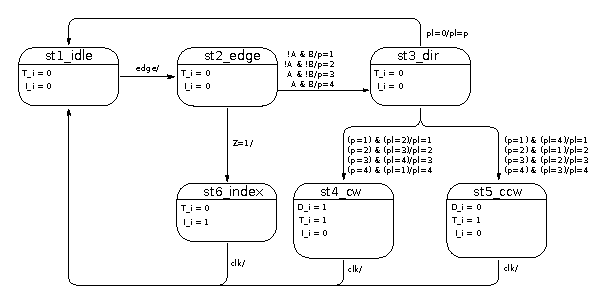
\includegraphics[width=.85\linewidth]{graphics/quad_state_machine}
	\caption[State machine of incremental quadrature decoder.]{State machine of the incremental quadrature decoder created for the MicroZed.}
	\label{fig:quadstatemachine}
\end{figure}
\paragraph{st1\_idle:} % (fold)
Is the initial state and the state that is returned to between edges on the quadrature signal.
Since the quadrature signal is not synchronous with the driving clock of the system the \texttt{rising\_edge()} and \texttt{falling\_edge()} functions cannot be used to determine edges.
Listing \ref{code:edge_detection} shows how an edge is detected on a signal. 
The current value of the signal is continuously compared to the last value, which is saved on every clock cycle.
If the two values are not equal an edge must have occured within the last clock cycle.
In this component both rising and falling edges are used and so any difference between the two is registered.
This code is repeated for all three input signals, with the exception that the \texttt{Z} channel sets \texttt{next\_state} to \texttt{st6\_index} instead.

\begin{listing}[H]
\begin{minted}{vhdl}
case (state) is
	when st1_idle =>
		if A_i /= last_A_i then
	        next_state <= st2_edge;
	    end if;
	    @$\vdots$@
\end{minted}
\caption{VHDL edge detection of asynchronous signal.}
\label{code:edge_detection}
\end{listing}

\paragraph{st2\_edge:} % (fold)
Is responsible for determining which phase is currently active.
The different phases can be seen in figure \ref{fig:quadrature}.
The phase is found simply by comparing the signals as seen in listing \ref{code:phase_detection}.
Regardless of the detected phase \texttt{next\_state} is set to \texttt{st3\_dir}.
\begin{listing}[H]
\begin{minted}{vhdl}
when st2_edge =>
	if A = '1' then
	    if B = '1' then
	        phase <= p4;
	    else
	        phase <= p3;
	    end if;
	    next_state <= st3_dir;
	    @$\vdots$@
\end{minted}
\caption{VHDL for phase detection in incremental quadrature.}
\label{code:phase_detection}
\end{listing}
\paragraph{st3\_dir:} % (fold)
Determines the current direction of travel.
This can be seen by comparing the current phase to the last phase.
Listing \ref{code:determine_direction} shows the structure of the code responsible for this step.
\begin{listing}[H]
\begin{minted}{vhdl}
when st3_dir =>
	if last_phase /= p0 then
	    if phase = p1 then
	        if last_phase = p4 then
	            next_state <= st5_ccw;
	        end if;
	        if last_phase = p2 then
	            next_state <= st4_cw;
	        end if;
	        next_last_phase <= p1;
	    end if;
	    if phase = p2 then
	    @$\vdots$@
    else
        next_last_phase <= phase;
        next_state <= st1_idle;
    end if;
\end{minted}
\caption[VHDL for determining direction of movement.]{VHDL for determining direction of movement in incremental quadrature.}
\label{code:determine_direction}
\end{listing}
As can be seen in the code there is a reference to phase 0.
This is required since the initial phase is unknown.
During the first run the direction-determination is skipped and \texttt{last\_phase} is initialized to \texttt{phase}.
On every subsequent run, depending on the direction, \texttt{next\_state} is set to either \texttt{st4\_cw} or \texttt{st5\_ccw}.
\paragraph{st4\_cw and st5\_ccw:} % (fold)
The SM is in these states for one clock cycle to allow for the outputs to be adjusted and a tick to be generated.
\paragraph{st6\_index:} % (fold)
The SM is in this state for one clock cycle when the \texttt{Z} input goes high and generates a signal to indicate that the index has been reached.
While this feature is unused in the cart position counter as it currently exists, it was decided to include it to allow future developers to use it if the need arises.

\paragraph{Cart Position Counter}~\\ % (fold)
\label{par:cart_position_counter}
This component maintains a counter which is incremented or decremented at every tick generated by the incremental quadrature decoder depending on the state of the direction signal.
If the endstop 1 signal is set high the counter is set to zero.
Upon booting the system the cart should be moved to the rightmost end-stop in order to calibrate the system.
Moving the cart will now increment the position with leftward motion and decrement with rightward motion.

\begin{figure}[h]
	\centering
	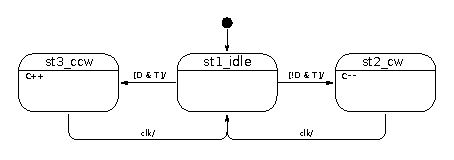
\includegraphics[width=.75\linewidth]{graphics/count_state_machine}
	\caption[State machine of the cart position counter]{State machine of the cart position counter created for the MicroZed.}
	\label{fig:countstatemachine}
\end{figure}

The SM of the system can be seen in figure \ref{fig:countstatemachine}.
In this figure \texttt{C} is \texttt{counter\_i}, \texttt{D} is \texttt{direction} and \texttt{T} is \texttt{tick}.
It should be noted that the end signal is treated as a reset signal and as such is not part of the actual SM.
Since it is essentially a reset signal handling of it is placed in the \texttt{sync process} to avoid an asynchronous reset of the values.
The code in question can be seen in listing \ref{code:cart_sync_proc}.

\begin{listing}[H]
\begin{minted}{vhdl}
SYNC_PROC:  process(clk)
	begin
	    if rising_edge(clk) then
	        if emend = '0' then
	            counter_i <= (others => '0');
	            state <= st1_idle;
	            cal_i <= '1';
	        else
	            state <= next_state;
	            counter_i <= next_counter_i;
	            last_T_i <= T_i;
	        end if;
	    end if;
	end process;
\end{minted}
\caption{Synchronous reset based on endstop signals.}
\label{code:cart_sync_proc}
\end{listing}

The SM has only three simple states.
\texttt{st1\_idle} which is the state where the SM waits for a rising edge on the tick signal, \texttt{T}.
If the direction signal, \texttt{D} is low when a tick arrives the SM proceeds to \texttt{st2\_cw} if the opposite is true it proceeds to \texttt{st3\_ccw}.
In those states the position variable, \texttt{counter\_i} is either decremented or incremented.

\paragraph{Test Benches}~\\ % (fold)
\label{par:test_benches}
A part of developing these components has been to develop and use test benches to verify code as it is being written.
VHDL was originally thought as a language to describe and simulate hardware and logic and has later been used as the programming language used to create FPGA designs.
All of the original features of the language are still present and as such it is possible to create a component which fully exercises whichever component is under development, the unit-under-test or UUT.
\\~\\
The test bench written for the cart position counter is comprised of three processes, the \texttt{clk\_proc} which is responsible for generating the driving clock for the component, \texttt{quad\_proce\_ccw} or \texttt{quad\_proce\_cw} for simulating the quadrature signal in either the counter-clockwise or the clockwise direction and finally the \texttt{stim\_proc} which is responsible for exercising any of the input signals.
\\~\\
\thomas{insert code snippet from testbench}

The UUT is instantiated as a component in the test bench and Vivado provides tools for investigating the flow of execution.
An excerpt illustrating the functionality can be seen in figure \ref{fig:testbench}.
As can be seen \texttt{B\_i} is leading \texttt{A\_i}, resulting in \texttt{D\_i} going \texttt{high}.
Since \texttt{emend\_i} is \texttt{high} the component starts counting on every rising edge of \texttt{T\_i}.
When \texttt{emend\_i} goes \texttt{low} the counter is reset and future ticks are ignored until \texttt{emend\_i} returns to \texttt{high}.

\begin{figure}[h]
	\centering
	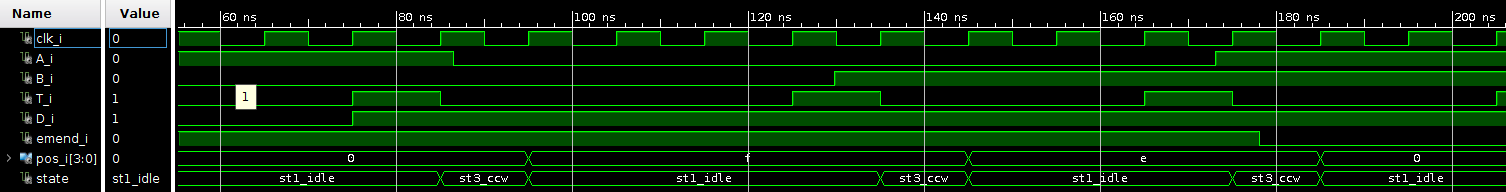
\includegraphics[width=\linewidth]{graphics/test_bench_narrow}
	\caption{Excerpt of testbench simulation results.}
	\label{fig:testbench}
\end{figure}

\paragraph{Packaging an AXI-Enabled IP Core}~\\ % (fold)
\label{par:ip_cores}
Once the component is confirmed functioning as intended, the component is packaged as an IP core capable of AXI communication.
Vivado provides an IP packager which auto-generates the files required for instantiating the components for AXI-communication.
The user can choose the number and width of the registers to be available in the instantiated AXI component.
In the generated files the user is expected to add their own code and alter existing code such that it correctly implements the desired functionality.
\\~\\
In relation to the components created in this project, the \texttt{.vhd} code files are imported to the project and the component instantiated.
Every user-defined port is brought out through the AXI component so that they can be constrained correctly in the \texttt{.xdc} constraint file.
Since every component is made as an IP core the system can be created using a block design.
For illustration purposes the block design of the full system has been included in figure \ref{fig:blockdesign}.
The rightmost blocks include three of the authors' designs and a Xilinx \texttt{axi\_gpio} block.
The GPIO block is used to handle hardware signals for creating a safety condition, enabling the motor driver and similar tasks.
\thomas{rewrite for proper safety condition}
As can be seen, a simple RGB LED controller has been written to handle the debug LEDs on the board.
By creating the component to control just a single LED, that code can be instantiated as many times as is required by the application and in any application.
In common for all of these blocks is that they require at least some of their input from the AXI bus.

\begin{figure}[h]
	\centering
	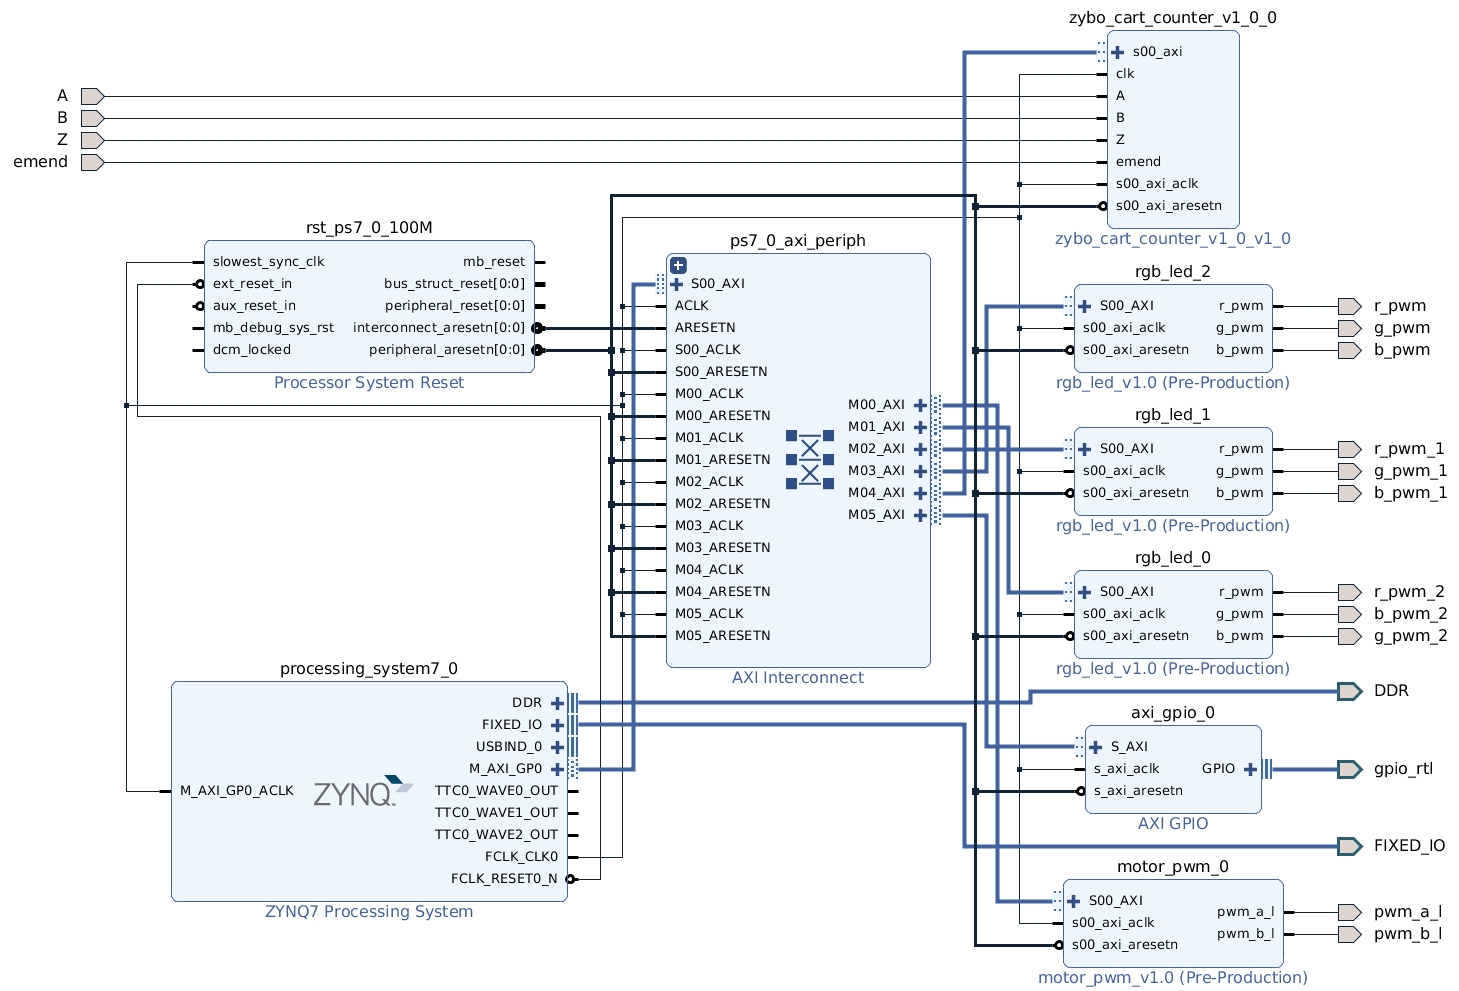
\includegraphics[width=\linewidth]{graphics/block_design}
	\caption{Vivado block design of the complete system.}
	\label{fig:blockdesign}
\end{figure}

\paragraph{Communication Through the AXI Bus}~\\ % (fold)
\label{par:communication_through_the_axi_bus}
In this project the AXI bus is used to communicate between PS and PL.
Doing this requires setup in both domains.
In PL registers are generated which the user can input data to.
An example of how this is set up can be seen in listing \ref{code:axiconnection}.
Individual bits in a register can be set to different variables and the remaining bits left unchanged.

\begin{listing}[H]
\begin{minted}{vhdl}
cart_counter_inst : cart_counter
	port map(
	    clk => clk,
	    A => A,
	    B => B,
	    Z => Z,
	    emend => emend,
	    cal => slv_reg0(1),
	    dir => slv_reg0(0),
	    pos => slv_reg1
	);
\end{minted}
\caption[Code showing the connection of AXI registers]{Code showing the connection of AXI registers to the cart position counter signals.}
\label{code:axiconnection}
\end{listing}

In PS these registers can be accessed using the \texttt{Xil\_In32()} and \texttt{Xil\_Out32()}.
These functions require an address and in the case of the output function, a payload to write to the register.
Each device in the design is given a base address which can be found in the \texttt{xparameters.h} header file which is generated for each hardware design.
Accessing a parameter is then done by adding the appropriate offset.
The offset is determined by the width of the registers.
In this case registers are 32 bits wide and so every offset is \texttt{0x04} bytes.
In code this is handled as seen in listing \ref{code:axiconnectionps}

\begin{listing}[H]
\begin{minted}{c}
#define CART_BASEADDR XPAR_ZYBO_CART_COUNTER_V1_0_0_BASEADDR

#define CAL_ADDR    0x00
#define DIR_ADDR    0x00
#define POS_ADDR    0x04
	
#define CALIBRATED  0x01
		@$\vdots$@
	
void get_position(uint32_t *position)
{
	if(is_calibrated() == CALIBRATED)
		*position = Xil_In32(CART_BASEADDR+POS_ADDR);
	else
		position = NULL;
}

		@$\vdots$@
void cart_task(void)
{
	uint32_t* pos = NULL;
	if(get_position(pos) != NULL)
	{
		//Do Something
	}
		@$\vdots$@
}
\end{minted}
\caption[Code handling communication with the cart position counter.]{Excerpt from the code written to handle the communication with the cart position counter. \texttt{is\_calibrated()} returns the status of calibration.}
\label{code:axiconnectionps}
\end{listing}

Here a wrapper function for \texttt{Xil\_In32()} is shown.
A number of these are written to simplify the code and reduce the risk of errors.
In this case the position is only valid if the calibration bit is set \texttt{high}.
When it is not, a null pointer is returned.
Rather than checking both the calibration status and the position, both can be done using a single function call.

\subsubsection{Interfacing the nRF24L01} % (fold)
\label{ssubs:nrf24l01}
~\\
The \texttt{nRFM} is interfaced through a standard SPI connection and a \texttt{CE} pin that is used to activate the chip. 
It also has an interrupt pin, but it was chosen not to use it and instead poll the device. 
Configuration of the device is done through SPI.

\paragraph{Setup} % (fold)
\label{par:nrfsetup}
~\\
The \texttt{nRFM} has multiple different modes of operations and care should be taken when setting it up.
The flowchart of figure \ref{fig:nrf_setup} gives an overview of what registers are set in order to gain the settings used in this project.
A description of each step and register is given below.
\begin{figure}[h]
	\centering
	\includegraphics[width=.8\linewidth]{graphics/nfr_setup}
	\caption{Flowchart showing the setup process of the \texttt{nRFM} module.}
	\label{fig:nrf_setup}
\end{figure}
\begin{itemize}
	\item \texttt{RF\_SETUP} register is set in order to gain 1Mbps air transmission and maximum output power in TX mode.
	\item \texttt{RF\_CH} register is used to set the channel used. It should be set differently for each \texttt{nRFM} pair.
	\item \texttt{SETUP\_AW} register is set to use the shortest available address width of three bytes.
	\item \texttt{EN\_AA} register is set to disable auto acknowledgement.
	\item \texttt{SETUP\_RETR} register is set to disable automatic retransmission.
\end{itemize}

The \texttt{PWR\_UP} bit is then set to \texttt{1} to power up the module. 
A wait of 4.5ms is then initiated to allow for proper start-up of the crystal.
\\~\\
If receive mode, \texttt{RX}, is needed the \texttt{PRIM\_RX} bit should be set to \texttt{1} and the receive address written to \texttt{RX\_ADDR\_P0}.
Furthermore \texttt{RX\_PW\_P0} is set to 2 in order to set the payload size to two bytes.
Finally \texttt{EN\_RX\_ADDR} is set to enable data on data pipe 0 and \texttt{CE} is set \texttt{high} to initiate the transition to \texttt{RX} mode.
\\~\\
If transmit mode, \texttt{TX}, is needed \texttt{PRIM\_RX} should be set to \texttt{0} and the transmit address should be written to \texttt{PRIM\_RX}.
Hereafter \texttt{CE} is set \texttt{high} to initiate the transition to \texttt{TX} mode.

\paragraph{Writing to a Register} % (fold)
\label{par:writing_to_a_register}
~\\
Figure \ref{fig:rw_register} illustrates the bits that are sent to the \texttt{nRFM} in order to write a value to a register. 
The three command bits specify if the action to be done is read or write.
The five address bits specify address of the register that is to be written to. 
The next one to five bytes is the value that are to be written to the register.

\begin{figure}[!h]
	\centering
	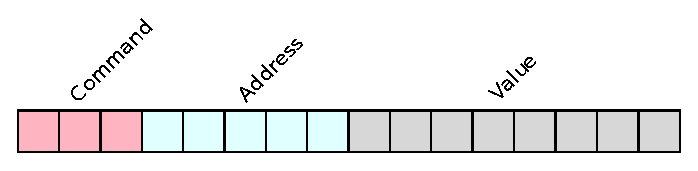
\includegraphics[width=.5\linewidth]{graphics/rw_register.eps}
	\caption[Writing bits to a register on nRF24L01.]{Bits written to the \texttt{nRFM} in order to write a value to a register. \texttt{Command} specifies if it is a read or write action, \texttt{Address} specifies the register address and \texttt{Value} specifies the value written to or read from the register.}
	\label{fig:rw_register}
\end{figure}
\thomas{fix figure to include arbitrary length value}

The C code in listing \ref{code:rf_write_register_code} is used to write a value to a register. 
Line 5 makes sure that a valid address and command is sent, regardless of the inputs.
Line 6 collects all bits that needs to be sent in one variable. 
The 2 bytes are sent using SPI in line 7, where it can also be seen that the answer from the \texttt{nRFM} is ignored as the \texttt{NULL} pointer is given as the input buffer.  

\begin{listing}[!h]
\begin{minted}{c}
#define W_REGISTER      0b00100000
#define REGISTER_MASK   0b00011111

void RF_write_register(XSpiPs *SPI_inst, u8 reg, u8 value){
	u8 cmd_addr =  (W_REGISTER | ( REGISTER_MASK & reg));
	u8 output_buffer[] = {cmd_addr, value};
	XSpiPs_PolledTransfer(SPI_inst, output_buffer, NULL, 2);
}
\end{minted}
\caption[C function that writes a value to a register on the nRFM]{Implementation of a C function that writes a register value to a specific register on the \texttt{nRFM}. Macros are shown for clarity.}
\label{code:rf_write_register_code}
\end{listing}

The corresponding SPI signals are measured and plotted in figure \ref{fig:nrf24_spi}.
It can be seen that the \texttt{MOSI} signal corresponds to \texttt{0b00100000, 0b00110101}, which means that the value \texttt{0b00110101} is written to the \texttt{RF\_CONFIG} register which has address \texttt{0x00}.
It can also be noted that data is available on the \texttt{MISO} signal. 
The \texttt{nRFM} always responds with the value of the \texttt{STATUS} when detecting a falling edge on \texttt{SS}.

\begin{figure}[h]
	\centering
    % This file was created by matlab2tikz.
%
%The latest updates can be retrieved from
%  http://www.mathworks.com/matlabcentral/fileexchange/22022-matlab2tikz-matlab2tikz
%where you can also make suggestions and rate matlab2tikz.
%
\definecolor{mycolor1}{rgb}{0.00000,0.44700,0.74100}%
\definecolor{mycolor2}{rgb}{0.85000,0.32500,0.09800}%
\definecolor{mycolor3}{rgb}{0.92900,0.69400,0.12500}%
\definecolor{mycolor4}{rgb}{0.49400,0.18400,0.55600}%
%
\begin{tikzpicture}

\begin{axis}[%
width=4.521in,
height=3.566in,
at={(0.758in,0.481in)},
scale only axis,
xmin=0,
xmax=3.5e-05,
xlabel style={font=\color{white!15!black}},
xlabel={Time [s]},
ymin=-1,
ymax=6,
ylabel style={font=\color{white!15!black}},
ylabel={Voltage [V]},
axis background/.style={fill=white},
title style={font=\bfseries},
title={SPI Communication on nRF24},
legend style={legend cell align=left, align=left, draw=white!15!black}
]
\addplot [color=mycolor1, line width=2.0pt]
  table[row sep=crcr]{%
-1.99999998784506e-08	0.0800000000000001\\
0	0.16\\
1.99999998784506e-08	0.16\\
3.99999997569012e-08	0.24\\
5.99999996353517e-08	0.0800000000000001\\
8.00000004019807e-08	0.0800000000000001\\
1.00000000280431e-07	0.16\\
1.20000000158882e-07	0.0800000000000001\\
1.40000000037332e-07	0.16\\
1.59999999915783e-07	0.16\\
1.79999999794234e-07	0.0800000000000001\\
1.99999999672684e-07	0.16\\
2.20000000439313e-07	0.16\\
2.40000000317764e-07	0.24\\
2.60000000196214e-07	0.0800000000000001\\
2.80000000074665e-07	0.0800000000000001\\
3.19999999831566e-07	0.24\\
3.39999999710017e-07	0.16\\
3.59999999588467e-07	0.16\\
3.80000000355096e-07	0.0800000000000001\\
4.20000000111997e-07	0.24\\
4.59999999868899e-07	0.0800000000000001\\
4.79999999747349e-07	0.16\\
4.999999996258e-07	0.0800000000000001\\
5.20000000392429e-07	0.24\\
5.40000000270879e-07	0.16\\
5.6000000014933e-07	0.24\\
5.80000000027781e-07	0.16\\
6.39999999663132e-07	0.16\\
6.60000000429761e-07	0.0800000000000001\\
6.80000000308212e-07	0.16\\
7.99999999578915e-07	0.16\\
8.20000000345544e-07	0.0800000000000001\\
8.40000000223995e-07	0.16\\
9.39999999616248e-07	0.16\\
9.60000000382877e-07	0.0800000000000001\\
9.80000000261327e-07	0.16\\
1.00000000013978e-06	0.16\\
1.02000000001823e-06	0.24\\
1.03999999989668e-06	0.0800000000000001\\
1.05999999977513e-06	0.0800000000000001\\
1.07999999965358e-06	0.24\\
1.10000000042021e-06	0.16\\
1.12000000029866e-06	0.16\\
1.14000000017711e-06	0.0800000000000001\\
1.17999999993401e-06	0.24\\
1.19999999981246e-06	0.16\\
1.21999999969091e-06	0\\
1.23999999956936e-06	0.0800000000000001\\
1.26000000033599e-06	0.24\\
1.28000000021444e-06	0\\
1.30000000009289e-06	0.16\\
1.31999999997134e-06	0.0800000000000001\\
1.35999999972825e-06	0.24\\
1.3799999996067e-06	0.16\\
1.40000000037332e-06	0.16\\
1.42000000025178e-06	0.0800000000000001\\
1.44000000013023e-06	0.0800000000000001\\
1.46000000000868e-06	0.16\\
1.51999999964403e-06	0.16\\
1.54000000041066e-06	0.0800000000000001\\
1.56000000028911e-06	0.24\\
1.58000000016756e-06	0.16\\
1.60000000004601e-06	0.16\\
1.61999999992446e-06	0.24\\
1.65999999968136e-06	0.0800000000000001\\
1.67999999955981e-06	0.16\\
1.72000000020489e-06	0.16\\
1.74000000008334e-06	0.0800000000000001\\
1.75999999996179e-06	0.16\\
1.79999999971869e-06	0\\
1.81999999959714e-06	0.0800000000000001\\
1.84000000036377e-06	0.24\\
1.86000000024222e-06	0.16\\
1.88000000012067e-06	0.16\\
1.89999999999912e-06	0.0800000000000001\\
1.91999999987758e-06	0.16\\
1.93999999975603e-06	0.0800000000000001\\
1.95999999963448e-06	0.16\\
1.98000000040111e-06	0.0800000000000001\\
2.00000000027956e-06	0.16\\
2.02000000015801e-06	0.16\\
2.04000000003646e-06	0.0800000000000001\\
2.14000000031689e-06	0.0800000000000001\\
2.18000000007379e-06	0.24\\
2.19999999995224e-06	0.0800000000000001\\
2.21999999983069e-06	0.16\\
2.23999999970914e-06	0.0800000000000001\\
2.28000000035422e-06	0.0800000000000001\\
2.30000000023267e-06	0.16\\
2.32000000011112e-06	0.16\\
2.33999999998957e-06	0.0800000000000001\\
2.35999999986802e-06	0.0800000000000001\\
2.37999999974647e-06	0.16\\
2.46000000014845e-06	0.16\\
2.48000000002691e-06	0.0800000000000001\\
2.49999999990536e-06	0.16\\
2.53999999966226e-06	0.16\\
2.56000000042889e-06	0\\
2.58000000030734e-06	0.16\\
2.60000000018579e-06	0.16\\
2.62000000006424e-06	0.0800000000000001\\
2.63999999994269e-06	0.0800000000000001\\
2.65999999982114e-06	0.16\\
2.67999999969959e-06	0.16\\
2.69999999957804e-06	0.0800000000000001\\
2.72000000034467e-06	0.0800000000000001\\
2.74000000022312e-06	0\\
2.76000000010157e-06	0.0800000000000001\\
2.77999999998002e-06	0.24\\
2.79999999985847e-06	0.0800000000000001\\
2.81999999973692e-06	0.16\\
2.83999999961537e-06	0.0800000000000001\\
2.860000000382e-06	0.16\\
2.92000000001735e-06	0.16\\
2.9399999998958e-06	0.0800000000000001\\
2.95999999977425e-06	0.24\\
2.9799999996527e-06	0.16\\
3.02000000029778e-06	0.16\\
3.04000000017624e-06	0.0800000000000001\\
3.06000000005469e-06	0.0800000000000001\\
3.07999999993314e-06	0.16\\
3.11999999969004e-06	0.16\\
3.13999999956849e-06	0.0800000000000001\\
3.16000000033512e-06	0.24\\
3.18000000021357e-06	0.16\\
3.20000000009202e-06	0.16\\
3.21999999997047e-06	0.24\\
3.23999999984892e-06	0.16\\
3.27999999960582e-06	0.16\\
3.30000000037245e-06	0.24\\
3.3200000002509e-06	0.0800000000000001\\
3.34000000012935e-06	0.24\\
3.3600000000078e-06	0.16\\
3.37999999988625e-06	0.16\\
3.3999999997647e-06	0.0800000000000001\\
3.41999999964315e-06	0.0800000000000001\\
3.44000000040978e-06	0.16\\
3.50000000004513e-06	0.16\\
3.51999999992358e-06	0.0800000000000001\\
3.53999999980203e-06	0.24\\
3.55999999968049e-06	0.0800000000000001\\
3.57999999955894e-06	0.16\\
3.60000000032556e-06	0.0800000000000001\\
3.62000000020402e-06	0.0800000000000001\\
3.64000000008247e-06	0.16\\
3.65999999996092e-06	0.16\\
3.67999999983937e-06	0.0800000000000001\\
3.69999999971782e-06	0.0800000000000001\\
3.71999999959627e-06	0.24\\
3.7400000003629e-06	0.0800000000000001\\
3.76000000024135e-06	0.16\\
3.7800000001198e-06	0.16\\
3.79999999999825e-06	0.0800000000000001\\
3.8199999998767e-06	0.16\\
3.88000000040023e-06	0.16\\
3.90000000027868e-06	0.0800000000000001\\
3.92000000015713e-06	0.16\\
3.94000000003558e-06	0.16\\
3.95999999991403e-06	0.0800000000000001\\
3.97999999979248e-06	0.16\\
3.99999999967093e-06	0.16\\
4.02000000043756e-06	0.0800000000000001\\
4.04000000031601e-06	0.16\\
4.06000000019446e-06	0.0800000000000001\\
4.08000000007291e-06	0.0800000000000001\\
4.09999999995136e-06	0.16\\
4.11999999982982e-06	0.0800000000000001\\
4.15999999958672e-06	0.0800000000000001\\
4.18000000035335e-06	0.16\\
4.2000000002318e-06	0.16\\
4.22000000011025e-06	0.0800000000000001\\
4.2399999999887e-06	0.0800000000000001\\
4.25999999986715e-06	0.16\\
4.32000000039068e-06	0.16\\
4.34000000026913e-06	-0.16\\
4.38000000002603e-06	0\\
4.39999999990448e-06	0.16\\
4.41999999978293e-06	0\\
4.43999999966138e-06	0\\
4.46000000042801e-06	-0.0800000000000001\\
4.48000000030646e-06	0.0800000000000001\\
4.52000000006336e-06	0.0800000000000001\\
4.53999999994181e-06	-0.0800000000000001\\
4.55999999982026e-06	0.0800000000000001\\
4.57999999969871e-06	0\\
4.62000000034379e-06	0\\
4.64000000022224e-06	0.0800000000000001\\
4.67999999997915e-06	-0.0800000000000001\\
4.6999999998576e-06	-0.0800000000000001\\
4.76000000038113e-06	0.16\\
4.78000000025958e-06	0\\
4.80000000013803e-06	0.0800000000000001\\
4.82000000001648e-06	0\\
4.83999999989493e-06	0\\
4.85999999977338e-06	0.0800000000000001\\
4.90000000041846e-06	0.0800000000000001\\
4.92000000029691e-06	0\\
4.94000000017536e-06	0.16\\
4.96000000005381e-06	0.0800000000000001\\
4.97999999993226e-06	0.0800000000000001\\
4.99999999981071e-06	0\\
5.01999999968916e-06	0\\
5.03999999956761e-06	0.0800000000000001\\
5.08000000021269e-06	0.0800000000000001\\
5.10000000009114e-06	0\\
5.11999999996959e-06	0\\
5.13999999984804e-06	0.0800000000000001\\
5.15999999972649e-06	0.0800000000000001\\
5.17999999960495e-06	0\\
5.24000000012848e-06	0\\
5.26000000000693e-06	0.0800000000000001\\
5.27999999988538e-06	0.0800000000000001\\
5.29999999976383e-06	0\\
5.31999999964228e-06	0.0800000000000001\\
5.34000000040891e-06	0.0800000000000001\\
5.36000000028736e-06	0\\
5.38000000016581e-06	0\\
5.40000000004426e-06	-0.16\\
5.41999999992271e-06	0.0800000000000001\\
5.45999999967961e-06	0.0800000000000001\\
5.47999999955806e-06	0\\
5.50000000032469e-06	0\\
5.52000000020314e-06	0.16\\
5.54000000008159e-06	0.0800000000000001\\
5.57999999983849e-06	0.0800000000000001\\
5.59999999971694e-06	0\\
5.61999999959539e-06	0\\
5.64000000036202e-06	0.0800000000000001\\
5.66000000024047e-06	-0.0800000000000001\\
5.69999999999737e-06	0.0800000000000001\\
5.71999999987582e-06	0\\
5.73999999975427e-06	0\\
5.75999999963273e-06	-0.0800000000000001\\
5.80000000027781e-06	0.0800000000000001\\
5.84000000003471e-06	0.0800000000000001\\
5.85999999991316e-06	3.52\\
5.87999999979161e-06	3.6\\
5.89999999967006e-06	3.36\\
5.92000000043669e-06	3.36\\
5.96000000019359e-06	3.2\\
5.98000000007204e-06	3.2\\
5.99999999995049e-06	3.12\\
6.01999999982894e-06	3.2\\
6.08000000035247e-06	3.2\\
6.10000000023092e-06	3.12\\
6.13999999998782e-06	3.28\\
6.15999999986627e-06	3.12\\
6.17999999974472e-06	3.2\\
6.19999999962317e-06	3.12\\
6.24000000026825e-06	3.28\\
6.2600000001467e-06	3.2\\
6.33999999966051e-06	3.2\\
6.36000000042714e-06	3.28\\
6.38000000030559e-06	3.2\\
6.40000000018404e-06	3.04\\
6.43999999994094e-06	3.28\\
6.45999999981939e-06	3.28\\
6.47999999969784e-06	3.2\\
6.49999999957629e-06	3.28\\
6.52000000034292e-06	3.2\\
6.54000000022137e-06	3.28\\
6.56000000009982e-06	3.2\\
6.57999999997827e-06	3.28\\
6.59999999985672e-06	3.2\\
6.61999999973517e-06	-0.32\\
6.63999999961362e-06	0.4\\
6.66000000038025e-06	-0.0800000000000001\\
6.6800000002587e-06	0.0800000000000001\\
6.7200000000156e-06	0.0800000000000001\\
6.73999999989405e-06	0.16\\
6.7599999997725e-06	0\\
6.77999999965095e-06	0.0800000000000001\\
6.80000000041758e-06	0\\
6.82000000029603e-06	0\\
6.84000000017448e-06	0.0800000000000001\\
6.86000000005293e-06	0\\
6.87999999993139e-06	0.0800000000000001\\
6.89999999980984e-06	0\\
6.91999999968829e-06	0.16\\
6.93999999956674e-06	0\\
6.96000000033337e-06	0.0800000000000001\\
6.98000000021182e-06	0\\
7.00000000009027e-06	0.0800000000000001\\
7.03999999984717e-06	0.0800000000000001\\
7.05999999972562e-06	0\\
7.1000000003707e-06	0\\
7.12000000024915e-06	0.0800000000000001\\
7.1400000001276e-06	0\\
7.16000000000605e-06	0\\
7.1799999998845e-06	0.0800000000000001\\
7.19999999976295e-06	0.0800000000000001\\
7.2199999996414e-06	-0.0800000000000001\\
7.24000000040803e-06	0\\
7.26000000028648e-06	0\\
7.28000000016493e-06	-0.0800000000000001\\
7.30000000004338e-06	0.0800000000000001\\
7.31999999992183e-06	0\\
7.35999999967873e-06	0\\
7.37999999955719e-06	0.0800000000000001\\
7.40000000032381e-06	3.2\\
7.42000000020226e-06	3.04\\
7.44000000008072e-06	3.2\\
7.45999999995917e-06	3.2\\
7.47999999983762e-06	3.12\\
7.51999999959452e-06	3.28\\
7.5600000002396e-06	3.12\\
7.58000000011805e-06	3.2\\
7.61999999987495e-06	3.2\\
7.6399999997534e-06	3.28\\
7.65999999963185e-06	3.2\\
7.68000000039848e-06	3.28\\
7.70000000027693e-06	3.28\\
7.72000000015538e-06	3.12\\
7.74000000003383e-06	3.12\\
7.77999999979073e-06	3.28\\
7.82000000043581e-06	3.12\\
7.84000000031426e-06	3.2\\
7.89999999994961e-06	3.2\\
7.91999999982806e-06	3.12\\
7.93999999970652e-06	3.2\\
7.95999999958497e-06	3.2\\
7.98000000035159e-06	3.12\\
8.00000000023005e-06	3.12\\
8.0200000001085e-06	3.2\\
8.14000000026738e-06	3.2\\
8.16000000014583e-06	-1.04\\
8.18000000002428e-06	-0.16\\
8.19999999990273e-06	-0.0800000000000001\\
8.21999999978118e-06	-0.16\\
8.26000000042626e-06	0.0800000000000001\\
8.28000000030471e-06	0.0800000000000001\\
8.30000000018316e-06	0\\
8.32000000006161e-06	0\\
8.33999999994006e-06	0.16\\
8.37999999969696e-06	-0.0800000000000001\\
8.39999999957541e-06	0\\
8.42000000034204e-06	0\\
8.44000000022049e-06	0.0800000000000001\\
8.46000000009894e-06	0\\
8.47999999997739e-06	0.16\\
8.49999999985585e-06	-0.0800000000000001\\
8.5199999997343e-06	0.0800000000000001\\
8.53999999961275e-06	0\\
8.56000000037938e-06	0\\
8.58000000025783e-06	0.0800000000000001\\
8.60000000013628e-06	0\\
8.62000000001473e-06	0.0800000000000001\\
8.63999999989318e-06	-0.0800000000000001\\
8.65999999977163e-06	0\\
8.67999999965008e-06	0\\
8.72000000029516e-06	0.16\\
8.74000000017361e-06	0\\
8.76000000005206e-06	0.0800000000000001\\
8.77999999993051e-06	0\\
8.81999999968741e-06	0\\
8.83999999956586e-06	-0.0800000000000001\\
8.86000000033249e-06	0.0800000000000001\\
8.88000000021094e-06	0\\
8.90000000008939e-06	0.0800000000000001\\
8.91999999996784e-06	0.4\\
8.93999999984629e-06	2.48\\
8.95999999972474e-06	2.88\\
8.97999999960319e-06	3.04\\
9.00000000036982e-06	3.12\\
9.07999999988363e-06	3.12\\
9.09999999976208e-06	3.28\\
9.11999999964053e-06	3.12\\
9.16000000028561e-06	3.28\\
9.18000000016406e-06	3.2\\
9.20000000004251e-06	3.2\\
9.21999999992096e-06	3.12\\
9.23999999979941e-06	3.12\\
9.25999999967786e-06	3.2\\
9.34000000007984e-06	3.2\\
9.35999999995829e-06	3.12\\
9.37999999983674e-06	3.2\\
9.41999999959364e-06	3.2\\
9.44000000036027e-06	3.28\\
9.46000000023872e-06	3.2\\
9.48000000011717e-06	3.28\\
9.49999999999562e-06	3.2\\
9.51999999987407e-06	3.2\\
9.53999999975252e-06	3.12\\
9.55999999963097e-06	3.2\\
9.60000000027605e-06	3.2\\
9.6200000001545e-06	3.12\\
9.65999999991141e-06	3.28\\
9.67999999978986e-06	3.2\\
9.69999999966831e-06	-0.56\\
9.74000000031339e-06	-0.24\\
9.76000000019184e-06	0\\
9.81999999982719e-06	0\\
9.83999999970564e-06	0.0800000000000001\\
9.85999999958409e-06	0\\
9.90000000022917e-06	0\\
9.92000000010762e-06	0.0800000000000001\\
9.93999999998607e-06	0.0800000000000001\\
9.95999999986452e-06	0\\
9.97999999974297e-06	0\\
9.99999999962142e-06	0.0800000000000001\\
1.00200000003881e-05	0\\
1.00400000002665e-05	0.0800000000000001\\
1.0060000000145e-05	0\\
1.00800000000234e-05	0.0800000000000001\\
1.00999999999019e-05	0\\
1.01199999997803e-05	0.0800000000000001\\
1.01399999996588e-05	0.0800000000000001\\
1.01600000004254e-05	0\\
1.02399999999392e-05	0\\
1.02599999998176e-05	-0.0800000000000001\\
1.03200000003412e-05	0.16\\
1.03400000002196e-05	-0.0800000000000001\\
1.03600000000981e-05	-0.0800000000000001\\
1.03799999999765e-05	0.0800000000000001\\
1.0399999999855e-05	0\\
1.04199999997334e-05	0.0800000000000001\\
1.04399999996119e-05	0.0800000000000001\\
1.04600000003785e-05	3.44\\
1.0480000000257e-05	2.88\\
1.05000000001354e-05	3.28\\
1.05200000000139e-05	3.2\\
1.05399999998923e-05	3.2\\
1.05599999997708e-05	3.12\\
1.06000000004158e-05	3.28\\
1.06200000002943e-05	3.04\\
1.06400000001727e-05	3.12\\
1.06600000000512e-05	3.12\\
1.06999999998081e-05	3.28\\
1.07199999996865e-05	3.2\\
1.07600000003316e-05	3.2\\
1.07800000002101e-05	3.12\\
1.08000000000885e-05	3.28\\
1.08399999998454e-05	3.12\\
1.08599999997239e-05	3.2\\
1.10199999996397e-05	3.2\\
1.10400000004063e-05	3.12\\
1.10800000001632e-05	3.28\\
1.11000000000416e-05	3.2\\
1.11199999999201e-05	3.2\\
1.11399999997985e-05	3.28\\
1.11800000004436e-05	3.12\\
1.12000000003221e-05	3.2\\
1.12200000002005e-05	3.12\\
1.1240000000079e-05	0\\
1.12599999999574e-05	0.32\\
1.12799999998359e-05	0.0800000000000001\\
1.12999999997143e-05	0.0800000000000001\\
1.13400000003594e-05	-0.0800000000000001\\
1.13600000002378e-05	0.0800000000000001\\
1.13800000001163e-05	0\\
1.13999999999947e-05	0\\
1.14199999998732e-05	0.0800000000000001\\
1.14599999996301e-05	0.0800000000000001\\
1.14800000003967e-05	0\\
1.15000000002752e-05	0.16\\
1.15400000000321e-05	-0.0800000000000001\\
1.1579999999789e-05	0.0800000000000001\\
1.15999999996674e-05	0\\
1.16200000004341e-05	0\\
1.16400000003125e-05	0.0800000000000001\\
1.1660000000191e-05	0\\
1.16800000000694e-05	0\\
1.16999999999479e-05	-0.0800000000000001\\
1.17399999997048e-05	0.0800000000000001\\
1.17800000003498e-05	0.0800000000000001\\
1.18000000002283e-05	0\\
1.18399999999852e-05	0\\
1.18599999998636e-05	0.0800000000000001\\
1.18799999997421e-05	0\\
1.18999999996205e-05	0.0800000000000001\\
1.19200000003872e-05	0.0800000000000001\\
1.19400000002656e-05	-0.0800000000000001\\
1.19800000000225e-05	0.0800000000000001\\
1.1999999999901e-05	3.84\\
1.20199999997794e-05	3.68\\
1.20399999996579e-05	3.36\\
1.20600000004245e-05	3.28\\
1.2080000000303e-05	3.28\\
1.21000000001814e-05	3.2\\
1.21200000000599e-05	3.2\\
1.21599999998168e-05	3.04\\
1.21799999996952e-05	3.28\\
1.21999999995737e-05	3.12\\
1.22200000003403e-05	3.2\\
1.22400000002187e-05	3.2\\
1.22600000000972e-05	3.04\\
1.22799999999756e-05	3.2\\
1.22999999998541e-05	3.28\\
1.23199999997325e-05	3.12\\
1.2339999999611e-05	3.12\\
1.23600000003776e-05	3.28\\
1.23800000002561e-05	3.12\\
1.24000000001345e-05	3.28\\
1.2420000000013e-05	3.2\\
1.24399999998914e-05	3.28\\
1.24599999997699e-05	3.12\\
1.24799999996483e-05	3.36\\
1.25400000001719e-05	3.12\\
1.25600000000503e-05	3.28\\
1.25799999999288e-05	3.2\\
1.26399999995641e-05	3.2\\
1.26600000003307e-05	3.28\\
1.26800000002092e-05	3.28\\
1.27000000000876e-05	3.2\\
1.27199999999661e-05	3.28\\
1.27399999998445e-05	3.2\\
1.2759999999723e-05	2.88\\
1.27799999996014e-05	0.72\\
1.28200000002465e-05	0.24\\
1.2840000000125e-05	0.16\\
1.28600000000034e-05	0.16\\
1.28799999998819e-05	0\\
1.28999999997603e-05	0.0800000000000001\\
1.29199999996388e-05	-0.0800000000000001\\
1.29400000004054e-05	0\\
1.29600000002839e-05	0.16\\
1.29800000001623e-05	0.0800000000000001\\
1.30000000000408e-05	0.0800000000000001\\
1.30199999999192e-05	0\\
1.30399999997977e-05	0\\
1.30599999996761e-05	0.0800000000000001\\
1.30800000004427e-05	0.0800000000000001\\
1.31000000003212e-05	0\\
1.31599999999565e-05	0\\
1.3179999999835e-05	0.0800000000000001\\
1.31999999997134e-05	0.0800000000000001\\
1.32199999995919e-05	0\\
1.32400000003585e-05	0.0800000000000001\\
1.3260000000237e-05	0\\
1.32999999999939e-05	0\\
1.33199999998723e-05	-0.0800000000000001\\
1.33399999997508e-05	0.0800000000000001\\
1.33800000003959e-05	0.0800000000000001\\
1.34000000002743e-05	0\\
1.34200000001528e-05	0\\
1.34400000000312e-05	0.0800000000000001\\
1.34599999999097e-05	0\\
1.35200000004332e-05	0\\
1.35400000003116e-05	3.44\\
1.35600000001901e-05	3.6\\
1.35800000000685e-05	3.36\\
1.3599999999947e-05	3.28\\
1.36199999998254e-05	3.28\\
1.36399999997039e-05	3.2\\
1.36599999995823e-05	3.2\\
1.3680000000349e-05	3.12\\
1.37000000002274e-05	3.28\\
1.37399999999843e-05	3.28\\
1.37799999997412e-05	3.12\\
1.37999999996197e-05	3.12\\
1.38200000003863e-05	3.2\\
1.38999999999001e-05	3.2\\
1.39199999997786e-05	3.12\\
1.3939999999657e-05	3.12\\
1.39600000004236e-05	3.28\\
1.39800000003021e-05	3.2\\
1.40399999999374e-05	3.2\\
1.40599999998159e-05	3.28\\
1.40799999996943e-05	3.2\\
1.41200000003394e-05	3.2\\
1.41400000002179e-05	3.12\\
1.41600000000963e-05	3.36\\
1.41799999999748e-05	3.2\\
1.41999999998532e-05	3.2\\
1.42199999997317e-05	3.12\\
1.42399999996101e-05	3.2\\
1.42600000003767e-05	3.2\\
1.42800000002552e-05	3.28\\
1.43000000001337e-05	-0.32\\
1.43200000000121e-05	0.4\\
1.43399999998906e-05	0.0800000000000001\\
1.44000000004141e-05	0.0800000000000001\\
1.44200000002925e-05	0.16\\
1.4440000000171e-05	0\\
1.44600000000494e-05	0.16\\
1.44799999999279e-05	0.0800000000000001\\
1.44999999998063e-05	0.0800000000000001\\
1.45199999996848e-05	-0.0800000000000001\\
1.45399999995632e-05	0.0800000000000001\\
1.45600000003299e-05	0.0800000000000001\\
1.45800000002083e-05	0\\
1.46000000000868e-05	0\\
1.46199999999652e-05	0.0800000000000001\\
1.46399999998437e-05	0.0800000000000001\\
1.46599999997221e-05	0.16\\
1.46799999996006e-05	0\\
1.47000000003672e-05	0.0800000000000001\\
1.47200000002456e-05	-0.0800000000000001\\
1.47600000000025e-05	0.0800000000000001\\
1.4779999999881e-05	0\\
1.47999999997595e-05	0.0800000000000001\\
1.48199999996379e-05	0\\
1.48400000004045e-05	0.0800000000000001\\
1.4860000000283e-05	0\\
1.48800000001614e-05	0.0800000000000001\\
1.49000000000399e-05	0.0800000000000001\\
1.49199999999183e-05	0\\
1.49399999997968e-05	0\\
1.49599999996752e-05	0.0800000000000001\\
1.49800000004419e-05	0.0800000000000001\\
1.50000000003203e-05	-0.0800000000000001\\
1.50200000001988e-05	0\\
1.50400000000772e-05	0.16\\
1.50599999999557e-05	0.0800000000000001\\
1.50799999998341e-05	3.28\\
1.50999999997126e-05	3.12\\
1.5119999999591e-05	3.2\\
1.51800000001145e-05	3.2\\
1.5199999999993e-05	3.28\\
1.52199999998714e-05	3.28\\
1.52599999996283e-05	3.12\\
1.5280000000395e-05	3.12\\
1.53000000002734e-05	3.2\\
1.53200000001519e-05	3.2\\
1.53400000000303e-05	3.12\\
1.53599999999088e-05	3.28\\
1.53799999997872e-05	3.2\\
1.54200000004323e-05	3.2\\
1.54400000003108e-05	3.12\\
1.54600000001892e-05	3.2\\
1.54800000000677e-05	3.2\\
1.54999999999461e-05	3.12\\
1.55199999998246e-05	3.2\\
1.5539999999703e-05	3.12\\
1.55800000003481e-05	3.28\\
1.56000000002265e-05	3.2\\
1.56599999998619e-05	3.2\\
1.56799999997403e-05	3.28\\
1.56999999996188e-05	3.28\\
1.57200000003854e-05	3.2\\
1.57400000002639e-05	3.28\\
1.57800000000208e-05	3.12\\
1.57999999998992e-05	3.2\\
1.58199999997777e-05	3.12\\
1.58399999996561e-05	-0.96\\
1.58800000003012e-05	-0.16\\
1.59000000001797e-05	-0.24\\
1.59200000000581e-05	0\\
1.59399999999366e-05	0.0800000000000001\\
1.5959999999815e-05	-0.0800000000000001\\
1.59799999996935e-05	0.0800000000000001\\
1.60200000003385e-05	-0.0800000000000001\\
1.6040000000217e-05	0\\
1.60600000000954e-05	0\\
1.60799999999739e-05	0.0800000000000001\\
1.60999999998523e-05	0\\
1.61199999997308e-05	0\\
1.61399999996092e-05	0.0800000000000001\\
1.61600000003759e-05	0.0800000000000001\\
1.61800000002543e-05	-0.0800000000000001\\
1.62000000001328e-05	0\\
1.62200000000112e-05	-0.0800000000000001\\
1.62599999997681e-05	0.16\\
1.63000000004132e-05	-0.0800000000000001\\
1.63200000002917e-05	0\\
1.63400000001701e-05	0\\
1.63600000000486e-05	0.16\\
1.6379999999927e-05	-0.0800000000000001\\
1.63999999998055e-05	0.0800000000000001\\
1.64199999996839e-05	-0.0800000000000001\\
1.64399999995624e-05	0.16\\
1.64800000002074e-05	0\\
1.65000000000859e-05	0\\
1.65199999999643e-05	0.0800000000000001\\
1.65399999998428e-05	0.0800000000000001\\
1.65599999997212e-05	-0.0800000000000001\\
1.65799999995997e-05	0\\
1.66000000003663e-05	0.48\\
1.66200000002448e-05	2.56\\
1.66400000001232e-05	2.96\\
1.66799999998801e-05	3.12\\
1.6719999999637e-05	3.12\\
1.67400000004037e-05	3.28\\
1.67600000002821e-05	3.12\\
1.67800000001606e-05	3.2\\
1.6800000000039e-05	3.12\\
1.68399999997959e-05	3.28\\
1.68599999996744e-05	3.2\\
1.69000000003194e-05	3.2\\
1.69200000001979e-05	3.36\\
1.69599999999548e-05	3.2\\
1.69799999998332e-05	3.04\\
1.69999999997117e-05	3.2\\
1.70199999995901e-05	3.2\\
1.70400000003568e-05	3.12\\
1.70600000002352e-05	3.12\\
1.70800000001137e-05	3.2\\
1.71199999998706e-05	3.2\\
1.7139999999749e-05	3.28\\
1.71599999996275e-05	3.28\\
1.71800000003941e-05	3.2\\
1.7220000000151e-05	3.2\\
1.72400000000295e-05	3.12\\
1.72599999999079e-05	3.2\\
1.72799999997864e-05	3.12\\
1.72999999996648e-05	3.28\\
1.73200000004314e-05	3.2\\
1.73400000003099e-05	3.28\\
1.73600000001883e-05	3.2\\
1.73800000000668e-05	0.0800000000000001\\
1.73999999999452e-05	-0.72\\
1.74199999998237e-05	0.16\\
1.74399999997021e-05	-0.0800000000000001\\
1.74599999995806e-05	-0.0800000000000001\\
1.74800000003472e-05	0.0800000000000001\\
1.75000000002257e-05	-0.0800000000000001\\
1.75200000001041e-05	0.0800000000000001\\
1.7559999999861e-05	-0.0800000000000001\\
1.75799999997395e-05	0.16\\
1.75999999996179e-05	0\\
1.76200000003846e-05	0.0800000000000001\\
1.7640000000263e-05	0.0800000000000001\\
1.76600000001415e-05	0\\
1.76800000000199e-05	0.16\\
1.77199999997768e-05	0\\
1.77800000003003e-05	0\\
1.78000000001788e-05	0.0800000000000001\\
1.78200000000572e-05	0\\
1.78399999999357e-05	0\\
1.78599999998141e-05	0.0800000000000001\\
1.78799999996926e-05	0\\
1.7899999999571e-05	0\\
1.79200000003377e-05	0.0800000000000001\\
1.79400000002161e-05	0\\
1.79600000000946e-05	0.0800000000000001\\
1.7979999999973e-05	0\\
1.79999999998515e-05	0.0800000000000001\\
1.80199999997299e-05	0\\
1.81000000001319e-05	0\\
1.81200000000104e-05	0.16\\
1.81399999998888e-05	0.0800000000000001\\
1.81599999997673e-05	3.92\\
1.81799999996457e-05	3.28\\
1.82000000004123e-05	3.2\\
1.82999999998046e-05	3.2\\
1.8319999999683e-05	3.12\\
1.83399999995615e-05	3.2\\
1.83600000003281e-05	3.2\\
1.83800000002066e-05	3.28\\
1.8400000000085e-05	3.2\\
1.84199999999635e-05	3.28\\
1.84399999998419e-05	3.12\\
1.84599999997204e-05	3.2\\
1.84799999995988e-05	3.12\\
1.85000000003654e-05	3.12\\
1.85200000002439e-05	3.28\\
1.85400000001223e-05	3.12\\
1.85600000000008e-05	3.2\\
1.85799999998792e-05	3.2\\
1.85999999997577e-05	3.12\\
1.86199999996361e-05	3.28\\
1.86400000004028e-05	3.2\\
1.86600000002812e-05	3.28\\
1.87000000000381e-05	3.12\\
1.87199999999166e-05	3.28\\
1.8739999999795e-05	3.12\\
1.87599999996735e-05	3.2\\
1.87800000004401e-05	3.12\\
1.8820000000197e-05	3.28\\
1.88599999999539e-05	3.12\\
1.88799999998324e-05	3.2\\
1.89199999995893e-05	3.2\\
1.89400000003559e-05	0.4\\
1.89600000002343e-05	0.4\\
1.89800000001128e-05	0.16\\
1.89999999999912e-05	0.16\\
1.90199999998697e-05	0\\
1.90399999997481e-05	0\\
1.90599999996266e-05	0.0800000000000001\\
1.90800000003932e-05	0\\
1.91000000002717e-05	0\\
1.91200000001501e-05	0.0800000000000001\\
1.91400000000286e-05	0\\
1.9159999999907e-05	0.0800000000000001\\
1.91999999996639e-05	0.0800000000000001\\
1.92200000004306e-05	0\\
1.92600000001875e-05	0\\
1.92800000000659e-05	0.0800000000000001\\
1.93199999998228e-05	0.0800000000000001\\
1.93399999997013e-05	0\\
1.93599999995797e-05	0\\
1.93800000003463e-05	0.0800000000000001\\
1.94200000001032e-05	0.0800000000000001\\
1.94599999998601e-05	-0.0800000000000001\\
1.94799999997386e-05	-0.0800000000000001\\
1.9499999999617e-05	0.0800000000000001\\
1.95200000003837e-05	0\\
1.95400000002621e-05	0\\
1.95600000001406e-05	0.0800000000000001\\
1.9580000000019e-05	0.0800000000000001\\
1.95999999998975e-05	0\\
1.96199999997759e-05	0\\
1.9660000000421e-05	0.16\\
1.96800000002995e-05	0.0800000000000001\\
1.97000000001779e-05	3.68\\
1.97200000000564e-05	3.68\\
1.97599999998133e-05	3.28\\
1.97799999996917e-05	3.12\\
1.98200000003368e-05	3.28\\
1.98600000000937e-05	3.12\\
1.98799999999721e-05	3.2\\
1.98999999998506e-05	3.12\\
1.9919999999729e-05	3.2\\
1.99399999996075e-05	3.2\\
1.99600000003741e-05	3.28\\
2.0000000000131e-05	3.28\\
2.00200000000095e-05	3.2\\
2.00399999998879e-05	3.2\\
2.00599999997664e-05	3.12\\
2.00799999996448e-05	3.12\\
2.01000000004115e-05	3.28\\
2.01200000002899e-05	3.2\\
2.01400000001684e-05	3.28\\
2.01600000000468e-05	3.12\\
2.01799999999253e-05	3.12\\
2.02199999996822e-05	3.28\\
2.02399999995606e-05	3.28\\
2.02600000003272e-05	3.2\\
2.02800000002057e-05	3.28\\
2.03000000000841e-05	3.12\\
2.03199999999626e-05	3.2\\
2.0339999999841e-05	3.2\\
2.03599999997195e-05	3.28\\
2.03799999995979e-05	3.2\\
2.04000000003646e-05	3.36\\
2.0420000000243e-05	3.2\\
2.04400000001215e-05	3.28\\
2.04599999999999e-05	1.36\\
2.04799999998784e-05	0.64\\
2.05199999996353e-05	0.0800000000000001\\
2.05600000002804e-05	0.0800000000000001\\
2.05800000001588e-05	0\\
2.06000000000373e-05	0.24\\
2.06199999999157e-05	0\\
2.06399999997942e-05	0.16\\
2.06599999996726e-05	0\\
2.07000000003177e-05	0.16\\
2.07200000001961e-05	0\\
2.0759999999953e-05	0\\
2.07799999998315e-05	0.0800000000000001\\
2.08199999995884e-05	0.0800000000000001\\
2.0840000000355e-05	0\\
2.08600000002335e-05	0.0800000000000001\\
2.08999999999904e-05	0.0800000000000001\\
2.09199999998688e-05	0.16\\
2.09399999997473e-05	0\\
2.09599999996257e-05	0\\
2.09800000003924e-05	0.0800000000000001\\
2.10000000002708e-05	0\\
2.10200000001493e-05	0\\
2.10400000000277e-05	0.0800000000000001\\
2.10599999999062e-05	-0.0800000000000001\\
2.10999999996631e-05	0.0800000000000001\\
2.11200000004297e-05	0\\
2.11400000003081e-05	0\\
2.11600000001866e-05	0.0800000000000001\\
2.11999999999435e-05	-0.0800000000000001\\
2.12199999998219e-05	0.0800000000000001\\
2.12399999997004e-05	3.28\\
2.12599999995788e-05	3.28\\
2.12800000003455e-05	3.2\\
2.13000000002239e-05	3.28\\
2.13200000001024e-05	3.28\\
2.13399999999808e-05	3.2\\
2.13799999997377e-05	3.2\\
2.13999999996162e-05	3.28\\
2.14200000003828e-05	3.2\\
2.14400000002613e-05	3.2\\
2.14600000001397e-05	3.28\\
2.14999999998966e-05	3.12\\
2.15399999996535e-05	3.28\\
2.15600000004201e-05	3.2\\
2.1600000000177e-05	3.2\\
2.16200000000555e-05	3.28\\
2.16399999999339e-05	3.2\\
2.16999999995693e-05	3.2\\
2.17200000003359e-05	3.12\\
2.17400000002144e-05	3.2\\
2.18199999997282e-05	3.2\\
2.18399999996066e-05	3.12\\
2.18800000002517e-05	3.28\\
2.19000000001301e-05	3.2\\
2.1939999999887e-05	3.2\\
2.19599999997655e-05	3.28\\
2.1979999999644e-05	3.28\\
2.20000000004106e-05	-1.2\\
2.2020000000289e-05	-0.16\\
2.20400000001675e-05	0\\
2.20600000000459e-05	-0.0800000000000001\\
2.20999999998028e-05	0.0800000000000001\\
2.21199999996813e-05	0\\
2.21600000003264e-05	0\\
2.22000000000833e-05	0.16\\
2.22199999999617e-05	0.0800000000000001\\
2.22399999998402e-05	0.0800000000000001\\
2.22599999997186e-05	0\\
2.22799999995971e-05	0\\
2.23000000003637e-05	0.0800000000000001\\
2.23200000002421e-05	0\\
2.23400000001206e-05	0.0800000000000001\\
2.2359999999999e-05	0\\
2.23799999998775e-05	0.0800000000000001\\
2.23999999997559e-05	0\\
2.2440000000401e-05	0\\
2.24600000002795e-05	0.0800000000000001\\
2.24800000001579e-05	0.0800000000000001\\
2.25000000000364e-05	0\\
2.25399999997933e-05	0\\
2.25599999996717e-05	0.0800000000000001\\
2.26400000000737e-05	0.0800000000000001\\
2.26599999999522e-05	0\\
2.26799999998306e-05	0.16\\
2.26999999997091e-05	0.0800000000000001\\
2.27199999995875e-05	0.0800000000000001\\
2.27400000003541e-05	0\\
2.27600000002326e-05	0.0800000000000001\\
2.2780000000111e-05	2.88\\
2.27999999999895e-05	2.88\\
2.28399999997464e-05	3.12\\
2.28599999996248e-05	3.2\\
2.28800000003915e-05	3.2\\
2.29000000002699e-05	3.28\\
2.29200000001484e-05	3.12\\
2.29400000000268e-05	3.28\\
2.29599999999053e-05	3.28\\
2.29799999997837e-05	3.2\\
2.29999999996622e-05	3.2\\
2.30200000004288e-05	3.28\\
2.30400000003073e-05	3.2\\
2.31199999998211e-05	3.2\\
2.31399999996995e-05	3.28\\
2.3159999999578e-05	3.28\\
2.31800000003446e-05	3.2\\
2.32399999999799e-05	3.2\\
2.32599999998584e-05	3.12\\
2.32999999996153e-05	3.28\\
2.33200000003819e-05	3.2\\
2.33800000000173e-05	3.2\\
2.33999999998957e-05	3.28\\
2.34199999997742e-05	3.12\\
2.34600000004193e-05	3.28\\
2.34800000002977e-05	3.2\\
2.35200000000546e-05	3.2\\
2.35399999999331e-05	-0.64\\
2.35599999998115e-05	-0.96\\
2.35999999995684e-05	-0.0800000000000001\\
2.3620000000335e-05	0\\
2.36400000002135e-05	0\\
2.36600000000919e-05	0.0800000000000001\\
2.36999999998488e-05	0.0800000000000001\\
2.37199999997273e-05	0\\
2.37399999996057e-05	0.0800000000000001\\
2.38000000001293e-05	0.0800000000000001\\
2.38200000000077e-05	0\\
2.38399999998862e-05	0\\
2.38599999997646e-05	0.0800000000000001\\
2.38799999996431e-05	0\\
2.39000000004097e-05	0.0800000000000001\\
2.39600000000451e-05	0.0800000000000001\\
2.39799999999235e-05	0\\
2.40399999995589e-05	0\\
2.40600000003255e-05	0.16\\
2.40800000002039e-05	0.0800000000000001\\
2.41199999999608e-05	0.0800000000000001\\
2.41399999998393e-05	0\\
2.41599999997177e-05	0\\
2.41799999995962e-05	0.0800000000000001\\
2.42000000003628e-05	0\\
2.42200000002413e-05	0.0800000000000001\\
2.42599999999982e-05	-0.0800000000000001\\
2.42799999998766e-05	0\\
2.43199999996335e-05	2.64\\
2.43600000002786e-05	3.2\\
2.44399999997924e-05	3.2\\
2.44599999996709e-05	3.36\\
2.44800000004375e-05	3.12\\
2.45000000003159e-05	3.2\\
2.45200000001944e-05	3.2\\
2.45599999999513e-05	3.36\\
2.45799999998297e-05	3.12\\
2.45999999997082e-05	3.2\\
2.46199999995866e-05	3.2\\
2.46400000003533e-05	3.12\\
2.46600000002317e-05	3.2\\
2.46800000001102e-05	3.2\\
2.46999999999886e-05	3.12\\
2.47199999998671e-05	3.12\\
2.47399999997455e-05	3.28\\
2.4759999999624e-05	3.2\\
2.47800000003906e-05	3.28\\
2.48000000002691e-05	3.12\\
2.4840000000026e-05	3.28\\
2.48599999999044e-05	3.28\\
2.48999999996613e-05	3.12\\
2.49400000003064e-05	3.28\\
2.49600000001848e-05	3.2\\
2.49800000000633e-05	3.2\\
2.49999999999417e-05	3.28\\
2.50199999998202e-05	3.2\\
2.50399999996986e-05	3.2\\
2.50599999995771e-05	3.28\\
2.50800000003437e-05	0.24\\
2.51000000002222e-05	-0.24\\
2.51200000001006e-05	0.0800000000000001\\
2.51599999998575e-05	-0.0800000000000001\\
2.5179999999736e-05	0.0800000000000001\\
2.51999999996144e-05	0\\
2.5220000000381e-05	0\\
2.52400000002595e-05	0.0800000000000001\\
2.52800000000164e-05	0.0800000000000001\\
2.52999999998949e-05	-0.0800000000000001\\
2.53199999997733e-05	0.16\\
2.53399999996518e-05	0\\
2.53800000002968e-05	0\\
2.54000000001753e-05	-0.0800000000000001\\
2.54399999999322e-05	0.0800000000000001\\
2.54799999996891e-05	0.0800000000000001\\
2.54999999995675e-05	0.16\\
2.55200000003342e-05	0.0800000000000001\\
2.55400000002126e-05	0.0800000000000001\\
2.55600000000911e-05	0\\
2.5599999999848e-05	0.16\\
2.56199999997264e-05	0\\
2.56399999996049e-05	0.0800000000000001\\
2.56600000003715e-05	0.0800000000000001\\
2.56800000002499e-05	0\\
2.57000000001284e-05	0.0800000000000001\\
2.57200000000068e-05	0.0800000000000001\\
2.57399999998853e-05	0\\
2.57599999997637e-05	0.0800000000000001\\
2.57799999996422e-05	0.0800000000000001\\
2.58000000004088e-05	0\\
2.58200000002873e-05	0\\
2.58400000001657e-05	4.08\\
2.58600000000442e-05	3.36\\
2.58799999999226e-05	3.36\\
2.58999999998011e-05	3.2\\
2.59199999996795e-05	3.2\\
2.5939999999558e-05	3.28\\
2.59600000003246e-05	3.2\\
2.59800000002031e-05	3.28\\
2.60000000000815e-05	3.2\\
2.601999999996e-05	3.2\\
2.60399999998384e-05	3.28\\
2.60599999997169e-05	3.2\\
2.60799999995953e-05	3.28\\
2.61000000003619e-05	3.12\\
2.61200000002404e-05	3.2\\
2.61799999998757e-05	3.2\\
2.61999999997542e-05	3.12\\
2.62199999996326e-05	3.2\\
2.62600000002777e-05	3.2\\
2.62800000001562e-05	3.12\\
2.63000000000346e-05	3.28\\
2.63399999997915e-05	3.28\\
2.635999999967e-05	3.2\\
2.63800000004366e-05	3.2\\
2.64000000003151e-05	3.12\\
2.64200000001935e-05	3.2\\
2.6440000000072e-05	3.2\\
2.64599999999504e-05	3.12\\
2.64999999997073e-05	3.12\\
2.65400000003524e-05	3.28\\
2.65600000002308e-05	3.2\\
2.65800000001093e-05	3.28\\
2.65999999999877e-05	3.2\\
2.66199999998662e-05	0.8\\
2.66399999997446e-05	0.64\\
2.66800000003897e-05	0.16\\
2.67000000002682e-05	0.0800000000000001\\
2.67599999999035e-05	0.0800000000000001\\
2.6779999999782e-05	-0.0800000000000001\\
2.68200000004271e-05	0.0800000000000001\\
2.68400000003055e-05	0\\
2.6860000000184e-05	0.0800000000000001\\
2.68800000000624e-05	-0.0800000000000001\\
2.68999999999409e-05	0\\
2.69199999998193e-05	0.24\\
2.69599999995762e-05	0.0800000000000001\\
2.70599999998566e-05	0.0800000000000001\\
2.70799999997351e-05	0\\
2.70999999996135e-05	0.0800000000000001\\
2.71200000003802e-05	0\\
2.71400000002586e-05	0.0800000000000001\\
2.71600000001371e-05	0\\
2.71800000000155e-05	0\\
2.7199999999894e-05	0.0800000000000001\\
2.72600000004175e-05	0.0800000000000001\\
2.7280000000296e-05	0\\
2.73000000001744e-05	0\\
2.73200000000529e-05	0.0800000000000001\\
2.73399999999313e-05	0.0800000000000001\\
2.73599999998098e-05	0\\
2.73799999996882e-05	3.68\\
2.73999999995667e-05	3.76\\
2.74400000002117e-05	3.28\\
2.74600000000902e-05	3.2\\
2.74799999999686e-05	3.28\\
2.75199999997255e-05	3.12\\
2.7539999999604e-05	3.2\\
2.75600000003706e-05	3.2\\
2.75800000002491e-05	3.28\\
2.76000000001275e-05	3.2\\
2.76399999998844e-05	3.2\\
2.76599999997629e-05	3.12\\
2.76799999996413e-05	3.2\\
2.77200000002864e-05	3.2\\
2.77400000001649e-05	3.28\\
2.77600000000433e-05	3.28\\
2.77799999999218e-05	3.12\\
2.77999999998002e-05	3.12\\
2.78399999995571e-05	3.28\\
2.78600000003237e-05	3.28\\
2.78800000002022e-05	3.12\\
2.79199999999591e-05	3.28\\
2.7959999999716e-05	3.28\\
2.79799999995944e-05	3.2\\
2.8040000000118e-05	3.2\\
2.80599999999964e-05	3.28\\
2.80799999998749e-05	3.2\\
2.81199999996318e-05	3.2\\
2.81400000003984e-05	1.36\\
2.81600000002769e-05	0.56\\
2.81800000001553e-05	0.24\\
2.82199999999122e-05	0.0800000000000001\\
2.82399999997907e-05	0.16\\
2.82599999996691e-05	0.0800000000000001\\
2.82800000004357e-05	0.16\\
2.83000000003142e-05	0.0800000000000001\\
2.83200000001926e-05	0.16\\
2.83400000000711e-05	0\\
2.83599999999495e-05	0\\
2.8379999999828e-05	0.0800000000000001\\
2.83999999997064e-05	0\\
2.84199999995849e-05	0.16\\
2.84400000003515e-05	0\\
2.84800000001084e-05	0\\
2.85199999998653e-05	0.16\\
2.85399999997438e-05	0.0800000000000001\\
2.85599999996222e-05	0.16\\
2.85800000003888e-05	-0.0800000000000001\\
2.86200000001458e-05	0.0800000000000001\\
2.86400000000242e-05	0\\
2.86599999999027e-05	0.0800000000000001\\
2.86799999997811e-05	0\\
2.86999999996596e-05	0.0800000000000001\\
2.87400000003046e-05	0.0800000000000001\\
2.87600000001831e-05	0\\
2.87800000000615e-05	0.0800000000000001\\
2.88399999996969e-05	0.0800000000000001\\
2.88599999995753e-05	0\\
2.8880000000342e-05	0\\
2.89000000002204e-05	0.0800000000000001\\
2.89200000000989e-05	3.28\\
2.89799999997342e-05	3.28\\
2.89999999996127e-05	3.2\\
2.90200000003793e-05	3.2\\
2.90400000002577e-05	3.28\\
2.90600000001362e-05	3.28\\
2.90800000000146e-05	3.2\\
2.913999999965e-05	3.2\\
2.91600000004166e-05	3.12\\
2.91800000002951e-05	3.2\\
2.92399999999304e-05	3.2\\
2.92599999998089e-05	3.12\\
2.92799999996873e-05	3.2\\
2.92999999995658e-05	3.12\\
2.93200000003324e-05	3.2\\
2.93400000002109e-05	3.12\\
2.93600000000893e-05	3.28\\
2.93799999999678e-05	3.28\\
2.93999999998462e-05	3.2\\
2.94199999997247e-05	3.2\\
2.94399999996031e-05	3.28\\
2.94800000002482e-05	3.28\\
2.95200000000051e-05	3.12\\
2.9559999999762e-05	3.28\\
2.95799999996404e-05	3.28\\
2.96000000004071e-05	3.2\\
2.96600000000424e-05	3.2\\
2.96799999999209e-05	-1.12\\
2.96999999997993e-05	-0.48\\
2.97399999995562e-05	0\\
2.97600000003229e-05	-0.0800000000000001\\
2.98000000000798e-05	0.0800000000000001\\
2.98199999999582e-05	0\\
2.98399999998367e-05	0.16\\
2.98599999997151e-05	0\\
2.98799999995936e-05	0.0800000000000001\\
2.99400000001171e-05	0.0800000000000001\\
2.99599999999955e-05	-0.0800000000000001\\
2.99999999997524e-05	0.0800000000000001\\
3.00400000003975e-05	0.0800000000000001\\
3.0060000000276e-05	0\\
3.00800000001544e-05	0\\
3.01000000000329e-05	0.0800000000000001\\
3.01199999999113e-05	0.0800000000000001\\
3.01399999997898e-05	0\\
3.02000000003133e-05	0\\
3.02200000001918e-05	0.0800000000000001\\
3.02400000000702e-05	-0.0800000000000001\\
3.02599999999487e-05	0.16\\
3.02799999998271e-05	0\\
3.02999999997056e-05	0.0800000000000001\\
3.03600000002291e-05	0.0800000000000001\\
3.03800000001075e-05	0\\
3.0399999999986e-05	0.16\\
3.04199999998644e-05	0.0800000000000001\\
3.04399999997429e-05	-0.0800000000000001\\
3.05000000002664e-05	0.16\\
3.05200000001449e-05	0\\
3.05400000000233e-05	0.16\\
3.05599999999018e-05	0\\
3.05799999997802e-05	0.0800000000000001\\
3.05999999996587e-05	0.0800000000000001\\
3.06200000004253e-05	0\\
3.06400000003038e-05	0.0800000000000001\\
3.06600000001822e-05	0.0800000000000001\\
3.06800000000607e-05	0.24\\
3.06999999999391e-05	0\\
3.07199999998176e-05	0.0800000000000001\\
3.0739999999696e-05	0\\
3.07599999995745e-05	0.0800000000000001\\
3.08799999997333e-05	0.0800000000000001\\
3.08999999996118e-05	0\\
3.09200000003784e-05	0.0800000000000001\\
3.09400000002569e-05	0\\
3.09600000001353e-05	0.0800000000000001\\
3.11000000001727e-05	0.0800000000000001\\
3.11200000000511e-05	0\\
3.11399999999296e-05	0\\
3.1159999999808e-05	0.16\\
3.11799999996865e-05	0.0800000000000001\\
3.11999999995649e-05	0.16\\
3.12200000003315e-05	0.0800000000000001\\
3.12600000000884e-05	0.0800000000000001\\
3.12799999999669e-05	0.16\\
3.12999999998453e-05	0.16\\
3.13399999996022e-05	0\\
3.13600000003689e-05	0\\
3.13800000002473e-05	0.16\\
3.14200000000042e-05	0\\
3.14399999998827e-05	0.16\\
3.14599999997611e-05	0.0800000000000001\\
3.15200000002847e-05	0.0800000000000001\\
3.15400000001631e-05	0.16\\
3.15600000000416e-05	0.0800000000000001\\
3.157999999992e-05	0.16\\
3.15999999997985e-05	0.0800000000000001\\
3.16199999996769e-05	0.16\\
3.16400000004435e-05	0.0800000000000001\\
3.17199999999573e-05	0.0800000000000001\\
3.17399999998358e-05	0\\
3.17799999995927e-05	0.16\\
3.18000000003593e-05	0\\
3.18200000002378e-05	0.16\\
3.18400000001162e-05	0.0800000000000001\\
3.18799999998731e-05	0.0800000000000001\\
3.18999999997516e-05	0\\
3.191999999963e-05	0.0800000000000001\\
3.19600000002751e-05	-0.0800000000000001\\
3.19800000001536e-05	0.16\\
3.2000000000032e-05	0.0800000000000001\\
3.20599999996674e-05	0.0800000000000001\\
3.2080000000434e-05	0\\
3.21000000003124e-05	0.16\\
3.21200000001909e-05	0\\
3.21400000000693e-05	0.0800000000000001\\
3.21599999999478e-05	0.0800000000000001\\
3.21799999998262e-05	0\\
3.21999999997047e-05	0.0800000000000001\\
3.22199999995831e-05	0\\
3.22400000003498e-05	0.16\\
3.22600000002282e-05	0\\
3.22800000001067e-05	0.0800000000000001\\
3.22999999999851e-05	0\\
3.23199999998636e-05	0.16\\
3.2339999999742e-05	0\\
3.23599999996205e-05	0.0800000000000001\\
3.23800000003871e-05	0.0800000000000001\\
3.24000000002655e-05	0\\
3.2420000000144e-05	0.0800000000000001\\
3.24599999999009e-05	0.0800000000000001\\
3.24799999997794e-05	0.16\\
3.24999999996578e-05	0\\
3.25200000004244e-05	0.16\\
3.25600000001813e-05	0\\
3.25800000000598e-05	0.0800000000000001\\
3.26199999998167e-05	0.0800000000000001\\
3.26399999996951e-05	0\\
3.26599999995736e-05	0.24\\
3.27000000002187e-05	0.0800000000000001\\
3.27200000000971e-05	0.0800000000000001\\
3.27399999999756e-05	0.16\\
3.2759999999854e-05	0.0800000000000001\\
3.2840000000256e-05	0.0800000000000001\\
3.28600000001344e-05	0.16\\
3.28800000000129e-05	0.16\\
3.28999999998913e-05	0\\
3.29199999997698e-05	0.0800000000000001\\
3.29800000002933e-05	0.0800000000000001\\
3.30000000001718e-05	0\\
3.30399999999287e-05	0.16\\
3.30799999996856e-05	0\\
3.3099999999564e-05	0.0800000000000001\\
3.31200000003307e-05	0\\
3.31400000002091e-05	0.0800000000000001\\
3.31600000000876e-05	0\\
3.3179999999966e-05	0.16\\
3.31999999998445e-05	0.0800000000000001\\
3.32199999997229e-05	0.0800000000000001\\
3.32399999996014e-05	0.16\\
3.3260000000368e-05	0.0800000000000001\\
3.32800000002464e-05	0.16\\
3.33000000001249e-05	0.0800000000000001\\
3.34000000004053e-05	0.0800000000000001\\
3.34200000002838e-05	0.16\\
3.34400000001622e-05	0\\
3.34999999997976e-05	0\\
3.3519999999676e-05	0.24\\
3.35400000004427e-05	0\\
3.35600000003211e-05	0.16\\
3.35800000001996e-05	0.0800000000000001\\
3.3600000000078e-05	0.0800000000000001\\
3.36199999999565e-05	0.16\\
3.36399999998349e-05	0.0800000000000001\\
3.37200000002369e-05	0.0800000000000001\\
3.37400000001153e-05	0.16\\
3.37599999999938e-05	0.0800000000000001\\
3.3939999999788e-05	0.0800000000000001\\
3.39599999996665e-05	0.16\\
3.39800000004331e-05	0.0800000000000001\\
3.402000000019e-05	0.0800000000000001\\
3.40400000000685e-05	0\\
3.40599999999469e-05	0.0800000000000001\\
3.40799999998254e-05	0.24\\
3.40999999997038e-05	0.0800000000000001\\
3.41199999995823e-05	0.0800000000000001\\
3.41400000003489e-05	0\\
3.41600000002273e-05	0\\
3.41800000001058e-05	0.16\\
3.42199999998627e-05	0.16\\
3.42399999997411e-05	0\\
3.42599999996196e-05	0.16\\
3.42800000003862e-05	0.0800000000000001\\
3.43400000000216e-05	0.0800000000000001\\
3.43599999999e-05	0.16\\
3.43999999996569e-05	0\\
3.44200000004236e-05	0.0800000000000001\\
3.4440000000302e-05	0.0800000000000001\\
3.44600000001805e-05	0.16\\
3.44800000000589e-05	0.0800000000000001\\
3.44999999999374e-05	0.16\\
3.45199999998158e-05	0\\
3.45599999995727e-05	0.16\\
3.45800000003393e-05	0.0800000000000001\\
3.46000000002178e-05	0.16\\
3.46200000000962e-05	0\\
3.46399999999747e-05	0.16\\
3.46799999997316e-05	0.16\\
3.469999999961e-05	0.0800000000000001\\
3.47200000003767e-05	0.0800000000000001\\
3.47400000002551e-05	0.16\\
3.47600000001336e-05	0.16\\
3.4780000000012e-05	0.0800000000000001\\
3.48199999997689e-05	0.0800000000000001\\
3.48399999996474e-05	0.24\\
3.4860000000414e-05	0\\
3.48800000002925e-05	0.0800000000000001\\
3.49200000000494e-05	0.0800000000000001\\
3.49399999999278e-05	0.16\\
3.49799999996847e-05	0\\
3.49999999995632e-05	0\\
3.50200000003298e-05	0.16\\
};
\addlegendentry{CLK}

\addplot [color=mycolor2, line width=2.0pt]
  table[row sep=crcr]{%
-1.99999998784506e-08	3.44\\
4.00000002009904e-08	3.44\\
6.0000000079441e-08	3.52\\
7.99999999578915e-08	3.44\\
1.20000000158882e-07	3.44\\
1.40000000037332e-07	3.52\\
1.59999999915783e-07	3.44\\
1.79999999794234e-07	3.44\\
2.00000000116773e-07	3.52\\
2.19999999995224e-07	3.44\\
3.60000000032556e-07	3.44\\
3.79999999911007e-07	3.36\\
3.99999999789458e-07	3.44\\
4.39999999990448e-07	3.44\\
4.59999999868899e-07	3.52\\
4.80000000191438e-07	3.44\\
5.1999999994834e-07	3.44\\
5.3999999982679e-07	3.52\\
5.6000000014933e-07	3.52\\
5.80000000027781e-07	3.44\\
6.19999999784682e-07	3.44\\
6.40000000107221e-07	3.36\\
6.59999999985672e-07	3.44\\
7.00000000186662e-07	3.44\\
7.20000000065113e-07	3.52\\
7.59999999822014e-07	3.36\\
7.80000000144554e-07	3.44\\
8.39999999779906e-07	3.44\\
8.60000000102445e-07	3.52\\
8.79999999980896e-07	3.36\\
8.99999999859347e-07	3.44\\
9.20000000181886e-07	3.36\\
9.40000000060337e-07	3.44\\
1.00000000013978e-06	3.44\\
1.02000000001823e-06	3.52\\
1.03999999989668e-06	3.44\\
1.09999999997612e-06	3.44\\
1.11999999985457e-06	3.52\\
1.14000000017711e-06	3.52\\
1.16000000005556e-06	3.36\\
1.17999999993401e-06	3.52\\
1.19999999981246e-06	3.44\\
1.220000000135e-06	3.44\\
1.24000000001345e-06	3.52\\
1.2599999998919e-06	3.44\\
1.36000000017233e-06	3.44\\
1.38000000005079e-06	3.36\\
1.39999999992924e-06	3.52\\
1.41999999980769e-06	3.52\\
1.44000000013023e-06	3.44\\
1.46000000000868e-06	3.44\\
1.47999999988713e-06	3.52\\
1.50000000020967e-06	3.36\\
1.52000000008812e-06	3.52\\
1.53999999996657e-06	3.44\\
1.63999999980291e-06	3.44\\
1.66000000012545e-06	3.52\\
1.6800000000039e-06	3.44\\
1.72000000020489e-06	3.44\\
1.74000000008334e-06	3.36\\
1.77999999984024e-06	3.52\\
1.80000000016278e-06	3.44\\
1.82000000004123e-06	3.44\\
1.83999999991968e-06	3.52\\
1.85999999979813e-06	3.36\\
1.88000000012067e-06	3.52\\
1.91999999987758e-06	3.36\\
1.94000000020011e-06	3.44\\
1.99999999983547e-06	3.44\\
2.02000000015801e-06	3.36\\
2.05999999991491e-06	3.52\\
2.07999999979336e-06	3.52\\
2.1000000001159e-06	3.36\\
2.11999999999435e-06	3.44\\
2.1399999998728e-06	3.36\\
2.16000000019534e-06	3.44\\
2.18000000007379e-06	3.44\\
2.19999999995224e-06	3.36\\
2.21999999983069e-06	3.52\\
2.24000000015323e-06	3.36\\
2.26000000003168e-06	3.36\\
2.27999999991013e-06	3.52\\
2.29999999978858e-06	3.44\\
2.32000000011112e-06	3.44\\
2.33999999998957e-06	3.52\\
2.35999999986802e-06	3.44\\
2.40000000006901e-06	3.44\\
2.41999999994746e-06	3.52\\
2.43999999982591e-06	3.44\\
2.60000000018579e-06	3.44\\
2.62000000006424e-06	3.52\\
2.65999999982114e-06	3.36\\
2.68000000014368e-06	3.44\\
2.73999999977903e-06	3.44\\
2.76000000010157e-06	3.52\\
2.77999999998002e-06	3.52\\
2.79999999985847e-06	3.44\\
2.82000000018101e-06	3.44\\
2.84000000005946e-06	3.36\\
2.85999999993791e-06	3.44\\
2.92000000001735e-06	3.44\\
2.9399999998958e-06	3.52\\
2.96000000021834e-06	3.44\\
2.98000000009679e-06	3.44\\
2.99999999997524e-06	3.36\\
3.0199999998537e-06	3.44\\
3.04000000017624e-06	3.44\\
3.06000000005469e-06	3.36\\
3.07999999993314e-06	3.44\\
3.14000000001258e-06	3.44\\
3.15999999989103e-06	3.52\\
3.18000000021357e-06	3.44\\
3.20000000009202e-06	3.52\\
3.21999999997047e-06	3.52\\
3.26000000017146e-06	3.36\\
3.28000000004991e-06	3.44\\
3.34000000012935e-06	3.44\\
3.3600000000078e-06	3.52\\
3.37999999988625e-06	3.44\\
3.40000000020879e-06	3.52\\
3.42000000008724e-06	3.44\\
3.45999999984414e-06	3.44\\
3.48000000016668e-06	3.36\\
3.50000000004513e-06	3.52\\
3.51999999992358e-06	3.52\\
3.56000000012457e-06	3.36\\
3.58000000000303e-06	3.52\\
3.62000000020402e-06	3.36\\
3.64000000008247e-06	3.52\\
3.65999999996092e-06	3.36\\
3.67999999983937e-06	3.36\\
3.70000000016191e-06	3.44\\
3.8199999998767e-06	3.44\\
3.84000000019924e-06	3.28\\
3.86000000007769e-06	3.36\\
3.87999999995614e-06	3.36\\
3.89999999983459e-06	3.44\\
3.95999999991403e-06	3.44\\
3.97999999979248e-06	3.52\\
4.00000000011502e-06	3.44\\
4.03999999987192e-06	3.44\\
4.06000000019446e-06	3.52\\
4.08000000007291e-06	3.36\\
4.09999999995136e-06	3.44\\
4.11999999982982e-06	3.36\\
4.14000000015236e-06	3.44\\
4.19999999978771e-06	3.44\\
4.22000000011025e-06	3.36\\
4.2399999999887e-06	3.44\\
4.31999999994659e-06	3.44\\
4.33999999982504e-06	0.32\\
4.36000000014758e-06	0.56\\
4.38000000002603e-06	-0.16\\
4.39999999990448e-06	0.72\\
4.41999999978293e-06	0.16\\
4.44000000010547e-06	0.4\\
4.45999999998392e-06	0.24\\
4.47999999986237e-06	0.48\\
4.52000000006336e-06	0.24\\
4.53999999994181e-06	0.64\\
4.55999999982026e-06	0.16\\
4.5800000001428e-06	0.48\\
4.60000000002125e-06	0.16\\
4.6199999998997e-06	0.48\\
4.63999999977815e-06	0.24\\
4.66000000010069e-06	0.32\\
4.72000000018014e-06	0.32\\
4.74000000005859e-06	0.24\\
4.75999999993704e-06	0.48\\
4.77999999981549e-06	0.32\\
4.80000000013803e-06	0.32\\
4.82000000001648e-06	0.24\\
4.83999999989493e-06	0.4\\
4.88000000009592e-06	0.24\\
4.89999999997437e-06	0.4\\
4.91999999985282e-06	0.24\\
4.94000000017536e-06	0.4\\
4.96000000005381e-06	0.32\\
5.0400000000117e-06	0.32\\
5.05999999989015e-06	0.24\\
5.10000000009114e-06	0.48\\
5.11999999996959e-06	0.32\\
5.24000000012848e-06	0.32\\
5.26000000000693e-06	0.24\\
5.27999999988538e-06	0.32\\
5.4600000001237e-06	0.32\\
5.48000000000215e-06	0.24\\
5.4999999998806e-06	0.32\\
5.52000000020314e-06	0.32\\
5.54000000008159e-06	0.24\\
5.55999999996004e-06	0.4\\
5.57999999983849e-06	0.24\\
5.60000000016103e-06	0.32\\
5.65999999979638e-06	0.32\\
5.68000000011892e-06	0.4\\
5.71999999987582e-06	0.4\\
5.74000000019836e-06	0.24\\
5.76000000007681e-06	0.24\\
5.79999999983372e-06	0.4\\
5.82000000015626e-06	0.32\\
5.9199999999926e-06	0.32\\
5.93999999987105e-06	0.4\\
5.96000000019359e-06	0.32\\
6.01999999982894e-06	0.32\\
6.04000000015148e-06	0.24\\
6.06000000002993e-06	0.32\\
6.07999999990838e-06	0.32\\
6.09999999978683e-06	0.24\\
6.12000000010937e-06	0.32\\
6.15999999986627e-06	0.32\\
6.18000000018881e-06	0.24\\
6.20000000006726e-06	0.24\\
6.21999999994571e-06	0.32\\
6.23999999982416e-06	0.32\\
6.2600000001467e-06	0.4\\
6.28000000002515e-06	0.24\\
6.31999999978206e-06	0.24\\
6.3400000001046e-06	0.32\\
6.35999999998305e-06	0.24\\
6.40000000018404e-06	0.4\\
6.42000000006249e-06	0.32\\
6.54000000022137e-06	0.32\\
6.56000000009982e-06	0.24\\
6.59999999985672e-06	0.24\\
6.62000000017926e-06	0.4\\
6.64000000005771e-06	0.16\\
6.67999999981461e-06	0.4\\
6.70000000013715e-06	0.32\\
6.76000000021659e-06	0.32\\
6.78000000009504e-06	0.24\\
6.79999999997349e-06	0.4\\
6.81999999985194e-06	0.24\\
6.84000000017448e-06	0.32\\
6.86000000005293e-06	0.24\\
6.89999999980984e-06	0.4\\
6.92000000013238e-06	0.24\\
6.94000000001083e-06	0.32\\
6.95999999988928e-06	0.24\\
6.98000000021182e-06	0.32\\
7.01999999996872e-06	0.32\\
7.03999999984717e-06	0.24\\
7.06000000016971e-06	0.4\\
7.08000000004816e-06	0.4\\
7.09999999992661e-06	0.32\\
7.1400000001276e-06	0.32\\
7.16000000000605e-06	0.24\\
7.1799999998845e-06	0.32\\
7.23999999996394e-06	0.32\\
7.25999999984239e-06	0.4\\
7.28000000016493e-06	0.32\\
7.38000000000127e-06	0.32\\
7.39999999987973e-06	0.0800000000000001\\
7.42000000020226e-06	0.4\\
7.44000000008072e-06	0.32\\
7.45999999995917e-06	0.16\\
7.47999999983762e-06	0.32\\
7.50000000016016e-06	0.24\\
7.53999999991706e-06	0.4\\
7.55999999979551e-06	0.24\\
7.5999999999965e-06	0.4\\
7.61999999987495e-06	0.32\\
7.64000000019749e-06	0.4\\
7.72000000015538e-06	0.4\\
7.75999999991228e-06	0.24\\
7.77999999979073e-06	0.32\\
7.80000000011327e-06	0.24\\
7.81999999999172e-06	0.32\\
7.86000000019271e-06	0.32\\
7.88000000007116e-06	0.4\\
7.89999999994961e-06	0.32\\
7.91999999982806e-06	0.4\\
7.96000000002905e-06	0.24\\
7.97999999990751e-06	0.24\\
7.99999999978596e-06	0.4\\
8.03999999998695e-06	0.24\\
8.0599999998654e-06	0.32\\
8.08000000018794e-06	0.24\\
8.10000000006639e-06	0.4\\
8.11999999994484e-06	0.32\\
8.13999999982329e-06	0.32\\
8.16000000014583e-06	0.24\\
8.18000000002428e-06	0.32\\
8.19999999990273e-06	0.16\\
8.21999999978118e-06	0.32\\
8.24000000010372e-06	0.24\\
8.27999999986062e-06	0.4\\
8.30000000018316e-06	0.24\\
8.32000000006161e-06	0.24\\
8.33999999994006e-06	0.4\\
8.35999999981851e-06	0.24\\
8.4000000000195e-06	0.4\\
8.41999999989795e-06	0.16\\
8.44000000022049e-06	0.4\\
8.46000000009894e-06	0.32\\
8.47999999997739e-06	0.4\\
8.52000000017838e-06	0.24\\
8.54000000005684e-06	0.32\\
8.60000000013628e-06	0.32\\
8.62000000001473e-06	0.24\\
8.66000000021572e-06	0.4\\
8.68000000009417e-06	0.32\\
8.71999999985107e-06	0.32\\
8.74000000017361e-06	0.24\\
8.76000000005206e-06	0.32\\
8.79999999980896e-06	0.32\\
8.8200000001315e-06	0.24\\
8.84000000000995e-06	0.24\\
8.8599999998884e-06	0.32\\
8.88000000021094e-06	0.24\\
8.90000000008939e-06	0.32\\
8.91999999996784e-06	0.16\\
8.93999999984629e-06	0.32\\
8.96000000016883e-06	0.32\\
8.98000000004728e-06	0.24\\
9.01999999980418e-06	0.24\\
9.04000000012672e-06	0.4\\
9.06000000000518e-06	0.32\\
9.12000000008462e-06	0.32\\
9.13999999996307e-06	0.24\\
9.15999999984152e-06	0.32\\
9.18000000016406e-06	0.24\\
9.20000000004251e-06	0.24\\
9.21999999992096e-06	0.32\\
9.26000000012195e-06	0.32\\
9.2800000000004e-06	0.24\\
9.29999999987885e-06	0.32\\
9.32000000020139e-06	0.24\\
9.34000000007984e-06	0.24\\
9.35999999995829e-06	0.32\\
9.37999999983674e-06	0.16\\
9.40000000015928e-06	0.32\\
9.48000000011717e-06	0.32\\
9.49999999999562e-06	0.24\\
9.51999999987407e-06	0.4\\
9.54000000019661e-06	0.24\\
9.56000000007506e-06	0.32\\
9.59999999983197e-06	0.32\\
9.6200000001545e-06	0.24\\
9.64000000003296e-06	0.32\\
9.67999999978986e-06	0.32\\
9.7000000001124e-06	0.24\\
9.71999999999085e-06	-0.16\\
9.7399999998693e-06	0.56\\
9.78000000007029e-06	0.16\\
9.79999999994874e-06	0.32\\
9.81999999982719e-06	0.24\\
9.84000000014973e-06	0.24\\
9.86000000002818e-06	0.32\\
9.87999999990663e-06	0.24\\
9.89999999978508e-06	0.4\\
9.92000000010762e-06	0.32\\
9.93999999998607e-06	0.16\\
9.95999999986452e-06	0.4\\
9.98000000018706e-06	0.32\\
1.00000000000655e-05	0.32\\
1.0019999999944e-05	0.4\\
1.0060000000145e-05	0.24\\
1.00800000000234e-05	0.4\\
1.00999999999019e-05	0.4\\
1.01199999997803e-05	0.24\\
1.01400000001028e-05	0.32\\
1.01599999999813e-05	0.16\\
1.01799999998597e-05	0.32\\
1.02000000001823e-05	0.24\\
1.02200000000607e-05	0.4\\
1.02399999999392e-05	0.32\\
1.02599999998176e-05	0.32\\
1.02800000001402e-05	0.24\\
1.03000000000186e-05	0.32\\
1.03199999998971e-05	0.24\\
1.03400000002196e-05	0.24\\
1.03600000000981e-05	0.4\\
1.03799999999765e-05	0.32\\
1.0399999999855e-05	0.32\\
1.04200000001775e-05	0.4\\
1.0440000000056e-05	0.32\\
1.04599999999344e-05	0.16\\
1.04799999998129e-05	0.56\\
1.05000000001354e-05	0.24\\
1.05399999998923e-05	0.24\\
1.05800000000933e-05	0.4\\
1.05999999999717e-05	0.24\\
1.06199999998502e-05	0.32\\
1.06400000001727e-05	0.24\\
1.06600000000512e-05	0.32\\
1.06799999999296e-05	0.24\\
1.06999999998081e-05	0.32\\
1.07200000001306e-05	0.24\\
1.07400000000091e-05	0.24\\
1.07599999998875e-05	0.32\\
1.0819999999967e-05	0.32\\
1.08399999998454e-05	0.24\\
1.0860000000168e-05	0.24\\
1.08800000000464e-05	0.32\\
1.09199999998033e-05	0.32\\
1.09400000001258e-05	0.24\\
1.09600000000043e-05	0.32\\
1.09799999998828e-05	0.32\\
1.10000000002053e-05	0.16\\
1.10200000000837e-05	0.32\\
1.10399999999622e-05	0.32\\
1.10599999998406e-05	0.24\\
1.10800000001632e-05	0.32\\
1.11000000000416e-05	0.32\\
1.11199999999201e-05	0.24\\
1.11399999997985e-05	0.24\\
1.11600000001211e-05	0.32\\
1.11799999999995e-05	0.24\\
1.12200000002005e-05	0.24\\
1.1240000000079e-05	0.4\\
1.12599999999574e-05	0.0800000000000001\\
1.12799999998359e-05	0.64\\
1.13000000001584e-05	0.16\\
1.13399999999153e-05	0.32\\
1.13599999997938e-05	0.24\\
1.13800000001163e-05	0.4\\
1.13999999999947e-05	0.24\\
1.14199999998732e-05	0.32\\
1.14400000001957e-05	0.24\\
1.14799999999526e-05	0.24\\
1.14999999998311e-05	0.32\\
1.15200000001536e-05	0.16\\
1.15400000000321e-05	0.24\\
1.15599999999105e-05	0.4\\
1.16000000001115e-05	0.24\\
1.161999999999e-05	0.32\\
1.1660000000191e-05	0.32\\
1.16800000000694e-05	0.24\\
1.16999999999479e-05	0.32\\
1.17199999998263e-05	0.32\\
1.17400000001489e-05	0.4\\
1.17600000000273e-05	0.24\\
1.17799999999058e-05	0.24\\
1.17999999997842e-05	0.32\\
1.18200000001067e-05	0.24\\
1.18399999999852e-05	0.32\\
1.18800000001862e-05	0.32\\
1.19000000000646e-05	0.24\\
1.19199999999431e-05	0.32\\
1.19800000000225e-05	0.32\\
1.1999999999901e-05	0.4\\
1.20199999997794e-05	0.4\\
1.2040000000102e-05	0.32\\
1.20799999998589e-05	0.32\\
1.21000000001814e-05	0.24\\
1.21200000000599e-05	0.32\\
1.21399999999383e-05	0.24\\
1.21599999998168e-05	0.32\\
1.21800000001393e-05	0.16\\
1.22000000000178e-05	0.24\\
1.22199999998962e-05	0.24\\
1.22400000002187e-05	0.4\\
1.22600000000972e-05	0.24\\
1.22799999999756e-05	0.32\\
1.22999999998541e-05	0.24\\
1.23200000001766e-05	0.24\\
1.23400000000551e-05	0.32\\
1.23599999999335e-05	0.24\\
1.24000000001345e-05	0.4\\
1.24399999998914e-05	0.4\\
1.2460000000214e-05	0.24\\
1.24800000000924e-05	0.32\\
1.25199999998493e-05	0.32\\
1.25400000001719e-05	0.24\\
1.25799999999288e-05	0.24\\
1.25999999998072e-05	0.32\\
1.26400000000082e-05	0.32\\
1.26599999998867e-05	0.16\\
1.26800000002092e-05	0.32\\
1.27000000000876e-05	0.24\\
1.27399999998445e-05	0.24\\
1.27600000001671e-05	0.4\\
1.27800000000455e-05	0.24\\
1.28199999998024e-05	0.24\\
1.2840000000125e-05	0.32\\
1.28600000000034e-05	0.24\\
1.28799999998819e-05	0.24\\
1.29000000002044e-05	0.32\\
1.29200000000829e-05	0.32\\
1.29399999999613e-05	0.24\\
1.29599999998398e-05	0.32\\
1.29800000001623e-05	0.24\\
1.30000000000408e-05	0.32\\
1.30199999999192e-05	0.32\\
1.30399999997977e-05	0.24\\
1.31599999999565e-05	0.24\\
1.32000000001575e-05	0.4\\
1.3220000000036e-05	0.32\\
1.32399999999144e-05	0.16\\
1.32599999997929e-05	0.32\\
1.32800000001154e-05	0.32\\
1.32999999999939e-05	0.24\\
1.33199999998723e-05	0.32\\
1.33400000001949e-05	0.24\\
1.33600000000733e-05	0.32\\
1.33799999999518e-05	0.24\\
1.34200000001528e-05	0.24\\
1.34400000000312e-05	0.32\\
1.34599999999097e-05	0.24\\
1.35199999999891e-05	0.24\\
1.35399999998675e-05	0.32\\
1.35800000000685e-05	0.32\\
1.3599999999947e-05	0.24\\
1.36199999998254e-05	0.32\\
1.36600000000264e-05	0.32\\
1.36799999999049e-05	0.24\\
1.36999999997833e-05	0.24\\
1.37200000001059e-05	0.4\\
1.37399999999843e-05	0.24\\
1.37599999998628e-05	0.32\\
1.38199999999422e-05	0.32\\
1.38399999998207e-05	0.24\\
1.38600000001432e-05	0.4\\
1.38800000000217e-05	0.24\\
1.38999999999001e-05	0.24\\
1.39400000001011e-05	0.4\\
1.39599999999795e-05	0.32\\
1.3979999999858e-05	0.32\\
1.40000000001805e-05	0.24\\
1.40399999999374e-05	0.24\\
1.40599999998159e-05	0.32\\
1.40800000001384e-05	0.24\\
1.41999999998532e-05	0.24\\
1.42200000001758e-05	0.32\\
1.42400000000542e-05	0.24\\
1.42599999999327e-05	0.32\\
1.42799999998111e-05	0.24\\
1.43000000001337e-05	0.48\\
1.43200000000121e-05	0.16\\
1.43399999998906e-05	0.24\\
1.43600000002131e-05	0.4\\
1.43800000000915e-05	0.24\\
1.439999999997e-05	0.4\\
1.44199999998484e-05	0.24\\
1.4440000000171e-05	0.4\\
1.44600000000494e-05	0.24\\
1.44799999999279e-05	0.24\\
1.44999999998063e-05	0.32\\
1.45200000001289e-05	0.24\\
1.45400000000073e-05	0.32\\
1.45599999998858e-05	0.24\\
1.46000000000868e-05	0.24\\
1.46199999999652e-05	0.32\\
1.46399999998437e-05	0.24\\
1.46600000001662e-05	0.24\\
1.46800000000447e-05	0.32\\
1.46999999999231e-05	0.24\\
1.47199999998016e-05	0.32\\
1.47400000001241e-05	0.24\\
1.47600000000025e-05	0.24\\
1.4779999999881e-05	0.16\\
1.48000000002035e-05	0.24\\
1.48399999999604e-05	0.24\\
1.48599999998389e-05	0.32\\
1.48800000001614e-05	0.24\\
1.49199999999183e-05	0.4\\
1.49600000001193e-05	0.24\\
1.49799999999978e-05	0.24\\
1.49999999998762e-05	0.32\\
1.50200000001988e-05	0.24\\
1.50599999999557e-05	0.24\\
1.50799999998341e-05	0.16\\
1.51000000001567e-05	0.4\\
1.51200000000351e-05	0.32\\
1.51399999999136e-05	0.16\\
1.5159999999792e-05	0.32\\
1.5199999999993e-05	0.32\\
1.52199999998714e-05	0.24\\
1.5240000000194e-05	0.32\\
1.52600000000724e-05	0.24\\
1.52799999999509e-05	0.32\\
1.52999999998293e-05	0.32\\
1.53200000001519e-05	0.24\\
1.53400000000303e-05	0.32\\
1.53599999999088e-05	0.32\\
1.53799999997872e-05	0.24\\
1.54000000001098e-05	0.32\\
1.54199999999882e-05	0.16\\
1.54600000001892e-05	0.32\\
1.54800000000677e-05	0.24\\
1.54999999999461e-05	0.32\\
1.55199999998246e-05	0.32\\
1.55400000001471e-05	0.24\\
1.55600000000256e-05	0.32\\
1.55999999997825e-05	0.32\\
1.5620000000105e-05	0.24\\
1.56800000001844e-05	0.24\\
1.57000000000629e-05	0.32\\
1.57199999999413e-05	0.24\\
1.57600000001423e-05	0.24\\
1.57800000000208e-05	0.32\\
1.58200000002218e-05	0.32\\
1.58400000001002e-05	0.24\\
1.58599999999787e-05	0.32\\
1.58799999998571e-05	0\\
1.59000000001797e-05	0.32\\
1.59200000000581e-05	0.24\\
1.59399999999366e-05	0.32\\
1.5959999999815e-05	0.16\\
1.59800000001376e-05	0.4\\
1.6000000000016e-05	0.32\\
1.60199999998945e-05	0.4\\
1.60600000000954e-05	0.24\\
1.60799999999739e-05	0.4\\
1.60999999998523e-05	0.16\\
1.61200000001749e-05	0.4\\
1.61400000000533e-05	0.24\\
1.61599999999318e-05	0.32\\
1.61799999998102e-05	0.24\\
1.62000000001328e-05	0.32\\
1.62200000000112e-05	0.24\\
1.62399999998897e-05	0.24\\
1.62600000002122e-05	0.32\\
1.62999999999691e-05	0.32\\
1.63199999998476e-05	0.24\\
1.63400000001701e-05	0.24\\
1.6379999999927e-05	0.4\\
1.63999999998055e-05	0.24\\
1.6420000000128e-05	0.24\\
1.64400000000064e-05	0.16\\
1.64599999998849e-05	0.24\\
1.64800000002074e-05	0.24\\
1.65000000000859e-05	0.32\\
1.65199999999643e-05	0.32\\
1.65399999998428e-05	0.24\\
1.65600000001653e-05	0.32\\
1.65800000000438e-05	0.24\\
1.66199999998007e-05	0.24\\
1.66400000001232e-05	0.32\\
1.66600000000017e-05	0.24\\
1.66799999998801e-05	0.24\\
1.67000000002027e-05	0.32\\
1.67200000000811e-05	0.32\\
1.67399999999596e-05	0.24\\
1.6759999999838e-05	0.32\\
1.6800000000039e-05	0.32\\
1.68199999999175e-05	0.16\\
1.68399999997959e-05	0.32\\
1.68600000001184e-05	0.32\\
1.68799999999969e-05	0.24\\
1.68999999998753e-05	0.32\\
1.69200000001979e-05	0.32\\
1.69400000000763e-05	0.24\\
1.69599999999548e-05	0.32\\
1.69799999998332e-05	0.32\\
1.70000000001558e-05	0.24\\
1.70599999997911e-05	0.24\\
1.70800000001137e-05	0.32\\
1.71199999998706e-05	0.32\\
1.71400000001931e-05	0.24\\
1.72599999999079e-05	0.24\\
1.72799999997864e-05	0.32\\
1.73399999998658e-05	0.32\\
1.73600000001883e-05	0.24\\
1.73800000000668e-05	0.0800000000000001\\
1.73999999999452e-05	0.72\\
1.74199999998237e-05	-0.48\\
1.74400000001462e-05	0.56\\
1.74600000000247e-05	0.48\\
1.74799999999031e-05	0.16\\
1.74999999997816e-05	0.32\\
1.75800000001836e-05	0.32\\
1.7600000000062e-05	0.24\\
1.76199999999405e-05	0.48\\
1.76399999998189e-05	0.0800000000000001\\
1.76600000001415e-05	0.32\\
1.76800000000199e-05	0.4\\
1.76999999998984e-05	0.16\\
1.77200000002209e-05	0.24\\
1.77599999999778e-05	0.24\\
1.77799999998562e-05	0.32\\
1.78000000001788e-05	0.24\\
1.78200000000572e-05	0.32\\
1.78399999999357e-05	0.24\\
1.78599999998141e-05	0.24\\
1.78800000001367e-05	0.16\\
1.79000000000151e-05	0.32\\
1.79199999998936e-05	0.24\\
1.79400000002161e-05	0.32\\
1.7979999999973e-05	0.16\\
1.79999999998515e-05	0.4\\
1.8020000000174e-05	0.32\\
1.80400000000525e-05	0.16\\
1.80599999999309e-05	0.24\\
1.80799999998094e-05	0.24\\
1.81000000001319e-05	0.32\\
1.81200000000104e-05	0.24\\
1.81399999998888e-05	0.24\\
1.81600000002113e-05	0.16\\
1.81800000000898e-05	0.48\\
1.82199999998467e-05	0.16\\
1.82400000001692e-05	0.24\\
1.82799999999261e-05	0.24\\
1.82999999998046e-05	0.16\\
1.83200000001271e-05	0.32\\
1.83800000002066e-05	0.32\\
1.8400000000085e-05	0.24\\
1.84399999998419e-05	0.24\\
1.84600000001645e-05	0.32\\
1.84800000000429e-05	0.16\\
1.84999999999214e-05	0.24\\
1.85199999997998e-05	0.24\\
1.85400000001223e-05	0.4\\
1.85600000000008e-05	0.24\\
1.86000000002018e-05	0.24\\
1.86200000000802e-05	0.32\\
1.86399999999587e-05	0.32\\
1.86599999998371e-05	0.16\\
1.86800000001597e-05	0.32\\
1.87000000000381e-05	0.24\\
1.87199999999166e-05	0.32\\
1.87600000001176e-05	0.16\\
1.87999999998745e-05	0.32\\
1.8820000000197e-05	0.24\\
1.88799999998324e-05	0.24\\
1.89000000001549e-05	0.32\\
1.89200000000334e-05	0.16\\
1.89399999999118e-05	0.4\\
1.89599999997903e-05	0.32\\
1.89800000001128e-05	0.16\\
1.89999999999912e-05	0.24\\
1.90199999998697e-05	0.16\\
1.90400000001922e-05	0.16\\
1.90600000000707e-05	0.32\\
1.90799999999491e-05	0.24\\
1.91200000001501e-05	0.24\\
1.91400000000286e-05	0.32\\
1.9159999999907e-05	0.24\\
1.92199999999865e-05	0.24\\
1.92399999998649e-05	0.16\\
1.92600000001875e-05	0.32\\
1.92800000000659e-05	0.16\\
1.92999999999444e-05	0.4\\
1.93199999998228e-05	0.24\\
1.93400000001454e-05	0.24\\
1.93600000000238e-05	0.32\\
1.93799999999023e-05	0.32\\
1.93999999997807e-05	0.24\\
1.94200000001032e-05	0.32\\
1.94399999999817e-05	0.16\\
1.94599999998601e-05	0.32\\
1.95000000000611e-05	0.32\\
1.95199999999396e-05	0.24\\
1.9539999999818e-05	0.24\\
1.95600000001406e-05	0.32\\
1.95999999998975e-05	0.32\\
1.962000000022e-05	0.24\\
1.96400000000985e-05	0.24\\
1.96599999999769e-05	0.32\\
1.96799999998554e-05	0.16\\
1.97000000001779e-05	0.4\\
1.97200000000564e-05	0.24\\
1.97399999999348e-05	0.32\\
1.97599999998133e-05	0.24\\
1.98000000000143e-05	0.4\\
1.98400000002152e-05	0.24\\
1.98600000000937e-05	0.32\\
1.98799999999721e-05	0.24\\
1.98999999998506e-05	0.24\\
1.99200000001731e-05	0.4\\
1.99400000000516e-05	0.24\\
1.995999999993e-05	0.24\\
1.99799999998085e-05	0.32\\
2.0000000000131e-05	0.32\\
2.00200000000095e-05	0.24\\
2.00399999998879e-05	0.24\\
2.00600000002105e-05	0.16\\
2.00800000000889e-05	0.32\\
2.00999999999674e-05	0.32\\
2.01199999998458e-05	0.24\\
2.01400000001684e-05	0.32\\
2.01600000000468e-05	0.32\\
2.01799999999253e-05	0.24\\
2.01999999998037e-05	0.32\\
2.02200000001262e-05	0.24\\
2.02599999998831e-05	0.24\\
2.02800000002057e-05	0.16\\
2.03000000000841e-05	0.24\\
2.03199999999626e-05	0.24\\
2.0339999999841e-05	0.32\\
2.03600000001636e-05	0.24\\
2.04599999999999e-05	0.24\\
2.04799999998784e-05	0.0800000000000001\\
2.05000000002009e-05	0.4\\
2.05200000000794e-05	0.32\\
2.05399999999578e-05	0.0800000000000001\\
2.05599999998363e-05	0.48\\
2.06000000000373e-05	0.24\\
2.06199999999157e-05	0.24\\
2.06399999997942e-05	0.32\\
2.06799999999951e-05	0.16\\
2.06999999998736e-05	0.32\\
2.07200000001961e-05	0.16\\
2.07400000000746e-05	0.24\\
2.07799999998315e-05	0.24\\
2.0800000000154e-05	0.16\\
2.08200000000325e-05	0.24\\
2.08399999999109e-05	0.24\\
2.08599999997894e-05	0.32\\
2.08800000001119e-05	0.32\\
2.08999999999904e-05	0.16\\
2.09400000001914e-05	0.32\\
2.09600000000698e-05	0.16\\
2.09999999998267e-05	0.16\\
2.10400000000277e-05	0.32\\
2.10599999999062e-05	0.24\\
2.10799999997846e-05	0.32\\
2.11000000001071e-05	0.24\\
2.11199999999856e-05	0.32\\
2.1139999999864e-05	0.24\\
2.1180000000065e-05	0.24\\
2.11999999999435e-05	0.16\\
2.12199999998219e-05	0.24\\
2.12400000001445e-05	0.16\\
2.12799999999014e-05	0.32\\
2.12999999997798e-05	0.16\\
2.13200000001024e-05	0.32\\
2.13399999999808e-05	0.24\\
2.13599999998593e-05	0.24\\
2.13800000001818e-05	0.32\\
2.14199999999387e-05	0.32\\
2.14399999998172e-05	0.24\\
2.14600000001397e-05	0.32\\
2.14800000000182e-05	0.24\\
2.14999999998966e-05	0.32\\
2.15200000002191e-05	0.32\\
2.15400000000976e-05	0.4\\
2.15799999998545e-05	0.16\\
2.1600000000177e-05	0.32\\
2.16200000000555e-05	0.32\\
2.16599999998124e-05	0.0800000000000001\\
2.16800000001349e-05	0.48\\
2.17000000000134e-05	0.24\\
2.17199999998918e-05	0.16\\
2.17400000002144e-05	0.4\\
2.17600000000928e-05	0.4\\
2.17799999999713e-05	0.24\\
2.17999999998497e-05	0.32\\
2.18200000001723e-05	0.32\\
2.18400000000507e-05	0.24\\
2.18599999999292e-05	0.24\\
2.18799999998076e-05	0.32\\
2.19200000000086e-05	0.16\\
2.1939999999887e-05	0.32\\
2.19600000002096e-05	0.24\\
2.1980000000088e-05	0.24\\
2.19999999999665e-05	0.16\\
2.20400000001675e-05	0.16\\
2.20600000000459e-05	0.24\\
2.21200000001254e-05	0.24\\
2.21400000000038e-05	0.4\\
2.21599999998823e-05	0.24\\
2.22000000000833e-05	0.24\\
2.22199999999617e-05	0.16\\
2.22399999998402e-05	0.32\\
2.22600000001627e-05	0.24\\
2.22800000000412e-05	0.24\\
2.22999999999196e-05	0.16\\
2.23199999997981e-05	0.32\\
2.2359999999999e-05	0.32\\
2.23799999998775e-05	0.24\\
2.24000000002e-05	0.32\\
2.24200000000785e-05	0.32\\
2.24399999999569e-05	0.24\\
2.24599999998354e-05	0.32\\
2.24800000001579e-05	0.16\\
2.25000000000364e-05	0.24\\
2.25199999999148e-05	0.24\\
2.25399999997933e-05	0.32\\
2.25600000001158e-05	0.24\\
2.25799999999943e-05	0.32\\
2.25999999998727e-05	0.24\\
2.26200000001953e-05	0.24\\
2.26400000000737e-05	0.32\\
2.26599999999522e-05	0.16\\
2.26799999998306e-05	0.24\\
2.27200000000316e-05	0.24\\
2.27399999999101e-05	0.16\\
2.27599999997885e-05	0.16\\
2.2780000000111e-05	0.0800000000000001\\
2.27999999999895e-05	0.32\\
2.28199999998679e-05	0.32\\
2.28400000001905e-05	0.24\\
2.28999999998258e-05	0.24\\
2.29200000001484e-05	0.32\\
2.29400000000268e-05	0.16\\
2.29599999999053e-05	0.32\\
2.29799999997837e-05	0.32\\
2.30000000001063e-05	0.24\\
2.30199999999847e-05	0.32\\
2.30399999998632e-05	0.24\\
2.30600000001857e-05	0.0800000000000001\\
2.30800000000642e-05	0.32\\
2.30999999999426e-05	0.4\\
2.31199999998211e-05	0.24\\
2.31400000001436e-05	0.32\\
2.31600000000221e-05	0.24\\
2.31799999999005e-05	0.32\\
2.3199999999779e-05	0.24\\
2.32200000001015e-05	0.4\\
2.32399999999799e-05	0.24\\
2.32800000001809e-05	0.24\\
2.33000000000594e-05	0.16\\
2.33399999998163e-05	0.32\\
2.33600000001388e-05	0.24\\
2.33800000000173e-05	0.32\\
2.33999999998957e-05	0.32\\
2.34200000002183e-05	0.24\\
2.34599999999752e-05	0.24\\
2.34799999998536e-05	0.32\\
2.35000000001762e-05	0.16\\
2.35200000000546e-05	0.32\\
2.35399999999331e-05	0.24\\
2.35599999998115e-05	0.0800000000000001\\
2.3580000000134e-05	0.4\\
2.36000000000125e-05	0.32\\
2.3619999999891e-05	0.32\\
2.36400000002135e-05	0.0800000000000001\\
2.36600000000919e-05	0.24\\
2.36799999999704e-05	0.24\\
2.36999999998488e-05	0.16\\
2.37200000001714e-05	0.16\\
2.37599999999283e-05	0.4\\
2.37799999998067e-05	0.16\\
2.38000000001293e-05	0.32\\
2.38399999998862e-05	0.32\\
2.38600000002087e-05	0.24\\
2.38800000000872e-05	0.32\\
2.38999999999656e-05	0.32\\
2.39199999998441e-05	0.16\\
2.39400000001666e-05	0.32\\
2.39799999999235e-05	0.16\\
2.3999999999802e-05	0.24\\
2.40200000001245e-05	0.16\\
2.40400000000029e-05	0.24\\
2.41000000000824e-05	0.24\\
2.41199999999608e-05	0.32\\
2.41399999998393e-05	0.16\\
2.41600000001618e-05	0.32\\
2.41800000000403e-05	0.24\\
2.41999999999187e-05	0.32\\
2.42199999997972e-05	0.32\\
2.42400000001197e-05	0.24\\
2.42799999998766e-05	0.24\\
2.43000000001992e-05	0.0800000000000001\\
2.43200000000776e-05	0.4\\
2.43399999999561e-05	0.16\\
2.43800000001571e-05	0.32\\
2.44000000000355e-05	0.32\\
2.4419999999914e-05	0.24\\
2.44399999997924e-05	0.32\\
2.44600000001149e-05	0.24\\
2.44799999999934e-05	0.32\\
2.44999999998718e-05	0.24\\
2.45599999999513e-05	0.24\\
2.45799999998297e-05	0.32\\
2.46000000001523e-05	0.16\\
2.46599999997876e-05	0.4\\
2.46800000001102e-05	0.24\\
2.4840000000026e-05	0.24\\
2.48599999999044e-05	0.16\\
2.48799999997829e-05	0.32\\
2.49000000001054e-05	0.32\\
2.49199999999838e-05	0.16\\
2.49399999998623e-05	0.24\\
2.50600000000212e-05	0.24\\
2.50799999998996e-05	0.16\\
2.50999999997781e-05	0.64\\
2.51200000001006e-05	0.0800000000000001\\
2.51599999998575e-05	0.24\\
2.52000000000585e-05	0.24\\
2.5219999999937e-05	0.16\\
2.52399999998154e-05	0.32\\
2.52800000000164e-05	0.16\\
2.52999999998949e-05	0.16\\
2.53200000002174e-05	0.32\\
2.53400000000958e-05	0.0800000000000001\\
2.53599999999743e-05	0.32\\
2.54000000001753e-05	0.32\\
2.54200000000537e-05	0.24\\
2.54599999998106e-05	0.24\\
2.54800000001332e-05	0.32\\
2.55000000000116e-05	0.24\\
2.55199999998901e-05	0.32\\
2.55600000000911e-05	0.16\\
2.55799999999695e-05	0.16\\
2.5599999999848e-05	0.4\\
2.56200000001705e-05	0.16\\
2.5640000000049e-05	0.24\\
2.56599999999274e-05	0.16\\
2.56799999998059e-05	0.24\\
2.57000000001284e-05	0.24\\
2.57200000000068e-05	0.32\\
2.57399999998853e-05	0.24\\
2.57600000002078e-05	0.24\\
2.57800000000863e-05	0.16\\
2.57999999999647e-05	0.24\\
2.58199999998432e-05	0.24\\
2.58400000001657e-05	0.0800000000000001\\
2.58600000000442e-05	0.48\\
2.58999999998011e-05	0.0800000000000001\\
2.59200000001236e-05	0.24\\
2.59599999998805e-05	0.24\\
2.59800000002031e-05	0.16\\
2.60000000000815e-05	0.16\\
2.601999999996e-05	0.32\\
2.60399999998384e-05	0.16\\
2.6060000000161e-05	0.24\\
2.60800000000394e-05	0.24\\
2.60999999999179e-05	0.32\\
2.61199999997963e-05	0.16\\
2.61400000001188e-05	0.24\\
2.61599999999973e-05	0.16\\
2.62000000001983e-05	0.32\\
2.62200000000767e-05	0.24\\
2.62800000001562e-05	0.24\\
2.63000000000346e-05	0.32\\
2.63199999999131e-05	0.32\\
2.63399999997915e-05	0.24\\
2.6399999999871e-05	0.24\\
2.64200000001935e-05	0.16\\
2.6440000000072e-05	0.32\\
2.64599999999504e-05	0.24\\
2.65399999999083e-05	0.24\\
2.65599999997868e-05	0.16\\
2.65800000001093e-05	0.16\\
2.65999999999877e-05	0.32\\
2.66199999998662e-05	0.72\\
2.66400000001887e-05	-0.32\\
2.66600000000672e-05	0.32\\
2.66799999999456e-05	0.56\\
2.66999999998241e-05	0\\
2.67400000000251e-05	0.4\\
2.6779999999782e-05	0.16\\
2.68000000001045e-05	0.32\\
2.6819999999983e-05	0.24\\
2.68399999998614e-05	0.24\\
2.6860000000184e-05	0.16\\
2.68800000000624e-05	0.24\\
2.68999999999409e-05	0.16\\
2.69199999998193e-05	0.16\\
2.69400000001419e-05	0.32\\
2.69600000000203e-05	0.32\\
2.69799999998988e-05	0.24\\
2.70000000002213e-05	0.24\\
2.70200000000997e-05	0.32\\
2.70399999999782e-05	0.24\\
2.70599999998566e-05	0.24\\
2.70800000001792e-05	0.16\\
2.71199999999361e-05	0.32\\
2.71600000001371e-05	0.16\\
2.71800000000155e-05	0.24\\
2.7199999999894e-05	0.16\\
2.72200000002165e-05	0.32\\
2.7240000000095e-05	0.24\\
2.72599999999734e-05	0.24\\
2.72799999998519e-05	0.32\\
2.73200000000529e-05	0.16\\
2.73399999999313e-05	0.32\\
2.73599999998098e-05	0.0800000000000001\\
2.74000000000107e-05	0.32\\
2.74199999998892e-05	0.24\\
2.74400000002117e-05	0.24\\
2.74600000000902e-05	0.32\\
2.74999999998471e-05	0.32\\
2.75200000001696e-05	0.16\\
2.75599999999265e-05	0.32\\
2.7579999999805e-05	0.32\\
2.7620000000006e-05	0.16\\
2.76399999998844e-05	0.16\\
2.76800000000854e-05	0.32\\
2.76999999999639e-05	0.24\\
2.77199999998423e-05	0.32\\
2.77400000001649e-05	0.24\\
2.77600000000433e-05	0.24\\
2.77799999999218e-05	0.32\\
2.77999999998002e-05	0.24\\
2.78200000001227e-05	0.32\\
2.78400000000012e-05	0.32\\
2.78599999998796e-05	0.24\\
2.78800000002022e-05	0.24\\
2.79000000000806e-05	0.16\\
2.79199999999591e-05	0.24\\
2.79399999998375e-05	0.16\\
2.79600000001601e-05	0.24\\
2.79800000000385e-05	0.16\\
2.7999999999917e-05	0.32\\
2.80199999997954e-05	0.24\\
2.8040000000118e-05	0.24\\
2.80599999999964e-05	0.32\\
2.80799999998749e-05	0.32\\
2.81000000001974e-05	0.16\\
2.81200000000759e-05	0.32\\
2.81399999999543e-05	0.24\\
2.81599999998328e-05	0.0800000000000001\\
2.81800000001553e-05	0.56\\
2.82199999999122e-05	0.0800000000000001\\
2.82399999997907e-05	0.4\\
2.82799999999916e-05	0.24\\
2.83200000001926e-05	0.24\\
2.83400000000711e-05	0.16\\
2.83599999999495e-05	0.32\\
2.84000000001505e-05	0.16\\
2.8420000000029e-05	0.16\\
2.84599999997859e-05	0.32\\
2.84999999999869e-05	0.16\\
2.85199999998653e-05	0.24\\
2.86599999999027e-05	0.24\\
2.86799999997811e-05	0.16\\
2.87000000001036e-05	0.24\\
2.87600000001831e-05	0.24\\
2.87800000000615e-05	0.16\\
2.879999999994e-05	0.24\\
2.88199999998184e-05	0.16\\
2.8840000000141e-05	0.24\\
2.88600000000194e-05	0.4\\
2.88799999998979e-05	0.24\\
2.89000000002204e-05	0.24\\
2.89200000000989e-05	0.16\\
2.89399999999773e-05	0.32\\
2.89599999998558e-05	0.16\\
2.89800000001783e-05	0.24\\
2.90000000000568e-05	0.24\\
2.90199999999352e-05	0.16\\
2.90399999998137e-05	0.24\\
2.90999999998931e-05	0.24\\
2.91200000002156e-05	0.16\\
2.91599999999725e-05	0.32\\
2.9179999999851e-05	0.16\\
2.9220000000052e-05	0.32\\
2.92399999999304e-05	0.24\\
2.92599999998089e-05	0.24\\
2.92800000001314e-05	0.32\\
2.93000000000099e-05	0.24\\
2.93199999998883e-05	0.32\\
2.93400000002109e-05	0.24\\
2.94200000001688e-05	0.24\\
2.94400000000472e-05	0.32\\
2.94599999999257e-05	0.24\\
2.94799999998041e-05	0.32\\
2.95000000001266e-05	0.32\\
2.95399999998835e-05	0.16\\
2.95600000002061e-05	0.4\\
2.95800000000845e-05	0.24\\
2.96600000000424e-05	0.24\\
2.96799999999209e-05	0.48\\
2.96999999997993e-05	-0.0800000000000001\\
2.97200000001219e-05	0.24\\
2.97400000000003e-05	0.24\\
2.97599999998788e-05	0.4\\
2.98000000000798e-05	0.16\\
2.98199999999582e-05	0.48\\
2.98399999998367e-05	0.16\\
2.98600000001592e-05	0.0800000000000001\\
2.98800000000377e-05	0.4\\
2.99199999997946e-05	0.0800000000000001\\
2.99400000001171e-05	0.24\\
2.99599999999955e-05	0.16\\
2.9979999999874e-05	0.24\\
3.00000000001965e-05	0.16\\
3.0020000000075e-05	0.32\\
3.00399999999534e-05	0.24\\
3.00599999998319e-05	0.32\\
3.00800000001544e-05	0.24\\
3.01000000000329e-05	0.32\\
3.01399999997898e-05	0.16\\
3.01600000001123e-05	0.32\\
3.01799999999908e-05	0.24\\
3.01999999998692e-05	0.32\\
3.02200000001918e-05	0.32\\
3.02400000000702e-05	0.24\\
3.02599999999487e-05	0.32\\
3.02799999998271e-05	0.24\\
3.03200000000281e-05	0.24\\
3.03399999999066e-05	0.32\\
3.0359999999785e-05	0.16\\
3.03800000001075e-05	0.32\\
3.0399999999986e-05	0.16\\
3.04199999998644e-05	0.32\\
3.0440000000187e-05	0.24\\
3.04799999999439e-05	0.24\\
3.04999999998223e-05	0.32\\
3.05400000000233e-05	0.16\\
3.05599999999018e-05	0.24\\
3.06199999999812e-05	0.24\\
3.06399999998597e-05	3.52\\
3.06600000001822e-05	3.12\\
3.06800000000607e-05	3.76\\
3.06999999999391e-05	3.12\\
3.07199999998176e-05	3.6\\
3.0779999999897e-05	3.36\\
3.08000000002195e-05	3.36\\
3.0820000000098e-05	3.6\\
3.08399999999764e-05	3.2\\
3.08599999998549e-05	3.6\\
3.08800000001774e-05	3.36\\
3.09000000000559e-05	3.44\\
3.09199999999343e-05	3.44\\
3.09399999998128e-05	3.36\\
3.09600000001353e-05	3.44\\
3.09800000000138e-05	3.36\\
3.09999999998922e-05	3.44\\
3.10200000002148e-05	3.36\\
3.10400000000932e-05	3.44\\
3.10599999999717e-05	3.36\\
3.11000000001727e-05	3.52\\
3.11200000000511e-05	3.28\\
3.11399999999296e-05	3.44\\
3.11800000001305e-05	3.44\\
3.1200000000009e-05	3.36\\
3.12600000000884e-05	3.36\\
3.12799999999669e-05	3.44\\
3.12999999998453e-05	3.44\\
3.13400000000463e-05	3.28\\
3.13599999999248e-05	3.36\\
3.14200000000042e-05	3.36\\
3.14399999998827e-05	3.44\\
3.14600000002052e-05	3.44\\
3.14800000000837e-05	3.28\\
3.14999999999621e-05	3.44\\
3.15199999998406e-05	3.36\\
3.15400000001631e-05	3.36\\
3.15600000000416e-05	3.28\\
3.157999999992e-05	3.36\\
3.15999999997985e-05	3.28\\
3.16399999999994e-05	3.44\\
3.16599999998779e-05	3.28\\
3.16800000002004e-05	3.44\\
3.17000000000789e-05	3.28\\
3.17199999999573e-05	3.36\\
3.17600000001583e-05	3.36\\
3.17800000000368e-05	3.44\\
3.17999999999152e-05	3.44\\
3.18400000001162e-05	3.28\\
3.18599999999947e-05	3.36\\
3.19200000000741e-05	3.36\\
3.19399999999526e-05	3.28\\
3.1959999999831e-05	3.44\\
3.19800000001536e-05	3.36\\
3.20399999997889e-05	3.36\\
3.20600000001114e-05	3.44\\
3.20799999999899e-05	3.36\\
3.20999999998683e-05	3.44\\
3.21200000001909e-05	3.28\\
3.21400000000693e-05	3.44\\
3.21799999998262e-05	3.28\\
3.22000000001488e-05	3.44\\
3.22200000000272e-05	3.44\\
3.22399999999057e-05	3.36\\
3.22599999997841e-05	3.44\\
3.22800000001067e-05	3.28\\
3.22999999999851e-05	3.28\\
3.23199999998636e-05	3.36\\
3.23400000001861e-05	3.36\\
3.23600000000646e-05	3.28\\
3.2379999999943e-05	3.36\\
3.24400000000225e-05	3.36\\
3.24599999999009e-05	3.44\\
3.24799999997794e-05	3.44\\
3.25199999999803e-05	3.28\\
3.25399999998588e-05	3.44\\
3.25800000000598e-05	3.28\\
3.25999999999382e-05	3.28\\
3.26199999998167e-05	3.36\\
3.26400000001392e-05	3.36\\
3.26600000000177e-05	3.44\\
3.27000000002187e-05	3.28\\
3.27200000000971e-05	3.36\\
3.28199999999335e-05	3.36\\
3.28399999998119e-05	3.28\\
3.28600000001344e-05	3.44\\
3.28800000000129e-05	3.36\\
3.28999999998913e-05	3.44\\
3.29400000000923e-05	3.28\\
3.29799999998492e-05	3.28\\
3.30000000001718e-05	3.44\\
3.30200000000502e-05	3.44\\
3.30399999999287e-05	3.36\\
3.30599999998071e-05	3.44\\
3.30800000001297e-05	3.36\\
3.31000000000081e-05	3.44\\
3.31199999998866e-05	3.36\\
3.31400000002091e-05	3.36\\
3.31600000000876e-05	3.28\\
3.31999999998445e-05	3.44\\
3.3220000000167e-05	3.44\\
3.32400000000455e-05	3.28\\
3.32599999999239e-05	3.44\\
3.33000000001249e-05	3.44\\
3.33200000000033e-05	3.28\\
3.33399999998818e-05	3.44\\
3.33600000002043e-05	3.28\\
3.33800000000828e-05	3.44\\
3.33999999999612e-05	3.36\\
3.34199999998397e-05	3.44\\
3.34600000000407e-05	3.44\\
3.34799999999191e-05	3.36\\
3.35200000001201e-05	3.36\\
3.35399999999986e-05	3.28\\
3.3559999999877e-05	3.36\\
3.36199999999565e-05	3.36\\
3.36399999998349e-05	3.44\\
3.36600000001575e-05	3.36\\
3.36800000000359e-05	3.36\\
3.36999999999144e-05	3.28\\
3.37199999997928e-05	3.36\\
3.37400000001153e-05	3.36\\
3.37599999999938e-05	3.44\\
3.37799999998722e-05	3.36\\
3.38399999999517e-05	3.36\\
3.38599999998301e-05	3.44\\
3.38800000001527e-05	3.28\\
3.39000000000311e-05	3.44\\
3.39199999999096e-05	3.28\\
3.3939999999788e-05	3.36\\
3.39600000001106e-05	3.36\\
3.3979999999989e-05	3.28\\
3.39999999998675e-05	3.44\\
3.402000000019e-05	3.36\\
3.40400000000685e-05	3.36\\
3.40599999999469e-05	3.44\\
3.40799999998254e-05	3.36\\
3.41000000001479e-05	3.44\\
3.41200000000264e-05	3.36\\
3.42199999998627e-05	3.36\\
3.42400000001852e-05	3.44\\
3.42600000000637e-05	3.36\\
3.43599999999e-05	3.36\\
3.43799999997785e-05	3.44\\
3.4400000000101e-05	3.28\\
3.44199999999795e-05	3.44\\
3.44399999998579e-05	3.36\\
3.44600000001805e-05	3.44\\
3.44999999999374e-05	3.44\\
3.45199999998158e-05	3.36\\
3.45600000000168e-05	3.36\\
3.45799999998953e-05	3.28\\
3.46000000002178e-05	3.44\\
3.46200000000962e-05	3.36\\
3.46399999999747e-05	3.44\\
3.46800000001757e-05	3.28\\
3.47000000000541e-05	3.44\\
3.47199999999326e-05	3.44\\
3.4739999999811e-05	3.36\\
3.47600000001336e-05	3.36\\
3.47999999998905e-05	3.52\\
3.4820000000213e-05	3.36\\
3.48400000000915e-05	3.44\\
3.49000000001709e-05	3.44\\
3.49200000000494e-05	3.36\\
3.49399999999278e-05	3.36\\
3.49599999998063e-05	3.28\\
3.49800000001288e-05	3.44\\
3.50000000000072e-05	3.36\\
3.50199999998857e-05	3.36\\
};
\addlegendentry{SS}

\addplot [color=mycolor3, line width=2.0pt]
  table[row sep=crcr]{%
-1.99999998784506e-08	0.16\\
0	0.0800000000000001\\
3.99999997569012e-08	0.0800000000000001\\
5.99999996353517e-08	0.16\\
8.00000004019807e-08	0.16\\
1.00000000280431e-07	0.0800000000000001\\
1.20000000158882e-07	0.24\\
1.40000000037332e-07	0.0800000000000001\\
1.59999999915783e-07	0.0800000000000001\\
1.79999999794234e-07	0.16\\
2.60000000196214e-07	0.16\\
2.80000000074665e-07	0.0800000000000001\\
2.99999999953116e-07	0.16\\
4.00000000233547e-07	0.16\\
4.20000000111997e-07	0.0800000000000001\\
4.39999999990448e-07	0.16\\
4.59999999868899e-07	0.0800000000000001\\
4.79999999747349e-07	0.16\\
4.999999996258e-07	0.16\\
5.20000000392429e-07	0.0800000000000001\\
5.40000000270879e-07	0.16\\
5.6000000014933e-07	0.16\\
5.80000000027781e-07	0\\
5.99999999906231e-07	0.16\\
6.19999999784682e-07	0.16\\
6.60000000429761e-07	0\\
6.80000000308212e-07	0.16\\
7.00000000186662e-07	0.0800000000000001\\
7.20000000065113e-07	0.16\\
7.39999999943564e-07	0.16\\
7.59999999822014e-07	0.24\\
7.79999999700465e-07	0.24\\
7.99999999578915e-07	0.0800000000000001\\
8.40000000223995e-07	0.24\\
8.60000000102445e-07	0.24\\
8.79999999980896e-07	0.16\\
9.39999999616248e-07	0.16\\
9.60000000382877e-07	0.0800000000000001\\
9.80000000261327e-07	0.16\\
1.03999999989668e-06	0.16\\
1.05999999977513e-06	0.24\\
1.10000000042021e-06	0.24\\
1.12000000029866e-06	0.0800000000000001\\
1.14000000017711e-06	0.24\\
1.16000000005556e-06	0.0800000000000001\\
1.17999999993401e-06	0.16\\
1.30000000009289e-06	0.16\\
1.31999999997134e-06	0.0800000000000001\\
1.33999999984979e-06	0.0800000000000001\\
1.35999999972825e-06	0.16\\
1.42000000025178e-06	0.16\\
1.44000000013023e-06	0.24\\
1.46000000000868e-06	0.16\\
1.47999999988713e-06	0.32\\
1.49999999976558e-06	0.0800000000000001\\
1.51999999964403e-06	0.24\\
1.54000000041066e-06	0.16\\
1.58000000016756e-06	0.16\\
1.60000000004601e-06	0.0800000000000001\\
1.61999999992446e-06	0.0800000000000001\\
1.63999999980291e-06	0\\
1.65999999968136e-06	0.16\\
1.70000000032644e-06	0.16\\
1.72000000020489e-06	0.24\\
1.74000000008334e-06	0.24\\
1.75999999996179e-06	0.0800000000000001\\
1.77999999984024e-06	0.16\\
1.81999999959714e-06	0.16\\
1.84000000036377e-06	0.0800000000000001\\
1.86000000024222e-06	0.24\\
1.88000000012067e-06	0.0800000000000001\\
1.91999999987758e-06	0.0800000000000001\\
1.93999999975603e-06	0.16\\
2.04000000003646e-06	0.16\\
2.05999999991491e-06	0.24\\
2.07999999979336e-06	0\\
2.09999999967181e-06	0.16\\
2.12000000043844e-06	0.0800000000000001\\
2.14000000031689e-06	0.0800000000000001\\
2.16000000019534e-06	0.16\\
2.18000000007379e-06	0.0800000000000001\\
2.19999999995224e-06	0.0800000000000001\\
2.21999999983069e-06	0.16\\
2.23999999970914e-06	0.16\\
2.25999999958759e-06	0.0800000000000001\\
2.28000000035422e-06	0.16\\
2.32000000011112e-06	0.16\\
2.33999999998957e-06	0.0800000000000001\\
2.35999999986802e-06	0.0800000000000001\\
2.37999999974647e-06	0.24\\
2.39999999962492e-06	0.24\\
2.42000000039155e-06	0.16\\
2.44000000027e-06	0\\
2.46000000014845e-06	0.16\\
2.48000000002691e-06	0.24\\
2.49999999990536e-06	0.0800000000000001\\
2.51999999978381e-06	0.0800000000000001\\
2.53999999966226e-06	0.16\\
2.63999999994269e-06	0.16\\
2.65999999982114e-06	0\\
2.67999999969959e-06	0.0800000000000001\\
2.72000000034467e-06	0.0800000000000001\\
2.76000000010157e-06	0.24\\
2.77999999998002e-06	0.16\\
2.83999999961537e-06	0.16\\
2.860000000382e-06	0.0800000000000001\\
2.88000000026045e-06	0.24\\
2.92000000001735e-06	0.0800000000000001\\
2.9399999998958e-06	0.16\\
2.95999999977425e-06	0.0800000000000001\\
2.9799999996527e-06	0.0800000000000001\\
3.00000000041933e-06	0.16\\
3.02000000029778e-06	0.0800000000000001\\
3.06000000005469e-06	0.24\\
3.07999999993314e-06	0.24\\
3.09999999981159e-06	0.16\\
3.11999999969004e-06	0.24\\
3.13999999956849e-06	0.16\\
3.20000000009202e-06	0.16\\
3.21999999997047e-06	0.0800000000000001\\
3.25999999972737e-06	0.24\\
3.27999999960582e-06	0.16\\
3.34000000012935e-06	0.16\\
3.3600000000078e-06	0.0800000000000001\\
3.37999999988625e-06	0.16\\
3.3999999997647e-06	0\\
3.41999999964315e-06	0.24\\
3.44000000040978e-06	0.0800000000000001\\
3.46000000028823e-06	0.24\\
3.48000000016668e-06	0.0800000000000001\\
3.50000000004513e-06	0.16\\
3.55999999968049e-06	0.16\\
3.57999999955894e-06	0.0800000000000001\\
3.60000000032556e-06	0.0800000000000001\\
3.62000000020402e-06	0\\
3.64000000008247e-06	0.16\\
3.65999999996092e-06	0.0800000000000001\\
3.67999999983937e-06	0.16\\
3.71999999959627e-06	0.16\\
3.7400000003629e-06	0.0800000000000001\\
3.7800000001198e-06	0.24\\
3.79999999999825e-06	0.24\\
3.8199999998767e-06	0\\
3.83999999975515e-06	0.16\\
3.8599999996336e-06	0.16\\
3.88000000040023e-06	0.0800000000000001\\
3.90000000027868e-06	0.0800000000000001\\
3.92000000015713e-06	0.16\\
3.94000000003558e-06	0.0800000000000001\\
3.95999999991403e-06	0.16\\
3.97999999979248e-06	0.16\\
3.99999999967093e-06	0.0800000000000001\\
4.02000000043756e-06	0.0800000000000001\\
4.04000000031601e-06	0.16\\
4.08000000007291e-06	0.16\\
4.09999999995136e-06	0.24\\
4.11999999982982e-06	0.0800000000000001\\
4.13999999970827e-06	0.16\\
4.15999999958672e-06	0.0800000000000001\\
4.18000000035335e-06	0.0800000000000001\\
4.2000000002318e-06	0.16\\
4.22000000011025e-06	0.0800000000000001\\
4.2399999999887e-06	0.0800000000000001\\
4.25999999986715e-06	0.16\\
4.2799999997456e-06	0.0800000000000001\\
4.29999999962405e-06	0.16\\
4.34000000026913e-06	0.16\\
4.36000000014758e-06	-0.24\\
4.38000000002603e-06	0.24\\
4.39999999990448e-06	0.24\\
4.41999999978293e-06	-0.16\\
4.43999999966138e-06	0.0800000000000001\\
4.46000000042801e-06	0.16\\
4.50000000018491e-06	0\\
4.53999999994181e-06	0\\
4.55999999982026e-06	0.0800000000000001\\
4.57999999969871e-06	-0.0800000000000001\\
4.59999999957716e-06	0\\
4.62000000034379e-06	0\\
4.64000000022224e-06	-0.0800000000000001\\
4.66000000010069e-06	0\\
4.6999999998576e-06	0\\
4.71999999973605e-06	0.0800000000000001\\
4.78000000025958e-06	0.0800000000000001\\
4.80000000013803e-06	0.16\\
4.82000000001648e-06	0.16\\
4.83999999989493e-06	0\\
4.85999999977338e-06	0\\
4.87999999965183e-06	0.0800000000000001\\
4.90000000041846e-06	0\\
4.92000000029691e-06	0.0800000000000001\\
4.94000000017536e-06	0.0800000000000001\\
4.96000000005381e-06	0\\
4.97999999993226e-06	0\\
5.01999999968916e-06	0.16\\
5.03999999956761e-06	0\\
5.08000000021269e-06	0\\
5.10000000009114e-06	0.16\\
5.11999999996959e-06	0\\
5.13999999984804e-06	0\\
5.15999999972649e-06	0.0800000000000001\\
5.24000000012848e-06	0.0800000000000001\\
5.26000000000693e-06	0\\
5.27999999988538e-06	0\\
5.29999999976383e-06	-0.0800000000000001\\
5.31999999964228e-06	-0.0800000000000001\\
5.34000000040891e-06	0\\
5.38000000016581e-06	0\\
5.40000000004426e-06	0.16\\
5.41999999992271e-06	0\\
5.43999999980116e-06	0.16\\
5.45999999967961e-06	0\\
5.47999999955806e-06	0.0800000000000001\\
5.50000000032469e-06	0.0800000000000001\\
5.52000000020314e-06	0\\
5.57999999983849e-06	0\\
5.59999999971694e-06	-0.0800000000000001\\
5.61999999959539e-06	0.0800000000000001\\
5.64000000036202e-06	0\\
5.66000000024047e-06	0.0800000000000001\\
5.69999999999737e-06	0.0800000000000001\\
5.71999999987582e-06	-0.0800000000000001\\
5.75999999963273e-06	0.0800000000000001\\
5.80000000027781e-06	-0.0800000000000001\\
5.82000000015626e-06	0.0800000000000001\\
5.84000000003471e-06	0\\
5.85999999991316e-06	-0.16\\
5.89999999967006e-06	0\\
5.94000000031514e-06	0\\
5.96000000019359e-06	0.16\\
5.98000000007204e-06	0\\
5.99999999995049e-06	0.0800000000000001\\
6.03999999970739e-06	-0.0800000000000001\\
6.05999999958584e-06	0.0800000000000001\\
6.08000000035247e-06	0.0800000000000001\\
6.10000000023092e-06	0\\
6.15999999986627e-06	0\\
6.17999999974472e-06	0.0800000000000001\\
6.19999999962317e-06	0.0800000000000001\\
6.2200000003898e-06	-0.0800000000000001\\
6.24000000026825e-06	0\\
6.2600000001467e-06	0\\
6.28000000002515e-06	0.0800000000000001\\
6.2999999999036e-06	0.0800000000000001\\
6.31999999978206e-06	0\\
6.33999999966051e-06	0.16\\
6.36000000042714e-06	0\\
6.38000000030559e-06	0\\
6.40000000018404e-06	0.0800000000000001\\
6.42000000006249e-06	0.0800000000000001\\
6.43999999994094e-06	0.16\\
6.47999999969784e-06	0\\
6.49999999957629e-06	0.0800000000000001\\
6.52000000034292e-06	0\\
6.59999999985672e-06	0\\
6.61999999973517e-06	0.0800000000000001\\
6.63999999961362e-06	-0.4\\
6.6800000002587e-06	0.0800000000000001\\
6.70000000013715e-06	0.0800000000000001\\
6.7200000000156e-06	0\\
6.73999999989405e-06	0\\
6.7599999997725e-06	0.0800000000000001\\
6.77999999965095e-06	0.0800000000000001\\
6.80000000041758e-06	0\\
6.82000000029603e-06	0\\
6.84000000017448e-06	0.0800000000000001\\
6.87999999993139e-06	-0.0800000000000001\\
6.89999999980984e-06	0.0800000000000001\\
6.91999999968829e-06	0.0800000000000001\\
6.93999999956674e-06	0\\
7.00000000009027e-06	0\\
7.01999999996872e-06	0.0800000000000001\\
7.03999999984717e-06	0\\
7.05999999972562e-06	0\\
7.07999999960407e-06	0.0800000000000001\\
7.1799999998845e-06	0.0800000000000001\\
7.19999999976295e-06	0\\
7.2199999996414e-06	0.0800000000000001\\
7.26000000028648e-06	-0.0800000000000001\\
7.28000000016493e-06	0\\
7.30000000004338e-06	-0.0800000000000001\\
7.31999999992183e-06	0.0800000000000001\\
7.33999999980028e-06	0.0800000000000001\\
7.35999999967873e-06	0\\
7.37999999955719e-06	0.0800000000000001\\
7.40000000032381e-06	-0.16\\
7.42000000020226e-06	0.16\\
7.44000000008072e-06	-0.16\\
7.45999999995917e-06	0.16\\
7.47999999983762e-06	0\\
7.49999999971607e-06	0\\
7.51999999959452e-06	0.0800000000000001\\
7.54000000036115e-06	0.0800000000000001\\
7.5600000002396e-06	0\\
7.58000000011805e-06	0\\
7.5999999999965e-06	0.0800000000000001\\
7.61999999987495e-06	0\\
7.6399999997534e-06	0.0800000000000001\\
7.68000000039848e-06	0.0800000000000001\\
7.70000000027693e-06	0\\
7.72000000015538e-06	0\\
7.74000000003383e-06	0.16\\
7.75999999991228e-06	0.16\\
7.77999999979073e-06	0\\
7.79999999966918e-06	0\\
7.82000000043581e-06	0.16\\
7.86000000019271e-06	0\\
7.89999999994961e-06	0\\
7.91999999982806e-06	0.0800000000000001\\
7.93999999970652e-06	0\\
7.95999999958497e-06	0.0800000000000001\\
7.98000000035159e-06	0\\
8.00000000023005e-06	0.0800000000000001\\
8.0200000001085e-06	0\\
8.03999999998695e-06	0.0800000000000001\\
8.0599999998654e-06	0.0800000000000001\\
8.07999999974385e-06	0\\
8.0999999996223e-06	0.0800000000000001\\
8.12000000038893e-06	0.0800000000000001\\
8.14000000026738e-06	0\\
8.16000000014583e-06	2.96\\
8.18000000002428e-06	2.72\\
8.19999999990273e-06	3.44\\
8.23999999965963e-06	2.96\\
8.26000000042626e-06	3.6\\
8.28000000030471e-06	3.04\\
8.30000000018316e-06	3.12\\
8.32000000006161e-06	3.52\\
8.33999999994006e-06	3.12\\
8.35999999981851e-06	3.2\\
8.37999999969696e-06	3.2\\
8.39999999957541e-06	3.12\\
8.42000000034204e-06	3.28\\
8.44000000022049e-06	3.12\\
8.47999999997739e-06	3.28\\
8.49999999985585e-06	3.12\\
8.5199999997343e-06	3.12\\
8.53999999961275e-06	3.28\\
8.58000000025783e-06	3.12\\
8.60000000013628e-06	3.12\\
8.62000000001473e-06	3.2\\
8.63999999989318e-06	3.2\\
8.65999999977163e-06	3.12\\
8.67999999965008e-06	3.28\\
8.70000000041671e-06	3.12\\
8.72000000029516e-06	3.2\\
8.74000000017361e-06	3.2\\
8.76000000005206e-06	3.28\\
8.79999999980896e-06	3.12\\
8.81999999968741e-06	3.2\\
8.83999999956586e-06	3.12\\
8.88000000021094e-06	3.28\\
8.91999999996784e-06	2.96\\
8.93999999984629e-06	3.44\\
8.95999999972474e-06	3.36\\
8.97999999960319e-06	3.2\\
9.02000000024827e-06	3.2\\
9.04000000012672e-06	3.12\\
9.06000000000518e-06	3.28\\
9.07999999988363e-06	3.12\\
9.11999999964053e-06	3.28\\
9.14000000040716e-06	3.12\\
9.16000000028561e-06	3.2\\
9.18000000016406e-06	3.12\\
9.20000000004251e-06	3.2\\
9.21999999992096e-06	3.12\\
9.23999999979941e-06	3.2\\
9.25999999967786e-06	3.2\\
9.27999999955631e-06	3.12\\
9.32000000020139e-06	3.28\\
9.34000000007984e-06	3.12\\
9.35999999995829e-06	3.28\\
9.37999999983674e-06	3.2\\
9.39999999971519e-06	3.28\\
9.41999999959364e-06	3.12\\
9.44000000036027e-06	3.2\\
9.46000000023872e-06	3.2\\
9.48000000011717e-06	3.12\\
9.49999999999562e-06	3.2\\
9.53999999975252e-06	3.2\\
9.55999999963097e-06	3.12\\
9.5800000003976e-06	3.2\\
9.60000000027605e-06	3.2\\
9.6200000001545e-06	3.12\\
9.64000000003296e-06	3.28\\
9.67999999978986e-06	3.28\\
9.69999999966831e-06	-0.96\\
9.72000000043494e-06	0.64\\
9.74000000031339e-06	0.32\\
9.76000000019184e-06	-0.4\\
9.78000000007029e-06	0.48\\
9.79999999994874e-06	-0.24\\
9.81999999982719e-06	-0.0800000000000001\\
9.83999999970564e-06	0.32\\
9.85999999958409e-06	-0.32\\
9.88000000035072e-06	0.0800000000000001\\
9.90000000022917e-06	0.16\\
9.92000000010762e-06	-0.0800000000000001\\
9.93999999998607e-06	0.0800000000000001\\
9.95999999986452e-06	0.0800000000000001\\
9.97999999974297e-06	-0.0800000000000001\\
9.99999999962142e-06	0.0800000000000001\\
1.00200000003881e-05	0\\
1.00400000002665e-05	0\\
1.0060000000145e-05	0.0800000000000001\\
1.00800000000234e-05	-0.0800000000000001\\
1.00999999999019e-05	-0.0800000000000001\\
1.01199999997803e-05	0\\
1.01800000003038e-05	0\\
1.02000000001823e-05	-0.0800000000000001\\
1.02200000000607e-05	0.0800000000000001\\
1.02399999999392e-05	0\\
1.02599999998176e-05	0\\
1.02799999996961e-05	0.0800000000000001\\
1.02999999995745e-05	0\\
1.03600000000981e-05	0\\
1.03799999999765e-05	0.0800000000000001\\
1.0399999999855e-05	0.0800000000000001\\
1.04199999997334e-05	0\\
1.04399999996119e-05	0\\
1.04600000003785e-05	0.0800000000000001\\
1.0480000000257e-05	0.32\\
1.05000000001354e-05	0.0800000000000001\\
1.05399999998923e-05	-0.0800000000000001\\
1.05599999997708e-05	0.0800000000000001\\
1.05799999996492e-05	-0.0800000000000001\\
1.06000000004158e-05	0\\
1.06400000001727e-05	0\\
1.06600000000512e-05	0.16\\
1.06799999999296e-05	0.16\\
1.07199999996865e-05	0\\
1.0739999999565e-05	0.0800000000000001\\
1.07600000003316e-05	0\\
1.08399999998454e-05	0\\
1.08599999997239e-05	0.0800000000000001\\
1.08799999996023e-05	0.0800000000000001\\
1.09000000003689e-05	0\\
1.09200000002474e-05	0\\
1.09600000000043e-05	0.16\\
1.09799999998828e-05	0.0800000000000001\\
1.10199999996397e-05	0.0800000000000001\\
1.10400000004063e-05	0.16\\
1.10600000002847e-05	0\\
1.10800000001632e-05	0\\
1.11000000000416e-05	0.0800000000000001\\
1.11199999999201e-05	0.0800000000000001\\
1.11399999997985e-05	0\\
1.11800000004436e-05	0\\
1.12000000003221e-05	0.0800000000000001\\
1.12200000002005e-05	-0.0800000000000001\\
1.1240000000079e-05	0.32\\
1.12599999999574e-05	-0.0800000000000001\\
1.12799999998359e-05	0.24\\
1.13199999995928e-05	-0.0800000000000001\\
1.13400000003594e-05	0.16\\
1.13600000002378e-05	0.0800000000000001\\
1.13800000001163e-05	0.16\\
1.13999999999947e-05	-0.0800000000000001\\
1.14199999998732e-05	0.0800000000000001\\
1.14399999997516e-05	0\\
1.14599999996301e-05	0\\
1.14800000003967e-05	0.0800000000000001\\
1.15000000002752e-05	0.0800000000000001\\
1.15400000000321e-05	-0.0800000000000001\\
1.15599999999105e-05	0.0800000000000001\\
1.1579999999789e-05	0\\
1.15999999996674e-05	0\\
1.16200000004341e-05	0.16\\
1.1660000000191e-05	0\\
1.16999999999479e-05	0.16\\
1.17399999997048e-05	0\\
1.17599999995832e-05	0.0800000000000001\\
1.17800000003498e-05	0\\
1.18399999999852e-05	0\\
1.18599999998636e-05	0.0800000000000001\\
1.18799999997421e-05	0.0800000000000001\\
1.18999999996205e-05	0\\
1.19400000002656e-05	0\\
1.19600000001441e-05	0.0800000000000001\\
1.19800000000225e-05	0\\
1.1999999999901e-05	0.48\\
1.20199999997794e-05	-0.0800000000000001\\
1.20399999996579e-05	0.0800000000000001\\
1.20600000004245e-05	-0.0800000000000001\\
1.21000000001814e-05	0.0800000000000001\\
1.21200000000599e-05	0\\
1.21399999999383e-05	0\\
1.21599999998168e-05	0.0800000000000001\\
1.21799999996952e-05	0.0800000000000001\\
1.21999999995737e-05	0\\
1.22200000003403e-05	0.0800000000000001\\
1.23199999997325e-05	0.0800000000000001\\
1.2339999999611e-05	0\\
1.23800000002561e-05	0.16\\
1.24000000001345e-05	-0.0800000000000001\\
1.2420000000013e-05	0.0800000000000001\\
1.24599999997699e-05	-0.0800000000000001\\
1.2500000000415e-05	0.0800000000000001\\
1.25200000002934e-05	0\\
1.25400000001719e-05	0\\
1.25600000000503e-05	0.16\\
1.25799999999288e-05	0\\
1.25999999998072e-05	0\\
1.26199999996857e-05	0.0800000000000001\\
1.26600000003307e-05	0.0800000000000001\\
1.26800000002092e-05	0\\
1.27000000000876e-05	0.0800000000000001\\
1.27399999998445e-05	0.0800000000000001\\
1.2759999999723e-05	0.24\\
1.27799999996014e-05	-0.24\\
1.28000000003681e-05	-0.0800000000000001\\
1.28200000002465e-05	-0.0800000000000001\\
1.2840000000125e-05	0.0800000000000001\\
1.28600000000034e-05	0\\
1.29199999996388e-05	0\\
1.29600000002839e-05	0.16\\
1.29800000001623e-05	0.0800000000000001\\
1.30199999999192e-05	0.0800000000000001\\
1.30599999996761e-05	-0.0800000000000001\\
1.30800000004427e-05	0.0800000000000001\\
1.31000000003212e-05	0.0800000000000001\\
1.31200000001996e-05	0\\
1.31400000000781e-05	0\\
1.31599999999565e-05	0.0800000000000001\\
1.3179999999835e-05	0\\
1.31999999997134e-05	0\\
1.32199999995919e-05	-0.0800000000000001\\
1.32400000003585e-05	0\\
1.3260000000237e-05	0\\
1.32800000001154e-05	0.0800000000000001\\
1.32999999999939e-05	0\\
1.33199999998723e-05	0.16\\
1.33399999997508e-05	0\\
1.33599999996292e-05	0.0800000000000001\\
1.33800000003959e-05	-0.0800000000000001\\
1.34000000002743e-05	0.16\\
1.34400000000312e-05	0\\
1.34599999999097e-05	0.0800000000000001\\
1.34799999997881e-05	0.0800000000000001\\
1.34999999996666e-05	0\\
1.35200000004332e-05	0\\
1.35600000001901e-05	-0.16\\
1.3599999999947e-05	0\\
1.36199999998254e-05	0\\
1.36399999997039e-05	-0.0800000000000001\\
1.36599999995823e-05	0\\
1.3680000000349e-05	0\\
1.37000000002274e-05	0.16\\
1.37200000001059e-05	-0.0800000000000001\\
1.37599999998628e-05	0.0800000000000001\\
1.37799999997412e-05	0\\
1.39600000004236e-05	0\\
1.39800000003021e-05	0.0800000000000001\\
1.40000000001805e-05	0\\
1.4020000000059e-05	0\\
1.40399999999374e-05	0.0800000000000001\\
1.40599999998159e-05	-0.0800000000000001\\
1.40999999995728e-05	0.0800000000000001\\
1.41600000000963e-05	0.0800000000000001\\
1.41799999999748e-05	0.16\\
1.41999999998532e-05	0\\
1.42600000003767e-05	0\\
1.42800000002552e-05	0.0800000000000001\\
1.43000000001337e-05	0.0800000000000001\\
1.43200000000121e-05	-0.32\\
1.43399999998906e-05	0\\
1.4359999999769e-05	0.0800000000000001\\
1.44000000004141e-05	-0.0800000000000001\\
1.44200000002925e-05	0.0800000000000001\\
1.44600000000494e-05	-0.0800000000000001\\
1.44799999999279e-05	0.0800000000000001\\
1.44999999998063e-05	0\\
1.45199999996848e-05	0\\
1.45399999995632e-05	-0.0800000000000001\\
1.45800000002083e-05	0.0800000000000001\\
1.46000000000868e-05	0\\
1.46199999999652e-05	0.16\\
1.46399999998437e-05	0\\
1.46599999997221e-05	0.0800000000000001\\
1.46799999996006e-05	-0.0800000000000001\\
1.47000000003672e-05	0.16\\
1.47400000001241e-05	0\\
1.47999999997595e-05	0\\
1.48199999996379e-05	0.0800000000000001\\
1.48400000004045e-05	0.0800000000000001\\
1.4860000000283e-05	-0.0800000000000001\\
1.49000000000399e-05	0.0800000000000001\\
1.49199999999183e-05	0.0800000000000001\\
1.49399999997968e-05	0.16\\
1.49599999996752e-05	0\\
1.50000000003203e-05	0.16\\
1.50200000001988e-05	0\\
1.50400000000772e-05	0.0800000000000001\\
1.50599999999557e-05	0.0800000000000001\\
1.50799999998341e-05	-0.16\\
1.50999999997126e-05	0.0800000000000001\\
1.5119999999591e-05	0\\
1.51600000002361e-05	0\\
1.51800000001145e-05	0.0800000000000001\\
1.5199999999993e-05	0.0800000000000001\\
1.52199999998714e-05	0\\
1.5280000000395e-05	0\\
1.53000000002734e-05	0.24\\
1.53200000001519e-05	0.0800000000000001\\
1.53400000000303e-05	0.16\\
1.53599999999088e-05	0\\
1.53799999997872e-05	0.0800000000000001\\
1.53999999996657e-05	0\\
1.54600000001892e-05	0\\
1.54800000000677e-05	-0.0800000000000001\\
1.54999999999461e-05	-0.0800000000000001\\
1.5539999999703e-05	0.16\\
1.55599999995815e-05	0\\
1.55800000003481e-05	0.0800000000000001\\
1.56000000002265e-05	-0.0800000000000001\\
1.5620000000105e-05	0\\
1.56399999999834e-05	0\\
1.56599999998619e-05	0.0800000000000001\\
1.56799999997403e-05	0.0800000000000001\\
1.56999999996188e-05	0\\
1.57400000002639e-05	0\\
1.57600000001423e-05	0.0800000000000001\\
1.57800000000208e-05	0\\
1.57999999998992e-05	0\\
1.58199999997777e-05	0.0800000000000001\\
1.58399999996561e-05	-0.48\\
1.58600000004228e-05	0.32\\
1.58800000003012e-05	-0.16\\
1.59000000001797e-05	0.0800000000000001\\
1.59200000000581e-05	0.16\\
1.59399999999366e-05	-0.0800000000000001\\
1.5959999999815e-05	0.16\\
1.59999999995719e-05	-0.0800000000000001\\
1.60200000003385e-05	0\\
1.60600000000954e-05	0\\
1.60799999999739e-05	0.0800000000000001\\
1.60999999998523e-05	-0.0800000000000001\\
1.61199999997308e-05	0.0800000000000001\\
1.61399999996092e-05	0.0800000000000001\\
1.61600000003759e-05	0\\
1.61800000002543e-05	0.16\\
1.62200000000112e-05	0\\
1.62399999998897e-05	0.0800000000000001\\
1.62599999997681e-05	0\\
1.62799999996466e-05	0\\
1.63000000004132e-05	0.0800000000000001\\
1.63200000002917e-05	0.0800000000000001\\
1.63400000001701e-05	0.16\\
1.63600000000486e-05	0\\
1.6379999999927e-05	0.0800000000000001\\
1.63999999998055e-05	0.0800000000000001\\
1.64199999996839e-05	0\\
1.6460000000329e-05	0\\
1.64800000002074e-05	0.0800000000000001\\
1.65000000000859e-05	0\\
1.65399999998428e-05	0\\
1.65599999997212e-05	-0.0800000000000001\\
1.65799999995997e-05	0.0800000000000001\\
1.66000000003663e-05	-0.24\\
1.66200000002448e-05	0.24\\
1.66400000001232e-05	0.16\\
1.66600000000017e-05	0\\
1.66799999998801e-05	0\\
1.66999999997586e-05	0.16\\
1.6719999999637e-05	0\\
1.67400000004037e-05	0.0800000000000001\\
1.67600000002821e-05	0\\
1.67800000001606e-05	0\\
1.6800000000039e-05	-0.0800000000000001\\
1.68199999999175e-05	0\\
1.68399999997959e-05	0\\
1.68599999996744e-05	0.0800000000000001\\
1.6880000000441e-05	0\\
1.69000000003194e-05	0.0800000000000001\\
1.69200000001979e-05	0.0800000000000001\\
1.69400000000763e-05	-0.0800000000000001\\
1.69599999999548e-05	0\\
1.69799999998332e-05	0.16\\
1.69999999997117e-05	0\\
1.70199999995901e-05	0.0800000000000001\\
1.70800000001137e-05	0.0800000000000001\\
1.70999999999921e-05	0\\
1.71199999998706e-05	0.0800000000000001\\
1.7139999999749e-05	0\\
1.7220000000151e-05	0\\
1.72400000000295e-05	0.0800000000000001\\
1.72599999999079e-05	0\\
1.72799999997864e-05	0.0800000000000001\\
1.72999999996648e-05	-0.0800000000000001\\
1.73200000004314e-05	0.16\\
1.73400000003099e-05	0\\
1.73600000001883e-05	0.0800000000000001\\
1.73800000000668e-05	4.4\\
1.73999999999452e-05	-1.44\\
1.74399999997021e-05	0.88\\
1.74599999995806e-05	-0.8\\
1.74800000003472e-05	0.48\\
1.75200000001041e-05	-0.4\\
1.75399999999826e-05	0.56\\
1.7559999999861e-05	-0.0800000000000001\\
1.75799999997395e-05	-0.16\\
1.75999999996179e-05	0.24\\
1.76200000003846e-05	-0.16\\
1.7640000000263e-05	0.16\\
1.76600000001415e-05	0.16\\
1.76800000000199e-05	-0.0800000000000001\\
1.76999999998984e-05	0.16\\
1.77399999996553e-05	-0.0800000000000001\\
1.77600000004219e-05	0\\
1.77800000003003e-05	0\\
1.78200000000572e-05	0.16\\
1.78399999999357e-05	0\\
1.78599999998141e-05	0.0800000000000001\\
1.78799999996926e-05	0.0800000000000001\\
1.79200000003377e-05	-0.0800000000000001\\
1.79400000002161e-05	0.0800000000000001\\
1.79600000000946e-05	0\\
1.7979999999973e-05	0.0800000000000001\\
1.79999999998515e-05	0.0800000000000001\\
1.80199999997299e-05	0\\
1.80399999996084e-05	0\\
1.8060000000375e-05	0.0800000000000001\\
1.80800000002534e-05	0.0800000000000001\\
1.81000000001319e-05	-0.0800000000000001\\
1.81200000000104e-05	-0.0800000000000001\\
1.81399999998888e-05	0.0800000000000001\\
1.81599999997673e-05	0.4\\
1.81799999996457e-05	0.16\\
1.82200000002908e-05	0\\
1.82400000001692e-05	0\\
1.82600000000477e-05	0.16\\
1.82799999999261e-05	0\\
1.82999999998046e-05	0\\
1.8319999999683e-05	0.0800000000000001\\
1.83399999995615e-05	0\\
1.83600000003281e-05	0\\
1.83800000002066e-05	0.0800000000000001\\
1.8400000000085e-05	0\\
1.84399999998419e-05	0\\
1.84599999997204e-05	-0.0800000000000001\\
1.84799999995988e-05	0.0800000000000001\\
1.85000000003654e-05	0\\
1.85200000002439e-05	-0.16\\
1.85400000001223e-05	0.0800000000000001\\
1.85600000000008e-05	0\\
1.85799999998792e-05	0.0800000000000001\\
1.86199999996361e-05	0.0800000000000001\\
1.86400000004028e-05	0\\
1.86600000002812e-05	0.0800000000000001\\
1.86800000001597e-05	0.0800000000000001\\
1.87000000000381e-05	0\\
1.87800000004401e-05	0\\
1.88000000003186e-05	0.0800000000000001\\
1.8820000000197e-05	0\\
1.88400000000755e-05	0.0800000000000001\\
1.88599999999539e-05	0\\
1.88799999998324e-05	0.0800000000000001\\
1.88999999997108e-05	0.0800000000000001\\
1.89199999995893e-05	0.24\\
1.89400000003559e-05	0.0800000000000001\\
1.89800000001128e-05	0.0800000000000001\\
1.90199999998697e-05	-0.0800000000000001\\
1.90399999997481e-05	0.0800000000000001\\
1.90599999996266e-05	-0.0800000000000001\\
1.90800000003932e-05	0\\
1.91000000002717e-05	0.16\\
1.9159999999907e-05	-0.0800000000000001\\
1.91999999996639e-05	0.0800000000000001\\
1.92200000004306e-05	0\\
1.9240000000309e-05	0\\
1.92600000001875e-05	0.16\\
1.92800000000659e-05	0\\
1.92999999999444e-05	0.0800000000000001\\
1.93199999998228e-05	0\\
1.93399999997013e-05	0.0800000000000001\\
1.93599999995797e-05	0\\
1.93800000003463e-05	0.0800000000000001\\
1.94000000002248e-05	0.0800000000000001\\
1.94200000001032e-05	0\\
1.94599999998601e-05	0\\
1.94799999997386e-05	0.0800000000000001\\
1.9499999999617e-05	0\\
1.95200000003837e-05	0.0800000000000001\\
1.95400000002621e-05	0\\
1.95600000001406e-05	0.0800000000000001\\
1.9580000000019e-05	0\\
1.95999999998975e-05	0\\
1.96199999997759e-05	0.0800000000000001\\
1.96399999996544e-05	0.0800000000000001\\
1.9660000000421e-05	0\\
1.96800000002995e-05	0.0800000000000001\\
1.97000000001779e-05	0.0800000000000001\\
1.97200000000564e-05	-0.24\\
1.97599999998133e-05	0\\
1.97799999996917e-05	0\\
1.97999999995702e-05	0.0800000000000001\\
1.98200000003368e-05	0\\
1.98400000002152e-05	0.0800000000000001\\
1.98600000000937e-05	0.0800000000000001\\
1.98799999999721e-05	0.16\\
1.98999999998506e-05	0.0800000000000001\\
1.9919999999729e-05	0.0800000000000001\\
1.99399999996075e-05	0\\
1.99600000003741e-05	0\\
1.99800000002526e-05	0.0800000000000001\\
2.0000000000131e-05	0\\
2.00200000000095e-05	0\\
2.00399999998879e-05	0.0800000000000001\\
2.00599999997664e-05	0\\
2.00799999996448e-05	0\\
2.01000000004115e-05	0.16\\
2.01200000002899e-05	0.0800000000000001\\
2.01400000001684e-05	0.16\\
2.01600000000468e-05	0\\
2.01799999999253e-05	0\\
2.01999999998037e-05	0.0800000000000001\\
2.02199999996822e-05	0\\
2.02600000003272e-05	0\\
2.02800000002057e-05	0.0800000000000001\\
2.03199999999626e-05	0.0800000000000001\\
2.0339999999841e-05	0\\
2.03599999997195e-05	0.0800000000000001\\
2.03799999995979e-05	0\\
2.0420000000243e-05	0\\
2.04400000001215e-05	-0.0800000000000001\\
2.04599999999999e-05	3.52\\
2.04799999998784e-05	2.48\\
2.04999999997568e-05	3.84\\
2.05199999996353e-05	2.56\\
2.05400000004019e-05	3.2\\
2.05600000002804e-05	3.44\\
2.05800000001588e-05	3.04\\
2.06000000000373e-05	3.36\\
2.06399999997942e-05	3.12\\
2.06599999996726e-05	3.36\\
2.06800000004392e-05	3.04\\
2.07200000001961e-05	3.28\\
2.07400000000746e-05	3.12\\
2.0759999999953e-05	3.28\\
2.07799999998315e-05	3.28\\
2.07999999997099e-05	3.2\\
2.08199999995884e-05	3.2\\
2.0840000000355e-05	3.28\\
2.08800000001119e-05	3.28\\
2.08999999999904e-05	3.2\\
2.09199999998688e-05	3.2\\
2.09399999997473e-05	3.28\\
2.09599999996257e-05	3.12\\
2.09800000003924e-05	3.2\\
2.10200000001493e-05	3.2\\
2.10400000000277e-05	3.12\\
2.10599999999062e-05	3.2\\
2.10999999996631e-05	3.2\\
2.11200000004297e-05	3.12\\
2.11400000003081e-05	3.2\\
2.11600000001866e-05	3.12\\
2.1180000000065e-05	3.28\\
2.11999999999435e-05	3.28\\
2.12399999997004e-05	2.96\\
2.12800000003455e-05	3.2\\
2.13000000002239e-05	3.28\\
2.13200000001024e-05	3.2\\
2.13999999996162e-05	3.2\\
2.14200000003828e-05	3.12\\
2.14400000002613e-05	3.2\\
2.14600000001397e-05	3.12\\
2.14800000000182e-05	3.2\\
2.14999999998966e-05	3.12\\
2.15199999997751e-05	3.2\\
2.15399999996535e-05	3.2\\
2.15800000002986e-05	3.04\\
2.1600000000177e-05	3.28\\
2.16200000000555e-05	3.2\\
2.16399999999339e-05	3.04\\
2.16599999998124e-05	3.12\\
2.16799999996908e-05	3.36\\
2.17200000003359e-05	3.12\\
2.17400000002144e-05	3.28\\
2.17600000000928e-05	3.28\\
2.17799999999713e-05	3.12\\
2.18199999997282e-05	3.28\\
2.18399999996066e-05	3.12\\
2.18600000003732e-05	3.2\\
2.18800000002517e-05	3.12\\
2.19000000001301e-05	3.2\\
2.1939999999887e-05	3.2\\
2.19599999997655e-05	3.28\\
2.20000000004106e-05	2.8\\
2.2020000000289e-05	3.12\\
2.20400000001675e-05	3.12\\
2.20600000000459e-05	3.28\\
2.20999999998028e-05	3.12\\
2.21399999995597e-05	3.28\\
2.21600000003264e-05	3.12\\
2.21800000002048e-05	3.28\\
2.22000000000833e-05	3.2\\
2.22199999999617e-05	3.2\\
2.22399999998402e-05	3.28\\
2.22599999997186e-05	3.2\\
2.22799999995971e-05	3.28\\
2.23000000003637e-05	3.12\\
2.23200000002421e-05	3.28\\
2.23400000001206e-05	3.2\\
2.23999999997559e-05	3.2\\
2.24199999996344e-05	3.12\\
2.2440000000401e-05	3.28\\
2.24600000002795e-05	3.12\\
2.25199999999148e-05	3.12\\
2.25399999997933e-05	3.28\\
2.25599999996717e-05	3.2\\
2.26000000003168e-05	3.2\\
2.26200000001953e-05	3.28\\
2.26599999999522e-05	3.12\\
2.26799999998306e-05	3.12\\
2.26999999997091e-05	3.2\\
2.27199999995875e-05	3.12\\
2.27400000003541e-05	3.2\\
2.27600000002326e-05	2.96\\
2.27999999999895e-05	3.28\\
2.28199999998679e-05	3.12\\
2.28599999996248e-05	3.28\\
2.28800000003915e-05	3.2\\
2.29000000002699e-05	3.2\\
2.29200000001484e-05	3.28\\
2.29400000000268e-05	3.2\\
2.29599999999053e-05	3.2\\
2.29799999997837e-05	3.12\\
2.29999999996622e-05	3.2\\
2.30200000004288e-05	3.2\\
2.30400000003073e-05	3.12\\
2.30600000001857e-05	3.2\\
2.30999999999426e-05	3.2\\
2.31199999998211e-05	3.12\\
2.31399999996995e-05	3.12\\
2.3159999999578e-05	3.2\\
2.31800000003446e-05	3.2\\
2.3200000000223e-05	3.12\\
2.32200000001015e-05	3.28\\
2.32399999999799e-05	3.2\\
2.32599999998584e-05	3.28\\
2.32799999997368e-05	3.12\\
2.32999999996153e-05	3.2\\
2.33200000003819e-05	3.12\\
2.33600000001388e-05	3.28\\
2.33800000000173e-05	3.12\\
2.33999999998957e-05	3.12\\
2.34199999997742e-05	3.28\\
2.34399999996526e-05	3.2\\
2.34600000004193e-05	3.2\\
2.34800000002977e-05	3.12\\
2.35000000001762e-05	3.28\\
2.35200000000546e-05	3.28\\
2.35399999999331e-05	-0.72\\
2.35599999998115e-05	0.88\\
2.357999999969e-05	0\\
2.35999999995684e-05	-0.0800000000000001\\
2.3620000000335e-05	0.48\\
2.36400000002135e-05	-0.4\\
2.36799999999704e-05	0.32\\
2.36999999998488e-05	-0.24\\
2.37199999997273e-05	0.0800000000000001\\
2.37399999996057e-05	0.16\\
2.37600000003724e-05	-0.0800000000000001\\
2.37800000002508e-05	0.16\\
2.38000000001293e-05	0\\
2.38200000000077e-05	0\\
2.38399999998862e-05	0.16\\
2.38599999997646e-05	-0.16\\
2.38799999996431e-05	0.24\\
2.39000000004097e-05	0\\
2.39200000002882e-05	-0.0800000000000001\\
2.39400000001666e-05	0\\
2.39799999999235e-05	0\\
2.3999999999802e-05	0.0800000000000001\\
2.40199999996804e-05	0\\
2.40399999995589e-05	0\\
2.40600000003255e-05	0.0800000000000001\\
2.40800000002039e-05	0\\
2.41000000000824e-05	0.0800000000000001\\
2.41599999997177e-05	0.0800000000000001\\
2.41799999995962e-05	0\\
2.42000000003628e-05	0.0800000000000001\\
2.42400000001197e-05	0.0800000000000001\\
2.42599999999982e-05	0.16\\
2.42999999997551e-05	-0.16\\
2.43199999996335e-05	0.4\\
2.43600000002786e-05	-0.16\\
2.43800000001571e-05	0.0800000000000001\\
2.4419999999914e-05	0.0800000000000001\\
2.44399999997924e-05	-0.0800000000000001\\
2.44599999996709e-05	-0.0800000000000001\\
2.45000000003159e-05	0.0800000000000001\\
2.45400000000728e-05	0.0800000000000001\\
2.45599999999513e-05	0.16\\
2.45799999998297e-05	0.0800000000000001\\
2.46199999995866e-05	0.0800000000000001\\
2.46400000003533e-05	0\\
2.46600000002317e-05	0.0800000000000001\\
2.46800000001102e-05	0.0800000000000001\\
2.46999999999886e-05	-0.0800000000000001\\
2.47199999998671e-05	0.0800000000000001\\
2.4759999999624e-05	0.0800000000000001\\
2.47800000003906e-05	0\\
2.48000000002691e-05	0.0800000000000001\\
2.48599999999044e-05	0.0800000000000001\\
2.48799999997829e-05	0\\
2.48999999996613e-05	0.0800000000000001\\
2.49200000004279e-05	0\\
2.50399999996986e-05	0\\
2.50599999995771e-05	0.0800000000000001\\
2.50800000003437e-05	4.56\\
2.51000000002222e-05	3.12\\
2.51200000001006e-05	2.96\\
2.51399999999791e-05	3.6\\
2.51599999998575e-05	2.96\\
2.51999999996144e-05	3.44\\
2.5220000000381e-05	2.96\\
2.52400000002595e-05	3.44\\
2.52800000000164e-05	3.12\\
2.52999999998949e-05	3.28\\
2.53199999997733e-05	3.12\\
2.53399999996518e-05	3.28\\
2.53600000004184e-05	3.28\\
2.53800000002968e-05	3.12\\
2.54000000001753e-05	3.2\\
2.54200000000537e-05	3.2\\
2.54399999999322e-05	3.28\\
2.54799999996891e-05	3.28\\
2.54999999995675e-05	3.2\\
2.55200000003342e-05	3.2\\
2.55400000002126e-05	3.28\\
2.55600000000911e-05	3.2\\
2.56600000003715e-05	3.2\\
2.56800000002499e-05	3.12\\
2.57000000001284e-05	3.2\\
2.57399999998853e-05	3.2\\
2.57599999997637e-05	3.28\\
2.57799999996422e-05	3.2\\
2.58200000002873e-05	3.2\\
2.58400000001657e-05	3.44\\
2.58600000000442e-05	3.36\\
2.58999999998011e-05	3.12\\
2.59199999996795e-05	3.2\\
2.5939999999558e-05	3.2\\
2.59600000003246e-05	3.04\\
2.59800000002031e-05	3.2\\
2.60399999998384e-05	3.2\\
2.60599999997169e-05	3.12\\
2.60799999995953e-05	3.2\\
2.61000000003619e-05	3.2\\
2.61200000002404e-05	3.12\\
2.61400000001188e-05	3.28\\
2.61599999999973e-05	3.2\\
2.62199999996326e-05	3.2\\
2.62400000003993e-05	3.28\\
2.62600000002777e-05	3.12\\
2.62800000001562e-05	3.2\\
2.63000000000346e-05	3.2\\
2.63199999999131e-05	3.12\\
2.63399999997915e-05	3.12\\
2.635999999967e-05	3.2\\
2.63800000004366e-05	3.2\\
2.64000000003151e-05	3.12\\
2.64200000001935e-05	3.12\\
2.6440000000072e-05	3.2\\
2.64599999999504e-05	3.12\\
2.64799999998289e-05	3.2\\
2.64999999997073e-05	3.2\\
2.65199999995858e-05	3.12\\
2.65400000003524e-05	3.2\\
2.65600000002308e-05	3.04\\
2.65800000001093e-05	3.28\\
2.65999999999877e-05	2\\
2.66199999998662e-05	-0.24\\
2.66399999997446e-05	-0.96\\
2.66599999996231e-05	0.8\\
2.66800000003897e-05	-0.4\\
2.67200000001466e-05	0.24\\
2.67400000000251e-05	-0.32\\
2.67599999999035e-05	0.16\\
2.67999999996604e-05	-0.16\\
2.68200000004271e-05	0.32\\
2.68400000003055e-05	-0.0800000000000001\\
2.6860000000184e-05	-0.0800000000000001\\
2.68800000000624e-05	0.24\\
2.68999999999409e-05	0\\
2.69199999998193e-05	0\\
2.69399999996978e-05	0.0800000000000001\\
2.69800000003428e-05	0.0800000000000001\\
2.70000000002213e-05	0\\
2.70599999998566e-05	0\\
2.70799999997351e-05	-0.0800000000000001\\
2.71200000003802e-05	0.0800000000000001\\
2.71600000001371e-05	-0.0800000000000001\\
2.71800000000155e-05	0.16\\
2.7199999999894e-05	0.0800000000000001\\
2.72199999997724e-05	0.16\\
2.72399999996509e-05	-0.0800000000000001\\
2.72600000004175e-05	0.16\\
2.7280000000296e-05	-0.0800000000000001\\
2.73000000001744e-05	0\\
2.73399999999313e-05	0\\
2.73599999998098e-05	-0.0800000000000001\\
2.73799999996882e-05	0\\
2.73999999995667e-05	-0.0800000000000001\\
2.74400000002117e-05	-0.0800000000000001\\
2.74600000000902e-05	0.16\\
2.74999999998471e-05	0\\
2.7539999999604e-05	0.16\\
2.75800000002491e-05	0\\
2.76000000001275e-05	0\\
2.7620000000006e-05	0.0800000000000001\\
2.76399999998844e-05	0.0800000000000001\\
2.76599999997629e-05	0\\
2.76799999996413e-05	0.0800000000000001\\
2.7700000000408e-05	0\\
2.77200000002864e-05	0.0800000000000001\\
2.77600000000433e-05	0.0800000000000001\\
2.77799999999218e-05	0\\
2.77999999998002e-05	0.0800000000000001\\
2.78199999996787e-05	0\\
2.78800000002022e-05	0\\
2.79000000000806e-05	0.0800000000000001\\
2.79399999998375e-05	0.0800000000000001\\
2.7959999999716e-05	0\\
2.79799999995944e-05	0.0800000000000001\\
2.80000000003611e-05	0\\
2.80200000002395e-05	0\\
2.8040000000118e-05	0.0800000000000001\\
2.80799999998749e-05	0.0800000000000001\\
2.80999999997533e-05	0\\
2.81199999996318e-05	0.16\\
2.81400000003984e-05	3.52\\
2.81600000002769e-05	2.64\\
2.81800000001553e-05	4\\
2.82000000000338e-05	2.64\\
2.82199999999122e-05	3.28\\
2.82399999997907e-05	3.44\\
2.82599999996691e-05	2.96\\
2.82800000004357e-05	3.36\\
2.83200000001926e-05	3.12\\
2.83400000000711e-05	3.36\\
2.83599999999495e-05	3.12\\
2.83999999997064e-05	3.28\\
2.84199999995849e-05	3.04\\
2.84400000003515e-05	3.2\\
2.84999999999869e-05	3.2\\
2.85199999998653e-05	3.28\\
2.85399999997438e-05	3.2\\
2.85599999996222e-05	3.36\\
2.85800000003888e-05	3.2\\
2.87800000000615e-05	3.2\\
2.879999999994e-05	3.28\\
2.88199999998184e-05	3.2\\
2.88399999996969e-05	3.2\\
2.88599999995753e-05	3.28\\
2.8880000000342e-05	3.28\\
2.89200000000989e-05	2.96\\
2.89399999999773e-05	3.12\\
2.89599999998558e-05	3.12\\
2.89799999997342e-05	3.2\\
2.89999999996127e-05	3.2\\
2.90200000003793e-05	3.28\\
2.90400000002577e-05	3.2\\
2.90800000000146e-05	3.2\\
2.90999999998931e-05	3.28\\
2.913999999965e-05	3.12\\
2.91600000004166e-05	3.28\\
2.91800000002951e-05	3.12\\
2.92000000001735e-05	3.2\\
2.92799999996873e-05	3.2\\
2.92999999995658e-05	3.28\\
2.93400000002109e-05	3.12\\
2.93600000000893e-05	3.12\\
2.93799999999678e-05	3.2\\
2.94199999997247e-05	3.2\\
2.94399999996031e-05	3.28\\
2.94600000003697e-05	3.12\\
2.94800000002482e-05	3.12\\
2.95000000001266e-05	3.2\\
2.95200000000051e-05	3.2\\
2.95399999998835e-05	3.28\\
2.9559999999762e-05	3.28\\
2.95799999996404e-05	3.2\\
2.96600000000424e-05	3.2\\
2.96799999999209e-05	-0.4\\
2.96999999997993e-05	0.64\\
2.97199999996778e-05	-0.72\\
2.97399999995562e-05	0.24\\
2.97600000003229e-05	0.32\\
2.97800000002013e-05	-0.56\\
2.98000000000798e-05	0.24\\
2.98199999999582e-05	0.24\\
2.98399999998367e-05	-0.24\\
2.98599999997151e-05	0.16\\
2.99000000003602e-05	-0.0800000000000001\\
2.99200000002386e-05	0.16\\
2.99400000001171e-05	0\\
2.99599999999955e-05	0\\
2.9979999999874e-05	0.0800000000000001\\
2.99999999997524e-05	-0.0800000000000001\\
3.00199999996309e-05	0.16\\
3.0060000000276e-05	0\\
3.00800000001544e-05	0\\
3.01000000000329e-05	0.0800000000000001\\
3.01199999999113e-05	0\\
3.01399999997898e-05	0.0800000000000001\\
3.01599999996682e-05	0\\
3.01800000004349e-05	0.16\\
3.02200000001918e-05	0\\
3.02400000000702e-05	0\\
3.02599999999487e-05	0.0800000000000001\\
3.02799999998271e-05	0.0800000000000001\\
3.02999999997056e-05	0\\
3.03800000001075e-05	0\\
3.0399999999986e-05	-0.0800000000000001\\
3.04199999998644e-05	0.0800000000000001\\
3.0480000000388e-05	0.0800000000000001\\
3.05000000002664e-05	0\\
3.05200000001449e-05	0.0800000000000001\\
3.05599999999018e-05	0.0800000000000001\\
3.05799999997802e-05	0\\
3.05999999996587e-05	0.0800000000000001\\
3.06200000004253e-05	0\\
3.06400000003038e-05	-0.24\\
3.06600000001822e-05	0.4\\
3.06800000000607e-05	-0.16\\
3.06999999999391e-05	-0.0800000000000001\\
3.07199999998176e-05	0.24\\
3.07599999995745e-05	-0.0800000000000001\\
3.07800000003411e-05	0.24\\
3.0820000000098e-05	0\\
3.08399999999764e-05	0.16\\
3.08599999998549e-05	0.0800000000000001\\
3.08799999997333e-05	0.0800000000000001\\
3.08999999996118e-05	0\\
3.09400000002569e-05	0\\
3.09600000001353e-05	0.0800000000000001\\
3.10199999997707e-05	0.0800000000000001\\
3.10399999996491e-05	0\\
3.10600000004158e-05	0.0800000000000001\\
3.11000000001727e-05	0.0800000000000001\\
3.11200000000511e-05	0\\
3.11399999999296e-05	0.24\\
3.1159999999808e-05	0\\
3.11799999996865e-05	0.16\\
3.11999999995649e-05	0.0800000000000001\\
3.12799999999669e-05	0.0800000000000001\\
3.12999999998453e-05	0.16\\
3.13199999997238e-05	-0.0800000000000001\\
3.13800000002473e-05	0.16\\
3.14000000001258e-05	0.0800000000000001\\
3.14200000000042e-05	0.16\\
3.14399999998827e-05	0\\
3.14799999996396e-05	0\\
3.15000000004062e-05	0.0800000000000001\\
3.15200000002847e-05	0.0800000000000001\\
3.15400000001631e-05	0\\
3.15600000000416e-05	0.16\\
3.157999999992e-05	0.0800000000000001\\
3.1660000000322e-05	0.0800000000000001\\
3.16800000002004e-05	0.16\\
3.17000000000789e-05	0\\
3.17199999999573e-05	0.0800000000000001\\
3.17399999998358e-05	0\\
3.17799999995927e-05	0\\
3.18000000003593e-05	0.16\\
3.18200000002378e-05	0.0800000000000001\\
3.18599999999947e-05	0.0800000000000001\\
3.18799999998731e-05	-0.0800000000000001\\
3.191999999963e-05	0.0800000000000001\\
3.19600000002751e-05	-0.0800000000000001\\
3.19800000001536e-05	0.0800000000000001\\
3.20199999999105e-05	0.0800000000000001\\
3.20399999997889e-05	0\\
3.20599999996674e-05	0.0800000000000001\\
3.21400000000693e-05	0.0800000000000001\\
3.21599999999478e-05	0.16\\
3.21799999998262e-05	0.16\\
3.22199999995831e-05	0\\
3.22600000002282e-05	0\\
3.22800000001067e-05	-0.0800000000000001\\
3.22999999999851e-05	0.0800000000000001\\
3.23199999998636e-05	0\\
3.23800000003871e-05	0\\
3.24000000002655e-05	-0.0800000000000001\\
3.2420000000144e-05	0.16\\
3.24400000000225e-05	0.0800000000000001\\
3.24599999999009e-05	0.16\\
3.24799999997794e-05	0.0800000000000001\\
3.24999999996578e-05	0.0800000000000001\\
3.25200000004244e-05	0.16\\
3.25600000001813e-05	0\\
3.25999999999382e-05	0.16\\
3.26199999998167e-05	0\\
3.26399999996951e-05	0\\
3.26599999995736e-05	0.0800000000000001\\
3.27000000002187e-05	0.0800000000000001\\
3.27200000000971e-05	0\\
3.27399999999756e-05	0\\
3.2759999999854e-05	0.16\\
3.27799999997325e-05	0.0800000000000001\\
3.27999999996109e-05	0.0800000000000001\\
3.28200000003775e-05	0.16\\
3.28600000001344e-05	0\\
3.28800000000129e-05	0.0800000000000001\\
3.29199999997698e-05	0.0800000000000001\\
3.29399999996483e-05	0\\
3.29600000004149e-05	0.16\\
3.29800000002933e-05	0.0800000000000001\\
3.30000000001718e-05	0.0800000000000001\\
3.30200000000502e-05	0\\
3.30399999999287e-05	0.0800000000000001\\
3.30599999998071e-05	0.0800000000000001\\
3.30799999996856e-05	0.16\\
3.3099999999564e-05	0\\
3.31200000003307e-05	0.16\\
3.31400000002091e-05	0\\
3.31600000000876e-05	0.16\\
3.3179999999966e-05	0\\
3.31999999998445e-05	0.0800000000000001\\
3.32199999997229e-05	0\\
3.3260000000368e-05	0\\
3.32800000002464e-05	0.0800000000000001\\
3.33000000001249e-05	0\\
3.33200000000033e-05	0\\
3.33399999998818e-05	0.0800000000000001\\
3.34200000002838e-05	0.0800000000000001\\
3.34400000001622e-05	0\\
3.34600000000407e-05	0\\
3.34799999999191e-05	0.16\\
3.3519999999676e-05	0\\
3.35600000003211e-05	0.16\\
3.3600000000078e-05	0\\
3.36199999999565e-05	0.0800000000000001\\
3.37200000002369e-05	0.0800000000000001\\
3.37400000001153e-05	0\\
3.37599999999938e-05	0\\
3.37799999998722e-05	0.0800000000000001\\
3.38400000003958e-05	0.0800000000000001\\
3.38600000002742e-05	0\\
3.38800000001527e-05	0\\
3.39000000000311e-05	0.0800000000000001\\
3.39199999999096e-05	0\\
3.3939999999788e-05	0\\
3.39800000004331e-05	0.16\\
3.40000000003116e-05	0.0800000000000001\\
3.40799999998254e-05	0.0800000000000001\\
3.40999999997038e-05	0\\
3.41199999995823e-05	0\\
3.41400000003489e-05	0.0800000000000001\\
3.41600000002273e-05	0.0800000000000001\\
3.41800000001058e-05	0\\
3.41999999999842e-05	0.0800000000000001\\
3.42199999998627e-05	0.0800000000000001\\
3.42399999997411e-05	0\\
3.42599999996196e-05	0\\
3.42800000003862e-05	-0.0800000000000001\\
3.43200000001431e-05	0.0800000000000001\\
3.43599999999e-05	-0.0800000000000001\\
3.44200000004236e-05	0.16\\
3.4440000000302e-05	0.0800000000000001\\
3.44600000001805e-05	0.0800000000000001\\
3.44800000000589e-05	0\\
3.44999999999374e-05	0.0800000000000001\\
3.45199999998158e-05	0.0800000000000001\\
3.45399999996943e-05	0\\
3.45800000003393e-05	0.16\\
3.46000000002178e-05	0\\
3.46200000000962e-05	0.16\\
3.46399999999747e-05	0\\
3.46599999998531e-05	0.0800000000000001\\
3.46799999997316e-05	0\\
3.469999999961e-05	0.16\\
3.47400000002551e-05	0.16\\
3.47600000001336e-05	0.0800000000000001\\
3.4780000000012e-05	0.0800000000000001\\
3.47999999998905e-05	0.24\\
3.48399999996474e-05	0\\
3.4860000000414e-05	0\\
3.48800000002925e-05	0.16\\
3.49000000001709e-05	0.0800000000000001\\
3.49399999999278e-05	0.0800000000000001\\
3.49599999998063e-05	0\\
3.49799999996847e-05	0.0800000000000001\\
3.49999999995632e-05	0\\
3.50200000003298e-05	0.0800000000000001\\
};
\addlegendentry{MOSI}

\addplot [color=mycolor4, line width=2.0pt]
  table[row sep=crcr]{%
-1.99999998784506e-08	0.0800000000000001\\
0	0.16\\
4.00000002009904e-08	0.16\\
6.0000000079441e-08	0.0800000000000001\\
1.20000000158882e-07	0.0800000000000001\\
1.40000000037332e-07	0\\
1.59999999915783e-07	0\\
2.00000000116773e-07	0.16\\
2.19999999995224e-07	0.16\\
2.39999999873675e-07	0.0800000000000001\\
2.80000000074665e-07	0.0800000000000001\\
2.99999999953116e-07	0.16\\
3.19999999831566e-07	0.0800000000000001\\
3.40000000154106e-07	0.0800000000000001\\
3.60000000032556e-07	0\\
3.79999999911007e-07	0\\
3.99999999789458e-07	0.0800000000000001\\
4.20000000111997e-07	0.0800000000000001\\
4.39999999990448e-07	0.24\\
4.59999999868899e-07	0.0800000000000001\\
5.1999999994834e-07	0.0800000000000001\\
5.3999999982679e-07	0.16\\
5.6000000014933e-07	0.16\\
5.80000000027781e-07	0.0800000000000001\\
6.40000000107221e-07	0.0800000000000001\\
6.59999999985672e-07	0.16\\
6.79999999864123e-07	0.0800000000000001\\
7.00000000186662e-07	0.16\\
7.59999999822014e-07	0.16\\
7.80000000144554e-07	0.0800000000000001\\
8.00000000023005e-07	0.16\\
8.19999999901455e-07	0.16\\
8.39999999779906e-07	0.0800000000000001\\
8.60000000102445e-07	0.0800000000000001\\
8.79999999980896e-07	0.16\\
8.99999999859347e-07	0.0800000000000001\\
9.20000000181886e-07	0.16\\
9.40000000060337e-07	0.0800000000000001\\
9.79999999817238e-07	0.0800000000000001\\
1.00000000013978e-06	0.16\\
1.02000000001823e-06	0.16\\
1.03999999989668e-06	0.0800000000000001\\
1.09999999997612e-06	0.0800000000000001\\
1.11999999985457e-06	0.16\\
1.14000000017711e-06	0.0800000000000001\\
1.16000000005556e-06	0.16\\
1.17999999993401e-06	0.16\\
1.19999999981246e-06	0.0800000000000001\\
1.38000000005079e-06	0.0800000000000001\\
1.39999999992924e-06	0\\
1.41999999980769e-06	0\\
1.44000000013023e-06	0.16\\
1.47999999988713e-06	0\\
1.50000000020967e-06	0.0800000000000001\\
1.53999999996657e-06	0.0800000000000001\\
1.55999999984502e-06	0.16\\
1.58000000016756e-06	0.16\\
1.60000000004601e-06	0.0800000000000001\\
1.61999999992446e-06	0.16\\
1.63999999980291e-06	0.0800000000000001\\
1.69999999988235e-06	0.0800000000000001\\
1.72000000020489e-06	0\\
1.74000000008334e-06	0.16\\
1.75999999996179e-06	0.0800000000000001\\
1.80000000016278e-06	0.0800000000000001\\
1.82000000004123e-06	0.16\\
1.83999999991968e-06	0.0800000000000001\\
1.88000000012067e-06	0.0800000000000001\\
1.89999999999912e-06	0.24\\
1.91999999987758e-06	0.16\\
1.94000000020011e-06	0.16\\
1.96000000007857e-06	0.0800000000000001\\
1.97999999995702e-06	0.0800000000000001\\
1.99999999983547e-06	0.16\\
2.02000000015801e-06	0.16\\
2.04000000003646e-06	0.0800000000000001\\
2.05999999991491e-06	0.16\\
2.07999999979336e-06	0.16\\
2.1000000001159e-06	0.0800000000000001\\
2.11999999999435e-06	0.16\\
2.1399999998728e-06	0.0800000000000001\\
2.16000000019534e-06	0.0800000000000001\\
2.18000000007379e-06	0.24\\
2.19999999995224e-06	0.0800000000000001\\
2.26000000003168e-06	0.0800000000000001\\
2.27999999991013e-06	0.16\\
2.29999999978858e-06	0\\
2.32000000011112e-06	0.16\\
2.33999999998957e-06	0.16\\
2.35999999986802e-06	0.0800000000000001\\
2.40000000006901e-06	0.0800000000000001\\
2.41999999994746e-06	0.16\\
2.43999999982591e-06	0.0800000000000001\\
2.46000000014845e-06	0.0800000000000001\\
2.48000000002691e-06	0.24\\
2.49999999990536e-06	0.16\\
2.51999999978381e-06	0\\
2.5599999999848e-06	0.16\\
2.57999999986325e-06	0.16\\
2.60000000018579e-06	0.0800000000000001\\
2.62000000006424e-06	0.16\\
2.63999999994269e-06	0.0800000000000001\\
2.65999999982114e-06	0.0800000000000001\\
2.68000000014368e-06	0.16\\
2.70000000002213e-06	0.0800000000000001\\
2.71999999990058e-06	0.16\\
2.73999999977903e-06	0.16\\
2.76000000010157e-06	0.0800000000000001\\
2.77999999998002e-06	0.0800000000000001\\
2.79999999985847e-06	0.16\\
2.82000000018101e-06	0.16\\
2.84000000005946e-06	0.0800000000000001\\
2.87999999981636e-06	0.0800000000000001\\
2.9000000001389e-06	0.16\\
2.92000000001735e-06	0.0800000000000001\\
2.98000000009679e-06	0.0800000000000001\\
2.99999999997524e-06	0.16\\
3.0199999998537e-06	0.0800000000000001\\
3.04000000017624e-06	0.16\\
3.06000000005469e-06	0.16\\
3.07999999993314e-06	0\\
3.12000000013413e-06	0.16\\
3.14000000001258e-06	0.0800000000000001\\
3.15999999989103e-06	0.16\\
3.18000000021357e-06	0.0800000000000001\\
3.20000000009202e-06	0.0800000000000001\\
3.21999999997047e-06	0.16\\
3.23999999984892e-06	0.0800000000000001\\
3.29999999992836e-06	0.0800000000000001\\
3.31999999980681e-06	0.16\\
3.34000000012935e-06	0.0800000000000001\\
3.3600000000078e-06	0.16\\
3.37999999988625e-06	0.0800000000000001\\
3.40000000020879e-06	0.16\\
3.42000000008724e-06	0.0800000000000001\\
3.43999999996569e-06	0.0800000000000001\\
3.45999999984414e-06	0.16\\
3.48000000016668e-06	0\\
3.50000000004513e-06	0.0800000000000001\\
3.53999999980203e-06	0.0800000000000001\\
3.56000000012457e-06	0.16\\
3.58000000000303e-06	0.0800000000000001\\
3.59999999988148e-06	0.0800000000000001\\
3.62000000020402e-06	0.16\\
3.64000000008247e-06	0.0800000000000001\\
3.65999999996092e-06	0.16\\
3.67999999983937e-06	0.16\\
3.70000000016191e-06	0.0800000000000001\\
3.75999999979726e-06	0.0800000000000001\\
3.7800000001198e-06	0.16\\
3.79999999999825e-06	0.16\\
3.8199999998767e-06	0.0800000000000001\\
3.86000000007769e-06	0.0800000000000001\\
3.87999999995614e-06	0.16\\
3.89999999983459e-06	0.0800000000000001\\
3.94000000003558e-06	0.0800000000000001\\
3.95999999991403e-06	0.24\\
3.97999999979248e-06	0.16\\
4.00000000011502e-06	0.16\\
4.01999999999347e-06	0.0800000000000001\\
4.03999999987192e-06	0.0800000000000001\\
4.06000000019446e-06	0\\
4.08000000007291e-06	0.16\\
4.09999999995136e-06	0.0800000000000001\\
4.11999999982982e-06	0.0800000000000001\\
4.14000000015236e-06	0\\
4.16000000003081e-06	0.16\\
4.17999999990926e-06	0.16\\
4.19999999978771e-06	0.0800000000000001\\
4.22000000011025e-06	0.0800000000000001\\
4.2399999999887e-06	0\\
4.28000000018969e-06	0.16\\
4.30000000006814e-06	0.16\\
4.33999999982504e-06	0\\
4.36000000014758e-06	-0.4\\
4.38000000002603e-06	0.32\\
4.39999999990448e-06	-0.16\\
4.41999999978293e-06	0.24\\
4.44000000010547e-06	-0.24\\
4.47999999986237e-06	0.24\\
4.50000000018491e-06	-0.24\\
4.52000000006336e-06	0.0800000000000001\\
4.53999999994181e-06	-0.0800000000000001\\
4.55999999982026e-06	0.0800000000000001\\
4.5800000001428e-06	-0.0800000000000001\\
4.60000000002125e-06	0.0800000000000001\\
4.6199999998997e-06	-0.0800000000000001\\
4.66000000010069e-06	0.0800000000000001\\
4.67999999997915e-06	-0.0800000000000001\\
4.6999999998576e-06	0\\
4.72000000018014e-06	-0.16\\
4.74000000005859e-06	0\\
4.75999999993704e-06	-0.0800000000000001\\
4.77999999981549e-06	0.0800000000000001\\
4.80000000013803e-06	0\\
4.83999999989493e-06	0\\
4.86000000021747e-06	-0.0800000000000001\\
4.88000000009592e-06	0\\
4.89999999997437e-06	-0.16\\
4.91999999985282e-06	0\\
4.99999999981071e-06	0\\
5.02000000013325e-06	-0.0800000000000001\\
5.0400000000117e-06	0.0800000000000001\\
5.05999999989015e-06	0.0800000000000001\\
5.08000000021269e-06	-0.0800000000000001\\
5.10000000009114e-06	0.0800000000000001\\
5.11999999996959e-06	0\\
5.13999999984804e-06	0.0800000000000001\\
5.18000000004903e-06	-0.0800000000000001\\
5.19999999992748e-06	0\\
5.21999999980594e-06	-0.0800000000000001\\
5.24000000012848e-06	0.0800000000000001\\
5.26000000000693e-06	0.0800000000000001\\
5.27999999988538e-06	-0.0800000000000001\\
5.32000000008637e-06	0.0800000000000001\\
5.33999999996482e-06	0\\
5.35999999984327e-06	0\\
5.38000000016581e-06	0.0800000000000001\\
5.41999999992271e-06	-0.0800000000000001\\
5.43999999980116e-06	0\\
5.4600000001237e-06	0\\
5.48000000000215e-06	0.0800000000000001\\
5.4999999998806e-06	0\\
5.52000000020314e-06	0\\
5.54000000008159e-06	0.0800000000000001\\
5.55999999996004e-06	0.0800000000000001\\
5.60000000016103e-06	-0.0800000000000001\\
5.62000000003948e-06	0\\
5.74000000019836e-06	0\\
5.76000000007681e-06	0.0800000000000001\\
5.77999999995527e-06	0.0800000000000001\\
5.79999999983372e-06	0\\
5.85999999991316e-06	0\\
5.87999999979161e-06	-0.0800000000000001\\
5.93999999987105e-06	-0.0800000000000001\\
5.96000000019359e-06	0.0800000000000001\\
5.98000000007204e-06	0.0800000000000001\\
5.99999999995049e-06	0\\
6.01999999982894e-06	0.0800000000000001\\
6.04000000015148e-06	0\\
6.06000000002993e-06	0\\
6.07999999990838e-06	-0.16\\
6.09999999978683e-06	0\\
6.13999999998782e-06	0\\
6.15999999986627e-06	0.0800000000000001\\
6.18000000018881e-06	-0.0800000000000001\\
6.20000000006726e-06	0\\
6.2600000001467e-06	0\\
6.28000000002515e-06	0.0800000000000001\\
6.31999999978206e-06	-0.0800000000000001\\
6.35999999998305e-06	0.0800000000000001\\
6.3799999998615e-06	0\\
6.40000000018404e-06	0\\
6.42000000006249e-06	-0.0800000000000001\\
6.43999999994094e-06	0\\
6.45999999981939e-06	0\\
6.48000000014193e-06	-0.0800000000000001\\
6.50000000002038e-06	0\\
6.51999999989883e-06	-0.0800000000000001\\
6.54000000022137e-06	-0.0800000000000001\\
6.56000000009982e-06	0\\
6.59999999985672e-06	0\\
6.62000000017926e-06	-0.4\\
6.64000000005771e-06	-0.16\\
6.67999999981461e-06	0\\
6.70000000013715e-06	0.16\\
6.7200000000156e-06	-0.0800000000000001\\
6.73999999989405e-06	0.0800000000000001\\
6.78000000009504e-06	-0.0800000000000001\\
6.79999999997349e-06	-0.0800000000000001\\
6.81999999985194e-06	0\\
6.86000000005293e-06	0\\
6.87999999993139e-06	-0.0800000000000001\\
6.89999999980984e-06	0\\
6.92000000013238e-06	0\\
6.94000000001083e-06	-0.0800000000000001\\
6.95999999988928e-06	0.0800000000000001\\
6.98000000021182e-06	0\\
7.08000000004816e-06	0\\
7.09999999992661e-06	0.0800000000000001\\
7.11999999980506e-06	0\\
7.1400000001276e-06	0\\
7.16000000000605e-06	-0.0800000000000001\\
7.1799999998845e-06	0\\
7.20000000020704e-06	0\\
7.22000000008549e-06	-0.0800000000000001\\
7.23999999996394e-06	0\\
7.30000000004338e-06	0\\
7.31999999992183e-06	0.0800000000000001\\
7.33999999980028e-06	-0.0800000000000001\\
7.38000000000127e-06	0.0800000000000001\\
7.39999999987973e-06	-0.0800000000000001\\
7.42000000020226e-06	0\\
7.44000000008072e-06	-0.16\\
7.45999999995917e-06	0\\
7.47999999983762e-06	-0.0800000000000001\\
7.50000000016016e-06	0.0800000000000001\\
7.52000000003861e-06	0\\
7.5999999999965e-06	0\\
7.61999999987495e-06	0.0800000000000001\\
7.64000000019749e-06	0.0800000000000001\\
7.66000000007594e-06	0\\
7.74000000003383e-06	0\\
7.75999999991228e-06	-0.0800000000000001\\
7.77999999979073e-06	-0.0800000000000001\\
7.80000000011327e-06	0\\
7.83999999987017e-06	0\\
7.86000000019271e-06	0.0800000000000001\\
7.88000000007116e-06	0\\
7.89999999994961e-06	0\\
7.91999999982806e-06	0.0800000000000001\\
7.9400000001506e-06	0\\
7.97999999990751e-06	0\\
7.99999999978596e-06	-0.0800000000000001\\
8.0200000001085e-06	0\\
8.03999999998695e-06	0\\
8.0599999998654e-06	-0.0800000000000001\\
8.08000000018794e-06	0\\
8.10000000006639e-06	0\\
8.11999999994484e-06	0.0800000000000001\\
8.13999999982329e-06	0\\
8.16000000014583e-06	-0.16\\
8.18000000002428e-06	0.24\\
8.19999999990273e-06	-0.16\\
8.21999999978118e-06	-0.16\\
8.24000000010372e-06	0.0800000000000001\\
8.25999999998217e-06	0\\
8.27999999986062e-06	0.0800000000000001\\
8.30000000018316e-06	-0.0800000000000001\\
8.32000000006161e-06	-0.0800000000000001\\
8.33999999994006e-06	0.0800000000000001\\
8.35999999981851e-06	-0.0800000000000001\\
8.38000000014105e-06	0\\
8.4000000000195e-06	-0.0800000000000001\\
8.41999999989795e-06	0\\
8.44000000022049e-06	0\\
8.46000000009894e-06	0.0800000000000001\\
8.47999999997739e-06	0\\
8.54000000005684e-06	0\\
8.55999999993529e-06	0.0800000000000001\\
8.60000000013628e-06	-0.0800000000000001\\
8.62000000001473e-06	0.0800000000000001\\
8.63999999989318e-06	0\\
8.68000000009417e-06	0\\
8.69999999997262e-06	0.0800000000000001\\
8.71999999985107e-06	0\\
8.84000000000995e-06	0\\
8.8599999998884e-06	0.0800000000000001\\
8.88000000021094e-06	0.0800000000000001\\
8.91999999996784e-06	-0.0800000000000001\\
8.93999999984629e-06	0.16\\
8.96000000016883e-06	0.0800000000000001\\
8.98000000004728e-06	-0.0800000000000001\\
8.99999999992573e-06	-0.0800000000000001\\
9.01999999980418e-06	0\\
9.04000000012672e-06	0\\
9.06000000000518e-06	-0.0800000000000001\\
9.07999999988363e-06	-0.0800000000000001\\
9.10000000020617e-06	0.0800000000000001\\
9.12000000008462e-06	0\\
9.15999999984152e-06	0\\
9.18000000016406e-06	-0.0800000000000001\\
9.20000000004251e-06	-0.0800000000000001\\
9.21999999992096e-06	0\\
9.26000000012195e-06	0\\
9.2800000000004e-06	0.0800000000000001\\
9.29999999987885e-06	-0.0800000000000001\\
9.34000000007984e-06	-0.0800000000000001\\
9.35999999995829e-06	0.0800000000000001\\
9.37999999983674e-06	-0.0800000000000001\\
9.40000000015928e-06	0\\
9.51999999987407e-06	0\\
9.54000000019661e-06	-0.0800000000000001\\
9.56000000007506e-06	-0.0800000000000001\\
9.57999999995351e-06	0.0800000000000001\\
9.59999999983197e-06	-0.0800000000000001\\
9.6200000001545e-06	0\\
9.64000000003296e-06	0\\
9.65999999991141e-06	0.0800000000000001\\
9.67999999978986e-06	0\\
9.7000000001124e-06	0.48\\
9.71999999999085e-06	-0.32\\
9.76000000019184e-06	0.32\\
9.78000000007029e-06	-0.16\\
9.79999999994874e-06	-0.0800000000000001\\
9.81999999982719e-06	0.16\\
9.84000000014973e-06	0\\
9.87999999990663e-06	0\\
9.89999999978508e-06	0.0800000000000001\\
9.92000000010762e-06	0.0800000000000001\\
9.93999999998607e-06	-0.0800000000000001\\
9.95999999986452e-06	0\\
1.00399999998224e-05	0\\
1.0060000000145e-05	0.0800000000000001\\
1.00800000000234e-05	0\\
1.00999999999019e-05	0.0800000000000001\\
1.01199999997803e-05	0\\
1.02200000000607e-05	0\\
1.02399999999392e-05	0.0800000000000001\\
1.02599999998176e-05	0\\
1.02800000001402e-05	0\\
1.03000000000186e-05	0.0800000000000001\\
1.03199999998971e-05	0\\
1.03400000002196e-05	0\\
1.03600000000981e-05	-0.0800000000000001\\
1.03799999999765e-05	-0.0800000000000001\\
1.0399999999855e-05	0\\
1.0440000000056e-05	0\\
1.04599999999344e-05	0.4\\
1.05200000000139e-05	-0.0800000000000001\\
1.05600000002148e-05	0.0800000000000001\\
1.05800000000933e-05	0\\
1.06199999998502e-05	0\\
1.06400000001727e-05	0.0800000000000001\\
1.06600000000512e-05	0\\
1.06799999999296e-05	0.0800000000000001\\
1.07200000001306e-05	-0.0800000000000001\\
1.07599999998875e-05	0.0800000000000001\\
1.07800000002101e-05	0\\
1.08399999998454e-05	0\\
1.0860000000168e-05	0.0800000000000001\\
1.08800000000464e-05	0\\
1.08999999999249e-05	0\\
1.09199999998033e-05	0.0800000000000001\\
1.09600000000043e-05	-0.0800000000000001\\
1.09799999998828e-05	0\\
1.10000000002053e-05	-0.0800000000000001\\
1.10399999999622e-05	-0.0800000000000001\\
1.10800000001632e-05	0.0800000000000001\\
1.11000000000416e-05	-0.0800000000000001\\
1.11199999999201e-05	0\\
1.1199999999878e-05	0\\
1.12200000002005e-05	-0.0800000000000001\\
1.12599999999574e-05	2.4\\
1.12799999998359e-05	3.04\\
1.13000000001584e-05	3.04\\
1.13200000000369e-05	2.96\\
1.13399999999153e-05	3.2\\
1.13599999997938e-05	3.28\\
1.13800000001163e-05	3.12\\
1.13999999999947e-05	3.12\\
1.14199999998732e-05	3.28\\
1.14400000001957e-05	3.12\\
1.14600000000742e-05	3.2\\
1.14799999999526e-05	3.12\\
1.14999999998311e-05	3.2\\
1.15200000001536e-05	3.12\\
1.15400000000321e-05	3.12\\
1.15599999999105e-05	3.2\\
1.1579999999789e-05	3.2\\
1.161999999999e-05	3.04\\
1.16399999998684e-05	3.2\\
1.16800000000694e-05	3.2\\
1.16999999999479e-05	3.12\\
1.17199999998263e-05	3.2\\
1.17400000001489e-05	3.12\\
1.17600000000273e-05	3.12\\
1.17799999999058e-05	3.2\\
1.17999999997842e-05	3.12\\
1.18599999998636e-05	3.12\\
1.18800000001862e-05	3.2\\
1.19000000000646e-05	3.12\\
1.19199999999431e-05	3.2\\
1.19800000000225e-05	3.2\\
1.1999999999901e-05	3.36\\
1.2040000000102e-05	3.2\\
1.20599999999804e-05	3.04\\
1.20799999998589e-05	3.28\\
1.21399999999383e-05	3.04\\
1.21599999998168e-05	3.2\\
1.21800000001393e-05	3.12\\
1.22000000000178e-05	3.2\\
1.22199999998962e-05	3.12\\
1.22400000002187e-05	3.2\\
1.22600000000972e-05	3.04\\
1.22999999998541e-05	3.2\\
1.23200000001766e-05	3.2\\
1.23599999999335e-05	3.04\\
1.2379999999812e-05	3.2\\
1.2420000000013e-05	3.2\\
1.24399999998914e-05	3.12\\
1.24999999999709e-05	3.12\\
1.25199999998493e-05	3.2\\
1.25400000001719e-05	3.12\\
1.25600000000503e-05	3.2\\
1.25799999999288e-05	3.2\\
1.25999999998072e-05	3.12\\
1.26200000001297e-05	3.2\\
1.26400000000082e-05	3.12\\
1.26599999998867e-05	3.12\\
1.26800000002092e-05	3.04\\
1.27000000000876e-05	3.2\\
1.27399999998445e-05	3.04\\
1.27600000001671e-05	3.36\\
1.27800000000455e-05	2.8\\
1.28199999998024e-05	3.04\\
1.2840000000125e-05	3.12\\
1.28600000000034e-05	3.12\\
1.28799999998819e-05	3.2\\
1.29000000002044e-05	3.12\\
1.29200000000829e-05	3.2\\
1.29399999999613e-05	3.04\\
1.29599999998398e-05	3.2\\
1.29800000001623e-05	3.12\\
1.30999999998771e-05	3.12\\
1.31200000001996e-05	3.28\\
1.31400000000781e-05	3.04\\
1.31599999999565e-05	3.2\\
1.32399999999144e-05	3.2\\
1.32599999997929e-05	3.12\\
1.32800000001154e-05	3.2\\
1.33199999998723e-05	3.2\\
1.33400000001949e-05	3.12\\
1.33799999999518e-05	3.12\\
1.33999999998302e-05	3.2\\
1.34200000001528e-05	3.12\\
1.34599999999097e-05	3.12\\
1.34799999997881e-05	3.2\\
1.35000000001106e-05	3.12\\
1.35199999999891e-05	3.12\\
1.35399999998675e-05	3.04\\
1.35600000001901e-05	3.2\\
1.35800000000685e-05	3.12\\
1.3640000000148e-05	3.12\\
1.36600000000264e-05	3.2\\
1.36799999999049e-05	3.04\\
1.36999999997833e-05	3.2\\
1.37200000001059e-05	3.12\\
1.37399999999843e-05	3.12\\
1.37599999998628e-05	3.2\\
1.37800000001853e-05	3.12\\
1.38399999998207e-05	3.12\\
1.38600000001432e-05	3.2\\
1.38800000000217e-05	3.2\\
1.38999999999001e-05	3.12\\
1.39199999997786e-05	3.12\\
1.39400000001011e-05	3.2\\
1.39599999999795e-05	3.12\\
1.3979999999858e-05	3.2\\
1.40000000001805e-05	3.12\\
1.40599999998159e-05	3.12\\
1.40800000001384e-05	3.2\\
1.41000000000169e-05	3.04\\
1.41199999998953e-05	3.2\\
1.41400000002179e-05	3.2\\
1.41600000000963e-05	3.12\\
1.41799999999748e-05	3.2\\
1.41999999998532e-05	3.12\\
1.42200000001758e-05	3.2\\
1.42400000000542e-05	3.12\\
1.42799999998111e-05	3.12\\
1.43000000001337e-05	2.8\\
1.43600000002131e-05	3.2\\
1.44199999998484e-05	3.2\\
1.4440000000171e-05	3.12\\
1.44600000000494e-05	3.12\\
1.44799999999279e-05	3.04\\
1.44999999998063e-05	3.2\\
1.45200000001289e-05	3.2\\
1.45400000000073e-05	3.12\\
1.45599999998858e-05	3.2\\
1.45800000002083e-05	3.04\\
1.46000000000868e-05	3.12\\
1.46199999999652e-05	3.12\\
1.46399999998437e-05	3.2\\
1.46600000001662e-05	3.12\\
1.47199999998016e-05	3.12\\
1.47400000001241e-05	3.2\\
1.47600000000025e-05	3.04\\
1.4779999999881e-05	3.12\\
1.48000000002035e-05	3.12\\
1.4820000000082e-05	3.2\\
1.48800000001614e-05	3.2\\
1.49000000000399e-05	3.12\\
1.49799999999978e-05	3.12\\
1.49999999998762e-05	3.2\\
1.50200000001988e-05	3.12\\
1.50400000000772e-05	3.2\\
1.50799999998341e-05	3.04\\
1.51000000001567e-05	3.2\\
1.51200000000351e-05	3.04\\
1.51399999999136e-05	3.2\\
1.5199999999993e-05	3.2\\
1.52199999998714e-05	3.12\\
1.5240000000194e-05	3.28\\
1.52600000000724e-05	3.12\\
1.52799999999509e-05	3.2\\
1.52999999998293e-05	3.2\\
1.53200000001519e-05	3.12\\
1.53599999999088e-05	3.12\\
1.53799999997872e-05	3.2\\
1.54000000001098e-05	3.2\\
1.54199999999882e-05	3.12\\
1.54399999998667e-05	3.2\\
1.54600000001892e-05	3.2\\
1.54800000000677e-05	3.12\\
1.55199999998246e-05	3.12\\
1.55400000001471e-05	3.2\\
1.55600000000256e-05	3.12\\
1.5579999999904e-05	3.2\\
1.55999999997825e-05	3.12\\
1.56399999999834e-05	3.12\\
1.56599999998619e-05	3.2\\
1.56800000001844e-05	3.2\\
1.57000000000629e-05	3.12\\
1.57399999998198e-05	3.12\\
1.57600000001423e-05	3.2\\
1.57800000000208e-05	3.2\\
1.57999999998992e-05	3.12\\
1.58200000002218e-05	3.12\\
1.58400000001002e-05	3.04\\
1.58599999999787e-05	1.04\\
1.58799999998571e-05	0.32\\
1.59000000001797e-05	0\\
1.59200000000581e-05	0.16\\
1.5959999999815e-05	-0.0800000000000001\\
1.59800000001376e-05	-0.0800000000000001\\
1.6000000000016e-05	0\\
1.60199999998945e-05	-0.0800000000000001\\
1.6040000000217e-05	-0.0800000000000001\\
1.60600000000954e-05	0.0800000000000001\\
1.60799999999739e-05	0\\
1.61200000001749e-05	0\\
1.61400000000533e-05	0.0800000000000001\\
1.61599999999318e-05	0\\
1.61799999998102e-05	0\\
1.62000000001328e-05	0.0800000000000001\\
1.62200000000112e-05	-0.0800000000000001\\
1.62399999998897e-05	0\\
1.62600000002122e-05	0\\
1.62800000000907e-05	0.0800000000000001\\
1.62999999999691e-05	0\\
1.63199999998476e-05	0\\
1.63400000001701e-05	0.0800000000000001\\
1.6379999999927e-05	-0.0800000000000001\\
1.63999999998055e-05	0.0800000000000001\\
1.6420000000128e-05	-0.0800000000000001\\
1.64400000000064e-05	-0.0800000000000001\\
1.64599999998849e-05	0\\
1.65199999999643e-05	0\\
1.65399999998428e-05	-0.0800000000000001\\
1.65600000001653e-05	0\\
1.65800000000438e-05	0\\
1.65999999999222e-05	-0.0800000000000001\\
1.66199999998007e-05	0.16\\
1.66400000001232e-05	0.16\\
1.66799999998801e-05	-0.0800000000000001\\
1.67000000002027e-05	0.0800000000000001\\
1.67200000000811e-05	0.0800000000000001\\
1.67399999999596e-05	0\\
1.6759999999838e-05	0.0800000000000001\\
1.6800000000039e-05	-0.0800000000000001\\
1.68199999999175e-05	0\\
1.68399999997959e-05	0\\
1.68600000001184e-05	0.0800000000000001\\
1.68999999998753e-05	-0.0800000000000001\\
1.69200000001979e-05	0.0800000000000001\\
1.69400000000763e-05	-0.0800000000000001\\
1.69599999999548e-05	0\\
1.69799999998332e-05	0\\
1.70000000001558e-05	0.0800000000000001\\
1.70200000000342e-05	0\\
1.70800000001137e-05	0\\
1.70999999999921e-05	-0.0800000000000001\\
1.71199999998706e-05	-0.0800000000000001\\
1.71400000001931e-05	0\\
1.717999999995e-05	0\\
1.71999999998285e-05	0.0800000000000001\\
1.7220000000151e-05	0\\
1.72400000000295e-05	0\\
1.72599999999079e-05	-0.0800000000000001\\
1.72799999997864e-05	0\\
1.73600000001883e-05	0\\
1.73800000000668e-05	-0.16\\
1.73999999999452e-05	0.4\\
1.74400000001462e-05	-0.24\\
1.74600000000247e-05	0.48\\
1.74799999999031e-05	-0.24\\
1.74999999997816e-05	-0.0800000000000001\\
1.75200000001041e-05	0.24\\
1.75399999999826e-05	-0.0800000000000001\\
1.7559999999861e-05	0.16\\
1.75800000001836e-05	-0.0800000000000001\\
1.7600000000062e-05	0.0800000000000001\\
1.76199999999405e-05	0\\
1.76600000001415e-05	0\\
1.76800000000199e-05	0.0800000000000001\\
1.76999999998984e-05	0\\
1.77200000002209e-05	0\\
1.77400000000993e-05	0.16\\
1.77599999999778e-05	0\\
1.78200000000572e-05	0\\
1.78399999999357e-05	0.16\\
1.78800000001367e-05	-0.0800000000000001\\
1.79000000000151e-05	0\\
1.79199999998936e-05	-0.16\\
1.79400000002161e-05	0\\
1.80599999999309e-05	0\\
1.80799999998094e-05	-0.0800000000000001\\
1.81200000000104e-05	0.0800000000000001\\
1.81399999998888e-05	0.0800000000000001\\
1.81600000002113e-05	0.24\\
1.81999999999682e-05	-0.0800000000000001\\
1.82199999998467e-05	-0.0800000000000001\\
1.82600000000477e-05	0.0800000000000001\\
1.82799999999261e-05	-0.0800000000000001\\
1.82999999998046e-05	0\\
1.83200000001271e-05	0.16\\
1.83400000000056e-05	0\\
1.8400000000085e-05	0\\
1.84199999999635e-05	0.0800000000000001\\
1.84399999998419e-05	-0.0800000000000001\\
1.84600000001645e-05	0\\
1.84800000000429e-05	0\\
1.84999999999214e-05	-0.0800000000000001\\
1.85199999997998e-05	0\\
1.86399999999587e-05	0\\
1.86599999998371e-05	-0.0800000000000001\\
1.87000000000381e-05	0.0800000000000001\\
1.87199999999166e-05	0\\
1.8779999999996e-05	0\\
1.87999999998745e-05	-0.0800000000000001\\
1.8820000000197e-05	0\\
1.88400000000755e-05	0\\
1.88599999999539e-05	0.0800000000000001\\
1.88799999998324e-05	0\\
1.89200000000334e-05	0\\
1.89399999999118e-05	-0.0800000000000001\\
1.89599999997903e-05	-0.0800000000000001\\
1.89800000001128e-05	0.0800000000000001\\
1.89999999999912e-05	0.0800000000000001\\
1.90199999998697e-05	-0.0800000000000001\\
1.90400000001922e-05	0\\
1.90600000000707e-05	0\\
1.90799999999491e-05	-0.0800000000000001\\
1.90999999998276e-05	-0.0800000000000001\\
1.91200000001501e-05	0\\
1.91400000000286e-05	-0.0800000000000001\\
1.9159999999907e-05	0\\
1.91799999997855e-05	0\\
1.9200000000108e-05	0.0800000000000001\\
1.92199999999865e-05	0\\
1.93600000000238e-05	0\\
1.93799999999023e-05	0.0800000000000001\\
1.94200000001032e-05	0.0800000000000001\\
1.94399999999817e-05	-0.0800000000000001\\
1.94599999998601e-05	-0.0800000000000001\\
1.94800000001827e-05	0.0800000000000001\\
1.95000000000611e-05	0.0800000000000001\\
1.95199999999396e-05	0\\
1.9580000000019e-05	0\\
1.95999999998975e-05	-0.0800000000000001\\
1.962000000022e-05	0\\
1.96599999999769e-05	0\\
1.96799999998554e-05	0.0800000000000001\\
1.97000000001779e-05	0\\
1.97200000000564e-05	0.0800000000000001\\
1.97399999999348e-05	0\\
1.97599999998133e-05	0\\
1.97800000001358e-05	-0.0800000000000001\\
1.98000000000143e-05	0.0800000000000001\\
1.98199999998927e-05	0\\
1.98799999999721e-05	0\\
1.98999999998506e-05	-0.0800000000000001\\
1.99200000001731e-05	0\\
1.99400000000516e-05	-0.0800000000000001\\
1.995999999993e-05	0\\
1.99799999998085e-05	0\\
2.0000000000131e-05	0.0800000000000001\\
2.00200000000095e-05	0.0800000000000001\\
2.00399999998879e-05	0\\
2.00600000002105e-05	0\\
2.00800000000889e-05	-0.0800000000000001\\
2.00999999999674e-05	-0.0800000000000001\\
2.01199999998458e-05	0\\
2.01799999999253e-05	0\\
2.01999999998037e-05	-0.0800000000000001\\
2.02400000000047e-05	0.0800000000000001\\
2.02599999998831e-05	0\\
2.04400000001215e-05	0\\
2.04599999999999e-05	-0.32\\
2.04799999998784e-05	-0.24\\
2.05000000002009e-05	0.0800000000000001\\
2.05200000000794e-05	0.0800000000000001\\
2.05399999999578e-05	-0.0800000000000001\\
2.05599999998363e-05	-0.0800000000000001\\
2.05800000001588e-05	0.16\\
2.06000000000373e-05	-0.16\\
2.06199999999157e-05	0.0800000000000001\\
2.06399999997942e-05	0\\
2.06600000001167e-05	0\\
2.06799999999951e-05	0.0800000000000001\\
2.06999999998736e-05	0\\
2.0759999999953e-05	0\\
2.07799999998315e-05	-0.0800000000000001\\
2.08200000000325e-05	0.0800000000000001\\
2.08399999999109e-05	0\\
2.08599999997894e-05	0\\
2.08800000001119e-05	0.0800000000000001\\
2.08999999999904e-05	0\\
2.09400000001914e-05	0\\
2.09600000000698e-05	0.0800000000000001\\
2.09799999999483e-05	0.0800000000000001\\
2.09999999998267e-05	0\\
2.10599999999062e-05	0\\
2.10799999997846e-05	0.0800000000000001\\
2.11000000001071e-05	0\\
2.1180000000065e-05	0\\
2.11999999999435e-05	-0.0800000000000001\\
2.12199999998219e-05	0\\
2.12400000001445e-05	-0.16\\
2.12600000000229e-05	0\\
2.12799999999014e-05	0\\
2.12999999997798e-05	-0.0800000000000001\\
2.13200000001024e-05	0\\
2.13800000001818e-05	0\\
2.14000000000603e-05	0.0800000000000001\\
2.14399999998172e-05	-0.0800000000000001\\
2.14800000000182e-05	0.0800000000000001\\
2.14999999998966e-05	0\\
2.15200000002191e-05	0.0800000000000001\\
2.15400000000976e-05	0.0800000000000001\\
2.1559999999976e-05	0\\
2.15799999998545e-05	0\\
2.1600000000177e-05	0.0800000000000001\\
2.16200000000555e-05	0.0800000000000001\\
2.16399999999339e-05	-0.16\\
2.16599999998124e-05	-0.16\\
2.16800000001349e-05	0.0800000000000001\\
2.17199999998918e-05	-0.0800000000000001\\
2.17400000002144e-05	0.0800000000000001\\
2.17799999999713e-05	-0.0800000000000001\\
2.17999999998497e-05	-0.0800000000000001\\
2.18200000001723e-05	0.0800000000000001\\
2.18400000000507e-05	-0.0800000000000001\\
2.18599999999292e-05	0\\
2.19000000001301e-05	0\\
2.19200000000086e-05	-0.0800000000000001\\
2.1939999999887e-05	0.0800000000000001\\
2.19600000002096e-05	0\\
2.1980000000088e-05	0\\
2.19999999999665e-05	-0.16\\
2.20400000001675e-05	0\\
2.20799999999244e-05	0\\
2.20999999998028e-05	-0.0800000000000001\\
2.21400000000038e-05	0.0800000000000001\\
2.21599999998823e-05	-0.0800000000000001\\
2.21800000002048e-05	-0.0800000000000001\\
2.22000000000833e-05	0\\
2.22199999999617e-05	0\\
2.22399999998402e-05	-0.0800000000000001\\
2.22600000001627e-05	0\\
2.23799999998775e-05	0\\
2.24200000000785e-05	0.16\\
2.24399999999569e-05	0\\
2.24800000001579e-05	0\\
2.25000000000364e-05	0.0800000000000001\\
2.25199999999148e-05	0\\
2.25999999998727e-05	0\\
2.26200000001953e-05	-0.0800000000000001\\
2.26400000000737e-05	0\\
2.27000000001532e-05	0\\
2.27200000000316e-05	0.0800000000000001\\
2.27399999999101e-05	0.0800000000000001\\
2.27599999997885e-05	-0.16\\
2.2780000000111e-05	0.0800000000000001\\
2.27999999999895e-05	0.16\\
2.28199999998679e-05	-0.0800000000000001\\
2.28400000001905e-05	0\\
2.28600000000689e-05	0\\
2.28799999999474e-05	0.0800000000000001\\
2.29200000001484e-05	-0.0800000000000001\\
2.29599999999053e-05	0.0800000000000001\\
2.29799999997837e-05	-0.0800000000000001\\
2.30000000001063e-05	0\\
2.30199999999847e-05	0\\
2.30399999998632e-05	-0.0800000000000001\\
2.30600000001857e-05	-0.0800000000000001\\
2.30800000000642e-05	0\\
2.30999999999426e-05	0\\
2.31199999998211e-05	0.0800000000000001\\
2.31400000001436e-05	0\\
2.31600000000221e-05	0.0800000000000001\\
2.31799999999005e-05	-0.0800000000000001\\
2.32200000001015e-05	0.0800000000000001\\
2.32399999999799e-05	-0.0800000000000001\\
2.32599999998584e-05	0\\
2.32800000001809e-05	-0.0800000000000001\\
2.33000000000594e-05	0\\
2.33399999998163e-05	0\\
2.33600000001388e-05	0.0800000000000001\\
2.33999999998957e-05	-0.0800000000000001\\
2.34400000000967e-05	0.0800000000000001\\
2.34599999999752e-05	0\\
2.34799999998536e-05	0\\
2.35000000001762e-05	-0.0800000000000001\\
2.35200000000546e-05	0\\
2.35399999999331e-05	0.32\\
2.35599999998115e-05	-0.4\\
2.36000000000125e-05	0.32\\
2.3619999999891e-05	-0.16\\
2.36600000000919e-05	0.16\\
2.36799999999704e-05	0\\
2.36999999998488e-05	0\\
2.37200000001714e-05	-0.16\\
2.37400000000498e-05	0.0800000000000001\\
2.37599999999283e-05	0.0800000000000001\\
2.37799999998067e-05	0\\
2.38600000002087e-05	0\\
2.38800000000872e-05	0.0800000000000001\\
2.38999999999656e-05	0.0800000000000001\\
2.39199999998441e-05	0\\
2.41399999998393e-05	0\\
2.41600000001618e-05	-0.0800000000000001\\
2.41999999999187e-05	0.0800000000000001\\
2.42199999997972e-05	-0.0800000000000001\\
2.42400000001197e-05	0\\
2.42799999998766e-05	0\\
2.43000000001992e-05	0.24\\
2.43599999998345e-05	0\\
2.43800000001571e-05	0\\
2.44000000000355e-05	0.0800000000000001\\
2.4419999999914e-05	0.0800000000000001\\
2.44399999997924e-05	0\\
2.44600000001149e-05	0.0800000000000001\\
2.44799999999934e-05	-0.0800000000000001\\
2.44999999998718e-05	-0.0800000000000001\\
2.45400000000728e-05	0.0800000000000001\\
2.45599999999513e-05	0.0800000000000001\\
2.45799999998297e-05	-0.0800000000000001\\
2.46000000001523e-05	-0.0800000000000001\\
2.46200000000307e-05	0\\
2.46399999999092e-05	0\\
2.46599999997876e-05	-0.0800000000000001\\
2.46800000001102e-05	0\\
2.46999999999886e-05	-0.0800000000000001\\
2.47400000001896e-05	0.0800000000000001\\
2.47600000000681e-05	-0.0800000000000001\\
2.47799999999465e-05	0\\
2.4840000000026e-05	0\\
2.48599999999044e-05	0.0800000000000001\\
2.48799999997829e-05	-0.0800000000000001\\
2.49000000001054e-05	0\\
2.49199999999838e-05	0\\
2.49399999998623e-05	0.0800000000000001\\
2.49600000001848e-05	-0.0800000000000001\\
2.49999999999417e-05	-0.0800000000000001\\
2.50199999998202e-05	0.0800000000000001\\
2.50400000001427e-05	0.0800000000000001\\
2.50600000000212e-05	0\\
2.50799999998996e-05	0.0800000000000001\\
2.50999999997781e-05	0.0800000000000001\\
2.51200000001006e-05	0\\
2.51399999999791e-05	-0.24\\
2.51599999998575e-05	0.0800000000000001\\
2.51800000001801e-05	0\\
2.52000000000585e-05	-0.16\\
2.5219999999937e-05	0\\
2.52399999998154e-05	-0.0800000000000001\\
2.52600000001379e-05	0\\
2.52800000000164e-05	-0.0800000000000001\\
2.53200000002174e-05	0.0800000000000001\\
2.53400000000958e-05	0.0800000000000001\\
2.53599999999743e-05	0\\
2.53799999998527e-05	0.0800000000000001\\
2.54000000001753e-05	0\\
2.54200000000537e-05	0.0800000000000001\\
2.54599999998106e-05	-0.0800000000000001\\
2.54800000001332e-05	0.0800000000000001\\
2.55000000000116e-05	-0.0800000000000001\\
2.55199999998901e-05	0\\
2.55799999999695e-05	0\\
2.5599999999848e-05	-0.0800000000000001\\
2.56200000001705e-05	0\\
2.5640000000049e-05	0\\
2.56599999999274e-05	0.0800000000000001\\
2.56799999998059e-05	-0.0800000000000001\\
2.57000000001284e-05	0\\
2.57399999998853e-05	0\\
2.57600000002078e-05	0.0800000000000001\\
2.57800000000863e-05	0\\
2.58199999998432e-05	0\\
2.58400000001657e-05	0.16\\
2.58600000000442e-05	0.0800000000000001\\
2.58799999999226e-05	-0.0800000000000001\\
2.58999999998011e-05	0.0800000000000001\\
2.59200000001236e-05	-0.0800000000000001\\
2.59599999998805e-05	0.0800000000000001\\
2.59800000002031e-05	-0.0800000000000001\\
2.60000000000815e-05	0\\
2.61400000001188e-05	0\\
2.61599999999973e-05	0.0800000000000001\\
2.62000000001983e-05	-0.0800000000000001\\
2.62200000000767e-05	0\\
2.63000000000346e-05	0\\
2.63199999999131e-05	0.0800000000000001\\
2.63399999997915e-05	-0.0800000000000001\\
2.63799999999925e-05	0.0800000000000001\\
2.6399999999871e-05	0.0800000000000001\\
2.64200000001935e-05	0\\
2.6440000000072e-05	0.0800000000000001\\
2.64599999999504e-05	0.0800000000000001\\
2.64799999998289e-05	0\\
2.65399999999083e-05	0\\
2.65599999997868e-05	-0.0800000000000001\\
2.65999999999877e-05	0.16\\
2.66400000001887e-05	-0.32\\
2.66799999999456e-05	0.24\\
2.66999999998241e-05	-0.16\\
2.67200000001466e-05	-0.16\\
2.67400000000251e-05	0.32\\
2.67599999999035e-05	-0.16\\
2.6779999999782e-05	-0.0800000000000001\\
2.68000000001045e-05	0.0800000000000001\\
2.6819999999983e-05	0.0800000000000001\\
2.6860000000184e-05	-0.0800000000000001\\
2.68800000000624e-05	0.0800000000000001\\
2.69199999998193e-05	0.0800000000000001\\
2.69400000001419e-05	-0.0800000000000001\\
2.69600000000203e-05	0.0800000000000001\\
2.69799999998988e-05	0\\
2.70599999998566e-05	0\\
2.70800000001792e-05	-0.0800000000000001\\
2.71000000000576e-05	0\\
2.71399999998145e-05	0\\
2.71600000001371e-05	0.0800000000000001\\
2.71800000000155e-05	0\\
2.72599999999734e-05	0\\
2.72799999998519e-05	0.0800000000000001\\
2.73000000001744e-05	0\\
2.73200000000529e-05	0\\
2.73399999999313e-05	0.0800000000000001\\
2.73599999998098e-05	0\\
2.73800000001323e-05	0\\
2.74000000000107e-05	0.16\\
2.74400000002117e-05	-0.0800000000000001\\
2.74600000000902e-05	0.0800000000000001\\
2.74799999999686e-05	0.0800000000000001\\
2.74999999998471e-05	-0.0800000000000001\\
2.75200000001696e-05	0\\
2.75400000000481e-05	0\\
2.75599999999265e-05	0.0800000000000001\\
2.7579999999805e-05	-0.0800000000000001\\
2.7620000000006e-05	0.0800000000000001\\
2.76399999998844e-05	0.0800000000000001\\
2.7660000000207e-05	-0.0800000000000001\\
2.76800000000854e-05	0\\
2.76999999999639e-05	0\\
2.77199999998423e-05	0.0800000000000001\\
2.77400000001649e-05	0.0800000000000001\\
2.77799999999218e-05	-0.0800000000000001\\
2.77999999998002e-05	0\\
2.78200000001227e-05	-0.0800000000000001\\
2.78400000000012e-05	-0.0800000000000001\\
2.78599999998796e-05	0\\
2.78800000002022e-05	-0.0800000000000001\\
2.79000000000806e-05	0\\
2.80799999998749e-05	0\\
2.81000000001974e-05	-0.0800000000000001\\
2.81200000000759e-05	0\\
2.81399999999543e-05	-0.32\\
2.81599999998328e-05	-0.0800000000000001\\
2.81800000001553e-05	0\\
2.82000000000338e-05	-0.0800000000000001\\
2.82199999999122e-05	0\\
2.82399999997907e-05	-0.0800000000000001\\
2.82600000001132e-05	0.0800000000000001\\
2.82799999999916e-05	-0.16\\
2.82999999998701e-05	0\\
2.83200000001926e-05	0\\
2.83400000000711e-05	-0.0800000000000001\\
2.83599999999495e-05	0.0800000000000001\\
2.8379999999828e-05	-0.0800000000000001\\
2.8420000000029e-05	0.0800000000000001\\
2.84599999997859e-05	-0.0800000000000001\\
2.84800000001084e-05	0\\
2.85199999998653e-05	0\\
2.85400000001879e-05	0.16\\
2.85600000000663e-05	0\\
2.85999999998232e-05	0\\
2.86200000001458e-05	0.0800000000000001\\
2.86400000000242e-05	0\\
2.87000000001036e-05	0\\
2.87199999999821e-05	-0.0800000000000001\\
2.87399999998605e-05	0\\
2.87600000001831e-05	-0.0800000000000001\\
2.87800000000615e-05	0\\
2.88799999998979e-05	0\\
2.89000000002204e-05	0.16\\
2.89200000000989e-05	-0.16\\
2.89399999999773e-05	0\\
2.89599999998558e-05	-0.0800000000000001\\
2.89800000001783e-05	-0.0800000000000001\\
2.90000000000568e-05	0.0800000000000001\\
2.90199999999352e-05	0.0800000000000001\\
2.90399999998137e-05	0\\
2.90600000001362e-05	0\\
2.90800000000146e-05	0.0800000000000001\\
2.91200000002156e-05	-0.0800000000000001\\
2.91599999999725e-05	0.0800000000000001\\
2.92000000001735e-05	-0.0800000000000001\\
2.92399999999304e-05	0.0800000000000001\\
2.92599999998089e-05	0\\
2.92800000001314e-05	0\\
2.93000000000099e-05	0.0800000000000001\\
2.93199999998883e-05	-0.0800000000000001\\
2.93400000002109e-05	-0.16\\
2.93799999999678e-05	0.0800000000000001\\
2.93999999998462e-05	0\\
2.94400000000472e-05	0\\
2.94599999999257e-05	0.0800000000000001\\
2.94799999998041e-05	0\\
2.9640000000164e-05	0\\
2.96600000000424e-05	0.0800000000000001\\
2.96799999999209e-05	-0.32\\
2.96999999997993e-05	-0.4\\
2.97200000001219e-05	0.24\\
2.97400000000003e-05	0.16\\
2.97599999998788e-05	-0.16\\
2.97800000002013e-05	0.0800000000000001\\
2.98000000000798e-05	-0.16\\
2.98199999999582e-05	0.0800000000000001\\
2.98600000001592e-05	-0.0800000000000001\\
2.98800000000377e-05	0.0800000000000001\\
2.98999999999161e-05	0.0800000000000001\\
2.99199999997946e-05	-0.0800000000000001\\
2.99400000001171e-05	0\\
2.99599999999955e-05	0\\
2.9979999999874e-05	-0.0800000000000001\\
3.00000000001965e-05	0\\
3.0020000000075e-05	-0.0800000000000001\\
3.00399999999534e-05	0.0800000000000001\\
3.00599999998319e-05	0.0800000000000001\\
3.01000000000329e-05	-0.0800000000000001\\
3.01199999999113e-05	0\\
3.02200000001918e-05	0\\
3.02400000000702e-05	-0.0800000000000001\\
3.02599999999487e-05	0\\
3.02799999998271e-05	0\\
3.03000000001497e-05	-0.0800000000000001\\
3.03200000000281e-05	-0.0800000000000001\\
3.0359999999785e-05	0.0800000000000001\\
3.03800000001075e-05	0\\
3.0399999999986e-05	0.0800000000000001\\
3.04199999998644e-05	0\\
3.05200000001449e-05	0\\
3.05400000000233e-05	-0.0800000000000001\\
3.05599999999018e-05	0.0800000000000001\\
3.05799999997802e-05	0.0800000000000001\\
3.06000000001028e-05	0\\
3.06199999999812e-05	0\\
3.06399999998597e-05	-0.0800000000000001\\
3.06600000001822e-05	0.4\\
3.06800000000607e-05	-0.32\\
3.06999999999391e-05	0.0800000000000001\\
3.07199999998176e-05	-0.16\\
3.07400000001401e-05	0.0800000000000001\\
3.0779999999897e-05	-0.16\\
3.08000000002195e-05	0.16\\
3.0820000000098e-05	-0.16\\
3.08399999999764e-05	0\\
3.08599999998549e-05	0\\
3.08800000001774e-05	0.16\\
3.09000000000559e-05	0\\
3.09199999999343e-05	-0.0800000000000001\\
3.09399999998128e-05	0.0800000000000001\\
3.09600000001353e-05	-0.16\\
3.09800000000138e-05	0\\
3.09999999998922e-05	0.0800000000000001\\
3.10200000002148e-05	0\\
3.10799999998501e-05	0\\
3.11000000001727e-05	-0.0800000000000001\\
3.11200000000511e-05	0\\
3.1159999999808e-05	0\\
3.11800000001305e-05	-0.0800000000000001\\
3.12199999998874e-05	0.0800000000000001\\
3.124000000021e-05	-0.0800000000000001\\
3.12600000000884e-05	0\\
3.12799999999669e-05	0\\
3.12999999998453e-05	-0.0800000000000001\\
3.13200000001679e-05	0\\
3.13400000000463e-05	-0.0800000000000001\\
3.13599999999248e-05	-0.0800000000000001\\
3.13799999998032e-05	0.0800000000000001\\
3.14200000000042e-05	-0.0800000000000001\\
3.14399999998827e-05	0\\
3.14800000000837e-05	0\\
3.14999999999621e-05	-0.0800000000000001\\
3.15199999998406e-05	-0.0800000000000001\\
3.15400000001631e-05	0.0800000000000001\\
3.15600000000416e-05	-0.0800000000000001\\
3.157999999992e-05	0\\
3.15999999997985e-05	0\\
3.1620000000121e-05	-0.0800000000000001\\
3.16399999999994e-05	0\\
3.17000000000789e-05	0\\
3.17199999999573e-05	-0.0800000000000001\\
3.17399999998358e-05	-0.0800000000000001\\
3.17600000001583e-05	0\\
3.17800000000368e-05	-0.0800000000000001\\
3.17999999999152e-05	0\\
3.18199999997937e-05	-0.0800000000000001\\
3.18599999999947e-05	-0.0800000000000001\\
3.18799999998731e-05	0\\
3.19000000001957e-05	0\\
3.19200000000741e-05	-0.0800000000000001\\
3.1959999999831e-05	-0.0800000000000001\\
3.19800000001536e-05	0\\
3.20600000001114e-05	0\\
3.20799999999899e-05	-0.0800000000000001\\
3.21200000001909e-05	0.0800000000000001\\
3.21400000000693e-05	0\\
3.22800000001067e-05	0\\
3.22999999999851e-05	-0.0800000000000001\\
3.23199999998636e-05	0\\
3.23400000001861e-05	-0.0800000000000001\\
3.2379999999943e-05	0.0800000000000001\\
3.23999999998215e-05	-0.0800000000000001\\
3.2420000000144e-05	-0.0800000000000001\\
3.24400000000225e-05	0.0800000000000001\\
3.24799999997794e-05	-0.0800000000000001\\
3.25000000001019e-05	0\\
3.25199999999803e-05	0\\
3.25399999998588e-05	-0.0800000000000001\\
3.25600000001813e-05	0\\
3.26199999998167e-05	0\\
3.26400000001392e-05	-0.0800000000000001\\
3.26600000000177e-05	0\\
3.27399999999756e-05	0\\
3.2759999999854e-05	-0.0800000000000001\\
3.27800000001766e-05	0\\
3.2800000000055e-05	-0.0800000000000001\\
3.28199999999335e-05	-0.0800000000000001\\
3.28600000001344e-05	0.0800000000000001\\
3.28800000000129e-05	0\\
3.28999999998913e-05	0\\
3.29200000002139e-05	-0.0800000000000001\\
3.29400000000923e-05	0\\
3.29799999998492e-05	0\\
3.30000000001718e-05	-0.0800000000000001\\
3.30200000000502e-05	0.0800000000000001\\
3.30399999999287e-05	0\\
3.30800000001297e-05	0\\
3.31000000000081e-05	-0.0800000000000001\\
3.31199999998866e-05	0\\
3.31400000002091e-05	0\\
3.31600000000876e-05	-0.0800000000000001\\
3.31999999998445e-05	-0.0800000000000001\\
3.3220000000167e-05	0.0800000000000001\\
3.32400000000455e-05	-0.0800000000000001\\
3.32599999999239e-05	0\\
3.34400000001622e-05	0\\
3.34600000000407e-05	-0.0800000000000001\\
3.34799999999191e-05	0\\
3.3600000000078e-05	0\\
3.36199999999565e-05	-0.0800000000000001\\
3.36399999998349e-05	-0.0800000000000001\\
3.36800000000359e-05	0.0800000000000001\\
3.36999999999144e-05	0.0800000000000001\\
3.37199999997928e-05	-0.0800000000000001\\
3.37400000001153e-05	0\\
3.37599999999938e-05	-0.0800000000000001\\
3.37799999998722e-05	-0.0800000000000001\\
3.38000000001948e-05	0\\
3.38200000000732e-05	-0.0800000000000001\\
3.38399999999517e-05	0\\
3.38599999998301e-05	0\\
3.38800000001527e-05	0.0800000000000001\\
3.39199999999096e-05	-0.0800000000000001\\
3.3939999999788e-05	0\\
3.39600000001106e-05	0\\
3.3979999999989e-05	-0.0800000000000001\\
3.39999999998675e-05	-0.0800000000000001\\
3.402000000019e-05	0\\
3.40400000000685e-05	0\\
3.40599999999469e-05	0.0800000000000001\\
3.40799999998254e-05	0\\
3.41200000000264e-05	0\\
3.41399999999048e-05	0.0800000000000001\\
3.41599999997833e-05	0.0800000000000001\\
3.41800000001058e-05	0\\
3.41999999999842e-05	0\\
3.42199999998627e-05	0.0800000000000001\\
3.42400000001852e-05	-0.0800000000000001\\
3.42600000000637e-05	0\\
3.42799999999421e-05	-0.0800000000000001\\
3.42999999998206e-05	-0.0800000000000001\\
3.43200000001431e-05	0\\
3.43400000000216e-05	-0.0800000000000001\\
3.43599999999e-05	0\\
3.43799999997785e-05	0\\
3.4400000000101e-05	-0.0800000000000001\\
3.44199999999795e-05	-0.0800000000000001\\
3.44399999998579e-05	0\\
3.44600000001805e-05	0\\
3.44800000000589e-05	-0.0800000000000001\\
3.45199999998158e-05	0.0800000000000001\\
3.45600000000168e-05	-0.0800000000000001\\
3.45799999998953e-05	0\\
3.46000000002178e-05	0\\
3.46200000000962e-05	-0.0800000000000001\\
3.46399999999747e-05	-0.0800000000000001\\
3.46599999998531e-05	0\\
3.46800000001757e-05	0\\
3.47000000000541e-05	-0.0800000000000001\\
3.4739999999811e-05	0.0800000000000001\\
3.47600000001336e-05	0\\
3.4780000000012e-05	0\\
3.47999999998905e-05	0.0800000000000001\\
3.48400000000915e-05	0.0800000000000001\\
3.48599999999699e-05	-0.0800000000000001\\
3.48799999998484e-05	0\\
3.49599999998063e-05	0\\
3.49800000001288e-05	-0.0800000000000001\\
3.50000000000072e-05	0.0800000000000001\\
3.50199999998857e-05	0\\
};
\addlegendentry{MISO}

\end{axis}
\end{tikzpicture}%
	\caption[SPI communication between nRF24 and the MicroZed]{SPI communication between \texttt{nRFM} and the MicroZed. Shown is a write command of \texttt{RF\_CONFIG} register, \texttt{0x00}. The value written to the \texttt{RF\_CONFIG} register is \texttt{0b00110101}. 2 bytes are exchanged in total. The SPI transmission is setup and measured at 625kHz, for readability.}
	\label{fig:nrf24_spi}
\end{figure}

\paragraph{Reading a Payload} % (fold)
\label{par:reading_a_payload}
~\\
Reading a payload from the \texttt{nRFM} is done as shown in figure \ref{fig:rxtx_payload}.
In general the first byte corresponds to the command given. 
In this case it would be \texttt{0b01100001} in order to read a payload.
The payload is the next one to 32 bytes sent by the \texttt{nRFM}.
\begin{figure}[h]
	\centering
	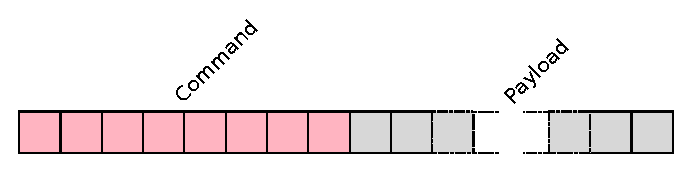
\includegraphics[width=.6\linewidth]{graphics/rxtx_payload.eps}
	\caption[Reading a payload on the nRF24L01.]{Bits written to and received from the \texttt{nRFM} when reading a payload. \texttt{Command} specifies the command given and \texttt{Payload} is the bits written from the \texttt{nRFM}.}
	\label{fig:rxtx_payload}
\end{figure}

Listing \ref{code:rf_read_payload} shows how a payload of 32 bytes is read in C code. 
Line 5 defines the input and output buffers and line 6 assigns the read payload command to the first byte of the output buffer.
33 bytes of data is sent in line 7-8, this is needed in order to create the clock signal for the \texttt{nRFM}, when it sends the 32 bytes payload.
The payload is also read and assigned to the input buffer in line 7-8.
Line 9-12 extracts the 32 bytes payload and ignores the first byte sent from the \texttt{nRFM}, which is the value of the \texttt{STATUS} register.

\begin{listing}[!h]
\begin{minted}{c}
#define R_RX_PAYLOAD       0b01100001
#define PAYLOAD_SIZE       32

void RF_read(XSpiPs *SPI_inst, u8 *buffer){
	u8 input_buffer[PAYLOAD_SIZE+1], output_buffer[PAYLOAD_SIZE+1];
	output_buffer[0] = R_RX_PAYLOAD;
	XSpiPs_PolledTransfer(SPI_inst, output_buffer, input_buffer, @$\Rightarrow$@
		PAYLOAD_SIZE+1);
	int i;
	for(i = 1; i < PAYLOAD_SIZE+1; i++){
		buffer[i-1] = input_buffer[i];
	}
}
\end{minted}
\caption[C function that reads 32 bytes payload from the nRFM]{Implementation of a C function that reads 32 bytes payload from the \texttt{nRFM}. Macros are shown for clarity.}
\label{code:rf_read_payload}
\end{listing}

\subsubsection{PWM Generation} % (fold)
\label{ssub:pwm_generation}
In order to generate the two needed PWM signals from the MicroZed an IP core must be made in VHDL.
As described the IP core needs to be able to switch the PWM signal between channel \texttt{A} and \texttt{B} and have a programmable duty cycle.
It also needs to have a top signal that indicates the center of the PWM pulse.
The designed PWM generator IP core has three inputs and three outputs as illustrated in figure \ref{fig:pwm_gen_component}.
\begin{figure}[h]
	\centering
	\includegraphics[width=.4\linewidth]{graphics/pwm_generator}
	\caption{Input and output signals of the PWM generator component.}
	\label{fig:pwm_gen_component}
\end{figure}
A counter is incremented to a high limit and decremented to zero using a state machine.
The high limit for the counter when using the MicroZed and a PWM frequency of 22KHz is calculated by:
\begin{equation}
	H_{limit} = \frac{F_{Microzed}}{F_{PWM}\cdot 2} = \frac{100\cdot 10^6}{22\cdot 10^3 \cdot 2} = 2272.7 \simeq 2273
\end{equation}
Where $H_{limit}$ is the high counting limit, $F_{MicroZed}$ and $F_{PWM}$ are the frequencies of the MicroZed and the PWM, respectively. 
The PWM output will be set \texttt{high}, when the counter value is greater than a compare value.
Using this mechanism the duty cycle of the PWM can be controlled through the compare value.
The compare value for a 50\% duty cycle should be calculated using:
\begin{equation}
	Compare = (1 - D) \cdot H_{limit} = (1 - 0.5) \cdot 2273 = 1136
\end{equation}
Where $Compare$ is the compare value and $D$ is the wanted duty cycle ratio.

The described mechanism is illustrated in figure \ref{sfig:pwm_gen_int}, where the top signal is simply set \texttt{high}, when the counter reaches its high limit.

\begin{figure}
    \centering
    \begin{subfigure}[b]{0.45\textwidth}
        % This file was created by matlab2tikz.
%
%The latest updates can be retrieved from
%  http://www.mathworks.com/matlabcentral/fileexchange/22022-matlab2tikz-matlab2tikz
%where you can also make suggestions and rate matlab2tikz.
%
\definecolor{mycolor1}{rgb}{0.00000,0.44700,0.74100}%
\definecolor{mycolor2}{rgb}{0.85000,0.32500,0.09800}%
\definecolor{mycolor3}{rgb}{0.92900,0.69400,0.12500}%
\definecolor{mycolor4}{rgb}{0.49400,0.18400,0.55600}%

%
\begin{tikzpicture}

\begin{axis}[%
width=.70\textwidth,
height=2in,
at={(0.758in,0.481in)},
scale only axis,
xmin=0,
xmax=20000,
xlabel style={font=\color{white!15!black}},
xlabel={Clocks},
ymin=0,
ymax=3500,
ylabel style={font=\color{white!15!black}},
ylabel={Value},
axis background/.style={fill=white},
title style={font=\bfseries},
title={Internal Signals},
legend style={legend cell align=left,  align=left, font=\scriptsize, draw=white!15!black}
]
\addplot [color=mycolor1]
  table[row sep=crcr]{%
0	0\\
2273.08333638863	2273\\
4546.16667277727	0\\
6819.2500091659	2273\\
9092.33334555454	0\\
11365.4166819432	2273\\
13638.5000183318	0\\
15911.5833547204	2273\\
18184.6666911091	0\\
20000.7332722273	1816.79929577465\\
};
\addlegendentry{Counter}

\addplot [color=mycolor2]
  table[row sep=crcr]{%
0	0\\
1135.0416131989	0\\
1137.04168652612	2000\\
3409.12498625115	2000\\
3411.12505957837	0\\
5681.20828597617	0\\
5683.20835930339	2000\\
7955.29165902841	2000\\
7957.29173235564	0\\
10227.3749587534	0\\
10229.3750320807	2000\\
12501.4583318057	2000\\
12503.4584051329	0\\
14773.5416315307	0\\
14775.5417048579	2000\\
17047.625004583	2000\\
17049.6250779102	0\\
19319.708304308	0\\
19321.7083776352	2000\\
20000.7332722273	2000\\
};
\addlegendentry{PWM}

\addplot [color=mycolor3]
  table[row sep=crcr]{%
0	0\\
2271.08326306141	0\\
2273.08333638863	2000\\
2275.08340971586	0\\
6817.24993583868	0\\
6819.2500091659	2000\\
6821.25008249313	0\\
11363.4166086159	0\\
11365.4166819432	2000\\
11367.4167552704	0\\
15909.5832813932	0\\
15911.5833547204	2000\\
15913.5834280477	0\\
20000.7332722273	0\\
};
\addlegendentry{TOP}

\addplot [color=mycolor4, dashed]
  table[row sep=crcr]{%
0	1136\\
20000	1136\\
};
\addlegendentry{Compare}

\end{axis}
\end{tikzpicture}%
        \caption{Internal VHDL signals illustrated by a Matlab plot.}
        \label{sfig:pwm_gen_int}
    \end{subfigure}
    \begin{subfigure}[b]{0.45\textwidth}
        % This file was created by matlab2tikz.
%
%The latest updates can be retrieved from
%  http://www.mathworks.com/matlabcentral/fileexchange/22022-matlab2tikz-matlab2tikz
%where you can also make suggestions and rate matlab2tikz.
%
\definecolor{mycolor1}{rgb}{0.00000,0.44700,0.74100}%
%
\begin{tikzpicture}

\begin{axis}[%
width=4.521in,
height=3.566in,
at={(0.758in,0.481in)},
scale only axis,
xmin=0,
xmax=0.0002,
xlabel style={font=\color{white!15!black}},
xlabel={Time [s]},
ymin=0,
ymax=6,
ylabel style={font=\color{white!15!black}},
ylabel={Voltage [V]},
axis background/.style={fill=white},
title style={font=\bfseries},
title={PWM, external signal}
]
\addplot [color=mycolor1, forget plot]
  table[row sep=crcr]{%
-1.00000000280431e-07	3.36\\
0	3.44\\
1.00000000280431e-07	3.36\\
1.99999999672684e-07	3.44\\
4.00000000233547e-07	3.28\\
4.999999996258e-07	3.28\\
5.99999999906231e-07	3.36\\
7.99999999578915e-07	3.36\\
8.99999999859347e-07	3.28\\
1.00000000013978e-06	3.28\\
1.19999999981246e-06	3.44\\
1.30000000009289e-06	3.28\\
1.40000000037332e-06	3.36\\
1.49999999976558e-06	3.28\\
1.70000000032644e-06	3.44\\
1.79999999971869e-06	3.44\\
1.89999999999912e-06	3.36\\
2.00000000027956e-06	3.44\\
2.19999999995224e-06	3.28\\
2.30000000023267e-06	3.28\\
2.39999999962492e-06	3.36\\
2.49999999990536e-06	3.28\\
2.60000000018579e-06	3.44\\
2.69999999957804e-06	3.36\\
3.00000000041933e-06	3.36\\
3.09999999981159e-06	3.28\\
3.20000000009202e-06	3.28\\
3.30000000037245e-06	3.36\\
3.69999999971782e-06	3.36\\
3.79999999999825e-06	3.44\\
3.90000000027868e-06	3.44\\
3.99999999967093e-06	3.36\\
4.2000000002318e-06	3.36\\
4.29999999962405e-06	3.44\\
4.39999999990448e-06	3.36\\
4.50000000018491e-06	3.36\\
4.59999999957716e-06	3.28\\
4.6999999998576e-06	3.44\\
4.80000000013803e-06	3.44\\
4.90000000041846e-06	3.36\\
4.99999999981071e-06	3.36\\
5.10000000009114e-06	3.44\\
5.20000000037157e-06	3.36\\
5.29999999976383e-06	3.36\\
5.40000000004426e-06	3.44\\
5.50000000032469e-06	3.36\\
5.59999999971694e-06	3.36\\
5.69999999999737e-06	3.44\\
5.80000000027781e-06	3.36\\
5.89999999967006e-06	3.36\\
5.99999999995049e-06	3.28\\
6.10000000023092e-06	3.36\\
6.19999999962317e-06	3.28\\
6.2999999999036e-06	3.44\\
6.40000000018404e-06	3.44\\
6.49999999957629e-06	3.28\\
6.59999999985672e-06	3.44\\
6.80000000041758e-06	3.44\\
7.00000000009027e-06	3.28\\
7.1000000003707e-06	3.28\\
7.19999999976295e-06	3.44\\
7.30000000004338e-06	3.36\\
7.40000000032381e-06	3.44\\
7.49999999971607e-06	3.28\\
7.5999999999965e-06	3.44\\
7.70000000027693e-06	3.44\\
7.79999999966918e-06	3.36\\
7.89999999994961e-06	3.44\\
8.0999999996223e-06	3.28\\
8.19999999990273e-06	3.44\\
8.30000000018316e-06	3.28\\
8.39999999957541e-06	3.44\\
8.49999999985585e-06	3.36\\
8.60000000013628e-06	3.44\\
8.90000000008939e-06	3.44\\
9.00000000036982e-06	3.36\\
9.09999999976208e-06	3.44\\
9.20000000004251e-06	3.28\\
9.30000000032294e-06	3.28\\
9.39999999971519e-06	3.44\\
9.49999999999562e-06	3.44\\
9.60000000027605e-06	3.36\\
9.69999999966831e-06	0.16\\
9.79999999994874e-06	0.24\\
9.90000000022917e-06	0.24\\
9.99999999962142e-06	0.0800000000000001\\
1.00999999999019e-05	0.16\\
1.02000000001823e-05	0.32\\
1.02999999995745e-05	0.24\\
1.06000000004158e-05	0.24\\
1.06999999998081e-05	0.32\\
1.08000000000885e-05	0.0800000000000001\\
1.09999999997612e-05	0.24\\
1.13999999999947e-05	0.24\\
1.15000000002752e-05	0.16\\
1.15999999996674e-05	0.32\\
1.16999999999479e-05	0.24\\
1.18000000002283e-05	0.32\\
1.18999999996205e-05	0.32\\
1.21000000001814e-05	0.16\\
1.21999999995737e-05	0.24\\
1.22999999998541e-05	0.24\\
1.24000000001345e-05	0.16\\
1.2500000000415e-05	0.24\\
1.25999999998072e-05	0.16\\
1.27000000000876e-05	0.24\\
1.32999999999939e-05	0.24\\
1.34000000002743e-05	0.16\\
1.34999999996666e-05	0.24\\
1.37000000002274e-05	0.24\\
1.37999999996197e-05	0.32\\
1.38999999999001e-05	0.24\\
1.40000000001805e-05	0.32\\
1.40999999995728e-05	0.24\\
1.41999999998532e-05	0.32\\
1.44000000004141e-05	0.32\\
1.44999999998063e-05	0.24\\
1.46000000000868e-05	0.32\\
1.47000000003672e-05	0.24\\
1.47999999997595e-05	0.24\\
1.49000000000399e-05	0.16\\
1.50000000003203e-05	0.32\\
1.5199999999993e-05	0.16\\
1.53999999996657e-05	0.32\\
1.54999999999461e-05	0.16\\
1.56000000002265e-05	0.24\\
1.56999999996188e-05	0.16\\
1.57999999998992e-05	0.24\\
1.59000000001797e-05	0.16\\
1.60999999998523e-05	0.32\\
1.62000000001328e-05	0.16\\
1.63000000004132e-05	0.24\\
1.63999999998055e-05	0.16\\
1.65000000000859e-05	0.24\\
1.6800000000039e-05	0.24\\
1.69000000003194e-05	0.16\\
1.69999999997117e-05	0.16\\
1.70999999999921e-05	0.24\\
1.72000000002726e-05	0.24\\
1.72999999996648e-05	0.16\\
1.73999999999452e-05	0.24\\
1.75000000002257e-05	0.16\\
1.75999999996179e-05	0.16\\
1.76999999998984e-05	0.32\\
1.78000000001788e-05	0.0800000000000001\\
1.79999999998515e-05	0.24\\
1.81000000001319e-05	0.16\\
1.82000000004123e-05	0.24\\
1.8400000000085e-05	0.24\\
1.85000000003654e-05	0.32\\
1.85999999997577e-05	0.24\\
1.87000000000381e-05	0.24\\
1.88000000003186e-05	0.16\\
1.88999999997108e-05	0.24\\
1.89999999999912e-05	0.24\\
1.91999999996639e-05	0.0800000000000001\\
1.92999999999444e-05	0.24\\
1.94000000002248e-05	0.24\\
1.9499999999617e-05	0.16\\
1.95999999998975e-05	0.24\\
1.97000000001779e-05	0.16\\
1.97999999995702e-05	0.24\\
2.01000000004115e-05	0.24\\
2.01999999998037e-05	0.16\\
2.03000000000841e-05	0.24\\
2.04000000003646e-05	0.16\\
2.04999999997568e-05	0.24\\
2.06000000000373e-05	0.24\\
2.07000000003177e-05	0.16\\
2.08999999999904e-05	0.16\\
2.10000000002708e-05	0.24\\
2.10999999996631e-05	0.16\\
2.11999999999435e-05	0.24\\
2.1600000000177e-05	0.24\\
2.16999999995693e-05	0.16\\
2.17999999998497e-05	0.16\\
2.19000000001301e-05	0.0800000000000001\\
2.20000000004106e-05	0.16\\
2.20999999998028e-05	0.16\\
2.22000000000833e-05	0.24\\
2.23000000003637e-05	0.0800000000000001\\
2.23999999997559e-05	0.16\\
2.25000000000364e-05	0.16\\
2.26000000003168e-05	0.24\\
2.29000000002699e-05	0.24\\
2.29999999996622e-05	0.16\\
2.30999999999426e-05	0.24\\
2.3200000000223e-05	0.24\\
2.33999999998957e-05	0.0800000000000001\\
2.35999999995684e-05	0.24\\
2.39000000004097e-05	0.24\\
2.3999999999802e-05	0.16\\
2.41000000000824e-05	0.24\\
2.42000000003628e-05	0.24\\
2.42999999997551e-05	0.32\\
2.45000000003159e-05	0.16\\
2.46999999999886e-05	0.16\\
2.48999999996613e-05	0.32\\
2.51000000002222e-05	0.16\\
2.51999999996144e-05	0.24\\
2.52999999998949e-05	0.24\\
2.54000000001753e-05	0.16\\
2.5599999999848e-05	0.16\\
2.57000000001284e-05	0.24\\
2.58000000004088e-05	0.16\\
2.58999999998011e-05	0.16\\
2.60000000000815e-05	0.24\\
2.61000000003619e-05	0.16\\
2.61999999997542e-05	0.24\\
2.63000000000346e-05	0.0800000000000001\\
2.64000000003151e-05	0.24\\
2.64999999997073e-05	0.24\\
2.65999999999877e-05	0.16\\
2.67000000002682e-05	0.24\\
2.67999999996604e-05	0.16\\
2.70000000002213e-05	0.16\\
2.70999999996135e-05	0.24\\
2.7199999999894e-05	0.16\\
2.73000000001744e-05	0.24\\
2.73999999995667e-05	0.16\\
2.7700000000408e-05	0.16\\
2.77999999998002e-05	0.24\\
2.79000000000806e-05	0.16\\
2.80999999997533e-05	0.16\\
2.82000000000338e-05	0.24\\
2.83000000003142e-05	0.16\\
2.83999999997064e-05	0.24\\
2.84999999999869e-05	0.16\\
2.86000000002673e-05	0.24\\
2.86999999996596e-05	0.16\\
2.879999999994e-05	0.24\\
2.89000000002204e-05	0.24\\
2.89999999996127e-05	0.0800000000000001\\
2.92000000001735e-05	0.24\\
2.93999999998462e-05	0.24\\
2.95000000001266e-05	0.16\\
2.96000000004071e-05	0.16\\
2.96999999997993e-05	0.24\\
2.98000000000798e-05	0.16\\
2.99999999997524e-05	0.32\\
3.01000000000329e-05	0.16\\
3.0399999999986e-05	0.16\\
3.05000000002664e-05	0.24\\
3.05999999996587e-05	0.16\\
3.06999999999391e-05	0.24\\
3.08000000002195e-05	0.16\\
3.08999999996118e-05	0.32\\
3.11000000001727e-05	0.16\\
3.12999999998453e-05	0.16\\
3.14000000001258e-05	0.24\\
3.15000000004062e-05	0.24\\
3.15999999997985e-05	0.16\\
3.17000000000789e-05	0.24\\
3.18000000003593e-05	0.16\\
3.18999999997516e-05	0.24\\
3.2000000000032e-05	0.16\\
3.21000000003124e-05	0.32\\
3.21999999997047e-05	0.16\\
3.25999999999382e-05	0.16\\
3.27000000002187e-05	0.24\\
3.27999999996109e-05	0.16\\
3.30000000001718e-05	0.16\\
3.3099999999564e-05	0.24\\
3.31999999998445e-05	0.24\\
3.33000000001249e-05	0.16\\
3.34000000004053e-05	0.16\\
3.34999999997976e-05	0.24\\
3.3600000000078e-05	0.24\\
3.37000000003584e-05	0.16\\
3.40000000003116e-05	0.16\\
3.41999999999842e-05	0.32\\
3.43000000002647e-05	0.16\\
3.43999999996569e-05	0.24\\
3.44999999999374e-05	0.16\\
3.46000000002178e-05	0.16\\
3.47999999998905e-05	0.32\\
3.49999999995632e-05	0.16\\
3.50999999998436e-05	0.24\\
3.5200000000124e-05	0.24\\
3.53000000004045e-05	0.16\\
3.53999999997967e-05	0.24\\
3.55000000000771e-05	0.16\\
3.56000000003576e-05	0.24\\
3.56999999997498e-05	0.24\\
3.58000000000303e-05	0.16\\
3.59000000003107e-05	0.24\\
3.59999999997029e-05	0.16\\
3.60999999999834e-05	0.32\\
3.62000000002638e-05	0.16\\
3.63999999999365e-05	0.16\\
3.65000000002169e-05	0.24\\
3.65999999996092e-05	0.4\\
3.66999999998896e-05	0.16\\
3.680000000017e-05	0.16\\
3.68999999995623e-05	0.32\\
3.69999999998427e-05	3.28\\
3.71000000001231e-05	3.36\\
3.72000000004036e-05	3.28\\
3.72999999997958e-05	3.36\\
3.78000000003098e-05	3.36\\
3.78999999997021e-05	3.28\\
3.79999999999825e-05	3.36\\
3.81000000002629e-05	3.28\\
3.81999999996552e-05	3.28\\
3.82999999999356e-05	3.44\\
3.8400000000216e-05	3.36\\
3.84999999996083e-05	3.36\\
3.85999999998887e-05	3.28\\
3.87000000001692e-05	3.36\\
3.87999999995614e-05	3.28\\
3.88999999998418e-05	3.28\\
3.90000000001223e-05	3.36\\
3.93000000000754e-05	3.36\\
3.94000000003558e-05	3.44\\
3.94999999997481e-05	3.44\\
3.96000000000285e-05	3.28\\
3.97000000003089e-05	3.36\\
3.97999999997012e-05	3.36\\
3.98999999999816e-05	3.44\\
4.0000000000262e-05	3.36\\
4.01999999999347e-05	3.36\\
4.03000000002152e-05	3.28\\
4.03999999996074e-05	3.36\\
4.04999999998878e-05	3.28\\
4.06000000001683e-05	3.28\\
4.0799999999841e-05	3.44\\
4.09000000001214e-05	3.36\\
4.10999999997941e-05	3.36\\
4.12000000000745e-05	3.28\\
4.13000000003549e-05	3.36\\
4.13999999997472e-05	3.36\\
4.15000000000276e-05	3.44\\
4.16000000003081e-05	3.36\\
4.17999999999807e-05	3.36\\
4.19000000002612e-05	3.28\\
4.19999999996534e-05	3.44\\
4.20999999999339e-05	3.28\\
4.22000000002143e-05	3.28\\
4.22999999996065e-05	3.36\\
4.2399999999887e-05	3.36\\
4.25000000001674e-05	3.28\\
4.25999999995597e-05	3.44\\
4.26999999998401e-05	3.28\\
4.28000000001205e-05	3.28\\
4.2900000000401e-05	3.36\\
4.31000000000736e-05	3.36\\
4.32000000003541e-05	3.44\\
4.32999999997463e-05	3.36\\
4.35000000003072e-05	3.36\\
4.35999999996994e-05	3.28\\
4.36999999999799e-05	3.36\\
4.38000000002603e-05	3.36\\
4.38999999996526e-05	3.28\\
4.41000000002134e-05	3.44\\
4.41999999996057e-05	3.36\\
4.45999999998392e-05	3.36\\
4.47000000001196e-05	3.52\\
4.48000000004001e-05	3.36\\
4.48999999997923e-05	3.36\\
4.50000000000728e-05	3.44\\
4.51000000003532e-05	3.36\\
4.51999999997454e-05	3.36\\
4.53000000000259e-05	3.44\\
4.54000000003063e-05	3.36\\
4.57999999996517e-05	3.36\\
4.58999999999321e-05	3.28\\
4.60000000002125e-05	3.36\\
4.60999999996048e-05	3.28\\
4.61999999998852e-05	3.36\\
4.63000000001657e-05	3.36\\
4.63999999995579e-05	3.28\\
4.64999999998383e-05	3.44\\
4.67000000003992e-05	3.28\\
4.67999999997915e-05	3.44\\
4.69000000000719e-05	3.36\\
4.70999999997446e-05	3.36\\
4.7200000000025e-05	3.44\\
4.73000000003054e-05	3.28\\
4.74999999999781e-05	3.44\\
4.76000000002585e-05	3.36\\
4.79999999996039e-05	3.36\\
4.80999999998843e-05	3.28\\
4.8299999999557e-05	3.44\\
4.83999999998375e-05	3.36\\
4.85000000001179e-05	3.36\\
4.86000000003983e-05	3.44\\
4.86999999997906e-05	3.44\\
4.8800000000071e-05	3.28\\
4.89000000003514e-05	3.36\\
4.89999999997437e-05	3.36\\
4.91000000000241e-05	3.44\\
4.92000000003046e-05	3.36\\
4.92999999996968e-05	3.44\\
4.93999999999772e-05	3.36\\
4.95999999996499e-05	3.36\\
4.96999999999304e-05	3.44\\
4.98000000002108e-05	3.44\\
4.9899999999603e-05	3.28\\
4.99999999998835e-05	3.28\\
5.01000000001639e-05	3.36\\
5.05000000003974e-05	3.36\\
5.05999999997897e-05	3.28\\
5.07000000000701e-05	3.36\\
5.10000000000232e-05	3.36\\
5.11000000003037e-05	3.28\\
5.11999999996959e-05	3.36\\
5.12999999999764e-05	3.36\\
5.14000000002568e-05	3.44\\
5.1499999999649e-05	3.44\\
5.15999999999295e-05	3.36\\
5.17000000002099e-05	3.44\\
5.17999999996022e-05	3.36\\
5.2000000000163e-05	3.36\\
5.21000000004435e-05	3.28\\
5.21999999998357e-05	3.36\\
5.23000000001161e-05	3.36\\
5.24000000003966e-05	3.28\\
5.26000000000693e-05	3.44\\
5.27000000003497e-05	3.28\\
5.27999999997419e-05	3.28\\
5.29000000000224e-05	3.36\\
5.30000000003028e-05	3.36\\
5.30999999996951e-05	3.44\\
5.31999999999755e-05	3.36\\
5.33000000002559e-05	3.36\\
5.33999999996482e-05	3.44\\
5.34999999999286e-05	3.44\\
5.36999999996013e-05	3.28\\
5.40000000004426e-05	3.52\\
5.42000000001153e-05	3.36\\
5.43000000003957e-05	3.44\\
5.4399999999788e-05	3.44\\
5.45000000000684e-05	3.36\\
5.46000000003488e-05	3.44\\
5.46999999997411e-05	3.36\\
5.49000000003019e-05	3.36\\
5.49999999996942e-05	3.44\\
5.50999999999746e-05	3.36\\
5.5200000000255e-05	0.4\\
5.52999999996473e-05	0.24\\
5.53999999999277e-05	0.32\\
5.55000000002082e-05	0.16\\
5.56999999998808e-05	0.32\\
5.58000000001613e-05	0.24\\
5.59000000004417e-05	0.32\\
5.5999999999834e-05	0.24\\
5.61000000001144e-05	0.32\\
5.64000000000675e-05	0.32\\
5.65999999997402e-05	0.16\\
5.67000000000206e-05	0.24\\
5.71999999996464e-05	0.24\\
5.72999999999269e-05	0.32\\
5.74000000002073e-05	0.24\\
5.74999999995995e-05	0.24\\
5.759999999988e-05	0.16\\
5.77000000001604e-05	0.24\\
5.80000000001135e-05	0.24\\
5.81000000003939e-05	0.32\\
5.81999999997862e-05	0.16\\
5.83000000000666e-05	0.32\\
5.84000000003471e-05	0.24\\
5.84999999997393e-05	0.24\\
5.86000000000197e-05	0.32\\
5.87000000003002e-05	0.16\\
5.87999999996924e-05	0.16\\
5.88999999999729e-05	0.24\\
5.96000000001595e-05	0.24\\
5.970000000044e-05	0.32\\
5.99000000001126e-05	0.16\\
6.03000000003462e-05	0.16\\
6.03999999997384e-05	0.32\\
6.05000000000189e-05	0.16\\
6.06999999996916e-05	0.32\\
6.0799999999972e-05	0.24\\
6.09000000002524e-05	0.24\\
6.09999999996447e-05	0.0800000000000001\\
6.10999999999251e-05	0.24\\
6.12000000002055e-05	0.24\\
6.12999999995978e-05	0.16\\
6.13999999998782e-05	0.24\\
6.15000000001586e-05	0.16\\
6.16000000004391e-05	0.16\\
6.16999999998313e-05	0.24\\
6.18000000001118e-05	0.24\\
6.19000000003922e-05	0.16\\
6.19999999997844e-05	0.24\\
6.21000000000649e-05	0.24\\
6.22000000003453e-05	0.16\\
6.22999999997376e-05	0.24\\
6.2400000000018e-05	0.24\\
6.25000000002984e-05	0.16\\
6.25999999996907e-05	0.24\\
6.28000000002515e-05	0.24\\
6.28999999996438e-05	0.16\\
6.29999999999242e-05	0.24\\
6.31000000002047e-05	0.24\\
6.31999999995969e-05	0.16\\
6.32999999998773e-05	0.24\\
6.34000000001578e-05	0.24\\
6.35000000004382e-05	0.32\\
6.35999999998305e-05	0.24\\
6.37000000001109e-05	0.24\\
6.38000000003913e-05	0.32\\
6.38999999997836e-05	0.32\\
6.4000000000064e-05	0.24\\
6.43000000000171e-05	0.24\\
6.44000000002976e-05	0.32\\
6.44999999996898e-05	0.32\\
6.45999999999702e-05	0.16\\
6.47000000002507e-05	0.32\\
6.48999999999234e-05	0.32\\
6.50000000002038e-05	0.24\\
6.5099999999596e-05	0.24\\
6.51999999998765e-05	0.16\\
6.53000000001569e-05	0.24\\
6.54999999998296e-05	0.24\\
6.560000000011e-05	0.16\\
6.57999999997827e-05	0.32\\
6.59000000000631e-05	0.0800000000000001\\
6.60000000003436e-05	0.16\\
6.60999999997358e-05	0.32\\
6.62000000000162e-05	0.16\\
6.63000000002967e-05	0.24\\
6.63999999996889e-05	0.16\\
6.66000000002498e-05	0.32\\
6.6699999999642e-05	0.16\\
6.67999999999225e-05	0.16\\
6.69000000002029e-05	0.24\\
6.69999999995952e-05	0.16\\
6.70999999998756e-05	0.24\\
6.73000000004365e-05	0.0800000000000001\\
6.73999999998287e-05	0.24\\
6.75000000001091e-05	0.24\\
6.76000000003896e-05	0.16\\
6.76999999997818e-05	0.16\\
6.78000000000623e-05	0.24\\
6.79000000003427e-05	0.16\\
6.79999999997349e-05	0.4\\
6.81000000000154e-05	0.24\\
6.82000000002958e-05	0.24\\
6.82999999996881e-05	0.16\\
6.83999999999685e-05	0.24\\
6.85000000002489e-05	0.16\\
6.8800000000202e-05	0.16\\
6.88999999995943e-05	0.24\\
6.89999999998747e-05	0.16\\
6.91000000001551e-05	0.24\\
6.92000000004356e-05	0.16\\
6.94000000001083e-05	0.16\\
6.95000000003887e-05	0.24\\
6.95999999997809e-05	0.24\\
6.97000000000614e-05	0.16\\
6.98000000003418e-05	0.16\\
6.98999999997341e-05	0.24\\
7.00000000000145e-05	0.16\\
7.01000000002949e-05	0.24\\
7.01999999996872e-05	0.0800000000000001\\
7.02999999999676e-05	0.16\\
7.0400000000248e-05	0.16\\
7.04999999996403e-05	0.24\\
7.05999999999207e-05	0.16\\
7.07000000002012e-05	0.24\\
7.07999999995934e-05	0.24\\
7.08999999998738e-05	0.16\\
7.10000000001543e-05	0.24\\
7.11000000004347e-05	0.24\\
7.1199999999827e-05	0.16\\
7.13000000001074e-05	0.32\\
7.14999999997801e-05	0.16\\
7.16000000000605e-05	0.24\\
7.17999999997332e-05	0.0800000000000001\\
7.19000000000136e-05	0.0800000000000001\\
7.20000000002941e-05	0.16\\
7.20999999996863e-05	0.16\\
7.21999999999667e-05	0.24\\
7.23000000002472e-05	0.16\\
7.26000000002003e-05	0.16\\
7.26999999995925e-05	0.24\\
7.2799999999873e-05	0.24\\
7.29000000001534e-05	0.16\\
7.30000000004338e-05	0.24\\
7.33000000003869e-05	0.24\\
7.33999999997792e-05	0.16\\
7.35000000000596e-05	0.24\\
7.36999999997323e-05	0.24\\
7.38000000000127e-05	0.32\\
7.39000000002932e-05	0.24\\
7.40999999999659e-05	0.24\\
7.42000000002463e-05	0.16\\
7.42999999996385e-05	0.16\\
7.4399999999919e-05	0.24\\
7.45000000001994e-05	0.16\\
7.45999999995917e-05	0.24\\
7.46999999998721e-05	0.16\\
7.48000000001525e-05	0.24\\
7.4900000000433e-05	0.0800000000000001\\
7.49999999998252e-05	0.24\\
7.51000000001056e-05	0.0800000000000001\\
7.52000000003861e-05	0.24\\
7.52999999997783e-05	0.16\\
7.54000000000588e-05	0.16\\
7.55000000003392e-05	0.24\\
7.55999999997314e-05	0.16\\
7.57000000000119e-05	0.24\\
7.58000000002923e-05	0.16\\
7.58999999996846e-05	0.16\\
7.5999999999965e-05	0.24\\
7.61999999996377e-05	0.24\\
7.62999999999181e-05	0.16\\
7.64999999995908e-05	0.32\\
7.67000000001516e-05	0.16\\
7.70000000001048e-05	0.16\\
7.71000000003852e-05	0.24\\
7.71999999997774e-05	0.16\\
7.73000000000579e-05	0.16\\
7.74000000003383e-05	0.32\\
7.74999999997306e-05	0.0800000000000001\\
7.7600000000011e-05	0.32\\
7.77999999996837e-05	0.16\\
7.78999999999641e-05	0.32\\
7.80000000002445e-05	0.16\\
7.80999999996368e-05	0.24\\
7.81999999999172e-05	0.0800000000000001\\
7.83000000001977e-05	0.32\\
7.84999999998703e-05	0.16\\
7.86000000001508e-05	0.16\\
7.87000000004312e-05	0.24\\
7.87999999998235e-05	0.16\\
7.89000000001039e-05	0.16\\
7.90000000003843e-05	0.24\\
7.90999999997766e-05	0.16\\
7.9200000000057e-05	0.16\\
7.93000000003374e-05	0.24\\
7.93999999997297e-05	0.16\\
7.95000000000101e-05	0.24\\
7.96999999996828e-05	0.0800000000000001\\
7.97999999999632e-05	0.24\\
7.99000000002437e-05	0.16\\
7.99999999996359e-05	0.24\\
8.00999999999163e-05	0.16\\
8.02000000001968e-05	0.16\\
8.0299999999589e-05	0.0800000000000001\\
8.03999999998695e-05	0.16\\
8.06999999998226e-05	0.16\\
8.0800000000103e-05	0.24\\
8.09000000003834e-05	0.16\\
8.09999999997757e-05	0.32\\
8.11000000000561e-05	0.16\\
8.12000000003366e-05	0.16\\
8.12999999997288e-05	0.0800000000000001\\
8.14000000000092e-05	0.24\\
8.15000000002897e-05	0.16\\
8.15999999996819e-05	0.24\\
8.16999999999624e-05	0.0800000000000001\\
8.18000000002428e-05	0.16\\
8.1899999999635e-05	0.16\\
8.19999999999155e-05	0.0800000000000001\\
8.21000000001959e-05	0.24\\
8.21999999995882e-05	0.24\\
8.22999999998686e-05	0.0800000000000001\\
8.2400000000149e-05	4.08\\
8.25000000004295e-05	3.28\\
8.27000000001021e-05	3.28\\
8.28000000003826e-05	3.36\\
8.28999999997748e-05	3.36\\
8.30000000000553e-05	3.44\\
8.31000000003357e-05	3.44\\
8.31999999997279e-05	3.36\\
8.34999999996811e-05	3.36\\
8.35999999999615e-05	3.28\\
8.37000000002419e-05	3.44\\
8.37999999996342e-05	3.36\\
8.38999999999146e-05	3.44\\
8.4000000000195e-05	3.28\\
8.40999999995873e-05	3.28\\
8.43000000001481e-05	3.44\\
8.44000000004286e-05	3.36\\
8.50999999997271e-05	3.36\\
8.52000000000075e-05	3.28\\
8.53000000002879e-05	3.36\\
8.54999999999606e-05	3.36\\
8.5600000000241e-05	3.28\\
8.56999999996333e-05	3.28\\
8.57999999999137e-05	3.36\\
8.59000000001942e-05	3.36\\
8.59999999995864e-05	3.28\\
8.60999999998668e-05	3.36\\
8.66000000003808e-05	3.36\\
8.66999999997731e-05	3.28\\
8.68000000000535e-05	3.36\\
8.69000000003339e-05	3.36\\
8.69999999997262e-05	3.28\\
8.71000000000066e-05	3.36\\
8.75999999996324e-05	3.36\\
8.76999999999128e-05	3.28\\
8.78000000001933e-05	3.44\\
8.78999999995855e-05	3.44\\
8.7999999999866e-05	3.36\\
8.82999999998191e-05	3.36\\
8.84000000000995e-05	3.28\\
8.85000000003799e-05	3.36\\
8.90000000000057e-05	3.36\\
8.91000000002862e-05	3.28\\
8.92999999999589e-05	3.44\\
8.94999999996315e-05	3.44\\
8.9599999999912e-05	3.28\\
8.97000000001924e-05	3.36\\
8.97999999995847e-05	3.36\\
8.98999999998651e-05	3.28\\
9.00000000001455e-05	3.28\\
9.0100000000426e-05	3.36\\
9.03000000000986e-05	3.36\\
9.04000000003791e-05	3.28\\
9.04999999997713e-05	3.28\\
9.06000000000518e-05	3.44\\
9.07000000003322e-05	3.36\\
9.07999999997244e-05	3.36\\
9.09000000000049e-05	3.44\\
9.10000000002853e-05	3.28\\
9.1199999999958e-05	3.28\\
9.13000000002384e-05	3.36\\
9.16999999995838e-05	3.36\\
9.17999999998642e-05	3.28\\
9.19000000001446e-05	3.28\\
9.20000000004251e-05	3.36\\
9.23999999997704e-05	3.36\\
9.25000000000509e-05	3.44\\
9.26000000003313e-05	3.36\\
9.26999999997236e-05	3.44\\
9.2800000000004e-05	3.36\\
9.32000000002375e-05	3.36\\
9.32999999996298e-05	3.44\\
9.33999999999102e-05	3.36\\
9.35000000001907e-05	3.36\\
9.35999999995829e-05	3.52\\
9.36999999998633e-05	3.36\\
9.38000000001438e-05	3.36\\
9.39000000004242e-05	3.44\\
9.41000000000969e-05	3.28\\
9.42000000003773e-05	3.44\\
9.42999999997696e-05	3.28\\
9.440000000005e-05	3.36\\
9.45000000003304e-05	3.36\\
9.45999999997227e-05	3.52\\
9.48000000002835e-05	3.28\\
9.48999999996758e-05	3.36\\
9.49999999999562e-05	3.36\\
9.51000000002367e-05	3.28\\
9.52999999999093e-05	3.44\\
9.54000000001898e-05	3.36\\
9.5499999999582e-05	3.44\\
9.55999999998625e-05	3.36\\
9.57000000001429e-05	3.44\\
9.58000000004233e-05	3.36\\
9.58999999998156e-05	3.36\\
9.6000000000096e-05	3.44\\
9.61000000003764e-05	3.36\\
9.61999999997687e-05	3.36\\
9.63000000000491e-05	3.44\\
9.64000000003296e-05	3.36\\
9.64999999997218e-05	3.44\\
9.66000000000022e-05	3.36\\
9.67000000002827e-05	3.44\\
9.67999999996749e-05	3.36\\
9.68999999999554e-05	3.44\\
9.70000000002358e-05	3.44\\
9.7099999999628e-05	3.36\\
9.71999999999085e-05	3.44\\
9.73000000001889e-05	3.36\\
9.73999999995812e-05	3.36\\
9.74999999998616e-05	3.44\\
9.7600000000142e-05	3.36\\
9.77000000004224e-05	3.52\\
9.77999999998147e-05	3.44\\
9.79000000000951e-05	3.44\\
9.80000000003756e-05	3.36\\
9.8699999999674e-05	3.36\\
9.87999999999545e-05	3.44\\
9.89000000002349e-05	3.36\\
9.89999999996272e-05	3.36\\
9.90999999999076e-05	3.44\\
9.9200000000188e-05	3.36\\
9.92999999995803e-05	3.44\\
9.95000000001411e-05	3.28\\
9.96000000004216e-05	3.36\\
9.96999999998138e-05	3.36\\
9.98000000000943e-05	3.44\\
9.99000000003747e-05	3.28\\
9.99999999997669e-05	3.36\\
0.00010029999999972	3.36\\
0.0001004	3.44\\
0.000100500000000281	3.44\\
0.000100599999999673	-0.24\\
0.000100699999999954	0.24\\
0.000100800000000234	0.32\\
0.000100899999999626	0.32\\
0.000101100000000187	0.16\\
0.000101199999999579	0.16\\
0.00010129999999986	0.24\\
0.00010140000000014	0.16\\
0.000101500000000421	0.16\\
0.000101599999999813	0.24\\
0.000101700000000093	0.16\\
0.000101800000000374	0.32\\
0.000101899999999766	0.24\\
0.000102199999999719	0.24\\
0.0001023	0.16\\
0.00010240000000028	0.24\\
0.000102499999999672	0.24\\
0.000102599999999953	0.16\\
0.000102799999999625	0.32\\
0.000102899999999906	0.24\\
0.000103300000000139	0.24\\
0.00010340000000042	0.32\\
0.000103600000000093	0.32\\
0.000103700000000373	0.24\\
0.000103900000000046	0.24\\
0.000104099999999718	0.4\\
0.000104199999999999	0.24\\
0.000104300000000279	0.32\\
0.000104399999999671	0.24\\
0.000104499999999952	0.32\\
0.000104600000000232	0.16\\
0.000104699999999625	0.24\\
0.000104999999999578	0.24\\
0.000105099999999858	0.16\\
0.000105200000000139	0.24\\
0.000105399999999811	0.24\\
0.000105500000000092	0.16\\
0.000105600000000372	0.24\\
0.000105699999999764	0.24\\
0.000105800000000045	0.32\\
0.000105900000000325	0.24\\
0.000105999999999717	0.24\\
0.000106099999999998	0.16\\
0.000106200000000278	0.24\\
0.000106299999999671	0.16\\
0.000106399999999951	0.24\\
0.000106500000000231	0.24\\
0.000106599999999624	0.16\\
0.000106699999999904	0.32\\
0.000106800000000185	0.16\\
0.000106899999999577	0.24\\
0.00010729999999981	0.24\\
0.000107400000000091	0.32\\
0.000107500000000371	0.16\\
0.000107599999999763	0.32\\
0.000107700000000044	0.24\\
0.000107800000000324	0.24\\
0.000107899999999717	0.16\\
0.000108100000000277	0.32\\
0.00010819999999967	0.16\\
0.00010829999999995	0.24\\
0.000108400000000231	0.16\\
0.000108499999999623	0.24\\
0.000108700000000184	0.24\\
0.000108799999999576	0.16\\
0.000108899999999856	0.24\\
0.00010930000000009	0.24\\
0.00010940000000037	0.16\\
0.000109499999999763	0.16\\
0.000109600000000043	0.24\\
0.000109700000000323	0.24\\
0.000109799999999716	0.16\\
0.000109899999999996	0.24\\
0.000110000000000277	0.16\\
0.000110099999999669	0.24\\
0.00011030000000023	0.24\\
0.000110399999999622	0.16\\
0.000110499999999902	0.16\\
0.000110600000000183	0.24\\
0.000110699999999575	0.24\\
0.000110799999999855	0.16\\
0.000110900000000136	0.24\\
0.000111000000000416	0.16\\
0.000111099999999809	0.16\\
0.000111200000000089	0.0800000000000001\\
0.000111300000000369	0.16\\
0.000111399999999762	0.0800000000000001\\
0.000111500000000042	0.16\\
0.000111600000000323	0.0800000000000001\\
0.000111799999999995	0.24\\
0.000111900000000276	0.16\\
0.000111999999999668	0.16\\
0.000112099999999948	0.24\\
0.000112200000000229	0.24\\
0.000112299999999621	0.16\\
0.000112399999999901	0.16\\
0.000112500000000182	0.24\\
0.000112599999999574	0.0800000000000001\\
0.000112699999999855	0.32\\
0.000112800000000135	0.24\\
0.000112999999999808	0.24\\
0.000113100000000088	0.16\\
0.000113200000000369	0.32\\
0.000113400000000041	0.32\\
0.000113500000000322	0.24\\
0.000113599999999714	0.24\\
0.000113699999999994	0.16\\
0.000113899999999667	0.16\\
0.000113999999999947	0.24\\
0.000114100000000228	0.24\\
0.00011419999999962	0.16\\
0.000114299999999901	0.16\\
0.000114400000000181	0.24\\
0.000114599999999854	0.24\\
0.000114700000000134	0.16\\
0.000114800000000415	0.24\\
0.000115000000000087	0.0800000000000001\\
0.000115100000000368	0.24\\
0.00011519999999976	0.16\\
0.00011530000000004	0.24\\
0.000115400000000321	0.16\\
0.000115499999999713	0.24\\
0.000115799999999666	0.24\\
0.000115899999999947	0.16\\
0.000116000000000227	0.16\\
0.000116099999999619	0.24\\
0.0001161999999999	0.24\\
0.00011630000000018	0.16\\
0.000116399999999572	0.24\\
0.000116600000000133	0.24\\
0.000116700000000414	0.0800000000000001\\
0.000116799999999806	0.16\\
0.000116900000000086	0.16\\
0.000117000000000367	0.24\\
0.000117099999999759	0.16\\
0.000117200000000039	0.16\\
0.00011730000000032	0.24\\
0.000117399999999712	0.16\\
0.000117499999999993	0.24\\
0.000117699999999665	0.24\\
0.000117799999999946	0.16\\
0.000117900000000226	0.24\\
0.000118099999999899	0.24\\
0.000118200000000179	0.16\\
0.000118299999999572	0.16\\
0.000118399999999852	0.24\\
0.000118500000000132	0.16\\
0.000118600000000413	0.24\\
0.000118699999999805	0.16\\
0.000118800000000086	0.24\\
0.000118900000000366	0.16\\
0.000118999999999758	0.24\\
0.000119100000000039	0.24\\
0.000119299999999711	0.0800000000000001\\
0.000119399999999992	0.0800000000000001\\
0.000119599999999664	0.24\\
0.000119699999999945	0.16\\
0.000119800000000225	0.24\\
0.000119899999999618	0.16\\
0.000119999999999898	0.32\\
0.000120100000000178	0.24\\
0.000120199999999571	0.24\\
0.000120299999999851	0.16\\
0.000120400000000132	0.16\\
0.000120500000000412	0.24\\
0.000120599999999804	0.24\\
0.000120700000000085	0.16\\
0.000120800000000365	0.24\\
0.000120899999999757	0.24\\
0.000121000000000038	0.16\\
0.000121100000000318	0.24\\
0.00012119999999971	0.24\\
0.000121400000000271	0.0800000000000001\\
0.000121499999999664	0.16\\
0.000121599999999944	0.16\\
0.000121700000000224	0.24\\
0.000121799999999617	0.24\\
0.000121899999999897	0.16\\
0.00012209999999957	0.16\\
0.00012219999999985	0.24\\
0.000122300000000131	0.0800000000000001\\
0.000122400000000411	0.16\\
0.000122499999999803	0.0800000000000001\\
0.000122700000000364	0.24\\
0.000122900000000037	0.24\\
0.000123000000000317	0.16\\
0.00012309999999971	0.24\\
0.00012319999999999	0.24\\
0.00012330000000027	0.4\\
0.000123499999999943	0.16\\
0.000123600000000224	0.24\\
0.000123699999999616	0.16\\
0.000123799999999896	0.24\\
0.000124099999999849	0.24\\
0.00012420000000013	0.16\\
0.000124600000000363	0.16\\
0.000124699999999756	0.24\\
0.00012520000000027	0.24\\
0.000125299999999662	0.16\\
0.000125399999999942	0.24\\
0.000125500000000223	0.16\\
0.000125800000000176	0.16\\
0.000125899999999568	0.24\\
0.000126299999999802	0.24\\
0.000126400000000082	0.16\\
0.000126599999999755	0.16\\
0.000126700000000035	0.24\\
0.000126800000000316	0.16\\
0.000126999999999988	0.16\\
0.000127100000000269	0.24\\
0.000127199999999661	0.16\\
0.000127299999999941	0.16\\
0.000127400000000222	0.24\\
0.000127599999999894	0.24\\
0.000127700000000175	0.16\\
0.000127799999999567	0.32\\
0.000127899999999848	3.6\\
0.000128000000000128	3.28\\
0.000128100000000408	3.28\\
0.000128300000000081	3.44\\
0.000128400000000362	3.44\\
0.000128499999999754	3.36\\
0.00012909999999966	3.36\\
0.00012919999999994	3.28\\
0.000129399999999613	3.28\\
0.000129499999999894	3.36\\
0.000129600000000174	3.28\\
0.000129699999999566	3.28\\
0.000129799999999847	3.36\\
0.00013020000000008	3.36\\
0.000130300000000361	3.28\\
0.000130399999999753	3.36\\
0.000130500000000033	3.36\\
0.000130600000000314	3.28\\
0.000130699999999706	3.36\\
0.00013109999999994	3.36\\
0.00013120000000022	3.28\\
0.000131299999999612	3.28\\
0.000131399999999893	3.36\\
0.000131800000000126	3.36\\
0.000131900000000407	3.28\\
0.000131999999999799	3.28\\
0.000132100000000079	3.36\\
0.00013220000000036	3.2\\
0.000132299999999752	3.36\\
0.000132400000000032	3.2\\
0.000132500000000313	3.36\\
0.000132899999999658	3.36\\
0.000132999999999939	3.28\\
0.000133199999999611	3.44\\
0.000133299999999892	3.36\\
0.000133700000000125	3.36\\
0.000133800000000406	3.44\\
0.000133899999999798	3.36\\
0.000134000000000079	3.44\\
0.000134100000000359	3.2\\
0.000134199999999751	3.36\\
0.000134300000000032	3.28\\
0.000134400000000312	3.44\\
0.000134499999999704	3.28\\
0.000134599999999985	3.36\\
0.000134700000000265	3.36\\
0.000134799999999657	3.44\\
0.000134899999999938	3.36\\
0.000135700000000405	3.36\\
0.000135799999999797	3.28\\
0.000135900000000078	3.44\\
0.000136000000000358	3.44\\
0.00013609999999975	3.36\\
0.000136200000000031	3.36\\
0.000136300000000311	3.44\\
0.000136499999999984	3.28\\
0.000136600000000264	3.36\\
0.000136699999999657	3.28\\
0.000136799999999937	3.36\\
0.000136900000000217	3.36\\
0.00013699999999961	3.28\\
0.00013709999999989	3.36\\
0.000137200000000171	3.36\\
0.000137299999999563	3.52\\
0.000137399999999843	3.44\\
0.000137500000000124	3.52\\
0.000137600000000404	3.36\\
0.000137699999999796	3.36\\
0.000137800000000077	3.44\\
0.000137900000000357	3.36\\
0.000138399999999983	3.36\\
0.000138500000000263	3.44\\
0.000138599999999656	3.36\\
0.000138699999999936	3.44\\
0.000138800000000217	3.36\\
0.000138999999999889	3.36\\
0.00013910000000017	3.28\\
0.000139199999999562	3.36\\
0.000139400000000123	3.36\\
0.000139500000000403	3.44\\
0.000139599999999795	3.36\\
0.000140000000000029	3.36\\
0.000140100000000309	3.44\\
0.000140199999999702	3.28\\
0.000140299999999982	3.36\\
0.000140400000000263	3.36\\
0.000140499999999655	3.44\\
0.000140700000000216	3.28\\
0.000140799999999608	3.36\\
0.000141099999999561	3.36\\
0.000141199999999841	3.28\\
0.000141300000000122	3.28\\
0.000141499999999795	3.44\\
0.000141600000000075	3.36\\
0.000141700000000355	3.44\\
0.000141799999999748	3.36\\
0.000142699999999607	3.36\\
0.000142799999999887	3.44\\
0.000142900000000168	3.36\\
0.00014299999999956	3.44\\
0.000143099999999841	3.44\\
0.000143200000000121	3.36\\
0.000143399999999794	3.36\\
0.000143500000000074	3.44\\
0.000143699999999747	3.44\\
0.000143800000000027	3.36\\
0.000143900000000308	3.36\\
0.0001439999999997	3.28\\
0.00014409999999998	3.44\\
0.000144200000000261	3.44\\
0.000144299999999653	3.36\\
0.000144399999999933	3.36\\
0.000144500000000214	3.44\\
0.000144599999999606	3.36\\
0.000144699999999887	3.36\\
0.000144800000000167	3.44\\
0.000144899999999559	3.36\\
0.00014499999999984	3.36\\
0.00014510000000012	3.28\\
0.000145200000000401	3.28\\
0.000145299999999793	3.36\\
0.000145500000000354	3.36\\
0.000145599999999746	3.44\\
0.000145700000000026	3.36\\
0.000145800000000307	3.44\\
0.000145899999999699	3.44\\
0.000145999999999979	3.36\\
0.00014610000000026	0.24\\
0.000146199999999652	0.16\\
0.000146299999999933	0.24\\
0.000146499999999605	0.24\\
0.000146599999999886	0.16\\
0.000146700000000166	0.24\\
0.000146799999999558	0.16\\
0.000146899999999839	0.24\\
0.000147000000000119	0.24\\
0.0001471000000004	0.32\\
0.000147199999999792	0.24\\
0.000147400000000353	0.24\\
0.000147499999999745	0.16\\
0.000147600000000025	0.16\\
0.000147700000000306	0.32\\
0.000147799999999698	0.16\\
0.000147899999999979	0.16\\
0.000148000000000259	0.24\\
0.000148199999999932	0.24\\
0.000148300000000212	0.32\\
0.000148399999999604	0.24\\
0.000148499999999885	0.24\\
0.000148600000000165	0.16\\
0.000148699999999558	0.32\\
0.000148900000000118	0.16\\
0.000149000000000399	0.16\\
0.000149099999999791	0.32\\
0.000149200000000071	0.16\\
0.000149300000000352	0.32\\
0.000149399999999744	0.16\\
0.000149500000000025	0.32\\
0.000149600000000305	0.24\\
0.000149699999999697	0.32\\
0.000149799999999978	0.24\\
0.000150099999999931	0.24\\
0.000150200000000211	0.32\\
0.000150299999999604	0.24\\
0.000150500000000164	0.24\\
0.000150599999999557	0.16\\
0.000150699999999837	0.16\\
0.000150800000000118	0.0800000000000001\\
0.000150900000000398	0.24\\
0.00015099999999979	0.16\\
0.000151400000000024	0.16\\
0.000151500000000304	0.24\\
0.00015189999999965	0.24\\
0.00015199999999993	0.16\\
0.00015210000000021	0.16\\
0.000152299999999883	0.32\\
0.000152400000000164	0.32\\
0.000152500000000444	0.24\\
0.000152899999999789	0.24\\
0.00015300000000007	0.4\\
0.00015310000000035	0.24\\
0.000153499999999696	0.24\\
0.000153599999999976	0.32\\
0.000153700000000256	0.24\\
0.000153799999999649	0.24\\
0.000153899999999929	0.32\\
0.00015400000000021	0.24\\
0.000154099999999602	0.24\\
0.000154199999999882	0.32\\
0.000154300000000163	0.24\\
0.000154700000000396	0.24\\
0.000154799999999788	0.32\\
0.000155000000000349	0.16\\
0.000155099999999742	0.24\\
0.000155200000000022	0.24\\
0.000155300000000302	0.16\\
0.000155399999999695	0.32\\
0.000155499999999975	0.24\\
0.000155600000000256	0.24\\
0.000155699999999648	0.32\\
0.000155799999999928	0.32\\
0.000155900000000209	0.0800000000000001\\
0.000156099999999881	0.24\\
0.000156200000000162	0.24\\
0.000156300000000442	0.16\\
0.000156500000000115	0.16\\
0.000156600000000395	0.24\\
0.000156699999999788	0.16\\
0.000156800000000068	0.16\\
0.000156900000000348	0.24\\
0.000156999999999741	0.16\\
0.000157100000000021	0.32\\
0.000157200000000302	0.24\\
0.000157299999999694	0.32\\
0.000157399999999974	0.24\\
0.000157599999999647	0.24\\
0.000157699999999927	0.16\\
0.000157800000000208	0.16\\
0.00015799999999988	0.32\\
0.000158200000000441	0.16\\
0.000158299999999834	0.16\\
0.000158400000000114	0.24\\
0.000158500000000394	0.16\\
0.000158599999999787	0.24\\
0.000158700000000067	0.24\\
0.000158800000000348	0.16\\
0.00015889999999974	0.24\\
0.00015900000000002	0.16\\
0.000159100000000301	0.24\\
0.000159199999999693	0.24\\
0.000159299999999973	0.16\\
0.000159400000000254	0.24\\
0.000159499999999646	0.16\\
0.000159599999999926	0.24\\
0.000159700000000207	0.16\\
0.00015989999999988	0.16\\
0.00016000000000016	0.0800000000000001\\
0.00016010000000044	0.24\\
0.000160199999999833	0.24\\
0.000160300000000113	0.16\\
0.000160400000000394	0.24\\
0.000160600000000066	0.0800000000000001\\
0.000160700000000347	0.16\\
0.000160799999999739	0.16\\
0.000160900000000019	0.24\\
0.000161099999999692	0.0800000000000001\\
0.000161199999999972	0.0800000000000001\\
0.000161300000000253	0.24\\
0.000161499999999926	0.24\\
0.000161699999999598	0.0800000000000001\\
0.000161799999999879	0.24\\
0.000161900000000159	0.24\\
0.00016200000000044	0.16\\
0.000162200000000112	0.16\\
0.000162300000000393	0.24\\
0.000162500000000065	0.24\\
0.000162600000000346	0.16\\
0.000162800000000018	0.32\\
0.000162900000000299	0.32\\
0.000162999999999691	0.16\\
0.000163099999999972	0.24\\
0.000163200000000252	0.24\\
0.000163299999999644	0.16\\
0.000163399999999925	0.24\\
0.000163500000000205	0.24\\
0.000163599999999597	0.16\\
0.000163699999999878	0.24\\
0.000163900000000439	0.24\\
0.000163999999999831	0.0800000000000001\\
0.000164100000000111	0.16\\
0.000164200000000392	0.16\\
0.000164299999999784	0.24\\
0.000164400000000064	0.24\\
0.000164500000000345	0.0800000000000001\\
0.000164599999999737	0.24\\
0.000164700000000018	0.16\\
0.000164800000000298	0.24\\
0.00016489999999969	0.16\\
0.000165199999999643	0.16\\
0.000165299999999924	0.24\\
0.000165400000000204	0.24\\
0.000165499999999597	0.0800000000000001\\
0.000165599999999877	0.32\\
0.000165800000000438	0.16\\
0.00016589999999983	0.16\\
0.000166000000000111	0.24\\
0.000166100000000391	0.16\\
0.000166199999999783	0.16\\
0.000166300000000064	0.0800000000000001\\
0.000166400000000344	0.16\\
0.000166499999999736	0.32\\
0.000166600000000017	0.16\\
0.000166700000000297	0.16\\
0.000166799999999689	0.24\\
0.00016700000000025	0.24\\
0.000167099999999643	0.16\\
0.000167199999999923	0.24\\
0.000167300000000203	0.16\\
0.000167399999999596	0.24\\
0.000167499999999876	0.24\\
0.000167600000000157	0.0800000000000001\\
0.000167700000000437	0.16\\
0.000167799999999829	0.16\\
0.00016790000000011	0.0800000000000001\\
0.000168099999999782	0.24\\
0.000168200000000063	0.16\\
0.000168300000000343	0.24\\
0.000168399999999735	0.16\\
0.000168500000000016	0.24\\
0.000168600000000296	0.24\\
0.000168699999999689	0.16\\
0.000168999999999642	0.16\\
0.000169099999999922	0.24\\
0.000169200000000203	0.16\\
0.000169399999999875	0.16\\
0.000169500000000156	0.24\\
0.000169600000000436	0.24\\
0.000169699999999828	0.16\\
0.000169800000000109	0.16\\
0.000169900000000389	0.0800000000000001\\
0.000169999999999781	0.24\\
0.000170100000000062	0.16\\
0.000170200000000342	0.16\\
0.000170299999999735	0.24\\
0.000170400000000015	0.16\\
0.000170699999999968	0.16\\
0.000170800000000249	0.0800000000000001\\
0.000170899999999641	0.16\\
0.000171299999999874	0.16\\
0.000171400000000155	0.0800000000000001\\
0.000171599999999827	0.24\\
0.000171800000000388	0.24\\
0.000171899999999781	0.16\\
0.000172000000000061	0.24\\
0.000172300000000014	0.24\\
0.000172400000000295	0.16\\
0.000172499999999687	0.16\\
0.000172599999999967	0.24\\
0.00017289999999992	0.24\\
0.000173000000000201	0.56\\
0.000173099999999593	0.24\\
0.000173199999999873	0.16\\
0.000173300000000154	0.24\\
0.000173400000000434	3.52\\
0.000173499999999827	3.28\\
0.000173600000000107	3.36\\
0.00017379999999978	3.36\\
0.00017390000000006	3.28\\
0.000174099999999733	3.28\\
0.000174200000000013	3.36\\
0.000174399999999686	3.36\\
0.000174499999999966	3.44\\
0.000174600000000247	3.36\\
0.000174699999999639	3.36\\
0.000174799999999919	3.2\\
0.0001749000000002	3.36\\
0.000174999999999592	3.28\\
0.000175099999999873	3.28\\
0.000175200000000153	3.36\\
0.000175300000000433	3.28\\
0.000175399999999826	3.36\\
0.000175699999999779	3.36\\
0.000175800000000059	3.28\\
0.00017590000000034	3.36\\
0.000175999999999732	3.28\\
0.000176100000000012	3.36\\
0.000176200000000293	3.28\\
0.000176299999999685	3.36\\
0.000176399999999965	3.36\\
0.000176500000000246	3.28\\
0.000176599999999638	3.36\\
0.000176699999999919	3.36\\
0.000176800000000199	3.28\\
0.000176899999999591	3.44\\
0.000176999999999872	3.28\\
0.000177100000000152	3.36\\
0.000177700000000058	3.36\\
0.000177800000000339	3.28\\
0.000177899999999731	3.44\\
0.000178000000000011	3.36\\
0.000178100000000292	3.36\\
0.000178199999999684	3.28\\
0.000178299999999965	3.44\\
0.000178400000000245	3.36\\
0.000178499999999637	3.44\\
0.000178599999999918	3.28\\
0.000178700000000198	3.36\\
0.000179000000000151	3.36\\
0.000179100000000432	3.28\\
0.000179199999999824	3.44\\
0.000179300000000104	3.28\\
0.000179400000000385	3.36\\
0.000179499999999777	3.36\\
0.000179600000000057	3.44\\
0.00017979999999973	3.28\\
0.000179900000000011	3.44\\
0.000180000000000291	3.36\\
0.000181099999999823	3.36\\
0.000181200000000104	3.44\\
0.000181300000000384	3.36\\
0.000181600000000337	3.36\\
0.000181699999999729	3.28\\
0.00018180000000001	3.36\\
0.00018190000000029	3.28\\
0.000182099999999963	3.44\\
0.000182200000000243	3.44\\
0.000182299999999636	3.36\\
0.000182599999999589	3.36\\
0.000182699999999869	3.44\\
0.00018280000000015	3.36\\
0.000183200000000383	3.36\\
0.000183299999999775	3.44\\
0.000183400000000056	3.44\\
0.000183500000000336	3.36\\
0.000183599999999728	3.36\\
0.000183700000000009	3.44\\
0.000183800000000289	3.36\\
0.000184199999999635	3.36\\
0.000184299999999915	3.44\\
0.000184400000000196	3.36\\
0.000184599999999868	3.36\\
0.000184700000000149	3.28\\
0.000184800000000429	3.44\\
0.000184899999999821	3.36\\
0.000185000000000102	3.44\\
0.000185100000000382	3.36\\
0.000185199999999774	3.44\\
0.000185400000000335	3.44\\
0.000185499999999728	3.36\\
0.000185600000000008	3.44\\
0.000185700000000288	3.28\\
0.000185799999999681	3.44\\
0.000185899999999961	3.36\\
0.000186000000000242	3.36\\
0.000186099999999634	3.44\\
0.000186199999999914	3.28\\
0.000186300000000195	3.44\\
0.000186399999999587	3.36\\
0.000186700000000428	3.36\\
0.00018679999999982	3.44\\
0.000186900000000101	3.44\\
0.000187000000000381	3.36\\
0.000187200000000054	3.36\\
0.000187300000000334	3.44\\
0.000187399999999727	3.28\\
0.000187500000000007	3.36\\
0.000187900000000241	3.36\\
0.000187999999999633	3.28\\
0.000188099999999913	3.44\\
0.000188200000000194	3.44\\
0.000188299999999586	3.36\\
0.000188399999999866	3.44\\
0.000188500000000147	3.36\\
0.00018890000000038	3.36\\
0.000188999999999773	3.2\\
0.000189100000000053	3.44\\
0.000189200000000334	3.36\\
0.000189299999999726	3.36\\
0.000189400000000006	3.44\\
0.000189500000000287	3.36\\
0.000189699999999959	3.36\\
0.00018980000000024	3.28\\
0.000189999999999912	3.52\\
0.000190100000000193	3.28\\
0.000190199999999585	3.36\\
0.000190599999999819	3.36\\
0.000190700000000099	3.28\\
0.00019080000000038	3.28\\
0.000190899999999772	3.44\\
0.000191199999999725	3.44\\
0.000191300000000005	3.28\\
0.000191400000000286	3.36\\
0.000191499999999678	3.36\\
0.000191599999999958	0.32\\
0.000191700000000239	0.24\\
0.000191799999999631	0.24\\
0.000191899999999912	0.32\\
0.000192099999999584	0.32\\
0.000192199999999865	0.24\\
0.000192499999999818	0.24\\
0.000192600000000098	0.4\\
0.000192700000000379	0.24\\
0.000193000000000332	0.24\\
0.000193099999999724	0.32\\
0.000193200000000004	0.32\\
0.000193300000000285	0.24\\
0.00019369999999963	0.24\\
0.000193799999999911	0.32\\
0.000193900000000191	0.16\\
0.000193999999999583	0.32\\
0.000194099999999864	0.24\\
0.000194200000000144	0.24\\
0.000194300000000425	0.32\\
0.000194399999999817	0.24\\
0.000194500000000097	0.32\\
0.000194600000000378	0.16\\
0.00019469999999977	0.24\\
0.000194999999999723	0.24\\
0.000195100000000004	0.0800000000000001\\
0.000195200000000284	0.24\\
0.000195399999999957	0.24\\
0.000195500000000237	0.16\\
0.000195599999999629	0.24\\
0.00019569999999991	0.16\\
0.00019580000000019	0.24\\
0.000196200000000424	0.24\\
0.000196299999999816	0.16\\
0.000196400000000096	0.16\\
0.000196599999999769	0.32\\
0.00019670000000005	0.24\\
0.000197100000000283	0.24\\
0.000197199999999675	0.32\\
0.000197299999999956	0.16\\
0.000197400000000236	0.16\\
0.000197499999999629	0.24\\
0.000197599999999909	0.24\\
0.000197700000000189	0.16\\
0.000197799999999582	0.24\\
0.000197899999999862	0.24\\
0.000198000000000143	0.32\\
0.000198100000000423	0.24\\
0.000198300000000096	0.24\\
0.000198400000000376	0.16\\
0.000198499999999768	0.24\\
0.000198600000000049	0.24\\
0.000198700000000329	0.32\\
0.000198799999999721	0.24\\
0.000198900000000002	0.24\\
0.000199000000000282	0.16\\
0.000199099999999675	0.16\\
0.000199300000000235	0.32\\
0.000199399999999628	0.24\\
0.000199499999999908	0.24\\
0.000199600000000189	0.16\\
0.000199699999999581	0.24\\
0.000199799999999861	0.24\\
0.000199900000000142	0.16\\
0.000200000000000422	0.32\\
0.000200099999999814	0.16\\
};
\end{axis}
\end{tikzpicture}%
        \caption{External PWM signal measured using an oscilloscope. }
        \label{sfig:pwm_gen_ext}
    \end{subfigure}
    \caption[Signals associated with the PWM generator IP core]{Internal and external signals associated with the PWM generator IP core. PWM and TOP are logic signals and 2000 represents their \texttt{high} value.}
    \label{fig:vhdl_pwm_gen}
\end{figure}

Generating the PWM signal from the counter and compare values is done in lines 4 to 10 of listing \ref{code:vhdl_pwm_gen}.
Setting the PWM on to the correct channel is done in lines 11 to 15.
As \texttt{pwm\_a\_l} and \texttt{pwm\_b\_l} are written to while in a process, they will only be updated with the last written value, at the end of the process.

\begin{listing}[H]
\begin{minted}{vhdl}
OUTPUT_DECODE: process (state,counter,dir)
begin
	@$\vdots$@
if (counter > unsigned(comp_value)) then
		pwm_a_l <= '1';
		pwm_b_l <= '1';
	else
		pwm_a_l <= '0';
		pwm_b_l <= '0';
	end if;	
	if( dir = '1') then 
		pwm_b_l <= '0';
	else 
		pwm_a_l <= '0';	
	end if;
end process;		
\end{minted}
\caption[VHDL code generating PWM signals.]{VHDL code generating PWM and setting it to the correct channel.}
\label{code:vhdl_pwm_gen}
\end{listing}

\subsubsection{KHAos and Real-Time Software} % (fold)
\label{ssub:khaos}
KHAos is a run-to-complete scheduler written by Karsten Holm Andersen, lecturer at SDU.
It is written to provide a simple operating system, OS, for use on bare-metal systems.
The OS includes a timer module and a CPU config module which are written specifically for the platform that the OS should be running on.
The software also includes the scheduler itself, \texttt{schedule.c} and a pair of configuration files \texttt{rtcs.h} and \texttt{rtcscnf.h}.
\\~\\
It should be noted that while the authors did set up a functioning KHAos system it saw no actual use in the verification of features due to time constraints.
The steps to properly configure KHAos are presented here to provide an overview of the process.
Defining the task names is done in \texttt{rtcscnf.h}.
An excerpt of the file can be seen in listing \ref{code:khaos_config}.
As can be seen, every task created in the system is associated with an ID and is given an init function.
The init function is used to set up hardware and other pre-requisites for the task and eventually to start the task. 
\begin{listing}[H]
\begin{minted}{c}
#define T_TICK 1

#define LAST_TASK 1

#define TASK0 alive_task
#define TASK1 cart_task
#define TASK2 NULL
#define TASK3 NULL

#define INIT_TASK0 init_alive_task
#define INIT_TASK1 init_cart_task
#define INIT_TASK2 NULL
#define INIT_TASK3 NULL

#define ALIVE_TASK 0
#define CART_TASK 1
\end{minted}
\caption[Configuration file of KHAos.]{Excerpt of the configuration file of KHAos. Each task is given an ID for both the task itself and its init function. The number of tasks in the system is given in \texttt{LAST\_TASK}.}
\label{code:khaos_config}
\end{listing}
The timer has been set up to provide a tick every 10$\mu$s.
This means that the period of the scheduler can be set in multiples of 10$\mu$s by setting the \texttt{T\_TICK} variable.
In this project it was chosen to use the shortest possible frequency while setting up the system.
Clearly, when more tasks are added to the system it is crucial to ensure that the deadline of each task is still upheld.
\\~\\
For the sake of verifying the system a simple \texttt{alive\_task} is set up which toggles one of the RGB LEDs on the controller board.
This task can be seen in listing \ref{code:alive_task}.
Every 0.5s this task flips the state of \texttt{RGB2} between the \texttt{off}-state and lighting the green LED.
The functions \texttt{set\_green()} and \texttt{set\_off()} are wrapper functions which hide the calls to \texttt{Xil\_Out32()} in an effort to simplify the code.
\begin{listing}[H]
\begin{minted}{c}
void alive_task(void)
{
	if(led)
		set_green(RGB2_BASEADDR);
	else
		set_off(RGB2_BASEADDR);

	led = !led;

	_wait(MILLI_SEC(500));
}
\end{minted}
\caption[Alive task in KHAos.]{Alive task in KHAos. This task repeatedly switches one of the RGB LEDs on the controller board to green and \texttt{off}.}
\label{code:alive_task}
\end{listing}
% subsubsection khaos (end)

\subsection{Verification} % (fold)
\label{ssub:verification_controller_board_software}
\thomas{introduction to section}
\subsubsection{Verification of: Requirement \ref{enum:correct_cart_position}} % (fold)
\label{ssub:verification_of_requirement_enum:correct_cart_position}
This requirement states that correct cart position should be known at all times.

\paragraph{Test}~\\
Cart should by moved back and forth and the cart position variable should increment and decrement accordingly.
The position should be set to zero, when moving the cart to the position of endstop 1.
\\
Drifting of the counter should be tested by placing the cart at a fixed position and noting the position variable.
Then the cart should be moved back and forth for some time and then placed at the initial fixed position. 
The position variable should have the same value as when initially held at the fixed position.

\paragraph{Conclusion}~\\
The test procedure described above was followed and it was found that the cart position variable is correctly increased, decreased and it was set to zero when reaching endstop 1.
\\
The drifting test was done by noting the counter position at the position of endstop 2. 
Hereafter the cart was moved back and fourth at different velocities for several minutes before returning it to the place of endstop 2. 
The position counter was the same, indicating that drifting is not present in the system.
\\~\\
The length of the rail from endstop 1 to endstop 2 was measured to be 72387 ticks.

\subsubsection{Verification of: Requirement \ref{enum:general_peripheral_hardware}} % (fold)
\label{ssub:verification_of_requirement_enum:general_peripheral_hardware}
This requirement states that general peripheral hardware should be controlled.

\paragraph{Conclusion}~\\
It was tested that the two relays could be turned \texttt{on} and \texttt{off} successfully from the software.
Furthermore it was tested that the three RGB LEDs could be illuminated in all colors using the PWM generation.


\subsubsection{Verification of: Requirement \ref{enum:software_correct_motor_driver_signals}} % (fold)
\label{ssub:verification_of_requirement_enum:software_correct_motor_driver_signals}
This requirement specifies that software should produce correct signals to the motor driver that allows for control of speed and direction of the motor.

\paragraph{Test}~\\
PWM outputs and I/O pin \texttt{DIS} of the MicroZed should be applied to the motor through the controller board circuitry.
Through programming it should be possible to set speed and direction of motor.

\paragraph{Conclusion}~\\
The MicroZed was programmed and inserted in the connector on the controller board.
Setting different duty cycles yielded different velocities of the motor - as expected.
By programming the \texttt{DIR} bit it was possible to change the motor direction.
The motor was successfully stopped by setting the \texttt{DIS} variable \texttt{high}.

\subsubsection{Verification of: Requirement \ref{enum:receive_joint_angle}} % (fold)
\label{ssub:verificatation_of_requirement_enum:receive_joint_angle}
This requirement states that the software should receive joint angle data from the two joint boards using the \texttt{nRFM}.

\paragraph{Conclusion}~\\
Testing this requirement requires software to run on the joint board.
The joint board has a similar requirement, which states that it should be able to transmit joint angle data to the controller board.
This requirement is tested and concluding remarks are given in section \ref{ssub:requirement_enum:joint_transmit}.

\subsubsection{Verification of: Requirement \ref{enum:real_time_behavior}} % (fold)
\label{ssub:verification_of_requirement_of_requirement_enum:real_time_behavior}
This requirement states that all software should be real-time.
\paragraph{Conclusion}~\\
It was the intention to collect all of the written software in a real-time system based on KHAos.
This goal was not reached due to time constraints of the project. 

\subsubsection{Verification of: Requirement \ref{enum:vhdl_implementation_practices}} % (fold)
\label{ssub:verification_of_requirement_enum:vhdl_implementation_practices}
This requirement states that VHDL modules should be designed and implemented using the practices:
\begin{itemize}
	\item Utilization of Test Benches.
	\item Atomic Components.
	\item Utilization of IP Cores.
\end{itemize}

\paragraph{Conclusion}~\\
This was successfully done as described in section \ref{ssub:vhdl_components}. 

\subsubsection{Verification of: Requirement \ref{enum:software_should_handle_emergency}} % (fold)
\label{ssub:verification_of_requirement_enum:software_should_handle_emergency}
This requirement specifies that software should handle emergency situations.
\thomas{do safety condition transformation}
\paragraph{Test}~\\
Detecting a safety condition should be tested by triggering an emergency condition e.g. moving the cart to one of the endstop and record this using the MicroZed.
\\
Producing a safety condition should be done by setting the \texttt{EM\_MCU} signal \texttt{low}. 

\paragraph{Conclusion}~\\
It was found that the \texttt{EM\_DIS} signal that indicates a safety condition was not wired to the MicroZed Bergstak connector.
This should be done in order to record safety conditions.
\\~\\
No tests were performed on producing a safety condition because of time constraints.
%!TEX root = ../main.tex
\section{Joint Development}
\label{sec:joint_development}
In creating a pendulum the mounting point must be able to rotate freely about the mounting axis.
To achieve this, a joint must be designed which allows this motion.
There are two aspects to the development of the joint: a mechanical aspect and an electronic aspect.
This section will cover the analysis, design, implementation and verification of both.
The overview of the pendulum assembly is reproduced in figure \ref{fig:joint_assembly} for convenience.
\thomas{insert xyz in figure}
\begin{figure}[h]
	\centering
	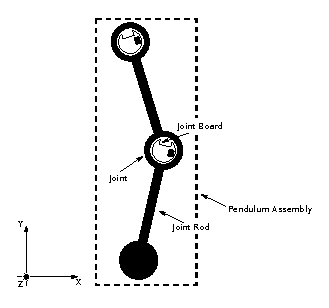
\includegraphics[width=.5\linewidth]{graphics/joint_assembly}
	\caption{Overview of the pendulum assembly developed in this section.}
	\label{fig:joint_assembly}
\end{figure}

%!TEX root = ../main.tex
\subsection{Analysis} % (fold)
\label{sub:analysis}

In the system analysis a number of requirements were found relating to the design of the joints.
These requirements contain both mechanical and electrical aspects.
The authors' main focus is on power and embedded design and as such the design of the mechanics of the system is limited in comparison to the electrical design.
The mechanical design was developed with advice from mechanical engineer at SDU: Jørgen Maagaard.

\subsubsection{Mechanics} % (fold)
\label{ssub:mechanics}
The mechanical design consists of two parts, the joint and the rod connecting two joints.
This project seeks to create a two-joint pendulum but the project owner has set a few additional requirements to allow for more diverse control tasks in future projects:
\begin{itemize}
	\item It should be possible to mount $n$ joints in series on the pendulum assembly.
	\item The distance between the joints should be modular.
\end{itemize}
In addition to these two requirements:
\begin{itemize}
	\item The pendulum assembly should be rigid and allow only movement in the X-Y plane so that it cannot collide with itself.
\end{itemize}

The first two requirements would benefit from a modular design, allowing the rod to be dismounted from the joint so that only the rod would require replacement, should the user wish to add joints or vary the distance between joints.
This is somewhat in conflict with the last requirement, which would benefit from each joint-rod-joint assembly to be one solid piece of material.
Since such an assembly would be rather expensive to manufacture and would require a new assembly for each desired configuration, a modular design is preferred.
\\~\\
The joint should be capable of unrestricted rotation.
This rotation should be as close to frictionless as possible and so a low friction coupling should be used between the two parts of the joint.
As will be discussed in section \ref{ssub:encoder} some form of encoder is required in the joint.
This encoder requires both power and signal wiring.
Two solutions were considered to solve this problem
\begin{itemize}
  	\item \textbf{Slip Ring:} A slip ring allows wiring to pass through a freely rotating joint.
  	They are available in versions of various sizes with up to 72 wires, allowing for several series joints before being limited by wire capacity.
  	Clearly, more wires results in a longer slip ring, imposing additional requirements to the thickness of the joint to accomodate for the slip ring.
  	The authors were in contact with Rotary Systems and Moog, both industry suppliers of slip rings and similar products.
  	It was clear that the price of these components was well beyond what is reasonable for this project.
  	\item \textbf{Wireless:} Several wireless solutions exist which could be employed in this situation.
  	Using a wireless approach means that all computation and handling of signals must be done on the joint before transmitting to the main controller.
  	This means that a more complex PCB must be designed and a battery installed to power the PCB.
  	While this solution does add electrical complexity it is practically free in comparison to the slip ring and allows for a much slimmer joint design.
  	This is the solution chosen for the joint design.
\end{itemize}
~\\
As discussed in the State of the Art analysis the pendulum assembly is viewed as a collection of point-masses connected with massless rods.
In order to more accurately uphold this assumption the material of the rods should be significantly lighter than the material of the joints while still maintaining sufficient rigidity.
In general three materials are easily available to the authors for manufacturing:
\begin{itemize}
	\item \textbf{Metal:} While this is a somewhat vague description that spans a vast number of materials, metals are generally significantly heavier than the following materials.
	Using metals requires manufacturing techniques and equipment which the authors do not have access to but the SDU Workshop can be hired to manufacture a design.
	The precision of metal-working is well into the sub-millimeter range.
	\item \textbf{3D Print:} This method of manufacturing is easily accessible and can be done for free (to the project). 
	It also allows for creating shapes that are otherwise difficult to manufacture in metals.
	3D printing at SDU is done in different types of plastics, neither of which is as stiff as would be desired for the pendulum assembly.
	Additionally, the encoder chosen in the following section sets strict requirements on the placement of the two parts of the encoder (This is discussed in more detail below) and the 3D printers at SDU are known to have problems accurately representing features in the sub-millimeter range.
	\item \textbf{Carbon:} This material is considered only for the rod as it was suggested as a light material with significant rigidity.
	Carbon tubes have been used previously at SDU Vikings, the SDU Formula Student racing team, as part of the suspension assembly.
\end{itemize}
Given the above materials the joint is to be made of metal while a carbon tube will be procured for the rod.
The design should be made such that the SDU Workshop can manufacture the joints and any appertaining components.
% subsubsection mechanics (end)

\subsubsection{Encoder} % (fold)
\label{ssub:encoder}
Each joint should implement an encoder to enable tracking the angular position of the joint.
The resolution of each joint should be sufficient to allow for proper control.
From the State of the Art analysis it was found that a resolution of 8192 ticks per revolution was succesfully used in two systems \cite{doubleinvertpendulum} \cite{tripleinvertpendulum}.
In addition to resolution, ease of manufacture and design is also an important aspect.
One encoder in particular was recommended to the authors; the Rolin Rotary Magnetic Encoders.
This is a series of encoders which, as the name suggests, utilises magnetic fields in order to determine the angular position of the encoder.
They consist of a magnetic ring with a number of poles and a PCB sensor.
The magnetic ring is available in different sizes with different number of poles which, along with the type of PCB sensor decides the resolution of the encoder.
The specific encoder configuration used in this project, the \texttt{RL2IC} \cite{RLC2IC}, allows for 7200 CPR or one count per 0.05$^\circ$.
The encoder is incremental with an \texttt{A}, \texttt{B} and \texttt{Z} channel where \texttt{A} and \texttt{B} are 90$^\circ$ out of phase and \texttt{Z} is a unique reference mark.
Using the reference mark it is possible to maintain absolute knowledge of the angular position of the joint after the initial encounter with the reference mark.
This is only possible assuming that there is no drift or slippage in the system, a reasonable assumption considering the mechanical setup.
Communication with the encoder is done using the RS422 standard.
This standard describes a method of transmitting digital signals using differential signals and requires specialised hardware to translate between ordinary digital signals and RS422.

% subsubsection encoder (end)
\subsubsection{Electronics} % (fold)
\label{ssub:electronics}
As per the initial requirements listed in this section each joint should be able to track the position of the joint and communicate this information wirelessly to the main controller board.
In order to accomplish this task some form of microcontroller is required along with the power delivery and the RS422 receiver mentioned previously.
The microcontroller must fulfill the following requirements:
\begin{itemize}
 	\item Must have support for three interrupt pins, one for each channel of the encoder.
 	\item Must have an SPI interface to maintain communication with the\\ \texttt{nRFM}.
 	\item Must have non-volatile memory to store the program through power cycling the board.
\end{itemize}
The \texttt{ATtiny84} \cite{attiny84} fulfills these requirements and provides sufficient I/O pins for the design.
The design of the PCB and the layout in general should accomodate the joint design.
By minimizing the height of the PCB design, the joint can be made thinner, reducing the stress on the pendulum assembly along the Z-axis.
It should also be noted that any connectors should be placed with the expectation that the border of the PCB is not accessible during normal operation.
\\~\\
Since the PCB is powered from a battery the design should be optimized to be reasonably power efficient.
As is explained in the next section, the design has a 3.3V rail and a 5V rail.
Generally microcontrollers become more power efficient at lower voltages and as such the \texttt{ATtiny} will be driven from the 3.3V rail.
The authors have immediate access to an AVR programmer which uses 5V signals for the programming.
The design should be made to accept this voltage when programming.
This can be done using level-shifting between the two voltage levels.
\\~\\
It was chosen to add an LED to the design for debugging purposes.
Clearly, an LED does require some power and should not be used during normal operation.
\paragraph{Power Delivery}~\\ % (fold)
\label{par:power_delivery}
The required voltage rails on the joint board are dictated by the RF module and the encoder.
The former requires 3.3V and the latter 5V.
Since the joints are to be wireless it is necessary to power them from a battery.
To avoid added complexity there will be no charging circuitry and charging the battery should be done externally to the joint.
The battery of the joint should last for as long as is possible while still fitting within the enclosure.
This requirement essentially narrows the battery choices to LiPo cells as these generally have the highest energy density of the commercially avaiable battery types.
1S LiPo cells are rated at 3.7V and so some form of convertion is required to reach both the 5V and 3.3V rails.
In order to correctly dimension the converters it is necessary to determine the power draw from each rail:
\begin{itemize}
 	\item \textbf{3.3V:} This rail powers the \texttt{nRFM} which has a maximum supply current of 12.3mA \cite{NFR24L01} as well as the \texttt{ATTiny}.
 	According to the datasheet of the \texttt{ATtiny} it uses approximately 3.6mA at 3.3V when run at 8MHz.   
 	This yields a total of 15.9mA at 3.3V or 52.5mW.
 	Additional digital circuitry placed on this rail is considered negligible in the power budget.
 	\item \textbf{5V:} This rail powers the encoder with a maximum supply current of 30mA \cite{RLC2IC} as well as the RS422 receiver which has a supply current of 52mA \cite{rs422rec}.
 	This yields a total of 82mA at 5V or 410mW.
 	Additional digital circuitry placed on this rail is considered negligible in the power budget.
\end{itemize}
For a battery to have sufficient capacity to power the joint for a full workday, estimated at 10 hours, it should have at least $\approx4600$mWh.
This is infeasible in the required dimensions and a battery should be procured which can provide the most run time given the space available.
\\~\\
The voltage rails should be designed with sufficient overhead.
Additionally, the accuracy of each rail is determined from the supply requirements set by the datasheet of the components used in the datasheet.
The two rails should be specced as follows:
One rail capable of delivering 200mA at 5V$\pm$0.2V.
One rail capable of delivering 100mA at 3.3V$\pm$0.2V.
% paragraph power_delivery (end)
% subsubsection electronics (end)

\subsection{Requirement Specification}
\label{subs:joint_requirements}
The requirements specified below are tested and verified in section \ref{sub:verification_joint_board_}.
\paragraph{Functional:}
\begin{enumerate}[resume]
	\item Pendulum assembly should allow movement only in the X-Y plane. 
	\label{enum:pendulum_should_only_x_y}
	\item Voltage rails for the components in the circuit.
	\label{enum:joint_voltage_rails}
	\begin{itemize}
		\item At least 100mA at 3.3V$\pm$0.2V.
		\item At least 200mA at 5V$\pm$0.2V.
	\end{itemize}
	\item Joint should be able to rotate freely about the mounting axis.
	\label{enum:rotate_freely_joint}
	\item The \texttt{nRFM} should be included for communication.
	\label{enum:joint_include_nrf}
	\item the RS422 interface of the \texttt{RL2IC} encoder should be correctly interfaced.
	\label{enum:interface_rs422_enc}
	\item The design should allow programming of the \texttt{ATtiny} using 5V SPI.
	\label{enum:program_5v_spi}
	\item An LED should be employed for debugging purposes.
	\label{enum:led_debugging_joint}
\end{enumerate}

\paragraph{Design:}
\begin{enumerate}[resume]
	\item Weight of rods should be minimized to uphold the point mass assumption.
	\label{enum:design_req1}
	\item Joints should be designed in a modular fashion such that $n$ joints can be mounted in series.
	\label{enum:design_req2}
	\item Distance between joints should be adjustable.
	\label{enum:design_req3}
	\item Friction in the joint should be minimized.
	\label{enum:design_req4}
	\item Design of the joint should employ mounting solutions for:
	\label{enum:design_req5}
	\begin{itemize}
		\item Joint board.
		\item Encoder.
		\item Battery. 
	\end{itemize}
	\item The design of the joint should be done so that it can be manufactured by the SDU workshop.
	\label{enum:design_req6}
	\item The PCB should be designed with the enclosure in mind.
	\label{enum:design_req7}
	\begin{itemize}
		\item Height of components and general design should be minimized.
		\item Placement of connectors should accomodate the enclosure.
		\item Shape of the PCB should allow for easy mounting of the PCB and other components.
	\end{itemize}
	\item The PCB layout should be reviewed according to the developed strategy.
	\label{enum:design_req8}
	\begin{itemize}
		\item Documentation.
		\item General inspection.
		\item Datasheet and report comparison.
		\item Footprint inspection.
		\item Peer-review.
	\end{itemize}
	\item A Battery should be sourced which conforms with the following requirements:
	\label{enum:design_req9}
	\begin{itemize}
		\item Battery should provide power for the joint for as long as possible.
		\item Battery should fit within the dimensions dictated by the enclosure.
	\end{itemize}
	\item Overall power consumption of the design should be minimized.
	\label{enum:overall_joint_power}
\end{enumerate}
% subsection analysis (end)
%!TEX root = ../main.tex
\subsection{Joint Design} % (fold)
\label{sub:joint_design}
The design of the pendulum assembly is, as in the analysis, split into an electrical design and a mechanical design.

\thomas{Proper introduction required}

\subsubsection{Mechanical Design} % (fold)
\label{ssub:mechanical_design}
The mechanical design consists mainly of 3D modelling using Autodesk Inventor.
The entire design is shown in figure \ref{fig:mechdesign} and is comprised of three parts:
\paragraph{Magnet Side:} % (fold)
\label{par:magnet_side}
is shown in figure \ref{sfig:magnetside}. 
This part has a shallow groove milled for the magnetic disc of the encoder to fit into.
The centre of the part is milled out to allow for two low-friction ball bearings to be press-fit into.
% paragraph magnet_side (end)
\paragraph{Reader Side:} % (fold)
\label{par:reader_side}
is shown in figures \ref{sfig:readside} and \ref{sfig:readside_2}.
The visible sides of \ref{sfig:magnetside} and \ref{sfig:readside} are designed to mate.
A cutout is made in \ref{sfig:readside} which is positioned such that it can be placed accurately above the magnetic disc.
The placement of the reader head by pressing it against a feeler gauge blade positioned between it and the magnetic disc before securing it using two bolts.
This ensures that the reader head is placed parallel with the disc and at the correct distance.
The axle is milled as part of \ref{sfig:readside}.
The manufactured version has a bore in the axle to accomodate a bolt which tightens the part to the bearings.
On the other side of the part, \ref{sfig:readside_2}, most of the material has been bored away to allow for mounting the joint board as shown in the figure.
A lip has been left on top of the part to allow for mounting a lid.

\paragraph{Joint Mount:} % (fold)
\label{par:joint_mount}
is shown in \ref{sfig:jointmount}.
This component was made to mate the joint with the joint rod.
A hole pattern is added to this part as well as the other two which is used to mount \ref{sfig:jointmount} to \ref{sfig:readside} and \ref{sfig:magnetside}.
On the top of the part a hole is made to accomodate the joint rod.
This part is 3D printed since the shape is somewhat complex and would require access to a CNC machine to mill of metal.
Additionally, making the part from metal would increase its weight significantly, potentially risking the point-mass assumption.
\\~\\
These three parts are connected into the pendulum assembly using carbon tubes as shown in \ref{sfig:pendulumassembly}.
Two parts are present on this design which were not described previously.
The final disc, known as the dummy disc, is essentially just a solid piece of aluminium used to add some weight to the end of the pendulum assembly.
The second part is a plate which the first joint is mounted on which is to be mounted on the cart.

\thomas{fix figure text below}
\begin{figure}[H]
	\begin{minipage}{.45\linewidth}
		\begin{subfigure}[b]{\linewidth}
			\centering
			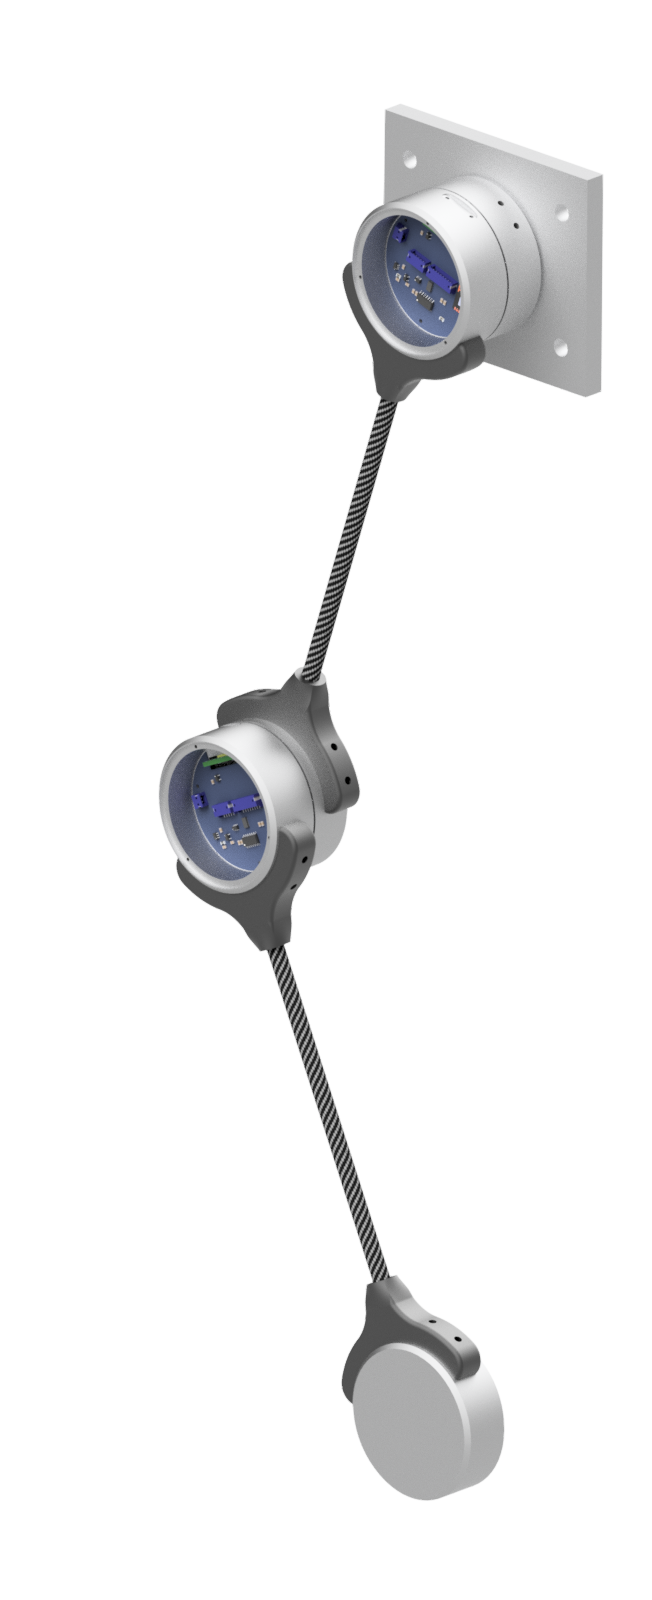
\includegraphics[width=.85\linewidth]{graphics/pendulum_assembly}
			\caption{This is a line of text}
			\label{sfig:pendulumassembly}
		\end{subfigure}\\
		\begin{subfigure}[b]{\linewidth}
			\centering
			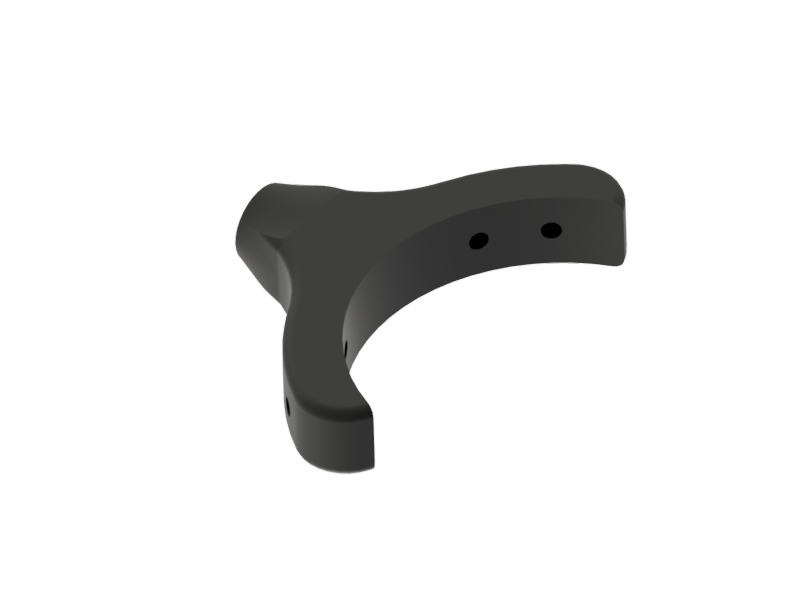
\includegraphics[width=\linewidth]{graphics/joint_mount}
			\caption{No one ever reads me... and some more text to fill out the caption}
			\label{sfig:jointmount}
		\end{subfigure}	
	\end{minipage}
	\begin{minipage}{.4\linewidth}
		\begin{subfigure}[t]{\linewidth}
			\centering
			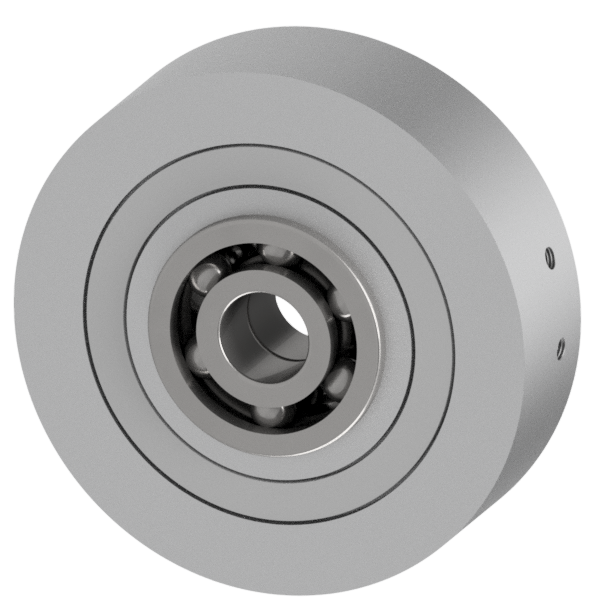
\includegraphics[width=\linewidth]{graphics/joint_mag_assembly}
			\caption{So is this..}
			\label{sfig:magnetside}
		\end{subfigure}\\
		\begin{subfigure}[b]{\linewidth}
			\centering
			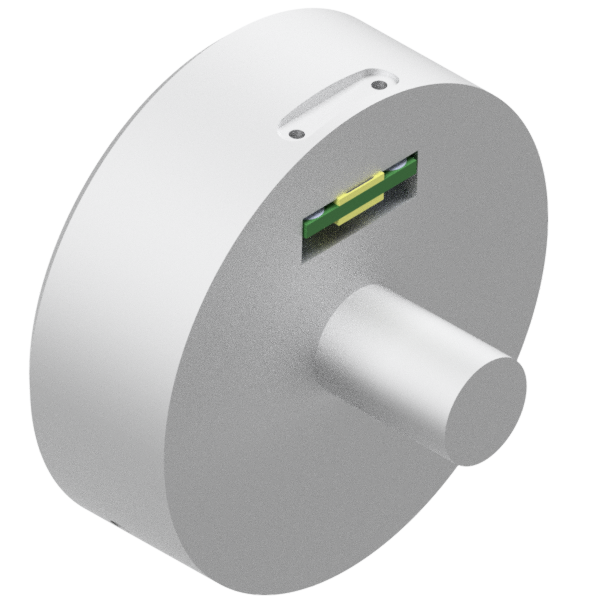
\includegraphics[width=\linewidth]{graphics/joint_read_side}
			\caption{And this!}
			\label{sfig:readside}
		\end{subfigure}\\
		\begin{subfigure}[b]{\linewidth}
			\centering
			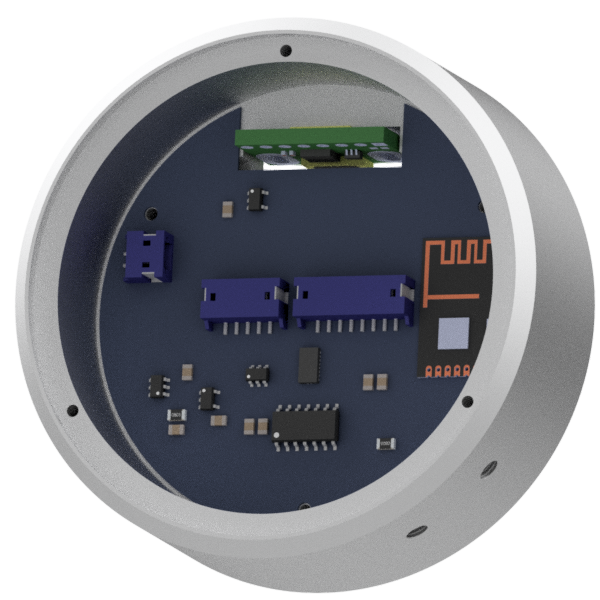
\includegraphics[width=\linewidth]{graphics/joint_read_side_2}
			\caption{Me too! this needs some more text as well. So here it is}
			\label{sfig:readside_2}
		\end{subfigure}
	\end{minipage}
	\caption{Me be Big-Momma Text!}
	\label{fig:mechdesign}
\end{figure}

\subsubsection{RS422}
The \texttt{RL2IC} uses the RS422 standard for its output.
This means that each \texttt{A}, \texttt{B} or \texttt{Z} channel consists of a two wire differential signal.
A line receiver is needed in order to translate the RS422 signals to logic inputs that the ATtiny84 can read.
The \texttt{DS26LS32CM} is a quad differential line receiver that complies with the RS422 standard.  
When using RS422 there are different termination methods, with no termination being the simplest.
The RS422 Standard Overview \cite{rs422_texas} describes that signal integrity is maintained in a setup of \approx 30m wires carrying data at a signal rate of 200kbps without termination.
The intended setup on the joint board requires wires no longer than 5cm.
The maximum expected data rate can be calculated using the maximum expected angular velocity of the joint of 20Hz and the edges on one channel per revolution.
\begin{equation}
Datarate_{max}	= 20 \cdot 3600 = 72kbps
\end{equation}
This datarate is clearly below the 200kbps and it was therefore decided to use no line termination, which also has the advantage that a minimum amount of current is needed from the \texttt{RL2IC}.


\subsubsection{5V}
As described in the requirements in section \ref{subs:joint_requirements}, a 5V rail is needed on the joint board.
Generating the 5V rail can be done by boosting the battery voltage up to 5V, as the battery voltage will always be lower than 5V.
The boost regulator \texttt{SP6641B} \cite{sp6641b} has an input range of 0.9V to 4.5V and a fixed output of 5V.
The circuitry used in this project will be based on the reference design shown in the datasheet, with the one difference that the \texttt{SHDN} (shutdown) pin has been pulled permanently high.

\subsubsection{3.3V}
A 3.3V rail is needed according to the requirement specification.
The task of generating the 3.3V rail is somewhat complicated since the battery voltage of a typical Li-Ion battery varies from 4.2V down to 3.0V.
Three different solutions appeared after an initial analysis of the task:

\begin{itemize}
	\item Buck converter
	\item Buck-Boost converter
	\item Linear regulator
\end{itemize}

The qualities and drawbacks of the three solutions are presented here.

\paragraph{Buck Converter:}
The voltage from the battery can be converted to 3.3V using a Buck converter.
A Buck converter is relatively simple and circuitry can easily be designed for the task.
It is only able to supply an output voltage that is lower than the input voltage.
Which means that when the battery voltage is lower than 3.3V the converter will stop producing a stable 3.3V output.
This means that a portion of the battery capacity cannot be used.
The \texttt{TPS62220} is a Buck regulator and generally has good specifications for this task. 
With an input voltage of 3.7V and an output voltage of 3.3V it has an efficiency of approximately 95\% with an output current in the range of 1mA to 20mA \cite{TPS6222}.
The minimum drop out voltage of the \texttt{TPS62220} is low, because it has a 100\% duty cycle mode.
In this mode, the the drop out voltage is purely defined by the \texttt{ON} resistance of the internal switch, the DC resistance of the external inductor and the output current.

The drop out voltage can be calculated using equation \ref{eq:drop_v_tps62}, \cite{TPS6222}.
\begin{equation}
	V_{drop} = I_{O} \cdot (R_{DS(on),max}+R_I)
	\label{eq:drop_v_tps62}
\end{equation}

\begin{equation}
	V_{drop} = 0.02 \cdot (0.67+0.09) = 15 [mV]
	\label{eq:drop_v_tps62_2}
\end{equation}

Where $I_O$ is the output current, $R_{DS(on),max}$ is the \texttt{ON} resistance of the internal switch and $R_I$ is the DC resistance of the external inductor.
The inductor resistance used is found in the \texttt{LQH55D} SMD inductor \cite{LQH55D}.
\mikkel{Update to new inductor and change equations above}
This means that it can supply 3.3V output when the input voltage is 3.315V or greater



\paragraph{Buck-Boost Converter:}
The motivation for using a Buck-Boost converter is to allow for full utilization of the battery capacity.
This requires that the converter can make a seamless transition between the stepping up and stepping down of the input voltage. 
\texttt{TPS6300} is a Buck-Boost regulator that has these features.
The external circuitry is simple, but the drawback of this regulator and converter is the efficiency of it.
With an input voltage of 3.7V and an output voltage of 3.3V it has an efficiency of approximately 75\% with an output current in the range of 1mA to 20mA \cite{TPS6300}.

\paragraph{Linear Regulator:}
A linear regulator is a component that can regulate the output voltage by varying an internal resistance.
Linear regulators have a drop voltage that limit the output voltage. 
The \texttt{LD3985} has an ultra low drop voltage of 20mV at 50mA output current \cite{LD3985}.

Therefore the efficiency is proportional to ratio between the output and input voltage and can be estimated using equation \ref{eq:eff_lin} \cite{ap_note_140}.

\begin{equation}
	\eta \simeq \frac{V_{out}}{V_{in}}
	\label{eq:eff_lin}
\end{equation}

The voltage of a Li-Ion battery varies from 4.2 to 3.0V, but the nominal voltage is 3.7V and this will be used as an estimate of the mean voltage of the battery.
Using this the mean efficiency can be estimated as shown in equation \ref{eq:eff_lin_val}.

\begin{equation}
	\eta \simeq \frac{3.3}{3.7} = 0.89 = 89\%
	\label{eq:eff_lin_val}
\end{equation}


\paragraph{Comparison}
The most important parameters of the three solutions discussed are shown in table \ref{tab:vol_gen_joint}.

\begin{table}[h]
	\centering
	\begin{tabular}{l|c|c|c}
		  				&	Buck 	& Buck-Boost 	& Linear\\
		 \hline
		 Efficiency  	&  95\% 	& 75\%			&89\%		\\
		 Drop out [mV]		&15  	& N/A		&20		\\
	\end{tabular}
	\caption[Parameters of voltage generation solutions.]{Parameters of the three solutions using a Buck converter, Buck-Boost converter or a linear regulator. The efficiency shown is estimated with an input voltage of 3.7V, an output voltage of 3.3V and an output current in the range of 1mA to 20mA. The drop out voltage is estimated with an output current of 20mA (Buck) and 50mA (linear regulator).}
	\label{tab:vol_gen_joint}
\end{table}

The Buck converter solution has the highest efficiency and is therefore the natural choice.
As already discussed the disadvantage of using a Buck converter is that the full battery capacity cannot be utilized.
A discharge test should be conducted to determine the amount of capacity that cannot be utilized.


\paragraph{Battery Discharge}
At the time of writing, the chosen battery has not yet been procured and the test will therefore be conducted on a similar battery instead.
The battery under test is a 850 mAH Li-Ion battery with the dimensions 49mm X 29mm X 6mm.
It should be noted that both the capacity and physical dimensions are similar to the chosen battery.
The discharge curve of the two batteries will not be identical, but will be sufficiently close to to allow for deciding which solution should be used.
The test was conducted by connecting the battery to an electrical load programmed to discharge with a constant power of 0.3 Watt, while measuring the battery voltage.
The measured discharge curve is shown in figure \ref{fig:bat_discharge}.

\begin{figure}[h]
	\centering
	%%% This file was created by matlab2tikz.
%
%The latest updates can be retrieved from
%  http://www.mathworks.com/matlabcentral/fileexchange/22022-matlab2tikz-matlab2tikz
%where you can also make suggestions and rate matlab2tikz.
%
\definecolor{mycolor1}{rgb}{0.00000,0.44700,0.74100}%
%
\begin{tikzpicture}

\begin{axis}[%
width=4.521in,
height=3.566in,
at={(0.758in,0.481in)},
scale only axis,
xmin=0,
xmax=450,
xlabel style={font=\color{white!15!black}},
xlabel={Time [Min]},
ymin=2.5,
ymax=4.5,
ytick={2.5,   3, 3.5,   4, 4.5},
ylabel style={font=\color{white!15!black}},
ylabel={Voltage [V]},
axis background/.style={fill=white},
title style={font=\bfseries},
title={Discharge Curve of Li-Ion Battery}
]
\addplot [color=mycolor1, forget plot]
  table[row sep=crcr]{%
0	4.072\\
10	4.02699999999999\\
20	4.00799999999998\\
40	3.95999999999998\\
50	3.92200000000003\\
60	3.89499999999998\\
70	3.87900000000002\\
80	3.85500000000002\\
90	3.84300000000002\\
100	3.81799999999998\\
110	3.79700000000003\\
120	3.78899999999999\\
130	3.77699999999999\\
140	3.767\\
150	3.75299999999999\\
160	3.76100000000002\\
170	3.75999999999999\\
180	3.74000000000001\\
190	3.72500000000002\\
200	3.71300000000002\\
210	3.714\\
220	3.69999999999999\\
230	3.71100000000001\\
240	3.71199999999999\\
250	3.69999999999999\\
260	3.69299999999998\\
270	3.69099999999997\\
280	3.69799999999998\\
290	3.69099999999997\\
300	3.68099999999998\\
310	3.673\\
320	3.65699999999998\\
330	3.64499999999998\\
340	3.63499999999999\\
350	3.62299999999999\\
360	3.60700000000003\\
370	3.61399999999998\\
380	3.596\\
390	3.56799999999998\\
400	3.505\\
410	3.36099999999999\\
414.551694551695	2.30000000000001\\
};
\addplot [color=red, dashed, forget plot]
  table[row sep=crcr]{%
0	3.30000000000001\\
450	3.30000000000001\\
};
\end{axis}
\end{tikzpicture}%
	\caption[Discharge curve of Li-Ion battery.]{Voltages measured across a 850 mAH Li-Ion battery while discharging using an electrical load programmed to 0.3 Watt. Horizontal red line represents the 3.3V level.}
	\label{fig:bat_discharge}
\end{figure}

It can be observed that the battery voltage only drops below 3.3V for a very short time before the battery is completely discharged.

\paragraph{Conclusion}
The Buck converter solution has the highest efficiency and has a lower drop out voltage than the linear regulator solution.
The disadvantage of using a Buck converter is that the full battery capacity cannot be utilized, but a test showed that almost all of the capacity can be used.
Therefore it was chosen to use a Buck converter with the \texttt{TPS62220} regulator. 
The Buck converter circuit used is based on the recommendations in the datasheet of the \texttt{TPS62220}.
The circuit is shown in figure \ref{fig:tps62220_circuit}.

\begin{figure}[h]
	\centering
    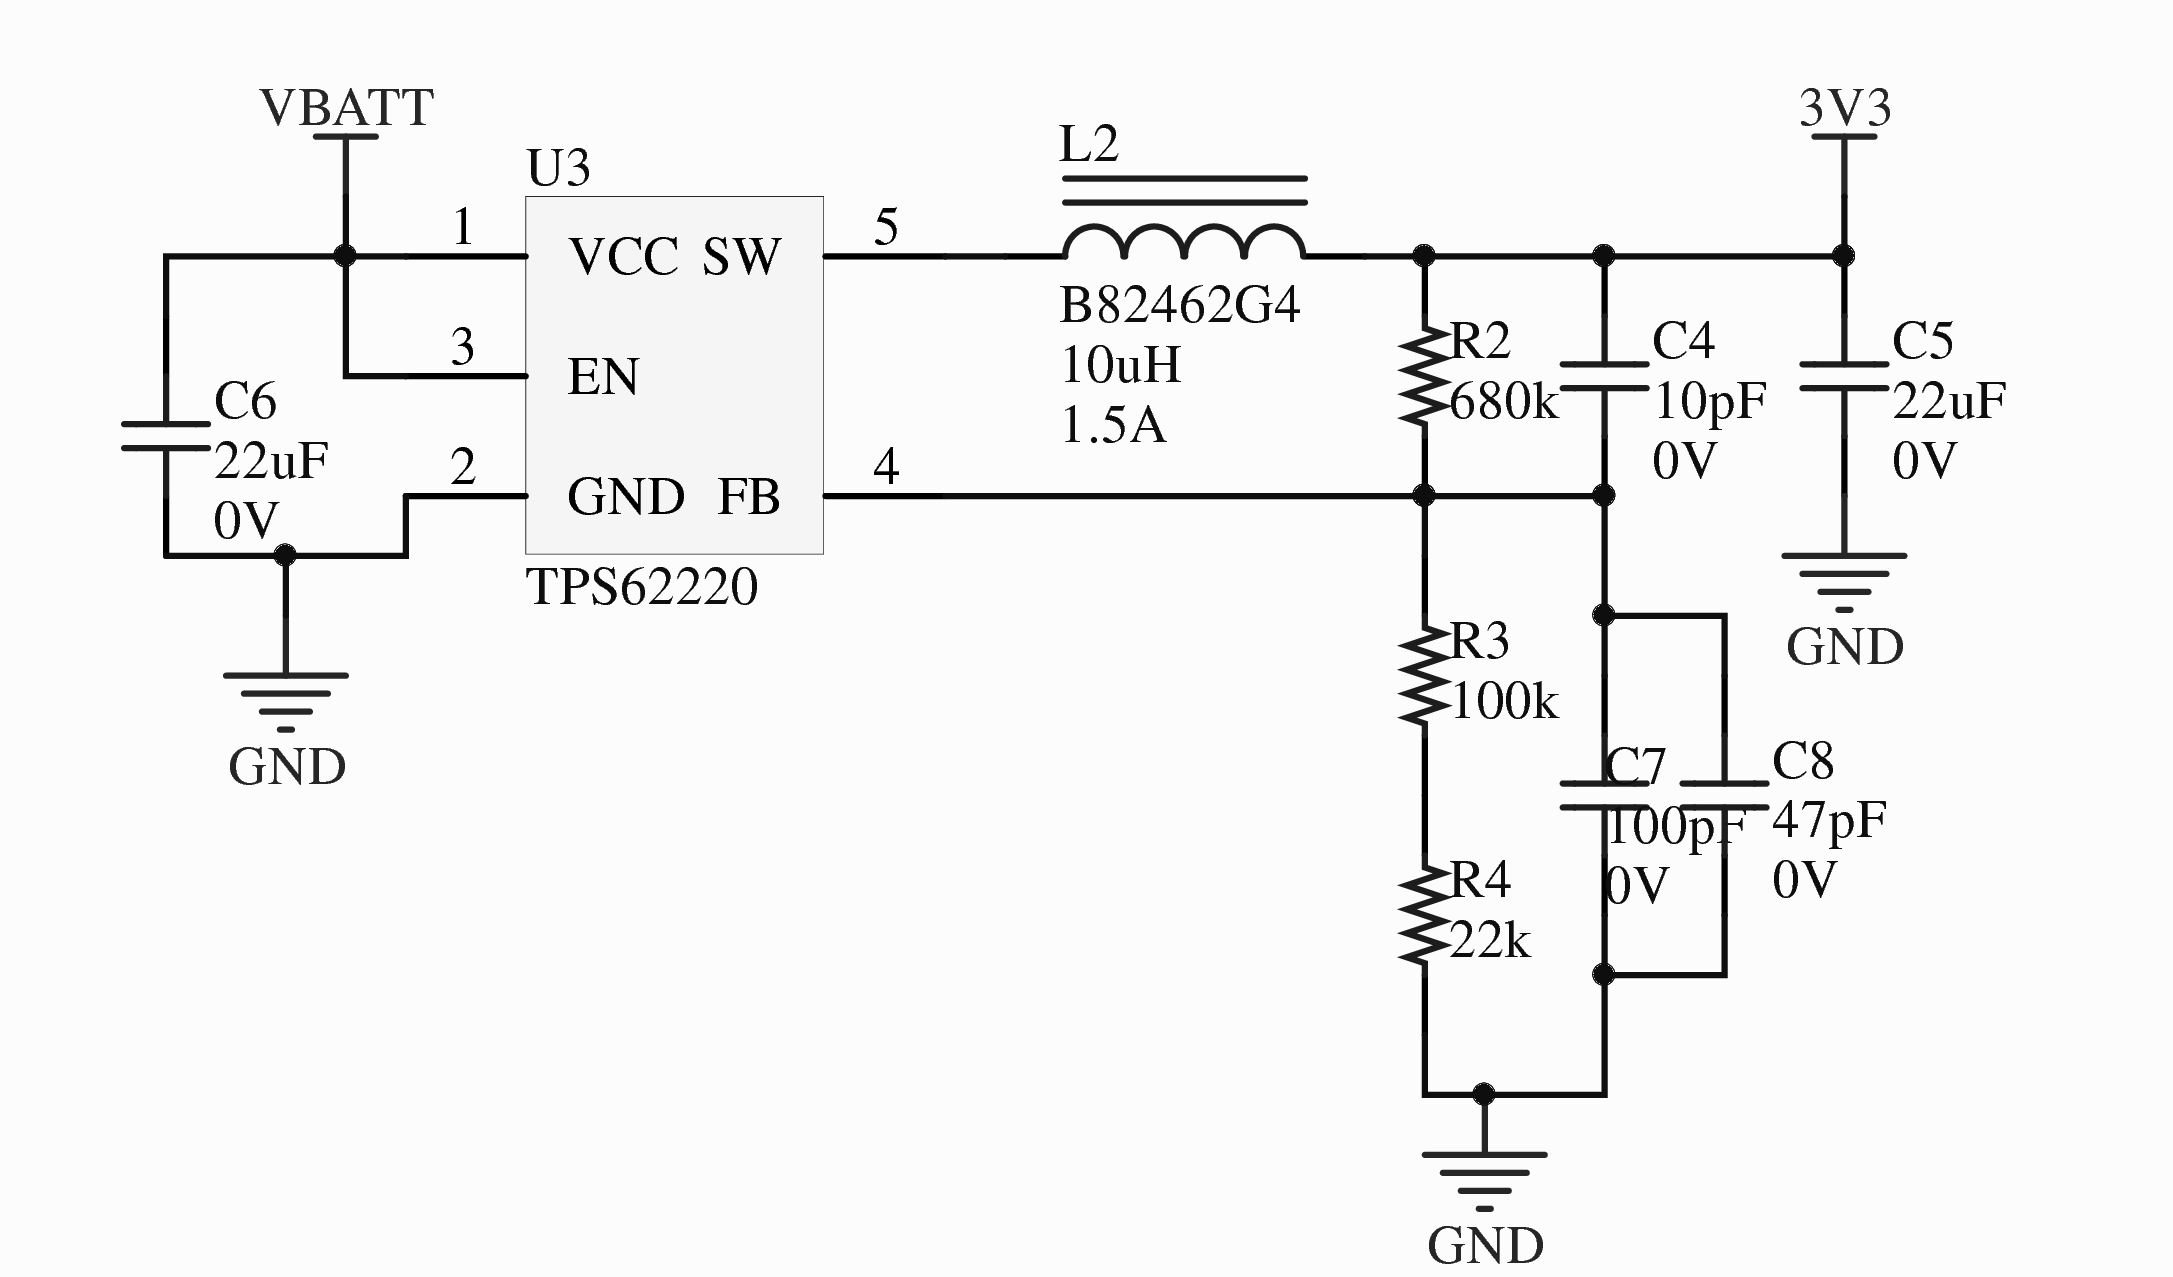
\includegraphics[width=.8\linewidth]{graphics/tps6220_circuit}
	\caption[3.3 V buck converter circuitry.]{Circuitry of Buck converter with an output voltage of 3.3V. \texttt{TPS62220} is used as the regulator.}
	\label{fig:tps62220_circuit}
\end{figure}
% subsection joint_design (end)

\subsubsection{Choosing a Battery} % (fold)
\label{ssub:choosing_a_battery}
\thomas{write few words on renata and difficulty of procurement (most capacity in 57mm and 9mm)}
%!TEX root = ../main.tex
\subsection{Implementation and Verification} % (fold)
\label{sub:implementation_and_verification}
This section will elaborate on the implementation of the design created in section \ref{sub:analysis}.
Specifically the methods and equipment used is discussed.
In addition, the verification of the finished product is presented in appropriate detail.
This will give the reader an impression of the method used to verify the implementation.

\subsubsection{Verification Methodology} % (fold)
\label{ssub:testing_methodology}
From experience of the authors, verification of a PCB design can become difficult without a predefined plan, increasing the risk of mistakes, oversights and similar problems.
In order to minimize the risk of these, it was decided to create a verification method prior to the actual verification of the PCB.
Each verification procedure is written to reflect the features created in the design.
Each of these features should be tested, in the intended order.
It should be written such that the verification can be done with no prior knowledge of the operation of the design.
This approach holds a few different benefits.
Firstly, the technician doing the verification is doing less thinking while verifying, this is likely to decrease the number of mistakes.
Secondly, a thorough verification procedure will enable students to more easily reproduce the PCB's if necessary.\\~\\
Each procedure is presented in the report with the results as gathered by the authors.
A version suitable for future use can be found in appendixes 
% subsubsection testing_methodology (end)

\subsubsection{Joint Board Verification Procedure} % (fold)
\label{ssub:joint_board_verification_methodology}
The verification procedure can be 
% subsubsection joint_board_verification_methodology (end)
% subsection implementation_and_verification (end)



\clearpage
%!TEX root = ../main.tex
\section{Joint Board Software Development} % (fold)
\label{sub:joint_board_software}

\subsection{Analysis} % (fold)
\label{ssub:joint_board_analysis}
The main responsibility of the joint software is to maintain knowledge of the angle of its joint and transmit that angle to the controller board.
The following analysis will elaborate on the needed functionalities and requirements for the software.

\subsubsection{Joint Angle}
The angle of the joint can be determined by analysing the signals from the RL2IC encoder mounted on the joint.

This encoder implements incremental quadrature with three signals: \texttt{A}, \texttt{B} and \texttt{Z}.
Figure \ref{fig:quadrature} is a depiction of this quadrature scheme.
The two signals \texttt{A} and \texttt{B} are 90$^\circ$ out of phase and their frequency is determined by the angular velocity of the joint.
As can be seen from the figure the signals create four unique stages, counting these allows knowledge of both the direction, position and, potentially, the velocity of the joint.

\begin{figure}[h]
	\centering
	\includegraphics[width=.5\linewidth]{graphics/quadrature}
	\caption[Incremental quadrature scheme RL2IC encoder.]{Incremental quadrature scheme as implemented on the RL2IC encoder.}
	\label{fig:quadrature}
\end{figure}

It is necessary to read \texttt{A}, \texttt{B} and \texttt{Z} using interrupts as missing a cycle or introducing jitter in the counting procedure will cause the measured angle to drift.
\texttt{Z} only goes \texttt{high} one time per revolution and can therefore be used to infer the absolute angle of the joint.
This should be done by calibrating the joint angle by setting  the measured angle to a fixed number, whenever \texttt{Z} goes \texttt{high}.
This means that the angle should not be measured until the joint software has been calibrated by reaching the point where \texttt{Z} goes \texttt{high}.

Since the angle is to be transmitted there is a risk that an interrupt may occur while this transmission takes place, potentially corrupting the data to be transmitted.
This needs to be avoided and can be done by temporarily disabling interrupts and copying the needed data to other variables.
The code that temporarily disables interrupts and copies the variable needs to be executed faster than two consecutive interrupts can occur, because otherwise angle movement is lost.
The time between two consecutive interrupts is only dependent of the angular velocity of the joint.
It is estimated that the maximum angular velocity is  $\approx$20Hz, which means that no interrupts should go unnoticed at this frequency.
\mikkel{It would be nice with some sort of reasoning/reference.}

\subsubsection{Wireless Transmission of Data}
As mentioned in section \ref{ssub:interboard_communication}, communication between the controller board and the joint boards is to happen wirelessly using the \texttt{nRF24L01} module and a period between packets of more than 130$\mu$s.
The software needs to communicate with the \texttt{nRF24L01} through a SPI connection with the \texttt{ATtiny} as the master.
The \texttt{nRF24L01} has a number of options that needs to be set according to the wanted functionality.
As described in \ref{ssub:interboard_communication}, it was found that the two joints needs to send using two separate frequency bands to avoid air collisions. 
This needs to be set up individually in each \texttt{nRF24L01} module. 
Latency should be minimized by reducing overhead in transmitted packages and sending the smallest possible payload that correctly conveys the joint data.
The data sheet describes that the \texttt{nRF24L01} can operate at air rates of 250kbps, 1Mbps and 2Mbps.
Based on the somewhat unstable transmission explained in section \ref{subs:wireless_transmission_joint} it was chosen to use a transmission rate of 1Mbps, as it is more noise resistance than when using 2Mbps.

\paragraph{Transmission Rate} % (fold)
\label{par:transmission_rate}~\\
The datasheet of the \texttt{nRF24L01} module specifies that there is a settling time of 130$\mu$s when entering the transmit state.
Several aspects should be considered in order to determine the required period time associated with transmission of one data packet. 
Transmission of a two byte payload through SPI takes $\approx$ 36 $\mu$s as will be shown in \ref{}.
The \texttt{CE} should be high for at least 10$\mu$s in order for the transition to transmit mode is initiated.
Hereafter the settling time of 130$\mu$s is inferred.
Then the \texttt{nRF24L01} will transmit the two byte payload in a eight byte data packet, which will take 68$\mu$s using a air transmission rate of 1Mbps.
This totals 244$\mu$s, in which the computation time needed is not included.
Therefore it was decided to use a period time of 333$\mu$s, which yields 89$\mu$s to computation and a sampling frequency of $\approx$3kHz.
The period is shown in figure \ref{fig:tiny_period}.

\begin{figure}[h]
	\centering
	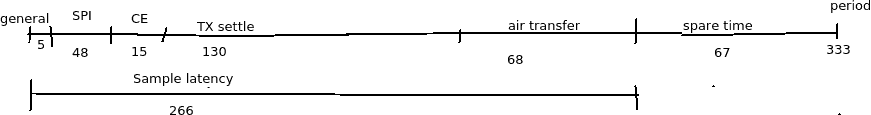
\includegraphics[width=1\linewidth]{graphics/tiny_period}
	\caption[Period of wireless transmission]{Period associated with transmission of one data packet.}
	\label{fig:tiny_period}
\end{figure}



\subsubsection{Real Time Software}
In order to produce reliable data for the controller board the joint angle should be sampled and transmitted at a constant rate.
This requires the joint board software to be programmed as real time software, where deadlines should be met.

\subsection{Requirement Specification} 

\paragraph{Functional:}
\begin{enumerate}[resume]
	\item Correct joint angle should be known at all times.
	\label{enum:joint_correct_angles}
	\begin{itemize}
		\item Encoder signals \texttt{A}, \texttt{B} and \texttt{Z} should be interfaced using interrupts.
		\item \texttt{A}, \texttt{B} should be used to measure the relative angle.
		\item \texttt{Z} should be used to infer the absolute angle. 
		\item Determine movement and direction of movement based on encoder signals.
		\item Ensure no data is corrupted by interrupts.
		\item Ensure no interrupts lost at angular frequencies below 20Hz.
	\end{itemize}
	\item Transmit joint angle using the \texttt{nRF24L01} module.
	\label{enum:joint_transmit}
	\begin{itemize}
		\item Setup of the \texttt{ATtiny} as a SPI master.
		\item Setup of \texttt{nRF24L01} settings and individually frequency bands.
		\item Transmit data every 333$\mu$s.
		\item Minimize latency.
	\end{itemize}
	\item Real time behaviour of software.
	\label{enum:joint_real_time}
\end{enumerate}

\subsection{Design and Implementation} % (fold)
\label{sub:design_and_implementation}

\mikkel{Add attiny84 setup before nrf setup. Add calibrated = 1.}
\begin{figure}[h]
	\centering
	\begin{subfigure}[b]{0.30\textwidth}
		\centering
		\includegraphics[width=.8\linewidth]{graphics/joint_software_diagram}
		\caption{Main loop.}
		\label{sfig:joint_main_flowchart}
	\end{subfigure}
	\begin{subfigure}[b]{0.69\textwidth}
		\centering
		\includegraphics[width=.8\linewidth]{graphics/joint_interrupt}
		\caption{Encoder signal Interrupt Service Routine.}
		\label{sfig:joint_interrupt}
	\end{subfigure}
	\caption{Flowchart of the software design for the joint board.}
	\label{fig:joint_software}
\end{figure}
A software design was made based on the requirements for the joint board software.
The main functionality of the software is illustrated in the flowchart of figure \ref{sfig:joint_main_flowchart}.
Upon startup the \texttt{nRF24L01} is setup as explained in section \ref{par:nrf24l01}.
A timer is initiated to ensure that a packet, as shown in figure \ref{fig:rfpacket}, is sent every 333$\mu$s.
Now the copying procedure is started after which the packet is transmitted and the program is idling until 333$\mu$s has passed and the process starts over.
An interrupt can happen at any given time and the ISR, will update the measured joint angle. 
The coming sections will elaborate on the different elements of the software.

\subsubsection{Joint Angle Measurement}
\label{ssub:joint_angle_measurement}
In figure \ref{sfig:joint_interrupt} the interrupt routine is shown.
This routine can be engaged at any given time and is engaged whenever an either rising or falling edge appears on \texttt{A}, \texttt{B} or \texttt{Z}.

Initially the signals are read.
If \texttt{Z} is high the index has been reached and the position counter is reset and the calibration bit is set.
Hereafter the execution of the main loop is continued.
If \texttt{Z} is low \texttt{A} and \texttt{B} are inspected to determine which phase is active.
Table \ref{tab:bin_phase} shows each phase and the combination of \texttt{A} and \texttt{B} in that phase.
By comparing with the previous phase it is possible to determine the direction of movement and therefore whether the position counter should be incremented or decremented.
Before returning execution to the main loop the current phase is stored. 

\begin{table}
	\centering
	\begin{tabular}{c | c  c}
		& \texttt{A} & \texttt{B}\\
		\hline
		P1 & 0 & 1\\
		P2 & 0 & 0\\
		P3 & 1 & 0\\
		P4 & 1 & 1
	\end{tabular}
	\caption{Binary representation of the phases.}
	\label{tab:bin_phase}
\end{table}

\subsubsection{Wireless Transmission of Data}
\label{ssub:wireless_transmission_of_data}
The joint board should transmit the angular angle of the joint and whether calibration has occured since startup.
The \texttt{RL2IC} encoder used in the joint produces 7200 counts per revolution, requiring 13 bits to represent a full revolution of the joint.
The calibration status is binary and represents one bit. 
16 bit is required to transmit this information, since the \texttt{nRF24L01} payload needs be an integer number of bytes.
See figure \ref{fig:rfpacket} for a visual representation of the message.

\mikkel{Joint ID, calibration and direction not necessary }
\begin{figure}[h]
	\centering
	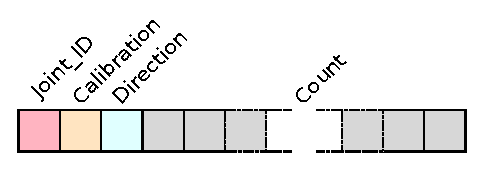
\includegraphics[width=.5\linewidth]{graphics/rf_packet}
	\caption[RF transmission packet used from the joint board.]{UPDATE ME!!!!!!!!!!!!!!--  Sructure of a packet used on the RF transmission between the joint boards and the controller board. Bits 0-12 represent the current joint angle and bit 13 represents the state of calibration.}
	\label{fig:rfpacket}
\end{figure}

When information is to be transmitted the calibration and angle variables needs to be copied to other variables.
The act of copying a variable takes several clock cycles and if an interrupt occurs while the variable is being transmitted the data is can be corrupted.
In order to avoid this problem it is necessary to temporarily disable interrupts while copying original variable into a temporary variable. 
In effect the resulting code is as seen in code \ref{code:critical_section_c}.
Disabling interrupts means that any incoming interrupts will not be processed until interrupts are reenabled, as described in the datasheet of the ATtiny84 \cite{attiny84}.
Interrupts should therefore not be disabled for longer than the shortest expected time between two edges on any single signal.

The \texttt{AVR-GCC} compiler has the option to only compile the code, leaving a human readable assembly file.
The assembly corresponding to code \ref{code:critical_section_c} can be seen in code \ref{code:critical_section_asm}.
Each of these instructions are described in the datasheet of the microcontroller where the number of cycles required to execute them is specified: \texttt{rcall} 3 cycles, \texttt{\_CLI} 1 cycle, \texttt{ldd} 2 cycles, \texttt{std} 2 cycles, \texttt{\_SEI}, 1 cycle.
In total 16 clock cycles are spent executing the required commands.
At 8MHz this is 2 $\mu$s.
Since the RL2IC produces 7200 ticks per revolution only 3600 edges exist on a single signal per revolution. 
Using these numbers the theoretical maximum angular velocity possible while still maintaining more than 2 $\mu$s between each edge on a signal is $\approx$135Hz, which is clearly above the estimated maximum velocity of $\approx$20Hz.

\begin{listing}[h] 
\begin{minted}{c}
	_CLI();
	cnt_temp=cnt;
	_SEI();
\end{minted}
\caption{Critical section for copying counter value. C version.}
\label{code:critical_section_c}
\end{listing}

{\renewcommand\fcolorbox[4][]{\textcolor{cyan}{\strut#4}}
\begin{listing}[h]
\begin{minted}{gas}
	rcall _CLI
	ldd r24,Y+1
	ldd r25,Y+2
	std Y+4,r25
	std Y+3,r24
	rcall _SEI
\end{minted}
\caption{Critical section for copying counter value. Assembly version.}
\label{code:critical_section_asm}
\end{listing}


\subsubsection{SPI} % (fold)
\label{ssub:spi}
The \texttt{ATtiny84} does not have a SPI controller, but it does have a Universal Serial Interface, USI, which is compatible with SPI, when it is used in its three wire mode.
In this mode the interface has the pins, Data Out \texttt{DO}, Data In \texttt{DI} and a clock \texttt{USCK}.
In order to comply with the SPI standard a Slave Select \texttt{SS} pin should be implemented using a general IO pin and custom written software.
The \texttt{nRF24L01} also has a non SPI pin, \texttt{CE} that also needs to be controlled from the \texttt{ATtiny}.
The full interface between the two is shown in figure \ref{fig:tiny_nrf_com}.

\begin{figure}[h]
	\centering
	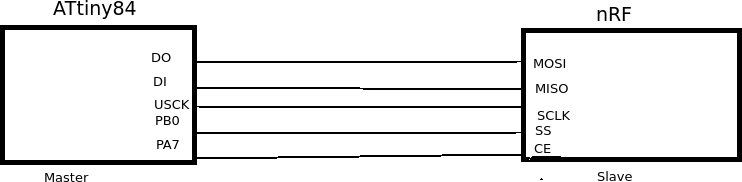
\includegraphics[width=.8\linewidth]{graphics/tiny_nrf_com}
	\caption[Interface between ATtiny84 and nRF24L01.]{Interfacing the \texttt{ATtiny84}s USI and \texttt{nRF24L01}s SPI. \texttt{PB0} and \texttt{PA7} are general purpose IO pins.}
	\label{fig:tiny_nrf_com}
\end{figure}
The \texttt{ATtiny84} is used as the SPI master and controls \texttt{MOSI}, \texttt{SCLK}, \texttt{SS} and \texttt{CE} on the \texttt{nRF24L01} module.

With the two modules interfaced correctly, data can be transmitted between them.
The function shown in listing \ref{code:tiny_spi_transfer} implements this functionality on the \texttt{ATtiny84}.
It takes pointers to \texttt{data}, \texttt{input} and the number of bytes that needs to be sent as inputs.
Line 2 sets \texttt{SS} \texttt{low} to initiate an SPI transfer.
The loop in lines 4 to 11 is run \texttt{n} times to send and receive \texttt{n} bytes.
In line 5 the USI Data Register \texttt{USIDR} is loaded with the byte to be sent and in line 6 the counter overflow flag in the USI Status Register, \texttt{USISR}, is cleared.
Lines 7 to 9 writes 1 to the \texttt{USITC} bit of the USI Control Register \texttt{USICR} until the counter overflow flag \texttt{USIOIF} is raised.
The USI clock \texttt{USCK} is toggled each time 1 is written to \texttt{USITC}.
Data is shifted to \texttt{DO} correctly by the USI by counting the clock edges generated. 
Data on \texttt{DI} is sampled at falling edges of the \texttt{USCK} and stored in \texttt{USIDR}.
The counter overflow flag \texttt{USIOIF} will raise when 16 clock edges has been generated and eight bits of data has been sent and received.
Line 10 copies the received data to the \texttt{input} pointer if there is one.
When \texttt{n} bytes of data has been sent and received the \texttt{SS} pin will be set \texttt{high} and the function is exited.
\mikkel{Does this shit make sense or do we need to add some other kind of illustration or explanation.}
\begin{listing}[h] 
\begin{minted}{c}
void spi_transfer(uint8_t *data, uint8_t *input, uint8_t n){
  PORTB &= ~_BV(SS);
  int i;
  for(i = 0; i<n; i++){
	USIDR = data[i];
	USISR = _BV(USIOIF);  
	while ( !(USISR & _BV(USIOIF)) ){
		USICR |= _BV(USITC);  
	} 
	if(NULL |= input){input[i] = USIDR;}
  }
  PORTB |= _BV(SS);
}
\end{minted}
\caption{Function that transmits \texttt{n} bytes of data between the \texttt{ATtiny84} and the \texttt{nRF24L01}.}
\label{code:tiny_spi_transfer}
\end{listing}

This functions enables setup of the \texttt{nRF24L01}, which is done with the same settings as explained in section \ref{ssubs:nrf24l01}.

\subsubsection{Wireless Transmission}
\label{subs:wireless_transmission_joint}
During implementation of the software for the \texttt{nRF24L01} a lot of testing was done to verify that the developed code worked.
Initially two \texttt{nRF24L01} modules were wired up to two arduinos running example code from the internet. 
This was done to verify wiring and functionality of the \texttt{nRF24L01} modules.
Afterwards an Arduino was programmed to receive data and the software was written to the \texttt{ATtiny84} to transmit data using the \texttt{nRF24L01}.
The functionality of the joint board software was verified by transmitting data from the \texttt{ATtiny84} to a Arduino successfully.
Afterwards a \texttt{nRF24L01} was wired to the Microzed and the software was written.
The transmission of data between the \texttt{ATtiny84} and the Microzed was verified by transmitting data from the joint board \texttt{nRF24L01} to a \texttt{nRF24L01} module in free air connected to the Microzed.
The transmission was successful.
\\
The same software was used to to test the \texttt{nRF24L01} module wired on the controllerboard. 
Tests showed that no data was received in this setup.
Thoroughly inspection of the schematic and PCB revealed no mistakes. 
Further testing with a \texttt{nRF24L01} module in free air connected to the Microzed showed that no packets were received when the controller board PCB was in near proximity of the \texttt{nRF24L01}.
The problem is believed to be due to the large amount of copper in the controller board PCB.
The error was fixed by soldering the \texttt{nRF24L01} off and wiring it with longer wires.

\subsubsection{Software Timer}
\label{ssub:software_timer}
The timer shown in figure \ref{sfig:joint_main_flowchart}, is implemented on the \texttt{ATtiny84} using \texttt{Counter 1}, which is a 16 bit timer capable of generating software interrupts.
\texttt{Counter 1} is setup by setting a prescaler to the CPU clock and a compare value.
Using a prescaler of 1, the compare value for setting up a interrupt each 333$\mu$s is calculated as: 
\begin{equation}
	Comp = \frac{T}{T_{cpu}} = \frac{333 \cdot 10^{-6}}{1.25\cdot 10^{-7}} = 2664
\end{equation}
Where $Comp$ is the compare value, $T$ is the wanted period time and $T_{cpu}$ is the cpu clock period.
Setting up \texttt{Counter 1} with this compare value and the flag to clear the counter when reaching the compare value, results in interrupts on \texttt{TIM1\_COMPA\_vect} each 333$\mu$s.

\begin{listing}[h] 
\begin{minted}{c}
volatile char timer;

ISR(TIM1_COMPA_vect)
{ 
  timer = 1;
}
\end{minted}
\caption{Counter \texttt{ISR} function and declaration of \texttt{timer}.}
\label{code:timer_isr}
\end{listing}

The ISR function associated with these interrupts are shown in \ref{code:timer_isr} together with the declaration of \texttt{timer}.
The variable is declared as \texttt{volatile} to tell the compiler that its value is changed in an \texttt{ISR}. 
It is declared as a \texttt{char}, because this is the smallest datatype available on the \texttt{ATtiny84} and it only takes up one byte. 
In the main loop of the software, the \texttt{timer} variable is used determine if the process of transmitting data should be initiated.
This mechanism provides real time performance of the software when the code used to transmit data is executed before the next deadline, which is the next \texttt{counter 1} interrupt.
This means that the transmitting code needs to be executed in less than 333$\mu$s to ensure real time performance.

\begin{listing}[h] 
\begin{minted}{c}
while(1){
    if(timer==1){ 
      	timer = 0;
      		@$\vdots$@
      	// Transmit data
			@$\vdots$@      
	}
}
\end{minted}
\caption{Main loop of the software. The \texttt{timer} variable is used to transmit data at a fixed frequency.} 
\label{code:main_loop_timer}
\end{listing}
In lines 2 and 3 of listing \ref{code:main_loop_timer} the \texttt{timer} variable is accessed.  
Accessing a variable that is written to in a \texttt{ISR} can result in corrupted data, but in this case it is not a problem because \texttt{timer} is a one byte variable. 
The two assembly instructions that will be used to access the value of \texttt{timer} is \texttt{ldi} and \texttt{cpi}, which are both instructions that will be executed in one clock cycle.

\subsection{Verification} % (fold)
\label{sub:verification}


\subsubsection{Requirement \ref{enum:joint_correct_angles}} % (fold)
\label{ssub:requirement_enum:correct_angles}
This requirement specifies that the correct joint angle should be know at all times.
This cannot be verified without utilizing the wireless transmission between the joint board and controller as the only other output the jointboard has is a LED.

\texttt{A}, \texttt{B} and \texttt{Z} signals were interfaced through interrupts and the code was written to ensure no data will be corrupted by interrupts.
Calculations showed that no interrupts will go unnotieced with a angular velocity of less than 135Hz. 

\paragraph{Test and Conclusion}~\\
A test was conducted where the joint angle information was sent to the controllerboard and printed to a serial console. 
By visual inspection the functionality was verified.

\subsubsection{Requirement \ref{enum:joint_transmit}} % (fold)
\label{ssub:requirement_enum:joint_transmit}
This requirement specifies that the joint angle should be transmitted using the nRF24L01 module.

\paragraph{Test}~\\
The two \texttt{nRF24L01} modules should be faced towards each other with a short distance between them.
Data should be transmitted from one of them to the other and it should be counted how many packets are received.
This test should be conducted with the pendulum being held still and being moved to determine if movement affects the transmission.

\paragraph{Conclusion}~\\
The test was conducted by letting the two \texttt{nRF24L01} modules face each other with a distance of $\approx$10cm.
A 32 byte payload was sent from the joint board every 1ms. 
The payload including a id, that was incremented for each packet.
The joint board was programmed to send 10000 packets before stopping transmitting. 

In the first ten series of test the pendulum was held still.
The number of received packets can be seen in table \ref{tab:received_still}.
\begin{table}[]
\centering
\begin{tabular}{|l|l|l|l|l|l|l|l|l|l|}
\hline
7046 & 7245 & 7272 & 7241 & 7232 & 7212 & 7160 & 7217 & 7241 & 7221 \\ \hline
\end{tabular}
\caption[Number of received packets without movement.]{Number of received packets out of 10000 transmitted. The pendulum was held still during the test.}
\label{tab:received_still}
\end{table}
The average number of received packets is 7208 which corresponds to $\approx$ 72\% of the transmitted packages.
\\~\\
The same test was then conducted, but with the pendulum moving back and forth.
The number of received packets can be seen in table \ref{tab:received_moved}.
The average number of received packets is 7191 which corresponds to $\approx$ 72\% of the transmitted packages.

\begin{table}[]
\centering
\begin{tabular}{|l|l|l|l|l|l|l|l|l|l|}
\hline
7148 & 7215 & 7208 & 7173 & 7221 & 7165 & 7138 & 7187 & 7274 & 7186 \\ \hline
\end{tabular}
\caption[Number of received packets with movement.]{Number of received packets out of 10000 transmitted. The pendulum was moved during the test.}
\label{tab:received_moved}
\end{table}
By looking at the to test results it can be determined that movement of the pendulum has no significant affect on the success rate of transmission.

In order to determine if there was a pattern in how the 28\% of packages were lost the IDs of the packages were plotted.
The ID of a package corresponds to the number of milliseconds passed since program start.
No pattern was successfully identified by visual inspecting.
An excerpt of the data is shown in figure \ref{fig:received_packets}.

\begin{figure}[h]
	\centering
    % This file was created by matlab2tikz.
%
%The latest updates can be retrieved from
%  http://www.mathworks.com/matlabcentral/fileexchange/22022-matlab2tikz-matlab2tikz
%where you can also make suggestions and rate matlab2tikz.
%
\definecolor{mycolor1}{rgb}{0.00000,0.44700,0.74100}%
%
\begin{tikzpicture}

\begin{axis}[%
width=0.9\textwidth,
height=1in,
at={(0.758in,0.481in)},
scale only axis,
xmin=15100,
xmax=15180,
xtick={15100, 15120, 15140, 15160, 15180},
xlabel style={font=\color{white!15!black}},
xlabel={Time [us]},
ymin=-0.1,
ymax=0.2,
ytick={0},
axis background/.style={fill=white},
title style={font=\bfseries},
title={Received Packets},
axis x line*=bottom,
axis y line*=left
]
\addplot[only marks, mark=*, mark options={}, mark size=1.5000pt, color=mycolor1, fill=mycolor1] table[row sep=crcr]{%
x	y\\
14969	0\\
14970	0\\
14971	0\\
14972	0\\
14975	0\\
14976	0\\
14978	0\\
14979	0\\
14980	0\\
14981	0\\
14984	0\\
14986	0\\
14987	0\\
14988	0\\
14989	0\\
14990	0\\
14992	0\\
14993	0\\
14996	0\\
14997	0\\
14998	0\\
14999	0\\
15000	0\\
15001	0\\
15002	0\\
15003	0\\
15004	0\\
15005	0\\
15006	0\\
15007	0\\
15008	0\\
15009	0\\
15010	0\\
15011	0\\
15012	0\\
15013	0\\
15014	0\\
15015	0\\
15016	0\\
15017	0\\
15019	0\\
15020	0\\
15021	0\\
15022	0\\
15023	0\\
15024	0\\
15026	0\\
15027	0\\
15030	0\\
15032	0\\
15033	0\\
15035	0\\
15036	0\\
15038	0\\
15039	0\\
15040	0\\
15041	0\\
15042	0\\
15043	0\\
15044	0\\
15045	0\\
15046	0\\
15047	0\\
15048	0\\
15049	0\\
15052	0\\
15053	0\\
15055	0\\
15056	0\\
15058	0\\
15059	0\\
15060	0\\
15061	0\\
15062	0\\
15064	0\\
15065	0\\
15067	0\\
15068	0\\
15070	0\\
15071	0\\
15075	0\\
15076	0\\
15077	0\\
15078	0\\
15079	0\\
15080	0\\
15081	0\\
15082	0\\
15083	0\\
15084	0\\
15085	0\\
15087	0\\
15088	0\\
15089	0\\
15090	0\\
15091	0\\
15092	0\\
15093	0\\
15094	0\\
15095	0\\
15096	0\\
15098	0\\
15099	0\\
15100	0\\
15102	0\\
15104	0\\
15105	0\\
15106	0\\
15108	0\\
15109	0\\
15110	0\\
15112	0\\
15114	0\\
15115	0\\
15116	0\\
15117	0\\
15118	0\\
15119	0\\
15120	0\\
15121	0\\
15122	0\\
15123	0\\
15124	0\\
15125	0\\
15126	0\\
15127	0\\
15128	0\\
15129	0\\
15130	0\\
15131	0\\
15132	0\\
15133	0\\
15135	0\\
15136	0\\
15137	0\\
15138	0\\
15139	0\\
15140	0\\
15141	0\\
15142	0\\
15144	0\\
15145	0\\
15146	0\\
15148	0\\
15149	0\\
15150	0\\
15151	0\\
15152	0\\
15153	0\\
15154	0\\
15155	0\\
15156	0\\
15159	0\\
15160	0\\
15163	0\\
15166	0\\
15167	0\\
15168	0\\
15169	0\\
15170	0\\
15171	0\\
15172	0\\
15173	0\\
15174	0\\
15175	0\\
15176	0\\
15177	0\\
15178	0\\
15179	0\\
15180	0\\
15181	0\\
15184	0\\
15185	0\\
15186	0\\
15187	0\\
15188	0\\
15189	0\\
15190	0\\
15192	0\\
15193	0\\
15194	0\\
15195	0\\
15197	0\\
15199	0\\
15200	0\\
15201	0\\
15202	0\\
15203	0\\
15204	0\\
15207	0\\
15208	0\\
15209	0\\
15210	0\\
15211	0\\
15213	0\\
15214	0\\
15216	0\\
15217	0\\
15218	0\\
15219	0\\
15220	0\\
15221	0\\
15222	0\\
15223	0\\
15224	0\\
15227	0\\
15228	0\\
15229	0\\
15230	0\\
15231	0\\
15232	0\\
15233	0\\
15234	0\\
15236	0\\
15238	0\\
15239	0\\
15240	0\\
15241	0\\
15242	0\\
15243	0\\
15244	0\\
15245	0\\
15246	0\\
15247	0\\
15249	0\\
15250	0\\
15251	0\\
15253	0\\
15254	0\\
15255	0\\
15256	0\\
15257	0\\
15259	0\\
15261	0\\
15262	0\\
15263	0\\
15264	0\\
15265	0\\
15266	0\\
15267	0\\
15268	0\\
15269	0\\
15270	0\\
15271	0\\
15272	0\\
15275	0\\
15276	0\\
15277	0\\
15278	0\\
15279	0\\
15282	0\\
15283	0\\
15287	0\\
15288	0\\
15289	0\\
15292	0\\
15293	0\\
15294	0\\
15295	0\\
15297	0\\
15298	0\\
15299	0\\
15303	0\\
15304	0\\
15305	0\\
15306	0\\
15308	0\\
15309	0\\
15310	0\\
15312	0\\
15313	0\\
15314	0\\
15319	0\\
15320	0\\
15321	0\\
15322	0\\
15323	0\\
15324	0\\
15325	0\\
15326	0\\
15327	0\\
15329	0\\
15330	0\\
15331	0\\
15332	0\\
15333	0\\
15335	0\\
15336	0\\
15338	0\\
15340	0\\
15341	0\\
15342	0\\
15343	0\\
15344	0\\
15345	0\\
15346	0\\
15347	0\\
15348	0\\
15349	0\\
15350	0\\
15351	0\\
15352	0\\
15353	0\\
15354	0\\
15355	0\\
15356	0\\
15357	0\\
15358	0\\
15359	0\\
15362	0\\
15363	0\\
15364	0\\
15365	0\\
15366	0\\
15368	0\\
15369	0\\
15370	0\\
15371	0\\
15372	0\\
15373	0\\
15376	0\\
15377	0\\
15378	0\\
15379	0\\
15380	0\\
15381	0\\
15382	0\\
15383	0\\
15385	0\\
15386	0\\
15387	0\\
15388	0\\
15389	0\\
15390	0\\
15392	0\\
15393	0\\
15396	0\\
15397	0\\
15399	0\\
15400	0\\
15401	0\\
15402	0\\
15403	0\\
15404	0\\
15405	0\\
15406	0\\
15408	0\\
15409	0\\
15410	0\\
15411	0\\
15413	0\\
15414	0\\
15418	0\\
15419	0\\
15420	0\\
15424	0\\
15426	0\\
15427	0\\
15428	0\\
15430	0\\
15431	0\\
15432	0\\
15433	0\\
15435	0\\
15436	0\\
15437	0\\
15439	0\\
15440	0\\
15443	0\\
15444	0\\
15445	0\\
15447	0\\
15448	0\\
15450	0\\
15451	0\\
15454	0\\
15455	0\\
15456	0\\
15457	0\\
15458	0\\
15459	0\\
15460	0\\
15462	0\\
15463	0\\
15467	0\\
15468	0\\
15469	0\\
15470	0\\
15471	0\\
15472	0\\
15473	0\\
15475	0\\
15476	0\\
15479	0\\
15480	0\\
15481	0\\
15482	0\\
15483	0\\
15484	0\\
15485	0\\
15486	0\\
15487	0\\
15489	0\\
15490	0\\
15494	0\\
15495	0\\
15497	0\\
15498	0\\
15500	0\\
15501	0\\
15503	0\\
15504	0\\
15505	0\\
15507	0\\
15508	0\\
15509	0\\
15510	0\\
15511	0\\
15512	0\\
15514	0\\
15515	0\\
15516	0\\
15517	0\\
15518	0\\
15520	0\\
15521	0\\
15522	0\\
15524	0\\
15525	0\\
15527	0\\
15528	0\\
15530	0\\
15531	0\\
15533	0\\
15534	0\\
15535	0\\
15536	0\\
15537	0\\
15538	0\\
15540	0\\
15541	0\\
15542	0\\
15543	0\\
15544	0\\
15545	0\\
15546	0\\
15548	0\\
15549	0\\
15552	0\\
15553	0\\
15555	0\\
15558	0\\
15559	0\\
15560	0\\
15562	0\\
15563	0\\
15565	0\\
15566	0\\
15567	0\\
15568	0\\
15569	0\\
15570	0\\
15571	0\\
15572	0\\
15575	0\\
15576	0\\
15577	0\\
15579	0\\
15580	0\\
15581	0\\
15583	0\\
15585	0\\
15586	0\\
15587	0\\
15588	0\\
15589	0\\
15592	0\\
15593	0\\
15594	0\\
15595	0\\
15597	0\\
15598	0\\
15599	0\\
15600	0\\
15601	0\\
15603	0\\
15604	0\\
15605	0\\
15607	0\\
15609	0\\
15610	0\\
15611	0\\
15612	0\\
15613	0\\
15614	0\\
15616	0\\
15617	0\\
15618	0\\
15619	0\\
15620	0\\
15621	0\\
15622	0\\
15624	0\\
15625	0\\
15626	0\\
15627	0\\
15628	0\\
15629	0\\
15630	0\\
15631	0\\
15633	0\\
15635	0\\
15636	0\\
15640	0\\
15641	0\\
15642	0\\
15643	0\\
15645	0\\
15646	0\\
15647	0\\
15649	0\\
15650	0\\
15651	0\\
15654	0\\
15655	0\\
15657	0\\
15658	0\\
15660	0\\
15661	0\\
15662	0\\
15663	0\\
15665	0\\
15666	0\\
15668	0\\
15669	0\\
15670	0\\
15671	0\\
15672	0\\
15673	0\\
15674	0\\
15675	0\\
15676	0\\
15677	0\\
15678	0\\
15679	0\\
15680	0\\
15681	0\\
15684	0\\
15685	0\\
15686	0\\
15687	0\\
15688	0\\
15690	0\\
15691	0\\
15693	0\\
15695	0\\
15696	0\\
15697	0\\
15698	0\\
15699	0\\
15700	0\\
15701	0\\
15702	0\\
15704	0\\
15705	0\\
15706	0\\
15707	0\\
15709	0\\
15710	0\\
15711	0\\
15712	0\\
15713	0\\
15714	0\\
15715	0\\
15716	0\\
15717	0\\
15718	0\\
15719	0\\
15720	0\\
15721	0\\
15722	0\\
15723	0\\
15724	0\\
15725	0\\
15729	0\\
15732	0\\
15733	0\\
15734	0\\
15735	0\\
15737	0\\
15738	0\\
15739	0\\
15740	0\\
15741	0\\
15742	0\\
15743	0\\
15744	0\\
15745	0\\
15746	0\\
15747	0\\
15748	0\\
15749	0\\
15750	0\\
15751	0\\
15752	0\\
15754	0\\
15756	0\\
15757	0\\
15758	0\\
15759	0\\
15760	0\\
15761	0\\
15762	0\\
15763	0\\
15764	0\\
15765	0\\
15767	0\\
15768	0\\
15769	0\\
15771	0\\
15772	0\\
15773	0\\
15774	0\\
15775	0\\
15778	0\\
15779	0\\
15780	0\\
15781	0\\
15782	0\\
15783	0\\
15784	0\\
15785	0\\
15787	0\\
15788	0\\
15789	0\\
15790	0\\
15791	0\\
15792	0\\
15793	0\\
15794	0\\
15798	0\\
15799	0\\
15800	0\\
15801	0\\
15802	0\\
15803	0\\
15805	0\\
15806	0\\
15807	0\\
15808	0\\
15809	0\\
15810	0\\
15811	0\\
15812	0\\
15813	0\\
15814	0\\
15815	0\\
15816	0\\
15817	0\\
15818	0\\
15819	0\\
15821	0\\
15822	0\\
15823	0\\
15824	0\\
15825	0\\
15826	0\\
15827	0\\
15828	0\\
15833	0\\
15834	0\\
15835	0\\
15837	0\\
15838	0\\
15839	0\\
15840	0\\
15841	0\\
15842	0\\
15843	0\\
15844	0\\
15845	0\\
15846	0\\
15847	0\\
15850	0\\
15851	0\\
15852	0\\
15853	0\\
15854	0\\
15855	0\\
15856	0\\
15857	0\\
15858	0\\
15859	0\\
15860	0\\
15864	0\\
15865	0\\
15866	0\\
15867	0\\
15868	0\\
15869	0\\
15870	0\\
15871	0\\
15872	0\\
15874	0\\
15875	0\\
15877	0\\
15878	0\\
15879	0\\
15880	0\\
15882	0\\
15883	0\\
15884	0\\
15886	0\\
15890	0\\
15891	0\\
15892	0\\
15893	0\\
15894	0\\
15895	0\\
15897	0\\
15898	0\\
15899	0\\
15901	0\\
15903	0\\
15904	0\\
15905	0\\
15907	0\\
15908	0\\
15910	0\\
15911	0\\
15912	0\\
15913	0\\
15915	0\\
15916	0\\
15918	0\\
15920	0\\
15921	0\\
15922	0\\
15923	0\\
15927	0\\
15928	0\\
15929	0\\
15930	0\\
15933	0\\
15934	0\\
15935	0\\
15936	0\\
15937	0\\
15938	0\\
15939	0\\
15940	0\\
15941	0\\
15942	0\\
15944	0\\
15948	0\\
15949	0\\
15950	0\\
15951	0\\
15952	0\\
15953	0\\
15954	0\\
15955	0\\
15956	0\\
15957	0\\
15958	0\\
15959	0\\
15960	0\\
15962	0\\
15963	0\\
15965	0\\
15966	0\\
15969	0\\
15970	0\\
15971	0\\
15972	0\\
15974	0\\
15976	0\\
15977	0\\
15978	0\\
15979	0\\
15980	0\\
15982	0\\
15983	0\\
15985	0\\
15986	0\\
15988	0\\
15991	0\\
15992	0\\
15993	0\\
15995	0\\
15996	0\\
15997	0\\
15999	0\\
16000	0\\
16001	0\\
16003	0\\
16004	0\\
16005	0\\
16007	0\\
16008	0\\
16009	0\\
16010	0\\
16011	0\\
16012	0\\
16013	0\\
16014	0\\
16015	0\\
16016	0\\
16017	0\\
16019	0\\
16022	0\\
16023	0\\
16024	0\\
16025	0\\
16026	0\\
16029	0\\
16030	0\\
16031	0\\
16032	0\\
16034	0\\
16035	0\\
16036	0\\
16037	0\\
16038	0\\
16039	0\\
16041	0\\
16042	0\\
16043	0\\
16044	0\\
16045	0\\
16047	0\\
16048	0\\
16049	0\\
16050	0\\
16051	0\\
16054	0\\
16056	0\\
16058	0\\
16059	0\\
16060	0\\
16061	0\\
16065	0\\
16066	0\\
16067	0\\
16068	0\\
16070	0\\
16071	0\\
16072	0\\
16073	0\\
16074	0\\
16075	0\\
16076	0\\
16077	0\\
16078	0\\
16079	0\\
16080	0\\
16082	0\\
16083	0\\
16084	0\\
16085	0\\
16088	0\\
16089	0\\
16090	0\\
16091	0\\
16093	0\\
16094	0\\
16096	0\\
16097	0\\
16099	0\\
16101	0\\
16103	0\\
16105	0\\
16107	0\\
16108	0\\
16110	0\\
16111	0\\
16112	0\\
16113	0\\
16114	0\\
16115	0\\
16116	0\\
16117	0\\
16118	0\\
16120	0\\
16122	0\\
16123	0\\
16125	0\\
16126	0\\
16127	0\\
16128	0\\
16129	0\\
16130	0\\
16131	0\\
16132	0\\
16133	0\\
16134	0\\
16135	0\\
16136	0\\
16138	0\\
16139	0\\
16140	0\\
16141	0\\
16142	0\\
16144	0\\
16145	0\\
16146	0\\
16147	0\\
16148	0\\
16149	0\\
16150	0\\
16152	0\\
16153	0\\
16154	0\\
16156	0\\
16157	0\\
16159	0\\
16160	0\\
16161	0\\
16163	0\\
16164	0\\
16165	0\\
16166	0\\
16167	0\\
16168	0\\
16169	0\\
16170	0\\
16171	0\\
16173	0\\
16174	0\\
16175	0\\
16176	0\\
16177	0\\
16178	0\\
16179	0\\
16180	0\\
16181	0\\
16182	0\\
16183	0\\
16184	0\\
16185	0\\
16188	0\\
16189	0\\
16191	0\\
16192	0\\
16193	0\\
16194	0\\
16195	0\\
16196	0\\
16197	0\\
16198	0\\
16199	0\\
16201	0\\
16203	0\\
16205	0\\
16206	0\\
16207	0\\
16208	0\\
16209	0\\
16211	0\\
16212	0\\
16213	0\\
16214	0\\
16215	0\\
16216	0\\
16217	0\\
16218	0\\
16219	0\\
16223	0\\
16224	0\\
16225	0\\
16226	0\\
16227	0\\
16229	0\\
16231	0\\
16232	0\\
16233	0\\
16234	0\\
16237	0\\
16239	0\\
16240	0\\
16241	0\\
16242	0\\
16243	0\\
16244	0\\
16245	0\\
16248	0\\
16249	0\\
16251	0\\
16252	0\\
16254	0\\
16255	0\\
16256	0\\
16257	0\\
16258	0\\
16259	0\\
16260	0\\
16262	0\\
16263	0\\
16265	0\\
16266	0\\
16267	0\\
16268	0\\
16269	0\\
16271	0\\
16272	0\\
16273	0\\
16275	0\\
16276	0\\
16277	0\\
16279	0\\
16280	0\\
16281	0\\
16282	0\\
16283	0\\
16284	0\\
16285	0\\
16286	0\\
16287	0\\
16288	0\\
16290	0\\
16292	0\\
16294	0\\
16295	0\\
16296	0\\
16297	0\\
16298	0\\
16299	0\\
16300	0\\
16301	0\\
16302	0\\
16303	0\\
16304	0\\
16305	0\\
16306	0\\
16307	0\\
16308	0\\
16309	0\\
16311	0\\
16312	0\\
16313	0\\
16315	0\\
16316	0\\
16318	0\\
16319	0\\
16320	0\\
16321	0\\
16322	0\\
16324	0\\
16326	0\\
16327	0\\
16328	0\\
16329	0\\
16330	0\\
16332	0\\
16333	0\\
16336	0\\
16337	0\\
16339	0\\
16342	0\\
16345	0\\
16348	0\\
16349	0\\
16350	0\\
16351	0\\
16352	0\\
16353	0\\
16354	0\\
16355	0\\
16356	0\\
16357	0\\
16358	0\\
16359	0\\
16360	0\\
16362	0\\
16364	0\\
16365	0\\
16366	0\\
16367	0\\
16368	0\\
16369	0\\
16370	0\\
16371	0\\
16372	0\\
16373	0\\
16374	0\\
16375	0\\
16376	0\\
16378	0\\
16379	0\\
16380	0\\
16381	0\\
16382	0\\
16383	0\\
16385	0\\
16386	0\\
16388	0\\
16389	0\\
16390	0\\
16392	0\\
16394	0\\
16395	0\\
16396	0\\
16397	0\\
16398	0\\
16399	0\\
16401	0\\
16403	0\\
16404	0\\
16405	0\\
16406	0\\
16407	0\\
16408	0\\
16409	0\\
16410	0\\
16412	0\\
16413	0\\
16416	0\\
16417	0\\
16418	0\\
16419	0\\
16420	0\\
16422	0\\
16423	0\\
16425	0\\
16426	0\\
16427	0\\
16428	0\\
16429	0\\
16430	0\\
16431	0\\
16432	0\\
16433	0\\
16436	0\\
16439	0\\
16440	0\\
16441	0\\
16442	0\\
16443	0\\
16444	0\\
16445	0\\
16446	0\\
16447	0\\
16449	0\\
16450	0\\
16451	0\\
16453	0\\
16454	0\\
16455	0\\
16457	0\\
16458	0\\
16459	0\\
16462	0\\
16464	0\\
16465	0\\
16468	0\\
16469	0\\
16471	0\\
16472	0\\
16473	0\\
16474	0\\
16475	0\\
16476	0\\
16478	0\\
16479	0\\
16482	0\\
16483	0\\
16484	0\\
16485	0\\
16486	0\\
16489	0\\
16491	0\\
16492	0\\
16493	0\\
16494	0\\
16495	0\\
16497	0\\
16498	0\\
16499	0\\
16500	0\\
16504	0\\
16505	0\\
16506	0\\
16507	0\\
16508	0\\
16509	0\\
16510	0\\
16511	0\\
16512	0\\
16513	0\\
16514	0\\
16515	0\\
16518	0\\
16519	0\\
16520	0\\
16521	0\\
16522	0\\
16524	0\\
16525	0\\
16527	0\\
16528	0\\
16532	0\\
16535	0\\
16536	0\\
16538	0\\
16540	0\\
16541	0\\
16543	0\\
16544	0\\
16545	0\\
16546	0\\
16547	0\\
16548	0\\
16549	0\\
16550	0\\
16552	0\\
16554	0\\
16555	0\\
16556	0\\
16557	0\\
16560	0\\
16561	0\\
16563	0\\
16564	0\\
16565	0\\
16566	0\\
16567	0\\
16570	0\\
16571	0\\
16572	0\\
16573	0\\
16574	0\\
16575	0\\
16576	0\\
16577	0\\
16578	0\\
16579	0\\
16580	0\\
16581	0\\
16582	0\\
16583	0\\
16584	0\\
16585	0\\
16586	0\\
16587	0\\
16588	0\\
16589	0\\
16590	0\\
16591	0\\
16593	0\\
16594	0\\
16595	0\\
16596	0\\
16597	0\\
16598	0\\
16599	0\\
16600	0\\
16601	0\\
16602	0\\
16603	0\\
16606	0\\
16608	0\\
16609	0\\
16610	0\\
16611	0\\
16612	0\\
16613	0\\
16614	0\\
16615	0\\
16616	0\\
16617	0\\
16618	0\\
16619	0\\
16621	0\\
16622	0\\
16623	0\\
16624	0\\
16625	0\\
16626	0\\
16627	0\\
16628	0\\
16629	0\\
16630	0\\
16631	0\\
16632	0\\
16633	0\\
16636	0\\
16638	0\\
16639	0\\
16640	0\\
16641	0\\
16642	0\\
16644	0\\
16645	0\\
16646	0\\
16647	0\\
16648	0\\
16652	0\\
16653	0\\
16654	0\\
16655	0\\
16656	0\\
16657	0\\
16658	0\\
16659	0\\
16660	0\\
16661	0\\
16664	0\\
16665	0\\
16666	0\\
16670	0\\
16672	0\\
16675	0\\
16676	0\\
16678	0\\
16679	0\\
16680	0\\
16681	0\\
16682	0\\
16685	0\\
16686	0\\
16687	0\\
16688	0\\
16689	0\\
16690	0\\
16691	0\\
16692	0\\
16693	0\\
16694	0\\
16696	0\\
16697	0\\
16698	0\\
16699	0\\
16700	0\\
16701	0\\
16702	0\\
16703	0\\
16704	0\\
16705	0\\
16706	0\\
16707	0\\
16708	0\\
16709	0\\
16711	0\\
16713	0\\
16714	0\\
16715	0\\
16718	0\\
16719	0\\
16720	0\\
16721	0\\
16722	0\\
16723	0\\
16724	0\\
16725	0\\
16726	0\\
16728	0\\
16729	0\\
16730	0\\
16733	0\\
16734	0\\
16735	0\\
16736	0\\
16737	0\\
16738	0\\
16739	0\\
16740	0\\
16741	0\\
16742	0\\
16744	0\\
16746	0\\
16747	0\\
16748	0\\
16749	0\\
16750	0\\
16751	0\\
16752	0\\
16753	0\\
16754	0\\
16755	0\\
16756	0\\
16757	0\\
16758	0\\
16759	0\\
16760	0\\
16761	0\\
16762	0\\
16763	0\\
16764	0\\
16765	0\\
16766	0\\
16767	0\\
16768	0\\
16769	0\\
16772	0\\
16773	0\\
16774	0\\
16775	0\\
16776	0\\
16777	0\\
16779	0\\
16780	0\\
16781	0\\
16782	0\\
16783	0\\
16785	0\\
16788	0\\
16789	0\\
16790	0\\
16791	0\\
16792	0\\
16793	0\\
16794	0\\
16796	0\\
16797	0\\
16798	0\\
16799	0\\
16800	0\\
16801	0\\
16802	0\\
16803	0\\
16804	0\\
16806	0\\
16807	0\\
16808	0\\
16810	0\\
16811	0\\
16813	0\\
16814	0\\
16816	0\\
16817	0\\
16818	0\\
16819	0\\
16824	0\\
16826	0\\
16827	0\\
16828	0\\
16829	0\\
16830	0\\
16831	0\\
16833	0\\
16834	0\\
16836	0\\
16837	0\\
16838	0\\
16839	0\\
16840	0\\
16842	0\\
16843	0\\
16844	0\\
16845	0\\
16846	0\\
16847	0\\
16849	0\\
16852	0\\
16853	0\\
16854	0\\
16856	0\\
16858	0\\
16859	0\\
16861	0\\
16862	0\\
16863	0\\
16865	0\\
16867	0\\
16868	0\\
16869	0\\
16870	0\\
16871	0\\
16872	0\\
16873	0\\
16874	0\\
16876	0\\
16877	0\\
16878	0\\
16879	0\\
16880	0\\
16882	0\\
16883	0\\
16884	0\\
16885	0\\
16887	0\\
16888	0\\
16889	0\\
16890	0\\
16891	0\\
16893	0\\
16894	0\\
16895	0\\
16896	0\\
16897	0\\
16902	0\\
16903	0\\
16904	0\\
16905	0\\
};
\end{axis}
\end{tikzpicture}%
	\caption[IDs of received packages plotted.]{IDs of received packages plotted. ID corresponds to the number of milliseconds passed since program start. No pattern was identified.}
	\label{fig:received_packets}
\end{figure}

\subsubsection{Requirement \ref{enum:joint_real_time}} % (fold)
\label{ssub:requirement_enum_joint_real_time}
This requirement specifies that the software must exhibit real time behaviour, which means that the software must meet its deadlines.

\paragraph{Test}~\\
It should be tested if the software meets its deadline, which is the next transmission of a packet.
This means that it should be shown that the software executes everything related to sending a packet within the period of 333$\mu$s.
This can be tested by setting an output pin \texttt{high} as the first part of the code responsible for the transmission and setting it \texttt{low} as the last line of code.
It should then be verified \texttt{on} time of this pin is less than 333$\mu$s.

\paragraph{Conclusion}~\\
The described test was performed with the output pin and SPI clock measured by an oscilloscope. 
The measured signals are shown in figure \ref{fig:runtime_joint_software}.

\begin{figure}[h]
	\centering
    % This file was created by matlab2tikz.
%
%The latest updates can be retrieved from
%  http://www.mathworks.com/matlabcentral/fileexchange/22022-matlab2tikz-matlab2tikz
%where you can also make suggestions and rate matlab2tikz.
%
\definecolor{mycolor1}{rgb}{0.00000,0.44700,0.74100}%
\definecolor{mycolor2}{rgb}{0.85000,0.32500,0.09800}%
%
\begin{tikzpicture}

\begin{axis}[%
width=4.521in,
height=3.566in,
at={(0.758in,0.481in)},
scale only axis,
unbounded coords=jump,
xmin=0,
xmax=0.00045,
xlabel style={font=\color{white!15!black}},
xlabel={Time [s]},
ymin=0,
ymax=5,
ylabel style={font=\color{white!15!black}},
ylabel={Voltage [V]},
axis background/.style={fill=white},
title style={font=\bfseries},
title={Runtime of Joint Software Loop},
legend style={legend cell align=left, align=left, draw=white!15!black}
]
\addplot [color=mycolor1]
  table[row sep=crcr]{%
-2.00000000116773e-07	0\\
5.99999999906231e-07	0\\
8.00000000023005e-07	0.0800000000000001\\
1.00000000013978e-06	0\\
1.19999999981246e-06	0.04\\
1.39999999992924e-06	-0.04\\
1.80000000016278e-06	0.04\\
1.99999999983547e-06	0\\
2.19999999995224e-06	0.04\\
2.40000000006901e-06	0.04\\
2.60000000018579e-06	0\\
3.40000000020879e-06	0\\
3.59999999988148e-06	-0.0800000000000001\\
4.00000000011502e-06	0.04\\
4.99999999981071e-06	0.04\\
5.19999999992748e-06	0\\
5.60000000016103e-06	0.0800000000000001\\
5.79999999983372e-06	0.0800000000000001\\
6.20000000006726e-06	0\\
6.40000000018404e-06	0\\
6.59999999985672e-06	-0.04\\
6.79999999997349e-06	0\\
7.00000000009027e-06	-0.04\\
7.20000000020704e-06	0\\
7.39999999987973e-06	-0.04\\
7.80000000011327e-06	0.0800000000000001\\
7.99999999978596e-06	0\\
8.19999999990273e-06	0.04\\
8.4000000000195e-06	-0.04\\
8.60000000013628e-06	0.04\\
8.79999999980896e-06	0.04\\
8.99999999992573e-06	0\\
9.20000000004251e-06	0.04\\
9.40000000015928e-06	0\\
9.59999999983197e-06	0\\
9.79999999994874e-06	-0.04\\
1.00000000000655e-05	0\\
1.02000000001823e-05	0\\
1.0399999999855e-05	0.04\\
1.05999999999717e-05	0.04\\
1.08000000000885e-05	0\\
1.10000000002053e-05	0\\
1.13999999999947e-05	0.0800000000000001\\
1.16000000001115e-05	0.04\\
1.17999999997842e-05	0.04\\
1.1999999999901e-05	-0.04\\
1.22000000000178e-05	0.04\\
1.24000000001345e-05	0\\
1.2799999999924e-05	0\\
1.30000000000408e-05	0.04\\
1.32000000001575e-05	0.04\\
1.33999999998302e-05	0\\
1.3599999999947e-05	0\\
1.38000000000638e-05	0.04\\
1.40000000001805e-05	0\\
1.41999999998532e-05	0.0800000000000001\\
1.46000000000868e-05	0\\
1.48000000002035e-05	0.04\\
1.5199999999993e-05	0.04\\
1.54000000001098e-05	0.0800000000000001\\
1.55999999997825e-05	0\\
1.57999999998992e-05	0\\
1.6000000000016e-05	-0.04\\
1.62000000001328e-05	0.04\\
1.63999999998055e-05	0.04\\
1.65999999999222e-05	0\\
1.6800000000039e-05	0.0800000000000001\\
1.70000000001558e-05	0\\
1.71999999998285e-05	0.04\\
1.7600000000062e-05	0.04\\
1.78000000001788e-05	0\\
1.79999999998515e-05	0.04\\
1.81999999999682e-05	0\\
1.8400000000085e-05	0.04\\
1.86000000002018e-05	0.04\\
1.87999999998745e-05	0\\
1.89999999999912e-05	0.04\\
1.9200000000108e-05	0.04\\
1.93999999997807e-05	0\\
1.95999999998975e-05	0\\
1.98000000000143e-05	0.0800000000000001\\
2.0000000000131e-05	-0.04\\
2.01999999998037e-05	0.04\\
2.03999999999205e-05	0.04\\
2.06000000000373e-05	0.0800000000000001\\
2.0800000000154e-05	0\\
2.14000000000603e-05	0\\
2.17999999998497e-05	0.0800000000000001\\
2.19999999999665e-05	0.0800000000000001\\
2.22000000000833e-05	0\\
2.24000000002e-05	0.04\\
2.25999999998727e-05	0\\
2.27999999999895e-05	0.04\\
2.30000000001063e-05	0\\
2.3199999999779e-05	0.04\\
2.33999999998957e-05	0\\
2.36000000000125e-05	0.04\\
2.46000000001523e-05	0.04\\
2.4799999999825e-05	0.0800000000000001\\
2.49999999999417e-05	0.0800000000000001\\
2.52000000000585e-05	1.96\\
2.54000000001753e-05	2\\
2.5599999999848e-05	1.96\\
2.57999999999647e-05	1.96\\
2.60000000000815e-05	1.92\\
2.62000000001983e-05	1.92\\
2.6399999999871e-05	1.88\\
2.65999999999877e-05	1.96\\
2.68000000001045e-05	1.92\\
2.70000000002213e-05	1.92\\
2.7199999999894e-05	1.96\\
2.76000000001275e-05	1.96\\
2.77999999998002e-05	1.92\\
2.7999999999917e-05	1.96\\
2.82000000000338e-05	1.88\\
2.84000000001505e-05	1.92\\
2.85999999998232e-05	1.88\\
2.879999999994e-05	1.96\\
2.93999999998462e-05	1.96\\
2.9599999999963e-05	1.92\\
2.98000000000798e-05	1.96\\
3.00000000001965e-05	1.88\\
3.0399999999986e-05	1.96\\
3.08000000002195e-05	1.96\\
3.09999999998922e-05	1.92\\
3.1200000000009e-05	1.92\\
3.14000000001258e-05	1.96\\
3.15999999997985e-05	1.96\\
3.17999999999152e-05	1.92\\
3.2000000000032e-05	1.96\\
3.23999999998215e-05	1.96\\
3.25999999999382e-05	1.92\\
3.2800000000055e-05	1.92\\
3.30000000001718e-05	1.96\\
3.31999999998445e-05	1.92\\
3.33999999999612e-05	1.92\\
3.3600000000078e-05	1.96\\
3.38000000001948e-05	1.96\\
3.39999999998675e-05	2\\
3.41999999999842e-05	1.92\\
3.4400000000101e-05	1.96\\
3.46000000002178e-05	1.96\\
3.47999999998905e-05	1.92\\
3.50000000000072e-05	2\\
3.5200000000124e-05	1.92\\
3.53999999997967e-05	1.96\\
3.55999999999135e-05	1.92\\
3.58000000000303e-05	1.96\\
3.6000000000147e-05	1.92\\
3.63999999999365e-05	1.92\\
3.66000000000533e-05	1.96\\
3.69999999998427e-05	1.96\\
3.71999999999595e-05	2\\
3.7600000000193e-05	1.92\\
3.77999999998657e-05	1.92\\
3.79999999999825e-05	1.84\\
3.82000000000993e-05	1.96\\
3.8400000000216e-05	1.92\\
3.85999999998887e-05	1.92\\
3.88000000000055e-05	1.96\\
3.90000000001223e-05	1.96\\
3.9199999999795e-05	1.88\\
3.96000000000285e-05	1.96\\
3.98000000001453e-05	1.92\\
3.9999999999818e-05	1.92\\
4.01999999999347e-05	1.96\\
4.04000000000515e-05	1.96\\
4.06000000001683e-05	1.92\\
4.0799999999841e-05	2\\
4.09999999999577e-05	1.88\\
4.12000000000745e-05	1.88\\
4.14000000001913e-05	1.96\\
4.1599999999864e-05	1.88\\
4.17999999999807e-05	1.92\\
4.20000000000975e-05	1.92\\
4.22000000002143e-05	2\\
4.26000000000037e-05	1.92\\
4.28000000001205e-05	1.92\\
4.29999999997932e-05	1.76\\
4.34000000000268e-05	1.96\\
4.36000000001435e-05	1.88\\
4.37999999998162e-05	1.96\\
4.3999999999933e-05	1.96\\
4.44000000001665e-05	1.88\\
4.45999999998392e-05	1.96\\
4.50000000000728e-05	1.96\\
4.52000000001895e-05	2.08\\
4.53999999998622e-05	1.96\\
4.5599999999979e-05	1.92\\
4.58000000000958e-05	1.96\\
4.60000000002125e-05	1.96\\
4.61999999998852e-05	1.92\\
4.6400000000002e-05	1.96\\
4.66000000001188e-05	1.92\\
4.67999999997915e-05	1.92\\
4.69999999999082e-05	1.96\\
4.7200000000025e-05	1.96\\
4.74000000001418e-05	1.92\\
4.77999999999312e-05	1.92\\
4.8000000000048e-05	1.88\\
4.82000000001648e-05	1.96\\
4.8800000000071e-05	1.96\\
4.90000000001878e-05	1.92\\
4.91999999998605e-05	1.92\\
4.93999999999772e-05	1.88\\
4.98000000002108e-05	1.96\\
4.99999999998835e-05	1.92\\
5.02000000000002e-05	1.92\\
5.0400000000117e-05	1.96\\
5.05999999997897e-05	1.96\\
5.07999999999065e-05	2\\
5.10000000000232e-05	1.96\\
5.120000000014e-05	2\\
5.13999999998127e-05	1.92\\
5.15999999999295e-05	1.92\\
5.2000000000163e-05	2\\
5.21999999998357e-05	1.92\\
5.23999999999525e-05	1.96\\
5.26000000000693e-05	1.92\\
5.2800000000186e-05	1.96\\
5.29999999998587e-05	1.88\\
5.34000000000923e-05	2\\
5.3600000000209e-05	2\\
5.37999999998817e-05	1.96\\
5.42000000001153e-05	1.96\\
5.4399999999788e-05	2\\
5.45999999999047e-05	1.96\\
5.50000000001383e-05	2.04\\
5.5199999999811e-05	2\\
5.53999999999277e-05	2\\
5.58000000001613e-05	1.84\\
5.61999999999507e-05	1.96\\
5.66000000001843e-05	1.96\\
5.6799999999857e-05	1.92\\
5.69999999999737e-05	2\\
5.72000000000905e-05	1.88\\
5.74000000002073e-05	1.96\\
5.77999999999967e-05	1.96\\
5.80000000001135e-05	2.04\\
5.81999999997862e-05	1.92\\
5.8399999999903e-05	1.92\\
5.86000000000197e-05	2\\
5.89999999998092e-05	1.92\\
5.9199999999926e-05	1.96\\
5.94000000000428e-05	2.12\\
5.96000000001595e-05	1.96\\
5.97999999998322e-05	1.92\\
6.02000000000658e-05	2\\
6.05999999998552e-05	1.92\\
6.0799999999972e-05	1.92\\
6.10000000000888e-05	1.96\\
6.12000000002055e-05	1.96\\
6.1599999999995e-05	1.84\\
6.18000000001118e-05	1.96\\
6.19999999997844e-05	1.96\\
6.21999999999012e-05	2\\
6.2400000000018e-05	1.92\\
6.27999999998075e-05	1.92\\
6.29999999999242e-05	1.88\\
6.34000000001578e-05	2\\
6.35999999998305e-05	1.96\\
6.42000000001808e-05	1.96\\
6.43999999998535e-05	2\\
6.45999999999702e-05	1.92\\
6.4800000000087e-05	2\\
6.50000000002038e-05	1.96\\
6.51999999998765e-05	2\\
6.53999999999932e-05	2\\
6.560000000011e-05	1.96\\
6.57999999997827e-05	1.96\\
6.59999999998995e-05	1.92\\
6.62000000000162e-05	2\\
6.6400000000133e-05	1.96\\
6.65999999998057e-05	1.96\\
6.70000000000393e-05	2.04\\
6.7200000000156e-05	1.96\\
6.73999999998287e-05	1.96\\
6.75999999999455e-05	2\\
6.78000000000623e-05	1.96\\
6.8000000000179e-05	1.96\\
6.81999999998517e-05	1.92\\
6.86000000000853e-05	2\\
6.8800000000202e-05	1.96\\
6.89999999998747e-05	1.96\\
6.91999999999915e-05	1.92\\
6.94000000001083e-05	1.96\\
6.95999999997809e-05	1.92\\
7.00000000000145e-05	2\\
7.02000000001313e-05	1.96\\
7.0399999999804e-05	2\\
7.05999999999207e-05	1.96\\
7.08000000000375e-05	2\\
7.10000000001543e-05	2\\
7.1199999999827e-05	1.96\\
7.13999999999437e-05	1.88\\
7.18000000001773e-05	2\\
7.199999999985e-05	2\\
7.21999999999667e-05	2.04\\
7.24000000000835e-05	1.96\\
7.26000000002003e-05	1.96\\
7.2799999999873e-05	1.92\\
7.29999999999897e-05	1.96\\
7.33999999997792e-05	1.96\\
7.3599999999896e-05	2.08\\
7.38000000000127e-05	1.96\\
7.40000000001295e-05	2\\
7.41999999998022e-05	2\\
7.4399999999919e-05	1.92\\
7.46000000000357e-05	2\\
7.48000000001525e-05	1.96\\
7.49999999998252e-05	2\\
7.5199999999942e-05	2\\
7.54000000000588e-05	1.96\\
7.56000000001755e-05	1.96\\
7.57999999998482e-05	1.8\\
7.62000000000818e-05	2\\
7.64000000001985e-05	2\\
7.65999999998712e-05	1.92\\
7.6799999999988e-05	2\\
7.70000000001048e-05	2\\
7.72000000002215e-05	1.96\\
7.73999999998942e-05	1.96\\
7.78000000001278e-05	2.04\\
7.79999999998005e-05	2\\
7.81999999999172e-05	2\\
7.8400000000034e-05	2.04\\
7.86000000001508e-05	2\\
7.94000000001738e-05	2\\
7.95999999998465e-05	1.96\\
7.97999999999632e-05	1.96\\
8.000000000008e-05	2.04\\
8.02000000001968e-05	1.96\\
8.03999999998695e-05	2\\
8.05999999999862e-05	1.92\\
8.10000000002198e-05	2\\
8.11999999998925e-05	1.96\\
8.1600000000126e-05	1.96\\
8.19999999999155e-05	2.04\\
8.2400000000149e-05	1.96\\
8.25999999998217e-05	2\\
8.27999999999385e-05	1.96\\
8.30000000000553e-05	2\\
8.3200000000172e-05	2\\
8.33999999998447e-05	1.96\\
8.35999999999615e-05	1.96\\
8.38000000000783e-05	2\\
8.43999999999845e-05	2\\
8.46000000001013e-05	1.96\\
8.4800000000218e-05	2\\
8.49999999998907e-05	1.96\\
8.52000000000075e-05	1.96\\
8.54000000001243e-05	2\\
8.55999999997969e-05	1.96\\
8.60000000000305e-05	2.04\\
8.62000000001473e-05	1.92\\
8.639999999982e-05	1.96\\
8.65999999999367e-05	2.04\\
8.68000000000535e-05	1.96\\
8.70000000001703e-05	2\\
8.7199999999843e-05	1.96\\
8.73999999999597e-05	2\\
8.76000000000765e-05	1.96\\
8.78000000001933e-05	2\\
8.7999999999866e-05	1.96\\
8.81999999999827e-05	1.96\\
8.84000000000995e-05	2\\
8.86000000002163e-05	1.92\\
8.8799999999889e-05	1.96\\
8.90000000000057e-05	1.92\\
8.92000000001225e-05	2\\
8.93999999997952e-05	1.92\\
8.9599999999912e-05	2\\
9.00000000001455e-05	2\\
9.01999999998182e-05	1.96\\
9.0399999999935e-05	1.96\\
9.06000000000518e-05	2\\
9.1199999999958e-05	2\\
9.14000000000748e-05	1.96\\
9.16000000001915e-05	2.04\\
9.17999999998642e-05	1.96\\
9.1999999999981e-05	2\\
9.22000000000978e-05	1.96\\
9.24000000002145e-05	2\\
9.25999999998872e-05	1.96\\
9.31999999997934e-05	1.96\\
9.33999999999102e-05	2.04\\
9.38000000001438e-05	1.92\\
9.39999999998165e-05	2\\
9.5200000000073e-05	2\\
9.55999999998625e-05	1.92\\
9.57999999999792e-05	1.96\\
9.6000000000096e-05	2.04\\
9.62000000002128e-05	2\\
9.63999999998855e-05	2.04\\
9.6800000000119e-05	1.96\\
9.69999999997917e-05	2\\
9.71999999999085e-05	1.96\\
9.74000000000252e-05	2\\
9.7600000000142e-05	2\\
9.77999999998147e-05	1.96\\
9.79999999999315e-05	1.96\\
9.82000000000482e-05	2.04\\
9.85999999998377e-05	1.96\\
9.87999999999545e-05	1.96\\
9.90000000000713e-05	2\\
9.9200000000188e-05	2\\
9.93999999998607e-05	1.96\\
9.95999999999775e-05	2\\
0.000100000000000211	2\\
0.0001004	1.92\\
0.00010079999999979	2\\
0.000100999999999907	0.0800000000000001\\
0.000101200000000023	0.0800000000000001\\
0.00010140000000014	0.12\\
0.00010179999999993	0.12\\
0.000102000000000046	0.0800000000000001\\
0.000102399999999836	0.0800000000000001\\
0.000102599999999953	0.04\\
0.00010280000000007	0.12\\
0.000103000000000186	0.0800000000000001\\
0.000103399999999976	0.16\\
0.000103600000000093	0.16\\
0.000103800000000209	0.12\\
0.000103999999999882	0.2\\
0.000104199999999999	0.12\\
0.000104400000000116	0.16\\
0.000104599999999788	0.12\\
0.000104799999999905	0.12\\
0.000105000000000022	0.0800000000000001\\
0.000105200000000139	0.0800000000000001\\
0.000105399999999811	0.12\\
0.000105800000000045	0.12\\
0.000106000000000162	0.04\\
0.000106199999999834	0.12\\
0.000108200000000114	0.12\\
0.000108399999999786	0.0800000000000001\\
0.000108599999999903	0.16\\
0.00010880000000002	0.12\\
0.000109000000000137	0.12\\
0.000109199999999809	0.0800000000000001\\
0.000109399999999926	0.12\\
0.00010980000000016	0.12\\
0.000109999999999832	0.0800000000000001\\
0.000110199999999949	0.12\\
0.000110600000000183	0.12\\
0.000110799999999855	0.16\\
0.000110999999999972	0.12\\
0.000111599999999878	0.12\\
0.000111799999999995	0.16\\
0.000112000000000112	0.0800000000000001\\
0.000112199999999785	0.16\\
0.000112399999999901	0.12\\
0.000112800000000135	0.12\\
0.000112999999999808	0.0800000000000001\\
0.000113199999999924	0.12\\
0.000114200000000064	0.12\\
0.000114400000000181	0.16\\
0.000114599999999854	0.12\\
0.000115000000000087	0.12\\
0.000115200000000204	0.0800000000000001\\
0.000115399999999877	0.12\\
0.000115599999999993	0.04\\
0.00011580000000011	0.2\\
0.0001161999999999	0.12\\
0.000116400000000016	0.12\\
0.000116600000000133	0.16\\
0.000116799999999806	0.12\\
0.000117400000000156	0.12\\
0.000117599999999829	0.16\\
0.000117799999999946	0.16\\
0.000118000000000062	0.12\\
0.000118200000000179	0.12\\
0.000118399999999852	0.16\\
0.000118599999999969	0.0800000000000001\\
0.000118800000000086	0.16\\
0.000119000000000202	0.12\\
0.000119399999999992	0.12\\
0.000119600000000109	0.16\\
0.000119799999999781	0.12\\
0.000120200000000015	0.12\\
0.000120400000000132	0.0800000000000001\\
0.000120799999999921	0.16\\
0.000121000000000038	0.12\\
0.000121200000000155	0.12\\
0.000121399999999827	0.0800000000000001\\
0.000121800000000061	0.0800000000000001\\
0.000122000000000178	0.12\\
0.00012219999999985	0.12\\
0.000122399999999967	0.04\\
0.000122600000000084	0.12\\
0.000122800000000201	0.04\\
0.000122999999999873	0.0800000000000001\\
0.00012319999999999	0.16\\
0.000123599999999779	0.0800000000000001\\
0.000123799999999896	0.12\\
0.000124000000000013	0.12\\
0.00012420000000013	0.0800000000000001\\
0.000124399999999802	0.16\\
0.000124599999999919	0.12\\
0.000125199999999825	0.12\\
0.000125399999999942	0.0800000000000001\\
0.000125600000000059	0.12\\
0.000125800000000176	0\\
0.000126199999999965	0.12\\
0.000126400000000082	0.0800000000000001\\
0.000126799999999871	0.0800000000000001\\
0.000126999999999988	0.12\\
0.000127200000000105	0.0800000000000001\\
0.000127400000000222	0.12\\
0.000127599999999894	0.0800000000000001\\
0.000128000000000128	0.0800000000000001\\
0.000128199999999801	0.12\\
0.000128399999999917	0.12\\
0.000128600000000034	0.0800000000000001\\
0.000128800000000151	0.12\\
0.000128999999999824	0.04\\
0.00012919999999994	0.12\\
0.000129400000000057	0.0800000000000001\\
0.000129600000000174	0.12\\
0.000129999999999963	0.12\\
0.00013020000000008	0.0800000000000001\\
0.000130400000000197	0.12\\
0.00013059999999987	0.12\\
0.000130799999999986	0.0800000000000001\\
0.000131000000000103	0.0800000000000001\\
0.00013120000000022	0.16\\
0.000131399999999893	0.0800000000000001\\
0.000131600000000009	0.12\\
0.000131800000000126	0.12\\
0.000131999999999799	0.0800000000000001\\
0.000132199999999916	0.12\\
0.000132400000000032	0.0800000000000001\\
0.000132799999999822	0.0800000000000001\\
0.000132999999999939	0.12\\
0.000133200000000055	0.0800000000000001\\
0.000133400000000172	0.0800000000000001\\
0.000133599999999845	0.16\\
0.000133799999999962	0.12\\
0.000134399999999868	0.12\\
0.000134599999999985	0.0800000000000001\\
0.000134800000000102	0.12\\
0.000135199999999891	0.04\\
0.000135600000000125	0.12\\
0.000135999999999914	0.12\\
0.000136200000000031	0.0800000000000001\\
0.000137399999999843	0.0800000000000001\\
0.00013759999999996	0.12\\
0.000137800000000077	0.12\\
0.000138000000000194	0.0800000000000001\\
0.000138199999999866	0.16\\
0.000138399999999983	0.04\\
0.0001386000000001	0.12\\
0.000138800000000217	0.04\\
0.000138999999999889	0.0800000000000001\\
0.000139200000000006	0.04\\
0.000139400000000123	0.0800000000000001\\
0.000139599999999795	0.04\\
0.000139799999999912	0.12\\
0.000140200000000146	0.04\\
0.000140399999999818	0.0800000000000001\\
0.000140800000000052	0.0800000000000001\\
0.000141000000000169	0.12\\
0.000141199999999841	0.04\\
0.000141399999999958	0.0800000000000001\\
0.000141999999999864	0.0800000000000001\\
0.000142199999999981	0.04\\
0.000142400000000098	0.0800000000000001\\
0.000142799999999887	0.0800000000000001\\
0.000143000000000004	0.12\\
0.000143200000000121	0.0800000000000001\\
0.000143399999999794	0.0800000000000001\\
0.00014359999999991	0.12\\
0.000143800000000027	0.12\\
0.000144000000000144	0.0800000000000001\\
0.000144199999999817	0.12\\
0.000144399999999933	0.0800000000000001\\
0.000144800000000167	0.0800000000000001\\
0.00014499999999984	0.12\\
0.000145199999999956	0.04\\
0.000145400000000073	0.0800000000000001\\
0.00014560000000019	0\\
0.000145799999999863	0.0800000000000001\\
0.000146400000000213	0.0800000000000001\\
0.000146599999999886	0.04\\
0.000146800000000002	0.0800000000000001\\
0.000147000000000119	0.0800000000000001\\
0.000147199999999792	0.12\\
0.000147399999999909	0.12\\
0.000147800000000142	0.04\\
0.000148400000000048	0.04\\
0.000148600000000165	0.0800000000000001\\
0.000149200000000071	0.0800000000000001\\
0.000149400000000188	0.04\\
0.000149799999999978	0.12\\
0.000150000000000095	0.04\\
0.000150200000000211	0.0800000000000001\\
0.000150399999999884	0.04\\
0.000150600000000001	0.0800000000000001\\
0.000150800000000118	0.0800000000000001\\
0.00015099999999979	0.12\\
0.000151199999999907	0.04\\
0.000151400000000024	0.04\\
0.000151600000000141	0.0800000000000001\\
0.00015199999999993	0\\
0.000152200000000047	0.0800000000000001\\
0.000152799999999953	0.0800000000000001\\
0.00015300000000007	0.04\\
0.000153200000000187	0.0800000000000001\\
0.000153599999999976	0.0800000000000001\\
0.000153800000000093	0.12\\
0.00015400000000021	0.12\\
0.000154199999999882	0.0800000000000001\\
0.000154399999999999	0.0800000000000001\\
0.000154600000000116	0.04\\
0.000154799999999788	0.04\\
0.000154999999999905	0.0800000000000001\\
0.000155200000000022	0.0800000000000001\\
0.000155400000000139	0.12\\
0.000155599999999811	0.12\\
0.000155799999999928	0.0800000000000001\\
0.000156000000000045	0.0800000000000001\\
0.000156200000000162	0.12\\
0.000156399999999834	0.04\\
0.000157000000000185	0.04\\
0.000157199999999857	0.0800000000000001\\
0.000157399999999974	0.0800000000000001\\
0.000157600000000091	0.12\\
0.00015799999999988	0\\
0.000158400000000114	0.12\\
0.000158599999999787	0.04\\
0.000158799999999903	0.04\\
0.00015900000000002	0.0800000000000001\\
0.000159200000000137	0.04\\
0.00015939999999981	0.0800000000000001\\
0.000159599999999926	0.0800000000000001\\
0.000159800000000043	0.04\\
0.00016000000000016	0.04\\
0.000160199999999833	0.0800000000000001\\
0.000160600000000066	0.0800000000000001\\
0.000160800000000183	0.04\\
0.000161600000000206	0.04\\
0.000161799999999879	0.0800000000000001\\
0.000161999999999995	0.04\\
0.000162599999999902	0.04\\
0.000163000000000135	0.12\\
0.000163199999999808	0.0800000000000001\\
0.000163399999999925	0.0800000000000001\\
0.000163600000000041	0.04\\
0.000163800000000158	0.0800000000000001\\
0.000164400000000064	0.0800000000000001\\
0.000164600000000181	0.04\\
0.000165200000000087	0.04\\
0.000165400000000204	0\\
0.000165799999999994	0.0800000000000001\\
0.000166000000000111	0.04\\
0.000166199999999783	0.04\\
0.0001663999999999	0.12\\
0.000166800000000134	0.04\\
0.000166999999999806	0.04\\
0.000167199999999923	0.0800000000000001\\
0.00016740000000004	0.04\\
0.000167600000000157	0.04\\
0.000167799999999829	0\\
0.000168200000000063	0.0800000000000001\\
0.00016840000000018	0.04\\
0.000168599999999852	-0.04\\
0.000168799999999969	0.04\\
0.000169000000000086	0.04\\
0.000169200000000203	0.0800000000000001\\
0.000169399999999875	0.04\\
0.000169800000000109	0.04\\
0.000169999999999781	0.0800000000000001\\
0.000170400000000015	0\\
0.000170600000000132	0.0800000000000001\\
0.000170999999999921	0\\
0.000171200000000038	0.04\\
0.000171400000000155	0.04\\
0.000171599999999827	0.0800000000000001\\
0.000171799999999944	0.0800000000000001\\
0.000172000000000061	0\\
0.000172200000000178	0.0800000000000001\\
0.00017239999999985	0\\
0.000172800000000084	0.0800000000000001\\
0.000173000000000201	0.04\\
0.000173199999999873	0.0800000000000001\\
0.000173999999999896	0.0800000000000001\\
0.00017440000000013	0\\
0.000174799999999919	0.0800000000000001\\
0.000175399999999826	0.0800000000000001\\
0.000175599999999942	0.04\\
0.000175800000000059	0.0800000000000001\\
0.000176000000000176	0.0800000000000001\\
0.000176399999999965	0\\
0.000176600000000082	0\\
0.000176800000000199	0.0800000000000001\\
0.000176999999999872	0\\
0.000177199999999988	0.04\\
0.000177799999999895	0.04\\
0.000178000000000011	0\\
0.000178200000000128	0.0800000000000001\\
0.000178399999999801	0.04\\
0.000179399999999941	0.04\\
0.000179600000000057	0\\
0.000179800000000174	0.04\\
0.000179999999999847	0.04\\
0.000180199999999964	0\\
0.00018040000000008	0.04\\
0.000180999999999987	0.04\\
0.000181200000000104	0\\
0.00018140000000022	0.04\\
0.000181599999999893	0.04\\
0.00018180000000001	0\\
0.000182000000000127	0.0800000000000001\\
0.000182199999999799	0.0800000000000001\\
0.000182399999999916	0.04\\
0.000182999999999822	0.04\\
0.000183199999999939	0.12\\
0.000183400000000056	0.04\\
0.000183600000000173	0.04\\
0.000183799999999845	0.0800000000000001\\
0.000183999999999962	0.04\\
0.000184200000000079	0.0800000000000001\\
0.000184400000000196	0.0800000000000001\\
0.000184599999999868	0.04\\
0.000185000000000102	0.04\\
0.000185200000000219	0\\
0.000185399999999891	0.0800000000000001\\
0.000185800000000125	0.0800000000000001\\
0.000186199999999914	0\\
0.000186400000000031	0.04\\
0.000186600000000148	0\\
0.00018679999999982	0.04\\
0.000187599999999843	0.04\\
0.00018779999999996	0.0800000000000001\\
0.000188000000000077	0.04\\
0.000188399999999866	0.04\\
0.000188599999999983	0\\
0.000189000000000217	0.0800000000000001\\
0.000189600000000123	0.0800000000000001\\
0.000189999999999912	0\\
0.000190200000000029	0.04\\
0.000191000000000052	0.04\\
0.000191200000000169	0\\
0.000191399999999842	0.04\\
0.000192000000000192	0.04\\
0.000192199999999865	0\\
0.000192399999999981	0.04\\
0.000192600000000098	0.04\\
0.000192800000000215	0.0800000000000001\\
0.000192999999999888	0.04\\
0.000193200000000004	0.04\\
0.000193400000000121	0.0800000000000001\\
0.000193599999999794	0.04\\
0.000194200000000144	0.04\\
0.000194399999999817	0\\
0.00019480000000005	0.0800000000000001\\
0.000195399999999957	0.0800000000000001\\
0.000195600000000073	0\\
0.00019580000000019	0.12\\
0.000195999999999863	0.0800000000000001\\
0.000196600000000213	0.0800000000000001\\
0.000196799999999886	0.04\\
0.000197000000000003	0.04\\
0.00019720000000012	0.0800000000000001\\
0.000197399999999792	0.0800000000000001\\
0.000197599999999909	0.04\\
0.000197800000000026	0.04\\
0.000198000000000143	0.12\\
0.000198199999999815	0.04\\
0.000198399999999932	0.0800000000000001\\
0.000198600000000049	0.04\\
0.000198800000000166	0.0800000000000001\\
0.000198999999999838	0.04\\
0.000199199999999955	0.12\\
0.000199400000000072	0.04\\
0.000199600000000189	0.04\\
0.000199999999999978	0.12\\
0.000200400000000212	0.04\\
0.000200599999999884	0.04\\
0.000200800000000001	0.12\\
0.00020119999999979	0.04\\
0.000201600000000024	0.04\\
0.000201800000000141	0.0800000000000001\\
0.000201999999999813	0.04\\
0.00020219999999993	0.0800000000000001\\
0.000202400000000047	-0.04\\
0.000202600000000164	0.0800000000000001\\
0.000202799999999836	0.04\\
0.000202999999999953	0.12\\
0.00020320000000007	0.12\\
0.000203400000000187	0.0800000000000001\\
0.000203599999999859	0.12\\
0.000203799999999976	0.0800000000000001\\
0.000204599999999999	0.0800000000000001\\
0.000204800000000116	0.12\\
0.000204999999999789	0.04\\
0.000205199999999905	0.04\\
0.000205400000000022	0.0800000000000001\\
0.000205600000000139	0.04\\
0.000205799999999812	0.0800000000000001\\
0.000206599999999835	0.0800000000000001\\
0.000206799999999951	0.04\\
0.000207000000000068	0.0800000000000001\\
0.000207200000000185	0.04\\
0.000207399999999858	0.0800000000000001\\
0.000208000000000208	0.0800000000000001\\
0.000208199999999881	0.04\\
0.000208399999999997	0.04\\
0.000208600000000114	0.12\\
0.000208799999999787	0.0800000000000001\\
0.000208999999999904	0.12\\
0.00020920000000002	0.0800000000000001\\
0.00020959999999981	0.0800000000000001\\
0.000209799999999927	0.12\\
0.000210000000000043	0.04\\
0.00021020000000016	0.0800000000000001\\
0.000210399999999833	0.0800000000000001\\
0.00021059999999995	0\\
0.000210800000000066	0.0800000000000001\\
0.000211000000000183	0.04\\
0.000211199999999856	0.04\\
0.000211399999999973	0.0800000000000001\\
0.000211600000000089	0.04\\
0.000211800000000206	0.12\\
0.000211999999999879	0.04\\
0.000212199999999996	0.0800000000000001\\
0.000212400000000112	0.0800000000000001\\
0.000212599999999785	0.04\\
0.000212799999999902	0.0800000000000001\\
0.000213000000000019	0.04\\
0.000213200000000136	0.12\\
0.000213399999999808	0.0800000000000001\\
0.000213800000000042	0.0800000000000001\\
0.000214000000000159	0.04\\
0.000214399999999948	0.04\\
0.000214600000000065	0.0800000000000001\\
0.000214800000000182	0.0800000000000001\\
0.000214999999999854	0.04\\
0.000215199999999971	0.04\\
0.000215400000000088	0\\
0.000215600000000205	0.0800000000000001\\
0.000215799999999877	0.04\\
0.000216200000000111	0.04\\
0.000216399999999783	0\\
0.000216800000000017	0.0800000000000001\\
0.000217000000000134	0.0800000000000001\\
0.000217199999999806	0.04\\
0.000217399999999923	0.0800000000000001\\
0.00021760000000004	0\\
0.000217800000000157	0.04\\
0.000217999999999829	0\\
0.000218199999999946	0.04\\
0.000218400000000063	0.04\\
0.00021860000000018	0.0800000000000001\\
0.000218799999999852	0.04\\
0.000218999999999969	0.0800000000000001\\
0.000219200000000086	0\\
0.000219400000000203	0.04\\
0.000219599999999875	0\\
0.000219799999999992	0\\
0.000220000000000109	0.04\\
0.000220199999999782	0.04\\
0.000220399999999898	0.0800000000000001\\
0.000220600000000015	0\\
0.000220800000000132	0.04\\
0.000220999999999805	0\\
0.000221199999999921	0.04\\
0.000221400000000038	0\\
0.000221600000000155	0.04\\
0.000221799999999828	0\\
0.000221999999999944	0.0800000000000001\\
0.000222200000000061	0.04\\
0.000222400000000178	0.0800000000000001\\
0.000222599999999851	0.04\\
0.000222799999999967	0.12\\
0.000223200000000201	0.04\\
0.00022359999999999	0.04\\
0.000223800000000107	0.0800000000000001\\
0.00022399999999978	0.04\\
0.000224199999999897	0.04\\
0.000224400000000013	0\\
0.00022460000000013	0.04\\
0.000225200000000036	0.04\\
0.000225400000000153	0\\
0.000225599999999826	0.04\\
0.000225799999999943	0\\
0.000226000000000059	0.04\\
0.000226599999999966	0.04\\
0.000226800000000082	0.0800000000000001\\
0.000227000000000199	0\\
0.000227199999999872	0\\
0.000227399999999989	0.04\\
0.000227600000000105	0\\
0.000227799999999778	0.0800000000000001\\
0.000227999999999895	0\\
0.000228200000000012	0.04\\
0.000228400000000129	0\\
0.000228599999999801	0.04\\
0.000229000000000035	0.04\\
0.000229200000000152	0.0800000000000001\\
0.000229399999999824	0.0800000000000001\\
0.000229599999999941	0.04\\
0.000230000000000175	0.04\\
0.000230199999999847	0.0800000000000001\\
0.000230399999999964	0.04\\
0.000230600000000081	0.04\\
0.000230800000000198	0\\
0.000231199999999987	0\\
0.000231400000000104	0.04\\
0.000231600000000221	0.04\\
0.000231799999999893	0\\
0.00023200000000001	0\\
0.000232200000000127	0.0800000000000001\\
0.000232399999999799	0\\
0.000232599999999916	0.0800000000000001\\
0.00023300000000015	0.0800000000000001\\
0.000233199999999822	0.04\\
0.000233600000000056	0.04\\
0.000233800000000173	0\\
0.000233999999999845	0\\
0.000234400000000079	0.0800000000000001\\
0.000234600000000196	0.0800000000000001\\
0.000234799999999868	0.04\\
0.000234999999999985	0.04\\
0.000235200000000102	0\\
0.000235400000000219	0.0800000000000001\\
0.000235599999999891	0\\
0.000235800000000008	0.0800000000000001\\
0.000236000000000125	0.04\\
0.000236399999999914	0.04\\
0.000236600000000031	0\\
0.000236800000000148	0.0800000000000001\\
0.000236999999999821	0.0800000000000001\\
0.000237199999999937	0\\
0.000237400000000054	0\\
0.000237600000000171	0.04\\
0.000237799999999844	0.04\\
0.00023799999999996	0.0800000000000001\\
0.000238200000000077	0.04\\
0.000238799999999983	0.04\\
0.0002390000000001	0\\
0.000239200000000217	0.04\\
0.000239800000000123	0.04\\
0.000239999999999796	0\\
0.000240199999999913	0\\
0.000240400000000029	0.04\\
0.000240600000000146	0\\
0.000240799999999819	0.04\\
0.000240999999999936	0.04\\
0.000241200000000052	0\\
0.000241400000000169	0.04\\
0.000241599999999842	0.04\\
0.000241799999999959	0.0800000000000001\\
0.000242000000000075	0.04\\
0.000242200000000192	0.0800000000000001\\
0.000242399999999865	0.04\\
0.000242599999999982	0.0800000000000001\\
0.000242800000000098	0.04\\
0.000243000000000215	0.04\\
0.000243199999999888	0.0800000000000001\\
0.000243400000000005	0.0800000000000001\\
0.000243600000000121	0.04\\
0.000244400000000145	0.04\\
0.000244599999999817	-0.04\\
0.000244799999999934	0.04\\
0.000245000000000051	0.04\\
0.000245200000000168	0.0800000000000001\\
0.00024539999999984	0.04\\
0.000245599999999957	0.04\\
0.000245800000000074	0.0800000000000001\\
0.000246000000000191	0\\
0.000246199999999863	0.0800000000000001\\
0.00024639999999998	0\\
0.000246800000000214	0\\
0.000246999999999886	0.04\\
0.000247599999999792	0.04\\
0.000247799999999909	0\\
0.000248200000000143	0.0800000000000001\\
0.000248399999999815	0.0800000000000001\\
0.000248599999999932	0\\
0.000248800000000049	0.0800000000000001\\
0.000249000000000166	0.04\\
0.000249199999999838	0.0800000000000001\\
0.000249399999999955	0.04\\
0.000249600000000072	-0.04\\
0.000249800000000189	0.04\\
0.000250600000000212	0.04\\
0.000250799999999884	0.0800000000000001\\
0.000251000000000001	0\\
0.000251200000000118	0\\
0.000251399999999791	0.0800000000000001\\
0.000251599999999907	0.04\\
0.000251800000000024	0.04\\
0.000252000000000141	0.0800000000000001\\
0.000252199999999814	0.04\\
0.00025239999999993	0.0800000000000001\\
0.000252600000000047	0.04\\
0.000252800000000164	0.04\\
0.000252999999999837	0.0800000000000001\\
0.000253199999999953	0.04\\
0.00025340000000007	0.0800000000000001\\
0.00025379999999986	0\\
0.000253999999999976	0.04\\
0.000254200000000093	0\\
0.00025440000000021	0.12\\
0.000254599999999883	0.04\\
0.000254799999999999	0.04\\
0.000255000000000116	0\\
0.000255199999999789	0.0800000000000001\\
0.000255399999999906	0\\
0.000255600000000022	0.04\\
0.000255800000000139	0\\
0.000255999999999812	0.04\\
0.000256400000000045	0.04\\
0.000256600000000162	0.0800000000000001\\
0.000256799999999835	0.04\\
0.000256999999999952	0.04\\
0.000257200000000068	0\\
0.000257400000000185	0.0800000000000001\\
0.000257599999999858	0.04\\
0.000258000000000091	0.04\\
0.000258200000000208	0.0800000000000001\\
0.000258399999999881	0.04\\
0.000258599999999998	0.04\\
0.000258999999999787	-0.04\\
0.000259400000000021	0.0800000000000001\\
0.000259600000000137	0.0800000000000001\\
0.00025979999999981	0.04\\
0.000259999999999927	0.04\\
0.000260200000000044	0\\
0.000260599999999833	0\\
0.00026079999999995	0.0800000000000001\\
0.000261000000000067	0\\
0.000261200000000184	0.04\\
0.00026180000000009	0.04\\
0.000262000000000207	0\\
0.000262199999999879	0.0800000000000001\\
0.000262399999999996	0.0800000000000001\\
0.000262600000000113	0.04\\
0.000262799999999785	0.0800000000000001\\
0.000263400000000136	0.0800000000000001\\
0.000263599999999808	0.04\\
0.000264200000000159	0.04\\
0.000264399999999831	0\\
0.000264800000000065	0.0800000000000001\\
0.000265000000000182	0.0800000000000001\\
0.000265199999999854	0.04\\
0.000265399999999971	0.04\\
0.000265600000000088	0.0800000000000001\\
0.000265800000000205	0\\
0.000265999999999877	0.04\\
0.000266199999999994	0.04\\
0.000266400000000111	0\\
0.0002667999999999	0\\
0.000267000000000017	0.04\\
0.000267399999999807	0.04\\
0.000267599999999923	0\\
0.00026780000000004	0.04\\
0.000268999999999853	0.04\\
0.000269199999999969	0.0800000000000001\\
0.000269400000000086	0\\
0.000269600000000203	0.04\\
0.000269999999999992	0.04\\
0.000270200000000109	0\\
0.000270599999999899	0\\
0.000270800000000015	0.04\\
0.000271199999999805	0.04\\
0.000271399999999922	0\\
0.000271600000000038	0.0800000000000001\\
0.000271999999999828	0\\
0.000272199999999945	0.04\\
0.000272400000000061	0\\
0.000272999999999968	0\\
0.000273200000000084	0.04\\
0.000273400000000201	0.04\\
0.000273599999999874	0\\
0.000273799999999991	0\\
0.000274000000000107	0.04\\
0.00027419999999978	0.04\\
0.000274399999999897	0.0800000000000001\\
0.000274600000000014	0.04\\
0.00027480000000013	-0.04\\
0.000274999999999803	0.0800000000000001\\
0.00027519999999992	0.04\\
0.000275799999999826	0.04\\
0.000275999999999943	0\\
0.00027620000000006	0.04\\
0.000276400000000177	0.04\\
0.000276599999999849	0\\
0.000276799999999966	0.04\\
0.000277000000000083	0\\
0.0002772000000002	0.04\\
0.000277399999999872	0\\
0.000277599999999989	0.04\\
0.000277800000000106	0\\
0.000277999999999778	0.04\\
0.000278400000000012	-0.04\\
0.000278600000000129	0\\
0.000278799999999801	0\\
0.000278999999999918	0.04\\
0.000279200000000035	-0.04\\
0.000279400000000152	-0.04\\
0.000279799999999941	0.04\\
0.000280000000000058	0.04\\
0.000280200000000175	0\\
0.000280599999999964	0\\
0.000280800000000081	-0.04\\
0.000281000000000198	0.04\\
0.00028119999999987	0\\
0.000281600000000104	0\\
0.000281800000000221	0.0800000000000001\\
0.000281999999999893	0.04\\
0.00028220000000001	0.12\\
0.0002825999999998	0\\
0.000282799999999916	0.0800000000000001\\
0.000283000000000033	0.04\\
0.00028320000000015	0.04\\
0.000283599999999939	0.12\\
0.000283800000000056	0.04\\
0.000284399999999962	0.04\\
0.000284600000000079	0.0800000000000001\\
0.000284800000000196	0.04\\
0.000285600000000219	0.04\\
0.000285799999999892	0.0800000000000001\\
0.000286000000000008	0.04\\
0.000286399999999798	0.04\\
0.000286599999999915	0.0800000000000001\\
0.000286800000000031	0.04\\
0.000287399999999938	0.04\\
0.000287600000000054	0\\
0.000287800000000171	0.0800000000000001\\
0.000287999999999844	0.0800000000000001\\
0.000288199999999961	0.04\\
0.000288400000000077	0.0800000000000001\\
0.000288600000000194	0.0800000000000001\\
0.000288999999999984	0\\
0.0002892000000001	0.0800000000000001\\
0.000289400000000217	0.0800000000000001\\
0.00028959999999989	0.04\\
0.000289800000000007	0.0800000000000001\\
0.000290199999999796	0.0800000000000001\\
0.000290399999999913	0.04\\
0.00029060000000003	0.0800000000000001\\
0.000290800000000146	0.04\\
0.000291199999999936	0.04\\
0.000291400000000053	0.12\\
0.000291799999999842	0.04\\
0.000291999999999959	0.04\\
0.000292200000000076	0.12\\
0.000292400000000193	0.0800000000000001\\
0.000292799999999982	0.0800000000000001\\
0.000293000000000099	0.04\\
0.000293399999999888	0.04\\
0.000293600000000005	0\\
0.000293999999999794	0.0800000000000001\\
0.000294199999999911	0.04\\
0.000294400000000028	0.0800000000000001\\
0.000294600000000145	0.04\\
0.000294799999999817	0.0800000000000001\\
0.000294999999999934	0.04\\
0.000295200000000051	0.0800000000000001\\
0.000295400000000168	0\\
0.000295799999999957	0\\
0.000296000000000074	0.0800000000000001\\
0.000296399999999863	0.0800000000000001\\
0.000296800000000097	0\\
0.000297199999999886	0.0800000000000001\\
0.000297400000000003	0\\
0.000297799999999793	0.12\\
0.000297999999999909	0\\
0.000298200000000026	0\\
0.000298400000000143	0.04\\
0.000299399999999839	0.04\\
0.000299599999999955	0\\
0.000299800000000072	0.04\\
0.000300000000000189	0\\
0.000300199999999862	0.04\\
0.000300399999999978	0.04\\
0.000300600000000095	-0.04\\
0.000300800000000212	0.04\\
0.000301599999999791	0.04\\
0.000301799999999908	0.0800000000000001\\
0.000302000000000024	0.0800000000000001\\
0.000302200000000141	0.04\\
0.000302599999999931	0.12\\
0.000302800000000047	0.04\\
0.000303000000000164	0.0800000000000001\\
0.000303199999999837	0.04\\
0.00030360000000007	0.04\\
0.000303800000000187	0.0800000000000001\\
0.00030399999999986	0\\
0.000304199999999977	0.0800000000000001\\
0.000304400000000093	0.0800000000000001\\
0.00030460000000021	0.04\\
0.000304799999999883	0.04\\
0.000305	0.0800000000000001\\
0.000305200000000116	0.04\\
0.000305800000000023	0.04\\
0.000306000000000139	0.0800000000000001\\
0.000306199999999812	0.04\\
0.000306600000000046	0.04\\
0.000306800000000162	0\\
0.000306999999999835	0.04\\
0.000307199999999952	0.04\\
0.000307400000000069	0.12\\
0.000307600000000186	0.04\\
0.000308200000000092	0.04\\
0.000308400000000209	0.0800000000000001\\
0.000308599999999881	0.0800000000000001\\
0.000308799999999998	0.04\\
0.000309000000000115	0.04\\
0.000309199999999787	0.0800000000000001\\
0.000309399999999904	0.04\\
0.000309600000000021	0.0800000000000001\\
0.000309800000000138	0.04\\
0.00030999999999981	0.04\\
0.000310199999999927	0\\
0.000310400000000044	0.0800000000000001\\
0.000310600000000161	0.04\\
0.000310799999999833	0.04\\
0.00031099999999995	0.0800000000000001\\
0.000311200000000067	0.0800000000000001\\
0.000311400000000184	0.04\\
0.00031200000000009	0.04\\
0.000312200000000207	0.0800000000000001\\
0.000312800000000113	0.0800000000000001\\
0.000313199999999902	0\\
0.000313400000000019	0.0800000000000001\\
0.000313600000000136	0.0800000000000001\\
0.000313799999999809	0.04\\
0.000314400000000159	0.04\\
0.000314599999999832	0.0800000000000001\\
0.000314799999999948	0\\
0.000315000000000065	0.04\\
0.000315200000000182	0\\
0.000315399999999855	0.0800000000000001\\
0.000315599999999971	0\\
0.000315800000000088	0\\
0.000316199999999878	0.12\\
0.000316600000000111	0\\
0.000316799999999784	0.04\\
0.000316999999999901	0\\
0.000317200000000017	0\\
0.000317400000000134	0.04\\
0.000317599999999807	0\\
0.000317799999999924	0\\
0.00031800000000004	0.04\\
0.000318200000000157	0\\
0.00031839999999983	0\\
0.000318599999999947	0.0800000000000001\\
0.000318800000000063	0.04\\
0.00031900000000018	0.04\\
0.000319199999999853	0.0800000000000001\\
0.00031939999999997	0\\
0.000319800000000203	0\\
0.000319999999999876	0.04\\
0.000320199999999993	0.04\\
0.000320400000000109	0\\
0.000320599999999782	0\\
0.000321000000000016	0.0800000000000001\\
0.000321200000000132	0.04\\
0.000321599999999922	0.04\\
0.000321800000000039	0.0800000000000001\\
0.000322199999999828	0.0800000000000001\\
0.000322399999999945	0.12\\
0.000322600000000062	0.04\\
0.000322800000000178	0.0800000000000001\\
0.000323199999999968	0\\
0.000323799999999874	0\\
0.000323999999999991	0.0800000000000001\\
0.00032439999999978	0\\
0.000324599999999897	0\\
0.000324800000000014	0.04\\
0.000325000000000131	0.04\\
0.000325199999999803	0\\
0.00032539999999992	0.04\\
0.000325600000000037	0\\
0.000325800000000154	0.04\\
0.000326199999999943	-0.04\\
0.00032640000000006	0.04\\
0.000326600000000177	0\\
0.000326799999999849	0.04\\
0.000326999999999966	0\\
0.000327200000000083	0\\
0.0003274000000002	0.04\\
0.000327599999999872	0\\
0.000327799999999989	0.04\\
0.000328399999999895	0.04\\
0.000328600000000012	-0.04\\
0.000328999999999802	0.04\\
0.000329999999999941	0.04\\
0.000330200000000058	0.0800000000000001\\
0.000330400000000175	0\\
0.000330599999999848	0.04\\
0.000330799999999964	0\\
0.000331000000000081	0.0800000000000001\\
0.000331399999999871	0\\
0.000331599999999987	0.04\\
0.000331800000000104	0.04\\
0.000332000000000221	0\\
0.000332199999999894	0.04\\
0.000332600000000127	0.04\\
0.0003327999999998	0\\
0.000333200000000033	0\\
0.000333599999999823	0.0800000000000001\\
0.00033379999999994	0.04\\
0.000334000000000056	0.04\\
0.000334200000000173	0\\
0.000334399999999846	0.0800000000000001\\
0.000334599999999963	0\\
0.000334800000000079	0.04\\
0.000335399999999986	0.04\\
0.000335600000000102	0\\
0.000335800000000219	0.04\\
0.000335999999999892	0.04\\
0.000336200000000009	0\\
0.000337200000000148	0\\
0.000337399999999821	0.04\\
0.000337599999999938	0\\
0.000337800000000055	0.04\\
0.000338000000000171	-0.04\\
0.000338399999999961	0.04\\
0.000338800000000195	0.04\\
0.000339199999999984	-0.04\\
0.000339400000000101	0\\
0.000340000000000007	0\\
0.000340200000000124	-0.04\\
0.000340399999999796	0\\
0.000340599999999913	0\\
0.00034080000000003	0.04\\
0.000341000000000147	0\\
0.000341199999999819	0\\
0.000341399999999936	0.0800000000000001\\
0.000341600000000053	0.0800000000000001\\
0.00034180000000017	0.04\\
0.000342600000000193	0.04\\
0.000342799999999865	0\\
0.000342999999999982	0.04\\
0.000343200000000099	0\\
0.000343400000000216	0.04\\
0.000343599999999888	0\\
0.000344199999999795	0\\
0.000344399999999911	0.0800000000000001\\
0.000344800000000145	0\\
0.000344999999999818	0\\
0.000345199999999934	0.04\\
0.000345600000000168	0.04\\
0.000345999999999957	-0.04\\
0.000346200000000074	0\\
0.000346400000000191	0\\
0.000346599999999864	0.04\\
0.00034679999999998	0\\
0.000347000000000097	0.04\\
0.000347600000000003	0.04\\
0.00034780000000012	0\\
0.000347999999999793	0\\
0.00034819999999991	0.04\\
0.000348600000000143	-0.04\\
0.000348999999999933	0.04\\
0.000349200000000049	-0.04\\
0.000349400000000166	0.04\\
0.000349599999999839	0.04\\
0.000349799999999956	0\\
0.000350000000000072	0.04\\
0.000350200000000189	0\\
0.000350399999999862	0\\
0.000350800000000095	0.0800000000000001\\
0.000351199999999885	0\\
0.000351400000000002	2.04\\
0.000351799999999791	1.92\\
0.000351999999999908	1.88\\
0.000352200000000025	1.88\\
0.000352400000000141	1.92\\
0.000352599999999814	1.92\\
0.000352799999999931	1.84\\
0.000353200000000164	1.92\\
0.000353399999999837	1.88\\
0.000353599999999954	1.92\\
0.000353800000000071	1.92\\
0.000354000000000187	1.96\\
0.00035419999999986	1.96\\
0.000354399999999977	1.92\\
0.000354999999999883	1.92\\
0.0003552	1.88\\
0.000355400000000117	1.88\\
0.000355599999999789	1.96\\
0.000355799999999906	1.92\\
0.00035620000000014	1.92\\
0.000356399999999812	1.88\\
0.000356599999999929	1.88\\
0.000356800000000046	1.96\\
0.000357000000000163	1.88\\
0.000357199999999835	1.92\\
0.000357399999999952	1.88\\
0.000357600000000069	1.92\\
0.000357800000000186	1.92\\
0.000357999999999858	1.88\\
0.000358199999999975	1.92\\
0.000358400000000092	1.88\\
0.000358600000000209	1.92\\
0.000359200000000115	1.92\\
0.000359399999999788	1.88\\
0.000359599999999904	1.92\\
0.000359800000000021	1.92\\
0.000360000000000138	1.88\\
0.000360199999999811	1.92\\
0.000360399999999927	1.84\\
0.000360600000000044	1.88\\
0.000360800000000161	1.88\\
0.000360999999999834	1.92\\
0.00036119999999995	1.88\\
0.000361400000000067	1.92\\
0.000361799999999857	1.92\\
0.000361999999999973	1.96\\
0.00036220000000009	1.88\\
0.000362400000000207	1.96\\
0.00036259999999988	1.92\\
0.000362799999999996	1.92\\
0.000363000000000113	1.88\\
0.000363199999999786	1.92\\
0.000363800000000136	1.92\\
0.000363999999999809	1.96\\
0.000364199999999926	1.96\\
0.000364400000000042	1.92\\
0.000364600000000159	1.96\\
0.000364799999999832	1.92\\
0.000364999999999949	1.96\\
0.000365200000000065	1.92\\
0.000365400000000182	1.92\\
0.000365599999999855	1.88\\
0.000365799999999972	1.96\\
0.000366000000000088	1.96\\
0.000366200000000205	1.88\\
0.000366399999999878	1.96\\
0.000366599999999995	1.88\\
0.000366800000000111	1.92\\
0.000367799999999807	1.92\\
0.000367999999999924	1.96\\
0.000368200000000041	1.96\\
0.000368400000000157	1.92\\
0.00036859999999983	1.96\\
0.000368799999999947	1.92\\
0.000369000000000064	1.96\\
0.00036920000000018	1.92\\
0.000369800000000087	1.92\\
0.000370000000000203	1.88\\
0.000370399999999993	1.96\\
0.000371200000000016	1.96\\
0.000371400000000133	1.92\\
0.000371599999999805	1.96\\
0.000371799999999922	1.96\\
0.000372200000000156	2.04\\
0.000372599999999945	1.92\\
0.000372800000000062	1.96\\
0.000373000000000179	1.96\\
0.000373199999999851	2\\
0.000373600000000085	1.92\\
0.000373999999999874	2\\
0.000374400000000108	1.92\\
0.000374599999999781	1.92\\
0.000375000000000014	2\\
0.000375399999999804	2\\
0.00037559999999992	1.96\\
0.000375800000000037	2\\
0.000376000000000154	1.92\\
0.000376199999999827	2.04\\
0.000376800000000177	1.92\\
0.00037699999999985	2\\
0.000377400000000083	2\\
0.0003776000000002	1.96\\
0.000377799999999873	1.96\\
0.000377999999999989	2\\
0.000378200000000106	2\\
0.000378399999999779	1.96\\
0.000378599999999896	2\\
0.000378800000000012	1.96\\
0.000379000000000129	1.96\\
0.000379199999999802	2\\
0.000379399999999919	1.96\\
0.000379600000000035	2\\
0.000379800000000152	1.8\\
0.000379999999999825	1.96\\
0.000380199999999942	1.96\\
0.000380400000000058	2\\
0.000380600000000175	2\\
0.000380799999999848	1.96\\
0.000380999999999965	1.96\\
0.000381200000000081	2\\
0.000381400000000198	1.96\\
0.000381599999999871	1.96\\
0.000381799999999988	2\\
0.000382000000000104	2.12\\
0.000382200000000221	1.96\\
0.000382800000000127	1.96\\
0.0003829999999998	2.04\\
0.000383199999999917	1.96\\
0.000383400000000034	1.96\\
0.000383799999999823	2.04\\
0.00038399999999994	2\\
0.000384200000000057	1.72\\
0.000384400000000173	1.96\\
0.00038500000000008	1.96\\
0.000385200000000196	2\\
0.000385399999999869	1.96\\
0.000385599999999986	1.96\\
0.000385800000000103	2\\
0.00038600000000022	1.96\\
0.000386199999999892	1.96\\
0.000386400000000009	1.92\\
0.000386600000000126	2\\
0.000386799999999798	1.96\\
0.000386999999999915	2\\
0.000387200000000032	1.96\\
0.000387400000000149	2\\
0.000387799999999938	1.92\\
0.000388000000000055	1.96\\
0.000388399999999844	1.96\\
0.000388599999999961	2.08\\
0.000388800000000078	2\\
0.000389000000000195	2\\
0.000389199999999867	1.96\\
0.000389399999999984	2\\
0.000389600000000101	1.92\\
0.000389800000000218	1.96\\
0.000390200000000007	1.96\\
0.000390400000000124	2\\
0.000390599999999797	2\\
0.000390799999999913	1.96\\
0.00039100000000003	2\\
0.000391200000000147	2\\
0.00039139999999982	1.96\\
0.000391599999999936	1.96\\
0.000391800000000053	2\\
0.000392199999999843	1.92\\
0.000392399999999959	1.92\\
0.000392600000000076	2\\
0.000393400000000099	2\\
0.000393600000000216	1.96\\
0.000393799999999889	2\\
0.000394000000000005	1.92\\
0.000394200000000122	1.96\\
0.000394599999999912	1.96\\
0.000394800000000028	2\\
0.000395000000000145	2\\
0.000395199999999818	2.04\\
0.000395600000000051	1.96\\
0.000395800000000168	2\\
0.000395999999999841	1.96\\
0.000396199999999958	2.04\\
0.000396400000000074	2\\
0.000396600000000191	2\\
0.000396999999999981	1.92\\
0.000397400000000214	2\\
0.000397599999999887	1.96\\
0.000397800000000004	2\\
0.00039800000000012	1.96\\
0.000398199999999793	2\\
0.00039839999999991	1.88\\
0.000398600000000027	1.96\\
0.000399999999999956	1.96\\
0.000400200000000073	2\\
0.000400400000000189	2\\
0.000400599999999862	2.08\\
0.000400799999999979	1.96\\
0.000401000000000096	2\\
0.000401399999999885	2\\
0.000401600000000002	1.96\\
0.000401800000000119	2\\
0.000402199999999908	2\\
0.000402400000000025	1.96\\
0.000402799999999814	1.96\\
0.000402999999999931	1.92\\
0.000403200000000048	2.04\\
0.000403400000000165	1.96\\
0.000403599999999837	2\\
0.000403799999999954	1.96\\
0.000404000000000071	1.96\\
0.000404200000000188	2\\
0.00040439999999986	1.96\\
0.000404599999999977	2\\
0.000404800000000094	1.96\\
0.000405199999999883	1.96\\
0.0004054	1.92\\
0.000405600000000117	2.04\\
0.00040579999999979	1.96\\
0.000405999999999906	2\\
0.000406200000000023	1.96\\
0.00040640000000014	2\\
0.000406599999999813	1.96\\
0.000406799999999929	1.96\\
0.000407000000000046	2\\
0.000407200000000163	1.96\\
0.000407399999999836	2\\
0.000407599999999952	2\\
0.000407800000000069	1.96\\
0.000408199999999859	1.96\\
0.000408399999999975	2\\
0.000408800000000209	2\\
0.000408999999999882	1.96\\
0.000409199999999998	1.96\\
0.000409400000000115	2\\
0.000410000000000021	2\\
0.000410200000000138	1.96\\
0.000410399999999811	2\\
0.000410599999999928	2\\
0.000410800000000044	1.96\\
0.000411199999999834	2.04\\
0.000411600000000067	1.96\\
0.000411800000000184	1.96\\
0.000411999999999857	2\\
0.000412199999999974	1.96\\
0.00041240000000009	1.96\\
0.00041279999999988	2.04\\
0.000412999999999997	1.96\\
0.000413399999999786	1.96\\
0.000413599999999903	2\\
0.00041380000000002	1.96\\
0.000414199999999809	1.96\\
0.000414399999999926	2.04\\
0.000414600000000043	2\\
0.000414800000000159	2.04\\
0.000415199999999949	2.04\\
0.000415400000000066	1.96\\
0.000415600000000182	1.96\\
0.000415799999999855	2\\
0.000415999999999972	1.96\\
0.000416200000000089	2\\
0.000416400000000205	1.96\\
0.000416599999999878	2.04\\
0.000416799999999995	1.92\\
0.000417000000000112	1.96\\
0.000417199999999784	1.96\\
0.000417399999999901	2\\
0.000417600000000018	2\\
0.000417800000000135	1.96\\
0.000417999999999807	2\\
0.000418199999999924	2\\
0.000418400000000041	1.96\\
0.000418600000000158	1.96\\
0.00041879999999983	2\\
0.000418999999999947	2\\
0.000419200000000064	1.92\\
0.000419599999999853	2\\
0.00041979999999997	1.96\\
0.000420000000000087	2\\
0.000420399999999876	2\\
0.000420599999999993	1.96\\
0.00042080000000011	2\\
0.000421999999999922	2\\
0.000422200000000039	1.96\\
0.000422400000000156	1.96\\
0.000422599999999829	2.04\\
0.000422799999999945	1.96\\
0.000423000000000062	2.04\\
0.000423200000000179	2.04\\
0.000423399999999852	1.96\\
0.000423599999999968	2\\
0.000423800000000085	1.96\\
0.000424000000000202	2\\
0.000424199999999875	1.96\\
0.000424399999999991	2\\
0.000424799999999781	2\\
0.000424999999999898	2.04\\
0.000425200000000014	1.96\\
0.000425400000000131	2\\
0.000425599999999804	1.92\\
0.000425799999999921	2.04\\
0.000426000000000037	1.96\\
0.000426200000000154	1.96\\
0.000426399999999827	2\\
0.000426599999999944	1.96\\
0.00042680000000006	2\\
0.000427000000000177	2\\
0.00042719999999985	0.16\\
0.000427399999999967	0.16\\
0.000427600000000083	0.12\\
0.000428599999999779	0.12\\
0.000428799999999896	0.0800000000000001\\
0.000429000000000013	0.12\\
0.000429200000000129	0.12\\
0.000429399999999802	0.16\\
0.000430000000000152	0.16\\
0.000430199999999825	0.0800000000000001\\
0.000430600000000059	0.16\\
0.000430800000000175	0.12\\
0.000430999999999848	0.12\\
0.000431199999999965	0.16\\
0.000431400000000082	0.16\\
0.000431600000000198	0.2\\
0.000431799999999871	0.12\\
0.000432400000000221	0.12\\
0.000432599999999894	0.16\\
0.000432800000000011	0.12\\
0.0004331999999998	0.12\\
0.000433399999999917	0.16\\
0.000433600000000034	0.16\\
0.000433800000000151	0.12\\
0.000433999999999823	0.12\\
0.00043419999999994	0.0800000000000001\\
0.000434600000000174	0.16\\
0.000434999999999963	0.16\\
0.00043520000000008	0.0800000000000001\\
0.000435400000000197	0.12\\
0.000435599999999869	0.12\\
0.000435799999999986	0.0800000000000001\\
0.00043620000000022	0.0800000000000001\\
0.000436399999999892	0.16\\
0.000436600000000009	0.12\\
0.000436800000000126	0.12\\
0.000436999999999799	0.0800000000000001\\
0.000437199999999915	0.0800000000000001\\
0.000437400000000032	0.16\\
0.000437600000000149	0.0800000000000001\\
0.000437799999999822	0.12\\
0.000438200000000055	0.04\\
0.000438400000000172	0.12\\
0.000438599999999845	0.0800000000000001\\
0.000438799999999961	0.0800000000000001\\
0.000439000000000078	0.12\\
0.000439200000000195	0.04\\
0.000439599999999984	0.12\\
0.000439800000000101	0.0800000000000001\\
0.000440000000000218	0.12\\
0.000440400000000007	0.12\\
0.000440600000000124	0.2\\
0.000440999999999914	0.0800000000000001\\
0.00044120000000003	0.12\\
0.000441400000000147	0.0800000000000001\\
0.00044159999999982	0.12\\
0.000441799999999937	0.12\\
0.00044220000000017	0.04\\
0.00044259999999996	0.04\\
0.000443000000000193	0.12\\
0.000443399999999983	0.12\\
0.000443600000000099	0.0800000000000001\\
0.000443999999999889	0.0800000000000001\\
0.000444200000000006	0.12\\
0.000444599999999795	0.12\\
0.000444799999999912	0.0800000000000001\\
0.000445000000000029	0.12\\
0.000445599999999935	0.12\\
0.000446000000000168	0.04\\
0.000446199999999841	0.12\\
0.000446399999999958	0.0800000000000001\\
0.000446600000000075	0.0800000000000001\\
0.000446800000000191	0.12\\
0.000446999999999864	0.0800000000000001\\
0.000447199999999981	0.0800000000000001\\
0.000447400000000098	0.04\\
0.000447600000000214	0.0800000000000001\\
0.000447799999999887	0.16\\
0.000448000000000004	0.12\\
0.000448200000000121	0.04\\
0.000448399999999793	0.0800000000000001\\
0.00044859999999991	0.0800000000000001\\
0.000448800000000027	0.04\\
0.000449000000000144	0.0800000000000001\\
0.000449199999999816	0.04\\
0.00044960000000005	0.12\\
0.000449800000000167	0.0800000000000001\\
0.000449999999999839	0.0800000000000001\\
0.000450199999999956	0.04\\
};
\addlegendentry{Output pin}

\addplot [color=mycolor2]
  table[row sep=crcr]{%
-2.00000000116773e-07	0\\
8.00000000023005e-07	0\\
1.00000000013978e-06	0.04\\
1.19999999981246e-06	0\\
1.39999999992924e-06	0.04\\
1.80000000016278e-06	0.04\\
1.99999999983547e-06	0.0800000000000001\\
2.19999999995224e-06	-0.04\\
2.40000000006901e-06	0.04\\
2.60000000018579e-06	0.04\\
2.79999999985847e-06	0\\
2.99999999997524e-06	0.04\\
3.20000000009202e-06	-0.04\\
3.59999999988148e-06	0.04\\
3.79999999999825e-06	0.04\\
4.00000000011502e-06	0\\
4.39999999990448e-06	0\\
4.60000000002125e-06	0.0800000000000001\\
4.99999999981071e-06	0\\
5.19999999992748e-06	0\\
5.40000000004426e-06	-0.04\\
5.60000000016103e-06	0.04\\
5.79999999983372e-06	-0.04\\
5.99999999995049e-06	0.04\\
6.20000000006726e-06	0\\
6.40000000018404e-06	0\\
6.59999999985672e-06	0.04\\
6.79999999997349e-06	-0.0800000000000001\\
7.00000000009027e-06	0\\
7.80000000011327e-06	0\\
7.99999999978596e-06	0.04\\
8.19999999990273e-06	-0.04\\
8.4000000000195e-06	0\\
9.20000000004251e-06	0\\
9.40000000015928e-06	0.04\\
9.59999999983197e-06	0.04\\
9.79999999994874e-06	0\\
1.00000000000655e-05	0.04\\
1.0399999999855e-05	-0.04\\
1.05999999999717e-05	0.04\\
1.08000000000885e-05	0\\
1.10000000002053e-05	0.04\\
1.17999999997842e-05	0.04\\
1.1999999999901e-05	0\\
1.22000000000178e-05	0.0800000000000001\\
1.25999999998072e-05	-0.04\\
1.2799999999924e-05	0.04\\
1.30000000000408e-05	0\\
1.32000000001575e-05	0.04\\
1.33999999998302e-05	-0.04\\
1.3599999999947e-05	0.04\\
1.38000000000638e-05	0.04\\
1.40000000001805e-05	0\\
1.41999999998532e-05	0.04\\
1.439999999997e-05	0\\
1.46000000000868e-05	0\\
1.48000000002035e-05	0.04\\
1.49999999998762e-05	0\\
1.63999999998055e-05	0\\
1.65999999999222e-05	0.04\\
1.6800000000039e-05	0\\
1.70000000001558e-05	0\\
1.71999999998285e-05	0.04\\
1.73999999999452e-05	0\\
1.7600000000062e-05	0\\
1.78000000001788e-05	0.04\\
1.79999999998515e-05	0.04\\
1.81999999999682e-05	-0.04\\
1.8400000000085e-05	0\\
1.86000000002018e-05	0\\
1.87999999998745e-05	0.04\\
1.89999999999912e-05	0\\
1.9200000000108e-05	0.04\\
1.93999999997807e-05	0\\
1.95999999998975e-05	0\\
1.98000000000143e-05	0.04\\
2.0000000000131e-05	0\\
2.01999999998037e-05	0.04\\
2.03999999999205e-05	0\\
2.06000000000373e-05	0\\
2.0800000000154e-05	0.04\\
2.09999999998267e-05	0\\
2.11999999999435e-05	0\\
2.14000000000603e-05	0.04\\
2.1600000000177e-05	0\\
2.17999999998497e-05	0.0800000000000001\\
2.19999999999665e-05	0\\
2.22000000000833e-05	0.04\\
2.24000000002e-05	0.04\\
2.25999999998727e-05	0\\
2.27999999999895e-05	0.0800000000000001\\
2.30000000001063e-05	-0.04\\
2.33999999998957e-05	0.0800000000000001\\
2.38000000001293e-05	0\\
2.3999999999802e-05	0.04\\
2.41999999999187e-05	0\\
2.44000000000355e-05	0.04\\
2.4799999999825e-05	0.04\\
2.49999999999417e-05	0\\
2.54000000001753e-05	0.0800000000000001\\
2.5599999999848e-05	0.04\\
2.57999999999647e-05	0.0800000000000001\\
2.60000000000815e-05	0.04\\
2.7199999999894e-05	0.04\\
2.74000000000107e-05	0.0800000000000001\\
2.76000000001275e-05	0\\
2.77999999998002e-05	0.04\\
2.7999999999917e-05	0.04\\
2.82000000000338e-05	0\\
2.84000000001505e-05	0.04\\
2.879999999994e-05	0.04\\
2.90000000000568e-05	0.0800000000000001\\
2.92000000001735e-05	0.04\\
3.00000000001965e-05	0.04\\
3.0399999999986e-05	-0.04\\
3.08000000002195e-05	0.0800000000000001\\
3.1200000000009e-05	0.0800000000000001\\
3.14000000001258e-05	0.04\\
3.15999999997985e-05	0.04\\
3.17999999999152e-05	0\\
3.2000000000032e-05	0.0800000000000001\\
3.23999999998215e-05	0\\
3.25999999999382e-05	0.12\\
3.2800000000055e-05	0.04\\
3.30000000001718e-05	0.0800000000000001\\
3.31999999998445e-05	0.04\\
3.3600000000078e-05	0.04\\
3.38000000001948e-05	0.0800000000000001\\
3.39999999998675e-05	0.0800000000000001\\
3.41999999999842e-05	0.04\\
3.4400000000101e-05	0.04\\
3.46000000002178e-05	0.0800000000000001\\
3.50000000000072e-05	0.0800000000000001\\
3.5200000000124e-05	0\\
3.53999999997967e-05	0.0800000000000001\\
3.55999999999135e-05	0\\
3.58000000000303e-05	0.04\\
3.6000000000147e-05	0.04\\
3.61999999998197e-05	0\\
3.63999999999365e-05	0.04\\
3.66000000000533e-05	0\\
3.680000000017e-05	0.0800000000000001\\
3.69999999998427e-05	0.0800000000000001\\
3.74000000000763e-05	0\\
3.7600000000193e-05	0.0800000000000001\\
3.77999999998657e-05	-0.04\\
3.79999999999825e-05	0.04\\
3.8400000000216e-05	0.04\\
3.85999999998887e-05	3.12\\
3.88000000000055e-05	3.2\\
3.90000000001223e-05	3.16\\
3.9199999999795e-05	3.16\\
3.93999999999117e-05	0.04\\
3.96000000000285e-05	0.04\\
3.98000000001453e-05	0\\
3.9999999999818e-05	3.36\\
4.01999999999347e-05	3.16\\
4.04000000000515e-05	3.2\\
4.06000000001683e-05	3.12\\
4.0799999999841e-05	0\\
4.09999999999577e-05	-0.04\\
4.12000000000745e-05	0.04\\
4.14000000001913e-05	0\\
4.1599999999864e-05	3.12\\
4.17999999999807e-05	3.16\\
4.20000000000975e-05	3.16\\
4.22000000002143e-05	0.2\\
4.2399999999887e-05	0.04\\
4.26000000000037e-05	0.04\\
4.28000000001205e-05	0\\
4.29999999997932e-05	3.04\\
4.319999999991e-05	3.16\\
4.34000000000268e-05	3.2\\
4.36000000001435e-05	3.08\\
4.37999999998162e-05	0.12\\
4.3999999999933e-05	-0.04\\
4.42000000000498e-05	0\\
4.44000000001665e-05	2.56\\
4.45999999998392e-05	3.08\\
4.4799999999956e-05	3.08\\
4.50000000000728e-05	3.12\\
4.52000000001895e-05	0.2\\
4.53999999998622e-05	0.0800000000000001\\
4.5599999999979e-05	0.04\\
4.58000000000958e-05	0.04\\
4.60000000002125e-05	3\\
4.6400000000002e-05	3.16\\
4.67999999997915e-05	0.04\\
4.69999999999082e-05	0\\
4.7200000000025e-05	0.04\\
4.74000000001418e-05	2.92\\
4.75999999998145e-05	3.08\\
4.77999999999312e-05	3.12\\
4.8000000000048e-05	3.12\\
4.82000000001648e-05	0.12\\
4.83999999998375e-05	0\\
4.85999999999542e-05	0.04\\
4.8800000000071e-05	0.84\\
4.90000000001878e-05	3.08\\
4.91999999998605e-05	3.08\\
4.93999999999772e-05	3.16\\
4.9600000000094e-05	0.24\\
4.98000000002108e-05	0.04\\
4.99999999998835e-05	0\\
5.02000000000002e-05	0.04\\
5.0400000000117e-05	0.04\\
5.05999999997897e-05	0\\
5.07999999999065e-05	0.04\\
5.120000000014e-05	0.04\\
5.13999999998127e-05	0\\
5.15999999999295e-05	0\\
5.18000000000463e-05	0.04\\
5.2000000000163e-05	0\\
5.21999999998357e-05	0\\
5.23999999999525e-05	0.0800000000000001\\
5.26000000000693e-05	0\\
5.2800000000186e-05	3.16\\
5.29999999998587e-05	3.2\\
5.31999999999755e-05	3.16\\
5.34000000000923e-05	3.16\\
5.3600000000209e-05	0\\
5.39999999999985e-05	0\\
5.42000000001153e-05	3.44\\
5.4399999999788e-05	3.16\\
5.48000000000215e-05	3.16\\
5.50000000001383e-05	0.12\\
5.53999999999277e-05	0\\
5.56000000000445e-05	-0.04\\
5.58000000001613e-05	3.08\\
5.5999999999834e-05	3.12\\
5.61999999999507e-05	3.12\\
5.64000000000675e-05	0\\
5.66000000001843e-05	-0.04\\
5.6799999999857e-05	0.04\\
5.69999999999737e-05	0.04\\
5.72000000000905e-05	3.04\\
5.74000000002073e-05	3.2\\
5.77999999999967e-05	3.12\\
5.80000000001135e-05	0.12\\
5.81999999997862e-05	0\\
5.8399999999903e-05	0\\
5.86000000000197e-05	2.88\\
5.88000000001365e-05	3.12\\
5.89999999998092e-05	3.2\\
5.9199999999926e-05	3.2\\
5.94000000000428e-05	0.16\\
5.96000000001595e-05	0.04\\
5.97999999998322e-05	0\\
5.9999999999949e-05	0.04\\
6.02000000000658e-05	3.04\\
6.04000000001825e-05	3.16\\
6.05999999998552e-05	3.08\\
6.10000000000888e-05	0.0800000000000001\\
6.12000000002055e-05	0\\
6.13999999998782e-05	0.12\\
6.1599999999995e-05	3.04\\
6.18000000001118e-05	3.16\\
6.19999999997844e-05	3.16\\
6.21999999999012e-05	3.12\\
6.2400000000018e-05	0.24\\
6.26000000001348e-05	0\\
6.27999999998075e-05	0\\
6.3200000000041e-05	3.12\\
6.34000000001578e-05	3.12\\
6.35999999998305e-05	3.16\\
6.37999999999472e-05	0.24\\
6.42000000001808e-05	0.04\\
6.45999999999702e-05	0.04\\
6.4800000000087e-05	0.0800000000000001\\
6.50000000002038e-05	0.0800000000000001\\
6.51999999998765e-05	0.04\\
6.53999999999932e-05	0.04\\
6.560000000011e-05	0.12\\
6.57999999997827e-05	0.04\\
6.59999999998995e-05	0.0800000000000001\\
6.62000000000162e-05	0.04\\
6.6400000000133e-05	0.0800000000000001\\
6.65999999998057e-05	0.0800000000000001\\
6.67999999999225e-05	0.04\\
6.70000000000393e-05	3.24\\
6.7200000000156e-05	3.2\\
6.73999999998287e-05	3.12\\
6.75999999999455e-05	3.12\\
6.78000000000623e-05	0.04\\
6.8000000000179e-05	0\\
6.81999999998517e-05	0\\
6.83999999999685e-05	3.6\\
6.86000000000853e-05	3.24\\
6.89999999998747e-05	3.16\\
6.91999999999915e-05	0\\
6.94000000001083e-05	0\\
6.95999999997809e-05	0.04\\
6.97999999998977e-05	0.04\\
7.00000000000145e-05	3.2\\
7.0399999999804e-05	3.12\\
7.05999999999207e-05	-0.24\\
7.08000000000375e-05	0.04\\
7.10000000001543e-05	0\\
7.1199999999827e-05	0.0800000000000001\\
7.13999999999437e-05	3.12\\
7.16000000000605e-05	3.16\\
7.18000000001773e-05	3.16\\
7.199999999985e-05	3.12\\
7.21999999999667e-05	0.0800000000000001\\
7.24000000000835e-05	0\\
7.26000000002003e-05	0.0800000000000001\\
7.2799999999873e-05	3.2\\
7.29999999999897e-05	3.16\\
7.32000000001065e-05	3.2\\
7.33999999997792e-05	3.16\\
7.3599999999896e-05	0.12\\
7.38000000000127e-05	0\\
7.40000000001295e-05	-0.04\\
7.41999999998022e-05	0.04\\
7.4399999999919e-05	3.08\\
7.46000000000357e-05	3.16\\
7.48000000001525e-05	3.16\\
7.49999999998252e-05	0.52\\
7.5199999999942e-05	0.04\\
7.54000000000588e-05	0\\
7.56000000001755e-05	0\\
7.57999999998482e-05	3.04\\
7.62000000000818e-05	3.16\\
7.64000000001985e-05	3.12\\
7.65999999998712e-05	0.16\\
7.6799999999988e-05	0.04\\
7.70000000001048e-05	0.04\\
7.73999999998942e-05	3.12\\
7.7600000000011e-05	3.16\\
7.78000000001278e-05	3.16\\
7.79999999998005e-05	0.2\\
7.81999999999172e-05	0\\
7.8400000000034e-05	0.04\\
7.86000000001508e-05	0.04\\
7.87999999998235e-05	0.0800000000000001\\
7.89999999999402e-05	0.04\\
7.9200000000057e-05	0.0800000000000001\\
7.94000000001738e-05	0.04\\
7.95999999998465e-05	0.0800000000000001\\
7.97999999999632e-05	0\\
8.02000000001968e-05	0.0800000000000001\\
8.03999999998695e-05	0.04\\
8.05999999999862e-05	0.04\\
8.0800000000103e-05	0.12\\
8.10000000002198e-05	0.04\\
8.11999999998925e-05	0.12\\
8.14000000000092e-05	0.04\\
8.1600000000126e-05	0.04\\
8.17999999997987e-05	0.0800000000000001\\
8.19999999999155e-05	0.04\\
8.22000000000322e-05	0.12\\
8.2400000000149e-05	-0.04\\
8.27999999999385e-05	0.0800000000000001\\
8.30000000000553e-05	0.0800000000000001\\
8.3200000000172e-05	0.04\\
8.33999999998447e-05	0.04\\
8.35999999999615e-05	0\\
8.38000000000783e-05	0.0800000000000001\\
8.4000000000195e-05	0.04\\
8.46000000001013e-05	0.04\\
8.4800000000218e-05	0.12\\
8.49999999998907e-05	0.04\\
8.52000000000075e-05	0.12\\
8.54000000001243e-05	0.0800000000000001\\
8.55999999997969e-05	0\\
8.57999999999137e-05	0.0800000000000001\\
8.60000000000305e-05	0.04\\
8.639999999982e-05	0.04\\
8.65999999999367e-05	0\\
8.68000000000535e-05	0.0800000000000001\\
8.70000000001703e-05	0.04\\
8.7199999999843e-05	0.04\\
8.73999999999597e-05	0\\
8.76000000000765e-05	0.04\\
8.81999999999827e-05	0.04\\
8.84000000000995e-05	0.0800000000000001\\
8.86000000002163e-05	0.04\\
8.8799999999889e-05	0.0800000000000001\\
8.90000000000057e-05	0.04\\
8.92000000001225e-05	0.04\\
8.93999999997952e-05	0\\
8.9599999999912e-05	0\\
8.98000000000287e-05	0.0800000000000001\\
9.00000000001455e-05	0.04\\
9.01999999998182e-05	0.12\\
9.0399999999935e-05	0.04\\
9.14000000000748e-05	0.04\\
9.16000000001915e-05	0.0800000000000001\\
9.17999999998642e-05	0.04\\
9.1999999999981e-05	0.12\\
9.22000000000978e-05	0.04\\
9.24000000002145e-05	0.04\\
9.25999999998872e-05	0\\
9.30000000001208e-05	0.0800000000000001\\
9.33999999999102e-05	0.0800000000000001\\
9.3600000000027e-05	0.04\\
9.39999999998165e-05	0.04\\
9.41999999999332e-05	0\\
9.440000000005e-05	0\\
9.47999999998395e-05	0.0800000000000001\\
9.49999999999562e-05	0.0800000000000001\\
9.54000000001898e-05	0\\
9.55999999998625e-05	0.0800000000000001\\
9.57999999999792e-05	0.04\\
9.6000000000096e-05	0.04\\
9.62000000002128e-05	0\\
9.63999999998855e-05	0.0800000000000001\\
9.6800000000119e-05	0\\
9.69999999997917e-05	0.0800000000000001\\
9.71999999999085e-05	0\\
9.74000000000252e-05	0.04\\
9.7600000000142e-05	0\\
9.77999999998147e-05	0.04\\
9.79999999999315e-05	0.04\\
9.82000000000482e-05	0\\
9.8400000000165e-05	0.04\\
9.85999999998377e-05	0.12\\
9.87999999999545e-05	0.04\\
9.90000000000713e-05	0.04\\
9.9200000000188e-05	0\\
9.93999999998607e-05	0.04\\
9.95999999999775e-05	0.04\\
9.98000000000943e-05	0\\
0.000100000000000211	0.04\\
0.000100199999999884	0\\
0.0001004	0.04\\
0.000100600000000117	0.04\\
0.00010079999999979	0\\
0.000100999999999907	0.0800000000000001\\
0.000101200000000023	0\\
0.00010140000000014	0\\
0.000101599999999813	0.0800000000000001\\
0.00010179999999993	0.04\\
0.000102000000000046	0.0800000000000001\\
0.000102200000000163	-0.04\\
0.000102599999999953	0.0800000000000001\\
0.00010280000000007	0\\
0.000103000000000186	0.04\\
0.000103199999999859	0.04\\
0.000103399999999976	0\\
0.000103600000000093	0.0800000000000001\\
0.000103999999999882	0\\
0.000104199999999999	0\\
0.000104400000000116	0.04\\
0.000104799999999905	0.04\\
0.000105000000000022	0.0800000000000001\\
0.000105200000000139	0.04\\
0.000105399999999811	0.0800000000000001\\
0.000105800000000045	0\\
0.000106000000000162	0.04\\
0.000106199999999834	0.04\\
0.000106399999999951	0\\
0.000106600000000068	0.0800000000000001\\
0.000106800000000185	-0.04\\
0.000107199999999974	0.04\\
0.000107600000000208	-0.04\\
0.000107999999999997	0.0800000000000001\\
0.000108200000000114	0.04\\
0.000108399999999786	0.04\\
0.000108599999999903	0\\
0.00010880000000002	0\\
0.000109000000000137	0.0800000000000001\\
0.000109399999999926	0\\
0.000109600000000043	0.0800000000000001\\
0.00010980000000016	0\\
0.000109999999999832	0.04\\
0.000110199999999949	0.04\\
0.000110400000000066	0.0800000000000001\\
0.000110600000000183	0.04\\
0.000110799999999855	0.04\\
0.000110999999999972	0\\
0.000111200000000089	0.04\\
0.000111599999999878	0.04\\
0.000111799999999995	0.0800000000000001\\
0.000112000000000112	0.04\\
0.000112600000000018	0.04\\
0.000112800000000135	0.0800000000000001\\
0.000112999999999808	0.04\\
0.000113199999999924	0.0800000000000001\\
0.000113400000000041	0\\
0.000113600000000158	0.0800000000000001\\
0.000113799999999831	0.0800000000000001\\
0.000113999999999947	0.04\\
0.000114200000000064	0.04\\
0.000114400000000181	0.0800000000000001\\
0.000114599999999854	0.0800000000000001\\
0.00011479999999997	0.04\\
0.000115200000000204	0.04\\
0.000115399999999877	0\\
0.000115599999999993	0.04\\
0.00011580000000011	0.04\\
0.000115999999999783	0.0800000000000001\\
0.0001161999999999	0.0800000000000001\\
0.000116400000000016	0.04\\
0.000116600000000133	0.0800000000000001\\
0.000116799999999806	0.0800000000000001\\
0.000116999999999923	0.04\\
0.000117200000000039	0.0800000000000001\\
0.000117599999999829	0.0800000000000001\\
0.000117799999999946	0\\
0.000118000000000062	0.0800000000000001\\
0.000118399999999852	0.0800000000000001\\
0.000118599999999969	0.04\\
0.000118800000000086	0.12\\
0.000119000000000202	0.04\\
0.000119199999999875	0.0800000000000001\\
0.000119399999999992	0.04\\
0.000119600000000109	0.04\\
0.000119799999999781	0.0800000000000001\\
0.000119999999999898	0.04\\
0.000120200000000015	0.04\\
0.000120400000000132	0.0800000000000001\\
0.000120599999999804	0.0800000000000001\\
0.000120799999999921	0.12\\
0.000121200000000155	0.04\\
0.000121399999999827	0.0800000000000001\\
0.000121800000000061	0.0800000000000001\\
0.000122000000000178	0\\
0.00012219999999985	0.04\\
0.000122399999999967	0.12\\
0.000122999999999873	0\\
0.00012319999999999	0\\
0.000123400000000107	0.04\\
0.000123799999999896	0.04\\
0.000124000000000013	0.0800000000000001\\
0.00012420000000013	0.04\\
0.000124399999999802	0.0800000000000001\\
0.000124599999999919	0.0800000000000001\\
0.000124800000000036	0.04\\
0.000125000000000153	0.0800000000000001\\
0.000125199999999825	0.04\\
0.000125399999999942	0.0800000000000001\\
0.000125600000000059	0.0800000000000001\\
0.000125800000000176	0.04\\
0.000125999999999848	0.0800000000000001\\
0.000126400000000082	0.0800000000000001\\
0.000126600000000199	0.04\\
0.000126799999999871	0.04\\
0.000126999999999988	0\\
0.000127200000000105	0.04\\
0.000127400000000222	0\\
0.000127599999999894	0.04\\
0.000128199999999801	0.04\\
0.000128399999999917	0.0800000000000001\\
0.000128600000000034	0.04\\
0.000129999999999963	0.04\\
0.00013020000000008	0.0800000000000001\\
0.000130400000000197	0.04\\
0.00013059999999987	0.0800000000000001\\
0.000131000000000103	0.0800000000000001\\
0.00013120000000022	0.04\\
0.000131399999999893	0.04\\
0.000131600000000009	0.0800000000000001\\
0.000131800000000126	0.04\\
0.000131999999999799	0.04\\
0.000132199999999916	0\\
0.000132400000000032	0.04\\
0.000132799999999822	0.04\\
0.000132999999999939	0.0800000000000001\\
0.000133200000000055	0.0800000000000001\\
0.000133400000000172	0.04\\
0.000134000000000079	0.04\\
0.000134200000000195	0\\
0.000134599999999985	0.0800000000000001\\
0.000134800000000102	0.04\\
0.000135000000000218	0.04\\
0.000135199999999891	0\\
0.000135400000000008	0.04\\
0.000135600000000125	0.04\\
0.000135799999999797	0\\
0.000135999999999914	0.0800000000000001\\
0.000136200000000031	0.04\\
0.000136400000000148	0.04\\
0.00013659999999982	0.12\\
0.000136799999999937	0\\
0.000137000000000054	0.04\\
0.000137200000000171	0.04\\
0.000137399999999843	0.0800000000000001\\
0.00013759999999996	0\\
0.000137800000000077	0\\
0.000138000000000194	0.04\\
0.000138199999999866	0.12\\
0.000138399999999983	0.04\\
0.0001386000000001	0.0800000000000001\\
0.000138800000000217	0.04\\
0.000138999999999889	0.04\\
0.000139200000000006	0\\
0.000139400000000123	0.04\\
0.000140000000000029	0.04\\
0.000140200000000146	0.12\\
0.000140399999999818	0\\
0.000140599999999935	0.0800000000000001\\
0.000140800000000052	0.04\\
0.000141199999999841	0.04\\
0.000141399999999958	0\\
0.000141600000000075	0.12\\
0.000141800000000192	0\\
0.000142199999999981	0.0800000000000001\\
0.000142600000000215	0\\
0.000142799999999887	0.04\\
0.000143000000000004	0\\
0.000143200000000121	0.04\\
0.00014460000000005	0.04\\
0.000144800000000167	0.0800000000000001\\
0.00014499999999984	0.04\\
0.000145199999999956	0.0800000000000001\\
0.000145400000000073	0.04\\
0.000145799999999863	0.04\\
0.000145999999999979	0\\
0.000146200000000096	0.0800000000000001\\
0.000146400000000213	0.04\\
0.000146599999999886	0.04\\
0.000146800000000002	0\\
0.000147000000000119	0.0800000000000001\\
0.000147199999999792	0\\
0.000147399999999909	0.0800000000000001\\
0.000147600000000025	0.04\\
0.000147800000000142	0.0800000000000001\\
0.000147999999999815	0.04\\
0.000148199999999932	0.04\\
0.000148600000000165	-0.04\\
0.000148799999999838	0\\
0.000148999999999955	0\\
0.000149200000000071	0.04\\
0.000149400000000188	0.04\\
0.000149599999999861	0.0800000000000001\\
0.000149799999999978	0.0800000000000001\\
0.000150000000000095	0.04\\
0.000150399999999884	0.04\\
0.000150600000000001	0\\
0.000150800000000118	0.04\\
0.00015099999999979	0\\
0.000151400000000024	0.0800000000000001\\
0.000151600000000141	0\\
0.000151799999999813	0.04\\
0.00015199999999993	0\\
0.000152200000000047	0\\
0.000152400000000164	0.04\\
0.000153399999999859	0.04\\
0.000153599999999976	0\\
0.000153800000000093	0.04\\
0.00015400000000021	0\\
0.000154199999999882	0.0800000000000001\\
0.000154399999999999	0.0800000000000001\\
0.000154600000000116	-0.04\\
0.000154799999999788	0.04\\
0.000154999999999905	0\\
0.000155200000000022	0.04\\
0.000155400000000139	0.04\\
0.000155599999999811	0\\
0.000155799999999928	0.0800000000000001\\
0.000156000000000045	0.0800000000000001\\
0.000156200000000162	0.04\\
0.000156399999999834	0.04\\
0.000156599999999951	-0.04\\
0.000156800000000068	0.04\\
0.000157199999999857	0.04\\
0.000157399999999974	-0.04\\
0.00015799999999988	0.0800000000000001\\
0.000158199999999997	0\\
0.000158400000000114	0.04\\
0.000158599999999787	0.04\\
0.000158799999999903	0.0800000000000001\\
0.00015900000000002	0.04\\
0.00015939999999981	0.04\\
0.000159599999999926	0\\
0.000159800000000043	0.04\\
0.00016000000000016	0.04\\
0.000160199999999833	0\\
0.000160399999999949	0.0800000000000001\\
0.000160600000000066	0.04\\
0.000160800000000183	0.04\\
0.000160999999999856	0\\
0.000161199999999972	0\\
0.000161400000000089	0.04\\
0.000161600000000206	0\\
0.000161799999999879	0.04\\
0.000161999999999995	0.04\\
0.000162200000000112	0.0800000000000001\\
0.000162399999999785	0\\
0.000162599999999902	0.04\\
0.000163000000000135	0.04\\
0.000163199999999808	0\\
0.000163399999999925	0.04\\
0.000163600000000041	0\\
0.000163999999999831	0.0800000000000001\\
0.000164199999999948	-0.04\\
0.000164600000000181	0.04\\
0.000164999999999971	0.04\\
0.000165200000000087	0\\
0.000165599999999877	0\\
0.000165799999999994	-0.04\\
0.000166000000000111	0.04\\
0.000166199999999783	-0.04\\
0.0001663999999999	0.04\\
0.000166600000000017	0\\
0.000166800000000134	0.04\\
0.000166999999999806	0\\
0.000167199999999923	0.04\\
0.00016740000000004	0\\
0.000167600000000157	0.04\\
0.000167799999999829	0\\
0.000168200000000063	0\\
0.00016840000000018	0.04\\
0.000168599999999852	-0.04\\
0.000169000000000086	0.04\\
0.000169200000000203	0\\
0.000169399999999875	0.04\\
0.000169800000000109	0.04\\
0.000169999999999781	0\\
0.000170199999999898	0.04\\
0.000170400000000015	-0.0800000000000001\\
0.000170600000000132	0\\
0.000170799999999804	0\\
0.000170999999999921	0.0800000000000001\\
0.000171400000000155	0\\
0.000171799999999944	0\\
0.000172000000000061	0.04\\
0.000172599999999967	0.04\\
0.000172800000000084	0\\
0.000173000000000201	0.04\\
0.000173199999999873	0.04\\
0.00017339999999999	0\\
0.000173600000000107	0\\
0.00017379999999978	0.04\\
0.000173999999999896	0\\
0.000174200000000013	0.0800000000000001\\
0.000174599999999803	-0.04\\
0.000175000000000036	0.04\\
0.000175200000000153	0.04\\
0.000175399999999826	-0.04\\
0.000175599999999942	0.04\\
0.000176000000000176	-0.04\\
0.000176199999999849	0.04\\
0.000176600000000082	-0.04\\
0.000176800000000199	-0.04\\
0.000176999999999872	0\\
0.000177199999999988	0\\
0.000177400000000105	0.04\\
0.000177600000000222	0.04\\
0.000177799999999895	0\\
0.000178000000000011	0.04\\
0.000178399999999801	0.04\\
0.000178599999999918	0\\
0.000179199999999824	0\\
0.000179399999999941	0.04\\
0.000179600000000057	0\\
0.000179800000000174	0.0800000000000001\\
0.000179999999999847	-0.04\\
0.000180199999999964	0.0800000000000001\\
0.00018040000000008	0\\
0.000180600000000197	0.04\\
0.00018079999999987	0.04\\
0.000180999999999987	0\\
0.000181200000000104	0.04\\
0.00018140000000022	-0.04\\
0.00018180000000001	0.0800000000000001\\
0.000182000000000127	0\\
0.000182199999999799	0\\
0.000182399999999916	0.04\\
0.000182600000000033	-0.04\\
0.00018280000000015	0.04\\
0.000182999999999822	0.04\\
0.000183199999999939	0\\
0.000183400000000056	0\\
0.000183600000000173	-0.04\\
0.000183799999999845	0.04\\
0.000183999999999962	0.04\\
0.000184200000000079	0.0800000000000001\\
0.000184400000000196	0.04\\
0.000184599999999868	0.04\\
0.000184799999999985	-0.04\\
0.000185000000000102	0\\
0.000185600000000008	0\\
0.000185800000000125	0.04\\
0.000186199999999914	0.04\\
0.000186400000000031	0\\
0.000186600000000148	0\\
0.00018679999999982	0.04\\
0.000186999999999937	0\\
0.000187200000000054	0\\
0.000187400000000171	0.04\\
0.000187599999999843	0\\
0.00018779999999996	0.04\\
0.000188200000000194	0.04\\
0.000188399999999866	0\\
0.000188599999999983	0.04\\
0.0001888000000001	0\\
0.000189199999999889	0\\
0.000189400000000006	0.04\\
0.000189600000000123	0\\
0.000189999999999912	0\\
0.000190200000000029	0.04\\
0.000190400000000146	0.04\\
0.000190599999999819	0\\
0.000190799999999935	0\\
0.000191000000000052	0.04\\
0.000191200000000169	0.04\\
0.000191399999999842	0\\
0.000191599999999958	0\\
0.000191800000000075	0.04\\
0.000192399999999981	0.04\\
0.000192600000000098	-0.04\\
0.000192800000000215	0\\
0.000192999999999888	0\\
0.000193200000000004	-0.04\\
0.000193400000000121	0\\
0.000193599999999794	0\\
0.000193799999999911	0.04\\
0.000194200000000144	0.04\\
0.000194599999999934	-0.04\\
0.000195000000000167	0.04\\
0.00019519999999984	0\\
0.000195399999999957	0.0800000000000001\\
0.000195600000000073	0\\
0.000195999999999863	0.0800000000000001\\
0.00019619999999998	0\\
0.000196799999999886	0\\
0.000197000000000003	-0.04\\
0.000197399999999792	0.04\\
0.000197599999999909	0.04\\
0.000197800000000026	0\\
0.000198000000000143	0.04\\
0.000198199999999815	0\\
0.000198399999999932	0.04\\
0.000198600000000049	0\\
0.000198999999999838	0\\
0.000199199999999955	0.04\\
0.000199400000000072	0.04\\
0.000199600000000189	0.0800000000000001\\
0.000199799999999861	0\\
0.000199999999999978	0.12\\
0.000200200000000095	0.04\\
0.000200800000000001	0.04\\
0.000201000000000118	0.12\\
0.00020119999999979	0\\
0.000201399999999907	0\\
0.000201800000000141	0.0800000000000001\\
0.000201999999999813	0.04\\
0.00020219999999993	0.04\\
0.000202400000000047	-0.04\\
0.000202799999999836	0.0800000000000001\\
0.000202999999999953	0.04\\
0.00020320000000007	0.04\\
0.000203400000000187	0.0800000000000001\\
0.000203599999999859	0.0800000000000001\\
0.000203799999999976	0\\
0.000204000000000093	0.12\\
0.000204399999999882	0.04\\
0.000204599999999999	0.04\\
0.000204800000000116	0\\
0.000204999999999789	0\\
0.000205199999999905	0.0800000000000001\\
0.000205400000000022	0\\
0.000205600000000139	0.12\\
0.000205799999999812	0\\
0.000206200000000045	0.0800000000000001\\
0.000206400000000162	0.04\\
0.000207000000000068	0.04\\
0.000207200000000185	0.0800000000000001\\
0.000207599999999974	0\\
0.000207800000000091	0.0800000000000001\\
0.000208000000000208	0.04\\
0.000208199999999881	0.0800000000000001\\
0.000208399999999997	0\\
0.000208600000000114	0.04\\
0.000209400000000137	0.04\\
0.00020959999999981	0.0800000000000001\\
0.000210000000000043	0\\
0.000210399999999833	0.0800000000000001\\
0.00021059999999995	0.04\\
0.000210800000000066	0.04\\
0.000211000000000183	0\\
0.000211199999999856	0.04\\
0.000211999999999879	0.04\\
0.000212199999999996	0.0800000000000001\\
0.000212400000000112	0.04\\
0.000212799999999902	0.04\\
0.000213000000000019	0\\
0.000213200000000136	0\\
0.000213399999999808	0.04\\
0.000213599999999925	0\\
0.000214399999999948	0\\
0.000214600000000065	0.04\\
0.000214800000000182	0\\
0.000215199999999971	0.0800000000000001\\
0.000215400000000088	0.04\\
0.000215600000000205	0.04\\
0.000215799999999877	0.0800000000000001\\
0.000216200000000111	-0.04\\
0.000216399999999783	0\\
0.000217000000000134	0\\
0.000217199999999806	0.04\\
0.000217399999999923	0\\
0.00021760000000004	0\\
0.000217800000000157	0.04\\
0.000218199999999946	0.04\\
0.000218400000000063	0\\
0.00021860000000018	0\\
0.000218799999999852	0.04\\
0.000218999999999969	0\\
0.000219200000000086	0.04\\
0.000220000000000109	0.04\\
0.000220199999999782	0\\
0.000220399999999898	0.04\\
0.000220600000000015	0.04\\
0.000220800000000132	0.0800000000000001\\
0.000220999999999805	0\\
0.000221199999999921	0.04\\
0.000221600000000155	0.04\\
0.000221799999999828	0\\
0.000222200000000061	0\\
0.000222400000000178	0.04\\
0.000223399999999874	0.04\\
0.00022359999999999	0\\
0.000223800000000107	0.04\\
0.000224199999999897	-0.04\\
0.000224400000000013	0.04\\
0.00022460000000013	0\\
0.000224799999999803	0.04\\
0.00022499999999992	0\\
0.000225200000000036	0\\
0.000225400000000153	0.0800000000000001\\
0.000225599999999826	0\\
0.000226200000000176	0\\
0.000226399999999849	-0.04\\
0.000226599999999966	0\\
0.000226800000000082	0\\
0.000227000000000199	0.0800000000000001\\
0.000227199999999872	0\\
0.000228200000000012	0\\
0.000228400000000129	0.04\\
0.000228599999999801	0.04\\
0.000228799999999918	0\\
0.000229000000000035	0.04\\
0.000229599999999941	0.04\\
0.000229800000000058	-0.04\\
0.000230000000000175	0.04\\
0.000230399999999964	0.04\\
0.000230600000000081	0\\
0.000230800000000198	0\\
0.00023099999999987	0.04\\
0.000231199999999987	0\\
0.000231400000000104	0.04\\
0.000232200000000127	0.04\\
0.000232399999999799	0\\
0.000232599999999916	0.04\\
0.000232800000000033	0\\
0.000233199999999822	0\\
0.000233399999999939	0.04\\
0.000233800000000173	0.04\\
0.000233999999999845	-0.04\\
0.000234199999999962	0\\
0.000234400000000079	-0.04\\
0.000234600000000196	0\\
0.000234799999999868	0\\
0.000234999999999985	0.04\\
0.000235200000000102	0\\
0.000235400000000219	0\\
0.000235599999999891	0.04\\
0.000235800000000008	-0.04\\
0.000236000000000125	0.04\\
0.000236199999999798	-0.04\\
0.000236399999999914	0\\
0.000236600000000031	0\\
0.000236800000000148	0.04\\
0.000236999999999821	0\\
0.000237199999999937	0.04\\
0.00023799999999996	0.04\\
0.000238200000000077	-0.04\\
0.000238400000000194	-0.04\\
0.000238599999999867	0.04\\
0.000238799999999983	0\\
0.0002390000000001	0.04\\
0.00023939999999989	0.04\\
0.000239600000000006	0.0800000000000001\\
0.000239800000000123	0\\
0.000239999999999796	0.04\\
0.000240199999999913	0.04\\
0.000240400000000029	-0.04\\
0.000240600000000146	0\\
0.000240799999999819	-0.04\\
0.000241200000000052	0.04\\
0.000241599999999842	0.04\\
0.000242000000000075	-0.04\\
0.000242200000000192	0.04\\
0.000242399999999865	0.04\\
0.000242599999999982	0\\
0.000242800000000098	0.04\\
0.000243000000000215	0.04\\
0.000243199999999888	0.0800000000000001\\
0.000243400000000005	0.04\\
0.000243600000000121	0.04\\
0.000243799999999794	0.0800000000000001\\
0.000243999999999911	0.04\\
0.000244200000000028	0.0800000000000001\\
0.000244400000000145	0\\
0.000244599999999817	0.0800000000000001\\
0.000245000000000051	0\\
0.000245200000000168	0.0800000000000001\\
0.00024539999999984	0\\
0.000245599999999957	0.04\\
0.000245800000000074	0.04\\
0.000246000000000191	0\\
0.00024639999999998	0.0800000000000001\\
0.000246600000000097	0\\
0.000246800000000214	0.0800000000000001\\
0.000246999999999886	0\\
0.000247200000000003	0.04\\
0.00024740000000012	0\\
0.000247599999999792	0.04\\
0.000247799999999909	0\\
0.000248000000000026	0.04\\
0.000248200000000143	0\\
0.000248399999999815	0.04\\
0.000248599999999932	0\\
0.000249000000000166	0.0800000000000001\\
0.000249199999999838	0\\
0.000249399999999955	0.04\\
0.000249600000000072	0\\
0.000249800000000189	0.0800000000000001\\
0.000249999999999861	0\\
0.000250199999999978	0.04\\
0.000250400000000095	0.04\\
0.000250600000000212	0.0800000000000001\\
0.000250799999999884	0\\
0.000251000000000001	0.04\\
0.000251800000000024	0.04\\
0.000252000000000141	0\\
0.000252199999999814	0\\
0.00025239999999993	-0.04\\
0.000252600000000047	0.04\\
0.000252800000000164	0\\
0.000252999999999837	0.0800000000000001\\
0.000253199999999953	0.0800000000000001\\
0.000253600000000187	0\\
0.00025379999999986	0\\
0.000253999999999976	-0.04\\
0.000254200000000093	0.04\\
0.00025440000000021	0\\
0.000254599999999883	0\\
0.000254799999999999	0.04\\
0.000255399999999906	0.04\\
0.000255600000000022	0\\
0.000256600000000162	0\\
0.000256999999999952	0.0800000000000001\\
0.000257200000000068	0\\
0.000257400000000185	0.04\\
0.000257799999999975	0.04\\
0.000258000000000091	-0.04\\
0.000258200000000208	0\\
0.000258399999999881	0.0800000000000001\\
0.000258800000000114	0\\
0.000258999999999787	0.04\\
0.000259199999999904	0\\
0.000259400000000021	0.16\\
0.000259600000000137	0\\
0.00025979999999981	0.04\\
0.000259999999999927	0\\
0.000260200000000044	0.04\\
0.000260400000000161	0.04\\
0.000260599999999833	-0.04\\
0.000261000000000067	0.0800000000000001\\
0.000261200000000184	0\\
0.000261399999999856	0\\
0.000261599999999973	0.04\\
0.00026180000000009	0\\
0.000262000000000207	0.04\\
0.000262199999999879	0\\
0.000262399999999996	0.04\\
0.000262600000000113	0.04\\
0.000262799999999785	0\\
0.000262999999999902	0\\
0.000263200000000019	0.04\\
0.000263400000000136	0.04\\
0.000263599999999808	0.0800000000000001\\
0.000263799999999925	0\\
0.000264000000000042	0.04\\
0.000264399999999831	0.04\\
0.000264599999999948	0\\
0.000264800000000065	0.04\\
0.000265000000000182	0.04\\
0.000265199999999854	-0.04\\
0.000265399999999971	0.04\\
0.000265600000000088	0\\
0.000265999999999877	0\\
0.000266199999999994	0.04\\
0.000266400000000111	0\\
0.000266599999999784	0.04\\
0.0002667999999999	0.04\\
0.000267000000000017	0\\
0.000267200000000134	0.04\\
0.000267399999999807	0\\
0.00026780000000004	0\\
0.000268000000000157	0.04\\
0.00026819999999983	0.04\\
0.000268399999999946	0\\
0.000268600000000063	0.04\\
0.00026880000000018	0.04\\
0.000268999999999853	0\\
0.000269199999999969	0\\
0.000269400000000086	0.04\\
0.000269600000000203	0.04\\
0.000269799999999876	0\\
0.000269999999999992	0\\
0.000270200000000109	0.04\\
0.000270399999999782	0\\
0.000270599999999899	0\\
0.000270800000000015	-0.04\\
0.000271199999999805	0.04\\
0.000271399999999922	0\\
0.000271600000000038	0.04\\
0.000271800000000155	0\\
0.000271999999999828	0\\
0.000272199999999945	0.04\\
0.000272400000000061	-0.04\\
0.000272600000000178	0\\
0.000272799999999851	-0.04\\
0.000273200000000084	0.04\\
0.000273400000000201	-0.04\\
nan	nan\\
0.000273799999999991	-0.04\\
0.000274000000000107	0\\
0.000274399999999897	0\\
0.000274600000000014	0.04\\
0.00027480000000013	0\\
0.000274999999999803	0\\
0.00027519999999992	0.0800000000000001\\
0.000275400000000037	0\\
0.000275999999999943	0\\
0.00027620000000006	-0.04\\
0.000276400000000177	0\\
0.000276599999999849	-0.04\\
0.000276799999999966	0.04\\
0.000277000000000083	-0.04\\
0.0002772000000002	0.0800000000000001\\
0.000277599999999989	0\\
0.000277800000000106	0\\
0.000277999999999778	0.04\\
0.000278199999999895	0.04\\
0.000278400000000012	0\\
0.000278600000000129	0\\
0.000278799999999801	0.04\\
0.000278999999999918	0.04\\
0.000279200000000035	0.0800000000000001\\
0.000279400000000152	0\\
0.000279599999999824	0.04\\
0.000279799999999941	0\\
0.000280000000000058	0.04\\
0.000280200000000175	0.04\\
0.000280399999999847	0\\
0.000280599999999964	0.04\\
0.000280800000000081	0.04\\
0.00028119999999987	-0.04\\
0.000281399999999987	0\\
0.000281600000000104	-0.04\\
0.000281800000000221	0.04\\
0.00028220000000001	0.04\\
0.000282400000000127	0\\
0.0002825999999998	0.04\\
0.000282799999999916	0.04\\
0.000283000000000033	0.0800000000000001\\
0.00028320000000015	0.0800000000000001\\
0.000283399999999823	0.04\\
0.000284000000000173	0.04\\
0.000284199999999846	0.0800000000000001\\
0.000284399999999962	0\\
0.000284600000000079	0\\
0.000284800000000196	0.12\\
0.000284999999999869	0.04\\
0.000285400000000102	0.04\\
0.000285600000000219	0\\
0.000285799999999892	0\\
0.000286000000000008	0.04\\
0.000286399999999798	0.04\\
0.000286599999999915	0\\
0.000286800000000031	0.04\\
0.000287000000000148	0.04\\
0.000287199999999821	0.0800000000000001\\
0.000287399999999938	0\\
0.000287600000000054	0.04\\
0.000287999999999844	0.04\\
0.000288199999999961	0\\
0.000288400000000077	0.0800000000000001\\
0.000288799999999867	0\\
0.000288999999999984	0.04\\
0.0002892000000001	-0.04\\
0.000289400000000217	0.04\\
0.000289800000000007	0.04\\
0.000290000000000123	0.0800000000000001\\
0.000290199999999796	0.04\\
0.000290399999999913	0.0800000000000001\\
0.00029060000000003	0\\
0.000290800000000146	0.12\\
0.000290999999999819	0.04\\
0.000291199999999936	0.04\\
0.000291400000000053	0.12\\
0.00029160000000017	0.04\\
0.000291799999999842	0.04\\
0.000291999999999959	0\\
0.000292200000000076	0.04\\
0.000292400000000193	0\\
0.000292799999999982	0.0800000000000001\\
0.000293000000000099	0.0800000000000001\\
0.000293200000000216	0\\
0.000293399999999888	0.04\\
0.000293999999999794	0.04\\
0.000294199999999911	0\\
0.000294400000000028	0.0800000000000001\\
0.000294799999999817	0\\
0.000294999999999934	0.12\\
0.000295400000000168	-0.04\\
0.00029559999999984	0\\
0.000295799999999957	0\\
0.000296000000000074	0.04\\
0.000296399999999863	0.04\\
0.00029659999999998	0.0800000000000001\\
0.000296800000000097	0.04\\
0.000297199999999886	0.04\\
0.000297400000000003	0.0800000000000001\\
0.00029760000000012	0\\
0.000297799999999793	0\\
0.000297999999999909	0.0800000000000001\\
0.000298200000000026	0\\
0.000298599999999816	0.0800000000000001\\
0.000299000000000049	0.0800000000000001\\
0.000299200000000166	0\\
0.000299599999999955	0.0800000000000001\\
0.000299800000000072	0\\
0.000300000000000189	0.0800000000000001\\
0.000300199999999862	0\\
0.000300399999999978	0.04\\
0.000300800000000212	0.04\\
0.000300999999999885	0\\
0.000301200000000001	0.0800000000000001\\
0.000301400000000118	0.04\\
0.000302399999999814	0.04\\
0.000302599999999931	0.0800000000000001\\
0.000302800000000047	0.04\\
0.000303199999999837	0.12\\
0.000303399999999954	0\\
0.00030360000000007	0.04\\
0.000303800000000187	-0.04\\
0.00030399999999986	0\\
0.000304199999999977	0\\
0.000304400000000093	0.04\\
0.00030460000000021	0.12\\
0.000304799999999883	0\\
0.000305	0.04\\
0.000305200000000116	0\\
0.000305399999999789	0\\
0.000305599999999906	-0.04\\
0.000305800000000023	0.04\\
0.000306000000000139	0.04\\
0.000306199999999812	0.0800000000000001\\
0.000306600000000046	0\\
0.000306800000000162	0.04\\
0.000307600000000186	0.04\\
0.000307799999999858	0\\
0.000307999999999975	0.0800000000000001\\
0.000308200000000092	0.04\\
0.000308400000000209	0.0800000000000001\\
0.000308599999999881	0\\
0.000308799999999998	0.04\\
0.000309000000000115	0\\
0.000309199999999787	0.04\\
0.000309600000000021	0.04\\
0.000309800000000138	0.0800000000000001\\
0.00030999999999981	0\\
0.000310199999999927	0.04\\
0.000310600000000161	-0.04\\
0.000310799999999833	0.04\\
0.00031099999999995	0.04\\
0.000311200000000067	0.0800000000000001\\
0.000311400000000184	0.04\\
0.000311599999999856	-0.04\\
0.000311799999999973	0.04\\
0.00031200000000009	0\\
0.000312200000000207	0.04\\
0.000312399999999879	0\\
0.000312599999999996	0.04\\
0.000312800000000113	0.04\\
0.000312999999999786	0\\
0.000313199999999902	0\\
0.000313400000000019	-0.04\\
0.000313799999999809	0.04\\
0.000313999999999925	0\\
0.000314200000000042	0\\
0.000314400000000159	0.0800000000000001\\
0.000314599999999832	0.04\\
0.000314799999999948	0.04\\
0.000315200000000182	-0.04\\
0.000315399999999855	0.04\\
0.000315599999999971	0\\
0.000316000000000205	0\\
0.000316199999999878	0.04\\
0.000316399999999994	0.04\\
0.000316600000000111	0\\
0.000316799999999784	0.04\\
0.000317200000000017	0.04\\
0.000317599999999807	-0.04\\
0.000317799999999924	0.04\\
0.00031800000000004	0.04\\
0.000318200000000157	0.0800000000000001\\
0.00031839999999983	0.0800000000000001\\
0.000318599999999947	0\\
0.000318800000000063	0.04\\
0.00031900000000018	0\\
0.000319199999999853	0.04\\
0.00031939999999997	0.04\\
0.000319600000000086	0\\
0.000319800000000203	0.0800000000000001\\
0.000319999999999876	0\\
0.000320199999999993	0.0800000000000001\\
0.000320400000000109	0.04\\
0.000320599999999782	0.04\\
0.000320799999999899	-0.04\\
0.000321000000000016	0.04\\
0.000321399999999805	0.04\\
0.000321599999999922	0\\
0.000322199999999828	0\\
0.000322399999999945	0.04\\
0.000322600000000062	-0.04\\
0.000322999999999851	0.0800000000000001\\
0.000323199999999968	0\\
0.000323400000000085	0\\
0.000323600000000202	0.04\\
0.00032439999999978	0.04\\
0.000324599999999897	0\\
0.000324800000000014	0.04\\
0.000325000000000131	0\\
0.000325199999999803	0\\
0.00032539999999992	-0.04\\
0.000325600000000037	0\\
0.00032640000000006	0\\
0.000326600000000177	-0.04\\
0.000326799999999849	0\\
0.000327200000000083	0\\
0.0003274000000002	0.04\\
0.000327599999999872	0\\
0.000327799999999989	0.04\\
0.000328199999999779	0.04\\
0.000328399999999895	0\\
0.000328600000000012	0.04\\
0.000328800000000129	-0.04\\
0.000328999999999802	0\\
0.000329600000000152	0\\
0.000329799999999825	-0.04\\
0.000329999999999941	0.04\\
0.000330200000000058	0\\
0.000330400000000175	0.04\\
0.000330599999999848	0.04\\
0.000330799999999964	0\\
0.000331000000000081	0.0800000000000001\\
0.000331200000000198	0\\
0.000331399999999871	0\\
0.000331599999999987	0.04\\
0.000331800000000104	0.04\\
0.000332000000000221	0\\
0.000332199999999894	0.04\\
0.00033240000000001	0\\
0.000332600000000127	0.04\\
0.0003327999999998	0\\
0.000332999999999917	0\\
0.000333200000000033	-0.04\\
0.000333599999999823	0.04\\
0.00033379999999994	0\\
0.000334000000000056	0.04\\
0.000334200000000173	0.04\\
0.000334399999999846	0\\
0.000334599999999963	0.0800000000000001\\
0.000334800000000079	-0.04\\
0.000335000000000196	0\\
0.000335600000000102	0\\
0.000335800000000219	-0.04\\
0.000335999999999892	0.04\\
0.000336200000000009	0.04\\
0.000336400000000125	-0.04\\
0.000336599999999798	0.04\\
0.000336799999999915	0\\
0.000337000000000032	0.04\\
0.000337399999999821	-0.04\\
0.000337599999999938	0\\
0.000338000000000171	0\\
0.000338199999999844	0.04\\
0.000338399999999961	-0.04\\
0.000338600000000078	0\\
0.000338800000000195	0\\
0.000338999999999867	0.04\\
0.000339199999999984	0.04\\
0.000339400000000101	0\\
0.000339600000000218	0.04\\
0.00033979999999989	0\\
0.000340000000000007	0.04\\
0.000340200000000124	0.04\\
0.000340399999999796	-0.04\\
0.000340599999999913	-0.04\\
0.00034080000000003	0.04\\
0.000341000000000147	0\\
0.000341399999999936	0\\
0.000341600000000053	0.04\\
0.00034180000000017	0\\
0.000341999999999842	0\\
0.000342199999999959	0.0800000000000001\\
0.000342400000000076	0\\
0.000342600000000193	0.04\\
0.000342999999999982	-0.04\\
0.000343400000000216	0.04\\
0.000343599999999888	0.04\\
0.000343800000000005	0\\
0.000344000000000122	0\\
0.000344199999999795	0.0800000000000001\\
0.000344399999999911	0\\
0.000345199999999934	0\\
0.000345400000000051	0.04\\
0.000345600000000168	0.04\\
0.000345799999999841	0\\
0.000346200000000074	0\\
0.000346400000000191	-0.04\\
0.000346599999999864	0\\
0.00034679999999998	0\\
0.000347000000000097	0.04\\
0.000347399999999887	0.04\\
0.000347600000000003	-0.04\\
0.00034780000000012	0\\
0.00034819999999991	0\\
0.000348400000000026	0.04\\
0.000348600000000143	-0.04\\
0.000348799999999816	0.04\\
0.000348999999999933	0.04\\
0.000349200000000049	-0.04\\
0.000349400000000166	0.04\\
0.000349599999999839	0\\
0.000349799999999956	0.04\\
0.000350000000000072	0\\
0.000350200000000189	0\\
0.000350399999999862	-0.04\\
0.000350599999999979	0.04\\
0.000350800000000095	0.04\\
0.000351000000000212	0\\
0.000351199999999885	0.04\\
0.000351400000000002	0\\
0.000352400000000141	0\\
0.000352599999999814	0.04\\
0.000352799999999931	-0.04\\
0.000353000000000048	-0.04\\
0.000353200000000164	0\\
0.000353399999999837	0\\
0.000353599999999954	-0.04\\
0.000353800000000071	0\\
0.00035419999999986	0\\
0.000354399999999977	0.0800000000000001\\
0.000354600000000094	0\\
0.000355400000000117	0\\
0.000355599999999789	0.04\\
0.000355799999999906	-0.04\\
0.000356000000000023	0\\
0.00035620000000014	0\\
0.000356399999999812	0.04\\
0.000356599999999929	0\\
0.000356800000000046	0.04\\
0.000357000000000163	0\\
0.000357199999999835	0\\
0.000357399999999952	0.04\\
0.000357600000000069	0\\
0.000357800000000186	0\\
0.000357999999999858	0.0800000000000001\\
0.000358199999999975	0\\
0.000358400000000092	0.04\\
0.000358600000000209	-0.04\\
0.000358799999999881	0\\
0.000358999999999998	0.0800000000000001\\
0.000359200000000115	0\\
0.000359399999999788	0.0800000000000001\\
0.000359599999999904	0\\
0.000359800000000021	0.04\\
0.000360000000000138	0.04\\
0.000360399999999927	-0.04\\
0.000360600000000044	0.04\\
0.000360800000000161	0\\
0.00036119999999995	0\\
0.000361400000000067	-0.04\\
0.000361600000000184	0.04\\
0.000361799999999857	0\\
0.000361999999999973	0.04\\
0.00036220000000009	0.04\\
0.000362400000000207	0\\
0.00036259999999988	0.0800000000000001\\
0.000362799999999996	0\\
0.000363800000000136	0\\
0.000363999999999809	0.04\\
0.000364199999999926	0\\
0.000364400000000042	0\\
0.000364600000000159	-0.04\\
0.000364799999999832	3.4\\
0.000364999999999949	3.12\\
0.000365200000000065	3.16\\
0.000365400000000182	3.16\\
0.000365599999999855	-0.0800000000000001\\
0.000365799999999972	0\\
0.000366000000000088	-0.04\\
0.000366200000000205	0\\
0.000366399999999878	3.2\\
0.000366800000000111	3.12\\
0.000366999999999784	-0.4\\
0.000367199999999901	0\\
0.000367400000000018	0\\
0.000367600000000134	0.04\\
0.000367799999999807	3.32\\
0.000367999999999924	3.12\\
0.000368200000000041	3.16\\
0.000368400000000157	3.12\\
0.00036859999999983	-0.0800000000000001\\
0.000368799999999947	0\\
0.000369000000000064	0\\
0.00036920000000018	3.36\\
0.000369399999999853	3.16\\
0.00036959999999997	3.12\\
0.000369800000000087	3.12\\
0.000370000000000203	-0.16\\
0.000370199999999876	0\\
0.000370399999999993	0.04\\
0.00037060000000011	0.04\\
0.000370799999999782	3.28\\
0.000370999999999899	3.16\\
0.000371200000000016	3.16\\
0.000371400000000133	-0.12\\
0.000371799999999922	0\\
0.000372000000000039	0.04\\
0.000372200000000156	3.32\\
0.000372399999999828	3.2\\
0.000372599999999945	3.16\\
0.000372800000000062	3.16\\
0.000373000000000179	-0.0800000000000001\\
0.000373199999999851	0.04\\
0.000373399999999968	0\\
0.000373600000000085	3.36\\
0.000373999999999874	3.12\\
0.000374199999999991	3.16\\
0.000374400000000108	-0.12\\
0.000375000000000014	0.0800000000000001\\
0.000375200000000131	3.24\\
0.00037559999999992	3.16\\
0.000375800000000037	-0.12\\
0.000376000000000154	0\\
0.000376199999999827	0.04\\
0.000376399999999943	0.04\\
0.00037660000000006	0.0800000000000001\\
0.000376800000000177	0.0800000000000001\\
0.00037699999999985	0.04\\
0.000377199999999966	0.12\\
0.000377400000000083	0.04\\
0.000377799999999873	0.04\\
0.000377999999999989	0.0800000000000001\\
0.000378200000000106	0.0800000000000001\\
0.000378399999999779	0.04\\
0.000378599999999896	0.04\\
0.000378800000000012	0.0800000000000001\\
0.000379000000000129	3.44\\
0.000379399999999919	3.16\\
0.000379600000000035	3.12\\
0.000379800000000152	0\\
0.000379999999999825	0.12\\
0.000380400000000058	0.04\\
0.000380600000000175	3.2\\
0.000380799999999848	3.2\\
0.000380999999999965	3.16\\
0.000381196774193349	-0.5\\
nan	nan\\
0.00038121999999996	-0.5\\
0.000381400000000198	0.04\\
0.000381599999999871	0\\
0.000381799999999988	0.12\\
0.000382000000000104	3.24\\
0.000382200000000221	3.16\\
0.000382600000000011	3.16\\
0.000382800000000127	0.04\\
0.000383199999999917	0.04\\
0.000383400000000034	3.52\\
0.00038360000000015	3.16\\
0.000383799999999823	3.2\\
0.00038399999999994	3.16\\
0.000384200000000057	-0.16\\
0.000384400000000173	0.04\\
0.000384599999999846	0.0800000000000001\\
0.000384799999999963	0.04\\
0.00038500000000008	3.24\\
0.000385200000000196	3.16\\
0.000385399999999869	3.16\\
0.000385599999999986	-0.28\\
0.000385800000000103	0\\
0.00038600000000022	0.0800000000000001\\
0.000386199999999892	0.0800000000000001\\
0.000386400000000009	3.28\\
0.000386799999999798	3.16\\
0.000386999999999915	3.16\\
0.000387200000000032	-0.0800000000000001\\
0.000387400000000149	0.04\\
0.000387599999999821	0.0800000000000001\\
0.000387799999999938	3.36\\
0.000388000000000055	3.24\\
0.000388200000000172	3.2\\
0.000388399999999844	3.12\\
0.000388599999999961	-0.2\\
0.000389000000000195	0.0800000000000001\\
0.000389199999999867	0.04\\
0.000389399999999984	3.32\\
0.000389600000000101	3.16\\
0.000389800000000218	3.16\\
0.000389998913043588	-0.5\\
nan	nan\\
0.00039000769230757	-0.5\\
0.000390200000000007	0\\
0.000390400000000124	0.04\\
0.000390599999999797	0\\
0.000390799999999913	0\\
0.00039100000000003	0.12\\
0.000391200000000147	0.04\\
0.00039139999999982	0.04\\
0.000391599999999936	0\\
0.00039200000000017	0.0800000000000001\\
0.000392199999999843	0\\
0.000392399999999959	0.04\\
0.000392600000000076	0.04\\
0.000392800000000193	0\\
0.000392999999999866	0.04\\
0.000393199999999982	3.12\\
0.000393400000000099	3.2\\
0.000393600000000216	3.12\\
0.000393799999999889	3.12\\
0.000394000000000005	0.12\\
0.000394399999999795	0\\
0.000394599999999912	0\\
0.000394800000000028	3.12\\
0.000395000000000145	3.16\\
0.000395199999999818	3.16\\
0.000395399999999935	0\\
0.000395600000000051	0.04\\
0.000395800000000168	0.04\\
0.000395999999999841	0.0800000000000001\\
0.000396199999999958	3.2\\
0.000396400000000074	3.08\\
0.000396600000000191	3.16\\
0.000396799999999864	3.16\\
0.000396999999999981	0\\
0.000397200000000097	0.04\\
0.000397400000000214	0.04\\
0.000397599999999887	3.44\\
0.000397800000000004	3.12\\
0.00039800000000012	3.2\\
0.000398199999999793	3.12\\
0.00039839999999991	-0.04\\
0.000398600000000027	0.04\\
0.000398800000000143	0.04\\
0.000398999999999816	0.0800000000000001\\
0.000399199999999933	3.12\\
0.00039940000000005	3.16\\
0.000399600000000166	3.16\\
0.000399799999999839	-0.28\\
0.000399999999999956	0.04\\
0.000400400000000189	0.04\\
0.000400599999999862	3.28\\
0.000400799999999979	3.12\\
0.000401000000000096	3.08\\
0.000401200000000212	3.12\\
0.000401399999999885	-0.04\\
0.000401600000000002	0.0800000000000001\\
0.000401800000000119	0.0800000000000001\\
0.000401999999999791	3.52\\
0.000402199999999908	3.16\\
0.000402400000000025	3.16\\
0.000402600000000142	3.12\\
0.000402799999999814	-0.12\\
0.000402999999999931	0.04\\
0.000403400000000165	0.04\\
0.000403599999999837	3.24\\
0.000404000000000071	3.08\\
0.000404200000000188	-0.4\\
0.00040439999999986	0.04\\
0.000404599999999977	0\\
0.000404800000000094	0.04\\
0.000405000000000211	0\\
0.000405199999999883	0.0800000000000001\\
0.000405600000000117	0\\
0.00040579999999979	0.04\\
0.00040640000000014	0.04\\
0.000406599999999813	0.0800000000000001\\
0.000406799999999929	0.04\\
0.000407000000000046	0.0800000000000001\\
0.000407200000000163	0.04\\
0.000407399999999836	0.0800000000000001\\
0.000407800000000069	0.0800000000000001\\
0.000408000000000186	0.04\\
0.000408600000000092	0.04\\
0.000408800000000209	0.0800000000000001\\
0.000409199999999998	0.0800000000000001\\
0.000409400000000115	0.04\\
0.000409599999999788	0.0800000000000001\\
0.000409799999999905	0.04\\
0.000410399999999811	0.04\\
0.000410599999999928	0\\
0.000410800000000044	0.04\\
0.000411000000000161	0\\
0.000411199999999834	0.0800000000000001\\
0.000411399999999951	0.04\\
0.000411999999999857	0.04\\
0.000412199999999974	-0.04\\
0.00041240000000009	-0.04\\
0.00041279999999988	0.04\\
0.000412999999999997	0\\
0.000413200000000113	0.04\\
0.000413399999999786	0.04\\
0.000413599999999903	0\\
0.00041380000000002	0.0800000000000001\\
0.000414000000000136	0\\
0.000414399999999926	0\\
0.000414600000000043	0.0800000000000001\\
0.000414800000000159	0.04\\
0.000414999999999832	0.12\\
0.000415199999999949	0.04\\
0.000415400000000066	0.0800000000000001\\
0.000415600000000182	0.04\\
0.000415799999999855	0.04\\
0.000415999999999972	0.0800000000000001\\
0.000416200000000089	0.04\\
0.000416400000000205	0.0800000000000001\\
0.000416799999999995	0.0800000000000001\\
0.000417000000000112	0.04\\
0.000417199999999784	0.0800000000000001\\
0.000417600000000018	0.0800000000000001\\
0.000417800000000135	0.12\\
0.000417999999999807	0.04\\
0.000418400000000041	0.04\\
0.000418600000000158	0\\
0.00041879999999983	0.12\\
0.000418999999999947	0\\
0.000419400000000181	0.0800000000000001\\
0.000419599999999853	0\\
0.00041979999999997	0.04\\
0.000420200000000204	0.04\\
0.000420399999999876	0.0800000000000001\\
0.000420599999999993	0.04\\
0.00042080000000011	0.0800000000000001\\
0.000420999999999783	0.0800000000000001\\
0.000421199999999899	0\\
0.000421400000000016	0.0800000000000001\\
0.000421600000000133	0.0800000000000001\\
0.000421799999999806	0.12\\
0.000421999999999922	0.12\\
0.000422200000000039	0.04\\
0.000423200000000179	0.04\\
0.000423399999999852	0.0800000000000001\\
0.000423599999999968	0.04\\
0.000424199999999875	0.04\\
0.000424399999999991	0\\
0.000424600000000108	0.04\\
0.000424799999999781	0\\
0.000424999999999898	0.0800000000000001\\
0.000425200000000014	0.04\\
0.000425400000000131	0.04\\
0.000425599999999804	0\\
0.000425799999999921	0.04\\
0.000426000000000037	0\\
0.000426200000000154	0\\
0.000426399999999827	0.04\\
0.000426599999999944	0.04\\
0.00042680000000006	0.0800000000000001\\
0.000427000000000177	0.0800000000000001\\
0.00042719999999985	0.04\\
0.000427600000000083	0.04\\
0.0004278000000002	0\\
0.000427999999999873	0.0800000000000001\\
0.00042819999999999	0.04\\
0.000428799999999896	0.04\\
0.000429000000000013	0.0800000000000001\\
0.000429200000000129	0\\
0.000429399999999802	0.04\\
0.000429599999999919	0.04\\
0.000429800000000036	0.0800000000000001\\
0.000430000000000152	0.0800000000000001\\
0.000430199999999825	0.04\\
0.000430600000000059	0.04\\
0.000430800000000175	0\\
0.000431199999999965	0.0800000000000001\\
0.000431400000000082	0.04\\
0.000432599999999894	0.04\\
0.000433000000000128	0.12\\
0.000433399999999917	0\\
0.000433600000000034	0.12\\
0.000433800000000151	0\\
0.00043419999999994	0\\
0.000434400000000057	0.0800000000000001\\
0.000434600000000174	0\\
0.000434799999999846	0.04\\
0.00043520000000008	0.04\\
0.000435400000000197	0\\
0.000435599999999869	0.0800000000000001\\
0.000435799999999986	0\\
0.000436000000000103	0.0800000000000001\\
0.00043620000000022	0\\
0.000436399999999892	0\\
0.000436600000000009	0.0800000000000001\\
0.000436999999999799	0\\
0.000437199999999915	0.12\\
0.000437400000000032	0.04\\
0.000437600000000149	0.0800000000000001\\
0.000437799999999822	0.04\\
0.000438200000000055	0.04\\
0.000438400000000172	0\\
0.000438599999999845	0.0800000000000001\\
0.000438799999999961	0\\
0.000439000000000078	0\\
0.000439200000000195	0.12\\
0.000439599999999984	0\\
0.000439800000000101	0.04\\
0.000440000000000218	0\\
0.000440199999999891	0.0800000000000001\\
0.000440600000000124	0\\
0.000440799999999797	0.04\\
0.000440999999999914	0.04\\
0.00044120000000003	0\\
0.00044159999999982	0.0800000000000001\\
0.000441799999999937	0.0800000000000001\\
0.000442000000000053	0\\
0.00044220000000017	0\\
0.000442399999999843	0.04\\
0.00044259999999996	0\\
0.000442800000000076	0.04\\
0.000443000000000193	0.04\\
0.000443199999999866	0.0800000000000001\\
0.000443399999999983	0\\
0.000443600000000099	0\\
0.000443999999999889	0.0800000000000001\\
0.000444200000000006	0\\
0.000444599999999795	0\\
0.000444799999999912	0.04\\
0.000445000000000029	0\\
0.000445200000000145	0.0800000000000001\\
0.000445399999999818	0.04\\
0.000445599999999935	0.04\\
0.000445800000000052	0\\
0.000446000000000168	0.04\\
0.000446999999999864	0.04\\
0.000447199999999981	0\\
0.000447400000000098	0.04\\
0.000447600000000214	0.04\\
0.000447799999999887	0\\
0.000448000000000004	0.04\\
0.000448200000000121	0\\
0.000448399999999793	0.04\\
0.00044859999999991	0.04\\
0.000448800000000027	0\\
0.000449000000000144	0\\
0.000449199999999816	0.04\\
0.000450199999999956	0.04\\
};
\addlegendentry{SPI CLK}

\end{axis}
\end{tikzpicture}%
	\caption[Runtime of joint board software]{Measured signals associated with the runtime of the joint board software.}
	\label{fig:runtime_joint_software}
\end{figure}

It can be seen that the \texttt{on} time of the output pin is $\approx$75$\mu$s, which leaves 258$\mu$s before the deadline.
It should be noted that following the SPI transmission another 213$\mu$s are required for the \texttt{nRF24L01} to go to TX mode and transmit the data.


\clearpage
\newpage
%!TEX root = ../main.tex

\section{Model Development} % (fold)
\label{sec:model_development}

In order to properly control the double pendulum it is necessary to develop a model of the system.
Throughout this section the model will be developed iteratively.
Initially including only the simple double pendulum, eventually including both friction and the cart.

\subsection{Simple Double Pendulum} % (fold)
\label{sub:simple_double_pendulum}
An illustration of the system can be seen in figure \ref{fig:doublependulum}.
As can be seen, the pendulums have masses $m_1$, $m_2$, suspended using rods of lengths $l_1$, $l_2$.
The rods are assumed to be massless.
The angles of the pendulums $\theta_1$, $\theta_2$, are measured as the offset from the stable position.
For convenience the two pendulums will be referred to as $p_1$ and $p_2$ where $p_2$ is suspended from $p_1$.

\begin{figure}
	\centering
	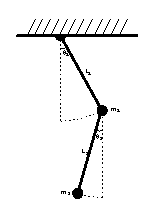
\includegraphics[width=.5\linewidth]{graphics/double_pendulum.eps}
	\caption{Illustration of the simple double pendulum.}
	\label{fig:doublependulum}
\end{figure}

Equations should be developed such that, given an initial state, the position and subsequent movement can be derived from them.
This can be achieved using the Euler-Lagrange differential equations.
These will be found for this system throughout the remainder of this section.
Firstly, the position of the pendulums as a function of the angle must be determined.
The pendulums are placed in the x-y plane with the origin placed at the point of suspension of $p_1$.
When the pendulums are in the stable position, $\theta_1=\theta_2=0$, they are aligned with the y-axis.
The x-axis is positive to the right of the stable position.
The coordinates of $p_1=(x_1,y_1)$ and $p_2=(x_2,y_2)$ are as follows:
\begin{align}
	x_1 &= l_1\sin{\theta_1}\\
	y_1 &= -l_1\cos{\theta_1}\\
	x_2 &= l_1\sin{\theta_1} + l_2\sin{\theta_2}\\
	y_2 &= -l_1\cos{\theta_1} - l_2\cos{\theta_2}
\end{align}
While the derivatives are not used until later, they are presented here for clarity:
\begin{align}
	\dot{x}_1 &= l_1\cos{\theta}_1\dot{\theta}_1\\
	\dot{y}_1 &= l_1\sin{\theta}_1\dot{\theta}_1\\
	\dot{x}_2 &= l_1\cos{\theta}_1\dot{\theta}_1 + l_2\cos{\theta_2}\dot{\theta}_2\\
	\dot{y}_2 &= l_1\sin{\theta}_1\dot{\theta}_1 + l_2\sin{\theta_2}\dot{\theta}_2
\end{align}
In order to calculate the Euler-Lagrange diff. eq. it is necessary to first determine the lagrangian, $\mathcal{l}$:
\begin{equation}
	\mathcal{L}=E_k-E_p
\end{equation}
Where $E_k$ is the kinetic energy of the system and $E_p$, the potential energy.
The derivation of $E_p$:
\begin{align}
	E_p &= m_1 g y_1 + m_2 g y_2\\
		&= -m_1 g l_1 \cos{\theta_1} - m_2 g l_1 \cos{\theta_1} - m_2 g l_2 \cos{\theta_2}\\
		&= -(m_1+m_2)l_1g \cos{\theta_1}-m_2 g l_2 \cos{\theta_2}
		\label{eq:ep}
\end{align}
The derivation of $E_k$:
\begin{equation}
	\label{eq:ek}
	E_k = \frac{1}{2}m_1v_1^2+\frac{1}{2}m_2v_2^2
\end{equation}
As movement is present along both axes, the total velocity of either pendulum can be found as the derivative of the position and Pythagoras:
\begin{align}
	v_1^2 &= \dot{x}_1^2+\dot{y}_1^2\\
		&= l_1^2\dot{\theta}_1^2\cos{\theta}_1^2+l_1^2\dot{\theta}_1^2\sin{\theta_1}^2\\
		&= (\cos{\theta_1}^2+\sin(\theta_1)^2)l_1^2\dot{\theta}_1
\end{align}
Using the Pythagorean identity:
\begin{equation}
	\label{eq:v1}
	v_1^2 = l_1^2\dot{\theta}_1^2
\end{equation}
Similarly:
\begin{align}
	v_2^2 &= \dot{x}_2^2+\dot{y}_2^2\\
	&= (l_1\cos{\theta}_1\dot{\theta}_1 + l_2\cos{\theta_2}\dot{\theta}_2)^2+(l_1\sin{\theta}_1\dot{\theta}_1 + l_2\sin{\theta_2}\dot{\theta}_2)^2\\
	\begin{split}
		&= l_1^2\dot\theta_1^2\cos{\theta_1}^2+l_2^2\dot\theta_2^2\cos{\theta_2}^2+2l_1l_2\dot\theta_1\dot\theta_2\cos{\theta_1}\cos{\theta_2}\\
		&\qquad +l_1^2\dot\theta_1^2\sin{\theta_1}^2+l_2^2\dot\theta_2\sin{\theta_2}+2l_1l_2\dot\theta_1\dot\theta_2\sin{\theta_1}\sin{\theta_2}
	\end{split}
\end{align}
Isolating cosine and sine from the terms pairwise, 1 and 4, 2 and 5, 3 and 6, yields:
\begin{align}
	\begin{split}
		v_2^2&=(\cos{\theta_1}^2+\sin{\theta_1}^2)l_1^2\dot\theta_1^2+(\cos{\theta_2}^2+\sin{\theta_2}^2)l_2^2\dot\theta_2^2\\
	&\qquad+(\cos{\theta_1}\cos{\theta_2}+\sin{\theta_1}\sin{\theta_2})2l_1l_2\dot\theta_1\dot\theta_2
	\end{split}
\end{align}
By applying the trigonimetric identities:
\begin{align}
	1&=\sin{\alpha^2}+\cos{\beta^2}\\
	\cos{(\alpha\pm\beta)}&=\cos\alpha\cos\beta\pm\sin\alpha\sin\beta
\end{align}
The result is found:
\begin{equation}
	\label{eq:v2}
	v_2^2=l_1^2\dot\theta_1^2+l_2^2\dot\theta_2^2+2l_1l_2\dot\theta_1^2\dot\theta_2^2\cos{(\theta_1-\theta_2)}
\end{equation}
Using equations \ref{eq:ep}, \ref{eq:ek}, \ref{eq:v1} and \ref{eq:v2} the lagrangian can be constructed:
\begin{align}
	\begin{split}
		\mathcal{L}&=\frac{1}{2}m_1l_1\dot\theta_1^2+\frac{1}{2}m_2\left(l_1^2\dot\theta_1^2+l_2^2\dot\theta_2^2+2l_1l_2\dot\theta_1^2\dot\theta_2^2\cos{(\theta_1-\theta_2)}\right)\\
		&\qquad+(m_1+m_2)l_1g\cos{\theta_1}+m_2l_2g\cos{\theta_2}
	\end{split}\\
	\begin{split}
		&=\frac{m_1l_1^2\dot\theta_1^2}{2}+\frac{m_2l_1^2\dot\theta_1^2}{2}+\frac{m_2l_2^2\dot\theta_2^2}{2}+l_1l_2\dot\theta_1^2\dot\theta_2^2\cos{(\theta_1-\theta_2)}\\
		&\qquad+(m_1+m_2)l_1g\cos{\theta_1}+m_2l_2g\cos{\theta_2}
	\end{split}
\end{align}
Which simplifies to:
\begin{equation}
	\label{eq:lagrangian}
	\mathcal{L}=\frac{(m_1+m_2)l_1^2\dot\theta_1^2}{2}+\frac{m_2l_2^2\dot\theta_2}{2}+(m_1+m_2)l_1g\cos{\theta_1}+m_2l_2g\cos{\theta_2}\\
\end{equation}
The Euler-Lagrange diff. eq. are defined as:
\begin{equation}
	\frac{d}{dt}\left(\frac{\partial \mathcal{L}}{\partial \dot\theta}\right)-\frac{\partial \mathcal{L}}{\partial \theta} = 0
\end{equation}
The three terms $\frac{\partial \mathcal{L}}{\partial \dot\theta}$,$\frac{d}{dt}\left(\frac{\partial \mathcal{L}}{\partial \dot\theta}\right)$ and $\frac{\partial l}{\partial \theta}$ are calculated next for each of the pendulums. For $p_1$:
\begin{align}
	\frac{\partial \mathcal{L}}{\partial \dot\theta_1}&=(m_1+m_2)l_1^2\dot\theta_1+m_2l_1l_2\dot\theta_2\cos{(\theta_1-\theta_2)}\\
	\begin{split}
		\frac{d}{dt}\left(\frac{\partial \mathcal{L}}{\partial \dot\theta_1}\right)&=(m_1+m_2)l_1^2\ddot\theta_1+m_2l_1l_2\ddot\theta_2\cos{(\theta_1-\theta_2)}\\
		&\qquad-m_2l_1l_2\dot\theta_2\sin{(\theta_1-\theta_2)(\dot\theta_1-\dot\theta_2)}
	\end{split}\\
	\frac{\partial \mathcal{L}}{\partial \theta_1} &= -m_2l_1l_2\dot\theta_1\dot\theta_2\sin(\theta_1-\theta_2)-(m_1+m_2)l_1g\sin{\theta_1}\\
	\begin{split}
		0&=(m_1+m_2)l_1\ddot\theta_1+m_2l_2\ddot\theta_2\cos{(\theta_1-\theta_2)}\\
		&\qquad+m_2l_2\dot\theta_2^2\sin{(\theta_1-\theta_2)}+(m_1+m_2)g\sin{\theta_1}
	\end{split}
\end{align}
And $p_2$:

\begin{align}
	\frac{\partial \mathcal{L}}{\partial \dot\theta_2}&=m_2l_2^2\dot\theta_2+m_2l_1l_2\dot\theta_1\cos{(\theta_1-\theta_2)}\\
	\begin{split}
		\frac{d}{dt}\left(\frac{\partial \mathcal{L}}{\partial \dot\theta_2}\right)&=m_2l_2^2\ddot\theta_2+m_2l_1l_2\ddot\theta_1\cos{(\theta_1-\theta_2)}\\
		&\qquad -m_2l_1l_2\dot\theta_1\sin{(\theta_1-\theta_2)}(\dot\theta_1-\dot\theta_2)
	\end{split}\\
	\frac{\partial \mathcal{L}}{\partial \theta_2} &=m_2l_1l_2\dot\theta_1\dot\theta_2\sin{(\theta_1-\theta_2)}-m_2l_2g\sin{\theta_2}\\
	\label{eq:part}
	\begin{split}
		0&=m_2l_2\ddot\theta_2+m_2l_1\ddot\theta_1\cos{(\theta_1-\theta_2)}\\
		&\qquad-m_2l_1\dot\theta_1^2\sin{(\theta_1-\theta_2)}+m_2g\sin{\theta_2}
	\end{split}
\end{align}
\thomas{eq. \ref{eq:part} has a minus in front of the first term according to our calculations. Determine why.}
% subsection simple_double_pendulum (end)

% section model_development (end)

%!TEX root = ../main.tex
\section{System Verification}
\label{sec:system_verification}
\mikkel{Do you also want text here???}
\thomas{done - Add verification subsection, indent every verification to subsubsection}
\mikkel{done - insert pictures and referred to them}

\subsection{Requirement Verification} % (fold)
\label{sub:requirement_verification}
This final verification evaluates upon the initial requirements of the system found in the system analysis.
\subsubsection{Verification of: Requirements \ref{enum:system_consists_double_pendulum} and \ref{enum:cart_actuated_by_motor}} % (fold)
\label{sub:verification_of_requirement_enum:system_consists_double_pendulum}
These requirements specify that the system should consist of a double pendulum mounted on a moveable cart and that the cart should be actuated by a motor.

\paragraph{Conclusion}~\\
The implemented system consists of the designed and implemented pendulum assembly mounted on the rail system inherited from an earlier project.
A picture of the full system setup is shown in figure \ref{fig:pic_full_system} and a picture of the controller board interfaced with the full system is shown in figure \ref{fig:pic_full_system_high}.
Specific requirements for designing and implementing the pendulum assembly are described and verified in section \ref{sec:joint_development}. 
\begin{figure}
	\centering
	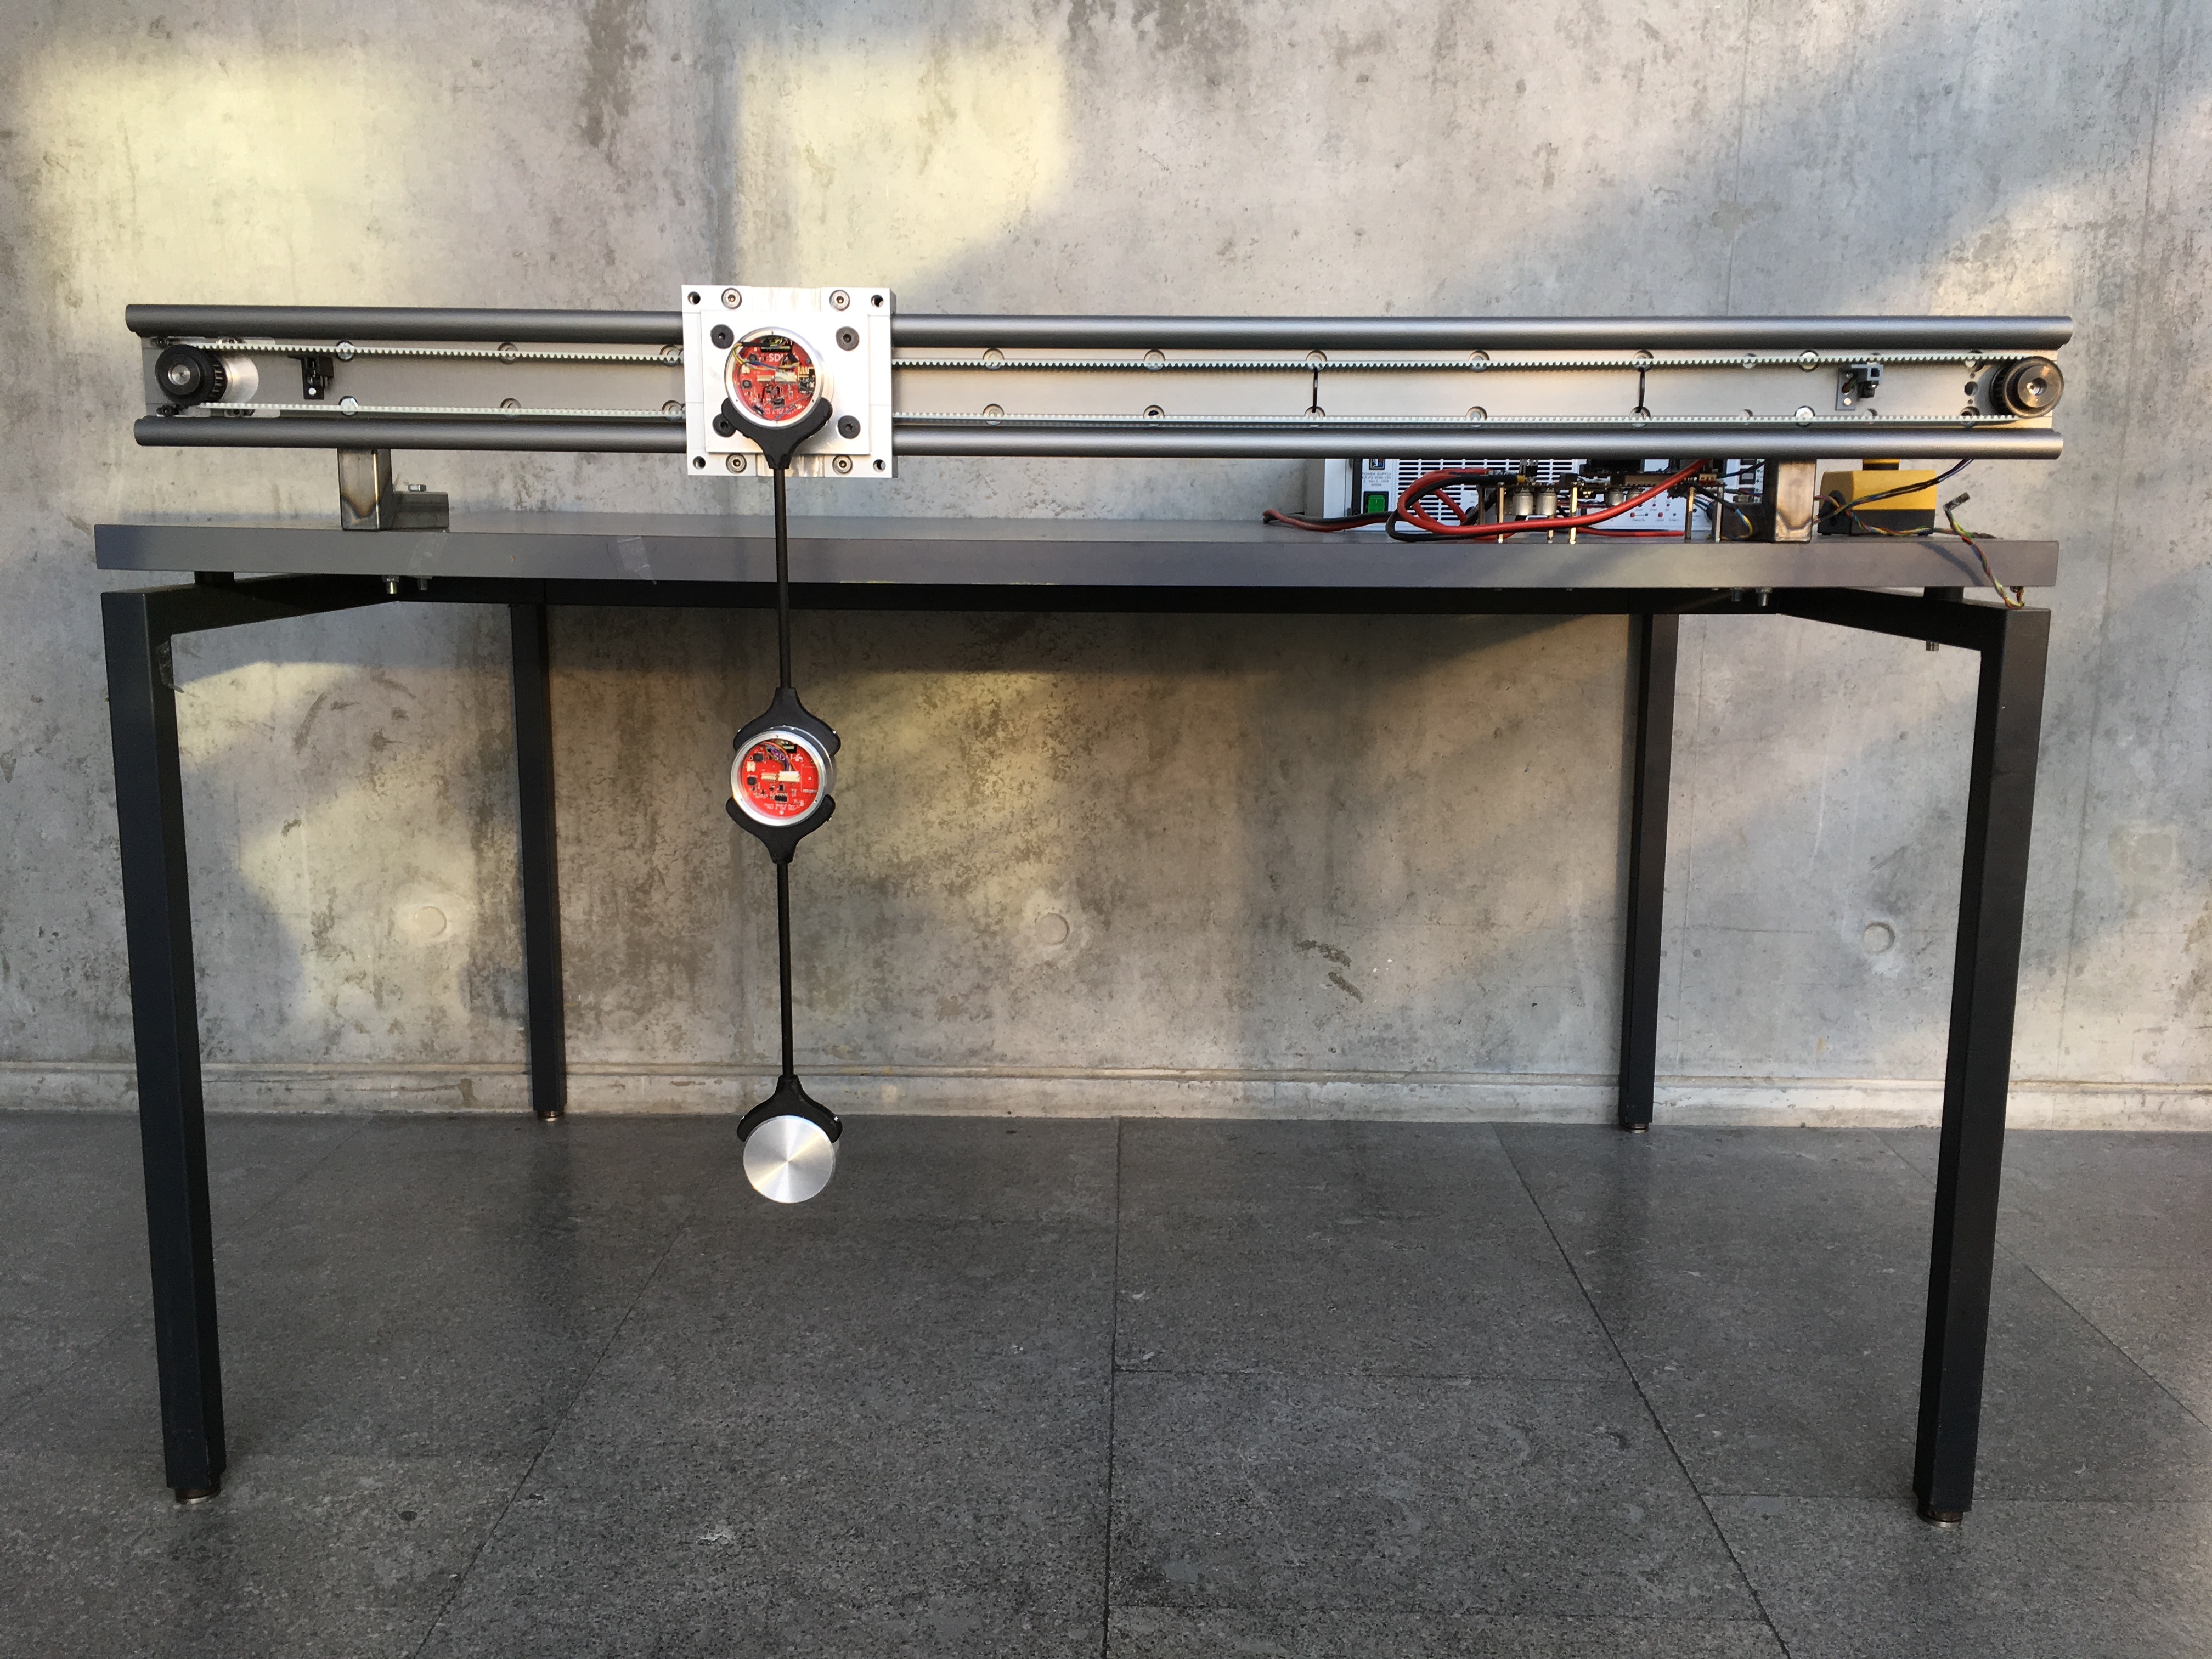
\includegraphics[width=.9\linewidth]{graphics/full_system_finish.JPG}
	\caption{Picture of the full system.}
	\label{fig:pic_full_system}
\end{figure}
\begin{figure}
	\centering
	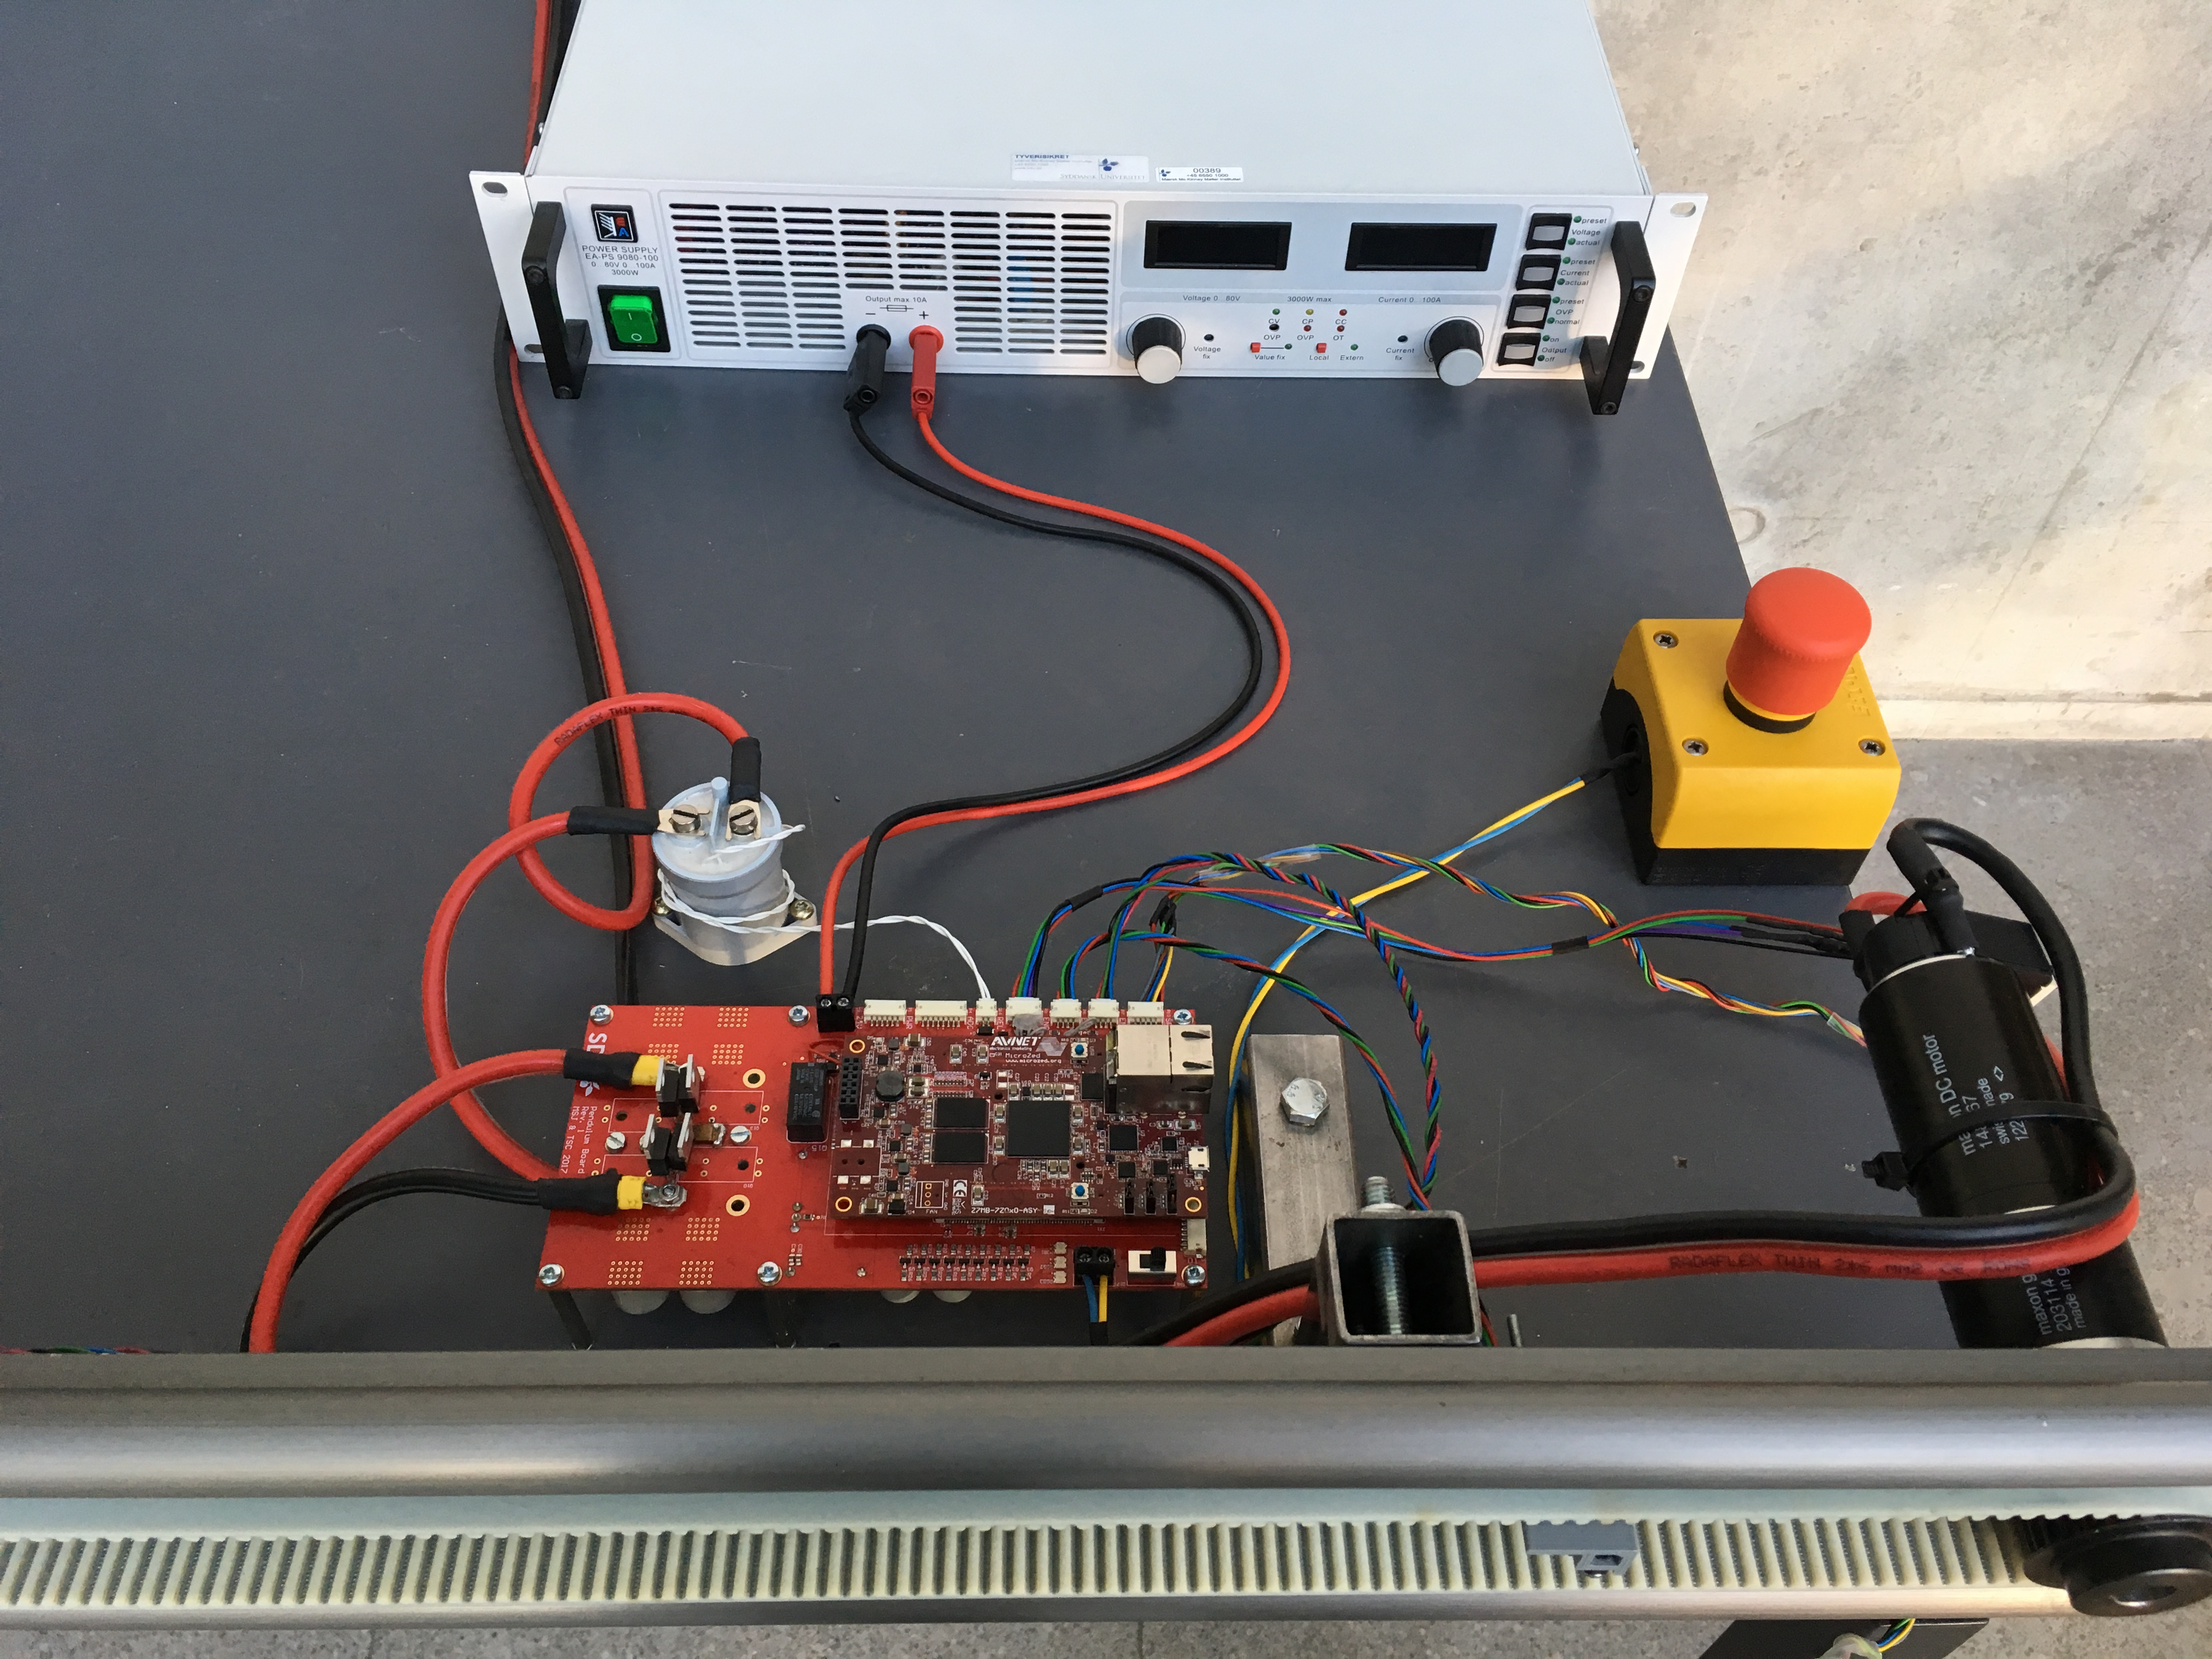
\includegraphics[width=.9\linewidth]{graphics/full_system_finish_high.JPG}
	\caption{Picture of the controller board interfaced with the full system.}
	\label{fig:pic_full_system_high}
\end{figure}


The cart can be actuated by the Maxon motor as they are connected by a belt. 
Even though the cart was never moved using the motor due to debugging troubles and time constraints, it was tested that the developed controller board is able to drive the motor.
Since no actual control was done, it is still unknown whether the cart and rail system is sufficient for this application.

\subsubsection{Verification of: Requirement \ref{enum:controlled_by_microzed}} % (fold)
\label{sub:verification_of_requirement_enum:controlled_by_microzed}
This requirement states that the pendulum system should be controlled by a MicroZed.

\paragraph{Conclusion}~\\
The controller board has been designed to fit the MicroZed and all relevant signals were wired to it as described in section \ref{sec:controller_board}.
\\~\\
In section \ref{subs:requirement_enum:motor_speed_direction} it was verified that the MicroZed can control motor speed and direction through implemented VHDL modules, the motor driver and the H-bridge on the controller board. 
\\~\\
In section \ref{ssub:requrement_enum:motor_current_} it was found that it is not possible to determine the motor current using a shunt resistor and the \texttt{INA286}. 
Thus it is not possible to measure the motor current using the ADC on the MicroZed.
\\~\\
In section \ref{ssub:requirement_enum:microzed_interface} it was verified that the MicroZed is interfaced correctly by measuring start-up and power-down sequences.



\subsubsection{Verification of: Requirement \ref{enum:position_cart_joint_angle_measure}} % (fold)
\label{sub:verification_of_requirement_enum:position_cart_joint_angle_measure}
According to this requirement the position of the cart and joint angles should be measured.

\paragraph{Test}~\\
In section \ref{ssub:verification_of_requirement_enum:correct_cart_position} it is tested and verified that the position of the cart is measured correctly. 
\\~\\
In section \ref{ssub:requirement_enum:correct_angles} it is verified by visual inspection that the joint angles are correctly measured on the joint board.
\\
To further verify that the measurement is correct a test should be conducted where the joint angle data are stored and plotted.  
In a single pendulum setup, the joint should manually be moved $\frac{\pi}{2}$ radians from the equilibrium position and released, while collecting joint angle data.

\paragraph{Conclusion}~\\
The test described above was conducted while transmitting data at 1kHz, with the two \texttt{nRFM}s pointing at each other.
An excerpt of the corresponding data is shown in figure \ref{fig:joint_angle_measured_full} with the joint angle measured in ticks.
A full rotation is equal to 7200 ticks.
As expected the waveform is a damped sinusoidal.
\begin{figure}[h]
	\centering
	%% This file was created by matlab2tikz.
%
%The latest updates can be retrieved from
%  http://www.mathworks.com/matlabcentral/fileexchange/22022-matlab2tikz-matlab2tikz
%where you can also make suggestions and rate matlab2tikz.
%
\definecolor{mycolor1}{rgb}{0.00000,0.44700,0.74100}%
%
\begin{tikzpicture}

\begin{axis}[%
width=.9\textwidth,
height=2.5in,
at={(0.758in,0.481in)},
scale only axis,
xmin=60000,
xmax=100000,
xlabel style={font=\color{white!15!black}},
xlabel={Time [us]},
ymin=4000,
ymax=5200,
ylabel style={font=\color{white!15!black}},
ylabel={Angle [ticks]},
axis background/.style={fill=white},
title style={font=\bfseries},
title={Joint Angle Transmission},
axis x line*=bottom,
axis y line*=left
]
\addplot[only marks, mark=*, mark options={}, mark size=0.5000pt, draw=mycolor1] table[row sep=crcr]{%
x	y\\
58576	4739\\
58577	4742\\
58578	4746\\
58579	4750\\
58580	4753\\
58581	4757\\
58582	4761\\
58583	4764\\
58584	4768\\
58585	4771\\
58586	4775\\
58587	4779\\
58589	4786\\
58590	4789\\
58591	4793\\
58595	4807\\
58596	4810\\
58597	4814\\
58599	4821\\
58600	4824\\
58601	4828\\
58603	4835\\
58604	4838\\
58605	4841\\
58607	4848\\
58609	4855\\
58611	4861\\
58612	4864\\
58614	4871\\
58615	4874\\
58616	4877\\
58618	4883\\
58619	4886\\
58622	4896\\
58625	4905\\
58626	4908\\
58627	4911\\
58629	4917\\
58630	4920\\
58632	4926\\
58633	4929\\
58634	4932\\
58635	4934\\
58636	4937\\
58637	4940\\
58638	4943\\
58640	4948\\
58641	4951\\
58642	4954\\
58644	4959\\
58645	4962\\
58646	4964\\
58647	4967\\
58650	4975\\
58652	4980\\
58654	4985\\
58655	4987\\
58656	4989\\
58657	4992\\
58658	4994\\
58659	4996\\
58660	4999\\
58661	5001\\
58663	5006\\
58665	5010\\
58666	5012\\
58667	5015\\
58668	5017\\
58671	5023\\
58672	5025\\
58673	5027\\
58674	5029\\
58676	5033\\
58677	5035\\
58678	5037\\
58680	5041\\
58682	5044\\
58683	5046\\
58684	5048\\
58686	5052\\
58687	5053\\
58688	5055\\
58689	5057\\
58690	5058\\
58691	5060\\
58693	5063\\
58694	5064\\
58695	5066\\
58696	5067\\
58697	5069\\
58698	5070\\
58699	5071\\
58700	5073\\
58701	5074\\
58702	5075\\
58703	5077\\
58704	5078\\
58705	5079\\
58706	5080\\
58707	5082\\
58708	5083\\
58710	5085\\
58711	5086\\
58712	5087\\
58715	5090\\
58716	5091\\
58717	5092\\
58718	5093\\
58720	5095\\
58721	5095\\
58722	5096\\
58725	5099\\
58726	5099\\
58727	5100\\
58728	5101\\
58730	5102\\
58737	5105\\
58738	5106\\
58740	5106\\
58741	5107\\
58743	5107\\
58744	5108\\
58745	5108\\
58751	5108\\
58752	5109\\
58754	5109\\
58757	5108\\
58758	5108\\
58759	5108\\
58760	5108\\
58761	5108\\
58762	5107\\
58763	5107\\
58764	5107\\
58766	5106\\
58767	5106\\
58769	5105\\
58770	5105\\
58772	5104\\
58773	5103\\
58774	5103\\
58776	5101\\
58777	5101\\
58778	5100\\
58779	5100\\
58780	5099\\
58782	5097\\
58785	5095\\
58786	5094\\
58787	5093\\
58788	5092\\
58790	5090\\
58791	5089\\
58792	5088\\
58793	5087\\
58794	5086\\
58795	5085\\
58799	5081\\
58800	5080\\
58801	5078\\
58802	5077\\
58804	5075\\
58805	5073\\
58807	5071\\
58808	5069\\
58809	5068\\
58810	5066\\
58812	5063\\
58813	5062\\
58814	5060\\
58815	5059\\
58816	5057\\
58817	5056\\
58818	5054\\
58819	5052\\
58820	5050\\
58821	5049\\
58822	5047\\
58823	5045\\
58824	5043\\
58825	5041\\
58828	5036\\
58829	5034\\
58831	5030\\
58832	5028\\
58833	5026\\
58834	5024\\
58835	5022\\
58836	5020\\
58837	5018\\
58839	5013\\
58840	5011\\
58842	5007\\
58843	5005\\
58844	5002\\
58848	4993\\
58849	4990\\
58850	4988\\
58852	4983\\
58853	4981\\
58854	4978\\
58855	4976\\
58856	4973\\
58857	4971\\
58859	4966\\
58860	4963\\
58861	4961\\
58863	4955\\
58864	4953\\
58865	4950\\
58867	4944\\
58871	4933\\
58872	4930\\
58873	4927\\
58874	4924\\
58875	4922\\
58876	4919\\
58877	4916\\
58878	4913\\
58879	4910\\
58880	4907\\
58881	4904\\
58882	4901\\
58883	4898\\
58884	4895\\
58885	4891\\
58887	4885\\
58888	4882\\
58889	4879\\
58890	4876\\
58891	4873\\
58892	4870\\
58893	4866\\
58894	4863\\
58895	4860\\
58896	4857\\
58897	4854\\
58899	4847\\
58902	4837\\
58903	4834\\
58904	4830\\
58905	4827\\
58906	4823\\
58907	4820\\
58908	4816\\
58909	4813\\
58911	4806\\
58912	4803\\
58913	4799\\
58914	4795\\
58915	4792\\
58916	4788\\
58917	4785\\
58918	4781\\
58920	4774\\
58921	4771\\
58923	4764\\
58924	4760\\
58926	4753\\
58927	4749\\
58929	4742\\
58930	4738\\
58931	4735\\
58932	4731\\
58934	4723\\
58937	4712\\
58938	4709\\
58939	4705\\
58940	4701\\
58941	4697\\
58942	4694\\
58943	4690\\
58945	4682\\
58946	4679\\
58947	4675\\
58949	4668\\
58950	4664\\
58951	4660\\
58954	4649\\
58956	4641\\
58957	4637\\
58958	4634\\
58959	4630\\
58961	4622\\
58962	4618\\
58963	4615\\
58965	4607\\
58966	4603\\
58969	4592\\
58970	4588\\
58971	4584\\
58973	4577\\
58974	4573\\
58977	4562\\
58978	4558\\
58980	4550\\
58981	4547\\
58982	4543\\
58983	4539\\
58987	4524\\
58988	4520\\
58989	4516\\
58990	4513\\
58991	4509\\
58992	4505\\
58993	4501\\
58994	4498\\
58997	4487\\
58998	4483\\
58999	4479\\
59001	4472\\
59002	4468\\
59004	4461\\
59005	4458\\
59006	4454\\
59007	4450\\
59008	4447\\
59009	4443\\
59010	4439\\
59011	4436\\
59012	4432\\
59013	4429\\
59014	4425\\
59015	4422\\
59016	4418\\
59017	4414\\
59018	4411\\
59019	4408\\
59020	4404\\
59021	4401\\
59022	4397\\
59023	4394\\
59025	4387\\
59027	4380\\
59028	4377\\
59029	4374\\
59031	4367\\
59032	4364\\
59034	4357\\
59035	4354\\
59036	4351\\
59037	4347\\
59038	4344\\
59039	4341\\
59040	4338\\
59042	4332\\
59043	4328\\
59044	4325\\
59045	4322\\
59046	4319\\
59047	4316\\
59048	4313\\
59049	4310\\
59050	4307\\
59051	4304\\
59053	4298\\
59054	4295\\
59055	4292\\
59059	4281\\
59061	4275\\
59065	4264\\
59067	4259\\
59068	4256\\
59069	4253\\
59070	4251\\
59072	4246\\
59075	4238\\
59076	4235\\
59078	4230\\
59079	4228\\
59083	4218\\
59084	4216\\
59086	4211\\
59088	4207\\
59090	4203\\
59091	4200\\
59093	4196\\
59094	4194\\
59096	4190\\
59097	4188\\
59098	4186\\
59099	4184\\
59100	4182\\
59101	4180\\
59102	4178\\
59103	4176\\
59104	4174\\
59105	4173\\
59107	4169\\
59108	4167\\
59110	4164\\
59111	4162\\
59113	4159\\
59114	4157\\
59115	4156\\
59116	4154\\
59117	4153\\
59118	4151\\
59119	4150\\
59121	4147\\
59122	4145\\
59123	4144\\
59124	4142\\
59125	4141\\
59126	4140\\
59127	4138\\
59128	4137\\
59129	4136\\
59130	4135\\
59132	4132\\
59133	4131\\
59135	4129\\
59136	4128\\
59137	4127\\
59139	4125\\
59140	4124\\
59141	4123\\
59142	4122\\
59144	4120\\
59145	4119\\
59147	4118\\
59148	4117\\
59151	4115\\
59152	4114\\
59153	4114\\
59154	4113\\
59155	4112\\
59156	4112\\
59158	4111\\
59159	4110\\
59160	4110\\
59161	4110\\
59162	4109\\
59164	4108\\
59165	4108\\
59167	4108\\
59168	4107\\
59169	4107\\
59170	4107\\
59171	4107\\
59173	4106\\
59174	4106\\
59175	4106\\
59176	4106\\
59177	4106\\
59178	4106\\
59180	4106\\
59181	4106\\
59182	4106\\
59184	4107\\
59185	4107\\
59186	4107\\
59187	4107\\
59188	4108\\
59190	4108\\
59192	4109\\
59193	4109\\
59195	4110\\
59197	4111\\
59198	4112\\
59199	4112\\
59201	4113\\
59202	4114\\
59203	4114\\
59205	4116\\
59208	4118\\
59210	4120\\
59215	4124\\
59216	4125\\
59217	4126\\
59218	4127\\
59219	4128\\
59220	4129\\
59222	4132\\
59223	4133\\
59225	4135\\
59226	4136\\
59228	4139\\
59229	4140\\
59230	4141\\
59232	4144\\
59233	4145\\
59235	4148\\
59237	4151\\
59238	4153\\
59239	4154\\
59240	4156\\
59242	4159\\
59243	4161\\
59244	4162\\
59245	4164\\
59246	4166\\
59247	4167\\
59248	4169\\
59249	4171\\
59251	4174\\
59252	4176\\
59254	4180\\
59255	4182\\
59256	4184\\
59258	4188\\
59259	4190\\
59262	4196\\
59263	4198\\
59264	4200\\
59265	4202\\
59267	4207\\
59268	4209\\
59269	4211\\
59270	4213\\
59272	4218\\
59273	4220\\
59275	4225\\
59276	4227\\
59277	4230\\
59278	4232\\
59279	4235\\
59280	4237\\
59283	4245\\
59284	4247\\
59285	4250\\
59286	4253\\
59287	4255\\
59288	4258\\
59289	4260\\
59291	4266\\
59292	4268\\
59293	4271\\
59295	4277\\
59296	4279\\
59298	4285\\
59299	4288\\
59301	4293\\
59302	4296\\
59304	4302\\
59305	4305\\
59306	4308\\
59307	4311\\
59308	4314\\
59309	4317\\
59310	4320\\
59311	4323\\
59313	4330\\
59314	4333\\
59315	4336\\
59317	4342\\
59318	4345\\
59319	4348\\
59320	4352\\
59321	4355\\
59323	4361\\
59324	4365\\
59325	4368\\
59327	4374\\
59328	4378\\
59330	4384\\
59331	4387\\
59332	4391\\
59334	4398\\
59335	4401\\
59337	4408\\
59339	4415\\
59340	4418\\
59341	4422\\
59342	4425\\
59343	4429\\
59344	4432\\
59345	4436\\
59346	4439\\
59347	4443\\
59348	4447\\
59349	4450\\
59350	4454\\
59351	4457\\
59353	4464\\
59355	4471\\
59356	4475\\
59357	4479\\
59358	4482\\
59360	4489\\
59362	4497\\
59363	4500\\
59364	4504\\
59365	4508\\
59366	4511\\
59368	4519\\
59369	4523\\
59370	4526\\
59371	4530\\
59372	4534\\
59373	4537\\
59374	4541\\
59376	4549\\
59377	4552\\
59378	4556\\
59379	4560\\
59380	4563\\
59381	4567\\
59382	4571\\
59383	4574\\
59385	4582\\
59386	4585\\
59387	4589\\
59388	4593\\
59389	4597\\
59391	4604\\
59392	4608\\
59394	4615\\
59395	4619\\
59396	4623\\
59397	4627\\
59398	4630\\
59399	4634\\
59400	4638\\
59401	4642\\
59402	4645\\
59403	4649\\
59404	4653\\
59405	4656\\
59406	4660\\
59407	4664\\
59408	4667\\
59409	4671\\
59410	4675\\
59411	4678\\
59412	4682\\
59413	4686\\
59414	4689\\
59416	4697\\
59417	4700\\
59418	4704\\
59419	4708\\
59424	4726\\
59426	4733\\
59427	4737\\
59428	4740\\
59429	4744\\
59430	4747\\
59431	4751\\
59432	4755\\
59433	4758\\
59434	4762\\
59437	4772\\
59439	4779\\
59440	4782\\
59441	4786\\
59442	4789\\
59443	4792\\
59444	4796\\
59445	4799\\
59446	4803\\
59447	4806\\
59448	4810\\
59449	4813\\
59450	4816\\
59452	4823\\
59453	4826\\
59454	4830\\
59455	4833\\
59456	4836\\
59457	4839\\
59458	4843\\
59459	4846\\
59462	4856\\
59464	4862\\
59465	4865\\
59467	4871\\
59468	4874\\
59469	4877\\
59470	4880\\
59473	4889\\
59474	4892\\
59475	4895\\
59477	4901\\
59478	4904\\
59479	4907\\
59481	4912\\
59482	4915\\
59483	4918\\
59485	4924\\
59486	4927\\
59487	4929\\
59489	4935\\
59490	4937\\
59492	4943\\
59493	4945\\
59495	4951\\
59496	4953\\
59499	4961\\
59500	4963\\
59501	4966\\
59502	4968\\
59503	4971\\
59505	4975\\
59506	4978\\
59507	4980\\
59509	4984\\
59510	4987\\
59511	4989\\
59512	4991\\
59513	4993\\
59514	4996\\
59516	5000\\
59517	5002\\
59520	5008\\
59521	5010\\
59523	5014\\
59525	5018\\
59526	5020\\
59527	5022\\
59528	5024\\
59532	5031\\
59533	5033\\
59535	5037\\
59536	5038\\
59537	5040\\
59538	5042\\
59539	5043\\
59541	5046\\
59542	5048\\
59543	5050\\
59545	5053\\
59546	5054\\
59548	5057\\
59549	5058\\
59550	5060\\
59551	5061\\
59553	5063\\
59554	5065\\
59556	5067\\
59558	5069\\
59559	5070\\
59560	5071\\
59562	5074\\
59563	5075\\
59564	5076\\
59566	5077\\
59567	5078\\
59569	5080\\
59571	5082\\
59572	5083\\
59574	5084\\
59575	5085\\
59577	5086\\
59579	5087\\
59580	5088\\
59581	5089\\
59583	5090\\
59584	5090\\
59585	5091\\
59586	5091\\
59587	5091\\
59588	5092\\
59589	5092\\
59590	5093\\
59591	5093\\
59592	5093\\
59593	5093\\
59595	5094\\
59596	5094\\
59597	5094\\
59599	5095\\
59600	5095\\
59602	5095\\
59603	5095\\
59604	5095\\
59605	5095\\
59606	5095\\
59608	5095\\
59609	5094\\
59610	5094\\
59611	5094\\
59612	5094\\
59613	5094\\
59614	5093\\
59615	5093\\
59616	5093\\
59617	5092\\
59618	5092\\
59619	5092\\
59620	5091\\
59622	5090\\
59623	5090\\
59626	5088\\
59628	5087\\
59629	5087\\
59630	5086\\
59632	5085\\
59633	5084\\
59634	5083\\
59635	5082\\
59636	5082\\
59637	5081\\
59638	5080\\
59639	5079\\
59642	5076\\
59643	5075\\
59645	5073\\
59646	5072\\
59647	5071\\
59648	5070\\
59649	5069\\
59650	5068\\
59651	5067\\
59653	5064\\
59655	5062\\
59656	5060\\
59657	5059\\
59659	5056\\
59660	5055\\
59662	5052\\
59663	5051\\
59664	5049\\
59665	5048\\
59666	5046\\
59667	5044\\
59668	5043\\
59670	5040\\
59671	5038\\
59672	5036\\
59673	5034\\
59674	5033\\
59675	5031\\
59677	5027\\
59678	5026\\
59680	5022\\
59681	5020\\
59682	5018\\
59684	5014\\
59685	5012\\
59687	5008\\
59688	5006\\
59689	5004\\
59690	5002\\
59691	5000\\
59692	4997\\
59693	4995\\
59694	4993\\
59696	4989\\
59697	4986\\
59698	4984\\
59700	4980\\
59701	4977\\
59703	4973\\
59706	4965\\
59707	4963\\
59708	4960\\
59709	4958\\
59711	4953\\
59714	4945\\
59715	4942\\
59717	4937\\
59718	4934\\
59720	4929\\
59721	4926\\
59722	4923\\
59724	4918\\
59725	4915\\
59727	4909\\
59728	4907\\
59731	4898\\
59732	4895\\
59733	4892\\
59734	4889\\
59736	4883\\
59738	4877\\
59739	4874\\
59740	4871\\
59742	4865\\
59743	4862\\
59744	4859\\
59746	4852\\
59747	4849\\
59749	4843\\
59750	4840\\
59751	4836\\
59756	4820\\
59757	4817\\
59758	4813\\
59760	4807\\
59761	4803\\
59762	4800\\
59763	4796\\
59766	4786\\
59768	4779\\
59769	4776\\
59771	4769\\
59772	4766\\
59773	4762\\
59775	4755\\
59776	4752\\
59777	4748\\
59779	4741\\
59780	4737\\
59781	4734\\
59782	4730\\
59783	4727\\
59784	4723\\
59785	4720\\
59787	4712\\
59788	4709\\
59789	4705\\
59791	4698\\
59792	4694\\
59793	4690\\
59794	4687\\
59797	4676\\
59798	4672\\
59800	4665\\
59801	4662\\
59802	4658\\
59803	4654\\
59805	4647\\
59806	4643\\
59807	4639\\
59808	4636\\
59812	4621\\
59813	4617\\
59814	4614\\
59815	4610\\
59816	4606\\
59817	4603\\
59818	4599\\
59820	4591\\
59821	4588\\
59822	4584\\
59823	4580\\
59825	4573\\
59826	4570\\
59828	4562\\
59829	4559\\
59830	4555\\
59832	4548\\
59833	4544\\
59834	4540\\
59836	4533\\
59837	4529\\
59838	4526\\
59839	4522\\
59841	4515\\
59842	4511\\
59844	4504\\
59845	4500\\
59846	4496\\
59847	4493\\
59849	4486\\
59850	4482\\
59851	4479\\
59853	4472\\
59854	4468\\
59855	4464\\
59856	4461\\
59858	4454\\
59859	4451\\
59861	4444\\
59864	4433\\
59865	4430\\
59866	4426\\
59868	4419\\
59870	4412\\
59871	4409\\
59872	4406\\
59873	4402\\
59874	4399\\
59876	4392\\
59879	4383\\
59880	4379\\
59882	4373\\
59884	4367\\
59885	4363\\
59886	4360\\
59887	4357\\
59888	4354\\
59890	4348\\
59891	4345\\
59892	4342\\
59894	4335\\
59895	4332\\
59896	4329\\
59898	4323\\
59899	4320\\
59900	4317\\
59902	4312\\
59903	4309\\
59904	4306\\
59905	4303\\
59906	4300\\
59907	4297\\
59908	4295\\
59909	4292\\
59911	4286\\
59912	4284\\
59913	4281\\
59914	4278\\
59915	4276\\
59916	4273\\
59917	4270\\
59918	4268\\
59919	4265\\
59920	4263\\
59921	4260\\
59923	4255\\
59924	4253\\
59925	4250\\
59926	4248\\
59927	4245\\
59930	4238\\
59931	4236\\
59933	4231\\
59934	4229\\
59935	4226\\
59937	4222\\
59938	4220\\
59939	4217\\
59941	4213\\
59942	4211\\
59944	4207\\
59945	4205\\
59946	4203\\
59947	4201\\
59948	4199\\
59949	4197\\
59950	4195\\
59951	4193\\
59952	4191\\
59954	4187\\
59955	4186\\
59956	4184\\
59957	4182\\
59959	4179\\
59960	4177\\
59961	4175\\
59962	4174\\
59963	4172\\
59964	4171\\
59965	4169\\
59966	4168\\
59967	4166\\
59968	4165\\
59969	4163\\
59971	4160\\
59972	4159\\
59974	4156\\
59975	4155\\
59976	4154\\
59977	4152\\
59978	4151\\
59979	4150\\
59981	4147\\
59983	4145\\
59984	4144\\
59985	4143\\
59987	4141\\
59988	4140\\
59989	4139\\
59991	4137\\
59993	4135\\
59996	4133\\
59997	4132\\
59998	4131\\
59999	4130\\
60000	4130\\
60001	4129\\
60002	4128\\
60003	4128\\
60006	4126\\
60007	4125\\
60009	4124\\
60010	4124\\
60012	4123\\
60013	4123\\
60015	4122\\
60017	4121\\
60018	4121\\
60020	4121\\
60021	4120\\
60022	4120\\
60023	4120\\
60024	4120\\
60025	4120\\
60026	4120\\
60027	4120\\
60028	4120\\
60029	4120\\
60033	4120\\
60035	4120\\
60036	4120\\
60039	4121\\
60043	4122\\
60046	4124\\
60048	4125\\
60049	4125\\
60050	4126\\
60052	4127\\
60054	4128\\
60055	4129\\
60056	4129\\
60057	4130\\
60058	4131\\
60059	4132\\
60060	4132\\
60061	4133\\
60062	4134\\
60063	4135\\
60064	4136\\
60067	4138\\
60069	4140\\
60071	4142\\
60072	4143\\
60075	4147\\
60076	4148\\
60077	4149\\
60078	4150\\
60079	4152\\
60080	4153\\
60081	4154\\
60082	4156\\
60083	4157\\
60086	4161\\
60087	4162\\
60088	4164\\
60089	4165\\
60090	4167\\
60094	4173\\
60095	4174\\
60097	4178\\
60098	4179\\
60099	4181\\
60101	4185\\
60102	4186\\
60103	4188\\
60104	4190\\
60105	4192\\
60106	4194\\
60107	4195\\
60109	4199\\
60110	4201\\
60111	4203\\
60112	4205\\
60113	4207\\
60115	4212\\
60116	4214\\
60117	4216\\
60119	4220\\
60120	4222\\
60121	4224\\
60122	4227\\
60123	4229\\
60124	4231\\
60126	4236\\
60127	4238\\
60128	4240\\
60129	4243\\
60130	4245\\
60131	4248\\
60132	4250\\
60134	4255\\
60135	4258\\
60136	4260\\
60137	4263\\
60138	4265\\
60139	4268\\
60140	4270\\
60141	4273\\
60142	4275\\
60143	4278\\
60144	4281\\
60148	4291\\
60149	4294\\
60150	4297\\
60151	4300\\
60152	4303\\
60153	4305\\
60154	4308\\
60155	4311\\
60156	4314\\
60158	4320\\
60160	4326\\
60163	4335\\
60164	4338\\
60165	4341\\
60166	4344\\
60167	4347\\
60169	4353\\
60170	4356\\
60172	4362\\
60173	4365\\
60174	4368\\
60176	4375\\
60177	4378\\
60178	4381\\
60180	4387\\
60181	4391\\
60182	4394\\
60183	4397\\
60184	4400\\
60186	4407\\
60188	4414\\
60189	4417\\
60191	4424\\
60192	4427\\
60193	4431\\
60196	4441\\
60197	4444\\
60198	4448\\
60199	4451\\
60200	4455\\
60203	4465\\
60204	4468\\
60206	4475\\
60207	4479\\
60208	4482\\
60209	4486\\
60210	4489\\
60212	4497\\
60214	4504\\
60216	4511\\
60218	4518\\
60219	4522\\
60220	4525\\
60222	4532\\
60223	4536\\
60224	4540\\
60226	4547\\
60227	4551\\
60228	4554\\
60230	4561\\
60231	4565\\
60233	4572\\
60234	4576\\
60235	4579\\
60236	4583\\
60237	4586\\
60239	4594\\
60241	4601\\
60243	4608\\
60249	4630\\
60250	4634\\
60252	4641\\
60253	4644\\
60254	4648\\
60255	4652\\
60256	4655\\
60258	4662\\
60261	4673\\
60262	4677\\
60264	4684\\
60265	4687\\
60266	4691\\
60267	4694\\
60268	4698\\
60269	4701\\
60270	4705\\
60271	4709\\
60273	4716\\
60274	4719\\
60277	4730\\
60278	4733\\
60280	4740\\
60281	4744\\
60282	4747\\
60283	4751\\
60284	4754\\
60285	4757\\
60286	4761\\
60287	4764\\
60288	4768\\
60290	4774\\
60291	4778\\
60292	4781\\
60293	4784\\
60294	4787\\
60296	4794\\
60299	4804\\
60301	4811\\
60302	4814\\
60303	4817\\
60304	4820\\
60305	4823\\
60306	4827\\
60307	4830\\
60308	4833\\
60309	4836\\
60310	4839\\
60311	4842\\
60312	4846\\
60313	4849\\
60314	4852\\
60315	4855\\
60316	4858\\
60317	4861\\
60320	4870\\
60323	4879\\
60325	4884\\
60326	4887\\
60328	4893\\
60329	4896\\
60330	4898\\
60331	4901\\
60333	4907\\
60336	4915\\
60338	4920\\
60340	4926\\
60341	4928\\
60343	4934\\
60344	4936\\
60345	4939\\
60346	4941\\
60347	4944\\
60348	4946\\
60349	4949\\
60350	4951\\
60352	4956\\
60353	4958\\
60356	4965\\
60358	4970\\
60359	4972\\
60360	4974\\
60362	4979\\
60363	4981\\
60364	4983\\
60365	4985\\
60366	4987\\
60368	4991\\
60369	4993\\
60370	4995\\
60371	4997\\
60372	4999\\
60373	5001\\
60374	5003\\
60375	5005\\
60376	5007\\
60377	5009\\
60378	5011\\
60380	5014\\
60381	5016\\
60382	5018\\
60384	5021\\
60385	5023\\
60386	5025\\
60387	5026\\
60388	5028\\
60389	5030\\
60391	5033\\
60392	5034\\
60393	5036\\
60394	5037\\
60395	5039\\
60396	5040\\
60398	5043\\
60399	5044\\
60401	5047\\
60402	5048\\
60403	5050\\
60404	5051\\
60405	5052\\
60406	5053\\
60407	5054\\
60408	5056\\
60409	5057\\
60410	5058\\
60411	5059\\
60412	5060\\
60413	5061\\
60414	5062\\
60415	5063\\
60416	5064\\
60418	5066\\
60419	5066\\
60420	5067\\
60421	5068\\
60422	5069\\
60423	5070\\
60424	5070\\
60425	5071\\
60426	5072\\
60427	5073\\
60428	5073\\
60429	5074\\
60430	5074\\
60431	5075\\
60432	5076\\
60433	5076\\
60435	5077\\
60436	5077\\
60437	5078\\
60438	5078\\
60439	5079\\
60441	5079\\
60442	5080\\
60443	5080\\
60444	5080\\
60445	5080\\
60447	5081\\
60448	5081\\
60449	5081\\
60450	5081\\
60451	5081\\
60453	5081\\
60454	5081\\
60455	5081\\
60456	5081\\
60457	5081\\
60459	5081\\
60460	5081\\
60461	5081\\
60462	5081\\
60464	5080\\
60465	5080\\
60466	5080\\
60467	5080\\
60468	5079\\
60471	5078\\
60472	5078\\
60473	5077\\
60475	5076\\
60476	5076\\
60478	5075\\
60479	5074\\
60481	5073\\
60482	5072\\
60484	5071\\
60485	5070\\
60486	5069\\
60487	5069\\
60488	5068\\
60489	5067\\
60490	5066\\
60491	5065\\
60492	5064\\
60493	5063\\
60495	5062\\
60496	5061\\
60500	5056\\
60501	5055\\
60502	5054\\
60503	5053\\
60504	5052\\
60506	5049\\
60507	5048\\
60508	5047\\
60509	5045\\
60511	5043\\
60513	5040\\
60514	5038\\
60515	5037\\
60516	5035\\
60517	5034\\
60518	5032\\
60519	5031\\
60520	5029\\
60521	5028\\
60523	5024\\
60524	5023\\
60526	5019\\
60527	5017\\
60529	5014\\
60530	5012\\
60531	5010\\
60532	5008\\
60533	5007\\
60534	5005\\
60535	5003\\
60536	5001\\
60537	4999\\
60538	4997\\
60539	4995\\
60541	4991\\
60542	4989\\
60544	4984\\
60547	4978\\
60548	4976\\
60549	4974\\
60551	4969\\
60552	4967\\
60554	4962\\
60555	4960\\
60556	4958\\
60558	4953\\
60560	4948\\
60561	4946\\
60562	4943\\
60563	4941\\
60564	4938\\
60566	4933\\
60567	4931\\
60569	4925\\
60571	4920\\
60572	4917\\
60573	4915\\
60575	4909\\
60576	4907\\
60577	4904\\
60579	4898\\
60580	4895\\
60581	4892\\
60583	4887\\
60584	4884\\
60585	4881\\
60586	4878\\
60588	4872\\
60589	4870\\
60591	4864\\
60592	4861\\
60594	4855\\
60595	4852\\
60596	4849\\
60597	4845\\
60598	4842\\
60599	4839\\
60600	4836\\
60602	4830\\
60603	4827\\
60604	4823\\
60605	4820\\
60606	4817\\
60607	4814\\
60608	4811\\
60609	4807\\
60611	4801\\
60612	4798\\
60614	4791\\
60616	4784\\
60617	4781\\
60618	4778\\
60619	4775\\
60620	4771\\
60622	4765\\
60623	4761\\
60624	4758\\
60625	4754\\
60627	4748\\
60628	4744\\
60630	4737\\
60631	4734\\
60632	4730\\
60633	4727\\
60635	4720\\
60636	4716\\
60637	4713\\
60638	4709\\
60640	4702\\
60641	4699\\
60642	4695\\
60644	4688\\
60645	4685\\
60646	4681\\
60648	4674\\
60649	4671\\
60650	4667\\
60652	4660\\
60653	4657\\
60654	4653\\
60656	4646\\
60657	4642\\
60658	4639\\
60660	4631\\
60661	4628\\
60664	4617\\
60665	4613\\
60667	4606\\
60668	4603\\
60669	4599\\
60671	4592\\
60675	4578\\
60677	4571\\
60678	4567\\
60679	4563\\
60680	4560\\
60681	4556\\
60682	4553\\
60683	4549\\
60684	4546\\
60685	4542\\
60686	4538\\
60687	4535\\
60688	4531\\
60689	4528\\
60690	4524\\
60691	4521\\
60692	4517\\
60693	4514\\
60695	4507\\
60696	4503\\
60697	4500\\
60700	4489\\
60701	4486\\
60703	4479\\
60704	4475\\
60705	4472\\
60706	4468\\
60708	4462\\
60709	4458\\
60712	4448\\
60713	4445\\
60714	4441\\
60715	4438\\
60716	4435\\
60717	4431\\
60718	4428\\
60719	4425\\
60720	4421\\
60721	4418\\
60722	4415\\
60725	4405\\
60726	4402\\
60728	4395\\
60729	4392\\
60731	4386\\
60732	4383\\
60733	4379\\
60734	4376\\
60735	4373\\
60736	4370\\
60737	4367\\
60738	4364\\
60739	4361\\
60740	4358\\
60741	4355\\
60742	4352\\
60743	4349\\
60744	4346\\
60745	4343\\
60746	4340\\
60747	4337\\
60748	4334\\
60749	4331\\
60750	4329\\
60751	4326\\
60754	4317\\
60756	4312\\
60757	4309\\
60760	4301\\
60761	4298\\
60764	4290\\
60765	4287\\
60766	4285\\
60767	4282\\
60768	4280\\
60769	4277\\
60771	4272\\
60772	4270\\
60773	4267\\
60774	4265\\
60775	4262\\
60776	4260\\
60777	4258\\
60778	4255\\
60779	4253\\
60780	4251\\
60781	4248\\
60782	4246\\
60783	4244\\
60784	4241\\
60786	4237\\
60787	4235\\
60788	4233\\
60790	4228\\
60791	4226\\
60792	4224\\
60793	4222\\
60794	4220\\
60796	4216\\
60799	4210\\
60800	4208\\
60801	4206\\
60802	4205\\
60804	4201\\
60805	4199\\
60807	4196\\
60808	4194\\
60810	4190\\
60811	4189\\
60812	4187\\
60815	4183\\
60816	4181\\
60817	4180\\
60818	4178\\
60819	4177\\
60820	4175\\
60821	4174\\
60822	4173\\
60823	4171\\
60825	4169\\
60826	4167\\
60827	4166\\
60829	4164\\
60830	4162\\
60831	4161\\
60832	4160\\
60833	4159\\
60835	4157\\
60836	4156\\
60838	4154\\
60840	4152\\
60841	4151\\
60842	4150\\
60843	4149\\
60845	4147\\
60846	4146\\
60847	4146\\
60848	4145\\
60849	4144\\
60850	4143\\
60851	4143\\
60852	4142\\
60853	4141\\
60854	4141\\
60855	4140\\
60856	4140\\
60858	4139\\
60859	4138\\
60860	4138\\
60862	4137\\
60863	4136\\
60864	4136\\
60865	4136\\
60867	4135\\
60868	4135\\
60869	4134\\
60870	4134\\
60871	4134\\
60872	4134\\
60874	4134\\
60876	4133\\
60877	4133\\
60878	4133\\
60882	4133\\
60884	4133\\
60885	4134\\
60886	4134\\
60888	4134\\
60889	4134\\
60891	4135\\
60892	4135\\
60894	4136\\
60896	4137\\
60897	4137\\
60898	4137\\
60899	4138\\
60900	4138\\
60901	4139\\
60902	4139\\
60903	4140\\
60904	4141\\
60905	4141\\
60906	4142\\
60907	4143\\
60908	4143\\
60909	4144\\
60910	4145\\
60911	4145\\
60913	4147\\
60914	4148\\
60916	4150\\
60917	4150\\
60920	4153\\
60922	4155\\
60923	4156\\
60924	4157\\
60926	4160\\
60929	4163\\
60930	4164\\
60931	4165\\
60932	4167\\
60933	4168\\
60934	4169\\
60935	4171\\
60936	4172\\
60937	4173\\
60938	4175\\
60939	4176\\
60940	4177\\
60941	4179\\
60942	4180\\
60943	4182\\
60945	4185\\
60947	4188\\
60948	4190\\
60949	4191\\
60950	4193\\
60951	4195\\
60952	4196\\
60953	4198\\
60955	4202\\
60956	4203\\
60957	4205\\
60958	4207\\
60959	4209\\
60960	4211\\
60962	4215\\
60963	4217\\
60967	4225\\
60968	4227\\
60969	4229\\
60971	4233\\
60972	4235\\
60973	4237\\
60974	4240\\
60975	4242\\
60976	4244\\
60977	4246\\
60978	4249\\
60980	4253\\
60983	4260\\
60984	4263\\
60988	4272\\
60989	4275\\
60990	4277\\
60991	4280\\
60993	4285\\
60996	4292\\
60997	4295\\
60998	4298\\
60999	4300\\
61001	4306\\
61002	4308\\
61003	4311\\
61004	4314\\
61005	4317\\
61006	4319\\
61007	4322\\
61008	4325\\
61010	4331\\
61011	4334\\
61012	4337\\
61013	4339\\
61015	4345\\
61016	4348\\
61017	4351\\
61019	4357\\
61020	4360\\
61021	4363\\
61025	4375\\
61026	4378\\
61027	4381\\
61029	4387\\
61031	4394\\
61032	4397\\
61033	4400\\
61034	4403\\
61036	4410\\
61037	4413\\
61038	4416\\
61040	4423\\
61041	4426\\
61042	4429\\
61044	4436\\
61045	4439\\
61046	4442\\
61047	4446\\
61048	4449\\
61049	4452\\
61050	4456\\
61052	4462\\
61053	4466\\
61054	4469\\
61056	4476\\
61057	4479\\
61059	4486\\
61060	4489\\
61061	4493\\
61063	4500\\
61064	4503\\
61065	4507\\
61066	4510\\
61068	4517\\
61070	4524\\
61071	4528\\
61072	4531\\
61074	4538\\
61075	4542\\
61076	4545\\
61077	4549\\
61078	4552\\
61079	4556\\
61081	4563\\
61082	4566\\
61084	4573\\
61085	4577\\
61086	4580\\
61088	4587\\
61089	4590\\
61091	4598\\
61092	4601\\
61093	4605\\
61095	4612\\
61096	4615\\
61097	4619\\
61099	4626\\
61100	4629\\
61101	4633\\
61102	4636\\
61103	4640\\
61104	4643\\
61105	4647\\
61106	4650\\
61107	4654\\
61108	4657\\
61109	4661\\
61110	4664\\
61111	4668\\
61112	4671\\
61116	4685\\
61117	4688\\
61118	4692\\
61119	4695\\
61120	4699\\
61121	4702\\
61122	4706\\
61123	4709\\
61124	4713\\
61125	4716\\
61126	4719\\
61128	4726\\
61129	4730\\
61131	4736\\
61132	4740\\
61133	4743\\
61134	4747\\
61135	4750\\
61136	4753\\
61137	4757\\
61138	4760\\
61139	4763\\
61141	4770\\
61142	4773\\
61143	4776\\
61144	4779\\
61145	4782\\
61146	4786\\
61147	4789\\
61149	4795\\
61150	4798\\
61151	4802\\
61153	4808\\
61156	4817\\
61157	4820\\
61158	4824\\
61159	4827\\
61160	4830\\
61162	4836\\
61163	4839\\
61164	4842\\
61165	4845\\
61169	4857\\
61170	4860\\
61171	4862\\
61172	4865\\
61173	4868\\
61174	4871\\
61175	4874\\
61176	4877\\
61177	4879\\
61178	4882\\
61179	4885\\
61180	4887\\
61181	4890\\
61183	4896\\
61184	4898\\
61186	4904\\
61187	4906\\
61188	4909\\
61189	4912\\
61191	4917\\
61193	4922\\
61194	4924\\
61195	4927\\
61197	4932\\
61198	4934\\
61199	4937\\
61203	4946\\
61204	4948\\
61205	4951\\
61207	4955\\
61208	4958\\
61209	4960\\
61210	4962\\
61211	4964\\
61212	4966\\
61214	4970\\
61215	4972\\
61216	4974\\
61217	4977\\
61218	4979\\
61219	4981\\
61220	4982\\
61222	4986\\
61225	4992\\
61226	4994\\
61228	4998\\
61229	4999\\
61230	5001\\
61231	5003\\
61232	5005\\
61234	5008\\
61235	5010\\
61237	5013\\
61238	5015\\
61239	5016\\
61241	5019\\
61243	5022\\
61244	5024\\
61246	5027\\
61247	5028\\
61248	5029\\
61250	5032\\
61251	5033\\
61252	5035\\
61255	5038\\
61256	5040\\
61257	5041\\
61258	5042\\
61261	5045\\
61262	5046\\
61263	5047\\
61264	5048\\
61265	5049\\
61266	5050\\
61267	5051\\
61268	5052\\
61269	5053\\
61270	5054\\
61271	5055\\
61273	5056\\
61274	5057\\
61275	5058\\
61276	5058\\
61277	5059\\
61278	5060\\
61280	5061\\
61282	5062\\
61283	5063\\
61284	5063\\
61286	5064\\
61287	5064\\
61288	5065\\
61289	5065\\
61290	5066\\
61291	5066\\
61293	5067\\
61294	5067\\
61295	5067\\
61296	5067\\
61298	5068\\
61299	5068\\
61301	5068\\
61304	5068\\
61305	5068\\
61307	5068\\
61309	5068\\
61311	5068\\
61312	5068\\
61313	5068\\
61315	5067\\
61316	5067\\
61318	5066\\
61319	5066\\
61324	5064\\
61325	5064\\
61326	5063\\
61327	5063\\
61329	5062\\
61330	5061\\
61332	5060\\
61333	5059\\
61335	5058\\
61336	5057\\
61338	5056\\
61340	5054\\
61341	5053\\
61342	5052\\
61343	5052\\
61344	5051\\
61345	5050\\
61348	5047\\
61349	5046\\
61351	5044\\
61352	5042\\
61353	5041\\
61354	5040\\
61355	5039\\
61356	5038\\
61357	5037\\
61358	5035\\
61359	5034\\
61361	5032\\
61362	5030\\
61364	5027\\
61367	5023\\
61368	5022\\
61369	5020\\
61370	5019\\
61371	5017\\
61372	5016\\
61373	5014\\
61374	5012\\
61375	5011\\
61377	5007\\
61378	5006\\
61379	5004\\
61381	5001\\
61384	4995\\
61385	4993\\
61387	4989\\
61389	4986\\
61390	4984\\
61391	4982\\
61394	4976\\
61396	4972\\
61398	4968\\
61399	4965\\
61400	4963\\
61401	4961\\
61402	4959\\
61403	4957\\
61404	4955\\
61406	4950\\
61407	4948\\
61408	4945\\
61410	4941\\
61411	4938\\
61412	4936\\
61413	4933\\
61414	4931\\
61415	4929\\
61416	4926\\
61418	4921\\
61419	4919\\
61421	4914\\
61422	4911\\
61423	4908\\
61424	4906\\
61425	4903\\
61426	4900\\
61427	4898\\
61429	4892\\
61430	4890\\
61434	4879\\
61435	4876\\
61436	4873\\
61439	4865\\
61440	4862\\
61441	4859\\
61442	4856\\
61443	4853\\
61444	4850\\
61445	4847\\
61446	4845\\
61449	4835\\
61451	4829\\
61452	4826\\
61453	4823\\
61454	4820\\
61457	4811\\
61458	4808\\
61459	4805\\
61460	4802\\
61461	4798\\
61462	4795\\
61463	4792\\
61464	4789\\
61465	4786\\
61466	4782\\
61467	4779\\
61469	4773\\
61470	4770\\
61471	4766\\
61473	4760\\
61474	4757\\
61476	4750\\
61477	4747\\
61480	4737\\
61481	4733\\
61482	4730\\
61483	4727\\
61485	4720\\
61486	4716\\
61487	4713\\
61488	4710\\
61489	4706\\
61490	4703\\
61492	4696\\
61493	4693\\
61494	4689\\
61496	4682\\
61497	4679\\
61500	4669\\
61501	4665\\
61502	4662\\
61504	4655\\
61505	4652\\
61507	4645\\
61508	4641\\
61509	4638\\
61510	4634\\
61511	4631\\
61512	4627\\
61513	4624\\
61515	4617\\
61516	4613\\
61517	4610\\
61518	4606\\
61519	4603\\
61521	4596\\
61522	4592\\
61524	4585\\
61525	4582\\
61527	4575\\
61528	4572\\
61529	4568\\
61530	4565\\
61532	4558\\
61533	4554\\
61534	4551\\
61536	4544\\
61538	4537\\
61539	4534\\
61540	4530\\
61541	4527\\
61542	4523\\
61543	4520\\
61545	4513\\
61546	4510\\
61549	4499\\
61550	4496\\
61552	4489\\
61553	4486\\
61554	4482\\
61556	4476\\
61557	4472\\
61558	4469\\
61559	4466\\
61560	4463\\
61561	4459\\
61564	4449\\
61565	4446\\
61567	4440\\
61568	4436\\
61569	4433\\
61570	4430\\
61571	4427\\
61572	4424\\
61573	4420\\
61574	4417\\
61575	4414\\
61576	4411\\
61577	4408\\
61578	4404\\
61579	4401\\
61580	4398\\
61581	4395\\
61582	4392\\
61583	4389\\
61585	4383\\
61586	4380\\
61588	4374\\
61589	4371\\
61590	4368\\
61592	4362\\
61593	4359\\
61594	4357\\
61596	4351\\
61597	4348\\
61598	4345\\
61599	4342\\
61601	4337\\
61602	4334\\
61603	4331\\
61605	4326\\
61606	4323\\
61609	4315\\
61611	4309\\
61612	4307\\
61613	4304\\
61615	4299\\
61616	4296\\
61617	4294\\
61618	4291\\
61619	4289\\
61620	4286\\
61621	4284\\
61622	4282\\
61623	4279\\
61626	4272\\
61627	4270\\
61628	4268\\
61629	4265\\
61630	4263\\
61631	4261\\
61632	4259\\
61633	4256\\
61634	4254\\
61636	4250\\
61637	4248\\
61638	4246\\
61639	4243\\
61641	4239\\
61642	4237\\
61644	4233\\
61645	4231\\
61646	4229\\
61648	4225\\
61649	4223\\
61651	4220\\
61652	4218\\
61654	4214\\
61655	4212\\
61657	4209\\
61658	4207\\
61659	4206\\
61660	4204\\
61661	4202\\
61662	4201\\
61663	4199\\
61664	4198\\
61665	4196\\
61667	4193\\
61668	4192\\
61669	4190\\
61670	4189\\
61671	4187\\
61672	4186\\
61674	4183\\
61675	4182\\
61676	4181\\
61678	4178\\
61679	4177\\
61680	4176\\
61681	4175\\
61682	4174\\
61685	4170\\
61688	4167\\
61689	4166\\
61690	4165\\
61692	4164\\
61694	4162\\
61695	4161\\
61696	4160\\
61697	4159\\
61698	4159\\
61699	4158\\
61700	4157\\
61701	4157\\
61702	4156\\
61703	4155\\
61704	4155\\
61705	4154\\
61706	4153\\
61708	4152\\
61709	4152\\
61710	4151\\
61711	4151\\
61712	4150\\
61713	4150\\
61714	4150\\
61715	4149\\
61716	4149\\
61718	4148\\
61720	4148\\
61721	4148\\
61725	4147\\
61726	4147\\
61727	4147\\
61728	4147\\
61729	4147\\
61731	4147\\
61732	4147\\
61733	4147\\
61735	4147\\
61736	4147\\
61738	4147\\
61739	4147\\
61740	4148\\
61741	4148\\
61742	4148\\
61743	4148\\
61744	4149\\
61745	4149\\
61747	4150\\
61748	4150\\
61749	4151\\
61750	4151\\
61751	4152\\
61752	4152\\
61753	4153\\
61754	4153\\
61757	4155\\
61759	4156\\
61760	4157\\
61761	4158\\
61762	4158\\
61763	4159\\
61764	4160\\
61765	4161\\
61768	4163\\
61769	4164\\
61770	4165\\
61772	4167\\
61773	4168\\
61774	4169\\
61775	4170\\
61776	4171\\
61777	4172\\
61778	4173\\
61779	4174\\
61780	4175\\
61782	4178\\
61783	4179\\
61784	4180\\
61786	4183\\
61787	4184\\
61788	4185\\
61789	4187\\
61792	4191\\
61793	4192\\
61794	4194\\
61797	4198\\
61799	4201\\
61800	4203\\
61801	4205\\
61803	4208\\
61804	4210\\
61805	4211\\
61806	4213\\
61807	4215\\
61809	4218\\
61810	4220\\
61811	4222\\
61812	4224\\
61813	4226\\
61814	4228\\
61815	4230\\
61817	4234\\
61818	4236\\
61820	4240\\
61824	4248\\
61825	4250\\
61826	4252\\
61828	4257\\
61829	4259\\
61830	4261\\
61831	4263\\
61832	4265\\
61833	4268\\
61834	4270\\
61835	4272\\
61836	4274\\
61837	4277\\
61838	4279\\
61839	4282\\
61840	4284\\
61842	4289\\
61843	4291\\
61844	4294\\
61845	4296\\
61846	4299\\
61847	4301\\
61848	4304\\
61849	4306\\
61850	4309\\
61851	4312\\
61853	4317\\
61854	4319\\
61857	4328\\
61858	4330\\
61859	4333\\
61862	4341\\
61865	4350\\
61866	4353\\
61867	4355\\
61868	4358\\
61869	4361\\
61870	4364\\
61871	4367\\
61872	4370\\
61873	4373\\
61874	4376\\
61875	4379\\
61876	4382\\
61878	4387\\
61879	4390\\
61880	4393\\
61881	4396\\
61882	4400\\
61883	4403\\
61884	4406\\
61885	4409\\
61886	4412\\
61887	4415\\
61888	4418\\
61889	4421\\
61890	4425\\
61891	4428\\
61892	4431\\
61893	4434\\
61894	4437\\
61895	4441\\
61896	4444\\
61898	4450\\
61899	4453\\
61900	4457\\
61902	4463\\
61904	4470\\
61906	4476\\
61907	4479\\
61910	4489\\
61911	4493\\
61912	4496\\
61913	4499\\
61916	4509\\
61917	4513\\
61918	4516\\
61919	4519\\
61922	4530\\
61924	4536\\
61925	4540\\
61927	4547\\
61928	4550\\
61929	4554\\
61932	4564\\
61933	4567\\
61935	4574\\
61936	4577\\
61937	4581\\
61939	4587\\
61940	4591\\
61942	4598\\
61944	4604\\
61945	4608\\
61946	4611\\
61947	4615\\
61948	4618\\
61949	4621\\
61950	4625\\
61952	4632\\
61953	4635\\
61954	4639\\
61955	4642\\
61956	4645\\
61958	4652\\
61959	4656\\
61960	4659\\
61961	4662\\
61964	4672\\
61966	4679\\
61967	4682\\
61970	4692\\
61972	4699\\
61973	4702\\
61974	4706\\
61975	4709\\
61976	4712\\
61977	4716\\
61978	4719\\
61979	4722\\
61980	4726\\
61981	4729\\
61982	4732\\
61983	4736\\
61985	4742\\
61986	4745\\
61987	4749\\
61989	4755\\
61990	4758\\
61991	4761\\
61992	4765\\
61994	4771\\
61995	4774\\
61997	4780\\
61998	4783\\
61999	4786\\
62000	4789\\
62001	4792\\
62002	4796\\
62004	4802\\
62005	4805\\
62008	4814\\
62009	4817\\
62011	4823\\
62012	4826\\
62013	4829\\
62014	4832\\
62016	4838\\
62017	4840\\
62018	4843\\
62019	4846\\
62020	4849\\
62021	4852\\
62022	4855\\
62023	4858\\
62024	4860\\
62025	4863\\
62026	4866\\
62028	4871\\
62029	4874\\
62030	4877\\
62032	4882\\
62033	4884\\
62034	4887\\
62035	4890\\
62036	4892\\
62037	4895\\
62038	4897\\
62040	4903\\
62041	4905\\
62042	4908\\
62043	4910\\
62044	4912\\
62045	4915\\
62046	4917\\
62048	4922\\
62049	4924\\
62050	4927\\
62052	4931\\
62053	4934\\
62054	4936\\
62055	4938\\
62056	4940\\
62057	4943\\
62058	4945\\
62059	4947\\
62060	4949\\
62061	4951\\
62062	4954\\
62064	4958\\
62065	4960\\
62066	4962\\
62067	4964\\
62068	4966\\
62069	4968\\
62070	4970\\
62072	4973\\
62073	4975\\
62075	4979\\
62077	4983\\
62078	4984\\
62079	4986\\
62080	4988\\
62084	4995\\
62085	4996\\
62086	4998\\
62088	5001\\
62091	5006\\
62092	5007\\
62093	5009\\
62094	5010\\
62095	5012\\
62097	5014\\
62098	5016\\
62099	5017\\
62101	5020\\
62102	5021\\
62104	5023\\
62105	5025\\
62107	5027\\
62108	5028\\
62110	5030\\
62111	5031\\
62112	5032\\
62113	5033\\
62114	5034\\
62115	5035\\
62116	5036\\
62117	5037\\
62118	5038\\
62119	5039\\
62122	5042\\
62123	5042\\
62124	5043\\
62129	5047\\
62130	5047\\
62132	5048\\
62133	5049\\
62135	5050\\
62136	5051\\
62138	5051\\
62139	5052\\
62140	5052\\
62141	5053\\
62142	5053\\
62143	5053\\
62144	5054\\
62145	5054\\
62146	5054\\
62148	5055\\
62150	5055\\
62151	5055\\
62153	5055\\
62154	5055\\
62155	5055\\
62157	5055\\
62159	5055\\
62161	5055\\
62163	5055\\
62164	5055\\
62165	5055\\
62166	5054\\
62167	5054\\
62168	5054\\
62171	5053\\
62173	5052\\
62175	5051\\
62178	5050\\
62180	5049\\
62181	5048\\
62183	5047\\
62184	5046\\
62185	5046\\
62186	5045\\
62187	5044\\
62188	5044\\
62189	5043\\
62190	5042\\
62191	5041\\
62193	5040\\
62194	5039\\
62196	5037\\
62197	5036\\
62199	5034\\
62200	5033\\
62201	5032\\
62202	5031\\
62203	5030\\
62204	5029\\
62205	5028\\
62206	5027\\
62207	5026\\
62208	5024\\
62210	5022\\
62211	5021\\
62212	5019\\
62213	5018\\
62214	5017\\
62215	5016\\
62217	5013\\
62218	5011\\
62219	5010\\
62220	5009\\
62221	5007\\
62223	5004\\
62224	5003\\
62226	4999\\
62228	4996\\
62229	4994\\
62230	4993\\
62233	4988\\
62235	4984\\
62236	4982\\
62237	4981\\
62239	4977\\
62241	4973\\
62242	4971\\
62243	4970\\
62245	4966\\
62246	4964\\
62247	4962\\
62248	4960\\
62249	4958\\
62250	4956\\
62251	4954\\
62252	4951\\
62254	4947\\
62255	4945\\
62256	4943\\
62257	4940\\
62258	4938\\
62259	4936\\
62260	4934\\
62262	4929\\
62263	4927\\
62265	4922\\
62266	4920\\
62267	4917\\
62269	4913\\
62270	4910\\
62271	4908\\
62272	4905\\
62274	4900\\
62275	4898\\
62277	4892\\
62278	4890\\
62279	4887\\
62281	4882\\
62282	4879\\
62283	4877\\
62285	4872\\
62286	4869\\
62288	4863\\
62291	4855\\
62292	4852\\
62293	4850\\
62295	4844\\
62296	4841\\
62297	4838\\
62298	4835\\
62299	4832\\
62301	4827\\
62302	4824\\
62303	4821\\
62304	4818\\
62306	4812\\
62307	4809\\
62308	4806\\
62309	4803\\
62310	4800\\
62312	4793\\
62313	4790\\
62314	4787\\
62316	4781\\
62317	4778\\
62318	4775\\
62320	4769\\
62321	4766\\
62322	4762\\
62324	4756\\
62325	4753\\
62327	4747\\
62328	4743\\
62331	4734\\
62332	4730\\
62333	4727\\
62336	4717\\
62338	4711\\
62340	4704\\
62341	4701\\
62342	4697\\
62343	4694\\
62344	4691\\
62345	4687\\
62347	4681\\
62348	4678\\
62350	4671\\
62351	4668\\
62354	4658\\
62355	4654\\
62357	4648\\
62358	4644\\
62359	4641\\
62363	4627\\
62364	4624\\
62365	4621\\
62367	4614\\
62368	4610\\
62369	4607\\
62370	4604\\
62372	4597\\
62373	4593\\
62376	4583\\
62377	4580\\
62378	4577\\
62379	4573\\
62380	4570\\
62381	4567\\
62383	4560\\
62384	4557\\
62385	4553\\
62386	4550\\
62388	4543\\
62389	4540\\
62391	4533\\
62392	4530\\
62393	4527\\
62395	4520\\
62396	4517\\
62397	4513\\
62399	4507\\
62401	4500\\
62402	4497\\
62403	4493\\
62404	4490\\
62405	4487\\
62407	4480\\
62408	4477\\
62409	4474\\
62410	4471\\
62411	4468\\
62413	4461\\
62414	4458\\
62416	4452\\
62417	4449\\
62418	4445\\
62420	4439\\
62421	4436\\
62422	4433\\
62423	4430\\
62424	4427\\
62425	4423\\
62426	4420\\
62427	4417\\
62428	4414\\
62429	4411\\
62430	4408\\
62431	4405\\
62432	4402\\
62435	4393\\
62437	4387\\
62438	4384\\
62439	4381\\
62440	4379\\
62441	4376\\
62442	4373\\
62443	4370\\
62444	4367\\
62446	4362\\
62447	4359\\
62448	4356\\
62449	4353\\
62450	4351\\
62453	4342\\
62454	4340\\
62455	4337\\
62456	4334\\
62457	4332\\
62458	4329\\
62459	4327\\
62460	4324\\
62461	4321\\
62462	4319\\
62463	4316\\
62464	4314\\
62466	4309\\
62467	4306\\
62469	4301\\
62470	4299\\
62471	4296\\
62473	4292\\
62474	4289\\
62476	4285\\
62477	4282\\
62478	4280\\
62480	4276\\
62481	4273\\
62482	4271\\
62484	4267\\
62485	4265\\
62486	4263\\
62487	4261\\
62488	4259\\
62489	4257\\
62490	4255\\
62492	4250\\
62493	4248\\
62494	4246\\
62495	4245\\
62496	4243\\
62497	4241\\
62498	4239\\
62500	4235\\
62502	4231\\
62503	4230\\
62504	4228\\
62505	4226\\
62506	4224\\
62507	4223\\
62508	4221\\
62510	4218\\
62511	4216\\
62512	4214\\
62513	4213\\
62514	4211\\
62515	4210\\
62516	4208\\
62517	4207\\
62518	4205\\
62519	4204\\
62520	4203\\
62523	4198\\
62524	4197\\
62525	4196\\
62526	4194\\
62527	4193\\
62528	4192\\
62529	4191\\
62530	4190\\
62531	4188\\
62532	4187\\
62533	4186\\
62534	4185\\
62535	4184\\
62536	4183\\
62537	4182\\
62539	4180\\
62540	4179\\
62541	4178\\
62542	4177\\
62543	4176\\
62544	4175\\
62546	4174\\
62548	4172\\
62551	4170\\
62552	4169\\
62553	4169\\
62554	4168\\
62555	4168\\
62556	4167\\
62558	4166\\
62561	4164\\
62563	4163\\
62564	4163\\
62565	4163\\
62566	4162\\
62567	4162\\
62568	4162\\
62570	4161\\
62572	4161\\
62573	4160\\
62577	4160\\
62578	4160\\
62580	4160\\
62581	4160\\
62583	4160\\
62584	4160\\
62586	4160\\
62587	4160\\
62589	4160\\
62590	4160\\
62591	4161\\
62592	4161\\
62593	4161\\
62595	4162\\
62596	4162\\
62597	4162\\
62598	4163\\
62599	4163\\
62602	4164\\
62603	4165\\
62604	4165\\
62605	4166\\
62607	4167\\
62608	4168\\
62609	4168\\
62611	4169\\
62612	4170\\
62613	4171\\
62614	4172\\
62615	4172\\
62617	4174\\
62618	4175\\
62619	4176\\
62620	4176\\
62621	4177\\
62622	4178\\
62623	4179\\
62624	4180\\
62625	4181\\
62626	4182\\
62628	4184\\
62629	4185\\
62630	4186\\
62631	4187\\
62632	4188\\
62633	4189\\
62634	4191\\
62635	4192\\
62636	4193\\
62637	4194\\
62638	4196\\
62640	4198\\
62642	4201\\
62643	4202\\
62644	4204\\
62645	4205\\
62646	4207\\
62647	4208\\
62649	4211\\
62650	4213\\
62651	4214\\
62652	4216\\
62656	4222\\
62657	4224\\
62658	4226\\
62659	4227\\
62660	4229\\
62662	4233\\
62663	4235\\
62665	4238\\
62666	4240\\
62668	4244\\
62669	4246\\
62670	4248\\
62671	4250\\
62673	4254\\
62674	4256\\
62676	4260\\
62677	4262\\
62678	4264\\
62679	4266\\
62680	4268\\
62681	4270\\
62682	4272\\
62684	4277\\
62685	4279\\
62687	4283\\
62688	4286\\
62689	4288\\
62691	4293\\
62692	4295\\
62693	4297\\
62694	4300\\
62695	4302\\
62696	4305\\
62697	4307\\
62698	4309\\
62699	4312\\
62700	4314\\
62701	4317\\
62703	4322\\
62704	4325\\
62705	4327\\
62707	4332\\
62708	4335\\
62709	4338\\
62711	4343\\
62712	4346\\
62715	4354\\
62716	4356\\
62718	4362\\
62719	4365\\
62721	4370\\
62722	4373\\
62723	4376\\
62725	4381\\
62726	4384\\
62727	4387\\
62730	4396\\
62732	4402\\
62733	4405\\
62734	4408\\
62736	4414\\
62737	4417\\
62740	4426\\
62741	4429\\
62743	4435\\
62744	4438\\
62745	4441\\
62747	4448\\
62748	4451\\
62751	4460\\
62752	4463\\
62753	4466\\
62754	4469\\
62756	4476\\
62757	4479\\
62758	4482\\
62759	4485\\
62761	4492\\
62762	4495\\
62763	4498\\
62764	4501\\
62765	4505\\
62767	4511\\
62768	4514\\
62769	4518\\
62770	4521\\
62771	4524\\
62772	4528\\
62773	4531\\
62776	4541\\
62777	4544\\
62778	4547\\
62782	4560\\
62784	4567\\
62785	4570\\
62786	4574\\
62787	4577\\
62788	4580\\
62790	4587\\
62791	4590\\
62792	4593\\
62793	4597\\
62794	4600\\
62795	4603\\
62796	4607\\
62797	4610\\
62798	4613\\
62799	4617\\
62800	4620\\
62802	4626\\
62803	4630\\
62804	4633\\
62806	4640\\
62807	4643\\
62808	4646\\
62810	4653\\
62811	4656\\
62812	4660\\
62814	4666\\
62815	4669\\
62817	4676\\
62818	4679\\
62820	4685\\
62821	4689\\
62823	4695\\
62824	4698\\
62825	4702\\
62826	4705\\
62827	4708\\
62828	4711\\
62829	4715\\
62830	4718\\
62831	4721\\
62833	4727\\
62834	4731\\
62835	4734\\
62836	4737\\
62838	4743\\
62839	4746\\
62841	4753\\
62842	4756\\
62843	4759\\
62844	4762\\
62845	4765\\
62848	4774\\
62849	4777\\
62850	4780\\
62852	4786\\
62853	4789\\
62854	4792\\
62856	4798\\
62857	4801\\
62858	4804\\
62859	4807\\
62863	4818\\
62864	4821\\
62867	4830\\
62868	4833\\
62870	4838\\
62871	4841\\
62872	4844\\
62873	4846\\
62874	4849\\
62875	4852\\
62876	4855\\
62877	4857\\
62878	4860\\
62879	4862\\
62880	4865\\
62881	4868\\
62882	4870\\
62883	4873\\
62884	4875\\
62885	4878\\
62886	4880\\
62887	4883\\
62888	4885\\
62889	4888\\
62890	4890\\
62891	4893\\
62892	4895\\
62893	4898\\
62896	4905\\
62897	4907\\
62898	4910\\
62900	4914\\
62901	4916\\
62903	4921\\
62904	4923\\
62905	4925\\
62906	4928\\
62907	4930\\
62908	4932\\
62909	4934\\
62910	4936\\
62911	4938\\
62912	4940\\
62913	4942\\
62916	4949\\
62917	4951\\
62918	4953\\
62919	4955\\
62921	4958\\
62922	4960\\
62923	4962\\
62925	4966\\
62926	4967\\
62927	4969\\
62928	4971\\
62929	4973\\
62930	4974\\
62931	4976\\
62932	4978\\
62933	4979\\
62934	4981\\
62936	4984\\
62937	4986\\
62938	4987\\
62939	4989\\
62940	4990\\
62941	4992\\
62943	4995\\
62944	4996\\
62946	4999\\
62947	5001\\
62948	5002\\
62949	5003\\
62952	5007\\
62953	5008\\
62954	5010\\
62955	5011\\
62956	5012\\
62957	5013\\
62959	5015\\
62960	5016\\
62962	5018\\
62964	5020\\
62965	5021\\
62966	5022\\
62970	5026\\
62971	5027\\
62973	5029\\
62974	5029\\
62975	5030\\
62977	5031\\
62978	5032\\
62979	5033\\
62980	5033\\
62981	5034\\
62982	5035\\
62983	5035\\
62984	5036\\
62985	5036\\
62986	5037\\
62987	5037\\
62988	5038\\
62989	5038\\
62990	5039\\
62991	5039\\
62992	5039\\
62993	5040\\
62994	5040\\
62995	5040\\
62996	5041\\
62997	5041\\
62998	5041\\
62999	5041\\
63000	5041\\
63001	5042\\
63002	5042\\
63003	5042\\
63004	5042\\
63005	5042\\
63006	5042\\
63007	5042\\
63008	5042\\
63010	5042\\
63011	5042\\
63012	5042\\
63013	5042\\
63014	5042\\
63015	5042\\
63016	5041\\
63017	5041\\
63018	5041\\
63019	5041\\
63020	5040\\
63022	5040\\
63023	5040\\
63024	5039\\
63025	5039\\
63028	5038\\
63029	5037\\
63030	5037\\
63031	5036\\
63032	5036\\
63034	5034\\
63035	5034\\
63036	5033\\
63037	5033\\
63038	5032\\
63040	5031\\
63041	5030\\
63042	5029\\
63043	5028\\
63044	5027\\
63047	5025\\
63048	5024\\
63049	5023\\
63050	5022\\
63052	5020\\
63053	5019\\
63054	5018\\
63055	5017\\
63056	5016\\
63057	5015\\
63059	5013\\
63060	5012\\
63061	5010\\
63062	5009\\
63063	5008\\
63065	5005\\
63066	5004\\
63067	5003\\
63068	5002\\
63069	5000\\
63071	4997\\
63072	4996\\
63073	4994\\
63074	4993\\
63075	4991\\
63076	4990\\
63078	4987\\
63079	4985\\
63080	4984\\
63081	4982\\
63082	4981\\
63083	4979\\
63085	4976\\
63086	4974\\
63087	4972\\
63088	4971\\
63089	4969\\
63091	4965\\
63092	4963\\
63093	4962\\
63094	4960\\
63095	4958\\
63096	4956\\
63098	4952\\
63099	4950\\
63100	4948\\
63101	4946\\
63102	4944\\
63104	4940\\
63105	4938\\
63106	4936\\
63107	4934\\
63108	4932\\
63109	4929\\
63111	4925\\
63112	4923\\
63113	4921\\
63114	4918\\
63115	4916\\
63116	4914\\
63119	4907\\
63120	4905\\
63122	4900\\
63123	4897\\
63125	4892\\
63126	4890\\
63127	4888\\
63128	4885\\
63129	4883\\
63130	4880\\
63132	4875\\
63133	4873\\
63135	4868\\
63136	4865\\
63137	4862\\
63139	4857\\
63140	4855\\
63141	4852\\
63142	4849\\
63143	4846\\
63144	4844\\
63145	4841\\
63146	4838\\
63147	4835\\
63148	4833\\
63149	4830\\
63150	4827\\
63152	4821\\
63153	4818\\
63154	4816\\
63156	4810\\
63157	4807\\
63159	4801\\
63160	4798\\
63162	4792\\
63163	4789\\
63164	4786\\
63165	4783\\
63166	4780\\
63170	4768\\
63171	4765\\
63172	4762\\
63174	4756\\
63175	4753\\
63177	4747\\
63178	4744\\
63179	4741\\
63180	4738\\
63181	4735\\
63182	4731\\
63183	4728\\
63184	4725\\
63185	4722\\
63186	4719\\
63190	4706\\
63191	4703\\
63192	4700\\
63193	4696\\
63194	4693\\
63195	4690\\
63197	4683\\
63198	4680\\
63199	4677\\
63201	4671\\
63204	4661\\
63205	4658\\
63206	4655\\
63209	4645\\
63210	4641\\
63212	4635\\
63213	4632\\
63214	4628\\
63215	4625\\
63216	4622\\
63217	4619\\
63218	4615\\
63219	4612\\
63220	4609\\
63221	4606\\
63222	4602\\
63223	4599\\
63224	4596\\
63225	4592\\
63226	4589\\
63229	4579\\
63230	4576\\
63231	4573\\
63234	4563\\
63235	4560\\
63237	4553\\
63238	4550\\
63239	4547\\
63240	4544\\
63241	4540\\
63242	4537\\
63243	4534\\
63245	4527\\
63246	4524\\
63247	4521\\
63249	4514\\
63250	4511\\
63252	4505\\
63253	4502\\
63254	4498\\
63255	4495\\
63256	4492\\
63258	4486\\
63259	4483\\
63260	4480\\
63261	4476\\
63262	4473\\
63264	4467\\
63265	4464\\
63266	4461\\
63268	4455\\
63269	4452\\
63270	4449\\
63272	4443\\
63273	4440\\
63274	4437\\
63276	4431\\
63278	4425\\
63279	4422\\
63280	4419\\
63282	4413\\
63283	4410\\
63284	4407\\
63286	4401\\
63287	4398\\
63288	4395\\
63291	4387\\
63292	4384\\
63294	4379\\
63295	4376\\
63297	4370\\
63298	4368\\
63299	4365\\
63300	4362\\
63301	4360\\
63302	4357\\
63306	4347\\
63308	4341\\
63309	4339\\
63310	4336\\
63312	4331\\
63313	4329\\
63314	4326\\
63315	4324\\
63316	4321\\
63317	4319\\
63318	4316\\
63320	4312\\
63321	4309\\
63322	4307\\
63324	4302\\
63325	4300\\
63326	4298\\
63327	4295\\
63328	4293\\
63329	4291\\
63330	4289\\
63332	4284\\
63333	4282\\
63334	4280\\
63335	4278\\
63338	4272\\
63339	4270\\
63342	4264\\
63343	4262\\
63344	4260\\
63345	4258\\
63346	4256\\
63347	4254\\
63348	4253\\
63350	4249\\
63352	4245\\
63353	4244\\
63354	4242\\
63356	4238\\
63357	4237\\
63358	4235\\
63359	4233\\
63360	4232\\
63361	4230\\
63362	4229\\
63363	4227\\
63364	4225\\
63365	4224\\
63366	4222\\
63367	4221\\
63369	4218\\
63371	4215\\
63372	4214\\
63373	4212\\
63374	4211\\
63375	4210\\
63376	4209\\
63377	4207\\
63378	4206\\
63379	4205\\
63380	4204\\
63382	4201\\
63383	4200\\
63384	4199\\
63385	4198\\
63386	4197\\
63387	4196\\
63389	4194\\
63390	4193\\
63391	4192\\
63392	4191\\
63393	4190\\
63394	4189\\
63395	4188\\
63396	4188\\
63397	4187\\
63399	4185\\
63400	4184\\
63401	4184\\
63403	4182\\
63404	4182\\
63405	4181\\
63406	4181\\
63407	4180\\
63409	4179\\
63410	4178\\
63414	4177\\
63415	4176\\
63416	4176\\
63417	4175\\
63419	4175\\
63420	4174\\
63421	4174\\
63422	4174\\
63423	4174\\
63424	4173\\
63425	4173\\
63426	4173\\
63427	4173\\
63428	4173\\
63429	4173\\
63433	4173\\
63434	4173\\
63435	4173\\
63436	4173\\
63437	4173\\
63439	4173\\
63442	4173\\
63444	4174\\
63445	4174\\
63446	4174\\
63447	4175\\
63448	4175\\
63451	4176\\
63452	4176\\
63453	4177\\
63456	4178\\
63457	4179\\
63458	4179\\
63459	4180\\
63460	4181\\
63461	4181\\
63462	4182\\
63464	4183\\
63465	4184\\
63467	4185\\
63468	4186\\
63469	4187\\
63470	4187\\
63471	4188\\
63473	4190\\
63476	4193\\
63479	4196\\
63480	4197\\
63481	4198\\
63482	4199\\
63483	4200\\
63484	4201\\
63485	4202\\
63486	4203\\
63487	4205\\
63489	4207\\
63490	4208\\
63491	4210\\
63492	4211\\
63493	4212\\
63494	4213\\
63495	4215\\
63496	4216\\
63497	4218\\
63498	4219\\
63500	4222\\
63501	4223\\
63503	4226\\
63504	4228\\
63505	4230\\
63506	4231\\
63507	4233\\
63509	4236\\
63510	4238\\
63511	4239\\
63513	4243\\
63515	4246\\
63516	4248\\
63517	4250\\
63518	4252\\
63520	4255\\
63521	4257\\
63523	4261\\
63524	4263\\
63525	4265\\
63527	4269\\
63528	4271\\
63529	4273\\
63530	4275\\
63531	4277\\
63532	4279\\
63533	4281\\
63534	4283\\
63535	4285\\
63536	4287\\
63537	4289\\
63539	4294\\
63540	4296\\
63541	4298\\
63543	4303\\
63544	4305\\
63545	4307\\
63546	4310\\
63547	4312\\
63548	4314\\
63550	4319\\
63551	4322\\
63552	4324\\
63553	4326\\
63554	4329\\
63555	4331\\
63556	4334\\
63557	4336\\
63558	4339\\
63559	4341\\
63560	4344\\
63561	4347\\
63562	4349\\
63565	4357\\
63566	4360\\
63568	4365\\
63569	4367\\
63570	4370\\
63572	4375\\
63573	4378\\
63574	4381\\
63575	4384\\
63576	4386\\
63577	4389\\
63578	4392\\
63579	4395\\
63580	4398\\
63581	4400\\
63582	4403\\
63584	4409\\
63585	4412\\
63586	4415\\
63587	4418\\
63588	4421\\
63589	4424\\
63591	4430\\
63594	4438\\
63595	4441\\
63597	4447\\
63600	4456\\
63601	4459\\
63602	4462\\
63604	4468\\
63605	4472\\
63606	4475\\
63610	4487\\
63611	4490\\
63613	4496\\
63614	4499\\
63616	4506\\
63617	4509\\
63618	4512\\
63619	4515\\
63620	4518\\
63621	4521\\
63623	4528\\
63624	4531\\
63625	4534\\
63626	4537\\
63628	4544\\
63629	4547\\
63630	4550\\
63631	4553\\
63632	4557\\
63633	4560\\
63634	4563\\
63635	4566\\
63637	4572\\
63638	4576\\
63640	4582\\
63643	4592\\
63644	4595\\
63645	4598\\
63647	4605\\
63648	4608\\
63649	4611\\
63650	4614\\
63651	4617\\
63652	4621\\
63653	4624\\
63655	4630\\
63656	4633\\
63657	4637\\
63658	4640\\
63659	4643\\
63660	4646\\
63661	4650\\
63662	4653\\
63663	4656\\
63665	4662\\
63666	4665\\
63668	4672\\
63669	4675\\
63670	4678\\
63672	4684\\
63673	4687\\
63675	4694\\
63676	4697\\
63677	4700\\
63679	4706\\
63680	4709\\
63681	4712\\
63683	4719\\
63686	4728\\
63687	4731\\
63688	4734\\
63689	4737\\
63690	4740\\
63691	4743\\
63694	4752\\
63695	4755\\
63696	4758\\
63697	4761\\
63698	4764\\
63699	4767\\
63701	4773\\
63702	4776\\
63703	4779\\
63704	4782\\
63706	4787\\
63707	4790\\
63708	4793\\
63709	4796\\
63710	4799\\
63711	4802\\
63713	4807\\
63715	4813\\
63716	4816\\
63717	4818\\
63718	4821\\
63719	4824\\
63720	4827\\
63721	4829\\
63722	4832\\
63724	4837\\
63725	4840\\
63726	4843\\
63727	4845\\
63728	4848\\
63729	4851\\
63730	4853\\
63732	4858\\
63733	4861\\
63735	4866\\
63736	4868\\
63737	4871\\
63738	4873\\
63739	4876\\
63740	4878\\
63742	4883\\
63743	4885\\
63744	4887\\
63745	4890\\
63746	4892\\
63747	4894\\
63748	4897\\
63749	4899\\
63750	4901\\
63752	4906\\
63753	4908\\
63755	4912\\
63756	4914\\
63757	4917\\
63759	4921\\
63760	4923\\
63761	4925\\
63762	4927\\
63763	4929\\
63764	4931\\
63765	4933\\
63766	4935\\
63767	4937\\
63770	4943\\
63771	4945\\
63772	4947\\
63773	4948\\
63775	4952\\
63776	4954\\
63777	4956\\
63778	4957\\
63779	4959\\
63780	4961\\
63782	4964\\
63783	4966\\
63784	4967\\
63785	4969\\
63786	4971\\
63787	4972\\
63788	4974\\
63791	4978\\
63792	4980\\
63793	4981\\
63794	4982\\
63796	4985\\
63797	4986\\
63799	4989\\
63800	4990\\
63801	4992\\
63802	4993\\
63803	4994\\
63804	4995\\
63806	4998\\
63807	4999\\
63808	5000\\
63809	5001\\
63810	5002\\
63811	5004\\
63813	5006\\
63815	5008\\
63816	5009\\
63818	5010\\
63819	5011\\
63820	5012\\
63822	5014\\
63823	5015\\
63824	5015\\
63825	5016\\
63826	5017\\
63827	5018\\
63828	5018\\
63830	5020\\
63831	5020\\
63833	5021\\
63834	5022\\
63835	5023\\
63836	5023\\
63837	5024\\
63838	5024\\
63839	5025\\
63840	5025\\
63841	5025\\
63842	5026\\
63843	5026\\
63845	5027\\
63847	5027\\
63849	5028\\
63850	5028\\
63852	5029\\
63855	5029\\
63856	5029\\
63857	5029\\
63858	5029\\
63859	5029\\
63860	5029\\
63861	5029\\
63862	5029\\
63863	5029\\
63864	5029\\
63865	5029\\
63866	5029\\
63867	5029\\
63868	5028\\
63869	5028\\
63871	5028\\
63872	5027\\
63873	5027\\
63874	5027\\
63875	5027\\
63876	5026\\
63877	5026\\
63878	5025\\
63879	5025\\
63880	5025\\
63882	5024\\
63883	5023\\
63885	5022\\
63886	5021\\
63887	5021\\
63888	5020\\
63889	5020\\
63890	5019\\
63891	5018\\
63893	5017\\
63895	5015\\
63898	5013\\
63899	5012\\
63900	5011\\
63901	5010\\
63902	5009\\
63904	5008\\
63905	5007\\
63906	5006\\
63908	5003\\
63909	5002\\
63911	5000\\
63912	4999\\
63914	4997\\
63915	4995\\
63917	4993\\
63920	4989\\
63922	4986\\
63923	4985\\
63924	4984\\
63925	4982\\
63926	4981\\
63928	4978\\
63929	4977\\
63930	4975\\
63932	4972\\
63933	4971\\
63935	4967\\
63937	4964\\
63938	4963\\
63940	4959\\
63941	4958\\
63942	4956\\
63943	4954\\
63944	4952\\
63945	4950\\
63948	4945\\
63949	4943\\
63950	4941\\
63952	4937\\
63953	4935\\
63954	4933\\
63955	4931\\
63957	4927\\
63958	4925\\
63959	4923\\
63960	4921\\
63962	4917\\
63963	4915\\
63965	4910\\
63966	4908\\
63968	4904\\
63969	4902\\
63971	4897\\
63973	4892\\
63975	4888\\
63979	4878\\
63981	4874\\
63982	4871\\
63983	4869\\
63984	4866\\
63985	4864\\
63986	4861\\
63987	4859\\
63988	4856\\
63989	4854\\
63990	4851\\
63991	4849\\
63992	4846\\
63993	4844\\
63995	4838\\
63996	4836\\
63997	4833\\
63998	4830\\
63999	4828\\
64000	4825\\
64001	4822\\
64002	4819\\
64004	4814\\
64005	4811\\
64006	4808\\
64008	4803\\
64009	4800\\
64011	4794\\
64012	4791\\
64013	4788\\
64014	4786\\
64015	4783\\
64016	4780\\
64017	4777\\
64018	4774\\
64020	4768\\
64021	4765\\
64022	4763\\
64023	4760\\
64024	4757\\
64025	4754\\
64026	4751\\
64027	4748\\
64028	4745\\
64029	4742\\
64030	4739\\
64031	4736\\
64032	4733\\
64034	4727\\
64035	4724\\
64036	4720\\
64037	4717\\
64038	4714\\
64040	4708\\
64041	4705\\
64042	4702\\
64043	4699\\
64045	4692\\
64047	4686\\
64049	4680\\
64050	4677\\
64052	4671\\
64053	4668\\
64054	4665\\
64056	4658\\
64057	4655\\
64058	4652\\
64059	4649\\
64061	4643\\
64062	4639\\
64064	4633\\
64065	4630\\
64066	4627\\
64067	4624\\
64068	4620\\
64069	4617\\
64071	4611\\
64072	4608\\
64073	4605\\
64074	4601\\
64075	4598\\
64077	4592\\
64080	4582\\
64082	4576\\
64083	4573\\
64085	4567\\
64086	4563\\
64087	4560\\
64088	4557\\
64090	4551\\
64091	4548\\
64094	4538\\
64095	4535\\
64097	4529\\
64099	4523\\
64100	4519\\
64101	4516\\
64102	4513\\
64103	4510\\
64105	4504\\
64106	4501\\
64107	4498\\
64108	4495\\
64109	4492\\
64110	4488\\
64111	4485\\
64112	4482\\
64114	4476\\
64115	4473\\
64117	4467\\
64120	4459\\
64121	4456\\
64124	4447\\
64125	4444\\
64126	4441\\
64127	4438\\
64128	4435\\
64129	4432\\
64130	4429\\
64132	4424\\
64133	4421\\
64137	4409\\
64138	4407\\
64139	4404\\
64141	4398\\
64142	4395\\
64146	4385\\
64148	4379\\
64149	4377\\
64150	4374\\
64151	4371\\
64152	4369\\
64153	4366\\
64155	4361\\
64156	4359\\
64159	4351\\
64160	4349\\
64161	4346\\
64162	4344\\
64165	4336\\
64167	4332\\
64168	4329\\
64169	4327\\
64170	4325\\
64171	4322\\
64172	4320\\
64173	4318\\
64174	4315\\
64175	4313\\
64176	4311\\
64177	4309\\
64178	4306\\
64179	4304\\
64180	4302\\
64181	4300\\
64182	4298\\
64183	4296\\
64184	4293\\
64185	4291\\
64186	4289\\
64187	4287\\
64188	4285\\
64189	4283\\
64190	4281\\
64191	4279\\
64192	4277\\
64193	4276\\
64194	4274\\
64195	4272\\
64196	4270\\
64198	4266\\
64199	4264\\
64200	4263\\
64201	4261\\
64202	4259\\
64203	4257\\
64205	4254\\
64206	4252\\
64207	4251\\
64208	4249\\
64209	4247\\
64211	4244\\
64212	4243\\
64213	4241\\
64214	4239\\
64215	4238\\
64216	4236\\
64218	4234\\
64219	4232\\
64220	4231\\
64221	4229\\
64222	4228\\
64224	4225\\
64225	4224\\
64226	4223\\
64227	4221\\
64228	4220\\
64229	4219\\
64231	4217\\
64232	4215\\
64233	4214\\
64234	4213\\
64235	4212\\
64237	4210\\
64238	4209\\
64239	4208\\
64240	4207\\
64241	4206\\
64243	4204\\
64244	4203\\
64245	4202\\
64246	4202\\
64247	4201\\
64250	4198\\
64251	4198\\
64252	4197\\
64253	4196\\
64255	4195\\
64256	4194\\
64257	4194\\
64258	4193\\
64259	4192\\
64260	4192\\
64261	4191\\
64262	4191\\
64263	4190\\
64264	4190\\
64265	4189\\
64266	4189\\
64268	4188\\
64269	4188\\
64270	4188\\
64271	4187\\
64273	4187\\
64274	4186\\
64275	4186\\
64276	4186\\
64277	4186\\
64279	4186\\
64280	4185\\
64281	4185\\
64282	4185\\
64283	4185\\
64285	4185\\
64286	4185\\
64287	4185\\
64288	4185\\
64289	4185\\
64290	4186\\
64291	4186\\
64292	4186\\
64293	4186\\
64294	4186\\
64295	4186\\
64296	4187\\
64297	4187\\
64298	4187\\
64299	4187\\
64300	4188\\
64302	4188\\
64303	4189\\
64304	4189\\
64305	4190\\
64306	4190\\
64309	4192\\
64310	4192\\
64311	4193\\
64312	4193\\
64313	4194\\
64315	4195\\
64316	4196\\
64317	4196\\
64318	4197\\
64319	4198\\
64321	4199\\
64322	4200\\
64323	4201\\
64324	4202\\
64325	4203\\
64327	4205\\
64328	4205\\
64329	4206\\
64330	4207\\
64331	4208\\
64334	4211\\
64335	4212\\
64336	4214\\
64337	4215\\
64338	4216\\
64340	4218\\
64341	4219\\
64342	4221\\
64343	4222\\
64344	4223\\
64346	4226\\
64347	4227\\
64348	4228\\
64349	4230\\
64350	4231\\
64352	4234\\
64353	4235\\
64354	4237\\
64355	4238\\
64356	4240\\
64357	4241\\
64359	4244\\
64360	4246\\
64361	4247\\
64362	4249\\
64363	4251\\
64365	4254\\
64366	4256\\
64367	4257\\
64368	4259\\
64369	4261\\
64370	4263\\
64372	4266\\
64373	4268\\
64374	4270\\
64375	4272\\
64376	4274\\
64377	4275\\
64379	4279\\
64380	4281\\
64381	4283\\
64382	4285\\
64383	4287\\
64385	4291\\
64386	4293\\
64387	4295\\
64388	4297\\
64389	4299\\
64390	4302\\
64392	4306\\
64393	4308\\
64394	4310\\
64395	4312\\
64396	4315\\
64397	4317\\
64399	4321\\
64402	4328\\
64403	4331\\
64404	4333\\
64405	4336\\
64406	4338\\
64407	4340\\
64409	4345\\
64410	4348\\
64412	4353\\
64413	4355\\
64414	4358\\
64415	4360\\
64416	4362\\
64417	4365\\
64418	4368\\
64419	4370\\
64420	4373\\
64421	4375\\
64423	4380\\
64424	4383\\
64425	4386\\
64426	4388\\
64427	4391\\
64428	4394\\
64429	4396\\
64430	4399\\
64432	4405\\
64434	4410\\
64435	4413\\
64436	4416\\
64439	4424\\
64440	4427\\
64441	4430\\
64445	4441\\
64446	4444\\
64448	4450\\
64449	4453\\
64450	4456\\
64451	4459\\
64453	4464\\
64454	4467\\
64456	4473\\
64457	4476\\
64458	4479\\
64460	4485\\
64461	4488\\
64462	4491\\
64464	4497\\
64465	4500\\
64466	4503\\
64468	4509\\
64469	4512\\
64470	4515\\
64471	4519\\
64472	4522\\
64473	4525\\
64474	4528\\
64475	4531\\
64476	4534\\
64478	4540\\
64479	4543\\
64480	4546\\
64481	4549\\
64483	4556\\
64484	4559\\
64485	4562\\
64487	4568\\
64488	4571\\
64489	4574\\
64491	4580\\
64493	4586\\
64494	4589\\
64495	4593\\
64497	4599\\
64498	4602\\
64499	4605\\
64500	4608\\
64501	4611\\
64502	4615\\
64503	4618\\
64505	4624\\
64506	4627\\
64507	4630\\
64508	4633\\
64511	4643\\
64512	4646\\
64513	4649\\
64514	4652\\
64515	4655\\
64517	4661\\
64518	4664\\
64520	4670\\
64521	4673\\
64522	4676\\
64523	4679\\
64525	4685\\
64526	4688\\
64527	4691\\
64529	4697\\
64530	4701\\
64531	4704\\
64532	4707\\
64534	4713\\
64535	4716\\
64536	4719\\
64537	4722\\
64538	4725\\
64539	4728\\
64540	4731\\
64542	4736\\
64543	4739\\
64544	4742\\
64546	4748\\
64547	4751\\
64548	4754\\
64549	4757\\
64550	4760\\
64551	4763\\
64552	4765\\
64553	4768\\
64555	4774\\
64556	4777\\
64557	4779\\
64559	4785\\
64560	4788\\
64561	4790\\
64563	4796\\
64565	4802\\
64566	4804\\
64568	4810\\
64569	4812\\
64570	4815\\
64571	4818\\
64572	4820\\
64573	4823\\
64574	4825\\
64575	4828\\
64576	4831\\
64577	4833\\
64578	4836\\
64579	4838\\
64580	4841\\
64581	4843\\
64582	4846\\
64583	4848\\
64584	4851\\
64586	4856\\
64590	4865\\
64591	4868\\
64592	4870\\
64593	4872\\
64594	4875\\
64596	4879\\
64597	4881\\
64599	4886\\
64601	4890\\
64603	4895\\
64604	4897\\
64606	4901\\
64607	4903\\
64608	4905\\
64609	4908\\
64610	4910\\
64611	4912\\
64612	4914\\
64614	4918\\
64616	4921\\
64617	4923\\
64618	4925\\
64620	4929\\
64623	4935\\
64624	4936\\
64625	4938\\
64626	4940\\
64627	4942\\
64628	4944\\
64630	4947\\
64631	4949\\
64633	4952\\
64634	4954\\
64635	4955\\
64636	4957\\
64637	4958\\
64639	4961\\
64640	4963\\
64641	4964\\
64642	4966\\
64643	4967\\
64644	4969\\
64645	4970\\
64646	4971\\
64647	4973\\
64648	4974\\
64650	4977\\
64652	4979\\
64653	4980\\
64655	4983\\
64657	4985\\
64659	4987\\
64660	4988\\
64661	4989\\
64662	4990\\
64663	4991\\
64664	4992\\
64665	4993\\
64666	4994\\
64667	4995\\
64668	4996\\
64669	4997\\
64670	4998\\
64671	4999\\
64674	5002\\
64675	5002\\
64676	5003\\
64677	5004\\
64678	5005\\
64679	5005\\
64681	5007\\
64683	5008\\
64684	5008\\
64685	5009\\
64686	5010\\
64687	5010\\
64688	5011\\
64689	5011\\
64690	5011\\
64691	5012\\
64693	5013\\
64694	5013\\
64696	5014\\
64697	5014\\
64698	5014\\
64699	5015\\
64700	5015\\
64701	5015\\
64702	5015\\
64703	5016\\
64705	5016\\
64706	5016\\
64707	5016\\
64709	5016\\
64710	5016\\
64712	5016\\
64713	5016\\
64714	5016\\
64716	5016\\
64718	5016\\
64719	5016\\
64721	5015\\
64722	5015\\
64724	5015\\
64727	5014\\
64728	5013\\
64729	5013\\
64730	5013\\
64732	5012\\
64733	5011\\
64734	5011\\
64735	5010\\
64736	5010\\
64737	5009\\
64739	5008\\
64740	5008\\
64742	5006\\
64743	5006\\
64744	5005\\
64745	5004\\
64746	5004\\
64749	5001\\
64750	5000\\
64752	4999\\
64753	4998\\
64755	4996\\
64756	4995\\
64757	4994\\
64759	4992\\
64760	4991\\
64761	4990\\
64762	4989\\
64763	4988\\
64767	4984\\
64768	4982\\
64769	4981\\
64772	4978\\
64773	4976\\
64774	4975\\
64776	4972\\
64777	4971\\
64779	4968\\
64780	4967\\
64781	4965\\
64782	4964\\
64785	4960\\
64786	4958\\
64788	4955\\
64789	4953\\
64790	4952\\
64792	4948\\
64795	4943\\
64799	4936\\
64801	4933\\
64802	4931\\
64803	4929\\
64804	4927\\
64805	4925\\
64807	4921\\
64809	4917\\
64810	4915\\
64811	4913\\
64813	4909\\
64814	4907\\
64815	4905\\
64816	4903\\
64817	4901\\
64818	4899\\
64819	4897\\
64820	4895\\
64822	4890\\
64823	4888\\
64825	4884\\
64828	4877\\
64829	4875\\
64831	4870\\
64832	4868\\
64833	4865\\
64835	4861\\
64836	4858\\
64837	4856\\
64839	4851\\
64841	4846\\
64842	4844\\
64844	4839\\
64845	4836\\
64846	4833\\
64848	4828\\
64849	4826\\
64850	4823\\
64851	4821\\
64853	4815\\
64857	4805\\
64858	4802\\
64859	4799\\
64861	4794\\
64862	4791\\
64863	4788\\
64864	4785\\
64865	4783\\
64866	4780\\
64867	4777\\
64868	4775\\
64869	4772\\
64870	4769\\
64871	4766\\
64872	4763\\
64873	4761\\
64875	4755\\
64876	4752\\
64879	4743\\
64880	4740\\
64881	4737\\
64882	4735\\
64884	4729\\
64885	4726\\
64887	4720\\
64888	4717\\
64889	4714\\
64891	4708\\
64892	4705\\
64895	4696\\
64896	4693\\
64898	4687\\
64900	4681\\
64901	4678\\
64902	4675\\
64903	4672\\
64904	4669\\
64905	4666\\
64906	4663\\
64907	4660\\
64908	4657\\
64909	4654\\
64910	4651\\
64911	4648\\
64912	4644\\
64913	4641\\
64914	4638\\
64915	4635\\
64916	4632\\
64917	4629\\
64918	4626\\
64919	4623\\
64920	4620\\
64922	4614\\
64923	4611\\
64924	4608\\
64926	4601\\
64927	4598\\
64928	4595\\
64929	4592\\
64930	4589\\
64931	4586\\
64932	4583\\
64933	4580\\
64935	4574\\
64936	4571\\
64939	4562\\
64940	4559\\
64943	4550\\
64945	4543\\
64946	4540\\
64947	4537\\
64948	4534\\
64949	4531\\
64950	4528\\
64951	4525\\
64952	4522\\
64953	4519\\
64955	4513\\
64956	4510\\
64957	4507\\
64959	4501\\
64960	4498\\
64961	4495\\
64962	4492\\
64963	4489\\
64964	4486\\
64965	4483\\
64966	4480\\
64967	4477\\
64970	4469\\
64971	4466\\
64972	4463\\
64973	4460\\
64974	4457\\
64975	4455\\
64976	4452\\
64977	4449\\
64980	4440\\
64981	4438\\
64982	4435\\
64984	4429\\
64985	4426\\
64986	4424\\
64988	4418\\
64989	4415\\
64991	4410\\
64992	4407\\
64993	4405\\
64994	4402\\
64995	4399\\
64996	4397\\
64997	4394\\
65000	4386\\
65001	4384\\
65002	4381\\
65004	4376\\
65005	4374\\
65006	4371\\
65007	4369\\
65008	4366\\
65009	4364\\
65010	4361\\
65012	4357\\
65013	4354\\
65014	4352\\
65015	4349\\
65016	4347\\
65017	4345\\
65018	4342\\
65019	4340\\
65020	4338\\
65021	4335\\
65022	4333\\
65024	4329\\
65025	4326\\
65027	4322\\
65028	4320\\
65029	4318\\
65030	4316\\
65032	4311\\
65034	4307\\
65035	4305\\
65036	4303\\
65037	4301\\
65039	4297\\
65040	4295\\
65041	4293\\
65042	4291\\
65043	4289\\
65044	4287\\
65045	4286\\
65046	4284\\
65047	4282\\
65048	4280\\
65050	4277\\
65052	4273\\
65053	4271\\
65055	4268\\
65056	4266\\
65058	4263\\
65059	4261\\
65060	4260\\
65061	4258\\
65062	4257\\
65063	4255\\
65065	4252\\
65066	4251\\
65067	4249\\
65068	4248\\
65069	4246\\
65070	4245\\
65071	4244\\
65072	4242\\
65073	4241\\
65074	4240\\
65075	4238\\
65078	4234\\
65080	4232\\
65081	4231\\
65082	4230\\
65084	4227\\
65085	4226\\
65086	4225\\
65088	4223\\
65089	4222\\
65091	4220\\
65096	4216\\
65097	4215\\
65099	4213\\
65100	4212\\
65102	4211\\
65103	4210\\
65105	4209\\
65106	4208\\
65108	4207\\
65109	4206\\
65110	4206\\
65111	4205\\
65113	4204\\
65114	4204\\
65115	4203\\
65116	4203\\
65118	4202\\
65120	4201\\
65121	4201\\
65122	4200\\
65123	4200\\
65124	4200\\
65125	4199\\
65127	4199\\
65128	4199\\
65131	4198\\
65133	4198\\
65135	4198\\
65136	4198\\
65138	4198\\
65140	4198\\
65141	4198\\
65142	4198\\
65143	4198\\
65144	4199\\
65145	4199\\
65147	4199\\
65148	4199\\
65149	4200\\
65151	4200\\
65152	4200\\
65154	4201\\
65155	4202\\
65156	4202\\
65157	4202\\
65158	4203\\
65159	4203\\
65160	4204\\
65161	4204\\
65162	4205\\
65164	4206\\
65166	4207\\
65167	4208\\
65168	4208\\
65169	4209\\
65170	4210\\
65171	4210\\
65174	4213\\
65176	4214\\
65177	4215\\
65178	4216\\
65180	4218\\
65181	4219\\
65185	4222\\
65193	4231\\
65195	4234\\
65196	4235\\
65198	4237\\
65199	4238\\
65201	4241\\
65202	4242\\
65204	4245\\
65205	4247\\
65207	4249\\
65208	4251\\
65209	4252\\
65211	4255\\
65213	4258\\
65214	4260\\
65215	4261\\
65217	4265\\
65219	4268\\
65220	4270\\
65221	4271\\
65222	4273\\
65224	4276\\
65226	4280\\
65227	4282\\
65228	4284\\
65229	4285\\
65230	4287\\
65231	4289\\
65232	4291\\
65234	4295\\
65235	4297\\
65236	4299\\
65237	4301\\
65239	4305\\
65240	4307\\
65242	4311\\
65243	4313\\
65245	4317\\
65246	4319\\
65247	4321\\
65248	4324\\
65249	4326\\
65250	4328\\
65252	4332\\
65254	4337\\
65255	4339\\
65256	4341\\
65257	4344\\
65258	4346\\
65259	4348\\
65260	4351\\
65261	4353\\
65264	4360\\
65265	4363\\
65267	4367\\
65269	4372\\
65270	4375\\
65271	4377\\
65272	4380\\
65273	4382\\
65274	4385\\
65278	4395\\
65279	4397\\
65281	4403\\
65282	4405\\
65284	4411\\
65285	4413\\
65286	4416\\
65289	4424\\
65290	4427\\
65292	4432\\
65293	4435\\
65294	4438\\
65295	4441\\
65297	4446\\
65298	4449\\
65301	4457\\
65302	4460\\
65303	4463\\
65304	4466\\
65305	4469\\
65307	4474\\
65308	4477\\
65309	4480\\
65310	4483\\
65311	4486\\
65312	4489\\
65314	4494\\
65315	4497\\
65316	4500\\
65317	4503\\
65318	4506\\
65321	4515\\
65322	4518\\
65323	4521\\
65324	4524\\
65325	4527\\
65326	4530\\
65327	4533\\
65328	4536\\
65329	4539\\
65330	4542\\
65331	4545\\
65332	4548\\
65333	4551\\
65334	4554\\
65335	4557\\
65336	4560\\
65337	4563\\
65338	4566\\
65340	4572\\
65341	4575\\
65342	4578\\
65343	4581\\
65344	4584\\
65345	4587\\
65346	4590\\
65347	4593\\
65348	4596\\
65349	4599\\
65350	4602\\
65351	4605\\
65352	4608\\
65353	4611\\
65354	4614\\
65355	4617\\
65356	4620\\
65357	4623\\
65358	4626\\
65359	4629\\
65360	4632\\
65362	4638\\
65363	4641\\
65364	4644\\
65365	4647\\
65366	4650\\
65367	4653\\
65368	4656\\
65370	4662\\
65371	4665\\
65372	4668\\
65373	4671\\
65374	4674\\
65375	4677\\
65376	4680\\
65377	4683\\
65378	4685\\
65379	4688\\
65380	4691\\
65381	4694\\
65382	4697\\
65385	4706\\
65386	4709\\
65387	4712\\
65388	4715\\
65389	4718\\
65390	4721\\
65392	4726\\
65393	4729\\
65394	4732\\
65395	4735\\
65396	4738\\
65397	4741\\
65399	4746\\
65400	4749\\
65401	4752\\
65402	4755\\
65403	4758\\
65404	4760\\
65406	4766\\
65407	4768\\
65408	4771\\
65409	4774\\
65412	4782\\
65416	4792\\
65419	4800\\
65420	4803\\
65421	4806\\
65423	4811\\
65425	4816\\
65426	4818\\
65427	4821\\
65429	4826\\
65430	4828\\
65431	4831\\
65433	4836\\
65435	4841\\
65436	4843\\
65437	4845\\
65442	4857\\
65443	4859\\
65445	4864\\
65447	4868\\
65449	4873\\
65450	4875\\
65451	4877\\
65455	4885\\
65456	4887\\
65458	4892\\
65460	4896\\
65462	4900\\
65463	4902\\
65465	4906\\
65466	4908\\
65468	4912\\
65469	4913\\
65470	4915\\
65471	4917\\
65472	4919\\
65473	4921\\
65475	4924\\
65476	4926\\
65477	4928\\
65478	4929\\
65479	4931\\
65480	4933\\
65482	4936\\
65483	4938\\
65484	4939\\
65485	4941\\
65489	4947\\
65490	4949\\
65492	4952\\
65493	4953\\
65494	4955\\
65496	4957\\
65497	4959\\
65498	4960\\
65499	4961\\
65500	4963\\
65501	4964\\
65502	4965\\
65503	4966\\
65504	4968\\
65505	4969\\
65506	4970\\
65507	4971\\
65508	4972\\
65510	4974\\
65511	4975\\
65512	4977\\
65513	4978\\
65514	4979\\
65517	4981\\
65518	4982\\
65520	4984\\
65521	4985\\
65522	4986\\
65523	4987\\
65524	4988\\
65526	4989\\
65527	4990\\
65528	4991\\
65530	4992\\
65531	4993\\
65533	4994\\
65534	4995\\
65535	4996\\
65536	4996\\
65539	4998\\
65541	4999\\
65544	5000\\
65545	5000\\
65546	5000\\
65547	5001\\
65548	5001\\
65549	5001\\
65550	5002\\
65551	5002\\
65552	5002\\
65553	5002\\
65554	5003\\
65555	5003\\
65556	5003\\
65557	5003\\
65558	5003\\
65559	5003\\
65560	5003\\
65561	5004\\
65562	5004\\
65563	5004\\
65564	5004\\
65565	5004\\
65566	5004\\
65567	5004\\
65568	5004\\
65569	5004\\
65570	5003\\
65571	5003\\
65573	5003\\
65574	5003\\
65575	5003\\
65580	5002\\
65581	5001\\
65582	5001\\
65583	5001\\
65584	5000\\
65585	5000\\
65587	4999\\
65588	4999\\
65589	4998\\
65591	4998\\
65592	4997\\
65593	4997\\
65595	4995\\
65596	4995\\
65597	4994\\
65598	4994\\
65600	4993\\
65601	4992\\
65602	4991\\
65604	4990\\
65605	4989\\
65606	4988\\
65607	4988\\
65609	4986\\
65610	4985\\
65611	4985\\
65612	4984\\
65614	4982\\
65615	4981\\
65616	4980\\
65618	4979\\
65619	4978\\
65620	4977\\
65621	4976\\
65622	4975\\
65623	4974\\
65624	4973\\
65625	4972\\
65627	4970\\
65628	4968\\
65629	4967\\
65630	4966\\
65632	4964\\
65633	4963\\
65634	4962\\
65635	4960\\
65636	4959\\
65637	4958\\
65638	4956\\
65639	4955\\
65642	4951\\
65643	4950\\
65644	4948\\
65645	4947\\
65647	4944\\
65648	4942\\
65649	4941\\
65650	4939\\
65651	4938\\
65652	4936\\
65653	4935\\
65654	4933\\
65655	4932\\
65658	4927\\
65659	4925\\
65660	4923\\
65661	4922\\
65663	4918\\
65664	4916\\
65665	4915\\
65666	4913\\
65667	4911\\
65668	4909\\
65669	4908\\
65670	4906\\
65671	4904\\
65673	4900\\
65674	4898\\
65675	4896\\
65676	4894\\
65679	4888\\
65680	4886\\
65681	4884\\
65682	4883\\
65684	4879\\
65685	4877\\
65686	4874\\
65687	4872\\
65689	4868\\
65690	4866\\
65691	4864\\
65692	4862\\
65693	4860\\
65695	4855\\
65696	4853\\
65697	4851\\
65698	4849\\
65700	4844\\
65701	4842\\
65702	4840\\
65703	4837\\
65704	4835\\
65706	4830\\
65707	4828\\
65708	4826\\
65709	4823\\
65711	4819\\
65712	4816\\
65713	4814\\
65714	4811\\
65715	4809\\
65716	4806\\
65717	4804\\
65718	4802\\
65719	4799\\
65720	4797\\
65723	4789\\
65724	4786\\
65725	4784\\
65726	4781\\
65728	4776\\
65729	4774\\
65730	4771\\
65731	4769\\
65734	4761\\
65735	4758\\
65736	4756\\
65737	4753\\
65739	4748\\
65740	4745\\
65741	4743\\
65742	4740\\
65743	4737\\
65745	4732\\
65746	4729\\
65747	4726\\
65748	4724\\
65750	4718\\
65751	4715\\
65752	4713\\
65753	4710\\
65754	4707\\
65756	4702\\
65757	4699\\
65758	4696\\
65759	4693\\
65760	4690\\
65762	4685\\
65763	4682\\
65764	4679\\
65765	4677\\
65766	4674\\
65768	4668\\
65769	4666\\
65770	4663\\
65771	4660\\
65773	4655\\
65774	4652\\
65775	4649\\
65776	4646\\
65777	4643\\
65779	4637\\
65780	4635\\
65781	4632\\
65782	4629\\
65784	4623\\
65785	4620\\
65786	4618\\
65787	4615\\
65788	4612\\
65790	4606\\
65791	4603\\
65792	4601\\
65793	4598\\
65794	4595\\
65796	4589\\
65797	4586\\
65798	4583\\
65799	4581\\
65800	4578\\
65802	4572\\
65803	4569\\
65804	4567\\
65805	4564\\
65807	4558\\
65808	4555\\
65809	4553\\
65810	4550\\
65811	4547\\
65812	4544\\
65813	4541\\
65814	4539\\
65815	4536\\
65816	4533\\
65817	4530\\
65819	4525\\
65820	4522\\
65821	4519\\
65822	4516\\
65824	4511\\
65825	4508\\
65826	4505\\
65827	4502\\
65828	4500\\
65829	4497\\
65830	4494\\
65831	4491\\
65832	4489\\
65833	4486\\
65836	4478\\
65837	4475\\
65838	4473\\
65839	4470\\
65841	4465\\
65842	4462\\
65843	4459\\
65844	4457\\
65845	4454\\
65846	4452\\
65847	4449\\
65848	4446\\
65849	4444\\
65850	4441\\
65853	4433\\
65854	4431\\
65855	4428\\
65856	4426\\
65858	4421\\
65859	4418\\
65860	4416\\
65861	4413\\
65862	4411\\
65864	4406\\
65865	4403\\
65866	4401\\
65867	4399\\
65869	4394\\
65870	4391\\
65871	4389\\
65872	4387\\
65873	4384\\
65874	4382\\
65875	4380\\
65876	4377\\
65877	4375\\
65880	4368\\
65881	4366\\
65882	4364\\
65883	4362\\
65884	4360\\
65886	4355\\
65887	4353\\
65888	4351\\
65889	4349\\
65891	4345\\
65892	4342\\
65893	4340\\
65894	4338\\
65896	4334\\
65897	4332\\
65898	4330\\
65899	4328\\
65900	4326\\
65902	4322\\
65903	4320\\
65904	4318\\
65905	4316\\
65907	4313\\
65908	4311\\
65909	4309\\
65910	4307\\
65911	4305\\
65913	4302\\
65914	4300\\
65915	4298\\
65916	4296\\
65918	4293\\
65919	4291\\
65920	4289\\
65921	4288\\
65923	4285\\
65924	4283\\
65925	4281\\
65926	4280\\
65928	4277\\
65929	4275\\
65930	4274\\
65931	4272\\
65933	4269\\
65934	4268\\
65935	4267\\
65936	4265\\
65937	4264\\
65939	4261\\
65940	4260\\
65941	4258\\
65942	4257\\
65944	4255\\
65945	4253\\
65946	4252\\
65947	4251\\
65949	4248\\
65950	4247\\
65951	4246\\
65952	4245\\
65954	4243\\
65955	4242\\
65956	4241\\
65957	4240\\
65959	4238\\
65960	4237\\
65961	4236\\
65962	4235\\
65964	4233\\
65965	4232\\
65966	4231\\
65967	4230\\
65969	4229\\
65970	4228\\
65971	4227\\
65972	4226\\
65974	4225\\
65975	4224\\
65976	4223\\
65977	4223\\
65979	4221\\
65980	4221\\
65981	4220\\
65982	4219\\
65983	4219\\
65984	4218\\
65985	4218\\
65986	4217\\
65989	4216\\
65990	4215\\
65991	4215\\
65993	4214\\
65994	4214\\
65995	4214\\
65996	4213\\
65997	4213\\
65998	4213\\
65999	4212\\
66000	4212\\
66001	4212\\
66003	4212\\
66004	4211\\
66005	4211\\
66008	4211\\
66009	4211\\
66010	4211\\
66011	4211\\
66012	4211\\
66013	4211\\
66014	4211\\
66015	4211\\
66017	4211\\
66018	4211\\
66019	4211\\
66020	4211\\
66022	4211\\
66023	4212\\
66024	4212\\
66027	4213\\
66028	4213\\
66029	4213\\
66030	4213\\
66032	4214\\
66033	4214\\
66034	4215\\
66035	4215\\
66037	4216\\
66038	4217\\
66039	4217\\
66041	4218\\
66042	4219\\
66043	4219\\
66044	4220\\
66046	4221\\
66047	4222\\
66048	4222\\
66049	4223\\
66050	4224\\
66051	4224\\
66052	4225\\
66053	4226\\
66054	4226\\
66056	4228\\
66057	4229\\
66058	4230\\
66059	4231\\
66061	4232\\
66062	4233\\
66063	4234\\
66064	4235\\
66066	4237\\
66067	4238\\
66068	4239\\
66069	4240\\
66071	4242\\
66072	4243\\
66073	4244\\
66074	4245\\
66076	4248\\
66077	4249\\
66078	4250\\
66079	4251\\
66082	4255\\
66083	4256\\
66084	4257\\
66085	4259\\
66087	4261\\
66088	4263\\
66089	4264\\
66090	4265\\
66092	4268\\
66093	4270\\
66094	4271\\
66095	4272\\
66097	4275\\
66099	4278\\
66100	4280\\
66102	4283\\
66103	4285\\
66104	4286\\
66105	4288\\
66107	4291\\
66108	4293\\
66109	4295\\
66110	4296\\
66112	4300\\
66113	4302\\
66114	4303\\
66115	4305\\
66116	4307\\
66117	4309\\
66118	4311\\
66119	4312\\
66120	4314\\
66121	4316\\
66123	4320\\
66124	4322\\
66125	4324\\
66126	4326\\
66129	4332\\
66130	4334\\
66131	4336\\
66132	4338\\
66134	4342\\
66135	4344\\
66136	4346\\
66137	4348\\
66139	4352\\
66140	4355\\
66141	4357\\
66142	4359\\
66143	4361\\
66145	4365\\
66146	4367\\
66147	4370\\
66148	4372\\
66150	4376\\
66151	4379\\
66152	4381\\
66153	4383\\
66155	4388\\
66156	4390\\
66157	4392\\
66158	4395\\
66159	4397\\
66161	4402\\
66162	4404\\
66163	4407\\
66164	4409\\
66165	4411\\
66166	4414\\
66167	4416\\
66168	4419\\
66169	4421\\
66170	4424\\
66172	4429\\
66173	4431\\
66174	4434\\
66175	4436\\
66176	4439\\
66178	4444\\
66179	4447\\
66180	4449\\
66181	4452\\
66183	4457\\
66184	4459\\
66185	4462\\
66186	4465\\
66187	4467\\
66189	4472\\
66190	4475\\
66191	4478\\
66192	4480\\
66194	4486\\
66195	4488\\
66196	4491\\
66197	4494\\
66198	4496\\
66199	4499\\
66200	4502\\
66201	4504\\
66202	4507\\
66203	4510\\
66206	4518\\
66207	4521\\
66208	4524\\
66209	4526\\
66210	4529\\
66211	4532\\
66212	4535\\
66213	4537\\
66214	4540\\
66217	4548\\
66218	4551\\
66219	4554\\
66220	4557\\
66223	4565\\
66224	4568\\
66225	4570\\
66226	4573\\
66228	4579\\
66229	4581\\
66230	4584\\
66231	4587\\
66232	4590\\
66233	4592\\
66234	4595\\
66235	4598\\
66236	4601\\
66237	4604\\
66239	4609\\
66240	4612\\
66241	4615\\
66243	4620\\
66245	4626\\
66246	4629\\
66247	4632\\
66248	4634\\
66249	4637\\
66251	4643\\
66252	4645\\
66253	4648\\
66254	4651\\
66256	4657\\
66257	4659\\
66258	4662\\
66259	4665\\
66260	4667\\
66262	4673\\
66263	4676\\
66264	4678\\
66265	4681\\
66267	4686\\
66268	4689\\
66269	4692\\
66270	4694\\
66271	4697\\
66273	4703\\
66274	4705\\
66275	4708\\
66276	4711\\
66277	4713\\
66279	4719\\
66280	4721\\
66281	4724\\
66282	4727\\
66284	4732\\
66285	4735\\
66286	4737\\
66287	4740\\
66288	4742\\
66290	4747\\
66291	4750\\
66292	4753\\
66293	4755\\
66294	4758\\
66295	4760\\
66296	4763\\
66297	4765\\
66298	4768\\
66299	4770\\
66300	4773\\
66301	4775\\
66302	4778\\
66303	4780\\
66304	4783\\
66307	4790\\
66308	4792\\
66309	4795\\
66310	4797\\
66312	4802\\
66313	4804\\
66314	4807\\
66315	4809\\
66317	4814\\
66318	4816\\
66319	4818\\
66320	4821\\
66321	4823\\
66323	4827\\
66324	4830\\
66325	4832\\
66326	4834\\
66328	4838\\
66329	4841\\
66330	4843\\
66331	4845\\
66332	4847\\
66334	4852\\
66335	4854\\
66336	4856\\
66337	4858\\
66339	4862\\
66340	4864\\
66341	4866\\
66342	4868\\
66345	4874\\
66346	4876\\
66347	4878\\
66348	4880\\
66349	4881\\
66350	4883\\
66351	4885\\
66352	4887\\
66353	4889\\
66355	4892\\
66356	4894\\
66357	4896\\
66358	4898\\
66361	4903\\
66362	4905\\
66363	4907\\
66364	4908\\
66365	4910\\
66366	4912\\
66367	4913\\
66368	4915\\
66369	4917\\
66371	4920\\
66372	4921\\
66373	4923\\
66374	4924\\
66376	4927\\
66377	4929\\
66378	4930\\
66379	4932\\
66381	4935\\
66382	4936\\
66383	4937\\
66384	4939\\
66385	4940\\
66386	4942\\
66387	4943\\
66388	4944\\
66389	4945\\
66392	4949\\
66393	4951\\
66394	4952\\
66395	4953\\
66396	4954\\
66397	4955\\
66398	4956\\
66399	4957\\
66402	4961\\
66403	4962\\
66404	4963\\
66405	4964\\
66407	4966\\
66408	4967\\
66409	4967\\
66410	4968\\
66412	4970\\
66413	4971\\
66414	4972\\
66415	4973\\
66417	4974\\
66418	4975\\
66419	4976\\
66420	4977\\
66421	4977\\
66422	4978\\
66423	4979\\
66424	4979\\
66427	4981\\
66428	4982\\
66429	4982\\
66430	4983\\
66431	4983\\
66432	4984\\
66433	4984\\
66434	4985\\
66436	4986\\
66437	4986\\
66438	4987\\
66439	4987\\
66441	4988\\
66442	4988\\
66443	4988\\
66444	4989\\
66446	4989\\
66447	4989\\
66448	4990\\
66451	4990\\
66452	4990\\
66453	4991\\
66454	4991\\
66456	4991\\
66457	4991\\
66458	4991\\
66460	4991\\
66461	4991\\
66462	4991\\
66463	4991\\
66465	4991\\
66466	4991\\
66467	4991\\
66468	4991\\
66470	4990\\
66471	4990\\
66472	4990\\
66473	4990\\
66475	4989\\
66476	4989\\
66477	4989\\
66480	4988\\
66481	4987\\
66482	4987\\
66484	4986\\
66485	4986\\
66486	4985\\
66487	4985\\
66488	4984\\
66489	4984\\
66490	4983\\
66491	4983\\
66492	4982\\
66494	4981\\
66495	4980\\
66496	4980\\
66497	4979\\
66499	4978\\
66500	4977\\
66501	4976\\
66502	4976\\
66504	4974\\
66505	4973\\
66506	4972\\
66507	4972\\
66508	4971\\
66509	4970\\
66510	4969\\
66511	4968\\
66512	4967\\
66514	4965\\
66515	4964\\
66516	4963\\
66517	4962\\
66519	4960\\
66520	4959\\
66521	4958\\
66522	4957\\
66524	4955\\
66525	4954\\
66526	4953\\
66527	4951\\
66529	4949\\
66530	4948\\
66531	4946\\
66532	4945\\
66534	4943\\
66535	4941\\
66536	4940\\
66537	4938\\
66540	4934\\
66541	4933\\
66542	4931\\
66543	4930\\
66544	4928\\
66546	4925\\
66547	4924\\
66548	4922\\
66549	4920\\
66552	4916\\
66553	4914\\
66554	4912\\
66555	4911\\
66556	4909\\
66557	4907\\
66558	4905\\
66559	4904\\
66560	4902\\
66561	4900\\
66564	4895\\
66565	4893\\
66566	4891\\
66567	4889\\
66569	4885\\
66570	4883\\
66571	4881\\
66572	4879\\
66573	4878\\
66575	4874\\
66576	4872\\
66577	4870\\
66578	4868\\
66579	4866\\
66581	4861\\
66582	4859\\
66583	4857\\
66584	4855\\
66585	4853\\
66587	4849\\
66588	4847\\
66589	4844\\
66590	4842\\
66591	4840\\
66593	4835\\
66594	4833\\
66595	4831\\
66596	4829\\
66597	4826\\
66599	4822\\
66600	4819\\
66601	4817\\
66602	4815\\
66603	4812\\
66605	4807\\
66606	4805\\
66607	4803\\
66608	4800\\
66609	4798\\
66610	4795\\
66612	4790\\
66613	4788\\
66614	4785\\
66615	4783\\
66616	4781\\
66618	4776\\
66619	4773\\
66620	4771\\
66621	4768\\
66622	4765\\
66624	4760\\
66625	4758\\
66626	4755\\
66627	4753\\
66628	4750\\
66629	4747\\
66631	4742\\
66632	4739\\
66633	4737\\
66634	4734\\
66635	4732\\
66637	4726\\
66638	4724\\
66639	4721\\
66640	4718\\
66641	4715\\
66643	4710\\
66644	4707\\
66645	4705\\
66646	4702\\
66647	4699\\
66649	4693\\
66650	4691\\
66651	4688\\
66652	4685\\
66653	4683\\
66654	4680\\
66656	4674\\
66657	4672\\
66658	4669\\
66659	4666\\
66660	4663\\
66662	4658\\
66663	4655\\
66664	4652\\
66665	4650\\
66666	4647\\
66668	4641\\
66669	4638\\
66670	4635\\
66671	4633\\
66672	4630\\
66673	4627\\
66675	4621\\
66676	4619\\
66677	4616\\
66678	4613\\
66679	4610\\
66681	4605\\
66682	4602\\
66683	4599\\
66684	4596\\
66685	4593\\
66687	4587\\
66688	4585\\
66689	4582\\
66690	4579\\
66691	4576\\
66692	4574\\
66694	4568\\
66695	4565\\
66696	4563\\
66697	4560\\
66698	4557\\
66700	4551\\
66701	4549\\
66702	4546\\
66703	4543\\
66704	4540\\
66706	4535\\
66707	4532\\
66708	4529\\
66709	4526\\
66710	4524\\
66711	4521\\
66713	4515\\
66714	4513\\
66715	4510\\
66716	4507\\
66717	4504\\
66719	4499\\
66720	4496\\
66721	4494\\
66722	4491\\
66723	4488\\
66725	4483\\
66726	4480\\
66727	4478\\
66728	4475\\
66729	4472\\
66730	4470\\
66732	4464\\
66733	4462\\
66734	4459\\
66735	4457\\
66736	4454\\
66738	4449\\
66739	4446\\
66740	4444\\
66741	4441\\
66742	4439\\
66743	4436\\
66745	4431\\
66746	4429\\
66747	4426\\
66748	4424\\
66749	4421\\
66751	4416\\
66752	4414\\
66753	4411\\
66754	4409\\
66755	4407\\
66757	4402\\
66758	4400\\
66759	4397\\
66760	4395\\
66761	4392\\
66762	4390\\
66763	4388\\
66764	4386\\
66765	4383\\
66766	4381\\
66767	4379\\
66769	4374\\
66770	4372\\
66771	4370\\
66772	4368\\
66773	4366\\
66774	4364\\
66775	4361\\
66776	4359\\
66777	4357\\
66778	4355\\
66781	4349\\
66782	4347\\
66783	4345\\
66784	4343\\
66785	4341\\
66787	4337\\
66788	4335\\
66789	4333\\
66790	4331\\
66791	4329\\
66793	4325\\
66794	4323\\
66795	4321\\
66796	4320\\
66797	4318\\
66799	4314\\
66800	4312\\
66801	4311\\
66802	4309\\
66803	4307\\
66805	4304\\
66806	4302\\
66807	4300\\
66808	4299\\
66809	4297\\
66811	4294\\
66812	4292\\
66813	4290\\
66814	4289\\
66815	4287\\
66816	4286\\
66817	4284\\
66818	4283\\
66819	4282\\
66820	4280\\
66822	4277\\
66823	4276\\
66824	4275\\
66825	4273\\
66828	4269\\
66829	4268\\
66830	4267\\
66831	4265\\
66832	4264\\
66834	4262\\
66835	4261\\
66836	4259\\
66837	4258\\
66839	4256\\
66840	4255\\
66841	4254\\
66842	4253\\
66843	4252\\
66845	4250\\
66846	4249\\
66847	4248\\
66848	4247\\
66849	4246\\
66850	4245\\
66851	4244\\
66852	4243\\
66853	4242\\
66856	4240\\
66857	4239\\
66858	4238\\
66859	4238\\
66862	4235\\
66863	4235\\
66864	4234\\
66865	4233\\
66867	4232\\
66868	4232\\
66869	4231\\
66870	4231\\
66872	4230\\
66873	4229\\
66874	4229\\
66875	4228\\
66877	4227\\
66878	4227\\
66879	4227\\
66880	4226\\
66881	4226\\
66883	4225\\
66884	4225\\
66885	4225\\
66886	4225\\
66888	4224\\
66889	4224\\
66890	4224\\
66891	4224\\
66892	4224\\
66893	4223\\
66894	4223\\
66895	4223\\
66896	4223\\
66897	4223\\
66898	4223\\
66899	4223\\
66900	4223\\
66901	4223\\
66904	4224\\
66905	4224\\
66906	4224\\
66907	4224\\
66908	4224\\
66909	4224\\
66910	4225\\
66911	4225\\
66912	4225\\
66915	4226\\
66916	4226\\
66917	4227\\
66918	4227\\
66920	4228\\
66921	4228\\
66922	4229\\
66923	4229\\
66925	4230\\
66926	4231\\
66927	4231\\
66928	4232\\
66929	4232\\
66931	4234\\
66932	4234\\
66933	4235\\
66934	4236\\
66936	4237\\
66937	4238\\
66938	4238\\
66939	4239\\
66942	4242\\
66943	4242\\
66944	4243\\
66945	4244\\
66946	4245\\
66947	4246\\
66948	4247\\
66949	4248\\
66950	4249\\
66951	4250\\
66952	4251\\
66953	4252\\
66954	4253\\
66955	4254\\
66956	4255\\
66958	4257\\
66959	4258\\
66960	4259\\
66961	4260\\
66964	4264\\
66965	4265\\
66966	4266\\
66967	4268\\
66970	4272\\
66971	4273\\
66972	4274\\
66973	4276\\
66975	4278\\
66976	4280\\
66977	4281\\
66978	4283\\
66979	4284\\
66981	4287\\
66982	4288\\
66983	4290\\
66984	4292\\
66985	4293\\
66987	4296\\
66988	4298\\
66989	4300\\
66990	4301\\
66992	4305\\
66993	4306\\
66994	4308\\
66995	4310\\
66996	4312\\
66998	4315\\
66999	4317\\
67000	4319\\
67001	4320\\
67002	4322\\
67005	4328\\
67006	4330\\
67007	4332\\
67008	4334\\
67009	4336\\
67010	4338\\
67011	4340\\
67012	4341\\
67013	4343\\
67014	4345\\
67016	4350\\
67017	4352\\
67018	4354\\
67019	4356\\
67020	4358\\
67022	4362\\
67023	4364\\
67024	4366\\
67025	4368\\
67026	4370\\
67028	4375\\
67029	4377\\
67030	4379\\
67031	4381\\
67032	4384\\
67033	4386\\
67034	4388\\
67035	4390\\
67036	4393\\
67037	4395\\
67038	4397\\
67039	4400\\
67041	4404\\
67042	4407\\
67043	4409\\
67044	4411\\
67045	4414\\
67046	4416\\
67047	4419\\
67048	4421\\
67049	4424\\
67050	4426\\
67053	4433\\
67054	4436\\
67055	4438\\
67056	4441\\
67057	4443\\
67059	4448\\
67060	4451\\
67061	4454\\
67062	4456\\
67063	4459\\
67065	4464\\
67066	4466\\
67067	4469\\
67068	4471\\
67069	4474\\
67072	4482\\
67073	4484\\
67074	4487\\
67075	4490\\
67076	4492\\
67077	4495\\
67078	4498\\
67079	4500\\
67080	4503\\
67081	4506\\
67082	4508\\
67084	4514\\
67085	4516\\
67086	4519\\
67087	4522\\
67088	4525\\
67091	4533\\
67092	4535\\
67093	4538\\
67094	4541\\
67095	4544\\
67097	4549\\
67098	4552\\
67099	4555\\
67100	4557\\
67101	4560\\
67102	4563\\
67103	4566\\
67104	4568\\
67105	4571\\
67106	4574\\
67107	4576\\
67108	4579\\
67109	4582\\
67110	4585\\
67111	4587\\
67112	4590\\
67113	4593\\
67115	4598\\
67116	4601\\
67117	4604\\
67118	4607\\
67119	4610\\
67122	4618\\
67123	4620\\
67124	4623\\
67125	4626\\
67126	4629\\
67128	4634\\
67129	4637\\
67130	4640\\
67131	4642\\
67132	4645\\
67135	4654\\
67136	4656\\
67137	4659\\
67138	4662\\
67139	4664\\
67141	4670\\
67142	4672\\
67143	4675\\
67144	4678\\
67145	4680\\
67147	4686\\
67148	4688\\
67149	4691\\
67150	4694\\
67151	4696\\
67154	4704\\
67157	4712\\
67158	4715\\
67160	4720\\
67163	4728\\
67164	4731\\
67166	4736\\
67167	4738\\
67168	4741\\
67169	4744\\
67170	4746\\
67171	4749\\
67172	4751\\
67173	4754\\
67175	4759\\
67176	4761\\
67177	4764\\
67179	4769\\
67180	4771\\
67181	4774\\
67182	4776\\
67183	4778\\
67185	4783\\
67186	4785\\
67187	4788\\
67188	4790\\
67189	4793\\
67190	4795\\
67191	4797\\
67192	4800\\
67193	4802\\
67194	4804\\
67196	4809\\
67197	4811\\
67198	4814\\
67199	4816\\
67200	4818\\
67201	4820\\
67202	4823\\
67203	4825\\
67204	4827\\
67205	4829\\
67206	4831\\
67208	4836\\
67210	4840\\
67211	4842\\
67212	4844\\
67213	4846\\
67214	4848\\
67215	4850\\
67216	4853\\
67217	4855\\
67218	4857\\
67219	4859\\
67221	4862\\
67222	4864\\
67223	4866\\
67224	4868\\
67225	4870\\
67227	4874\\
67228	4876\\
67230	4879\\
67231	4881\\
67232	4883\\
67234	4886\\
67236	4890\\
67237	4892\\
67239	4895\\
67240	4897\\
67241	4899\\
67243	4902\\
67244	4904\\
67246	4907\\
67247	4908\\
67249	4912\\
67250	4913\\
67251	4915\\
67252	4916\\
67253	4918\\
67254	4919\\
67256	4922\\
67258	4925\\
67259	4926\\
67262	4930\\
67263	4931\\
67264	4933\\
67265	4934\\
67266	4935\\
67267	4937\\
67268	4938\\
67270	4940\\
67271	4941\\
67272	4943\\
67273	4944\\
67274	4945\\
67276	4947\\
67277	4948\\
67279	4950\\
67280	4951\\
67282	4953\\
67283	4954\\
67284	4955\\
67285	4956\\
67286	4957\\
67287	4958\\
67288	4959\\
67289	4960\\
67290	4960\\
67291	4961\\
67292	4962\\
67293	4963\\
67295	4964\\
67296	4965\\
67297	4966\\
67300	4968\\
67301	4968\\
67302	4969\\
67303	4970\\
67304	4970\\
67306	4971\\
67308	4972\\
67309	4973\\
67311	4974\\
67312	4974\\
67313	4974\\
67314	4975\\
67315	4975\\
67316	4976\\
67317	4976\\
67318	4976\\
67321	4977\\
67322	4977\\
67323	4978\\
67325	4978\\
67326	4978\\
67327	4978\\
67329	4978\\
67330	4979\\
67331	4979\\
67332	4979\\
67333	4979\\
67334	4979\\
67335	4979\\
67336	4979\\
67337	4979\\
67338	4979\\
67339	4979\\
67341	4979\\
67342	4978\\
67343	4978\\
67344	4978\\
67345	4978\\
67347	4978\\
67348	4977\\
67349	4977\\
67350	4977\\
67351	4977\\
67353	4976\\
67354	4976\\
67355	4975\\
67356	4975\\
67357	4974\\
67358	4974\\
67359	4974\\
67360	4973\\
67363	4972\\
67365	4971\\
67366	4970\\
67367	4969\\
67368	4969\\
67369	4968\\
67371	4967\\
67372	4966\\
67374	4965\\
67375	4964\\
67377	4963\\
67378	4962\\
67379	4961\\
67380	4960\\
67381	4960\\
67382	4959\\
67383	4958\\
67385	4956\\
67387	4954\\
67388	4953\\
67389	4952\\
67390	4951\\
67391	4950\\
67393	4948\\
67394	4947\\
67396	4945\\
67397	4944\\
67399	4941\\
67401	4939\\
67402	4938\\
67404	4935\\
67405	4934\\
67406	4933\\
67407	4932\\
67408	4930\\
67409	4929\\
67410	4928\\
67414	4922\\
67415	4921\\
67417	4918\\
67419	4915\\
67420	4913\\
67422	4910\\
67423	4909\\
67425	4905\\
67427	4902\\
67428	4901\\
67429	4899\\
67431	4895\\
67433	4892\\
67434	4890\\
67436	4887\\
67437	4885\\
67439	4882\\
67440	4880\\
67442	4876\\
67443	4874\\
67444	4872\\
67447	4867\\
67448	4865\\
67449	4863\\
67450	4861\\
67452	4857\\
67453	4855\\
67454	4853\\
67455	4851\\
67456	4849\\
67457	4847\\
67458	4845\\
67459	4843\\
67461	4838\\
67462	4836\\
67463	4834\\
67465	4830\\
67466	4828\\
67467	4826\\
67469	4821\\
67473	4812\\
67474	4810\\
67476	4805\\
67477	4803\\
67479	4798\\
67480	4796\\
67481	4794\\
67482	4791\\
67483	4789\\
67484	4787\\
67485	4784\\
67486	4782\\
67487	4780\\
67488	4777\\
67489	4775\\
67490	4772\\
67491	4770\\
67492	4767\\
67493	4765\\
67495	4760\\
67497	4755\\
67498	4753\\
67499	4750\\
67501	4745\\
67502	4743\\
67503	4740\\
67504	4738\\
67505	4735\\
67506	4732\\
67507	4730\\
67508	4727\\
67509	4725\\
67510	4722\\
67511	4719\\
67512	4717\\
67514	4712\\
67515	4709\\
67516	4706\\
67517	4704\\
67519	4698\\
67520	4696\\
67521	4693\\
67523	4688\\
67524	4685\\
67526	4680\\
67527	4677\\
67529	4672\\
67530	4669\\
67532	4664\\
67533	4661\\
67535	4656\\
67536	4653\\
67537	4651\\
67539	4645\\
67540	4642\\
67542	4637\\
67543	4634\\
67544	4632\\
67545	4629\\
67546	4626\\
67547	4623\\
67548	4621\\
67549	4618\\
67550	4615\\
67551	4613\\
67552	4610\\
67553	4607\\
67554	4604\\
67555	4602\\
67556	4599\\
67557	4596\\
67558	4593\\
67560	4588\\
67561	4585\\
67562	4583\\
67563	4580\\
67564	4577\\
67565	4575\\
67567	4569\\
67568	4567\\
67569	4564\\
67570	4561\\
67571	4559\\
67572	4556\\
67573	4553\\
67574	4550\\
67575	4548\\
67576	4545\\
67577	4542\\
67578	4540\\
67579	4537\\
67580	4534\\
67581	4532\\
67582	4529\\
67584	4524\\
67585	4521\\
67586	4518\\
67587	4516\\
67588	4513\\
67590	4508\\
67591	4505\\
67592	4502\\
67593	4500\\
67594	4497\\
67595	4495\\
67597	4489\\
67598	4487\\
67599	4484\\
67600	4482\\
67602	4477\\
67603	4474\\
67604	4472\\
67605	4469\\
67606	4467\\
67607	4464\\
67609	4459\\
67610	4457\\
67611	4454\\
67612	4452\\
67613	4449\\
67614	4447\\
67615	4444\\
67616	4442\\
67617	4439\\
67618	4437\\
67619	4435\\
67621	4430\\
67622	4427\\
67623	4425\\
67624	4423\\
67625	4420\\
67627	4415\\
67628	4413\\
67629	4411\\
67630	4409\\
67631	4406\\
67634	4399\\
67635	4397\\
67636	4395\\
67637	4393\\
67638	4390\\
67639	4388\\
67640	4386\\
67641	4384\\
67642	4382\\
67643	4380\\
67644	4378\\
67645	4376\\
67646	4373\\
67647	4371\\
67648	4369\\
67649	4367\\
67652	4361\\
67653	4359\\
67654	4357\\
67655	4355\\
67658	4349\\
67659	4347\\
67660	4346\\
67661	4344\\
67663	4340\\
67664	4338\\
67665	4336\\
67666	4334\\
67667	4333\\
67668	4331\\
67670	4327\\
67671	4325\\
67672	4324\\
67673	4322\\
67675	4318\\
67676	4317\\
67677	4315\\
67678	4313\\
67679	4312\\
67680	4310\\
67681	4309\\
67682	4307\\
67683	4305\\
67684	4304\\
67685	4302\\
67686	4301\\
67687	4299\\
67688	4298\\
67689	4296\\
67690	4295\\
67693	4291\\
67694	4289\\
67695	4288\\
67696	4286\\
67697	4285\\
67699	4283\\
67700	4281\\
67701	4280\\
67702	4279\\
67703	4278\\
67704	4276\\
67705	4275\\
67706	4274\\
67707	4273\\
67710	4269\\
67711	4268\\
67712	4267\\
67713	4266\\
67714	4265\\
67715	4264\\
67716	4263\\
67717	4262\\
67718	4261\\
67721	4258\\
67722	4258\\
67723	4257\\
67724	4256\\
67726	4254\\
67727	4253\\
67728	4253\\
67729	4252\\
67730	4251\\
67731	4250\\
67732	4250\\
67733	4249\\
67734	4248\\
67735	4248\\
67737	4246\\
67738	4246\\
67739	4245\\
67740	4244\\
67743	4243\\
67744	4242\\
67745	4242\\
67746	4241\\
67748	4240\\
67749	4240\\
67750	4240\\
67751	4239\\
67753	4239\\
67754	4238\\
67755	4238\\
67756	4238\\
67757	4237\\
67759	4237\\
67760	4237\\
67761	4237\\
67762	4236\\
67764	4236\\
67765	4236\\
67766	4236\\
67767	4236\\
67768	4236\\
67769	4236\\
67770	4236\\
67771	4236\\
67772	4236\\
67775	4236\\
67776	4236\\
67777	4236\\
67778	4236\\
67780	4236\\
67781	4237\\
67782	4237\\
67783	4237\\
67785	4237\\
67786	4238\\
67787	4238\\
67788	4238\\
67790	4239\\
67791	4239\\
67792	4240\\
67793	4240\\
67794	4240\\
67796	4241\\
67797	4242\\
67798	4242\\
67799	4243\\
67801	4244\\
67802	4244\\
67803	4245\\
67804	4246\\
67807	4247\\
67808	4248\\
67809	4249\\
67810	4250\\
67812	4251\\
67813	4252\\
67814	4253\\
67815	4253\\
67817	4255\\
67818	4256\\
67819	4257\\
67820	4258\\
67821	4258\\
67823	4260\\
67824	4261\\
67825	4262\\
67826	4263\\
67827	4264\\
67828	4265\\
67829	4266\\
67830	4267\\
67831	4268\\
67832	4269\\
67833	4270\\
67834	4272\\
67835	4273\\
67836	4274\\
67837	4275\\
67840	4279\\
67841	4280\\
67842	4281\\
67843	4282\\
67846	4286\\
67847	4287\\
67848	4289\\
67849	4290\\
67850	4292\\
67851	4293\\
67852	4294\\
67853	4296\\
67854	4297\\
67855	4299\\
67857	4302\\
67858	4303\\
67859	4305\\
67860	4306\\
67863	4311\\
67864	4313\\
67865	4314\\
67866	4316\\
67868	4319\\
67869	4321\\
67870	4323\\
67871	4324\\
67872	4326\\
67873	4328\\
67874	4330\\
67875	4332\\
67876	4333\\
67877	4335\\
67878	4337\\
67879	4339\\
67880	4341\\
67881	4342\\
67882	4344\\
67883	4346\\
67886	4352\\
67887	4354\\
67888	4356\\
67889	4358\\
67890	4360\\
67892	4364\\
67893	4366\\
67894	4368\\
67895	4370\\
67896	4372\\
67898	4376\\
67899	4378\\
67900	4380\\
67901	4382\\
67902	4384\\
67904	4388\\
67905	4391\\
67906	4393\\
67907	4395\\
67908	4397\\
67910	4402\\
67911	4404\\
67912	4406\\
67913	4408\\
67914	4411\\
67916	4415\\
67917	4418\\
67918	4420\\
67919	4422\\
67920	4425\\
67923	4432\\
67924	4434\\
67925	4436\\
67926	4439\\
67928	4444\\
67929	4446\\
67930	4449\\
67931	4451\\
67932	4453\\
67933	4456\\
67935	4461\\
67936	4463\\
67937	4466\\
67938	4468\\
67939	4471\\
67941	4475\\
67942	4478\\
67943	4481\\
67944	4483\\
67945	4485\\
67947	4491\\
67948	4493\\
67949	4496\\
67950	4498\\
67951	4501\\
67953	4506\\
67954	4509\\
67955	4511\\
67956	4514\\
67957	4516\\
67959	4522\\
67960	4524\\
67961	4527\\
67962	4530\\
67963	4532\\
67964	4535\\
67966	4540\\
67967	4543\\
67968	4545\\
67969	4548\\
67970	4551\\
67972	4556\\
67973	4559\\
67974	4561\\
67975	4564\\
67976	4566\\
67978	4572\\
67979	4574\\
67980	4577\\
67981	4580\\
67982	4582\\
67984	4587\\
67985	4590\\
67986	4593\\
67987	4595\\
67988	4598\\
67989	4601\\
67991	4606\\
67992	4609\\
67993	4612\\
67994	4614\\
67995	4617\\
67997	4622\\
67998	4625\\
67999	4628\\
68000	4630\\
68001	4633\\
68003	4638\\
68004	4641\\
68005	4644\\
68006	4646\\
68007	4649\\
68009	4654\\
68010	4657\\
68011	4659\\
68012	4662\\
68013	4665\\
68014	4667\\
68016	4672\\
68017	4675\\
68018	4678\\
68019	4680\\
68020	4683\\
68022	4688\\
68023	4690\\
68024	4693\\
68025	4696\\
68026	4698\\
68028	4703\\
68029	4706\\
68030	4708\\
68031	4711\\
68032	4713\\
68034	4719\\
68035	4721\\
68036	4724\\
68037	4726\\
68038	4729\\
68039	4731\\
68041	4736\\
68042	4739\\
68043	4741\\
68044	4744\\
68045	4746\\
68047	4751\\
68048	4753\\
68049	4756\\
68050	4758\\
68051	4761\\
68053	4765\\
68054	4768\\
68055	4770\\
68056	4772\\
68057	4775\\
68059	4779\\
68060	4781\\
68061	4784\\
68062	4786\\
68063	4788\\
68065	4793\\
68066	4795\\
68067	4797\\
68068	4800\\
68069	4802\\
68071	4806\\
68072	4808\\
68073	4811\\
68074	4813\\
68075	4815\\
68077	4819\\
68078	4821\\
68079	4823\\
68080	4826\\
68081	4828\\
68083	4832\\
68084	4834\\
68085	4836\\
68086	4838\\
68087	4840\\
68089	4844\\
68090	4846\\
68091	4848\\
68092	4850\\
68093	4852\\
68097	4859\\
68098	4861\\
68099	4863\\
68100	4865\\
68101	4867\\
68102	4868\\
68103	4870\\
68104	4872\\
68105	4874\\
68106	4875\\
68107	4877\\
68108	4879\\
68109	4880\\
68110	4882\\
68111	4884\\
68113	4887\\
68114	4889\\
68115	4890\\
68116	4892\\
68117	4893\\
68119	4896\\
68120	4898\\
68121	4900\\
68122	4901\\
68124	4904\\
68125	4906\\
68126	4907\\
68127	4908\\
68128	4910\\
68130	4913\\
68131	4914\\
68132	4915\\
68133	4917\\
68134	4918\\
68136	4920\\
68137	4922\\
68138	4923\\
68139	4924\\
68141	4927\\
68142	4928\\
68143	4929\\
68144	4930\\
68145	4931\\
68147	4933\\
68148	4934\\
68149	4936\\
68150	4937\\
68151	4938\\
68153	4940\\
68154	4941\\
68155	4941\\
68156	4942\\
68157	4943\\
68158	4944\\
68159	4945\\
68160	4946\\
68161	4947\\
68162	4948\\
68163	4949\\
68164	4949\\
68165	4950\\
68166	4951\\
68167	4952\\
68169	4953\\
68170	4954\\
68171	4955\\
68172	4955\\
68175	4957\\
68176	4958\\
68177	4958\\
68178	4959\\
68180	4960\\
68181	4960\\
68182	4961\\
68183	4961\\
68184	4962\\
68185	4962\\
68186	4962\\
68187	4963\\
68188	4963\\
68191	4964\\
68192	4964\\
68193	4965\\
68194	4965\\
68196	4965\\
68197	4966\\
68198	4966\\
68199	4966\\
68200	4966\\
68201	4966\\
68202	4966\\
68203	4966\\
68204	4967\\
68207	4967\\
68208	4967\\
68209	4967\\
68210	4967\\
68212	4967\\
68213	4966\\
68214	4966\\
68215	4966\\
68217	4966\\
68218	4966\\
68219	4966\\
68220	4965\\
68221	4965\\
68222	4965\\
68223	4965\\
68224	4964\\
68225	4964\\
68228	4963\\
68229	4963\\
68230	4963\\
68231	4962\\
68233	4961\\
68234	4961\\
68235	4960\\
68236	4960\\
68238	4959\\
68239	4958\\
68240	4958\\
68241	4957\\
68242	4957\\
68243	4956\\
68244	4955\\
68245	4955\\
68246	4954\\
68247	4953\\
68249	4952\\
68250	4951\\
68251	4950\\
68252	4950\\
68255	4947\\
68256	4946\\
68257	4946\\
68258	4945\\
68260	4943\\
68261	4942\\
68262	4941\\
68263	4940\\
68264	4939\\
68265	4938\\
68266	4937\\
68267	4936\\
68268	4935\\
68269	4934\\
68272	4931\\
68273	4929\\
68274	4928\\
68275	4927\\
68276	4926\\
68277	4925\\
68278	4923\\
68279	4922\\
68280	4921\\
68283	4917\\
68284	4916\\
68285	4915\\
68286	4913\\
68287	4912\\
68289	4909\\
68290	4908\\
68291	4906\\
68292	4905\\
68293	4903\\
68294	4902\\
68295	4900\\
68296	4899\\
68297	4897\\
68300	4893\\
68301	4891\\
68302	4889\\
68303	4888\\
68304	4886\\
68305	4885\\
68306	4883\\
68307	4881\\
68308	4880\\
68309	4878\\
68312	4873\\
68313	4871\\
68314	4869\\
68315	4868\\
68316	4866\\
68318	4862\\
68319	4860\\
68320	4859\\
68321	4857\\
68322	4855\\
68324	4851\\
68325	4849\\
68326	4847\\
68327	4845\\
68330	4839\\
68331	4837\\
68332	4835\\
68333	4833\\
68335	4829\\
68336	4827\\
68337	4825\\
68338	4823\\
68339	4821\\
68340	4819\\
68341	4817\\
68342	4814\\
68343	4812\\
68344	4810\\
68345	4808\\
68346	4806\\
68347	4804\\
68348	4801\\
68349	4799\\
68350	4797\\
68351	4795\\
68353	4790\\
68354	4788\\
68355	4786\\
68356	4783\\
68357	4781\\
68360	4774\\
68361	4772\\
68362	4770\\
68363	4767\\
68364	4765\\
68366	4760\\
68367	4758\\
68368	4756\\
68369	4753\\
68370	4751\\
68372	4746\\
68373	4744\\
68374	4741\\
68375	4739\\
68376	4736\\
68378	4731\\
68379	4729\\
68380	4726\\
68381	4724\\
68382	4721\\
68383	4719\\
68385	4714\\
68386	4711\\
68387	4709\\
68388	4706\\
68391	4699\\
68392	4696\\
68393	4693\\
68394	4691\\
68395	4688\\
68397	4683\\
68398	4681\\
68399	4678\\
68400	4676\\
68401	4673\\
68403	4668\\
68404	4665\\
68405	4663\\
68406	4660\\
68407	4658\\
68409	4653\\
68410	4650\\
68411	4647\\
68412	4645\\
68413	4642\\
68414	4639\\
68415	4637\\
68416	4634\\
68417	4632\\
68418	4629\\
68419	4626\\
68420	4624\\
68421	4621\\
68422	4618\\
68423	4616\\
68424	4613\\
68425	4611\\
68428	4603\\
68429	4600\\
68430	4597\\
68431	4595\\
68432	4592\\
68435	4584\\
68436	4582\\
68437	4579\\
68438	4576\\
68439	4574\\
68441	4569\\
68442	4566\\
68443	4563\\
68444	4561\\
68445	4558\\
68447	4553\\
68448	4551\\
68449	4548\\
68450	4545\\
68451	4543\\
68453	4537\\
68454	4535\\
68455	4532\\
68456	4530\\
68457	4527\\
68460	4519\\
68461	4517\\
68462	4514\\
68464	4509\\
68466	4504\\
68467	4502\\
68469	4497\\
68470	4494\\
68471	4492\\
68473	4487\\
68474	4484\\
68476	4479\\
68477	4477\\
68481	4467\\
68482	4465\\
68483	4462\\
68484	4460\\
68485	4458\\
68486	4455\\
68488	4451\\
68489	4448\\
68490	4446\\
68491	4443\\
68492	4441\\
68495	4434\\
68496	4432\\
68498	4427\\
68499	4425\\
68500	4423\\
68502	4418\\
68503	4416\\
68505	4411\\
68506	4409\\
68507	4407\\
68508	4405\\
68509	4403\\
68510	4401\\
68511	4398\\
68512	4396\\
68513	4394\\
68514	4392\\
68515	4390\\
68517	4386\\
68518	4384\\
68519	4382\\
68521	4378\\
68522	4376\\
68524	4372\\
68526	4368\\
68527	4366\\
68528	4364\\
68529	4362\\
68530	4360\\
68531	4359\\
68532	4357\\
68533	4355\\
68534	4353\\
68535	4351\\
68537	4348\\
68538	4346\\
68539	4344\\
68540	4342\\
68541	4340\\
68542	4339\\
68543	4337\\
68544	4335\\
68545	4334\\
68547	4330\\
68549	4327\\
68550	4325\\
68552	4322\\
68553	4321\\
68555	4318\\
68556	4316\\
68558	4313\\
68559	4312\\
68561	4309\\
68562	4307\\
68563	4306\\
68564	4304\\
68565	4303\\
68566	4302\\
68567	4300\\
68568	4299\\
68569	4298\\
68571	4295\\
68572	4294\\
68573	4292\\
68574	4291\\
68576	4289\\
68581	4283\\
68582	4282\\
68583	4281\\
68584	4280\\
68585	4279\\
68586	4278\\
68587	4277\\
68588	4276\\
68590	4274\\
68591	4273\\
68593	4271\\
68594	4270\\
68596	4268\\
68597	4268\\
68599	4266\\
68600	4265\\
68601	4264\\
68602	4264\\
68604	4262\\
68605	4262\\
68606	4261\\
68607	4260\\
68608	4260\\
68610	4258\\
68611	4258\\
68613	4257\\
68614	4256\\
68615	4256\\
68617	4255\\
68619	4254\\
68620	4253\\
68622	4252\\
68623	4252\\
68624	4252\\
68626	4251\\
68627	4251\\
68628	4250\\
68629	4250\\
68630	4250\\
68631	4250\\
68633	4249\\
68634	4249\\
68636	4249\\
68637	4248\\
68638	4248\\
68639	4248\\
68640	4248\\
68641	4248\\
68643	4248\\
68645	4248\\
68646	4248\\
68647	4248\\
68648	4248\\
68649	4248\\
68650	4248\\
68651	4248\\
68652	4248\\
68653	4249\\
68654	4249\\
68655	4249\\
68656	4249\\
68657	4249\\
68659	4250\\
68660	4250\\
68661	4250\\
68662	4251\\
68664	4251\\
68665	4252\\
68667	4252\\
68668	4253\\
68669	4253\\
68670	4254\\
68671	4254\\
68673	4255\\
68675	4256\\
68676	4257\\
68677	4257\\
68678	4258\\
68679	4259\\
68681	4260\\
68682	4260\\
68683	4261\\
68684	4262\\
68685	4262\\
68687	4264\\
68689	4265\\
68690	4266\\
68692	4268\\
68693	4269\\
68694	4269\\
68695	4270\\
68696	4271\\
68698	4273\\
68699	4274\\
68700	4275\\
68701	4276\\
68702	4277\\
68705	4280\\
68707	4282\\
68708	4283\\
68710	4285\\
68712	4288\\
68713	4289\\
68714	4290\\
68715	4291\\
68716	4292\\
68717	4294\\
68719	4296\\
68720	4297\\
68722	4300\\
68724	4303\\
68725	4304\\
68727	4307\\
68730	4311\\
68731	4313\\
68732	4314\\
68733	4316\\
68735	4319\\
68736	4320\\
68737	4322\\
68738	4323\\
68739	4325\\
68740	4327\\
68742	4330\\
68743	4331\\
68744	4333\\
68745	4335\\
68746	4336\\
68747	4338\\
68748	4340\\
68749	4342\\
68751	4345\\
68752	4347\\
68753	4349\\
68754	4350\\
68755	4352\\
68756	4354\\
68758	4358\\
68759	4360\\
68760	4361\\
68761	4363\\
68762	4365\\
68763	4367\\
68764	4369\\
68766	4373\\
68768	4377\\
68769	4379\\
68771	4383\\
68772	4385\\
68773	4387\\
68774	4389\\
68777	4395\\
68778	4397\\
68780	4401\\
68781	4403\\
68782	4405\\
68784	4410\\
68785	4412\\
68786	4414\\
68787	4416\\
68788	4418\\
68789	4421\\
68791	4425\\
68792	4427\\
68794	4432\\
68795	4434\\
68797	4439\\
68798	4441\\
68799	4443\\
68800	4446\\
68801	4448\\
68803	4453\\
68804	4455\\
68806	4460\\
68807	4462\\
68808	4464\\
68809	4467\\
68812	4474\\
68813	4476\\
68814	4479\\
68816	4483\\
68817	4486\\
68818	4488\\
68819	4491\\
68820	4493\\
68821	4496\\
68822	4498\\
68823	4501\\
68824	4503\\
68825	4506\\
68826	4508\\
68827	4511\\
68828	4513\\
68829	4516\\
68830	4518\\
68831	4521\\
68832	4523\\
68833	4526\\
68834	4528\\
68835	4531\\
68836	4533\\
68837	4536\\
68838	4538\\
68839	4541\\
68840	4544\\
68841	4546\\
68842	4549\\
68843	4551\\
68845	4556\\
68846	4559\\
68847	4561\\
68848	4564\\
68849	4566\\
68851	4572\\
68852	4574\\
68853	4577\\
68854	4579\\
68855	4582\\
68856	4584\\
68858	4589\\
68859	4592\\
68860	4594\\
68861	4597\\
68862	4600\\
68864	4605\\
68865	4608\\
68866	4610\\
68867	4613\\
68868	4615\\
68870	4620\\
68871	4623\\
68872	4625\\
68873	4628\\
68874	4631\\
68876	4636\\
68877	4638\\
68878	4641\\
68879	4643\\
68880	4646\\
68882	4651\\
68883	4654\\
68884	4656\\
68885	4659\\
68886	4661\\
68887	4664\\
68889	4669\\
68890	4671\\
68891	4674\\
68892	4676\\
68893	4679\\
68895	4684\\
68896	4686\\
68897	4689\\
68898	4691\\
68899	4694\\
68901	4699\\
68902	4701\\
68903	4704\\
68904	4706\\
68905	4709\\
68907	4713\\
68908	4716\\
68909	4718\\
68910	4721\\
68911	4723\\
68913	4728\\
68914	4730\\
68915	4733\\
68916	4735\\
68917	4738\\
68918	4740\\
68920	4745\\
68921	4747\\
68922	4749\\
68923	4752\\
68924	4754\\
68926	4759\\
68927	4761\\
68928	4763\\
68929	4765\\
68930	4768\\
68932	4772\\
68933	4774\\
68934	4777\\
68935	4779\\
68936	4781\\
68938	4785\\
68939	4787\\
68940	4790\\
68941	4792\\
68942	4794\\
68944	4798\\
68945	4800\\
68946	4803\\
68947	4805\\
68948	4807\\
68950	4811\\
68951	4813\\
68952	4815\\
68953	4817\\
68954	4819\\
68956	4823\\
68957	4825\\
68958	4827\\
68959	4829\\
68960	4831\\
68962	4835\\
68963	4837\\
68964	4839\\
68965	4840\\
68966	4842\\
68968	4846\\
68969	4848\\
68970	4850\\
68971	4852\\
68972	4853\\
68973	4855\\
68974	4857\\
68975	4859\\
68976	4860\\
68977	4862\\
68978	4864\\
68980	4867\\
68981	4869\\
68982	4870\\
68983	4872\\
68986	4877\\
68987	4878\\
68988	4880\\
68989	4881\\
68990	4883\\
68991	4884\\
68992	4886\\
68993	4887\\
68994	4889\\
68995	4890\\
68996	4892\\
68997	4893\\
68998	4895\\
68999	4896\\
69000	4897\\
69003	4901\\
69004	4903\\
69005	4904\\
69006	4905\\
69008	4908\\
69009	4909\\
69010	4910\\
69011	4912\\
69012	4913\\
69013	4914\\
69014	4915\\
69015	4916\\
69016	4917\\
69017	4918\\
69020	4922\\
69021	4923\\
69022	4924\\
69023	4925\\
69025	4927\\
69026	4928\\
69027	4929\\
69028	4930\\
69029	4931\\
69031	4932\\
69032	4933\\
69033	4934\\
69034	4935\\
69036	4937\\
69037	4937\\
69038	4938\\
69039	4939\\
69040	4940\\
69042	4941\\
69043	4942\\
69044	4942\\
69045	4943\\
69047	4944\\
69048	4945\\
69049	4945\\
69050	4946\\
69052	4947\\
69053	4947\\
69054	4948\\
69055	4948\\
69056	4949\\
69057	4949\\
69058	4950\\
69059	4950\\
69060	4951\\
69061	4951\\
69063	4952\\
69064	4952\\
69065	4952\\
69066	4953\\
69069	4953\\
69070	4953\\
69071	4954\\
69072	4954\\
69074	4954\\
69075	4954\\
69076	4954\\
69077	4954\\
69078	4955\\
69079	4955\\
69080	4955\\
69081	4955\\
69082	4955\\
69084	4955\\
69085	4955\\
69086	4955\\
69087	4954\\
69090	4954\\
69091	4954\\
69092	4954\\
69093	4954\\
69095	4953\\
69096	4953\\
69097	4953\\
69098	4952\\
69100	4952\\
69101	4951\\
69102	4951\\
69103	4951\\
69104	4950\\
69105	4950\\
69106	4950\\
69107	4949\\
69108	4949\\
69111	4947\\
69112	4947\\
69113	4946\\
69114	4946\\
69116	4944\\
69117	4944\\
69118	4943\\
69119	4943\\
69120	4942\\
69122	4941\\
69123	4940\\
69124	4939\\
69125	4938\\
69127	4937\\
69128	4936\\
69129	4935\\
69130	4934\\
69133	4932\\
69134	4931\\
69135	4930\\
69136	4929\\
69138	4927\\
69139	4926\\
69140	4925\\
69141	4924\\
69142	4923\\
69144	4921\\
69145	4920\\
69146	4919\\
69147	4918\\
69149	4916\\
69150	4915\\
69151	4913\\
69152	4912\\
69153	4911\\
69155	4909\\
69156	4907\\
69157	4906\\
69158	4905\\
69159	4904\\
69161	4901\\
69162	4900\\
69163	4898\\
69164	4897\\
69166	4894\\
69167	4892\\
69168	4891\\
69169	4890\\
69170	4888\\
69172	4885\\
69173	4884\\
69174	4882\\
69175	4881\\
69176	4879\\
69178	4876\\
69179	4875\\
69180	4873\\
69181	4871\\
69182	4870\\
69184	4867\\
69185	4865\\
69186	4863\\
69187	4862\\
69189	4858\\
69190	4856\\
69194	4849\\
69195	4848\\
69196	4846\\
69198	4842\\
69199	4840\\
69200	4838\\
69201	4836\\
69202	4834\\
69204	4831\\
69205	4829\\
69206	4827\\
69208	4823\\
69209	4821\\
69210	4819\\
69212	4815\\
69213	4813\\
69218	4802\\
69219	4800\\
69220	4798\\
69222	4794\\
69223	4792\\
69224	4790\\
69225	4787\\
69226	4785\\
69228	4781\\
69229	4779\\
69230	4777\\
69232	4772\\
69233	4770\\
69235	4766\\
69236	4763\\
69237	4761\\
69239	4757\\
69240	4754\\
69242	4750\\
69244	4745\\
69245	4743\\
69246	4740\\
69247	4738\\
69248	4736\\
69251	4729\\
69252	4726\\
69253	4724\\
69254	4721\\
69255	4719\\
69256	4716\\
69257	4714\\
69258	4712\\
69259	4709\\
69260	4707\\
69262	4702\\
69263	4699\\
69265	4694\\
69267	4689\\
69268	4687\\
69269	4685\\
69270	4682\\
69271	4680\\
69272	4677\\
69273	4675\\
69274	4672\\
69275	4670\\
69277	4665\\
69278	4663\\
69280	4658\\
69281	4655\\
69283	4650\\
69284	4648\\
69285	4645\\
69287	4640\\
69289	4635\\
69290	4632\\
69292	4627\\
69293	4625\\
69295	4620\\
69296	4617\\
69297	4614\\
69298	4612\\
69299	4609\\
69300	4607\\
69301	4604\\
69302	4602\\
69303	4599\\
69304	4597\\
69305	4594\\
69306	4592\\
69307	4589\\
69308	4586\\
69309	4584\\
69310	4582\\
69311	4579\\
69312	4577\\
69313	4574\\
69314	4572\\
69315	4569\\
69316	4567\\
69317	4564\\
69318	4562\\
69319	4559\\
69320	4557\\
69321	4554\\
69322	4552\\
69324	4547\\
69325	4544\\
69326	4542\\
69327	4539\\
69328	4536\\
69330	4532\\
69331	4529\\
69332	4527\\
69333	4524\\
69334	4522\\
69336	4517\\
69337	4514\\
69338	4512\\
69339	4509\\
69340	4507\\
69342	4502\\
69343	4500\\
69344	4497\\
69345	4495\\
69346	4492\\
69348	4488\\
69349	4485\\
69350	4483\\
69351	4481\\
69352	4478\\
69353	4476\\
69355	4471\\
69356	4469\\
69357	4466\\
69358	4464\\
69359	4462\\
69361	4457\\
69362	4455\\
69363	4453\\
69364	4451\\
69365	4448\\
69367	4444\\
69368	4442\\
69369	4439\\
69370	4437\\
69371	4435\\
69373	4431\\
69374	4428\\
69375	4426\\
69376	4424\\
69377	4422\\
69379	4417\\
69380	4415\\
69381	4413\\
69382	4411\\
69383	4409\\
69385	4405\\
69386	4403\\
69387	4401\\
69388	4399\\
69389	4397\\
69391	4393\\
69392	4391\\
69393	4389\\
69394	4387\\
69395	4385\\
69397	4381\\
69398	4379\\
69399	4377\\
69400	4376\\
69401	4374\\
69403	4370\\
69404	4368\\
69405	4366\\
69406	4365\\
69407	4363\\
69409	4359\\
69410	4358\\
69411	4356\\
69412	4354\\
69413	4353\\
69415	4349\\
69416	4347\\
69417	4346\\
69418	4344\\
69420	4341\\
69421	4339\\
69422	4338\\
69423	4336\\
69424	4335\\
69425	4333\\
69427	4330\\
69428	4328\\
69429	4327\\
69430	4326\\
69432	4323\\
69433	4321\\
69434	4320\\
69435	4318\\
69436	4317\\
69438	4314\\
69439	4313\\
69440	4312\\
69441	4310\\
69442	4309\\
69444	4307\\
69445	4305\\
69446	4304\\
69447	4303\\
69449	4300\\
69450	4299\\
69451	4298\\
69452	4297\\
69453	4296\\
69454	4295\\
69455	4294\\
69456	4293\\
69457	4292\\
69458	4291\\
69461	4288\\
69462	4287\\
69463	4286\\
69464	4285\\
69466	4283\\
69467	4282\\
69468	4281\\
69469	4280\\
69471	4279\\
69472	4278\\
69473	4277\\
69474	4277\\
69475	4276\\
69477	4274\\
69478	4274\\
69479	4273\\
69480	4272\\
69481	4272\\
69482	4271\\
69483	4270\\
69484	4270\\
69485	4269\\
69486	4269\\
69488	4268\\
69489	4267\\
69490	4267\\
69491	4266\\
69493	4265\\
69494	4265\\
69495	4265\\
69496	4264\\
69499	4263\\
69500	4263\\
69501	4262\\
69502	4262\\
69504	4262\\
69505	4261\\
69506	4261\\
69507	4261\\
69509	4261\\
69510	4261\\
69511	4260\\
69512	4260\\
69514	4260\\
69515	4260\\
69516	4260\\
69517	4260\\
69518	4260\\
69520	4260\\
69521	4260\\
69522	4260\\
69523	4260\\
69525	4260\\
69526	4261\\
69527	4261\\
69528	4261\\
69530	4261\\
69531	4261\\
69532	4262\\
69533	4262\\
69535	4262\\
69536	4263\\
69537	4263\\
69538	4263\\
69539	4264\\
69540	4264\\
69541	4264\\
69542	4265\\
69543	4265\\
69544	4266\\
69545	4266\\
69546	4267\\
69547	4267\\
69548	4268\\
69549	4268\\
69552	4270\\
69553	4270\\
69554	4271\\
69555	4272\\
69557	4273\\
69558	4274\\
69559	4274\\
69560	4275\\
69561	4276\\
69562	4276\\
69563	4277\\
69564	4278\\
69565	4279\\
69568	4281\\
69569	4282\\
69570	4283\\
69571	4284\\
69573	4285\\
69574	4286\\
69575	4287\\
69576	4288\\
69577	4289\\
69579	4291\\
69580	4292\\
69581	4293\\
69582	4294\\
69583	4295\\
69585	4298\\
69586	4299\\
69587	4300\\
69588	4301\\
69589	4302\\
69590	4303\\
69591	4305\\
69592	4306\\
69593	4307\\
69596	4311\\
69597	4312\\
69598	4313\\
69599	4315\\
69600	4316\\
69602	4319\\
69603	4320\\
69604	4322\\
69605	4323\\
69607	4326\\
69608	4328\\
69609	4329\\
69610	4330\\
69611	4332\\
69612	4334\\
69613	4335\\
69614	4337\\
69615	4338\\
69616	4340\\
69619	4344\\
69620	4346\\
69621	4348\\
69622	4349\\
69625	4354\\
69626	4356\\
69627	4358\\
69628	4360\\
69630	4363\\
69631	4365\\
69633	4368\\
69634	4370\\
69635	4372\\
69636	4374\\
69637	4376\\
69638	4377\\
69639	4379\\
69640	4381\\
69642	4385\\
69643	4387\\
69644	4389\\
69645	4391\\
69646	4393\\
69648	4396\\
69649	4398\\
69650	4400\\
69651	4403\\
69652	4405\\
69653	4407\\
69654	4409\\
69655	4411\\
69656	4413\\
69657	4415\\
69658	4417\\
69659	4419\\
69660	4421\\
69661	4423\\
69662	4425\\
69663	4428\\
69665	4432\\
69666	4434\\
69667	4436\\
69668	4438\\
69669	4441\\
69671	4445\\
69672	4447\\
69673	4449\\
69674	4452\\
69675	4454\\
69676	4456\\
69678	4461\\
69679	4463\\
69680	4465\\
69681	4467\\
69682	4470\\
69685	4477\\
69686	4479\\
69687	4481\\
69688	4484\\
69691	4490\\
69692	4493\\
69693	4495\\
69694	4498\\
69696	4502\\
69697	4505\\
69698	4507\\
69699	4510\\
69700	4512\\
69701	4514\\
69703	4519\\
69704	4522\\
69705	4524\\
69706	4527\\
69709	4534\\
69710	4536\\
69711	4539\\
69713	4544\\
69714	4546\\
69716	4551\\
69717	4554\\
69719	4558\\
69720	4561\\
69722	4566\\
69723	4568\\
69725	4573\\
69726	4576\\
69728	4580\\
69729	4583\\
69730	4585\\
69731	4588\\
69732	4590\\
69733	4593\\
69734	4595\\
69735	4598\\
69736	4600\\
69738	4605\\
69739	4608\\
69741	4613\\
69743	4618\\
69744	4620\\
69746	4625\\
69747	4628\\
69748	4630\\
69749	4633\\
69750	4635\\
69752	4640\\
69754	4645\\
69755	4647\\
69757	4652\\
69758	4655\\
69759	4657\\
69760	4660\\
69761	4662\\
69762	4665\\
69766	4674\\
69767	4677\\
69768	4679\\
69772	4688\\
69773	4691\\
69775	4696\\
69778	4703\\
69779	4705\\
69780	4708\\
69781	4710\\
69782	4712\\
69785	4719\\
69786	4722\\
69790	4731\\
69791	4733\\
69793	4738\\
69794	4740\\
69796	4745\\
69797	4747\\
69799	4751\\
69800	4754\\
69802	4758\\
69803	4760\\
69805	4765\\
69806	4767\\
69807	4769\\
69811	4777\\
69812	4779\\
69814	4784\\
69815	4786\\
69816	4788\\
69817	4790\\
69819	4794\\
69820	4796\\
69821	4798\\
69822	4800\\
69823	4802\\
69824	4804\\
69825	4806\\
69826	4808\\
69827	4810\\
69828	4812\\
69829	4814\\
69831	4818\\
69832	4819\\
69834	4823\\
69836	4827\\
69837	4829\\
69838	4831\\
69840	4834\\
69841	4836\\
69842	4838\\
69843	4840\\
69844	4841\\
69845	4843\\
69846	4845\\
69847	4847\\
69849	4850\\
69851	4853\\
69852	4855\\
69853	4857\\
69854	4858\\
69855	4860\\
69856	4861\\
69857	4863\\
69858	4865\\
69859	4866\\
69860	4868\\
69862	4871\\
69863	4872\\
69865	4875\\
69866	4876\\
69867	4878\\
69868	4879\\
69869	4881\\
69871	4883\\
69873	4886\\
69874	4887\\
69876	4890\\
69877	4891\\
69879	4894\\
69880	4895\\
69881	4896\\
69882	4897\\
69883	4899\\
69885	4901\\
69886	4902\\
69889	4906\\
69890	4907\\
69892	4909\\
69893	4910\\
69894	4911\\
69895	4912\\
69896	4913\\
69897	4914\\
69898	4915\\
69899	4916\\
69900	4917\\
69901	4918\\
69902	4919\\
69903	4919\\
69904	4920\\
69905	4921\\
69907	4923\\
69908	4924\\
69909	4924\\
69910	4925\\
69911	4926\\
69913	4927\\
69914	4928\\
69915	4929\\
69917	4930\\
69918	4931\\
69919	4931\\
69920	4932\\
69922	4933\\
69923	4934\\
69924	4934\\
69925	4935\\
69926	4935\\
69927	4936\\
69928	4936\\
69929	4937\\
69930	4937\\
69932	4938\\
69933	4938\\
69934	4939\\
69935	4939\\
69936	4939\\
69937	4940\\
69938	4940\\
69939	4940\\
69940	4940\\
69941	4941\\
69942	4941\\
69943	4941\\
69944	4941\\
69945	4942\\
69946	4942\\
69947	4942\\
69948	4942\\
69950	4942\\
69951	4942\\
69952	4942\\
69953	4942\\
69955	4942\\
69956	4942\\
69957	4942\\
69958	4942\\
69960	4942\\
69961	4942\\
69962	4942\\
69963	4942\\
69965	4942\\
69966	4942\\
69967	4941\\
69968	4941\\
69969	4941\\
69971	4941\\
69972	4940\\
69973	4940\\
69974	4940\\
69976	4939\\
69977	4939\\
69978	4938\\
69979	4938\\
69981	4937\\
69982	4937\\
69983	4936\\
69984	4936\\
69987	4934\\
69988	4934\\
69989	4933\\
69990	4933\\
69992	4932\\
69993	4931\\
69994	4930\\
69995	4930\\
69996	4929\\
69997	4928\\
69998	4928\\
69999	4927\\
70000	4926\\
70001	4925\\
70003	4924\\
70004	4923\\
70005	4922\\
70006	4921\\
70008	4920\\
70009	4919\\
70010	4918\\
70011	4917\\
70012	4916\\
70014	4914\\
70015	4913\\
70016	4912\\
70017	4911\\
70020	4908\\
70021	4907\\
70022	4906\\
70023	4905\\
70025	4903\\
70026	4902\\
70027	4900\\
70028	4899\\
70029	4898\\
70031	4895\\
70032	4894\\
70033	4893\\
70034	4892\\
70036	4889\\
70037	4888\\
70038	4887\\
70039	4885\\
70040	4884\\
70042	4881\\
70043	4880\\
70044	4878\\
70045	4877\\
70046	4876\\
70047	4874\\
70048	4873\\
70049	4871\\
70050	4870\\
70051	4868\\
70053	4865\\
70054	4864\\
70055	4862\\
70056	4861\\
70057	4859\\
70060	4854\\
70061	4853\\
70062	4851\\
70063	4849\\
70064	4848\\
70065	4846\\
70066	4844\\
70067	4842\\
70068	4841\\
70069	4839\\
70071	4835\\
70072	4834\\
70073	4832\\
70074	4830\\
70075	4828\\
70077	4824\\
70078	4823\\
70079	4821\\
70080	4819\\
70081	4817\\
70083	4813\\
70084	4811\\
70085	4809\\
70086	4807\\
70087	4805\\
70089	4801\\
70090	4799\\
70091	4797\\
70092	4795\\
70093	4793\\
70095	4789\\
70096	4787\\
70097	4785\\
70098	4783\\
70099	4781\\
70101	4777\\
70102	4775\\
70103	4773\\
70104	4771\\
70105	4768\\
70107	4764\\
70108	4762\\
70109	4760\\
70110	4758\\
70111	4756\\
70113	4751\\
70114	4749\\
70115	4747\\
70116	4745\\
70117	4742\\
70119	4738\\
70120	4736\\
70121	4733\\
70122	4731\\
70123	4729\\
70125	4724\\
70126	4722\\
70127	4719\\
70128	4717\\
70131	4710\\
70132	4708\\
70133	4706\\
70134	4703\\
70135	4701\\
70137	4696\\
70138	4694\\
70139	4691\\
70140	4689\\
70141	4687\\
70142	4684\\
70144	4680\\
70145	4677\\
70146	4675\\
70147	4672\\
70148	4670\\
70149	4668\\
70150	4665\\
70151	4663\\
70152	4661\\
70153	4658\\
70154	4656\\
70157	4648\\
70158	4646\\
70159	4644\\
70160	4641\\
70162	4636\\
70163	4634\\
70164	4631\\
70165	4629\\
70166	4626\\
70167	4624\\
70168	4622\\
70169	4619\\
70170	4617\\
70171	4614\\
70172	4612\\
70173	4609\\
70175	4604\\
70176	4602\\
70177	4600\\
70178	4597\\
70179	4595\\
70181	4590\\
70182	4587\\
70183	4585\\
70184	4582\\
70185	4580\\
70186	4578\\
70187	4575\\
70188	4573\\
70189	4570\\
70190	4568\\
70193	4561\\
70194	4558\\
70195	4556\\
70196	4554\\
70197	4551\\
70200	4544\\
70201	4541\\
70202	4539\\
70203	4537\\
70207	4527\\
70208	4525\\
70209	4522\\
70210	4520\\
70211	4518\\
70212	4515\\
70213	4513\\
70214	4510\\
70215	4508\\
70216	4506\\
70217	4503\\
70218	4501\\
70219	4499\\
70220	4496\\
70221	4494\\
70222	4492\\
70224	4487\\
70225	4485\\
70226	4483\\
70227	4480\\
70228	4478\\
70230	4474\\
70231	4472\\
70232	4469\\
70233	4467\\
70234	4465\\
70236	4460\\
70237	4458\\
70238	4456\\
70239	4454\\
70240	4452\\
70243	4445\\
70244	4443\\
70245	4441\\
70246	4439\\
70247	4437\\
70248	4435\\
70249	4433\\
70250	4431\\
70251	4428\\
70252	4426\\
70255	4420\\
70256	4418\\
70257	4416\\
70258	4414\\
70259	4412\\
70260	4410\\
70261	4408\\
70262	4406\\
70263	4404\\
70264	4402\\
70266	4398\\
70267	4397\\
70268	4395\\
70269	4393\\
70270	4391\\
70272	4387\\
70273	4385\\
70274	4384\\
70275	4382\\
70276	4380\\
70278	4377\\
70279	4375\\
70280	4373\\
70281	4371\\
70282	4370\\
70284	4366\\
70285	4365\\
70286	4363\\
70287	4361\\
70288	4360\\
70290	4357\\
70291	4355\\
70292	4353\\
70293	4352\\
70294	4350\\
70296	4347\\
70297	4346\\
70298	4344\\
70299	4343\\
70301	4340\\
70302	4338\\
70303	4337\\
70304	4335\\
70305	4334\\
70306	4333\\
70307	4331\\
70308	4330\\
70309	4329\\
70310	4327\\
70311	4326\\
70313	4323\\
70314	4322\\
70315	4321\\
70316	4320\\
70319	4316\\
70320	4315\\
70321	4314\\
70322	4312\\
70324	4310\\
70325	4309\\
70326	4308\\
70327	4307\\
70328	4306\\
70330	4304\\
70331	4303\\
70332	4302\\
70333	4301\\
70335	4299\\
70336	4298\\
70337	4297\\
70338	4296\\
70339	4295\\
70341	4293\\
70342	4293\\
70343	4292\\
70344	4291\\
70346	4289\\
70347	4289\\
70348	4288\\
70349	4287\\
70350	4287\\
70352	4285\\
70353	4285\\
70354	4284\\
70355	4283\\
70356	4283\\
70357	4282\\
70358	4282\\
70359	4281\\
70360	4281\\
70361	4280\\
70363	4279\\
70364	4279\\
70365	4278\\
70366	4278\\
70368	4277\\
70369	4276\\
70370	4276\\
70371	4276\\
70373	4275\\
70374	4275\\
70375	4274\\
70376	4274\\
70377	4274\\
70379	4273\\
70380	4273\\
70381	4273\\
70382	4273\\
70383	4273\\
70384	4273\\
70385	4272\\
70386	4272\\
70387	4272\\
70389	4272\\
70390	4272\\
70391	4272\\
70392	4272\\
70394	4272\\
70395	4272\\
70396	4272\\
70397	4272\\
70400	4272\\
70401	4273\\
70402	4273\\
70403	4273\\
70405	4273\\
70406	4274\\
70407	4274\\
70408	4274\\
70409	4274\\
70410	4275\\
70411	4275\\
70412	4275\\
70413	4276\\
70416	4277\\
70417	4277\\
70418	4277\\
70419	4278\\
70421	4279\\
70422	4279\\
70423	4280\\
70424	4280\\
70426	4281\\
70427	4282\\
70428	4283\\
70429	4283\\
70430	4284\\
70432	4285\\
70433	4286\\
70434	4286\\
70435	4287\\
70436	4288\\
70437	4288\\
70438	4289\\
70439	4290\\
70440	4291\\
70443	4293\\
70444	4294\\
70445	4295\\
70446	4296\\
70448	4297\\
70449	4298\\
70450	4299\\
70451	4300\\
70452	4301\\
70454	4303\\
70455	4304\\
70456	4305\\
70457	4306\\
70459	4308\\
70460	4309\\
70461	4311\\
70462	4312\\
70463	4313\\
70465	4315\\
70466	4316\\
70467	4317\\
70468	4319\\
70469	4320\\
70471	4322\\
70472	4324\\
70473	4325\\
70474	4326\\
70476	4329\\
70477	4330\\
70478	4332\\
70479	4333\\
70480	4334\\
70482	4337\\
70483	4338\\
70484	4340\\
70485	4341\\
70486	4343\\
70487	4344\\
70488	4346\\
70489	4347\\
70490	4349\\
70491	4350\\
70494	4355\\
70495	4357\\
70496	4358\\
70497	4360\\
70499	4363\\
70500	4365\\
70501	4366\\
70502	4368\\
70503	4370\\
70505	4373\\
70506	4375\\
70507	4376\\
70508	4378\\
70509	4380\\
70511	4383\\
70512	4385\\
70513	4387\\
70514	4389\\
70515	4390\\
70517	4394\\
70518	4396\\
70519	4398\\
70520	4400\\
70523	4406\\
70524	4407\\
70525	4409\\
70526	4411\\
70528	4415\\
70529	4417\\
70530	4419\\
70531	4421\\
70532	4423\\
70534	4427\\
70535	4429\\
70536	4432\\
70537	4434\\
70538	4436\\
70540	4440\\
70541	4442\\
70542	4444\\
70543	4446\\
70544	4448\\
70546	4452\\
70547	4455\\
70548	4457\\
70549	4459\\
70550	4461\\
70552	4465\\
70553	4467\\
70554	4470\\
70555	4472\\
70556	4474\\
70558	4478\\
70559	4481\\
70560	4483\\
70561	4485\\
70562	4487\\
70563	4490\\
70565	4494\\
70566	4496\\
70567	4499\\
70568	4501\\
70569	4503\\
70571	4508\\
70572	4510\\
70573	4512\\
70574	4515\\
70575	4517\\
70576	4519\\
70577	4522\\
70578	4524\\
70579	4527\\
70580	4529\\
70581	4531\\
70582	4534\\
70583	4536\\
70584	4538\\
70585	4541\\
70586	4543\\
70588	4548\\
70589	4550\\
70590	4553\\
70591	4555\\
70592	4557\\
70595	4564\\
70596	4567\\
70597	4569\\
70598	4571\\
70599	4574\\
70602	4581\\
70603	4583\\
70604	4585\\
70605	4588\\
70607	4593\\
70608	4595\\
70609	4597\\
70610	4600\\
70611	4602\\
70613	4607\\
70614	4610\\
70615	4612\\
70616	4614\\
70617	4617\\
70618	4619\\
70620	4624\\
70621	4626\\
70622	4629\\
70623	4631\\
70624	4633\\
70626	4638\\
70627	4641\\
70628	4643\\
70629	4645\\
70630	4648\\
70632	4653\\
70633	4655\\
70634	4657\\
70635	4660\\
70636	4662\\
70638	4666\\
70639	4669\\
70640	4671\\
70641	4673\\
70642	4676\\
70644	4680\\
70645	4683\\
70646	4685\\
70647	4687\\
70648	4689\\
70650	4694\\
70651	4696\\
70652	4699\\
70653	4701\\
70654	4703\\
70656	4708\\
70657	4710\\
70658	4712\\
70659	4715\\
70660	4717\\
70662	4721\\
70663	4724\\
70664	4726\\
70665	4728\\
70666	4730\\
70668	4735\\
70669	4737\\
70670	4739\\
70671	4741\\
70672	4743\\
70675	4750\\
70676	4752\\
70677	4754\\
70678	4756\\
70679	4758\\
70680	4760\\
70681	4762\\
70682	4764\\
70683	4767\\
70684	4769\\
70685	4771\\
70687	4775\\
70688	4777\\
70689	4779\\
70690	4781\\
70691	4783\\
70693	4786\\
70694	4788\\
70695	4790\\
70696	4792\\
70699	4798\\
70700	4800\\
70701	4802\\
70703	4806\\
70705	4809\\
70706	4811\\
70708	4815\\
70709	4817\\
70711	4820\\
70712	4822\\
70714	4826\\
70715	4827\\
70717	4831\\
70718	4832\\
70720	4836\\
70721	4837\\
70723	4841\\
70725	4844\\
70727	4847\\
70728	4849\\
70730	4852\\
70731	4853\\
70732	4855\\
70733	4856\\
70734	4858\\
70735	4859\\
70736	4861\\
70738	4864\\
70739	4865\\
70741	4868\\
70743	4871\\
70744	4872\\
70746	4874\\
70747	4876\\
70749	4878\\
70750	4880\\
70752	4882\\
70753	4883\\
70755	4886\\
70757	4888\\
70758	4889\\
70760	4891\\
70761	4892\\
70762	4893\\
70763	4894\\
70764	4896\\
70765	4897\\
70766	4898\\
70767	4899\\
70769	4901\\
70770	4902\\
70772	4904\\
70773	4905\\
70776	4907\\
70777	4908\\
70778	4909\\
70780	4910\\
70781	4911\\
70783	4913\\
70784	4914\\
70786	4915\\
70788	4916\\
70789	4917\\
70790	4918\\
70792	4919\\
70794	4920\\
70795	4921\\
70797	4922\\
70798	4922\\
70799	4923\\
70800	4923\\
70801	4924\\
70803	4925\\
70804	4925\\
70805	4925\\
70806	4926\\
70807	4926\\
70808	4927\\
70809	4927\\
70810	4927\\
70812	4928\\
70814	4928\\
70815	4929\\
70818	4929\\
70819	4930\\
70820	4930\\
70821	4930\\
70822	4930\\
70824	4930\\
70825	4930\\
70826	4930\\
70828	4931\\
70830	4931\\
70831	4931\\
70835	4930\\
70836	4930\\
70838	4930\\
70840	4930\\
70841	4930\\
70842	4929\\
70844	4929\\
70845	4929\\
70846	4928\\
70847	4928\\
70848	4928\\
70849	4928\\
70850	4927\\
70852	4927\\
70853	4926\\
70854	4926\\
70857	4925\\
70858	4924\\
70859	4924\\
70860	4923\\
70861	4923\\
70862	4922\\
70864	4921\\
70865	4921\\
70867	4919\\
70868	4919\\
70869	4918\\
70870	4918\\
70871	4917\\
70872	4916\\
70873	4916\\
70875	4914\\
70876	4913\\
70877	4913\\
70878	4912\\
70879	4911\\
70880	4910\\
70881	4910\\
70882	4909\\
70884	4907\\
70887	4904\\
70889	4903\\
70890	4902\\
70891	4901\\
70892	4900\\
70893	4899\\
70894	4898\\
70895	4897\\
70896	4896\\
70898	4893\\
70899	4892\\
70900	4891\\
70901	4890\\
70902	4889\\
70903	4888\\
70904	4887\\
70906	4884\\
70907	4883\\
70909	4881\\
70910	4880\\
70911	4878\\
70912	4877\\
70913	4876\\
70914	4875\\
70915	4873\\
70916	4872\\
70917	4871\\
70921	4865\\
70923	4862\\
70924	4861\\
70925	4860\\
70927	4857\\
70929	4854\\
70930	4852\\
70931	4851\\
70932	4849\\
70933	4847\\
70934	4846\\
70935	4844\\
70936	4843\\
70937	4841\\
70938	4839\\
70939	4838\\
70940	4836\\
70941	4835\\
70942	4833\\
70943	4831\\
70944	4829\\
70945	4828\\
70946	4826\\
70947	4824\\
70948	4823\\
70949	4821\\
70950	4819\\
70951	4817\\
70952	4815\\
70953	4814\\
70954	4812\\
70955	4810\\
70956	4808\\
70957	4806\\
70958	4805\\
70959	4803\\
70960	4801\\
70961	4799\\
70962	4797\\
70963	4795\\
70964	4793\\
70965	4791\\
70968	4785\\
70969	4783\\
70970	4781\\
70971	4780\\
70972	4778\\
70974	4774\\
70975	4772\\
70976	4770\\
70977	4768\\
70978	4765\\
70980	4761\\
70981	4759\\
70982	4757\\
70983	4755\\
70984	4753\\
70986	4749\\
70987	4747\\
70988	4745\\
70989	4743\\
70990	4740\\
70992	4736\\
70993	4734\\
70994	4732\\
70995	4730\\
70996	4727\\
70998	4723\\
70999	4721\\
71000	4718\\
71001	4716\\
71002	4714\\
71004	4710\\
71005	4707\\
71006	4705\\
71007	4703\\
71008	4701\\
71009	4698\\
71011	4694\\
71012	4691\\
71013	4689\\
71014	4687\\
71017	4680\\
71018	4678\\
71019	4676\\
71020	4673\\
71021	4671\\
71023	4666\\
71024	4664\\
71025	4662\\
71026	4660\\
71027	4657\\
71029	4653\\
71030	4650\\
71031	4648\\
71032	4646\\
71033	4643\\
71035	4638\\
71036	4636\\
71037	4634\\
71038	4631\\
71039	4629\\
71041	4624\\
71042	4622\\
71043	4620\\
71044	4617\\
71045	4615\\
71046	4613\\
71047	4610\\
71048	4608\\
71049	4606\\
71050	4603\\
71051	4601\\
71054	4594\\
71055	4591\\
71056	4589\\
71057	4586\\
71062	4575\\
71063	4573\\
71064	4570\\
71065	4568\\
71066	4566\\
71067	4563\\
71068	4561\\
71070	4556\\
71071	4554\\
71072	4552\\
71073	4549\\
71074	4547\\
71075	4545\\
71077	4540\\
71078	4538\\
71079	4536\\
71081	4531\\
71083	4526\\
71085	4522\\
71086	4519\\
71087	4517\\
71089	4513\\
71091	4508\\
71092	4506\\
71094	4501\\
71095	4499\\
71097	4495\\
71098	4492\\
71099	4490\\
71100	4488\\
71101	4486\\
71102	4484\\
71103	4482\\
71104	4479\\
71105	4477\\
71107	4473\\
71108	4471\\
71110	4467\\
71111	4464\\
71113	4460\\
71114	4458\\
71116	4454\\
71119	4448\\
71120	4446\\
71121	4444\\
71122	4442\\
71125	4436\\
71126	4434\\
71128	4430\\
71129	4428\\
71131	4424\\
71132	4422\\
71134	4418\\
71135	4416\\
71137	4412\\
71138	4411\\
71141	4405\\
71142	4403\\
71143	4401\\
71146	4396\\
71148	4392\\
71150	4389\\
71152	4385\\
71153	4384\\
71154	4382\\
71155	4381\\
71157	4377\\
71159	4374\\
71160	4372\\
71162	4369\\
71163	4368\\
71164	4366\\
71165	4365\\
71166	4363\\
71168	4360\\
71169	4359\\
71171	4356\\
71173	4353\\
71174	4351\\
71175	4350\\
71176	4349\\
71177	4347\\
71178	4346\\
71179	4344\\
71180	4343\\
71181	4342\\
71182	4340\\
71184	4338\\
71186	4335\\
71187	4334\\
71188	4333\\
71191	4329\\
71193	4327\\
71194	4326\\
71195	4325\\
71196	4323\\
71197	4322\\
71198	4321\\
71199	4320\\
71200	4319\\
71201	4318\\
71202	4317\\
71203	4316\\
71204	4315\\
71206	4313\\
71207	4312\\
71210	4309\\
71211	4309\\
71214	4306\\
71216	4304\\
71217	4303\\
71218	4303\\
71219	4302\\
71220	4301\\
71221	4300\\
71223	4299\\
71225	4298\\
71226	4297\\
71227	4296\\
71228	4296\\
71229	4295\\
71231	4294\\
71232	4293\\
71234	4292\\
71235	4292\\
71236	4291\\
71237	4291\\
71238	4290\\
71239	4290\\
71240	4289\\
71241	4289\\
71242	4289\\
71243	4288\\
71244	4288\\
71245	4287\\
71246	4287\\
71248	4287\\
71249	4286\\
71250	4286\\
71251	4286\\
71252	4286\\
71253	4285\\
71255	4285\\
71257	4285\\
71258	4284\\
71259	4284\\
71260	4284\\
71261	4284\\
71262	4284\\
71263	4284\\
71264	4284\\
71266	4284\\
71268	4284\\
71271	4284\\
71273	4284\\
71275	4284\\
71277	4285\\
71280	4285\\
71281	4285\\
71282	4286\\
71283	4286\\
71285	4286\\
71286	4287\\
71288	4287\\
71289	4288\\
71290	4288\\
71291	4288\\
71293	4289\\
71296	4291\\
71298	4292\\
71300	4293\\
71301	4293\\
71303	4294\\
71305	4295\\
71306	4296\\
71307	4297\\
71308	4297\\
71309	4298\\
71310	4299\\
71311	4299\\
71312	4300\\
71314	4302\\
71315	4302\\
71316	4303\\
71317	4304\\
71318	4305\\
71321	4307\\
71325	4311\\
71326	4312\\
71327	4313\\
71330	4316\\
71331	4317\\
71332	4318\\
71333	4319\\
71335	4321\\
71336	4322\\
71337	4323\\
71338	4324\\
71340	4326\\
71341	4327\\
71342	4328\\
71343	4330\\
71344	4331\\
71345	4332\\
71346	4333\\
71347	4334\\
71348	4336\\
71349	4337\\
71350	4338\\
71354	4343\\
71355	4345\\
71357	4347\\
71359	4350\\
71360	4352\\
71363	4356\\
71364	4357\\
71365	4359\\
71367	4362\\
71368	4363\\
71369	4365\\
71370	4366\\
71371	4368\\
71372	4369\\
71373	4371\\
71374	4372\\
71375	4374\\
71376	4376\\
71377	4377\\
71378	4379\\
71379	4380\\
71380	4382\\
71381	4384\\
71382	4385\\
71383	4387\\
71384	4389\\
71385	4390\\
71386	4392\\
71387	4394\\
71388	4396\\
71389	4397\\
71390	4399\\
71391	4401\\
71392	4403\\
71394	4406\\
71395	4408\\
71396	4410\\
71397	4412\\
71398	4414\\
71400	4417\\
71401	4419\\
71402	4421\\
71403	4423\\
71404	4425\\
71405	4427\\
71406	4429\\
71407	4431\\
71408	4433\\
71409	4435\\
71410	4437\\
71411	4439\\
71412	4441\\
71413	4443\\
71414	4445\\
71415	4447\\
71418	4453\\
71419	4455\\
71420	4457\\
71421	4459\\
71422	4461\\
71424	4465\\
71425	4467\\
71426	4469\\
71427	4471\\
71428	4473\\
71430	4478\\
71431	4480\\
71432	4482\\
71433	4484\\
71434	4486\\
71436	4490\\
71437	4493\\
71438	4495\\
71439	4497\\
71440	4499\\
71442	4504\\
71443	4506\\
71444	4508\\
71445	4510\\
71446	4512\\
71448	4517\\
71449	4519\\
71450	4521\\
71451	4524\\
71452	4526\\
71455	4533\\
71456	4535\\
71457	4537\\
71458	4539\\
71462	4549\\
71463	4551\\
71465	4556\\
71466	4558\\
71467	4560\\
71468	4562\\
71469	4565\\
71471	4569\\
71472	4571\\
71473	4574\\
71475	4578\\
71477	4583\\
71478	4585\\
71479	4587\\
71480	4589\\
71481	4592\\
71483	4596\\
71484	4599\\
71485	4601\\
71487	4606\\
71489	4610\\
71492	4617\\
71493	4620\\
71494	4622\\
71495	4624\\
71497	4629\\
71498	4631\\
71499	4633\\
71501	4638\\
71503	4643\\
71504	4645\\
71506	4649\\
71507	4652\\
71508	4654\\
71509	4656\\
71510	4659\\
71511	4661\\
71512	4663\\
71513	4665\\
71514	4668\\
71515	4670\\
71516	4672\\
71517	4674\\
71519	4679\\
71520	4681\\
71522	4685\\
71523	4687\\
71524	4690\\
71525	4692\\
71526	4694\\
71527	4696\\
71529	4701\\
71530	4703\\
71532	4707\\
71533	4709\\
71534	4712\\
71535	4714\\
71536	4716\\
71537	4718\\
71539	4722\\
71540	4724\\
71542	4729\\
71544	4733\\
71546	4737\\
71547	4739\\
71548	4741\\
71549	4743\\
71551	4747\\
71552	4750\\
71553	4752\\
71558	4762\\
71560	4765\\
71561	4767\\
71562	4769\\
71563	4771\\
71564	4773\\
71566	4777\\
71567	4779\\
71568	4781\\
71569	4783\\
71570	4784\\
71571	4786\\
71572	4788\\
71573	4790\\
71575	4794\\
71576	4795\\
71577	4797\\
71578	4799\\
71579	4801\\
71580	4803\\
71583	4808\\
71584	4810\\
71585	4811\\
71586	4813\\
71588	4817\\
71589	4818\\
71590	4820\\
71592	4823\\
71593	4825\\
71596	4830\\
71597	4831\\
71598	4833\\
71600	4836\\
71601	4837\\
71603	4840\\
71604	4842\\
71606	4845\\
71607	4846\\
71609	4849\\
71611	4852\\
71614	4856\\
71615	4858\\
71616	4859\\
71617	4860\\
71618	4862\\
71621	4865\\
71623	4868\\
71624	4869\\
71626	4871\\
71627	4873\\
71628	4874\\
71629	4875\\
71630	4876\\
71632	4878\\
71633	4879\\
71636	4882\\
71637	4883\\
71639	4885\\
71640	4886\\
71643	4889\\
71645	4891\\
71647	4893\\
71648	4894\\
71649	4895\\
71650	4896\\
71651	4896\\
71652	4897\\
71653	4898\\
71654	4899\\
71655	4900\\
71656	4900\\
71657	4901\\
71658	4902\\
71659	4903\\
71660	4903\\
71661	4904\\
71662	4905\\
71663	4905\\
71666	4907\\
71667	4908\\
71668	4908\\
71669	4909\\
71670	4910\\
71671	4910\\
71673	4911\\
71674	4912\\
71675	4912\\
71676	4912\\
71677	4913\\
71678	4913\\
71679	4914\\
71681	4914\\
71683	4915\\
71684	4915\\
71686	4916\\
71687	4916\\
71688	4917\\
71689	4917\\
71690	4917\\
71692	4917\\
71693	4918\\
71694	4918\\
71695	4918\\
71696	4918\\
71697	4918\\
71698	4918\\
71700	4919\\
71701	4919\\
71703	4919\\
71704	4919\\
71705	4919\\
71706	4919\\
71707	4919\\
71708	4919\\
71709	4919\\
71711	4918\\
71712	4918\\
71713	4918\\
71714	4918\\
71715	4918\\
71716	4918\\
71717	4917\\
71718	4917\\
71719	4917\\
71720	4917\\
71721	4917\\
71722	4916\\
71723	4916\\
71725	4915\\
71726	4915\\
71727	4915\\
71728	4914\\
71729	4914\\
71731	4913\\
71732	4913\\
71733	4912\\
71734	4912\\
71736	4911\\
71737	4911\\
71738	4910\\
71739	4909\\
71742	4908\\
71743	4907\\
71745	4906\\
71747	4905\\
71748	4904\\
71750	4903\\
71751	4902\\
71753	4900\\
71754	4900\\
71756	4898\\
71758	4896\\
71760	4895\\
71762	4893\\
71763	4892\\
71764	4891\\
71766	4889\\
71767	4888\\
71768	4887\\
71769	4886\\
71770	4885\\
71772	4884\\
71775	4880\\
71776	4879\\
71777	4878\\
71778	4877\\
71779	4876\\
71781	4874\\
71783	4872\\
71785	4869\\
71786	4868\\
71788	4865\\
71789	4864\\
71790	4863\\
71792	4860\\
71793	4859\\
71794	4858\\
71796	4855\\
71797	4854\\
71799	4851\\
71800	4850\\
71801	4848\\
71802	4847\\
71803	4845\\
71804	4844\\
71805	4842\\
71807	4839\\
71808	4838\\
71809	4836\\
71810	4835\\
71811	4833\\
71813	4830\\
71814	4829\\
71816	4825\\
71817	4824\\
71819	4820\\
71821	4817\\
71822	4815\\
71825	4810\\
71826	4809\\
71827	4807\\
71828	4805\\
71829	4803\\
71830	4802\\
71833	4796\\
71834	4794\\
71836	4791\\
71838	4787\\
71840	4784\\
71841	4782\\
71842	4780\\
71844	4776\\
71846	4772\\
71847	4770\\
71849	4767\\
71851	4763\\
71852	4761\\
71853	4759\\
71855	4755\\
71856	4753\\
71857	4751\\
71858	4749\\
71859	4747\\
71860	4745\\
71861	4743\\
71862	4741\\
71863	4739\\
71864	4737\\
71865	4735\\
71866	4732\\
71867	4730\\
71868	4728\\
71869	4726\\
71870	4724\\
71871	4722\\
71873	4718\\
71874	4716\\
71875	4713\\
71876	4711\\
71877	4709\\
71878	4707\\
71879	4705\\
71880	4703\\
71881	4701\\
71882	4698\\
71883	4696\\
71884	4694\\
71885	4692\\
71886	4689\\
71887	4687\\
71888	4685\\
71889	4683\\
71890	4681\\
71891	4679\\
71892	4677\\
71893	4674\\
71895	4670\\
71896	4668\\
71897	4666\\
71898	4663\\
71899	4661\\
71900	4659\\
71901	4657\\
71902	4655\\
71903	4652\\
71904	4650\\
71905	4648\\
71907	4643\\
71908	4641\\
71909	4639\\
71910	4636\\
71911	4634\\
71914	4627\\
71915	4625\\
71916	4623\\
71917	4620\\
71920	4614\\
71921	4611\\
71922	4609\\
71923	4607\\
71924	4605\\
71926	4600\\
71927	4598\\
71928	4595\\
71929	4593\\
71930	4591\\
71932	4586\\
71933	4584\\
71934	4582\\
71935	4580\\
71936	4577\\
71938	4573\\
71939	4571\\
71940	4569\\
71941	4566\\
71942	4564\\
71943	4562\\
71944	4560\\
71945	4557\\
71946	4555\\
71947	4553\\
71948	4551\\
71949	4549\\
71950	4546\\
71951	4544\\
71952	4542\\
71953	4540\\
71956	4533\\
71957	4531\\
71958	4529\\
71959	4526\\
71960	4524\\
71962	4520\\
71963	4517\\
71964	4515\\
71965	4513\\
71966	4511\\
71968	4507\\
71969	4505\\
71970	4502\\
71971	4500\\
71972	4498\\
71974	4494\\
71975	4492\\
71976	4490\\
71977	4487\\
71978	4485\\
71980	4481\\
71981	4479\\
71982	4477\\
71983	4475\\
71984	4473\\
71986	4469\\
71987	4467\\
71988	4465\\
71989	4463\\
71990	4461\\
71992	4457\\
71993	4455\\
71994	4453\\
71995	4451\\
71996	4449\\
71998	4445\\
71999	4443\\
72000	4441\\
72001	4440\\
72002	4438\\
72004	4434\\
72005	4432\\
72006	4430\\
72007	4428\\
72008	4426\\
72010	4423\\
72011	4421\\
72012	4419\\
72013	4417\\
72014	4415\\
72016	4412\\
72017	4410\\
72018	4408\\
72019	4407\\
72020	4405\\
72022	4402\\
72023	4400\\
72024	4398\\
72025	4396\\
72026	4395\\
72028	4392\\
72029	4390\\
72030	4388\\
72031	4387\\
72033	4384\\
72034	4382\\
72035	4381\\
72036	4379\\
72037	4378\\
72040	4373\\
72041	4372\\
72042	4370\\
72043	4369\\
72044	4367\\
72045	4366\\
72046	4364\\
72047	4363\\
72048	4362\\
72049	4360\\
72051	4358\\
72052	4356\\
72053	4355\\
72054	4354\\
72057	4350\\
72058	4349\\
72059	4347\\
72060	4346\\
72062	4344\\
72063	4343\\
72064	4341\\
72065	4340\\
72066	4339\\
72068	4337\\
72069	4336\\
72070	4335\\
72071	4334\\
72073	4332\\
72074	4331\\
72075	4330\\
72076	4329\\
72077	4328\\
72079	4326\\
72080	4325\\
72081	4324\\
72082	4323\\
72083	4322\\
72084	4321\\
72085	4320\\
72086	4319\\
72087	4318\\
72088	4318\\
72090	4316\\
72091	4315\\
72092	4314\\
72093	4314\\
72096	4312\\
72097	4311\\
72098	4310\\
72099	4310\\
72101	4308\\
72102	4308\\
72103	4307\\
72104	4306\\
72106	4305\\
72107	4305\\
72108	4304\\
72109	4304\\
72110	4303\\
72112	4302\\
72113	4302\\
72114	4301\\
72115	4301\\
72117	4300\\
72118	4300\\
72119	4300\\
72120	4299\\
72121	4299\\
72122	4299\\
72123	4298\\
72124	4298\\
72125	4298\\
72126	4298\\
72128	4297\\
72129	4297\\
72130	4297\\
72131	4297\\
72133	4296\\
72134	4296\\
72135	4296\\
72136	4296\\
72138	4296\\
72139	4296\\
72140	4296\\
72141	4296\\
72142	4296\\
72143	4296\\
72144	4296\\
72145	4296\\
72146	4296\\
72149	4296\\
72150	4296\\
72151	4296\\
72152	4297\\
72153	4297\\
72154	4297\\
72155	4297\\
72156	4297\\
72157	4298\\
72159	4298\\
72160	4298\\
72161	4299\\
72162	4299\\
72165	4300\\
72166	4300\\
72167	4301\\
72168	4301\\
72170	4302\\
72171	4302\\
72172	4303\\
72173	4303\\
72174	4304\\
72175	4304\\
72176	4305\\
72177	4305\\
72178	4306\\
72181	4308\\
72182	4308\\
72183	4309\\
72184	4310\\
72186	4311\\
72187	4312\\
72188	4312\\
72189	4313\\
72192	4315\\
72193	4316\\
72194	4317\\
72195	4318\\
72197	4319\\
72198	4320\\
72199	4321\\
72200	4322\\
72202	4324\\
72203	4325\\
72204	4326\\
72205	4327\\
72206	4328\\
72208	4329\\
72209	4330\\
72210	4332\\
72211	4333\\
72212	4334\\
72214	4336\\
72215	4337\\
72216	4338\\
72217	4339\\
72219	4341\\
72220	4342\\
72221	4344\\
72222	4345\\
72223	4346\\
72225	4348\\
72226	4350\\
72227	4351\\
72228	4352\\
72229	4353\\
72231	4356\\
72232	4357\\
72233	4359\\
72234	4360\\
72236	4363\\
72237	4364\\
72238	4365\\
72239	4367\\
72240	4368\\
72242	4371\\
72243	4372\\
72244	4374\\
72245	4375\\
72246	4377\\
72248	4380\\
72249	4381\\
72250	4383\\
72251	4384\\
72252	4386\\
72254	4389\\
72255	4391\\
72256	4392\\
72257	4394\\
72258	4395\\
72259	4397\\
72260	4399\\
72261	4400\\
72262	4402\\
72263	4404\\
72264	4406\\
72265	4407\\
72266	4409\\
72267	4411\\
72268	4412\\
72271	4418\\
72272	4419\\
72273	4421\\
72274	4423\\
72275	4425\\
72277	4429\\
72278	4430\\
72279	4432\\
72280	4434\\
72281	4436\\
72283	4440\\
72284	4442\\
72285	4443\\
72286	4445\\
72287	4447\\
72289	4451\\
72290	4453\\
72291	4455\\
72292	4457\\
72293	4459\\
72295	4463\\
72296	4465\\
72297	4467\\
72298	4469\\
72301	4475\\
72302	4477\\
72303	4479\\
72304	4481\\
72306	4485\\
72307	4487\\
72308	4489\\
72309	4491\\
72310	4493\\
72312	4497\\
72313	4499\\
72314	4501\\
72315	4504\\
72316	4506\\
72317	4508\\
72319	4512\\
72320	4514\\
72321	4516\\
72322	4518\\
72323	4521\\
72324	4523\\
72325	4525\\
72326	4527\\
72327	4529\\
72328	4531\\
72329	4534\\
72330	4536\\
72331	4538\\
72332	4540\\
72333	4542\\
72334	4544\\
72337	4551\\
72338	4553\\
72339	4555\\
72340	4558\\
72341	4560\\
72343	4564\\
72344	4566\\
72345	4569\\
72346	4571\\
72347	4573\\
72349	4577\\
72350	4579\\
72351	4582\\
72352	4584\\
72353	4586\\
72355	4590\\
72356	4593\\
72357	4595\\
72358	4597\\
72359	4599\\
72361	4604\\
72362	4606\\
72363	4608\\
72364	4610\\
72365	4613\\
72367	4617\\
72368	4619\\
72369	4621\\
72370	4624\\
72371	4626\\
72373	4630\\
72374	4633\\
72375	4635\\
72376	4637\\
72377	4639\\
72379	4644\\
72380	4646\\
72381	4648\\
72382	4650\\
72383	4652\\
72384	4655\\
72385	4657\\
72386	4659\\
72387	4661\\
72388	4663\\
72389	4665\\
72391	4670\\
72392	4672\\
72393	4674\\
72394	4676\\
72395	4678\\
72398	4685\\
72399	4687\\
72400	4689\\
72401	4691\\
72402	4693\\
72404	4697\\
72405	4699\\
72406	4702\\
72407	4704\\
72410	4710\\
72411	4712\\
72412	4714\\
72413	4716\\
72414	4718\\
72415	4720\\
72416	4722\\
72417	4724\\
72418	4726\\
72419	4728\\
72420	4730\\
72421	4732\\
72422	4734\\
72423	4736\\
72424	4738\\
72425	4740\\
72428	4746\\
72429	4748\\
72430	4750\\
72431	4752\\
72432	4754\\
72433	4756\\
72434	4758\\
72435	4760\\
72436	4761\\
72437	4763\\
72439	4767\\
72440	4769\\
72441	4771\\
72442	4772\\
72445	4778\\
72446	4780\\
72447	4781\\
72448	4783\\
72449	4785\\
72451	4788\\
72452	4790\\
72453	4792\\
72454	4794\\
72455	4795\\
72457	4799\\
72458	4800\\
72459	4802\\
72460	4804\\
72461	4805\\
72463	4809\\
72464	4810\\
72465	4812\\
72466	4813\\
72467	4815\\
72469	4818\\
72470	4820\\
72471	4821\\
72472	4823\\
72473	4824\\
72474	4826\\
72475	4827\\
72476	4829\\
72477	4830\\
72480	4835\\
72481	4836\\
72482	4837\\
72483	4839\\
72484	4840\\
72486	4843\\
72487	4844\\
72488	4846\\
72489	4847\\
72492	4851\\
72493	4852\\
72494	4853\\
72495	4855\\
72497	4857\\
72498	4858\\
72499	4859\\
72500	4860\\
72501	4862\\
72502	4863\\
72503	4864\\
72504	4865\\
72505	4866\\
72506	4867\\
72507	4868\\
72508	4869\\
72509	4870\\
72510	4871\\
72511	4872\\
72514	4875\\
72515	4876\\
72516	4877\\
72517	4878\\
72519	4880\\
72520	4881\\
72521	4881\\
72522	4882\\
72523	4883\\
72525	4885\\
72526	4886\\
72527	4886\\
72528	4887\\
72530	4889\\
72531	4889\\
72532	4890\\
72533	4891\\
72534	4891\\
72536	4893\\
72537	4893\\
72538	4894\\
72539	4895\\
72540	4895\\
72541	4896\\
72542	4896\\
72543	4897\\
72544	4897\\
72547	4899\\
72548	4900\\
72549	4900\\
72550	4900\\
72552	4901\\
72553	4902\\
72554	4902\\
72555	4903\\
72556	4903\\
72557	4903\\
72558	4904\\
72559	4904\\
72560	4904\\
72563	4905\\
72564	4905\\
72565	4905\\
72566	4906\\
72567	4906\\
72568	4906\\
72569	4906\\
72570	4906\\
72571	4906\\
72573	4907\\
72574	4907\\
72575	4907\\
72576	4907\\
72579	4907\\
72580	4907\\
72581	4907\\
72582	4907\\
72584	4907\\
72585	4907\\
72586	4907\\
72587	4907\\
72589	4906\\
72590	4906\\
72591	4906\\
72592	4906\\
72593	4906\\
72594	4905\\
72595	4905\\
72596	4905\\
72597	4905\\
72600	4904\\
72601	4904\\
72602	4903\\
72603	4903\\
72605	4902\\
72606	4902\\
72607	4901\\
72608	4901\\
72610	4900\\
72611	4899\\
72612	4899\\
72613	4898\\
72614	4898\\
72615	4897\\
72616	4897\\
72617	4896\\
72618	4896\\
72621	4894\\
72622	4893\\
72623	4893\\
72624	4892\\
72627	4890\\
72628	4889\\
72629	4888\\
72630	4888\\
72632	4886\\
72633	4885\\
72634	4885\\
72635	4884\\
72637	4882\\
72638	4881\\
72639	4881\\
72640	4880\\
72641	4879\\
72643	4877\\
72644	4876\\
72645	4875\\
72646	4874\\
72647	4873\\
72648	4872\\
72649	4871\\
72650	4870\\
72651	4869\\
72652	4868\\
72654	4866\\
72655	4865\\
72656	4864\\
72657	4863\\
72658	4862\\
72660	4859\\
72661	4858\\
72662	4857\\
72663	4856\\
72666	4852\\
72667	4851\\
72668	4850\\
72669	4848\\
72671	4846\\
72672	4844\\
72673	4843\\
72674	4842\\
72675	4840\\
72677	4838\\
72678	4836\\
72679	4835\\
72680	4833\\
72681	4832\\
72683	4829\\
72684	4828\\
72685	4826\\
72686	4825\\
72687	4823\\
72688	4822\\
72689	4820\\
72690	4818\\
72691	4817\\
72692	4815\\
72693	4814\\
72694	4812\\
72695	4811\\
72696	4809\\
72697	4808\\
72700	4803\\
72701	4801\\
72702	4799\\
72703	4798\\
72704	4796\\
72706	4792\\
72707	4791\\
72708	4789\\
72709	4787\\
72710	4786\\
72712	4782\\
72713	4780\\
72714	4779\\
72715	4777\\
72718	4772\\
72719	4770\\
72720	4768\\
72721	4766\\
72723	4762\\
72724	4761\\
72725	4759\\
72726	4757\\
72727	4755\\
72728	4753\\
72729	4751\\
72730	4749\\
72731	4747\\
72732	4745\\
72733	4743\\
72735	4740\\
72736	4738\\
72737	4736\\
72738	4734\\
72739	4732\\
72741	4728\\
72742	4726\\
72743	4724\\
72744	4722\\
72745	4720\\
72747	4716\\
72748	4713\\
72749	4711\\
72750	4709\\
72751	4707\\
72752	4705\\
72753	4703\\
72754	4701\\
72755	4699\\
72756	4697\\
72757	4695\\
72760	4689\\
72761	4686\\
72762	4684\\
72763	4682\\
72765	4678\\
72766	4676\\
72767	4674\\
72768	4672\\
72769	4670\\
72770	4668\\
72771	4665\\
72772	4663\\
72773	4661\\
72774	4659\\
72775	4657\\
72778	4651\\
72779	4648\\
72780	4646\\
72781	4644\\
72784	4637\\
72785	4635\\
72788	4629\\
72789	4627\\
72791	4622\\
72792	4620\\
72793	4618\\
72794	4616\\
72796	4611\\
72797	4609\\
72799	4605\\
72800	4603\\
72802	4598\\
72803	4596\\
72804	4594\\
72805	4592\\
72806	4589\\
72807	4587\\
72809	4583\\
72810	4581\\
72811	4579\\
72812	4577\\
72813	4574\\
72814	4572\\
72815	4570\\
72816	4568\\
72817	4566\\
72819	4562\\
72820	4559\\
72821	4557\\
72822	4555\\
72823	4553\\
72824	4551\\
72825	4549\\
72827	4544\\
72828	4542\\
72829	4540\\
72830	4538\\
72831	4536\\
72832	4534\\
72833	4532\\
72835	4527\\
72836	4525\\
72838	4521\\
72840	4517\\
72841	4515\\
72842	4513\\
72843	4511\\
72844	4509\\
72846	4505\\
72847	4502\\
72848	4500\\
72850	4496\\
72851	4494\\
72853	4490\\
72854	4488\\
72855	4486\\
72857	4482\\
72858	4480\\
72859	4478\\
72860	4476\\
72861	4474\\
72862	4473\\
72865	4467\\
72866	4465\\
72867	4463\\
72869	4459\\
72870	4457\\
72871	4455\\
72872	4454\\
72873	4452\\
72875	4448\\
72876	4446\\
72877	4444\\
72878	4443\\
72879	4441\\
72880	4439\\
72881	4437\\
72882	4435\\
72883	4434\\
72884	4432\\
72885	4430\\
72886	4428\\
72888	4425\\
72889	4423\\
72891	4420\\
72892	4418\\
72893	4416\\
72898	4408\\
72899	4406\\
72902	4402\\
72905	4397\\
72906	4395\\
72907	4394\\
72909	4391\\
72911	4388\\
72912	4386\\
72913	4385\\
72914	4383\\
72915	4382\\
72917	4379\\
72918	4378\\
72919	4376\\
72920	4375\\
72921	4374\\
72922	4372\\
72923	4371\\
72925	4369\\
72926	4367\\
72927	4366\\
72928	4365\\
72929	4363\\
72930	4362\\
72931	4361\\
72932	4360\\
72934	4357\\
72935	4356\\
72936	4355\\
72937	4354\\
72938	4353\\
72940	4351\\
72942	4348\\
72943	4347\\
72945	4345\\
72946	4344\\
72949	4341\\
72950	4340\\
72951	4339\\
72952	4338\\
72954	4336\\
72956	4335\\
72957	4334\\
72958	4333\\
72961	4330\\
72963	4329\\
72964	4328\\
72966	4326\\
72967	4326\\
72968	4325\\
72969	4324\\
72970	4324\\
72973	4322\\
72974	4321\\
72975	4320\\
72977	4319\\
72978	4318\\
72979	4318\\
72980	4317\\
72982	4316\\
72983	4316\\
72984	4315\\
72985	4315\\
72986	4314\\
72987	4314\\
72989	4313\\
72991	4312\\
72992	4312\\
72993	4312\\
72994	4311\\
72996	4311\\
72997	4310\\
72998	4310\\
72999	4310\\
73000	4310\\
73002	4309\\
73003	4309\\
73004	4309\\
73005	4309\\
73006	4308\\
73008	4308\\
73010	4308\\
73011	4308\\
73012	4308\\
73013	4308\\
73014	4308\\
73015	4308\\
73016	4308\\
73017	4308\\
73018	4308\\
73019	4308\\
73021	4308\\
73022	4308\\
73023	4308\\
73024	4308\\
73025	4308\\
73026	4308\\
73028	4308\\
73030	4309\\
73032	4309\\
73033	4310\\
73034	4310\\
73035	4310\\
73036	4310\\
73037	4311\\
73038	4311\\
73039	4311\\
73040	4312\\
73041	4312\\
73042	4312\\
73043	4313\\
73045	4313\\
73047	4314\\
73049	4315\\
73050	4316\\
73051	4316\\
73052	4317\\
73053	4317\\
73055	4318\\
73056	4319\\
73057	4320\\
73059	4321\\
73061	4322\\
73062	4323\\
73063	4323\\
73064	4324\\
73066	4326\\
73067	4326\\
73068	4327\\
73069	4328\\
73070	4329\\
73071	4329\\
73072	4330\\
73073	4331\\
73074	4332\\
73075	4333\\
73076	4334\\
73078	4335\\
73079	4336\\
73080	4337\\
73081	4338\\
73085	4342\\
73086	4343\\
73087	4344\\
73089	4346\\
73090	4347\\
73092	4349\\
73093	4350\\
73094	4351\\
73095	4352\\
73096	4354\\
73098	4356\\
73099	4357\\
73101	4359\\
73103	4362\\
73105	4364\\
73106	4365\\
73107	4367\\
73108	4368\\
73109	4369\\
73112	4373\\
73113	4374\\
73114	4376\\
73115	4377\\
73117	4380\\
73118	4381\\
73119	4382\\
73121	4385\\
73122	4387\\
73124	4390\\
73126	4393\\
73127	4394\\
73129	4397\\
73130	4399\\
73131	4400\\
73133	4403\\
73134	4405\\
73136	4408\\
73138	4411\\
73139	4413\\
73141	4416\\
73142	4418\\
73143	4420\\
73144	4421\\
73145	4423\\
73146	4425\\
73147	4426\\
73148	4428\\
73149	4430\\
73150	4432\\
73152	4435\\
73153	4437\\
73155	4440\\
73157	4444\\
73158	4446\\
73160	4449\\
73161	4451\\
73162	4453\\
73164	4457\\
73167	4462\\
73168	4464\\
73170	4468\\
73171	4470\\
73172	4472\\
73173	4474\\
73174	4475\\
73175	4477\\
73176	4479\\
73177	4481\\
73178	4483\\
73180	4487\\
73182	4491\\
73183	4493\\
73184	4495\\
73185	4497\\
73187	4501\\
73188	4503\\
73189	4505\\
73190	4507\\
73191	4509\\
73193	4513\\
73195	4517\\
73196	4519\\
73197	4521\\
73198	4523\\
73199	4526\\
73201	4530\\
73202	4532\\
73203	4534\\
73204	4536\\
73205	4538\\
73206	4540\\
73207	4542\\
73208	4544\\
73209	4546\\
73213	4555\\
73214	4557\\
73216	4561\\
73217	4563\\
73218	4565\\
73220	4569\\
73221	4572\\
73222	4574\\
73223	4576\\
73224	4578\\
73225	4580\\
73226	4582\\
73227	4584\\
73228	4586\\
73229	4588\\
73230	4590\\
73231	4593\\
73232	4595\\
73234	4599\\
73235	4601\\
73237	4606\\
73238	4608\\
73240	4612\\
73241	4614\\
73242	4616\\
73243	4618\\
73244	4620\\
73245	4622\\
73246	4625\\
73247	4627\\
73249	4631\\
73252	4637\\
73254	4642\\
73255	4644\\
73256	4646\\
73258	4650\\
73260	4654\\
73261	4656\\
73262	4658\\
73264	4663\\
73266	4667\\
73267	4669\\
73269	4673\\
73270	4675\\
73271	4677\\
73272	4679\\
73273	4681\\
73275	4685\\
73276	4687\\
73277	4689\\
73278	4691\\
73279	4693\\
73280	4695\\
73281	4697\\
73282	4699\\
73283	4701\\
73284	4703\\
73286	4707\\
73290	4715\\
73291	4717\\
73292	4719\\
73293	4721\\
73294	4723\\
73295	4725\\
73296	4727\\
73298	4731\\
73299	4733\\
73301	4736\\
73302	4738\\
73305	4744\\
73306	4746\\
73307	4748\\
73308	4749\\
73310	4753\\
73311	4755\\
73314	4760\\
73315	4762\\
73318	4767\\
73319	4769\\
73320	4771\\
73321	4772\\
73322	4774\\
73324	4777\\
73325	4779\\
73327	4782\\
73329	4786\\
73330	4787\\
73332	4791\\
73333	4792\\
73334	4794\\
73336	4797\\
73339	4802\\
73340	4803\\
73341	4805\\
73342	4806\\
73343	4808\\
73344	4809\\
73345	4811\\
73347	4814\\
73348	4815\\
73350	4818\\
73351	4820\\
73352	4821\\
73353	4822\\
73354	4824\\
73355	4825\\
73356	4826\\
73357	4828\\
73358	4829\\
73360	4832\\
73361	4833\\
73362	4834\\
73364	4837\\
73365	4838\\
73366	4839\\
73367	4841\\
73369	4843\\
73370	4844\\
73371	4846\\
73372	4847\\
73373	4848\\
73375	4850\\
73376	4851\\
73378	4853\\
73379	4855\\
73381	4857\\
73382	4858\\
73384	4860\\
73385	4861\\
73387	4863\\
73388	4863\\
73390	4865\\
73392	4867\\
73393	4868\\
73395	4870\\
73397	4871\\
73398	4872\\
73399	4873\\
73400	4874\\
73401	4875\\
73403	4876\\
73404	4877\\
73406	4878\\
73407	4879\\
73409	4880\\
73410	4881\\
73411	4881\\
73413	4883\\
73415	4884\\
73416	4884\\
73417	4885\\
73418	4885\\
73420	4886\\
73421	4887\\
73422	4887\\
73423	4888\\
73426	4889\\
73428	4890\\
73429	4890\\
73431	4891\\
73433	4892\\
73434	4892\\
73436	4893\\
73437	4893\\
73438	4893\\
73439	4893\\
73440	4894\\
73441	4894\\
73442	4894\\
73443	4894\\
73444	4894\\
73446	4895\\
73448	4895\\
73449	4895\\
73450	4895\\
73451	4895\\
73452	4895\\
73456	4895\\
73457	4895\\
73460	4895\\
73461	4895\\
73463	4895\\
73464	4895\\
73466	4894\\
73467	4894\\
73468	4894\\
73469	4894\\
73470	4893\\
73471	4893\\
73472	4893\\
73473	4893\\
73475	4892\\
73476	4892\\
73478	4891\\
73479	4891\\
73480	4891\\
73483	4889\\
73484	4889\\
73485	4889\\
73486	4888\\
73487	4888\\
73489	4887\\
73490	4886\\
73491	4886\\
73492	4885\\
73494	4884\\
73496	4883\\
73497	4882\\
73498	4882\\
73499	4881\\
73500	4881\\
73502	4879\\
73503	4879\\
73505	4877\\
73506	4877\\
73508	4875\\
73509	4874\\
73510	4874\\
73511	4873\\
73512	4872\\
73513	4871\\
73514	4870\\
73515	4869\\
73518	4867\\
73519	4866\\
73521	4864\\
73523	4862\\
73524	4861\\
73526	4859\\
73527	4858\\
73528	4857\\
73529	4856\\
73530	4855\\
73531	4854\\
73532	4853\\
73533	4852\\
73535	4850\\
73537	4848\\
73538	4846\\
73540	4844\\
73541	4843\\
73542	4842\\
73543	4840\\
73544	4839\\
73546	4837\\
73547	4835\\
73548	4834\\
73549	4833\\
73550	4832\\
73551	4830\\
73553	4828\\
73554	4826\\
73555	4825\\
73556	4824\\
73557	4822\\
73558	4821\\
73559	4819\\
73562	4815\\
73563	4814\\
73564	4812\\
73565	4811\\
73566	4809\\
73567	4808\\
73568	4806\\
73569	4805\\
73570	4803\\
73571	4802\\
73572	4800\\
73573	4799\\
73575	4795\\
73576	4794\\
73577	4792\\
73579	4789\\
73580	4787\\
73582	4784\\
73583	4783\\
73585	4779\\
73586	4778\\
73587	4776\\
73589	4773\\
73592	4768\\
73594	4764\\
73596	4761\\
73597	4759\\
73598	4757\\
73600	4754\\
73602	4750\\
73603	4748\\
73604	4746\\
73605	4744\\
73606	4743\\
73607	4741\\
73608	4739\\
73609	4737\\
73610	4735\\
73611	4733\\
73612	4731\\
73613	4729\\
73614	4728\\
73615	4726\\
73618	4720\\
73622	4712\\
73623	4710\\
73625	4706\\
73626	4704\\
73628	4700\\
73629	4698\\
73630	4696\\
73631	4694\\
73632	4692\\
73634	4688\\
73635	4686\\
73636	4684\\
73639	4678\\
73640	4676\\
73641	4674\\
73642	4672\\
73644	4668\\
73646	4664\\
73647	4662\\
73648	4660\\
73650	4656\\
73651	4654\\
73653	4650\\
73655	4646\\
73656	4643\\
73657	4641\\
73658	4639\\
73659	4637\\
73660	4635\\
73661	4633\\
73662	4631\\
73663	4629\\
73664	4627\\
73665	4625\\
73666	4623\\
73667	4621\\
73668	4618\\
73670	4614\\
73671	4612\\
73672	4610\\
73673	4608\\
73674	4606\\
73676	4602\\
73677	4600\\
73679	4595\\
73680	4593\\
73681	4591\\
73682	4589\\
73683	4587\\
73684	4585\\
73685	4583\\
73686	4581\\
73687	4579\\
73688	4577\\
73689	4575\\
73690	4573\\
73693	4566\\
73694	4564\\
73695	4562\\
73696	4560\\
73697	4558\\
73698	4556\\
73699	4554\\
73700	4552\\
73701	4550\\
73702	4548\\
73703	4546\\
73704	4544\\
73705	4542\\
73706	4540\\
73707	4538\\
73708	4536\\
73709	4534\\
73710	4532\\
73711	4530\\
73712	4528\\
73713	4526\\
73714	4523\\
73715	4521\\
73716	4519\\
73717	4517\\
73718	4515\\
73719	4513\\
73720	4511\\
73721	4510\\
73722	4508\\
73725	4502\\
73726	4500\\
73727	4498\\
73728	4496\\
73729	4494\\
73731	4490\\
73732	4488\\
73733	4486\\
73734	4484\\
73735	4482\\
73737	4479\\
73738	4477\\
73739	4475\\
73740	4473\\
73741	4471\\
73743	4468\\
73744	4466\\
73745	4464\\
73746	4462\\
73747	4460\\
73749	4457\\
73750	4455\\
73751	4453\\
73752	4452\\
73753	4450\\
73755	4446\\
73756	4445\\
73757	4443\\
73758	4441\\
73760	4438\\
73761	4436\\
73767	4426\\
73768	4425\\
73769	4423\\
73770	4421\\
73771	4420\\
73773	4417\\
73775	4413\\
73776	4412\\
73778	4409\\
73781	4404\\
73782	4403\\
73783	4401\\
73784	4400\\
73785	4399\\
73786	4397\\
73790	4391\\
73792	4389\\
73793	4387\\
73794	4386\\
73795	4385\\
73796	4384\\
73798	4381\\
73800	4378\\
73801	4377\\
73802	4376\\
73803	4375\\
73804	4374\\
73805	4372\\
73807	4370\\
73811	4365\\
73812	4364\\
73814	4362\\
73815	4361\\
73817	4359\\
73818	4358\\
73819	4357\\
73820	4356\\
73821	4355\\
73822	4354\\
73823	4353\\
73824	4352\\
73825	4351\\
73827	4349\\
73829	4348\\
73830	4347\\
73831	4346\\
73833	4344\\
73835	4342\\
73838	4340\\
73839	4339\\
73840	4339\\
73841	4338\\
73843	4336\\
73844	4336\\
73846	4334\\
73847	4334\\
73848	4333\\
73849	4333\\
73850	4332\\
73851	4331\\
73852	4331\\
73853	4330\\
73854	4330\\
73855	4329\\
73856	4329\\
73858	4328\\
73859	4327\\
73860	4327\\
73861	4326\\
73862	4326\\
73863	4325\\
73864	4325\\
73866	4324\\
73867	4324\\
73868	4323\\
73869	4323\\
73870	4323\\
73871	4322\\
73872	4322\\
73873	4322\\
73875	4321\\
73877	4321\\
73878	4321\\
73879	4320\\
73880	4320\\
73881	4320\\
73882	4320\\
73883	4320\\
73884	4320\\
73885	4320\\
73886	4320\\
73887	4319\\
73888	4319\\
73889	4319\\
73890	4319\\
73892	4319\\
73893	4319\\
73894	4319\\
73895	4319\\
73896	4319\\
73898	4319\\
73899	4320\\
73900	4320\\
73901	4320\\
73903	4320\\
73904	4320\\
73905	4320\\
73906	4321\\
73908	4321\\
73909	4321\\
73910	4322\\
73911	4322\\
73912	4322\\
73914	4323\\
73915	4323\\
73916	4323\\
73917	4324\\
73918	4324\\
73919	4324\\
73920	4325\\
73921	4325\\
73922	4326\\
73924	4327\\
73925	4327\\
73926	4327\\
73927	4328\\
73930	4330\\
73931	4330\\
73932	4331\\
73933	4331\\
73935	4332\\
73936	4333\\
73937	4334\\
73938	4334\\
73939	4335\\
73941	4336\\
73942	4337\\
73943	4338\\
73944	4338\\
73946	4340\\
73947	4341\\
73948	4341\\
73949	4342\\
73951	4344\\
73952	4345\\
73953	4345\\
73954	4346\\
73955	4347\\
73959	4351\\
73960	4352\\
73962	4354\\
73964	4356\\
73965	4357\\
73967	4359\\
73968	4360\\
73970	4362\\
73971	4363\\
73972	4364\\
73973	4365\\
73975	4367\\
73977	4369\\
73978	4370\\
73980	4373\\
73981	4374\\
73982	4375\\
73983	4376\\
73984	4378\\
73986	4380\\
73987	4381\\
73988	4383\\
73989	4384\\
73991	4386\\
73992	4388\\
73993	4389\\
73994	4390\\
73996	4393\\
73997	4394\\
73999	4397\\
74000	4399\\
74002	4402\\
74003	4403\\
74004	4405\\
74005	4406\\
74006	4407\\
74007	4409\\
74008	4410\\
74009	4412\\
74010	4413\\
74011	4415\\
74013	4418\\
74018	4426\\
74019	4428\\
74021	4431\\
74024	4436\\
74025	4437\\
74027	4441\\
74028	4442\\
74029	4444\\
74030	4446\\
74031	4448\\
74032	4449\\
74033	4451\\
74034	4453\\
74035	4455\\
74036	4456\\
74038	4460\\
74039	4461\\
74040	4463\\
74041	4465\\
74042	4467\\
74043	4469\\
74045	4472\\
74047	4476\\
74048	4478\\
74049	4479\\
74051	4483\\
74052	4485\\
74056	4492\\
74057	4494\\
74058	4496\\
74059	4498\\
74061	4502\\
74062	4504\\
74063	4506\\
74065	4510\\
74066	4512\\
74067	4514\\
74068	4515\\
74069	4517\\
74070	4519\\
74071	4521\\
74072	4523\\
74073	4525\\
74075	4529\\
74076	4531\\
74078	4535\\
74079	4537\\
74080	4539\\
74081	4541\\
74083	4545\\
74084	4547\\
74087	4553\\
74088	4555\\
74090	4559\\
74091	4561\\
74095	4569\\
74097	4573\\
74098	4576\\
74100	4580\\
74101	4582\\
74102	4584\\
74103	4586\\
74104	4588\\
74105	4590\\
74107	4594\\
74108	4596\\
74109	4598\\
74110	4600\\
74113	4606\\
74114	4608\\
74116	4612\\
74117	4614\\
74119	4618\\
74120	4620\\
74122	4624\\
74124	4629\\
74125	4631\\
74126	4633\\
74127	4635\\
74129	4639\\
74131	4643\\
74132	4645\\
74134	4649\\
74135	4651\\
74137	4655\\
74138	4657\\
74139	4659\\
74140	4661\\
74141	4663\\
74143	4667\\
74144	4669\\
74145	4671\\
74146	4673\\
74147	4675\\
74148	4677\\
74149	4678\\
74150	4680\\
74151	4682\\
74152	4684\\
74153	4686\\
74154	4688\\
74155	4690\\
74157	4694\\
74158	4696\\
74159	4698\\
74160	4700\\
74161	4702\\
74162	4704\\
74164	4707\\
74165	4709\\
74166	4711\\
74167	4713\\
74168	4715\\
74170	4719\\
74171	4721\\
74173	4724\\
74175	4728\\
74176	4730\\
74177	4732\\
74179	4735\\
74181	4739\\
74182	4741\\
74183	4742\\
74184	4744\\
74185	4746\\
74186	4748\\
74187	4749\\
74188	4751\\
74189	4753\\
74190	4755\\
74191	4756\\
74192	4758\\
74193	4760\\
74194	4761\\
74196	4765\\
74197	4766\\
74198	4768\\
74199	4769\\
74200	4771\\
74202	4774\\
74203	4776\\
74204	4777\\
74205	4779\\
74206	4781\\
74207	4782\\
74208	4784\\
74209	4785\\
74210	4787\\
74213	4791\\
74215	4794\\
74216	4796\\
74218	4799\\
74220	4802\\
74221	4803\\
74222	4804\\
74223	4806\\
74224	4807\\
74225	4809\\
74227	4811\\
74229	4814\\
74230	4815\\
74231	4817\\
74233	4819\\
74234	4821\\
74235	4822\\
74237	4824\\
74238	4826\\
74242	4830\\
74243	4832\\
74244	4833\\
74246	4835\\
74248	4837\\
74249	4838\\
74250	4839\\
74251	4841\\
74252	4842\\
74254	4844\\
74256	4846\\
74257	4847\\
74258	4848\\
74260	4850\\
74262	4852\\
74263	4853\\
74267	4856\\
74268	4857\\
74270	4859\\
74271	4859\\
74272	4860\\
74273	4861\\
74274	4862\\
74276	4863\\
74278	4865\\
74279	4865\\
74280	4866\\
74282	4868\\
74284	4869\\
74286	4870\\
74288	4871\\
74289	4872\\
74290	4872\\
74291	4873\\
74292	4873\\
74293	4874\\
74294	4874\\
74295	4875\\
74296	4875\\
74298	4876\\
74299	4877\\
74300	4877\\
74301	4878\\
74302	4878\\
74304	4879\\
74305	4879\\
74306	4879\\
74307	4880\\
74310	4881\\
74311	4881\\
74312	4881\\
74313	4881\\
74314	4882\\
74315	4882\\
74316	4882\\
74318	4882\\
74320	4883\\
74321	4883\\
74322	4883\\
74323	4883\\
74324	4883\\
74326	4883\\
74327	4883\\
74329	4884\\
74330	4884\\
74331	4884\\
74332	4884\\
74333	4884\\
74334	4884\\
74335	4883\\
74336	4883\\
74337	4883\\
74338	4883\\
74339	4883\\
74341	4883\\
74343	4883\\
74344	4882\\
74346	4882\\
74348	4881\\
74349	4881\\
74350	4881\\
74351	4881\\
74352	4880\\
74353	4880\\
74354	4880\\
74355	4879\\
74356	4879\\
74358	4878\\
74360	4878\\
74361	4877\\
74363	4876\\
74364	4876\\
74365	4875\\
74366	4875\\
74367	4874\\
74369	4873\\
74371	4872\\
74373	4871\\
74374	4871\\
74376	4869\\
74378	4868\\
74379	4868\\
74380	4867\\
74381	4866\\
74382	4865\\
74383	4865\\
74384	4864\\
74385	4863\\
74386	4863\\
74388	4861\\
74389	4860\\
74391	4859\\
74394	4856\\
74395	4855\\
74396	4854\\
74397	4854\\
74403	4848\\
74404	4847\\
74405	4846\\
74406	4845\\
74407	4844\\
74411	4840\\
74412	4839\\
74413	4837\\
74414	4836\\
74415	4835\\
74416	4834\\
74418	4832\\
74420	4829\\
74421	4828\\
74422	4827\\
74424	4825\\
74427	4821\\
74428	4820\\
74429	4818\\
74430	4817\\
74431	4816\\
74432	4814\\
74433	4813\\
74434	4812\\
74436	4809\\
74438	4806\\
74439	4805\\
74440	4803\\
74441	4802\\
74444	4798\\
74445	4796\\
74446	4795\\
74447	4793\\
74448	4792\\
74450	4789\\
74454	4783\\
74455	4781\\
74456	4780\\
74458	4777\\
74459	4775\\
74460	4773\\
74461	4772\\
74464	4767\\
74465	4765\\
74467	4762\\
74468	4761\\
74469	4759\\
74470	4757\\
74471	4756\\
74472	4754\\
74473	4752\\
74474	4751\\
74475	4749\\
74477	4745\\
74478	4744\\
74479	4742\\
74480	4740\\
74481	4738\\
74483	4735\\
74485	4731\\
74486	4729\\
74487	4728\\
74488	4726\\
74490	4722\\
74491	4720\\
74492	4718\\
74493	4717\\
74494	4715\\
74496	4711\\
74497	4709\\
74498	4707\\
74499	4705\\
74500	4704\\
74502	4700\\
74503	4698\\
74506	4692\\
74507	4690\\
74511	4682\\
74512	4681\\
74514	4677\\
74515	4675\\
74517	4671\\
74518	4669\\
74520	4665\\
74521	4663\\
74522	4661\\
74523	4659\\
74524	4657\\
74525	4655\\
74527	4651\\
74528	4649\\
74529	4647\\
74532	4641\\
74533	4639\\
74535	4635\\
74537	4631\\
74538	4629\\
74539	4627\\
74541	4623\\
74542	4621\\
74543	4619\\
74544	4617\\
74545	4615\\
74547	4611\\
74548	4609\\
74549	4607\\
74550	4605\\
74551	4603\\
74552	4601\\
74553	4599\\
74555	4595\\
74556	4593\\
74558	4589\\
74559	4587\\
74561	4583\\
74562	4581\\
74564	4577\\
74567	4572\\
74568	4570\\
74570	4566\\
74572	4562\\
74573	4560\\
74576	4554\\
74577	4552\\
74579	4548\\
74582	4542\\
74586	4534\\
74587	4532\\
74588	4530\\
74590	4527\\
74592	4523\\
74593	4521\\
74595	4517\\
74596	4515\\
74598	4511\\
74599	4509\\
74601	4506\\
74602	4504\\
74604	4500\\
74605	4498\\
74606	4496\\
74607	4494\\
74608	4493\\
74609	4491\\
74610	4489\\
74611	4487\\
74612	4485\\
74613	4484\\
74614	4482\\
74615	4480\\
74616	4478\\
74617	4477\\
74619	4473\\
74623	4466\\
74625	4463\\
74626	4461\\
74627	4459\\
74629	4456\\
74631	4453\\
74632	4451\\
74634	4448\\
74635	4446\\
74636	4444\\
74638	4441\\
74640	4438\\
74641	4436\\
74642	4435\\
74646	4429\\
74647	4427\\
74648	4426\\
74649	4424\\
74650	4423\\
74652	4420\\
74653	4418\\
74654	4417\\
74655	4415\\
74656	4414\\
74657	4412\\
74659	4410\\
74660	4408\\
74662	4405\\
74664	4403\\
74665	4401\\
74666	4400\\
74667	4399\\
74668	4397\\
74669	4396\\
74672	4392\\
74673	4391\\
74674	4390\\
74678	4385\\
74680	4383\\
74682	4381\\
74683	4379\\
74685	4377\\
74687	4375\\
74688	4374\\
74689	4373\\
74690	4372\\
74691	4371\\
74692	4370\\
74694	4368\\
74695	4367\\
74697	4365\\
74698	4364\\
74700	4362\\
74701	4361\\
74703	4360\\
74704	4359\\
74706	4357\\
74707	4356\\
74708	4355\\
74709	4355\\
74711	4353\\
74712	4352\\
74714	4351\\
74715	4350\\
74716	4349\\
74717	4349\\
74718	4348\\
74719	4347\\
74720	4347\\
74721	4346\\
74722	4345\\
74724	4344\\
74725	4344\\
74727	4342\\
74728	4342\\
74729	4341\\
74730	4341\\
74731	4340\\
74732	4340\\
74735	4338\\
74738	4337\\
74740	4336\\
74742	4336\\
74743	4335\\
74745	4335\\
74746	4334\\
74748	4334\\
74749	4333\\
74751	4333\\
74753	4332\\
74754	4332\\
74757	4332\\
74758	4332\\
74759	4332\\
74761	4331\\
74762	4331\\
74763	4331\\
74765	4331\\
74766	4331\\
74767	4331\\
74768	4331\\
74769	4331\\
74770	4331\\
74772	4331\\
74774	4331\\
74775	4331\\
74776	4331\\
74777	4332\\
74778	4332\\
74780	4332\\
74781	4332\\
74782	4332\\
74783	4333\\
74784	4333\\
74785	4333\\
74786	4333\\
74787	4333\\
74789	4334\\
74791	4335\\
74792	4335\\
74794	4336\\
74796	4336\\
74797	4337\\
74799	4338\\
74801	4338\\
74802	4339\\
74803	4339\\
74804	4340\\
74805	4340\\
74806	4341\\
74807	4341\\
74810	4343\\
74814	4345\\
74817	4347\\
74823	4352\\
74826	4354\\
74827	4355\\
74829	4356\\
74830	4357\\
74832	4359\\
74833	4360\\
74834	4360\\
74835	4361\\
74837	4363\\
74838	4364\\
74841	4367\\
74842	4368\\
74845	4371\\
74846	4372\\
74848	4374\\
74849	4375\\
74851	4377\\
74852	4378\\
74854	4380\\
74855	4381\\
74859	4386\\
74860	4387\\
74861	4388\\
74862	4389\\
74863	4390\\
74864	4392\\
74865	4393\\
74866	4394\\
74868	4397\\
74869	4398\\
74870	4399\\
74873	4403\\
74876	4407\\
74877	4409\\
74878	4410\\
74879	4411\\
74880	4413\\
74881	4414\\
74883	4417\\
74884	4419\\
74885	4420\\
74886	4421\\
74887	4423\\
74888	4424\\
74889	4426\\
74890	4427\\
74891	4429\\
74892	4431\\
74894	4434\\
74895	4435\\
74896	4437\\
74897	4438\\
74898	4440\\
74900	4443\\
74901	4444\\
74902	4446\\
74903	4448\\
74904	4449\\
74906	4453\\
74907	4454\\
74909	4457\\
74912	4462\\
74913	4464\\
74915	4467\\
74916	4469\\
74918	4473\\
74919	4474\\
74920	4476\\
74922	4479\\
74924	4483\\
74926	4486\\
74927	4488\\
74929	4492\\
74930	4494\\
74931	4495\\
74932	4497\\
74933	4499\\
74934	4501\\
74936	4505\\
74938	4508\\
74941	4514\\
74942	4516\\
74946	4523\\
74947	4525\\
74949	4529\\
74951	4533\\
74952	4534\\
74953	4536\\
74954	4538\\
74955	4540\\
74956	4542\\
74957	4544\\
74958	4546\\
74959	4548\\
74960	4550\\
74961	4552\\
74962	4554\\
74963	4556\\
74964	4558\\
74965	4560\\
74966	4561\\
74967	4563\\
74969	4567\\
74970	4569\\
74971	4571\\
74972	4573\\
74973	4575\\
74974	4577\\
74976	4581\\
74977	4583\\
74978	4584\\
74981	4590\\
74982	4592\\
74983	4594\\
74984	4596\\
74985	4598\\
74986	4600\\
74987	4602\\
74988	4604\\
74989	4606\\
74990	4608\\
74991	4610\\
74993	4614\\
74994	4616\\
74995	4618\\
74996	4620\\
74997	4622\\
74998	4624\\
74999	4626\\
75001	4629\\
75002	4631\\
75004	4635\\
75005	4637\\
75007	4641\\
75009	4645\\
75010	4647\\
75011	4649\\
75012	4651\\
75013	4653\\
75014	4655\\
75015	4657\\
75016	4659\\
75017	4660\\
75018	4662\\
75022	4670\\
75023	4672\\
75024	4674\\
75026	4677\\
75027	4679\\
75028	4681\\
75029	4683\\
75030	4685\\
75034	4692\\
75035	4694\\
75037	4698\\
75039	4701\\
75040	4703\\
75041	4705\\
75043	4709\\
75044	4710\\
75046	4714\\
75047	4716\\
75048	4717\\
75051	4723\\
75052	4724\\
75053	4726\\
75054	4728\\
75055	4730\\
75056	4731\\
75058	4735\\
75059	4737\\
75060	4738\\
75061	4740\\
75062	4742\\
75063	4743\\
75064	4745\\
75065	4747\\
75066	4748\\
75067	4750\\
75068	4752\\
75070	4755\\
75071	4756\\
75073	4760\\
75074	4761\\
75076	4764\\
75077	4766\\
75078	4767\\
75079	4769\\
75080	4770\\
75081	4772\\
75082	4773\\
75083	4775\\
75085	4778\\
75086	4779\\
75087	4781\\
75088	4782\\
75089	4783\\
75090	4785\\
75093	4789\\
75095	4792\\
75096	4793\\
75097	4795\\
75098	4796\\
75099	4797\\
75101	4800\\
75102	4801\\
75103	4803\\
75104	4804\\
75105	4805\\
75107	4808\\
75109	4810\\
75110	4811\\
75111	4813\\
75112	4814\\
75113	4815\\
75115	4817\\
75116	4819\\
75117	4820\\
75118	4821\\
75119	4822\\
75120	4823\\
75121	4824\\
75122	4825\\
75124	4828\\
75125	4829\\
75126	4830\\
75128	4832\\
75129	4833\\
75130	4834\\
75131	4835\\
75132	4836\\
75133	4837\\
75135	4838\\
75137	4840\\
75140	4843\\
75141	4844\\
75142	4845\\
75143	4846\\
75145	4847\\
75147	4849\\
75148	4850\\
75149	4850\\
75150	4851\\
75151	4852\\
75152	4853\\
75153	4853\\
75154	4854\\
75155	4855\\
75156	4855\\
75157	4856\\
75158	4857\\
75159	4857\\
75160	4858\\
75161	4859\\
75162	4859\\
75163	4860\\
75165	4861\\
75166	4861\\
75167	4862\\
75168	4862\\
75169	4863\\
75170	4863\\
75171	4864\\
75172	4864\\
75173	4865\\
75174	4865\\
75175	4866\\
75176	4866\\
75178	4867\\
75179	4867\\
75180	4868\\
75181	4868\\
75183	4869\\
75184	4869\\
75185	4869\\
75186	4869\\
75188	4870\\
75189	4870\\
75190	4870\\
75191	4871\\
75192	4871\\
75193	4871\\
75194	4871\\
75195	4871\\
75196	4871\\
75197	4872\\
75198	4872\\
75199	4872\\
75200	4872\\
75201	4872\\
75202	4872\\
75204	4872\\
75205	4872\\
75206	4872\\
75207	4872\\
75210	4872\\
75211	4872\\
75212	4872\\
75213	4872\\
75214	4872\\
75215	4872\\
75216	4872\\
75217	4871\\
75220	4871\\
75221	4871\\
75222	4871\\
75223	4870\\
75225	4870\\
75226	4870\\
75227	4869\\
75228	4869\\
75231	4868\\
75232	4868\\
75233	4868\\
75234	4867\\
75235	4867\\
75236	4866\\
75237	4866\\
75238	4866\\
75239	4865\\
75240	4865\\
75241	4864\\
75242	4864\\
75243	4863\\
75244	4863\\
75247	4861\\
75248	4861\\
75249	4860\\
75250	4860\\
75252	4859\\
75253	4858\\
75254	4857\\
75255	4857\\
75257	4856\\
75258	4855\\
75259	4854\\
75260	4853\\
75261	4853\\
75263	4851\\
75264	4851\\
75265	4850\\
75266	4849\\
75268	4847\\
75269	4847\\
75270	4846\\
75271	4845\\
75272	4844\\
75274	4842\\
75275	4841\\
75276	4841\\
75277	4840\\
75280	4837\\
75281	4836\\
75282	4835\\
75283	4834\\
75285	4832\\
75286	4831\\
75287	4830\\
75288	4829\\
75289	4828\\
75290	4827\\
75291	4826\\
75292	4825\\
75293	4824\\
75294	4822\\
75295	4821\\
75296	4820\\
75297	4819\\
75298	4818\\
75299	4817\\
75301	4814\\
75302	4813\\
75303	4812\\
75304	4811\\
75305	4810\\
75308	4806\\
75309	4805\\
75310	4803\\
75311	4802\\
75313	4799\\
75314	4798\\
75315	4797\\
75316	4795\\
75317	4794\\
75319	4791\\
75320	4790\\
75321	4788\\
75322	4787\\
75323	4786\\
75325	4783\\
75326	4781\\
75327	4780\\
75328	4779\\
75331	4774\\
75332	4773\\
75333	4771\\
75334	4770\\
75336	4767\\
75337	4765\\
75338	4764\\
75339	4762\\
75340	4761\\
75342	4758\\
75343	4756\\
75344	4754\\
75345	4753\\
75346	4751\\
75347	4750\\
75348	4748\\
75349	4746\\
75350	4745\\
75351	4743\\
75352	4741\\
75354	4738\\
75355	4736\\
75356	4735\\
75357	4733\\
75359	4730\\
75360	4728\\
75361	4726\\
75362	4724\\
75363	4723\\
75365	4719\\
75366	4717\\
75367	4716\\
75368	4714\\
75369	4712\\
75371	4709\\
75372	4707\\
75373	4705\\
75374	4703\\
75375	4702\\
75377	4698\\
75378	4696\\
75379	4694\\
75380	4692\\
75381	4691\\
75383	4687\\
75384	4685\\
75385	4683\\
75386	4681\\
75387	4680\\
75389	4676\\
75390	4674\\
75391	4672\\
75392	4671\\
75393	4669\\
75395	4665\\
75396	4663\\
75397	4661\\
75398	4659\\
75399	4658\\
75401	4654\\
75402	4652\\
75403	4650\\
75404	4648\\
75405	4646\\
75406	4644\\
75407	4642\\
75408	4640\\
75409	4638\\
75410	4637\\
75413	4631\\
75414	4629\\
75415	4627\\
75416	4625\\
75417	4623\\
75419	4619\\
75420	4617\\
75421	4615\\
75422	4614\\
75423	4612\\
75425	4608\\
75426	4606\\
75427	4604\\
75428	4602\\
75429	4600\\
75431	4596\\
75432	4594\\
75433	4592\\
75434	4590\\
75437	4585\\
75438	4583\\
75439	4581\\
75440	4579\\
75441	4577\\
75442	4575\\
75443	4573\\
75444	4572\\
75445	4570\\
75446	4568\\
75447	4566\\
75448	4564\\
75449	4562\\
75450	4560\\
75451	4558\\
75452	4557\\
75455	4551\\
75456	4549\\
75457	4547\\
75458	4545\\
75460	4541\\
75461	4540\\
75462	4538\\
75463	4536\\
75464	4534\\
75466	4530\\
75467	4529\\
75468	4527\\
75469	4525\\
75470	4523\\
75471	4521\\
75472	4519\\
75473	4518\\
75474	4516\\
75475	4514\\
75477	4510\\
75478	4509\\
75479	4507\\
75480	4505\\
75481	4503\\
75484	4498\\
75485	4496\\
75486	4494\\
75487	4493\\
75488	4491\\
75490	4487\\
75491	4486\\
75492	4484\\
75493	4482\\
75494	4481\\
75496	4477\\
75497	4476\\
75498	4474\\
75499	4472\\
75502	4468\\
75503	4466\\
75504	4464\\
75505	4463\\
75506	4461\\
75507	4460\\
75508	4458\\
75509	4456\\
75510	4455\\
75511	4453\\
75513	4450\\
75514	4449\\
75515	4447\\
75516	4446\\
75517	4444\\
75519	4441\\
75520	4440\\
75521	4438\\
75522	4437\\
75523	4435\\
75524	4434\\
75525	4432\\
75526	4431\\
75527	4430\\
75528	4428\\
75531	4424\\
75532	4422\\
75533	4421\\
75534	4420\\
75535	4418\\
75536	4417\\
75537	4416\\
75538	4414\\
75539	4413\\
75540	4412\\
75543	4408\\
75544	4406\\
75545	4405\\
75546	4404\\
75547	4403\\
75549	4400\\
75550	4399\\
75551	4398\\
75552	4397\\
75553	4395\\
75556	4392\\
75557	4391\\
75558	4390\\
75559	4389\\
75561	4386\\
75562	4385\\
75563	4384\\
75564	4383\\
75565	4382\\
75566	4381\\
75568	4379\\
75569	4378\\
75570	4377\\
75571	4376\\
75572	4375\\
75574	4374\\
75575	4373\\
75576	4372\\
75577	4371\\
75578	4370\\
75580	4368\\
75581	4368\\
75582	4367\\
75583	4366\\
75584	4365\\
75586	4364\\
75587	4363\\
75588	4362\\
75589	4362\\
75590	4361\\
75592	4359\\
75593	4359\\
75594	4358\\
75595	4358\\
75596	4357\\
75598	4356\\
75599	4355\\
75600	4355\\
75601	4354\\
75602	4353\\
75604	4352\\
75605	4352\\
75606	4351\\
75607	4351\\
75608	4350\\
75611	4349\\
75612	4349\\
75613	4348\\
75614	4348\\
75616	4347\\
75617	4347\\
75618	4346\\
75620	4346\\
75621	4346\\
75622	4345\\
75623	4345\\
75624	4345\\
75625	4344\\
75627	4344\\
75628	4344\\
75629	4344\\
75630	4344\\
75631	4343\\
75633	4343\\
75634	4343\\
75635	4343\\
75636	4343\\
75637	4343\\
75638	4343\\
75639	4343\\
75640	4343\\
75641	4343\\
75642	4343\\
75643	4343\\
75644	4343\\
75646	4343\\
75647	4343\\
75648	4343\\
75649	4343\\
75650	4343\\
75652	4343\\
75653	4343\\
75654	4344\\
75655	4344\\
75657	4344\\
75658	4344\\
75659	4345\\
75660	4345\\
75661	4345\\
75664	4346\\
75665	4346\\
75668	4347\\
75669	4348\\
75670	4348\\
75671	4348\\
75672	4349\\
75674	4350\\
75677	4351\\
75678	4352\\
75681	4353\\
75683	4354\\
75684	4355\\
75685	4355\\
75686	4356\\
75687	4357\\
75688	4357\\
75690	4358\\
75691	4359\\
75692	4360\\
75693	4360\\
75694	4361\\
75696	4363\\
75697	4363\\
75698	4364\\
75699	4365\\
75700	4365\\
75702	4367\\
75705	4370\\
75708	4372\\
75709	4373\\
75713	4377\\
75714	4378\\
75715	4378\\
75716	4379\\
75717	4380\\
75719	4382\\
75720	4383\\
75721	4384\\
75723	4386\\
75726	4390\\
75728	4392\\
75729	4393\\
75730	4394\\
75732	4396\\
75734	4399\\
75735	4400\\
75737	4403\\
75738	4404\\
75739	4405\\
75740	4406\\
75741	4408\\
75742	4409\\
75743	4410\\
75745	4413\\
75746	4414\\
75748	4417\\
75751	4421\\
75753	4424\\
75754	4425\\
75759	4432\\
75760	4434\\
75763	4438\\
75764	4439\\
75767	4444\\
75768	4445\\
75769	4447\\
75771	4450\\
75772	4452\\
75773	4453\\
75775	4456\\
75776	4458\\
75777	4460\\
75778	4461\\
75779	4463\\
75780	4464\\
75782	4468\\
75783	4469\\
75784	4471\\
75785	4472\\
75786	4474\\
75787	4476\\
75788	4477\\
75790	4481\\
75791	4483\\
75792	4484\\
75793	4486\\
75794	4488\\
75795	4489\\
75796	4491\\
75797	4493\\
75798	4495\\
75799	4496\\
75800	4498\\
75801	4500\\
75802	4502\\
75803	4503\\
75805	4507\\
75806	4509\\
75807	4511\\
75808	4512\\
75809	4514\\
75810	4516\\
75811	4518\\
75812	4520\\
75813	4521\\
75814	4523\\
75815	4525\\
75816	4527\\
75819	4533\\
75820	4534\\
75823	4540\\
75824	4542\\
75825	4544\\
75826	4546\\
75827	4548\\
75828	4549\\
75829	4551\\
75830	4553\\
75831	4555\\
75833	4559\\
75834	4561\\
75835	4563\\
75836	4564\\
75837	4566\\
75838	4568\\
75840	4572\\
75841	4574\\
75842	4576\\
75844	4580\\
75845	4581\\
75846	4583\\
75848	4587\\
75849	4589\\
75850	4591\\
75852	4595\\
75853	4597\\
75854	4599\\
75855	4601\\
75856	4602\\
75857	4604\\
75858	4606\\
75859	4608\\
75860	4610\\
75861	4612\\
75862	4614\\
75863	4616\\
75864	4618\\
75865	4620\\
75866	4622\\
75867	4623\\
75868	4625\\
75870	4629\\
75871	4631\\
75872	4633\\
75873	4635\\
75874	4637\\
75875	4639\\
75877	4643\\
75878	4644\\
75879	4646\\
75880	4648\\
75882	4652\\
75883	4654\\
75885	4658\\
75886	4660\\
75887	4661\\
75888	4663\\
75889	4665\\
75890	4667\\
75891	4669\\
75892	4671\\
75894	4674\\
75895	4676\\
75896	4678\\
75898	4681\\
75899	4683\\
75902	4689\\
75904	4692\\
75905	4694\\
75906	4696\\
75908	4699\\
75909	4701\\
75910	4703\\
75911	4705\\
75912	4706\\
75913	4708\\
75914	4710\\
75915	4712\\
75916	4713\\
75917	4715\\
75918	4717\\
75919	4719\\
75920	4720\\
75921	4722\\
75922	4724\\
75924	4727\\
75925	4729\\
75927	4732\\
75928	4734\\
75930	4737\\
75931	4739\\
75933	4742\\
75934	4743\\
75935	4745\\
75936	4747\\
75937	4748\\
75939	4751\\
75940	4753\\
75941	4754\\
75942	4756\\
75943	4758\\
75944	4759\\
75945	4761\\
75946	4762\\
75949	4766\\
75950	4768\\
75951	4769\\
75953	4772\\
75954	4774\\
75955	4775\\
75956	4776\\
75957	4778\\
75958	4779\\
75959	4781\\
75960	4782\\
75961	4783\\
75964	4787\\
75965	4788\\
75966	4790\\
75970	4795\\
75971	4796\\
75972	4797\\
75973	4799\\
75974	4800\\
75975	4801\\
75976	4802\\
75977	4804\\
75978	4805\\
75979	4806\\
75980	4807\\
75981	4808\\
75982	4809\\
75984	4812\\
75985	4813\\
75986	4814\\
75987	4815\\
75988	4816\\
75989	4817\\
75990	4818\\
75991	4819\\
75992	4820\\
75994	4822\\
75995	4823\\
75996	4824\\
75997	4825\\
75998	4826\\
75999	4827\\
76000	4828\\
76001	4829\\
76002	4830\\
76003	4831\\
76004	4832\\
76005	4832\\
76006	4833\\
76007	4834\\
76008	4835\\
76009	4836\\
76011	4837\\
76012	4838\\
76013	4839\\
76014	4840\\
76015	4840\\
76016	4841\\
76018	4842\\
76019	4843\\
76020	4844\\
76021	4844\\
76022	4845\\
76023	4846\\
76024	4846\\
76025	4847\\
76026	4848\\
76027	4848\\
76028	4849\\
76029	4849\\
76030	4850\\
76031	4850\\
76032	4851\\
76033	4851\\
76036	4853\\
76037	4853\\
76038	4854\\
76039	4854\\
76040	4855\\
76042	4855\\
76043	4856\\
76044	4856\\
76045	4857\\
76046	4857\\
76047	4857\\
76048	4857\\
76049	4858\\
76050	4858\\
76051	4858\\
76054	4859\\
76055	4859\\
76056	4859\\
76057	4860\\
76060	4860\\
76061	4860\\
76062	4860\\
76063	4860\\
76065	4861\\
76066	4861\\
76067	4861\\
76068	4861\\
76069	4861\\
76071	4861\\
76072	4861\\
76073	4861\\
76074	4861\\
76075	4861\\
76077	4860\\
76078	4860\\
76079	4860\\
76080	4860\\
76081	4860\\
76082	4860\\
76083	4860\\
76084	4860\\
76085	4859\\
76086	4859\\
76087	4859\\
76089	4858\\
76090	4858\\
76091	4858\\
76092	4858\\
76095	4857\\
76096	4856\\
76097	4856\\
76098	4856\\
76100	4855\\
76101	4855\\
76102	4854\\
76103	4854\\
76104	4853\\
76105	4853\\
76107	4852\\
76108	4851\\
76109	4851\\
76110	4850\\
76112	4849\\
76113	4849\\
76114	4848\\
76115	4848\\
76116	4847\\
76118	4846\\
76119	4845\\
76120	4844\\
76121	4844\\
76122	4843\\
76123	4842\\
76124	4842\\
76125	4841\\
76126	4840\\
76127	4839\\
76128	4839\\
76129	4838\\
76130	4837\\
76131	4836\\
76132	4836\\
76133	4835\\
76134	4834\\
76136	4832\\
76137	4831\\
76138	4831\\
76139	4830\\
76140	4829\\
76143	4826\\
76144	4825\\
76145	4824\\
76146	4823\\
76147	4822\\
76149	4820\\
76150	4819\\
76151	4818\\
76152	4817\\
76153	4816\\
76156	4813\\
76157	4812\\
76158	4811\\
76159	4809\\
76160	4808\\
76162	4806\\
76163	4805\\
76164	4804\\
76165	4803\\
76166	4801\\
76168	4799\\
76169	4798\\
76170	4796\\
76171	4795\\
76172	4794\\
76174	4791\\
76175	4790\\
76176	4789\\
76177	4787\\
76178	4786\\
76179	4785\\
76181	4782\\
76182	4781\\
76183	4780\\
76184	4778\\
76185	4777\\
76187	4774\\
76188	4773\\
76189	4771\\
76190	4770\\
76191	4768\\
76193	4766\\
76194	4764\\
76195	4763\\
76196	4761\\
76197	4760\\
76198	4758\\
76199	4757\\
76200	4755\\
76201	4754\\
76202	4752\\
76203	4751\\
76204	4749\\
76205	4747\\
76206	4746\\
76207	4744\\
76208	4743\\
76209	4741\\
76210	4740\\
76213	4735\\
76214	4733\\
76215	4731\\
76216	4730\\
76217	4728\\
76218	4727\\
76220	4723\\
76221	4721\\
76222	4720\\
76223	4718\\
76224	4716\\
76227	4711\\
76228	4710\\
76229	4708\\
76230	4706\\
76231	4704\\
76233	4701\\
76234	4699\\
76235	4697\\
76236	4696\\
76237	4694\\
76239	4690\\
76240	4688\\
76241	4687\\
76242	4685\\
76243	4683\\
76244	4681\\
76246	4678\\
76247	4676\\
76248	4674\\
76249	4673\\
76250	4671\\
76251	4669\\
76252	4667\\
76253	4665\\
76254	4663\\
76255	4662\\
76256	4660\\
76257	4658\\
76258	4656\\
76259	4654\\
76260	4653\\
76261	4651\\
76262	4649\\
76263	4647\\
76265	4643\\
76266	4641\\
76267	4639\\
76268	4638\\
76269	4636\\
76270	4634\\
76273	4628\\
76274	4626\\
76275	4624\\
76276	4623\\
76277	4621\\
76279	4617\\
76280	4615\\
76281	4613\\
76282	4611\\
76283	4610\\
76284	4608\\
76287	4602\\
76288	4600\\
76289	4598\\
76290	4596\\
76291	4594\\
76293	4591\\
76294	4589\\
76295	4587\\
76296	4585\\
76297	4583\\
76299	4580\\
76300	4578\\
76301	4576\\
76302	4574\\
76303	4572\\
76304	4570\\
76305	4568\\
76307	4565\\
76308	4563\\
76309	4561\\
76310	4559\\
76311	4558\\
76313	4554\\
76314	4552\\
76315	4550\\
76316	4548\\
76317	4546\\
76318	4545\\
76320	4541\\
76321	4539\\
76322	4537\\
76323	4536\\
76324	4534\\
76325	4532\\
76327	4528\\
76328	4527\\
76329	4525\\
76330	4523\\
76331	4521\\
76333	4518\\
76334	4516\\
76335	4514\\
76336	4512\\
76337	4511\\
76339	4507\\
76340	4505\\
76341	4504\\
76342	4502\\
76343	4500\\
76344	4499\\
76346	4495\\
76347	4493\\
76348	4492\\
76349	4490\\
76350	4488\\
76352	4485\\
76353	4484\\
76354	4482\\
76355	4480\\
76356	4479\\
76357	4477\\
76359	4474\\
76360	4472\\
76361	4471\\
76362	4469\\
76363	4468\\
76364	4466\\
76366	4463\\
76367	4462\\
76368	4460\\
76369	4459\\
76370	4457\\
76372	4454\\
76373	4453\\
76374	4451\\
76375	4450\\
76376	4448\\
76377	4447\\
76379	4444\\
76380	4442\\
76381	4441\\
76382	4440\\
76383	4438\\
76387	4433\\
76388	4431\\
76389	4430\\
76390	4429\\
76392	4426\\
76394	4423\\
76395	4422\\
76396	4421\\
76398	4418\\
76399	4417\\
76403	4412\\
76404	4411\\
76406	4409\\
76407	4407\\
76409	4405\\
76410	4404\\
76411	4403\\
76414	4400\\
76415	4399\\
76416	4398\\
76418	4396\\
76420	4393\\
76421	4392\\
76422	4391\\
76423	4391\\
76424	4390\\
76425	4389\\
76426	4388\\
76427	4387\\
76429	4385\\
76430	4384\\
76432	4382\\
76434	4381\\
76435	4380\\
76436	4379\\
76438	4378\\
76439	4377\\
76441	4375\\
76442	4375\\
76443	4374\\
76444	4373\\
76445	4372\\
76446	4372\\
76448	4370\\
76449	4370\\
76450	4369\\
76453	4367\\
76454	4367\\
76455	4366\\
76456	4366\\
76458	4365\\
76459	4364\\
76460	4364\\
76461	4363\\
76462	4363\\
76465	4361\\
76466	4361\\
76467	4360\\
76468	4360\\
76469	4360\\
76470	4359\\
76471	4359\\
76472	4359\\
76473	4358\\
76474	4358\\
76475	4358\\
76476	4357\\
76477	4357\\
76479	4357\\
76480	4356\\
76481	4356\\
76483	4356\\
76484	4355\\
76485	4355\\
76486	4355\\
76487	4355\\
76488	4355\\
76489	4355\\
76492	4354\\
76493	4354\\
76494	4354\\
76495	4354\\
76496	4354\\
76497	4354\\
76499	4354\\
76501	4354\\
76502	4354\\
76504	4354\\
76505	4354\\
76507	4355\\
76508	4355\\
76510	4355\\
76511	4355\\
76512	4355\\
76513	4356\\
76514	4356\\
76515	4356\\
76516	4356\\
76518	4357\\
76519	4357\\
76521	4358\\
76522	4358\\
76525	4359\\
76526	4359\\
76530	4361\\
76531	4361\\
76533	4362\\
76534	4362\\
76535	4363\\
76536	4363\\
76537	4364\\
76538	4364\\
76539	4365\\
76540	4365\\
76541	4366\\
76542	4366\\
76543	4367\\
76544	4368\\
76545	4368\\
76547	4369\\
76549	4371\\
76550	4371\\
76551	4372\\
76552	4373\\
76553	4373\\
76555	4375\\
76556	4376\\
76558	4377\\
76559	4378\\
76560	4379\\
76562	4380\\
76563	4381\\
76564	4382\\
76565	4383\\
76566	4383\\
76567	4384\\
76569	4386\\
76571	4388\\
76572	4389\\
76573	4390\\
76574	4391\\
76575	4392\\
76576	4393\\
76577	4394\\
76579	4396\\
76580	4397\\
76581	4398\\
76582	4399\\
76583	4400\\
76584	4401\\
76586	4403\\
76588	4405\\
76589	4406\\
76590	4407\\
76593	4411\\
76594	4412\\
76595	4413\\
76596	4414\\
76598	4417\\
76600	4419\\
76601	4420\\
76602	4422\\
76604	4424\\
76605	4426\\
76606	4427\\
76607	4428\\
76611	4434\\
76613	4436\\
76614	4438\\
76615	4439\\
76616	4440\\
76617	4442\\
76618	4443\\
76620	4446\\
76621	4447\\
76623	4450\\
76624	4452\\
76625	4453\\
76626	4455\\
76629	4459\\
76630	4461\\
76631	4462\\
76632	4463\\
76633	4465\\
76634	4467\\
76635	4468\\
76636	4470\\
76637	4471\\
76638	4473\\
76639	4474\\
76643	4481\\
76644	4482\\
76646	4485\\
76647	4487\\
76648	4489\\
76649	4490\\
76650	4492\\
76651	4493\\
76652	4495\\
76653	4497\\
76654	4498\\
76656	4502\\
76657	4504\\
76658	4505\\
76659	4507\\
76660	4509\\
76661	4510\\
76663	4514\\
76664	4515\\
76665	4517\\
76667	4521\\
76669	4524\\
76670	4526\\
76671	4528\\
76672	4529\\
76674	4533\\
76675	4535\\
76676	4536\\
76678	4540\\
76680	4544\\
76681	4545\\
76683	4549\\
76684	4551\\
76685	4553\\
76686	4554\\
76687	4556\\
76688	4558\\
76690	4562\\
76691	4563\\
76694	4569\\
76695	4570\\
76697	4574\\
76698	4576\\
76700	4579\\
76701	4581\\
76703	4585\\
76706	4590\\
76707	4592\\
76709	4596\\
76712	4601\\
76713	4603\\
76714	4605\\
76716	4609\\
76717	4611\\
76718	4612\\
76719	4614\\
76720	4616\\
76721	4618\\
76722	4620\\
76723	4621\\
76725	4625\\
76726	4627\\
76727	4629\\
76728	4631\\
76729	4632\\
76732	4638\\
76733	4640\\
76734	4641\\
76735	4643\\
76736	4645\\
76737	4647\\
76738	4649\\
76739	4650\\
76742	4656\\
76743	4658\\
76744	4659\\
76746	4663\\
76747	4665\\
76749	4668\\
76750	4670\\
76751	4672\\
76752	4673\\
76753	4675\\
76754	4677\\
76756	4680\\
76757	4682\\
76759	4685\\
76760	4687\\
76762	4690\\
76763	4692\\
76765	4696\\
76766	4697\\
76768	4701\\
76769	4702\\
76770	4704\\
76771	4706\\
76773	4709\\
76774	4711\\
76775	4712\\
76776	4714\\
76777	4715\\
76779	4719\\
76780	4720\\
76781	4722\\
76782	4724\\
76783	4725\\
76784	4727\\
76785	4728\\
76787	4731\\
76789	4735\\
76790	4736\\
76791	4738\\
76793	4741\\
76794	4742\\
76796	4745\\
76797	4747\\
76798	4748\\
76800	4751\\
76801	4753\\
76802	4754\\
76803	4755\\
76804	4757\\
76805	4758\\
76807	4761\\
76808	4762\\
76809	4764\\
76810	4765\\
76812	4768\\
76813	4769\\
76814	4770\\
76815	4772\\
76816	4773\\
76818	4776\\
76819	4777\\
76821	4779\\
76822	4781\\
76823	4782\\
76824	4783\\
76825	4784\\
76826	4785\\
76827	4787\\
76828	4788\\
76829	4789\\
76830	4790\\
76831	4791\\
76832	4793\\
76833	4794\\
76834	4795\\
76835	4796\\
76837	4798\\
76838	4799\\
76839	4800\\
76840	4802\\
76841	4803\\
76842	4804\\
76843	4805\\
76845	4807\\
76847	4809\\
76848	4810\\
76849	4811\\
76850	4812\\
76851	4813\\
76852	4813\\
76854	4815\\
76855	4816\\
76856	4817\\
76857	4818\\
76858	4819\\
76859	4820\\
76860	4821\\
76861	4821\\
76862	4822\\
76863	4823\\
76864	4824\\
76865	4825\\
76866	4825\\
76867	4826\\
76868	4827\\
76869	4828\\
76870	4829\\
76871	4829\\
76872	4830\\
76873	4831\\
76875	4832\\
76876	4833\\
76877	4833\\
76878	4834\\
76879	4835\\
76881	4836\\
76882	4836\\
76883	4837\\
76884	4837\\
76885	4838\\
76887	4839\\
76888	4839\\
76889	4840\\
76890	4840\\
76891	4841\\
76892	4841\\
76893	4842\\
76894	4842\\
76895	4843\\
76896	4843\\
76897	4843\\
76899	4844\\
76900	4845\\
76901	4845\\
76902	4845\\
76903	4846\\
76905	4846\\
76906	4846\\
76907	4847\\
76908	4847\\
76909	4847\\
76911	4848\\
76912	4848\\
76913	4848\\
76914	4848\\
76915	4848\\
76917	4849\\
76918	4849\\
76919	4849\\
76920	4849\\
76921	4849\\
76922	4849\\
76923	4849\\
76924	4849\\
76925	4849\\
76926	4849\\
76928	4849\\
76929	4849\\
76930	4849\\
76931	4849\\
76934	4849\\
76935	4849\\
76936	4849\\
76937	4849\\
76938	4849\\
76939	4848\\
76940	4848\\
76941	4848\\
76942	4848\\
76943	4848\\
76946	4847\\
76947	4847\\
76948	4846\\
76949	4846\\
76950	4846\\
76951	4846\\
76952	4845\\
76953	4845\\
76954	4845\\
76955	4844\\
76958	4843\\
76959	4843\\
76960	4842\\
76961	4842\\
76964	4841\\
76965	4840\\
76966	4840\\
76967	4839\\
76969	4838\\
76970	4838\\
76971	4837\\
76972	4836\\
76973	4836\\
76974	4835\\
76976	4834\\
76977	4833\\
76978	4833\\
76979	4832\\
76981	4831\\
76982	4830\\
76983	4829\\
76984	4829\\
76985	4828\\
76986	4827\\
76988	4826\\
76989	4825\\
76990	4824\\
76991	4823\\
76992	4823\\
76993	4822\\
76994	4821\\
76995	4820\\
76996	4819\\
76997	4818\\
76998	4818\\
76999	4817\\
77000	4816\\
77001	4815\\
77002	4814\\
77003	4813\\
77004	4812\\
77006	4810\\
77007	4809\\
77008	4808\\
77009	4807\\
77010	4806\\
77013	4803\\
77014	4802\\
77015	4801\\
77016	4800\\
77017	4799\\
77019	4797\\
77020	4796\\
77021	4794\\
77022	4793\\
77023	4792\\
77025	4790\\
77026	4789\\
77027	4787\\
77028	4786\\
77029	4785\\
77032	4782\\
77033	4780\\
77034	4779\\
77035	4778\\
77036	4777\\
77038	4774\\
77039	4773\\
77040	4771\\
77041	4770\\
77042	4769\\
77044	4766\\
77045	4765\\
77046	4764\\
77047	4762\\
77048	4761\\
77050	4758\\
77051	4757\\
77052	4755\\
77053	4754\\
77054	4752\\
77055	4751\\
77057	4748\\
77058	4747\\
77059	4745\\
77060	4744\\
77061	4742\\
77063	4739\\
77064	4738\\
77065	4736\\
77066	4735\\
77067	4733\\
77068	4732\\
77070	4729\\
77071	4727\\
77072	4725\\
77073	4724\\
77074	4722\\
77076	4719\\
77077	4717\\
77078	4716\\
77079	4714\\
77080	4713\\
77081	4711\\
77083	4708\\
77084	4706\\
77085	4705\\
77086	4703\\
77087	4701\\
77090	4696\\
77091	4695\\
77093	4691\\
77095	4688\\
77096	4686\\
77097	4684\\
77098	4683\\
77099	4681\\
77100	4679\\
77101	4678\\
77103	4674\\
77104	4673\\
77106	4669\\
77107	4668\\
77108	4666\\
77110	4662\\
77112	4659\\
77113	4657\\
77114	4655\\
77116	4652\\
77117	4650\\
77119	4647\\
77120	4645\\
77121	4643\\
77123	4639\\
77125	4636\\
77126	4634\\
77127	4632\\
77128	4631\\
77129	4629\\
77130	4627\\
77131	4625\\
77132	4623\\
77133	4622\\
77134	4620\\
77135	4618\\
77136	4616\\
77138	4613\\
77139	4611\\
77141	4607\\
77142	4606\\
77143	4604\\
77144	4602\\
77145	4600\\
77147	4596\\
77148	4595\\
77149	4593\\
77150	4591\\
77151	4589\\
77152	4587\\
77154	4584\\
77155	4582\\
77156	4580\\
77158	4577\\
77159	4575\\
77160	4573\\
77162	4570\\
77163	4568\\
77164	4566\\
77166	4563\\
77167	4561\\
77168	4559\\
77170	4556\\
77171	4554\\
77173	4551\\
77174	4549\\
77175	4547\\
77176	4546\\
77177	4544\\
77178	4542\\
77179	4540\\
77180	4539\\
77183	4533\\
77184	4532\\
77185	4530\\
77186	4528\\
77187	4527\\
77188	4525\\
77189	4523\\
77191	4520\\
77192	4518\\
77193	4516\\
77194	4515\\
77195	4513\\
77196	4512\\
77197	4510\\
77199	4507\\
77201	4503\\
77202	4502\\
77203	4500\\
77204	4499\\
77205	4497\\
77206	4495\\
77207	4494\\
77208	4492\\
77209	4491\\
77210	4489\\
77211	4487\\
77213	4484\\
77214	4483\\
77216	4480\\
77217	4478\\
77219	4475\\
77220	4474\\
77221	4472\\
77222	4471\\
77223	4469\\
77225	4467\\
77226	4465\\
77227	4464\\
77228	4462\\
77229	4461\\
77230	4459\\
77231	4458\\
77233	4455\\
77234	4454\\
77236	4451\\
77237	4450\\
77238	4448\\
77239	4447\\
77240	4446\\
77241	4444\\
77242	4443\\
77243	4442\\
77245	4439\\
77247	4437\\
77248	4435\\
77250	4433\\
77252	4431\\
77253	4429\\
77254	4428\\
77255	4427\\
77256	4426\\
77257	4425\\
77258	4423\\
77259	4422\\
77260	4421\\
77261	4420\\
77263	4418\\
77264	4416\\
77266	4414\\
77267	4413\\
77268	4412\\
77269	4411\\
77273	4407\\
77274	4406\\
77275	4405\\
77276	4404\\
77279	4401\\
77280	4400\\
77281	4399\\
77283	4398\\
77284	4397\\
77285	4396\\
77286	4395\\
77287	4394\\
77288	4393\\
77289	4393\\
77290	4392\\
77291	4391\\
77293	4389\\
77294	4389\\
77295	4388\\
77297	4386\\
77298	4386\\
77299	4385\\
77300	4384\\
77301	4384\\
77303	4382\\
77304	4382\\
77305	4381\\
77306	4381\\
77308	4379\\
77309	4379\\
77311	4378\\
77312	4377\\
77314	4376\\
77315	4376\\
77317	4375\\
77318	4374\\
77320	4373\\
77321	4373\\
77323	4372\\
77324	4372\\
77326	4371\\
77328	4370\\
77329	4370\\
77332	4369\\
77334	4368\\
77336	4368\\
77337	4368\\
77338	4367\\
77340	4367\\
77342	4367\\
77343	4366\\
77344	4366\\
77345	4366\\
77346	4366\\
77347	4366\\
77348	4366\\
77349	4366\\
77350	4366\\
77351	4366\\
77352	4366\\
77353	4366\\
77354	4366\\
77355	4366\\
77356	4366\\
77357	4366\\
77358	4366\\
77359	4366\\
77360	4366\\
77361	4366\\
77362	4366\\
77363	4366\\
77364	4366\\
77365	4366\\
77366	4366\\
77367	4366\\
77369	4367\\
77370	4367\\
77371	4367\\
77372	4367\\
77373	4367\\
77375	4368\\
77376	4368\\
77377	4368\\
77378	4369\\
77379	4369\\
77381	4370\\
77382	4370\\
77383	4370\\
77384	4371\\
77385	4371\\
77387	4372\\
77388	4372\\
77389	4373\\
77390	4373\\
77391	4373\\
77393	4374\\
77394	4375\\
77395	4375\\
77396	4376\\
77397	4376\\
77399	4377\\
77400	4378\\
77401	4378\\
77402	4379\\
77403	4380\\
77404	4380\\
77405	4381\\
77406	4381\\
77407	4382\\
77408	4383\\
77409	4383\\
77411	4385\\
77412	4385\\
77413	4386\\
77414	4387\\
77415	4387\\
77416	4388\\
77417	4389\\
77418	4390\\
77419	4390\\
77420	4391\\
77421	4392\\
77424	4394\\
77425	4395\\
77426	4396\\
77427	4397\\
77430	4400\\
77431	4401\\
77432	4402\\
77433	4402\\
77434	4403\\
77436	4405\\
77437	4406\\
77438	4407\\
77439	4408\\
77440	4409\\
77441	4410\\
77442	4411\\
77443	4412\\
77444	4413\\
77445	4414\\
77446	4415\\
77447	4417\\
77448	4418\\
77449	4419\\
77450	4420\\
77451	4421\\
77452	4422\\
77454	4424\\
77455	4426\\
77456	4427\\
77457	4428\\
77458	4429\\
77461	4433\\
77462	4434\\
77463	4435\\
77464	4436\\
77465	4438\\
77467	4440\\
77468	4441\\
77469	4443\\
77470	4444\\
77471	4445\\
77474	4449\\
77475	4451\\
77476	4452\\
77477	4453\\
77478	4455\\
77480	4457\\
77481	4459\\
77482	4460\\
77483	4462\\
77484	4463\\
77486	4466\\
77487	4467\\
77488	4469\\
77489	4470\\
77490	4471\\
77491	4473\\
77493	4476\\
77494	4477\\
77495	4479\\
77496	4480\\
77497	4482\\
77499	4485\\
77500	4486\\
77501	4488\\
77502	4489\\
77503	4491\\
77505	4494\\
77506	4495\\
77507	4497\\
77508	4499\\
77509	4500\\
77510	4502\\
77512	4505\\
77513	4507\\
77514	4508\\
77515	4510\\
77516	4511\\
77517	4513\\
77519	4516\\
77520	4518\\
77521	4519\\
77522	4521\\
77523	4523\\
77525	4526\\
77526	4528\\
77527	4529\\
77528	4531\\
77529	4533\\
77530	4535\\
77532	4538\\
77533	4540\\
77534	4541\\
77535	4543\\
77536	4545\\
77538	4548\\
77539	4550\\
77540	4551\\
77541	4553\\
77542	4555\\
77543	4557\\
77544	4558\\
77545	4560\\
77546	4562\\
77547	4563\\
77548	4565\\
77549	4567\\
77550	4568\\
77552	4572\\
77553	4574\\
77554	4575\\
77555	4577\\
77556	4579\\
77558	4582\\
77559	4584\\
77560	4586\\
77561	4587\\
77562	4589\\
77563	4591\\
77565	4594\\
77566	4596\\
77567	4598\\
77568	4600\\
77569	4601\\
77572	4607\\
77573	4608\\
77574	4610\\
77575	4612\\
77576	4614\\
77578	4617\\
77579	4619\\
77580	4620\\
77581	4622\\
77582	4624\\
77584	4627\\
77585	4629\\
77586	4631\\
77587	4633\\
77588	4634\\
77589	4636\\
77590	4638\\
77591	4640\\
77592	4641\\
77593	4643\\
77594	4645\\
77595	4646\\
77596	4648\\
77597	4650\\
77598	4652\\
77599	4653\\
77600	4655\\
77601	4657\\
77602	4658\\
77605	4663\\
77606	4665\\
77607	4667\\
77608	4668\\
77609	4670\\
77611	4673\\
77612	4675\\
77613	4677\\
77614	4678\\
77615	4680\\
77618	4685\\
77619	4686\\
77620	4688\\
77621	4689\\
77622	4691\\
77624	4694\\
77625	4696\\
77626	4698\\
77627	4699\\
77628	4701\\
77629	4702\\
77631	4706\\
77632	4707\\
77633	4709\\
77634	4710\\
77635	4712\\
77637	4715\\
77638	4716\\
77639	4718\\
77640	4719\\
77641	4721\\
77643	4724\\
77644	4725\\
77645	4727\\
77646	4728\\
77647	4730\\
77648	4731\\
77650	4734\\
77651	4736\\
77652	4737\\
77653	4738\\
77654	4740\\
77656	4743\\
77657	4744\\
77658	4745\\
77659	4747\\
77660	4748\\
77661	4750\\
77663	4752\\
77664	4754\\
77665	4755\\
77666	4756\\
77667	4758\\
77669	4760\\
77670	4761\\
77671	4763\\
77672	4764\\
77673	4765\\
77675	4768\\
77676	4769\\
77677	4770\\
77678	4771\\
77679	4772\\
77680	4774\\
77682	4776\\
77683	4777\\
77684	4778\\
77685	4779\\
77686	4780\\
77688	4783\\
77689	4784\\
77690	4785\\
77691	4786\\
77692	4787\\
77694	4789\\
77695	4790\\
77696	4791\\
77697	4792\\
77698	4793\\
77699	4794\\
77701	4796\\
77702	4797\\
77703	4798\\
77704	4799\\
77705	4800\\
77707	4802\\
77708	4803\\
77709	4804\\
77710	4805\\
77711	4805\\
77713	4807\\
77714	4808\\
77715	4809\\
77716	4810\\
77717	4810\\
77719	4812\\
77720	4813\\
77721	4814\\
77722	4814\\
77723	4815\\
77725	4816\\
77726	4817\\
77727	4818\\
77728	4819\\
77729	4819\\
77731	4821\\
77732	4821\\
77733	4822\\
77734	4822\\
77735	4823\\
77737	4824\\
77738	4825\\
77739	4825\\
77740	4826\\
77741	4826\\
77742	4827\\
77744	4828\\
77745	4828\\
77746	4829\\
77747	4829\\
77748	4830\\
77749	4830\\
77750	4831\\
77751	4831\\
77752	4832\\
77753	4832\\
77756	4833\\
77757	4833\\
77758	4834\\
77759	4834\\
77761	4835\\
77764	4835\\
77765	4836\\
77766	4836\\
77767	4836\\
77768	4836\\
77769	4836\\
77772	4837\\
77775	4837\\
77776	4837\\
77777	4837\\
77781	4838\\
77782	4838\\
77786	4838\\
77787	4838\\
77789	4838\\
77790	4838\\
77791	4838\\
77792	4837\\
77793	4837\\
77795	4837\\
77796	4837\\
77797	4837\\
77798	4837\\
77799	4836\\
77800	4836\\
77801	4836\\
77803	4836\\
77804	4835\\
77806	4835\\
77807	4835\\
77808	4834\\
77809	4834\\
77810	4834\\
77812	4833\\
77813	4833\\
77814	4832\\
77815	4832\\
77816	4832\\
77817	4831\\
77818	4831\\
77819	4830\\
77820	4830\\
77821	4830\\
77822	4829\\
77823	4829\\
77824	4828\\
77826	4827\\
77828	4826\\
77829	4826\\
77830	4825\\
77831	4825\\
77832	4824\\
77833	4823\\
77834	4823\\
77836	4822\\
77837	4821\\
77838	4820\\
77839	4820\\
77841	4818\\
77842	4818\\
77844	4816\\
77846	4815\\
77848	4813\\
77850	4812\\
77851	4811\\
77852	4810\\
77853	4809\\
77854	4809\\
77855	4808\\
77856	4807\\
77857	4806\\
77858	4805\\
77859	4804\\
77861	4802\\
77862	4802\\
77863	4801\\
77864	4800\\
77865	4799\\
77866	4798\\
77867	4797\\
77870	4794\\
77871	4793\\
77872	4792\\
77874	4790\\
77875	4789\\
77877	4787\\
77878	4786\\
77879	4785\\
77881	4782\\
77882	4781\\
77884	4779\\
77885	4778\\
77887	4776\\
77888	4775\\
77889	4773\\
77890	4772\\
77891	4771\\
77892	4770\\
77893	4769\\
77894	4768\\
77895	4766\\
77896	4765\\
77897	4764\\
77898	4763\\
77899	4761\\
77901	4759\\
77902	4758\\
77904	4755\\
77905	4754\\
77906	4752\\
77907	4751\\
77908	4750\\
77909	4748\\
77910	4747\\
77911	4746\\
77912	4744\\
77915	4740\\
77916	4739\\
77917	4737\\
77919	4734\\
77920	4733\\
77922	4730\\
77923	4729\\
77924	4727\\
77926	4724\\
77927	4723\\
77929	4720\\
77930	4718\\
77931	4717\\
77932	4715\\
77933	4714\\
77934	4712\\
77936	4709\\
77937	4708\\
77939	4705\\
77940	4703\\
77941	4702\\
77942	4700\\
77943	4698\\
77947	4692\\
77948	4690\\
77949	4689\\
77950	4687\\
77951	4686\\
77953	4683\\
77954	4681\\
77955	4679\\
77956	4678\\
77957	4676\\
77959	4673\\
77960	4671\\
77962	4668\\
77963	4666\\
77964	4665\\
77966	4662\\
77967	4660\\
77969	4657\\
77970	4655\\
77971	4653\\
77974	4648\\
77975	4647\\
77976	4645\\
77977	4643\\
77979	4640\\
77980	4638\\
77981	4636\\
77982	4635\\
77983	4633\\
77985	4630\\
77986	4628\\
77987	4626\\
77988	4624\\
77989	4623\\
77990	4621\\
77992	4618\\
77993	4616\\
77994	4614\\
77996	4611\\
77997	4609\\
77998	4608\\
77999	4606\\
78000	4604\\
78001	4602\\
78002	4601\\
78003	4599\\
78004	4597\\
78005	4595\\
78006	4594\\
78007	4592\\
78008	4590\\
78009	4589\\
78011	4585\\
78012	4584\\
78014	4580\\
78015	4579\\
78016	4577\\
78018	4574\\
78019	4572\\
78021	4569\\
78022	4567\\
78024	4564\\
78025	4562\\
78026	4560\\
78027	4559\\
78028	4557\\
78029	4555\\
78030	4554\\
78032	4550\\
78033	4549\\
78035	4545\\
78036	4544\\
78038	4540\\
78039	4539\\
78040	4537\\
78041	4536\\
78042	4534\\
78043	4532\\
78044	4531\\
78045	4529\\
78047	4526\\
78050	4521\\
78052	4518\\
78054	4515\\
78055	4513\\
78056	4512\\
78057	4510\\
78059	4507\\
78060	4506\\
78062	4502\\
78063	4501\\
78064	4499\\
78065	4498\\
78067	4495\\
78068	4493\\
78070	4490\\
78072	4487\\
78075	4483\\
78077	4480\\
78078	4479\\
78079	4478\\
78080	4476\\
78081	4475\\
78082	4473\\
78083	4472\\
78084	4471\\
78086	4468\\
78087	4467\\
78088	4465\\
78089	4464\\
78092	4460\\
78093	4459\\
78095	4456\\
78096	4455\\
78099	4451\\
78100	4450\\
78101	4449\\
78103	4446\\
78104	4445\\
78105	4444\\
78108	4440\\
78110	4438\\
78111	4437\\
78113	4435\\
78114	4433\\
78116	4431\\
78117	4430\\
78118	4429\\
78119	4428\\
78120	4427\\
78122	4425\\
78123	4424\\
78125	4422\\
78126	4421\\
78127	4420\\
78129	4418\\
78130	4417\\
78132	4415\\
78134	4413\\
78135	4412\\
78136	4411\\
78137	4410\\
78138	4409\\
78139	4409\\
78140	4408\\
78141	4407\\
78144	4404\\
78145	4404\\
78147	4402\\
78148	4401\\
78149	4401\\
78150	4400\\
78151	4399\\
78152	4398\\
78154	4397\\
78155	4396\\
78157	4395\\
78158	4394\\
78160	4393\\
78162	4392\\
78163	4391\\
78164	4391\\
78166	4389\\
78167	4389\\
78169	4388\\
78170	4387\\
78171	4387\\
78172	4386\\
78173	4386\\
78176	4385\\
78177	4384\\
78179	4383\\
78180	4383\\
78182	4382\\
78183	4382\\
78184	4382\\
78185	4381\\
78187	4381\\
78189	4380\\
78190	4380\\
78192	4379\\
78194	4379\\
78196	4378\\
78197	4378\\
78199	4378\\
78200	4378\\
78202	4377\\
78203	4377\\
78205	4377\\
78206	4377\\
78208	4377\\
78209	4377\\
78210	4377\\
78211	4377\\
78212	4377\\
78213	4377\\
78214	4377\\
78215	4377\\
78216	4377\\
78217	4377\\
78218	4377\\
78219	4377\\
78220	4377\\
78222	4377\\
78223	4377\\
78225	4378\\
78227	4378\\
78228	4378\\
78229	4378\\
78231	4379\\
78232	4379\\
78235	4380\\
78239	4381\\
78241	4382\\
78242	4382\\
78243	4382\\
78245	4383\\
78246	4383\\
78247	4384\\
78248	4384\\
78249	4385\\
78251	4386\\
78252	4386\\
78254	4387\\
78255	4387\\
78257	4388\\
78259	4389\\
78260	4390\\
78262	4391\\
78263	4392\\
78264	4392\\
78265	4393\\
78266	4394\\
78267	4394\\
78268	4395\\
78269	4396\\
78270	4396\\
78271	4397\\
78272	4398\\
78274	4399\\
78275	4400\\
78279	4403\\
78280	4404\\
78281	4404\\
78282	4405\\
78285	4408\\
78286	4408\\
78287	4409\\
78288	4410\\
78289	4411\\
78291	4413\\
78292	4414\\
78293	4415\\
78294	4415\\
78296	4417\\
78298	4419\\
78299	4420\\
78301	4422\\
78302	4423\\
78304	4425\\
78305	4426\\
78306	4427\\
78308	4430\\
78309	4431\\
78310	4432\\
78312	4434\\
78313	4435\\
78314	4436\\
78315	4437\\
78316	4438\\
78317	4439\\
78319	4442\\
78320	4443\\
78321	4444\\
78323	4447\\
78324	4448\\
78325	4449\\
78326	4450\\
78327	4451\\
78328	4453\\
78329	4454\\
78330	4455\\
78331	4456\\
78332	4458\\
78333	4459\\
78336	4463\\
78337	4464\\
78338	4465\\
78339	4467\\
78340	4468\\
78341	4469\\
78342	4471\\
78344	4473\\
78345	4475\\
78347	4477\\
78348	4479\\
78349	4480\\
78350	4482\\
78351	4483\\
78354	4487\\
78355	4489\\
78356	4490\\
78357	4491\\
78358	4493\\
78360	4496\\
78361	4497\\
78363	4500\\
78364	4502\\
78366	4505\\
78367	4506\\
78368	4508\\
78369	4509\\
78371	4512\\
78372	4514\\
78373	4515\\
78374	4517\\
78375	4518\\
78377	4522\\
78378	4523\\
78380	4526\\
78381	4528\\
78383	4531\\
78384	4533\\
78386	4536\\
78387	4537\\
78388	4539\\
78389	4541\\
78390	4542\\
78391	4544\\
78393	4547\\
78394	4549\\
78397	4553\\
78398	4555\\
78402	4562\\
78403	4563\\
78404	4565\\
78405	4566\\
78406	4568\\
78407	4570\\
78408	4571\\
78409	4573\\
78411	4576\\
78413	4579\\
78417	4586\\
78418	4587\\
78419	4589\\
78421	4592\\
78422	4594\\
78423	4596\\
78425	4599\\
78428	4604\\
78429	4606\\
78430	4608\\
78431	4609\\
78432	4611\\
78433	4612\\
78434	4614\\
78436	4617\\
78438	4621\\
78439	4622\\
78440	4624\\
78441	4626\\
78442	4627\\
78443	4629\\
78444	4631\\
78446	4634\\
78447	4636\\
78448	4637\\
78450	4640\\
78451	4642\\
78452	4644\\
78453	4645\\
78454	4647\\
78455	4649\\
78456	4650\\
78457	4652\\
78458	4654\\
78459	4655\\
78460	4657\\
78462	4660\\
78463	4662\\
78464	4663\\
78465	4665\\
78466	4666\\
78467	4668\\
78469	4671\\
78471	4674\\
78472	4676\\
78473	4677\\
78475	4680\\
78476	4682\\
78477	4683\\
78478	4685\\
78479	4686\\
78480	4688\\
78482	4691\\
78483	4692\\
78484	4694\\
78486	4697\\
78488	4700\\
78489	4701\\
78490	4703\\
78492	4706\\
78493	4707\\
78495	4710\\
78496	4712\\
78498	4715\\
78499	4716\\
78501	4719\\
78502	4720\\
78503	4722\\
78505	4724\\
78506	4726\\
78507	4727\\
78508	4729\\
78509	4730\\
78510	4731\\
78511	4733\\
78512	4734\\
78513	4735\\
78514	4737\\
78515	4738\\
78516	4739\\
78517	4741\\
78519	4743\\
78521	4746\\
78523	4748\\
78524	4750\\
78526	4752\\
78528	4755\\
78529	4756\\
78530	4757\\
78531	4758\\
78534	4762\\
78535	4763\\
78536	4764\\
78537	4765\\
78539	4767\\
78540	4768\\
78544	4773\\
78545	4774\\
78547	4776\\
78548	4777\\
78549	4778\\
78551	4780\\
78552	4781\\
78553	4782\\
78554	4783\\
78555	4784\\
78556	4785\\
78557	4785\\
78560	4788\\
78561	4789\\
78563	4791\\
78564	4792\\
78565	4793\\
78566	4794\\
78567	4794\\
78568	4795\\
78569	4796\\
78570	4797\\
78571	4798\\
78573	4799\\
78574	4800\\
78575	4801\\
78576	4802\\
78577	4802\\
78578	4803\\
78579	4804\\
78581	4805\\
78583	4807\\
78584	4807\\
78585	4808\\
78586	4809\\
78588	4810\\
78589	4810\\
78590	4811\\
78591	4812\\
78592	4812\\
78593	4813\\
78595	4814\\
78596	4814\\
78598	4815\\
78600	4816\\
78601	4817\\
78603	4818\\
78604	4818\\
78606	4819\\
78607	4819\\
78608	4820\\
78610	4821\\
78611	4821\\
78613	4822\\
78614	4822\\
78616	4823\\
78617	4823\\
78619	4823\\
78620	4824\\
78622	4824\\
78623	4824\\
78625	4825\\
78626	4825\\
78627	4825\\
78628	4825\\
78629	4826\\
78630	4826\\
78632	4826\\
78633	4826\\
78634	4826\\
78637	4826\\
78639	4826\\
78640	4826\\
78642	4826\\
78643	4826\\
78645	4826\\
78646	4826\\
78648	4826\\
78649	4826\\
78651	4826\\
78652	4826\\
78653	4826\\
78654	4826\\
78655	4825\\
78656	4825\\
78658	4825\\
78660	4825\\
78661	4824\\
78663	4824\\
78664	4824\\
78666	4823\\
78667	4823\\
78669	4822\\
78670	4822\\
78672	4821\\
78675	4820\\
78676	4820\\
78678	4819\\
78680	4818\\
78681	4817\\
78683	4817\\
78684	4816\\
78685	4816\\
78686	4815\\
78687	4815\\
78688	4814\\
78689	4813\\
78690	4813\\
78691	4812\\
78692	4812\\
78693	4811\\
78694	4811\\
78695	4810\\
78697	4809\\
78698	4808\\
78700	4807\\
78701	4806\\
78702	4806\\
78704	4804\\
78705	4803\\
78706	4803\\
78707	4802\\
78708	4801\\
78710	4800\\
78711	4799\\
78712	4798\\
78714	4797\\
78715	4796\\
78716	4795\\
78717	4794\\
78719	4792\\
78720	4791\\
78721	4791\\
78722	4790\\
78723	4789\\
78725	4787\\
78726	4786\\
78727	4785\\
78728	4784\\
78729	4783\\
78730	4782\\
78732	4780\\
78735	4777\\
78736	4776\\
78738	4774\\
78739	4773\\
78741	4771\\
78742	4770\\
78743	4769\\
78744	4768\\
78745	4767\\
78746	4766\\
78748	4764\\
78749	4762\\
78751	4760\\
78752	4759\\
78754	4757\\
78755	4756\\
78756	4754\\
78757	4753\\
78758	4752\\
78759	4751\\
78761	4748\\
78763	4746\\
78764	4745\\
78765	4743\\
78766	4742\\
78767	4741\\
78768	4739\\
78769	4738\\
78770	4737\\
78771	4736\\
78772	4734\\
78774	4732\\
78775	4730\\
78776	4729\\
78777	4728\\
78778	4726\\
78779	4725\\
78780	4723\\
78782	4721\\
78783	4719\\
78785	4716\\
78786	4715\\
78787	4714\\
78788	4712\\
78789	4711\\
78790	4709\\
78791	4708\\
78792	4706\\
78794	4704\\
78795	4702\\
78796	4701\\
78798	4698\\
78799	4696\\
78802	4692\\
78803	4690\\
78804	4689\\
78805	4687\\
78806	4686\\
78807	4684\\
78808	4683\\
78809	4681\\
78810	4680\\
78812	4677\\
78813	4675\\
78815	4672\\
78816	4671\\
78817	4669\\
78819	4666\\
78820	4664\\
78821	4663\\
78822	4661\\
78823	4660\\
78824	4658\\
78826	4655\\
78828	4652\\
78829	4650\\
78830	4649\\
78832	4645\\
78833	4644\\
78835	4641\\
78836	4639\\
78837	4637\\
78839	4634\\
78840	4633\\
78842	4629\\
78843	4628\\
78845	4625\\
78846	4623\\
78847	4621\\
78849	4618\\
78851	4615\\
78852	4613\\
78854	4610\\
78855	4608\\
78856	4607\\
78857	4605\\
78858	4604\\
78859	4602\\
78860	4600\\
78862	4597\\
78863	4595\\
78864	4594\\
78865	4592\\
78866	4590\\
78869	4586\\
78870	4584\\
78871	4582\\
78873	4579\\
78874	4578\\
78875	4576\\
78876	4575\\
78877	4573\\
78878	4571\\
78879	4570\\
78880	4568\\
78886	4559\\
78887	4557\\
78888	4556\\
78889	4554\\
78890	4553\\
78891	4551\\
78892	4549\\
78893	4548\\
78895	4545\\
78897	4542\\
78898	4540\\
78899	4538\\
78901	4535\\
78902	4534\\
78903	4532\\
78905	4529\\
78907	4526\\
78908	4525\\
78909	4523\\
78912	4519\\
78914	4516\\
78915	4514\\
78916	4513\\
78918	4510\\
78919	4508\\
78920	4507\\
78921	4506\\
78922	4504\\
78923	4503\\
78925	4500\\
78926	4498\\
78927	4497\\
78929	4494\\
78930	4493\\
78932	4490\\
78933	4489\\
78937	4483\\
78938	4482\\
78939	4481\\
78941	4478\\
78942	4477\\
78943	4476\\
78944	4474\\
78945	4473\\
78946	4472\\
78947	4470\\
78949	4468\\
78953	4463\\
78954	4462\\
78955	4461\\
78956	4460\\
78957	4458\\
78958	4457\\
78959	4456\\
78960	4455\\
78961	4454\\
78962	4453\\
78963	4451\\
78965	4449\\
78966	4448\\
78968	4446\\
78969	4445\\
78970	4444\\
78971	4443\\
78972	4442\\
78974	4439\\
78975	4438\\
78977	4436\\
78978	4435\\
78979	4434\\
78980	4433\\
78981	4432\\
78982	4431\\
78983	4431\\
78984	4430\\
78985	4429\\
78986	4428\\
78988	4426\\
78989	4425\\
78990	4424\\
78992	4422\\
78993	4421\\
78995	4420\\
78996	4419\\
78998	4417\\
78999	4416\\
79001	4415\\
79002	4414\\
79004	4413\\
79005	4412\\
79006	4411\\
79007	4410\\
79009	4409\\
79010	4408\\
79012	4407\\
79014	4406\\
79015	4405\\
79017	4404\\
79018	4403\\
79020	4402\\
79021	4402\\
79022	4401\\
79024	4400\\
79025	4399\\
79026	4399\\
79028	4398\\
79029	4398\\
79030	4397\\
79031	4397\\
79032	4396\\
79033	4396\\
79034	4395\\
79036	4395\\
79037	4394\\
79038	4394\\
79039	4393\\
79040	4393\\
79041	4393\\
79042	4392\\
79043	4392\\
79044	4392\\
79045	4391\\
79049	4390\\
79050	4390\\
79051	4390\\
79053	4390\\
79054	4389\\
79055	4389\\
79056	4389\\
79058	4389\\
79060	4389\\
79061	4388\\
79062	4388\\
79063	4388\\
79064	4388\\
79065	4388\\
79066	4388\\
79067	4388\\
79068	4388\\
79069	4388\\
79070	4388\\
79072	4388\\
79073	4388\\
79074	4388\\
79075	4388\\
79076	4388\\
79077	4388\\
79079	4388\\
79082	4389\\
79084	4389\\
79087	4390\\
79088	4390\\
79089	4390\\
79090	4390\\
79091	4390\\
79092	4391\\
79093	4391\\
79094	4391\\
79095	4391\\
79096	4392\\
79097	4392\\
79098	4392\\
79099	4393\\
79100	4393\\
79101	4393\\
79102	4394\\
79103	4394\\
79104	4394\\
79105	4395\\
79106	4395\\
79107	4396\\
79109	4397\\
79110	4397\\
79111	4397\\
79112	4398\\
79113	4398\\
79114	4399\\
79115	4399\\
79116	4400\\
79117	4400\\
79118	4401\\
79119	4402\\
79121	4403\\
79122	4403\\
79123	4404\\
79124	4404\\
79125	4405\\
79127	4406\\
79128	4407\\
79129	4408\\
79130	4408\\
79131	4409\\
79133	4410\\
79134	4411\\
79135	4412\\
79136	4412\\
79137	4413\\
79139	4415\\
79140	4415\\
79141	4416\\
79142	4417\\
79143	4418\\
79145	4419\\
79146	4420\\
79147	4421\\
79148	4422\\
79149	4423\\
79151	4425\\
79152	4425\\
79153	4426\\
79154	4427\\
79155	4428\\
79156	4429\\
79158	4431\\
79159	4432\\
79160	4433\\
79161	4434\\
79162	4435\\
79163	4436\\
79164	4437\\
79165	4438\\
79166	4439\\
79167	4440\\
79168	4441\\
79170	4443\\
79171	4444\\
79172	4445\\
79173	4446\\
79174	4447\\
79177	4450\\
79178	4452\\
79179	4453\\
79180	4454\\
79183	4457\\
79184	4458\\
79185	4460\\
79186	4461\\
79188	4463\\
79189	4464\\
79190	4465\\
79193	4469\\
79194	4470\\
79195	4472\\
79196	4473\\
79197	4474\\
79198	4475\\
79199	4477\\
79201	4479\\
79203	4482\\
79204	4483\\
79205	4484\\
79207	4487\\
79208	4488\\
79211	4492\\
79212	4494\\
79213	4495\\
79214	4496\\
79215	4498\\
79216	4499\\
79217	4500\\
79218	4502\\
79220	4505\\
79221	4506\\
79222	4508\\
79223	4509\\
79224	4510\\
79225	4512\\
79228	4516\\
79229	4518\\
79230	4519\\
79231	4520\\
79232	4522\\
79234	4525\\
79235	4526\\
79236	4528\\
79237	4529\\
79240	4534\\
79241	4535\\
79242	4537\\
79243	4538\\
79244	4540\\
79245	4541\\
79246	4543\\
79247	4544\\
79248	4546\\
79249	4547\\
79250	4549\\
79251	4550\\
79252	4552\\
79253	4554\\
79257	4560\\
79258	4561\\
79260	4564\\
79261	4566\\
79263	4569\\
79264	4570\\
79266	4573\\
79267	4575\\
79268	4577\\
79269	4578\\
79270	4580\\
79273	4584\\
79274	4586\\
79275	4587\\
79276	4589\\
79278	4592\\
79279	4594\\
79281	4597\\
79282	4598\\
79283	4600\\
79284	4602\\
79285	4603\\
79286	4605\\
79287	4606\\
79288	4608\\
79289	4610\\
79290	4611\\
79291	4613\\
79292	4614\\
79293	4616\\
79294	4617\\
79295	4619\\
79296	4620\\
79297	4622\\
79298	4624\\
79299	4625\\
79301	4628\\
79302	4630\\
79303	4631\\
79304	4633\\
79305	4635\\
79307	4638\\
79308	4639\\
79309	4641\\
79311	4644\\
79312	4645\\
79313	4647\\
79314	4649\\
79315	4650\\
79316	4652\\
79317	4653\\
79318	4655\\
79319	4656\\
79320	4658\\
79322	4661\\
79324	4664\\
79325	4665\\
79326	4667\\
79327	4668\\
79329	4671\\
79330	4673\\
79331	4674\\
79332	4675\\
79333	4677\\
79334	4678\\
79335	4680\\
79336	4681\\
79337	4683\\
79339	4686\\
79340	4687\\
79341	4688\\
79343	4691\\
79344	4693\\
79345	4694\\
79347	4697\\
79348	4698\\
79349	4700\\
79350	4701\\
79351	4703\\
79352	4704\\
79354	4707\\
79355	4708\\
79356	4709\\
79358	4712\\
79361	4716\\
79363	4719\\
79364	4720\\
79366	4723\\
79367	4724\\
79368	4725\\
79369	4727\\
79370	4728\\
79371	4729\\
79373	4732\\
79374	4733\\
79376	4735\\
79377	4737\\
79378	4738\\
79379	4739\\
79380	4740\\
79381	4741\\
79382	4743\\
79383	4744\\
79384	4745\\
79387	4748\\
79388	4750\\
79392	4754\\
79394	4756\\
79395	4757\\
79396	4758\\
79397	4759\\
79399	4761\\
79402	4764\\
79403	4765\\
79404	4766\\
79405	4767\\
79406	4768\\
79408	4770\\
79409	4771\\
79411	4773\\
79412	4774\\
79413	4775\\
79414	4776\\
79415	4777\\
79417	4778\\
79420	4781\\
79422	4783\\
79423	4783\\
79425	4785\\
79426	4786\\
79427	4787\\
79428	4787\\
79429	4788\\
79430	4789\\
79431	4790\\
79433	4791\\
79434	4792\\
79436	4793\\
79439	4795\\
79440	4796\\
79441	4796\\
79442	4797\\
79443	4798\\
79444	4798\\
79445	4799\\
79448	4801\\
79449	4801\\
79450	4802\\
79451	4802\\
79452	4803\\
79453	4803\\
79454	4804\\
79455	4804\\
79456	4805\\
79458	4806\\
79459	4806\\
79461	4807\\
79463	4808\\
79464	4808\\
79465	4809\\
79466	4809\\
79467	4809\\
79468	4810\\
79469	4810\\
79470	4810\\
79471	4811\\
79472	4811\\
79473	4811\\
79474	4812\\
79476	4812\\
79477	4812\\
79478	4813\\
79479	4813\\
79480	4813\\
79481	4813\\
79482	4813\\
79483	4814\\
79486	4814\\
79487	4814\\
79488	4814\\
79491	4815\\
79492	4815\\
79494	4815\\
79495	4815\\
79496	4815\\
79498	4815\\
79499	4815\\
79501	4815\\
79502	4815\\
79504	4815\\
79505	4815\\
79506	4815\\
79507	4815\\
79509	4815\\
79510	4815\\
79511	4814\\
79513	4814\\
79514	4814\\
79515	4814\\
79516	4814\\
79517	4813\\
79519	4813\\
79520	4813\\
79521	4813\\
79522	4812\\
79523	4812\\
79524	4812\\
79525	4812\\
79526	4811\\
79527	4811\\
79528	4811\\
79530	4810\\
79531	4810\\
79533	4809\\
79534	4809\\
79536	4808\\
79538	4807\\
79539	4807\\
79540	4806\\
79541	4806\\
79542	4805\\
79543	4805\\
79545	4804\\
79546	4803\\
79547	4803\\
79548	4802\\
79549	4802\\
79550	4801\\
79551	4801\\
79552	4800\\
79553	4799\\
79554	4799\\
79556	4798\\
79558	4796\\
79559	4796\\
79560	4795\\
79562	4794\\
79563	4793\\
79564	4792\\
79566	4791\\
79568	4789\\
79569	4789\\
79571	4787\\
79573	4786\\
79574	4785\\
79575	4784\\
79576	4783\\
79577	4783\\
79578	4782\\
79580	4780\\
79581	4779\\
79583	4778\\
79585	4776\\
79587	4774\\
79592	4769\\
79593	4769\\
79595	4767\\
79596	4766\\
79597	4765\\
79599	4763\\
79600	4762\\
79601	4761\\
79602	4760\\
79603	4759\\
79604	4758\\
79605	4756\\
79606	4755\\
79607	4754\\
79608	4753\\
79609	4752\\
79611	4750\\
79613	4748\\
79614	4746\\
79615	4745\\
79616	4744\\
79617	4743\\
79618	4742\\
79622	4737\\
79623	4736\\
79624	4735\\
79626	4732\\
79628	4730\\
79629	4729\\
79630	4727\\
79631	4726\\
79632	4725\\
79633	4723\\
79634	4722\\
79636	4720\\
79638	4717\\
79640	4714\\
79642	4712\\
79645	4708\\
79646	4706\\
79648	4704\\
79649	4702\\
79650	4701\\
79651	4700\\
79652	4698\\
79653	4697\\
79654	4695\\
79655	4694\\
79656	4693\\
79657	4691\\
79660	4687\\
79662	4684\\
79664	4681\\
79665	4680\\
79666	4679\\
79667	4677\\
79669	4674\\
79670	4673\\
79672	4670\\
79673	4668\\
79674	4667\\
79675	4665\\
79676	4664\\
79679	4660\\
79680	4658\\
79681	4657\\
79682	4655\\
79683	4654\\
79684	4652\\
79686	4649\\
79688	4646\\
79689	4645\\
79690	4643\\
79692	4640\\
79693	4639\\
79694	4637\\
79698	4631\\
79699	4629\\
79700	4628\\
79702	4625\\
79703	4623\\
79704	4622\\
79705	4620\\
79706	4619\\
79708	4616\\
79709	4614\\
79710	4613\\
79711	4611\\
79712	4610\\
79713	4608\\
79714	4606\\
79716	4603\\
79717	4602\\
79718	4600\\
79719	4599\\
79720	4597\\
79721	4596\\
79722	4594\\
79723	4592\\
79724	4591\\
79725	4589\\
79726	4588\\
79728	4585\\
79730	4582\\
79731	4580\\
79732	4579\\
79734	4576\\
79735	4574\\
79736	4573\\
79737	4571\\
79738	4570\\
79739	4568\\
79741	4565\\
79742	4564\\
79743	4562\\
79746	4558\\
79747	4557\\
79748	4555\\
79749	4554\\
79751	4551\\
79752	4549\\
79754	4546\\
79755	4545\\
79756	4543\\
79758	4540\\
79759	4539\\
79760	4537\\
79761	4536\\
79762	4535\\
79763	4533\\
79764	4532\\
79765	4530\\
79766	4529\\
79767	4527\\
79770	4523\\
79772	4520\\
79773	4519\\
79775	4516\\
79776	4515\\
79777	4513\\
79779	4511\\
79780	4509\\
79781	4508\\
79782	4507\\
79783	4505\\
79784	4504\\
79785	4503\\
79786	4501\\
79787	4500\\
79789	4497\\
79790	4496\\
79791	4495\\
79793	4492\\
79794	4491\\
79796	4488\\
79797	4487\\
79798	4486\\
79799	4485\\
79800	4483\\
79801	4482\\
79802	4481\\
79803	4480\\
79804	4479\\
79805	4477\\
79806	4476\\
79809	4473\\
79810	4471\\
79811	4470\\
79812	4469\\
79813	4468\\
79814	4467\\
79815	4466\\
79816	4465\\
79817	4464\\
79818	4462\\
79819	4461\\
79820	4460\\
79821	4459\\
79822	4458\\
79823	4457\\
79824	4456\\
79828	4452\\
79829	4451\\
79832	4448\\
79833	4447\\
79835	4445\\
79836	4444\\
79838	4442\\
79839	4441\\
79840	4440\\
79841	4440\\
79842	4439\\
79844	4437\\
79845	4436\\
79847	4434\\
79848	4433\\
79850	4432\\
79852	4430\\
79853	4429\\
79854	4429\\
79856	4427\\
79857	4426\\
79858	4426\\
79859	4425\\
79860	4424\\
79861	4423\\
79862	4423\\
79863	4422\\
79864	4421\\
79865	4421\\
79867	4419\\
79869	4418\\
79871	4417\\
79873	4415\\
79875	4414\\
79877	4413\\
79878	4413\\
79880	4412\\
79881	4411\\
79882	4411\\
79883	4410\\
79884	4410\\
79885	4409\\
79886	4409\\
79887	4408\\
79888	4408\\
79889	4407\\
79890	4407\\
79892	4406\\
79893	4406\\
79894	4405\\
79895	4405\\
79896	4405\\
79897	4404\\
79899	4404\\
79900	4403\\
79901	4403\\
79903	4403\\
79905	4402\\
79907	4402\\
79908	4401\\
79909	4401\\
79910	4401\\
79911	4401\\
79912	4401\\
79913	4400\\
79915	4400\\
79916	4400\\
79917	4400\\
79918	4400\\
79919	4400\\
79920	4400\\
79921	4399\\
79923	4399\\
79925	4399\\
79926	4399\\
79927	4399\\
79928	4399\\
79929	4399\\
79930	4399\\
79931	4399\\
79932	4399\\
79933	4399\\
79934	4399\\
79935	4399\\
79936	4400\\
79937	4400\\
79938	4400\\
79939	4400\\
79940	4400\\
79942	4400\\
79943	4400\\
79944	4401\\
79945	4401\\
79946	4401\\
79947	4401\\
79949	4402\\
79951	4402\\
79952	4402\\
79954	4403\\
79956	4404\\
79957	4404\\
79958	4404\\
79959	4404\\
79960	4405\\
79961	4405\\
79965	4407\\
79966	4407\\
79967	4407\\
79968	4408\\
79969	4408\\
79970	4409\\
79971	4409\\
79972	4410\\
79973	4410\\
79974	4411\\
79975	4411\\
79976	4412\\
79978	4413\\
79980	4414\\
79981	4414\\
79982	4415\\
79983	4415\\
79984	4416\\
79985	4417\\
79986	4417\\
79987	4418\\
79988	4418\\
79989	4419\\
79990	4420\\
79992	4421\\
79994	4422\\
79995	4423\\
79997	4425\\
79998	4425\\
80000	4427\\
80001	4428\\
80002	4428\\
80004	4430\\
80006	4432\\
80009	4434\\
80010	4435\\
80012	4436\\
80013	4437\\
80014	4438\\
80016	4440\\
80017	4441\\
80019	4443\\
80020	4444\\
80022	4445\\
80023	4446\\
80025	4448\\
80026	4449\\
80027	4450\\
80028	4451\\
80029	4452\\
80030	4453\\
80032	4455\\
80034	4457\\
80035	4458\\
80037	4461\\
80038	4462\\
80039	4463\\
80040	4464\\
80041	4465\\
80042	4466\\
80044	4468\\
80045	4469\\
80047	4471\\
80050	4475\\
80051	4476\\
80052	4477\\
80053	4478\\
80054	4480\\
80055	4481\\
80056	4482\\
80059	4485\\
80060	4487\\
80061	4488\\
80062	4489\\
80063	4490\\
80064	4492\\
80065	4493\\
80066	4494\\
80067	4495\\
80068	4497\\
80070	4499\\
80071	4501\\
80072	4502\\
80074	4505\\
80075	4506\\
80077	4508\\
80082	4515\\
80083	4516\\
80084	4518\\
80085	4519\\
80086	4521\\
80087	4522\\
80089	4525\\
80091	4528\\
80092	4529\\
80094	4532\\
80095	4533\\
80096	4535\\
80097	4536\\
80098	4537\\
80099	4539\\
80100	4540\\
80101	4542\\
80102	4543\\
80103	4544\\
80104	4546\\
80105	4547\\
80106	4549\\
80107	4550\\
80109	4553\\
80110	4555\\
80111	4556\\
80113	4559\\
80114	4560\\
80115	4562\\
80117	4565\\
80118	4566\\
80120	4569\\
80121	4571\\
80123	4573\\
80124	4575\\
80125	4576\\
80126	4578\\
80127	4579\\
80128	4581\\
80129	4582\\
80130	4584\\
80131	4585\\
80132	4587\\
80133	4588\\
80135	4591\\
80136	4592\\
80137	4594\\
80139	4597\\
80140	4598\\
80142	4602\\
80143	4603\\
80144	4605\\
80145	4606\\
80146	4608\\
80147	4609\\
80148	4610\\
80149	4612\\
80150	4613\\
80151	4615\\
80153	4618\\
80156	4622\\
80157	4624\\
80158	4625\\
80159	4627\\
80160	4628\\
80161	4630\\
80162	4631\\
80164	4634\\
80165	4636\\
80167	4639\\
80168	4640\\
80170	4643\\
80171	4644\\
80172	4646\\
80173	4647\\
80174	4649\\
80175	4650\\
80176	4652\\
80179	4656\\
80180	4658\\
80183	4662\\
80184	4663\\
80187	4667\\
80188	4669\\
80189	4670\\
80190	4671\\
80191	4673\\
80192	4674\\
80193	4676\\
80194	4677\\
80196	4680\\
80197	4681\\
80199	4684\\
80201	4686\\
80202	4688\\
80203	4689\\
80204	4690\\
80206	4693\\
80207	4694\\
80208	4696\\
80210	4698\\
80213	4702\\
80214	4704\\
80216	4706\\
80217	4707\\
80218	4709\\
80219	4710\\
80220	4711\\
80221	4712\\
80222	4714\\
80223	4715\\
80224	4716\\
80225	4717\\
80228	4721\\
80229	4722\\
80231	4725\\
80232	4726\\
80233	4727\\
80234	4728\\
80236	4730\\
80237	4732\\
80240	4735\\
80242	4737\\
80243	4738\\
80244	4739\\
80246	4742\\
80248	4744\\
80250	4746\\
80252	4748\\
80253	4749\\
80255	4751\\
80256	4752\\
80257	4753\\
80260	4756\\
80265	4760\\
80266	4761\\
80267	4762\\
80269	4764\\
80270	4765\\
80271	4766\\
80272	4767\\
80273	4767\\
80274	4768\\
80275	4769\\
80277	4771\\
80279	4772\\
80280	4773\\
80281	4774\\
80287	4778\\
80288	4779\\
80289	4780\\
80290	4780\\
80292	4782\\
80293	4782\\
80294	4783\\
80295	4784\\
80296	4784\\
80297	4785\\
80298	4786\\
80300	4787\\
80301	4787\\
80302	4788\\
80303	4788\\
80304	4789\\
80305	4790\\
80306	4790\\
80307	4791\\
80308	4791\\
80309	4792\\
80311	4793\\
80312	4793\\
80313	4794\\
80314	4794\\
80315	4794\\
80317	4795\\
80318	4796\\
80319	4796\\
80321	4797\\
80323	4798\\
80324	4798\\
80325	4798\\
80326	4799\\
80327	4799\\
80328	4799\\
80330	4800\\
80331	4800\\
80332	4801\\
80334	4801\\
80336	4802\\
80337	4802\\
80338	4802\\
80340	4802\\
80341	4803\\
80342	4803\\
80343	4803\\
80344	4803\\
80345	4803\\
80346	4803\\
80347	4803\\
80348	4804\\
80349	4804\\
80350	4804\\
80351	4804\\
80352	4804\\
80353	4804\\
80355	4804\\
80356	4804\\
80357	4804\\
80359	4804\\
80360	4804\\
80361	4804\\
80362	4804\\
80363	4804\\
80364	4804\\
80365	4804\\
80366	4804\\
80368	4803\\
80369	4803\\
80370	4803\\
80372	4803\\
80373	4803\\
80374	4803\\
80375	4802\\
80378	4802\\
80379	4802\\
80381	4801\\
80383	4801\\
80384	4800\\
80385	4800\\
80387	4799\\
80389	4799\\
80390	4798\\
80391	4798\\
80393	4797\\
80395	4797\\
80398	4795\\
80399	4795\\
80401	4794\\
80402	4794\\
80403	4793\\
80404	4793\\
80405	4792\\
80406	4792\\
80407	4791\\
80408	4791\\
80409	4790\\
80411	4789\\
80413	4788\\
80414	4787\\
80415	4787\\
80416	4786\\
80418	4785\\
80419	4784\\
80421	4783\\
80423	4782\\
80424	4781\\
80425	4781\\
80427	4779\\
80428	4779\\
80429	4778\\
80430	4777\\
80431	4776\\
80432	4776\\
80433	4775\\
80435	4773\\
80436	4773\\
80437	4772\\
80439	4770\\
80440	4769\\
80441	4769\\
80444	4766\\
80445	4765\\
80446	4764\\
80448	4763\\
80449	4762\\
80450	4761\\
80451	4760\\
80452	4759\\
80453	4758\\
80455	4756\\
80456	4755\\
80457	4755\\
80458	4754\\
80459	4753\\
80460	4752\\
80461	4751\\
80462	4750\\
80463	4749\\
80465	4747\\
80466	4746\\
80468	4743\\
80469	4742\\
80471	4740\\
80472	4739\\
80473	4738\\
80474	4737\\
80475	4736\\
80476	4735\\
80478	4733\\
80479	4731\\
80481	4729\\
80482	4728\\
80484	4726\\
80485	4725\\
80486	4723\\
80487	4722\\
80488	4721\\
80489	4720\\
80490	4719\\
80491	4717\\
80492	4716\\
80494	4714\\
80495	4713\\
80497	4710\\
80500	4706\\
80501	4705\\
80504	4701\\
80505	4700\\
80506	4699\\
80508	4696\\
80509	4695\\
80510	4693\\
80512	4691\\
80513	4690\\
80514	4688\\
80516	4686\\
80517	4684\\
80518	4683\\
80520	4680\\
80521	4679\\
80522	4678\\
80523	4676\\
80524	4675\\
80525	4674\\
80526	4672\\
80527	4671\\
80528	4670\\
80529	4668\\
80530	4667\\
80531	4665\\
80532	4664\\
80534	4661\\
80535	4660\\
80536	4659\\
80537	4657\\
80538	4656\\
80539	4654\\
80540	4653\\
80541	4652\\
80543	4649\\
80544	4647\\
80545	4646\\
80546	4644\\
80548	4642\\
80549	4640\\
80551	4637\\
80552	4636\\
80553	4634\\
80554	4633\\
80555	4631\\
80556	4630\\
80557	4629\\
80558	4627\\
80559	4626\\
80560	4624\\
80561	4623\\
80563	4620\\
80565	4617\\
80566	4616\\
80567	4614\\
80569	4611\\
80571	4608\\
80572	4607\\
80574	4604\\
80575	4603\\
80577	4600\\
80578	4598\\
80579	4597\\
80581	4594\\
80582	4592\\
80583	4591\\
80584	4589\\
80586	4586\\
80587	4585\\
80589	4582\\
80590	4581\\
80592	4578\\
80593	4577\\
80595	4574\\
80596	4572\\
80597	4571\\
80598	4569\\
80599	4568\\
80600	4567\\
80601	4565\\
80603	4562\\
80604	4561\\
80606	4558\\
80607	4557\\
80608	4556\\
80610	4553\\
80611	4551\\
80613	4549\\
80614	4547\\
80616	4544\\
80617	4543\\
80618	4542\\
80619	4540\\
80620	4539\\
80621	4537\\
80622	4536\\
80623	4535\\
80624	4533\\
80625	4532\\
80627	4529\\
80629	4527\\
80630	4525\\
80631	4524\\
80632	4523\\
80633	4521\\
80634	4520\\
80635	4519\\
80636	4518\\
80637	4516\\
80638	4515\\
80639	4514\\
80640	4512\\
80641	4511\\
80642	4510\\
80643	4509\\
80644	4507\\
80645	4506\\
80646	4505\\
80647	4504\\
80648	4502\\
80649	4501\\
80650	4500\\
80651	4499\\
80652	4497\\
80653	4496\\
80654	4495\\
80655	4494\\
80656	4493\\
80657	4491\\
80658	4490\\
80659	4489\\
80660	4488\\
80661	4487\\
80662	4486\\
80663	4485\\
80665	4482\\
80666	4481\\
80667	4480\\
80668	4479\\
80669	4478\\
80672	4475\\
80673	4474\\
80674	4473\\
80675	4472\\
80676	4471\\
80678	4469\\
80679	4468\\
80680	4466\\
80681	4465\\
80682	4464\\
80684	4463\\
80685	4462\\
80686	4461\\
80687	4460\\
80688	4459\\
80690	4457\\
80691	4456\\
80692	4455\\
80693	4454\\
80694	4453\\
80696	4451\\
80697	4451\\
80698	4450\\
80699	4449\\
80700	4448\\
80702	4446\\
80703	4446\\
80704	4445\\
80705	4444\\
80706	4443\\
80708	4442\\
80709	4441\\
80710	4440\\
80711	4439\\
80712	4438\\
80713	4438\\
80715	4436\\
80716	4436\\
80717	4435\\
80718	4434\\
80719	4434\\
80721	4432\\
80722	4432\\
80723	4431\\
80724	4430\\
80725	4430\\
80726	4429\\
80727	4428\\
80728	4428\\
80729	4427\\
80730	4427\\
80731	4426\\
80732	4426\\
80733	4425\\
80734	4424\\
80735	4424\\
80736	4423\\
80739	4422\\
80740	4421\\
80741	4421\\
80742	4420\\
80743	4420\\
80745	4419\\
80746	4419\\
80747	4418\\
80748	4418\\
80749	4418\\
80751	4417\\
80752	4416\\
80753	4416\\
80754	4416\\
80755	4415\\
80757	4415\\
80758	4414\\
80759	4414\\
80760	4414\\
80761	4414\\
80763	4413\\
80764	4413\\
80765	4413\\
80766	4412\\
80769	4412\\
80770	4412\\
80771	4412\\
80772	4411\\
80773	4411\\
80774	4411\\
80775	4411\\
80776	4411\\
80777	4411\\
80778	4411\\
80780	4411\\
80781	4411\\
80782	4411\\
80783	4410\\
80784	4410\\
80785	4410\\
80786	4410\\
80787	4410\\
80788	4410\\
80789	4410\\
80792	4411\\
80793	4411\\
80794	4411\\
80795	4411\\
80796	4411\\
80798	4411\\
80799	4411\\
80800	4411\\
80801	4411\\
80802	4412\\
80804	4412\\
80805	4412\\
80806	4412\\
80807	4413\\
80810	4413\\
80811	4414\\
80812	4414\\
80813	4414\\
80815	4415\\
80817	4415\\
80818	4416\\
80819	4416\\
80820	4416\\
80821	4417\\
80822	4417\\
80823	4417\\
80824	4418\\
80825	4418\\
80827	4419\\
80828	4419\\
80829	4420\\
80830	4420\\
80831	4421\\
80832	4421\\
80833	4422\\
80834	4422\\
80835	4422\\
80836	4423\\
80837	4424\\
80839	4425\\
80840	4425\\
80841	4426\\
80842	4426\\
80843	4427\\
80844	4427\\
80845	4428\\
80846	4429\\
80847	4429\\
80848	4430\\
80849	4430\\
80852	4432\\
80853	4433\\
80854	4434\\
80855	4434\\
80856	4435\\
80857	4436\\
80858	4436\\
80859	4437\\
80860	4438\\
80861	4438\\
80864	4441\\
80865	4441\\
80866	4442\\
80867	4443\\
80868	4444\\
80870	4445\\
80871	4446\\
80872	4447\\
80873	4448\\
80874	4449\\
80876	4450\\
80877	4451\\
80878	4452\\
80879	4453\\
80880	4454\\
80882	4456\\
80883	4457\\
80884	4457\\
80885	4458\\
80886	4459\\
80888	4461\\
80889	4462\\
80890	4463\\
80891	4464\\
80892	4465\\
80895	4468\\
80896	4469\\
80897	4470\\
80898	4471\\
80899	4472\\
80901	4474\\
80902	4475\\
80903	4476\\
80904	4477\\
80905	4478\\
80907	4480\\
80908	4482\\
80909	4483\\
80910	4484\\
80911	4485\\
80912	4486\\
80914	4488\\
80915	4489\\
80916	4490\\
80917	4491\\
80918	4493\\
80920	4495\\
80921	4496\\
80922	4497\\
80923	4498\\
80924	4500\\
80926	4502\\
80927	4503\\
80928	4505\\
80929	4506\\
80930	4507\\
80932	4509\\
80933	4511\\
80934	4512\\
80935	4513\\
80936	4514\\
80937	4516\\
80939	4518\\
80940	4519\\
80941	4521\\
80942	4522\\
80943	4523\\
80944	4525\\
80945	4526\\
80946	4527\\
80947	4529\\
80948	4530\\
80949	4531\\
80952	4535\\
80953	4536\\
80954	4538\\
80955	4539\\
80956	4540\\
80957	4542\\
80958	4543\\
80959	4544\\
80960	4546\\
80961	4547\\
80962	4548\\
80964	4551\\
80965	4553\\
80966	4554\\
80967	4555\\
80968	4557\\
80971	4561\\
80972	4562\\
80973	4563\\
80974	4565\\
80975	4566\\
80977	4569\\
80978	4570\\
80979	4572\\
80980	4573\\
80981	4574\\
80984	4579\\
80985	4580\\
80986	4581\\
80987	4583\\
80988	4584\\
80989	4585\\
80990	4587\\
80991	4588\\
80992	4590\\
80993	4591\\
80994	4592\\
80996	4595\\
80997	4597\\
80998	4598\\
80999	4600\\
81000	4601\\
81001	4602\\
81003	4605\\
81004	4607\\
81005	4608\\
81006	4609\\
81007	4611\\
81009	4614\\
81010	4615\\
81011	4616\\
81012	4618\\
81013	4619\\
81014	4621\\
81016	4623\\
81017	4625\\
81018	4626\\
81019	4628\\
81020	4629\\
81021	4630\\
81022	4632\\
81023	4633\\
81024	4635\\
81025	4636\\
81026	4637\\
81027	4639\\
81029	4641\\
81030	4643\\
81031	4644\\
81032	4646\\
81033	4647\\
81035	4650\\
81036	4651\\
81037	4652\\
81038	4654\\
81039	4655\\
81041	4658\\
81042	4659\\
81043	4661\\
81044	4662\\
81045	4663\\
81048	4667\\
81049	4668\\
81050	4670\\
81051	4671\\
81052	4672\\
81054	4675\\
81055	4676\\
81056	4677\\
81057	4679\\
81058	4680\\
81059	4681\\
81061	4684\\
81062	4685\\
81063	4686\\
81064	4687\\
81065	4689\\
81066	4690\\
81067	4691\\
81068	4692\\
81069	4694\\
81070	4695\\
81071	4696\\
81073	4699\\
81074	4700\\
81075	4701\\
81076	4702\\
81077	4703\\
81080	4707\\
81081	4708\\
81082	4709\\
81083	4710\\
81084	4712\\
81086	4714\\
81087	4715\\
81088	4716\\
81089	4717\\
81090	4718\\
81092	4721\\
81093	4722\\
81094	4723\\
81095	4724\\
81096	4725\\
81098	4727\\
81099	4728\\
81100	4729\\
81101	4730\\
81102	4731\\
81104	4733\\
81105	4734\\
81106	4735\\
81107	4736\\
81108	4737\\
81109	4738\\
81111	4740\\
81112	4741\\
81113	4742\\
81114	4743\\
81115	4744\\
81117	4746\\
81118	4747\\
81119	4748\\
81120	4749\\
81121	4750\\
81123	4751\\
81124	4752\\
81125	4753\\
81126	4754\\
81127	4755\\
81129	4756\\
81130	4757\\
81131	4758\\
81132	4759\\
81133	4760\\
81135	4761\\
81136	4762\\
81137	4763\\
81138	4763\\
81139	4764\\
81140	4765\\
81142	4766\\
81143	4767\\
81144	4768\\
81145	4768\\
81146	4769\\
81147	4770\\
81148	4770\\
81149	4771\\
81150	4772\\
81151	4772\\
81152	4773\\
81154	4774\\
81155	4775\\
81156	4775\\
81157	4776\\
81158	4776\\
81159	4777\\
81160	4777\\
81161	4778\\
81162	4779\\
81163	4779\\
81166	4781\\
81167	4781\\
81168	4782\\
81169	4782\\
81170	4782\\
81172	4783\\
81173	4784\\
81174	4784\\
81175	4785\\
81176	4785\\
81178	4786\\
81179	4786\\
81180	4786\\
81181	4787\\
81182	4787\\
81184	4788\\
81185	4788\\
81186	4788\\
81187	4789\\
81190	4789\\
81191	4790\\
81192	4790\\
81193	4790\\
81194	4790\\
81196	4791\\
81197	4791\\
81198	4791\\
81199	4791\\
81201	4792\\
81202	4792\\
81203	4792\\
81204	4792\\
81205	4792\\
81206	4792\\
81207	4792\\
81208	4792\\
81209	4792\\
81210	4793\\
81211	4793\\
81213	4793\\
81214	4793\\
81215	4793\\
81216	4793\\
81217	4793\\
81219	4793\\
81220	4793\\
81221	4793\\
81222	4793\\
81223	4793\\
81225	4792\\
81226	4792\\
81227	4792\\
81228	4792\\
81229	4792\\
81231	4792\\
81232	4792\\
81233	4791\\
81234	4791\\
81235	4791\\
81236	4791\\
81237	4791\\
81238	4790\\
81239	4790\\
81240	4790\\
81243	4789\\
81244	4789\\
81245	4789\\
81246	4788\\
81247	4788\\
81248	4788\\
81249	4787\\
81250	4787\\
81251	4787\\
81252	4786\\
81254	4786\\
81255	4785\\
81256	4785\\
81257	4785\\
81260	4783\\
81261	4783\\
81262	4783\\
81263	4782\\
81264	4782\\
81266	4781\\
81267	4780\\
81268	4780\\
81269	4779\\
81270	4779\\
81272	4778\\
81273	4777\\
81274	4777\\
81275	4776\\
81276	4775\\
81278	4774\\
81279	4774\\
81280	4773\\
81281	4772\\
81282	4772\\
81285	4770\\
81286	4769\\
81287	4769\\
81288	4768\\
81290	4767\\
81291	4766\\
81292	4765\\
81293	4764\\
81294	4764\\
81296	4762\\
81297	4761\\
81298	4761\\
81299	4760\\
81300	4759\\
81302	4758\\
81303	4757\\
81304	4756\\
81305	4755\\
81306	4754\\
81307	4754\\
81309	4752\\
81310	4751\\
81311	4750\\
81312	4749\\
81313	4748\\
81315	4747\\
81316	4746\\
81317	4745\\
81318	4744\\
81319	4743\\
81321	4741\\
81322	4740\\
81323	4739\\
81324	4738\\
81325	4737\\
81327	4735\\
81328	4734\\
81329	4733\\
81330	4732\\
81331	4731\\
81333	4729\\
81334	4728\\
81335	4727\\
81336	4726\\
81337	4725\\
81338	4724\\
81340	4722\\
81341	4721\\
81342	4719\\
81343	4718\\
81344	4717\\
81346	4715\\
81347	4714\\
81348	4713\\
81349	4712\\
81350	4711\\
81352	4708\\
81353	4707\\
81354	4706\\
81355	4705\\
81356	4704\\
81357	4703\\
81358	4701\\
81359	4700\\
81360	4699\\
81361	4698\\
81362	4697\\
81363	4695\\
81365	4693\\
81366	4692\\
81367	4690\\
81368	4689\\
81369	4688\\
81370	4687\\
81372	4684\\
81373	4683\\
81374	4682\\
81375	4681\\
81376	4679\\
81377	4678\\
81378	4677\\
81379	4676\\
81380	4674\\
81381	4673\\
81384	4669\\
81385	4668\\
81386	4667\\
81387	4665\\
81388	4664\\
81391	4660\\
81392	4659\\
81393	4658\\
81394	4656\\
81395	4655\\
81397	4652\\
81398	4651\\
81399	4650\\
81400	4648\\
81401	4647\\
81402	4646\\
81404	4643\\
81405	4642\\
81406	4640\\
81407	4639\\
81408	4638\\
81409	4636\\
81410	4635\\
81411	4634\\
81412	4632\\
81413	4631\\
81414	4629\\
81416	4627\\
81417	4625\\
81418	4624\\
81419	4623\\
81420	4621\\
81423	4617\\
81424	4616\\
81425	4614\\
81426	4613\\
81427	4612\\
81429	4609\\
81430	4608\\
81431	4606\\
81432	4605\\
81433	4604\\
81435	4601\\
81436	4599\\
81437	4598\\
81438	4597\\
81439	4595\\
81440	4594\\
81442	4591\\
81443	4590\\
81444	4588\\
81445	4587\\
81446	4586\\
81448	4583\\
81449	4582\\
81450	4580\\
81451	4579\\
81452	4578\\
81453	4576\\
81455	4574\\
81456	4572\\
81457	4571\\
81458	4570\\
81459	4568\\
81461	4566\\
81462	4564\\
81463	4563\\
81464	4562\\
81465	4561\\
81467	4558\\
81468	4557\\
81469	4555\\
81470	4554\\
81471	4553\\
81472	4551\\
81474	4549\\
81475	4547\\
81476	4546\\
81477	4545\\
81478	4544\\
81480	4541\\
81481	4540\\
81482	4538\\
81483	4537\\
81484	4536\\
81485	4535\\
81487	4532\\
81488	4531\\
81489	4530\\
81490	4528\\
81491	4527\\
81493	4525\\
81494	4523\\
81495	4522\\
81496	4521\\
81497	4520\\
81499	4517\\
81500	4516\\
81501	4515\\
81502	4514\\
81503	4513\\
81504	4511\\
81506	4509\\
81507	4508\\
81508	4507\\
81509	4506\\
81510	4504\\
81512	4502\\
81513	4501\\
81514	4500\\
81515	4499\\
81516	4498\\
81518	4496\\
81519	4494\\
81520	4493\\
81521	4492\\
81522	4491\\
81524	4489\\
81525	4488\\
81526	4487\\
81527	4486\\
81528	4485\\
81529	4484\\
81531	4482\\
81532	4481\\
81533	4480\\
81534	4479\\
81535	4478\\
81536	4477\\
81537	4476\\
81538	4475\\
81539	4474\\
81540	4473\\
81541	4472\\
81543	4470\\
81544	4470\\
81545	4469\\
81546	4468\\
81547	4467\\
81550	4464\\
81551	4463\\
81552	4462\\
81553	4462\\
81554	4461\\
81556	4459\\
81557	4458\\
81558	4458\\
81559	4457\\
81560	4456\\
81562	4455\\
81563	4454\\
81564	4453\\
81565	4452\\
81566	4451\\
81568	4450\\
81569	4449\\
81570	4449\\
81571	4448\\
81572	4447\\
81574	4446\\
81575	4445\\
81576	4445\\
81577	4444\\
81578	4443\\
81579	4443\\
81580	4442\\
81581	4441\\
81582	4441\\
81583	4440\\
81584	4440\\
81585	4439\\
81586	4438\\
81587	4438\\
81588	4437\\
81589	4437\\
81592	4435\\
81593	4435\\
81594	4434\\
81595	4434\\
81596	4433\\
81598	4432\\
81599	4432\\
81600	4432\\
81601	4431\\
81602	4431\\
81603	4430\\
81604	4430\\
81605	4429\\
81606	4429\\
81607	4429\\
81610	4428\\
81611	4427\\
81612	4427\\
81613	4427\\
81614	4426\\
81616	4426\\
81617	4425\\
81618	4425\\
81619	4425\\
81620	4425\\
81622	4424\\
81623	4424\\
81624	4424\\
81625	4424\\
81626	4423\\
81628	4423\\
81629	4423\\
81630	4423\\
81631	4423\\
81632	4422\\
81634	4422\\
81635	4422\\
81636	4422\\
81637	4422\\
81639	4422\\
81640	4422\\
81641	4422\\
81642	4422\\
81643	4422\\
81645	4422\\
81646	4422\\
81647	4422\\
81648	4422\\
81649	4422\\
81651	4422\\
81652	4422\\
81653	4422\\
81654	4422\\
81655	4422\\
81657	4422\\
81658	4422\\
81659	4423\\
81660	4423\\
81661	4423\\
81663	4423\\
81664	4423\\
81665	4424\\
81666	4424\\
81669	4424\\
81670	4425\\
81671	4425\\
81672	4425\\
81673	4425\\
81675	4426\\
81676	4426\\
81677	4427\\
81678	4427\\
81680	4428\\
81681	4428\\
81682	4428\\
81683	4429\\
81684	4429\\
81687	4430\\
81688	4431\\
81691	4432\\
81692	4432\\
81693	4433\\
81695	4434\\
81696	4434\\
81697	4435\\
81698	4435\\
81699	4436\\
81700	4436\\
81701	4437\\
81702	4437\\
81703	4438\\
81705	4439\\
81706	4439\\
81707	4440\\
81708	4441\\
81711	4442\\
81712	4443\\
81714	4444\\
81715	4445\\
81716	4445\\
81719	4447\\
81720	4448\\
81722	4450\\
81723	4450\\
81724	4451\\
81725	4452\\
81726	4452\\
81727	4453\\
81728	4454\\
81729	4455\\
81730	4455\\
81732	4457\\
81733	4458\\
81734	4459\\
81735	4459\\
81736	4460\\
81737	4461\\
81739	4463\\
81740	4463\\
81741	4464\\
81747	4469\\
81748	4470\\
81749	4471\\
81750	4472\\
81751	4473\\
81753	4475\\
81758	4480\\
81759	4481\\
81761	4483\\
81764	4486\\
81765	4487\\
81767	4489\\
81770	4492\\
81772	4494\\
81773	4495\\
81774	4496\\
81775	4497\\
81777	4499\\
81778	4500\\
81779	4501\\
81780	4503\\
81782	4505\\
81783	4506\\
81784	4507\\
81786	4509\\
81787	4510\\
81788	4512\\
81789	4513\\
81790	4514\\
81791	4515\\
81792	4516\\
81793	4517\\
81794	4519\\
81795	4520\\
81797	4522\\
81798	4523\\
81799	4525\\
81800	4526\\
81801	4527\\
81802	4528\\
81803	4529\\
81804	4531\\
81805	4532\\
81807	4534\\
81809	4537\\
81810	4538\\
81811	4539\\
81813	4542\\
81814	4543\\
81815	4544\\
81816	4546\\
81817	4547\\
81818	4548\\
81819	4549\\
81820	4551\\
81821	4552\\
81822	4553\\
81824	4556\\
81825	4557\\
81826	4558\\
81827	4560\\
81828	4561\\
81829	4562\\
81831	4565\\
81832	4566\\
81834	4568\\
81835	4570\\
81836	4571\\
81837	4572\\
81838	4574\\
81840	4576\\
81841	4578\\
81842	4579\\
81844	4581\\
81845	4583\\
81846	4584\\
81850	4589\\
81851	4590\\
81852	4592\\
81853	4593\\
81854	4594\\
81855	4596\\
81857	4598\\
81858	4600\\
81860	4603\\
81861	4604\\
81863	4607\\
81864	4608\\
81865	4609\\
81867	4612\\
81868	4613\\
81869	4614\\
81871	4617\\
81872	4618\\
81873	4620\\
81874	4621\\
81875	4622\\
81876	4624\\
81878	4626\\
81879	4628\\
81880	4629\\
81881	4630\\
81885	4635\\
81886	4637\\
81887	4638\\
81888	4639\\
81889	4641\\
81890	4642\\
81891	4643\\
81893	4646\\
81894	4647\\
81897	4651\\
81901	4656\\
81902	4657\\
81903	4659\\
81905	4661\\
81906	4662\\
81908	4665\\
81909	4666\\
81910	4667\\
81912	4670\\
81913	4671\\
81915	4673\\
81916	4674\\
81917	4676\\
81918	4677\\
81919	4678\\
81920	4679\\
81921	4680\\
81922	4681\\
81923	4683\\
81924	4684\\
81925	4685\\
81926	4686\\
81927	4687\\
81928	4688\\
81929	4689\\
81930	4691\\
81932	4693\\
81933	4694\\
81935	4696\\
81936	4697\\
81938	4700\\
81939	4701\\
81940	4702\\
81943	4705\\
81949	4712\\
81952	4715\\
81953	4716\\
81954	4717\\
81955	4718\\
81956	4719\\
81957	4720\\
81959	4722\\
81960	4723\\
81963	4726\\
81965	4728\\
81966	4729\\
81968	4730\\
81969	4731\\
81971	4733\\
81972	4734\\
81973	4735\\
81974	4736\\
81975	4737\\
81976	4738\\
81977	4738\\
81978	4739\\
81979	4740\\
81980	4741\\
81981	4742\\
81982	4743\\
81983	4743\\
81984	4744\\
81985	4745\\
81986	4746\\
81987	4747\\
81988	4747\\
81989	4748\\
81990	4749\\
81991	4750\\
81992	4750\\
81994	4752\\
81996	4753\\
81997	4754\\
81999	4755\\
82000	4756\\
82001	4757\\
82002	4758\\
82003	4758\\
82004	4759\\
82005	4759\\
82006	4760\\
82007	4761\\
82008	4761\\
82009	4762\\
82012	4764\\
82013	4764\\
82014	4765\\
82016	4766\\
82017	4766\\
82018	4767\\
82019	4767\\
82020	4768\\
82021	4768\\
82022	4769\\
82023	4769\\
82025	4770\\
82026	4771\\
82027	4771\\
82028	4772\\
82029	4772\\
82030	4772\\
82031	4773\\
82032	4773\\
82033	4774\\
82035	4774\\
82037	4775\\
82038	4775\\
82040	4776\\
82041	4776\\
82043	4777\\
82044	4777\\
82046	4778\\
82047	4778\\
82048	4778\\
82052	4779\\
82053	4780\\
82055	4780\\
82056	4780\\
82057	4780\\
82058	4780\\
82059	4781\\
82060	4781\\
82061	4781\\
82062	4781\\
82065	4781\\
82067	4781\\
82068	4782\\
82070	4782\\
82071	4782\\
82073	4782\\
82075	4782\\
82076	4782\\
82078	4782\\
82079	4782\\
82080	4782\\
82081	4782\\
82082	4782\\
82084	4781\\
82085	4781\\
82087	4781\\
82088	4781\\
82090	4781\\
82091	4781\\
82092	4780\\
82093	4780\\
82095	4780\\
82096	4780\\
82097	4780\\
82098	4779\\
82100	4779\\
82101	4779\\
82102	4778\\
82103	4778\\
82105	4778\\
82107	4777\\
82108	4777\\
82109	4777\\
82113	4775\\
82114	4775\\
82116	4774\\
82118	4773\\
82119	4773\\
82120	4773\\
82121	4772\\
82122	4772\\
82124	4771\\
82125	4770\\
82127	4769\\
82128	4769\\
82129	4769\\
82130	4768\\
82131	4768\\
82132	4767\\
82133	4766\\
82134	4766\\
82135	4765\\
82136	4765\\
82137	4764\\
82138	4764\\
82139	4763\\
82141	4762\\
82142	4761\\
82144	4760\\
82145	4760\\
82147	4758\\
82148	4758\\
82149	4757\\
82151	4756\\
82152	4755\\
82154	4754\\
82155	4753\\
82157	4752\\
82159	4750\\
82160	4749\\
82161	4749\\
82162	4748\\
82163	4747\\
82164	4746\\
82165	4746\\
82166	4745\\
82167	4744\\
82170	4742\\
82171	4741\\
82172	4740\\
82174	4738\\
82175	4737\\
82176	4737\\
82177	4736\\
82178	4735\\
82179	4734\\
82180	4733\\
82181	4732\\
82182	4731\\
82185	4729\\
82186	4728\\
82187	4727\\
82188	4726\\
82191	4723\\
82192	4722\\
82194	4720\\
82196	4718\\
82197	4717\\
82198	4716\\
82200	4714\\
82201	4713\\
82203	4711\\
82204	4710\\
82206	4708\\
82207	4707\\
82208	4706\\
82209	4705\\
82210	4703\\
82211	4702\\
82212	4701\\
82214	4699\\
82215	4698\\
82216	4697\\
82217	4696\\
82218	4695\\
82219	4693\\
82220	4692\\
82221	4691\\
82223	4689\\
82224	4688\\
82226	4686\\
82227	4684\\
82228	4683\\
82229	4682\\
82230	4681\\
82231	4680\\
82233	4678\\
82234	4676\\
82236	4674\\
82238	4672\\
82239	4671\\
82241	4668\\
82242	4667\\
82243	4666\\
82244	4665\\
82245	4663\\
82246	4662\\
82247	4661\\
82250	4657\\
82251	4656\\
82252	4655\\
82253	4654\\
82255	4651\\
82256	4650\\
82257	4649\\
82258	4647\\
82259	4646\\
82260	4645\\
82261	4644\\
82262	4642\\
82263	4641\\
82264	4640\\
82265	4638\\
82266	4637\\
82267	4636\\
82268	4635\\
82269	4633\\
82270	4632\\
82271	4631\\
82272	4630\\
82274	4627\\
82275	4626\\
82276	4624\\
82278	4622\\
82281	4618\\
82284	4614\\
82288	4609\\
82289	4608\\
82290	4607\\
82291	4605\\
82293	4603\\
82294	4601\\
82296	4599\\
82297	4597\\
82299	4595\\
82300	4594\\
82301	4592\\
82302	4591\\
82305	4587\\
82306	4586\\
82307	4585\\
82309	4582\\
82310	4581\\
82312	4578\\
82313	4577\\
82314	4576\\
82318	4571\\
82320	4568\\
82321	4567\\
82322	4566\\
82323	4565\\
82324	4564\\
82325	4562\\
82326	4561\\
82329	4557\\
82330	4556\\
82331	4555\\
82332	4554\\
82333	4553\\
82334	4551\\
82337	4548\\
82338	4546\\
82340	4544\\
82341	4543\\
82342	4542\\
82343	4540\\
82344	4539\\
82345	4538\\
82347	4536\\
82348	4535\\
82350	4532\\
82351	4531\\
82353	4529\\
82355	4526\\
82357	4524\\
82358	4523\\
82359	4522\\
82360	4521\\
82362	4518\\
82367	4513\\
82368	4512\\
82369	4511\\
82370	4510\\
82371	4509\\
82373	4507\\
82374	4506\\
82375	4505\\
82378	4501\\
82379	4500\\
82380	4499\\
82381	4498\\
82383	4496\\
82384	4495\\
82386	4493\\
82388	4491\\
82389	4491\\
82391	4489\\
82392	4488\\
82393	4487\\
82394	4486\\
82395	4485\\
82396	4484\\
82397	4483\\
82398	4482\\
82400	4481\\
82401	4480\\
82402	4479\\
82404	4477\\
82405	4476\\
82407	4475\\
82408	4474\\
82410	4472\\
82411	4471\\
82413	4470\\
82414	4469\\
82416	4467\\
82417	4467\\
82418	4466\\
82420	4464\\
82422	4463\\
82423	4462\\
82427	4460\\
82428	4459\\
82430	4458\\
82431	4457\\
82433	4456\\
82434	4455\\
82435	4454\\
82437	4453\\
82438	4453\\
82439	4452\\
82440	4451\\
82443	4450\\
82444	4449\\
82446	4448\\
82447	4448\\
82450	4446\\
82451	4446\\
82452	4445\\
82453	4445\\
82456	4443\\
82457	4443\\
82459	4442\\
82460	4442\\
82461	4441\\
82462	4441\\
82463	4441\\
82465	4440\\
82466	4439\\
82468	4439\\
82469	4438\\
82471	4438\\
82472	4438\\
82474	4437\\
82475	4437\\
82477	4436\\
82479	4436\\
82480	4436\\
82481	4435\\
82482	4435\\
82486	4434\\
82487	4434\\
82488	4434\\
82489	4434\\
82491	4434\\
82492	4434\\
82493	4433\\
82495	4433\\
82496	4433\\
82497	4433\\
82498	4433\\
82499	4433\\
82501	4433\\
82502	4433\\
82506	4433\\
82508	4433\\
82509	4433\\
82510	4433\\
82512	4433\\
82513	4433\\
82515	4433\\
82516	4433\\
82518	4434\\
82520	4434\\
82522	4434\\
82523	4434\\
82524	4435\\
82526	4435\\
82527	4435\\
82528	4435\\
82529	4436\\
82530	4436\\
82532	4436\\
82533	4437\\
82534	4437\\
82535	4437\\
82536	4437\\
82537	4438\\
82539	4438\\
82540	4439\\
82542	4439\\
82544	4440\\
82545	4440\\
82546	4441\\
82547	4441\\
82548	4441\\
82549	4442\\
82551	4443\\
82552	4443\\
82553	4443\\
82554	4444\\
82555	4444\\
82556	4445\\
82558	4446\\
82559	4446\\
82560	4447\\
82561	4447\\
82562	4448\\
82564	4449\\
82566	4450\\
82567	4450\\
82568	4451\\
82570	4452\\
82572	4453\\
82573	4454\\
82575	4455\\
82576	4456\\
82578	4457\\
82579	4458\\
82581	4459\\
82583	4460\\
82584	4461\\
82585	4461\\
82586	4462\\
82587	4463\\
82588	4463\\
82590	4465\\
82591	4466\\
82593	4467\\
82594	4468\\
82596	4469\\
82597	4470\\
82598	4471\\
82599	4472\\
82600	4473\\
82601	4473\\
82603	4475\\
82604	4476\\
82606	4477\\
82608	4479\\
82609	4480\\
82611	4482\\
82612	4483\\
82613	4483\\
82614	4484\\
82615	4485\\
82616	4486\\
82618	4488\\
82620	4490\\
82621	4491\\
82622	4492\\
82624	4493\\
82625	4494\\
82627	4496\\
82630	4499\\
82631	4500\\
82633	4502\\
82634	4503\\
82636	4505\\
82637	4506\\
82638	4507\\
82639	4508\\
82640	4510\\
82642	4512\\
82643	4513\\
82645	4515\\
82646	4516\\
82647	4517\\
82648	4518\\
82649	4519\\
82650	4520\\
82651	4521\\
82652	4522\\
82653	4523\\
82654	4525\\
82656	4527\\
82657	4528\\
82659	4530\\
82660	4531\\
82662	4534\\
82663	4535\\
82664	4536\\
82666	4538\\
82668	4540\\
82669	4542\\
82670	4543\\
82671	4544\\
82672	4545\\
82673	4546\\
82674	4548\\
82675	4549\\
82676	4550\\
82679	4553\\
82681	4556\\
82682	4557\\
82684	4559\\
82687	4563\\
82689	4565\\
82690	4567\\
82691	4568\\
82693	4570\\
82695	4573\\
82696	4574\\
82697	4575\\
82698	4576\\
82699	4577\\
82700	4579\\
82701	4580\\
82703	4582\\
82704	4583\\
82705	4585\\
82706	4586\\
82707	4587\\
82708	4588\\
82709	4590\\
82710	4591\\
82711	4592\\
82712	4593\\
82713	4595\\
82715	4597\\
82716	4598\\
82717	4600\\
82719	4602\\
82720	4603\\
82722	4606\\
82723	4607\\
82724	4608\\
82726	4611\\
82728	4613\\
82729	4614\\
82730	4616\\
82731	4617\\
82732	4618\\
82733	4619\\
82734	4621\\
82735	4622\\
82736	4623\\
82737	4624\\
82738	4626\\
82741	4629\\
82743	4632\\
82744	4633\\
82746	4635\\
82747	4637\\
82749	4639\\
82750	4640\\
82752	4643\\
82754	4645\\
82755	4646\\
82756	4647\\
82757	4649\\
82758	4650\\
82759	4651\\
82760	4652\\
82761	4653\\
82762	4655\\
82763	4656\\
82764	4657\\
82766	4659\\
82767	4660\\
82769	4663\\
82770	4664\\
82771	4665\\
82772	4666\\
82773	4667\\
82774	4668\\
82776	4671\\
82777	4672\\
82779	4674\\
82780	4675\\
82782	4677\\
82783	4678\\
82784	4679\\
82786	4682\\
82787	4683\\
82788	4684\\
82789	4685\\
82790	4686\\
82791	4687\\
82792	4688\\
82793	4689\\
82794	4690\\
82795	4691\\
82796	4692\\
82797	4693\\
82798	4694\\
82800	4696\\
82801	4697\\
82803	4699\\
82804	4700\\
82807	4704\\
82809	4705\\
82810	4706\\
82811	4707\\
82813	4709\\
82814	4710\\
82816	4712\\
82817	4713\\
82819	4715\\
82820	4716\\
82821	4717\\
82822	4718\\
82823	4719\\
82826	4721\\
82827	4722\\
82829	4724\\
82830	4725\\
82831	4726\\
82832	4726\\
82833	4727\\
82834	4728\\
82836	4730\\
82837	4730\\
82838	4731\\
82839	4732\\
82840	4733\\
82841	4734\\
82843	4735\\
82845	4737\\
82847	4738\\
82848	4739\\
82849	4740\\
82850	4740\\
82851	4741\\
82852	4742\\
82853	4742\\
82854	4743\\
82857	4745\\
82858	4746\\
82861	4748\\
82862	4748\\
82863	4749\\
82864	4749\\
82865	4750\\
82866	4751\\
82867	4751\\
82869	4752\\
82872	4754\\
82874	4755\\
82875	4756\\
82876	4756\\
82877	4757\\
82878	4757\\
82879	4758\\
82880	4758\\
82881	4759\\
82882	4759\\
82883	4759\\
82884	4760\\
82887	4761\\
82888	4761\\
82889	4762\\
82890	4762\\
82891	4763\\
82892	4763\\
82893	4763\\
82894	4764\\
82896	4764\\
82897	4765\\
82899	4765\\
82900	4766\\
82902	4766\\
82903	4767\\
82905	4767\\
82906	4767\\
82907	4768\\
82909	4768\\
82913	4769\\
82914	4769\\
82915	4769\\
82916	4769\\
82917	4769\\
82918	4770\\
82919	4770\\
82920	4770\\
82921	4770\\
82923	4770\\
82924	4770\\
82926	4770\\
82927	4771\\
82929	4771\\
82930	4771\\
82931	4771\\
82932	4771\\
82933	4771\\
82935	4771\\
82936	4771\\
82938	4771\\
82939	4771\\
82940	4771\\
82941	4771\\
82942	4771\\
82943	4771\\
82944	4770\\
82945	4770\\
82946	4770\\
82948	4770\\
82950	4770\\
82951	4770\\
82952	4770\\
82953	4769\\
82954	4769\\
82955	4769\\
82956	4769\\
82957	4769\\
82958	4768\\
82960	4768\\
82962	4768\\
82963	4767\\
82964	4767\\
82965	4767\\
82966	4767\\
82967	4766\\
82968	4766\\
82969	4766\\
82970	4765\\
82972	4765\\
82973	4764\\
82975	4764\\
82976	4763\\
82978	4763\\
82979	4762\\
82982	4761\\
82984	4760\\
82985	4760\\
82986	4760\\
82988	4759\\
82989	4758\\
82991	4757\\
82992	4757\\
82994	4756\\
82995	4755\\
82996	4755\\
82997	4754\\
82998	4754\\
82999	4753\\
83000	4753\\
83001	4752\\
83002	4752\\
83003	4751\\
83004	4750\\
83006	4749\\
83007	4749\\
83008	4748\\
83009	4747\\
83010	4747\\
83011	4746\\
83012	4745\\
83013	4745\\
83014	4744\\
83015	4743\\
83016	4743\\
83017	4742\\
83019	4741\\
83020	4740\\
83022	4739\\
83023	4738\\
83024	4737\\
83025	4736\\
83026	4736\\
83029	4733\\
83030	4733\\
83031	4732\\
83032	4731\\
83034	4730\\
83035	4729\\
83037	4727\\
83038	4726\\
83039	4725\\
83040	4725\\
83041	4724\\
83042	4723\\
83043	4722\\
83044	4721\\
83047	4719\\
83048	4718\\
83050	4716\\
83052	4714\\
83053	4713\\
83055	4711\\
83057	4709\\
83058	4709\\
83059	4708\\
83060	4707\\
83061	4706\\
83062	4705\\
83063	4704\\
83064	4703\\
83065	4702\\
83066	4701\\
83067	4700\\
83068	4699\\
83069	4698\\
83070	4697\\
83072	4695\\
83073	4694\\
83074	4693\\
83075	4692\\
83076	4691\\
83077	4690\\
83078	4689\\
83079	4687\\
83080	4686\\
83081	4685\\
83082	4684\\
83083	4683\\
83084	4682\\
83085	4681\\
83087	4679\\
83089	4677\\
83092	4674\\
83093	4673\\
83095	4670\\
83096	4669\\
83097	4668\\
83099	4666\\
83100	4665\\
83102	4663\\
83103	4662\\
83104	4660\\
83105	4659\\
83106	4658\\
83107	4657\\
83108	4656\\
83111	4653\\
83112	4651\\
83113	4650\\
83115	4648\\
83117	4645\\
83118	4644\\
83119	4643\\
83122	4639\\
83123	4638\\
83124	4637\\
83125	4636\\
83127	4634\\
83128	4632\\
83129	4631\\
83131	4629\\
83132	4628\\
83134	4625\\
83135	4624\\
83136	4623\\
83137	4622\\
83138	4620\\
83139	4619\\
83140	4618\\
83141	4617\\
83142	4616\\
83143	4614\\
83144	4613\\
83146	4611\\
83147	4610\\
83148	4609\\
83149	4607\\
83151	4605\\
83153	4602\\
83154	4601\\
83156	4599\\
83158	4596\\
83159	4595\\
83160	4594\\
83162	4592\\
83163	4590\\
83164	4589\\
83166	4587\\
83167	4586\\
83168	4584\\
83169	4583\\
83172	4580\\
83173	4579\\
83175	4576\\
83179	4572\\
83181	4569\\
83182	4568\\
83184	4566\\
83186	4563\\
83187	4562\\
83188	4561\\
83189	4560\\
83190	4559\\
83191	4558\\
83192	4557\\
83193	4556\\
83194	4554\\
83196	4552\\
83197	4551\\
83199	4549\\
83200	4548\\
83202	4545\\
83207	4540\\
83208	4539\\
83209	4538\\
83210	4537\\
83211	4535\\
83212	4534\\
83213	4533\\
83214	4532\\
83215	4531\\
83217	4529\\
83218	4528\\
83219	4527\\
83221	4525\\
83222	4524\\
83223	4523\\
83224	4522\\
83225	4521\\
83227	4519\\
83228	4518\\
83229	4517\\
83230	4516\\
83231	4515\\
83232	4514\\
83233	4513\\
83234	4512\\
83235	4511\\
83236	4510\\
83238	4508\\
83239	4507\\
83240	4506\\
83241	4505\\
83242	4504\\
83244	4502\\
83247	4499\\
83248	4499\\
83250	4497\\
83253	4494\\
83254	4493\\
83256	4492\\
83259	4489\\
83261	4487\\
83263	4486\\
83264	4485\\
83265	4484\\
83267	4483\\
83268	4482\\
83270	4480\\
83271	4480\\
83273	4478\\
83274	4477\\
83276	4476\\
83277	4475\\
83279	4474\\
83280	4473\\
83281	4473\\
83282	4472\\
83283	4471\\
83284	4471\\
83285	4470\\
83286	4469\\
83289	4467\\
83290	4467\\
83291	4466\\
83292	4466\\
83293	4465\\
83294	4464\\
83296	4463\\
83297	4463\\
83298	4462\\
83299	4462\\
83300	4461\\
83301	4461\\
83303	4460\\
83304	4459\\
83306	4458\\
83307	4458\\
83308	4457\\
83310	4456\\
83311	4456\\
83312	4455\\
83313	4455\\
83314	4455\\
83315	4454\\
83316	4454\\
83317	4453\\
83318	4453\\
83319	4453\\
83320	4452\\
83321	4452\\
83323	4451\\
83324	4451\\
83325	4450\\
83327	4450\\
83328	4449\\
83330	4449\\
83331	4449\\
83333	4448\\
83334	4448\\
83335	4447\\
83336	4447\\
83337	4447\\
83339	4447\\
83340	4446\\
83342	4446\\
83343	4446\\
83344	4446\\
83345	4445\\
83347	4445\\
83348	4445\\
83349	4445\\
83350	4445\\
83351	4445\\
83352	4445\\
83354	4444\\
83356	4444\\
83357	4444\\
83361	4444\\
83363	4444\\
83364	4444\\
83365	4444\\
83366	4444\\
83367	4444\\
83370	4444\\
83371	4444\\
83373	4444\\
83374	4444\\
83376	4444\\
83377	4445\\
83378	4445\\
83379	4445\\
83380	4445\\
83381	4445\\
83382	4445\\
83383	4445\\
83384	4446\\
83385	4446\\
83386	4446\\
83387	4446\\
83389	4447\\
83390	4447\\
83392	4447\\
83393	4447\\
83396	4448\\
83398	4449\\
83399	4449\\
83400	4449\\
83403	4450\\
83404	4451\\
83405	4451\\
83407	4452\\
83408	4452\\
83409	4452\\
83410	4453\\
83411	4453\\
83412	4454\\
83413	4454\\
83414	4454\\
83415	4455\\
83417	4456\\
83418	4456\\
83419	4457\\
83420	4457\\
83421	4457\\
83423	4458\\
83424	4459\\
83425	4459\\
83426	4460\\
83427	4460\\
83428	4461\\
83429	4461\\
83430	4462\\
83431	4462\\
83432	4463\\
83435	4465\\
83436	4465\\
83437	4466\\
83439	4467\\
83441	4468\\
83442	4469\\
83443	4469\\
83444	4470\\
83446	4471\\
83447	4472\\
83448	4473\\
83449	4473\\
83450	4474\\
83451	4475\\
83452	4475\\
83453	4476\\
83454	4477\\
83455	4478\\
83456	4478\\
83457	4479\\
83458	4480\\
83459	4480\\
83460	4481\\
83461	4482\\
83462	4483\\
83463	4483\\
83464	4484\\
83465	4485\\
83466	4486\\
83467	4486\\
83468	4487\\
83469	4488\\
83470	4489\\
83471	4490\\
83472	4490\\
83474	4492\\
83475	4493\\
83476	4494\\
83477	4495\\
83478	4496\\
83479	4496\\
83481	4498\\
83482	4499\\
83483	4500\\
83484	4501\\
83485	4502\\
83486	4503\\
83487	4504\\
83488	4504\\
83489	4505\\
83490	4506\\
83491	4507\\
83493	4509\\
83494	4510\\
83495	4511\\
83496	4512\\
83497	4513\\
83498	4514\\
83499	4515\\
83500	4516\\
83501	4517\\
83502	4518\\
83503	4519\\
83506	4522\\
83507	4523\\
83508	4524\\
83509	4525\\
83510	4526\\
83512	4528\\
83513	4529\\
83514	4530\\
83515	4531\\
83516	4532\\
83518	4534\\
83519	4535\\
83520	4536\\
83521	4537\\
83522	4538\\
83524	4540\\
83525	4542\\
83526	4543\\
83527	4544\\
83528	4545\\
83531	4548\\
83532	4549\\
83533	4550\\
83534	4551\\
83535	4552\\
83537	4555\\
83538	4556\\
83539	4557\\
83540	4558\\
83541	4559\\
83543	4561\\
83544	4562\\
83545	4563\\
83546	4565\\
83547	4566\\
83549	4568\\
83550	4569\\
83551	4570\\
83552	4571\\
83553	4572\\
83555	4575\\
83556	4576\\
83557	4577\\
83558	4578\\
83559	4579\\
83560	4580\\
83562	4583\\
83563	4584\\
83564	4585\\
83565	4586\\
83566	4587\\
83568	4589\\
83569	4591\\
83570	4592\\
83571	4593\\
83572	4594\\
83574	4596\\
83575	4598\\
83576	4599\\
83577	4600\\
83578	4601\\
83579	4602\\
83581	4605\\
83582	4606\\
83583	4607\\
83584	4608\\
83585	4609\\
83587	4612\\
83588	4613\\
83589	4614\\
83590	4615\\
83591	4616\\
83593	4618\\
83594	4620\\
83595	4621\\
83596	4622\\
83597	4623\\
83598	4624\\
83599	4625\\
83600	4627\\
83601	4628\\
83602	4629\\
83603	4630\\
83604	4631\\
83605	4632\\
83606	4633\\
83607	4635\\
83608	4636\\
83609	4637\\
83610	4638\\
83613	4641\\
83614	4642\\
83615	4644\\
83616	4645\\
83619	4648\\
83620	4649\\
83621	4650\\
83622	4651\\
83623	4652\\
83625	4655\\
83626	4656\\
83627	4657\\
83628	4658\\
83629	4659\\
83631	4661\\
83632	4662\\
83633	4663\\
83634	4664\\
83635	4665\\
83637	4667\\
83638	4668\\
83639	4669\\
83640	4671\\
83641	4672\\
83643	4674\\
83644	4675\\
83645	4676\\
83646	4677\\
83647	4678\\
83648	4679\\
83650	4681\\
83651	4682\\
83652	4683\\
83653	4684\\
83654	4685\\
83656	4686\\
83657	4687\\
83658	4688\\
83659	4689\\
83660	4690\\
83662	4692\\
83663	4693\\
83664	4694\\
83665	4695\\
83666	4696\\
83668	4698\\
83669	4699\\
83670	4700\\
83671	4701\\
83672	4702\\
83674	4703\\
83675	4704\\
83676	4705\\
83677	4706\\
83678	4707\\
83679	4708\\
83681	4709\\
83682	4710\\
83683	4711\\
83684	4712\\
83685	4713\\
83687	4714\\
83688	4715\\
83689	4716\\
83690	4717\\
83691	4717\\
83693	4719\\
83694	4720\\
83695	4721\\
83696	4721\\
83697	4722\\
83699	4724\\
83700	4724\\
83701	4725\\
83702	4726\\
83703	4727\\
83705	4728\\
83706	4729\\
83707	4729\\
83708	4730\\
83709	4731\\
83711	4732\\
83712	4733\\
83713	4733\\
83714	4734\\
83715	4735\\
83717	4736\\
83718	4736\\
83719	4737\\
83720	4738\\
83721	4738\\
83723	4739\\
83724	4740\\
83725	4740\\
83726	4741\\
83727	4742\\
83729	4743\\
83730	4743\\
83731	4744\\
83732	4744\\
83733	4745\\
83735	4746\\
83736	4746\\
83737	4747\\
83738	4747\\
83739	4747\\
83740	4748\\
83741	4748\\
83742	4749\\
83743	4749\\
83744	4750\\
83745	4750\\
83748	4751\\
83749	4752\\
83750	4752\\
83751	4752\\
83752	4753\\
83754	4753\\
83755	4754\\
83756	4754\\
83757	4754\\
83758	4755\\
83759	4755\\
83760	4755\\
83761	4755\\
83762	4756\\
83763	4756\\
83765	4756\\
83766	4757\\
83767	4757\\
83768	4757\\
83769	4757\\
83771	4758\\
83772	4758\\
83773	4758\\
83774	4758\\
83775	4758\\
83777	4759\\
83778	4759\\
83779	4759\\
83780	4759\\
83781	4759\\
83783	4759\\
83784	4760\\
83785	4760\\
83786	4760\\
83787	4760\\
83789	4760\\
83790	4760\\
83791	4760\\
83792	4760\\
83795	4760\\
83796	4760\\
83797	4760\\
83798	4760\\
83800	4760\\
83801	4760\\
83802	4760\\
83803	4760\\
83804	4760\\
83806	4759\\
83807	4759\\
83808	4759\\
83809	4759\\
83810	4759\\
83812	4759\\
83813	4759\\
83814	4758\\
83815	4758\\
83816	4758\\
83817	4758\\
83818	4758\\
83819	4758\\
83820	4757\\
83821	4757\\
83822	4757\\
83824	4756\\
83825	4756\\
83826	4756\\
83827	4756\\
83828	4755\\
83829	4755\\
83830	4755\\
83831	4755\\
83832	4754\\
83833	4754\\
83836	4753\\
83837	4753\\
83838	4752\\
83839	4752\\
83842	4751\\
83843	4750\\
83845	4750\\
83846	4749\\
83847	4749\\
83848	4748\\
83849	4748\\
83850	4748\\
83851	4747\\
83852	4747\\
83853	4746\\
83854	4746\\
83855	4745\\
83856	4745\\
83857	4744\\
83860	4743\\
83861	4742\\
83862	4742\\
83863	4741\\
83864	4741\\
83865	4740\\
83866	4739\\
83867	4739\\
83868	4738\\
83869	4738\\
83871	4737\\
83872	4736\\
83873	4735\\
83874	4735\\
83875	4734\\
83877	4733\\
83878	4732\\
83879	4732\\
83880	4731\\
83881	4730\\
83884	4728\\
83885	4728\\
83886	4727\\
83887	4726\\
83888	4726\\
83890	4724\\
83891	4723\\
83892	4723\\
83893	4722\\
83894	4721\\
83896	4720\\
83897	4719\\
83898	4718\\
83899	4717\\
83900	4717\\
83901	4716\\
83902	4715\\
83903	4714\\
83904	4713\\
83905	4713\\
83906	4712\\
83908	4710\\
83909	4709\\
83910	4708\\
83911	4708\\
83912	4707\\
83914	4705\\
83915	4704\\
83916	4703\\
83917	4702\\
83918	4702\\
83921	4699\\
83922	4698\\
83923	4697\\
83924	4696\\
83926	4694\\
83927	4693\\
83928	4692\\
83929	4691\\
83930	4691\\
83931	4690\\
83933	4688\\
83934	4687\\
83935	4686\\
83936	4685\\
83937	4684\\
83939	4682\\
83940	4681\\
83941	4680\\
83942	4679\\
83943	4678\\
83945	4676\\
83946	4675\\
83947	4674\\
83948	4673\\
83949	4672\\
83951	4670\\
83952	4669\\
83953	4668\\
83954	4667\\
83955	4666\\
83957	4664\\
83958	4663\\
83959	4662\\
83960	4661\\
83961	4660\\
83962	4659\\
83964	4657\\
83965	4656\\
83966	4655\\
83967	4654\\
83968	4653\\
83970	4650\\
83971	4649\\
83972	4648\\
83973	4647\\
83974	4646\\
83976	4644\\
83977	4643\\
83978	4642\\
83979	4641\\
83980	4639\\
83981	4638\\
83983	4636\\
83984	4635\\
83985	4634\\
83986	4633\\
83987	4632\\
83989	4630\\
83990	4628\\
83991	4627\\
83992	4626\\
83993	4625\\
83995	4623\\
83996	4622\\
83997	4621\\
83998	4619\\
83999	4618\\
84000	4617\\
84002	4615\\
84003	4614\\
84004	4613\\
84005	4612\\
84006	4611\\
84008	4608\\
84009	4607\\
84010	4606\\
84011	4605\\
84012	4604\\
84014	4602\\
84015	4600\\
84016	4599\\
84017	4598\\
84018	4597\\
84020	4595\\
84021	4594\\
84022	4592\\
84023	4591\\
84024	4590\\
84025	4589\\
84027	4587\\
84028	4586\\
84029	4585\\
84030	4584\\
84031	4583\\
84033	4580\\
84034	4579\\
84035	4578\\
84036	4577\\
84037	4576\\
84039	4574\\
84040	4573\\
84041	4572\\
84042	4571\\
84043	4570\\
84044	4569\\
84045	4567\\
84046	4566\\
84047	4565\\
84048	4564\\
84049	4563\\
84050	4562\\
84052	4560\\
84053	4559\\
84054	4558\\
84055	4557\\
84056	4556\\
84058	4554\\
84059	4553\\
84060	4552\\
84061	4551\\
84062	4550\\
84065	4546\\
84066	4545\\
84067	4544\\
84068	4543\\
84069	4542\\
84071	4540\\
84072	4539\\
84073	4538\\
84074	4537\\
84075	4536\\
84077	4534\\
84078	4533\\
84079	4532\\
84080	4531\\
84081	4530\\
84083	4528\\
84084	4528\\
84085	4527\\
84086	4526\\
84087	4525\\
84089	4523\\
84090	4522\\
84091	4521\\
84092	4520\\
84093	4519\\
84094	4518\\
84096	4516\\
84097	4515\\
84098	4514\\
84099	4514\\
84100	4513\\
84102	4511\\
84103	4510\\
84104	4509\\
84105	4508\\
84106	4508\\
84108	4506\\
84109	4505\\
84110	4504\\
84111	4503\\
84112	4503\\
84114	4501\\
84115	4500\\
84116	4499\\
84117	4499\\
84118	4498\\
84120	4496\\
84121	4495\\
84122	4495\\
84123	4494\\
84124	4493\\
84126	4492\\
84127	4491\\
84128	4490\\
84129	4490\\
84130	4489\\
84131	4488\\
84133	4487\\
84134	4486\\
84135	4485\\
84136	4485\\
84137	4484\\
84139	4483\\
84140	4482\\
84141	4482\\
84142	4481\\
84143	4480\\
84145	4479\\
84146	4479\\
84147	4478\\
84148	4477\\
84149	4477\\
84151	4476\\
84152	4475\\
84153	4475\\
84154	4474\\
84155	4473\\
84157	4472\\
84158	4472\\
84159	4471\\
84160	4471\\
84161	4470\\
84163	4469\\
84164	4469\\
84165	4468\\
84166	4468\\
84167	4468\\
84168	4467\\
84169	4467\\
84170	4466\\
84171	4466\\
84172	4465\\
84173	4465\\
84175	4464\\
84176	4464\\
84177	4464\\
84178	4463\\
84179	4463\\
84180	4462\\
84181	4462\\
84182	4462\\
84183	4461\\
84184	4461\\
84186	4461\\
84187	4460\\
84188	4460\\
84189	4460\\
84190	4459\\
84193	4459\\
84194	4458\\
84195	4458\\
84196	4458\\
84199	4457\\
84200	4457\\
84201	4457\\
84202	4457\\
84203	4457\\
84204	4456\\
84205	4456\\
84206	4456\\
84207	4456\\
84208	4456\\
84209	4456\\
84210	4456\\
84211	4456\\
84212	4456\\
84213	4455\\
84216	4455\\
84217	4455\\
84218	4455\\
84219	4455\\
84220	4455\\
84222	4455\\
84223	4455\\
84224	4455\\
84225	4455\\
84226	4455\\
84228	4455\\
84229	4455\\
84230	4455\\
84231	4455\\
84234	4455\\
84235	4455\\
84236	4455\\
84237	4456\\
84238	4456\\
84239	4456\\
84240	4456\\
84241	4456\\
84242	4456\\
84243	4456\\
84245	4457\\
84246	4457\\
84247	4457\\
84248	4457\\
84249	4457\\
84251	4458\\
84252	4458\\
84253	4458\\
84254	4458\\
84255	4459\\
84256	4459\\
84257	4459\\
84258	4459\\
84259	4460\\
84260	4460\\
84262	4461\\
84263	4461\\
84264	4461\\
84265	4461\\
84266	4462\\
84268	4462\\
84269	4463\\
84270	4463\\
84271	4463\\
84272	4464\\
84274	4465\\
84275	4465\\
84276	4465\\
84277	4466\\
84278	4466\\
84281	4467\\
84282	4468\\
84283	4468\\
84284	4469\\
84285	4469\\
84287	4470\\
84288	4471\\
84289	4471\\
84290	4472\\
84291	4472\\
84292	4473\\
84293	4473\\
84294	4474\\
84295	4474\\
84296	4475\\
84298	4476\\
84299	4476\\
84300	4477\\
84301	4478\\
84302	4478\\
84305	4480\\
84306	4481\\
84307	4481\\
84308	4482\\
84309	4482\\
84311	4484\\
84312	4484\\
84313	4485\\
84314	4486\\
84315	4486\\
84317	4487\\
84318	4488\\
84319	4489\\
84320	4490\\
84321	4490\\
84322	4491\\
84323	4492\\
84324	4492\\
84325	4493\\
84326	4494\\
84329	4496\\
84330	4497\\
84331	4498\\
84332	4498\\
84333	4499\\
84335	4501\\
84336	4501\\
84337	4502\\
84338	4503\\
84339	4504\\
84340	4505\\
84341	4506\\
84342	4506\\
84343	4507\\
84344	4508\\
84345	4509\\
84348	4511\\
84349	4512\\
84350	4513\\
84351	4514\\
84354	4516\\
84355	4517\\
84356	4518\\
84357	4519\\
84358	4520\\
84360	4522\\
84361	4523\\
84362	4524\\
84363	4525\\
84364	4526\\
84366	4527\\
84367	4528\\
84368	4529\\
84369	4530\\
84370	4531\\
84372	4533\\
84373	4534\\
84374	4535\\
84375	4536\\
84376	4537\\
84378	4539\\
84379	4540\\
84380	4541\\
84381	4542\\
84382	4543\\
84384	4545\\
84385	4546\\
84386	4547\\
84387	4548\\
84388	4549\\
84389	4550\\
84391	4552\\
84392	4553\\
84393	4554\\
84394	4555\\
84395	4556\\
84397	4558\\
84398	4559\\
84399	4560\\
84400	4561\\
84401	4562\\
84403	4564\\
84404	4565\\
84405	4566\\
84406	4567\\
84407	4568\\
84409	4570\\
84410	4571\\
84411	4572\\
84412	4573\\
84413	4575\\
84415	4577\\
84416	4578\\
84417	4579\\
84418	4580\\
84419	4581\\
84420	4582\\
84422	4584\\
84423	4585\\
84424	4586\\
84425	4587\\
84426	4588\\
84428	4590\\
84429	4591\\
84430	4592\\
84431	4594\\
84432	4595\\
84434	4597\\
84435	4598\\
84436	4599\\
84437	4600\\
84438	4601\\
84439	4602\\
84441	4605\\
84442	4606\\
84443	4607\\
84444	4608\\
84445	4609\\
84446	4610\\
84447	4611\\
84448	4612\\
84449	4613\\
84450	4614\\
84451	4615\\
84453	4617\\
84454	4618\\
84455	4619\\
84456	4621\\
84457	4622\\
84460	4625\\
84461	4626\\
84462	4627\\
84463	4628\\
84464	4629\\
84466	4631\\
84467	4632\\
84468	4633\\
84469	4634\\
84470	4635\\
84472	4637\\
84473	4639\\
84474	4640\\
84475	4641\\
84476	4642\\
84478	4644\\
84479	4645\\
84480	4646\\
84481	4647\\
84482	4648\\
84484	4650\\
84485	4651\\
84486	4652\\
84487	4653\\
84488	4654\\
84489	4655\\
84491	4657\\
84492	4658\\
84493	4659\\
84494	4660\\
84495	4661\\
84497	4663\\
84498	4664\\
84499	4665\\
84500	4666\\
84501	4667\\
84503	4669\\
84504	4670\\
84505	4671\\
84506	4671\\
84507	4672\\
84509	4674\\
84510	4675\\
84511	4676\\
84512	4677\\
84513	4678\\
84515	4680\\
84516	4681\\
84517	4682\\
84518	4682\\
84519	4683\\
84520	4684\\
84522	4686\\
84523	4687\\
84524	4688\\
84525	4688\\
84526	4689\\
84528	4691\\
84529	4692\\
84530	4693\\
84531	4694\\
84532	4694\\
84534	4696\\
84535	4697\\
84536	4698\\
84537	4699\\
84538	4699\\
84540	4701\\
84541	4702\\
84542	4703\\
84543	4703\\
84544	4704\\
84546	4706\\
84547	4706\\
84548	4707\\
84549	4708\\
84550	4709\\
84552	4710\\
84553	4711\\
84554	4712\\
84555	4712\\
84556	4713\\
84558	4714\\
84559	4715\\
84560	4716\\
84561	4716\\
84562	4717\\
84564	4718\\
84565	4719\\
84566	4720\\
84567	4720\\
84568	4721\\
84570	4722\\
84571	4723\\
84572	4723\\
84573	4724\\
84574	4725\\
84575	4725\\
84577	4726\\
84578	4727\\
84579	4728\\
84580	4728\\
84581	4729\\
84583	4730\\
84584	4730\\
84585	4731\\
84586	4731\\
84587	4732\\
84589	4733\\
84590	4733\\
84591	4734\\
84592	4734\\
84593	4735\\
84595	4736\\
84596	4736\\
84597	4736\\
84598	4737\\
84599	4737\\
84601	4738\\
84602	4739\\
84603	4739\\
84604	4739\\
84605	4740\\
84607	4740\\
84608	4741\\
84609	4741\\
84610	4741\\
84612	4742\\
84613	4742\\
84614	4743\\
84615	4743\\
84616	4743\\
84618	4744\\
84619	4744\\
84621	4745\\
84624	4745\\
84625	4746\\
84628	4746\\
84630	4747\\
84631	4747\\
84632	4747\\
84634	4747\\
84636	4748\\
84638	4748\\
84639	4748\\
84640	4748\\
84642	4748\\
84643	4749\\
84645	4749\\
84646	4749\\
84649	4749\\
84651	4749\\
84652	4749\\
84653	4749\\
84654	4749\\
84656	4749\\
84657	4749\\
84658	4749\\
84659	4749\\
84660	4749\\
84661	4749\\
84663	4749\\
84664	4749\\
84665	4749\\
84666	4749\\
84667	4748\\
84668	4748\\
84669	4748\\
84670	4748\\
84671	4748\\
84673	4748\\
84674	4748\\
84676	4747\\
84677	4747\\
84678	4747\\
84679	4747\\
84680	4747\\
84682	4746\\
84683	4746\\
84685	4746\\
84686	4745\\
84688	4745\\
84689	4745\\
84690	4744\\
84691	4744\\
84693	4743\\
84694	4743\\
84696	4743\\
84697	4742\\
84699	4742\\
84701	4741\\
84702	4741\\
84703	4740\\
84704	4740\\
84706	4739\\
84707	4739\\
84708	4738\\
84709	4738\\
84710	4737\\
84712	4737\\
84713	4736\\
84715	4735\\
84716	4735\\
84718	4734\\
84719	4734\\
84721	4733\\
84722	4732\\
84724	4731\\
84725	4731\\
84726	4730\\
84727	4730\\
84728	4729\\
84729	4729\\
84731	4727\\
84733	4726\\
84734	4726\\
84736	4725\\
84737	4724\\
84739	4723\\
84742	4721\\
84745	4719\\
84746	4718\\
84749	4716\\
84751	4715\\
84753	4714\\
84754	4713\\
84756	4712\\
84758	4710\\
84759	4710\\
84761	4708\\
84762	4707\\
84763	4707\\
84764	4706\\
84765	4705\\
84766	4704\\
84768	4703\\
84769	4702\\
84771	4700\\
84772	4700\\
84773	4699\\
84774	4698\\
84776	4696\\
84778	4695\\
84779	4694\\
84780	4693\\
84781	4692\\
84782	4692\\
84783	4691\\
84784	4690\\
84785	4689\\
84786	4688\\
84787	4687\\
84789	4686\\
84791	4684\\
84792	4683\\
84794	4681\\
84795	4680\\
84796	4680\\
84798	4678\\
84801	4675\\
84802	4674\\
84804	4672\\
84805	4671\\
84808	4669\\
84809	4668\\
84811	4666\\
84812	4665\\
84813	4664\\
84814	4663\\
84816	4661\\
84817	4660\\
84819	4658\\
84820	4657\\
84822	4655\\
84823	4654\\
84824	4653\\
84825	4652\\
84826	4652\\
84828	4649\\
84829	4648\\
84830	4647\\
84831	4646\\
84832	4645\\
84833	4644\\
84834	4643\\
84835	4642\\
84836	4641\\
84837	4640\\
84838	4639\\
84839	4638\\
84840	4637\\
84841	4636\\
84843	4634\\
84844	4633\\
84846	4631\\
84848	4629\\
84849	4628\\
84850	4627\\
84851	4626\\
84853	4624\\
84854	4623\\
84855	4622\\
84856	4621\\
84857	4620\\
84858	4619\\
84859	4618\\
84860	4617\\
84862	4615\\
84863	4614\\
84865	4612\\
84866	4611\\
84867	4610\\
84871	4605\\
84873	4603\\
84874	4602\\
84875	4601\\
84877	4599\\
84881	4595\\
84883	4593\\
84884	4592\\
84886	4590\\
84887	4589\\
84888	4588\\
84889	4587\\
84890	4586\\
84892	4584\\
84893	4583\\
84894	4582\\
84895	4581\\
84896	4580\\
84897	4579\\
84899	4577\\
84900	4576\\
84901	4575\\
84903	4573\\
84905	4571\\
84906	4570\\
84907	4569\\
84909	4567\\
84910	4566\\
84914	4562\\
84915	4561\\
84918	4558\\
84920	4556\\
84921	4555\\
84923	4553\\
84924	4552\\
84925	4551\\
84926	4550\\
84927	4549\\
84928	4548\\
84929	4547\\
84930	4546\\
84931	4545\\
84932	4544\\
84934	4543\\
84935	4542\\
84937	4540\\
84938	4539\\
84940	4537\\
84941	4536\\
84942	4535\\
84944	4534\\
84946	4532\\
84947	4531\\
84948	4530\\
84949	4529\\
84950	4528\\
84951	4527\\
84952	4527\\
84954	4525\\
84955	4524\\
84956	4523\\
84957	4522\\
84958	4521\\
84960	4520\\
84961	4519\\
84963	4517\\
84964	4517\\
84965	4516\\
84966	4515\\
84967	4514\\
84969	4513\\
84970	4512\\
84971	4511\\
84972	4510\\
84973	4510\\
84974	4509\\
84975	4508\\
84976	4507\\
84977	4507\\
84979	4505\\
84980	4504\\
84982	4503\\
84983	4502\\
84984	4502\\
84987	4500\\
84989	4498\\
84990	4498\\
84991	4497\\
84993	4496\\
84994	4495\\
84995	4494\\
84996	4494\\
84998	4492\\
84999	4492\\
85000	4491\\
85001	4491\\
85002	4490\\
85003	4490\\
85004	4489\\
85005	4488\\
85006	4488\\
85008	4487\\
85009	4486\\
85010	4486\\
85011	4485\\
85012	4485\\
85014	4484\\
85015	4483\\
85016	4483\\
85017	4482\\
85018	4482\\
85020	4481\\
85021	4480\\
85022	4480\\
85023	4479\\
85024	4479\\
85025	4479\\
85026	4478\\
85027	4478\\
85028	4477\\
85029	4477\\
85033	4475\\
85034	4475\\
85035	4475\\
85037	4474\\
85038	4474\\
85040	4473\\
85041	4473\\
85042	4472\\
85043	4472\\
85044	4472\\
85045	4471\\
85046	4471\\
85048	4471\\
85049	4470\\
85050	4470\\
85053	4469\\
85054	4469\\
85055	4469\\
85057	4469\\
85058	4468\\
85060	4468\\
85061	4468\\
85062	4468\\
85063	4467\\
85064	4467\\
85066	4467\\
85067	4467\\
85069	4467\\
85070	4467\\
85071	4466\\
85072	4466\\
85073	4466\\
85074	4466\\
85075	4466\\
85077	4466\\
85079	4466\\
85082	4466\\
85084	4466\\
85088	4466\\
85089	4466\\
85090	4466\\
85091	4466\\
85092	4466\\
85093	4466\\
85094	4466\\
85095	4466\\
85096	4466\\
85097	4466\\
85098	4466\\
85099	4467\\
85100	4467\\
85101	4467\\
85102	4467\\
85104	4467\\
85105	4467\\
85106	4467\\
85107	4468\\
85109	4468\\
85110	4468\\
85111	4468\\
85112	4469\\
85113	4469\\
85114	4469\\
85115	4469\\
85116	4469\\
85118	4470\\
85123	4471\\
85124	4471\\
85126	4472\\
85127	4472\\
85128	4473\\
85129	4473\\
85130	4473\\
85131	4474\\
85132	4474\\
85134	4475\\
85136	4475\\
85137	4476\\
85138	4476\\
85140	4477\\
85142	4478\\
85144	4479\\
85145	4479\\
85147	4480\\
85148	4480\\
85150	4481\\
85151	4482\\
85152	4482\\
85153	4483\\
85154	4483\\
85155	4484\\
85157	4485\\
85158	4485\\
85160	4486\\
85161	4487\\
85163	4488\\
85164	4488\\
85165	4489\\
85166	4489\\
85167	4490\\
85168	4490\\
85169	4491\\
85170	4492\\
85171	4492\\
85172	4493\\
85173	4493\\
85174	4494\\
85176	4495\\
85177	4496\\
85178	4496\\
85179	4497\\
85181	4498\\
85182	4499\\
85183	4500\\
85185	4501\\
85186	4502\\
85188	4503\\
85189	4504\\
85190	4504\\
85191	4505\\
85192	4506\\
85194	4507\\
85195	4508\\
85196	4509\\
85197	4510\\
85198	4510\\
85200	4512\\
85201	4512\\
85203	4514\\
85204	4515\\
85206	4516\\
85207	4517\\
85209	4519\\
85210	4519\\
85211	4520\\
85213	4522\\
85214	4523\\
85215	4523\\
85217	4525\\
85218	4526\\
85219	4527\\
85220	4528\\
85221	4529\\
85223	4530\\
85224	4531\\
85226	4533\\
85227	4534\\
85228	4535\\
85230	4536\\
85233	4539\\
85234	4540\\
85235	4541\\
85236	4542\\
85237	4542\\
85238	4543\\
85239	4544\\
85240	4545\\
85241	4546\\
85242	4547\\
85243	4548\\
85246	4551\\
85247	4552\\
85249	4554\\
85250	4554\\
85252	4556\\
85253	4557\\
85254	4558\\
85255	4559\\
85256	4560\\
85258	4562\\
85260	4564\\
85261	4565\\
85264	4568\\
85266	4570\\
85267	4570\\
85268	4571\\
85269	4572\\
85270	4573\\
85271	4574\\
85272	4575\\
85273	4576\\
85274	4577\\
85275	4578\\
85276	4579\\
85279	4582\\
85280	4583\\
85281	4584\\
85282	4585\\
85283	4586\\
85284	4587\\
85285	4588\\
85286	4589\\
85288	4591\\
85289	4592\\
85290	4593\\
85291	4594\\
85293	4596\\
85294	4597\\
85296	4599\\
85297	4600\\
85298	4601\\
85299	4602\\
85300	4603\\
85301	4604\\
85302	4605\\
85303	4606\\
85304	4607\\
85305	4608\\
85306	4609\\
85307	4610\\
85308	4611\\
85310	4613\\
85311	4614\\
85312	4615\\
85315	4618\\
85317	4620\\
85318	4621\\
85319	4622\\
85321	4624\\
85323	4626\\
85326	4629\\
85328	4631\\
85329	4632\\
85330	4633\\
85332	4635\\
85333	4635\\
85334	4636\\
85335	4637\\
85336	4638\\
85337	4639\\
85338	4640\\
85339	4641\\
85340	4642\\
85341	4643\\
85342	4644\\
85344	4646\\
85345	4647\\
85346	4648\\
85348	4650\\
85349	4651\\
85350	4652\\
85351	4653\\
85352	4654\\
85353	4654\\
85355	4656\\
85356	4657\\
85357	4658\\
85358	4659\\
85359	4660\\
85360	4661\\
85361	4662\\
85362	4663\\
85365	4665\\
85366	4666\\
85367	4667\\
85368	4668\\
85369	4669\\
85370	4669\\
85371	4670\\
85372	4671\\
85373	4672\\
85374	4673\\
85376	4675\\
85377	4675\\
85378	4676\\
85380	4678\\
85381	4679\\
85383	4680\\
85384	4681\\
85385	4682\\
85386	4683\\
85387	4683\\
85388	4684\\
85389	4685\\
85390	4686\\
85391	4686\\
85392	4687\\
85393	4688\\
85394	4689\\
85395	4690\\
85397	4691\\
85398	4692\\
85399	4693\\
85400	4693\\
85401	4694\\
85402	4695\\
85403	4695\\
85404	4696\\
85405	4697\\
85406	4698\\
85408	4699\\
85410	4700\\
85413	4703\\
85414	4703\\
85416	4705\\
85418	4706\\
85420	4707\\
85421	4708\\
85422	4708\\
85423	4709\\
85425	4710\\
85426	4711\\
85427	4711\\
85430	4713\\
85431	4714\\
85432	4714\\
85434	4715\\
85435	4716\\
85436	4716\\
85437	4717\\
85439	4718\\
85441	4719\\
85442	4719\\
85444	4720\\
85445	4721\\
85447	4722\\
85448	4722\\
85450	4723\\
85451	4724\\
85453	4725\\
85454	4725\\
85456	4726\\
85457	4726\\
85459	4727\\
85460	4727\\
85462	4728\\
85463	4729\\
85465	4729\\
85466	4730\\
85468	4730\\
85469	4731\\
85470	4731\\
85471	4731\\
85472	4732\\
85473	4732\\
85474	4732\\
85475	4732\\
85476	4733\\
85478	4733\\
85479	4734\\
85480	4734\\
85481	4734\\
85482	4734\\
85483	4734\\
85485	4735\\
85487	4735\\
85488	4735\\
85489	4736\\
85490	4736\\
85491	4736\\
85492	4736\\
85493	4736\\
85494	4736\\
85495	4737\\
85496	4737\\
85497	4737\\
85498	4737\\
85499	4737\\
85501	4737\\
85502	4737\\
85504	4738\\
85505	4738\\
85506	4738\\
85507	4738\\
85508	4738\\
85510	4738\\
85511	4738\\
85513	4738\\
85514	4738\\
85516	4738\\
85517	4738\\
85519	4738\\
85520	4738\\
85521	4738\\
85522	4738\\
85524	4738\\
85525	4738\\
85526	4738\\
85527	4738\\
85529	4737\\
85531	4737\\
85532	4737\\
85534	4737\\
85535	4737\\
85538	4736\\
85540	4736\\
85541	4736\\
85543	4735\\
85544	4735\\
85545	4735\\
85546	4735\\
85547	4735\\
85548	4734\\
85549	4734\\
85550	4734\\
85551	4734\\
85552	4733\\
85553	4733\\
85555	4733\\
85556	4732\\
85557	4732\\
85558	4732\\
85559	4731\\
85560	4731\\
85561	4731\\
85562	4730\\
85563	4730\\
85564	4730\\
85566	4729\\
85567	4729\\
85568	4728\\
85569	4728\\
85573	4726\\
85574	4726\\
85575	4726\\
85576	4725\\
85577	4725\\
85578	4724\\
85579	4724\\
85580	4723\\
85581	4723\\
85585	4721\\
85586	4721\\
85587	4720\\
85588	4720\\
85589	4719\\
85590	4719\\
85592	4718\\
85593	4717\\
85595	4716\\
85596	4716\\
85597	4715\\
85598	4715\\
85599	4714\\
85600	4713\\
85601	4713\\
85602	4712\\
85603	4712\\
85604	4711\\
85605	4711\\
85606	4710\\
85607	4709\\
85608	4709\\
85612	4706\\
85613	4706\\
85614	4705\\
85616	4704\\
85617	4703\\
85619	4702\\
85620	4701\\
85621	4700\\
85622	4700\\
85623	4699\\
85626	4697\\
85628	4696\\
85629	4695\\
85630	4694\\
85631	4693\\
85632	4693\\
85633	4692\\
85634	4691\\
85636	4690\\
85637	4689\\
85638	4688\\
85640	4687\\
85642	4685\\
85644	4684\\
85645	4683\\
85646	4682\\
85647	4681\\
85649	4680\\
85651	4678\\
85652	4678\\
85653	4677\\
85654	4676\\
85655	4675\\
85656	4674\\
85657	4673\\
85658	4673\\
85659	4672\\
85660	4671\\
85661	4670\\
85662	4669\\
85664	4668\\
85665	4667\\
85666	4666\\
85667	4665\\
85669	4663\\
85670	4663\\
85671	4662\\
85672	4661\\
85673	4660\\
85675	4658\\
85676	4657\\
85679	4655\\
85680	4654\\
85681	4653\\
85682	4652\\
85683	4651\\
85685	4649\\
85686	4648\\
85687	4647\\
85688	4647\\
85689	4646\\
85690	4645\\
85692	4643\\
85693	4642\\
85695	4640\\
85696	4639\\
85698	4637\\
85700	4635\\
85701	4634\\
85702	4633\\
85704	4632\\
85706	4630\\
85707	4629\\
85708	4628\\
85710	4626\\
85711	4625\\
85712	4624\\
85714	4622\\
85716	4620\\
85717	4619\\
85719	4617\\
85720	4616\\
85722	4614\\
85723	4613\\
85724	4613\\
85725	4612\\
85728	4609\\
85729	4608\\
85730	4607\\
85732	4605\\
85733	4604\\
85734	4603\\
85736	4601\\
85738	4599\\
85739	4598\\
85741	4596\\
85742	4595\\
85744	4593\\
85745	4592\\
85746	4591\\
85747	4590\\
85748	4589\\
85749	4588\\
85751	4587\\
85752	4586\\
85754	4584\\
85755	4583\\
85757	4581\\
85758	4580\\
85760	4578\\
85761	4577\\
85762	4576\\
85764	4575\\
85765	4574\\
85767	4572\\
85768	4571\\
85769	4570\\
85770	4569\\
85771	4568\\
85772	4567\\
85773	4566\\
85774	4566\\
85775	4565\\
85776	4564\\
85778	4562\\
85780	4560\\
85781	4559\\
85782	4558\\
85783	4558\\
85784	4557\\
85785	4556\\
85787	4554\\
85788	4553\\
85789	4552\\
85790	4551\\
85792	4550\\
85793	4549\\
85794	4548\\
85798	4545\\
85799	4544\\
85800	4543\\
85801	4542\\
85802	4541\\
85803	4540\\
85805	4539\\
85806	4538\\
85808	4536\\
85809	4536\\
85810	4535\\
85811	4534\\
85812	4533\\
85813	4532\\
85815	4531\\
85817	4529\\
85818	4529\\
85820	4527\\
85821	4526\\
85822	4525\\
85824	4524\\
85826	4522\\
85829	4520\\
85831	4519\\
85834	4517\\
85836	4515\\
85837	4515\\
85838	4514\\
85840	4513\\
85841	4512\\
85842	4511\\
85843	4511\\
85844	4510\\
85845	4509\\
85846	4509\\
85847	4508\\
85848	4508\\
85849	4507\\
85850	4506\\
85851	4506\\
85852	4505\\
85853	4505\\
85855	4503\\
85856	4503\\
85857	4502\\
85858	4502\\
85859	4501\\
85860	4501\\
85861	4500\\
85862	4499\\
85864	4498\\
85865	4498\\
85866	4497\\
85867	4497\\
85868	4496\\
85869	4496\\
85870	4495\\
85871	4495\\
85873	4494\\
85875	4493\\
85876	4492\\
85878	4492\\
85880	4491\\
85881	4490\\
85885	4489\\
85886	4488\\
85887	4488\\
85888	4487\\
85889	4487\\
85890	4487\\
85891	4486\\
85893	4486\\
85894	4485\\
85895	4485\\
85896	4485\\
85897	4484\\
85899	4484\\
85900	4483\\
85902	4483\\
85903	4483\\
85905	4482\\
85906	4482\\
85908	4481\\
85909	4481\\
85910	4481\\
85911	4481\\
85912	4480\\
85913	4480\\
85914	4480\\
85915	4480\\
85916	4480\\
85917	4479\\
85918	4479\\
85921	4479\\
85922	4478\\
85923	4478\\
85924	4478\\
85925	4478\\
85926	4478\\
85927	4478\\
85928	4478\\
85930	4477\\
85931	4477\\
85932	4477\\
85934	4477\\
85935	4477\\
85936	4477\\
85937	4477\\
85939	4477\\
85940	4477\\
85941	4477\\
85942	4477\\
85943	4477\\
85944	4477\\
85945	4477\\
85947	4477\\
85949	4477\\
85950	4477\\
85951	4477\\
85953	4477\\
85954	4477\\
85958	4477\\
85959	4477\\
85961	4478\\
85962	4478\\
85963	4478\\
85964	4478\\
85965	4478\\
85966	4478\\
85967	4478\\
85968	4478\\
85969	4479\\
85970	4479\\
85971	4479\\
85972	4479\\
85974	4480\\
85976	4480\\
85977	4480\\
85978	4480\\
85979	4481\\
85980	4481\\
85981	4481\\
85984	4482\\
85985	4482\\
85986	4482\\
85987	4483\\
85988	4483\\
85989	4483\\
85990	4483\\
85991	4484\\
85993	4484\\
85994	4485\\
85995	4485\\
85998	4486\\
85999	4486\\
86001	4487\\
86003	4488\\
86004	4488\\
86005	4489\\
86007	4489\\
86012	4491\\
86013	4492\\
86014	4492\\
86015	4493\\
86017	4494\\
86018	4494\\
86020	4495\\
86021	4496\\
86023	4497\\
86024	4497\\
86025	4498\\
86026	4498\\
86027	4499\\
86028	4499\\
86029	4500\\
86031	4501\\
86033	4502\\
86034	4503\\
86036	4504\\
86037	4504\\
86038	4505\\
86039	4505\\
86040	4506\\
86041	4507\\
86042	4507\\
86043	4508\\
86044	4508\\
86045	4509\\
86046	4510\\
86047	4510\\
86048	4511\\
86049	4511\\
86050	4512\\
86052	4513\\
86053	4514\\
86054	4515\\
86056	4516\\
86057	4517\\
86058	4517\\
86059	4518\\
86060	4519\\
86063	4521\\
86064	4522\\
86065	4522\\
86066	4523\\
86067	4524\\
86068	4524\\
86069	4525\\
86070	4526\\
86071	4527\\
86073	4528\\
86074	4529\\
86075	4530\\
86076	4530\\
86077	4531\\
86078	4532\\
86079	4533\\
86081	4534\\
86082	4535\\
86084	4536\\
86085	4537\\
86087	4539\\
86088	4540\\
86090	4541\\
86091	4542\\
86092	4543\\
86093	4544\\
86094	4544\\
86096	4546\\
86097	4547\\
86098	4548\\
86099	4549\\
86100	4549\\
86101	4550\\
86102	4551\\
86103	4552\\
86104	4553\\
86105	4554\\
86106	4555\\
86107	4555\\
86108	4556\\
86109	4557\\
86111	4559\\
86112	4560\\
86113	4560\\
86114	4561\\
86116	4563\\
86117	4564\\
86118	4565\\
86120	4566\\
86121	4567\\
86122	4568\\
86123	4569\\
86125	4571\\
86127	4573\\
86128	4573\\
86131	4576\\
86132	4577\\
86134	4579\\
86135	4580\\
86136	4581\\
86137	4581\\
86138	4582\\
86139	4583\\
86140	4584\\
86141	4585\\
86142	4586\\
86143	4587\\
86146	4590\\
86147	4590\\
86148	4591\\
86149	4592\\
86151	4594\\
86152	4595\\
86154	4597\\
86155	4598\\
86156	4599\\
86157	4600\\
86158	4601\\
86159	4602\\
86160	4603\\
86161	4603\\
86163	4605\\
86164	4606\\
86165	4607\\
86166	4608\\
86167	4609\\
86168	4610\\
86169	4611\\
86170	4612\\
86171	4613\\
86172	4613\\
86173	4614\\
86175	4616\\
86177	4618\\
86178	4619\\
86179	4620\\
86180	4621\\
86181	4622\\
86183	4623\\
86184	4624\\
86186	4626\\
86187	4627\\
86189	4629\\
86190	4630\\
86192	4632\\
86193	4632\\
86194	4633\\
86196	4635\\
86197	4636\\
86198	4637\\
86200	4639\\
86201	4639\\
86202	4640\\
86203	4641\\
86204	4642\\
86205	4643\\
86206	4644\\
86207	4645\\
86209	4646\\
86212	4649\\
86213	4650\\
86215	4652\\
86216	4652\\
86217	4653\\
86219	4655\\
86221	4657\\
86224	4659\\
86225	4660\\
86227	4661\\
86228	4662\\
86230	4664\\
86231	4665\\
86233	4666\\
86234	4667\\
86236	4668\\
86237	4669\\
86238	4670\\
86239	4671\\
86240	4671\\
86241	4672\\
86242	4673\\
86244	4674\\
86246	4676\\
86247	4677\\
86248	4677\\
86249	4678\\
86250	4679\\
86251	4679\\
86253	4681\\
86254	4682\\
86256	4683\\
86259	4685\\
86260	4686\\
86261	4686\\
86262	4687\\
86263	4688\\
86264	4688\\
86265	4689\\
86266	4690\\
86267	4690\\
86268	4691\\
86269	4691\\
86271	4693\\
86272	4693\\
86273	4694\\
86274	4695\\
86275	4695\\
86276	4696\\
86277	4696\\
86279	4698\\
86280	4698\\
86282	4699\\
86283	4700\\
86284	4701\\
86288	4703\\
86289	4703\\
86290	4704\\
86291	4704\\
86292	4705\\
86293	4705\\
86294	4706\\
86295	4706\\
86296	4707\\
86297	4707\\
86298	4708\\
86299	4708\\
86301	4709\\
86302	4710\\
86303	4710\\
86305	4711\\
86306	4712\\
86307	4712\\
86308	4712\\
86311	4714\\
86312	4714\\
86313	4714\\
86314	4715\\
86315	4715\\
86317	4716\\
86318	4716\\
86319	4717\\
86320	4717\\
86321	4717\\
86322	4718\\
86324	4718\\
86326	4719\\
86327	4719\\
86328	4720\\
86329	4720\\
86330	4720\\
86331	4721\\
86332	4721\\
86333	4721\\
86334	4721\\
86335	4722\\
86336	4722\\
86337	4722\\
86338	4723\\
86339	4723\\
86340	4723\\
86341	4723\\
86342	4723\\
86343	4724\\
86344	4724\\
86345	4724\\
86347	4724\\
86349	4725\\
86352	4725\\
86353	4725\\
86354	4726\\
86356	4726\\
86360	4726\\
86361	4726\\
86362	4727\\
86363	4727\\
86365	4727\\
86366	4727\\
86367	4727\\
86368	4727\\
86369	4727\\
86370	4727\\
86371	4727\\
86372	4727\\
86374	4727\\
86375	4727\\
86376	4727\\
86377	4727\\
86378	4727\\
86380	4727\\
86381	4727\\
86382	4727\\
86383	4727\\
86384	4727\\
86385	4727\\
86386	4727\\
86387	4727\\
86389	4727\\
86390	4726\\
86391	4726\\
86393	4726\\
86395	4726\\
86396	4726\\
86397	4726\\
86399	4725\\
86400	4725\\
86401	4725\\
86402	4725\\
86403	4725\\
86404	4725\\
86405	4724\\
86406	4724\\
86408	4724\\
86409	4724\\
86410	4723\\
86411	4723\\
86412	4723\\
86413	4723\\
86414	4722\\
86415	4722\\
86417	4722\\
86418	4721\\
86419	4721\\
86422	4720\\
86423	4720\\
86424	4720\\
86425	4719\\
86426	4719\\
86427	4719\\
86428	4718\\
86430	4718\\
86431	4717\\
86433	4717\\
86435	4716\\
86436	4716\\
86437	4715\\
86440	4714\\
86442	4713\\
86444	4712\\
86445	4712\\
86447	4711\\
86448	4711\\
86449	4710\\
86450	4710\\
86451	4709\\
86453	4708\\
86454	4708\\
86455	4707\\
86457	4706\\
86459	4705\\
86461	4704\\
86462	4704\\
86463	4703\\
86465	4702\\
86466	4702\\
86467	4701\\
86468	4701\\
86469	4700\\
86470	4700\\
86471	4699\\
86472	4698\\
86473	4698\\
86474	4697\\
86476	4696\\
86478	4695\\
86479	4694\\
86481	4693\\
86482	4692\\
86484	4691\\
86485	4690\\
86486	4690\\
86487	4689\\
86488	4689\\
86489	4688\\
86490	4687\\
86491	4687\\
86492	4686\\
86494	4685\\
86496	4683\\
86498	4682\\
86500	4681\\
86501	4680\\
86502	4679\\
86503	4679\\
86504	4678\\
86505	4677\\
86506	4677\\
86507	4676\\
86508	4675\\
86511	4673\\
86512	4672\\
86514	4671\\
86515	4670\\
86516	4669\\
86518	4668\\
86523	4664\\
86524	4663\\
86526	4662\\
86527	4661\\
86528	4660\\
86529	4659\\
86530	4659\\
86532	4657\\
86533	4656\\
86534	4655\\
86535	4655\\
86536	4654\\
86537	4653\\
86538	4652\\
86539	4651\\
86540	4650\\
86541	4650\\
86542	4649\\
86543	4648\\
86544	4647\\
86545	4646\\
86548	4644\\
86550	4642\\
86551	4641\\
86553	4640\\
86554	4639\\
86556	4637\\
86557	4636\\
86561	4633\\
86562	4632\\
86563	4631\\
86564	4630\\
86567	4628\\
86568	4627\\
86569	4626\\
86571	4624\\
86572	4623\\
86573	4622\\
86574	4621\\
86575	4621\\
86576	4620\\
86577	4619\\
86578	4618\\
86581	4615\\
86583	4614\\
86584	4613\\
86585	4612\\
86587	4610\\
86588	4609\\
86589	4608\\
86590	4608\\
86591	4607\\
86592	4606\\
86593	4605\\
86594	4604\\
86595	4603\\
86596	4602\\
86597	4601\\
86598	4600\\
86599	4600\\
86600	4599\\
86601	4598\\
86602	4597\\
86603	4596\\
86604	4595\\
86605	4594\\
86606	4593\\
86607	4592\\
86608	4592\\
86609	4591\\
86610	4590\\
86611	4589\\
86612	4588\\
86613	4587\\
86614	4586\\
86616	4585\\
86617	4584\\
86618	4583\\
86619	4582\\
86620	4581\\
86622	4580\\
86623	4579\\
86624	4578\\
86625	4577\\
86626	4576\\
86628	4575\\
86629	4574\\
86630	4573\\
86631	4572\\
86632	4571\\
86634	4570\\
86635	4569\\
86636	4568\\
86637	4567\\
86638	4566\\
86640	4565\\
86641	4564\\
86642	4563\\
86643	4562\\
86644	4561\\
86646	4560\\
86647	4559\\
86648	4558\\
86649	4558\\
86650	4557\\
86651	4556\\
86653	4554\\
86654	4554\\
86655	4553\\
86656	4552\\
86657	4551\\
86659	4550\\
86660	4549\\
86661	4548\\
86662	4547\\
86663	4547\\
86665	4545\\
86666	4544\\
86667	4544\\
86668	4543\\
86669	4542\\
86671	4541\\
86672	4540\\
86673	4539\\
86674	4538\\
86675	4538\\
86677	4536\\
86678	4536\\
86679	4535\\
86680	4534\\
86681	4534\\
86682	4533\\
86683	4532\\
86684	4532\\
86685	4531\\
86686	4530\\
86687	4530\\
86690	4528\\
86691	4527\\
86692	4526\\
86693	4526\\
86695	4524\\
86696	4524\\
86697	4523\\
86698	4522\\
86699	4522\\
86701	4521\\
86702	4520\\
86703	4519\\
86704	4519\\
86705	4518\\
86707	4517\\
86708	4516\\
86709	4516\\
86710	4515\\
86711	4515\\
86713	4514\\
86714	4513\\
86715	4513\\
86716	4512\\
86717	4511\\
86719	4510\\
86720	4510\\
86721	4509\\
86722	4509\\
86723	4508\\
86725	4507\\
86726	4507\\
86727	4507\\
86728	4506\\
86729	4506\\
86731	4505\\
86732	4504\\
86733	4504\\
86734	4503\\
86735	4503\\
86736	4502\\
86737	4502\\
86738	4502\\
86739	4501\\
86740	4501\\
86741	4500\\
86743	4500\\
86744	4499\\
86745	4499\\
86746	4499\\
86747	4498\\
86750	4497\\
86751	4497\\
86752	4496\\
86753	4496\\
86755	4495\\
86756	4495\\
86757	4495\\
86758	4495\\
86759	4494\\
86761	4494\\
86762	4493\\
86763	4493\\
86764	4493\\
86765	4493\\
86767	4492\\
86768	4492\\
86769	4492\\
86770	4491\\
86771	4491\\
86772	4491\\
86773	4491\\
86774	4491\\
86775	4490\\
86776	4490\\
86777	4490\\
86778	4490\\
86779	4490\\
86780	4490\\
86781	4489\\
86782	4489\\
86785	4489\\
86786	4489\\
86787	4489\\
86788	4488\\
86789	4488\\
86791	4488\\
86792	4488\\
86793	4488\\
86794	4488\\
86797	4488\\
86798	4488\\
86799	4488\\
86800	4488\\
86802	4488\\
86803	4488\\
86804	4487\\
86805	4487\\
86806	4487\\
86808	4487\\
86809	4487\\
86810	4488\\
86811	4488\\
86812	4488\\
86813	4488\\
86814	4488\\
86815	4488\\
86816	4488\\
86817	4488\\
86818	4488\\
86820	4488\\
86821	4488\\
86822	4488\\
86823	4488\\
86824	4488\\
86825	4489\\
86826	4489\\
86827	4489\\
86828	4489\\
86829	4489\\
86832	4490\\
86833	4490\\
86834	4490\\
86835	4490\\
86838	4491\\
86839	4491\\
86840	4491\\
86841	4491\\
86842	4492\\
86843	4492\\
86844	4492\\
86845	4492\\
86846	4492\\
86847	4493\\
86849	4493\\
86850	4493\\
86851	4494\\
86852	4494\\
86853	4494\\
86855	4495\\
86856	4495\\
86857	4496\\
86858	4496\\
86859	4496\\
86861	4497\\
86862	4497\\
86863	4497\\
86864	4498\\
86865	4498\\
86866	4499\\
86867	4499\\
86868	4499\\
86869	4500\\
86870	4500\\
86873	4501\\
86874	4502\\
86875	4502\\
86876	4502\\
86877	4503\\
86879	4504\\
86880	4504\\
86881	4505\\
86882	4505\\
86883	4506\\
86885	4506\\
86886	4507\\
86887	4507\\
86888	4508\\
86889	4508\\
86890	4509\\
86891	4509\\
86892	4510\\
86893	4510\\
86894	4511\\
86896	4512\\
86897	4512\\
86898	4513\\
86899	4513\\
86900	4514\\
86903	4516\\
86904	4516\\
86905	4517\\
86906	4517\\
86907	4518\\
86909	4519\\
86910	4519\\
86911	4520\\
86912	4521\\
86913	4521\\
86915	4522\\
86916	4523\\
86917	4524\\
86918	4524\\
86919	4525\\
86920	4526\\
86921	4526\\
86922	4527\\
86923	4527\\
86924	4528\\
86927	4530\\
86928	4531\\
86929	4531\\
86930	4532\\
86931	4533\\
86933	4534\\
86934	4535\\
86935	4535\\
86936	4536\\
86937	4537\\
86939	4538\\
86940	4539\\
86941	4539\\
86942	4540\\
86943	4541\\
86946	4543\\
86947	4544\\
86948	4545\\
86949	4545\\
86951	4547\\
86952	4547\\
86953	4548\\
86954	4549\\
86955	4550\\
86956	4550\\
86958	4552\\
86959	4553\\
86960	4553\\
86961	4554\\
86963	4556\\
86964	4557\\
86965	4557\\
86966	4558\\
86967	4559\\
86968	4560\\
86970	4561\\
86971	4562\\
86972	4563\\
86973	4563\\
86974	4564\\
86976	4566\\
86977	4567\\
86978	4567\\
86979	4568\\
86980	4569\\
86982	4570\\
86983	4571\\
86984	4572\\
86985	4573\\
86986	4574\\
86988	4575\\
86989	4576\\
86990	4577\\
86991	4578\\
86992	4579\\
86994	4580\\
86995	4581\\
86996	4582\\
86997	4583\\
86998	4583\\
87000	4585\\
87001	4586\\
87002	4587\\
87003	4587\\
87004	4588\\
87005	4589\\
87006	4590\\
87007	4591\\
87008	4592\\
87009	4592\\
87010	4593\\
87011	4594\\
87013	4596\\
87014	4597\\
87015	4597\\
87016	4598\\
87017	4599\\
87019	4601\\
87020	4602\\
87021	4603\\
87022	4603\\
87023	4604\\
87025	4606\\
87026	4607\\
87027	4608\\
87028	4608\\
87029	4609\\
87031	4611\\
87032	4612\\
87033	4613\\
87034	4613\\
87035	4614\\
87038	4617\\
87039	4618\\
87040	4618\\
87041	4619\\
87043	4621\\
87044	4622\\
87045	4622\\
87046	4623\\
87047	4624\\
87049	4626\\
87050	4627\\
87051	4627\\
87052	4628\\
87053	4629\\
87054	4630\\
87056	4631\\
87057	4632\\
87058	4633\\
87059	4634\\
87060	4635\\
87062	4636\\
87063	4637\\
87064	4638\\
87065	4639\\
87066	4639\\
87068	4641\\
87069	4642\\
87070	4643\\
87071	4643\\
87072	4644\\
87074	4646\\
87075	4647\\
87076	4647\\
87077	4648\\
87078	4649\\
87082	4652\\
87084	4653\\
87085	4654\\
87087	4656\\
87090	4658\\
87093	4660\\
87094	4661\\
87095	4661\\
87096	4662\\
87098	4663\\
87099	4664\\
87100	4665\\
87102	4666\\
87103	4667\\
87104	4668\\
87108	4670\\
87110	4672\\
87111	4672\\
87113	4673\\
87114	4674\\
87115	4675\\
87116	4675\\
87117	4676\\
87118	4677\\
87120	4678\\
87122	4679\\
87123	4680\\
87124	4680\\
87126	4682\\
87127	4682\\
87129	4683\\
87130	4684\\
87131	4684\\
87132	4685\\
87133	4685\\
87135	4687\\
87136	4687\\
87137	4688\\
87139	4689\\
87140	4689\\
87142	4690\\
87143	4691\\
87144	4691\\
87145	4692\\
87146	4692\\
87148	4693\\
87149	4694\\
87150	4694\\
87151	4695\\
87152	4695\\
87153	4696\\
87155	4697\\
87156	4697\\
87157	4698\\
87158	4698\\
87159	4699\\
87160	4699\\
87161	4700\\
87162	4700\\
87163	4700\\
87164	4701\\
87165	4701\\
87166	4702\\
87169	4703\\
87170	4703\\
87171	4704\\
87172	4704\\
87174	4705\\
87175	4705\\
87177	4706\\
87178	4706\\
87180	4707\\
87181	4707\\
87182	4707\\
87184	4708\\
87185	4708\\
87187	4709\\
87188	4709\\
87190	4710\\
87191	4710\\
87193	4711\\
87194	4711\\
87195	4711\\
87196	4711\\
87197	4712\\
87199	4712\\
87200	4712\\
87202	4713\\
87205	4713\\
87207	4714\\
87208	4714\\
87209	4714\\
87211	4714\\
87212	4714\\
87214	4715\\
87215	4715\\
87216	4715\\
87217	4715\\
87219	4715\\
87220	4715\\
87222	4716\\
87223	4716\\
87224	4716\\
87225	4716\\
87226	4716\\
87227	4716\\
87228	4716\\
87229	4716\\
87230	4716\\
87231	4716\\
87232	4716\\
87233	4716\\
87234	4716\\
87236	4716\\
87237	4716\\
87238	4716\\
87240	4716\\
87241	4716\\
87244	4716\\
87245	4716\\
87246	4716\\
87247	4716\\
87248	4716\\
87250	4716\\
87251	4716\\
87252	4716\\
87253	4715\\
87254	4715\\
87255	4715\\
87257	4715\\
87258	4715\\
87260	4715\\
87261	4714\\
87263	4714\\
87264	4714\\
87266	4714\\
87269	4713\\
87270	4713\\
87272	4713\\
87273	4712\\
87274	4712\\
87275	4712\\
87276	4712\\
87277	4711\\
87278	4711\\
87280	4711\\
87281	4710\\
87282	4710\\
87283	4710\\
87284	4710\\
87285	4709\\
87287	4709\\
87288	4709\\
87290	4708\\
87291	4708\\
87293	4707\\
87295	4706\\
87296	4706\\
87297	4706\\
87298	4705\\
87300	4705\\
87301	4704\\
87302	4704\\
87304	4703\\
87305	4703\\
87306	4702\\
87309	4701\\
87310	4701\\
87311	4700\\
87312	4700\\
87313	4700\\
87316	4698\\
87317	4698\\
87318	4697\\
87319	4697\\
87320	4696\\
87321	4696\\
87322	4695\\
87323	4695\\
87324	4694\\
87325	4694\\
87326	4694\\
87327	4693\\
87328	4693\\
87329	4692\\
87331	4691\\
87332	4690\\
87333	4690\\
87334	4689\\
87335	4689\\
87336	4688\\
87338	4687\\
87339	4687\\
87341	4686\\
87342	4685\\
87343	4685\\
87345	4684\\
87347	4682\\
87348	4682\\
87349	4681\\
87351	4680\\
87353	4679\\
87354	4678\\
87355	4678\\
87357	4677\\
87358	4676\\
87359	4675\\
87360	4675\\
87361	4674\\
87363	4673\\
87364	4672\\
87365	4672\\
87366	4671\\
87367	4670\\
87368	4670\\
87369	4669\\
87370	4668\\
87371	4668\\
87373	4666\\
87374	4666\\
87375	4665\\
87376	4664\\
87377	4664\\
87378	4663\\
87379	4662\\
87380	4662\\
87382	4660\\
87383	4660\\
87385	4658\\
87386	4657\\
87387	4657\\
87388	4656\\
87389	4655\\
87390	4655\\
87391	4654\\
87392	4653\\
87393	4652\\
87394	4652\\
87395	4651\\
87396	4650\\
87397	4649\\
87399	4648\\
87400	4647\\
87401	4646\\
87403	4645\\
87404	4644\\
87405	4643\\
87406	4643\\
87409	4640\\
87410	4640\\
87412	4638\\
87413	4637\\
87415	4636\\
87418	4633\\
87420	4632\\
87421	4631\\
87423	4630\\
87425	4628\\
87426	4627\\
87427	4626\\
87428	4626\\
87429	4625\\
87430	4624\\
87431	4623\\
87432	4623\\
87433	4622\\
87436	4619\\
87437	4619\\
87439	4617\\
87440	4616\\
87442	4615\\
87443	4614\\
87445	4612\\
87448	4610\\
87451	4607\\
87452	4607\\
87454	4605\\
87457	4603\\
87458	4602\\
87460	4600\\
87463	4598\\
87465	4596\\
87466	4595\\
87467	4595\\
87468	4594\\
87469	4593\\
87470	4592\\
87471	4591\\
87472	4591\\
87474	4589\\
87475	4588\\
87478	4586\\
87479	4585\\
87480	4584\\
87481	4584\\
87484	4581\\
87485	4581\\
87486	4580\\
87487	4579\\
87488	4578\\
87489	4578\\
87491	4576\\
87492	4575\\
87493	4575\\
87494	4574\\
87496	4572\\
87497	4572\\
87498	4571\\
87500	4569\\
87501	4569\\
87503	4567\\
87505	4566\\
87506	4565\\
87508	4563\\
87509	4563\\
87510	4562\\
87512	4561\\
87513	4560\\
87515	4558\\
87516	4558\\
87518	4556\\
87519	4556\\
87520	4555\\
87521	4554\\
87522	4554\\
87523	4553\\
87524	4552\\
87525	4552\\
87526	4551\\
87527	4550\\
87529	4549\\
87531	4547\\
87532	4547\\
87534	4545\\
87535	4545\\
87536	4544\\
87538	4543\\
87539	4542\\
87541	4541\\
87542	4540\\
87544	4539\\
87546	4538\\
87547	4537\\
87549	4536\\
87550	4535\\
87552	4534\\
87553	4534\\
87554	4533\\
87555	4532\\
87556	4532\\
87557	4531\\
87558	4531\\
87559	4530\\
87560	4530\\
87561	4529\\
87562	4529\\
87563	4528\\
87564	4527\\
87566	4526\\
87568	4525\\
87569	4525\\
87570	4524\\
87571	4524\\
87572	4523\\
87573	4523\\
87575	4522\\
87576	4521\\
87577	4521\\
87578	4520\\
87579	4520\\
87580	4519\\
87582	4518\\
87583	4518\\
87584	4517\\
87586	4517\\
87588	4516\\
87589	4515\\
87591	4514\\
87592	4514\\
87595	4513\\
87596	4512\\
87597	4512\\
87598	4512\\
87599	4511\\
87600	4511\\
87601	4511\\
87602	4510\\
87603	4510\\
87604	4509\\
87605	4509\\
87606	4509\\
87607	4508\\
87608	4508\\
87609	4508\\
87610	4507\\
87611	4507\\
87612	4507\\
87614	4506\\
87615	4506\\
87617	4505\\
87618	4505\\
87619	4505\\
87620	4505\\
87621	4504\\
87623	4504\\
87625	4503\\
87627	4503\\
87628	4503\\
87630	4502\\
87631	4502\\
87632	4502\\
87634	4501\\
87635	4501\\
87636	4501\\
87637	4501\\
87638	4501\\
87639	4501\\
87640	4500\\
87641	4500\\
87642	4500\\
87643	4500\\
87644	4500\\
87645	4500\\
87646	4500\\
87647	4499\\
87648	4499\\
87649	4499\\
87651	4499\\
87652	4499\\
87653	4499\\
87654	4499\\
87655	4499\\
87657	4499\\
87659	4499\\
87660	4499\\
87661	4498\\
87663	4498\\
87664	4498\\
87666	4498\\
87667	4498\\
87669	4498\\
87671	4498\\
87672	4498\\
87674	4499\\
87675	4499\\
87677	4499\\
87680	4499\\
87681	4499\\
87682	4499\\
87683	4499\\
87685	4499\\
87686	4499\\
87688	4500\\
87689	4500\\
87690	4500\\
87691	4500\\
87694	4500\\
87695	4501\\
87698	4501\\
87699	4501\\
87700	4502\\
87701	4502\\
87702	4502\\
87703	4502\\
87705	4502\\
87706	4503\\
87708	4503\\
87709	4503\\
87711	4504\\
87712	4504\\
87713	4504\\
87714	4505\\
87715	4505\\
87716	4505\\
87718	4506\\
87719	4506\\
87721	4507\\
87722	4507\\
87723	4507\\
87724	4507\\
87725	4508\\
87726	4508\\
87727	4508\\
87728	4509\\
87729	4509\\
87730	4509\\
87731	4510\\
87732	4510\\
87733	4510\\
87734	4511\\
87736	4512\\
87740	4513\\
87741	4513\\
87743	4514\\
87744	4515\\
87746	4515\\
87747	4516\\
87749	4517\\
87750	4517\\
87752	4518\\
87754	4519\\
87755	4519\\
87756	4520\\
87758	4521\\
87759	4521\\
87761	4522\\
87762	4523\\
87764	4524\\
87765	4524\\
87766	4525\\
87767	4525\\
87768	4526\\
87770	4527\\
87773	4528\\
87776	4530\\
87777	4531\\
87778	4531\\
87779	4532\\
87780	4532\\
87781	4533\\
87782	4533\\
87783	4534\\
87784	4535\\
87785	4535\\
87786	4536\\
87787	4536\\
87788	4537\\
87789	4537\\
87790	4538\\
87792	4539\\
87793	4540\\
87795	4541\\
87796	4542\\
87797	4542\\
87798	4543\\
87799	4544\\
87800	4544\\
87801	4545\\
87802	4545\\
87803	4546\\
87804	4547\\
87805	4547\\
87806	4548\\
87807	4549\\
87808	4549\\
87809	4550\\
87810	4551\\
87811	4551\\
87812	4552\\
87813	4553\\
87814	4553\\
87815	4554\\
87816	4555\\
87817	4555\\
87818	4556\\
87819	4557\\
87820	4557\\
87823	4559\\
87824	4560\\
87825	4561\\
87826	4561\\
87827	4562\\
87828	4563\\
87829	4563\\
87830	4564\\
87831	4565\\
87832	4566\\
87833	4566\\
87834	4567\\
87835	4568\\
87836	4568\\
87837	4569\\
87838	4570\\
87841	4572\\
87842	4573\\
87843	4573\\
87844	4574\\
87845	4575\\
87847	4576\\
87848	4577\\
87849	4578\\
87850	4578\\
87851	4579\\
87853	4581\\
87854	4581\\
87855	4582\\
87856	4583\\
87857	4584\\
87859	4585\\
87860	4586\\
87861	4586\\
87862	4587\\
87863	4588\\
87864	4589\\
87866	4590\\
87867	4591\\
87868	4592\\
87869	4592\\
87872	4595\\
87873	4596\\
87874	4596\\
87875	4597\\
87877	4599\\
87878	4599\\
87879	4600\\
87880	4601\\
87881	4602\\
87882	4602\\
87883	4603\\
87884	4604\\
87885	4605\\
87886	4605\\
87887	4606\\
87888	4607\\
87890	4609\\
87891	4609\\
87892	4610\\
87893	4611\\
87894	4611\\
87896	4613\\
87897	4614\\
87898	4614\\
87899	4615\\
87900	4616\\
87902	4617\\
87903	4618\\
87904	4619\\
87905	4620\\
87906	4620\\
87908	4622\\
87909	4623\\
87910	4623\\
87911	4624\\
87912	4625\\
87914	4626\\
87915	4627\\
87916	4628\\
87917	4629\\
87918	4629\\
87921	4631\\
87922	4632\\
87923	4633\\
87924	4634\\
87926	4635\\
87927	4636\\
87928	4636\\
87929	4637\\
87930	4638\\
87932	4639\\
87933	4640\\
87934	4641\\
87935	4641\\
87936	4642\\
87938	4644\\
87939	4644\\
87940	4645\\
87941	4646\\
87942	4646\\
87943	4647\\
87945	4648\\
87946	4649\\
87947	4650\\
87948	4650\\
87949	4651\\
87951	4652\\
87952	4653\\
87953	4654\\
87954	4654\\
87955	4655\\
87957	4656\\
87958	4657\\
87959	4658\\
87960	4658\\
87961	4659\\
87963	4660\\
87964	4661\\
87965	4661\\
87966	4662\\
87967	4663\\
87969	4664\\
87970	4664\\
87971	4665\\
87972	4665\\
87973	4666\\
87975	4667\\
87976	4668\\
87977	4668\\
87978	4669\\
87979	4670\\
87981	4671\\
87982	4671\\
87983	4672\\
87984	4672\\
87985	4673\\
87987	4674\\
87988	4674\\
87989	4675\\
87990	4676\\
87991	4676\\
87993	4677\\
87994	4678\\
87995	4678\\
87996	4679\\
87997	4679\\
87999	4680\\
88000	4681\\
88001	4681\\
88002	4682\\
88003	4682\\
88005	4683\\
88006	4683\\
88007	4684\\
88008	4684\\
88009	4685\\
88011	4686\\
88012	4686\\
88013	4686\\
88014	4687\\
88015	4687\\
88017	4688\\
88018	4688\\
88019	4689\\
88020	4689\\
88021	4690\\
88023	4690\\
88024	4691\\
88025	4691\\
88026	4692\\
88027	4692\\
88029	4693\\
88030	4693\\
88031	4693\\
88032	4694\\
88033	4694\\
88035	4695\\
88036	4695\\
88037	4695\\
88038	4696\\
88039	4696\\
88040	4696\\
88041	4697\\
88042	4697\\
88043	4697\\
88044	4698\\
88045	4698\\
88047	4698\\
88048	4699\\
88049	4699\\
88050	4699\\
88051	4699\\
88052	4700\\
88053	4700\\
88054	4700\\
88055	4700\\
88056	4701\\
88059	4701\\
88060	4702\\
88061	4702\\
88062	4702\\
88063	4702\\
88065	4702\\
88066	4703\\
88067	4703\\
88068	4703\\
88069	4703\\
88070	4703\\
88071	4703\\
88072	4704\\
88073	4704\\
88076	4704\\
88077	4704\\
88078	4704\\
88079	4704\\
88080	4705\\
88082	4705\\
88083	4705\\
88084	4705\\
88085	4705\\
88086	4705\\
88088	4705\\
88089	4705\\
88090	4705\\
88091	4705\\
88094	4705\\
88095	4705\\
88096	4705\\
88097	4705\\
88100	4705\\
88101	4705\\
88102	4705\\
88103	4705\\
88104	4705\\
88105	4705\\
88106	4705\\
88107	4705\\
88108	4705\\
88109	4705\\
88111	4705\\
88112	4705\\
88113	4705\\
88114	4705\\
88115	4705\\
88117	4704\\
88118	4704\\
88119	4704\\
88120	4704\\
88122	4704\\
88123	4704\\
88124	4704\\
88125	4703\\
88126	4703\\
88128	4703\\
88129	4703\\
88130	4703\\
88131	4703\\
88132	4702\\
88134	4702\\
88135	4702\\
88136	4702\\
88137	4701\\
88138	4701\\
88140	4701\\
88141	4700\\
88142	4700\\
88143	4700\\
88144	4700\\
88146	4699\\
88147	4699\\
88148	4699\\
88149	4698\\
88150	4698\\
88152	4698\\
88153	4697\\
88154	4697\\
88155	4697\\
88156	4696\\
88158	4696\\
88159	4696\\
88160	4695\\
88161	4695\\
88162	4695\\
88164	4694\\
88165	4694\\
88166	4693\\
88167	4693\\
88168	4693\\
88170	4692\\
88171	4691\\
88172	4691\\
88173	4691\\
88174	4690\\
88176	4690\\
88177	4689\\
88178	4689\\
88179	4688\\
88180	4688\\
88182	4687\\
88183	4687\\
88184	4686\\
88185	4686\\
88186	4685\\
88188	4685\\
88189	4684\\
88190	4684\\
88191	4683\\
88192	4683\\
88194	4682\\
88195	4681\\
88196	4681\\
88197	4681\\
88198	4680\\
88200	4679\\
88201	4679\\
88202	4678\\
88203	4678\\
88205	4677\\
88206	4676\\
88207	4676\\
88208	4675\\
88209	4675\\
88210	4674\\
88211	4674\\
88212	4673\\
88213	4673\\
88214	4672\\
88215	4671\\
88216	4671\\
88217	4670\\
88218	4670\\
88219	4669\\
88220	4669\\
88221	4668\\
88224	4666\\
88225	4666\\
88226	4665\\
88227	4665\\
88228	4664\\
88229	4664\\
88230	4663\\
88231	4662\\
88232	4662\\
88233	4661\\
88235	4660\\
88236	4659\\
88237	4659\\
88238	4658\\
88239	4658\\
88242	4656\\
88243	4655\\
88244	4655\\
88245	4654\\
88246	4653\\
88247	4653\\
88248	4652\\
88249	4651\\
88250	4651\\
88251	4650\\
88254	4648\\
88255	4647\\
88256	4647\\
88257	4646\\
88258	4645\\
88260	4644\\
88261	4643\\
88262	4643\\
88263	4642\\
88264	4641\\
88266	4640\\
88267	4639\\
88268	4639\\
88269	4638\\
88270	4637\\
88272	4636\\
88273	4635\\
88274	4634\\
88275	4634\\
88276	4633\\
88279	4631\\
88280	4630\\
88281	4630\\
88282	4629\\
88284	4628\\
88285	4627\\
88286	4626\\
88287	4625\\
88288	4625\\
88289	4624\\
88291	4623\\
88292	4622\\
88293	4621\\
88294	4620\\
88295	4620\\
88297	4618\\
88298	4618\\
88299	4617\\
88300	4616\\
88301	4615\\
88303	4614\\
88304	4613\\
88305	4613\\
88306	4612\\
88307	4611\\
88309	4610\\
88310	4609\\
88311	4608\\
88312	4608\\
88313	4607\\
88315	4605\\
88316	4605\\
88317	4604\\
88318	4603\\
88319	4603\\
88320	4602\\
88321	4601\\
88322	4600\\
88323	4600\\
88324	4599\\
88325	4598\\
88326	4597\\
88327	4597\\
88328	4596\\
88329	4595\\
88330	4595\\
88331	4594\\
88333	4592\\
88334	4592\\
88335	4591\\
88336	4590\\
88337	4590\\
88340	4587\\
88341	4587\\
88342	4586\\
88343	4585\\
88346	4583\\
88347	4583\\
88348	4582\\
88349	4581\\
88351	4580\\
88352	4579\\
88353	4579\\
88354	4578\\
88355	4577\\
88356	4577\\
88358	4575\\
88359	4575\\
88360	4574\\
88361	4573\\
88362	4573\\
88364	4571\\
88365	4571\\
88366	4570\\
88367	4569\\
88368	4569\\
88369	4568\\
88370	4567\\
88371	4567\\
88372	4566\\
88373	4565\\
88374	4565\\
88375	4564\\
88376	4563\\
88377	4563\\
88378	4562\\
88379	4562\\
88382	4560\\
88383	4559\\
88384	4558\\
88385	4558\\
88386	4557\\
88388	4556\\
88389	4555\\
88390	4555\\
88391	4554\\
88392	4554\\
88394	4552\\
88395	4552\\
88396	4551\\
88397	4551\\
88398	4550\\
88400	4549\\
88401	4548\\
88402	4548\\
88403	4547\\
88404	4547\\
88406	4545\\
88407	4545\\
88408	4544\\
88409	4544\\
88410	4543\\
88411	4543\\
88412	4542\\
88413	4542\\
88414	4541\\
88415	4541\\
88418	4539\\
88419	4539\\
88420	4538\\
88421	4537\\
88422	4537\\
88424	4536\\
88425	4536\\
88426	4535\\
88427	4535\\
88428	4534\\
88430	4533\\
88431	4533\\
88432	4532\\
88433	4532\\
88434	4531\\
88436	4530\\
88437	4530\\
88438	4530\\
88439	4529\\
88440	4529\\
88442	4528\\
88443	4527\\
88444	4527\\
88445	4527\\
88446	4526\\
88448	4525\\
88449	4525\\
88450	4525\\
88451	4524\\
88452	4524\\
88453	4523\\
88454	4523\\
88455	4523\\
88456	4522\\
88457	4522\\
88460	4521\\
88461	4521\\
88462	4520\\
88463	4520\\
88464	4520\\
88466	4519\\
88467	4519\\
88468	4518\\
88469	4518\\
88470	4518\\
88472	4517\\
88473	4517\\
88474	4517\\
88475	4516\\
88476	4516\\
88478	4516\\
88479	4515\\
88480	4515\\
88481	4515\\
88482	4515\\
88483	4514\\
88484	4514\\
88485	4514\\
88486	4514\\
88487	4514\\
88490	4513\\
88491	4513\\
88492	4513\\
88493	4512\\
88496	4512\\
88497	4512\\
88498	4512\\
88499	4511\\
88501	4511\\
88502	4511\\
88503	4511\\
88504	4511\\
88505	4511\\
88507	4510\\
88508	4510\\
88509	4510\\
88510	4510\\
88511	4510\\
88512	4510\\
88513	4510\\
88514	4510\\
88515	4510\\
88516	4510\\
88517	4510\\
88519	4509\\
88520	4509\\
88521	4509\\
88522	4509\\
88525	4509\\
88526	4509\\
88527	4509\\
88528	4509\\
88530	4509\\
88531	4509\\
88532	4509\\
88533	4509\\
88534	4509\\
88536	4509\\
88537	4509\\
88538	4509\\
88539	4510\\
88540	4510\\
88542	4510\\
88543	4510\\
88544	4510\\
88545	4510\\
88546	4510\\
88547	4510\\
88548	4510\\
88549	4510\\
88550	4510\\
88551	4511\\
88552	4511\\
88554	4511\\
88555	4511\\
88556	4511\\
88557	4511\\
88558	4511\\
88560	4512\\
88561	4512\\
88562	4512\\
88563	4512\\
88564	4512\\
88566	4513\\
88567	4513\\
88568	4513\\
88569	4513\\
88570	4514\\
88571	4514\\
88572	4514\\
88573	4514\\
88574	4514\\
88577	4515\\
88578	4515\\
88579	4516\\
88580	4516\\
88581	4516\\
88583	4517\\
88584	4517\\
88585	4517\\
88586	4518\\
88587	4518\\
88589	4518\\
88590	4519\\
88591	4519\\
88592	4519\\
88593	4520\\
88595	4520\\
88596	4521\\
88597	4521\\
88598	4521\\
88599	4522\\
88601	4522\\
88602	4523\\
88603	4523\\
88604	4523\\
88605	4524\\
88607	4524\\
88608	4525\\
88609	4525\\
88610	4526\\
88611	4526\\
88613	4527\\
88614	4527\\
88615	4528\\
88616	4528\\
88619	4529\\
88620	4530\\
88621	4530\\
88622	4531\\
88623	4531\\
88625	4532\\
88626	4532\\
88627	4533\\
88628	4533\\
88629	4534\\
88631	4535\\
88632	4535\\
88633	4536\\
88634	4536\\
88636	4537\\
88637	4537\\
88638	4538\\
88639	4538\\
88640	4539\\
88642	4540\\
88643	4540\\
88644	4541\\
88645	4541\\
88646	4542\\
88647	4543\\
88649	4544\\
88650	4544\\
88651	4545\\
88652	4545\\
88653	4546\\
88655	4547\\
88656	4547\\
88657	4548\\
88658	4548\\
88659	4549\\
88661	4550\\
88662	4551\\
88663	4551\\
88664	4552\\
88665	4552\\
88667	4554\\
88668	4554\\
88669	4555\\
88670	4555\\
88671	4556\\
88673	4557\\
88674	4558\\
88675	4558\\
88676	4559\\
88677	4559\\
88679	4561\\
88680	4561\\
88681	4562\\
88682	4562\\
88683	4563\\
88685	4564\\
88686	4565\\
88687	4565\\
88688	4566\\
88689	4567\\
88691	4568\\
88692	4569\\
88693	4569\\
88694	4570\\
88695	4570\\
88697	4572\\
88698	4572\\
88699	4573\\
88700	4574\\
88701	4574\\
88703	4576\\
88704	4576\\
88705	4577\\
88706	4577\\
88707	4578\\
88709	4579\\
88710	4580\\
88711	4581\\
88712	4581\\
88713	4582\\
88715	4583\\
88716	4584\\
88717	4585\\
88718	4585\\
88719	4586\\
88721	4587\\
88722	4588\\
88723	4589\\
88724	4589\\
88725	4590\\
88727	4591\\
88728	4592\\
88729	4593\\
88730	4593\\
88731	4594\\
88732	4595\\
88734	4596\\
88735	4597\\
88736	4597\\
88737	4598\\
88739	4599\\
88740	4600\\
88741	4601\\
88742	4601\\
88743	4602\\
88745	4604\\
88746	4604\\
88747	4605\\
88748	4606\\
88749	4606\\
88751	4608\\
88752	4608\\
88753	4609\\
88754	4610\\
88755	4610\\
88756	4611\\
88758	4612\\
88759	4613\\
88760	4614\\
88761	4614\\
88762	4615\\
88764	4616\\
88765	4617\\
88766	4618\\
88767	4618\\
88768	4619\\
88770	4620\\
88771	4621\\
88772	4622\\
88773	4622\\
88774	4623\\
88775	4624\\
88776	4624\\
88777	4625\\
88778	4626\\
88779	4626\\
88780	4627\\
88781	4628\\
88782	4628\\
88783	4629\\
88784	4629\\
88785	4630\\
88788	4632\\
88789	4633\\
88790	4633\\
88791	4634\\
88792	4635\\
88794	4636\\
88795	4636\\
88796	4637\\
88797	4638\\
88798	4638\\
88800	4640\\
88801	4640\\
88802	4641\\
88803	4641\\
88804	4642\\
88806	4643\\
88807	4644\\
88808	4645\\
88809	4645\\
88810	4646\\
88812	4647\\
88813	4648\\
88814	4648\\
88815	4649\\
88816	4649\\
88818	4650\\
88819	4651\\
88820	4652\\
88821	4652\\
88822	4653\\
88824	4654\\
88825	4654\\
88826	4655\\
88827	4656\\
88828	4656\\
88831	4658\\
88832	4658\\
88833	4659\\
88834	4659\\
88835	4660\\
88837	4661\\
88838	4661\\
88839	4662\\
88840	4662\\
88842	4663\\
88843	4664\\
88844	4664\\
88845	4665\\
88846	4665\\
88848	4666\\
88849	4667\\
88850	4667\\
88851	4668\\
88852	4668\\
88854	4669\\
88855	4670\\
88856	4670\\
88857	4671\\
88858	4671\\
88859	4671\\
88860	4672\\
88861	4672\\
88862	4673\\
88863	4673\\
88864	4674\\
88866	4674\\
88867	4675\\
88868	4675\\
88869	4676\\
88870	4676\\
88872	4677\\
88873	4677\\
88874	4678\\
88875	4678\\
88876	4678\\
88878	4679\\
88879	4679\\
88880	4680\\
88881	4680\\
88882	4681\\
88884	4681\\
88885	4682\\
88886	4682\\
88887	4682\\
88888	4683\\
88890	4683\\
88891	4684\\
88892	4684\\
88893	4684\\
88894	4684\\
88896	4685\\
88897	4685\\
88898	4686\\
88899	4686\\
88900	4686\\
88902	4687\\
88903	4687\\
88904	4687\\
88905	4687\\
88906	4688\\
88908	4688\\
88909	4688\\
88910	4689\\
88911	4689\\
88912	4689\\
88914	4690\\
88915	4690\\
88916	4690\\
88917	4690\\
88920	4691\\
88921	4691\\
88922	4691\\
88923	4691\\
88924	4691\\
88926	4692\\
88927	4692\\
88928	4692\\
88929	4692\\
88930	4692\\
88931	4693\\
88932	4693\\
88933	4693\\
88934	4693\\
88935	4693\\
88936	4693\\
88937	4693\\
88938	4693\\
88939	4693\\
88940	4694\\
88943	4694\\
88944	4694\\
88945	4694\\
88946	4694\\
88947	4694\\
88949	4694\\
88950	4694\\
88951	4694\\
88952	4694\\
88954	4694\\
88955	4694\\
88956	4694\\
88957	4694\\
88958	4694\\
88960	4694\\
88961	4694\\
88962	4694\\
88963	4694\\
88964	4694\\
88966	4694\\
88967	4694\\
88968	4694\\
88969	4694\\
88970	4694\\
88972	4694\\
88973	4694\\
88974	4694\\
88975	4694\\
88976	4694\\
88978	4694\\
88979	4694\\
88980	4693\\
88981	4693\\
88982	4693\\
88984	4693\\
88985	4693\\
88986	4693\\
88987	4693\\
88990	4692\\
88991	4692\\
88992	4692\\
88993	4692\\
88995	4691\\
88996	4691\\
88997	4691\\
88998	4691\\
88999	4691\\
89001	4690\\
89002	4690\\
89003	4690\\
89004	4690\\
89005	4690\\
89007	4689\\
89008	4689\\
89009	4689\\
89010	4688\\
89011	4688\\
89013	4688\\
89014	4687\\
89015	4687\\
89016	4687\\
89017	4687\\
89019	4686\\
89020	4686\\
89021	4686\\
89022	4685\\
89023	4685\\
89025	4685\\
89026	4684\\
89027	4684\\
89028	4684\\
89030	4683\\
89031	4683\\
89032	4682\\
89033	4682\\
89034	4682\\
89035	4681\\
89037	4681\\
89038	4680\\
89039	4680\\
89040	4680\\
89042	4679\\
89043	4679\\
89044	4678\\
89045	4678\\
89046	4678\\
89047	4677\\
89048	4677\\
89049	4676\\
89050	4676\\
89051	4676\\
89052	4675\\
89055	4674\\
89056	4674\\
89057	4673\\
89058	4673\\
89060	4672\\
89061	4671\\
89062	4671\\
89063	4671\\
89064	4670\\
89066	4669\\
89067	4669\\
89068	4668\\
89069	4668\\
89070	4667\\
89072	4666\\
89073	4666\\
89074	4666\\
89075	4665\\
89076	4665\\
89078	4664\\
89079	4663\\
89080	4663\\
89081	4662\\
89082	4662\\
89084	4661\\
89085	4660\\
89086	4660\\
89087	4659\\
89088	4659\\
89090	4658\\
89091	4657\\
89092	4657\\
89093	4656\\
89094	4656\\
89096	4654\\
89097	4654\\
89098	4653\\
89099	4653\\
89100	4652\\
89101	4652\\
89102	4651\\
89103	4651\\
89104	4650\\
89105	4650\\
89106	4649\\
89109	4647\\
89110	4647\\
89111	4646\\
89112	4645\\
89113	4645\\
89114	4644\\
89115	4644\\
89116	4643\\
89117	4643\\
89118	4642\\
89119	4641\\
89121	4640\\
89122	4640\\
89123	4639\\
89124	4638\\
89125	4638\\
89127	4637\\
89128	4636\\
89129	4635\\
89130	4635\\
89131	4634\\
89133	4633\\
89134	4632\\
89135	4632\\
89136	4631\\
89137	4630\\
89139	4629\\
89140	4629\\
89141	4628\\
89142	4627\\
89143	4627\\
89145	4625\\
89146	4625\\
89147	4624\\
89148	4624\\
89149	4623\\
89151	4622\\
89152	4621\\
89153	4620\\
89154	4620\\
89155	4619\\
89157	4618\\
89158	4617\\
89159	4617\\
89160	4616\\
89161	4615\\
89163	4614\\
89164	4613\\
89165	4613\\
89166	4612\\
89167	4612\\
89169	4610\\
89170	4610\\
89171	4609\\
89172	4608\\
89173	4608\\
89175	4607\\
89176	4606\\
89177	4605\\
89178	4605\\
89179	4604\\
89182	4602\\
89183	4601\\
89184	4601\\
89185	4600\\
89187	4599\\
89188	4598\\
89189	4597\\
89190	4597\\
89191	4596\\
89193	4595\\
89194	4594\\
89195	4594\\
89196	4593\\
89197	4592\\
89199	4591\\
89200	4590\\
89201	4590\\
89202	4589\\
89203	4589\\
89204	4588\\
89205	4587\\
89206	4587\\
89207	4586\\
89208	4585\\
89209	4585\\
89210	4584\\
89211	4584\\
89212	4583\\
89213	4582\\
89214	4582\\
89215	4581\\
89218	4580\\
89219	4579\\
89220	4578\\
89221	4578\\
89222	4577\\
89224	4576\\
89225	4575\\
89226	4575\\
89227	4574\\
89228	4574\\
89230	4572\\
89231	4572\\
89232	4571\\
89233	4571\\
89234	4570\\
89236	4569\\
89237	4568\\
89238	4568\\
89239	4567\\
89240	4567\\
89242	4566\\
89243	4565\\
89244	4565\\
89245	4564\\
89246	4563\\
89248	4562\\
89249	4562\\
89250	4561\\
89251	4561\\
89252	4560\\
89254	4559\\
89255	4559\\
89256	4558\\
89257	4558\\
89258	4557\\
89260	4556\\
89261	4556\\
89262	4555\\
89263	4555\\
89264	4554\\
89266	4553\\
89267	4553\\
89268	4552\\
89269	4552\\
89270	4551\\
89272	4550\\
89273	4550\\
89274	4549\\
89275	4549\\
89276	4548\\
89278	4547\\
89279	4547\\
89280	4546\\
89281	4546\\
89282	4545\\
89284	4544\\
89285	4544\\
89286	4544\\
89287	4543\\
89288	4543\\
89290	4542\\
89291	4541\\
89292	4541\\
89293	4541\\
89294	4540\\
89296	4539\\
89297	4539\\
89298	4539\\
89299	4538\\
89300	4538\\
89302	4537\\
89303	4537\\
89304	4536\\
89305	4536\\
89306	4536\\
89308	4535\\
89309	4535\\
89310	4534\\
89311	4534\\
89312	4534\\
89314	4533\\
89315	4533\\
89316	4532\\
89317	4532\\
89318	4532\\
89320	4531\\
89321	4531\\
89322	4530\\
89323	4530\\
89324	4530\\
89326	4529\\
89327	4529\\
89328	4529\\
89329	4528\\
89332	4528\\
89333	4527\\
89334	4527\\
89335	4527\\
89338	4526\\
89340	4526\\
89341	4525\\
89342	4525\\
89343	4525\\
89344	4525\\
89347	4524\\
89349	4524\\
89350	4524\\
89351	4523\\
89352	4523\\
89353	4523\\
89354	4523\\
89358	4522\\
89359	4522\\
89360	4522\\
89361	4522\\
89362	4522\\
89364	4522\\
89365	4521\\
89367	4521\\
89368	4521\\
89369	4521\\
89370	4521\\
89371	4521\\
89373	4521\\
89374	4521\\
89376	4520\\
89377	4520\\
89378	4520\\
89379	4520\\
89380	4520\\
89381	4520\\
89382	4520\\
89383	4520\\
89384	4520\\
89385	4520\\
89386	4520\\
89387	4520\\
89388	4520\\
89389	4520\\
89390	4520\\
89392	4520\\
89393	4520\\
89395	4520\\
89396	4520\\
89398	4520\\
89400	4520\\
89401	4520\\
89402	4520\\
89403	4520\\
89404	4520\\
89405	4521\\
89407	4521\\
89409	4521\\
89410	4521\\
89412	4521\\
89414	4521\\
89417	4522\\
89418	4522\\
89419	4522\\
89421	4522\\
89423	4523\\
89426	4523\\
89427	4523\\
89428	4523\\
89429	4524\\
89430	4524\\
89432	4524\\
89433	4524\\
89434	4524\\
89435	4525\\
89436	4525\\
89437	4525\\
89438	4525\\
89439	4525\\
89440	4526\\
89441	4526\\
89442	4526\\
89444	4527\\
89445	4527\\
89446	4527\\
89447	4527\\
89449	4528\\
89450	4528\\
89452	4529\\
89453	4529\\
89454	4529\\
89456	4530\\
89458	4530\\
89459	4531\\
89460	4531\\
89461	4531\\
89462	4532\\
89463	4532\\
89464	4532\\
89465	4532\\
89466	4533\\
89468	4533\\
89469	4534\\
89473	4535\\
89474	4535\\
89476	4536\\
89477	4537\\
89479	4537\\
89480	4538\\
89481	4538\\
89483	4539\\
89485	4540\\
89486	4540\\
89488	4541\\
89489	4541\\
89491	4542\\
89492	4542\\
89493	4543\\
89494	4543\\
89495	4544\\
89497	4544\\
89498	4545\\
89501	4546\\
89502	4547\\
89503	4547\\
89504	4548\\
89505	4548\\
89506	4548\\
89507	4549\\
89509	4550\\
89510	4550\\
89511	4551\\
89512	4551\\
89513	4552\\
89516	4553\\
89517	4554\\
89518	4554\\
89519	4555\\
89520	4555\\
89521	4556\\
89523	4557\\
89525	4558\\
89526	4558\\
89527	4559\\
89528	4559\\
89529	4560\\
89530	4560\\
89532	4561\\
89533	4562\\
89536	4563\\
89537	4564\\
89538	4564\\
89540	4565\\
89541	4566\\
89542	4566\\
89543	4567\\
89544	4567\\
89545	4568\\
89546	4568\\
89548	4570\\
89549	4570\\
89550	4571\\
89552	4572\\
89553	4572\\
89554	4573\\
89556	4574\\
89557	4574\\
89558	4575\\
89559	4576\\
89560	4576\\
89562	4577\\
89563	4578\\
89565	4579\\
89566	4580\\
89568	4581\\
89569	4581\\
89570	4582\\
89571	4582\\
89572	4583\\
89573	4584\\
89575	4585\\
89576	4585\\
89577	4586\\
89578	4586\\
89579	4587\\
89580	4588\\
89581	4588\\
89582	4589\\
89584	4590\\
89586	4591\\
89587	4592\\
89588	4592\\
89589	4593\\
89590	4593\\
89592	4595\\
89593	4595\\
89594	4596\\
89595	4596\\
89596	4597\\
89597	4598\\
89599	4599\\
89600	4600\\
89602	4601\\
89604	4602\\
89605	4603\\
89607	4604\\
89608	4604\\
89609	4605\\
89610	4606\\
89611	4606\\
89612	4607\\
89613	4607\\
89614	4608\\
89615	4609\\
89616	4609\\
89617	4610\\
89618	4610\\
89619	4611\\
89621	4612\\
89622	4613\\
89623	4613\\
89625	4614\\
89626	4615\\
89628	4616\\
89629	4617\\
89630	4617\\
89631	4618\\
89632	4619\\
89636	4621\\
89638	4622\\
89639	4623\\
89640	4623\\
89641	4624\\
89642	4624\\
89643	4625\\
89645	4626\\
89646	4627\\
89647	4627\\
89649	4628\\
89650	4629\\
89651	4630\\
89652	4630\\
89653	4631\\
89654	4631\\
89655	4632\\
89656	4632\\
89657	4633\\
89658	4633\\
89659	4634\\
89660	4635\\
89661	4635\\
89662	4636\\
89665	4637\\
89666	4638\\
89667	4638\\
89668	4639\\
89669	4639\\
89671	4640\\
89672	4641\\
89673	4641\\
89674	4642\\
89675	4643\\
89676	4643\\
89678	4644\\
89679	4645\\
89681	4646\\
89682	4646\\
89683	4647\\
89685	4648\\
89687	4649\\
89688	4649\\
89690	4650\\
89692	4651\\
89693	4652\\
89694	4652\\
89695	4653\\
89696	4653\\
89698	4654\\
89699	4654\\
89701	4655\\
89702	4656\\
89703	4656\\
89705	4657\\
89707	4658\\
89708	4658\\
89709	4659\\
89710	4659\\
89711	4660\\
89712	4660\\
89713	4661\\
89714	4661\\
89715	4661\\
89716	4662\\
89717	4662\\
89718	4663\\
89719	4663\\
89720	4663\\
89721	4664\\
89722	4664\\
89723	4664\\
89724	4665\\
89725	4665\\
89727	4666\\
89728	4666\\
89729	4667\\
89730	4667\\
89732	4668\\
89733	4668\\
89734	4668\\
89735	4669\\
89736	4669\\
89737	4669\\
89738	4670\\
89739	4670\\
89740	4670\\
89741	4671\\
89742	4671\\
89743	4671\\
89744	4672\\
89746	4672\\
89747	4673\\
89748	4673\\
89749	4673\\
89750	4674\\
89752	4674\\
89753	4674\\
89754	4675\\
89755	4675\\
89756	4675\\
89758	4676\\
89759	4676\\
89760	4676\\
89761	4676\\
89762	4677\\
89764	4677\\
89765	4677\\
89766	4678\\
89767	4678\\
89768	4678\\
89770	4678\\
89771	4679\\
89772	4679\\
89773	4679\\
89774	4679\\
89776	4680\\
89777	4680\\
89778	4680\\
89779	4680\\
89780	4680\\
89782	4681\\
89783	4681\\
89784	4681\\
89785	4681\\
89786	4681\\
89788	4682\\
89789	4682\\
89790	4682\\
89791	4682\\
89792	4682\\
89794	4682\\
89795	4682\\
89796	4683\\
89797	4683\\
89799	4683\\
89800	4683\\
89801	4683\\
89802	4683\\
89803	4683\\
89805	4683\\
89806	4683\\
89807	4683\\
89808	4683\\
89809	4684\\
89811	4684\\
89812	4684\\
89813	4684\\
89814	4684\\
89815	4684\\
89817	4684\\
89818	4684\\
89819	4684\\
89820	4684\\
89821	4684\\
89823	4684\\
89824	4684\\
89825	4684\\
89826	4684\\
89828	4684\\
89829	4684\\
89830	4684\\
89831	4684\\
89832	4684\\
89834	4683\\
89835	4683\\
89836	4683\\
89837	4683\\
89838	4683\\
89840	4683\\
89841	4683\\
89842	4683\\
89843	4683\\
89844	4683\\
89846	4683\\
89847	4682\\
89848	4682\\
89849	4682\\
89850	4682\\
89852	4682\\
89853	4682\\
89854	4682\\
89855	4681\\
89856	4681\\
89858	4681\\
89859	4681\\
89860	4681\\
89861	4681\\
89863	4680\\
89864	4680\\
89865	4680\\
89866	4680\\
89867	4679\\
89869	4679\\
89870	4679\\
89871	4679\\
89872	4679\\
89873	4678\\
89875	4678\\
89876	4678\\
89877	4677\\
89878	4677\\
89879	4677\\
89881	4676\\
89882	4676\\
89883	4676\\
89884	4676\\
89885	4675\\
89886	4675\\
89887	4675\\
89888	4675\\
89889	4674\\
89890	4674\\
89891	4674\\
89893	4673\\
89894	4673\\
89895	4673\\
89896	4672\\
89897	4672\\
89899	4672\\
89900	4671\\
89901	4671\\
89902	4671\\
89903	4670\\
89905	4670\\
89906	4669\\
89907	4669\\
89908	4669\\
89909	4668\\
89911	4668\\
89912	4667\\
89913	4667\\
89914	4667\\
89915	4666\\
89916	4666\\
89917	4666\\
89918	4665\\
89919	4665\\
89920	4664\\
89923	4663\\
89924	4663\\
89925	4663\\
89926	4662\\
89929	4661\\
89930	4661\\
89931	4660\\
89932	4660\\
89934	4659\\
89935	4659\\
89936	4658\\
89937	4658\\
89938	4657\\
89940	4657\\
89941	4656\\
89942	4656\\
89943	4655\\
89944	4655\\
89946	4654\\
89947	4653\\
89948	4653\\
89949	4653\\
89950	4652\\
89952	4651\\
89953	4651\\
89954	4650\\
89955	4650\\
89956	4649\\
89958	4648\\
89959	4648\\
89960	4647\\
89961	4647\\
89962	4646\\
89963	4646\\
89964	4645\\
89965	4645\\
89966	4644\\
89967	4644\\
89968	4643\\
89969	4643\\
89971	4642\\
89972	4641\\
89973	4641\\
89974	4640\\
89977	4639\\
89978	4638\\
89979	4638\\
89980	4637\\
89981	4637\\
89983	4636\\
89984	4635\\
89985	4635\\
89986	4634\\
89987	4634\\
89989	4633\\
89990	4632\\
89991	4632\\
89992	4631\\
89994	4630\\
89995	4629\\
89996	4629\\
89997	4628\\
89998	4628\\
89999	4627\\
90001	4626\\
90002	4626\\
90003	4625\\
90004	4624\\
90005	4624\\
90007	4623\\
90008	4622\\
90009	4622\\
90010	4621\\
90011	4621\\
90013	4620\\
90014	4619\\
90015	4618\\
90016	4618\\
90017	4617\\
90018	4617\\
90019	4616\\
90020	4616\\
90021	4615\\
90022	4615\\
90023	4614\\
90025	4613\\
90026	4612\\
90027	4612\\
90028	4611\\
90029	4611\\
90030	4610\\
90031	4610\\
90032	4609\\
90033	4608\\
90034	4608\\
90037	4606\\
90038	4606\\
90039	4605\\
90040	4605\\
90041	4604\\
90042	4603\\
90043	4603\\
90044	4602\\
90045	4602\\
90046	4601\\
90048	4600\\
90049	4599\\
90050	4599\\
90051	4598\\
90052	4598\\
90055	4596\\
90056	4595\\
90057	4595\\
90058	4594\\
90059	4594\\
90061	4593\\
90062	4592\\
90063	4592\\
90064	4591\\
90065	4590\\
90067	4589\\
90068	4589\\
90069	4588\\
90070	4588\\
90071	4587\\
90073	4586\\
90074	4586\\
90075	4585\\
90076	4585\\
90077	4584\\
90079	4583\\
90080	4582\\
90081	4582\\
90082	4581\\
90083	4581\\
90085	4580\\
90086	4579\\
90087	4579\\
90088	4578\\
90089	4578\\
90090	4577\\
90091	4577\\
90092	4576\\
90093	4576\\
90094	4575\\
90097	4574\\
90098	4573\\
90099	4573\\
90100	4572\\
90101	4572\\
90103	4571\\
90104	4570\\
90105	4570\\
90106	4569\\
90107	4569\\
90109	4568\\
90110	4568\\
90111	4567\\
90112	4567\\
90113	4566\\
90115	4565\\
90116	4565\\
90117	4564\\
90118	4564\\
90119	4563\\
90121	4562\\
90122	4562\\
90123	4562\\
90124	4561\\
90125	4561\\
90127	4560\\
90128	4559\\
90129	4559\\
90130	4559\\
90131	4558\\
90133	4557\\
90134	4557\\
90135	4556\\
90136	4556\\
90137	4556\\
90139	4555\\
90140	4554\\
90141	4554\\
90142	4554\\
90143	4553\\
90145	4552\\
90146	4552\\
90147	4552\\
90148	4551\\
90149	4551\\
90151	4550\\
90152	4550\\
90153	4549\\
90154	4549\\
90155	4549\\
90157	4548\\
90158	4548\\
90159	4547\\
90160	4547\\
90161	4547\\
90163	4546\\
90164	4546\\
90165	4545\\
90166	4545\\
90167	4545\\
90169	4544\\
90170	4544\\
90171	4543\\
90172	4543\\
90173	4543\\
90175	4542\\
90176	4542\\
90177	4542\\
90178	4541\\
90181	4540\\
90182	4540\\
90183	4540\\
90184	4540\\
90186	4539\\
90187	4539\\
90188	4539\\
90189	4538\\
90190	4538\\
90192	4538\\
90193	4537\\
90194	4537\\
90195	4537\\
90196	4537\\
90198	4536\\
90199	4536\\
90200	4536\\
90201	4536\\
90202	4536\\
90203	4535\\
90204	4535\\
90205	4535\\
90206	4535\\
90207	4535\\
90208	4534\\
90210	4534\\
90211	4534\\
90212	4534\\
90213	4534\\
90214	4534\\
90216	4533\\
90217	4533\\
90218	4533\\
90219	4533\\
90222	4533\\
90223	4532\\
90224	4532\\
90225	4532\\
90227	4532\\
90228	4532\\
90229	4532\\
90230	4532\\
90231	4532\\
90232	4532\\
90233	4531\\
90234	4531\\
90235	4531\\
90236	4531\\
90237	4531\\
90239	4531\\
90240	4531\\
90241	4531\\
90242	4531\\
90243	4531\\
90245	4531\\
90246	4531\\
90247	4531\\
90248	4531\\
90249	4531\\
90251	4531\\
90252	4531\\
90253	4531\\
90254	4531\\
90257	4531\\
90258	4531\\
90259	4531\\
90260	4531\\
90262	4531\\
90263	4531\\
90264	4531\\
90265	4531\\
90266	4531\\
90268	4531\\
90269	4531\\
90270	4532\\
90271	4532\\
90272	4532\\
90274	4532\\
90275	4532\\
90276	4532\\
90277	4532\\
90278	4532\\
90280	4532\\
90281	4533\\
90282	4533\\
90283	4533\\
90284	4533\\
90286	4533\\
90287	4533\\
90288	4533\\
90289	4534\\
90291	4534\\
90292	4534\\
90293	4534\\
90294	4534\\
90295	4535\\
90297	4535\\
90298	4535\\
90299	4535\\
90300	4535\\
90301	4536\\
90303	4536\\
90304	4536\\
90305	4536\\
90306	4537\\
90307	4537\\
90309	4537\\
90310	4537\\
90311	4538\\
90312	4538\\
90313	4538\\
90315	4539\\
90316	4539\\
90317	4539\\
90318	4539\\
90319	4540\\
90321	4540\\
90322	4540\\
90323	4541\\
90324	4541\\
90325	4541\\
90326	4541\\
90327	4542\\
90328	4542\\
90329	4542\\
90330	4543\\
90331	4543\\
90333	4544\\
90334	4544\\
90335	4544\\
90336	4544\\
90339	4545\\
90340	4546\\
90341	4546\\
90342	4546\\
90343	4547\\
90344	4547\\
90345	4547\\
90346	4548\\
90347	4548\\
90348	4548\\
90350	4549\\
90351	4549\\
90352	4550\\
90353	4550\\
90354	4550\\
90356	4551\\
90357	4552\\
90358	4552\\
90359	4552\\
90360	4553\\
90361	4553\\
90363	4554\\
90364	4554\\
90365	4555\\
90366	4555\\
90367	4555\\
90368	4556\\
90369	4556\\
90370	4557\\
90371	4557\\
90372	4557\\
90375	4559\\
90376	4559\\
90377	4559\\
90378	4560\\
90380	4561\\
90381	4561\\
90382	4562\\
90383	4562\\
90384	4562\\
90386	4563\\
90387	4564\\
90388	4564\\
90389	4565\\
90390	4565\\
90392	4566\\
90393	4566\\
90394	4567\\
90395	4567\\
90396	4568\\
90397	4568\\
90398	4569\\
90399	4569\\
90400	4569\\
90401	4570\\
90402	4570\\
90404	4571\\
90405	4572\\
90406	4572\\
90407	4573\\
90410	4574\\
90411	4575\\
90412	4575\\
90413	4576\\
90414	4576\\
90416	4577\\
90417	4577\\
90418	4578\\
90419	4578\\
90420	4579\\
90421	4579\\
90422	4580\\
90423	4580\\
90424	4581\\
90425	4581\\
90428	4583\\
90429	4583\\
90430	4584\\
90431	4584\\
90432	4585\\
90434	4586\\
90435	4586\\
90436	4587\\
90437	4587\\
90438	4588\\
90440	4589\\
90441	4589\\
90442	4590\\
90443	4590\\
90444	4591\\
90446	4592\\
90447	4592\\
90448	4593\\
90449	4593\\
90450	4594\\
90452	4595\\
90453	4596\\
90454	4596\\
90455	4597\\
90456	4597\\
90457	4598\\
90458	4598\\
90459	4599\\
90460	4599\\
90461	4600\\
90462	4600\\
90464	4601\\
90465	4602\\
90466	4602\\
90467	4603\\
90468	4603\\
90471	4605\\
90472	4606\\
90473	4606\\
90474	4607\\
90477	4608\\
90478	4609\\
90479	4609\\
90480	4610\\
90482	4611\\
90483	4611\\
90484	4612\\
90485	4612\\
90486	4613\\
90488	4614\\
90489	4614\\
90490	4615\\
90491	4615\\
90492	4616\\
90494	4617\\
90495	4617\\
90496	4618\\
90497	4618\\
90498	4619\\
90500	4620\\
90501	4620\\
90502	4621\\
90503	4621\\
90504	4622\\
90506	4623\\
90507	4623\\
90508	4624\\
90509	4624\\
90510	4625\\
90512	4626\\
90513	4626\\
90514	4627\\
90515	4627\\
90516	4628\\
90518	4629\\
90519	4629\\
90520	4630\\
90521	4630\\
90522	4631\\
90524	4632\\
90525	4632\\
90526	4633\\
90527	4633\\
90528	4634\\
90530	4634\\
90531	4635\\
90532	4635\\
90533	4636\\
90534	4636\\
90536	4637\\
90537	4638\\
90538	4638\\
90539	4638\\
90540	4639\\
90542	4640\\
90543	4640\\
90544	4641\\
90545	4641\\
90546	4642\\
90547	4642\\
90548	4642\\
90549	4643\\
90550	4643\\
90551	4644\\
90552	4644\\
90554	4645\\
90555	4645\\
90556	4646\\
90557	4646\\
90558	4647\\
90560	4647\\
90561	4648\\
90562	4648\\
90563	4649\\
90564	4649\\
90566	4650\\
90567	4650\\
90568	4651\\
90569	4651\\
90570	4651\\
90571	4652\\
90572	4652\\
90573	4653\\
90574	4653\\
90575	4653\\
90578	4654\\
90579	4655\\
90580	4655\\
90581	4655\\
90582	4656\\
90584	4656\\
90585	4657\\
90586	4657\\
90587	4657\\
90588	4658\\
90590	4658\\
90591	4659\\
90592	4659\\
90593	4659\\
90594	4660\\
90596	4660\\
90597	4660\\
90598	4661\\
90599	4661\\
90600	4661\\
90602	4662\\
90603	4662\\
90604	4662\\
90605	4663\\
90606	4663\\
90608	4663\\
90609	4664\\
90610	4664\\
90611	4664\\
90612	4665\\
90614	4665\\
90615	4665\\
90616	4665\\
90617	4666\\
90618	4666\\
90620	4666\\
90621	4667\\
90622	4667\\
90623	4667\\
90626	4668\\
90627	4668\\
90628	4668\\
90629	4668\\
90631	4669\\
90632	4669\\
90633	4669\\
90634	4669\\
90635	4669\\
90638	4670\\
90639	4670\\
90640	4670\\
90641	4670\\
90642	4670\\
90643	4671\\
90644	4671\\
90645	4671\\
90646	4671\\
90647	4671\\
90649	4671\\
90650	4671\\
90651	4672\\
90652	4672\\
90653	4672\\
90655	4672\\
90656	4672\\
90657	4672\\
90658	4672\\
90659	4672\\
90661	4672\\
90662	4673\\
90663	4673\\
90664	4673\\
90666	4673\\
90667	4673\\
90668	4673\\
90669	4673\\
90670	4673\\
90672	4673\\
90673	4673\\
90674	4673\\
90675	4673\\
90676	4673\\
90677	4673\\
90678	4673\\
90679	4673\\
90680	4673\\
90681	4673\\
90682	4673\\
90684	4673\\
90685	4673\\
90686	4673\\
90687	4673\\
90688	4673\\
90690	4673\\
90691	4673\\
90692	4673\\
90693	4673\\
90696	4673\\
90697	4673\\
90698	4673\\
90699	4673\\
90701	4673\\
90702	4673\\
90703	4673\\
90704	4672\\
90705	4672\\
90707	4672\\
90708	4672\\
90709	4672\\
90710	4672\\
90711	4672\\
90713	4672\\
90714	4672\\
90715	4671\\
90716	4671\\
90717	4671\\
90719	4671\\
90720	4671\\
90721	4671\\
90722	4670\\
90723	4670\\
90725	4670\\
90726	4670\\
90727	4670\\
90728	4670\\
90730	4669\\
90731	4669\\
90732	4669\\
90733	4669\\
90734	4669\\
90736	4668\\
90737	4668\\
90738	4668\\
90739	4668\\
90740	4667\\
90742	4667\\
90743	4667\\
90744	4667\\
90745	4666\\
90746	4666\\
90747	4666\\
90748	4666\\
90749	4665\\
90750	4665\\
90751	4665\\
90752	4665\\
90753	4665\\
90754	4664\\
90755	4664\\
90756	4664\\
90757	4664\\
90760	4663\\
90761	4663\\
90762	4662\\
90763	4662\\
90764	4662\\
90766	4661\\
90767	4661\\
90768	4661\\
90769	4660\\
90770	4660\\
90772	4659\\
90773	4659\\
90774	4659\\
90775	4659\\
90776	4658\\
90778	4658\\
90779	4657\\
90780	4657\\
90781	4657\\
90782	4656\\
90783	4656\\
90784	4656\\
90785	4655\\
90786	4655\\
90787	4655\\
90790	4654\\
90791	4653\\
90792	4653\\
90793	4653\\
90794	4652\\
90796	4652\\
90797	4651\\
90798	4651\\
90799	4650\\
90800	4650\\
90802	4649\\
90803	4649\\
90804	4649\\
90805	4648\\
90808	4647\\
90809	4647\\
90810	4646\\
90811	4646\\
90812	4645\\
90813	4645\\
90814	4645\\
90815	4644\\
90816	4644\\
90817	4643\\
90818	4643\\
90819	4643\\
90820	4642\\
90821	4642\\
90822	4641\\
90823	4641\\
90826	4640\\
90827	4639\\
90828	4639\\
90829	4638\\
90832	4637\\
90833	4637\\
90834	4636\\
90835	4636\\
90836	4635\\
90838	4634\\
90839	4634\\
90840	4634\\
90841	4633\\
90843	4632\\
90844	4632\\
90845	4631\\
90846	4631\\
90847	4630\\
90849	4630\\
90850	4629\\
90851	4629\\
90852	4628\\
90853	4628\\
90854	4627\\
90856	4626\\
90857	4626\\
90858	4625\\
90859	4625\\
90861	4624\\
90862	4624\\
90863	4623\\
90864	4623\\
90865	4622\\
90866	4622\\
90868	4621\\
90869	4620\\
90870	4620\\
90871	4619\\
90873	4618\\
90874	4618\\
90875	4617\\
90876	4617\\
90877	4616\\
90879	4615\\
90880	4615\\
90881	4614\\
90882	4614\\
90883	4614\\
90884	4613\\
90885	4613\\
90886	4612\\
90887	4612\\
90888	4611\\
90889	4611\\
90892	4609\\
90893	4609\\
90894	4608\\
90895	4608\\
90897	4607\\
90898	4606\\
90899	4606\\
90900	4605\\
90901	4605\\
90903	4604\\
90904	4603\\
90905	4603\\
90906	4602\\
90907	4602\\
90908	4601\\
90909	4601\\
90910	4601\\
90911	4600\\
90912	4600\\
90913	4599\\
90915	4598\\
90916	4598\\
90917	4597\\
90918	4597\\
90919	4596\\
90920	4596\\
90921	4595\\
90922	4595\\
90923	4594\\
90924	4594\\
90925	4593\\
90928	4592\\
90929	4591\\
90930	4591\\
90931	4590\\
90934	4589\\
90935	4589\\
90936	4588\\
90937	4588\\
90942	4585\\
90943	4585\\
90945	4584\\
90947	4583\\
90948	4583\\
90949	4582\\
90951	4581\\
90953	4581\\
90954	4580\\
90955	4580\\
90957	4579\\
90958	4578\\
90960	4578\\
90961	4577\\
90963	4576\\
90964	4576\\
90965	4575\\
90966	4575\\
90967	4575\\
90969	4574\\
90970	4573\\
90971	4573\\
90972	4573\\
90973	4572\\
90974	4572\\
90975	4571\\
90976	4571\\
90977	4571\\
90979	4570\\
90981	4569\\
90982	4569\\
90984	4568\\
90985	4567\\
90987	4567\\
90988	4566\\
90989	4566\\
90990	4566\\
90991	4565\\
90993	4564\\
90994	4564\\
90996	4563\\
90997	4563\\
90999	4562\\
91001	4562\\
91003	4561\\
91004	4561\\
91007	4560\\
91008	4559\\
91010	4559\\
91011	4558\\
91013	4558\\
91014	4557\\
91015	4557\\
91016	4557\\
91017	4557\\
91018	4556\\
91019	4556\\
91020	4556\\
91021	4555\\
91023	4555\\
91024	4554\\
91025	4554\\
91026	4554\\
91028	4553\\
91029	4553\\
91030	4553\\
91032	4552\\
91033	4552\\
91035	4551\\
91037	4551\\
91038	4551\\
91039	4550\\
91041	4550\\
91043	4550\\
91044	4549\\
91045	4549\\
91046	4549\\
91047	4549\\
91048	4548\\
91050	4548\\
91053	4547\\
91054	4547\\
91055	4547\\
91056	4547\\
91057	4547\\
91058	4546\\
91060	4546\\
91061	4546\\
91063	4546\\
91064	4545\\
91066	4545\\
91068	4545\\
91069	4545\\
91070	4544\\
91071	4544\\
91073	4544\\
91075	4544\\
91076	4544\\
91077	4544\\
91079	4543\\
91080	4543\\
91081	4543\\
91082	4543\\
91083	4543\\
91085	4543\\
91086	4543\\
91088	4542\\
91089	4542\\
91090	4542\\
91091	4542\\
91092	4542\\
91094	4542\\
91097	4542\\
91100	4542\\
91101	4542\\
91102	4542\\
91103	4542\\
91104	4542\\
91105	4542\\
91107	4541\\
91108	4541\\
91109	4541\\
91110	4541\\
91111	4541\\
91112	4541\\
91113	4541\\
91114	4541\\
91116	4541\\
91117	4541\\
91118	4541\\
91119	4541\\
91121	4542\\
91122	4542\\
91123	4542\\
91125	4542\\
91126	4542\\
91127	4542\\
91129	4542\\
91130	4542\\
91131	4542\\
91132	4542\\
91133	4542\\
91134	4542\\
91136	4542\\
91137	4542\\
91138	4543\\
91139	4543\\
91140	4543\\
91141	4543\\
91142	4543\\
91143	4543\\
91145	4543\\
91146	4543\\
91147	4543\\
91149	4544\\
91151	4544\\
91152	4544\\
91153	4544\\
91154	4544\\
91155	4544\\
91156	4545\\
91157	4545\\
91158	4545\\
91159	4545\\
91160	4545\\
91162	4546\\
91164	4546\\
91165	4546\\
91168	4547\\
91170	4547\\
91171	4547\\
91172	4547\\
91173	4548\\
91174	4548\\
91175	4548\\
91176	4548\\
91177	4548\\
91178	4549\\
91180	4549\\
91181	4549\\
91182	4549\\
91183	4550\\
91184	4550\\
91185	4550\\
91187	4551\\
91188	4551\\
91189	4551\\
91190	4551\\
91191	4552\\
91194	4552\\
91195	4553\\
91196	4553\\
91197	4553\\
91199	4554\\
91200	4554\\
91202	4554\\
91203	4555\\
91205	4555\\
91207	4556\\
91208	4556\\
91209	4556\\
91210	4557\\
91211	4557\\
91212	4557\\
91215	4558\\
91216	4559\\
91217	4559\\
91218	4559\\
91220	4560\\
91221	4560\\
91222	4560\\
91223	4561\\
91224	4561\\
91226	4562\\
91227	4562\\
91229	4563\\
91231	4563\\
91232	4564\\
91233	4564\\
91234	4564\\
91235	4565\\
91237	4565\\
91239	4566\\
91240	4566\\
91241	4567\\
91242	4567\\
91243	4568\\
91245	4568\\
91246	4569\\
91249	4570\\
91250	4570\\
91251	4571\\
91252	4571\\
91253	4571\\
91254	4572\\
91256	4572\\
91260	4574\\
91261	4574\\
91262	4575\\
91263	4575\\
91264	4576\\
91265	4576\\
91266	4576\\
91267	4577\\
91268	4577\\
91270	4578\\
91271	4578\\
91272	4579\\
91273	4579\\
91274	4580\\
91276	4580\\
91277	4581\\
91279	4582\\
91280	4582\\
91281	4582\\
91283	4583\\
91284	4584\\
91286	4584\\
91288	4585\\
91289	4586\\
91291	4587\\
91292	4587\\
91294	4588\\
91295	4588\\
91297	4589\\
91298	4590\\
91299	4590\\
91300	4590\\
91301	4591\\
91303	4592\\
91306	4593\\
91308	4594\\
91309	4594\\
91310	4595\\
91312	4596\\
91313	4596\\
91314	4597\\
91315	4597\\
91316	4598\\
91317	4598\\
91318	4598\\
91319	4599\\
91320	4599\\
91321	4600\\
91322	4600\\
91323	4601\\
91324	4601\\
91325	4602\\
91326	4602\\
91328	4603\\
91329	4603\\
91331	4604\\
91332	4605\\
91333	4605\\
91334	4606\\
91336	4607\\
91337	4607\\
91339	4608\\
91340	4608\\
91342	4609\\
91343	4610\\
91344	4610\\
91346	4611\\
91347	4611\\
91350	4613\\
91351	4613\\
91353	4614\\
91354	4614\\
91355	4615\\
91357	4616\\
91358	4616\\
91359	4616\\
91360	4617\\
91363	4618\\
91364	4619\\
91367	4620\\
91368	4620\\
91369	4621\\
91370	4621\\
91371	4622\\
91372	4622\\
91373	4622\\
91376	4624\\
91377	4624\\
91378	4624\\
91379	4625\\
91383	4627\\
91384	4627\\
91386	4628\\
91388	4629\\
91391	4630\\
91392	4630\\
91394	4631\\
91395	4631\\
91397	4632\\
91398	4632\\
91400	4633\\
91403	4634\\
91405	4635\\
91406	4635\\
91407	4636\\
91408	4636\\
91409	4637\\
91410	4637\\
91412	4638\\
91413	4638\\
91415	4639\\
91416	4639\\
91418	4640\\
91420	4640\\
91421	4641\\
91423	4641\\
91424	4642\\
91425	4642\\
91426	4642\\
91427	4643\\
91428	4643\\
91430	4644\\
91431	4644\\
91433	4645\\
91434	4645\\
91436	4646\\
91438	4646\\
91439	4647\\
91440	4647\\
91441	4647\\
91442	4647\\
91443	4648\\
91444	4648\\
91445	4648\\
91446	4649\\
91447	4649\\
91448	4649\\
91449	4649\\
91450	4650\\
91452	4650\\
91453	4651\\
91455	4651\\
91456	4651\\
91458	4652\\
91459	4652\\
91460	4652\\
91461	4653\\
91462	4653\\
91463	4653\\
91464	4653\\
91465	4654\\
91468	4654\\
91470	4655\\
91471	4655\\
91472	4655\\
91473	4655\\
91474	4656\\
91475	4656\\
91476	4656\\
91477	4656\\
91478	4656\\
91479	4657\\
91480	4657\\
91483	4657\\
91484	4658\\
91485	4658\\
91486	4658\\
91487	4658\\
91488	4658\\
91490	4659\\
91491	4659\\
91493	4659\\
91494	4659\\
91495	4659\\
91497	4660\\
91499	4660\\
91500	4660\\
91501	4660\\
91502	4660\\
91503	4660\\
91505	4661\\
91506	4661\\
91507	4661\\
91508	4661\\
91509	4661\\
91510	4661\\
91512	4661\\
91514	4662\\
91515	4662\\
91516	4662\\
91517	4662\\
91518	4662\\
91520	4662\\
91521	4662\\
91522	4662\\
91523	4662\\
91524	4662\\
91525	4662\\
91526	4662\\
91527	4662\\
91528	4663\\
91529	4663\\
91530	4663\\
91531	4663\\
91532	4663\\
91533	4663\\
91534	4663\\
91535	4663\\
91536	4663\\
91538	4663\\
91540	4663\\
91541	4663\\
91542	4663\\
91543	4663\\
91544	4663\\
91545	4663\\
91548	4663\\
91549	4663\\
91550	4663\\
91551	4663\\
91553	4663\\
91554	4663\\
91556	4663\\
91557	4663\\
91558	4663\\
91559	4663\\
91560	4662\\
91561	4662\\
91563	4662\\
91564	4662\\
91566	4662\\
91568	4662\\
91569	4662\\
91570	4662\\
91571	4662\\
91572	4662\\
91573	4662\\
91575	4661\\
91576	4661\\
91578	4661\\
91579	4661\\
91580	4661\\
91581	4661\\
91582	4661\\
91584	4660\\
91585	4660\\
91586	4660\\
91587	4660\\
91588	4660\\
91590	4660\\
91591	4659\\
91593	4659\\
91594	4659\\
91595	4659\\
91596	4659\\
91597	4659\\
91598	4658\\
91600	4658\\
91601	4658\\
91603	4658\\
91605	4657\\
91606	4657\\
91607	4657\\
91608	4657\\
91610	4656\\
91612	4656\\
91613	4656\\
91614	4655\\
91617	4655\\
91618	4655\\
91619	4654\\
91620	4654\\
91621	4654\\
91622	4654\\
91624	4653\\
91625	4653\\
91628	4652\\
91629	4652\\
91630	4652\\
91632	4651\\
91634	4651\\
91635	4651\\
91636	4650\\
91638	4650\\
91639	4649\\
91640	4649\\
91641	4649\\
91642	4649\\
91643	4648\\
91644	4648\\
91645	4648\\
91646	4648\\
91647	4647\\
91648	4647\\
91650	4646\\
91651	4646\\
91652	4646\\
91653	4645\\
91654	4645\\
91655	4645\\
91656	4645\\
91657	4644\\
91658	4644\\
91659	4644\\
91661	4643\\
91662	4643\\
91663	4642\\
91664	4642\\
91665	4642\\
91666	4641\\
91667	4641\\
91668	4641\\
91669	4640\\
91670	4640\\
91672	4639\\
91674	4639\\
91677	4638\\
91678	4637\\
91679	4637\\
91683	4636\\
91685	4635\\
91686	4635\\
91688	4634\\
91689	4634\\
91690	4633\\
91691	4633\\
91692	4632\\
91694	4632\\
91696	4631\\
91697	4631\\
91698	4630\\
91699	4630\\
91700	4630\\
91701	4629\\
91703	4628\\
91704	4628\\
91705	4628\\
91706	4627\\
91707	4627\\
91708	4627\\
91710	4626\\
91711	4625\\
91712	4625\\
91714	4624\\
91716	4623\\
91717	4623\\
91719	4622\\
91720	4622\\
91721	4621\\
91722	4621\\
91725	4620\\
91726	4619\\
91728	4619\\
91729	4618\\
91731	4617\\
91732	4617\\
91733	4617\\
91734	4616\\
91735	4616\\
91737	4615\\
91738	4615\\
91739	4614\\
91740	4614\\
91741	4613\\
91742	4613\\
91743	4613\\
91744	4612\\
91745	4612\\
91747	4611\\
91748	4611\\
91749	4610\\
91750	4610\\
91753	4609\\
91754	4608\\
91755	4608\\
91756	4607\\
91757	4607\\
91758	4607\\
91759	4606\\
91760	4606\\
91761	4605\\
91762	4605\\
91765	4604\\
91766	4603\\
91767	4603\\
91768	4603\\
91769	4602\\
91770	4602\\
91771	4601\\
91773	4601\\
91774	4600\\
91775	4600\\
91776	4599\\
91777	4599\\
91778	4598\\
91780	4598\\
91781	4597\\
91782	4597\\
91783	4596\\
91784	4596\\
91785	4596\\
91788	4594\\
91789	4594\\
91790	4594\\
91792	4593\\
91793	4592\\
91794	4592\\
91795	4592\\
91796	4591\\
91798	4590\\
91799	4590\\
91801	4589\\
91802	4589\\
91804	4588\\
91805	4588\\
91806	4587\\
91807	4587\\
91808	4587\\
91811	4586\\
91813	4585\\
91815	4584\\
91816	4584\\
91817	4583\\
91819	4583\\
91820	4582\\
91821	4582\\
91822	4582\\
91825	4581\\
91826	4580\\
91827	4580\\
91828	4580\\
91829	4579\\
91830	4579\\
91831	4579\\
91832	4578\\
91833	4578\\
91835	4577\\
91836	4577\\
91837	4577\\
91838	4576\\
91839	4576\\
91842	4575\\
91843	4575\\
91844	4574\\
91845	4574\\
91847	4573\\
91848	4573\\
91850	4572\\
91851	4572\\
91853	4571\\
91854	4571\\
91856	4570\\
91858	4570\\
91859	4570\\
91860	4569\\
91861	4569\\
91863	4568\\
91864	4568\\
91865	4568\\
91866	4568\\
91868	4567\\
91870	4566\\
91871	4566\\
91873	4566\\
91874	4565\\
91876	4565\\
91877	4565\\
91878	4564\\
91880	4564\\
91881	4564\\
91883	4563\\
91884	4563\\
91885	4563\\
91886	4562\\
91887	4562\\
91889	4562\\
91891	4561\\
91892	4561\\
91895	4560\\
91896	4560\\
91898	4560\\
91899	4560\\
91900	4559\\
91901	4559\\
91902	4559\\
91904	4559\\
91905	4558\\
91906	4558\\
91908	4558\\
91909	4558\\
91910	4558\\
91911	4557\\
91913	4557\\
91914	4557\\
91915	4557\\
91916	4557\\
91917	4556\\
91918	4556\\
91919	4556\\
91920	4556\\
91921	4556\\
91923	4556\\
91924	4555\\
91925	4555\\
91926	4555\\
91927	4555\\
91929	4555\\
91930	4555\\
91931	4554\\
91932	4554\\
91933	4554\\
91936	4554\\
91937	4554\\
91938	4554\\
91939	4554\\
91941	4553\\
91942	4553\\
91944	4553\\
91945	4553\\
91947	4553\\
91949	4553\\
91950	4553\\
91952	4553\\
91953	4553\\
91954	4552\\
91955	4552\\
91957	4552\\
91958	4552\\
91959	4552\\
91960	4552\\
91961	4552\\
91962	4552\\
91964	4552\\
91965	4552\\
91966	4552\\
91967	4552\\
91968	4552\\
91969	4552\\
91970	4552\\
91971	4552\\
91972	4552\\
91973	4552\\
91974	4552\\
91975	4552\\
91976	4552\\
91978	4552\\
91980	4552\\
91981	4552\\
91983	4552\\
91984	4552\\
91986	4552\\
91988	4552\\
91989	4552\\
91990	4552\\
91991	4552\\
91992	4552\\
91994	4553\\
91995	4553\\
91996	4553\\
91997	4553\\
91998	4553\\
91999	4553\\
92001	4553\\
92004	4553\\
92005	4553\\
92006	4554\\
92007	4554\\
92008	4554\\
92009	4554\\
92010	4554\\
92011	4554\\
92013	4554\\
92014	4554\\
92018	4555\\
92019	4555\\
92020	4555\\
92021	4555\\
92022	4555\\
92023	4555\\
92024	4556\\
92025	4556\\
92026	4556\\
92028	4556\\
92029	4556\\
92030	4556\\
92031	4557\\
92032	4557\\
92033	4557\\
92034	4557\\
92035	4557\\
92036	4557\\
92037	4558\\
92040	4558\\
92041	4558\\
92042	4559\\
92043	4559\\
92046	4559\\
92047	4559\\
92048	4560\\
92049	4560\\
92050	4560\\
92051	4560\\
92052	4560\\
92053	4561\\
92054	4561\\
92056	4561\\
92057	4561\\
92059	4562\\
92060	4562\\
92061	4562\\
92062	4563\\
92063	4563\\
92064	4563\\
92065	4563\\
92066	4563\\
92068	4564\\
92069	4564\\
92070	4564\\
92073	4565\\
92074	4565\\
92076	4566\\
92077	4566\\
92078	4566\\
92079	4567\\
92080	4567\\
92081	4567\\
92082	4567\\
92084	4568\\
92085	4568\\
92087	4569\\
92088	4569\\
92090	4570\\
92091	4570\\
92093	4571\\
92094	4571\\
92097	4572\\
92098	4572\\
92099	4572\\
92100	4573\\
92102	4573\\
92104	4574\\
92105	4574\\
92107	4575\\
92108	4575\\
92110	4576\\
92111	4576\\
92113	4576\\
92114	4577\\
92116	4577\\
92117	4578\\
92118	4578\\
92119	4578\\
92120	4579\\
92121	4579\\
92122	4579\\
92123	4580\\
92125	4580\\
92126	4581\\
92128	4581\\
92130	4582\\
92133	4583\\
92135	4584\\
92136	4584\\
92137	4584\\
92139	4585\\
92141	4586\\
92142	4586\\
92144	4587\\
92146	4587\\
92147	4588\\
92149	4588\\
92150	4589\\
92152	4590\\
92153	4590\\
92154	4590\\
92155	4591\\
92156	4591\\
92158	4592\\
92159	4592\\
92160	4592\\
92161	4593\\
92162	4593\\
92163	4593\\
92165	4594\\
92167	4595\\
92168	4595\\
92169	4596\\
92171	4596\\
92174	4598\\
92175	4598\\
92177	4599\\
92179	4599\\
92180	4600\\
92182	4601\\
92185	4602\\
92186	4602\\
92187	4602\\
92188	4603\\
92189	4603\\
92190	4604\\
92192	4604\\
92193	4605\\
92195	4605\\
92196	4606\\
92197	4606\\
92198	4607\\
92199	4607\\
92201	4608\\
92202	4608\\
92203	4608\\
92204	4609\\
92206	4609\\
92207	4610\\
92208	4610\\
92210	4611\\
92212	4612\\
92213	4612\\
92216	4613\\
92217	4613\\
92218	4614\\
92219	4614\\
92220	4614\\
92221	4615\\
92222	4615\\
92223	4615\\
92224	4616\\
92226	4616\\
92227	4617\\
92229	4618\\
92230	4618\\
92232	4619\\
92233	4619\\
92234	4619\\
92235	4620\\
92236	4620\\
92237	4620\\
92238	4621\\
92239	4621\\
92240	4621\\
92241	4622\\
92242	4622\\
92243	4622\\
92244	4623\\
92245	4623\\
92246	4623\\
92247	4624\\
92248	4624\\
92249	4624\\
92250	4625\\
92251	4625\\
92252	4625\\
92253	4626\\
92254	4626\\
92255	4626\\
92256	4627\\
92257	4627\\
92258	4627\\
92260	4628\\
92261	4628\\
92262	4628\\
92263	4629\\
92264	4629\\
92265	4629\\
92266	4630\\
92267	4630\\
92268	4630\\
92269	4631\\
92272	4632\\
92273	4632\\
92274	4632\\
92275	4632\\
92276	4633\\
92278	4633\\
92279	4634\\
92280	4634\\
92281	4634\\
92283	4635\\
92284	4635\\
92285	4635\\
92286	4636\\
92287	4636\\
92288	4636\\
92290	4637\\
92291	4637\\
92292	4637\\
92293	4637\\
92295	4638\\
92296	4638\\
92297	4638\\
92298	4639\\
92299	4639\\
92300	4639\\
92301	4639\\
92302	4640\\
92303	4640\\
92304	4640\\
92305	4640\\
92307	4641\\
92308	4641\\
92309	4641\\
92310	4642\\
92311	4642\\
92313	4642\\
92314	4642\\
92315	4643\\
92316	4643\\
92317	4643\\
92319	4644\\
92320	4644\\
92321	4644\\
92322	4644\\
92323	4644\\
92325	4645\\
92326	4645\\
92327	4645\\
92328	4645\\
92329	4645\\
92331	4646\\
92332	4646\\
92333	4646\\
92334	4646\\
92335	4647\\
92337	4647\\
92338	4647\\
92339	4647\\
92340	4647\\
92343	4648\\
92344	4648\\
92345	4648\\
92346	4648\\
92348	4649\\
92349	4649\\
92350	4649\\
92351	4649\\
92352	4649\\
92354	4649\\
92355	4650\\
92356	4650\\
92357	4650\\
92358	4650\\
92360	4650\\
92361	4650\\
92362	4650\\
92363	4650\\
92364	4651\\
92365	4651\\
92366	4651\\
92367	4651\\
92368	4651\\
92369	4651\\
92370	4651\\
92372	4651\\
92373	4651\\
92374	4651\\
92375	4652\\
92378	4652\\
92379	4652\\
92380	4652\\
92381	4652\\
92382	4652\\
92383	4652\\
92384	4652\\
92385	4652\\
92386	4652\\
92387	4652\\
92389	4652\\
92390	4652\\
92391	4652\\
92392	4652\\
92393	4652\\
92395	4652\\
92396	4653\\
92397	4653\\
92398	4653\\
92399	4653\\
92401	4653\\
92402	4653\\
92403	4653\\
92404	4653\\
92407	4653\\
92408	4653\\
92409	4653\\
92410	4653\\
92412	4653\\
92413	4652\\
92414	4652\\
92415	4652\\
92416	4652\\
92418	4652\\
92419	4652\\
92420	4652\\
92421	4652\\
92422	4652\\
92424	4652\\
92425	4652\\
92426	4652\\
92427	4652\\
92428	4652\\
92430	4652\\
92431	4652\\
92432	4652\\
92433	4651\\
92434	4651\\
92436	4651\\
92437	4651\\
92438	4651\\
92439	4651\\
92440	4651\\
92442	4651\\
92443	4651\\
92444	4650\\
92445	4650\\
92447	4650\\
92448	4650\\
92449	4650\\
92450	4650\\
92451	4650\\
92453	4649\\
92454	4649\\
92455	4649\\
92456	4649\\
92457	4649\\
92458	4649\\
92459	4649\\
92460	4649\\
92461	4648\\
92462	4648\\
92463	4648\\
92465	4648\\
92466	4648\\
92467	4647\\
92468	4647\\
92469	4647\\
92471	4647\\
92472	4647\\
92473	4646\\
92474	4646\\
92475	4646\\
92476	4646\\
92477	4646\\
92478	4646\\
92479	4645\\
92480	4645\\
92483	4645\\
92484	4645\\
92485	4644\\
92486	4644\\
92487	4644\\
92488	4644\\
92489	4644\\
92490	4643\\
92491	4643\\
92492	4643\\
92494	4643\\
92495	4642\\
92496	4642\\
92497	4642\\
92500	4641\\
92501	4641\\
92502	4641\\
92503	4641\\
92504	4640\\
92506	4640\\
92507	4640\\
92508	4639\\
92509	4639\\
92510	4639\\
92512	4638\\
92513	4638\\
92514	4638\\
92515	4638\\
92516	4637\\
92518	4637\\
92519	4637\\
92520	4636\\
92521	4636\\
92522	4636\\
92524	4635\\
92525	4635\\
92526	4635\\
92527	4635\\
92528	4634\\
92530	4634\\
92531	4634\\
92532	4633\\
92533	4633\\
92534	4633\\
92536	4632\\
92537	4632\\
92538	4632\\
92539	4631\\
92542	4631\\
92543	4630\\
92544	4630\\
92545	4630\\
92546	4629\\
92547	4629\\
92548	4629\\
92549	4629\\
92550	4628\\
92551	4628\\
92554	4627\\
92555	4627\\
92556	4626\\
92557	4626\\
92559	4625\\
92560	4625\\
92561	4625\\
92562	4625\\
92563	4624\\
92565	4624\\
92566	4623\\
92567	4623\\
92568	4623\\
92569	4622\\
92571	4622\\
92572	4621\\
92573	4621\\
92574	4621\\
92575	4621\\
92576	4620\\
92577	4620\\
92578	4620\\
92579	4619\\
92580	4619\\
92581	4619\\
92582	4618\\
92583	4618\\
92584	4618\\
92585	4617\\
92586	4617\\
92588	4616\\
92589	4616\\
92590	4616\\
92591	4615\\
92592	4615\\
92595	4614\\
92596	4614\\
92597	4613\\
92598	4613\\
92599	4613\\
92601	4612\\
92602	4612\\
92603	4611\\
92604	4611\\
92605	4611\\
92607	4610\\
92608	4610\\
92609	4609\\
92610	4609\\
92611	4609\\
92612	4609\\
92613	4608\\
92614	4608\\
92615	4608\\
92616	4607\\
92619	4606\\
92620	4606\\
92621	4606\\
92622	4605\\
92625	4604\\
92626	4604\\
92627	4604\\
92628	4603\\
92630	4603\\
92631	4602\\
92632	4602\\
92633	4602\\
92634	4601\\
92636	4601\\
92637	4600\\
92638	4600\\
92639	4600\\
92640	4599\\
92642	4599\\
92643	4598\\
92644	4598\\
92645	4598\\
92646	4597\\
92648	4597\\
92649	4596\\
92650	4596\\
92651	4596\\
92652	4595\\
92653	4595\\
92654	4595\\
92655	4594\\
92656	4594\\
92657	4594\\
92658	4593\\
92660	4593\\
92661	4592\\
92662	4592\\
92663	4592\\
92664	4591\\
92666	4591\\
92667	4591\\
92668	4590\\
92669	4590\\
92670	4590\\
92671	4589\\
92672	4589\\
92673	4589\\
92674	4588\\
92675	4588\\
92677	4588\\
92678	4587\\
92679	4587\\
92680	4587\\
92681	4586\\
92683	4586\\
92684	4585\\
92685	4585\\
92686	4585\\
92687	4585\\
92690	4584\\
92691	4584\\
92692	4583\\
92693	4583\\
92696	4582\\
92697	4582\\
92698	4582\\
92699	4581\\
92701	4581\\
92702	4581\\
92703	4580\\
92704	4580\\
92705	4580\\
92707	4579\\
92708	4579\\
92709	4579\\
92710	4579\\
92711	4578\\
92713	4578\\
92714	4578\\
92715	4577\\
92716	4577\\
92717	4577\\
92719	4576\\
92720	4576\\
92721	4576\\
92722	4576\\
92723	4575\\
92725	4575\\
92726	4575\\
92727	4575\\
92728	4574\\
92729	4574\\
92730	4574\\
92731	4574\\
92732	4573\\
92733	4573\\
92734	4573\\
92735	4573\\
92737	4572\\
92738	4572\\
92739	4572\\
92740	4572\\
92741	4572\\
92743	4571\\
92744	4571\\
92745	4571\\
92746	4571\\
92749	4570\\
92750	4570\\
92751	4570\\
92752	4570\\
92754	4569\\
92755	4569\\
92756	4569\\
92757	4569\\
92758	4568\\
92760	4568\\
92761	4568\\
92762	4568\\
92763	4568\\
92764	4568\\
92766	4567\\
92767	4567\\
92768	4567\\
92769	4567\\
92770	4567\\
92771	4566\\
92772	4566\\
92773	4566\\
92774	4566\\
92775	4566\\
92776	4566\\
92777	4566\\
92778	4566\\
92779	4565\\
92780	4565\\
92781	4565\\
92784	4565\\
92785	4565\\
92786	4565\\
92787	4565\\
92790	4564\\
92791	4564\\
92792	4564\\
92793	4564\\
92795	4564\\
92796	4564\\
92797	4564\\
92798	4564\\
92799	4563\\
92800	4563\\
92801	4563\\
92802	4563\\
92803	4563\\
92804	4563\\
92805	4563\\
92806	4563\\
92807	4563\\
92808	4563\\
92809	4563\\
92810	4563\\
92813	4563\\
92814	4563\\
92815	4563\\
92816	4562\\
92817	4562\\
92819	4562\\
92820	4562\\
92821	4562\\
92822	4562\\
92825	4562\\
92826	4562\\
92827	4562\\
92828	4562\\
92830	4562\\
92831	4562\\
92832	4562\\
92833	4562\\
92834	4562\\
92835	4562\\
92836	4562\\
92837	4562\\
92838	4562\\
92839	4562\\
92840	4562\\
92841	4562\\
92842	4562\\
92843	4562\\
92844	4562\\
92845	4562\\
92848	4562\\
92849	4562\\
92850	4563\\
92851	4563\\
92854	4563\\
92855	4563\\
92856	4563\\
92857	4563\\
92859	4563\\
92860	4563\\
92861	4563\\
92862	4563\\
92863	4563\\
92865	4563\\
92866	4563\\
92867	4563\\
92868	4564\\
92869	4564\\
92871	4564\\
92872	4564\\
92873	4564\\
92874	4564\\
92875	4564\\
92877	4564\\
92878	4564\\
92879	4565\\
92880	4565\\
92881	4565\\
92882	4565\\
92883	4565\\
92884	4565\\
92885	4565\\
92886	4565\\
92889	4566\\
92890	4566\\
92891	4566\\
92892	4566\\
92894	4566\\
92895	4566\\
92896	4567\\
92897	4567\\
92898	4567\\
92900	4567\\
92901	4567\\
92902	4567\\
92903	4568\\
92904	4568\\
92906	4568\\
92907	4568\\
92908	4568\\
92909	4569\\
92910	4569\\
92911	4569\\
92912	4569\\
92913	4569\\
92914	4569\\
92915	4570\\
92916	4570\\
92917	4570\\
92918	4570\\
92919	4570\\
92920	4570\\
92921	4571\\
92923	4571\\
92924	4571\\
92925	4571\\
92926	4572\\
92927	4572\\
92929	4572\\
92930	4572\\
92931	4573\\
92932	4573\\
92933	4573\\
92935	4573\\
92936	4574\\
92937	4574\\
92938	4574\\
92941	4575\\
92942	4575\\
92943	4575\\
92944	4575\\
92945	4575\\
92947	4576\\
92948	4576\\
92949	4576\\
92950	4577\\
92951	4577\\
92953	4577\\
92954	4577\\
92955	4578\\
92956	4578\\
92957	4578\\
92959	4579\\
92960	4579\\
92961	4579\\
92962	4579\\
92963	4580\\
92965	4580\\
92966	4580\\
92967	4581\\
92968	4581\\
92971	4582\\
92972	4582\\
92973	4582\\
92974	4582\\
92976	4583\\
92977	4583\\
92978	4583\\
92979	4584\\
92980	4584\\
92982	4584\\
92983	4585\\
92984	4585\\
92985	4585\\
92986	4585\\
92988	4586\\
92989	4586\\
92990	4586\\
92991	4587\\
92992	4587\\
92994	4587\\
92995	4588\\
92996	4588\\
92997	4588\\
92998	4589\\
92999	4589\\
93000	4589\\
93001	4589\\
93002	4590\\
93003	4590\\
93004	4590\\
93006	4591\\
93007	4591\\
93008	4591\\
93009	4592\\
93010	4592\\
93011	4592\\
93012	4593\\
93013	4593\\
93014	4593\\
93015	4593\\
93018	4594\\
93019	4595\\
93020	4595\\
93021	4595\\
93022	4595\\
93024	4596\\
93025	4596\\
93026	4597\\
93027	4597\\
93028	4597\\
93029	4598\\
93030	4598\\
93031	4598\\
93032	4598\\
93033	4599\\
93036	4600\\
93037	4600\\
93038	4600\\
93039	4600\\
93042	4601\\
93043	4602\\
93044	4602\\
93045	4602\\
93047	4603\\
93048	4603\\
93049	4603\\
93050	4604\\
93051	4604\\
93053	4605\\
93054	4605\\
93055	4605\\
93056	4606\\
93057	4606\\
93059	4606\\
93060	4607\\
93061	4607\\
93062	4607\\
93063	4608\\
93065	4608\\
93066	4608\\
93067	4609\\
93068	4609\\
93069	4609\\
93071	4610\\
93072	4610\\
93073	4610\\
93074	4611\\
93075	4611\\
93077	4612\\
93078	4612\\
93079	4612\\
93080	4612\\
93081	4613\\
93083	4613\\
93084	4614\\
93085	4614\\
93086	4614\\
93087	4614\\
93089	4615\\
93090	4615\\
93091	4615\\
93092	4616\\
93093	4616\\
93094	4616\\
93095	4617\\
93096	4617\\
93097	4617\\
93098	4617\\
93099	4618\\
93100	4618\\
93101	4618\\
93102	4618\\
93103	4619\\
93104	4619\\
93107	4620\\
93108	4620\\
93109	4620\\
93110	4621\\
93112	4621\\
93113	4621\\
93114	4622\\
93115	4622\\
93116	4622\\
93117	4622\\
93119	4623\\
93120	4623\\
93121	4623\\
93122	4624\\
93124	4624\\
93125	4624\\
93126	4625\\
93127	4625\\
93128	4625\\
93129	4625\\
93130	4625\\
93131	4626\\
93132	4626\\
93133	4626\\
93136	4627\\
93137	4627\\
93138	4627\\
93139	4628\\
93140	4628\\
93142	4628\\
93143	4628\\
93144	4629\\
93145	4629\\
93146	4629\\
93147	4629\\
93148	4630\\
93149	4630\\
93150	4630\\
93151	4630\\
93154	4631\\
93155	4631\\
93156	4631\\
93157	4631\\
93158	4632\\
93160	4632\\
93161	4632\\
93162	4632\\
93163	4633\\
93164	4633\\
93165	4633\\
93166	4633\\
93167	4633\\
93168	4634\\
93169	4634\\
93171	4634\\
93172	4634\\
93173	4634\\
93174	4635\\
93175	4635\\
93177	4635\\
93178	4635\\
93179	4635\\
93180	4636\\
93183	4636\\
93184	4636\\
93185	4636\\
93186	4636\\
93187	4637\\
93189	4637\\
93190	4637\\
93191	4637\\
93192	4637\\
93193	4637\\
93195	4638\\
93196	4638\\
93197	4638\\
93198	4638\\
93199	4638\\
93200	4638\\
93201	4639\\
93202	4639\\
93203	4639\\
93204	4639\\
93206	4639\\
93207	4639\\
93208	4639\\
93209	4639\\
93210	4640\\
93213	4640\\
93214	4640\\
93215	4640\\
93216	4640\\
93218	4640\\
93219	4640\\
93220	4641\\
93221	4641\\
93222	4641\\
93223	4641\\
93224	4641\\
93225	4641\\
93226	4641\\
93227	4641\\
93230	4641\\
93231	4641\\
93232	4641\\
93233	4641\\
93234	4642\\
93236	4642\\
93237	4642\\
93238	4642\\
93239	4642\\
93242	4642\\
93243	4642\\
93244	4642\\
93245	4642\\
93246	4642\\
93247	4642\\
93248	4642\\
93249	4642\\
93250	4642\\
93251	4642\\
93252	4642\\
93253	4642\\
93254	4642\\
93255	4642\\
93256	4642\\
93259	4642\\
93260	4642\\
93261	4642\\
93262	4642\\
93263	4642\\
93265	4642\\
93266	4642\\
93267	4642\\
93268	4642\\
93271	4642\\
93272	4642\\
93273	4642\\
93274	4642\\
93275	4642\\
93276	4642\\
93277	4642\\
93278	4642\\
93279	4642\\
93280	4642\\
93282	4642\\
93283	4642\\
93284	4642\\
93285	4642\\
93286	4642\\
93287	4642\\
93288	4642\\
93289	4642\\
93290	4642\\
93291	4641\\
93294	4641\\
93295	4641\\
93296	4641\\
93297	4641\\
93300	4641\\
93301	4641\\
93302	4641\\
93303	4641\\
93305	4640\\
93306	4640\\
93307	4640\\
93308	4640\\
93309	4640\\
93311	4640\\
93312	4640\\
93313	4640\\
93314	4640\\
93315	4640\\
93317	4639\\
93318	4639\\
93319	4639\\
93320	4639\\
93321	4639\\
93323	4639\\
93324	4639\\
93325	4638\\
93326	4638\\
93327	4638\\
93329	4638\\
93330	4638\\
93331	4638\\
93332	4637\\
93333	4637\\
93335	4637\\
93336	4637\\
93337	4637\\
93338	4637\\
93340	4636\\
93341	4636\\
93342	4636\\
93343	4636\\
93344	4636\\
93346	4635\\
93347	4635\\
93348	4635\\
93349	4635\\
93350	4635\\
93352	4635\\
93353	4634\\
93354	4634\\
93355	4634\\
93356	4634\\
93358	4634\\
93359	4633\\
93360	4633\\
93361	4633\\
93362	4633\\
93364	4632\\
93365	4632\\
93366	4632\\
93367	4632\\
93368	4632\\
93370	4631\\
93371	4631\\
93372	4631\\
93373	4631\\
93374	4631\\
93376	4630\\
93377	4630\\
93378	4630\\
93379	4630\\
93380	4629\\
93382	4629\\
93383	4629\\
93384	4629\\
93385	4628\\
93387	4628\\
93388	4628\\
93389	4628\\
93390	4627\\
93391	4627\\
93393	4627\\
93394	4626\\
93395	4626\\
93396	4626\\
93397	4626\\
93399	4625\\
93400	4625\\
93401	4625\\
93402	4625\\
93403	4624\\
93405	4624\\
93406	4624\\
93407	4624\\
93408	4623\\
93409	4623\\
93411	4623\\
93412	4622\\
93413	4622\\
93414	4622\\
93415	4622\\
93417	4621\\
93418	4621\\
93419	4621\\
93420	4621\\
93421	4620\\
93423	4620\\
93424	4620\\
93425	4619\\
93426	4619\\
93427	4619\\
93429	4618\\
93430	4618\\
93431	4618\\
93432	4618\\
93433	4617\\
93434	4617\\
93435	4617\\
93436	4617\\
93437	4616\\
93438	4616\\
93440	4616\\
93441	4615\\
93442	4615\\
93443	4615\\
93444	4615\\
93447	4614\\
93448	4614\\
93449	4613\\
93450	4613\\
93452	4613\\
93453	4612\\
93454	4612\\
93455	4612\\
93456	4612\\
93458	4611\\
93459	4611\\
93460	4611\\
93461	4610\\
93462	4610\\
93464	4610\\
93465	4609\\
93466	4609\\
93467	4609\\
93468	4608\\
93470	4608\\
93471	4608\\
93472	4607\\
93473	4607\\
93474	4607\\
93476	4606\\
93477	4606\\
93478	4606\\
93479	4606\\
93480	4605\\
93482	4605\\
93483	4605\\
93484	4604\\
93485	4604\\
93486	4604\\
93488	4603\\
93489	4603\\
93490	4603\\
93491	4603\\
93492	4602\\
93494	4602\\
93495	4602\\
93496	4601\\
93497	4601\\
93498	4601\\
93500	4600\\
93501	4600\\
93502	4600\\
93503	4599\\
93504	4599\\
93506	4599\\
93507	4598\\
93508	4598\\
93509	4598\\
93510	4598\\
93511	4597\\
93512	4597\\
93513	4597\\
93514	4597\\
93515	4596\\
93517	4596\\
93518	4596\\
93519	4595\\
93520	4595\\
93521	4595\\
93524	4594\\
93525	4594\\
93526	4594\\
93527	4593\\
93529	4593\\
93530	4593\\
93531	4592\\
93532	4592\\
93533	4592\\
93535	4592\\
93536	4591\\
93537	4591\\
93538	4591\\
93539	4591\\
93540	4590\\
93541	4590\\
93542	4590\\
93543	4590\\
93544	4590\\
93545	4589\\
93546	4589\\
93547	4589\\
93548	4589\\
93549	4588\\
93550	4588\\
93553	4588\\
93554	4587\\
93555	4587\\
93556	4587\\
93557	4587\\
93559	4586\\
93560	4586\\
93561	4586\\
93562	4586\\
93563	4585\\
93565	4585\\
93566	4585\\
93567	4585\\
93568	4585\\
93571	4584\\
93572	4584\\
93573	4584\\
93574	4583\\
93576	4583\\
93577	4583\\
93578	4583\\
93579	4582\\
93580	4582\\
93581	4582\\
93582	4582\\
93583	4582\\
93584	4582\\
93585	4581\\
93586	4581\\
93587	4581\\
93588	4581\\
93589	4581\\
93590	4581\\
93591	4580\\
93594	4580\\
93595	4580\\
93596	4580\\
93597	4579\\
93598	4579\\
93600	4579\\
93601	4579\\
93602	4579\\
93603	4579\\
93604	4578\\
93606	4578\\
93607	4578\\
93608	4578\\
93609	4578\\
93610	4578\\
93612	4577\\
93613	4577\\
93614	4577\\
93615	4577\\
93616	4577\\
93618	4577\\
93619	4576\\
93620	4576\\
93621	4576\\
93623	4576\\
93624	4576\\
93625	4576\\
93626	4576\\
93627	4575\\
93629	4575\\
93630	4575\\
93631	4575\\
93632	4575\\
93633	4575\\
93634	4575\\
93635	4575\\
93636	4575\\
93637	4574\\
93638	4574\\
93641	4574\\
93642	4574\\
93643	4574\\
93644	4574\\
93645	4574\\
93647	4574\\
93648	4574\\
93649	4573\\
93650	4573\\
93653	4573\\
93654	4573\\
93655	4573\\
93656	4573\\
93658	4573\\
93659	4573\\
93660	4573\\
93661	4573\\
93662	4573\\
93664	4573\\
93665	4573\\
93666	4573\\
93667	4572\\
93668	4572\\
93670	4572\\
93671	4572\\
93672	4572\\
93673	4572\\
93674	4572\\
93676	4572\\
93677	4572\\
93678	4572\\
93679	4572\\
93680	4572\\
93682	4572\\
93683	4572\\
93684	4572\\
93685	4572\\
93686	4572\\
93688	4572\\
93689	4572\\
93690	4572\\
93691	4572\\
93693	4572\\
93694	4572\\
93695	4572\\
93696	4572\\
93697	4572\\
93698	4572\\
93699	4572\\
93700	4572\\
93701	4572\\
93702	4572\\
93703	4572\\
93704	4572\\
93705	4572\\
93706	4572\\
93707	4572\\
93708	4572\\
93711	4572\\
93712	4572\\
93713	4572\\
93714	4573\\
93717	4573\\
93718	4573\\
93719	4573\\
93720	4573\\
93721	4573\\
93722	4573\\
93723	4573\\
93724	4573\\
93725	4573\\
93726	4573\\
93728	4573\\
93729	4573\\
93730	4573\\
93731	4573\\
93732	4574\\
93733	4574\\
93734	4574\\
93735	4574\\
93736	4574\\
93737	4574\\
93740	4574\\
93741	4574\\
93742	4574\\
93743	4574\\
93744	4575\\
93745	4575\\
93746	4575\\
93747	4575\\
93748	4575\\
93749	4575\\
93752	4575\\
93753	4575\\
93754	4576\\
93755	4576\\
93758	4576\\
93759	4576\\
93760	4576\\
93761	4576\\
93766	4577\\
93767	4577\\
93768	4577\\
93770	4577\\
93772	4578\\
93773	4578\\
93774	4578\\
93775	4578\\
93776	4578\\
93777	4578\\
93778	4578\\
93779	4579\\
93780	4579\\
93782	4579\\
93784	4579\\
93785	4579\\
93787	4580\\
93788	4580\\
93789	4580\\
93791	4580\\
93792	4581\\
93793	4581\\
93794	4581\\
93795	4581\\
93796	4581\\
93797	4581\\
93798	4581\\
93799	4582\\
93800	4582\\
93801	4582\\
93803	4582\\
93804	4582\\
93805	4583\\
93806	4583\\
93807	4583\\
93808	4583\\
93809	4583\\
93811	4584\\
93813	4584\\
93815	4584\\
93816	4585\\
93817	4585\\
93818	4585\\
93819	4585\\
93820	4585\\
93822	4586\\
93823	4586\\
93827	4587\\
93828	4587\\
93829	4587\\
93830	4587\\
93831	4587\\
93833	4588\\
93834	4588\\
93835	4588\\
93836	4588\\
93837	4588\\
93838	4589\\
93839	4589\\
93840	4589\\
93841	4589\\
93844	4590\\
93845	4590\\
93846	4590\\
93847	4591\\
93848	4591\\
93850	4591\\
93851	4591\\
93853	4592\\
93856	4592\\
93858	4593\\
93860	4593\\
93861	4594\\
93862	4594\\
93864	4594\\
93867	4595\\
93869	4595\\
93870	4595\\
93871	4596\\
93873	4596\\
93875	4597\\
93876	4597\\
93877	4597\\
93878	4597\\
93879	4597\\
93880	4598\\
93881	4598\\
93882	4598\\
93883	4598\\
93884	4599\\
93885	4599\\
93886	4599\\
93887	4599\\
93889	4600\\
93890	4600\\
93891	4600\\
93892	4600\\
93893	4601\\
93895	4601\\
93897	4602\\
93898	4602\\
93899	4602\\
93900	4602\\
93901	4602\\
93902	4603\\
93904	4603\\
93905	4603\\
93906	4604\\
93907	4604\\
93908	4604\\
93909	4604\\
93910	4605\\
93912	4605\\
93914	4605\\
93915	4606\\
93917	4606\\
93919	4607\\
93920	4607\\
93921	4607\\
93923	4607\\
93924	4608\\
93926	4608\\
93927	4608\\
93931	4609\\
93932	4609\\
93933	4610\\
93934	4610\\
93935	4610\\
93936	4610\\
93937	4610\\
93938	4611\\
93939	4611\\
93940	4611\\
93941	4611\\
93942	4611\\
93945	4612\\
93948	4613\\
93951	4613\\
93953	4614\\
93955	4614\\
93956	4614\\
93958	4615\\
93959	4615\\
93962	4616\\
93963	4616\\
93964	4616\\
93965	4616\\
93967	4616\\
93969	4617\\
93970	4617\\
93971	4617\\
93972	4617\\
93973	4618\\
93974	4618\\
93975	4618\\
93976	4618\\
93977	4618\\
93979	4619\\
93980	4619\\
93981	4619\\
93982	4619\\
93983	4619\\
93984	4620\\
93985	4620\\
93988	4620\\
93989	4621\\
93990	4621\\
93992	4621\\
93993	4621\\
93995	4622\\
93996	4622\\
93997	4622\\
93998	4622\\
94000	4622\\
94001	4623\\
94002	4623\\
94003	4623\\
94004	4623\\
94005	4623\\
94007	4624\\
94010	4624\\
94011	4624\\
94012	4624\\
94013	4624\\
94014	4625\\
94015	4625\\
94016	4625\\
94017	4625\\
94019	4625\\
94020	4625\\
94021	4626\\
94022	4626\\
94023	4626\\
94024	4626\\
94025	4626\\
94026	4626\\
94027	4626\\
94029	4627\\
94030	4627\\
94031	4627\\
94032	4627\\
94033	4627\\
94034	4627\\
94035	4627\\
94036	4628\\
94038	4628\\
94039	4628\\
94040	4628\\
94041	4628\\
94042	4628\\
94043	4628\\
94045	4629\\
94047	4629\\
94048	4629\\
94050	4629\\
94051	4629\\
94052	4629\\
94054	4630\\
94055	4630\\
94056	4630\\
94057	4630\\
94058	4630\\
94059	4630\\
94062	4630\\
94063	4630\\
94065	4631\\
94066	4631\\
94068	4631\\
94070	4631\\
94071	4631\\
94073	4631\\
94074	4631\\
94075	4631\\
94077	4631\\
94080	4632\\
94082	4632\\
94086	4632\\
94087	4632\\
94088	4632\\
94089	4632\\
94090	4632\\
94091	4632\\
94092	4632\\
94093	4632\\
94094	4632\\
94095	4632\\
94097	4632\\
94099	4632\\
94100	4632\\
94102	4632\\
94103	4632\\
94105	4633\\
94107	4633\\
94108	4633\\
94110	4633\\
94111	4633\\
94113	4633\\
94114	4633\\
94115	4633\\
94116	4633\\
94117	4633\\
94119	4633\\
94120	4633\\
94121	4633\\
94122	4633\\
94123	4633\\
94124	4633\\
94126	4633\\
94127	4633\\
94128	4633\\
94129	4633\\
94130	4633\\
94131	4633\\
94132	4633\\
94133	4632\\
94134	4632\\
94135	4632\\
94136	4632\\
94137	4632\\
94138	4632\\
94139	4632\\
94141	4632\\
94142	4632\\
94143	4632\\
94145	4632\\
94147	4632\\
94148	4632\\
94150	4632\\
94151	4632\\
94153	4632\\
94154	4632\\
94156	4632\\
94157	4631\\
94158	4631\\
94159	4631\\
94160	4631\\
94161	4631\\
94162	4631\\
94163	4631\\
94164	4631\\
94165	4631\\
94166	4631\\
94167	4631\\
94169	4631\\
94170	4631\\
94171	4630\\
94173	4630\\
94174	4630\\
94175	4630\\
94176	4630\\
94177	4630\\
94180	4630\\
94181	4630\\
94182	4630\\
94184	4629\\
94185	4629\\
94186	4629\\
94187	4629\\
94188	4629\\
94189	4629\\
94190	4629\\
94191	4629\\
94192	4629\\
94193	4628\\
94194	4628\\
94195	4628\\
94196	4628\\
94197	4628\\
94198	4628\\
94200	4628\\
94202	4627\\
94203	4627\\
94205	4627\\
94207	4627\\
94208	4627\\
94210	4626\\
94211	4626\\
94213	4626\\
94214	4626\\
94215	4626\\
94218	4625\\
94219	4625\\
94220	4625\\
94221	4625\\
94223	4625\\
94225	4624\\
94228	4624\\
94229	4624\\
94230	4624\\
94231	4624\\
94233	4623\\
94234	4623\\
94235	4623\\
94236	4623\\
94237	4623\\
94238	4623\\
94239	4622\\
94240	4622\\
94241	4622\\
94242	4622\\
94244	4622\\
94245	4621\\
94247	4621\\
94248	4621\\
94250	4621\\
94251	4621\\
94252	4620\\
94253	4620\\
94254	4620\\
94255	4620\\
94257	4620\\
94258	4619\\
94259	4619\\
94260	4619\\
94261	4619\\
94262	4619\\
94263	4619\\
94265	4618\\
94266	4618\\
94268	4618\\
94269	4617\\
94271	4617\\
94273	4617\\
94274	4617\\
94275	4616\\
94276	4616\\
94277	4616\\
94278	4616\\
94279	4616\\
94280	4616\\
94281	4615\\
94282	4615\\
94283	4615\\
94284	4615\\
94285	4615\\
94286	4614\\
94287	4614\\
94288	4614\\
94290	4614\\
94292	4613\\
94293	4613\\
94295	4613\\
94296	4613\\
94297	4612\\
94298	4612\\
94299	4612\\
94300	4612\\
94301	4612\\
94303	4611\\
94304	4611\\
94305	4611\\
94306	4611\\
94307	4611\\
94308	4610\\
94311	4610\\
94312	4610\\
94313	4609\\
94314	4609\\
94315	4609\\
94316	4609\\
94317	4609\\
94318	4609\\
94319	4608\\
94321	4608\\
94322	4608\\
94323	4608\\
94325	4607\\
94326	4607\\
94327	4607\\
94328	4607\\
94329	4606\\
94330	4606\\
94331	4606\\
94332	4606\\
94333	4606\\
94334	4606\\
94335	4605\\
94337	4605\\
94338	4605\\
94339	4605\\
94340	4604\\
94341	4604\\
94342	4604\\
94343	4604\\
94344	4604\\
94345	4603\\
94346	4603\\
94347	4603\\
94348	4603\\
94349	4603\\
94350	4603\\
94351	4602\\
94352	4602\\
94354	4602\\
94355	4602\\
94356	4601\\
94357	4601\\
94358	4601\\
94360	4601\\
94361	4600\\
94362	4600\\
94363	4600\\
94365	4600\\
94366	4600\\
94367	4599\\
94368	4599\\
94369	4599\\
94371	4599\\
94372	4598\\
94373	4598\\
94374	4598\\
94375	4598\\
94377	4598\\
94378	4597\\
94379	4597\\
94380	4597\\
94381	4597\\
94383	4596\\
94384	4596\\
94385	4596\\
94386	4596\\
94387	4596\\
94388	4596\\
94389	4595\\
94390	4595\\
94391	4595\\
94392	4595\\
94393	4595\\
94395	4594\\
94396	4594\\
94397	4594\\
94398	4594\\
94399	4594\\
94400	4594\\
94401	4593\\
94402	4593\\
94403	4593\\
94404	4593\\
94407	4592\\
94408	4592\\
94409	4592\\
94410	4592\\
94413	4592\\
94414	4591\\
94415	4591\\
94416	4591\\
94418	4591\\
94419	4591\\
94420	4590\\
94421	4590\\
94422	4590\\
94423	4590\\
94424	4590\\
94425	4590\\
94426	4590\\
94427	4589\\
94428	4589\\
94430	4589\\
94431	4589\\
94432	4589\\
94433	4589\\
94434	4589\\
94436	4588\\
94437	4588\\
94438	4588\\
94439	4588\\
94440	4588\\
94442	4588\\
94443	4587\\
94444	4587\\
94445	4587\\
94447	4587\\
94448	4587\\
94449	4587\\
94450	4587\\
94451	4586\\
94454	4586\\
94455	4586\\
94456	4586\\
94457	4586\\
94459	4586\\
94460	4586\\
94461	4585\\
94462	4585\\
94463	4585\\
94465	4585\\
94466	4585\\
94467	4585\\
94468	4585\\
94469	4585\\
94471	4584\\
94472	4584\\
94473	4584\\
94474	4584\\
94475	4584\\
94476	4584\\
94477	4584\\
94478	4584\\
94479	4584\\
94480	4584\\
94483	4583\\
94484	4583\\
94485	4583\\
94486	4583\\
94488	4583\\
94489	4583\\
94490	4583\\
94491	4583\\
94492	4583\\
94493	4583\\
94494	4583\\
94495	4583\\
94496	4583\\
94497	4583\\
94498	4582\\
94500	4582\\
94501	4582\\
94502	4582\\
94503	4582\\
94504	4582\\
94506	4582\\
94507	4582\\
94508	4582\\
94509	4582\\
94511	4582\\
94512	4582\\
94513	4582\\
94514	4582\\
94515	4582\\
94518	4582\\
94519	4582\\
94520	4582\\
94521	4582\\
94523	4581\\
94524	4581\\
94525	4581\\
94526	4581\\
94527	4581\\
94529	4581\\
94530	4581\\
94531	4581\\
94532	4581\\
94533	4581\\
94535	4581\\
94536	4581\\
94537	4581\\
94538	4581\\
94539	4581\\
94541	4581\\
94542	4581\\
94543	4581\\
94544	4581\\
94546	4581\\
94547	4581\\
94548	4581\\
94549	4581\\
94550	4581\\
94553	4581\\
94556	4581\\
94557	4581\\
94558	4581\\
94561	4581\\
94562	4581\\
94564	4581\\
94566	4582\\
94567	4582\\
94569	4582\\
94570	4582\\
94571	4582\\
94572	4582\\
94573	4582\\
94575	4582\\
94576	4582\\
94578	4582\\
94580	4582\\
94582	4582\\
94584	4582\\
94585	4582\\
94587	4582\\
94588	4582\\
94590	4583\\
94591	4583\\
94592	4583\\
94593	4583\\
94594	4583\\
94595	4583\\
94596	4583\\
94597	4583\\
94598	4583\\
94599	4583\\
94601	4583\\
94603	4583\\
94604	4584\\
94605	4584\\
94606	4584\\
94607	4584\\
94608	4584\\
94610	4584\\
94612	4584\\
94613	4584\\
94614	4584\\
94615	4584\\
94616	4584\\
94617	4585\\
94619	4585\\
94620	4585\\
94622	4585\\
94624	4585\\
94627	4585\\
94628	4586\\
94629	4586\\
94630	4586\\
94631	4586\\
94633	4586\\
94635	4586\\
94636	4586\\
94637	4586\\
94639	4587\\
94641	4587\\
94642	4587\\
94644	4587\\
94646	4587\\
94647	4588\\
94648	4588\\
94650	4588\\
94651	4588\\
94653	4588\\
94655	4588\\
94656	4589\\
94659	4589\\
94661	4589\\
94662	4589\\
94663	4589\\
94664	4590\\
94665	4590\\
94666	4590\\
94667	4590\\
94668	4590\\
94669	4590\\
94670	4590\\
94671	4591\\
94672	4591\\
94674	4591\\
94675	4591\\
94676	4591\\
94677	4591\\
94678	4591\\
94679	4592\\
94680	4592\\
94681	4592\\
94682	4592\\
94683	4592\\
94684	4592\\
94685	4592\\
94686	4593\\
94687	4593\\
94688	4593\\
94689	4593\\
94690	4593\\
94691	4593\\
94692	4593\\
94694	4594\\
94695	4594\\
94696	4594\\
94697	4594\\
94698	4594\\
94700	4595\\
94701	4595\\
94702	4595\\
94703	4595\\
94704	4595\\
94706	4596\\
94707	4596\\
94708	4596\\
94709	4596\\
94711	4596\\
94712	4596\\
94713	4597\\
94714	4597\\
94715	4597\\
94717	4597\\
94718	4597\\
94719	4598\\
94720	4598\\
94721	4598\\
94723	4598\\
94724	4598\\
94725	4598\\
94726	4599\\
94727	4599\\
94729	4599\\
94730	4599\\
94731	4599\\
94732	4600\\
94733	4600\\
94735	4600\\
94736	4600\\
94737	4600\\
94738	4601\\
94739	4601\\
94741	4601\\
94742	4601\\
94743	4601\\
94744	4601\\
94745	4602\\
94747	4602\\
94748	4602\\
94749	4602\\
94750	4602\\
94751	4603\\
94753	4603\\
94754	4603\\
94755	4603\\
94756	4603\\
94758	4604\\
94759	4604\\
94760	4604\\
94761	4604\\
94762	4604\\
94764	4605\\
94765	4605\\
94766	4605\\
94767	4605\\
94768	4605\\
94770	4606\\
94771	4606\\
94772	4606\\
94773	4606\\
94774	4606\\
94776	4607\\
94777	4607\\
94778	4607\\
94779	4607\\
94780	4607\\
94781	4607\\
94782	4607\\
94783	4608\\
94784	4608\\
94785	4608\\
94786	4608\\
94788	4608\\
94789	4608\\
94790	4609\\
94791	4609\\
94794	4609\\
94795	4609\\
94796	4609\\
94797	4610\\
94799	4610\\
94800	4610\\
94801	4610\\
94802	4610\\
94803	4610\\
94805	4611\\
94806	4611\\
94807	4611\\
94808	4611\\
94809	4611\\
94810	4611\\
94811	4612\\
94812	4612\\
94813	4612\\
94814	4612\\
94815	4612\\
94817	4612\\
94818	4613\\
94819	4613\\
94820	4613\\
94821	4613\\
94823	4613\\
94824	4613\\
94825	4613\\
94826	4614\\
94827	4614\\
94828	4614\\
94829	4614\\
94830	4614\\
94831	4614\\
94832	4614\\
94835	4615\\
94836	4615\\
94837	4615\\
94838	4615\\
94841	4616\\
94842	4616\\
94843	4616\\
94844	4616\\
94846	4616\\
94847	4616\\
94848	4616\\
94849	4616\\
94850	4617\\
94852	4617\\
94853	4617\\
94854	4617\\
94855	4617\\
94856	4617\\
94858	4617\\
94859	4618\\
94860	4618\\
94861	4618\\
94862	4618\\
94864	4618\\
94865	4618\\
94866	4618\\
94867	4618\\
94868	4618\\
94869	4619\\
94870	4619\\
94871	4619\\
94872	4619\\
94873	4619\\
94876	4619\\
94877	4619\\
94878	4619\\
94879	4620\\
94880	4620\\
94881	4620\\
94882	4620\\
94883	4620\\
94884	4620\\
94885	4620\\
94887	4620\\
94888	4620\\
94889	4620\\
94890	4620\\
94891	4621\\
94893	4621\\
94894	4621\\
94895	4621\\
94896	4621\\
94897	4621\\
94899	4621\\
94900	4621\\
94901	4621\\
94902	4621\\
94905	4622\\
94906	4622\\
94907	4622\\
94908	4622\\
94910	4622\\
94911	4622\\
94912	4622\\
94913	4622\\
94914	4622\\
94916	4622\\
94917	4622\\
94918	4622\\
94919	4622\\
94920	4622\\
94921	4623\\
94922	4623\\
94923	4623\\
94924	4623\\
94925	4623\\
94926	4623\\
94928	4623\\
94929	4623\\
94930	4623\\
94931	4623\\
94932	4623\\
94934	4623\\
94935	4623\\
94936	4623\\
94937	4623\\
94938	4623\\
94940	4623\\
94941	4623\\
94942	4623\\
94943	4623\\
94946	4623\\
94947	4623\\
94948	4623\\
94949	4623\\
94951	4624\\
94952	4624\\
94953	4624\\
94954	4624\\
94955	4624\\
94957	4624\\
94958	4624\\
94959	4624\\
94960	4624\\
94961	4624\\
94963	4624\\
94964	4624\\
94965	4624\\
94966	4624\\
94967	4624\\
94969	4624\\
94970	4624\\
94971	4624\\
94972	4624\\
94974	4624\\
94975	4624\\
94976	4624\\
94977	4624\\
94978	4624\\
94980	4624\\
94981	4624\\
94982	4624\\
94983	4624\\
94984	4624\\
94986	4623\\
94987	4623\\
94988	4623\\
94989	4623\\
94990	4623\\
94992	4623\\
94993	4623\\
94994	4623\\
94995	4623\\
94996	4623\\
94998	4623\\
94999	4623\\
95000	4623\\
95001	4623\\
95002	4623\\
95004	4623\\
95005	4623\\
95006	4623\\
95007	4623\\
95009	4623\\
95010	4623\\
95011	4623\\
95012	4623\\
95013	4623\\
95015	4622\\
95016	4622\\
95017	4622\\
95018	4622\\
95019	4622\\
95021	4622\\
95022	4622\\
95023	4622\\
95024	4622\\
95025	4622\\
95027	4622\\
95028	4622\\
95029	4622\\
95030	4622\\
95031	4622\\
95033	4621\\
95034	4621\\
95035	4621\\
95036	4621\\
95038	4621\\
95039	4621\\
95040	4621\\
95041	4621\\
95042	4621\\
95044	4621\\
95045	4621\\
95046	4621\\
95047	4620\\
95048	4620\\
95050	4620\\
95051	4620\\
95052	4620\\
95053	4620\\
95054	4620\\
95055	4620\\
95056	4620\\
95057	4620\\
95058	4620\\
95059	4619\\
95060	4619\\
95062	4619\\
95063	4619\\
95064	4619\\
95065	4619\\
95066	4619\\
95068	4619\\
95069	4619\\
95070	4618\\
95071	4618\\
95072	4618\\
95074	4618\\
95075	4618\\
95076	4618\\
95077	4618\\
95079	4618\\
95080	4618\\
95081	4617\\
95082	4617\\
95083	4617\\
95086	4617\\
95087	4617\\
95088	4617\\
95089	4617\\
95091	4616\\
95092	4616\\
95093	4616\\
95094	4616\\
95095	4616\\
95097	4616\\
95098	4616\\
95099	4616\\
95100	4615\\
95101	4615\\
95103	4615\\
95104	4615\\
95105	4615\\
95106	4615\\
95107	4615\\
95109	4614\\
95110	4614\\
95111	4614\\
95112	4614\\
95114	4614\\
95115	4614\\
95116	4614\\
95117	4614\\
95118	4613\\
95120	4613\\
95121	4613\\
95122	4613\\
95123	4613\\
95124	4613\\
95126	4612\\
95127	4612\\
95128	4612\\
95129	4612\\
95130	4612\\
95132	4612\\
95133	4612\\
95134	4612\\
95135	4611\\
95136	4611\\
95138	4611\\
95139	4611\\
95140	4611\\
95141	4611\\
95142	4611\\
95144	4610\\
95145	4610\\
95146	4610\\
95147	4610\\
95148	4610\\
95149	4610\\
95150	4610\\
95151	4609\\
95152	4609\\
95153	4609\\
95154	4609\\
95155	4609\\
95156	4609\\
95157	4609\\
95158	4609\\
95159	4608\\
95162	4608\\
95163	4608\\
95164	4608\\
95165	4608\\
95167	4607\\
95168	4607\\
95169	4607\\
95170	4607\\
95171	4607\\
95173	4607\\
95174	4607\\
95175	4606\\
95176	4606\\
95177	4606\\
95179	4606\\
95180	4606\\
95181	4606\\
95182	4606\\
95183	4605\\
95185	4605\\
95186	4605\\
95187	4605\\
95188	4605\\
95189	4605\\
95191	4604\\
95192	4604\\
95193	4604\\
95194	4604\\
95197	4604\\
95198	4604\\
95199	4603\\
95200	4603\\
95202	4603\\
95203	4603\\
95204	4603\\
95205	4603\\
95206	4603\\
95208	4602\\
95209	4602\\
95210	4602\\
95211	4602\\
95212	4602\\
95213	4602\\
95214	4602\\
95215	4601\\
95216	4601\\
95217	4601\\
95218	4601\\
95219	4601\\
95220	4601\\
95221	4601\\
95222	4601\\
95223	4601\\
95226	4600\\
95227	4600\\
95228	4600\\
95229	4600\\
95230	4600\\
95232	4599\\
95233	4599\\
95234	4599\\
95235	4599\\
95236	4599\\
95238	4599\\
95239	4599\\
95240	4599\\
95241	4598\\
95244	4598\\
95245	4598\\
95246	4598\\
95247	4598\\
95249	4598\\
95250	4597\\
95251	4597\\
95252	4597\\
95253	4597\\
95254	4597\\
95255	4597\\
95256	4597\\
95257	4597\\
95258	4597\\
95259	4597\\
95261	4596\\
95262	4596\\
95263	4596\\
95264	4596\\
95265	4596\\
95266	4596\\
95267	4596\\
95268	4596\\
95269	4596\\
95270	4595\\
95273	4595\\
95274	4595\\
95275	4595\\
95276	4595\\
95277	4595\\
95278	4595\\
95279	4595\\
95280	4595\\
95281	4594\\
95282	4594\\
95284	4594\\
95285	4594\\
95286	4594\\
95287	4594\\
95290	4594\\
95291	4594\\
95292	4593\\
95293	4593\\
95294	4593\\
95296	4593\\
95297	4593\\
95298	4593\\
95299	4593\\
95300	4593\\
95302	4593\\
95303	4593\\
95304	4593\\
95305	4592\\
95306	4592\\
95308	4592\\
95309	4592\\
95310	4592\\
95311	4592\\
95314	4592\\
95315	4592\\
95316	4592\\
95317	4592\\
95319	4592\\
95320	4592\\
95321	4591\\
95322	4591\\
95323	4591\\
95325	4591\\
95326	4591\\
95327	4591\\
95328	4591\\
95329	4591\\
95330	4591\\
95331	4591\\
95332	4591\\
95333	4591\\
95334	4591\\
95335	4591\\
95336	4591\\
95337	4591\\
95338	4591\\
95339	4591\\
95340	4590\\
95343	4590\\
95344	4590\\
95345	4590\\
95346	4590\\
95349	4590\\
95350	4590\\
95351	4590\\
95352	4590\\
95354	4590\\
95355	4590\\
95356	4590\\
95357	4590\\
95358	4590\\
95360	4590\\
95361	4590\\
95362	4590\\
95363	4590\\
95364	4590\\
95365	4590\\
95366	4590\\
95367	4590\\
95368	4590\\
95369	4590\\
95370	4590\\
95372	4590\\
95373	4590\\
95374	4590\\
95375	4589\\
95376	4589\\
95377	4589\\
95378	4589\\
95379	4589\\
95380	4589\\
95381	4589\\
95383	4589\\
95384	4589\\
95385	4589\\
95386	4589\\
95387	4589\\
95389	4589\\
95390	4589\\
95391	4589\\
95392	4589\\
95395	4589\\
95396	4589\\
95397	4589\\
95398	4589\\
95399	4589\\
95401	4589\\
95402	4589\\
95403	4589\\
95404	4589\\
95405	4589\\
95407	4589\\
95408	4590\\
95409	4590\\
95410	4590\\
95411	4590\\
95413	4590\\
95414	4590\\
95415	4590\\
95416	4590\\
95417	4590\\
95418	4590\\
95419	4590\\
95420	4590\\
95421	4590\\
95424	4590\\
95425	4590\\
95426	4590\\
95427	4590\\
95428	4590\\
95429	4590\\
95430	4590\\
95431	4590\\
95432	4590\\
95433	4590\\
95436	4590\\
95437	4590\\
95438	4590\\
95439	4590\\
95442	4591\\
95443	4591\\
95444	4591\\
95445	4591\\
95447	4591\\
95448	4591\\
95449	4591\\
95450	4591\\
95451	4591\\
95452	4591\\
95453	4591\\
95454	4591\\
95455	4591\\
95456	4591\\
95457	4591\\
95459	4591\\
95460	4591\\
95461	4591\\
95462	4592\\
95463	4592\\
95464	4592\\
95465	4592\\
95466	4592\\
95467	4592\\
95468	4592\\
95471	4592\\
95472	4592\\
95473	4592\\
95474	4592\\
95477	4592\\
95478	4592\\
95479	4593\\
95480	4593\\
95482	4593\\
95483	4593\\
95484	4593\\
95485	4593\\
95486	4593\\
95487	4593\\
95488	4593\\
95489	4593\\
95490	4593\\
95491	4593\\
95492	4593\\
95493	4594\\
95494	4594\\
95495	4594\\
95496	4594\\
95497	4594\\
95500	4594\\
95501	4594\\
95502	4594\\
95503	4594\\
95504	4594\\
95506	4595\\
95507	4595\\
95508	4595\\
95509	4595\\
95510	4595\\
95512	4595\\
95513	4595\\
95514	4595\\
95515	4595\\
95517	4595\\
95518	4596\\
95519	4596\\
95520	4596\\
95521	4596\\
95523	4596\\
95524	4596\\
95525	4596\\
95526	4596\\
95527	4596\\
95528	4596\\
95529	4597\\
95530	4597\\
95531	4597\\
95532	4597\\
95535	4597\\
95536	4597\\
95537	4597\\
95538	4597\\
95539	4597\\
95541	4598\\
95542	4598\\
95543	4598\\
95544	4598\\
95547	4598\\
95548	4598\\
95549	4598\\
95550	4598\\
95551	4599\\
95553	4599\\
95554	4599\\
95555	4599\\
95556	4599\\
95557	4599\\
95558	4599\\
95559	4599\\
95560	4599\\
95561	4600\\
95562	4600\\
95564	4600\\
95565	4600\\
95566	4600\\
95567	4600\\
95568	4600\\
95569	4600\\
95570	4600\\
95571	4601\\
95572	4601\\
95573	4601\\
95576	4601\\
95577	4601\\
95578	4601\\
95579	4601\\
95582	4602\\
95583	4602\\
95584	4602\\
95585	4602\\
95587	4602\\
95588	4602\\
95589	4602\\
95590	4602\\
95591	4603\\
95593	4603\\
95594	4603\\
95595	4603\\
95596	4603\\
95597	4603\\
95599	4603\\
95600	4603\\
95601	4603\\
95602	4604\\
95603	4604\\
95604	4604\\
95605	4604\\
95606	4604\\
95607	4604\\
95608	4604\\
95609	4604\\
95610	4604\\
95611	4604\\
95612	4605\\
95613	4605\\
95614	4605\\
95617	4605\\
95618	4605\\
95619	4605\\
95620	4605\\
95623	4606\\
95624	4606\\
95625	4606\\
95626	4606\\
95628	4606\\
95629	4606\\
95630	4606\\
95631	4606\\
95632	4606\\
95634	4607\\
95635	4607\\
95636	4607\\
95637	4607\\
95638	4607\\
95639	4607\\
95640	4607\\
95641	4607\\
95642	4607\\
95643	4607\\
95644	4608\\
95645	4608\\
95646	4608\\
95647	4608\\
95648	4608\\
95649	4608\\
95651	4608\\
95652	4608\\
95653	4608\\
95654	4608\\
95655	4609\\
95658	4609\\
95659	4609\\
95660	4609\\
95661	4609\\
95663	4609\\
95664	4609\\
95665	4609\\
95666	4609\\
95667	4610\\
95669	4610\\
95670	4610\\
95671	4610\\
95672	4610\\
95673	4610\\
95675	4610\\
95676	4610\\
95677	4610\\
95678	4610\\
95679	4610\\
95681	4611\\
95682	4611\\
95683	4611\\
95684	4611\\
95685	4611\\
95686	4611\\
95687	4611\\
95688	4611\\
95689	4611\\
95690	4611\\
95693	4611\\
95694	4612\\
95695	4612\\
95696	4612\\
95697	4612\\
95698	4612\\
95699	4612\\
95700	4612\\
95701	4612\\
95704	4612\\
95705	4612\\
95706	4612\\
95707	4612\\
95708	4612\\
95710	4613\\
95711	4613\\
95712	4613\\
95713	4613\\
95714	4613\\
95716	4613\\
95717	4613\\
95718	4613\\
95719	4613\\
95722	4613\\
95723	4613\\
95724	4613\\
95725	4613\\
95727	4614\\
95728	4614\\
95729	4614\\
95730	4614\\
95731	4614\\
95732	4614\\
95733	4614\\
95734	4614\\
95735	4614\\
95736	4614\\
95737	4614\\
95739	4614\\
95740	4614\\
95741	4614\\
95742	4614\\
95743	4614\\
95744	4614\\
95745	4614\\
95746	4614\\
95747	4615\\
95748	4615\\
95751	4615\\
95752	4615\\
95753	4615\\
95754	4615\\
95757	4615\\
95758	4615\\
95759	4615\\
95760	4615\\
95762	4615\\
95763	4615\\
95764	4615\\
95765	4615\\
95766	4615\\
95767	4615\\
95768	4615\\
95769	4615\\
95770	4615\\
95771	4615\\
95772	4615\\
95774	4615\\
95775	4615\\
95776	4615\\
95777	4615\\
95778	4616\\
95780	4616\\
95781	4616\\
95782	4616\\
95783	4616\\
95784	4616\\
95785	4616\\
95786	4616\\
95787	4616\\
95788	4616\\
95789	4616\\
95791	4616\\
95792	4616\\
95793	4616\\
95794	4616\\
95795	4616\\
95797	4616\\
95798	4616\\
95799	4616\\
95800	4616\\
95803	4616\\
95804	4616\\
95805	4616\\
95806	4616\\
95807	4616\\
95809	4616\\
95810	4616\\
95811	4616\\
95812	4616\\
95813	4616\\
95815	4616\\
95816	4616\\
95817	4616\\
95818	4616\\
95819	4616\\
95821	4616\\
95822	4616\\
95823	4616\\
95824	4616\\
95826	4616\\
95827	4616\\
95828	4616\\
95829	4616\\
95830	4616\\
95832	4616\\
95833	4616\\
95834	4616\\
95835	4616\\
95836	4616\\
95838	4616\\
95839	4616\\
95840	4616\\
95841	4616\\
95842	4616\\
95843	4616\\
95844	4616\\
95845	4616\\
95846	4615\\
95847	4615\\
95850	4615\\
95851	4615\\
95852	4615\\
95853	4615\\
95856	4615\\
95857	4615\\
95858	4615\\
95859	4615\\
95860	4615\\
95861	4615\\
95862	4615\\
95863	4615\\
95864	4615\\
95865	4615\\
95866	4615\\
95867	4615\\
95868	4615\\
95869	4615\\
95870	4615\\
95873	4615\\
95874	4615\\
95875	4615\\
95876	4615\\
95879	4614\\
95880	4614\\
95881	4614\\
95882	4614\\
95884	4614\\
95885	4614\\
95886	4614\\
95887	4614\\
95888	4614\\
95890	4614\\
95891	4614\\
95892	4614\\
95893	4614\\
95894	4614\\
95895	4614\\
95896	4614\\
95897	4614\\
95898	4614\\
95899	4614\\
95900	4614\\
95901	4613\\
95902	4613\\
95903	4613\\
95904	4613\\
95905	4613\\
95907	4613\\
95908	4613\\
95909	4613\\
95910	4613\\
95911	4613\\
95913	4613\\
95914	4613\\
95915	4613\\
95916	4613\\
95917	4613\\
95920	4612\\
95921	4612\\
95922	4612\\
95923	4612\\
95924	4612\\
95925	4612\\
95926	4612\\
95927	4612\\
95928	4612\\
95931	4612\\
95932	4612\\
95933	4612\\
95934	4612\\
95935	4612\\
95937	4611\\
95938	4611\\
95939	4611\\
95940	4611\\
95941	4611\\
95943	4611\\
95944	4611\\
95945	4611\\
95946	4611\\
95949	4611\\
95950	4611\\
95951	4611\\
95952	4610\\
95954	4610\\
95955	4610\\
95956	4610\\
95957	4610\\
95958	4610\\
95960	4610\\
95961	4610\\
95962	4610\\
95963	4610\\
95964	4610\\
95966	4610\\
95967	4609\\
95968	4609\\
95969	4609\\
95970	4609\\
95972	4609\\
95973	4609\\
95974	4609\\
95975	4609\\
95976	4609\\
95978	4609\\
95979	4609\\
95980	4609\\
95981	4608\\
95982	4608\\
95984	4608\\
95985	4608\\
95986	4608\\
95987	4608\\
95989	4608\\
95990	4608\\
95991	4608\\
95992	4608\\
95993	4608\\
95995	4607\\
95996	4607\\
95997	4607\\
95998	4607\\
95999	4607\\
96001	4607\\
96002	4607\\
96003	4607\\
96004	4607\\
96005	4607\\
96007	4607\\
96008	4607\\
96009	4606\\
96010	4606\\
96011	4606\\
96013	4606\\
96014	4606\\
96015	4606\\
96016	4606\\
96018	4606\\
96019	4606\\
96020	4606\\
96021	4606\\
96022	4606\\
96024	4605\\
96025	4605\\
96026	4605\\
96027	4605\\
96028	4605\\
96030	4605\\
96031	4605\\
96032	4605\\
96033	4605\\
96034	4605\\
96036	4605\\
96037	4604\\
96038	4604\\
96039	4604\\
96040	4604\\
96041	4604\\
96042	4604\\
96043	4604\\
96044	4604\\
96045	4604\\
96046	4604\\
96047	4604\\
96048	4604\\
96049	4604\\
96050	4604\\
96051	4603\\
96054	4603\\
96055	4603\\
96056	4603\\
96057	4603\\
96060	4603\\
96061	4603\\
96062	4603\\
96063	4603\\
96065	4603\\
96066	4602\\
96067	4602\\
96068	4602\\
96069	4602\\
96070	4602\\
96071	4602\\
96072	4602\\
96073	4602\\
96074	4602\\
96075	4602\\
96076	4602\\
96077	4602\\
96078	4602\\
96079	4602\\
96080	4602\\
96082	4601\\
96083	4601\\
96084	4601\\
96085	4601\\
96086	4601\\
96089	4601\\
96090	4601\\
96091	4601\\
96092	4601\\
96095	4601\\
96096	4601\\
96097	4600\\
96098	4600\\
96101	4600\\
96104	4600\\
96105	4600\\
96107	4600\\
96108	4600\\
96110	4600\\
96113	4600\\
96115	4600\\
96117	4599\\
96118	4599\\
96120	4599\\
96121	4599\\
96122	4599\\
96124	4599\\
96126	4599\\
96127	4599\\
96129	4599\\
96131	4599\\
96132	4599\\
96134	4599\\
96135	4599\\
96136	4599\\
96138	4598\\
96139	4598\\
96140	4598\\
96141	4598\\
96142	4598\\
96143	4598\\
96145	4598\\
96146	4598\\
96147	4598\\
96148	4598\\
96149	4598\\
96150	4598\\
96152	4598\\
96153	4598\\
96154	4598\\
96155	4598\\
96156	4598\\
96157	4598\\
96158	4598\\
96159	4598\\
96160	4598\\
96161	4598\\
96162	4598\\
96163	4597\\
96165	4597\\
96166	4597\\
96167	4597\\
96168	4597\\
96169	4597\\
96170	4597\\
96171	4597\\
96172	4597\\
96175	4597\\
96177	4597\\
96179	4597\\
96180	4597\\
96181	4597\\
96182	4597\\
96183	4597\\
96184	4597\\
96185	4597\\
96186	4597\\
96189	4597\\
96190	4597\\
96191	4597\\
96192	4597\\
96193	4597\\
96197	4597\\
96198	4597\\
96199	4597\\
96200	4597\\
96202	4597\\
96203	4597\\
96204	4597\\
96205	4597\\
96206	4597\\
96207	4597\\
96208	4597\\
96210	4597\\
96212	4597\\
96213	4597\\
96214	4597\\
96215	4597\\
96216	4596\\
96217	4596\\
96218	4596\\
96219	4596\\
96220	4596\\
96221	4596\\
96222	4596\\
96223	4596\\
96225	4596\\
96226	4596\\
96228	4596\\
96229	4596\\
96230	4596\\
96231	4596\\
96232	4596\\
96233	4596\\
96234	4596\\
96235	4596\\
96236	4596\\
96238	4596\\
96239	4596\\
96241	4596\\
96242	4596\\
96244	4596\\
96247	4597\\
96248	4597\\
96250	4597\\
96252	4597\\
96253	4597\\
96256	4597\\
96257	4597\\
96258	4597\\
96259	4597\\
96260	4597\\
96261	4597\\
96262	4597\\
96263	4597\\
96264	4597\\
96268	4597\\
96269	4597\\
96270	4597\\
96271	4597\\
96272	4597\\
96276	4597\\
96277	4597\\
96278	4597\\
96279	4597\\
96280	4597\\
96281	4597\\
96282	4597\\
96283	4597\\
96284	4597\\
96286	4597\\
96287	4597\\
96288	4597\\
96289	4597\\
96290	4597\\
96291	4597\\
96292	4597\\
96293	4597\\
96294	4597\\
96298	4598\\
96299	4598\\
96300	4598\\
96301	4598\\
96302	4598\\
96303	4598\\
96305	4598\\
96306	4598\\
96307	4598\\
96308	4598\\
96309	4598\\
96311	4598\\
96312	4598\\
96314	4598\\
96316	4598\\
96317	4598\\
96319	4598\\
96320	4598\\
96321	4598\\
96322	4598\\
96323	4598\\
96325	4599\\
96326	4599\\
96327	4599\\
96328	4599\\
96329	4599\\
96330	4599\\
96331	4599\\
96332	4599\\
96333	4599\\
96335	4599\\
96336	4599\\
96338	4599\\
96339	4599\\
96343	4599\\
96344	4599\\
96345	4599\\
96346	4599\\
96347	4599\\
96348	4600\\
96350	4600\\
96351	4600\\
96352	4600\\
96353	4600\\
96355	4600\\
96356	4600\\
96358	4600\\
96359	4600\\
96360	4600\\
96361	4600\\
96362	4600\\
96365	4600\\
96366	4600\\
96368	4600\\
96369	4601\\
96370	4601\\
96371	4601\\
96372	4601\\
96373	4601\\
96374	4601\\
96375	4601\\
96376	4601\\
96377	4601\\
96378	4601\\
96380	4601\\
96382	4601\\
96383	4601\\
96388	4601\\
96390	4602\\
96391	4602\\
96393	4602\\
96395	4602\\
96396	4602\\
96398	4602\\
96399	4602\\
96400	4602\\
96401	4602\\
96402	4602\\
96403	4602\\
96405	4602\\
96408	4603\\
96412	4603\\
96413	4603\\
96414	4603\\
96415	4603\\
96416	4603\\
96417	4603\\
96419	4603\\
96420	4603\\
96421	4603\\
96422	4603\\
96423	4603\\
96424	4603\\
96425	4603\\
96426	4603\\
96427	4604\\
96428	4604\\
96429	4604\\
96431	4604\\
96432	4604\\
96434	4604\\
96435	4604\\
96436	4604\\
96437	4604\\
96438	4604\\
96440	4604\\
96441	4604\\
96442	4604\\
96444	4604\\
96445	4604\\
96447	4605\\
96448	4605\\
96449	4605\\
96450	4605\\
96451	4605\\
96453	4605\\
96454	4605\\
96456	4605\\
96457	4605\\
96458	4605\\
96459	4605\\
96460	4605\\
96462	4605\\
96463	4605\\
96466	4605\\
96468	4606\\
96469	4606\\
96471	4606\\
96473	4606\\
96474	4606\\
96476	4606\\
96477	4606\\
96479	4606\\
96481	4606\\
96482	4606\\
96483	4606\\
96484	4606\\
96485	4606\\
96486	4606\\
96488	4606\\
96490	4607\\
96491	4607\\
96493	4607\\
96494	4607\\
96495	4607\\
96496	4607\\
96497	4607\\
96498	4607\\
96499	4607\\
96500	4607\\
96502	4607\\
96503	4607\\
96504	4607\\
96505	4607\\
96506	4607\\
96507	4607\\
96509	4607\\
96510	4607\\
96512	4607\\
96513	4608\\
96514	4608\\
96516	4608\\
96517	4608\\
96518	4608\\
96520	4608\\
96521	4608\\
96522	4608\\
96523	4608\\
96524	4608\\
96525	4608\\
96526	4608\\
96528	4608\\
96529	4608\\
96531	4608\\
96533	4608\\
96534	4608\\
96536	4608\\
96537	4608\\
96539	4608\\
96542	4609\\
96543	4609\\
96544	4609\\
96545	4609\\
96546	4609\\
96549	4609\\
96551	4609\\
96552	4609\\
96553	4609\\
96554	4609\\
96555	4609\\
96556	4609\\
96557	4609\\
96558	4609\\
96559	4609\\
96561	4609\\
96562	4609\\
96564	4609\\
96565	4609\\
96566	4609\\
96567	4609\\
96570	4609\\
96571	4609\\
96572	4609\\
96573	4609\\
96574	4609\\
96575	4609\\
96577	4609\\
96579	4609\\
96580	4609\\
96582	4610\\
96583	4610\\
96585	4610\\
96586	4610\\
96588	4610\\
96589	4610\\
96590	4610\\
96591	4610\\
96592	4610\\
96593	4610\\
96594	4610\\
96595	4610\\
96596	4610\\
96597	4610\\
96598	4610\\
96599	4610\\
96600	4610\\
96601	4610\\
96602	4610\\
96603	4610\\
96604	4610\\
96605	4610\\
96606	4610\\
96607	4610\\
96608	4610\\
96609	4610\\
96610	4610\\
96611	4610\\
96612	4610\\
96613	4610\\
96615	4610\\
96616	4610\\
96617	4610\\
96618	4610\\
96619	4610\\
96621	4610\\
96622	4610\\
96623	4610\\
96624	4610\\
96625	4610\\
96627	4610\\
96628	4610\\
96629	4610\\
96630	4610\\
96631	4610\\
96633	4610\\
96634	4610\\
96635	4610\\
96636	4610\\
96637	4610\\
96638	4610\\
96639	4610\\
96640	4610\\
96641	4610\\
96642	4610\\
96645	4610\\
96646	4610\\
96647	4610\\
96648	4610\\
96650	4610\\
96651	4610\\
96652	4610\\
96653	4610\\
96654	4610\\
96655	4610\\
96656	4610\\
96657	4610\\
96658	4610\\
96659	4610\\
96660	4610\\
96662	4610\\
96663	4610\\
96664	4610\\
96665	4610\\
96668	4610\\
96669	4610\\
96670	4610\\
96671	4610\\
96673	4610\\
96674	4610\\
96675	4610\\
96676	4610\\
96677	4610\\
96679	4610\\
96680	4610\\
96681	4610\\
96682	4610\\
96683	4610\\
96684	4610\\
96685	4610\\
96686	4610\\
96687	4610\\
96688	4609\\
96689	4609\\
96691	4609\\
96692	4609\\
96693	4609\\
96694	4609\\
96695	4609\\
96696	4609\\
96697	4609\\
96698	4609\\
96699	4609\\
96700	4609\\
96703	4609\\
96704	4609\\
96705	4609\\
96706	4609\\
96708	4609\\
96709	4609\\
96710	4609\\
96711	4609\\
96712	4609\\
96714	4609\\
96715	4609\\
96716	4609\\
96717	4609\\
96718	4609\\
96720	4609\\
96721	4609\\
96722	4609\\
96723	4609\\
96724	4609\\
96726	4609\\
96727	4609\\
96728	4609\\
96729	4609\\
96732	4608\\
96733	4608\\
96734	4608\\
96735	4608\\
96737	4608\\
96738	4608\\
96739	4608\\
96740	4608\\
96741	4608\\
96743	4608\\
96744	4608\\
96745	4608\\
96746	4608\\
96747	4608\\
96748	4608\\
96749	4608\\
96750	4608\\
96751	4608\\
96752	4608\\
96753	4608\\
96754	4608\\
96755	4608\\
96756	4608\\
96757	4608\\
96758	4608\\
96761	4608\\
96762	4608\\
96763	4608\\
96764	4608\\
96767	4607\\
96768	4607\\
96769	4607\\
96770	4607\\
96772	4607\\
96773	4607\\
96774	4607\\
96775	4607\\
96776	4607\\
96777	4607\\
96778	4607\\
96779	4607\\
96780	4607\\
96781	4607\\
96782	4607\\
96784	4607\\
96785	4607\\
96786	4607\\
96787	4607\\
96789	4607\\
96790	4607\\
96791	4607\\
96792	4607\\
96793	4607\\
96796	4606\\
96797	4606\\
96798	4606\\
96799	4606\\
96801	4606\\
96802	4606\\
96803	4606\\
96804	4606\\
96805	4606\\
96807	4606\\
96808	4606\\
96809	4606\\
96810	4606\\
96811	4606\\
96813	4606\\
96814	4606\\
96815	4606\\
96816	4606\\
96817	4606\\
96819	4606\\
96820	4606\\
96821	4606\\
96822	4606\\
96823	4605\\
96825	4605\\
96826	4605\\
96827	4605\\
96828	4605\\
96830	4605\\
96831	4605\\
96832	4605\\
96833	4605\\
96834	4605\\
96836	4605\\
96837	4605\\
96838	4605\\
96839	4605\\
96840	4605\\
96842	4605\\
96843	4605\\
96844	4605\\
96845	4605\\
96846	4605\\
96848	4605\\
96849	4605\\
96850	4605\\
96851	4604\\
96852	4604\\
96854	4604\\
96855	4604\\
96856	4604\\
96857	4604\\
96859	4604\\
96860	4604\\
96861	4604\\
96862	4604\\
96863	4604\\
96865	4604\\
96866	4604\\
96867	4604\\
96868	4604\\
96869	4604\\
96871	4604\\
96872	4604\\
96873	4604\\
96874	4604\\
96875	4604\\
96876	4604\\
96877	4604\\
96878	4604\\
96879	4604\\
96880	4604\\
96881	4604\\
96882	4603\\
96883	4603\\
96884	4603\\
96885	4603\\
96886	4603\\
96889	4603\\
96890	4603\\
96891	4603\\
96892	4603\\
96895	4603\\
96896	4603\\
96897	4603\\
96898	4603\\
96900	4603\\
96901	4603\\
96902	4603\\
96903	4603\\
96904	4603\\
96906	4603\\
96907	4603\\
96908	4603\\
96909	4603\\
96910	4603\\
96911	4603\\
96912	4603\\
96913	4603\\
96914	4603\\
96915	4603\\
96916	4603\\
96918	4602\\
96919	4602\\
96920	4602\\
96921	4602\\
96924	4602\\
96925	4602\\
96926	4602\\
96927	4602\\
96929	4602\\
96930	4602\\
96931	4602\\
96932	4602\\
96933	4602\\
96935	4602\\
96936	4602\\
96937	4602\\
96938	4602\\
96939	4602\\
96940	4602\\
96941	4602\\
96942	4602\\
96943	4602\\
96944	4602\\
96947	4602\\
96948	4602\\
96949	4602\\
96950	4602\\
96952	4602\\
96953	4602\\
96954	4602\\
96955	4602\\
96956	4602\\
96958	4602\\
96959	4602\\
96960	4602\\
96961	4602\\
96962	4602\\
96964	4602\\
96965	4602\\
96966	4602\\
96967	4602\\
96968	4602\\
96970	4602\\
96971	4601\\
96972	4601\\
96973	4601\\
96974	4601\\
96976	4601\\
96977	4601\\
96978	4601\\
96979	4601\\
96980	4601\\
96981	4601\\
96982	4601\\
96983	4601\\
96984	4601\\
96985	4601\\
96988	4601\\
96989	4601\\
96990	4601\\
96991	4601\\
96993	4601\\
96994	4601\\
96995	4601\\
96996	4601\\
96997	4601\\
96999	4601\\
97000	4601\\
97001	4601\\
97002	4601\\
97003	4601\\
97005	4601\\
97006	4601\\
97007	4601\\
97008	4601\\
97010	4601\\
97011	4601\\
97012	4601\\
97013	4601\\
97014	4601\\
97016	4601\\
97017	4601\\
97018	4601\\
97019	4601\\
97020	4601\\
97021	4601\\
97022	4601\\
97023	4601\\
97024	4601\\
97025	4601\\
97026	4601\\
97028	4601\\
97029	4601\\
97030	4601\\
97031	4601\\
97032	4601\\
97034	4601\\
97035	4601\\
97036	4601\\
97037	4601\\
97040	4601\\
97041	4601\\
97042	4601\\
97043	4601\\
97046	4601\\
97047	4601\\
97049	4601\\
97050	4601\\
97053	4601\\
97054	4601\\
97055	4601\\
97056	4601\\
97057	4601\\
97059	4601\\
97060	4601\\
97062	4601\\
97063	4601\\
97064	4601\\
97065	4601\\
97066	4601\\
97067	4601\\
97069	4601\\
97070	4601\\
97071	4601\\
97072	4601\\
97073	4601\\
97075	4602\\
97076	4602\\
97077	4602\\
97079	4602\\
97081	4602\\
97082	4602\\
97084	4602\\
97085	4602\\
97086	4602\\
97088	4602\\
97090	4602\\
97091	4602\\
97092	4602\\
97094	4602\\
97096	4602\\
97099	4602\\
97100	4602\\
97102	4602\\
97103	4602\\
97104	4602\\
97105	4602\\
97106	4602\\
97107	4602\\
97108	4602\\
97109	4602\\
97110	4602\\
97111	4602\\
97112	4602\\
97113	4602\\
97114	4602\\
97115	4602\\
97116	4602\\
97117	4602\\
97119	4602\\
97120	4602\\
97122	4602\\
97123	4602\\
97125	4602\\
97130	4602\\
97133	4603\\
97135	4603\\
97136	4603\\
97137	4603\\
97139	4603\\
97140	4603\\
97141	4603\\
97142	4603\\
97144	4603\\
97145	4603\\
97147	4603\\
97148	4603\\
97149	4603\\
97151	4603\\
97152	4603\\
97153	4603\\
97154	4603\\
97155	4603\\
97156	4603\\
97157	4603\\
97158	4603\\
97159	4603\\
97160	4603\\
97161	4603\\
97162	4603\\
97163	4603\\
97164	4603\\
97165	4603\\
97166	4603\\
97167	4603\\
97168	4603\\
97169	4603\\
97171	4603\\
97172	4603\\
97173	4603\\
97174	4603\\
97175	4603\\
97176	4603\\
97177	4604\\
97178	4604\\
97179	4604\\
97180	4604\\
97181	4604\\
97182	4604\\
97184	4604\\
97185	4604\\
97186	4604\\
97187	4604\\
97188	4604\\
97190	4604\\
97191	4604\\
97192	4604\\
97193	4604\\
97194	4604\\
97195	4604\\
97196	4604\\
97197	4604\\
97198	4604\\
97199	4604\\
97202	4604\\
97203	4604\\
97204	4604\\
97205	4604\\
97207	4604\\
97208	4604\\
97209	4604\\
97210	4604\\
97211	4604\\
97213	4604\\
97214	4604\\
97215	4604\\
97216	4604\\
97217	4604\\
97219	4604\\
97220	4604\\
97221	4605\\
97222	4605\\
97223	4605\\
97225	4605\\
97226	4605\\
97227	4605\\
97228	4605\\
97229	4605\\
97231	4605\\
97232	4605\\
97233	4605\\
97234	4605\\
97236	4605\\
97237	4605\\
97238	4605\\
97239	4605\\
97240	4605\\
97242	4605\\
97243	4605\\
97244	4605\\
97245	4605\\
97246	4605\\
97248	4605\\
97249	4605\\
97250	4605\\
97251	4605\\
97252	4605\\
97254	4605\\
97255	4605\\
97256	4605\\
97257	4605\\
97258	4605\\
97260	4605\\
97261	4605\\
97262	4605\\
97263	4605\\
97265	4605\\
97266	4605\\
97267	4605\\
97268	4606\\
97269	4606\\
97271	4606\\
97272	4606\\
97273	4606\\
97274	4606\\
97275	4606\\
97276	4606\\
97277	4606\\
97278	4606\\
97279	4606\\
97280	4606\\
97281	4606\\
97283	4606\\
97284	4606\\
97285	4606\\
97286	4606\\
97287	4606\\
97289	4606\\
97290	4606\\
97291	4606\\
97292	4606\\
97295	4606\\
97296	4606\\
97297	4606\\
97298	4606\\
97300	4606\\
97301	4606\\
97302	4606\\
97303	4606\\
97304	4606\\
97306	4606\\
97307	4606\\
97308	4606\\
97309	4606\\
97310	4606\\
97312	4606\\
97313	4606\\
97314	4606\\
97315	4606\\
97316	4606\\
97318	4606\\
97319	4606\\
97320	4606\\
97321	4606\\
97323	4606\\
97324	4606\\
97325	4606\\
97326	4606\\
97327	4606\\
97329	4606\\
97330	4606\\
97331	4606\\
97332	4606\\
97333	4606\\
97334	4606\\
97335	4606\\
97336	4606\\
97337	4606\\
97338	4606\\
97339	4606\\
97341	4606\\
97342	4606\\
97343	4606\\
97344	4606\\
97345	4607\\
97346	4607\\
97347	4607\\
97348	4607\\
97349	4607\\
97350	4607\\
97353	4607\\
97354	4607\\
97355	4607\\
97356	4607\\
97359	4607\\
97360	4607\\
97361	4607\\
97362	4607\\
97364	4607\\
97365	4607\\
97366	4607\\
97367	4607\\
97368	4607\\
97369	4607\\
97370	4607\\
97371	4607\\
97372	4607\\
97373	4607\\
97374	4607\\
97376	4607\\
97377	4607\\
97378	4607\\
97379	4607\\
97380	4607\\
97382	4607\\
97383	4607\\
97384	4607\\
97385	4607\\
97388	4607\\
97389	4607\\
97390	4607\\
97391	4607\\
97393	4607\\
97394	4607\\
97395	4607\\
97396	4607\\
97397	4607\\
97398	4607\\
97399	4607\\
97400	4607\\
97401	4607\\
97402	4607\\
97403	4607\\
97405	4607\\
97406	4607\\
97407	4607\\
97408	4607\\
97409	4607\\
97411	4607\\
97412	4607\\
97413	4607\\
97414	4607\\
97417	4607\\
97418	4607\\
97419	4607\\
97420	4607\\
97422	4607\\
97423	4607\\
97424	4607\\
97425	4607\\
97426	4607\\
97428	4607\\
97429	4607\\
97430	4607\\
97431	4607\\
97432	4606\\
97434	4606\\
97435	4606\\
97436	4606\\
97437	4606\\
97438	4606\\
97439	4606\\
97440	4606\\
97441	4606\\
97442	4606\\
97443	4606\\
97444	4606\\
97445	4606\\
97446	4606\\
97447	4606\\
97448	4606\\
97449	4606\\
97451	4606\\
97452	4606\\
97453	4606\\
97454	4606\\
97457	4606\\
97458	4606\\
97459	4606\\
97460	4606\\
97461	4606\\
97462	4606\\
97463	4606\\
97464	4606\\
97465	4606\\
97466	4606\\
97468	4606\\
97469	4606\\
97470	4606\\
97471	4606\\
97472	4606\\
97475	4606\\
97476	4606\\
97477	4606\\
97478	4606\\
97479	4606\\
97480	4606\\
97481	4606\\
97482	4606\\
97483	4606\\
97486	4606\\
97487	4606\\
97488	4606\\
97489	4606\\
97490	4606\\
97492	4606\\
97493	4606\\
97494	4606\\
97495	4606\\
97496	4606\\
97498	4606\\
97499	4606\\
97500	4606\\
97501	4606\\
97504	4606\\
97505	4606\\
97506	4606\\
97507	4606\\
97509	4606\\
97510	4606\\
97511	4606\\
97512	4606\\
97513	4606\\
97514	4606\\
97515	4606\\
97516	4606\\
97517	4606\\
97518	4606\\
97519	4605\\
97521	4605\\
97522	4605\\
97523	4605\\
97524	4605\\
97525	4605\\
97526	4605\\
97527	4605\\
97528	4605\\
97529	4605\\
97530	4605\\
97533	4605\\
97534	4605\\
97535	4605\\
97536	4605\\
97539	4605\\
97540	4605\\
97541	4605\\
97542	4605\\
97543	4605\\
97544	4605\\
97545	4605\\
97546	4605\\
97547	4605\\
97548	4605\\
97549	4605\\
97550	4605\\
97551	4605\\
97552	4605\\
97553	4605\\
97556	4605\\
97557	4605\\
97558	4605\\
97559	4605\\
97560	4605\\
97562	4605\\
97563	4605\\
97564	4605\\
97565	4605\\
97568	4605\\
97569	4605\\
97570	4605\\
97571	4605\\
97573	4605\\
97574	4605\\
97575	4605\\
97576	4605\\
97577	4605\\
97578	4605\\
97579	4605\\
97580	4605\\
97581	4605\\
97582	4605\\
97583	4605\\
97585	4605\\
97586	4605\\
97587	4605\\
97588	4604\\
97589	4604\\
97591	4604\\
97592	4604\\
97593	4604\\
97594	4604\\
97595	4604\\
97597	4604\\
97598	4604\\
97599	4604\\
97600	4604\\
97602	4604\\
97603	4604\\
97604	4604\\
97605	4604\\
97606	4604\\
97608	4604\\
97609	4604\\
97610	4604\\
97611	4604\\
97612	4604\\
97614	4604\\
97615	4604\\
97616	4604\\
97617	4604\\
97618	4604\\
97620	4604\\
97621	4604\\
97622	4604\\
97623	4604\\
97624	4604\\
97626	4604\\
97627	4604\\
97628	4604\\
97629	4604\\
97632	4604\\
97633	4604\\
97634	4604\\
97635	4604\\
97637	4604\\
97638	4604\\
97639	4604\\
97640	4604\\
97641	4604\\
97643	4604\\
97644	4604\\
97645	4604\\
97646	4604\\
97647	4604\\
97649	4604\\
97650	4604\\
97651	4604\\
97652	4604\\
97654	4604\\
97655	4604\\
97656	4604\\
97657	4604\\
97658	4604\\
97660	4604\\
97661	4604\\
97662	4604\\
97663	4604\\
97664	4604\\
97666	4604\\
97667	4604\\
97668	4604\\
97669	4604\\
97670	4604\\
97671	4604\\
97672	4604\\
97673	4604\\
97674	4604\\
97675	4604\\
97676	4604\\
97678	4604\\
97679	4604\\
97680	4604\\
97681	4604\\
97682	4604\\
97684	4604\\
97685	4604\\
97686	4604\\
97687	4604\\
97690	4604\\
97691	4604\\
97692	4604\\
97693	4603\\
97695	4603\\
97696	4603\\
97697	4603\\
97698	4603\\
97699	4603\\
97701	4603\\
97702	4603\\
97706	4603\\
97707	4603\\
97708	4603\\
97710	4603\\
97712	4603\\
97713	4603\\
97714	4603\\
97716	4603\\
97718	4603\\
97719	4603\\
97720	4603\\
97723	4603\\
97724	4603\\
97725	4603\\
97727	4603\\
97728	4603\\
97729	4603\\
97730	4603\\
97731	4603\\
97733	4603\\
97734	4603\\
97735	4603\\
97736	4603\\
97737	4603\\
97738	4603\\
97739	4603\\
97741	4603\\
97743	4603\\
97744	4603\\
97747	4603\\
97748	4603\\
97751	4603\\
97753	4603\\
97754	4603\\
97755	4603\\
97756	4603\\
97758	4603\\
97759	4603\\
97760	4603\\
97761	4603\\
97762	4603\\
97765	4603\\
97766	4603\\
97767	4603\\
97768	4603\\
97769	4603\\
97770	4603\\
97771	4603\\
97774	4604\\
97775	4604\\
97776	4604\\
97777	4604\\
97778	4604\\
97779	4604\\
97781	4604\\
97782	4604\\
97783	4604\\
97784	4604\\
97785	4604\\
97786	4604\\
97787	4604\\
97788	4604\\
97789	4604\\
97790	4604\\
97791	4604\\
97792	4604\\
97793	4604\\
97794	4604\\
97796	4604\\
97798	4604\\
97799	4604\\
97800	4604\\
97801	4604\\
97802	4604\\
97803	4604\\
97804	4604\\
97805	4604\\
97807	4604\\
97808	4604\\
97810	4604\\
97812	4604\\
97813	4604\\
97814	4604\\
97815	4604\\
97816	4604\\
97817	4604\\
97818	4604\\
97819	4604\\
97820	4604\\
97821	4604\\
97822	4604\\
97823	4604\\
97825	4604\\
97826	4604\\
97827	4604\\
97828	4604\\
97829	4604\\
97830	4604\\
97831	4604\\
97832	4604\\
97833	4604\\
97834	4604\\
97836	4604\\
97837	4604\\
97838	4604\\
97839	4604\\
97840	4604\\
97841	4604\\
97842	4604\\
97843	4604\\
97844	4604\\
97845	4604\\
97846	4604\\
97847	4604\\
97848	4604\\
97849	4604\\
97850	4604\\
97851	4604\\
97853	4604\\
97854	4604\\
97855	4604\\
97856	4604\\
97857	4604\\
97859	4604\\
97860	4604\\
97861	4604\\
97862	4604\\
97863	4604\\
97865	4604\\
97866	4604\\
97867	4604\\
97868	4604\\
97869	4604\\
97871	4604\\
97872	4604\\
97873	4604\\
97874	4604\\
97875	4604\\
97877	4604\\
97878	4604\\
97879	4604\\
97880	4604\\
97881	4604\\
97883	4604\\
97884	4604\\
97885	4604\\
97886	4604\\
97888	4604\\
97889	4604\\
97890	4604\\
97891	4604\\
97892	4604\\
97894	4604\\
97895	4604\\
97896	4604\\
97897	4604\\
97898	4604\\
97900	4604\\
97901	4604\\
97902	4604\\
97903	4604\\
97904	4604\\
97906	4605\\
97907	4605\\
97908	4605\\
97909	4605\\
97910	4605\\
97912	4605\\
97913	4605\\
97914	4605\\
97915	4605\\
97918	4605\\
97919	4605\\
97920	4605\\
97921	4605\\
97923	4605\\
97924	4605\\
97925	4605\\
97926	4605\\
97927	4605\\
97929	4605\\
97930	4605\\
97931	4605\\
97932	4605\\
97933	4605\\
97935	4605\\
97936	4605\\
97937	4605\\
97938	4605\\
97939	4605\\
97941	4605\\
97942	4605\\
97943	4605\\
97944	4605\\
97948	4605\\
97949	4605\\
97950	4605\\
97951	4605\\
97953	4605\\
97954	4605\\
97955	4605\\
97956	4605\\
97957	4605\\
97958	4605\\
97959	4605\\
97960	4605\\
97961	4605\\
97962	4605\\
97964	4605\\
97968	4605\\
97971	4605\\
97973	4605\\
97974	4605\\
97975	4605\\
97977	4605\\
97979	4605\\
97980	4605\\
97981	4605\\
97982	4605\\
97983	4605\\
97984	4605\\
97985	4605\\
97986	4605\\
97989	4605\\
97991	4605\\
97992	4605\\
97993	4605\\
97994	4605\\
97995	4605\\
97996	4605\\
97997	4605\\
97998	4605\\
98000	4605\\
98001	4605\\
98002	4605\\
98003	4605\\
98005	4605\\
98006	4605\\
98007	4605\\
98008	4605\\
98009	4605\\
98010	4605\\
98012	4605\\
98013	4605\\
98015	4605\\
98017	4605\\
98018	4605\\
98019	4605\\
98020	4605\\
98021	4605\\
98022	4605\\
98024	4605\\
98025	4605\\
98026	4605\\
98027	4605\\
98028	4605\\
98029	4605\\
98030	4605\\
98031	4605\\
98032	4605\\
98033	4605\\
98034	4605\\
98035	4605\\
98036	4605\\
98037	4605\\
98038	4605\\
98040	4605\\
98041	4605\\
98042	4605\\
98043	4605\\
98044	4605\\
98046	4605\\
98047	4605\\
98049	4605\\
98051	4605\\
98052	4605\\
98053	4605\\
98054	4605\\
98055	4605\\
98056	4605\\
98057	4605\\
98058	4605\\
98059	4605\\
98060	4605\\
98061	4605\\
98063	4605\\
98064	4605\\
98065	4605\\
98066	4605\\
98067	4605\\
98068	4605\\
98070	4605\\
98072	4605\\
98073	4605\\
98074	4605\\
98075	4605\\
98076	4605\\
98078	4605\\
98079	4605\\
98081	4605\\
98082	4605\\
98084	4605\\
98085	4605\\
98088	4605\\
98089	4605\\
98090	4605\\
98091	4605\\
98092	4605\\
98093	4605\\
98094	4605\\
98096	4605\\
98097	4605\\
98098	4605\\
98099	4605\\
98100	4605\\
98102	4605\\
98104	4605\\
98105	4605\\
98106	4605\\
98107	4605\\
98108	4605\\
98109	4605\\
98110	4605\\
98111	4605\\
98112	4605\\
98114	4605\\
98115	4605\\
98117	4605\\
98118	4605\\
98120	4605\\
98122	4605\\
98123	4605\\
98124	4605\\
98126	4605\\
98127	4605\\
98128	4605\\
98129	4605\\
98130	4605\\
98131	4605\\
98132	4605\\
98135	4605\\
98137	4605\\
98138	4605\\
98139	4605\\
98140	4605\\
98141	4605\\
98142	4605\\
98143	4605\\
98144	4605\\
98145	4605\\
98147	4605\\
98148	4605\\
98150	4605\\
98151	4605\\
98152	4605\\
98154	4605\\
98155	4605\\
98156	4605\\
98157	4605\\
98160	4605\\
98161	4605\\
98162	4605\\
98164	4605\\
98165	4605\\
98166	4605\\
98167	4605\\
98168	4605\\
98171	4605\\
98172	4605\\
98174	4605\\
98175	4605\\
98176	4605\\
98177	4605\\
98178	4605\\
98182	4605\\
98183	4605\\
98184	4605\\
98185	4605\\
98187	4605\\
98188	4605\\
98190	4605\\
98192	4605\\
98193	4605\\
98195	4605\\
98196	4605\\
98198	4605\\
98199	4605\\
98200	4605\\
98201	4605\\
98202	4605\\
98203	4605\\
98204	4605\\
98207	4605\\
98208	4605\\
98210	4605\\
98211	4605\\
98214	4605\\
98216	4605\\
98218	4605\\
98219	4605\\
98220	4605\\
98222	4605\\
98223	4605\\
98224	4605\\
98225	4605\\
98226	4605\\
98227	4605\\
98228	4605\\
98229	4605\\
98232	4605\\
98234	4605\\
98235	4605\\
98236	4605\\
98238	4605\\
98239	4605\\
98241	4605\\
98243	4605\\
98244	4605\\
98245	4605\\
98246	4605\\
98247	4605\\
98248	4605\\
98249	4605\\
98251	4605\\
98252	4605\\
98253	4605\\
98254	4605\\
98255	4605\\
98256	4605\\
98257	4604\\
98259	4604\\
98261	4604\\
98262	4604\\
98263	4604\\
98265	4604\\
98266	4604\\
98267	4604\\
98268	4604\\
98269	4604\\
98271	4604\\
98272	4604\\
98273	4604\\
98274	4604\\
98275	4604\\
98276	4604\\
98277	4604\\
98278	4604\\
98279	4604\\
98280	4604\\
98281	4604\\
98282	4604\\
98283	4604\\
98285	4604\\
98286	4604\\
98288	4604\\
98289	4604\\
98290	4604\\
98291	4604\\
98292	4604\\
98293	4604\\
98294	4604\\
98295	4604\\
98296	4604\\
98298	4604\\
98300	4604\\
98301	4604\\
98302	4604\\
98303	4604\\
98304	4604\\
98306	4604\\
98308	4604\\
98309	4604\\
98311	4604\\
98312	4604\\
98313	4604\\
98314	4604\\
98315	4604\\
98316	4604\\
98317	4604\\
98318	4604\\
98319	4604\\
98321	4604\\
98322	4604\\
98324	4604\\
98326	4604\\
98327	4604\\
98328	4604\\
98330	4604\\
98332	4604\\
98333	4604\\
98334	4604\\
98336	4604\\
98337	4604\\
98338	4604\\
98339	4604\\
98340	4604\\
98342	4604\\
98346	4604\\
98347	4604\\
98348	4604\\
98350	4604\\
98351	4604\\
98353	4604\\
98356	4604\\
98357	4604\\
98358	4604\\
98359	4604\\
98360	4604\\
98362	4604\\
98365	4604\\
98366	4604\\
98367	4604\\
98368	4604\\
98370	4604\\
98372	4604\\
98373	4604\\
98374	4604\\
98375	4604\\
98376	4604\\
98377	4604\\
98378	4604\\
98381	4604\\
98383	4604\\
98384	4604\\
98385	4604\\
98386	4604\\
98387	4604\\
98389	4604\\
98391	4604\\
98392	4604\\
98394	4604\\
98395	4604\\
98396	4604\\
98397	4604\\
98398	4604\\
98399	4604\\
98401	4604\\
98402	4604\\
98404	4604\\
98405	4604\\
98406	4604\\
98407	4604\\
98408	4604\\
98410	4604\\
98412	4604\\
98413	4604\\
98415	4604\\
98419	4604\\
98420	4604\\
98421	4604\\
98422	4604\\
98424	4604\\
98426	4604\\
98427	4604\\
98430	4604\\
98431	4604\\
98433	4604\\
98435	4604\\
98436	4604\\
98437	4604\\
98438	4604\\
98439	4604\\
98440	4604\\
98441	4604\\
98442	4604\\
98443	4604\\
98445	4604\\
98447	4604\\
98448	4604\\
98450	4604\\
98452	4604\\
98453	4604\\
98454	4604\\
98456	4604\\
98457	4604\\
98459	4604\\
98461	4604\\
98462	4604\\
98464	4604\\
98465	4604\\
98467	4604\\
98468	4604\\
98470	4604\\
98471	4604\\
98473	4604\\
98474	4604\\
98475	4604\\
98476	4604\\
98477	4604\\
98479	4604\\
98481	4604\\
98482	4604\\
98484	4604\\
98485	4604\\
98486	4604\\
98487	4604\\
98488	4604\\
98489	4604\\
98490	4604\\
98491	4604\\
98494	4604\\
98498	4604\\
98499	4604\\
98500	4604\\
98502	4604\\
98504	4604\\
98505	4604\\
98508	4605\\
98509	4605\\
98510	4605\\
98511	4605\\
98512	4605\\
98514	4605\\
98517	4605\\
98519	4605\\
98520	4605\\
98521	4605\\
98522	4605\\
98523	4605\\
98524	4605\\
98526	4605\\
98528	4605\\
98529	4605\\
98531	4605\\
98532	4605\\
98534	4605\\
98535	4605\\
98537	4605\\
98538	4605\\
98539	4605\\
98540	4605\\
98541	4605\\
98543	4605\\
98544	4605\\
98545	4605\\
98547	4605\\
98548	4605\\
98549	4605\\
98550	4605\\
98551	4605\\
98552	4605\\
98553	4605\\
98555	4605\\
98556	4605\\
98558	4605\\
98559	4605\\
98560	4605\\
98561	4605\\
98563	4605\\
98564	4605\\
98565	4605\\
98566	4605\\
98567	4605\\
98569	4605\\
98570	4605\\
98571	4605\\
98573	4605\\
98575	4605\\
98576	4605\\
98579	4605\\
98581	4605\\
98582	4605\\
98584	4605\\
98588	4605\\
98589	4605\\
98590	4605\\
98591	4605\\
98592	4605\\
98593	4605\\
98594	4605\\
98595	4605\\
98596	4605\\
98597	4605\\
98598	4605\\
98599	4605\\
98600	4605\\
98601	4605\\
98603	4605\\
98604	4605\\
98605	4605\\
98606	4605\\
98607	4605\\
98611	4605\\
98612	4605\\
98613	4605\\
98614	4605\\
98615	4605\\
98616	4605\\
98618	4605\\
98619	4605\\
98621	4605\\
98624	4605\\
98625	4605\\
98627	4605\\
98629	4605\\
98630	4605\\
98631	4605\\
98632	4605\\
98633	4605\\
98634	4605\\
98635	4605\\
98636	4605\\
98638	4605\\
98640	4605\\
98641	4605\\
98642	4605\\
98643	4605\\
98645	4605\\
98647	4605\\
98648	4605\\
98649	4605\\
98651	4605\\
98653	4605\\
98655	4605\\
98656	4605\\
98657	4605\\
98659	4605\\
98660	4605\\
98661	4605\\
98662	4605\\
98663	4605\\
98664	4605\\
98666	4605\\
98668	4605\\
98669	4605\\
98671	4605\\
98672	4605\\
98673	4605\\
98674	4605\\
98675	4605\\
98677	4605\\
98678	4605\\
98680	4605\\
98681	4605\\
98683	4605\\
98684	4605\\
98686	4605\\
98689	4605\\
98691	4605\\
98692	4605\\
98694	4605\\
98695	4605\\
98697	4605\\
98698	4605\\
98699	4605\\
98700	4605\\
98701	4605\\
98702	4605\\
98703	4605\\
98704	4605\\
98705	4605\\
98706	4605\\
98708	4605\\
98709	4605\\
98711	4605\\
98712	4605\\
98713	4605\\
98714	4605\\
98715	4605\\
98716	4605\\
98717	4605\\
98718	4605\\
98719	4605\\
98720	4605\\
98721	4605\\
98722	4605\\
98723	4605\\
98724	4605\\
98725	4605\\
98727	4605\\
98729	4605\\
98731	4605\\
98732	4605\\
98733	4605\\
98734	4605\\
98735	4605\\
98736	4605\\
98738	4605\\
98739	4605\\
98740	4605\\
98743	4605\\
98744	4605\\
98745	4605\\
98747	4605\\
98748	4605\\
98749	4605\\
98750	4605\\
98751	4605\\
98753	4605\\
98754	4605\\
98756	4605\\
98758	4605\\
98761	4605\\
98766	4605\\
98768	4605\\
98769	4605\\
98771	4605\\
98773	4605\\
98774	4605\\
98776	4605\\
98777	4605\\
98778	4605\\
98779	4605\\
98780	4605\\
98784	4605\\
98785	4605\\
98786	4605\\
98788	4605\\
98789	4605\\
98790	4605\\
98791	4605\\
98792	4605\\
98794	4605\\
98795	4605\\
98796	4605\\
98797	4605\\
98798	4605\\
98799	4605\\
98800	4605\\
98802	4605\\
98803	4605\\
98804	4605\\
98805	4605\\
98806	4605\\
98807	4605\\
98808	4605\\
98809	4605\\
98810	4605\\
98811	4605\\
98812	4605\\
98813	4605\\
98814	4605\\
98815	4605\\
98817	4605\\
98818	4605\\
98819	4605\\
98820	4605\\
98821	4605\\
98822	4605\\
98824	4605\\
98825	4605\\
98827	4605\\
98829	4605\\
98830	4605\\
98831	4605\\
98832	4605\\
98833	4605\\
98834	4605\\
98836	4605\\
98837	4605\\
98838	4605\\
98839	4605\\
98841	4605\\
98842	4605\\
98844	4605\\
98845	4605\\
98846	4605\\
98847	4605\\
98848	4605\\
98850	4605\\
98852	4605\\
98853	4605\\
98854	4605\\
98855	4605\\
98856	4605\\
98857	4605\\
98858	4605\\
98860	4605\\
98861	4605\\
98863	4605\\
98864	4605\\
98866	4605\\
98867	4605\\
98869	4605\\
98870	4605\\
98871	4605\\
98872	4605\\
98873	4605\\
98874	4605\\
98875	4605\\
98876	4605\\
98877	4605\\
98878	4605\\
98880	4605\\
98881	4605\\
98882	4605\\
98885	4605\\
98886	4605\\
98888	4605\\
98889	4605\\
98890	4605\\
98891	4605\\
98893	4605\\
98894	4605\\
98895	4605\\
98896	4605\\
98897	4605\\
98898	4605\\
98899	4605\\
98900	4605\\
98901	4605\\
98902	4605\\
98904	4605\\
98905	4605\\
98906	4605\\
98907	4605\\
98909	4605\\
98910	4605\\
98911	4605\\
98912	4605\\
98913	4605\\
98914	4605\\
98915	4605\\
98916	4605\\
98917	4605\\
98918	4605\\
98922	4605\\
98924	4605\\
98926	4605\\
98927	4605\\
98928	4605\\
98929	4605\\
98930	4605\\
98932	4605\\
98933	4605\\
98935	4605\\
98936	4605\\
98938	4605\\
98941	4605\\
98942	4605\\
98944	4605\\
98946	4605\\
98947	4605\\
98948	4605\\
98950	4605\\
98952	4605\\
98953	4605\\
98955	4605\\
98956	4605\\
98960	4605\\
98961	4605\\
98962	4605\\
98964	4605\\
98965	4605\\
98967	4605\\
98969	4605\\
98971	4605\\
98972	4605\\
98973	4605\\
98974	4605\\
98975	4605\\
98976	4605\\
98977	4605\\
98978	4605\\
98979	4605\\
98980	4605\\
98981	4605\\
98982	4605\\
98983	4605\\
98984	4605\\
98986	4605\\
98987	4605\\
98988	4605\\
98990	4605\\
98992	4605\\
98995	4605\\
98997	4605\\
98998	4605\\
99000	4605\\
99001	4605\\
99003	4605\\
99006	4605\\
99008	4605\\
99009	4605\\
99011	4605\\
99012	4605\\
99013	4605\\
99014	4605\\
99015	4605\\
99017	4605\\
99018	4605\\
99020	4605\\
99021	4605\\
99022	4605\\
99024	4605\\
99025	4605\\
99027	4605\\
99028	4605\\
99029	4605\\
99030	4605\\
99032	4605\\
99033	4605\\
99035	4605\\
99036	4605\\
99037	4605\\
99038	4605\\
99039	4605\\
99040	4605\\
99041	4605\\
99042	4605\\
99043	4605\\
99044	4605\\
99045	4605\\
99046	4605\\
99047	4605\\
99048	4605\\
99049	4605\\
99051	4605\\
99053	4605\\
99054	4605\\
99055	4605\\
99057	4605\\
99058	4605\\
99059	4605\\
99060	4605\\
99062	4605\\
99063	4605\\
99064	4605\\
99066	4605\\
99068	4605\\
99071	4605\\
99072	4605\\
99073	4605\\
99074	4605\\
99076	4605\\
99077	4605\\
99078	4605\\
99079	4605\\
99080	4605\\
99082	4605\\
99083	4605\\
99085	4605\\
99088	4605\\
99089	4605\\
99090	4605\\
99091	4605\\
99092	4605\\
99094	4605\\
99095	4605\\
99096	4605\\
99097	4605\\
99098	4605\\
99099	4605\\
99100	4605\\
99101	4605\\
99103	4605\\
99104	4605\\
99108	4605\\
99110	4605\\
99111	4605\\
99113	4605\\
99114	4605\\
99115	4605\\
99116	4605\\
99117	4605\\
99118	4605\\
99119	4605\\
99121	4605\\
99124	4605\\
99126	4605\\
99127	4605\\
99129	4605\\
99131	4605\\
99132	4605\\
99133	4605\\
99135	4605\\
99136	4605\\
99138	4605\\
99139	4605\\
99140	4605\\
99141	4605\\
99142	4605\\
99145	4605\\
99146	4605\\
99147	4605\\
99148	4605\\
99149	4605\\
99150	4605\\
99151	4605\\
99152	4605\\
99153	4605\\
99155	4605\\
99156	4605\\
99157	4605\\
99159	4605\\
99160	4605\\
99161	4605\\
99162	4605\\
99163	4605\\
99164	4605\\
99166	4605\\
99168	4605\\
99169	4605\\
99170	4605\\
99171	4605\\
99172	4605\\
99174	4605\\
99176	4605\\
99177	4605\\
99178	4605\\
99179	4605\\
99180	4605\\
99182	4605\\
99183	4605\\
99184	4605\\
99185	4605\\
99187	4605\\
99188	4605\\
99189	4605\\
99191	4605\\
99192	4605\\
99193	4605\\
99194	4605\\
99195	4605\\
99196	4605\\
99197	4605\\
99198	4605\\
99199	4605\\
99200	4605\\
99201	4605\\
99202	4605\\
99203	4605\\
99205	4605\\
99206	4605\\
99208	4605\\
99209	4605\\
99210	4605\\
99211	4605\\
99212	4605\\
99213	4605\\
99214	4605\\
99215	4605\\
99216	4605\\
99217	4605\\
99218	4605\\
99219	4605\\
99220	4605\\
99221	4605\\
99222	4605\\
99223	4605\\
99224	4605\\
99225	4605\\
99226	4605\\
99227	4605\\
99228	4605\\
99230	4605\\
99231	4605\\
99232	4605\\
99233	4605\\
99236	4605\\
99237	4605\\
99239	4605\\
99240	4605\\
99241	4605\\
99243	4605\\
99244	4605\\
99245	4605\\
99246	4605\\
99247	4605\\
99248	4605\\
99251	4605\\
99252	4605\\
99253	4605\\
99254	4605\\
99255	4605\\
99256	4605\\
99257	4605\\
99259	4605\\
99260	4605\\
99262	4605\\
99265	4605\\
99266	4605\\
99267	4605\\
99268	4605\\
99269	4605\\
99271	4605\\
99272	4605\\
99273	4605\\
99274	4605\\
99275	4605\\
99277	4605\\
99278	4605\\
99279	4605\\
99280	4605\\
99281	4605\\
99282	4605\\
99283	4605\\
99284	4605\\
99285	4605\\
99286	4605\\
99287	4605\\
99288	4605\\
99289	4605\\
99291	4605\\
99292	4605\\
99293	4605\\
99294	4605\\
99295	4605\\
99299	4605\\
99300	4605\\
99302	4605\\
99303	4605\\
99305	4605\\
99306	4605\\
99307	4605\\
99309	4605\\
99310	4605\\
99311	4605\\
99312	4605\\
99314	4605\\
99315	4605\\
99316	4605\\
99317	4605\\
99318	4605\\
99319	4605\\
99321	4605\\
99322	4605\\
99324	4605\\
99325	4605\\
99327	4605\\
99329	4605\\
99331	4605\\
99332	4605\\
99333	4605\\
99334	4605\\
99335	4605\\
99336	4605\\
99338	4605\\
99339	4605\\
99341	4605\\
99342	4605\\
99344	4605\\
99345	4605\\
99346	4605\\
99347	4605\\
99348	4605\\
99349	4605\\
99351	4605\\
99352	4605\\
99353	4605\\
99354	4605\\
99355	4605\\
99356	4605\\
99357	4605\\
99358	4605\\
99359	4605\\
99360	4605\\
99361	4605\\
99362	4605\\
99363	4605\\
99364	4605\\
99365	4605\\
99367	4605\\
99368	4605\\
99373	4605\\
99374	4605\\
99376	4605\\
99379	4605\\
99381	4605\\
99382	4605\\
99383	4605\\
99384	4605\\
99385	4605\\
99386	4605\\
99387	4605\\
99388	4605\\
99390	4605\\
99391	4605\\
99393	4605\\
99395	4605\\
99396	4605\\
99397	4605\\
99399	4605\\
99401	4605\\
99402	4605\\
99403	4605\\
99405	4605\\
99406	4605\\
99407	4605\\
99408	4605\\
99409	4605\\
99410	4605\\
99411	4605\\
99412	4605\\
99413	4605\\
99415	4605\\
99417	4605\\
99418	4605\\
99420	4605\\
99421	4605\\
99423	4605\\
99425	4605\\
99426	4605\\
99428	4605\\
99429	4605\\
99432	4605\\
99434	4605\\
99436	4605\\
99437	4605\\
99438	4605\\
99439	4605\\
99440	4605\\
99442	4605\\
99443	4605\\
99444	4605\\
99446	4605\\
99447	4605\\
99449	4605\\
99450	4605\\
99451	4605\\
99452	4605\\
99453	4605\\
99454	4605\\
99455	4605\\
99456	4605\\
99458	4605\\
99459	4605\\
99460	4605\\
99462	4605\\
99463	4605\\
99464	4605\\
99465	4605\\
99466	4605\\
99467	4605\\
99468	4605\\
99469	4605\\
99470	4605\\
99471	4605\\
99472	4605\\
99474	4605\\
99475	4605\\
99476	4605\\
99477	4605\\
99478	4605\\
99480	4605\\
99481	4605\\
99484	4605\\
99485	4605\\
99486	4605\\
99487	4605\\
99488	4605\\
99489	4605\\
99490	4605\\
99491	4605\\
99492	4605\\
99493	4605\\
99494	4605\\
99495	4605\\
99496	4605\\
99497	4605\\
99499	4605\\
99500	4605\\
99501	4605\\
99502	4605\\
99504	4605\\
99505	4605\\
99506	4605\\
99507	4605\\
99508	4605\\
99509	4605\\
99510	4605\\
99511	4605\\
99512	4605\\
99513	4605\\
99514	4605\\
99515	4605\\
99516	4605\\
99517	4605\\
99518	4605\\
99519	4605\\
99520	4605\\
99521	4605\\
99523	4605\\
99524	4605\\
99525	4605\\
99526	4605\\
99527	4605\\
99529	4605\\
99530	4605\\
99531	4605\\
99532	4605\\
99534	4605\\
99535	4605\\
99536	4605\\
99537	4605\\
99538	4605\\
99540	4605\\
99541	4605\\
99542	4605\\
99543	4605\\
99544	4605\\
99545	4605\\
99546	4605\\
99547	4605\\
99548	4605\\
99549	4605\\
99550	4605\\
99552	4605\\
99553	4605\\
99554	4605\\
99555	4605\\
99558	4605\\
99559	4605\\
99560	4605\\
99561	4605\\
99563	4605\\
99564	4605\\
99565	4605\\
99566	4605\\
99567	4605\\
99569	4605\\
99570	4605\\
99571	4605\\
99572	4605\\
99573	4605\\
99575	4605\\
99576	4605\\
99577	4605\\
99578	4605\\
99579	4605\\
99581	4605\\
99582	4605\\
99583	4605\\
99584	4605\\
99586	4605\\
99587	4605\\
99588	4605\\
99589	4605\\
99590	4605\\
99592	4605\\
99593	4605\\
99594	4605\\
99595	4605\\
99596	4605\\
99597	4605\\
99598	4605\\
99599	4605\\
99600	4605\\
99601	4605\\
99602	4605\\
99604	4605\\
99605	4605\\
99606	4605\\
99607	4605\\
99608	4605\\
99610	4605\\
99611	4605\\
99612	4605\\
99613	4605\\
99614	4605\\
99616	4605\\
99617	4605\\
99618	4605\\
99619	4605\\
99621	4605\\
99622	4605\\
99623	4605\\
99624	4605\\
99625	4605\\
99626	4605\\
99627	4605\\
99628	4605\\
99629	4605\\
99630	4605\\
99633	4605\\
99634	4605\\
99635	4605\\
99636	4605\\
99637	4605\\
99639	4605\\
99640	4605\\
99641	4605\\
99642	4605\\
99643	4605\\
99645	4605\\
99646	4605\\
99647	4605\\
99648	4605\\
99650	4605\\
99651	4605\\
99652	4605\\
99653	4605\\
99654	4605\\
99656	4605\\
99657	4605\\
99658	4605\\
99659	4605\\
99660	4605\\
99661	4605\\
99662	4605\\
99663	4605\\
99664	4605\\
99665	4605\\
99668	4605\\
99669	4605\\
99670	4605\\
99671	4605\\
99672	4605\\
99674	4605\\
99675	4605\\
99676	4605\\
99677	4605\\
99678	4605\\
99680	4605\\
99681	4605\\
99682	4605\\
99683	4605\\
99684	4605\\
99685	4605\\
99686	4605\\
99687	4605\\
99688	4605\\
99691	4605\\
99692	4605\\
99693	4605\\
99694	4605\\
99695	4605\\
99697	4605\\
99698	4605\\
99699	4605\\
99700	4605\\
99703	4605\\
99704	4605\\
99705	4605\\
99706	4605\\
99708	4605\\
99709	4605\\
99710	4605\\
99711	4605\\
99712	4605\\
99714	4605\\
99715	4605\\
99716	4605\\
99717	4605\\
99718	4605\\
99720	4605\\
99721	4605\\
99722	4605\\
99723	4605\\
99724	4605\\
99725	4605\\
99726	4605\\
99727	4605\\
99728	4605\\
99729	4605\\
99730	4605\\
99731	4605\\
99732	4605\\
99733	4605\\
99734	4605\\
99735	4605\\
99737	4605\\
99738	4605\\
99739	4605\\
99740	4605\\
99741	4605\\
99743	4605\\
99744	4605\\
99745	4605\\
99746	4605\\
99749	4605\\
99750	4605\\
99751	4605\\
99752	4605\\
99753	4605\\
99754	4605\\
99755	4605\\
99756	4605\\
99757	4605\\
99758	4605\\
99761	4605\\
99762	4605\\
99763	4605\\
99764	4605\\
99766	4605\\
99767	4605\\
99768	4605\\
99769	4605\\
99770	4605\\
99772	4605\\
99773	4605\\
99774	4605\\
99775	4605\\
99776	4605\\
99778	4605\\
99779	4605\\
99780	4605\\
99781	4605\\
99782	4605\\
99784	4605\\
99785	4605\\
99786	4605\\
99787	4605\\
99788	4605\\
99790	4605\\
99791	4605\\
99792	4605\\
99793	4605\\
99796	4605\\
99797	4605\\
99798	4605\\
99799	4605\\
99801	4605\\
99802	4605\\
99803	4605\\
99804	4605\\
99805	4605\\
99807	4605\\
99808	4605\\
99809	4605\\
99810	4605\\
99811	4605\\
99813	4605\\
99814	4605\\
99815	4605\\
99816	4605\\
99817	4605\\
99819	4605\\
99820	4605\\
99821	4605\\
99822	4605\\
99823	4605\\
99824	4605\\
99825	4605\\
99826	4605\\
99827	4605\\
99828	4605\\
99831	4605\\
99832	4605\\
99833	4605\\
99834	4605\\
99836	4605\\
99837	4605\\
99838	4605\\
99839	4605\\
99840	4605\\
99842	4605\\
99843	4605\\
99844	4605\\
99845	4605\\
99846	4605\\
99848	4605\\
99849	4605\\
99850	4605\\
99851	4605\\
99852	4605\\
99854	4605\\
99855	4605\\
99856	4605\\
99857	4605\\
99859	4605\\
99860	4605\\
99861	4605\\
99862	4605\\
99863	4605\\
99865	4605\\
99866	4605\\
99867	4605\\
99868	4605\\
99869	4605\\
99871	4605\\
99872	4605\\
99873	4605\\
99874	4605\\
99875	4605\\
99877	4605\\
99878	4605\\
99879	4605\\
99880	4605\\
99882	4605\\
99883	4605\\
99884	4605\\
99885	4605\\
99886	4605\\
99887	4605\\
99888	4605\\
99889	4605\\
99890	4605\\
99891	4605\\
99892	4605\\
99893	4605\\
99894	4605\\
99895	4605\\
99896	4605\\
99897	4605\\
99900	4605\\
99901	4605\\
99902	4605\\
99903	4605\\
99904	4605\\
99906	4605\\
99907	4605\\
99908	4605\\
99909	4605\\
99910	4605\\
99911	4605\\
99912	4605\\
99913	4605\\
99914	4605\\
99915	4605\\
99918	4605\\
99919	4605\\
99920	4605\\
99921	4605\\
99922	4605\\
99923	4605\\
99924	4605\\
99925	4605\\
99926	4605\\
99929	4605\\
99930	4605\\
99931	4605\\
99932	4605\\
99933	4605\\
99935	4605\\
99936	4605\\
99937	4605\\
99938	4605\\
99939	4605\\
99941	4605\\
99942	4605\\
99943	4605\\
99944	4605\\
99945	4605\\
99947	4605\\
99948	4605\\
99949	4605\\
99950	4605\\
99952	4605\\
99953	4605\\
99954	4605\\
99955	4605\\
99956	4605\\
99957	4605\\
99958	4605\\
99959	4605\\
99960	4605\\
99961	4605\\
99964	4605\\
99965	4605\\
99966	4605\\
99967	4605\\
99968	4605\\
99970	4605\\
99971	4605\\
99972	4605\\
99973	4605\\
99976	4605\\
99977	4605\\
99978	4605\\
99979	4605\\
99981	4605\\
99982	4605\\
99983	4605\\
99984	4605\\
99985	4605\\
99987	4605\\
99988	4605\\
99989	4605\\
99990	4605\\
99991	4605\\
99993	4605\\
99994	4605\\
99995	4605\\
99996	4605\\
99997	4605\\
99998	4605\\
99999	4605\\
100000	4605\\
100001	4605\\
100002	4605\\
100003	4605\\
100005	4605\\
100006	4605\\
100007	4605\\
100008	4605\\
100010	4605\\
100011	4605\\
100012	4605\\
100013	4605\\
100014	4605\\
100016	4605\\
100017	4605\\
100018	4605\\
100019	4605\\
100020	4605\\
100022	4605\\
100023	4605\\
100024	4605\\
100025	4605\\
100026	4605\\
100028	4605\\
100029	4605\\
100030	4605\\
100031	4605\\
100032	4605\\
100034	4605\\
100035	4605\\
100036	4605\\
100037	4605\\
100040	4605\\
100041	4605\\
100042	4605\\
100043	4605\\
100045	4605\\
100046	4605\\
100047	4605\\
100048	4605\\
100049	4605\\
100051	4605\\
100052	4605\\
100053	4605\\
100054	4605\\
100055	4605\\
100056	4605\\
100057	4605\\
100058	4605\\
100059	4605\\
100060	4605\\
100061	4605\\
100063	4605\\
100064	4605\\
100065	4605\\
100066	4605\\
100068	4605\\
100069	4605\\
100070	4605\\
100071	4605\\
100072	4605\\
100075	4605\\
100076	4605\\
100077	4605\\
100078	4605\\
100080	4605\\
100081	4605\\
100082	4605\\
100083	4605\\
100084	4605\\
100086	4605\\
100087	4605\\
100088	4605\\
100089	4605\\
100090	4605\\
100092	4605\\
100093	4605\\
100094	4605\\
100095	4605\\
100096	4605\\
100098	4605\\
100099	4605\\
100100	4605\\
100101	4605\\
100103	4605\\
100104	4605\\
100105	4605\\
100106	4605\\
100107	4605\\
100109	4605\\
100110	4605\\
100111	4605\\
100112	4605\\
100113	4605\\
100115	4605\\
100116	4605\\
100117	4605\\
100118	4605\\
100119	4605\\
100120	4605\\
100121	4605\\
100122	4605\\
100123	4605\\
100124	4605\\
100127	4605\\
100128	4605\\
100129	4605\\
100130	4605\\
100132	4605\\
100133	4605\\
100134	4605\\
100135	4605\\
100136	4605\\
100139	4605\\
100140	4605\\
100141	4605\\
100144	4605\\
100145	4605\\
100147	4605\\
100149	4605\\
100150	4605\\
100151	4605\\
100152	4605\\
100153	4605\\
100154	4605\\
100155	4605\\
100156	4605\\
100157	4605\\
100158	4605\\
100159	4605\\
100160	4605\\
100161	4605\\
100162	4605\\
100163	4605\\
100164	4605\\
100165	4605\\
100166	4605\\
100167	4605\\
100168	4605\\
100169	4605\\
100170	4605\\
100171	4605\\
100173	4605\\
100174	4605\\
100175	4605\\
100176	4605\\
100177	4605\\
100179	4605\\
100180	4605\\
100181	4605\\
100182	4605\\
100183	4605\\
100185	4605\\
100186	4605\\
100187	4605\\
100188	4605\\
100190	4605\\
100191	4605\\
100192	4605\\
100193	4605\\
100194	4605\\
100197	4605\\
100198	4605\\
100199	4605\\
100200	4605\\
100201	4605\\
100202	4605\\
100203	4605\\
100204	4605\\
100205	4605\\
100206	4605\\
100208	4605\\
100209	4605\\
100210	4605\\
100211	4605\\
100212	4605\\
100214	4605\\
100215	4605\\
100216	4605\\
100217	4605\\
100219	4605\\
100220	4605\\
100221	4605\\
100222	4605\\
100223	4605\\
100225	4605\\
100226	4605\\
100227	4605\\
100228	4605\\
100229	4605\\
100231	4605\\
100232	4605\\
100233	4605\\
100234	4605\\
100235	4605\\
100237	4605\\
100238	4605\\
100239	4605\\
100240	4605\\
100241	4605\\
100242	4605\\
100243	4605\\
100244	4605\\
100245	4605\\
100246	4605\\
100247	4605\\
100248	4605\\
100249	4605\\
100256	4605\\
100257	4605\\
100258	4605\\
100259	4605\\
100260	4605\\
100261	4605\\
100263	4605\\
100265	4605\\
100266	4605\\
100268	4605\\
100269	4605\\
100270	4605\\
100271	4605\\
100272	4605\\
100273	4605\\
100274	4605\\
100275	4605\\
100276	4605\\
100277	4605\\
100278	4605\\
100279	4605\\
100281	4605\\
100283	4605\\
100284	4605\\
100286	4605\\
100287	4605\\
100288	4605\\
100289	4605\\
100290	4605\\
100291	4605\\
100292	4605\\
100293	4605\\
100294	4605\\
100295	4605\\
100296	4605\\
100297	4605\\
100301	4605\\
100302	4605\\
100303	4605\\
100304	4605\\
100306	4605\\
100307	4605\\
100309	4605\\
100310	4605\\
100312	4605\\
100313	4605\\
100316	4605\\
100318	4605\\
100320	4605\\
100321	4605\\
100323	4605\\
100324	4605\\
100326	4605\\
100327	4605\\
100329	4605\\
100330	4605\\
100331	4605\\
100332	4605\\
100333	4605\\
100334	4605\\
100335	4605\\
100336	4605\\
100338	4605\\
100339	4605\\
100341	4605\\
100342	4605\\
100344	4605\\
100345	4605\\
100347	4605\\
100348	4605\\
100350	4605\\
100351	4605\\
100352	4605\\
100353	4605\\
100354	4605\\
100355	4605\\
100357	4605\\
100358	4605\\
100360	4605\\
100362	4605\\
100363	4605\\
100364	4605\\
100366	4605\\
100367	4605\\
100369	4605\\
100370	4605\\
100371	4605\\
100372	4605\\
100373	4605\\
100375	4605\\
100376	4605\\
100377	4605\\
100378	4605\\
100379	4605\\
100380	4605\\
100381	4605\\
100382	4605\\
100383	4605\\
100385	4605\\
100386	4605\\
100388	4605\\
100390	4605\\
100391	4605\\
100393	4605\\
100395	4605\\
100396	4605\\
100397	4605\\
100398	4605\\
100399	4605\\
100400	4605\\
100404	4605\\
100407	4605\\
100409	4605\\
100410	4605\\
100412	4605\\
100413	4605\\
100415	4605\\
100416	4605\\
100417	4605\\
100418	4605\\
100419	4605\\
100420	4605\\
100422	4605\\
100423	4605\\
100424	4605\\
100425	4605\\
100426	4605\\
100427	4605\\
100428	4605\\
100429	4605\\
100430	4605\\
100434	4605\\
100435	4605\\
100437	4605\\
100438	4605\\
100439	4605\\
100440	4605\\
100441	4605\\
100442	4605\\
100443	4605\\
100444	4605\\
100445	4605\\
100447	4605\\
100448	4605\\
100449	4605\\
100450	4605\\
100451	4605\\
100452	4605\\
100453	4605\\
100454	4605\\
100457	4605\\
100458	4605\\
100459	4605\\
100460	4605\\
100462	4605\\
100465	4605\\
100466	4605\\
100467	4605\\
100468	4605\\
100469	4605\\
100470	4605\\
100471	4605\\
100472	4605\\
100473	4605\\
100474	4605\\
100475	4605\\
100476	4605\\
100479	4605\\
100481	4605\\
100484	4605\\
100485	4605\\
100486	4605\\
100488	4605\\
100489	4605\\
100490	4605\\
100491	4605\\
100492	4605\\
100493	4605\\
100494	4605\\
100495	4605\\
100496	4605\\
100497	4605\\
100499	4605\\
100500	4605\\
100502	4605\\
100505	4605\\
100507	4605\\
100508	4605\\
100510	4605\\
100511	4605\\
100513	4605\\
100514	4605\\
100517	4605\\
100518	4605\\
100519	4605\\
100520	4605\\
100521	4605\\
100522	4605\\
100523	4605\\
100525	4605\\
100526	4605\\
100527	4605\\
100528	4605\\
100531	4605\\
100532	4605\\
100533	4605\\
100534	4605\\
100535	4605\\
100537	4605\\
100538	4605\\
100539	4605\\
100540	4605\\
100541	4605\\
100542	4605\\
100543	4605\\
100545	4605\\
100546	4605\\
100547	4605\\
100549	4605\\
100550	4605\\
100551	4605\\
100553	4605\\
100554	4605\\
100556	4605\\
100557	4605\\
100558	4605\\
100559	4605\\
100560	4605\\
100561	4605\\
100562	4605\\
100563	4605\\
100566	4605\\
100568	4605\\
100569	4605\\
100571	4605\\
100572	4605\\
100574	4605\\
100575	4605\\
100579	4605\\
100580	4605\\
100581	4605\\
100582	4605\\
100583	4605\\
100584	4605\\
100585	4605\\
100586	4605\\
100587	4605\\
100588	4605\\
100589	4605\\
100590	4605\\
100592	4605\\
100593	4605\\
100595	4605\\
100596	4605\\
100597	4605\\
100599	4605\\
100600	4605\\
100602	4605\\
100604	4605\\
100605	4605\\
100606	4605\\
100607	4605\\
100608	4605\\
100609	4605\\
100611	4605\\
100612	4605\\
100614	4605\\
100616	4605\\
100617	4605\\
100618	4605\\
100619	4605\\
100620	4605\\
100621	4605\\
100623	4605\\
100625	4605\\
100626	4605\\
100627	4605\\
100629	4605\\
100630	4605\\
100631	4605\\
100632	4605\\
100633	4605\\
100634	4605\\
100635	4605\\
100636	4605\\
100637	4605\\
100638	4605\\
100639	4605\\
100640	4605\\
100641	4605\\
100642	4605\\
100643	4605\\
100644	4605\\
100645	4605\\
100646	4605\\
100647	4605\\
100650	4605\\
100651	4605\\
100652	4605\\
100653	4605\\
100654	4605\\
100655	4605\\
100656	4605\\
100657	4605\\
100658	4605\\
100659	4605\\
100660	4605\\
100661	4605\\
100662	4605\\
100663	4605\\
100664	4605\\
100665	4605\\
100667	4605\\
100668	4605\\
100669	4605\\
100670	4605\\
100671	4605\\
100673	4605\\
100674	4605\\
100675	4605\\
100676	4605\\
100677	4605\\
100679	4605\\
100680	4605\\
100681	4605\\
100682	4605\\
100683	4605\\
100685	4605\\
100686	4605\\
100687	4605\\
100688	4605\\
100689	4605\\
100691	4605\\
100692	4605\\
100693	4605\\
100694	4605\\
100695	4605\\
100696	4605\\
100697	4605\\
100698	4605\\
100699	4605\\
100700	4605\\
100701	4605\\
100702	4605\\
100703	4605\\
100704	4605\\
100705	4605\\
100708	4605\\
100709	4605\\
100710	4605\\
100711	4605\\
100712	4605\\
100714	4605\\
100715	4605\\
100716	4605\\
100717	4605\\
100718	4605\\
100720	4605\\
100721	4605\\
100722	4605\\
100725	4605\\
100726	4605\\
100727	4605\\
100728	4605\\
100729	4605\\
100731	4605\\
100732	4605\\
100733	4605\\
100734	4605\\
100735	4605\\
100737	4605\\
100738	4605\\
100739	4605\\
100740	4605\\
100741	4605\\
100742	4605\\
100743	4605\\
100744	4605\\
100745	4605\\
100746	4605\\
100747	4605\\
100748	4605\\
100749	4605\\
100750	4605\\
100751	4605\\
100752	4605\\
100754	4605\\
100755	4605\\
100756	4605\\
100757	4605\\
100758	4605\\
100761	4605\\
100762	4605\\
100763	4605\\
100764	4605\\
100765	4605\\
100766	4605\\
100767	4605\\
100768	4605\\
100769	4605\\
100772	4605\\
100773	4605\\
100774	4605\\
100775	4605\\
100776	4605\\
100778	4605\\
100779	4605\\
100780	4605\\
100781	4605\\
100782	4605\\
100784	4605\\
100785	4605\\
100786	4605\\
100787	4605\\
100790	4605\\
100791	4605\\
100792	4605\\
100793	4605\\
100794	4605\\
100795	4605\\
100796	4605\\
100797	4605\\
100798	4605\\
100799	4605\\
100801	4605\\
100802	4605\\
100803	4605\\
100804	4605\\
100805	4605\\
100807	4605\\
100808	4605\\
100809	4605\\
100810	4605\\
100811	4605\\
100812	4605\\
100813	4605\\
100814	4605\\
100818	4605\\
100819	4605\\
100820	4605\\
100821	4605\\
100822	4605\\
100824	4605\\
100825	4605\\
100826	4605\\
100827	4605\\
100828	4605\\
100830	4605\\
100831	4605\\
100832	4605\\
100833	4605\\
100834	4605\\
100836	4605\\
100837	4605\\
100838	4605\\
100839	4605\\
100840	4605\\
100842	4605\\
100843	4605\\
100844	4605\\
100845	4605\\
100847	4605\\
100848	4605\\
100849	4605\\
100850	4605\\
100851	4605\\
100853	4605\\
100854	4605\\
100855	4605\\
100856	4605\\
100857	4605\\
100858	4605\\
100859	4605\\
100860	4605\\
100861	4605\\
100862	4605\\
100863	4605\\
100865	4605\\
100866	4605\\
100867	4605\\
100868	4605\\
100869	4605\\
100871	4605\\
100872	4605\\
100873	4605\\
100874	4605\\
100877	4605\\
100878	4605\\
100879	4605\\
100880	4605\\
100882	4605\\
100883	4605\\
100884	4605\\
100885	4605\\
100886	4605\\
100888	4605\\
100889	4605\\
100890	4605\\
100891	4605\\
100892	4605\\
100894	4605\\
100895	4605\\
100896	4605\\
100897	4605\\
100898	4605\\
100900	4605\\
100901	4605\\
100902	4605\\
100903	4605\\
100904	4605\\
100905	4605\\
100906	4605\\
100907	4605\\
100908	4605\\
100909	4605\\
100912	4605\\
100913	4605\\
100914	4605\\
100915	4605\\
100918	4605\\
100919	4605\\
100920	4605\\
100921	4605\\
100922	4605\\
100923	4605\\
100924	4605\\
100925	4605\\
100926	4605\\
100927	4605\\
100929	4605\\
100930	4605\\
100931	4605\\
100932	4605\\
100933	4605\\
100935	4605\\
100936	4605\\
100937	4605\\
100938	4605\\
100940	4605\\
100941	4605\\
100942	4605\\
100943	4605\\
100944	4605\\
100945	4605\\
100946	4605\\
100947	4605\\
100948	4605\\
100949	4605\\
100950	4605\\
100952	4605\\
100953	4605\\
100954	4605\\
100955	4605\\
100956	4605\\
100958	4605\\
100959	4605\\
100960	4605\\
100961	4605\\
100962	4605\\
100964	4605\\
100965	4605\\
100966	4605\\
100967	4605\\
100968	4605\\
100970	4605\\
100971	4605\\
100972	4605\\
100973	4605\\
100976	4605\\
100977	4605\\
100978	4605\\
100979	4605\\
100981	4605\\
100982	4605\\
100983	4605\\
100984	4605\\
100985	4605\\
100987	4605\\
100988	4605\\
100989	4605\\
100990	4605\\
100991	4605\\
100993	4605\\
100994	4605\\
100995	4605\\
100996	4605\\
100997	4605\\
100999	4605\\
101000	4605\\
101001	4605\\
101002	4605\\
101004	4605\\
101005	4605\\
101006	4605\\
101007	4605\\
101008	4605\\
101010	4605\\
101011	4605\\
101012	4605\\
101013	4605\\
101014	4605\\
101016	4605\\
101017	4605\\
101018	4605\\
101019	4605\\
101020	4605\\
101022	4605\\
101023	4605\\
101024	4605\\
101025	4605\\
101026	4605\\
101028	4605\\
101029	4605\\
101030	4605\\
101031	4605\\
101032	4605\\
101034	4605\\
101035	4605\\
101036	4605\\
101037	4605\\
101039	4605\\
101040	4605\\
101041	4605\\
101042	4605\\
101043	4605\\
101045	4605\\
101046	4605\\
101047	4605\\
101048	4605\\
101049	4605\\
101050	4605\\
101051	4605\\
101052	4605\\
101053	4605\\
101054	4605\\
101055	4605\\
101057	4605\\
101058	4605\\
101059	4605\\
101060	4605\\
101063	4605\\
101064	4605\\
101065	4605\\
101066	4605\\
101067	4605\\
101069	4605\\
101070	4605\\
101071	4605\\
101072	4605\\
101074	4605\\
101075	4605\\
101076	4605\\
101077	4605\\
101078	4605\\
101080	4605\\
101081	4605\\
101082	4605\\
101083	4605\\
101084	4605\\
101086	4605\\
101087	4605\\
101088	4605\\
101089	4605\\
101090	4605\\
101092	4605\\
101093	4605\\
101094	4605\\
101095	4605\\
101097	4605\\
101098	4605\\
101099	4605\\
101100	4605\\
101101	4605\\
101103	4605\\
101104	4605\\
101105	4605\\
101106	4605\\
101107	4605\\
101109	4605\\
101110	4605\\
101111	4605\\
101112	4605\\
101113	4605\\
101115	4605\\
101116	4605\\
101117	4605\\
101118	4605\\
101119	4605\\
101121	4605\\
101122	4605\\
101123	4605\\
101124	4605\\
101125	4605\\
101127	4605\\
101128	4605\\
101129	4605\\
101130	4605\\
101133	4605\\
101134	4605\\
101135	4605\\
101138	4605\\
101139	4605\\
101140	4605\\
101141	4605\\
101142	4605\\
101143	4605\\
101147	4605\\
101148	4605\\
101149	4605\\
101150	4605\\
101151	4605\\
101152	4605\\
101153	4605\\
101154	4605\\
101155	4605\\
101156	4605\\
101157	4605\\
101159	4605\\
101160	4605\\
101161	4605\\
101162	4605\\
101163	4605\\
101165	4605\\
101166	4605\\
101169	4605\\
101171	4605\\
101172	4605\\
101174	4605\\
101175	4605\\
101176	4605\\
101177	4605\\
101179	4605\\
101180	4605\\
101181	4605\\
101183	4605\\
101185	4605\\
101187	4605\\
101188	4605\\
101189	4605\\
101190	4605\\
101191	4605\\
101192	4605\\
101193	4605\\
101195	4605\\
101197	4605\\
101198	4605\\
101200	4605\\
101201	4605\\
101202	4605\\
101203	4605\\
101204	4605\\
101205	4605\\
101207	4605\\
101210	4605\\
101211	4605\\
101212	4605\\
101213	4605\\
101214	4605\\
101215	4605\\
101216	4605\\
101218	4605\\
101219	4605\\
101221	4605\\
101222	4605\\
101224	4605\\
101225	4605\\
101226	4605\\
101227	4605\\
101228	4605\\
101230	4605\\
101232	4605\\
101233	4605\\
101234	4605\\
101235	4605\\
101236	4605\\
101239	4605\\
101241	4605\\
101242	4605\\
101244	4605\\
101246	4605\\
101249	4605\\
101251	4605\\
101252	4605\\
101254	4605\\
101255	4605\\
101260	4605\\
101262	4605\\
101263	4605\\
101267	4605\\
101268	4605\\
101269	4605\\
101271	4605\\
101273	4605\\
101274	4605\\
101276	4605\\
101277	4605\\
101279	4605\\
101280	4605\\
101281	4605\\
101282	4605\\
101283	4605\\
101284	4605\\
101285	4605\\
101288	4605\\
101289	4605\\
101290	4605\\
101291	4605\\
101293	4605\\
101294	4605\\
101295	4605\\
101296	4605\\
101297	4605\\
101298	4605\\
101299	4605\\
101300	4605\\
101302	4605\\
101303	4605\\
101304	4605\\
101306	4605\\
101307	4605\\
101308	4605\\
101309	4605\\
101311	4605\\
101312	4605\\
101313	4605\\
101315	4605\\
101316	4605\\
101318	4605\\
101319	4605\\
101320	4605\\
101321	4605\\
101322	4605\\
101323	4605\\
101324	4605\\
101325	4605\\
101326	4605\\
101327	4605\\
101328	4605\\
101329	4605\\
101330	4605\\
101332	4605\\
101333	4605\\
101335	4605\\
101336	4605\\
101337	4605\\
101338	4605\\
101340	4605\\
101341	4605\\
101342	4605\\
101343	4605\\
101344	4605\\
101345	4605\\
101346	4605\\
101347	4605\\
101348	4605\\
101349	4605\\
101351	4605\\
101353	4605\\
101354	4605\\
101355	4605\\
101356	4605\\
101357	4605\\
101358	4605\\
101359	4605\\
101361	4605\\
101363	4605\\
101364	4605\\
101365	4605\\
101366	4605\\
101367	4605\\
101369	4605\\
101372	4605\\
101373	4605\\
101374	4605\\
101375	4605\\
101377	4605\\
101378	4605\\
101379	4605\\
101380	4605\\
101381	4605\\
101382	4605\\
101383	4605\\
101384	4605\\
101385	4605\\
101387	4605\\
101388	4605\\
101390	4605\\
101391	4605\\
101393	4605\\
101394	4605\\
101395	4605\\
101396	4605\\
101398	4605\\
101399	4605\\
101400	4605\\
101402	4605\\
101403	4605\\
101404	4605\\
101405	4605\\
101406	4605\\
101407	4605\\
101408	4605\\
101409	4605\\
101411	4605\\
101412	4605\\
101414	4605\\
101416	4605\\
101417	4605\\
101418	4605\\
101420	4605\\
101421	4605\\
101422	4605\\
101424	4605\\
101426	4605\\
101427	4605\\
101428	4605\\
101429	4605\\
101431	4605\\
101432	4605\\
101433	4605\\
101434	4605\\
101435	4605\\
101436	4605\\
101437	4605\\
101438	4605\\
101439	4605\\
101440	4605\\
101441	4605\\
101442	4605\\
101443	4605\\
101444	4605\\
101445	4605\\
101449	4605\\
101450	4605\\
101451	4605\\
101452	4605\\
101453	4605\\
101455	4605\\
101456	4605\\
101457	4605\\
101458	4605\\
101459	4605\\
101460	4605\\
101461	4605\\
101462	4605\\
101463	4605\\
101465	4605\\
101466	4605\\
101468	4605\\
101469	4605\\
101471	4605\\
101472	4605\\
101473	4605\\
101474	4605\\
101475	4605\\
101476	4605\\
101477	4605\\
101478	4605\\
101479	4605\\
101481	4605\\
101482	4605\\
101484	4605\\
101485	4605\\
101487	4605\\
101489	4605\\
101490	4605\\
101493	4605\\
101494	4605\\
101495	4605\\
101497	4605\\
101498	4605\\
101500	4605\\
101501	4605\\
101503	4605\\
101504	4605\\
101506	4605\\
101507	4605\\
101508	4605\\
101509	4605\\
101510	4605\\
101511	4605\\
101513	4605\\
101514	4605\\
101515	4605\\
101516	4605\\
101517	4605\\
101518	4605\\
101519	4605\\
101520	4605\\
101521	4605\\
101523	4605\\
101524	4605\\
101526	4605\\
101527	4605\\
101528	4605\\
101529	4605\\
101530	4605\\
101531	4605\\
101532	4605\\
101533	4605\\
101535	4605\\
101537	4605\\
101538	4605\\
101540	4605\\
101541	4605\\
101542	4605\\
101544	4605\\
101545	4605\\
101546	4605\\
101547	4605\\
101548	4605\\
101549	4605\\
101550	4605\\
101551	4605\\
101552	4605\\
101555	4605\\
101556	4605\\
101557	4605\\
101558	4605\\
101559	4605\\
101560	4605\\
101562	4605\\
101563	4605\\
101565	4605\\
101566	4605\\
101568	4605\\
101569	4605\\
101570	4605\\
101571	4605\\
101572	4605\\
101573	4605\\
101574	4605\\
101575	4605\\
101576	4605\\
101577	4605\\
101578	4605\\
101579	4605\\
101580	4605\\
101584	4605\\
101587	4605\\
101589	4605\\
101591	4605\\
101592	4605\\
101593	4605\\
101594	4605\\
101595	4605\\
101596	4605\\
101597	4605\\
101598	4605\\
101599	4605\\
101600	4605\\
101601	4605\\
101602	4605\\
101603	4605\\
101604	4605\\
101605	4605\\
101606	4605\\
101607	4605\\
101608	4605\\
101609	4605\\
101610	4605\\
101611	4605\\
101612	4605\\
101613	4605\\
101614	4605\\
101615	4605\\
101616	4605\\
101617	4605\\
101618	4605\\
101619	4605\\
101620	4605\\
101621	4605\\
101622	4605\\
101624	4605\\
101625	4605\\
101626	4605\\
101627	4605\\
101630	4605\\
101631	4605\\
101632	4605\\
101633	4605\\
101635	4605\\
101636	4605\\
101637	4605\\
101638	4605\\
101639	4605\\
101641	4605\\
101642	4605\\
101643	4605\\
101644	4605\\
101645	4605\\
101647	4605\\
101648	4605\\
101649	4605\\
101650	4605\\
101651	4605\\
101653	4605\\
101654	4605\\
101655	4605\\
101656	4605\\
101657	4605\\
101659	4605\\
101660	4605\\
101661	4605\\
101662	4605\\
101664	4605\\
101665	4605\\
101666	4605\\
101667	4605\\
101668	4605\\
101670	4605\\
101671	4605\\
101672	4605\\
101673	4605\\
101674	4605\\
101676	4605\\
101677	4605\\
101678	4605\\
101679	4605\\
101680	4605\\
101682	4605\\
101683	4605\\
101684	4605\\
101685	4605\\
101687	4605\\
101688	4605\\
101689	4605\\
101690	4605\\
101691	4605\\
101693	4605\\
101694	4605\\
101695	4605\\
101696	4605\\
101697	4605\\
101698	4605\\
101699	4605\\
101700	4605\\
101701	4605\\
101702	4605\\
101703	4605\\
101704	4605\\
101705	4605\\
101706	4605\\
101707	4605\\
101708	4605\\
101711	4605\\
101712	4605\\
101713	4605\\
101714	4605\\
101717	4605\\
101718	4605\\
101719	4605\\
101720	4605\\
101722	4605\\
101723	4605\\
101724	4605\\
101725	4605\\
101726	4605\\
101728	4605\\
101729	4605\\
101730	4605\\
101733	4605\\
101736	4605\\
101737	4605\\
101738	4605\\
101739	4605\\
101741	4605\\
101742	4605\\
101743	4605\\
101744	4605\\
101745	4605\\
101746	4605\\
101747	4605\\
101748	4605\\
101749	4605\\
101751	4605\\
101752	4605\\
101753	4605\\
101754	4605\\
101757	4605\\
101758	4605\\
101759	4605\\
101760	4605\\
101761	4605\\
101763	4605\\
101765	4605\\
101766	4605\\
101767	4605\\
101769	4605\\
101771	4605\\
101772	4605\\
101774	4605\\
101775	4605\\
101777	4605\\
101780	4605\\
101781	4605\\
101782	4605\\
101783	4605\\
101784	4605\\
101785	4605\\
101786	4605\\
101787	4605\\
101788	4605\\
101789	4605\\
101790	4605\\
101791	4605\\
101792	4605\\
101793	4605\\
101794	4605\\
101795	4605\\
101796	4605\\
101797	4605\\
101799	4605\\
101801	4605\\
101802	4605\\
101804	4605\\
101805	4605\\
101807	4605\\
101808	4605\\
101810	4605\\
101811	4605\\
101813	4605\\
101814	4605\\
101817	4605\\
101819	4605\\
101821	4605\\
101822	4605\\
101823	4605\\
101824	4605\\
101825	4605\\
101827	4605\\
101828	4605\\
101829	4605\\
101830	4605\\
101831	4605\\
101832	4605\\
101834	4605\\
101836	4605\\
101838	4605\\
101839	4605\\
101840	4605\\
101841	4605\\
101842	4605\\
101843	4605\\
101844	4605\\
101845	4605\\
101847	4605\\
101848	4605\\
101849	4605\\
101851	4605\\
101852	4605\\
101853	4605\\
101854	4605\\
101856	4605\\
101857	4605\\
101858	4605\\
101859	4605\\
101862	4605\\
101863	4605\\
101864	4605\\
101866	4605\\
101867	4605\\
101868	4605\\
101869	4605\\
101870	4605\\
101872	4605\\
101873	4605\\
101874	4605\\
101875	4605\\
101876	4605\\
101877	4605\\
101878	4605\\
101879	4605\\
101880	4605\\
101882	4605\\
101884	4605\\
101885	4605\\
101886	4605\\
101887	4605\\
101888	4605\\
101891	4605\\
101892	4605\\
101894	4605\\
101896	4605\\
101897	4605\\
101898	4605\\
101899	4605\\
101900	4605\\
101901	4605\\
101905	4605\\
101907	4605\\
101908	4605\\
101910	4605\\
101911	4605\\
101912	4605\\
101913	4605\\
101914	4605\\
101915	4605\\
101916	4605\\
101917	4605\\
101918	4605\\
101919	4605\\
101920	4605\\
101921	4605\\
101923	4605\\
101924	4605\\
101925	4605\\
101927	4605\\
101929	4605\\
101932	4605\\
101933	4605\\
101934	4605\\
101935	4605\\
101936	4605\\
101937	4605\\
101938	4605\\
101939	4605\\
101940	4605\\
101941	4605\\
101942	4605\\
101943	4605\\
101945	4605\\
101947	4605\\
101949	4605\\
101950	4605\\
101951	4605\\
101952	4605\\
101954	4605\\
101956	4605\\
101957	4605\\
101958	4605\\
101960	4605\\
101961	4605\\
101962	4605\\
101963	4605\\
101965	4605\\
101966	4605\\
101967	4605\\
101968	4605\\
101969	4605\\
101971	4605\\
101973	4605\\
101975	4605\\
101976	4605\\
101977	4605\\
101978	4605\\
101979	4605\\
101980	4605\\
101982	4605\\
101983	4605\\
101984	4605\\
101985	4605\\
101986	4605\\
101988	4605\\
101989	4605\\
101990	4605\\
101991	4605\\
101992	4605\\
101993	4605\\
101994	4605\\
101995	4605\\
101997	4605\\
101998	4605\\
102000	4605\\
102001	4605\\
102002	4605\\
102003	4605\\
102004	4605\\
102005	4605\\
102006	4605\\
102007	4605\\
102008	4605\\
102009	4605\\
102010	4605\\
102011	4605\\
102013	4605\\
102014	4605\\
102015	4605\\
102016	4605\\
102017	4605\\
102019	4605\\
102020	4605\\
102022	4605\\
102024	4605\\
102025	4605\\
102026	4605\\
102028	4605\\
102029	4605\\
102030	4605\\
102031	4605\\
102032	4605\\
102036	4605\\
102037	4605\\
102038	4605\\
102039	4605\\
102040	4605\\
102042	4605\\
102043	4605\\
102044	4605\\
102046	4605\\
102047	4605\\
102048	4605\\
102049	4605\\
102050	4605\\
102052	4605\\
102053	4605\\
102057	4605\\
102058	4605\\
102059	4605\\
102061	4605\\
102062	4605\\
102063	4605\\
102064	4605\\
102065	4605\\
102067	4605\\
102068	4605\\
102070	4605\\
102074	4605\\
102075	4605\\
102076	4605\\
102078	4605\\
102079	4605\\
102081	4605\\
102082	4605\\
102083	4605\\
102084	4605\\
102085	4605\\
102086	4605\\
102087	4605\\
102088	4605\\
102089	4605\\
102090	4605\\
102091	4605\\
102092	4605\\
102093	4605\\
102094	4605\\
102095	4605\\
102096	4605\\
102097	4605\\
102098	4605\\
102100	4605\\
102101	4605\\
102102	4605\\
102104	4605\\
102105	4605\\
102106	4605\\
102107	4605\\
102108	4605\\
102109	4605\\
102110	4605\\
102111	4605\\
102112	4605\\
102113	4605\\
102114	4605\\
102115	4605\\
102116	4605\\
102117	4605\\
102118	4605\\
102120	4605\\
102121	4605\\
102122	4605\\
102123	4605\\
102125	4605\\
102126	4605\\
102127	4605\\
102128	4605\\
102129	4605\\
102131	4605\\
102132	4605\\
102133	4605\\
102134	4605\\
102135	4605\\
102136	4605\\
102137	4605\\
102138	4605\\
102139	4605\\
102140	4605\\
102141	4605\\
102143	4605\\
102144	4605\\
102145	4605\\
102146	4605\\
102147	4605\\
102149	4605\\
102150	4605\\
102151	4605\\
102152	4605\\
102155	4605\\
102156	4605\\
102157	4605\\
102158	4605\\
102160	4605\\
102161	4605\\
102162	4605\\
102163	4605\\
102164	4605\\
102166	4605\\
102167	4605\\
102168	4605\\
102169	4605\\
102170	4605\\
102172	4605\\
102173	4605\\
102174	4605\\
102175	4605\\
102176	4605\\
102178	4605\\
102179	4605\\
102180	4605\\
102181	4605\\
102182	4605\\
102183	4605\\
102184	4605\\
102185	4605\\
102186	4605\\
102187	4605\\
102189	4605\\
102190	4605\\
102191	4605\\
102192	4605\\
102193	4605\\
102195	4605\\
102196	4605\\
102197	4605\\
102198	4605\\
102199	4605\\
102201	4605\\
102202	4605\\
102203	4605\\
102204	4605\\
102205	4605\\
102207	4605\\
102208	4605\\
102209	4605\\
102210	4605\\
102213	4605\\
102214	4605\\
102215	4605\\
102216	4605\\
102218	4605\\
102219	4605\\
102220	4605\\
102221	4605\\
102222	4605\\
102224	4605\\
102225	4605\\
102226	4605\\
102227	4605\\
102228	4605\\
102230	4605\\
102231	4605\\
102232	4605\\
102233	4605\\
102234	4605\\
102236	4605\\
102237	4605\\
102238	4605\\
102239	4605\\
102241	4605\\
102242	4605\\
102243	4605\\
102244	4605\\
102245	4605\\
102247	4605\\
102248	4605\\
102249	4605\\
102250	4605\\
102251	4605\\
102253	4605\\
102254	4605\\
102255	4605\\
102256	4605\\
102257	4605\\
102259	4605\\
102260	4605\\
102261	4605\\
102262	4605\\
102263	4605\\
102265	4605\\
102266	4605\\
102267	4605\\
102268	4605\\
102270	4605\\
102271	4605\\
102272	4605\\
102273	4605\\
102274	4605\\
102275	4605\\
102277	4605\\
102278	4605\\
102279	4605\\
102280	4605\\
102282	4605\\
102283	4605\\
102284	4605\\
102285	4605\\
102286	4605\\
102288	4605\\
102289	4605\\
102290	4605\\
102291	4605\\
102292	4605\\
102294	4605\\
102295	4605\\
102296	4605\\
102297	4605\\
102299	4605\\
102300	4605\\
102301	4605\\
102302	4605\\
102303	4605\\
102305	4605\\
102306	4605\\
102307	4605\\
102308	4605\\
102309	4605\\
102311	4605\\
102312	4605\\
102313	4605\\
102314	4605\\
102315	4605\\
102317	4605\\
102318	4605\\
102319	4605\\
102320	4605\\
102321	4605\\
102322	4605\\
102323	4605\\
102324	4605\\
102325	4605\\
102326	4605\\
102327	4605\\
102329	4605\\
102330	4605\\
102331	4605\\
102332	4605\\
102334	4605\\
102335	4605\\
102336	4605\\
102337	4605\\
102338	4605\\
102340	4605\\
102341	4605\\
102342	4605\\
102343	4605\\
102344	4605\\
102346	4605\\
102347	4605\\
102348	4605\\
102349	4605\\
102350	4605\\
102352	4605\\
102353	4605\\
102354	4605\\
102355	4605\\
102356	4605\\
102358	4605\\
102359	4605\\
102360	4605\\
102361	4605\\
102363	4605\\
102364	4605\\
102365	4605\\
102366	4605\\
102367	4605\\
102369	4605\\
102370	4605\\
102371	4605\\
102372	4605\\
102373	4605\\
102374	4605\\
102375	4605\\
102376	4605\\
102377	4605\\
102378	4605\\
102381	4605\\
102382	4605\\
102383	4605\\
102384	4605\\
102387	4605\\
102388	4605\\
102389	4605\\
102390	4605\\
102392	4605\\
102393	4605\\
102394	4605\\
102395	4605\\
102396	4605\\
102398	4605\\
102399	4605\\
102400	4605\\
102401	4605\\
102402	4605\\
102403	4605\\
102404	4605\\
102405	4605\\
102406	4605\\
102407	4605\\
102408	4605\\
102409	4605\\
102410	4605\\
102411	4605\\
102412	4605\\
102413	4605\\
102416	4605\\
102417	4605\\
102418	4605\\
102419	4605\\
102422	4605\\
102423	4605\\
102424	4605\\
102425	4605\\
102426	4605\\
102427	4605\\
102428	4605\\
102429	4605\\
102430	4605\\
102431	4605\\
102433	4605\\
102434	4605\\
102435	4605\\
102436	4605\\
102437	4605\\
102438	4605\\
102439	4605\\
102440	4605\\
102441	4605\\
102442	4605\\
102444	4605\\
102445	4605\\
102446	4605\\
102447	4605\\
102448	4605\\
102451	4605\\
102452	4605\\
102453	4605\\
102454	4605\\
102455	4605\\
102456	4605\\
102457	4605\\
102458	4605\\
102459	4605\\
102462	4605\\
102463	4605\\
102464	4605\\
102465	4605\\
102466	4605\\
102468	4605\\
102469	4605\\
102470	4605\\
102471	4605\\
102474	4605\\
102475	4605\\
102476	4605\\
102477	4605\\
102480	4605\\
102483	4605\\
102485	4605\\
102486	4605\\
102488	4605\\
102493	4605\\
102494	4605\\
102495	4605\\
102497	4605\\
102498	4605\\
102499	4605\\
102500	4605\\
102501	4605\\
102502	4605\\
102503	4605\\
102505	4605\\
102506	4605\\
102508	4605\\
102509	4605\\
102511	4605\\
102512	4605\\
102514	4605\\
102516	4605\\
102517	4605\\
102518	4605\\
102519	4605\\
102520	4605\\
102521	4605\\
102523	4605\\
102524	4605\\
102525	4605\\
102527	4605\\
102528	4605\\
102530	4605\\
102531	4605\\
102532	4605\\
102534	4605\\
102535	4605\\
102537	4605\\
102538	4605\\
102539	4605\\
102540	4605\\
102542	4605\\
102543	4605\\
102544	4605\\
102546	4605\\
102547	4605\\
102549	4605\\
102550	4605\\
102551	4605\\
102552	4605\\
102553	4605\\
102554	4605\\
102555	4605\\
102556	4605\\
102557	4605\\
102558	4605\\
102559	4605\\
102560	4605\\
102561	4605\\
102562	4605\\
102563	4605\\
102565	4605\\
102567	4605\\
102568	4605\\
102569	4605\\
102571	4605\\
102572	4605\\
102573	4605\\
102574	4605\\
102576	4605\\
102578	4605\\
102579	4605\\
102581	4605\\
102582	4605\\
102583	4605\\
102584	4605\\
102585	4605\\
102586	4605\\
102587	4605\\
102588	4605\\
102589	4605\\
102591	4605\\
102592	4605\\
102593	4605\\
102595	4605\\
102596	4605\\
102597	4605\\
102598	4605\\
102599	4605\\
102600	4605\\
102601	4605\\
102602	4605\\
102603	4605\\
102605	4605\\
102606	4605\\
102607	4605\\
102610	4605\\
102611	4605\\
102612	4605\\
102613	4605\\
102614	4605\\
102615	4605\\
102617	4605\\
102619	4605\\
102621	4605\\
102622	4605\\
102624	4605\\
102625	4605\\
102626	4605\\
102627	4605\\
102628	4605\\
102629	4605\\
102631	4605\\
102632	4605\\
102633	4605\\
102634	4605\\
102635	4605\\
102636	4605\\
102637	4605\\
102638	4605\\
102639	4605\\
102641	4605\\
102642	4605\\
102644	4605\\
102645	4605\\
102646	4605\\
102647	4605\\
102648	4605\\
102649	4605\\
102651	4605\\
102653	4605\\
102654	4605\\
102655	4605\\
102657	4605\\
102658	4605\\
102660	4605\\
102661	4605\\
102662	4605\\
102663	4605\\
102664	4605\\
102665	4605\\
102666	4605\\
102667	4605\\
102668	4605\\
102669	4605\\
102670	4605\\
102671	4605\\
102672	4605\\
102673	4605\\
102674	4605\\
102675	4605\\
102676	4605\\
102677	4605\\
102678	4605\\
102680	4605\\
102681	4605\\
102682	4605\\
102683	4605\\
102685	4605\\
102687	4605\\
102688	4605\\
102690	4605\\
102691	4605\\
102693	4605\\
102694	4605\\
102697	4605\\
102699	4605\\
102701	4605\\
102702	4605\\
102703	4605\\
102704	4605\\
102705	4605\\
102706	4605\\
102708	4605\\
102709	4605\\
102711	4605\\
102713	4605\\
102714	4605\\
102715	4605\\
102717	4605\\
102718	4605\\
102720	4605\\
102722	4605\\
102723	4605\\
102725	4605\\
102727	4605\\
102730	4605\\
102732	4605\\
102733	4605\\
102734	4605\\
102735	4605\\
102736	4605\\
102738	4605\\
102739	4605\\
102740	4605\\
102741	4605\\
102742	4605\\
102743	4605\\
102745	4605\\
102746	4605\\
102748	4605\\
102750	4605\\
102751	4605\\
102752	4605\\
102754	4605\\
102756	4605\\
102758	4605\\
102759	4605\\
102760	4605\\
102761	4605\\
102762	4605\\
102763	4605\\
102764	4605\\
102765	4605\\
102766	4605\\
102768	4605\\
102769	4605\\
102771	4605\\
102772	4605\\
102773	4605\\
102775	4605\\
102776	4605\\
102777	4605\\
102778	4605\\
102779	4605\\
102780	4605\\
102781	4605\\
102782	4605\\
102784	4605\\
102785	4605\\
102786	4605\\
102787	4605\\
102788	4605\\
102789	4605\\
102790	4605\\
102791	4605\\
102793	4605\\
102795	4605\\
102796	4605\\
102798	4605\\
102799	4605\\
102801	4605\\
102803	4605\\
102804	4605\\
102806	4605\\
102807	4605\\
102809	4605\\
102810	4605\\
102812	4605\\
102813	4605\\
102814	4605\\
102816	4605\\
102817	4605\\
102818	4605\\
102819	4605\\
102820	4605\\
102821	4605\\
102822	4605\\
102823	4605\\
102824	4605\\
102825	4605\\
102826	4605\\
102827	4605\\
102828	4605\\
102829	4605\\
102830	4605\\
102831	4605\\
102833	4605\\
102834	4605\\
102835	4605\\
102838	4605\\
102840	4605\\
102841	4605\\
102842	4605\\
102843	4605\\
102845	4605\\
102846	4605\\
102847	4605\\
102848	4605\\
102849	4605\\
102851	4605\\
102852	4605\\
102854	4605\\
102855	4605\\
102857	4605\\
102860	4605\\
102862	4605\\
102863	4605\\
102864	4605\\
102865	4605\\
102867	4605\\
102868	4605\\
102870	4605\\
102872	4605\\
102873	4605\\
102875	4605\\
102876	4605\\
102877	4605\\
102879	4605\\
102880	4605\\
102881	4605\\
102882	4605\\
102884	4605\\
102885	4605\\
102886	4605\\
102887	4605\\
102888	4605\\
102889	4605\\
102891	4605\\
102892	4605\\
102894	4605\\
102895	4605\\
102896	4605\\
102897	4605\\
102898	4605\\
102900	4605\\
102903	4605\\
102905	4605\\
102906	4605\\
102908	4605\\
102909	4605\\
102911	4605\\
102912	4605\\
102914	4605\\
102916	4605\\
102917	4605\\
102919	4605\\
102920	4605\\
102922	4605\\
102923	4605\\
102924	4605\\
102925	4605\\
102926	4605\\
102928	4605\\
102929	4605\\
102931	4605\\
102933	4605\\
102934	4605\\
102935	4605\\
102937	4605\\
102939	4605\\
102941	4605\\
102942	4605\\
102943	4605\\
102944	4605\\
102945	4605\\
102946	4605\\
102947	4605\\
102948	4605\\
102949	4605\\
102950	4605\\
102951	4605\\
102952	4605\\
102953	4605\\
102956	4605\\
102958	4605\\
102959	4605\\
102960	4605\\
102961	4605\\
102962	4605\\
102963	4605\\
102965	4605\\
102970	4605\\
102971	4605\\
102972	4605\\
102973	4605\\
102975	4605\\
102976	4605\\
102977	4605\\
102979	4605\\
102980	4605\\
102981	4605\\
102983	4605\\
102985	4605\\
102988	4605\\
102989	4605\\
102990	4605\\
102991	4605\\
102992	4605\\
102993	4605\\
102994	4605\\
102995	4605\\
102996	4605\\
102998	4605\\
102999	4605\\
103000	4605\\
103001	4605\\
103003	4605\\
103004	4605\\
103005	4605\\
103007	4605\\
103008	4605\\
103010	4605\\
103012	4605\\
103013	4605\\
103014	4605\\
103015	4605\\
103016	4605\\
103017	4605\\
103021	4605\\
103023	4605\\
103024	4605\\
103025	4605\\
103026	4605\\
103028	4605\\
103029	4605\\
103031	4605\\
103032	4605\\
103033	4605\\
103034	4605\\
103035	4605\\
103037	4605\\
103038	4605\\
103040	4605\\
103041	4605\\
103043	4605\\
103044	4605\\
103045	4605\\
103046	4605\\
103048	4605\\
103049	4605\\
103051	4605\\
103052	4605\\
103054	4605\\
103055	4605\\
103057	4605\\
103058	4605\\
103060	4605\\
103061	4605\\
103062	4605\\
103063	4605\\
103065	4605\\
103066	4605\\
103067	4605\\
103068	4605\\
103069	4605\\
103070	4605\\
103072	4605\\
103073	4605\\
103074	4605\\
103076	4605\\
103077	4605\\
103078	4605\\
103079	4605\\
103080	4605\\
103082	4605\\
103084	4605\\
103085	4605\\
103086	4605\\
103087	4605\\
103088	4605\\
103090	4605\\
103091	4605\\
103093	4605\\
103095	4605\\
103096	4605\\
103097	4605\\
103099	4605\\
103100	4605\\
103102	4605\\
103103	4605\\
103105	4605\\
103106	4605\\
103107	4605\\
103108	4605\\
103109	4605\\
103110	4605\\
103111	4605\\
103112	4605\\
103114	4605\\
103115	4605\\
103116	4605\\
103117	4605\\
103118	4605\\
103119	4605\\
103120	4605\\
103121	4605\\
103122	4605\\
103124	4605\\
103125	4605\\
103127	4605\\
103128	4605\\
103130	4605\\
103131	4605\\
103133	4605\\
103134	4605\\
103136	4605\\
103137	4605\\
103139	4605\\
103140	4605\\
103142	4605\\
103143	4605\\
103145	4605\\
103146	4605\\
103148	4605\\
103149	4605\\
103150	4605\\
103151	4605\\
103152	4605\\
103153	4605\\
103155	4605\\
103156	4605\\
103158	4605\\
103159	4605\\
103160	4605\\
103161	4605\\
103163	4605\\
103164	4605\\
103166	4605\\
103167	4605\\
103168	4605\\
103170	4605\\
103171	4605\\
103172	4605\\
103173	4605\\
103175	4605\\
103176	4605\\
103180	4605\\
103181	4605\\
103182	4605\\
103184	4605\\
103186	4605\\
103187	4605\\
103188	4605\\
103189	4605\\
103190	4605\\
103191	4605\\
103192	4605\\
103193	4605\\
103194	4605\\
103195	4605\\
103196	4605\\
103197	4605\\
103198	4605\\
103200	4605\\
103201	4605\\
103202	4605\\
103203	4605\\
103204	4605\\
103205	4605\\
103206	4605\\
103207	4605\\
103208	4605\\
103209	4605\\
103210	4605\\
103211	4605\\
103212	4605\\
103213	4605\\
103214	4605\\
103215	4605\\
103216	4605\\
103217	4605\\
103219	4605\\
103220	4605\\
103221	4605\\
103222	4605\\
103223	4605\\
103225	4605\\
103226	4605\\
103227	4605\\
103228	4605\\
103229	4605\\
103231	4605\\
103232	4605\\
103233	4605\\
103234	4605\\
103236	4605\\
103237	4605\\
103238	4605\\
103239	4605\\
103240	4605\\
103241	4605\\
103242	4605\\
103243	4605\\
103244	4605\\
103245	4605\\
103246	4605\\
103248	4605\\
103249	4605\\
103250	4605\\
103251	4605\\
103252	4605\\
103254	4605\\
103255	4605\\
103256	4605\\
103257	4605\\
103260	4605\\
103261	4605\\
103262	4605\\
103263	4605\\
103267	4605\\
103268	4605\\
103269	4605\\
103270	4605\\
103271	4605\\
103272	4605\\
103273	4605\\
103274	4605\\
103275	4605\\
103276	4605\\
103277	4605\\
103278	4605\\
103279	4605\\
103280	4605\\
103281	4605\\
103283	4605\\
103284	4605\\
103285	4605\\
103286	4605\\
103287	4605\\
103289	4605\\
103290	4605\\
103291	4605\\
103292	4605\\
103294	4605\\
103295	4605\\
103296	4605\\
103297	4605\\
103298	4605\\
103300	4605\\
103301	4605\\
103302	4605\\
103303	4605\\
103304	4605\\
103306	4605\\
103307	4605\\
103308	4605\\
103309	4605\\
103310	4605\\
103312	4605\\
103313	4605\\
103314	4605\\
103315	4605\\
103317	4605\\
103318	4605\\
103319	4605\\
103320	4605\\
103321	4605\\
103322	4605\\
103323	4605\\
103324	4605\\
103325	4605\\
103326	4605\\
103327	4605\\
103329	4605\\
103330	4605\\
103331	4605\\
103332	4605\\
103333	4605\\
103334	4605\\
103335	4605\\
103336	4605\\
103337	4605\\
103338	4605\\
103340	4605\\
103341	4605\\
103342	4605\\
103343	4605\\
103344	4605\\
103347	4605\\
103348	4605\\
103349	4605\\
103350	4605\\
103352	4605\\
103353	4605\\
103354	4605\\
103355	4605\\
103356	4605\\
103357	4605\\
103358	4605\\
103359	4605\\
103360	4605\\
103361	4605\\
103363	46\\
65535	0\\
103364	4605\\
103365	4605\\
103366	4605\\
103367	4605\\
103369	4605\\
103370	4605\\
103371	4605\\
103372	4605\\
103373	4605\\
103376	4605\\
103377	4605\\
103378	4605\\
103379	4605\\
103380	4605\\
103381	4605\\
103382	4605\\
103383	4605\\
103384	4605\\
103386	4605\\
103387	4605\\
103388	4605\\
103389	4605\\
103390	4605\\
103392	4605\\
103393	4605\\
103394	4605\\
103395	4605\\
103396	4605\\
103399	4605\\
103400	4605\\
103401	4605\\
103402	4605\\
103405	4605\\
103406	4605\\
103407	4605\\
103408	4605\\
103410	4605\\
103411	4605\\
103412	4605\\
103413	4605\\
103414	4605\\
103415	4605\\
103416	4605\\
103417	4605\\
103418	4605\\
103419	4605\\
103420	4605\\
103422	4605\\
103423	4605\\
103424	4605\\
103425	4605\\
103426	4605\\
103427	4605\\
103428	4605\\
103429	4605\\
103430	4605\\
103431	4605\\
103433	4605\\
103434	4605\\
103435	4605\\
103436	4605\\
103437	4605\\
103440	4605\\
103441	4605\\
103442	4605\\
103443	4605\\
103445	4605\\
103446	4605\\
103447	4605\\
103448	4605\\
103449	4605\\
103451	4605\\
103452	4605\\
103453	4605\\
103454	4605\\
103455	4605\\
103456	4605\\
103457	4605\\
103458	4605\\
103459	4605\\
103460	4605\\
103462	4605\\
103463	4605\\
103464	4605\\
103465	4605\\
103466	4605\\
103468	4605\\
103469	4605\\
103470	4605\\
103471	4605\\
103472	4605\\
103474	4605\\
103475	4605\\
103476	4605\\
103477	4605\\
103480	4605\\
103481	4605\\
103482	4605\\
103483	4605\\
103484	4605\\
103485	4605\\
103486	4605\\
103487	4605\\
103488	4605\\
103489	4605\\
103492	4605\\
103496	4605\\
103497	4605\\
103498	4605\\
103499	4605\\
103500	4605\\
103501	4605\\
103503	4605\\
103505	4605\\
103506	4605\\
103508	4605\\
103509	4605\\
103510	4605\\
103511	4605\\
103512	4605\\
103513	4605\\
103514	4605\\
103515	4605\\
103516	4605\\
103517	4605\\
103518	4605\\
103519	4605\\
103520	4605\\
103521	4605\\
103522	4605\\
103523	4605\\
103524	4605\\
103526	4605\\
103527	4605\\
103528	4605\\
103529	4605\\
103530	4605\\
103532	4605\\
103533	4605\\
103534	4605\\
103535	4605\\
103536	4605\\
103538	4605\\
103539	4605\\
103540	4605\\
103541	4605\\
103542	4605\\
103544	4605\\
103545	4605\\
103546	4605\\
103547	4605\\
103548	4605\\
103550	4605\\
103551	4605\\
103552	4605\\
103553	4605\\
103555	4605\\
103556	4605\\
103557	4605\\
103558	4605\\
103559	4605\\
103561	4605\\
103562	4605\\
103563	4605\\
103564	4605\\
103565	4605\\
103567	4605\\
103568	4605\\
103569	4605\\
103570	4605\\
103571	4605\\
103573	4605\\
103574	4605\\
103575	4605\\
103576	4605\\
103577	4605\\
103579	4605\\
103580	4605\\
103581	4605\\
103582	4605\\
103584	4605\\
103585	4605\\
103586	4605\\
103587	4605\\
103588	4605\\
103590	4605\\
103591	4605\\
103592	4605\\
103593	4605\\
103594	4605\\
103596	4605\\
103597	4605\\
103598	4605\\
103599	4605\\
103600	4605\\
103602	4605\\
103603	4605\\
103604	4605\\
103605	4605\\
103606	4605\\
103608	4605\\
103609	4605\\
103610	4605\\
103611	4605\\
103612	4605\\
103614	4605\\
103615	4605\\
103616	4605\\
103617	4605\\
103619	4605\\
103620	4605\\
103621	4605\\
103622	4605\\
103623	4605\\
103625	4605\\
103626	4605\\
103627	4605\\
103628	4605\\
103629	4605\\
103631	4605\\
103632	4605\\
103633	4605\\
103634	4605\\
103635	4605\\
103637	4605\\
103638	4605\\
103639	4605\\
103640	4605\\
103642	4605\\
103643	4605\\
103644	4605\\
103645	4605\\
103646	4605\\
103647	4605\\
103648	4605\\
103652	4605\\
103653	4605\\
103654	4605\\
103655	4605\\
103656	4605\\
103657	4605\\
103658	4605\\
103659	4605\\
103660	4605\\
103661	4605\\
103662	4605\\
103663	4605\\
103665	4605\\
103666	4605\\
103667	4605\\
103668	4605\\
103669	4605\\
103671	4605\\
103672	4605\\
103673	4605\\
103674	4605\\
103675	4605\\
103677	4605\\
103678	4605\\
103679	4605\\
103680	4605\\
103681	4605\\
103683	4605\\
103684	4605\\
103685	4605\\
103686	4605\\
103687	4605\\
103689	4605\\
103690	4605\\
103691	4605\\
103692	4605\\
103694	4605\\
103695	4605\\
103696	4605\\
103697	4605\\
103698	4605\\
103699	4605\\
103700	4605\\
103701	4605\\
103702	4605\\
103703	4605\\
103704	4605\\
103706	4605\\
103707	4605\\
103708	4605\\
103709	4605\\
103710	4605\\
103711	4605\\
103712	4605\\
103713	4605\\
103714	4605\\
103715	4605\\
103718	4605\\
103719	4605\\
103720	4605\\
103721	4605\\
103722	4605\\
103724	4605\\
103725	4605\\
103726	4605\\
103727	4605\\
103730	4605\\
103731	4605\\
103732	4605\\
103733	4605\\
103735	4605\\
103736	4605\\
103737	4605\\
103738	4605\\
103739	4605\\
103741	4605\\
103742	4605\\
103743	4605\\
103744	4605\\
103745	4605\\
103746	4605\\
103747	4605\\
103748	4605\\
103749	4605\\
103750	4605\\
103751	4605\\
103752	4605\\
103753	4605\\
103754	4605\\
103755	4605\\
103756	4605\\
103759	4605\\
103760	4605\\
103761	4605\\
103762	4605\\
103764	4605\\
103765	4605\\
103766	4605\\
103767	4605\\
103768	4605\\
103769	4605\\
103770	4605\\
103771	4605\\
103772	4605\\
103773	4605\\
103776	4605\\
103777	4605\\
103778	4605\\
103779	4605\\
103780	4605\\
103782	4605\\
103783	4605\\
103784	4605\\
103785	4605\\
103788	4605\\
103789	4605\\
103790	4605\\
103791	4605\\
103793	4605\\
103794	4605\\
103795	4605\\
103796	4605\\
103797	4605\\
103799	4605\\
103800	4605\\
103801	4605\\
103802	4605\\
103803	4605\\
103805	4605\\
103806	4605\\
103807	4605\\
103808	4605\\
103809	4605\\
103811	4605\\
103812	4605\\
103813	4605\\
103814	4605\\
103816	4605\\
103817	4605\\
103818	4605\\
103819	4605\\
103820	4605\\
103822	4605\\
103823	4605\\
103824	4605\\
103825	4605\\
103826	4605\\
103828	4605\\
103829	4605\\
103830	4605\\
103831	4605\\
103832	4605\\
103833	4605\\
103834	4605\\
103835	4605\\
103836	4605\\
103837	4605\\
103838	4605\\
103840	4605\\
103841	4605\\
103842	4605\\
103843	4605\\
103844	4605\\
103846	4605\\
103847	4605\\
103848	4605\\
103849	4605\\
103851	4605\\
103852	4605\\
103853	4605\\
103854	4605\\
103855	4605\\
103857	4605\\
103858	4605\\
103859	4605\\
103860	4605\\
103861	4605\\
103863	4605\\
103864	4605\\
103865	4605\\
103866	4605\\
103867	4605\\
103869	4605\\
103870	4605\\
103871	4605\\
103872	4605\\
103875	4605\\
103876	4605\\
103877	4605\\
103878	4605\\
103879	4605\\
103880	4605\\
103881	4605\\
103882	4605\\
103883	4605\\
103884	4605\\
103886	4605\\
103887	4605\\
103888	4605\\
103889	4605\\
103890	4605\\
103892	4605\\
103893	4605\\
103894	4605\\
103895	4605\\
103896	4605\\
103898	4605\\
103899	4605\\
103900	4605\\
103901	4605\\
103904	4605\\
103905	4605\\
103906	4605\\
103907	4605\\
103909	4605\\
103910	4605\\
103911	4605\\
103912	4605\\
103913	4605\\
103915	4605\\
103916	4605\\
103917	4605\\
103918	4605\\
103919	4605\\
103920	4605\\
103921	4605\\
103922	4605\\
103923	4605\\
103924	4605\\
103925	4605\\
103927	4605\\
103928	4605\\
103929	4605\\
103930	4605\\
103932	4605\\
103933	4605\\
103934	4605\\
103935	4605\\
103936	4605\\
103939	4605\\
103940	4605\\
103941	4605\\
103942	4605\\
103944	4605\\
103945	4605\\
103946	4605\\
103947	4605\\
103948	4605\\
103950	4605\\
103951	4605\\
103952	4605\\
103953	4605\\
103954	4605\\
103956	4605\\
103957	4605\\
103958	4605\\
103959	4605\\
103960	4605\\
103961	4605\\
103962	4605\\
103963	4605\\
103964	4605\\
103965	4605\\
103968	4605\\
103969	4605\\
103970	4605\\
103971	4605\\
103973	4605\\
103974	4605\\
103975	4605\\
103976	4605\\
103977	4605\\
103979	4605\\
103980	4605\\
103981	4605\\
103982	4605\\
103983	4605\\
103985	4605\\
103986	4605\\
103989	4605\\
103991	4605\\
103992	4605\\
103993	4605\\
103997	4605\\
103999	4605\\
104000	4605\\
104002	4605\\
104003	4605\\
104004	4605\\
104005	4605\\
104007	4605\\
104008	4605\\
104009	4605\\
104012	4605\\
104014	4605\\
104015	4605\\
104016	4605\\
104017	4605\\
104018	4605\\
104019	4605\\
104020	4605\\
104021	4605\\
104023	4605\\
104024	4605\\
104026	4605\\
104027	4605\\
104029	4605\\
104030	4605\\
104031	4605\\
104033	4605\\
104035	4605\\
104036	4605\\
104038	4605\\
104040	4605\\
104041	4605\\
104043	4605\\
104044	4605\\
104046	4605\\
104047	4605\\
104048	4605\\
104049	4605\\
104050	4605\\
104052	4605\\
104053	4605\\
104055	4605\\
104057	4605\\
104058	4605\\
104059	4605\\
104061	4605\\
104062	4605\\
104063	4605\\
104064	4605\\
104065	4605\\
104066	4605\\
104067	4605\\
104068	4605\\
104069	4605\\
104071	4605\\
104072	4605\\
104073	4605\\
104074	4605\\
104075	4605\\
104076	4605\\
104078	4605\\
104079	4605\\
104081	4605\\
104082	4605\\
104085	4605\\
104086	4605\\
104087	4605\\
104089	4605\\
104091	4605\\
104092	4605\\
104093	4605\\
104095	4605\\
104096	4605\\
104097	4605\\
104098	4605\\
104099	4605\\
104101	4605\\
104103	4605\\
104104	4605\\
104105	4605\\
104106	4605\\
104107	4605\\
104108	4605\\
104112	4605\\
104113	4605\\
104114	4605\\
104115	4605\\
104116	4605\\
104117	4605\\
104118	4605\\
104119	4605\\
104120	4605\\
104123	4605\\
104124	4605\\
104125	4605\\
104126	4605\\
104127	4605\\
104128	4605\\
104129	4605\\
104131	4605\\
104132	4605\\
104133	4605\\
104134	4605\\
104135	4605\\
104136	4605\\
104138	4605\\
104139	4605\\
104141	4605\\
104142	4605\\
104143	4605\\
104144	4605\\
104145	4605\\
104146	4605\\
104147	4605\\
104148	4605\\
104149	4605\\
104151	4605\\
104152	4605\\
104154	4605\\
104156	4605\\
104157	4605\\
104158	4605\\
104159	4605\\
104160	4605\\
104161	4605\\
104163	4605\\
104164	4605\\
104165	4605\\
104167	4605\\
104169	4605\\
104170	4605\\
104171	4605\\
104172	4605\\
104173	4605\\
104175	4605\\
104176	4605\\
104177	4605\\
104178	4605\\
104180	4605\\
104181	4605\\
104182	4605\\
104183	4605\\
104184	4605\\
104185	4605\\
104186	4605\\
104187	4605\\
104188	4605\\
104189	4605\\
104190	4605\\
104191	4605\\
104193	4605\\
104194	4605\\
104195	4605\\
104196	4605\\
104197	4605\\
104198	4605\\
104200	4605\\
104202	4605\\
104203	4605\\
104204	4605\\
104205	4605\\
104206	4605\\
104207	4605\\
104208	4605\\
104212	4605\\
104214	4605\\
104215	4605\\
104216	4605\\
104217	4605\\
104218	4605\\
104219	4605\\
104221	4605\\
104222	4605\\
104224	4605\\
104226	4605\\
104227	4605\\
104228	4605\\
104229	4605\\
104230	4605\\
104231	4605\\
104233	4605\\
104234	4605\\
104235	4605\\
104236	4605\\
104237	4605\\
104239	4605\\
104240	4605\\
104242	4605\\
104243	4605\\
104245	4605\\
104246	4605\\
104250	4605\\
104251	4605\\
104252	4605\\
104253	4605\\
104254	4605\\
104255	4605\\
104256	4605\\
104257	4605\\
104258	4605\\
104259	4605\\
104260	4605\\
104261	4605\\
104262	4605\\
104263	4605\\
104264	4605\\
104265	4605\\
104267	4605\\
104268	4605\\
104270	4605\\
104272	4605\\
104275	4605\\
104276	4605\\
104277	4605\\
104278	4605\\
104280	4605\\
104281	4605\\
104282	4605\\
104283	4605\\
104284	4605\\
104285	4605\\
104286	4605\\
104287	4605\\
104288	4605\\
104290	4605\\
104291	4605\\
104292	4605\\
104293	4605\\
104294	4605\\
104295	4605\\
104297	4605\\
104298	4605\\
104302	4605\\
104303	4605\\
104305	4605\\
104306	4605\\
104308	4605\\
104309	4605\\
104311	4605\\
104312	4605\\
104313	4605\\
104314	4605\\
104315	4605\\
104316	4605\\
104317	4605\\
104318	4605\\
104319	4605\\
104320	4605\\
104322	4605\\
104323	4605\\
104325	4605\\
104327	4605\\
104330	4605\\
104331	4605\\
104332	4605\\
104333	4605\\
104335	4605\\
104337	4605\\
104338	4605\\
104339	4605\\
104340	4605\\
104342	4605\\
104343	4605\\
104345	4605\\
104347	4605\\
104348	4605\\
104349	4605\\
104350	4605\\
104351	4605\\
104353	4605\\
104354	4605\\
104355	4605\\
104356	4605\\
104358	4605\\
104359	4605\\
104360	4605\\
104361	4605\\
104362	4605\\
104363	4605\\
104364	4605\\
104366	4605\\
104367	4605\\
104368	4605\\
104369	4605\\
104370	4605\\
104371	4605\\
104372	4605\\
104373	4605\\
104374	4605\\
104375	4605\\
104378	4605\\
104379	4605\\
104380	4605\\
104382	4605\\
104383	4605\\
104385	4605\\
104386	4605\\
104387	4605\\
104388	4605\\
104389	4605\\
104390	4605\\
104392	4605\\
104394	4605\\
104395	4605\\
104396	4605\\
104397	4605\\
104398	4605\\
104399	4605\\
104401	4605\\
104402	4605\\
104404	4605\\
104405	4605\\
104406	4605\\
104407	4605\\
104408	4605\\
104409	4605\\
104410	4605\\
104412	4605\\
104414	4605\\
104415	4605\\
104417	4605\\
104418	4605\\
104420	4605\\
104422	4605\\
104423	4605\\
104424	4605\\
104425	4605\\
104427	4605\\
104428	4605\\
104429	4605\\
104430	4605\\
104431	4605\\
104433	4605\\
104434	4605\\
104435	4605\\
104436	4605\\
104437	4605\\
104439	4605\\
104440	4605\\
104442	4605\\
104443	4605\\
104445	4605\\
104447	4605\\
104448	4605\\
104449	4605\\
104450	4605\\
104453	4605\\
104455	4605\\
104456	4605\\
};
\end{axis}
\end{tikzpicture}%
	\caption[Excerpt of joint angle data]{Excerpt of joint angle data. A full rotation is equal to 7200 ticks.}
	\label{fig:joint_angle_measured_full}
\end{figure}
One period is shown in figure \ref{fig:joint_angle_measured_zoom}.
It can be seen that some angles are missing, which is as expected based on the tests described in section \ref{ssub:requirement_enum:joint_transmit}, where it was concluded that 28\% of data packets are lost.
\begin{figure}[h]
	\centering
	%% This file was created by matlab2tikz.
%
%The latest updates can be retrieved from
%  http://www.mathworks.com/matlabcentral/fileexchange/22022-matlab2tikz-matlab2tikz
%where you can also make suggestions and rate matlab2tikz.
%
\definecolor{mycolor1}{rgb}{0.00000,0.44700,0.74100}%
%
\begin{tikzpicture}

\begin{axis}[%
width=.9\textwidth,
height=2.5in,
at={(0.758in,0.481in)},
scale only axis,
xmin=3000,
xmax=4400,
xlabel style={font=\color{white!15!black}},
xlabel={Time [us]},
ymin=2500,
ymax=7000,
ylabel style={font=\color{white!15!black}},
ylabel={Angle [ticks]},
axis background/.style={fill=white},
title style={font=\bfseries},
title={Joint Angle Transmission},
axis x line*=bottom,
axis y line*=left
]
\addplot[only marks, mark=*, mark options={}, mark size=0.5000pt, draw=mycolor1] table[row sep=crcr]{%
x	y\\
2989	6326\\
2990	6331\\
2991	6337\\
2993	6348\\
2994	6353\\
2995	6358\\
2996	6363\\
2997	6368\\
2998	6373\\
2999	6377\\
3000	6382\\
3001	6387\\
3003	6396\\
3004	6401\\
3006	6410\\
3008	6418\\
3010	6426\\
3011	6430\\
3013	6438\\
3014	6442\\
3016	6450\\
3017	6453\\
3020	6464\\
3021	6467\\
3023	6474\\
3026	6483\\
3027	6486\\
3028	6489\\
3029	6492\\
3030	6495\\
3031	6497\\
3032	6500\\
3033	6503\\
3034	6505\\
3035	6508\\
3036	6510\\
3037	6513\\
3039	6517\\
3040	6519\\
3041	6521\\
3042	6523\\
3043	6525\\
3044	6527\\
3045	6529\\
3046	6531\\
3047	6533\\
3048	6534\\
3050	6538\\
3051	6539\\
3052	6541\\
3053	6542\\
3056	6546\\
3059	6549\\
3060	6550\\
3061	6551\\
3062	6552\\
3063	6553\\
3065	6554\\
3066	6555\\
3068	6556\\
3070	6556\\
3071	6557\\
3073	6557\\
3075	6558\\
3076	6558\\
3078	6558\\
3079	6557\\
3080	6557\\
3081	6557\\
3082	6557\\
3083	6556\\
3084	6556\\
3085	6555\\
3086	6555\\
3087	6554\\
3088	6554\\
3090	6552\\
3091	6551\\
3092	6551\\
3094	6549\\
3096	6546\\
3098	6544\\
3099	6543\\
3100	6541\\
3101	6540\\
3102	6538\\
3103	6537\\
3105	6534\\
3106	6532\\
3109	6526\\
3110	6524\\
3112	6520\\
3113	6518\\
3115	6514\\
3116	6511\\
3118	6507\\
3119	6504\\
3120	6501\\
3121	6499\\
3122	6496\\
3123	6493\\
3124	6490\\
3126	6484\\
3127	6481\\
3129	6475\\
3130	6472\\
3132	6465\\
3134	6459\\
3136	6451\\
3137	6448\\
3138	6444\\
3140	6436\\
3141	6432\\
3144	6420\\
3146	6412\\
3147	6407\\
3149	6398\\
3150	6394\\
3151	6389\\
3154	6375\\
3156	6365\\
3157	6360\\
3158	6355\\
3160	6345\\
3161	6339\\
3162	6334\\
3164	6323\\
3165	6318\\
3166	6312\\
3167	6307\\
3168	6301\\
3172	6277\\
3174	6265\\
3175	6258\\
3176	6252\\
3178	6239\\
3181	6219\\
3182	6212\\
3183	6205\\
3184	6198\\
3185	6191\\
3188	6169\\
3189	6162\\
3190	6154\\
3191	6147\\
3192	6139\\
3193	6131\\
3194	6123\\
3195	6115\\
3196	6107\\
3197	6099\\
3198	6091\\
3199	6083\\
3201	6066\\
3202	6058\\
3204	6041\\
3206	6023\\
3207	6014\\
3208	6006\\
3209	5996\\
3210	5987\\
3213	5960\\
3214	5951\\
3215	5941\\
3216	5931\\
3217	5922\\
3218	5912\\
3220	5892\\
3221	5882\\
3222	5873\\
3223	5863\\
3224	5853\\
3225	5842\\
3226	5832\\
3227	5821\\
3229	5800\\
3231	5779\\
3233	5758\\
3234	5747\\
3235	5735\\
3236	5724\\
3237	5713\\
3238	5702\\
3239	5691\\
3240	5679\\
3241	5668\\
3242	5657\\
3243	5645\\
3244	5633\\
3245	5621\\
3247	5598\\
3248	5586\\
3250	5562\\
3251	5550\\
3252	5537\\
3256	5488\\
3257	5475\\
3258	5463\\
3259	5450\\
3260	5437\\
3261	5424\\
3262	5411\\
3263	5398\\
3264	5385\\
3265	5372\\
3266	5359\\
3267	5346\\
3268	5333\\
3269	5319\\
3270	5306\\
3271	5292\\
3272	5279\\
3274	5252\\
3275	5238\\
3276	5224\\
3277	5210\\
3278	5196\\
3279	5183\\
3280	5169\\
3281	5155\\
3285	5098\\
3287	5070\\
3288	5056\\
3289	5041\\
3290	5027\\
3291	5012\\
3295	4955\\
3296	4940\\
3297	4925\\
3298	4911\\
3299	4896\\
3300	4882\\
3301	4867\\
3302	4852\\
3303	4837\\
3306	4793\\
3307	4778\\
3309	4749\\
3310	4734\\
3311	4719\\
3312	4704\\
3313	4689\\
3314	4674\\
3315	4659\\
3316	4644\\
3318	4614\\
3320	4584\\
3321	4570\\
3322	4555\\
3323	4540\\
3324	4525\\
3325	4510\\
3328	4465\\
3329	4450\\
3330	4435\\
3332	4405\\
3333	4390\\
3334	4376\\
3335	4361\\
3336	4346\\
3337	4332\\
3338	4317\\
3339	4302\\
3341	4273\\
3342	4258\\
3343	4244\\
3344	4229\\
3345	4214\\
3346	4200\\
3347	4185\\
3348	4171\\
3351	4129\\
3352	4114\\
3353	4100\\
3354	4086\\
3355	4072\\
3356	4058\\
3357	4044\\
3358	4030\\
3359	4017\\
3360	4003\\
3361	3987\\
3362	3973\\
3364	3945\\
3365	3932\\
3367	3904\\
3368	3890\\
3369	3877\\
3370	3864\\
3371	3851\\
3372	3838\\
3374	3811\\
3375	3798\\
3376	3785\\
3377	3772\\
3378	3760\\
3379	3747\\
3380	3734\\
3382	3709\\
3383	3697\\
3384	3684\\
3385	3672\\
3386	3660\\
3387	3647\\
3389	3623\\
3391	3599\\
3392	3587\\
3393	3575\\
3394	3564\\
3395	3552\\
3396	3541\\
3397	3529\\
3398	3518\\
3399	3506\\
3401	3484\\
3402	3473\\
3403	3462\\
3404	3451\\
3405	3440\\
3406	3429\\
3408	3408\\
3409	3397\\
3410	3387\\
3411	3376\\
3412	3366\\
3413	3356\\
3414	3346\\
3417	3316\\
3418	3306\\
3419	3296\\
3420	3286\\
3422	3267\\
3423	3258\\
3424	3248\\
3428	3212\\
3429	3203\\
3430	3194\\
3431	3185\\
3432	3176\\
3433	3167\\
3435	3150\\
3436	3142\\
3437	3134\\
3440	3109\\
3441	3101\\
3442	3093\\
3443	3085\\
3445	3069\\
3446	3062\\
3447	3054\\
3448	3047\\
3449	3039\\
3450	3032\\
3451	3024\\
3452	3017\\
3453	3010\\
3454	3003\\
3456	2989\\
3457	2982\\
3458	2976\\
3459	2969\\
3461	2956\\
3462	2950\\
3463	2943\\
3464	2937\\
3465	2931\\
3469	2907\\
3470	2901\\
3471	2895\\
3472	2889\\
3473	2884\\
3475	2873\\
3477	2862\\
3478	2857\\
3479	2852\\
3480	2847\\
3481	2842\\
3483	2832\\
3484	2827\\
3485	2822\\
3486	2817\\
3487	2813\\
3489	2804\\
3490	2799\\
3492	2791\\
3493	2787\\
3494	2782\\
3496	2775\\
3497	2771\\
3498	2767\\
3499	2763\\
3500	2759\\
3501	2756\\
3502	2752\\
3505	2742\\
3506	2739\\
3508	2732\\
3509	2729\\
3510	2726\\
3511	2723\\
3512	2720\\
3513	2717\\
3515	2712\\
3516	2709\\
3518	2704\\
3520	2699\\
3521	2697\\
3522	2695\\
3524	2690\\
3525	2688\\
3526	2686\\
3527	2684\\
3529	2681\\
3530	2679\\
3531	2677\\
3532	2676\\
3540	2665\\
3541	2664\\
3542	2663\\
3547	2659\\
3548	2658\\
3550	2657\\
3551	2656\\
3552	2656\\
3553	2655\\
3554	2655\\
3555	2655\\
3556	2655\\
3557	2655\\
3558	2654\\
3559	2654\\
3560	2654\\
3561	2654\\
3562	2655\\
3564	2655\\
3565	2655\\
3566	2656\\
3567	2656\\
3569	2657\\
3570	2658\\
3571	2658\\
3572	2659\\
3574	2661\\
3575	2662\\
3576	2663\\
3577	2664\\
3578	2665\\
3580	2667\\
3581	2668\\
3583	2671\\
3584	2672\\
3586	2675\\
3587	2677\\
3588	2679\\
3589	2680\\
3590	2682\\
3591	2684\\
3592	2686\\
3593	2688\\
3594	2690\\
3595	2692\\
3596	2694\\
3597	2697\\
3598	2699\\
3600	2704\\
3601	2706\\
3602	2709\\
3604	2714\\
3605	2717\\
3607	2723\\
3608	2726\\
3611	2735\\
3612	2738\\
3613	2742\\
3614	2745\\
3615	2748\\
3618	2759\\
3619	2762\\
3620	2766\\
3621	2770\\
3622	2774\\
3625	2786\\
3626	2790\\
3627	2794\\
3628	2799\\
3629	2803\\
3630	2807\\
3631	2812\\
3632	2816\\
3634	2826\\
3635	2831\\
3636	2836\\
3637	2840\\
3639	2851\\
3640	2856\\
3641	2861\\
3643	2871\\
3644	2877\\
3645	2882\\
3646	2888\\
3647	2893\\
3648	2899\\
3649	2905\\
3650	2911\\
3651	2917\\
3654	2935\\
3655	2941\\
3656	2948\\
3658	2960\\
3660	2973\\
3661	2980\\
3662	2987\\
3663	2994\\
3666	3015\\
3667	3022\\
3670	3044\\
3672	3059\\
3674	3074\\
3675	3082\\
3676	3089\\
3680	3122\\
3681	3130\\
3682	3138\\
3685	3163\\
3686	3172\\
3687	3181\\
3688	3189\\
3689	3198\\
3690	3207\\
3692	3225\\
3695	3253\\
3696	3262\\
3697	3272\\
3698	3281\\
3701	3310\\
3702	3320\\
3703	3330\\
3704	3340\\
3705	3350\\
3706	3360\\
3707	3370\\
3709	3391\\
3710	3401\\
3711	3412\\
3712	3422\\
3713	3433\\
3715	3455\\
3716	3465\\
3717	3476\\
3719	3499\\
3720	3510\\
3721	3521\\
3722	3532\\
3723	3544\\
3724	3555\\
3725	3567\\
3726	3578\\
3727	3590\\
3729	3614\\
3730	3626\\
3731	3638\\
3732	3650\\
3733	3662\\
3734	3674\\
3735	3686\\
3736	3698\\
3737	3711\\
3738	3723\\
3739	3736\\
3740	3749\\
3741	3761\\
3742	3774\\
3743	3786\\
3745	3812\\
3746	3825\\
3747	3838\\
3748	3851\\
3749	3864\\
3750	3877\\
3751	3891\\
3752	3904\\
3753	3917\\
3754	3931\\
3756	3958\\
3757	3972\\
3758	3986\\
3759	4002\\
3760	4015\\
3761	4029\\
3762	4043\\
3763	4057\\
3764	4070\\
3765	4084\\
3766	4098\\
3767	4112\\
3768	4126\\
3769	4140\\
3770	4154\\
3771	4168\\
3773	4196\\
3774	4211\\
3776	4239\\
3779	4283\\
3780	4297\\
3782	4326\\
3783	4341\\
3786	4384\\
3787	4399\\
3788	4413\\
3789	4428\\
3791	4458\\
3792	4472\\
3793	4487\\
3794	4502\\
3795	4516\\
3797	4546\\
3798	4561\\
3799	4575\\
3800	4590\\
3801	4605\\
3802	4619\\
3803	4634\\
3804	4649\\
3805	4663\\
3806	4678\\
3807	4693\\
3808	4707\\
3809	4722\\
3810	4737\\
3811	4751\\
3812	4766\\
3813	4781\\
3814	4795\\
3815	4810\\
3817	4839\\
3818	4854\\
3819	4868\\
3820	4882\\
3821	4897\\
3822	4911\\
3823	4925\\
3824	4940\\
3825	4954\\
3826	4968\\
3827	4982\\
3828	4997\\
3829	5011\\
3830	5025\\
3831	5039\\
3832	5053\\
3833	5067\\
3834	5081\\
3835	5095\\
3836	5109\\
3837	5123\\
3838	5137\\
3839	5151\\
3844	5219\\
3845	5232\\
3846	5246\\
3847	5259\\
3848	5272\\
3849	5285\\
3851	5312\\
3852	5325\\
3853	5338\\
3854	5351\\
3855	5364\\
3856	5377\\
3857	5389\\
3858	5402\\
3859	5415\\
3860	5427\\
3861	5440\\
3863	5465\\
3864	5477\\
3865	5489\\
3866	5501\\
3868	5526\\
3869	5538\\
3870	5550\\
3874	5596\\
3875	5608\\
3876	5620\\
3877	5631\\
3878	5642\\
3881	5676\\
3882	5687\\
3883	5698\\
3884	5709\\
3885	5720\\
3886	5731\\
3887	5741\\
3888	5752\\
3889	5763\\
3890	5773\\
3892	5793\\
3893	5804\\
3894	5814\\
3896	5834\\
3897	5844\\
3899	5864\\
3900	5874\\
3901	5883\\
3902	5892\\
3903	5902\\
3904	5912\\
3905	5921\\
3908	5949\\
3909	5958\\
3911	5975\\
3912	5984\\
3913	5993\\
3914	6001\\
3915	6010\\
3917	6027\\
3918	6035\\
3919	6043\\
3920	6052\\
3921	6060\\
3922	6068\\
3923	6076\\
3924	6083\\
3925	6091\\
3926	6099\\
3927	6107\\
3928	6114\\
3929	6122\\
3930	6129\\
3931	6136\\
3932	6144\\
3933	6151\\
3935	6165\\
3936	6172\\
3937	6179\\
3938	6185\\
3939	6192\\
3942	6212\\
3945	6231\\
3948	6249\\
3949	6255\\
3950	6261\\
3952	6272\\
3953	6278\\
3954	6283\\
3956	6294\\
3957	6299\\
3959	6310\\
3960	6315\\
3961	6320\\
3962	6325\\
3963	6330\\
3964	6334\\
3966	6344\\
3967	6349\\
3968	6353\\
3969	6358\\
3970	6362\\
3971	6367\\
3972	6371\\
3973	6375\\
3974	6379\\
3976	6387\\
3977	6391\\
3979	6399\\
3980	6403\\
3982	6410\\
3983	6414\\
3984	6417\\
3985	6421\\
3986	6424\\
3987	6427\\
3988	6431\\
3989	6434\\
3990	6437\\
3991	6440\\
3992	6443\\
3993	6446\\
3995	6452\\
3997	6457\\
3998	6460\\
3999	6462\\
4000	6465\\
4001	6467\\
4002	6469\\
4004	6474\\
4005	6476\\
4007	6480\\
4008	6482\\
4011	6487\\
4012	6489\\
4013	6491\\
4014	6492\\
4015	6494\\
4016	6496\\
4017	6497\\
4019	6500\\
4020	6501\\
4022	6503\\
4023	6505\\
4025	6506\\
4027	6508\\
4028	6509\\
4030	6510\\
4032	6512\\
4033	6512\\
4034	6512\\
4035	6513\\
4036	6513\\
4037	6513\\
4038	6514\\
4039	6514\\
4041	6514\\
4042	6514\\
4043	6514\\
4044	6514\\
4046	6513\\
4047	6513\\
4051	6511\\
4052	6510\\
4053	6510\\
4054	6509\\
4055	6508\\
4057	6507\\
4058	6506\\
4060	6504\\
4061	6502\\
4062	6501\\
4063	6500\\
4064	6499\\
4065	6497\\
4066	6496\\
4067	6494\\
4069	6491\\
4070	6489\\
4071	6488\\
4072	6486\\
4075	6480\\
4076	6478\\
4077	6476\\
4078	6474\\
4079	6472\\
4080	6470\\
4081	6467\\
4082	6465\\
4083	6462\\
4084	6460\\
4085	6457\\
4086	6455\\
4087	6452\\
4088	6449\\
4089	6446\\
4091	6440\\
4094	6431\\
4095	6428\\
4096	6424\\
4097	6421\\
4098	6418\\
4099	6414\\
4100	6411\\
4101	6407\\
4102	6403\\
4103	6399\\
4104	6395\\
4105	6391\\
4106	6387\\
4108	6380\\
4109	6375\\
4110	6371\\
4112	6363\\
4113	6359\\
4114	6354\\
4115	6349\\
4116	6345\\
4118	6335\\
4120	6326\\
4121	6321\\
4122	6316\\
4123	6311\\
4124	6306\\
4125	6300\\
4126	6295\\
4127	6289\\
4128	6284\\
4129	6279\\
4130	6273\\
4131	6268\\
4132	6262\\
4134	6250\\
4135	6244\\
4136	6238\\
4137	6232\\
4139	6219\\
4140	6213\\
4141	6207\\
4143	6193\\
4144	6187\\
4145	6180\\
4146	6173\\
4147	6166\\
4149	6152\\
4150	6145\\
4151	6138\\
4152	6131\\
4155	6108\\
4156	6101\\
4159	6077\\
4160	6069\\
4161	6061\\
4163	6045\\
4166	6020\\
4167	6012\\
4168	6003\\
4169	5995\\
4170	5986\\
4171	5977\\
4172	5968\\
4173	5960\\
4174	5951\\
4175	5941\\
4176	5932\\
4177	5923\\
4178	5914\\
4182	5876\\
4183	5866\\
4184	5857\\
4188	5817\\
4189	5807\\
4190	5796\\
4191	5786\\
4192	5776\\
4193	5765\\
4194	5755\\
4195	5744\\
4196	5733\\
4197	5723\\
4198	5712\\
4199	5701\\
4200	5690\\
4201	5679\\
4202	5668\\
4203	5657\\
4204	5646\\
4205	5634\\
4206	5623\\
4207	5612\\
4210	5577\\
4211	5565\\
4213	5541\\
4214	5529\\
4215	5517\\
4216	5505\\
4217	5493\\
4218	5481\\
4219	5469\\
4221	5444\\
4222	5431\\
4223	5419\\
4224	5406\\
4226	5381\\
4227	5368\\
4228	5355\\
4231	5316\\
4232	5303\\
4233	5290\\
4234	5277\\
4235	5264\\
4237	5237\\
4238	5223\\
4239	5210\\
4241	5183\\
4242	5169\\
4243	5156\\
4244	5142\\
4245	5128\\
4246	5114\\
4247	5100\\
4248	5086\\
4249	5073\\
4250	5059\\
4251	5045\\
4252	5031\\
4253	5016\\
4254	5002\\
4255	4988\\
4256	4974\\
4257	4960\\
4260	4917\\
4261	4903\\
4263	4874\\
4264	4860\\
4265	4845\\
4266	4831\\
4267	4816\\
4268	4802\\
4269	4787\\
4270	4773\\
4271	4758\\
4272	4744\\
4273	4729\\
4274	4714\\
4275	4700\\
4276	4685\\
4277	4671\\
4278	4656\\
4279	4642\\
4280	4627\\
4281	4612\\
4282	4598\\
4283	4583\\
4285	4554\\
4286	4539\\
4287	4525\\
4288	4510\\
4289	4495\\
4290	4481\\
4291	4466\\
4292	4452\\
4294	4422\\
4295	4408\\
4296	4393\\
4297	4379\\
4298	4364\\
4299	4350\\
4300	4335\\
4303	4292\\
4304	4278\\
4305	4264\\
4306	4249\\
4307	4235\\
4308	4221\\
4309	4207\\
4310	4192\\
4311	4178\\
4312	4165\\
4313	4151\\
4314	4137\\
4315	4123\\
4316	4109\\
4317	4095\\
4318	4081\\
4319	4068\\
4320	4054\\
4321	4040\\
4322	4027\\
4323	4013\\
4324	3998\\
4325	3984\\
4326	3971\\
4327	3957\\
4328	3944\\
4329	3931\\
4330	3917\\
4331	3903\\
4332	3890\\
4333	3877\\
4334	3864\\
4335	3852\\
4336	3839\\
4337	3826\\
4338	3813\\
4339	3800\\
4340	3787\\
4341	3775\\
4342	3763\\
4343	3750\\
4344	3738\\
4346	3713\\
4347	3701\\
4348	3689\\
4349	3677\\
4350	3665\\
4351	3653\\
4352	3641\\
4353	3630\\
4354	3618\\
4355	3606\\
4356	3594\\
4357	3583\\
4358	3572\\
4360	3549\\
4361	3538\\
4362	3527\\
4363	3516\\
4364	3505\\
4365	3494\\
4366	3483\\
4367	3473\\
4368	3462\\
4369	3451\\
4371	3430\\
4372	3420\\
4373	3410\\
4375	3389\\
4378	3359\\
4379	3350\\
4380	3340\\
4381	3330\\
4382	3321\\
4383	3311\\
4384	3302\\
4385	3292\\
4386	3283\\
4387	3274\\
4388	3265\\
4389	3256\\
4390	3247\\
4391	3238\\
4392	3229\\
4393	3220\\
4395	3203\\
4397	3186\\
4398	3178\\
4400	3161\\
4401	3153\\
4402	3145\\
4403	3137\\
4404	3129\\
4405	3121\\
4408	3098\\
4409	3091\\
4410	3083\\
4411	3076\\
4412	3069\\
4413	3061\\
4414	3054\\
4415	3047\\
4416	3040\\
4418	3027\\
4419	3020\\
4420	3013\\
4421	3007\\
4423	2994\\
4424	2987\\
4425	2981\\
4427	2969\\
4428	2963\\
4429	2957\\
4431	2945\\
4432	2939\\
4433	2933\\
4435	2922\\
4436	2917\\
4439	2901\\
4440	2895\\
4441	2890\\
4443	2880\\
4444	2875\\
4445	2871\\
4446	2866\\
4447	2861\\
4448	2857\\
4450	2848\\
4451	2843\\
4454	2830\\
4455	2826\\
4456	2822\\
4458	2814\\
4459	2810\\
4461	2803\\
4462	2799\\
4463	2796\\
4465	2789\\
4466	2785\\
4468	2779\\
4469	2776\\
4472	2766\\
4474	2761\\
4475	2758\\
4476	2755\\
4477	2753\\
4478	2750\\
4479	2748\\
4481	2743\\
4483	2738\\
4484	2736\\
4486	2732\\
4487	2730\\
4488	2728\\
4490	2724\\
4495	2716\\
4496	2714\\
4497	2713\\
4499	2710\\
4501	2708\\
4502	2707\\
4503	2706\\
4504	2705\\
4505	2704\\
4507	2702\\
4508	2701\\
4510	2700\\
4511	2700\\
4512	2699\\
4513	2699\\
4514	2698\\
4516	2698\\
4518	2697\\
4519	2697\\
4520	2697\\
4521	2697\\
4522	2697\\
4523	2697\\
4524	2697\\
4525	2698\\
4527	2698\\
4528	2699\\
4529	2699\\
4530	2700\\
4533	2702\\
4534	2703\\
4535	2703\\
4537	2705\\
4538	2706\\
4539	2707\\
4541	2710\\
4542	2711\\
4544	2714\\
4545	2715\\
4547	2718\\
4548	2720\\
4550	2723\\
4551	2725\\
4553	2729\\
4557	2737\\
4558	2740\\
4559	2742\\
4560	2744\\
4561	2747\\
4562	2749\\
4563	2752\\
4564	2754\\
4565	2757\\
4566	2760\\
4567	2763\\
4569	2768\\
4570	2771\\
4571	2775\\
4572	2778\\
4573	2781\\
4576	2791\\
4577	2794\\
4578	2798\\
4579	2802\\
4580	2805\\
4581	2809\\
4583	2817\\
4584	2821\\
4585	2825\\
4586	2829\\
4587	2833\\
4588	2837\\
4589	2842\\
4590	2846\\
4591	2850\\
4592	2855\\
4593	2859\\
4594	2864\\
4595	2869\\
4596	2874\\
4597	2878\\
4598	2883\\
4601	2898\\
4602	2904\\
4604	2914\\
4605	2920\\
4606	2925\\
4607	2931\\
4608	2937\\
4610	2948\\
4611	2954\\
4612	2960\\
4613	2966\\
4614	2972\\
4620	3010\\
4621	3016\\
4622	3023\\
4624	3037\\
4625	3044\\
4626	3051\\
4628	3065\\
4629	3072\\
4630	3079\\
4631	3087\\
4633	3102\\
4634	3109\\
4636	3125\\
4638	3140\\
4639	3148\\
4640	3156\\
4643	3181\\
4644	3189\\
4645	3198\\
4646	3206\\
4648	3223\\
4649	3232\\
4650	3241\\
4651	3250\\
4652	3259\\
4653	3268\\
4654	3277\\
4655	3286\\
4657	3304\\
4658	3314\\
4659	3323\\
4661	3342\\
4662	3352\\
4663	3362\\
4664	3372\\
4665	3382\\
4666	3392\\
4667	3402\\
4669	3422\\
4670	3433\\
4671	3443\\
4672	3453\\
4674	3474\\
4675	3485\\
4676	3496\\
4677	3507\\
4682	3562\\
4684	3584\\
4685	3596\\
4687	3619\\
4688	3631\\
4689	3642\\
4690	3654\\
4696	3726\\
4697	3738\\
4699	3762\\
4700	3775\\
4701	3787\\
4702	3799\\
4703	3812\\
4704	3825\\
4705	3838\\
4707	3863\\
4708	3876\\
4709	3889\\
4711	3915\\
4712	3928\\
4713	3942\\
4714	3955\\
4715	3968\\
4716	3982\\
4717	3995\\
4718	4010\\
4719	4024\\
4720	4037\\
4722	4064\\
4724	4091\\
4725	4105\\
4726	4118\\
4728	4146\\
4729	4160\\
4731	4187\\
4733	4215\\
4734	4229\\
4735	4243\\
4736	4258\\
4738	4286\\
4740	4314\\
4741	4328\\
4742	4343\\
4747	4414\\
4748	4428\\
4749	4443\\
4750	4457\\
4752	4486\\
4753	4500\\
4754	4515\\
4755	4529\\
4756	4544\\
4757	4558\\
4758	4573\\
4760	4601\\
4761	4616\\
4762	4630\\
4763	4645\\
4764	4659\\
4765	4673\\
4767	4702\\
4768	4716\\
4769	4731\\
4770	4745\\
4771	4760\\
4772	4774\\
4773	4788\\
4774	4802\\
4775	4817\\
4776	4831\\
4780	4887\\
4781	4902\\
4782	4916\\
4784	4944\\
4785	4958\\
4787	4985\\
4789	5013\\
4790	5027\\
4793	5069\\
4794	5082\\
4796	5110\\
4797	5123\\
4798	5137\\
4799	5150\\
4800	5164\\
4801	5177\\
4802	5190\\
4803	5203\\
4804	5217\\
4805	5230\\
4806	5243\\
4808	5269\\
4809	5282\\
4810	5295\\
4811	5308\\
4813	5333\\
4814	5346\\
4815	5359\\
4818	5396\\
4819	5408\\
4821	5433\\
4823	5458\\
4824	5469\\
4825	5481\\
4826	5493\\
4827	5505\\
4828	5517\\
4829	5529\\
4830	5540\\
4831	5552\\
4832	5563\\
4833	5575\\
4834	5586\\
4835	5597\\
4838	5631\\
4839	5642\\
4840	5653\\
4841	5664\\
4842	5675\\
4843	5685\\
4844	5696\\
4847	5727\\
4848	5738\\
4849	5748\\
4850	5758\\
4851	5768\\
4853	5788\\
4855	5808\\
4857	5828\\
4858	5837\\
4859	5847\\
4860	5857\\
4861	5866\\
4863	5884\\
4864	5893\\
4865	5903\\
4866	5912\\
4868	5930\\
4869	5938\\
4870	5947\\
4872	5964\\
4874	5981\\
4875	5989\\
4876	5998\\
4877	6006\\
4878	6014\\
4879	6022\\
4880	6030\\
4881	6038\\
4882	6046\\
4883	6054\\
4884	6061\\
4885	6069\\
4886	6076\\
4888	6091\\
4889	6098\\
4890	6105\\
4891	6113\\
4892	6120\\
4894	6134\\
4896	6147\\
4897	6154\\
4898	6160\\
4899	6167\\
4900	6173\\
4903	6192\\
4904	6198\\
4905	6204\\
4907	6216\\
4908	6222\\
4911	6239\\
4912	6245\\
4913	6250\\
4914	6256\\
4915	6261\\
4919	6281\\
4921	6291\\
4922	6296\\
4923	6300\\
4924	6305\\
4926	6314\\
4927	6319\\
4929	6327\\
4932	6340\\
4933	6344\\
4934	6348\\
4935	6352\\
4936	6356\\
4937	6360\\
4938	6363\\
4939	6367\\
4940	6370\\
4941	6374\\
4942	6377\\
4943	6381\\
4944	6384\\
4945	6387\\
4946	6390\\
4948	6397\\
4949	6400\\
4950	6403\\
4951	6406\\
4952	6408\\
4953	6411\\
4954	6414\\
4955	6416\\
4960	6429\\
4961	6431\\
4962	6433\\
4964	6437\\
4965	6439\\
4967	6443\\
4968	6445\\
4970	6449\\
4971	6450\\
4972	6452\\
4974	6455\\
4975	6456\\
};
\end{axis}
\end{tikzpicture}%
	\caption[One period joint angle data]{One period joint angle data. A full rotation is equal to 7200 ticks.}
	\label{fig:joint_angle_measured_zoom}
\end{figure}
From figures \ref{fig:joint_angle_measured_full} and \ref{fig:joint_angle_measured_zoom} it can be verified that the joint angle are measured correctly as all data is as expected.
\\~\\
The full test was only realised on one of the joint boards, as only one board was finished due to time constraints.


\subsubsection{Verification of: Requirement \ref{enum:software_developed_real_time}} % (fold)
\label{sub:verification_of_requirement_enum:software_developed_real_time}
This requirement specifies that any software developed for the pendulum system should be real-time.

\paragraph{Conclusion}~\\
In section \ref{ssub:verification_of_requirement_of_requirement_enum:real_time_behavior} it is described that due to time constraints real-time behaviour of the controller board software was not realised.
\\~\\
\thomas{rewrite to mention no completed system instead}
In section \ref{ssub:requirement_enum_joint_real_time} it is tested and verified that the joint board software is real-time.


\subsubsection{Verification of: Requirement \ref{enum:system_accessible_to_users}} % (fold)
\label{sub:verification_of_requirement_enum:system_accessible_to_users}
This requirement states that the system should be easily accessible to users.

\paragraph{Conclusion}~\\
Throughout the design of the system, accessibility has been a focus.
Section \ref{ssub:requirement_enum:pcb_debugging} describes how the PCB has been desgined with debugging in mind.
Verification procedures have been developed for the joint and controller boards and is included in the report as appendix \ref{sec:joint_board_verification_procedure} and \ref{sec:controller_board_verification_procedure}.
\\~\\
The usability of the controller board should be verified by using students as test subjects once the system is finished. 

\subsubsection{Verification of: Requirement \ref{enum:system_should_not_break_during_operation}} % (fold)
\label{sub:verification_of_requirement_enum:system_should_not_break_during_operation}
This requirement specifies that the system should not break during operation by users.

\paragraph{Conclusion}~\\
The design of the controller board electronics is done with the requirement that the components should be able to handle the stall current of the motor.
\\
Section \ref{ssub:requirement_enum:any_trigger_em} verifies that the implemented endstops can cut off power to the H-bridge effectively stopping the motor.

\subsubsection{Verification of: Requirement \ref{enum:safety_should_not_rely_on_programming}} % (fold)
\label{sub:verification_of_requirement_enum:safety_should_not_rely_on_programming}
According to this requirement the system safety should not rely on the programming of the system.

\paragraph{Conclusion}~\\
Signals from endstops and emergency button cuts off power to the H-bridge through digital electronics.
The functionality is verified in section \ref{ssub:requirement_enum:any_trigger_em}.

\subsubsection{Verification of: Requirement \ref{enum:software_top_down_bottom_up}} % (fold)
\label{sub:verification_of_requirement_enum:software_top_down_bottom_up}
This requirement states that software design should be done top-down, whereas subcomponents are written bottom-up.

\paragraph{Conclusion}~\\
This design procedure was followed while designing software for the joint and controller boards.
%!TEX root = ../main.tex
\section{Conclusion} % (fold)
\label{sub:conclusion}
All of the requirements have been concluded upon throughout the report and  will not be repeated in full for this discussion.
Instead an overview of some of the accomplishments and shortcomings of the project will be presented.
The goal of the project was to develop a cart-mounted inverted double pendulum for experimenting with underactuated systems.
In order to do this an overview was gathered on the applications of underactuated systems, especially of similar pendulum systems.

The general design method used throughout the report is based on a workflow of analysis $>$ design $>$ implementation $>$ verification.
Adhering to this system not only provided the authors with a better design, but also with better documentation throughout the process.
\\~\\
Two PCBs were designed, the controller board and the joint board.
For the former a motor driver was designed and the power delivery of the MicroZed, designed by the authors in a previous project, was added to enable the use of a Zynq-7 series SoC for the main computational platform.
The joint board uses wireless communication in order to transmit the joint angles to the controller board.

These PCBs were designed following design steps determined by the authors.
It is believed that following these steps greatly decreased the number of errors in the final design.
They were, however, by no means error-free and would both benefit from a second iteration.
The errors that are present on the boards can be either easily fixed or an acceptable work-around has been found which can be used until a second iteration of the PCBs is designed.

The \texttt{nRF24L01} module was used to do the wireless communication between the joint and the controller board.
It was found that it had a far larger protocol than initially assumed but still had sufficient throughput to transmit the required positions.

The mounting of the module was found to not be in accordance with the recommendation of the datasheet.
While this issue was worked around simply by moving the module away from the controller board, this is possibly the component most urgently in need of a redesign.
\\~\\
The intention of the authors was to design a real-time software system based on KHAos to show that the system is functioning as desired.
As has been explained previously, this goal was unfortunately not met.
Small pieces of software have been written to verify the functionality of individual components but a combined system was never written due to time constraints.

A number of features were implemented in VHDL to leverage the FPGA in the Zynq chip.
The authors purposefully implemented every VHDL component with an accompanying testbench before packaging it as an IP core.
This allowed for faster iterations when debugging VHDL code.
\\~\\
Data was gathered from the joints and is presented in the report.
A number of difficulties arose with the debugging of the full-bridge, but the issue, or at least a symptom of it, was eventually tracked down and a workaround determined.
The motor of the cart system has been driven by the designed motor driver.

Current measurement was not accomplished due to the noisy environment of the amplifier of the current signal.
\\~\\
Finally a safety system was implemented which is completely independent from any programming.
This safety system is capable of cutting power to the motor using a relay whenever endstops or an emergency button are activated.
In addition to these the software is capable of generating an emergency which will cut power to the motor.
Power is maintained to the computational platform during an emergency so that the cause of the emergency can be recorded and investigated.
\\~\\
This concludes the work done in this project.
%!TEX root = ../main.tex
\subsection{Future Work}
\label{sub:future_work}
As is customary with projects, this one did not fully accomplish what the authors originally intended.
This section will go through some of the work required to correct mistakes done by the authors as well as present some of the features that may be of interest for future developers.

\subsubsection{Corrections} % (fold)
\label{ssub:corrections}
A number of mistakes, mostly regarding the PCB design, were uncovered throughout the duration of the project.
Both the controller board and the joint board, while functional, would benefit from a second iteration to correct these mistakes.
\\~\\
Perhaps most notably the 4ms error uncovered in section \ref{subs:requirement_enum:motor_speed_direction} requires a thorough investigation so that the root cause of the issue can be found and corrected. 
% subsubsection corrections (end)
\subsubsection{Linux Implementation} % (fold)
\label{ssub:linux_implementation}
The intent with the system is to make it controllable from Linux.
This can be done using different methods.
A kernel driver could be written such that a user can send commands to and receive data from the system simply by issuing read/write commands on a \texttt{tty} interface using userspace software.
\\~\\
Another approach involves setting up parallel processing on the two cores of the MicroZed.
One core running Linux and another maintaining communication with the inverted pendulum system.
Communication between the two can be done using direct memory access, DMA.
Using this method the strictly real-time tasks can be done on a bare-metal system.
% subsubsection linux_implementation (end)
\subsubsection{Determination of System Parameters} % (fold)
\label{ssub:determination_of_system_parameters}
One interesting aspect of the pendulum system is model development.
By experimentation the parameters of the system such as the friction and inertia of the joints can be determined.
This would allow the creation of an accurate model of the developed system and open up for accurate simulations of the actual system.
% subsubsection determination_of_system_parameters (end)

\subsubsection{Swing-up of the Pendulum} % (fold)
\label{ssub:swing_up_of_the_pendulum}
One obvious short-coming of the work done in this report is the lack of control of the pendulum.
The system is believed to be sufficiently functional to do proper control of a single pendulum.
In order to verify this assumption the software written in this project should be collected into a complete system and a small control loop should be written in order to do the actual swing-up.

\subsubsection{Double Pendulum} % (fold)
\label{ssub:double_pendulum}
The focus throughout this report has been to develop a double pendulum system, but due to different problems the finished system does need an amount of work before a double pendulum system on a cart can be controlled.
\\
During analysis of the \texttt{nRFM} functionalities it was found that in order to create reliable air transmission, two pairs of \texttt{nRFM} are required.
The second \texttt{nRFM} needs to retrofitted to the controller board before data can be received from two joints simultaneously.
\\~\\
Furthermore it was found that the rod and joint mount, made of carbon fiber and 3D printed plastic repectively, was not sufficiently stiff to avoid excessive movement along the Z-axis of the system.
The authors invision an ISA (Individual Study Activity) for a mechanical engineering student who might be able to bring knowledge of material properties which the authors do not possess.

\clearpage
\newpage
\section*{References}
\printbibliography[heading=none, keyword={all}]
\section*{Datasheets}
\printbibliography[heading=none, keyword={data}]
\newpage
\appendix
%!TEX root = ../main.tex
\section{Joint Board Verification Procedure} % (fold)
\label{sec:joint_board_verification_procedure}
This document holds the verification procedure which, when applied succesfully, ensures the correct functionality of the joint board.
Each step is to be followed in the order they are shown to avoid previous faults to propegate throughout the process.
A step consists of an action and the expected outcome of that action.
Any text written with the \texttt{teletype font} refers to signals and pins on the PCB and can be seen on the schematic.
The most recent schematic can be seen on (a place).
\thomas{We need to put schematics and such in a place accesible by everyone}
\paragraph{Verify Voltage Rails:} % (fold)
 \label{par:verify_voltage_rails}
 \begin{itemize}
 	\item Apply 3.7V to \texttt{VBATT}.
 	\begin{itemize}
 		\item[-] Verify that current draw is within reasonable limits ($<$75 mA). Note that the PCB requires a short pulse of approximately 0.89A while booting.
 		\item[-] Verify 5V and 3.3V voltage rails.
 	\end{itemize}
 \end{itemize}
% paragraph verify_voltage_rails_ (end) 

\paragraph{Verify Voltage Level Shifter Functionality} % (fold)
\label{par:verify_voltage_level_shifter_functionality}
\begin{itemize}
	\item Apply 5V to \texttt{SCLK\_H}.
	\begin{itemize}
		\item [-] Verify that 3.3V is present on \texttt{SCLK}.
	\end{itemize}
	\item Repeat for signals \texttt{MOSI\_H} and \texttt{RESET\_H}.
	\item Apply 3.3V to \texttt{MISO}.
	\begin{itemize}
		\item [-] Verify that 5V is present on \texttt{MISO\_H}.
	\end{itemize}
\end{itemize}
% paragraph verify_voltage_level_shifter_functionality (end)

\paragraph{Verify RS-422 Circuitry Functionality} % (fold)
\label{par:verify_rs_422_circuitry_functionality}
\begin{itemize}
	\item Apply 5V to \texttt{A\_N}, 0V to \texttt{A\_P}.
	\begin{itemize}
		\item [-] Verify that 0V is present on \texttt{A\_H}.
		\item [-] Verify that 0V is present on \texttt{A}.
	\end{itemize}
	\item Repeat for signal pairs \texttt{B\_N}, \texttt{B\_P} and \texttt{Z\_N}, \texttt{Z\_P}.
	\item Apply 0V to \texttt{A\_N}, 5V to \texttt{A\_P}.
	\begin{itemize}
		\item [-] Verify that 5V is present on \texttt{A\_H}.
		\item [-] Verify that 3.3V is present on \texttt{A}.
	\end{itemize}
	\item Repeat for signal pairs \texttt{B\_N}, \texttt{B\_P} and \texttt{Z\_N}, \texttt{Z\_P}.
\end{itemize}
% paragraph verify_rs_422_circuitry_functionality (end)
\paragraph{Verify ATTiny84 Functionality} % (fold)
\label{par:verify_attiny84_functionality}
\begin{itemize}
	\item Load the ATTiny84 with the blink software.
	\begin{itemize}
		\item [-] Verify that the on-board LED is blinking
	\end{itemize}
\end{itemize}
% paragraph verify_attiny84_functionality (end)
% section joint_board_verification_procedure (end)
\newpage
%!TEX root = ../main.tex
\section{Controller Board Verification Procedure} % (fold)
\label{sec:controller_board_verification_procedure}
\thomas{add endstop test}
This document holds the verification procedure which, when applied succesfully, ensures the correct functionality of the controller board.
Each step is to be followed in the order they are shown to avoid previous faults to propegate throughout the process.
A step consists of an action and the expected outcome of that action.
Any text written with the \texttt{teletype font} refers to signals and pins on the PCB and can be seen on the schematic.
The most recent schematic can be seen on appendix \ref{app:controller_board_schem}.
\paragraph{Verify Voltage Rails} % (fold)
 \label{par:verify_voltage_rails}
 \begin{itemize}
 	\item Apply 24V to \texttt{24V}.
 	\item Toggle power button to ON.
 	\begin{itemize}
 		\item[-] Verify that current draw is within reasonable limits ($<$150 mA).
 		\item[-] Verify 12V, 5V, 3.3V and 2.5V voltage rails.
 	\end{itemize}
 \end{itemize}

\paragraph{Simulate No Emergency} % (fold)
\label{par:simulate_no_emergency}
\begin{itemize}
	\item Apply 5V to \texttt{EM\_END1} and \texttt{EM\_END2}.
	\begin{itemize}
		\item Verify that 0V is present on \texttt{EM\_END1\_OUT} and \texttt{EM\_END2\_OUT}.
	\end{itemize}
	\item Apply 0V to \texttt{EM\_END1} and \texttt{EM\_END2}.
	\begin{itemize}
		\item Verify that 5V is present on \texttt{EM\_END1\_OUT} and \texttt{EM\_END2\_OUT}.
	\end{itemize}
	\item Set signals \texttt{EM\_END1}, \texttt{EM\_END2} and \texttt{EM\_MCU} to 0V.
	\item Ensure \texttt{EM\_BTN} is set to 5V.
	\begin{itemize}
		\item Verify that 5V is present on \texttt{EM\_DIS}
	\end{itemize}
\end{itemize}
% paragraph simulate_no_emergency (end)
\paragraph{Simulate Emergency} % (fold)
\label{par:simulate_no_emergency}
\begin{itemize}
	\item Set signals \texttt{EM\_END1}, \texttt{EM\_END2} and \texttt{EM\_MCU} to 0V.
	\item Ensure \texttt{EM\_BTN} is set to 5V.
	\item For each signal, toggle to either 5V or 0V.
	\begin{itemize}
		\item Upon toggling one signal, verify that 0V is present on \texttt{EM\_DIS}.
	\end{itemize}
\end{itemize}
% paragraph simulate_no_emergency (end)
\paragraph{Verify Relay Circuitry Functionality} % (fold)
\label{par:verify_relay_circuitry}
\begin{itemize}
	\item Following the previous step, make \texttt{EM\_DIS} high.
	\item Apply 0V to \texttt{INRUSH}.
	\begin{itemize}
		\item Verify that 0V is present on the output of U5.
	\end{itemize}
	\item Apply 5V to \texttt{INRUSH}.
	\begin{itemize}
		\item Verify that 5V is present on the output of U5.
		\item Verify that 24V is present on \texttt{POWER\_IN}
	\end{itemize}
	\item Apply 0V to \texttt{M\_RELAY}.
	\begin{itemize}
		\item Verify that 0V is present on the output of U6.
	\end{itemize}
	\item Apply 5V to \texttt{M\_RELAY}.
	\begin{itemize}
		\item Verify that 5V is present on the output of U6.
	\end{itemize}
	\item Apply 0V to \texttt{INRUSH}.
	\begin{itemize}
		\item Ensure that 24V is still present on \texttt{POWER\_IN}.
	\end{itemize}
\end{itemize}
% paragraph verify_relay_circuitry (end)
\paragraph{Verify Motor Driver Functionality} % (fold)
\label{par:verify_motor_driver_functionality}
\begin{itemize}
	\item Apply 5V to \texttt{DIS}.
	\item Apply 3.3V PWM to signals \texttt{PWMA} and \texttt{PWMB}.
	\begin{itemize}
		\item Verify corresponding 5V PWM on signals \texttt{PWM\_AL} and \texttt{PWM\_BL}.
		\item Verify that 0V is present on signals \texttt{MGATE\_BH}, \texttt{MGATE\_BL}, \texttt{MGATE\_AH} and \texttt{MGATE\_AL}
	\end{itemize}
	\item Apply 0V to \texttt{DIS}.
	\item Ensure that 24V is still present on \texttt{POWER\_IN}.
	\begin{itemize}
		\item Verify that 12V PWM is present on signals \texttt{MGATE\_AL} and \texttt{MGATE\_BL}.
		\item Verify that 35V PWM is present on signals \texttt{MGATE\_AH} and \texttt{MGATE\_BH}.
		\item Verify that deadtime exists between the two channels.
	\end{itemize}
\end{itemize}
% paragraph verify_motor_driver_functionality (end)
\paragraph{Verify nRF24L01 Module functionality} % (fold)
\label{par:verify_nrf24l01_module_functionality}
\begin{itemize}
	\item Apply 3.3V to signals \texttt{RF\_MISO}, \texttt{RF\_MOSI}, \texttt{RF\_SCK}, \texttt{RF\_CSN} and \texttt{RF\_CE}.
	\begin{itemize}
		\item Verify that 3.3V is present on the corresponding signals on the \texttt{nRFM} module (component U1).
	\end{itemize}
\end{itemize}
% paragraph verify_nrf24l01_module_functionality (end)

\paragraph{Verify Shunt Amplifier Functionality} % (fold)
\label{par:verify_shunt_amplifier_functionality}
\thomas{shunt amplifier section should be populated.}
% paragraph verify_shunt_amplifier_functionality (end)
% section controller_board_verification_procedure (end)
\newpage
%!TEX root = ../main.tex
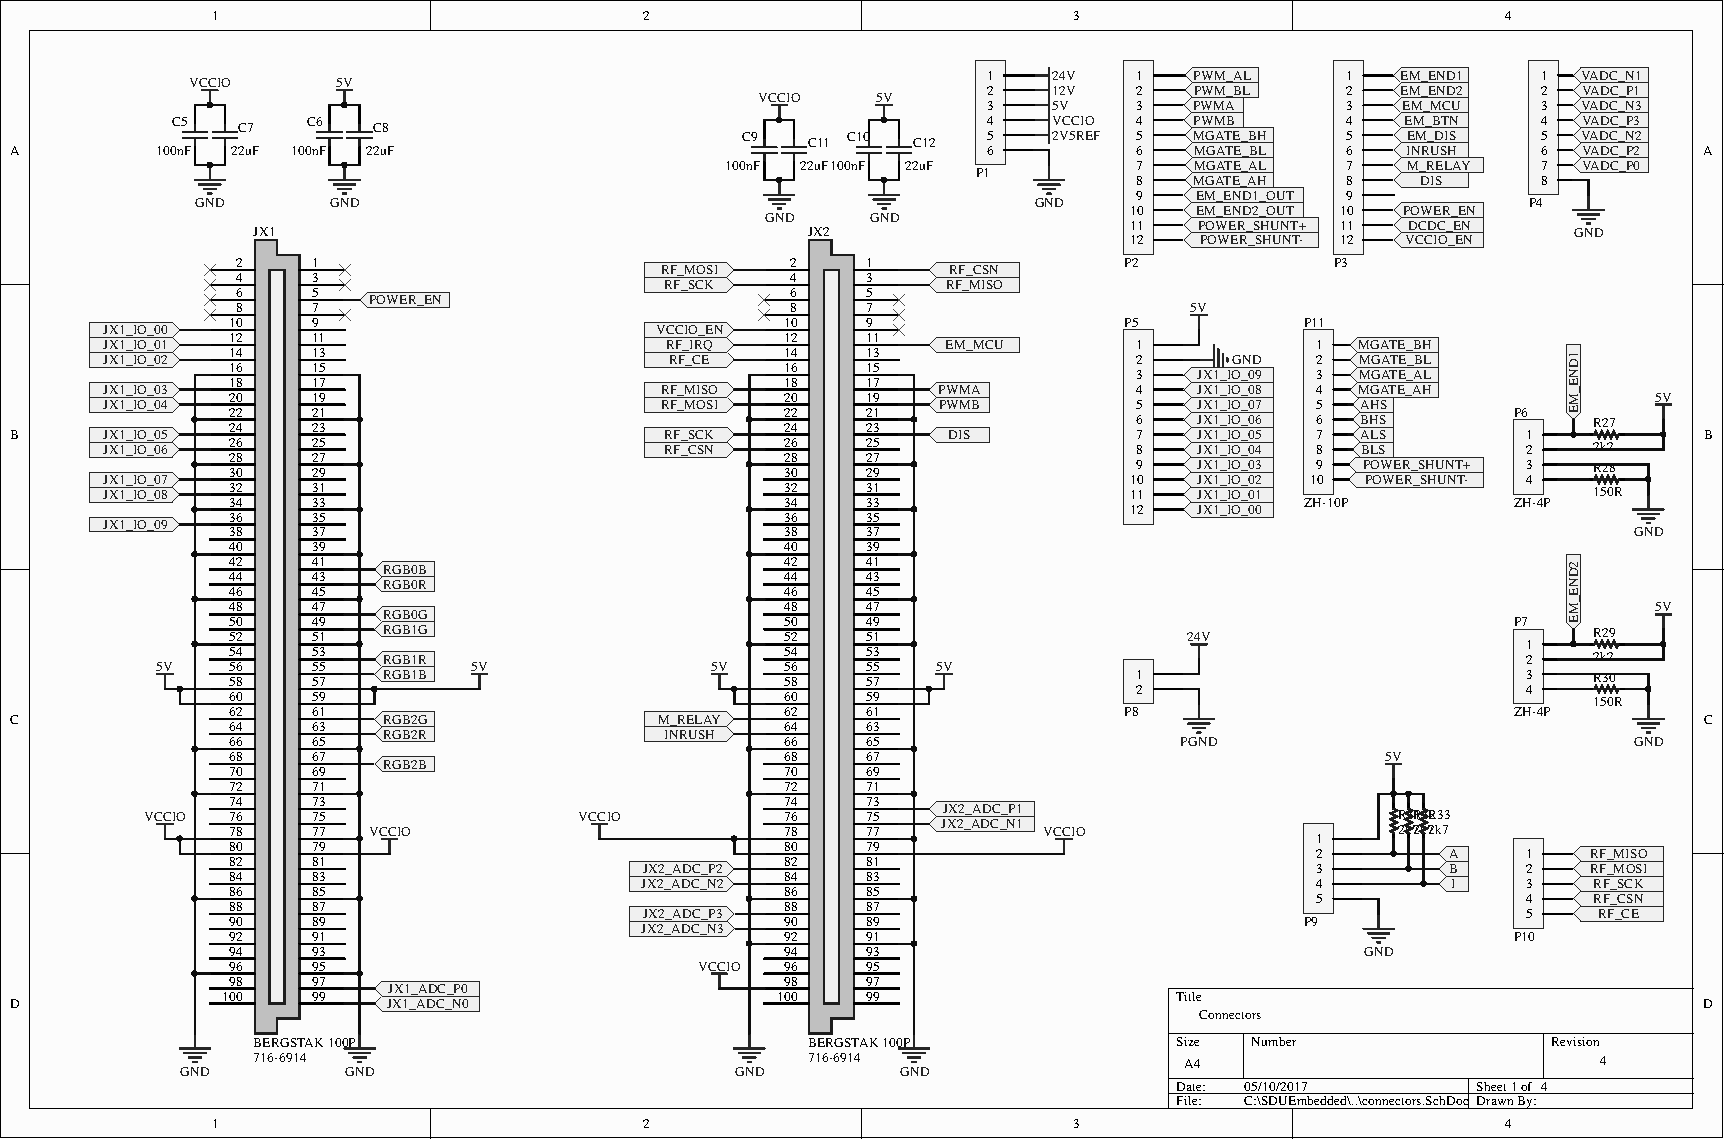
\includepdf[pages=-,angle=90,scale=0.9,pagecommand=\section{Controller Board Schematics}]{controller_board_schem.pdf}
\label{app:controller_board_schem}

\newpage
%!TEX root = ../main.tex
\section{Joint Board Schematics}
\label{app:joint_board_schem}
Joint board schematics can be found on the following page.
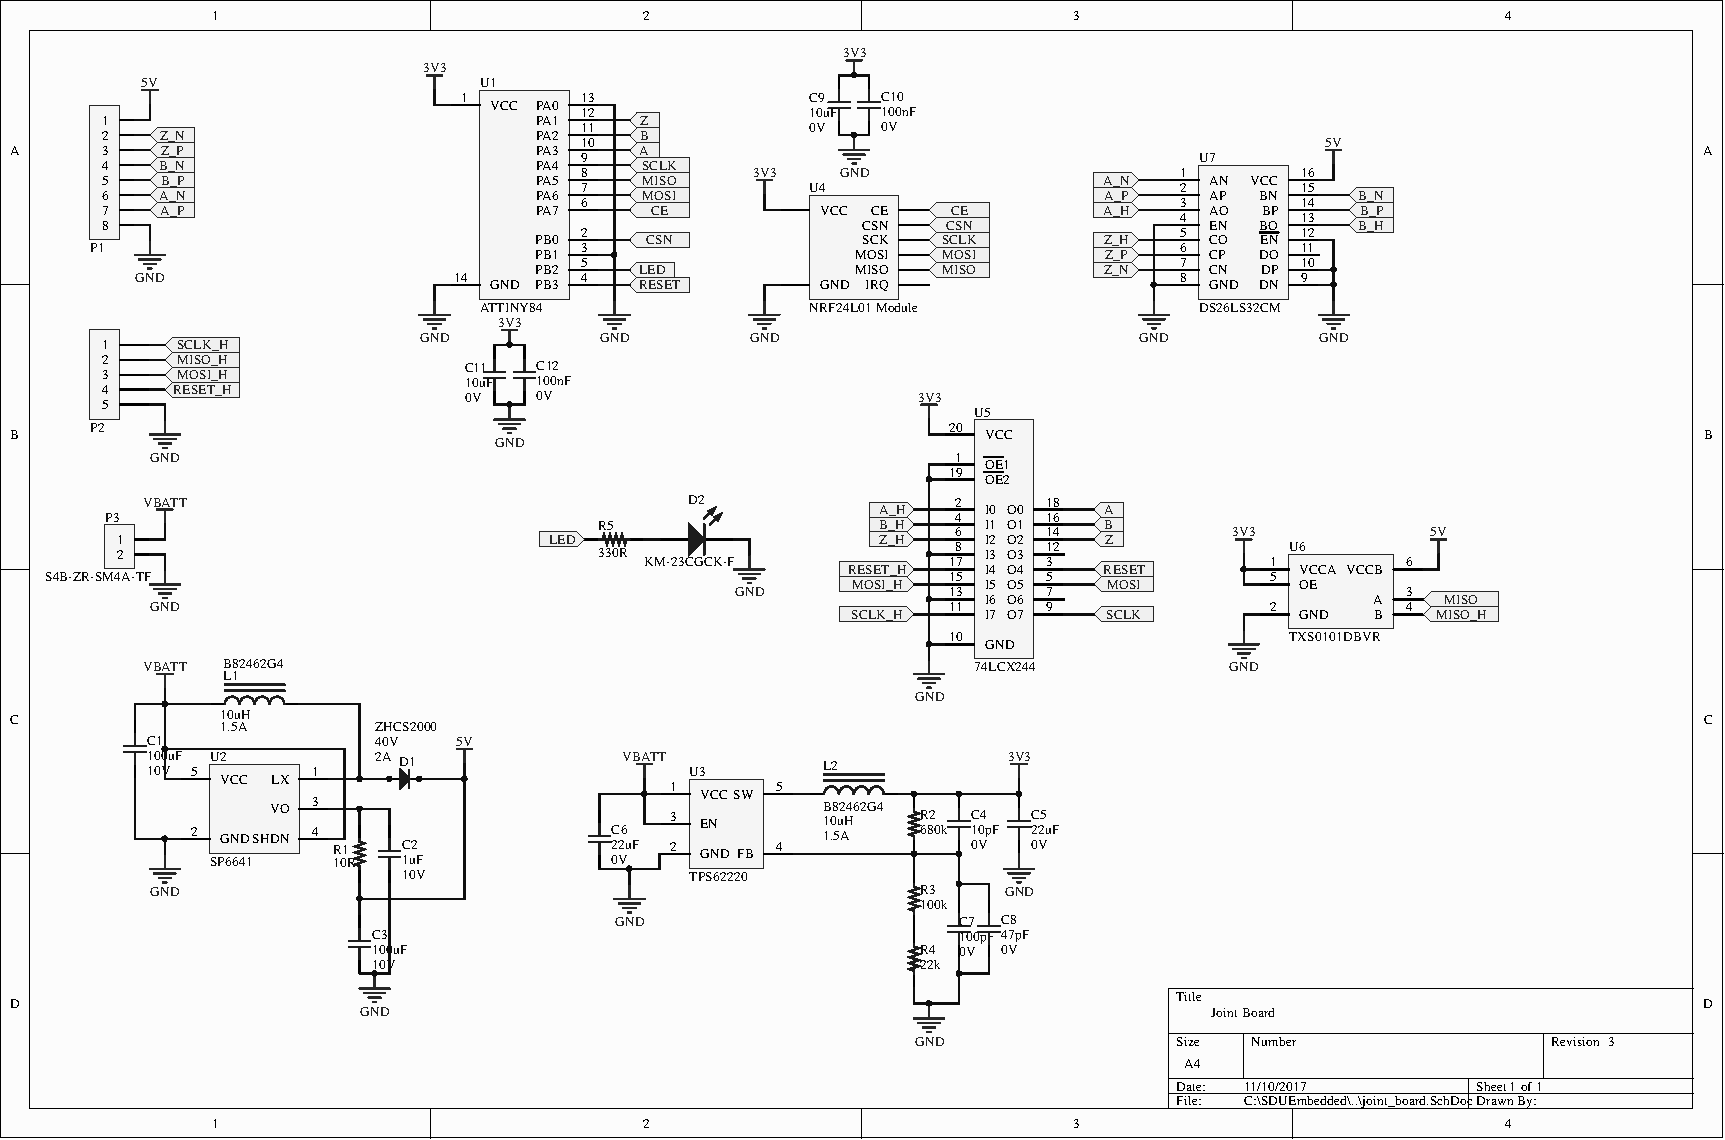
\includepdf[pages=-,angle=90,scale=1]{joint_board_schem.pdf}
\end{document}